\chapter{End-to-end autonomous racing}\label{chp:end_to_end_autonomous_racing}

Having introduced our simulation environment, 
we formulate an end-to-end solution method in which a reinforcement learning (RL) agent directly predicts controller commands based on observation information. 
This end-to-end agent is employed as a baseline to compare our partial end-to-end algorithm against, 
as similar end-to-end approaches are commonly used to solve the racing problem \cite{Song2021, Ivanov2020, hsu2022, Schwarting2021, Jaritz2018, Perot2017, Fuchs2021, Niu2020, Remonda2021, Chisari2021, brunnbauer2021}. 

We begin this chapter by discussing the design of the end-to-end racing algorithm.
Subsequently, we show how the TD3 RL algorithm is used to train an end-to-end agent, followed by a detailed exposition of evaluation procedures. 
We then experimentally determine the optimal values for each hyper-parameter for an agent racing on a relatively simple race track, before presenting agents
capable of driving on more complex race tracks.
The performance of end-to-end agents under conditions where vehicle modelling errors are present is also investigated, along with the effectiveness of
domain randomisation as a technique to improve performance under these conditions.





%%%%%%%%%%%%%%%%%%%%%%%%%%%%%%%%%%%%%%%%%%%%%%%%%%%%%%%%%%%%%%%%%%%%%%%%%%%%%%%%%%%%%%%%%%%%%%%%%%%%%%%%%%%%%%%%%%%%%%%%%%%%%%%%%%%%%%%%%%%%%%%5

\section{End-to-end racing algorithm}\label{sec:end-to-end_design}

Our end-to-end autonomous racing algorithm is composed of an RL agent and a velocity constraint.
The agent maps an observation sampled from the simulator to desired longitudinal acceleration ($a_{\text{long},d}$) and steering angle ($\delta_d$) control commands.
The velocity constraint then modifies the acceleration commands to ensure that the vehicle remains within safe velocity bounds.
The steering angle from the agent and acceleration from the velocity constraint component are passed to the simulator described in Chapter \ref{chp:modelling}.
This end-to-end framework is depicted in Figure \ref{fig:end_to_end_architecture}. 

Importantly, the simulator and velocity constraint components are grouped together in the environment.
This is because the definition of the MDP given in Section \ref{sec:mdps} solely encompasses an agent and an environment. 
In fact, to ensure conformity between the end-to-end algorithm and the MDP definition, 
all of the racing algorithm components apart from the agent are considered as part of the environment, and executed in unison with the rest of the environment.
Furthermore, due to the simulator's time step being chosen as $0.01$ seconds, the environment components are sampled at a frequency of $100$ Hz.
The agent is sampled at a slower rate of $f_{\text{agent}}$ Hz.

\begin{figure}[htb!]
    \centering
    \input contents/chapt5/figs/architecture/end_to_end_architecture.tex
    \caption[The end-to-end driving architecture]{The end-to-end racing algorithm, which is comprised of an RL agent which outputs control actions, and a velocity constraint. The velocity constraint and simulator are both considered part of the environment.}
    \label{fig:end_to_end_architecture}
\end{figure}

The end-to-end agent, which comprises a neural network, is shown in Figure \ref{fig:actor_architecture}.
To ensure uniformity across all observation vector elements, each element in the input vector is normalized to the range $[0,1]$. 
The neural network's design consists of three fully connected layers, with $m_1$, $m_2$, and $2$ neurons in the input, hidden, and output layers, respectively. 
The first two layers are ReLU-activated, while the output layer is activated by a hyperbolic tangent function to normalize the neural network output to the range $(-1,1)$. 
While the number of neurons in the first two layers are determined empirically, the two neurons in the output layer correspond to the steering and acceleration actions. 
Scaling factors are applied to their outputs so that the selected steering and acceleration actions fall within the range $(\underline{\delta}, \overline{\delta})$ and $(\underline{a}, \overline{a})$ from Table \ref{tab:constraint_parameters}, respectively.

\begin{figure}[htb!]
    \centering
    \input contents/chapt5/figs/neural_network/actor.tex
    \caption[The end-to-end agent]{The end-to-end agent. The outputs of the neural network are scaled to the ranges of $a_{\text{long}}$ and $\delta$ in Table \ref{tab:constraint_parameters}.}
    \label{fig:actor_architecture}
\end{figure}


While the steering angle is passed directly to the simulator, the longitudinal action is first modified by the velocity constraint component to ensure that the velocity of the vehicle remains within safe bounds,
\begin{equation}
    a_{\text{long,}d} \leftarrow 
    \begin{cases}
    0                   &   \text{for } v \geq v_{\text{max}}, \\
    0                   &   \text{for } v \leq v_{\text{min}}, \\
    a_{\text{long},d}   &   \text{otherwise},
    \end{cases}
\label{eq:speed_limit}
\end{equation}
before being passed to the simulator. In Equation \ref{eq:speed_limit} $v_{\text{max}}$ and $v_{\text{min}}$ are the imposed maximum and minimum allowable velocities.



%%%%%%%%%%%%%%%%%%%%%%%%%%%%%%%%%%%%%%%%%%%%%%%%%%%%%%%%%%%%%%%%%%%%%%%%%%%%%%%%%%%%%%%%%%%%%%%%%%%%%%%%%%%%%%%%%%%%%%%%%%%%%%%%%%%%%%%%%%%%%%%%%%%%%%%%%%%%%%%%5

\section{Applying TD3 to end-to-end autonomous racing}\label{sec:td3_end_to_end}

We applied the TD3 RL algorithm from Section \ref{sec:td3} to train the end-to-end agent.
Several adaptations to the original TD3 algorithm were made to ensure its compatibility with the end-to-end racing algorithm.
The adapted TD3 is shown in Algorithm \ref{alg:td3_mod}.

\begin{algorithm}[hbt!]
\caption{Twin delay deep deterministic policy gradient}\label{alg:td3_mod}
\nonl\textbf{Input}: Table \ref{tab:inital_values} parameters \\
\nonl\textbf{Output}: Trained actor DNN $\pi_{\bm{\phi}}$ \\

\vspace{0.5cm} 

Initialise critic networks $Q_{\bm{\theta}_1}, Q_{\bm{\theta}_2}$ and actor network $\pi_{\bm{\phi}}$ 
with \\
\nonl parameters $\bm{\theta}_1, \bm{\theta}_2$ and $\bm{\phi}$ \\
Initialise target networks $Q_{\bm{\theta}_1'}$, $Q_{\bm{\theta}_2'}$ and $\pi_{\bm{\phi}'}$ with weights \\
\nonl $\bm{\theta}_1' \leftarrow \bm{\theta}_1$, $\bm{\theta}_2' \leftarrow \bm{\theta}_2$, and $\bm{\phi}' \leftarrow \bm{\phi}$ \\
Initialise experience replay buffer $\mathcal{B}$ \\

\vspace{0.3cm}

\While{\emph{MDP time steps} $<M$ }
{
    Reset simulator (start new episode) \\
    \For{t=0, T}
    {
        Sample action with exploration noise from end-to-end agent, \\
        \nonl $a_{t} = \left[ a_{\text{long},d}, \delta_{d} \right] \leftarrow \text{scale}( \pi_{\bm{\phi}}(o_t) + \epsilon ), \hspace{0.2cm} \epsilon \sim \mathcal{N}(0, \sigma_{\text{action}})$ \\
            \For{n=0, N}
            {   
                Modify $a_{\text{long},d}$ according to Equation \ref{eq:speed_limit} to limit velocity\\
                Simulator executes action $a_t$ \\
                Observe environment step reward $r_{t,n}$ \\  
                Update MDP one step reward: $r_t = r_t + r_{t,n}$ \\
                Sample observation with noise, \\
                \nonl $o_{t} \leftarrow  o_{t} + \epsilon, \hspace{0.2cm} \epsilon \sim \mathcal{N}(0, \sigma_{\text{observation}})$ \\
            }
        Store transition tuple $(o_t,a_t,r_t,o_{t+1})$ in $\mathcal{B}$ \\

        \vspace{0.3cm}
        
        Sample mini-batch of $B$ transitions $(o_i,a_i,r_i,o_{i+1})$ from $\mathcal{B}$ \\
        Select target actions:\\
        \nonl $\tilde{a} \leftarrow \pi_{\bm{\phi}'}(o_{t+1}) + \epsilon$, \hspace{0.2cm} $\epsilon \sim \text{clip}(\mathcal{N}(0,\tilde{\sigma}), -c,c)$ \\
        Set TD target:
        $y_i \leftarrow r_i + \gamma \min_{q=1,2} Q_{\bm{\theta}_q'}(o_{i+1}, \tilde{a})$ \\
        Update critics by minimising the loss:
        \nonl $J_{\bm{\theta}_q} \leftarrow  \frac{1}{N} \sum_{i}^{N} (y_i - Q_{\bm{\theta}_q}(o_i,a_i))^{2} $ \\

        \vspace{0.3cm}
        
        \If{t \emph{ mod } d}
        {
            Update $\bm{\phi}$ by the deterministic policy gradient: \\
            \nonl $\nabla_{\bm{\phi}} J(\bm{\phi}) = \frac{1}{N} \sum_{i}^{N} \nabla_a Q_{\bm{\theta}_1} (o_i,a) | _{a=\pi_{\bm{\phi}}(o_i)} \nabla_{\bm{\phi}} \pi_{\bm{\phi}}(o_i)$ \\
            Update target networks: \\
            $\bm{\theta}_{q}' \leftarrow \tau \bm{\theta}_q + (1 - \tau) \bm{\theta}_{q}'$ \\
            $\bm{\phi}' \leftarrow \tau \bm{\phi} + (1 - \tau) \bm{\theta}'$ \\
        }
    }
}
\end{algorithm}


Note that in the context of racing, agents receive only partial information about the state of the environment.
This is because the pose and LiDAR scan do not fully capture the environment state.
Hence, the racing environment is only partially observable.
As such, the input to a racing agent is therefore an observation, denoted as $o$, rather than the complete environment state $s$.
This notation conforms to the notation used for the output of the simulator in Chapter \ref{chp:modelling}.
However, we use the same notation for time steps as in Chapter \ref{chp:rl}, denoting a time step as $t$, rather than $k$.



In line 1 of Algorithm \ref{alg:td3_mod}, the actor ($\pi_{\bm{\phi}}$) and critics ($Q_{\bm{\theta}_1}$ and $Q_{\bm{\theta}_2}$) are initialised.
The end-to-end agent shown in Figure \ref{fig:actor_architecture} is the actor $\pi_{\bm{\phi}}$.
For simplicity, the critics have an identical structure which is analogous to that of the actor.
We therefore describe the details of only one critic, which is depicted in Figure \ref{fig:critic_architecture}.
The critic DNN receives a vector input comprised of observation and control actions normalised to the range $(-1,1)$. 
It comprises three fully connected layers.
The input and hidden layers are identical to the actor, having $m_1$ and $m_2$ neurons with ReLU activation functions, respectively.
The output layer comprises a single neuron with a linear activation function.
The output of this layer is the action-value, and is denoted $Q_{\bm{\theta}}(o,a)$.
Additionally, the target networks are initialised identically to their counterparts.

\begin{figure}[htb!]
    \centering
    \input contents/chapt5/figs/neural_network/critic.tex
    \caption[The critic DNN]{The critic DNN. Its input is a vector containing a normalised observation and action pair, and its output is an action-value.}
    \label{fig:critic_architecture}
\end{figure}

After initializing the replay buffer in line 3, the TD3 algorithm enters a while loop which executes a number of episodes (lines 5-22). 
However, rather than limiting the number of episodes, we set a limit on the number of MDP time steps, denoted as $M$, as it is a more accurate indicator of the training time and the number of actor and critic updates. 
Each episode starts by resetting the simulator, and ends when the simulator indicates that the vehicle has crashed or finished.


In line 7 of Algorithm \ref{alg:td3_mod}, an action is sampled from the end-to-end agent by forward passing the observation through the actor DNN.
Gaussian noise with a zero mean and a standard deviation of $\sigma_{\text{action}}$ is added to the normalised output ($a_{\text{norm}}$ and $\delta_{\text{norm}}$), which is then scaled to generate a longitudinal acceleration and a steering angle.

The action sampled from the agent in line 7 is executed by repeatedly sampling the environment (lines 8-13).
Our implementation for sampling the environment differs from the standard implementation of TD3 given in Algorithm \ref{alg:td3}.
This is because the sample rate of the components inside the environment is higher than the agent, whereas the definition of the MDP given in Section~\ref{sec:mdps} requires that the agent and environment is sampled at the same rate.
As such, the environment components will be sampled multiple times in-between agent sampling periods.
We therefore define an MDP step as $N$ environment samples, where
\begin{equation}
N = \frac{100}{f_{\text{agent}}}.
\label{eq:N}
\end{equation}
In Equation \ref{eq:N}, $N$ is a whole number.
The environment is sampled by applying the velocity constraint from Equation \ref{eq:speed_limit} to limit the agent's selected longitudinal action, and then executing one simulator step.
This is followed by sampling the reward signal from the simulator in line $11$.

The reward signal is designed to closely approximate the objective of minimizing lap time for high reward discount rates.
Specifically, the is rewarded agent for the distance it travels along the centerline between the current and previous time step, while being penalised 
by a small amount on every time step, as described by Fuchs et al. \cite{Fuchs2021}. 
In addition, a large penalty is imposed on the agent if it collides with the track boundary. 
As a result, the reward signal is expressed as the piece-wise function
\begin{dmath}
r(s_t,a_t) = 
\begin{cases}
r_{\text{collision}} & \mbox{if collision occurred} \\
r_{\text{dist}}(D_{t} - D_{t-1}) + r_{\text{time}} & \mbox{otherwise.} \\
\end{cases}
\label{eq:reward_signal}
\end{dmath}
Here, $r_{\text{collision}}$, $r_{\text{dist}}$, and $r_{t}$ represent the penalty for collisions, the reward for distance traveled, and the penalty for each time step, respectively. 
Notably, this reward signal is similar to those used in numerous prior works \cite{Song2021, Ivanov2020, Perot2017}.

The reward signal is accumulated over the sequence of $N$ steps during which the environment is sampled in line 12.
In line 15, the transition tuple is stored, which consists of the observation before sampling the environment $N$ times, as well as the observation and accumulated reward after sampling the environment $N$ times.

The remaining steps of Algorithm \ref{alg:td3_mod} are identical to the standard implementation of TD3 described in Algorithm \ref{alg:td3}. 
Specifically, a mini-batch of $B$ transitions is sampled from the replay buffer in line 16.
Next, the target actor network is employed to select actions for each observed sample, which in turn are used to update the critics. 
To ensure the stability of the learning process, the actor and the target networks are updated every $d$ steps from lines 20 to 23. 
Furthermore, the target networks are updated via a soft update which is controlled by the target update rate parameter $\tau$. 

\begin{algorithm}[htb!]
\caption{Evaluating the end-to-end algorithm without exploration noise, and with observation noise.}
\label{alg:end_to_end_deploy}
\nonl\textbf{Input}: Trained actor DNN $\pi_{\bm{\phi}}$ \\
\nonl\textbf{Output}: Lap times, collisions over $100$ laps \vspace{0.2cm}\\
Initialise actor DNN $\pi_{\bm{\phi}}$ with weights $\bm{\phi}$ from training \\
\For{\emph{episode} = 1, 100}
{
    \For{t=0, T}
    {
        $\text{Select control action } a_t = [a_{\text{long,d}}, \delta_{d}] \sim \text{scale}(\pi_{\bm{\phi}}(o_t+\epsilon))$ \\
         \For{n=0, N}
        {   
            Modify $a_{\text{long},d}$ according to Equation \ref{eq:speed_limit} to limit velocity \\
            Simulator executes action $a_t$ \\
        }
    }
}
\end{algorithm}

After the training procedure is completed, Algorithm \ref{alg:end_to_end_deploy} is utilised to evaluate the trained agents.
Under evaluation conditions, training is halted and the weights of the DNNs are not updated.
Furthermore, no exploration noise is added to the agents selected actions. 
However, Gaussian noise is added to the observation vector to mimic practical sensor data in simulation. 
This Gaussian noise has standard deviations of $0.025$ m for $x$ and $y$ coordinates, $0.05$ rads for heading, $0.1$ m/s for velocity, and $0.01$ m for LiDAR scan. 
Each agent completed $100$ laps under these evaluation conditions.





%%%%%%%%%%%%%%%%%%%%%%%%%%%%%%%%%%%%%%%%%%%%%%%%%%%%%%%%%%%%%%%%%%%%%%%%%%%%%%%%%%%%%%%%%%%%%%%%%%%%%%%%%%%%%%%%%%%%%%%%%%%%%%%%%%%%%%%%5

\section{Empirical design and hyper-parameter values}\label{sec:ete_empirical_design}

The optimal values for the hyper-parameters introduced in Sections \ref{sec:end-to-end_design} and \ref{sec:td3_end_to_end} cannot be derived, 
and require experimentation to be determined empirically. 
Furthermore, hyper-parameters are sensitive to the track.
The following five sections of this chapter detail the experiments that were undertaken to determine a locally optimal set of hyper-parameters for agents racing on a relatively simply track named Porto.
The selected hyper-parameters are listed in Table \ref{tab:inital_values}.
Additionally, the average learning curve for $10$ agents racing on this track using this set of hyper-parameter is shown in Figure \ref{fig:MDP_steps_learning_curve}.

\newcolumntype{R}{>{\raggedleft\arraybackslash}p{5cm}}
\newcolumntype{C}{>{\raggedright\arraybackslash}p{2cm}}
\newcolumntype{L}{>{\raggedright\arraybackslash}p{5cm}}

\begin{table}[htb!]
\centering
%\renewcommand{\arraystretch}{1.1}
\small
\begin{tabularx}{0.7\textwidth}{RCL} 
    \hline
    \textbf{Hyper-parameter} & \textbf{Symbol} & \textbf{Value} \\ 
    \hline
    \textbf{Algorithm}                      &                           & \\
    Maximum time steps                      & $M$                       & $1.5 \cdot 10^5$   \\
    Target update rate                      & $\tau$                    & $5\cdot10^{-3}$ \\
    Replay buffer size                      & $\mathcal{B}$             & $5\cdot 10^5$ \\
    Replay batch size                       & $B$                       & $400$ \\
    Exploration noise standard deviation    & $\sigma_{\text{action}}$  & $0.1$ \\
    Reward discount rate                    & $\gamma$                  & $0.99$ \\
    Agent samples between network updates   & $d$                       & $2$ \\
    Agent sample rate                       & $f_{\text{agent}}$        & $5$ Hz \\
    Target action noise standard deviation  & $\tilde{\sigma}$          & $0.2$ \\ 
    Target action noise clip                & $c$                       & $0.5$ \\
    \textbf{Reward signal}                  &                           & \\
    Distance reward                         & $r_{\text{dist}}$         & $0.25$ \\ 
    Time step penalty                       & $r_{\text{time}}$         & $0.01$ \\
    Collision penalty                       & $r_{\text{collision}}$    & $-10$ \\
    \textbf{Observation}                    &                           & \\
    Number of LiDAR beams                   & L                         & 20 \\
    % Observation noise                       & $\sigma_{\text{observation}}$ & $x=0.025$ m, $y=0.025$ m, $\theta=0.05$ rads, $v=0.1$ m/s, $\text{LiDAR distances}=0.01$ m \\                      
    \textbf{Neural network}                 &                           & \\
    Learning rate                           & $\alpha$                  & $10^{-3}$ \\
    Neurons in input layer                  & $m_1$                     & 400 \\
    Neurons in hidden layer                 & $m_2$                     & 300 \\
    \textbf{Velocity constraints}           &                           & \\
    Minimum velocity                        & $v_{\text{min}}$          & $3$ m/s \\
    Maximum velocity                        & $v_{\text{max}}$          & $5$ m/s \\
    \hline
\end{tabularx}
\caption[Selected values of hyper-parameters for the end-to-end algorithm]{Selected values of hyper-parameters for the end-to-end racing algorithm on the Porto track.}
\label{tab:inital_values}
\end{table}


To select each hyper-parameter value, we repeatedly trained agents using Algorithm \ref{alg:td3_mod} with 
various values of the hyper-parameter under consideration while keeping all other hyper-parameters fixed at the values listed in Table \ref{tab:inital_values}. 
When evaluating agents, we are particularly interested in the rate at which they successfully complete laps, as well as their lap time during and after training.
Furthermore, to ensure consistency in the results, we trained and evaluated multiple agents for each set of hyper-parameters. 
Specifically, we chose to train three agents for each hyper-parameter set due to time constraints.



% \begin{figure}[htb!]
%     \centering
%     %% Creator: Matplotlib, PGF backend
%%
%% To include the figure in your LaTeX document, write
%%   \input{<filename>.pgf}
%%
%% Make sure the required packages are loaded in your preamble
%%   \usepackage{pgf}
%%
%% Also ensure that all the required font packages are loaded; for instance,
%% the lmodern package is sometimes necessary when using math font.
%%   \usepackage{lmodern}
%%
%% Figures using additional raster images can only be included by \input if
%% they are in the same directory as the main LaTeX file. For loading figures
%% from other directories you can use the `import` package
%%   \usepackage{import}
%%
%% and then include the figures with
%%   \import{<path to file>}{<filename>.pgf}
%%
%% Matplotlib used the following preamble
%%   \usepackage{fontspec}
%%   \setmainfont{DejaVuSerif.ttf}[Path=\detokenize{/home/andrew/anaconda3/envs/auto_car_env/lib/python3.9/site-packages/matplotlib/mpl-data/fonts/ttf/}]
%%   \setsansfont{DejaVuSans.ttf}[Path=\detokenize{/home/andrew/anaconda3/envs/auto_car_env/lib/python3.9/site-packages/matplotlib/mpl-data/fonts/ttf/}]
%%   \setmonofont{DejaVuSansMono.ttf}[Path=\detokenize{/home/andrew/anaconda3/envs/auto_car_env/lib/python3.9/site-packages/matplotlib/mpl-data/fonts/ttf/}]
%%
\begingroup%
\makeatletter%
\begin{pgfpicture}%
\pgfpathrectangle{\pgfpointorigin}{\pgfqpoint{3.500000in}{2.000000in}}%
\pgfusepath{use as bounding box, clip}%
\begin{pgfscope}%
\pgfsetbuttcap%
\pgfsetmiterjoin%
\definecolor{currentfill}{rgb}{1.000000,1.000000,1.000000}%
\pgfsetfillcolor{currentfill}%
\pgfsetlinewidth{0.000000pt}%
\definecolor{currentstroke}{rgb}{1.000000,1.000000,1.000000}%
\pgfsetstrokecolor{currentstroke}%
\pgfsetdash{}{0pt}%
\pgfpathmoveto{\pgfqpoint{0.000000in}{0.000000in}}%
\pgfpathlineto{\pgfqpoint{3.500000in}{0.000000in}}%
\pgfpathlineto{\pgfqpoint{3.500000in}{2.000000in}}%
\pgfpathlineto{\pgfqpoint{0.000000in}{2.000000in}}%
\pgfpathlineto{\pgfqpoint{0.000000in}{0.000000in}}%
\pgfpathclose%
\pgfusepath{fill}%
\end{pgfscope}%
\begin{pgfscope}%
\pgfsetbuttcap%
\pgfsetmiterjoin%
\definecolor{currentfill}{rgb}{1.000000,1.000000,1.000000}%
\pgfsetfillcolor{currentfill}%
\pgfsetlinewidth{0.000000pt}%
\definecolor{currentstroke}{rgb}{0.000000,0.000000,0.000000}%
\pgfsetstrokecolor{currentstroke}%
\pgfsetstrokeopacity{0.000000}%
\pgfsetdash{}{0pt}%
\pgfpathmoveto{\pgfqpoint{0.687917in}{0.563278in}}%
\pgfpathlineto{\pgfqpoint{3.350000in}{0.563278in}}%
\pgfpathlineto{\pgfqpoint{3.350000in}{1.850000in}}%
\pgfpathlineto{\pgfqpoint{0.687917in}{1.850000in}}%
\pgfpathlineto{\pgfqpoint{0.687917in}{0.563278in}}%
\pgfpathclose%
\pgfusepath{fill}%
\end{pgfscope}%
\begin{pgfscope}%
\pgfpathrectangle{\pgfqpoint{0.687917in}{0.563278in}}{\pgfqpoint{2.662083in}{1.286722in}}%
\pgfusepath{clip}%
\pgfsetbuttcap%
\pgfsetroundjoin%
\definecolor{currentfill}{rgb}{0.121569,0.466667,0.705882}%
\pgfsetfillcolor{currentfill}%
\pgfsetfillopacity{0.300000}%
\pgfsetlinewidth{0.000000pt}%
\definecolor{currentstroke}{rgb}{0.000000,0.000000,0.000000}%
\pgfsetstrokecolor{currentstroke}%
\pgfsetdash{}{0pt}%
\pgfpathmoveto{\pgfqpoint{0.808920in}{0.786533in}}%
\pgfpathlineto{\pgfqpoint{0.808920in}{0.786533in}}%
\pgfpathlineto{\pgfqpoint{0.808944in}{0.786533in}}%
\pgfpathlineto{\pgfqpoint{0.808992in}{0.787685in}}%
\pgfpathlineto{\pgfqpoint{0.809075in}{0.786215in}}%
\pgfpathlineto{\pgfqpoint{0.809111in}{0.785171in}}%
\pgfpathlineto{\pgfqpoint{0.809159in}{0.784642in}}%
\pgfpathlineto{\pgfqpoint{0.809266in}{0.785310in}}%
\pgfpathlineto{\pgfqpoint{0.809290in}{0.785605in}}%
\pgfpathlineto{\pgfqpoint{0.809338in}{0.784967in}}%
\pgfpathlineto{\pgfqpoint{0.809421in}{0.787061in}}%
\pgfpathlineto{\pgfqpoint{0.809457in}{0.786292in}}%
\pgfpathlineto{\pgfqpoint{0.809505in}{1.045664in}}%
\pgfpathlineto{\pgfqpoint{0.809624in}{1.032952in}}%
\pgfpathlineto{\pgfqpoint{0.809672in}{1.021913in}}%
\pgfpathlineto{\pgfqpoint{0.809719in}{1.011833in}}%
\pgfpathlineto{\pgfqpoint{0.809755in}{1.002667in}}%
\pgfpathlineto{\pgfqpoint{0.809863in}{0.995393in}}%
\pgfpathlineto{\pgfqpoint{0.809898in}{0.988378in}}%
\pgfpathlineto{\pgfqpoint{0.810053in}{0.980570in}}%
\pgfpathlineto{\pgfqpoint{0.810113in}{0.974273in}}%
\pgfpathlineto{\pgfqpoint{0.810149in}{0.968813in}}%
\pgfpathlineto{\pgfqpoint{0.810208in}{0.963066in}}%
\pgfpathlineto{\pgfqpoint{0.810232in}{0.958645in}}%
\pgfpathlineto{\pgfqpoint{0.810280in}{0.954386in}}%
\pgfpathlineto{\pgfqpoint{0.810304in}{0.950201in}}%
\pgfpathlineto{\pgfqpoint{0.810340in}{0.946198in}}%
\pgfpathlineto{\pgfqpoint{0.810399in}{0.942004in}}%
\pgfpathlineto{\pgfqpoint{0.810435in}{0.938776in}}%
\pgfpathlineto{\pgfqpoint{0.810483in}{0.936034in}}%
\pgfpathlineto{\pgfqpoint{0.810530in}{0.933401in}}%
\pgfpathlineto{\pgfqpoint{0.810578in}{0.930814in}}%
\pgfpathlineto{\pgfqpoint{0.810662in}{0.927947in}}%
\pgfpathlineto{\pgfqpoint{0.810697in}{0.925660in}}%
\pgfpathlineto{\pgfqpoint{0.810793in}{0.923295in}}%
\pgfpathlineto{\pgfqpoint{0.810817in}{0.921083in}}%
\pgfpathlineto{\pgfqpoint{0.810852in}{0.919165in}}%
\pgfpathlineto{\pgfqpoint{0.810888in}{0.916997in}}%
\pgfpathlineto{\pgfqpoint{0.810924in}{0.915179in}}%
\pgfpathlineto{\pgfqpoint{0.810960in}{0.913079in}}%
\pgfpathlineto{\pgfqpoint{0.811151in}{0.910270in}}%
\pgfpathlineto{\pgfqpoint{0.811186in}{0.908182in}}%
\pgfpathlineto{\pgfqpoint{0.811234in}{0.906263in}}%
\pgfpathlineto{\pgfqpoint{0.811294in}{0.904437in}}%
\pgfpathlineto{\pgfqpoint{0.811329in}{0.902728in}}%
\pgfpathlineto{\pgfqpoint{0.811365in}{0.901094in}}%
\pgfpathlineto{\pgfqpoint{0.811401in}{0.899372in}}%
\pgfpathlineto{\pgfqpoint{0.811484in}{0.897450in}}%
\pgfpathlineto{\pgfqpoint{0.811520in}{0.896028in}}%
\pgfpathlineto{\pgfqpoint{0.811639in}{0.894116in}}%
\pgfpathlineto{\pgfqpoint{0.811711in}{0.892561in}}%
\pgfpathlineto{\pgfqpoint{0.811771in}{0.891027in}}%
\pgfpathlineto{\pgfqpoint{0.811830in}{0.889590in}}%
\pgfpathlineto{\pgfqpoint{0.811878in}{0.888289in}}%
\pgfpathlineto{\pgfqpoint{0.811938in}{0.886941in}}%
\pgfpathlineto{\pgfqpoint{0.812009in}{0.885479in}}%
\pgfpathlineto{\pgfqpoint{0.812069in}{0.884237in}}%
\pgfpathlineto{\pgfqpoint{0.812117in}{0.883147in}}%
\pgfpathlineto{\pgfqpoint{0.812164in}{0.882122in}}%
\pgfpathlineto{\pgfqpoint{0.812188in}{0.881171in}}%
\pgfpathlineto{\pgfqpoint{0.812343in}{0.879622in}}%
\pgfpathlineto{\pgfqpoint{0.812379in}{0.878642in}}%
\pgfpathlineto{\pgfqpoint{0.812474in}{0.877562in}}%
\pgfpathlineto{\pgfqpoint{0.812546in}{0.876564in}}%
\pgfpathlineto{\pgfqpoint{0.812605in}{0.875699in}}%
\pgfpathlineto{\pgfqpoint{0.812641in}{0.875061in}}%
\pgfpathlineto{\pgfqpoint{0.812760in}{0.873818in}}%
\pgfpathlineto{\pgfqpoint{0.812832in}{0.872836in}}%
\pgfpathlineto{\pgfqpoint{0.812892in}{0.871953in}}%
\pgfpathlineto{\pgfqpoint{0.813047in}{0.870835in}}%
\pgfpathlineto{\pgfqpoint{0.813094in}{0.869997in}}%
\pgfpathlineto{\pgfqpoint{0.813321in}{0.868705in}}%
\pgfpathlineto{\pgfqpoint{0.813357in}{0.867894in}}%
\pgfpathlineto{\pgfqpoint{0.813667in}{0.866705in}}%
\pgfpathlineto{\pgfqpoint{0.814072in}{0.865538in}}%
\pgfpathlineto{\pgfqpoint{0.814490in}{0.864362in}}%
\pgfpathlineto{\pgfqpoint{0.814680in}{0.863284in}}%
\pgfpathlineto{\pgfqpoint{0.815265in}{0.862173in}}%
\pgfpathlineto{\pgfqpoint{0.815730in}{0.861102in}}%
\pgfpathlineto{\pgfqpoint{0.816362in}{0.886246in}}%
\pgfpathlineto{\pgfqpoint{0.816636in}{0.885095in}}%
\pgfpathlineto{\pgfqpoint{0.816672in}{0.884440in}}%
\pgfpathlineto{\pgfqpoint{0.817209in}{0.883435in}}%
\pgfpathlineto{\pgfqpoint{0.817781in}{0.882363in}}%
\pgfpathlineto{\pgfqpoint{0.818401in}{0.903645in}}%
\pgfpathlineto{\pgfqpoint{0.819009in}{0.923113in}}%
\pgfpathlineto{\pgfqpoint{0.819618in}{0.941040in}}%
\pgfpathlineto{\pgfqpoint{0.820238in}{0.957679in}}%
\pgfpathlineto{\pgfqpoint{0.820846in}{0.973400in}}%
\pgfpathlineto{\pgfqpoint{0.821478in}{0.986865in}}%
\pgfpathlineto{\pgfqpoint{0.822074in}{1.001451in}}%
\pgfpathlineto{\pgfqpoint{0.822659in}{1.015212in}}%
\pgfpathlineto{\pgfqpoint{0.823231in}{1.029314in}}%
\pgfpathlineto{\pgfqpoint{0.823815in}{1.042130in}}%
\pgfpathlineto{\pgfqpoint{0.823887in}{1.040388in}}%
\pgfpathlineto{\pgfqpoint{0.824483in}{1.052158in}}%
\pgfpathlineto{\pgfqpoint{0.825092in}{1.062666in}}%
\pgfpathlineto{\pgfqpoint{0.825735in}{1.071381in}}%
\pgfpathlineto{\pgfqpoint{0.826356in}{1.080345in}}%
\pgfpathlineto{\pgfqpoint{0.826964in}{1.089522in}}%
\pgfpathlineto{\pgfqpoint{0.827584in}{1.098060in}}%
\pgfpathlineto{\pgfqpoint{0.828204in}{1.106062in}}%
\pgfpathlineto{\pgfqpoint{0.828800in}{1.115133in}}%
\pgfpathlineto{\pgfqpoint{0.829420in}{1.122667in}}%
\pgfpathlineto{\pgfqpoint{0.830029in}{1.130421in}}%
\pgfpathlineto{\pgfqpoint{0.830649in}{1.137498in}}%
\pgfpathlineto{\pgfqpoint{0.831281in}{1.143894in}}%
\pgfpathlineto{\pgfqpoint{0.831889in}{1.150630in}}%
\pgfpathlineto{\pgfqpoint{0.832545in}{1.156051in}}%
\pgfpathlineto{\pgfqpoint{0.833165in}{1.162263in}}%
\pgfpathlineto{\pgfqpoint{0.833785in}{1.168178in}}%
\pgfpathlineto{\pgfqpoint{0.834405in}{1.174301in}}%
\pgfpathlineto{\pgfqpoint{0.835025in}{1.179785in}}%
\pgfpathlineto{\pgfqpoint{0.835646in}{1.185296in}}%
\pgfpathlineto{\pgfqpoint{0.836278in}{1.190344in}}%
\pgfpathlineto{\pgfqpoint{0.836886in}{1.196077in}}%
\pgfpathlineto{\pgfqpoint{0.837506in}{1.200945in}}%
\pgfpathlineto{\pgfqpoint{0.838114in}{1.206017in}}%
\pgfpathlineto{\pgfqpoint{0.838675in}{1.203685in}}%
\pgfpathlineto{\pgfqpoint{0.839295in}{1.208458in}}%
\pgfpathlineto{\pgfqpoint{0.839879in}{1.214054in}}%
\pgfpathlineto{\pgfqpoint{0.840487in}{1.219008in}}%
\pgfpathlineto{\pgfqpoint{0.841096in}{1.223408in}}%
\pgfpathlineto{\pgfqpoint{0.841704in}{1.227957in}}%
\pgfpathlineto{\pgfqpoint{0.842312in}{1.232652in}}%
\pgfpathlineto{\pgfqpoint{0.842872in}{1.230464in}}%
\pgfpathlineto{\pgfqpoint{0.843457in}{1.235291in}}%
\pgfpathlineto{\pgfqpoint{0.844041in}{1.239995in}}%
\pgfpathlineto{\pgfqpoint{0.844626in}{1.244596in}}%
\pgfpathlineto{\pgfqpoint{0.844900in}{1.242422in}}%
\pgfpathlineto{\pgfqpoint{0.845520in}{1.246265in}}%
\pgfpathlineto{\pgfqpoint{0.846104in}{1.250627in}}%
\pgfpathlineto{\pgfqpoint{0.846724in}{1.254245in}}%
\pgfpathlineto{\pgfqpoint{0.847345in}{1.257640in}}%
\pgfpathlineto{\pgfqpoint{0.847929in}{1.261679in}}%
\pgfpathlineto{\pgfqpoint{0.848549in}{1.265060in}}%
\pgfpathlineto{\pgfqpoint{0.849157in}{1.268462in}}%
\pgfpathlineto{\pgfqpoint{0.849777in}{1.271637in}}%
\pgfpathlineto{\pgfqpoint{0.850409in}{1.274559in}}%
\pgfpathlineto{\pgfqpoint{0.851041in}{1.277252in}}%
\pgfpathlineto{\pgfqpoint{0.851662in}{1.280242in}}%
\pgfpathlineto{\pgfqpoint{0.852246in}{1.278227in}}%
\pgfpathlineto{\pgfqpoint{0.852866in}{1.281190in}}%
\pgfpathlineto{\pgfqpoint{0.853486in}{1.284096in}}%
\pgfpathlineto{\pgfqpoint{0.854118in}{1.286757in}}%
\pgfpathlineto{\pgfqpoint{0.854750in}{1.289288in}}%
\pgfpathlineto{\pgfqpoint{0.855359in}{1.292203in}}%
\pgfpathlineto{\pgfqpoint{0.855979in}{1.294916in}}%
\pgfpathlineto{\pgfqpoint{0.856587in}{1.297807in}}%
\pgfpathlineto{\pgfqpoint{0.857195in}{1.300472in}}%
\pgfpathlineto{\pgfqpoint{0.857791in}{1.303304in}}%
\pgfpathlineto{\pgfqpoint{0.858423in}{1.305431in}}%
\pgfpathlineto{\pgfqpoint{0.859055in}{1.307590in}}%
\pgfpathlineto{\pgfqpoint{0.859664in}{1.310337in}}%
\pgfpathlineto{\pgfqpoint{0.860272in}{1.312822in}}%
\pgfpathlineto{\pgfqpoint{0.860880in}{1.315300in}}%
\pgfpathlineto{\pgfqpoint{0.861488in}{1.317726in}}%
\pgfpathlineto{\pgfqpoint{0.862096in}{1.320069in}}%
\pgfpathlineto{\pgfqpoint{0.862717in}{1.322246in}}%
\pgfpathlineto{\pgfqpoint{0.863325in}{1.324586in}}%
\pgfpathlineto{\pgfqpoint{0.863921in}{1.326941in}}%
\pgfpathlineto{\pgfqpoint{0.864505in}{1.329389in}}%
\pgfpathlineto{\pgfqpoint{0.865137in}{1.331071in}}%
\pgfpathlineto{\pgfqpoint{0.865758in}{1.332880in}}%
\pgfpathlineto{\pgfqpoint{0.866390in}{1.334570in}}%
\pgfpathlineto{\pgfqpoint{0.867010in}{1.336426in}}%
\pgfpathlineto{\pgfqpoint{0.867630in}{1.338194in}}%
\pgfpathlineto{\pgfqpoint{0.868226in}{1.340388in}}%
\pgfpathlineto{\pgfqpoint{0.868858in}{1.342108in}}%
\pgfpathlineto{\pgfqpoint{0.869478in}{1.343814in}}%
\pgfpathlineto{\pgfqpoint{0.870099in}{1.345422in}}%
\pgfpathlineto{\pgfqpoint{0.870743in}{1.346770in}}%
\pgfpathlineto{\pgfqpoint{0.871375in}{1.348266in}}%
\pgfpathlineto{\pgfqpoint{0.871995in}{1.349798in}}%
\pgfpathlineto{\pgfqpoint{0.872603in}{1.351403in}}%
\pgfpathlineto{\pgfqpoint{0.873211in}{1.353179in}}%
\pgfpathlineto{\pgfqpoint{0.873843in}{1.354490in}}%
\pgfpathlineto{\pgfqpoint{0.874463in}{1.355886in}}%
\pgfpathlineto{\pgfqpoint{0.875083in}{1.357258in}}%
\pgfpathlineto{\pgfqpoint{0.875704in}{1.358726in}}%
\pgfpathlineto{\pgfqpoint{0.876061in}{1.357108in}}%
\pgfpathlineto{\pgfqpoint{0.876681in}{1.358529in}}%
\pgfpathlineto{\pgfqpoint{0.877313in}{1.359783in}}%
\pgfpathlineto{\pgfqpoint{0.877922in}{1.361347in}}%
\pgfpathlineto{\pgfqpoint{0.878542in}{1.362737in}}%
\pgfpathlineto{\pgfqpoint{0.879150in}{1.364244in}}%
\pgfpathlineto{\pgfqpoint{0.879663in}{1.362759in}}%
\pgfpathlineto{\pgfqpoint{0.880295in}{1.363892in}}%
\pgfpathlineto{\pgfqpoint{0.880498in}{1.362307in}}%
\pgfpathlineto{\pgfqpoint{0.881130in}{1.363439in}}%
\pgfpathlineto{\pgfqpoint{0.881726in}{1.365093in}}%
\pgfpathlineto{\pgfqpoint{0.881774in}{1.363513in}}%
\pgfpathlineto{\pgfqpoint{0.882406in}{1.364803in}}%
\pgfpathlineto{\pgfqpoint{0.883038in}{1.366004in}}%
\pgfpathlineto{\pgfqpoint{0.883622in}{1.367711in}}%
\pgfpathlineto{\pgfqpoint{0.884242in}{1.368958in}}%
\pgfpathlineto{\pgfqpoint{0.884839in}{1.370460in}}%
\pgfpathlineto{\pgfqpoint{0.885435in}{1.371929in}}%
\pgfpathlineto{\pgfqpoint{0.886079in}{1.372810in}}%
\pgfpathlineto{\pgfqpoint{0.886115in}{1.371296in}}%
\pgfpathlineto{\pgfqpoint{0.886735in}{1.372527in}}%
\pgfpathlineto{\pgfqpoint{0.887355in}{1.373660in}}%
\pgfpathlineto{\pgfqpoint{0.887510in}{1.372182in}}%
\pgfpathlineto{\pgfqpoint{0.888106in}{1.373492in}}%
\pgfpathlineto{\pgfqpoint{0.888738in}{1.374396in}}%
\pgfpathlineto{\pgfqpoint{0.889370in}{1.375352in}}%
\pgfpathlineto{\pgfqpoint{0.889990in}{1.376323in}}%
\pgfpathlineto{\pgfqpoint{0.890563in}{1.377958in}}%
\pgfpathlineto{\pgfqpoint{0.891159in}{1.379163in}}%
\pgfpathlineto{\pgfqpoint{0.891743in}{1.380571in}}%
\pgfpathlineto{\pgfqpoint{0.892352in}{1.381723in}}%
\pgfpathlineto{\pgfqpoint{0.892936in}{1.383017in}}%
\pgfpathlineto{\pgfqpoint{0.893174in}{1.381642in}}%
\pgfpathlineto{\pgfqpoint{0.893306in}{1.380232in}}%
\pgfpathlineto{\pgfqpoint{0.893854in}{1.382005in}}%
\pgfpathlineto{\pgfqpoint{0.894093in}{1.380610in}}%
\pgfpathlineto{\pgfqpoint{0.894295in}{1.379220in}}%
\pgfpathlineto{\pgfqpoint{0.894880in}{1.380431in}}%
\pgfpathlineto{\pgfqpoint{0.895476in}{1.381608in}}%
\pgfpathlineto{\pgfqpoint{0.896037in}{1.383207in}}%
\pgfpathlineto{\pgfqpoint{0.896681in}{1.383897in}}%
\pgfpathlineto{\pgfqpoint{0.897241in}{1.385445in}}%
\pgfpathlineto{\pgfqpoint{0.897825in}{1.386660in}}%
\pgfpathlineto{\pgfqpoint{0.898207in}{1.385407in}}%
\pgfpathlineto{\pgfqpoint{0.898768in}{1.386947in}}%
\pgfpathlineto{\pgfqpoint{0.899340in}{1.388332in}}%
\pgfpathlineto{\pgfqpoint{0.899877in}{1.390032in}}%
\pgfpathlineto{\pgfqpoint{0.900461in}{1.391236in}}%
\pgfpathlineto{\pgfqpoint{0.901010in}{1.390092in}}%
\pgfpathlineto{\pgfqpoint{0.901606in}{1.391157in}}%
\pgfpathlineto{\pgfqpoint{0.902214in}{1.392079in}}%
\pgfpathlineto{\pgfqpoint{0.902822in}{1.392962in}}%
\pgfpathlineto{\pgfqpoint{0.903383in}{1.394333in}}%
\pgfpathlineto{\pgfqpoint{0.903824in}{1.393193in}}%
\pgfpathlineto{\pgfqpoint{0.903955in}{1.391901in}}%
\pgfpathlineto{\pgfqpoint{0.904504in}{1.393400in}}%
\pgfpathlineto{\pgfqpoint{0.904575in}{1.392118in}}%
\pgfpathlineto{\pgfqpoint{0.905172in}{1.393166in}}%
\pgfpathlineto{\pgfqpoint{0.905744in}{1.394352in}}%
\pgfpathlineto{\pgfqpoint{0.906340in}{1.395302in}}%
\pgfpathlineto{\pgfqpoint{0.906925in}{1.396439in}}%
\pgfpathlineto{\pgfqpoint{0.907473in}{1.397941in}}%
\pgfpathlineto{\pgfqpoint{0.908046in}{1.399140in}}%
\pgfpathlineto{\pgfqpoint{0.908141in}{1.397897in}}%
\pgfpathlineto{\pgfqpoint{0.908296in}{1.396663in}}%
\pgfpathlineto{\pgfqpoint{0.908892in}{1.397636in}}%
\pgfpathlineto{\pgfqpoint{0.909417in}{1.399362in}}%
\pgfpathlineto{\pgfqpoint{0.910013in}{1.400336in}}%
\pgfpathlineto{\pgfqpoint{0.910574in}{1.401613in}}%
\pgfpathlineto{\pgfqpoint{0.910777in}{1.400410in}}%
\pgfpathlineto{\pgfqpoint{0.911337in}{1.401717in}}%
\pgfpathlineto{\pgfqpoint{0.911921in}{1.402630in}}%
\pgfpathlineto{\pgfqpoint{0.912482in}{1.403896in}}%
\pgfpathlineto{\pgfqpoint{0.912816in}{1.402788in}}%
\pgfpathlineto{\pgfqpoint{0.913412in}{1.403657in}}%
\pgfpathlineto{\pgfqpoint{0.913985in}{1.404743in}}%
\pgfpathlineto{\pgfqpoint{0.914545in}{1.405945in}}%
\pgfpathlineto{\pgfqpoint{0.915129in}{1.406845in}}%
\pgfpathlineto{\pgfqpoint{0.915726in}{1.407709in}}%
\pgfpathlineto{\pgfqpoint{0.916322in}{1.408607in}}%
\pgfpathlineto{\pgfqpoint{0.916906in}{1.409581in}}%
\pgfpathlineto{\pgfqpoint{0.917491in}{1.410478in}}%
\pgfpathlineto{\pgfqpoint{0.918075in}{1.411411in}}%
\pgfpathlineto{\pgfqpoint{0.918683in}{1.412156in}}%
\pgfpathlineto{\pgfqpoint{0.919303in}{1.412764in}}%
\pgfpathlineto{\pgfqpoint{0.919864in}{1.413894in}}%
\pgfpathlineto{\pgfqpoint{0.920436in}{1.414807in}}%
\pgfpathlineto{\pgfqpoint{0.921021in}{1.415607in}}%
\pgfpathlineto{\pgfqpoint{0.921617in}{1.416326in}}%
\pgfpathlineto{\pgfqpoint{0.922189in}{1.417303in}}%
\pgfpathlineto{\pgfqpoint{0.922750in}{1.418331in}}%
\pgfpathlineto{\pgfqpoint{0.922953in}{1.417260in}}%
\pgfpathlineto{\pgfqpoint{0.923537in}{1.418076in}}%
\pgfpathlineto{\pgfqpoint{0.924145in}{1.418638in}}%
\pgfpathlineto{\pgfqpoint{0.924729in}{1.419412in}}%
\pgfpathlineto{\pgfqpoint{0.925314in}{1.420205in}}%
\pgfpathlineto{\pgfqpoint{0.925886in}{1.419394in}}%
\pgfpathlineto{\pgfqpoint{0.926471in}{1.420260in}}%
\pgfpathlineto{\pgfqpoint{0.926971in}{1.419360in}}%
\pgfpathlineto{\pgfqpoint{0.927556in}{1.420192in}}%
\pgfpathlineto{\pgfqpoint{0.928152in}{1.420848in}}%
\pgfpathlineto{\pgfqpoint{0.928748in}{1.421480in}}%
\pgfpathlineto{\pgfqpoint{0.929309in}{1.422451in}}%
\pgfpathlineto{\pgfqpoint{0.929905in}{1.423145in}}%
\pgfpathlineto{\pgfqpoint{0.930478in}{1.424039in}}%
\pgfpathlineto{\pgfqpoint{0.931086in}{1.424654in}}%
\pgfpathlineto{\pgfqpoint{0.931646in}{1.425611in}}%
\pgfpathlineto{\pgfqpoint{0.932159in}{1.424759in}}%
\pgfpathlineto{\pgfqpoint{0.932767in}{1.425313in}}%
\pgfpathlineto{\pgfqpoint{0.932887in}{1.424294in}}%
\pgfpathlineto{\pgfqpoint{0.933471in}{1.425046in}}%
\pgfpathlineto{\pgfqpoint{0.934043in}{1.425822in}}%
\pgfpathlineto{\pgfqpoint{0.934592in}{1.426859in}}%
\pgfpathlineto{\pgfqpoint{0.934878in}{1.425870in}}%
\pgfpathlineto{\pgfqpoint{0.935486in}{1.426460in}}%
\pgfpathlineto{\pgfqpoint{0.936047in}{1.427319in}}%
\pgfpathlineto{\pgfqpoint{0.936619in}{1.428118in}}%
\pgfpathlineto{\pgfqpoint{0.937180in}{1.428975in}}%
\pgfpathlineto{\pgfqpoint{0.937776in}{1.429535in}}%
\pgfpathlineto{\pgfqpoint{0.938396in}{1.429921in}}%
\pgfpathlineto{\pgfqpoint{0.938981in}{1.430596in}}%
\pgfpathlineto{\pgfqpoint{0.939577in}{1.431196in}}%
\pgfpathlineto{\pgfqpoint{0.940173in}{1.431756in}}%
\pgfpathlineto{\pgfqpoint{0.940757in}{1.432344in}}%
\pgfpathlineto{\pgfqpoint{0.941342in}{1.433007in}}%
\pgfpathlineto{\pgfqpoint{0.941902in}{1.433855in}}%
\pgfpathlineto{\pgfqpoint{0.942475in}{1.434623in}}%
\pgfpathlineto{\pgfqpoint{0.943047in}{1.435323in}}%
\pgfpathlineto{\pgfqpoint{0.943405in}{1.434482in}}%
\pgfpathlineto{\pgfqpoint{0.943953in}{1.435383in}}%
\pgfpathlineto{\pgfqpoint{0.944514in}{1.436133in}}%
\pgfpathlineto{\pgfqpoint{0.945098in}{1.436759in}}%
\pgfpathlineto{\pgfqpoint{0.945540in}{1.435966in}}%
\pgfpathlineto{\pgfqpoint{0.946124in}{1.436600in}}%
\pgfpathlineto{\pgfqpoint{0.946756in}{1.436900in}}%
\pgfpathlineto{\pgfqpoint{0.947305in}{1.437790in}}%
\pgfpathlineto{\pgfqpoint{0.947865in}{1.438567in}}%
\pgfpathlineto{\pgfqpoint{0.948449in}{1.439184in}}%
\pgfpathlineto{\pgfqpoint{0.948807in}{1.438329in}}%
\pgfpathlineto{\pgfqpoint{0.949427in}{1.438678in}}%
\pgfpathlineto{\pgfqpoint{0.950000in}{1.439372in}}%
\pgfpathlineto{\pgfqpoint{0.950584in}{1.439956in}}%
\pgfpathlineto{\pgfqpoint{0.951192in}{1.440367in}}%
\pgfpathlineto{\pgfqpoint{0.951800in}{1.440786in}}%
\pgfpathlineto{\pgfqpoint{0.952373in}{1.441428in}}%
\pgfpathlineto{\pgfqpoint{0.952778in}{1.440719in}}%
\pgfpathlineto{\pgfqpoint{0.953363in}{1.441213in}}%
\pgfpathlineto{\pgfqpoint{0.953923in}{1.440521in}}%
\pgfpathlineto{\pgfqpoint{0.954412in}{1.440977in}}%
\pgfpathlineto{\pgfqpoint{0.954710in}{1.440173in}}%
\pgfpathlineto{\pgfqpoint{0.955104in}{1.439412in}}%
\pgfpathlineto{\pgfqpoint{0.955700in}{1.439888in}}%
\pgfpathlineto{\pgfqpoint{0.956129in}{1.439076in}}%
\pgfpathlineto{\pgfqpoint{0.956750in}{1.439417in}}%
\pgfpathlineto{\pgfqpoint{0.957394in}{1.439576in}}%
\pgfpathlineto{\pgfqpoint{0.957883in}{1.438857in}}%
\pgfpathlineto{\pgfqpoint{0.958240in}{1.438063in}}%
\pgfpathlineto{\pgfqpoint{0.958872in}{1.438310in}}%
\pgfpathlineto{\pgfqpoint{0.959469in}{1.438754in}}%
\pgfpathlineto{\pgfqpoint{0.960077in}{1.439146in}}%
\pgfpathlineto{\pgfqpoint{0.960709in}{1.439393in}}%
\pgfpathlineto{\pgfqpoint{0.961269in}{1.440101in}}%
\pgfpathlineto{\pgfqpoint{0.961377in}{1.439225in}}%
\pgfpathlineto{\pgfqpoint{0.961997in}{1.439565in}}%
\pgfpathlineto{\pgfqpoint{0.962581in}{1.440087in}}%
\pgfpathlineto{\pgfqpoint{0.963166in}{1.440672in}}%
\pgfpathlineto{\pgfqpoint{0.963750in}{1.441209in}}%
\pgfpathlineto{\pgfqpoint{0.964382in}{1.441523in}}%
\pgfpathlineto{\pgfqpoint{0.964978in}{1.441976in}}%
\pgfpathlineto{\pgfqpoint{0.965598in}{1.442276in}}%
\pgfpathlineto{\pgfqpoint{0.966230in}{1.442526in}}%
\pgfpathlineto{\pgfqpoint{0.966851in}{1.442837in}}%
\pgfpathlineto{\pgfqpoint{0.967423in}{1.443380in}}%
\pgfpathlineto{\pgfqpoint{0.968055in}{1.443626in}}%
\pgfpathlineto{\pgfqpoint{0.968687in}{1.443840in}}%
\pgfpathlineto{\pgfqpoint{0.969283in}{1.444297in}}%
\pgfpathlineto{\pgfqpoint{0.969892in}{1.444654in}}%
\pgfpathlineto{\pgfqpoint{0.970476in}{1.445131in}}%
\pgfpathlineto{\pgfqpoint{0.971096in}{1.445433in}}%
\pgfpathlineto{\pgfqpoint{0.971728in}{1.445609in}}%
\pgfpathlineto{\pgfqpoint{0.972324in}{1.445990in}}%
\pgfpathlineto{\pgfqpoint{0.972921in}{1.446443in}}%
\pgfpathlineto{\pgfqpoint{0.973481in}{1.447045in}}%
\pgfpathlineto{\pgfqpoint{0.974089in}{1.447377in}}%
\pgfpathlineto{\pgfqpoint{0.974698in}{1.447732in}}%
\pgfpathlineto{\pgfqpoint{0.975306in}{1.448046in}}%
\pgfpathlineto{\pgfqpoint{0.975902in}{1.448455in}}%
\pgfpathlineto{\pgfqpoint{0.976522in}{1.448683in}}%
\pgfpathlineto{\pgfqpoint{0.977130in}{1.449003in}}%
\pgfpathlineto{\pgfqpoint{0.977739in}{1.449252in}}%
\pgfpathlineto{\pgfqpoint{0.978335in}{1.449607in}}%
\pgfpathlineto{\pgfqpoint{0.978955in}{1.449914in}}%
\pgfpathlineto{\pgfqpoint{0.979515in}{1.450480in}}%
\pgfpathlineto{\pgfqpoint{0.980136in}{1.450761in}}%
\pgfpathlineto{\pgfqpoint{0.980744in}{1.451026in}}%
\pgfpathlineto{\pgfqpoint{0.981328in}{1.451524in}}%
\pgfpathlineto{\pgfqpoint{0.981948in}{1.451730in}}%
\pgfpathlineto{\pgfqpoint{0.982533in}{1.452121in}}%
\pgfpathlineto{\pgfqpoint{0.983141in}{1.452396in}}%
\pgfpathlineto{\pgfqpoint{0.983713in}{1.452890in}}%
\pgfpathlineto{\pgfqpoint{0.984321in}{1.453192in}}%
\pgfpathlineto{\pgfqpoint{0.984942in}{1.453363in}}%
\pgfpathlineto{\pgfqpoint{0.985538in}{1.453670in}}%
\pgfpathlineto{\pgfqpoint{0.986122in}{1.454105in}}%
\pgfpathlineto{\pgfqpoint{0.986718in}{1.454497in}}%
\pgfpathlineto{\pgfqpoint{0.987279in}{1.455016in}}%
\pgfpathlineto{\pgfqpoint{0.987875in}{1.455343in}}%
\pgfpathlineto{\pgfqpoint{0.988483in}{1.455613in}}%
\pgfpathlineto{\pgfqpoint{0.989080in}{1.456000in}}%
\pgfpathlineto{\pgfqpoint{0.989640in}{1.456510in}}%
\pgfpathlineto{\pgfqpoint{0.990225in}{1.456935in}}%
\pgfpathlineto{\pgfqpoint{0.990833in}{1.457169in}}%
\pgfpathlineto{\pgfqpoint{0.991441in}{1.457432in}}%
\pgfpathlineto{\pgfqpoint{0.991990in}{1.457997in}}%
\pgfpathlineto{\pgfqpoint{0.992574in}{1.458363in}}%
\pgfpathlineto{\pgfqpoint{0.993158in}{1.458711in}}%
\pgfpathlineto{\pgfqpoint{0.993743in}{1.459156in}}%
\pgfpathlineto{\pgfqpoint{0.994291in}{1.459702in}}%
\pgfpathlineto{\pgfqpoint{0.994864in}{1.460150in}}%
\pgfpathlineto{\pgfqpoint{0.995448in}{1.460531in}}%
\pgfpathlineto{\pgfqpoint{0.996044in}{1.460771in}}%
\pgfpathlineto{\pgfqpoint{0.996676in}{1.460914in}}%
\pgfpathlineto{\pgfqpoint{0.997273in}{1.461209in}}%
\pgfpathlineto{\pgfqpoint{0.997881in}{1.461431in}}%
\pgfpathlineto{\pgfqpoint{0.998477in}{1.461682in}}%
\pgfpathlineto{\pgfqpoint{0.999050in}{1.462060in}}%
\pgfpathlineto{\pgfqpoint{0.999622in}{1.462451in}}%
\pgfpathlineto{\pgfqpoint{1.000147in}{1.463124in}}%
\pgfpathlineto{\pgfqpoint{1.000755in}{1.463350in}}%
\pgfpathlineto{\pgfqpoint{1.001375in}{1.463518in}}%
\pgfpathlineto{\pgfqpoint{1.001959in}{1.463860in}}%
\pgfpathlineto{\pgfqpoint{1.002556in}{1.464096in}}%
\pgfpathlineto{\pgfqpoint{1.003104in}{1.464577in}}%
\pgfpathlineto{\pgfqpoint{1.003689in}{1.464960in}}%
\pgfpathlineto{\pgfqpoint{1.004285in}{1.465254in}}%
\pgfpathlineto{\pgfqpoint{1.004869in}{1.465555in}}%
\pgfpathlineto{\pgfqpoint{1.005454in}{1.465840in}}%
\pgfpathlineto{\pgfqpoint{1.006062in}{1.466057in}}%
\pgfpathlineto{\pgfqpoint{1.006133in}{1.465439in}}%
\pgfpathlineto{\pgfqpoint{1.006753in}{1.465597in}}%
\pgfpathlineto{\pgfqpoint{1.007326in}{1.465985in}}%
\pgfpathlineto{\pgfqpoint{1.007922in}{1.466273in}}%
\pgfpathlineto{\pgfqpoint{1.008506in}{1.466568in}}%
\pgfpathlineto{\pgfqpoint{1.009091in}{1.466869in}}%
\pgfpathlineto{\pgfqpoint{1.009735in}{1.466948in}}%
\pgfpathlineto{\pgfqpoint{1.010248in}{1.467596in}}%
\pgfpathlineto{\pgfqpoint{1.010844in}{1.467813in}}%
\pgfpathlineto{\pgfqpoint{1.011440in}{1.468020in}}%
\pgfpathlineto{\pgfqpoint{1.012048in}{1.468199in}}%
\pgfpathlineto{\pgfqpoint{1.012621in}{1.468549in}}%
\pgfpathlineto{\pgfqpoint{1.013193in}{1.468906in}}%
\pgfpathlineto{\pgfqpoint{1.013778in}{1.469177in}}%
\pgfpathlineto{\pgfqpoint{1.014374in}{1.469410in}}%
\pgfpathlineto{\pgfqpoint{1.014982in}{1.469581in}}%
\pgfpathlineto{\pgfqpoint{1.015590in}{1.469735in}}%
\pgfpathlineto{\pgfqpoint{1.016198in}{1.469860in}}%
\pgfpathlineto{\pgfqpoint{1.016771in}{1.470187in}}%
\pgfpathlineto{\pgfqpoint{1.017367in}{1.470395in}}%
\pgfpathlineto{\pgfqpoint{1.017928in}{1.470772in}}%
\pgfpathlineto{\pgfqpoint{1.018512in}{1.471042in}}%
\pgfpathlineto{\pgfqpoint{1.019120in}{1.471189in}}%
\pgfpathlineto{\pgfqpoint{1.019669in}{1.471603in}}%
\pgfpathlineto{\pgfqpoint{1.020253in}{1.471847in}}%
\pgfpathlineto{\pgfqpoint{1.020837in}{1.472096in}}%
\pgfpathlineto{\pgfqpoint{1.021434in}{1.472298in}}%
\pgfpathlineto{\pgfqpoint{1.022042in}{1.472431in}}%
\pgfpathlineto{\pgfqpoint{1.022614in}{1.472740in}}%
\pgfpathlineto{\pgfqpoint{1.023211in}{1.472906in}}%
\pgfpathlineto{\pgfqpoint{1.023831in}{1.473002in}}%
\pgfpathlineto{\pgfqpoint{1.024403in}{1.473292in}}%
\pgfpathlineto{\pgfqpoint{1.024988in}{1.473529in}}%
\pgfpathlineto{\pgfqpoint{1.025584in}{1.473713in}}%
\pgfpathlineto{\pgfqpoint{1.026168in}{1.473914in}}%
\pgfpathlineto{\pgfqpoint{1.026741in}{1.474237in}}%
\pgfpathlineto{\pgfqpoint{1.027277in}{1.474697in}}%
\pgfpathlineto{\pgfqpoint{1.027874in}{1.474867in}}%
\pgfpathlineto{\pgfqpoint{1.028470in}{1.475059in}}%
\pgfpathlineto{\pgfqpoint{1.029066in}{1.475194in}}%
\pgfpathlineto{\pgfqpoint{1.029674in}{1.475337in}}%
\pgfpathlineto{\pgfqpoint{1.030259in}{1.475577in}}%
\pgfpathlineto{\pgfqpoint{1.030855in}{1.475763in}}%
\pgfpathlineto{\pgfqpoint{1.031451in}{1.475925in}}%
\pgfpathlineto{\pgfqpoint{1.032047in}{1.476093in}}%
\pgfpathlineto{\pgfqpoint{1.032644in}{1.476306in}}%
\pgfpathlineto{\pgfqpoint{1.033192in}{1.476693in}}%
\pgfpathlineto{\pgfqpoint{1.033801in}{1.476844in}}%
\pgfpathlineto{\pgfqpoint{1.034373in}{1.477086in}}%
\pgfpathlineto{\pgfqpoint{1.034969in}{1.477211in}}%
\pgfpathlineto{\pgfqpoint{1.035542in}{1.477429in}}%
\pgfpathlineto{\pgfqpoint{1.036138in}{1.477545in}}%
\pgfpathlineto{\pgfqpoint{1.036710in}{1.477831in}}%
\pgfpathlineto{\pgfqpoint{1.037319in}{1.477914in}}%
\pgfpathlineto{\pgfqpoint{1.037891in}{1.478145in}}%
\pgfpathlineto{\pgfqpoint{1.038487in}{1.478312in}}%
\pgfpathlineto{\pgfqpoint{1.039084in}{1.478446in}}%
\pgfpathlineto{\pgfqpoint{1.039680in}{1.478588in}}%
\pgfpathlineto{\pgfqpoint{1.040276in}{1.478739in}}%
\pgfpathlineto{\pgfqpoint{1.040813in}{1.479116in}}%
\pgfpathlineto{\pgfqpoint{1.040896in}{1.478662in}}%
\pgfpathlineto{\pgfqpoint{1.041481in}{1.478891in}}%
\pgfpathlineto{\pgfqpoint{1.042077in}{1.479056in}}%
\pgfpathlineto{\pgfqpoint{1.042697in}{1.479047in}}%
\pgfpathlineto{\pgfqpoint{1.043281in}{1.479250in}}%
\pgfpathlineto{\pgfqpoint{1.043854in}{1.479462in}}%
\pgfpathlineto{\pgfqpoint{1.044462in}{1.479543in}}%
\pgfpathlineto{\pgfqpoint{1.045082in}{1.479573in}}%
\pgfpathlineto{\pgfqpoint{1.045643in}{1.479881in}}%
\pgfpathlineto{\pgfqpoint{1.046215in}{1.480151in}}%
\pgfpathlineto{\pgfqpoint{1.046644in}{1.479859in}}%
\pgfpathlineto{\pgfqpoint{1.047241in}{1.480023in}}%
\pgfpathlineto{\pgfqpoint{1.047825in}{1.480199in}}%
\pgfpathlineto{\pgfqpoint{1.048421in}{1.480346in}}%
\pgfpathlineto{\pgfqpoint{1.049041in}{1.480429in}}%
\pgfpathlineto{\pgfqpoint{1.049626in}{1.480633in}}%
\pgfpathlineto{\pgfqpoint{1.050210in}{1.480799in}}%
\pgfpathlineto{\pgfqpoint{1.050794in}{1.481002in}}%
\pgfpathlineto{\pgfqpoint{1.051403in}{1.481062in}}%
\pgfpathlineto{\pgfqpoint{1.051987in}{1.481268in}}%
\pgfpathlineto{\pgfqpoint{1.052571in}{1.481426in}}%
\pgfpathlineto{\pgfqpoint{1.053108in}{1.481819in}}%
\pgfpathlineto{\pgfqpoint{1.053692in}{1.481998in}}%
\pgfpathlineto{\pgfqpoint{1.054277in}{1.482184in}}%
\pgfpathlineto{\pgfqpoint{1.054873in}{1.482758in}}%
\pgfpathlineto{\pgfqpoint{1.055469in}{1.483375in}}%
\pgfpathlineto{\pgfqpoint{1.056042in}{1.484030in}}%
\pgfpathlineto{\pgfqpoint{1.056316in}{1.484103in}}%
\pgfpathlineto{\pgfqpoint{1.056924in}{1.484607in}}%
\pgfpathlineto{\pgfqpoint{1.057461in}{1.485435in}}%
\pgfpathlineto{\pgfqpoint{1.058057in}{1.485991in}}%
\pgfpathlineto{\pgfqpoint{1.058653in}{1.486545in}}%
\pgfpathlineto{\pgfqpoint{1.059250in}{1.487094in}}%
\pgfpathlineto{\pgfqpoint{1.059858in}{1.487596in}}%
\pgfpathlineto{\pgfqpoint{1.060430in}{1.488195in}}%
\pgfpathlineto{\pgfqpoint{1.061015in}{1.487654in}}%
\pgfpathlineto{\pgfqpoint{1.061623in}{1.488123in}}%
\pgfpathlineto{\pgfqpoint{1.062171in}{1.488814in}}%
\pgfpathlineto{\pgfqpoint{1.062744in}{1.489387in}}%
\pgfpathlineto{\pgfqpoint{1.063292in}{1.490043in}}%
\pgfpathlineto{\pgfqpoint{1.063817in}{1.490836in}}%
\pgfpathlineto{\pgfqpoint{1.064342in}{1.491653in}}%
\pgfpathlineto{\pgfqpoint{1.064914in}{1.492165in}}%
\pgfpathlineto{\pgfqpoint{1.065499in}{1.492673in}}%
\pgfpathlineto{\pgfqpoint{1.066071in}{1.493231in}}%
\pgfpathlineto{\pgfqpoint{1.066632in}{1.493762in}}%
\pgfpathlineto{\pgfqpoint{1.067240in}{1.494165in}}%
\pgfpathlineto{\pgfqpoint{1.067824in}{1.494653in}}%
\pgfpathlineto{\pgfqpoint{1.068397in}{1.495155in}}%
\pgfpathlineto{\pgfqpoint{1.068993in}{1.495571in}}%
\pgfpathlineto{\pgfqpoint{1.069565in}{1.496038in}}%
\pgfpathlineto{\pgfqpoint{1.070150in}{1.496473in}}%
\pgfpathlineto{\pgfqpoint{1.070710in}{1.497050in}}%
\pgfpathlineto{\pgfqpoint{1.071259in}{1.497641in}}%
\pgfpathlineto{\pgfqpoint{1.071831in}{1.498153in}}%
\pgfpathlineto{\pgfqpoint{1.072415in}{1.498597in}}%
\pgfpathlineto{\pgfqpoint{1.073000in}{1.499025in}}%
\pgfpathlineto{\pgfqpoint{1.073608in}{1.499369in}}%
\pgfpathlineto{\pgfqpoint{1.074192in}{1.499793in}}%
\pgfpathlineto{\pgfqpoint{1.074789in}{1.500150in}}%
\pgfpathlineto{\pgfqpoint{1.075361in}{1.500574in}}%
\pgfpathlineto{\pgfqpoint{1.075945in}{1.500960in}}%
\pgfpathlineto{\pgfqpoint{1.076494in}{1.501448in}}%
\pgfpathlineto{\pgfqpoint{1.077090in}{1.501403in}}%
\pgfpathlineto{\pgfqpoint{1.077675in}{1.501724in}}%
\pgfpathlineto{\pgfqpoint{1.078259in}{1.502034in}}%
\pgfpathlineto{\pgfqpoint{1.078855in}{1.502305in}}%
\pgfpathlineto{\pgfqpoint{1.079440in}{1.502608in}}%
\pgfpathlineto{\pgfqpoint{1.079929in}{1.503294in}}%
\pgfpathlineto{\pgfqpoint{1.080525in}{1.503496in}}%
\pgfpathlineto{\pgfqpoint{1.081109in}{1.503704in}}%
\pgfpathlineto{\pgfqpoint{1.081682in}{1.503993in}}%
\pgfpathlineto{\pgfqpoint{1.082254in}{1.504218in}}%
\pgfpathlineto{\pgfqpoint{1.082791in}{1.504629in}}%
\pgfpathlineto{\pgfqpoint{1.083375in}{1.504801in}}%
\pgfpathlineto{\pgfqpoint{1.083947in}{1.505034in}}%
\pgfpathlineto{\pgfqpoint{1.084532in}{1.505229in}}%
\pgfpathlineto{\pgfqpoint{1.085152in}{1.505307in}}%
\pgfpathlineto{\pgfqpoint{1.085724in}{1.505487in}}%
\pgfpathlineto{\pgfqpoint{1.086309in}{1.505629in}}%
\pgfpathlineto{\pgfqpoint{1.086905in}{1.505763in}}%
\pgfpathlineto{\pgfqpoint{1.087513in}{1.505836in}}%
\pgfpathlineto{\pgfqpoint{1.088121in}{1.505878in}}%
\pgfpathlineto{\pgfqpoint{1.088694in}{1.505918in}}%
\pgfpathlineto{\pgfqpoint{1.089219in}{1.506277in}}%
\pgfpathlineto{\pgfqpoint{1.089815in}{1.506331in}}%
\pgfpathlineto{\pgfqpoint{1.090423in}{1.506343in}}%
\pgfpathlineto{\pgfqpoint{1.091007in}{1.506437in}}%
\pgfpathlineto{\pgfqpoint{1.091604in}{1.506505in}}%
\pgfpathlineto{\pgfqpoint{1.092200in}{1.506427in}}%
\pgfpathlineto{\pgfqpoint{1.092760in}{1.506502in}}%
\pgfpathlineto{\pgfqpoint{1.093333in}{1.506568in}}%
\pgfpathlineto{\pgfqpoint{1.093893in}{1.506587in}}%
\pgfpathlineto{\pgfqpoint{1.094478in}{1.506573in}}%
\pgfpathlineto{\pgfqpoint{1.095050in}{1.506372in}}%
\pgfpathlineto{\pgfqpoint{1.095611in}{1.506384in}}%
\pgfpathlineto{\pgfqpoint{1.096147in}{1.506099in}}%
\pgfpathlineto{\pgfqpoint{1.096660in}{1.505853in}}%
\pgfpathlineto{\pgfqpoint{1.097221in}{1.505402in}}%
\pgfpathlineto{\pgfqpoint{1.097817in}{1.505122in}}%
\pgfpathlineto{\pgfqpoint{1.098389in}{1.504545in}}%
\pgfpathlineto{\pgfqpoint{1.098998in}{1.503754in}}%
\pgfpathlineto{\pgfqpoint{1.099570in}{1.503934in}}%
\pgfpathlineto{\pgfqpoint{1.100142in}{1.503649in}}%
\pgfpathlineto{\pgfqpoint{1.100727in}{1.503485in}}%
\pgfpathlineto{\pgfqpoint{1.101287in}{1.502527in}}%
\pgfpathlineto{\pgfqpoint{1.101860in}{1.501509in}}%
\pgfpathlineto{\pgfqpoint{1.102444in}{1.501622in}}%
\pgfpathlineto{\pgfqpoint{1.103028in}{1.501726in}}%
\pgfpathlineto{\pgfqpoint{1.103589in}{1.501903in}}%
\pgfpathlineto{\pgfqpoint{1.104161in}{1.502008in}}%
\pgfpathlineto{\pgfqpoint{1.104710in}{1.502209in}}%
\pgfpathlineto{\pgfqpoint{1.105282in}{1.502369in}}%
\pgfpathlineto{\pgfqpoint{1.105831in}{1.502542in}}%
\pgfpathlineto{\pgfqpoint{1.105998in}{1.502952in}}%
\pgfpathlineto{\pgfqpoint{1.106558in}{1.502967in}}%
\pgfpathlineto{\pgfqpoint{1.107143in}{1.502971in}}%
\pgfpathlineto{\pgfqpoint{1.107703in}{1.502776in}}%
\pgfpathlineto{\pgfqpoint{1.108335in}{1.502647in}}%
\pgfpathlineto{\pgfqpoint{1.108920in}{1.502728in}}%
\pgfpathlineto{\pgfqpoint{1.109528in}{1.502819in}}%
\pgfpathlineto{\pgfqpoint{1.110124in}{1.502892in}}%
\pgfpathlineto{\pgfqpoint{1.110673in}{1.503064in}}%
\pgfpathlineto{\pgfqpoint{1.111233in}{1.503261in}}%
\pgfpathlineto{\pgfqpoint{1.111865in}{1.503221in}}%
\pgfpathlineto{\pgfqpoint{1.112461in}{1.503195in}}%
\pgfpathlineto{\pgfqpoint{1.113058in}{1.503258in}}%
\pgfpathlineto{\pgfqpoint{1.113678in}{1.503230in}}%
\pgfpathlineto{\pgfqpoint{1.114250in}{1.503362in}}%
\pgfpathlineto{\pgfqpoint{1.114823in}{1.503566in}}%
\pgfpathlineto{\pgfqpoint{1.115407in}{1.503641in}}%
\pgfpathlineto{\pgfqpoint{1.116015in}{1.503748in}}%
\pgfpathlineto{\pgfqpoint{1.116612in}{1.503811in}}%
\pgfpathlineto{\pgfqpoint{1.117184in}{1.503979in}}%
\pgfpathlineto{\pgfqpoint{1.117792in}{1.503978in}}%
\pgfpathlineto{\pgfqpoint{1.118329in}{1.504270in}}%
\pgfpathlineto{\pgfqpoint{1.118925in}{1.504301in}}%
\pgfpathlineto{\pgfqpoint{1.119498in}{1.504492in}}%
\pgfpathlineto{\pgfqpoint{1.120058in}{1.504618in}}%
\pgfpathlineto{\pgfqpoint{1.120511in}{1.505288in}}%
\pgfpathlineto{\pgfqpoint{1.121072in}{1.505431in}}%
\pgfpathlineto{\pgfqpoint{1.121716in}{1.504422in}}%
\pgfpathlineto{\pgfqpoint{1.122300in}{1.504509in}}%
\pgfpathlineto{\pgfqpoint{1.122896in}{1.504484in}}%
\pgfpathlineto{\pgfqpoint{1.123457in}{1.504592in}}%
\pgfpathlineto{\pgfqpoint{1.124005in}{1.504809in}}%
\pgfpathlineto{\pgfqpoint{1.124590in}{1.504871in}}%
\pgfpathlineto{\pgfqpoint{1.125150in}{1.504972in}}%
\pgfpathlineto{\pgfqpoint{1.125711in}{1.503895in}}%
\pgfpathlineto{\pgfqpoint{1.126295in}{1.503880in}}%
\pgfpathlineto{\pgfqpoint{1.126868in}{1.503917in}}%
\pgfpathlineto{\pgfqpoint{1.127428in}{1.504012in}}%
\pgfpathlineto{\pgfqpoint{1.127965in}{1.503739in}}%
\pgfpathlineto{\pgfqpoint{1.128501in}{1.503996in}}%
\pgfpathlineto{\pgfqpoint{1.129038in}{1.504179in}}%
\pgfpathlineto{\pgfqpoint{1.129599in}{1.504350in}}%
\pgfpathlineto{\pgfqpoint{1.130159in}{1.504557in}}%
\pgfpathlineto{\pgfqpoint{1.130708in}{1.504668in}}%
\pgfpathlineto{\pgfqpoint{1.131280in}{1.504773in}}%
\pgfpathlineto{\pgfqpoint{1.131829in}{1.504978in}}%
\pgfpathlineto{\pgfqpoint{1.132365in}{1.505253in}}%
\pgfpathlineto{\pgfqpoint{1.132914in}{1.505493in}}%
\pgfpathlineto{\pgfqpoint{1.133439in}{1.505862in}}%
\pgfpathlineto{\pgfqpoint{1.133975in}{1.506154in}}%
\pgfpathlineto{\pgfqpoint{1.134536in}{1.505094in}}%
\pgfpathlineto{\pgfqpoint{1.135096in}{1.505260in}}%
\pgfpathlineto{\pgfqpoint{1.135669in}{1.505417in}}%
\pgfpathlineto{\pgfqpoint{1.136229in}{1.505617in}}%
\pgfpathlineto{\pgfqpoint{1.136813in}{1.505765in}}%
\pgfpathlineto{\pgfqpoint{1.137386in}{1.505865in}}%
\pgfpathlineto{\pgfqpoint{1.137958in}{1.506027in}}%
\pgfpathlineto{\pgfqpoint{1.138531in}{1.506114in}}%
\pgfpathlineto{\pgfqpoint{1.139091in}{1.506294in}}%
\pgfpathlineto{\pgfqpoint{1.139699in}{1.506247in}}%
\pgfpathlineto{\pgfqpoint{1.140260in}{1.506492in}}%
\pgfpathlineto{\pgfqpoint{1.140797in}{1.506823in}}%
\pgfpathlineto{\pgfqpoint{1.141369in}{1.506899in}}%
\pgfpathlineto{\pgfqpoint{1.141441in}{1.507463in}}%
\pgfpathlineto{\pgfqpoint{1.142013in}{1.507540in}}%
\pgfpathlineto{\pgfqpoint{1.142597in}{1.507608in}}%
\pgfpathlineto{\pgfqpoint{1.143158in}{1.507774in}}%
\pgfpathlineto{\pgfqpoint{1.143730in}{1.507898in}}%
\pgfpathlineto{\pgfqpoint{1.144327in}{1.507935in}}%
\pgfpathlineto{\pgfqpoint{1.144899in}{1.508030in}}%
\pgfpathlineto{\pgfqpoint{1.145424in}{1.508252in}}%
\pgfpathlineto{\pgfqpoint{1.145984in}{1.508452in}}%
\pgfpathlineto{\pgfqpoint{1.146533in}{1.508673in}}%
\pgfpathlineto{\pgfqpoint{1.147105in}{1.508858in}}%
\pgfpathlineto{\pgfqpoint{1.147678in}{1.509015in}}%
\pgfpathlineto{\pgfqpoint{1.148202in}{1.509350in}}%
\pgfpathlineto{\pgfqpoint{1.148775in}{1.509386in}}%
\pgfpathlineto{\pgfqpoint{1.149335in}{1.509604in}}%
\pgfpathlineto{\pgfqpoint{1.149836in}{1.510057in}}%
\pgfpathlineto{\pgfqpoint{1.150421in}{1.510178in}}%
\pgfpathlineto{\pgfqpoint{1.150981in}{1.510426in}}%
\pgfpathlineto{\pgfqpoint{1.151565in}{1.510551in}}%
\pgfpathlineto{\pgfqpoint{1.152126in}{1.510776in}}%
\pgfpathlineto{\pgfqpoint{1.152674in}{1.510979in}}%
\pgfpathlineto{\pgfqpoint{1.153283in}{1.510980in}}%
\pgfpathlineto{\pgfqpoint{1.153843in}{1.511191in}}%
\pgfpathlineto{\pgfqpoint{1.154427in}{1.511320in}}%
\pgfpathlineto{\pgfqpoint{1.154976in}{1.511528in}}%
\pgfpathlineto{\pgfqpoint{1.155525in}{1.511727in}}%
\pgfpathlineto{\pgfqpoint{1.156109in}{1.510950in}}%
\pgfpathlineto{\pgfqpoint{1.156669in}{1.511118in}}%
\pgfpathlineto{\pgfqpoint{1.157218in}{1.511367in}}%
\pgfpathlineto{\pgfqpoint{1.157755in}{1.511596in}}%
\pgfpathlineto{\pgfqpoint{1.158315in}{1.511726in}}%
\pgfpathlineto{\pgfqpoint{1.158840in}{1.512014in}}%
\pgfpathlineto{\pgfqpoint{1.159389in}{1.511109in}}%
\pgfpathlineto{\pgfqpoint{1.159961in}{1.511287in}}%
\pgfpathlineto{\pgfqpoint{1.160510in}{1.510686in}}%
\pgfpathlineto{\pgfqpoint{1.161046in}{1.510987in}}%
\pgfpathlineto{\pgfqpoint{1.161595in}{1.511140in}}%
\pgfpathlineto{\pgfqpoint{1.162131in}{1.510860in}}%
\pgfpathlineto{\pgfqpoint{1.162704in}{1.511000in}}%
\pgfpathlineto{\pgfqpoint{1.163276in}{1.511141in}}%
\pgfpathlineto{\pgfqpoint{1.163813in}{1.511307in}}%
\pgfpathlineto{\pgfqpoint{1.164314in}{1.511701in}}%
\pgfpathlineto{\pgfqpoint{1.164839in}{1.511945in}}%
\pgfpathlineto{\pgfqpoint{1.165327in}{1.512313in}}%
\pgfpathlineto{\pgfqpoint{1.165888in}{1.512526in}}%
\pgfpathlineto{\pgfqpoint{1.166460in}{1.512093in}}%
\pgfpathlineto{\pgfqpoint{1.166997in}{1.512346in}}%
\pgfpathlineto{\pgfqpoint{1.167558in}{1.512552in}}%
\pgfpathlineto{\pgfqpoint{1.168106in}{1.511998in}}%
\pgfpathlineto{\pgfqpoint{1.168166in}{1.512556in}}%
\pgfpathlineto{\pgfqpoint{1.168726in}{1.512758in}}%
\pgfpathlineto{\pgfqpoint{1.169239in}{1.513151in}}%
\pgfpathlineto{\pgfqpoint{1.169800in}{1.513368in}}%
\pgfpathlineto{\pgfqpoint{1.170372in}{1.513385in}}%
\pgfpathlineto{\pgfqpoint{1.170897in}{1.513612in}}%
\pgfpathlineto{\pgfqpoint{1.171290in}{1.514446in}}%
\pgfpathlineto{\pgfqpoint{1.171863in}{1.514561in}}%
\pgfpathlineto{\pgfqpoint{1.172387in}{1.514816in}}%
\pgfpathlineto{\pgfqpoint{1.172912in}{1.514265in}}%
\pgfpathlineto{\pgfqpoint{1.173461in}{1.513856in}}%
\pgfpathlineto{\pgfqpoint{1.174021in}{1.513801in}}%
\pgfpathlineto{\pgfqpoint{1.174558in}{1.513359in}}%
\pgfpathlineto{\pgfqpoint{1.175142in}{1.512885in}}%
\pgfpathlineto{\pgfqpoint{1.175667in}{1.513122in}}%
\pgfpathlineto{\pgfqpoint{1.176204in}{1.513308in}}%
\pgfpathlineto{\pgfqpoint{1.176633in}{1.514057in}}%
\pgfpathlineto{\pgfqpoint{1.177170in}{1.514363in}}%
\pgfpathlineto{\pgfqpoint{1.177694in}{1.514496in}}%
\pgfpathlineto{\pgfqpoint{1.178112in}{1.515105in}}%
\pgfpathlineto{\pgfqpoint{1.178672in}{1.514187in}}%
\pgfpathlineto{\pgfqpoint{1.178815in}{1.514674in}}%
\pgfpathlineto{\pgfqpoint{1.179352in}{1.514808in}}%
\pgfpathlineto{\pgfqpoint{1.179912in}{1.514736in}}%
\pgfpathlineto{\pgfqpoint{1.180449in}{1.514889in}}%
\pgfpathlineto{\pgfqpoint{1.180974in}{1.513876in}}%
\pgfpathlineto{\pgfqpoint{1.181487in}{1.514167in}}%
\pgfpathlineto{\pgfqpoint{1.181999in}{1.514498in}}%
\pgfpathlineto{\pgfqpoint{1.182536in}{1.514714in}}%
\pgfpathlineto{\pgfqpoint{1.182691in}{1.515160in}}%
\pgfpathlineto{\pgfqpoint{1.183013in}{1.514836in}}%
\pgfpathlineto{\pgfqpoint{1.183550in}{1.514478in}}%
\pgfpathlineto{\pgfqpoint{1.184074in}{1.514587in}}%
\pgfpathlineto{\pgfqpoint{1.184635in}{1.514137in}}%
\pgfpathlineto{\pgfqpoint{1.185195in}{1.514238in}}%
\pgfpathlineto{\pgfqpoint{1.185732in}{1.514369in}}%
\pgfpathlineto{\pgfqpoint{1.186269in}{1.514574in}}%
\pgfpathlineto{\pgfqpoint{1.186841in}{1.514613in}}%
\pgfpathlineto{\pgfqpoint{1.187354in}{1.514765in}}%
\pgfpathlineto{\pgfqpoint{1.187879in}{1.514894in}}%
\pgfpathlineto{\pgfqpoint{1.188391in}{1.514552in}}%
\pgfpathlineto{\pgfqpoint{1.188630in}{1.514633in}}%
\pgfpathlineto{\pgfqpoint{1.189190in}{1.514735in}}%
\pgfpathlineto{\pgfqpoint{1.189715in}{1.514716in}}%
\pgfpathlineto{\pgfqpoint{1.190252in}{1.514893in}}%
\pgfpathlineto{\pgfqpoint{1.190777in}{1.515023in}}%
\pgfpathlineto{\pgfqpoint{1.191325in}{1.514430in}}%
\pgfpathlineto{\pgfqpoint{1.191862in}{1.514501in}}%
\pgfpathlineto{\pgfqpoint{1.192387in}{1.514758in}}%
\pgfpathlineto{\pgfqpoint{1.192911in}{1.514840in}}%
\pgfpathlineto{\pgfqpoint{1.193484in}{1.513754in}}%
\pgfpathlineto{\pgfqpoint{1.193996in}{1.514842in}}%
\pgfpathlineto{\pgfqpoint{1.194438in}{1.515447in}}%
\pgfpathlineto{\pgfqpoint{1.194951in}{1.515631in}}%
\pgfpathlineto{\pgfqpoint{1.195463in}{1.515917in}}%
\pgfpathlineto{\pgfqpoint{1.195976in}{1.516203in}}%
\pgfpathlineto{\pgfqpoint{1.196525in}{1.516337in}}%
\pgfpathlineto{\pgfqpoint{1.197049in}{1.516501in}}%
\pgfpathlineto{\pgfqpoint{1.197610in}{1.516593in}}%
\pgfpathlineto{\pgfqpoint{1.198206in}{1.516550in}}%
\pgfpathlineto{\pgfqpoint{1.198480in}{1.517475in}}%
\pgfpathlineto{\pgfqpoint{1.198981in}{1.517862in}}%
\pgfpathlineto{\pgfqpoint{1.199518in}{1.517963in}}%
\pgfpathlineto{\pgfqpoint{1.200055in}{1.518086in}}%
\pgfpathlineto{\pgfqpoint{1.200591in}{1.518262in}}%
\pgfpathlineto{\pgfqpoint{1.201116in}{1.518485in}}%
\pgfpathlineto{\pgfqpoint{1.201617in}{1.518737in}}%
\pgfpathlineto{\pgfqpoint{1.202094in}{1.519729in}}%
\pgfpathlineto{\pgfqpoint{1.202595in}{1.519282in}}%
\pgfpathlineto{\pgfqpoint{1.203155in}{1.519359in}}%
\pgfpathlineto{\pgfqpoint{1.203716in}{1.519522in}}%
\pgfpathlineto{\pgfqpoint{1.203787in}{1.520107in}}%
\pgfpathlineto{\pgfqpoint{1.204312in}{1.520300in}}%
\pgfpathlineto{\pgfqpoint{1.204813in}{1.519092in}}%
\pgfpathlineto{\pgfqpoint{1.205350in}{1.519232in}}%
\pgfpathlineto{\pgfqpoint{1.205886in}{1.518062in}}%
\pgfpathlineto{\pgfqpoint{1.206435in}{1.518181in}}%
\pgfpathlineto{\pgfqpoint{1.206948in}{1.518489in}}%
\pgfpathlineto{\pgfqpoint{1.207484in}{1.518735in}}%
\pgfpathlineto{\pgfqpoint{1.207985in}{1.518976in}}%
\pgfpathlineto{\pgfqpoint{1.208474in}{1.519339in}}%
\pgfpathlineto{\pgfqpoint{1.209011in}{1.519428in}}%
\pgfpathlineto{\pgfqpoint{1.209547in}{1.519670in}}%
\pgfpathlineto{\pgfqpoint{1.210096in}{1.519670in}}%
\pgfpathlineto{\pgfqpoint{1.210597in}{1.518545in}}%
\pgfpathlineto{\pgfqpoint{1.211050in}{1.519488in}}%
\pgfpathlineto{\pgfqpoint{1.211563in}{1.518987in}}%
\pgfpathlineto{\pgfqpoint{1.212099in}{1.519135in}}%
\pgfpathlineto{\pgfqpoint{1.212588in}{1.519481in}}%
\pgfpathlineto{\pgfqpoint{1.212660in}{1.520016in}}%
\pgfpathlineto{\pgfqpoint{1.213137in}{1.519546in}}%
\pgfpathlineto{\pgfqpoint{1.213662in}{1.519786in}}%
\pgfpathlineto{\pgfqpoint{1.214210in}{1.519866in}}%
\pgfpathlineto{\pgfqpoint{1.214759in}{1.519952in}}%
\pgfpathlineto{\pgfqpoint{1.215260in}{1.520202in}}%
\pgfpathlineto{\pgfqpoint{1.215773in}{1.520495in}}%
\pgfpathlineto{\pgfqpoint{1.216297in}{1.520803in}}%
\pgfpathlineto{\pgfqpoint{1.216858in}{1.520879in}}%
\pgfpathlineto{\pgfqpoint{1.217418in}{1.520966in}}%
\pgfpathlineto{\pgfqpoint{1.217955in}{1.521164in}}%
\pgfpathlineto{\pgfqpoint{1.218480in}{1.521403in}}%
\pgfpathlineto{\pgfqpoint{1.219028in}{1.521510in}}%
\pgfpathlineto{\pgfqpoint{1.219565in}{1.521576in}}%
\pgfpathlineto{\pgfqpoint{1.220102in}{1.521681in}}%
\pgfpathlineto{\pgfqpoint{1.220710in}{1.521584in}}%
\pgfpathlineto{\pgfqpoint{1.221234in}{1.520541in}}%
\pgfpathlineto{\pgfqpoint{1.221771in}{1.520556in}}%
\pgfpathlineto{\pgfqpoint{1.222296in}{1.520714in}}%
\pgfpathlineto{\pgfqpoint{1.222832in}{1.520859in}}%
\pgfpathlineto{\pgfqpoint{1.223071in}{1.519986in}}%
\pgfpathlineto{\pgfqpoint{1.223596in}{1.520173in}}%
\pgfpathlineto{\pgfqpoint{1.224144in}{1.520400in}}%
\pgfpathlineto{\pgfqpoint{1.224693in}{1.520374in}}%
\pgfpathlineto{\pgfqpoint{1.225241in}{1.520407in}}%
\pgfpathlineto{\pgfqpoint{1.225778in}{1.520532in}}%
\pgfpathlineto{\pgfqpoint{1.226339in}{1.519478in}}%
\pgfpathlineto{\pgfqpoint{1.226851in}{1.519809in}}%
\pgfpathlineto{\pgfqpoint{1.227412in}{1.519852in}}%
\pgfpathlineto{\pgfqpoint{1.227972in}{1.519926in}}%
\pgfpathlineto{\pgfqpoint{1.228485in}{1.520238in}}%
\pgfpathlineto{\pgfqpoint{1.229058in}{1.520322in}}%
\pgfpathlineto{\pgfqpoint{1.229272in}{1.520827in}}%
\pgfpathlineto{\pgfqpoint{1.229809in}{1.519406in}}%
\pgfpathlineto{\pgfqpoint{1.230322in}{1.519643in}}%
\pgfpathlineto{\pgfqpoint{1.230846in}{1.518106in}}%
\pgfpathlineto{\pgfqpoint{1.231395in}{1.518238in}}%
\pgfpathlineto{\pgfqpoint{1.231920in}{1.517053in}}%
\pgfpathlineto{\pgfqpoint{1.232480in}{1.515475in}}%
\pgfpathlineto{\pgfqpoint{1.232874in}{1.516473in}}%
\pgfpathlineto{\pgfqpoint{1.233410in}{1.515161in}}%
\pgfpathlineto{\pgfqpoint{1.233935in}{1.515434in}}%
\pgfpathlineto{\pgfqpoint{1.234472in}{1.515737in}}%
\pgfpathlineto{\pgfqpoint{1.234949in}{1.514262in}}%
\pgfpathlineto{\pgfqpoint{1.235008in}{1.513780in}}%
\pgfpathlineto{\pgfqpoint{1.235557in}{1.513995in}}%
\pgfpathlineto{\pgfqpoint{1.236094in}{1.514211in}}%
\pgfpathlineto{\pgfqpoint{1.236618in}{1.514464in}}%
\pgfpathlineto{\pgfqpoint{1.237131in}{1.514807in}}%
\pgfpathlineto{\pgfqpoint{1.237632in}{1.515021in}}%
\pgfpathlineto{\pgfqpoint{1.238157in}{1.514225in}}%
\pgfpathlineto{\pgfqpoint{1.238646in}{1.514661in}}%
\pgfpathlineto{\pgfqpoint{1.239159in}{1.514896in}}%
\pgfpathlineto{\pgfqpoint{1.239695in}{1.515014in}}%
\pgfpathlineto{\pgfqpoint{1.240232in}{1.515161in}}%
\pgfpathlineto{\pgfqpoint{1.240709in}{1.515611in}}%
\pgfpathlineto{\pgfqpoint{1.241222in}{1.515870in}}%
\pgfpathlineto{\pgfqpoint{1.241746in}{1.516151in}}%
\pgfpathlineto{\pgfqpoint{1.242247in}{1.516575in}}%
\pgfpathlineto{\pgfqpoint{1.242712in}{1.517120in}}%
\pgfpathlineto{\pgfqpoint{1.243249in}{1.517265in}}%
\pgfpathlineto{\pgfqpoint{1.243762in}{1.517625in}}%
\pgfpathlineto{\pgfqpoint{1.244263in}{1.518026in}}%
\pgfpathlineto{\pgfqpoint{1.244656in}{1.519374in}}%
\pgfpathlineto{\pgfqpoint{1.245169in}{1.519657in}}%
\pgfpathlineto{\pgfqpoint{1.245682in}{1.519905in}}%
\pgfpathlineto{\pgfqpoint{1.246195in}{1.520202in}}%
\pgfpathlineto{\pgfqpoint{1.246755in}{1.520386in}}%
\pgfpathlineto{\pgfqpoint{1.247256in}{1.520693in}}%
\pgfpathlineto{\pgfqpoint{1.247745in}{1.521062in}}%
\pgfpathlineto{\pgfqpoint{1.248246in}{1.521293in}}%
\pgfpathlineto{\pgfqpoint{1.248794in}{1.521431in}}%
\pgfpathlineto{\pgfqpoint{1.249307in}{1.521714in}}%
\pgfpathlineto{\pgfqpoint{1.249856in}{1.521881in}}%
\pgfpathlineto{\pgfqpoint{1.250404in}{1.522020in}}%
\pgfpathlineto{\pgfqpoint{1.250905in}{1.522358in}}%
\pgfpathlineto{\pgfqpoint{1.251406in}{1.522667in}}%
\pgfpathlineto{\pgfqpoint{1.251859in}{1.523271in}}%
\pgfpathlineto{\pgfqpoint{1.252360in}{1.523595in}}%
\pgfpathlineto{\pgfqpoint{1.252813in}{1.524134in}}%
\pgfpathlineto{\pgfqpoint{1.253266in}{1.525206in}}%
\pgfpathlineto{\pgfqpoint{1.253743in}{1.525654in}}%
\pgfpathlineto{\pgfqpoint{1.254244in}{1.526009in}}%
\pgfpathlineto{\pgfqpoint{1.254733in}{1.526306in}}%
\pgfpathlineto{\pgfqpoint{1.255186in}{1.526887in}}%
\pgfpathlineto{\pgfqpoint{1.255711in}{1.527073in}}%
\pgfpathlineto{\pgfqpoint{1.256248in}{1.527262in}}%
\pgfpathlineto{\pgfqpoint{1.256773in}{1.527422in}}%
\pgfpathlineto{\pgfqpoint{1.257297in}{1.527640in}}%
\pgfpathlineto{\pgfqpoint{1.257572in}{1.528865in}}%
\pgfpathlineto{\pgfqpoint{1.258084in}{1.529151in}}%
\pgfpathlineto{\pgfqpoint{1.258502in}{1.530382in}}%
\pgfpathlineto{\pgfqpoint{1.259003in}{1.530655in}}%
\pgfpathlineto{\pgfqpoint{1.259527in}{1.530749in}}%
\pgfpathlineto{\pgfqpoint{1.260004in}{1.531172in}}%
\pgfpathlineto{\pgfqpoint{1.260517in}{1.531452in}}%
\pgfpathlineto{\pgfqpoint{1.261042in}{1.531640in}}%
\pgfpathlineto{\pgfqpoint{1.261519in}{1.532003in}}%
\pgfpathlineto{\pgfqpoint{1.262008in}{1.532276in}}%
\pgfpathlineto{\pgfqpoint{1.262509in}{1.532618in}}%
\pgfpathlineto{\pgfqpoint{1.262986in}{1.533012in}}%
\pgfpathlineto{\pgfqpoint{1.263487in}{1.533208in}}%
\pgfpathlineto{\pgfqpoint{1.263940in}{1.533664in}}%
\pgfpathlineto{\pgfqpoint{1.264465in}{1.533836in}}%
\pgfpathlineto{\pgfqpoint{1.264977in}{1.534010in}}%
\pgfpathlineto{\pgfqpoint{1.265466in}{1.534225in}}%
\pgfpathlineto{\pgfqpoint{1.265955in}{1.534455in}}%
\pgfpathlineto{\pgfqpoint{1.266456in}{1.534698in}}%
\pgfpathlineto{\pgfqpoint{1.266957in}{1.535003in}}%
\pgfpathlineto{\pgfqpoint{1.267470in}{1.535315in}}%
\pgfpathlineto{\pgfqpoint{1.267911in}{1.535865in}}%
\pgfpathlineto{\pgfqpoint{1.268424in}{1.536111in}}%
\pgfpathlineto{\pgfqpoint{1.268925in}{1.536415in}}%
\pgfpathlineto{\pgfqpoint{1.269449in}{1.536603in}}%
\pgfpathlineto{\pgfqpoint{1.269926in}{1.536932in}}%
\pgfpathlineto{\pgfqpoint{1.270392in}{1.537170in}}%
\pgfpathlineto{\pgfqpoint{1.270940in}{1.537332in}}%
\pgfpathlineto{\pgfqpoint{1.271465in}{1.537565in}}%
\pgfpathlineto{\pgfqpoint{1.271990in}{1.537746in}}%
\pgfpathlineto{\pgfqpoint{1.272490in}{1.538040in}}%
\pgfpathlineto{\pgfqpoint{1.272991in}{1.538243in}}%
\pgfpathlineto{\pgfqpoint{1.273504in}{1.538414in}}%
\pgfpathlineto{\pgfqpoint{1.273933in}{1.539703in}}%
\pgfpathlineto{\pgfqpoint{1.274422in}{1.540016in}}%
\pgfpathlineto{\pgfqpoint{1.274947in}{1.540192in}}%
\pgfpathlineto{\pgfqpoint{1.275460in}{1.540481in}}%
\pgfpathlineto{\pgfqpoint{1.275949in}{1.539808in}}%
\pgfpathlineto{\pgfqpoint{1.276509in}{1.539937in}}%
\pgfpathlineto{\pgfqpoint{1.277010in}{1.540165in}}%
\pgfpathlineto{\pgfqpoint{1.277463in}{1.540648in}}%
\pgfpathlineto{\pgfqpoint{1.278000in}{1.540800in}}%
\pgfpathlineto{\pgfqpoint{1.278513in}{1.542031in}}%
\pgfpathlineto{\pgfqpoint{1.278918in}{1.542861in}}%
\pgfpathlineto{\pgfqpoint{1.279383in}{1.543069in}}%
\pgfpathlineto{\pgfqpoint{1.279872in}{1.543415in}}%
\pgfpathlineto{\pgfqpoint{1.280385in}{1.543677in}}%
\pgfpathlineto{\pgfqpoint{1.280922in}{1.543867in}}%
\pgfpathlineto{\pgfqpoint{1.281423in}{1.544082in}}%
\pgfpathlineto{\pgfqpoint{1.281935in}{1.544245in}}%
\pgfpathlineto{\pgfqpoint{1.282401in}{1.544648in}}%
\pgfpathlineto{\pgfqpoint{1.282448in}{1.545518in}}%
\pgfpathlineto{\pgfqpoint{1.282961in}{1.545834in}}%
\pgfpathlineto{\pgfqpoint{1.283450in}{1.546196in}}%
\pgfpathlineto{\pgfqpoint{1.283951in}{1.546478in}}%
\pgfpathlineto{\pgfqpoint{1.284428in}{1.546816in}}%
\pgfpathlineto{\pgfqpoint{1.284929in}{1.547128in}}%
\pgfpathlineto{\pgfqpoint{1.285442in}{1.547312in}}%
\pgfpathlineto{\pgfqpoint{1.285966in}{1.547465in}}%
\pgfpathlineto{\pgfqpoint{1.286515in}{1.547631in}}%
\pgfpathlineto{\pgfqpoint{1.287016in}{1.547784in}}%
\pgfpathlineto{\pgfqpoint{1.287135in}{1.548686in}}%
\pgfpathlineto{\pgfqpoint{1.287648in}{1.548891in}}%
\pgfpathlineto{\pgfqpoint{1.288173in}{1.549083in}}%
\pgfpathlineto{\pgfqpoint{1.288650in}{1.549493in}}%
\pgfpathlineto{\pgfqpoint{1.289186in}{1.549587in}}%
\pgfpathlineto{\pgfqpoint{1.289651in}{1.550052in}}%
\pgfpathlineto{\pgfqpoint{1.290152in}{1.550365in}}%
\pgfpathlineto{\pgfqpoint{1.290689in}{1.550463in}}%
\pgfpathlineto{\pgfqpoint{1.290880in}{1.551413in}}%
\pgfpathlineto{\pgfqpoint{1.291369in}{1.551783in}}%
\pgfpathlineto{\pgfqpoint{1.291834in}{1.552184in}}%
\pgfpathlineto{\pgfqpoint{1.292346in}{1.552372in}}%
\pgfpathlineto{\pgfqpoint{1.292883in}{1.552379in}}%
\pgfpathlineto{\pgfqpoint{1.293348in}{1.552807in}}%
\pgfpathlineto{\pgfqpoint{1.293789in}{1.553621in}}%
\pgfpathlineto{\pgfqpoint{1.294255in}{1.554058in}}%
\pgfpathlineto{\pgfqpoint{1.294696in}{1.554634in}}%
\pgfpathlineto{\pgfqpoint{1.294934in}{1.555323in}}%
\pgfpathlineto{\pgfqpoint{1.295399in}{1.555761in}}%
\pgfpathlineto{\pgfqpoint{1.295829in}{1.556392in}}%
\pgfpathlineto{\pgfqpoint{1.296258in}{1.556985in}}%
\pgfpathlineto{\pgfqpoint{1.296723in}{1.557389in}}%
\pgfpathlineto{\pgfqpoint{1.297164in}{1.557796in}}%
\pgfpathlineto{\pgfqpoint{1.297594in}{1.558452in}}%
\pgfpathlineto{\pgfqpoint{1.298023in}{1.559017in}}%
\pgfpathlineto{\pgfqpoint{1.298166in}{1.559822in}}%
\pgfpathlineto{\pgfqpoint{1.298595in}{1.560364in}}%
\pgfpathlineto{\pgfqpoint{1.299025in}{1.560969in}}%
\pgfpathlineto{\pgfqpoint{1.299538in}{1.561171in}}%
\pgfpathlineto{\pgfqpoint{1.300003in}{1.561656in}}%
\pgfpathlineto{\pgfqpoint{1.300420in}{1.562262in}}%
\pgfpathlineto{\pgfqpoint{1.300814in}{1.563038in}}%
\pgfpathlineto{\pgfqpoint{1.301243in}{1.563635in}}%
\pgfpathlineto{\pgfqpoint{1.301756in}{1.564863in}}%
\pgfpathlineto{\pgfqpoint{1.301851in}{1.565612in}}%
\pgfpathlineto{\pgfqpoint{1.302269in}{1.566121in}}%
\pgfpathlineto{\pgfqpoint{1.302591in}{1.565659in}}%
\pgfpathlineto{\pgfqpoint{1.303032in}{1.566162in}}%
\pgfpathlineto{\pgfqpoint{1.303461in}{1.566737in}}%
\pgfpathlineto{\pgfqpoint{1.303652in}{1.567358in}}%
\pgfpathlineto{\pgfqpoint{1.304093in}{1.567864in}}%
\pgfpathlineto{\pgfqpoint{1.304546in}{1.568305in}}%
\pgfpathlineto{\pgfqpoint{1.304988in}{1.568899in}}%
\pgfpathlineto{\pgfqpoint{1.305381in}{1.569751in}}%
\pgfpathlineto{\pgfqpoint{1.305846in}{1.570093in}}%
\pgfpathlineto{\pgfqpoint{1.306264in}{1.570658in}}%
\pgfpathlineto{\pgfqpoint{1.306705in}{1.569880in}}%
\pgfpathlineto{\pgfqpoint{1.307170in}{1.570311in}}%
\pgfpathlineto{\pgfqpoint{1.307587in}{1.570962in}}%
\pgfpathlineto{\pgfqpoint{1.308005in}{1.571618in}}%
\pgfpathlineto{\pgfqpoint{1.308446in}{1.572201in}}%
\pgfpathlineto{\pgfqpoint{1.308899in}{1.572645in}}%
\pgfpathlineto{\pgfqpoint{1.309340in}{1.573168in}}%
\pgfpathlineto{\pgfqpoint{1.309770in}{1.573755in}}%
\pgfpathlineto{\pgfqpoint{1.310175in}{1.574461in}}%
\pgfpathlineto{\pgfqpoint{1.310616in}{1.574952in}}%
\pgfpathlineto{\pgfqpoint{1.311046in}{1.575528in}}%
\pgfpathlineto{\pgfqpoint{1.311439in}{1.576153in}}%
\pgfpathlineto{\pgfqpoint{1.311857in}{1.576737in}}%
\pgfpathlineto{\pgfqpoint{1.312286in}{1.577296in}}%
\pgfpathlineto{\pgfqpoint{1.312739in}{1.577799in}}%
\pgfpathlineto{\pgfqpoint{1.313180in}{1.578343in}}%
\pgfpathlineto{\pgfqpoint{1.313622in}{1.578804in}}%
\pgfpathlineto{\pgfqpoint{1.313979in}{1.578546in}}%
\pgfpathlineto{\pgfqpoint{1.314421in}{1.579087in}}%
\pgfpathlineto{\pgfqpoint{1.314528in}{1.579641in}}%
\pgfpathlineto{\pgfqpoint{1.314993in}{1.580059in}}%
\pgfpathlineto{\pgfqpoint{1.315446in}{1.580550in}}%
\pgfpathlineto{\pgfqpoint{1.315888in}{1.581078in}}%
\pgfpathlineto{\pgfqpoint{1.316365in}{1.581481in}}%
\pgfpathlineto{\pgfqpoint{1.316770in}{1.581941in}}%
\pgfpathlineto{\pgfqpoint{1.316901in}{1.582429in}}%
\pgfpathlineto{\pgfqpoint{1.317319in}{1.583100in}}%
\pgfpathlineto{\pgfqpoint{1.317736in}{1.583589in}}%
\pgfpathlineto{\pgfqpoint{1.318165in}{1.584116in}}%
\pgfpathlineto{\pgfqpoint{1.318583in}{1.584660in}}%
\pgfpathlineto{\pgfqpoint{1.319024in}{1.584952in}}%
\pgfpathlineto{\pgfqpoint{1.319453in}{1.585328in}}%
\pgfpathlineto{\pgfqpoint{1.319704in}{1.585694in}}%
\pgfpathlineto{\pgfqpoint{1.320109in}{1.586337in}}%
\pgfpathlineto{\pgfqpoint{1.320550in}{1.586821in}}%
\pgfpathlineto{\pgfqpoint{1.320980in}{1.587291in}}%
\pgfpathlineto{\pgfqpoint{1.321421in}{1.587801in}}%
\pgfpathlineto{\pgfqpoint{1.321862in}{1.588258in}}%
\pgfpathlineto{\pgfqpoint{1.322327in}{1.588642in}}%
\pgfpathlineto{\pgfqpoint{1.322780in}{1.589101in}}%
\pgfpathlineto{\pgfqpoint{1.323210in}{1.589587in}}%
\pgfpathlineto{\pgfqpoint{1.323603in}{1.590302in}}%
\pgfpathlineto{\pgfqpoint{1.324068in}{1.590594in}}%
\pgfpathlineto{\pgfqpoint{1.324534in}{1.590912in}}%
\pgfpathlineto{\pgfqpoint{1.325022in}{1.591157in}}%
\pgfpathlineto{\pgfqpoint{1.325452in}{1.591635in}}%
\pgfpathlineto{\pgfqpoint{1.325893in}{1.592126in}}%
\pgfpathlineto{\pgfqpoint{1.326310in}{1.592722in}}%
\pgfpathlineto{\pgfqpoint{1.326764in}{1.593168in}}%
\pgfpathlineto{\pgfqpoint{1.327181in}{1.593827in}}%
\pgfpathlineto{\pgfqpoint{1.327634in}{1.594223in}}%
\pgfpathlineto{\pgfqpoint{1.328064in}{1.594785in}}%
\pgfpathlineto{\pgfqpoint{1.328517in}{1.595113in}}%
\pgfpathlineto{\pgfqpoint{1.328994in}{1.595514in}}%
\pgfpathlineto{\pgfqpoint{1.329411in}{1.596065in}}%
\pgfpathlineto{\pgfqpoint{1.329852in}{1.596560in}}%
\pgfpathlineto{\pgfqpoint{1.330294in}{1.597107in}}%
\pgfpathlineto{\pgfqpoint{1.330759in}{1.597496in}}%
\pgfpathlineto{\pgfqpoint{1.331200in}{1.597659in}}%
\pgfpathlineto{\pgfqpoint{1.331617in}{1.598281in}}%
\pgfpathlineto{\pgfqpoint{1.331677in}{1.598917in}}%
\pgfpathlineto{\pgfqpoint{1.332118in}{1.599385in}}%
\pgfpathlineto{\pgfqpoint{1.332595in}{1.599684in}}%
\pgfpathlineto{\pgfqpoint{1.333072in}{1.599869in}}%
\pgfpathlineto{\pgfqpoint{1.333502in}{1.600379in}}%
\pgfpathlineto{\pgfqpoint{1.333943in}{1.600851in}}%
\pgfpathlineto{\pgfqpoint{1.334384in}{1.601315in}}%
\pgfpathlineto{\pgfqpoint{1.334825in}{1.601895in}}%
\pgfpathlineto{\pgfqpoint{1.335231in}{1.602507in}}%
\pgfpathlineto{\pgfqpoint{1.335660in}{1.603026in}}%
\pgfpathlineto{\pgfqpoint{1.336101in}{1.603524in}}%
\pgfpathlineto{\pgfqpoint{1.336507in}{1.604215in}}%
\pgfpathlineto{\pgfqpoint{1.336960in}{1.604674in}}%
\pgfpathlineto{\pgfqpoint{1.337437in}{1.604977in}}%
\pgfpathlineto{\pgfqpoint{1.337831in}{1.605461in}}%
\pgfpathlineto{\pgfqpoint{1.338236in}{1.606087in}}%
\pgfpathlineto{\pgfqpoint{1.338653in}{1.606644in}}%
\pgfpathlineto{\pgfqpoint{1.339107in}{1.607096in}}%
\pgfpathlineto{\pgfqpoint{1.339536in}{1.607643in}}%
\pgfpathlineto{\pgfqpoint{1.339977in}{1.608113in}}%
\pgfpathlineto{\pgfqpoint{1.340371in}{1.608766in}}%
\pgfpathlineto{\pgfqpoint{1.340788in}{1.609304in}}%
\pgfpathlineto{\pgfqpoint{1.341205in}{1.609798in}}%
\pgfpathlineto{\pgfqpoint{1.341360in}{1.610456in}}%
\pgfpathlineto{\pgfqpoint{1.341790in}{1.610941in}}%
\pgfpathlineto{\pgfqpoint{1.342231in}{1.611350in}}%
\pgfpathlineto{\pgfqpoint{1.342470in}{1.611736in}}%
\pgfpathlineto{\pgfqpoint{1.342911in}{1.611988in}}%
\pgfpathlineto{\pgfqpoint{1.343328in}{1.612489in}}%
\pgfpathlineto{\pgfqpoint{1.343781in}{1.612907in}}%
\pgfpathlineto{\pgfqpoint{1.344223in}{1.613367in}}%
\pgfpathlineto{\pgfqpoint{1.344664in}{1.613917in}}%
\pgfpathlineto{\pgfqpoint{1.345069in}{1.614478in}}%
\pgfpathlineto{\pgfqpoint{1.345534in}{1.614831in}}%
\pgfpathlineto{\pgfqpoint{1.346035in}{1.615036in}}%
\pgfpathlineto{\pgfqpoint{1.346512in}{1.615289in}}%
\pgfpathlineto{\pgfqpoint{1.346966in}{1.615703in}}%
\pgfpathlineto{\pgfqpoint{1.347407in}{1.616154in}}%
\pgfpathlineto{\pgfqpoint{1.347824in}{1.616715in}}%
\pgfpathlineto{\pgfqpoint{1.348253in}{1.617175in}}%
\pgfpathlineto{\pgfqpoint{1.348707in}{1.617578in}}%
\pgfpathlineto{\pgfqpoint{1.349148in}{1.617938in}}%
\pgfpathlineto{\pgfqpoint{1.349601in}{1.618293in}}%
\pgfpathlineto{\pgfqpoint{1.350078in}{1.618468in}}%
\pgfpathlineto{\pgfqpoint{1.350245in}{1.618211in}}%
\pgfpathlineto{\pgfqpoint{1.350674in}{1.618682in}}%
\pgfpathlineto{\pgfqpoint{1.351104in}{1.619158in}}%
\pgfpathlineto{\pgfqpoint{1.351557in}{1.619496in}}%
\pgfpathlineto{\pgfqpoint{1.351998in}{1.620048in}}%
\pgfpathlineto{\pgfqpoint{1.352463in}{1.620414in}}%
\pgfpathlineto{\pgfqpoint{1.352952in}{1.621290in}}%
\pgfpathlineto{\pgfqpoint{1.353393in}{1.621894in}}%
\pgfpathlineto{\pgfqpoint{1.353858in}{1.622171in}}%
\pgfpathlineto{\pgfqpoint{1.354312in}{1.622534in}}%
\pgfpathlineto{\pgfqpoint{1.354717in}{1.623217in}}%
\pgfpathlineto{\pgfqpoint{1.355075in}{1.623984in}}%
\pgfpathlineto{\pgfqpoint{1.355552in}{1.624319in}}%
\pgfpathlineto{\pgfqpoint{1.355969in}{1.624888in}}%
\pgfpathlineto{\pgfqpoint{1.356434in}{1.625236in}}%
\pgfpathlineto{\pgfqpoint{1.356876in}{1.625624in}}%
\pgfpathlineto{\pgfqpoint{1.357365in}{1.625891in}}%
\pgfpathlineto{\pgfqpoint{1.357818in}{1.626309in}}%
\pgfpathlineto{\pgfqpoint{1.358259in}{1.626780in}}%
\pgfpathlineto{\pgfqpoint{1.358390in}{1.627331in}}%
\pgfpathlineto{\pgfqpoint{1.358879in}{1.627654in}}%
\pgfpathlineto{\pgfqpoint{1.359308in}{1.627994in}}%
\pgfpathlineto{\pgfqpoint{1.359356in}{1.628575in}}%
\pgfpathlineto{\pgfqpoint{1.359774in}{1.629101in}}%
\pgfpathlineto{\pgfqpoint{1.360203in}{1.629538in}}%
\pgfpathlineto{\pgfqpoint{1.360656in}{1.629090in}}%
\pgfpathlineto{\pgfqpoint{1.361109in}{1.629481in}}%
\pgfpathlineto{\pgfqpoint{1.361562in}{1.629979in}}%
\pgfpathlineto{\pgfqpoint{1.362027in}{1.630331in}}%
\pgfpathlineto{\pgfqpoint{1.362457in}{1.630844in}}%
\pgfpathlineto{\pgfqpoint{1.362922in}{1.631161in}}%
\pgfpathlineto{\pgfqpoint{1.363399in}{1.631373in}}%
\pgfpathlineto{\pgfqpoint{1.363852in}{1.631774in}}%
\pgfpathlineto{\pgfqpoint{1.364281in}{1.632237in}}%
\pgfpathlineto{\pgfqpoint{1.364746in}{1.632539in}}%
\pgfpathlineto{\pgfqpoint{1.365164in}{1.633097in}}%
\pgfpathlineto{\pgfqpoint{1.365641in}{1.633382in}}%
\pgfpathlineto{\pgfqpoint{1.366046in}{1.633915in}}%
\pgfpathlineto{\pgfqpoint{1.366500in}{1.634212in}}%
\pgfpathlineto{\pgfqpoint{1.366989in}{1.634366in}}%
\pgfpathlineto{\pgfqpoint{1.367430in}{1.634706in}}%
\pgfpathlineto{\pgfqpoint{1.367871in}{1.635107in}}%
\pgfpathlineto{\pgfqpoint{1.368348in}{1.635352in}}%
\pgfpathlineto{\pgfqpoint{1.368777in}{1.635812in}}%
\pgfpathlineto{\pgfqpoint{1.369254in}{1.636121in}}%
\pgfpathlineto{\pgfqpoint{1.369708in}{1.636394in}}%
\pgfpathlineto{\pgfqpoint{1.370173in}{1.636606in}}%
\pgfpathlineto{\pgfqpoint{1.370590in}{1.637059in}}%
\pgfpathlineto{\pgfqpoint{1.371031in}{1.637341in}}%
\pgfpathlineto{\pgfqpoint{1.371484in}{1.637768in}}%
\pgfpathlineto{\pgfqpoint{1.371926in}{1.638152in}}%
\pgfpathlineto{\pgfqpoint{1.372343in}{1.638669in}}%
\pgfpathlineto{\pgfqpoint{1.372796in}{1.638997in}}%
\pgfpathlineto{\pgfqpoint{1.373249in}{1.639331in}}%
\pgfpathlineto{\pgfqpoint{1.373667in}{1.639855in}}%
\pgfpathlineto{\pgfqpoint{1.374120in}{1.640209in}}%
\pgfpathlineto{\pgfqpoint{1.374561in}{1.640585in}}%
\pgfpathlineto{\pgfqpoint{1.374979in}{1.641103in}}%
\pgfpathlineto{\pgfqpoint{1.375432in}{1.641446in}}%
\pgfpathlineto{\pgfqpoint{1.375897in}{1.641835in}}%
\pgfpathlineto{\pgfqpoint{1.376338in}{1.642161in}}%
\pgfpathlineto{\pgfqpoint{1.376756in}{1.642574in}}%
\pgfpathlineto{\pgfqpoint{1.377233in}{1.642839in}}%
\pgfpathlineto{\pgfqpoint{1.377650in}{1.642568in}}%
\pgfpathlineto{\pgfqpoint{1.378079in}{1.643004in}}%
\pgfpathlineto{\pgfqpoint{1.378521in}{1.643401in}}%
\pgfpathlineto{\pgfqpoint{1.378974in}{1.643736in}}%
\pgfpathlineto{\pgfqpoint{1.379403in}{1.644203in}}%
\pgfpathlineto{\pgfqpoint{1.379856in}{1.644573in}}%
\pgfpathlineto{\pgfqpoint{1.380262in}{1.645116in}}%
\pgfpathlineto{\pgfqpoint{1.380655in}{1.645594in}}%
\pgfpathlineto{\pgfqpoint{1.381073in}{1.646086in}}%
\pgfpathlineto{\pgfqpoint{1.381323in}{1.646558in}}%
\pgfpathlineto{\pgfqpoint{1.381764in}{1.646925in}}%
\pgfpathlineto{\pgfqpoint{1.382217in}{1.647285in}}%
\pgfpathlineto{\pgfqpoint{1.382683in}{1.647445in}}%
\pgfpathlineto{\pgfqpoint{1.383100in}{1.647941in}}%
\pgfpathlineto{\pgfqpoint{1.383529in}{1.648333in}}%
\pgfpathlineto{\pgfqpoint{1.383947in}{1.648598in}}%
\pgfpathlineto{\pgfqpoint{1.384018in}{1.649251in}}%
\pgfpathlineto{\pgfqpoint{1.384483in}{1.649522in}}%
\pgfpathlineto{\pgfqpoint{1.384936in}{1.649893in}}%
\pgfpathlineto{\pgfqpoint{1.385032in}{1.650488in}}%
\pgfpathlineto{\pgfqpoint{1.385461in}{1.650860in}}%
\pgfpathlineto{\pgfqpoint{1.385926in}{1.651218in}}%
\pgfpathlineto{\pgfqpoint{1.385998in}{1.651798in}}%
\pgfpathlineto{\pgfqpoint{1.386415in}{1.652294in}}%
\pgfpathlineto{\pgfqpoint{1.386845in}{1.652705in}}%
\pgfpathlineto{\pgfqpoint{1.387274in}{1.653094in}}%
\pgfpathlineto{\pgfqpoint{1.387691in}{1.653633in}}%
\pgfpathlineto{\pgfqpoint{1.388144in}{1.653968in}}%
\pgfpathlineto{\pgfqpoint{1.388574in}{1.654356in}}%
\pgfpathlineto{\pgfqpoint{1.389027in}{1.654615in}}%
\pgfpathlineto{\pgfqpoint{1.389480in}{1.654949in}}%
\pgfpathlineto{\pgfqpoint{1.389564in}{1.655423in}}%
\pgfpathlineto{\pgfqpoint{1.390005in}{1.655747in}}%
\pgfpathlineto{\pgfqpoint{1.390434in}{1.656173in}}%
\pgfpathlineto{\pgfqpoint{1.390852in}{1.656600in}}%
\pgfpathlineto{\pgfqpoint{1.391305in}{1.656852in}}%
\pgfpathlineto{\pgfqpoint{1.391710in}{1.657319in}}%
\pgfpathlineto{\pgfqpoint{1.392139in}{1.657649in}}%
\pgfpathlineto{\pgfqpoint{1.392617in}{1.657917in}}%
\pgfpathlineto{\pgfqpoint{1.393010in}{1.658529in}}%
\pgfpathlineto{\pgfqpoint{1.393439in}{1.658894in}}%
\pgfpathlineto{\pgfqpoint{1.393869in}{1.659126in}}%
\pgfpathlineto{\pgfqpoint{1.394286in}{1.659516in}}%
\pgfpathlineto{\pgfqpoint{1.394739in}{1.659659in}}%
\pgfpathlineto{\pgfqpoint{1.395157in}{1.660060in}}%
\pgfpathlineto{\pgfqpoint{1.395586in}{1.660535in}}%
\pgfpathlineto{\pgfqpoint{1.396051in}{1.660785in}}%
\pgfpathlineto{\pgfqpoint{1.396457in}{1.661298in}}%
\pgfpathlineto{\pgfqpoint{1.396886in}{1.661674in}}%
\pgfpathlineto{\pgfqpoint{1.397315in}{1.661575in}}%
\pgfpathlineto{\pgfqpoint{1.397733in}{1.662017in}}%
\pgfpathlineto{\pgfqpoint{1.398138in}{1.662374in}}%
\pgfpathlineto{\pgfqpoint{1.398615in}{1.662570in}}%
\pgfpathlineto{\pgfqpoint{1.399068in}{1.662891in}}%
\pgfpathlineto{\pgfqpoint{1.399509in}{1.663180in}}%
\pgfpathlineto{\pgfqpoint{1.399951in}{1.662729in}}%
\pgfpathlineto{\pgfqpoint{1.400380in}{1.663125in}}%
\pgfpathlineto{\pgfqpoint{1.400845in}{1.663304in}}%
\pgfpathlineto{\pgfqpoint{1.401263in}{1.663701in}}%
\pgfpathlineto{\pgfqpoint{1.401406in}{1.664174in}}%
\pgfpathlineto{\pgfqpoint{1.401835in}{1.664609in}}%
\pgfpathlineto{\pgfqpoint{1.402240in}{1.665025in}}%
\pgfpathlineto{\pgfqpoint{1.402646in}{1.665555in}}%
\pgfpathlineto{\pgfqpoint{1.403051in}{1.665946in}}%
\pgfpathlineto{\pgfqpoint{1.403505in}{1.666194in}}%
\pgfpathlineto{\pgfqpoint{1.403922in}{1.665883in}}%
\pgfpathlineto{\pgfqpoint{1.404375in}{1.666161in}}%
\pgfpathlineto{\pgfqpoint{1.404792in}{1.666535in}}%
\pgfpathlineto{\pgfqpoint{1.405210in}{1.666312in}}%
\pgfpathlineto{\pgfqpoint{1.405592in}{1.666895in}}%
\pgfpathlineto{\pgfqpoint{1.405913in}{1.666521in}}%
\pgfpathlineto{\pgfqpoint{1.406343in}{1.666856in}}%
\pgfpathlineto{\pgfqpoint{1.406760in}{1.667315in}}%
\pgfpathlineto{\pgfqpoint{1.407201in}{1.667591in}}%
\pgfpathlineto{\pgfqpoint{1.407619in}{1.667901in}}%
\pgfpathlineto{\pgfqpoint{1.408060in}{1.668158in}}%
\pgfpathlineto{\pgfqpoint{1.408454in}{1.668554in}}%
\pgfpathlineto{\pgfqpoint{1.408883in}{1.668944in}}%
\pgfpathlineto{\pgfqpoint{1.409288in}{1.668827in}}%
\pgfpathlineto{\pgfqpoint{1.409730in}{1.668222in}}%
\pgfpathlineto{\pgfqpoint{1.410123in}{1.668705in}}%
\pgfpathlineto{\pgfqpoint{1.410553in}{1.669012in}}%
\pgfpathlineto{\pgfqpoint{1.410970in}{1.669439in}}%
\pgfpathlineto{\pgfqpoint{1.411411in}{1.669766in}}%
\pgfpathlineto{\pgfqpoint{1.411840in}{1.670132in}}%
\pgfpathlineto{\pgfqpoint{1.412270in}{1.670447in}}%
\pgfpathlineto{\pgfqpoint{1.412723in}{1.670754in}}%
\pgfpathlineto{\pgfqpoint{1.413200in}{1.670824in}}%
\pgfpathlineto{\pgfqpoint{1.413617in}{1.671209in}}%
\pgfpathlineto{\pgfqpoint{1.414071in}{1.671396in}}%
\pgfpathlineto{\pgfqpoint{1.414524in}{1.670903in}}%
\pgfpathlineto{\pgfqpoint{1.414977in}{1.671190in}}%
\pgfpathlineto{\pgfqpoint{1.415394in}{1.671522in}}%
\pgfpathlineto{\pgfqpoint{1.415824in}{1.671843in}}%
\pgfpathlineto{\pgfqpoint{1.416229in}{1.672270in}}%
\pgfpathlineto{\pgfqpoint{1.416623in}{1.672719in}}%
\pgfpathlineto{\pgfqpoint{1.417040in}{1.673075in}}%
\pgfpathlineto{\pgfqpoint{1.417505in}{1.673268in}}%
\pgfpathlineto{\pgfqpoint{1.417839in}{1.673908in}}%
\pgfpathlineto{\pgfqpoint{1.418280in}{1.674243in}}%
\pgfpathlineto{\pgfqpoint{1.418710in}{1.673636in}}%
\pgfpathlineto{\pgfqpoint{1.419127in}{1.673373in}}%
\pgfpathlineto{\pgfqpoint{1.419509in}{1.673856in}}%
\pgfpathlineto{\pgfqpoint{1.419950in}{1.674085in}}%
\pgfpathlineto{\pgfqpoint{1.420355in}{1.674443in}}%
\pgfpathlineto{\pgfqpoint{1.420403in}{1.675137in}}%
\pgfpathlineto{\pgfqpoint{1.420785in}{1.675654in}}%
\pgfpathlineto{\pgfqpoint{1.421166in}{1.676205in}}%
\pgfpathlineto{\pgfqpoint{1.421560in}{1.676815in}}%
\pgfpathlineto{\pgfqpoint{1.421739in}{1.676703in}}%
\pgfpathlineto{\pgfqpoint{1.422156in}{1.676979in}}%
\pgfpathlineto{\pgfqpoint{1.422454in}{1.677639in}}%
\pgfpathlineto{\pgfqpoint{1.422860in}{1.678057in}}%
\pgfpathlineto{\pgfqpoint{1.423265in}{1.678445in}}%
\pgfpathlineto{\pgfqpoint{1.423528in}{1.678928in}}%
\pgfpathlineto{\pgfqpoint{1.423957in}{1.679161in}}%
\pgfpathlineto{\pgfqpoint{1.424088in}{1.678618in}}%
\pgfpathlineto{\pgfqpoint{1.424517in}{1.678861in}}%
\pgfpathlineto{\pgfqpoint{1.424899in}{1.679336in}}%
\pgfpathlineto{\pgfqpoint{1.425328in}{1.679729in}}%
\pgfpathlineto{\pgfqpoint{1.425734in}{1.679632in}}%
\pgfpathlineto{\pgfqpoint{1.426115in}{1.680080in}}%
\pgfpathlineto{\pgfqpoint{1.426461in}{1.680676in}}%
\pgfpathlineto{\pgfqpoint{1.426855in}{1.681116in}}%
\pgfpathlineto{\pgfqpoint{1.427284in}{1.681451in}}%
\pgfpathlineto{\pgfqpoint{1.427690in}{1.681873in}}%
\pgfpathlineto{\pgfqpoint{1.428143in}{1.682030in}}%
\pgfpathlineto{\pgfqpoint{1.428560in}{1.682392in}}%
\pgfpathlineto{\pgfqpoint{1.429037in}{1.682466in}}%
\pgfpathlineto{\pgfqpoint{1.429419in}{1.682838in}}%
\pgfpathlineto{\pgfqpoint{1.429824in}{1.683252in}}%
\pgfpathlineto{\pgfqpoint{1.430265in}{1.683505in}}%
\pgfpathlineto{\pgfqpoint{1.430492in}{1.683887in}}%
\pgfpathlineto{\pgfqpoint{1.430695in}{1.684113in}}%
\pgfpathlineto{\pgfqpoint{1.430909in}{1.683965in}}%
\pgfpathlineto{\pgfqpoint{1.431064in}{1.684279in}}%
\pgfpathlineto{\pgfqpoint{1.431494in}{1.684605in}}%
\pgfpathlineto{\pgfqpoint{1.431875in}{1.684972in}}%
\pgfpathlineto{\pgfqpoint{1.432030in}{1.684795in}}%
\pgfpathlineto{\pgfqpoint{1.432424in}{1.685090in}}%
\pgfpathlineto{\pgfqpoint{1.432579in}{1.685529in}}%
\pgfpathlineto{\pgfqpoint{1.432984in}{1.685945in}}%
\pgfpathlineto{\pgfqpoint{1.433426in}{1.686236in}}%
\pgfpathlineto{\pgfqpoint{1.433891in}{1.686320in}}%
\pgfpathlineto{\pgfqpoint{1.434284in}{1.686563in}}%
\pgfpathlineto{\pgfqpoint{1.434427in}{1.686855in}}%
\pgfpathlineto{\pgfqpoint{1.434821in}{1.687389in}}%
\pgfpathlineto{\pgfqpoint{1.435227in}{1.687859in}}%
\pgfpathlineto{\pgfqpoint{1.435656in}{1.688199in}}%
\pgfpathlineto{\pgfqpoint{1.435847in}{1.688418in}}%
\pgfpathlineto{\pgfqpoint{1.436252in}{1.688876in}}%
\pgfpathlineto{\pgfqpoint{1.436336in}{1.689377in}}%
\pgfpathlineto{\pgfqpoint{1.436479in}{1.689878in}}%
\pgfpathlineto{\pgfqpoint{1.436610in}{1.690481in}}%
\pgfpathlineto{\pgfqpoint{1.437015in}{1.690902in}}%
\pgfpathlineto{\pgfqpoint{1.437480in}{1.691133in}}%
\pgfpathlineto{\pgfqpoint{1.437552in}{1.691412in}}%
\pgfpathlineto{\pgfqpoint{1.437969in}{1.691772in}}%
\pgfpathlineto{\pgfqpoint{1.438387in}{1.691896in}}%
\pgfpathlineto{\pgfqpoint{1.438530in}{1.692277in}}%
\pgfpathlineto{\pgfqpoint{1.438983in}{1.692530in}}%
\pgfpathlineto{\pgfqpoint{1.439400in}{1.692928in}}%
\pgfpathlineto{\pgfqpoint{1.439830in}{1.693268in}}%
\pgfpathlineto{\pgfqpoint{1.440235in}{1.693680in}}%
\pgfpathlineto{\pgfqpoint{1.440641in}{1.694116in}}%
\pgfpathlineto{\pgfqpoint{1.440915in}{1.694382in}}%
\pgfpathlineto{\pgfqpoint{1.441285in}{1.694946in}}%
\pgfpathlineto{\pgfqpoint{1.441690in}{1.695398in}}%
\pgfpathlineto{\pgfqpoint{1.442167in}{1.695495in}}%
\pgfpathlineto{\pgfqpoint{1.442585in}{1.695942in}}%
\pgfpathlineto{\pgfqpoint{1.443002in}{1.695918in}}%
\pgfpathlineto{\pgfqpoint{1.443348in}{1.695997in}}%
\pgfpathlineto{\pgfqpoint{1.443753in}{1.696367in}}%
\pgfpathlineto{\pgfqpoint{1.444159in}{1.696764in}}%
\pgfpathlineto{\pgfqpoint{1.444230in}{1.697011in}}%
\pgfpathlineto{\pgfqpoint{1.444338in}{1.697326in}}%
\pgfpathlineto{\pgfqpoint{1.444421in}{1.697726in}}%
\pgfpathlineto{\pgfqpoint{1.444827in}{1.697793in}}%
\pgfpathlineto{\pgfqpoint{1.445256in}{1.698128in}}%
\pgfpathlineto{\pgfqpoint{1.445590in}{1.698253in}}%
\pgfpathlineto{\pgfqpoint{1.445995in}{1.698661in}}%
\pgfpathlineto{\pgfqpoint{1.446401in}{1.698915in}}%
\pgfpathlineto{\pgfqpoint{1.446794in}{1.698998in}}%
\pgfpathlineto{\pgfqpoint{1.447212in}{1.699393in}}%
\pgfpathlineto{\pgfqpoint{1.447581in}{1.699898in}}%
\pgfpathlineto{\pgfqpoint{1.447713in}{1.700100in}}%
\pgfpathlineto{\pgfqpoint{1.448106in}{1.700536in}}%
\pgfpathlineto{\pgfqpoint{1.448404in}{1.700505in}}%
\pgfpathlineto{\pgfqpoint{1.448810in}{1.700903in}}%
\pgfpathlineto{\pgfqpoint{1.449024in}{1.700984in}}%
\pgfpathlineto{\pgfqpoint{1.449394in}{1.701504in}}%
\pgfpathlineto{\pgfqpoint{1.449800in}{1.701913in}}%
\pgfpathlineto{\pgfqpoint{1.449859in}{1.702174in}}%
\pgfpathlineto{\pgfqpoint{1.450265in}{1.702440in}}%
\pgfpathlineto{\pgfqpoint{1.450658in}{1.702885in}}%
\pgfpathlineto{\pgfqpoint{1.451111in}{1.703108in}}%
\pgfpathlineto{\pgfqpoint{1.451278in}{1.703218in}}%
\pgfpathlineto{\pgfqpoint{1.451672in}{1.703452in}}%
\pgfpathlineto{\pgfqpoint{1.452113in}{1.703712in}}%
\pgfpathlineto{\pgfqpoint{1.452268in}{1.703971in}}%
\pgfpathlineto{\pgfqpoint{1.452757in}{1.703979in}}%
\pgfpathlineto{\pgfqpoint{1.452852in}{1.703868in}}%
\pgfpathlineto{\pgfqpoint{1.453234in}{1.704298in}}%
\pgfpathlineto{\pgfqpoint{1.453651in}{1.704609in}}%
\pgfpathlineto{\pgfqpoint{1.454093in}{1.704838in}}%
\pgfpathlineto{\pgfqpoint{1.454510in}{1.705280in}}%
\pgfpathlineto{\pgfqpoint{1.454904in}{1.705652in}}%
\pgfpathlineto{\pgfqpoint{1.455309in}{1.705928in}}%
\pgfpathlineto{\pgfqpoint{1.455750in}{1.706106in}}%
\pgfpathlineto{\pgfqpoint{1.456156in}{1.706564in}}%
\pgfpathlineto{\pgfqpoint{1.456573in}{1.706870in}}%
\pgfpathlineto{\pgfqpoint{1.456991in}{1.707271in}}%
\pgfpathlineto{\pgfqpoint{1.457420in}{1.707604in}}%
\pgfpathlineto{\pgfqpoint{1.457873in}{1.707759in}}%
\pgfpathlineto{\pgfqpoint{1.457945in}{1.707897in}}%
\pgfpathlineto{\pgfqpoint{1.458398in}{1.707888in}}%
\pgfpathlineto{\pgfqpoint{1.458851in}{1.708007in}}%
\pgfpathlineto{\pgfqpoint{1.459316in}{1.707983in}}%
\pgfpathlineto{\pgfqpoint{1.459674in}{1.707818in}}%
\pgfpathlineto{\pgfqpoint{1.460091in}{1.708039in}}%
\pgfpathlineto{\pgfqpoint{1.460497in}{1.708354in}}%
\pgfpathlineto{\pgfqpoint{1.460890in}{1.708668in}}%
\pgfpathlineto{\pgfqpoint{1.461272in}{1.708948in}}%
\pgfpathlineto{\pgfqpoint{1.461701in}{1.709242in}}%
\pgfpathlineto{\pgfqpoint{1.462154in}{1.709479in}}%
\pgfpathlineto{\pgfqpoint{1.462548in}{1.709912in}}%
\pgfpathlineto{\pgfqpoint{1.462941in}{1.710369in}}%
\pgfpathlineto{\pgfqpoint{1.463001in}{1.710325in}}%
\pgfpathlineto{\pgfqpoint{1.463216in}{1.710371in}}%
\pgfpathlineto{\pgfqpoint{1.463609in}{1.710413in}}%
\pgfpathlineto{\pgfqpoint{1.464027in}{1.710679in}}%
\pgfpathlineto{\pgfqpoint{1.464408in}{1.711179in}}%
\pgfpathlineto{\pgfqpoint{1.464826in}{1.711395in}}%
\pgfpathlineto{\pgfqpoint{1.465219in}{1.711827in}}%
\pgfpathlineto{\pgfqpoint{1.465482in}{1.711985in}}%
\pgfpathlineto{\pgfqpoint{1.465935in}{1.712016in}}%
\pgfpathlineto{\pgfqpoint{1.466364in}{1.712244in}}%
\pgfpathlineto{\pgfqpoint{1.466746in}{1.712667in}}%
\pgfpathlineto{\pgfqpoint{1.467151in}{1.712933in}}%
\pgfpathlineto{\pgfqpoint{1.467557in}{1.713211in}}%
\pgfpathlineto{\pgfqpoint{1.467998in}{1.713299in}}%
\pgfpathlineto{\pgfqpoint{1.468403in}{1.713675in}}%
\pgfpathlineto{\pgfqpoint{1.468833in}{1.713955in}}%
\pgfpathlineto{\pgfqpoint{1.469262in}{1.714128in}}%
\pgfpathlineto{\pgfqpoint{1.469656in}{1.714474in}}%
\pgfpathlineto{\pgfqpoint{1.470049in}{1.714865in}}%
\pgfpathlineto{\pgfqpoint{1.470395in}{1.714936in}}%
\pgfpathlineto{\pgfqpoint{1.470812in}{1.715250in}}%
\pgfpathlineto{\pgfqpoint{1.471194in}{1.715501in}}%
\pgfpathlineto{\pgfqpoint{1.471588in}{1.715899in}}%
\pgfpathlineto{\pgfqpoint{1.472041in}{1.716056in}}%
\pgfpathlineto{\pgfqpoint{1.472470in}{1.716211in}}%
\pgfpathlineto{\pgfqpoint{1.472864in}{1.716494in}}%
\pgfpathlineto{\pgfqpoint{1.473257in}{1.716717in}}%
\pgfpathlineto{\pgfqpoint{1.473674in}{1.717079in}}%
\pgfpathlineto{\pgfqpoint{1.474080in}{1.717510in}}%
\pgfpathlineto{\pgfqpoint{1.474485in}{1.717891in}}%
\pgfpathlineto{\pgfqpoint{1.474891in}{1.718187in}}%
\pgfpathlineto{\pgfqpoint{1.475272in}{1.718566in}}%
\pgfpathlineto{\pgfqpoint{1.475714in}{1.718809in}}%
\pgfpathlineto{\pgfqpoint{1.476119in}{1.718785in}}%
\pgfpathlineto{\pgfqpoint{1.476560in}{1.718928in}}%
\pgfpathlineto{\pgfqpoint{1.476990in}{1.719219in}}%
\pgfpathlineto{\pgfqpoint{1.477419in}{1.719441in}}%
\pgfpathlineto{\pgfqpoint{1.477801in}{1.719770in}}%
\pgfpathlineto{\pgfqpoint{1.478194in}{1.720265in}}%
\pgfpathlineto{\pgfqpoint{1.478636in}{1.720446in}}%
\pgfpathlineto{\pgfqpoint{1.479065in}{1.720499in}}%
\pgfpathlineto{\pgfqpoint{1.479470in}{1.720917in}}%
\pgfpathlineto{\pgfqpoint{1.479947in}{1.720659in}}%
\pgfpathlineto{\pgfqpoint{1.480341in}{1.720708in}}%
\pgfpathlineto{\pgfqpoint{1.480615in}{1.720642in}}%
\pgfpathlineto{\pgfqpoint{1.480997in}{1.721004in}}%
\pgfpathlineto{\pgfqpoint{1.481402in}{1.721376in}}%
\pgfpathlineto{\pgfqpoint{1.481808in}{1.721768in}}%
\pgfpathlineto{\pgfqpoint{1.482237in}{1.722000in}}%
\pgfpathlineto{\pgfqpoint{1.482619in}{1.722455in}}%
\pgfpathlineto{\pgfqpoint{1.483036in}{1.722597in}}%
\pgfpathlineto{\pgfqpoint{1.483477in}{1.722649in}}%
\pgfpathlineto{\pgfqpoint{1.483859in}{1.723060in}}%
\pgfpathlineto{\pgfqpoint{1.484312in}{1.723181in}}%
\pgfpathlineto{\pgfqpoint{1.484718in}{1.723522in}}%
\pgfpathlineto{\pgfqpoint{1.485099in}{1.723852in}}%
\pgfpathlineto{\pgfqpoint{1.485469in}{1.724273in}}%
\pgfpathlineto{\pgfqpoint{1.485862in}{1.724631in}}%
\pgfpathlineto{\pgfqpoint{1.486280in}{1.724937in}}%
\pgfpathlineto{\pgfqpoint{1.486661in}{1.725463in}}%
\pgfpathlineto{\pgfqpoint{1.487055in}{1.725820in}}%
\pgfpathlineto{\pgfqpoint{1.487425in}{1.726033in}}%
\pgfpathlineto{\pgfqpoint{1.487806in}{1.726474in}}%
\pgfpathlineto{\pgfqpoint{1.488259in}{1.726666in}}%
\pgfpathlineto{\pgfqpoint{1.488689in}{1.726845in}}%
\pgfpathlineto{\pgfqpoint{1.489106in}{1.727206in}}%
\pgfpathlineto{\pgfqpoint{1.489488in}{1.727506in}}%
\pgfpathlineto{\pgfqpoint{1.489857in}{1.727966in}}%
\pgfpathlineto{\pgfqpoint{1.490287in}{1.728269in}}%
\pgfpathlineto{\pgfqpoint{1.490680in}{1.728328in}}%
\pgfpathlineto{\pgfqpoint{1.491133in}{1.728426in}}%
\pgfpathlineto{\pgfqpoint{1.491539in}{1.728665in}}%
\pgfpathlineto{\pgfqpoint{1.491944in}{1.728991in}}%
\pgfpathlineto{\pgfqpoint{1.492374in}{1.729269in}}%
\pgfpathlineto{\pgfqpoint{1.492755in}{1.729551in}}%
\pgfpathlineto{\pgfqpoint{1.493185in}{1.729548in}}%
\pgfpathlineto{\pgfqpoint{1.493578in}{1.729840in}}%
\pgfpathlineto{\pgfqpoint{1.493984in}{1.729946in}}%
\pgfpathlineto{\pgfqpoint{1.494377in}{1.730041in}}%
\pgfpathlineto{\pgfqpoint{1.494795in}{1.730175in}}%
\pgfpathlineto{\pgfqpoint{1.495164in}{1.730353in}}%
\pgfpathlineto{\pgfqpoint{1.495582in}{1.730408in}}%
\pgfpathlineto{\pgfqpoint{1.495677in}{1.730575in}}%
\pgfpathlineto{\pgfqpoint{1.496071in}{1.730746in}}%
\pgfpathlineto{\pgfqpoint{1.496428in}{1.730979in}}%
\pgfpathlineto{\pgfqpoint{1.496786in}{1.731239in}}%
\pgfpathlineto{\pgfqpoint{1.497216in}{1.731177in}}%
\pgfpathlineto{\pgfqpoint{1.497502in}{1.731080in}}%
\pgfpathlineto{\pgfqpoint{1.497919in}{1.731134in}}%
\pgfpathlineto{\pgfqpoint{1.498301in}{1.731547in}}%
\pgfpathlineto{\pgfqpoint{1.498718in}{1.731698in}}%
\pgfpathlineto{\pgfqpoint{1.499147in}{1.731633in}}%
\pgfpathlineto{\pgfqpoint{1.499553in}{1.731584in}}%
\pgfpathlineto{\pgfqpoint{1.499970in}{1.731639in}}%
\pgfpathlineto{\pgfqpoint{1.500376in}{1.731363in}}%
\pgfpathlineto{\pgfqpoint{1.500745in}{1.731452in}}%
\pgfpathlineto{\pgfqpoint{1.501139in}{1.731544in}}%
\pgfpathlineto{\pgfqpoint{1.501509in}{1.731855in}}%
\pgfpathlineto{\pgfqpoint{1.501938in}{1.731896in}}%
\pgfpathlineto{\pgfqpoint{1.502343in}{1.732008in}}%
\pgfpathlineto{\pgfqpoint{1.502713in}{1.732213in}}%
\pgfpathlineto{\pgfqpoint{1.503131in}{1.732316in}}%
\pgfpathlineto{\pgfqpoint{1.503560in}{1.732405in}}%
\pgfpathlineto{\pgfqpoint{1.503977in}{1.732483in}}%
\pgfpathlineto{\pgfqpoint{1.504359in}{1.732512in}}%
\pgfpathlineto{\pgfqpoint{1.504800in}{1.732596in}}%
\pgfpathlineto{\pgfqpoint{1.505182in}{1.732734in}}%
\pgfpathlineto{\pgfqpoint{1.505635in}{1.732685in}}%
\pgfpathlineto{\pgfqpoint{1.506028in}{1.732913in}}%
\pgfpathlineto{\pgfqpoint{1.506434in}{1.732954in}}%
\pgfpathlineto{\pgfqpoint{1.506828in}{1.733059in}}%
\pgfpathlineto{\pgfqpoint{1.507221in}{1.733200in}}%
\pgfpathlineto{\pgfqpoint{1.507662in}{1.733262in}}%
\pgfpathlineto{\pgfqpoint{1.508092in}{1.733282in}}%
\pgfpathlineto{\pgfqpoint{1.508473in}{1.733398in}}%
\pgfpathlineto{\pgfqpoint{1.508891in}{1.733361in}}%
\pgfpathlineto{\pgfqpoint{1.509272in}{1.733570in}}%
\pgfpathlineto{\pgfqpoint{1.509702in}{1.733558in}}%
\pgfpathlineto{\pgfqpoint{1.509821in}{1.733528in}}%
\pgfpathlineto{\pgfqpoint{1.510238in}{1.733563in}}%
\pgfpathlineto{\pgfqpoint{1.510656in}{1.733613in}}%
\pgfpathlineto{\pgfqpoint{1.511085in}{1.733689in}}%
\pgfpathlineto{\pgfqpoint{1.511502in}{1.733747in}}%
\pgfpathlineto{\pgfqpoint{1.511932in}{1.733795in}}%
\pgfpathlineto{\pgfqpoint{1.512337in}{1.733762in}}%
\pgfpathlineto{\pgfqpoint{1.512719in}{1.733993in}}%
\pgfpathlineto{\pgfqpoint{1.513112in}{1.733977in}}%
\pgfpathlineto{\pgfqpoint{1.513530in}{1.734112in}}%
\pgfpathlineto{\pgfqpoint{1.513971in}{1.734147in}}%
\pgfpathlineto{\pgfqpoint{1.514376in}{1.734231in}}%
\pgfpathlineto{\pgfqpoint{1.514794in}{1.734384in}}%
\pgfpathlineto{\pgfqpoint{1.515163in}{1.734574in}}%
\pgfpathlineto{\pgfqpoint{1.515581in}{1.734562in}}%
\pgfpathlineto{\pgfqpoint{1.515962in}{1.734676in}}%
\pgfpathlineto{\pgfqpoint{1.516332in}{1.734883in}}%
\pgfpathlineto{\pgfqpoint{1.516738in}{1.734967in}}%
\pgfpathlineto{\pgfqpoint{1.517131in}{1.735044in}}%
\pgfpathlineto{\pgfqpoint{1.517537in}{1.735149in}}%
\pgfpathlineto{\pgfqpoint{1.517906in}{1.735331in}}%
\pgfpathlineto{\pgfqpoint{1.518276in}{1.735558in}}%
\pgfpathlineto{\pgfqpoint{1.518717in}{1.735421in}}%
\pgfpathlineto{\pgfqpoint{1.519111in}{1.735599in}}%
\pgfpathlineto{\pgfqpoint{1.519552in}{1.735591in}}%
\pgfpathlineto{\pgfqpoint{1.519600in}{1.735821in}}%
\pgfpathlineto{\pgfqpoint{1.520005in}{1.735935in}}%
\pgfpathlineto{\pgfqpoint{1.520411in}{1.736146in}}%
\pgfpathlineto{\pgfqpoint{1.520840in}{1.736214in}}%
\pgfpathlineto{\pgfqpoint{1.521234in}{1.736366in}}%
\pgfpathlineto{\pgfqpoint{1.521603in}{1.736472in}}%
\pgfpathlineto{\pgfqpoint{1.522021in}{1.736636in}}%
\pgfpathlineto{\pgfqpoint{1.522152in}{1.736798in}}%
\pgfpathlineto{\pgfqpoint{1.522569in}{1.736997in}}%
\pgfpathlineto{\pgfqpoint{1.522987in}{1.737076in}}%
\pgfpathlineto{\pgfqpoint{1.523428in}{1.737053in}}%
\pgfpathlineto{\pgfqpoint{1.523809in}{1.737230in}}%
\pgfpathlineto{\pgfqpoint{1.524227in}{1.737349in}}%
\pgfpathlineto{\pgfqpoint{1.524644in}{1.737319in}}%
\pgfpathlineto{\pgfqpoint{1.525050in}{1.737483in}}%
\pgfpathlineto{\pgfqpoint{1.525455in}{1.737537in}}%
\pgfpathlineto{\pgfqpoint{1.525849in}{1.737759in}}%
\pgfpathlineto{\pgfqpoint{1.526230in}{1.738007in}}%
\pgfpathlineto{\pgfqpoint{1.526600in}{1.738195in}}%
\pgfpathlineto{\pgfqpoint{1.527006in}{1.738297in}}%
\pgfpathlineto{\pgfqpoint{1.527375in}{1.738504in}}%
\pgfpathlineto{\pgfqpoint{1.527816in}{1.738587in}}%
\pgfpathlineto{\pgfqpoint{1.527876in}{1.738868in}}%
\pgfpathlineto{\pgfqpoint{1.528282in}{1.738892in}}%
\pgfpathlineto{\pgfqpoint{1.528699in}{1.738786in}}%
\pgfpathlineto{\pgfqpoint{1.529116in}{1.738861in}}%
\pgfpathlineto{\pgfqpoint{1.529570in}{1.738905in}}%
\pgfpathlineto{\pgfqpoint{1.529987in}{1.739132in}}%
\pgfpathlineto{\pgfqpoint{1.530380in}{1.739269in}}%
\pgfpathlineto{\pgfqpoint{1.530786in}{1.739339in}}%
\pgfpathlineto{\pgfqpoint{1.531191in}{1.739467in}}%
\pgfpathlineto{\pgfqpoint{1.531609in}{1.739525in}}%
\pgfpathlineto{\pgfqpoint{1.531990in}{1.739584in}}%
\pgfpathlineto{\pgfqpoint{1.532396in}{1.739661in}}%
\pgfpathlineto{\pgfqpoint{1.532754in}{1.739943in}}%
\pgfpathlineto{\pgfqpoint{1.533123in}{1.740081in}}%
\pgfpathlineto{\pgfqpoint{1.533517in}{1.740325in}}%
\pgfpathlineto{\pgfqpoint{1.533922in}{1.740550in}}%
\pgfpathlineto{\pgfqpoint{1.534304in}{1.740600in}}%
\pgfpathlineto{\pgfqpoint{1.534698in}{1.740629in}}%
\pgfpathlineto{\pgfqpoint{1.535079in}{1.740819in}}%
\pgfpathlineto{\pgfqpoint{1.535473in}{1.740953in}}%
\pgfpathlineto{\pgfqpoint{1.535866in}{1.741057in}}%
\pgfpathlineto{\pgfqpoint{1.536260in}{1.741201in}}%
\pgfpathlineto{\pgfqpoint{1.536629in}{1.741262in}}%
\pgfpathlineto{\pgfqpoint{1.537059in}{1.741200in}}%
\pgfpathlineto{\pgfqpoint{1.537476in}{1.741224in}}%
\pgfpathlineto{\pgfqpoint{1.537882in}{1.741098in}}%
\pgfpathlineto{\pgfqpoint{1.538299in}{1.741135in}}%
\pgfpathlineto{\pgfqpoint{1.538669in}{1.741416in}}%
\pgfpathlineto{\pgfqpoint{1.539050in}{1.741500in}}%
\pgfpathlineto{\pgfqpoint{1.539420in}{1.741784in}}%
\pgfpathlineto{\pgfqpoint{1.539802in}{1.741914in}}%
\pgfpathlineto{\pgfqpoint{1.540183in}{1.742149in}}%
\pgfpathlineto{\pgfqpoint{1.540565in}{1.742335in}}%
\pgfpathlineto{\pgfqpoint{1.540970in}{1.742432in}}%
\pgfpathlineto{\pgfqpoint{1.541364in}{1.742473in}}%
\pgfpathlineto{\pgfqpoint{1.541781in}{1.742636in}}%
\pgfpathlineto{\pgfqpoint{1.542175in}{1.742994in}}%
\pgfpathlineto{\pgfqpoint{1.542568in}{1.743260in}}%
\pgfpathlineto{\pgfqpoint{1.542640in}{1.743501in}}%
\pgfpathlineto{\pgfqpoint{1.543010in}{1.743760in}}%
\pgfpathlineto{\pgfqpoint{1.543391in}{1.743853in}}%
\pgfpathlineto{\pgfqpoint{1.543821in}{1.743808in}}%
\pgfpathlineto{\pgfqpoint{1.544238in}{1.743916in}}%
\pgfpathlineto{\pgfqpoint{1.544631in}{1.744108in}}%
\pgfpathlineto{\pgfqpoint{1.545061in}{1.744200in}}%
\pgfpathlineto{\pgfqpoint{1.545442in}{1.744547in}}%
\pgfpathlineto{\pgfqpoint{1.545824in}{1.744544in}}%
\pgfpathlineto{\pgfqpoint{1.546218in}{1.744658in}}%
\pgfpathlineto{\pgfqpoint{1.546587in}{1.744881in}}%
\pgfpathlineto{\pgfqpoint{1.546993in}{1.745033in}}%
\pgfpathlineto{\pgfqpoint{1.547410in}{1.745109in}}%
\pgfpathlineto{\pgfqpoint{1.547804in}{1.745341in}}%
\pgfpathlineto{\pgfqpoint{1.548185in}{1.745094in}}%
\pgfpathlineto{\pgfqpoint{1.548579in}{1.744993in}}%
\pgfpathlineto{\pgfqpoint{1.548996in}{1.745156in}}%
\pgfpathlineto{\pgfqpoint{1.549390in}{1.745342in}}%
\pgfpathlineto{\pgfqpoint{1.549831in}{1.745232in}}%
\pgfpathlineto{\pgfqpoint{1.550225in}{1.744895in}}%
\pgfpathlineto{\pgfqpoint{1.550642in}{1.745081in}}%
\pgfpathlineto{\pgfqpoint{1.551047in}{1.745158in}}%
\pgfpathlineto{\pgfqpoint{1.551441in}{1.745378in}}%
\pgfpathlineto{\pgfqpoint{1.551823in}{1.745585in}}%
\pgfpathlineto{\pgfqpoint{1.552204in}{1.745903in}}%
\pgfpathlineto{\pgfqpoint{1.552598in}{1.746122in}}%
\pgfpathlineto{\pgfqpoint{1.552967in}{1.746352in}}%
\pgfpathlineto{\pgfqpoint{1.553349in}{1.746208in}}%
\pgfpathlineto{\pgfqpoint{1.553731in}{1.746538in}}%
\pgfpathlineto{\pgfqpoint{1.554136in}{1.746633in}}%
\pgfpathlineto{\pgfqpoint{1.554494in}{1.746532in}}%
\pgfpathlineto{\pgfqpoint{1.554887in}{1.746598in}}%
\pgfpathlineto{\pgfqpoint{1.555293in}{1.746674in}}%
\pgfpathlineto{\pgfqpoint{1.555412in}{1.746950in}}%
\pgfpathlineto{\pgfqpoint{1.555794in}{1.747186in}}%
\pgfpathlineto{\pgfqpoint{1.556164in}{1.747431in}}%
\pgfpathlineto{\pgfqpoint{1.556569in}{1.747589in}}%
\pgfpathlineto{\pgfqpoint{1.556986in}{1.747638in}}%
\pgfpathlineto{\pgfqpoint{1.557368in}{1.747910in}}%
\pgfpathlineto{\pgfqpoint{1.557726in}{1.748331in}}%
\pgfpathlineto{\pgfqpoint{1.558131in}{1.748498in}}%
\pgfpathlineto{\pgfqpoint{1.558513in}{1.748618in}}%
\pgfpathlineto{\pgfqpoint{1.558918in}{1.748797in}}%
\pgfpathlineto{\pgfqpoint{1.559336in}{1.748793in}}%
\pgfpathlineto{\pgfqpoint{1.559753in}{1.748969in}}%
\pgfpathlineto{\pgfqpoint{1.560170in}{1.748935in}}%
\pgfpathlineto{\pgfqpoint{1.560564in}{1.749105in}}%
\pgfpathlineto{\pgfqpoint{1.560970in}{1.749353in}}%
\pgfpathlineto{\pgfqpoint{1.561375in}{1.749420in}}%
\pgfpathlineto{\pgfqpoint{1.561816in}{1.749394in}}%
\pgfpathlineto{\pgfqpoint{1.562198in}{1.749715in}}%
\pgfpathlineto{\pgfqpoint{1.562591in}{1.749825in}}%
\pgfpathlineto{\pgfqpoint{1.562985in}{1.750071in}}%
\pgfpathlineto{\pgfqpoint{1.563390in}{1.750266in}}%
\pgfpathlineto{\pgfqpoint{1.563784in}{1.750494in}}%
\pgfpathlineto{\pgfqpoint{1.564189in}{1.750520in}}%
\pgfpathlineto{\pgfqpoint{1.564595in}{1.750658in}}%
\pgfpathlineto{\pgfqpoint{1.564988in}{1.750466in}}%
\pgfpathlineto{\pgfqpoint{1.565358in}{1.750659in}}%
\pgfpathlineto{\pgfqpoint{1.565740in}{1.750742in}}%
\pgfpathlineto{\pgfqpoint{1.565871in}{1.750986in}}%
\pgfpathlineto{\pgfqpoint{1.566253in}{1.751217in}}%
\pgfpathlineto{\pgfqpoint{1.566646in}{1.751327in}}%
\pgfpathlineto{\pgfqpoint{1.567063in}{1.751454in}}%
\pgfpathlineto{\pgfqpoint{1.567469in}{1.751561in}}%
\pgfpathlineto{\pgfqpoint{1.567851in}{1.751693in}}%
\pgfpathlineto{\pgfqpoint{1.568220in}{1.751984in}}%
\pgfpathlineto{\pgfqpoint{1.568614in}{1.752198in}}%
\pgfpathlineto{\pgfqpoint{1.568983in}{1.752482in}}%
\pgfpathlineto{\pgfqpoint{1.569365in}{1.752598in}}%
\pgfpathlineto{\pgfqpoint{1.569794in}{1.752749in}}%
\pgfpathlineto{\pgfqpoint{1.570164in}{1.752926in}}%
\pgfpathlineto{\pgfqpoint{1.570570in}{1.753024in}}%
\pgfpathlineto{\pgfqpoint{1.570963in}{1.753237in}}%
\pgfpathlineto{\pgfqpoint{1.571345in}{1.753472in}}%
\pgfpathlineto{\pgfqpoint{1.571738in}{1.753580in}}%
\pgfpathlineto{\pgfqpoint{1.572144in}{1.753719in}}%
\pgfpathlineto{\pgfqpoint{1.572537in}{1.753732in}}%
\pgfpathlineto{\pgfqpoint{1.572919in}{1.753791in}}%
\pgfpathlineto{\pgfqpoint{1.573324in}{1.753793in}}%
\pgfpathlineto{\pgfqpoint{1.573718in}{1.753599in}}%
\pgfpathlineto{\pgfqpoint{1.574123in}{1.753728in}}%
\pgfpathlineto{\pgfqpoint{1.574529in}{1.753847in}}%
\pgfpathlineto{\pgfqpoint{1.574934in}{1.754046in}}%
\pgfpathlineto{\pgfqpoint{1.575316in}{1.754156in}}%
\pgfpathlineto{\pgfqpoint{1.575733in}{1.754192in}}%
\pgfpathlineto{\pgfqpoint{1.575960in}{1.754320in}}%
\pgfpathlineto{\pgfqpoint{1.576342in}{1.754033in}}%
\pgfpathlineto{\pgfqpoint{1.576711in}{1.754188in}}%
\pgfpathlineto{\pgfqpoint{1.577105in}{1.754392in}}%
\pgfpathlineto{\pgfqpoint{1.577486in}{1.754088in}}%
\pgfpathlineto{\pgfqpoint{1.577880in}{1.754224in}}%
\pgfpathlineto{\pgfqpoint{1.578285in}{1.754402in}}%
\pgfpathlineto{\pgfqpoint{1.578655in}{1.754094in}}%
\pgfpathlineto{\pgfqpoint{1.579072in}{1.754107in}}%
\pgfpathlineto{\pgfqpoint{1.579466in}{1.754204in}}%
\pgfpathlineto{\pgfqpoint{1.579883in}{1.754279in}}%
\pgfpathlineto{\pgfqpoint{1.580289in}{1.754297in}}%
\pgfpathlineto{\pgfqpoint{1.580671in}{1.754515in}}%
\pgfpathlineto{\pgfqpoint{1.580766in}{1.754888in}}%
\pgfpathlineto{\pgfqpoint{1.581171in}{1.755038in}}%
\pgfpathlineto{\pgfqpoint{1.581565in}{1.755238in}}%
\pgfpathlineto{\pgfqpoint{1.581935in}{1.754943in}}%
\pgfpathlineto{\pgfqpoint{1.582316in}{1.755152in}}%
\pgfpathlineto{\pgfqpoint{1.582722in}{1.755238in}}%
\pgfpathlineto{\pgfqpoint{1.583079in}{1.755456in}}%
\pgfpathlineto{\pgfqpoint{1.583449in}{1.755750in}}%
\pgfpathlineto{\pgfqpoint{1.583855in}{1.755759in}}%
\pgfpathlineto{\pgfqpoint{1.584236in}{1.755897in}}%
\pgfpathlineto{\pgfqpoint{1.584594in}{1.756291in}}%
\pgfpathlineto{\pgfqpoint{1.584964in}{1.756368in}}%
\pgfpathlineto{\pgfqpoint{1.585321in}{1.756599in}}%
\pgfpathlineto{\pgfqpoint{1.585679in}{1.756818in}}%
\pgfpathlineto{\pgfqpoint{1.586061in}{1.756926in}}%
\pgfpathlineto{\pgfqpoint{1.586442in}{1.757145in}}%
\pgfpathlineto{\pgfqpoint{1.586824in}{1.756988in}}%
\pgfpathlineto{\pgfqpoint{1.587230in}{1.757026in}}%
\pgfpathlineto{\pgfqpoint{1.587623in}{1.757213in}}%
\pgfpathlineto{\pgfqpoint{1.588017in}{1.757227in}}%
\pgfpathlineto{\pgfqpoint{1.588386in}{1.757394in}}%
\pgfpathlineto{\pgfqpoint{1.588780in}{1.757542in}}%
\pgfpathlineto{\pgfqpoint{1.589150in}{1.757708in}}%
\pgfpathlineto{\pgfqpoint{1.589519in}{1.757838in}}%
\pgfpathlineto{\pgfqpoint{1.589901in}{1.758145in}}%
\pgfpathlineto{\pgfqpoint{1.590283in}{1.758381in}}%
\pgfpathlineto{\pgfqpoint{1.590652in}{1.758608in}}%
\pgfpathlineto{\pgfqpoint{1.591046in}{1.758743in}}%
\pgfpathlineto{\pgfqpoint{1.591439in}{1.758847in}}%
\pgfpathlineto{\pgfqpoint{1.591809in}{1.759170in}}%
\pgfpathlineto{\pgfqpoint{1.592191in}{1.759272in}}%
\pgfpathlineto{\pgfqpoint{1.592572in}{1.758985in}}%
\pgfpathlineto{\pgfqpoint{1.592954in}{1.759144in}}%
\pgfpathlineto{\pgfqpoint{1.593371in}{1.759132in}}%
\pgfpathlineto{\pgfqpoint{1.593789in}{1.759102in}}%
\pgfpathlineto{\pgfqpoint{1.594158in}{1.759245in}}%
\pgfpathlineto{\pgfqpoint{1.594528in}{1.759559in}}%
\pgfpathlineto{\pgfqpoint{1.594933in}{1.759608in}}%
\pgfpathlineto{\pgfqpoint{1.595327in}{1.759753in}}%
\pgfpathlineto{\pgfqpoint{1.595721in}{1.759810in}}%
\pgfpathlineto{\pgfqpoint{1.596114in}{1.759941in}}%
\pgfpathlineto{\pgfqpoint{1.596484in}{1.759976in}}%
\pgfpathlineto{\pgfqpoint{1.596853in}{1.760281in}}%
\pgfpathlineto{\pgfqpoint{1.597235in}{1.760439in}}%
\pgfpathlineto{\pgfqpoint{1.597617in}{1.760534in}}%
\pgfpathlineto{\pgfqpoint{1.598010in}{1.760718in}}%
\pgfpathlineto{\pgfqpoint{1.598392in}{1.760842in}}%
\pgfpathlineto{\pgfqpoint{1.598785in}{1.760964in}}%
\pgfpathlineto{\pgfqpoint{1.599179in}{1.760982in}}%
\pgfpathlineto{\pgfqpoint{1.599573in}{1.761044in}}%
\pgfpathlineto{\pgfqpoint{1.599978in}{1.761073in}}%
\pgfpathlineto{\pgfqpoint{1.600372in}{1.761236in}}%
\pgfpathlineto{\pgfqpoint{1.600729in}{1.761348in}}%
\pgfpathlineto{\pgfqpoint{1.601099in}{1.761559in}}%
\pgfpathlineto{\pgfqpoint{1.601516in}{1.761545in}}%
\pgfpathlineto{\pgfqpoint{1.601898in}{1.761763in}}%
\pgfpathlineto{\pgfqpoint{1.602280in}{1.761930in}}%
\pgfpathlineto{\pgfqpoint{1.602673in}{1.762075in}}%
\pgfpathlineto{\pgfqpoint{1.603067in}{1.762282in}}%
\pgfpathlineto{\pgfqpoint{1.603496in}{1.762403in}}%
\pgfpathlineto{\pgfqpoint{1.603866in}{1.762552in}}%
\pgfpathlineto{\pgfqpoint{1.604235in}{1.762811in}}%
\pgfpathlineto{\pgfqpoint{1.604641in}{1.762986in}}%
\pgfpathlineto{\pgfqpoint{1.605022in}{1.763217in}}%
\pgfpathlineto{\pgfqpoint{1.605392in}{1.763384in}}%
\pgfpathlineto{\pgfqpoint{1.605810in}{1.763446in}}%
\pgfpathlineto{\pgfqpoint{1.606227in}{1.763355in}}%
\pgfpathlineto{\pgfqpoint{1.606609in}{1.763445in}}%
\pgfpathlineto{\pgfqpoint{1.606978in}{1.763609in}}%
\pgfpathlineto{\pgfqpoint{1.607348in}{1.763897in}}%
\pgfpathlineto{\pgfqpoint{1.607682in}{1.763605in}}%
\pgfpathlineto{\pgfqpoint{1.608028in}{1.763796in}}%
\pgfpathlineto{\pgfqpoint{1.608397in}{1.763981in}}%
\pgfpathlineto{\pgfqpoint{1.608803in}{1.764001in}}%
\pgfpathlineto{\pgfqpoint{1.609185in}{1.763989in}}%
\pgfpathlineto{\pgfqpoint{1.609566in}{1.764150in}}%
\pgfpathlineto{\pgfqpoint{1.609960in}{1.764154in}}%
\pgfpathlineto{\pgfqpoint{1.610341in}{1.763812in}}%
\pgfpathlineto{\pgfqpoint{1.610747in}{1.763715in}}%
\pgfpathlineto{\pgfqpoint{1.611105in}{1.763807in}}%
\pgfpathlineto{\pgfqpoint{1.611522in}{1.763684in}}%
\pgfpathlineto{\pgfqpoint{1.611904in}{1.763187in}}%
\pgfpathlineto{\pgfqpoint{1.612297in}{1.763272in}}%
\pgfpathlineto{\pgfqpoint{1.612691in}{1.762785in}}%
\pgfpathlineto{\pgfqpoint{1.613060in}{1.762923in}}%
\pgfpathlineto{\pgfqpoint{1.613454in}{1.762982in}}%
\pgfpathlineto{\pgfqpoint{1.613847in}{1.762669in}}%
\pgfpathlineto{\pgfqpoint{1.614241in}{1.762791in}}%
\pgfpathlineto{\pgfqpoint{1.614634in}{1.762446in}}%
\pgfpathlineto{\pgfqpoint{1.615040in}{1.762490in}}%
\pgfpathlineto{\pgfqpoint{1.615445in}{1.762168in}}%
\pgfpathlineto{\pgfqpoint{1.615839in}{1.762242in}}%
\pgfpathlineto{\pgfqpoint{1.616233in}{1.761837in}}%
\pgfpathlineto{\pgfqpoint{1.616614in}{1.761465in}}%
\pgfpathlineto{\pgfqpoint{1.616996in}{1.760835in}}%
\pgfpathlineto{\pgfqpoint{1.617389in}{1.760865in}}%
\pgfpathlineto{\pgfqpoint{1.617759in}{1.761048in}}%
\pgfpathlineto{\pgfqpoint{1.618129in}{1.761183in}}%
\pgfpathlineto{\pgfqpoint{1.618534in}{1.761328in}}%
\pgfpathlineto{\pgfqpoint{1.618940in}{1.761355in}}%
\pgfpathlineto{\pgfqpoint{1.619333in}{1.761588in}}%
\pgfpathlineto{\pgfqpoint{1.619727in}{1.761587in}}%
\pgfpathlineto{\pgfqpoint{1.620108in}{1.761688in}}%
\pgfpathlineto{\pgfqpoint{1.620478in}{1.761907in}}%
\pgfpathlineto{\pgfqpoint{1.620848in}{1.761628in}}%
\pgfpathlineto{\pgfqpoint{1.621253in}{1.761197in}}%
\pgfpathlineto{\pgfqpoint{1.621647in}{1.760489in}}%
\pgfpathlineto{\pgfqpoint{1.622040in}{1.759951in}}%
\pgfpathlineto{\pgfqpoint{1.622410in}{1.760119in}}%
\pgfpathlineto{\pgfqpoint{1.622803in}{1.760092in}}%
\pgfpathlineto{\pgfqpoint{1.623185in}{1.759641in}}%
\pgfpathlineto{\pgfqpoint{1.623519in}{1.760027in}}%
\pgfpathlineto{\pgfqpoint{1.623877in}{1.759434in}}%
\pgfpathlineto{\pgfqpoint{1.624246in}{1.759552in}}%
\pgfpathlineto{\pgfqpoint{1.624616in}{1.759785in}}%
\pgfpathlineto{\pgfqpoint{1.625010in}{1.759992in}}%
\pgfpathlineto{\pgfqpoint{1.625367in}{1.759543in}}%
\pgfpathlineto{\pgfqpoint{1.625773in}{1.758894in}}%
\pgfpathlineto{\pgfqpoint{1.626155in}{1.758937in}}%
\pgfpathlineto{\pgfqpoint{1.626536in}{1.759527in}}%
\pgfpathlineto{\pgfqpoint{1.626930in}{1.759616in}}%
\pgfpathlineto{\pgfqpoint{1.627311in}{1.759103in}}%
\pgfpathlineto{\pgfqpoint{1.627693in}{1.759159in}}%
\pgfpathlineto{\pgfqpoint{1.628063in}{1.758307in}}%
\pgfpathlineto{\pgfqpoint{1.628397in}{1.757203in}}%
\pgfpathlineto{\pgfqpoint{1.628778in}{1.756209in}}%
\pgfpathlineto{\pgfqpoint{1.629136in}{1.756341in}}%
\pgfpathlineto{\pgfqpoint{1.629541in}{1.756471in}}%
\pgfpathlineto{\pgfqpoint{1.629935in}{1.755578in}}%
\pgfpathlineto{\pgfqpoint{1.630305in}{1.755732in}}%
\pgfpathlineto{\pgfqpoint{1.630662in}{1.755932in}}%
\pgfpathlineto{\pgfqpoint{1.631032in}{1.754925in}}%
\pgfpathlineto{\pgfqpoint{1.631461in}{1.754992in}}%
\pgfpathlineto{\pgfqpoint{1.631819in}{1.755198in}}%
\pgfpathlineto{\pgfqpoint{1.632201in}{1.755339in}}%
\pgfpathlineto{\pgfqpoint{1.632571in}{1.755490in}}%
\pgfpathlineto{\pgfqpoint{1.632940in}{1.755599in}}%
\pgfpathlineto{\pgfqpoint{1.633298in}{1.754689in}}%
\pgfpathlineto{\pgfqpoint{1.633668in}{1.754728in}}%
\pgfpathlineto{\pgfqpoint{1.634025in}{1.754880in}}%
\pgfpathlineto{\pgfqpoint{1.634383in}{1.755213in}}%
\pgfpathlineto{\pgfqpoint{1.634777in}{1.755269in}}%
\pgfpathlineto{\pgfqpoint{1.635170in}{1.754420in}}%
\pgfpathlineto{\pgfqpoint{1.635528in}{1.753873in}}%
\pgfpathlineto{\pgfqpoint{1.635898in}{1.753996in}}%
\pgfpathlineto{\pgfqpoint{1.636279in}{1.754088in}}%
\pgfpathlineto{\pgfqpoint{1.636661in}{1.754311in}}%
\pgfpathlineto{\pgfqpoint{1.637055in}{1.753059in}}%
\pgfpathlineto{\pgfqpoint{1.637448in}{1.751794in}}%
\pgfpathlineto{\pgfqpoint{1.637830in}{1.751882in}}%
\pgfpathlineto{\pgfqpoint{1.638199in}{1.752072in}}%
\pgfpathlineto{\pgfqpoint{1.638581in}{1.751145in}}%
\pgfpathlineto{\pgfqpoint{1.638986in}{1.751153in}}%
\pgfpathlineto{\pgfqpoint{1.639416in}{1.751102in}}%
\pgfpathlineto{\pgfqpoint{1.639809in}{1.751120in}}%
\pgfpathlineto{\pgfqpoint{1.640191in}{1.751261in}}%
\pgfpathlineto{\pgfqpoint{1.640561in}{1.751312in}}%
\pgfpathlineto{\pgfqpoint{1.640930in}{1.750200in}}%
\pgfpathlineto{\pgfqpoint{1.641312in}{1.750205in}}%
\pgfpathlineto{\pgfqpoint{1.641682in}{1.749388in}}%
\pgfpathlineto{\pgfqpoint{1.642063in}{1.749485in}}%
\pgfpathlineto{\pgfqpoint{1.642290in}{1.749626in}}%
\pgfpathlineto{\pgfqpoint{1.642457in}{1.750780in}}%
\pgfpathlineto{\pgfqpoint{1.642838in}{1.750842in}}%
\pgfpathlineto{\pgfqpoint{1.643208in}{1.749556in}}%
\pgfpathlineto{\pgfqpoint{1.643614in}{1.749568in}}%
\pgfpathlineto{\pgfqpoint{1.644007in}{1.749516in}}%
\pgfpathlineto{\pgfqpoint{1.644210in}{1.750957in}}%
\pgfpathlineto{\pgfqpoint{1.644627in}{1.749531in}}%
\pgfpathlineto{\pgfqpoint{1.645021in}{1.749565in}}%
\pgfpathlineto{\pgfqpoint{1.645390in}{1.749755in}}%
\pgfpathlineto{\pgfqpoint{1.645760in}{1.748139in}}%
\pgfpathlineto{\pgfqpoint{1.646130in}{1.748434in}}%
\pgfpathlineto{\pgfqpoint{1.646511in}{1.746870in}}%
\pgfpathlineto{\pgfqpoint{1.646893in}{1.746896in}}%
\pgfpathlineto{\pgfqpoint{1.647132in}{1.746908in}}%
\pgfpathlineto{\pgfqpoint{1.647537in}{1.747000in}}%
\pgfpathlineto{\pgfqpoint{1.647943in}{1.747035in}}%
\pgfpathlineto{\pgfqpoint{1.648348in}{1.746991in}}%
\pgfpathlineto{\pgfqpoint{1.648753in}{1.747002in}}%
\pgfpathlineto{\pgfqpoint{1.649111in}{1.747218in}}%
\pgfpathlineto{\pgfqpoint{1.649481in}{1.747330in}}%
\pgfpathlineto{\pgfqpoint{1.649898in}{1.747328in}}%
\pgfpathlineto{\pgfqpoint{1.650244in}{1.748431in}}%
\pgfpathlineto{\pgfqpoint{1.650471in}{1.750032in}}%
\pgfpathlineto{\pgfqpoint{1.650840in}{1.750298in}}%
\pgfpathlineto{\pgfqpoint{1.651210in}{1.748955in}}%
\pgfpathlineto{\pgfqpoint{1.651604in}{1.749112in}}%
\pgfpathlineto{\pgfqpoint{1.651985in}{1.749309in}}%
\pgfpathlineto{\pgfqpoint{1.652367in}{1.749523in}}%
\pgfpathlineto{\pgfqpoint{1.652749in}{1.748229in}}%
\pgfpathlineto{\pgfqpoint{1.653142in}{1.748287in}}%
\pgfpathlineto{\pgfqpoint{1.653548in}{1.748297in}}%
\pgfpathlineto{\pgfqpoint{1.653929in}{1.748318in}}%
\pgfpathlineto{\pgfqpoint{1.654096in}{1.749758in}}%
\pgfpathlineto{\pgfqpoint{1.654490in}{1.749878in}}%
\pgfpathlineto{\pgfqpoint{1.654859in}{1.750158in}}%
\pgfpathlineto{\pgfqpoint{1.655265in}{1.750115in}}%
\pgfpathlineto{\pgfqpoint{1.655623in}{1.750232in}}%
\pgfpathlineto{\pgfqpoint{1.656040in}{1.748520in}}%
\pgfpathlineto{\pgfqpoint{1.656159in}{1.748852in}}%
\pgfpathlineto{\pgfqpoint{1.656529in}{1.748924in}}%
\pgfpathlineto{\pgfqpoint{1.656887in}{1.749105in}}%
\pgfpathlineto{\pgfqpoint{1.657018in}{1.750577in}}%
\pgfpathlineto{\pgfqpoint{1.657459in}{1.750484in}}%
\pgfpathlineto{\pgfqpoint{1.657865in}{1.750438in}}%
\pgfpathlineto{\pgfqpoint{1.658234in}{1.749072in}}%
\pgfpathlineto{\pgfqpoint{1.658604in}{1.749295in}}%
\pgfpathlineto{\pgfqpoint{1.658974in}{1.749442in}}%
\pgfpathlineto{\pgfqpoint{1.659355in}{1.749414in}}%
\pgfpathlineto{\pgfqpoint{1.659713in}{1.749580in}}%
\pgfpathlineto{\pgfqpoint{1.660107in}{1.749609in}}%
\pgfpathlineto{\pgfqpoint{1.660476in}{1.749784in}}%
\pgfpathlineto{\pgfqpoint{1.660846in}{1.749917in}}%
\pgfpathlineto{\pgfqpoint{1.661228in}{1.750052in}}%
\pgfpathlineto{\pgfqpoint{1.661597in}{1.750252in}}%
\pgfpathlineto{\pgfqpoint{1.661979in}{1.750309in}}%
\pgfpathlineto{\pgfqpoint{1.662396in}{1.750222in}}%
\pgfpathlineto{\pgfqpoint{1.662766in}{1.748861in}}%
\pgfpathlineto{\pgfqpoint{1.662849in}{1.750390in}}%
\pgfpathlineto{\pgfqpoint{1.663243in}{1.750344in}}%
\pgfpathlineto{\pgfqpoint{1.663601in}{1.750422in}}%
\pgfpathlineto{\pgfqpoint{1.663994in}{1.750583in}}%
\pgfpathlineto{\pgfqpoint{1.664376in}{1.749023in}}%
\pgfpathlineto{\pgfqpoint{1.664734in}{1.749136in}}%
\pgfpathlineto{\pgfqpoint{1.665127in}{1.749133in}}%
\pgfpathlineto{\pgfqpoint{1.665521in}{1.749215in}}%
\pgfpathlineto{\pgfqpoint{1.665914in}{1.749241in}}%
\pgfpathlineto{\pgfqpoint{1.666332in}{1.749203in}}%
\pgfpathlineto{\pgfqpoint{1.666713in}{1.749263in}}%
\pgfpathlineto{\pgfqpoint{1.667095in}{1.749294in}}%
\pgfpathlineto{\pgfqpoint{1.667500in}{1.749365in}}%
\pgfpathlineto{\pgfqpoint{1.667870in}{1.749491in}}%
\pgfpathlineto{\pgfqpoint{1.668252in}{1.749663in}}%
\pgfpathlineto{\pgfqpoint{1.668478in}{1.751071in}}%
\pgfpathlineto{\pgfqpoint{1.668860in}{1.751243in}}%
\pgfpathlineto{\pgfqpoint{1.669265in}{1.751192in}}%
\pgfpathlineto{\pgfqpoint{1.669671in}{1.751170in}}%
\pgfpathlineto{\pgfqpoint{1.670041in}{1.751376in}}%
\pgfpathlineto{\pgfqpoint{1.670398in}{1.751622in}}%
\pgfpathlineto{\pgfqpoint{1.670768in}{1.751700in}}%
\pgfpathlineto{\pgfqpoint{1.671054in}{1.752877in}}%
\pgfpathlineto{\pgfqpoint{1.671221in}{1.754261in}}%
\pgfpathlineto{\pgfqpoint{1.671627in}{1.752991in}}%
\pgfpathlineto{\pgfqpoint{1.672032in}{1.752953in}}%
\pgfpathlineto{\pgfqpoint{1.672438in}{1.752917in}}%
\pgfpathlineto{\pgfqpoint{1.672807in}{1.753061in}}%
\pgfpathlineto{\pgfqpoint{1.673165in}{1.753265in}}%
\pgfpathlineto{\pgfqpoint{1.673535in}{1.753310in}}%
\pgfpathlineto{\pgfqpoint{1.673904in}{1.753466in}}%
\pgfpathlineto{\pgfqpoint{1.674298in}{1.753575in}}%
\pgfpathlineto{\pgfqpoint{1.674656in}{1.753645in}}%
\pgfpathlineto{\pgfqpoint{1.675025in}{1.753873in}}%
\pgfpathlineto{\pgfqpoint{1.675395in}{1.753971in}}%
\pgfpathlineto{\pgfqpoint{1.675765in}{1.753991in}}%
\pgfpathlineto{\pgfqpoint{1.676146in}{1.753955in}}%
\pgfpathlineto{\pgfqpoint{1.676516in}{1.754011in}}%
\pgfpathlineto{\pgfqpoint{1.676898in}{1.754146in}}%
\pgfpathlineto{\pgfqpoint{1.677279in}{1.754121in}}%
\pgfpathlineto{\pgfqpoint{1.677673in}{1.754113in}}%
\pgfpathlineto{\pgfqpoint{1.678055in}{1.754091in}}%
\pgfpathlineto{\pgfqpoint{1.678436in}{1.754093in}}%
\pgfpathlineto{\pgfqpoint{1.678818in}{1.754294in}}%
\pgfpathlineto{\pgfqpoint{1.679187in}{1.754446in}}%
\pgfpathlineto{\pgfqpoint{1.679545in}{1.754616in}}%
\pgfpathlineto{\pgfqpoint{1.679939in}{1.754559in}}%
\pgfpathlineto{\pgfqpoint{1.680332in}{1.754466in}}%
\pgfpathlineto{\pgfqpoint{1.680726in}{1.754582in}}%
\pgfpathlineto{\pgfqpoint{1.680905in}{1.755795in}}%
\pgfpathlineto{\pgfqpoint{1.681286in}{1.755986in}}%
\pgfpathlineto{\pgfqpoint{1.681680in}{1.756011in}}%
\pgfpathlineto{\pgfqpoint{1.681907in}{1.757250in}}%
\pgfpathlineto{\pgfqpoint{1.682288in}{1.757395in}}%
\pgfpathlineto{\pgfqpoint{1.682670in}{1.757424in}}%
\pgfpathlineto{\pgfqpoint{1.683039in}{1.757569in}}%
\pgfpathlineto{\pgfqpoint{1.683409in}{1.757600in}}%
\pgfpathlineto{\pgfqpoint{1.683791in}{1.757699in}}%
\pgfpathlineto{\pgfqpoint{1.684160in}{1.757818in}}%
\pgfpathlineto{\pgfqpoint{1.684518in}{1.757994in}}%
\pgfpathlineto{\pgfqpoint{1.684912in}{1.757926in}}%
\pgfpathlineto{\pgfqpoint{1.685270in}{1.758083in}}%
\pgfpathlineto{\pgfqpoint{1.685639in}{1.756665in}}%
\pgfpathlineto{\pgfqpoint{1.686009in}{1.756741in}}%
\pgfpathlineto{\pgfqpoint{1.686414in}{1.756588in}}%
\pgfpathlineto{\pgfqpoint{1.686796in}{1.756514in}}%
\pgfpathlineto{\pgfqpoint{1.687178in}{1.756658in}}%
\pgfpathlineto{\pgfqpoint{1.687571in}{1.755463in}}%
\pgfpathlineto{\pgfqpoint{1.687953in}{1.755564in}}%
\pgfpathlineto{\pgfqpoint{1.688311in}{1.755637in}}%
\pgfpathlineto{\pgfqpoint{1.688692in}{1.755711in}}%
\pgfpathlineto{\pgfqpoint{1.689086in}{1.755843in}}%
\pgfpathlineto{\pgfqpoint{1.689455in}{1.755956in}}%
\pgfpathlineto{\pgfqpoint{1.689813in}{1.756132in}}%
\pgfpathlineto{\pgfqpoint{1.690207in}{1.756131in}}%
\pgfpathlineto{\pgfqpoint{1.690576in}{1.756143in}}%
\pgfpathlineto{\pgfqpoint{1.690970in}{1.756157in}}%
\pgfpathlineto{\pgfqpoint{1.691352in}{1.756151in}}%
\pgfpathlineto{\pgfqpoint{1.691733in}{1.756250in}}%
\pgfpathlineto{\pgfqpoint{1.692103in}{1.756355in}}%
\pgfpathlineto{\pgfqpoint{1.692508in}{1.756275in}}%
\pgfpathlineto{\pgfqpoint{1.692878in}{1.757390in}}%
\pgfpathlineto{\pgfqpoint{1.693248in}{1.757561in}}%
\pgfpathlineto{\pgfqpoint{1.693629in}{1.757657in}}%
\pgfpathlineto{\pgfqpoint{1.693999in}{1.757708in}}%
\pgfpathlineto{\pgfqpoint{1.694404in}{1.757810in}}%
\pgfpathlineto{\pgfqpoint{1.694774in}{1.757861in}}%
\pgfpathlineto{\pgfqpoint{1.695132in}{1.758096in}}%
\pgfpathlineto{\pgfqpoint{1.695549in}{1.758043in}}%
\pgfpathlineto{\pgfqpoint{1.695943in}{1.758070in}}%
\pgfpathlineto{\pgfqpoint{1.696324in}{1.758080in}}%
\pgfpathlineto{\pgfqpoint{1.696766in}{1.757983in}}%
\pgfpathlineto{\pgfqpoint{1.697159in}{1.758097in}}%
\pgfpathlineto{\pgfqpoint{1.697565in}{1.758183in}}%
\pgfpathlineto{\pgfqpoint{1.697934in}{1.758246in}}%
\pgfpathlineto{\pgfqpoint{1.698304in}{1.758394in}}%
\pgfpathlineto{\pgfqpoint{1.698710in}{1.758324in}}%
\pgfpathlineto{\pgfqpoint{1.699079in}{1.758484in}}%
\pgfpathlineto{\pgfqpoint{1.699473in}{1.756874in}}%
\pgfpathlineto{\pgfqpoint{1.699866in}{1.756942in}}%
\pgfpathlineto{\pgfqpoint{1.700236in}{1.757053in}}%
\pgfpathlineto{\pgfqpoint{1.700606in}{1.757187in}}%
\pgfpathlineto{\pgfqpoint{1.700975in}{1.757336in}}%
\pgfpathlineto{\pgfqpoint{1.701345in}{1.757475in}}%
\pgfpathlineto{\pgfqpoint{1.701727in}{1.757542in}}%
\pgfpathlineto{\pgfqpoint{1.702108in}{1.757528in}}%
\pgfpathlineto{\pgfqpoint{1.702478in}{1.757609in}}%
\pgfpathlineto{\pgfqpoint{1.702848in}{1.757727in}}%
\pgfpathlineto{\pgfqpoint{1.703229in}{1.757868in}}%
\pgfpathlineto{\pgfqpoint{1.703611in}{1.757952in}}%
\pgfpathlineto{\pgfqpoint{1.704005in}{1.758073in}}%
\pgfpathlineto{\pgfqpoint{1.704386in}{1.758037in}}%
\pgfpathlineto{\pgfqpoint{1.704756in}{1.758201in}}%
\pgfpathlineto{\pgfqpoint{1.705149in}{1.758162in}}%
\pgfpathlineto{\pgfqpoint{1.705519in}{1.758131in}}%
\pgfpathlineto{\pgfqpoint{1.705913in}{1.758168in}}%
\pgfpathlineto{\pgfqpoint{1.706306in}{1.758154in}}%
\pgfpathlineto{\pgfqpoint{1.706700in}{1.758215in}}%
\pgfpathlineto{\pgfqpoint{1.707069in}{1.758249in}}%
\pgfpathlineto{\pgfqpoint{1.707439in}{1.758239in}}%
\pgfpathlineto{\pgfqpoint{1.707833in}{1.758356in}}%
\pgfpathlineto{\pgfqpoint{1.708214in}{1.758380in}}%
\pgfpathlineto{\pgfqpoint{1.708369in}{1.759974in}}%
\pgfpathlineto{\pgfqpoint{1.708751in}{1.758469in}}%
\pgfpathlineto{\pgfqpoint{1.709109in}{1.758640in}}%
\pgfpathlineto{\pgfqpoint{1.709490in}{1.758671in}}%
\pgfpathlineto{\pgfqpoint{1.709896in}{1.758734in}}%
\pgfpathlineto{\pgfqpoint{1.710277in}{1.758767in}}%
\pgfpathlineto{\pgfqpoint{1.710659in}{1.758724in}}%
\pgfpathlineto{\pgfqpoint{1.711041in}{1.758804in}}%
\pgfpathlineto{\pgfqpoint{1.711410in}{1.757446in}}%
\pgfpathlineto{\pgfqpoint{1.711792in}{1.757594in}}%
\pgfpathlineto{\pgfqpoint{1.712162in}{1.757718in}}%
\pgfpathlineto{\pgfqpoint{1.712555in}{1.757842in}}%
\pgfpathlineto{\pgfqpoint{1.712925in}{1.757820in}}%
\pgfpathlineto{\pgfqpoint{1.713295in}{1.757949in}}%
\pgfpathlineto{\pgfqpoint{1.713652in}{1.758139in}}%
\pgfpathlineto{\pgfqpoint{1.714022in}{1.758212in}}%
\pgfpathlineto{\pgfqpoint{1.714404in}{1.758285in}}%
\pgfpathlineto{\pgfqpoint{1.714761in}{1.758387in}}%
\pgfpathlineto{\pgfqpoint{1.715131in}{1.758488in}}%
\pgfpathlineto{\pgfqpoint{1.715513in}{1.758456in}}%
\pgfpathlineto{\pgfqpoint{1.715870in}{1.758608in}}%
\pgfpathlineto{\pgfqpoint{1.716228in}{1.758651in}}%
\pgfpathlineto{\pgfqpoint{1.716598in}{1.758861in}}%
\pgfpathlineto{\pgfqpoint{1.716980in}{1.757041in}}%
\pgfpathlineto{\pgfqpoint{1.717337in}{1.757171in}}%
\pgfpathlineto{\pgfqpoint{1.717504in}{1.758944in}}%
\pgfpathlineto{\pgfqpoint{1.717898in}{1.758981in}}%
\pgfpathlineto{\pgfqpoint{1.718279in}{1.759177in}}%
\pgfpathlineto{\pgfqpoint{1.718685in}{1.759175in}}%
\pgfpathlineto{\pgfqpoint{1.719043in}{1.759296in}}%
\pgfpathlineto{\pgfqpoint{1.719412in}{1.759427in}}%
\pgfpathlineto{\pgfqpoint{1.719782in}{1.759523in}}%
\pgfpathlineto{\pgfqpoint{1.720164in}{1.759614in}}%
\pgfpathlineto{\pgfqpoint{1.720533in}{1.759665in}}%
\pgfpathlineto{\pgfqpoint{1.720915in}{1.759751in}}%
\pgfpathlineto{\pgfqpoint{1.721273in}{1.759762in}}%
\pgfpathlineto{\pgfqpoint{1.721666in}{1.759700in}}%
\pgfpathlineto{\pgfqpoint{1.722072in}{1.759646in}}%
\pgfpathlineto{\pgfqpoint{1.722465in}{1.759667in}}%
\pgfpathlineto{\pgfqpoint{1.722883in}{1.759598in}}%
\pgfpathlineto{\pgfqpoint{1.723252in}{1.759689in}}%
\pgfpathlineto{\pgfqpoint{1.723658in}{1.759583in}}%
\pgfpathlineto{\pgfqpoint{1.724028in}{1.759668in}}%
\pgfpathlineto{\pgfqpoint{1.724421in}{1.759675in}}%
\pgfpathlineto{\pgfqpoint{1.724803in}{1.759743in}}%
\pgfpathlineto{\pgfqpoint{1.725172in}{1.759762in}}%
\pgfpathlineto{\pgfqpoint{1.725542in}{1.759947in}}%
\pgfpathlineto{\pgfqpoint{1.725924in}{1.760024in}}%
\pgfpathlineto{\pgfqpoint{1.726329in}{1.760040in}}%
\pgfpathlineto{\pgfqpoint{1.726687in}{1.760200in}}%
\pgfpathlineto{\pgfqpoint{1.727057in}{1.760168in}}%
\pgfpathlineto{\pgfqpoint{1.727426in}{1.760188in}}%
\pgfpathlineto{\pgfqpoint{1.727784in}{1.760200in}}%
\pgfpathlineto{\pgfqpoint{1.727987in}{1.761443in}}%
\pgfpathlineto{\pgfqpoint{1.728357in}{1.761392in}}%
\pgfpathlineto{\pgfqpoint{1.728738in}{1.761393in}}%
\pgfpathlineto{\pgfqpoint{1.729144in}{1.761396in}}%
\pgfpathlineto{\pgfqpoint{1.729501in}{1.761539in}}%
\pgfpathlineto{\pgfqpoint{1.729859in}{1.761703in}}%
\pgfpathlineto{\pgfqpoint{1.730253in}{1.761697in}}%
\pgfpathlineto{\pgfqpoint{1.730634in}{1.761742in}}%
\pgfpathlineto{\pgfqpoint{1.730992in}{1.760190in}}%
\pgfpathlineto{\pgfqpoint{1.731386in}{1.760094in}}%
\pgfpathlineto{\pgfqpoint{1.731731in}{1.760224in}}%
\pgfpathlineto{\pgfqpoint{1.732125in}{1.760343in}}%
\pgfpathlineto{\pgfqpoint{1.732495in}{1.761760in}}%
\pgfpathlineto{\pgfqpoint{1.732864in}{1.761815in}}%
\pgfpathlineto{\pgfqpoint{1.733222in}{1.762008in}}%
\pgfpathlineto{\pgfqpoint{1.733592in}{1.762052in}}%
\pgfpathlineto{\pgfqpoint{1.733962in}{1.762096in}}%
\pgfpathlineto{\pgfqpoint{1.734319in}{1.762214in}}%
\pgfpathlineto{\pgfqpoint{1.734689in}{1.762229in}}%
\pgfpathlineto{\pgfqpoint{1.735059in}{1.762355in}}%
\pgfpathlineto{\pgfqpoint{1.735452in}{1.762413in}}%
\pgfpathlineto{\pgfqpoint{1.735822in}{1.762442in}}%
\pgfpathlineto{\pgfqpoint{1.736037in}{1.763614in}}%
\pgfpathlineto{\pgfqpoint{1.736418in}{1.763627in}}%
\pgfpathlineto{\pgfqpoint{1.736800in}{1.763706in}}%
\pgfpathlineto{\pgfqpoint{1.737170in}{1.763761in}}%
\pgfpathlineto{\pgfqpoint{1.737551in}{1.763919in}}%
\pgfpathlineto{\pgfqpoint{1.737933in}{1.763969in}}%
\pgfpathlineto{\pgfqpoint{1.738302in}{1.764109in}}%
\pgfpathlineto{\pgfqpoint{1.738672in}{1.764206in}}%
\pgfpathlineto{\pgfqpoint{1.739030in}{1.764308in}}%
\pgfpathlineto{\pgfqpoint{1.739388in}{1.764385in}}%
\pgfpathlineto{\pgfqpoint{1.739710in}{1.765394in}}%
\pgfpathlineto{\pgfqpoint{1.740103in}{1.765374in}}%
\pgfpathlineto{\pgfqpoint{1.740473in}{1.765414in}}%
\pgfpathlineto{\pgfqpoint{1.740831in}{1.765459in}}%
\pgfpathlineto{\pgfqpoint{1.741236in}{1.765400in}}%
\pgfpathlineto{\pgfqpoint{1.741606in}{1.765496in}}%
\pgfpathlineto{\pgfqpoint{1.741964in}{1.765493in}}%
\pgfpathlineto{\pgfqpoint{1.742333in}{1.765560in}}%
\pgfpathlineto{\pgfqpoint{1.742703in}{1.765683in}}%
\pgfpathlineto{\pgfqpoint{1.743097in}{1.764291in}}%
\pgfpathlineto{\pgfqpoint{1.743466in}{1.764309in}}%
\pgfpathlineto{\pgfqpoint{1.743836in}{1.764352in}}%
\pgfpathlineto{\pgfqpoint{1.744218in}{1.764434in}}%
\pgfpathlineto{\pgfqpoint{1.744575in}{1.764591in}}%
\pgfpathlineto{\pgfqpoint{1.744957in}{1.764574in}}%
\pgfpathlineto{\pgfqpoint{1.745327in}{1.764519in}}%
\pgfpathlineto{\pgfqpoint{1.745708in}{1.764595in}}%
\pgfpathlineto{\pgfqpoint{1.746078in}{1.764673in}}%
\pgfpathlineto{\pgfqpoint{1.746448in}{1.764782in}}%
\pgfpathlineto{\pgfqpoint{1.746829in}{1.764863in}}%
\pgfpathlineto{\pgfqpoint{1.747187in}{1.765043in}}%
\pgfpathlineto{\pgfqpoint{1.747545in}{1.765205in}}%
\pgfpathlineto{\pgfqpoint{1.747914in}{1.765275in}}%
\pgfpathlineto{\pgfqpoint{1.748022in}{1.766571in}}%
\pgfpathlineto{\pgfqpoint{1.748189in}{1.767809in}}%
\pgfpathlineto{\pgfqpoint{1.748320in}{1.769070in}}%
\pgfpathlineto{\pgfqpoint{1.748678in}{1.769137in}}%
\pgfpathlineto{\pgfqpoint{1.749024in}{1.769254in}}%
\pgfpathlineto{\pgfqpoint{1.749286in}{1.770380in}}%
\pgfpathlineto{\pgfqpoint{1.749644in}{1.770501in}}%
\pgfpathlineto{\pgfqpoint{1.749930in}{1.771568in}}%
\pgfpathlineto{\pgfqpoint{1.750311in}{1.771649in}}%
\pgfpathlineto{\pgfqpoint{1.750705in}{1.771655in}}%
\pgfpathlineto{\pgfqpoint{1.751063in}{1.771738in}}%
\pgfpathlineto{\pgfqpoint{1.751432in}{1.771807in}}%
\pgfpathlineto{\pgfqpoint{1.751802in}{1.771868in}}%
\pgfpathlineto{\pgfqpoint{1.752172in}{1.770894in}}%
\pgfpathlineto{\pgfqpoint{1.752542in}{1.770898in}}%
\pgfpathlineto{\pgfqpoint{1.752649in}{1.771942in}}%
\pgfpathlineto{\pgfqpoint{1.753019in}{1.772061in}}%
\pgfpathlineto{\pgfqpoint{1.753388in}{1.772190in}}%
\pgfpathlineto{\pgfqpoint{1.753758in}{1.772222in}}%
\pgfpathlineto{\pgfqpoint{1.754128in}{1.772176in}}%
\pgfpathlineto{\pgfqpoint{1.754473in}{1.772923in}}%
\pgfpathlineto{\pgfqpoint{1.754891in}{1.772758in}}%
\pgfpathlineto{\pgfqpoint{1.755249in}{1.772812in}}%
\pgfpathlineto{\pgfqpoint{1.755380in}{1.773963in}}%
\pgfpathlineto{\pgfqpoint{1.755487in}{1.774912in}}%
\pgfpathlineto{\pgfqpoint{1.755571in}{1.775954in}}%
\pgfpathlineto{\pgfqpoint{1.755988in}{1.775857in}}%
\pgfpathlineto{\pgfqpoint{1.756167in}{1.776598in}}%
\pgfpathlineto{\pgfqpoint{1.756560in}{1.776599in}}%
\pgfpathlineto{\pgfqpoint{1.756918in}{1.776743in}}%
\pgfpathlineto{\pgfqpoint{1.757276in}{1.776867in}}%
\pgfpathlineto{\pgfqpoint{1.757622in}{1.776946in}}%
\pgfpathlineto{\pgfqpoint{1.757980in}{1.777101in}}%
\pgfpathlineto{\pgfqpoint{1.758349in}{1.777198in}}%
\pgfpathlineto{\pgfqpoint{1.758731in}{1.777244in}}%
\pgfpathlineto{\pgfqpoint{1.759089in}{1.777409in}}%
\pgfpathlineto{\pgfqpoint{1.759446in}{1.777555in}}%
\pgfpathlineto{\pgfqpoint{1.759816in}{1.777624in}}%
\pgfpathlineto{\pgfqpoint{1.760198in}{1.777747in}}%
\pgfpathlineto{\pgfqpoint{1.760567in}{1.777002in}}%
\pgfpathlineto{\pgfqpoint{1.760937in}{1.777043in}}%
\pgfpathlineto{\pgfqpoint{1.761331in}{1.776363in}}%
\pgfpathlineto{\pgfqpoint{1.761700in}{1.776427in}}%
\pgfpathlineto{\pgfqpoint{1.762082in}{1.776403in}}%
\pgfpathlineto{\pgfqpoint{1.762464in}{1.776450in}}%
\pgfpathlineto{\pgfqpoint{1.762833in}{1.776551in}}%
\pgfpathlineto{\pgfqpoint{1.763251in}{1.776438in}}%
\pgfpathlineto{\pgfqpoint{1.763608in}{1.776628in}}%
\pgfpathlineto{\pgfqpoint{1.763978in}{1.776728in}}%
\pgfpathlineto{\pgfqpoint{1.764360in}{1.776799in}}%
\pgfpathlineto{\pgfqpoint{1.764741in}{1.776851in}}%
\pgfpathlineto{\pgfqpoint{1.765099in}{1.777437in}}%
\pgfpathlineto{\pgfqpoint{1.765457in}{1.776405in}}%
\pgfpathlineto{\pgfqpoint{1.765827in}{1.776526in}}%
\pgfpathlineto{\pgfqpoint{1.766208in}{1.776555in}}%
\pgfpathlineto{\pgfqpoint{1.766578in}{1.776580in}}%
\pgfpathlineto{\pgfqpoint{1.766948in}{1.776604in}}%
\pgfpathlineto{\pgfqpoint{1.767329in}{1.776671in}}%
\pgfpathlineto{\pgfqpoint{1.767687in}{1.776696in}}%
\pgfpathlineto{\pgfqpoint{1.768069in}{1.776648in}}%
\pgfpathlineto{\pgfqpoint{1.768426in}{1.776781in}}%
\pgfpathlineto{\pgfqpoint{1.768808in}{1.776817in}}%
\pgfpathlineto{\pgfqpoint{1.769190in}{1.776716in}}%
\pgfpathlineto{\pgfqpoint{1.769559in}{1.776697in}}%
\pgfpathlineto{\pgfqpoint{1.769917in}{1.776689in}}%
\pgfpathlineto{\pgfqpoint{1.770251in}{1.776604in}}%
\pgfpathlineto{\pgfqpoint{1.770621in}{1.776608in}}%
\pgfpathlineto{\pgfqpoint{1.771002in}{1.776651in}}%
\pgfpathlineto{\pgfqpoint{1.771384in}{1.776619in}}%
\pgfpathlineto{\pgfqpoint{1.771754in}{1.776732in}}%
\pgfpathlineto{\pgfqpoint{1.772123in}{1.776827in}}%
\pgfpathlineto{\pgfqpoint{1.772505in}{1.776891in}}%
\pgfpathlineto{\pgfqpoint{1.772672in}{1.777996in}}%
\pgfpathlineto{\pgfqpoint{1.772958in}{1.778828in}}%
\pgfpathlineto{\pgfqpoint{1.773328in}{1.778824in}}%
\pgfpathlineto{\pgfqpoint{1.773697in}{1.778829in}}%
\pgfpathlineto{\pgfqpoint{1.774079in}{1.778835in}}%
\pgfpathlineto{\pgfqpoint{1.774461in}{1.778843in}}%
\pgfpathlineto{\pgfqpoint{1.774830in}{1.778823in}}%
\pgfpathlineto{\pgfqpoint{1.775200in}{1.778882in}}%
\pgfpathlineto{\pgfqpoint{1.775582in}{1.778943in}}%
\pgfpathlineto{\pgfqpoint{1.775999in}{1.778778in}}%
\pgfpathlineto{\pgfqpoint{1.776405in}{1.778691in}}%
\pgfpathlineto{\pgfqpoint{1.776774in}{1.778729in}}%
\pgfpathlineto{\pgfqpoint{1.777168in}{1.778695in}}%
\pgfpathlineto{\pgfqpoint{1.777537in}{1.778844in}}%
\pgfpathlineto{\pgfqpoint{1.777907in}{1.778999in}}%
\pgfpathlineto{\pgfqpoint{1.778277in}{1.778993in}}%
\pgfpathlineto{\pgfqpoint{1.778682in}{1.778848in}}%
\pgfpathlineto{\pgfqpoint{1.779052in}{1.778932in}}%
\pgfpathlineto{\pgfqpoint{1.779434in}{1.778987in}}%
\pgfpathlineto{\pgfqpoint{1.779791in}{1.779134in}}%
\pgfpathlineto{\pgfqpoint{1.780149in}{1.779235in}}%
\pgfpathlineto{\pgfqpoint{1.780507in}{1.779306in}}%
\pgfpathlineto{\pgfqpoint{1.780877in}{1.779293in}}%
\pgfpathlineto{\pgfqpoint{1.781246in}{1.779318in}}%
\pgfpathlineto{\pgfqpoint{1.781628in}{1.779341in}}%
\pgfpathlineto{\pgfqpoint{1.781998in}{1.779405in}}%
\pgfpathlineto{\pgfqpoint{1.782379in}{1.779413in}}%
\pgfpathlineto{\pgfqpoint{1.782773in}{1.779428in}}%
\pgfpathlineto{\pgfqpoint{1.783143in}{1.779503in}}%
\pgfpathlineto{\pgfqpoint{1.783536in}{1.779538in}}%
\pgfpathlineto{\pgfqpoint{1.783918in}{1.779593in}}%
\pgfpathlineto{\pgfqpoint{1.784299in}{1.779610in}}%
\pgfpathlineto{\pgfqpoint{1.784681in}{1.779530in}}%
\pgfpathlineto{\pgfqpoint{1.785039in}{1.779533in}}%
\pgfpathlineto{\pgfqpoint{1.785408in}{1.779669in}}%
\pgfpathlineto{\pgfqpoint{1.785802in}{1.779602in}}%
\pgfpathlineto{\pgfqpoint{1.786184in}{1.779586in}}%
\pgfpathlineto{\pgfqpoint{1.786553in}{1.779635in}}%
\pgfpathlineto{\pgfqpoint{1.786923in}{1.779688in}}%
\pgfpathlineto{\pgfqpoint{1.787305in}{1.779841in}}%
\pgfpathlineto{\pgfqpoint{1.787686in}{1.779827in}}%
\pgfpathlineto{\pgfqpoint{1.788068in}{1.779791in}}%
\pgfpathlineto{\pgfqpoint{1.788092in}{1.780875in}}%
\pgfpathlineto{\pgfqpoint{1.788473in}{1.780883in}}%
\pgfpathlineto{\pgfqpoint{1.788843in}{1.780872in}}%
\pgfpathlineto{\pgfqpoint{1.789225in}{1.780948in}}%
\pgfpathlineto{\pgfqpoint{1.789594in}{1.781096in}}%
\pgfpathlineto{\pgfqpoint{1.790000in}{1.781005in}}%
\pgfpathlineto{\pgfqpoint{1.790381in}{1.780965in}}%
\pgfpathlineto{\pgfqpoint{1.790763in}{1.780935in}}%
\pgfpathlineto{\pgfqpoint{1.791156in}{1.780179in}}%
\pgfpathlineto{\pgfqpoint{1.791526in}{1.779588in}}%
\pgfpathlineto{\pgfqpoint{1.791908in}{1.779558in}}%
\pgfpathlineto{\pgfqpoint{1.792277in}{1.779661in}}%
\pgfpathlineto{\pgfqpoint{1.792647in}{1.779684in}}%
\pgfpathlineto{\pgfqpoint{1.793029in}{1.779720in}}%
\pgfpathlineto{\pgfqpoint{1.793398in}{1.779816in}}%
\pgfpathlineto{\pgfqpoint{1.793768in}{1.779843in}}%
\pgfpathlineto{\pgfqpoint{1.794138in}{1.779937in}}%
\pgfpathlineto{\pgfqpoint{1.794508in}{1.779902in}}%
\pgfpathlineto{\pgfqpoint{1.794865in}{1.780084in}}%
\pgfpathlineto{\pgfqpoint{1.795259in}{1.780088in}}%
\pgfpathlineto{\pgfqpoint{1.795640in}{1.780120in}}%
\pgfpathlineto{\pgfqpoint{1.796010in}{1.780193in}}%
\pgfpathlineto{\pgfqpoint{1.796404in}{1.779471in}}%
\pgfpathlineto{\pgfqpoint{1.796773in}{1.779532in}}%
\pgfpathlineto{\pgfqpoint{1.797131in}{1.779631in}}%
\pgfpathlineto{\pgfqpoint{1.797489in}{1.779735in}}%
\pgfpathlineto{\pgfqpoint{1.797847in}{1.779855in}}%
\pgfpathlineto{\pgfqpoint{1.798216in}{1.779998in}}%
\pgfpathlineto{\pgfqpoint{1.798598in}{1.780076in}}%
\pgfpathlineto{\pgfqpoint{1.798956in}{1.780186in}}%
\pgfpathlineto{\pgfqpoint{1.799314in}{1.780290in}}%
\pgfpathlineto{\pgfqpoint{1.799683in}{1.780295in}}%
\pgfpathlineto{\pgfqpoint{1.800053in}{1.780323in}}%
\pgfpathlineto{\pgfqpoint{1.800435in}{1.780328in}}%
\pgfpathlineto{\pgfqpoint{1.800816in}{1.780313in}}%
\pgfpathlineto{\pgfqpoint{1.801174in}{1.780348in}}%
\pgfpathlineto{\pgfqpoint{1.801556in}{1.780425in}}%
\pgfpathlineto{\pgfqpoint{1.801925in}{1.780540in}}%
\pgfpathlineto{\pgfqpoint{1.802283in}{1.780632in}}%
\pgfpathlineto{\pgfqpoint{1.802653in}{1.780689in}}%
\pgfpathlineto{\pgfqpoint{1.803022in}{1.780701in}}%
\pgfpathlineto{\pgfqpoint{1.803428in}{1.780605in}}%
\pgfpathlineto{\pgfqpoint{1.803809in}{1.780580in}}%
\pgfpathlineto{\pgfqpoint{1.804179in}{1.780699in}}%
\pgfpathlineto{\pgfqpoint{1.804585in}{1.780687in}}%
\pgfpathlineto{\pgfqpoint{1.804871in}{1.781622in}}%
\pgfpathlineto{\pgfqpoint{1.805241in}{1.781642in}}%
\pgfpathlineto{\pgfqpoint{1.805610in}{1.781724in}}%
\pgfpathlineto{\pgfqpoint{1.805980in}{1.781742in}}%
\pgfpathlineto{\pgfqpoint{1.806338in}{1.781074in}}%
\pgfpathlineto{\pgfqpoint{1.806743in}{1.780937in}}%
\pgfpathlineto{\pgfqpoint{1.807137in}{1.780871in}}%
\pgfpathlineto{\pgfqpoint{1.807494in}{1.780907in}}%
\pgfpathlineto{\pgfqpoint{1.807864in}{1.780984in}}%
\pgfpathlineto{\pgfqpoint{1.808258in}{1.780897in}}%
\pgfpathlineto{\pgfqpoint{1.808615in}{1.781047in}}%
\pgfpathlineto{\pgfqpoint{1.809021in}{1.780958in}}%
\pgfpathlineto{\pgfqpoint{1.809391in}{1.780108in}}%
\pgfpathlineto{\pgfqpoint{1.809760in}{1.780184in}}%
\pgfpathlineto{\pgfqpoint{1.810142in}{1.780177in}}%
\pgfpathlineto{\pgfqpoint{1.810512in}{1.780240in}}%
\pgfpathlineto{\pgfqpoint{1.810869in}{1.780228in}}%
\pgfpathlineto{\pgfqpoint{1.811227in}{1.780405in}}%
\pgfpathlineto{\pgfqpoint{1.811418in}{1.781305in}}%
\pgfpathlineto{\pgfqpoint{1.811800in}{1.781239in}}%
\pgfpathlineto{\pgfqpoint{1.812169in}{1.781343in}}%
\pgfpathlineto{\pgfqpoint{1.812539in}{1.781409in}}%
\pgfpathlineto{\pgfqpoint{1.812909in}{1.781425in}}%
\pgfpathlineto{\pgfqpoint{1.813290in}{1.781360in}}%
\pgfpathlineto{\pgfqpoint{1.813696in}{1.781263in}}%
\pgfpathlineto{\pgfqpoint{1.814077in}{1.781408in}}%
\pgfpathlineto{\pgfqpoint{1.814459in}{1.781308in}}%
\pgfpathlineto{\pgfqpoint{1.814853in}{1.781272in}}%
\pgfpathlineto{\pgfqpoint{1.815234in}{1.781205in}}%
\pgfpathlineto{\pgfqpoint{1.815616in}{1.781155in}}%
\pgfpathlineto{\pgfqpoint{1.815985in}{1.781153in}}%
\pgfpathlineto{\pgfqpoint{1.816367in}{1.781100in}}%
\pgfpathlineto{\pgfqpoint{1.816761in}{1.780987in}}%
\pgfpathlineto{\pgfqpoint{1.817118in}{1.780996in}}%
\pgfpathlineto{\pgfqpoint{1.817476in}{1.781119in}}%
\pgfpathlineto{\pgfqpoint{1.817834in}{1.781243in}}%
\pgfpathlineto{\pgfqpoint{1.818192in}{1.781236in}}%
\pgfpathlineto{\pgfqpoint{1.818549in}{1.781256in}}%
\pgfpathlineto{\pgfqpoint{1.818955in}{1.781178in}}%
\pgfpathlineto{\pgfqpoint{1.819325in}{1.781199in}}%
\pgfpathlineto{\pgfqpoint{1.819670in}{1.781837in}}%
\pgfpathlineto{\pgfqpoint{1.820052in}{1.781869in}}%
\pgfpathlineto{\pgfqpoint{1.820446in}{1.781827in}}%
\pgfpathlineto{\pgfqpoint{1.820839in}{1.781741in}}%
\pgfpathlineto{\pgfqpoint{1.821197in}{1.781796in}}%
\pgfpathlineto{\pgfqpoint{1.821555in}{1.781941in}}%
\pgfpathlineto{\pgfqpoint{1.821590in}{1.783152in}}%
\pgfpathlineto{\pgfqpoint{1.821960in}{1.783230in}}%
\pgfpathlineto{\pgfqpoint{1.822318in}{1.783295in}}%
\pgfpathlineto{\pgfqpoint{1.822676in}{1.783310in}}%
\pgfpathlineto{\pgfqpoint{1.822843in}{1.784210in}}%
\pgfpathlineto{\pgfqpoint{1.822962in}{1.784093in}}%
\pgfpathlineto{\pgfqpoint{1.823332in}{1.784090in}}%
\pgfpathlineto{\pgfqpoint{1.823689in}{1.784142in}}%
\pgfpathlineto{\pgfqpoint{1.824059in}{1.783144in}}%
\pgfpathlineto{\pgfqpoint{1.824417in}{1.782276in}}%
\pgfpathlineto{\pgfqpoint{1.824775in}{1.782378in}}%
\pgfpathlineto{\pgfqpoint{1.825156in}{1.782333in}}%
\pgfpathlineto{\pgfqpoint{1.825538in}{1.782414in}}%
\pgfpathlineto{\pgfqpoint{1.825908in}{1.782505in}}%
\pgfpathlineto{\pgfqpoint{1.826265in}{1.781523in}}%
\pgfpathlineto{\pgfqpoint{1.826492in}{1.782760in}}%
\pgfpathlineto{\pgfqpoint{1.826897in}{1.782708in}}%
\pgfpathlineto{\pgfqpoint{1.827291in}{1.782637in}}%
\pgfpathlineto{\pgfqpoint{1.827661in}{1.782662in}}%
\pgfpathlineto{\pgfqpoint{1.828054in}{1.782589in}}%
\pgfpathlineto{\pgfqpoint{1.828424in}{1.782600in}}%
\pgfpathlineto{\pgfqpoint{1.828805in}{1.782601in}}%
\pgfpathlineto{\pgfqpoint{1.829187in}{1.782685in}}%
\pgfpathlineto{\pgfqpoint{1.829557in}{1.782781in}}%
\pgfpathlineto{\pgfqpoint{1.829938in}{1.782828in}}%
\pgfpathlineto{\pgfqpoint{1.830308in}{1.782937in}}%
\pgfpathlineto{\pgfqpoint{1.830714in}{1.782918in}}%
\pgfpathlineto{\pgfqpoint{1.831095in}{1.782888in}}%
\pgfpathlineto{\pgfqpoint{1.831477in}{1.782854in}}%
\pgfpathlineto{\pgfqpoint{1.831846in}{1.782993in}}%
\pgfpathlineto{\pgfqpoint{1.832228in}{1.782292in}}%
\pgfpathlineto{\pgfqpoint{1.832622in}{1.781080in}}%
\pgfpathlineto{\pgfqpoint{1.833003in}{1.781039in}}%
\pgfpathlineto{\pgfqpoint{1.833409in}{1.780959in}}%
\pgfpathlineto{\pgfqpoint{1.833790in}{1.781034in}}%
\pgfpathlineto{\pgfqpoint{1.834136in}{1.781130in}}%
\pgfpathlineto{\pgfqpoint{1.834518in}{1.781123in}}%
\pgfpathlineto{\pgfqpoint{1.834887in}{1.781168in}}%
\pgfpathlineto{\pgfqpoint{1.835257in}{1.781226in}}%
\pgfpathlineto{\pgfqpoint{1.835627in}{1.781325in}}%
\pgfpathlineto{\pgfqpoint{1.836020in}{1.781318in}}%
\pgfpathlineto{\pgfqpoint{1.836402in}{1.780150in}}%
\pgfpathlineto{\pgfqpoint{1.836772in}{1.780202in}}%
\pgfpathlineto{\pgfqpoint{1.837106in}{1.780955in}}%
\pgfpathlineto{\pgfqpoint{1.837475in}{1.781068in}}%
\pgfpathlineto{\pgfqpoint{1.837845in}{1.781012in}}%
\pgfpathlineto{\pgfqpoint{1.838227in}{1.781113in}}%
\pgfpathlineto{\pgfqpoint{1.838608in}{1.779849in}}%
\pgfpathlineto{\pgfqpoint{1.838966in}{1.779905in}}%
\pgfpathlineto{\pgfqpoint{1.839324in}{1.779954in}}%
\pgfpathlineto{\pgfqpoint{1.839705in}{1.778702in}}%
\pgfpathlineto{\pgfqpoint{1.840099in}{1.778846in}}%
\pgfpathlineto{\pgfqpoint{1.840481in}{1.778885in}}%
\pgfpathlineto{\pgfqpoint{1.840850in}{1.778877in}}%
\pgfpathlineto{\pgfqpoint{1.841244in}{1.778823in}}%
\pgfpathlineto{\pgfqpoint{1.841637in}{1.778772in}}%
\pgfpathlineto{\pgfqpoint{1.841769in}{1.779972in}}%
\pgfpathlineto{\pgfqpoint{1.842150in}{1.779894in}}%
\pgfpathlineto{\pgfqpoint{1.842532in}{1.779955in}}%
\pgfpathlineto{\pgfqpoint{1.842901in}{1.779967in}}%
\pgfpathlineto{\pgfqpoint{1.843307in}{1.779863in}}%
\pgfpathlineto{\pgfqpoint{1.843569in}{1.780884in}}%
\pgfpathlineto{\pgfqpoint{1.843939in}{1.780874in}}%
\pgfpathlineto{\pgfqpoint{1.844333in}{1.780823in}}%
\pgfpathlineto{\pgfqpoint{1.844702in}{1.780953in}}%
\pgfpathlineto{\pgfqpoint{1.845084in}{1.780907in}}%
\pgfpathlineto{\pgfqpoint{1.845454in}{1.779832in}}%
\pgfpathlineto{\pgfqpoint{1.845835in}{1.779854in}}%
\pgfpathlineto{\pgfqpoint{1.846229in}{1.779791in}}%
\pgfpathlineto{\pgfqpoint{1.846491in}{1.780683in}}%
\pgfpathlineto{\pgfqpoint{1.846849in}{1.780768in}}%
\pgfpathlineto{\pgfqpoint{1.847230in}{1.780728in}}%
\pgfpathlineto{\pgfqpoint{1.847636in}{1.780722in}}%
\pgfpathlineto{\pgfqpoint{1.847982in}{1.780816in}}%
\pgfpathlineto{\pgfqpoint{1.848375in}{1.780803in}}%
\pgfpathlineto{\pgfqpoint{1.848745in}{1.780941in}}%
\pgfpathlineto{\pgfqpoint{1.849103in}{1.781066in}}%
\pgfpathlineto{\pgfqpoint{1.849484in}{1.781047in}}%
\pgfpathlineto{\pgfqpoint{1.849830in}{1.781220in}}%
\pgfpathlineto{\pgfqpoint{1.849890in}{1.782312in}}%
\pgfpathlineto{\pgfqpoint{1.850248in}{1.782384in}}%
\pgfpathlineto{\pgfqpoint{1.850629in}{1.781440in}}%
\pgfpathlineto{\pgfqpoint{1.850987in}{1.781456in}}%
\pgfpathlineto{\pgfqpoint{1.851106in}{1.781394in}}%
\pgfpathlineto{\pgfqpoint{1.851488in}{1.781456in}}%
\pgfpathlineto{\pgfqpoint{1.851846in}{1.781502in}}%
\pgfpathlineto{\pgfqpoint{1.851929in}{1.782497in}}%
\pgfpathlineto{\pgfqpoint{1.852287in}{1.782555in}}%
\pgfpathlineto{\pgfqpoint{1.852561in}{1.782981in}}%
\pgfpathlineto{\pgfqpoint{1.852943in}{1.781949in}}%
\pgfpathlineto{\pgfqpoint{1.853301in}{1.782103in}}%
\pgfpathlineto{\pgfqpoint{1.853658in}{1.782221in}}%
\pgfpathlineto{\pgfqpoint{1.854028in}{1.782337in}}%
\pgfpathlineto{\pgfqpoint{1.854386in}{1.782352in}}%
\pgfpathlineto{\pgfqpoint{1.854708in}{1.782990in}}%
\pgfpathlineto{\pgfqpoint{1.855089in}{1.782928in}}%
\pgfpathlineto{\pgfqpoint{1.855447in}{1.782979in}}%
\pgfpathlineto{\pgfqpoint{1.855829in}{1.783006in}}%
\pgfpathlineto{\pgfqpoint{1.856008in}{1.783770in}}%
\pgfpathlineto{\pgfqpoint{1.856389in}{1.783742in}}%
\pgfpathlineto{\pgfqpoint{1.856747in}{1.783800in}}%
\pgfpathlineto{\pgfqpoint{1.857117in}{1.783798in}}%
\pgfpathlineto{\pgfqpoint{1.857522in}{1.783734in}}%
\pgfpathlineto{\pgfqpoint{1.857892in}{1.783738in}}%
\pgfpathlineto{\pgfqpoint{1.858202in}{1.784570in}}%
\pgfpathlineto{\pgfqpoint{1.858560in}{1.784648in}}%
\pgfpathlineto{\pgfqpoint{1.858929in}{1.784715in}}%
\pgfpathlineto{\pgfqpoint{1.859299in}{1.784779in}}%
\pgfpathlineto{\pgfqpoint{1.859681in}{1.784769in}}%
\pgfpathlineto{\pgfqpoint{1.860038in}{1.784834in}}%
\pgfpathlineto{\pgfqpoint{1.860408in}{1.784843in}}%
\pgfpathlineto{\pgfqpoint{1.860754in}{1.784867in}}%
\pgfpathlineto{\pgfqpoint{1.861124in}{1.784930in}}%
\pgfpathlineto{\pgfqpoint{1.861517in}{1.784976in}}%
\pgfpathlineto{\pgfqpoint{1.861911in}{1.784986in}}%
\pgfpathlineto{\pgfqpoint{1.862304in}{1.784087in}}%
\pgfpathlineto{\pgfqpoint{1.862662in}{1.784140in}}%
\pgfpathlineto{\pgfqpoint{1.863032in}{1.784186in}}%
\pgfpathlineto{\pgfqpoint{1.863425in}{1.783216in}}%
\pgfpathlineto{\pgfqpoint{1.863795in}{1.783241in}}%
\pgfpathlineto{\pgfqpoint{1.864189in}{1.783182in}}%
\pgfpathlineto{\pgfqpoint{1.864570in}{1.783150in}}%
\pgfpathlineto{\pgfqpoint{1.864964in}{1.783106in}}%
\pgfpathlineto{\pgfqpoint{1.865333in}{1.783109in}}%
\pgfpathlineto{\pgfqpoint{1.865715in}{1.783054in}}%
\pgfpathlineto{\pgfqpoint{1.866085in}{1.783029in}}%
\pgfpathlineto{\pgfqpoint{1.866454in}{1.783106in}}%
\pgfpathlineto{\pgfqpoint{1.866836in}{1.783044in}}%
\pgfpathlineto{\pgfqpoint{1.867206in}{1.783040in}}%
\pgfpathlineto{\pgfqpoint{1.867575in}{1.783037in}}%
\pgfpathlineto{\pgfqpoint{1.867957in}{1.783085in}}%
\pgfpathlineto{\pgfqpoint{1.868339in}{1.783093in}}%
\pgfpathlineto{\pgfqpoint{1.868708in}{1.783150in}}%
\pgfpathlineto{\pgfqpoint{1.869066in}{1.783289in}}%
\pgfpathlineto{\pgfqpoint{1.869436in}{1.783337in}}%
\pgfpathlineto{\pgfqpoint{1.869805in}{1.783309in}}%
\pgfpathlineto{\pgfqpoint{1.870163in}{1.783385in}}%
\pgfpathlineto{\pgfqpoint{1.870545in}{1.783433in}}%
\pgfpathlineto{\pgfqpoint{1.870915in}{1.783425in}}%
\pgfpathlineto{\pgfqpoint{1.871320in}{1.783274in}}%
\pgfpathlineto{\pgfqpoint{1.871702in}{1.783329in}}%
\pgfpathlineto{\pgfqpoint{1.872083in}{1.783322in}}%
\pgfpathlineto{\pgfqpoint{1.872465in}{1.783326in}}%
\pgfpathlineto{\pgfqpoint{1.872846in}{1.783319in}}%
\pgfpathlineto{\pgfqpoint{1.873228in}{1.783340in}}%
\pgfpathlineto{\pgfqpoint{1.873598in}{1.783337in}}%
\pgfpathlineto{\pgfqpoint{1.873979in}{1.783401in}}%
\pgfpathlineto{\pgfqpoint{1.874361in}{1.782608in}}%
\pgfpathlineto{\pgfqpoint{1.874719in}{1.782641in}}%
\pgfpathlineto{\pgfqpoint{1.875088in}{1.782662in}}%
\pgfpathlineto{\pgfqpoint{1.875506in}{1.782525in}}%
\pgfpathlineto{\pgfqpoint{1.875876in}{1.782638in}}%
\pgfpathlineto{\pgfqpoint{1.876245in}{1.782615in}}%
\pgfpathlineto{\pgfqpoint{1.876627in}{1.782569in}}%
\pgfpathlineto{\pgfqpoint{1.876985in}{1.782733in}}%
\pgfpathlineto{\pgfqpoint{1.877354in}{1.782798in}}%
\pgfpathlineto{\pgfqpoint{1.877712in}{1.782868in}}%
\pgfpathlineto{\pgfqpoint{1.878082in}{1.783058in}}%
\pgfpathlineto{\pgfqpoint{1.878463in}{1.783066in}}%
\pgfpathlineto{\pgfqpoint{1.878845in}{1.783097in}}%
\pgfpathlineto{\pgfqpoint{1.879227in}{1.783030in}}%
\pgfpathlineto{\pgfqpoint{1.879596in}{1.783033in}}%
\pgfpathlineto{\pgfqpoint{1.879775in}{1.784211in}}%
\pgfpathlineto{\pgfqpoint{1.880133in}{1.784243in}}%
\pgfpathlineto{\pgfqpoint{1.880503in}{1.784331in}}%
\pgfpathlineto{\pgfqpoint{1.880908in}{1.784290in}}%
\pgfpathlineto{\pgfqpoint{1.881278in}{1.784300in}}%
\pgfpathlineto{\pgfqpoint{1.881636in}{1.784370in}}%
\pgfpathlineto{\pgfqpoint{1.882017in}{1.784311in}}%
\pgfpathlineto{\pgfqpoint{1.882232in}{1.785313in}}%
\pgfpathlineto{\pgfqpoint{1.882602in}{1.785354in}}%
\pgfpathlineto{\pgfqpoint{1.882959in}{1.785412in}}%
\pgfpathlineto{\pgfqpoint{1.883365in}{1.785304in}}%
\pgfpathlineto{\pgfqpoint{1.883735in}{1.785354in}}%
\pgfpathlineto{\pgfqpoint{1.884128in}{1.785320in}}%
\pgfpathlineto{\pgfqpoint{1.884510in}{1.785339in}}%
\pgfpathlineto{\pgfqpoint{1.884879in}{1.785357in}}%
\pgfpathlineto{\pgfqpoint{1.885249in}{1.785403in}}%
\pgfpathlineto{\pgfqpoint{1.885631in}{1.785343in}}%
\pgfpathlineto{\pgfqpoint{1.885988in}{1.785449in}}%
\pgfpathlineto{\pgfqpoint{1.886358in}{1.785472in}}%
\pgfpathlineto{\pgfqpoint{1.886740in}{1.785508in}}%
\pgfpathlineto{\pgfqpoint{1.887109in}{1.785571in}}%
\pgfpathlineto{\pgfqpoint{1.887479in}{1.785655in}}%
\pgfpathlineto{\pgfqpoint{1.887825in}{1.785732in}}%
\pgfpathlineto{\pgfqpoint{1.888183in}{1.785735in}}%
\pgfpathlineto{\pgfqpoint{1.888588in}{1.785727in}}%
\pgfpathlineto{\pgfqpoint{1.888958in}{1.785733in}}%
\pgfpathlineto{\pgfqpoint{1.889328in}{1.784689in}}%
\pgfpathlineto{\pgfqpoint{1.889709in}{1.784701in}}%
\pgfpathlineto{\pgfqpoint{1.890091in}{1.784617in}}%
\pgfpathlineto{\pgfqpoint{1.890449in}{1.784720in}}%
\pgfpathlineto{\pgfqpoint{1.890806in}{1.784854in}}%
\pgfpathlineto{\pgfqpoint{1.891164in}{1.784940in}}%
\pgfpathlineto{\pgfqpoint{1.891522in}{1.785003in}}%
\pgfpathlineto{\pgfqpoint{1.891820in}{1.785805in}}%
\pgfpathlineto{\pgfqpoint{1.892190in}{1.785793in}}%
\pgfpathlineto{\pgfqpoint{1.892607in}{1.785675in}}%
\pgfpathlineto{\pgfqpoint{1.892977in}{1.785666in}}%
\pgfpathlineto{\pgfqpoint{1.893358in}{1.785717in}}%
\pgfpathlineto{\pgfqpoint{1.893728in}{1.785741in}}%
\pgfpathlineto{\pgfqpoint{1.894086in}{1.785777in}}%
\pgfpathlineto{\pgfqpoint{1.894432in}{1.785787in}}%
\pgfpathlineto{\pgfqpoint{1.894801in}{1.785826in}}%
\pgfpathlineto{\pgfqpoint{1.895195in}{1.785761in}}%
\pgfpathlineto{\pgfqpoint{1.895577in}{1.785703in}}%
\pgfpathlineto{\pgfqpoint{1.895875in}{1.786361in}}%
\pgfpathlineto{\pgfqpoint{1.896244in}{1.786408in}}%
\pgfpathlineto{\pgfqpoint{1.896626in}{1.786339in}}%
\pgfpathlineto{\pgfqpoint{1.896984in}{1.786339in}}%
\pgfpathlineto{\pgfqpoint{1.897353in}{1.786300in}}%
\pgfpathlineto{\pgfqpoint{1.897711in}{1.786380in}}%
\pgfpathlineto{\pgfqpoint{1.898117in}{1.786284in}}%
\pgfpathlineto{\pgfqpoint{1.898486in}{1.785194in}}%
\pgfpathlineto{\pgfqpoint{1.898892in}{1.785174in}}%
\pgfpathlineto{\pgfqpoint{1.899262in}{1.785193in}}%
\pgfpathlineto{\pgfqpoint{1.899643in}{1.785278in}}%
\pgfpathlineto{\pgfqpoint{1.900025in}{1.785203in}}%
\pgfpathlineto{\pgfqpoint{1.900418in}{1.785151in}}%
\pgfpathlineto{\pgfqpoint{1.900788in}{1.785176in}}%
\pgfpathlineto{\pgfqpoint{1.901158in}{1.785210in}}%
\pgfpathlineto{\pgfqpoint{1.901527in}{1.785240in}}%
\pgfpathlineto{\pgfqpoint{1.901909in}{1.785225in}}%
\pgfpathlineto{\pgfqpoint{1.902291in}{1.785156in}}%
\pgfpathlineto{\pgfqpoint{1.902648in}{1.785233in}}%
\pgfpathlineto{\pgfqpoint{1.903006in}{1.785374in}}%
\pgfpathlineto{\pgfqpoint{1.903388in}{1.785426in}}%
\pgfpathlineto{\pgfqpoint{1.903758in}{1.785566in}}%
\pgfpathlineto{\pgfqpoint{1.904115in}{1.785606in}}%
\pgfpathlineto{\pgfqpoint{1.904497in}{1.785702in}}%
\pgfpathlineto{\pgfqpoint{1.904879in}{1.785667in}}%
\pgfpathlineto{\pgfqpoint{1.905236in}{1.785772in}}%
\pgfpathlineto{\pgfqpoint{1.905618in}{1.785749in}}%
\pgfpathlineto{\pgfqpoint{1.905749in}{1.786696in}}%
\pgfpathlineto{\pgfqpoint{1.906107in}{1.786715in}}%
\pgfpathlineto{\pgfqpoint{1.906477in}{1.786763in}}%
\pgfpathlineto{\pgfqpoint{1.906834in}{1.786893in}}%
\pgfpathlineto{\pgfqpoint{1.907204in}{1.786868in}}%
\pgfpathlineto{\pgfqpoint{1.907586in}{1.786868in}}%
\pgfpathlineto{\pgfqpoint{1.907967in}{1.786830in}}%
\pgfpathlineto{\pgfqpoint{1.908361in}{1.786712in}}%
\pgfpathlineto{\pgfqpoint{1.908730in}{1.785924in}}%
\pgfpathlineto{\pgfqpoint{1.909100in}{1.786027in}}%
\pgfpathlineto{\pgfqpoint{1.909458in}{1.786081in}}%
\pgfpathlineto{\pgfqpoint{1.909792in}{1.786286in}}%
\pgfpathlineto{\pgfqpoint{1.910138in}{1.786308in}}%
\pgfpathlineto{\pgfqpoint{1.910519in}{1.786237in}}%
\pgfpathlineto{\pgfqpoint{1.910889in}{1.786310in}}%
\pgfpathlineto{\pgfqpoint{1.911259in}{1.786341in}}%
\pgfpathlineto{\pgfqpoint{1.911652in}{1.786227in}}%
\pgfpathlineto{\pgfqpoint{1.912034in}{1.786286in}}%
\pgfpathlineto{\pgfqpoint{1.912415in}{1.786219in}}%
\pgfpathlineto{\pgfqpoint{1.912785in}{1.786298in}}%
\pgfpathlineto{\pgfqpoint{1.913155in}{1.785424in}}%
\pgfpathlineto{\pgfqpoint{1.913548in}{1.785343in}}%
\pgfpathlineto{\pgfqpoint{1.913954in}{1.785219in}}%
\pgfpathlineto{\pgfqpoint{1.914335in}{1.785166in}}%
\pgfpathlineto{\pgfqpoint{1.914705in}{1.785157in}}%
\pgfpathlineto{\pgfqpoint{1.915051in}{1.785186in}}%
\pgfpathlineto{\pgfqpoint{1.915433in}{1.785116in}}%
\pgfpathlineto{\pgfqpoint{1.915814in}{1.785059in}}%
\pgfpathlineto{\pgfqpoint{1.916172in}{1.785173in}}%
\pgfpathlineto{\pgfqpoint{1.916577in}{1.785099in}}%
\pgfpathlineto{\pgfqpoint{1.916947in}{1.784242in}}%
\pgfpathlineto{\pgfqpoint{1.917317in}{1.784285in}}%
\pgfpathlineto{\pgfqpoint{1.917698in}{1.784340in}}%
\pgfpathlineto{\pgfqpoint{1.918068in}{1.784325in}}%
\pgfpathlineto{\pgfqpoint{1.918426in}{1.784389in}}%
\pgfpathlineto{\pgfqpoint{1.918808in}{1.784396in}}%
\pgfpathlineto{\pgfqpoint{1.919201in}{1.784326in}}%
\pgfpathlineto{\pgfqpoint{1.919595in}{1.784267in}}%
\pgfpathlineto{\pgfqpoint{1.919964in}{1.784260in}}%
\pgfpathlineto{\pgfqpoint{1.920334in}{1.784234in}}%
\pgfpathlineto{\pgfqpoint{1.920716in}{1.783434in}}%
\pgfpathlineto{\pgfqpoint{1.921085in}{1.783507in}}%
\pgfpathlineto{\pgfqpoint{1.921455in}{1.783481in}}%
\pgfpathlineto{\pgfqpoint{1.921825in}{1.783439in}}%
\pgfpathlineto{\pgfqpoint{1.922194in}{1.783531in}}%
\pgfpathlineto{\pgfqpoint{1.922588in}{1.783474in}}%
\pgfpathlineto{\pgfqpoint{1.922970in}{1.783443in}}%
\pgfpathlineto{\pgfqpoint{1.923363in}{1.783349in}}%
\pgfpathlineto{\pgfqpoint{1.923745in}{1.783320in}}%
\pgfpathlineto{\pgfqpoint{1.924126in}{1.783345in}}%
\pgfpathlineto{\pgfqpoint{1.924508in}{1.783308in}}%
\pgfpathlineto{\pgfqpoint{1.924878in}{1.783285in}}%
\pgfpathlineto{\pgfqpoint{1.925271in}{1.783257in}}%
\pgfpathlineto{\pgfqpoint{1.925641in}{1.783216in}}%
\pgfpathlineto{\pgfqpoint{1.926034in}{1.783204in}}%
\pgfpathlineto{\pgfqpoint{1.926309in}{1.784143in}}%
\pgfpathlineto{\pgfqpoint{1.926702in}{1.784080in}}%
\pgfpathlineto{\pgfqpoint{1.927096in}{1.784008in}}%
\pgfpathlineto{\pgfqpoint{1.927454in}{1.784065in}}%
\pgfpathlineto{\pgfqpoint{1.927823in}{1.784137in}}%
\pgfpathlineto{\pgfqpoint{1.928181in}{1.784116in}}%
\pgfpathlineto{\pgfqpoint{1.928563in}{1.784055in}}%
\pgfpathlineto{\pgfqpoint{1.928932in}{1.784062in}}%
\pgfpathlineto{\pgfqpoint{1.929290in}{1.783139in}}%
\pgfpathlineto{\pgfqpoint{1.929672in}{1.782153in}}%
\pgfpathlineto{\pgfqpoint{1.930041in}{1.781159in}}%
\pgfpathlineto{\pgfqpoint{1.930077in}{1.782473in}}%
\pgfpathlineto{\pgfqpoint{1.930423in}{1.782475in}}%
\pgfpathlineto{\pgfqpoint{1.930829in}{1.781322in}}%
\pgfpathlineto{\pgfqpoint{1.931210in}{1.781263in}}%
\pgfpathlineto{\pgfqpoint{1.931604in}{1.780139in}}%
\pgfpathlineto{\pgfqpoint{1.931973in}{1.780169in}}%
\pgfpathlineto{\pgfqpoint{1.932331in}{1.780300in}}%
\pgfpathlineto{\pgfqpoint{1.932701in}{1.780261in}}%
\pgfpathlineto{\pgfqpoint{1.933071in}{1.780219in}}%
\pgfpathlineto{\pgfqpoint{1.933416in}{1.780268in}}%
\pgfpathlineto{\pgfqpoint{1.933786in}{1.780281in}}%
\pgfpathlineto{\pgfqpoint{1.934144in}{1.780330in}}%
\pgfpathlineto{\pgfqpoint{1.934537in}{1.779150in}}%
\pgfpathlineto{\pgfqpoint{1.934919in}{1.779115in}}%
\pgfpathlineto{\pgfqpoint{1.935289in}{1.779096in}}%
\pgfpathlineto{\pgfqpoint{1.935646in}{1.779102in}}%
\pgfpathlineto{\pgfqpoint{1.936004in}{1.779136in}}%
\pgfpathlineto{\pgfqpoint{1.936350in}{1.778317in}}%
\pgfpathlineto{\pgfqpoint{1.936708in}{1.778482in}}%
\pgfpathlineto{\pgfqpoint{1.937113in}{1.778338in}}%
\pgfpathlineto{\pgfqpoint{1.937483in}{1.777040in}}%
\pgfpathlineto{\pgfqpoint{1.937877in}{1.775647in}}%
\pgfpathlineto{\pgfqpoint{1.938258in}{1.774141in}}%
\pgfpathlineto{\pgfqpoint{1.938640in}{1.774244in}}%
\pgfpathlineto{\pgfqpoint{1.939009in}{1.772930in}}%
\pgfpathlineto{\pgfqpoint{1.939379in}{1.773024in}}%
\pgfpathlineto{\pgfqpoint{1.939761in}{1.772988in}}%
\pgfpathlineto{\pgfqpoint{1.940130in}{1.772942in}}%
\pgfpathlineto{\pgfqpoint{1.940512in}{1.772854in}}%
\pgfpathlineto{\pgfqpoint{1.940894in}{1.772814in}}%
\pgfpathlineto{\pgfqpoint{1.941251in}{1.772842in}}%
\pgfpathlineto{\pgfqpoint{1.941633in}{1.772857in}}%
\pgfpathlineto{\pgfqpoint{1.942015in}{1.772785in}}%
\pgfpathlineto{\pgfqpoint{1.942372in}{1.772770in}}%
\pgfpathlineto{\pgfqpoint{1.942480in}{1.774264in}}%
\pgfpathlineto{\pgfqpoint{1.942849in}{1.774280in}}%
\pgfpathlineto{\pgfqpoint{1.943243in}{1.774245in}}%
\pgfpathlineto{\pgfqpoint{1.943601in}{1.774287in}}%
\pgfpathlineto{\pgfqpoint{1.943959in}{1.774408in}}%
\pgfpathlineto{\pgfqpoint{1.944340in}{1.774390in}}%
\pgfpathlineto{\pgfqpoint{1.944710in}{1.774438in}}%
\pgfpathlineto{\pgfqpoint{1.944913in}{1.775635in}}%
\pgfpathlineto{\pgfqpoint{1.945282in}{1.775669in}}%
\pgfpathlineto{\pgfqpoint{1.945640in}{1.775843in}}%
\pgfpathlineto{\pgfqpoint{1.946022in}{1.775748in}}%
\pgfpathlineto{\pgfqpoint{1.946379in}{1.775758in}}%
\pgfpathlineto{\pgfqpoint{1.946737in}{1.775847in}}%
\pgfpathlineto{\pgfqpoint{1.947095in}{1.775910in}}%
\pgfpathlineto{\pgfqpoint{1.947465in}{1.774941in}}%
\pgfpathlineto{\pgfqpoint{1.947846in}{1.774890in}}%
\pgfpathlineto{\pgfqpoint{1.948228in}{1.774823in}}%
\pgfpathlineto{\pgfqpoint{1.948598in}{1.774844in}}%
\pgfpathlineto{\pgfqpoint{1.948979in}{1.774775in}}%
\pgfpathlineto{\pgfqpoint{1.949349in}{1.774795in}}%
\pgfpathlineto{\pgfqpoint{1.949671in}{1.776043in}}%
\pgfpathlineto{\pgfqpoint{1.950041in}{1.775993in}}%
\pgfpathlineto{\pgfqpoint{1.950279in}{1.777309in}}%
\pgfpathlineto{\pgfqpoint{1.950661in}{1.777249in}}%
\pgfpathlineto{\pgfqpoint{1.951030in}{1.777295in}}%
\pgfpathlineto{\pgfqpoint{1.951400in}{1.777359in}}%
\pgfpathlineto{\pgfqpoint{1.951746in}{1.777421in}}%
\pgfpathlineto{\pgfqpoint{1.952116in}{1.777351in}}%
\pgfpathlineto{\pgfqpoint{1.952485in}{1.776251in}}%
\pgfpathlineto{\pgfqpoint{1.952843in}{1.776322in}}%
\pgfpathlineto{\pgfqpoint{1.953201in}{1.776348in}}%
\pgfpathlineto{\pgfqpoint{1.953571in}{1.776448in}}%
\pgfpathlineto{\pgfqpoint{1.953952in}{1.776428in}}%
\pgfpathlineto{\pgfqpoint{1.954346in}{1.776338in}}%
\pgfpathlineto{\pgfqpoint{1.954703in}{1.776356in}}%
\pgfpathlineto{\pgfqpoint{1.955085in}{1.774687in}}%
\pgfpathlineto{\pgfqpoint{1.955455in}{1.773298in}}%
\pgfpathlineto{\pgfqpoint{1.955848in}{1.773260in}}%
\pgfpathlineto{\pgfqpoint{1.956230in}{1.773219in}}%
\pgfpathlineto{\pgfqpoint{1.956600in}{1.773258in}}%
\pgfpathlineto{\pgfqpoint{1.956969in}{1.773277in}}%
\pgfpathlineto{\pgfqpoint{1.957351in}{1.773270in}}%
\pgfpathlineto{\pgfqpoint{1.957721in}{1.773259in}}%
\pgfpathlineto{\pgfqpoint{1.958078in}{1.773318in}}%
\pgfpathlineto{\pgfqpoint{1.958448in}{1.773459in}}%
\pgfpathlineto{\pgfqpoint{1.958806in}{1.773607in}}%
\pgfpathlineto{\pgfqpoint{1.959164in}{1.773637in}}%
\pgfpathlineto{\pgfqpoint{1.959533in}{1.773691in}}%
\pgfpathlineto{\pgfqpoint{1.959903in}{1.773676in}}%
\pgfpathlineto{\pgfqpoint{1.960285in}{1.773639in}}%
\pgfpathlineto{\pgfqpoint{1.960654in}{1.773672in}}%
\pgfpathlineto{\pgfqpoint{1.960702in}{1.775458in}}%
\pgfpathlineto{\pgfqpoint{1.961119in}{1.775342in}}%
\pgfpathlineto{\pgfqpoint{1.961501in}{1.775368in}}%
\pgfpathlineto{\pgfqpoint{1.961871in}{1.775302in}}%
\pgfpathlineto{\pgfqpoint{1.962228in}{1.775286in}}%
\pgfpathlineto{\pgfqpoint{1.962610in}{1.775187in}}%
\pgfpathlineto{\pgfqpoint{1.963028in}{1.775113in}}%
\pgfpathlineto{\pgfqpoint{1.963409in}{1.775094in}}%
\pgfpathlineto{\pgfqpoint{1.963779in}{1.775148in}}%
\pgfpathlineto{\pgfqpoint{1.964137in}{1.775164in}}%
\pgfpathlineto{\pgfqpoint{1.964494in}{1.775227in}}%
\pgfpathlineto{\pgfqpoint{1.964864in}{1.775297in}}%
\pgfpathlineto{\pgfqpoint{1.965234in}{1.775308in}}%
\pgfpathlineto{\pgfqpoint{1.965627in}{1.775325in}}%
\pgfpathlineto{\pgfqpoint{1.966021in}{1.775293in}}%
\pgfpathlineto{\pgfqpoint{1.966391in}{1.775369in}}%
\pgfpathlineto{\pgfqpoint{1.966772in}{1.775398in}}%
\pgfpathlineto{\pgfqpoint{1.967130in}{1.775393in}}%
\pgfpathlineto{\pgfqpoint{1.967535in}{1.775330in}}%
\pgfpathlineto{\pgfqpoint{1.967786in}{1.776648in}}%
\pgfpathlineto{\pgfqpoint{1.968167in}{1.776652in}}%
\pgfpathlineto{\pgfqpoint{1.968537in}{1.776659in}}%
\pgfpathlineto{\pgfqpoint{1.968895in}{1.776717in}}%
\pgfpathlineto{\pgfqpoint{1.969253in}{1.776789in}}%
\pgfpathlineto{\pgfqpoint{1.969634in}{1.776769in}}%
\pgfpathlineto{\pgfqpoint{1.969992in}{1.776837in}}%
\pgfpathlineto{\pgfqpoint{1.970362in}{1.775201in}}%
\pgfpathlineto{\pgfqpoint{1.970743in}{1.775213in}}%
\pgfpathlineto{\pgfqpoint{1.971113in}{1.775215in}}%
\pgfpathlineto{\pgfqpoint{1.971495in}{1.775227in}}%
\pgfpathlineto{\pgfqpoint{1.971864in}{1.775235in}}%
\pgfpathlineto{\pgfqpoint{1.972270in}{1.775235in}}%
\pgfpathlineto{\pgfqpoint{1.972639in}{1.775258in}}%
\pgfpathlineto{\pgfqpoint{1.973009in}{1.775260in}}%
\pgfpathlineto{\pgfqpoint{1.973379in}{1.775359in}}%
\pgfpathlineto{\pgfqpoint{1.973784in}{1.775247in}}%
\pgfpathlineto{\pgfqpoint{1.974154in}{1.775288in}}%
\pgfpathlineto{\pgfqpoint{1.974548in}{1.775230in}}%
\pgfpathlineto{\pgfqpoint{1.974750in}{1.776478in}}%
\pgfpathlineto{\pgfqpoint{1.975132in}{1.776470in}}%
\pgfpathlineto{\pgfqpoint{1.975490in}{1.776512in}}%
\pgfpathlineto{\pgfqpoint{1.975836in}{1.776585in}}%
\pgfpathlineto{\pgfqpoint{1.976205in}{1.776616in}}%
\pgfpathlineto{\pgfqpoint{1.976563in}{1.776643in}}%
\pgfpathlineto{\pgfqpoint{1.976921in}{1.776630in}}%
\pgfpathlineto{\pgfqpoint{1.977267in}{1.776738in}}%
\pgfpathlineto{\pgfqpoint{1.977624in}{1.776797in}}%
\pgfpathlineto{\pgfqpoint{1.978006in}{1.776761in}}%
\pgfpathlineto{\pgfqpoint{1.978376in}{1.776820in}}%
\pgfpathlineto{\pgfqpoint{1.978745in}{1.776821in}}%
\pgfpathlineto{\pgfqpoint{1.979115in}{1.776798in}}%
\pgfpathlineto{\pgfqpoint{1.979473in}{1.776788in}}%
\pgfpathlineto{\pgfqpoint{1.979831in}{1.776804in}}%
\pgfpathlineto{\pgfqpoint{1.980188in}{1.776814in}}%
\pgfpathlineto{\pgfqpoint{1.980546in}{1.776863in}}%
\pgfpathlineto{\pgfqpoint{1.980916in}{1.776839in}}%
\pgfpathlineto{\pgfqpoint{1.981286in}{1.776794in}}%
\pgfpathlineto{\pgfqpoint{1.981655in}{1.776813in}}%
\pgfpathlineto{\pgfqpoint{1.982013in}{1.776810in}}%
\pgfpathlineto{\pgfqpoint{1.982371in}{1.776900in}}%
\pgfpathlineto{\pgfqpoint{1.982729in}{1.776941in}}%
\pgfpathlineto{\pgfqpoint{1.983098in}{1.776905in}}%
\pgfpathlineto{\pgfqpoint{1.983468in}{1.776939in}}%
\pgfpathlineto{\pgfqpoint{1.983838in}{1.776916in}}%
\pgfpathlineto{\pgfqpoint{1.984195in}{1.776916in}}%
\pgfpathlineto{\pgfqpoint{1.984553in}{1.776933in}}%
\pgfpathlineto{\pgfqpoint{1.984923in}{1.776923in}}%
\pgfpathlineto{\pgfqpoint{1.985281in}{1.777074in}}%
\pgfpathlineto{\pgfqpoint{1.985495in}{1.778315in}}%
\pgfpathlineto{\pgfqpoint{1.985841in}{1.778380in}}%
\pgfpathlineto{\pgfqpoint{1.986187in}{1.778536in}}%
\pgfpathlineto{\pgfqpoint{1.986437in}{1.778431in}}%
\pgfpathlineto{\pgfqpoint{1.986795in}{1.778455in}}%
\pgfpathlineto{\pgfqpoint{1.987165in}{1.778441in}}%
\pgfpathlineto{\pgfqpoint{1.987248in}{1.780091in}}%
\pgfpathlineto{\pgfqpoint{1.987630in}{1.780020in}}%
\pgfpathlineto{\pgfqpoint{1.988000in}{1.780144in}}%
\pgfpathlineto{\pgfqpoint{1.988381in}{1.780184in}}%
\pgfpathlineto{\pgfqpoint{1.988739in}{1.780186in}}%
\pgfpathlineto{\pgfqpoint{1.989121in}{1.780170in}}%
\pgfpathlineto{\pgfqpoint{1.989228in}{1.781702in}}%
\pgfpathlineto{\pgfqpoint{1.989586in}{1.781675in}}%
\pgfpathlineto{\pgfqpoint{1.989955in}{1.781774in}}%
\pgfpathlineto{\pgfqpoint{1.990337in}{1.781734in}}%
\pgfpathlineto{\pgfqpoint{1.990695in}{1.781768in}}%
\pgfpathlineto{\pgfqpoint{1.991076in}{1.781805in}}%
\pgfpathlineto{\pgfqpoint{1.991446in}{1.781792in}}%
\pgfpathlineto{\pgfqpoint{1.991816in}{1.781768in}}%
\pgfpathlineto{\pgfqpoint{1.992174in}{1.781761in}}%
\pgfpathlineto{\pgfqpoint{1.992543in}{1.780595in}}%
\pgfpathlineto{\pgfqpoint{1.992913in}{1.780617in}}%
\pgfpathlineto{\pgfqpoint{1.993271in}{1.780681in}}%
\pgfpathlineto{\pgfqpoint{1.993450in}{1.781882in}}%
\pgfpathlineto{\pgfqpoint{1.993843in}{1.781803in}}%
\pgfpathlineto{\pgfqpoint{1.994201in}{1.781859in}}%
\pgfpathlineto{\pgfqpoint{1.994583in}{1.781947in}}%
\pgfpathlineto{\pgfqpoint{1.994988in}{1.781864in}}%
\pgfpathlineto{\pgfqpoint{1.995370in}{1.781874in}}%
\pgfpathlineto{\pgfqpoint{1.995739in}{1.781928in}}%
\pgfpathlineto{\pgfqpoint{1.996109in}{1.781956in}}%
\pgfpathlineto{\pgfqpoint{1.996491in}{1.781960in}}%
\pgfpathlineto{\pgfqpoint{1.996848in}{1.781972in}}%
\pgfpathlineto{\pgfqpoint{1.997218in}{1.781997in}}%
\pgfpathlineto{\pgfqpoint{1.997600in}{1.782022in}}%
\pgfpathlineto{\pgfqpoint{1.997969in}{1.781989in}}%
\pgfpathlineto{\pgfqpoint{1.998351in}{1.781906in}}%
\pgfpathlineto{\pgfqpoint{1.998745in}{1.781783in}}%
\pgfpathlineto{\pgfqpoint{1.999114in}{1.781748in}}%
\pgfpathlineto{\pgfqpoint{1.999496in}{1.781715in}}%
\pgfpathlineto{\pgfqpoint{1.999866in}{1.781802in}}%
\pgfpathlineto{\pgfqpoint{2.000223in}{1.781877in}}%
\pgfpathlineto{\pgfqpoint{2.000605in}{1.781016in}}%
\pgfpathlineto{\pgfqpoint{2.000963in}{1.781055in}}%
\pgfpathlineto{\pgfqpoint{2.001320in}{1.781159in}}%
\pgfpathlineto{\pgfqpoint{2.001702in}{1.781180in}}%
\pgfpathlineto{\pgfqpoint{2.002060in}{1.781174in}}%
\pgfpathlineto{\pgfqpoint{2.002441in}{1.781108in}}%
\pgfpathlineto{\pgfqpoint{2.002811in}{1.779599in}}%
\pgfpathlineto{\pgfqpoint{2.003169in}{1.779594in}}%
\pgfpathlineto{\pgfqpoint{2.003539in}{1.779542in}}%
\pgfpathlineto{\pgfqpoint{2.003896in}{1.779561in}}%
\pgfpathlineto{\pgfqpoint{2.004266in}{1.778136in}}%
\pgfpathlineto{\pgfqpoint{2.004660in}{1.778187in}}%
\pgfpathlineto{\pgfqpoint{2.005017in}{1.778246in}}%
\pgfpathlineto{\pgfqpoint{2.005375in}{1.778229in}}%
\pgfpathlineto{\pgfqpoint{2.005733in}{1.778270in}}%
\pgfpathlineto{\pgfqpoint{2.006103in}{1.778215in}}%
\pgfpathlineto{\pgfqpoint{2.006460in}{1.778206in}}%
\pgfpathlineto{\pgfqpoint{2.006842in}{1.778201in}}%
\pgfpathlineto{\pgfqpoint{2.007212in}{1.778238in}}%
\pgfpathlineto{\pgfqpoint{2.007581in}{1.778269in}}%
\pgfpathlineto{\pgfqpoint{2.007951in}{1.778259in}}%
\pgfpathlineto{\pgfqpoint{2.008333in}{1.776598in}}%
\pgfpathlineto{\pgfqpoint{2.008690in}{1.776718in}}%
\pgfpathlineto{\pgfqpoint{2.009060in}{1.776793in}}%
\pgfpathlineto{\pgfqpoint{2.009203in}{1.778264in}}%
\pgfpathlineto{\pgfqpoint{2.009573in}{1.778346in}}%
\pgfpathlineto{\pgfqpoint{2.009943in}{1.778366in}}%
\pgfpathlineto{\pgfqpoint{2.010265in}{1.779408in}}%
\pgfpathlineto{\pgfqpoint{2.010634in}{1.779446in}}%
\pgfpathlineto{\pgfqpoint{2.011040in}{1.779386in}}%
\pgfpathlineto{\pgfqpoint{2.011398in}{1.779453in}}%
\pgfpathlineto{\pgfqpoint{2.011791in}{1.779399in}}%
\pgfpathlineto{\pgfqpoint{2.012161in}{1.779516in}}%
\pgfpathlineto{\pgfqpoint{2.012530in}{1.779524in}}%
\pgfpathlineto{\pgfqpoint{2.012912in}{1.779512in}}%
\pgfpathlineto{\pgfqpoint{2.013282in}{1.779528in}}%
\pgfpathlineto{\pgfqpoint{2.013640in}{1.779613in}}%
\pgfpathlineto{\pgfqpoint{2.014009in}{1.779674in}}%
\pgfpathlineto{\pgfqpoint{2.014379in}{1.779683in}}%
\pgfpathlineto{\pgfqpoint{2.014761in}{1.779696in}}%
\pgfpathlineto{\pgfqpoint{2.015106in}{1.779756in}}%
\pgfpathlineto{\pgfqpoint{2.015476in}{1.779715in}}%
\pgfpathlineto{\pgfqpoint{2.015846in}{1.779738in}}%
\pgfpathlineto{\pgfqpoint{2.016227in}{1.779681in}}%
\pgfpathlineto{\pgfqpoint{2.016621in}{1.779637in}}%
\pgfpathlineto{\pgfqpoint{2.016979in}{1.779683in}}%
\pgfpathlineto{\pgfqpoint{2.017181in}{1.780937in}}%
\pgfpathlineto{\pgfqpoint{2.017551in}{1.780966in}}%
\pgfpathlineto{\pgfqpoint{2.017921in}{1.780974in}}%
\pgfpathlineto{\pgfqpoint{2.018291in}{1.779913in}}%
\pgfpathlineto{\pgfqpoint{2.018648in}{1.779917in}}%
\pgfpathlineto{\pgfqpoint{2.019018in}{1.779924in}}%
\pgfpathlineto{\pgfqpoint{2.019376in}{1.779991in}}%
\pgfpathlineto{\pgfqpoint{2.019769in}{1.779964in}}%
\pgfpathlineto{\pgfqpoint{2.020127in}{1.779944in}}%
\pgfpathlineto{\pgfqpoint{2.020473in}{1.779943in}}%
\pgfpathlineto{\pgfqpoint{2.020831in}{1.779979in}}%
\pgfpathlineto{\pgfqpoint{2.021248in}{1.779918in}}%
\pgfpathlineto{\pgfqpoint{2.021618in}{1.779964in}}%
\pgfpathlineto{\pgfqpoint{2.022011in}{1.779934in}}%
\pgfpathlineto{\pgfqpoint{2.022393in}{1.779987in}}%
\pgfpathlineto{\pgfqpoint{2.022775in}{1.780014in}}%
\pgfpathlineto{\pgfqpoint{2.023132in}{1.778573in}}%
\pgfpathlineto{\pgfqpoint{2.023490in}{1.778612in}}%
\pgfpathlineto{\pgfqpoint{2.023860in}{1.778617in}}%
\pgfpathlineto{\pgfqpoint{2.024229in}{1.778581in}}%
\pgfpathlineto{\pgfqpoint{2.024587in}{1.778729in}}%
\pgfpathlineto{\pgfqpoint{2.024969in}{1.777297in}}%
\pgfpathlineto{\pgfqpoint{2.025327in}{1.777307in}}%
\pgfpathlineto{\pgfqpoint{2.025696in}{1.777379in}}%
\pgfpathlineto{\pgfqpoint{2.026078in}{1.777367in}}%
\pgfpathlineto{\pgfqpoint{2.026460in}{1.777394in}}%
\pgfpathlineto{\pgfqpoint{2.026829in}{1.777416in}}%
\pgfpathlineto{\pgfqpoint{2.027199in}{1.777450in}}%
\pgfpathlineto{\pgfqpoint{2.027592in}{1.777439in}}%
\pgfpathlineto{\pgfqpoint{2.027962in}{1.776151in}}%
\pgfpathlineto{\pgfqpoint{2.028332in}{1.776116in}}%
\pgfpathlineto{\pgfqpoint{2.028725in}{1.776056in}}%
\pgfpathlineto{\pgfqpoint{2.029095in}{1.776160in}}%
\pgfpathlineto{\pgfqpoint{2.029477in}{1.776108in}}%
\pgfpathlineto{\pgfqpoint{2.029787in}{1.777266in}}%
\pgfpathlineto{\pgfqpoint{2.030180in}{1.777228in}}%
\pgfpathlineto{\pgfqpoint{2.030526in}{1.777219in}}%
\pgfpathlineto{\pgfqpoint{2.030908in}{1.777218in}}%
\pgfpathlineto{\pgfqpoint{2.031266in}{1.777195in}}%
\pgfpathlineto{\pgfqpoint{2.031635in}{1.775499in}}%
\pgfpathlineto{\pgfqpoint{2.031993in}{1.775497in}}%
\pgfpathlineto{\pgfqpoint{2.032363in}{1.775543in}}%
\pgfpathlineto{\pgfqpoint{2.032768in}{1.775442in}}%
\pgfpathlineto{\pgfqpoint{2.033126in}{1.775655in}}%
\pgfpathlineto{\pgfqpoint{2.033484in}{1.775721in}}%
\pgfpathlineto{\pgfqpoint{2.033877in}{1.775599in}}%
\pgfpathlineto{\pgfqpoint{2.034247in}{1.773920in}}%
\pgfpathlineto{\pgfqpoint{2.034605in}{1.773897in}}%
\pgfpathlineto{\pgfqpoint{2.034986in}{1.772067in}}%
\pgfpathlineto{\pgfqpoint{2.035356in}{1.772068in}}%
\pgfpathlineto{\pgfqpoint{2.035726in}{1.772001in}}%
\pgfpathlineto{\pgfqpoint{2.036107in}{1.771933in}}%
\pgfpathlineto{\pgfqpoint{2.036477in}{1.771946in}}%
\pgfpathlineto{\pgfqpoint{2.036847in}{1.771900in}}%
\pgfpathlineto{\pgfqpoint{2.037204in}{1.770599in}}%
\pgfpathlineto{\pgfqpoint{2.037574in}{1.770636in}}%
\pgfpathlineto{\pgfqpoint{2.037932in}{1.770650in}}%
\pgfpathlineto{\pgfqpoint{2.038290in}{1.770733in}}%
\pgfpathlineto{\pgfqpoint{2.038695in}{1.769011in}}%
\pgfpathlineto{\pgfqpoint{2.039065in}{1.769022in}}%
\pgfpathlineto{\pgfqpoint{2.039482in}{1.768850in}}%
\pgfpathlineto{\pgfqpoint{2.039888in}{1.768778in}}%
\pgfpathlineto{\pgfqpoint{2.040245in}{1.768913in}}%
\pgfpathlineto{\pgfqpoint{2.040603in}{1.768965in}}%
\pgfpathlineto{\pgfqpoint{2.040961in}{1.767277in}}%
\pgfpathlineto{\pgfqpoint{2.041331in}{1.767245in}}%
\pgfpathlineto{\pgfqpoint{2.041521in}{1.767099in}}%
\pgfpathlineto{\pgfqpoint{2.041903in}{1.767038in}}%
\pgfpathlineto{\pgfqpoint{2.042273in}{1.767087in}}%
\pgfpathlineto{\pgfqpoint{2.042654in}{1.767016in}}%
\pgfpathlineto{\pgfqpoint{2.043012in}{1.767027in}}%
\pgfpathlineto{\pgfqpoint{2.043382in}{1.766988in}}%
\pgfpathlineto{\pgfqpoint{2.043752in}{1.767026in}}%
\pgfpathlineto{\pgfqpoint{2.044121in}{1.767100in}}%
\pgfpathlineto{\pgfqpoint{2.044479in}{1.767172in}}%
\pgfpathlineto{\pgfqpoint{2.044837in}{1.767261in}}%
\pgfpathlineto{\pgfqpoint{2.045206in}{1.767244in}}%
\pgfpathlineto{\pgfqpoint{2.045576in}{1.767277in}}%
\pgfpathlineto{\pgfqpoint{2.045958in}{1.767343in}}%
\pgfpathlineto{\pgfqpoint{2.046339in}{1.767344in}}%
\pgfpathlineto{\pgfqpoint{2.046733in}{1.767354in}}%
\pgfpathlineto{\pgfqpoint{2.047091in}{1.767436in}}%
\pgfpathlineto{\pgfqpoint{2.047448in}{1.767542in}}%
\pgfpathlineto{\pgfqpoint{2.047842in}{1.767495in}}%
\pgfpathlineto{\pgfqpoint{2.048224in}{1.767496in}}%
\pgfpathlineto{\pgfqpoint{2.048605in}{1.767467in}}%
\pgfpathlineto{\pgfqpoint{2.048868in}{1.767491in}}%
\pgfpathlineto{\pgfqpoint{2.049213in}{1.767641in}}%
\pgfpathlineto{\pgfqpoint{2.049583in}{1.767627in}}%
\pgfpathlineto{\pgfqpoint{2.049953in}{1.767660in}}%
\pgfpathlineto{\pgfqpoint{2.050334in}{1.767679in}}%
\pgfpathlineto{\pgfqpoint{2.050704in}{1.767702in}}%
\pgfpathlineto{\pgfqpoint{2.051074in}{1.767663in}}%
\pgfpathlineto{\pgfqpoint{2.051432in}{1.767624in}}%
\pgfpathlineto{\pgfqpoint{2.051873in}{1.767450in}}%
\pgfpathlineto{\pgfqpoint{2.052243in}{1.767448in}}%
\pgfpathlineto{\pgfqpoint{2.052600in}{1.767459in}}%
\pgfpathlineto{\pgfqpoint{2.052958in}{1.767493in}}%
\pgfpathlineto{\pgfqpoint{2.053340in}{1.767477in}}%
\pgfpathlineto{\pgfqpoint{2.053697in}{1.767636in}}%
\pgfpathlineto{\pgfqpoint{2.054067in}{1.767671in}}%
\pgfpathlineto{\pgfqpoint{2.054449in}{1.767650in}}%
\pgfpathlineto{\pgfqpoint{2.054807in}{1.767741in}}%
\pgfpathlineto{\pgfqpoint{2.055117in}{1.769193in}}%
\pgfpathlineto{\pgfqpoint{2.055498in}{1.769206in}}%
\pgfpathlineto{\pgfqpoint{2.055892in}{1.769145in}}%
\pgfpathlineto{\pgfqpoint{2.056190in}{1.770917in}}%
\pgfpathlineto{\pgfqpoint{2.056536in}{1.771003in}}%
\pgfpathlineto{\pgfqpoint{2.056738in}{1.772793in}}%
\pgfpathlineto{\pgfqpoint{2.057096in}{1.772824in}}%
\pgfpathlineto{\pgfqpoint{2.057466in}{1.772930in}}%
\pgfpathlineto{\pgfqpoint{2.057502in}{1.774746in}}%
\pgfpathlineto{\pgfqpoint{2.057883in}{1.774746in}}%
\pgfpathlineto{\pgfqpoint{2.058253in}{1.774796in}}%
\pgfpathlineto{\pgfqpoint{2.058611in}{1.774785in}}%
\pgfpathlineto{\pgfqpoint{2.058980in}{1.774785in}}%
\pgfpathlineto{\pgfqpoint{2.059362in}{1.774743in}}%
\pgfpathlineto{\pgfqpoint{2.059732in}{1.774722in}}%
\pgfpathlineto{\pgfqpoint{2.060101in}{1.774782in}}%
\pgfpathlineto{\pgfqpoint{2.060459in}{1.774853in}}%
\pgfpathlineto{\pgfqpoint{2.060817in}{1.774922in}}%
\pgfpathlineto{\pgfqpoint{2.061211in}{1.774862in}}%
\pgfpathlineto{\pgfqpoint{2.061580in}{1.773057in}}%
\pgfpathlineto{\pgfqpoint{2.061938in}{1.773054in}}%
\pgfpathlineto{\pgfqpoint{2.062308in}{1.773067in}}%
\pgfpathlineto{\pgfqpoint{2.062689in}{1.773132in}}%
\pgfpathlineto{\pgfqpoint{2.063059in}{1.773151in}}%
\pgfpathlineto{\pgfqpoint{2.063441in}{1.773073in}}%
\pgfpathlineto{\pgfqpoint{2.063810in}{1.773138in}}%
\pgfpathlineto{\pgfqpoint{2.064168in}{1.771402in}}%
\pgfpathlineto{\pgfqpoint{2.064550in}{1.771374in}}%
\pgfpathlineto{\pgfqpoint{2.064919in}{1.771355in}}%
\pgfpathlineto{\pgfqpoint{2.065301in}{1.771428in}}%
\pgfpathlineto{\pgfqpoint{2.065671in}{1.771414in}}%
\pgfpathlineto{\pgfqpoint{2.066052in}{1.771461in}}%
\pgfpathlineto{\pgfqpoint{2.066434in}{1.771425in}}%
\pgfpathlineto{\pgfqpoint{2.066792in}{1.771496in}}%
\pgfpathlineto{\pgfqpoint{2.067138in}{1.771582in}}%
\pgfpathlineto{\pgfqpoint{2.067495in}{1.771660in}}%
\pgfpathlineto{\pgfqpoint{2.067865in}{1.771644in}}%
\pgfpathlineto{\pgfqpoint{2.068223in}{1.771654in}}%
\pgfpathlineto{\pgfqpoint{2.068592in}{1.771687in}}%
\pgfpathlineto{\pgfqpoint{2.068962in}{1.771705in}}%
\pgfpathlineto{\pgfqpoint{2.069332in}{1.771688in}}%
\pgfpathlineto{\pgfqpoint{2.069702in}{1.771617in}}%
\pgfpathlineto{\pgfqpoint{2.070107in}{1.771524in}}%
\pgfpathlineto{\pgfqpoint{2.070477in}{1.771632in}}%
\pgfpathlineto{\pgfqpoint{2.070846in}{1.771614in}}%
\pgfpathlineto{\pgfqpoint{2.071216in}{1.771607in}}%
\pgfpathlineto{\pgfqpoint{2.071586in}{1.771617in}}%
\pgfpathlineto{\pgfqpoint{2.071765in}{1.773118in}}%
\pgfpathlineto{\pgfqpoint{2.072134in}{1.773061in}}%
\pgfpathlineto{\pgfqpoint{2.072516in}{1.772997in}}%
\pgfpathlineto{\pgfqpoint{2.072886in}{1.772912in}}%
\pgfpathlineto{\pgfqpoint{2.073279in}{1.772840in}}%
\pgfpathlineto{\pgfqpoint{2.073673in}{1.771287in}}%
\pgfpathlineto{\pgfqpoint{2.074031in}{1.771327in}}%
\pgfpathlineto{\pgfqpoint{2.074388in}{1.771460in}}%
\pgfpathlineto{\pgfqpoint{2.074758in}{1.771485in}}%
\pgfpathlineto{\pgfqpoint{2.075116in}{1.771518in}}%
\pgfpathlineto{\pgfqpoint{2.075497in}{1.771476in}}%
\pgfpathlineto{\pgfqpoint{2.075867in}{1.771416in}}%
\pgfpathlineto{\pgfqpoint{2.076249in}{1.771352in}}%
\pgfpathlineto{\pgfqpoint{2.076654in}{1.771256in}}%
\pgfpathlineto{\pgfqpoint{2.077012in}{1.771380in}}%
\pgfpathlineto{\pgfqpoint{2.077382in}{1.771411in}}%
\pgfpathlineto{\pgfqpoint{2.077739in}{1.769907in}}%
\pgfpathlineto{\pgfqpoint{2.078097in}{1.769931in}}%
\pgfpathlineto{\pgfqpoint{2.078479in}{1.769929in}}%
\pgfpathlineto{\pgfqpoint{2.078860in}{1.769877in}}%
\pgfpathlineto{\pgfqpoint{2.079230in}{1.769850in}}%
\pgfpathlineto{\pgfqpoint{2.079576in}{1.769884in}}%
\pgfpathlineto{\pgfqpoint{2.079969in}{1.769894in}}%
\pgfpathlineto{\pgfqpoint{2.080339in}{1.769901in}}%
\pgfpathlineto{\pgfqpoint{2.080721in}{1.769962in}}%
\pgfpathlineto{\pgfqpoint{2.081090in}{1.769975in}}%
\pgfpathlineto{\pgfqpoint{2.081472in}{1.769974in}}%
\pgfpathlineto{\pgfqpoint{2.081830in}{1.770045in}}%
\pgfpathlineto{\pgfqpoint{2.082259in}{1.769941in}}%
\pgfpathlineto{\pgfqpoint{2.082641in}{1.769888in}}%
\pgfpathlineto{\pgfqpoint{2.082999in}{1.769931in}}%
\pgfpathlineto{\pgfqpoint{2.083392in}{1.769822in}}%
\pgfpathlineto{\pgfqpoint{2.083750in}{1.769921in}}%
\pgfpathlineto{\pgfqpoint{2.084131in}{1.769918in}}%
\pgfpathlineto{\pgfqpoint{2.084501in}{1.769888in}}%
\pgfpathlineto{\pgfqpoint{2.084859in}{1.769879in}}%
\pgfpathlineto{\pgfqpoint{2.085229in}{1.769917in}}%
\pgfpathlineto{\pgfqpoint{2.085610in}{1.769892in}}%
\pgfpathlineto{\pgfqpoint{2.085992in}{1.769827in}}%
\pgfpathlineto{\pgfqpoint{2.086373in}{1.769839in}}%
\pgfpathlineto{\pgfqpoint{2.086731in}{1.769929in}}%
\pgfpathlineto{\pgfqpoint{2.087089in}{1.769912in}}%
\pgfpathlineto{\pgfqpoint{2.087447in}{1.769988in}}%
\pgfpathlineto{\pgfqpoint{2.087805in}{1.768079in}}%
\pgfpathlineto{\pgfqpoint{2.088162in}{1.768090in}}%
\pgfpathlineto{\pgfqpoint{2.088532in}{1.768091in}}%
\pgfpathlineto{\pgfqpoint{2.088914in}{1.768039in}}%
\pgfpathlineto{\pgfqpoint{2.089271in}{1.768096in}}%
\pgfpathlineto{\pgfqpoint{2.089641in}{1.768104in}}%
\pgfpathlineto{\pgfqpoint{2.090023in}{1.768120in}}%
\pgfpathlineto{\pgfqpoint{2.090357in}{1.769538in}}%
\pgfpathlineto{\pgfqpoint{2.090738in}{1.769505in}}%
\pgfpathlineto{\pgfqpoint{2.091084in}{1.770655in}}%
\pgfpathlineto{\pgfqpoint{2.091442in}{1.770638in}}%
\pgfpathlineto{\pgfqpoint{2.091812in}{1.770525in}}%
\pgfpathlineto{\pgfqpoint{2.092157in}{1.770555in}}%
\pgfpathlineto{\pgfqpoint{2.092539in}{1.770551in}}%
\pgfpathlineto{\pgfqpoint{2.092897in}{1.770592in}}%
\pgfpathlineto{\pgfqpoint{2.093255in}{1.770645in}}%
\pgfpathlineto{\pgfqpoint{2.093624in}{1.770713in}}%
\pgfpathlineto{\pgfqpoint{2.093982in}{1.770772in}}%
\pgfpathlineto{\pgfqpoint{2.094376in}{1.770715in}}%
\pgfpathlineto{\pgfqpoint{2.094721in}{1.770771in}}%
\pgfpathlineto{\pgfqpoint{2.095079in}{1.770824in}}%
\pgfpathlineto{\pgfqpoint{2.095437in}{1.770934in}}%
\pgfpathlineto{\pgfqpoint{2.095807in}{1.771040in}}%
\pgfpathlineto{\pgfqpoint{2.096164in}{1.771130in}}%
\pgfpathlineto{\pgfqpoint{2.096522in}{1.771170in}}%
\pgfpathlineto{\pgfqpoint{2.096868in}{1.771144in}}%
\pgfpathlineto{\pgfqpoint{2.097238in}{1.771193in}}%
\pgfpathlineto{\pgfqpoint{2.097595in}{1.771265in}}%
\pgfpathlineto{\pgfqpoint{2.097965in}{1.771218in}}%
\pgfpathlineto{\pgfqpoint{2.098335in}{1.771317in}}%
\pgfpathlineto{\pgfqpoint{2.098704in}{1.771353in}}%
\pgfpathlineto{\pgfqpoint{2.099062in}{1.771409in}}%
\pgfpathlineto{\pgfqpoint{2.099432in}{1.771426in}}%
\pgfpathlineto{\pgfqpoint{2.099790in}{1.771484in}}%
\pgfpathlineto{\pgfqpoint{2.100147in}{1.771477in}}%
\pgfpathlineto{\pgfqpoint{2.100505in}{1.771539in}}%
\pgfpathlineto{\pgfqpoint{2.100636in}{1.771467in}}%
\pgfpathlineto{\pgfqpoint{2.101006in}{1.771543in}}%
\pgfpathlineto{\pgfqpoint{2.101376in}{1.771544in}}%
\pgfpathlineto{\pgfqpoint{2.101746in}{1.771551in}}%
\pgfpathlineto{\pgfqpoint{2.102103in}{1.771605in}}%
\pgfpathlineto{\pgfqpoint{2.102461in}{1.771668in}}%
\pgfpathlineto{\pgfqpoint{2.102819in}{1.771696in}}%
\pgfpathlineto{\pgfqpoint{2.103188in}{1.771730in}}%
\pgfpathlineto{\pgfqpoint{2.103558in}{1.771741in}}%
\pgfpathlineto{\pgfqpoint{2.103940in}{1.771790in}}%
\pgfpathlineto{\pgfqpoint{2.104190in}{1.773251in}}%
\pgfpathlineto{\pgfqpoint{2.104548in}{1.773371in}}%
\pgfpathlineto{\pgfqpoint{2.104906in}{1.773424in}}%
\pgfpathlineto{\pgfqpoint{2.105275in}{1.773449in}}%
\pgfpathlineto{\pgfqpoint{2.105645in}{1.773474in}}%
\pgfpathlineto{\pgfqpoint{2.105991in}{1.773538in}}%
\pgfpathlineto{\pgfqpoint{2.106373in}{1.773568in}}%
\pgfpathlineto{\pgfqpoint{2.106754in}{1.773521in}}%
\pgfpathlineto{\pgfqpoint{2.107136in}{1.773546in}}%
\pgfpathlineto{\pgfqpoint{2.107506in}{1.771902in}}%
\pgfpathlineto{\pgfqpoint{2.107887in}{1.771938in}}%
\pgfpathlineto{\pgfqpoint{2.108257in}{1.771977in}}%
\pgfpathlineto{\pgfqpoint{2.108627in}{1.771938in}}%
\pgfpathlineto{\pgfqpoint{2.108674in}{1.773990in}}%
\pgfpathlineto{\pgfqpoint{2.109056in}{1.773947in}}%
\pgfpathlineto{\pgfqpoint{2.109414in}{1.774019in}}%
\pgfpathlineto{\pgfqpoint{2.109783in}{1.774016in}}%
\pgfpathlineto{\pgfqpoint{2.110153in}{1.774005in}}%
\pgfpathlineto{\pgfqpoint{2.110499in}{1.774116in}}%
\pgfpathlineto{\pgfqpoint{2.110857in}{1.774153in}}%
\pgfpathlineto{\pgfqpoint{2.111000in}{1.773822in}}%
\pgfpathlineto{\pgfqpoint{2.111346in}{1.773821in}}%
\pgfpathlineto{\pgfqpoint{2.111715in}{1.773943in}}%
\pgfpathlineto{\pgfqpoint{2.112085in}{1.773965in}}%
\pgfpathlineto{\pgfqpoint{2.112431in}{1.774103in}}%
\pgfpathlineto{\pgfqpoint{2.112812in}{1.774088in}}%
\pgfpathlineto{\pgfqpoint{2.113182in}{1.774038in}}%
\pgfpathlineto{\pgfqpoint{2.113564in}{1.774034in}}%
\pgfpathlineto{\pgfqpoint{2.113933in}{1.774050in}}%
\pgfpathlineto{\pgfqpoint{2.114303in}{1.773998in}}%
\pgfpathlineto{\pgfqpoint{2.114685in}{1.773963in}}%
\pgfpathlineto{\pgfqpoint{2.115066in}{1.773902in}}%
\pgfpathlineto{\pgfqpoint{2.115424in}{1.773974in}}%
\pgfpathlineto{\pgfqpoint{2.115794in}{1.774027in}}%
\pgfpathlineto{\pgfqpoint{2.116163in}{1.774022in}}%
\pgfpathlineto{\pgfqpoint{2.116283in}{1.775684in}}%
\pgfpathlineto{\pgfqpoint{2.116641in}{1.775711in}}%
\pgfpathlineto{\pgfqpoint{2.117010in}{1.775711in}}%
\pgfpathlineto{\pgfqpoint{2.117380in}{1.775705in}}%
\pgfpathlineto{\pgfqpoint{2.117738in}{1.775809in}}%
\pgfpathlineto{\pgfqpoint{2.118131in}{1.775750in}}%
\pgfpathlineto{\pgfqpoint{2.118525in}{1.775732in}}%
\pgfpathlineto{\pgfqpoint{2.118871in}{1.775841in}}%
\pgfpathlineto{\pgfqpoint{2.119252in}{1.775850in}}%
\pgfpathlineto{\pgfqpoint{2.119634in}{1.775840in}}%
\pgfpathlineto{\pgfqpoint{2.120004in}{1.775803in}}%
\pgfpathlineto{\pgfqpoint{2.120361in}{1.775864in}}%
\pgfpathlineto{\pgfqpoint{2.120707in}{1.775950in}}%
\pgfpathlineto{\pgfqpoint{2.121053in}{1.776060in}}%
\pgfpathlineto{\pgfqpoint{2.121399in}{1.776154in}}%
\pgfpathlineto{\pgfqpoint{2.121757in}{1.776154in}}%
\pgfpathlineto{\pgfqpoint{2.122126in}{1.776194in}}%
\pgfpathlineto{\pgfqpoint{2.122484in}{1.776254in}}%
\pgfpathlineto{\pgfqpoint{2.122711in}{1.777791in}}%
\pgfpathlineto{\pgfqpoint{2.123080in}{1.776141in}}%
\pgfpathlineto{\pgfqpoint{2.123462in}{1.776119in}}%
\pgfpathlineto{\pgfqpoint{2.123844in}{1.776137in}}%
\pgfpathlineto{\pgfqpoint{2.124225in}{1.776073in}}%
\pgfpathlineto{\pgfqpoint{2.124607in}{1.776011in}}%
\pgfpathlineto{\pgfqpoint{2.125012in}{1.775933in}}%
\pgfpathlineto{\pgfqpoint{2.125370in}{1.775940in}}%
\pgfpathlineto{\pgfqpoint{2.125728in}{1.774526in}}%
\pgfpathlineto{\pgfqpoint{2.126097in}{1.774516in}}%
\pgfpathlineto{\pgfqpoint{2.126455in}{1.774480in}}%
\pgfpathlineto{\pgfqpoint{2.126813in}{1.774546in}}%
\pgfpathlineto{\pgfqpoint{2.127183in}{1.774501in}}%
\pgfpathlineto{\pgfqpoint{2.127540in}{1.774473in}}%
\pgfpathlineto{\pgfqpoint{2.127910in}{1.774491in}}%
\pgfpathlineto{\pgfqpoint{2.128280in}{1.774477in}}%
\pgfpathlineto{\pgfqpoint{2.128638in}{1.774538in}}%
\pgfpathlineto{\pgfqpoint{2.128995in}{1.774624in}}%
\pgfpathlineto{\pgfqpoint{2.129377in}{1.774612in}}%
\pgfpathlineto{\pgfqpoint{2.129747in}{1.774653in}}%
\pgfpathlineto{\pgfqpoint{2.130104in}{1.774700in}}%
\pgfpathlineto{\pgfqpoint{2.130462in}{1.773195in}}%
\pgfpathlineto{\pgfqpoint{2.130844in}{1.773171in}}%
\pgfpathlineto{\pgfqpoint{2.131202in}{1.771434in}}%
\pgfpathlineto{\pgfqpoint{2.131571in}{1.771470in}}%
\pgfpathlineto{\pgfqpoint{2.131941in}{1.771465in}}%
\pgfpathlineto{\pgfqpoint{2.132299in}{1.771506in}}%
\pgfpathlineto{\pgfqpoint{2.132680in}{1.771403in}}%
\pgfpathlineto{\pgfqpoint{2.133038in}{1.771482in}}%
\pgfpathlineto{\pgfqpoint{2.133444in}{1.771367in}}%
\pgfpathlineto{\pgfqpoint{2.133801in}{1.771363in}}%
\pgfpathlineto{\pgfqpoint{2.134195in}{1.771252in}}%
\pgfpathlineto{\pgfqpoint{2.134565in}{1.771200in}}%
\pgfpathlineto{\pgfqpoint{2.134922in}{1.771245in}}%
\pgfpathlineto{\pgfqpoint{2.135304in}{1.771278in}}%
\pgfpathlineto{\pgfqpoint{2.135686in}{1.771237in}}%
\pgfpathlineto{\pgfqpoint{2.136067in}{1.771233in}}%
\pgfpathlineto{\pgfqpoint{2.136413in}{1.771318in}}%
\pgfpathlineto{\pgfqpoint{2.136771in}{1.771403in}}%
\pgfpathlineto{\pgfqpoint{2.137141in}{1.771435in}}%
\pgfpathlineto{\pgfqpoint{2.137522in}{1.771380in}}%
\pgfpathlineto{\pgfqpoint{2.137892in}{1.771363in}}%
\pgfpathlineto{\pgfqpoint{2.138238in}{1.771465in}}%
\pgfpathlineto{\pgfqpoint{2.138595in}{1.771538in}}%
\pgfpathlineto{\pgfqpoint{2.138989in}{1.771449in}}%
\pgfpathlineto{\pgfqpoint{2.139371in}{1.771391in}}%
\pgfpathlineto{\pgfqpoint{2.139740in}{1.771360in}}%
\pgfpathlineto{\pgfqpoint{2.140074in}{1.772538in}}%
\pgfpathlineto{\pgfqpoint{2.140444in}{1.772574in}}%
\pgfpathlineto{\pgfqpoint{2.140587in}{1.774343in}}%
\pgfpathlineto{\pgfqpoint{2.140957in}{1.774378in}}%
\pgfpathlineto{\pgfqpoint{2.141219in}{1.775871in}}%
\pgfpathlineto{\pgfqpoint{2.141601in}{1.773907in}}%
\pgfpathlineto{\pgfqpoint{2.141958in}{1.774039in}}%
\pgfpathlineto{\pgfqpoint{2.142328in}{1.774042in}}%
\pgfpathlineto{\pgfqpoint{2.142734in}{1.773955in}}%
\pgfpathlineto{\pgfqpoint{2.143127in}{1.773843in}}%
\pgfpathlineto{\pgfqpoint{2.143497in}{1.773902in}}%
\pgfpathlineto{\pgfqpoint{2.143902in}{1.773897in}}%
\pgfpathlineto{\pgfqpoint{2.144248in}{1.774020in}}%
\pgfpathlineto{\pgfqpoint{2.144403in}{1.775734in}}%
\pgfpathlineto{\pgfqpoint{2.144773in}{1.775736in}}%
\pgfpathlineto{\pgfqpoint{2.144880in}{1.777364in}}%
\pgfpathlineto{\pgfqpoint{2.145262in}{1.777316in}}%
\pgfpathlineto{\pgfqpoint{2.145643in}{1.777236in}}%
\pgfpathlineto{\pgfqpoint{2.146001in}{1.777294in}}%
\pgfpathlineto{\pgfqpoint{2.146359in}{1.777387in}}%
\pgfpathlineto{\pgfqpoint{2.146502in}{1.778832in}}%
\pgfpathlineto{\pgfqpoint{2.146919in}{1.778724in}}%
\pgfpathlineto{\pgfqpoint{2.147301in}{1.778670in}}%
\pgfpathlineto{\pgfqpoint{2.147671in}{1.778752in}}%
\pgfpathlineto{\pgfqpoint{2.148052in}{1.777346in}}%
\pgfpathlineto{\pgfqpoint{2.148374in}{1.778568in}}%
\pgfpathlineto{\pgfqpoint{2.148744in}{1.778588in}}%
\pgfpathlineto{\pgfqpoint{2.149114in}{1.778516in}}%
\pgfpathlineto{\pgfqpoint{2.149305in}{1.779869in}}%
\pgfpathlineto{\pgfqpoint{2.149686in}{1.779874in}}%
\pgfpathlineto{\pgfqpoint{2.150068in}{1.779829in}}%
\pgfpathlineto{\pgfqpoint{2.150235in}{1.781124in}}%
\pgfpathlineto{\pgfqpoint{2.150628in}{1.781070in}}%
\pgfpathlineto{\pgfqpoint{2.150998in}{1.781090in}}%
\pgfpathlineto{\pgfqpoint{2.151392in}{1.781052in}}%
\pgfpathlineto{\pgfqpoint{2.151785in}{1.780973in}}%
\pgfpathlineto{\pgfqpoint{2.152155in}{1.781076in}}%
\pgfpathlineto{\pgfqpoint{2.152536in}{1.781059in}}%
\pgfpathlineto{\pgfqpoint{2.152894in}{1.781084in}}%
\pgfpathlineto{\pgfqpoint{2.153264in}{1.781055in}}%
\pgfpathlineto{\pgfqpoint{2.153645in}{1.781172in}}%
\pgfpathlineto{\pgfqpoint{2.154039in}{1.781077in}}%
\pgfpathlineto{\pgfqpoint{2.154397in}{1.782355in}}%
\pgfpathlineto{\pgfqpoint{2.154766in}{1.781166in}}%
\pgfpathlineto{\pgfqpoint{2.155124in}{1.781209in}}%
\pgfpathlineto{\pgfqpoint{2.155494in}{1.781157in}}%
\pgfpathlineto{\pgfqpoint{2.155876in}{1.781053in}}%
\pgfpathlineto{\pgfqpoint{2.156269in}{1.780974in}}%
\pgfpathlineto{\pgfqpoint{2.156651in}{1.780915in}}%
\pgfpathlineto{\pgfqpoint{2.157009in}{1.780926in}}%
\pgfpathlineto{\pgfqpoint{2.157378in}{1.780886in}}%
\pgfpathlineto{\pgfqpoint{2.157748in}{1.780846in}}%
\pgfpathlineto{\pgfqpoint{2.158106in}{1.780911in}}%
\pgfpathlineto{\pgfqpoint{2.158475in}{1.780937in}}%
\pgfpathlineto{\pgfqpoint{2.158845in}{1.780933in}}%
\pgfpathlineto{\pgfqpoint{2.159215in}{1.780947in}}%
\pgfpathlineto{\pgfqpoint{2.159584in}{1.780934in}}%
\pgfpathlineto{\pgfqpoint{2.159966in}{1.780844in}}%
\pgfpathlineto{\pgfqpoint{2.160324in}{1.780844in}}%
\pgfpathlineto{\pgfqpoint{2.160705in}{1.780765in}}%
\pgfpathlineto{\pgfqpoint{2.161099in}{1.780694in}}%
\pgfpathlineto{\pgfqpoint{2.161457in}{1.780712in}}%
\pgfpathlineto{\pgfqpoint{2.161695in}{1.781915in}}%
\pgfpathlineto{\pgfqpoint{2.162089in}{1.781835in}}%
\pgfpathlineto{\pgfqpoint{2.162458in}{1.781805in}}%
\pgfpathlineto{\pgfqpoint{2.162828in}{1.781777in}}%
\pgfpathlineto{\pgfqpoint{2.163102in}{1.782759in}}%
\pgfpathlineto{\pgfqpoint{2.163448in}{1.782829in}}%
\pgfpathlineto{\pgfqpoint{2.163830in}{1.782828in}}%
\pgfpathlineto{\pgfqpoint{2.164200in}{1.782820in}}%
\pgfpathlineto{\pgfqpoint{2.164557in}{1.782854in}}%
\pgfpathlineto{\pgfqpoint{2.164939in}{1.782837in}}%
\pgfpathlineto{\pgfqpoint{2.165321in}{1.782735in}}%
\pgfpathlineto{\pgfqpoint{2.165690in}{1.781552in}}%
\pgfpathlineto{\pgfqpoint{2.166072in}{1.781453in}}%
\pgfpathlineto{\pgfqpoint{2.166442in}{1.781369in}}%
\pgfpathlineto{\pgfqpoint{2.166811in}{1.780117in}}%
\pgfpathlineto{\pgfqpoint{2.167193in}{1.780061in}}%
\pgfpathlineto{\pgfqpoint{2.167586in}{1.780014in}}%
\pgfpathlineto{\pgfqpoint{2.167980in}{1.778121in}}%
\pgfpathlineto{\pgfqpoint{2.168350in}{1.778195in}}%
\pgfpathlineto{\pgfqpoint{2.168541in}{1.779619in}}%
\pgfpathlineto{\pgfqpoint{2.168922in}{1.779604in}}%
\pgfpathlineto{\pgfqpoint{2.169316in}{1.779514in}}%
\pgfpathlineto{\pgfqpoint{2.169697in}{1.779517in}}%
\pgfpathlineto{\pgfqpoint{2.170055in}{1.777849in}}%
\pgfpathlineto{\pgfqpoint{2.170437in}{1.777816in}}%
\pgfpathlineto{\pgfqpoint{2.170794in}{1.777871in}}%
\pgfpathlineto{\pgfqpoint{2.171176in}{1.777864in}}%
\pgfpathlineto{\pgfqpoint{2.171546in}{1.777832in}}%
\pgfpathlineto{\pgfqpoint{2.171915in}{1.777871in}}%
\pgfpathlineto{\pgfqpoint{2.172297in}{1.777820in}}%
\pgfpathlineto{\pgfqpoint{2.172524in}{1.779143in}}%
\pgfpathlineto{\pgfqpoint{2.172893in}{1.779128in}}%
\pgfpathlineto{\pgfqpoint{2.173251in}{1.779183in}}%
\pgfpathlineto{\pgfqpoint{2.173609in}{1.779209in}}%
\pgfpathlineto{\pgfqpoint{2.173967in}{1.779213in}}%
\pgfpathlineto{\pgfqpoint{2.174169in}{1.779116in}}%
\pgfpathlineto{\pgfqpoint{2.174563in}{1.779136in}}%
\pgfpathlineto{\pgfqpoint{2.174921in}{1.779116in}}%
\pgfpathlineto{\pgfqpoint{2.175314in}{1.779055in}}%
\pgfpathlineto{\pgfqpoint{2.175696in}{1.779131in}}%
\pgfpathlineto{\pgfqpoint{2.176066in}{1.779161in}}%
\pgfpathlineto{\pgfqpoint{2.176423in}{1.779207in}}%
\pgfpathlineto{\pgfqpoint{2.176793in}{1.779205in}}%
\pgfpathlineto{\pgfqpoint{2.177187in}{1.779197in}}%
\pgfpathlineto{\pgfqpoint{2.177580in}{1.779093in}}%
\pgfpathlineto{\pgfqpoint{2.177962in}{1.779077in}}%
\pgfpathlineto{\pgfqpoint{2.178343in}{1.779113in}}%
\pgfpathlineto{\pgfqpoint{2.178725in}{1.779067in}}%
\pgfpathlineto{\pgfqpoint{2.179095in}{1.779133in}}%
\pgfpathlineto{\pgfqpoint{2.179464in}{1.779231in}}%
\pgfpathlineto{\pgfqpoint{2.179846in}{1.779204in}}%
\pgfpathlineto{\pgfqpoint{2.180216in}{1.779201in}}%
\pgfpathlineto{\pgfqpoint{2.180597in}{1.779159in}}%
\pgfpathlineto{\pgfqpoint{2.180967in}{1.779132in}}%
\pgfpathlineto{\pgfqpoint{2.181349in}{1.779132in}}%
\pgfpathlineto{\pgfqpoint{2.181718in}{1.779113in}}%
\pgfpathlineto{\pgfqpoint{2.182100in}{1.779056in}}%
\pgfpathlineto{\pgfqpoint{2.182470in}{1.779113in}}%
\pgfpathlineto{\pgfqpoint{2.182827in}{1.779098in}}%
\pgfpathlineto{\pgfqpoint{2.183209in}{1.779090in}}%
\pgfpathlineto{\pgfqpoint{2.183567in}{1.779134in}}%
\pgfpathlineto{\pgfqpoint{2.183948in}{1.779078in}}%
\pgfpathlineto{\pgfqpoint{2.184306in}{1.779104in}}%
\pgfpathlineto{\pgfqpoint{2.184664in}{1.779084in}}%
\pgfpathlineto{\pgfqpoint{2.185034in}{1.779048in}}%
\pgfpathlineto{\pgfqpoint{2.185403in}{1.779158in}}%
\pgfpathlineto{\pgfqpoint{2.185487in}{1.780706in}}%
\pgfpathlineto{\pgfqpoint{2.185868in}{1.780643in}}%
\pgfpathlineto{\pgfqpoint{2.186250in}{1.780565in}}%
\pgfpathlineto{\pgfqpoint{2.186608in}{1.780626in}}%
\pgfpathlineto{\pgfqpoint{2.186977in}{1.780596in}}%
\pgfpathlineto{\pgfqpoint{2.187371in}{1.780560in}}%
\pgfpathlineto{\pgfqpoint{2.187741in}{1.780526in}}%
\pgfpathlineto{\pgfqpoint{2.188098in}{1.780510in}}%
\pgfpathlineto{\pgfqpoint{2.188492in}{1.780436in}}%
\pgfpathlineto{\pgfqpoint{2.188862in}{1.780468in}}%
\pgfpathlineto{\pgfqpoint{2.189207in}{1.780523in}}%
\pgfpathlineto{\pgfqpoint{2.189577in}{1.780543in}}%
\pgfpathlineto{\pgfqpoint{2.189947in}{1.779101in}}%
\pgfpathlineto{\pgfqpoint{2.190305in}{1.779133in}}%
\pgfpathlineto{\pgfqpoint{2.190686in}{1.779083in}}%
\pgfpathlineto{\pgfqpoint{2.191056in}{1.777996in}}%
\pgfpathlineto{\pgfqpoint{2.191426in}{1.777987in}}%
\pgfpathlineto{\pgfqpoint{2.191807in}{1.778012in}}%
\pgfpathlineto{\pgfqpoint{2.192177in}{1.777990in}}%
\pgfpathlineto{\pgfqpoint{2.192547in}{1.778047in}}%
\pgfpathlineto{\pgfqpoint{2.192952in}{1.777946in}}%
\pgfpathlineto{\pgfqpoint{2.193358in}{1.777857in}}%
\pgfpathlineto{\pgfqpoint{2.193727in}{1.777932in}}%
\pgfpathlineto{\pgfqpoint{2.194097in}{1.777927in}}%
\pgfpathlineto{\pgfqpoint{2.194491in}{1.777809in}}%
\pgfpathlineto{\pgfqpoint{2.194872in}{1.777774in}}%
\pgfpathlineto{\pgfqpoint{2.195242in}{1.777799in}}%
\pgfpathlineto{\pgfqpoint{2.195612in}{1.777859in}}%
\pgfpathlineto{\pgfqpoint{2.195981in}{1.777785in}}%
\pgfpathlineto{\pgfqpoint{2.196351in}{1.777806in}}%
\pgfpathlineto{\pgfqpoint{2.196721in}{1.777801in}}%
\pgfpathlineto{\pgfqpoint{2.197066in}{1.777899in}}%
\pgfpathlineto{\pgfqpoint{2.197233in}{1.779268in}}%
\pgfpathlineto{\pgfqpoint{2.197591in}{1.779237in}}%
\pgfpathlineto{\pgfqpoint{2.197961in}{1.777926in}}%
\pgfpathlineto{\pgfqpoint{2.198342in}{1.777915in}}%
\pgfpathlineto{\pgfqpoint{2.198712in}{1.777926in}}%
\pgfpathlineto{\pgfqpoint{2.199082in}{1.777920in}}%
\pgfpathlineto{\pgfqpoint{2.199440in}{1.777927in}}%
\pgfpathlineto{\pgfqpoint{2.199809in}{1.777941in}}%
\pgfpathlineto{\pgfqpoint{2.200179in}{1.777909in}}%
\pgfpathlineto{\pgfqpoint{2.200537in}{1.778015in}}%
\pgfpathlineto{\pgfqpoint{2.200918in}{1.777959in}}%
\pgfpathlineto{\pgfqpoint{2.201276in}{1.777931in}}%
\pgfpathlineto{\pgfqpoint{2.201670in}{1.777862in}}%
\pgfpathlineto{\pgfqpoint{2.202039in}{1.777970in}}%
\pgfpathlineto{\pgfqpoint{2.202385in}{1.778030in}}%
\pgfpathlineto{\pgfqpoint{2.202767in}{1.778064in}}%
\pgfpathlineto{\pgfqpoint{2.203148in}{1.778051in}}%
\pgfpathlineto{\pgfqpoint{2.203506in}{1.778145in}}%
\pgfpathlineto{\pgfqpoint{2.203888in}{1.778085in}}%
\pgfpathlineto{\pgfqpoint{2.204269in}{1.778040in}}%
\pgfpathlineto{\pgfqpoint{2.204627in}{1.778109in}}%
\pgfpathlineto{\pgfqpoint{2.204997in}{1.778147in}}%
\pgfpathlineto{\pgfqpoint{2.205367in}{1.778103in}}%
\pgfpathlineto{\pgfqpoint{2.205736in}{1.778125in}}%
\pgfpathlineto{\pgfqpoint{2.206094in}{1.778144in}}%
\pgfpathlineto{\pgfqpoint{2.206440in}{1.778208in}}%
\pgfpathlineto{\pgfqpoint{2.206845in}{1.778137in}}%
\pgfpathlineto{\pgfqpoint{2.207215in}{1.778175in}}%
\pgfpathlineto{\pgfqpoint{2.207585in}{1.778183in}}%
\pgfpathlineto{\pgfqpoint{2.207943in}{1.778238in}}%
\pgfpathlineto{\pgfqpoint{2.208312in}{1.778345in}}%
\pgfpathlineto{\pgfqpoint{2.208658in}{1.778419in}}%
\pgfpathlineto{\pgfqpoint{2.209040in}{1.778379in}}%
\pgfpathlineto{\pgfqpoint{2.209409in}{1.778440in}}%
\pgfpathlineto{\pgfqpoint{2.209791in}{1.778375in}}%
\pgfpathlineto{\pgfqpoint{2.210173in}{1.778362in}}%
\pgfpathlineto{\pgfqpoint{2.210530in}{1.777276in}}%
\pgfpathlineto{\pgfqpoint{2.210912in}{1.777276in}}%
\pgfpathlineto{\pgfqpoint{2.211270in}{1.777253in}}%
\pgfpathlineto{\pgfqpoint{2.211651in}{1.777269in}}%
\pgfpathlineto{\pgfqpoint{2.212021in}{1.777242in}}%
\pgfpathlineto{\pgfqpoint{2.212415in}{1.777201in}}%
\pgfpathlineto{\pgfqpoint{2.212784in}{1.777152in}}%
\pgfpathlineto{\pgfqpoint{2.213154in}{1.777149in}}%
\pgfpathlineto{\pgfqpoint{2.213548in}{1.777171in}}%
\pgfpathlineto{\pgfqpoint{2.213965in}{1.776978in}}%
\pgfpathlineto{\pgfqpoint{2.214215in}{1.778306in}}%
\pgfpathlineto{\pgfqpoint{2.214597in}{1.778362in}}%
\pgfpathlineto{\pgfqpoint{2.214943in}{1.779656in}}%
\pgfpathlineto{\pgfqpoint{2.215313in}{1.779637in}}%
\pgfpathlineto{\pgfqpoint{2.215694in}{1.779587in}}%
\pgfpathlineto{\pgfqpoint{2.216064in}{1.779571in}}%
\pgfpathlineto{\pgfqpoint{2.216422in}{1.779633in}}%
\pgfpathlineto{\pgfqpoint{2.216779in}{1.779690in}}%
\pgfpathlineto{\pgfqpoint{2.217149in}{1.779701in}}%
\pgfpathlineto{\pgfqpoint{2.217507in}{1.779727in}}%
\pgfpathlineto{\pgfqpoint{2.217877in}{1.779703in}}%
\pgfpathlineto{\pgfqpoint{2.218222in}{1.780620in}}%
\pgfpathlineto{\pgfqpoint{2.218616in}{1.780474in}}%
\pgfpathlineto{\pgfqpoint{2.218998in}{1.780419in}}%
\pgfpathlineto{\pgfqpoint{2.219379in}{1.780483in}}%
\pgfpathlineto{\pgfqpoint{2.219749in}{1.780505in}}%
\pgfpathlineto{\pgfqpoint{2.220107in}{1.780701in}}%
\pgfpathlineto{\pgfqpoint{2.220500in}{1.780763in}}%
\pgfpathlineto{\pgfqpoint{2.220906in}{1.780609in}}%
\pgfpathlineto{\pgfqpoint{2.221275in}{1.780584in}}%
\pgfpathlineto{\pgfqpoint{2.221633in}{1.780552in}}%
\pgfpathlineto{\pgfqpoint{2.222003in}{1.780564in}}%
\pgfpathlineto{\pgfqpoint{2.222384in}{1.780698in}}%
\pgfpathlineto{\pgfqpoint{2.222742in}{1.780791in}}%
\pgfpathlineto{\pgfqpoint{2.223148in}{1.780705in}}%
\pgfpathlineto{\pgfqpoint{2.223529in}{1.780746in}}%
\pgfpathlineto{\pgfqpoint{2.223899in}{1.780724in}}%
\pgfpathlineto{\pgfqpoint{2.224292in}{1.780640in}}%
\pgfpathlineto{\pgfqpoint{2.224674in}{1.780601in}}%
\pgfpathlineto{\pgfqpoint{2.225056in}{1.780549in}}%
\pgfpathlineto{\pgfqpoint{2.225425in}{1.780535in}}%
\pgfpathlineto{\pgfqpoint{2.225807in}{1.780504in}}%
\pgfpathlineto{\pgfqpoint{2.226212in}{1.780391in}}%
\pgfpathlineto{\pgfqpoint{2.226570in}{1.780425in}}%
\pgfpathlineto{\pgfqpoint{2.226928in}{1.781555in}}%
\pgfpathlineto{\pgfqpoint{2.227298in}{1.781570in}}%
\pgfpathlineto{\pgfqpoint{2.227453in}{1.783013in}}%
\pgfpathlineto{\pgfqpoint{2.227822in}{1.782981in}}%
\pgfpathlineto{\pgfqpoint{2.228204in}{1.782939in}}%
\pgfpathlineto{\pgfqpoint{2.228574in}{1.783012in}}%
\pgfpathlineto{\pgfqpoint{2.228955in}{1.783009in}}%
\pgfpathlineto{\pgfqpoint{2.229313in}{1.783105in}}%
\pgfpathlineto{\pgfqpoint{2.229695in}{1.783049in}}%
\pgfpathlineto{\pgfqpoint{2.230052in}{1.782951in}}%
\pgfpathlineto{\pgfqpoint{2.230434in}{1.782932in}}%
\pgfpathlineto{\pgfqpoint{2.230840in}{1.782822in}}%
\pgfpathlineto{\pgfqpoint{2.231197in}{1.782902in}}%
\pgfpathlineto{\pgfqpoint{2.231567in}{1.782909in}}%
\pgfpathlineto{\pgfqpoint{2.231937in}{1.782897in}}%
\pgfpathlineto{\pgfqpoint{2.232295in}{1.782890in}}%
\pgfpathlineto{\pgfqpoint{2.232664in}{1.783077in}}%
\pgfpathlineto{\pgfqpoint{2.233046in}{1.783008in}}%
\pgfpathlineto{\pgfqpoint{2.233416in}{1.782970in}}%
\pgfpathlineto{\pgfqpoint{2.233773in}{1.782966in}}%
\pgfpathlineto{\pgfqpoint{2.234167in}{1.782920in}}%
\pgfpathlineto{\pgfqpoint{2.234525in}{1.782921in}}%
\pgfpathlineto{\pgfqpoint{2.234930in}{1.782836in}}%
\pgfpathlineto{\pgfqpoint{2.235300in}{1.782893in}}%
\pgfpathlineto{\pgfqpoint{2.235658in}{1.782873in}}%
\pgfpathlineto{\pgfqpoint{2.236027in}{1.781983in}}%
\pgfpathlineto{\pgfqpoint{2.236409in}{1.781980in}}%
\pgfpathlineto{\pgfqpoint{2.236779in}{1.782043in}}%
\pgfpathlineto{\pgfqpoint{2.237148in}{1.780755in}}%
\pgfpathlineto{\pgfqpoint{2.237542in}{1.780630in}}%
\pgfpathlineto{\pgfqpoint{2.237911in}{1.779147in}}%
\pgfpathlineto{\pgfqpoint{2.238293in}{1.779095in}}%
\pgfpathlineto{\pgfqpoint{2.238675in}{1.779075in}}%
\pgfpathlineto{\pgfqpoint{2.239044in}{1.777414in}}%
\pgfpathlineto{\pgfqpoint{2.239414in}{1.777410in}}%
\pgfpathlineto{\pgfqpoint{2.239784in}{1.777385in}}%
\pgfpathlineto{\pgfqpoint{2.240153in}{1.777368in}}%
\pgfpathlineto{\pgfqpoint{2.240523in}{1.777373in}}%
\pgfpathlineto{\pgfqpoint{2.240905in}{1.777369in}}%
\pgfpathlineto{\pgfqpoint{2.241286in}{1.777337in}}%
\pgfpathlineto{\pgfqpoint{2.241656in}{1.777334in}}%
\pgfpathlineto{\pgfqpoint{2.242014in}{1.777357in}}%
\pgfpathlineto{\pgfqpoint{2.242372in}{1.777377in}}%
\pgfpathlineto{\pgfqpoint{2.242729in}{1.777462in}}%
\pgfpathlineto{\pgfqpoint{2.243099in}{1.777496in}}%
\pgfpathlineto{\pgfqpoint{2.243469in}{1.777480in}}%
\pgfpathlineto{\pgfqpoint{2.243850in}{1.777443in}}%
\pgfpathlineto{\pgfqpoint{2.244196in}{1.777548in}}%
\pgfpathlineto{\pgfqpoint{2.244578in}{1.777507in}}%
\pgfpathlineto{\pgfqpoint{2.244924in}{1.777612in}}%
\pgfpathlineto{\pgfqpoint{2.245341in}{1.777451in}}%
\pgfpathlineto{\pgfqpoint{2.245699in}{1.777431in}}%
\pgfpathlineto{\pgfqpoint{2.246080in}{1.777410in}}%
\pgfpathlineto{\pgfqpoint{2.246474in}{1.777330in}}%
\pgfpathlineto{\pgfqpoint{2.246844in}{1.777374in}}%
\pgfpathlineto{\pgfqpoint{2.247225in}{1.777354in}}%
\pgfpathlineto{\pgfqpoint{2.247595in}{1.777374in}}%
\pgfpathlineto{\pgfqpoint{2.247965in}{1.777447in}}%
\pgfpathlineto{\pgfqpoint{2.248334in}{1.777384in}}%
\pgfpathlineto{\pgfqpoint{2.248692in}{1.777352in}}%
\pgfpathlineto{\pgfqpoint{2.249098in}{1.777247in}}%
\pgfpathlineto{\pgfqpoint{2.249467in}{1.777245in}}%
\pgfpathlineto{\pgfqpoint{2.249837in}{1.777232in}}%
\pgfpathlineto{\pgfqpoint{2.250231in}{1.777158in}}%
\pgfpathlineto{\pgfqpoint{2.250612in}{1.777106in}}%
\pgfpathlineto{\pgfqpoint{2.250994in}{1.777085in}}%
\pgfpathlineto{\pgfqpoint{2.251352in}{1.777100in}}%
\pgfpathlineto{\pgfqpoint{2.251757in}{1.777089in}}%
\pgfpathlineto{\pgfqpoint{2.252115in}{1.777116in}}%
\pgfpathlineto{\pgfqpoint{2.252484in}{1.777154in}}%
\pgfpathlineto{\pgfqpoint{2.252830in}{1.777215in}}%
\pgfpathlineto{\pgfqpoint{2.253212in}{1.777177in}}%
\pgfpathlineto{\pgfqpoint{2.253582in}{1.775911in}}%
\pgfpathlineto{\pgfqpoint{2.253939in}{1.775957in}}%
\pgfpathlineto{\pgfqpoint{2.254309in}{1.775993in}}%
\pgfpathlineto{\pgfqpoint{2.254667in}{1.776072in}}%
\pgfpathlineto{\pgfqpoint{2.255025in}{1.776157in}}%
\pgfpathlineto{\pgfqpoint{2.255394in}{1.776221in}}%
\pgfpathlineto{\pgfqpoint{2.255752in}{1.776220in}}%
\pgfpathlineto{\pgfqpoint{2.256110in}{1.776222in}}%
\pgfpathlineto{\pgfqpoint{2.256480in}{1.776218in}}%
\pgfpathlineto{\pgfqpoint{2.256873in}{1.776133in}}%
\pgfpathlineto{\pgfqpoint{2.257267in}{1.776125in}}%
\pgfpathlineto{\pgfqpoint{2.257636in}{1.776156in}}%
\pgfpathlineto{\pgfqpoint{2.258006in}{1.776158in}}%
\pgfpathlineto{\pgfqpoint{2.258376in}{1.776263in}}%
\pgfpathlineto{\pgfqpoint{2.258745in}{1.776244in}}%
\pgfpathlineto{\pgfqpoint{2.259115in}{1.776219in}}%
\pgfpathlineto{\pgfqpoint{2.259473in}{1.776243in}}%
\pgfpathlineto{\pgfqpoint{2.259854in}{1.776183in}}%
\pgfpathlineto{\pgfqpoint{2.260224in}{1.776233in}}%
\pgfpathlineto{\pgfqpoint{2.260594in}{1.776273in}}%
\pgfpathlineto{\pgfqpoint{2.260975in}{1.776278in}}%
\pgfpathlineto{\pgfqpoint{2.261357in}{1.776156in}}%
\pgfpathlineto{\pgfqpoint{2.261727in}{1.776215in}}%
\pgfpathlineto{\pgfqpoint{2.262096in}{1.776211in}}%
\pgfpathlineto{\pgfqpoint{2.262466in}{1.776229in}}%
\pgfpathlineto{\pgfqpoint{2.262836in}{1.776230in}}%
\pgfpathlineto{\pgfqpoint{2.263229in}{1.776199in}}%
\pgfpathlineto{\pgfqpoint{2.263611in}{1.776167in}}%
\pgfpathlineto{\pgfqpoint{2.263981in}{1.776308in}}%
\pgfpathlineto{\pgfqpoint{2.264398in}{1.776217in}}%
\pgfpathlineto{\pgfqpoint{2.264780in}{1.776141in}}%
\pgfpathlineto{\pgfqpoint{2.265161in}{1.776189in}}%
\pgfpathlineto{\pgfqpoint{2.265543in}{1.776078in}}%
\pgfpathlineto{\pgfqpoint{2.265925in}{1.776069in}}%
\pgfpathlineto{\pgfqpoint{2.266306in}{1.776043in}}%
\pgfpathlineto{\pgfqpoint{2.266652in}{1.776063in}}%
\pgfpathlineto{\pgfqpoint{2.267010in}{1.776104in}}%
\pgfpathlineto{\pgfqpoint{2.267368in}{1.776150in}}%
\pgfpathlineto{\pgfqpoint{2.267725in}{1.776204in}}%
\pgfpathlineto{\pgfqpoint{2.268095in}{1.776183in}}%
\pgfpathlineto{\pgfqpoint{2.268465in}{1.776157in}}%
\pgfpathlineto{\pgfqpoint{2.268846in}{1.776124in}}%
\pgfpathlineto{\pgfqpoint{2.269228in}{1.776053in}}%
\pgfpathlineto{\pgfqpoint{2.269586in}{1.776017in}}%
\pgfpathlineto{\pgfqpoint{2.269943in}{1.775994in}}%
\pgfpathlineto{\pgfqpoint{2.270313in}{1.775997in}}%
\pgfpathlineto{\pgfqpoint{2.270695in}{1.775970in}}%
\pgfpathlineto{\pgfqpoint{2.271064in}{1.775899in}}%
\pgfpathlineto{\pgfqpoint{2.271434in}{1.775881in}}%
\pgfpathlineto{\pgfqpoint{2.271816in}{1.775866in}}%
\pgfpathlineto{\pgfqpoint{2.272185in}{1.774805in}}%
\pgfpathlineto{\pgfqpoint{2.272579in}{1.774787in}}%
\pgfpathlineto{\pgfqpoint{2.272961in}{1.773744in}}%
\pgfpathlineto{\pgfqpoint{2.273342in}{1.773683in}}%
\pgfpathlineto{\pgfqpoint{2.273700in}{1.773710in}}%
\pgfpathlineto{\pgfqpoint{2.274070in}{1.773605in}}%
\pgfpathlineto{\pgfqpoint{2.274439in}{1.773617in}}%
\pgfpathlineto{\pgfqpoint{2.274809in}{1.773551in}}%
\pgfpathlineto{\pgfqpoint{2.275191in}{1.773438in}}%
\pgfpathlineto{\pgfqpoint{2.275560in}{1.773443in}}%
\pgfpathlineto{\pgfqpoint{2.275930in}{1.773427in}}%
\pgfpathlineto{\pgfqpoint{2.276312in}{1.773451in}}%
\pgfpathlineto{\pgfqpoint{2.276693in}{1.773348in}}%
\pgfpathlineto{\pgfqpoint{2.277087in}{1.773230in}}%
\pgfpathlineto{\pgfqpoint{2.277480in}{1.773145in}}%
\pgfpathlineto{\pgfqpoint{2.277838in}{1.773133in}}%
\pgfpathlineto{\pgfqpoint{2.278196in}{1.773094in}}%
\pgfpathlineto{\pgfqpoint{2.278566in}{1.773103in}}%
\pgfpathlineto{\pgfqpoint{2.278947in}{1.773021in}}%
\pgfpathlineto{\pgfqpoint{2.279353in}{1.772922in}}%
\pgfpathlineto{\pgfqpoint{2.279758in}{1.772790in}}%
\pgfpathlineto{\pgfqpoint{2.280128in}{1.772772in}}%
\pgfpathlineto{\pgfqpoint{2.280510in}{1.772744in}}%
\pgfpathlineto{\pgfqpoint{2.280891in}{1.772684in}}%
\pgfpathlineto{\pgfqpoint{2.281261in}{1.772617in}}%
\pgfpathlineto{\pgfqpoint{2.281619in}{1.773973in}}%
\pgfpathlineto{\pgfqpoint{2.281988in}{1.773937in}}%
\pgfpathlineto{\pgfqpoint{2.282346in}{1.773936in}}%
\pgfpathlineto{\pgfqpoint{2.282740in}{1.773839in}}%
\pgfpathlineto{\pgfqpoint{2.283097in}{1.774002in}}%
\pgfpathlineto{\pgfqpoint{2.283479in}{1.773932in}}%
\pgfpathlineto{\pgfqpoint{2.283849in}{1.773926in}}%
\pgfpathlineto{\pgfqpoint{2.284242in}{1.773865in}}%
\pgfpathlineto{\pgfqpoint{2.284612in}{1.773875in}}%
\pgfpathlineto{\pgfqpoint{2.284994in}{1.773791in}}%
\pgfpathlineto{\pgfqpoint{2.285363in}{1.773755in}}%
\pgfpathlineto{\pgfqpoint{2.285757in}{1.773681in}}%
\pgfpathlineto{\pgfqpoint{2.286126in}{1.773672in}}%
\pgfpathlineto{\pgfqpoint{2.286532in}{1.773593in}}%
\pgfpathlineto{\pgfqpoint{2.286902in}{1.772267in}}%
\pgfpathlineto{\pgfqpoint{2.287295in}{1.772173in}}%
\pgfpathlineto{\pgfqpoint{2.287677in}{1.772123in}}%
\pgfpathlineto{\pgfqpoint{2.288046in}{1.772145in}}%
\pgfpathlineto{\pgfqpoint{2.288440in}{1.772082in}}%
\pgfpathlineto{\pgfqpoint{2.288810in}{1.772028in}}%
\pgfpathlineto{\pgfqpoint{2.289167in}{1.772100in}}%
\pgfpathlineto{\pgfqpoint{2.289513in}{1.772220in}}%
\pgfpathlineto{\pgfqpoint{2.289883in}{1.772283in}}%
\pgfpathlineto{\pgfqpoint{2.290277in}{1.772212in}}%
\pgfpathlineto{\pgfqpoint{2.290658in}{1.772223in}}%
\pgfpathlineto{\pgfqpoint{2.291028in}{1.772230in}}%
\pgfpathlineto{\pgfqpoint{2.291398in}{1.772198in}}%
\pgfpathlineto{\pgfqpoint{2.291779in}{1.770175in}}%
\pgfpathlineto{\pgfqpoint{2.292149in}{1.770188in}}%
\pgfpathlineto{\pgfqpoint{2.292507in}{1.770161in}}%
\pgfpathlineto{\pgfqpoint{2.292876in}{1.770165in}}%
\pgfpathlineto{\pgfqpoint{2.293246in}{1.770146in}}%
\pgfpathlineto{\pgfqpoint{2.293616in}{1.770073in}}%
\pgfpathlineto{\pgfqpoint{2.293997in}{1.770008in}}%
\pgfpathlineto{\pgfqpoint{2.294367in}{1.768198in}}%
\pgfpathlineto{\pgfqpoint{2.294761in}{1.768084in}}%
\pgfpathlineto{\pgfqpoint{2.295130in}{1.768055in}}%
\pgfpathlineto{\pgfqpoint{2.295488in}{1.768063in}}%
\pgfpathlineto{\pgfqpoint{2.295858in}{1.767975in}}%
\pgfpathlineto{\pgfqpoint{2.296239in}{1.767965in}}%
\pgfpathlineto{\pgfqpoint{2.296609in}{1.767970in}}%
\pgfpathlineto{\pgfqpoint{2.296979in}{1.767983in}}%
\pgfpathlineto{\pgfqpoint{2.297348in}{1.767981in}}%
\pgfpathlineto{\pgfqpoint{2.297718in}{1.767965in}}%
\pgfpathlineto{\pgfqpoint{2.298088in}{1.768002in}}%
\pgfpathlineto{\pgfqpoint{2.298481in}{1.767980in}}%
\pgfpathlineto{\pgfqpoint{2.298672in}{1.769669in}}%
\pgfpathlineto{\pgfqpoint{2.298899in}{1.771316in}}%
\pgfpathlineto{\pgfqpoint{2.299268in}{1.771314in}}%
\pgfpathlineto{\pgfqpoint{2.299626in}{1.769670in}}%
\pgfpathlineto{\pgfqpoint{2.300008in}{1.769599in}}%
\pgfpathlineto{\pgfqpoint{2.300377in}{1.769570in}}%
\pgfpathlineto{\pgfqpoint{2.300747in}{1.769540in}}%
\pgfpathlineto{\pgfqpoint{2.301129in}{1.769517in}}%
\pgfpathlineto{\pgfqpoint{2.301510in}{1.769550in}}%
\pgfpathlineto{\pgfqpoint{2.301856in}{1.771218in}}%
\pgfpathlineto{\pgfqpoint{2.302214in}{1.771185in}}%
\pgfpathlineto{\pgfqpoint{2.302572in}{1.771249in}}%
\pgfpathlineto{\pgfqpoint{2.302965in}{1.771190in}}%
\pgfpathlineto{\pgfqpoint{2.303323in}{1.771203in}}%
\pgfpathlineto{\pgfqpoint{2.303705in}{1.771124in}}%
\pgfpathlineto{\pgfqpoint{2.304098in}{1.770971in}}%
\pgfpathlineto{\pgfqpoint{2.304480in}{1.770851in}}%
\pgfpathlineto{\pgfqpoint{2.304861in}{1.770743in}}%
\pgfpathlineto{\pgfqpoint{2.305255in}{1.770640in}}%
\pgfpathlineto{\pgfqpoint{2.305649in}{1.772015in}}%
\pgfpathlineto{\pgfqpoint{2.305768in}{1.773629in}}%
\pgfpathlineto{\pgfqpoint{2.306102in}{1.773474in}}%
\pgfpathlineto{\pgfqpoint{2.306281in}{1.775027in}}%
\pgfpathlineto{\pgfqpoint{2.306662in}{1.775019in}}%
\pgfpathlineto{\pgfqpoint{2.307032in}{1.775032in}}%
\pgfpathlineto{\pgfqpoint{2.307390in}{1.775100in}}%
\pgfpathlineto{\pgfqpoint{2.307473in}{1.776635in}}%
\pgfpathlineto{\pgfqpoint{2.307831in}{1.776758in}}%
\pgfpathlineto{\pgfqpoint{2.308201in}{1.776758in}}%
\pgfpathlineto{\pgfqpoint{2.308415in}{1.777953in}}%
\pgfpathlineto{\pgfqpoint{2.308749in}{1.778803in}}%
\pgfpathlineto{\pgfqpoint{2.308940in}{1.779900in}}%
\pgfpathlineto{\pgfqpoint{2.309310in}{1.779856in}}%
\pgfpathlineto{\pgfqpoint{2.309679in}{1.779902in}}%
\pgfpathlineto{\pgfqpoint{2.310085in}{1.779796in}}%
\pgfpathlineto{\pgfqpoint{2.310204in}{1.781171in}}%
\pgfpathlineto{\pgfqpoint{2.310586in}{1.782013in}}%
\pgfpathlineto{\pgfqpoint{2.310991in}{1.781860in}}%
\pgfpathlineto{\pgfqpoint{2.311373in}{1.781807in}}%
\pgfpathlineto{\pgfqpoint{2.311671in}{1.782719in}}%
\pgfpathlineto{\pgfqpoint{2.312053in}{1.782719in}}%
\pgfpathlineto{\pgfqpoint{2.312386in}{1.782552in}}%
\pgfpathlineto{\pgfqpoint{2.312506in}{1.783895in}}%
\pgfpathlineto{\pgfqpoint{2.312577in}{1.785079in}}%
\pgfpathlineto{\pgfqpoint{2.312864in}{1.785746in}}%
\pgfpathlineto{\pgfqpoint{2.313233in}{1.785747in}}%
\pgfpathlineto{\pgfqpoint{2.313603in}{1.785715in}}%
\pgfpathlineto{\pgfqpoint{2.313639in}{1.786736in}}%
\pgfpathlineto{\pgfqpoint{2.314008in}{1.786795in}}%
\pgfpathlineto{\pgfqpoint{2.314354in}{1.786810in}}%
\pgfpathlineto{\pgfqpoint{2.314736in}{1.786880in}}%
\pgfpathlineto{\pgfqpoint{2.315022in}{1.787673in}}%
\pgfpathlineto{\pgfqpoint{2.315308in}{1.788525in}}%
\pgfpathlineto{\pgfqpoint{2.315630in}{1.789166in}}%
\pgfpathlineto{\pgfqpoint{2.316012in}{1.789107in}}%
\pgfpathlineto{\pgfqpoint{2.316393in}{1.789115in}}%
\pgfpathlineto{\pgfqpoint{2.316775in}{1.789118in}}%
\pgfpathlineto{\pgfqpoint{2.317002in}{1.789854in}}%
\pgfpathlineto{\pgfqpoint{2.317371in}{1.789778in}}%
\pgfpathlineto{\pgfqpoint{2.317670in}{1.790209in}}%
\pgfpathlineto{\pgfqpoint{2.317872in}{1.790813in}}%
\pgfpathlineto{\pgfqpoint{2.318230in}{1.790913in}}%
\pgfpathlineto{\pgfqpoint{2.318588in}{1.790981in}}%
\pgfpathlineto{\pgfqpoint{2.318957in}{1.790902in}}%
\pgfpathlineto{\pgfqpoint{2.319315in}{1.790890in}}%
\pgfpathlineto{\pgfqpoint{2.319554in}{1.791458in}}%
\pgfpathlineto{\pgfqpoint{2.319923in}{1.791513in}}%
\pgfpathlineto{\pgfqpoint{2.320293in}{1.791513in}}%
\pgfpathlineto{\pgfqpoint{2.320663in}{1.791224in}}%
\pgfpathlineto{\pgfqpoint{2.321021in}{1.791225in}}%
\pgfpathlineto{\pgfqpoint{2.321366in}{1.790596in}}%
\pgfpathlineto{\pgfqpoint{2.321712in}{1.790679in}}%
\pgfpathlineto{\pgfqpoint{2.322070in}{1.790090in}}%
\pgfpathlineto{\pgfqpoint{2.322416in}{1.790183in}}%
\pgfpathlineto{\pgfqpoint{2.322809in}{1.790123in}}%
\pgfpathlineto{\pgfqpoint{2.323191in}{1.790087in}}%
\pgfpathlineto{\pgfqpoint{2.323573in}{1.790174in}}%
\pgfpathlineto{\pgfqpoint{2.323954in}{1.790246in}}%
\pgfpathlineto{\pgfqpoint{2.324324in}{1.790227in}}%
\pgfpathlineto{\pgfqpoint{2.324694in}{1.790357in}}%
\pgfpathlineto{\pgfqpoint{2.325075in}{1.790183in}}%
\pgfpathlineto{\pgfqpoint{2.325433in}{1.789399in}}%
\pgfpathlineto{\pgfqpoint{2.325803in}{1.789354in}}%
\pgfpathlineto{\pgfqpoint{2.325982in}{1.789353in}}%
\pgfpathlineto{\pgfqpoint{2.326339in}{1.789431in}}%
\pgfpathlineto{\pgfqpoint{2.326697in}{1.789554in}}%
\pgfpathlineto{\pgfqpoint{2.327055in}{1.790025in}}%
\pgfpathlineto{\pgfqpoint{2.327401in}{1.790054in}}%
\pgfpathlineto{\pgfqpoint{2.327448in}{1.790270in}}%
\pgfpathlineto{\pgfqpoint{2.327818in}{1.790413in}}%
\pgfpathlineto{\pgfqpoint{2.328188in}{1.790443in}}%
\pgfpathlineto{\pgfqpoint{2.328546in}{1.790467in}}%
\pgfpathlineto{\pgfqpoint{2.328927in}{1.790488in}}%
\pgfpathlineto{\pgfqpoint{2.329285in}{1.790013in}}%
\pgfpathlineto{\pgfqpoint{2.329643in}{1.790032in}}%
\pgfpathlineto{\pgfqpoint{2.330012in}{1.790077in}}%
\pgfpathlineto{\pgfqpoint{2.330370in}{1.789374in}}%
\pgfpathlineto{\pgfqpoint{2.330740in}{1.789418in}}%
\pgfpathlineto{\pgfqpoint{2.331110in}{1.789445in}}%
\pgfpathlineto{\pgfqpoint{2.331455in}{1.788772in}}%
\pgfpathlineto{\pgfqpoint{2.331825in}{1.788862in}}%
\pgfpathlineto{\pgfqpoint{2.332159in}{1.788937in}}%
\pgfpathlineto{\pgfqpoint{2.332481in}{1.789746in}}%
\pgfpathlineto{\pgfqpoint{2.332851in}{1.789863in}}%
\pgfpathlineto{\pgfqpoint{2.333232in}{1.789851in}}%
\pgfpathlineto{\pgfqpoint{2.333614in}{1.789873in}}%
\pgfpathlineto{\pgfqpoint{2.333972in}{1.789875in}}%
\pgfpathlineto{\pgfqpoint{2.334330in}{1.789912in}}%
\pgfpathlineto{\pgfqpoint{2.334687in}{1.789949in}}%
\pgfpathlineto{\pgfqpoint{2.335057in}{1.790051in}}%
\pgfpathlineto{\pgfqpoint{2.335427in}{1.789302in}}%
\pgfpathlineto{\pgfqpoint{2.335796in}{1.789298in}}%
\pgfpathlineto{\pgfqpoint{2.336154in}{1.789302in}}%
\pgfpathlineto{\pgfqpoint{2.336536in}{1.789261in}}%
\pgfpathlineto{\pgfqpoint{2.336941in}{1.789209in}}%
\pgfpathlineto{\pgfqpoint{2.337299in}{1.789298in}}%
\pgfpathlineto{\pgfqpoint{2.337669in}{1.789338in}}%
\pgfpathlineto{\pgfqpoint{2.338038in}{1.789314in}}%
\pgfpathlineto{\pgfqpoint{2.338408in}{1.789317in}}%
\pgfpathlineto{\pgfqpoint{2.338766in}{1.789367in}}%
\pgfpathlineto{\pgfqpoint{2.339147in}{1.789334in}}%
\pgfpathlineto{\pgfqpoint{2.339410in}{1.789971in}}%
\pgfpathlineto{\pgfqpoint{2.339791in}{1.789947in}}%
\pgfpathlineto{\pgfqpoint{2.340161in}{1.789933in}}%
\pgfpathlineto{\pgfqpoint{2.340543in}{1.789877in}}%
\pgfpathlineto{\pgfqpoint{2.340912in}{1.789905in}}%
\pgfpathlineto{\pgfqpoint{2.341294in}{1.789833in}}%
\pgfpathlineto{\pgfqpoint{2.341664in}{1.789883in}}%
\pgfpathlineto{\pgfqpoint{2.342045in}{1.789944in}}%
\pgfpathlineto{\pgfqpoint{2.342427in}{1.789895in}}%
\pgfpathlineto{\pgfqpoint{2.342797in}{1.789182in}}%
\pgfpathlineto{\pgfqpoint{2.343166in}{1.789248in}}%
\pgfpathlineto{\pgfqpoint{2.343536in}{1.789241in}}%
\pgfpathlineto{\pgfqpoint{2.343918in}{1.789212in}}%
\pgfpathlineto{\pgfqpoint{2.344299in}{1.788564in}}%
\pgfpathlineto{\pgfqpoint{2.344693in}{1.788421in}}%
\pgfpathlineto{\pgfqpoint{2.345074in}{1.788396in}}%
\pgfpathlineto{\pgfqpoint{2.345432in}{1.788426in}}%
\pgfpathlineto{\pgfqpoint{2.345790in}{1.788390in}}%
\pgfpathlineto{\pgfqpoint{2.345981in}{1.789192in}}%
\pgfpathlineto{\pgfqpoint{2.346350in}{1.789243in}}%
\pgfpathlineto{\pgfqpoint{2.346732in}{1.789236in}}%
\pgfpathlineto{\pgfqpoint{2.347126in}{1.789226in}}%
\pgfpathlineto{\pgfqpoint{2.347507in}{1.789207in}}%
\pgfpathlineto{\pgfqpoint{2.347865in}{1.789701in}}%
\pgfpathlineto{\pgfqpoint{2.348235in}{1.789725in}}%
\pgfpathlineto{\pgfqpoint{2.348616in}{1.789737in}}%
\pgfpathlineto{\pgfqpoint{2.348998in}{1.789788in}}%
\pgfpathlineto{\pgfqpoint{2.349344in}{1.789834in}}%
\pgfpathlineto{\pgfqpoint{2.349725in}{1.788977in}}%
\pgfpathlineto{\pgfqpoint{2.350095in}{1.789025in}}%
\pgfpathlineto{\pgfqpoint{2.350489in}{1.788998in}}%
\pgfpathlineto{\pgfqpoint{2.350846in}{1.789048in}}%
\pgfpathlineto{\pgfqpoint{2.351216in}{1.789043in}}%
\pgfpathlineto{\pgfqpoint{2.351443in}{1.789986in}}%
\pgfpathlineto{\pgfqpoint{2.351812in}{1.789949in}}%
\pgfpathlineto{\pgfqpoint{2.352158in}{1.790041in}}%
\pgfpathlineto{\pgfqpoint{2.352504in}{1.790104in}}%
\pgfpathlineto{\pgfqpoint{2.352862in}{1.790137in}}%
\pgfpathlineto{\pgfqpoint{2.353220in}{1.790202in}}%
\pgfpathlineto{\pgfqpoint{2.353613in}{1.789409in}}%
\pgfpathlineto{\pgfqpoint{2.353971in}{1.789430in}}%
\pgfpathlineto{\pgfqpoint{2.354364in}{1.789323in}}%
\pgfpathlineto{\pgfqpoint{2.354734in}{1.789310in}}%
\pgfpathlineto{\pgfqpoint{2.355104in}{1.789253in}}%
\pgfpathlineto{\pgfqpoint{2.355474in}{1.788461in}}%
\pgfpathlineto{\pgfqpoint{2.355843in}{1.788536in}}%
\pgfpathlineto{\pgfqpoint{2.356249in}{1.788423in}}%
\pgfpathlineto{\pgfqpoint{2.356618in}{1.788494in}}%
\pgfpathlineto{\pgfqpoint{2.357000in}{1.788483in}}%
\pgfpathlineto{\pgfqpoint{2.357370in}{1.788488in}}%
\pgfpathlineto{\pgfqpoint{2.357751in}{1.788418in}}%
\pgfpathlineto{\pgfqpoint{2.358121in}{1.788456in}}%
\pgfpathlineto{\pgfqpoint{2.358491in}{1.788541in}}%
\pgfpathlineto{\pgfqpoint{2.358884in}{1.788535in}}%
\pgfpathlineto{\pgfqpoint{2.358968in}{1.789636in}}%
\pgfpathlineto{\pgfqpoint{2.359337in}{1.789677in}}%
\pgfpathlineto{\pgfqpoint{2.359707in}{1.789721in}}%
\pgfpathlineto{\pgfqpoint{2.360077in}{1.789704in}}%
\pgfpathlineto{\pgfqpoint{2.360506in}{1.789547in}}%
\pgfpathlineto{\pgfqpoint{2.360876in}{1.789549in}}%
\pgfpathlineto{\pgfqpoint{2.361234in}{1.789589in}}%
\pgfpathlineto{\pgfqpoint{2.361615in}{1.789621in}}%
\pgfpathlineto{\pgfqpoint{2.361997in}{1.789541in}}%
\pgfpathlineto{\pgfqpoint{2.362378in}{1.789547in}}%
\pgfpathlineto{\pgfqpoint{2.362748in}{1.789566in}}%
\pgfpathlineto{\pgfqpoint{2.363118in}{1.789605in}}%
\pgfpathlineto{\pgfqpoint{2.363487in}{1.789617in}}%
\pgfpathlineto{\pgfqpoint{2.363857in}{1.789594in}}%
\pgfpathlineto{\pgfqpoint{2.364239in}{1.789572in}}%
\pgfpathlineto{\pgfqpoint{2.364620in}{1.789479in}}%
\pgfpathlineto{\pgfqpoint{2.364990in}{1.789513in}}%
\pgfpathlineto{\pgfqpoint{2.365372in}{1.789458in}}%
\pgfpathlineto{\pgfqpoint{2.365729in}{1.789470in}}%
\pgfpathlineto{\pgfqpoint{2.366147in}{1.789338in}}%
\pgfpathlineto{\pgfqpoint{2.366517in}{1.789339in}}%
\pgfpathlineto{\pgfqpoint{2.366874in}{1.788346in}}%
\pgfpathlineto{\pgfqpoint{2.367280in}{1.788305in}}%
\pgfpathlineto{\pgfqpoint{2.367685in}{1.788248in}}%
\pgfpathlineto{\pgfqpoint{2.368055in}{1.788171in}}%
\pgfpathlineto{\pgfqpoint{2.368413in}{1.788190in}}%
\pgfpathlineto{\pgfqpoint{2.368794in}{1.788250in}}%
\pgfpathlineto{\pgfqpoint{2.369176in}{1.788233in}}%
\pgfpathlineto{\pgfqpoint{2.369570in}{1.788153in}}%
\pgfpathlineto{\pgfqpoint{2.369939in}{1.788218in}}%
\pgfpathlineto{\pgfqpoint{2.370333in}{1.788157in}}%
\pgfpathlineto{\pgfqpoint{2.370714in}{1.788045in}}%
\pgfpathlineto{\pgfqpoint{2.371108in}{1.787951in}}%
\pgfpathlineto{\pgfqpoint{2.371490in}{1.787909in}}%
\pgfpathlineto{\pgfqpoint{2.371847in}{1.787920in}}%
\pgfpathlineto{\pgfqpoint{2.372241in}{1.787880in}}%
\pgfpathlineto{\pgfqpoint{2.372611in}{1.787878in}}%
\pgfpathlineto{\pgfqpoint{2.372968in}{1.787929in}}%
\pgfpathlineto{\pgfqpoint{2.373350in}{1.787947in}}%
\pgfpathlineto{\pgfqpoint{2.373720in}{1.787949in}}%
\pgfpathlineto{\pgfqpoint{2.374125in}{1.787903in}}%
\pgfpathlineto{\pgfqpoint{2.374519in}{1.787950in}}%
\pgfpathlineto{\pgfqpoint{2.374912in}{1.788009in}}%
\pgfpathlineto{\pgfqpoint{2.375270in}{1.788008in}}%
\pgfpathlineto{\pgfqpoint{2.375687in}{1.787864in}}%
\pgfpathlineto{\pgfqpoint{2.376057in}{1.787942in}}%
\pgfpathlineto{\pgfqpoint{2.376451in}{1.787943in}}%
\pgfpathlineto{\pgfqpoint{2.376820in}{1.787946in}}%
\pgfpathlineto{\pgfqpoint{2.377190in}{1.787954in}}%
\pgfpathlineto{\pgfqpoint{2.377572in}{1.787900in}}%
\pgfpathlineto{\pgfqpoint{2.377953in}{1.787855in}}%
\pgfpathlineto{\pgfqpoint{2.378323in}{1.787878in}}%
\pgfpathlineto{\pgfqpoint{2.378716in}{1.787754in}}%
\pgfpathlineto{\pgfqpoint{2.379110in}{1.786861in}}%
\pgfpathlineto{\pgfqpoint{2.379480in}{1.786847in}}%
\pgfpathlineto{\pgfqpoint{2.379837in}{1.786887in}}%
\pgfpathlineto{\pgfqpoint{2.380207in}{1.786920in}}%
\pgfpathlineto{\pgfqpoint{2.380589in}{1.786890in}}%
\pgfpathlineto{\pgfqpoint{2.380970in}{1.786847in}}%
\pgfpathlineto{\pgfqpoint{2.381328in}{1.786846in}}%
\pgfpathlineto{\pgfqpoint{2.381710in}{1.786777in}}%
\pgfpathlineto{\pgfqpoint{2.382079in}{1.786777in}}%
\pgfpathlineto{\pgfqpoint{2.382449in}{1.786680in}}%
\pgfpathlineto{\pgfqpoint{2.382819in}{1.786698in}}%
\pgfpathlineto{\pgfqpoint{2.382855in}{1.787761in}}%
\pgfpathlineto{\pgfqpoint{2.383224in}{1.787841in}}%
\pgfpathlineto{\pgfqpoint{2.383594in}{1.787856in}}%
\pgfpathlineto{\pgfqpoint{2.383988in}{1.787703in}}%
\pgfpathlineto{\pgfqpoint{2.384357in}{1.787709in}}%
\pgfpathlineto{\pgfqpoint{2.384727in}{1.787738in}}%
\pgfpathlineto{\pgfqpoint{2.384846in}{1.788674in}}%
\pgfpathlineto{\pgfqpoint{2.385216in}{1.788741in}}%
\pgfpathlineto{\pgfqpoint{2.385586in}{1.788778in}}%
\pgfpathlineto{\pgfqpoint{2.385729in}{1.789513in}}%
\pgfpathlineto{\pgfqpoint{2.386086in}{1.789556in}}%
\pgfpathlineto{\pgfqpoint{2.386468in}{1.789514in}}%
\pgfpathlineto{\pgfqpoint{2.386826in}{1.789579in}}%
\pgfpathlineto{\pgfqpoint{2.387195in}{1.789543in}}%
\pgfpathlineto{\pgfqpoint{2.387553in}{1.789499in}}%
\pgfpathlineto{\pgfqpoint{2.387947in}{1.789550in}}%
\pgfpathlineto{\pgfqpoint{2.388316in}{1.789556in}}%
\pgfpathlineto{\pgfqpoint{2.388686in}{1.789516in}}%
\pgfpathlineto{\pgfqpoint{2.389056in}{1.789488in}}%
\pgfpathlineto{\pgfqpoint{2.389437in}{1.789435in}}%
\pgfpathlineto{\pgfqpoint{2.389807in}{1.789406in}}%
\pgfpathlineto{\pgfqpoint{2.390189in}{1.789396in}}%
\pgfpathlineto{\pgfqpoint{2.390547in}{1.789439in}}%
\pgfpathlineto{\pgfqpoint{2.390916in}{1.789479in}}%
\pgfpathlineto{\pgfqpoint{2.391274in}{1.789578in}}%
\pgfpathlineto{\pgfqpoint{2.391632in}{1.789606in}}%
\pgfpathlineto{\pgfqpoint{2.391990in}{1.789666in}}%
\pgfpathlineto{\pgfqpoint{2.392371in}{1.789611in}}%
\pgfpathlineto{\pgfqpoint{2.392753in}{1.789580in}}%
\pgfpathlineto{\pgfqpoint{2.393111in}{1.789603in}}%
\pgfpathlineto{\pgfqpoint{2.393468in}{1.789709in}}%
\pgfpathlineto{\pgfqpoint{2.393850in}{1.789691in}}%
\pgfpathlineto{\pgfqpoint{2.394243in}{1.789644in}}%
\pgfpathlineto{\pgfqpoint{2.394649in}{1.789632in}}%
\pgfpathlineto{\pgfqpoint{2.395031in}{1.789723in}}%
\pgfpathlineto{\pgfqpoint{2.395400in}{1.788960in}}%
\pgfpathlineto{\pgfqpoint{2.395770in}{1.788998in}}%
\pgfpathlineto{\pgfqpoint{2.396140in}{1.788229in}}%
\pgfpathlineto{\pgfqpoint{2.396497in}{1.788281in}}%
\pgfpathlineto{\pgfqpoint{2.396855in}{1.788386in}}%
\pgfpathlineto{\pgfqpoint{2.397225in}{1.788393in}}%
\pgfpathlineto{\pgfqpoint{2.397606in}{1.788303in}}%
\pgfpathlineto{\pgfqpoint{2.397988in}{1.788239in}}%
\pgfpathlineto{\pgfqpoint{2.398370in}{1.788172in}}%
\pgfpathlineto{\pgfqpoint{2.398751in}{1.788129in}}%
\pgfpathlineto{\pgfqpoint{2.399133in}{1.788089in}}%
\pgfpathlineto{\pgfqpoint{2.399503in}{1.787547in}}%
\pgfpathlineto{\pgfqpoint{2.399860in}{1.787666in}}%
\pgfpathlineto{\pgfqpoint{2.400230in}{1.787691in}}%
\pgfpathlineto{\pgfqpoint{2.400600in}{1.787700in}}%
\pgfpathlineto{\pgfqpoint{2.400969in}{1.787696in}}%
\pgfpathlineto{\pgfqpoint{2.401327in}{1.787657in}}%
\pgfpathlineto{\pgfqpoint{2.401709in}{1.787660in}}%
\pgfpathlineto{\pgfqpoint{2.402090in}{1.787768in}}%
\pgfpathlineto{\pgfqpoint{2.402460in}{1.787746in}}%
\pgfpathlineto{\pgfqpoint{2.402830in}{1.787722in}}%
\pgfpathlineto{\pgfqpoint{2.403200in}{1.787733in}}%
\pgfpathlineto{\pgfqpoint{2.403569in}{1.787793in}}%
\pgfpathlineto{\pgfqpoint{2.403927in}{1.787786in}}%
\pgfpathlineto{\pgfqpoint{2.404297in}{1.787895in}}%
\pgfpathlineto{\pgfqpoint{2.404654in}{1.787931in}}%
\pgfpathlineto{\pgfqpoint{2.404965in}{1.788554in}}%
\pgfpathlineto{\pgfqpoint{2.405322in}{1.788687in}}%
\pgfpathlineto{\pgfqpoint{2.405680in}{1.788722in}}%
\pgfpathlineto{\pgfqpoint{2.406050in}{1.788720in}}%
\pgfpathlineto{\pgfqpoint{2.406419in}{1.788716in}}%
\pgfpathlineto{\pgfqpoint{2.406765in}{1.788832in}}%
\pgfpathlineto{\pgfqpoint{2.407159in}{1.788882in}}%
\pgfpathlineto{\pgfqpoint{2.407517in}{1.788902in}}%
\pgfpathlineto{\pgfqpoint{2.407898in}{1.788122in}}%
\pgfpathlineto{\pgfqpoint{2.408280in}{1.788077in}}%
\pgfpathlineto{\pgfqpoint{2.408650in}{1.787039in}}%
\pgfpathlineto{\pgfqpoint{2.409043in}{1.786973in}}%
\pgfpathlineto{\pgfqpoint{2.409413in}{1.786978in}}%
\pgfpathlineto{\pgfqpoint{2.409771in}{1.786992in}}%
\pgfpathlineto{\pgfqpoint{2.410140in}{1.787046in}}%
\pgfpathlineto{\pgfqpoint{2.410522in}{1.786979in}}%
\pgfpathlineto{\pgfqpoint{2.410892in}{1.787060in}}%
\pgfpathlineto{\pgfqpoint{2.411273in}{1.787010in}}%
\pgfpathlineto{\pgfqpoint{2.411655in}{1.787018in}}%
\pgfpathlineto{\pgfqpoint{2.412024in}{1.787102in}}%
\pgfpathlineto{\pgfqpoint{2.412394in}{1.787070in}}%
\pgfpathlineto{\pgfqpoint{2.412776in}{1.787060in}}%
\pgfpathlineto{\pgfqpoint{2.413145in}{1.787054in}}%
\pgfpathlineto{\pgfqpoint{2.413515in}{1.787027in}}%
\pgfpathlineto{\pgfqpoint{2.413897in}{1.786981in}}%
\pgfpathlineto{\pgfqpoint{2.414195in}{1.787979in}}%
\pgfpathlineto{\pgfqpoint{2.414565in}{1.788007in}}%
\pgfpathlineto{\pgfqpoint{2.414946in}{1.787942in}}%
\pgfpathlineto{\pgfqpoint{2.415328in}{1.787966in}}%
\pgfpathlineto{\pgfqpoint{2.415733in}{1.787789in}}%
\pgfpathlineto{\pgfqpoint{2.416103in}{1.787922in}}%
\pgfpathlineto{\pgfqpoint{2.416485in}{1.787903in}}%
\pgfpathlineto{\pgfqpoint{2.416842in}{1.787934in}}%
\pgfpathlineto{\pgfqpoint{2.417200in}{1.787941in}}%
\pgfpathlineto{\pgfqpoint{2.417570in}{1.787979in}}%
\pgfpathlineto{\pgfqpoint{2.417928in}{1.788003in}}%
\pgfpathlineto{\pgfqpoint{2.418297in}{1.788013in}}%
\pgfpathlineto{\pgfqpoint{2.418667in}{1.788079in}}%
\pgfpathlineto{\pgfqpoint{2.419084in}{1.787959in}}%
\pgfpathlineto{\pgfqpoint{2.419454in}{1.787984in}}%
\pgfpathlineto{\pgfqpoint{2.419824in}{1.788009in}}%
\pgfpathlineto{\pgfqpoint{2.420182in}{1.788037in}}%
\pgfpathlineto{\pgfqpoint{2.420551in}{1.788042in}}%
\pgfpathlineto{\pgfqpoint{2.420921in}{1.788048in}}%
\pgfpathlineto{\pgfqpoint{2.421291in}{1.788046in}}%
\pgfpathlineto{\pgfqpoint{2.421660in}{1.788039in}}%
\pgfpathlineto{\pgfqpoint{2.422030in}{1.788077in}}%
\pgfpathlineto{\pgfqpoint{2.422424in}{1.788053in}}%
\pgfpathlineto{\pgfqpoint{2.422793in}{1.788052in}}%
\pgfpathlineto{\pgfqpoint{2.423187in}{1.787946in}}%
\pgfpathlineto{\pgfqpoint{2.423604in}{1.787769in}}%
\pgfpathlineto{\pgfqpoint{2.423962in}{1.787784in}}%
\pgfpathlineto{\pgfqpoint{2.424355in}{1.787716in}}%
\pgfpathlineto{\pgfqpoint{2.424725in}{1.787720in}}%
\pgfpathlineto{\pgfqpoint{2.425083in}{1.787792in}}%
\pgfpathlineto{\pgfqpoint{2.425441in}{1.787732in}}%
\pgfpathlineto{\pgfqpoint{2.425798in}{1.787780in}}%
\pgfpathlineto{\pgfqpoint{2.426180in}{1.787690in}}%
\pgfpathlineto{\pgfqpoint{2.426562in}{1.787781in}}%
\pgfpathlineto{\pgfqpoint{2.426931in}{1.787731in}}%
\pgfpathlineto{\pgfqpoint{2.427289in}{1.787805in}}%
\pgfpathlineto{\pgfqpoint{2.427659in}{1.787879in}}%
\pgfpathlineto{\pgfqpoint{2.428052in}{1.787809in}}%
\pgfpathlineto{\pgfqpoint{2.428434in}{1.787770in}}%
\pgfpathlineto{\pgfqpoint{2.428804in}{1.787773in}}%
\pgfpathlineto{\pgfqpoint{2.429173in}{1.787772in}}%
\pgfpathlineto{\pgfqpoint{2.429543in}{1.787802in}}%
\pgfpathlineto{\pgfqpoint{2.429913in}{1.787744in}}%
\pgfpathlineto{\pgfqpoint{2.430306in}{1.787736in}}%
\pgfpathlineto{\pgfqpoint{2.430628in}{1.788450in}}%
\pgfpathlineto{\pgfqpoint{2.431010in}{1.788399in}}%
\pgfpathlineto{\pgfqpoint{2.431380in}{1.788469in}}%
\pgfpathlineto{\pgfqpoint{2.431761in}{1.788465in}}%
\pgfpathlineto{\pgfqpoint{2.432131in}{1.788486in}}%
\pgfpathlineto{\pgfqpoint{2.432513in}{1.788412in}}%
\pgfpathlineto{\pgfqpoint{2.432882in}{1.788538in}}%
\pgfpathlineto{\pgfqpoint{2.433276in}{1.788436in}}%
\pgfpathlineto{\pgfqpoint{2.433634in}{1.788467in}}%
\pgfpathlineto{\pgfqpoint{2.434003in}{1.788426in}}%
\pgfpathlineto{\pgfqpoint{2.434361in}{1.788507in}}%
\pgfpathlineto{\pgfqpoint{2.434743in}{1.788466in}}%
\pgfpathlineto{\pgfqpoint{2.435124in}{1.788399in}}%
\pgfpathlineto{\pgfqpoint{2.435494in}{1.788402in}}%
\pgfpathlineto{\pgfqpoint{2.435864in}{1.788353in}}%
\pgfpathlineto{\pgfqpoint{2.436245in}{1.788263in}}%
\pgfpathlineto{\pgfqpoint{2.436615in}{1.788292in}}%
\pgfpathlineto{\pgfqpoint{2.437008in}{1.788194in}}%
\pgfpathlineto{\pgfqpoint{2.437426in}{1.788024in}}%
\pgfpathlineto{\pgfqpoint{2.437819in}{1.787941in}}%
\pgfpathlineto{\pgfqpoint{2.438201in}{1.787995in}}%
\pgfpathlineto{\pgfqpoint{2.438595in}{1.788030in}}%
\pgfpathlineto{\pgfqpoint{2.438976in}{1.787991in}}%
\pgfpathlineto{\pgfqpoint{2.439274in}{1.788760in}}%
\pgfpathlineto{\pgfqpoint{2.439644in}{1.788743in}}%
\pgfpathlineto{\pgfqpoint{2.440014in}{1.788715in}}%
\pgfpathlineto{\pgfqpoint{2.440395in}{1.788677in}}%
\pgfpathlineto{\pgfqpoint{2.440765in}{1.788639in}}%
\pgfpathlineto{\pgfqpoint{2.441135in}{1.788672in}}%
\pgfpathlineto{\pgfqpoint{2.441504in}{1.788650in}}%
\pgfpathlineto{\pgfqpoint{2.441886in}{1.788607in}}%
\pgfpathlineto{\pgfqpoint{2.442244in}{1.788654in}}%
\pgfpathlineto{\pgfqpoint{2.442614in}{1.788739in}}%
\pgfpathlineto{\pgfqpoint{2.443007in}{1.788696in}}%
\pgfpathlineto{\pgfqpoint{2.443389in}{1.788676in}}%
\pgfpathlineto{\pgfqpoint{2.443770in}{1.788701in}}%
\pgfpathlineto{\pgfqpoint{2.444152in}{1.788647in}}%
\pgfpathlineto{\pgfqpoint{2.444534in}{1.788697in}}%
\pgfpathlineto{\pgfqpoint{2.444915in}{1.788662in}}%
\pgfpathlineto{\pgfqpoint{2.445297in}{1.788646in}}%
\pgfpathlineto{\pgfqpoint{2.445666in}{1.788768in}}%
\pgfpathlineto{\pgfqpoint{2.446036in}{1.788791in}}%
\pgfpathlineto{\pgfqpoint{2.446418in}{1.788805in}}%
\pgfpathlineto{\pgfqpoint{2.446787in}{1.788842in}}%
\pgfpathlineto{\pgfqpoint{2.447157in}{1.788867in}}%
\pgfpathlineto{\pgfqpoint{2.447527in}{1.788910in}}%
\pgfpathlineto{\pgfqpoint{2.447897in}{1.788861in}}%
\pgfpathlineto{\pgfqpoint{2.448290in}{1.788751in}}%
\pgfpathlineto{\pgfqpoint{2.448672in}{1.788670in}}%
\pgfpathlineto{\pgfqpoint{2.449029in}{1.788702in}}%
\pgfpathlineto{\pgfqpoint{2.449423in}{1.788669in}}%
\pgfpathlineto{\pgfqpoint{2.449817in}{1.788598in}}%
\pgfpathlineto{\pgfqpoint{2.450210in}{1.788543in}}%
\pgfpathlineto{\pgfqpoint{2.450592in}{1.788557in}}%
\pgfpathlineto{\pgfqpoint{2.450961in}{1.788537in}}%
\pgfpathlineto{\pgfqpoint{2.451331in}{1.788489in}}%
\pgfpathlineto{\pgfqpoint{2.451701in}{1.788512in}}%
\pgfpathlineto{\pgfqpoint{2.452059in}{1.788597in}}%
\pgfpathlineto{\pgfqpoint{2.452428in}{1.788593in}}%
\pgfpathlineto{\pgfqpoint{2.452798in}{1.788605in}}%
\pgfpathlineto{\pgfqpoint{2.453168in}{1.788633in}}%
\pgfpathlineto{\pgfqpoint{2.453549in}{1.788618in}}%
\pgfpathlineto{\pgfqpoint{2.453931in}{1.788658in}}%
\pgfpathlineto{\pgfqpoint{2.454312in}{1.788666in}}%
\pgfpathlineto{\pgfqpoint{2.454682in}{1.788715in}}%
\pgfpathlineto{\pgfqpoint{2.455040in}{1.788756in}}%
\pgfpathlineto{\pgfqpoint{2.455433in}{1.788684in}}%
\pgfpathlineto{\pgfqpoint{2.455803in}{1.788713in}}%
\pgfpathlineto{\pgfqpoint{2.456018in}{1.789484in}}%
\pgfpathlineto{\pgfqpoint{2.456399in}{1.789490in}}%
\pgfpathlineto{\pgfqpoint{2.456757in}{1.789512in}}%
\pgfpathlineto{\pgfqpoint{2.457127in}{1.789504in}}%
\pgfpathlineto{\pgfqpoint{2.457497in}{1.789530in}}%
\pgfpathlineto{\pgfqpoint{2.457866in}{1.789573in}}%
\pgfpathlineto{\pgfqpoint{2.458236in}{1.789668in}}%
\pgfpathlineto{\pgfqpoint{2.458618in}{1.789685in}}%
\pgfpathlineto{\pgfqpoint{2.458987in}{1.789665in}}%
\pgfpathlineto{\pgfqpoint{2.459345in}{1.789669in}}%
\pgfpathlineto{\pgfqpoint{2.459715in}{1.789641in}}%
\pgfpathlineto{\pgfqpoint{2.460073in}{1.789723in}}%
\pgfpathlineto{\pgfqpoint{2.460442in}{1.789836in}}%
\pgfpathlineto{\pgfqpoint{2.460812in}{1.789925in}}%
\pgfpathlineto{\pgfqpoint{2.461170in}{1.789976in}}%
\pgfpathlineto{\pgfqpoint{2.461551in}{1.789974in}}%
\pgfpathlineto{\pgfqpoint{2.461933in}{1.789990in}}%
\pgfpathlineto{\pgfqpoint{2.462243in}{1.790759in}}%
\pgfpathlineto{\pgfqpoint{2.462601in}{1.790180in}}%
\pgfpathlineto{\pgfqpoint{2.462970in}{1.790194in}}%
\pgfpathlineto{\pgfqpoint{2.463340in}{1.790174in}}%
\pgfpathlineto{\pgfqpoint{2.463710in}{1.790238in}}%
\pgfpathlineto{\pgfqpoint{2.464091in}{1.790165in}}%
\pgfpathlineto{\pgfqpoint{2.464461in}{1.790215in}}%
\pgfpathlineto{\pgfqpoint{2.464831in}{1.790211in}}%
\pgfpathlineto{\pgfqpoint{2.465212in}{1.790215in}}%
\pgfpathlineto{\pgfqpoint{2.465594in}{1.790157in}}%
\pgfpathlineto{\pgfqpoint{2.465952in}{1.790209in}}%
\pgfpathlineto{\pgfqpoint{2.466321in}{1.790223in}}%
\pgfpathlineto{\pgfqpoint{2.466500in}{1.791014in}}%
\pgfpathlineto{\pgfqpoint{2.466870in}{1.791028in}}%
\pgfpathlineto{\pgfqpoint{2.467252in}{1.791093in}}%
\pgfpathlineto{\pgfqpoint{2.467633in}{1.791056in}}%
\pgfpathlineto{\pgfqpoint{2.468003in}{1.791139in}}%
\pgfpathlineto{\pgfqpoint{2.468385in}{1.791137in}}%
\pgfpathlineto{\pgfqpoint{2.468778in}{1.791032in}}%
\pgfpathlineto{\pgfqpoint{2.469148in}{1.791128in}}%
\pgfpathlineto{\pgfqpoint{2.469518in}{1.791104in}}%
\pgfpathlineto{\pgfqpoint{2.469887in}{1.791058in}}%
\pgfpathlineto{\pgfqpoint{2.470257in}{1.790990in}}%
\pgfpathlineto{\pgfqpoint{2.470627in}{1.790944in}}%
\pgfpathlineto{\pgfqpoint{2.470996in}{1.790967in}}%
\pgfpathlineto{\pgfqpoint{2.471366in}{1.790981in}}%
\pgfpathlineto{\pgfqpoint{2.471724in}{1.791030in}}%
\pgfpathlineto{\pgfqpoint{2.472082in}{1.791070in}}%
\pgfpathlineto{\pgfqpoint{2.472451in}{1.791095in}}%
\pgfpathlineto{\pgfqpoint{2.472845in}{1.791037in}}%
\pgfpathlineto{\pgfqpoint{2.473226in}{1.791005in}}%
\pgfpathlineto{\pgfqpoint{2.473596in}{1.790981in}}%
\pgfpathlineto{\pgfqpoint{2.473990in}{1.790943in}}%
\pgfpathlineto{\pgfqpoint{2.474383in}{1.790879in}}%
\pgfpathlineto{\pgfqpoint{2.474765in}{1.790885in}}%
\pgfpathlineto{\pgfqpoint{2.475146in}{1.790879in}}%
\pgfpathlineto{\pgfqpoint{2.475516in}{1.790929in}}%
\pgfpathlineto{\pgfqpoint{2.475898in}{1.790941in}}%
\pgfpathlineto{\pgfqpoint{2.476255in}{1.791001in}}%
\pgfpathlineto{\pgfqpoint{2.476625in}{1.790989in}}%
\pgfpathlineto{\pgfqpoint{2.477007in}{1.790992in}}%
\pgfpathlineto{\pgfqpoint{2.477424in}{1.790832in}}%
\pgfpathlineto{\pgfqpoint{2.477806in}{1.790805in}}%
\pgfpathlineto{\pgfqpoint{2.478187in}{1.790791in}}%
\pgfpathlineto{\pgfqpoint{2.478557in}{1.790811in}}%
\pgfpathlineto{\pgfqpoint{2.478939in}{1.790767in}}%
\pgfpathlineto{\pgfqpoint{2.479320in}{1.790814in}}%
\pgfpathlineto{\pgfqpoint{2.479714in}{1.790003in}}%
\pgfpathlineto{\pgfqpoint{2.480084in}{1.789212in}}%
\pgfpathlineto{\pgfqpoint{2.480477in}{1.789173in}}%
\pgfpathlineto{\pgfqpoint{2.480835in}{1.789172in}}%
\pgfpathlineto{\pgfqpoint{2.481205in}{1.789199in}}%
\pgfpathlineto{\pgfqpoint{2.481586in}{1.789159in}}%
\pgfpathlineto{\pgfqpoint{2.481944in}{1.789217in}}%
\pgfpathlineto{\pgfqpoint{2.482314in}{1.789234in}}%
\pgfpathlineto{\pgfqpoint{2.482683in}{1.789254in}}%
\pgfpathlineto{\pgfqpoint{2.483053in}{1.788456in}}%
\pgfpathlineto{\pgfqpoint{2.483435in}{1.788386in}}%
\pgfpathlineto{\pgfqpoint{2.483840in}{1.788236in}}%
\pgfpathlineto{\pgfqpoint{2.484210in}{1.788308in}}%
\pgfpathlineto{\pgfqpoint{2.484580in}{1.788276in}}%
\pgfpathlineto{\pgfqpoint{2.484937in}{1.788318in}}%
\pgfpathlineto{\pgfqpoint{2.485343in}{1.788329in}}%
\pgfpathlineto{\pgfqpoint{2.485760in}{1.788257in}}%
\pgfpathlineto{\pgfqpoint{2.486130in}{1.788304in}}%
\pgfpathlineto{\pgfqpoint{2.486500in}{1.788378in}}%
\pgfpathlineto{\pgfqpoint{2.486881in}{1.787625in}}%
\pgfpathlineto{\pgfqpoint{2.487275in}{1.786538in}}%
\pgfpathlineto{\pgfqpoint{2.487644in}{1.785707in}}%
\pgfpathlineto{\pgfqpoint{2.488014in}{1.784639in}}%
\pgfpathlineto{\pgfqpoint{2.488396in}{1.784639in}}%
\pgfpathlineto{\pgfqpoint{2.488777in}{1.784590in}}%
\pgfpathlineto{\pgfqpoint{2.489159in}{1.784514in}}%
\pgfpathlineto{\pgfqpoint{2.489541in}{1.783309in}}%
\pgfpathlineto{\pgfqpoint{2.489922in}{1.783248in}}%
\pgfpathlineto{\pgfqpoint{2.490316in}{1.783192in}}%
\pgfpathlineto{\pgfqpoint{2.490733in}{1.782079in}}%
\pgfpathlineto{\pgfqpoint{2.491103in}{1.781324in}}%
\pgfpathlineto{\pgfqpoint{2.491472in}{1.780254in}}%
\pgfpathlineto{\pgfqpoint{2.491854in}{1.780252in}}%
\pgfpathlineto{\pgfqpoint{2.492236in}{1.780197in}}%
\pgfpathlineto{\pgfqpoint{2.492617in}{1.780218in}}%
\pgfpathlineto{\pgfqpoint{2.493023in}{1.778612in}}%
\pgfpathlineto{\pgfqpoint{2.493404in}{1.777564in}}%
\pgfpathlineto{\pgfqpoint{2.493786in}{1.777613in}}%
\pgfpathlineto{\pgfqpoint{2.494168in}{1.777633in}}%
\pgfpathlineto{\pgfqpoint{2.494549in}{1.776464in}}%
\pgfpathlineto{\pgfqpoint{2.494931in}{1.776440in}}%
\pgfpathlineto{\pgfqpoint{2.495301in}{1.776538in}}%
\pgfpathlineto{\pgfqpoint{2.495682in}{1.774670in}}%
\pgfpathlineto{\pgfqpoint{2.496100in}{1.772811in}}%
\pgfpathlineto{\pgfqpoint{2.496469in}{1.771590in}}%
\pgfpathlineto{\pgfqpoint{2.496839in}{1.771586in}}%
\pgfpathlineto{\pgfqpoint{2.497209in}{1.771637in}}%
\pgfpathlineto{\pgfqpoint{2.497566in}{1.769788in}}%
\pgfpathlineto{\pgfqpoint{2.497936in}{1.769802in}}%
\pgfpathlineto{\pgfqpoint{2.498330in}{1.769673in}}%
\pgfpathlineto{\pgfqpoint{2.498711in}{1.769696in}}%
\pgfpathlineto{\pgfqpoint{2.499081in}{1.768022in}}%
\pgfpathlineto{\pgfqpoint{2.499475in}{1.766239in}}%
\pgfpathlineto{\pgfqpoint{2.499856in}{1.764557in}}%
\pgfpathlineto{\pgfqpoint{2.500238in}{1.764575in}}%
\pgfpathlineto{\pgfqpoint{2.500607in}{1.764595in}}%
\pgfpathlineto{\pgfqpoint{2.500989in}{1.764624in}}%
\pgfpathlineto{\pgfqpoint{2.501383in}{1.762693in}}%
\pgfpathlineto{\pgfqpoint{2.501752in}{1.762681in}}%
\pgfpathlineto{\pgfqpoint{2.502122in}{1.761065in}}%
\pgfpathlineto{\pgfqpoint{2.502539in}{1.758958in}}%
\pgfpathlineto{\pgfqpoint{2.502921in}{1.758886in}}%
\pgfpathlineto{\pgfqpoint{2.503315in}{1.758787in}}%
\pgfpathlineto{\pgfqpoint{2.503637in}{1.760369in}}%
\pgfpathlineto{\pgfqpoint{2.504054in}{1.760223in}}%
\pgfpathlineto{\pgfqpoint{2.504424in}{1.758367in}}%
\pgfpathlineto{\pgfqpoint{2.504793in}{1.758343in}}%
\pgfpathlineto{\pgfqpoint{2.505163in}{1.758315in}}%
\pgfpathlineto{\pgfqpoint{2.505533in}{1.758309in}}%
\pgfpathlineto{\pgfqpoint{2.505902in}{1.758259in}}%
\pgfpathlineto{\pgfqpoint{2.506308in}{1.758116in}}%
\pgfpathlineto{\pgfqpoint{2.506713in}{1.757939in}}%
\pgfpathlineto{\pgfqpoint{2.507083in}{1.757910in}}%
\pgfpathlineto{\pgfqpoint{2.507488in}{1.757775in}}%
\pgfpathlineto{\pgfqpoint{2.507882in}{1.757765in}}%
\pgfpathlineto{\pgfqpoint{2.508252in}{1.757817in}}%
\pgfpathlineto{\pgfqpoint{2.508645in}{1.757771in}}%
\pgfpathlineto{\pgfqpoint{2.509039in}{1.757729in}}%
\pgfpathlineto{\pgfqpoint{2.509420in}{1.757687in}}%
\pgfpathlineto{\pgfqpoint{2.509814in}{1.757623in}}%
\pgfpathlineto{\pgfqpoint{2.510219in}{1.757602in}}%
\pgfpathlineto{\pgfqpoint{2.510625in}{1.757500in}}%
\pgfpathlineto{\pgfqpoint{2.511007in}{1.757498in}}%
\pgfpathlineto{\pgfqpoint{2.511424in}{1.755059in}}%
\pgfpathlineto{\pgfqpoint{2.511507in}{1.757541in}}%
\pgfpathlineto{\pgfqpoint{2.511913in}{1.757400in}}%
\pgfpathlineto{\pgfqpoint{2.512283in}{1.755636in}}%
\pgfpathlineto{\pgfqpoint{2.512664in}{1.755552in}}%
\pgfpathlineto{\pgfqpoint{2.513022in}{1.752875in}}%
\pgfpathlineto{\pgfqpoint{2.513392in}{1.752855in}}%
\pgfpathlineto{\pgfqpoint{2.513773in}{1.752848in}}%
\pgfpathlineto{\pgfqpoint{2.514143in}{1.752859in}}%
\pgfpathlineto{\pgfqpoint{2.514525in}{1.752858in}}%
\pgfpathlineto{\pgfqpoint{2.514906in}{1.752769in}}%
\pgfpathlineto{\pgfqpoint{2.515312in}{1.752640in}}%
\pgfpathlineto{\pgfqpoint{2.515693in}{1.752573in}}%
\pgfpathlineto{\pgfqpoint{2.516075in}{1.752496in}}%
\pgfpathlineto{\pgfqpoint{2.516433in}{1.752531in}}%
\pgfpathlineto{\pgfqpoint{2.516826in}{1.752473in}}%
\pgfpathlineto{\pgfqpoint{2.517208in}{1.752372in}}%
\pgfpathlineto{\pgfqpoint{2.517363in}{1.754642in}}%
\pgfpathlineto{\pgfqpoint{2.517721in}{1.754622in}}%
\pgfpathlineto{\pgfqpoint{2.518078in}{1.752428in}}%
\pgfpathlineto{\pgfqpoint{2.518472in}{1.752351in}}%
\pgfpathlineto{\pgfqpoint{2.518854in}{1.752326in}}%
\pgfpathlineto{\pgfqpoint{2.519223in}{1.752338in}}%
\pgfpathlineto{\pgfqpoint{2.519581in}{1.752343in}}%
\pgfpathlineto{\pgfqpoint{2.519963in}{1.752276in}}%
\pgfpathlineto{\pgfqpoint{2.520356in}{1.752157in}}%
\pgfpathlineto{\pgfqpoint{2.520738in}{1.752123in}}%
\pgfpathlineto{\pgfqpoint{2.521143in}{1.752043in}}%
\pgfpathlineto{\pgfqpoint{2.521549in}{1.751937in}}%
\pgfpathlineto{\pgfqpoint{2.521954in}{1.751812in}}%
\pgfpathlineto{\pgfqpoint{2.522324in}{1.751844in}}%
\pgfpathlineto{\pgfqpoint{2.522694in}{1.751935in}}%
\pgfpathlineto{\pgfqpoint{2.523075in}{1.751865in}}%
\pgfpathlineto{\pgfqpoint{2.523469in}{1.751782in}}%
\pgfpathlineto{\pgfqpoint{2.523850in}{1.751753in}}%
\pgfpathlineto{\pgfqpoint{2.524232in}{1.751684in}}%
\pgfpathlineto{\pgfqpoint{2.524614in}{1.751620in}}%
\pgfpathlineto{\pgfqpoint{2.524995in}{1.751590in}}%
\pgfpathlineto{\pgfqpoint{2.525365in}{1.749432in}}%
\pgfpathlineto{\pgfqpoint{2.525758in}{1.749407in}}%
\pgfpathlineto{\pgfqpoint{2.526128in}{1.749407in}}%
\pgfpathlineto{\pgfqpoint{2.526486in}{1.749474in}}%
\pgfpathlineto{\pgfqpoint{2.526868in}{1.749451in}}%
\pgfpathlineto{\pgfqpoint{2.527237in}{1.749489in}}%
\pgfpathlineto{\pgfqpoint{2.527607in}{1.749495in}}%
\pgfpathlineto{\pgfqpoint{2.527977in}{1.749515in}}%
\pgfpathlineto{\pgfqpoint{2.528346in}{1.749554in}}%
\pgfpathlineto{\pgfqpoint{2.528632in}{1.755304in}}%
\pgfpathlineto{\pgfqpoint{2.529014in}{1.755263in}}%
\pgfpathlineto{\pgfqpoint{2.529408in}{1.755224in}}%
\pgfpathlineto{\pgfqpoint{2.529789in}{1.755196in}}%
\pgfpathlineto{\pgfqpoint{2.530183in}{1.755186in}}%
\pgfpathlineto{\pgfqpoint{2.530564in}{1.755223in}}%
\pgfpathlineto{\pgfqpoint{2.530946in}{1.755224in}}%
\pgfpathlineto{\pgfqpoint{2.531304in}{1.755231in}}%
\pgfpathlineto{\pgfqpoint{2.531685in}{1.755191in}}%
\pgfpathlineto{\pgfqpoint{2.532067in}{1.752986in}}%
\pgfpathlineto{\pgfqpoint{2.532449in}{1.752940in}}%
\pgfpathlineto{\pgfqpoint{2.532830in}{1.752915in}}%
\pgfpathlineto{\pgfqpoint{2.533212in}{1.752915in}}%
\pgfpathlineto{\pgfqpoint{2.533582in}{1.752941in}}%
\pgfpathlineto{\pgfqpoint{2.533939in}{1.751151in}}%
\pgfpathlineto{\pgfqpoint{2.534190in}{1.753715in}}%
\pgfpathlineto{\pgfqpoint{2.534571in}{1.753711in}}%
\pgfpathlineto{\pgfqpoint{2.534941in}{1.753737in}}%
\pgfpathlineto{\pgfqpoint{2.535335in}{1.753616in}}%
\pgfpathlineto{\pgfqpoint{2.535716in}{1.753603in}}%
\pgfpathlineto{\pgfqpoint{2.536074in}{1.753648in}}%
\pgfpathlineto{\pgfqpoint{2.536468in}{1.753651in}}%
\pgfpathlineto{\pgfqpoint{2.536861in}{1.753535in}}%
\pgfpathlineto{\pgfqpoint{2.537243in}{1.753469in}}%
\pgfpathlineto{\pgfqpoint{2.537624in}{1.750826in}}%
\pgfpathlineto{\pgfqpoint{2.538018in}{1.750757in}}%
\pgfpathlineto{\pgfqpoint{2.538411in}{1.750650in}}%
\pgfpathlineto{\pgfqpoint{2.538793in}{1.750540in}}%
\pgfpathlineto{\pgfqpoint{2.539199in}{1.750400in}}%
\pgfpathlineto{\pgfqpoint{2.539568in}{1.750389in}}%
\pgfpathlineto{\pgfqpoint{2.539938in}{1.750430in}}%
\pgfpathlineto{\pgfqpoint{2.540320in}{1.750353in}}%
\pgfpathlineto{\pgfqpoint{2.540677in}{1.750422in}}%
\pgfpathlineto{\pgfqpoint{2.541071in}{1.750371in}}%
\pgfpathlineto{\pgfqpoint{2.541441in}{1.750393in}}%
\pgfpathlineto{\pgfqpoint{2.541822in}{1.750376in}}%
\pgfpathlineto{\pgfqpoint{2.542204in}{1.750306in}}%
\pgfpathlineto{\pgfqpoint{2.542585in}{1.750375in}}%
\pgfpathlineto{\pgfqpoint{2.542979in}{1.750316in}}%
\pgfpathlineto{\pgfqpoint{2.543349in}{1.750365in}}%
\pgfpathlineto{\pgfqpoint{2.543730in}{1.750329in}}%
\pgfpathlineto{\pgfqpoint{2.544112in}{1.750357in}}%
\pgfpathlineto{\pgfqpoint{2.544482in}{1.750349in}}%
\pgfpathlineto{\pgfqpoint{2.544863in}{1.750338in}}%
\pgfpathlineto{\pgfqpoint{2.545149in}{1.752692in}}%
\pgfpathlineto{\pgfqpoint{2.545507in}{1.749875in}}%
\pgfpathlineto{\pgfqpoint{2.545877in}{1.749852in}}%
\pgfpathlineto{\pgfqpoint{2.546247in}{1.749885in}}%
\pgfpathlineto{\pgfqpoint{2.546604in}{1.749924in}}%
\pgfpathlineto{\pgfqpoint{2.546986in}{1.750039in}}%
\pgfpathlineto{\pgfqpoint{2.547308in}{1.752160in}}%
\pgfpathlineto{\pgfqpoint{2.547690in}{1.752083in}}%
\pgfpathlineto{\pgfqpoint{2.548071in}{1.752056in}}%
\pgfpathlineto{\pgfqpoint{2.548250in}{1.754631in}}%
\pgfpathlineto{\pgfqpoint{2.548620in}{1.754649in}}%
\pgfpathlineto{\pgfqpoint{2.548989in}{1.754635in}}%
\pgfpathlineto{\pgfqpoint{2.549144in}{1.756947in}}%
\pgfpathlineto{\pgfqpoint{2.549526in}{1.756908in}}%
\pgfpathlineto{\pgfqpoint{2.549920in}{1.756857in}}%
\pgfpathlineto{\pgfqpoint{2.550325in}{1.756816in}}%
\pgfpathlineto{\pgfqpoint{2.550707in}{1.756831in}}%
\pgfpathlineto{\pgfqpoint{2.551064in}{1.756872in}}%
\pgfpathlineto{\pgfqpoint{2.551446in}{1.756865in}}%
\pgfpathlineto{\pgfqpoint{2.551804in}{1.756862in}}%
\pgfpathlineto{\pgfqpoint{2.552185in}{1.756976in}}%
\pgfpathlineto{\pgfqpoint{2.552579in}{1.756901in}}%
\pgfpathlineto{\pgfqpoint{2.552937in}{1.756846in}}%
\pgfpathlineto{\pgfqpoint{2.553306in}{1.756924in}}%
\pgfpathlineto{\pgfqpoint{2.553700in}{1.756953in}}%
\pgfpathlineto{\pgfqpoint{2.554129in}{1.756843in}}%
\pgfpathlineto{\pgfqpoint{2.554499in}{1.756802in}}%
\pgfpathlineto{\pgfqpoint{2.554869in}{1.756804in}}%
\pgfpathlineto{\pgfqpoint{2.555238in}{1.756844in}}%
\pgfpathlineto{\pgfqpoint{2.555608in}{1.756885in}}%
\pgfpathlineto{\pgfqpoint{2.555978in}{1.756892in}}%
\pgfpathlineto{\pgfqpoint{2.556347in}{1.756949in}}%
\pgfpathlineto{\pgfqpoint{2.556717in}{1.756970in}}%
\pgfpathlineto{\pgfqpoint{2.557087in}{1.757057in}}%
\pgfpathlineto{\pgfqpoint{2.557445in}{1.757128in}}%
\pgfpathlineto{\pgfqpoint{2.557802in}{1.757094in}}%
\pgfpathlineto{\pgfqpoint{2.558172in}{1.757167in}}%
\pgfpathlineto{\pgfqpoint{2.558554in}{1.757122in}}%
\pgfpathlineto{\pgfqpoint{2.558935in}{1.757050in}}%
\pgfpathlineto{\pgfqpoint{2.559317in}{1.757062in}}%
\pgfpathlineto{\pgfqpoint{2.559663in}{1.757121in}}%
\pgfpathlineto{\pgfqpoint{2.560021in}{1.757189in}}%
\pgfpathlineto{\pgfqpoint{2.560402in}{1.757212in}}%
\pgfpathlineto{\pgfqpoint{2.560760in}{1.757275in}}%
\pgfpathlineto{\pgfqpoint{2.561130in}{1.757254in}}%
\pgfpathlineto{\pgfqpoint{2.561475in}{1.757450in}}%
\pgfpathlineto{\pgfqpoint{2.561845in}{1.757450in}}%
\pgfpathlineto{\pgfqpoint{2.562215in}{1.757476in}}%
\pgfpathlineto{\pgfqpoint{2.562585in}{1.757463in}}%
\pgfpathlineto{\pgfqpoint{2.562954in}{1.757431in}}%
\pgfpathlineto{\pgfqpoint{2.563348in}{1.757431in}}%
\pgfpathlineto{\pgfqpoint{2.563729in}{1.757416in}}%
\pgfpathlineto{\pgfqpoint{2.564099in}{1.757439in}}%
\pgfpathlineto{\pgfqpoint{2.564481in}{1.757479in}}%
\pgfpathlineto{\pgfqpoint{2.564838in}{1.757569in}}%
\pgfpathlineto{\pgfqpoint{2.565196in}{1.757625in}}%
\pgfpathlineto{\pgfqpoint{2.565602in}{1.757493in}}%
\pgfpathlineto{\pgfqpoint{2.565971in}{1.757472in}}%
\pgfpathlineto{\pgfqpoint{2.566341in}{1.757497in}}%
\pgfpathlineto{\pgfqpoint{2.566687in}{1.757612in}}%
\pgfpathlineto{\pgfqpoint{2.567057in}{1.757617in}}%
\pgfpathlineto{\pgfqpoint{2.567426in}{1.757676in}}%
\pgfpathlineto{\pgfqpoint{2.567808in}{1.757633in}}%
\pgfpathlineto{\pgfqpoint{2.568201in}{1.757565in}}%
\pgfpathlineto{\pgfqpoint{2.568559in}{1.757628in}}%
\pgfpathlineto{\pgfqpoint{2.568929in}{1.755016in}}%
\pgfpathlineto{\pgfqpoint{2.569287in}{1.755019in}}%
\pgfpathlineto{\pgfqpoint{2.569668in}{1.754981in}}%
\pgfpathlineto{\pgfqpoint{2.570038in}{1.755073in}}%
\pgfpathlineto{\pgfqpoint{2.570396in}{1.755145in}}%
\pgfpathlineto{\pgfqpoint{2.570754in}{1.755160in}}%
\pgfpathlineto{\pgfqpoint{2.571123in}{1.752551in}}%
\pgfpathlineto{\pgfqpoint{2.571529in}{1.752415in}}%
\pgfpathlineto{\pgfqpoint{2.571636in}{1.754880in}}%
\pgfpathlineto{\pgfqpoint{2.571994in}{1.752608in}}%
\pgfpathlineto{\pgfqpoint{2.572352in}{1.752614in}}%
\pgfpathlineto{\pgfqpoint{2.572721in}{1.752656in}}%
\pgfpathlineto{\pgfqpoint{2.573103in}{1.752564in}}%
\pgfpathlineto{\pgfqpoint{2.573484in}{1.752546in}}%
\pgfpathlineto{\pgfqpoint{2.573854in}{1.752526in}}%
\pgfpathlineto{\pgfqpoint{2.574224in}{1.752592in}}%
\pgfpathlineto{\pgfqpoint{2.574594in}{1.752599in}}%
\pgfpathlineto{\pgfqpoint{2.574963in}{1.752605in}}%
\pgfpathlineto{\pgfqpoint{2.575369in}{1.752503in}}%
\pgfpathlineto{\pgfqpoint{2.575738in}{1.752541in}}%
\pgfpathlineto{\pgfqpoint{2.576096in}{1.752553in}}%
\pgfpathlineto{\pgfqpoint{2.576442in}{1.752652in}}%
\pgfpathlineto{\pgfqpoint{2.576824in}{1.752618in}}%
\pgfpathlineto{\pgfqpoint{2.577181in}{1.752672in}}%
\pgfpathlineto{\pgfqpoint{2.577551in}{1.752628in}}%
\pgfpathlineto{\pgfqpoint{2.577921in}{1.752587in}}%
\pgfpathlineto{\pgfqpoint{2.578302in}{1.752505in}}%
\pgfpathlineto{\pgfqpoint{2.578672in}{1.752546in}}%
\pgfpathlineto{\pgfqpoint{2.579090in}{1.752485in}}%
\pgfpathlineto{\pgfqpoint{2.579447in}{1.752502in}}%
\pgfpathlineto{\pgfqpoint{2.579817in}{1.752457in}}%
\pgfpathlineto{\pgfqpoint{2.580175in}{1.752513in}}%
\pgfpathlineto{\pgfqpoint{2.580532in}{1.752577in}}%
\pgfpathlineto{\pgfqpoint{2.580688in}{1.755022in}}%
\pgfpathlineto{\pgfqpoint{2.581093in}{1.754974in}}%
\pgfpathlineto{\pgfqpoint{2.581451in}{1.755060in}}%
\pgfpathlineto{\pgfqpoint{2.581809in}{1.755053in}}%
\pgfpathlineto{\pgfqpoint{2.582190in}{1.755021in}}%
\pgfpathlineto{\pgfqpoint{2.582560in}{1.754966in}}%
\pgfpathlineto{\pgfqpoint{2.582941in}{1.754915in}}%
\pgfpathlineto{\pgfqpoint{2.583323in}{1.754893in}}%
\pgfpathlineto{\pgfqpoint{2.583693in}{1.754939in}}%
\pgfpathlineto{\pgfqpoint{2.584051in}{1.755009in}}%
\pgfpathlineto{\pgfqpoint{2.584432in}{1.755026in}}%
\pgfpathlineto{\pgfqpoint{2.584814in}{1.755029in}}%
\pgfpathlineto{\pgfqpoint{2.585195in}{1.755022in}}%
\pgfpathlineto{\pgfqpoint{2.585577in}{1.755011in}}%
\pgfpathlineto{\pgfqpoint{2.585971in}{1.754904in}}%
\pgfpathlineto{\pgfqpoint{2.586352in}{1.754849in}}%
\pgfpathlineto{\pgfqpoint{2.586698in}{1.754941in}}%
\pgfpathlineto{\pgfqpoint{2.587080in}{1.754917in}}%
\pgfpathlineto{\pgfqpoint{2.587461in}{1.754864in}}%
\pgfpathlineto{\pgfqpoint{2.587855in}{1.754817in}}%
\pgfpathlineto{\pgfqpoint{2.588224in}{1.754839in}}%
\pgfpathlineto{\pgfqpoint{2.588618in}{1.754814in}}%
\pgfpathlineto{\pgfqpoint{2.589000in}{1.754767in}}%
\pgfpathlineto{\pgfqpoint{2.589405in}{1.754662in}}%
\pgfpathlineto{\pgfqpoint{2.589787in}{1.754598in}}%
\pgfpathlineto{\pgfqpoint{2.590156in}{1.754527in}}%
\pgfpathlineto{\pgfqpoint{2.590550in}{1.754447in}}%
\pgfpathlineto{\pgfqpoint{2.590920in}{1.754389in}}%
\pgfpathlineto{\pgfqpoint{2.591313in}{1.752444in}}%
\pgfpathlineto{\pgfqpoint{2.591695in}{1.752335in}}%
\pgfpathlineto{\pgfqpoint{2.592076in}{1.752272in}}%
\pgfpathlineto{\pgfqpoint{2.592482in}{1.752219in}}%
\pgfpathlineto{\pgfqpoint{2.592828in}{1.752293in}}%
\pgfpathlineto{\pgfqpoint{2.593209in}{1.754474in}}%
\pgfpathlineto{\pgfqpoint{2.593591in}{1.754493in}}%
\pgfpathlineto{\pgfqpoint{2.593985in}{1.754386in}}%
\pgfpathlineto{\pgfqpoint{2.594366in}{1.754383in}}%
\pgfpathlineto{\pgfqpoint{2.594748in}{1.754410in}}%
\pgfpathlineto{\pgfqpoint{2.595153in}{1.754317in}}%
\pgfpathlineto{\pgfqpoint{2.595547in}{1.754328in}}%
\pgfpathlineto{\pgfqpoint{2.595916in}{1.754297in}}%
\pgfpathlineto{\pgfqpoint{2.596298in}{1.754243in}}%
\pgfpathlineto{\pgfqpoint{2.596668in}{1.754247in}}%
\pgfpathlineto{\pgfqpoint{2.596990in}{1.756495in}}%
\pgfpathlineto{\pgfqpoint{2.597395in}{1.756355in}}%
\pgfpathlineto{\pgfqpoint{2.597789in}{1.756310in}}%
\pgfpathlineto{\pgfqpoint{2.598158in}{1.756331in}}%
\pgfpathlineto{\pgfqpoint{2.598528in}{1.756339in}}%
\pgfpathlineto{\pgfqpoint{2.598922in}{1.756275in}}%
\pgfpathlineto{\pgfqpoint{2.599291in}{1.756304in}}%
\pgfpathlineto{\pgfqpoint{2.599673in}{1.756318in}}%
\pgfpathlineto{\pgfqpoint{2.600043in}{1.756314in}}%
\pgfpathlineto{\pgfqpoint{2.600424in}{1.756326in}}%
\pgfpathlineto{\pgfqpoint{2.600818in}{1.754000in}}%
\pgfpathlineto{\pgfqpoint{2.601176in}{1.754027in}}%
\pgfpathlineto{\pgfqpoint{2.601545in}{1.754048in}}%
\pgfpathlineto{\pgfqpoint{2.601927in}{1.754069in}}%
\pgfpathlineto{\pgfqpoint{2.602332in}{1.754087in}}%
\pgfpathlineto{\pgfqpoint{2.602690in}{1.754091in}}%
\pgfpathlineto{\pgfqpoint{2.603072in}{1.754077in}}%
\pgfpathlineto{\pgfqpoint{2.603465in}{1.753972in}}%
\pgfpathlineto{\pgfqpoint{2.603847in}{1.753902in}}%
\pgfpathlineto{\pgfqpoint{2.604217in}{1.753920in}}%
\pgfpathlineto{\pgfqpoint{2.604300in}{1.756535in}}%
\pgfpathlineto{\pgfqpoint{2.604718in}{1.756414in}}%
\pgfpathlineto{\pgfqpoint{2.605099in}{1.756401in}}%
\pgfpathlineto{\pgfqpoint{2.605469in}{1.756522in}}%
\pgfpathlineto{\pgfqpoint{2.605850in}{1.756483in}}%
\pgfpathlineto{\pgfqpoint{2.606220in}{1.756486in}}%
\pgfpathlineto{\pgfqpoint{2.606638in}{1.756337in}}%
\pgfpathlineto{\pgfqpoint{2.607007in}{1.756330in}}%
\pgfpathlineto{\pgfqpoint{2.607365in}{1.756363in}}%
\pgfpathlineto{\pgfqpoint{2.607735in}{1.756324in}}%
\pgfpathlineto{\pgfqpoint{2.608128in}{1.756268in}}%
\pgfpathlineto{\pgfqpoint{2.608522in}{1.756196in}}%
\pgfpathlineto{\pgfqpoint{2.608891in}{1.756243in}}%
\pgfpathlineto{\pgfqpoint{2.609249in}{1.756283in}}%
\pgfpathlineto{\pgfqpoint{2.609655in}{1.756248in}}%
\pgfpathlineto{\pgfqpoint{2.610060in}{1.756291in}}%
\pgfpathlineto{\pgfqpoint{2.610430in}{1.756265in}}%
\pgfpathlineto{\pgfqpoint{2.610800in}{1.756321in}}%
\pgfpathlineto{\pgfqpoint{2.611181in}{1.756279in}}%
\pgfpathlineto{\pgfqpoint{2.611527in}{1.756321in}}%
\pgfpathlineto{\pgfqpoint{2.611909in}{1.756256in}}%
\pgfpathlineto{\pgfqpoint{2.612290in}{1.756250in}}%
\pgfpathlineto{\pgfqpoint{2.612660in}{1.756261in}}%
\pgfpathlineto{\pgfqpoint{2.613053in}{1.756253in}}%
\pgfpathlineto{\pgfqpoint{2.613435in}{1.756235in}}%
\pgfpathlineto{\pgfqpoint{2.613829in}{1.756160in}}%
\pgfpathlineto{\pgfqpoint{2.614186in}{1.756199in}}%
\pgfpathlineto{\pgfqpoint{2.614306in}{1.758632in}}%
\pgfpathlineto{\pgfqpoint{2.614687in}{1.758665in}}%
\pgfpathlineto{\pgfqpoint{2.615057in}{1.758669in}}%
\pgfpathlineto{\pgfqpoint{2.615427in}{1.758620in}}%
\pgfpathlineto{\pgfqpoint{2.615784in}{1.758646in}}%
\pgfpathlineto{\pgfqpoint{2.616190in}{1.758546in}}%
\pgfpathlineto{\pgfqpoint{2.616583in}{1.758560in}}%
\pgfpathlineto{\pgfqpoint{2.617001in}{1.756612in}}%
\pgfpathlineto{\pgfqpoint{2.617382in}{1.756644in}}%
\pgfpathlineto{\pgfqpoint{2.617645in}{1.758640in}}%
\pgfpathlineto{\pgfqpoint{2.618014in}{1.758682in}}%
\pgfpathlineto{\pgfqpoint{2.618396in}{1.758651in}}%
\pgfpathlineto{\pgfqpoint{2.618754in}{1.758710in}}%
\pgfpathlineto{\pgfqpoint{2.619135in}{1.758670in}}%
\pgfpathlineto{\pgfqpoint{2.619517in}{1.758664in}}%
\pgfpathlineto{\pgfqpoint{2.619899in}{1.758605in}}%
\pgfpathlineto{\pgfqpoint{2.620257in}{1.758628in}}%
\pgfpathlineto{\pgfqpoint{2.620626in}{1.758621in}}%
\pgfpathlineto{\pgfqpoint{2.621020in}{1.758585in}}%
\pgfpathlineto{\pgfqpoint{2.621401in}{1.758589in}}%
\pgfpathlineto{\pgfqpoint{2.621783in}{1.758564in}}%
\pgfpathlineto{\pgfqpoint{2.622153in}{1.758556in}}%
\pgfpathlineto{\pgfqpoint{2.622522in}{1.758617in}}%
\pgfpathlineto{\pgfqpoint{2.622904in}{1.758592in}}%
\pgfpathlineto{\pgfqpoint{2.623286in}{1.758651in}}%
\pgfpathlineto{\pgfqpoint{2.623679in}{1.758714in}}%
\pgfpathlineto{\pgfqpoint{2.624073in}{1.758732in}}%
\pgfpathlineto{\pgfqpoint{2.624454in}{1.758709in}}%
\pgfpathlineto{\pgfqpoint{2.624836in}{1.758713in}}%
\pgfpathlineto{\pgfqpoint{2.625218in}{1.758695in}}%
\pgfpathlineto{\pgfqpoint{2.625587in}{1.756745in}}%
\pgfpathlineto{\pgfqpoint{2.625945in}{1.756804in}}%
\pgfpathlineto{\pgfqpoint{2.626339in}{1.756771in}}%
\pgfpathlineto{\pgfqpoint{2.626708in}{1.756806in}}%
\pgfpathlineto{\pgfqpoint{2.627090in}{1.756770in}}%
\pgfpathlineto{\pgfqpoint{2.627471in}{1.756713in}}%
\pgfpathlineto{\pgfqpoint{2.627841in}{1.756710in}}%
\pgfpathlineto{\pgfqpoint{2.628247in}{1.756626in}}%
\pgfpathlineto{\pgfqpoint{2.628640in}{1.756547in}}%
\pgfpathlineto{\pgfqpoint{2.629034in}{1.756461in}}%
\pgfpathlineto{\pgfqpoint{2.629403in}{1.756500in}}%
\pgfpathlineto{\pgfqpoint{2.629809in}{1.756428in}}%
\pgfpathlineto{\pgfqpoint{2.630202in}{1.756396in}}%
\pgfpathlineto{\pgfqpoint{2.630596in}{1.756373in}}%
\pgfpathlineto{\pgfqpoint{2.630966in}{1.756404in}}%
\pgfpathlineto{\pgfqpoint{2.631323in}{1.756454in}}%
\pgfpathlineto{\pgfqpoint{2.631693in}{1.756475in}}%
\pgfpathlineto{\pgfqpoint{2.632075in}{1.756471in}}%
\pgfpathlineto{\pgfqpoint{2.632456in}{1.756470in}}%
\pgfpathlineto{\pgfqpoint{2.632850in}{1.756424in}}%
\pgfpathlineto{\pgfqpoint{2.633220in}{1.756449in}}%
\pgfpathlineto{\pgfqpoint{2.633589in}{1.756455in}}%
\pgfpathlineto{\pgfqpoint{2.633971in}{1.756423in}}%
\pgfpathlineto{\pgfqpoint{2.634341in}{1.756404in}}%
\pgfpathlineto{\pgfqpoint{2.634734in}{1.756400in}}%
\pgfpathlineto{\pgfqpoint{2.635104in}{1.756442in}}%
\pgfpathlineto{\pgfqpoint{2.635450in}{1.756440in}}%
\pgfpathlineto{\pgfqpoint{2.635819in}{1.756528in}}%
\pgfpathlineto{\pgfqpoint{2.636189in}{1.756578in}}%
\pgfpathlineto{\pgfqpoint{2.636547in}{1.756696in}}%
\pgfpathlineto{\pgfqpoint{2.636928in}{1.756681in}}%
\pgfpathlineto{\pgfqpoint{2.637322in}{1.756602in}}%
\pgfpathlineto{\pgfqpoint{2.637692in}{1.756647in}}%
\pgfpathlineto{\pgfqpoint{2.638061in}{1.756637in}}%
\pgfpathlineto{\pgfqpoint{2.638431in}{1.756617in}}%
\pgfpathlineto{\pgfqpoint{2.638777in}{1.756688in}}%
\pgfpathlineto{\pgfqpoint{2.639147in}{1.756704in}}%
\pgfpathlineto{\pgfqpoint{2.639492in}{1.756781in}}%
\pgfpathlineto{\pgfqpoint{2.639850in}{1.756811in}}%
\pgfpathlineto{\pgfqpoint{2.640208in}{1.756884in}}%
\pgfpathlineto{\pgfqpoint{2.640566in}{1.756971in}}%
\pgfpathlineto{\pgfqpoint{2.640935in}{1.757009in}}%
\pgfpathlineto{\pgfqpoint{2.641293in}{1.756986in}}%
\pgfpathlineto{\pgfqpoint{2.641651in}{1.757094in}}%
\pgfpathlineto{\pgfqpoint{2.642009in}{1.757132in}}%
\pgfpathlineto{\pgfqpoint{2.642355in}{1.755107in}}%
\pgfpathlineto{\pgfqpoint{2.642712in}{1.755200in}}%
\pgfpathlineto{\pgfqpoint{2.643082in}{1.755190in}}%
\pgfpathlineto{\pgfqpoint{2.643440in}{1.755208in}}%
\pgfpathlineto{\pgfqpoint{2.643821in}{1.755175in}}%
\pgfpathlineto{\pgfqpoint{2.644203in}{1.755145in}}%
\pgfpathlineto{\pgfqpoint{2.644585in}{1.755090in}}%
\pgfpathlineto{\pgfqpoint{2.644942in}{1.755155in}}%
\pgfpathlineto{\pgfqpoint{2.645312in}{1.755204in}}%
\pgfpathlineto{\pgfqpoint{2.645694in}{1.755164in}}%
\pgfpathlineto{\pgfqpoint{2.646063in}{1.755154in}}%
\pgfpathlineto{\pgfqpoint{2.646433in}{1.755101in}}%
\pgfpathlineto{\pgfqpoint{2.646803in}{1.755099in}}%
\pgfpathlineto{\pgfqpoint{2.647172in}{1.755130in}}%
\pgfpathlineto{\pgfqpoint{2.647554in}{1.755063in}}%
\pgfpathlineto{\pgfqpoint{2.647924in}{1.755086in}}%
\pgfpathlineto{\pgfqpoint{2.648293in}{1.755096in}}%
\pgfpathlineto{\pgfqpoint{2.648687in}{1.752776in}}%
\pgfpathlineto{\pgfqpoint{2.649092in}{1.752646in}}%
\pgfpathlineto{\pgfqpoint{2.649486in}{1.752580in}}%
\pgfpathlineto{\pgfqpoint{2.649868in}{1.752550in}}%
\pgfpathlineto{\pgfqpoint{2.650249in}{1.752520in}}%
\pgfpathlineto{\pgfqpoint{2.650619in}{1.752567in}}%
\pgfpathlineto{\pgfqpoint{2.651012in}{1.752503in}}%
\pgfpathlineto{\pgfqpoint{2.651370in}{1.752503in}}%
\pgfpathlineto{\pgfqpoint{2.651752in}{1.752520in}}%
\pgfpathlineto{\pgfqpoint{2.652122in}{1.752548in}}%
\pgfpathlineto{\pgfqpoint{2.652491in}{1.752544in}}%
\pgfpathlineto{\pgfqpoint{2.652849in}{1.752570in}}%
\pgfpathlineto{\pgfqpoint{2.653207in}{1.750269in}}%
\pgfpathlineto{\pgfqpoint{2.653565in}{1.750276in}}%
\pgfpathlineto{\pgfqpoint{2.653636in}{1.753131in}}%
\pgfpathlineto{\pgfqpoint{2.653994in}{1.753216in}}%
\pgfpathlineto{\pgfqpoint{2.654364in}{1.753198in}}%
\pgfpathlineto{\pgfqpoint{2.654721in}{1.753268in}}%
\pgfpathlineto{\pgfqpoint{2.655091in}{1.753361in}}%
\pgfpathlineto{\pgfqpoint{2.655449in}{1.753355in}}%
\pgfpathlineto{\pgfqpoint{2.655807in}{1.753376in}}%
\pgfpathlineto{\pgfqpoint{2.656176in}{1.753410in}}%
\pgfpathlineto{\pgfqpoint{2.656546in}{1.753384in}}%
\pgfpathlineto{\pgfqpoint{2.656916in}{1.753410in}}%
\pgfpathlineto{\pgfqpoint{2.657285in}{1.753442in}}%
\pgfpathlineto{\pgfqpoint{2.657667in}{1.753427in}}%
\pgfpathlineto{\pgfqpoint{2.658049in}{1.753347in}}%
\pgfpathlineto{\pgfqpoint{2.658430in}{1.753301in}}%
\pgfpathlineto{\pgfqpoint{2.658633in}{1.755487in}}%
\pgfpathlineto{\pgfqpoint{2.659015in}{1.755531in}}%
\pgfpathlineto{\pgfqpoint{2.659372in}{1.755597in}}%
\pgfpathlineto{\pgfqpoint{2.659766in}{1.755576in}}%
\pgfpathlineto{\pgfqpoint{2.660136in}{1.755616in}}%
\pgfpathlineto{\pgfqpoint{2.660529in}{1.755598in}}%
\pgfpathlineto{\pgfqpoint{2.660887in}{1.755651in}}%
\pgfpathlineto{\pgfqpoint{2.661233in}{1.755733in}}%
\pgfpathlineto{\pgfqpoint{2.661602in}{1.755738in}}%
\pgfpathlineto{\pgfqpoint{2.661984in}{1.755706in}}%
\pgfpathlineto{\pgfqpoint{2.662103in}{1.757899in}}%
\pgfpathlineto{\pgfqpoint{2.662473in}{1.757916in}}%
\pgfpathlineto{\pgfqpoint{2.662843in}{1.757911in}}%
\pgfpathlineto{\pgfqpoint{2.663224in}{1.758000in}}%
\pgfpathlineto{\pgfqpoint{2.663594in}{1.758042in}}%
\pgfpathlineto{\pgfqpoint{2.663964in}{1.758068in}}%
\pgfpathlineto{\pgfqpoint{2.664345in}{1.758024in}}%
\pgfpathlineto{\pgfqpoint{2.664727in}{1.758022in}}%
\pgfpathlineto{\pgfqpoint{2.665085in}{1.758080in}}%
\pgfpathlineto{\pgfqpoint{2.665430in}{1.759747in}}%
\pgfpathlineto{\pgfqpoint{2.665586in}{1.761474in}}%
\pgfpathlineto{\pgfqpoint{2.665943in}{1.761564in}}%
\pgfpathlineto{\pgfqpoint{2.666325in}{1.761473in}}%
\pgfpathlineto{\pgfqpoint{2.666695in}{1.761470in}}%
\pgfpathlineto{\pgfqpoint{2.667076in}{1.761473in}}%
\pgfpathlineto{\pgfqpoint{2.667446in}{1.761444in}}%
\pgfpathlineto{\pgfqpoint{2.667816in}{1.761468in}}%
\pgfpathlineto{\pgfqpoint{2.668209in}{1.761412in}}%
\pgfpathlineto{\pgfqpoint{2.668579in}{1.761391in}}%
\pgfpathlineto{\pgfqpoint{2.668949in}{1.761436in}}%
\pgfpathlineto{\pgfqpoint{2.669318in}{1.761539in}}%
\pgfpathlineto{\pgfqpoint{2.669461in}{1.763486in}}%
\pgfpathlineto{\pgfqpoint{2.669843in}{1.763474in}}%
\pgfpathlineto{\pgfqpoint{2.670236in}{1.763426in}}%
\pgfpathlineto{\pgfqpoint{2.670618in}{1.763472in}}%
\pgfpathlineto{\pgfqpoint{2.671012in}{1.763514in}}%
\pgfpathlineto{\pgfqpoint{2.671393in}{1.763472in}}%
\pgfpathlineto{\pgfqpoint{2.671787in}{1.763405in}}%
\pgfpathlineto{\pgfqpoint{2.672145in}{1.763467in}}%
\pgfpathlineto{\pgfqpoint{2.672514in}{1.763526in}}%
\pgfpathlineto{\pgfqpoint{2.672908in}{1.763451in}}%
\pgfpathlineto{\pgfqpoint{2.673289in}{1.763407in}}%
\pgfpathlineto{\pgfqpoint{2.673671in}{1.763387in}}%
\pgfpathlineto{\pgfqpoint{2.674029in}{1.763502in}}%
\pgfpathlineto{\pgfqpoint{2.674410in}{1.763510in}}%
\pgfpathlineto{\pgfqpoint{2.674780in}{1.763554in}}%
\pgfpathlineto{\pgfqpoint{2.675162in}{1.763555in}}%
\pgfpathlineto{\pgfqpoint{2.675543in}{1.763573in}}%
\pgfpathlineto{\pgfqpoint{2.675913in}{1.763633in}}%
\pgfpathlineto{\pgfqpoint{2.676295in}{1.763586in}}%
\pgfpathlineto{\pgfqpoint{2.676664in}{1.763580in}}%
\pgfpathlineto{\pgfqpoint{2.677034in}{1.763574in}}%
\pgfpathlineto{\pgfqpoint{2.677404in}{1.763591in}}%
\pgfpathlineto{\pgfqpoint{2.677785in}{1.763641in}}%
\pgfpathlineto{\pgfqpoint{2.678155in}{1.763767in}}%
\pgfpathlineto{\pgfqpoint{2.678525in}{1.763813in}}%
\pgfpathlineto{\pgfqpoint{2.678894in}{1.763893in}}%
\pgfpathlineto{\pgfqpoint{2.679276in}{1.763859in}}%
\pgfpathlineto{\pgfqpoint{2.679670in}{1.763820in}}%
\pgfpathlineto{\pgfqpoint{2.680051in}{1.763815in}}%
\pgfpathlineto{\pgfqpoint{2.680445in}{1.763738in}}%
\pgfpathlineto{\pgfqpoint{2.680826in}{1.763746in}}%
\pgfpathlineto{\pgfqpoint{2.681208in}{1.763803in}}%
\pgfpathlineto{\pgfqpoint{2.681578in}{1.763778in}}%
\pgfpathlineto{\pgfqpoint{2.681959in}{1.763743in}}%
\pgfpathlineto{\pgfqpoint{2.682341in}{1.763687in}}%
\pgfpathlineto{\pgfqpoint{2.682687in}{1.763698in}}%
\pgfpathlineto{\pgfqpoint{2.683080in}{1.763614in}}%
\pgfpathlineto{\pgfqpoint{2.683355in}{1.765219in}}%
\pgfpathlineto{\pgfqpoint{2.683736in}{1.765228in}}%
\pgfpathlineto{\pgfqpoint{2.684118in}{1.765178in}}%
\pgfpathlineto{\pgfqpoint{2.684476in}{1.765290in}}%
\pgfpathlineto{\pgfqpoint{2.684690in}{1.767192in}}%
\pgfpathlineto{\pgfqpoint{2.685072in}{1.767187in}}%
\pgfpathlineto{\pgfqpoint{2.685442in}{1.767230in}}%
\pgfpathlineto{\pgfqpoint{2.685835in}{1.767173in}}%
\pgfpathlineto{\pgfqpoint{2.686205in}{1.767253in}}%
\pgfpathlineto{\pgfqpoint{2.686574in}{1.767294in}}%
\pgfpathlineto{\pgfqpoint{2.686956in}{1.767235in}}%
\pgfpathlineto{\pgfqpoint{2.687314in}{1.767404in}}%
\pgfpathlineto{\pgfqpoint{2.687672in}{1.767499in}}%
\pgfpathlineto{\pgfqpoint{2.688041in}{1.767545in}}%
\pgfpathlineto{\pgfqpoint{2.688399in}{1.766351in}}%
\pgfpathlineto{\pgfqpoint{2.688781in}{1.766427in}}%
\pgfpathlineto{\pgfqpoint{2.689186in}{1.766314in}}%
\pgfpathlineto{\pgfqpoint{2.689568in}{1.766296in}}%
\pgfpathlineto{\pgfqpoint{2.689794in}{1.767804in}}%
\pgfpathlineto{\pgfqpoint{2.690164in}{1.767807in}}%
\pgfpathlineto{\pgfqpoint{2.690546in}{1.767808in}}%
\pgfpathlineto{\pgfqpoint{2.690915in}{1.767891in}}%
\pgfpathlineto{\pgfqpoint{2.691309in}{1.767936in}}%
\pgfpathlineto{\pgfqpoint{2.691679in}{1.767935in}}%
\pgfpathlineto{\pgfqpoint{2.692036in}{1.768069in}}%
\pgfpathlineto{\pgfqpoint{2.692430in}{1.768044in}}%
\pgfpathlineto{\pgfqpoint{2.692776in}{1.768099in}}%
\pgfpathlineto{\pgfqpoint{2.693157in}{1.768125in}}%
\pgfpathlineto{\pgfqpoint{2.693551in}{1.768140in}}%
\pgfpathlineto{\pgfqpoint{2.693921in}{1.768195in}}%
\pgfpathlineto{\pgfqpoint{2.694338in}{1.768124in}}%
\pgfpathlineto{\pgfqpoint{2.694720in}{1.768188in}}%
\pgfpathlineto{\pgfqpoint{2.695125in}{1.768190in}}%
\pgfpathlineto{\pgfqpoint{2.695495in}{1.768223in}}%
\pgfpathlineto{\pgfqpoint{2.695864in}{1.768314in}}%
\pgfpathlineto{\pgfqpoint{2.696246in}{1.766327in}}%
\pgfpathlineto{\pgfqpoint{2.696628in}{1.766399in}}%
\pgfpathlineto{\pgfqpoint{2.696997in}{1.766381in}}%
\pgfpathlineto{\pgfqpoint{2.697367in}{1.766424in}}%
\pgfpathlineto{\pgfqpoint{2.697737in}{1.766421in}}%
\pgfpathlineto{\pgfqpoint{2.698130in}{1.766362in}}%
\pgfpathlineto{\pgfqpoint{2.698512in}{1.766325in}}%
\pgfpathlineto{\pgfqpoint{2.698786in}{1.767863in}}%
\pgfpathlineto{\pgfqpoint{2.699132in}{1.767951in}}%
\pgfpathlineto{\pgfqpoint{2.699490in}{1.768031in}}%
\pgfpathlineto{\pgfqpoint{2.699871in}{1.768092in}}%
\pgfpathlineto{\pgfqpoint{2.700241in}{1.768114in}}%
\pgfpathlineto{\pgfqpoint{2.700611in}{1.768155in}}%
\pgfpathlineto{\pgfqpoint{2.700969in}{1.768126in}}%
\pgfpathlineto{\pgfqpoint{2.701362in}{1.768139in}}%
\pgfpathlineto{\pgfqpoint{2.701720in}{1.768225in}}%
\pgfpathlineto{\pgfqpoint{2.702078in}{1.766542in}}%
\pgfpathlineto{\pgfqpoint{2.702447in}{1.766473in}}%
\pgfpathlineto{\pgfqpoint{2.702817in}{1.766492in}}%
\pgfpathlineto{\pgfqpoint{2.703199in}{1.766508in}}%
\pgfpathlineto{\pgfqpoint{2.703580in}{1.766487in}}%
\pgfpathlineto{\pgfqpoint{2.703962in}{1.766468in}}%
\pgfpathlineto{\pgfqpoint{2.704320in}{1.766500in}}%
\pgfpathlineto{\pgfqpoint{2.704689in}{1.766542in}}%
\pgfpathlineto{\pgfqpoint{2.705071in}{1.766562in}}%
\pgfpathlineto{\pgfqpoint{2.705453in}{1.766553in}}%
\pgfpathlineto{\pgfqpoint{2.705834in}{1.766639in}}%
\pgfpathlineto{\pgfqpoint{2.706216in}{1.766672in}}%
\pgfpathlineto{\pgfqpoint{2.706597in}{1.766738in}}%
\pgfpathlineto{\pgfqpoint{2.706991in}{1.766684in}}%
\pgfpathlineto{\pgfqpoint{2.707361in}{1.766686in}}%
\pgfpathlineto{\pgfqpoint{2.707742in}{1.766743in}}%
\pgfpathlineto{\pgfqpoint{2.708124in}{1.766790in}}%
\pgfpathlineto{\pgfqpoint{2.708494in}{1.766809in}}%
\pgfpathlineto{\pgfqpoint{2.708875in}{1.766827in}}%
\pgfpathlineto{\pgfqpoint{2.709245in}{1.766848in}}%
\pgfpathlineto{\pgfqpoint{2.709638in}{1.766842in}}%
\pgfpathlineto{\pgfqpoint{2.710008in}{1.766852in}}%
\pgfpathlineto{\pgfqpoint{2.710402in}{1.766842in}}%
\pgfpathlineto{\pgfqpoint{2.710795in}{1.766780in}}%
\pgfpathlineto{\pgfqpoint{2.711189in}{1.766689in}}%
\pgfpathlineto{\pgfqpoint{2.711582in}{1.766672in}}%
\pgfpathlineto{\pgfqpoint{2.711940in}{1.766719in}}%
\pgfpathlineto{\pgfqpoint{2.712286in}{1.766786in}}%
\pgfpathlineto{\pgfqpoint{2.712513in}{1.768464in}}%
\pgfpathlineto{\pgfqpoint{2.712870in}{1.768497in}}%
\pgfpathlineto{\pgfqpoint{2.713240in}{1.763953in}}%
\pgfpathlineto{\pgfqpoint{2.713610in}{1.764006in}}%
\pgfpathlineto{\pgfqpoint{2.713979in}{1.764060in}}%
\pgfpathlineto{\pgfqpoint{2.714373in}{1.764073in}}%
\pgfpathlineto{\pgfqpoint{2.714755in}{1.764047in}}%
\pgfpathlineto{\pgfqpoint{2.715148in}{1.764009in}}%
\pgfpathlineto{\pgfqpoint{2.715506in}{1.764095in}}%
\pgfpathlineto{\pgfqpoint{2.715876in}{1.764037in}}%
\pgfpathlineto{\pgfqpoint{2.716233in}{1.764072in}}%
\pgfpathlineto{\pgfqpoint{2.716627in}{1.764030in}}%
\pgfpathlineto{\pgfqpoint{2.716997in}{1.764102in}}%
\pgfpathlineto{\pgfqpoint{2.717366in}{1.764143in}}%
\pgfpathlineto{\pgfqpoint{2.717748in}{1.764198in}}%
\pgfpathlineto{\pgfqpoint{2.718129in}{1.764190in}}%
\pgfpathlineto{\pgfqpoint{2.718499in}{1.764168in}}%
\pgfpathlineto{\pgfqpoint{2.718857in}{1.762212in}}%
\pgfpathlineto{\pgfqpoint{2.719227in}{1.762250in}}%
\pgfpathlineto{\pgfqpoint{2.719620in}{1.762201in}}%
\pgfpathlineto{\pgfqpoint{2.719990in}{1.762255in}}%
\pgfpathlineto{\pgfqpoint{2.720371in}{1.762250in}}%
\pgfpathlineto{\pgfqpoint{2.720753in}{1.762208in}}%
\pgfpathlineto{\pgfqpoint{2.721111in}{1.762320in}}%
\pgfpathlineto{\pgfqpoint{2.721361in}{1.764055in}}%
\pgfpathlineto{\pgfqpoint{2.721731in}{1.764088in}}%
\pgfpathlineto{\pgfqpoint{2.722089in}{1.764137in}}%
\pgfpathlineto{\pgfqpoint{2.722447in}{1.764249in}}%
\pgfpathlineto{\pgfqpoint{2.722804in}{1.764366in}}%
\pgfpathlineto{\pgfqpoint{2.723198in}{1.764348in}}%
\pgfpathlineto{\pgfqpoint{2.723579in}{1.764401in}}%
\pgfpathlineto{\pgfqpoint{2.723937in}{1.764415in}}%
\pgfpathlineto{\pgfqpoint{2.724307in}{1.764442in}}%
\pgfpathlineto{\pgfqpoint{2.724653in}{1.764572in}}%
\pgfpathlineto{\pgfqpoint{2.725034in}{1.764528in}}%
\pgfpathlineto{\pgfqpoint{2.725404in}{1.764599in}}%
\pgfpathlineto{\pgfqpoint{2.725774in}{1.764586in}}%
\pgfpathlineto{\pgfqpoint{2.726120in}{1.764671in}}%
\pgfpathlineto{\pgfqpoint{2.726501in}{1.764690in}}%
\pgfpathlineto{\pgfqpoint{2.726883in}{1.764667in}}%
\pgfpathlineto{\pgfqpoint{2.727241in}{1.764746in}}%
\pgfpathlineto{\pgfqpoint{2.727622in}{1.764701in}}%
\pgfpathlineto{\pgfqpoint{2.728004in}{1.764721in}}%
\pgfpathlineto{\pgfqpoint{2.728374in}{1.764736in}}%
\pgfpathlineto{\pgfqpoint{2.728767in}{1.764675in}}%
\pgfpathlineto{\pgfqpoint{2.729137in}{1.764664in}}%
\pgfpathlineto{\pgfqpoint{2.729506in}{1.762874in}}%
\pgfpathlineto{\pgfqpoint{2.729888in}{1.762843in}}%
\pgfpathlineto{\pgfqpoint{2.730246in}{1.762874in}}%
\pgfpathlineto{\pgfqpoint{2.730604in}{1.762852in}}%
\pgfpathlineto{\pgfqpoint{2.730973in}{1.762820in}}%
\pgfpathlineto{\pgfqpoint{2.731355in}{1.762798in}}%
\pgfpathlineto{\pgfqpoint{2.731737in}{1.761083in}}%
\pgfpathlineto{\pgfqpoint{2.732094in}{1.761150in}}%
\pgfpathlineto{\pgfqpoint{2.732452in}{1.761217in}}%
\pgfpathlineto{\pgfqpoint{2.732810in}{1.758998in}}%
\pgfpathlineto{\pgfqpoint{2.733191in}{1.758973in}}%
\pgfpathlineto{\pgfqpoint{2.733573in}{1.758921in}}%
\pgfpathlineto{\pgfqpoint{2.733967in}{1.756536in}}%
\pgfpathlineto{\pgfqpoint{2.734336in}{1.756566in}}%
\pgfpathlineto{\pgfqpoint{2.734730in}{1.756579in}}%
\pgfpathlineto{\pgfqpoint{2.735088in}{1.756712in}}%
\pgfpathlineto{\pgfqpoint{2.735433in}{1.758573in}}%
\pgfpathlineto{\pgfqpoint{2.735803in}{1.758553in}}%
\pgfpathlineto{\pgfqpoint{2.736161in}{1.758645in}}%
\pgfpathlineto{\pgfqpoint{2.736531in}{1.758593in}}%
\pgfpathlineto{\pgfqpoint{2.736793in}{1.760889in}}%
\pgfpathlineto{\pgfqpoint{2.737151in}{1.760980in}}%
\pgfpathlineto{\pgfqpoint{2.737544in}{1.760928in}}%
\pgfpathlineto{\pgfqpoint{2.737926in}{1.760916in}}%
\pgfpathlineto{\pgfqpoint{2.738319in}{1.760911in}}%
\pgfpathlineto{\pgfqpoint{2.738689in}{1.761042in}}%
\pgfpathlineto{\pgfqpoint{2.739059in}{1.761052in}}%
\pgfpathlineto{\pgfqpoint{2.739417in}{1.761104in}}%
\pgfpathlineto{\pgfqpoint{2.739786in}{1.761085in}}%
\pgfpathlineto{\pgfqpoint{2.740144in}{1.761150in}}%
\pgfpathlineto{\pgfqpoint{2.740514in}{1.761143in}}%
\pgfpathlineto{\pgfqpoint{2.740895in}{1.761123in}}%
\pgfpathlineto{\pgfqpoint{2.741253in}{1.761169in}}%
\pgfpathlineto{\pgfqpoint{2.741611in}{1.761194in}}%
\pgfpathlineto{\pgfqpoint{2.741981in}{1.761190in}}%
\pgfpathlineto{\pgfqpoint{2.742338in}{1.761209in}}%
\pgfpathlineto{\pgfqpoint{2.742696in}{1.761229in}}%
\pgfpathlineto{\pgfqpoint{2.743054in}{1.761298in}}%
\pgfpathlineto{\pgfqpoint{2.743436in}{1.761299in}}%
\pgfpathlineto{\pgfqpoint{2.743793in}{1.761353in}}%
\pgfpathlineto{\pgfqpoint{2.744139in}{1.761344in}}%
\pgfpathlineto{\pgfqpoint{2.744521in}{1.761311in}}%
\pgfpathlineto{\pgfqpoint{2.744914in}{1.761274in}}%
\pgfpathlineto{\pgfqpoint{2.745296in}{1.761214in}}%
\pgfpathlineto{\pgfqpoint{2.745654in}{1.761214in}}%
\pgfpathlineto{\pgfqpoint{2.746035in}{1.761113in}}%
\pgfpathlineto{\pgfqpoint{2.746453in}{1.760988in}}%
\pgfpathlineto{\pgfqpoint{2.746822in}{1.760972in}}%
\pgfpathlineto{\pgfqpoint{2.747216in}{1.760894in}}%
\pgfpathlineto{\pgfqpoint{2.747598in}{1.760894in}}%
\pgfpathlineto{\pgfqpoint{2.747991in}{1.760881in}}%
\pgfpathlineto{\pgfqpoint{2.748361in}{1.760909in}}%
\pgfpathlineto{\pgfqpoint{2.748754in}{1.760842in}}%
\pgfpathlineto{\pgfqpoint{2.749112in}{1.760902in}}%
\pgfpathlineto{\pgfqpoint{2.749506in}{1.760816in}}%
\pgfpathlineto{\pgfqpoint{2.749887in}{1.760756in}}%
\pgfpathlineto{\pgfqpoint{2.750245in}{1.760864in}}%
\pgfpathlineto{\pgfqpoint{2.750615in}{1.760863in}}%
\pgfpathlineto{\pgfqpoint{2.750996in}{1.760835in}}%
\pgfpathlineto{\pgfqpoint{2.751378in}{1.760713in}}%
\pgfpathlineto{\pgfqpoint{2.751771in}{1.760629in}}%
\pgfpathlineto{\pgfqpoint{2.752129in}{1.760661in}}%
\pgfpathlineto{\pgfqpoint{2.752487in}{1.760726in}}%
\pgfpathlineto{\pgfqpoint{2.752845in}{1.760855in}}%
\pgfpathlineto{\pgfqpoint{2.753226in}{1.760784in}}%
\pgfpathlineto{\pgfqpoint{2.753584in}{1.760859in}}%
\pgfpathlineto{\pgfqpoint{2.753966in}{1.760816in}}%
\pgfpathlineto{\pgfqpoint{2.754335in}{1.760832in}}%
\pgfpathlineto{\pgfqpoint{2.754741in}{1.760733in}}%
\pgfpathlineto{\pgfqpoint{2.755111in}{1.760658in}}%
\pgfpathlineto{\pgfqpoint{2.755504in}{1.760589in}}%
\pgfpathlineto{\pgfqpoint{2.755886in}{1.760541in}}%
\pgfpathlineto{\pgfqpoint{2.756255in}{1.760658in}}%
\pgfpathlineto{\pgfqpoint{2.756613in}{1.758476in}}%
\pgfpathlineto{\pgfqpoint{2.756971in}{1.758466in}}%
\pgfpathlineto{\pgfqpoint{2.757341in}{1.758427in}}%
\pgfpathlineto{\pgfqpoint{2.757710in}{1.758414in}}%
\pgfpathlineto{\pgfqpoint{2.758080in}{1.758434in}}%
\pgfpathlineto{\pgfqpoint{2.758462in}{1.758427in}}%
\pgfpathlineto{\pgfqpoint{2.758831in}{1.758425in}}%
\pgfpathlineto{\pgfqpoint{2.759189in}{1.758435in}}%
\pgfpathlineto{\pgfqpoint{2.759559in}{1.758408in}}%
\pgfpathlineto{\pgfqpoint{2.759929in}{1.758417in}}%
\pgfpathlineto{\pgfqpoint{2.760310in}{1.758476in}}%
\pgfpathlineto{\pgfqpoint{2.760668in}{1.758512in}}%
\pgfpathlineto{\pgfqpoint{2.761061in}{1.758415in}}%
\pgfpathlineto{\pgfqpoint{2.761419in}{1.758407in}}%
\pgfpathlineto{\pgfqpoint{2.761777in}{1.758450in}}%
\pgfpathlineto{\pgfqpoint{2.762147in}{1.758408in}}%
\pgfpathlineto{\pgfqpoint{2.762504in}{1.758439in}}%
\pgfpathlineto{\pgfqpoint{2.762862in}{1.758463in}}%
\pgfpathlineto{\pgfqpoint{2.763244in}{1.758513in}}%
\pgfpathlineto{\pgfqpoint{2.763614in}{1.758485in}}%
\pgfpathlineto{\pgfqpoint{2.763983in}{1.758602in}}%
\pgfpathlineto{\pgfqpoint{2.764341in}{1.758618in}}%
\pgfpathlineto{\pgfqpoint{2.764711in}{1.758623in}}%
\pgfpathlineto{\pgfqpoint{2.765068in}{1.758644in}}%
\pgfpathlineto{\pgfqpoint{2.765426in}{1.758624in}}%
\pgfpathlineto{\pgfqpoint{2.765772in}{1.756479in}}%
\pgfpathlineto{\pgfqpoint{2.766142in}{1.756567in}}%
\pgfpathlineto{\pgfqpoint{2.766511in}{1.756519in}}%
\pgfpathlineto{\pgfqpoint{2.766881in}{1.756509in}}%
\pgfpathlineto{\pgfqpoint{2.767251in}{1.756555in}}%
\pgfpathlineto{\pgfqpoint{2.767621in}{1.756571in}}%
\pgfpathlineto{\pgfqpoint{2.767990in}{1.756587in}}%
\pgfpathlineto{\pgfqpoint{2.768384in}{1.756553in}}%
\pgfpathlineto{\pgfqpoint{2.768753in}{1.756584in}}%
\pgfpathlineto{\pgfqpoint{2.769111in}{1.756594in}}%
\pgfpathlineto{\pgfqpoint{2.769493in}{1.756591in}}%
\pgfpathlineto{\pgfqpoint{2.769874in}{1.756588in}}%
\pgfpathlineto{\pgfqpoint{2.770232in}{1.756646in}}%
\pgfpathlineto{\pgfqpoint{2.770590in}{1.756704in}}%
\pgfpathlineto{\pgfqpoint{2.770948in}{1.756793in}}%
\pgfpathlineto{\pgfqpoint{2.771317in}{1.756829in}}%
\pgfpathlineto{\pgfqpoint{2.771687in}{1.756748in}}%
\pgfpathlineto{\pgfqpoint{2.772105in}{1.756633in}}%
\pgfpathlineto{\pgfqpoint{2.772486in}{1.756663in}}%
\pgfpathlineto{\pgfqpoint{2.772868in}{1.756732in}}%
\pgfpathlineto{\pgfqpoint{2.773237in}{1.756734in}}%
\pgfpathlineto{\pgfqpoint{2.773619in}{1.756732in}}%
\pgfpathlineto{\pgfqpoint{2.773977in}{1.756794in}}%
\pgfpathlineto{\pgfqpoint{2.774323in}{1.756955in}}%
\pgfpathlineto{\pgfqpoint{2.774680in}{1.757043in}}%
\pgfpathlineto{\pgfqpoint{2.775062in}{1.757019in}}%
\pgfpathlineto{\pgfqpoint{2.775456in}{1.757041in}}%
\pgfpathlineto{\pgfqpoint{2.775837in}{1.757050in}}%
\pgfpathlineto{\pgfqpoint{2.776195in}{1.757166in}}%
\pgfpathlineto{\pgfqpoint{2.776565in}{1.757217in}}%
\pgfpathlineto{\pgfqpoint{2.776946in}{1.757259in}}%
\pgfpathlineto{\pgfqpoint{2.777316in}{1.757352in}}%
\pgfpathlineto{\pgfqpoint{2.777662in}{1.757340in}}%
\pgfpathlineto{\pgfqpoint{2.778020in}{1.755101in}}%
\pgfpathlineto{\pgfqpoint{2.778389in}{1.755154in}}%
\pgfpathlineto{\pgfqpoint{2.778759in}{1.755190in}}%
\pgfpathlineto{\pgfqpoint{2.779105in}{1.755310in}}%
\pgfpathlineto{\pgfqpoint{2.779475in}{1.755332in}}%
\pgfpathlineto{\pgfqpoint{2.779832in}{1.755445in}}%
\pgfpathlineto{\pgfqpoint{2.780214in}{1.755455in}}%
\pgfpathlineto{\pgfqpoint{2.780596in}{1.755482in}}%
\pgfpathlineto{\pgfqpoint{2.780977in}{1.755505in}}%
\pgfpathlineto{\pgfqpoint{2.781371in}{1.755399in}}%
\pgfpathlineto{\pgfqpoint{2.781740in}{1.752924in}}%
\pgfpathlineto{\pgfqpoint{2.781979in}{1.755169in}}%
\pgfpathlineto{\pgfqpoint{2.782361in}{1.755205in}}%
\pgfpathlineto{\pgfqpoint{2.782718in}{1.755253in}}%
\pgfpathlineto{\pgfqpoint{2.783100in}{1.755214in}}%
\pgfpathlineto{\pgfqpoint{2.783482in}{1.755239in}}%
\pgfpathlineto{\pgfqpoint{2.783839in}{1.755275in}}%
\pgfpathlineto{\pgfqpoint{2.784209in}{1.755290in}}%
\pgfpathlineto{\pgfqpoint{2.784567in}{1.755348in}}%
\pgfpathlineto{\pgfqpoint{2.784924in}{1.755398in}}%
\pgfpathlineto{\pgfqpoint{2.785282in}{1.755543in}}%
\pgfpathlineto{\pgfqpoint{2.785676in}{1.755436in}}%
\pgfpathlineto{\pgfqpoint{2.786057in}{1.755445in}}%
\pgfpathlineto{\pgfqpoint{2.786427in}{1.755469in}}%
\pgfpathlineto{\pgfqpoint{2.786749in}{1.757445in}}%
\pgfpathlineto{\pgfqpoint{2.787107in}{1.757416in}}%
\pgfpathlineto{\pgfqpoint{2.787393in}{1.759378in}}%
\pgfpathlineto{\pgfqpoint{2.787787in}{1.759377in}}%
\pgfpathlineto{\pgfqpoint{2.788168in}{1.759383in}}%
\pgfpathlineto{\pgfqpoint{2.788526in}{1.759387in}}%
\pgfpathlineto{\pgfqpoint{2.788908in}{1.756627in}}%
\pgfpathlineto{\pgfqpoint{2.789289in}{1.756692in}}%
\pgfpathlineto{\pgfqpoint{2.789671in}{1.756694in}}%
\pgfpathlineto{\pgfqpoint{2.790041in}{1.756685in}}%
\pgfpathlineto{\pgfqpoint{2.790398in}{1.756765in}}%
\pgfpathlineto{\pgfqpoint{2.790780in}{1.756738in}}%
\pgfpathlineto{\pgfqpoint{2.791138in}{1.756908in}}%
\pgfpathlineto{\pgfqpoint{2.791519in}{1.756873in}}%
\pgfpathlineto{\pgfqpoint{2.791889in}{1.756842in}}%
\pgfpathlineto{\pgfqpoint{2.792271in}{1.756854in}}%
\pgfpathlineto{\pgfqpoint{2.792640in}{1.756926in}}%
\pgfpathlineto{\pgfqpoint{2.792748in}{1.759388in}}%
\pgfpathlineto{\pgfqpoint{2.793105in}{1.759443in}}%
\pgfpathlineto{\pgfqpoint{2.793475in}{1.759407in}}%
\pgfpathlineto{\pgfqpoint{2.793833in}{1.761067in}}%
\pgfpathlineto{\pgfqpoint{2.794238in}{1.761061in}}%
\pgfpathlineto{\pgfqpoint{2.794608in}{1.761063in}}%
\pgfpathlineto{\pgfqpoint{2.794978in}{1.761088in}}%
\pgfpathlineto{\pgfqpoint{2.795359in}{1.761117in}}%
\pgfpathlineto{\pgfqpoint{2.795717in}{1.761061in}}%
\pgfpathlineto{\pgfqpoint{2.796111in}{1.761032in}}%
\pgfpathlineto{\pgfqpoint{2.796480in}{1.761019in}}%
\pgfpathlineto{\pgfqpoint{2.796850in}{1.761025in}}%
\pgfpathlineto{\pgfqpoint{2.797232in}{1.761038in}}%
\pgfpathlineto{\pgfqpoint{2.797625in}{1.761006in}}%
\pgfpathlineto{\pgfqpoint{2.797995in}{1.761039in}}%
\pgfpathlineto{\pgfqpoint{2.798293in}{1.762742in}}%
\pgfpathlineto{\pgfqpoint{2.798675in}{1.760346in}}%
\pgfpathlineto{\pgfqpoint{2.799044in}{1.760363in}}%
\pgfpathlineto{\pgfqpoint{2.799414in}{1.760350in}}%
\pgfpathlineto{\pgfqpoint{2.799784in}{1.760392in}}%
\pgfpathlineto{\pgfqpoint{2.800153in}{1.760359in}}%
\pgfpathlineto{\pgfqpoint{2.800511in}{1.760523in}}%
\pgfpathlineto{\pgfqpoint{2.800893in}{1.760556in}}%
\pgfpathlineto{\pgfqpoint{2.801274in}{1.760629in}}%
\pgfpathlineto{\pgfqpoint{2.801680in}{1.760560in}}%
\pgfpathlineto{\pgfqpoint{2.802062in}{1.758423in}}%
\pgfpathlineto{\pgfqpoint{2.802431in}{1.758445in}}%
\pgfpathlineto{\pgfqpoint{2.802813in}{1.758443in}}%
\pgfpathlineto{\pgfqpoint{2.803194in}{1.758395in}}%
\pgfpathlineto{\pgfqpoint{2.803588in}{1.758360in}}%
\pgfpathlineto{\pgfqpoint{2.803958in}{1.758421in}}%
\pgfpathlineto{\pgfqpoint{2.804327in}{1.758467in}}%
\pgfpathlineto{\pgfqpoint{2.804697in}{1.758422in}}%
\pgfpathlineto{\pgfqpoint{2.805055in}{1.758455in}}%
\pgfpathlineto{\pgfqpoint{2.805448in}{1.758473in}}%
\pgfpathlineto{\pgfqpoint{2.805818in}{1.758498in}}%
\pgfpathlineto{\pgfqpoint{2.806176in}{1.758539in}}%
\pgfpathlineto{\pgfqpoint{2.806534in}{1.758577in}}%
\pgfpathlineto{\pgfqpoint{2.806891in}{1.758620in}}%
\pgfpathlineto{\pgfqpoint{2.807285in}{1.758564in}}%
\pgfpathlineto{\pgfqpoint{2.807655in}{1.758562in}}%
\pgfpathlineto{\pgfqpoint{2.808012in}{1.758650in}}%
\pgfpathlineto{\pgfqpoint{2.808382in}{1.758705in}}%
\pgfpathlineto{\pgfqpoint{2.808764in}{1.758721in}}%
\pgfpathlineto{\pgfqpoint{2.809133in}{1.758741in}}%
\pgfpathlineto{\pgfqpoint{2.809205in}{1.761043in}}%
\pgfpathlineto{\pgfqpoint{2.809563in}{1.761078in}}%
\pgfpathlineto{\pgfqpoint{2.809968in}{1.760936in}}%
\pgfpathlineto{\pgfqpoint{2.810338in}{1.760970in}}%
\pgfpathlineto{\pgfqpoint{2.810708in}{1.760986in}}%
\pgfpathlineto{\pgfqpoint{2.811101in}{1.760942in}}%
\pgfpathlineto{\pgfqpoint{2.811483in}{1.760978in}}%
\pgfpathlineto{\pgfqpoint{2.811840in}{1.761041in}}%
\pgfpathlineto{\pgfqpoint{2.812198in}{1.761193in}}%
\pgfpathlineto{\pgfqpoint{2.812580in}{1.761231in}}%
\pgfpathlineto{\pgfqpoint{2.812961in}{1.761255in}}%
\pgfpathlineto{\pgfqpoint{2.813343in}{1.761234in}}%
\pgfpathlineto{\pgfqpoint{2.813689in}{1.761407in}}%
\pgfpathlineto{\pgfqpoint{2.814082in}{1.761371in}}%
\pgfpathlineto{\pgfqpoint{2.814452in}{1.761434in}}%
\pgfpathlineto{\pgfqpoint{2.814595in}{1.763327in}}%
\pgfpathlineto{\pgfqpoint{2.815001in}{1.763185in}}%
\pgfpathlineto{\pgfqpoint{2.815370in}{1.763219in}}%
\pgfpathlineto{\pgfqpoint{2.815716in}{1.763306in}}%
\pgfpathlineto{\pgfqpoint{2.816086in}{1.763302in}}%
\pgfpathlineto{\pgfqpoint{2.816491in}{1.763285in}}%
\pgfpathlineto{\pgfqpoint{2.816849in}{1.763305in}}%
\pgfpathlineto{\pgfqpoint{2.817195in}{1.763395in}}%
\pgfpathlineto{\pgfqpoint{2.817565in}{1.763398in}}%
\pgfpathlineto{\pgfqpoint{2.817970in}{1.763305in}}%
\pgfpathlineto{\pgfqpoint{2.818340in}{1.763358in}}%
\pgfpathlineto{\pgfqpoint{2.818722in}{1.763299in}}%
\pgfpathlineto{\pgfqpoint{2.819067in}{1.763290in}}%
\pgfpathlineto{\pgfqpoint{2.819413in}{1.763304in}}%
\pgfpathlineto{\pgfqpoint{2.819783in}{1.763278in}}%
\pgfpathlineto{\pgfqpoint{2.820176in}{1.763193in}}%
\pgfpathlineto{\pgfqpoint{2.820558in}{1.763189in}}%
\pgfpathlineto{\pgfqpoint{2.820928in}{1.763276in}}%
\pgfpathlineto{\pgfqpoint{2.821286in}{1.763267in}}%
\pgfpathlineto{\pgfqpoint{2.821655in}{1.763274in}}%
\pgfpathlineto{\pgfqpoint{2.822025in}{1.763276in}}%
\pgfpathlineto{\pgfqpoint{2.822371in}{1.763271in}}%
\pgfpathlineto{\pgfqpoint{2.822752in}{1.763259in}}%
\pgfpathlineto{\pgfqpoint{2.823134in}{1.763162in}}%
\pgfpathlineto{\pgfqpoint{2.823516in}{1.763106in}}%
\pgfpathlineto{\pgfqpoint{2.823897in}{1.763052in}}%
\pgfpathlineto{\pgfqpoint{2.824291in}{1.762911in}}%
\pgfpathlineto{\pgfqpoint{2.824649in}{1.762929in}}%
\pgfpathlineto{\pgfqpoint{2.825006in}{1.762934in}}%
\pgfpathlineto{\pgfqpoint{2.825376in}{1.762917in}}%
\pgfpathlineto{\pgfqpoint{2.825734in}{1.762902in}}%
\pgfpathlineto{\pgfqpoint{2.826115in}{1.762814in}}%
\pgfpathlineto{\pgfqpoint{2.826294in}{1.764814in}}%
\pgfpathlineto{\pgfqpoint{2.826676in}{1.764771in}}%
\pgfpathlineto{\pgfqpoint{2.827034in}{1.764790in}}%
\pgfpathlineto{\pgfqpoint{2.827427in}{1.764769in}}%
\pgfpathlineto{\pgfqpoint{2.827797in}{1.764800in}}%
\pgfpathlineto{\pgfqpoint{2.828167in}{1.764821in}}%
\pgfpathlineto{\pgfqpoint{2.828536in}{1.764787in}}%
\pgfpathlineto{\pgfqpoint{2.828906in}{1.764771in}}%
\pgfpathlineto{\pgfqpoint{2.829264in}{1.764821in}}%
\pgfpathlineto{\pgfqpoint{2.829621in}{1.764862in}}%
\pgfpathlineto{\pgfqpoint{2.830015in}{1.764820in}}%
\pgfpathlineto{\pgfqpoint{2.830385in}{1.764820in}}%
\pgfpathlineto{\pgfqpoint{2.830611in}{1.766570in}}%
\pgfpathlineto{\pgfqpoint{2.830993in}{1.766565in}}%
\pgfpathlineto{\pgfqpoint{2.831375in}{1.766521in}}%
\pgfpathlineto{\pgfqpoint{2.831541in}{1.768502in}}%
\pgfpathlineto{\pgfqpoint{2.831935in}{1.768503in}}%
\pgfpathlineto{\pgfqpoint{2.832293in}{1.768638in}}%
\pgfpathlineto{\pgfqpoint{2.832651in}{1.768716in}}%
\pgfpathlineto{\pgfqpoint{2.833056in}{1.768645in}}%
\pgfpathlineto{\pgfqpoint{2.833402in}{1.768761in}}%
\pgfpathlineto{\pgfqpoint{2.833760in}{1.768768in}}%
\pgfpathlineto{\pgfqpoint{2.834117in}{1.768873in}}%
\pgfpathlineto{\pgfqpoint{2.834475in}{1.768893in}}%
\pgfpathlineto{\pgfqpoint{2.834821in}{1.769001in}}%
\pgfpathlineto{\pgfqpoint{2.835215in}{1.768944in}}%
\pgfpathlineto{\pgfqpoint{2.835584in}{1.768926in}}%
\pgfpathlineto{\pgfqpoint{2.835990in}{1.768782in}}%
\pgfpathlineto{\pgfqpoint{2.836371in}{1.768707in}}%
\pgfpathlineto{\pgfqpoint{2.836753in}{1.768640in}}%
\pgfpathlineto{\pgfqpoint{2.837111in}{1.766506in}}%
\pgfpathlineto{\pgfqpoint{2.837468in}{1.766504in}}%
\pgfpathlineto{\pgfqpoint{2.837814in}{1.766571in}}%
\pgfpathlineto{\pgfqpoint{2.838172in}{1.766559in}}%
\pgfpathlineto{\pgfqpoint{2.838542in}{1.766550in}}%
\pgfpathlineto{\pgfqpoint{2.838935in}{1.766477in}}%
\pgfpathlineto{\pgfqpoint{2.839305in}{1.766467in}}%
\pgfpathlineto{\pgfqpoint{2.839663in}{1.766494in}}%
\pgfpathlineto{\pgfqpoint{2.840021in}{1.766542in}}%
\pgfpathlineto{\pgfqpoint{2.840402in}{1.766484in}}%
\pgfpathlineto{\pgfqpoint{2.840760in}{1.766499in}}%
\pgfpathlineto{\pgfqpoint{2.841118in}{1.766576in}}%
\pgfpathlineto{\pgfqpoint{2.841487in}{1.766630in}}%
\pgfpathlineto{\pgfqpoint{2.841857in}{1.766633in}}%
\pgfpathlineto{\pgfqpoint{2.842227in}{1.764786in}}%
\pgfpathlineto{\pgfqpoint{2.842620in}{1.764733in}}%
\pgfpathlineto{\pgfqpoint{2.842978in}{1.764690in}}%
\pgfpathlineto{\pgfqpoint{2.843348in}{1.764748in}}%
\pgfpathlineto{\pgfqpoint{2.843574in}{1.766946in}}%
\pgfpathlineto{\pgfqpoint{2.843944in}{1.767007in}}%
\pgfpathlineto{\pgfqpoint{2.844302in}{1.767003in}}%
\pgfpathlineto{\pgfqpoint{2.844660in}{1.766992in}}%
\pgfpathlineto{\pgfqpoint{2.845029in}{1.766988in}}%
\pgfpathlineto{\pgfqpoint{2.845411in}{1.766975in}}%
\pgfpathlineto{\pgfqpoint{2.845769in}{1.765025in}}%
\pgfpathlineto{\pgfqpoint{2.846138in}{1.765049in}}%
\pgfpathlineto{\pgfqpoint{2.846496in}{1.765150in}}%
\pgfpathlineto{\pgfqpoint{2.846878in}{1.765179in}}%
\pgfpathlineto{\pgfqpoint{2.847259in}{1.765151in}}%
\pgfpathlineto{\pgfqpoint{2.847629in}{1.765139in}}%
\pgfpathlineto{\pgfqpoint{2.848035in}{1.765083in}}%
\pgfpathlineto{\pgfqpoint{2.848404in}{1.766874in}}%
\pgfpathlineto{\pgfqpoint{2.848535in}{1.768907in}}%
\pgfpathlineto{\pgfqpoint{2.848881in}{1.767581in}}%
\pgfpathlineto{\pgfqpoint{2.849299in}{1.765788in}}%
\pgfpathlineto{\pgfqpoint{2.849668in}{1.765762in}}%
\pgfpathlineto{\pgfqpoint{2.850002in}{1.767586in}}%
\pgfpathlineto{\pgfqpoint{2.850360in}{1.767626in}}%
\pgfpathlineto{\pgfqpoint{2.850718in}{1.767688in}}%
\pgfpathlineto{\pgfqpoint{2.851076in}{1.767709in}}%
\pgfpathlineto{\pgfqpoint{2.851469in}{1.767632in}}%
\pgfpathlineto{\pgfqpoint{2.851815in}{1.767735in}}%
\pgfpathlineto{\pgfqpoint{2.852197in}{1.767718in}}%
\pgfpathlineto{\pgfqpoint{2.852554in}{1.767767in}}%
\pgfpathlineto{\pgfqpoint{2.852948in}{1.767688in}}%
\pgfpathlineto{\pgfqpoint{2.853329in}{1.765697in}}%
\pgfpathlineto{\pgfqpoint{2.853687in}{1.765766in}}%
\pgfpathlineto{\pgfqpoint{2.854045in}{1.765848in}}%
\pgfpathlineto{\pgfqpoint{2.854427in}{1.765839in}}%
\pgfpathlineto{\pgfqpoint{2.854820in}{1.765825in}}%
\pgfpathlineto{\pgfqpoint{2.855190in}{1.765841in}}%
\pgfpathlineto{\pgfqpoint{2.855571in}{1.765875in}}%
\pgfpathlineto{\pgfqpoint{2.855941in}{1.765824in}}%
\pgfpathlineto{\pgfqpoint{2.856335in}{1.765752in}}%
\pgfpathlineto{\pgfqpoint{2.856740in}{1.765751in}}%
\pgfpathlineto{\pgfqpoint{2.857098in}{1.765799in}}%
\pgfpathlineto{\pgfqpoint{2.857480in}{1.765794in}}%
\pgfpathlineto{\pgfqpoint{2.857849in}{1.767507in}}%
\pgfpathlineto{\pgfqpoint{2.858243in}{1.767470in}}%
\pgfpathlineto{\pgfqpoint{2.858636in}{1.767377in}}%
\pgfpathlineto{\pgfqpoint{2.859018in}{1.767387in}}%
\pgfpathlineto{\pgfqpoint{2.859411in}{1.767388in}}%
\pgfpathlineto{\pgfqpoint{2.859781in}{1.767402in}}%
\pgfpathlineto{\pgfqpoint{2.860163in}{1.767432in}}%
\pgfpathlineto{\pgfqpoint{2.860532in}{1.767409in}}%
\pgfpathlineto{\pgfqpoint{2.860878in}{1.767511in}}%
\pgfpathlineto{\pgfqpoint{2.861248in}{1.767520in}}%
\pgfpathlineto{\pgfqpoint{2.861642in}{1.767475in}}%
\pgfpathlineto{\pgfqpoint{2.861713in}{1.769490in}}%
\pgfpathlineto{\pgfqpoint{2.862107in}{1.769412in}}%
\pgfpathlineto{\pgfqpoint{2.862488in}{1.769372in}}%
\pgfpathlineto{\pgfqpoint{2.862882in}{1.769321in}}%
\pgfpathlineto{\pgfqpoint{2.863275in}{1.769333in}}%
\pgfpathlineto{\pgfqpoint{2.863657in}{1.769329in}}%
\pgfpathlineto{\pgfqpoint{2.864051in}{1.769342in}}%
\pgfpathlineto{\pgfqpoint{2.864408in}{1.769406in}}%
\pgfpathlineto{\pgfqpoint{2.864778in}{1.769496in}}%
\pgfpathlineto{\pgfqpoint{2.865160in}{1.769434in}}%
\pgfpathlineto{\pgfqpoint{2.865529in}{1.769473in}}%
\pgfpathlineto{\pgfqpoint{2.865923in}{1.769457in}}%
\pgfpathlineto{\pgfqpoint{2.866293in}{1.769383in}}%
\pgfpathlineto{\pgfqpoint{2.866650in}{1.769504in}}%
\pgfpathlineto{\pgfqpoint{2.867020in}{1.767961in}}%
\pgfpathlineto{\pgfqpoint{2.867414in}{1.767928in}}%
\pgfpathlineto{\pgfqpoint{2.867783in}{1.767961in}}%
\pgfpathlineto{\pgfqpoint{2.868153in}{1.767946in}}%
\pgfpathlineto{\pgfqpoint{2.868558in}{1.765840in}}%
\pgfpathlineto{\pgfqpoint{2.868916in}{1.765914in}}%
\pgfpathlineto{\pgfqpoint{2.869298in}{1.765860in}}%
\pgfpathlineto{\pgfqpoint{2.869679in}{1.765880in}}%
\pgfpathlineto{\pgfqpoint{2.870073in}{1.765809in}}%
\pgfpathlineto{\pgfqpoint{2.870443in}{1.765800in}}%
\pgfpathlineto{\pgfqpoint{2.870860in}{1.765710in}}%
\pgfpathlineto{\pgfqpoint{2.871230in}{1.765664in}}%
\pgfpathlineto{\pgfqpoint{2.871587in}{1.765621in}}%
\pgfpathlineto{\pgfqpoint{2.871981in}{1.765582in}}%
\pgfpathlineto{\pgfqpoint{2.872363in}{1.765497in}}%
\pgfpathlineto{\pgfqpoint{2.872756in}{1.767192in}}%
\pgfpathlineto{\pgfqpoint{2.873138in}{1.767240in}}%
\pgfpathlineto{\pgfqpoint{2.873496in}{1.767312in}}%
\pgfpathlineto{\pgfqpoint{2.873877in}{1.765630in}}%
\pgfpathlineto{\pgfqpoint{2.874235in}{1.765676in}}%
\pgfpathlineto{\pgfqpoint{2.874617in}{1.765673in}}%
\pgfpathlineto{\pgfqpoint{2.875010in}{1.765608in}}%
\pgfpathlineto{\pgfqpoint{2.875392in}{1.765612in}}%
\pgfpathlineto{\pgfqpoint{2.875785in}{1.765551in}}%
\pgfpathlineto{\pgfqpoint{2.876191in}{1.765413in}}%
\pgfpathlineto{\pgfqpoint{2.876608in}{1.765366in}}%
\pgfpathlineto{\pgfqpoint{2.876978in}{1.765303in}}%
\pgfpathlineto{\pgfqpoint{2.877348in}{1.765375in}}%
\pgfpathlineto{\pgfqpoint{2.877753in}{1.765339in}}%
\pgfpathlineto{\pgfqpoint{2.878123in}{1.765342in}}%
\pgfpathlineto{\pgfqpoint{2.878504in}{1.765405in}}%
\pgfpathlineto{\pgfqpoint{2.878886in}{1.765381in}}%
\pgfpathlineto{\pgfqpoint{2.879268in}{1.765434in}}%
\pgfpathlineto{\pgfqpoint{2.879673in}{1.765326in}}%
\pgfpathlineto{\pgfqpoint{2.880067in}{1.765266in}}%
\pgfpathlineto{\pgfqpoint{2.880460in}{1.765230in}}%
\pgfpathlineto{\pgfqpoint{2.880854in}{1.765185in}}%
\pgfpathlineto{\pgfqpoint{2.881247in}{1.765113in}}%
\pgfpathlineto{\pgfqpoint{2.881629in}{1.765083in}}%
\pgfpathlineto{\pgfqpoint{2.882022in}{1.765002in}}%
\pgfpathlineto{\pgfqpoint{2.882440in}{1.764943in}}%
\pgfpathlineto{\pgfqpoint{2.882821in}{1.764967in}}%
\pgfpathlineto{\pgfqpoint{2.883191in}{1.763163in}}%
\pgfpathlineto{\pgfqpoint{2.883585in}{1.763028in}}%
\pgfpathlineto{\pgfqpoint{2.883978in}{1.762941in}}%
\pgfpathlineto{\pgfqpoint{2.884372in}{1.762945in}}%
\pgfpathlineto{\pgfqpoint{2.884539in}{1.765416in}}%
\pgfpathlineto{\pgfqpoint{2.884861in}{1.767021in}}%
\pgfpathlineto{\pgfqpoint{2.885266in}{1.766914in}}%
\pgfpathlineto{\pgfqpoint{2.885648in}{1.766932in}}%
\pgfpathlineto{\pgfqpoint{2.886005in}{1.766933in}}%
\pgfpathlineto{\pgfqpoint{2.886375in}{1.766923in}}%
\pgfpathlineto{\pgfqpoint{2.886733in}{1.766975in}}%
\pgfpathlineto{\pgfqpoint{2.887126in}{1.766873in}}%
\pgfpathlineto{\pgfqpoint{2.887520in}{1.766850in}}%
\pgfpathlineto{\pgfqpoint{2.887890in}{1.768375in}}%
\pgfpathlineto{\pgfqpoint{2.888116in}{1.770018in}}%
\pgfpathlineto{\pgfqpoint{2.888522in}{1.769856in}}%
\pgfpathlineto{\pgfqpoint{2.888880in}{1.769912in}}%
\pgfpathlineto{\pgfqpoint{2.889273in}{1.769916in}}%
\pgfpathlineto{\pgfqpoint{2.889655in}{1.769938in}}%
\pgfpathlineto{\pgfqpoint{2.890036in}{1.769920in}}%
\pgfpathlineto{\pgfqpoint{2.890406in}{1.769984in}}%
\pgfpathlineto{\pgfqpoint{2.890800in}{1.769981in}}%
\pgfpathlineto{\pgfqpoint{2.891169in}{1.770050in}}%
\pgfpathlineto{\pgfqpoint{2.891551in}{1.770021in}}%
\pgfpathlineto{\pgfqpoint{2.891921in}{1.770000in}}%
\pgfpathlineto{\pgfqpoint{2.892290in}{1.770053in}}%
\pgfpathlineto{\pgfqpoint{2.892672in}{1.770020in}}%
\pgfpathlineto{\pgfqpoint{2.893042in}{1.770041in}}%
\pgfpathlineto{\pgfqpoint{2.893423in}{1.770023in}}%
\pgfpathlineto{\pgfqpoint{2.893781in}{1.770095in}}%
\pgfpathlineto{\pgfqpoint{2.894174in}{1.770051in}}%
\pgfpathlineto{\pgfqpoint{2.894544in}{1.770106in}}%
\pgfpathlineto{\pgfqpoint{2.894926in}{1.770120in}}%
\pgfpathlineto{\pgfqpoint{2.895319in}{1.770117in}}%
\pgfpathlineto{\pgfqpoint{2.895713in}{1.770115in}}%
\pgfpathlineto{\pgfqpoint{2.896071in}{1.770075in}}%
\pgfpathlineto{\pgfqpoint{2.896357in}{1.771429in}}%
\pgfpathlineto{\pgfqpoint{2.896750in}{1.769790in}}%
\pgfpathlineto{\pgfqpoint{2.897132in}{1.769723in}}%
\pgfpathlineto{\pgfqpoint{2.897514in}{1.769688in}}%
\pgfpathlineto{\pgfqpoint{2.897871in}{1.769694in}}%
\pgfpathlineto{\pgfqpoint{2.898241in}{1.769672in}}%
\pgfpathlineto{\pgfqpoint{2.898623in}{1.769704in}}%
\pgfpathlineto{\pgfqpoint{2.899028in}{1.769683in}}%
\pgfpathlineto{\pgfqpoint{2.899457in}{1.769609in}}%
\pgfpathlineto{\pgfqpoint{2.899863in}{1.769470in}}%
\pgfpathlineto{\pgfqpoint{2.900268in}{1.769367in}}%
\pgfpathlineto{\pgfqpoint{2.900662in}{1.769271in}}%
\pgfpathlineto{\pgfqpoint{2.901044in}{1.769312in}}%
\pgfpathlineto{\pgfqpoint{2.901401in}{1.769328in}}%
\pgfpathlineto{\pgfqpoint{2.901771in}{1.769352in}}%
\pgfpathlineto{\pgfqpoint{2.902153in}{1.769312in}}%
\pgfpathlineto{\pgfqpoint{2.902534in}{1.769302in}}%
\pgfpathlineto{\pgfqpoint{2.902904in}{1.769286in}}%
\pgfpathlineto{\pgfqpoint{2.903286in}{1.769231in}}%
\pgfpathlineto{\pgfqpoint{2.903655in}{1.769210in}}%
\pgfpathlineto{\pgfqpoint{2.904025in}{1.769263in}}%
\pgfpathlineto{\pgfqpoint{2.904454in}{1.769130in}}%
\pgfpathlineto{\pgfqpoint{2.904836in}{1.769122in}}%
\pgfpathlineto{\pgfqpoint{2.905206in}{1.769099in}}%
\pgfpathlineto{\pgfqpoint{2.905599in}{1.768998in}}%
\pgfpathlineto{\pgfqpoint{2.905969in}{1.767539in}}%
\pgfpathlineto{\pgfqpoint{2.906362in}{1.767488in}}%
\pgfpathlineto{\pgfqpoint{2.906768in}{1.767342in}}%
\pgfpathlineto{\pgfqpoint{2.907138in}{1.767267in}}%
\pgfpathlineto{\pgfqpoint{2.907507in}{1.767219in}}%
\pgfpathlineto{\pgfqpoint{2.907877in}{1.767286in}}%
\pgfpathlineto{\pgfqpoint{2.908259in}{1.767308in}}%
\pgfpathlineto{\pgfqpoint{2.908628in}{1.767304in}}%
\pgfpathlineto{\pgfqpoint{2.909022in}{1.767206in}}%
\pgfpathlineto{\pgfqpoint{2.909415in}{1.767054in}}%
\pgfpathlineto{\pgfqpoint{2.909797in}{1.767026in}}%
\pgfpathlineto{\pgfqpoint{2.910167in}{1.767009in}}%
\pgfpathlineto{\pgfqpoint{2.910536in}{1.767010in}}%
\pgfpathlineto{\pgfqpoint{2.910942in}{1.766871in}}%
\pgfpathlineto{\pgfqpoint{2.911300in}{1.766941in}}%
\pgfpathlineto{\pgfqpoint{2.911645in}{1.767063in}}%
\pgfpathlineto{\pgfqpoint{2.912015in}{1.767044in}}%
\pgfpathlineto{\pgfqpoint{2.912397in}{1.767076in}}%
\pgfpathlineto{\pgfqpoint{2.912754in}{1.767132in}}%
\pgfpathlineto{\pgfqpoint{2.913136in}{1.767120in}}%
\pgfpathlineto{\pgfqpoint{2.913518in}{1.767136in}}%
\pgfpathlineto{\pgfqpoint{2.913661in}{1.768853in}}%
\pgfpathlineto{\pgfqpoint{2.914031in}{1.768868in}}%
\pgfpathlineto{\pgfqpoint{2.914412in}{1.768846in}}%
\pgfpathlineto{\pgfqpoint{2.914794in}{1.768795in}}%
\pgfpathlineto{\pgfqpoint{2.915187in}{1.768694in}}%
\pgfpathlineto{\pgfqpoint{2.915569in}{1.768649in}}%
\pgfpathlineto{\pgfqpoint{2.915939in}{1.768672in}}%
\pgfpathlineto{\pgfqpoint{2.916308in}{1.768714in}}%
\pgfpathlineto{\pgfqpoint{2.916702in}{1.768628in}}%
\pgfpathlineto{\pgfqpoint{2.917107in}{1.768512in}}%
\pgfpathlineto{\pgfqpoint{2.917477in}{1.768445in}}%
\pgfpathlineto{\pgfqpoint{2.917859in}{1.768458in}}%
\pgfpathlineto{\pgfqpoint{2.918228in}{1.768501in}}%
\pgfpathlineto{\pgfqpoint{2.918598in}{1.768595in}}%
\pgfpathlineto{\pgfqpoint{2.918956in}{1.768645in}}%
\pgfpathlineto{\pgfqpoint{2.919349in}{1.768629in}}%
\pgfpathlineto{\pgfqpoint{2.919719in}{1.768591in}}%
\pgfpathlineto{\pgfqpoint{2.920089in}{1.767191in}}%
\pgfpathlineto{\pgfqpoint{2.920482in}{1.767131in}}%
\pgfpathlineto{\pgfqpoint{2.920864in}{1.767013in}}%
\pgfpathlineto{\pgfqpoint{2.921222in}{1.767040in}}%
\pgfpathlineto{\pgfqpoint{2.921603in}{1.765062in}}%
\pgfpathlineto{\pgfqpoint{2.921985in}{1.764977in}}%
\pgfpathlineto{\pgfqpoint{2.922343in}{1.765069in}}%
\pgfpathlineto{\pgfqpoint{2.922736in}{1.765016in}}%
\pgfpathlineto{\pgfqpoint{2.923130in}{1.765030in}}%
\pgfpathlineto{\pgfqpoint{2.923511in}{1.765006in}}%
\pgfpathlineto{\pgfqpoint{2.923881in}{1.765012in}}%
\pgfpathlineto{\pgfqpoint{2.924251in}{1.764993in}}%
\pgfpathlineto{\pgfqpoint{2.924561in}{1.766669in}}%
\pgfpathlineto{\pgfqpoint{2.924954in}{1.766540in}}%
\pgfpathlineto{\pgfqpoint{2.925336in}{1.766494in}}%
\pgfpathlineto{\pgfqpoint{2.925694in}{1.766556in}}%
\pgfpathlineto{\pgfqpoint{2.926063in}{1.766510in}}%
\pgfpathlineto{\pgfqpoint{2.926469in}{1.766399in}}%
\pgfpathlineto{\pgfqpoint{2.926874in}{1.766294in}}%
\pgfpathlineto{\pgfqpoint{2.927244in}{1.766246in}}%
\pgfpathlineto{\pgfqpoint{2.927614in}{1.766237in}}%
\pgfpathlineto{\pgfqpoint{2.927983in}{1.766206in}}%
\pgfpathlineto{\pgfqpoint{2.928365in}{1.766219in}}%
\pgfpathlineto{\pgfqpoint{2.928723in}{1.766220in}}%
\pgfpathlineto{\pgfqpoint{2.929081in}{1.766224in}}%
\pgfpathlineto{\pgfqpoint{2.929474in}{1.766173in}}%
\pgfpathlineto{\pgfqpoint{2.929844in}{1.766225in}}%
\pgfpathlineto{\pgfqpoint{2.930213in}{1.766268in}}%
\pgfpathlineto{\pgfqpoint{2.930571in}{1.766282in}}%
\pgfpathlineto{\pgfqpoint{2.930941in}{1.766282in}}%
\pgfpathlineto{\pgfqpoint{2.931323in}{1.766358in}}%
\pgfpathlineto{\pgfqpoint{2.931704in}{1.766363in}}%
\pgfpathlineto{\pgfqpoint{2.932074in}{1.766451in}}%
\pgfpathlineto{\pgfqpoint{2.932432in}{1.766516in}}%
\pgfpathlineto{\pgfqpoint{2.932789in}{1.766616in}}%
\pgfpathlineto{\pgfqpoint{2.933147in}{1.766651in}}%
\pgfpathlineto{\pgfqpoint{2.933517in}{1.766709in}}%
\pgfpathlineto{\pgfqpoint{2.933887in}{1.766684in}}%
\pgfpathlineto{\pgfqpoint{2.934256in}{1.766750in}}%
\pgfpathlineto{\pgfqpoint{2.934626in}{1.766746in}}%
\pgfpathlineto{\pgfqpoint{2.935008in}{1.766721in}}%
\pgfpathlineto{\pgfqpoint{2.935389in}{1.766691in}}%
\pgfpathlineto{\pgfqpoint{2.935771in}{1.766675in}}%
\pgfpathlineto{\pgfqpoint{2.936188in}{1.766598in}}%
\pgfpathlineto{\pgfqpoint{2.936570in}{1.766625in}}%
\pgfpathlineto{\pgfqpoint{2.936939in}{1.766575in}}%
\pgfpathlineto{\pgfqpoint{2.937297in}{1.766553in}}%
\pgfpathlineto{\pgfqpoint{2.937655in}{1.766565in}}%
\pgfpathlineto{\pgfqpoint{2.938013in}{1.766634in}}%
\pgfpathlineto{\pgfqpoint{2.938371in}{1.766593in}}%
\pgfpathlineto{\pgfqpoint{2.938752in}{1.766606in}}%
\pgfpathlineto{\pgfqpoint{2.939110in}{1.766662in}}%
\pgfpathlineto{\pgfqpoint{2.939480in}{1.766770in}}%
\pgfpathlineto{\pgfqpoint{2.939837in}{1.766829in}}%
\pgfpathlineto{\pgfqpoint{2.940219in}{1.766864in}}%
\pgfpathlineto{\pgfqpoint{2.940589in}{1.766893in}}%
\pgfpathlineto{\pgfqpoint{2.940994in}{1.766798in}}%
\pgfpathlineto{\pgfqpoint{2.941352in}{1.766799in}}%
\pgfpathlineto{\pgfqpoint{2.941710in}{1.766786in}}%
\pgfpathlineto{\pgfqpoint{2.942079in}{1.766762in}}%
\pgfpathlineto{\pgfqpoint{2.942437in}{1.766789in}}%
\pgfpathlineto{\pgfqpoint{2.942783in}{1.766871in}}%
\pgfpathlineto{\pgfqpoint{2.943177in}{1.766829in}}%
\pgfpathlineto{\pgfqpoint{2.943582in}{1.766729in}}%
\pgfpathlineto{\pgfqpoint{2.943940in}{1.766768in}}%
\pgfpathlineto{\pgfqpoint{2.944309in}{1.766769in}}%
\pgfpathlineto{\pgfqpoint{2.944703in}{1.766724in}}%
\pgfpathlineto{\pgfqpoint{2.945061in}{1.766787in}}%
\pgfpathlineto{\pgfqpoint{2.945419in}{1.766782in}}%
\pgfpathlineto{\pgfqpoint{2.945800in}{1.766801in}}%
\pgfpathlineto{\pgfqpoint{2.946170in}{1.766738in}}%
\pgfpathlineto{\pgfqpoint{2.946528in}{1.766749in}}%
\pgfpathlineto{\pgfqpoint{2.946909in}{1.766746in}}%
\pgfpathlineto{\pgfqpoint{2.947267in}{1.766770in}}%
\pgfpathlineto{\pgfqpoint{2.947637in}{1.766744in}}%
\pgfpathlineto{\pgfqpoint{2.947983in}{1.766823in}}%
\pgfpathlineto{\pgfqpoint{2.948364in}{1.766802in}}%
\pgfpathlineto{\pgfqpoint{2.948722in}{1.766829in}}%
\pgfpathlineto{\pgfqpoint{2.949092in}{1.766786in}}%
\pgfpathlineto{\pgfqpoint{2.949473in}{1.766746in}}%
\pgfpathlineto{\pgfqpoint{2.949855in}{1.766668in}}%
\pgfpathlineto{\pgfqpoint{2.950213in}{1.766714in}}%
\pgfpathlineto{\pgfqpoint{2.950594in}{1.766624in}}%
\pgfpathlineto{\pgfqpoint{2.950988in}{1.766551in}}%
\pgfpathlineto{\pgfqpoint{2.951346in}{1.766566in}}%
\pgfpathlineto{\pgfqpoint{2.951727in}{1.766531in}}%
\pgfpathlineto{\pgfqpoint{2.952097in}{1.766531in}}%
\pgfpathlineto{\pgfqpoint{2.952467in}{1.766543in}}%
\pgfpathlineto{\pgfqpoint{2.952836in}{1.766541in}}%
\pgfpathlineto{\pgfqpoint{2.953230in}{1.766524in}}%
\pgfpathlineto{\pgfqpoint{2.953599in}{1.766477in}}%
\pgfpathlineto{\pgfqpoint{2.953993in}{1.766366in}}%
\pgfpathlineto{\pgfqpoint{2.954375in}{1.766383in}}%
\pgfpathlineto{\pgfqpoint{2.954756in}{1.766374in}}%
\pgfpathlineto{\pgfqpoint{2.955114in}{1.766394in}}%
\pgfpathlineto{\pgfqpoint{2.955496in}{1.766323in}}%
\pgfpathlineto{\pgfqpoint{2.955615in}{1.768262in}}%
\pgfpathlineto{\pgfqpoint{2.955997in}{1.768219in}}%
\pgfpathlineto{\pgfqpoint{2.956354in}{1.768275in}}%
\pgfpathlineto{\pgfqpoint{2.956712in}{1.768446in}}%
\pgfpathlineto{\pgfqpoint{2.957058in}{1.768520in}}%
\pgfpathlineto{\pgfqpoint{2.957416in}{1.768590in}}%
\pgfpathlineto{\pgfqpoint{2.957773in}{1.768617in}}%
\pgfpathlineto{\pgfqpoint{2.958119in}{1.770040in}}%
\pgfpathlineto{\pgfqpoint{2.958489in}{1.770011in}}%
\pgfpathlineto{\pgfqpoint{2.958847in}{1.770003in}}%
\pgfpathlineto{\pgfqpoint{2.959204in}{1.769972in}}%
\pgfpathlineto{\pgfqpoint{2.959574in}{1.770009in}}%
\pgfpathlineto{\pgfqpoint{2.959944in}{1.770051in}}%
\pgfpathlineto{\pgfqpoint{2.960135in}{1.769977in}}%
\pgfpathlineto{\pgfqpoint{2.960504in}{1.769913in}}%
\pgfpathlineto{\pgfqpoint{2.960850in}{1.770002in}}%
\pgfpathlineto{\pgfqpoint{2.961244in}{1.769943in}}%
\pgfpathlineto{\pgfqpoint{2.961602in}{1.769950in}}%
\pgfpathlineto{\pgfqpoint{2.961971in}{1.769882in}}%
\pgfpathlineto{\pgfqpoint{2.962341in}{1.769852in}}%
\pgfpathlineto{\pgfqpoint{2.962723in}{1.769790in}}%
\pgfpathlineto{\pgfqpoint{2.963116in}{1.769720in}}%
\pgfpathlineto{\pgfqpoint{2.963522in}{1.769562in}}%
\pgfpathlineto{\pgfqpoint{2.963891in}{1.769558in}}%
\pgfpathlineto{\pgfqpoint{2.964249in}{1.769576in}}%
\pgfpathlineto{\pgfqpoint{2.964643in}{1.769522in}}%
\pgfpathlineto{\pgfqpoint{2.965024in}{1.769463in}}%
\pgfpathlineto{\pgfqpoint{2.965394in}{1.769493in}}%
\pgfpathlineto{\pgfqpoint{2.965764in}{1.769585in}}%
\pgfpathlineto{\pgfqpoint{2.966121in}{1.769622in}}%
\pgfpathlineto{\pgfqpoint{2.966479in}{1.768292in}}%
\pgfpathlineto{\pgfqpoint{2.966849in}{1.768319in}}%
\pgfpathlineto{\pgfqpoint{2.967207in}{1.768326in}}%
\pgfpathlineto{\pgfqpoint{2.967564in}{1.768426in}}%
\pgfpathlineto{\pgfqpoint{2.967910in}{1.769702in}}%
\pgfpathlineto{\pgfqpoint{2.968280in}{1.769648in}}%
\pgfpathlineto{\pgfqpoint{2.968673in}{1.769588in}}%
\pgfpathlineto{\pgfqpoint{2.969019in}{1.769629in}}%
\pgfpathlineto{\pgfqpoint{2.969389in}{1.769610in}}%
\pgfpathlineto{\pgfqpoint{2.969759in}{1.769577in}}%
\pgfpathlineto{\pgfqpoint{2.970140in}{1.769606in}}%
\pgfpathlineto{\pgfqpoint{2.970510in}{1.769639in}}%
\pgfpathlineto{\pgfqpoint{2.970880in}{1.769632in}}%
\pgfpathlineto{\pgfqpoint{2.971249in}{1.768362in}}%
\pgfpathlineto{\pgfqpoint{2.971643in}{1.768282in}}%
\pgfpathlineto{\pgfqpoint{2.972048in}{1.766766in}}%
\pgfpathlineto{\pgfqpoint{2.972442in}{1.766752in}}%
\pgfpathlineto{\pgfqpoint{2.972812in}{1.766773in}}%
\pgfpathlineto{\pgfqpoint{2.973181in}{1.766747in}}%
\pgfpathlineto{\pgfqpoint{2.973563in}{1.766766in}}%
\pgfpathlineto{\pgfqpoint{2.973956in}{1.766748in}}%
\pgfpathlineto{\pgfqpoint{2.974326in}{1.766774in}}%
\pgfpathlineto{\pgfqpoint{2.974720in}{1.766737in}}%
\pgfpathlineto{\pgfqpoint{2.975101in}{1.766657in}}%
\pgfpathlineto{\pgfqpoint{2.975471in}{1.766684in}}%
\pgfpathlineto{\pgfqpoint{2.975829in}{1.766657in}}%
\pgfpathlineto{\pgfqpoint{2.976198in}{1.766705in}}%
\pgfpathlineto{\pgfqpoint{2.976580in}{1.766677in}}%
\pgfpathlineto{\pgfqpoint{2.976962in}{1.766643in}}%
\pgfpathlineto{\pgfqpoint{2.977343in}{1.766603in}}%
\pgfpathlineto{\pgfqpoint{2.977701in}{1.764772in}}%
\pgfpathlineto{\pgfqpoint{2.978071in}{1.764724in}}%
\pgfpathlineto{\pgfqpoint{2.978440in}{1.764715in}}%
\pgfpathlineto{\pgfqpoint{2.978822in}{1.763371in}}%
\pgfpathlineto{\pgfqpoint{2.979180in}{1.763486in}}%
\pgfpathlineto{\pgfqpoint{2.979561in}{1.763433in}}%
\pgfpathlineto{\pgfqpoint{2.979919in}{1.763429in}}%
\pgfpathlineto{\pgfqpoint{2.980301in}{1.763412in}}%
\pgfpathlineto{\pgfqpoint{2.980694in}{1.763323in}}%
\pgfpathlineto{\pgfqpoint{2.981100in}{1.763290in}}%
\pgfpathlineto{\pgfqpoint{2.981458in}{1.763315in}}%
\pgfpathlineto{\pgfqpoint{2.981815in}{1.763354in}}%
\pgfpathlineto{\pgfqpoint{2.982209in}{1.763353in}}%
\pgfpathlineto{\pgfqpoint{2.982602in}{1.763347in}}%
\pgfpathlineto{\pgfqpoint{2.982960in}{1.763408in}}%
\pgfpathlineto{\pgfqpoint{2.983163in}{1.763846in}}%
\pgfpathlineto{\pgfqpoint{2.983533in}{1.763872in}}%
\pgfpathlineto{\pgfqpoint{2.983890in}{1.763892in}}%
\pgfpathlineto{\pgfqpoint{2.984296in}{1.763796in}}%
\pgfpathlineto{\pgfqpoint{2.984666in}{1.763784in}}%
\pgfpathlineto{\pgfqpoint{2.985047in}{1.763758in}}%
\pgfpathlineto{\pgfqpoint{2.985417in}{1.763695in}}%
\pgfpathlineto{\pgfqpoint{2.985798in}{1.763715in}}%
\pgfpathlineto{\pgfqpoint{2.986180in}{1.763741in}}%
\pgfpathlineto{\pgfqpoint{2.986562in}{1.763785in}}%
\pgfpathlineto{\pgfqpoint{2.986919in}{1.763849in}}%
\pgfpathlineto{\pgfqpoint{2.987277in}{1.763857in}}%
\pgfpathlineto{\pgfqpoint{2.987659in}{1.763870in}}%
\pgfpathlineto{\pgfqpoint{2.988029in}{1.763887in}}%
\pgfpathlineto{\pgfqpoint{2.988434in}{1.763843in}}%
\pgfpathlineto{\pgfqpoint{2.988804in}{1.763842in}}%
\pgfpathlineto{\pgfqpoint{2.989185in}{1.763780in}}%
\pgfpathlineto{\pgfqpoint{2.989579in}{1.763726in}}%
\pgfpathlineto{\pgfqpoint{2.989937in}{1.763730in}}%
\pgfpathlineto{\pgfqpoint{2.990306in}{1.763784in}}%
\pgfpathlineto{\pgfqpoint{2.990676in}{1.763762in}}%
\pgfpathlineto{\pgfqpoint{2.991058in}{1.763704in}}%
\pgfpathlineto{\pgfqpoint{2.991427in}{1.763642in}}%
\pgfpathlineto{\pgfqpoint{2.991785in}{1.763600in}}%
\pgfpathlineto{\pgfqpoint{2.992167in}{1.763637in}}%
\pgfpathlineto{\pgfqpoint{2.992548in}{1.763618in}}%
\pgfpathlineto{\pgfqpoint{2.992930in}{1.763595in}}%
\pgfpathlineto{\pgfqpoint{2.993312in}{1.763559in}}%
\pgfpathlineto{\pgfqpoint{2.993681in}{1.763602in}}%
\pgfpathlineto{\pgfqpoint{2.994075in}{1.763540in}}%
\pgfpathlineto{\pgfqpoint{2.994456in}{1.761522in}}%
\pgfpathlineto{\pgfqpoint{2.994814in}{1.761521in}}%
\pgfpathlineto{\pgfqpoint{2.995053in}{1.763566in}}%
\pgfpathlineto{\pgfqpoint{2.995434in}{1.763552in}}%
\pgfpathlineto{\pgfqpoint{2.995792in}{1.763593in}}%
\pgfpathlineto{\pgfqpoint{2.996174in}{1.763635in}}%
\pgfpathlineto{\pgfqpoint{2.996543in}{1.763651in}}%
\pgfpathlineto{\pgfqpoint{2.996913in}{1.763612in}}%
\pgfpathlineto{\pgfqpoint{2.997271in}{1.763588in}}%
\pgfpathlineto{\pgfqpoint{2.997652in}{1.763583in}}%
\pgfpathlineto{\pgfqpoint{2.998046in}{1.763534in}}%
\pgfpathlineto{\pgfqpoint{2.998451in}{1.763479in}}%
\pgfpathlineto{\pgfqpoint{2.998642in}{1.765213in}}%
\pgfpathlineto{\pgfqpoint{2.999024in}{1.765264in}}%
\pgfpathlineto{\pgfqpoint{2.999441in}{1.765165in}}%
\pgfpathlineto{\pgfqpoint{2.999823in}{1.763486in}}%
\pgfpathlineto{\pgfqpoint{3.000193in}{1.763623in}}%
\pgfpathlineto{\pgfqpoint{3.000574in}{1.763544in}}%
\pgfpathlineto{\pgfqpoint{3.000944in}{1.763480in}}%
\pgfpathlineto{\pgfqpoint{3.001326in}{1.763457in}}%
\pgfpathlineto{\pgfqpoint{3.001707in}{1.763533in}}%
\pgfpathlineto{\pgfqpoint{3.002089in}{1.763484in}}%
\pgfpathlineto{\pgfqpoint{3.002470in}{1.763364in}}%
\pgfpathlineto{\pgfqpoint{3.002852in}{1.763372in}}%
\pgfpathlineto{\pgfqpoint{3.003222in}{1.763484in}}%
\pgfpathlineto{\pgfqpoint{3.003591in}{1.763516in}}%
\pgfpathlineto{\pgfqpoint{3.003949in}{1.763584in}}%
\pgfpathlineto{\pgfqpoint{3.004331in}{1.763508in}}%
\pgfpathlineto{\pgfqpoint{3.004689in}{1.763513in}}%
\pgfpathlineto{\pgfqpoint{3.005058in}{1.763525in}}%
\pgfpathlineto{\pgfqpoint{3.005452in}{1.763493in}}%
\pgfpathlineto{\pgfqpoint{3.005821in}{1.763532in}}%
\pgfpathlineto{\pgfqpoint{3.006179in}{1.763572in}}%
\pgfpathlineto{\pgfqpoint{3.006525in}{1.763659in}}%
\pgfpathlineto{\pgfqpoint{3.006895in}{1.763629in}}%
\pgfpathlineto{\pgfqpoint{3.007253in}{1.763643in}}%
\pgfpathlineto{\pgfqpoint{3.007622in}{1.763598in}}%
\pgfpathlineto{\pgfqpoint{3.007992in}{1.763616in}}%
\pgfpathlineto{\pgfqpoint{3.008374in}{1.763623in}}%
\pgfpathlineto{\pgfqpoint{3.008767in}{1.763599in}}%
\pgfpathlineto{\pgfqpoint{3.009125in}{1.763646in}}%
\pgfpathlineto{\pgfqpoint{3.009518in}{1.763662in}}%
\pgfpathlineto{\pgfqpoint{3.009900in}{1.763610in}}%
\pgfpathlineto{\pgfqpoint{3.010091in}{1.765591in}}%
\pgfpathlineto{\pgfqpoint{3.010472in}{1.765552in}}%
\pgfpathlineto{\pgfqpoint{3.010842in}{1.765528in}}%
\pgfpathlineto{\pgfqpoint{3.011212in}{1.765569in}}%
\pgfpathlineto{\pgfqpoint{3.011570in}{1.763748in}}%
\pgfpathlineto{\pgfqpoint{3.011927in}{1.763802in}}%
\pgfpathlineto{\pgfqpoint{3.012297in}{1.763758in}}%
\pgfpathlineto{\pgfqpoint{3.012667in}{1.763818in}}%
\pgfpathlineto{\pgfqpoint{3.013048in}{1.763784in}}%
\pgfpathlineto{\pgfqpoint{3.013156in}{1.765812in}}%
\pgfpathlineto{\pgfqpoint{3.013537in}{1.765788in}}%
\pgfpathlineto{\pgfqpoint{3.013943in}{1.765666in}}%
\pgfpathlineto{\pgfqpoint{3.014312in}{1.765651in}}%
\pgfpathlineto{\pgfqpoint{3.014670in}{1.765642in}}%
\pgfpathlineto{\pgfqpoint{3.015064in}{1.765639in}}%
\pgfpathlineto{\pgfqpoint{3.015422in}{1.765687in}}%
\pgfpathlineto{\pgfqpoint{3.015791in}{1.764034in}}%
\pgfpathlineto{\pgfqpoint{3.016185in}{1.764026in}}%
\pgfpathlineto{\pgfqpoint{3.016531in}{1.764125in}}%
\pgfpathlineto{\pgfqpoint{3.016924in}{1.762020in}}%
\pgfpathlineto{\pgfqpoint{3.017330in}{1.761976in}}%
\pgfpathlineto{\pgfqpoint{3.017699in}{1.761941in}}%
\pgfpathlineto{\pgfqpoint{3.018069in}{1.761937in}}%
\pgfpathlineto{\pgfqpoint{3.018415in}{1.762113in}}%
\pgfpathlineto{\pgfqpoint{3.018785in}{1.762036in}}%
\pgfpathlineto{\pgfqpoint{3.019142in}{1.762030in}}%
\pgfpathlineto{\pgfqpoint{3.019524in}{1.761951in}}%
\pgfpathlineto{\pgfqpoint{3.019929in}{1.761836in}}%
\pgfpathlineto{\pgfqpoint{3.020299in}{1.761723in}}%
\pgfpathlineto{\pgfqpoint{3.020669in}{1.761779in}}%
\pgfpathlineto{\pgfqpoint{3.021050in}{1.761728in}}%
\pgfpathlineto{\pgfqpoint{3.021432in}{1.761798in}}%
\pgfpathlineto{\pgfqpoint{3.021790in}{1.761866in}}%
\pgfpathlineto{\pgfqpoint{3.022171in}{1.761877in}}%
\pgfpathlineto{\pgfqpoint{3.022553in}{1.761810in}}%
\pgfpathlineto{\pgfqpoint{3.022923in}{1.761766in}}%
\pgfpathlineto{\pgfqpoint{3.023292in}{1.761693in}}%
\pgfpathlineto{\pgfqpoint{3.023686in}{1.761581in}}%
\pgfpathlineto{\pgfqpoint{3.024044in}{1.761612in}}%
\pgfpathlineto{\pgfqpoint{3.024413in}{1.761676in}}%
\pgfpathlineto{\pgfqpoint{3.024771in}{1.761701in}}%
\pgfpathlineto{\pgfqpoint{3.025165in}{1.761591in}}%
\pgfpathlineto{\pgfqpoint{3.025558in}{1.761473in}}%
\pgfpathlineto{\pgfqpoint{3.025928in}{1.761496in}}%
\pgfpathlineto{\pgfqpoint{3.026298in}{1.761454in}}%
\pgfpathlineto{\pgfqpoint{3.026667in}{1.761414in}}%
\pgfpathlineto{\pgfqpoint{3.027025in}{1.761433in}}%
\pgfpathlineto{\pgfqpoint{3.027395in}{1.761438in}}%
\pgfpathlineto{\pgfqpoint{3.027764in}{1.761455in}}%
\pgfpathlineto{\pgfqpoint{3.028146in}{1.761485in}}%
\pgfpathlineto{\pgfqpoint{3.028516in}{1.761451in}}%
\pgfpathlineto{\pgfqpoint{3.028897in}{1.761381in}}%
\pgfpathlineto{\pgfqpoint{3.029303in}{1.758991in}}%
\pgfpathlineto{\pgfqpoint{3.029661in}{1.759036in}}%
\pgfpathlineto{\pgfqpoint{3.030018in}{1.759038in}}%
\pgfpathlineto{\pgfqpoint{3.030412in}{1.758938in}}%
\pgfpathlineto{\pgfqpoint{3.030770in}{1.758989in}}%
\pgfpathlineto{\pgfqpoint{3.031151in}{1.759016in}}%
\pgfpathlineto{\pgfqpoint{3.031521in}{1.758983in}}%
\pgfpathlineto{\pgfqpoint{3.031891in}{1.758972in}}%
\pgfpathlineto{\pgfqpoint{3.032284in}{1.758843in}}%
\pgfpathlineto{\pgfqpoint{3.032654in}{1.758843in}}%
\pgfpathlineto{\pgfqpoint{3.033036in}{1.758813in}}%
\pgfpathlineto{\pgfqpoint{3.033417in}{1.758795in}}%
\pgfpathlineto{\pgfqpoint{3.033787in}{1.758897in}}%
\pgfpathlineto{\pgfqpoint{3.034145in}{1.757023in}}%
\pgfpathlineto{\pgfqpoint{3.034550in}{1.754475in}}%
\pgfpathlineto{\pgfqpoint{3.034908in}{1.754448in}}%
\pgfpathlineto{\pgfqpoint{3.035266in}{1.754609in}}%
\pgfpathlineto{\pgfqpoint{3.035623in}{1.754605in}}%
\pgfpathlineto{\pgfqpoint{3.035981in}{1.752446in}}%
\pgfpathlineto{\pgfqpoint{3.036327in}{1.752485in}}%
\pgfpathlineto{\pgfqpoint{3.036709in}{1.752413in}}%
\pgfpathlineto{\pgfqpoint{3.037066in}{1.752397in}}%
\pgfpathlineto{\pgfqpoint{3.037424in}{1.752507in}}%
\pgfpathlineto{\pgfqpoint{3.037794in}{1.752480in}}%
\pgfpathlineto{\pgfqpoint{3.038175in}{1.752479in}}%
\pgfpathlineto{\pgfqpoint{3.038557in}{1.752387in}}%
\pgfpathlineto{\pgfqpoint{3.038903in}{1.752513in}}%
\pgfpathlineto{\pgfqpoint{3.039261in}{1.752614in}}%
\pgfpathlineto{\pgfqpoint{3.039618in}{1.752615in}}%
\pgfpathlineto{\pgfqpoint{3.039976in}{1.752604in}}%
\pgfpathlineto{\pgfqpoint{3.040358in}{1.752594in}}%
\pgfpathlineto{\pgfqpoint{3.040716in}{1.752739in}}%
\pgfpathlineto{\pgfqpoint{3.041097in}{1.752716in}}%
\pgfpathlineto{\pgfqpoint{3.041479in}{1.752737in}}%
\pgfpathlineto{\pgfqpoint{3.041860in}{1.752712in}}%
\pgfpathlineto{\pgfqpoint{3.042242in}{1.752748in}}%
\pgfpathlineto{\pgfqpoint{3.042636in}{1.752739in}}%
\pgfpathlineto{\pgfqpoint{3.043029in}{1.752635in}}%
\pgfpathlineto{\pgfqpoint{3.043387in}{1.752726in}}%
\pgfpathlineto{\pgfqpoint{3.043816in}{1.750287in}}%
\pgfpathlineto{\pgfqpoint{3.044174in}{1.750365in}}%
\pgfpathlineto{\pgfqpoint{3.044532in}{1.750462in}}%
\pgfpathlineto{\pgfqpoint{3.044890in}{1.750498in}}%
\pgfpathlineto{\pgfqpoint{3.044961in}{1.753499in}}%
\pgfpathlineto{\pgfqpoint{3.045343in}{1.753485in}}%
\pgfpathlineto{\pgfqpoint{3.045724in}{1.753456in}}%
\pgfpathlineto{\pgfqpoint{3.046082in}{1.753500in}}%
\pgfpathlineto{\pgfqpoint{3.046464in}{1.753384in}}%
\pgfpathlineto{\pgfqpoint{3.046833in}{1.753381in}}%
\pgfpathlineto{\pgfqpoint{3.047251in}{1.753336in}}%
\pgfpathlineto{\pgfqpoint{3.047621in}{1.750637in}}%
\pgfpathlineto{\pgfqpoint{3.047990in}{1.750701in}}%
\pgfpathlineto{\pgfqpoint{3.048348in}{1.750762in}}%
\pgfpathlineto{\pgfqpoint{3.048765in}{1.750713in}}%
\pgfpathlineto{\pgfqpoint{3.049123in}{1.750825in}}%
\pgfpathlineto{\pgfqpoint{3.049493in}{1.750868in}}%
\pgfpathlineto{\pgfqpoint{3.049863in}{1.750949in}}%
\pgfpathlineto{\pgfqpoint{3.050244in}{1.750877in}}%
\pgfpathlineto{\pgfqpoint{3.050626in}{1.750843in}}%
\pgfpathlineto{\pgfqpoint{3.051019in}{1.750847in}}%
\pgfpathlineto{\pgfqpoint{3.051413in}{1.750784in}}%
\pgfpathlineto{\pgfqpoint{3.051794in}{1.750816in}}%
\pgfpathlineto{\pgfqpoint{3.052152in}{1.750885in}}%
\pgfpathlineto{\pgfqpoint{3.052510in}{1.750862in}}%
\pgfpathlineto{\pgfqpoint{3.052892in}{1.750826in}}%
\pgfpathlineto{\pgfqpoint{3.053273in}{1.750830in}}%
\pgfpathlineto{\pgfqpoint{3.053655in}{1.750805in}}%
\pgfpathlineto{\pgfqpoint{3.054013in}{1.750849in}}%
\pgfpathlineto{\pgfqpoint{3.054382in}{1.750940in}}%
\pgfpathlineto{\pgfqpoint{3.054764in}{1.750859in}}%
\pgfpathlineto{\pgfqpoint{3.055169in}{1.750781in}}%
\pgfpathlineto{\pgfqpoint{3.055527in}{1.750859in}}%
\pgfpathlineto{\pgfqpoint{3.055885in}{1.750941in}}%
\pgfpathlineto{\pgfqpoint{3.056255in}{1.750943in}}%
\pgfpathlineto{\pgfqpoint{3.056660in}{1.750995in}}%
\pgfpathlineto{\pgfqpoint{3.057030in}{1.751008in}}%
\pgfpathlineto{\pgfqpoint{3.057411in}{1.750934in}}%
\pgfpathlineto{\pgfqpoint{3.057793in}{1.750958in}}%
\pgfpathlineto{\pgfqpoint{3.058151in}{1.751054in}}%
\pgfpathlineto{\pgfqpoint{3.058532in}{1.748759in}}%
\pgfpathlineto{\pgfqpoint{3.058890in}{1.748814in}}%
\pgfpathlineto{\pgfqpoint{3.059260in}{1.748789in}}%
\pgfpathlineto{\pgfqpoint{3.059641in}{1.748769in}}%
\pgfpathlineto{\pgfqpoint{3.060035in}{1.748657in}}%
\pgfpathlineto{\pgfqpoint{3.060393in}{1.748697in}}%
\pgfpathlineto{\pgfqpoint{3.060762in}{1.748764in}}%
\pgfpathlineto{\pgfqpoint{3.061132in}{1.748843in}}%
\pgfpathlineto{\pgfqpoint{3.061502in}{1.748909in}}%
\pgfpathlineto{\pgfqpoint{3.061883in}{1.748984in}}%
\pgfpathlineto{\pgfqpoint{3.062265in}{1.749070in}}%
\pgfpathlineto{\pgfqpoint{3.062635in}{1.749072in}}%
\pgfpathlineto{\pgfqpoint{3.062802in}{1.751501in}}%
\pgfpathlineto{\pgfqpoint{3.063160in}{1.751629in}}%
\pgfpathlineto{\pgfqpoint{3.063541in}{1.753610in}}%
\pgfpathlineto{\pgfqpoint{3.063923in}{1.753627in}}%
\pgfpathlineto{\pgfqpoint{3.064281in}{1.753703in}}%
\pgfpathlineto{\pgfqpoint{3.064662in}{1.753701in}}%
\pgfpathlineto{\pgfqpoint{3.065044in}{1.753758in}}%
\pgfpathlineto{\pgfqpoint{3.065437in}{1.753777in}}%
\pgfpathlineto{\pgfqpoint{3.065807in}{1.753839in}}%
\pgfpathlineto{\pgfqpoint{3.066189in}{1.753871in}}%
\pgfpathlineto{\pgfqpoint{3.066546in}{1.753966in}}%
\pgfpathlineto{\pgfqpoint{3.066904in}{1.754003in}}%
\pgfpathlineto{\pgfqpoint{3.067274in}{1.754074in}}%
\pgfpathlineto{\pgfqpoint{3.067596in}{1.755987in}}%
\pgfpathlineto{\pgfqpoint{3.067655in}{1.758596in}}%
\pgfpathlineto{\pgfqpoint{3.068025in}{1.758579in}}%
\pgfpathlineto{\pgfqpoint{3.068407in}{1.758611in}}%
\pgfpathlineto{\pgfqpoint{3.068669in}{1.760525in}}%
\pgfpathlineto{\pgfqpoint{3.069039in}{1.760586in}}%
\pgfpathlineto{\pgfqpoint{3.069397in}{1.757979in}}%
\pgfpathlineto{\pgfqpoint{3.069766in}{1.756043in}}%
\pgfpathlineto{\pgfqpoint{3.070124in}{1.756162in}}%
\pgfpathlineto{\pgfqpoint{3.070494in}{1.756181in}}%
\pgfpathlineto{\pgfqpoint{3.070875in}{1.756120in}}%
\pgfpathlineto{\pgfqpoint{3.071233in}{1.756160in}}%
\pgfpathlineto{\pgfqpoint{3.071591in}{1.756157in}}%
\pgfpathlineto{\pgfqpoint{3.071972in}{1.756222in}}%
\pgfpathlineto{\pgfqpoint{3.072366in}{1.756222in}}%
\pgfpathlineto{\pgfqpoint{3.072748in}{1.754242in}}%
\pgfpathlineto{\pgfqpoint{3.073129in}{1.751880in}}%
\pgfpathlineto{\pgfqpoint{3.073511in}{1.751969in}}%
\pgfpathlineto{\pgfqpoint{3.073904in}{1.751860in}}%
\pgfpathlineto{\pgfqpoint{3.074274in}{1.751931in}}%
\pgfpathlineto{\pgfqpoint{3.074632in}{1.751992in}}%
\pgfpathlineto{\pgfqpoint{3.074990in}{1.752070in}}%
\pgfpathlineto{\pgfqpoint{3.075347in}{1.752074in}}%
\pgfpathlineto{\pgfqpoint{3.075729in}{1.752072in}}%
\pgfpathlineto{\pgfqpoint{3.076135in}{1.751999in}}%
\pgfpathlineto{\pgfqpoint{3.076516in}{1.752003in}}%
\pgfpathlineto{\pgfqpoint{3.076898in}{1.751993in}}%
\pgfpathlineto{\pgfqpoint{3.077267in}{1.751965in}}%
\pgfpathlineto{\pgfqpoint{3.077649in}{1.751981in}}%
\pgfpathlineto{\pgfqpoint{3.078019in}{1.752008in}}%
\pgfpathlineto{\pgfqpoint{3.078412in}{1.751989in}}%
\pgfpathlineto{\pgfqpoint{3.078782in}{1.751965in}}%
\pgfpathlineto{\pgfqpoint{3.079164in}{1.751950in}}%
\pgfpathlineto{\pgfqpoint{3.079545in}{1.751935in}}%
\pgfpathlineto{\pgfqpoint{3.079915in}{1.752007in}}%
\pgfpathlineto{\pgfqpoint{3.080285in}{1.752059in}}%
\pgfpathlineto{\pgfqpoint{3.080642in}{1.752142in}}%
\pgfpathlineto{\pgfqpoint{3.081012in}{1.752136in}}%
\pgfpathlineto{\pgfqpoint{3.081370in}{1.749875in}}%
\pgfpathlineto{\pgfqpoint{3.081728in}{1.749957in}}%
\pgfpathlineto{\pgfqpoint{3.082109in}{1.749952in}}%
\pgfpathlineto{\pgfqpoint{3.082264in}{1.752432in}}%
\pgfpathlineto{\pgfqpoint{3.082646in}{1.752376in}}%
\pgfpathlineto{\pgfqpoint{3.083016in}{1.752392in}}%
\pgfpathlineto{\pgfqpoint{3.083397in}{1.752393in}}%
\pgfpathlineto{\pgfqpoint{3.083767in}{1.752470in}}%
\pgfpathlineto{\pgfqpoint{3.084137in}{1.752589in}}%
\pgfpathlineto{\pgfqpoint{3.084506in}{1.752691in}}%
\pgfpathlineto{\pgfqpoint{3.084888in}{1.752746in}}%
\pgfpathlineto{\pgfqpoint{3.085246in}{1.752859in}}%
\pgfpathlineto{\pgfqpoint{3.085639in}{1.752838in}}%
\pgfpathlineto{\pgfqpoint{3.086009in}{1.752798in}}%
\pgfpathlineto{\pgfqpoint{3.086367in}{1.752806in}}%
\pgfpathlineto{\pgfqpoint{3.086748in}{1.752811in}}%
\pgfpathlineto{\pgfqpoint{3.087118in}{1.752849in}}%
\pgfpathlineto{\pgfqpoint{3.087488in}{1.752862in}}%
\pgfpathlineto{\pgfqpoint{3.087869in}{1.752839in}}%
\pgfpathlineto{\pgfqpoint{3.088227in}{1.752867in}}%
\pgfpathlineto{\pgfqpoint{3.088621in}{1.752834in}}%
\pgfpathlineto{\pgfqpoint{3.089014in}{1.752883in}}%
\pgfpathlineto{\pgfqpoint{3.089408in}{1.752854in}}%
\pgfpathlineto{\pgfqpoint{3.089777in}{1.752851in}}%
\pgfpathlineto{\pgfqpoint{3.090147in}{1.752891in}}%
\pgfpathlineto{\pgfqpoint{3.090541in}{1.752788in}}%
\pgfpathlineto{\pgfqpoint{3.090898in}{1.752875in}}%
\pgfpathlineto{\pgfqpoint{3.091280in}{1.752938in}}%
\pgfpathlineto{\pgfqpoint{3.091662in}{1.752931in}}%
\pgfpathlineto{\pgfqpoint{3.092019in}{1.752954in}}%
\pgfpathlineto{\pgfqpoint{3.092389in}{1.752942in}}%
\pgfpathlineto{\pgfqpoint{3.092783in}{1.752860in}}%
\pgfpathlineto{\pgfqpoint{3.093200in}{1.752736in}}%
\pgfpathlineto{\pgfqpoint{3.093558in}{1.752870in}}%
\pgfpathlineto{\pgfqpoint{3.093916in}{1.752961in}}%
\pgfpathlineto{\pgfqpoint{3.094321in}{1.752908in}}%
\pgfpathlineto{\pgfqpoint{3.094679in}{1.752937in}}%
\pgfpathlineto{\pgfqpoint{3.095072in}{1.752844in}}%
\pgfpathlineto{\pgfqpoint{3.095454in}{1.752889in}}%
\pgfpathlineto{\pgfqpoint{3.095824in}{1.752875in}}%
\pgfpathlineto{\pgfqpoint{3.096193in}{1.752802in}}%
\pgfpathlineto{\pgfqpoint{3.096563in}{1.752795in}}%
\pgfpathlineto{\pgfqpoint{3.096921in}{1.752854in}}%
\pgfpathlineto{\pgfqpoint{3.097290in}{1.752798in}}%
\pgfpathlineto{\pgfqpoint{3.097648in}{1.752841in}}%
\pgfpathlineto{\pgfqpoint{3.097827in}{1.755152in}}%
\pgfpathlineto{\pgfqpoint{3.098185in}{1.752746in}}%
\pgfpathlineto{\pgfqpoint{3.098566in}{1.752691in}}%
\pgfpathlineto{\pgfqpoint{3.098948in}{1.752704in}}%
\pgfpathlineto{\pgfqpoint{3.099318in}{1.752757in}}%
\pgfpathlineto{\pgfqpoint{3.099711in}{1.752791in}}%
\pgfpathlineto{\pgfqpoint{3.100081in}{1.752849in}}%
\pgfpathlineto{\pgfqpoint{3.100451in}{1.752867in}}%
\pgfpathlineto{\pgfqpoint{3.100606in}{1.755471in}}%
\pgfpathlineto{\pgfqpoint{3.100975in}{1.755552in}}%
\pgfpathlineto{\pgfqpoint{3.101333in}{1.755685in}}%
\pgfpathlineto{\pgfqpoint{3.101691in}{1.755740in}}%
\pgfpathlineto{\pgfqpoint{3.102061in}{1.755754in}}%
\pgfpathlineto{\pgfqpoint{3.102430in}{1.755754in}}%
\pgfpathlineto{\pgfqpoint{3.102800in}{1.755772in}}%
\pgfpathlineto{\pgfqpoint{3.103194in}{1.755667in}}%
\pgfpathlineto{\pgfqpoint{3.103551in}{1.755753in}}%
\pgfpathlineto{\pgfqpoint{3.103921in}{1.755759in}}%
\pgfpathlineto{\pgfqpoint{3.104279in}{1.755806in}}%
\pgfpathlineto{\pgfqpoint{3.104648in}{1.755873in}}%
\pgfpathlineto{\pgfqpoint{3.105030in}{1.755870in}}%
\pgfpathlineto{\pgfqpoint{3.105400in}{1.755875in}}%
\pgfpathlineto{\pgfqpoint{3.105805in}{1.755827in}}%
\pgfpathlineto{\pgfqpoint{3.106175in}{1.755879in}}%
\pgfpathlineto{\pgfqpoint{3.106557in}{1.755823in}}%
\pgfpathlineto{\pgfqpoint{3.106926in}{1.755869in}}%
\pgfpathlineto{\pgfqpoint{3.107296in}{1.755902in}}%
\pgfpathlineto{\pgfqpoint{3.107690in}{1.755895in}}%
\pgfpathlineto{\pgfqpoint{3.108059in}{1.755900in}}%
\pgfpathlineto{\pgfqpoint{3.108441in}{1.755858in}}%
\pgfpathlineto{\pgfqpoint{3.108811in}{1.753566in}}%
\pgfpathlineto{\pgfqpoint{3.109180in}{1.753659in}}%
\pgfpathlineto{\pgfqpoint{3.109562in}{1.753675in}}%
\pgfpathlineto{\pgfqpoint{3.109943in}{1.753608in}}%
\pgfpathlineto{\pgfqpoint{3.110325in}{1.753602in}}%
\pgfpathlineto{\pgfqpoint{3.110695in}{1.753661in}}%
\pgfpathlineto{\pgfqpoint{3.111064in}{1.753727in}}%
\pgfpathlineto{\pgfqpoint{3.111422in}{1.753802in}}%
\pgfpathlineto{\pgfqpoint{3.111697in}{1.756110in}}%
\pgfpathlineto{\pgfqpoint{3.112066in}{1.756138in}}%
\pgfpathlineto{\pgfqpoint{3.112460in}{1.756083in}}%
\pgfpathlineto{\pgfqpoint{3.112829in}{1.756037in}}%
\pgfpathlineto{\pgfqpoint{3.113211in}{1.755960in}}%
\pgfpathlineto{\pgfqpoint{3.113593in}{1.756014in}}%
\pgfpathlineto{\pgfqpoint{3.113986in}{1.755957in}}%
\pgfpathlineto{\pgfqpoint{3.114344in}{1.755967in}}%
\pgfpathlineto{\pgfqpoint{3.114726in}{1.755926in}}%
\pgfpathlineto{\pgfqpoint{3.115095in}{1.755962in}}%
\pgfpathlineto{\pgfqpoint{3.115465in}{1.755996in}}%
\pgfpathlineto{\pgfqpoint{3.115847in}{1.755986in}}%
\pgfpathlineto{\pgfqpoint{3.116216in}{1.755975in}}%
\pgfpathlineto{\pgfqpoint{3.116586in}{1.755920in}}%
\pgfpathlineto{\pgfqpoint{3.116956in}{1.755887in}}%
\pgfpathlineto{\pgfqpoint{3.117325in}{1.755859in}}%
\pgfpathlineto{\pgfqpoint{3.117683in}{1.755875in}}%
\pgfpathlineto{\pgfqpoint{3.118053in}{1.755879in}}%
\pgfpathlineto{\pgfqpoint{3.118423in}{1.755873in}}%
\pgfpathlineto{\pgfqpoint{3.118816in}{1.755805in}}%
\pgfpathlineto{\pgfqpoint{3.119198in}{1.755763in}}%
\pgfpathlineto{\pgfqpoint{3.119603in}{1.755723in}}%
\pgfpathlineto{\pgfqpoint{3.119997in}{1.755702in}}%
\pgfpathlineto{\pgfqpoint{3.120366in}{1.755807in}}%
\pgfpathlineto{\pgfqpoint{3.120748in}{1.755816in}}%
\pgfpathlineto{\pgfqpoint{3.121106in}{1.755859in}}%
\pgfpathlineto{\pgfqpoint{3.121487in}{1.755813in}}%
\pgfpathlineto{\pgfqpoint{3.121857in}{1.755798in}}%
\pgfpathlineto{\pgfqpoint{3.122251in}{1.755694in}}%
\pgfpathlineto{\pgfqpoint{3.122608in}{1.755710in}}%
\pgfpathlineto{\pgfqpoint{3.122978in}{1.755715in}}%
\pgfpathlineto{\pgfqpoint{3.123360in}{1.755645in}}%
\pgfpathlineto{\pgfqpoint{3.123741in}{1.755615in}}%
\pgfpathlineto{\pgfqpoint{3.124004in}{1.757823in}}%
\pgfpathlineto{\pgfqpoint{3.124361in}{1.757862in}}%
\pgfpathlineto{\pgfqpoint{3.124731in}{1.757876in}}%
\pgfpathlineto{\pgfqpoint{3.125101in}{1.757956in}}%
\pgfpathlineto{\pgfqpoint{3.125459in}{1.757981in}}%
\pgfpathlineto{\pgfqpoint{3.125828in}{1.757953in}}%
\pgfpathlineto{\pgfqpoint{3.126186in}{1.758008in}}%
\pgfpathlineto{\pgfqpoint{3.126556in}{1.757985in}}%
\pgfpathlineto{\pgfqpoint{3.126925in}{1.757908in}}%
\pgfpathlineto{\pgfqpoint{3.127295in}{1.757973in}}%
\pgfpathlineto{\pgfqpoint{3.127689in}{1.758010in}}%
\pgfpathlineto{\pgfqpoint{3.128058in}{1.757951in}}%
\pgfpathlineto{\pgfqpoint{3.128428in}{1.757933in}}%
\pgfpathlineto{\pgfqpoint{3.128810in}{1.757959in}}%
\pgfpathlineto{\pgfqpoint{3.129203in}{1.757886in}}%
\pgfpathlineto{\pgfqpoint{3.129573in}{1.757848in}}%
\pgfpathlineto{\pgfqpoint{3.129943in}{1.757867in}}%
\pgfpathlineto{\pgfqpoint{3.130336in}{1.757849in}}%
\pgfpathlineto{\pgfqpoint{3.130706in}{1.757814in}}%
\pgfpathlineto{\pgfqpoint{3.131076in}{1.757821in}}%
\pgfpathlineto{\pgfqpoint{3.131469in}{1.757701in}}%
\pgfpathlineto{\pgfqpoint{3.131827in}{1.757746in}}%
\pgfpathlineto{\pgfqpoint{3.132208in}{1.757616in}}%
\pgfpathlineto{\pgfqpoint{3.132578in}{1.757665in}}%
\pgfpathlineto{\pgfqpoint{3.132960in}{1.757589in}}%
\pgfpathlineto{\pgfqpoint{3.133306in}{1.757637in}}%
\pgfpathlineto{\pgfqpoint{3.133663in}{1.757687in}}%
\pgfpathlineto{\pgfqpoint{3.134069in}{1.757654in}}%
\pgfpathlineto{\pgfqpoint{3.134450in}{1.757590in}}%
\pgfpathlineto{\pgfqpoint{3.134820in}{1.757604in}}%
\pgfpathlineto{\pgfqpoint{3.135190in}{1.757703in}}%
\pgfpathlineto{\pgfqpoint{3.135619in}{1.757541in}}%
\pgfpathlineto{\pgfqpoint{3.135977in}{1.757614in}}%
\pgfpathlineto{\pgfqpoint{3.136370in}{1.757554in}}%
\pgfpathlineto{\pgfqpoint{3.136764in}{1.757481in}}%
\pgfpathlineto{\pgfqpoint{3.137134in}{1.757473in}}%
\pgfpathlineto{\pgfqpoint{3.137503in}{1.757545in}}%
\pgfpathlineto{\pgfqpoint{3.137885in}{1.757519in}}%
\pgfpathlineto{\pgfqpoint{3.138267in}{1.757560in}}%
\pgfpathlineto{\pgfqpoint{3.138672in}{1.757464in}}%
\pgfpathlineto{\pgfqpoint{3.139030in}{1.757526in}}%
\pgfpathlineto{\pgfqpoint{3.139400in}{1.757495in}}%
\pgfpathlineto{\pgfqpoint{3.139769in}{1.757556in}}%
\pgfpathlineto{\pgfqpoint{3.140151in}{1.754896in}}%
\pgfpathlineto{\pgfqpoint{3.140532in}{1.754903in}}%
\pgfpathlineto{\pgfqpoint{3.140902in}{1.754848in}}%
\pgfpathlineto{\pgfqpoint{3.141284in}{1.754788in}}%
\pgfpathlineto{\pgfqpoint{3.141642in}{1.754769in}}%
\pgfpathlineto{\pgfqpoint{3.142011in}{1.754700in}}%
\pgfpathlineto{\pgfqpoint{3.142381in}{1.754644in}}%
\pgfpathlineto{\pgfqpoint{3.142751in}{1.752521in}}%
\pgfpathlineto{\pgfqpoint{3.143156in}{1.752426in}}%
\pgfpathlineto{\pgfqpoint{3.143538in}{1.752317in}}%
\pgfpathlineto{\pgfqpoint{3.143895in}{1.752309in}}%
\pgfpathlineto{\pgfqpoint{3.144265in}{1.752308in}}%
\pgfpathlineto{\pgfqpoint{3.144623in}{1.752311in}}%
\pgfpathlineto{\pgfqpoint{3.145028in}{1.752327in}}%
\pgfpathlineto{\pgfqpoint{3.145398in}{1.752333in}}%
\pgfpathlineto{\pgfqpoint{3.145804in}{1.752166in}}%
\pgfpathlineto{\pgfqpoint{3.146185in}{1.752220in}}%
\pgfpathlineto{\pgfqpoint{3.146316in}{1.754800in}}%
\pgfpathlineto{\pgfqpoint{3.146698in}{1.754766in}}%
\pgfpathlineto{\pgfqpoint{3.147068in}{1.754787in}}%
\pgfpathlineto{\pgfqpoint{3.147437in}{1.754843in}}%
\pgfpathlineto{\pgfqpoint{3.147819in}{1.754885in}}%
\pgfpathlineto{\pgfqpoint{3.148213in}{1.754910in}}%
\pgfpathlineto{\pgfqpoint{3.148582in}{1.754918in}}%
\pgfpathlineto{\pgfqpoint{3.148964in}{1.754840in}}%
\pgfpathlineto{\pgfqpoint{3.149345in}{1.754887in}}%
\pgfpathlineto{\pgfqpoint{3.149739in}{1.754863in}}%
\pgfpathlineto{\pgfqpoint{3.150097in}{1.754885in}}%
\pgfpathlineto{\pgfqpoint{3.150466in}{1.754878in}}%
\pgfpathlineto{\pgfqpoint{3.150860in}{1.754766in}}%
\pgfpathlineto{\pgfqpoint{3.151230in}{1.754737in}}%
\pgfpathlineto{\pgfqpoint{3.151647in}{1.754642in}}%
\pgfpathlineto{\pgfqpoint{3.152029in}{1.754583in}}%
\pgfpathlineto{\pgfqpoint{3.152410in}{1.754474in}}%
\pgfpathlineto{\pgfqpoint{3.152792in}{1.752518in}}%
\pgfpathlineto{\pgfqpoint{3.153174in}{1.752479in}}%
\pgfpathlineto{\pgfqpoint{3.153555in}{1.752503in}}%
\pgfpathlineto{\pgfqpoint{3.153925in}{1.752403in}}%
\pgfpathlineto{\pgfqpoint{3.154295in}{1.752382in}}%
\pgfpathlineto{\pgfqpoint{3.154676in}{1.752300in}}%
\pgfpathlineto{\pgfqpoint{3.155034in}{1.752396in}}%
\pgfpathlineto{\pgfqpoint{3.155427in}{1.752330in}}%
\pgfpathlineto{\pgfqpoint{3.155809in}{1.752315in}}%
\pgfpathlineto{\pgfqpoint{3.156179in}{1.752328in}}%
\pgfpathlineto{\pgfqpoint{3.156584in}{1.752296in}}%
\pgfpathlineto{\pgfqpoint{3.156954in}{1.752385in}}%
\pgfpathlineto{\pgfqpoint{3.157324in}{1.752484in}}%
\pgfpathlineto{\pgfqpoint{3.157717in}{1.752445in}}%
\pgfpathlineto{\pgfqpoint{3.158099in}{1.752426in}}%
\pgfpathlineto{\pgfqpoint{3.158504in}{1.752375in}}%
\pgfpathlineto{\pgfqpoint{3.158874in}{1.752465in}}%
\pgfpathlineto{\pgfqpoint{3.159268in}{1.752412in}}%
\pgfpathlineto{\pgfqpoint{3.159613in}{1.754445in}}%
\pgfpathlineto{\pgfqpoint{3.159995in}{1.754450in}}%
\pgfpathlineto{\pgfqpoint{3.160377in}{1.754432in}}%
\pgfpathlineto{\pgfqpoint{3.160758in}{1.754392in}}%
\pgfpathlineto{\pgfqpoint{3.161128in}{1.754392in}}%
\pgfpathlineto{\pgfqpoint{3.161498in}{1.754402in}}%
\pgfpathlineto{\pgfqpoint{3.161879in}{1.754416in}}%
\pgfpathlineto{\pgfqpoint{3.162046in}{1.756841in}}%
\pgfpathlineto{\pgfqpoint{3.162404in}{1.756823in}}%
\pgfpathlineto{\pgfqpoint{3.162774in}{1.756833in}}%
\pgfpathlineto{\pgfqpoint{3.163143in}{1.756835in}}%
\pgfpathlineto{\pgfqpoint{3.163525in}{1.756860in}}%
\pgfpathlineto{\pgfqpoint{3.163895in}{1.756807in}}%
\pgfpathlineto{\pgfqpoint{3.164300in}{1.756756in}}%
\pgfpathlineto{\pgfqpoint{3.164694in}{1.756642in}}%
\pgfpathlineto{\pgfqpoint{3.165075in}{1.756656in}}%
\pgfpathlineto{\pgfqpoint{3.165445in}{1.756709in}}%
\pgfpathlineto{\pgfqpoint{3.165838in}{1.756788in}}%
\pgfpathlineto{\pgfqpoint{3.166196in}{1.756827in}}%
\pgfpathlineto{\pgfqpoint{3.166602in}{1.756689in}}%
\pgfpathlineto{\pgfqpoint{3.166971in}{1.756707in}}%
\pgfpathlineto{\pgfqpoint{3.167353in}{1.756741in}}%
\pgfpathlineto{\pgfqpoint{3.167723in}{1.756676in}}%
\pgfpathlineto{\pgfqpoint{3.168081in}{1.754303in}}%
\pgfpathlineto{\pgfqpoint{3.168450in}{1.754290in}}%
\pgfpathlineto{\pgfqpoint{3.168820in}{1.754282in}}%
\pgfpathlineto{\pgfqpoint{3.169070in}{1.756670in}}%
\pgfpathlineto{\pgfqpoint{3.169440in}{1.756662in}}%
\pgfpathlineto{\pgfqpoint{3.169822in}{1.756630in}}%
\pgfpathlineto{\pgfqpoint{3.170227in}{1.756539in}}%
\pgfpathlineto{\pgfqpoint{3.170633in}{1.756455in}}%
\pgfpathlineto{\pgfqpoint{3.171026in}{1.756415in}}%
\pgfpathlineto{\pgfqpoint{3.171408in}{1.756441in}}%
\pgfpathlineto{\pgfqpoint{3.171789in}{1.756348in}}%
\pgfpathlineto{\pgfqpoint{3.172159in}{1.756337in}}%
\pgfpathlineto{\pgfqpoint{3.172541in}{1.756349in}}%
\pgfpathlineto{\pgfqpoint{3.172958in}{1.756248in}}%
\pgfpathlineto{\pgfqpoint{3.173352in}{1.756294in}}%
\pgfpathlineto{\pgfqpoint{3.173745in}{1.756223in}}%
\pgfpathlineto{\pgfqpoint{3.174139in}{1.756216in}}%
\pgfpathlineto{\pgfqpoint{3.174210in}{1.758876in}}%
\pgfpathlineto{\pgfqpoint{3.174568in}{1.758873in}}%
\pgfpathlineto{\pgfqpoint{3.174938in}{1.758867in}}%
\pgfpathlineto{\pgfqpoint{3.175331in}{1.758813in}}%
\pgfpathlineto{\pgfqpoint{3.175713in}{1.758821in}}%
\pgfpathlineto{\pgfqpoint{3.176071in}{1.758881in}}%
\pgfpathlineto{\pgfqpoint{3.176428in}{1.758907in}}%
\pgfpathlineto{\pgfqpoint{3.176798in}{1.758953in}}%
\pgfpathlineto{\pgfqpoint{3.177156in}{1.759024in}}%
\pgfpathlineto{\pgfqpoint{3.177514in}{1.759060in}}%
\pgfpathlineto{\pgfqpoint{3.177919in}{1.758986in}}%
\pgfpathlineto{\pgfqpoint{3.178289in}{1.758973in}}%
\pgfpathlineto{\pgfqpoint{3.178658in}{1.759047in}}%
\pgfpathlineto{\pgfqpoint{3.179040in}{1.759069in}}%
\pgfpathlineto{\pgfqpoint{3.179398in}{1.759058in}}%
\pgfpathlineto{\pgfqpoint{3.179815in}{1.756695in}}%
\pgfpathlineto{\pgfqpoint{3.180209in}{1.756641in}}%
\pgfpathlineto{\pgfqpoint{3.180590in}{1.756543in}}%
\pgfpathlineto{\pgfqpoint{3.180841in}{1.758746in}}%
\pgfpathlineto{\pgfqpoint{3.181234in}{1.758680in}}%
\pgfpathlineto{\pgfqpoint{3.181616in}{1.758628in}}%
\pgfpathlineto{\pgfqpoint{3.181986in}{1.758609in}}%
\pgfpathlineto{\pgfqpoint{3.182403in}{1.758506in}}%
\pgfpathlineto{\pgfqpoint{3.182761in}{1.758625in}}%
\pgfpathlineto{\pgfqpoint{3.183119in}{1.758756in}}%
\pgfpathlineto{\pgfqpoint{3.183500in}{1.756551in}}%
\pgfpathlineto{\pgfqpoint{3.183906in}{1.756472in}}%
\pgfpathlineto{\pgfqpoint{3.184263in}{1.756616in}}%
\pgfpathlineto{\pgfqpoint{3.184681in}{1.756536in}}%
\pgfpathlineto{\pgfqpoint{3.185074in}{1.756442in}}%
\pgfpathlineto{\pgfqpoint{3.185444in}{1.756510in}}%
\pgfpathlineto{\pgfqpoint{3.185802in}{1.756543in}}%
\pgfpathlineto{\pgfqpoint{3.186172in}{1.756572in}}%
\pgfpathlineto{\pgfqpoint{3.186529in}{1.756628in}}%
\pgfpathlineto{\pgfqpoint{3.186899in}{1.756660in}}%
\pgfpathlineto{\pgfqpoint{3.187269in}{1.756700in}}%
\pgfpathlineto{\pgfqpoint{3.187650in}{1.756674in}}%
\pgfpathlineto{\pgfqpoint{3.187996in}{1.756731in}}%
\pgfpathlineto{\pgfqpoint{3.188378in}{1.756664in}}%
\pgfpathlineto{\pgfqpoint{3.188736in}{1.756692in}}%
\pgfpathlineto{\pgfqpoint{3.189117in}{1.756681in}}%
\pgfpathlineto{\pgfqpoint{3.189475in}{1.756686in}}%
\pgfpathlineto{\pgfqpoint{3.189833in}{1.756747in}}%
\pgfpathlineto{\pgfqpoint{3.190202in}{1.756832in}}%
\pgfpathlineto{\pgfqpoint{3.190584in}{1.756817in}}%
\pgfpathlineto{\pgfqpoint{3.190870in}{1.758617in}}%
\pgfpathlineto{\pgfqpoint{3.191276in}{1.758423in}}%
\pgfpathlineto{\pgfqpoint{3.191645in}{1.758398in}}%
\pgfpathlineto{\pgfqpoint{3.192003in}{1.758408in}}%
\pgfpathlineto{\pgfqpoint{3.192385in}{1.758378in}}%
\pgfpathlineto{\pgfqpoint{3.192778in}{1.758302in}}%
\pgfpathlineto{\pgfqpoint{3.193160in}{1.758303in}}%
\pgfpathlineto{\pgfqpoint{3.193518in}{1.758392in}}%
\pgfpathlineto{\pgfqpoint{3.193899in}{1.758304in}}%
\pgfpathlineto{\pgfqpoint{3.194293in}{1.758305in}}%
\pgfpathlineto{\pgfqpoint{3.194686in}{1.758259in}}%
\pgfpathlineto{\pgfqpoint{3.195080in}{1.755763in}}%
\pgfpathlineto{\pgfqpoint{3.195450in}{1.755777in}}%
\pgfpathlineto{\pgfqpoint{3.195819in}{1.755776in}}%
\pgfpathlineto{\pgfqpoint{3.196213in}{1.755694in}}%
\pgfpathlineto{\pgfqpoint{3.196594in}{1.755623in}}%
\pgfpathlineto{\pgfqpoint{3.196976in}{1.755569in}}%
\pgfpathlineto{\pgfqpoint{3.197346in}{1.755601in}}%
\pgfpathlineto{\pgfqpoint{3.197715in}{1.755622in}}%
\pgfpathlineto{\pgfqpoint{3.198073in}{1.755685in}}%
\pgfpathlineto{\pgfqpoint{3.198431in}{1.753153in}}%
\pgfpathlineto{\pgfqpoint{3.198813in}{1.753126in}}%
\pgfpathlineto{\pgfqpoint{3.199206in}{1.753165in}}%
\pgfpathlineto{\pgfqpoint{3.199576in}{1.753169in}}%
\pgfpathlineto{\pgfqpoint{3.199934in}{1.753178in}}%
\pgfpathlineto{\pgfqpoint{3.200291in}{1.753258in}}%
\pgfpathlineto{\pgfqpoint{3.200661in}{1.753225in}}%
\pgfpathlineto{\pgfqpoint{3.201031in}{1.753246in}}%
\pgfpathlineto{\pgfqpoint{3.201400in}{1.753311in}}%
\pgfpathlineto{\pgfqpoint{3.201770in}{1.755440in}}%
\pgfpathlineto{\pgfqpoint{3.202176in}{1.755433in}}%
\pgfpathlineto{\pgfqpoint{3.202581in}{1.755440in}}%
\pgfpathlineto{\pgfqpoint{3.202939in}{1.755474in}}%
\pgfpathlineto{\pgfqpoint{3.203309in}{1.755466in}}%
\pgfpathlineto{\pgfqpoint{3.203690in}{1.755362in}}%
\pgfpathlineto{\pgfqpoint{3.204048in}{1.755366in}}%
\pgfpathlineto{\pgfqpoint{3.204430in}{1.755330in}}%
\pgfpathlineto{\pgfqpoint{3.204811in}{1.755330in}}%
\pgfpathlineto{\pgfqpoint{3.205205in}{1.755342in}}%
\pgfpathlineto{\pgfqpoint{3.205574in}{1.755378in}}%
\pgfpathlineto{\pgfqpoint{3.205944in}{1.755384in}}%
\pgfpathlineto{\pgfqpoint{3.206302in}{1.755486in}}%
\pgfpathlineto{\pgfqpoint{3.206707in}{1.755428in}}%
\pgfpathlineto{\pgfqpoint{3.207065in}{1.757513in}}%
\pgfpathlineto{\pgfqpoint{3.207435in}{1.757544in}}%
\pgfpathlineto{\pgfqpoint{3.207828in}{1.757497in}}%
\pgfpathlineto{\pgfqpoint{3.208222in}{1.757443in}}%
\pgfpathlineto{\pgfqpoint{3.208580in}{1.757475in}}%
\pgfpathlineto{\pgfqpoint{3.208937in}{1.757560in}}%
\pgfpathlineto{\pgfqpoint{3.209307in}{1.757533in}}%
\pgfpathlineto{\pgfqpoint{3.209701in}{1.757480in}}%
\pgfpathlineto{\pgfqpoint{3.210082in}{1.757414in}}%
\pgfpathlineto{\pgfqpoint{3.210476in}{1.757376in}}%
\pgfpathlineto{\pgfqpoint{3.210846in}{1.757494in}}%
\pgfpathlineto{\pgfqpoint{3.211215in}{1.757504in}}%
\pgfpathlineto{\pgfqpoint{3.211597in}{1.757473in}}%
\pgfpathlineto{\pgfqpoint{3.211978in}{1.757443in}}%
\pgfpathlineto{\pgfqpoint{3.212384in}{1.757316in}}%
\pgfpathlineto{\pgfqpoint{3.212742in}{1.757382in}}%
\pgfpathlineto{\pgfqpoint{3.213099in}{1.757428in}}%
\pgfpathlineto{\pgfqpoint{3.213469in}{1.757478in}}%
\pgfpathlineto{\pgfqpoint{3.213839in}{1.757514in}}%
\pgfpathlineto{\pgfqpoint{3.214209in}{1.757575in}}%
\pgfpathlineto{\pgfqpoint{3.214375in}{1.759662in}}%
\pgfpathlineto{\pgfqpoint{3.214709in}{1.761500in}}%
\pgfpathlineto{\pgfqpoint{3.215079in}{1.761473in}}%
\pgfpathlineto{\pgfqpoint{3.215461in}{1.761521in}}%
\pgfpathlineto{\pgfqpoint{3.215854in}{1.761399in}}%
\pgfpathlineto{\pgfqpoint{3.216236in}{1.761385in}}%
\pgfpathlineto{\pgfqpoint{3.216594in}{1.761427in}}%
\pgfpathlineto{\pgfqpoint{3.216963in}{1.761415in}}%
\pgfpathlineto{\pgfqpoint{3.217345in}{1.761453in}}%
\pgfpathlineto{\pgfqpoint{3.217715in}{1.761472in}}%
\pgfpathlineto{\pgfqpoint{3.218120in}{1.761427in}}%
\pgfpathlineto{\pgfqpoint{3.218514in}{1.761370in}}%
\pgfpathlineto{\pgfqpoint{3.218895in}{1.761320in}}%
\pgfpathlineto{\pgfqpoint{3.219277in}{1.761257in}}%
\pgfpathlineto{\pgfqpoint{3.219635in}{1.761387in}}%
\pgfpathlineto{\pgfqpoint{3.220016in}{1.761308in}}%
\pgfpathlineto{\pgfqpoint{3.220362in}{1.761339in}}%
\pgfpathlineto{\pgfqpoint{3.220756in}{1.761274in}}%
\pgfpathlineto{\pgfqpoint{3.221113in}{1.761247in}}%
\pgfpathlineto{\pgfqpoint{3.221471in}{1.761191in}}%
\pgfpathlineto{\pgfqpoint{3.221841in}{1.761265in}}%
\pgfpathlineto{\pgfqpoint{3.222211in}{1.761251in}}%
\pgfpathlineto{\pgfqpoint{3.222568in}{1.761231in}}%
\pgfpathlineto{\pgfqpoint{3.222938in}{1.761213in}}%
\pgfpathlineto{\pgfqpoint{3.223296in}{1.761284in}}%
\pgfpathlineto{\pgfqpoint{3.223439in}{1.763558in}}%
\pgfpathlineto{\pgfqpoint{3.223797in}{1.763566in}}%
\pgfpathlineto{\pgfqpoint{3.224143in}{1.763593in}}%
\pgfpathlineto{\pgfqpoint{3.224560in}{1.763443in}}%
\pgfpathlineto{\pgfqpoint{3.224942in}{1.763387in}}%
\pgfpathlineto{\pgfqpoint{3.225323in}{1.763411in}}%
\pgfpathlineto{\pgfqpoint{3.225669in}{1.763398in}}%
\pgfpathlineto{\pgfqpoint{3.226027in}{1.763452in}}%
\pgfpathlineto{\pgfqpoint{3.226408in}{1.763419in}}%
\pgfpathlineto{\pgfqpoint{3.226766in}{1.763508in}}%
\pgfpathlineto{\pgfqpoint{3.227124in}{1.763575in}}%
\pgfpathlineto{\pgfqpoint{3.227517in}{1.765271in}}%
\pgfpathlineto{\pgfqpoint{3.227887in}{1.765344in}}%
\pgfpathlineto{\pgfqpoint{3.228102in}{1.765225in}}%
\pgfpathlineto{\pgfqpoint{3.228257in}{1.767217in}}%
\pgfpathlineto{\pgfqpoint{3.228627in}{1.767201in}}%
\pgfpathlineto{\pgfqpoint{3.228996in}{1.767181in}}%
\pgfpathlineto{\pgfqpoint{3.228996in}{1.417495in}}%
\pgfpathlineto{\pgfqpoint{3.228996in}{1.417495in}}%
\pgfpathlineto{\pgfqpoint{3.228627in}{1.417505in}}%
\pgfpathlineto{\pgfqpoint{3.228257in}{1.417514in}}%
\pgfpathlineto{\pgfqpoint{3.228102in}{1.422486in}}%
\pgfpathlineto{\pgfqpoint{3.227887in}{1.422567in}}%
\pgfpathlineto{\pgfqpoint{3.227517in}{1.422516in}}%
\pgfpathlineto{\pgfqpoint{3.227124in}{1.427179in}}%
\pgfpathlineto{\pgfqpoint{3.226766in}{1.427139in}}%
\pgfpathlineto{\pgfqpoint{3.226408in}{1.427087in}}%
\pgfpathlineto{\pgfqpoint{3.226027in}{1.427109in}}%
\pgfpathlineto{\pgfqpoint{3.225669in}{1.427076in}}%
\pgfpathlineto{\pgfqpoint{3.225323in}{1.427082in}}%
\pgfpathlineto{\pgfqpoint{3.224942in}{1.427065in}}%
\pgfpathlineto{\pgfqpoint{3.224560in}{1.427098in}}%
\pgfpathlineto{\pgfqpoint{3.224143in}{1.427212in}}%
\pgfpathlineto{\pgfqpoint{3.223797in}{1.427200in}}%
\pgfpathlineto{\pgfqpoint{3.223439in}{1.427197in}}%
\pgfpathlineto{\pgfqpoint{3.223296in}{1.432836in}}%
\pgfpathlineto{\pgfqpoint{3.222938in}{1.432797in}}%
\pgfpathlineto{\pgfqpoint{3.222568in}{1.432807in}}%
\pgfpathlineto{\pgfqpoint{3.222211in}{1.432817in}}%
\pgfpathlineto{\pgfqpoint{3.221841in}{1.432825in}}%
\pgfpathlineto{\pgfqpoint{3.221471in}{1.432779in}}%
\pgfpathlineto{\pgfqpoint{3.221113in}{1.432804in}}%
\pgfpathlineto{\pgfqpoint{3.220756in}{1.432819in}}%
\pgfpathlineto{\pgfqpoint{3.220362in}{1.432862in}}%
\pgfpathlineto{\pgfqpoint{3.220016in}{1.432848in}}%
\pgfpathlineto{\pgfqpoint{3.219635in}{1.432893in}}%
\pgfpathlineto{\pgfqpoint{3.219277in}{1.432807in}}%
\pgfpathlineto{\pgfqpoint{3.218895in}{1.432842in}}%
\pgfpathlineto{\pgfqpoint{3.218514in}{1.432875in}}%
\pgfpathlineto{\pgfqpoint{3.218120in}{1.432918in}}%
\pgfpathlineto{\pgfqpoint{3.217715in}{1.432958in}}%
\pgfpathlineto{\pgfqpoint{3.217345in}{1.432946in}}%
\pgfpathlineto{\pgfqpoint{3.216963in}{1.432918in}}%
\pgfpathlineto{\pgfqpoint{3.216594in}{1.432925in}}%
\pgfpathlineto{\pgfqpoint{3.216236in}{1.432904in}}%
\pgfpathlineto{\pgfqpoint{3.215854in}{1.432913in}}%
\pgfpathlineto{\pgfqpoint{3.215461in}{1.432994in}}%
\pgfpathlineto{\pgfqpoint{3.215079in}{1.432959in}}%
\pgfpathlineto{\pgfqpoint{3.214709in}{1.432974in}}%
\pgfpathlineto{\pgfqpoint{3.214375in}{1.438035in}}%
\pgfpathlineto{\pgfqpoint{3.214209in}{1.443089in}}%
\pgfpathlineto{\pgfqpoint{3.213839in}{1.443046in}}%
\pgfpathlineto{\pgfqpoint{3.213469in}{1.443024in}}%
\pgfpathlineto{\pgfqpoint{3.213099in}{1.442990in}}%
\pgfpathlineto{\pgfqpoint{3.212742in}{1.442968in}}%
\pgfpathlineto{\pgfqpoint{3.212384in}{1.442931in}}%
\pgfpathlineto{\pgfqpoint{3.211978in}{1.443024in}}%
\pgfpathlineto{\pgfqpoint{3.211597in}{1.443043in}}%
\pgfpathlineto{\pgfqpoint{3.211215in}{1.443065in}}%
\pgfpathlineto{\pgfqpoint{3.210846in}{1.443058in}}%
\pgfpathlineto{\pgfqpoint{3.210476in}{1.442971in}}%
\pgfpathlineto{\pgfqpoint{3.210082in}{1.443007in}}%
\pgfpathlineto{\pgfqpoint{3.209701in}{1.443050in}}%
\pgfpathlineto{\pgfqpoint{3.209307in}{1.443086in}}%
\pgfpathlineto{\pgfqpoint{3.208937in}{1.443101in}}%
\pgfpathlineto{\pgfqpoint{3.208580in}{1.443042in}}%
\pgfpathlineto{\pgfqpoint{3.208222in}{1.443023in}}%
\pgfpathlineto{\pgfqpoint{3.207828in}{1.443062in}}%
\pgfpathlineto{\pgfqpoint{3.207435in}{1.443100in}}%
\pgfpathlineto{\pgfqpoint{3.207065in}{1.443079in}}%
\pgfpathlineto{\pgfqpoint{3.206707in}{1.448415in}}%
\pgfpathlineto{\pgfqpoint{3.206302in}{1.448468in}}%
\pgfpathlineto{\pgfqpoint{3.205944in}{1.448402in}}%
\pgfpathlineto{\pgfqpoint{3.205574in}{1.448398in}}%
\pgfpathlineto{\pgfqpoint{3.205205in}{1.448375in}}%
\pgfpathlineto{\pgfqpoint{3.204811in}{1.448363in}}%
\pgfpathlineto{\pgfqpoint{3.204430in}{1.448363in}}%
\pgfpathlineto{\pgfqpoint{3.204048in}{1.448387in}}%
\pgfpathlineto{\pgfqpoint{3.203690in}{1.448385in}}%
\pgfpathlineto{\pgfqpoint{3.203309in}{1.448442in}}%
\pgfpathlineto{\pgfqpoint{3.202939in}{1.448447in}}%
\pgfpathlineto{\pgfqpoint{3.202581in}{1.448429in}}%
\pgfpathlineto{\pgfqpoint{3.202176in}{1.448422in}}%
\pgfpathlineto{\pgfqpoint{3.201770in}{1.448428in}}%
\pgfpathlineto{\pgfqpoint{3.201400in}{1.453805in}}%
\pgfpathlineto{\pgfqpoint{3.201031in}{1.453760in}}%
\pgfpathlineto{\pgfqpoint{3.200661in}{1.453748in}}%
\pgfpathlineto{\pgfqpoint{3.200291in}{1.453765in}}%
\pgfpathlineto{\pgfqpoint{3.199934in}{1.453710in}}%
\pgfpathlineto{\pgfqpoint{3.199576in}{1.453706in}}%
\pgfpathlineto{\pgfqpoint{3.199206in}{1.453703in}}%
\pgfpathlineto{\pgfqpoint{3.198813in}{1.453663in}}%
\pgfpathlineto{\pgfqpoint{3.198431in}{1.453684in}}%
\pgfpathlineto{\pgfqpoint{3.198073in}{1.447754in}}%
\pgfpathlineto{\pgfqpoint{3.197715in}{1.447716in}}%
\pgfpathlineto{\pgfqpoint{3.197346in}{1.447703in}}%
\pgfpathlineto{\pgfqpoint{3.196976in}{1.447685in}}%
\pgfpathlineto{\pgfqpoint{3.196594in}{1.447720in}}%
\pgfpathlineto{\pgfqpoint{3.196213in}{1.447767in}}%
\pgfpathlineto{\pgfqpoint{3.195819in}{1.447827in}}%
\pgfpathlineto{\pgfqpoint{3.195450in}{1.447828in}}%
\pgfpathlineto{\pgfqpoint{3.195080in}{1.447818in}}%
\pgfpathlineto{\pgfqpoint{3.194686in}{1.442086in}}%
\pgfpathlineto{\pgfqpoint{3.194293in}{1.442119in}}%
\pgfpathlineto{\pgfqpoint{3.193899in}{1.442118in}}%
\pgfpathlineto{\pgfqpoint{3.193518in}{1.442174in}}%
\pgfpathlineto{\pgfqpoint{3.193160in}{1.442117in}}%
\pgfpathlineto{\pgfqpoint{3.192778in}{1.442117in}}%
\pgfpathlineto{\pgfqpoint{3.192385in}{1.442170in}}%
\pgfpathlineto{\pgfqpoint{3.192003in}{1.442190in}}%
\pgfpathlineto{\pgfqpoint{3.191645in}{1.442185in}}%
\pgfpathlineto{\pgfqpoint{3.191276in}{1.442202in}}%
\pgfpathlineto{\pgfqpoint{3.190870in}{1.442331in}}%
\pgfpathlineto{\pgfqpoint{3.190584in}{1.447281in}}%
\pgfpathlineto{\pgfqpoint{3.190202in}{1.447291in}}%
\pgfpathlineto{\pgfqpoint{3.189833in}{1.447229in}}%
\pgfpathlineto{\pgfqpoint{3.189475in}{1.447195in}}%
\pgfpathlineto{\pgfqpoint{3.189117in}{1.447193in}}%
\pgfpathlineto{\pgfqpoint{3.188736in}{1.447201in}}%
\pgfpathlineto{\pgfqpoint{3.188378in}{1.447186in}}%
\pgfpathlineto{\pgfqpoint{3.187996in}{1.447229in}}%
\pgfpathlineto{\pgfqpoint{3.187650in}{1.447198in}}%
\pgfpathlineto{\pgfqpoint{3.187269in}{1.447216in}}%
\pgfpathlineto{\pgfqpoint{3.186899in}{1.447189in}}%
\pgfpathlineto{\pgfqpoint{3.186529in}{1.447169in}}%
\pgfpathlineto{\pgfqpoint{3.186172in}{1.447137in}}%
\pgfpathlineto{\pgfqpoint{3.185802in}{1.447117in}}%
\pgfpathlineto{\pgfqpoint{3.185444in}{1.447099in}}%
\pgfpathlineto{\pgfqpoint{3.185074in}{1.447052in}}%
\pgfpathlineto{\pgfqpoint{3.184681in}{1.447123in}}%
\pgfpathlineto{\pgfqpoint{3.184263in}{1.447199in}}%
\pgfpathlineto{\pgfqpoint{3.183906in}{1.447089in}}%
\pgfpathlineto{\pgfqpoint{3.183500in}{1.447160in}}%
\pgfpathlineto{\pgfqpoint{3.183119in}{1.441786in}}%
\pgfpathlineto{\pgfqpoint{3.182761in}{1.441695in}}%
\pgfpathlineto{\pgfqpoint{3.182403in}{1.441613in}}%
\pgfpathlineto{\pgfqpoint{3.181986in}{1.441713in}}%
\pgfpathlineto{\pgfqpoint{3.181616in}{1.441724in}}%
\pgfpathlineto{\pgfqpoint{3.181234in}{1.441756in}}%
\pgfpathlineto{\pgfqpoint{3.180841in}{1.441805in}}%
\pgfpathlineto{\pgfqpoint{3.180590in}{1.447192in}}%
\pgfpathlineto{\pgfqpoint{3.180209in}{1.447254in}}%
\pgfpathlineto{\pgfqpoint{3.179815in}{1.447300in}}%
\pgfpathlineto{\pgfqpoint{3.179398in}{1.441909in}}%
\pgfpathlineto{\pgfqpoint{3.179040in}{1.441915in}}%
\pgfpathlineto{\pgfqpoint{3.178658in}{1.441898in}}%
\pgfpathlineto{\pgfqpoint{3.178289in}{1.441844in}}%
\pgfpathlineto{\pgfqpoint{3.177919in}{1.441852in}}%
\pgfpathlineto{\pgfqpoint{3.177514in}{1.441918in}}%
\pgfpathlineto{\pgfqpoint{3.177156in}{1.441898in}}%
\pgfpathlineto{\pgfqpoint{3.176798in}{1.441858in}}%
\pgfpathlineto{\pgfqpoint{3.176428in}{1.441829in}}%
\pgfpathlineto{\pgfqpoint{3.176071in}{1.441815in}}%
\pgfpathlineto{\pgfqpoint{3.175713in}{1.441778in}}%
\pgfpathlineto{\pgfqpoint{3.175331in}{1.441773in}}%
\pgfpathlineto{\pgfqpoint{3.174938in}{1.441815in}}%
\pgfpathlineto{\pgfqpoint{3.174568in}{1.441818in}}%
\pgfpathlineto{\pgfqpoint{3.174210in}{1.441819in}}%
\pgfpathlineto{\pgfqpoint{3.174139in}{1.447795in}}%
\pgfpathlineto{\pgfqpoint{3.173745in}{1.447801in}}%
\pgfpathlineto{\pgfqpoint{3.173352in}{1.447853in}}%
\pgfpathlineto{\pgfqpoint{3.172958in}{1.447808in}}%
\pgfpathlineto{\pgfqpoint{3.172541in}{1.447895in}}%
\pgfpathlineto{\pgfqpoint{3.172159in}{1.447887in}}%
\pgfpathlineto{\pgfqpoint{3.171789in}{1.447893in}}%
\pgfpathlineto{\pgfqpoint{3.171408in}{1.447951in}}%
\pgfpathlineto{\pgfqpoint{3.171026in}{1.447932in}}%
\pgfpathlineto{\pgfqpoint{3.170633in}{1.447962in}}%
\pgfpathlineto{\pgfqpoint{3.170227in}{1.448034in}}%
\pgfpathlineto{\pgfqpoint{3.169822in}{1.448110in}}%
\pgfpathlineto{\pgfqpoint{3.169440in}{1.448133in}}%
\pgfpathlineto{\pgfqpoint{3.169070in}{1.448139in}}%
\pgfpathlineto{\pgfqpoint{3.168820in}{1.453557in}}%
\pgfpathlineto{\pgfqpoint{3.168450in}{1.453562in}}%
\pgfpathlineto{\pgfqpoint{3.168081in}{1.453569in}}%
\pgfpathlineto{\pgfqpoint{3.167723in}{1.447809in}}%
\pgfpathlineto{\pgfqpoint{3.167353in}{1.447847in}}%
\pgfpathlineto{\pgfqpoint{3.166971in}{1.447820in}}%
\pgfpathlineto{\pgfqpoint{3.166602in}{1.447805in}}%
\pgfpathlineto{\pgfqpoint{3.166196in}{1.447909in}}%
\pgfpathlineto{\pgfqpoint{3.165838in}{1.447890in}}%
\pgfpathlineto{\pgfqpoint{3.165445in}{1.447819in}}%
\pgfpathlineto{\pgfqpoint{3.165075in}{1.447779in}}%
\pgfpathlineto{\pgfqpoint{3.164694in}{1.447770in}}%
\pgfpathlineto{\pgfqpoint{3.164300in}{1.447852in}}%
\pgfpathlineto{\pgfqpoint{3.163895in}{1.447899in}}%
\pgfpathlineto{\pgfqpoint{3.163525in}{1.447932in}}%
\pgfpathlineto{\pgfqpoint{3.163143in}{1.447914in}}%
\pgfpathlineto{\pgfqpoint{3.162774in}{1.447913in}}%
\pgfpathlineto{\pgfqpoint{3.162404in}{1.447907in}}%
\pgfpathlineto{\pgfqpoint{3.162046in}{1.447916in}}%
\pgfpathlineto{\pgfqpoint{3.161879in}{1.453581in}}%
\pgfpathlineto{\pgfqpoint{3.161498in}{1.453570in}}%
\pgfpathlineto{\pgfqpoint{3.161128in}{1.453562in}}%
\pgfpathlineto{\pgfqpoint{3.160758in}{1.453562in}}%
\pgfpathlineto{\pgfqpoint{3.160377in}{1.453589in}}%
\pgfpathlineto{\pgfqpoint{3.159995in}{1.453601in}}%
\pgfpathlineto{\pgfqpoint{3.159613in}{1.453597in}}%
\pgfpathlineto{\pgfqpoint{3.159268in}{1.458596in}}%
\pgfpathlineto{\pgfqpoint{3.158874in}{1.458636in}}%
\pgfpathlineto{\pgfqpoint{3.158504in}{1.458571in}}%
\pgfpathlineto{\pgfqpoint{3.158099in}{1.458617in}}%
\pgfpathlineto{\pgfqpoint{3.157717in}{1.458629in}}%
\pgfpathlineto{\pgfqpoint{3.157324in}{1.458659in}}%
\pgfpathlineto{\pgfqpoint{3.156954in}{1.458589in}}%
\pgfpathlineto{\pgfqpoint{3.156584in}{1.458517in}}%
\pgfpathlineto{\pgfqpoint{3.156179in}{1.458550in}}%
\pgfpathlineto{\pgfqpoint{3.155809in}{1.458541in}}%
\pgfpathlineto{\pgfqpoint{3.155427in}{1.458552in}}%
\pgfpathlineto{\pgfqpoint{3.155034in}{1.458597in}}%
\pgfpathlineto{\pgfqpoint{3.154676in}{1.458539in}}%
\pgfpathlineto{\pgfqpoint{3.154295in}{1.458591in}}%
\pgfpathlineto{\pgfqpoint{3.153925in}{1.458604in}}%
\pgfpathlineto{\pgfqpoint{3.153555in}{1.458656in}}%
\pgfpathlineto{\pgfqpoint{3.153174in}{1.458635in}}%
\pgfpathlineto{\pgfqpoint{3.152792in}{1.458662in}}%
\pgfpathlineto{\pgfqpoint{3.152410in}{1.453744in}}%
\pgfpathlineto{\pgfqpoint{3.152029in}{1.453809in}}%
\pgfpathlineto{\pgfqpoint{3.151647in}{1.453842in}}%
\pgfpathlineto{\pgfqpoint{3.151230in}{1.453931in}}%
\pgfpathlineto{\pgfqpoint{3.150860in}{1.453947in}}%
\pgfpathlineto{\pgfqpoint{3.150466in}{1.454022in}}%
\pgfpathlineto{\pgfqpoint{3.150097in}{1.454026in}}%
\pgfpathlineto{\pgfqpoint{3.149739in}{1.454015in}}%
\pgfpathlineto{\pgfqpoint{3.149345in}{1.454036in}}%
\pgfpathlineto{\pgfqpoint{3.148964in}{1.453995in}}%
\pgfpathlineto{\pgfqpoint{3.148582in}{1.454045in}}%
\pgfpathlineto{\pgfqpoint{3.148213in}{1.454040in}}%
\pgfpathlineto{\pgfqpoint{3.147819in}{1.454017in}}%
\pgfpathlineto{\pgfqpoint{3.147437in}{1.453981in}}%
\pgfpathlineto{\pgfqpoint{3.147068in}{1.453942in}}%
\pgfpathlineto{\pgfqpoint{3.146698in}{1.453930in}}%
\pgfpathlineto{\pgfqpoint{3.146316in}{1.453954in}}%
\pgfpathlineto{\pgfqpoint{3.146185in}{1.459893in}}%
\pgfpathlineto{\pgfqpoint{3.145804in}{1.459852in}}%
\pgfpathlineto{\pgfqpoint{3.145398in}{1.459962in}}%
\pgfpathlineto{\pgfqpoint{3.145028in}{1.459958in}}%
\pgfpathlineto{\pgfqpoint{3.144623in}{1.459941in}}%
\pgfpathlineto{\pgfqpoint{3.144265in}{1.459939in}}%
\pgfpathlineto{\pgfqpoint{3.143895in}{1.459940in}}%
\pgfpathlineto{\pgfqpoint{3.143538in}{1.459945in}}%
\pgfpathlineto{\pgfqpoint{3.143156in}{1.460011in}}%
\pgfpathlineto{\pgfqpoint{3.142751in}{1.460092in}}%
\pgfpathlineto{\pgfqpoint{3.142381in}{1.454856in}}%
\pgfpathlineto{\pgfqpoint{3.142011in}{1.454890in}}%
\pgfpathlineto{\pgfqpoint{3.141642in}{1.454927in}}%
\pgfpathlineto{\pgfqpoint{3.141284in}{1.454936in}}%
\pgfpathlineto{\pgfqpoint{3.140902in}{1.454974in}}%
\pgfpathlineto{\pgfqpoint{3.140532in}{1.455006in}}%
\pgfpathlineto{\pgfqpoint{3.140151in}{1.455000in}}%
\pgfpathlineto{\pgfqpoint{3.139769in}{1.449008in}}%
\pgfpathlineto{\pgfqpoint{3.139400in}{1.448967in}}%
\pgfpathlineto{\pgfqpoint{3.139030in}{1.448984in}}%
\pgfpathlineto{\pgfqpoint{3.138672in}{1.448945in}}%
\pgfpathlineto{\pgfqpoint{3.138267in}{1.449031in}}%
\pgfpathlineto{\pgfqpoint{3.137885in}{1.448998in}}%
\pgfpathlineto{\pgfqpoint{3.137503in}{1.449017in}}%
\pgfpathlineto{\pgfqpoint{3.137134in}{1.448960in}}%
\pgfpathlineto{\pgfqpoint{3.136764in}{1.448966in}}%
\pgfpathlineto{\pgfqpoint{3.136370in}{1.449016in}}%
\pgfpathlineto{\pgfqpoint{3.135977in}{1.449059in}}%
\pgfpathlineto{\pgfqpoint{3.135619in}{1.449013in}}%
\pgfpathlineto{\pgfqpoint{3.135190in}{1.449163in}}%
\pgfpathlineto{\pgfqpoint{3.134820in}{1.449089in}}%
\pgfpathlineto{\pgfqpoint{3.134450in}{1.449080in}}%
\pgfpathlineto{\pgfqpoint{3.134069in}{1.449120in}}%
\pgfpathlineto{\pgfqpoint{3.133663in}{1.449147in}}%
\pgfpathlineto{\pgfqpoint{3.133306in}{1.449113in}}%
\pgfpathlineto{\pgfqpoint{3.132960in}{1.449090in}}%
\pgfpathlineto{\pgfqpoint{3.132578in}{1.449138in}}%
\pgfpathlineto{\pgfqpoint{3.132208in}{1.449106in}}%
\pgfpathlineto{\pgfqpoint{3.131827in}{1.449189in}}%
\pgfpathlineto{\pgfqpoint{3.131469in}{1.449165in}}%
\pgfpathlineto{\pgfqpoint{3.131076in}{1.449242in}}%
\pgfpathlineto{\pgfqpoint{3.130706in}{1.449238in}}%
\pgfpathlineto{\pgfqpoint{3.130336in}{1.449257in}}%
\pgfpathlineto{\pgfqpoint{3.129943in}{1.449270in}}%
\pgfpathlineto{\pgfqpoint{3.129573in}{1.449256in}}%
\pgfpathlineto{\pgfqpoint{3.129203in}{1.449276in}}%
\pgfpathlineto{\pgfqpoint{3.128810in}{1.449323in}}%
\pgfpathlineto{\pgfqpoint{3.128428in}{1.449305in}}%
\pgfpathlineto{\pgfqpoint{3.128058in}{1.449316in}}%
\pgfpathlineto{\pgfqpoint{3.127689in}{1.449346in}}%
\pgfpathlineto{\pgfqpoint{3.127295in}{1.449309in}}%
\pgfpathlineto{\pgfqpoint{3.126925in}{1.449257in}}%
\pgfpathlineto{\pgfqpoint{3.126556in}{1.449298in}}%
\pgfpathlineto{\pgfqpoint{3.126186in}{1.449311in}}%
\pgfpathlineto{\pgfqpoint{3.125828in}{1.449279in}}%
\pgfpathlineto{\pgfqpoint{3.125459in}{1.449297in}}%
\pgfpathlineto{\pgfqpoint{3.125101in}{1.449284in}}%
\pgfpathlineto{\pgfqpoint{3.124731in}{1.449220in}}%
\pgfpathlineto{\pgfqpoint{3.124361in}{1.449211in}}%
\pgfpathlineto{\pgfqpoint{3.124004in}{1.449187in}}%
\pgfpathlineto{\pgfqpoint{3.123741in}{1.454681in}}%
\pgfpathlineto{\pgfqpoint{3.123360in}{1.454699in}}%
\pgfpathlineto{\pgfqpoint{3.122978in}{1.454744in}}%
\pgfpathlineto{\pgfqpoint{3.122608in}{1.454741in}}%
\pgfpathlineto{\pgfqpoint{3.122251in}{1.454732in}}%
\pgfpathlineto{\pgfqpoint{3.121857in}{1.454802in}}%
\pgfpathlineto{\pgfqpoint{3.121487in}{1.454810in}}%
\pgfpathlineto{\pgfqpoint{3.121106in}{1.454842in}}%
\pgfpathlineto{\pgfqpoint{3.120748in}{1.454816in}}%
\pgfpathlineto{\pgfqpoint{3.120366in}{1.454810in}}%
\pgfpathlineto{\pgfqpoint{3.119997in}{1.454712in}}%
\pgfpathlineto{\pgfqpoint{3.119603in}{1.454730in}}%
\pgfpathlineto{\pgfqpoint{3.119198in}{1.454766in}}%
\pgfpathlineto{\pgfqpoint{3.118816in}{1.454796in}}%
\pgfpathlineto{\pgfqpoint{3.118423in}{1.454851in}}%
\pgfpathlineto{\pgfqpoint{3.118053in}{1.454855in}}%
\pgfpathlineto{\pgfqpoint{3.117683in}{1.454852in}}%
\pgfpathlineto{\pgfqpoint{3.117325in}{1.454844in}}%
\pgfpathlineto{\pgfqpoint{3.116956in}{1.454860in}}%
\pgfpathlineto{\pgfqpoint{3.116586in}{1.454879in}}%
\pgfpathlineto{\pgfqpoint{3.116216in}{1.454911in}}%
\pgfpathlineto{\pgfqpoint{3.115847in}{1.454918in}}%
\pgfpathlineto{\pgfqpoint{3.115465in}{1.454925in}}%
\pgfpathlineto{\pgfqpoint{3.115095in}{1.454900in}}%
\pgfpathlineto{\pgfqpoint{3.114726in}{1.454876in}}%
\pgfpathlineto{\pgfqpoint{3.114344in}{1.454902in}}%
\pgfpathlineto{\pgfqpoint{3.113986in}{1.454896in}}%
\pgfpathlineto{\pgfqpoint{3.113593in}{1.454940in}}%
\pgfpathlineto{\pgfqpoint{3.113211in}{1.454897in}}%
\pgfpathlineto{\pgfqpoint{3.112829in}{1.454942in}}%
\pgfpathlineto{\pgfqpoint{3.112460in}{1.454969in}}%
\pgfpathlineto{\pgfqpoint{3.112066in}{1.455015in}}%
\pgfpathlineto{\pgfqpoint{3.111697in}{1.454998in}}%
\pgfpathlineto{\pgfqpoint{3.111422in}{1.460500in}}%
\pgfpathlineto{\pgfqpoint{3.111064in}{1.460456in}}%
\pgfpathlineto{\pgfqpoint{3.110695in}{1.460403in}}%
\pgfpathlineto{\pgfqpoint{3.110325in}{1.460351in}}%
\pgfpathlineto{\pgfqpoint{3.109943in}{1.460356in}}%
\pgfpathlineto{\pgfqpoint{3.109562in}{1.460397in}}%
\pgfpathlineto{\pgfqpoint{3.109180in}{1.460384in}}%
\pgfpathlineto{\pgfqpoint{3.108811in}{1.460310in}}%
\pgfpathlineto{\pgfqpoint{3.108441in}{1.454823in}}%
\pgfpathlineto{\pgfqpoint{3.108059in}{1.454850in}}%
\pgfpathlineto{\pgfqpoint{3.107690in}{1.454846in}}%
\pgfpathlineto{\pgfqpoint{3.107296in}{1.454852in}}%
\pgfpathlineto{\pgfqpoint{3.106926in}{1.454827in}}%
\pgfpathlineto{\pgfqpoint{3.106557in}{1.454788in}}%
\pgfpathlineto{\pgfqpoint{3.106175in}{1.454821in}}%
\pgfpathlineto{\pgfqpoint{3.105805in}{1.454782in}}%
\pgfpathlineto{\pgfqpoint{3.105400in}{1.454830in}}%
\pgfpathlineto{\pgfqpoint{3.105030in}{1.454828in}}%
\pgfpathlineto{\pgfqpoint{3.104648in}{1.454830in}}%
\pgfpathlineto{\pgfqpoint{3.104279in}{1.454784in}}%
\pgfpathlineto{\pgfqpoint{3.103921in}{1.454756in}}%
\pgfpathlineto{\pgfqpoint{3.103551in}{1.454752in}}%
\pgfpathlineto{\pgfqpoint{3.103194in}{1.454692in}}%
\pgfpathlineto{\pgfqpoint{3.102800in}{1.454762in}}%
\pgfpathlineto{\pgfqpoint{3.102430in}{1.454752in}}%
\pgfpathlineto{\pgfqpoint{3.102061in}{1.454752in}}%
\pgfpathlineto{\pgfqpoint{3.101691in}{1.454742in}}%
\pgfpathlineto{\pgfqpoint{3.101333in}{1.454709in}}%
\pgfpathlineto{\pgfqpoint{3.100975in}{1.454606in}}%
\pgfpathlineto{\pgfqpoint{3.100606in}{1.454545in}}%
\pgfpathlineto{\pgfqpoint{3.100451in}{1.460481in}}%
\pgfpathlineto{\pgfqpoint{3.100081in}{1.460470in}}%
\pgfpathlineto{\pgfqpoint{3.099711in}{1.460430in}}%
\pgfpathlineto{\pgfqpoint{3.099318in}{1.460397in}}%
\pgfpathlineto{\pgfqpoint{3.098948in}{1.460363in}}%
\pgfpathlineto{\pgfqpoint{3.098566in}{1.460353in}}%
\pgfpathlineto{\pgfqpoint{3.098185in}{1.460394in}}%
\pgfpathlineto{\pgfqpoint{3.097827in}{1.454698in}}%
\pgfpathlineto{\pgfqpoint{3.097648in}{1.460106in}}%
\pgfpathlineto{\pgfqpoint{3.097290in}{1.460080in}}%
\pgfpathlineto{\pgfqpoint{3.096921in}{1.460115in}}%
\pgfpathlineto{\pgfqpoint{3.096563in}{1.460082in}}%
\pgfpathlineto{\pgfqpoint{3.096193in}{1.460087in}}%
\pgfpathlineto{\pgfqpoint{3.095824in}{1.460125in}}%
\pgfpathlineto{\pgfqpoint{3.095454in}{1.460133in}}%
\pgfpathlineto{\pgfqpoint{3.095072in}{1.460091in}}%
\pgfpathlineto{\pgfqpoint{3.094679in}{1.460171in}}%
\pgfpathlineto{\pgfqpoint{3.094321in}{1.460154in}}%
\pgfpathlineto{\pgfqpoint{3.093916in}{1.460209in}}%
\pgfpathlineto{\pgfqpoint{3.093558in}{1.460146in}}%
\pgfpathlineto{\pgfqpoint{3.093200in}{1.460052in}}%
\pgfpathlineto{\pgfqpoint{3.092783in}{1.460163in}}%
\pgfpathlineto{\pgfqpoint{3.092389in}{1.460236in}}%
\pgfpathlineto{\pgfqpoint{3.092019in}{1.460244in}}%
\pgfpathlineto{\pgfqpoint{3.091662in}{1.460230in}}%
\pgfpathlineto{\pgfqpoint{3.091280in}{1.460235in}}%
\pgfpathlineto{\pgfqpoint{3.090898in}{1.460175in}}%
\pgfpathlineto{\pgfqpoint{3.090541in}{1.460109in}}%
\pgfpathlineto{\pgfqpoint{3.090147in}{1.460193in}}%
\pgfpathlineto{\pgfqpoint{3.089777in}{1.460161in}}%
\pgfpathlineto{\pgfqpoint{3.089408in}{1.460163in}}%
\pgfpathlineto{\pgfqpoint{3.089014in}{1.460188in}}%
\pgfpathlineto{\pgfqpoint{3.088621in}{1.460126in}}%
\pgfpathlineto{\pgfqpoint{3.088227in}{1.460151in}}%
\pgfpathlineto{\pgfqpoint{3.087869in}{1.460132in}}%
\pgfpathlineto{\pgfqpoint{3.087488in}{1.460149in}}%
\pgfpathlineto{\pgfqpoint{3.087118in}{1.460141in}}%
\pgfpathlineto{\pgfqpoint{3.086748in}{1.460115in}}%
\pgfpathlineto{\pgfqpoint{3.086367in}{1.460111in}}%
\pgfpathlineto{\pgfqpoint{3.086009in}{1.460107in}}%
\pgfpathlineto{\pgfqpoint{3.085639in}{1.460130in}}%
\pgfpathlineto{\pgfqpoint{3.085246in}{1.460146in}}%
\pgfpathlineto{\pgfqpoint{3.084888in}{1.460062in}}%
\pgfpathlineto{\pgfqpoint{3.084506in}{1.460005in}}%
\pgfpathlineto{\pgfqpoint{3.084137in}{1.459924in}}%
\pgfpathlineto{\pgfqpoint{3.083767in}{1.459802in}}%
\pgfpathlineto{\pgfqpoint{3.083397in}{1.459734in}}%
\pgfpathlineto{\pgfqpoint{3.083016in}{1.459734in}}%
\pgfpathlineto{\pgfqpoint{3.082646in}{1.459723in}}%
\pgfpathlineto{\pgfqpoint{3.082264in}{1.459761in}}%
\pgfpathlineto{\pgfqpoint{3.082109in}{1.465376in}}%
\pgfpathlineto{\pgfqpoint{3.081728in}{1.465380in}}%
\pgfpathlineto{\pgfqpoint{3.081370in}{1.465324in}}%
\pgfpathlineto{\pgfqpoint{3.081012in}{1.459917in}}%
\pgfpathlineto{\pgfqpoint{3.080642in}{1.459921in}}%
\pgfpathlineto{\pgfqpoint{3.080285in}{1.459865in}}%
\pgfpathlineto{\pgfqpoint{3.079915in}{1.459823in}}%
\pgfpathlineto{\pgfqpoint{3.079545in}{1.459775in}}%
\pgfpathlineto{\pgfqpoint{3.079164in}{1.459786in}}%
\pgfpathlineto{\pgfqpoint{3.078782in}{1.459799in}}%
\pgfpathlineto{\pgfqpoint{3.078412in}{1.459814in}}%
\pgfpathlineto{\pgfqpoint{3.078019in}{1.459829in}}%
\pgfpathlineto{\pgfqpoint{3.077649in}{1.459812in}}%
\pgfpathlineto{\pgfqpoint{3.077267in}{1.459800in}}%
\pgfpathlineto{\pgfqpoint{3.076898in}{1.459817in}}%
\pgfpathlineto{\pgfqpoint{3.076516in}{1.459824in}}%
\pgfpathlineto{\pgfqpoint{3.076135in}{1.459821in}}%
\pgfpathlineto{\pgfqpoint{3.075729in}{1.459881in}}%
\pgfpathlineto{\pgfqpoint{3.075347in}{1.459883in}}%
\pgfpathlineto{\pgfqpoint{3.074990in}{1.459881in}}%
\pgfpathlineto{\pgfqpoint{3.074632in}{1.459833in}}%
\pgfpathlineto{\pgfqpoint{3.074274in}{1.459798in}}%
\pgfpathlineto{\pgfqpoint{3.073904in}{1.459749in}}%
\pgfpathlineto{\pgfqpoint{3.073511in}{1.459823in}}%
\pgfpathlineto{\pgfqpoint{3.073129in}{1.459741in}}%
\pgfpathlineto{\pgfqpoint{3.072748in}{1.454258in}}%
\pgfpathlineto{\pgfqpoint{3.072366in}{1.449267in}}%
\pgfpathlineto{\pgfqpoint{3.071972in}{1.449267in}}%
\pgfpathlineto{\pgfqpoint{3.071591in}{1.449215in}}%
\pgfpathlineto{\pgfqpoint{3.071233in}{1.449216in}}%
\pgfpathlineto{\pgfqpoint{3.070875in}{1.449193in}}%
\pgfpathlineto{\pgfqpoint{3.070494in}{1.449228in}}%
\pgfpathlineto{\pgfqpoint{3.070124in}{1.449215in}}%
\pgfpathlineto{\pgfqpoint{3.069766in}{1.449127in}}%
\pgfpathlineto{\pgfqpoint{3.069397in}{1.444129in}}%
\pgfpathlineto{\pgfqpoint{3.069039in}{1.437991in}}%
\pgfpathlineto{\pgfqpoint{3.068669in}{1.437953in}}%
\pgfpathlineto{\pgfqpoint{3.068407in}{1.442885in}}%
\pgfpathlineto{\pgfqpoint{3.068025in}{1.442859in}}%
\pgfpathlineto{\pgfqpoint{3.067655in}{1.442870in}}%
\pgfpathlineto{\pgfqpoint{3.067596in}{1.448841in}}%
\pgfpathlineto{\pgfqpoint{3.067274in}{1.453488in}}%
\pgfpathlineto{\pgfqpoint{3.066904in}{1.453432in}}%
\pgfpathlineto{\pgfqpoint{3.066546in}{1.453408in}}%
\pgfpathlineto{\pgfqpoint{3.066189in}{1.453339in}}%
\pgfpathlineto{\pgfqpoint{3.065807in}{1.453312in}}%
\pgfpathlineto{\pgfqpoint{3.065437in}{1.453264in}}%
\pgfpathlineto{\pgfqpoint{3.065044in}{1.453247in}}%
\pgfpathlineto{\pgfqpoint{3.064662in}{1.453194in}}%
\pgfpathlineto{\pgfqpoint{3.064281in}{1.453195in}}%
\pgfpathlineto{\pgfqpoint{3.063923in}{1.453145in}}%
\pgfpathlineto{\pgfqpoint{3.063541in}{1.453132in}}%
\pgfpathlineto{\pgfqpoint{3.063160in}{1.458176in}}%
\pgfpathlineto{\pgfqpoint{3.062802in}{1.458082in}}%
\pgfpathlineto{\pgfqpoint{3.062635in}{1.463764in}}%
\pgfpathlineto{\pgfqpoint{3.062265in}{1.463762in}}%
\pgfpathlineto{\pgfqpoint{3.061883in}{1.463670in}}%
\pgfpathlineto{\pgfqpoint{3.061502in}{1.463602in}}%
\pgfpathlineto{\pgfqpoint{3.061132in}{1.463553in}}%
\pgfpathlineto{\pgfqpoint{3.060762in}{1.463500in}}%
\pgfpathlineto{\pgfqpoint{3.060393in}{1.463451in}}%
\pgfpathlineto{\pgfqpoint{3.060035in}{1.463427in}}%
\pgfpathlineto{\pgfqpoint{3.059641in}{1.463508in}}%
\pgfpathlineto{\pgfqpoint{3.059260in}{1.463525in}}%
\pgfpathlineto{\pgfqpoint{3.058890in}{1.463539in}}%
\pgfpathlineto{\pgfqpoint{3.058532in}{1.463500in}}%
\pgfpathlineto{\pgfqpoint{3.058151in}{1.458137in}}%
\pgfpathlineto{\pgfqpoint{3.057793in}{1.458074in}}%
\pgfpathlineto{\pgfqpoint{3.057411in}{1.458056in}}%
\pgfpathlineto{\pgfqpoint{3.057030in}{1.458107in}}%
\pgfpathlineto{\pgfqpoint{3.056660in}{1.458099in}}%
\pgfpathlineto{\pgfqpoint{3.056255in}{1.458037in}}%
\pgfpathlineto{\pgfqpoint{3.055885in}{1.458035in}}%
\pgfpathlineto{\pgfqpoint{3.055527in}{1.457975in}}%
\pgfpathlineto{\pgfqpoint{3.055169in}{1.457927in}}%
\pgfpathlineto{\pgfqpoint{3.054764in}{1.457997in}}%
\pgfpathlineto{\pgfqpoint{3.054382in}{1.458044in}}%
\pgfpathlineto{\pgfqpoint{3.054013in}{1.457974in}}%
\pgfpathlineto{\pgfqpoint{3.053655in}{1.457952in}}%
\pgfpathlineto{\pgfqpoint{3.053273in}{1.457969in}}%
\pgfpathlineto{\pgfqpoint{3.052892in}{1.457965in}}%
\pgfpathlineto{\pgfqpoint{3.052510in}{1.457993in}}%
\pgfpathlineto{\pgfqpoint{3.052152in}{1.458004in}}%
\pgfpathlineto{\pgfqpoint{3.051794in}{1.457966in}}%
\pgfpathlineto{\pgfqpoint{3.051413in}{1.457942in}}%
\pgfpathlineto{\pgfqpoint{3.051019in}{1.457988in}}%
\pgfpathlineto{\pgfqpoint{3.050626in}{1.457983in}}%
\pgfpathlineto{\pgfqpoint{3.050244in}{1.458005in}}%
\pgfpathlineto{\pgfqpoint{3.049863in}{1.458049in}}%
\pgfpathlineto{\pgfqpoint{3.049493in}{1.457987in}}%
\pgfpathlineto{\pgfqpoint{3.049123in}{1.457958in}}%
\pgfpathlineto{\pgfqpoint{3.048765in}{1.457889in}}%
\pgfpathlineto{\pgfqpoint{3.048348in}{1.457948in}}%
\pgfpathlineto{\pgfqpoint{3.047990in}{1.457913in}}%
\pgfpathlineto{\pgfqpoint{3.047621in}{1.457860in}}%
\pgfpathlineto{\pgfqpoint{3.047251in}{1.451814in}}%
\pgfpathlineto{\pgfqpoint{3.046833in}{1.451859in}}%
\pgfpathlineto{\pgfqpoint{3.046464in}{1.451861in}}%
\pgfpathlineto{\pgfqpoint{3.046082in}{1.451927in}}%
\pgfpathlineto{\pgfqpoint{3.045724in}{1.451900in}}%
\pgfpathlineto{\pgfqpoint{3.045343in}{1.451921in}}%
\pgfpathlineto{\pgfqpoint{3.044961in}{1.451932in}}%
\pgfpathlineto{\pgfqpoint{3.044890in}{1.458373in}}%
\pgfpathlineto{\pgfqpoint{3.044532in}{1.458350in}}%
\pgfpathlineto{\pgfqpoint{3.044174in}{1.458281in}}%
\pgfpathlineto{\pgfqpoint{3.043816in}{1.458225in}}%
\pgfpathlineto{\pgfqpoint{3.043387in}{1.452923in}}%
\pgfpathlineto{\pgfqpoint{3.043029in}{1.452863in}}%
\pgfpathlineto{\pgfqpoint{3.042636in}{1.452933in}}%
\pgfpathlineto{\pgfqpoint{3.042242in}{1.452942in}}%
\pgfpathlineto{\pgfqpoint{3.041860in}{1.452912in}}%
\pgfpathlineto{\pgfqpoint{3.041479in}{1.452930in}}%
\pgfpathlineto{\pgfqpoint{3.041097in}{1.452916in}}%
\pgfpathlineto{\pgfqpoint{3.040716in}{1.452932in}}%
\pgfpathlineto{\pgfqpoint{3.040358in}{1.452834in}}%
\pgfpathlineto{\pgfqpoint{3.039976in}{1.452842in}}%
\pgfpathlineto{\pgfqpoint{3.039618in}{1.452848in}}%
\pgfpathlineto{\pgfqpoint{3.039261in}{1.452847in}}%
\pgfpathlineto{\pgfqpoint{3.038903in}{1.452784in}}%
\pgfpathlineto{\pgfqpoint{3.038557in}{1.452706in}}%
\pgfpathlineto{\pgfqpoint{3.038175in}{1.452758in}}%
\pgfpathlineto{\pgfqpoint{3.037794in}{1.452758in}}%
\pgfpathlineto{\pgfqpoint{3.037424in}{1.452771in}}%
\pgfpathlineto{\pgfqpoint{3.037066in}{1.452698in}}%
\pgfpathlineto{\pgfqpoint{3.036709in}{1.452706in}}%
\pgfpathlineto{\pgfqpoint{3.036327in}{1.452753in}}%
\pgfpathlineto{\pgfqpoint{3.035981in}{1.452736in}}%
\pgfpathlineto{\pgfqpoint{3.035623in}{1.447348in}}%
\pgfpathlineto{\pgfqpoint{3.035266in}{1.447350in}}%
\pgfpathlineto{\pgfqpoint{3.034908in}{1.447217in}}%
\pgfpathlineto{\pgfqpoint{3.034550in}{1.447229in}}%
\pgfpathlineto{\pgfqpoint{3.034145in}{1.441447in}}%
\pgfpathlineto{\pgfqpoint{3.033787in}{1.436354in}}%
\pgfpathlineto{\pgfqpoint{3.033417in}{1.436277in}}%
\pgfpathlineto{\pgfqpoint{3.033036in}{1.436289in}}%
\pgfpathlineto{\pgfqpoint{3.032654in}{1.436309in}}%
\pgfpathlineto{\pgfqpoint{3.032284in}{1.436310in}}%
\pgfpathlineto{\pgfqpoint{3.031891in}{1.436386in}}%
\pgfpathlineto{\pgfqpoint{3.031521in}{1.436392in}}%
\pgfpathlineto{\pgfqpoint{3.031151in}{1.436408in}}%
\pgfpathlineto{\pgfqpoint{3.030770in}{1.436389in}}%
\pgfpathlineto{\pgfqpoint{3.030412in}{1.436362in}}%
\pgfpathlineto{\pgfqpoint{3.030018in}{1.436425in}}%
\pgfpathlineto{\pgfqpoint{3.029661in}{1.436424in}}%
\pgfpathlineto{\pgfqpoint{3.029303in}{1.436399in}}%
\pgfpathlineto{\pgfqpoint{3.028897in}{1.430822in}}%
\pgfpathlineto{\pgfqpoint{3.028516in}{1.430869in}}%
\pgfpathlineto{\pgfqpoint{3.028146in}{1.430889in}}%
\pgfpathlineto{\pgfqpoint{3.027764in}{1.430866in}}%
\pgfpathlineto{\pgfqpoint{3.027395in}{1.430856in}}%
\pgfpathlineto{\pgfqpoint{3.027025in}{1.430853in}}%
\pgfpathlineto{\pgfqpoint{3.026667in}{1.430843in}}%
\pgfpathlineto{\pgfqpoint{3.026298in}{1.430863in}}%
\pgfpathlineto{\pgfqpoint{3.025928in}{1.430887in}}%
\pgfpathlineto{\pgfqpoint{3.025558in}{1.430871in}}%
\pgfpathlineto{\pgfqpoint{3.025165in}{1.430956in}}%
\pgfpathlineto{\pgfqpoint{3.024771in}{1.431024in}}%
\pgfpathlineto{\pgfqpoint{3.024413in}{1.431010in}}%
\pgfpathlineto{\pgfqpoint{3.024044in}{1.430966in}}%
\pgfpathlineto{\pgfqpoint{3.023686in}{1.430949in}}%
\pgfpathlineto{\pgfqpoint{3.023292in}{1.431020in}}%
\pgfpathlineto{\pgfqpoint{3.022923in}{1.431058in}}%
\pgfpathlineto{\pgfqpoint{3.022553in}{1.431082in}}%
\pgfpathlineto{\pgfqpoint{3.022171in}{1.431121in}}%
\pgfpathlineto{\pgfqpoint{3.021790in}{1.431113in}}%
\pgfpathlineto{\pgfqpoint{3.021432in}{1.431073in}}%
\pgfpathlineto{\pgfqpoint{3.021050in}{1.431011in}}%
\pgfpathlineto{\pgfqpoint{3.020669in}{1.431047in}}%
\pgfpathlineto{\pgfqpoint{3.020299in}{1.431005in}}%
\pgfpathlineto{\pgfqpoint{3.019929in}{1.431064in}}%
\pgfpathlineto{\pgfqpoint{3.019524in}{1.431142in}}%
\pgfpathlineto{\pgfqpoint{3.019142in}{1.431190in}}%
\pgfpathlineto{\pgfqpoint{3.018785in}{1.431194in}}%
\pgfpathlineto{\pgfqpoint{3.018415in}{1.431230in}}%
\pgfpathlineto{\pgfqpoint{3.018069in}{1.431111in}}%
\pgfpathlineto{\pgfqpoint{3.017699in}{1.431114in}}%
\pgfpathlineto{\pgfqpoint{3.017330in}{1.431131in}}%
\pgfpathlineto{\pgfqpoint{3.016924in}{1.431170in}}%
\pgfpathlineto{\pgfqpoint{3.016531in}{1.425882in}}%
\pgfpathlineto{\pgfqpoint{3.016185in}{1.425825in}}%
\pgfpathlineto{\pgfqpoint{3.015791in}{1.425831in}}%
\pgfpathlineto{\pgfqpoint{3.015422in}{1.421013in}}%
\pgfpathlineto{\pgfqpoint{3.015064in}{1.420989in}}%
\pgfpathlineto{\pgfqpoint{3.014670in}{1.420991in}}%
\pgfpathlineto{\pgfqpoint{3.014312in}{1.420996in}}%
\pgfpathlineto{\pgfqpoint{3.013943in}{1.421003in}}%
\pgfpathlineto{\pgfqpoint{3.013537in}{1.421096in}}%
\pgfpathlineto{\pgfqpoint{3.013156in}{1.421110in}}%
\pgfpathlineto{\pgfqpoint{3.013048in}{1.426471in}}%
\pgfpathlineto{\pgfqpoint{3.012667in}{1.426492in}}%
\pgfpathlineto{\pgfqpoint{3.012297in}{1.426450in}}%
\pgfpathlineto{\pgfqpoint{3.011927in}{1.426474in}}%
\pgfpathlineto{\pgfqpoint{3.011570in}{1.426440in}}%
\pgfpathlineto{\pgfqpoint{3.011212in}{1.421320in}}%
\pgfpathlineto{\pgfqpoint{3.010842in}{1.421295in}}%
\pgfpathlineto{\pgfqpoint{3.010472in}{1.421308in}}%
\pgfpathlineto{\pgfqpoint{3.010091in}{1.421330in}}%
\pgfpathlineto{\pgfqpoint{3.009900in}{1.426724in}}%
\pgfpathlineto{\pgfqpoint{3.009518in}{1.426752in}}%
\pgfpathlineto{\pgfqpoint{3.009125in}{1.426738in}}%
\pgfpathlineto{\pgfqpoint{3.008767in}{1.426712in}}%
\pgfpathlineto{\pgfqpoint{3.008374in}{1.426730in}}%
\pgfpathlineto{\pgfqpoint{3.007992in}{1.426725in}}%
\pgfpathlineto{\pgfqpoint{3.007622in}{1.426714in}}%
\pgfpathlineto{\pgfqpoint{3.007253in}{1.426738in}}%
\pgfpathlineto{\pgfqpoint{3.006895in}{1.426731in}}%
\pgfpathlineto{\pgfqpoint{3.006525in}{1.426747in}}%
\pgfpathlineto{\pgfqpoint{3.006179in}{1.426707in}}%
\pgfpathlineto{\pgfqpoint{3.005821in}{1.426687in}}%
\pgfpathlineto{\pgfqpoint{3.005452in}{1.426661in}}%
\pgfpathlineto{\pgfqpoint{3.005058in}{1.426687in}}%
\pgfpathlineto{\pgfqpoint{3.004689in}{1.426679in}}%
\pgfpathlineto{\pgfqpoint{3.004331in}{1.426676in}}%
\pgfpathlineto{\pgfqpoint{3.003949in}{1.426720in}}%
\pgfpathlineto{\pgfqpoint{3.003591in}{1.426675in}}%
\pgfpathlineto{\pgfqpoint{3.003222in}{1.426657in}}%
\pgfpathlineto{\pgfqpoint{3.002852in}{1.426565in}}%
\pgfpathlineto{\pgfqpoint{3.002470in}{1.426560in}}%
\pgfpathlineto{\pgfqpoint{3.002089in}{1.426624in}}%
\pgfpathlineto{\pgfqpoint{3.001707in}{1.426652in}}%
\pgfpathlineto{\pgfqpoint{3.001326in}{1.426594in}}%
\pgfpathlineto{\pgfqpoint{3.000944in}{1.426610in}}%
\pgfpathlineto{\pgfqpoint{3.000574in}{1.426641in}}%
\pgfpathlineto{\pgfqpoint{3.000193in}{1.426692in}}%
\pgfpathlineto{\pgfqpoint{2.999823in}{1.426581in}}%
\pgfpathlineto{\pgfqpoint{2.999441in}{1.421822in}}%
\pgfpathlineto{\pgfqpoint{2.999024in}{1.421901in}}%
\pgfpathlineto{\pgfqpoint{2.998642in}{1.421863in}}%
\pgfpathlineto{\pgfqpoint{2.998451in}{1.426936in}}%
\pgfpathlineto{\pgfqpoint{2.998046in}{1.426981in}}%
\pgfpathlineto{\pgfqpoint{2.997652in}{1.427020in}}%
\pgfpathlineto{\pgfqpoint{2.997271in}{1.427023in}}%
\pgfpathlineto{\pgfqpoint{2.996913in}{1.427034in}}%
\pgfpathlineto{\pgfqpoint{2.996543in}{1.427053in}}%
\pgfpathlineto{\pgfqpoint{2.996174in}{1.427044in}}%
\pgfpathlineto{\pgfqpoint{2.995792in}{1.427011in}}%
\pgfpathlineto{\pgfqpoint{2.995434in}{1.426989in}}%
\pgfpathlineto{\pgfqpoint{2.995053in}{1.426999in}}%
\pgfpathlineto{\pgfqpoint{2.994814in}{1.432158in}}%
\pgfpathlineto{\pgfqpoint{2.994456in}{1.432158in}}%
\pgfpathlineto{\pgfqpoint{2.994075in}{1.426968in}}%
\pgfpathlineto{\pgfqpoint{2.993681in}{1.427013in}}%
\pgfpathlineto{\pgfqpoint{2.993312in}{1.426986in}}%
\pgfpathlineto{\pgfqpoint{2.992930in}{1.427008in}}%
\pgfpathlineto{\pgfqpoint{2.992548in}{1.427022in}}%
\pgfpathlineto{\pgfqpoint{2.992167in}{1.427033in}}%
\pgfpathlineto{\pgfqpoint{2.991785in}{1.427006in}}%
\pgfpathlineto{\pgfqpoint{2.991427in}{1.427026in}}%
\pgfpathlineto{\pgfqpoint{2.991058in}{1.427062in}}%
\pgfpathlineto{\pgfqpoint{2.990676in}{1.427099in}}%
\pgfpathlineto{\pgfqpoint{2.990306in}{1.427112in}}%
\pgfpathlineto{\pgfqpoint{2.989937in}{1.427076in}}%
\pgfpathlineto{\pgfqpoint{2.989579in}{1.427074in}}%
\pgfpathlineto{\pgfqpoint{2.989185in}{1.427114in}}%
\pgfpathlineto{\pgfqpoint{2.988804in}{1.427152in}}%
\pgfpathlineto{\pgfqpoint{2.988434in}{1.427153in}}%
\pgfpathlineto{\pgfqpoint{2.988029in}{1.427193in}}%
\pgfpathlineto{\pgfqpoint{2.987659in}{1.427182in}}%
\pgfpathlineto{\pgfqpoint{2.987277in}{1.427174in}}%
\pgfpathlineto{\pgfqpoint{2.986919in}{1.427169in}}%
\pgfpathlineto{\pgfqpoint{2.986562in}{1.427134in}}%
\pgfpathlineto{\pgfqpoint{2.986180in}{1.427098in}}%
\pgfpathlineto{\pgfqpoint{2.985798in}{1.427080in}}%
\pgfpathlineto{\pgfqpoint{2.985417in}{1.427067in}}%
\pgfpathlineto{\pgfqpoint{2.985047in}{1.427099in}}%
\pgfpathlineto{\pgfqpoint{2.984666in}{1.427114in}}%
\pgfpathlineto{\pgfqpoint{2.984296in}{1.427121in}}%
\pgfpathlineto{\pgfqpoint{2.983890in}{1.427201in}}%
\pgfpathlineto{\pgfqpoint{2.983533in}{1.427190in}}%
\pgfpathlineto{\pgfqpoint{2.983163in}{1.427174in}}%
\pgfpathlineto{\pgfqpoint{2.982960in}{1.427865in}}%
\pgfpathlineto{\pgfqpoint{2.982602in}{1.427831in}}%
\pgfpathlineto{\pgfqpoint{2.982209in}{1.427836in}}%
\pgfpathlineto{\pgfqpoint{2.981815in}{1.427836in}}%
\pgfpathlineto{\pgfqpoint{2.981458in}{1.427816in}}%
\pgfpathlineto{\pgfqpoint{2.981100in}{1.427802in}}%
\pgfpathlineto{\pgfqpoint{2.980694in}{1.427834in}}%
\pgfpathlineto{\pgfqpoint{2.980301in}{1.427892in}}%
\pgfpathlineto{\pgfqpoint{2.979919in}{1.427903in}}%
\pgfpathlineto{\pgfqpoint{2.979561in}{1.427904in}}%
\pgfpathlineto{\pgfqpoint{2.979180in}{1.427938in}}%
\pgfpathlineto{\pgfqpoint{2.978822in}{1.427854in}}%
\pgfpathlineto{\pgfqpoint{2.978440in}{1.423681in}}%
\pgfpathlineto{\pgfqpoint{2.978071in}{1.423686in}}%
\pgfpathlineto{\pgfqpoint{2.977701in}{1.423712in}}%
\pgfpathlineto{\pgfqpoint{2.977343in}{1.418500in}}%
\pgfpathlineto{\pgfqpoint{2.976962in}{1.418524in}}%
\pgfpathlineto{\pgfqpoint{2.976580in}{1.418547in}}%
\pgfpathlineto{\pgfqpoint{2.976198in}{1.418565in}}%
\pgfpathlineto{\pgfqpoint{2.975829in}{1.418533in}}%
\pgfpathlineto{\pgfqpoint{2.975471in}{1.418547in}}%
\pgfpathlineto{\pgfqpoint{2.975101in}{1.418529in}}%
\pgfpathlineto{\pgfqpoint{2.974720in}{1.418577in}}%
\pgfpathlineto{\pgfqpoint{2.974326in}{1.418601in}}%
\pgfpathlineto{\pgfqpoint{2.973956in}{1.418584in}}%
\pgfpathlineto{\pgfqpoint{2.973563in}{1.418598in}}%
\pgfpathlineto{\pgfqpoint{2.973181in}{1.418585in}}%
\pgfpathlineto{\pgfqpoint{2.972812in}{1.418599in}}%
\pgfpathlineto{\pgfqpoint{2.972442in}{1.418585in}}%
\pgfpathlineto{\pgfqpoint{2.972048in}{1.418596in}}%
\pgfpathlineto{\pgfqpoint{2.971643in}{1.414150in}}%
\pgfpathlineto{\pgfqpoint{2.971249in}{1.414203in}}%
\pgfpathlineto{\pgfqpoint{2.970880in}{1.409958in}}%
\pgfpathlineto{\pgfqpoint{2.970510in}{1.409962in}}%
\pgfpathlineto{\pgfqpoint{2.970140in}{1.409944in}}%
\pgfpathlineto{\pgfqpoint{2.969759in}{1.409922in}}%
\pgfpathlineto{\pgfqpoint{2.969389in}{1.409936in}}%
\pgfpathlineto{\pgfqpoint{2.969019in}{1.409946in}}%
\pgfpathlineto{\pgfqpoint{2.968673in}{1.409929in}}%
\pgfpathlineto{\pgfqpoint{2.968280in}{1.409970in}}%
\pgfpathlineto{\pgfqpoint{2.967910in}{1.409996in}}%
\pgfpathlineto{\pgfqpoint{2.967564in}{1.414212in}}%
\pgfpathlineto{\pgfqpoint{2.967207in}{1.414159in}}%
\pgfpathlineto{\pgfqpoint{2.966849in}{1.414156in}}%
\pgfpathlineto{\pgfqpoint{2.966479in}{1.414137in}}%
\pgfpathlineto{\pgfqpoint{2.966121in}{1.409664in}}%
\pgfpathlineto{\pgfqpoint{2.965764in}{1.409646in}}%
\pgfpathlineto{\pgfqpoint{2.965394in}{1.409579in}}%
\pgfpathlineto{\pgfqpoint{2.965024in}{1.409562in}}%
\pgfpathlineto{\pgfqpoint{2.964643in}{1.409600in}}%
\pgfpathlineto{\pgfqpoint{2.964249in}{1.409640in}}%
\pgfpathlineto{\pgfqpoint{2.963891in}{1.409632in}}%
\pgfpathlineto{\pgfqpoint{2.963522in}{1.409634in}}%
\pgfpathlineto{\pgfqpoint{2.963116in}{1.409726in}}%
\pgfpathlineto{\pgfqpoint{2.962723in}{1.409775in}}%
\pgfpathlineto{\pgfqpoint{2.962341in}{1.409814in}}%
\pgfpathlineto{\pgfqpoint{2.961971in}{1.409829in}}%
\pgfpathlineto{\pgfqpoint{2.961602in}{1.409863in}}%
\pgfpathlineto{\pgfqpoint{2.961244in}{1.409859in}}%
\pgfpathlineto{\pgfqpoint{2.960850in}{1.409899in}}%
\pgfpathlineto{\pgfqpoint{2.960504in}{1.409857in}}%
\pgfpathlineto{\pgfqpoint{2.960135in}{1.409889in}}%
\pgfpathlineto{\pgfqpoint{2.959944in}{1.409946in}}%
\pgfpathlineto{\pgfqpoint{2.959574in}{1.409921in}}%
\pgfpathlineto{\pgfqpoint{2.959204in}{1.409898in}}%
\pgfpathlineto{\pgfqpoint{2.958847in}{1.409914in}}%
\pgfpathlineto{\pgfqpoint{2.958489in}{1.409917in}}%
\pgfpathlineto{\pgfqpoint{2.958119in}{1.409932in}}%
\pgfpathlineto{\pgfqpoint{2.957773in}{1.414375in}}%
\pgfpathlineto{\pgfqpoint{2.957416in}{1.414361in}}%
\pgfpathlineto{\pgfqpoint{2.957058in}{1.414325in}}%
\pgfpathlineto{\pgfqpoint{2.956712in}{1.414289in}}%
\pgfpathlineto{\pgfqpoint{2.956354in}{1.414153in}}%
\pgfpathlineto{\pgfqpoint{2.955997in}{1.414123in}}%
\pgfpathlineto{\pgfqpoint{2.955615in}{1.414152in}}%
\pgfpathlineto{\pgfqpoint{2.955496in}{1.419480in}}%
\pgfpathlineto{\pgfqpoint{2.955114in}{1.419523in}}%
\pgfpathlineto{\pgfqpoint{2.954756in}{1.419513in}}%
\pgfpathlineto{\pgfqpoint{2.954375in}{1.419519in}}%
\pgfpathlineto{\pgfqpoint{2.953993in}{1.419508in}}%
\pgfpathlineto{\pgfqpoint{2.953599in}{1.419578in}}%
\pgfpathlineto{\pgfqpoint{2.953230in}{1.419604in}}%
\pgfpathlineto{\pgfqpoint{2.952836in}{1.419618in}}%
\pgfpathlineto{\pgfqpoint{2.952467in}{1.419619in}}%
\pgfpathlineto{\pgfqpoint{2.952097in}{1.419613in}}%
\pgfpathlineto{\pgfqpoint{2.951727in}{1.419613in}}%
\pgfpathlineto{\pgfqpoint{2.951346in}{1.419636in}}%
\pgfpathlineto{\pgfqpoint{2.950988in}{1.419627in}}%
\pgfpathlineto{\pgfqpoint{2.950594in}{1.419681in}}%
\pgfpathlineto{\pgfqpoint{2.950213in}{1.419726in}}%
\pgfpathlineto{\pgfqpoint{2.949855in}{1.419701in}}%
\pgfpathlineto{\pgfqpoint{2.949473in}{1.419746in}}%
\pgfpathlineto{\pgfqpoint{2.949092in}{1.419772in}}%
\pgfpathlineto{\pgfqpoint{2.948722in}{1.419793in}}%
\pgfpathlineto{\pgfqpoint{2.948364in}{1.419778in}}%
\pgfpathlineto{\pgfqpoint{2.947983in}{1.419793in}}%
\pgfpathlineto{\pgfqpoint{2.947637in}{1.419752in}}%
\pgfpathlineto{\pgfqpoint{2.947267in}{1.419766in}}%
\pgfpathlineto{\pgfqpoint{2.946909in}{1.419755in}}%
\pgfpathlineto{\pgfqpoint{2.946528in}{1.419757in}}%
\pgfpathlineto{\pgfqpoint{2.946170in}{1.419751in}}%
\pgfpathlineto{\pgfqpoint{2.945800in}{1.419785in}}%
\pgfpathlineto{\pgfqpoint{2.945419in}{1.419772in}}%
\pgfpathlineto{\pgfqpoint{2.945061in}{1.419774in}}%
\pgfpathlineto{\pgfqpoint{2.944703in}{1.419738in}}%
\pgfpathlineto{\pgfqpoint{2.944309in}{1.419767in}}%
\pgfpathlineto{\pgfqpoint{2.943940in}{1.419766in}}%
\pgfpathlineto{\pgfqpoint{2.943582in}{1.419748in}}%
\pgfpathlineto{\pgfqpoint{2.943177in}{1.419825in}}%
\pgfpathlineto{\pgfqpoint{2.942783in}{1.419858in}}%
\pgfpathlineto{\pgfqpoint{2.942437in}{1.419816in}}%
\pgfpathlineto{\pgfqpoint{2.942079in}{1.419802in}}%
\pgfpathlineto{\pgfqpoint{2.941710in}{1.419816in}}%
\pgfpathlineto{\pgfqpoint{2.941352in}{1.419823in}}%
\pgfpathlineto{\pgfqpoint{2.940994in}{1.419822in}}%
\pgfpathlineto{\pgfqpoint{2.940589in}{1.419889in}}%
\pgfpathlineto{\pgfqpoint{2.940219in}{1.419870in}}%
\pgfpathlineto{\pgfqpoint{2.939837in}{1.419846in}}%
\pgfpathlineto{\pgfqpoint{2.939480in}{1.419815in}}%
\pgfpathlineto{\pgfqpoint{2.939110in}{1.419737in}}%
\pgfpathlineto{\pgfqpoint{2.938752in}{1.419705in}}%
\pgfpathlineto{\pgfqpoint{2.938371in}{1.419697in}}%
\pgfpathlineto{\pgfqpoint{2.938013in}{1.419717in}}%
\pgfpathlineto{\pgfqpoint{2.937655in}{1.419679in}}%
\pgfpathlineto{\pgfqpoint{2.937297in}{1.419673in}}%
\pgfpathlineto{\pgfqpoint{2.936939in}{1.419684in}}%
\pgfpathlineto{\pgfqpoint{2.936570in}{1.419711in}}%
\pgfpathlineto{\pgfqpoint{2.936188in}{1.419691in}}%
\pgfpathlineto{\pgfqpoint{2.935771in}{1.419760in}}%
\pgfpathlineto{\pgfqpoint{2.935389in}{1.419770in}}%
\pgfpathlineto{\pgfqpoint{2.935008in}{1.419790in}}%
\pgfpathlineto{\pgfqpoint{2.934626in}{1.419804in}}%
\pgfpathlineto{\pgfqpoint{2.934256in}{1.419807in}}%
\pgfpathlineto{\pgfqpoint{2.933887in}{1.419761in}}%
\pgfpathlineto{\pgfqpoint{2.933517in}{1.419775in}}%
\pgfpathlineto{\pgfqpoint{2.933147in}{1.419738in}}%
\pgfpathlineto{\pgfqpoint{2.932789in}{1.419719in}}%
\pgfpathlineto{\pgfqpoint{2.932432in}{1.419653in}}%
\pgfpathlineto{\pgfqpoint{2.932074in}{1.419618in}}%
\pgfpathlineto{\pgfqpoint{2.931704in}{1.419558in}}%
\pgfpathlineto{\pgfqpoint{2.931323in}{1.419555in}}%
\pgfpathlineto{\pgfqpoint{2.930941in}{1.419487in}}%
\pgfpathlineto{\pgfqpoint{2.930571in}{1.419487in}}%
\pgfpathlineto{\pgfqpoint{2.930213in}{1.419479in}}%
\pgfpathlineto{\pgfqpoint{2.929844in}{1.419451in}}%
\pgfpathlineto{\pgfqpoint{2.929474in}{1.419416in}}%
\pgfpathlineto{\pgfqpoint{2.929081in}{1.419453in}}%
\pgfpathlineto{\pgfqpoint{2.928723in}{1.419451in}}%
\pgfpathlineto{\pgfqpoint{2.928365in}{1.419450in}}%
\pgfpathlineto{\pgfqpoint{2.927983in}{1.419442in}}%
\pgfpathlineto{\pgfqpoint{2.927614in}{1.419459in}}%
\pgfpathlineto{\pgfqpoint{2.927244in}{1.419464in}}%
\pgfpathlineto{\pgfqpoint{2.926874in}{1.419491in}}%
\pgfpathlineto{\pgfqpoint{2.926469in}{1.419561in}}%
\pgfpathlineto{\pgfqpoint{2.926063in}{1.419635in}}%
\pgfpathlineto{\pgfqpoint{2.925694in}{1.419660in}}%
\pgfpathlineto{\pgfqpoint{2.925336in}{1.419626in}}%
\pgfpathlineto{\pgfqpoint{2.924954in}{1.419656in}}%
\pgfpathlineto{\pgfqpoint{2.924561in}{1.419741in}}%
\pgfpathlineto{\pgfqpoint{2.924251in}{1.424575in}}%
\pgfpathlineto{\pgfqpoint{2.923881in}{1.424584in}}%
\pgfpathlineto{\pgfqpoint{2.923511in}{1.424581in}}%
\pgfpathlineto{\pgfqpoint{2.923130in}{1.424596in}}%
\pgfpathlineto{\pgfqpoint{2.922736in}{1.424585in}}%
\pgfpathlineto{\pgfqpoint{2.922343in}{1.424625in}}%
\pgfpathlineto{\pgfqpoint{2.921985in}{1.424569in}}%
\pgfpathlineto{\pgfqpoint{2.921603in}{1.424623in}}%
\pgfpathlineto{\pgfqpoint{2.921222in}{1.419409in}}%
\pgfpathlineto{\pgfqpoint{2.920864in}{1.419393in}}%
\pgfpathlineto{\pgfqpoint{2.920482in}{1.419463in}}%
\pgfpathlineto{\pgfqpoint{2.920089in}{1.419501in}}%
\pgfpathlineto{\pgfqpoint{2.919719in}{1.415083in}}%
\pgfpathlineto{\pgfqpoint{2.919349in}{1.415103in}}%
\pgfpathlineto{\pgfqpoint{2.918956in}{1.415115in}}%
\pgfpathlineto{\pgfqpoint{2.918598in}{1.415089in}}%
\pgfpathlineto{\pgfqpoint{2.918228in}{1.415023in}}%
\pgfpathlineto{\pgfqpoint{2.917859in}{1.414996in}}%
\pgfpathlineto{\pgfqpoint{2.917477in}{1.414987in}}%
\pgfpathlineto{\pgfqpoint{2.917107in}{1.415023in}}%
\pgfpathlineto{\pgfqpoint{2.916702in}{1.415108in}}%
\pgfpathlineto{\pgfqpoint{2.916308in}{1.415166in}}%
\pgfpathlineto{\pgfqpoint{2.915939in}{1.415140in}}%
\pgfpathlineto{\pgfqpoint{2.915569in}{1.415125in}}%
\pgfpathlineto{\pgfqpoint{2.915187in}{1.415154in}}%
\pgfpathlineto{\pgfqpoint{2.914794in}{1.415224in}}%
\pgfpathlineto{\pgfqpoint{2.914412in}{1.415255in}}%
\pgfpathlineto{\pgfqpoint{2.914031in}{1.415270in}}%
\pgfpathlineto{\pgfqpoint{2.913661in}{1.415260in}}%
\pgfpathlineto{\pgfqpoint{2.913518in}{1.420182in}}%
\pgfpathlineto{\pgfqpoint{2.913136in}{1.420170in}}%
\pgfpathlineto{\pgfqpoint{2.912754in}{1.420177in}}%
\pgfpathlineto{\pgfqpoint{2.912397in}{1.420145in}}%
\pgfpathlineto{\pgfqpoint{2.912015in}{1.420124in}}%
\pgfpathlineto{\pgfqpoint{2.911645in}{1.420134in}}%
\pgfpathlineto{\pgfqpoint{2.911300in}{1.420066in}}%
\pgfpathlineto{\pgfqpoint{2.910942in}{1.420025in}}%
\pgfpathlineto{\pgfqpoint{2.910536in}{1.420115in}}%
\pgfpathlineto{\pgfqpoint{2.910167in}{1.420114in}}%
\pgfpathlineto{\pgfqpoint{2.909797in}{1.420123in}}%
\pgfpathlineto{\pgfqpoint{2.909415in}{1.420144in}}%
\pgfpathlineto{\pgfqpoint{2.909022in}{1.420229in}}%
\pgfpathlineto{\pgfqpoint{2.908628in}{1.420298in}}%
\pgfpathlineto{\pgfqpoint{2.908259in}{1.420300in}}%
\pgfpathlineto{\pgfqpoint{2.907877in}{1.420285in}}%
\pgfpathlineto{\pgfqpoint{2.907507in}{1.420238in}}%
\pgfpathlineto{\pgfqpoint{2.907138in}{1.420263in}}%
\pgfpathlineto{\pgfqpoint{2.906768in}{1.420304in}}%
\pgfpathlineto{\pgfqpoint{2.906362in}{1.420405in}}%
\pgfpathlineto{\pgfqpoint{2.905969in}{1.420443in}}%
\pgfpathlineto{\pgfqpoint{2.905599in}{1.415871in}}%
\pgfpathlineto{\pgfqpoint{2.905206in}{1.415934in}}%
\pgfpathlineto{\pgfqpoint{2.904836in}{1.415948in}}%
\pgfpathlineto{\pgfqpoint{2.904454in}{1.415953in}}%
\pgfpathlineto{\pgfqpoint{2.904025in}{1.416067in}}%
\pgfpathlineto{\pgfqpoint{2.903655in}{1.416029in}}%
\pgfpathlineto{\pgfqpoint{2.903286in}{1.416042in}}%
\pgfpathlineto{\pgfqpoint{2.902904in}{1.416073in}}%
\pgfpathlineto{\pgfqpoint{2.902534in}{1.416082in}}%
\pgfpathlineto{\pgfqpoint{2.902153in}{1.416088in}}%
\pgfpathlineto{\pgfqpoint{2.901771in}{1.416114in}}%
\pgfpathlineto{\pgfqpoint{2.901401in}{1.416101in}}%
\pgfpathlineto{\pgfqpoint{2.901044in}{1.416093in}}%
\pgfpathlineto{\pgfqpoint{2.900662in}{1.416063in}}%
\pgfpathlineto{\pgfqpoint{2.900268in}{1.416130in}}%
\pgfpathlineto{\pgfqpoint{2.899863in}{1.416212in}}%
\pgfpathlineto{\pgfqpoint{2.899457in}{1.416304in}}%
\pgfpathlineto{\pgfqpoint{2.899028in}{1.416379in}}%
\pgfpathlineto{\pgfqpoint{2.898623in}{1.416397in}}%
\pgfpathlineto{\pgfqpoint{2.898241in}{1.416376in}}%
\pgfpathlineto{\pgfqpoint{2.897871in}{1.416389in}}%
\pgfpathlineto{\pgfqpoint{2.897514in}{1.416385in}}%
\pgfpathlineto{\pgfqpoint{2.897132in}{1.416407in}}%
\pgfpathlineto{\pgfqpoint{2.896750in}{1.416446in}}%
\pgfpathlineto{\pgfqpoint{2.896357in}{1.411689in}}%
\pgfpathlineto{\pgfqpoint{2.896071in}{1.416254in}}%
\pgfpathlineto{\pgfqpoint{2.895713in}{1.416274in}}%
\pgfpathlineto{\pgfqpoint{2.895319in}{1.416276in}}%
\pgfpathlineto{\pgfqpoint{2.894926in}{1.416278in}}%
\pgfpathlineto{\pgfqpoint{2.894544in}{1.416267in}}%
\pgfpathlineto{\pgfqpoint{2.894174in}{1.416226in}}%
\pgfpathlineto{\pgfqpoint{2.893781in}{1.416254in}}%
\pgfpathlineto{\pgfqpoint{2.893423in}{1.416208in}}%
\pgfpathlineto{\pgfqpoint{2.893042in}{1.416220in}}%
\pgfpathlineto{\pgfqpoint{2.892672in}{1.416206in}}%
\pgfpathlineto{\pgfqpoint{2.892290in}{1.416228in}}%
\pgfpathlineto{\pgfqpoint{2.891921in}{1.416197in}}%
\pgfpathlineto{\pgfqpoint{2.891551in}{1.416210in}}%
\pgfpathlineto{\pgfqpoint{2.891169in}{1.416227in}}%
\pgfpathlineto{\pgfqpoint{2.890800in}{1.416177in}}%
\pgfpathlineto{\pgfqpoint{2.890406in}{1.416179in}}%
\pgfpathlineto{\pgfqpoint{2.890036in}{1.416136in}}%
\pgfpathlineto{\pgfqpoint{2.889655in}{1.416148in}}%
\pgfpathlineto{\pgfqpoint{2.889273in}{1.416133in}}%
\pgfpathlineto{\pgfqpoint{2.888880in}{1.416131in}}%
\pgfpathlineto{\pgfqpoint{2.888522in}{1.416101in}}%
\pgfpathlineto{\pgfqpoint{2.888116in}{1.416213in}}%
\pgfpathlineto{\pgfqpoint{2.887890in}{1.420994in}}%
\pgfpathlineto{\pgfqpoint{2.887520in}{1.425478in}}%
\pgfpathlineto{\pgfqpoint{2.887126in}{1.425496in}}%
\pgfpathlineto{\pgfqpoint{2.886733in}{1.425568in}}%
\pgfpathlineto{\pgfqpoint{2.886375in}{1.425539in}}%
\pgfpathlineto{\pgfqpoint{2.886005in}{1.425545in}}%
\pgfpathlineto{\pgfqpoint{2.885648in}{1.425545in}}%
\pgfpathlineto{\pgfqpoint{2.885266in}{1.425532in}}%
\pgfpathlineto{\pgfqpoint{2.884861in}{1.425610in}}%
\pgfpathlineto{\pgfqpoint{2.884539in}{1.430281in}}%
\pgfpathlineto{\pgfqpoint{2.884372in}{1.436207in}}%
\pgfpathlineto{\pgfqpoint{2.883978in}{1.436204in}}%
\pgfpathlineto{\pgfqpoint{2.883585in}{1.436260in}}%
\pgfpathlineto{\pgfqpoint{2.883191in}{1.436343in}}%
\pgfpathlineto{\pgfqpoint{2.882821in}{1.431397in}}%
\pgfpathlineto{\pgfqpoint{2.882440in}{1.431379in}}%
\pgfpathlineto{\pgfqpoint{2.882022in}{1.431440in}}%
\pgfpathlineto{\pgfqpoint{2.881629in}{1.431500in}}%
\pgfpathlineto{\pgfqpoint{2.881247in}{1.431519in}}%
\pgfpathlineto{\pgfqpoint{2.880854in}{1.431572in}}%
\pgfpathlineto{\pgfqpoint{2.880460in}{1.431608in}}%
\pgfpathlineto{\pgfqpoint{2.880067in}{1.431637in}}%
\pgfpathlineto{\pgfqpoint{2.879673in}{1.431683in}}%
\pgfpathlineto{\pgfqpoint{2.879268in}{1.431768in}}%
\pgfpathlineto{\pgfqpoint{2.878886in}{1.431724in}}%
\pgfpathlineto{\pgfqpoint{2.878504in}{1.431742in}}%
\pgfpathlineto{\pgfqpoint{2.878123in}{1.431681in}}%
\pgfpathlineto{\pgfqpoint{2.877753in}{1.431680in}}%
\pgfpathlineto{\pgfqpoint{2.877348in}{1.431711in}}%
\pgfpathlineto{\pgfqpoint{2.876978in}{1.431667in}}%
\pgfpathlineto{\pgfqpoint{2.876608in}{1.431699in}}%
\pgfpathlineto{\pgfqpoint{2.876191in}{1.431750in}}%
\pgfpathlineto{\pgfqpoint{2.875785in}{1.431852in}}%
\pgfpathlineto{\pgfqpoint{2.875392in}{1.431895in}}%
\pgfpathlineto{\pgfqpoint{2.875010in}{1.431891in}}%
\pgfpathlineto{\pgfqpoint{2.874617in}{1.431937in}}%
\pgfpathlineto{\pgfqpoint{2.874235in}{1.431940in}}%
\pgfpathlineto{\pgfqpoint{2.873877in}{1.431913in}}%
\pgfpathlineto{\pgfqpoint{2.873496in}{1.427197in}}%
\pgfpathlineto{\pgfqpoint{2.873138in}{1.427153in}}%
\pgfpathlineto{\pgfqpoint{2.872756in}{1.427111in}}%
\pgfpathlineto{\pgfqpoint{2.872363in}{1.431857in}}%
\pgfpathlineto{\pgfqpoint{2.871981in}{1.431912in}}%
\pgfpathlineto{\pgfqpoint{2.871587in}{1.431940in}}%
\pgfpathlineto{\pgfqpoint{2.871230in}{1.431961in}}%
\pgfpathlineto{\pgfqpoint{2.870860in}{1.431986in}}%
\pgfpathlineto{\pgfqpoint{2.870443in}{1.432075in}}%
\pgfpathlineto{\pgfqpoint{2.870073in}{1.432080in}}%
\pgfpathlineto{\pgfqpoint{2.869679in}{1.432132in}}%
\pgfpathlineto{\pgfqpoint{2.869298in}{1.432116in}}%
\pgfpathlineto{\pgfqpoint{2.868916in}{1.432148in}}%
\pgfpathlineto{\pgfqpoint{2.868558in}{1.432106in}}%
\pgfpathlineto{\pgfqpoint{2.868153in}{1.426826in}}%
\pgfpathlineto{\pgfqpoint{2.867783in}{1.426835in}}%
\pgfpathlineto{\pgfqpoint{2.867414in}{1.426813in}}%
\pgfpathlineto{\pgfqpoint{2.867020in}{1.426836in}}%
\pgfpathlineto{\pgfqpoint{2.866650in}{1.422240in}}%
\pgfpathlineto{\pgfqpoint{2.866293in}{1.422163in}}%
\pgfpathlineto{\pgfqpoint{2.865923in}{1.422203in}}%
\pgfpathlineto{\pgfqpoint{2.865529in}{1.422214in}}%
\pgfpathlineto{\pgfqpoint{2.865160in}{1.422189in}}%
\pgfpathlineto{\pgfqpoint{2.864778in}{1.422232in}}%
\pgfpathlineto{\pgfqpoint{2.864408in}{1.422169in}}%
\pgfpathlineto{\pgfqpoint{2.864051in}{1.422133in}}%
\pgfpathlineto{\pgfqpoint{2.863657in}{1.422121in}}%
\pgfpathlineto{\pgfqpoint{2.863275in}{1.422123in}}%
\pgfpathlineto{\pgfqpoint{2.862882in}{1.422113in}}%
\pgfpathlineto{\pgfqpoint{2.862488in}{1.422154in}}%
\pgfpathlineto{\pgfqpoint{2.862107in}{1.422178in}}%
\pgfpathlineto{\pgfqpoint{2.861713in}{1.422236in}}%
\pgfpathlineto{\pgfqpoint{2.861642in}{1.427643in}}%
\pgfpathlineto{\pgfqpoint{2.861248in}{1.427676in}}%
\pgfpathlineto{\pgfqpoint{2.860878in}{1.427670in}}%
\pgfpathlineto{\pgfqpoint{2.860532in}{1.427615in}}%
\pgfpathlineto{\pgfqpoint{2.860163in}{1.427630in}}%
\pgfpathlineto{\pgfqpoint{2.859781in}{1.427608in}}%
\pgfpathlineto{\pgfqpoint{2.859411in}{1.427597in}}%
\pgfpathlineto{\pgfqpoint{2.859018in}{1.427597in}}%
\pgfpathlineto{\pgfqpoint{2.858636in}{1.427590in}}%
\pgfpathlineto{\pgfqpoint{2.858243in}{1.427656in}}%
\pgfpathlineto{\pgfqpoint{2.857849in}{1.427684in}}%
\pgfpathlineto{\pgfqpoint{2.857480in}{1.432660in}}%
\pgfpathlineto{\pgfqpoint{2.857098in}{1.432664in}}%
\pgfpathlineto{\pgfqpoint{2.856740in}{1.432636in}}%
\pgfpathlineto{\pgfqpoint{2.856335in}{1.432637in}}%
\pgfpathlineto{\pgfqpoint{2.855941in}{1.432691in}}%
\pgfpathlineto{\pgfqpoint{2.855571in}{1.432720in}}%
\pgfpathlineto{\pgfqpoint{2.855190in}{1.432694in}}%
\pgfpathlineto{\pgfqpoint{2.854820in}{1.432683in}}%
\pgfpathlineto{\pgfqpoint{2.854427in}{1.432696in}}%
\pgfpathlineto{\pgfqpoint{2.854045in}{1.432702in}}%
\pgfpathlineto{\pgfqpoint{2.853687in}{1.432651in}}%
\pgfpathlineto{\pgfqpoint{2.853329in}{1.432608in}}%
\pgfpathlineto{\pgfqpoint{2.852948in}{1.427437in}}%
\pgfpathlineto{\pgfqpoint{2.852554in}{1.427491in}}%
\pgfpathlineto{\pgfqpoint{2.852197in}{1.427466in}}%
\pgfpathlineto{\pgfqpoint{2.851815in}{1.427477in}}%
\pgfpathlineto{\pgfqpoint{2.851469in}{1.427413in}}%
\pgfpathlineto{\pgfqpoint{2.851076in}{1.427468in}}%
\pgfpathlineto{\pgfqpoint{2.850718in}{1.427456in}}%
\pgfpathlineto{\pgfqpoint{2.850360in}{1.427418in}}%
\pgfpathlineto{\pgfqpoint{2.850002in}{1.427396in}}%
\pgfpathlineto{\pgfqpoint{2.849668in}{1.432331in}}%
\pgfpathlineto{\pgfqpoint{2.849299in}{1.432345in}}%
\pgfpathlineto{\pgfqpoint{2.848881in}{1.427686in}}%
\pgfpathlineto{\pgfqpoint{2.848535in}{1.423258in}}%
\pgfpathlineto{\pgfqpoint{2.848404in}{1.428717in}}%
\pgfpathlineto{\pgfqpoint{2.848035in}{1.433600in}}%
\pgfpathlineto{\pgfqpoint{2.847629in}{1.433649in}}%
\pgfpathlineto{\pgfqpoint{2.847259in}{1.433655in}}%
\pgfpathlineto{\pgfqpoint{2.846878in}{1.433673in}}%
\pgfpathlineto{\pgfqpoint{2.846496in}{1.433652in}}%
\pgfpathlineto{\pgfqpoint{2.846138in}{1.433594in}}%
\pgfpathlineto{\pgfqpoint{2.845769in}{1.433580in}}%
\pgfpathlineto{\pgfqpoint{2.845411in}{1.428273in}}%
\pgfpathlineto{\pgfqpoint{2.845029in}{1.428284in}}%
\pgfpathlineto{\pgfqpoint{2.844660in}{1.428286in}}%
\pgfpathlineto{\pgfqpoint{2.844302in}{1.428291in}}%
\pgfpathlineto{\pgfqpoint{2.843944in}{1.428293in}}%
\pgfpathlineto{\pgfqpoint{2.843574in}{1.428249in}}%
\pgfpathlineto{\pgfqpoint{2.843348in}{1.433834in}}%
\pgfpathlineto{\pgfqpoint{2.842978in}{1.433795in}}%
\pgfpathlineto{\pgfqpoint{2.842620in}{1.433817in}}%
\pgfpathlineto{\pgfqpoint{2.842227in}{1.433858in}}%
\pgfpathlineto{\pgfqpoint{2.841857in}{1.428819in}}%
\pgfpathlineto{\pgfqpoint{2.841487in}{1.428818in}}%
\pgfpathlineto{\pgfqpoint{2.841118in}{1.428782in}}%
\pgfpathlineto{\pgfqpoint{2.840760in}{1.428738in}}%
\pgfpathlineto{\pgfqpoint{2.840402in}{1.428730in}}%
\pgfpathlineto{\pgfqpoint{2.840021in}{1.428768in}}%
\pgfpathlineto{\pgfqpoint{2.839663in}{1.428739in}}%
\pgfpathlineto{\pgfqpoint{2.839305in}{1.428725in}}%
\pgfpathlineto{\pgfqpoint{2.838935in}{1.428731in}}%
\pgfpathlineto{\pgfqpoint{2.838542in}{1.428781in}}%
\pgfpathlineto{\pgfqpoint{2.838172in}{1.428787in}}%
\pgfpathlineto{\pgfqpoint{2.837814in}{1.428792in}}%
\pgfpathlineto{\pgfqpoint{2.837468in}{1.428756in}}%
\pgfpathlineto{\pgfqpoint{2.837111in}{1.428758in}}%
\pgfpathlineto{\pgfqpoint{2.836753in}{1.423136in}}%
\pgfpathlineto{\pgfqpoint{2.836371in}{1.423179in}}%
\pgfpathlineto{\pgfqpoint{2.835990in}{1.423222in}}%
\pgfpathlineto{\pgfqpoint{2.835584in}{1.423330in}}%
\pgfpathlineto{\pgfqpoint{2.835215in}{1.423341in}}%
\pgfpathlineto{\pgfqpoint{2.834821in}{1.423383in}}%
\pgfpathlineto{\pgfqpoint{2.834475in}{1.423326in}}%
\pgfpathlineto{\pgfqpoint{2.834117in}{1.423316in}}%
\pgfpathlineto{\pgfqpoint{2.833760in}{1.423246in}}%
\pgfpathlineto{\pgfqpoint{2.833402in}{1.423242in}}%
\pgfpathlineto{\pgfqpoint{2.833056in}{1.423180in}}%
\pgfpathlineto{\pgfqpoint{2.832651in}{1.423241in}}%
\pgfpathlineto{\pgfqpoint{2.832293in}{1.423191in}}%
\pgfpathlineto{\pgfqpoint{2.831935in}{1.423100in}}%
\pgfpathlineto{\pgfqpoint{2.831541in}{1.423099in}}%
\pgfpathlineto{\pgfqpoint{2.831375in}{1.428358in}}%
\pgfpathlineto{\pgfqpoint{2.830993in}{1.428388in}}%
\pgfpathlineto{\pgfqpoint{2.830611in}{1.428392in}}%
\pgfpathlineto{\pgfqpoint{2.830385in}{1.433316in}}%
\pgfpathlineto{\pgfqpoint{2.830015in}{1.433316in}}%
\pgfpathlineto{\pgfqpoint{2.829621in}{1.433346in}}%
\pgfpathlineto{\pgfqpoint{2.829264in}{1.433323in}}%
\pgfpathlineto{\pgfqpoint{2.828906in}{1.433293in}}%
\pgfpathlineto{\pgfqpoint{2.828536in}{1.433301in}}%
\pgfpathlineto{\pgfqpoint{2.828167in}{1.433320in}}%
\pgfpathlineto{\pgfqpoint{2.827797in}{1.433305in}}%
\pgfpathlineto{\pgfqpoint{2.827427in}{1.433285in}}%
\pgfpathlineto{\pgfqpoint{2.827034in}{1.433302in}}%
\pgfpathlineto{\pgfqpoint{2.826676in}{1.433292in}}%
\pgfpathlineto{\pgfqpoint{2.826294in}{1.433321in}}%
\pgfpathlineto{\pgfqpoint{2.826115in}{1.438642in}}%
\pgfpathlineto{\pgfqpoint{2.825734in}{1.438693in}}%
\pgfpathlineto{\pgfqpoint{2.825376in}{1.438701in}}%
\pgfpathlineto{\pgfqpoint{2.825006in}{1.438709in}}%
\pgfpathlineto{\pgfqpoint{2.824649in}{1.438707in}}%
\pgfpathlineto{\pgfqpoint{2.824291in}{1.438698in}}%
\pgfpathlineto{\pgfqpoint{2.823897in}{1.438792in}}%
\pgfpathlineto{\pgfqpoint{2.823516in}{1.438823in}}%
\pgfpathlineto{\pgfqpoint{2.823134in}{1.438857in}}%
\pgfpathlineto{\pgfqpoint{2.822752in}{1.438913in}}%
\pgfpathlineto{\pgfqpoint{2.822371in}{1.438921in}}%
\pgfpathlineto{\pgfqpoint{2.822025in}{1.438923in}}%
\pgfpathlineto{\pgfqpoint{2.821655in}{1.438921in}}%
\pgfpathlineto{\pgfqpoint{2.821286in}{1.438918in}}%
\pgfpathlineto{\pgfqpoint{2.820928in}{1.438923in}}%
\pgfpathlineto{\pgfqpoint{2.820558in}{1.438859in}}%
\pgfpathlineto{\pgfqpoint{2.820176in}{1.438863in}}%
\pgfpathlineto{\pgfqpoint{2.819783in}{1.438915in}}%
\pgfpathlineto{\pgfqpoint{2.819413in}{1.438932in}}%
\pgfpathlineto{\pgfqpoint{2.819067in}{1.438925in}}%
\pgfpathlineto{\pgfqpoint{2.818722in}{1.438929in}}%
\pgfpathlineto{\pgfqpoint{2.818340in}{1.438972in}}%
\pgfpathlineto{\pgfqpoint{2.817970in}{1.438933in}}%
\pgfpathlineto{\pgfqpoint{2.817565in}{1.439019in}}%
\pgfpathlineto{\pgfqpoint{2.817195in}{1.439017in}}%
\pgfpathlineto{\pgfqpoint{2.816849in}{1.438970in}}%
\pgfpathlineto{\pgfqpoint{2.816491in}{1.438959in}}%
\pgfpathlineto{\pgfqpoint{2.816086in}{1.438975in}}%
\pgfpathlineto{\pgfqpoint{2.815716in}{1.438977in}}%
\pgfpathlineto{\pgfqpoint{2.815370in}{1.438929in}}%
\pgfpathlineto{\pgfqpoint{2.815001in}{1.438909in}}%
\pgfpathlineto{\pgfqpoint{2.814595in}{1.439029in}}%
\pgfpathlineto{\pgfqpoint{2.814452in}{1.444090in}}%
\pgfpathlineto{\pgfqpoint{2.814082in}{1.444040in}}%
\pgfpathlineto{\pgfqpoint{2.813689in}{1.444072in}}%
\pgfpathlineto{\pgfqpoint{2.813343in}{1.443946in}}%
\pgfpathlineto{\pgfqpoint{2.812961in}{1.443962in}}%
\pgfpathlineto{\pgfqpoint{2.812580in}{1.443942in}}%
\pgfpathlineto{\pgfqpoint{2.812198in}{1.443912in}}%
\pgfpathlineto{\pgfqpoint{2.811840in}{1.443798in}}%
\pgfpathlineto{\pgfqpoint{2.811483in}{1.443764in}}%
\pgfpathlineto{\pgfqpoint{2.811101in}{1.443736in}}%
\pgfpathlineto{\pgfqpoint{2.810708in}{1.443773in}}%
\pgfpathlineto{\pgfqpoint{2.810338in}{1.443762in}}%
\pgfpathlineto{\pgfqpoint{2.809968in}{1.443738in}}%
\pgfpathlineto{\pgfqpoint{2.809563in}{1.443836in}}%
\pgfpathlineto{\pgfqpoint{2.809205in}{1.443816in}}%
\pgfpathlineto{\pgfqpoint{2.809133in}{1.449317in}}%
\pgfpathlineto{\pgfqpoint{2.808764in}{1.449303in}}%
\pgfpathlineto{\pgfqpoint{2.808382in}{1.449290in}}%
\pgfpathlineto{\pgfqpoint{2.808012in}{1.449250in}}%
\pgfpathlineto{\pgfqpoint{2.807655in}{1.449186in}}%
\pgfpathlineto{\pgfqpoint{2.807285in}{1.449188in}}%
\pgfpathlineto{\pgfqpoint{2.806891in}{1.449231in}}%
\pgfpathlineto{\pgfqpoint{2.806534in}{1.449209in}}%
\pgfpathlineto{\pgfqpoint{2.806176in}{1.449186in}}%
\pgfpathlineto{\pgfqpoint{2.805818in}{1.449160in}}%
\pgfpathlineto{\pgfqpoint{2.805448in}{1.449144in}}%
\pgfpathlineto{\pgfqpoint{2.805055in}{1.449128in}}%
\pgfpathlineto{\pgfqpoint{2.804697in}{1.449110in}}%
\pgfpathlineto{\pgfqpoint{2.804327in}{1.449138in}}%
\pgfpathlineto{\pgfqpoint{2.803958in}{1.449108in}}%
\pgfpathlineto{\pgfqpoint{2.803588in}{1.449064in}}%
\pgfpathlineto{\pgfqpoint{2.803194in}{1.449091in}}%
\pgfpathlineto{\pgfqpoint{2.802813in}{1.449121in}}%
\pgfpathlineto{\pgfqpoint{2.802431in}{1.449123in}}%
\pgfpathlineto{\pgfqpoint{2.802062in}{1.449109in}}%
\pgfpathlineto{\pgfqpoint{2.801680in}{1.443805in}}%
\pgfpathlineto{\pgfqpoint{2.801274in}{1.443861in}}%
\pgfpathlineto{\pgfqpoint{2.800893in}{1.443790in}}%
\pgfpathlineto{\pgfqpoint{2.800511in}{1.443764in}}%
\pgfpathlineto{\pgfqpoint{2.800153in}{1.443642in}}%
\pgfpathlineto{\pgfqpoint{2.799784in}{1.443659in}}%
\pgfpathlineto{\pgfqpoint{2.799414in}{1.443631in}}%
\pgfpathlineto{\pgfqpoint{2.799044in}{1.443639in}}%
\pgfpathlineto{\pgfqpoint{2.798675in}{1.443628in}}%
\pgfpathlineto{\pgfqpoint{2.798293in}{1.437864in}}%
\pgfpathlineto{\pgfqpoint{2.797995in}{1.442655in}}%
\pgfpathlineto{\pgfqpoint{2.797625in}{1.442630in}}%
\pgfpathlineto{\pgfqpoint{2.797232in}{1.442654in}}%
\pgfpathlineto{\pgfqpoint{2.796850in}{1.442644in}}%
\pgfpathlineto{\pgfqpoint{2.796480in}{1.442640in}}%
\pgfpathlineto{\pgfqpoint{2.796111in}{1.442647in}}%
\pgfpathlineto{\pgfqpoint{2.795717in}{1.442673in}}%
\pgfpathlineto{\pgfqpoint{2.795359in}{1.442698in}}%
\pgfpathlineto{\pgfqpoint{2.794978in}{1.442678in}}%
\pgfpathlineto{\pgfqpoint{2.794608in}{1.442664in}}%
\pgfpathlineto{\pgfqpoint{2.794238in}{1.442663in}}%
\pgfpathlineto{\pgfqpoint{2.793833in}{1.442669in}}%
\pgfpathlineto{\pgfqpoint{2.793475in}{1.447067in}}%
\pgfpathlineto{\pgfqpoint{2.793105in}{1.447087in}}%
\pgfpathlineto{\pgfqpoint{2.792748in}{1.447055in}}%
\pgfpathlineto{\pgfqpoint{2.792640in}{1.452735in}}%
\pgfpathlineto{\pgfqpoint{2.792271in}{1.452682in}}%
\pgfpathlineto{\pgfqpoint{2.791889in}{1.452674in}}%
\pgfpathlineto{\pgfqpoint{2.791519in}{1.452692in}}%
\pgfpathlineto{\pgfqpoint{2.791138in}{1.452719in}}%
\pgfpathlineto{\pgfqpoint{2.790780in}{1.452567in}}%
\pgfpathlineto{\pgfqpoint{2.790398in}{1.452587in}}%
\pgfpathlineto{\pgfqpoint{2.790041in}{1.452534in}}%
\pgfpathlineto{\pgfqpoint{2.789671in}{1.452539in}}%
\pgfpathlineto{\pgfqpoint{2.789289in}{1.452538in}}%
\pgfpathlineto{\pgfqpoint{2.788908in}{1.452470in}}%
\pgfpathlineto{\pgfqpoint{2.788526in}{1.446347in}}%
\pgfpathlineto{\pgfqpoint{2.788168in}{1.446345in}}%
\pgfpathlineto{\pgfqpoint{2.787787in}{1.446340in}}%
\pgfpathlineto{\pgfqpoint{2.787393in}{1.446341in}}%
\pgfpathlineto{\pgfqpoint{2.787107in}{1.451353in}}%
\pgfpathlineto{\pgfqpoint{2.786749in}{1.451369in}}%
\pgfpathlineto{\pgfqpoint{2.786427in}{1.456191in}}%
\pgfpathlineto{\pgfqpoint{2.786057in}{1.456174in}}%
\pgfpathlineto{\pgfqpoint{2.785676in}{1.456168in}}%
\pgfpathlineto{\pgfqpoint{2.785282in}{1.456244in}}%
\pgfpathlineto{\pgfqpoint{2.784924in}{1.456148in}}%
\pgfpathlineto{\pgfqpoint{2.784567in}{1.456117in}}%
\pgfpathlineto{\pgfqpoint{2.784209in}{1.456083in}}%
\pgfpathlineto{\pgfqpoint{2.783839in}{1.456073in}}%
\pgfpathlineto{\pgfqpoint{2.783482in}{1.456055in}}%
\pgfpathlineto{\pgfqpoint{2.783100in}{1.456034in}}%
\pgfpathlineto{\pgfqpoint{2.782718in}{1.456060in}}%
\pgfpathlineto{\pgfqpoint{2.782361in}{1.456032in}}%
\pgfpathlineto{\pgfqpoint{2.781979in}{1.456000in}}%
\pgfpathlineto{\pgfqpoint{2.781740in}{1.461133in}}%
\pgfpathlineto{\pgfqpoint{2.781371in}{1.455387in}}%
\pgfpathlineto{\pgfqpoint{2.780977in}{1.455472in}}%
\pgfpathlineto{\pgfqpoint{2.780596in}{1.455455in}}%
\pgfpathlineto{\pgfqpoint{2.780214in}{1.455438in}}%
\pgfpathlineto{\pgfqpoint{2.779832in}{1.455430in}}%
\pgfpathlineto{\pgfqpoint{2.779475in}{1.455340in}}%
\pgfpathlineto{\pgfqpoint{2.779105in}{1.455325in}}%
\pgfpathlineto{\pgfqpoint{2.778759in}{1.455255in}}%
\pgfpathlineto{\pgfqpoint{2.778389in}{1.455229in}}%
\pgfpathlineto{\pgfqpoint{2.778020in}{1.455193in}}%
\pgfpathlineto{\pgfqpoint{2.777662in}{1.449689in}}%
\pgfpathlineto{\pgfqpoint{2.777316in}{1.449693in}}%
\pgfpathlineto{\pgfqpoint{2.776946in}{1.449625in}}%
\pgfpathlineto{\pgfqpoint{2.776565in}{1.449594in}}%
\pgfpathlineto{\pgfqpoint{2.776195in}{1.449557in}}%
\pgfpathlineto{\pgfqpoint{2.775837in}{1.449483in}}%
\pgfpathlineto{\pgfqpoint{2.775456in}{1.449476in}}%
\pgfpathlineto{\pgfqpoint{2.775062in}{1.449459in}}%
\pgfpathlineto{\pgfqpoint{2.774680in}{1.449476in}}%
\pgfpathlineto{\pgfqpoint{2.774323in}{1.449419in}}%
\pgfpathlineto{\pgfqpoint{2.773977in}{1.449311in}}%
\pgfpathlineto{\pgfqpoint{2.773619in}{1.449272in}}%
\pgfpathlineto{\pgfqpoint{2.773237in}{1.449273in}}%
\pgfpathlineto{\pgfqpoint{2.772868in}{1.449272in}}%
\pgfpathlineto{\pgfqpoint{2.772486in}{1.449218in}}%
\pgfpathlineto{\pgfqpoint{2.772105in}{1.449197in}}%
\pgfpathlineto{\pgfqpoint{2.771687in}{1.449314in}}%
\pgfpathlineto{\pgfqpoint{2.771317in}{1.449357in}}%
\pgfpathlineto{\pgfqpoint{2.770948in}{1.449331in}}%
\pgfpathlineto{\pgfqpoint{2.770590in}{1.449260in}}%
\pgfpathlineto{\pgfqpoint{2.770232in}{1.449224in}}%
\pgfpathlineto{\pgfqpoint{2.769874in}{1.449185in}}%
\pgfpathlineto{\pgfqpoint{2.769493in}{1.449187in}}%
\pgfpathlineto{\pgfqpoint{2.769111in}{1.449189in}}%
\pgfpathlineto{\pgfqpoint{2.768753in}{1.449184in}}%
\pgfpathlineto{\pgfqpoint{2.768384in}{1.449166in}}%
\pgfpathlineto{\pgfqpoint{2.767990in}{1.449193in}}%
\pgfpathlineto{\pgfqpoint{2.767621in}{1.449182in}}%
\pgfpathlineto{\pgfqpoint{2.767251in}{1.449173in}}%
\pgfpathlineto{\pgfqpoint{2.766881in}{1.449141in}}%
\pgfpathlineto{\pgfqpoint{2.766511in}{1.449147in}}%
\pgfpathlineto{\pgfqpoint{2.766142in}{1.449172in}}%
\pgfpathlineto{\pgfqpoint{2.765772in}{1.449097in}}%
\pgfpathlineto{\pgfqpoint{2.765426in}{1.443597in}}%
\pgfpathlineto{\pgfqpoint{2.765068in}{1.443609in}}%
\pgfpathlineto{\pgfqpoint{2.764711in}{1.443598in}}%
\pgfpathlineto{\pgfqpoint{2.764341in}{1.443595in}}%
\pgfpathlineto{\pgfqpoint{2.763983in}{1.443588in}}%
\pgfpathlineto{\pgfqpoint{2.763614in}{1.443489in}}%
\pgfpathlineto{\pgfqpoint{2.763244in}{1.443507in}}%
\pgfpathlineto{\pgfqpoint{2.762862in}{1.443469in}}%
\pgfpathlineto{\pgfqpoint{2.762504in}{1.443456in}}%
\pgfpathlineto{\pgfqpoint{2.762147in}{1.443439in}}%
\pgfpathlineto{\pgfqpoint{2.761777in}{1.443463in}}%
\pgfpathlineto{\pgfqpoint{2.761419in}{1.443438in}}%
\pgfpathlineto{\pgfqpoint{2.761061in}{1.443442in}}%
\pgfpathlineto{\pgfqpoint{2.760668in}{1.443504in}}%
\pgfpathlineto{\pgfqpoint{2.760310in}{1.443485in}}%
\pgfpathlineto{\pgfqpoint{2.759929in}{1.443435in}}%
\pgfpathlineto{\pgfqpoint{2.759559in}{1.443430in}}%
\pgfpathlineto{\pgfqpoint{2.759189in}{1.443445in}}%
\pgfpathlineto{\pgfqpoint{2.758831in}{1.443439in}}%
\pgfpathlineto{\pgfqpoint{2.758462in}{1.443441in}}%
\pgfpathlineto{\pgfqpoint{2.758080in}{1.443446in}}%
\pgfpathlineto{\pgfqpoint{2.757710in}{1.443432in}}%
\pgfpathlineto{\pgfqpoint{2.757341in}{1.443440in}}%
\pgfpathlineto{\pgfqpoint{2.756971in}{1.443460in}}%
\pgfpathlineto{\pgfqpoint{2.756613in}{1.443465in}}%
\pgfpathlineto{\pgfqpoint{2.756255in}{1.437954in}}%
\pgfpathlineto{\pgfqpoint{2.755886in}{1.437860in}}%
\pgfpathlineto{\pgfqpoint{2.755504in}{1.437892in}}%
\pgfpathlineto{\pgfqpoint{2.755111in}{1.437938in}}%
\pgfpathlineto{\pgfqpoint{2.754741in}{1.437977in}}%
\pgfpathlineto{\pgfqpoint{2.754335in}{1.438053in}}%
\pgfpathlineto{\pgfqpoint{2.753966in}{1.438041in}}%
\pgfpathlineto{\pgfqpoint{2.753584in}{1.438069in}}%
\pgfpathlineto{\pgfqpoint{2.753226in}{1.438027in}}%
\pgfpathlineto{\pgfqpoint{2.752845in}{1.438068in}}%
\pgfpathlineto{\pgfqpoint{2.752487in}{1.437969in}}%
\pgfpathlineto{\pgfqpoint{2.752129in}{1.437929in}}%
\pgfpathlineto{\pgfqpoint{2.751771in}{1.437912in}}%
\pgfpathlineto{\pgfqpoint{2.751378in}{1.437968in}}%
\pgfpathlineto{\pgfqpoint{2.750996in}{1.438036in}}%
\pgfpathlineto{\pgfqpoint{2.750615in}{1.438053in}}%
\pgfpathlineto{\pgfqpoint{2.750245in}{1.438054in}}%
\pgfpathlineto{\pgfqpoint{2.749887in}{1.437974in}}%
\pgfpathlineto{\pgfqpoint{2.749506in}{1.438005in}}%
\pgfpathlineto{\pgfqpoint{2.749112in}{1.438064in}}%
\pgfpathlineto{\pgfqpoint{2.748754in}{1.438028in}}%
\pgfpathlineto{\pgfqpoint{2.748361in}{1.438071in}}%
\pgfpathlineto{\pgfqpoint{2.747991in}{1.438053in}}%
\pgfpathlineto{\pgfqpoint{2.747598in}{1.438063in}}%
\pgfpathlineto{\pgfqpoint{2.747216in}{1.438064in}}%
\pgfpathlineto{\pgfqpoint{2.746822in}{1.438120in}}%
\pgfpathlineto{\pgfqpoint{2.746453in}{1.438131in}}%
\pgfpathlineto{\pgfqpoint{2.746035in}{1.438236in}}%
\pgfpathlineto{\pgfqpoint{2.745654in}{1.438290in}}%
\pgfpathlineto{\pgfqpoint{2.745296in}{1.438290in}}%
\pgfpathlineto{\pgfqpoint{2.744914in}{1.438330in}}%
\pgfpathlineto{\pgfqpoint{2.744521in}{1.438357in}}%
\pgfpathlineto{\pgfqpoint{2.744139in}{1.438378in}}%
\pgfpathlineto{\pgfqpoint{2.743793in}{1.438382in}}%
\pgfpathlineto{\pgfqpoint{2.743436in}{1.438350in}}%
\pgfpathlineto{\pgfqpoint{2.743054in}{1.438350in}}%
\pgfpathlineto{\pgfqpoint{2.742696in}{1.438305in}}%
\pgfpathlineto{\pgfqpoint{2.742338in}{1.438294in}}%
\pgfpathlineto{\pgfqpoint{2.741981in}{1.438283in}}%
\pgfpathlineto{\pgfqpoint{2.741611in}{1.438285in}}%
\pgfpathlineto{\pgfqpoint{2.741253in}{1.438271in}}%
\pgfpathlineto{\pgfqpoint{2.740895in}{1.438245in}}%
\pgfpathlineto{\pgfqpoint{2.740514in}{1.438258in}}%
\pgfpathlineto{\pgfqpoint{2.740144in}{1.438262in}}%
\pgfpathlineto{\pgfqpoint{2.739786in}{1.438225in}}%
\pgfpathlineto{\pgfqpoint{2.739417in}{1.438236in}}%
\pgfpathlineto{\pgfqpoint{2.739059in}{1.438206in}}%
\pgfpathlineto{\pgfqpoint{2.738689in}{1.438200in}}%
\pgfpathlineto{\pgfqpoint{2.738319in}{1.438079in}}%
\pgfpathlineto{\pgfqpoint{2.737926in}{1.438083in}}%
\pgfpathlineto{\pgfqpoint{2.737544in}{1.438092in}}%
\pgfpathlineto{\pgfqpoint{2.737151in}{1.438127in}}%
\pgfpathlineto{\pgfqpoint{2.736793in}{1.438066in}}%
\pgfpathlineto{\pgfqpoint{2.736531in}{1.443649in}}%
\pgfpathlineto{\pgfqpoint{2.736161in}{1.443679in}}%
\pgfpathlineto{\pgfqpoint{2.735803in}{1.443626in}}%
\pgfpathlineto{\pgfqpoint{2.735433in}{1.443637in}}%
\pgfpathlineto{\pgfqpoint{2.735088in}{1.448505in}}%
\pgfpathlineto{\pgfqpoint{2.734730in}{1.448407in}}%
\pgfpathlineto{\pgfqpoint{2.734336in}{1.448396in}}%
\pgfpathlineto{\pgfqpoint{2.733967in}{1.448376in}}%
\pgfpathlineto{\pgfqpoint{2.733573in}{1.442845in}}%
\pgfpathlineto{\pgfqpoint{2.733191in}{1.442880in}}%
\pgfpathlineto{\pgfqpoint{2.732810in}{1.442896in}}%
\pgfpathlineto{\pgfqpoint{2.732452in}{1.437275in}}%
\pgfpathlineto{\pgfqpoint{2.732094in}{1.437230in}}%
\pgfpathlineto{\pgfqpoint{2.731737in}{1.437185in}}%
\pgfpathlineto{\pgfqpoint{2.731355in}{1.432456in}}%
\pgfpathlineto{\pgfqpoint{2.730973in}{1.432471in}}%
\pgfpathlineto{\pgfqpoint{2.730604in}{1.432488in}}%
\pgfpathlineto{\pgfqpoint{2.730246in}{1.432500in}}%
\pgfpathlineto{\pgfqpoint{2.729888in}{1.432482in}}%
\pgfpathlineto{\pgfqpoint{2.729506in}{1.432501in}}%
\pgfpathlineto{\pgfqpoint{2.729137in}{1.427572in}}%
\pgfpathlineto{\pgfqpoint{2.728767in}{1.427579in}}%
\pgfpathlineto{\pgfqpoint{2.728374in}{1.427620in}}%
\pgfpathlineto{\pgfqpoint{2.728004in}{1.427611in}}%
\pgfpathlineto{\pgfqpoint{2.727622in}{1.427597in}}%
\pgfpathlineto{\pgfqpoint{2.727241in}{1.427626in}}%
\pgfpathlineto{\pgfqpoint{2.726883in}{1.427573in}}%
\pgfpathlineto{\pgfqpoint{2.726501in}{1.427590in}}%
\pgfpathlineto{\pgfqpoint{2.726120in}{1.427575in}}%
\pgfpathlineto{\pgfqpoint{2.725774in}{1.427528in}}%
\pgfpathlineto{\pgfqpoint{2.725404in}{1.427535in}}%
\pgfpathlineto{\pgfqpoint{2.725034in}{1.427489in}}%
\pgfpathlineto{\pgfqpoint{2.724653in}{1.427515in}}%
\pgfpathlineto{\pgfqpoint{2.724307in}{1.427446in}}%
\pgfpathlineto{\pgfqpoint{2.723937in}{1.427430in}}%
\pgfpathlineto{\pgfqpoint{2.723579in}{1.427422in}}%
\pgfpathlineto{\pgfqpoint{2.723198in}{1.427379in}}%
\pgfpathlineto{\pgfqpoint{2.722804in}{1.427393in}}%
\pgfpathlineto{\pgfqpoint{2.722447in}{1.427320in}}%
\pgfpathlineto{\pgfqpoint{2.722089in}{1.427252in}}%
\pgfpathlineto{\pgfqpoint{2.721731in}{1.427226in}}%
\pgfpathlineto{\pgfqpoint{2.721361in}{1.427202in}}%
\pgfpathlineto{\pgfqpoint{2.721111in}{1.431881in}}%
\pgfpathlineto{\pgfqpoint{2.720753in}{1.431807in}}%
\pgfpathlineto{\pgfqpoint{2.720371in}{1.431829in}}%
\pgfpathlineto{\pgfqpoint{2.719990in}{1.431833in}}%
\pgfpathlineto{\pgfqpoint{2.719620in}{1.431795in}}%
\pgfpathlineto{\pgfqpoint{2.719227in}{1.431831in}}%
\pgfpathlineto{\pgfqpoint{2.718857in}{1.431805in}}%
\pgfpathlineto{\pgfqpoint{2.718499in}{1.426489in}}%
\pgfpathlineto{\pgfqpoint{2.718129in}{1.426501in}}%
\pgfpathlineto{\pgfqpoint{2.717748in}{1.426505in}}%
\pgfpathlineto{\pgfqpoint{2.717366in}{1.426468in}}%
\pgfpathlineto{\pgfqpoint{2.716997in}{1.426442in}}%
\pgfpathlineto{\pgfqpoint{2.716627in}{1.426397in}}%
\pgfpathlineto{\pgfqpoint{2.716233in}{1.426428in}}%
\pgfpathlineto{\pgfqpoint{2.715876in}{1.426407in}}%
\pgfpathlineto{\pgfqpoint{2.715506in}{1.426438in}}%
\pgfpathlineto{\pgfqpoint{2.715148in}{1.426388in}}%
\pgfpathlineto{\pgfqpoint{2.714755in}{1.426417in}}%
\pgfpathlineto{\pgfqpoint{2.714373in}{1.426438in}}%
\pgfpathlineto{\pgfqpoint{2.713979in}{1.426427in}}%
\pgfpathlineto{\pgfqpoint{2.713610in}{1.426393in}}%
\pgfpathlineto{\pgfqpoint{2.713240in}{1.426360in}}%
\pgfpathlineto{\pgfqpoint{2.712870in}{1.417297in}}%
\pgfpathlineto{\pgfqpoint{2.712513in}{1.417280in}}%
\pgfpathlineto{\pgfqpoint{2.712286in}{1.422164in}}%
\pgfpathlineto{\pgfqpoint{2.711940in}{1.422131in}}%
\pgfpathlineto{\pgfqpoint{2.711582in}{1.422106in}}%
\pgfpathlineto{\pgfqpoint{2.711189in}{1.422119in}}%
\pgfpathlineto{\pgfqpoint{2.710795in}{1.422178in}}%
\pgfpathlineto{\pgfqpoint{2.710402in}{1.422220in}}%
\pgfpathlineto{\pgfqpoint{2.710008in}{1.422229in}}%
\pgfpathlineto{\pgfqpoint{2.709638in}{1.422223in}}%
\pgfpathlineto{\pgfqpoint{2.709245in}{1.422228in}}%
\pgfpathlineto{\pgfqpoint{2.708875in}{1.422214in}}%
\pgfpathlineto{\pgfqpoint{2.708494in}{1.422201in}}%
\pgfpathlineto{\pgfqpoint{2.708124in}{1.422189in}}%
\pgfpathlineto{\pgfqpoint{2.707742in}{1.422153in}}%
\pgfpathlineto{\pgfqpoint{2.707361in}{1.422114in}}%
\pgfpathlineto{\pgfqpoint{2.706991in}{1.422113in}}%
\pgfpathlineto{\pgfqpoint{2.706597in}{1.422154in}}%
\pgfpathlineto{\pgfqpoint{2.706216in}{1.422097in}}%
\pgfpathlineto{\pgfqpoint{2.705834in}{1.422069in}}%
\pgfpathlineto{\pgfqpoint{2.705453in}{1.421999in}}%
\pgfpathlineto{\pgfqpoint{2.705071in}{1.422005in}}%
\pgfpathlineto{\pgfqpoint{2.704689in}{1.421989in}}%
\pgfpathlineto{\pgfqpoint{2.704320in}{1.421960in}}%
\pgfpathlineto{\pgfqpoint{2.703962in}{1.421944in}}%
\pgfpathlineto{\pgfqpoint{2.703580in}{1.421956in}}%
\pgfpathlineto{\pgfqpoint{2.703199in}{1.421972in}}%
\pgfpathlineto{\pgfqpoint{2.702817in}{1.421960in}}%
\pgfpathlineto{\pgfqpoint{2.702447in}{1.421949in}}%
\pgfpathlineto{\pgfqpoint{2.702078in}{1.421985in}}%
\pgfpathlineto{\pgfqpoint{2.701720in}{1.417099in}}%
\pgfpathlineto{\pgfqpoint{2.701362in}{1.417049in}}%
\pgfpathlineto{\pgfqpoint{2.700969in}{1.417039in}}%
\pgfpathlineto{\pgfqpoint{2.700611in}{1.417054in}}%
\pgfpathlineto{\pgfqpoint{2.700241in}{1.417026in}}%
\pgfpathlineto{\pgfqpoint{2.699871in}{1.417010in}}%
\pgfpathlineto{\pgfqpoint{2.699490in}{1.416960in}}%
\pgfpathlineto{\pgfqpoint{2.699132in}{1.416912in}}%
\pgfpathlineto{\pgfqpoint{2.698786in}{1.416866in}}%
\pgfpathlineto{\pgfqpoint{2.698512in}{1.421612in}}%
\pgfpathlineto{\pgfqpoint{2.698130in}{1.421639in}}%
\pgfpathlineto{\pgfqpoint{2.697737in}{1.421680in}}%
\pgfpathlineto{\pgfqpoint{2.697367in}{1.421681in}}%
\pgfpathlineto{\pgfqpoint{2.696997in}{1.421655in}}%
\pgfpathlineto{\pgfqpoint{2.696628in}{1.421665in}}%
\pgfpathlineto{\pgfqpoint{2.696246in}{1.421607in}}%
\pgfpathlineto{\pgfqpoint{2.695864in}{1.416304in}}%
\pgfpathlineto{\pgfqpoint{2.695495in}{1.416233in}}%
\pgfpathlineto{\pgfqpoint{2.695125in}{1.416213in}}%
\pgfpathlineto{\pgfqpoint{2.694720in}{1.416211in}}%
\pgfpathlineto{\pgfqpoint{2.694338in}{1.416161in}}%
\pgfpathlineto{\pgfqpoint{2.693921in}{1.416225in}}%
\pgfpathlineto{\pgfqpoint{2.693551in}{1.416191in}}%
\pgfpathlineto{\pgfqpoint{2.693157in}{1.416179in}}%
\pgfpathlineto{\pgfqpoint{2.692776in}{1.416161in}}%
\pgfpathlineto{\pgfqpoint{2.692430in}{1.416134in}}%
\pgfpathlineto{\pgfqpoint{2.692036in}{1.416155in}}%
\pgfpathlineto{\pgfqpoint{2.691679in}{1.416064in}}%
\pgfpathlineto{\pgfqpoint{2.691309in}{1.416065in}}%
\pgfpathlineto{\pgfqpoint{2.690915in}{1.416026in}}%
\pgfpathlineto{\pgfqpoint{2.690546in}{1.415969in}}%
\pgfpathlineto{\pgfqpoint{2.690164in}{1.415968in}}%
\pgfpathlineto{\pgfqpoint{2.689794in}{1.415966in}}%
\pgfpathlineto{\pgfqpoint{2.689568in}{1.420538in}}%
\pgfpathlineto{\pgfqpoint{2.689186in}{1.420551in}}%
\pgfpathlineto{\pgfqpoint{2.688781in}{1.420632in}}%
\pgfpathlineto{\pgfqpoint{2.688399in}{1.420566in}}%
\pgfpathlineto{\pgfqpoint{2.688041in}{1.416398in}}%
\pgfpathlineto{\pgfqpoint{2.687672in}{1.416367in}}%
\pgfpathlineto{\pgfqpoint{2.687314in}{1.416316in}}%
\pgfpathlineto{\pgfqpoint{2.686956in}{1.416197in}}%
\pgfpathlineto{\pgfqpoint{2.686574in}{1.416233in}}%
\pgfpathlineto{\pgfqpoint{2.686205in}{1.416210in}}%
\pgfpathlineto{\pgfqpoint{2.685835in}{1.416154in}}%
\pgfpathlineto{\pgfqpoint{2.685442in}{1.416192in}}%
\pgfpathlineto{\pgfqpoint{2.685072in}{1.416169in}}%
\pgfpathlineto{\pgfqpoint{2.684690in}{1.416172in}}%
\pgfpathlineto{\pgfqpoint{2.684476in}{1.421329in}}%
\pgfpathlineto{\pgfqpoint{2.684118in}{1.421254in}}%
\pgfpathlineto{\pgfqpoint{2.683736in}{1.421284in}}%
\pgfpathlineto{\pgfqpoint{2.683355in}{1.421279in}}%
\pgfpathlineto{\pgfqpoint{2.683080in}{1.425841in}}%
\pgfpathlineto{\pgfqpoint{2.682687in}{1.425898in}}%
\pgfpathlineto{\pgfqpoint{2.682341in}{1.425893in}}%
\pgfpathlineto{\pgfqpoint{2.681959in}{1.425927in}}%
\pgfpathlineto{\pgfqpoint{2.681578in}{1.425950in}}%
\pgfpathlineto{\pgfqpoint{2.681208in}{1.425963in}}%
\pgfpathlineto{\pgfqpoint{2.680826in}{1.425906in}}%
\pgfpathlineto{\pgfqpoint{2.680445in}{1.425900in}}%
\pgfpathlineto{\pgfqpoint{2.680051in}{1.425958in}}%
\pgfpathlineto{\pgfqpoint{2.679670in}{1.425962in}}%
\pgfpathlineto{\pgfqpoint{2.679276in}{1.425991in}}%
\pgfpathlineto{\pgfqpoint{2.678894in}{1.426013in}}%
\pgfpathlineto{\pgfqpoint{2.678525in}{1.425962in}}%
\pgfpathlineto{\pgfqpoint{2.678155in}{1.425931in}}%
\pgfpathlineto{\pgfqpoint{2.677785in}{1.425836in}}%
\pgfpathlineto{\pgfqpoint{2.677404in}{1.425800in}}%
\pgfpathlineto{\pgfqpoint{2.677034in}{1.425788in}}%
\pgfpathlineto{\pgfqpoint{2.676664in}{1.425792in}}%
\pgfpathlineto{\pgfqpoint{2.676295in}{1.425795in}}%
\pgfpathlineto{\pgfqpoint{2.675913in}{1.425826in}}%
\pgfpathlineto{\pgfqpoint{2.675543in}{1.425773in}}%
\pgfpathlineto{\pgfqpoint{2.675162in}{1.425760in}}%
\pgfpathlineto{\pgfqpoint{2.674780in}{1.425760in}}%
\pgfpathlineto{\pgfqpoint{2.674410in}{1.425733in}}%
\pgfpathlineto{\pgfqpoint{2.674029in}{1.425728in}}%
\pgfpathlineto{\pgfqpoint{2.673671in}{1.425662in}}%
\pgfpathlineto{\pgfqpoint{2.673289in}{1.425676in}}%
\pgfpathlineto{\pgfqpoint{2.672908in}{1.425700in}}%
\pgfpathlineto{\pgfqpoint{2.672514in}{1.425753in}}%
\pgfpathlineto{\pgfqpoint{2.672145in}{1.425714in}}%
\pgfpathlineto{\pgfqpoint{2.671787in}{1.425678in}}%
\pgfpathlineto{\pgfqpoint{2.671393in}{1.425724in}}%
\pgfpathlineto{\pgfqpoint{2.671012in}{1.425749in}}%
\pgfpathlineto{\pgfqpoint{2.670618in}{1.425709in}}%
\pgfpathlineto{\pgfqpoint{2.670236in}{1.425675in}}%
\pgfpathlineto{\pgfqpoint{2.669843in}{1.425706in}}%
\pgfpathlineto{\pgfqpoint{2.669461in}{1.425714in}}%
\pgfpathlineto{\pgfqpoint{2.669318in}{1.430913in}}%
\pgfpathlineto{\pgfqpoint{2.668949in}{1.430838in}}%
\pgfpathlineto{\pgfqpoint{2.668579in}{1.430811in}}%
\pgfpathlineto{\pgfqpoint{2.668209in}{1.430823in}}%
\pgfpathlineto{\pgfqpoint{2.667816in}{1.430861in}}%
\pgfpathlineto{\pgfqpoint{2.667446in}{1.430846in}}%
\pgfpathlineto{\pgfqpoint{2.667076in}{1.430861in}}%
\pgfpathlineto{\pgfqpoint{2.666695in}{1.430860in}}%
\pgfpathlineto{\pgfqpoint{2.666325in}{1.430861in}}%
\pgfpathlineto{\pgfqpoint{2.665943in}{1.430914in}}%
\pgfpathlineto{\pgfqpoint{2.665586in}{1.430859in}}%
\pgfpathlineto{\pgfqpoint{2.665430in}{1.435719in}}%
\pgfpathlineto{\pgfqpoint{2.665085in}{1.440285in}}%
\pgfpathlineto{\pgfqpoint{2.664727in}{1.440251in}}%
\pgfpathlineto{\pgfqpoint{2.664345in}{1.440252in}}%
\pgfpathlineto{\pgfqpoint{2.663964in}{1.440280in}}%
\pgfpathlineto{\pgfqpoint{2.663594in}{1.440265in}}%
\pgfpathlineto{\pgfqpoint{2.663224in}{1.440238in}}%
\pgfpathlineto{\pgfqpoint{2.662843in}{1.440146in}}%
\pgfpathlineto{\pgfqpoint{2.662473in}{1.440149in}}%
\pgfpathlineto{\pgfqpoint{2.662103in}{1.440139in}}%
\pgfpathlineto{\pgfqpoint{2.661984in}{1.445713in}}%
\pgfpathlineto{\pgfqpoint{2.661602in}{1.445735in}}%
\pgfpathlineto{\pgfqpoint{2.661233in}{1.445732in}}%
\pgfpathlineto{\pgfqpoint{2.660887in}{1.445685in}}%
\pgfpathlineto{\pgfqpoint{2.660529in}{1.445655in}}%
\pgfpathlineto{\pgfqpoint{2.660136in}{1.445669in}}%
\pgfpathlineto{\pgfqpoint{2.659766in}{1.445642in}}%
\pgfpathlineto{\pgfqpoint{2.659372in}{1.445658in}}%
\pgfpathlineto{\pgfqpoint{2.659015in}{1.445622in}}%
\pgfpathlineto{\pgfqpoint{2.658633in}{1.445589in}}%
\pgfpathlineto{\pgfqpoint{2.658430in}{1.450980in}}%
\pgfpathlineto{\pgfqpoint{2.658049in}{1.451008in}}%
\pgfpathlineto{\pgfqpoint{2.657667in}{1.451058in}}%
\pgfpathlineto{\pgfqpoint{2.657285in}{1.451068in}}%
\pgfpathlineto{\pgfqpoint{2.656916in}{1.451047in}}%
\pgfpathlineto{\pgfqpoint{2.656546in}{1.451032in}}%
\pgfpathlineto{\pgfqpoint{2.656176in}{1.451049in}}%
\pgfpathlineto{\pgfqpoint{2.655807in}{1.451028in}}%
\pgfpathlineto{\pgfqpoint{2.655449in}{1.451016in}}%
\pgfpathlineto{\pgfqpoint{2.655091in}{1.451019in}}%
\pgfpathlineto{\pgfqpoint{2.654721in}{1.450948in}}%
\pgfpathlineto{\pgfqpoint{2.654364in}{1.450909in}}%
\pgfpathlineto{\pgfqpoint{2.653994in}{1.450921in}}%
\pgfpathlineto{\pgfqpoint{2.653636in}{1.450869in}}%
\pgfpathlineto{\pgfqpoint{2.653565in}{1.457085in}}%
\pgfpathlineto{\pgfqpoint{2.653207in}{1.457081in}}%
\pgfpathlineto{\pgfqpoint{2.652849in}{1.451502in}}%
\pgfpathlineto{\pgfqpoint{2.652491in}{1.451488in}}%
\pgfpathlineto{\pgfqpoint{2.652122in}{1.451491in}}%
\pgfpathlineto{\pgfqpoint{2.651752in}{1.451471in}}%
\pgfpathlineto{\pgfqpoint{2.651370in}{1.451458in}}%
\pgfpathlineto{\pgfqpoint{2.651012in}{1.451458in}}%
\pgfpathlineto{\pgfqpoint{2.650619in}{1.451507in}}%
\pgfpathlineto{\pgfqpoint{2.650249in}{1.451475in}}%
\pgfpathlineto{\pgfqpoint{2.649868in}{1.451495in}}%
\pgfpathlineto{\pgfqpoint{2.649486in}{1.451516in}}%
\pgfpathlineto{\pgfqpoint{2.649092in}{1.451560in}}%
\pgfpathlineto{\pgfqpoint{2.648687in}{1.451651in}}%
\pgfpathlineto{\pgfqpoint{2.648293in}{1.446197in}}%
\pgfpathlineto{\pgfqpoint{2.647924in}{1.446190in}}%
\pgfpathlineto{\pgfqpoint{2.647554in}{1.446174in}}%
\pgfpathlineto{\pgfqpoint{2.647172in}{1.446217in}}%
\pgfpathlineto{\pgfqpoint{2.646803in}{1.446198in}}%
\pgfpathlineto{\pgfqpoint{2.646433in}{1.446199in}}%
\pgfpathlineto{\pgfqpoint{2.646063in}{1.446229in}}%
\pgfpathlineto{\pgfqpoint{2.645694in}{1.446234in}}%
\pgfpathlineto{\pgfqpoint{2.645312in}{1.446259in}}%
\pgfpathlineto{\pgfqpoint{2.644942in}{1.446230in}}%
\pgfpathlineto{\pgfqpoint{2.644585in}{1.446192in}}%
\pgfpathlineto{\pgfqpoint{2.644203in}{1.446227in}}%
\pgfpathlineto{\pgfqpoint{2.643821in}{1.446246in}}%
\pgfpathlineto{\pgfqpoint{2.643440in}{1.446269in}}%
\pgfpathlineto{\pgfqpoint{2.643082in}{1.446259in}}%
\pgfpathlineto{\pgfqpoint{2.642712in}{1.446265in}}%
\pgfpathlineto{\pgfqpoint{2.642355in}{1.446205in}}%
\pgfpathlineto{\pgfqpoint{2.642009in}{1.440902in}}%
\pgfpathlineto{\pgfqpoint{2.641651in}{1.440882in}}%
\pgfpathlineto{\pgfqpoint{2.641293in}{1.440811in}}%
\pgfpathlineto{\pgfqpoint{2.640935in}{1.440822in}}%
\pgfpathlineto{\pgfqpoint{2.640566in}{1.440801in}}%
\pgfpathlineto{\pgfqpoint{2.640208in}{1.440753in}}%
\pgfpathlineto{\pgfqpoint{2.639850in}{1.440711in}}%
\pgfpathlineto{\pgfqpoint{2.639492in}{1.440695in}}%
\pgfpathlineto{\pgfqpoint{2.639147in}{1.440655in}}%
\pgfpathlineto{\pgfqpoint{2.638777in}{1.440646in}}%
\pgfpathlineto{\pgfqpoint{2.638431in}{1.440607in}}%
\pgfpathlineto{\pgfqpoint{2.638061in}{1.440618in}}%
\pgfpathlineto{\pgfqpoint{2.637692in}{1.440623in}}%
\pgfpathlineto{\pgfqpoint{2.637322in}{1.440595in}}%
\pgfpathlineto{\pgfqpoint{2.636928in}{1.440652in}}%
\pgfpathlineto{\pgfqpoint{2.636547in}{1.440662in}}%
\pgfpathlineto{\pgfqpoint{2.636189in}{1.440585in}}%
\pgfpathlineto{\pgfqpoint{2.635819in}{1.440552in}}%
\pgfpathlineto{\pgfqpoint{2.635450in}{1.440493in}}%
\pgfpathlineto{\pgfqpoint{2.635104in}{1.440493in}}%
\pgfpathlineto{\pgfqpoint{2.634734in}{1.440466in}}%
\pgfpathlineto{\pgfqpoint{2.634341in}{1.440469in}}%
\pgfpathlineto{\pgfqpoint{2.633971in}{1.440481in}}%
\pgfpathlineto{\pgfqpoint{2.633589in}{1.440501in}}%
\pgfpathlineto{\pgfqpoint{2.633220in}{1.440497in}}%
\pgfpathlineto{\pgfqpoint{2.632850in}{1.440482in}}%
\pgfpathlineto{\pgfqpoint{2.632456in}{1.440517in}}%
\pgfpathlineto{\pgfqpoint{2.632075in}{1.440517in}}%
\pgfpathlineto{\pgfqpoint{2.631693in}{1.440520in}}%
\pgfpathlineto{\pgfqpoint{2.631323in}{1.440506in}}%
\pgfpathlineto{\pgfqpoint{2.630966in}{1.440476in}}%
\pgfpathlineto{\pgfqpoint{2.630596in}{1.440458in}}%
\pgfpathlineto{\pgfqpoint{2.630202in}{1.440477in}}%
\pgfpathlineto{\pgfqpoint{2.629809in}{1.440498in}}%
\pgfpathlineto{\pgfqpoint{2.629403in}{1.440563in}}%
\pgfpathlineto{\pgfqpoint{2.629034in}{1.440535in}}%
\pgfpathlineto{\pgfqpoint{2.628640in}{1.440591in}}%
\pgfpathlineto{\pgfqpoint{2.628247in}{1.440644in}}%
\pgfpathlineto{\pgfqpoint{2.627841in}{1.440716in}}%
\pgfpathlineto{\pgfqpoint{2.627471in}{1.440718in}}%
\pgfpathlineto{\pgfqpoint{2.627090in}{1.440757in}}%
\pgfpathlineto{\pgfqpoint{2.626708in}{1.440779in}}%
\pgfpathlineto{\pgfqpoint{2.626339in}{1.440754in}}%
\pgfpathlineto{\pgfqpoint{2.625945in}{1.440778in}}%
\pgfpathlineto{\pgfqpoint{2.625587in}{1.440748in}}%
\pgfpathlineto{\pgfqpoint{2.625218in}{1.435624in}}%
\pgfpathlineto{\pgfqpoint{2.624836in}{1.435636in}}%
\pgfpathlineto{\pgfqpoint{2.624454in}{1.435634in}}%
\pgfpathlineto{\pgfqpoint{2.624073in}{1.435650in}}%
\pgfpathlineto{\pgfqpoint{2.623679in}{1.435635in}}%
\pgfpathlineto{\pgfqpoint{2.623286in}{1.435570in}}%
\pgfpathlineto{\pgfqpoint{2.622904in}{1.435529in}}%
\pgfpathlineto{\pgfqpoint{2.622522in}{1.435543in}}%
\pgfpathlineto{\pgfqpoint{2.622153in}{1.435505in}}%
\pgfpathlineto{\pgfqpoint{2.621783in}{1.435509in}}%
\pgfpathlineto{\pgfqpoint{2.621401in}{1.435525in}}%
\pgfpathlineto{\pgfqpoint{2.621020in}{1.435522in}}%
\pgfpathlineto{\pgfqpoint{2.620626in}{1.435551in}}%
\pgfpathlineto{\pgfqpoint{2.620257in}{1.435554in}}%
\pgfpathlineto{\pgfqpoint{2.619899in}{1.435542in}}%
\pgfpathlineto{\pgfqpoint{2.619517in}{1.435576in}}%
\pgfpathlineto{\pgfqpoint{2.619135in}{1.435581in}}%
\pgfpathlineto{\pgfqpoint{2.618754in}{1.435605in}}%
\pgfpathlineto{\pgfqpoint{2.618396in}{1.435570in}}%
\pgfpathlineto{\pgfqpoint{2.618014in}{1.435591in}}%
\pgfpathlineto{\pgfqpoint{2.617645in}{1.435562in}}%
\pgfpathlineto{\pgfqpoint{2.617382in}{1.440750in}}%
\pgfpathlineto{\pgfqpoint{2.617001in}{1.440728in}}%
\pgfpathlineto{\pgfqpoint{2.616583in}{1.435885in}}%
\pgfpathlineto{\pgfqpoint{2.616190in}{1.435872in}}%
\pgfpathlineto{\pgfqpoint{2.615784in}{1.435955in}}%
\pgfpathlineto{\pgfqpoint{2.615427in}{1.435941in}}%
\pgfpathlineto{\pgfqpoint{2.615057in}{1.435972in}}%
\pgfpathlineto{\pgfqpoint{2.614687in}{1.435970in}}%
\pgfpathlineto{\pgfqpoint{2.614306in}{1.435947in}}%
\pgfpathlineto{\pgfqpoint{2.614186in}{1.441679in}}%
\pgfpathlineto{\pgfqpoint{2.613829in}{1.441657in}}%
\pgfpathlineto{\pgfqpoint{2.613435in}{1.441705in}}%
\pgfpathlineto{\pgfqpoint{2.613053in}{1.441716in}}%
\pgfpathlineto{\pgfqpoint{2.612660in}{1.441723in}}%
\pgfpathlineto{\pgfqpoint{2.612290in}{1.441716in}}%
\pgfpathlineto{\pgfqpoint{2.611909in}{1.441720in}}%
\pgfpathlineto{\pgfqpoint{2.611527in}{1.441761in}}%
\pgfpathlineto{\pgfqpoint{2.611181in}{1.441743in}}%
\pgfpathlineto{\pgfqpoint{2.610800in}{1.441771in}}%
\pgfpathlineto{\pgfqpoint{2.610430in}{1.441734in}}%
\pgfpathlineto{\pgfqpoint{2.610060in}{1.441748in}}%
\pgfpathlineto{\pgfqpoint{2.609655in}{1.441699in}}%
\pgfpathlineto{\pgfqpoint{2.609249in}{1.441731in}}%
\pgfpathlineto{\pgfqpoint{2.608891in}{1.441710in}}%
\pgfpathlineto{\pgfqpoint{2.608522in}{1.441677in}}%
\pgfpathlineto{\pgfqpoint{2.608128in}{1.441724in}}%
\pgfpathlineto{\pgfqpoint{2.607735in}{1.441764in}}%
\pgfpathlineto{\pgfqpoint{2.607365in}{1.441788in}}%
\pgfpathlineto{\pgfqpoint{2.607007in}{1.441770in}}%
\pgfpathlineto{\pgfqpoint{2.606638in}{1.441774in}}%
\pgfpathlineto{\pgfqpoint{2.606220in}{1.441907in}}%
\pgfpathlineto{\pgfqpoint{2.605850in}{1.441905in}}%
\pgfpathlineto{\pgfqpoint{2.605469in}{1.441932in}}%
\pgfpathlineto{\pgfqpoint{2.605099in}{1.441834in}}%
\pgfpathlineto{\pgfqpoint{2.604718in}{1.441843in}}%
\pgfpathlineto{\pgfqpoint{2.604300in}{1.441944in}}%
\pgfpathlineto{\pgfqpoint{2.604217in}{1.448058in}}%
\pgfpathlineto{\pgfqpoint{2.603847in}{1.448048in}}%
\pgfpathlineto{\pgfqpoint{2.603465in}{1.448091in}}%
\pgfpathlineto{\pgfqpoint{2.603072in}{1.448156in}}%
\pgfpathlineto{\pgfqpoint{2.602690in}{1.448164in}}%
\pgfpathlineto{\pgfqpoint{2.602332in}{1.448162in}}%
\pgfpathlineto{\pgfqpoint{2.601927in}{1.448143in}}%
\pgfpathlineto{\pgfqpoint{2.601545in}{1.448128in}}%
\pgfpathlineto{\pgfqpoint{2.601176in}{1.448113in}}%
\pgfpathlineto{\pgfqpoint{2.600818in}{1.448098in}}%
\pgfpathlineto{\pgfqpoint{2.600424in}{1.442646in}}%
\pgfpathlineto{\pgfqpoint{2.600043in}{1.442637in}}%
\pgfpathlineto{\pgfqpoint{2.599673in}{1.442640in}}%
\pgfpathlineto{\pgfqpoint{2.599291in}{1.442630in}}%
\pgfpathlineto{\pgfqpoint{2.598922in}{1.442614in}}%
\pgfpathlineto{\pgfqpoint{2.598528in}{1.442659in}}%
\pgfpathlineto{\pgfqpoint{2.598158in}{1.442654in}}%
\pgfpathlineto{\pgfqpoint{2.597789in}{1.442640in}}%
\pgfpathlineto{\pgfqpoint{2.597395in}{1.442677in}}%
\pgfpathlineto{\pgfqpoint{2.596990in}{1.442783in}}%
\pgfpathlineto{\pgfqpoint{2.596668in}{1.448272in}}%
\pgfpathlineto{\pgfqpoint{2.596298in}{1.448270in}}%
\pgfpathlineto{\pgfqpoint{2.595916in}{1.448305in}}%
\pgfpathlineto{\pgfqpoint{2.595547in}{1.448324in}}%
\pgfpathlineto{\pgfqpoint{2.595153in}{1.448315in}}%
\pgfpathlineto{\pgfqpoint{2.594748in}{1.448390in}}%
\pgfpathlineto{\pgfqpoint{2.594366in}{1.448370in}}%
\pgfpathlineto{\pgfqpoint{2.593985in}{1.448373in}}%
\pgfpathlineto{\pgfqpoint{2.593591in}{1.448435in}}%
\pgfpathlineto{\pgfqpoint{2.593209in}{1.448420in}}%
\pgfpathlineto{\pgfqpoint{2.592828in}{1.453946in}}%
\pgfpathlineto{\pgfqpoint{2.592482in}{1.453910in}}%
\pgfpathlineto{\pgfqpoint{2.592076in}{1.453953in}}%
\pgfpathlineto{\pgfqpoint{2.591695in}{1.453996in}}%
\pgfpathlineto{\pgfqpoint{2.591313in}{1.454064in}}%
\pgfpathlineto{\pgfqpoint{2.590920in}{1.449214in}}%
\pgfpathlineto{\pgfqpoint{2.590550in}{1.449250in}}%
\pgfpathlineto{\pgfqpoint{2.590156in}{1.449303in}}%
\pgfpathlineto{\pgfqpoint{2.589787in}{1.449341in}}%
\pgfpathlineto{\pgfqpoint{2.589405in}{1.449384in}}%
\pgfpathlineto{\pgfqpoint{2.589000in}{1.449465in}}%
\pgfpathlineto{\pgfqpoint{2.588618in}{1.449495in}}%
\pgfpathlineto{\pgfqpoint{2.588224in}{1.449513in}}%
\pgfpathlineto{\pgfqpoint{2.587855in}{1.449499in}}%
\pgfpathlineto{\pgfqpoint{2.587461in}{1.449538in}}%
\pgfpathlineto{\pgfqpoint{2.587080in}{1.449572in}}%
\pgfpathlineto{\pgfqpoint{2.586698in}{1.449587in}}%
\pgfpathlineto{\pgfqpoint{2.586352in}{1.449536in}}%
\pgfpathlineto{\pgfqpoint{2.585971in}{1.449574in}}%
\pgfpathlineto{\pgfqpoint{2.585577in}{1.449654in}}%
\pgfpathlineto{\pgfqpoint{2.585195in}{1.449662in}}%
\pgfpathlineto{\pgfqpoint{2.584814in}{1.449667in}}%
\pgfpathlineto{\pgfqpoint{2.584432in}{1.449666in}}%
\pgfpathlineto{\pgfqpoint{2.584051in}{1.449652in}}%
\pgfpathlineto{\pgfqpoint{2.583693in}{1.449609in}}%
\pgfpathlineto{\pgfqpoint{2.583323in}{1.449577in}}%
\pgfpathlineto{\pgfqpoint{2.582941in}{1.449591in}}%
\pgfpathlineto{\pgfqpoint{2.582560in}{1.449622in}}%
\pgfpathlineto{\pgfqpoint{2.582190in}{1.449652in}}%
\pgfpathlineto{\pgfqpoint{2.581809in}{1.449674in}}%
\pgfpathlineto{\pgfqpoint{2.581451in}{1.449678in}}%
\pgfpathlineto{\pgfqpoint{2.581093in}{1.449628in}}%
\pgfpathlineto{\pgfqpoint{2.580688in}{1.449674in}}%
\pgfpathlineto{\pgfqpoint{2.580532in}{1.455206in}}%
\pgfpathlineto{\pgfqpoint{2.580175in}{1.455160in}}%
\pgfpathlineto{\pgfqpoint{2.579817in}{1.455124in}}%
\pgfpathlineto{\pgfqpoint{2.579447in}{1.455149in}}%
\pgfpathlineto{\pgfqpoint{2.579090in}{1.455140in}}%
\pgfpathlineto{\pgfqpoint{2.578672in}{1.455203in}}%
\pgfpathlineto{\pgfqpoint{2.578302in}{1.455176in}}%
\pgfpathlineto{\pgfqpoint{2.577921in}{1.455233in}}%
\pgfpathlineto{\pgfqpoint{2.577551in}{1.455254in}}%
\pgfpathlineto{\pgfqpoint{2.577181in}{1.455278in}}%
\pgfpathlineto{\pgfqpoint{2.576824in}{1.455246in}}%
\pgfpathlineto{\pgfqpoint{2.576442in}{1.455266in}}%
\pgfpathlineto{\pgfqpoint{2.576096in}{1.455206in}}%
\pgfpathlineto{\pgfqpoint{2.575738in}{1.455200in}}%
\pgfpathlineto{\pgfqpoint{2.575369in}{1.455175in}}%
\pgfpathlineto{\pgfqpoint{2.574963in}{1.455254in}}%
\pgfpathlineto{\pgfqpoint{2.574594in}{1.455250in}}%
\pgfpathlineto{\pgfqpoint{2.574224in}{1.455246in}}%
\pgfpathlineto{\pgfqpoint{2.573854in}{1.455202in}}%
\pgfpathlineto{\pgfqpoint{2.573484in}{1.455214in}}%
\pgfpathlineto{\pgfqpoint{2.573103in}{1.455226in}}%
\pgfpathlineto{\pgfqpoint{2.572721in}{1.455278in}}%
\pgfpathlineto{\pgfqpoint{2.572352in}{1.455252in}}%
\pgfpathlineto{\pgfqpoint{2.571994in}{1.455249in}}%
\pgfpathlineto{\pgfqpoint{2.571636in}{1.449699in}}%
\pgfpathlineto{\pgfqpoint{2.571529in}{1.455457in}}%
\pgfpathlineto{\pgfqpoint{2.571123in}{1.455564in}}%
\pgfpathlineto{\pgfqpoint{2.570754in}{1.449574in}}%
\pgfpathlineto{\pgfqpoint{2.570396in}{1.449566in}}%
\pgfpathlineto{\pgfqpoint{2.570038in}{1.449529in}}%
\pgfpathlineto{\pgfqpoint{2.569668in}{1.449457in}}%
\pgfpathlineto{\pgfqpoint{2.569287in}{1.449483in}}%
\pgfpathlineto{\pgfqpoint{2.568929in}{1.449482in}}%
\pgfpathlineto{\pgfqpoint{2.568559in}{1.443488in}}%
\pgfpathlineto{\pgfqpoint{2.568201in}{1.443452in}}%
\pgfpathlineto{\pgfqpoint{2.567808in}{1.443514in}}%
\pgfpathlineto{\pgfqpoint{2.567426in}{1.443542in}}%
\pgfpathlineto{\pgfqpoint{2.567057in}{1.443502in}}%
\pgfpathlineto{\pgfqpoint{2.566687in}{1.443499in}}%
\pgfpathlineto{\pgfqpoint{2.566341in}{1.443437in}}%
\pgfpathlineto{\pgfqpoint{2.565971in}{1.443421in}}%
\pgfpathlineto{\pgfqpoint{2.565602in}{1.443434in}}%
\pgfpathlineto{\pgfqpoint{2.565196in}{1.443526in}}%
\pgfpathlineto{\pgfqpoint{2.564838in}{1.443498in}}%
\pgfpathlineto{\pgfqpoint{2.564481in}{1.443436in}}%
\pgfpathlineto{\pgfqpoint{2.564099in}{1.443404in}}%
\pgfpathlineto{\pgfqpoint{2.563729in}{1.443390in}}%
\pgfpathlineto{\pgfqpoint{2.563348in}{1.443401in}}%
\pgfpathlineto{\pgfqpoint{2.562954in}{1.443401in}}%
\pgfpathlineto{\pgfqpoint{2.562585in}{1.443421in}}%
\pgfpathlineto{\pgfqpoint{2.562215in}{1.443428in}}%
\pgfpathlineto{\pgfqpoint{2.561845in}{1.443410in}}%
\pgfpathlineto{\pgfqpoint{2.561475in}{1.443410in}}%
\pgfpathlineto{\pgfqpoint{2.561130in}{1.443267in}}%
\pgfpathlineto{\pgfqpoint{2.560760in}{1.443279in}}%
\pgfpathlineto{\pgfqpoint{2.560402in}{1.443237in}}%
\pgfpathlineto{\pgfqpoint{2.560021in}{1.443221in}}%
\pgfpathlineto{\pgfqpoint{2.559663in}{1.443175in}}%
\pgfpathlineto{\pgfqpoint{2.559317in}{1.443146in}}%
\pgfpathlineto{\pgfqpoint{2.558935in}{1.443137in}}%
\pgfpathlineto{\pgfqpoint{2.558554in}{1.443179in}}%
\pgfpathlineto{\pgfqpoint{2.558172in}{1.443211in}}%
\pgfpathlineto{\pgfqpoint{2.557802in}{1.443156in}}%
\pgfpathlineto{\pgfqpoint{2.557445in}{1.443174in}}%
\pgfpathlineto{\pgfqpoint{2.557087in}{1.443131in}}%
\pgfpathlineto{\pgfqpoint{2.556717in}{1.443065in}}%
\pgfpathlineto{\pgfqpoint{2.556347in}{1.443051in}}%
\pgfpathlineto{\pgfqpoint{2.555978in}{1.443010in}}%
\pgfpathlineto{\pgfqpoint{2.555608in}{1.443006in}}%
\pgfpathlineto{\pgfqpoint{2.555238in}{1.442975in}}%
\pgfpathlineto{\pgfqpoint{2.554869in}{1.442949in}}%
\pgfpathlineto{\pgfqpoint{2.554499in}{1.442948in}}%
\pgfpathlineto{\pgfqpoint{2.554129in}{1.442973in}}%
\pgfpathlineto{\pgfqpoint{2.553700in}{1.443080in}}%
\pgfpathlineto{\pgfqpoint{2.553306in}{1.443055in}}%
\pgfpathlineto{\pgfqpoint{2.552937in}{1.442993in}}%
\pgfpathlineto{\pgfqpoint{2.552579in}{1.443020in}}%
\pgfpathlineto{\pgfqpoint{2.552185in}{1.443073in}}%
\pgfpathlineto{\pgfqpoint{2.551804in}{1.442963in}}%
\pgfpathlineto{\pgfqpoint{2.551446in}{1.442964in}}%
\pgfpathlineto{\pgfqpoint{2.551064in}{1.442969in}}%
\pgfpathlineto{\pgfqpoint{2.550707in}{1.442945in}}%
\pgfpathlineto{\pgfqpoint{2.550325in}{1.442935in}}%
\pgfpathlineto{\pgfqpoint{2.549920in}{1.442972in}}%
\pgfpathlineto{\pgfqpoint{2.549526in}{1.443009in}}%
\pgfpathlineto{\pgfqpoint{2.549144in}{1.443034in}}%
\pgfpathlineto{\pgfqpoint{2.548989in}{1.448653in}}%
\pgfpathlineto{\pgfqpoint{2.548620in}{1.448661in}}%
\pgfpathlineto{\pgfqpoint{2.548250in}{1.448649in}}%
\pgfpathlineto{\pgfqpoint{2.548071in}{1.454477in}}%
\pgfpathlineto{\pgfqpoint{2.547690in}{1.454499in}}%
\pgfpathlineto{\pgfqpoint{2.547308in}{1.454550in}}%
\pgfpathlineto{\pgfqpoint{2.546986in}{1.459712in}}%
\pgfpathlineto{\pgfqpoint{2.546604in}{1.459595in}}%
\pgfpathlineto{\pgfqpoint{2.546247in}{1.459573in}}%
\pgfpathlineto{\pgfqpoint{2.545877in}{1.459555in}}%
\pgfpathlineto{\pgfqpoint{2.545507in}{1.459569in}}%
\pgfpathlineto{\pgfqpoint{2.545149in}{1.453326in}}%
\pgfpathlineto{\pgfqpoint{2.544863in}{1.458717in}}%
\pgfpathlineto{\pgfqpoint{2.544482in}{1.458724in}}%
\pgfpathlineto{\pgfqpoint{2.544112in}{1.458729in}}%
\pgfpathlineto{\pgfqpoint{2.543730in}{1.458708in}}%
\pgfpathlineto{\pgfqpoint{2.543349in}{1.458733in}}%
\pgfpathlineto{\pgfqpoint{2.542979in}{1.458700in}}%
\pgfpathlineto{\pgfqpoint{2.542585in}{1.458744in}}%
\pgfpathlineto{\pgfqpoint{2.542204in}{1.458681in}}%
\pgfpathlineto{\pgfqpoint{2.541822in}{1.458730in}}%
\pgfpathlineto{\pgfqpoint{2.541441in}{1.458741in}}%
\pgfpathlineto{\pgfqpoint{2.541071in}{1.458728in}}%
\pgfpathlineto{\pgfqpoint{2.540677in}{1.458765in}}%
\pgfpathlineto{\pgfqpoint{2.540320in}{1.458718in}}%
\pgfpathlineto{\pgfqpoint{2.539938in}{1.458766in}}%
\pgfpathlineto{\pgfqpoint{2.539568in}{1.458736in}}%
\pgfpathlineto{\pgfqpoint{2.539199in}{1.458742in}}%
\pgfpathlineto{\pgfqpoint{2.538793in}{1.458839in}}%
\pgfpathlineto{\pgfqpoint{2.538411in}{1.458906in}}%
\pgfpathlineto{\pgfqpoint{2.538018in}{1.458979in}}%
\pgfpathlineto{\pgfqpoint{2.537624in}{1.459028in}}%
\pgfpathlineto{\pgfqpoint{2.537243in}{1.453055in}}%
\pgfpathlineto{\pgfqpoint{2.536861in}{1.453102in}}%
\pgfpathlineto{\pgfqpoint{2.536468in}{1.453186in}}%
\pgfpathlineto{\pgfqpoint{2.536074in}{1.453184in}}%
\pgfpathlineto{\pgfqpoint{2.535716in}{1.453159in}}%
\pgfpathlineto{\pgfqpoint{2.535335in}{1.453167in}}%
\pgfpathlineto{\pgfqpoint{2.534941in}{1.453242in}}%
\pgfpathlineto{\pgfqpoint{2.534571in}{1.453223in}}%
\pgfpathlineto{\pgfqpoint{2.534190in}{1.453226in}}%
\pgfpathlineto{\pgfqpoint{2.533939in}{1.459069in}}%
\pgfpathlineto{\pgfqpoint{2.533582in}{1.454297in}}%
\pgfpathlineto{\pgfqpoint{2.533212in}{1.454279in}}%
\pgfpathlineto{\pgfqpoint{2.532830in}{1.454279in}}%
\pgfpathlineto{\pgfqpoint{2.532449in}{1.454296in}}%
\pgfpathlineto{\pgfqpoint{2.532067in}{1.454328in}}%
\pgfpathlineto{\pgfqpoint{2.531685in}{1.449001in}}%
\pgfpathlineto{\pgfqpoint{2.531304in}{1.449026in}}%
\pgfpathlineto{\pgfqpoint{2.530946in}{1.449023in}}%
\pgfpathlineto{\pgfqpoint{2.530564in}{1.449022in}}%
\pgfpathlineto{\pgfqpoint{2.530183in}{1.448992in}}%
\pgfpathlineto{\pgfqpoint{2.529789in}{1.449000in}}%
\pgfpathlineto{\pgfqpoint{2.529408in}{1.449022in}}%
\pgfpathlineto{\pgfqpoint{2.529014in}{1.449050in}}%
\pgfpathlineto{\pgfqpoint{2.528632in}{1.449078in}}%
\pgfpathlineto{\pgfqpoint{2.528346in}{1.459326in}}%
\pgfpathlineto{\pgfqpoint{2.527977in}{1.459299in}}%
\pgfpathlineto{\pgfqpoint{2.527607in}{1.459286in}}%
\pgfpathlineto{\pgfqpoint{2.527237in}{1.459282in}}%
\pgfpathlineto{\pgfqpoint{2.526868in}{1.459256in}}%
\pgfpathlineto{\pgfqpoint{2.526486in}{1.459273in}}%
\pgfpathlineto{\pgfqpoint{2.526128in}{1.459230in}}%
\pgfpathlineto{\pgfqpoint{2.525758in}{1.459230in}}%
\pgfpathlineto{\pgfqpoint{2.525365in}{1.459251in}}%
\pgfpathlineto{\pgfqpoint{2.524995in}{1.454017in}}%
\pgfpathlineto{\pgfqpoint{2.524614in}{1.454039in}}%
\pgfpathlineto{\pgfqpoint{2.524232in}{1.454079in}}%
\pgfpathlineto{\pgfqpoint{2.523850in}{1.454124in}}%
\pgfpathlineto{\pgfqpoint{2.523469in}{1.454143in}}%
\pgfpathlineto{\pgfqpoint{2.523075in}{1.454205in}}%
\pgfpathlineto{\pgfqpoint{2.522694in}{1.454253in}}%
\pgfpathlineto{\pgfqpoint{2.522324in}{1.454181in}}%
\pgfpathlineto{\pgfqpoint{2.521954in}{1.454156in}}%
\pgfpathlineto{\pgfqpoint{2.521549in}{1.454255in}}%
\pgfpathlineto{\pgfqpoint{2.521143in}{1.454337in}}%
\pgfpathlineto{\pgfqpoint{2.520738in}{1.454409in}}%
\pgfpathlineto{\pgfqpoint{2.520356in}{1.454430in}}%
\pgfpathlineto{\pgfqpoint{2.519963in}{1.454511in}}%
\pgfpathlineto{\pgfqpoint{2.519581in}{1.454557in}}%
\pgfpathlineto{\pgfqpoint{2.519223in}{1.454554in}}%
\pgfpathlineto{\pgfqpoint{2.518854in}{1.454546in}}%
\pgfpathlineto{\pgfqpoint{2.518472in}{1.454563in}}%
\pgfpathlineto{\pgfqpoint{2.518078in}{1.454614in}}%
\pgfpathlineto{\pgfqpoint{2.517721in}{1.449249in}}%
\pgfpathlineto{\pgfqpoint{2.517363in}{1.449257in}}%
\pgfpathlineto{\pgfqpoint{2.517208in}{1.454756in}}%
\pgfpathlineto{\pgfqpoint{2.516826in}{1.454816in}}%
\pgfpathlineto{\pgfqpoint{2.516433in}{1.454858in}}%
\pgfpathlineto{\pgfqpoint{2.516075in}{1.454840in}}%
\pgfpathlineto{\pgfqpoint{2.515693in}{1.454891in}}%
\pgfpathlineto{\pgfqpoint{2.515312in}{1.454936in}}%
\pgfpathlineto{\pgfqpoint{2.514906in}{1.455034in}}%
\pgfpathlineto{\pgfqpoint{2.514525in}{1.455090in}}%
\pgfpathlineto{\pgfqpoint{2.514143in}{1.455092in}}%
\pgfpathlineto{\pgfqpoint{2.513773in}{1.455086in}}%
\pgfpathlineto{\pgfqpoint{2.513392in}{1.455090in}}%
\pgfpathlineto{\pgfqpoint{2.513022in}{1.455103in}}%
\pgfpathlineto{\pgfqpoint{2.512664in}{1.449020in}}%
\pgfpathlineto{\pgfqpoint{2.512283in}{1.449070in}}%
\pgfpathlineto{\pgfqpoint{2.511913in}{1.444280in}}%
\pgfpathlineto{\pgfqpoint{2.511507in}{1.444382in}}%
\pgfpathlineto{\pgfqpoint{2.511424in}{1.450281in}}%
\pgfpathlineto{\pgfqpoint{2.511007in}{1.444742in}}%
\pgfpathlineto{\pgfqpoint{2.510625in}{1.444744in}}%
\pgfpathlineto{\pgfqpoint{2.510219in}{1.444820in}}%
\pgfpathlineto{\pgfqpoint{2.509814in}{1.444840in}}%
\pgfpathlineto{\pgfqpoint{2.509420in}{1.444883in}}%
\pgfpathlineto{\pgfqpoint{2.509039in}{1.444910in}}%
\pgfpathlineto{\pgfqpoint{2.508645in}{1.444944in}}%
\pgfpathlineto{\pgfqpoint{2.508252in}{1.444979in}}%
\pgfpathlineto{\pgfqpoint{2.507882in}{1.444944in}}%
\pgfpathlineto{\pgfqpoint{2.507488in}{1.444952in}}%
\pgfpathlineto{\pgfqpoint{2.507083in}{1.445050in}}%
\pgfpathlineto{\pgfqpoint{2.506713in}{1.445066in}}%
\pgfpathlineto{\pgfqpoint{2.506308in}{1.445185in}}%
\pgfpathlineto{\pgfqpoint{2.505902in}{1.445277in}}%
\pgfpathlineto{\pgfqpoint{2.505533in}{1.445305in}}%
\pgfpathlineto{\pgfqpoint{2.505163in}{1.445309in}}%
\pgfpathlineto{\pgfqpoint{2.504793in}{1.445327in}}%
\pgfpathlineto{\pgfqpoint{2.504424in}{1.445342in}}%
\pgfpathlineto{\pgfqpoint{2.504054in}{1.440360in}}%
\pgfpathlineto{\pgfqpoint{2.503637in}{1.440473in}}%
\pgfpathlineto{\pgfqpoint{2.503315in}{1.444963in}}%
\pgfpathlineto{\pgfqpoint{2.502921in}{1.445027in}}%
\pgfpathlineto{\pgfqpoint{2.502539in}{1.445070in}}%
\pgfpathlineto{\pgfqpoint{2.502122in}{1.440011in}}%
\pgfpathlineto{\pgfqpoint{2.501752in}{1.435361in}}%
\pgfpathlineto{\pgfqpoint{2.501383in}{1.435368in}}%
\pgfpathlineto{\pgfqpoint{2.500989in}{1.430384in}}%
\pgfpathlineto{\pgfqpoint{2.500607in}{1.430365in}}%
\pgfpathlineto{\pgfqpoint{2.500238in}{1.430352in}}%
\pgfpathlineto{\pgfqpoint{2.499856in}{1.430340in}}%
\pgfpathlineto{\pgfqpoint{2.499475in}{1.425612in}}%
\pgfpathlineto{\pgfqpoint{2.499081in}{1.420776in}}%
\pgfpathlineto{\pgfqpoint{2.498711in}{1.415842in}}%
\pgfpathlineto{\pgfqpoint{2.498330in}{1.415826in}}%
\pgfpathlineto{\pgfqpoint{2.497936in}{1.415905in}}%
\pgfpathlineto{\pgfqpoint{2.497566in}{1.415898in}}%
\pgfpathlineto{\pgfqpoint{2.497209in}{1.410572in}}%
\pgfpathlineto{\pgfqpoint{2.496839in}{1.410541in}}%
\pgfpathlineto{\pgfqpoint{2.496469in}{1.410544in}}%
\pgfpathlineto{\pgfqpoint{2.496100in}{1.406238in}}%
\pgfpathlineto{\pgfqpoint{2.495682in}{1.401236in}}%
\pgfpathlineto{\pgfqpoint{2.495301in}{1.395915in}}%
\pgfpathlineto{\pgfqpoint{2.494931in}{1.395841in}}%
\pgfpathlineto{\pgfqpoint{2.494549in}{1.395856in}}%
\pgfpathlineto{\pgfqpoint{2.494168in}{1.391649in}}%
\pgfpathlineto{\pgfqpoint{2.493786in}{1.391638in}}%
\pgfpathlineto{\pgfqpoint{2.493404in}{1.391598in}}%
\pgfpathlineto{\pgfqpoint{2.493023in}{1.387615in}}%
\pgfpathlineto{\pgfqpoint{2.492617in}{1.382797in}}%
\pgfpathlineto{\pgfqpoint{2.492236in}{1.382781in}}%
\pgfpathlineto{\pgfqpoint{2.491854in}{1.382812in}}%
\pgfpathlineto{\pgfqpoint{2.491472in}{1.382813in}}%
\pgfpathlineto{\pgfqpoint{2.491103in}{1.378572in}}%
\pgfpathlineto{\pgfqpoint{2.490733in}{1.374881in}}%
\pgfpathlineto{\pgfqpoint{2.490316in}{1.370802in}}%
\pgfpathlineto{\pgfqpoint{2.489922in}{1.370835in}}%
\pgfpathlineto{\pgfqpoint{2.489541in}{1.370868in}}%
\pgfpathlineto{\pgfqpoint{2.489159in}{1.366370in}}%
\pgfpathlineto{\pgfqpoint{2.488777in}{1.366410in}}%
\pgfpathlineto{\pgfqpoint{2.488396in}{1.366439in}}%
\pgfpathlineto{\pgfqpoint{2.488014in}{1.366439in}}%
\pgfpathlineto{\pgfqpoint{2.487644in}{1.362008in}}%
\pgfpathlineto{\pgfqpoint{2.487275in}{1.358047in}}%
\pgfpathlineto{\pgfqpoint{2.486881in}{1.353730in}}%
\pgfpathlineto{\pgfqpoint{2.486500in}{1.349911in}}%
\pgfpathlineto{\pgfqpoint{2.486130in}{1.349868in}}%
\pgfpathlineto{\pgfqpoint{2.485760in}{1.349843in}}%
\pgfpathlineto{\pgfqpoint{2.485343in}{1.349895in}}%
\pgfpathlineto{\pgfqpoint{2.484937in}{1.349887in}}%
\pgfpathlineto{\pgfqpoint{2.484580in}{1.349864in}}%
\pgfpathlineto{\pgfqpoint{2.484210in}{1.349881in}}%
\pgfpathlineto{\pgfqpoint{2.483840in}{1.349837in}}%
\pgfpathlineto{\pgfqpoint{2.483435in}{1.349922in}}%
\pgfpathlineto{\pgfqpoint{2.483053in}{1.349958in}}%
\pgfpathlineto{\pgfqpoint{2.482683in}{1.345923in}}%
\pgfpathlineto{\pgfqpoint{2.482314in}{1.345913in}}%
\pgfpathlineto{\pgfqpoint{2.481944in}{1.345903in}}%
\pgfpathlineto{\pgfqpoint{2.481586in}{1.345874in}}%
\pgfpathlineto{\pgfqpoint{2.481205in}{1.345896in}}%
\pgfpathlineto{\pgfqpoint{2.480835in}{1.345882in}}%
\pgfpathlineto{\pgfqpoint{2.480477in}{1.345882in}}%
\pgfpathlineto{\pgfqpoint{2.480084in}{1.345905in}}%
\pgfpathlineto{\pgfqpoint{2.479714in}{1.341844in}}%
\pgfpathlineto{\pgfqpoint{2.479320in}{1.337898in}}%
\pgfpathlineto{\pgfqpoint{2.478939in}{1.337870in}}%
\pgfpathlineto{\pgfqpoint{2.478557in}{1.337894in}}%
\pgfpathlineto{\pgfqpoint{2.478187in}{1.337883in}}%
\pgfpathlineto{\pgfqpoint{2.477806in}{1.337891in}}%
\pgfpathlineto{\pgfqpoint{2.477424in}{1.337905in}}%
\pgfpathlineto{\pgfqpoint{2.477007in}{1.338014in}}%
\pgfpathlineto{\pgfqpoint{2.476625in}{1.338013in}}%
\pgfpathlineto{\pgfqpoint{2.476255in}{1.338019in}}%
\pgfpathlineto{\pgfqpoint{2.475898in}{1.337992in}}%
\pgfpathlineto{\pgfqpoint{2.475516in}{1.337986in}}%
\pgfpathlineto{\pgfqpoint{2.475146in}{1.337958in}}%
\pgfpathlineto{\pgfqpoint{2.474765in}{1.337961in}}%
\pgfpathlineto{\pgfqpoint{2.474383in}{1.337958in}}%
\pgfpathlineto{\pgfqpoint{2.473990in}{1.337993in}}%
\pgfpathlineto{\pgfqpoint{2.473596in}{1.338014in}}%
\pgfpathlineto{\pgfqpoint{2.473226in}{1.338027in}}%
\pgfpathlineto{\pgfqpoint{2.472845in}{1.338043in}}%
\pgfpathlineto{\pgfqpoint{2.472451in}{1.338077in}}%
\pgfpathlineto{\pgfqpoint{2.472082in}{1.338064in}}%
\pgfpathlineto{\pgfqpoint{2.471724in}{1.338044in}}%
\pgfpathlineto{\pgfqpoint{2.471366in}{1.338021in}}%
\pgfpathlineto{\pgfqpoint{2.470996in}{1.338013in}}%
\pgfpathlineto{\pgfqpoint{2.470627in}{1.338000in}}%
\pgfpathlineto{\pgfqpoint{2.470257in}{1.338022in}}%
\pgfpathlineto{\pgfqpoint{2.469887in}{1.338052in}}%
\pgfpathlineto{\pgfqpoint{2.469518in}{1.338075in}}%
\pgfpathlineto{\pgfqpoint{2.469148in}{1.338087in}}%
\pgfpathlineto{\pgfqpoint{2.468778in}{1.338033in}}%
\pgfpathlineto{\pgfqpoint{2.468385in}{1.338095in}}%
\pgfpathlineto{\pgfqpoint{2.468003in}{1.338096in}}%
\pgfpathlineto{\pgfqpoint{2.467633in}{1.338049in}}%
\pgfpathlineto{\pgfqpoint{2.467252in}{1.338070in}}%
\pgfpathlineto{\pgfqpoint{2.466870in}{1.338026in}}%
\pgfpathlineto{\pgfqpoint{2.466500in}{1.338019in}}%
\pgfpathlineto{\pgfqpoint{2.466321in}{1.341927in}}%
\pgfpathlineto{\pgfqpoint{2.465952in}{1.341920in}}%
\pgfpathlineto{\pgfqpoint{2.465594in}{1.341893in}}%
\pgfpathlineto{\pgfqpoint{2.465212in}{1.341924in}}%
\pgfpathlineto{\pgfqpoint{2.464831in}{1.341921in}}%
\pgfpathlineto{\pgfqpoint{2.464461in}{1.341923in}}%
\pgfpathlineto{\pgfqpoint{2.464091in}{1.341895in}}%
\pgfpathlineto{\pgfqpoint{2.463710in}{1.341933in}}%
\pgfpathlineto{\pgfqpoint{2.463340in}{1.341896in}}%
\pgfpathlineto{\pgfqpoint{2.462970in}{1.341906in}}%
\pgfpathlineto{\pgfqpoint{2.462601in}{1.341899in}}%
\pgfpathlineto{\pgfqpoint{2.462243in}{1.338139in}}%
\pgfpathlineto{\pgfqpoint{2.461933in}{1.342114in}}%
\pgfpathlineto{\pgfqpoint{2.461551in}{1.342105in}}%
\pgfpathlineto{\pgfqpoint{2.461170in}{1.342106in}}%
\pgfpathlineto{\pgfqpoint{2.460812in}{1.342080in}}%
\pgfpathlineto{\pgfqpoint{2.460442in}{1.342022in}}%
\pgfpathlineto{\pgfqpoint{2.460073in}{1.341952in}}%
\pgfpathlineto{\pgfqpoint{2.459715in}{1.341910in}}%
\pgfpathlineto{\pgfqpoint{2.459345in}{1.341923in}}%
\pgfpathlineto{\pgfqpoint{2.458987in}{1.341921in}}%
\pgfpathlineto{\pgfqpoint{2.458618in}{1.341932in}}%
\pgfpathlineto{\pgfqpoint{2.458236in}{1.341921in}}%
\pgfpathlineto{\pgfqpoint{2.457866in}{1.341868in}}%
\pgfpathlineto{\pgfqpoint{2.457497in}{1.341845in}}%
\pgfpathlineto{\pgfqpoint{2.457127in}{1.341830in}}%
\pgfpathlineto{\pgfqpoint{2.456757in}{1.341834in}}%
\pgfpathlineto{\pgfqpoint{2.456399in}{1.341824in}}%
\pgfpathlineto{\pgfqpoint{2.456018in}{1.341819in}}%
\pgfpathlineto{\pgfqpoint{2.455803in}{1.345745in}}%
\pgfpathlineto{\pgfqpoint{2.455433in}{1.345730in}}%
\pgfpathlineto{\pgfqpoint{2.455040in}{1.345773in}}%
\pgfpathlineto{\pgfqpoint{2.454682in}{1.345755in}}%
\pgfpathlineto{\pgfqpoint{2.454312in}{1.345726in}}%
\pgfpathlineto{\pgfqpoint{2.453931in}{1.345721in}}%
\pgfpathlineto{\pgfqpoint{2.453549in}{1.345696in}}%
\pgfpathlineto{\pgfqpoint{2.453168in}{1.345704in}}%
\pgfpathlineto{\pgfqpoint{2.452798in}{1.345688in}}%
\pgfpathlineto{\pgfqpoint{2.452428in}{1.345681in}}%
\pgfpathlineto{\pgfqpoint{2.452059in}{1.345684in}}%
\pgfpathlineto{\pgfqpoint{2.451701in}{1.345639in}}%
\pgfpathlineto{\pgfqpoint{2.451331in}{1.345628in}}%
\pgfpathlineto{\pgfqpoint{2.450961in}{1.345653in}}%
\pgfpathlineto{\pgfqpoint{2.450592in}{1.345662in}}%
\pgfpathlineto{\pgfqpoint{2.450210in}{1.345654in}}%
\pgfpathlineto{\pgfqpoint{2.449817in}{1.345689in}}%
\pgfpathlineto{\pgfqpoint{2.449423in}{1.345727in}}%
\pgfpathlineto{\pgfqpoint{2.449029in}{1.345748in}}%
\pgfpathlineto{\pgfqpoint{2.448672in}{1.345734in}}%
\pgfpathlineto{\pgfqpoint{2.448290in}{1.345775in}}%
\pgfpathlineto{\pgfqpoint{2.447897in}{1.345832in}}%
\pgfpathlineto{\pgfqpoint{2.447527in}{1.345855in}}%
\pgfpathlineto{\pgfqpoint{2.447157in}{1.345832in}}%
\pgfpathlineto{\pgfqpoint{2.446787in}{1.345818in}}%
\pgfpathlineto{\pgfqpoint{2.446418in}{1.345796in}}%
\pgfpathlineto{\pgfqpoint{2.446036in}{1.345788in}}%
\pgfpathlineto{\pgfqpoint{2.445666in}{1.345775in}}%
\pgfpathlineto{\pgfqpoint{2.445297in}{1.345689in}}%
\pgfpathlineto{\pgfqpoint{2.444915in}{1.345699in}}%
\pgfpathlineto{\pgfqpoint{2.444534in}{1.345717in}}%
\pgfpathlineto{\pgfqpoint{2.444152in}{1.345687in}}%
\pgfpathlineto{\pgfqpoint{2.443770in}{1.345718in}}%
\pgfpathlineto{\pgfqpoint{2.443389in}{1.345704in}}%
\pgfpathlineto{\pgfqpoint{2.443007in}{1.345716in}}%
\pgfpathlineto{\pgfqpoint{2.442614in}{1.345740in}}%
\pgfpathlineto{\pgfqpoint{2.442244in}{1.345695in}}%
\pgfpathlineto{\pgfqpoint{2.441886in}{1.345671in}}%
\pgfpathlineto{\pgfqpoint{2.441504in}{1.345693in}}%
\pgfpathlineto{\pgfqpoint{2.441135in}{1.345703in}}%
\pgfpathlineto{\pgfqpoint{2.440765in}{1.345686in}}%
\pgfpathlineto{\pgfqpoint{2.440395in}{1.345703in}}%
\pgfpathlineto{\pgfqpoint{2.440014in}{1.345725in}}%
\pgfpathlineto{\pgfqpoint{2.439644in}{1.345739in}}%
\pgfpathlineto{\pgfqpoint{2.439274in}{1.345748in}}%
\pgfpathlineto{\pgfqpoint{2.438976in}{1.349681in}}%
\pgfpathlineto{\pgfqpoint{2.438595in}{1.349701in}}%
\pgfpathlineto{\pgfqpoint{2.438201in}{1.349680in}}%
\pgfpathlineto{\pgfqpoint{2.437819in}{1.349645in}}%
\pgfpathlineto{\pgfqpoint{2.437426in}{1.349694in}}%
\pgfpathlineto{\pgfqpoint{2.437008in}{1.349806in}}%
\pgfpathlineto{\pgfqpoint{2.436615in}{1.349860in}}%
\pgfpathlineto{\pgfqpoint{2.436245in}{1.349846in}}%
\pgfpathlineto{\pgfqpoint{2.435864in}{1.349893in}}%
\pgfpathlineto{\pgfqpoint{2.435494in}{1.349916in}}%
\pgfpathlineto{\pgfqpoint{2.435124in}{1.349915in}}%
\pgfpathlineto{\pgfqpoint{2.434743in}{1.349948in}}%
\pgfpathlineto{\pgfqpoint{2.434361in}{1.349971in}}%
\pgfpathlineto{\pgfqpoint{2.434003in}{1.349926in}}%
\pgfpathlineto{\pgfqpoint{2.433634in}{1.349945in}}%
\pgfpathlineto{\pgfqpoint{2.433276in}{1.349930in}}%
\pgfpathlineto{\pgfqpoint{2.432882in}{1.349984in}}%
\pgfpathlineto{\pgfqpoint{2.432513in}{1.349905in}}%
\pgfpathlineto{\pgfqpoint{2.432131in}{1.349943in}}%
\pgfpathlineto{\pgfqpoint{2.431761in}{1.349931in}}%
\pgfpathlineto{\pgfqpoint{2.431380in}{1.349933in}}%
\pgfpathlineto{\pgfqpoint{2.431010in}{1.349892in}}%
\pgfpathlineto{\pgfqpoint{2.430628in}{1.349920in}}%
\pgfpathlineto{\pgfqpoint{2.430306in}{1.353758in}}%
\pgfpathlineto{\pgfqpoint{2.429913in}{1.353765in}}%
\pgfpathlineto{\pgfqpoint{2.429543in}{1.353792in}}%
\pgfpathlineto{\pgfqpoint{2.429173in}{1.353777in}}%
\pgfpathlineto{\pgfqpoint{2.428804in}{1.353778in}}%
\pgfpathlineto{\pgfqpoint{2.428434in}{1.353776in}}%
\pgfpathlineto{\pgfqpoint{2.428052in}{1.353799in}}%
\pgfpathlineto{\pgfqpoint{2.427659in}{1.353839in}}%
\pgfpathlineto{\pgfqpoint{2.427289in}{1.353792in}}%
\pgfpathlineto{\pgfqpoint{2.426931in}{1.353751in}}%
\pgfpathlineto{\pgfqpoint{2.426562in}{1.353775in}}%
\pgfpathlineto{\pgfqpoint{2.426180in}{1.353703in}}%
\pgfpathlineto{\pgfqpoint{2.425798in}{1.353745in}}%
\pgfpathlineto{\pgfqpoint{2.425441in}{1.353720in}}%
\pgfpathlineto{\pgfqpoint{2.425083in}{1.353746in}}%
\pgfpathlineto{\pgfqpoint{2.424725in}{1.353709in}}%
\pgfpathlineto{\pgfqpoint{2.424355in}{1.353707in}}%
\pgfpathlineto{\pgfqpoint{2.423962in}{1.353745in}}%
\pgfpathlineto{\pgfqpoint{2.423604in}{1.353738in}}%
\pgfpathlineto{\pgfqpoint{2.423187in}{1.353856in}}%
\pgfpathlineto{\pgfqpoint{2.422793in}{1.353914in}}%
\pgfpathlineto{\pgfqpoint{2.422424in}{1.353915in}}%
\pgfpathlineto{\pgfqpoint{2.422030in}{1.353930in}}%
\pgfpathlineto{\pgfqpoint{2.421660in}{1.353910in}}%
\pgfpathlineto{\pgfqpoint{2.421291in}{1.353914in}}%
\pgfpathlineto{\pgfqpoint{2.420921in}{1.353915in}}%
\pgfpathlineto{\pgfqpoint{2.420551in}{1.353912in}}%
\pgfpathlineto{\pgfqpoint{2.420182in}{1.353909in}}%
\pgfpathlineto{\pgfqpoint{2.419824in}{1.353894in}}%
\pgfpathlineto{\pgfqpoint{2.419454in}{1.353880in}}%
\pgfpathlineto{\pgfqpoint{2.419084in}{1.353866in}}%
\pgfpathlineto{\pgfqpoint{2.418667in}{1.353947in}}%
\pgfpathlineto{\pgfqpoint{2.418297in}{1.353904in}}%
\pgfpathlineto{\pgfqpoint{2.417928in}{1.353899in}}%
\pgfpathlineto{\pgfqpoint{2.417570in}{1.353887in}}%
\pgfpathlineto{\pgfqpoint{2.417200in}{1.353866in}}%
\pgfpathlineto{\pgfqpoint{2.416842in}{1.353863in}}%
\pgfpathlineto{\pgfqpoint{2.416485in}{1.353849in}}%
\pgfpathlineto{\pgfqpoint{2.416103in}{1.353859in}}%
\pgfpathlineto{\pgfqpoint{2.415733in}{1.353782in}}%
\pgfpathlineto{\pgfqpoint{2.415328in}{1.353887in}}%
\pgfpathlineto{\pgfqpoint{2.414946in}{1.353871in}}%
\pgfpathlineto{\pgfqpoint{2.414565in}{1.353907in}}%
\pgfpathlineto{\pgfqpoint{2.414195in}{1.353892in}}%
\pgfpathlineto{\pgfqpoint{2.413897in}{1.358058in}}%
\pgfpathlineto{\pgfqpoint{2.413515in}{1.358083in}}%
\pgfpathlineto{\pgfqpoint{2.413145in}{1.358097in}}%
\pgfpathlineto{\pgfqpoint{2.412776in}{1.358101in}}%
\pgfpathlineto{\pgfqpoint{2.412394in}{1.358106in}}%
\pgfpathlineto{\pgfqpoint{2.412024in}{1.358122in}}%
\pgfpathlineto{\pgfqpoint{2.411655in}{1.358069in}}%
\pgfpathlineto{\pgfqpoint{2.411273in}{1.358064in}}%
\pgfpathlineto{\pgfqpoint{2.410892in}{1.358092in}}%
\pgfpathlineto{\pgfqpoint{2.410522in}{1.358049in}}%
\pgfpathlineto{\pgfqpoint{2.410140in}{1.358080in}}%
\pgfpathlineto{\pgfqpoint{2.409771in}{1.358050in}}%
\pgfpathlineto{\pgfqpoint{2.409413in}{1.358043in}}%
\pgfpathlineto{\pgfqpoint{2.409043in}{1.358041in}}%
\pgfpathlineto{\pgfqpoint{2.408650in}{1.358079in}}%
\pgfpathlineto{\pgfqpoint{2.408280in}{1.353706in}}%
\pgfpathlineto{\pgfqpoint{2.407898in}{1.353732in}}%
\pgfpathlineto{\pgfqpoint{2.407517in}{1.349902in}}%
\pgfpathlineto{\pgfqpoint{2.407159in}{1.349894in}}%
\pgfpathlineto{\pgfqpoint{2.406765in}{1.349857in}}%
\pgfpathlineto{\pgfqpoint{2.406419in}{1.349805in}}%
\pgfpathlineto{\pgfqpoint{2.406050in}{1.349807in}}%
\pgfpathlineto{\pgfqpoint{2.405680in}{1.349808in}}%
\pgfpathlineto{\pgfqpoint{2.405322in}{1.349789in}}%
\pgfpathlineto{\pgfqpoint{2.404965in}{1.349717in}}%
\pgfpathlineto{\pgfqpoint{2.404654in}{1.353333in}}%
\pgfpathlineto{\pgfqpoint{2.404297in}{1.353315in}}%
\pgfpathlineto{\pgfqpoint{2.403927in}{1.353252in}}%
\pgfpathlineto{\pgfqpoint{2.403569in}{1.353254in}}%
\pgfpathlineto{\pgfqpoint{2.403200in}{1.353221in}}%
\pgfpathlineto{\pgfqpoint{2.402830in}{1.353216in}}%
\pgfpathlineto{\pgfqpoint{2.402460in}{1.353227in}}%
\pgfpathlineto{\pgfqpoint{2.402090in}{1.353239in}}%
\pgfpathlineto{\pgfqpoint{2.401709in}{1.353164in}}%
\pgfpathlineto{\pgfqpoint{2.401327in}{1.353163in}}%
\pgfpathlineto{\pgfqpoint{2.400969in}{1.353180in}}%
\pgfpathlineto{\pgfqpoint{2.400600in}{1.353182in}}%
\pgfpathlineto{\pgfqpoint{2.400230in}{1.353176in}}%
\pgfpathlineto{\pgfqpoint{2.399860in}{1.353163in}}%
\pgfpathlineto{\pgfqpoint{2.399503in}{1.353091in}}%
\pgfpathlineto{\pgfqpoint{2.399133in}{1.349658in}}%
\pgfpathlineto{\pgfqpoint{2.398751in}{1.349680in}}%
\pgfpathlineto{\pgfqpoint{2.398370in}{1.349703in}}%
\pgfpathlineto{\pgfqpoint{2.397988in}{1.349739in}}%
\pgfpathlineto{\pgfqpoint{2.397606in}{1.349773in}}%
\pgfpathlineto{\pgfqpoint{2.397225in}{1.349821in}}%
\pgfpathlineto{\pgfqpoint{2.396855in}{1.349817in}}%
\pgfpathlineto{\pgfqpoint{2.396497in}{1.349758in}}%
\pgfpathlineto{\pgfqpoint{2.396140in}{1.349734in}}%
\pgfpathlineto{\pgfqpoint{2.395770in}{1.345807in}}%
\pgfpathlineto{\pgfqpoint{2.395400in}{1.345788in}}%
\pgfpathlineto{\pgfqpoint{2.395031in}{1.341905in}}%
\pgfpathlineto{\pgfqpoint{2.394649in}{1.341837in}}%
\pgfpathlineto{\pgfqpoint{2.394243in}{1.341845in}}%
\pgfpathlineto{\pgfqpoint{2.393850in}{1.341872in}}%
\pgfpathlineto{\pgfqpoint{2.393468in}{1.341883in}}%
\pgfpathlineto{\pgfqpoint{2.393111in}{1.341826in}}%
\pgfpathlineto{\pgfqpoint{2.392753in}{1.341816in}}%
\pgfpathlineto{\pgfqpoint{2.392371in}{1.341833in}}%
\pgfpathlineto{\pgfqpoint{2.391990in}{1.341862in}}%
\pgfpathlineto{\pgfqpoint{2.391632in}{1.341830in}}%
\pgfpathlineto{\pgfqpoint{2.391274in}{1.341818in}}%
\pgfpathlineto{\pgfqpoint{2.390916in}{1.341768in}}%
\pgfpathlineto{\pgfqpoint{2.390547in}{1.341745in}}%
\pgfpathlineto{\pgfqpoint{2.390189in}{1.341723in}}%
\pgfpathlineto{\pgfqpoint{2.389807in}{1.341729in}}%
\pgfpathlineto{\pgfqpoint{2.389437in}{1.341741in}}%
\pgfpathlineto{\pgfqpoint{2.389056in}{1.341768in}}%
\pgfpathlineto{\pgfqpoint{2.388686in}{1.341781in}}%
\pgfpathlineto{\pgfqpoint{2.388316in}{1.341800in}}%
\pgfpathlineto{\pgfqpoint{2.387947in}{1.341797in}}%
\pgfpathlineto{\pgfqpoint{2.387553in}{1.341763in}}%
\pgfpathlineto{\pgfqpoint{2.387195in}{1.341782in}}%
\pgfpathlineto{\pgfqpoint{2.386826in}{1.341800in}}%
\pgfpathlineto{\pgfqpoint{2.386468in}{1.341770in}}%
\pgfpathlineto{\pgfqpoint{2.386086in}{1.341792in}}%
\pgfpathlineto{\pgfqpoint{2.385729in}{1.341772in}}%
\pgfpathlineto{\pgfqpoint{2.385586in}{1.345788in}}%
\pgfpathlineto{\pgfqpoint{2.385216in}{1.345768in}}%
\pgfpathlineto{\pgfqpoint{2.384846in}{1.345734in}}%
\pgfpathlineto{\pgfqpoint{2.384727in}{1.350117in}}%
\pgfpathlineto{\pgfqpoint{2.384357in}{1.350101in}}%
\pgfpathlineto{\pgfqpoint{2.383988in}{1.350098in}}%
\pgfpathlineto{\pgfqpoint{2.383594in}{1.350183in}}%
\pgfpathlineto{\pgfqpoint{2.383224in}{1.350175in}}%
\pgfpathlineto{\pgfqpoint{2.382855in}{1.350129in}}%
\pgfpathlineto{\pgfqpoint{2.382819in}{1.354673in}}%
\pgfpathlineto{\pgfqpoint{2.382449in}{1.354663in}}%
\pgfpathlineto{\pgfqpoint{2.382079in}{1.354712in}}%
\pgfpathlineto{\pgfqpoint{2.381710in}{1.354711in}}%
\pgfpathlineto{\pgfqpoint{2.381328in}{1.354750in}}%
\pgfpathlineto{\pgfqpoint{2.380970in}{1.354751in}}%
\pgfpathlineto{\pgfqpoint{2.380589in}{1.354774in}}%
\pgfpathlineto{\pgfqpoint{2.380207in}{1.354790in}}%
\pgfpathlineto{\pgfqpoint{2.379837in}{1.354772in}}%
\pgfpathlineto{\pgfqpoint{2.379480in}{1.354754in}}%
\pgfpathlineto{\pgfqpoint{2.379110in}{1.354761in}}%
\pgfpathlineto{\pgfqpoint{2.378716in}{1.350802in}}%
\pgfpathlineto{\pgfqpoint{2.378323in}{1.350871in}}%
\pgfpathlineto{\pgfqpoint{2.377953in}{1.350858in}}%
\pgfpathlineto{\pgfqpoint{2.377572in}{1.350881in}}%
\pgfpathlineto{\pgfqpoint{2.377190in}{1.350913in}}%
\pgfpathlineto{\pgfqpoint{2.376820in}{1.350909in}}%
\pgfpathlineto{\pgfqpoint{2.376451in}{1.350908in}}%
\pgfpathlineto{\pgfqpoint{2.376057in}{1.350907in}}%
\pgfpathlineto{\pgfqpoint{2.375687in}{1.350862in}}%
\pgfpathlineto{\pgfqpoint{2.375270in}{1.350958in}}%
\pgfpathlineto{\pgfqpoint{2.374912in}{1.350958in}}%
\pgfpathlineto{\pgfqpoint{2.374519in}{1.350916in}}%
\pgfpathlineto{\pgfqpoint{2.374125in}{1.350884in}}%
\pgfpathlineto{\pgfqpoint{2.373720in}{1.350912in}}%
\pgfpathlineto{\pgfqpoint{2.373350in}{1.350910in}}%
\pgfpathlineto{\pgfqpoint{2.372968in}{1.350899in}}%
\pgfpathlineto{\pgfqpoint{2.372611in}{1.350875in}}%
\pgfpathlineto{\pgfqpoint{2.372241in}{1.350876in}}%
\pgfpathlineto{\pgfqpoint{2.371847in}{1.350902in}}%
\pgfpathlineto{\pgfqpoint{2.371490in}{1.350897in}}%
\pgfpathlineto{\pgfqpoint{2.371108in}{1.350921in}}%
\pgfpathlineto{\pgfqpoint{2.370714in}{1.350978in}}%
\pgfpathlineto{\pgfqpoint{2.370333in}{1.351032in}}%
\pgfpathlineto{\pgfqpoint{2.369939in}{1.351067in}}%
\pgfpathlineto{\pgfqpoint{2.369570in}{1.351029in}}%
\pgfpathlineto{\pgfqpoint{2.369176in}{1.351075in}}%
\pgfpathlineto{\pgfqpoint{2.368794in}{1.351084in}}%
\pgfpathlineto{\pgfqpoint{2.368413in}{1.351047in}}%
\pgfpathlineto{\pgfqpoint{2.368055in}{1.351038in}}%
\pgfpathlineto{\pgfqpoint{2.367685in}{1.351076in}}%
\pgfpathlineto{\pgfqpoint{2.367280in}{1.351114in}}%
\pgfpathlineto{\pgfqpoint{2.366874in}{1.351142in}}%
\pgfpathlineto{\pgfqpoint{2.366517in}{1.346656in}}%
\pgfpathlineto{\pgfqpoint{2.366147in}{1.346656in}}%
\pgfpathlineto{\pgfqpoint{2.365729in}{1.346752in}}%
\pgfpathlineto{\pgfqpoint{2.365372in}{1.346747in}}%
\pgfpathlineto{\pgfqpoint{2.364990in}{1.346775in}}%
\pgfpathlineto{\pgfqpoint{2.364620in}{1.346755in}}%
\pgfpathlineto{\pgfqpoint{2.364239in}{1.346803in}}%
\pgfpathlineto{\pgfqpoint{2.363857in}{1.346816in}}%
\pgfpathlineto{\pgfqpoint{2.363487in}{1.346828in}}%
\pgfpathlineto{\pgfqpoint{2.363118in}{1.346821in}}%
\pgfpathlineto{\pgfqpoint{2.362748in}{1.346801in}}%
\pgfpathlineto{\pgfqpoint{2.362378in}{1.346792in}}%
\pgfpathlineto{\pgfqpoint{2.361997in}{1.346788in}}%
\pgfpathlineto{\pgfqpoint{2.361615in}{1.346831in}}%
\pgfpathlineto{\pgfqpoint{2.361234in}{1.346812in}}%
\pgfpathlineto{\pgfqpoint{2.360876in}{1.346791in}}%
\pgfpathlineto{\pgfqpoint{2.360506in}{1.346790in}}%
\pgfpathlineto{\pgfqpoint{2.360077in}{1.346899in}}%
\pgfpathlineto{\pgfqpoint{2.359707in}{1.346908in}}%
\pgfpathlineto{\pgfqpoint{2.359337in}{1.346884in}}%
\pgfpathlineto{\pgfqpoint{2.358968in}{1.346862in}}%
\pgfpathlineto{\pgfqpoint{2.358884in}{1.351313in}}%
\pgfpathlineto{\pgfqpoint{2.358491in}{1.351317in}}%
\pgfpathlineto{\pgfqpoint{2.358121in}{1.351265in}}%
\pgfpathlineto{\pgfqpoint{2.357751in}{1.351246in}}%
\pgfpathlineto{\pgfqpoint{2.357370in}{1.351284in}}%
\pgfpathlineto{\pgfqpoint{2.357000in}{1.351282in}}%
\pgfpathlineto{\pgfqpoint{2.356618in}{1.351288in}}%
\pgfpathlineto{\pgfqpoint{2.356249in}{1.351246in}}%
\pgfpathlineto{\pgfqpoint{2.355843in}{1.351318in}}%
\pgfpathlineto{\pgfqpoint{2.355474in}{1.351276in}}%
\pgfpathlineto{\pgfqpoint{2.355104in}{1.347331in}}%
\pgfpathlineto{\pgfqpoint{2.354734in}{1.347358in}}%
\pgfpathlineto{\pgfqpoint{2.354364in}{1.347364in}}%
\pgfpathlineto{\pgfqpoint{2.353971in}{1.347420in}}%
\pgfpathlineto{\pgfqpoint{2.353613in}{1.347411in}}%
\pgfpathlineto{\pgfqpoint{2.353220in}{1.343538in}}%
\pgfpathlineto{\pgfqpoint{2.352862in}{1.343503in}}%
\pgfpathlineto{\pgfqpoint{2.352504in}{1.343488in}}%
\pgfpathlineto{\pgfqpoint{2.352158in}{1.343460in}}%
\pgfpathlineto{\pgfqpoint{2.351812in}{1.343412in}}%
\pgfpathlineto{\pgfqpoint{2.351443in}{1.343429in}}%
\pgfpathlineto{\pgfqpoint{2.351216in}{1.347688in}}%
\pgfpathlineto{\pgfqpoint{2.350846in}{1.347690in}}%
\pgfpathlineto{\pgfqpoint{2.350489in}{1.347666in}}%
\pgfpathlineto{\pgfqpoint{2.350095in}{1.347684in}}%
\pgfpathlineto{\pgfqpoint{2.349725in}{1.347657in}}%
\pgfpathlineto{\pgfqpoint{2.349344in}{1.343546in}}%
\pgfpathlineto{\pgfqpoint{2.348998in}{1.343526in}}%
\pgfpathlineto{\pgfqpoint{2.348616in}{1.343492in}}%
\pgfpathlineto{\pgfqpoint{2.348235in}{1.343484in}}%
\pgfpathlineto{\pgfqpoint{2.347865in}{1.343471in}}%
\pgfpathlineto{\pgfqpoint{2.347507in}{1.346868in}}%
\pgfpathlineto{\pgfqpoint{2.347126in}{1.346880in}}%
\pgfpathlineto{\pgfqpoint{2.346732in}{1.346886in}}%
\pgfpathlineto{\pgfqpoint{2.346350in}{1.346890in}}%
\pgfpathlineto{\pgfqpoint{2.345981in}{1.346861in}}%
\pgfpathlineto{\pgfqpoint{2.345790in}{1.350759in}}%
\pgfpathlineto{\pgfqpoint{2.345432in}{1.350775in}}%
\pgfpathlineto{\pgfqpoint{2.345074in}{1.350761in}}%
\pgfpathlineto{\pgfqpoint{2.344693in}{1.350775in}}%
\pgfpathlineto{\pgfqpoint{2.344299in}{1.350850in}}%
\pgfpathlineto{\pgfqpoint{2.343918in}{1.347239in}}%
\pgfpathlineto{\pgfqpoint{2.343536in}{1.347256in}}%
\pgfpathlineto{\pgfqpoint{2.343166in}{1.347259in}}%
\pgfpathlineto{\pgfqpoint{2.342797in}{1.347221in}}%
\pgfpathlineto{\pgfqpoint{2.342427in}{1.343377in}}%
\pgfpathlineto{\pgfqpoint{2.342045in}{1.343404in}}%
\pgfpathlineto{\pgfqpoint{2.341664in}{1.343365in}}%
\pgfpathlineto{\pgfqpoint{2.341294in}{1.343337in}}%
\pgfpathlineto{\pgfqpoint{2.340912in}{1.343374in}}%
\pgfpathlineto{\pgfqpoint{2.340543in}{1.343358in}}%
\pgfpathlineto{\pgfqpoint{2.340161in}{1.343389in}}%
\pgfpathlineto{\pgfqpoint{2.339791in}{1.343396in}}%
\pgfpathlineto{\pgfqpoint{2.339410in}{1.343410in}}%
\pgfpathlineto{\pgfqpoint{2.339147in}{1.347152in}}%
\pgfpathlineto{\pgfqpoint{2.338766in}{1.347169in}}%
\pgfpathlineto{\pgfqpoint{2.338408in}{1.347144in}}%
\pgfpathlineto{\pgfqpoint{2.338038in}{1.347143in}}%
\pgfpathlineto{\pgfqpoint{2.337669in}{1.347154in}}%
\pgfpathlineto{\pgfqpoint{2.337299in}{1.347133in}}%
\pgfpathlineto{\pgfqpoint{2.336941in}{1.347082in}}%
\pgfpathlineto{\pgfqpoint{2.336536in}{1.347117in}}%
\pgfpathlineto{\pgfqpoint{2.336154in}{1.347142in}}%
\pgfpathlineto{\pgfqpoint{2.335796in}{1.347140in}}%
\pgfpathlineto{\pgfqpoint{2.335427in}{1.347142in}}%
\pgfpathlineto{\pgfqpoint{2.335057in}{1.343266in}}%
\pgfpathlineto{\pgfqpoint{2.334687in}{1.343205in}}%
\pgfpathlineto{\pgfqpoint{2.334330in}{1.343189in}}%
\pgfpathlineto{\pgfqpoint{2.333972in}{1.343170in}}%
\pgfpathlineto{\pgfqpoint{2.333614in}{1.343169in}}%
\pgfpathlineto{\pgfqpoint{2.333232in}{1.343156in}}%
\pgfpathlineto{\pgfqpoint{2.332851in}{1.343162in}}%
\pgfpathlineto{\pgfqpoint{2.332481in}{1.343094in}}%
\pgfpathlineto{\pgfqpoint{2.332159in}{1.346943in}}%
\pgfpathlineto{\pgfqpoint{2.331825in}{1.346911in}}%
\pgfpathlineto{\pgfqpoint{2.331455in}{1.346859in}}%
\pgfpathlineto{\pgfqpoint{2.331110in}{1.342926in}}%
\pgfpathlineto{\pgfqpoint{2.330740in}{1.342912in}}%
\pgfpathlineto{\pgfqpoint{2.330370in}{1.342888in}}%
\pgfpathlineto{\pgfqpoint{2.330012in}{1.338942in}}%
\pgfpathlineto{\pgfqpoint{2.329643in}{1.338919in}}%
\pgfpathlineto{\pgfqpoint{2.329285in}{1.338910in}}%
\pgfpathlineto{\pgfqpoint{2.328927in}{1.335335in}}%
\pgfpathlineto{\pgfqpoint{2.328546in}{1.335323in}}%
\pgfpathlineto{\pgfqpoint{2.328188in}{1.335313in}}%
\pgfpathlineto{\pgfqpoint{2.327818in}{1.335296in}}%
\pgfpathlineto{\pgfqpoint{2.327448in}{1.335206in}}%
\pgfpathlineto{\pgfqpoint{2.327401in}{1.335610in}}%
\pgfpathlineto{\pgfqpoint{2.327055in}{1.335597in}}%
\pgfpathlineto{\pgfqpoint{2.326697in}{1.339102in}}%
\pgfpathlineto{\pgfqpoint{2.326339in}{1.339037in}}%
\pgfpathlineto{\pgfqpoint{2.325982in}{1.338997in}}%
\pgfpathlineto{\pgfqpoint{2.325803in}{1.338996in}}%
\pgfpathlineto{\pgfqpoint{2.325433in}{1.339019in}}%
\pgfpathlineto{\pgfqpoint{2.325075in}{1.334912in}}%
\pgfpathlineto{\pgfqpoint{2.324694in}{1.334995in}}%
\pgfpathlineto{\pgfqpoint{2.324324in}{1.334917in}}%
\pgfpathlineto{\pgfqpoint{2.323954in}{1.334926in}}%
\pgfpathlineto{\pgfqpoint{2.323573in}{1.334881in}}%
\pgfpathlineto{\pgfqpoint{2.323191in}{1.334826in}}%
\pgfpathlineto{\pgfqpoint{2.322809in}{1.334846in}}%
\pgfpathlineto{\pgfqpoint{2.322416in}{1.334878in}}%
\pgfpathlineto{\pgfqpoint{2.322070in}{1.334832in}}%
\pgfpathlineto{\pgfqpoint{2.321712in}{1.331034in}}%
\pgfpathlineto{\pgfqpoint{2.321366in}{1.330999in}}%
\pgfpathlineto{\pgfqpoint{2.321021in}{1.326995in}}%
\pgfpathlineto{\pgfqpoint{2.320663in}{1.326994in}}%
\pgfpathlineto{\pgfqpoint{2.320293in}{1.323851in}}%
\pgfpathlineto{\pgfqpoint{2.319923in}{1.323851in}}%
\pgfpathlineto{\pgfqpoint{2.319554in}{1.323823in}}%
\pgfpathlineto{\pgfqpoint{2.319315in}{1.327372in}}%
\pgfpathlineto{\pgfqpoint{2.318957in}{1.327377in}}%
\pgfpathlineto{\pgfqpoint{2.318588in}{1.327412in}}%
\pgfpathlineto{\pgfqpoint{2.318230in}{1.327381in}}%
\pgfpathlineto{\pgfqpoint{2.317872in}{1.327331in}}%
\pgfpathlineto{\pgfqpoint{2.317670in}{1.331085in}}%
\pgfpathlineto{\pgfqpoint{2.317371in}{1.334578in}}%
\pgfpathlineto{\pgfqpoint{2.317002in}{1.334611in}}%
\pgfpathlineto{\pgfqpoint{2.316775in}{1.338442in}}%
\pgfpathlineto{\pgfqpoint{2.316393in}{1.338439in}}%
\pgfpathlineto{\pgfqpoint{2.316012in}{1.338435in}}%
\pgfpathlineto{\pgfqpoint{2.315630in}{1.338465in}}%
\pgfpathlineto{\pgfqpoint{2.315308in}{1.342198in}}%
\pgfpathlineto{\pgfqpoint{2.315022in}{1.346078in}}%
\pgfpathlineto{\pgfqpoint{2.314736in}{1.350163in}}%
\pgfpathlineto{\pgfqpoint{2.314354in}{1.350114in}}%
\pgfpathlineto{\pgfqpoint{2.314008in}{1.350108in}}%
\pgfpathlineto{\pgfqpoint{2.313639in}{1.350074in}}%
\pgfpathlineto{\pgfqpoint{2.313603in}{1.354592in}}%
\pgfpathlineto{\pgfqpoint{2.313233in}{1.354610in}}%
\pgfpathlineto{\pgfqpoint{2.312864in}{1.354609in}}%
\pgfpathlineto{\pgfqpoint{2.312577in}{1.358354in}}%
\pgfpathlineto{\pgfqpoint{2.312506in}{1.362888in}}%
\pgfpathlineto{\pgfqpoint{2.312386in}{1.367787in}}%
\pgfpathlineto{\pgfqpoint{2.312053in}{1.367889in}}%
\pgfpathlineto{\pgfqpoint{2.311671in}{1.367889in}}%
\pgfpathlineto{\pgfqpoint{2.311373in}{1.371836in}}%
\pgfpathlineto{\pgfqpoint{2.310991in}{1.371864in}}%
\pgfpathlineto{\pgfqpoint{2.310586in}{1.371959in}}%
\pgfpathlineto{\pgfqpoint{2.310204in}{1.375806in}}%
\pgfpathlineto{\pgfqpoint{2.310085in}{1.380630in}}%
\pgfpathlineto{\pgfqpoint{2.309679in}{1.380698in}}%
\pgfpathlineto{\pgfqpoint{2.309310in}{1.380672in}}%
\pgfpathlineto{\pgfqpoint{2.308940in}{1.380696in}}%
\pgfpathlineto{\pgfqpoint{2.308749in}{1.384964in}}%
\pgfpathlineto{\pgfqpoint{2.308415in}{1.388761in}}%
\pgfpathlineto{\pgfqpoint{2.308201in}{1.393134in}}%
\pgfpathlineto{\pgfqpoint{2.307831in}{1.393134in}}%
\pgfpathlineto{\pgfqpoint{2.307473in}{1.393052in}}%
\pgfpathlineto{\pgfqpoint{2.307390in}{1.397903in}}%
\pgfpathlineto{\pgfqpoint{2.307032in}{1.397865in}}%
\pgfpathlineto{\pgfqpoint{2.306662in}{1.397858in}}%
\pgfpathlineto{\pgfqpoint{2.306281in}{1.397862in}}%
\pgfpathlineto{\pgfqpoint{2.306102in}{1.402739in}}%
\pgfpathlineto{\pgfqpoint{2.305768in}{1.402480in}}%
\pgfpathlineto{\pgfqpoint{2.305649in}{1.407471in}}%
\pgfpathlineto{\pgfqpoint{2.305255in}{1.411951in}}%
\pgfpathlineto{\pgfqpoint{2.304861in}{1.412015in}}%
\pgfpathlineto{\pgfqpoint{2.304480in}{1.412072in}}%
\pgfpathlineto{\pgfqpoint{2.304098in}{1.412139in}}%
\pgfpathlineto{\pgfqpoint{2.303705in}{1.412232in}}%
\pgfpathlineto{\pgfqpoint{2.303323in}{1.412277in}}%
\pgfpathlineto{\pgfqpoint{2.302965in}{1.412270in}}%
\pgfpathlineto{\pgfqpoint{2.302572in}{1.412313in}}%
\pgfpathlineto{\pgfqpoint{2.302214in}{1.412279in}}%
\pgfpathlineto{\pgfqpoint{2.301856in}{1.412294in}}%
\pgfpathlineto{\pgfqpoint{2.301510in}{1.417080in}}%
\pgfpathlineto{\pgfqpoint{2.301129in}{1.417058in}}%
\pgfpathlineto{\pgfqpoint{2.300747in}{1.417073in}}%
\pgfpathlineto{\pgfqpoint{2.300377in}{1.417090in}}%
\pgfpathlineto{\pgfqpoint{2.300008in}{1.417106in}}%
\pgfpathlineto{\pgfqpoint{2.299626in}{1.417147in}}%
\pgfpathlineto{\pgfqpoint{2.299268in}{1.412160in}}%
\pgfpathlineto{\pgfqpoint{2.298899in}{1.412161in}}%
\pgfpathlineto{\pgfqpoint{2.298672in}{1.417068in}}%
\pgfpathlineto{\pgfqpoint{2.298481in}{1.422011in}}%
\pgfpathlineto{\pgfqpoint{2.298088in}{1.422028in}}%
\pgfpathlineto{\pgfqpoint{2.297718in}{1.422005in}}%
\pgfpathlineto{\pgfqpoint{2.297348in}{1.422015in}}%
\pgfpathlineto{\pgfqpoint{2.296979in}{1.422016in}}%
\pgfpathlineto{\pgfqpoint{2.296609in}{1.422008in}}%
\pgfpathlineto{\pgfqpoint{2.296239in}{1.422005in}}%
\pgfpathlineto{\pgfqpoint{2.295858in}{1.422012in}}%
\pgfpathlineto{\pgfqpoint{2.295488in}{1.422056in}}%
\pgfpathlineto{\pgfqpoint{2.295130in}{1.422051in}}%
\pgfpathlineto{\pgfqpoint{2.294761in}{1.422069in}}%
\pgfpathlineto{\pgfqpoint{2.294367in}{1.422136in}}%
\pgfpathlineto{\pgfqpoint{2.293997in}{1.417094in}}%
\pgfpathlineto{\pgfqpoint{2.293616in}{1.417130in}}%
\pgfpathlineto{\pgfqpoint{2.293246in}{1.417165in}}%
\pgfpathlineto{\pgfqpoint{2.292876in}{1.417176in}}%
\pgfpathlineto{\pgfqpoint{2.292507in}{1.417173in}}%
\pgfpathlineto{\pgfqpoint{2.292149in}{1.417187in}}%
\pgfpathlineto{\pgfqpoint{2.291779in}{1.417179in}}%
\pgfpathlineto{\pgfqpoint{2.291398in}{1.411741in}}%
\pgfpathlineto{\pgfqpoint{2.291028in}{1.411760in}}%
\pgfpathlineto{\pgfqpoint{2.290658in}{1.411756in}}%
\pgfpathlineto{\pgfqpoint{2.290277in}{1.411748in}}%
\pgfpathlineto{\pgfqpoint{2.289883in}{1.411791in}}%
\pgfpathlineto{\pgfqpoint{2.289513in}{1.411755in}}%
\pgfpathlineto{\pgfqpoint{2.289167in}{1.411685in}}%
\pgfpathlineto{\pgfqpoint{2.288810in}{1.411642in}}%
\pgfpathlineto{\pgfqpoint{2.288440in}{1.411669in}}%
\pgfpathlineto{\pgfqpoint{2.288046in}{1.411714in}}%
\pgfpathlineto{\pgfqpoint{2.287677in}{1.411701in}}%
\pgfpathlineto{\pgfqpoint{2.287295in}{1.411729in}}%
\pgfpathlineto{\pgfqpoint{2.286902in}{1.411789in}}%
\pgfpathlineto{\pgfqpoint{2.286532in}{1.407399in}}%
\pgfpathlineto{\pgfqpoint{2.286126in}{1.407461in}}%
\pgfpathlineto{\pgfqpoint{2.285757in}{1.407466in}}%
\pgfpathlineto{\pgfqpoint{2.285363in}{1.407513in}}%
\pgfpathlineto{\pgfqpoint{2.284994in}{1.407533in}}%
\pgfpathlineto{\pgfqpoint{2.284612in}{1.407581in}}%
\pgfpathlineto{\pgfqpoint{2.284242in}{1.407575in}}%
\pgfpathlineto{\pgfqpoint{2.283849in}{1.407613in}}%
\pgfpathlineto{\pgfqpoint{2.283479in}{1.407616in}}%
\pgfpathlineto{\pgfqpoint{2.283097in}{1.407661in}}%
\pgfpathlineto{\pgfqpoint{2.282740in}{1.407534in}}%
\pgfpathlineto{\pgfqpoint{2.282346in}{1.407595in}}%
\pgfpathlineto{\pgfqpoint{2.281988in}{1.407595in}}%
\pgfpathlineto{\pgfqpoint{2.281619in}{1.407614in}}%
\pgfpathlineto{\pgfqpoint{2.281261in}{1.412111in}}%
\pgfpathlineto{\pgfqpoint{2.280891in}{1.412146in}}%
\pgfpathlineto{\pgfqpoint{2.280510in}{1.412185in}}%
\pgfpathlineto{\pgfqpoint{2.280128in}{1.412202in}}%
\pgfpathlineto{\pgfqpoint{2.279758in}{1.412214in}}%
\pgfpathlineto{\pgfqpoint{2.279353in}{1.412308in}}%
\pgfpathlineto{\pgfqpoint{2.278947in}{1.412384in}}%
\pgfpathlineto{\pgfqpoint{2.278566in}{1.412431in}}%
\pgfpathlineto{\pgfqpoint{2.278196in}{1.412427in}}%
\pgfpathlineto{\pgfqpoint{2.277838in}{1.412447in}}%
\pgfpathlineto{\pgfqpoint{2.277480in}{1.412454in}}%
\pgfpathlineto{\pgfqpoint{2.277087in}{1.412505in}}%
\pgfpathlineto{\pgfqpoint{2.276693in}{1.412579in}}%
\pgfpathlineto{\pgfqpoint{2.276312in}{1.412637in}}%
\pgfpathlineto{\pgfqpoint{2.275930in}{1.412620in}}%
\pgfpathlineto{\pgfqpoint{2.275560in}{1.412628in}}%
\pgfpathlineto{\pgfqpoint{2.275191in}{1.412625in}}%
\pgfpathlineto{\pgfqpoint{2.274809in}{1.412694in}}%
\pgfpathlineto{\pgfqpoint{2.274439in}{1.412732in}}%
\pgfpathlineto{\pgfqpoint{2.274070in}{1.412724in}}%
\pgfpathlineto{\pgfqpoint{2.273700in}{1.412773in}}%
\pgfpathlineto{\pgfqpoint{2.273342in}{1.412758in}}%
\pgfpathlineto{\pgfqpoint{2.272961in}{1.412799in}}%
\pgfpathlineto{\pgfqpoint{2.272579in}{1.408957in}}%
\pgfpathlineto{\pgfqpoint{2.272185in}{1.408970in}}%
\pgfpathlineto{\pgfqpoint{2.271816in}{1.404958in}}%
\pgfpathlineto{\pgfqpoint{2.271434in}{1.404968in}}%
\pgfpathlineto{\pgfqpoint{2.271064in}{1.404979in}}%
\pgfpathlineto{\pgfqpoint{2.270695in}{1.405017in}}%
\pgfpathlineto{\pgfqpoint{2.270313in}{1.405036in}}%
\pgfpathlineto{\pgfqpoint{2.269943in}{1.405034in}}%
\pgfpathlineto{\pgfqpoint{2.269586in}{1.405046in}}%
\pgfpathlineto{\pgfqpoint{2.269228in}{1.405063in}}%
\pgfpathlineto{\pgfqpoint{2.268846in}{1.405106in}}%
\pgfpathlineto{\pgfqpoint{2.268465in}{1.405126in}}%
\pgfpathlineto{\pgfqpoint{2.268095in}{1.405139in}}%
\pgfpathlineto{\pgfqpoint{2.267725in}{1.405153in}}%
\pgfpathlineto{\pgfqpoint{2.267368in}{1.405121in}}%
\pgfpathlineto{\pgfqpoint{2.267010in}{1.405096in}}%
\pgfpathlineto{\pgfqpoint{2.266652in}{1.405075in}}%
\pgfpathlineto{\pgfqpoint{2.266306in}{1.405065in}}%
\pgfpathlineto{\pgfqpoint{2.265925in}{1.405081in}}%
\pgfpathlineto{\pgfqpoint{2.265543in}{1.405087in}}%
\pgfpathlineto{\pgfqpoint{2.265161in}{1.405153in}}%
\pgfpathlineto{\pgfqpoint{2.264780in}{1.405116in}}%
\pgfpathlineto{\pgfqpoint{2.264398in}{1.405159in}}%
\pgfpathlineto{\pgfqpoint{2.263981in}{1.405240in}}%
\pgfpathlineto{\pgfqpoint{2.263611in}{1.405112in}}%
\pgfpathlineto{\pgfqpoint{2.263229in}{1.405129in}}%
\pgfpathlineto{\pgfqpoint{2.262836in}{1.405151in}}%
\pgfpathlineto{\pgfqpoint{2.262466in}{1.405150in}}%
\pgfpathlineto{\pgfqpoint{2.262096in}{1.405138in}}%
\pgfpathlineto{\pgfqpoint{2.261727in}{1.405140in}}%
\pgfpathlineto{\pgfqpoint{2.261357in}{1.405098in}}%
\pgfpathlineto{\pgfqpoint{2.260975in}{1.405167in}}%
\pgfpathlineto{\pgfqpoint{2.260594in}{1.405164in}}%
\pgfpathlineto{\pgfqpoint{2.260224in}{1.405141in}}%
\pgfpathlineto{\pgfqpoint{2.259854in}{1.405110in}}%
\pgfpathlineto{\pgfqpoint{2.259473in}{1.405145in}}%
\pgfpathlineto{\pgfqpoint{2.259115in}{1.405133in}}%
\pgfpathlineto{\pgfqpoint{2.258745in}{1.405148in}}%
\pgfpathlineto{\pgfqpoint{2.258376in}{1.405157in}}%
\pgfpathlineto{\pgfqpoint{2.258006in}{1.405084in}}%
\pgfpathlineto{\pgfqpoint{2.257636in}{1.405083in}}%
\pgfpathlineto{\pgfqpoint{2.257267in}{1.405064in}}%
\pgfpathlineto{\pgfqpoint{2.256873in}{1.405071in}}%
\pgfpathlineto{\pgfqpoint{2.256480in}{1.405130in}}%
\pgfpathlineto{\pgfqpoint{2.256110in}{1.405132in}}%
\pgfpathlineto{\pgfqpoint{2.255752in}{1.405131in}}%
\pgfpathlineto{\pgfqpoint{2.255394in}{1.405132in}}%
\pgfpathlineto{\pgfqpoint{2.255025in}{1.405086in}}%
\pgfpathlineto{\pgfqpoint{2.254667in}{1.405035in}}%
\pgfpathlineto{\pgfqpoint{2.254309in}{1.404990in}}%
\pgfpathlineto{\pgfqpoint{2.253939in}{1.404966in}}%
\pgfpathlineto{\pgfqpoint{2.253582in}{1.404942in}}%
\pgfpathlineto{\pgfqpoint{2.253212in}{1.400561in}}%
\pgfpathlineto{\pgfqpoint{2.252830in}{1.400587in}}%
\pgfpathlineto{\pgfqpoint{2.252484in}{1.400555in}}%
\pgfpathlineto{\pgfqpoint{2.252115in}{1.400531in}}%
\pgfpathlineto{\pgfqpoint{2.251757in}{1.400518in}}%
\pgfpathlineto{\pgfqpoint{2.251352in}{1.400528in}}%
\pgfpathlineto{\pgfqpoint{2.250994in}{1.400521in}}%
\pgfpathlineto{\pgfqpoint{2.250612in}{1.400534in}}%
\pgfpathlineto{\pgfqpoint{2.250231in}{1.400567in}}%
\pgfpathlineto{\pgfqpoint{2.249837in}{1.400617in}}%
\pgfpathlineto{\pgfqpoint{2.249467in}{1.400624in}}%
\pgfpathlineto{\pgfqpoint{2.249098in}{1.400625in}}%
\pgfpathlineto{\pgfqpoint{2.248692in}{1.400693in}}%
\pgfpathlineto{\pgfqpoint{2.248334in}{1.400707in}}%
\pgfpathlineto{\pgfqpoint{2.247965in}{1.400740in}}%
\pgfpathlineto{\pgfqpoint{2.247595in}{1.400693in}}%
\pgfpathlineto{\pgfqpoint{2.247225in}{1.400681in}}%
\pgfpathlineto{\pgfqpoint{2.246844in}{1.400692in}}%
\pgfpathlineto{\pgfqpoint{2.246474in}{1.400666in}}%
\pgfpathlineto{\pgfqpoint{2.246080in}{1.400723in}}%
\pgfpathlineto{\pgfqpoint{2.245699in}{1.400737in}}%
\pgfpathlineto{\pgfqpoint{2.245341in}{1.400746in}}%
\pgfpathlineto{\pgfqpoint{2.244924in}{1.400873in}}%
\pgfpathlineto{\pgfqpoint{2.244578in}{1.400817in}}%
\pgfpathlineto{\pgfqpoint{2.244196in}{1.400841in}}%
\pgfpathlineto{\pgfqpoint{2.243850in}{1.400786in}}%
\pgfpathlineto{\pgfqpoint{2.243469in}{1.400809in}}%
\pgfpathlineto{\pgfqpoint{2.243099in}{1.400818in}}%
\pgfpathlineto{\pgfqpoint{2.242729in}{1.400798in}}%
\pgfpathlineto{\pgfqpoint{2.242372in}{1.400744in}}%
\pgfpathlineto{\pgfqpoint{2.242014in}{1.400733in}}%
\pgfpathlineto{\pgfqpoint{2.241656in}{1.400721in}}%
\pgfpathlineto{\pgfqpoint{2.241286in}{1.400723in}}%
\pgfpathlineto{\pgfqpoint{2.240905in}{1.400743in}}%
\pgfpathlineto{\pgfqpoint{2.240523in}{1.400745in}}%
\pgfpathlineto{\pgfqpoint{2.240153in}{1.400743in}}%
\pgfpathlineto{\pgfqpoint{2.239784in}{1.400751in}}%
\pgfpathlineto{\pgfqpoint{2.239414in}{1.400766in}}%
\pgfpathlineto{\pgfqpoint{2.239044in}{1.400768in}}%
\pgfpathlineto{\pgfqpoint{2.238675in}{1.395736in}}%
\pgfpathlineto{\pgfqpoint{2.238293in}{1.395749in}}%
\pgfpathlineto{\pgfqpoint{2.237911in}{1.395780in}}%
\pgfpathlineto{\pgfqpoint{2.237542in}{1.390965in}}%
\pgfpathlineto{\pgfqpoint{2.237148in}{1.391044in}}%
\pgfpathlineto{\pgfqpoint{2.236779in}{1.386526in}}%
\pgfpathlineto{\pgfqpoint{2.236409in}{1.386487in}}%
\pgfpathlineto{\pgfqpoint{2.236027in}{1.386489in}}%
\pgfpathlineto{\pgfqpoint{2.235658in}{1.382558in}}%
\pgfpathlineto{\pgfqpoint{2.235300in}{1.382568in}}%
\pgfpathlineto{\pgfqpoint{2.234930in}{1.382534in}}%
\pgfpathlineto{\pgfqpoint{2.234525in}{1.382592in}}%
\pgfpathlineto{\pgfqpoint{2.234167in}{1.382592in}}%
\pgfpathlineto{\pgfqpoint{2.233773in}{1.382624in}}%
\pgfpathlineto{\pgfqpoint{2.233416in}{1.382626in}}%
\pgfpathlineto{\pgfqpoint{2.233046in}{1.382646in}}%
\pgfpathlineto{\pgfqpoint{2.232664in}{1.382689in}}%
\pgfpathlineto{\pgfqpoint{2.232295in}{1.382529in}}%
\pgfpathlineto{\pgfqpoint{2.231937in}{1.382532in}}%
\pgfpathlineto{\pgfqpoint{2.231567in}{1.382540in}}%
\pgfpathlineto{\pgfqpoint{2.231197in}{1.382536in}}%
\pgfpathlineto{\pgfqpoint{2.230840in}{1.382490in}}%
\pgfpathlineto{\pgfqpoint{2.230434in}{1.382560in}}%
\pgfpathlineto{\pgfqpoint{2.230052in}{1.382572in}}%
\pgfpathlineto{\pgfqpoint{2.229695in}{1.382615in}}%
\pgfpathlineto{\pgfqpoint{2.229313in}{1.382649in}}%
\pgfpathlineto{\pgfqpoint{2.228955in}{1.382597in}}%
\pgfpathlineto{\pgfqpoint{2.228574in}{1.382599in}}%
\pgfpathlineto{\pgfqpoint{2.228204in}{1.382552in}}%
\pgfpathlineto{\pgfqpoint{2.227822in}{1.382573in}}%
\pgfpathlineto{\pgfqpoint{2.227453in}{1.382589in}}%
\pgfpathlineto{\pgfqpoint{2.227298in}{1.387248in}}%
\pgfpathlineto{\pgfqpoint{2.226928in}{1.387239in}}%
\pgfpathlineto{\pgfqpoint{2.226570in}{1.391472in}}%
\pgfpathlineto{\pgfqpoint{2.226212in}{1.391455in}}%
\pgfpathlineto{\pgfqpoint{2.225807in}{1.391536in}}%
\pgfpathlineto{\pgfqpoint{2.225425in}{1.391554in}}%
\pgfpathlineto{\pgfqpoint{2.225056in}{1.391562in}}%
\pgfpathlineto{\pgfqpoint{2.224674in}{1.391591in}}%
\pgfpathlineto{\pgfqpoint{2.224292in}{1.391613in}}%
\pgfpathlineto{\pgfqpoint{2.223899in}{1.391669in}}%
\pgfpathlineto{\pgfqpoint{2.223529in}{1.391681in}}%
\pgfpathlineto{\pgfqpoint{2.223148in}{1.391655in}}%
\pgfpathlineto{\pgfqpoint{2.222742in}{1.391713in}}%
\pgfpathlineto{\pgfqpoint{2.222384in}{1.391662in}}%
\pgfpathlineto{\pgfqpoint{2.222003in}{1.391532in}}%
\pgfpathlineto{\pgfqpoint{2.221633in}{1.391525in}}%
\pgfpathlineto{\pgfqpoint{2.221275in}{1.391540in}}%
\pgfpathlineto{\pgfqpoint{2.220906in}{1.391553in}}%
\pgfpathlineto{\pgfqpoint{2.220500in}{1.391661in}}%
\pgfpathlineto{\pgfqpoint{2.220107in}{1.391614in}}%
\pgfpathlineto{\pgfqpoint{2.219749in}{1.391475in}}%
\pgfpathlineto{\pgfqpoint{2.219379in}{1.391462in}}%
\pgfpathlineto{\pgfqpoint{2.218998in}{1.391412in}}%
\pgfpathlineto{\pgfqpoint{2.218616in}{1.391442in}}%
\pgfpathlineto{\pgfqpoint{2.218222in}{1.391535in}}%
\pgfpathlineto{\pgfqpoint{2.217877in}{1.395359in}}%
\pgfpathlineto{\pgfqpoint{2.217507in}{1.395372in}}%
\pgfpathlineto{\pgfqpoint{2.217149in}{1.395357in}}%
\pgfpathlineto{\pgfqpoint{2.216779in}{1.395351in}}%
\pgfpathlineto{\pgfqpoint{2.216422in}{1.395317in}}%
\pgfpathlineto{\pgfqpoint{2.216064in}{1.395283in}}%
\pgfpathlineto{\pgfqpoint{2.215694in}{1.395291in}}%
\pgfpathlineto{\pgfqpoint{2.215313in}{1.395327in}}%
\pgfpathlineto{\pgfqpoint{2.214943in}{1.395337in}}%
\pgfpathlineto{\pgfqpoint{2.214597in}{1.399801in}}%
\pgfpathlineto{\pgfqpoint{2.214215in}{1.399760in}}%
\pgfpathlineto{\pgfqpoint{2.213965in}{1.404304in}}%
\pgfpathlineto{\pgfqpoint{2.213548in}{1.404445in}}%
\pgfpathlineto{\pgfqpoint{2.213154in}{1.404424in}}%
\pgfpathlineto{\pgfqpoint{2.212784in}{1.404427in}}%
\pgfpathlineto{\pgfqpoint{2.212415in}{1.404455in}}%
\pgfpathlineto{\pgfqpoint{2.212021in}{1.404484in}}%
\pgfpathlineto{\pgfqpoint{2.211651in}{1.404498in}}%
\pgfpathlineto{\pgfqpoint{2.211270in}{1.404487in}}%
\pgfpathlineto{\pgfqpoint{2.210912in}{1.404499in}}%
\pgfpathlineto{\pgfqpoint{2.210530in}{1.404499in}}%
\pgfpathlineto{\pgfqpoint{2.210173in}{1.400378in}}%
\pgfpathlineto{\pgfqpoint{2.209791in}{1.400388in}}%
\pgfpathlineto{\pgfqpoint{2.209409in}{1.400430in}}%
\pgfpathlineto{\pgfqpoint{2.209040in}{1.400385in}}%
\pgfpathlineto{\pgfqpoint{2.208658in}{1.400411in}}%
\pgfpathlineto{\pgfqpoint{2.208312in}{1.400372in}}%
\pgfpathlineto{\pgfqpoint{2.207943in}{1.400300in}}%
\pgfpathlineto{\pgfqpoint{2.207585in}{1.400270in}}%
\pgfpathlineto{\pgfqpoint{2.207215in}{1.400266in}}%
\pgfpathlineto{\pgfqpoint{2.206845in}{1.400243in}}%
\pgfpathlineto{\pgfqpoint{2.206440in}{1.400298in}}%
\pgfpathlineto{\pgfqpoint{2.206094in}{1.400265in}}%
\pgfpathlineto{\pgfqpoint{2.205736in}{1.400255in}}%
\pgfpathlineto{\pgfqpoint{2.205367in}{1.400242in}}%
\pgfpathlineto{\pgfqpoint{2.204997in}{1.400263in}}%
\pgfpathlineto{\pgfqpoint{2.204627in}{1.400239in}}%
\pgfpathlineto{\pgfqpoint{2.204269in}{1.400201in}}%
\pgfpathlineto{\pgfqpoint{2.203888in}{1.400228in}}%
\pgfpathlineto{\pgfqpoint{2.203506in}{1.400263in}}%
\pgfpathlineto{\pgfqpoint{2.203148in}{1.400210in}}%
\pgfpathlineto{\pgfqpoint{2.202767in}{1.400219in}}%
\pgfpathlineto{\pgfqpoint{2.202385in}{1.400196in}}%
\pgfpathlineto{\pgfqpoint{2.202039in}{1.400165in}}%
\pgfpathlineto{\pgfqpoint{2.201670in}{1.400078in}}%
\pgfpathlineto{\pgfqpoint{2.201276in}{1.400125in}}%
\pgfpathlineto{\pgfqpoint{2.200918in}{1.400137in}}%
\pgfpathlineto{\pgfqpoint{2.200537in}{1.400170in}}%
\pgfpathlineto{\pgfqpoint{2.200179in}{1.400110in}}%
\pgfpathlineto{\pgfqpoint{2.199809in}{1.400127in}}%
\pgfpathlineto{\pgfqpoint{2.199440in}{1.400119in}}%
\pgfpathlineto{\pgfqpoint{2.199082in}{1.400115in}}%
\pgfpathlineto{\pgfqpoint{2.198712in}{1.400119in}}%
\pgfpathlineto{\pgfqpoint{2.198342in}{1.400112in}}%
\pgfpathlineto{\pgfqpoint{2.197961in}{1.400119in}}%
\pgfpathlineto{\pgfqpoint{2.197591in}{1.395612in}}%
\pgfpathlineto{\pgfqpoint{2.197233in}{1.395627in}}%
\pgfpathlineto{\pgfqpoint{2.197066in}{1.400084in}}%
\pgfpathlineto{\pgfqpoint{2.196721in}{1.400027in}}%
\pgfpathlineto{\pgfqpoint{2.196351in}{1.400030in}}%
\pgfpathlineto{\pgfqpoint{2.195981in}{1.400019in}}%
\pgfpathlineto{\pgfqpoint{2.195612in}{1.400056in}}%
\pgfpathlineto{\pgfqpoint{2.195242in}{1.400018in}}%
\pgfpathlineto{\pgfqpoint{2.194872in}{1.400003in}}%
\pgfpathlineto{\pgfqpoint{2.194491in}{1.400026in}}%
\pgfpathlineto{\pgfqpoint{2.194097in}{1.400097in}}%
\pgfpathlineto{\pgfqpoint{2.193727in}{1.400100in}}%
\pgfpathlineto{\pgfqpoint{2.193358in}{1.400054in}}%
\pgfpathlineto{\pgfqpoint{2.192952in}{1.400123in}}%
\pgfpathlineto{\pgfqpoint{2.192547in}{1.400193in}}%
\pgfpathlineto{\pgfqpoint{2.192177in}{1.400154in}}%
\pgfpathlineto{\pgfqpoint{2.191807in}{1.400166in}}%
\pgfpathlineto{\pgfqpoint{2.191426in}{1.400147in}}%
\pgfpathlineto{\pgfqpoint{2.191056in}{1.400152in}}%
\pgfpathlineto{\pgfqpoint{2.190686in}{1.396039in}}%
\pgfpathlineto{\pgfqpoint{2.190305in}{1.396069in}}%
\pgfpathlineto{\pgfqpoint{2.189947in}{1.396052in}}%
\pgfpathlineto{\pgfqpoint{2.189577in}{1.391300in}}%
\pgfpathlineto{\pgfqpoint{2.189207in}{1.391289in}}%
\pgfpathlineto{\pgfqpoint{2.188862in}{1.391263in}}%
\pgfpathlineto{\pgfqpoint{2.188492in}{1.391244in}}%
\pgfpathlineto{\pgfqpoint{2.188098in}{1.391292in}}%
\pgfpathlineto{\pgfqpoint{2.187741in}{1.391300in}}%
\pgfpathlineto{\pgfqpoint{2.187371in}{1.391320in}}%
\pgfpathlineto{\pgfqpoint{2.186977in}{1.391346in}}%
\pgfpathlineto{\pgfqpoint{2.186608in}{1.391362in}}%
\pgfpathlineto{\pgfqpoint{2.186250in}{1.391330in}}%
\pgfpathlineto{\pgfqpoint{2.185868in}{1.391373in}}%
\pgfpathlineto{\pgfqpoint{2.185487in}{1.391412in}}%
\pgfpathlineto{\pgfqpoint{2.185403in}{1.396440in}}%
\pgfpathlineto{\pgfqpoint{2.185034in}{1.396361in}}%
\pgfpathlineto{\pgfqpoint{2.184664in}{1.396383in}}%
\pgfpathlineto{\pgfqpoint{2.184306in}{1.396392in}}%
\pgfpathlineto{\pgfqpoint{2.183948in}{1.396378in}}%
\pgfpathlineto{\pgfqpoint{2.183567in}{1.396413in}}%
\pgfpathlineto{\pgfqpoint{2.183209in}{1.396391in}}%
\pgfpathlineto{\pgfqpoint{2.182827in}{1.396396in}}%
\pgfpathlineto{\pgfqpoint{2.182470in}{1.396404in}}%
\pgfpathlineto{\pgfqpoint{2.182100in}{1.396366in}}%
\pgfpathlineto{\pgfqpoint{2.181718in}{1.396398in}}%
\pgfpathlineto{\pgfqpoint{2.181349in}{1.396408in}}%
\pgfpathlineto{\pgfqpoint{2.180967in}{1.396408in}}%
\pgfpathlineto{\pgfqpoint{2.180597in}{1.396421in}}%
\pgfpathlineto{\pgfqpoint{2.180216in}{1.396449in}}%
\pgfpathlineto{\pgfqpoint{2.179846in}{1.396451in}}%
\pgfpathlineto{\pgfqpoint{2.179464in}{1.396467in}}%
\pgfpathlineto{\pgfqpoint{2.179095in}{1.396398in}}%
\pgfpathlineto{\pgfqpoint{2.178725in}{1.396356in}}%
\pgfpathlineto{\pgfqpoint{2.178343in}{1.396385in}}%
\pgfpathlineto{\pgfqpoint{2.177962in}{1.396360in}}%
\pgfpathlineto{\pgfqpoint{2.177580in}{1.396370in}}%
\pgfpathlineto{\pgfqpoint{2.177187in}{1.396436in}}%
\pgfpathlineto{\pgfqpoint{2.176793in}{1.396442in}}%
\pgfpathlineto{\pgfqpoint{2.176423in}{1.396443in}}%
\pgfpathlineto{\pgfqpoint{2.176066in}{1.396416in}}%
\pgfpathlineto{\pgfqpoint{2.175696in}{1.396396in}}%
\pgfpathlineto{\pgfqpoint{2.175314in}{1.396335in}}%
\pgfpathlineto{\pgfqpoint{2.174921in}{1.396377in}}%
\pgfpathlineto{\pgfqpoint{2.174563in}{1.396387in}}%
\pgfpathlineto{\pgfqpoint{2.174169in}{1.396372in}}%
\pgfpathlineto{\pgfqpoint{2.173967in}{1.396210in}}%
\pgfpathlineto{\pgfqpoint{2.173609in}{1.396208in}}%
\pgfpathlineto{\pgfqpoint{2.173251in}{1.396193in}}%
\pgfpathlineto{\pgfqpoint{2.172893in}{1.396164in}}%
\pgfpathlineto{\pgfqpoint{2.172524in}{1.396172in}}%
\pgfpathlineto{\pgfqpoint{2.172297in}{1.400630in}}%
\pgfpathlineto{\pgfqpoint{2.171915in}{1.400662in}}%
\pgfpathlineto{\pgfqpoint{2.171546in}{1.400640in}}%
\pgfpathlineto{\pgfqpoint{2.171176in}{1.400658in}}%
\pgfpathlineto{\pgfqpoint{2.170794in}{1.400663in}}%
\pgfpathlineto{\pgfqpoint{2.170437in}{1.400633in}}%
\pgfpathlineto{\pgfqpoint{2.170055in}{1.400652in}}%
\pgfpathlineto{\pgfqpoint{2.169697in}{1.395547in}}%
\pgfpathlineto{\pgfqpoint{2.169316in}{1.395545in}}%
\pgfpathlineto{\pgfqpoint{2.168922in}{1.395600in}}%
\pgfpathlineto{\pgfqpoint{2.168541in}{1.395610in}}%
\pgfpathlineto{\pgfqpoint{2.168350in}{1.400322in}}%
\pgfpathlineto{\pgfqpoint{2.167980in}{1.400276in}}%
\pgfpathlineto{\pgfqpoint{2.167586in}{1.395041in}}%
\pgfpathlineto{\pgfqpoint{2.167193in}{1.395072in}}%
\pgfpathlineto{\pgfqpoint{2.166811in}{1.395105in}}%
\pgfpathlineto{\pgfqpoint{2.166442in}{1.390702in}}%
\pgfpathlineto{\pgfqpoint{2.166072in}{1.390746in}}%
\pgfpathlineto{\pgfqpoint{2.165690in}{1.390803in}}%
\pgfpathlineto{\pgfqpoint{2.165321in}{1.386454in}}%
\pgfpathlineto{\pgfqpoint{2.164939in}{1.386512in}}%
\pgfpathlineto{\pgfqpoint{2.164557in}{1.386524in}}%
\pgfpathlineto{\pgfqpoint{2.164200in}{1.386507in}}%
\pgfpathlineto{\pgfqpoint{2.163830in}{1.386511in}}%
\pgfpathlineto{\pgfqpoint{2.163448in}{1.386512in}}%
\pgfpathlineto{\pgfqpoint{2.163102in}{1.386477in}}%
\pgfpathlineto{\pgfqpoint{2.162828in}{1.390484in}}%
\pgfpathlineto{\pgfqpoint{2.162458in}{1.390499in}}%
\pgfpathlineto{\pgfqpoint{2.162089in}{1.390515in}}%
\pgfpathlineto{\pgfqpoint{2.161695in}{1.390566in}}%
\pgfpathlineto{\pgfqpoint{2.161457in}{1.394891in}}%
\pgfpathlineto{\pgfqpoint{2.161099in}{1.394880in}}%
\pgfpathlineto{\pgfqpoint{2.160705in}{1.394930in}}%
\pgfpathlineto{\pgfqpoint{2.160324in}{1.394978in}}%
\pgfpathlineto{\pgfqpoint{2.159966in}{1.394978in}}%
\pgfpathlineto{\pgfqpoint{2.159584in}{1.395030in}}%
\pgfpathlineto{\pgfqpoint{2.159215in}{1.395037in}}%
\pgfpathlineto{\pgfqpoint{2.158845in}{1.395029in}}%
\pgfpathlineto{\pgfqpoint{2.158475in}{1.395031in}}%
\pgfpathlineto{\pgfqpoint{2.158106in}{1.395016in}}%
\pgfpathlineto{\pgfqpoint{2.157748in}{1.394975in}}%
\pgfpathlineto{\pgfqpoint{2.157378in}{1.394997in}}%
\pgfpathlineto{\pgfqpoint{2.157009in}{1.395017in}}%
\pgfpathlineto{\pgfqpoint{2.156651in}{1.395011in}}%
\pgfpathlineto{\pgfqpoint{2.156269in}{1.395046in}}%
\pgfpathlineto{\pgfqpoint{2.155876in}{1.395098in}}%
\pgfpathlineto{\pgfqpoint{2.155494in}{1.395157in}}%
\pgfpathlineto{\pgfqpoint{2.155124in}{1.395186in}}%
\pgfpathlineto{\pgfqpoint{2.154766in}{1.395160in}}%
\pgfpathlineto{\pgfqpoint{2.154397in}{1.390785in}}%
\pgfpathlineto{\pgfqpoint{2.154039in}{1.395126in}}%
\pgfpathlineto{\pgfqpoint{2.153645in}{1.395192in}}%
\pgfpathlineto{\pgfqpoint{2.153264in}{1.395107in}}%
\pgfpathlineto{\pgfqpoint{2.152894in}{1.395124in}}%
\pgfpathlineto{\pgfqpoint{2.152536in}{1.395109in}}%
\pgfpathlineto{\pgfqpoint{2.152155in}{1.395121in}}%
\pgfpathlineto{\pgfqpoint{2.151785in}{1.395045in}}%
\pgfpathlineto{\pgfqpoint{2.151392in}{1.395102in}}%
\pgfpathlineto{\pgfqpoint{2.150998in}{1.395131in}}%
\pgfpathlineto{\pgfqpoint{2.150628in}{1.395119in}}%
\pgfpathlineto{\pgfqpoint{2.150235in}{1.395157in}}%
\pgfpathlineto{\pgfqpoint{2.150068in}{1.399609in}}%
\pgfpathlineto{\pgfqpoint{2.149686in}{1.399636in}}%
\pgfpathlineto{\pgfqpoint{2.149305in}{1.399632in}}%
\pgfpathlineto{\pgfqpoint{2.149114in}{1.404241in}}%
\pgfpathlineto{\pgfqpoint{2.148744in}{1.404281in}}%
\pgfpathlineto{\pgfqpoint{2.148374in}{1.404269in}}%
\pgfpathlineto{\pgfqpoint{2.148052in}{1.408490in}}%
\pgfpathlineto{\pgfqpoint{2.147671in}{1.403989in}}%
\pgfpathlineto{\pgfqpoint{2.147301in}{1.403931in}}%
\pgfpathlineto{\pgfqpoint{2.146919in}{1.403965in}}%
\pgfpathlineto{\pgfqpoint{2.146502in}{1.404054in}}%
\pgfpathlineto{\pgfqpoint{2.146359in}{1.408736in}}%
\pgfpathlineto{\pgfqpoint{2.146001in}{1.408673in}}%
\pgfpathlineto{\pgfqpoint{2.145643in}{1.408637in}}%
\pgfpathlineto{\pgfqpoint{2.145262in}{1.408692in}}%
\pgfpathlineto{\pgfqpoint{2.144880in}{1.408723in}}%
\pgfpathlineto{\pgfqpoint{2.144773in}{1.413671in}}%
\pgfpathlineto{\pgfqpoint{2.144403in}{1.413670in}}%
\pgfpathlineto{\pgfqpoint{2.144248in}{1.418723in}}%
\pgfpathlineto{\pgfqpoint{2.143902in}{1.418658in}}%
\pgfpathlineto{\pgfqpoint{2.143497in}{1.418663in}}%
\pgfpathlineto{\pgfqpoint{2.143127in}{1.418626in}}%
\pgfpathlineto{\pgfqpoint{2.142734in}{1.418708in}}%
\pgfpathlineto{\pgfqpoint{2.142328in}{1.418778in}}%
\pgfpathlineto{\pgfqpoint{2.141958in}{1.418776in}}%
\pgfpathlineto{\pgfqpoint{2.141601in}{1.418666in}}%
\pgfpathlineto{\pgfqpoint{2.141219in}{1.413371in}}%
\pgfpathlineto{\pgfqpoint{2.140957in}{1.418067in}}%
\pgfpathlineto{\pgfqpoint{2.140587in}{1.418044in}}%
\pgfpathlineto{\pgfqpoint{2.140444in}{1.423081in}}%
\pgfpathlineto{\pgfqpoint{2.140074in}{1.423061in}}%
\pgfpathlineto{\pgfqpoint{2.139740in}{1.427141in}}%
\pgfpathlineto{\pgfqpoint{2.139371in}{1.427159in}}%
\pgfpathlineto{\pgfqpoint{2.138989in}{1.427198in}}%
\pgfpathlineto{\pgfqpoint{2.138595in}{1.427261in}}%
\pgfpathlineto{\pgfqpoint{2.138238in}{1.427217in}}%
\pgfpathlineto{\pgfqpoint{2.137892in}{1.427157in}}%
\pgfpathlineto{\pgfqpoint{2.137522in}{1.427168in}}%
\pgfpathlineto{\pgfqpoint{2.137141in}{1.427206in}}%
\pgfpathlineto{\pgfqpoint{2.136771in}{1.427183in}}%
\pgfpathlineto{\pgfqpoint{2.136413in}{1.427127in}}%
\pgfpathlineto{\pgfqpoint{2.136067in}{1.427080in}}%
\pgfpathlineto{\pgfqpoint{2.135686in}{1.427083in}}%
\pgfpathlineto{\pgfqpoint{2.135304in}{1.427111in}}%
\pgfpathlineto{\pgfqpoint{2.134922in}{1.427084in}}%
\pgfpathlineto{\pgfqpoint{2.134565in}{1.427056in}}%
\pgfpathlineto{\pgfqpoint{2.134195in}{1.427086in}}%
\pgfpathlineto{\pgfqpoint{2.133801in}{1.427170in}}%
\pgfpathlineto{\pgfqpoint{2.133444in}{1.427172in}}%
\pgfpathlineto{\pgfqpoint{2.133038in}{1.427265in}}%
\pgfpathlineto{\pgfqpoint{2.132680in}{1.427216in}}%
\pgfpathlineto{\pgfqpoint{2.132299in}{1.427281in}}%
\pgfpathlineto{\pgfqpoint{2.131941in}{1.427260in}}%
\pgfpathlineto{\pgfqpoint{2.131571in}{1.427264in}}%
\pgfpathlineto{\pgfqpoint{2.131202in}{1.427240in}}%
\pgfpathlineto{\pgfqpoint{2.130844in}{1.422238in}}%
\pgfpathlineto{\pgfqpoint{2.130462in}{1.422253in}}%
\pgfpathlineto{\pgfqpoint{2.130104in}{1.417555in}}%
\pgfpathlineto{\pgfqpoint{2.129747in}{1.417530in}}%
\pgfpathlineto{\pgfqpoint{2.129377in}{1.417502in}}%
\pgfpathlineto{\pgfqpoint{2.128995in}{1.417510in}}%
\pgfpathlineto{\pgfqpoint{2.128638in}{1.417455in}}%
\pgfpathlineto{\pgfqpoint{2.128280in}{1.417419in}}%
\pgfpathlineto{\pgfqpoint{2.127910in}{1.417428in}}%
\pgfpathlineto{\pgfqpoint{2.127540in}{1.417418in}}%
\pgfpathlineto{\pgfqpoint{2.127183in}{1.417432in}}%
\pgfpathlineto{\pgfqpoint{2.126813in}{1.417460in}}%
\pgfpathlineto{\pgfqpoint{2.126455in}{1.417418in}}%
\pgfpathlineto{\pgfqpoint{2.126097in}{1.417437in}}%
\pgfpathlineto{\pgfqpoint{2.125728in}{1.417443in}}%
\pgfpathlineto{\pgfqpoint{2.125370in}{1.412906in}}%
\pgfpathlineto{\pgfqpoint{2.125012in}{1.412902in}}%
\pgfpathlineto{\pgfqpoint{2.124607in}{1.412964in}}%
\pgfpathlineto{\pgfqpoint{2.124225in}{1.412998in}}%
\pgfpathlineto{\pgfqpoint{2.123844in}{1.413036in}}%
\pgfpathlineto{\pgfqpoint{2.123462in}{1.413023in}}%
\pgfpathlineto{\pgfqpoint{2.123080in}{1.413038in}}%
\pgfpathlineto{\pgfqpoint{2.122711in}{1.408082in}}%
\pgfpathlineto{\pgfqpoint{2.122484in}{1.412883in}}%
\pgfpathlineto{\pgfqpoint{2.122126in}{1.412847in}}%
\pgfpathlineto{\pgfqpoint{2.121757in}{1.412820in}}%
\pgfpathlineto{\pgfqpoint{2.121399in}{1.412820in}}%
\pgfpathlineto{\pgfqpoint{2.121053in}{1.412770in}}%
\pgfpathlineto{\pgfqpoint{2.120707in}{1.412708in}}%
\pgfpathlineto{\pgfqpoint{2.120361in}{1.412662in}}%
\pgfpathlineto{\pgfqpoint{2.120004in}{1.412627in}}%
\pgfpathlineto{\pgfqpoint{2.119634in}{1.412648in}}%
\pgfpathlineto{\pgfqpoint{2.119252in}{1.412655in}}%
\pgfpathlineto{\pgfqpoint{2.118871in}{1.412649in}}%
\pgfpathlineto{\pgfqpoint{2.118525in}{1.412586in}}%
\pgfpathlineto{\pgfqpoint{2.118131in}{1.412600in}}%
\pgfpathlineto{\pgfqpoint{2.117738in}{1.412640in}}%
\pgfpathlineto{\pgfqpoint{2.117380in}{1.412553in}}%
\pgfpathlineto{\pgfqpoint{2.117010in}{1.412556in}}%
\pgfpathlineto{\pgfqpoint{2.116641in}{1.412556in}}%
\pgfpathlineto{\pgfqpoint{2.116283in}{1.412542in}}%
\pgfpathlineto{\pgfqpoint{2.116163in}{1.417497in}}%
\pgfpathlineto{\pgfqpoint{2.115794in}{1.417500in}}%
\pgfpathlineto{\pgfqpoint{2.115424in}{1.417465in}}%
\pgfpathlineto{\pgfqpoint{2.115066in}{1.417417in}}%
\pgfpathlineto{\pgfqpoint{2.114685in}{1.417457in}}%
\pgfpathlineto{\pgfqpoint{2.114303in}{1.417479in}}%
\pgfpathlineto{\pgfqpoint{2.113933in}{1.417506in}}%
\pgfpathlineto{\pgfqpoint{2.113564in}{1.417497in}}%
\pgfpathlineto{\pgfqpoint{2.113182in}{1.417499in}}%
\pgfpathlineto{\pgfqpoint{2.112812in}{1.417527in}}%
\pgfpathlineto{\pgfqpoint{2.112431in}{1.417536in}}%
\pgfpathlineto{\pgfqpoint{2.112085in}{1.417454in}}%
\pgfpathlineto{\pgfqpoint{2.111715in}{1.417440in}}%
\pgfpathlineto{\pgfqpoint{2.111346in}{1.417344in}}%
\pgfpathlineto{\pgfqpoint{2.111000in}{1.417344in}}%
\pgfpathlineto{\pgfqpoint{2.110857in}{1.416822in}}%
\pgfpathlineto{\pgfqpoint{2.110499in}{1.416802in}}%
\pgfpathlineto{\pgfqpoint{2.110153in}{1.416742in}}%
\pgfpathlineto{\pgfqpoint{2.109783in}{1.416748in}}%
\pgfpathlineto{\pgfqpoint{2.109414in}{1.416750in}}%
\pgfpathlineto{\pgfqpoint{2.109056in}{1.416708in}}%
\pgfpathlineto{\pgfqpoint{2.108674in}{1.416734in}}%
\pgfpathlineto{\pgfqpoint{2.108627in}{1.422263in}}%
\pgfpathlineto{\pgfqpoint{2.108257in}{1.422283in}}%
\pgfpathlineto{\pgfqpoint{2.107887in}{1.422255in}}%
\pgfpathlineto{\pgfqpoint{2.107506in}{1.422226in}}%
\pgfpathlineto{\pgfqpoint{2.107136in}{1.417325in}}%
\pgfpathlineto{\pgfqpoint{2.106754in}{1.417306in}}%
\pgfpathlineto{\pgfqpoint{2.106373in}{1.417339in}}%
\pgfpathlineto{\pgfqpoint{2.105991in}{1.417315in}}%
\pgfpathlineto{\pgfqpoint{2.105645in}{1.417281in}}%
\pgfpathlineto{\pgfqpoint{2.105275in}{1.417265in}}%
\pgfpathlineto{\pgfqpoint{2.104906in}{1.417247in}}%
\pgfpathlineto{\pgfqpoint{2.104548in}{1.417217in}}%
\pgfpathlineto{\pgfqpoint{2.104190in}{1.417130in}}%
\pgfpathlineto{\pgfqpoint{2.103940in}{1.421636in}}%
\pgfpathlineto{\pgfqpoint{2.103558in}{1.421598in}}%
\pgfpathlineto{\pgfqpoint{2.103188in}{1.421592in}}%
\pgfpathlineto{\pgfqpoint{2.102819in}{1.421571in}}%
\pgfpathlineto{\pgfqpoint{2.102461in}{1.421555in}}%
\pgfpathlineto{\pgfqpoint{2.102103in}{1.421520in}}%
\pgfpathlineto{\pgfqpoint{2.101746in}{1.421483in}}%
\pgfpathlineto{\pgfqpoint{2.101376in}{1.421479in}}%
\pgfpathlineto{\pgfqpoint{2.101006in}{1.421478in}}%
\pgfpathlineto{\pgfqpoint{2.100636in}{1.421427in}}%
\pgfpathlineto{\pgfqpoint{2.100505in}{1.421500in}}%
\pgfpathlineto{\pgfqpoint{2.100147in}{1.421462in}}%
\pgfpathlineto{\pgfqpoint{2.099790in}{1.421466in}}%
\pgfpathlineto{\pgfqpoint{2.099432in}{1.421432in}}%
\pgfpathlineto{\pgfqpoint{2.099062in}{1.421423in}}%
\pgfpathlineto{\pgfqpoint{2.098704in}{1.421392in}}%
\pgfpathlineto{\pgfqpoint{2.098335in}{1.421370in}}%
\pgfpathlineto{\pgfqpoint{2.097965in}{1.421293in}}%
\pgfpathlineto{\pgfqpoint{2.097595in}{1.421319in}}%
\pgfpathlineto{\pgfqpoint{2.097238in}{1.421274in}}%
\pgfpathlineto{\pgfqpoint{2.096868in}{1.421240in}}%
\pgfpathlineto{\pgfqpoint{2.096522in}{1.421252in}}%
\pgfpathlineto{\pgfqpoint{2.096164in}{1.421229in}}%
\pgfpathlineto{\pgfqpoint{2.095807in}{1.421175in}}%
\pgfpathlineto{\pgfqpoint{2.095437in}{1.421096in}}%
\pgfpathlineto{\pgfqpoint{2.095079in}{1.421023in}}%
\pgfpathlineto{\pgfqpoint{2.094721in}{1.420994in}}%
\pgfpathlineto{\pgfqpoint{2.094376in}{1.420965in}}%
\pgfpathlineto{\pgfqpoint{2.093982in}{1.421005in}}%
\pgfpathlineto{\pgfqpoint{2.093624in}{1.420969in}}%
\pgfpathlineto{\pgfqpoint{2.093255in}{1.420918in}}%
\pgfpathlineto{\pgfqpoint{2.092897in}{1.420890in}}%
\pgfpathlineto{\pgfqpoint{2.092539in}{1.420868in}}%
\pgfpathlineto{\pgfqpoint{2.092157in}{1.420871in}}%
\pgfpathlineto{\pgfqpoint{2.091812in}{1.420859in}}%
\pgfpathlineto{\pgfqpoint{2.091442in}{1.420914in}}%
\pgfpathlineto{\pgfqpoint{2.091084in}{1.420924in}}%
\pgfpathlineto{\pgfqpoint{2.090738in}{1.424938in}}%
\pgfpathlineto{\pgfqpoint{2.090357in}{1.424961in}}%
\pgfpathlineto{\pgfqpoint{2.090023in}{1.429154in}}%
\pgfpathlineto{\pgfqpoint{2.089641in}{1.429143in}}%
\pgfpathlineto{\pgfqpoint{2.089271in}{1.429137in}}%
\pgfpathlineto{\pgfqpoint{2.088914in}{1.429106in}}%
\pgfpathlineto{\pgfqpoint{2.088532in}{1.429138in}}%
\pgfpathlineto{\pgfqpoint{2.088162in}{1.429137in}}%
\pgfpathlineto{\pgfqpoint{2.087805in}{1.429131in}}%
\pgfpathlineto{\pgfqpoint{2.087447in}{1.423808in}}%
\pgfpathlineto{\pgfqpoint{2.087089in}{1.423760in}}%
\pgfpathlineto{\pgfqpoint{2.086731in}{1.423769in}}%
\pgfpathlineto{\pgfqpoint{2.086373in}{1.423714in}}%
\pgfpathlineto{\pgfqpoint{2.085992in}{1.423706in}}%
\pgfpathlineto{\pgfqpoint{2.085610in}{1.423745in}}%
\pgfpathlineto{\pgfqpoint{2.085229in}{1.423760in}}%
\pgfpathlineto{\pgfqpoint{2.084859in}{1.423736in}}%
\pgfpathlineto{\pgfqpoint{2.084501in}{1.423741in}}%
\pgfpathlineto{\pgfqpoint{2.084131in}{1.423758in}}%
\pgfpathlineto{\pgfqpoint{2.083750in}{1.423760in}}%
\pgfpathlineto{\pgfqpoint{2.083392in}{1.423701in}}%
\pgfpathlineto{\pgfqpoint{2.082999in}{1.423779in}}%
\pgfpathlineto{\pgfqpoint{2.082641in}{1.423755in}}%
\pgfpathlineto{\pgfqpoint{2.082259in}{1.423790in}}%
\pgfpathlineto{\pgfqpoint{2.081830in}{1.423899in}}%
\pgfpathlineto{\pgfqpoint{2.081472in}{1.423856in}}%
\pgfpathlineto{\pgfqpoint{2.081090in}{1.423857in}}%
\pgfpathlineto{\pgfqpoint{2.080721in}{1.423849in}}%
\pgfpathlineto{\pgfqpoint{2.080339in}{1.423793in}}%
\pgfpathlineto{\pgfqpoint{2.079969in}{1.423788in}}%
\pgfpathlineto{\pgfqpoint{2.079576in}{1.423779in}}%
\pgfpathlineto{\pgfqpoint{2.079230in}{1.423764in}}%
\pgfpathlineto{\pgfqpoint{2.078860in}{1.423782in}}%
\pgfpathlineto{\pgfqpoint{2.078479in}{1.423813in}}%
\pgfpathlineto{\pgfqpoint{2.078097in}{1.423814in}}%
\pgfpathlineto{\pgfqpoint{2.077739in}{1.423801in}}%
\pgfpathlineto{\pgfqpoint{2.077382in}{1.419158in}}%
\pgfpathlineto{\pgfqpoint{2.077012in}{1.419139in}}%
\pgfpathlineto{\pgfqpoint{2.076654in}{1.419050in}}%
\pgfpathlineto{\pgfqpoint{2.076249in}{1.419121in}}%
\pgfpathlineto{\pgfqpoint{2.075867in}{1.419155in}}%
\pgfpathlineto{\pgfqpoint{2.075497in}{1.419189in}}%
\pgfpathlineto{\pgfqpoint{2.075116in}{1.419219in}}%
\pgfpathlineto{\pgfqpoint{2.074758in}{1.419198in}}%
\pgfpathlineto{\pgfqpoint{2.074388in}{1.419183in}}%
\pgfpathlineto{\pgfqpoint{2.074031in}{1.419080in}}%
\pgfpathlineto{\pgfqpoint{2.073673in}{1.419058in}}%
\pgfpathlineto{\pgfqpoint{2.073279in}{1.414514in}}%
\pgfpathlineto{\pgfqpoint{2.072886in}{1.414559in}}%
\pgfpathlineto{\pgfqpoint{2.072516in}{1.414607in}}%
\pgfpathlineto{\pgfqpoint{2.072134in}{1.414647in}}%
\pgfpathlineto{\pgfqpoint{2.071765in}{1.414677in}}%
\pgfpathlineto{\pgfqpoint{2.071586in}{1.419218in}}%
\pgfpathlineto{\pgfqpoint{2.071216in}{1.419211in}}%
\pgfpathlineto{\pgfqpoint{2.070846in}{1.419215in}}%
\pgfpathlineto{\pgfqpoint{2.070477in}{1.419228in}}%
\pgfpathlineto{\pgfqpoint{2.070107in}{1.419148in}}%
\pgfpathlineto{\pgfqpoint{2.069702in}{1.419218in}}%
\pgfpathlineto{\pgfqpoint{2.069332in}{1.419251in}}%
\pgfpathlineto{\pgfqpoint{2.068962in}{1.419261in}}%
\pgfpathlineto{\pgfqpoint{2.068592in}{1.419250in}}%
\pgfpathlineto{\pgfqpoint{2.068223in}{1.419229in}}%
\pgfpathlineto{\pgfqpoint{2.067865in}{1.419223in}}%
\pgfpathlineto{\pgfqpoint{2.067495in}{1.419232in}}%
\pgfpathlineto{\pgfqpoint{2.067138in}{1.419183in}}%
\pgfpathlineto{\pgfqpoint{2.066792in}{1.419139in}}%
\pgfpathlineto{\pgfqpoint{2.066434in}{1.419099in}}%
\pgfpathlineto{\pgfqpoint{2.066052in}{1.419126in}}%
\pgfpathlineto{\pgfqpoint{2.065671in}{1.419090in}}%
\pgfpathlineto{\pgfqpoint{2.065301in}{1.419098in}}%
\pgfpathlineto{\pgfqpoint{2.064919in}{1.419036in}}%
\pgfpathlineto{\pgfqpoint{2.064550in}{1.419047in}}%
\pgfpathlineto{\pgfqpoint{2.064168in}{1.419065in}}%
\pgfpathlineto{\pgfqpoint{2.063810in}{1.413921in}}%
\pgfpathlineto{\pgfqpoint{2.063441in}{1.413880in}}%
\pgfpathlineto{\pgfqpoint{2.063059in}{1.413926in}}%
\pgfpathlineto{\pgfqpoint{2.062689in}{1.413915in}}%
\pgfpathlineto{\pgfqpoint{2.062308in}{1.413863in}}%
\pgfpathlineto{\pgfqpoint{2.061938in}{1.413856in}}%
\pgfpathlineto{\pgfqpoint{2.061580in}{1.413857in}}%
\pgfpathlineto{\pgfqpoint{2.061211in}{1.408714in}}%
\pgfpathlineto{\pgfqpoint{2.060817in}{1.408756in}}%
\pgfpathlineto{\pgfqpoint{2.060459in}{1.408709in}}%
\pgfpathlineto{\pgfqpoint{2.060101in}{1.408663in}}%
\pgfpathlineto{\pgfqpoint{2.059732in}{1.408624in}}%
\pgfpathlineto{\pgfqpoint{2.059362in}{1.408636in}}%
\pgfpathlineto{\pgfqpoint{2.058980in}{1.408660in}}%
\pgfpathlineto{\pgfqpoint{2.058611in}{1.408660in}}%
\pgfpathlineto{\pgfqpoint{2.058253in}{1.408666in}}%
\pgfpathlineto{\pgfqpoint{2.057883in}{1.408634in}}%
\pgfpathlineto{\pgfqpoint{2.057502in}{1.408634in}}%
\pgfpathlineto{\pgfqpoint{2.057466in}{1.413894in}}%
\pgfpathlineto{\pgfqpoint{2.057096in}{1.413806in}}%
\pgfpathlineto{\pgfqpoint{2.056738in}{1.413788in}}%
\pgfpathlineto{\pgfqpoint{2.056536in}{1.418967in}}%
\pgfpathlineto{\pgfqpoint{2.056190in}{1.418916in}}%
\pgfpathlineto{\pgfqpoint{2.055892in}{1.423886in}}%
\pgfpathlineto{\pgfqpoint{2.055498in}{1.423927in}}%
\pgfpathlineto{\pgfqpoint{2.055117in}{1.423917in}}%
\pgfpathlineto{\pgfqpoint{2.054807in}{1.428333in}}%
\pgfpathlineto{\pgfqpoint{2.054449in}{1.428276in}}%
\pgfpathlineto{\pgfqpoint{2.054067in}{1.428291in}}%
\pgfpathlineto{\pgfqpoint{2.053697in}{1.428267in}}%
\pgfpathlineto{\pgfqpoint{2.053340in}{1.428154in}}%
\pgfpathlineto{\pgfqpoint{2.052958in}{1.428165in}}%
\pgfpathlineto{\pgfqpoint{2.052600in}{1.428145in}}%
\pgfpathlineto{\pgfqpoint{2.052243in}{1.428139in}}%
\pgfpathlineto{\pgfqpoint{2.051873in}{1.428140in}}%
\pgfpathlineto{\pgfqpoint{2.051432in}{1.428313in}}%
\pgfpathlineto{\pgfqpoint{2.051074in}{1.428332in}}%
\pgfpathlineto{\pgfqpoint{2.050704in}{1.428355in}}%
\pgfpathlineto{\pgfqpoint{2.050334in}{1.428340in}}%
\pgfpathlineto{\pgfqpoint{2.049953in}{1.428325in}}%
\pgfpathlineto{\pgfqpoint{2.049583in}{1.428307in}}%
\pgfpathlineto{\pgfqpoint{2.049213in}{1.428315in}}%
\pgfpathlineto{\pgfqpoint{2.048868in}{1.428236in}}%
\pgfpathlineto{\pgfqpoint{2.048605in}{1.428221in}}%
\pgfpathlineto{\pgfqpoint{2.048224in}{1.428241in}}%
\pgfpathlineto{\pgfqpoint{2.047842in}{1.428239in}}%
\pgfpathlineto{\pgfqpoint{2.047448in}{1.428275in}}%
\pgfpathlineto{\pgfqpoint{2.047091in}{1.428208in}}%
\pgfpathlineto{\pgfqpoint{2.046733in}{1.428158in}}%
\pgfpathlineto{\pgfqpoint{2.046339in}{1.428148in}}%
\pgfpathlineto{\pgfqpoint{2.045958in}{1.428148in}}%
\pgfpathlineto{\pgfqpoint{2.045576in}{1.428097in}}%
\pgfpathlineto{\pgfqpoint{2.045206in}{1.428077in}}%
\pgfpathlineto{\pgfqpoint{2.044837in}{1.428086in}}%
\pgfpathlineto{\pgfqpoint{2.044479in}{1.428020in}}%
\pgfpathlineto{\pgfqpoint{2.044121in}{1.427973in}}%
\pgfpathlineto{\pgfqpoint{2.043752in}{1.427927in}}%
\pgfpathlineto{\pgfqpoint{2.043382in}{1.427904in}}%
\pgfpathlineto{\pgfqpoint{2.043012in}{1.427925in}}%
\pgfpathlineto{\pgfqpoint{2.042654in}{1.427918in}}%
\pgfpathlineto{\pgfqpoint{2.042273in}{1.427964in}}%
\pgfpathlineto{\pgfqpoint{2.041903in}{1.427931in}}%
\pgfpathlineto{\pgfqpoint{2.041521in}{1.427968in}}%
\pgfpathlineto{\pgfqpoint{2.041331in}{1.428122in}}%
\pgfpathlineto{\pgfqpoint{2.040961in}{1.428141in}}%
\pgfpathlineto{\pgfqpoint{2.040603in}{1.423145in}}%
\pgfpathlineto{\pgfqpoint{2.040245in}{1.423114in}}%
\pgfpathlineto{\pgfqpoint{2.039888in}{1.423017in}}%
\pgfpathlineto{\pgfqpoint{2.039482in}{1.423074in}}%
\pgfpathlineto{\pgfqpoint{2.039065in}{1.423210in}}%
\pgfpathlineto{\pgfqpoint{2.038695in}{1.423203in}}%
\pgfpathlineto{\pgfqpoint{2.038290in}{1.418482in}}%
\pgfpathlineto{\pgfqpoint{2.037932in}{1.418432in}}%
\pgfpathlineto{\pgfqpoint{2.037574in}{1.418426in}}%
\pgfpathlineto{\pgfqpoint{2.037204in}{1.418400in}}%
\pgfpathlineto{\pgfqpoint{2.036847in}{1.414045in}}%
\pgfpathlineto{\pgfqpoint{2.036477in}{1.414070in}}%
\pgfpathlineto{\pgfqpoint{2.036107in}{1.414062in}}%
\pgfpathlineto{\pgfqpoint{2.035726in}{1.414103in}}%
\pgfpathlineto{\pgfqpoint{2.035356in}{1.414140in}}%
\pgfpathlineto{\pgfqpoint{2.034986in}{1.414140in}}%
\pgfpathlineto{\pgfqpoint{2.034605in}{1.408970in}}%
\pgfpathlineto{\pgfqpoint{2.034247in}{1.408982in}}%
\pgfpathlineto{\pgfqpoint{2.033877in}{1.403968in}}%
\pgfpathlineto{\pgfqpoint{2.033484in}{1.404045in}}%
\pgfpathlineto{\pgfqpoint{2.033126in}{1.404006in}}%
\pgfpathlineto{\pgfqpoint{2.032768in}{1.403843in}}%
\pgfpathlineto{\pgfqpoint{2.032363in}{1.403918in}}%
\pgfpathlineto{\pgfqpoint{2.031993in}{1.403887in}}%
\pgfpathlineto{\pgfqpoint{2.031635in}{1.403888in}}%
\pgfpathlineto{\pgfqpoint{2.031266in}{1.398842in}}%
\pgfpathlineto{\pgfqpoint{2.030908in}{1.398853in}}%
\pgfpathlineto{\pgfqpoint{2.030526in}{1.398854in}}%
\pgfpathlineto{\pgfqpoint{2.030180in}{1.398858in}}%
\pgfpathlineto{\pgfqpoint{2.029787in}{1.398882in}}%
\pgfpathlineto{\pgfqpoint{2.029477in}{1.402935in}}%
\pgfpathlineto{\pgfqpoint{2.029095in}{1.402966in}}%
\pgfpathlineto{\pgfqpoint{2.028725in}{1.402891in}}%
\pgfpathlineto{\pgfqpoint{2.028332in}{1.402935in}}%
\pgfpathlineto{\pgfqpoint{2.027962in}{1.402953in}}%
\pgfpathlineto{\pgfqpoint{2.027592in}{1.398562in}}%
\pgfpathlineto{\pgfqpoint{2.027199in}{1.398571in}}%
\pgfpathlineto{\pgfqpoint{2.026829in}{1.398548in}}%
\pgfpathlineto{\pgfqpoint{2.026460in}{1.398536in}}%
\pgfpathlineto{\pgfqpoint{2.026078in}{1.398518in}}%
\pgfpathlineto{\pgfqpoint{2.025696in}{1.398526in}}%
\pgfpathlineto{\pgfqpoint{2.025327in}{1.398476in}}%
\pgfpathlineto{\pgfqpoint{2.024969in}{1.398470in}}%
\pgfpathlineto{\pgfqpoint{2.024587in}{1.393813in}}%
\pgfpathlineto{\pgfqpoint{2.024229in}{1.393721in}}%
\pgfpathlineto{\pgfqpoint{2.023860in}{1.393743in}}%
\pgfpathlineto{\pgfqpoint{2.023490in}{1.393740in}}%
\pgfpathlineto{\pgfqpoint{2.023132in}{1.393716in}}%
\pgfpathlineto{\pgfqpoint{2.022775in}{1.388890in}}%
\pgfpathlineto{\pgfqpoint{2.022393in}{1.388870in}}%
\pgfpathlineto{\pgfqpoint{2.022011in}{1.388834in}}%
\pgfpathlineto{\pgfqpoint{2.021618in}{1.388854in}}%
\pgfpathlineto{\pgfqpoint{2.021248in}{1.388825in}}%
\pgfpathlineto{\pgfqpoint{2.020831in}{1.388878in}}%
\pgfpathlineto{\pgfqpoint{2.020473in}{1.388856in}}%
\pgfpathlineto{\pgfqpoint{2.020127in}{1.388856in}}%
\pgfpathlineto{\pgfqpoint{2.019769in}{1.388866in}}%
\pgfpathlineto{\pgfqpoint{2.019376in}{1.388884in}}%
\pgfpathlineto{\pgfqpoint{2.019018in}{1.388847in}}%
\pgfpathlineto{\pgfqpoint{2.018648in}{1.388843in}}%
\pgfpathlineto{\pgfqpoint{2.018291in}{1.388841in}}%
\pgfpathlineto{\pgfqpoint{2.017921in}{1.384658in}}%
\pgfpathlineto{\pgfqpoint{2.017551in}{1.384653in}}%
\pgfpathlineto{\pgfqpoint{2.017181in}{1.384636in}}%
\pgfpathlineto{\pgfqpoint{2.016979in}{1.388962in}}%
\pgfpathlineto{\pgfqpoint{2.016621in}{1.388939in}}%
\pgfpathlineto{\pgfqpoint{2.016227in}{1.388967in}}%
\pgfpathlineto{\pgfqpoint{2.015846in}{1.389003in}}%
\pgfpathlineto{\pgfqpoint{2.015476in}{1.388988in}}%
\pgfpathlineto{\pgfqpoint{2.015106in}{1.389009in}}%
\pgfpathlineto{\pgfqpoint{2.014761in}{1.388980in}}%
\pgfpathlineto{\pgfqpoint{2.014379in}{1.388971in}}%
\pgfpathlineto{\pgfqpoint{2.014009in}{1.388965in}}%
\pgfpathlineto{\pgfqpoint{2.013640in}{1.388925in}}%
\pgfpathlineto{\pgfqpoint{2.013282in}{1.388878in}}%
\pgfpathlineto{\pgfqpoint{2.012912in}{1.388870in}}%
\pgfpathlineto{\pgfqpoint{2.012530in}{1.388878in}}%
\pgfpathlineto{\pgfqpoint{2.012161in}{1.388873in}}%
\pgfpathlineto{\pgfqpoint{2.011791in}{1.388792in}}%
\pgfpathlineto{\pgfqpoint{2.011398in}{1.388828in}}%
\pgfpathlineto{\pgfqpoint{2.011040in}{1.388789in}}%
\pgfpathlineto{\pgfqpoint{2.010634in}{1.388830in}}%
\pgfpathlineto{\pgfqpoint{2.010265in}{1.388806in}}%
\pgfpathlineto{\pgfqpoint{2.009943in}{1.392822in}}%
\pgfpathlineto{\pgfqpoint{2.009573in}{1.392811in}}%
\pgfpathlineto{\pgfqpoint{2.009203in}{1.392754in}}%
\pgfpathlineto{\pgfqpoint{2.009060in}{1.397532in}}%
\pgfpathlineto{\pgfqpoint{2.008690in}{1.397477in}}%
\pgfpathlineto{\pgfqpoint{2.008333in}{1.397394in}}%
\pgfpathlineto{\pgfqpoint{2.007951in}{1.392375in}}%
\pgfpathlineto{\pgfqpoint{2.007581in}{1.392380in}}%
\pgfpathlineto{\pgfqpoint{2.007212in}{1.392364in}}%
\pgfpathlineto{\pgfqpoint{2.006842in}{1.392343in}}%
\pgfpathlineto{\pgfqpoint{2.006460in}{1.392346in}}%
\pgfpathlineto{\pgfqpoint{2.006103in}{1.392351in}}%
\pgfpathlineto{\pgfqpoint{2.005733in}{1.392379in}}%
\pgfpathlineto{\pgfqpoint{2.005375in}{1.392359in}}%
\pgfpathlineto{\pgfqpoint{2.005017in}{1.392368in}}%
\pgfpathlineto{\pgfqpoint{2.004660in}{1.392337in}}%
\pgfpathlineto{\pgfqpoint{2.004266in}{1.392285in}}%
\pgfpathlineto{\pgfqpoint{2.003896in}{1.387501in}}%
\pgfpathlineto{\pgfqpoint{2.003539in}{1.387492in}}%
\pgfpathlineto{\pgfqpoint{2.003169in}{1.387518in}}%
\pgfpathlineto{\pgfqpoint{2.002811in}{1.387521in}}%
\pgfpathlineto{\pgfqpoint{2.002441in}{1.382574in}}%
\pgfpathlineto{\pgfqpoint{2.002060in}{1.382610in}}%
\pgfpathlineto{\pgfqpoint{2.001702in}{1.382613in}}%
\pgfpathlineto{\pgfqpoint{2.001320in}{1.382597in}}%
\pgfpathlineto{\pgfqpoint{2.000963in}{1.382533in}}%
\pgfpathlineto{\pgfqpoint{2.000605in}{1.382512in}}%
\pgfpathlineto{\pgfqpoint{2.000223in}{1.378744in}}%
\pgfpathlineto{\pgfqpoint{1.999866in}{1.378706in}}%
\pgfpathlineto{\pgfqpoint{1.999496in}{1.378645in}}%
\pgfpathlineto{\pgfqpoint{1.999114in}{1.378663in}}%
\pgfpathlineto{\pgfqpoint{1.998745in}{1.378680in}}%
\pgfpathlineto{\pgfqpoint{1.998351in}{1.378758in}}%
\pgfpathlineto{\pgfqpoint{1.997969in}{1.378807in}}%
\pgfpathlineto{\pgfqpoint{1.997600in}{1.378823in}}%
\pgfpathlineto{\pgfqpoint{1.997218in}{1.378804in}}%
\pgfpathlineto{\pgfqpoint{1.996848in}{1.378788in}}%
\pgfpathlineto{\pgfqpoint{1.996491in}{1.378782in}}%
\pgfpathlineto{\pgfqpoint{1.996109in}{1.378779in}}%
\pgfpathlineto{\pgfqpoint{1.995739in}{1.378761in}}%
\pgfpathlineto{\pgfqpoint{1.995370in}{1.378724in}}%
\pgfpathlineto{\pgfqpoint{1.994988in}{1.378717in}}%
\pgfpathlineto{\pgfqpoint{1.994583in}{1.378779in}}%
\pgfpathlineto{\pgfqpoint{1.994201in}{1.378719in}}%
\pgfpathlineto{\pgfqpoint{1.993843in}{1.378688in}}%
\pgfpathlineto{\pgfqpoint{1.993450in}{1.378739in}}%
\pgfpathlineto{\pgfqpoint{1.993271in}{1.383171in}}%
\pgfpathlineto{\pgfqpoint{1.992913in}{1.383137in}}%
\pgfpathlineto{\pgfqpoint{1.992543in}{1.383124in}}%
\pgfpathlineto{\pgfqpoint{1.992174in}{1.378750in}}%
\pgfpathlineto{\pgfqpoint{1.991816in}{1.378753in}}%
\pgfpathlineto{\pgfqpoint{1.991446in}{1.378767in}}%
\pgfpathlineto{\pgfqpoint{1.991076in}{1.378774in}}%
\pgfpathlineto{\pgfqpoint{1.990695in}{1.378751in}}%
\pgfpathlineto{\pgfqpoint{1.990337in}{1.378733in}}%
\pgfpathlineto{\pgfqpoint{1.989955in}{1.378757in}}%
\pgfpathlineto{\pgfqpoint{1.989586in}{1.378688in}}%
\pgfpathlineto{\pgfqpoint{1.989228in}{1.378700in}}%
\pgfpathlineto{\pgfqpoint{1.989121in}{1.383521in}}%
\pgfpathlineto{\pgfqpoint{1.988739in}{1.383531in}}%
\pgfpathlineto{\pgfqpoint{1.988381in}{1.383530in}}%
\pgfpathlineto{\pgfqpoint{1.988000in}{1.383502in}}%
\pgfpathlineto{\pgfqpoint{1.987630in}{1.383417in}}%
\pgfpathlineto{\pgfqpoint{1.987248in}{1.383460in}}%
\pgfpathlineto{\pgfqpoint{1.987165in}{1.388599in}}%
\pgfpathlineto{\pgfqpoint{1.986795in}{1.388606in}}%
\pgfpathlineto{\pgfqpoint{1.986437in}{1.388594in}}%
\pgfpathlineto{\pgfqpoint{1.986187in}{1.388414in}}%
\pgfpathlineto{\pgfqpoint{1.985841in}{1.388318in}}%
\pgfpathlineto{\pgfqpoint{1.985495in}{1.388285in}}%
\pgfpathlineto{\pgfqpoint{1.985281in}{1.392654in}}%
\pgfpathlineto{\pgfqpoint{1.984923in}{1.392559in}}%
\pgfpathlineto{\pgfqpoint{1.984553in}{1.392565in}}%
\pgfpathlineto{\pgfqpoint{1.984195in}{1.392555in}}%
\pgfpathlineto{\pgfqpoint{1.983838in}{1.392555in}}%
\pgfpathlineto{\pgfqpoint{1.983468in}{1.392569in}}%
\pgfpathlineto{\pgfqpoint{1.983098in}{1.392548in}}%
\pgfpathlineto{\pgfqpoint{1.982729in}{1.392567in}}%
\pgfpathlineto{\pgfqpoint{1.982371in}{1.392544in}}%
\pgfpathlineto{\pgfqpoint{1.982013in}{1.392491in}}%
\pgfpathlineto{\pgfqpoint{1.981655in}{1.392493in}}%
\pgfpathlineto{\pgfqpoint{1.981286in}{1.392481in}}%
\pgfpathlineto{\pgfqpoint{1.980916in}{1.392505in}}%
\pgfpathlineto{\pgfqpoint{1.980546in}{1.392518in}}%
\pgfpathlineto{\pgfqpoint{1.980188in}{1.392491in}}%
\pgfpathlineto{\pgfqpoint{1.979831in}{1.392486in}}%
\pgfpathlineto{\pgfqpoint{1.979473in}{1.392479in}}%
\pgfpathlineto{\pgfqpoint{1.979115in}{1.392484in}}%
\pgfpathlineto{\pgfqpoint{1.978745in}{1.392496in}}%
\pgfpathlineto{\pgfqpoint{1.978376in}{1.392496in}}%
\pgfpathlineto{\pgfqpoint{1.978006in}{1.392455in}}%
\pgfpathlineto{\pgfqpoint{1.977624in}{1.392479in}}%
\pgfpathlineto{\pgfqpoint{1.977267in}{1.392445in}}%
\pgfpathlineto{\pgfqpoint{1.976921in}{1.392386in}}%
\pgfpathlineto{\pgfqpoint{1.976563in}{1.392392in}}%
\pgfpathlineto{\pgfqpoint{1.976205in}{1.392378in}}%
\pgfpathlineto{\pgfqpoint{1.975836in}{1.392361in}}%
\pgfpathlineto{\pgfqpoint{1.975490in}{1.392324in}}%
\pgfpathlineto{\pgfqpoint{1.975132in}{1.392303in}}%
\pgfpathlineto{\pgfqpoint{1.974750in}{1.392307in}}%
\pgfpathlineto{\pgfqpoint{1.974548in}{1.396706in}}%
\pgfpathlineto{\pgfqpoint{1.974154in}{1.396744in}}%
\pgfpathlineto{\pgfqpoint{1.973784in}{1.396720in}}%
\pgfpathlineto{\pgfqpoint{1.973379in}{1.396800in}}%
\pgfpathlineto{\pgfqpoint{1.973009in}{1.396733in}}%
\pgfpathlineto{\pgfqpoint{1.972639in}{1.396732in}}%
\pgfpathlineto{\pgfqpoint{1.972270in}{1.396717in}}%
\pgfpathlineto{\pgfqpoint{1.971864in}{1.396717in}}%
\pgfpathlineto{\pgfqpoint{1.971495in}{1.396712in}}%
\pgfpathlineto{\pgfqpoint{1.971113in}{1.396704in}}%
\pgfpathlineto{\pgfqpoint{1.970743in}{1.396703in}}%
\pgfpathlineto{\pgfqpoint{1.970362in}{1.396695in}}%
\pgfpathlineto{\pgfqpoint{1.969992in}{1.391662in}}%
\pgfpathlineto{\pgfqpoint{1.969634in}{1.391621in}}%
\pgfpathlineto{\pgfqpoint{1.969253in}{1.391634in}}%
\pgfpathlineto{\pgfqpoint{1.968895in}{1.391594in}}%
\pgfpathlineto{\pgfqpoint{1.968537in}{1.391564in}}%
\pgfpathlineto{\pgfqpoint{1.968167in}{1.391561in}}%
\pgfpathlineto{\pgfqpoint{1.967786in}{1.391558in}}%
\pgfpathlineto{\pgfqpoint{1.967535in}{1.395880in}}%
\pgfpathlineto{\pgfqpoint{1.967130in}{1.395924in}}%
\pgfpathlineto{\pgfqpoint{1.966772in}{1.395927in}}%
\pgfpathlineto{\pgfqpoint{1.966391in}{1.395909in}}%
\pgfpathlineto{\pgfqpoint{1.966021in}{1.395862in}}%
\pgfpathlineto{\pgfqpoint{1.965627in}{1.395885in}}%
\pgfpathlineto{\pgfqpoint{1.965234in}{1.395873in}}%
\pgfpathlineto{\pgfqpoint{1.964864in}{1.395867in}}%
\pgfpathlineto{\pgfqpoint{1.964494in}{1.395822in}}%
\pgfpathlineto{\pgfqpoint{1.964137in}{1.395785in}}%
\pgfpathlineto{\pgfqpoint{1.963779in}{1.395777in}}%
\pgfpathlineto{\pgfqpoint{1.963409in}{1.395747in}}%
\pgfpathlineto{\pgfqpoint{1.963028in}{1.395758in}}%
\pgfpathlineto{\pgfqpoint{1.962610in}{1.395814in}}%
\pgfpathlineto{\pgfqpoint{1.962228in}{1.395867in}}%
\pgfpathlineto{\pgfqpoint{1.961871in}{1.395874in}}%
\pgfpathlineto{\pgfqpoint{1.961501in}{1.395907in}}%
\pgfpathlineto{\pgfqpoint{1.961119in}{1.395892in}}%
\pgfpathlineto{\pgfqpoint{1.960702in}{1.395983in}}%
\pgfpathlineto{\pgfqpoint{1.960654in}{1.400978in}}%
\pgfpathlineto{\pgfqpoint{1.960285in}{1.400960in}}%
\pgfpathlineto{\pgfqpoint{1.959903in}{1.400983in}}%
\pgfpathlineto{\pgfqpoint{1.959533in}{1.400991in}}%
\pgfpathlineto{\pgfqpoint{1.959164in}{1.400956in}}%
\pgfpathlineto{\pgfqpoint{1.958806in}{1.400940in}}%
\pgfpathlineto{\pgfqpoint{1.958448in}{1.400840in}}%
\pgfpathlineto{\pgfqpoint{1.958078in}{1.400733in}}%
\pgfpathlineto{\pgfqpoint{1.957721in}{1.400699in}}%
\pgfpathlineto{\pgfqpoint{1.957351in}{1.400706in}}%
\pgfpathlineto{\pgfqpoint{1.956969in}{1.400711in}}%
\pgfpathlineto{\pgfqpoint{1.956600in}{1.400699in}}%
\pgfpathlineto{\pgfqpoint{1.956230in}{1.400676in}}%
\pgfpathlineto{\pgfqpoint{1.955848in}{1.400702in}}%
\pgfpathlineto{\pgfqpoint{1.955455in}{1.400727in}}%
\pgfpathlineto{\pgfqpoint{1.955085in}{1.396165in}}%
\pgfpathlineto{\pgfqpoint{1.954703in}{1.391173in}}%
\pgfpathlineto{\pgfqpoint{1.954346in}{1.391163in}}%
\pgfpathlineto{\pgfqpoint{1.953952in}{1.391219in}}%
\pgfpathlineto{\pgfqpoint{1.953571in}{1.391231in}}%
\pgfpathlineto{\pgfqpoint{1.953201in}{1.391173in}}%
\pgfpathlineto{\pgfqpoint{1.952843in}{1.391159in}}%
\pgfpathlineto{\pgfqpoint{1.952485in}{1.391121in}}%
\pgfpathlineto{\pgfqpoint{1.952116in}{1.386898in}}%
\pgfpathlineto{\pgfqpoint{1.951746in}{1.386937in}}%
\pgfpathlineto{\pgfqpoint{1.951400in}{1.386906in}}%
\pgfpathlineto{\pgfqpoint{1.951030in}{1.386869in}}%
\pgfpathlineto{\pgfqpoint{1.950661in}{1.386842in}}%
\pgfpathlineto{\pgfqpoint{1.950279in}{1.386875in}}%
\pgfpathlineto{\pgfqpoint{1.950041in}{1.391365in}}%
\pgfpathlineto{\pgfqpoint{1.949671in}{1.391390in}}%
\pgfpathlineto{\pgfqpoint{1.949349in}{1.395717in}}%
\pgfpathlineto{\pgfqpoint{1.948979in}{1.395706in}}%
\pgfpathlineto{\pgfqpoint{1.948598in}{1.395746in}}%
\pgfpathlineto{\pgfqpoint{1.948228in}{1.395733in}}%
\pgfpathlineto{\pgfqpoint{1.947846in}{1.395774in}}%
\pgfpathlineto{\pgfqpoint{1.947465in}{1.395802in}}%
\pgfpathlineto{\pgfqpoint{1.947095in}{1.391863in}}%
\pgfpathlineto{\pgfqpoint{1.946737in}{1.391824in}}%
\pgfpathlineto{\pgfqpoint{1.946379in}{1.391775in}}%
\pgfpathlineto{\pgfqpoint{1.946022in}{1.391770in}}%
\pgfpathlineto{\pgfqpoint{1.945640in}{1.391822in}}%
\pgfpathlineto{\pgfqpoint{1.945282in}{1.391703in}}%
\pgfpathlineto{\pgfqpoint{1.944913in}{1.391685in}}%
\pgfpathlineto{\pgfqpoint{1.944710in}{1.395948in}}%
\pgfpathlineto{\pgfqpoint{1.944340in}{1.395917in}}%
\pgfpathlineto{\pgfqpoint{1.943959in}{1.395928in}}%
\pgfpathlineto{\pgfqpoint{1.943601in}{1.395857in}}%
\pgfpathlineto{\pgfqpoint{1.943243in}{1.395836in}}%
\pgfpathlineto{\pgfqpoint{1.942849in}{1.395857in}}%
\pgfpathlineto{\pgfqpoint{1.942480in}{1.395848in}}%
\pgfpathlineto{\pgfqpoint{1.942372in}{1.400660in}}%
\pgfpathlineto{\pgfqpoint{1.942015in}{1.400668in}}%
\pgfpathlineto{\pgfqpoint{1.941633in}{1.400707in}}%
\pgfpathlineto{\pgfqpoint{1.941251in}{1.400697in}}%
\pgfpathlineto{\pgfqpoint{1.940894in}{1.400682in}}%
\pgfpathlineto{\pgfqpoint{1.940512in}{1.400705in}}%
\pgfpathlineto{\pgfqpoint{1.940130in}{1.400754in}}%
\pgfpathlineto{\pgfqpoint{1.939761in}{1.400778in}}%
\pgfpathlineto{\pgfqpoint{1.939379in}{1.400799in}}%
\pgfpathlineto{\pgfqpoint{1.939009in}{1.400741in}}%
\pgfpathlineto{\pgfqpoint{1.938640in}{1.396281in}}%
\pgfpathlineto{\pgfqpoint{1.938258in}{1.396200in}}%
\pgfpathlineto{\pgfqpoint{1.937877in}{1.391457in}}%
\pgfpathlineto{\pgfqpoint{1.937483in}{1.386857in}}%
\pgfpathlineto{\pgfqpoint{1.937113in}{1.382266in}}%
\pgfpathlineto{\pgfqpoint{1.936708in}{1.382365in}}%
\pgfpathlineto{\pgfqpoint{1.936350in}{1.382245in}}%
\pgfpathlineto{\pgfqpoint{1.936004in}{1.378407in}}%
\pgfpathlineto{\pgfqpoint{1.935646in}{1.378389in}}%
\pgfpathlineto{\pgfqpoint{1.935289in}{1.378386in}}%
\pgfpathlineto{\pgfqpoint{1.934919in}{1.378396in}}%
\pgfpathlineto{\pgfqpoint{1.934537in}{1.378417in}}%
\pgfpathlineto{\pgfqpoint{1.934144in}{1.374108in}}%
\pgfpathlineto{\pgfqpoint{1.933786in}{1.374080in}}%
\pgfpathlineto{\pgfqpoint{1.933416in}{1.374074in}}%
\pgfpathlineto{\pgfqpoint{1.933071in}{1.374051in}}%
\pgfpathlineto{\pgfqpoint{1.932701in}{1.374073in}}%
\pgfpathlineto{\pgfqpoint{1.932331in}{1.374094in}}%
\pgfpathlineto{\pgfqpoint{1.931973in}{1.374019in}}%
\pgfpathlineto{\pgfqpoint{1.931604in}{1.374001in}}%
\pgfpathlineto{\pgfqpoint{1.931210in}{1.369765in}}%
\pgfpathlineto{\pgfqpoint{1.930829in}{1.369795in}}%
\pgfpathlineto{\pgfqpoint{1.930423in}{1.365610in}}%
\pgfpathlineto{\pgfqpoint{1.930077in}{1.365609in}}%
\pgfpathlineto{\pgfqpoint{1.930041in}{1.370460in}}%
\pgfpathlineto{\pgfqpoint{1.929672in}{1.366264in}}%
\pgfpathlineto{\pgfqpoint{1.929290in}{1.362128in}}%
\pgfpathlineto{\pgfqpoint{1.928932in}{1.357949in}}%
\pgfpathlineto{\pgfqpoint{1.928563in}{1.357945in}}%
\pgfpathlineto{\pgfqpoint{1.928181in}{1.357976in}}%
\pgfpathlineto{\pgfqpoint{1.927823in}{1.357986in}}%
\pgfpathlineto{\pgfqpoint{1.927454in}{1.357946in}}%
\pgfpathlineto{\pgfqpoint{1.927096in}{1.357920in}}%
\pgfpathlineto{\pgfqpoint{1.926702in}{1.357960in}}%
\pgfpathlineto{\pgfqpoint{1.926309in}{1.357999in}}%
\pgfpathlineto{\pgfqpoint{1.926034in}{1.362153in}}%
\pgfpathlineto{\pgfqpoint{1.925641in}{1.362161in}}%
\pgfpathlineto{\pgfqpoint{1.925271in}{1.362181in}}%
\pgfpathlineto{\pgfqpoint{1.924878in}{1.362200in}}%
\pgfpathlineto{\pgfqpoint{1.924508in}{1.362211in}}%
\pgfpathlineto{\pgfqpoint{1.924126in}{1.362232in}}%
\pgfpathlineto{\pgfqpoint{1.923745in}{1.362216in}}%
\pgfpathlineto{\pgfqpoint{1.923363in}{1.362231in}}%
\pgfpathlineto{\pgfqpoint{1.922970in}{1.362293in}}%
\pgfpathlineto{\pgfqpoint{1.922588in}{1.362309in}}%
\pgfpathlineto{\pgfqpoint{1.922194in}{1.362345in}}%
\pgfpathlineto{\pgfqpoint{1.921825in}{1.362287in}}%
\pgfpathlineto{\pgfqpoint{1.921455in}{1.362309in}}%
\pgfpathlineto{\pgfqpoint{1.921085in}{1.362321in}}%
\pgfpathlineto{\pgfqpoint{1.920716in}{1.362274in}}%
\pgfpathlineto{\pgfqpoint{1.920334in}{1.358512in}}%
\pgfpathlineto{\pgfqpoint{1.919964in}{1.358524in}}%
\pgfpathlineto{\pgfqpoint{1.919595in}{1.358527in}}%
\pgfpathlineto{\pgfqpoint{1.919201in}{1.358562in}}%
\pgfpathlineto{\pgfqpoint{1.918808in}{1.358603in}}%
\pgfpathlineto{\pgfqpoint{1.918426in}{1.358599in}}%
\pgfpathlineto{\pgfqpoint{1.918068in}{1.358565in}}%
\pgfpathlineto{\pgfqpoint{1.917698in}{1.358572in}}%
\pgfpathlineto{\pgfqpoint{1.917317in}{1.358541in}}%
\pgfpathlineto{\pgfqpoint{1.916947in}{1.358516in}}%
\pgfpathlineto{\pgfqpoint{1.916577in}{1.354542in}}%
\pgfpathlineto{\pgfqpoint{1.916172in}{1.354591in}}%
\pgfpathlineto{\pgfqpoint{1.915814in}{1.354529in}}%
\pgfpathlineto{\pgfqpoint{1.915433in}{1.354560in}}%
\pgfpathlineto{\pgfqpoint{1.915051in}{1.354599in}}%
\pgfpathlineto{\pgfqpoint{1.914705in}{1.354588in}}%
\pgfpathlineto{\pgfqpoint{1.914335in}{1.354592in}}%
\pgfpathlineto{\pgfqpoint{1.913954in}{1.354621in}}%
\pgfpathlineto{\pgfqpoint{1.913548in}{1.354696in}}%
\pgfpathlineto{\pgfqpoint{1.913155in}{1.354745in}}%
\pgfpathlineto{\pgfqpoint{1.912785in}{1.350655in}}%
\pgfpathlineto{\pgfqpoint{1.912415in}{1.350610in}}%
\pgfpathlineto{\pgfqpoint{1.912034in}{1.350640in}}%
\pgfpathlineto{\pgfqpoint{1.911652in}{1.350601in}}%
\pgfpathlineto{\pgfqpoint{1.911259in}{1.350666in}}%
\pgfpathlineto{\pgfqpoint{1.910889in}{1.350649in}}%
\pgfpathlineto{\pgfqpoint{1.910519in}{1.350607in}}%
\pgfpathlineto{\pgfqpoint{1.910138in}{1.350643in}}%
\pgfpathlineto{\pgfqpoint{1.909792in}{1.350634in}}%
\pgfpathlineto{\pgfqpoint{1.909458in}{1.350528in}}%
\pgfpathlineto{\pgfqpoint{1.909100in}{1.350500in}}%
\pgfpathlineto{\pgfqpoint{1.908730in}{1.350437in}}%
\pgfpathlineto{\pgfqpoint{1.908361in}{1.346503in}}%
\pgfpathlineto{\pgfqpoint{1.907967in}{1.346572in}}%
\pgfpathlineto{\pgfqpoint{1.907586in}{1.346593in}}%
\pgfpathlineto{\pgfqpoint{1.907204in}{1.346593in}}%
\pgfpathlineto{\pgfqpoint{1.906834in}{1.346605in}}%
\pgfpathlineto{\pgfqpoint{1.906477in}{1.346530in}}%
\pgfpathlineto{\pgfqpoint{1.906107in}{1.346503in}}%
\pgfpathlineto{\pgfqpoint{1.905749in}{1.346494in}}%
\pgfpathlineto{\pgfqpoint{1.905618in}{1.350769in}}%
\pgfpathlineto{\pgfqpoint{1.905236in}{1.350783in}}%
\pgfpathlineto{\pgfqpoint{1.904879in}{1.350724in}}%
\pgfpathlineto{\pgfqpoint{1.904497in}{1.350744in}}%
\pgfpathlineto{\pgfqpoint{1.904115in}{1.350677in}}%
\pgfpathlineto{\pgfqpoint{1.903758in}{1.350659in}}%
\pgfpathlineto{\pgfqpoint{1.903388in}{1.350570in}}%
\pgfpathlineto{\pgfqpoint{1.903006in}{1.350537in}}%
\pgfpathlineto{\pgfqpoint{1.902648in}{1.350454in}}%
\pgfpathlineto{\pgfqpoint{1.902291in}{1.350414in}}%
\pgfpathlineto{\pgfqpoint{1.901909in}{1.350448in}}%
\pgfpathlineto{\pgfqpoint{1.901527in}{1.350456in}}%
\pgfpathlineto{\pgfqpoint{1.901158in}{1.350442in}}%
\pgfpathlineto{\pgfqpoint{1.900788in}{1.350424in}}%
\pgfpathlineto{\pgfqpoint{1.900418in}{1.350411in}}%
\pgfpathlineto{\pgfqpoint{1.900025in}{1.350440in}}%
\pgfpathlineto{\pgfqpoint{1.899643in}{1.350478in}}%
\pgfpathlineto{\pgfqpoint{1.899262in}{1.350421in}}%
\pgfpathlineto{\pgfqpoint{1.898892in}{1.350410in}}%
\pgfpathlineto{\pgfqpoint{1.898486in}{1.350426in}}%
\pgfpathlineto{\pgfqpoint{1.898117in}{1.345948in}}%
\pgfpathlineto{\pgfqpoint{1.897711in}{1.346003in}}%
\pgfpathlineto{\pgfqpoint{1.897353in}{1.345964in}}%
\pgfpathlineto{\pgfqpoint{1.896984in}{1.345982in}}%
\pgfpathlineto{\pgfqpoint{1.896626in}{1.345982in}}%
\pgfpathlineto{\pgfqpoint{1.896244in}{1.346016in}}%
\pgfpathlineto{\pgfqpoint{1.895875in}{1.345992in}}%
\pgfpathlineto{\pgfqpoint{1.895577in}{1.349809in}}%
\pgfpathlineto{\pgfqpoint{1.895195in}{1.349837in}}%
\pgfpathlineto{\pgfqpoint{1.894801in}{1.349880in}}%
\pgfpathlineto{\pgfqpoint{1.894432in}{1.349860in}}%
\pgfpathlineto{\pgfqpoint{1.894086in}{1.349856in}}%
\pgfpathlineto{\pgfqpoint{1.893728in}{1.349839in}}%
\pgfpathlineto{\pgfqpoint{1.893358in}{1.349826in}}%
\pgfpathlineto{\pgfqpoint{1.892977in}{1.349793in}}%
\pgfpathlineto{\pgfqpoint{1.892607in}{1.349798in}}%
\pgfpathlineto{\pgfqpoint{1.892190in}{1.349876in}}%
\pgfpathlineto{\pgfqpoint{1.891820in}{1.349882in}}%
\pgfpathlineto{\pgfqpoint{1.891522in}{1.353712in}}%
\pgfpathlineto{\pgfqpoint{1.891164in}{1.353680in}}%
\pgfpathlineto{\pgfqpoint{1.890806in}{1.353638in}}%
\pgfpathlineto{\pgfqpoint{1.890449in}{1.353556in}}%
\pgfpathlineto{\pgfqpoint{1.890091in}{1.353503in}}%
\pgfpathlineto{\pgfqpoint{1.889709in}{1.353547in}}%
\pgfpathlineto{\pgfqpoint{1.889328in}{1.353539in}}%
\pgfpathlineto{\pgfqpoint{1.888958in}{1.349140in}}%
\pgfpathlineto{\pgfqpoint{1.888588in}{1.349137in}}%
\pgfpathlineto{\pgfqpoint{1.888183in}{1.349143in}}%
\pgfpathlineto{\pgfqpoint{1.887825in}{1.349142in}}%
\pgfpathlineto{\pgfqpoint{1.887479in}{1.349111in}}%
\pgfpathlineto{\pgfqpoint{1.887109in}{1.349062in}}%
\pgfpathlineto{\pgfqpoint{1.886740in}{1.349024in}}%
\pgfpathlineto{\pgfqpoint{1.886358in}{1.349002in}}%
\pgfpathlineto{\pgfqpoint{1.885988in}{1.348990in}}%
\pgfpathlineto{\pgfqpoint{1.885631in}{1.348931in}}%
\pgfpathlineto{\pgfqpoint{1.885249in}{1.348964in}}%
\pgfpathlineto{\pgfqpoint{1.884879in}{1.348938in}}%
\pgfpathlineto{\pgfqpoint{1.884510in}{1.348927in}}%
\pgfpathlineto{\pgfqpoint{1.884128in}{1.348917in}}%
\pgfpathlineto{\pgfqpoint{1.883735in}{1.348938in}}%
\pgfpathlineto{\pgfqpoint{1.883365in}{1.348913in}}%
\pgfpathlineto{\pgfqpoint{1.882959in}{1.348982in}}%
\pgfpathlineto{\pgfqpoint{1.882602in}{1.348951in}}%
\pgfpathlineto{\pgfqpoint{1.882232in}{1.348929in}}%
\pgfpathlineto{\pgfqpoint{1.882017in}{1.353203in}}%
\pgfpathlineto{\pgfqpoint{1.881636in}{1.353235in}}%
\pgfpathlineto{\pgfqpoint{1.881278in}{1.353201in}}%
\pgfpathlineto{\pgfqpoint{1.880908in}{1.353196in}}%
\pgfpathlineto{\pgfqpoint{1.880503in}{1.353224in}}%
\pgfpathlineto{\pgfqpoint{1.880133in}{1.353170in}}%
\pgfpathlineto{\pgfqpoint{1.879775in}{1.353154in}}%
\pgfpathlineto{\pgfqpoint{1.879596in}{1.357529in}}%
\pgfpathlineto{\pgfqpoint{1.879227in}{1.357528in}}%
\pgfpathlineto{\pgfqpoint{1.878845in}{1.357567in}}%
\pgfpathlineto{\pgfqpoint{1.878463in}{1.357545in}}%
\pgfpathlineto{\pgfqpoint{1.878082in}{1.357540in}}%
\pgfpathlineto{\pgfqpoint{1.877712in}{1.357403in}}%
\pgfpathlineto{\pgfqpoint{1.877354in}{1.357367in}}%
\pgfpathlineto{\pgfqpoint{1.876985in}{1.357329in}}%
\pgfpathlineto{\pgfqpoint{1.876627in}{1.357229in}}%
\pgfpathlineto{\pgfqpoint{1.876245in}{1.357253in}}%
\pgfpathlineto{\pgfqpoint{1.875876in}{1.357265in}}%
\pgfpathlineto{\pgfqpoint{1.875506in}{1.357201in}}%
\pgfpathlineto{\pgfqpoint{1.875088in}{1.357291in}}%
\pgfpathlineto{\pgfqpoint{1.874719in}{1.357279in}}%
\pgfpathlineto{\pgfqpoint{1.874361in}{1.357264in}}%
\pgfpathlineto{\pgfqpoint{1.873979in}{1.353451in}}%
\pgfpathlineto{\pgfqpoint{1.873598in}{1.353410in}}%
\pgfpathlineto{\pgfqpoint{1.873228in}{1.353411in}}%
\pgfpathlineto{\pgfqpoint{1.872846in}{1.353398in}}%
\pgfpathlineto{\pgfqpoint{1.872465in}{1.353402in}}%
\pgfpathlineto{\pgfqpoint{1.872083in}{1.353399in}}%
\pgfpathlineto{\pgfqpoint{1.871702in}{1.353403in}}%
\pgfpathlineto{\pgfqpoint{1.871320in}{1.353367in}}%
\pgfpathlineto{\pgfqpoint{1.870915in}{1.353457in}}%
\pgfpathlineto{\pgfqpoint{1.870545in}{1.353461in}}%
\pgfpathlineto{\pgfqpoint{1.870163in}{1.353433in}}%
\pgfpathlineto{\pgfqpoint{1.869805in}{1.353390in}}%
\pgfpathlineto{\pgfqpoint{1.869436in}{1.353403in}}%
\pgfpathlineto{\pgfqpoint{1.869066in}{1.353377in}}%
\pgfpathlineto{\pgfqpoint{1.868708in}{1.353305in}}%
\pgfpathlineto{\pgfqpoint{1.868339in}{1.353276in}}%
\pgfpathlineto{\pgfqpoint{1.867957in}{1.353271in}}%
\pgfpathlineto{\pgfqpoint{1.867575in}{1.353237in}}%
\pgfpathlineto{\pgfqpoint{1.867206in}{1.353238in}}%
\pgfpathlineto{\pgfqpoint{1.866836in}{1.353240in}}%
\pgfpathlineto{\pgfqpoint{1.866454in}{1.353273in}}%
\pgfpathlineto{\pgfqpoint{1.866085in}{1.353226in}}%
\pgfpathlineto{\pgfqpoint{1.865715in}{1.353238in}}%
\pgfpathlineto{\pgfqpoint{1.865333in}{1.353267in}}%
\pgfpathlineto{\pgfqpoint{1.864964in}{1.353266in}}%
\pgfpathlineto{\pgfqpoint{1.864570in}{1.353292in}}%
\pgfpathlineto{\pgfqpoint{1.864189in}{1.353310in}}%
\pgfpathlineto{\pgfqpoint{1.863795in}{1.353347in}}%
\pgfpathlineto{\pgfqpoint{1.863425in}{1.353333in}}%
\pgfpathlineto{\pgfqpoint{1.863032in}{1.349253in}}%
\pgfpathlineto{\pgfqpoint{1.862662in}{1.349225in}}%
\pgfpathlineto{\pgfqpoint{1.862304in}{1.349198in}}%
\pgfpathlineto{\pgfqpoint{1.861911in}{1.345227in}}%
\pgfpathlineto{\pgfqpoint{1.861517in}{1.345221in}}%
\pgfpathlineto{\pgfqpoint{1.861124in}{1.345191in}}%
\pgfpathlineto{\pgfqpoint{1.860754in}{1.345153in}}%
\pgfpathlineto{\pgfqpoint{1.860408in}{1.345143in}}%
\pgfpathlineto{\pgfqpoint{1.860038in}{1.345138in}}%
\pgfpathlineto{\pgfqpoint{1.859681in}{1.345105in}}%
\pgfpathlineto{\pgfqpoint{1.859299in}{1.345111in}}%
\pgfpathlineto{\pgfqpoint{1.858929in}{1.345079in}}%
\pgfpathlineto{\pgfqpoint{1.858560in}{1.345038in}}%
\pgfpathlineto{\pgfqpoint{1.858202in}{1.344998in}}%
\pgfpathlineto{\pgfqpoint{1.857892in}{1.348985in}}%
\pgfpathlineto{\pgfqpoint{1.857522in}{1.348983in}}%
\pgfpathlineto{\pgfqpoint{1.857117in}{1.349026in}}%
\pgfpathlineto{\pgfqpoint{1.856747in}{1.349027in}}%
\pgfpathlineto{\pgfqpoint{1.856389in}{1.349000in}}%
\pgfpathlineto{\pgfqpoint{1.856008in}{1.349014in}}%
\pgfpathlineto{\pgfqpoint{1.855829in}{1.353001in}}%
\pgfpathlineto{\pgfqpoint{1.855447in}{1.352985in}}%
\pgfpathlineto{\pgfqpoint{1.855089in}{1.352960in}}%
\pgfpathlineto{\pgfqpoint{1.854708in}{1.352994in}}%
\pgfpathlineto{\pgfqpoint{1.854386in}{1.356691in}}%
\pgfpathlineto{\pgfqpoint{1.854028in}{1.356685in}}%
\pgfpathlineto{\pgfqpoint{1.853658in}{1.356609in}}%
\pgfpathlineto{\pgfqpoint{1.853301in}{1.356543in}}%
\pgfpathlineto{\pgfqpoint{1.852943in}{1.356453in}}%
\pgfpathlineto{\pgfqpoint{1.852561in}{1.352078in}}%
\pgfpathlineto{\pgfqpoint{1.852287in}{1.352861in}}%
\pgfpathlineto{\pgfqpoint{1.851929in}{1.352834in}}%
\pgfpathlineto{\pgfqpoint{1.851846in}{1.357238in}}%
\pgfpathlineto{\pgfqpoint{1.851488in}{1.357218in}}%
\pgfpathlineto{\pgfqpoint{1.851106in}{1.357176in}}%
\pgfpathlineto{\pgfqpoint{1.850987in}{1.357231in}}%
\pgfpathlineto{\pgfqpoint{1.850629in}{1.357222in}}%
\pgfpathlineto{\pgfqpoint{1.850248in}{1.353164in}}%
\pgfpathlineto{\pgfqpoint{1.849890in}{1.353128in}}%
\pgfpathlineto{\pgfqpoint{1.849830in}{1.357626in}}%
\pgfpathlineto{\pgfqpoint{1.849484in}{1.357526in}}%
\pgfpathlineto{\pgfqpoint{1.849103in}{1.357537in}}%
\pgfpathlineto{\pgfqpoint{1.848745in}{1.357471in}}%
\pgfpathlineto{\pgfqpoint{1.848375in}{1.357379in}}%
\pgfpathlineto{\pgfqpoint{1.847982in}{1.357387in}}%
\pgfpathlineto{\pgfqpoint{1.847636in}{1.357334in}}%
\pgfpathlineto{\pgfqpoint{1.847230in}{1.357339in}}%
\pgfpathlineto{\pgfqpoint{1.846849in}{1.357359in}}%
\pgfpathlineto{\pgfqpoint{1.846491in}{1.357315in}}%
\pgfpathlineto{\pgfqpoint{1.846229in}{1.361236in}}%
\pgfpathlineto{\pgfqpoint{1.845835in}{1.361274in}}%
\pgfpathlineto{\pgfqpoint{1.845454in}{1.361260in}}%
\pgfpathlineto{\pgfqpoint{1.845084in}{1.356868in}}%
\pgfpathlineto{\pgfqpoint{1.844702in}{1.356894in}}%
\pgfpathlineto{\pgfqpoint{1.844333in}{1.356804in}}%
\pgfpathlineto{\pgfqpoint{1.843939in}{1.356835in}}%
\pgfpathlineto{\pgfqpoint{1.843569in}{1.356840in}}%
\pgfpathlineto{\pgfqpoint{1.843307in}{1.361074in}}%
\pgfpathlineto{\pgfqpoint{1.842901in}{1.361137in}}%
\pgfpathlineto{\pgfqpoint{1.842532in}{1.361131in}}%
\pgfpathlineto{\pgfqpoint{1.842150in}{1.361091in}}%
\pgfpathlineto{\pgfqpoint{1.841769in}{1.361129in}}%
\pgfpathlineto{\pgfqpoint{1.841637in}{1.365586in}}%
\pgfpathlineto{\pgfqpoint{1.841244in}{1.365618in}}%
\pgfpathlineto{\pgfqpoint{1.840850in}{1.365650in}}%
\pgfpathlineto{\pgfqpoint{1.840481in}{1.365655in}}%
\pgfpathlineto{\pgfqpoint{1.840099in}{1.365628in}}%
\pgfpathlineto{\pgfqpoint{1.839705in}{1.365493in}}%
\pgfpathlineto{\pgfqpoint{1.839324in}{1.360899in}}%
\pgfpathlineto{\pgfqpoint{1.838966in}{1.360879in}}%
\pgfpathlineto{\pgfqpoint{1.838608in}{1.360853in}}%
\pgfpathlineto{\pgfqpoint{1.838227in}{1.356167in}}%
\pgfpathlineto{\pgfqpoint{1.837845in}{1.356096in}}%
\pgfpathlineto{\pgfqpoint{1.837475in}{1.356122in}}%
\pgfpathlineto{\pgfqpoint{1.837106in}{1.356053in}}%
\pgfpathlineto{\pgfqpoint{1.836772in}{1.359962in}}%
\pgfpathlineto{\pgfqpoint{1.836402in}{1.359932in}}%
\pgfpathlineto{\pgfqpoint{1.836020in}{1.355449in}}%
\pgfpathlineto{\pgfqpoint{1.835627in}{1.355453in}}%
\pgfpathlineto{\pgfqpoint{1.835257in}{1.355393in}}%
\pgfpathlineto{\pgfqpoint{1.834887in}{1.355359in}}%
\pgfpathlineto{\pgfqpoint{1.834518in}{1.355335in}}%
\pgfpathlineto{\pgfqpoint{1.834136in}{1.355339in}}%
\pgfpathlineto{\pgfqpoint{1.833790in}{1.355290in}}%
\pgfpathlineto{\pgfqpoint{1.833409in}{1.355247in}}%
\pgfpathlineto{\pgfqpoint{1.833003in}{1.355293in}}%
\pgfpathlineto{\pgfqpoint{1.832622in}{1.355313in}}%
\pgfpathlineto{\pgfqpoint{1.832228in}{1.350789in}}%
\pgfpathlineto{\pgfqpoint{1.831846in}{1.347069in}}%
\pgfpathlineto{\pgfqpoint{1.831477in}{1.346977in}}%
\pgfpathlineto{\pgfqpoint{1.831095in}{1.346995in}}%
\pgfpathlineto{\pgfqpoint{1.830714in}{1.347010in}}%
\pgfpathlineto{\pgfqpoint{1.830308in}{1.347024in}}%
\pgfpathlineto{\pgfqpoint{1.829938in}{1.346954in}}%
\pgfpathlineto{\pgfqpoint{1.829557in}{1.346924in}}%
\pgfpathlineto{\pgfqpoint{1.829187in}{1.346864in}}%
\pgfpathlineto{\pgfqpoint{1.828805in}{1.346806in}}%
\pgfpathlineto{\pgfqpoint{1.828424in}{1.346806in}}%
\pgfpathlineto{\pgfqpoint{1.828054in}{1.346800in}}%
\pgfpathlineto{\pgfqpoint{1.827661in}{1.346844in}}%
\pgfpathlineto{\pgfqpoint{1.827291in}{1.346831in}}%
\pgfpathlineto{\pgfqpoint{1.826897in}{1.346876in}}%
\pgfpathlineto{\pgfqpoint{1.826492in}{1.346911in}}%
\pgfpathlineto{\pgfqpoint{1.826265in}{1.351290in}}%
\pgfpathlineto{\pgfqpoint{1.825908in}{1.346932in}}%
\pgfpathlineto{\pgfqpoint{1.825538in}{1.346877in}}%
\pgfpathlineto{\pgfqpoint{1.825156in}{1.346827in}}%
\pgfpathlineto{\pgfqpoint{1.824775in}{1.346850in}}%
\pgfpathlineto{\pgfqpoint{1.824417in}{1.346798in}}%
\pgfpathlineto{\pgfqpoint{1.824059in}{1.342552in}}%
\pgfpathlineto{\pgfqpoint{1.823689in}{1.338128in}}%
\pgfpathlineto{\pgfqpoint{1.823332in}{1.338103in}}%
\pgfpathlineto{\pgfqpoint{1.822962in}{1.338105in}}%
\pgfpathlineto{\pgfqpoint{1.822843in}{1.338191in}}%
\pgfpathlineto{\pgfqpoint{1.822676in}{1.342411in}}%
\pgfpathlineto{\pgfqpoint{1.822318in}{1.342405in}}%
\pgfpathlineto{\pgfqpoint{1.821960in}{1.342376in}}%
\pgfpathlineto{\pgfqpoint{1.821590in}{1.342335in}}%
\pgfpathlineto{\pgfqpoint{1.821555in}{1.346703in}}%
\pgfpathlineto{\pgfqpoint{1.821197in}{1.346623in}}%
\pgfpathlineto{\pgfqpoint{1.820839in}{1.346597in}}%
\pgfpathlineto{\pgfqpoint{1.820446in}{1.346648in}}%
\pgfpathlineto{\pgfqpoint{1.820052in}{1.346674in}}%
\pgfpathlineto{\pgfqpoint{1.819670in}{1.346656in}}%
\pgfpathlineto{\pgfqpoint{1.819325in}{1.350107in}}%
\pgfpathlineto{\pgfqpoint{1.818955in}{1.350096in}}%
\pgfpathlineto{\pgfqpoint{1.818549in}{1.350146in}}%
\pgfpathlineto{\pgfqpoint{1.818192in}{1.350136in}}%
\pgfpathlineto{\pgfqpoint{1.817834in}{1.350139in}}%
\pgfpathlineto{\pgfqpoint{1.817476in}{1.350070in}}%
\pgfpathlineto{\pgfqpoint{1.817118in}{1.350000in}}%
\pgfpathlineto{\pgfqpoint{1.816761in}{1.349996in}}%
\pgfpathlineto{\pgfqpoint{1.816367in}{1.350061in}}%
\pgfpathlineto{\pgfqpoint{1.815985in}{1.350089in}}%
\pgfpathlineto{\pgfqpoint{1.815616in}{1.350090in}}%
\pgfpathlineto{\pgfqpoint{1.815234in}{1.350121in}}%
\pgfpathlineto{\pgfqpoint{1.814853in}{1.350156in}}%
\pgfpathlineto{\pgfqpoint{1.814459in}{1.350179in}}%
\pgfpathlineto{\pgfqpoint{1.814077in}{1.350230in}}%
\pgfpathlineto{\pgfqpoint{1.813696in}{1.350121in}}%
\pgfpathlineto{\pgfqpoint{1.813290in}{1.350180in}}%
\pgfpathlineto{\pgfqpoint{1.812909in}{1.350211in}}%
\pgfpathlineto{\pgfqpoint{1.812539in}{1.350203in}}%
\pgfpathlineto{\pgfqpoint{1.812169in}{1.350165in}}%
\pgfpathlineto{\pgfqpoint{1.811800in}{1.350096in}}%
\pgfpathlineto{\pgfqpoint{1.811418in}{1.350130in}}%
\pgfpathlineto{\pgfqpoint{1.811227in}{1.354196in}}%
\pgfpathlineto{\pgfqpoint{1.810869in}{1.354087in}}%
\pgfpathlineto{\pgfqpoint{1.810512in}{1.354093in}}%
\pgfpathlineto{\pgfqpoint{1.810142in}{1.354060in}}%
\pgfpathlineto{\pgfqpoint{1.809760in}{1.354064in}}%
\pgfpathlineto{\pgfqpoint{1.809391in}{1.354020in}}%
\pgfpathlineto{\pgfqpoint{1.809021in}{1.349966in}}%
\pgfpathlineto{\pgfqpoint{1.808615in}{1.350023in}}%
\pgfpathlineto{\pgfqpoint{1.808258in}{1.349940in}}%
\pgfpathlineto{\pgfqpoint{1.807864in}{1.349991in}}%
\pgfpathlineto{\pgfqpoint{1.807494in}{1.349946in}}%
\pgfpathlineto{\pgfqpoint{1.807137in}{1.349930in}}%
\pgfpathlineto{\pgfqpoint{1.806743in}{1.349968in}}%
\pgfpathlineto{\pgfqpoint{1.806338in}{1.350050in}}%
\pgfpathlineto{\pgfqpoint{1.805980in}{1.346269in}}%
\pgfpathlineto{\pgfqpoint{1.805610in}{1.346259in}}%
\pgfpathlineto{\pgfqpoint{1.805241in}{1.346215in}}%
\pgfpathlineto{\pgfqpoint{1.804871in}{1.346204in}}%
\pgfpathlineto{\pgfqpoint{1.804585in}{1.350286in}}%
\pgfpathlineto{\pgfqpoint{1.804179in}{1.350294in}}%
\pgfpathlineto{\pgfqpoint{1.803809in}{1.350216in}}%
\pgfpathlineto{\pgfqpoint{1.803428in}{1.350229in}}%
\pgfpathlineto{\pgfqpoint{1.803022in}{1.350288in}}%
\pgfpathlineto{\pgfqpoint{1.802653in}{1.350282in}}%
\pgfpathlineto{\pgfqpoint{1.802283in}{1.350251in}}%
\pgfpathlineto{\pgfqpoint{1.801925in}{1.350202in}}%
\pgfpathlineto{\pgfqpoint{1.801556in}{1.350133in}}%
\pgfpathlineto{\pgfqpoint{1.801174in}{1.350083in}}%
\pgfpathlineto{\pgfqpoint{1.800816in}{1.350067in}}%
\pgfpathlineto{\pgfqpoint{1.800435in}{1.350075in}}%
\pgfpathlineto{\pgfqpoint{1.800053in}{1.350072in}}%
\pgfpathlineto{\pgfqpoint{1.799683in}{1.350058in}}%
\pgfpathlineto{\pgfqpoint{1.799314in}{1.350056in}}%
\pgfpathlineto{\pgfqpoint{1.798956in}{1.350001in}}%
\pgfpathlineto{\pgfqpoint{1.798598in}{1.349938in}}%
\pgfpathlineto{\pgfqpoint{1.798216in}{1.349890in}}%
\pgfpathlineto{\pgfqpoint{1.797847in}{1.349804in}}%
\pgfpathlineto{\pgfqpoint{1.797489in}{1.349740in}}%
\pgfpathlineto{\pgfqpoint{1.797131in}{1.349686in}}%
\pgfpathlineto{\pgfqpoint{1.796773in}{1.349632in}}%
\pgfpathlineto{\pgfqpoint{1.796404in}{1.349597in}}%
\pgfpathlineto{\pgfqpoint{1.796010in}{1.345946in}}%
\pgfpathlineto{\pgfqpoint{1.795640in}{1.345903in}}%
\pgfpathlineto{\pgfqpoint{1.795259in}{1.345884in}}%
\pgfpathlineto{\pgfqpoint{1.794865in}{1.345881in}}%
\pgfpathlineto{\pgfqpoint{1.794508in}{1.345765in}}%
\pgfpathlineto{\pgfqpoint{1.794138in}{1.345781in}}%
\pgfpathlineto{\pgfqpoint{1.793768in}{1.345723in}}%
\pgfpathlineto{\pgfqpoint{1.793398in}{1.345708in}}%
\pgfpathlineto{\pgfqpoint{1.793029in}{1.345651in}}%
\pgfpathlineto{\pgfqpoint{1.792647in}{1.345631in}}%
\pgfpathlineto{\pgfqpoint{1.792277in}{1.345619in}}%
\pgfpathlineto{\pgfqpoint{1.791908in}{1.345559in}}%
\pgfpathlineto{\pgfqpoint{1.791526in}{1.345574in}}%
\pgfpathlineto{\pgfqpoint{1.791156in}{1.341931in}}%
\pgfpathlineto{\pgfqpoint{1.790763in}{1.338194in}}%
\pgfpathlineto{\pgfqpoint{1.790381in}{1.338208in}}%
\pgfpathlineto{\pgfqpoint{1.790000in}{1.338229in}}%
\pgfpathlineto{\pgfqpoint{1.789594in}{1.338284in}}%
\pgfpathlineto{\pgfqpoint{1.789225in}{1.338185in}}%
\pgfpathlineto{\pgfqpoint{1.788843in}{1.338134in}}%
\pgfpathlineto{\pgfqpoint{1.788473in}{1.338139in}}%
\pgfpathlineto{\pgfqpoint{1.788092in}{1.338135in}}%
\pgfpathlineto{\pgfqpoint{1.788068in}{1.342491in}}%
\pgfpathlineto{\pgfqpoint{1.787686in}{1.342510in}}%
\pgfpathlineto{\pgfqpoint{1.787305in}{1.342516in}}%
\pgfpathlineto{\pgfqpoint{1.786923in}{1.342400in}}%
\pgfpathlineto{\pgfqpoint{1.786553in}{1.342372in}}%
\pgfpathlineto{\pgfqpoint{1.786184in}{1.342345in}}%
\pgfpathlineto{\pgfqpoint{1.785802in}{1.342353in}}%
\pgfpathlineto{\pgfqpoint{1.785408in}{1.342393in}}%
\pgfpathlineto{\pgfqpoint{1.785039in}{1.342303in}}%
\pgfpathlineto{\pgfqpoint{1.784681in}{1.342301in}}%
\pgfpathlineto{\pgfqpoint{1.784299in}{1.342340in}}%
\pgfpathlineto{\pgfqpoint{1.783918in}{1.342329in}}%
\pgfpathlineto{\pgfqpoint{1.783536in}{1.342295in}}%
\pgfpathlineto{\pgfqpoint{1.783143in}{1.342272in}}%
\pgfpathlineto{\pgfqpoint{1.782773in}{1.342231in}}%
\pgfpathlineto{\pgfqpoint{1.782379in}{1.342222in}}%
\pgfpathlineto{\pgfqpoint{1.781998in}{1.342218in}}%
\pgfpathlineto{\pgfqpoint{1.781628in}{1.342183in}}%
\pgfpathlineto{\pgfqpoint{1.781246in}{1.342171in}}%
\pgfpathlineto{\pgfqpoint{1.780877in}{1.342158in}}%
\pgfpathlineto{\pgfqpoint{1.780507in}{1.342164in}}%
\pgfpathlineto{\pgfqpoint{1.780149in}{1.342135in}}%
\pgfpathlineto{\pgfqpoint{1.779791in}{1.342085in}}%
\pgfpathlineto{\pgfqpoint{1.779434in}{1.342012in}}%
\pgfpathlineto{\pgfqpoint{1.779052in}{1.341978in}}%
\pgfpathlineto{\pgfqpoint{1.778682in}{1.341929in}}%
\pgfpathlineto{\pgfqpoint{1.778277in}{1.342012in}}%
\pgfpathlineto{\pgfqpoint{1.777907in}{1.342015in}}%
\pgfpathlineto{\pgfqpoint{1.777537in}{1.341914in}}%
\pgfpathlineto{\pgfqpoint{1.777168in}{1.341825in}}%
\pgfpathlineto{\pgfqpoint{1.776774in}{1.341844in}}%
\pgfpathlineto{\pgfqpoint{1.776405in}{1.341824in}}%
\pgfpathlineto{\pgfqpoint{1.775999in}{1.341879in}}%
\pgfpathlineto{\pgfqpoint{1.775582in}{1.341978in}}%
\pgfpathlineto{\pgfqpoint{1.775200in}{1.341940in}}%
\pgfpathlineto{\pgfqpoint{1.774830in}{1.341907in}}%
\pgfpathlineto{\pgfqpoint{1.774461in}{1.341917in}}%
\pgfpathlineto{\pgfqpoint{1.774079in}{1.341913in}}%
\pgfpathlineto{\pgfqpoint{1.773697in}{1.341910in}}%
\pgfpathlineto{\pgfqpoint{1.773328in}{1.341907in}}%
\pgfpathlineto{\pgfqpoint{1.772958in}{1.341909in}}%
\pgfpathlineto{\pgfqpoint{1.772672in}{1.345868in}}%
\pgfpathlineto{\pgfqpoint{1.772505in}{1.350338in}}%
\pgfpathlineto{\pgfqpoint{1.772123in}{1.350302in}}%
\pgfpathlineto{\pgfqpoint{1.771754in}{1.350251in}}%
\pgfpathlineto{\pgfqpoint{1.771384in}{1.350181in}}%
\pgfpathlineto{\pgfqpoint{1.771002in}{1.350199in}}%
\pgfpathlineto{\pgfqpoint{1.770621in}{1.350177in}}%
\pgfpathlineto{\pgfqpoint{1.770251in}{1.350174in}}%
\pgfpathlineto{\pgfqpoint{1.769917in}{1.350017in}}%
\pgfpathlineto{\pgfqpoint{1.769559in}{1.350020in}}%
\pgfpathlineto{\pgfqpoint{1.769190in}{1.350029in}}%
\pgfpathlineto{\pgfqpoint{1.768808in}{1.350076in}}%
\pgfpathlineto{\pgfqpoint{1.768426in}{1.350054in}}%
\pgfpathlineto{\pgfqpoint{1.768069in}{1.349980in}}%
\pgfpathlineto{\pgfqpoint{1.767687in}{1.350004in}}%
\pgfpathlineto{\pgfqpoint{1.767329in}{1.349994in}}%
\pgfpathlineto{\pgfqpoint{1.766948in}{1.349951in}}%
\pgfpathlineto{\pgfqpoint{1.766578in}{1.349938in}}%
\pgfpathlineto{\pgfqpoint{1.766208in}{1.349927in}}%
\pgfpathlineto{\pgfqpoint{1.765827in}{1.349910in}}%
\pgfpathlineto{\pgfqpoint{1.765457in}{1.349839in}}%
\pgfpathlineto{\pgfqpoint{1.765099in}{1.345357in}}%
\pgfpathlineto{\pgfqpoint{1.764741in}{1.348839in}}%
\pgfpathlineto{\pgfqpoint{1.764360in}{1.348805in}}%
\pgfpathlineto{\pgfqpoint{1.763978in}{1.348759in}}%
\pgfpathlineto{\pgfqpoint{1.763608in}{1.348703in}}%
\pgfpathlineto{\pgfqpoint{1.763251in}{1.348594in}}%
\pgfpathlineto{\pgfqpoint{1.762833in}{1.348669in}}%
\pgfpathlineto{\pgfqpoint{1.762464in}{1.348607in}}%
\pgfpathlineto{\pgfqpoint{1.762082in}{1.348580in}}%
\pgfpathlineto{\pgfqpoint{1.761700in}{1.348593in}}%
\pgfpathlineto{\pgfqpoint{1.761331in}{1.348559in}}%
\pgfpathlineto{\pgfqpoint{1.760937in}{1.344966in}}%
\pgfpathlineto{\pgfqpoint{1.760567in}{1.344944in}}%
\pgfpathlineto{\pgfqpoint{1.760198in}{1.341029in}}%
\pgfpathlineto{\pgfqpoint{1.759816in}{1.340950in}}%
\pgfpathlineto{\pgfqpoint{1.759446in}{1.340915in}}%
\pgfpathlineto{\pgfqpoint{1.759089in}{1.340836in}}%
\pgfpathlineto{\pgfqpoint{1.758731in}{1.340747in}}%
\pgfpathlineto{\pgfqpoint{1.758349in}{1.340717in}}%
\pgfpathlineto{\pgfqpoint{1.757980in}{1.340665in}}%
\pgfpathlineto{\pgfqpoint{1.757622in}{1.340575in}}%
\pgfpathlineto{\pgfqpoint{1.757276in}{1.340540in}}%
\pgfpathlineto{\pgfqpoint{1.756918in}{1.340476in}}%
\pgfpathlineto{\pgfqpoint{1.756560in}{1.340392in}}%
\pgfpathlineto{\pgfqpoint{1.756167in}{1.340391in}}%
\pgfpathlineto{\pgfqpoint{1.755988in}{1.344260in}}%
\pgfpathlineto{\pgfqpoint{1.755571in}{1.344324in}}%
\pgfpathlineto{\pgfqpoint{1.755487in}{1.348501in}}%
\pgfpathlineto{\pgfqpoint{1.755380in}{1.352707in}}%
\pgfpathlineto{\pgfqpoint{1.755249in}{1.356874in}}%
\pgfpathlineto{\pgfqpoint{1.754891in}{1.356848in}}%
\pgfpathlineto{\pgfqpoint{1.754473in}{1.356954in}}%
\pgfpathlineto{\pgfqpoint{1.754128in}{1.360542in}}%
\pgfpathlineto{\pgfqpoint{1.753758in}{1.360563in}}%
\pgfpathlineto{\pgfqpoint{1.753388in}{1.360548in}}%
\pgfpathlineto{\pgfqpoint{1.753019in}{1.360471in}}%
\pgfpathlineto{\pgfqpoint{1.752649in}{1.360394in}}%
\pgfpathlineto{\pgfqpoint{1.752542in}{1.364591in}}%
\pgfpathlineto{\pgfqpoint{1.752172in}{1.364589in}}%
\pgfpathlineto{\pgfqpoint{1.751802in}{1.360427in}}%
\pgfpathlineto{\pgfqpoint{1.751432in}{1.360396in}}%
\pgfpathlineto{\pgfqpoint{1.751063in}{1.360362in}}%
\pgfpathlineto{\pgfqpoint{1.750705in}{1.360320in}}%
\pgfpathlineto{\pgfqpoint{1.750311in}{1.360316in}}%
\pgfpathlineto{\pgfqpoint{1.749930in}{1.360262in}}%
\pgfpathlineto{\pgfqpoint{1.749644in}{1.364416in}}%
\pgfpathlineto{\pgfqpoint{1.749286in}{1.364350in}}%
\pgfpathlineto{\pgfqpoint{1.749024in}{1.368592in}}%
\pgfpathlineto{\pgfqpoint{1.748678in}{1.368536in}}%
\pgfpathlineto{\pgfqpoint{1.748320in}{1.368506in}}%
\pgfpathlineto{\pgfqpoint{1.748189in}{1.372593in}}%
\pgfpathlineto{\pgfqpoint{1.748022in}{1.376808in}}%
\pgfpathlineto{\pgfqpoint{1.747914in}{1.381160in}}%
\pgfpathlineto{\pgfqpoint{1.747545in}{1.381117in}}%
\pgfpathlineto{\pgfqpoint{1.747187in}{1.381017in}}%
\pgfpathlineto{\pgfqpoint{1.746829in}{1.380906in}}%
\pgfpathlineto{\pgfqpoint{1.746448in}{1.380845in}}%
\pgfpathlineto{\pgfqpoint{1.746078in}{1.380778in}}%
\pgfpathlineto{\pgfqpoint{1.745708in}{1.380736in}}%
\pgfpathlineto{\pgfqpoint{1.745327in}{1.380689in}}%
\pgfpathlineto{\pgfqpoint{1.744957in}{1.380713in}}%
\pgfpathlineto{\pgfqpoint{1.744575in}{1.380722in}}%
\pgfpathlineto{\pgfqpoint{1.744218in}{1.380629in}}%
\pgfpathlineto{\pgfqpoint{1.743836in}{1.380569in}}%
\pgfpathlineto{\pgfqpoint{1.743466in}{1.380548in}}%
\pgfpathlineto{\pgfqpoint{1.743097in}{1.380539in}}%
\pgfpathlineto{\pgfqpoint{1.742703in}{1.375931in}}%
\pgfpathlineto{\pgfqpoint{1.742333in}{1.375857in}}%
\pgfpathlineto{\pgfqpoint{1.741964in}{1.375819in}}%
\pgfpathlineto{\pgfqpoint{1.741606in}{1.375820in}}%
\pgfpathlineto{\pgfqpoint{1.741236in}{1.375757in}}%
\pgfpathlineto{\pgfqpoint{1.740831in}{1.375795in}}%
\pgfpathlineto{\pgfqpoint{1.740473in}{1.375773in}}%
\pgfpathlineto{\pgfqpoint{1.740103in}{1.375755in}}%
\pgfpathlineto{\pgfqpoint{1.739710in}{1.375768in}}%
\pgfpathlineto{\pgfqpoint{1.739388in}{1.379739in}}%
\pgfpathlineto{\pgfqpoint{1.739030in}{1.379701in}}%
\pgfpathlineto{\pgfqpoint{1.738672in}{1.379647in}}%
\pgfpathlineto{\pgfqpoint{1.738302in}{1.379588in}}%
\pgfpathlineto{\pgfqpoint{1.737933in}{1.379497in}}%
\pgfpathlineto{\pgfqpoint{1.737551in}{1.379464in}}%
\pgfpathlineto{\pgfqpoint{1.737170in}{1.379331in}}%
\pgfpathlineto{\pgfqpoint{1.736800in}{1.379300in}}%
\pgfpathlineto{\pgfqpoint{1.736418in}{1.379242in}}%
\pgfpathlineto{\pgfqpoint{1.736037in}{1.379234in}}%
\pgfpathlineto{\pgfqpoint{1.735822in}{1.383512in}}%
\pgfpathlineto{\pgfqpoint{1.735452in}{1.383495in}}%
\pgfpathlineto{\pgfqpoint{1.735059in}{1.383451in}}%
\pgfpathlineto{\pgfqpoint{1.734689in}{1.383374in}}%
\pgfpathlineto{\pgfqpoint{1.734319in}{1.383367in}}%
\pgfpathlineto{\pgfqpoint{1.733962in}{1.383306in}}%
\pgfpathlineto{\pgfqpoint{1.733592in}{1.383282in}}%
\pgfpathlineto{\pgfqpoint{1.733222in}{1.383260in}}%
\pgfpathlineto{\pgfqpoint{1.732864in}{1.383125in}}%
\pgfpathlineto{\pgfqpoint{1.732495in}{1.383096in}}%
\pgfpathlineto{\pgfqpoint{1.732125in}{1.387510in}}%
\pgfpathlineto{\pgfqpoint{1.731731in}{1.387402in}}%
\pgfpathlineto{\pgfqpoint{1.731386in}{1.387340in}}%
\pgfpathlineto{\pgfqpoint{1.730992in}{1.387397in}}%
\pgfpathlineto{\pgfqpoint{1.730634in}{1.382379in}}%
\pgfpathlineto{\pgfqpoint{1.730253in}{1.382351in}}%
\pgfpathlineto{\pgfqpoint{1.729859in}{1.382355in}}%
\pgfpathlineto{\pgfqpoint{1.729501in}{1.382260in}}%
\pgfpathlineto{\pgfqpoint{1.729144in}{1.382185in}}%
\pgfpathlineto{\pgfqpoint{1.728738in}{1.382182in}}%
\pgfpathlineto{\pgfqpoint{1.728357in}{1.382182in}}%
\pgfpathlineto{\pgfqpoint{1.727987in}{1.382215in}}%
\pgfpathlineto{\pgfqpoint{1.727784in}{1.386564in}}%
\pgfpathlineto{\pgfqpoint{1.727426in}{1.386559in}}%
\pgfpathlineto{\pgfqpoint{1.727057in}{1.386549in}}%
\pgfpathlineto{\pgfqpoint{1.726687in}{1.386564in}}%
\pgfpathlineto{\pgfqpoint{1.726329in}{1.386461in}}%
\pgfpathlineto{\pgfqpoint{1.725924in}{1.386448in}}%
\pgfpathlineto{\pgfqpoint{1.725542in}{1.386393in}}%
\pgfpathlineto{\pgfqpoint{1.725172in}{1.386257in}}%
\pgfpathlineto{\pgfqpoint{1.724803in}{1.386248in}}%
\pgfpathlineto{\pgfqpoint{1.724421in}{1.386205in}}%
\pgfpathlineto{\pgfqpoint{1.724028in}{1.386200in}}%
\pgfpathlineto{\pgfqpoint{1.723658in}{1.386147in}}%
\pgfpathlineto{\pgfqpoint{1.723252in}{1.386218in}}%
\pgfpathlineto{\pgfqpoint{1.722883in}{1.386164in}}%
\pgfpathlineto{\pgfqpoint{1.722465in}{1.386214in}}%
\pgfpathlineto{\pgfqpoint{1.722072in}{1.386198in}}%
\pgfpathlineto{\pgfqpoint{1.721666in}{1.386236in}}%
\pgfpathlineto{\pgfqpoint{1.721273in}{1.386268in}}%
\pgfpathlineto{\pgfqpoint{1.720915in}{1.386263in}}%
\pgfpathlineto{\pgfqpoint{1.720533in}{1.386206in}}%
\pgfpathlineto{\pgfqpoint{1.720164in}{1.386178in}}%
\pgfpathlineto{\pgfqpoint{1.719782in}{1.386115in}}%
\pgfpathlineto{\pgfqpoint{1.719412in}{1.386055in}}%
\pgfpathlineto{\pgfqpoint{1.719043in}{1.385969in}}%
\pgfpathlineto{\pgfqpoint{1.718685in}{1.385905in}}%
\pgfpathlineto{\pgfqpoint{1.718279in}{1.385907in}}%
\pgfpathlineto{\pgfqpoint{1.717898in}{1.385720in}}%
\pgfpathlineto{\pgfqpoint{1.717504in}{1.385690in}}%
\pgfpathlineto{\pgfqpoint{1.717337in}{1.390652in}}%
\pgfpathlineto{\pgfqpoint{1.716980in}{1.390572in}}%
\pgfpathlineto{\pgfqpoint{1.716598in}{1.385306in}}%
\pgfpathlineto{\pgfqpoint{1.716228in}{1.385160in}}%
\pgfpathlineto{\pgfqpoint{1.715870in}{1.385142in}}%
\pgfpathlineto{\pgfqpoint{1.715513in}{1.385056in}}%
\pgfpathlineto{\pgfqpoint{1.715131in}{1.385072in}}%
\pgfpathlineto{\pgfqpoint{1.714761in}{1.385021in}}%
\pgfpathlineto{\pgfqpoint{1.714404in}{1.384970in}}%
\pgfpathlineto{\pgfqpoint{1.714022in}{1.384922in}}%
\pgfpathlineto{\pgfqpoint{1.713652in}{1.384875in}}%
\pgfpathlineto{\pgfqpoint{1.713295in}{1.384762in}}%
\pgfpathlineto{\pgfqpoint{1.712925in}{1.384683in}}%
\pgfpathlineto{\pgfqpoint{1.712555in}{1.384695in}}%
\pgfpathlineto{\pgfqpoint{1.712162in}{1.384578in}}%
\pgfpathlineto{\pgfqpoint{1.711792in}{1.384498in}}%
\pgfpathlineto{\pgfqpoint{1.711410in}{1.384397in}}%
\pgfpathlineto{\pgfqpoint{1.711041in}{1.379734in}}%
\pgfpathlineto{\pgfqpoint{1.710659in}{1.379675in}}%
\pgfpathlineto{\pgfqpoint{1.710277in}{1.379696in}}%
\pgfpathlineto{\pgfqpoint{1.709896in}{1.379677in}}%
\pgfpathlineto{\pgfqpoint{1.709490in}{1.379621in}}%
\pgfpathlineto{\pgfqpoint{1.709109in}{1.379601in}}%
\pgfpathlineto{\pgfqpoint{1.708751in}{1.379503in}}%
\pgfpathlineto{\pgfqpoint{1.708369in}{1.374658in}}%
\pgfpathlineto{\pgfqpoint{1.708214in}{1.379288in}}%
\pgfpathlineto{\pgfqpoint{1.707833in}{1.379275in}}%
\pgfpathlineto{\pgfqpoint{1.707439in}{1.379162in}}%
\pgfpathlineto{\pgfqpoint{1.707069in}{1.379167in}}%
\pgfpathlineto{\pgfqpoint{1.706700in}{1.379152in}}%
\pgfpathlineto{\pgfqpoint{1.706306in}{1.379105in}}%
\pgfpathlineto{\pgfqpoint{1.705913in}{1.379115in}}%
\pgfpathlineto{\pgfqpoint{1.705519in}{1.379089in}}%
\pgfpathlineto{\pgfqpoint{1.705149in}{1.379104in}}%
\pgfpathlineto{\pgfqpoint{1.704756in}{1.379127in}}%
\pgfpathlineto{\pgfqpoint{1.704386in}{1.379021in}}%
\pgfpathlineto{\pgfqpoint{1.704005in}{1.379041in}}%
\pgfpathlineto{\pgfqpoint{1.703611in}{1.378953in}}%
\pgfpathlineto{\pgfqpoint{1.703229in}{1.378896in}}%
\pgfpathlineto{\pgfqpoint{1.702848in}{1.378784in}}%
\pgfpathlineto{\pgfqpoint{1.702478in}{1.378704in}}%
\pgfpathlineto{\pgfqpoint{1.702108in}{1.378659in}}%
\pgfpathlineto{\pgfqpoint{1.701727in}{1.378666in}}%
\pgfpathlineto{\pgfqpoint{1.701345in}{1.378623in}}%
\pgfpathlineto{\pgfqpoint{1.700975in}{1.378522in}}%
\pgfpathlineto{\pgfqpoint{1.700606in}{1.378432in}}%
\pgfpathlineto{\pgfqpoint{1.700236in}{1.378338in}}%
\pgfpathlineto{\pgfqpoint{1.699866in}{1.378269in}}%
\pgfpathlineto{\pgfqpoint{1.699473in}{1.378222in}}%
\pgfpathlineto{\pgfqpoint{1.699079in}{1.373314in}}%
\pgfpathlineto{\pgfqpoint{1.698710in}{1.373201in}}%
\pgfpathlineto{\pgfqpoint{1.698304in}{1.373244in}}%
\pgfpathlineto{\pgfqpoint{1.697934in}{1.373147in}}%
\pgfpathlineto{\pgfqpoint{1.697565in}{1.373116in}}%
\pgfpathlineto{\pgfqpoint{1.697159in}{1.373044in}}%
\pgfpathlineto{\pgfqpoint{1.696766in}{1.372955in}}%
\pgfpathlineto{\pgfqpoint{1.696324in}{1.373033in}}%
\pgfpathlineto{\pgfqpoint{1.695943in}{1.373027in}}%
\pgfpathlineto{\pgfqpoint{1.695549in}{1.373010in}}%
\pgfpathlineto{\pgfqpoint{1.695132in}{1.373047in}}%
\pgfpathlineto{\pgfqpoint{1.694774in}{1.372866in}}%
\pgfpathlineto{\pgfqpoint{1.694404in}{1.372842in}}%
\pgfpathlineto{\pgfqpoint{1.693999in}{1.372758in}}%
\pgfpathlineto{\pgfqpoint{1.693629in}{1.372734in}}%
\pgfpathlineto{\pgfqpoint{1.693248in}{1.372671in}}%
\pgfpathlineto{\pgfqpoint{1.692878in}{1.372560in}}%
\pgfpathlineto{\pgfqpoint{1.692508in}{1.376569in}}%
\pgfpathlineto{\pgfqpoint{1.692103in}{1.376615in}}%
\pgfpathlineto{\pgfqpoint{1.691733in}{1.376558in}}%
\pgfpathlineto{\pgfqpoint{1.691352in}{1.376483in}}%
\pgfpathlineto{\pgfqpoint{1.690970in}{1.376485in}}%
\pgfpathlineto{\pgfqpoint{1.690576in}{1.376477in}}%
\pgfpathlineto{\pgfqpoint{1.690207in}{1.376471in}}%
\pgfpathlineto{\pgfqpoint{1.689813in}{1.376472in}}%
\pgfpathlineto{\pgfqpoint{1.689455in}{1.376372in}}%
\pgfpathlineto{\pgfqpoint{1.689086in}{1.376306in}}%
\pgfpathlineto{\pgfqpoint{1.688692in}{1.376199in}}%
\pgfpathlineto{\pgfqpoint{1.688311in}{1.376146in}}%
\pgfpathlineto{\pgfqpoint{1.687953in}{1.376115in}}%
\pgfpathlineto{\pgfqpoint{1.687571in}{1.376047in}}%
\pgfpathlineto{\pgfqpoint{1.687178in}{1.371777in}}%
\pgfpathlineto{\pgfqpoint{1.686796in}{1.371674in}}%
\pgfpathlineto{\pgfqpoint{1.686414in}{1.371706in}}%
\pgfpathlineto{\pgfqpoint{1.686009in}{1.371789in}}%
\pgfpathlineto{\pgfqpoint{1.685639in}{1.371748in}}%
\pgfpathlineto{\pgfqpoint{1.685270in}{1.366896in}}%
\pgfpathlineto{\pgfqpoint{1.684912in}{1.366804in}}%
\pgfpathlineto{\pgfqpoint{1.684518in}{1.366842in}}%
\pgfpathlineto{\pgfqpoint{1.684160in}{1.366736in}}%
\pgfpathlineto{\pgfqpoint{1.683791in}{1.366673in}}%
\pgfpathlineto{\pgfqpoint{1.683409in}{1.366614in}}%
\pgfpathlineto{\pgfqpoint{1.683039in}{1.366598in}}%
\pgfpathlineto{\pgfqpoint{1.682670in}{1.366504in}}%
\pgfpathlineto{\pgfqpoint{1.682288in}{1.366489in}}%
\pgfpathlineto{\pgfqpoint{1.681907in}{1.366382in}}%
\pgfpathlineto{\pgfqpoint{1.681680in}{1.370697in}}%
\pgfpathlineto{\pgfqpoint{1.681286in}{1.370681in}}%
\pgfpathlineto{\pgfqpoint{1.680905in}{1.370529in}}%
\pgfpathlineto{\pgfqpoint{1.680726in}{1.374846in}}%
\pgfpathlineto{\pgfqpoint{1.680332in}{1.374755in}}%
\pgfpathlineto{\pgfqpoint{1.679939in}{1.374805in}}%
\pgfpathlineto{\pgfqpoint{1.679545in}{1.374837in}}%
\pgfpathlineto{\pgfqpoint{1.679187in}{1.374739in}}%
\pgfpathlineto{\pgfqpoint{1.678818in}{1.374641in}}%
\pgfpathlineto{\pgfqpoint{1.678436in}{1.374466in}}%
\pgfpathlineto{\pgfqpoint{1.678055in}{1.374465in}}%
\pgfpathlineto{\pgfqpoint{1.677673in}{1.374475in}}%
\pgfpathlineto{\pgfqpoint{1.677279in}{1.374480in}}%
\pgfpathlineto{\pgfqpoint{1.676898in}{1.374493in}}%
\pgfpathlineto{\pgfqpoint{1.676516in}{1.374400in}}%
\pgfpathlineto{\pgfqpoint{1.676146in}{1.374368in}}%
\pgfpathlineto{\pgfqpoint{1.675765in}{1.374386in}}%
\pgfpathlineto{\pgfqpoint{1.675395in}{1.374376in}}%
\pgfpathlineto{\pgfqpoint{1.675025in}{1.374319in}}%
\pgfpathlineto{\pgfqpoint{1.674656in}{1.374145in}}%
\pgfpathlineto{\pgfqpoint{1.674298in}{1.374115in}}%
\pgfpathlineto{\pgfqpoint{1.673904in}{1.374029in}}%
\pgfpathlineto{\pgfqpoint{1.673535in}{1.373926in}}%
\pgfpathlineto{\pgfqpoint{1.673165in}{1.373906in}}%
\pgfpathlineto{\pgfqpoint{1.672807in}{1.373779in}}%
\pgfpathlineto{\pgfqpoint{1.672438in}{1.373701in}}%
\pgfpathlineto{\pgfqpoint{1.672032in}{1.373727in}}%
\pgfpathlineto{\pgfqpoint{1.671627in}{1.373748in}}%
\pgfpathlineto{\pgfqpoint{1.671221in}{1.369427in}}%
\pgfpathlineto{\pgfqpoint{1.671054in}{1.374043in}}%
\pgfpathlineto{\pgfqpoint{1.670768in}{1.377735in}}%
\pgfpathlineto{\pgfqpoint{1.670398in}{1.377691in}}%
\pgfpathlineto{\pgfqpoint{1.670041in}{1.377536in}}%
\pgfpathlineto{\pgfqpoint{1.669671in}{1.377391in}}%
\pgfpathlineto{\pgfqpoint{1.669265in}{1.377406in}}%
\pgfpathlineto{\pgfqpoint{1.668860in}{1.377438in}}%
\pgfpathlineto{\pgfqpoint{1.668478in}{1.377316in}}%
\pgfpathlineto{\pgfqpoint{1.668252in}{1.381631in}}%
\pgfpathlineto{\pgfqpoint{1.667870in}{1.381493in}}%
\pgfpathlineto{\pgfqpoint{1.667500in}{1.381425in}}%
\pgfpathlineto{\pgfqpoint{1.667095in}{1.381360in}}%
\pgfpathlineto{\pgfqpoint{1.666713in}{1.381345in}}%
\pgfpathlineto{\pgfqpoint{1.666332in}{1.381303in}}%
\pgfpathlineto{\pgfqpoint{1.665914in}{1.381332in}}%
\pgfpathlineto{\pgfqpoint{1.665521in}{1.381316in}}%
\pgfpathlineto{\pgfqpoint{1.665127in}{1.381256in}}%
\pgfpathlineto{\pgfqpoint{1.664734in}{1.381257in}}%
\pgfpathlineto{\pgfqpoint{1.664376in}{1.381200in}}%
\pgfpathlineto{\pgfqpoint{1.663994in}{1.376312in}}%
\pgfpathlineto{\pgfqpoint{1.663601in}{1.376173in}}%
\pgfpathlineto{\pgfqpoint{1.663243in}{1.376131in}}%
\pgfpathlineto{\pgfqpoint{1.662849in}{1.376155in}}%
\pgfpathlineto{\pgfqpoint{1.662766in}{1.380785in}}%
\pgfpathlineto{\pgfqpoint{1.662396in}{1.376141in}}%
\pgfpathlineto{\pgfqpoint{1.661979in}{1.376202in}}%
\pgfpathlineto{\pgfqpoint{1.661597in}{1.376170in}}%
\pgfpathlineto{\pgfqpoint{1.661228in}{1.376035in}}%
\pgfpathlineto{\pgfqpoint{1.660846in}{1.375944in}}%
\pgfpathlineto{\pgfqpoint{1.660476in}{1.375870in}}%
\pgfpathlineto{\pgfqpoint{1.660107in}{1.375750in}}%
\pgfpathlineto{\pgfqpoint{1.659713in}{1.375730in}}%
\pgfpathlineto{\pgfqpoint{1.659355in}{1.375647in}}%
\pgfpathlineto{\pgfqpoint{1.658974in}{1.375662in}}%
\pgfpathlineto{\pgfqpoint{1.658604in}{1.375566in}}%
\pgfpathlineto{\pgfqpoint{1.658234in}{1.375388in}}%
\pgfpathlineto{\pgfqpoint{1.657865in}{1.370684in}}%
\pgfpathlineto{\pgfqpoint{1.657459in}{1.370711in}}%
\pgfpathlineto{\pgfqpoint{1.657018in}{1.370798in}}%
\pgfpathlineto{\pgfqpoint{1.656887in}{1.375612in}}%
\pgfpathlineto{\pgfqpoint{1.656529in}{1.375508in}}%
\pgfpathlineto{\pgfqpoint{1.656159in}{1.375471in}}%
\pgfpathlineto{\pgfqpoint{1.656040in}{1.376018in}}%
\pgfpathlineto{\pgfqpoint{1.655623in}{1.371042in}}%
\pgfpathlineto{\pgfqpoint{1.655265in}{1.370992in}}%
\pgfpathlineto{\pgfqpoint{1.654859in}{1.371018in}}%
\pgfpathlineto{\pgfqpoint{1.654490in}{1.370819in}}%
\pgfpathlineto{\pgfqpoint{1.654096in}{1.370732in}}%
\pgfpathlineto{\pgfqpoint{1.653929in}{1.375502in}}%
\pgfpathlineto{\pgfqpoint{1.653548in}{1.375489in}}%
\pgfpathlineto{\pgfqpoint{1.653142in}{1.375483in}}%
\pgfpathlineto{\pgfqpoint{1.652749in}{1.375444in}}%
\pgfpathlineto{\pgfqpoint{1.652367in}{1.370939in}}%
\pgfpathlineto{\pgfqpoint{1.651985in}{1.370755in}}%
\pgfpathlineto{\pgfqpoint{1.651604in}{1.370586in}}%
\pgfpathlineto{\pgfqpoint{1.651210in}{1.370454in}}%
\pgfpathlineto{\pgfqpoint{1.650840in}{1.365712in}}%
\pgfpathlineto{\pgfqpoint{1.650471in}{1.365521in}}%
\pgfpathlineto{\pgfqpoint{1.650244in}{1.370244in}}%
\pgfpathlineto{\pgfqpoint{1.649898in}{1.374194in}}%
\pgfpathlineto{\pgfqpoint{1.649481in}{1.374196in}}%
\pgfpathlineto{\pgfqpoint{1.649111in}{1.374136in}}%
\pgfpathlineto{\pgfqpoint{1.648753in}{1.373989in}}%
\pgfpathlineto{\pgfqpoint{1.648348in}{1.373981in}}%
\pgfpathlineto{\pgfqpoint{1.647943in}{1.374010in}}%
\pgfpathlineto{\pgfqpoint{1.647537in}{1.373986in}}%
\pgfpathlineto{\pgfqpoint{1.647132in}{1.373906in}}%
\pgfpathlineto{\pgfqpoint{1.646893in}{1.373897in}}%
\pgfpathlineto{\pgfqpoint{1.646511in}{1.373884in}}%
\pgfpathlineto{\pgfqpoint{1.646130in}{1.368878in}}%
\pgfpathlineto{\pgfqpoint{1.645760in}{1.368586in}}%
\pgfpathlineto{\pgfqpoint{1.645390in}{1.363456in}}%
\pgfpathlineto{\pgfqpoint{1.645021in}{1.363320in}}%
\pgfpathlineto{\pgfqpoint{1.644627in}{1.363301in}}%
\pgfpathlineto{\pgfqpoint{1.644210in}{1.358765in}}%
\pgfpathlineto{\pgfqpoint{1.644007in}{1.363172in}}%
\pgfpathlineto{\pgfqpoint{1.643614in}{1.363201in}}%
\pgfpathlineto{\pgfqpoint{1.643208in}{1.363194in}}%
\pgfpathlineto{\pgfqpoint{1.642838in}{1.358487in}}%
\pgfpathlineto{\pgfqpoint{1.642457in}{1.358450in}}%
\pgfpathlineto{\pgfqpoint{1.642290in}{1.362930in}}%
\pgfpathlineto{\pgfqpoint{1.642063in}{1.363168in}}%
\pgfpathlineto{\pgfqpoint{1.641682in}{1.363115in}}%
\pgfpathlineto{\pgfqpoint{1.641312in}{1.359261in}}%
\pgfpathlineto{\pgfqpoint{1.640930in}{1.359258in}}%
\pgfpathlineto{\pgfqpoint{1.640561in}{1.354858in}}%
\pgfpathlineto{\pgfqpoint{1.640191in}{1.354837in}}%
\pgfpathlineto{\pgfqpoint{1.639809in}{1.354757in}}%
\pgfpathlineto{\pgfqpoint{1.639416in}{1.354747in}}%
\pgfpathlineto{\pgfqpoint{1.638986in}{1.354785in}}%
\pgfpathlineto{\pgfqpoint{1.638581in}{1.354779in}}%
\pgfpathlineto{\pgfqpoint{1.638199in}{1.350686in}}%
\pgfpathlineto{\pgfqpoint{1.637830in}{1.350571in}}%
\pgfpathlineto{\pgfqpoint{1.637448in}{1.350522in}}%
\pgfpathlineto{\pgfqpoint{1.637055in}{1.345870in}}%
\pgfpathlineto{\pgfqpoint{1.636661in}{1.341311in}}%
\pgfpathlineto{\pgfqpoint{1.636279in}{1.341138in}}%
\pgfpathlineto{\pgfqpoint{1.635898in}{1.341090in}}%
\pgfpathlineto{\pgfqpoint{1.635528in}{1.341028in}}%
\pgfpathlineto{\pgfqpoint{1.635170in}{1.337357in}}%
\pgfpathlineto{\pgfqpoint{1.634777in}{1.333448in}}%
\pgfpathlineto{\pgfqpoint{1.634383in}{1.333413in}}%
\pgfpathlineto{\pgfqpoint{1.634025in}{1.333174in}}%
\pgfpathlineto{\pgfqpoint{1.633668in}{1.333102in}}%
\pgfpathlineto{\pgfqpoint{1.633298in}{1.333086in}}%
\pgfpathlineto{\pgfqpoint{1.632940in}{1.328740in}}%
\pgfpathlineto{\pgfqpoint{1.632571in}{1.328682in}}%
\pgfpathlineto{\pgfqpoint{1.632201in}{1.328610in}}%
\pgfpathlineto{\pgfqpoint{1.631819in}{1.328522in}}%
\pgfpathlineto{\pgfqpoint{1.631461in}{1.328423in}}%
\pgfpathlineto{\pgfqpoint{1.631032in}{1.328359in}}%
\pgfpathlineto{\pgfqpoint{1.630662in}{1.323865in}}%
\pgfpathlineto{\pgfqpoint{1.630305in}{1.323768in}}%
\pgfpathlineto{\pgfqpoint{1.629935in}{1.323686in}}%
\pgfpathlineto{\pgfqpoint{1.629541in}{1.319536in}}%
\pgfpathlineto{\pgfqpoint{1.629136in}{1.319428in}}%
\pgfpathlineto{\pgfqpoint{1.628778in}{1.319372in}}%
\pgfpathlineto{\pgfqpoint{1.628397in}{1.314903in}}%
\pgfpathlineto{\pgfqpoint{1.628063in}{1.310468in}}%
\pgfpathlineto{\pgfqpoint{1.627693in}{1.306068in}}%
\pgfpathlineto{\pgfqpoint{1.627311in}{1.306040in}}%
\pgfpathlineto{\pgfqpoint{1.626930in}{1.302399in}}%
\pgfpathlineto{\pgfqpoint{1.626536in}{1.302346in}}%
\pgfpathlineto{\pgfqpoint{1.626155in}{1.305956in}}%
\pgfpathlineto{\pgfqpoint{1.625773in}{1.305938in}}%
\pgfpathlineto{\pgfqpoint{1.625367in}{1.302174in}}%
\pgfpathlineto{\pgfqpoint{1.625010in}{1.298492in}}%
\pgfpathlineto{\pgfqpoint{1.624616in}{1.298339in}}%
\pgfpathlineto{\pgfqpoint{1.624246in}{1.298209in}}%
\pgfpathlineto{\pgfqpoint{1.623877in}{1.298154in}}%
\pgfpathlineto{\pgfqpoint{1.623519in}{1.294121in}}%
\pgfpathlineto{\pgfqpoint{1.623185in}{1.297460in}}%
\pgfpathlineto{\pgfqpoint{1.622803in}{1.293816in}}%
\pgfpathlineto{\pgfqpoint{1.622410in}{1.293827in}}%
\pgfpathlineto{\pgfqpoint{1.622040in}{1.293739in}}%
\pgfpathlineto{\pgfqpoint{1.621647in}{1.290001in}}%
\pgfpathlineto{\pgfqpoint{1.621253in}{1.285970in}}%
\pgfpathlineto{\pgfqpoint{1.620848in}{1.282582in}}%
\pgfpathlineto{\pgfqpoint{1.620478in}{1.279118in}}%
\pgfpathlineto{\pgfqpoint{1.620108in}{1.279001in}}%
\pgfpathlineto{\pgfqpoint{1.619727in}{1.278955in}}%
\pgfpathlineto{\pgfqpoint{1.619333in}{1.278956in}}%
\pgfpathlineto{\pgfqpoint{1.618940in}{1.278794in}}%
\pgfpathlineto{\pgfqpoint{1.618534in}{1.278779in}}%
\pgfpathlineto{\pgfqpoint{1.618129in}{1.278678in}}%
\pgfpathlineto{\pgfqpoint{1.617759in}{1.278621in}}%
\pgfpathlineto{\pgfqpoint{1.617389in}{1.278533in}}%
\pgfpathlineto{\pgfqpoint{1.616996in}{1.278519in}}%
\pgfpathlineto{\pgfqpoint{1.616614in}{1.274328in}}%
\pgfpathlineto{\pgfqpoint{1.616233in}{1.270700in}}%
\pgfpathlineto{\pgfqpoint{1.615839in}{1.267055in}}%
\pgfpathlineto{\pgfqpoint{1.615445in}{1.267015in}}%
\pgfpathlineto{\pgfqpoint{1.615040in}{1.263608in}}%
\pgfpathlineto{\pgfqpoint{1.614634in}{1.263582in}}%
\pgfpathlineto{\pgfqpoint{1.614241in}{1.260046in}}%
\pgfpathlineto{\pgfqpoint{1.613847in}{1.259983in}}%
\pgfpathlineto{\pgfqpoint{1.613454in}{1.256474in}}%
\pgfpathlineto{\pgfqpoint{1.613060in}{1.256446in}}%
\pgfpathlineto{\pgfqpoint{1.612691in}{1.259452in}}%
\pgfpathlineto{\pgfqpoint{1.612297in}{1.255615in}}%
\pgfpathlineto{\pgfqpoint{1.611904in}{1.255573in}}%
\pgfpathlineto{\pgfqpoint{1.611522in}{1.251582in}}%
\pgfpathlineto{\pgfqpoint{1.611105in}{1.251641in}}%
\pgfpathlineto{\pgfqpoint{1.610747in}{1.251611in}}%
\pgfpathlineto{\pgfqpoint{1.610341in}{1.251652in}}%
\pgfpathlineto{\pgfqpoint{1.609960in}{1.247906in}}%
\pgfpathlineto{\pgfqpoint{1.609566in}{1.247904in}}%
\pgfpathlineto{\pgfqpoint{1.609185in}{1.247820in}}%
\pgfpathlineto{\pgfqpoint{1.608803in}{1.247825in}}%
\pgfpathlineto{\pgfqpoint{1.608397in}{1.247815in}}%
\pgfpathlineto{\pgfqpoint{1.608028in}{1.247732in}}%
\pgfpathlineto{\pgfqpoint{1.607682in}{1.250601in}}%
\pgfpathlineto{\pgfqpoint{1.607348in}{1.249966in}}%
\pgfpathlineto{\pgfqpoint{1.606978in}{1.249819in}}%
\pgfpathlineto{\pgfqpoint{1.606609in}{1.249747in}}%
\pgfpathlineto{\pgfqpoint{1.606227in}{1.249710in}}%
\pgfpathlineto{\pgfqpoint{1.605810in}{1.249757in}}%
\pgfpathlineto{\pgfqpoint{1.605392in}{1.249721in}}%
\pgfpathlineto{\pgfqpoint{1.605022in}{1.249649in}}%
\pgfpathlineto{\pgfqpoint{1.604641in}{1.249519in}}%
\pgfpathlineto{\pgfqpoint{1.604235in}{1.249413in}}%
\pgfpathlineto{\pgfqpoint{1.603866in}{1.249276in}}%
\pgfpathlineto{\pgfqpoint{1.603496in}{1.249213in}}%
\pgfpathlineto{\pgfqpoint{1.603067in}{1.249113in}}%
\pgfpathlineto{\pgfqpoint{1.602673in}{1.248995in}}%
\pgfpathlineto{\pgfqpoint{1.602280in}{1.248920in}}%
\pgfpathlineto{\pgfqpoint{1.601898in}{1.248847in}}%
\pgfpathlineto{\pgfqpoint{1.601516in}{1.248735in}}%
\pgfpathlineto{\pgfqpoint{1.601099in}{1.248743in}}%
\pgfpathlineto{\pgfqpoint{1.600729in}{1.248651in}}%
\pgfpathlineto{\pgfqpoint{1.600372in}{1.248615in}}%
\pgfpathlineto{\pgfqpoint{1.599978in}{1.248523in}}%
\pgfpathlineto{\pgfqpoint{1.599573in}{1.248509in}}%
\pgfpathlineto{\pgfqpoint{1.599179in}{1.248478in}}%
\pgfpathlineto{\pgfqpoint{1.598785in}{1.248470in}}%
\pgfpathlineto{\pgfqpoint{1.598392in}{1.248405in}}%
\pgfpathlineto{\pgfqpoint{1.598010in}{1.248347in}}%
\pgfpathlineto{\pgfqpoint{1.597617in}{1.248246in}}%
\pgfpathlineto{\pgfqpoint{1.597235in}{1.248205in}}%
\pgfpathlineto{\pgfqpoint{1.596853in}{1.248130in}}%
\pgfpathlineto{\pgfqpoint{1.596484in}{1.247957in}}%
\pgfpathlineto{\pgfqpoint{1.596114in}{1.247945in}}%
\pgfpathlineto{\pgfqpoint{1.595721in}{1.247881in}}%
\pgfpathlineto{\pgfqpoint{1.595327in}{1.247854in}}%
\pgfpathlineto{\pgfqpoint{1.594933in}{1.247771in}}%
\pgfpathlineto{\pgfqpoint{1.594528in}{1.247747in}}%
\pgfpathlineto{\pgfqpoint{1.594158in}{1.247591in}}%
\pgfpathlineto{\pgfqpoint{1.593789in}{1.247534in}}%
\pgfpathlineto{\pgfqpoint{1.593371in}{1.247550in}}%
\pgfpathlineto{\pgfqpoint{1.592954in}{1.247556in}}%
\pgfpathlineto{\pgfqpoint{1.592572in}{1.247486in}}%
\pgfpathlineto{\pgfqpoint{1.592191in}{1.243845in}}%
\pgfpathlineto{\pgfqpoint{1.591809in}{1.243803in}}%
\pgfpathlineto{\pgfqpoint{1.591439in}{1.243643in}}%
\pgfpathlineto{\pgfqpoint{1.591046in}{1.243587in}}%
\pgfpathlineto{\pgfqpoint{1.590652in}{1.243518in}}%
\pgfpathlineto{\pgfqpoint{1.590283in}{1.243409in}}%
\pgfpathlineto{\pgfqpoint{1.589901in}{1.243287in}}%
\pgfpathlineto{\pgfqpoint{1.589519in}{1.243098in}}%
\pgfpathlineto{\pgfqpoint{1.589150in}{1.243047in}}%
\pgfpathlineto{\pgfqpoint{1.588780in}{1.242977in}}%
\pgfpathlineto{\pgfqpoint{1.588386in}{1.242907in}}%
\pgfpathlineto{\pgfqpoint{1.588017in}{1.242833in}}%
\pgfpathlineto{\pgfqpoint{1.587623in}{1.242827in}}%
\pgfpathlineto{\pgfqpoint{1.587230in}{1.242723in}}%
\pgfpathlineto{\pgfqpoint{1.586824in}{1.242704in}}%
\pgfpathlineto{\pgfqpoint{1.586442in}{1.239260in}}%
\pgfpathlineto{\pgfqpoint{1.586061in}{1.239146in}}%
\pgfpathlineto{\pgfqpoint{1.585679in}{1.239102in}}%
\pgfpathlineto{\pgfqpoint{1.585321in}{1.242180in}}%
\pgfpathlineto{\pgfqpoint{1.584964in}{1.242091in}}%
\pgfpathlineto{\pgfqpoint{1.584594in}{1.242066in}}%
\pgfpathlineto{\pgfqpoint{1.584236in}{1.241872in}}%
\pgfpathlineto{\pgfqpoint{1.583855in}{1.241802in}}%
\pgfpathlineto{\pgfqpoint{1.583449in}{1.241797in}}%
\pgfpathlineto{\pgfqpoint{1.583079in}{1.241657in}}%
\pgfpathlineto{\pgfqpoint{1.582722in}{1.241573in}}%
\pgfpathlineto{\pgfqpoint{1.582316in}{1.241529in}}%
\pgfpathlineto{\pgfqpoint{1.581935in}{1.241425in}}%
\pgfpathlineto{\pgfqpoint{1.581565in}{1.237596in}}%
\pgfpathlineto{\pgfqpoint{1.581171in}{1.237487in}}%
\pgfpathlineto{\pgfqpoint{1.580766in}{1.237401in}}%
\pgfpathlineto{\pgfqpoint{1.580671in}{1.240891in}}%
\pgfpathlineto{\pgfqpoint{1.580289in}{1.240779in}}%
\pgfpathlineto{\pgfqpoint{1.579883in}{1.240771in}}%
\pgfpathlineto{\pgfqpoint{1.579466in}{1.240732in}}%
\pgfpathlineto{\pgfqpoint{1.579072in}{1.240685in}}%
\pgfpathlineto{\pgfqpoint{1.578655in}{1.240678in}}%
\pgfpathlineto{\pgfqpoint{1.578285in}{1.236883in}}%
\pgfpathlineto{\pgfqpoint{1.577880in}{1.236774in}}%
\pgfpathlineto{\pgfqpoint{1.577486in}{1.236708in}}%
\pgfpathlineto{\pgfqpoint{1.577105in}{1.232900in}}%
\pgfpathlineto{\pgfqpoint{1.576711in}{1.232794in}}%
\pgfpathlineto{\pgfqpoint{1.576342in}{1.235514in}}%
\pgfpathlineto{\pgfqpoint{1.575960in}{1.231784in}}%
\pgfpathlineto{\pgfqpoint{1.575733in}{1.234839in}}%
\pgfpathlineto{\pgfqpoint{1.575316in}{1.234820in}}%
\pgfpathlineto{\pgfqpoint{1.574934in}{1.234773in}}%
\pgfpathlineto{\pgfqpoint{1.574529in}{1.234651in}}%
\pgfpathlineto{\pgfqpoint{1.574123in}{1.234585in}}%
\pgfpathlineto{\pgfqpoint{1.573718in}{1.234515in}}%
\pgfpathlineto{\pgfqpoint{1.573324in}{1.231090in}}%
\pgfpathlineto{\pgfqpoint{1.572919in}{1.231089in}}%
\pgfpathlineto{\pgfqpoint{1.572537in}{1.231068in}}%
\pgfpathlineto{\pgfqpoint{1.572144in}{1.231063in}}%
\pgfpathlineto{\pgfqpoint{1.571738in}{1.230982in}}%
\pgfpathlineto{\pgfqpoint{1.571345in}{1.230934in}}%
\pgfpathlineto{\pgfqpoint{1.570963in}{1.230825in}}%
\pgfpathlineto{\pgfqpoint{1.570570in}{1.230724in}}%
\pgfpathlineto{\pgfqpoint{1.570164in}{1.230675in}}%
\pgfpathlineto{\pgfqpoint{1.569794in}{1.230605in}}%
\pgfpathlineto{\pgfqpoint{1.569365in}{1.230502in}}%
\pgfpathlineto{\pgfqpoint{1.568983in}{1.230457in}}%
\pgfpathlineto{\pgfqpoint{1.568614in}{1.230332in}}%
\pgfpathlineto{\pgfqpoint{1.568220in}{1.230211in}}%
\pgfpathlineto{\pgfqpoint{1.567851in}{1.230090in}}%
\pgfpathlineto{\pgfqpoint{1.567469in}{1.230040in}}%
\pgfpathlineto{\pgfqpoint{1.567063in}{1.229984in}}%
\pgfpathlineto{\pgfqpoint{1.566646in}{1.229910in}}%
\pgfpathlineto{\pgfqpoint{1.566253in}{1.229867in}}%
\pgfpathlineto{\pgfqpoint{1.565871in}{1.229755in}}%
\pgfpathlineto{\pgfqpoint{1.565740in}{1.232772in}}%
\pgfpathlineto{\pgfqpoint{1.565358in}{1.232739in}}%
\pgfpathlineto{\pgfqpoint{1.564988in}{1.232651in}}%
\pgfpathlineto{\pgfqpoint{1.564595in}{1.229138in}}%
\pgfpathlineto{\pgfqpoint{1.564189in}{1.229070in}}%
\pgfpathlineto{\pgfqpoint{1.563784in}{1.229058in}}%
\pgfpathlineto{\pgfqpoint{1.563390in}{1.228930in}}%
\pgfpathlineto{\pgfqpoint{1.562985in}{1.228823in}}%
\pgfpathlineto{\pgfqpoint{1.562591in}{1.228686in}}%
\pgfpathlineto{\pgfqpoint{1.562198in}{1.228640in}}%
\pgfpathlineto{\pgfqpoint{1.561816in}{1.228475in}}%
\pgfpathlineto{\pgfqpoint{1.561375in}{1.228491in}}%
\pgfpathlineto{\pgfqpoint{1.560970in}{1.228456in}}%
\pgfpathlineto{\pgfqpoint{1.560564in}{1.228298in}}%
\pgfpathlineto{\pgfqpoint{1.560170in}{1.228212in}}%
\pgfpathlineto{\pgfqpoint{1.559753in}{1.228227in}}%
\pgfpathlineto{\pgfqpoint{1.559336in}{1.228115in}}%
\pgfpathlineto{\pgfqpoint{1.558918in}{1.228117in}}%
\pgfpathlineto{\pgfqpoint{1.558513in}{1.228015in}}%
\pgfpathlineto{\pgfqpoint{1.558131in}{1.227965in}}%
\pgfpathlineto{\pgfqpoint{1.557726in}{1.227878in}}%
\pgfpathlineto{\pgfqpoint{1.557368in}{1.227679in}}%
\pgfpathlineto{\pgfqpoint{1.556986in}{1.227546in}}%
\pgfpathlineto{\pgfqpoint{1.556569in}{1.227522in}}%
\pgfpathlineto{\pgfqpoint{1.556164in}{1.227428in}}%
\pgfpathlineto{\pgfqpoint{1.555794in}{1.227318in}}%
\pgfpathlineto{\pgfqpoint{1.555412in}{1.227217in}}%
\pgfpathlineto{\pgfqpoint{1.555293in}{1.230469in}}%
\pgfpathlineto{\pgfqpoint{1.554887in}{1.230433in}}%
\pgfpathlineto{\pgfqpoint{1.554494in}{1.230406in}}%
\pgfpathlineto{\pgfqpoint{1.554136in}{1.226864in}}%
\pgfpathlineto{\pgfqpoint{1.553731in}{1.226817in}}%
\pgfpathlineto{\pgfqpoint{1.553349in}{1.226635in}}%
\pgfpathlineto{\pgfqpoint{1.552967in}{1.223063in}}%
\pgfpathlineto{\pgfqpoint{1.552598in}{1.222969in}}%
\pgfpathlineto{\pgfqpoint{1.552204in}{1.222858in}}%
\pgfpathlineto{\pgfqpoint{1.551823in}{1.222674in}}%
\pgfpathlineto{\pgfqpoint{1.551441in}{1.222583in}}%
\pgfpathlineto{\pgfqpoint{1.551047in}{1.222472in}}%
\pgfpathlineto{\pgfqpoint{1.550642in}{1.222438in}}%
\pgfpathlineto{\pgfqpoint{1.550225in}{1.222324in}}%
\pgfpathlineto{\pgfqpoint{1.549831in}{1.218521in}}%
\pgfpathlineto{\pgfqpoint{1.549390in}{1.218575in}}%
\pgfpathlineto{\pgfqpoint{1.548996in}{1.218490in}}%
\pgfpathlineto{\pgfqpoint{1.548579in}{1.218396in}}%
\pgfpathlineto{\pgfqpoint{1.548185in}{1.214982in}}%
\pgfpathlineto{\pgfqpoint{1.547804in}{1.211144in}}%
\pgfpathlineto{\pgfqpoint{1.547410in}{1.211034in}}%
\pgfpathlineto{\pgfqpoint{1.546993in}{1.210998in}}%
\pgfpathlineto{\pgfqpoint{1.546587in}{1.210920in}}%
\pgfpathlineto{\pgfqpoint{1.546218in}{1.210838in}}%
\pgfpathlineto{\pgfqpoint{1.545824in}{1.210792in}}%
\pgfpathlineto{\pgfqpoint{1.545442in}{1.207512in}}%
\pgfpathlineto{\pgfqpoint{1.545061in}{1.207333in}}%
\pgfpathlineto{\pgfqpoint{1.544631in}{1.207280in}}%
\pgfpathlineto{\pgfqpoint{1.544238in}{1.207199in}}%
\pgfpathlineto{\pgfqpoint{1.543821in}{1.207144in}}%
\pgfpathlineto{\pgfqpoint{1.543391in}{1.207167in}}%
\pgfpathlineto{\pgfqpoint{1.543010in}{1.207133in}}%
\pgfpathlineto{\pgfqpoint{1.542640in}{1.207034in}}%
\pgfpathlineto{\pgfqpoint{1.542568in}{1.210344in}}%
\pgfpathlineto{\pgfqpoint{1.542175in}{1.210201in}}%
\pgfpathlineto{\pgfqpoint{1.541781in}{1.209986in}}%
\pgfpathlineto{\pgfqpoint{1.541364in}{1.209900in}}%
\pgfpathlineto{\pgfqpoint{1.540970in}{1.209884in}}%
\pgfpathlineto{\pgfqpoint{1.540565in}{1.209842in}}%
\pgfpathlineto{\pgfqpoint{1.540183in}{1.209770in}}%
\pgfpathlineto{\pgfqpoint{1.539802in}{1.209667in}}%
\pgfpathlineto{\pgfqpoint{1.539420in}{1.209620in}}%
\pgfpathlineto{\pgfqpoint{1.539050in}{1.209509in}}%
\pgfpathlineto{\pgfqpoint{1.538669in}{1.206321in}}%
\pgfpathlineto{\pgfqpoint{1.538299in}{1.206218in}}%
\pgfpathlineto{\pgfqpoint{1.537882in}{1.206201in}}%
\pgfpathlineto{\pgfqpoint{1.537476in}{1.202811in}}%
\pgfpathlineto{\pgfqpoint{1.537059in}{1.202801in}}%
\pgfpathlineto{\pgfqpoint{1.536629in}{1.202829in}}%
\pgfpathlineto{\pgfqpoint{1.536260in}{1.202812in}}%
\pgfpathlineto{\pgfqpoint{1.535866in}{1.202748in}}%
\pgfpathlineto{\pgfqpoint{1.535473in}{1.202706in}}%
\pgfpathlineto{\pgfqpoint{1.535079in}{1.202647in}}%
\pgfpathlineto{\pgfqpoint{1.534698in}{1.202579in}}%
\pgfpathlineto{\pgfqpoint{1.534304in}{1.202569in}}%
\pgfpathlineto{\pgfqpoint{1.533922in}{1.202553in}}%
\pgfpathlineto{\pgfqpoint{1.533517in}{1.202435in}}%
\pgfpathlineto{\pgfqpoint{1.533123in}{1.202326in}}%
\pgfpathlineto{\pgfqpoint{1.532754in}{1.202287in}}%
\pgfpathlineto{\pgfqpoint{1.532396in}{1.202191in}}%
\pgfpathlineto{\pgfqpoint{1.531990in}{1.202158in}}%
\pgfpathlineto{\pgfqpoint{1.531609in}{1.202139in}}%
\pgfpathlineto{\pgfqpoint{1.531191in}{1.202114in}}%
\pgfpathlineto{\pgfqpoint{1.530786in}{1.202056in}}%
\pgfpathlineto{\pgfqpoint{1.530380in}{1.202025in}}%
\pgfpathlineto{\pgfqpoint{1.529987in}{1.201968in}}%
\pgfpathlineto{\pgfqpoint{1.529570in}{1.201844in}}%
\pgfpathlineto{\pgfqpoint{1.529116in}{1.201814in}}%
\pgfpathlineto{\pgfqpoint{1.528699in}{1.201779in}}%
\pgfpathlineto{\pgfqpoint{1.528282in}{1.198484in}}%
\pgfpathlineto{\pgfqpoint{1.527876in}{1.198474in}}%
\pgfpathlineto{\pgfqpoint{1.527816in}{1.201875in}}%
\pgfpathlineto{\pgfqpoint{1.527375in}{1.201828in}}%
\pgfpathlineto{\pgfqpoint{1.527006in}{1.201757in}}%
\pgfpathlineto{\pgfqpoint{1.526600in}{1.201713in}}%
\pgfpathlineto{\pgfqpoint{1.526230in}{1.201652in}}%
\pgfpathlineto{\pgfqpoint{1.525849in}{1.201537in}}%
\pgfpathlineto{\pgfqpoint{1.525455in}{1.201441in}}%
\pgfpathlineto{\pgfqpoint{1.525050in}{1.201419in}}%
\pgfpathlineto{\pgfqpoint{1.524644in}{1.201343in}}%
\pgfpathlineto{\pgfqpoint{1.524227in}{1.201355in}}%
\pgfpathlineto{\pgfqpoint{1.523809in}{1.201300in}}%
\pgfpathlineto{\pgfqpoint{1.523428in}{1.201241in}}%
\pgfpathlineto{\pgfqpoint{1.522987in}{1.201253in}}%
\pgfpathlineto{\pgfqpoint{1.522569in}{1.201218in}}%
\pgfpathlineto{\pgfqpoint{1.522152in}{1.201098in}}%
\pgfpathlineto{\pgfqpoint{1.522021in}{1.204124in}}%
\pgfpathlineto{\pgfqpoint{1.521603in}{1.204036in}}%
\pgfpathlineto{\pgfqpoint{1.521234in}{1.204008in}}%
\pgfpathlineto{\pgfqpoint{1.520840in}{1.203949in}}%
\pgfpathlineto{\pgfqpoint{1.520411in}{1.203913in}}%
\pgfpathlineto{\pgfqpoint{1.520005in}{1.203816in}}%
\pgfpathlineto{\pgfqpoint{1.519600in}{1.203762in}}%
\pgfpathlineto{\pgfqpoint{1.519552in}{1.207014in}}%
\pgfpathlineto{\pgfqpoint{1.519111in}{1.207018in}}%
\pgfpathlineto{\pgfqpoint{1.518717in}{1.206952in}}%
\pgfpathlineto{\pgfqpoint{1.518276in}{1.207015in}}%
\pgfpathlineto{\pgfqpoint{1.517906in}{1.204058in}}%
\pgfpathlineto{\pgfqpoint{1.517537in}{1.203998in}}%
\pgfpathlineto{\pgfqpoint{1.517131in}{1.203948in}}%
\pgfpathlineto{\pgfqpoint{1.516738in}{1.203922in}}%
\pgfpathlineto{\pgfqpoint{1.516332in}{1.203888in}}%
\pgfpathlineto{\pgfqpoint{1.515962in}{1.203825in}}%
\pgfpathlineto{\pgfqpoint{1.515581in}{1.203788in}}%
\pgfpathlineto{\pgfqpoint{1.515163in}{1.200778in}}%
\pgfpathlineto{\pgfqpoint{1.514794in}{1.197771in}}%
\pgfpathlineto{\pgfqpoint{1.514376in}{1.197685in}}%
\pgfpathlineto{\pgfqpoint{1.513971in}{1.197649in}}%
\pgfpathlineto{\pgfqpoint{1.513530in}{1.197631in}}%
\pgfpathlineto{\pgfqpoint{1.513112in}{1.197563in}}%
\pgfpathlineto{\pgfqpoint{1.512719in}{1.194250in}}%
\pgfpathlineto{\pgfqpoint{1.512337in}{1.194165in}}%
\pgfpathlineto{\pgfqpoint{1.511932in}{1.190859in}}%
\pgfpathlineto{\pgfqpoint{1.511502in}{1.190837in}}%
\pgfpathlineto{\pgfqpoint{1.511085in}{1.190812in}}%
\pgfpathlineto{\pgfqpoint{1.510656in}{1.190776in}}%
\pgfpathlineto{\pgfqpoint{1.510238in}{1.190756in}}%
\pgfpathlineto{\pgfqpoint{1.509821in}{1.190743in}}%
\pgfpathlineto{\pgfqpoint{1.509702in}{1.194074in}}%
\pgfpathlineto{\pgfqpoint{1.509272in}{1.194080in}}%
\pgfpathlineto{\pgfqpoint{1.508891in}{1.194004in}}%
\pgfpathlineto{\pgfqpoint{1.508473in}{1.194019in}}%
\pgfpathlineto{\pgfqpoint{1.508092in}{1.193980in}}%
\pgfpathlineto{\pgfqpoint{1.507662in}{1.193970in}}%
\pgfpathlineto{\pgfqpoint{1.507221in}{1.193939in}}%
\pgfpathlineto{\pgfqpoint{1.506828in}{1.193885in}}%
\pgfpathlineto{\pgfqpoint{1.506434in}{1.193851in}}%
\pgfpathlineto{\pgfqpoint{1.506028in}{1.193837in}}%
\pgfpathlineto{\pgfqpoint{1.505635in}{1.193738in}}%
\pgfpathlineto{\pgfqpoint{1.505182in}{1.193764in}}%
\pgfpathlineto{\pgfqpoint{1.504800in}{1.193720in}}%
\pgfpathlineto{\pgfqpoint{1.504359in}{1.193675in}}%
\pgfpathlineto{\pgfqpoint{1.503977in}{1.193667in}}%
\pgfpathlineto{\pgfqpoint{1.503560in}{1.193634in}}%
\pgfpathlineto{\pgfqpoint{1.503131in}{1.193590in}}%
\pgfpathlineto{\pgfqpoint{1.502713in}{1.193546in}}%
\pgfpathlineto{\pgfqpoint{1.502343in}{1.190494in}}%
\pgfpathlineto{\pgfqpoint{1.501938in}{1.190452in}}%
\pgfpathlineto{\pgfqpoint{1.501509in}{1.190433in}}%
\pgfpathlineto{\pgfqpoint{1.501139in}{1.187622in}}%
\pgfpathlineto{\pgfqpoint{1.500745in}{1.187591in}}%
\pgfpathlineto{\pgfqpoint{1.500376in}{1.184253in}}%
\pgfpathlineto{\pgfqpoint{1.499970in}{1.180308in}}%
\pgfpathlineto{\pgfqpoint{1.499553in}{1.180286in}}%
\pgfpathlineto{\pgfqpoint{1.499147in}{1.180301in}}%
\pgfpathlineto{\pgfqpoint{1.498718in}{1.180329in}}%
\pgfpathlineto{\pgfqpoint{1.498301in}{1.180258in}}%
\pgfpathlineto{\pgfqpoint{1.497919in}{1.180059in}}%
\pgfpathlineto{\pgfqpoint{1.497502in}{1.180037in}}%
\pgfpathlineto{\pgfqpoint{1.497216in}{1.182812in}}%
\pgfpathlineto{\pgfqpoint{1.496786in}{1.179603in}}%
\pgfpathlineto{\pgfqpoint{1.496428in}{1.179530in}}%
\pgfpathlineto{\pgfqpoint{1.496071in}{1.179467in}}%
\pgfpathlineto{\pgfqpoint{1.495677in}{1.179403in}}%
\pgfpathlineto{\pgfqpoint{1.495582in}{1.182532in}}%
\pgfpathlineto{\pgfqpoint{1.495164in}{1.182510in}}%
\pgfpathlineto{\pgfqpoint{1.494795in}{1.182455in}}%
\pgfpathlineto{\pgfqpoint{1.494377in}{1.182389in}}%
\pgfpathlineto{\pgfqpoint{1.493984in}{1.179274in}}%
\pgfpathlineto{\pgfqpoint{1.493578in}{1.179232in}}%
\pgfpathlineto{\pgfqpoint{1.493185in}{1.179110in}}%
\pgfpathlineto{\pgfqpoint{1.492755in}{1.175933in}}%
\pgfpathlineto{\pgfqpoint{1.492374in}{1.175817in}}%
\pgfpathlineto{\pgfqpoint{1.491944in}{1.175618in}}%
\pgfpathlineto{\pgfqpoint{1.491539in}{1.175442in}}%
\pgfpathlineto{\pgfqpoint{1.491133in}{1.175335in}}%
\pgfpathlineto{\pgfqpoint{1.490680in}{1.175277in}}%
\pgfpathlineto{\pgfqpoint{1.490287in}{1.171910in}}%
\pgfpathlineto{\pgfqpoint{1.489857in}{1.171695in}}%
\pgfpathlineto{\pgfqpoint{1.489488in}{1.171488in}}%
\pgfpathlineto{\pgfqpoint{1.489106in}{1.171376in}}%
\pgfpathlineto{\pgfqpoint{1.488689in}{1.171141in}}%
\pgfpathlineto{\pgfqpoint{1.488259in}{1.171050in}}%
\pgfpathlineto{\pgfqpoint{1.487806in}{1.170906in}}%
\pgfpathlineto{\pgfqpoint{1.487425in}{1.170687in}}%
\pgfpathlineto{\pgfqpoint{1.487055in}{1.167443in}}%
\pgfpathlineto{\pgfqpoint{1.486661in}{1.167264in}}%
\pgfpathlineto{\pgfqpoint{1.486280in}{1.166976in}}%
\pgfpathlineto{\pgfqpoint{1.485862in}{1.166780in}}%
\pgfpathlineto{\pgfqpoint{1.485469in}{1.166605in}}%
\pgfpathlineto{\pgfqpoint{1.485099in}{1.166429in}}%
\pgfpathlineto{\pgfqpoint{1.484718in}{1.166301in}}%
\pgfpathlineto{\pgfqpoint{1.484312in}{1.166116in}}%
\pgfpathlineto{\pgfqpoint{1.483859in}{1.166044in}}%
\pgfpathlineto{\pgfqpoint{1.483477in}{1.165864in}}%
\pgfpathlineto{\pgfqpoint{1.483036in}{1.162816in}}%
\pgfpathlineto{\pgfqpoint{1.482619in}{1.162750in}}%
\pgfpathlineto{\pgfqpoint{1.482237in}{1.162537in}}%
\pgfpathlineto{\pgfqpoint{1.481808in}{1.162406in}}%
\pgfpathlineto{\pgfqpoint{1.481402in}{1.162176in}}%
\pgfpathlineto{\pgfqpoint{1.480997in}{1.161991in}}%
\pgfpathlineto{\pgfqpoint{1.480615in}{1.161841in}}%
\pgfpathlineto{\pgfqpoint{1.480341in}{1.164538in}}%
\pgfpathlineto{\pgfqpoint{1.479947in}{1.164525in}}%
\pgfpathlineto{\pgfqpoint{1.479470in}{1.161094in}}%
\pgfpathlineto{\pgfqpoint{1.479065in}{1.160864in}}%
\pgfpathlineto{\pgfqpoint{1.478636in}{1.160840in}}%
\pgfpathlineto{\pgfqpoint{1.478194in}{1.160737in}}%
\pgfpathlineto{\pgfqpoint{1.477801in}{1.160430in}}%
\pgfpathlineto{\pgfqpoint{1.477419in}{1.160298in}}%
\pgfpathlineto{\pgfqpoint{1.476990in}{1.160172in}}%
\pgfpathlineto{\pgfqpoint{1.476560in}{1.159991in}}%
\pgfpathlineto{\pgfqpoint{1.476119in}{1.159911in}}%
\pgfpathlineto{\pgfqpoint{1.475714in}{1.156356in}}%
\pgfpathlineto{\pgfqpoint{1.475272in}{1.156211in}}%
\pgfpathlineto{\pgfqpoint{1.474891in}{1.156054in}}%
\pgfpathlineto{\pgfqpoint{1.474485in}{1.155905in}}%
\pgfpathlineto{\pgfqpoint{1.474080in}{1.155709in}}%
\pgfpathlineto{\pgfqpoint{1.473674in}{1.155487in}}%
\pgfpathlineto{\pgfqpoint{1.473257in}{1.155260in}}%
\pgfpathlineto{\pgfqpoint{1.472864in}{1.155176in}}%
\pgfpathlineto{\pgfqpoint{1.472470in}{1.155062in}}%
\pgfpathlineto{\pgfqpoint{1.472041in}{1.157900in}}%
\pgfpathlineto{\pgfqpoint{1.471588in}{1.157807in}}%
\pgfpathlineto{\pgfqpoint{1.471194in}{1.157607in}}%
\pgfpathlineto{\pgfqpoint{1.470812in}{1.157533in}}%
\pgfpathlineto{\pgfqpoint{1.470395in}{1.157369in}}%
\pgfpathlineto{\pgfqpoint{1.470049in}{1.160078in}}%
\pgfpathlineto{\pgfqpoint{1.469656in}{1.159906in}}%
\pgfpathlineto{\pgfqpoint{1.469262in}{1.159752in}}%
\pgfpathlineto{\pgfqpoint{1.468833in}{1.159662in}}%
\pgfpathlineto{\pgfqpoint{1.468403in}{1.159507in}}%
\pgfpathlineto{\pgfqpoint{1.467998in}{1.159301in}}%
\pgfpathlineto{\pgfqpoint{1.467557in}{1.159263in}}%
\pgfpathlineto{\pgfqpoint{1.467151in}{1.159134in}}%
\pgfpathlineto{\pgfqpoint{1.466746in}{1.159020in}}%
\pgfpathlineto{\pgfqpoint{1.466364in}{1.158852in}}%
\pgfpathlineto{\pgfqpoint{1.465935in}{1.158738in}}%
\pgfpathlineto{\pgfqpoint{1.465482in}{1.158723in}}%
\pgfpathlineto{\pgfqpoint{1.465219in}{1.161481in}}%
\pgfpathlineto{\pgfqpoint{1.464826in}{1.161290in}}%
\pgfpathlineto{\pgfqpoint{1.464408in}{1.161201in}}%
\pgfpathlineto{\pgfqpoint{1.464027in}{1.160963in}}%
\pgfpathlineto{\pgfqpoint{1.463609in}{1.160830in}}%
\pgfpathlineto{\pgfqpoint{1.463216in}{1.157345in}}%
\pgfpathlineto{\pgfqpoint{1.463001in}{1.159951in}}%
\pgfpathlineto{\pgfqpoint{1.462941in}{1.159846in}}%
\pgfpathlineto{\pgfqpoint{1.462548in}{1.159626in}}%
\pgfpathlineto{\pgfqpoint{1.462154in}{1.159424in}}%
\pgfpathlineto{\pgfqpoint{1.461701in}{1.159258in}}%
\pgfpathlineto{\pgfqpoint{1.461272in}{1.159084in}}%
\pgfpathlineto{\pgfqpoint{1.460890in}{1.159000in}}%
\pgfpathlineto{\pgfqpoint{1.460497in}{1.158873in}}%
\pgfpathlineto{\pgfqpoint{1.460091in}{1.158732in}}%
\pgfpathlineto{\pgfqpoint{1.459674in}{1.158641in}}%
\pgfpathlineto{\pgfqpoint{1.459316in}{1.158232in}}%
\pgfpathlineto{\pgfqpoint{1.458851in}{1.158243in}}%
\pgfpathlineto{\pgfqpoint{1.458398in}{1.158174in}}%
\pgfpathlineto{\pgfqpoint{1.457945in}{1.158178in}}%
\pgfpathlineto{\pgfqpoint{1.457873in}{1.161032in}}%
\pgfpathlineto{\pgfqpoint{1.457420in}{1.160938in}}%
\pgfpathlineto{\pgfqpoint{1.456991in}{1.160727in}}%
\pgfpathlineto{\pgfqpoint{1.456573in}{1.160487in}}%
\pgfpathlineto{\pgfqpoint{1.456156in}{1.160334in}}%
\pgfpathlineto{\pgfqpoint{1.455750in}{1.160065in}}%
\pgfpathlineto{\pgfqpoint{1.455309in}{1.159970in}}%
\pgfpathlineto{\pgfqpoint{1.454904in}{1.159859in}}%
\pgfpathlineto{\pgfqpoint{1.454510in}{1.159699in}}%
\pgfpathlineto{\pgfqpoint{1.454093in}{1.159429in}}%
\pgfpathlineto{\pgfqpoint{1.453651in}{1.159298in}}%
\pgfpathlineto{\pgfqpoint{1.453234in}{1.159146in}}%
\pgfpathlineto{\pgfqpoint{1.452852in}{1.158960in}}%
\pgfpathlineto{\pgfqpoint{1.452757in}{1.158702in}}%
\pgfpathlineto{\pgfqpoint{1.452268in}{1.158696in}}%
\pgfpathlineto{\pgfqpoint{1.452113in}{1.161843in}}%
\pgfpathlineto{\pgfqpoint{1.451672in}{1.161679in}}%
\pgfpathlineto{\pgfqpoint{1.451278in}{1.161600in}}%
\pgfpathlineto{\pgfqpoint{1.451111in}{1.164494in}}%
\pgfpathlineto{\pgfqpoint{1.450658in}{1.164356in}}%
\pgfpathlineto{\pgfqpoint{1.450265in}{1.164168in}}%
\pgfpathlineto{\pgfqpoint{1.449859in}{1.164061in}}%
\pgfpathlineto{\pgfqpoint{1.449800in}{1.166921in}}%
\pgfpathlineto{\pgfqpoint{1.449394in}{1.166697in}}%
\pgfpathlineto{\pgfqpoint{1.449024in}{1.166495in}}%
\pgfpathlineto{\pgfqpoint{1.448810in}{1.169340in}}%
\pgfpathlineto{\pgfqpoint{1.448404in}{1.169131in}}%
\pgfpathlineto{\pgfqpoint{1.448106in}{1.171504in}}%
\pgfpathlineto{\pgfqpoint{1.447713in}{1.171316in}}%
\pgfpathlineto{\pgfqpoint{1.447581in}{1.174062in}}%
\pgfpathlineto{\pgfqpoint{1.447212in}{1.173832in}}%
\pgfpathlineto{\pgfqpoint{1.446794in}{1.173589in}}%
\pgfpathlineto{\pgfqpoint{1.446401in}{1.170279in}}%
\pgfpathlineto{\pgfqpoint{1.445995in}{1.170179in}}%
\pgfpathlineto{\pgfqpoint{1.445590in}{1.169968in}}%
\pgfpathlineto{\pgfqpoint{1.445256in}{1.172526in}}%
\pgfpathlineto{\pgfqpoint{1.444827in}{1.172312in}}%
\pgfpathlineto{\pgfqpoint{1.444421in}{1.169102in}}%
\pgfpathlineto{\pgfqpoint{1.444338in}{1.172003in}}%
\pgfpathlineto{\pgfqpoint{1.444230in}{1.175020in}}%
\pgfpathlineto{\pgfqpoint{1.444159in}{1.174829in}}%
\pgfpathlineto{\pgfqpoint{1.443753in}{1.174625in}}%
\pgfpathlineto{\pgfqpoint{1.443348in}{1.174442in}}%
\pgfpathlineto{\pgfqpoint{1.443002in}{1.176774in}}%
\pgfpathlineto{\pgfqpoint{1.442585in}{1.176712in}}%
\pgfpathlineto{\pgfqpoint{1.442167in}{1.176404in}}%
\pgfpathlineto{\pgfqpoint{1.441690in}{1.176340in}}%
\pgfpathlineto{\pgfqpoint{1.441285in}{1.176068in}}%
\pgfpathlineto{\pgfqpoint{1.440915in}{1.175784in}}%
\pgfpathlineto{\pgfqpoint{1.440641in}{1.178749in}}%
\pgfpathlineto{\pgfqpoint{1.440235in}{1.178480in}}%
\pgfpathlineto{\pgfqpoint{1.439830in}{1.178254in}}%
\pgfpathlineto{\pgfqpoint{1.439400in}{1.178036in}}%
\pgfpathlineto{\pgfqpoint{1.438983in}{1.177794in}}%
\pgfpathlineto{\pgfqpoint{1.438530in}{1.177612in}}%
\pgfpathlineto{\pgfqpoint{1.438387in}{1.180726in}}%
\pgfpathlineto{\pgfqpoint{1.437969in}{1.177846in}}%
\pgfpathlineto{\pgfqpoint{1.437552in}{1.177642in}}%
\pgfpathlineto{\pgfqpoint{1.437480in}{1.180559in}}%
\pgfpathlineto{\pgfqpoint{1.437015in}{1.180394in}}%
\pgfpathlineto{\pgfqpoint{1.436610in}{1.180191in}}%
\pgfpathlineto{\pgfqpoint{1.436479in}{1.183153in}}%
\pgfpathlineto{\pgfqpoint{1.436336in}{1.186407in}}%
\pgfpathlineto{\pgfqpoint{1.436252in}{1.189622in}}%
\pgfpathlineto{\pgfqpoint{1.435847in}{1.189369in}}%
\pgfpathlineto{\pgfqpoint{1.435656in}{1.192053in}}%
\pgfpathlineto{\pgfqpoint{1.435227in}{1.191855in}}%
\pgfpathlineto{\pgfqpoint{1.434821in}{1.191565in}}%
\pgfpathlineto{\pgfqpoint{1.434427in}{1.191273in}}%
\pgfpathlineto{\pgfqpoint{1.434284in}{1.194093in}}%
\pgfpathlineto{\pgfqpoint{1.433891in}{1.196863in}}%
\pgfpathlineto{\pgfqpoint{1.433426in}{1.196812in}}%
\pgfpathlineto{\pgfqpoint{1.432984in}{1.196613in}}%
\pgfpathlineto{\pgfqpoint{1.432579in}{1.196383in}}%
\pgfpathlineto{\pgfqpoint{1.432424in}{1.199471in}}%
\pgfpathlineto{\pgfqpoint{1.432030in}{1.199363in}}%
\pgfpathlineto{\pgfqpoint{1.431875in}{1.198971in}}%
\pgfpathlineto{\pgfqpoint{1.431494in}{1.198844in}}%
\pgfpathlineto{\pgfqpoint{1.431064in}{1.198646in}}%
\pgfpathlineto{\pgfqpoint{1.430909in}{1.201595in}}%
\pgfpathlineto{\pgfqpoint{1.430695in}{1.201289in}}%
\pgfpathlineto{\pgfqpoint{1.430492in}{1.204030in}}%
\pgfpathlineto{\pgfqpoint{1.430265in}{1.206692in}}%
\pgfpathlineto{\pgfqpoint{1.429824in}{1.206533in}}%
\pgfpathlineto{\pgfqpoint{1.429419in}{1.206301in}}%
\pgfpathlineto{\pgfqpoint{1.429037in}{1.206164in}}%
\pgfpathlineto{\pgfqpoint{1.428560in}{1.206117in}}%
\pgfpathlineto{\pgfqpoint{1.428143in}{1.205925in}}%
\pgfpathlineto{\pgfqpoint{1.427690in}{1.205828in}}%
\pgfpathlineto{\pgfqpoint{1.427284in}{1.205590in}}%
\pgfpathlineto{\pgfqpoint{1.426855in}{1.205390in}}%
\pgfpathlineto{\pgfqpoint{1.426461in}{1.205168in}}%
\pgfpathlineto{\pgfqpoint{1.426115in}{1.208683in}}%
\pgfpathlineto{\pgfqpoint{1.425734in}{1.211674in}}%
\pgfpathlineto{\pgfqpoint{1.425328in}{1.211470in}}%
\pgfpathlineto{\pgfqpoint{1.424899in}{1.211205in}}%
\pgfpathlineto{\pgfqpoint{1.424517in}{1.213994in}}%
\pgfpathlineto{\pgfqpoint{1.424088in}{1.213876in}}%
\pgfpathlineto{\pgfqpoint{1.423957in}{1.212797in}}%
\pgfpathlineto{\pgfqpoint{1.423528in}{1.212679in}}%
\pgfpathlineto{\pgfqpoint{1.423265in}{1.215692in}}%
\pgfpathlineto{\pgfqpoint{1.422860in}{1.215472in}}%
\pgfpathlineto{\pgfqpoint{1.422454in}{1.215237in}}%
\pgfpathlineto{\pgfqpoint{1.422156in}{1.218617in}}%
\pgfpathlineto{\pgfqpoint{1.421739in}{1.218486in}}%
\pgfpathlineto{\pgfqpoint{1.421560in}{1.218269in}}%
\pgfpathlineto{\pgfqpoint{1.421166in}{1.217856in}}%
\pgfpathlineto{\pgfqpoint{1.420785in}{1.217562in}}%
\pgfpathlineto{\pgfqpoint{1.420403in}{1.217334in}}%
\pgfpathlineto{\pgfqpoint{1.420355in}{1.220628in}}%
\pgfpathlineto{\pgfqpoint{1.419950in}{1.220464in}}%
\pgfpathlineto{\pgfqpoint{1.419509in}{1.220337in}}%
\pgfpathlineto{\pgfqpoint{1.419127in}{1.220157in}}%
\pgfpathlineto{\pgfqpoint{1.418710in}{1.216632in}}%
\pgfpathlineto{\pgfqpoint{1.418280in}{1.212540in}}%
\pgfpathlineto{\pgfqpoint{1.417839in}{1.212283in}}%
\pgfpathlineto{\pgfqpoint{1.417505in}{1.215596in}}%
\pgfpathlineto{\pgfqpoint{1.417040in}{1.215474in}}%
\pgfpathlineto{\pgfqpoint{1.416623in}{1.215271in}}%
\pgfpathlineto{\pgfqpoint{1.416229in}{1.215033in}}%
\pgfpathlineto{\pgfqpoint{1.415824in}{1.214839in}}%
\pgfpathlineto{\pgfqpoint{1.415394in}{1.214642in}}%
\pgfpathlineto{\pgfqpoint{1.414977in}{1.214468in}}%
\pgfpathlineto{\pgfqpoint{1.414524in}{1.214241in}}%
\pgfpathlineto{\pgfqpoint{1.414071in}{1.210606in}}%
\pgfpathlineto{\pgfqpoint{1.413617in}{1.210493in}}%
\pgfpathlineto{\pgfqpoint{1.413200in}{1.210288in}}%
\pgfpathlineto{\pgfqpoint{1.412723in}{1.210242in}}%
\pgfpathlineto{\pgfqpoint{1.412270in}{1.209995in}}%
\pgfpathlineto{\pgfqpoint{1.411840in}{1.209805in}}%
\pgfpathlineto{\pgfqpoint{1.411411in}{1.209596in}}%
\pgfpathlineto{\pgfqpoint{1.410970in}{1.209358in}}%
\pgfpathlineto{\pgfqpoint{1.410553in}{1.209100in}}%
\pgfpathlineto{\pgfqpoint{1.410123in}{1.208940in}}%
\pgfpathlineto{\pgfqpoint{1.409730in}{1.208728in}}%
\pgfpathlineto{\pgfqpoint{1.409288in}{1.204765in}}%
\pgfpathlineto{\pgfqpoint{1.408883in}{1.201424in}}%
\pgfpathlineto{\pgfqpoint{1.408454in}{1.201209in}}%
\pgfpathlineto{\pgfqpoint{1.408060in}{1.201050in}}%
\pgfpathlineto{\pgfqpoint{1.407619in}{1.200920in}}%
\pgfpathlineto{\pgfqpoint{1.407201in}{1.200772in}}%
\pgfpathlineto{\pgfqpoint{1.406760in}{1.200599in}}%
\pgfpathlineto{\pgfqpoint{1.406343in}{1.200332in}}%
\pgfpathlineto{\pgfqpoint{1.405913in}{1.200152in}}%
\pgfpathlineto{\pgfqpoint{1.405592in}{1.196788in}}%
\pgfpathlineto{\pgfqpoint{1.405210in}{1.196520in}}%
\pgfpathlineto{\pgfqpoint{1.404792in}{1.193067in}}%
\pgfpathlineto{\pgfqpoint{1.404375in}{1.192895in}}%
\pgfpathlineto{\pgfqpoint{1.403922in}{1.192729in}}%
\pgfpathlineto{\pgfqpoint{1.403505in}{1.188954in}}%
\pgfpathlineto{\pgfqpoint{1.403051in}{1.188796in}}%
\pgfpathlineto{\pgfqpoint{1.402646in}{1.188620in}}%
\pgfpathlineto{\pgfqpoint{1.402240in}{1.188277in}}%
\pgfpathlineto{\pgfqpoint{1.401835in}{1.188083in}}%
\pgfpathlineto{\pgfqpoint{1.401406in}{1.187824in}}%
\pgfpathlineto{\pgfqpoint{1.401263in}{1.190849in}}%
\pgfpathlineto{\pgfqpoint{1.400845in}{1.190676in}}%
\pgfpathlineto{\pgfqpoint{1.400380in}{1.190574in}}%
\pgfpathlineto{\pgfqpoint{1.399951in}{1.190322in}}%
\pgfpathlineto{\pgfqpoint{1.399509in}{1.186423in}}%
\pgfpathlineto{\pgfqpoint{1.399068in}{1.186264in}}%
\pgfpathlineto{\pgfqpoint{1.398615in}{1.186045in}}%
\pgfpathlineto{\pgfqpoint{1.398138in}{1.185897in}}%
\pgfpathlineto{\pgfqpoint{1.397733in}{1.185758in}}%
\pgfpathlineto{\pgfqpoint{1.397315in}{1.185504in}}%
\pgfpathlineto{\pgfqpoint{1.396886in}{1.182240in}}%
\pgfpathlineto{\pgfqpoint{1.396457in}{1.182041in}}%
\pgfpathlineto{\pgfqpoint{1.396051in}{1.181808in}}%
\pgfpathlineto{\pgfqpoint{1.395586in}{1.181666in}}%
\pgfpathlineto{\pgfqpoint{1.395157in}{1.181387in}}%
\pgfpathlineto{\pgfqpoint{1.394739in}{1.184164in}}%
\pgfpathlineto{\pgfqpoint{1.394286in}{1.184099in}}%
\pgfpathlineto{\pgfqpoint{1.393869in}{1.183938in}}%
\pgfpathlineto{\pgfqpoint{1.393439in}{1.183840in}}%
\pgfpathlineto{\pgfqpoint{1.393010in}{1.183667in}}%
\pgfpathlineto{\pgfqpoint{1.392617in}{1.183370in}}%
\pgfpathlineto{\pgfqpoint{1.392139in}{1.183168in}}%
\pgfpathlineto{\pgfqpoint{1.391710in}{1.182991in}}%
\pgfpathlineto{\pgfqpoint{1.391305in}{1.182782in}}%
\pgfpathlineto{\pgfqpoint{1.390852in}{1.182639in}}%
\pgfpathlineto{\pgfqpoint{1.390434in}{1.182415in}}%
\pgfpathlineto{\pgfqpoint{1.390005in}{1.182160in}}%
\pgfpathlineto{\pgfqpoint{1.389564in}{1.181972in}}%
\pgfpathlineto{\pgfqpoint{1.389480in}{1.185239in}}%
\pgfpathlineto{\pgfqpoint{1.389027in}{1.185007in}}%
\pgfpathlineto{\pgfqpoint{1.388574in}{1.184863in}}%
\pgfpathlineto{\pgfqpoint{1.388144in}{1.184662in}}%
\pgfpathlineto{\pgfqpoint{1.387691in}{1.184449in}}%
\pgfpathlineto{\pgfqpoint{1.387274in}{1.184143in}}%
\pgfpathlineto{\pgfqpoint{1.386845in}{1.183936in}}%
\pgfpathlineto{\pgfqpoint{1.386415in}{1.183716in}}%
\pgfpathlineto{\pgfqpoint{1.385998in}{1.183429in}}%
\pgfpathlineto{\pgfqpoint{1.385926in}{1.186595in}}%
\pgfpathlineto{\pgfqpoint{1.385461in}{1.186295in}}%
\pgfpathlineto{\pgfqpoint{1.385032in}{1.186095in}}%
\pgfpathlineto{\pgfqpoint{1.384936in}{1.189354in}}%
\pgfpathlineto{\pgfqpoint{1.384483in}{1.189089in}}%
\pgfpathlineto{\pgfqpoint{1.384018in}{1.188912in}}%
\pgfpathlineto{\pgfqpoint{1.383947in}{1.192047in}}%
\pgfpathlineto{\pgfqpoint{1.383529in}{1.191957in}}%
\pgfpathlineto{\pgfqpoint{1.383100in}{1.191754in}}%
\pgfpathlineto{\pgfqpoint{1.382683in}{1.191471in}}%
\pgfpathlineto{\pgfqpoint{1.382217in}{1.191382in}}%
\pgfpathlineto{\pgfqpoint{1.381764in}{1.191158in}}%
\pgfpathlineto{\pgfqpoint{1.381323in}{1.190929in}}%
\pgfpathlineto{\pgfqpoint{1.381073in}{1.193866in}}%
\pgfpathlineto{\pgfqpoint{1.380655in}{1.193612in}}%
\pgfpathlineto{\pgfqpoint{1.380262in}{1.193444in}}%
\pgfpathlineto{\pgfqpoint{1.379856in}{1.193183in}}%
\pgfpathlineto{\pgfqpoint{1.379403in}{1.192910in}}%
\pgfpathlineto{\pgfqpoint{1.378974in}{1.192649in}}%
\pgfpathlineto{\pgfqpoint{1.378521in}{1.192456in}}%
\pgfpathlineto{\pgfqpoint{1.378079in}{1.192193in}}%
\pgfpathlineto{\pgfqpoint{1.377650in}{1.191927in}}%
\pgfpathlineto{\pgfqpoint{1.377233in}{1.188305in}}%
\pgfpathlineto{\pgfqpoint{1.376756in}{1.188114in}}%
\pgfpathlineto{\pgfqpoint{1.376338in}{1.187954in}}%
\pgfpathlineto{\pgfqpoint{1.375897in}{1.187768in}}%
\pgfpathlineto{\pgfqpoint{1.375432in}{1.187433in}}%
\pgfpathlineto{\pgfqpoint{1.374979in}{1.187245in}}%
\pgfpathlineto{\pgfqpoint{1.374561in}{1.186983in}}%
\pgfpathlineto{\pgfqpoint{1.374120in}{1.186772in}}%
\pgfpathlineto{\pgfqpoint{1.373667in}{1.186545in}}%
\pgfpathlineto{\pgfqpoint{1.373249in}{1.186270in}}%
\pgfpathlineto{\pgfqpoint{1.372796in}{1.186076in}}%
\pgfpathlineto{\pgfqpoint{1.372343in}{1.185874in}}%
\pgfpathlineto{\pgfqpoint{1.371926in}{1.185639in}}%
\pgfpathlineto{\pgfqpoint{1.371484in}{1.185430in}}%
\pgfpathlineto{\pgfqpoint{1.371031in}{1.188482in}}%
\pgfpathlineto{\pgfqpoint{1.370590in}{1.188359in}}%
\pgfpathlineto{\pgfqpoint{1.370173in}{1.188159in}}%
\pgfpathlineto{\pgfqpoint{1.369708in}{1.188042in}}%
\pgfpathlineto{\pgfqpoint{1.369254in}{1.187888in}}%
\pgfpathlineto{\pgfqpoint{1.368777in}{1.187665in}}%
\pgfpathlineto{\pgfqpoint{1.368348in}{1.187456in}}%
\pgfpathlineto{\pgfqpoint{1.367871in}{1.187300in}}%
\pgfpathlineto{\pgfqpoint{1.367430in}{1.187090in}}%
\pgfpathlineto{\pgfqpoint{1.366989in}{1.186940in}}%
\pgfpathlineto{\pgfqpoint{1.366500in}{1.186846in}}%
\pgfpathlineto{\pgfqpoint{1.366046in}{1.186700in}}%
\pgfpathlineto{\pgfqpoint{1.365641in}{1.186481in}}%
\pgfpathlineto{\pgfqpoint{1.365164in}{1.186282in}}%
\pgfpathlineto{\pgfqpoint{1.364746in}{1.185983in}}%
\pgfpathlineto{\pgfqpoint{1.364281in}{1.185800in}}%
\pgfpathlineto{\pgfqpoint{1.363852in}{1.185575in}}%
\pgfpathlineto{\pgfqpoint{1.363399in}{1.185317in}}%
\pgfpathlineto{\pgfqpoint{1.362922in}{1.185185in}}%
\pgfpathlineto{\pgfqpoint{1.362457in}{1.184992in}}%
\pgfpathlineto{\pgfqpoint{1.362027in}{1.184706in}}%
\pgfpathlineto{\pgfqpoint{1.361562in}{1.184459in}}%
\pgfpathlineto{\pgfqpoint{1.361109in}{1.184044in}}%
\pgfpathlineto{\pgfqpoint{1.360656in}{1.183833in}}%
\pgfpathlineto{\pgfqpoint{1.360203in}{1.179952in}}%
\pgfpathlineto{\pgfqpoint{1.359774in}{1.179748in}}%
\pgfpathlineto{\pgfqpoint{1.359356in}{1.179521in}}%
\pgfpathlineto{\pgfqpoint{1.359308in}{1.182367in}}%
\pgfpathlineto{\pgfqpoint{1.358879in}{1.182223in}}%
\pgfpathlineto{\pgfqpoint{1.358390in}{1.181947in}}%
\pgfpathlineto{\pgfqpoint{1.358259in}{1.184987in}}%
\pgfpathlineto{\pgfqpoint{1.357818in}{1.184695in}}%
\pgfpathlineto{\pgfqpoint{1.357365in}{1.184384in}}%
\pgfpathlineto{\pgfqpoint{1.356876in}{1.184174in}}%
\pgfpathlineto{\pgfqpoint{1.356434in}{1.183973in}}%
\pgfpathlineto{\pgfqpoint{1.355969in}{1.183762in}}%
\pgfpathlineto{\pgfqpoint{1.355552in}{1.183409in}}%
\pgfpathlineto{\pgfqpoint{1.355075in}{1.183157in}}%
\pgfpathlineto{\pgfqpoint{1.354717in}{1.186447in}}%
\pgfpathlineto{\pgfqpoint{1.354312in}{1.186008in}}%
\pgfpathlineto{\pgfqpoint{1.353858in}{1.185831in}}%
\pgfpathlineto{\pgfqpoint{1.353393in}{1.185675in}}%
\pgfpathlineto{\pgfqpoint{1.352952in}{1.188570in}}%
\pgfpathlineto{\pgfqpoint{1.352463in}{1.191939in}}%
\pgfpathlineto{\pgfqpoint{1.351998in}{1.191713in}}%
\pgfpathlineto{\pgfqpoint{1.351557in}{1.191304in}}%
\pgfpathlineto{\pgfqpoint{1.351104in}{1.191123in}}%
\pgfpathlineto{\pgfqpoint{1.350674in}{1.190877in}}%
\pgfpathlineto{\pgfqpoint{1.350245in}{1.190664in}}%
\pgfpathlineto{\pgfqpoint{1.350078in}{1.190149in}}%
\pgfpathlineto{\pgfqpoint{1.349601in}{1.190047in}}%
\pgfpathlineto{\pgfqpoint{1.349148in}{1.189834in}}%
\pgfpathlineto{\pgfqpoint{1.348707in}{1.189675in}}%
\pgfpathlineto{\pgfqpoint{1.348253in}{1.189448in}}%
\pgfpathlineto{\pgfqpoint{1.347824in}{1.189252in}}%
\pgfpathlineto{\pgfqpoint{1.347407in}{1.188990in}}%
\pgfpathlineto{\pgfqpoint{1.346966in}{1.188738in}}%
\pgfpathlineto{\pgfqpoint{1.346512in}{1.188530in}}%
\pgfpathlineto{\pgfqpoint{1.346035in}{1.188379in}}%
\pgfpathlineto{\pgfqpoint{1.345534in}{1.188214in}}%
\pgfpathlineto{\pgfqpoint{1.345069in}{1.188007in}}%
\pgfpathlineto{\pgfqpoint{1.344664in}{1.187780in}}%
\pgfpathlineto{\pgfqpoint{1.344223in}{1.187438in}}%
\pgfpathlineto{\pgfqpoint{1.343781in}{1.187224in}}%
\pgfpathlineto{\pgfqpoint{1.343328in}{1.186972in}}%
\pgfpathlineto{\pgfqpoint{1.342911in}{1.186771in}}%
\pgfpathlineto{\pgfqpoint{1.342470in}{1.186682in}}%
\pgfpathlineto{\pgfqpoint{1.342231in}{1.189548in}}%
\pgfpathlineto{\pgfqpoint{1.341790in}{1.189350in}}%
\pgfpathlineto{\pgfqpoint{1.341360in}{1.189129in}}%
\pgfpathlineto{\pgfqpoint{1.341205in}{1.192188in}}%
\pgfpathlineto{\pgfqpoint{1.340788in}{1.191996in}}%
\pgfpathlineto{\pgfqpoint{1.340371in}{1.191779in}}%
\pgfpathlineto{\pgfqpoint{1.339977in}{1.191568in}}%
\pgfpathlineto{\pgfqpoint{1.339536in}{1.191298in}}%
\pgfpathlineto{\pgfqpoint{1.339107in}{1.191015in}}%
\pgfpathlineto{\pgfqpoint{1.338653in}{1.190781in}}%
\pgfpathlineto{\pgfqpoint{1.338236in}{1.190476in}}%
\pgfpathlineto{\pgfqpoint{1.337831in}{1.190203in}}%
\pgfpathlineto{\pgfqpoint{1.337437in}{1.190091in}}%
\pgfpathlineto{\pgfqpoint{1.336960in}{1.189914in}}%
\pgfpathlineto{\pgfqpoint{1.336507in}{1.189589in}}%
\pgfpathlineto{\pgfqpoint{1.336101in}{1.189267in}}%
\pgfpathlineto{\pgfqpoint{1.335660in}{1.189006in}}%
\pgfpathlineto{\pgfqpoint{1.335231in}{1.188754in}}%
\pgfpathlineto{\pgfqpoint{1.334825in}{1.188539in}}%
\pgfpathlineto{\pgfqpoint{1.334384in}{1.188217in}}%
\pgfpathlineto{\pgfqpoint{1.333943in}{1.187982in}}%
\pgfpathlineto{\pgfqpoint{1.333502in}{1.187773in}}%
\pgfpathlineto{\pgfqpoint{1.333072in}{1.187518in}}%
\pgfpathlineto{\pgfqpoint{1.332595in}{1.187435in}}%
\pgfpathlineto{\pgfqpoint{1.332118in}{1.187268in}}%
\pgfpathlineto{\pgfqpoint{1.331677in}{1.187053in}}%
\pgfpathlineto{\pgfqpoint{1.331617in}{1.190045in}}%
\pgfpathlineto{\pgfqpoint{1.331200in}{1.189756in}}%
\pgfpathlineto{\pgfqpoint{1.330759in}{1.189716in}}%
\pgfpathlineto{\pgfqpoint{1.330294in}{1.189502in}}%
\pgfpathlineto{\pgfqpoint{1.329852in}{1.189244in}}%
\pgfpathlineto{\pgfqpoint{1.329411in}{1.189013in}}%
\pgfpathlineto{\pgfqpoint{1.328994in}{1.188786in}}%
\pgfpathlineto{\pgfqpoint{1.328517in}{1.188546in}}%
\pgfpathlineto{\pgfqpoint{1.328064in}{1.188413in}}%
\pgfpathlineto{\pgfqpoint{1.327634in}{1.188180in}}%
\pgfpathlineto{\pgfqpoint{1.327181in}{1.187995in}}%
\pgfpathlineto{\pgfqpoint{1.326764in}{1.187724in}}%
\pgfpathlineto{\pgfqpoint{1.326310in}{1.187518in}}%
\pgfpathlineto{\pgfqpoint{1.325893in}{1.187242in}}%
\pgfpathlineto{\pgfqpoint{1.325452in}{1.187020in}}%
\pgfpathlineto{\pgfqpoint{1.325022in}{1.186822in}}%
\pgfpathlineto{\pgfqpoint{1.324534in}{1.186686in}}%
\pgfpathlineto{\pgfqpoint{1.324068in}{1.186558in}}%
\pgfpathlineto{\pgfqpoint{1.323603in}{1.186428in}}%
\pgfpathlineto{\pgfqpoint{1.323210in}{1.186190in}}%
\pgfpathlineto{\pgfqpoint{1.322780in}{1.186001in}}%
\pgfpathlineto{\pgfqpoint{1.322327in}{1.185764in}}%
\pgfpathlineto{\pgfqpoint{1.321862in}{1.185581in}}%
\pgfpathlineto{\pgfqpoint{1.321421in}{1.185372in}}%
\pgfpathlineto{\pgfqpoint{1.320980in}{1.185091in}}%
\pgfpathlineto{\pgfqpoint{1.320550in}{1.184918in}}%
\pgfpathlineto{\pgfqpoint{1.320109in}{1.184738in}}%
\pgfpathlineto{\pgfqpoint{1.319704in}{1.184530in}}%
\pgfpathlineto{\pgfqpoint{1.319453in}{1.187087in}}%
\pgfpathlineto{\pgfqpoint{1.319024in}{1.187010in}}%
\pgfpathlineto{\pgfqpoint{1.318583in}{1.186926in}}%
\pgfpathlineto{\pgfqpoint{1.318165in}{1.186786in}}%
\pgfpathlineto{\pgfqpoint{1.317736in}{1.186596in}}%
\pgfpathlineto{\pgfqpoint{1.317319in}{1.186461in}}%
\pgfpathlineto{\pgfqpoint{1.316901in}{1.186190in}}%
\pgfpathlineto{\pgfqpoint{1.316770in}{1.188875in}}%
\pgfpathlineto{\pgfqpoint{1.316365in}{1.191560in}}%
\pgfpathlineto{\pgfqpoint{1.315888in}{1.191303in}}%
\pgfpathlineto{\pgfqpoint{1.315446in}{1.191072in}}%
\pgfpathlineto{\pgfqpoint{1.314993in}{1.190837in}}%
\pgfpathlineto{\pgfqpoint{1.314528in}{1.190627in}}%
\pgfpathlineto{\pgfqpoint{1.314421in}{1.193821in}}%
\pgfpathlineto{\pgfqpoint{1.313979in}{1.193535in}}%
\pgfpathlineto{\pgfqpoint{1.313622in}{1.193052in}}%
\pgfpathlineto{\pgfqpoint{1.313180in}{1.192871in}}%
\pgfpathlineto{\pgfqpoint{1.312739in}{1.192653in}}%
\pgfpathlineto{\pgfqpoint{1.312286in}{1.192405in}}%
\pgfpathlineto{\pgfqpoint{1.311857in}{1.192208in}}%
\pgfpathlineto{\pgfqpoint{1.311439in}{1.192006in}}%
\pgfpathlineto{\pgfqpoint{1.311046in}{1.191920in}}%
\pgfpathlineto{\pgfqpoint{1.310616in}{1.191706in}}%
\pgfpathlineto{\pgfqpoint{1.310175in}{1.191522in}}%
\pgfpathlineto{\pgfqpoint{1.309770in}{1.191238in}}%
\pgfpathlineto{\pgfqpoint{1.309340in}{1.191052in}}%
\pgfpathlineto{\pgfqpoint{1.308899in}{1.190845in}}%
\pgfpathlineto{\pgfqpoint{1.308446in}{1.190664in}}%
\pgfpathlineto{\pgfqpoint{1.308005in}{1.190399in}}%
\pgfpathlineto{\pgfqpoint{1.307587in}{1.190179in}}%
\pgfpathlineto{\pgfqpoint{1.307170in}{1.189979in}}%
\pgfpathlineto{\pgfqpoint{1.306705in}{1.189779in}}%
\pgfpathlineto{\pgfqpoint{1.306264in}{1.185395in}}%
\pgfpathlineto{\pgfqpoint{1.305846in}{1.185248in}}%
\pgfpathlineto{\pgfqpoint{1.305381in}{1.185128in}}%
\pgfpathlineto{\pgfqpoint{1.304988in}{1.184835in}}%
\pgfpathlineto{\pgfqpoint{1.304546in}{1.184573in}}%
\pgfpathlineto{\pgfqpoint{1.304093in}{1.184401in}}%
\pgfpathlineto{\pgfqpoint{1.303652in}{1.184220in}}%
\pgfpathlineto{\pgfqpoint{1.303461in}{1.186818in}}%
\pgfpathlineto{\pgfqpoint{1.303032in}{1.186612in}}%
\pgfpathlineto{\pgfqpoint{1.302591in}{1.186444in}}%
\pgfpathlineto{\pgfqpoint{1.302269in}{1.185532in}}%
\pgfpathlineto{\pgfqpoint{1.301851in}{1.185433in}}%
\pgfpathlineto{\pgfqpoint{1.301756in}{1.188550in}}%
\pgfpathlineto{\pgfqpoint{1.301243in}{1.192491in}}%
\pgfpathlineto{\pgfqpoint{1.300814in}{1.192264in}}%
\pgfpathlineto{\pgfqpoint{1.300420in}{1.192071in}}%
\pgfpathlineto{\pgfqpoint{1.300003in}{1.191904in}}%
\pgfpathlineto{\pgfqpoint{1.299538in}{1.191650in}}%
\pgfpathlineto{\pgfqpoint{1.299025in}{1.191548in}}%
\pgfpathlineto{\pgfqpoint{1.298595in}{1.191311in}}%
\pgfpathlineto{\pgfqpoint{1.298166in}{1.191135in}}%
\pgfpathlineto{\pgfqpoint{1.298023in}{1.194242in}}%
\pgfpathlineto{\pgfqpoint{1.297594in}{1.194080in}}%
\pgfpathlineto{\pgfqpoint{1.297164in}{1.193866in}}%
\pgfpathlineto{\pgfqpoint{1.296723in}{1.193768in}}%
\pgfpathlineto{\pgfqpoint{1.296258in}{1.193596in}}%
\pgfpathlineto{\pgfqpoint{1.295829in}{1.193391in}}%
\pgfpathlineto{\pgfqpoint{1.295399in}{1.193183in}}%
\pgfpathlineto{\pgfqpoint{1.294934in}{1.192994in}}%
\pgfpathlineto{\pgfqpoint{1.294696in}{1.196027in}}%
\pgfpathlineto{\pgfqpoint{1.294255in}{1.195805in}}%
\pgfpathlineto{\pgfqpoint{1.293789in}{1.195585in}}%
\pgfpathlineto{\pgfqpoint{1.293348in}{1.198749in}}%
\pgfpathlineto{\pgfqpoint{1.292883in}{1.198548in}}%
\pgfpathlineto{\pgfqpoint{1.292346in}{1.198545in}}%
\pgfpathlineto{\pgfqpoint{1.291834in}{1.198454in}}%
\pgfpathlineto{\pgfqpoint{1.291369in}{1.198271in}}%
\pgfpathlineto{\pgfqpoint{1.290880in}{1.198084in}}%
\pgfpathlineto{\pgfqpoint{1.290689in}{1.201522in}}%
\pgfpathlineto{\pgfqpoint{1.290152in}{1.201457in}}%
\pgfpathlineto{\pgfqpoint{1.289651in}{1.201232in}}%
\pgfpathlineto{\pgfqpoint{1.289186in}{1.201021in}}%
\pgfpathlineto{\pgfqpoint{1.288650in}{1.200961in}}%
\pgfpathlineto{\pgfqpoint{1.288173in}{1.200736in}}%
\pgfpathlineto{\pgfqpoint{1.287648in}{1.200602in}}%
\pgfpathlineto{\pgfqpoint{1.287135in}{1.200479in}}%
\pgfpathlineto{\pgfqpoint{1.287016in}{1.203797in}}%
\pgfpathlineto{\pgfqpoint{1.286515in}{1.203732in}}%
\pgfpathlineto{\pgfqpoint{1.285966in}{1.203587in}}%
\pgfpathlineto{\pgfqpoint{1.285442in}{1.203488in}}%
\pgfpathlineto{\pgfqpoint{1.284929in}{1.203405in}}%
\pgfpathlineto{\pgfqpoint{1.284428in}{1.203232in}}%
\pgfpathlineto{\pgfqpoint{1.283951in}{1.203103in}}%
\pgfpathlineto{\pgfqpoint{1.283450in}{1.202896in}}%
\pgfpathlineto{\pgfqpoint{1.282961in}{1.202683in}}%
\pgfpathlineto{\pgfqpoint{1.282448in}{1.202490in}}%
\pgfpathlineto{\pgfqpoint{1.282401in}{1.205684in}}%
\pgfpathlineto{\pgfqpoint{1.281935in}{1.205522in}}%
\pgfpathlineto{\pgfqpoint{1.281423in}{1.205438in}}%
\pgfpathlineto{\pgfqpoint{1.280922in}{1.205336in}}%
\pgfpathlineto{\pgfqpoint{1.280385in}{1.205185in}}%
\pgfpathlineto{\pgfqpoint{1.279872in}{1.205019in}}%
\pgfpathlineto{\pgfqpoint{1.279383in}{1.204836in}}%
\pgfpathlineto{\pgfqpoint{1.278918in}{1.204799in}}%
\pgfpathlineto{\pgfqpoint{1.278513in}{1.204529in}}%
\pgfpathlineto{\pgfqpoint{1.278000in}{1.208395in}}%
\pgfpathlineto{\pgfqpoint{1.277463in}{1.208296in}}%
\pgfpathlineto{\pgfqpoint{1.277010in}{1.208133in}}%
\pgfpathlineto{\pgfqpoint{1.276509in}{1.208035in}}%
\pgfpathlineto{\pgfqpoint{1.275949in}{1.207905in}}%
\pgfpathlineto{\pgfqpoint{1.275460in}{1.204265in}}%
\pgfpathlineto{\pgfqpoint{1.274947in}{1.204092in}}%
\pgfpathlineto{\pgfqpoint{1.274422in}{1.203980in}}%
\pgfpathlineto{\pgfqpoint{1.273933in}{1.203837in}}%
\pgfpathlineto{\pgfqpoint{1.273504in}{1.207771in}}%
\pgfpathlineto{\pgfqpoint{1.272991in}{1.207684in}}%
\pgfpathlineto{\pgfqpoint{1.272490in}{1.207612in}}%
\pgfpathlineto{\pgfqpoint{1.271990in}{1.207441in}}%
\pgfpathlineto{\pgfqpoint{1.271465in}{1.207340in}}%
\pgfpathlineto{\pgfqpoint{1.270940in}{1.207157in}}%
\pgfpathlineto{\pgfqpoint{1.270392in}{1.207028in}}%
\pgfpathlineto{\pgfqpoint{1.269926in}{1.206988in}}%
\pgfpathlineto{\pgfqpoint{1.269449in}{1.206868in}}%
\pgfpathlineto{\pgfqpoint{1.268925in}{1.206771in}}%
\pgfpathlineto{\pgfqpoint{1.268424in}{1.206599in}}%
\pgfpathlineto{\pgfqpoint{1.267911in}{1.206431in}}%
\pgfpathlineto{\pgfqpoint{1.267470in}{1.206261in}}%
\pgfpathlineto{\pgfqpoint{1.266957in}{1.206034in}}%
\pgfpathlineto{\pgfqpoint{1.266456in}{1.205856in}}%
\pgfpathlineto{\pgfqpoint{1.265955in}{1.205744in}}%
\pgfpathlineto{\pgfqpoint{1.265466in}{1.205652in}}%
\pgfpathlineto{\pgfqpoint{1.264977in}{1.205585in}}%
\pgfpathlineto{\pgfqpoint{1.264465in}{1.205504in}}%
\pgfpathlineto{\pgfqpoint{1.263940in}{1.205400in}}%
\pgfpathlineto{\pgfqpoint{1.263487in}{1.205255in}}%
\pgfpathlineto{\pgfqpoint{1.262986in}{1.205192in}}%
\pgfpathlineto{\pgfqpoint{1.262509in}{1.205003in}}%
\pgfpathlineto{\pgfqpoint{1.262008in}{1.204807in}}%
\pgfpathlineto{\pgfqpoint{1.261519in}{1.204697in}}%
\pgfpathlineto{\pgfqpoint{1.261042in}{1.204602in}}%
\pgfpathlineto{\pgfqpoint{1.260517in}{1.204499in}}%
\pgfpathlineto{\pgfqpoint{1.260004in}{1.204330in}}%
\pgfpathlineto{\pgfqpoint{1.259527in}{1.204163in}}%
\pgfpathlineto{\pgfqpoint{1.259003in}{1.204117in}}%
\pgfpathlineto{\pgfqpoint{1.258502in}{1.203991in}}%
\pgfpathlineto{\pgfqpoint{1.258084in}{1.207866in}}%
\pgfpathlineto{\pgfqpoint{1.257572in}{1.207705in}}%
\pgfpathlineto{\pgfqpoint{1.257297in}{1.211216in}}%
\pgfpathlineto{\pgfqpoint{1.256773in}{1.211069in}}%
\pgfpathlineto{\pgfqpoint{1.256248in}{1.210994in}}%
\pgfpathlineto{\pgfqpoint{1.255711in}{1.210848in}}%
\pgfpathlineto{\pgfqpoint{1.255186in}{1.210738in}}%
\pgfpathlineto{\pgfqpoint{1.254733in}{1.210495in}}%
\pgfpathlineto{\pgfqpoint{1.254244in}{1.210391in}}%
\pgfpathlineto{\pgfqpoint{1.253743in}{1.210191in}}%
\pgfpathlineto{\pgfqpoint{1.253266in}{1.209989in}}%
\pgfpathlineto{\pgfqpoint{1.252813in}{1.213646in}}%
\pgfpathlineto{\pgfqpoint{1.252360in}{1.213452in}}%
\pgfpathlineto{\pgfqpoint{1.251859in}{1.213292in}}%
\pgfpathlineto{\pgfqpoint{1.251406in}{1.213069in}}%
\pgfpathlineto{\pgfqpoint{1.250905in}{1.212897in}}%
\pgfpathlineto{\pgfqpoint{1.250404in}{1.212676in}}%
\pgfpathlineto{\pgfqpoint{1.249856in}{1.212583in}}%
\pgfpathlineto{\pgfqpoint{1.249307in}{1.212451in}}%
\pgfpathlineto{\pgfqpoint{1.248794in}{1.212295in}}%
\pgfpathlineto{\pgfqpoint{1.248246in}{1.212182in}}%
\pgfpathlineto{\pgfqpoint{1.247745in}{1.212104in}}%
\pgfpathlineto{\pgfqpoint{1.247256in}{1.211969in}}%
\pgfpathlineto{\pgfqpoint{1.246755in}{1.211813in}}%
\pgfpathlineto{\pgfqpoint{1.246195in}{1.211615in}}%
\pgfpathlineto{\pgfqpoint{1.245682in}{1.211430in}}%
\pgfpathlineto{\pgfqpoint{1.245169in}{1.211314in}}%
\pgfpathlineto{\pgfqpoint{1.244656in}{1.211151in}}%
\pgfpathlineto{\pgfqpoint{1.244263in}{1.215048in}}%
\pgfpathlineto{\pgfqpoint{1.243762in}{1.214795in}}%
\pgfpathlineto{\pgfqpoint{1.243249in}{1.214564in}}%
\pgfpathlineto{\pgfqpoint{1.242712in}{1.214488in}}%
\pgfpathlineto{\pgfqpoint{1.242247in}{1.214278in}}%
\pgfpathlineto{\pgfqpoint{1.241746in}{1.214038in}}%
\pgfpathlineto{\pgfqpoint{1.241222in}{1.213846in}}%
\pgfpathlineto{\pgfqpoint{1.240709in}{1.213714in}}%
\pgfpathlineto{\pgfqpoint{1.240232in}{1.213502in}}%
\pgfpathlineto{\pgfqpoint{1.239695in}{1.213422in}}%
\pgfpathlineto{\pgfqpoint{1.239159in}{1.213359in}}%
\pgfpathlineto{\pgfqpoint{1.238646in}{1.213249in}}%
\pgfpathlineto{\pgfqpoint{1.238157in}{1.213045in}}%
\pgfpathlineto{\pgfqpoint{1.237632in}{1.209662in}}%
\pgfpathlineto{\pgfqpoint{1.237131in}{1.209596in}}%
\pgfpathlineto{\pgfqpoint{1.236618in}{1.209360in}}%
\pgfpathlineto{\pgfqpoint{1.236094in}{1.209205in}}%
\pgfpathlineto{\pgfqpoint{1.235557in}{1.209075in}}%
\pgfpathlineto{\pgfqpoint{1.235008in}{1.208877in}}%
\pgfpathlineto{\pgfqpoint{1.234949in}{1.208091in}}%
\pgfpathlineto{\pgfqpoint{1.234472in}{1.203171in}}%
\pgfpathlineto{\pgfqpoint{1.233935in}{1.202905in}}%
\pgfpathlineto{\pgfqpoint{1.233410in}{1.202728in}}%
\pgfpathlineto{\pgfqpoint{1.232874in}{1.198502in}}%
\pgfpathlineto{\pgfqpoint{1.232480in}{1.201859in}}%
\pgfpathlineto{\pgfqpoint{1.231920in}{1.197333in}}%
\pgfpathlineto{\pgfqpoint{1.231395in}{1.193105in}}%
\pgfpathlineto{\pgfqpoint{1.230846in}{1.193016in}}%
\pgfpathlineto{\pgfqpoint{1.230322in}{1.188221in}}%
\pgfpathlineto{\pgfqpoint{1.229809in}{1.188105in}}%
\pgfpathlineto{\pgfqpoint{1.229272in}{1.183476in}}%
\pgfpathlineto{\pgfqpoint{1.229058in}{1.186244in}}%
\pgfpathlineto{\pgfqpoint{1.228485in}{1.186176in}}%
\pgfpathlineto{\pgfqpoint{1.227972in}{1.186018in}}%
\pgfpathlineto{\pgfqpoint{1.227412in}{1.185975in}}%
\pgfpathlineto{\pgfqpoint{1.226851in}{1.185952in}}%
\pgfpathlineto{\pgfqpoint{1.226339in}{1.185767in}}%
\pgfpathlineto{\pgfqpoint{1.225778in}{1.181906in}}%
\pgfpathlineto{\pgfqpoint{1.225241in}{1.181844in}}%
\pgfpathlineto{\pgfqpoint{1.224693in}{1.181829in}}%
\pgfpathlineto{\pgfqpoint{1.224144in}{1.181840in}}%
\pgfpathlineto{\pgfqpoint{1.223596in}{1.181665in}}%
\pgfpathlineto{\pgfqpoint{1.223071in}{1.181582in}}%
\pgfpathlineto{\pgfqpoint{1.222832in}{1.180037in}}%
\pgfpathlineto{\pgfqpoint{1.222296in}{1.179966in}}%
\pgfpathlineto{\pgfqpoint{1.221771in}{1.179906in}}%
\pgfpathlineto{\pgfqpoint{1.221234in}{1.179901in}}%
\pgfpathlineto{\pgfqpoint{1.220710in}{1.175785in}}%
\pgfpathlineto{\pgfqpoint{1.220102in}{1.175862in}}%
\pgfpathlineto{\pgfqpoint{1.219565in}{1.175818in}}%
\pgfpathlineto{\pgfqpoint{1.219028in}{1.175792in}}%
\pgfpathlineto{\pgfqpoint{1.218480in}{1.175735in}}%
\pgfpathlineto{\pgfqpoint{1.217955in}{1.175623in}}%
\pgfpathlineto{\pgfqpoint{1.217418in}{1.175516in}}%
\pgfpathlineto{\pgfqpoint{1.216858in}{1.175460in}}%
\pgfpathlineto{\pgfqpoint{1.216297in}{1.175415in}}%
\pgfpathlineto{\pgfqpoint{1.215773in}{1.175228in}}%
\pgfpathlineto{\pgfqpoint{1.215260in}{1.175093in}}%
\pgfpathlineto{\pgfqpoint{1.214759in}{1.175023in}}%
\pgfpathlineto{\pgfqpoint{1.214210in}{1.174982in}}%
\pgfpathlineto{\pgfqpoint{1.213662in}{1.174948in}}%
\pgfpathlineto{\pgfqpoint{1.213137in}{1.174826in}}%
\pgfpathlineto{\pgfqpoint{1.212660in}{1.171287in}}%
\pgfpathlineto{\pgfqpoint{1.212588in}{1.174420in}}%
\pgfpathlineto{\pgfqpoint{1.212099in}{1.174320in}}%
\pgfpathlineto{\pgfqpoint{1.211563in}{1.174250in}}%
\pgfpathlineto{\pgfqpoint{1.211050in}{1.170871in}}%
\pgfpathlineto{\pgfqpoint{1.210597in}{1.174280in}}%
\pgfpathlineto{\pgfqpoint{1.210096in}{1.169809in}}%
\pgfpathlineto{\pgfqpoint{1.209547in}{1.169809in}}%
\pgfpathlineto{\pgfqpoint{1.209011in}{1.169688in}}%
\pgfpathlineto{\pgfqpoint{1.208474in}{1.169650in}}%
\pgfpathlineto{\pgfqpoint{1.207985in}{1.169524in}}%
\pgfpathlineto{\pgfqpoint{1.207484in}{1.169460in}}%
\pgfpathlineto{\pgfqpoint{1.206948in}{1.169336in}}%
\pgfpathlineto{\pgfqpoint{1.206435in}{1.169203in}}%
\pgfpathlineto{\pgfqpoint{1.205886in}{1.169147in}}%
\pgfpathlineto{\pgfqpoint{1.205350in}{1.164793in}}%
\pgfpathlineto{\pgfqpoint{1.204813in}{1.164733in}}%
\pgfpathlineto{\pgfqpoint{1.204312in}{1.160035in}}%
\pgfpathlineto{\pgfqpoint{1.203787in}{1.159952in}}%
\pgfpathlineto{\pgfqpoint{1.203716in}{1.162925in}}%
\pgfpathlineto{\pgfqpoint{1.203155in}{1.162812in}}%
\pgfpathlineto{\pgfqpoint{1.202595in}{1.162769in}}%
\pgfpathlineto{\pgfqpoint{1.202094in}{1.159336in}}%
\pgfpathlineto{\pgfqpoint{1.201617in}{1.163249in}}%
\pgfpathlineto{\pgfqpoint{1.201116in}{1.163176in}}%
\pgfpathlineto{\pgfqpoint{1.200591in}{1.163065in}}%
\pgfpathlineto{\pgfqpoint{1.200055in}{1.162980in}}%
\pgfpathlineto{\pgfqpoint{1.199518in}{1.162924in}}%
\pgfpathlineto{\pgfqpoint{1.198981in}{1.162890in}}%
\pgfpathlineto{\pgfqpoint{1.198480in}{1.162716in}}%
\pgfpathlineto{\pgfqpoint{1.198206in}{1.166191in}}%
\pgfpathlineto{\pgfqpoint{1.197610in}{1.166221in}}%
\pgfpathlineto{\pgfqpoint{1.197049in}{1.166171in}}%
\pgfpathlineto{\pgfqpoint{1.196525in}{1.166102in}}%
\pgfpathlineto{\pgfqpoint{1.195976in}{1.166033in}}%
\pgfpathlineto{\pgfqpoint{1.195463in}{1.165919in}}%
\pgfpathlineto{\pgfqpoint{1.194951in}{1.165809in}}%
\pgfpathlineto{\pgfqpoint{1.194438in}{1.165756in}}%
\pgfpathlineto{\pgfqpoint{1.193996in}{1.168827in}}%
\pgfpathlineto{\pgfqpoint{1.193484in}{1.172560in}}%
\pgfpathlineto{\pgfqpoint{1.192911in}{1.168608in}}%
\pgfpathlineto{\pgfqpoint{1.192387in}{1.168579in}}%
\pgfpathlineto{\pgfqpoint{1.191862in}{1.168468in}}%
\pgfpathlineto{\pgfqpoint{1.191325in}{1.168444in}}%
\pgfpathlineto{\pgfqpoint{1.190777in}{1.165155in}}%
\pgfpathlineto{\pgfqpoint{1.190252in}{1.165113in}}%
\pgfpathlineto{\pgfqpoint{1.189715in}{1.165027in}}%
\pgfpathlineto{\pgfqpoint{1.189190in}{1.165031in}}%
\pgfpathlineto{\pgfqpoint{1.188630in}{1.164971in}}%
\pgfpathlineto{\pgfqpoint{1.188391in}{1.165121in}}%
\pgfpathlineto{\pgfqpoint{1.187879in}{1.162064in}}%
\pgfpathlineto{\pgfqpoint{1.187354in}{1.162014in}}%
\pgfpathlineto{\pgfqpoint{1.186841in}{1.161979in}}%
\pgfpathlineto{\pgfqpoint{1.186269in}{1.161957in}}%
\pgfpathlineto{\pgfqpoint{1.185732in}{1.161852in}}%
\pgfpathlineto{\pgfqpoint{1.185195in}{1.161795in}}%
\pgfpathlineto{\pgfqpoint{1.184635in}{1.161736in}}%
\pgfpathlineto{\pgfqpoint{1.184074in}{1.158783in}}%
\pgfpathlineto{\pgfqpoint{1.183550in}{1.158751in}}%
\pgfpathlineto{\pgfqpoint{1.183013in}{1.155736in}}%
\pgfpathlineto{\pgfqpoint{1.182691in}{1.155171in}}%
\pgfpathlineto{\pgfqpoint{1.182536in}{1.158088in}}%
\pgfpathlineto{\pgfqpoint{1.181999in}{1.157964in}}%
\pgfpathlineto{\pgfqpoint{1.181487in}{1.157817in}}%
\pgfpathlineto{\pgfqpoint{1.180974in}{1.157700in}}%
\pgfpathlineto{\pgfqpoint{1.180449in}{1.153383in}}%
\pgfpathlineto{\pgfqpoint{1.179912in}{1.153316in}}%
\pgfpathlineto{\pgfqpoint{1.179352in}{1.153342in}}%
\pgfpathlineto{\pgfqpoint{1.178815in}{1.153292in}}%
\pgfpathlineto{\pgfqpoint{1.178672in}{1.156343in}}%
\pgfpathlineto{\pgfqpoint{1.178112in}{1.152473in}}%
\pgfpathlineto{\pgfqpoint{1.177694in}{1.155529in}}%
\pgfpathlineto{\pgfqpoint{1.177170in}{1.155487in}}%
\pgfpathlineto{\pgfqpoint{1.176633in}{1.155277in}}%
\pgfpathlineto{\pgfqpoint{1.176204in}{1.158789in}}%
\pgfpathlineto{\pgfqpoint{1.175667in}{1.158694in}}%
\pgfpathlineto{\pgfqpoint{1.175142in}{1.158588in}}%
\pgfpathlineto{\pgfqpoint{1.174558in}{1.155835in}}%
\pgfpathlineto{\pgfqpoint{1.174021in}{1.152671in}}%
\pgfpathlineto{\pgfqpoint{1.173461in}{1.152694in}}%
\pgfpathlineto{\pgfqpoint{1.172912in}{1.149677in}}%
\pgfpathlineto{\pgfqpoint{1.172387in}{1.146180in}}%
\pgfpathlineto{\pgfqpoint{1.171863in}{1.146082in}}%
\pgfpathlineto{\pgfqpoint{1.171290in}{1.146012in}}%
\pgfpathlineto{\pgfqpoint{1.170897in}{1.149569in}}%
\pgfpathlineto{\pgfqpoint{1.170372in}{1.149460in}}%
\pgfpathlineto{\pgfqpoint{1.169800in}{1.149452in}}%
\pgfpathlineto{\pgfqpoint{1.169239in}{1.149309in}}%
\pgfpathlineto{\pgfqpoint{1.168726in}{1.149116in}}%
\pgfpathlineto{\pgfqpoint{1.168166in}{1.148965in}}%
\pgfpathlineto{\pgfqpoint{1.168106in}{1.151848in}}%
\pgfpathlineto{\pgfqpoint{1.167558in}{1.148528in}}%
\pgfpathlineto{\pgfqpoint{1.166997in}{1.148406in}}%
\pgfpathlineto{\pgfqpoint{1.166460in}{1.148279in}}%
\pgfpathlineto{\pgfqpoint{1.165888in}{1.145401in}}%
\pgfpathlineto{\pgfqpoint{1.165327in}{1.145237in}}%
\pgfpathlineto{\pgfqpoint{1.164839in}{1.145123in}}%
\pgfpathlineto{\pgfqpoint{1.164314in}{1.145027in}}%
\pgfpathlineto{\pgfqpoint{1.163813in}{1.144870in}}%
\pgfpathlineto{\pgfqpoint{1.163276in}{1.144807in}}%
\pgfpathlineto{\pgfqpoint{1.162704in}{1.144707in}}%
\pgfpathlineto{\pgfqpoint{1.162131in}{1.144615in}}%
\pgfpathlineto{\pgfqpoint{1.161595in}{1.141736in}}%
\pgfpathlineto{\pgfqpoint{1.161046in}{1.141668in}}%
\pgfpathlineto{\pgfqpoint{1.160510in}{1.141496in}}%
\pgfpathlineto{\pgfqpoint{1.159961in}{1.138086in}}%
\pgfpathlineto{\pgfqpoint{1.159389in}{1.137957in}}%
\pgfpathlineto{\pgfqpoint{1.158840in}{1.133933in}}%
\pgfpathlineto{\pgfqpoint{1.158315in}{1.133816in}}%
\pgfpathlineto{\pgfqpoint{1.157755in}{1.133734in}}%
\pgfpathlineto{\pgfqpoint{1.157218in}{1.133631in}}%
\pgfpathlineto{\pgfqpoint{1.156669in}{1.133484in}}%
\pgfpathlineto{\pgfqpoint{1.156109in}{1.133382in}}%
\pgfpathlineto{\pgfqpoint{1.155525in}{1.129800in}}%
\pgfpathlineto{\pgfqpoint{1.154976in}{1.129691in}}%
\pgfpathlineto{\pgfqpoint{1.154427in}{1.129567in}}%
\pgfpathlineto{\pgfqpoint{1.153843in}{1.129477in}}%
\pgfpathlineto{\pgfqpoint{1.153283in}{1.129340in}}%
\pgfpathlineto{\pgfqpoint{1.152674in}{1.129339in}}%
\pgfpathlineto{\pgfqpoint{1.152126in}{1.129231in}}%
\pgfpathlineto{\pgfqpoint{1.151565in}{1.129105in}}%
\pgfpathlineto{\pgfqpoint{1.150981in}{1.129015in}}%
\pgfpathlineto{\pgfqpoint{1.150421in}{1.128854in}}%
\pgfpathlineto{\pgfqpoint{1.149836in}{1.128771in}}%
\pgfpathlineto{\pgfqpoint{1.149335in}{1.128615in}}%
\pgfpathlineto{\pgfqpoint{1.148775in}{1.128498in}}%
\pgfpathlineto{\pgfqpoint{1.148202in}{1.128478in}}%
\pgfpathlineto{\pgfqpoint{1.147678in}{1.128331in}}%
\pgfpathlineto{\pgfqpoint{1.147105in}{1.128239in}}%
\pgfpathlineto{\pgfqpoint{1.146533in}{1.128119in}}%
\pgfpathlineto{\pgfqpoint{1.145984in}{1.127994in}}%
\pgfpathlineto{\pgfqpoint{1.145424in}{1.127861in}}%
\pgfpathlineto{\pgfqpoint{1.144899in}{1.127784in}}%
\pgfpathlineto{\pgfqpoint{1.144327in}{1.127735in}}%
\pgfpathlineto{\pgfqpoint{1.143730in}{1.127713in}}%
\pgfpathlineto{\pgfqpoint{1.143158in}{1.127639in}}%
\pgfpathlineto{\pgfqpoint{1.142597in}{1.127557in}}%
\pgfpathlineto{\pgfqpoint{1.142013in}{1.127517in}}%
\pgfpathlineto{\pgfqpoint{1.141441in}{1.127473in}}%
\pgfpathlineto{\pgfqpoint{1.141369in}{1.130500in}}%
\pgfpathlineto{\pgfqpoint{1.140797in}{1.130461in}}%
\pgfpathlineto{\pgfqpoint{1.140260in}{1.130297in}}%
\pgfpathlineto{\pgfqpoint{1.139699in}{1.130148in}}%
\pgfpathlineto{\pgfqpoint{1.139091in}{1.130181in}}%
\pgfpathlineto{\pgfqpoint{1.138531in}{1.130090in}}%
\pgfpathlineto{\pgfqpoint{1.137958in}{1.130043in}}%
\pgfpathlineto{\pgfqpoint{1.137386in}{1.129954in}}%
\pgfpathlineto{\pgfqpoint{1.136813in}{1.129898in}}%
\pgfpathlineto{\pgfqpoint{1.136229in}{1.129796in}}%
\pgfpathlineto{\pgfqpoint{1.135669in}{1.129678in}}%
\pgfpathlineto{\pgfqpoint{1.135096in}{1.129589in}}%
\pgfpathlineto{\pgfqpoint{1.134536in}{1.129496in}}%
\pgfpathlineto{\pgfqpoint{1.133975in}{1.125228in}}%
\pgfpathlineto{\pgfqpoint{1.133439in}{1.125099in}}%
\pgfpathlineto{\pgfqpoint{1.132914in}{1.124922in}}%
\pgfpathlineto{\pgfqpoint{1.132365in}{1.124791in}}%
\pgfpathlineto{\pgfqpoint{1.131829in}{1.124666in}}%
\pgfpathlineto{\pgfqpoint{1.131280in}{1.124569in}}%
\pgfpathlineto{\pgfqpoint{1.130708in}{1.124505in}}%
\pgfpathlineto{\pgfqpoint{1.130159in}{1.124458in}}%
\pgfpathlineto{\pgfqpoint{1.129599in}{1.124346in}}%
\pgfpathlineto{\pgfqpoint{1.129038in}{1.124254in}}%
\pgfpathlineto{\pgfqpoint{1.128501in}{1.124190in}}%
\pgfpathlineto{\pgfqpoint{1.127965in}{1.124076in}}%
\pgfpathlineto{\pgfqpoint{1.127428in}{1.121041in}}%
\pgfpathlineto{\pgfqpoint{1.126868in}{1.121002in}}%
\pgfpathlineto{\pgfqpoint{1.126295in}{1.120985in}}%
\pgfpathlineto{\pgfqpoint{1.125711in}{1.120993in}}%
\pgfpathlineto{\pgfqpoint{1.125150in}{1.116636in}}%
\pgfpathlineto{\pgfqpoint{1.124590in}{1.116589in}}%
\pgfpathlineto{\pgfqpoint{1.124005in}{1.116553in}}%
\pgfpathlineto{\pgfqpoint{1.123457in}{1.116446in}}%
\pgfpathlineto{\pgfqpoint{1.122896in}{1.116394in}}%
\pgfpathlineto{\pgfqpoint{1.122300in}{1.116406in}}%
\pgfpathlineto{\pgfqpoint{1.121716in}{1.116351in}}%
\pgfpathlineto{\pgfqpoint{1.121072in}{1.112609in}}%
\pgfpathlineto{\pgfqpoint{1.120511in}{1.112535in}}%
\pgfpathlineto{\pgfqpoint{1.120058in}{1.115737in}}%
\pgfpathlineto{\pgfqpoint{1.119498in}{1.115680in}}%
\pgfpathlineto{\pgfqpoint{1.118925in}{1.115568in}}%
\pgfpathlineto{\pgfqpoint{1.118329in}{1.115546in}}%
\pgfpathlineto{\pgfqpoint{1.117792in}{1.115411in}}%
\pgfpathlineto{\pgfqpoint{1.117184in}{1.115412in}}%
\pgfpathlineto{\pgfqpoint{1.116612in}{1.115318in}}%
\pgfpathlineto{\pgfqpoint{1.116015in}{1.115276in}}%
\pgfpathlineto{\pgfqpoint{1.115407in}{1.115182in}}%
\pgfpathlineto{\pgfqpoint{1.114823in}{1.115136in}}%
\pgfpathlineto{\pgfqpoint{1.114250in}{1.115016in}}%
\pgfpathlineto{\pgfqpoint{1.113678in}{1.114942in}}%
\pgfpathlineto{\pgfqpoint{1.113058in}{1.114961in}}%
\pgfpathlineto{\pgfqpoint{1.112461in}{1.114919in}}%
\pgfpathlineto{\pgfqpoint{1.111865in}{1.114932in}}%
\pgfpathlineto{\pgfqpoint{1.111233in}{1.114967in}}%
\pgfpathlineto{\pgfqpoint{1.110673in}{1.114870in}}%
\pgfpathlineto{\pgfqpoint{1.110124in}{1.114789in}}%
\pgfpathlineto{\pgfqpoint{1.109528in}{1.114739in}}%
\pgfpathlineto{\pgfqpoint{1.108920in}{1.114666in}}%
\pgfpathlineto{\pgfqpoint{1.108335in}{1.114622in}}%
\pgfpathlineto{\pgfqpoint{1.107703in}{1.114711in}}%
\pgfpathlineto{\pgfqpoint{1.107143in}{1.111947in}}%
\pgfpathlineto{\pgfqpoint{1.106558in}{1.111946in}}%
\pgfpathlineto{\pgfqpoint{1.105998in}{1.111940in}}%
\pgfpathlineto{\pgfqpoint{1.105831in}{1.114879in}}%
\pgfpathlineto{\pgfqpoint{1.105282in}{1.114814in}}%
\pgfpathlineto{\pgfqpoint{1.104710in}{1.114715in}}%
\pgfpathlineto{\pgfqpoint{1.104161in}{1.114629in}}%
\pgfpathlineto{\pgfqpoint{1.103589in}{1.114570in}}%
\pgfpathlineto{\pgfqpoint{1.103028in}{1.114483in}}%
\pgfpathlineto{\pgfqpoint{1.102444in}{1.114421in}}%
\pgfpathlineto{\pgfqpoint{1.101860in}{1.114349in}}%
\pgfpathlineto{\pgfqpoint{1.101287in}{1.110095in}}%
\pgfpathlineto{\pgfqpoint{1.100727in}{1.105845in}}%
\pgfpathlineto{\pgfqpoint{1.100142in}{1.103280in}}%
\pgfpathlineto{\pgfqpoint{1.099570in}{1.100370in}}%
\pgfpathlineto{\pgfqpoint{1.098998in}{1.100267in}}%
\pgfpathlineto{\pgfqpoint{1.098389in}{1.096650in}}%
\pgfpathlineto{\pgfqpoint{1.097817in}{1.093064in}}%
\pgfpathlineto{\pgfqpoint{1.097221in}{1.090209in}}%
\pgfpathlineto{\pgfqpoint{1.096660in}{1.086751in}}%
\pgfpathlineto{\pgfqpoint{1.096147in}{1.083270in}}%
\pgfpathlineto{\pgfqpoint{1.095611in}{1.079871in}}%
\pgfpathlineto{\pgfqpoint{1.095050in}{1.077352in}}%
\pgfpathlineto{\pgfqpoint{1.094478in}{1.074387in}}%
\pgfpathlineto{\pgfqpoint{1.093893in}{1.071933in}}%
\pgfpathlineto{\pgfqpoint{1.093333in}{1.069292in}}%
\pgfpathlineto{\pgfqpoint{1.092760in}{1.066846in}}%
\pgfpathlineto{\pgfqpoint{1.092200in}{1.064368in}}%
\pgfpathlineto{\pgfqpoint{1.091604in}{1.061782in}}%
\pgfpathlineto{\pgfqpoint{1.091007in}{1.059553in}}%
\pgfpathlineto{\pgfqpoint{1.090423in}{1.057228in}}%
\pgfpathlineto{\pgfqpoint{1.089815in}{1.054897in}}%
\pgfpathlineto{\pgfqpoint{1.089219in}{1.052532in}}%
\pgfpathlineto{\pgfqpoint{1.088694in}{1.050166in}}%
\pgfpathlineto{\pgfqpoint{1.088121in}{1.047522in}}%
\pgfpathlineto{\pgfqpoint{1.087513in}{1.045335in}}%
\pgfpathlineto{\pgfqpoint{1.086905in}{1.043123in}}%
\pgfpathlineto{\pgfqpoint{1.086309in}{1.040881in}}%
\pgfpathlineto{\pgfqpoint{1.085724in}{1.038595in}}%
\pgfpathlineto{\pgfqpoint{1.085152in}{1.036213in}}%
\pgfpathlineto{\pgfqpoint{1.084532in}{1.033975in}}%
\pgfpathlineto{\pgfqpoint{1.083947in}{1.031741in}}%
\pgfpathlineto{\pgfqpoint{1.083375in}{1.029467in}}%
\pgfpathlineto{\pgfqpoint{1.082791in}{1.027205in}}%
\pgfpathlineto{\pgfqpoint{1.082254in}{1.024905in}}%
\pgfpathlineto{\pgfqpoint{1.081682in}{1.022509in}}%
\pgfpathlineto{\pgfqpoint{1.081109in}{1.020360in}}%
\pgfpathlineto{\pgfqpoint{1.080525in}{1.018063in}}%
\pgfpathlineto{\pgfqpoint{1.079929in}{1.015904in}}%
\pgfpathlineto{\pgfqpoint{1.079440in}{1.013714in}}%
\pgfpathlineto{\pgfqpoint{1.078855in}{1.011593in}}%
\pgfpathlineto{\pgfqpoint{1.078259in}{1.009479in}}%
\pgfpathlineto{\pgfqpoint{1.077675in}{1.007355in}}%
\pgfpathlineto{\pgfqpoint{1.077090in}{1.005209in}}%
\pgfpathlineto{\pgfqpoint{1.076494in}{1.002237in}}%
\pgfpathlineto{\pgfqpoint{1.075945in}{1.000138in}}%
\pgfpathlineto{\pgfqpoint{1.075361in}{0.998174in}}%
\pgfpathlineto{\pgfqpoint{1.074789in}{0.996141in}}%
\pgfpathlineto{\pgfqpoint{1.074192in}{0.994225in}}%
\pgfpathlineto{\pgfqpoint{1.073608in}{0.992250in}}%
\pgfpathlineto{\pgfqpoint{1.073000in}{0.990301in}}%
\pgfpathlineto{\pgfqpoint{1.072415in}{0.988377in}}%
\pgfpathlineto{\pgfqpoint{1.071831in}{0.986354in}}%
\pgfpathlineto{\pgfqpoint{1.071259in}{0.984417in}}%
\pgfpathlineto{\pgfqpoint{1.070710in}{0.982490in}}%
\pgfpathlineto{\pgfqpoint{1.070150in}{0.980582in}}%
\pgfpathlineto{\pgfqpoint{1.069565in}{0.978661in}}%
\pgfpathlineto{\pgfqpoint{1.068993in}{0.976580in}}%
\pgfpathlineto{\pgfqpoint{1.068397in}{0.974623in}}%
\pgfpathlineto{\pgfqpoint{1.067824in}{0.972667in}}%
\pgfpathlineto{\pgfqpoint{1.067240in}{0.970761in}}%
\pgfpathlineto{\pgfqpoint{1.066632in}{0.968915in}}%
\pgfpathlineto{\pgfqpoint{1.066071in}{0.966874in}}%
\pgfpathlineto{\pgfqpoint{1.065499in}{0.964959in}}%
\pgfpathlineto{\pgfqpoint{1.064914in}{0.963009in}}%
\pgfpathlineto{\pgfqpoint{1.064342in}{0.960903in}}%
\pgfpathlineto{\pgfqpoint{1.063817in}{0.958994in}}%
\pgfpathlineto{\pgfqpoint{1.063292in}{0.957143in}}%
\pgfpathlineto{\pgfqpoint{1.062744in}{0.955190in}}%
\pgfpathlineto{\pgfqpoint{1.062171in}{0.953277in}}%
\pgfpathlineto{\pgfqpoint{1.061623in}{0.951381in}}%
\pgfpathlineto{\pgfqpoint{1.061015in}{0.949523in}}%
\pgfpathlineto{\pgfqpoint{1.060430in}{0.949566in}}%
\pgfpathlineto{\pgfqpoint{1.059858in}{0.947704in}}%
\pgfpathlineto{\pgfqpoint{1.059250in}{0.945987in}}%
\pgfpathlineto{\pgfqpoint{1.058653in}{0.944178in}}%
\pgfpathlineto{\pgfqpoint{1.058057in}{0.942410in}}%
\pgfpathlineto{\pgfqpoint{1.057461in}{0.940525in}}%
\pgfpathlineto{\pgfqpoint{1.056924in}{0.938710in}}%
\pgfpathlineto{\pgfqpoint{1.056316in}{0.936960in}}%
\pgfpathlineto{\pgfqpoint{1.056042in}{0.937246in}}%
\pgfpathlineto{\pgfqpoint{1.055469in}{0.935450in}}%
\pgfpathlineto{\pgfqpoint{1.054873in}{0.933725in}}%
\pgfpathlineto{\pgfqpoint{1.054277in}{0.932024in}}%
\pgfpathlineto{\pgfqpoint{1.053692in}{0.931510in}}%
\pgfpathlineto{\pgfqpoint{1.053108in}{0.930997in}}%
\pgfpathlineto{\pgfqpoint{1.052571in}{0.930451in}}%
\pgfpathlineto{\pgfqpoint{1.051987in}{0.929941in}}%
\pgfpathlineto{\pgfqpoint{1.051403in}{0.929418in}}%
\pgfpathlineto{\pgfqpoint{1.050794in}{0.928934in}}%
\pgfpathlineto{\pgfqpoint{1.050210in}{0.928410in}}%
\pgfpathlineto{\pgfqpoint{1.049626in}{0.927892in}}%
\pgfpathlineto{\pgfqpoint{1.049041in}{0.927365in}}%
\pgfpathlineto{\pgfqpoint{1.048421in}{0.926868in}}%
\pgfpathlineto{\pgfqpoint{1.047825in}{0.926352in}}%
\pgfpathlineto{\pgfqpoint{1.047241in}{0.925827in}}%
\pgfpathlineto{\pgfqpoint{1.046644in}{0.925304in}}%
\pgfpathlineto{\pgfqpoint{1.046215in}{0.927268in}}%
\pgfpathlineto{\pgfqpoint{1.045643in}{0.926722in}}%
\pgfpathlineto{\pgfqpoint{1.045082in}{0.926169in}}%
\pgfpathlineto{\pgfqpoint{1.044462in}{0.925684in}}%
\pgfpathlineto{\pgfqpoint{1.043854in}{0.925180in}}%
\pgfpathlineto{\pgfqpoint{1.043281in}{0.924639in}}%
\pgfpathlineto{\pgfqpoint{1.042697in}{0.924100in}}%
\pgfpathlineto{\pgfqpoint{1.042077in}{0.923625in}}%
\pgfpathlineto{\pgfqpoint{1.041481in}{0.923091in}}%
\pgfpathlineto{\pgfqpoint{1.040896in}{0.922542in}}%
\pgfpathlineto{\pgfqpoint{1.040813in}{0.924022in}}%
\pgfpathlineto{\pgfqpoint{1.040276in}{0.923449in}}%
\pgfpathlineto{\pgfqpoint{1.039680in}{0.922915in}}%
\pgfpathlineto{\pgfqpoint{1.039084in}{0.922381in}}%
\pgfpathlineto{\pgfqpoint{1.038487in}{0.921849in}}%
\pgfpathlineto{\pgfqpoint{1.037891in}{0.921307in}}%
\pgfpathlineto{\pgfqpoint{1.037319in}{0.920749in}}%
\pgfpathlineto{\pgfqpoint{1.036710in}{0.920227in}}%
\pgfpathlineto{\pgfqpoint{1.036138in}{0.919656in}}%
\pgfpathlineto{\pgfqpoint{1.035542in}{0.919122in}}%
\pgfpathlineto{\pgfqpoint{1.034969in}{0.918561in}}%
\pgfpathlineto{\pgfqpoint{1.034373in}{0.918021in}}%
\pgfpathlineto{\pgfqpoint{1.033801in}{0.917452in}}%
\pgfpathlineto{\pgfqpoint{1.033192in}{0.916903in}}%
\pgfpathlineto{\pgfqpoint{1.032644in}{0.916309in}}%
\pgfpathlineto{\pgfqpoint{1.032047in}{0.915742in}}%
\pgfpathlineto{\pgfqpoint{1.031451in}{0.915184in}}%
\pgfpathlineto{\pgfqpoint{1.030855in}{0.914626in}}%
\pgfpathlineto{\pgfqpoint{1.030259in}{0.914060in}}%
\pgfpathlineto{\pgfqpoint{1.029674in}{0.913481in}}%
\pgfpathlineto{\pgfqpoint{1.029066in}{0.912924in}}%
\pgfpathlineto{\pgfqpoint{1.028470in}{0.912367in}}%
\pgfpathlineto{\pgfqpoint{1.027874in}{0.911794in}}%
\pgfpathlineto{\pgfqpoint{1.027277in}{0.911225in}}%
\pgfpathlineto{\pgfqpoint{1.026741in}{0.910609in}}%
\pgfpathlineto{\pgfqpoint{1.026168in}{0.910007in}}%
\pgfpathlineto{\pgfqpoint{1.025584in}{0.909426in}}%
\pgfpathlineto{\pgfqpoint{1.024988in}{0.908847in}}%
\pgfpathlineto{\pgfqpoint{1.024403in}{0.908255in}}%
\pgfpathlineto{\pgfqpoint{1.023831in}{0.907652in}}%
\pgfpathlineto{\pgfqpoint{1.023211in}{0.907093in}}%
\pgfpathlineto{\pgfqpoint{1.022614in}{0.906513in}}%
\pgfpathlineto{\pgfqpoint{1.022042in}{0.905902in}}%
\pgfpathlineto{\pgfqpoint{1.021434in}{0.905327in}}%
\pgfpathlineto{\pgfqpoint{1.020837in}{0.904733in}}%
\pgfpathlineto{\pgfqpoint{1.020253in}{0.904128in}}%
\pgfpathlineto{\pgfqpoint{1.019669in}{0.903522in}}%
\pgfpathlineto{\pgfqpoint{1.019120in}{0.902888in}}%
\pgfpathlineto{\pgfqpoint{1.018512in}{0.902302in}}%
\pgfpathlineto{\pgfqpoint{1.017928in}{0.901686in}}%
\pgfpathlineto{\pgfqpoint{1.017367in}{0.901051in}}%
\pgfpathlineto{\pgfqpoint{1.016771in}{0.900445in}}%
\pgfpathlineto{\pgfqpoint{1.016198in}{0.899815in}}%
\pgfpathlineto{\pgfqpoint{1.015590in}{0.899227in}}%
\pgfpathlineto{\pgfqpoint{1.014982in}{0.898629in}}%
\pgfpathlineto{\pgfqpoint{1.014374in}{0.898025in}}%
\pgfpathlineto{\pgfqpoint{1.013778in}{0.897405in}}%
\pgfpathlineto{\pgfqpoint{1.013193in}{0.896775in}}%
\pgfpathlineto{\pgfqpoint{1.012621in}{0.896129in}}%
\pgfpathlineto{\pgfqpoint{1.012048in}{0.895482in}}%
\pgfpathlineto{\pgfqpoint{1.011440in}{0.894868in}}%
\pgfpathlineto{\pgfqpoint{1.010844in}{0.894245in}}%
\pgfpathlineto{\pgfqpoint{1.010248in}{0.893618in}}%
\pgfpathlineto{\pgfqpoint{1.009735in}{0.892942in}}%
\pgfpathlineto{\pgfqpoint{1.009091in}{0.892351in}}%
\pgfpathlineto{\pgfqpoint{1.008506in}{0.891702in}}%
\pgfpathlineto{\pgfqpoint{1.007922in}{0.891052in}}%
\pgfpathlineto{\pgfqpoint{1.007326in}{0.890402in}}%
\pgfpathlineto{\pgfqpoint{1.006753in}{0.889734in}}%
\pgfpathlineto{\pgfqpoint{1.006133in}{0.889110in}}%
\pgfpathlineto{\pgfqpoint{1.006062in}{0.890499in}}%
\pgfpathlineto{\pgfqpoint{1.005454in}{0.889858in}}%
\pgfpathlineto{\pgfqpoint{1.004869in}{0.889200in}}%
\pgfpathlineto{\pgfqpoint{1.004285in}{0.888537in}}%
\pgfpathlineto{\pgfqpoint{1.003689in}{0.887874in}}%
\pgfpathlineto{\pgfqpoint{1.003104in}{0.887194in}}%
\pgfpathlineto{\pgfqpoint{1.002556in}{0.886502in}}%
\pgfpathlineto{\pgfqpoint{1.001959in}{0.885846in}}%
\pgfpathlineto{\pgfqpoint{1.001375in}{0.885167in}}%
\pgfpathlineto{\pgfqpoint{1.000755in}{0.884523in}}%
\pgfpathlineto{\pgfqpoint{1.000147in}{0.883863in}}%
\pgfpathlineto{\pgfqpoint{0.999622in}{0.883151in}}%
\pgfpathlineto{\pgfqpoint{0.999050in}{0.882457in}}%
\pgfpathlineto{\pgfqpoint{0.998477in}{0.881763in}}%
\pgfpathlineto{\pgfqpoint{0.997881in}{0.881090in}}%
\pgfpathlineto{\pgfqpoint{0.997273in}{0.880422in}}%
\pgfpathlineto{\pgfqpoint{0.996676in}{0.879736in}}%
\pgfpathlineto{\pgfqpoint{0.996044in}{0.879084in}}%
\pgfpathlineto{\pgfqpoint{0.995448in}{0.878406in}}%
\pgfpathlineto{\pgfqpoint{0.994864in}{0.877699in}}%
\pgfpathlineto{\pgfqpoint{0.994291in}{0.876981in}}%
\pgfpathlineto{\pgfqpoint{0.993743in}{0.876253in}}%
\pgfpathlineto{\pgfqpoint{0.993158in}{0.875532in}}%
\pgfpathlineto{\pgfqpoint{0.992574in}{0.874823in}}%
\pgfpathlineto{\pgfqpoint{0.991990in}{0.874108in}}%
\pgfpathlineto{\pgfqpoint{0.991441in}{0.873370in}}%
\pgfpathlineto{\pgfqpoint{0.990833in}{0.872671in}}%
\pgfpathlineto{\pgfqpoint{0.990225in}{0.871976in}}%
\pgfpathlineto{\pgfqpoint{0.989640in}{0.871245in}}%
\pgfpathlineto{\pgfqpoint{0.989080in}{0.870502in}}%
\pgfpathlineto{\pgfqpoint{0.988483in}{0.869772in}}%
\pgfpathlineto{\pgfqpoint{0.987875in}{0.869061in}}%
\pgfpathlineto{\pgfqpoint{0.987279in}{0.868337in}}%
\pgfpathlineto{\pgfqpoint{0.986718in}{0.867585in}}%
\pgfpathlineto{\pgfqpoint{0.986122in}{0.866845in}}%
\pgfpathlineto{\pgfqpoint{0.985538in}{0.866098in}}%
\pgfpathlineto{\pgfqpoint{0.984942in}{0.865369in}}%
\pgfpathlineto{\pgfqpoint{0.984321in}{0.864669in}}%
\pgfpathlineto{\pgfqpoint{0.983713in}{0.863937in}}%
\pgfpathlineto{\pgfqpoint{0.983141in}{0.863173in}}%
\pgfpathlineto{\pgfqpoint{0.982533in}{0.862442in}}%
\pgfpathlineto{\pgfqpoint{0.981948in}{0.861686in}}%
\pgfpathlineto{\pgfqpoint{0.981328in}{0.860967in}}%
\pgfpathlineto{\pgfqpoint{0.980744in}{0.860193in}}%
\pgfpathlineto{\pgfqpoint{0.980136in}{0.859455in}}%
\pgfpathlineto{\pgfqpoint{0.979515in}{0.858711in}}%
\pgfpathlineto{\pgfqpoint{0.978955in}{0.857923in}}%
\pgfpathlineto{\pgfqpoint{0.978335in}{0.857169in}}%
\pgfpathlineto{\pgfqpoint{0.977739in}{0.856404in}}%
\pgfpathlineto{\pgfqpoint{0.977130in}{0.855658in}}%
\pgfpathlineto{\pgfqpoint{0.976522in}{0.854894in}}%
\pgfpathlineto{\pgfqpoint{0.975902in}{0.854148in}}%
\pgfpathlineto{\pgfqpoint{0.975306in}{0.853363in}}%
\pgfpathlineto{\pgfqpoint{0.974698in}{0.852593in}}%
\pgfpathlineto{\pgfqpoint{0.974089in}{0.851813in}}%
\pgfpathlineto{\pgfqpoint{0.973481in}{0.851034in}}%
\pgfpathlineto{\pgfqpoint{0.972921in}{0.850218in}}%
\pgfpathlineto{\pgfqpoint{0.972324in}{0.849415in}}%
\pgfpathlineto{\pgfqpoint{0.971728in}{0.848620in}}%
\pgfpathlineto{\pgfqpoint{0.971096in}{0.847869in}}%
\pgfpathlineto{\pgfqpoint{0.970476in}{0.847084in}}%
\pgfpathlineto{\pgfqpoint{0.969892in}{0.846267in}}%
\pgfpathlineto{\pgfqpoint{0.969283in}{0.845466in}}%
\pgfpathlineto{\pgfqpoint{0.968687in}{0.844647in}}%
\pgfpathlineto{\pgfqpoint{0.968055in}{0.843873in}}%
\pgfpathlineto{\pgfqpoint{0.967423in}{0.843088in}}%
\pgfpathlineto{\pgfqpoint{0.966851in}{0.842249in}}%
\pgfpathlineto{\pgfqpoint{0.966230in}{0.841444in}}%
\pgfpathlineto{\pgfqpoint{0.965598in}{0.840650in}}%
\pgfpathlineto{\pgfqpoint{0.964978in}{0.839843in}}%
\pgfpathlineto{\pgfqpoint{0.964382in}{0.839004in}}%
\pgfpathlineto{\pgfqpoint{0.963750in}{0.838187in}}%
\pgfpathlineto{\pgfqpoint{0.963166in}{0.837332in}}%
\pgfpathlineto{\pgfqpoint{0.962581in}{0.836470in}}%
\pgfpathlineto{\pgfqpoint{0.961997in}{0.835611in}}%
\pgfpathlineto{\pgfqpoint{0.961377in}{0.834779in}}%
\pgfpathlineto{\pgfqpoint{0.961269in}{0.835914in}}%
\pgfpathlineto{\pgfqpoint{0.960709in}{0.835031in}}%
\pgfpathlineto{\pgfqpoint{0.960077in}{0.834212in}}%
\pgfpathlineto{\pgfqpoint{0.959469in}{0.833360in}}%
\pgfpathlineto{\pgfqpoint{0.958872in}{0.832495in}}%
\pgfpathlineto{\pgfqpoint{0.958240in}{0.831668in}}%
\pgfpathlineto{\pgfqpoint{0.957883in}{0.833566in}}%
\pgfpathlineto{\pgfqpoint{0.957394in}{0.835809in}}%
\pgfpathlineto{\pgfqpoint{0.956750in}{0.835002in}}%
\pgfpathlineto{\pgfqpoint{0.956129in}{0.834145in}}%
\pgfpathlineto{\pgfqpoint{0.955700in}{0.836010in}}%
\pgfpathlineto{\pgfqpoint{0.955104in}{0.835126in}}%
\pgfpathlineto{\pgfqpoint{0.954710in}{0.837261in}}%
\pgfpathlineto{\pgfqpoint{0.954412in}{0.839202in}}%
\pgfpathlineto{\pgfqpoint{0.953923in}{0.838316in}}%
\pgfpathlineto{\pgfqpoint{0.953363in}{0.840764in}}%
\pgfpathlineto{\pgfqpoint{0.952778in}{0.839870in}}%
\pgfpathlineto{\pgfqpoint{0.952373in}{0.842275in}}%
\pgfpathlineto{\pgfqpoint{0.951800in}{0.841360in}}%
\pgfpathlineto{\pgfqpoint{0.951192in}{0.840471in}}%
\pgfpathlineto{\pgfqpoint{0.950584in}{0.839581in}}%
\pgfpathlineto{\pgfqpoint{0.950000in}{0.838662in}}%
\pgfpathlineto{\pgfqpoint{0.949427in}{0.837731in}}%
\pgfpathlineto{\pgfqpoint{0.948807in}{0.836843in}}%
\pgfpathlineto{\pgfqpoint{0.948449in}{0.838709in}}%
\pgfpathlineto{\pgfqpoint{0.947865in}{0.837776in}}%
\pgfpathlineto{\pgfqpoint{0.947305in}{0.836828in}}%
\pgfpathlineto{\pgfqpoint{0.946756in}{0.835874in}}%
\pgfpathlineto{\pgfqpoint{0.946124in}{0.834984in}}%
\pgfpathlineto{\pgfqpoint{0.945540in}{0.834036in}}%
\pgfpathlineto{\pgfqpoint{0.945098in}{0.836324in}}%
\pgfpathlineto{\pgfqpoint{0.944514in}{0.835374in}}%
\pgfpathlineto{\pgfqpoint{0.943953in}{0.834410in}}%
\pgfpathlineto{\pgfqpoint{0.943405in}{0.833436in}}%
\pgfpathlineto{\pgfqpoint{0.943047in}{0.835575in}}%
\pgfpathlineto{\pgfqpoint{0.942475in}{0.834608in}}%
\pgfpathlineto{\pgfqpoint{0.941902in}{0.833632in}}%
\pgfpathlineto{\pgfqpoint{0.941342in}{0.832648in}}%
\pgfpathlineto{\pgfqpoint{0.940757in}{0.831674in}}%
\pgfpathlineto{\pgfqpoint{0.940173in}{0.830704in}}%
\pgfpathlineto{\pgfqpoint{0.939577in}{0.829734in}}%
\pgfpathlineto{\pgfqpoint{0.938981in}{0.828755in}}%
\pgfpathlineto{\pgfqpoint{0.938396in}{0.827765in}}%
\pgfpathlineto{\pgfqpoint{0.937776in}{0.826813in}}%
\pgfpathlineto{\pgfqpoint{0.937180in}{0.825828in}}%
\pgfpathlineto{\pgfqpoint{0.936619in}{0.824814in}}%
\pgfpathlineto{\pgfqpoint{0.936047in}{0.823800in}}%
\pgfpathlineto{\pgfqpoint{0.935486in}{0.822778in}}%
\pgfpathlineto{\pgfqpoint{0.934878in}{0.821776in}}%
\pgfpathlineto{\pgfqpoint{0.934592in}{0.823446in}}%
\pgfpathlineto{\pgfqpoint{0.934043in}{0.822411in}}%
\pgfpathlineto{\pgfqpoint{0.933471in}{0.821381in}}%
\pgfpathlineto{\pgfqpoint{0.932887in}{0.820349in}}%
\pgfpathlineto{\pgfqpoint{0.932767in}{0.821903in}}%
\pgfpathlineto{\pgfqpoint{0.932159in}{0.820887in}}%
\pgfpathlineto{\pgfqpoint{0.931646in}{0.823437in}}%
\pgfpathlineto{\pgfqpoint{0.931086in}{0.822383in}}%
\pgfpathlineto{\pgfqpoint{0.930478in}{0.821350in}}%
\pgfpathlineto{\pgfqpoint{0.929905in}{0.820291in}}%
\pgfpathlineto{\pgfqpoint{0.929309in}{0.819241in}}%
\pgfpathlineto{\pgfqpoint{0.928748in}{0.818171in}}%
\pgfpathlineto{\pgfqpoint{0.928152in}{0.817121in}}%
\pgfpathlineto{\pgfqpoint{0.927556in}{0.816064in}}%
\pgfpathlineto{\pgfqpoint{0.926971in}{0.814987in}}%
\pgfpathlineto{\pgfqpoint{0.926471in}{0.817540in}}%
\pgfpathlineto{\pgfqpoint{0.925886in}{0.816456in}}%
\pgfpathlineto{\pgfqpoint{0.925314in}{0.819400in}}%
\pgfpathlineto{\pgfqpoint{0.924729in}{0.818317in}}%
\pgfpathlineto{\pgfqpoint{0.924145in}{0.817231in}}%
\pgfpathlineto{\pgfqpoint{0.923537in}{0.816165in}}%
\pgfpathlineto{\pgfqpoint{0.922953in}{0.815067in}}%
\pgfpathlineto{\pgfqpoint{0.922750in}{0.816832in}}%
\pgfpathlineto{\pgfqpoint{0.922189in}{0.815716in}}%
\pgfpathlineto{\pgfqpoint{0.921617in}{0.814598in}}%
\pgfpathlineto{\pgfqpoint{0.921021in}{0.813493in}}%
\pgfpathlineto{\pgfqpoint{0.920436in}{0.812377in}}%
\pgfpathlineto{\pgfqpoint{0.919864in}{0.811248in}}%
\pgfpathlineto{\pgfqpoint{0.919303in}{0.810108in}}%
\pgfpathlineto{\pgfqpoint{0.918683in}{0.809000in}}%
\pgfpathlineto{\pgfqpoint{0.918075in}{0.807870in}}%
\pgfpathlineto{\pgfqpoint{0.917491in}{0.806722in}}%
\pgfpathlineto{\pgfqpoint{0.916906in}{0.805570in}}%
\pgfpathlineto{\pgfqpoint{0.916322in}{0.804411in}}%
\pgfpathlineto{\pgfqpoint{0.915726in}{0.803250in}}%
\pgfpathlineto{\pgfqpoint{0.915129in}{0.802087in}}%
\pgfpathlineto{\pgfqpoint{0.914545in}{0.800917in}}%
\pgfpathlineto{\pgfqpoint{0.913985in}{0.799733in}}%
\pgfpathlineto{\pgfqpoint{0.913412in}{0.798545in}}%
\pgfpathlineto{\pgfqpoint{0.912816in}{0.797363in}}%
\pgfpathlineto{\pgfqpoint{0.912482in}{0.799578in}}%
\pgfpathlineto{\pgfqpoint{0.911921in}{0.798377in}}%
\pgfpathlineto{\pgfqpoint{0.911337in}{0.797180in}}%
\pgfpathlineto{\pgfqpoint{0.910777in}{0.795969in}}%
\pgfpathlineto{\pgfqpoint{0.910574in}{0.797553in}}%
\pgfpathlineto{\pgfqpoint{0.910013in}{0.796333in}}%
\pgfpathlineto{\pgfqpoint{0.909417in}{0.795115in}}%
\pgfpathlineto{\pgfqpoint{0.908892in}{0.793908in}}%
\pgfpathlineto{\pgfqpoint{0.908296in}{0.792680in}}%
\pgfpathlineto{\pgfqpoint{0.908141in}{0.794165in}}%
\pgfpathlineto{\pgfqpoint{0.908046in}{0.795540in}}%
\pgfpathlineto{\pgfqpoint{0.907473in}{0.794290in}}%
\pgfpathlineto{\pgfqpoint{0.906925in}{0.793041in}}%
\pgfpathlineto{\pgfqpoint{0.906340in}{0.791783in}}%
\pgfpathlineto{\pgfqpoint{0.905744in}{0.790528in}}%
\pgfpathlineto{\pgfqpoint{0.905172in}{0.789257in}}%
\pgfpathlineto{\pgfqpoint{0.904575in}{0.787986in}}%
\pgfpathlineto{\pgfqpoint{0.904504in}{0.789316in}}%
\pgfpathlineto{\pgfqpoint{0.903955in}{0.788032in}}%
\pgfpathlineto{\pgfqpoint{0.903824in}{0.789434in}}%
\pgfpathlineto{\pgfqpoint{0.903383in}{0.792163in}}%
\pgfpathlineto{\pgfqpoint{0.902822in}{0.790863in}}%
\pgfpathlineto{\pgfqpoint{0.902214in}{0.789575in}}%
\pgfpathlineto{\pgfqpoint{0.901606in}{0.788278in}}%
\pgfpathlineto{\pgfqpoint{0.901010in}{0.786965in}}%
\pgfpathlineto{\pgfqpoint{0.900461in}{0.789845in}}%
\pgfpathlineto{\pgfqpoint{0.899877in}{0.788519in}}%
\pgfpathlineto{\pgfqpoint{0.899340in}{0.787198in}}%
\pgfpathlineto{\pgfqpoint{0.898768in}{0.785859in}}%
\pgfpathlineto{\pgfqpoint{0.898207in}{0.784518in}}%
\pgfpathlineto{\pgfqpoint{0.897825in}{0.786979in}}%
\pgfpathlineto{\pgfqpoint{0.897241in}{0.785627in}}%
\pgfpathlineto{\pgfqpoint{0.896681in}{0.784270in}}%
\pgfpathlineto{\pgfqpoint{0.896037in}{0.782951in}}%
\pgfpathlineto{\pgfqpoint{0.895476in}{0.781582in}}%
\pgfpathlineto{\pgfqpoint{0.894880in}{0.780207in}}%
\pgfpathlineto{\pgfqpoint{0.894295in}{0.778823in}}%
\pgfpathlineto{\pgfqpoint{0.894093in}{0.780049in}}%
\pgfpathlineto{\pgfqpoint{0.893854in}{0.781695in}}%
\pgfpathlineto{\pgfqpoint{0.893306in}{0.780301in}}%
\pgfpathlineto{\pgfqpoint{0.893174in}{0.781840in}}%
\pgfpathlineto{\pgfqpoint{0.892936in}{0.783985in}}%
\pgfpathlineto{\pgfqpoint{0.892352in}{0.782563in}}%
\pgfpathlineto{\pgfqpoint{0.891743in}{0.781140in}}%
\pgfpathlineto{\pgfqpoint{0.891159in}{0.779703in}}%
\pgfpathlineto{\pgfqpoint{0.890563in}{0.778263in}}%
\pgfpathlineto{\pgfqpoint{0.889990in}{0.776814in}}%
\pgfpathlineto{\pgfqpoint{0.889370in}{0.775377in}}%
\pgfpathlineto{\pgfqpoint{0.888738in}{0.773934in}}%
\pgfpathlineto{\pgfqpoint{0.888106in}{0.772489in}}%
\pgfpathlineto{\pgfqpoint{0.887510in}{0.771008in}}%
\pgfpathlineto{\pgfqpoint{0.887355in}{0.772916in}}%
\pgfpathlineto{\pgfqpoint{0.886735in}{0.771429in}}%
\pgfpathlineto{\pgfqpoint{0.886115in}{0.769929in}}%
\pgfpathlineto{\pgfqpoint{0.886079in}{0.771392in}}%
\pgfpathlineto{\pgfqpoint{0.885435in}{0.769906in}}%
\pgfpathlineto{\pgfqpoint{0.884839in}{0.768375in}}%
\pgfpathlineto{\pgfqpoint{0.884242in}{0.766835in}}%
\pgfpathlineto{\pgfqpoint{0.883622in}{0.765295in}}%
\pgfpathlineto{\pgfqpoint{0.883038in}{0.763740in}}%
\pgfpathlineto{\pgfqpoint{0.882406in}{0.762186in}}%
\pgfpathlineto{\pgfqpoint{0.881774in}{0.760619in}}%
\pgfpathlineto{\pgfqpoint{0.881726in}{0.762029in}}%
\pgfpathlineto{\pgfqpoint{0.881130in}{0.760438in}}%
\pgfpathlineto{\pgfqpoint{0.880498in}{0.758857in}}%
\pgfpathlineto{\pgfqpoint{0.880295in}{0.761037in}}%
\pgfpathlineto{\pgfqpoint{0.879663in}{0.759439in}}%
\pgfpathlineto{\pgfqpoint{0.879150in}{0.762547in}}%
\pgfpathlineto{\pgfqpoint{0.878542in}{0.760918in}}%
\pgfpathlineto{\pgfqpoint{0.877922in}{0.759282in}}%
\pgfpathlineto{\pgfqpoint{0.877313in}{0.757633in}}%
\pgfpathlineto{\pgfqpoint{0.876681in}{0.755987in}}%
\pgfpathlineto{\pgfqpoint{0.876061in}{0.754322in}}%
\pgfpathlineto{\pgfqpoint{0.875704in}{0.756959in}}%
\pgfpathlineto{\pgfqpoint{0.875083in}{0.755276in}}%
\pgfpathlineto{\pgfqpoint{0.874463in}{0.753588in}}%
\pgfpathlineto{\pgfqpoint{0.873843in}{0.751889in}}%
\pgfpathlineto{\pgfqpoint{0.873211in}{0.750184in}}%
\pgfpathlineto{\pgfqpoint{0.872603in}{0.748457in}}%
\pgfpathlineto{\pgfqpoint{0.871995in}{0.746720in}}%
\pgfpathlineto{\pgfqpoint{0.871375in}{0.744975in}}%
\pgfpathlineto{\pgfqpoint{0.870743in}{0.743221in}}%
\pgfpathlineto{\pgfqpoint{0.870099in}{0.741464in}}%
\pgfpathlineto{\pgfqpoint{0.869478in}{0.739684in}}%
\pgfpathlineto{\pgfqpoint{0.868858in}{0.737892in}}%
\pgfpathlineto{\pgfqpoint{0.868226in}{0.736089in}}%
\pgfpathlineto{\pgfqpoint{0.867630in}{0.734284in}}%
\pgfpathlineto{\pgfqpoint{0.867010in}{0.732460in}}%
\pgfpathlineto{\pgfqpoint{0.866390in}{0.730624in}}%
\pgfpathlineto{\pgfqpoint{0.865758in}{0.728779in}}%
\pgfpathlineto{\pgfqpoint{0.865137in}{0.726920in}}%
\pgfpathlineto{\pgfqpoint{0.864505in}{0.725052in}}%
\pgfpathlineto{\pgfqpoint{0.863921in}{0.723190in}}%
\pgfpathlineto{\pgfqpoint{0.863325in}{0.721311in}}%
\pgfpathlineto{\pgfqpoint{0.862717in}{0.719421in}}%
\pgfpathlineto{\pgfqpoint{0.862096in}{0.717512in}}%
\pgfpathlineto{\pgfqpoint{0.861488in}{0.715598in}}%
\pgfpathlineto{\pgfqpoint{0.860880in}{0.713678in}}%
\pgfpathlineto{\pgfqpoint{0.860272in}{0.711748in}}%
\pgfpathlineto{\pgfqpoint{0.859664in}{0.709808in}}%
\pgfpathlineto{\pgfqpoint{0.859055in}{0.707876in}}%
\pgfpathlineto{\pgfqpoint{0.858423in}{0.705899in}}%
\pgfpathlineto{\pgfqpoint{0.857791in}{0.703908in}}%
\pgfpathlineto{\pgfqpoint{0.857195in}{0.701944in}}%
\pgfpathlineto{\pgfqpoint{0.856587in}{0.699954in}}%
\pgfpathlineto{\pgfqpoint{0.855979in}{0.697971in}}%
\pgfpathlineto{\pgfqpoint{0.855359in}{0.695961in}}%
\pgfpathlineto{\pgfqpoint{0.854750in}{0.693955in}}%
\pgfpathlineto{\pgfqpoint{0.854118in}{0.691909in}}%
\pgfpathlineto{\pgfqpoint{0.853486in}{0.689857in}}%
\pgfpathlineto{\pgfqpoint{0.852866in}{0.687810in}}%
\pgfpathlineto{\pgfqpoint{0.852246in}{0.685756in}}%
\pgfpathlineto{\pgfqpoint{0.851662in}{0.689190in}}%
\pgfpathlineto{\pgfqpoint{0.851041in}{0.687114in}}%
\pgfpathlineto{\pgfqpoint{0.850409in}{0.685002in}}%
\pgfpathlineto{\pgfqpoint{0.849777in}{0.682892in}}%
\pgfpathlineto{\pgfqpoint{0.849157in}{0.680792in}}%
\pgfpathlineto{\pgfqpoint{0.848549in}{0.678703in}}%
\pgfpathlineto{\pgfqpoint{0.847929in}{0.676599in}}%
\pgfpathlineto{\pgfqpoint{0.847345in}{0.674575in}}%
\pgfpathlineto{\pgfqpoint{0.846724in}{0.672449in}}%
\pgfpathlineto{\pgfqpoint{0.846104in}{0.670337in}}%
\pgfpathlineto{\pgfqpoint{0.845520in}{0.668328in}}%
\pgfpathlineto{\pgfqpoint{0.844900in}{0.666225in}}%
\pgfpathlineto{\pgfqpoint{0.844626in}{0.667416in}}%
\pgfpathlineto{\pgfqpoint{0.844041in}{0.665401in}}%
\pgfpathlineto{\pgfqpoint{0.843457in}{0.663397in}}%
\pgfpathlineto{\pgfqpoint{0.842872in}{0.661407in}}%
\pgfpathlineto{\pgfqpoint{0.842312in}{0.665100in}}%
\pgfpathlineto{\pgfqpoint{0.841704in}{0.663060in}}%
\pgfpathlineto{\pgfqpoint{0.841096in}{0.660982in}}%
\pgfpathlineto{\pgfqpoint{0.840487in}{0.658866in}}%
\pgfpathlineto{\pgfqpoint{0.839879in}{0.656844in}}%
\pgfpathlineto{\pgfqpoint{0.839295in}{0.654953in}}%
\pgfpathlineto{\pgfqpoint{0.838675in}{0.652880in}}%
\pgfpathlineto{\pgfqpoint{0.838114in}{0.655681in}}%
\pgfpathlineto{\pgfqpoint{0.837506in}{0.653633in}}%
\pgfpathlineto{\pgfqpoint{0.836886in}{0.651535in}}%
\pgfpathlineto{\pgfqpoint{0.836278in}{0.649614in}}%
\pgfpathlineto{\pgfqpoint{0.835646in}{0.647535in}}%
\pgfpathlineto{\pgfqpoint{0.835025in}{0.645545in}}%
\pgfpathlineto{\pgfqpoint{0.834405in}{0.643542in}}%
\pgfpathlineto{\pgfqpoint{0.833785in}{0.641684in}}%
\pgfpathlineto{\pgfqpoint{0.833165in}{0.639771in}}%
\pgfpathlineto{\pgfqpoint{0.832545in}{0.637927in}}%
\pgfpathlineto{\pgfqpoint{0.831889in}{0.635892in}}%
\pgfpathlineto{\pgfqpoint{0.831281in}{0.634176in}}%
\pgfpathlineto{\pgfqpoint{0.830649in}{0.632370in}}%
\pgfpathlineto{\pgfqpoint{0.830029in}{0.630752in}}%
\pgfpathlineto{\pgfqpoint{0.829420in}{0.629345in}}%
\pgfpathlineto{\pgfqpoint{0.828800in}{0.627881in}}%
\pgfpathlineto{\pgfqpoint{0.828204in}{0.626946in}}%
\pgfpathlineto{\pgfqpoint{0.827584in}{0.625670in}}%
\pgfpathlineto{\pgfqpoint{0.826964in}{0.624592in}}%
\pgfpathlineto{\pgfqpoint{0.826356in}{0.623768in}}%
\pgfpathlineto{\pgfqpoint{0.825735in}{0.622898in}}%
\pgfpathlineto{\pgfqpoint{0.825092in}{0.621971in}}%
\pgfpathlineto{\pgfqpoint{0.824483in}{0.621765in}}%
\pgfpathlineto{\pgfqpoint{0.823887in}{0.622160in}}%
\pgfpathlineto{\pgfqpoint{0.823815in}{0.621907in}}%
\pgfpathlineto{\pgfqpoint{0.823231in}{0.622789in}}%
\pgfpathlineto{\pgfqpoint{0.822659in}{0.624404in}}%
\pgfpathlineto{\pgfqpoint{0.822074in}{0.626000in}}%
\pgfpathlineto{\pgfqpoint{0.821478in}{0.628167in}}%
\pgfpathlineto{\pgfqpoint{0.820846in}{0.629941in}}%
\pgfpathlineto{\pgfqpoint{0.820238in}{0.633072in}}%
\pgfpathlineto{\pgfqpoint{0.819618in}{0.636965in}}%
\pgfpathlineto{\pgfqpoint{0.819009in}{0.641917in}}%
\pgfpathlineto{\pgfqpoint{0.818401in}{0.648206in}}%
\pgfpathlineto{\pgfqpoint{0.817781in}{0.656180in}}%
\pgfpathlineto{\pgfqpoint{0.817209in}{0.659621in}}%
\pgfpathlineto{\pgfqpoint{0.816672in}{0.663327in}}%
\pgfpathlineto{\pgfqpoint{0.816636in}{0.662605in}}%
\pgfpathlineto{\pgfqpoint{0.816362in}{0.662578in}}%
\pgfpathlineto{\pgfqpoint{0.815730in}{0.673693in}}%
\pgfpathlineto{\pgfqpoint{0.815265in}{0.676167in}}%
\pgfpathlineto{\pgfqpoint{0.814680in}{0.678473in}}%
\pgfpathlineto{\pgfqpoint{0.814490in}{0.678640in}}%
\pgfpathlineto{\pgfqpoint{0.814072in}{0.680768in}}%
\pgfpathlineto{\pgfqpoint{0.813667in}{0.683033in}}%
\pgfpathlineto{\pgfqpoint{0.813357in}{0.685240in}}%
\pgfpathlineto{\pgfqpoint{0.813321in}{0.684795in}}%
\pgfpathlineto{\pgfqpoint{0.813094in}{0.685739in}}%
\pgfpathlineto{\pgfqpoint{0.813047in}{0.685273in}}%
\pgfpathlineto{\pgfqpoint{0.812892in}{0.685257in}}%
\pgfpathlineto{\pgfqpoint{0.812832in}{0.684780in}}%
\pgfpathlineto{\pgfqpoint{0.812760in}{0.684409in}}%
\pgfpathlineto{\pgfqpoint{0.812641in}{0.684517in}}%
\pgfpathlineto{\pgfqpoint{0.812605in}{0.683679in}}%
\pgfpathlineto{\pgfqpoint{0.812546in}{0.683033in}}%
\pgfpathlineto{\pgfqpoint{0.812474in}{0.682514in}}%
\pgfpathlineto{\pgfqpoint{0.812379in}{0.682064in}}%
\pgfpathlineto{\pgfqpoint{0.812343in}{0.681432in}}%
\pgfpathlineto{\pgfqpoint{0.812188in}{0.681952in}}%
\pgfpathlineto{\pgfqpoint{0.812164in}{0.681198in}}%
\pgfpathlineto{\pgfqpoint{0.812117in}{0.680483in}}%
\pgfpathlineto{\pgfqpoint{0.812069in}{0.679794in}}%
\pgfpathlineto{\pgfqpoint{0.812009in}{0.679251in}}%
\pgfpathlineto{\pgfqpoint{0.811938in}{0.679009in}}%
\pgfpathlineto{\pgfqpoint{0.811878in}{0.678494in}}%
\pgfpathlineto{\pgfqpoint{0.811830in}{0.677841in}}%
\pgfpathlineto{\pgfqpoint{0.811771in}{0.677312in}}%
\pgfpathlineto{\pgfqpoint{0.811711in}{0.676856in}}%
\pgfpathlineto{\pgfqpoint{0.811639in}{0.676347in}}%
\pgfpathlineto{\pgfqpoint{0.811520in}{0.676459in}}%
\pgfpathlineto{\pgfqpoint{0.811484in}{0.675590in}}%
\pgfpathlineto{\pgfqpoint{0.811401in}{0.675445in}}%
\pgfpathlineto{\pgfqpoint{0.811365in}{0.674813in}}%
\pgfpathlineto{\pgfqpoint{0.811329in}{0.673949in}}%
\pgfpathlineto{\pgfqpoint{0.811294in}{0.673080in}}%
\pgfpathlineto{\pgfqpoint{0.811234in}{0.672262in}}%
\pgfpathlineto{\pgfqpoint{0.811186in}{0.671453in}}%
\pgfpathlineto{\pgfqpoint{0.811151in}{0.670769in}}%
\pgfpathlineto{\pgfqpoint{0.810960in}{0.676219in}}%
\pgfpathlineto{\pgfqpoint{0.810924in}{0.675344in}}%
\pgfpathlineto{\pgfqpoint{0.810888in}{0.673957in}}%
\pgfpathlineto{\pgfqpoint{0.810852in}{0.672859in}}%
\pgfpathlineto{\pgfqpoint{0.810817in}{0.671292in}}%
\pgfpathlineto{\pgfqpoint{0.810793in}{0.669905in}}%
\pgfpathlineto{\pgfqpoint{0.810697in}{0.668523in}}%
\pgfpathlineto{\pgfqpoint{0.810662in}{0.666847in}}%
\pgfpathlineto{\pgfqpoint{0.810578in}{0.665718in}}%
\pgfpathlineto{\pgfqpoint{0.810530in}{0.663963in}}%
\pgfpathlineto{\pgfqpoint{0.810483in}{0.662015in}}%
\pgfpathlineto{\pgfqpoint{0.810435in}{0.659929in}}%
\pgfpathlineto{\pgfqpoint{0.810399in}{0.658143in}}%
\pgfpathlineto{\pgfqpoint{0.810340in}{0.657528in}}%
\pgfpathlineto{\pgfqpoint{0.810304in}{0.656110in}}%
\pgfpathlineto{\pgfqpoint{0.810280in}{0.654509in}}%
\pgfpathlineto{\pgfqpoint{0.810232in}{0.652519in}}%
\pgfpathlineto{\pgfqpoint{0.810208in}{0.650227in}}%
\pgfpathlineto{\pgfqpoint{0.810149in}{0.649468in}}%
\pgfpathlineto{\pgfqpoint{0.810113in}{0.647414in}}%
\pgfpathlineto{\pgfqpoint{0.810053in}{0.645904in}}%
\pgfpathlineto{\pgfqpoint{0.809898in}{0.646498in}}%
\pgfpathlineto{\pgfqpoint{0.809863in}{0.644160in}}%
\pgfpathlineto{\pgfqpoint{0.809755in}{0.641029in}}%
\pgfpathlineto{\pgfqpoint{0.809719in}{0.639628in}}%
\pgfpathlineto{\pgfqpoint{0.809672in}{0.638056in}}%
\pgfpathlineto{\pgfqpoint{0.809624in}{0.636037in}}%
\pgfpathlineto{\pgfqpoint{0.809505in}{0.634517in}}%
\pgfpathlineto{\pgfqpoint{0.809457in}{0.770012in}}%
\pgfpathlineto{\pgfqpoint{0.809421in}{0.770521in}}%
\pgfpathlineto{\pgfqpoint{0.809338in}{0.769862in}}%
\pgfpathlineto{\pgfqpoint{0.809290in}{0.769631in}}%
\pgfpathlineto{\pgfqpoint{0.809266in}{0.768631in}}%
\pgfpathlineto{\pgfqpoint{0.809159in}{0.775067in}}%
\pgfpathlineto{\pgfqpoint{0.809111in}{0.774689in}}%
\pgfpathlineto{\pgfqpoint{0.809075in}{0.774767in}}%
\pgfpathlineto{\pgfqpoint{0.808992in}{0.777527in}}%
\pgfpathlineto{\pgfqpoint{0.808944in}{0.785851in}}%
\pgfpathlineto{\pgfqpoint{0.808920in}{0.786533in}}%
\pgfpathlineto{\pgfqpoint{0.808920in}{0.786533in}}%
\pgfpathclose%
\pgfusepath{fill}%
\end{pgfscope}%
\begin{pgfscope}%
\pgfpathrectangle{\pgfqpoint{0.687917in}{0.563278in}}{\pgfqpoint{2.662083in}{1.286722in}}%
\pgfusepath{clip}%
\pgfsetrectcap%
\pgfsetroundjoin%
\pgfsetlinewidth{0.803000pt}%
\definecolor{currentstroke}{rgb}{0.690196,0.690196,0.690196}%
\pgfsetstrokecolor{currentstroke}%
\pgfsetdash{}{0pt}%
\pgfpathmoveto{\pgfqpoint{0.808885in}{0.563278in}}%
\pgfpathlineto{\pgfqpoint{0.808885in}{1.850000in}}%
\pgfusepath{stroke}%
\end{pgfscope}%
\begin{pgfscope}%
\definecolor{textcolor}{rgb}{0.000000,0.000000,0.000000}%
\pgfsetstrokecolor{textcolor}%
\pgfsetfillcolor{textcolor}%
\pgftext[x=0.808885in,y=0.514667in,,top]{\color{textcolor}\rmfamily\fontsize{10.000000}{12.000000}\selectfont \(\displaystyle {0.0}\)}%
\end{pgfscope}%
\begin{pgfscope}%
\pgfpathrectangle{\pgfqpoint{0.687917in}{0.563278in}}{\pgfqpoint{2.662083in}{1.286722in}}%
\pgfusepath{clip}%
\pgfsetrectcap%
\pgfsetroundjoin%
\pgfsetlinewidth{0.803000pt}%
\definecolor{currentstroke}{rgb}{0.690196,0.690196,0.690196}%
\pgfsetstrokecolor{currentstroke}%
\pgfsetdash{}{0pt}%
\pgfpathmoveto{\pgfqpoint{1.405162in}{0.563278in}}%
\pgfpathlineto{\pgfqpoint{1.405162in}{1.850000in}}%
\pgfusepath{stroke}%
\end{pgfscope}%
\begin{pgfscope}%
\definecolor{textcolor}{rgb}{0.000000,0.000000,0.000000}%
\pgfsetstrokecolor{textcolor}%
\pgfsetfillcolor{textcolor}%
\pgftext[x=1.405162in,y=0.514667in,,top]{\color{textcolor}\rmfamily\fontsize{10.000000}{12.000000}\selectfont \(\displaystyle {0.5}\)}%
\end{pgfscope}%
\begin{pgfscope}%
\pgfpathrectangle{\pgfqpoint{0.687917in}{0.563278in}}{\pgfqpoint{2.662083in}{1.286722in}}%
\pgfusepath{clip}%
\pgfsetrectcap%
\pgfsetroundjoin%
\pgfsetlinewidth{0.803000pt}%
\definecolor{currentstroke}{rgb}{0.690196,0.690196,0.690196}%
\pgfsetstrokecolor{currentstroke}%
\pgfsetdash{}{0pt}%
\pgfpathmoveto{\pgfqpoint{2.001440in}{0.563278in}}%
\pgfpathlineto{\pgfqpoint{2.001440in}{1.850000in}}%
\pgfusepath{stroke}%
\end{pgfscope}%
\begin{pgfscope}%
\definecolor{textcolor}{rgb}{0.000000,0.000000,0.000000}%
\pgfsetstrokecolor{textcolor}%
\pgfsetfillcolor{textcolor}%
\pgftext[x=2.001440in,y=0.514667in,,top]{\color{textcolor}\rmfamily\fontsize{10.000000}{12.000000}\selectfont \(\displaystyle {1.0}\)}%
\end{pgfscope}%
\begin{pgfscope}%
\pgfpathrectangle{\pgfqpoint{0.687917in}{0.563278in}}{\pgfqpoint{2.662083in}{1.286722in}}%
\pgfusepath{clip}%
\pgfsetrectcap%
\pgfsetroundjoin%
\pgfsetlinewidth{0.803000pt}%
\definecolor{currentstroke}{rgb}{0.690196,0.690196,0.690196}%
\pgfsetstrokecolor{currentstroke}%
\pgfsetdash{}{0pt}%
\pgfpathmoveto{\pgfqpoint{2.597717in}{0.563278in}}%
\pgfpathlineto{\pgfqpoint{2.597717in}{1.850000in}}%
\pgfusepath{stroke}%
\end{pgfscope}%
\begin{pgfscope}%
\definecolor{textcolor}{rgb}{0.000000,0.000000,0.000000}%
\pgfsetstrokecolor{textcolor}%
\pgfsetfillcolor{textcolor}%
\pgftext[x=2.597717in,y=0.514667in,,top]{\color{textcolor}\rmfamily\fontsize{10.000000}{12.000000}\selectfont \(\displaystyle {1.5}\)}%
\end{pgfscope}%
\begin{pgfscope}%
\pgfpathrectangle{\pgfqpoint{0.687917in}{0.563278in}}{\pgfqpoint{2.662083in}{1.286722in}}%
\pgfusepath{clip}%
\pgfsetrectcap%
\pgfsetroundjoin%
\pgfsetlinewidth{0.803000pt}%
\definecolor{currentstroke}{rgb}{0.690196,0.690196,0.690196}%
\pgfsetstrokecolor{currentstroke}%
\pgfsetdash{}{0pt}%
\pgfpathmoveto{\pgfqpoint{3.193995in}{0.563278in}}%
\pgfpathlineto{\pgfqpoint{3.193995in}{1.850000in}}%
\pgfusepath{stroke}%
\end{pgfscope}%
\begin{pgfscope}%
\definecolor{textcolor}{rgb}{0.000000,0.000000,0.000000}%
\pgfsetstrokecolor{textcolor}%
\pgfsetfillcolor{textcolor}%
\pgftext[x=3.193995in,y=0.514667in,,top]{\color{textcolor}\rmfamily\fontsize{10.000000}{12.000000}\selectfont \(\displaystyle {2.0}\)}%
\end{pgfscope}%
\begin{pgfscope}%
\definecolor{textcolor}{rgb}{0.000000,0.000000,0.000000}%
\pgfsetstrokecolor{textcolor}%
\pgfsetfillcolor{textcolor}%
\pgftext[x=2.018958in,y=0.324698in,,top]{\color{textcolor}\rmfamily\fontsize{10.000000}{12.000000}\selectfont MDP time steps}%
\end{pgfscope}%
\begin{pgfscope}%
\definecolor{textcolor}{rgb}{0.000000,0.000000,0.000000}%
\pgfsetstrokecolor{textcolor}%
\pgfsetfillcolor{textcolor}%
\pgftext[x=3.350000in,y=0.338587in,right,top]{\color{textcolor}\rmfamily\fontsize{10.000000}{12.000000}\selectfont \(\displaystyle \times{10^{5}}{}\)}%
\end{pgfscope}%
\begin{pgfscope}%
\pgfpathrectangle{\pgfqpoint{0.687917in}{0.563278in}}{\pgfqpoint{2.662083in}{1.286722in}}%
\pgfusepath{clip}%
\pgfsetrectcap%
\pgfsetroundjoin%
\pgfsetlinewidth{0.803000pt}%
\definecolor{currentstroke}{rgb}{0.690196,0.690196,0.690196}%
\pgfsetstrokecolor{currentstroke}%
\pgfsetdash{}{0pt}%
\pgfpathmoveto{\pgfqpoint{0.687917in}{0.783343in}}%
\pgfpathlineto{\pgfqpoint{3.350000in}{0.783343in}}%
\pgfusepath{stroke}%
\end{pgfscope}%
\begin{pgfscope}%
\definecolor{textcolor}{rgb}{0.000000,0.000000,0.000000}%
\pgfsetstrokecolor{textcolor}%
\pgfsetfillcolor{textcolor}%
\pgftext[x=0.354550in, y=0.730582in, left, base]{\color{textcolor}\rmfamily\fontsize{10.000000}{12.000000}\selectfont \ensuremath{-}10}%
\end{pgfscope}%
\begin{pgfscope}%
\pgfpathrectangle{\pgfqpoint{0.687917in}{0.563278in}}{\pgfqpoint{2.662083in}{1.286722in}}%
\pgfusepath{clip}%
\pgfsetrectcap%
\pgfsetroundjoin%
\pgfsetlinewidth{0.803000pt}%
\definecolor{currentstroke}{rgb}{0.690196,0.690196,0.690196}%
\pgfsetstrokecolor{currentstroke}%
\pgfsetdash{}{0pt}%
\pgfpathmoveto{\pgfqpoint{0.687917in}{1.154481in}}%
\pgfpathlineto{\pgfqpoint{3.350000in}{1.154481in}}%
\pgfusepath{stroke}%
\end{pgfscope}%
\begin{pgfscope}%
\definecolor{textcolor}{rgb}{0.000000,0.000000,0.000000}%
\pgfsetstrokecolor{textcolor}%
\pgfsetfillcolor{textcolor}%
\pgftext[x=0.442915in, y=1.101720in, left, base]{\color{textcolor}\rmfamily\fontsize{10.000000}{12.000000}\selectfont \ensuremath{-}5}%
\end{pgfscope}%
\begin{pgfscope}%
\pgfpathrectangle{\pgfqpoint{0.687917in}{0.563278in}}{\pgfqpoint{2.662083in}{1.286722in}}%
\pgfusepath{clip}%
\pgfsetrectcap%
\pgfsetroundjoin%
\pgfsetlinewidth{0.803000pt}%
\definecolor{currentstroke}{rgb}{0.690196,0.690196,0.690196}%
\pgfsetstrokecolor{currentstroke}%
\pgfsetdash{}{0pt}%
\pgfpathmoveto{\pgfqpoint{0.687917in}{1.525619in}}%
\pgfpathlineto{\pgfqpoint{3.350000in}{1.525619in}}%
\pgfusepath{stroke}%
\end{pgfscope}%
\begin{pgfscope}%
\definecolor{textcolor}{rgb}{0.000000,0.000000,0.000000}%
\pgfsetstrokecolor{textcolor}%
\pgfsetfillcolor{textcolor}%
\pgftext[x=0.550940in, y=1.472858in, left, base]{\color{textcolor}\rmfamily\fontsize{10.000000}{12.000000}\selectfont 0}%
\end{pgfscope}%
\begin{pgfscope}%
\definecolor{textcolor}{rgb}{0.000000,0.000000,0.000000}%
\pgfsetstrokecolor{textcolor}%
\pgfsetfillcolor{textcolor}%
\pgftext[x=0.298994in,y=1.206639in,,bottom,rotate=90.000000]{\color{textcolor}\rmfamily\fontsize{10.000000}{12.000000}\selectfont Episode reward}%
\end{pgfscope}%
\begin{pgfscope}%
\pgfpathrectangle{\pgfqpoint{0.687917in}{0.563278in}}{\pgfqpoint{2.662083in}{1.286722in}}%
\pgfusepath{clip}%
\pgfsetrectcap%
\pgfsetroundjoin%
\pgfsetlinewidth{1.505625pt}%
\definecolor{currentstroke}{rgb}{0.121569,0.466667,0.705882}%
\pgfsetstrokecolor{currentstroke}%
\pgfsetdash{}{0pt}%
\pgfpathmoveto{\pgfqpoint{0.808920in}{0.786533in}}%
\pgfpathlineto{\pgfqpoint{0.809266in}{0.776970in}}%
\pgfpathlineto{\pgfqpoint{0.809457in}{0.778152in}}%
\pgfpathlineto{\pgfqpoint{0.809505in}{0.840090in}}%
\pgfpathlineto{\pgfqpoint{0.810578in}{0.798266in}}%
\pgfpathlineto{\pgfqpoint{0.814072in}{0.773153in}}%
\pgfpathlineto{\pgfqpoint{0.815730in}{0.767398in}}%
\pgfpathlineto{\pgfqpoint{0.816362in}{0.774412in}}%
\pgfpathlineto{\pgfqpoint{0.817209in}{0.771528in}}%
\pgfpathlineto{\pgfqpoint{0.817781in}{0.769271in}}%
\pgfpathlineto{\pgfqpoint{0.826964in}{0.857057in}}%
\pgfpathlineto{\pgfqpoint{0.835646in}{0.916415in}}%
\pgfpathlineto{\pgfqpoint{0.842312in}{0.948876in}}%
\pgfpathlineto{\pgfqpoint{0.842872in}{0.945936in}}%
\pgfpathlineto{\pgfqpoint{0.847929in}{0.969139in}}%
\pgfpathlineto{\pgfqpoint{0.851662in}{0.984716in}}%
\pgfpathlineto{\pgfqpoint{0.852246in}{0.981991in}}%
\pgfpathlineto{\pgfqpoint{0.864505in}{1.027220in}}%
\pgfpathlineto{\pgfqpoint{0.875704in}{1.057842in}}%
\pgfpathlineto{\pgfqpoint{0.876061in}{1.055715in}}%
\pgfpathlineto{\pgfqpoint{0.876681in}{1.057258in}}%
\pgfpathlineto{\pgfqpoint{0.879150in}{1.063395in}}%
\pgfpathlineto{\pgfqpoint{0.880498in}{1.060582in}}%
\pgfpathlineto{\pgfqpoint{0.887355in}{1.073288in}}%
\pgfpathlineto{\pgfqpoint{0.887510in}{1.071595in}}%
\pgfpathlineto{\pgfqpoint{0.888106in}{1.072991in}}%
\pgfpathlineto{\pgfqpoint{0.892936in}{1.083501in}}%
\pgfpathlineto{\pgfqpoint{0.893174in}{1.081741in}}%
\pgfpathlineto{\pgfqpoint{0.893854in}{1.081850in}}%
\pgfpathlineto{\pgfqpoint{0.894295in}{1.079021in}}%
\pgfpathlineto{\pgfqpoint{0.897825in}{1.086820in}}%
\pgfpathlineto{\pgfqpoint{0.898207in}{1.084963in}}%
\pgfpathlineto{\pgfqpoint{0.898768in}{1.086403in}}%
\pgfpathlineto{\pgfqpoint{0.900461in}{1.090541in}}%
\pgfpathlineto{\pgfqpoint{0.901010in}{1.088528in}}%
\pgfpathlineto{\pgfqpoint{0.901606in}{1.089718in}}%
\pgfpathlineto{\pgfqpoint{0.903383in}{1.093248in}}%
\pgfpathlineto{\pgfqpoint{0.904575in}{1.090052in}}%
\pgfpathlineto{\pgfqpoint{0.908046in}{1.097340in}}%
\pgfpathlineto{\pgfqpoint{0.908141in}{1.096031in}}%
\pgfpathlineto{\pgfqpoint{0.908296in}{1.094671in}}%
\pgfpathlineto{\pgfqpoint{0.908892in}{1.095772in}}%
\pgfpathlineto{\pgfqpoint{0.911337in}{1.099448in}}%
\pgfpathlineto{\pgfqpoint{0.918683in}{1.110578in}}%
\pgfpathlineto{\pgfqpoint{0.925314in}{1.119802in}}%
\pgfpathlineto{\pgfqpoint{0.926971in}{1.117173in}}%
\pgfpathlineto{\pgfqpoint{0.931646in}{1.124524in}}%
\pgfpathlineto{\pgfqpoint{0.932887in}{1.122321in}}%
\pgfpathlineto{\pgfqpoint{0.938981in}{1.129675in}}%
\pgfpathlineto{\pgfqpoint{0.945098in}{1.136542in}}%
\pgfpathlineto{\pgfqpoint{0.945540in}{1.135001in}}%
\pgfpathlineto{\pgfqpoint{0.946124in}{1.135792in}}%
\pgfpathlineto{\pgfqpoint{0.952373in}{1.141851in}}%
\pgfpathlineto{\pgfqpoint{0.953923in}{1.139419in}}%
\pgfpathlineto{\pgfqpoint{0.954412in}{1.140089in}}%
\pgfpathlineto{\pgfqpoint{0.954710in}{1.138717in}}%
\pgfpathlineto{\pgfqpoint{0.956129in}{1.136611in}}%
\pgfpathlineto{\pgfqpoint{0.957394in}{1.137692in}}%
\pgfpathlineto{\pgfqpoint{0.958240in}{1.134865in}}%
\pgfpathlineto{\pgfqpoint{0.958872in}{1.135403in}}%
\pgfpathlineto{\pgfqpoint{0.967423in}{1.143234in}}%
\pgfpathlineto{\pgfqpoint{0.978955in}{1.153918in}}%
\pgfpathlineto{\pgfqpoint{0.984321in}{1.158931in}}%
\pgfpathlineto{\pgfqpoint{0.989640in}{1.163877in}}%
\pgfpathlineto{\pgfqpoint{1.004285in}{1.176896in}}%
\pgfpathlineto{\pgfqpoint{1.009091in}{1.179610in}}%
\pgfpathlineto{\pgfqpoint{1.013778in}{1.183291in}}%
\pgfpathlineto{\pgfqpoint{1.040813in}{1.201569in}}%
\pgfpathlineto{\pgfqpoint{1.040896in}{1.200602in}}%
\pgfpathlineto{\pgfqpoint{1.041481in}{1.200991in}}%
\pgfpathlineto{\pgfqpoint{1.046215in}{1.203710in}}%
\pgfpathlineto{\pgfqpoint{1.046644in}{1.202582in}}%
\pgfpathlineto{\pgfqpoint{1.047241in}{1.202925in}}%
\pgfpathlineto{\pgfqpoint{1.054873in}{1.208242in}}%
\pgfpathlineto{\pgfqpoint{1.081682in}{1.263251in}}%
\pgfpathlineto{\pgfqpoint{1.101860in}{1.307929in}}%
\pgfpathlineto{\pgfqpoint{1.105831in}{1.308711in}}%
\pgfpathlineto{\pgfqpoint{1.106558in}{1.307456in}}%
\pgfpathlineto{\pgfqpoint{1.107143in}{1.307459in}}%
\pgfpathlineto{\pgfqpoint{1.108335in}{1.308635in}}%
\pgfpathlineto{\pgfqpoint{1.125150in}{1.310804in}}%
\pgfpathlineto{\pgfqpoint{1.126868in}{1.312460in}}%
\pgfpathlineto{\pgfqpoint{1.127428in}{1.312527in}}%
\pgfpathlineto{\pgfqpoint{1.129038in}{1.314216in}}%
\pgfpathlineto{\pgfqpoint{1.133975in}{1.315691in}}%
\pgfpathlineto{\pgfqpoint{1.135669in}{1.317547in}}%
\pgfpathlineto{\pgfqpoint{1.141369in}{1.318700in}}%
\pgfpathlineto{\pgfqpoint{1.141441in}{1.317468in}}%
\pgfpathlineto{\pgfqpoint{1.142013in}{1.317528in}}%
\pgfpathlineto{\pgfqpoint{1.149335in}{1.319109in}}%
\pgfpathlineto{\pgfqpoint{1.152674in}{1.320159in}}%
\pgfpathlineto{\pgfqpoint{1.155525in}{1.320764in}}%
\pgfpathlineto{\pgfqpoint{1.157218in}{1.322499in}}%
\pgfpathlineto{\pgfqpoint{1.158840in}{1.322973in}}%
\pgfpathlineto{\pgfqpoint{1.161046in}{1.326328in}}%
\pgfpathlineto{\pgfqpoint{1.161595in}{1.326438in}}%
\pgfpathlineto{\pgfqpoint{1.163276in}{1.327974in}}%
\pgfpathlineto{\pgfqpoint{1.165888in}{1.328964in}}%
\pgfpathlineto{\pgfqpoint{1.168106in}{1.331923in}}%
\pgfpathlineto{\pgfqpoint{1.168166in}{1.330760in}}%
\pgfpathlineto{\pgfqpoint{1.169239in}{1.331230in}}%
\pgfpathlineto{\pgfqpoint{1.170897in}{1.331591in}}%
\pgfpathlineto{\pgfqpoint{1.171863in}{1.330321in}}%
\pgfpathlineto{\pgfqpoint{1.172387in}{1.330498in}}%
\pgfpathlineto{\pgfqpoint{1.175142in}{1.335737in}}%
\pgfpathlineto{\pgfqpoint{1.176204in}{1.336049in}}%
\pgfpathlineto{\pgfqpoint{1.176633in}{1.334667in}}%
\pgfpathlineto{\pgfqpoint{1.177170in}{1.334925in}}%
\pgfpathlineto{\pgfqpoint{1.177694in}{1.335012in}}%
\pgfpathlineto{\pgfqpoint{1.178815in}{1.333983in}}%
\pgfpathlineto{\pgfqpoint{1.180449in}{1.334136in}}%
\pgfpathlineto{\pgfqpoint{1.181999in}{1.336231in}}%
\pgfpathlineto{\pgfqpoint{1.182536in}{1.336401in}}%
\pgfpathlineto{\pgfqpoint{1.182691in}{1.335165in}}%
\pgfpathlineto{\pgfqpoint{1.183550in}{1.336614in}}%
\pgfpathlineto{\pgfqpoint{1.184074in}{1.336685in}}%
\pgfpathlineto{\pgfqpoint{1.185732in}{1.338111in}}%
\pgfpathlineto{\pgfqpoint{1.190777in}{1.340089in}}%
\pgfpathlineto{\pgfqpoint{1.192387in}{1.341669in}}%
\pgfpathlineto{\pgfqpoint{1.192911in}{1.341724in}}%
\pgfpathlineto{\pgfqpoint{1.193484in}{1.343157in}}%
\pgfpathlineto{\pgfqpoint{1.193996in}{1.341835in}}%
\pgfpathlineto{\pgfqpoint{1.194951in}{1.340720in}}%
\pgfpathlineto{\pgfqpoint{1.195463in}{1.340918in}}%
\pgfpathlineto{\pgfqpoint{1.198206in}{1.341371in}}%
\pgfpathlineto{\pgfqpoint{1.198480in}{1.340095in}}%
\pgfpathlineto{\pgfqpoint{1.199518in}{1.340444in}}%
\pgfpathlineto{\pgfqpoint{1.201617in}{1.340993in}}%
\pgfpathlineto{\pgfqpoint{1.202094in}{1.339532in}}%
\pgfpathlineto{\pgfqpoint{1.202595in}{1.341026in}}%
\pgfpathlineto{\pgfqpoint{1.203716in}{1.341223in}}%
\pgfpathlineto{\pgfqpoint{1.203787in}{1.340029in}}%
\pgfpathlineto{\pgfqpoint{1.204312in}{1.340168in}}%
\pgfpathlineto{\pgfqpoint{1.206435in}{1.343692in}}%
\pgfpathlineto{\pgfqpoint{1.229058in}{1.353283in}}%
\pgfpathlineto{\pgfqpoint{1.229272in}{1.352152in}}%
\pgfpathlineto{\pgfqpoint{1.229809in}{1.353756in}}%
\pgfpathlineto{\pgfqpoint{1.230322in}{1.353932in}}%
\pgfpathlineto{\pgfqpoint{1.232480in}{1.358667in}}%
\pgfpathlineto{\pgfqpoint{1.232874in}{1.357487in}}%
\pgfpathlineto{\pgfqpoint{1.233410in}{1.358945in}}%
\pgfpathlineto{\pgfqpoint{1.234472in}{1.359454in}}%
\pgfpathlineto{\pgfqpoint{1.236094in}{1.361708in}}%
\pgfpathlineto{\pgfqpoint{1.238157in}{1.363635in}}%
\pgfpathlineto{\pgfqpoint{1.244263in}{1.366537in}}%
\pgfpathlineto{\pgfqpoint{1.244656in}{1.365263in}}%
\pgfpathlineto{\pgfqpoint{1.245682in}{1.365667in}}%
\pgfpathlineto{\pgfqpoint{1.252813in}{1.368890in}}%
\pgfpathlineto{\pgfqpoint{1.253266in}{1.367597in}}%
\pgfpathlineto{\pgfqpoint{1.253743in}{1.367922in}}%
\pgfpathlineto{\pgfqpoint{1.257297in}{1.369428in}}%
\pgfpathlineto{\pgfqpoint{1.258502in}{1.367187in}}%
\pgfpathlineto{\pgfqpoint{1.273504in}{1.373092in}}%
\pgfpathlineto{\pgfqpoint{1.273933in}{1.371770in}}%
\pgfpathlineto{\pgfqpoint{1.274947in}{1.372142in}}%
\pgfpathlineto{\pgfqpoint{1.275460in}{1.372373in}}%
\pgfpathlineto{\pgfqpoint{1.277010in}{1.374149in}}%
\pgfpathlineto{\pgfqpoint{1.278000in}{1.374598in}}%
\pgfpathlineto{\pgfqpoint{1.278513in}{1.373280in}}%
\pgfpathlineto{\pgfqpoint{1.279383in}{1.373952in}}%
\pgfpathlineto{\pgfqpoint{1.282401in}{1.375166in}}%
\pgfpathlineto{\pgfqpoint{1.282448in}{1.374004in}}%
\pgfpathlineto{\pgfqpoint{1.283450in}{1.374546in}}%
\pgfpathlineto{\pgfqpoint{1.287016in}{1.375790in}}%
\pgfpathlineto{\pgfqpoint{1.287135in}{1.374583in}}%
\pgfpathlineto{\pgfqpoint{1.288173in}{1.374909in}}%
\pgfpathlineto{\pgfqpoint{1.290689in}{1.375992in}}%
\pgfpathlineto{\pgfqpoint{1.290880in}{1.374749in}}%
\pgfpathlineto{\pgfqpoint{1.291834in}{1.375319in}}%
\pgfpathlineto{\pgfqpoint{1.293348in}{1.375778in}}%
\pgfpathlineto{\pgfqpoint{1.294934in}{1.374158in}}%
\pgfpathlineto{\pgfqpoint{1.301243in}{1.378063in}}%
\pgfpathlineto{\pgfqpoint{1.301851in}{1.375523in}}%
\pgfpathlineto{\pgfqpoint{1.303032in}{1.376387in}}%
\pgfpathlineto{\pgfqpoint{1.314421in}{1.386454in}}%
\pgfpathlineto{\pgfqpoint{1.314528in}{1.385134in}}%
\pgfpathlineto{\pgfqpoint{1.315446in}{1.385811in}}%
\pgfpathlineto{\pgfqpoint{1.316365in}{1.386520in}}%
\pgfpathlineto{\pgfqpoint{1.316901in}{1.384309in}}%
\pgfpathlineto{\pgfqpoint{1.317736in}{1.385093in}}%
\pgfpathlineto{\pgfqpoint{1.319453in}{1.386208in}}%
\pgfpathlineto{\pgfqpoint{1.319704in}{1.385112in}}%
\pgfpathlineto{\pgfqpoint{1.320550in}{1.385870in}}%
\pgfpathlineto{\pgfqpoint{1.332595in}{1.393560in}}%
\pgfpathlineto{\pgfqpoint{1.334825in}{1.395217in}}%
\pgfpathlineto{\pgfqpoint{1.341205in}{1.400993in}}%
\pgfpathlineto{\pgfqpoint{1.342470in}{1.399209in}}%
\pgfpathlineto{\pgfqpoint{1.346512in}{1.401909in}}%
\pgfpathlineto{\pgfqpoint{1.352463in}{1.406177in}}%
\pgfpathlineto{\pgfqpoint{1.353393in}{1.403784in}}%
\pgfpathlineto{\pgfqpoint{1.354312in}{1.404271in}}%
\pgfpathlineto{\pgfqpoint{1.354717in}{1.404832in}}%
\pgfpathlineto{\pgfqpoint{1.355075in}{1.403571in}}%
\pgfpathlineto{\pgfqpoint{1.359308in}{1.405180in}}%
\pgfpathlineto{\pgfqpoint{1.359356in}{1.404048in}}%
\pgfpathlineto{\pgfqpoint{1.360203in}{1.404745in}}%
\pgfpathlineto{\pgfqpoint{1.362027in}{1.407519in}}%
\pgfpathlineto{\pgfqpoint{1.366989in}{1.410653in}}%
\pgfpathlineto{\pgfqpoint{1.371031in}{1.412911in}}%
\pgfpathlineto{\pgfqpoint{1.371484in}{1.411599in}}%
\pgfpathlineto{\pgfqpoint{1.372343in}{1.412271in}}%
\pgfpathlineto{\pgfqpoint{1.377233in}{1.415572in}}%
\pgfpathlineto{\pgfqpoint{1.378974in}{1.418193in}}%
\pgfpathlineto{\pgfqpoint{1.381073in}{1.419976in}}%
\pgfpathlineto{\pgfqpoint{1.381323in}{1.418744in}}%
\pgfpathlineto{\pgfqpoint{1.383947in}{1.420322in}}%
\pgfpathlineto{\pgfqpoint{1.385032in}{1.418292in}}%
\pgfpathlineto{\pgfqpoint{1.389480in}{1.420094in}}%
\pgfpathlineto{\pgfqpoint{1.389564in}{1.418698in}}%
\pgfpathlineto{\pgfqpoint{1.390434in}{1.419294in}}%
\pgfpathlineto{\pgfqpoint{1.394739in}{1.421911in}}%
\pgfpathlineto{\pgfqpoint{1.395157in}{1.420723in}}%
\pgfpathlineto{\pgfqpoint{1.396051in}{1.421296in}}%
\pgfpathlineto{\pgfqpoint{1.399509in}{1.424801in}}%
\pgfpathlineto{\pgfqpoint{1.401263in}{1.427275in}}%
\pgfpathlineto{\pgfqpoint{1.401406in}{1.425999in}}%
\pgfpathlineto{\pgfqpoint{1.402240in}{1.426651in}}%
\pgfpathlineto{\pgfqpoint{1.405592in}{1.431841in}}%
\pgfpathlineto{\pgfqpoint{1.407201in}{1.434182in}}%
\pgfpathlineto{\pgfqpoint{1.408883in}{1.435184in}}%
\pgfpathlineto{\pgfqpoint{1.410970in}{1.439399in}}%
\pgfpathlineto{\pgfqpoint{1.418710in}{1.445134in}}%
\pgfpathlineto{\pgfqpoint{1.420355in}{1.447535in}}%
\pgfpathlineto{\pgfqpoint{1.420403in}{1.446236in}}%
\pgfpathlineto{\pgfqpoint{1.421166in}{1.447030in}}%
\pgfpathlineto{\pgfqpoint{1.422156in}{1.447798in}}%
\pgfpathlineto{\pgfqpoint{1.423528in}{1.445803in}}%
\pgfpathlineto{\pgfqpoint{1.425734in}{1.445653in}}%
\pgfpathlineto{\pgfqpoint{1.426461in}{1.442922in}}%
\pgfpathlineto{\pgfqpoint{1.427284in}{1.443521in}}%
\pgfpathlineto{\pgfqpoint{1.430265in}{1.445099in}}%
\pgfpathlineto{\pgfqpoint{1.431064in}{1.441462in}}%
\pgfpathlineto{\pgfqpoint{1.431875in}{1.441971in}}%
\pgfpathlineto{\pgfqpoint{1.432424in}{1.442281in}}%
\pgfpathlineto{\pgfqpoint{1.432579in}{1.440956in}}%
\pgfpathlineto{\pgfqpoint{1.433426in}{1.441524in}}%
\pgfpathlineto{\pgfqpoint{1.433891in}{1.441592in}}%
\pgfpathlineto{\pgfqpoint{1.434427in}{1.439064in}}%
\pgfpathlineto{\pgfqpoint{1.435227in}{1.439857in}}%
\pgfpathlineto{\pgfqpoint{1.435656in}{1.440126in}}%
\pgfpathlineto{\pgfqpoint{1.436610in}{1.435336in}}%
\pgfpathlineto{\pgfqpoint{1.437015in}{1.435648in}}%
\pgfpathlineto{\pgfqpoint{1.437480in}{1.435846in}}%
\pgfpathlineto{\pgfqpoint{1.437552in}{1.434527in}}%
\pgfpathlineto{\pgfqpoint{1.438387in}{1.436311in}}%
\pgfpathlineto{\pgfqpoint{1.438530in}{1.434945in}}%
\pgfpathlineto{\pgfqpoint{1.443002in}{1.436346in}}%
\pgfpathlineto{\pgfqpoint{1.444421in}{1.433414in}}%
\pgfpathlineto{\pgfqpoint{1.445256in}{1.435327in}}%
\pgfpathlineto{\pgfqpoint{1.445590in}{1.434111in}}%
\pgfpathlineto{\pgfqpoint{1.447581in}{1.436980in}}%
\pgfpathlineto{\pgfqpoint{1.448106in}{1.436020in}}%
\pgfpathlineto{\pgfqpoint{1.449024in}{1.433739in}}%
\pgfpathlineto{\pgfqpoint{1.449394in}{1.434100in}}%
\pgfpathlineto{\pgfqpoint{1.449800in}{1.434417in}}%
\pgfpathlineto{\pgfqpoint{1.449859in}{1.433117in}}%
\pgfpathlineto{\pgfqpoint{1.451111in}{1.433801in}}%
\pgfpathlineto{\pgfqpoint{1.452268in}{1.431333in}}%
\pgfpathlineto{\pgfqpoint{1.454093in}{1.432133in}}%
\pgfpathlineto{\pgfqpoint{1.457873in}{1.434395in}}%
\pgfpathlineto{\pgfqpoint{1.458398in}{1.433031in}}%
\pgfpathlineto{\pgfqpoint{1.458851in}{1.433125in}}%
\pgfpathlineto{\pgfqpoint{1.461272in}{1.434016in}}%
\pgfpathlineto{\pgfqpoint{1.467557in}{1.436237in}}%
\pgfpathlineto{\pgfqpoint{1.472041in}{1.436978in}}%
\pgfpathlineto{\pgfqpoint{1.472470in}{1.435637in}}%
\pgfpathlineto{\pgfqpoint{1.473257in}{1.435988in}}%
\pgfpathlineto{\pgfqpoint{1.479470in}{1.441005in}}%
\pgfpathlineto{\pgfqpoint{1.480341in}{1.442623in}}%
\pgfpathlineto{\pgfqpoint{1.480615in}{1.441241in}}%
\pgfpathlineto{\pgfqpoint{1.487055in}{1.446631in}}%
\pgfpathlineto{\pgfqpoint{1.488689in}{1.448993in}}%
\pgfpathlineto{\pgfqpoint{1.490287in}{1.450090in}}%
\pgfpathlineto{\pgfqpoint{1.491539in}{1.452053in}}%
\pgfpathlineto{\pgfqpoint{1.493984in}{1.454610in}}%
\pgfpathlineto{\pgfqpoint{1.495582in}{1.456470in}}%
\pgfpathlineto{\pgfqpoint{1.495677in}{1.454989in}}%
\pgfpathlineto{\pgfqpoint{1.496428in}{1.455254in}}%
\pgfpathlineto{\pgfqpoint{1.496786in}{1.455421in}}%
\pgfpathlineto{\pgfqpoint{1.497216in}{1.456995in}}%
\pgfpathlineto{\pgfqpoint{1.497919in}{1.455596in}}%
\pgfpathlineto{\pgfqpoint{1.500376in}{1.457808in}}%
\pgfpathlineto{\pgfqpoint{1.501938in}{1.461174in}}%
\pgfpathlineto{\pgfqpoint{1.502343in}{1.461251in}}%
\pgfpathlineto{\pgfqpoint{1.503560in}{1.463020in}}%
\pgfpathlineto{\pgfqpoint{1.509702in}{1.463816in}}%
\pgfpathlineto{\pgfqpoint{1.510238in}{1.462160in}}%
\pgfpathlineto{\pgfqpoint{1.510656in}{1.462194in}}%
\pgfpathlineto{\pgfqpoint{1.511932in}{1.462327in}}%
\pgfpathlineto{\pgfqpoint{1.513530in}{1.465872in}}%
\pgfpathlineto{\pgfqpoint{1.514794in}{1.466078in}}%
\pgfpathlineto{\pgfqpoint{1.516332in}{1.469386in}}%
\pgfpathlineto{\pgfqpoint{1.517906in}{1.469694in}}%
\pgfpathlineto{\pgfqpoint{1.519111in}{1.471309in}}%
\pgfpathlineto{\pgfqpoint{1.519552in}{1.471303in}}%
\pgfpathlineto{\pgfqpoint{1.519600in}{1.469792in}}%
\pgfpathlineto{\pgfqpoint{1.520411in}{1.470030in}}%
\pgfpathlineto{\pgfqpoint{1.522021in}{1.470380in}}%
\pgfpathlineto{\pgfqpoint{1.522152in}{1.468948in}}%
\pgfpathlineto{\pgfqpoint{1.522987in}{1.469165in}}%
\pgfpathlineto{\pgfqpoint{1.527006in}{1.470027in}}%
\pgfpathlineto{\pgfqpoint{1.527816in}{1.470231in}}%
\pgfpathlineto{\pgfqpoint{1.527876in}{1.468671in}}%
\pgfpathlineto{\pgfqpoint{1.528699in}{1.470282in}}%
\pgfpathlineto{\pgfqpoint{1.537476in}{1.472017in}}%
\pgfpathlineto{\pgfqpoint{1.539420in}{1.475702in}}%
\pgfpathlineto{\pgfqpoint{1.542568in}{1.476802in}}%
\pgfpathlineto{\pgfqpoint{1.542640in}{1.475268in}}%
\pgfpathlineto{\pgfqpoint{1.543391in}{1.475510in}}%
\pgfpathlineto{\pgfqpoint{1.545442in}{1.476029in}}%
\pgfpathlineto{\pgfqpoint{1.546993in}{1.478016in}}%
\pgfpathlineto{\pgfqpoint{1.547804in}{1.478242in}}%
\pgfpathlineto{\pgfqpoint{1.549390in}{1.481959in}}%
\pgfpathlineto{\pgfqpoint{1.549831in}{1.481876in}}%
\pgfpathlineto{\pgfqpoint{1.551441in}{1.483981in}}%
\pgfpathlineto{\pgfqpoint{1.552967in}{1.484708in}}%
\pgfpathlineto{\pgfqpoint{1.554887in}{1.488515in}}%
\pgfpathlineto{\pgfqpoint{1.555293in}{1.488571in}}%
\pgfpathlineto{\pgfqpoint{1.555412in}{1.487084in}}%
\pgfpathlineto{\pgfqpoint{1.556164in}{1.487430in}}%
\pgfpathlineto{\pgfqpoint{1.564595in}{1.489898in}}%
\pgfpathlineto{\pgfqpoint{1.565740in}{1.491757in}}%
\pgfpathlineto{\pgfqpoint{1.565871in}{1.490370in}}%
\pgfpathlineto{\pgfqpoint{1.566646in}{1.490619in}}%
\pgfpathlineto{\pgfqpoint{1.573324in}{1.492442in}}%
\pgfpathlineto{\pgfqpoint{1.574934in}{1.494410in}}%
\pgfpathlineto{\pgfqpoint{1.575733in}{1.494516in}}%
\pgfpathlineto{\pgfqpoint{1.575960in}{1.493052in}}%
\pgfpathlineto{\pgfqpoint{1.576342in}{1.494773in}}%
\pgfpathlineto{\pgfqpoint{1.576711in}{1.493491in}}%
\pgfpathlineto{\pgfqpoint{1.577105in}{1.493646in}}%
\pgfpathlineto{\pgfqpoint{1.578655in}{1.497386in}}%
\pgfpathlineto{\pgfqpoint{1.580671in}{1.497703in}}%
\pgfpathlineto{\pgfqpoint{1.580766in}{1.496144in}}%
\pgfpathlineto{\pgfqpoint{1.581565in}{1.496417in}}%
\pgfpathlineto{\pgfqpoint{1.583079in}{1.498556in}}%
\pgfpathlineto{\pgfqpoint{1.585321in}{1.499390in}}%
\pgfpathlineto{\pgfqpoint{1.586061in}{1.498036in}}%
\pgfpathlineto{\pgfqpoint{1.586442in}{1.498203in}}%
\pgfpathlineto{\pgfqpoint{1.587623in}{1.500020in}}%
\pgfpathlineto{\pgfqpoint{1.591046in}{1.501165in}}%
\pgfpathlineto{\pgfqpoint{1.592191in}{1.501559in}}%
\pgfpathlineto{\pgfqpoint{1.593371in}{1.503341in}}%
\pgfpathlineto{\pgfqpoint{1.596853in}{1.504205in}}%
\pgfpathlineto{\pgfqpoint{1.607682in}{1.507103in}}%
\pgfpathlineto{\pgfqpoint{1.608803in}{1.505913in}}%
\pgfpathlineto{\pgfqpoint{1.609960in}{1.506030in}}%
\pgfpathlineto{\pgfqpoint{1.611105in}{1.507724in}}%
\pgfpathlineto{\pgfqpoint{1.611522in}{1.507633in}}%
\pgfpathlineto{\pgfqpoint{1.612691in}{1.511118in}}%
\pgfpathlineto{\pgfqpoint{1.613060in}{1.509684in}}%
\pgfpathlineto{\pgfqpoint{1.613454in}{1.509728in}}%
\pgfpathlineto{\pgfqpoint{1.615445in}{1.514592in}}%
\pgfpathlineto{\pgfqpoint{1.615839in}{1.514649in}}%
\pgfpathlineto{\pgfqpoint{1.618129in}{1.519931in}}%
\pgfpathlineto{\pgfqpoint{1.620478in}{1.520512in}}%
\pgfpathlineto{\pgfqpoint{1.623185in}{1.528551in}}%
\pgfpathlineto{\pgfqpoint{1.623519in}{1.527074in}}%
\pgfpathlineto{\pgfqpoint{1.624246in}{1.528881in}}%
\pgfpathlineto{\pgfqpoint{1.625010in}{1.529242in}}%
\pgfpathlineto{\pgfqpoint{1.626155in}{1.532447in}}%
\pgfpathlineto{\pgfqpoint{1.626930in}{1.531008in}}%
\pgfpathlineto{\pgfqpoint{1.629935in}{1.539632in}}%
\pgfpathlineto{\pgfqpoint{1.630662in}{1.539899in}}%
\pgfpathlineto{\pgfqpoint{1.632201in}{1.541975in}}%
\pgfpathlineto{\pgfqpoint{1.632940in}{1.542170in}}%
\pgfpathlineto{\pgfqpoint{1.634383in}{1.544313in}}%
\pgfpathlineto{\pgfqpoint{1.634777in}{1.544359in}}%
\pgfpathlineto{\pgfqpoint{1.637448in}{1.551158in}}%
\pgfpathlineto{\pgfqpoint{1.638199in}{1.551379in}}%
\pgfpathlineto{\pgfqpoint{1.639416in}{1.552925in}}%
\pgfpathlineto{\pgfqpoint{1.640561in}{1.553085in}}%
\pgfpathlineto{\pgfqpoint{1.642290in}{1.556278in}}%
\pgfpathlineto{\pgfqpoint{1.642457in}{1.554615in}}%
\pgfpathlineto{\pgfqpoint{1.643208in}{1.556375in}}%
\pgfpathlineto{\pgfqpoint{1.644007in}{1.556344in}}%
\pgfpathlineto{\pgfqpoint{1.644210in}{1.554861in}}%
\pgfpathlineto{\pgfqpoint{1.645021in}{1.556442in}}%
\pgfpathlineto{\pgfqpoint{1.645390in}{1.556606in}}%
\pgfpathlineto{\pgfqpoint{1.647132in}{1.560407in}}%
\pgfpathlineto{\pgfqpoint{1.649898in}{1.560761in}}%
\pgfpathlineto{\pgfqpoint{1.650471in}{1.557776in}}%
\pgfpathlineto{\pgfqpoint{1.651210in}{1.559705in}}%
\pgfpathlineto{\pgfqpoint{1.652367in}{1.560231in}}%
\pgfpathlineto{\pgfqpoint{1.653548in}{1.561893in}}%
\pgfpathlineto{\pgfqpoint{1.653929in}{1.561910in}}%
\pgfpathlineto{\pgfqpoint{1.654096in}{1.560245in}}%
\pgfpathlineto{\pgfqpoint{1.654859in}{1.560588in}}%
\pgfpathlineto{\pgfqpoint{1.655623in}{1.560637in}}%
\pgfpathlineto{\pgfqpoint{1.656887in}{1.562359in}}%
\pgfpathlineto{\pgfqpoint{1.657865in}{1.560561in}}%
\pgfpathlineto{\pgfqpoint{1.659355in}{1.562530in}}%
\pgfpathlineto{\pgfqpoint{1.668252in}{1.565647in}}%
\pgfpathlineto{\pgfqpoint{1.669265in}{1.564299in}}%
\pgfpathlineto{\pgfqpoint{1.671054in}{1.563460in}}%
\pgfpathlineto{\pgfqpoint{1.671221in}{1.561844in}}%
\pgfpathlineto{\pgfqpoint{1.672032in}{1.563340in}}%
\pgfpathlineto{\pgfqpoint{1.675395in}{1.564174in}}%
\pgfpathlineto{\pgfqpoint{1.680726in}{1.564714in}}%
\pgfpathlineto{\pgfqpoint{1.681907in}{1.561816in}}%
\pgfpathlineto{\pgfqpoint{1.687178in}{1.564218in}}%
\pgfpathlineto{\pgfqpoint{1.688692in}{1.565955in}}%
\pgfpathlineto{\pgfqpoint{1.692508in}{1.566422in}}%
\pgfpathlineto{\pgfqpoint{1.692878in}{1.564975in}}%
\pgfpathlineto{\pgfqpoint{1.693629in}{1.565195in}}%
\pgfpathlineto{\pgfqpoint{1.699079in}{1.565899in}}%
\pgfpathlineto{\pgfqpoint{1.700606in}{1.567810in}}%
\pgfpathlineto{\pgfqpoint{1.706700in}{1.568684in}}%
\pgfpathlineto{\pgfqpoint{1.708214in}{1.568834in}}%
\pgfpathlineto{\pgfqpoint{1.708369in}{1.567316in}}%
\pgfpathlineto{\pgfqpoint{1.709109in}{1.569120in}}%
\pgfpathlineto{\pgfqpoint{1.711041in}{1.569269in}}%
\pgfpathlineto{\pgfqpoint{1.712555in}{1.571269in}}%
\pgfpathlineto{\pgfqpoint{1.716598in}{1.572083in}}%
\pgfpathlineto{\pgfqpoint{1.717337in}{1.573911in}}%
\pgfpathlineto{\pgfqpoint{1.717504in}{1.572317in}}%
\pgfpathlineto{\pgfqpoint{1.727784in}{1.573382in}}%
\pgfpathlineto{\pgfqpoint{1.728738in}{1.571788in}}%
\pgfpathlineto{\pgfqpoint{1.730634in}{1.572060in}}%
\pgfpathlineto{\pgfqpoint{1.732125in}{1.573927in}}%
\pgfpathlineto{\pgfqpoint{1.732864in}{1.572470in}}%
\pgfpathlineto{\pgfqpoint{1.733222in}{1.572634in}}%
\pgfpathlineto{\pgfqpoint{1.735822in}{1.572977in}}%
\pgfpathlineto{\pgfqpoint{1.736418in}{1.571435in}}%
\pgfpathlineto{\pgfqpoint{1.736800in}{1.571503in}}%
\pgfpathlineto{\pgfqpoint{1.739388in}{1.572062in}}%
\pgfpathlineto{\pgfqpoint{1.740831in}{1.570627in}}%
\pgfpathlineto{\pgfqpoint{1.742703in}{1.570807in}}%
\pgfpathlineto{\pgfqpoint{1.744218in}{1.572531in}}%
\pgfpathlineto{\pgfqpoint{1.747914in}{1.573217in}}%
\pgfpathlineto{\pgfqpoint{1.749286in}{1.567365in}}%
\pgfpathlineto{\pgfqpoint{1.749644in}{1.567458in}}%
\pgfpathlineto{\pgfqpoint{1.750705in}{1.565988in}}%
\pgfpathlineto{\pgfqpoint{1.751802in}{1.566147in}}%
\pgfpathlineto{\pgfqpoint{1.752542in}{1.567745in}}%
\pgfpathlineto{\pgfqpoint{1.752649in}{1.566168in}}%
\pgfpathlineto{\pgfqpoint{1.754128in}{1.566359in}}%
\pgfpathlineto{\pgfqpoint{1.756560in}{1.558495in}}%
\pgfpathlineto{\pgfqpoint{1.756918in}{1.558610in}}%
\pgfpathlineto{\pgfqpoint{1.760198in}{1.559388in}}%
\pgfpathlineto{\pgfqpoint{1.761700in}{1.562510in}}%
\pgfpathlineto{\pgfqpoint{1.767329in}{1.563333in}}%
\pgfpathlineto{\pgfqpoint{1.772505in}{1.563614in}}%
\pgfpathlineto{\pgfqpoint{1.773697in}{1.560369in}}%
\pgfpathlineto{\pgfqpoint{1.791156in}{1.561055in}}%
\pgfpathlineto{\pgfqpoint{1.792647in}{1.562658in}}%
\pgfpathlineto{\pgfqpoint{1.796010in}{1.563069in}}%
\pgfpathlineto{\pgfqpoint{1.797489in}{1.564737in}}%
\pgfpathlineto{\pgfqpoint{1.804585in}{1.565487in}}%
\pgfpathlineto{\pgfqpoint{1.805980in}{1.564006in}}%
\pgfpathlineto{\pgfqpoint{1.807137in}{1.565400in}}%
\pgfpathlineto{\pgfqpoint{1.809021in}{1.565462in}}%
\pgfpathlineto{\pgfqpoint{1.810512in}{1.567167in}}%
\pgfpathlineto{\pgfqpoint{1.811227in}{1.567300in}}%
\pgfpathlineto{\pgfqpoint{1.811800in}{1.565668in}}%
\pgfpathlineto{\pgfqpoint{1.812169in}{1.565754in}}%
\pgfpathlineto{\pgfqpoint{1.819325in}{1.565653in}}%
\pgfpathlineto{\pgfqpoint{1.820446in}{1.564237in}}%
\pgfpathlineto{\pgfqpoint{1.821555in}{1.564322in}}%
\pgfpathlineto{\pgfqpoint{1.821590in}{1.562744in}}%
\pgfpathlineto{\pgfqpoint{1.822676in}{1.562861in}}%
\pgfpathlineto{\pgfqpoint{1.823332in}{1.561096in}}%
\pgfpathlineto{\pgfqpoint{1.823689in}{1.561135in}}%
\pgfpathlineto{\pgfqpoint{1.825538in}{1.564645in}}%
\pgfpathlineto{\pgfqpoint{1.825908in}{1.564719in}}%
\pgfpathlineto{\pgfqpoint{1.826265in}{1.566406in}}%
\pgfpathlineto{\pgfqpoint{1.826897in}{1.564792in}}%
\pgfpathlineto{\pgfqpoint{1.831846in}{1.565031in}}%
\pgfpathlineto{\pgfqpoint{1.833409in}{1.568103in}}%
\pgfpathlineto{\pgfqpoint{1.836020in}{1.568384in}}%
\pgfpathlineto{\pgfqpoint{1.836772in}{1.570082in}}%
\pgfpathlineto{\pgfqpoint{1.837106in}{1.568504in}}%
\pgfpathlineto{\pgfqpoint{1.838227in}{1.568640in}}%
\pgfpathlineto{\pgfqpoint{1.840099in}{1.572237in}}%
\pgfpathlineto{\pgfqpoint{1.841637in}{1.572179in}}%
\pgfpathlineto{\pgfqpoint{1.842150in}{1.570492in}}%
\pgfpathlineto{\pgfqpoint{1.842532in}{1.570543in}}%
\pgfpathlineto{\pgfqpoint{1.843307in}{1.570469in}}%
\pgfpathlineto{\pgfqpoint{1.844333in}{1.568813in}}%
\pgfpathlineto{\pgfqpoint{1.845084in}{1.568888in}}%
\pgfpathlineto{\pgfqpoint{1.846229in}{1.570514in}}%
\pgfpathlineto{\pgfqpoint{1.847230in}{1.569033in}}%
\pgfpathlineto{\pgfqpoint{1.849830in}{1.569423in}}%
\pgfpathlineto{\pgfqpoint{1.849890in}{1.567720in}}%
\pgfpathlineto{\pgfqpoint{1.850629in}{1.569331in}}%
\pgfpathlineto{\pgfqpoint{1.851846in}{1.569370in}}%
\pgfpathlineto{\pgfqpoint{1.852561in}{1.567530in}}%
\pgfpathlineto{\pgfqpoint{1.852943in}{1.569201in}}%
\pgfpathlineto{\pgfqpoint{1.854386in}{1.569521in}}%
\pgfpathlineto{\pgfqpoint{1.856008in}{1.566392in}}%
\pgfpathlineto{\pgfqpoint{1.857892in}{1.566361in}}%
\pgfpathlineto{\pgfqpoint{1.859299in}{1.564945in}}%
\pgfpathlineto{\pgfqpoint{1.861911in}{1.565106in}}%
\pgfpathlineto{\pgfqpoint{1.863795in}{1.568294in}}%
\pgfpathlineto{\pgfqpoint{1.872083in}{1.568360in}}%
\pgfpathlineto{\pgfqpoint{1.873979in}{1.568426in}}%
\pgfpathlineto{\pgfqpoint{1.875088in}{1.569976in}}%
\pgfpathlineto{\pgfqpoint{1.878082in}{1.570299in}}%
\pgfpathlineto{\pgfqpoint{1.879596in}{1.570281in}}%
\pgfpathlineto{\pgfqpoint{1.880133in}{1.568707in}}%
\pgfpathlineto{\pgfqpoint{1.880503in}{1.568778in}}%
\pgfpathlineto{\pgfqpoint{1.882017in}{1.568757in}}%
\pgfpathlineto{\pgfqpoint{1.882959in}{1.567197in}}%
\pgfpathlineto{\pgfqpoint{1.887109in}{1.567316in}}%
\pgfpathlineto{\pgfqpoint{1.888958in}{1.567436in}}%
\pgfpathlineto{\pgfqpoint{1.890449in}{1.569138in}}%
\pgfpathlineto{\pgfqpoint{1.891522in}{1.569358in}}%
\pgfpathlineto{\pgfqpoint{1.892607in}{1.567737in}}%
\pgfpathlineto{\pgfqpoint{1.895577in}{1.567756in}}%
\pgfpathlineto{\pgfqpoint{1.896984in}{1.566160in}}%
\pgfpathlineto{\pgfqpoint{1.898117in}{1.566116in}}%
\pgfpathlineto{\pgfqpoint{1.899262in}{1.567807in}}%
\pgfpathlineto{\pgfqpoint{1.905618in}{1.568259in}}%
\pgfpathlineto{\pgfqpoint{1.906107in}{1.566609in}}%
\pgfpathlineto{\pgfqpoint{1.906834in}{1.566749in}}%
\pgfpathlineto{\pgfqpoint{1.908361in}{1.566608in}}%
\pgfpathlineto{\pgfqpoint{1.909792in}{1.568460in}}%
\pgfpathlineto{\pgfqpoint{1.912785in}{1.568476in}}%
\pgfpathlineto{\pgfqpoint{1.913548in}{1.570020in}}%
\pgfpathlineto{\pgfqpoint{1.913954in}{1.569920in}}%
\pgfpathlineto{\pgfqpoint{1.916577in}{1.569820in}}%
\pgfpathlineto{\pgfqpoint{1.918068in}{1.571445in}}%
\pgfpathlineto{\pgfqpoint{1.926034in}{1.572678in}}%
\pgfpathlineto{\pgfqpoint{1.927096in}{1.570964in}}%
\pgfpathlineto{\pgfqpoint{1.928932in}{1.571006in}}%
\pgfpathlineto{\pgfqpoint{1.930041in}{1.575810in}}%
\pgfpathlineto{\pgfqpoint{1.930829in}{1.575558in}}%
\pgfpathlineto{\pgfqpoint{1.931210in}{1.575514in}}%
\pgfpathlineto{\pgfqpoint{1.932701in}{1.577167in}}%
\pgfpathlineto{\pgfqpoint{1.934144in}{1.577219in}}%
\pgfpathlineto{\pgfqpoint{1.935646in}{1.578746in}}%
\pgfpathlineto{\pgfqpoint{1.936004in}{1.578772in}}%
\pgfpathlineto{\pgfqpoint{1.938258in}{1.585170in}}%
\pgfpathlineto{\pgfqpoint{1.938640in}{1.585263in}}%
\pgfpathlineto{\pgfqpoint{1.940130in}{1.586848in}}%
\pgfpathlineto{\pgfqpoint{1.942372in}{1.586715in}}%
\pgfpathlineto{\pgfqpoint{1.943243in}{1.585040in}}%
\pgfpathlineto{\pgfqpoint{1.944710in}{1.585193in}}%
\pgfpathlineto{\pgfqpoint{1.945282in}{1.583686in}}%
\pgfpathlineto{\pgfqpoint{1.945640in}{1.583832in}}%
\pgfpathlineto{\pgfqpoint{1.947095in}{1.583887in}}%
\pgfpathlineto{\pgfqpoint{1.948228in}{1.585278in}}%
\pgfpathlineto{\pgfqpoint{1.949349in}{1.585256in}}%
\pgfpathlineto{\pgfqpoint{1.951030in}{1.582082in}}%
\pgfpathlineto{\pgfqpoint{1.952116in}{1.582124in}}%
\pgfpathlineto{\pgfqpoint{1.953571in}{1.583840in}}%
\pgfpathlineto{\pgfqpoint{1.954703in}{1.583764in}}%
\pgfpathlineto{\pgfqpoint{1.956230in}{1.586947in}}%
\pgfpathlineto{\pgfqpoint{1.960654in}{1.587325in}}%
\pgfpathlineto{\pgfqpoint{1.961119in}{1.585617in}}%
\pgfpathlineto{\pgfqpoint{1.961501in}{1.585638in}}%
\pgfpathlineto{\pgfqpoint{1.969992in}{1.584249in}}%
\pgfpathlineto{\pgfqpoint{1.971495in}{1.585969in}}%
\pgfpathlineto{\pgfqpoint{1.974548in}{1.585968in}}%
\pgfpathlineto{\pgfqpoint{1.975490in}{1.584418in}}%
\pgfpathlineto{\pgfqpoint{1.975836in}{1.584473in}}%
\pgfpathlineto{\pgfqpoint{1.985281in}{1.584864in}}%
\pgfpathlineto{\pgfqpoint{1.985495in}{1.583300in}}%
\pgfpathlineto{\pgfqpoint{1.986437in}{1.583512in}}%
\pgfpathlineto{\pgfqpoint{1.987165in}{1.583520in}}%
\pgfpathlineto{\pgfqpoint{1.987630in}{1.581719in}}%
\pgfpathlineto{\pgfqpoint{1.988000in}{1.581823in}}%
\pgfpathlineto{\pgfqpoint{1.989121in}{1.581846in}}%
\pgfpathlineto{\pgfqpoint{1.989586in}{1.580182in}}%
\pgfpathlineto{\pgfqpoint{1.990337in}{1.580234in}}%
\pgfpathlineto{\pgfqpoint{1.992174in}{1.580255in}}%
\pgfpathlineto{\pgfqpoint{1.993271in}{1.581926in}}%
\pgfpathlineto{\pgfqpoint{1.993843in}{1.580245in}}%
\pgfpathlineto{\pgfqpoint{1.994201in}{1.580289in}}%
\pgfpathlineto{\pgfqpoint{1.999114in}{1.580205in}}%
\pgfpathlineto{\pgfqpoint{2.000223in}{1.580311in}}%
\pgfpathlineto{\pgfqpoint{2.001702in}{1.581897in}}%
\pgfpathlineto{\pgfqpoint{2.002441in}{1.581841in}}%
\pgfpathlineto{\pgfqpoint{2.004266in}{1.585211in}}%
\pgfpathlineto{\pgfqpoint{2.007951in}{1.585317in}}%
\pgfpathlineto{\pgfqpoint{2.009060in}{1.587162in}}%
\pgfpathlineto{\pgfqpoint{2.010265in}{1.584107in}}%
\pgfpathlineto{\pgfqpoint{2.016979in}{1.584323in}}%
\pgfpathlineto{\pgfqpoint{2.017921in}{1.582816in}}%
\pgfpathlineto{\pgfqpoint{2.019376in}{1.584437in}}%
\pgfpathlineto{\pgfqpoint{2.022775in}{1.584452in}}%
\pgfpathlineto{\pgfqpoint{2.024229in}{1.586151in}}%
\pgfpathlineto{\pgfqpoint{2.024587in}{1.586271in}}%
\pgfpathlineto{\pgfqpoint{2.026078in}{1.587942in}}%
\pgfpathlineto{\pgfqpoint{2.027592in}{1.588000in}}%
\pgfpathlineto{\pgfqpoint{2.029095in}{1.589563in}}%
\pgfpathlineto{\pgfqpoint{2.029477in}{1.589522in}}%
\pgfpathlineto{\pgfqpoint{2.030908in}{1.588036in}}%
\pgfpathlineto{\pgfqpoint{2.031266in}{1.588019in}}%
\pgfpathlineto{\pgfqpoint{2.032363in}{1.589731in}}%
\pgfpathlineto{\pgfqpoint{2.033877in}{1.589784in}}%
\pgfpathlineto{\pgfqpoint{2.035726in}{1.593052in}}%
\pgfpathlineto{\pgfqpoint{2.036847in}{1.592972in}}%
\pgfpathlineto{\pgfqpoint{2.038695in}{1.596107in}}%
\pgfpathlineto{\pgfqpoint{2.040603in}{1.596055in}}%
\pgfpathlineto{\pgfqpoint{2.041331in}{1.597683in}}%
\pgfpathlineto{\pgfqpoint{2.041903in}{1.597484in}}%
\pgfpathlineto{\pgfqpoint{2.054807in}{1.598037in}}%
\pgfpathlineto{\pgfqpoint{2.056738in}{1.593291in}}%
\pgfpathlineto{\pgfqpoint{2.057466in}{1.593412in}}%
\pgfpathlineto{\pgfqpoint{2.057883in}{1.591690in}}%
\pgfpathlineto{\pgfqpoint{2.058611in}{1.591723in}}%
\pgfpathlineto{\pgfqpoint{2.061211in}{1.591788in}}%
\pgfpathlineto{\pgfqpoint{2.062689in}{1.593524in}}%
\pgfpathlineto{\pgfqpoint{2.063810in}{1.593530in}}%
\pgfpathlineto{\pgfqpoint{2.065301in}{1.595263in}}%
\pgfpathlineto{\pgfqpoint{2.071586in}{1.595417in}}%
\pgfpathlineto{\pgfqpoint{2.072886in}{1.593736in}}%
\pgfpathlineto{\pgfqpoint{2.073279in}{1.593677in}}%
\pgfpathlineto{\pgfqpoint{2.074758in}{1.595342in}}%
\pgfpathlineto{\pgfqpoint{2.077382in}{1.595285in}}%
\pgfpathlineto{\pgfqpoint{2.078860in}{1.596829in}}%
\pgfpathlineto{\pgfqpoint{2.087447in}{1.596898in}}%
\pgfpathlineto{\pgfqpoint{2.088914in}{1.598572in}}%
\pgfpathlineto{\pgfqpoint{2.090023in}{1.598637in}}%
\pgfpathlineto{\pgfqpoint{2.091812in}{1.595692in}}%
\pgfpathlineto{\pgfqpoint{2.103940in}{1.596713in}}%
\pgfpathlineto{\pgfqpoint{2.105275in}{1.595357in}}%
\pgfpathlineto{\pgfqpoint{2.107136in}{1.595436in}}%
\pgfpathlineto{\pgfqpoint{2.108627in}{1.597101in}}%
\pgfpathlineto{\pgfqpoint{2.109056in}{1.595328in}}%
\pgfpathlineto{\pgfqpoint{2.109783in}{1.595382in}}%
\pgfpathlineto{\pgfqpoint{2.116163in}{1.595759in}}%
\pgfpathlineto{\pgfqpoint{2.117380in}{1.594129in}}%
\pgfpathlineto{\pgfqpoint{2.122484in}{1.594568in}}%
\pgfpathlineto{\pgfqpoint{2.122711in}{1.592936in}}%
\pgfpathlineto{\pgfqpoint{2.123462in}{1.594571in}}%
\pgfpathlineto{\pgfqpoint{2.125370in}{1.594423in}}%
\pgfpathlineto{\pgfqpoint{2.126813in}{1.596003in}}%
\pgfpathlineto{\pgfqpoint{2.130104in}{1.596128in}}%
\pgfpathlineto{\pgfqpoint{2.131941in}{1.599362in}}%
\pgfpathlineto{\pgfqpoint{2.139740in}{1.599251in}}%
\pgfpathlineto{\pgfqpoint{2.141219in}{1.594621in}}%
\pgfpathlineto{\pgfqpoint{2.142734in}{1.596332in}}%
\pgfpathlineto{\pgfqpoint{2.144248in}{1.596372in}}%
\pgfpathlineto{\pgfqpoint{2.145643in}{1.592936in}}%
\pgfpathlineto{\pgfqpoint{2.146359in}{1.593061in}}%
\pgfpathlineto{\pgfqpoint{2.147301in}{1.591301in}}%
\pgfpathlineto{\pgfqpoint{2.147671in}{1.591370in}}%
\pgfpathlineto{\pgfqpoint{2.148052in}{1.592918in}}%
\pgfpathlineto{\pgfqpoint{2.148744in}{1.591435in}}%
\pgfpathlineto{\pgfqpoint{2.149114in}{1.591378in}}%
\pgfpathlineto{\pgfqpoint{2.150235in}{1.588140in}}%
\pgfpathlineto{\pgfqpoint{2.162828in}{1.586131in}}%
\pgfpathlineto{\pgfqpoint{2.164200in}{1.584663in}}%
\pgfpathlineto{\pgfqpoint{2.165321in}{1.584594in}}%
\pgfpathlineto{\pgfqpoint{2.166811in}{1.587611in}}%
\pgfpathlineto{\pgfqpoint{2.167586in}{1.587527in}}%
\pgfpathlineto{\pgfqpoint{2.168350in}{1.589258in}}%
\pgfpathlineto{\pgfqpoint{2.168541in}{1.587614in}}%
\pgfpathlineto{\pgfqpoint{2.169697in}{1.587532in}}%
\pgfpathlineto{\pgfqpoint{2.171176in}{1.589261in}}%
\pgfpathlineto{\pgfqpoint{2.172297in}{1.589225in}}%
\pgfpathlineto{\pgfqpoint{2.173609in}{1.587709in}}%
\pgfpathlineto{\pgfqpoint{2.185403in}{1.587799in}}%
\pgfpathlineto{\pgfqpoint{2.186250in}{1.585947in}}%
\pgfpathlineto{\pgfqpoint{2.189577in}{1.585922in}}%
\pgfpathlineto{\pgfqpoint{2.191056in}{1.589074in}}%
\pgfpathlineto{\pgfqpoint{2.197066in}{1.588992in}}%
\pgfpathlineto{\pgfqpoint{2.197591in}{1.587425in}}%
\pgfpathlineto{\pgfqpoint{2.197961in}{1.589022in}}%
\pgfpathlineto{\pgfqpoint{2.210173in}{1.589370in}}%
\pgfpathlineto{\pgfqpoint{2.211651in}{1.590884in}}%
\pgfpathlineto{\pgfqpoint{2.213965in}{1.590641in}}%
\pgfpathlineto{\pgfqpoint{2.215313in}{1.587482in}}%
\pgfpathlineto{\pgfqpoint{2.218222in}{1.586078in}}%
\pgfpathlineto{\pgfqpoint{2.222003in}{1.586048in}}%
\pgfpathlineto{\pgfqpoint{2.225056in}{1.586055in}}%
\pgfpathlineto{\pgfqpoint{2.226570in}{1.585948in}}%
\pgfpathlineto{\pgfqpoint{2.228204in}{1.582746in}}%
\pgfpathlineto{\pgfqpoint{2.234525in}{1.582757in}}%
\pgfpathlineto{\pgfqpoint{2.235658in}{1.582716in}}%
\pgfpathlineto{\pgfqpoint{2.237911in}{1.587463in}}%
\pgfpathlineto{\pgfqpoint{2.238675in}{1.587406in}}%
\pgfpathlineto{\pgfqpoint{2.240153in}{1.589055in}}%
\pgfpathlineto{\pgfqpoint{2.253212in}{1.588869in}}%
\pgfpathlineto{\pgfqpoint{2.254667in}{1.590553in}}%
\pgfpathlineto{\pgfqpoint{2.260975in}{1.590723in}}%
\pgfpathlineto{\pgfqpoint{2.265925in}{1.590575in}}%
\pgfpathlineto{\pgfqpoint{2.271816in}{1.590412in}}%
\pgfpathlineto{\pgfqpoint{2.273342in}{1.593220in}}%
\pgfpathlineto{\pgfqpoint{2.279758in}{1.592502in}}%
\pgfpathlineto{\pgfqpoint{2.281261in}{1.592364in}}%
\pgfpathlineto{\pgfqpoint{2.282740in}{1.590686in}}%
\pgfpathlineto{\pgfqpoint{2.285363in}{1.590634in}}%
\pgfpathlineto{\pgfqpoint{2.286532in}{1.590496in}}%
\pgfpathlineto{\pgfqpoint{2.287677in}{1.591912in}}%
\pgfpathlineto{\pgfqpoint{2.291398in}{1.591970in}}%
\pgfpathlineto{\pgfqpoint{2.292876in}{1.593671in}}%
\pgfpathlineto{\pgfqpoint{2.293997in}{1.593551in}}%
\pgfpathlineto{\pgfqpoint{2.295130in}{1.595053in}}%
\pgfpathlineto{\pgfqpoint{2.298481in}{1.594996in}}%
\pgfpathlineto{\pgfqpoint{2.299268in}{1.591737in}}%
\pgfpathlineto{\pgfqpoint{2.299626in}{1.593408in}}%
\pgfpathlineto{\pgfqpoint{2.301510in}{1.593315in}}%
\pgfpathlineto{\pgfqpoint{2.302965in}{1.591730in}}%
\pgfpathlineto{\pgfqpoint{2.305255in}{1.591295in}}%
\pgfpathlineto{\pgfqpoint{2.307473in}{1.584844in}}%
\pgfpathlineto{\pgfqpoint{2.307831in}{1.584946in}}%
\pgfpathlineto{\pgfqpoint{2.308201in}{1.584946in}}%
\pgfpathlineto{\pgfqpoint{2.309679in}{1.580300in}}%
\pgfpathlineto{\pgfqpoint{2.310085in}{1.580213in}}%
\pgfpathlineto{\pgfqpoint{2.311373in}{1.576822in}}%
\pgfpathlineto{\pgfqpoint{2.314008in}{1.568452in}}%
\pgfpathlineto{\pgfqpoint{2.314736in}{1.568521in}}%
\pgfpathlineto{\pgfqpoint{2.316393in}{1.563777in}}%
\pgfpathlineto{\pgfqpoint{2.316775in}{1.563780in}}%
\pgfpathlineto{\pgfqpoint{2.317872in}{1.559072in}}%
\pgfpathlineto{\pgfqpoint{2.318230in}{1.559147in}}%
\pgfpathlineto{\pgfqpoint{2.319315in}{1.559131in}}%
\pgfpathlineto{\pgfqpoint{2.320293in}{1.557682in}}%
\pgfpathlineto{\pgfqpoint{2.322416in}{1.562531in}}%
\pgfpathlineto{\pgfqpoint{2.325075in}{1.562548in}}%
\pgfpathlineto{\pgfqpoint{2.326339in}{1.564234in}}%
\pgfpathlineto{\pgfqpoint{2.326697in}{1.564328in}}%
\pgfpathlineto{\pgfqpoint{2.327448in}{1.562738in}}%
\pgfpathlineto{\pgfqpoint{2.327818in}{1.562854in}}%
\pgfpathlineto{\pgfqpoint{2.328927in}{1.562911in}}%
\pgfpathlineto{\pgfqpoint{2.330740in}{1.566165in}}%
\pgfpathlineto{\pgfqpoint{2.331110in}{1.566186in}}%
\pgfpathlineto{\pgfqpoint{2.332159in}{1.567940in}}%
\pgfpathlineto{\pgfqpoint{2.333232in}{1.566504in}}%
\pgfpathlineto{\pgfqpoint{2.335057in}{1.566658in}}%
\pgfpathlineto{\pgfqpoint{2.336536in}{1.568189in}}%
\pgfpathlineto{\pgfqpoint{2.339147in}{1.568243in}}%
\pgfpathlineto{\pgfqpoint{2.340543in}{1.566617in}}%
\pgfpathlineto{\pgfqpoint{2.342427in}{1.566636in}}%
\pgfpathlineto{\pgfqpoint{2.343918in}{1.568226in}}%
\pgfpathlineto{\pgfqpoint{2.345074in}{1.569579in}}%
\pgfpathlineto{\pgfqpoint{2.345790in}{1.569574in}}%
\pgfpathlineto{\pgfqpoint{2.346732in}{1.568061in}}%
\pgfpathlineto{\pgfqpoint{2.347507in}{1.568038in}}%
\pgfpathlineto{\pgfqpoint{2.348616in}{1.566615in}}%
\pgfpathlineto{\pgfqpoint{2.349344in}{1.566690in}}%
\pgfpathlineto{\pgfqpoint{2.350846in}{1.568369in}}%
\pgfpathlineto{\pgfqpoint{2.351216in}{1.568366in}}%
\pgfpathlineto{\pgfqpoint{2.351812in}{1.566681in}}%
\pgfpathlineto{\pgfqpoint{2.352504in}{1.566796in}}%
\pgfpathlineto{\pgfqpoint{2.353220in}{1.566870in}}%
\pgfpathlineto{\pgfqpoint{2.354734in}{1.568334in}}%
\pgfpathlineto{\pgfqpoint{2.355104in}{1.568292in}}%
\pgfpathlineto{\pgfqpoint{2.356618in}{1.569891in}}%
\pgfpathlineto{\pgfqpoint{2.358884in}{1.569924in}}%
\pgfpathlineto{\pgfqpoint{2.360077in}{1.568301in}}%
\pgfpathlineto{\pgfqpoint{2.363857in}{1.568205in}}%
\pgfpathlineto{\pgfqpoint{2.366517in}{1.567998in}}%
\pgfpathlineto{\pgfqpoint{2.367685in}{1.569662in}}%
\pgfpathlineto{\pgfqpoint{2.376057in}{1.569425in}}%
\pgfpathlineto{\pgfqpoint{2.378716in}{1.569278in}}%
\pgfpathlineto{\pgfqpoint{2.380207in}{1.570855in}}%
\pgfpathlineto{\pgfqpoint{2.382819in}{1.570685in}}%
\pgfpathlineto{\pgfqpoint{2.382855in}{1.568945in}}%
\pgfpathlineto{\pgfqpoint{2.383594in}{1.569020in}}%
\pgfpathlineto{\pgfqpoint{2.384727in}{1.568927in}}%
\pgfpathlineto{\pgfqpoint{2.385729in}{1.565643in}}%
\pgfpathlineto{\pgfqpoint{2.395770in}{1.567402in}}%
\pgfpathlineto{\pgfqpoint{2.397225in}{1.569107in}}%
\pgfpathlineto{\pgfqpoint{2.399133in}{1.568874in}}%
\pgfpathlineto{\pgfqpoint{2.400600in}{1.570441in}}%
\pgfpathlineto{\pgfqpoint{2.404654in}{1.570632in}}%
\pgfpathlineto{\pgfqpoint{2.406050in}{1.569263in}}%
\pgfpathlineto{\pgfqpoint{2.407517in}{1.569402in}}%
\pgfpathlineto{\pgfqpoint{2.409413in}{1.572511in}}%
\pgfpathlineto{\pgfqpoint{2.413897in}{1.572519in}}%
\pgfpathlineto{\pgfqpoint{2.414946in}{1.570906in}}%
\pgfpathlineto{\pgfqpoint{2.430306in}{1.570747in}}%
\pgfpathlineto{\pgfqpoint{2.431380in}{1.569201in}}%
\pgfpathlineto{\pgfqpoint{2.438976in}{1.568836in}}%
\pgfpathlineto{\pgfqpoint{2.440395in}{1.567190in}}%
\pgfpathlineto{\pgfqpoint{2.454682in}{1.567235in}}%
\pgfpathlineto{\pgfqpoint{2.455803in}{1.567229in}}%
\pgfpathlineto{\pgfqpoint{2.457127in}{1.565667in}}%
\pgfpathlineto{\pgfqpoint{2.461933in}{1.566052in}}%
\pgfpathlineto{\pgfqpoint{2.462243in}{1.564449in}}%
\pgfpathlineto{\pgfqpoint{2.462970in}{1.566050in}}%
\pgfpathlineto{\pgfqpoint{2.466321in}{1.566075in}}%
\pgfpathlineto{\pgfqpoint{2.466870in}{1.564527in}}%
\pgfpathlineto{\pgfqpoint{2.467252in}{1.564581in}}%
\pgfpathlineto{\pgfqpoint{2.479320in}{1.564356in}}%
\pgfpathlineto{\pgfqpoint{2.481205in}{1.567547in}}%
\pgfpathlineto{\pgfqpoint{2.482683in}{1.567588in}}%
\pgfpathlineto{\pgfqpoint{2.483435in}{1.569154in}}%
\pgfpathlineto{\pgfqpoint{2.483840in}{1.569036in}}%
\pgfpathlineto{\pgfqpoint{2.486500in}{1.569144in}}%
\pgfpathlineto{\pgfqpoint{2.489541in}{1.577089in}}%
\pgfpathlineto{\pgfqpoint{2.490316in}{1.576997in}}%
\pgfpathlineto{\pgfqpoint{2.493404in}{1.584581in}}%
\pgfpathlineto{\pgfqpoint{2.494168in}{1.584641in}}%
\pgfpathlineto{\pgfqpoint{2.496839in}{1.591063in}}%
\pgfpathlineto{\pgfqpoint{2.497209in}{1.591105in}}%
\pgfpathlineto{\pgfqpoint{2.497936in}{1.592853in}}%
\pgfpathlineto{\pgfqpoint{2.498330in}{1.592750in}}%
\pgfpathlineto{\pgfqpoint{2.498711in}{1.592769in}}%
\pgfpathlineto{\pgfqpoint{2.500607in}{1.597480in}}%
\pgfpathlineto{\pgfqpoint{2.500989in}{1.597504in}}%
\pgfpathlineto{\pgfqpoint{2.502921in}{1.601957in}}%
\pgfpathlineto{\pgfqpoint{2.503315in}{1.601875in}}%
\pgfpathlineto{\pgfqpoint{2.504054in}{1.600292in}}%
\pgfpathlineto{\pgfqpoint{2.504424in}{1.601854in}}%
\pgfpathlineto{\pgfqpoint{2.511007in}{1.601120in}}%
\pgfpathlineto{\pgfqpoint{2.511424in}{1.602670in}}%
\pgfpathlineto{\pgfqpoint{2.511913in}{1.600840in}}%
\pgfpathlineto{\pgfqpoint{2.512283in}{1.602353in}}%
\pgfpathlineto{\pgfqpoint{2.512664in}{1.602286in}}%
\pgfpathlineto{\pgfqpoint{2.514143in}{1.603975in}}%
\pgfpathlineto{\pgfqpoint{2.517208in}{1.603564in}}%
\pgfpathlineto{\pgfqpoint{2.517721in}{1.601936in}}%
\pgfpathlineto{\pgfqpoint{2.518078in}{1.603521in}}%
\pgfpathlineto{\pgfqpoint{2.524995in}{1.602804in}}%
\pgfpathlineto{\pgfqpoint{2.526486in}{1.604374in}}%
\pgfpathlineto{\pgfqpoint{2.528346in}{1.604440in}}%
\pgfpathlineto{\pgfqpoint{2.529408in}{1.602123in}}%
\pgfpathlineto{\pgfqpoint{2.531685in}{1.602096in}}%
\pgfpathlineto{\pgfqpoint{2.532830in}{1.603597in}}%
\pgfpathlineto{\pgfqpoint{2.533582in}{1.603619in}}%
\pgfpathlineto{\pgfqpoint{2.533939in}{1.605110in}}%
\pgfpathlineto{\pgfqpoint{2.534190in}{1.603471in}}%
\pgfpathlineto{\pgfqpoint{2.534571in}{1.603467in}}%
\pgfpathlineto{\pgfqpoint{2.537243in}{1.603262in}}%
\pgfpathlineto{\pgfqpoint{2.538411in}{1.604778in}}%
\pgfpathlineto{\pgfqpoint{2.544112in}{1.604543in}}%
\pgfpathlineto{\pgfqpoint{2.544863in}{1.604527in}}%
\pgfpathlineto{\pgfqpoint{2.545149in}{1.603009in}}%
\pgfpathlineto{\pgfqpoint{2.545507in}{1.604722in}}%
\pgfpathlineto{\pgfqpoint{2.545877in}{1.604704in}}%
\pgfpathlineto{\pgfqpoint{2.546986in}{1.604875in}}%
\pgfpathlineto{\pgfqpoint{2.548620in}{1.601655in}}%
\pgfpathlineto{\pgfqpoint{2.548989in}{1.601644in}}%
\pgfpathlineto{\pgfqpoint{2.549920in}{1.599915in}}%
\pgfpathlineto{\pgfqpoint{2.559317in}{1.600104in}}%
\pgfpathlineto{\pgfqpoint{2.570754in}{1.602367in}}%
\pgfpathlineto{\pgfqpoint{2.571994in}{1.603929in}}%
\pgfpathlineto{\pgfqpoint{2.580532in}{1.603892in}}%
\pgfpathlineto{\pgfqpoint{2.581093in}{1.602301in}}%
\pgfpathlineto{\pgfqpoint{2.581451in}{1.602369in}}%
\pgfpathlineto{\pgfqpoint{2.596668in}{1.601260in}}%
\pgfpathlineto{\pgfqpoint{2.597789in}{1.599475in}}%
\pgfpathlineto{\pgfqpoint{2.600424in}{1.599486in}}%
\pgfpathlineto{\pgfqpoint{2.601927in}{1.601106in}}%
\pgfpathlineto{\pgfqpoint{2.604217in}{1.600989in}}%
\pgfpathlineto{\pgfqpoint{2.605099in}{1.599118in}}%
\pgfpathlineto{\pgfqpoint{2.608128in}{1.598996in}}%
\pgfpathlineto{\pgfqpoint{2.625218in}{1.597160in}}%
\pgfpathlineto{\pgfqpoint{2.626708in}{1.598793in}}%
\pgfpathlineto{\pgfqpoint{2.640208in}{1.598819in}}%
\pgfpathlineto{\pgfqpoint{2.642009in}{1.599017in}}%
\pgfpathlineto{\pgfqpoint{2.643440in}{1.600738in}}%
\pgfpathlineto{\pgfqpoint{2.648293in}{1.600647in}}%
\pgfpathlineto{\pgfqpoint{2.649486in}{1.602048in}}%
\pgfpathlineto{\pgfqpoint{2.652849in}{1.602036in}}%
\pgfpathlineto{\pgfqpoint{2.653565in}{1.603680in}}%
\pgfpathlineto{\pgfqpoint{2.653636in}{1.602000in}}%
\pgfpathlineto{\pgfqpoint{2.658430in}{1.602140in}}%
\pgfpathlineto{\pgfqpoint{2.659015in}{1.600576in}}%
\pgfpathlineto{\pgfqpoint{2.659372in}{1.600628in}}%
\pgfpathlineto{\pgfqpoint{2.661984in}{1.600709in}}%
\pgfpathlineto{\pgfqpoint{2.662843in}{1.599028in}}%
\pgfpathlineto{\pgfqpoint{2.665085in}{1.599182in}}%
\pgfpathlineto{\pgfqpoint{2.666695in}{1.596165in}}%
\pgfpathlineto{\pgfqpoint{2.669318in}{1.596226in}}%
\pgfpathlineto{\pgfqpoint{2.670236in}{1.594550in}}%
\pgfpathlineto{\pgfqpoint{2.682687in}{1.594798in}}%
\pgfpathlineto{\pgfqpoint{2.683080in}{1.594728in}}%
\pgfpathlineto{\pgfqpoint{2.684118in}{1.593216in}}%
\pgfpathlineto{\pgfqpoint{2.684476in}{1.593309in}}%
\pgfpathlineto{\pgfqpoint{2.685442in}{1.591711in}}%
\pgfpathlineto{\pgfqpoint{2.688041in}{1.591972in}}%
\pgfpathlineto{\pgfqpoint{2.689186in}{1.593433in}}%
\pgfpathlineto{\pgfqpoint{2.689568in}{1.593417in}}%
\pgfpathlineto{\pgfqpoint{2.690546in}{1.591888in}}%
\pgfpathlineto{\pgfqpoint{2.699871in}{1.592551in}}%
\pgfpathlineto{\pgfqpoint{2.701720in}{1.592662in}}%
\pgfpathlineto{\pgfqpoint{2.703199in}{1.594240in}}%
\pgfpathlineto{\pgfqpoint{2.712870in}{1.592897in}}%
\pgfpathlineto{\pgfqpoint{2.714373in}{1.595256in}}%
\pgfpathlineto{\pgfqpoint{2.718499in}{1.595328in}}%
\pgfpathlineto{\pgfqpoint{2.719990in}{1.597044in}}%
\pgfpathlineto{\pgfqpoint{2.721111in}{1.597101in}}%
\pgfpathlineto{\pgfqpoint{2.722089in}{1.595694in}}%
\pgfpathlineto{\pgfqpoint{2.722447in}{1.595785in}}%
\pgfpathlineto{\pgfqpoint{2.728004in}{1.596166in}}%
\pgfpathlineto{\pgfqpoint{2.729137in}{1.596118in}}%
\pgfpathlineto{\pgfqpoint{2.730604in}{1.597670in}}%
\pgfpathlineto{\pgfqpoint{2.731355in}{1.597627in}}%
\pgfpathlineto{\pgfqpoint{2.733191in}{1.600926in}}%
\pgfpathlineto{\pgfqpoint{2.733573in}{1.600883in}}%
\pgfpathlineto{\pgfqpoint{2.735088in}{1.602609in}}%
\pgfpathlineto{\pgfqpoint{2.736793in}{1.599477in}}%
\pgfpathlineto{\pgfqpoint{2.743793in}{1.599867in}}%
\pgfpathlineto{\pgfqpoint{2.756255in}{1.599306in}}%
\pgfpathlineto{\pgfqpoint{2.757710in}{1.600923in}}%
\pgfpathlineto{\pgfqpoint{2.765426in}{1.601111in}}%
\pgfpathlineto{\pgfqpoint{2.766881in}{1.602825in}}%
\pgfpathlineto{\pgfqpoint{2.777662in}{1.603514in}}%
\pgfpathlineto{\pgfqpoint{2.779105in}{1.605317in}}%
\pgfpathlineto{\pgfqpoint{2.781371in}{1.605393in}}%
\pgfpathlineto{\pgfqpoint{2.781740in}{1.607028in}}%
\pgfpathlineto{\pgfqpoint{2.782361in}{1.605619in}}%
\pgfpathlineto{\pgfqpoint{2.786427in}{1.605830in}}%
\pgfpathlineto{\pgfqpoint{2.788168in}{1.602864in}}%
\pgfpathlineto{\pgfqpoint{2.788526in}{1.602867in}}%
\pgfpathlineto{\pgfqpoint{2.790041in}{1.604610in}}%
\pgfpathlineto{\pgfqpoint{2.792640in}{1.604830in}}%
\pgfpathlineto{\pgfqpoint{2.793833in}{1.601868in}}%
\pgfpathlineto{\pgfqpoint{2.797995in}{1.601847in}}%
\pgfpathlineto{\pgfqpoint{2.798293in}{1.600303in}}%
\pgfpathlineto{\pgfqpoint{2.798675in}{1.601987in}}%
\pgfpathlineto{\pgfqpoint{2.799044in}{1.602001in}}%
\pgfpathlineto{\pgfqpoint{2.801680in}{1.602183in}}%
\pgfpathlineto{\pgfqpoint{2.803194in}{1.603743in}}%
\pgfpathlineto{\pgfqpoint{2.814452in}{1.602762in}}%
\pgfpathlineto{\pgfqpoint{2.815370in}{1.601074in}}%
\pgfpathlineto{\pgfqpoint{2.820928in}{1.601100in}}%
\pgfpathlineto{\pgfqpoint{2.826115in}{1.600728in}}%
\pgfpathlineto{\pgfqpoint{2.827034in}{1.599046in}}%
\pgfpathlineto{\pgfqpoint{2.830385in}{1.599068in}}%
\pgfpathlineto{\pgfqpoint{2.831935in}{1.595802in}}%
\pgfpathlineto{\pgfqpoint{2.835990in}{1.596002in}}%
\pgfpathlineto{\pgfqpoint{2.836753in}{1.595888in}}%
\pgfpathlineto{\pgfqpoint{2.838172in}{1.597673in}}%
\pgfpathlineto{\pgfqpoint{2.841857in}{1.597726in}}%
\pgfpathlineto{\pgfqpoint{2.843348in}{1.599291in}}%
\pgfpathlineto{\pgfqpoint{2.844660in}{1.597639in}}%
\pgfpathlineto{\pgfqpoint{2.845411in}{1.597624in}}%
\pgfpathlineto{\pgfqpoint{2.846878in}{1.599426in}}%
\pgfpathlineto{\pgfqpoint{2.848035in}{1.599341in}}%
\pgfpathlineto{\pgfqpoint{2.848535in}{1.596082in}}%
\pgfpathlineto{\pgfqpoint{2.848881in}{1.597633in}}%
\pgfpathlineto{\pgfqpoint{2.849668in}{1.599046in}}%
\pgfpathlineto{\pgfqpoint{2.851076in}{1.597588in}}%
\pgfpathlineto{\pgfqpoint{2.852948in}{1.597562in}}%
\pgfpathlineto{\pgfqpoint{2.854427in}{1.599268in}}%
\pgfpathlineto{\pgfqpoint{2.857480in}{1.599227in}}%
\pgfpathlineto{\pgfqpoint{2.858636in}{1.597484in}}%
\pgfpathlineto{\pgfqpoint{2.861642in}{1.597559in}}%
\pgfpathlineto{\pgfqpoint{2.862488in}{1.595763in}}%
\pgfpathlineto{\pgfqpoint{2.866650in}{1.595872in}}%
\pgfpathlineto{\pgfqpoint{2.868153in}{1.597386in}}%
\pgfpathlineto{\pgfqpoint{2.869679in}{1.599006in}}%
\pgfpathlineto{\pgfqpoint{2.872363in}{1.598677in}}%
\pgfpathlineto{\pgfqpoint{2.873496in}{1.597254in}}%
\pgfpathlineto{\pgfqpoint{2.875010in}{1.598750in}}%
\pgfpathlineto{\pgfqpoint{2.884539in}{1.597848in}}%
\pgfpathlineto{\pgfqpoint{2.886005in}{1.596239in}}%
\pgfpathlineto{\pgfqpoint{2.887520in}{1.596164in}}%
\pgfpathlineto{\pgfqpoint{2.889273in}{1.593024in}}%
\pgfpathlineto{\pgfqpoint{2.896071in}{1.593165in}}%
\pgfpathlineto{\pgfqpoint{2.896357in}{1.591559in}}%
\pgfpathlineto{\pgfqpoint{2.897132in}{1.593065in}}%
\pgfpathlineto{\pgfqpoint{2.905599in}{1.592435in}}%
\pgfpathlineto{\pgfqpoint{2.906362in}{1.593946in}}%
\pgfpathlineto{\pgfqpoint{2.906768in}{1.593823in}}%
\pgfpathlineto{\pgfqpoint{2.919719in}{1.591837in}}%
\pgfpathlineto{\pgfqpoint{2.920482in}{1.593297in}}%
\pgfpathlineto{\pgfqpoint{2.920864in}{1.593203in}}%
\pgfpathlineto{\pgfqpoint{2.921222in}{1.593224in}}%
\pgfpathlineto{\pgfqpoint{2.922343in}{1.594847in}}%
\pgfpathlineto{\pgfqpoint{2.924251in}{1.594784in}}%
\pgfpathlineto{\pgfqpoint{2.925694in}{1.593108in}}%
\pgfpathlineto{\pgfqpoint{2.936939in}{1.593130in}}%
\pgfpathlineto{\pgfqpoint{2.957773in}{1.591496in}}%
\pgfpathlineto{\pgfqpoint{2.959204in}{1.589935in}}%
\pgfpathlineto{\pgfqpoint{2.971643in}{1.591216in}}%
\pgfpathlineto{\pgfqpoint{2.973181in}{1.592666in}}%
\pgfpathlineto{\pgfqpoint{2.977343in}{1.592551in}}%
\pgfpathlineto{\pgfqpoint{2.978822in}{1.595612in}}%
\pgfpathlineto{\pgfqpoint{2.982960in}{1.595637in}}%
\pgfpathlineto{\pgfqpoint{2.985417in}{1.595381in}}%
\pgfpathlineto{\pgfqpoint{2.998451in}{1.595207in}}%
\pgfpathlineto{\pgfqpoint{2.999441in}{1.593494in}}%
\pgfpathlineto{\pgfqpoint{3.000944in}{1.595045in}}%
\pgfpathlineto{\pgfqpoint{3.009900in}{1.595167in}}%
\pgfpathlineto{\pgfqpoint{3.010842in}{1.593412in}}%
\pgfpathlineto{\pgfqpoint{3.011212in}{1.593445in}}%
\pgfpathlineto{\pgfqpoint{3.012667in}{1.595155in}}%
\pgfpathlineto{\pgfqpoint{3.013048in}{1.595128in}}%
\pgfpathlineto{\pgfqpoint{3.013943in}{1.593334in}}%
\pgfpathlineto{\pgfqpoint{3.015422in}{1.593350in}}%
\pgfpathlineto{\pgfqpoint{3.016924in}{1.596595in}}%
\pgfpathlineto{\pgfqpoint{3.028897in}{1.596101in}}%
\pgfpathlineto{\pgfqpoint{3.030412in}{1.597650in}}%
\pgfpathlineto{\pgfqpoint{3.033787in}{1.597626in}}%
\pgfpathlineto{\pgfqpoint{3.035981in}{1.602591in}}%
\pgfpathlineto{\pgfqpoint{3.044174in}{1.604323in}}%
\pgfpathlineto{\pgfqpoint{3.044890in}{1.604436in}}%
\pgfpathlineto{\pgfqpoint{3.045724in}{1.602678in}}%
\pgfpathlineto{\pgfqpoint{3.047251in}{1.602575in}}%
\pgfpathlineto{\pgfqpoint{3.048765in}{1.604301in}}%
\pgfpathlineto{\pgfqpoint{3.053273in}{1.604399in}}%
\pgfpathlineto{\pgfqpoint{3.058151in}{1.604595in}}%
\pgfpathlineto{\pgfqpoint{3.059641in}{1.606138in}}%
\pgfpathlineto{\pgfqpoint{3.063160in}{1.604903in}}%
\pgfpathlineto{\pgfqpoint{3.064662in}{1.603447in}}%
\pgfpathlineto{\pgfqpoint{3.067274in}{1.603781in}}%
\pgfpathlineto{\pgfqpoint{3.069039in}{1.599289in}}%
\pgfpathlineto{\pgfqpoint{3.070494in}{1.602705in}}%
\pgfpathlineto{\pgfqpoint{3.072366in}{1.602744in}}%
\pgfpathlineto{\pgfqpoint{3.074274in}{1.605865in}}%
\pgfpathlineto{\pgfqpoint{3.087118in}{1.606495in}}%
\pgfpathlineto{\pgfqpoint{3.097648in}{1.606473in}}%
\pgfpathlineto{\pgfqpoint{3.097827in}{1.604925in}}%
\pgfpathlineto{\pgfqpoint{3.098185in}{1.606570in}}%
\pgfpathlineto{\pgfqpoint{3.098566in}{1.606522in}}%
\pgfpathlineto{\pgfqpoint{3.100451in}{1.606674in}}%
\pgfpathlineto{\pgfqpoint{3.100606in}{1.605008in}}%
\pgfpathlineto{\pgfqpoint{3.101691in}{1.605241in}}%
\pgfpathlineto{\pgfqpoint{3.108441in}{1.605341in}}%
\pgfpathlineto{\pgfqpoint{3.109943in}{1.606982in}}%
\pgfpathlineto{\pgfqpoint{3.111422in}{1.607151in}}%
\pgfpathlineto{\pgfqpoint{3.112829in}{1.605489in}}%
\pgfpathlineto{\pgfqpoint{3.120748in}{1.605316in}}%
\pgfpathlineto{\pgfqpoint{3.123741in}{1.605148in}}%
\pgfpathlineto{\pgfqpoint{3.124731in}{1.603548in}}%
\pgfpathlineto{\pgfqpoint{3.125101in}{1.603620in}}%
\pgfpathlineto{\pgfqpoint{3.138267in}{1.603296in}}%
\pgfpathlineto{\pgfqpoint{3.139769in}{1.603282in}}%
\pgfpathlineto{\pgfqpoint{3.140902in}{1.604911in}}%
\pgfpathlineto{\pgfqpoint{3.142381in}{1.604750in}}%
\pgfpathlineto{\pgfqpoint{3.143538in}{1.606131in}}%
\pgfpathlineto{\pgfqpoint{3.146185in}{1.606056in}}%
\pgfpathlineto{\pgfqpoint{3.147068in}{1.604365in}}%
\pgfpathlineto{\pgfqpoint{3.159268in}{1.605504in}}%
\pgfpathlineto{\pgfqpoint{3.160758in}{1.603977in}}%
\pgfpathlineto{\pgfqpoint{3.161879in}{1.603998in}}%
\pgfpathlineto{\pgfqpoint{3.163143in}{1.602375in}}%
\pgfpathlineto{\pgfqpoint{3.167723in}{1.602243in}}%
\pgfpathlineto{\pgfqpoint{3.168820in}{1.603919in}}%
\pgfpathlineto{\pgfqpoint{3.169822in}{1.602370in}}%
\pgfpathlineto{\pgfqpoint{3.179398in}{1.600484in}}%
\pgfpathlineto{\pgfqpoint{3.180590in}{1.601868in}}%
\pgfpathlineto{\pgfqpoint{3.181616in}{1.600176in}}%
\pgfpathlineto{\pgfqpoint{3.183119in}{1.600271in}}%
\pgfpathlineto{\pgfqpoint{3.184263in}{1.601907in}}%
\pgfpathlineto{\pgfqpoint{3.189833in}{1.601988in}}%
\pgfpathlineto{\pgfqpoint{3.190584in}{1.602049in}}%
\pgfpathlineto{\pgfqpoint{3.192003in}{1.600299in}}%
\pgfpathlineto{\pgfqpoint{3.194686in}{1.600173in}}%
\pgfpathlineto{\pgfqpoint{3.195819in}{1.601802in}}%
\pgfpathlineto{\pgfqpoint{3.198073in}{1.601719in}}%
\pgfpathlineto{\pgfqpoint{3.199206in}{1.603434in}}%
\pgfpathlineto{\pgfqpoint{3.201400in}{1.603558in}}%
\pgfpathlineto{\pgfqpoint{3.202581in}{1.601935in}}%
\pgfpathlineto{\pgfqpoint{3.206707in}{1.601921in}}%
\pgfpathlineto{\pgfqpoint{3.207828in}{1.600279in}}%
\pgfpathlineto{\pgfqpoint{3.214375in}{1.598849in}}%
\pgfpathlineto{\pgfqpoint{3.215854in}{1.597156in}}%
\pgfpathlineto{\pgfqpoint{3.223296in}{1.597060in}}%
\pgfpathlineto{\pgfqpoint{3.224560in}{1.595271in}}%
\pgfpathlineto{\pgfqpoint{3.228102in}{1.593856in}}%
\pgfpathlineto{\pgfqpoint{3.228996in}{1.592338in}}%
\pgfpathlineto{\pgfqpoint{3.228996in}{1.592338in}}%
\pgfusepath{stroke}%
\end{pgfscope}%
\begin{pgfscope}%
\pgfsetrectcap%
\pgfsetmiterjoin%
\pgfsetlinewidth{0.803000pt}%
\definecolor{currentstroke}{rgb}{0.501961,0.501961,0.501961}%
\pgfsetstrokecolor{currentstroke}%
\pgfsetdash{}{0pt}%
\pgfpathmoveto{\pgfqpoint{0.687917in}{0.563278in}}%
\pgfpathlineto{\pgfqpoint{0.687917in}{1.850000in}}%
\pgfusepath{stroke}%
\end{pgfscope}%
\begin{pgfscope}%
\pgfsetrectcap%
\pgfsetmiterjoin%
\pgfsetlinewidth{0.803000pt}%
\definecolor{currentstroke}{rgb}{0.501961,0.501961,0.501961}%
\pgfsetstrokecolor{currentstroke}%
\pgfsetdash{}{0pt}%
\pgfpathmoveto{\pgfqpoint{3.350000in}{0.563278in}}%
\pgfpathlineto{\pgfqpoint{3.350000in}{1.850000in}}%
\pgfusepath{stroke}%
\end{pgfscope}%
\begin{pgfscope}%
\pgfsetrectcap%
\pgfsetmiterjoin%
\pgfsetlinewidth{0.803000pt}%
\definecolor{currentstroke}{rgb}{0.501961,0.501961,0.501961}%
\pgfsetstrokecolor{currentstroke}%
\pgfsetdash{}{0pt}%
\pgfpathmoveto{\pgfqpoint{0.687917in}{0.563278in}}%
\pgfpathlineto{\pgfqpoint{3.350000in}{0.563278in}}%
\pgfusepath{stroke}%
\end{pgfscope}%
\begin{pgfscope}%
\pgfsetrectcap%
\pgfsetmiterjoin%
\pgfsetlinewidth{0.803000pt}%
\definecolor{currentstroke}{rgb}{0.501961,0.501961,0.501961}%
\pgfsetstrokecolor{currentstroke}%
\pgfsetdash{}{0pt}%
\pgfpathmoveto{\pgfqpoint{0.687917in}{1.850000in}}%
\pgfpathlineto{\pgfqpoint{3.350000in}{1.850000in}}%
\pgfusepath{stroke}%
\end{pgfscope}%
\end{pgfpicture}%
\makeatother%
\endgroup%

%     \caption[Learning curve for end-to-end agents]{Learning curve for end-to-end agents trained for a prolonged period.}
%     \label{fig:MDP_steps_learning_curve}
% \end{figure}

\begin{figure}[htb!]
    \centering
    %% Creator: Matplotlib, PGF backend
%%
%% To include the figure in your LaTeX document, write
%%   \input{<filename>.pgf}
%%
%% Make sure the required packages are loaded in your preamble
%%   \usepackage{pgf}
%%
%% Also ensure that all the required font packages are loaded; for instance,
%% the lmodern package is sometimes necessary when using math font.
%%   \usepackage{lmodern}
%%
%% Figures using additional raster images can only be included by \input if
%% they are in the same directory as the main LaTeX file. For loading figures
%% from other directories you can use the `import` package
%%   \usepackage{import}
%%
%% and then include the figures with
%%   \import{<path to file>}{<filename>.pgf}
%%
%% Matplotlib used the following preamble
%%   \usepackage{fontspec}
%%   \setmainfont{times.ttf}[Path=\detokenize{C:/Windows/Fonts/}]
%%   \setsansfont{DejaVuSans.ttf}[Path=\detokenize{C:/Users/Andrew/anaconda3/envs/auto_car_env/Lib/site-packages/matplotlib/mpl-data/fonts/ttf/}]
%%   \setmonofont{DejaVuSansMono.ttf}[Path=\detokenize{C:/Users/Andrew/anaconda3/envs/auto_car_env/Lib/site-packages/matplotlib/mpl-data/fonts/ttf/}]
%%
\begingroup%
\makeatletter%
\begin{pgfpicture}%
\pgfpathrectangle{\pgfpointorigin}{\pgfqpoint{3.500000in}{2.000000in}}%
\pgfusepath{use as bounding box, clip}%
\begin{pgfscope}%
\pgfsetbuttcap%
\pgfsetmiterjoin%
\definecolor{currentfill}{rgb}{1.000000,1.000000,1.000000}%
\pgfsetfillcolor{currentfill}%
\pgfsetlinewidth{0.000000pt}%
\definecolor{currentstroke}{rgb}{1.000000,1.000000,1.000000}%
\pgfsetstrokecolor{currentstroke}%
\pgfsetdash{}{0pt}%
\pgfpathmoveto{\pgfqpoint{0.000000in}{0.000000in}}%
\pgfpathlineto{\pgfqpoint{3.500000in}{0.000000in}}%
\pgfpathlineto{\pgfqpoint{3.500000in}{2.000000in}}%
\pgfpathlineto{\pgfqpoint{0.000000in}{2.000000in}}%
\pgfpathlineto{\pgfqpoint{0.000000in}{0.000000in}}%
\pgfpathclose%
\pgfusepath{fill}%
\end{pgfscope}%
\begin{pgfscope}%
\pgfsetbuttcap%
\pgfsetmiterjoin%
\definecolor{currentfill}{rgb}{1.000000,1.000000,1.000000}%
\pgfsetfillcolor{currentfill}%
\pgfsetlinewidth{0.000000pt}%
\definecolor{currentstroke}{rgb}{0.000000,0.000000,0.000000}%
\pgfsetstrokecolor{currentstroke}%
\pgfsetstrokeopacity{0.000000}%
\pgfsetdash{}{0pt}%
\pgfpathmoveto{\pgfqpoint{0.612917in}{0.573767in}}%
\pgfpathlineto{\pgfqpoint{3.350000in}{0.573767in}}%
\pgfpathlineto{\pgfqpoint{3.350000in}{1.850000in}}%
\pgfpathlineto{\pgfqpoint{0.612917in}{1.850000in}}%
\pgfpathlineto{\pgfqpoint{0.612917in}{0.573767in}}%
\pgfpathclose%
\pgfusepath{fill}%
\end{pgfscope}%
\begin{pgfscope}%
\pgfpathrectangle{\pgfqpoint{0.612917in}{0.573767in}}{\pgfqpoint{2.737083in}{1.276233in}}%
\pgfusepath{clip}%
\pgfsetbuttcap%
\pgfsetroundjoin%
\definecolor{currentfill}{rgb}{0.121569,0.466667,0.705882}%
\pgfsetfillcolor{currentfill}%
\pgfsetfillopacity{0.300000}%
\pgfsetlinewidth{0.000000pt}%
\definecolor{currentstroke}{rgb}{0.000000,0.000000,0.000000}%
\pgfsetstrokecolor{currentstroke}%
\pgfsetdash{}{0pt}%
\pgfpathmoveto{\pgfqpoint{0.737330in}{0.670084in}}%
\pgfpathlineto{\pgfqpoint{0.737330in}{0.670084in}}%
\pgfpathlineto{\pgfqpoint{0.737403in}{0.675325in}}%
\pgfpathlineto{\pgfqpoint{0.737476in}{0.676214in}}%
\pgfpathlineto{\pgfqpoint{0.737537in}{0.676573in}}%
\pgfpathlineto{\pgfqpoint{0.737604in}{0.676603in}}%
\pgfpathlineto{\pgfqpoint{0.737686in}{0.676237in}}%
\pgfpathlineto{\pgfqpoint{0.737758in}{0.679304in}}%
\pgfpathlineto{\pgfqpoint{0.737830in}{0.679709in}}%
\pgfpathlineto{\pgfqpoint{0.737901in}{0.679254in}}%
\pgfpathlineto{\pgfqpoint{0.737968in}{0.678912in}}%
\pgfpathlineto{\pgfqpoint{0.738092in}{0.679287in}}%
\pgfpathlineto{\pgfqpoint{0.738158in}{0.678948in}}%
\pgfpathlineto{\pgfqpoint{0.738237in}{0.678654in}}%
\pgfpathlineto{\pgfqpoint{0.738300in}{0.678339in}}%
\pgfpathlineto{\pgfqpoint{0.738392in}{0.678058in}}%
\pgfpathlineto{\pgfqpoint{0.738449in}{0.677775in}}%
\pgfpathlineto{\pgfqpoint{0.738518in}{0.677524in}}%
\pgfpathlineto{\pgfqpoint{0.738601in}{0.677434in}}%
\pgfpathlineto{\pgfqpoint{0.738678in}{0.677163in}}%
\pgfpathlineto{\pgfqpoint{0.738734in}{0.677532in}}%
\pgfpathlineto{\pgfqpoint{0.738809in}{0.677937in}}%
\pgfpathlineto{\pgfqpoint{0.738872in}{0.698207in}}%
\pgfpathlineto{\pgfqpoint{0.738931in}{0.697700in}}%
\pgfpathlineto{\pgfqpoint{0.739006in}{0.697119in}}%
\pgfpathlineto{\pgfqpoint{0.739094in}{0.696351in}}%
\pgfpathlineto{\pgfqpoint{0.739160in}{0.705873in}}%
\pgfpathlineto{\pgfqpoint{0.739212in}{0.705128in}}%
\pgfpathlineto{\pgfqpoint{0.739273in}{0.704450in}}%
\pgfpathlineto{\pgfqpoint{0.739339in}{0.703915in}}%
\pgfpathlineto{\pgfqpoint{0.739406in}{0.703319in}}%
\pgfpathlineto{\pgfqpoint{0.739472in}{0.702824in}}%
\pgfpathlineto{\pgfqpoint{0.739527in}{0.702255in}}%
\pgfpathlineto{\pgfqpoint{0.739581in}{0.701807in}}%
\pgfpathlineto{\pgfqpoint{0.739652in}{0.701249in}}%
\pgfpathlineto{\pgfqpoint{0.739711in}{0.700700in}}%
\pgfpathlineto{\pgfqpoint{0.739778in}{0.700190in}}%
\pgfpathlineto{\pgfqpoint{0.739870in}{0.700224in}}%
\pgfpathlineto{\pgfqpoint{0.739932in}{0.706932in}}%
\pgfpathlineto{\pgfqpoint{0.739985in}{0.706335in}}%
\pgfpathlineto{\pgfqpoint{0.740060in}{0.705808in}}%
\pgfpathlineto{\pgfqpoint{0.740132in}{0.705243in}}%
\pgfpathlineto{\pgfqpoint{0.740200in}{0.704798in}}%
\pgfpathlineto{\pgfqpoint{0.740273in}{0.704302in}}%
\pgfpathlineto{\pgfqpoint{0.740339in}{0.709438in}}%
\pgfpathlineto{\pgfqpoint{0.740397in}{0.709066in}}%
\pgfpathlineto{\pgfqpoint{0.740476in}{0.708573in}}%
\pgfpathlineto{\pgfqpoint{0.740548in}{0.708059in}}%
\pgfpathlineto{\pgfqpoint{0.740605in}{0.707660in}}%
\pgfpathlineto{\pgfqpoint{0.740681in}{0.707473in}}%
\pgfpathlineto{\pgfqpoint{0.740745in}{0.707058in}}%
\pgfpathlineto{\pgfqpoint{0.740824in}{0.706784in}}%
\pgfpathlineto{\pgfqpoint{0.740883in}{0.706370in}}%
\pgfpathlineto{\pgfqpoint{0.740930in}{0.706027in}}%
\pgfpathlineto{\pgfqpoint{0.740993in}{0.705670in}}%
\pgfpathlineto{\pgfqpoint{0.741048in}{0.705345in}}%
\pgfpathlineto{\pgfqpoint{0.741136in}{0.705068in}}%
\pgfpathlineto{\pgfqpoint{0.741202in}{0.704746in}}%
\pgfpathlineto{\pgfqpoint{0.741275in}{0.704493in}}%
\pgfpathlineto{\pgfqpoint{0.741341in}{0.708400in}}%
\pgfpathlineto{\pgfqpoint{0.741408in}{0.708031in}}%
\pgfpathlineto{\pgfqpoint{0.741489in}{0.707718in}}%
\pgfpathlineto{\pgfqpoint{0.741553in}{0.707432in}}%
\pgfpathlineto{\pgfqpoint{0.741620in}{0.707079in}}%
\pgfpathlineto{\pgfqpoint{0.741672in}{0.706845in}}%
\pgfpathlineto{\pgfqpoint{0.741742in}{0.706563in}}%
\pgfpathlineto{\pgfqpoint{0.741826in}{0.709767in}}%
\pgfpathlineto{\pgfqpoint{0.741886in}{0.709448in}}%
\pgfpathlineto{\pgfqpoint{0.741947in}{0.712487in}}%
\pgfpathlineto{\pgfqpoint{0.741996in}{0.712134in}}%
\pgfpathlineto{\pgfqpoint{0.742069in}{0.711800in}}%
\pgfpathlineto{\pgfqpoint{0.742135in}{0.711586in}}%
\pgfpathlineto{\pgfqpoint{0.742199in}{0.711229in}}%
\pgfpathlineto{\pgfqpoint{0.742292in}{0.713784in}}%
\pgfpathlineto{\pgfqpoint{0.742377in}{0.713471in}}%
\pgfpathlineto{\pgfqpoint{0.742451in}{0.713140in}}%
\pgfpathlineto{\pgfqpoint{0.742549in}{0.712957in}}%
\pgfpathlineto{\pgfqpoint{0.742617in}{0.712773in}}%
\pgfpathlineto{\pgfqpoint{0.742687in}{0.712461in}}%
\pgfpathlineto{\pgfqpoint{0.742761in}{0.712174in}}%
\pgfpathlineto{\pgfqpoint{0.742843in}{0.711860in}}%
\pgfpathlineto{\pgfqpoint{0.742911in}{0.711562in}}%
\pgfpathlineto{\pgfqpoint{0.742990in}{0.711302in}}%
\pgfpathlineto{\pgfqpoint{0.743070in}{0.711087in}}%
\pgfpathlineto{\pgfqpoint{0.743141in}{0.710812in}}%
\pgfpathlineto{\pgfqpoint{0.743222in}{0.710528in}}%
\pgfpathlineto{\pgfqpoint{0.743307in}{0.710283in}}%
\pgfpathlineto{\pgfqpoint{0.743358in}{0.710063in}}%
\pgfpathlineto{\pgfqpoint{0.743441in}{0.709819in}}%
\pgfpathlineto{\pgfqpoint{0.743514in}{0.711788in}}%
\pgfpathlineto{\pgfqpoint{0.743655in}{0.711803in}}%
\pgfpathlineto{\pgfqpoint{0.743719in}{0.711522in}}%
\pgfpathlineto{\pgfqpoint{0.743777in}{0.713365in}}%
\pgfpathlineto{\pgfqpoint{0.743826in}{0.715364in}}%
\pgfpathlineto{\pgfqpoint{0.743886in}{0.715089in}}%
\pgfpathlineto{\pgfqpoint{0.743952in}{0.714816in}}%
\pgfpathlineto{\pgfqpoint{0.744006in}{0.716411in}}%
\pgfpathlineto{\pgfqpoint{0.744079in}{0.716127in}}%
\pgfpathlineto{\pgfqpoint{0.744155in}{0.717552in}}%
\pgfpathlineto{\pgfqpoint{0.744218in}{0.717278in}}%
\pgfpathlineto{\pgfqpoint{0.744274in}{0.717001in}}%
\pgfpathlineto{\pgfqpoint{0.744374in}{0.716680in}}%
\pgfpathlineto{\pgfqpoint{0.744437in}{0.716689in}}%
\pgfpathlineto{\pgfqpoint{0.744489in}{0.716659in}}%
\pgfpathlineto{\pgfqpoint{0.744571in}{0.716595in}}%
\pgfpathlineto{\pgfqpoint{0.744634in}{0.716542in}}%
\pgfpathlineto{\pgfqpoint{0.744698in}{0.718572in}}%
\pgfpathlineto{\pgfqpoint{0.744777in}{0.718588in}}%
\pgfpathlineto{\pgfqpoint{0.744833in}{0.718511in}}%
\pgfpathlineto{\pgfqpoint{0.744885in}{0.718471in}}%
\pgfpathlineto{\pgfqpoint{0.744948in}{0.718446in}}%
\pgfpathlineto{\pgfqpoint{0.745010in}{0.718454in}}%
\pgfpathlineto{\pgfqpoint{0.745071in}{0.718399in}}%
\pgfpathlineto{\pgfqpoint{0.745125in}{0.718407in}}%
\pgfpathlineto{\pgfqpoint{0.745198in}{0.718379in}}%
\pgfpathlineto{\pgfqpoint{0.745260in}{0.720237in}}%
\pgfpathlineto{\pgfqpoint{0.745319in}{0.720254in}}%
\pgfpathlineto{\pgfqpoint{0.745386in}{0.720234in}}%
\pgfpathlineto{\pgfqpoint{0.745457in}{0.720260in}}%
\pgfpathlineto{\pgfqpoint{0.745513in}{0.720295in}}%
\pgfpathlineto{\pgfqpoint{0.745578in}{0.720311in}}%
\pgfpathlineto{\pgfqpoint{0.745669in}{0.720218in}}%
\pgfpathlineto{\pgfqpoint{0.745752in}{0.720116in}}%
\pgfpathlineto{\pgfqpoint{0.745866in}{0.718040in}}%
\pgfpathlineto{\pgfqpoint{0.745928in}{0.718033in}}%
\pgfpathlineto{\pgfqpoint{0.746018in}{0.719710in}}%
\pgfpathlineto{\pgfqpoint{0.746107in}{0.719701in}}%
\pgfpathlineto{\pgfqpoint{0.746182in}{0.717893in}}%
\pgfpathlineto{\pgfqpoint{0.746260in}{0.717841in}}%
\pgfpathlineto{\pgfqpoint{0.746397in}{0.717770in}}%
\pgfpathlineto{\pgfqpoint{0.746515in}{0.717722in}}%
\pgfpathlineto{\pgfqpoint{0.746602in}{0.717685in}}%
\pgfpathlineto{\pgfqpoint{0.746751in}{0.717595in}}%
\pgfpathlineto{\pgfqpoint{0.746872in}{0.717532in}}%
\pgfpathlineto{\pgfqpoint{0.746964in}{0.717455in}}%
\pgfpathlineto{\pgfqpoint{0.747024in}{0.717487in}}%
\pgfpathlineto{\pgfqpoint{0.747193in}{0.717484in}}%
\pgfpathlineto{\pgfqpoint{0.747318in}{0.719288in}}%
\pgfpathlineto{\pgfqpoint{0.747406in}{0.719129in}}%
\pgfpathlineto{\pgfqpoint{0.747581in}{0.718193in}}%
\pgfpathlineto{\pgfqpoint{0.747699in}{0.719761in}}%
\pgfpathlineto{\pgfqpoint{0.747784in}{0.719798in}}%
\pgfpathlineto{\pgfqpoint{0.747930in}{0.725350in}}%
\pgfpathlineto{\pgfqpoint{0.748068in}{0.726914in}}%
\pgfpathlineto{\pgfqpoint{0.748138in}{0.726952in}}%
\pgfpathlineto{\pgfqpoint{0.748286in}{0.726189in}}%
\pgfpathlineto{\pgfqpoint{0.748377in}{0.726144in}}%
\pgfpathlineto{\pgfqpoint{0.748526in}{0.727206in}}%
\pgfpathlineto{\pgfqpoint{0.748702in}{0.728280in}}%
\pgfpathlineto{\pgfqpoint{0.748818in}{0.728220in}}%
\pgfpathlineto{\pgfqpoint{0.748995in}{0.729166in}}%
\pgfpathlineto{\pgfqpoint{0.749198in}{0.729097in}}%
\pgfpathlineto{\pgfqpoint{0.749393in}{0.729963in}}%
\pgfpathlineto{\pgfqpoint{0.749649in}{0.733054in}}%
\pgfpathlineto{\pgfqpoint{0.749901in}{0.737218in}}%
\pgfpathlineto{\pgfqpoint{0.750152in}{0.740429in}}%
\pgfpathlineto{\pgfqpoint{0.750393in}{0.741245in}}%
\pgfpathlineto{\pgfqpoint{0.750647in}{0.744015in}}%
\pgfpathlineto{\pgfqpoint{0.750935in}{0.746750in}}%
\pgfpathlineto{\pgfqpoint{0.751213in}{0.749446in}}%
\pgfpathlineto{\pgfqpoint{0.751407in}{0.748996in}}%
\pgfpathlineto{\pgfqpoint{0.751695in}{0.751668in}}%
\pgfpathlineto{\pgfqpoint{0.751977in}{0.754543in}}%
\pgfpathlineto{\pgfqpoint{0.752245in}{0.761211in}}%
\pgfpathlineto{\pgfqpoint{0.752510in}{0.764009in}}%
\pgfpathlineto{\pgfqpoint{0.752831in}{0.774874in}}%
\pgfpathlineto{\pgfqpoint{0.753142in}{0.780845in}}%
\pgfpathlineto{\pgfqpoint{0.753493in}{0.789245in}}%
\pgfpathlineto{\pgfqpoint{0.753733in}{0.799608in}}%
\pgfpathlineto{\pgfqpoint{0.754043in}{0.807494in}}%
\pgfpathlineto{\pgfqpoint{0.754361in}{0.812625in}}%
\pgfpathlineto{\pgfqpoint{0.754658in}{0.817459in}}%
\pgfpathlineto{\pgfqpoint{0.754947in}{0.822312in}}%
\pgfpathlineto{\pgfqpoint{0.755317in}{0.826362in}}%
\pgfpathlineto{\pgfqpoint{0.755647in}{0.829851in}}%
\pgfpathlineto{\pgfqpoint{0.755995in}{0.837282in}}%
\pgfpathlineto{\pgfqpoint{0.756310in}{0.844593in}}%
\pgfpathlineto{\pgfqpoint{0.756648in}{0.851349in}}%
\pgfpathlineto{\pgfqpoint{0.757044in}{0.857518in}}%
\pgfpathlineto{\pgfqpoint{0.757362in}{0.863957in}}%
\pgfpathlineto{\pgfqpoint{0.757765in}{0.869513in}}%
\pgfpathlineto{\pgfqpoint{0.758232in}{0.877380in}}%
\pgfpathlineto{\pgfqpoint{0.758600in}{0.882879in}}%
\pgfpathlineto{\pgfqpoint{0.758931in}{0.888760in}}%
\pgfpathlineto{\pgfqpoint{0.759315in}{0.893793in}}%
\pgfpathlineto{\pgfqpoint{0.759770in}{0.904459in}}%
\pgfpathlineto{\pgfqpoint{0.760122in}{0.909644in}}%
\pgfpathlineto{\pgfqpoint{0.760522in}{0.914690in}}%
\pgfpathlineto{\pgfqpoint{0.761011in}{0.924819in}}%
\pgfpathlineto{\pgfqpoint{0.761405in}{0.932127in}}%
\pgfpathlineto{\pgfqpoint{0.761900in}{0.940750in}}%
\pgfpathlineto{\pgfqpoint{0.762368in}{0.946551in}}%
\pgfpathlineto{\pgfqpoint{0.762799in}{0.953023in}}%
\pgfpathlineto{\pgfqpoint{0.763313in}{0.958229in}}%
\pgfpathlineto{\pgfqpoint{0.763814in}{0.963644in}}%
\pgfpathlineto{\pgfqpoint{0.764180in}{0.967550in}}%
\pgfpathlineto{\pgfqpoint{0.764647in}{0.976896in}}%
\pgfpathlineto{\pgfqpoint{0.765079in}{0.982296in}}%
\pgfpathlineto{\pgfqpoint{0.765579in}{0.989903in}}%
\pgfpathlineto{\pgfqpoint{0.766173in}{0.998807in}}%
\pgfpathlineto{\pgfqpoint{0.766736in}{1.008425in}}%
\pgfpathlineto{\pgfqpoint{0.767230in}{1.015378in}}%
\pgfpathlineto{\pgfqpoint{0.767779in}{1.021831in}}%
\pgfpathlineto{\pgfqpoint{0.768373in}{1.034996in}}%
\pgfpathlineto{\pgfqpoint{0.768906in}{1.043830in}}%
\pgfpathlineto{\pgfqpoint{0.769465in}{1.053085in}}%
\pgfpathlineto{\pgfqpoint{0.770012in}{1.062115in}}%
\pgfpathlineto{\pgfqpoint{0.770547in}{1.068091in}}%
\pgfpathlineto{\pgfqpoint{0.771114in}{1.079130in}}%
\pgfpathlineto{\pgfqpoint{0.771710in}{1.090214in}}%
\pgfpathlineto{\pgfqpoint{0.772252in}{1.098374in}}%
\pgfpathlineto{\pgfqpoint{0.772814in}{1.109218in}}%
\pgfpathlineto{\pgfqpoint{0.773397in}{1.119934in}}%
\pgfpathlineto{\pgfqpoint{0.773886in}{1.127949in}}%
\pgfpathlineto{\pgfqpoint{0.774482in}{1.137990in}}%
\pgfpathlineto{\pgfqpoint{0.775007in}{1.145047in}}%
\pgfpathlineto{\pgfqpoint{0.775582in}{1.154829in}}%
\pgfpathlineto{\pgfqpoint{0.776129in}{1.161372in}}%
\pgfpathlineto{\pgfqpoint{0.776720in}{1.170517in}}%
\pgfpathlineto{\pgfqpoint{0.777129in}{1.173764in}}%
\pgfpathlineto{\pgfqpoint{0.777632in}{1.178134in}}%
\pgfpathlineto{\pgfqpoint{0.778199in}{1.186942in}}%
\pgfpathlineto{\pgfqpoint{0.778802in}{1.193140in}}%
\pgfpathlineto{\pgfqpoint{0.779353in}{1.198768in}}%
\pgfpathlineto{\pgfqpoint{0.779891in}{1.204457in}}%
\pgfpathlineto{\pgfqpoint{0.780494in}{1.212353in}}%
\pgfpathlineto{\pgfqpoint{0.781034in}{1.218112in}}%
\pgfpathlineto{\pgfqpoint{0.781566in}{1.221608in}}%
\pgfpathlineto{\pgfqpoint{0.782115in}{1.225462in}}%
\pgfpathlineto{\pgfqpoint{0.782630in}{1.228637in}}%
\pgfpathlineto{\pgfqpoint{0.783233in}{1.238281in}}%
\pgfpathlineto{\pgfqpoint{0.783856in}{1.245253in}}%
\pgfpathlineto{\pgfqpoint{0.784271in}{1.246904in}}%
\pgfpathlineto{\pgfqpoint{0.784833in}{1.253282in}}%
\pgfpathlineto{\pgfqpoint{0.785431in}{1.259777in}}%
\pgfpathlineto{\pgfqpoint{0.786095in}{1.270747in}}%
\pgfpathlineto{\pgfqpoint{0.786661in}{1.274486in}}%
\pgfpathlineto{\pgfqpoint{0.787279in}{1.282015in}}%
\pgfpathlineto{\pgfqpoint{0.787821in}{1.284112in}}%
\pgfpathlineto{\pgfqpoint{0.788386in}{1.287333in}}%
\pgfpathlineto{\pgfqpoint{0.789034in}{1.298137in}}%
\pgfpathlineto{\pgfqpoint{0.789531in}{1.300314in}}%
\pgfpathlineto{\pgfqpoint{0.790114in}{1.305263in}}%
\pgfpathlineto{\pgfqpoint{0.790744in}{1.312387in}}%
\pgfpathlineto{\pgfqpoint{0.791357in}{1.317593in}}%
\pgfpathlineto{\pgfqpoint{0.792001in}{1.323404in}}%
\pgfpathlineto{\pgfqpoint{0.792629in}{1.329848in}}%
\pgfpathlineto{\pgfqpoint{0.793268in}{1.335551in}}%
\pgfpathlineto{\pgfqpoint{0.793904in}{1.339324in}}%
\pgfpathlineto{\pgfqpoint{0.794497in}{1.342718in}}%
\pgfpathlineto{\pgfqpoint{0.795083in}{1.345384in}}%
\pgfpathlineto{\pgfqpoint{0.795752in}{1.352931in}}%
\pgfpathlineto{\pgfqpoint{0.796379in}{1.357257in}}%
\pgfpathlineto{\pgfqpoint{0.796918in}{1.358755in}}%
\pgfpathlineto{\pgfqpoint{0.797527in}{1.364074in}}%
\pgfpathlineto{\pgfqpoint{0.798096in}{1.367798in}}%
\pgfpathlineto{\pgfqpoint{0.798687in}{1.371321in}}%
\pgfpathlineto{\pgfqpoint{0.799348in}{1.377635in}}%
\pgfpathlineto{\pgfqpoint{0.799953in}{1.382272in}}%
\pgfpathlineto{\pgfqpoint{0.800584in}{1.389273in}}%
\pgfpathlineto{\pgfqpoint{0.801231in}{1.393485in}}%
\pgfpathlineto{\pgfqpoint{0.801847in}{1.396463in}}%
\pgfpathlineto{\pgfqpoint{0.802489in}{1.399834in}}%
\pgfpathlineto{\pgfqpoint{0.803073in}{1.399059in}}%
\pgfpathlineto{\pgfqpoint{0.803636in}{1.401111in}}%
\pgfpathlineto{\pgfqpoint{0.804219in}{1.402469in}}%
\pgfpathlineto{\pgfqpoint{0.804779in}{1.405477in}}%
\pgfpathlineto{\pgfqpoint{0.805356in}{1.407533in}}%
\pgfpathlineto{\pgfqpoint{0.806000in}{1.411872in}}%
\pgfpathlineto{\pgfqpoint{0.806639in}{1.415800in}}%
\pgfpathlineto{\pgfqpoint{0.807289in}{1.419688in}}%
\pgfpathlineto{\pgfqpoint{0.807808in}{1.419359in}}%
\pgfpathlineto{\pgfqpoint{0.808422in}{1.423035in}}%
\pgfpathlineto{\pgfqpoint{0.808973in}{1.422440in}}%
\pgfpathlineto{\pgfqpoint{0.809537in}{1.422055in}}%
\pgfpathlineto{\pgfqpoint{0.810116in}{1.422985in}}%
\pgfpathlineto{\pgfqpoint{0.810727in}{1.424764in}}%
\pgfpathlineto{\pgfqpoint{0.811290in}{1.425311in}}%
\pgfpathlineto{\pgfqpoint{0.811931in}{1.431264in}}%
\pgfpathlineto{\pgfqpoint{0.812535in}{1.431458in}}%
\pgfpathlineto{\pgfqpoint{0.813187in}{1.436760in}}%
\pgfpathlineto{\pgfqpoint{0.813724in}{1.436119in}}%
\pgfpathlineto{\pgfqpoint{0.814351in}{1.439075in}}%
\pgfpathlineto{\pgfqpoint{0.814987in}{1.439441in}}%
\pgfpathlineto{\pgfqpoint{0.815546in}{1.440238in}}%
\pgfpathlineto{\pgfqpoint{0.816086in}{1.439788in}}%
\pgfpathlineto{\pgfqpoint{0.816710in}{1.443066in}}%
\pgfpathlineto{\pgfqpoint{0.817282in}{1.442551in}}%
\pgfpathlineto{\pgfqpoint{0.817869in}{1.444054in}}%
\pgfpathlineto{\pgfqpoint{0.818393in}{1.444471in}}%
\pgfpathlineto{\pgfqpoint{0.818928in}{1.444604in}}%
\pgfpathlineto{\pgfqpoint{0.819539in}{1.447212in}}%
\pgfpathlineto{\pgfqpoint{0.820139in}{1.447745in}}%
\pgfpathlineto{\pgfqpoint{0.820772in}{1.449752in}}%
\pgfpathlineto{\pgfqpoint{0.821333in}{1.450248in}}%
\pgfpathlineto{\pgfqpoint{0.821957in}{1.451828in}}%
\pgfpathlineto{\pgfqpoint{0.822528in}{1.450695in}}%
\pgfpathlineto{\pgfqpoint{0.823146in}{1.451308in}}%
\pgfpathlineto{\pgfqpoint{0.823753in}{1.453094in}}%
\pgfpathlineto{\pgfqpoint{0.824322in}{1.453598in}}%
\pgfpathlineto{\pgfqpoint{0.824842in}{1.453660in}}%
\pgfpathlineto{\pgfqpoint{0.825473in}{1.455789in}}%
\pgfpathlineto{\pgfqpoint{0.826063in}{1.456351in}}%
\pgfpathlineto{\pgfqpoint{0.826718in}{1.460181in}}%
\pgfpathlineto{\pgfqpoint{0.827351in}{1.464505in}}%
\pgfpathlineto{\pgfqpoint{0.827972in}{1.466885in}}%
\pgfpathlineto{\pgfqpoint{0.828520in}{1.466959in}}%
\pgfpathlineto{\pgfqpoint{0.829132in}{1.468934in}}%
\pgfpathlineto{\pgfqpoint{0.829701in}{1.469163in}}%
\pgfpathlineto{\pgfqpoint{0.830285in}{1.471286in}}%
\pgfpathlineto{\pgfqpoint{0.830895in}{1.472524in}}%
\pgfpathlineto{\pgfqpoint{0.831507in}{1.474309in}}%
\pgfpathlineto{\pgfqpoint{0.832097in}{1.474525in}}%
\pgfpathlineto{\pgfqpoint{0.832660in}{1.473954in}}%
\pgfpathlineto{\pgfqpoint{0.833249in}{1.474449in}}%
\pgfpathlineto{\pgfqpoint{0.833932in}{1.476895in}}%
\pgfpathlineto{\pgfqpoint{0.834579in}{1.478310in}}%
\pgfpathlineto{\pgfqpoint{0.835232in}{1.481593in}}%
\pgfpathlineto{\pgfqpoint{0.835836in}{1.483545in}}%
\pgfpathlineto{\pgfqpoint{0.836434in}{1.484947in}}%
\pgfpathlineto{\pgfqpoint{0.837031in}{1.483858in}}%
\pgfpathlineto{\pgfqpoint{0.837607in}{1.485750in}}%
\pgfpathlineto{\pgfqpoint{0.838150in}{1.485887in}}%
\pgfpathlineto{\pgfqpoint{0.838806in}{1.489513in}}%
\pgfpathlineto{\pgfqpoint{0.839442in}{1.493549in}}%
\pgfpathlineto{\pgfqpoint{0.840043in}{1.495194in}}%
\pgfpathlineto{\pgfqpoint{0.840596in}{1.495505in}}%
\pgfpathlineto{\pgfqpoint{0.841151in}{1.495925in}}%
\pgfpathlineto{\pgfqpoint{0.841754in}{1.497157in}}%
\pgfpathlineto{\pgfqpoint{0.842378in}{1.498409in}}%
\pgfpathlineto{\pgfqpoint{0.842948in}{1.499677in}}%
\pgfpathlineto{\pgfqpoint{0.843587in}{1.502071in}}%
\pgfpathlineto{\pgfqpoint{0.844229in}{1.505370in}}%
\pgfpathlineto{\pgfqpoint{0.844879in}{1.506607in}}%
\pgfpathlineto{\pgfqpoint{0.845510in}{1.510134in}}%
\pgfpathlineto{\pgfqpoint{0.846059in}{1.510065in}}%
\pgfpathlineto{\pgfqpoint{0.846686in}{1.511302in}}%
\pgfpathlineto{\pgfqpoint{0.847230in}{1.511427in}}%
\pgfpathlineto{\pgfqpoint{0.847740in}{1.510446in}}%
\pgfpathlineto{\pgfqpoint{0.848384in}{1.512580in}}%
\pgfpathlineto{\pgfqpoint{0.849002in}{1.516381in}}%
\pgfpathlineto{\pgfqpoint{0.849645in}{1.516685in}}%
\pgfpathlineto{\pgfqpoint{0.850248in}{1.517369in}}%
\pgfpathlineto{\pgfqpoint{0.850889in}{1.520342in}}%
\pgfpathlineto{\pgfqpoint{0.851531in}{1.522570in}}%
\pgfpathlineto{\pgfqpoint{0.852092in}{1.522671in}}%
\pgfpathlineto{\pgfqpoint{0.852723in}{1.523045in}}%
\pgfpathlineto{\pgfqpoint{0.853353in}{1.523565in}}%
\pgfpathlineto{\pgfqpoint{0.853980in}{1.523961in}}%
\pgfpathlineto{\pgfqpoint{0.854576in}{1.525325in}}%
\pgfpathlineto{\pgfqpoint{0.855196in}{1.526736in}}%
\pgfpathlineto{\pgfqpoint{0.855794in}{1.527852in}}%
\pgfpathlineto{\pgfqpoint{0.856415in}{1.529136in}}%
\pgfpathlineto{\pgfqpoint{0.856984in}{1.529704in}}%
\pgfpathlineto{\pgfqpoint{0.857539in}{1.529785in}}%
\pgfpathlineto{\pgfqpoint{0.858184in}{1.531678in}}%
\pgfpathlineto{\pgfqpoint{0.858820in}{1.534440in}}%
\pgfpathlineto{\pgfqpoint{0.859358in}{1.534470in}}%
\pgfpathlineto{\pgfqpoint{0.859977in}{1.533186in}}%
\pgfpathlineto{\pgfqpoint{0.860592in}{1.533371in}}%
\pgfpathlineto{\pgfqpoint{0.861219in}{1.531580in}}%
\pgfpathlineto{\pgfqpoint{0.861860in}{1.533492in}}%
\pgfpathlineto{\pgfqpoint{0.862424in}{1.532692in}}%
\pgfpathlineto{\pgfqpoint{0.863017in}{1.533304in}}%
\pgfpathlineto{\pgfqpoint{0.863600in}{1.533362in}}%
\pgfpathlineto{\pgfqpoint{0.864193in}{1.534633in}}%
\pgfpathlineto{\pgfqpoint{0.864816in}{1.535511in}}%
\pgfpathlineto{\pgfqpoint{0.865410in}{1.536449in}}%
\pgfpathlineto{\pgfqpoint{0.865880in}{1.536394in}}%
\pgfpathlineto{\pgfqpoint{0.866334in}{1.536176in}}%
\pgfpathlineto{\pgfqpoint{0.866970in}{1.538393in}}%
\pgfpathlineto{\pgfqpoint{0.867518in}{1.537873in}}%
\pgfpathlineto{\pgfqpoint{0.868124in}{1.538385in}}%
\pgfpathlineto{\pgfqpoint{0.868678in}{1.537607in}}%
\pgfpathlineto{\pgfqpoint{0.869252in}{1.537896in}}%
\pgfpathlineto{\pgfqpoint{0.869890in}{1.540236in}}%
\pgfpathlineto{\pgfqpoint{0.870470in}{1.541255in}}%
\pgfpathlineto{\pgfqpoint{0.871091in}{1.542345in}}%
\pgfpathlineto{\pgfqpoint{0.871554in}{1.542993in}}%
\pgfpathlineto{\pgfqpoint{0.872189in}{1.543082in}}%
\pgfpathlineto{\pgfqpoint{0.872804in}{1.546118in}}%
\pgfpathlineto{\pgfqpoint{0.873390in}{1.545098in}}%
\pgfpathlineto{\pgfqpoint{0.874025in}{1.544606in}}%
\pgfpathlineto{\pgfqpoint{0.874570in}{1.544189in}}%
\pgfpathlineto{\pgfqpoint{0.875209in}{1.546662in}}%
\pgfpathlineto{\pgfqpoint{0.875834in}{1.549326in}}%
\pgfpathlineto{\pgfqpoint{0.876455in}{1.549917in}}%
\pgfpathlineto{\pgfqpoint{0.877021in}{1.550209in}}%
\pgfpathlineto{\pgfqpoint{0.877629in}{1.550600in}}%
\pgfpathlineto{\pgfqpoint{0.878269in}{1.552530in}}%
\pgfpathlineto{\pgfqpoint{0.878705in}{1.555585in}}%
\pgfpathlineto{\pgfqpoint{0.879247in}{1.555407in}}%
\pgfpathlineto{\pgfqpoint{0.879823in}{1.555878in}}%
\pgfpathlineto{\pgfqpoint{0.880458in}{1.558142in}}%
\pgfpathlineto{\pgfqpoint{0.881092in}{1.560130in}}%
\pgfpathlineto{\pgfqpoint{0.881710in}{1.560885in}}%
\pgfpathlineto{\pgfqpoint{0.882306in}{1.561239in}}%
\pgfpathlineto{\pgfqpoint{0.882954in}{1.563062in}}%
\pgfpathlineto{\pgfqpoint{0.883501in}{1.563107in}}%
\pgfpathlineto{\pgfqpoint{0.884115in}{1.563140in}}%
\pgfpathlineto{\pgfqpoint{0.884751in}{1.565270in}}%
\pgfpathlineto{\pgfqpoint{0.885345in}{1.564264in}}%
\pgfpathlineto{\pgfqpoint{0.885965in}{1.564484in}}%
\pgfpathlineto{\pgfqpoint{0.886581in}{1.565117in}}%
\pgfpathlineto{\pgfqpoint{0.887175in}{1.564541in}}%
\pgfpathlineto{\pgfqpoint{0.887810in}{1.564632in}}%
\pgfpathlineto{\pgfqpoint{0.888435in}{1.566354in}}%
\pgfpathlineto{\pgfqpoint{0.889082in}{1.567611in}}%
\pgfpathlineto{\pgfqpoint{0.889682in}{1.567762in}}%
\pgfpathlineto{\pgfqpoint{0.890146in}{1.571534in}}%
\pgfpathlineto{\pgfqpoint{0.890757in}{1.573563in}}%
\pgfpathlineto{\pgfqpoint{0.891388in}{1.573847in}}%
\pgfpathlineto{\pgfqpoint{0.891984in}{1.573558in}}%
\pgfpathlineto{\pgfqpoint{0.892568in}{1.573596in}}%
\pgfpathlineto{\pgfqpoint{0.893084in}{1.573193in}}%
\pgfpathlineto{\pgfqpoint{0.893721in}{1.575036in}}%
\pgfpathlineto{\pgfqpoint{0.894311in}{1.574882in}}%
\pgfpathlineto{\pgfqpoint{0.894893in}{1.575149in}}%
\pgfpathlineto{\pgfqpoint{0.895477in}{1.573631in}}%
\pgfpathlineto{\pgfqpoint{0.896068in}{1.573822in}}%
\pgfpathlineto{\pgfqpoint{0.896703in}{1.575346in}}%
\pgfpathlineto{\pgfqpoint{0.897274in}{1.575262in}}%
\pgfpathlineto{\pgfqpoint{0.897875in}{1.577088in}}%
\pgfpathlineto{\pgfqpoint{0.898434in}{1.577094in}}%
\pgfpathlineto{\pgfqpoint{0.898955in}{1.576718in}}%
\pgfpathlineto{\pgfqpoint{0.899530in}{1.575465in}}%
\pgfpathlineto{\pgfqpoint{0.900112in}{1.575011in}}%
\pgfpathlineto{\pgfqpoint{0.900696in}{1.575044in}}%
\pgfpathlineto{\pgfqpoint{0.901322in}{1.575440in}}%
\pgfpathlineto{\pgfqpoint{0.901901in}{1.574927in}}%
\pgfpathlineto{\pgfqpoint{0.902504in}{1.574489in}}%
\pgfpathlineto{\pgfqpoint{0.903110in}{1.574376in}}%
\pgfpathlineto{\pgfqpoint{0.903532in}{1.574999in}}%
\pgfpathlineto{\pgfqpoint{0.904094in}{1.573078in}}%
\pgfpathlineto{\pgfqpoint{0.904692in}{1.571305in}}%
\pgfpathlineto{\pgfqpoint{0.905249in}{1.569062in}}%
\pgfpathlineto{\pgfqpoint{0.905809in}{1.569165in}}%
\pgfpathlineto{\pgfqpoint{0.906366in}{1.566698in}}%
\pgfpathlineto{\pgfqpoint{0.906999in}{1.567467in}}%
\pgfpathlineto{\pgfqpoint{0.907609in}{1.568119in}}%
\pgfpathlineto{\pgfqpoint{0.908160in}{1.566275in}}%
\pgfpathlineto{\pgfqpoint{0.908786in}{1.564293in}}%
\pgfpathlineto{\pgfqpoint{0.909374in}{1.563003in}}%
\pgfpathlineto{\pgfqpoint{0.909959in}{1.562300in}}%
\pgfpathlineto{\pgfqpoint{0.910555in}{1.560256in}}%
\pgfpathlineto{\pgfqpoint{0.911165in}{1.559132in}}%
\pgfpathlineto{\pgfqpoint{0.911791in}{1.559818in}}%
\pgfpathlineto{\pgfqpoint{0.912337in}{1.559334in}}%
\pgfpathlineto{\pgfqpoint{0.912867in}{1.558674in}}%
\pgfpathlineto{\pgfqpoint{0.913526in}{1.558443in}}%
\pgfpathlineto{\pgfqpoint{0.914093in}{1.557566in}}%
\pgfpathlineto{\pgfqpoint{0.914577in}{1.557323in}}%
\pgfpathlineto{\pgfqpoint{0.915115in}{1.556463in}}%
\pgfpathlineto{\pgfqpoint{0.915668in}{1.553700in}}%
\pgfpathlineto{\pgfqpoint{0.916160in}{1.552452in}}%
\pgfpathlineto{\pgfqpoint{0.916731in}{1.552626in}}%
\pgfpathlineto{\pgfqpoint{0.917262in}{1.550576in}}%
\pgfpathlineto{\pgfqpoint{0.917807in}{1.547966in}}%
\pgfpathlineto{\pgfqpoint{0.918274in}{1.551717in}}%
\pgfpathlineto{\pgfqpoint{0.918864in}{1.551171in}}%
\pgfpathlineto{\pgfqpoint{0.919419in}{1.550688in}}%
\pgfpathlineto{\pgfqpoint{0.919919in}{1.549887in}}%
\pgfpathlineto{\pgfqpoint{0.920509in}{1.547474in}}%
\pgfpathlineto{\pgfqpoint{0.921063in}{1.547819in}}%
\pgfpathlineto{\pgfqpoint{0.921560in}{1.546876in}}%
\pgfpathlineto{\pgfqpoint{0.922171in}{1.547232in}}%
\pgfpathlineto{\pgfqpoint{0.922754in}{1.546210in}}%
\pgfpathlineto{\pgfqpoint{0.923271in}{1.545359in}}%
\pgfpathlineto{\pgfqpoint{0.923856in}{1.545830in}}%
\pgfpathlineto{\pgfqpoint{0.924420in}{1.547438in}}%
\pgfpathlineto{\pgfqpoint{0.924974in}{1.547523in}}%
\pgfpathlineto{\pgfqpoint{0.925480in}{1.544765in}}%
\pgfpathlineto{\pgfqpoint{0.926065in}{1.544910in}}%
\pgfpathlineto{\pgfqpoint{0.926685in}{1.546709in}}%
\pgfpathlineto{\pgfqpoint{0.927260in}{1.547832in}}%
\pgfpathlineto{\pgfqpoint{0.927863in}{1.547718in}}%
\pgfpathlineto{\pgfqpoint{0.928418in}{1.545435in}}%
\pgfpathlineto{\pgfqpoint{0.928947in}{1.544583in}}%
\pgfpathlineto{\pgfqpoint{0.929506in}{1.545245in}}%
\pgfpathlineto{\pgfqpoint{0.930107in}{1.546353in}}%
\pgfpathlineto{\pgfqpoint{0.930699in}{1.545119in}}%
\pgfpathlineto{\pgfqpoint{0.931253in}{1.541547in}}%
\pgfpathlineto{\pgfqpoint{0.931838in}{1.540062in}}%
\pgfpathlineto{\pgfqpoint{0.932425in}{1.540127in}}%
\pgfpathlineto{\pgfqpoint{0.933012in}{1.540098in}}%
\pgfpathlineto{\pgfqpoint{0.933579in}{1.539019in}}%
\pgfpathlineto{\pgfqpoint{0.934081in}{1.536140in}}%
\pgfpathlineto{\pgfqpoint{0.934593in}{1.534745in}}%
\pgfpathlineto{\pgfqpoint{0.935166in}{1.535173in}}%
\pgfpathlineto{\pgfqpoint{0.935718in}{1.534467in}}%
\pgfpathlineto{\pgfqpoint{0.936265in}{1.533468in}}%
\pgfpathlineto{\pgfqpoint{0.936809in}{1.532193in}}%
\pgfpathlineto{\pgfqpoint{0.937408in}{1.533700in}}%
\pgfpathlineto{\pgfqpoint{0.937877in}{1.532502in}}%
\pgfpathlineto{\pgfqpoint{0.938447in}{1.530917in}}%
\pgfpathlineto{\pgfqpoint{0.939037in}{1.529139in}}%
\pgfpathlineto{\pgfqpoint{0.939559in}{1.527727in}}%
\pgfpathlineto{\pgfqpoint{0.940158in}{1.528433in}}%
\pgfpathlineto{\pgfqpoint{0.940719in}{1.527377in}}%
\pgfpathlineto{\pgfqpoint{0.941295in}{1.529030in}}%
\pgfpathlineto{\pgfqpoint{0.941794in}{1.527780in}}%
\pgfpathlineto{\pgfqpoint{0.942337in}{1.525164in}}%
\pgfpathlineto{\pgfqpoint{0.942878in}{1.526031in}}%
\pgfpathlineto{\pgfqpoint{0.943451in}{1.525189in}}%
\pgfpathlineto{\pgfqpoint{0.944030in}{1.525601in}}%
\pgfpathlineto{\pgfqpoint{0.944589in}{1.526031in}}%
\pgfpathlineto{\pgfqpoint{0.945146in}{1.524517in}}%
\pgfpathlineto{\pgfqpoint{0.945759in}{1.524851in}}%
\pgfpathlineto{\pgfqpoint{0.946347in}{1.522413in}}%
\pgfpathlineto{\pgfqpoint{0.946950in}{1.525445in}}%
\pgfpathlineto{\pgfqpoint{0.947513in}{1.524058in}}%
\pgfpathlineto{\pgfqpoint{0.948061in}{1.520477in}}%
\pgfpathlineto{\pgfqpoint{0.948570in}{1.519164in}}%
\pgfpathlineto{\pgfqpoint{0.949103in}{1.519327in}}%
\pgfpathlineto{\pgfqpoint{0.949721in}{1.522771in}}%
\pgfpathlineto{\pgfqpoint{0.950296in}{1.522443in}}%
\pgfpathlineto{\pgfqpoint{0.950868in}{1.521294in}}%
\pgfpathlineto{\pgfqpoint{0.951432in}{1.520168in}}%
\pgfpathlineto{\pgfqpoint{0.951962in}{1.520883in}}%
\pgfpathlineto{\pgfqpoint{0.952537in}{1.522443in}}%
\pgfpathlineto{\pgfqpoint{0.953143in}{1.525217in}}%
\pgfpathlineto{\pgfqpoint{0.953735in}{1.523887in}}%
\pgfpathlineto{\pgfqpoint{0.954261in}{1.523880in}}%
\pgfpathlineto{\pgfqpoint{0.954895in}{1.523177in}}%
\pgfpathlineto{\pgfqpoint{0.955355in}{1.523214in}}%
\pgfpathlineto{\pgfqpoint{0.955933in}{1.522792in}}%
\pgfpathlineto{\pgfqpoint{0.956458in}{1.521947in}}%
\pgfpathlineto{\pgfqpoint{0.957033in}{1.523857in}}%
\pgfpathlineto{\pgfqpoint{0.957632in}{1.525097in}}%
\pgfpathlineto{\pgfqpoint{0.958205in}{1.525988in}}%
\pgfpathlineto{\pgfqpoint{0.958783in}{1.527502in}}%
\pgfpathlineto{\pgfqpoint{0.959350in}{1.531340in}}%
\pgfpathlineto{\pgfqpoint{0.959832in}{1.530091in}}%
\pgfpathlineto{\pgfqpoint{0.960370in}{1.529067in}}%
\pgfpathlineto{\pgfqpoint{0.960882in}{1.528740in}}%
\pgfpathlineto{\pgfqpoint{0.961486in}{1.530263in}}%
\pgfpathlineto{\pgfqpoint{0.961980in}{1.529999in}}%
\pgfpathlineto{\pgfqpoint{0.962528in}{1.530489in}}%
\pgfpathlineto{\pgfqpoint{0.963070in}{1.530580in}}%
\pgfpathlineto{\pgfqpoint{0.963630in}{1.529808in}}%
\pgfpathlineto{\pgfqpoint{0.964091in}{1.528505in}}%
\pgfpathlineto{\pgfqpoint{0.964664in}{1.530218in}}%
\pgfpathlineto{\pgfqpoint{0.965256in}{1.529352in}}%
\pgfpathlineto{\pgfqpoint{0.965784in}{1.528607in}}%
\pgfpathlineto{\pgfqpoint{0.966339in}{1.529934in}}%
\pgfpathlineto{\pgfqpoint{0.966910in}{1.531477in}}%
\pgfpathlineto{\pgfqpoint{0.967516in}{1.533957in}}%
\pgfpathlineto{\pgfqpoint{0.968123in}{1.536683in}}%
\pgfpathlineto{\pgfqpoint{0.968719in}{1.538367in}}%
\pgfpathlineto{\pgfqpoint{0.969319in}{1.539768in}}%
\pgfpathlineto{\pgfqpoint{0.969871in}{1.539465in}}%
\pgfpathlineto{\pgfqpoint{0.970400in}{1.540005in}}%
\pgfpathlineto{\pgfqpoint{0.970982in}{1.541183in}}%
\pgfpathlineto{\pgfqpoint{0.971515in}{1.541685in}}%
\pgfpathlineto{\pgfqpoint{0.972056in}{1.541633in}}%
\pgfpathlineto{\pgfqpoint{0.972639in}{1.541878in}}%
\pgfpathlineto{\pgfqpoint{0.973233in}{1.543242in}}%
\pgfpathlineto{\pgfqpoint{0.973829in}{1.546782in}}%
\pgfpathlineto{\pgfqpoint{0.974374in}{1.547052in}}%
\pgfpathlineto{\pgfqpoint{0.974976in}{1.545456in}}%
\pgfpathlineto{\pgfqpoint{0.975561in}{1.547104in}}%
\pgfpathlineto{\pgfqpoint{0.976150in}{1.548163in}}%
\pgfpathlineto{\pgfqpoint{0.976670in}{1.548076in}}%
\pgfpathlineto{\pgfqpoint{0.977248in}{1.549218in}}%
\pgfpathlineto{\pgfqpoint{0.977794in}{1.550495in}}%
\pgfpathlineto{\pgfqpoint{0.978372in}{1.550810in}}%
\pgfpathlineto{\pgfqpoint{0.978933in}{1.550928in}}%
\pgfpathlineto{\pgfqpoint{0.979453in}{1.550909in}}%
\pgfpathlineto{\pgfqpoint{0.980030in}{1.551233in}}%
\pgfpathlineto{\pgfqpoint{0.980601in}{1.551424in}}%
\pgfpathlineto{\pgfqpoint{0.981190in}{1.554095in}}%
\pgfpathlineto{\pgfqpoint{0.981798in}{1.556986in}}%
\pgfpathlineto{\pgfqpoint{0.982367in}{1.556397in}}%
\pgfpathlineto{\pgfqpoint{0.982867in}{1.556398in}}%
\pgfpathlineto{\pgfqpoint{0.983450in}{1.555100in}}%
\pgfpathlineto{\pgfqpoint{0.984004in}{1.555577in}}%
\pgfpathlineto{\pgfqpoint{0.984621in}{1.557428in}}%
\pgfpathlineto{\pgfqpoint{0.985230in}{1.560148in}}%
\pgfpathlineto{\pgfqpoint{0.985784in}{1.561121in}}%
\pgfpathlineto{\pgfqpoint{0.986285in}{1.559832in}}%
\pgfpathlineto{\pgfqpoint{0.986823in}{1.560025in}}%
\pgfpathlineto{\pgfqpoint{0.987395in}{1.559853in}}%
\pgfpathlineto{\pgfqpoint{0.988014in}{1.562185in}}%
\pgfpathlineto{\pgfqpoint{0.988545in}{1.563391in}}%
\pgfpathlineto{\pgfqpoint{0.989071in}{1.562810in}}%
\pgfpathlineto{\pgfqpoint{0.989617in}{1.563110in}}%
\pgfpathlineto{\pgfqpoint{0.990071in}{1.562538in}}%
\pgfpathlineto{\pgfqpoint{0.990598in}{1.562646in}}%
\pgfpathlineto{\pgfqpoint{0.991206in}{1.565293in}}%
\pgfpathlineto{\pgfqpoint{0.991770in}{1.565255in}}%
\pgfpathlineto{\pgfqpoint{0.992318in}{1.565224in}}%
\pgfpathlineto{\pgfqpoint{0.992818in}{1.564496in}}%
\pgfpathlineto{\pgfqpoint{0.993412in}{1.564565in}}%
\pgfpathlineto{\pgfqpoint{0.993981in}{1.563660in}}%
\pgfpathlineto{\pgfqpoint{0.994451in}{1.562704in}}%
\pgfpathlineto{\pgfqpoint{0.994983in}{1.561985in}}%
\pgfpathlineto{\pgfqpoint{0.995532in}{1.561370in}}%
\pgfpathlineto{\pgfqpoint{0.996057in}{1.562769in}}%
\pgfpathlineto{\pgfqpoint{0.996649in}{1.562828in}}%
\pgfpathlineto{\pgfqpoint{0.997188in}{1.562184in}}%
\pgfpathlineto{\pgfqpoint{0.997721in}{1.561345in}}%
\pgfpathlineto{\pgfqpoint{0.998237in}{1.561258in}}%
\pgfpathlineto{\pgfqpoint{0.998821in}{1.562475in}}%
\pgfpathlineto{\pgfqpoint{0.999352in}{1.561209in}}%
\pgfpathlineto{\pgfqpoint{0.999840in}{1.561364in}}%
\pgfpathlineto{\pgfqpoint{1.000440in}{1.560469in}}%
\pgfpathlineto{\pgfqpoint{1.000976in}{1.559172in}}%
\pgfpathlineto{\pgfqpoint{1.001374in}{1.560291in}}%
\pgfpathlineto{\pgfqpoint{1.001963in}{1.561082in}}%
\pgfpathlineto{\pgfqpoint{1.002566in}{1.564189in}}%
\pgfpathlineto{\pgfqpoint{1.003119in}{1.561199in}}%
\pgfpathlineto{\pgfqpoint{1.003722in}{1.564283in}}%
\pgfpathlineto{\pgfqpoint{1.004210in}{1.564157in}}%
\pgfpathlineto{\pgfqpoint{1.004818in}{1.567137in}}%
\pgfpathlineto{\pgfqpoint{1.005331in}{1.567434in}}%
\pgfpathlineto{\pgfqpoint{1.005855in}{1.565110in}}%
\pgfpathlineto{\pgfqpoint{1.006369in}{1.565439in}}%
\pgfpathlineto{\pgfqpoint{1.006967in}{1.567422in}}%
\pgfpathlineto{\pgfqpoint{1.007434in}{1.568057in}}%
\pgfpathlineto{\pgfqpoint{1.007909in}{1.567754in}}%
\pgfpathlineto{\pgfqpoint{1.008460in}{1.566758in}}%
\pgfpathlineto{\pgfqpoint{1.009021in}{1.565286in}}%
\pgfpathlineto{\pgfqpoint{1.009620in}{1.567489in}}%
\pgfpathlineto{\pgfqpoint{1.010166in}{1.568766in}}%
\pgfpathlineto{\pgfqpoint{1.010663in}{1.566938in}}%
\pgfpathlineto{\pgfqpoint{1.011232in}{1.567892in}}%
\pgfpathlineto{\pgfqpoint{1.011807in}{1.569046in}}%
\pgfpathlineto{\pgfqpoint{1.012367in}{1.570168in}}%
\pgfpathlineto{\pgfqpoint{1.012921in}{1.569272in}}%
\pgfpathlineto{\pgfqpoint{1.013466in}{1.569895in}}%
\pgfpathlineto{\pgfqpoint{1.014039in}{1.569826in}}%
\pgfpathlineto{\pgfqpoint{1.014654in}{1.571446in}}%
\pgfpathlineto{\pgfqpoint{1.015275in}{1.570861in}}%
\pgfpathlineto{\pgfqpoint{1.015815in}{1.572299in}}%
\pgfpathlineto{\pgfqpoint{1.016400in}{1.573078in}}%
\pgfpathlineto{\pgfqpoint{1.016978in}{1.574395in}}%
\pgfpathlineto{\pgfqpoint{1.017565in}{1.576787in}}%
\pgfpathlineto{\pgfqpoint{1.018168in}{1.579507in}}%
\pgfpathlineto{\pgfqpoint{1.018720in}{1.580708in}}%
\pgfpathlineto{\pgfqpoint{1.019309in}{1.583800in}}%
\pgfpathlineto{\pgfqpoint{1.019830in}{1.583859in}}%
\pgfpathlineto{\pgfqpoint{1.020401in}{1.585073in}}%
\pgfpathlineto{\pgfqpoint{1.020988in}{1.587357in}}%
\pgfpathlineto{\pgfqpoint{1.021473in}{1.587604in}}%
\pgfpathlineto{\pgfqpoint{1.022067in}{1.590312in}}%
\pgfpathlineto{\pgfqpoint{1.022590in}{1.589691in}}%
\pgfpathlineto{\pgfqpoint{1.023093in}{1.588751in}}%
\pgfpathlineto{\pgfqpoint{1.023599in}{1.586371in}}%
\pgfpathlineto{\pgfqpoint{1.024024in}{1.584366in}}%
\pgfpathlineto{\pgfqpoint{1.024523in}{1.585036in}}%
\pgfpathlineto{\pgfqpoint{1.025035in}{1.584283in}}%
\pgfpathlineto{\pgfqpoint{1.025602in}{1.585433in}}%
\pgfpathlineto{\pgfqpoint{1.026195in}{1.588192in}}%
\pgfpathlineto{\pgfqpoint{1.026676in}{1.589017in}}%
\pgfpathlineto{\pgfqpoint{1.027218in}{1.590000in}}%
\pgfpathlineto{\pgfqpoint{1.027806in}{1.593069in}}%
\pgfpathlineto{\pgfqpoint{1.028339in}{1.593327in}}%
\pgfpathlineto{\pgfqpoint{1.028927in}{1.595397in}}%
\pgfpathlineto{\pgfqpoint{1.029476in}{1.593889in}}%
\pgfpathlineto{\pgfqpoint{1.029978in}{1.593762in}}%
\pgfpathlineto{\pgfqpoint{1.030568in}{1.593995in}}%
\pgfpathlineto{\pgfqpoint{1.031163in}{1.593729in}}%
\pgfpathlineto{\pgfqpoint{1.031729in}{1.592955in}}%
\pgfpathlineto{\pgfqpoint{1.032326in}{1.595721in}}%
\pgfpathlineto{\pgfqpoint{1.032911in}{1.597933in}}%
\pgfpathlineto{\pgfqpoint{1.033455in}{1.597018in}}%
\pgfpathlineto{\pgfqpoint{1.033997in}{1.597122in}}%
\pgfpathlineto{\pgfqpoint{1.034546in}{1.597444in}}%
\pgfpathlineto{\pgfqpoint{1.035066in}{1.597404in}}%
\pgfpathlineto{\pgfqpoint{1.035628in}{1.597649in}}%
\pgfpathlineto{\pgfqpoint{1.036190in}{1.597861in}}%
\pgfpathlineto{\pgfqpoint{1.036700in}{1.595172in}}%
\pgfpathlineto{\pgfqpoint{1.037229in}{1.594043in}}%
\pgfpathlineto{\pgfqpoint{1.037765in}{1.594015in}}%
\pgfpathlineto{\pgfqpoint{1.038305in}{1.594169in}}%
\pgfpathlineto{\pgfqpoint{1.038739in}{1.593573in}}%
\pgfpathlineto{\pgfqpoint{1.039289in}{1.593806in}}%
\pgfpathlineto{\pgfqpoint{1.039844in}{1.592495in}}%
\pgfpathlineto{\pgfqpoint{1.040396in}{1.590114in}}%
\pgfpathlineto{\pgfqpoint{1.040888in}{1.589046in}}%
\pgfpathlineto{\pgfqpoint{1.041479in}{1.592102in}}%
\pgfpathlineto{\pgfqpoint{1.042006in}{1.591573in}}%
\pgfpathlineto{\pgfqpoint{1.042551in}{1.592315in}}%
\pgfpathlineto{\pgfqpoint{1.043021in}{1.590502in}}%
\pgfpathlineto{\pgfqpoint{1.043602in}{1.590446in}}%
\pgfpathlineto{\pgfqpoint{1.044135in}{1.590742in}}%
\pgfpathlineto{\pgfqpoint{1.044617in}{1.590760in}}%
\pgfpathlineto{\pgfqpoint{1.045160in}{1.590331in}}%
\pgfpathlineto{\pgfqpoint{1.045754in}{1.593200in}}%
\pgfpathlineto{\pgfqpoint{1.046275in}{1.590904in}}%
\pgfpathlineto{\pgfqpoint{1.046861in}{1.593148in}}%
\pgfpathlineto{\pgfqpoint{1.047449in}{1.594185in}}%
\pgfpathlineto{\pgfqpoint{1.048037in}{1.596942in}}%
\pgfpathlineto{\pgfqpoint{1.048464in}{1.598211in}}%
\pgfpathlineto{\pgfqpoint{1.048925in}{1.598670in}}%
\pgfpathlineto{\pgfqpoint{1.049525in}{1.601481in}}%
\pgfpathlineto{\pgfqpoint{1.050124in}{1.604239in}}%
\pgfpathlineto{\pgfqpoint{1.050669in}{1.604269in}}%
\pgfpathlineto{\pgfqpoint{1.051243in}{1.603252in}}%
\pgfpathlineto{\pgfqpoint{1.051809in}{1.602144in}}%
\pgfpathlineto{\pgfqpoint{1.052391in}{1.603151in}}%
\pgfpathlineto{\pgfqpoint{1.052914in}{1.603012in}}%
\pgfpathlineto{\pgfqpoint{1.053499in}{1.606162in}}%
\pgfpathlineto{\pgfqpoint{1.054090in}{1.607874in}}%
\pgfpathlineto{\pgfqpoint{1.054555in}{1.608544in}}%
\pgfpathlineto{\pgfqpoint{1.055064in}{1.608645in}}%
\pgfpathlineto{\pgfqpoint{1.055644in}{1.611603in}}%
\pgfpathlineto{\pgfqpoint{1.056234in}{1.614360in}}%
\pgfpathlineto{\pgfqpoint{1.056789in}{1.612828in}}%
\pgfpathlineto{\pgfqpoint{1.057298in}{1.610427in}}%
\pgfpathlineto{\pgfqpoint{1.057773in}{1.607940in}}%
\pgfpathlineto{\pgfqpoint{1.058257in}{1.608130in}}%
\pgfpathlineto{\pgfqpoint{1.058826in}{1.608142in}}%
\pgfpathlineto{\pgfqpoint{1.059394in}{1.609357in}}%
\pgfpathlineto{\pgfqpoint{1.059901in}{1.607001in}}%
\pgfpathlineto{\pgfqpoint{1.060489in}{1.609591in}}%
\pgfpathlineto{\pgfqpoint{1.061043in}{1.609526in}}%
\pgfpathlineto{\pgfqpoint{1.061555in}{1.609530in}}%
\pgfpathlineto{\pgfqpoint{1.062025in}{1.606957in}}%
\pgfpathlineto{\pgfqpoint{1.062604in}{1.609311in}}%
\pgfpathlineto{\pgfqpoint{1.063116in}{1.609499in}}%
\pgfpathlineto{\pgfqpoint{1.063648in}{1.610540in}}%
\pgfpathlineto{\pgfqpoint{1.064201in}{1.610585in}}%
\pgfpathlineto{\pgfqpoint{1.064781in}{1.609079in}}%
\pgfpathlineto{\pgfqpoint{1.065370in}{1.610956in}}%
\pgfpathlineto{\pgfqpoint{1.065914in}{1.611940in}}%
\pgfpathlineto{\pgfqpoint{1.066469in}{1.611896in}}%
\pgfpathlineto{\pgfqpoint{1.066995in}{1.611066in}}%
\pgfpathlineto{\pgfqpoint{1.067578in}{1.612952in}}%
\pgfpathlineto{\pgfqpoint{1.068104in}{1.612734in}}%
\pgfpathlineto{\pgfqpoint{1.068678in}{1.612817in}}%
\pgfpathlineto{\pgfqpoint{1.069262in}{1.613203in}}%
\pgfpathlineto{\pgfqpoint{1.069768in}{1.611274in}}%
\pgfpathlineto{\pgfqpoint{1.070361in}{1.611893in}}%
\pgfpathlineto{\pgfqpoint{1.070942in}{1.613776in}}%
\pgfpathlineto{\pgfqpoint{1.071518in}{1.616011in}}%
\pgfpathlineto{\pgfqpoint{1.072093in}{1.615952in}}%
\pgfpathlineto{\pgfqpoint{1.072597in}{1.613350in}}%
\pgfpathlineto{\pgfqpoint{1.073185in}{1.611702in}}%
\pgfpathlineto{\pgfqpoint{1.073782in}{1.613122in}}%
\pgfpathlineto{\pgfqpoint{1.074372in}{1.611297in}}%
\pgfpathlineto{\pgfqpoint{1.074966in}{1.613819in}}%
\pgfpathlineto{\pgfqpoint{1.075549in}{1.613812in}}%
\pgfpathlineto{\pgfqpoint{1.076138in}{1.611788in}}%
\pgfpathlineto{\pgfqpoint{1.076741in}{1.612290in}}%
\pgfpathlineto{\pgfqpoint{1.077303in}{1.610875in}}%
\pgfpathlineto{\pgfqpoint{1.077873in}{1.612011in}}%
\pgfpathlineto{\pgfqpoint{1.078404in}{1.612341in}}%
\pgfpathlineto{\pgfqpoint{1.078907in}{1.612221in}}%
\pgfpathlineto{\pgfqpoint{1.079502in}{1.614373in}}%
\pgfpathlineto{\pgfqpoint{1.080066in}{1.613854in}}%
\pgfpathlineto{\pgfqpoint{1.080653in}{1.616256in}}%
\pgfpathlineto{\pgfqpoint{1.081239in}{1.617951in}}%
\pgfpathlineto{\pgfqpoint{1.081774in}{1.616659in}}%
\pgfpathlineto{\pgfqpoint{1.082335in}{1.615209in}}%
\pgfpathlineto{\pgfqpoint{1.082889in}{1.614449in}}%
\pgfpathlineto{\pgfqpoint{1.083456in}{1.612589in}}%
\pgfpathlineto{\pgfqpoint{1.083998in}{1.612520in}}%
\pgfpathlineto{\pgfqpoint{1.084534in}{1.610048in}}%
\pgfpathlineto{\pgfqpoint{1.085061in}{1.609131in}}%
\pgfpathlineto{\pgfqpoint{1.085616in}{1.610013in}}%
\pgfpathlineto{\pgfqpoint{1.086158in}{1.607615in}}%
\pgfpathlineto{\pgfqpoint{1.086655in}{1.606874in}}%
\pgfpathlineto{\pgfqpoint{1.087203in}{1.607832in}}%
\pgfpathlineto{\pgfqpoint{1.087706in}{1.605555in}}%
\pgfpathlineto{\pgfqpoint{1.088251in}{1.602939in}}%
\pgfpathlineto{\pgfqpoint{1.088720in}{1.602909in}}%
\pgfpathlineto{\pgfqpoint{1.089198in}{1.602172in}}%
\pgfpathlineto{\pgfqpoint{1.089798in}{1.603628in}}%
\pgfpathlineto{\pgfqpoint{1.090375in}{1.606567in}}%
\pgfpathlineto{\pgfqpoint{1.090955in}{1.605667in}}%
\pgfpathlineto{\pgfqpoint{1.091531in}{1.605705in}}%
\pgfpathlineto{\pgfqpoint{1.091989in}{1.605649in}}%
\pgfpathlineto{\pgfqpoint{1.092574in}{1.607397in}}%
\pgfpathlineto{\pgfqpoint{1.093163in}{1.608149in}}%
\pgfpathlineto{\pgfqpoint{1.093691in}{1.608203in}}%
\pgfpathlineto{\pgfqpoint{1.094218in}{1.608395in}}%
\pgfpathlineto{\pgfqpoint{1.094745in}{1.608433in}}%
\pgfpathlineto{\pgfqpoint{1.095318in}{1.608564in}}%
\pgfpathlineto{\pgfqpoint{1.095865in}{1.608652in}}%
\pgfpathlineto{\pgfqpoint{1.096356in}{1.608592in}}%
\pgfpathlineto{\pgfqpoint{1.096948in}{1.608695in}}%
\pgfpathlineto{\pgfqpoint{1.097519in}{1.611711in}}%
\pgfpathlineto{\pgfqpoint{1.098044in}{1.611924in}}%
\pgfpathlineto{\pgfqpoint{1.098579in}{1.611117in}}%
\pgfpathlineto{\pgfqpoint{1.099125in}{1.611201in}}%
\pgfpathlineto{\pgfqpoint{1.099671in}{1.611085in}}%
\pgfpathlineto{\pgfqpoint{1.100225in}{1.611910in}}%
\pgfpathlineto{\pgfqpoint{1.100806in}{1.614483in}}%
\pgfpathlineto{\pgfqpoint{1.101373in}{1.613065in}}%
\pgfpathlineto{\pgfqpoint{1.101921in}{1.613876in}}%
\pgfpathlineto{\pgfqpoint{1.102494in}{1.612112in}}%
\pgfpathlineto{\pgfqpoint{1.103059in}{1.612209in}}%
\pgfpathlineto{\pgfqpoint{1.103529in}{1.609850in}}%
\pgfpathlineto{\pgfqpoint{1.104116in}{1.609819in}}%
\pgfpathlineto{\pgfqpoint{1.104646in}{1.609212in}}%
\pgfpathlineto{\pgfqpoint{1.105225in}{1.609800in}}%
\pgfpathlineto{\pgfqpoint{1.105807in}{1.610142in}}%
\pgfpathlineto{\pgfqpoint{1.106347in}{1.610224in}}%
\pgfpathlineto{\pgfqpoint{1.106843in}{1.610326in}}%
\pgfpathlineto{\pgfqpoint{1.107324in}{1.611313in}}%
\pgfpathlineto{\pgfqpoint{1.107867in}{1.611370in}}%
\pgfpathlineto{\pgfqpoint{1.108452in}{1.613673in}}%
\pgfpathlineto{\pgfqpoint{1.109008in}{1.611179in}}%
\pgfpathlineto{\pgfqpoint{1.109558in}{1.609776in}}%
\pgfpathlineto{\pgfqpoint{1.110050in}{1.607907in}}%
\pgfpathlineto{\pgfqpoint{1.110560in}{1.607871in}}%
\pgfpathlineto{\pgfqpoint{1.111130in}{1.606396in}}%
\pgfpathlineto{\pgfqpoint{1.111662in}{1.604977in}}%
\pgfpathlineto{\pgfqpoint{1.112228in}{1.604988in}}%
\pgfpathlineto{\pgfqpoint{1.112779in}{1.605876in}}%
\pgfpathlineto{\pgfqpoint{1.113343in}{1.605980in}}%
\pgfpathlineto{\pgfqpoint{1.113891in}{1.606837in}}%
\pgfpathlineto{\pgfqpoint{1.114443in}{1.605620in}}%
\pgfpathlineto{\pgfqpoint{1.114981in}{1.605550in}}%
\pgfpathlineto{\pgfqpoint{1.115564in}{1.607405in}}%
\pgfpathlineto{\pgfqpoint{1.116136in}{1.607792in}}%
\pgfpathlineto{\pgfqpoint{1.116693in}{1.608375in}}%
\pgfpathlineto{\pgfqpoint{1.117188in}{1.608883in}}%
\pgfpathlineto{\pgfqpoint{1.117772in}{1.610804in}}%
\pgfpathlineto{\pgfqpoint{1.118308in}{1.608879in}}%
\pgfpathlineto{\pgfqpoint{1.118822in}{1.608881in}}%
\pgfpathlineto{\pgfqpoint{1.119350in}{1.608952in}}%
\pgfpathlineto{\pgfqpoint{1.119874in}{1.608279in}}%
\pgfpathlineto{\pgfqpoint{1.120453in}{1.610214in}}%
\pgfpathlineto{\pgfqpoint{1.120986in}{1.608592in}}%
\pgfpathlineto{\pgfqpoint{1.121554in}{1.610712in}}%
\pgfpathlineto{\pgfqpoint{1.122119in}{1.612889in}}%
\pgfpathlineto{\pgfqpoint{1.122691in}{1.615619in}}%
\pgfpathlineto{\pgfqpoint{1.123261in}{1.614038in}}%
\pgfpathlineto{\pgfqpoint{1.123802in}{1.614566in}}%
\pgfpathlineto{\pgfqpoint{1.124303in}{1.614133in}}%
\pgfpathlineto{\pgfqpoint{1.124853in}{1.614330in}}%
\pgfpathlineto{\pgfqpoint{1.125384in}{1.614931in}}%
\pgfpathlineto{\pgfqpoint{1.125942in}{1.613560in}}%
\pgfpathlineto{\pgfqpoint{1.126449in}{1.611186in}}%
\pgfpathlineto{\pgfqpoint{1.127010in}{1.609481in}}%
\pgfpathlineto{\pgfqpoint{1.127553in}{1.608925in}}%
\pgfpathlineto{\pgfqpoint{1.128097in}{1.609604in}}%
\pgfpathlineto{\pgfqpoint{1.128552in}{1.609617in}}%
\pgfpathlineto{\pgfqpoint{1.129100in}{1.608397in}}%
\pgfpathlineto{\pgfqpoint{1.129642in}{1.608569in}}%
\pgfpathlineto{\pgfqpoint{1.130194in}{1.607229in}}%
\pgfpathlineto{\pgfqpoint{1.130735in}{1.607461in}}%
\pgfpathlineto{\pgfqpoint{1.131312in}{1.609650in}}%
\pgfpathlineto{\pgfqpoint{1.131802in}{1.609481in}}%
\pgfpathlineto{\pgfqpoint{1.132369in}{1.608765in}}%
\pgfpathlineto{\pgfqpoint{1.132939in}{1.607969in}}%
\pgfpathlineto{\pgfqpoint{1.133466in}{1.608827in}}%
\pgfpathlineto{\pgfqpoint{1.134047in}{1.610957in}}%
\pgfpathlineto{\pgfqpoint{1.134586in}{1.609739in}}%
\pgfpathlineto{\pgfqpoint{1.135079in}{1.609423in}}%
\pgfpathlineto{\pgfqpoint{1.135634in}{1.608107in}}%
\pgfpathlineto{\pgfqpoint{1.136198in}{1.606449in}}%
\pgfpathlineto{\pgfqpoint{1.136679in}{1.606134in}}%
\pgfpathlineto{\pgfqpoint{1.137246in}{1.606126in}}%
\pgfpathlineto{\pgfqpoint{1.137782in}{1.606170in}}%
\pgfpathlineto{\pgfqpoint{1.138299in}{1.605749in}}%
\pgfpathlineto{\pgfqpoint{1.138793in}{1.606560in}}%
\pgfpathlineto{\pgfqpoint{1.139369in}{1.609172in}}%
\pgfpathlineto{\pgfqpoint{1.139887in}{1.609252in}}%
\pgfpathlineto{\pgfqpoint{1.140442in}{1.609226in}}%
\pgfpathlineto{\pgfqpoint{1.140977in}{1.610059in}}%
\pgfpathlineto{\pgfqpoint{1.141511in}{1.610782in}}%
\pgfpathlineto{\pgfqpoint{1.142080in}{1.610864in}}%
\pgfpathlineto{\pgfqpoint{1.142641in}{1.611744in}}%
\pgfpathlineto{\pgfqpoint{1.143185in}{1.612577in}}%
\pgfpathlineto{\pgfqpoint{1.143748in}{1.613037in}}%
\pgfpathlineto{\pgfqpoint{1.144336in}{1.615180in}}%
\pgfpathlineto{\pgfqpoint{1.144882in}{1.614035in}}%
\pgfpathlineto{\pgfqpoint{1.145384in}{1.612082in}}%
\pgfpathlineto{\pgfqpoint{1.145933in}{1.612103in}}%
\pgfpathlineto{\pgfqpoint{1.146493in}{1.614467in}}%
\pgfpathlineto{\pgfqpoint{1.147002in}{1.614175in}}%
\pgfpathlineto{\pgfqpoint{1.147533in}{1.611874in}}%
\pgfpathlineto{\pgfqpoint{1.148090in}{1.612222in}}%
\pgfpathlineto{\pgfqpoint{1.148625in}{1.612913in}}%
\pgfpathlineto{\pgfqpoint{1.149211in}{1.612716in}}%
\pgfpathlineto{\pgfqpoint{1.149749in}{1.612776in}}%
\pgfpathlineto{\pgfqpoint{1.150316in}{1.612231in}}%
\pgfpathlineto{\pgfqpoint{1.150870in}{1.612896in}}%
\pgfpathlineto{\pgfqpoint{1.151415in}{1.612619in}}%
\pgfpathlineto{\pgfqpoint{1.151928in}{1.610520in}}%
\pgfpathlineto{\pgfqpoint{1.152482in}{1.608625in}}%
\pgfpathlineto{\pgfqpoint{1.153056in}{1.608470in}}%
\pgfpathlineto{\pgfqpoint{1.153623in}{1.611272in}}%
\pgfpathlineto{\pgfqpoint{1.154141in}{1.611593in}}%
\pgfpathlineto{\pgfqpoint{1.154668in}{1.612388in}}%
\pgfpathlineto{\pgfqpoint{1.155237in}{1.614398in}}%
\pgfpathlineto{\pgfqpoint{1.155784in}{1.612127in}}%
\pgfpathlineto{\pgfqpoint{1.156301in}{1.611503in}}%
\pgfpathlineto{\pgfqpoint{1.156858in}{1.611733in}}%
\pgfpathlineto{\pgfqpoint{1.157419in}{1.614095in}}%
\pgfpathlineto{\pgfqpoint{1.157986in}{1.614106in}}%
\pgfpathlineto{\pgfqpoint{1.158527in}{1.614912in}}%
\pgfpathlineto{\pgfqpoint{1.159051in}{1.613045in}}%
\pgfpathlineto{\pgfqpoint{1.159573in}{1.612171in}}%
\pgfpathlineto{\pgfqpoint{1.160093in}{1.610717in}}%
\pgfpathlineto{\pgfqpoint{1.160597in}{1.608754in}}%
\pgfpathlineto{\pgfqpoint{1.161108in}{1.608758in}}%
\pgfpathlineto{\pgfqpoint{1.161651in}{1.609292in}}%
\pgfpathlineto{\pgfqpoint{1.162151in}{1.607421in}}%
\pgfpathlineto{\pgfqpoint{1.162653in}{1.606877in}}%
\pgfpathlineto{\pgfqpoint{1.163217in}{1.605405in}}%
\pgfpathlineto{\pgfqpoint{1.163798in}{1.607773in}}%
\pgfpathlineto{\pgfqpoint{1.164307in}{1.608626in}}%
\pgfpathlineto{\pgfqpoint{1.164825in}{1.608642in}}%
\pgfpathlineto{\pgfqpoint{1.165395in}{1.611401in}}%
\pgfpathlineto{\pgfqpoint{1.165955in}{1.613463in}}%
\pgfpathlineto{\pgfqpoint{1.166531in}{1.615100in}}%
\pgfpathlineto{\pgfqpoint{1.167058in}{1.615813in}}%
\pgfpathlineto{\pgfqpoint{1.167644in}{1.617078in}}%
\pgfpathlineto{\pgfqpoint{1.168211in}{1.619360in}}%
\pgfpathlineto{\pgfqpoint{1.168724in}{1.619010in}}%
\pgfpathlineto{\pgfqpoint{1.169242in}{1.618390in}}%
\pgfpathlineto{\pgfqpoint{1.169734in}{1.618134in}}%
\pgfpathlineto{\pgfqpoint{1.170277in}{1.616768in}}%
\pgfpathlineto{\pgfqpoint{1.170811in}{1.614215in}}%
\pgfpathlineto{\pgfqpoint{1.171334in}{1.613657in}}%
\pgfpathlineto{\pgfqpoint{1.171852in}{1.614194in}}%
\pgfpathlineto{\pgfqpoint{1.172410in}{1.612876in}}%
\pgfpathlineto{\pgfqpoint{1.172982in}{1.615039in}}%
\pgfpathlineto{\pgfqpoint{1.173509in}{1.615858in}}%
\pgfpathlineto{\pgfqpoint{1.174055in}{1.617859in}}%
\pgfpathlineto{\pgfqpoint{1.174591in}{1.618615in}}%
\pgfpathlineto{\pgfqpoint{1.175123in}{1.617114in}}%
\pgfpathlineto{\pgfqpoint{1.175686in}{1.619490in}}%
\pgfpathlineto{\pgfqpoint{1.176242in}{1.617740in}}%
\pgfpathlineto{\pgfqpoint{1.176687in}{1.615184in}}%
\pgfpathlineto{\pgfqpoint{1.177234in}{1.613162in}}%
\pgfpathlineto{\pgfqpoint{1.177756in}{1.612686in}}%
\pgfpathlineto{\pgfqpoint{1.178323in}{1.614244in}}%
\pgfpathlineto{\pgfqpoint{1.178853in}{1.615010in}}%
\pgfpathlineto{\pgfqpoint{1.179327in}{1.614260in}}%
\pgfpathlineto{\pgfqpoint{1.179854in}{1.614415in}}%
\pgfpathlineto{\pgfqpoint{1.180398in}{1.614445in}}%
\pgfpathlineto{\pgfqpoint{1.180934in}{1.615171in}}%
\pgfpathlineto{\pgfqpoint{1.181440in}{1.614676in}}%
\pgfpathlineto{\pgfqpoint{1.181972in}{1.615445in}}%
\pgfpathlineto{\pgfqpoint{1.182559in}{1.617001in}}%
\pgfpathlineto{\pgfqpoint{1.183123in}{1.617235in}}%
\pgfpathlineto{\pgfqpoint{1.183692in}{1.619130in}}%
\pgfpathlineto{\pgfqpoint{1.184272in}{1.620875in}}%
\pgfpathlineto{\pgfqpoint{1.184792in}{1.620323in}}%
\pgfpathlineto{\pgfqpoint{1.185295in}{1.619547in}}%
\pgfpathlineto{\pgfqpoint{1.185879in}{1.619294in}}%
\pgfpathlineto{\pgfqpoint{1.186428in}{1.621737in}}%
\pgfpathlineto{\pgfqpoint{1.187000in}{1.624213in}}%
\pgfpathlineto{\pgfqpoint{1.187516in}{1.624202in}}%
\pgfpathlineto{\pgfqpoint{1.188031in}{1.623463in}}%
\pgfpathlineto{\pgfqpoint{1.188555in}{1.622119in}}%
\pgfpathlineto{\pgfqpoint{1.189123in}{1.623875in}}%
\pgfpathlineto{\pgfqpoint{1.189647in}{1.624229in}}%
\pgfpathlineto{\pgfqpoint{1.190217in}{1.624167in}}%
\pgfpathlineto{\pgfqpoint{1.190732in}{1.623903in}}%
\pgfpathlineto{\pgfqpoint{1.191204in}{1.623572in}}%
\pgfpathlineto{\pgfqpoint{1.191772in}{1.623595in}}%
\pgfpathlineto{\pgfqpoint{1.192305in}{1.623591in}}%
\pgfpathlineto{\pgfqpoint{1.192873in}{1.626142in}}%
\pgfpathlineto{\pgfqpoint{1.193428in}{1.626307in}}%
\pgfpathlineto{\pgfqpoint{1.193937in}{1.625164in}}%
\pgfpathlineto{\pgfqpoint{1.194413in}{1.625430in}}%
\pgfpathlineto{\pgfqpoint{1.194961in}{1.625672in}}%
\pgfpathlineto{\pgfqpoint{1.195467in}{1.625973in}}%
\pgfpathlineto{\pgfqpoint{1.196008in}{1.625920in}}%
\pgfpathlineto{\pgfqpoint{1.196500in}{1.625358in}}%
\pgfpathlineto{\pgfqpoint{1.197021in}{1.624823in}}%
\pgfpathlineto{\pgfqpoint{1.197545in}{1.624693in}}%
\pgfpathlineto{\pgfqpoint{1.198065in}{1.624124in}}%
\pgfpathlineto{\pgfqpoint{1.198637in}{1.624508in}}%
\pgfpathlineto{\pgfqpoint{1.199137in}{1.624671in}}%
\pgfpathlineto{\pgfqpoint{1.199676in}{1.624310in}}%
\pgfpathlineto{\pgfqpoint{1.200241in}{1.626970in}}%
\pgfpathlineto{\pgfqpoint{1.200800in}{1.624779in}}%
\pgfpathlineto{\pgfqpoint{1.201365in}{1.625199in}}%
\pgfpathlineto{\pgfqpoint{1.201928in}{1.625932in}}%
\pgfpathlineto{\pgfqpoint{1.202455in}{1.625254in}}%
\pgfpathlineto{\pgfqpoint{1.202975in}{1.624680in}}%
\pgfpathlineto{\pgfqpoint{1.203547in}{1.626575in}}%
\pgfpathlineto{\pgfqpoint{1.204060in}{1.626930in}}%
\pgfpathlineto{\pgfqpoint{1.204633in}{1.629266in}}%
\pgfpathlineto{\pgfqpoint{1.205180in}{1.628684in}}%
\pgfpathlineto{\pgfqpoint{1.205750in}{1.631042in}}%
\pgfpathlineto{\pgfqpoint{1.206299in}{1.632003in}}%
\pgfpathlineto{\pgfqpoint{1.206825in}{1.632161in}}%
\pgfpathlineto{\pgfqpoint{1.207398in}{1.633865in}}%
\pgfpathlineto{\pgfqpoint{1.207943in}{1.631463in}}%
\pgfpathlineto{\pgfqpoint{1.208515in}{1.632948in}}%
\pgfpathlineto{\pgfqpoint{1.209073in}{1.634853in}}%
\pgfpathlineto{\pgfqpoint{1.209588in}{1.633350in}}%
\pgfpathlineto{\pgfqpoint{1.210155in}{1.635301in}}%
\pgfpathlineto{\pgfqpoint{1.210702in}{1.635344in}}%
\pgfpathlineto{\pgfqpoint{1.211257in}{1.637330in}}%
\pgfpathlineto{\pgfqpoint{1.211812in}{1.635560in}}%
\pgfpathlineto{\pgfqpoint{1.212330in}{1.635130in}}%
\pgfpathlineto{\pgfqpoint{1.212908in}{1.634926in}}%
\pgfpathlineto{\pgfqpoint{1.213374in}{1.634857in}}%
\pgfpathlineto{\pgfqpoint{1.213916in}{1.635863in}}%
\pgfpathlineto{\pgfqpoint{1.214458in}{1.635725in}}%
\pgfpathlineto{\pgfqpoint{1.215021in}{1.635937in}}%
\pgfpathlineto{\pgfqpoint{1.215513in}{1.636516in}}%
\pgfpathlineto{\pgfqpoint{1.216004in}{1.636021in}}%
\pgfpathlineto{\pgfqpoint{1.216567in}{1.638364in}}%
\pgfpathlineto{\pgfqpoint{1.217100in}{1.638363in}}%
\pgfpathlineto{\pgfqpoint{1.217637in}{1.638529in}}%
\pgfpathlineto{\pgfqpoint{1.218196in}{1.637097in}}%
\pgfpathlineto{\pgfqpoint{1.218712in}{1.636149in}}%
\pgfpathlineto{\pgfqpoint{1.219281in}{1.636715in}}%
\pgfpathlineto{\pgfqpoint{1.219836in}{1.637110in}}%
\pgfpathlineto{\pgfqpoint{1.220399in}{1.635381in}}%
\pgfpathlineto{\pgfqpoint{1.220910in}{1.633991in}}%
\pgfpathlineto{\pgfqpoint{1.221470in}{1.635945in}}%
\pgfpathlineto{\pgfqpoint{1.222001in}{1.634917in}}%
\pgfpathlineto{\pgfqpoint{1.222567in}{1.633191in}}%
\pgfpathlineto{\pgfqpoint{1.223121in}{1.633342in}}%
\pgfpathlineto{\pgfqpoint{1.223686in}{1.635634in}}%
\pgfpathlineto{\pgfqpoint{1.224237in}{1.637605in}}%
\pgfpathlineto{\pgfqpoint{1.224754in}{1.637677in}}%
\pgfpathlineto{\pgfqpoint{1.225242in}{1.638184in}}%
\pgfpathlineto{\pgfqpoint{1.225799in}{1.640529in}}%
\pgfpathlineto{\pgfqpoint{1.226315in}{1.640471in}}%
\pgfpathlineto{\pgfqpoint{1.226848in}{1.640432in}}%
\pgfpathlineto{\pgfqpoint{1.227384in}{1.639195in}}%
\pgfpathlineto{\pgfqpoint{1.227871in}{1.638739in}}%
\pgfpathlineto{\pgfqpoint{1.228358in}{1.637014in}}%
\pgfpathlineto{\pgfqpoint{1.228902in}{1.636535in}}%
\pgfpathlineto{\pgfqpoint{1.229461in}{1.635968in}}%
\pgfpathlineto{\pgfqpoint{1.229924in}{1.633529in}}%
\pgfpathlineto{\pgfqpoint{1.230471in}{1.632898in}}%
\pgfpathlineto{\pgfqpoint{1.230991in}{1.633739in}}%
\pgfpathlineto{\pgfqpoint{1.231579in}{1.634965in}}%
\pgfpathlineto{\pgfqpoint{1.232149in}{1.634819in}}%
\pgfpathlineto{\pgfqpoint{1.232682in}{1.633454in}}%
\pgfpathlineto{\pgfqpoint{1.233223in}{1.633664in}}%
\pgfpathlineto{\pgfqpoint{1.233783in}{1.636046in}}%
\pgfpathlineto{\pgfqpoint{1.234338in}{1.636247in}}%
\pgfpathlineto{\pgfqpoint{1.234863in}{1.636768in}}%
\pgfpathlineto{\pgfqpoint{1.235377in}{1.636293in}}%
\pgfpathlineto{\pgfqpoint{1.235928in}{1.638073in}}%
\pgfpathlineto{\pgfqpoint{1.236447in}{1.638156in}}%
\pgfpathlineto{\pgfqpoint{1.237012in}{1.637035in}}%
\pgfpathlineto{\pgfqpoint{1.237542in}{1.636764in}}%
\pgfpathlineto{\pgfqpoint{1.238092in}{1.635296in}}%
\pgfpathlineto{\pgfqpoint{1.238627in}{1.634062in}}%
\pgfpathlineto{\pgfqpoint{1.239121in}{1.634065in}}%
\pgfpathlineto{\pgfqpoint{1.239681in}{1.636472in}}%
\pgfpathlineto{\pgfqpoint{1.240244in}{1.637091in}}%
\pgfpathlineto{\pgfqpoint{1.240769in}{1.635560in}}%
\pgfpathlineto{\pgfqpoint{1.241274in}{1.633516in}}%
\pgfpathlineto{\pgfqpoint{1.241819in}{1.633972in}}%
\pgfpathlineto{\pgfqpoint{1.242304in}{1.633975in}}%
\pgfpathlineto{\pgfqpoint{1.242853in}{1.635634in}}%
\pgfpathlineto{\pgfqpoint{1.243350in}{1.633529in}}%
\pgfpathlineto{\pgfqpoint{1.243886in}{1.633361in}}%
\pgfpathlineto{\pgfqpoint{1.244446in}{1.633555in}}%
\pgfpathlineto{\pgfqpoint{1.244995in}{1.632960in}}%
\pgfpathlineto{\pgfqpoint{1.245543in}{1.632745in}}%
\pgfpathlineto{\pgfqpoint{1.246097in}{1.634789in}}%
\pgfpathlineto{\pgfqpoint{1.246614in}{1.634763in}}%
\pgfpathlineto{\pgfqpoint{1.247160in}{1.633101in}}%
\pgfpathlineto{\pgfqpoint{1.247700in}{1.632956in}}%
\pgfpathlineto{\pgfqpoint{1.248253in}{1.632680in}}%
\pgfpathlineto{\pgfqpoint{1.248819in}{1.634081in}}%
\pgfpathlineto{\pgfqpoint{1.249328in}{1.633638in}}%
\pgfpathlineto{\pgfqpoint{1.249853in}{1.633002in}}%
\pgfpathlineto{\pgfqpoint{1.250392in}{1.635371in}}%
\pgfpathlineto{\pgfqpoint{1.250907in}{1.634981in}}%
\pgfpathlineto{\pgfqpoint{1.251413in}{1.634882in}}%
\pgfpathlineto{\pgfqpoint{1.251951in}{1.634614in}}%
\pgfpathlineto{\pgfqpoint{1.252470in}{1.635114in}}%
\pgfpathlineto{\pgfqpoint{1.253012in}{1.633194in}}%
\pgfpathlineto{\pgfqpoint{1.253500in}{1.632751in}}%
\pgfpathlineto{\pgfqpoint{1.254026in}{1.633125in}}%
\pgfpathlineto{\pgfqpoint{1.254535in}{1.630932in}}%
\pgfpathlineto{\pgfqpoint{1.254980in}{1.631455in}}%
\pgfpathlineto{\pgfqpoint{1.255490in}{1.631035in}}%
\pgfpathlineto{\pgfqpoint{1.256045in}{1.633161in}}%
\pgfpathlineto{\pgfqpoint{1.256605in}{1.635627in}}%
\pgfpathlineto{\pgfqpoint{1.257156in}{1.636161in}}%
\pgfpathlineto{\pgfqpoint{1.257699in}{1.634692in}}%
\pgfpathlineto{\pgfqpoint{1.258262in}{1.636257in}}%
\pgfpathlineto{\pgfqpoint{1.258801in}{1.634881in}}%
\pgfpathlineto{\pgfqpoint{1.259342in}{1.635634in}}%
\pgfpathlineto{\pgfqpoint{1.259884in}{1.636562in}}%
\pgfpathlineto{\pgfqpoint{1.260430in}{1.638576in}}%
\pgfpathlineto{\pgfqpoint{1.260969in}{1.638039in}}%
\pgfpathlineto{\pgfqpoint{1.261532in}{1.638323in}}%
\pgfpathlineto{\pgfqpoint{1.262082in}{1.640721in}}%
\pgfpathlineto{\pgfqpoint{1.262620in}{1.639269in}}%
\pgfpathlineto{\pgfqpoint{1.263172in}{1.637041in}}%
\pgfpathlineto{\pgfqpoint{1.263693in}{1.637310in}}%
\pgfpathlineto{\pgfqpoint{1.264207in}{1.636199in}}%
\pgfpathlineto{\pgfqpoint{1.264743in}{1.636887in}}%
\pgfpathlineto{\pgfqpoint{1.265238in}{1.634528in}}%
\pgfpathlineto{\pgfqpoint{1.265782in}{1.634609in}}%
\pgfpathlineto{\pgfqpoint{1.266261in}{1.634621in}}%
\pgfpathlineto{\pgfqpoint{1.266821in}{1.636697in}}%
\pgfpathlineto{\pgfqpoint{1.267369in}{1.638571in}}%
\pgfpathlineto{\pgfqpoint{1.267934in}{1.639946in}}%
\pgfpathlineto{\pgfqpoint{1.268482in}{1.640137in}}%
\pgfpathlineto{\pgfqpoint{1.269042in}{1.640139in}}%
\pgfpathlineto{\pgfqpoint{1.269605in}{1.641819in}}%
\pgfpathlineto{\pgfqpoint{1.270135in}{1.642325in}}%
\pgfpathlineto{\pgfqpoint{1.270653in}{1.640973in}}%
\pgfpathlineto{\pgfqpoint{1.271214in}{1.642986in}}%
\pgfpathlineto{\pgfqpoint{1.271722in}{1.642594in}}%
\pgfpathlineto{\pgfqpoint{1.272240in}{1.642947in}}%
\pgfpathlineto{\pgfqpoint{1.272794in}{1.644707in}}%
\pgfpathlineto{\pgfqpoint{1.273295in}{1.644350in}}%
\pgfpathlineto{\pgfqpoint{1.273816in}{1.642679in}}%
\pgfpathlineto{\pgfqpoint{1.274352in}{1.642951in}}%
\pgfpathlineto{\pgfqpoint{1.274899in}{1.644359in}}%
\pgfpathlineto{\pgfqpoint{1.275457in}{1.642278in}}%
\pgfpathlineto{\pgfqpoint{1.276032in}{1.643675in}}%
\pgfpathlineto{\pgfqpoint{1.276596in}{1.645257in}}%
\pgfpathlineto{\pgfqpoint{1.277156in}{1.645196in}}%
\pgfpathlineto{\pgfqpoint{1.277660in}{1.643240in}}%
\pgfpathlineto{\pgfqpoint{1.278163in}{1.641658in}}%
\pgfpathlineto{\pgfqpoint{1.278702in}{1.641803in}}%
\pgfpathlineto{\pgfqpoint{1.279222in}{1.641919in}}%
\pgfpathlineto{\pgfqpoint{1.279697in}{1.639713in}}%
\pgfpathlineto{\pgfqpoint{1.280237in}{1.639846in}}%
\pgfpathlineto{\pgfqpoint{1.280794in}{1.641722in}}%
\pgfpathlineto{\pgfqpoint{1.281346in}{1.641594in}}%
\pgfpathlineto{\pgfqpoint{1.281816in}{1.642410in}}%
\pgfpathlineto{\pgfqpoint{1.282379in}{1.643896in}}%
\pgfpathlineto{\pgfqpoint{1.282917in}{1.645766in}}%
\pgfpathlineto{\pgfqpoint{1.283479in}{1.646015in}}%
\pgfpathlineto{\pgfqpoint{1.283918in}{1.647928in}}%
\pgfpathlineto{\pgfqpoint{1.284463in}{1.648376in}}%
\pgfpathlineto{\pgfqpoint{1.284960in}{1.647692in}}%
\pgfpathlineto{\pgfqpoint{1.285432in}{1.646971in}}%
\pgfpathlineto{\pgfqpoint{1.285943in}{1.647412in}}%
\pgfpathlineto{\pgfqpoint{1.286516in}{1.648714in}}%
\pgfpathlineto{\pgfqpoint{1.287053in}{1.648046in}}%
\pgfpathlineto{\pgfqpoint{1.287579in}{1.646568in}}%
\pgfpathlineto{\pgfqpoint{1.288134in}{1.648395in}}%
\pgfpathlineto{\pgfqpoint{1.288663in}{1.648148in}}%
\pgfpathlineto{\pgfqpoint{1.289201in}{1.650875in}}%
\pgfpathlineto{\pgfqpoint{1.289706in}{1.649462in}}%
\pgfpathlineto{\pgfqpoint{1.290248in}{1.649043in}}%
\pgfpathlineto{\pgfqpoint{1.290735in}{1.649188in}}%
\pgfpathlineto{\pgfqpoint{1.291272in}{1.649188in}}%
\pgfpathlineto{\pgfqpoint{1.291829in}{1.650814in}}%
\pgfpathlineto{\pgfqpoint{1.292335in}{1.650268in}}%
\pgfpathlineto{\pgfqpoint{1.292872in}{1.650858in}}%
\pgfpathlineto{\pgfqpoint{1.293411in}{1.651451in}}%
\pgfpathlineto{\pgfqpoint{1.293938in}{1.650147in}}%
\pgfpathlineto{\pgfqpoint{1.294476in}{1.649620in}}%
\pgfpathlineto{\pgfqpoint{1.295039in}{1.651667in}}%
\pgfpathlineto{\pgfqpoint{1.295530in}{1.651262in}}%
\pgfpathlineto{\pgfqpoint{1.296009in}{1.651267in}}%
\pgfpathlineto{\pgfqpoint{1.296525in}{1.649560in}}%
\pgfpathlineto{\pgfqpoint{1.297073in}{1.650106in}}%
\pgfpathlineto{\pgfqpoint{1.297621in}{1.649717in}}%
\pgfpathlineto{\pgfqpoint{1.298147in}{1.649181in}}%
\pgfpathlineto{\pgfqpoint{1.298642in}{1.649176in}}%
\pgfpathlineto{\pgfqpoint{1.299174in}{1.649245in}}%
\pgfpathlineto{\pgfqpoint{1.299684in}{1.647659in}}%
\pgfpathlineto{\pgfqpoint{1.300241in}{1.649901in}}%
\pgfpathlineto{\pgfqpoint{1.300743in}{1.649422in}}%
\pgfpathlineto{\pgfqpoint{1.301302in}{1.649659in}}%
\pgfpathlineto{\pgfqpoint{1.301774in}{1.649400in}}%
\pgfpathlineto{\pgfqpoint{1.302291in}{1.647312in}}%
\pgfpathlineto{\pgfqpoint{1.302806in}{1.647351in}}%
\pgfpathlineto{\pgfqpoint{1.303334in}{1.648071in}}%
\pgfpathlineto{\pgfqpoint{1.303866in}{1.645276in}}%
\pgfpathlineto{\pgfqpoint{1.304376in}{1.645327in}}%
\pgfpathlineto{\pgfqpoint{1.304848in}{1.644669in}}%
\pgfpathlineto{\pgfqpoint{1.305347in}{1.644694in}}%
\pgfpathlineto{\pgfqpoint{1.305903in}{1.644580in}}%
\pgfpathlineto{\pgfqpoint{1.306474in}{1.645115in}}%
\pgfpathlineto{\pgfqpoint{1.307011in}{1.645874in}}%
\pgfpathlineto{\pgfqpoint{1.307504in}{1.645470in}}%
\pgfpathlineto{\pgfqpoint{1.308053in}{1.648005in}}%
\pgfpathlineto{\pgfqpoint{1.308574in}{1.648166in}}%
\pgfpathlineto{\pgfqpoint{1.309083in}{1.648155in}}%
\pgfpathlineto{\pgfqpoint{1.309624in}{1.646436in}}%
\pgfpathlineto{\pgfqpoint{1.310163in}{1.644738in}}%
\pgfpathlineto{\pgfqpoint{1.310669in}{1.644161in}}%
\pgfpathlineto{\pgfqpoint{1.311194in}{1.644298in}}%
\pgfpathlineto{\pgfqpoint{1.311740in}{1.642707in}}%
\pgfpathlineto{\pgfqpoint{1.312224in}{1.642334in}}%
\pgfpathlineto{\pgfqpoint{1.312700in}{1.641513in}}%
\pgfpathlineto{\pgfqpoint{1.313262in}{1.640899in}}%
\pgfpathlineto{\pgfqpoint{1.313802in}{1.638820in}}%
\pgfpathlineto{\pgfqpoint{1.314369in}{1.639350in}}%
\pgfpathlineto{\pgfqpoint{1.314880in}{1.637711in}}%
\pgfpathlineto{\pgfqpoint{1.315437in}{1.637533in}}%
\pgfpathlineto{\pgfqpoint{1.315932in}{1.637202in}}%
\pgfpathlineto{\pgfqpoint{1.316494in}{1.637833in}}%
\pgfpathlineto{\pgfqpoint{1.317019in}{1.637710in}}%
\pgfpathlineto{\pgfqpoint{1.317509in}{1.637078in}}%
\pgfpathlineto{\pgfqpoint{1.318067in}{1.636757in}}%
\pgfpathlineto{\pgfqpoint{1.318579in}{1.637615in}}%
\pgfpathlineto{\pgfqpoint{1.319072in}{1.636928in}}%
\pgfpathlineto{\pgfqpoint{1.319617in}{1.637647in}}%
\pgfpathlineto{\pgfqpoint{1.320174in}{1.637737in}}%
\pgfpathlineto{\pgfqpoint{1.320672in}{1.634926in}}%
\pgfpathlineto{\pgfqpoint{1.321213in}{1.633284in}}%
\pgfpathlineto{\pgfqpoint{1.321760in}{1.633216in}}%
\pgfpathlineto{\pgfqpoint{1.322289in}{1.633486in}}%
\pgfpathlineto{\pgfqpoint{1.322832in}{1.631798in}}%
\pgfpathlineto{\pgfqpoint{1.323352in}{1.632044in}}%
\pgfpathlineto{\pgfqpoint{1.323892in}{1.632035in}}%
\pgfpathlineto{\pgfqpoint{1.324439in}{1.632521in}}%
\pgfpathlineto{\pgfqpoint{1.324994in}{1.633014in}}%
\pgfpathlineto{\pgfqpoint{1.325497in}{1.632190in}}%
\pgfpathlineto{\pgfqpoint{1.326043in}{1.632268in}}%
\pgfpathlineto{\pgfqpoint{1.326535in}{1.632524in}}%
\pgfpathlineto{\pgfqpoint{1.327042in}{1.633133in}}%
\pgfpathlineto{\pgfqpoint{1.327536in}{1.632146in}}%
\pgfpathlineto{\pgfqpoint{1.328110in}{1.631529in}}%
\pgfpathlineto{\pgfqpoint{1.328629in}{1.632343in}}%
\pgfpathlineto{\pgfqpoint{1.329081in}{1.630484in}}%
\pgfpathlineto{\pgfqpoint{1.329643in}{1.630523in}}%
\pgfpathlineto{\pgfqpoint{1.330167in}{1.629777in}}%
\pgfpathlineto{\pgfqpoint{1.330722in}{1.632320in}}%
\pgfpathlineto{\pgfqpoint{1.331273in}{1.634015in}}%
\pgfpathlineto{\pgfqpoint{1.331818in}{1.633692in}}%
\pgfpathlineto{\pgfqpoint{1.332337in}{1.633896in}}%
\pgfpathlineto{\pgfqpoint{1.332894in}{1.636438in}}%
\pgfpathlineto{\pgfqpoint{1.333426in}{1.636351in}}%
\pgfpathlineto{\pgfqpoint{1.333944in}{1.634528in}}%
\pgfpathlineto{\pgfqpoint{1.334502in}{1.634535in}}%
\pgfpathlineto{\pgfqpoint{1.335003in}{1.634994in}}%
\pgfpathlineto{\pgfqpoint{1.335492in}{1.632732in}}%
\pgfpathlineto{\pgfqpoint{1.335942in}{1.630722in}}%
\pgfpathlineto{\pgfqpoint{1.336486in}{1.630189in}}%
\pgfpathlineto{\pgfqpoint{1.337034in}{1.631658in}}%
\pgfpathlineto{\pgfqpoint{1.337577in}{1.632982in}}%
\pgfpathlineto{\pgfqpoint{1.338026in}{1.632982in}}%
\pgfpathlineto{\pgfqpoint{1.338549in}{1.633390in}}%
\pgfpathlineto{\pgfqpoint{1.339054in}{1.633167in}}%
\pgfpathlineto{\pgfqpoint{1.339530in}{1.631081in}}%
\pgfpathlineto{\pgfqpoint{1.339987in}{1.631132in}}%
\pgfpathlineto{\pgfqpoint{1.340521in}{1.631258in}}%
\pgfpathlineto{\pgfqpoint{1.341060in}{1.628527in}}%
\pgfpathlineto{\pgfqpoint{1.341600in}{1.628869in}}%
\pgfpathlineto{\pgfqpoint{1.342145in}{1.628711in}}%
\pgfpathlineto{\pgfqpoint{1.342653in}{1.628572in}}%
\pgfpathlineto{\pgfqpoint{1.343217in}{1.630833in}}%
\pgfpathlineto{\pgfqpoint{1.343701in}{1.634543in}}%
\pgfpathlineto{\pgfqpoint{1.344246in}{1.637368in}}%
\pgfpathlineto{\pgfqpoint{1.344811in}{1.637157in}}%
\pgfpathlineto{\pgfqpoint{1.345288in}{1.637165in}}%
\pgfpathlineto{\pgfqpoint{1.345852in}{1.638717in}}%
\pgfpathlineto{\pgfqpoint{1.346409in}{1.636344in}}%
\pgfpathlineto{\pgfqpoint{1.346895in}{1.635430in}}%
\pgfpathlineto{\pgfqpoint{1.347375in}{1.635624in}}%
\pgfpathlineto{\pgfqpoint{1.347915in}{1.633249in}}%
\pgfpathlineto{\pgfqpoint{1.348379in}{1.633638in}}%
\pgfpathlineto{\pgfqpoint{1.348897in}{1.634540in}}%
\pgfpathlineto{\pgfqpoint{1.349390in}{1.634302in}}%
\pgfpathlineto{\pgfqpoint{1.349929in}{1.634373in}}%
\pgfpathlineto{\pgfqpoint{1.350477in}{1.637142in}}%
\pgfpathlineto{\pgfqpoint{1.351029in}{1.637926in}}%
\pgfpathlineto{\pgfqpoint{1.351528in}{1.638761in}}%
\pgfpathlineto{\pgfqpoint{1.352031in}{1.638180in}}%
\pgfpathlineto{\pgfqpoint{1.352577in}{1.640005in}}%
\pgfpathlineto{\pgfqpoint{1.353146in}{1.639707in}}%
\pgfpathlineto{\pgfqpoint{1.353712in}{1.641932in}}%
\pgfpathlineto{\pgfqpoint{1.354194in}{1.641251in}}%
\pgfpathlineto{\pgfqpoint{1.354757in}{1.643306in}}%
\pgfpathlineto{\pgfqpoint{1.355293in}{1.644040in}}%
\pgfpathlineto{\pgfqpoint{1.355790in}{1.644851in}}%
\pgfpathlineto{\pgfqpoint{1.356284in}{1.644117in}}%
\pgfpathlineto{\pgfqpoint{1.356787in}{1.645004in}}%
\pgfpathlineto{\pgfqpoint{1.357336in}{1.644963in}}%
\pgfpathlineto{\pgfqpoint{1.357896in}{1.646916in}}%
\pgfpathlineto{\pgfqpoint{1.358456in}{1.649049in}}%
\pgfpathlineto{\pgfqpoint{1.358985in}{1.649312in}}%
\pgfpathlineto{\pgfqpoint{1.359540in}{1.651143in}}%
\pgfpathlineto{\pgfqpoint{1.360061in}{1.651353in}}%
\pgfpathlineto{\pgfqpoint{1.360604in}{1.651948in}}%
\pgfpathlineto{\pgfqpoint{1.361161in}{1.651743in}}%
\pgfpathlineto{\pgfqpoint{1.361633in}{1.651060in}}%
\pgfpathlineto{\pgfqpoint{1.362194in}{1.653214in}}%
\pgfpathlineto{\pgfqpoint{1.362718in}{1.653208in}}%
\pgfpathlineto{\pgfqpoint{1.363229in}{1.653147in}}%
\pgfpathlineto{\pgfqpoint{1.363730in}{1.653156in}}%
\pgfpathlineto{\pgfqpoint{1.364250in}{1.653233in}}%
\pgfpathlineto{\pgfqpoint{1.364774in}{1.653199in}}%
\pgfpathlineto{\pgfqpoint{1.365332in}{1.655038in}}%
\pgfpathlineto{\pgfqpoint{1.365881in}{1.657376in}}%
\pgfpathlineto{\pgfqpoint{1.366444in}{1.655761in}}%
\pgfpathlineto{\pgfqpoint{1.366973in}{1.655686in}}%
\pgfpathlineto{\pgfqpoint{1.367527in}{1.655839in}}%
\pgfpathlineto{\pgfqpoint{1.368033in}{1.655287in}}%
\pgfpathlineto{\pgfqpoint{1.368521in}{1.653599in}}%
\pgfpathlineto{\pgfqpoint{1.368973in}{1.653538in}}%
\pgfpathlineto{\pgfqpoint{1.369446in}{1.653043in}}%
\pgfpathlineto{\pgfqpoint{1.370082in}{1.652355in}}%
\pgfpathlineto{\pgfqpoint{1.370614in}{1.652888in}}%
\pgfpathlineto{\pgfqpoint{1.371165in}{1.654877in}}%
\pgfpathlineto{\pgfqpoint{1.371690in}{1.654893in}}%
\pgfpathlineto{\pgfqpoint{1.372248in}{1.657018in}}%
\pgfpathlineto{\pgfqpoint{1.372804in}{1.658580in}}%
\pgfpathlineto{\pgfqpoint{1.373365in}{1.658350in}}%
\pgfpathlineto{\pgfqpoint{1.373897in}{1.660398in}}%
\pgfpathlineto{\pgfqpoint{1.374444in}{1.662162in}}%
\pgfpathlineto{\pgfqpoint{1.375009in}{1.663489in}}%
\pgfpathlineto{\pgfqpoint{1.375548in}{1.663321in}}%
\pgfpathlineto{\pgfqpoint{1.376016in}{1.663167in}}%
\pgfpathlineto{\pgfqpoint{1.376537in}{1.662912in}}%
\pgfpathlineto{\pgfqpoint{1.377063in}{1.662880in}}%
\pgfpathlineto{\pgfqpoint{1.377542in}{1.660928in}}%
\pgfpathlineto{\pgfqpoint{1.378088in}{1.660922in}}%
\pgfpathlineto{\pgfqpoint{1.378633in}{1.663444in}}%
\pgfpathlineto{\pgfqpoint{1.379102in}{1.662801in}}%
\pgfpathlineto{\pgfqpoint{1.379656in}{1.664684in}}%
\pgfpathlineto{\pgfqpoint{1.380164in}{1.664695in}}%
\pgfpathlineto{\pgfqpoint{1.380674in}{1.664687in}}%
\pgfpathlineto{\pgfqpoint{1.381164in}{1.663673in}}%
\pgfpathlineto{\pgfqpoint{1.381707in}{1.665478in}}%
\pgfpathlineto{\pgfqpoint{1.382228in}{1.665712in}}%
\pgfpathlineto{\pgfqpoint{1.382731in}{1.664540in}}%
\pgfpathlineto{\pgfqpoint{1.383284in}{1.666720in}}%
\pgfpathlineto{\pgfqpoint{1.383776in}{1.665537in}}%
\pgfpathlineto{\pgfqpoint{1.384296in}{1.663937in}}%
\pgfpathlineto{\pgfqpoint{1.384817in}{1.664234in}}%
\pgfpathlineto{\pgfqpoint{1.385368in}{1.664169in}}%
\pgfpathlineto{\pgfqpoint{1.385892in}{1.662576in}}%
\pgfpathlineto{\pgfqpoint{1.386456in}{1.663922in}}%
\pgfpathlineto{\pgfqpoint{1.387008in}{1.665541in}}%
\pgfpathlineto{\pgfqpoint{1.387508in}{1.664998in}}%
\pgfpathlineto{\pgfqpoint{1.388038in}{1.665008in}}%
\pgfpathlineto{\pgfqpoint{1.388580in}{1.665666in}}%
\pgfpathlineto{\pgfqpoint{1.389088in}{1.665284in}}%
\pgfpathlineto{\pgfqpoint{1.389559in}{1.665278in}}%
\pgfpathlineto{\pgfqpoint{1.390061in}{1.663722in}}%
\pgfpathlineto{\pgfqpoint{1.390615in}{1.664209in}}%
\pgfpathlineto{\pgfqpoint{1.391167in}{1.664203in}}%
\pgfpathlineto{\pgfqpoint{1.391744in}{1.665103in}}%
\pgfpathlineto{\pgfqpoint{1.392302in}{1.666633in}}%
\pgfpathlineto{\pgfqpoint{1.392844in}{1.669078in}}%
\pgfpathlineto{\pgfqpoint{1.393338in}{1.669773in}}%
\pgfpathlineto{\pgfqpoint{1.393892in}{1.671094in}}%
\pgfpathlineto{\pgfqpoint{1.394431in}{1.671630in}}%
\pgfpathlineto{\pgfqpoint{1.394983in}{1.672995in}}%
\pgfpathlineto{\pgfqpoint{1.395526in}{1.672912in}}%
\pgfpathlineto{\pgfqpoint{1.396071in}{1.674610in}}%
\pgfpathlineto{\pgfqpoint{1.396600in}{1.672868in}}%
\pgfpathlineto{\pgfqpoint{1.397130in}{1.668702in}}%
\pgfpathlineto{\pgfqpoint{1.397684in}{1.668501in}}%
\pgfpathlineto{\pgfqpoint{1.398227in}{1.666786in}}%
\pgfpathlineto{\pgfqpoint{1.398769in}{1.667158in}}%
\pgfpathlineto{\pgfqpoint{1.399336in}{1.667075in}}%
\pgfpathlineto{\pgfqpoint{1.399897in}{1.668468in}}%
\pgfpathlineto{\pgfqpoint{1.400445in}{1.670530in}}%
\pgfpathlineto{\pgfqpoint{1.400956in}{1.670304in}}%
\pgfpathlineto{\pgfqpoint{1.401446in}{1.671050in}}%
\pgfpathlineto{\pgfqpoint{1.401986in}{1.670352in}}%
\pgfpathlineto{\pgfqpoint{1.402550in}{1.671522in}}%
\pgfpathlineto{\pgfqpoint{1.403053in}{1.671832in}}%
\pgfpathlineto{\pgfqpoint{1.403577in}{1.671808in}}%
\pgfpathlineto{\pgfqpoint{1.404091in}{1.670439in}}%
\pgfpathlineto{\pgfqpoint{1.404591in}{1.669957in}}%
\pgfpathlineto{\pgfqpoint{1.405118in}{1.670026in}}%
\pgfpathlineto{\pgfqpoint{1.405666in}{1.670428in}}%
\pgfpathlineto{\pgfqpoint{1.406172in}{1.668476in}}%
\pgfpathlineto{\pgfqpoint{1.406681in}{1.667318in}}%
\pgfpathlineto{\pgfqpoint{1.407208in}{1.665631in}}%
\pgfpathlineto{\pgfqpoint{1.407757in}{1.667621in}}%
\pgfpathlineto{\pgfqpoint{1.408287in}{1.665857in}}%
\pgfpathlineto{\pgfqpoint{1.408853in}{1.667079in}}%
\pgfpathlineto{\pgfqpoint{1.409317in}{1.666485in}}%
\pgfpathlineto{\pgfqpoint{1.409843in}{1.666938in}}%
\pgfpathlineto{\pgfqpoint{1.410355in}{1.666303in}}%
\pgfpathlineto{\pgfqpoint{1.410916in}{1.668112in}}%
\pgfpathlineto{\pgfqpoint{1.411449in}{1.666952in}}%
\pgfpathlineto{\pgfqpoint{1.411963in}{1.665847in}}%
\pgfpathlineto{\pgfqpoint{1.412493in}{1.667939in}}%
\pgfpathlineto{\pgfqpoint{1.412936in}{1.666516in}}%
\pgfpathlineto{\pgfqpoint{1.413473in}{1.666293in}}%
\pgfpathlineto{\pgfqpoint{1.414024in}{1.667792in}}%
\pgfpathlineto{\pgfqpoint{1.414530in}{1.666428in}}%
\pgfpathlineto{\pgfqpoint{1.415074in}{1.667099in}}%
\pgfpathlineto{\pgfqpoint{1.415601in}{1.665632in}}%
\pgfpathlineto{\pgfqpoint{1.416110in}{1.665104in}}%
\pgfpathlineto{\pgfqpoint{1.416659in}{1.666802in}}%
\pgfpathlineto{\pgfqpoint{1.417205in}{1.668950in}}%
\pgfpathlineto{\pgfqpoint{1.417723in}{1.668847in}}%
\pgfpathlineto{\pgfqpoint{1.418228in}{1.668941in}}%
\pgfpathlineto{\pgfqpoint{1.418767in}{1.669452in}}%
\pgfpathlineto{\pgfqpoint{1.419209in}{1.667320in}}%
\pgfpathlineto{\pgfqpoint{1.419709in}{1.667601in}}%
\pgfpathlineto{\pgfqpoint{1.420264in}{1.669107in}}%
\pgfpathlineto{\pgfqpoint{1.420775in}{1.668956in}}%
\pgfpathlineto{\pgfqpoint{1.421312in}{1.671368in}}%
\pgfpathlineto{\pgfqpoint{1.421806in}{1.670838in}}%
\pgfpathlineto{\pgfqpoint{1.422348in}{1.670819in}}%
\pgfpathlineto{\pgfqpoint{1.422898in}{1.672886in}}%
\pgfpathlineto{\pgfqpoint{1.423395in}{1.672876in}}%
\pgfpathlineto{\pgfqpoint{1.423920in}{1.673038in}}%
\pgfpathlineto{\pgfqpoint{1.424446in}{1.671067in}}%
\pgfpathlineto{\pgfqpoint{1.424955in}{1.670934in}}%
\pgfpathlineto{\pgfqpoint{1.425468in}{1.669694in}}%
\pgfpathlineto{\pgfqpoint{1.425958in}{1.667820in}}%
\pgfpathlineto{\pgfqpoint{1.426366in}{1.666314in}}%
\pgfpathlineto{\pgfqpoint{1.426924in}{1.666283in}}%
\pgfpathlineto{\pgfqpoint{1.427458in}{1.664721in}}%
\pgfpathlineto{\pgfqpoint{1.427984in}{1.663417in}}%
\pgfpathlineto{\pgfqpoint{1.428530in}{1.665204in}}%
\pgfpathlineto{\pgfqpoint{1.429069in}{1.667107in}}%
\pgfpathlineto{\pgfqpoint{1.429574in}{1.667323in}}%
\pgfpathlineto{\pgfqpoint{1.430113in}{1.669132in}}%
\pgfpathlineto{\pgfqpoint{1.430655in}{1.670575in}}%
\pgfpathlineto{\pgfqpoint{1.431168in}{1.670731in}}%
\pgfpathlineto{\pgfqpoint{1.431705in}{1.670827in}}%
\pgfpathlineto{\pgfqpoint{1.432182in}{1.668159in}}%
\pgfpathlineto{\pgfqpoint{1.432664in}{1.666397in}}%
\pgfpathlineto{\pgfqpoint{1.433157in}{1.666636in}}%
\pgfpathlineto{\pgfqpoint{1.433622in}{1.666572in}}%
\pgfpathlineto{\pgfqpoint{1.434179in}{1.667791in}}%
\pgfpathlineto{\pgfqpoint{1.434682in}{1.666075in}}%
\pgfpathlineto{\pgfqpoint{1.435173in}{1.665730in}}%
\pgfpathlineto{\pgfqpoint{1.435651in}{1.665220in}}%
\pgfpathlineto{\pgfqpoint{1.436188in}{1.663862in}}%
\pgfpathlineto{\pgfqpoint{1.436699in}{1.663812in}}%
\pgfpathlineto{\pgfqpoint{1.437247in}{1.665432in}}%
\pgfpathlineto{\pgfqpoint{1.437789in}{1.667068in}}%
\pgfpathlineto{\pgfqpoint{1.438310in}{1.667207in}}%
\pgfpathlineto{\pgfqpoint{1.438816in}{1.667618in}}%
\pgfpathlineto{\pgfqpoint{1.439370in}{1.667942in}}%
\pgfpathlineto{\pgfqpoint{1.439874in}{1.666664in}}%
\pgfpathlineto{\pgfqpoint{1.440400in}{1.667360in}}%
\pgfpathlineto{\pgfqpoint{1.440909in}{1.666811in}}%
\pgfpathlineto{\pgfqpoint{1.441448in}{1.668667in}}%
\pgfpathlineto{\pgfqpoint{1.441958in}{1.669287in}}%
\pgfpathlineto{\pgfqpoint{1.442470in}{1.669609in}}%
\pgfpathlineto{\pgfqpoint{1.442959in}{1.669158in}}%
\pgfpathlineto{\pgfqpoint{1.443471in}{1.667731in}}%
\pgfpathlineto{\pgfqpoint{1.444012in}{1.669849in}}%
\pgfpathlineto{\pgfqpoint{1.444547in}{1.668961in}}%
\pgfpathlineto{\pgfqpoint{1.445096in}{1.667605in}}%
\pgfpathlineto{\pgfqpoint{1.445586in}{1.665354in}}%
\pgfpathlineto{\pgfqpoint{1.446095in}{1.664679in}}%
\pgfpathlineto{\pgfqpoint{1.446626in}{1.665322in}}%
\pgfpathlineto{\pgfqpoint{1.447153in}{1.665408in}}%
\pgfpathlineto{\pgfqpoint{1.447692in}{1.665792in}}%
\pgfpathlineto{\pgfqpoint{1.448221in}{1.664182in}}%
\pgfpathlineto{\pgfqpoint{1.448764in}{1.662439in}}%
\pgfpathlineto{\pgfqpoint{1.449282in}{1.662924in}}%
\pgfpathlineto{\pgfqpoint{1.449794in}{1.663265in}}%
\pgfpathlineto{\pgfqpoint{1.450342in}{1.663461in}}%
\pgfpathlineto{\pgfqpoint{1.450845in}{1.663937in}}%
\pgfpathlineto{\pgfqpoint{1.451375in}{1.666097in}}%
\pgfpathlineto{\pgfqpoint{1.451929in}{1.666468in}}%
\pgfpathlineto{\pgfqpoint{1.452472in}{1.665325in}}%
\pgfpathlineto{\pgfqpoint{1.453008in}{1.665690in}}%
\pgfpathlineto{\pgfqpoint{1.453544in}{1.667812in}}%
\pgfpathlineto{\pgfqpoint{1.454056in}{1.666885in}}%
\pgfpathlineto{\pgfqpoint{1.454516in}{1.667390in}}%
\pgfpathlineto{\pgfqpoint{1.455039in}{1.666431in}}%
\pgfpathlineto{\pgfqpoint{1.455542in}{1.666186in}}%
\pgfpathlineto{\pgfqpoint{1.456008in}{1.665966in}}%
\pgfpathlineto{\pgfqpoint{1.456529in}{1.665480in}}%
\pgfpathlineto{\pgfqpoint{1.457067in}{1.667629in}}%
\pgfpathlineto{\pgfqpoint{1.457620in}{1.669008in}}%
\pgfpathlineto{\pgfqpoint{1.458162in}{1.670719in}}%
\pgfpathlineto{\pgfqpoint{1.458678in}{1.671181in}}%
\pgfpathlineto{\pgfqpoint{1.459223in}{1.671254in}}%
\pgfpathlineto{\pgfqpoint{1.459769in}{1.673068in}}%
\pgfpathlineto{\pgfqpoint{1.460313in}{1.673371in}}%
\pgfpathlineto{\pgfqpoint{1.460843in}{1.675585in}}%
\pgfpathlineto{\pgfqpoint{1.461346in}{1.674682in}}%
\pgfpathlineto{\pgfqpoint{1.461846in}{1.674724in}}%
\pgfpathlineto{\pgfqpoint{1.462325in}{1.675540in}}%
\pgfpathlineto{\pgfqpoint{1.462861in}{1.675842in}}%
\pgfpathlineto{\pgfqpoint{1.463376in}{1.674742in}}%
\pgfpathlineto{\pgfqpoint{1.463839in}{1.674388in}}%
\pgfpathlineto{\pgfqpoint{1.464379in}{1.675949in}}%
\pgfpathlineto{\pgfqpoint{1.464909in}{1.674036in}}%
\pgfpathlineto{\pgfqpoint{1.465465in}{1.674545in}}%
\pgfpathlineto{\pgfqpoint{1.466016in}{1.675956in}}%
\pgfpathlineto{\pgfqpoint{1.466486in}{1.674424in}}%
\pgfpathlineto{\pgfqpoint{1.466971in}{1.674121in}}%
\pgfpathlineto{\pgfqpoint{1.467465in}{1.674338in}}%
\pgfpathlineto{\pgfqpoint{1.467888in}{1.677121in}}%
\pgfpathlineto{\pgfqpoint{1.468435in}{1.678888in}}%
\pgfpathlineto{\pgfqpoint{1.468933in}{1.677120in}}%
\pgfpathlineto{\pgfqpoint{1.469466in}{1.675777in}}%
\pgfpathlineto{\pgfqpoint{1.470000in}{1.676056in}}%
\pgfpathlineto{\pgfqpoint{1.470491in}{1.676239in}}%
\pgfpathlineto{\pgfqpoint{1.471018in}{1.674601in}}%
\pgfpathlineto{\pgfqpoint{1.471566in}{1.676394in}}%
\pgfpathlineto{\pgfqpoint{1.472044in}{1.676045in}}%
\pgfpathlineto{\pgfqpoint{1.472548in}{1.674947in}}%
\pgfpathlineto{\pgfqpoint{1.473098in}{1.676590in}}%
\pgfpathlineto{\pgfqpoint{1.473583in}{1.674478in}}%
\pgfpathlineto{\pgfqpoint{1.474117in}{1.676639in}}%
\pgfpathlineto{\pgfqpoint{1.474668in}{1.678040in}}%
\pgfpathlineto{\pgfqpoint{1.475191in}{1.676704in}}%
\pgfpathlineto{\pgfqpoint{1.475698in}{1.676858in}}%
\pgfpathlineto{\pgfqpoint{1.476200in}{1.676782in}}%
\pgfpathlineto{\pgfqpoint{1.476734in}{1.677300in}}%
\pgfpathlineto{\pgfqpoint{1.477278in}{1.678947in}}%
\pgfpathlineto{\pgfqpoint{1.477819in}{1.680497in}}%
\pgfpathlineto{\pgfqpoint{1.478340in}{1.680807in}}%
\pgfpathlineto{\pgfqpoint{1.478884in}{1.680455in}}%
\pgfpathlineto{\pgfqpoint{1.479408in}{1.679569in}}%
\pgfpathlineto{\pgfqpoint{1.479911in}{1.679850in}}%
\pgfpathlineto{\pgfqpoint{1.480445in}{1.681655in}}%
\pgfpathlineto{\pgfqpoint{1.480995in}{1.681589in}}%
\pgfpathlineto{\pgfqpoint{1.481510in}{1.680022in}}%
\pgfpathlineto{\pgfqpoint{1.482037in}{1.679911in}}%
\pgfpathlineto{\pgfqpoint{1.482534in}{1.678068in}}%
\pgfpathlineto{\pgfqpoint{1.483061in}{1.676308in}}%
\pgfpathlineto{\pgfqpoint{1.483600in}{1.676372in}}%
\pgfpathlineto{\pgfqpoint{1.484151in}{1.676124in}}%
\pgfpathlineto{\pgfqpoint{1.484667in}{1.676613in}}%
\pgfpathlineto{\pgfqpoint{1.485206in}{1.678625in}}%
\pgfpathlineto{\pgfqpoint{1.485736in}{1.678466in}}%
\pgfpathlineto{\pgfqpoint{1.486279in}{1.680266in}}%
\pgfpathlineto{\pgfqpoint{1.486800in}{1.679334in}}%
\pgfpathlineto{\pgfqpoint{1.487336in}{1.681027in}}%
\pgfpathlineto{\pgfqpoint{1.487871in}{1.681314in}}%
\pgfpathlineto{\pgfqpoint{1.488378in}{1.681631in}}%
\pgfpathlineto{\pgfqpoint{1.488890in}{1.681653in}}%
\pgfpathlineto{\pgfqpoint{1.489364in}{1.681405in}}%
\pgfpathlineto{\pgfqpoint{1.489900in}{1.681642in}}%
\pgfpathlineto{\pgfqpoint{1.490312in}{1.681206in}}%
\pgfpathlineto{\pgfqpoint{1.490803in}{1.680627in}}%
\pgfpathlineto{\pgfqpoint{1.491351in}{1.681765in}}%
\pgfpathlineto{\pgfqpoint{1.491888in}{1.682197in}}%
\pgfpathlineto{\pgfqpoint{1.492399in}{1.681985in}}%
\pgfpathlineto{\pgfqpoint{1.492936in}{1.681994in}}%
\pgfpathlineto{\pgfqpoint{1.493464in}{1.684051in}}%
\pgfpathlineto{\pgfqpoint{1.494002in}{1.682446in}}%
\pgfpathlineto{\pgfqpoint{1.494554in}{1.683581in}}%
\pgfpathlineto{\pgfqpoint{1.495092in}{1.685214in}}%
\pgfpathlineto{\pgfqpoint{1.495565in}{1.685191in}}%
\pgfpathlineto{\pgfqpoint{1.496078in}{1.685309in}}%
\pgfpathlineto{\pgfqpoint{1.496625in}{1.685149in}}%
\pgfpathlineto{\pgfqpoint{1.497171in}{1.685154in}}%
\pgfpathlineto{\pgfqpoint{1.497668in}{1.685043in}}%
\pgfpathlineto{\pgfqpoint{1.498209in}{1.685185in}}%
\pgfpathlineto{\pgfqpoint{1.498746in}{1.686719in}}%
\pgfpathlineto{\pgfqpoint{1.499260in}{1.684898in}}%
\pgfpathlineto{\pgfqpoint{1.499775in}{1.684894in}}%
\pgfpathlineto{\pgfqpoint{1.500305in}{1.683436in}}%
\pgfpathlineto{\pgfqpoint{1.500842in}{1.684969in}}%
\pgfpathlineto{\pgfqpoint{1.501389in}{1.686314in}}%
\pgfpathlineto{\pgfqpoint{1.501892in}{1.686276in}}%
\pgfpathlineto{\pgfqpoint{1.502345in}{1.687024in}}%
\pgfpathlineto{\pgfqpoint{1.502844in}{1.685851in}}%
\pgfpathlineto{\pgfqpoint{1.503359in}{1.685886in}}%
\pgfpathlineto{\pgfqpoint{1.503888in}{1.684388in}}%
\pgfpathlineto{\pgfqpoint{1.504428in}{1.684651in}}%
\pgfpathlineto{\pgfqpoint{1.504970in}{1.686033in}}%
\pgfpathlineto{\pgfqpoint{1.505482in}{1.684423in}}%
\pgfpathlineto{\pgfqpoint{1.505924in}{1.683429in}}%
\pgfpathlineto{\pgfqpoint{1.506418in}{1.683628in}}%
\pgfpathlineto{\pgfqpoint{1.506961in}{1.684965in}}%
\pgfpathlineto{\pgfqpoint{1.507490in}{1.685008in}}%
\pgfpathlineto{\pgfqpoint{1.507921in}{1.685866in}}%
\pgfpathlineto{\pgfqpoint{1.508462in}{1.687666in}}%
\pgfpathlineto{\pgfqpoint{1.508974in}{1.687929in}}%
\pgfpathlineto{\pgfqpoint{1.509504in}{1.686461in}}%
\pgfpathlineto{\pgfqpoint{1.510037in}{1.686864in}}%
\pgfpathlineto{\pgfqpoint{1.510578in}{1.685500in}}%
\pgfpathlineto{\pgfqpoint{1.511110in}{1.686860in}}%
\pgfpathlineto{\pgfqpoint{1.511659in}{1.686825in}}%
\pgfpathlineto{\pgfqpoint{1.512170in}{1.685586in}}%
\pgfpathlineto{\pgfqpoint{1.512704in}{1.685686in}}%
\pgfpathlineto{\pgfqpoint{1.513239in}{1.685541in}}%
\pgfpathlineto{\pgfqpoint{1.513722in}{1.685731in}}%
\pgfpathlineto{\pgfqpoint{1.514221in}{1.686024in}}%
\pgfpathlineto{\pgfqpoint{1.514766in}{1.686632in}}%
\pgfpathlineto{\pgfqpoint{1.515314in}{1.687958in}}%
\pgfpathlineto{\pgfqpoint{1.515806in}{1.688042in}}%
\pgfpathlineto{\pgfqpoint{1.516344in}{1.689808in}}%
\pgfpathlineto{\pgfqpoint{1.516804in}{1.688919in}}%
\pgfpathlineto{\pgfqpoint{1.517284in}{1.688675in}}%
\pgfpathlineto{\pgfqpoint{1.517822in}{1.689130in}}%
\pgfpathlineto{\pgfqpoint{1.518361in}{1.689413in}}%
\pgfpathlineto{\pgfqpoint{1.518903in}{1.691040in}}%
\pgfpathlineto{\pgfqpoint{1.519438in}{1.692786in}}%
\pgfpathlineto{\pgfqpoint{1.519989in}{1.693711in}}%
\pgfpathlineto{\pgfqpoint{1.520531in}{1.691792in}}%
\pgfpathlineto{\pgfqpoint{1.521066in}{1.692086in}}%
\pgfpathlineto{\pgfqpoint{1.521573in}{1.692200in}}%
\pgfpathlineto{\pgfqpoint{1.522076in}{1.692309in}}%
\pgfpathlineto{\pgfqpoint{1.522593in}{1.693490in}}%
\pgfpathlineto{\pgfqpoint{1.523136in}{1.693445in}}%
\pgfpathlineto{\pgfqpoint{1.523654in}{1.693443in}}%
\pgfpathlineto{\pgfqpoint{1.524207in}{1.693410in}}%
\pgfpathlineto{\pgfqpoint{1.524725in}{1.693463in}}%
\pgfpathlineto{\pgfqpoint{1.525237in}{1.693478in}}%
\pgfpathlineto{\pgfqpoint{1.525647in}{1.696160in}}%
\pgfpathlineto{\pgfqpoint{1.526168in}{1.696545in}}%
\pgfpathlineto{\pgfqpoint{1.526635in}{1.694822in}}%
\pgfpathlineto{\pgfqpoint{1.527177in}{1.695106in}}%
\pgfpathlineto{\pgfqpoint{1.527731in}{1.694936in}}%
\pgfpathlineto{\pgfqpoint{1.528260in}{1.695062in}}%
\pgfpathlineto{\pgfqpoint{1.528799in}{1.696484in}}%
\pgfpathlineto{\pgfqpoint{1.529345in}{1.697650in}}%
\pgfpathlineto{\pgfqpoint{1.529875in}{1.697861in}}%
\pgfpathlineto{\pgfqpoint{1.530400in}{1.696557in}}%
\pgfpathlineto{\pgfqpoint{1.530892in}{1.696377in}}%
\pgfpathlineto{\pgfqpoint{1.531432in}{1.697723in}}%
\pgfpathlineto{\pgfqpoint{1.531950in}{1.697720in}}%
\pgfpathlineto{\pgfqpoint{1.532441in}{1.697530in}}%
\pgfpathlineto{\pgfqpoint{1.532953in}{1.696030in}}%
\pgfpathlineto{\pgfqpoint{1.533450in}{1.694848in}}%
\pgfpathlineto{\pgfqpoint{1.533988in}{1.696298in}}%
\pgfpathlineto{\pgfqpoint{1.534509in}{1.696380in}}%
\pgfpathlineto{\pgfqpoint{1.535042in}{1.698031in}}%
\pgfpathlineto{\pgfqpoint{1.535566in}{1.698033in}}%
\pgfpathlineto{\pgfqpoint{1.536055in}{1.697888in}}%
\pgfpathlineto{\pgfqpoint{1.536530in}{1.696500in}}%
\pgfpathlineto{\pgfqpoint{1.537062in}{1.697918in}}%
\pgfpathlineto{\pgfqpoint{1.537594in}{1.697997in}}%
\pgfpathlineto{\pgfqpoint{1.538105in}{1.698017in}}%
\pgfpathlineto{\pgfqpoint{1.538638in}{1.696784in}}%
\pgfpathlineto{\pgfqpoint{1.539177in}{1.698141in}}%
\pgfpathlineto{\pgfqpoint{1.539664in}{1.696814in}}%
\pgfpathlineto{\pgfqpoint{1.540198in}{1.698266in}}%
\pgfpathlineto{\pgfqpoint{1.540715in}{1.698300in}}%
\pgfpathlineto{\pgfqpoint{1.541241in}{1.698117in}}%
\pgfpathlineto{\pgfqpoint{1.541758in}{1.698143in}}%
\pgfpathlineto{\pgfqpoint{1.542273in}{1.696804in}}%
\pgfpathlineto{\pgfqpoint{1.542819in}{1.696844in}}%
\pgfpathlineto{\pgfqpoint{1.543361in}{1.698180in}}%
\pgfpathlineto{\pgfqpoint{1.543882in}{1.697072in}}%
\pgfpathlineto{\pgfqpoint{1.544408in}{1.695597in}}%
\pgfpathlineto{\pgfqpoint{1.544935in}{1.697372in}}%
\pgfpathlineto{\pgfqpoint{1.545481in}{1.698407in}}%
\pgfpathlineto{\pgfqpoint{1.545990in}{1.696713in}}%
\pgfpathlineto{\pgfqpoint{1.546532in}{1.698065in}}%
\pgfpathlineto{\pgfqpoint{1.547044in}{1.697001in}}%
\pgfpathlineto{\pgfqpoint{1.547588in}{1.696981in}}%
\pgfpathlineto{\pgfqpoint{1.548122in}{1.698495in}}%
\pgfpathlineto{\pgfqpoint{1.548670in}{1.699582in}}%
\pgfpathlineto{\pgfqpoint{1.549215in}{1.698488in}}%
\pgfpathlineto{\pgfqpoint{1.549737in}{1.698711in}}%
\pgfpathlineto{\pgfqpoint{1.550254in}{1.698774in}}%
\pgfpathlineto{\pgfqpoint{1.550748in}{1.698908in}}%
\pgfpathlineto{\pgfqpoint{1.551223in}{1.697337in}}%
\pgfpathlineto{\pgfqpoint{1.551730in}{1.697369in}}%
\pgfpathlineto{\pgfqpoint{1.552284in}{1.698373in}}%
\pgfpathlineto{\pgfqpoint{1.552784in}{1.698345in}}%
\pgfpathlineto{\pgfqpoint{1.553331in}{1.698182in}}%
\pgfpathlineto{\pgfqpoint{1.553834in}{1.697169in}}%
\pgfpathlineto{\pgfqpoint{1.554387in}{1.698193in}}%
\pgfpathlineto{\pgfqpoint{1.554929in}{1.698330in}}%
\pgfpathlineto{\pgfqpoint{1.555480in}{1.699223in}}%
\pgfpathlineto{\pgfqpoint{1.555992in}{1.700134in}}%
\pgfpathlineto{\pgfqpoint{1.556464in}{1.703149in}}%
\pgfpathlineto{\pgfqpoint{1.556961in}{1.702036in}}%
\pgfpathlineto{\pgfqpoint{1.557494in}{1.702295in}}%
\pgfpathlineto{\pgfqpoint{1.558032in}{1.703689in}}%
\pgfpathlineto{\pgfqpoint{1.558550in}{1.703526in}}%
\pgfpathlineto{\pgfqpoint{1.559091in}{1.704668in}}%
\pgfpathlineto{\pgfqpoint{1.559608in}{1.703479in}}%
\pgfpathlineto{\pgfqpoint{1.560136in}{1.704948in}}%
\pgfpathlineto{\pgfqpoint{1.560638in}{1.703911in}}%
\pgfpathlineto{\pgfqpoint{1.561131in}{1.702496in}}%
\pgfpathlineto{\pgfqpoint{1.561676in}{1.703688in}}%
\pgfpathlineto{\pgfqpoint{1.562179in}{1.704440in}}%
\pgfpathlineto{\pgfqpoint{1.562710in}{1.703080in}}%
\pgfpathlineto{\pgfqpoint{1.563246in}{1.704386in}}%
\pgfpathlineto{\pgfqpoint{1.563792in}{1.704174in}}%
\pgfpathlineto{\pgfqpoint{1.564346in}{1.705260in}}%
\pgfpathlineto{\pgfqpoint{1.564882in}{1.706449in}}%
\pgfpathlineto{\pgfqpoint{1.565417in}{1.704955in}}%
\pgfpathlineto{\pgfqpoint{1.565902in}{1.703636in}}%
\pgfpathlineto{\pgfqpoint{1.566403in}{1.703222in}}%
\pgfpathlineto{\pgfqpoint{1.566935in}{1.704716in}}%
\pgfpathlineto{\pgfqpoint{1.567433in}{1.703768in}}%
\pgfpathlineto{\pgfqpoint{1.567972in}{1.703948in}}%
\pgfpathlineto{\pgfqpoint{1.568486in}{1.703741in}}%
\pgfpathlineto{\pgfqpoint{1.569035in}{1.703531in}}%
\pgfpathlineto{\pgfqpoint{1.569534in}{1.703032in}}%
\pgfpathlineto{\pgfqpoint{1.570059in}{1.704846in}}%
\pgfpathlineto{\pgfqpoint{1.570582in}{1.705205in}}%
\pgfpathlineto{\pgfqpoint{1.571113in}{1.703935in}}%
\pgfpathlineto{\pgfqpoint{1.571640in}{1.702641in}}%
\pgfpathlineto{\pgfqpoint{1.572158in}{1.701223in}}%
\pgfpathlineto{\pgfqpoint{1.572691in}{1.701625in}}%
\pgfpathlineto{\pgfqpoint{1.573238in}{1.701645in}}%
\pgfpathlineto{\pgfqpoint{1.573747in}{1.700101in}}%
\pgfpathlineto{\pgfqpoint{1.574284in}{1.701519in}}%
\pgfpathlineto{\pgfqpoint{1.574792in}{1.701469in}}%
\pgfpathlineto{\pgfqpoint{1.575329in}{1.701658in}}%
\pgfpathlineto{\pgfqpoint{1.575843in}{1.702851in}}%
\pgfpathlineto{\pgfqpoint{1.576385in}{1.704088in}}%
\pgfpathlineto{\pgfqpoint{1.576892in}{1.703187in}}%
\pgfpathlineto{\pgfqpoint{1.577436in}{1.704362in}}%
\pgfpathlineto{\pgfqpoint{1.577933in}{1.704355in}}%
\pgfpathlineto{\pgfqpoint{1.578415in}{1.700605in}}%
\pgfpathlineto{\pgfqpoint{1.578951in}{1.701782in}}%
\pgfpathlineto{\pgfqpoint{1.579475in}{1.703538in}}%
\pgfpathlineto{\pgfqpoint{1.580012in}{1.703727in}}%
\pgfpathlineto{\pgfqpoint{1.580505in}{1.703852in}}%
\pgfpathlineto{\pgfqpoint{1.581041in}{1.705160in}}%
\pgfpathlineto{\pgfqpoint{1.581589in}{1.704954in}}%
\pgfpathlineto{\pgfqpoint{1.582119in}{1.705199in}}%
\pgfpathlineto{\pgfqpoint{1.582622in}{1.704023in}}%
\pgfpathlineto{\pgfqpoint{1.583143in}{1.704116in}}%
\pgfpathlineto{\pgfqpoint{1.583632in}{1.705182in}}%
\pgfpathlineto{\pgfqpoint{1.584168in}{1.705384in}}%
\pgfpathlineto{\pgfqpoint{1.584665in}{1.705284in}}%
\pgfpathlineto{\pgfqpoint{1.585158in}{1.705184in}}%
\pgfpathlineto{\pgfqpoint{1.585707in}{1.706219in}}%
\pgfpathlineto{\pgfqpoint{1.586209in}{1.706109in}}%
\pgfpathlineto{\pgfqpoint{1.586752in}{1.705971in}}%
\pgfpathlineto{\pgfqpoint{1.587238in}{1.706085in}}%
\pgfpathlineto{\pgfqpoint{1.587747in}{1.704794in}}%
\pgfpathlineto{\pgfqpoint{1.588226in}{1.704657in}}%
\pgfpathlineto{\pgfqpoint{1.588747in}{1.704922in}}%
\pgfpathlineto{\pgfqpoint{1.589268in}{1.705097in}}%
\pgfpathlineto{\pgfqpoint{1.589784in}{1.704056in}}%
\pgfpathlineto{\pgfqpoint{1.590320in}{1.703963in}}%
\pgfpathlineto{\pgfqpoint{1.590823in}{1.703976in}}%
\pgfpathlineto{\pgfqpoint{1.591361in}{1.703900in}}%
\pgfpathlineto{\pgfqpoint{1.591894in}{1.703929in}}%
\pgfpathlineto{\pgfqpoint{1.592434in}{1.705102in}}%
\pgfpathlineto{\pgfqpoint{1.592928in}{1.703532in}}%
\pgfpathlineto{\pgfqpoint{1.593481in}{1.704513in}}%
\pgfpathlineto{\pgfqpoint{1.593957in}{1.704428in}}%
\pgfpathlineto{\pgfqpoint{1.594500in}{1.705758in}}%
\pgfpathlineto{\pgfqpoint{1.595045in}{1.706902in}}%
\pgfpathlineto{\pgfqpoint{1.595545in}{1.705618in}}%
\pgfpathlineto{\pgfqpoint{1.596089in}{1.705586in}}%
\pgfpathlineto{\pgfqpoint{1.596538in}{1.706067in}}%
\pgfpathlineto{\pgfqpoint{1.597071in}{1.707597in}}%
\pgfpathlineto{\pgfqpoint{1.597601in}{1.707533in}}%
\pgfpathlineto{\pgfqpoint{1.598134in}{1.706505in}}%
\pgfpathlineto{\pgfqpoint{1.598601in}{1.706338in}}%
\pgfpathlineto{\pgfqpoint{1.599095in}{1.705136in}}%
\pgfpathlineto{\pgfqpoint{1.599621in}{1.706756in}}%
\pgfpathlineto{\pgfqpoint{1.600125in}{1.705630in}}%
\pgfpathlineto{\pgfqpoint{1.600615in}{1.704361in}}%
\pgfpathlineto{\pgfqpoint{1.601142in}{1.703360in}}%
\pgfpathlineto{\pgfqpoint{1.601646in}{1.703459in}}%
\pgfpathlineto{\pgfqpoint{1.602136in}{1.703442in}}%
\pgfpathlineto{\pgfqpoint{1.602672in}{1.703460in}}%
\pgfpathlineto{\pgfqpoint{1.603205in}{1.704891in}}%
\pgfpathlineto{\pgfqpoint{1.603732in}{1.705290in}}%
\pgfpathlineto{\pgfqpoint{1.604271in}{1.706639in}}%
\pgfpathlineto{\pgfqpoint{1.604759in}{1.705436in}}%
\pgfpathlineto{\pgfqpoint{1.605296in}{1.706734in}}%
\pgfpathlineto{\pgfqpoint{1.605791in}{1.705594in}}%
\pgfpathlineto{\pgfqpoint{1.606271in}{1.705633in}}%
\pgfpathlineto{\pgfqpoint{1.606819in}{1.705766in}}%
\pgfpathlineto{\pgfqpoint{1.607307in}{1.705048in}}%
\pgfpathlineto{\pgfqpoint{1.607839in}{1.704012in}}%
\pgfpathlineto{\pgfqpoint{1.608378in}{1.703580in}}%
\pgfpathlineto{\pgfqpoint{1.608906in}{1.702447in}}%
\pgfpathlineto{\pgfqpoint{1.609421in}{1.702250in}}%
\pgfpathlineto{\pgfqpoint{1.609948in}{1.700776in}}%
\pgfpathlineto{\pgfqpoint{1.610435in}{1.699533in}}%
\pgfpathlineto{\pgfqpoint{1.610957in}{1.700437in}}%
\pgfpathlineto{\pgfqpoint{1.611472in}{1.699315in}}%
\pgfpathlineto{\pgfqpoint{1.611980in}{1.699239in}}%
\pgfpathlineto{\pgfqpoint{1.612525in}{1.698846in}}%
\pgfpathlineto{\pgfqpoint{1.613034in}{1.698931in}}%
\pgfpathlineto{\pgfqpoint{1.613574in}{1.700446in}}%
\pgfpathlineto{\pgfqpoint{1.614115in}{1.700522in}}%
\pgfpathlineto{\pgfqpoint{1.614610in}{1.699535in}}%
\pgfpathlineto{\pgfqpoint{1.615145in}{1.700865in}}%
\pgfpathlineto{\pgfqpoint{1.615646in}{1.699484in}}%
\pgfpathlineto{\pgfqpoint{1.616173in}{1.699931in}}%
\pgfpathlineto{\pgfqpoint{1.616717in}{1.700117in}}%
\pgfpathlineto{\pgfqpoint{1.617259in}{1.698845in}}%
\pgfpathlineto{\pgfqpoint{1.617807in}{1.699984in}}%
\pgfpathlineto{\pgfqpoint{1.618333in}{1.701433in}}%
\pgfpathlineto{\pgfqpoint{1.618849in}{1.701565in}}%
\pgfpathlineto{\pgfqpoint{1.619380in}{1.701561in}}%
\pgfpathlineto{\pgfqpoint{1.619913in}{1.702127in}}%
\pgfpathlineto{\pgfqpoint{1.620456in}{1.702005in}}%
\pgfpathlineto{\pgfqpoint{1.620994in}{1.703384in}}%
\pgfpathlineto{\pgfqpoint{1.621460in}{1.702299in}}%
\pgfpathlineto{\pgfqpoint{1.621934in}{1.702247in}}%
\pgfpathlineto{\pgfqpoint{1.622457in}{1.700827in}}%
\pgfpathlineto{\pgfqpoint{1.622979in}{1.699178in}}%
\pgfpathlineto{\pgfqpoint{1.623470in}{1.699195in}}%
\pgfpathlineto{\pgfqpoint{1.623965in}{1.699298in}}%
\pgfpathlineto{\pgfqpoint{1.624496in}{1.700839in}}%
\pgfpathlineto{\pgfqpoint{1.625029in}{1.700902in}}%
\pgfpathlineto{\pgfqpoint{1.625559in}{1.699816in}}%
\pgfpathlineto{\pgfqpoint{1.626078in}{1.701605in}}%
\pgfpathlineto{\pgfqpoint{1.626613in}{1.701630in}}%
\pgfpathlineto{\pgfqpoint{1.627147in}{1.702941in}}%
\pgfpathlineto{\pgfqpoint{1.627655in}{1.701656in}}%
\pgfpathlineto{\pgfqpoint{1.628195in}{1.701788in}}%
\pgfpathlineto{\pgfqpoint{1.628637in}{1.701521in}}%
\pgfpathlineto{\pgfqpoint{1.629085in}{1.701213in}}%
\pgfpathlineto{\pgfqpoint{1.629584in}{1.699852in}}%
\pgfpathlineto{\pgfqpoint{1.630121in}{1.701111in}}%
\pgfpathlineto{\pgfqpoint{1.630609in}{1.701274in}}%
\pgfpathlineto{\pgfqpoint{1.631108in}{1.700014in}}%
\pgfpathlineto{\pgfqpoint{1.631633in}{1.699881in}}%
\pgfpathlineto{\pgfqpoint{1.632166in}{1.698499in}}%
\pgfpathlineto{\pgfqpoint{1.632690in}{1.700087in}}%
\pgfpathlineto{\pgfqpoint{1.633192in}{1.698822in}}%
\pgfpathlineto{\pgfqpoint{1.633677in}{1.697605in}}%
\pgfpathlineto{\pgfqpoint{1.634152in}{1.696426in}}%
\pgfpathlineto{\pgfqpoint{1.634685in}{1.696268in}}%
\pgfpathlineto{\pgfqpoint{1.635237in}{1.697222in}}%
\pgfpathlineto{\pgfqpoint{1.635762in}{1.696461in}}%
\pgfpathlineto{\pgfqpoint{1.636236in}{1.694875in}}%
\pgfpathlineto{\pgfqpoint{1.636710in}{1.695003in}}%
\pgfpathlineto{\pgfqpoint{1.637251in}{1.696358in}}%
\pgfpathlineto{\pgfqpoint{1.637779in}{1.696818in}}%
\pgfpathlineto{\pgfqpoint{1.638311in}{1.698384in}}%
\pgfpathlineto{\pgfqpoint{1.638826in}{1.699149in}}%
\pgfpathlineto{\pgfqpoint{1.639357in}{1.700563in}}%
\pgfpathlineto{\pgfqpoint{1.639898in}{1.701759in}}%
\pgfpathlineto{\pgfqpoint{1.640407in}{1.701948in}}%
\pgfpathlineto{\pgfqpoint{1.640883in}{1.702022in}}%
\pgfpathlineto{\pgfqpoint{1.641386in}{1.702043in}}%
\pgfpathlineto{\pgfqpoint{1.641897in}{1.701390in}}%
\pgfpathlineto{\pgfqpoint{1.642432in}{1.701348in}}%
\pgfpathlineto{\pgfqpoint{1.642945in}{1.701584in}}%
\pgfpathlineto{\pgfqpoint{1.643428in}{1.701578in}}%
\pgfpathlineto{\pgfqpoint{1.643946in}{1.701426in}}%
\pgfpathlineto{\pgfqpoint{1.644437in}{1.700482in}}%
\pgfpathlineto{\pgfqpoint{1.644973in}{1.700372in}}%
\pgfpathlineto{\pgfqpoint{1.645506in}{1.700738in}}%
\pgfpathlineto{\pgfqpoint{1.646027in}{1.700824in}}%
\pgfpathlineto{\pgfqpoint{1.646569in}{1.700847in}}%
\pgfpathlineto{\pgfqpoint{1.647096in}{1.701280in}}%
\pgfpathlineto{\pgfqpoint{1.647616in}{1.701244in}}%
\pgfpathlineto{\pgfqpoint{1.648135in}{1.701798in}}%
\pgfpathlineto{\pgfqpoint{1.648668in}{1.701734in}}%
\pgfpathlineto{\pgfqpoint{1.649170in}{1.700360in}}%
\pgfpathlineto{\pgfqpoint{1.649664in}{1.699112in}}%
\pgfpathlineto{\pgfqpoint{1.650198in}{1.699145in}}%
\pgfpathlineto{\pgfqpoint{1.650724in}{1.700574in}}%
\pgfpathlineto{\pgfqpoint{1.651249in}{1.701977in}}%
\pgfpathlineto{\pgfqpoint{1.651761in}{1.700655in}}%
\pgfpathlineto{\pgfqpoint{1.652294in}{1.701884in}}%
\pgfpathlineto{\pgfqpoint{1.652827in}{1.703182in}}%
\pgfpathlineto{\pgfqpoint{1.653342in}{1.703160in}}%
\pgfpathlineto{\pgfqpoint{1.653871in}{1.704495in}}%
\pgfpathlineto{\pgfqpoint{1.654362in}{1.704457in}}%
\pgfpathlineto{\pgfqpoint{1.654893in}{1.705700in}}%
\pgfpathlineto{\pgfqpoint{1.655426in}{1.705727in}}%
\pgfpathlineto{\pgfqpoint{1.655973in}{1.706570in}}%
\pgfpathlineto{\pgfqpoint{1.656453in}{1.705599in}}%
\pgfpathlineto{\pgfqpoint{1.656952in}{1.705549in}}%
\pgfpathlineto{\pgfqpoint{1.657468in}{1.704397in}}%
\pgfpathlineto{\pgfqpoint{1.657927in}{1.704602in}}%
\pgfpathlineto{\pgfqpoint{1.658440in}{1.704597in}}%
\pgfpathlineto{\pgfqpoint{1.658976in}{1.704890in}}%
\pgfpathlineto{\pgfqpoint{1.659515in}{1.704023in}}%
\pgfpathlineto{\pgfqpoint{1.660014in}{1.704054in}}%
\pgfpathlineto{\pgfqpoint{1.660497in}{1.704105in}}%
\pgfpathlineto{\pgfqpoint{1.661032in}{1.703962in}}%
\pgfpathlineto{\pgfqpoint{1.661504in}{1.705442in}}%
\pgfpathlineto{\pgfqpoint{1.662029in}{1.706881in}}%
\pgfpathlineto{\pgfqpoint{1.662541in}{1.706894in}}%
\pgfpathlineto{\pgfqpoint{1.663055in}{1.705720in}}%
\pgfpathlineto{\pgfqpoint{1.663597in}{1.706691in}}%
\pgfpathlineto{\pgfqpoint{1.664076in}{1.706751in}}%
\pgfpathlineto{\pgfqpoint{1.664556in}{1.705805in}}%
\pgfpathlineto{\pgfqpoint{1.665037in}{1.705830in}}%
\pgfpathlineto{\pgfqpoint{1.665527in}{1.704740in}}%
\pgfpathlineto{\pgfqpoint{1.666033in}{1.703802in}}%
\pgfpathlineto{\pgfqpoint{1.666567in}{1.703785in}}%
\pgfpathlineto{\pgfqpoint{1.667102in}{1.703869in}}%
\pgfpathlineto{\pgfqpoint{1.667600in}{1.703851in}}%
\pgfpathlineto{\pgfqpoint{1.668045in}{1.702447in}}%
\pgfpathlineto{\pgfqpoint{1.668580in}{1.702791in}}%
\pgfpathlineto{\pgfqpoint{1.669063in}{1.702896in}}%
\pgfpathlineto{\pgfqpoint{1.669593in}{1.703238in}}%
\pgfpathlineto{\pgfqpoint{1.670070in}{1.703449in}}%
\pgfpathlineto{\pgfqpoint{1.670599in}{1.704828in}}%
\pgfpathlineto{\pgfqpoint{1.671089in}{1.703379in}}%
\pgfpathlineto{\pgfqpoint{1.671591in}{1.702174in}}%
\pgfpathlineto{\pgfqpoint{1.672070in}{1.701108in}}%
\pgfpathlineto{\pgfqpoint{1.672589in}{1.701535in}}%
\pgfpathlineto{\pgfqpoint{1.673107in}{1.701625in}}%
\pgfpathlineto{\pgfqpoint{1.673600in}{1.701713in}}%
\pgfpathlineto{\pgfqpoint{1.674054in}{1.701571in}}%
\pgfpathlineto{\pgfqpoint{1.674575in}{1.703189in}}%
\pgfpathlineto{\pgfqpoint{1.675045in}{1.703105in}}%
\pgfpathlineto{\pgfqpoint{1.675581in}{1.704294in}}%
\pgfpathlineto{\pgfqpoint{1.676110in}{1.704310in}}%
\pgfpathlineto{\pgfqpoint{1.676631in}{1.704476in}}%
\pgfpathlineto{\pgfqpoint{1.677135in}{1.704536in}}%
\pgfpathlineto{\pgfqpoint{1.677667in}{1.702967in}}%
\pgfpathlineto{\pgfqpoint{1.678194in}{1.701721in}}%
\pgfpathlineto{\pgfqpoint{1.678713in}{1.702134in}}%
\pgfpathlineto{\pgfqpoint{1.679227in}{1.703914in}}%
\pgfpathlineto{\pgfqpoint{1.679752in}{1.704303in}}%
\pgfpathlineto{\pgfqpoint{1.680228in}{1.703190in}}%
\pgfpathlineto{\pgfqpoint{1.680752in}{1.704635in}}%
\pgfpathlineto{\pgfqpoint{1.681270in}{1.706268in}}%
\pgfpathlineto{\pgfqpoint{1.681747in}{1.705143in}}%
\pgfpathlineto{\pgfqpoint{1.682265in}{1.706741in}}%
\pgfpathlineto{\pgfqpoint{1.682765in}{1.706817in}}%
\pgfpathlineto{\pgfqpoint{1.683298in}{1.706799in}}%
\pgfpathlineto{\pgfqpoint{1.683777in}{1.708001in}}%
\pgfpathlineto{\pgfqpoint{1.684280in}{1.706706in}}%
\pgfpathlineto{\pgfqpoint{1.684765in}{1.706657in}}%
\pgfpathlineto{\pgfqpoint{1.685244in}{1.706609in}}%
\pgfpathlineto{\pgfqpoint{1.685724in}{1.706513in}}%
\pgfpathlineto{\pgfqpoint{1.686201in}{1.706647in}}%
\pgfpathlineto{\pgfqpoint{1.686676in}{1.705675in}}%
\pgfpathlineto{\pgfqpoint{1.687121in}{1.705464in}}%
\pgfpathlineto{\pgfqpoint{1.687596in}{1.705394in}}%
\pgfpathlineto{\pgfqpoint{1.688076in}{1.705220in}}%
\pgfpathlineto{\pgfqpoint{1.688600in}{1.705639in}}%
\pgfpathlineto{\pgfqpoint{1.689132in}{1.705697in}}%
\pgfpathlineto{\pgfqpoint{1.689572in}{1.704304in}}%
\pgfpathlineto{\pgfqpoint{1.690104in}{1.703789in}}%
\pgfpathlineto{\pgfqpoint{1.690619in}{1.702585in}}%
\pgfpathlineto{\pgfqpoint{1.691146in}{1.701332in}}%
\pgfpathlineto{\pgfqpoint{1.691672in}{1.702848in}}%
\pgfpathlineto{\pgfqpoint{1.692198in}{1.704318in}}%
\pgfpathlineto{\pgfqpoint{1.692723in}{1.705896in}}%
\pgfpathlineto{\pgfqpoint{1.693216in}{1.705712in}}%
\pgfpathlineto{\pgfqpoint{1.693737in}{1.704578in}}%
\pgfpathlineto{\pgfqpoint{1.694263in}{1.705629in}}%
\pgfpathlineto{\pgfqpoint{1.694787in}{1.707208in}}%
\pgfpathlineto{\pgfqpoint{1.695288in}{1.706027in}}%
\pgfpathlineto{\pgfqpoint{1.695794in}{1.707140in}}%
\pgfpathlineto{\pgfqpoint{1.696329in}{1.708408in}}%
\pgfpathlineto{\pgfqpoint{1.696859in}{1.708448in}}%
\pgfpathlineto{\pgfqpoint{1.697363in}{1.708543in}}%
\pgfpathlineto{\pgfqpoint{1.697875in}{1.709289in}}%
\pgfpathlineto{\pgfqpoint{1.698413in}{1.709059in}}%
\pgfpathlineto{\pgfqpoint{1.698949in}{1.710117in}}%
\pgfpathlineto{\pgfqpoint{1.699347in}{1.710947in}}%
\pgfpathlineto{\pgfqpoint{1.699877in}{1.711002in}}%
\pgfpathlineto{\pgfqpoint{1.700388in}{1.711140in}}%
\pgfpathlineto{\pgfqpoint{1.700879in}{1.711151in}}%
\pgfpathlineto{\pgfqpoint{1.701373in}{1.711108in}}%
\pgfpathlineto{\pgfqpoint{1.701894in}{1.709666in}}%
\pgfpathlineto{\pgfqpoint{1.702427in}{1.709504in}}%
\pgfpathlineto{\pgfqpoint{1.702912in}{1.709197in}}%
\pgfpathlineto{\pgfqpoint{1.703448in}{1.709122in}}%
\pgfpathlineto{\pgfqpoint{1.703969in}{1.709349in}}%
\pgfpathlineto{\pgfqpoint{1.704465in}{1.709478in}}%
\pgfpathlineto{\pgfqpoint{1.704983in}{1.709749in}}%
\pgfpathlineto{\pgfqpoint{1.705502in}{1.711375in}}%
\pgfpathlineto{\pgfqpoint{1.706046in}{1.711168in}}%
\pgfpathlineto{\pgfqpoint{1.706574in}{1.711261in}}%
\pgfpathlineto{\pgfqpoint{1.707091in}{1.711993in}}%
\pgfpathlineto{\pgfqpoint{1.707595in}{1.711967in}}%
\pgfpathlineto{\pgfqpoint{1.708122in}{1.713303in}}%
\pgfpathlineto{\pgfqpoint{1.708601in}{1.713556in}}%
\pgfpathlineto{\pgfqpoint{1.709125in}{1.713717in}}%
\pgfpathlineto{\pgfqpoint{1.709654in}{1.714990in}}%
\pgfpathlineto{\pgfqpoint{1.710172in}{1.715334in}}%
\pgfpathlineto{\pgfqpoint{1.710688in}{1.714309in}}%
\pgfpathlineto{\pgfqpoint{1.711160in}{1.714134in}}%
\pgfpathlineto{\pgfqpoint{1.711680in}{1.714151in}}%
\pgfpathlineto{\pgfqpoint{1.712198in}{1.714494in}}%
\pgfpathlineto{\pgfqpoint{1.712719in}{1.713947in}}%
\pgfpathlineto{\pgfqpoint{1.713243in}{1.713987in}}%
\pgfpathlineto{\pgfqpoint{1.713728in}{1.714199in}}%
\pgfpathlineto{\pgfqpoint{1.714252in}{1.715681in}}%
\pgfpathlineto{\pgfqpoint{1.714734in}{1.714699in}}%
\pgfpathlineto{\pgfqpoint{1.715222in}{1.715261in}}%
\pgfpathlineto{\pgfqpoint{1.715746in}{1.716730in}}%
\pgfpathlineto{\pgfqpoint{1.716249in}{1.716823in}}%
\pgfpathlineto{\pgfqpoint{1.716722in}{1.716950in}}%
\pgfpathlineto{\pgfqpoint{1.717226in}{1.717057in}}%
\pgfpathlineto{\pgfqpoint{1.717666in}{1.718166in}}%
\pgfpathlineto{\pgfqpoint{1.718193in}{1.718302in}}%
\pgfpathlineto{\pgfqpoint{1.718677in}{1.718408in}}%
\pgfpathlineto{\pgfqpoint{1.719207in}{1.719914in}}%
\pgfpathlineto{\pgfqpoint{1.719732in}{1.720051in}}%
\pgfpathlineto{\pgfqpoint{1.720247in}{1.721625in}}%
\pgfpathlineto{\pgfqpoint{1.720722in}{1.720511in}}%
\pgfpathlineto{\pgfqpoint{1.721231in}{1.719336in}}%
\pgfpathlineto{\pgfqpoint{1.721753in}{1.718121in}}%
\pgfpathlineto{\pgfqpoint{1.722256in}{1.718298in}}%
\pgfpathlineto{\pgfqpoint{1.722777in}{1.719713in}}%
\pgfpathlineto{\pgfqpoint{1.723257in}{1.719657in}}%
\pgfpathlineto{\pgfqpoint{1.723788in}{1.719384in}}%
\pgfpathlineto{\pgfqpoint{1.724273in}{1.719369in}}%
\pgfpathlineto{\pgfqpoint{1.724802in}{1.720634in}}%
\pgfpathlineto{\pgfqpoint{1.725326in}{1.722196in}}%
\pgfpathlineto{\pgfqpoint{1.725830in}{1.720827in}}%
\pgfpathlineto{\pgfqpoint{1.726354in}{1.720997in}}%
\pgfpathlineto{\pgfqpoint{1.726848in}{1.719822in}}%
\pgfpathlineto{\pgfqpoint{1.727368in}{1.720022in}}%
\pgfpathlineto{\pgfqpoint{1.727884in}{1.720187in}}%
\pgfpathlineto{\pgfqpoint{1.728402in}{1.721569in}}%
\pgfpathlineto{\pgfqpoint{1.728916in}{1.721670in}}%
\pgfpathlineto{\pgfqpoint{1.729431in}{1.723221in}}%
\pgfpathlineto{\pgfqpoint{1.729959in}{1.722952in}}%
\pgfpathlineto{\pgfqpoint{1.730442in}{1.721511in}}%
\pgfpathlineto{\pgfqpoint{1.730955in}{1.720212in}}%
\pgfpathlineto{\pgfqpoint{1.731473in}{1.720278in}}%
\pgfpathlineto{\pgfqpoint{1.732014in}{1.719938in}}%
\pgfpathlineto{\pgfqpoint{1.732496in}{1.718446in}}%
\pgfpathlineto{\pgfqpoint{1.733024in}{1.719834in}}%
\pgfpathlineto{\pgfqpoint{1.733551in}{1.719620in}}%
\pgfpathlineto{\pgfqpoint{1.734060in}{1.721280in}}%
\pgfpathlineto{\pgfqpoint{1.734529in}{1.720202in}}%
\pgfpathlineto{\pgfqpoint{1.735043in}{1.719152in}}%
\pgfpathlineto{\pgfqpoint{1.735546in}{1.719093in}}%
\pgfpathlineto{\pgfqpoint{1.736055in}{1.719127in}}%
\pgfpathlineto{\pgfqpoint{1.736543in}{1.719198in}}%
\pgfpathlineto{\pgfqpoint{1.737033in}{1.719189in}}%
\pgfpathlineto{\pgfqpoint{1.737561in}{1.719113in}}%
\pgfpathlineto{\pgfqpoint{1.738061in}{1.719222in}}%
\pgfpathlineto{\pgfqpoint{1.738561in}{1.719236in}}%
\pgfpathlineto{\pgfqpoint{1.739030in}{1.719395in}}%
\pgfpathlineto{\pgfqpoint{1.739533in}{1.720639in}}%
\pgfpathlineto{\pgfqpoint{1.740062in}{1.720521in}}%
\pgfpathlineto{\pgfqpoint{1.740581in}{1.720722in}}%
\pgfpathlineto{\pgfqpoint{1.741114in}{1.721617in}}%
\pgfpathlineto{\pgfqpoint{1.741644in}{1.720584in}}%
\pgfpathlineto{\pgfqpoint{1.742137in}{1.721968in}}%
\pgfpathlineto{\pgfqpoint{1.742584in}{1.722056in}}%
\pgfpathlineto{\pgfqpoint{1.743101in}{1.720899in}}%
\pgfpathlineto{\pgfqpoint{1.743613in}{1.719817in}}%
\pgfpathlineto{\pgfqpoint{1.744079in}{1.718626in}}%
\pgfpathlineto{\pgfqpoint{1.744606in}{1.719849in}}%
\pgfpathlineto{\pgfqpoint{1.745130in}{1.721091in}}%
\pgfpathlineto{\pgfqpoint{1.745673in}{1.720909in}}%
\pgfpathlineto{\pgfqpoint{1.746199in}{1.720874in}}%
\pgfpathlineto{\pgfqpoint{1.746682in}{1.720689in}}%
\pgfpathlineto{\pgfqpoint{1.747156in}{1.719677in}}%
\pgfpathlineto{\pgfqpoint{1.747683in}{1.719840in}}%
\pgfpathlineto{\pgfqpoint{1.748207in}{1.718791in}}%
\pgfpathlineto{\pgfqpoint{1.748720in}{1.720221in}}%
\pgfpathlineto{\pgfqpoint{1.749234in}{1.720158in}}%
\pgfpathlineto{\pgfqpoint{1.749729in}{1.719168in}}%
\pgfpathlineto{\pgfqpoint{1.750234in}{1.718345in}}%
\pgfpathlineto{\pgfqpoint{1.750741in}{1.714590in}}%
\pgfpathlineto{\pgfqpoint{1.751268in}{1.714708in}}%
\pgfpathlineto{\pgfqpoint{1.751773in}{1.714837in}}%
\pgfpathlineto{\pgfqpoint{1.752294in}{1.714807in}}%
\pgfpathlineto{\pgfqpoint{1.752815in}{1.714904in}}%
\pgfpathlineto{\pgfqpoint{1.753305in}{1.714958in}}%
\pgfpathlineto{\pgfqpoint{1.753785in}{1.713922in}}%
\pgfpathlineto{\pgfqpoint{1.754311in}{1.714830in}}%
\pgfpathlineto{\pgfqpoint{1.754832in}{1.715098in}}%
\pgfpathlineto{\pgfqpoint{1.755348in}{1.715287in}}%
\pgfpathlineto{\pgfqpoint{1.755841in}{1.715334in}}%
\pgfpathlineto{\pgfqpoint{1.756265in}{1.715744in}}%
\pgfpathlineto{\pgfqpoint{1.756765in}{1.714476in}}%
\pgfpathlineto{\pgfqpoint{1.757286in}{1.714962in}}%
\pgfpathlineto{\pgfqpoint{1.757801in}{1.715362in}}%
\pgfpathlineto{\pgfqpoint{1.758307in}{1.713870in}}%
\pgfpathlineto{\pgfqpoint{1.758806in}{1.714111in}}%
\pgfpathlineto{\pgfqpoint{1.759304in}{1.713014in}}%
\pgfpathlineto{\pgfqpoint{1.759790in}{1.713070in}}%
\pgfpathlineto{\pgfqpoint{1.760263in}{1.713090in}}%
\pgfpathlineto{\pgfqpoint{1.760727in}{1.711824in}}%
\pgfpathlineto{\pgfqpoint{1.761238in}{1.712120in}}%
\pgfpathlineto{\pgfqpoint{1.761717in}{1.712072in}}%
\pgfpathlineto{\pgfqpoint{1.762241in}{1.713343in}}%
\pgfpathlineto{\pgfqpoint{1.762765in}{1.714628in}}%
\pgfpathlineto{\pgfqpoint{1.763289in}{1.714556in}}%
\pgfpathlineto{\pgfqpoint{1.763780in}{1.714565in}}%
\pgfpathlineto{\pgfqpoint{1.764299in}{1.713292in}}%
\pgfpathlineto{\pgfqpoint{1.764813in}{1.714707in}}%
\pgfpathlineto{\pgfqpoint{1.765300in}{1.713615in}}%
\pgfpathlineto{\pgfqpoint{1.765815in}{1.715110in}}%
\pgfpathlineto{\pgfqpoint{1.766318in}{1.715582in}}%
\pgfpathlineto{\pgfqpoint{1.766746in}{1.714339in}}%
\pgfpathlineto{\pgfqpoint{1.767231in}{1.714443in}}%
\pgfpathlineto{\pgfqpoint{1.767740in}{1.714315in}}%
\pgfpathlineto{\pgfqpoint{1.768269in}{1.715527in}}%
\pgfpathlineto{\pgfqpoint{1.768762in}{1.713326in}}%
\pgfpathlineto{\pgfqpoint{1.769239in}{1.712127in}}%
\pgfpathlineto{\pgfqpoint{1.769756in}{1.713418in}}%
\pgfpathlineto{\pgfqpoint{1.770262in}{1.712356in}}%
\pgfpathlineto{\pgfqpoint{1.770772in}{1.712643in}}%
\pgfpathlineto{\pgfqpoint{1.771316in}{1.712017in}}%
\pgfpathlineto{\pgfqpoint{1.771785in}{1.712012in}}%
\pgfpathlineto{\pgfqpoint{1.772288in}{1.711948in}}%
\pgfpathlineto{\pgfqpoint{1.772794in}{1.711945in}}%
\pgfpathlineto{\pgfqpoint{1.773264in}{1.711998in}}%
\pgfpathlineto{\pgfqpoint{1.773788in}{1.711902in}}%
\pgfpathlineto{\pgfqpoint{1.774231in}{1.712955in}}%
\pgfpathlineto{\pgfqpoint{1.774740in}{1.711935in}}%
\pgfpathlineto{\pgfqpoint{1.775266in}{1.713205in}}%
\pgfpathlineto{\pgfqpoint{1.775781in}{1.713495in}}%
\pgfpathlineto{\pgfqpoint{1.776300in}{1.713563in}}%
\pgfpathlineto{\pgfqpoint{1.776815in}{1.715023in}}%
\pgfpathlineto{\pgfqpoint{1.777326in}{1.716535in}}%
\pgfpathlineto{\pgfqpoint{1.777851in}{1.717730in}}%
\pgfpathlineto{\pgfqpoint{1.778361in}{1.718023in}}%
\pgfpathlineto{\pgfqpoint{1.778876in}{1.718020in}}%
\pgfpathlineto{\pgfqpoint{1.779388in}{1.718226in}}%
\pgfpathlineto{\pgfqpoint{1.779885in}{1.718420in}}%
\pgfpathlineto{\pgfqpoint{1.780395in}{1.717050in}}%
\pgfpathlineto{\pgfqpoint{1.780919in}{1.715946in}}%
\pgfpathlineto{\pgfqpoint{1.781439in}{1.717248in}}%
\pgfpathlineto{\pgfqpoint{1.781927in}{1.717284in}}%
\pgfpathlineto{\pgfqpoint{1.782433in}{1.717250in}}%
\pgfpathlineto{\pgfqpoint{1.782933in}{1.716462in}}%
\pgfpathlineto{\pgfqpoint{1.783384in}{1.716696in}}%
\pgfpathlineto{\pgfqpoint{1.783917in}{1.716631in}}%
\pgfpathlineto{\pgfqpoint{1.784392in}{1.715492in}}%
\pgfpathlineto{\pgfqpoint{1.784911in}{1.715307in}}%
\pgfpathlineto{\pgfqpoint{1.785426in}{1.715385in}}%
\pgfpathlineto{\pgfqpoint{1.785908in}{1.715565in}}%
\pgfpathlineto{\pgfqpoint{1.786419in}{1.717071in}}%
\pgfpathlineto{\pgfqpoint{1.786940in}{1.717109in}}%
\pgfpathlineto{\pgfqpoint{1.787428in}{1.717160in}}%
\pgfpathlineto{\pgfqpoint{1.787922in}{1.717227in}}%
\pgfpathlineto{\pgfqpoint{1.788409in}{1.717392in}}%
\pgfpathlineto{\pgfqpoint{1.788924in}{1.718813in}}%
\pgfpathlineto{\pgfqpoint{1.789443in}{1.720128in}}%
\pgfpathlineto{\pgfqpoint{1.789952in}{1.720163in}}%
\pgfpathlineto{\pgfqpoint{1.790442in}{1.718956in}}%
\pgfpathlineto{\pgfqpoint{1.790960in}{1.719208in}}%
\pgfpathlineto{\pgfqpoint{1.791438in}{1.717947in}}%
\pgfpathlineto{\pgfqpoint{1.791954in}{1.716937in}}%
\pgfpathlineto{\pgfqpoint{1.792456in}{1.717118in}}%
\pgfpathlineto{\pgfqpoint{1.792990in}{1.716646in}}%
\pgfpathlineto{\pgfqpoint{1.793402in}{1.716652in}}%
\pgfpathlineto{\pgfqpoint{1.793880in}{1.716682in}}%
\pgfpathlineto{\pgfqpoint{1.794313in}{1.717531in}}%
\pgfpathlineto{\pgfqpoint{1.794831in}{1.717620in}}%
\pgfpathlineto{\pgfqpoint{1.795352in}{1.717749in}}%
\pgfpathlineto{\pgfqpoint{1.795851in}{1.716638in}}%
\pgfpathlineto{\pgfqpoint{1.796355in}{1.717600in}}%
\pgfpathlineto{\pgfqpoint{1.796869in}{1.717881in}}%
\pgfpathlineto{\pgfqpoint{1.797312in}{1.717825in}}%
\pgfpathlineto{\pgfqpoint{1.797793in}{1.717704in}}%
\pgfpathlineto{\pgfqpoint{1.798257in}{1.717534in}}%
\pgfpathlineto{\pgfqpoint{1.798726in}{1.717468in}}%
\pgfpathlineto{\pgfqpoint{1.799235in}{1.717600in}}%
\pgfpathlineto{\pgfqpoint{1.799723in}{1.716132in}}%
\pgfpathlineto{\pgfqpoint{1.800225in}{1.716311in}}%
\pgfpathlineto{\pgfqpoint{1.800738in}{1.717973in}}%
\pgfpathlineto{\pgfqpoint{1.801247in}{1.719612in}}%
\pgfpathlineto{\pgfqpoint{1.801752in}{1.718480in}}%
\pgfpathlineto{\pgfqpoint{1.802273in}{1.719957in}}%
\pgfpathlineto{\pgfqpoint{1.802724in}{1.719842in}}%
\pgfpathlineto{\pgfqpoint{1.803218in}{1.719786in}}%
\pgfpathlineto{\pgfqpoint{1.803728in}{1.719700in}}%
\pgfpathlineto{\pgfqpoint{1.804236in}{1.719792in}}%
\pgfpathlineto{\pgfqpoint{1.804717in}{1.718540in}}%
\pgfpathlineto{\pgfqpoint{1.805227in}{1.718667in}}%
\pgfpathlineto{\pgfqpoint{1.805754in}{1.717117in}}%
\pgfpathlineto{\pgfqpoint{1.806242in}{1.717116in}}%
\pgfpathlineto{\pgfqpoint{1.806747in}{1.715986in}}%
\pgfpathlineto{\pgfqpoint{1.807244in}{1.715860in}}%
\pgfpathlineto{\pgfqpoint{1.807708in}{1.714392in}}%
\pgfpathlineto{\pgfqpoint{1.808180in}{1.712792in}}%
\pgfpathlineto{\pgfqpoint{1.808609in}{1.712799in}}%
\pgfpathlineto{\pgfqpoint{1.809124in}{1.712570in}}%
\pgfpathlineto{\pgfqpoint{1.809631in}{1.712646in}}%
\pgfpathlineto{\pgfqpoint{1.810125in}{1.712460in}}%
\pgfpathlineto{\pgfqpoint{1.810618in}{1.712710in}}%
\pgfpathlineto{\pgfqpoint{1.811127in}{1.712955in}}%
\pgfpathlineto{\pgfqpoint{1.811643in}{1.712737in}}%
\pgfpathlineto{\pgfqpoint{1.812157in}{1.714290in}}%
\pgfpathlineto{\pgfqpoint{1.812648in}{1.712989in}}%
\pgfpathlineto{\pgfqpoint{1.813109in}{1.711538in}}%
\pgfpathlineto{\pgfqpoint{1.813619in}{1.711886in}}%
\pgfpathlineto{\pgfqpoint{1.814129in}{1.713641in}}%
\pgfpathlineto{\pgfqpoint{1.814649in}{1.714957in}}%
\pgfpathlineto{\pgfqpoint{1.815137in}{1.713175in}}%
\pgfpathlineto{\pgfqpoint{1.815658in}{1.714462in}}%
\pgfpathlineto{\pgfqpoint{1.816100in}{1.719095in}}%
\pgfpathlineto{\pgfqpoint{1.816619in}{1.718644in}}%
\pgfpathlineto{\pgfqpoint{1.817134in}{1.719019in}}%
\pgfpathlineto{\pgfqpoint{1.817646in}{1.720577in}}%
\pgfpathlineto{\pgfqpoint{1.818158in}{1.720744in}}%
\pgfpathlineto{\pgfqpoint{1.818679in}{1.720977in}}%
\pgfpathlineto{\pgfqpoint{1.819145in}{1.720974in}}%
\pgfpathlineto{\pgfqpoint{1.819650in}{1.721342in}}%
\pgfpathlineto{\pgfqpoint{1.820139in}{1.719987in}}%
\pgfpathlineto{\pgfqpoint{1.820632in}{1.720044in}}%
\pgfpathlineto{\pgfqpoint{1.821111in}{1.718497in}}%
\pgfpathlineto{\pgfqpoint{1.821631in}{1.718987in}}%
\pgfpathlineto{\pgfqpoint{1.822141in}{1.719372in}}%
\pgfpathlineto{\pgfqpoint{1.822646in}{1.719370in}}%
\pgfpathlineto{\pgfqpoint{1.823134in}{1.719473in}}%
\pgfpathlineto{\pgfqpoint{1.823627in}{1.719734in}}%
\pgfpathlineto{\pgfqpoint{1.824083in}{1.718178in}}%
\pgfpathlineto{\pgfqpoint{1.824589in}{1.717764in}}%
\pgfpathlineto{\pgfqpoint{1.825067in}{1.717856in}}%
\pgfpathlineto{\pgfqpoint{1.825584in}{1.718102in}}%
\pgfpathlineto{\pgfqpoint{1.826093in}{1.718205in}}%
\pgfpathlineto{\pgfqpoint{1.826575in}{1.716816in}}%
\pgfpathlineto{\pgfqpoint{1.827078in}{1.715323in}}%
\pgfpathlineto{\pgfqpoint{1.827547in}{1.713439in}}%
\pgfpathlineto{\pgfqpoint{1.828042in}{1.712206in}}%
\pgfpathlineto{\pgfqpoint{1.828545in}{1.710479in}}%
\pgfpathlineto{\pgfqpoint{1.829077in}{1.710154in}}%
\pgfpathlineto{\pgfqpoint{1.829562in}{1.708136in}}%
\pgfpathlineto{\pgfqpoint{1.830082in}{1.709305in}}%
\pgfpathlineto{\pgfqpoint{1.830571in}{1.708898in}}%
\pgfpathlineto{\pgfqpoint{1.831076in}{1.710786in}}%
\pgfpathlineto{\pgfqpoint{1.831592in}{1.709340in}}%
\pgfpathlineto{\pgfqpoint{1.832101in}{1.711147in}}%
\pgfpathlineto{\pgfqpoint{1.832572in}{1.710771in}}%
\pgfpathlineto{\pgfqpoint{1.833033in}{1.710349in}}%
\pgfpathlineto{\pgfqpoint{1.833515in}{1.710287in}}%
\pgfpathlineto{\pgfqpoint{1.834006in}{1.709026in}}%
\pgfpathlineto{\pgfqpoint{1.834460in}{1.709545in}}%
\pgfpathlineto{\pgfqpoint{1.834975in}{1.709528in}}%
\pgfpathlineto{\pgfqpoint{1.835439in}{1.708975in}}%
\pgfpathlineto{\pgfqpoint{1.835956in}{1.708761in}}%
\pgfpathlineto{\pgfqpoint{1.836461in}{1.708996in}}%
\pgfpathlineto{\pgfqpoint{1.836929in}{1.709162in}}%
\pgfpathlineto{\pgfqpoint{1.837425in}{1.709518in}}%
\pgfpathlineto{\pgfqpoint{1.837889in}{1.709736in}}%
\pgfpathlineto{\pgfqpoint{1.838383in}{1.709629in}}%
\pgfpathlineto{\pgfqpoint{1.838891in}{1.707860in}}%
\pgfpathlineto{\pgfqpoint{1.839367in}{1.706351in}}%
\pgfpathlineto{\pgfqpoint{1.839884in}{1.707824in}}%
\pgfpathlineto{\pgfqpoint{1.840399in}{1.709971in}}%
\pgfpathlineto{\pgfqpoint{1.840867in}{1.708402in}}%
\pgfpathlineto{\pgfqpoint{1.841381in}{1.709975in}}%
\pgfpathlineto{\pgfqpoint{1.841896in}{1.711591in}}%
\pgfpathlineto{\pgfqpoint{1.842368in}{1.711065in}}%
\pgfpathlineto{\pgfqpoint{1.842856in}{1.709488in}}%
\pgfpathlineto{\pgfqpoint{1.843340in}{1.710037in}}%
\pgfpathlineto{\pgfqpoint{1.843804in}{1.709610in}}%
\pgfpathlineto{\pgfqpoint{1.844320in}{1.709513in}}%
\pgfpathlineto{\pgfqpoint{1.844810in}{1.709551in}}%
\pgfpathlineto{\pgfqpoint{1.845325in}{1.709783in}}%
\pgfpathlineto{\pgfqpoint{1.845816in}{1.709454in}}%
\pgfpathlineto{\pgfqpoint{1.846300in}{1.707526in}}%
\pgfpathlineto{\pgfqpoint{1.846781in}{1.705946in}}%
\pgfpathlineto{\pgfqpoint{1.847287in}{1.708266in}}%
\pgfpathlineto{\pgfqpoint{1.847794in}{1.708288in}}%
\pgfpathlineto{\pgfqpoint{1.848294in}{1.707787in}}%
\pgfpathlineto{\pgfqpoint{1.848803in}{1.709841in}}%
\pgfpathlineto{\pgfqpoint{1.849315in}{1.709826in}}%
\pgfpathlineto{\pgfqpoint{1.849747in}{1.709798in}}%
\pgfpathlineto{\pgfqpoint{1.850256in}{1.711454in}}%
\pgfpathlineto{\pgfqpoint{1.850755in}{1.709776in}}%
\pgfpathlineto{\pgfqpoint{1.851243in}{1.708010in}}%
\pgfpathlineto{\pgfqpoint{1.851765in}{1.707864in}}%
\pgfpathlineto{\pgfqpoint{1.852274in}{1.708104in}}%
\pgfpathlineto{\pgfqpoint{1.852785in}{1.708435in}}%
\pgfpathlineto{\pgfqpoint{1.853303in}{1.708519in}}%
\pgfpathlineto{\pgfqpoint{1.853813in}{1.710373in}}%
\pgfpathlineto{\pgfqpoint{1.854270in}{1.710012in}}%
\pgfpathlineto{\pgfqpoint{1.854787in}{1.711572in}}%
\pgfpathlineto{\pgfqpoint{1.855303in}{1.711594in}}%
\pgfpathlineto{\pgfqpoint{1.855806in}{1.713492in}}%
\pgfpathlineto{\pgfqpoint{1.856272in}{1.713606in}}%
\pgfpathlineto{\pgfqpoint{1.856757in}{1.713528in}}%
\pgfpathlineto{\pgfqpoint{1.857265in}{1.715302in}}%
\pgfpathlineto{\pgfqpoint{1.857778in}{1.717144in}}%
\pgfpathlineto{\pgfqpoint{1.858299in}{1.718566in}}%
\pgfpathlineto{\pgfqpoint{1.858759in}{1.719345in}}%
\pgfpathlineto{\pgfqpoint{1.859203in}{1.719050in}}%
\pgfpathlineto{\pgfqpoint{1.859706in}{1.720724in}}%
\pgfpathlineto{\pgfqpoint{1.860225in}{1.722332in}}%
\pgfpathlineto{\pgfqpoint{1.860739in}{1.722270in}}%
\pgfpathlineto{\pgfqpoint{1.861251in}{1.723790in}}%
\pgfpathlineto{\pgfqpoint{1.861719in}{1.722059in}}%
\pgfpathlineto{\pgfqpoint{1.862246in}{1.721781in}}%
\pgfpathlineto{\pgfqpoint{1.862760in}{1.723558in}}%
\pgfpathlineto{\pgfqpoint{1.863271in}{1.725358in}}%
\pgfpathlineto{\pgfqpoint{1.863763in}{1.723745in}}%
\pgfpathlineto{\pgfqpoint{1.864205in}{1.721876in}}%
\pgfpathlineto{\pgfqpoint{1.864708in}{1.722317in}}%
\pgfpathlineto{\pgfqpoint{1.865220in}{1.724086in}}%
\pgfpathlineto{\pgfqpoint{1.865734in}{1.724296in}}%
\pgfpathlineto{\pgfqpoint{1.866249in}{1.719030in}}%
\pgfpathlineto{\pgfqpoint{1.866710in}{1.717658in}}%
\pgfpathlineto{\pgfqpoint{1.867227in}{1.718962in}}%
\pgfpathlineto{\pgfqpoint{1.867706in}{1.717442in}}%
\pgfpathlineto{\pgfqpoint{1.868230in}{1.718605in}}%
\pgfpathlineto{\pgfqpoint{1.868725in}{1.717100in}}%
\pgfpathlineto{\pgfqpoint{1.869187in}{1.717056in}}%
\pgfpathlineto{\pgfqpoint{1.869687in}{1.717112in}}%
\pgfpathlineto{\pgfqpoint{1.870202in}{1.717108in}}%
\pgfpathlineto{\pgfqpoint{1.870706in}{1.718780in}}%
\pgfpathlineto{\pgfqpoint{1.871180in}{1.718635in}}%
\pgfpathlineto{\pgfqpoint{1.871665in}{1.717347in}}%
\pgfpathlineto{\pgfqpoint{1.872172in}{1.718914in}}%
\pgfpathlineto{\pgfqpoint{1.872692in}{1.720323in}}%
\pgfpathlineto{\pgfqpoint{1.873129in}{1.720132in}}%
\pgfpathlineto{\pgfqpoint{1.873653in}{1.721457in}}%
\pgfpathlineto{\pgfqpoint{1.874165in}{1.723081in}}%
\pgfpathlineto{\pgfqpoint{1.874677in}{1.723028in}}%
\pgfpathlineto{\pgfqpoint{1.875113in}{1.722834in}}%
\pgfpathlineto{\pgfqpoint{1.875622in}{1.723046in}}%
\pgfpathlineto{\pgfqpoint{1.876109in}{1.721482in}}%
\pgfpathlineto{\pgfqpoint{1.876596in}{1.721543in}}%
\pgfpathlineto{\pgfqpoint{1.877108in}{1.723067in}}%
\pgfpathlineto{\pgfqpoint{1.877624in}{1.724610in}}%
\pgfpathlineto{\pgfqpoint{1.878105in}{1.724582in}}%
\pgfpathlineto{\pgfqpoint{1.878515in}{1.724383in}}%
\pgfpathlineto{\pgfqpoint{1.879023in}{1.724854in}}%
\pgfpathlineto{\pgfqpoint{1.879525in}{1.724970in}}%
\pgfpathlineto{\pgfqpoint{1.879987in}{1.723798in}}%
\pgfpathlineto{\pgfqpoint{1.880502in}{1.725249in}}%
\pgfpathlineto{\pgfqpoint{1.881023in}{1.724869in}}%
\pgfpathlineto{\pgfqpoint{1.881527in}{1.726480in}}%
\pgfpathlineto{\pgfqpoint{1.882012in}{1.725014in}}%
\pgfpathlineto{\pgfqpoint{1.882503in}{1.725007in}}%
\pgfpathlineto{\pgfqpoint{1.883021in}{1.726515in}}%
\pgfpathlineto{\pgfqpoint{1.883534in}{1.727987in}}%
\pgfpathlineto{\pgfqpoint{1.884052in}{1.729203in}}%
\pgfpathlineto{\pgfqpoint{1.884542in}{1.728891in}}%
\pgfpathlineto{\pgfqpoint{1.885018in}{1.727715in}}%
\pgfpathlineto{\pgfqpoint{1.885526in}{1.729107in}}%
\pgfpathlineto{\pgfqpoint{1.885999in}{1.729159in}}%
\pgfpathlineto{\pgfqpoint{1.886490in}{1.727547in}}%
\pgfpathlineto{\pgfqpoint{1.887008in}{1.728714in}}%
\pgfpathlineto{\pgfqpoint{1.887522in}{1.730073in}}%
\pgfpathlineto{\pgfqpoint{1.888025in}{1.731366in}}%
\pgfpathlineto{\pgfqpoint{1.888534in}{1.732789in}}%
\pgfpathlineto{\pgfqpoint{1.889007in}{1.732953in}}%
\pgfpathlineto{\pgfqpoint{1.889510in}{1.734488in}}%
\pgfpathlineto{\pgfqpoint{1.889979in}{1.733438in}}%
\pgfpathlineto{\pgfqpoint{1.890502in}{1.733246in}}%
\pgfpathlineto{\pgfqpoint{1.891011in}{1.734576in}}%
\pgfpathlineto{\pgfqpoint{1.891490in}{1.733469in}}%
\pgfpathlineto{\pgfqpoint{1.891941in}{1.732170in}}%
\pgfpathlineto{\pgfqpoint{1.892417in}{1.733446in}}%
\pgfpathlineto{\pgfqpoint{1.892912in}{1.735047in}}%
\pgfpathlineto{\pgfqpoint{1.893430in}{1.736132in}}%
\pgfpathlineto{\pgfqpoint{1.893917in}{1.736036in}}%
\pgfpathlineto{\pgfqpoint{1.894380in}{1.736220in}}%
\pgfpathlineto{\pgfqpoint{1.894826in}{1.736279in}}%
\pgfpathlineto{\pgfqpoint{1.895301in}{1.735158in}}%
\pgfpathlineto{\pgfqpoint{1.895809in}{1.736638in}}%
\pgfpathlineto{\pgfqpoint{1.896316in}{1.736665in}}%
\pgfpathlineto{\pgfqpoint{1.896827in}{1.737912in}}%
\pgfpathlineto{\pgfqpoint{1.897321in}{1.736511in}}%
\pgfpathlineto{\pgfqpoint{1.897799in}{1.736455in}}%
\pgfpathlineto{\pgfqpoint{1.898294in}{1.736487in}}%
\pgfpathlineto{\pgfqpoint{1.898761in}{1.736344in}}%
\pgfpathlineto{\pgfqpoint{1.899241in}{1.735127in}}%
\pgfpathlineto{\pgfqpoint{1.899751in}{1.736503in}}%
\pgfpathlineto{\pgfqpoint{1.900181in}{1.735284in}}%
\pgfpathlineto{\pgfqpoint{1.900698in}{1.736465in}}%
\pgfpathlineto{\pgfqpoint{1.901204in}{1.737812in}}%
\pgfpathlineto{\pgfqpoint{1.901717in}{1.739046in}}%
\pgfpathlineto{\pgfqpoint{1.902241in}{1.738703in}}%
\pgfpathlineto{\pgfqpoint{1.902709in}{1.738764in}}%
\pgfpathlineto{\pgfqpoint{1.903219in}{1.740090in}}%
\pgfpathlineto{\pgfqpoint{1.903737in}{1.739876in}}%
\pgfpathlineto{\pgfqpoint{1.904255in}{1.740832in}}%
\pgfpathlineto{\pgfqpoint{1.904757in}{1.739970in}}%
\pgfpathlineto{\pgfqpoint{1.905249in}{1.738887in}}%
\pgfpathlineto{\pgfqpoint{1.905727in}{1.737544in}}%
\pgfpathlineto{\pgfqpoint{1.906245in}{1.737494in}}%
\pgfpathlineto{\pgfqpoint{1.906726in}{1.737543in}}%
\pgfpathlineto{\pgfqpoint{1.907190in}{1.736235in}}%
\pgfpathlineto{\pgfqpoint{1.907663in}{1.735078in}}%
\pgfpathlineto{\pgfqpoint{1.908129in}{1.733959in}}%
\pgfpathlineto{\pgfqpoint{1.908605in}{1.732671in}}%
\pgfpathlineto{\pgfqpoint{1.909116in}{1.733868in}}%
\pgfpathlineto{\pgfqpoint{1.909611in}{1.732418in}}%
\pgfpathlineto{\pgfqpoint{1.910094in}{1.731431in}}%
\pgfpathlineto{\pgfqpoint{1.910604in}{1.732846in}}%
\pgfpathlineto{\pgfqpoint{1.911112in}{1.731669in}}%
\pgfpathlineto{\pgfqpoint{1.911613in}{1.731702in}}%
\pgfpathlineto{\pgfqpoint{1.912128in}{1.732034in}}%
\pgfpathlineto{\pgfqpoint{1.912621in}{1.730788in}}%
\pgfpathlineto{\pgfqpoint{1.913141in}{1.730602in}}%
\pgfpathlineto{\pgfqpoint{1.913638in}{1.730690in}}%
\pgfpathlineto{\pgfqpoint{1.914141in}{1.732131in}}%
\pgfpathlineto{\pgfqpoint{1.914577in}{1.730733in}}%
\pgfpathlineto{\pgfqpoint{1.915069in}{1.729544in}}%
\pgfpathlineto{\pgfqpoint{1.915590in}{1.729316in}}%
\pgfpathlineto{\pgfqpoint{1.916098in}{1.729458in}}%
\pgfpathlineto{\pgfqpoint{1.916607in}{1.729320in}}%
\pgfpathlineto{\pgfqpoint{1.917106in}{1.729718in}}%
\pgfpathlineto{\pgfqpoint{1.917565in}{1.729753in}}%
\pgfpathlineto{\pgfqpoint{1.918033in}{1.728785in}}%
\pgfpathlineto{\pgfqpoint{1.918548in}{1.729809in}}%
\pgfpathlineto{\pgfqpoint{1.919057in}{1.730764in}}%
\pgfpathlineto{\pgfqpoint{1.919575in}{1.731830in}}%
\pgfpathlineto{\pgfqpoint{1.920087in}{1.732997in}}%
\pgfpathlineto{\pgfqpoint{1.920593in}{1.732955in}}%
\pgfpathlineto{\pgfqpoint{1.921017in}{1.734542in}}%
\pgfpathlineto{\pgfqpoint{1.921533in}{1.735576in}}%
\pgfpathlineto{\pgfqpoint{1.922045in}{1.734278in}}%
\pgfpathlineto{\pgfqpoint{1.922560in}{1.734303in}}%
\pgfpathlineto{\pgfqpoint{1.923034in}{1.734045in}}%
\pgfpathlineto{\pgfqpoint{1.923432in}{1.734798in}}%
\pgfpathlineto{\pgfqpoint{1.923944in}{1.734745in}}%
\pgfpathlineto{\pgfqpoint{1.924450in}{1.736217in}}%
\pgfpathlineto{\pgfqpoint{1.924934in}{1.735961in}}%
\pgfpathlineto{\pgfqpoint{1.925437in}{1.736035in}}%
\pgfpathlineto{\pgfqpoint{1.925949in}{1.737273in}}%
\pgfpathlineto{\pgfqpoint{1.926445in}{1.737300in}}%
\pgfpathlineto{\pgfqpoint{1.926952in}{1.737344in}}%
\pgfpathlineto{\pgfqpoint{1.927463in}{1.737392in}}%
\pgfpathlineto{\pgfqpoint{1.927972in}{1.738658in}}%
\pgfpathlineto{\pgfqpoint{1.928487in}{1.739722in}}%
\pgfpathlineto{\pgfqpoint{1.929005in}{1.739572in}}%
\pgfpathlineto{\pgfqpoint{1.929472in}{1.739626in}}%
\pgfpathlineto{\pgfqpoint{1.929983in}{1.740787in}}%
\pgfpathlineto{\pgfqpoint{1.930493in}{1.740889in}}%
\pgfpathlineto{\pgfqpoint{1.930932in}{1.740063in}}%
\pgfpathlineto{\pgfqpoint{1.931437in}{1.738779in}}%
\pgfpathlineto{\pgfqpoint{1.931946in}{1.739994in}}%
\pgfpathlineto{\pgfqpoint{1.932449in}{1.741303in}}%
\pgfpathlineto{\pgfqpoint{1.932921in}{1.740411in}}%
\pgfpathlineto{\pgfqpoint{1.933439in}{1.740322in}}%
\pgfpathlineto{\pgfqpoint{1.933897in}{1.739496in}}%
\pgfpathlineto{\pgfqpoint{1.934339in}{1.738591in}}%
\pgfpathlineto{\pgfqpoint{1.934857in}{1.739652in}}%
\pgfpathlineto{\pgfqpoint{1.935379in}{1.739335in}}%
\pgfpathlineto{\pgfqpoint{1.935888in}{1.740585in}}%
\pgfpathlineto{\pgfqpoint{1.936374in}{1.740766in}}%
\pgfpathlineto{\pgfqpoint{1.936857in}{1.739861in}}%
\pgfpathlineto{\pgfqpoint{1.937341in}{1.738768in}}%
\pgfpathlineto{\pgfqpoint{1.937846in}{1.738732in}}%
\pgfpathlineto{\pgfqpoint{1.938311in}{1.737446in}}%
\pgfpathlineto{\pgfqpoint{1.938835in}{1.738374in}}%
\pgfpathlineto{\pgfqpoint{1.939307in}{1.736873in}}%
\pgfpathlineto{\pgfqpoint{1.939765in}{1.736729in}}%
\pgfpathlineto{\pgfqpoint{1.940248in}{1.735602in}}%
\pgfpathlineto{\pgfqpoint{1.940767in}{1.735467in}}%
\pgfpathlineto{\pgfqpoint{1.941255in}{1.735462in}}%
\pgfpathlineto{\pgfqpoint{1.941766in}{1.736840in}}%
\pgfpathlineto{\pgfqpoint{1.942272in}{1.736968in}}%
\pgfpathlineto{\pgfqpoint{1.942785in}{1.736624in}}%
\pgfpathlineto{\pgfqpoint{1.943309in}{1.736496in}}%
\pgfpathlineto{\pgfqpoint{1.943824in}{1.736458in}}%
\pgfpathlineto{\pgfqpoint{1.944328in}{1.737723in}}%
\pgfpathlineto{\pgfqpoint{1.944774in}{1.738886in}}%
\pgfpathlineto{\pgfqpoint{1.945276in}{1.738930in}}%
\pgfpathlineto{\pgfqpoint{1.945779in}{1.738995in}}%
\pgfpathlineto{\pgfqpoint{1.946283in}{1.740400in}}%
\pgfpathlineto{\pgfqpoint{1.946795in}{1.740313in}}%
\pgfpathlineto{\pgfqpoint{1.947291in}{1.741787in}}%
\pgfpathlineto{\pgfqpoint{1.947724in}{1.741776in}}%
\pgfpathlineto{\pgfqpoint{1.948204in}{1.741847in}}%
\pgfpathlineto{\pgfqpoint{1.948685in}{1.740773in}}%
\pgfpathlineto{\pgfqpoint{1.949179in}{1.740725in}}%
\pgfpathlineto{\pgfqpoint{1.949666in}{1.739508in}}%
\pgfpathlineto{\pgfqpoint{1.950126in}{1.739505in}}%
\pgfpathlineto{\pgfqpoint{1.950599in}{1.739528in}}%
\pgfpathlineto{\pgfqpoint{1.951060in}{1.738207in}}%
\pgfpathlineto{\pgfqpoint{1.951529in}{1.737093in}}%
\pgfpathlineto{\pgfqpoint{1.951996in}{1.736215in}}%
\pgfpathlineto{\pgfqpoint{1.952489in}{1.736334in}}%
\pgfpathlineto{\pgfqpoint{1.952999in}{1.736283in}}%
\pgfpathlineto{\pgfqpoint{1.953453in}{1.735247in}}%
\pgfpathlineto{\pgfqpoint{1.953961in}{1.734181in}}%
\pgfpathlineto{\pgfqpoint{1.954465in}{1.734201in}}%
\pgfpathlineto{\pgfqpoint{1.954964in}{1.734326in}}%
\pgfpathlineto{\pgfqpoint{1.955461in}{1.734227in}}%
\pgfpathlineto{\pgfqpoint{1.955893in}{1.735202in}}%
\pgfpathlineto{\pgfqpoint{1.956364in}{1.735066in}}%
\pgfpathlineto{\pgfqpoint{1.956872in}{1.736628in}}%
\pgfpathlineto{\pgfqpoint{1.957360in}{1.736575in}}%
\pgfpathlineto{\pgfqpoint{1.957856in}{1.736714in}}%
\pgfpathlineto{\pgfqpoint{1.958329in}{1.736470in}}%
\pgfpathlineto{\pgfqpoint{1.958796in}{1.735286in}}%
\pgfpathlineto{\pgfqpoint{1.959287in}{1.735270in}}%
\pgfpathlineto{\pgfqpoint{1.959784in}{1.735212in}}%
\pgfpathlineto{\pgfqpoint{1.960250in}{1.733773in}}%
\pgfpathlineto{\pgfqpoint{1.960712in}{1.733741in}}%
\pgfpathlineto{\pgfqpoint{1.961122in}{1.734755in}}%
\pgfpathlineto{\pgfqpoint{1.961604in}{1.733193in}}%
\pgfpathlineto{\pgfqpoint{1.962094in}{1.733213in}}%
\pgfpathlineto{\pgfqpoint{1.962561in}{1.731988in}}%
\pgfpathlineto{\pgfqpoint{1.963064in}{1.733544in}}%
\pgfpathlineto{\pgfqpoint{1.963567in}{1.733490in}}%
\pgfpathlineto{\pgfqpoint{1.964078in}{1.735026in}}%
\pgfpathlineto{\pgfqpoint{1.964590in}{1.736382in}}%
\pgfpathlineto{\pgfqpoint{1.965099in}{1.736634in}}%
\pgfpathlineto{\pgfqpoint{1.965613in}{1.736586in}}%
\pgfpathlineto{\pgfqpoint{1.966011in}{1.737252in}}%
\pgfpathlineto{\pgfqpoint{1.966481in}{1.735433in}}%
\pgfpathlineto{\pgfqpoint{1.966959in}{1.735317in}}%
\pgfpathlineto{\pgfqpoint{1.967467in}{1.736745in}}%
\pgfpathlineto{\pgfqpoint{1.967955in}{1.735629in}}%
\pgfpathlineto{\pgfqpoint{1.968459in}{1.736023in}}%
\pgfpathlineto{\pgfqpoint{1.968897in}{1.735326in}}%
\pgfpathlineto{\pgfqpoint{1.969401in}{1.734081in}}%
\pgfpathlineto{\pgfqpoint{1.969887in}{1.732581in}}%
\pgfpathlineto{\pgfqpoint{1.970385in}{1.733702in}}%
\pgfpathlineto{\pgfqpoint{1.970873in}{1.732576in}}%
\pgfpathlineto{\pgfqpoint{1.971376in}{1.734148in}}%
\pgfpathlineto{\pgfqpoint{1.971874in}{1.734541in}}%
\pgfpathlineto{\pgfqpoint{1.972393in}{1.735696in}}%
\pgfpathlineto{\pgfqpoint{1.972850in}{1.735503in}}%
\pgfpathlineto{\pgfqpoint{1.973320in}{1.733980in}}%
\pgfpathlineto{\pgfqpoint{1.973786in}{1.732127in}}%
\pgfpathlineto{\pgfqpoint{1.974267in}{1.732177in}}%
\pgfpathlineto{\pgfqpoint{1.974767in}{1.732225in}}%
\pgfpathlineto{\pgfqpoint{1.975243in}{1.730976in}}%
\pgfpathlineto{\pgfqpoint{1.975746in}{1.731000in}}%
\pgfpathlineto{\pgfqpoint{1.976254in}{1.731030in}}%
\pgfpathlineto{\pgfqpoint{1.976766in}{1.731071in}}%
\pgfpathlineto{\pgfqpoint{1.977254in}{1.729671in}}%
\pgfpathlineto{\pgfqpoint{1.977724in}{1.728270in}}%
\pgfpathlineto{\pgfqpoint{1.978235in}{1.728487in}}%
\pgfpathlineto{\pgfqpoint{1.978751in}{1.729761in}}%
\pgfpathlineto{\pgfqpoint{1.979253in}{1.729980in}}%
\pgfpathlineto{\pgfqpoint{1.979754in}{1.730209in}}%
\pgfpathlineto{\pgfqpoint{1.980235in}{1.730538in}}%
\pgfpathlineto{\pgfqpoint{1.980732in}{1.730522in}}%
\pgfpathlineto{\pgfqpoint{1.981201in}{1.729150in}}%
\pgfpathlineto{\pgfqpoint{1.981698in}{1.727637in}}%
\pgfpathlineto{\pgfqpoint{1.982171in}{1.728680in}}%
\pgfpathlineto{\pgfqpoint{1.982694in}{1.728540in}}%
\pgfpathlineto{\pgfqpoint{1.983170in}{1.728523in}}%
\pgfpathlineto{\pgfqpoint{1.983651in}{1.728747in}}%
\pgfpathlineto{\pgfqpoint{1.984107in}{1.727103in}}%
\pgfpathlineto{\pgfqpoint{1.984607in}{1.727685in}}%
\pgfpathlineto{\pgfqpoint{1.985063in}{1.726204in}}%
\pgfpathlineto{\pgfqpoint{1.985557in}{1.728468in}}%
\pgfpathlineto{\pgfqpoint{1.986042in}{1.727882in}}%
\pgfpathlineto{\pgfqpoint{1.986554in}{1.729319in}}%
\pgfpathlineto{\pgfqpoint{1.987054in}{1.727960in}}%
\pgfpathlineto{\pgfqpoint{1.987575in}{1.727802in}}%
\pgfpathlineto{\pgfqpoint{1.988078in}{1.728214in}}%
\pgfpathlineto{\pgfqpoint{1.988562in}{1.728491in}}%
\pgfpathlineto{\pgfqpoint{1.989017in}{1.728987in}}%
\pgfpathlineto{\pgfqpoint{1.989513in}{1.728688in}}%
\pgfpathlineto{\pgfqpoint{1.990018in}{1.729009in}}%
\pgfpathlineto{\pgfqpoint{1.990515in}{1.729075in}}%
\pgfpathlineto{\pgfqpoint{1.991036in}{1.728759in}}%
\pgfpathlineto{\pgfqpoint{1.991537in}{1.727191in}}%
\pgfpathlineto{\pgfqpoint{1.992015in}{1.725767in}}%
\pgfpathlineto{\pgfqpoint{1.992512in}{1.724553in}}%
\pgfpathlineto{\pgfqpoint{1.993011in}{1.726286in}}%
\pgfpathlineto{\pgfqpoint{1.993523in}{1.726093in}}%
\pgfpathlineto{\pgfqpoint{1.994009in}{1.725912in}}%
\pgfpathlineto{\pgfqpoint{1.994481in}{1.726140in}}%
\pgfpathlineto{\pgfqpoint{1.994933in}{1.724155in}}%
\pgfpathlineto{\pgfqpoint{1.995407in}{1.722432in}}%
\pgfpathlineto{\pgfqpoint{1.995898in}{1.721057in}}%
\pgfpathlineto{\pgfqpoint{1.996365in}{1.719536in}}%
\pgfpathlineto{\pgfqpoint{1.996861in}{1.721784in}}%
\pgfpathlineto{\pgfqpoint{1.997370in}{1.723330in}}%
\pgfpathlineto{\pgfqpoint{1.997846in}{1.723402in}}%
\pgfpathlineto{\pgfqpoint{1.998355in}{1.725025in}}%
\pgfpathlineto{\pgfqpoint{1.998858in}{1.727046in}}%
\pgfpathlineto{\pgfqpoint{1.999366in}{1.728446in}}%
\pgfpathlineto{\pgfqpoint{1.999878in}{1.728545in}}%
\pgfpathlineto{\pgfqpoint{2.000347in}{1.728884in}}%
\pgfpathlineto{\pgfqpoint{2.000811in}{1.728721in}}%
\pgfpathlineto{\pgfqpoint{2.001315in}{1.730236in}}%
\pgfpathlineto{\pgfqpoint{2.001810in}{1.731846in}}%
\pgfpathlineto{\pgfqpoint{2.002316in}{1.731971in}}%
\pgfpathlineto{\pgfqpoint{2.002798in}{1.732137in}}%
\pgfpathlineto{\pgfqpoint{2.003310in}{1.733415in}}%
\pgfpathlineto{\pgfqpoint{2.003807in}{1.733372in}}%
\pgfpathlineto{\pgfqpoint{2.004321in}{1.734535in}}%
\pgfpathlineto{\pgfqpoint{2.004788in}{1.734291in}}%
\pgfpathlineto{\pgfqpoint{2.005300in}{1.733573in}}%
\pgfpathlineto{\pgfqpoint{2.005792in}{1.733923in}}%
\pgfpathlineto{\pgfqpoint{2.006266in}{1.733580in}}%
\pgfpathlineto{\pgfqpoint{2.006763in}{1.733682in}}%
\pgfpathlineto{\pgfqpoint{2.007273in}{1.733572in}}%
\pgfpathlineto{\pgfqpoint{2.007770in}{1.735567in}}%
\pgfpathlineto{\pgfqpoint{2.008215in}{1.735995in}}%
\pgfpathlineto{\pgfqpoint{2.008712in}{1.737697in}}%
\pgfpathlineto{\pgfqpoint{2.009220in}{1.739113in}}%
\pgfpathlineto{\pgfqpoint{2.009720in}{1.740719in}}%
\pgfpathlineto{\pgfqpoint{2.010222in}{1.740710in}}%
\pgfpathlineto{\pgfqpoint{2.010729in}{1.741368in}}%
\pgfpathlineto{\pgfqpoint{2.011203in}{1.741390in}}%
\pgfpathlineto{\pgfqpoint{2.011712in}{1.742659in}}%
\pgfpathlineto{\pgfqpoint{2.012213in}{1.742770in}}%
\pgfpathlineto{\pgfqpoint{2.012725in}{1.742511in}}%
\pgfpathlineto{\pgfqpoint{2.013184in}{1.741016in}}%
\pgfpathlineto{\pgfqpoint{2.013621in}{1.740239in}}%
\pgfpathlineto{\pgfqpoint{2.014126in}{1.740291in}}%
\pgfpathlineto{\pgfqpoint{2.014633in}{1.740359in}}%
\pgfpathlineto{\pgfqpoint{2.015112in}{1.739121in}}%
\pgfpathlineto{\pgfqpoint{2.015618in}{1.739850in}}%
\pgfpathlineto{\pgfqpoint{2.016074in}{1.739993in}}%
\pgfpathlineto{\pgfqpoint{2.016583in}{1.741412in}}%
\pgfpathlineto{\pgfqpoint{2.017092in}{1.740105in}}%
\pgfpathlineto{\pgfqpoint{2.017550in}{1.740045in}}%
\pgfpathlineto{\pgfqpoint{2.018076in}{1.739599in}}%
\pgfpathlineto{\pgfqpoint{2.018583in}{1.740214in}}%
\pgfpathlineto{\pgfqpoint{2.019016in}{1.739952in}}%
\pgfpathlineto{\pgfqpoint{2.019518in}{1.741280in}}%
\pgfpathlineto{\pgfqpoint{2.020009in}{1.741483in}}%
\pgfpathlineto{\pgfqpoint{2.020488in}{1.741581in}}%
\pgfpathlineto{\pgfqpoint{2.020990in}{1.741626in}}%
\pgfpathlineto{\pgfqpoint{2.021503in}{1.741277in}}%
\pgfpathlineto{\pgfqpoint{2.021978in}{1.740197in}}%
\pgfpathlineto{\pgfqpoint{2.022487in}{1.740773in}}%
\pgfpathlineto{\pgfqpoint{2.022938in}{1.740684in}}%
\pgfpathlineto{\pgfqpoint{2.023454in}{1.741909in}}%
\pgfpathlineto{\pgfqpoint{2.023969in}{1.743034in}}%
\pgfpathlineto{\pgfqpoint{2.024477in}{1.742854in}}%
\pgfpathlineto{\pgfqpoint{2.024928in}{1.742724in}}%
\pgfpathlineto{\pgfqpoint{2.025410in}{1.742658in}}%
\pgfpathlineto{\pgfqpoint{2.025935in}{1.742310in}}%
\pgfpathlineto{\pgfqpoint{2.026367in}{1.740920in}}%
\pgfpathlineto{\pgfqpoint{2.026798in}{1.740744in}}%
\pgfpathlineto{\pgfqpoint{2.027297in}{1.742298in}}%
\pgfpathlineto{\pgfqpoint{2.027803in}{1.742378in}}%
\pgfpathlineto{\pgfqpoint{2.028306in}{1.741163in}}%
\pgfpathlineto{\pgfqpoint{2.028727in}{1.740413in}}%
\pgfpathlineto{\pgfqpoint{2.029190in}{1.738983in}}%
\pgfpathlineto{\pgfqpoint{2.029671in}{1.738978in}}%
\pgfpathlineto{\pgfqpoint{2.030174in}{1.740482in}}%
\pgfpathlineto{\pgfqpoint{2.030683in}{1.741708in}}%
\pgfpathlineto{\pgfqpoint{2.031131in}{1.741911in}}%
\pgfpathlineto{\pgfqpoint{2.031628in}{1.742435in}}%
\pgfpathlineto{\pgfqpoint{2.032134in}{1.742806in}}%
\pgfpathlineto{\pgfqpoint{2.032573in}{1.742801in}}%
\pgfpathlineto{\pgfqpoint{2.033062in}{1.744458in}}%
\pgfpathlineto{\pgfqpoint{2.033564in}{1.745976in}}%
\pgfpathlineto{\pgfqpoint{2.034043in}{1.744576in}}%
\pgfpathlineto{\pgfqpoint{2.034534in}{1.744046in}}%
\pgfpathlineto{\pgfqpoint{2.034991in}{1.742491in}}%
\pgfpathlineto{\pgfqpoint{2.035454in}{1.742665in}}%
\pgfpathlineto{\pgfqpoint{2.035929in}{1.741456in}}%
\pgfpathlineto{\pgfqpoint{2.036424in}{1.741383in}}%
\pgfpathlineto{\pgfqpoint{2.036936in}{1.742717in}}%
\pgfpathlineto{\pgfqpoint{2.037438in}{1.742728in}}%
\pgfpathlineto{\pgfqpoint{2.037863in}{1.742708in}}%
\pgfpathlineto{\pgfqpoint{2.038353in}{1.742698in}}%
\pgfpathlineto{\pgfqpoint{2.038856in}{1.744142in}}%
\pgfpathlineto{\pgfqpoint{2.039359in}{1.744114in}}%
\pgfpathlineto{\pgfqpoint{2.039858in}{1.745522in}}%
\pgfpathlineto{\pgfqpoint{2.040340in}{1.744606in}}%
\pgfpathlineto{\pgfqpoint{2.040830in}{1.746177in}}%
\pgfpathlineto{\pgfqpoint{2.041322in}{1.746276in}}%
\pgfpathlineto{\pgfqpoint{2.041767in}{1.746196in}}%
\pgfpathlineto{\pgfqpoint{2.042261in}{1.746302in}}%
\pgfpathlineto{\pgfqpoint{2.042734in}{1.745171in}}%
\pgfpathlineto{\pgfqpoint{2.043208in}{1.745423in}}%
\pgfpathlineto{\pgfqpoint{2.043685in}{1.745393in}}%
\pgfpathlineto{\pgfqpoint{2.044153in}{1.745569in}}%
\pgfpathlineto{\pgfqpoint{2.044618in}{1.745731in}}%
\pgfpathlineto{\pgfqpoint{2.045118in}{1.747217in}}%
\pgfpathlineto{\pgfqpoint{2.045619in}{1.746156in}}%
\pgfpathlineto{\pgfqpoint{2.046087in}{1.744806in}}%
\pgfpathlineto{\pgfqpoint{2.046578in}{1.745142in}}%
\pgfpathlineto{\pgfqpoint{2.047061in}{1.745088in}}%
\pgfpathlineto{\pgfqpoint{2.047503in}{1.743861in}}%
\pgfpathlineto{\pgfqpoint{2.048000in}{1.743879in}}%
\pgfpathlineto{\pgfqpoint{2.048497in}{1.744140in}}%
\pgfpathlineto{\pgfqpoint{2.049006in}{1.742995in}}%
\pgfpathlineto{\pgfqpoint{2.049463in}{1.743112in}}%
\pgfpathlineto{\pgfqpoint{2.049882in}{1.746112in}}%
\pgfpathlineto{\pgfqpoint{2.050375in}{1.746375in}}%
\pgfpathlineto{\pgfqpoint{2.050873in}{1.746272in}}%
\pgfpathlineto{\pgfqpoint{2.051366in}{1.744727in}}%
\pgfpathlineto{\pgfqpoint{2.051833in}{1.744620in}}%
\pgfpathlineto{\pgfqpoint{2.052318in}{1.743618in}}%
\pgfpathlineto{\pgfqpoint{2.052787in}{1.743650in}}%
\pgfpathlineto{\pgfqpoint{2.053226in}{1.742378in}}%
\pgfpathlineto{\pgfqpoint{2.053710in}{1.742639in}}%
\pgfpathlineto{\pgfqpoint{2.054189in}{1.742715in}}%
\pgfpathlineto{\pgfqpoint{2.054677in}{1.742735in}}%
\pgfpathlineto{\pgfqpoint{2.055141in}{1.743249in}}%
\pgfpathlineto{\pgfqpoint{2.055589in}{1.743403in}}%
\pgfpathlineto{\pgfqpoint{2.056092in}{1.744758in}}%
\pgfpathlineto{\pgfqpoint{2.056587in}{1.744830in}}%
\pgfpathlineto{\pgfqpoint{2.057085in}{1.745442in}}%
\pgfpathlineto{\pgfqpoint{2.057548in}{1.744016in}}%
\pgfpathlineto{\pgfqpoint{2.058036in}{1.742904in}}%
\pgfpathlineto{\pgfqpoint{2.058527in}{1.743048in}}%
\pgfpathlineto{\pgfqpoint{2.059024in}{1.744632in}}%
\pgfpathlineto{\pgfqpoint{2.059529in}{1.744722in}}%
\pgfpathlineto{\pgfqpoint{2.059996in}{1.744692in}}%
\pgfpathlineto{\pgfqpoint{2.060484in}{1.743514in}}%
\pgfpathlineto{\pgfqpoint{2.060975in}{1.743561in}}%
\pgfpathlineto{\pgfqpoint{2.061413in}{1.742199in}}%
\pgfpathlineto{\pgfqpoint{2.061900in}{1.744005in}}%
\pgfpathlineto{\pgfqpoint{2.062343in}{1.742958in}}%
\pgfpathlineto{\pgfqpoint{2.062816in}{1.741811in}}%
\pgfpathlineto{\pgfqpoint{2.063300in}{1.742382in}}%
\pgfpathlineto{\pgfqpoint{2.063785in}{1.744126in}}%
\pgfpathlineto{\pgfqpoint{2.064269in}{1.742918in}}%
\pgfpathlineto{\pgfqpoint{2.064760in}{1.743163in}}%
\pgfpathlineto{\pgfqpoint{2.065263in}{1.741936in}}%
\pgfpathlineto{\pgfqpoint{2.065757in}{1.741899in}}%
\pgfpathlineto{\pgfqpoint{2.066238in}{1.741708in}}%
\pgfpathlineto{\pgfqpoint{2.066742in}{1.742156in}}%
\pgfpathlineto{\pgfqpoint{2.067226in}{1.742639in}}%
\pgfpathlineto{\pgfqpoint{2.067732in}{1.742880in}}%
\pgfpathlineto{\pgfqpoint{2.068229in}{1.741701in}}%
\pgfpathlineto{\pgfqpoint{2.068717in}{1.740116in}}%
\pgfpathlineto{\pgfqpoint{2.069191in}{1.740185in}}%
\pgfpathlineto{\pgfqpoint{2.069671in}{1.738921in}}%
\pgfpathlineto{\pgfqpoint{2.070165in}{1.737931in}}%
\pgfpathlineto{\pgfqpoint{2.070654in}{1.737897in}}%
\pgfpathlineto{\pgfqpoint{2.071161in}{1.736583in}}%
\pgfpathlineto{\pgfqpoint{2.071630in}{1.736772in}}%
\pgfpathlineto{\pgfqpoint{2.072137in}{1.737042in}}%
\pgfpathlineto{\pgfqpoint{2.072617in}{1.735797in}}%
\pgfpathlineto{\pgfqpoint{2.073109in}{1.736257in}}%
\pgfpathlineto{\pgfqpoint{2.073578in}{1.736405in}}%
\pgfpathlineto{\pgfqpoint{2.074089in}{1.737717in}}%
\pgfpathlineto{\pgfqpoint{2.074562in}{1.736879in}}%
\pgfpathlineto{\pgfqpoint{2.075062in}{1.738431in}}%
\pgfpathlineto{\pgfqpoint{2.075555in}{1.740134in}}%
\pgfpathlineto{\pgfqpoint{2.076029in}{1.738864in}}%
\pgfpathlineto{\pgfqpoint{2.076522in}{1.739187in}}%
\pgfpathlineto{\pgfqpoint{2.077021in}{1.740773in}}%
\pgfpathlineto{\pgfqpoint{2.077501in}{1.739566in}}%
\pgfpathlineto{\pgfqpoint{2.077961in}{1.739634in}}%
\pgfpathlineto{\pgfqpoint{2.078424in}{1.739679in}}%
\pgfpathlineto{\pgfqpoint{2.078906in}{1.738336in}}%
\pgfpathlineto{\pgfqpoint{2.079420in}{1.738232in}}%
\pgfpathlineto{\pgfqpoint{2.079923in}{1.738673in}}%
\pgfpathlineto{\pgfqpoint{2.080403in}{1.737349in}}%
\pgfpathlineto{\pgfqpoint{2.080914in}{1.737226in}}%
\pgfpathlineto{\pgfqpoint{2.081387in}{1.737479in}}%
\pgfpathlineto{\pgfqpoint{2.081881in}{1.736030in}}%
\pgfpathlineto{\pgfqpoint{2.082350in}{1.734686in}}%
\pgfpathlineto{\pgfqpoint{2.082864in}{1.735789in}}%
\pgfpathlineto{\pgfqpoint{2.083314in}{1.735967in}}%
\pgfpathlineto{\pgfqpoint{2.083804in}{1.737600in}}%
\pgfpathlineto{\pgfqpoint{2.084304in}{1.738845in}}%
\pgfpathlineto{\pgfqpoint{2.084758in}{1.738842in}}%
\pgfpathlineto{\pgfqpoint{2.085228in}{1.738883in}}%
\pgfpathlineto{\pgfqpoint{2.085724in}{1.737697in}}%
\pgfpathlineto{\pgfqpoint{2.086215in}{1.738072in}}%
\pgfpathlineto{\pgfqpoint{2.086703in}{1.738013in}}%
\pgfpathlineto{\pgfqpoint{2.087199in}{1.738047in}}%
\pgfpathlineto{\pgfqpoint{2.087611in}{1.738031in}}%
\pgfpathlineto{\pgfqpoint{2.088072in}{1.736813in}}%
\pgfpathlineto{\pgfqpoint{2.088577in}{1.736672in}}%
\pgfpathlineto{\pgfqpoint{2.089020in}{1.737584in}}%
\pgfpathlineto{\pgfqpoint{2.089516in}{1.737545in}}%
\pgfpathlineto{\pgfqpoint{2.089993in}{1.737301in}}%
\pgfpathlineto{\pgfqpoint{2.090488in}{1.739049in}}%
\pgfpathlineto{\pgfqpoint{2.090986in}{1.738977in}}%
\pgfpathlineto{\pgfqpoint{2.091473in}{1.740705in}}%
\pgfpathlineto{\pgfqpoint{2.091973in}{1.741900in}}%
\pgfpathlineto{\pgfqpoint{2.092479in}{1.743300in}}%
\pgfpathlineto{\pgfqpoint{2.092910in}{1.743912in}}%
\pgfpathlineto{\pgfqpoint{2.093416in}{1.745110in}}%
\pgfpathlineto{\pgfqpoint{2.093884in}{1.743723in}}%
\pgfpathlineto{\pgfqpoint{2.094372in}{1.745362in}}%
\pgfpathlineto{\pgfqpoint{2.094868in}{1.745397in}}%
\pgfpathlineto{\pgfqpoint{2.095375in}{1.745112in}}%
\pgfpathlineto{\pgfqpoint{2.095824in}{1.744975in}}%
\pgfpathlineto{\pgfqpoint{2.096317in}{1.746303in}}%
\pgfpathlineto{\pgfqpoint{2.096816in}{1.745009in}}%
\pgfpathlineto{\pgfqpoint{2.097325in}{1.744792in}}%
\pgfpathlineto{\pgfqpoint{2.097804in}{1.746728in}}%
\pgfpathlineto{\pgfqpoint{2.098310in}{1.747902in}}%
\pgfpathlineto{\pgfqpoint{2.098759in}{1.744493in}}%
\pgfpathlineto{\pgfqpoint{2.099243in}{1.743037in}}%
\pgfpathlineto{\pgfqpoint{2.099710in}{1.741756in}}%
\pgfpathlineto{\pgfqpoint{2.100185in}{1.741753in}}%
\pgfpathlineto{\pgfqpoint{2.100660in}{1.741645in}}%
\pgfpathlineto{\pgfqpoint{2.101149in}{1.743103in}}%
\pgfpathlineto{\pgfqpoint{2.101594in}{1.743199in}}%
\pgfpathlineto{\pgfqpoint{2.102097in}{1.744571in}}%
\pgfpathlineto{\pgfqpoint{2.102536in}{1.744504in}}%
\pgfpathlineto{\pgfqpoint{2.102981in}{1.744545in}}%
\pgfpathlineto{\pgfqpoint{2.103484in}{1.744540in}}%
\pgfpathlineto{\pgfqpoint{2.103954in}{1.743345in}}%
\pgfpathlineto{\pgfqpoint{2.104390in}{1.743119in}}%
\pgfpathlineto{\pgfqpoint{2.104888in}{1.743315in}}%
\pgfpathlineto{\pgfqpoint{2.105365in}{1.741791in}}%
\pgfpathlineto{\pgfqpoint{2.105868in}{1.741691in}}%
\pgfpathlineto{\pgfqpoint{2.106313in}{1.741542in}}%
\pgfpathlineto{\pgfqpoint{2.106806in}{1.741501in}}%
\pgfpathlineto{\pgfqpoint{2.107298in}{1.741538in}}%
\pgfpathlineto{\pgfqpoint{2.107779in}{1.741940in}}%
\pgfpathlineto{\pgfqpoint{2.108202in}{1.740461in}}%
\pgfpathlineto{\pgfqpoint{2.108688in}{1.740452in}}%
\pgfpathlineto{\pgfqpoint{2.109123in}{1.740273in}}%
\pgfpathlineto{\pgfqpoint{2.109626in}{1.741537in}}%
\pgfpathlineto{\pgfqpoint{2.110115in}{1.743314in}}%
\pgfpathlineto{\pgfqpoint{2.110602in}{1.743319in}}%
\pgfpathlineto{\pgfqpoint{2.111099in}{1.744851in}}%
\pgfpathlineto{\pgfqpoint{2.111598in}{1.746059in}}%
\pgfpathlineto{\pgfqpoint{2.112062in}{1.745453in}}%
\pgfpathlineto{\pgfqpoint{2.112556in}{1.745139in}}%
\pgfpathlineto{\pgfqpoint{2.113068in}{1.746211in}}%
\pgfpathlineto{\pgfqpoint{2.113547in}{1.747472in}}%
\pgfpathlineto{\pgfqpoint{2.114037in}{1.749026in}}%
\pgfpathlineto{\pgfqpoint{2.114481in}{1.749273in}}%
\pgfpathlineto{\pgfqpoint{2.114973in}{1.750879in}}%
\pgfpathlineto{\pgfqpoint{2.115461in}{1.751184in}}%
\pgfpathlineto{\pgfqpoint{2.115936in}{1.749608in}}%
\pgfpathlineto{\pgfqpoint{2.116438in}{1.750820in}}%
\pgfpathlineto{\pgfqpoint{2.116930in}{1.752218in}}%
\pgfpathlineto{\pgfqpoint{2.117426in}{1.753537in}}%
\pgfpathlineto{\pgfqpoint{2.117895in}{1.753527in}}%
\pgfpathlineto{\pgfqpoint{2.118398in}{1.754600in}}%
\pgfpathlineto{\pgfqpoint{2.118889in}{1.756028in}}%
\pgfpathlineto{\pgfqpoint{2.119385in}{1.757427in}}%
\pgfpathlineto{\pgfqpoint{2.119882in}{1.758739in}}%
\pgfpathlineto{\pgfqpoint{2.120377in}{1.759975in}}%
\pgfpathlineto{\pgfqpoint{2.120856in}{1.758980in}}%
\pgfpathlineto{\pgfqpoint{2.121306in}{1.758889in}}%
\pgfpathlineto{\pgfqpoint{2.121785in}{1.757536in}}%
\pgfpathlineto{\pgfqpoint{2.122288in}{1.758733in}}%
\pgfpathlineto{\pgfqpoint{2.122778in}{1.757729in}}%
\pgfpathlineto{\pgfqpoint{2.123236in}{1.757703in}}%
\pgfpathlineto{\pgfqpoint{2.123675in}{1.756428in}}%
\pgfpathlineto{\pgfqpoint{2.124165in}{1.756546in}}%
\pgfpathlineto{\pgfqpoint{2.124626in}{1.756477in}}%
\pgfpathlineto{\pgfqpoint{2.125110in}{1.755064in}}%
\pgfpathlineto{\pgfqpoint{2.125583in}{1.753578in}}%
\pgfpathlineto{\pgfqpoint{2.126035in}{1.753412in}}%
\pgfpathlineto{\pgfqpoint{2.126528in}{1.753314in}}%
\pgfpathlineto{\pgfqpoint{2.127028in}{1.754655in}}%
\pgfpathlineto{\pgfqpoint{2.127509in}{1.756395in}}%
\pgfpathlineto{\pgfqpoint{2.127974in}{1.755469in}}%
\pgfpathlineto{\pgfqpoint{2.128418in}{1.754082in}}%
\pgfpathlineto{\pgfqpoint{2.128866in}{1.753867in}}%
\pgfpathlineto{\pgfqpoint{2.129369in}{1.754052in}}%
\pgfpathlineto{\pgfqpoint{2.129848in}{1.755176in}}%
\pgfpathlineto{\pgfqpoint{2.130342in}{1.756576in}}%
\pgfpathlineto{\pgfqpoint{2.130790in}{1.756492in}}%
\pgfpathlineto{\pgfqpoint{2.131290in}{1.756720in}}%
\pgfpathlineto{\pgfqpoint{2.131763in}{1.756694in}}%
\pgfpathlineto{\pgfqpoint{2.132257in}{1.756598in}}%
\pgfpathlineto{\pgfqpoint{2.132740in}{1.755219in}}%
\pgfpathlineto{\pgfqpoint{2.133225in}{1.755376in}}%
\pgfpathlineto{\pgfqpoint{2.133707in}{1.755366in}}%
\pgfpathlineto{\pgfqpoint{2.134180in}{1.755444in}}%
\pgfpathlineto{\pgfqpoint{2.134676in}{1.755274in}}%
\pgfpathlineto{\pgfqpoint{2.135122in}{1.755250in}}%
\pgfpathlineto{\pgfqpoint{2.135624in}{1.756379in}}%
\pgfpathlineto{\pgfqpoint{2.136127in}{1.756516in}}%
\pgfpathlineto{\pgfqpoint{2.136616in}{1.756585in}}%
\pgfpathlineto{\pgfqpoint{2.137028in}{1.756454in}}%
\pgfpathlineto{\pgfqpoint{2.137488in}{1.755592in}}%
\pgfpathlineto{\pgfqpoint{2.137945in}{1.754261in}}%
\pgfpathlineto{\pgfqpoint{2.138442in}{1.755622in}}%
\pgfpathlineto{\pgfqpoint{2.138941in}{1.755522in}}%
\pgfpathlineto{\pgfqpoint{2.139389in}{1.754284in}}%
\pgfpathlineto{\pgfqpoint{2.139880in}{1.754230in}}%
\pgfpathlineto{\pgfqpoint{2.140383in}{1.754151in}}%
\pgfpathlineto{\pgfqpoint{2.140880in}{1.754335in}}%
\pgfpathlineto{\pgfqpoint{2.141343in}{1.753458in}}%
\pgfpathlineto{\pgfqpoint{2.141782in}{1.752290in}}%
\pgfpathlineto{\pgfqpoint{2.142268in}{1.752282in}}%
\pgfpathlineto{\pgfqpoint{2.142759in}{1.752264in}}%
\pgfpathlineto{\pgfqpoint{2.143180in}{1.753477in}}%
\pgfpathlineto{\pgfqpoint{2.143601in}{1.752876in}}%
\pgfpathlineto{\pgfqpoint{2.144093in}{1.754481in}}%
\pgfpathlineto{\pgfqpoint{2.144537in}{1.753462in}}%
\pgfpathlineto{\pgfqpoint{2.145005in}{1.753246in}}%
\pgfpathlineto{\pgfqpoint{2.145497in}{1.753593in}}%
\pgfpathlineto{\pgfqpoint{2.145948in}{1.751561in}}%
\pgfpathlineto{\pgfqpoint{2.146441in}{1.751834in}}%
\pgfpathlineto{\pgfqpoint{2.146939in}{1.751763in}}%
\pgfpathlineto{\pgfqpoint{2.147423in}{1.753366in}}%
\pgfpathlineto{\pgfqpoint{2.147893in}{1.753396in}}%
\pgfpathlineto{\pgfqpoint{2.148343in}{1.753552in}}%
\pgfpathlineto{\pgfqpoint{2.148779in}{1.753422in}}%
\pgfpathlineto{\pgfqpoint{2.149255in}{1.751874in}}%
\pgfpathlineto{\pgfqpoint{2.149746in}{1.752148in}}%
\pgfpathlineto{\pgfqpoint{2.150189in}{1.750634in}}%
\pgfpathlineto{\pgfqpoint{2.150634in}{1.750655in}}%
\pgfpathlineto{\pgfqpoint{2.151096in}{1.750738in}}%
\pgfpathlineto{\pgfqpoint{2.151551in}{1.750800in}}%
\pgfpathlineto{\pgfqpoint{2.152045in}{1.752108in}}%
\pgfpathlineto{\pgfqpoint{2.152491in}{1.752097in}}%
\pgfpathlineto{\pgfqpoint{2.152997in}{1.751918in}}%
\pgfpathlineto{\pgfqpoint{2.153460in}{1.751878in}}%
\pgfpathlineto{\pgfqpoint{2.153926in}{1.750569in}}%
\pgfpathlineto{\pgfqpoint{2.154339in}{1.750697in}}%
\pgfpathlineto{\pgfqpoint{2.154801in}{1.750642in}}%
\pgfpathlineto{\pgfqpoint{2.155219in}{1.748852in}}%
\pgfpathlineto{\pgfqpoint{2.155693in}{1.747201in}}%
\pgfpathlineto{\pgfqpoint{2.156104in}{1.748070in}}%
\pgfpathlineto{\pgfqpoint{2.156592in}{1.748505in}}%
\pgfpathlineto{\pgfqpoint{2.157077in}{1.748884in}}%
\pgfpathlineto{\pgfqpoint{2.157588in}{1.748786in}}%
\pgfpathlineto{\pgfqpoint{2.158030in}{1.747278in}}%
\pgfpathlineto{\pgfqpoint{2.158472in}{1.745316in}}%
\pgfpathlineto{\pgfqpoint{2.158964in}{1.743991in}}%
\pgfpathlineto{\pgfqpoint{2.159426in}{1.742276in}}%
\pgfpathlineto{\pgfqpoint{2.159867in}{1.741756in}}%
\pgfpathlineto{\pgfqpoint{2.160371in}{1.741605in}}%
\pgfpathlineto{\pgfqpoint{2.160863in}{1.740653in}}%
\pgfpathlineto{\pgfqpoint{2.161359in}{1.740766in}}%
\pgfpathlineto{\pgfqpoint{2.161801in}{1.739218in}}%
\pgfpathlineto{\pgfqpoint{2.162266in}{1.738914in}}%
\pgfpathlineto{\pgfqpoint{2.162764in}{1.738698in}}%
\pgfpathlineto{\pgfqpoint{2.163216in}{1.737091in}}%
\pgfpathlineto{\pgfqpoint{2.163716in}{1.738544in}}%
\pgfpathlineto{\pgfqpoint{2.164201in}{1.739031in}}%
\pgfpathlineto{\pgfqpoint{2.164671in}{1.737617in}}%
\pgfpathlineto{\pgfqpoint{2.165145in}{1.736028in}}%
\pgfpathlineto{\pgfqpoint{2.165567in}{1.735597in}}%
\pgfpathlineto{\pgfqpoint{2.165976in}{1.734507in}}%
\pgfpathlineto{\pgfqpoint{2.166469in}{1.734349in}}%
\pgfpathlineto{\pgfqpoint{2.166964in}{1.734355in}}%
\pgfpathlineto{\pgfqpoint{2.167436in}{1.733012in}}%
\pgfpathlineto{\pgfqpoint{2.167927in}{1.731420in}}%
\pgfpathlineto{\pgfqpoint{2.168423in}{1.732877in}}%
\pgfpathlineto{\pgfqpoint{2.168869in}{1.734788in}}%
\pgfpathlineto{\pgfqpoint{2.169337in}{1.734812in}}%
\pgfpathlineto{\pgfqpoint{2.169758in}{1.733687in}}%
\pgfpathlineto{\pgfqpoint{2.170246in}{1.735458in}}%
\pgfpathlineto{\pgfqpoint{2.170717in}{1.735353in}}%
\pgfpathlineto{\pgfqpoint{2.171206in}{1.735709in}}%
\pgfpathlineto{\pgfqpoint{2.171706in}{1.735401in}}%
\pgfpathlineto{\pgfqpoint{2.172204in}{1.736791in}}%
\pgfpathlineto{\pgfqpoint{2.172698in}{1.738397in}}%
\pgfpathlineto{\pgfqpoint{2.173163in}{1.738804in}}%
\pgfpathlineto{\pgfqpoint{2.173661in}{1.740620in}}%
\pgfpathlineto{\pgfqpoint{2.174076in}{1.740574in}}%
\pgfpathlineto{\pgfqpoint{2.174544in}{1.739325in}}%
\pgfpathlineto{\pgfqpoint{2.174981in}{1.739087in}}%
\pgfpathlineto{\pgfqpoint{2.175453in}{1.738629in}}%
\pgfpathlineto{\pgfqpoint{2.175907in}{1.739167in}}%
\pgfpathlineto{\pgfqpoint{2.176384in}{1.739612in}}%
\pgfpathlineto{\pgfqpoint{2.176802in}{1.737798in}}%
\pgfpathlineto{\pgfqpoint{2.177299in}{1.737826in}}%
\pgfpathlineto{\pgfqpoint{2.177789in}{1.737920in}}%
\pgfpathlineto{\pgfqpoint{2.178215in}{1.738471in}}%
\pgfpathlineto{\pgfqpoint{2.178668in}{1.737150in}}%
\pgfpathlineto{\pgfqpoint{2.179140in}{1.737053in}}%
\pgfpathlineto{\pgfqpoint{2.179586in}{1.734987in}}%
\pgfpathlineto{\pgfqpoint{2.180067in}{1.737440in}}%
\pgfpathlineto{\pgfqpoint{2.180576in}{1.738656in}}%
\pgfpathlineto{\pgfqpoint{2.181060in}{1.740669in}}%
\pgfpathlineto{\pgfqpoint{2.181521in}{1.742230in}}%
\pgfpathlineto{\pgfqpoint{2.181997in}{1.742836in}}%
\pgfpathlineto{\pgfqpoint{2.182463in}{1.743304in}}%
\pgfpathlineto{\pgfqpoint{2.182938in}{1.741948in}}%
\pgfpathlineto{\pgfqpoint{2.183441in}{1.741995in}}%
\pgfpathlineto{\pgfqpoint{2.183904in}{1.741415in}}%
\pgfpathlineto{\pgfqpoint{2.184392in}{1.742805in}}%
\pgfpathlineto{\pgfqpoint{2.184877in}{1.744621in}}%
\pgfpathlineto{\pgfqpoint{2.185337in}{1.744758in}}%
\pgfpathlineto{\pgfqpoint{2.185792in}{1.742950in}}%
\pgfpathlineto{\pgfqpoint{2.186282in}{1.743188in}}%
\pgfpathlineto{\pgfqpoint{2.186773in}{1.744726in}}%
\pgfpathlineto{\pgfqpoint{2.187213in}{1.743215in}}%
\pgfpathlineto{\pgfqpoint{2.187664in}{1.741847in}}%
\pgfpathlineto{\pgfqpoint{2.188117in}{1.741845in}}%
\pgfpathlineto{\pgfqpoint{2.188617in}{1.743352in}}%
\pgfpathlineto{\pgfqpoint{2.189079in}{1.743340in}}%
\pgfpathlineto{\pgfqpoint{2.189560in}{1.743444in}}%
\pgfpathlineto{\pgfqpoint{2.190050in}{1.741800in}}%
\pgfpathlineto{\pgfqpoint{2.190535in}{1.743018in}}%
\pgfpathlineto{\pgfqpoint{2.190998in}{1.742846in}}%
\pgfpathlineto{\pgfqpoint{2.191464in}{1.741326in}}%
\pgfpathlineto{\pgfqpoint{2.191955in}{1.741123in}}%
\pgfpathlineto{\pgfqpoint{2.192404in}{1.741589in}}%
\pgfpathlineto{\pgfqpoint{2.192868in}{1.740051in}}%
\pgfpathlineto{\pgfqpoint{2.193351in}{1.742191in}}%
\pgfpathlineto{\pgfqpoint{2.193782in}{1.740312in}}%
\pgfpathlineto{\pgfqpoint{2.194242in}{1.740326in}}%
\pgfpathlineto{\pgfqpoint{2.194708in}{1.738658in}}%
\pgfpathlineto{\pgfqpoint{2.195179in}{1.738637in}}%
\pgfpathlineto{\pgfqpoint{2.195667in}{1.738154in}}%
\pgfpathlineto{\pgfqpoint{2.196145in}{1.738126in}}%
\pgfpathlineto{\pgfqpoint{2.196618in}{1.738271in}}%
\pgfpathlineto{\pgfqpoint{2.197044in}{1.738155in}}%
\pgfpathlineto{\pgfqpoint{2.197505in}{1.738814in}}%
\pgfpathlineto{\pgfqpoint{2.197996in}{1.740892in}}%
\pgfpathlineto{\pgfqpoint{2.198480in}{1.741339in}}%
\pgfpathlineto{\pgfqpoint{2.198967in}{1.743102in}}%
\pgfpathlineto{\pgfqpoint{2.199437in}{1.741745in}}%
\pgfpathlineto{\pgfqpoint{2.199898in}{1.741782in}}%
\pgfpathlineto{\pgfqpoint{2.200352in}{1.740659in}}%
\pgfpathlineto{\pgfqpoint{2.200843in}{1.742281in}}%
\pgfpathlineto{\pgfqpoint{2.201337in}{1.743835in}}%
\pgfpathlineto{\pgfqpoint{2.201784in}{1.743744in}}%
\pgfpathlineto{\pgfqpoint{2.202263in}{1.744002in}}%
\pgfpathlineto{\pgfqpoint{2.202715in}{1.744353in}}%
\pgfpathlineto{\pgfqpoint{2.203184in}{1.743949in}}%
\pgfpathlineto{\pgfqpoint{2.203615in}{1.743404in}}%
\pgfpathlineto{\pgfqpoint{2.204089in}{1.745352in}}%
\pgfpathlineto{\pgfqpoint{2.204581in}{1.746868in}}%
\pgfpathlineto{\pgfqpoint{2.205042in}{1.745753in}}%
\pgfpathlineto{\pgfqpoint{2.205531in}{1.747280in}}%
\pgfpathlineto{\pgfqpoint{2.205995in}{1.747478in}}%
\pgfpathlineto{\pgfqpoint{2.206453in}{1.747223in}}%
\pgfpathlineto{\pgfqpoint{2.206941in}{1.747550in}}%
\pgfpathlineto{\pgfqpoint{2.207403in}{1.747586in}}%
\pgfpathlineto{\pgfqpoint{2.207858in}{1.746439in}}%
\pgfpathlineto{\pgfqpoint{2.208348in}{1.746314in}}%
\pgfpathlineto{\pgfqpoint{2.208809in}{1.744930in}}%
\pgfpathlineto{\pgfqpoint{2.209302in}{1.746444in}}%
\pgfpathlineto{\pgfqpoint{2.209791in}{1.746660in}}%
\pgfpathlineto{\pgfqpoint{2.210239in}{1.745084in}}%
\pgfpathlineto{\pgfqpoint{2.210700in}{1.745198in}}%
\pgfpathlineto{\pgfqpoint{2.211186in}{1.743794in}}%
\pgfpathlineto{\pgfqpoint{2.211695in}{1.743142in}}%
\pgfpathlineto{\pgfqpoint{2.212174in}{1.743103in}}%
\pgfpathlineto{\pgfqpoint{2.212675in}{1.744451in}}%
\pgfpathlineto{\pgfqpoint{2.213143in}{1.744721in}}%
\pgfpathlineto{\pgfqpoint{2.213555in}{1.744571in}}%
\pgfpathlineto{\pgfqpoint{2.214026in}{1.743087in}}%
\pgfpathlineto{\pgfqpoint{2.214513in}{1.743339in}}%
\pgfpathlineto{\pgfqpoint{2.215004in}{1.744764in}}%
\pgfpathlineto{\pgfqpoint{2.215492in}{1.746444in}}%
\pgfpathlineto{\pgfqpoint{2.215985in}{1.746552in}}%
\pgfpathlineto{\pgfqpoint{2.216454in}{1.745202in}}%
\pgfpathlineto{\pgfqpoint{2.216945in}{1.746739in}}%
\pgfpathlineto{\pgfqpoint{2.217376in}{1.745757in}}%
\pgfpathlineto{\pgfqpoint{2.217862in}{1.745840in}}%
\pgfpathlineto{\pgfqpoint{2.218327in}{1.746089in}}%
\pgfpathlineto{\pgfqpoint{2.218814in}{1.747676in}}%
\pgfpathlineto{\pgfqpoint{2.219298in}{1.748125in}}%
\pgfpathlineto{\pgfqpoint{2.219789in}{1.748385in}}%
\pgfpathlineto{\pgfqpoint{2.220250in}{1.746727in}}%
\pgfpathlineto{\pgfqpoint{2.220732in}{1.748481in}}%
\pgfpathlineto{\pgfqpoint{2.221186in}{1.747336in}}%
\pgfpathlineto{\pgfqpoint{2.221679in}{1.749016in}}%
\pgfpathlineto{\pgfqpoint{2.222142in}{1.748873in}}%
\pgfpathlineto{\pgfqpoint{2.222564in}{1.746918in}}%
\pgfpathlineto{\pgfqpoint{2.223052in}{1.748627in}}%
\pgfpathlineto{\pgfqpoint{2.223557in}{1.749700in}}%
\pgfpathlineto{\pgfqpoint{2.224045in}{1.751181in}}%
\pgfpathlineto{\pgfqpoint{2.224460in}{1.751187in}}%
\pgfpathlineto{\pgfqpoint{2.224967in}{1.751043in}}%
\pgfpathlineto{\pgfqpoint{2.225444in}{1.751469in}}%
\pgfpathlineto{\pgfqpoint{2.225911in}{1.750461in}}%
\pgfpathlineto{\pgfqpoint{2.226411in}{1.751516in}}%
\pgfpathlineto{\pgfqpoint{2.226880in}{1.751556in}}%
\pgfpathlineto{\pgfqpoint{2.227365in}{1.751673in}}%
\pgfpathlineto{\pgfqpoint{2.227847in}{1.751707in}}%
\pgfpathlineto{\pgfqpoint{2.228335in}{1.752248in}}%
\pgfpathlineto{\pgfqpoint{2.228815in}{1.750698in}}%
\pgfpathlineto{\pgfqpoint{2.229268in}{1.749195in}}%
\pgfpathlineto{\pgfqpoint{2.229733in}{1.747102in}}%
\pgfpathlineto{\pgfqpoint{2.230225in}{1.748488in}}%
\pgfpathlineto{\pgfqpoint{2.230707in}{1.750093in}}%
\pgfpathlineto{\pgfqpoint{2.231203in}{1.750208in}}%
\pgfpathlineto{\pgfqpoint{2.231609in}{1.750173in}}%
\pgfpathlineto{\pgfqpoint{2.232070in}{1.748740in}}%
\pgfpathlineto{\pgfqpoint{2.232506in}{1.746904in}}%
\pgfpathlineto{\pgfqpoint{2.232972in}{1.746647in}}%
\pgfpathlineto{\pgfqpoint{2.233453in}{1.748521in}}%
\pgfpathlineto{\pgfqpoint{2.233953in}{1.748296in}}%
\pgfpathlineto{\pgfqpoint{2.234443in}{1.746932in}}%
\pgfpathlineto{\pgfqpoint{2.234928in}{1.748428in}}%
\pgfpathlineto{\pgfqpoint{2.235368in}{1.748383in}}%
\pgfpathlineto{\pgfqpoint{2.235865in}{1.748330in}}%
\pgfpathlineto{\pgfqpoint{2.236340in}{1.748980in}}%
\pgfpathlineto{\pgfqpoint{2.236782in}{1.748996in}}%
\pgfpathlineto{\pgfqpoint{2.237251in}{1.751022in}}%
\pgfpathlineto{\pgfqpoint{2.237730in}{1.752585in}}%
\pgfpathlineto{\pgfqpoint{2.238178in}{1.750819in}}%
\pgfpathlineto{\pgfqpoint{2.238667in}{1.752269in}}%
\pgfpathlineto{\pgfqpoint{2.239060in}{1.753274in}}%
\pgfpathlineto{\pgfqpoint{2.239533in}{1.755211in}}%
\pgfpathlineto{\pgfqpoint{2.240017in}{1.756740in}}%
\pgfpathlineto{\pgfqpoint{2.240496in}{1.756905in}}%
\pgfpathlineto{\pgfqpoint{2.240986in}{1.756742in}}%
\pgfpathlineto{\pgfqpoint{2.241474in}{1.758454in}}%
\pgfpathlineto{\pgfqpoint{2.241926in}{1.758239in}}%
\pgfpathlineto{\pgfqpoint{2.242358in}{1.757956in}}%
\pgfpathlineto{\pgfqpoint{2.242828in}{1.757970in}}%
\pgfpathlineto{\pgfqpoint{2.243325in}{1.759488in}}%
\pgfpathlineto{\pgfqpoint{2.243792in}{1.759983in}}%
\pgfpathlineto{\pgfqpoint{2.244267in}{1.759969in}}%
\pgfpathlineto{\pgfqpoint{2.244730in}{1.760006in}}%
\pgfpathlineto{\pgfqpoint{2.245203in}{1.759052in}}%
\pgfpathlineto{\pgfqpoint{2.245684in}{1.759123in}}%
\pgfpathlineto{\pgfqpoint{2.246164in}{1.759032in}}%
\pgfpathlineto{\pgfqpoint{2.246661in}{1.758741in}}%
\pgfpathlineto{\pgfqpoint{2.247142in}{1.760262in}}%
\pgfpathlineto{\pgfqpoint{2.247629in}{1.761754in}}%
\pgfpathlineto{\pgfqpoint{2.248108in}{1.763324in}}%
\pgfpathlineto{\pgfqpoint{2.248589in}{1.762100in}}%
\pgfpathlineto{\pgfqpoint{2.249074in}{1.762427in}}%
\pgfpathlineto{\pgfqpoint{2.249544in}{1.762543in}}%
\pgfpathlineto{\pgfqpoint{2.250035in}{1.763660in}}%
\pgfpathlineto{\pgfqpoint{2.250522in}{1.765050in}}%
\pgfpathlineto{\pgfqpoint{2.250982in}{1.765057in}}%
\pgfpathlineto{\pgfqpoint{2.251473in}{1.766331in}}%
\pgfpathlineto{\pgfqpoint{2.251925in}{1.764641in}}%
\pgfpathlineto{\pgfqpoint{2.252394in}{1.763347in}}%
\pgfpathlineto{\pgfqpoint{2.252876in}{1.764817in}}%
\pgfpathlineto{\pgfqpoint{2.253321in}{1.763593in}}%
\pgfpathlineto{\pgfqpoint{2.253809in}{1.764992in}}%
\pgfpathlineto{\pgfqpoint{2.254291in}{1.764955in}}%
\pgfpathlineto{\pgfqpoint{2.254732in}{1.764936in}}%
\pgfpathlineto{\pgfqpoint{2.255169in}{1.764734in}}%
\pgfpathlineto{\pgfqpoint{2.255662in}{1.766009in}}%
\pgfpathlineto{\pgfqpoint{2.256131in}{1.766109in}}%
\pgfpathlineto{\pgfqpoint{2.256565in}{1.766907in}}%
\pgfpathlineto{\pgfqpoint{2.257008in}{1.765628in}}%
\pgfpathlineto{\pgfqpoint{2.257492in}{1.765686in}}%
\pgfpathlineto{\pgfqpoint{2.257961in}{1.765679in}}%
\pgfpathlineto{\pgfqpoint{2.258404in}{1.765431in}}%
\pgfpathlineto{\pgfqpoint{2.258851in}{1.765416in}}%
\pgfpathlineto{\pgfqpoint{2.259325in}{1.764627in}}%
\pgfpathlineto{\pgfqpoint{2.259760in}{1.765067in}}%
\pgfpathlineto{\pgfqpoint{2.260254in}{1.765206in}}%
\pgfpathlineto{\pgfqpoint{2.260741in}{1.765351in}}%
\pgfpathlineto{\pgfqpoint{2.261226in}{1.766307in}}%
\pgfpathlineto{\pgfqpoint{2.261706in}{1.767884in}}%
\pgfpathlineto{\pgfqpoint{2.262163in}{1.766631in}}%
\pgfpathlineto{\pgfqpoint{2.262663in}{1.765251in}}%
\pgfpathlineto{\pgfqpoint{2.263108in}{1.763844in}}%
\pgfpathlineto{\pgfqpoint{2.263595in}{1.764051in}}%
\pgfpathlineto{\pgfqpoint{2.264070in}{1.764032in}}%
\pgfpathlineto{\pgfqpoint{2.264550in}{1.764237in}}%
\pgfpathlineto{\pgfqpoint{2.265021in}{1.764182in}}%
\pgfpathlineto{\pgfqpoint{2.265513in}{1.764080in}}%
\pgfpathlineto{\pgfqpoint{2.266013in}{1.765181in}}%
\pgfpathlineto{\pgfqpoint{2.266475in}{1.763645in}}%
\pgfpathlineto{\pgfqpoint{2.266972in}{1.763283in}}%
\pgfpathlineto{\pgfqpoint{2.267451in}{1.761942in}}%
\pgfpathlineto{\pgfqpoint{2.267943in}{1.763461in}}%
\pgfpathlineto{\pgfqpoint{2.268393in}{1.761801in}}%
\pgfpathlineto{\pgfqpoint{2.268880in}{1.763082in}}%
\pgfpathlineto{\pgfqpoint{2.269368in}{1.763184in}}%
\pgfpathlineto{\pgfqpoint{2.269783in}{1.763744in}}%
\pgfpathlineto{\pgfqpoint{2.270265in}{1.764549in}}%
\pgfpathlineto{\pgfqpoint{2.270740in}{1.763401in}}%
\pgfpathlineto{\pgfqpoint{2.271219in}{1.763972in}}%
\pgfpathlineto{\pgfqpoint{2.271698in}{1.764289in}}%
\pgfpathlineto{\pgfqpoint{2.272128in}{1.764347in}}%
\pgfpathlineto{\pgfqpoint{2.272612in}{1.764795in}}%
\pgfpathlineto{\pgfqpoint{2.273101in}{1.764472in}}%
\pgfpathlineto{\pgfqpoint{2.273563in}{1.764806in}}%
\pgfpathlineto{\pgfqpoint{2.274045in}{1.763901in}}%
\pgfpathlineto{\pgfqpoint{2.274525in}{1.765503in}}%
\pgfpathlineto{\pgfqpoint{2.275002in}{1.767055in}}%
\pgfpathlineto{\pgfqpoint{2.275479in}{1.767124in}}%
\pgfpathlineto{\pgfqpoint{2.275959in}{1.767327in}}%
\pgfpathlineto{\pgfqpoint{2.276453in}{1.768423in}}%
\pgfpathlineto{\pgfqpoint{2.276881in}{1.768432in}}%
\pgfpathlineto{\pgfqpoint{2.277328in}{1.768622in}}%
\pgfpathlineto{\pgfqpoint{2.277820in}{1.768647in}}%
\pgfpathlineto{\pgfqpoint{2.278265in}{1.767437in}}%
\pgfpathlineto{\pgfqpoint{2.278765in}{1.767382in}}%
\pgfpathlineto{\pgfqpoint{2.279250in}{1.768987in}}%
\pgfpathlineto{\pgfqpoint{2.279730in}{1.770480in}}%
\pgfpathlineto{\pgfqpoint{2.280215in}{1.772003in}}%
\pgfpathlineto{\pgfqpoint{2.280685in}{1.772169in}}%
\pgfpathlineto{\pgfqpoint{2.281164in}{1.772228in}}%
\pgfpathlineto{\pgfqpoint{2.281622in}{1.771151in}}%
\pgfpathlineto{\pgfqpoint{2.282046in}{1.771095in}}%
\pgfpathlineto{\pgfqpoint{2.282545in}{1.770906in}}%
\pgfpathlineto{\pgfqpoint{2.283035in}{1.770933in}}%
\pgfpathlineto{\pgfqpoint{2.283512in}{1.769815in}}%
\pgfpathlineto{\pgfqpoint{2.283963in}{1.768131in}}%
\pgfpathlineto{\pgfqpoint{2.284422in}{1.768265in}}%
\pgfpathlineto{\pgfqpoint{2.284896in}{1.766464in}}%
\pgfpathlineto{\pgfqpoint{2.285372in}{1.765128in}}%
\pgfpathlineto{\pgfqpoint{2.285814in}{1.765089in}}%
\pgfpathlineto{\pgfqpoint{2.286304in}{1.765150in}}%
\pgfpathlineto{\pgfqpoint{2.286792in}{1.765038in}}%
\pgfpathlineto{\pgfqpoint{2.287224in}{1.763239in}}%
\pgfpathlineto{\pgfqpoint{2.287719in}{1.762938in}}%
\pgfpathlineto{\pgfqpoint{2.288203in}{1.764203in}}%
\pgfpathlineto{\pgfqpoint{2.288699in}{1.764158in}}%
\pgfpathlineto{\pgfqpoint{2.289166in}{1.762860in}}%
\pgfpathlineto{\pgfqpoint{2.289652in}{1.764368in}}%
\pgfpathlineto{\pgfqpoint{2.290117in}{1.764457in}}%
\pgfpathlineto{\pgfqpoint{2.290602in}{1.764482in}}%
\pgfpathlineto{\pgfqpoint{2.291057in}{1.763293in}}%
\pgfpathlineto{\pgfqpoint{2.291493in}{1.763028in}}%
\pgfpathlineto{\pgfqpoint{2.291993in}{1.764052in}}%
\pgfpathlineto{\pgfqpoint{2.292447in}{1.764113in}}%
\pgfpathlineto{\pgfqpoint{2.292901in}{1.764219in}}%
\pgfpathlineto{\pgfqpoint{2.293392in}{1.764083in}}%
\pgfpathlineto{\pgfqpoint{2.293867in}{1.764214in}}%
\pgfpathlineto{\pgfqpoint{2.294356in}{1.764341in}}%
\pgfpathlineto{\pgfqpoint{2.294785in}{1.762755in}}%
\pgfpathlineto{\pgfqpoint{2.295266in}{1.762811in}}%
\pgfpathlineto{\pgfqpoint{2.295758in}{1.762379in}}%
\pgfpathlineto{\pgfqpoint{2.296203in}{1.763188in}}%
\pgfpathlineto{\pgfqpoint{2.296685in}{1.763280in}}%
\pgfpathlineto{\pgfqpoint{2.297178in}{1.763288in}}%
\pgfpathlineto{\pgfqpoint{2.297662in}{1.763513in}}%
\pgfpathlineto{\pgfqpoint{2.298150in}{1.762179in}}%
\pgfpathlineto{\pgfqpoint{2.298636in}{1.763654in}}%
\pgfpathlineto{\pgfqpoint{2.299113in}{1.762303in}}%
\pgfpathlineto{\pgfqpoint{2.299571in}{1.762394in}}%
\pgfpathlineto{\pgfqpoint{2.300056in}{1.763806in}}%
\pgfpathlineto{\pgfqpoint{2.300516in}{1.762323in}}%
\pgfpathlineto{\pgfqpoint{2.301001in}{1.763669in}}%
\pgfpathlineto{\pgfqpoint{2.301491in}{1.762291in}}%
\pgfpathlineto{\pgfqpoint{2.301982in}{1.763465in}}%
\pgfpathlineto{\pgfqpoint{2.302464in}{1.764954in}}%
\pgfpathlineto{\pgfqpoint{2.302940in}{1.765113in}}%
\pgfpathlineto{\pgfqpoint{2.303379in}{1.763892in}}%
\pgfpathlineto{\pgfqpoint{2.303869in}{1.765108in}}%
\pgfpathlineto{\pgfqpoint{2.304317in}{1.764915in}}%
\pgfpathlineto{\pgfqpoint{2.304782in}{1.764973in}}%
\pgfpathlineto{\pgfqpoint{2.305250in}{1.766455in}}%
\pgfpathlineto{\pgfqpoint{2.305680in}{1.766392in}}%
\pgfpathlineto{\pgfqpoint{2.306174in}{1.767605in}}%
\pgfpathlineto{\pgfqpoint{2.306613in}{1.767707in}}%
\pgfpathlineto{\pgfqpoint{2.307092in}{1.769047in}}%
\pgfpathlineto{\pgfqpoint{2.307558in}{1.768042in}}%
\pgfpathlineto{\pgfqpoint{2.307970in}{1.766947in}}%
\pgfpathlineto{\pgfqpoint{2.308429in}{1.766821in}}%
\pgfpathlineto{\pgfqpoint{2.308898in}{1.766512in}}%
\pgfpathlineto{\pgfqpoint{2.309395in}{1.766148in}}%
\pgfpathlineto{\pgfqpoint{2.309842in}{1.766093in}}%
\pgfpathlineto{\pgfqpoint{2.310343in}{1.767181in}}%
\pgfpathlineto{\pgfqpoint{2.310821in}{1.768667in}}%
\pgfpathlineto{\pgfqpoint{2.311230in}{1.768186in}}%
\pgfpathlineto{\pgfqpoint{2.311714in}{1.769536in}}%
\pgfpathlineto{\pgfqpoint{2.312208in}{1.769275in}}%
\pgfpathlineto{\pgfqpoint{2.312671in}{1.769322in}}%
\pgfpathlineto{\pgfqpoint{2.313092in}{1.768041in}}%
\pgfpathlineto{\pgfqpoint{2.313572in}{1.766955in}}%
\pgfpathlineto{\pgfqpoint{2.314059in}{1.768384in}}%
\pgfpathlineto{\pgfqpoint{2.314504in}{1.767421in}}%
\pgfpathlineto{\pgfqpoint{2.314996in}{1.768650in}}%
\pgfpathlineto{\pgfqpoint{2.315492in}{1.768586in}}%
\pgfpathlineto{\pgfqpoint{2.315925in}{1.768486in}}%
\pgfpathlineto{\pgfqpoint{2.316415in}{1.767232in}}%
\pgfpathlineto{\pgfqpoint{2.316901in}{1.765927in}}%
\pgfpathlineto{\pgfqpoint{2.317385in}{1.764943in}}%
\pgfpathlineto{\pgfqpoint{2.317858in}{1.765222in}}%
\pgfpathlineto{\pgfqpoint{2.318305in}{1.765104in}}%
\pgfpathlineto{\pgfqpoint{2.318751in}{1.763674in}}%
\pgfpathlineto{\pgfqpoint{2.319238in}{1.763357in}}%
\pgfpathlineto{\pgfqpoint{2.319708in}{1.763260in}}%
\pgfpathlineto{\pgfqpoint{2.320208in}{1.762895in}}%
\pgfpathlineto{\pgfqpoint{2.320662in}{1.761614in}}%
\pgfpathlineto{\pgfqpoint{2.321069in}{1.762931in}}%
\pgfpathlineto{\pgfqpoint{2.321511in}{1.762757in}}%
\pgfpathlineto{\pgfqpoint{2.321990in}{1.762808in}}%
\pgfpathlineto{\pgfqpoint{2.322446in}{1.761168in}}%
\pgfpathlineto{\pgfqpoint{2.322913in}{1.759525in}}%
\pgfpathlineto{\pgfqpoint{2.323340in}{1.757875in}}%
\pgfpathlineto{\pgfqpoint{2.323745in}{1.756377in}}%
\pgfpathlineto{\pgfqpoint{2.324242in}{1.757799in}}%
\pgfpathlineto{\pgfqpoint{2.324724in}{1.759284in}}%
\pgfpathlineto{\pgfqpoint{2.325170in}{1.757792in}}%
\pgfpathlineto{\pgfqpoint{2.325657in}{1.759135in}}%
\pgfpathlineto{\pgfqpoint{2.326133in}{1.759781in}}%
\pgfpathlineto{\pgfqpoint{2.326582in}{1.758280in}}%
\pgfpathlineto{\pgfqpoint{2.327071in}{1.756575in}}%
\pgfpathlineto{\pgfqpoint{2.327550in}{1.756670in}}%
\pgfpathlineto{\pgfqpoint{2.328020in}{1.757839in}}%
\pgfpathlineto{\pgfqpoint{2.328457in}{1.756279in}}%
\pgfpathlineto{\pgfqpoint{2.328947in}{1.757753in}}%
\pgfpathlineto{\pgfqpoint{2.329428in}{1.759411in}}%
\pgfpathlineto{\pgfqpoint{2.329882in}{1.758169in}}%
\pgfpathlineto{\pgfqpoint{2.330365in}{1.759575in}}%
\pgfpathlineto{\pgfqpoint{2.330824in}{1.760271in}}%
\pgfpathlineto{\pgfqpoint{2.331309in}{1.761804in}}%
\pgfpathlineto{\pgfqpoint{2.331792in}{1.763239in}}%
\pgfpathlineto{\pgfqpoint{2.332273in}{1.763369in}}%
\pgfpathlineto{\pgfqpoint{2.332754in}{1.764845in}}%
\pgfpathlineto{\pgfqpoint{2.333197in}{1.764871in}}%
\pgfpathlineto{\pgfqpoint{2.333685in}{1.764827in}}%
\pgfpathlineto{\pgfqpoint{2.334145in}{1.764744in}}%
\pgfpathlineto{\pgfqpoint{2.334618in}{1.764980in}}%
\pgfpathlineto{\pgfqpoint{2.335093in}{1.765533in}}%
\pgfpathlineto{\pgfqpoint{2.335560in}{1.763949in}}%
\pgfpathlineto{\pgfqpoint{2.336040in}{1.764315in}}%
\pgfpathlineto{\pgfqpoint{2.336526in}{1.765640in}}%
\pgfpathlineto{\pgfqpoint{2.336986in}{1.764280in}}%
\pgfpathlineto{\pgfqpoint{2.337446in}{1.764344in}}%
\pgfpathlineto{\pgfqpoint{2.337906in}{1.764478in}}%
\pgfpathlineto{\pgfqpoint{2.338380in}{1.764634in}}%
\pgfpathlineto{\pgfqpoint{2.338821in}{1.765380in}}%
\pgfpathlineto{\pgfqpoint{2.339301in}{1.765853in}}%
\pgfpathlineto{\pgfqpoint{2.339785in}{1.767257in}}%
\pgfpathlineto{\pgfqpoint{2.340251in}{1.767331in}}%
\pgfpathlineto{\pgfqpoint{2.340732in}{1.767687in}}%
\pgfpathlineto{\pgfqpoint{2.341223in}{1.768800in}}%
\pgfpathlineto{\pgfqpoint{2.341665in}{1.767400in}}%
\pgfpathlineto{\pgfqpoint{2.342153in}{1.768851in}}%
\pgfpathlineto{\pgfqpoint{2.342611in}{1.767456in}}%
\pgfpathlineto{\pgfqpoint{2.343098in}{1.766335in}}%
\pgfpathlineto{\pgfqpoint{2.343580in}{1.767123in}}%
\pgfpathlineto{\pgfqpoint{2.344016in}{1.765719in}}%
\pgfpathlineto{\pgfqpoint{2.344501in}{1.767060in}}%
\pgfpathlineto{\pgfqpoint{2.344989in}{1.766959in}}%
\pgfpathlineto{\pgfqpoint{2.345456in}{1.766953in}}%
\pgfpathlineto{\pgfqpoint{2.345886in}{1.765451in}}%
\pgfpathlineto{\pgfqpoint{2.346369in}{1.766921in}}%
\pgfpathlineto{\pgfqpoint{2.346875in}{1.767744in}}%
\pgfpathlineto{\pgfqpoint{2.347354in}{1.766380in}}%
\pgfpathlineto{\pgfqpoint{2.347830in}{1.768000in}}%
\pgfpathlineto{\pgfqpoint{2.348278in}{1.766544in}}%
\pgfpathlineto{\pgfqpoint{2.348774in}{1.767679in}}%
\pgfpathlineto{\pgfqpoint{2.349172in}{1.767301in}}%
\pgfpathlineto{\pgfqpoint{2.349648in}{1.767383in}}%
\pgfpathlineto{\pgfqpoint{2.350125in}{1.767510in}}%
\pgfpathlineto{\pgfqpoint{2.350614in}{1.768798in}}%
\pgfpathlineto{\pgfqpoint{2.351085in}{1.767414in}}%
\pgfpathlineto{\pgfqpoint{2.351544in}{1.766772in}}%
\pgfpathlineto{\pgfqpoint{2.351988in}{1.766542in}}%
\pgfpathlineto{\pgfqpoint{2.352470in}{1.766394in}}%
\pgfpathlineto{\pgfqpoint{2.352960in}{1.767846in}}%
\pgfpathlineto{\pgfqpoint{2.353436in}{1.768199in}}%
\pgfpathlineto{\pgfqpoint{2.353906in}{1.769918in}}%
\pgfpathlineto{\pgfqpoint{2.354348in}{1.768293in}}%
\pgfpathlineto{\pgfqpoint{2.354778in}{1.768124in}}%
\pgfpathlineto{\pgfqpoint{2.355264in}{1.769692in}}%
\pgfpathlineto{\pgfqpoint{2.355759in}{1.770892in}}%
\pgfpathlineto{\pgfqpoint{2.356247in}{1.771143in}}%
\pgfpathlineto{\pgfqpoint{2.356710in}{1.769826in}}%
\pgfpathlineto{\pgfqpoint{2.357172in}{1.770046in}}%
\pgfpathlineto{\pgfqpoint{2.357662in}{1.770214in}}%
\pgfpathlineto{\pgfqpoint{2.358134in}{1.768675in}}%
\pgfpathlineto{\pgfqpoint{2.358625in}{1.769273in}}%
\pgfpathlineto{\pgfqpoint{2.359089in}{1.767769in}}%
\pgfpathlineto{\pgfqpoint{2.359553in}{1.766543in}}%
\pgfpathlineto{\pgfqpoint{2.360022in}{1.766575in}}%
\pgfpathlineto{\pgfqpoint{2.360482in}{1.766749in}}%
\pgfpathlineto{\pgfqpoint{2.360969in}{1.766753in}}%
\pgfpathlineto{\pgfqpoint{2.361454in}{1.766735in}}%
\pgfpathlineto{\pgfqpoint{2.361935in}{1.768142in}}%
\pgfpathlineto{\pgfqpoint{2.362385in}{1.766851in}}%
\pgfpathlineto{\pgfqpoint{2.362863in}{1.767232in}}%
\pgfpathlineto{\pgfqpoint{2.363354in}{1.767262in}}%
\pgfpathlineto{\pgfqpoint{2.363804in}{1.767428in}}%
\pgfpathlineto{\pgfqpoint{2.364284in}{1.768924in}}%
\pgfpathlineto{\pgfqpoint{2.364762in}{1.768934in}}%
\pgfpathlineto{\pgfqpoint{2.365255in}{1.768565in}}%
\pgfpathlineto{\pgfqpoint{2.365674in}{1.768479in}}%
\pgfpathlineto{\pgfqpoint{2.366128in}{1.768517in}}%
\pgfpathlineto{\pgfqpoint{2.366612in}{1.768654in}}%
\pgfpathlineto{\pgfqpoint{2.367082in}{1.770306in}}%
\pgfpathlineto{\pgfqpoint{2.367545in}{1.769494in}}%
\pgfpathlineto{\pgfqpoint{2.367958in}{1.769436in}}%
\pgfpathlineto{\pgfqpoint{2.368439in}{1.769407in}}%
\pgfpathlineto{\pgfqpoint{2.368867in}{1.769495in}}%
\pgfpathlineto{\pgfqpoint{2.369357in}{1.769222in}}%
\pgfpathlineto{\pgfqpoint{2.369838in}{1.770409in}}%
\pgfpathlineto{\pgfqpoint{2.370277in}{1.770418in}}%
\pgfpathlineto{\pgfqpoint{2.370726in}{1.770429in}}%
\pgfpathlineto{\pgfqpoint{2.371133in}{1.771717in}}%
\pgfpathlineto{\pgfqpoint{2.371629in}{1.771625in}}%
\pgfpathlineto{\pgfqpoint{2.372107in}{1.771801in}}%
\pgfpathlineto{\pgfqpoint{2.372581in}{1.771867in}}%
\pgfpathlineto{\pgfqpoint{2.373041in}{1.770657in}}%
\pgfpathlineto{\pgfqpoint{2.373538in}{1.770074in}}%
\pgfpathlineto{\pgfqpoint{2.373983in}{1.770100in}}%
\pgfpathlineto{\pgfqpoint{2.374451in}{1.770182in}}%
\pgfpathlineto{\pgfqpoint{2.374945in}{1.769914in}}%
\pgfpathlineto{\pgfqpoint{2.375385in}{1.768851in}}%
\pgfpathlineto{\pgfqpoint{2.375864in}{1.768831in}}%
\pgfpathlineto{\pgfqpoint{2.376297in}{1.767505in}}%
\pgfpathlineto{\pgfqpoint{2.376779in}{1.767522in}}%
\pgfpathlineto{\pgfqpoint{2.377241in}{1.767546in}}%
\pgfpathlineto{\pgfqpoint{2.377720in}{1.766170in}}%
\pgfpathlineto{\pgfqpoint{2.378201in}{1.766542in}}%
\pgfpathlineto{\pgfqpoint{2.378684in}{1.766614in}}%
\pgfpathlineto{\pgfqpoint{2.379178in}{1.766176in}}%
\pgfpathlineto{\pgfqpoint{2.379656in}{1.766065in}}%
\pgfpathlineto{\pgfqpoint{2.380111in}{1.764698in}}%
\pgfpathlineto{\pgfqpoint{2.380595in}{1.764633in}}%
\pgfpathlineto{\pgfqpoint{2.381028in}{1.763459in}}%
\pgfpathlineto{\pgfqpoint{2.381504in}{1.762207in}}%
\pgfpathlineto{\pgfqpoint{2.381967in}{1.762123in}}%
\pgfpathlineto{\pgfqpoint{2.382419in}{1.760419in}}%
\pgfpathlineto{\pgfqpoint{2.382869in}{1.760558in}}%
\pgfpathlineto{\pgfqpoint{2.383351in}{1.760418in}}%
\pgfpathlineto{\pgfqpoint{2.383845in}{1.759078in}}%
\pgfpathlineto{\pgfqpoint{2.384297in}{1.759044in}}%
\pgfpathlineto{\pgfqpoint{2.384760in}{1.759060in}}%
\pgfpathlineto{\pgfqpoint{2.385254in}{1.760266in}}%
\pgfpathlineto{\pgfqpoint{2.385735in}{1.760070in}}%
\pgfpathlineto{\pgfqpoint{2.386213in}{1.760584in}}%
\pgfpathlineto{\pgfqpoint{2.386689in}{1.760613in}}%
\pgfpathlineto{\pgfqpoint{2.387176in}{1.759204in}}%
\pgfpathlineto{\pgfqpoint{2.387602in}{1.759127in}}%
\pgfpathlineto{\pgfqpoint{2.388055in}{1.757542in}}%
\pgfpathlineto{\pgfqpoint{2.388527in}{1.756495in}}%
\pgfpathlineto{\pgfqpoint{2.388970in}{1.756516in}}%
\pgfpathlineto{\pgfqpoint{2.389455in}{1.755260in}}%
\pgfpathlineto{\pgfqpoint{2.389897in}{1.755383in}}%
\pgfpathlineto{\pgfqpoint{2.390349in}{1.755281in}}%
\pgfpathlineto{\pgfqpoint{2.390808in}{1.753971in}}%
\pgfpathlineto{\pgfqpoint{2.391250in}{1.753772in}}%
\pgfpathlineto{\pgfqpoint{2.391747in}{1.753487in}}%
\pgfpathlineto{\pgfqpoint{2.392232in}{1.753544in}}%
\pgfpathlineto{\pgfqpoint{2.392720in}{1.754911in}}%
\pgfpathlineto{\pgfqpoint{2.393178in}{1.756177in}}%
\pgfpathlineto{\pgfqpoint{2.393650in}{1.754841in}}%
\pgfpathlineto{\pgfqpoint{2.394114in}{1.753828in}}%
\pgfpathlineto{\pgfqpoint{2.394573in}{1.753895in}}%
\pgfpathlineto{\pgfqpoint{2.395062in}{1.753514in}}%
\pgfpathlineto{\pgfqpoint{2.395527in}{1.753650in}}%
\pgfpathlineto{\pgfqpoint{2.396016in}{1.753783in}}%
\pgfpathlineto{\pgfqpoint{2.396448in}{1.752533in}}%
\pgfpathlineto{\pgfqpoint{2.396921in}{1.750898in}}%
\pgfpathlineto{\pgfqpoint{2.397393in}{1.750707in}}%
\pgfpathlineto{\pgfqpoint{2.397888in}{1.750555in}}%
\pgfpathlineto{\pgfqpoint{2.398370in}{1.752098in}}%
\pgfpathlineto{\pgfqpoint{2.398809in}{1.752127in}}%
\pgfpathlineto{\pgfqpoint{2.399299in}{1.752140in}}%
\pgfpathlineto{\pgfqpoint{2.399781in}{1.750766in}}%
\pgfpathlineto{\pgfqpoint{2.400281in}{1.750583in}}%
\pgfpathlineto{\pgfqpoint{2.400778in}{1.750110in}}%
\pgfpathlineto{\pgfqpoint{2.401252in}{1.748229in}}%
\pgfpathlineto{\pgfqpoint{2.401734in}{1.749735in}}%
\pgfpathlineto{\pgfqpoint{2.402211in}{1.751179in}}%
\pgfpathlineto{\pgfqpoint{2.402718in}{1.750739in}}%
\pgfpathlineto{\pgfqpoint{2.403195in}{1.751191in}}%
\pgfpathlineto{\pgfqpoint{2.403670in}{1.751515in}}%
\pgfpathlineto{\pgfqpoint{2.404112in}{1.751620in}}%
\pgfpathlineto{\pgfqpoint{2.404600in}{1.752880in}}%
\pgfpathlineto{\pgfqpoint{2.405082in}{1.753108in}}%
\pgfpathlineto{\pgfqpoint{2.405555in}{1.753192in}}%
\pgfpathlineto{\pgfqpoint{2.406038in}{1.753427in}}%
\pgfpathlineto{\pgfqpoint{2.406512in}{1.753391in}}%
\pgfpathlineto{\pgfqpoint{2.406963in}{1.753426in}}%
\pgfpathlineto{\pgfqpoint{2.407417in}{1.753613in}}%
\pgfpathlineto{\pgfqpoint{2.407877in}{1.753645in}}%
\pgfpathlineto{\pgfqpoint{2.408334in}{1.753788in}}%
\pgfpathlineto{\pgfqpoint{2.408762in}{1.752454in}}%
\pgfpathlineto{\pgfqpoint{2.409240in}{1.752419in}}%
\pgfpathlineto{\pgfqpoint{2.409716in}{1.752454in}}%
\pgfpathlineto{\pgfqpoint{2.410197in}{1.752377in}}%
\pgfpathlineto{\pgfqpoint{2.410677in}{1.753996in}}%
\pgfpathlineto{\pgfqpoint{2.411124in}{1.753864in}}%
\pgfpathlineto{\pgfqpoint{2.411607in}{1.752410in}}%
\pgfpathlineto{\pgfqpoint{2.412097in}{1.752343in}}%
\pgfpathlineto{\pgfqpoint{2.412572in}{1.751099in}}%
\pgfpathlineto{\pgfqpoint{2.413015in}{1.751377in}}%
\pgfpathlineto{\pgfqpoint{2.413450in}{1.751154in}}%
\pgfpathlineto{\pgfqpoint{2.413935in}{1.749645in}}%
\pgfpathlineto{\pgfqpoint{2.414412in}{1.747756in}}%
\pgfpathlineto{\pgfqpoint{2.414871in}{1.747525in}}%
\pgfpathlineto{\pgfqpoint{2.415365in}{1.748710in}}%
\pgfpathlineto{\pgfqpoint{2.415758in}{1.748638in}}%
\pgfpathlineto{\pgfqpoint{2.416264in}{1.749510in}}%
\pgfpathlineto{\pgfqpoint{2.416750in}{1.749649in}}%
\pgfpathlineto{\pgfqpoint{2.417231in}{1.749692in}}%
\pgfpathlineto{\pgfqpoint{2.417694in}{1.749799in}}%
\pgfpathlineto{\pgfqpoint{2.418125in}{1.750922in}}%
\pgfpathlineto{\pgfqpoint{2.418609in}{1.751350in}}%
\pgfpathlineto{\pgfqpoint{2.419054in}{1.750222in}}%
\pgfpathlineto{\pgfqpoint{2.419515in}{1.748560in}}%
\pgfpathlineto{\pgfqpoint{2.419954in}{1.748470in}}%
\pgfpathlineto{\pgfqpoint{2.420426in}{1.748462in}}%
\pgfpathlineto{\pgfqpoint{2.420888in}{1.747337in}}%
\pgfpathlineto{\pgfqpoint{2.421377in}{1.748809in}}%
\pgfpathlineto{\pgfqpoint{2.421854in}{1.750459in}}%
\pgfpathlineto{\pgfqpoint{2.422299in}{1.749151in}}%
\pgfpathlineto{\pgfqpoint{2.422735in}{1.750446in}}%
\pgfpathlineto{\pgfqpoint{2.423159in}{1.751150in}}%
\pgfpathlineto{\pgfqpoint{2.423607in}{1.751118in}}%
\pgfpathlineto{\pgfqpoint{2.424086in}{1.749501in}}%
\pgfpathlineto{\pgfqpoint{2.424552in}{1.749519in}}%
\pgfpathlineto{\pgfqpoint{2.425021in}{1.749383in}}%
\pgfpathlineto{\pgfqpoint{2.425471in}{1.747524in}}%
\pgfpathlineto{\pgfqpoint{2.425954in}{1.747606in}}%
\pgfpathlineto{\pgfqpoint{2.426399in}{1.746271in}}%
\pgfpathlineto{\pgfqpoint{2.426881in}{1.747972in}}%
\pgfpathlineto{\pgfqpoint{2.427363in}{1.749553in}}%
\pgfpathlineto{\pgfqpoint{2.427815in}{1.749923in}}%
\pgfpathlineto{\pgfqpoint{2.428299in}{1.751318in}}%
\pgfpathlineto{\pgfqpoint{2.428786in}{1.753053in}}%
\pgfpathlineto{\pgfqpoint{2.429232in}{1.753085in}}%
\pgfpathlineto{\pgfqpoint{2.429714in}{1.754745in}}%
\pgfpathlineto{\pgfqpoint{2.430199in}{1.756300in}}%
\pgfpathlineto{\pgfqpoint{2.430646in}{1.754813in}}%
\pgfpathlineto{\pgfqpoint{2.431131in}{1.756223in}}%
\pgfpathlineto{\pgfqpoint{2.431597in}{1.756205in}}%
\pgfpathlineto{\pgfqpoint{2.432019in}{1.755898in}}%
\pgfpathlineto{\pgfqpoint{2.432509in}{1.755983in}}%
\pgfpathlineto{\pgfqpoint{2.432989in}{1.757695in}}%
\pgfpathlineto{\pgfqpoint{2.433445in}{1.756143in}}%
\pgfpathlineto{\pgfqpoint{2.433884in}{1.754557in}}%
\pgfpathlineto{\pgfqpoint{2.434329in}{1.754328in}}%
\pgfpathlineto{\pgfqpoint{2.434814in}{1.756022in}}%
\pgfpathlineto{\pgfqpoint{2.435230in}{1.755777in}}%
\pgfpathlineto{\pgfqpoint{2.435723in}{1.756812in}}%
\pgfpathlineto{\pgfqpoint{2.436199in}{1.756759in}}%
\pgfpathlineto{\pgfqpoint{2.436687in}{1.758108in}}%
\pgfpathlineto{\pgfqpoint{2.437165in}{1.759615in}}%
\pgfpathlineto{\pgfqpoint{2.437643in}{1.761324in}}%
\pgfpathlineto{\pgfqpoint{2.438098in}{1.761068in}}%
\pgfpathlineto{\pgfqpoint{2.438514in}{1.761178in}}%
\pgfpathlineto{\pgfqpoint{2.438965in}{1.760210in}}%
\pgfpathlineto{\pgfqpoint{2.439452in}{1.760226in}}%
\pgfpathlineto{\pgfqpoint{2.439930in}{1.760503in}}%
\pgfpathlineto{\pgfqpoint{2.440403in}{1.759347in}}%
\pgfpathlineto{\pgfqpoint{2.440890in}{1.760554in}}%
\pgfpathlineto{\pgfqpoint{2.441330in}{1.760561in}}%
\pgfpathlineto{\pgfqpoint{2.441800in}{1.760677in}}%
\pgfpathlineto{\pgfqpoint{2.442269in}{1.759497in}}%
\pgfpathlineto{\pgfqpoint{2.442700in}{1.759211in}}%
\pgfpathlineto{\pgfqpoint{2.443132in}{1.757653in}}%
\pgfpathlineto{\pgfqpoint{2.443610in}{1.759262in}}%
\pgfpathlineto{\pgfqpoint{2.444099in}{1.760621in}}%
\pgfpathlineto{\pgfqpoint{2.444553in}{1.760732in}}%
\pgfpathlineto{\pgfqpoint{2.445041in}{1.760872in}}%
\pgfpathlineto{\pgfqpoint{2.445447in}{1.759195in}}%
\pgfpathlineto{\pgfqpoint{2.445934in}{1.760860in}}%
\pgfpathlineto{\pgfqpoint{2.446400in}{1.760876in}}%
\pgfpathlineto{\pgfqpoint{2.446858in}{1.760774in}}%
\pgfpathlineto{\pgfqpoint{2.447333in}{1.761389in}}%
\pgfpathlineto{\pgfqpoint{2.447743in}{1.759920in}}%
\pgfpathlineto{\pgfqpoint{2.448210in}{1.759936in}}%
\pgfpathlineto{\pgfqpoint{2.448685in}{1.760151in}}%
\pgfpathlineto{\pgfqpoint{2.449139in}{1.758518in}}%
\pgfpathlineto{\pgfqpoint{2.449594in}{1.757620in}}%
\pgfpathlineto{\pgfqpoint{2.450069in}{1.756108in}}%
\pgfpathlineto{\pgfqpoint{2.450526in}{1.754336in}}%
\pgfpathlineto{\pgfqpoint{2.450957in}{1.754409in}}%
\pgfpathlineto{\pgfqpoint{2.451434in}{1.754658in}}%
\pgfpathlineto{\pgfqpoint{2.451877in}{1.753144in}}%
\pgfpathlineto{\pgfqpoint{2.452368in}{1.754420in}}%
\pgfpathlineto{\pgfqpoint{2.452837in}{1.752766in}}%
\pgfpathlineto{\pgfqpoint{2.453304in}{1.754101in}}%
\pgfpathlineto{\pgfqpoint{2.453749in}{1.754111in}}%
\pgfpathlineto{\pgfqpoint{2.454209in}{1.754040in}}%
\pgfpathlineto{\pgfqpoint{2.454672in}{1.754397in}}%
\pgfpathlineto{\pgfqpoint{2.455131in}{1.754626in}}%
\pgfpathlineto{\pgfqpoint{2.455533in}{1.755326in}}%
\pgfpathlineto{\pgfqpoint{2.456021in}{1.755147in}}%
\pgfpathlineto{\pgfqpoint{2.456499in}{1.756814in}}%
\pgfpathlineto{\pgfqpoint{2.456881in}{1.757722in}}%
\pgfpathlineto{\pgfqpoint{2.457288in}{1.755736in}}%
\pgfpathlineto{\pgfqpoint{2.457771in}{1.757262in}}%
\pgfpathlineto{\pgfqpoint{2.458238in}{1.757258in}}%
\pgfpathlineto{\pgfqpoint{2.458704in}{1.757386in}}%
\pgfpathlineto{\pgfqpoint{2.459174in}{1.757389in}}%
\pgfpathlineto{\pgfqpoint{2.459658in}{1.759182in}}%
\pgfpathlineto{\pgfqpoint{2.460152in}{1.760817in}}%
\pgfpathlineto{\pgfqpoint{2.460594in}{1.760947in}}%
\pgfpathlineto{\pgfqpoint{2.461077in}{1.762584in}}%
\pgfpathlineto{\pgfqpoint{2.461548in}{1.764461in}}%
\pgfpathlineto{\pgfqpoint{2.462034in}{1.764667in}}%
\pgfpathlineto{\pgfqpoint{2.462513in}{1.764102in}}%
\pgfpathlineto{\pgfqpoint{2.463005in}{1.764405in}}%
\pgfpathlineto{\pgfqpoint{2.463475in}{1.764155in}}%
\pgfpathlineto{\pgfqpoint{2.463942in}{1.764094in}}%
\pgfpathlineto{\pgfqpoint{2.464375in}{1.763724in}}%
\pgfpathlineto{\pgfqpoint{2.464863in}{1.764420in}}%
\pgfpathlineto{\pgfqpoint{2.465357in}{1.762913in}}%
\pgfpathlineto{\pgfqpoint{2.465792in}{1.763091in}}%
\pgfpathlineto{\pgfqpoint{2.466275in}{1.764461in}}%
\pgfpathlineto{\pgfqpoint{2.466705in}{1.764430in}}%
\pgfpathlineto{\pgfqpoint{2.467176in}{1.764476in}}%
\pgfpathlineto{\pgfqpoint{2.467650in}{1.766020in}}%
\pgfpathlineto{\pgfqpoint{2.468130in}{1.766199in}}%
\pgfpathlineto{\pgfqpoint{2.468595in}{1.764590in}}%
\pgfpathlineto{\pgfqpoint{2.469080in}{1.764364in}}%
\pgfpathlineto{\pgfqpoint{2.469542in}{1.763298in}}%
\pgfpathlineto{\pgfqpoint{2.470006in}{1.762680in}}%
\pgfpathlineto{\pgfqpoint{2.470505in}{1.762797in}}%
\pgfpathlineto{\pgfqpoint{2.471000in}{1.763899in}}%
\pgfpathlineto{\pgfqpoint{2.471485in}{1.765295in}}%
\pgfpathlineto{\pgfqpoint{2.471945in}{1.765519in}}%
\pgfpathlineto{\pgfqpoint{2.472347in}{1.767075in}}%
\pgfpathlineto{\pgfqpoint{2.472813in}{1.765377in}}%
\pgfpathlineto{\pgfqpoint{2.473241in}{1.765363in}}%
\pgfpathlineto{\pgfqpoint{2.473692in}{1.763713in}}%
\pgfpathlineto{\pgfqpoint{2.474173in}{1.762171in}}%
\pgfpathlineto{\pgfqpoint{2.474638in}{1.762245in}}%
\pgfpathlineto{\pgfqpoint{2.475088in}{1.760862in}}%
\pgfpathlineto{\pgfqpoint{2.475558in}{1.759485in}}%
\pgfpathlineto{\pgfqpoint{2.476034in}{1.760074in}}%
\pgfpathlineto{\pgfqpoint{2.476455in}{1.758379in}}%
\pgfpathlineto{\pgfqpoint{2.476936in}{1.758310in}}%
\pgfpathlineto{\pgfqpoint{2.477349in}{1.758034in}}%
\pgfpathlineto{\pgfqpoint{2.477805in}{1.756662in}}%
\pgfpathlineto{\pgfqpoint{2.478235in}{1.759405in}}%
\pgfpathlineto{\pgfqpoint{2.478703in}{1.759690in}}%
\pgfpathlineto{\pgfqpoint{2.479156in}{1.758251in}}%
\pgfpathlineto{\pgfqpoint{2.479607in}{1.757084in}}%
\pgfpathlineto{\pgfqpoint{2.480026in}{1.759134in}}%
\pgfpathlineto{\pgfqpoint{2.480437in}{1.758637in}}%
\pgfpathlineto{\pgfqpoint{2.480910in}{1.759227in}}%
\pgfpathlineto{\pgfqpoint{2.481352in}{1.757772in}}%
\pgfpathlineto{\pgfqpoint{2.481792in}{1.758243in}}%
\pgfpathlineto{\pgfqpoint{2.482258in}{1.757068in}}%
\pgfpathlineto{\pgfqpoint{2.482716in}{1.757245in}}%
\pgfpathlineto{\pgfqpoint{2.483203in}{1.757258in}}%
\pgfpathlineto{\pgfqpoint{2.483682in}{1.757253in}}%
\pgfpathlineto{\pgfqpoint{2.484119in}{1.755029in}}%
\pgfpathlineto{\pgfqpoint{2.484590in}{1.757039in}}%
\pgfpathlineto{\pgfqpoint{2.485084in}{1.758792in}}%
\pgfpathlineto{\pgfqpoint{2.485538in}{1.758464in}}%
\pgfpathlineto{\pgfqpoint{2.486000in}{1.756798in}}%
\pgfpathlineto{\pgfqpoint{2.486483in}{1.756653in}}%
\pgfpathlineto{\pgfqpoint{2.486926in}{1.756153in}}%
\pgfpathlineto{\pgfqpoint{2.487404in}{1.756392in}}%
\pgfpathlineto{\pgfqpoint{2.487844in}{1.757070in}}%
\pgfpathlineto{\pgfqpoint{2.488329in}{1.758369in}}%
\pgfpathlineto{\pgfqpoint{2.488773in}{1.758369in}}%
\pgfpathlineto{\pgfqpoint{2.489216in}{1.758809in}}%
\pgfpathlineto{\pgfqpoint{2.489647in}{1.759344in}}%
\pgfpathlineto{\pgfqpoint{2.490118in}{1.759430in}}%
\pgfpathlineto{\pgfqpoint{2.490604in}{1.759471in}}%
\pgfpathlineto{\pgfqpoint{2.491042in}{1.759441in}}%
\pgfpathlineto{\pgfqpoint{2.491528in}{1.759474in}}%
\pgfpathlineto{\pgfqpoint{2.492011in}{1.761493in}}%
\pgfpathlineto{\pgfqpoint{2.492499in}{1.761413in}}%
\pgfpathlineto{\pgfqpoint{2.492923in}{1.761493in}}%
\pgfpathlineto{\pgfqpoint{2.493381in}{1.761384in}}%
\pgfpathlineto{\pgfqpoint{2.493865in}{1.761146in}}%
\pgfpathlineto{\pgfqpoint{2.494347in}{1.761693in}}%
\pgfpathlineto{\pgfqpoint{2.494825in}{1.761653in}}%
\pgfpathlineto{\pgfqpoint{2.495326in}{1.761118in}}%
\pgfpathlineto{\pgfqpoint{2.495807in}{1.762791in}}%
\pgfpathlineto{\pgfqpoint{2.496256in}{1.762216in}}%
\pgfpathlineto{\pgfqpoint{2.496743in}{1.763439in}}%
\pgfpathlineto{\pgfqpoint{2.497227in}{1.764922in}}%
\pgfpathlineto{\pgfqpoint{2.497715in}{1.766203in}}%
\pgfpathlineto{\pgfqpoint{2.498201in}{1.766022in}}%
\pgfpathlineto{\pgfqpoint{2.498670in}{1.767831in}}%
\pgfpathlineto{\pgfqpoint{2.499148in}{1.768174in}}%
\pgfpathlineto{\pgfqpoint{2.499627in}{1.769855in}}%
\pgfpathlineto{\pgfqpoint{2.500100in}{1.770364in}}%
\pgfpathlineto{\pgfqpoint{2.500579in}{1.771988in}}%
\pgfpathlineto{\pgfqpoint{2.501065in}{1.773301in}}%
\pgfpathlineto{\pgfqpoint{2.501487in}{1.772845in}}%
\pgfpathlineto{\pgfqpoint{2.501947in}{1.772770in}}%
\pgfpathlineto{\pgfqpoint{2.502362in}{1.772953in}}%
\pgfpathlineto{\pgfqpoint{2.502853in}{1.772838in}}%
\pgfpathlineto{\pgfqpoint{2.503270in}{1.771310in}}%
\pgfpathlineto{\pgfqpoint{2.503706in}{1.769680in}}%
\pgfpathlineto{\pgfqpoint{2.504192in}{1.771454in}}%
\pgfpathlineto{\pgfqpoint{2.504645in}{1.771433in}}%
\pgfpathlineto{\pgfqpoint{2.505154in}{1.772298in}}%
\pgfpathlineto{\pgfqpoint{2.505628in}{1.773865in}}%
\pgfpathlineto{\pgfqpoint{2.506067in}{1.773477in}}%
\pgfpathlineto{\pgfqpoint{2.506536in}{1.772222in}}%
\pgfpathlineto{\pgfqpoint{2.506963in}{1.772325in}}%
\pgfpathlineto{\pgfqpoint{2.507417in}{1.772168in}}%
\pgfpathlineto{\pgfqpoint{2.507880in}{1.770730in}}%
\pgfpathlineto{\pgfqpoint{2.508374in}{1.770185in}}%
\pgfpathlineto{\pgfqpoint{2.508821in}{1.768295in}}%
\pgfpathlineto{\pgfqpoint{2.509319in}{1.769336in}}%
\pgfpathlineto{\pgfqpoint{2.509799in}{1.767539in}}%
\pgfpathlineto{\pgfqpoint{2.510279in}{1.766400in}}%
\pgfpathlineto{\pgfqpoint{2.510744in}{1.764395in}}%
\pgfpathlineto{\pgfqpoint{2.511159in}{1.764897in}}%
\pgfpathlineto{\pgfqpoint{2.511653in}{1.764817in}}%
\pgfpathlineto{\pgfqpoint{2.512104in}{1.764419in}}%
\pgfpathlineto{\pgfqpoint{2.512586in}{1.765901in}}%
\pgfpathlineto{\pgfqpoint{2.513078in}{1.765780in}}%
\pgfpathlineto{\pgfqpoint{2.513497in}{1.766343in}}%
\pgfpathlineto{\pgfqpoint{2.513975in}{1.767892in}}%
\pgfpathlineto{\pgfqpoint{2.514461in}{1.767743in}}%
\pgfpathlineto{\pgfqpoint{2.514936in}{1.767851in}}%
\pgfpathlineto{\pgfqpoint{2.515380in}{1.767962in}}%
\pgfpathlineto{\pgfqpoint{2.515856in}{1.770186in}}%
\pgfpathlineto{\pgfqpoint{2.516305in}{1.770775in}}%
\pgfpathlineto{\pgfqpoint{2.516774in}{1.770214in}}%
\pgfpathlineto{\pgfqpoint{2.517228in}{1.769798in}}%
\pgfpathlineto{\pgfqpoint{2.517719in}{1.769936in}}%
\pgfpathlineto{\pgfqpoint{2.518159in}{1.767896in}}%
\pgfpathlineto{\pgfqpoint{2.518615in}{1.767687in}}%
\pgfpathlineto{\pgfqpoint{2.519094in}{1.769118in}}%
\pgfpathlineto{\pgfqpoint{2.519579in}{1.771013in}}%
\pgfpathlineto{\pgfqpoint{2.519997in}{1.771016in}}%
\pgfpathlineto{\pgfqpoint{2.520478in}{1.773012in}}%
\pgfpathlineto{\pgfqpoint{2.520915in}{1.772623in}}%
\pgfpathlineto{\pgfqpoint{2.521394in}{1.774025in}}%
\pgfpathlineto{\pgfqpoint{2.521872in}{1.775704in}}%
\pgfpathlineto{\pgfqpoint{2.522353in}{1.775724in}}%
\pgfpathlineto{\pgfqpoint{2.522790in}{1.775809in}}%
\pgfpathlineto{\pgfqpoint{2.523256in}{1.777547in}}%
\pgfpathlineto{\pgfqpoint{2.523744in}{1.776036in}}%
\pgfpathlineto{\pgfqpoint{2.524152in}{1.776021in}}%
\pgfpathlineto{\pgfqpoint{2.524640in}{1.777304in}}%
\pgfpathlineto{\pgfqpoint{2.525083in}{1.775535in}}%
\pgfpathlineto{\pgfqpoint{2.525562in}{1.777178in}}%
\pgfpathlineto{\pgfqpoint{2.526012in}{1.777257in}}%
\pgfpathlineto{\pgfqpoint{2.526485in}{1.778417in}}%
\pgfpathlineto{\pgfqpoint{2.526943in}{1.775776in}}%
\pgfpathlineto{\pgfqpoint{2.527416in}{1.777614in}}%
\pgfpathlineto{\pgfqpoint{2.527806in}{1.780213in}}%
\pgfpathlineto{\pgfqpoint{2.528257in}{1.780194in}}%
\pgfpathlineto{\pgfqpoint{2.528745in}{1.781431in}}%
\pgfpathlineto{\pgfqpoint{2.529202in}{1.781238in}}%
\pgfpathlineto{\pgfqpoint{2.529690in}{1.782402in}}%
\pgfpathlineto{\pgfqpoint{2.530169in}{1.782581in}}%
\pgfpathlineto{\pgfqpoint{2.530656in}{1.782433in}}%
\pgfpathlineto{\pgfqpoint{2.531131in}{1.784227in}}%
\pgfpathlineto{\pgfqpoint{2.531616in}{1.782454in}}%
\pgfpathlineto{\pgfqpoint{2.532068in}{1.781052in}}%
\pgfpathlineto{\pgfqpoint{2.532529in}{1.781145in}}%
\pgfpathlineto{\pgfqpoint{2.533015in}{1.782523in}}%
\pgfpathlineto{\pgfqpoint{2.533498in}{1.782518in}}%
\pgfpathlineto{\pgfqpoint{2.533940in}{1.782922in}}%
\pgfpathlineto{\pgfqpoint{2.534418in}{1.783002in}}%
\pgfpathlineto{\pgfqpoint{2.534899in}{1.784225in}}%
\pgfpathlineto{\pgfqpoint{2.535293in}{1.785102in}}%
\pgfpathlineto{\pgfqpoint{2.535784in}{1.786180in}}%
\pgfpathlineto{\pgfqpoint{2.536238in}{1.786263in}}%
\pgfpathlineto{\pgfqpoint{2.536718in}{1.787643in}}%
\pgfpathlineto{\pgfqpoint{2.537196in}{1.787589in}}%
\pgfpathlineto{\pgfqpoint{2.537605in}{1.786040in}}%
\pgfpathlineto{\pgfqpoint{2.538041in}{1.785722in}}%
\pgfpathlineto{\pgfqpoint{2.538504in}{1.785717in}}%
\pgfpathlineto{\pgfqpoint{2.538946in}{1.784399in}}%
\pgfpathlineto{\pgfqpoint{2.539432in}{1.784425in}}%
\pgfpathlineto{\pgfqpoint{2.539923in}{1.785401in}}%
\pgfpathlineto{\pgfqpoint{2.540424in}{1.786480in}}%
\pgfpathlineto{\pgfqpoint{2.540907in}{1.785054in}}%
\pgfpathlineto{\pgfqpoint{2.541328in}{1.785311in}}%
\pgfpathlineto{\pgfqpoint{2.541789in}{1.785377in}}%
\pgfpathlineto{\pgfqpoint{2.542278in}{1.785632in}}%
\pgfpathlineto{\pgfqpoint{2.542755in}{1.785736in}}%
\pgfpathlineto{\pgfqpoint{2.543221in}{1.786098in}}%
\pgfpathlineto{\pgfqpoint{2.543702in}{1.786240in}}%
\pgfpathlineto{\pgfqpoint{2.544183in}{1.786396in}}%
\pgfpathlineto{\pgfqpoint{2.544627in}{1.785260in}}%
\pgfpathlineto{\pgfqpoint{2.545075in}{1.783943in}}%
\pgfpathlineto{\pgfqpoint{2.545514in}{1.782268in}}%
\pgfpathlineto{\pgfqpoint{2.546005in}{1.780744in}}%
\pgfpathlineto{\pgfqpoint{2.546490in}{1.779302in}}%
\pgfpathlineto{\pgfqpoint{2.546973in}{1.779039in}}%
\pgfpathlineto{\pgfqpoint{2.547449in}{1.777100in}}%
\pgfpathlineto{\pgfqpoint{2.547925in}{1.777195in}}%
\pgfpathlineto{\pgfqpoint{2.548355in}{1.777760in}}%
\pgfpathlineto{\pgfqpoint{2.548807in}{1.777923in}}%
\pgfpathlineto{\pgfqpoint{2.549291in}{1.779117in}}%
\pgfpathlineto{\pgfqpoint{2.549749in}{1.777798in}}%
\pgfpathlineto{\pgfqpoint{2.550203in}{1.777235in}}%
\pgfpathlineto{\pgfqpoint{2.550699in}{1.778167in}}%
\pgfpathlineto{\pgfqpoint{2.551166in}{1.778648in}}%
\pgfpathlineto{\pgfqpoint{2.551614in}{1.777000in}}%
\pgfpathlineto{\pgfqpoint{2.552036in}{1.775817in}}%
\pgfpathlineto{\pgfqpoint{2.552477in}{1.773849in}}%
\pgfpathlineto{\pgfqpoint{2.552932in}{1.773849in}}%
\pgfpathlineto{\pgfqpoint{2.553361in}{1.773280in}}%
\pgfpathlineto{\pgfqpoint{2.553820in}{1.771716in}}%
\pgfpathlineto{\pgfqpoint{2.554305in}{1.773105in}}%
\pgfpathlineto{\pgfqpoint{2.554700in}{1.773531in}}%
\pgfpathlineto{\pgfqpoint{2.555168in}{1.772383in}}%
\pgfpathlineto{\pgfqpoint{2.555640in}{1.772397in}}%
\pgfpathlineto{\pgfqpoint{2.556072in}{1.771365in}}%
\pgfpathlineto{\pgfqpoint{2.556552in}{1.773200in}}%
\pgfpathlineto{\pgfqpoint{2.557051in}{1.774264in}}%
\pgfpathlineto{\pgfqpoint{2.557530in}{1.776140in}}%
\pgfpathlineto{\pgfqpoint{2.557963in}{1.775784in}}%
\pgfpathlineto{\pgfqpoint{2.558460in}{1.775668in}}%
\pgfpathlineto{\pgfqpoint{2.558932in}{1.775680in}}%
\pgfpathlineto{\pgfqpoint{2.559416in}{1.775602in}}%
\pgfpathlineto{\pgfqpoint{2.559841in}{1.773946in}}%
\pgfpathlineto{\pgfqpoint{2.560326in}{1.774870in}}%
\pgfpathlineto{\pgfqpoint{2.560741in}{1.772931in}}%
\pgfpathlineto{\pgfqpoint{2.561238in}{1.772609in}}%
\pgfpathlineto{\pgfqpoint{2.561711in}{1.772635in}}%
\pgfpathlineto{\pgfqpoint{2.562164in}{1.774001in}}%
\pgfpathlineto{\pgfqpoint{2.562639in}{1.774057in}}%
\pgfpathlineto{\pgfqpoint{2.563124in}{1.775408in}}%
\pgfpathlineto{\pgfqpoint{2.563578in}{1.775781in}}%
\pgfpathlineto{\pgfqpoint{2.564048in}{1.777980in}}%
\pgfpathlineto{\pgfqpoint{2.564403in}{1.778291in}}%
\pgfpathlineto{\pgfqpoint{2.564857in}{1.778825in}}%
\pgfpathlineto{\pgfqpoint{2.565329in}{1.780585in}}%
\pgfpathlineto{\pgfqpoint{2.565791in}{1.779361in}}%
\pgfpathlineto{\pgfqpoint{2.566232in}{1.778015in}}%
\pgfpathlineto{\pgfqpoint{2.566681in}{1.778470in}}%
\pgfpathlineto{\pgfqpoint{2.567139in}{1.777018in}}%
\pgfpathlineto{\pgfqpoint{2.567623in}{1.777247in}}%
\pgfpathlineto{\pgfqpoint{2.568077in}{1.775806in}}%
\pgfpathlineto{\pgfqpoint{2.568549in}{1.774295in}}%
\pgfpathlineto{\pgfqpoint{2.569038in}{1.775588in}}%
\pgfpathlineto{\pgfqpoint{2.569500in}{1.775576in}}%
\pgfpathlineto{\pgfqpoint{2.569971in}{1.774185in}}%
\pgfpathlineto{\pgfqpoint{2.570401in}{1.774179in}}%
\pgfpathlineto{\pgfqpoint{2.570878in}{1.776205in}}%
\pgfpathlineto{\pgfqpoint{2.571310in}{1.774423in}}%
\pgfpathlineto{\pgfqpoint{2.571748in}{1.773828in}}%
\pgfpathlineto{\pgfqpoint{2.572229in}{1.773777in}}%
\pgfpathlineto{\pgfqpoint{2.572706in}{1.773937in}}%
\pgfpathlineto{\pgfqpoint{2.573174in}{1.774095in}}%
\pgfpathlineto{\pgfqpoint{2.573615in}{1.774232in}}%
\pgfpathlineto{\pgfqpoint{2.574095in}{1.772674in}}%
\pgfpathlineto{\pgfqpoint{2.574508in}{1.770801in}}%
\pgfpathlineto{\pgfqpoint{2.574983in}{1.772418in}}%
\pgfpathlineto{\pgfqpoint{2.575396in}{1.770638in}}%
\pgfpathlineto{\pgfqpoint{2.575829in}{1.770287in}}%
\pgfpathlineto{\pgfqpoint{2.576282in}{1.768959in}}%
\pgfpathlineto{\pgfqpoint{2.576734in}{1.767475in}}%
\pgfpathlineto{\pgfqpoint{2.577140in}{1.766021in}}%
\pgfpathlineto{\pgfqpoint{2.577600in}{1.764442in}}%
\pgfpathlineto{\pgfqpoint{2.578079in}{1.766231in}}%
\pgfpathlineto{\pgfqpoint{2.578546in}{1.766721in}}%
\pgfpathlineto{\pgfqpoint{2.579018in}{1.768475in}}%
\pgfpathlineto{\pgfqpoint{2.579470in}{1.767277in}}%
\pgfpathlineto{\pgfqpoint{2.579921in}{1.765970in}}%
\pgfpathlineto{\pgfqpoint{2.580372in}{1.765850in}}%
\pgfpathlineto{\pgfqpoint{2.580851in}{1.764282in}}%
\pgfpathlineto{\pgfqpoint{2.581341in}{1.764086in}}%
\pgfpathlineto{\pgfqpoint{2.581801in}{1.762322in}}%
\pgfpathlineto{\pgfqpoint{2.582229in}{1.761117in}}%
\pgfpathlineto{\pgfqpoint{2.582673in}{1.761201in}}%
\pgfpathlineto{\pgfqpoint{2.583043in}{1.761108in}}%
\pgfpathlineto{\pgfqpoint{2.583488in}{1.759612in}}%
\pgfpathlineto{\pgfqpoint{2.583895in}{1.760129in}}%
\pgfpathlineto{\pgfqpoint{2.584371in}{1.762302in}}%
\pgfpathlineto{\pgfqpoint{2.584818in}{1.760814in}}%
\pgfpathlineto{\pgfqpoint{2.585289in}{1.762511in}}%
\pgfpathlineto{\pgfqpoint{2.585740in}{1.760587in}}%
\pgfpathlineto{\pgfqpoint{2.586200in}{1.759358in}}%
\pgfpathlineto{\pgfqpoint{2.586657in}{1.758050in}}%
\pgfpathlineto{\pgfqpoint{2.587129in}{1.759988in}}%
\pgfpathlineto{\pgfqpoint{2.587532in}{1.759473in}}%
\pgfpathlineto{\pgfqpoint{2.587881in}{1.759465in}}%
\pgfpathlineto{\pgfqpoint{2.588354in}{1.759831in}}%
\pgfpathlineto{\pgfqpoint{2.588828in}{1.757529in}}%
\pgfpathlineto{\pgfqpoint{2.589320in}{1.758790in}}%
\pgfpathlineto{\pgfqpoint{2.589777in}{1.757301in}}%
\pgfpathlineto{\pgfqpoint{2.590211in}{1.755739in}}%
\pgfpathlineto{\pgfqpoint{2.590683in}{1.755553in}}%
\pgfpathlineto{\pgfqpoint{2.591118in}{1.755697in}}%
\pgfpathlineto{\pgfqpoint{2.591610in}{1.757036in}}%
\pgfpathlineto{\pgfqpoint{2.592063in}{1.756484in}}%
\pgfpathlineto{\pgfqpoint{2.592482in}{1.755841in}}%
\pgfpathlineto{\pgfqpoint{2.592957in}{1.756175in}}%
\pgfpathlineto{\pgfqpoint{2.593428in}{1.756600in}}%
\pgfpathlineto{\pgfqpoint{2.593911in}{1.754307in}}%
\pgfpathlineto{\pgfqpoint{2.594390in}{1.756205in}}%
\pgfpathlineto{\pgfqpoint{2.594875in}{1.757628in}}%
\pgfpathlineto{\pgfqpoint{2.595330in}{1.755932in}}%
\pgfpathlineto{\pgfqpoint{2.595810in}{1.757843in}}%
\pgfpathlineto{\pgfqpoint{2.596289in}{1.760054in}}%
\pgfpathlineto{\pgfqpoint{2.596695in}{1.758198in}}%
\pgfpathlineto{\pgfqpoint{2.597129in}{1.755619in}}%
\pgfpathlineto{\pgfqpoint{2.597607in}{1.756268in}}%
\pgfpathlineto{\pgfqpoint{2.598106in}{1.758057in}}%
\pgfpathlineto{\pgfqpoint{2.598556in}{1.758520in}}%
\pgfpathlineto{\pgfqpoint{2.599018in}{1.759067in}}%
\pgfpathlineto{\pgfqpoint{2.599504in}{1.761053in}}%
\pgfpathlineto{\pgfqpoint{2.599951in}{1.760439in}}%
\pgfpathlineto{\pgfqpoint{2.600418in}{1.760863in}}%
\pgfpathlineto{\pgfqpoint{2.600902in}{1.762226in}}%
\pgfpathlineto{\pgfqpoint{2.601387in}{1.763709in}}%
\pgfpathlineto{\pgfqpoint{2.601844in}{1.763697in}}%
\pgfpathlineto{\pgfqpoint{2.602287in}{1.765059in}}%
\pgfpathlineto{\pgfqpoint{2.602753in}{1.763527in}}%
\pgfpathlineto{\pgfqpoint{2.603232in}{1.763909in}}%
\pgfpathlineto{\pgfqpoint{2.603689in}{1.762434in}}%
\pgfpathlineto{\pgfqpoint{2.604164in}{1.764488in}}%
\pgfpathlineto{\pgfqpoint{2.604643in}{1.763231in}}%
\pgfpathlineto{\pgfqpoint{2.605132in}{1.764972in}}%
\pgfpathlineto{\pgfqpoint{2.605580in}{1.763407in}}%
\pgfpathlineto{\pgfqpoint{2.606056in}{1.765398in}}%
\pgfpathlineto{\pgfqpoint{2.606463in}{1.763626in}}%
\pgfpathlineto{\pgfqpoint{2.606855in}{1.763635in}}%
\pgfpathlineto{\pgfqpoint{2.607327in}{1.764156in}}%
\pgfpathlineto{\pgfqpoint{2.607797in}{1.762384in}}%
\pgfpathlineto{\pgfqpoint{2.608242in}{1.760655in}}%
\pgfpathlineto{\pgfqpoint{2.608724in}{1.760426in}}%
\pgfpathlineto{\pgfqpoint{2.609145in}{1.758548in}}%
\pgfpathlineto{\pgfqpoint{2.609620in}{1.760324in}}%
\pgfpathlineto{\pgfqpoint{2.610027in}{1.758052in}}%
\pgfpathlineto{\pgfqpoint{2.610487in}{1.755640in}}%
\pgfpathlineto{\pgfqpoint{2.610928in}{1.755276in}}%
\pgfpathlineto{\pgfqpoint{2.611410in}{1.755038in}}%
\pgfpathlineto{\pgfqpoint{2.611867in}{1.754884in}}%
\pgfpathlineto{\pgfqpoint{2.612288in}{1.754564in}}%
\pgfpathlineto{\pgfqpoint{2.612770in}{1.756206in}}%
\pgfpathlineto{\pgfqpoint{2.613249in}{1.757816in}}%
\pgfpathlineto{\pgfqpoint{2.613731in}{1.759634in}}%
\pgfpathlineto{\pgfqpoint{2.614172in}{1.759577in}}%
\pgfpathlineto{\pgfqpoint{2.614594in}{1.759131in}}%
\pgfpathlineto{\pgfqpoint{2.615070in}{1.759444in}}%
\pgfpathlineto{\pgfqpoint{2.615536in}{1.759430in}}%
\pgfpathlineto{\pgfqpoint{2.616032in}{1.760635in}}%
\pgfpathlineto{\pgfqpoint{2.616474in}{1.760379in}}%
\pgfpathlineto{\pgfqpoint{2.616917in}{1.758646in}}%
\pgfpathlineto{\pgfqpoint{2.617357in}{1.758652in}}%
\pgfpathlineto{\pgfqpoint{2.617790in}{1.759096in}}%
\pgfpathlineto{\pgfqpoint{2.618283in}{1.758794in}}%
\pgfpathlineto{\pgfqpoint{2.618728in}{1.758277in}}%
\pgfpathlineto{\pgfqpoint{2.619205in}{1.756345in}}%
\pgfpathlineto{\pgfqpoint{2.619700in}{1.757586in}}%
\pgfpathlineto{\pgfqpoint{2.620189in}{1.758852in}}%
\pgfpathlineto{\pgfqpoint{2.620673in}{1.759948in}}%
\pgfpathlineto{\pgfqpoint{2.621161in}{1.759600in}}%
\pgfpathlineto{\pgfqpoint{2.621618in}{1.759799in}}%
\pgfpathlineto{\pgfqpoint{2.622079in}{1.760058in}}%
\pgfpathlineto{\pgfqpoint{2.622564in}{1.760060in}}%
\pgfpathlineto{\pgfqpoint{2.623018in}{1.759889in}}%
\pgfpathlineto{\pgfqpoint{2.623505in}{1.761246in}}%
\pgfpathlineto{\pgfqpoint{2.623986in}{1.761143in}}%
\pgfpathlineto{\pgfqpoint{2.624460in}{1.761326in}}%
\pgfpathlineto{\pgfqpoint{2.624910in}{1.761464in}}%
\pgfpathlineto{\pgfqpoint{2.625335in}{1.760006in}}%
\pgfpathlineto{\pgfqpoint{2.625825in}{1.761044in}}%
\pgfpathlineto{\pgfqpoint{2.626298in}{1.760879in}}%
\pgfpathlineto{\pgfqpoint{2.626720in}{1.761217in}}%
\pgfpathlineto{\pgfqpoint{2.627203in}{1.762654in}}%
\pgfpathlineto{\pgfqpoint{2.627649in}{1.761324in}}%
\pgfpathlineto{\pgfqpoint{2.628079in}{1.761446in}}%
\pgfpathlineto{\pgfqpoint{2.628555in}{1.762647in}}%
\pgfpathlineto{\pgfqpoint{2.629034in}{1.764080in}}%
\pgfpathlineto{\pgfqpoint{2.629521in}{1.762652in}}%
\pgfpathlineto{\pgfqpoint{2.629969in}{1.762206in}}%
\pgfpathlineto{\pgfqpoint{2.630415in}{1.762371in}}%
\pgfpathlineto{\pgfqpoint{2.630899in}{1.762234in}}%
\pgfpathlineto{\pgfqpoint{2.631375in}{1.763824in}}%
\pgfpathlineto{\pgfqpoint{2.631807in}{1.761911in}}%
\pgfpathlineto{\pgfqpoint{2.632272in}{1.761865in}}%
\pgfpathlineto{\pgfqpoint{2.632729in}{1.761763in}}%
\pgfpathlineto{\pgfqpoint{2.633211in}{1.763368in}}%
\pgfpathlineto{\pgfqpoint{2.633686in}{1.763270in}}%
\pgfpathlineto{\pgfqpoint{2.634171in}{1.764892in}}%
\pgfpathlineto{\pgfqpoint{2.634625in}{1.763888in}}%
\pgfpathlineto{\pgfqpoint{2.635076in}{1.762206in}}%
\pgfpathlineto{\pgfqpoint{2.635498in}{1.762278in}}%
\pgfpathlineto{\pgfqpoint{2.635951in}{1.761181in}}%
\pgfpathlineto{\pgfqpoint{2.636419in}{1.761071in}}%
\pgfpathlineto{\pgfqpoint{2.636833in}{1.760810in}}%
\pgfpathlineto{\pgfqpoint{2.637284in}{1.761017in}}%
\pgfpathlineto{\pgfqpoint{2.637718in}{1.761005in}}%
\pgfpathlineto{\pgfqpoint{2.638132in}{1.759557in}}%
\pgfpathlineto{\pgfqpoint{2.638606in}{1.761437in}}%
\pgfpathlineto{\pgfqpoint{2.639066in}{1.761595in}}%
\pgfpathlineto{\pgfqpoint{2.639556in}{1.761165in}}%
\pgfpathlineto{\pgfqpoint{2.640040in}{1.762653in}}%
\pgfpathlineto{\pgfqpoint{2.640513in}{1.762810in}}%
\pgfpathlineto{\pgfqpoint{2.640968in}{1.761277in}}%
\pgfpathlineto{\pgfqpoint{2.641413in}{1.759900in}}%
\pgfpathlineto{\pgfqpoint{2.641892in}{1.761450in}}%
\pgfpathlineto{\pgfqpoint{2.642374in}{1.761382in}}%
\pgfpathlineto{\pgfqpoint{2.642804in}{1.759982in}}%
\pgfpathlineto{\pgfqpoint{2.643294in}{1.761426in}}%
\pgfpathlineto{\pgfqpoint{2.643775in}{1.762950in}}%
\pgfpathlineto{\pgfqpoint{2.644199in}{1.762794in}}%
\pgfpathlineto{\pgfqpoint{2.644672in}{1.761855in}}%
\pgfpathlineto{\pgfqpoint{2.645150in}{1.763511in}}%
\pgfpathlineto{\pgfqpoint{2.645575in}{1.763350in}}%
\pgfpathlineto{\pgfqpoint{2.646048in}{1.763625in}}%
\pgfpathlineto{\pgfqpoint{2.646526in}{1.765290in}}%
\pgfpathlineto{\pgfqpoint{2.646977in}{1.763515in}}%
\pgfpathlineto{\pgfqpoint{2.647422in}{1.762063in}}%
\pgfpathlineto{\pgfqpoint{2.647864in}{1.760570in}}%
\pgfpathlineto{\pgfqpoint{2.648320in}{1.760588in}}%
\pgfpathlineto{\pgfqpoint{2.648765in}{1.759152in}}%
\pgfpathlineto{\pgfqpoint{2.649219in}{1.759134in}}%
\pgfpathlineto{\pgfqpoint{2.649707in}{1.758866in}}%
\pgfpathlineto{\pgfqpoint{2.650185in}{1.760350in}}%
\pgfpathlineto{\pgfqpoint{2.650672in}{1.760078in}}%
\pgfpathlineto{\pgfqpoint{2.651145in}{1.761766in}}%
\pgfpathlineto{\pgfqpoint{2.651615in}{1.762295in}}%
\pgfpathlineto{\pgfqpoint{2.652075in}{1.762497in}}%
\pgfpathlineto{\pgfqpoint{2.652514in}{1.761005in}}%
\pgfpathlineto{\pgfqpoint{2.652977in}{1.761032in}}%
\pgfpathlineto{\pgfqpoint{2.653457in}{1.761198in}}%
\pgfpathlineto{\pgfqpoint{2.653938in}{1.761102in}}%
\pgfpathlineto{\pgfqpoint{2.654405in}{1.761074in}}%
\pgfpathlineto{\pgfqpoint{2.654877in}{1.760960in}}%
\pgfpathlineto{\pgfqpoint{2.655364in}{1.760830in}}%
\pgfpathlineto{\pgfqpoint{2.655806in}{1.760906in}}%
\pgfpathlineto{\pgfqpoint{2.656279in}{1.759287in}}%
\pgfpathlineto{\pgfqpoint{2.656737in}{1.759368in}}%
\pgfpathlineto{\pgfqpoint{2.657210in}{1.759398in}}%
\pgfpathlineto{\pgfqpoint{2.657673in}{1.759449in}}%
\pgfpathlineto{\pgfqpoint{2.658140in}{1.757951in}}%
\pgfpathlineto{\pgfqpoint{2.658617in}{1.759586in}}%
\pgfpathlineto{\pgfqpoint{2.659085in}{1.761338in}}%
\pgfpathlineto{\pgfqpoint{2.659560in}{1.761344in}}%
\pgfpathlineto{\pgfqpoint{2.659987in}{1.759737in}}%
\pgfpathlineto{\pgfqpoint{2.660442in}{1.758170in}}%
\pgfpathlineto{\pgfqpoint{2.660901in}{1.758042in}}%
\pgfpathlineto{\pgfqpoint{2.661393in}{1.759279in}}%
\pgfpathlineto{\pgfqpoint{2.661869in}{1.759293in}}%
\pgfpathlineto{\pgfqpoint{2.662287in}{1.759214in}}%
\pgfpathlineto{\pgfqpoint{2.662773in}{1.759552in}}%
\pgfpathlineto{\pgfqpoint{2.663255in}{1.761012in}}%
\pgfpathlineto{\pgfqpoint{2.663722in}{1.762847in}}%
\pgfpathlineto{\pgfqpoint{2.664201in}{1.764245in}}%
\pgfpathlineto{\pgfqpoint{2.664688in}{1.765432in}}%
\pgfpathlineto{\pgfqpoint{2.665154in}{1.764312in}}%
\pgfpathlineto{\pgfqpoint{2.665634in}{1.765729in}}%
\pgfpathlineto{\pgfqpoint{2.666072in}{1.765815in}}%
\pgfpathlineto{\pgfqpoint{2.666551in}{1.766164in}}%
\pgfpathlineto{\pgfqpoint{2.667026in}{1.766416in}}%
\pgfpathlineto{\pgfqpoint{2.667521in}{1.766187in}}%
\pgfpathlineto{\pgfqpoint{2.667999in}{1.766526in}}%
\pgfpathlineto{\pgfqpoint{2.668492in}{1.767692in}}%
\pgfpathlineto{\pgfqpoint{2.668969in}{1.767713in}}%
\pgfpathlineto{\pgfqpoint{2.669458in}{1.768909in}}%
\pgfpathlineto{\pgfqpoint{2.669931in}{1.770485in}}%
\pgfpathlineto{\pgfqpoint{2.670412in}{1.770650in}}%
\pgfpathlineto{\pgfqpoint{2.670868in}{1.770611in}}%
\pgfpathlineto{\pgfqpoint{2.671351in}{1.769132in}}%
\pgfpathlineto{\pgfqpoint{2.671840in}{1.770164in}}%
\pgfpathlineto{\pgfqpoint{2.672334in}{1.770310in}}%
\pgfpathlineto{\pgfqpoint{2.672799in}{1.769274in}}%
\pgfpathlineto{\pgfqpoint{2.673282in}{1.770541in}}%
\pgfpathlineto{\pgfqpoint{2.673757in}{1.769042in}}%
\pgfpathlineto{\pgfqpoint{2.674232in}{1.769188in}}%
\pgfpathlineto{\pgfqpoint{2.674689in}{1.769364in}}%
\pgfpathlineto{\pgfqpoint{2.675163in}{1.770757in}}%
\pgfpathlineto{\pgfqpoint{2.675608in}{1.770757in}}%
\pgfpathlineto{\pgfqpoint{2.676066in}{1.769458in}}%
\pgfpathlineto{\pgfqpoint{2.676546in}{1.768224in}}%
\pgfpathlineto{\pgfqpoint{2.677007in}{1.768192in}}%
\pgfpathlineto{\pgfqpoint{2.677485in}{1.768067in}}%
\pgfpathlineto{\pgfqpoint{2.677962in}{1.768172in}}%
\pgfpathlineto{\pgfqpoint{2.678416in}{1.766858in}}%
\pgfpathlineto{\pgfqpoint{2.678834in}{1.766849in}}%
\pgfpathlineto{\pgfqpoint{2.679306in}{1.766774in}}%
\pgfpathlineto{\pgfqpoint{2.679791in}{1.768053in}}%
\pgfpathlineto{\pgfqpoint{2.680275in}{1.768000in}}%
\pgfpathlineto{\pgfqpoint{2.680745in}{1.766648in}}%
\pgfpathlineto{\pgfqpoint{2.681221in}{1.766917in}}%
\pgfpathlineto{\pgfqpoint{2.681662in}{1.766967in}}%
\pgfpathlineto{\pgfqpoint{2.682144in}{1.768217in}}%
\pgfpathlineto{\pgfqpoint{2.682602in}{1.768077in}}%
\pgfpathlineto{\pgfqpoint{2.683034in}{1.769630in}}%
\pgfpathlineto{\pgfqpoint{2.683487in}{1.769739in}}%
\pgfpathlineto{\pgfqpoint{2.683949in}{1.769556in}}%
\pgfpathlineto{\pgfqpoint{2.684391in}{1.769532in}}%
\pgfpathlineto{\pgfqpoint{2.684871in}{1.769491in}}%
\pgfpathlineto{\pgfqpoint{2.685313in}{1.769464in}}%
\pgfpathlineto{\pgfqpoint{2.685791in}{1.769295in}}%
\pgfpathlineto{\pgfqpoint{2.686230in}{1.769211in}}%
\pgfpathlineto{\pgfqpoint{2.686651in}{1.768032in}}%
\pgfpathlineto{\pgfqpoint{2.687128in}{1.768213in}}%
\pgfpathlineto{\pgfqpoint{2.687605in}{1.769632in}}%
\pgfpathlineto{\pgfqpoint{2.688055in}{1.769688in}}%
\pgfpathlineto{\pgfqpoint{2.688494in}{1.769697in}}%
\pgfpathlineto{\pgfqpoint{2.688939in}{1.768374in}}%
\pgfpathlineto{\pgfqpoint{2.689421in}{1.768315in}}%
\pgfpathlineto{\pgfqpoint{2.689895in}{1.768212in}}%
\pgfpathlineto{\pgfqpoint{2.690341in}{1.767073in}}%
\pgfpathlineto{\pgfqpoint{2.690826in}{1.766938in}}%
\pgfpathlineto{\pgfqpoint{2.691284in}{1.768470in}}%
\pgfpathlineto{\pgfqpoint{2.691689in}{1.768467in}}%
\pgfpathlineto{\pgfqpoint{2.692161in}{1.768490in}}%
\pgfpathlineto{\pgfqpoint{2.692594in}{1.768576in}}%
\pgfpathlineto{\pgfqpoint{2.693001in}{1.767133in}}%
\pgfpathlineto{\pgfqpoint{2.693446in}{1.765703in}}%
\pgfpathlineto{\pgfqpoint{2.693906in}{1.765942in}}%
\pgfpathlineto{\pgfqpoint{2.694406in}{1.765877in}}%
\pgfpathlineto{\pgfqpoint{2.694884in}{1.765887in}}%
\pgfpathlineto{\pgfqpoint{2.695321in}{1.765997in}}%
\pgfpathlineto{\pgfqpoint{2.695775in}{1.766025in}}%
\pgfpathlineto{\pgfqpoint{2.696266in}{1.767266in}}%
\pgfpathlineto{\pgfqpoint{2.696741in}{1.767619in}}%
\pgfpathlineto{\pgfqpoint{2.697142in}{1.767247in}}%
\pgfpathlineto{\pgfqpoint{2.697589in}{1.767268in}}%
\pgfpathlineto{\pgfqpoint{2.698032in}{1.765660in}}%
\pgfpathlineto{\pgfqpoint{2.698525in}{1.765112in}}%
\pgfpathlineto{\pgfqpoint{2.699011in}{1.766189in}}%
\pgfpathlineto{\pgfqpoint{2.699468in}{1.766118in}}%
\pgfpathlineto{\pgfqpoint{2.699898in}{1.766241in}}%
\pgfpathlineto{\pgfqpoint{2.700374in}{1.767717in}}%
\pgfpathlineto{\pgfqpoint{2.700839in}{1.766214in}}%
\pgfpathlineto{\pgfqpoint{2.701322in}{1.767612in}}%
\pgfpathlineto{\pgfqpoint{2.701799in}{1.767647in}}%
\pgfpathlineto{\pgfqpoint{2.702276in}{1.766425in}}%
\pgfpathlineto{\pgfqpoint{2.702741in}{1.766410in}}%
\pgfpathlineto{\pgfqpoint{2.703193in}{1.766295in}}%
\pgfpathlineto{\pgfqpoint{2.703674in}{1.767733in}}%
\pgfpathlineto{\pgfqpoint{2.704101in}{1.767548in}}%
\pgfpathlineto{\pgfqpoint{2.704571in}{1.767488in}}%
\pgfpathlineto{\pgfqpoint{2.705014in}{1.767602in}}%
\pgfpathlineto{\pgfqpoint{2.705502in}{1.767231in}}%
\pgfpathlineto{\pgfqpoint{2.705950in}{1.765397in}}%
\pgfpathlineto{\pgfqpoint{2.706425in}{1.763911in}}%
\pgfpathlineto{\pgfqpoint{2.706885in}{1.764173in}}%
\pgfpathlineto{\pgfqpoint{2.707359in}{1.765820in}}%
\pgfpathlineto{\pgfqpoint{2.707845in}{1.767226in}}%
\pgfpathlineto{\pgfqpoint{2.708328in}{1.767489in}}%
\pgfpathlineto{\pgfqpoint{2.708813in}{1.767292in}}%
\pgfpathlineto{\pgfqpoint{2.709282in}{1.769033in}}%
\pgfpathlineto{\pgfqpoint{2.709723in}{1.767672in}}%
\pgfpathlineto{\pgfqpoint{2.710199in}{1.766259in}}%
\pgfpathlineto{\pgfqpoint{2.710639in}{1.764501in}}%
\pgfpathlineto{\pgfqpoint{2.711068in}{1.763070in}}%
\pgfpathlineto{\pgfqpoint{2.711553in}{1.763132in}}%
\pgfpathlineto{\pgfqpoint{2.712035in}{1.764481in}}%
\pgfpathlineto{\pgfqpoint{2.712495in}{1.763036in}}%
\pgfpathlineto{\pgfqpoint{2.712981in}{1.764233in}}%
\pgfpathlineto{\pgfqpoint{2.713438in}{1.762921in}}%
\pgfpathlineto{\pgfqpoint{2.713912in}{1.761438in}}%
\pgfpathlineto{\pgfqpoint{2.714344in}{1.760227in}}%
\pgfpathlineto{\pgfqpoint{2.714783in}{1.758328in}}%
\pgfpathlineto{\pgfqpoint{2.715191in}{1.759938in}}%
\pgfpathlineto{\pgfqpoint{2.715624in}{1.759645in}}%
\pgfpathlineto{\pgfqpoint{2.716097in}{1.760036in}}%
\pgfpathlineto{\pgfqpoint{2.716578in}{1.759799in}}%
\pgfpathlineto{\pgfqpoint{2.717024in}{1.758303in}}%
\pgfpathlineto{\pgfqpoint{2.717521in}{1.759852in}}%
\pgfpathlineto{\pgfqpoint{2.718005in}{1.759786in}}%
\pgfpathlineto{\pgfqpoint{2.718475in}{1.758577in}}%
\pgfpathlineto{\pgfqpoint{2.718954in}{1.758890in}}%
\pgfpathlineto{\pgfqpoint{2.719440in}{1.760319in}}%
\pgfpathlineto{\pgfqpoint{2.719931in}{1.760069in}}%
\pgfpathlineto{\pgfqpoint{2.720279in}{1.762661in}}%
\pgfpathlineto{\pgfqpoint{2.720720in}{1.762203in}}%
\pgfpathlineto{\pgfqpoint{2.721197in}{1.763543in}}%
\pgfpathlineto{\pgfqpoint{2.721665in}{1.763626in}}%
\pgfpathlineto{\pgfqpoint{2.722107in}{1.763464in}}%
\pgfpathlineto{\pgfqpoint{2.722591in}{1.763433in}}%
\pgfpathlineto{\pgfqpoint{2.723021in}{1.763067in}}%
\pgfpathlineto{\pgfqpoint{2.723469in}{1.762718in}}%
\pgfpathlineto{\pgfqpoint{2.723958in}{1.764036in}}%
\pgfpathlineto{\pgfqpoint{2.724397in}{1.762483in}}%
\pgfpathlineto{\pgfqpoint{2.724887in}{1.762267in}}%
\pgfpathlineto{\pgfqpoint{2.725372in}{1.764020in}}%
\pgfpathlineto{\pgfqpoint{2.725847in}{1.764041in}}%
\pgfpathlineto{\pgfqpoint{2.726322in}{1.762531in}}%
\pgfpathlineto{\pgfqpoint{2.726807in}{1.762478in}}%
\pgfpathlineto{\pgfqpoint{2.727252in}{1.763650in}}%
\pgfpathlineto{\pgfqpoint{2.727686in}{1.761597in}}%
\pgfpathlineto{\pgfqpoint{2.728176in}{1.762747in}}%
\pgfpathlineto{\pgfqpoint{2.728640in}{1.761263in}}%
\pgfpathlineto{\pgfqpoint{2.729085in}{1.760918in}}%
\pgfpathlineto{\pgfqpoint{2.729533in}{1.760668in}}%
\pgfpathlineto{\pgfqpoint{2.730018in}{1.761048in}}%
\pgfpathlineto{\pgfqpoint{2.730493in}{1.763072in}}%
\pgfpathlineto{\pgfqpoint{2.730940in}{1.762825in}}%
\pgfpathlineto{\pgfqpoint{2.731427in}{1.764148in}}%
\pgfpathlineto{\pgfqpoint{2.731861in}{1.764151in}}%
\pgfpathlineto{\pgfqpoint{2.732300in}{1.762775in}}%
\pgfpathlineto{\pgfqpoint{2.732750in}{1.763058in}}%
\pgfpathlineto{\pgfqpoint{2.733223in}{1.763388in}}%
\pgfpathlineto{\pgfqpoint{2.733654in}{1.761444in}}%
\pgfpathlineto{\pgfqpoint{2.734134in}{1.761382in}}%
\pgfpathlineto{\pgfqpoint{2.734590in}{1.761225in}}%
\pgfpathlineto{\pgfqpoint{2.735070in}{1.762792in}}%
\pgfpathlineto{\pgfqpoint{2.735553in}{1.762722in}}%
\pgfpathlineto{\pgfqpoint{2.736041in}{1.762636in}}%
\pgfpathlineto{\pgfqpoint{2.736479in}{1.762310in}}%
\pgfpathlineto{\pgfqpoint{2.736900in}{1.762905in}}%
\pgfpathlineto{\pgfqpoint{2.737373in}{1.763298in}}%
\pgfpathlineto{\pgfqpoint{2.737852in}{1.761661in}}%
\pgfpathlineto{\pgfqpoint{2.738306in}{1.762029in}}%
\pgfpathlineto{\pgfqpoint{2.738732in}{1.760570in}}%
\pgfpathlineto{\pgfqpoint{2.739205in}{1.762164in}}%
\pgfpathlineto{\pgfqpoint{2.739693in}{1.762385in}}%
\pgfpathlineto{\pgfqpoint{2.740138in}{1.762300in}}%
\pgfpathlineto{\pgfqpoint{2.740616in}{1.763696in}}%
\pgfpathlineto{\pgfqpoint{2.741059in}{1.763825in}}%
\pgfpathlineto{\pgfqpoint{2.741540in}{1.765431in}}%
\pgfpathlineto{\pgfqpoint{2.742014in}{1.767084in}}%
\pgfpathlineto{\pgfqpoint{2.742462in}{1.767085in}}%
\pgfpathlineto{\pgfqpoint{2.742938in}{1.767397in}}%
\pgfpathlineto{\pgfqpoint{2.743407in}{1.765895in}}%
\pgfpathlineto{\pgfqpoint{2.743867in}{1.765786in}}%
\pgfpathlineto{\pgfqpoint{2.744346in}{1.766087in}}%
\pgfpathlineto{\pgfqpoint{2.744809in}{1.766313in}}%
\pgfpathlineto{\pgfqpoint{2.745288in}{1.764993in}}%
\pgfpathlineto{\pgfqpoint{2.745755in}{1.765487in}}%
\pgfpathlineto{\pgfqpoint{2.746226in}{1.765405in}}%
\pgfpathlineto{\pgfqpoint{2.746699in}{1.767000in}}%
\pgfpathlineto{\pgfqpoint{2.747154in}{1.765022in}}%
\pgfpathlineto{\pgfqpoint{2.747632in}{1.766927in}}%
\pgfpathlineto{\pgfqpoint{2.748114in}{1.765451in}}%
\pgfpathlineto{\pgfqpoint{2.748572in}{1.765407in}}%
\pgfpathlineto{\pgfqpoint{2.749046in}{1.765629in}}%
\pgfpathlineto{\pgfqpoint{2.749492in}{1.765825in}}%
\pgfpathlineto{\pgfqpoint{2.749977in}{1.765998in}}%
\pgfpathlineto{\pgfqpoint{2.750446in}{1.764159in}}%
\pgfpathlineto{\pgfqpoint{2.750927in}{1.764482in}}%
\pgfpathlineto{\pgfqpoint{2.751413in}{1.765965in}}%
\pgfpathlineto{\pgfqpoint{2.751897in}{1.767291in}}%
\pgfpathlineto{\pgfqpoint{2.752375in}{1.767629in}}%
\pgfpathlineto{\pgfqpoint{2.752839in}{1.768020in}}%
\pgfpathlineto{\pgfqpoint{2.753321in}{1.769457in}}%
\pgfpathlineto{\pgfqpoint{2.753787in}{1.769097in}}%
\pgfpathlineto{\pgfqpoint{2.754247in}{1.767158in}}%
\pgfpathlineto{\pgfqpoint{2.754698in}{1.765455in}}%
\pgfpathlineto{\pgfqpoint{2.755132in}{1.763681in}}%
\pgfpathlineto{\pgfqpoint{2.755611in}{1.762212in}}%
\pgfpathlineto{\pgfqpoint{2.756056in}{1.760009in}}%
\pgfpathlineto{\pgfqpoint{2.756507in}{1.760119in}}%
\pgfpathlineto{\pgfqpoint{2.756980in}{1.762190in}}%
\pgfpathlineto{\pgfqpoint{2.757425in}{1.762255in}}%
\pgfpathlineto{\pgfqpoint{2.757904in}{1.764086in}}%
\pgfpathlineto{\pgfqpoint{2.758355in}{1.762810in}}%
\pgfpathlineto{\pgfqpoint{2.758837in}{1.762793in}}%
\pgfpathlineto{\pgfqpoint{2.759316in}{1.764427in}}%
\pgfpathlineto{\pgfqpoint{2.759797in}{1.763092in}}%
\pgfpathlineto{\pgfqpoint{2.760276in}{1.764387in}}%
\pgfpathlineto{\pgfqpoint{2.760747in}{1.763964in}}%
\pgfpathlineto{\pgfqpoint{2.761223in}{1.764314in}}%
\pgfpathlineto{\pgfqpoint{2.761651in}{1.764312in}}%
\pgfpathlineto{\pgfqpoint{2.762090in}{1.761794in}}%
\pgfpathlineto{\pgfqpoint{2.762577in}{1.762010in}}%
\pgfpathlineto{\pgfqpoint{2.763056in}{1.761798in}}%
\pgfpathlineto{\pgfqpoint{2.763475in}{1.760069in}}%
\pgfpathlineto{\pgfqpoint{2.763937in}{1.760092in}}%
\pgfpathlineto{\pgfqpoint{2.764388in}{1.758854in}}%
\pgfpathlineto{\pgfqpoint{2.764841in}{1.758669in}}%
\pgfpathlineto{\pgfqpoint{2.765295in}{1.758431in}}%
\pgfpathlineto{\pgfqpoint{2.765780in}{1.758217in}}%
\pgfpathlineto{\pgfqpoint{2.766248in}{1.756775in}}%
\pgfpathlineto{\pgfqpoint{2.766716in}{1.755728in}}%
\pgfpathlineto{\pgfqpoint{2.767202in}{1.753801in}}%
\pgfpathlineto{\pgfqpoint{2.767673in}{1.754432in}}%
\pgfpathlineto{\pgfqpoint{2.768150in}{1.754456in}}%
\pgfpathlineto{\pgfqpoint{2.768590in}{1.752747in}}%
\pgfpathlineto{\pgfqpoint{2.769063in}{1.754371in}}%
\pgfpathlineto{\pgfqpoint{2.769475in}{1.754099in}}%
\pgfpathlineto{\pgfqpoint{2.769935in}{1.754219in}}%
\pgfpathlineto{\pgfqpoint{2.770405in}{1.756235in}}%
\pgfpathlineto{\pgfqpoint{2.770881in}{1.756453in}}%
\pgfpathlineto{\pgfqpoint{2.771359in}{1.758047in}}%
\pgfpathlineto{\pgfqpoint{2.771849in}{1.759395in}}%
\pgfpathlineto{\pgfqpoint{2.772330in}{1.758061in}}%
\pgfpathlineto{\pgfqpoint{2.772804in}{1.758171in}}%
\pgfpathlineto{\pgfqpoint{2.773240in}{1.758043in}}%
\pgfpathlineto{\pgfqpoint{2.773712in}{1.758292in}}%
\pgfpathlineto{\pgfqpoint{2.774203in}{1.758302in}}%
\pgfpathlineto{\pgfqpoint{2.774645in}{1.758368in}}%
\pgfpathlineto{\pgfqpoint{2.775129in}{1.758540in}}%
\pgfpathlineto{\pgfqpoint{2.775576in}{1.758522in}}%
\pgfpathlineto{\pgfqpoint{2.776017in}{1.758496in}}%
\pgfpathlineto{\pgfqpoint{2.776402in}{1.759369in}}%
\pgfpathlineto{\pgfqpoint{2.776886in}{1.760800in}}%
\pgfpathlineto{\pgfqpoint{2.777340in}{1.759095in}}%
\pgfpathlineto{\pgfqpoint{2.777817in}{1.760727in}}%
\pgfpathlineto{\pgfqpoint{2.778234in}{1.759255in}}%
\pgfpathlineto{\pgfqpoint{2.778708in}{1.761153in}}%
\pgfpathlineto{\pgfqpoint{2.779138in}{1.760821in}}%
\pgfpathlineto{\pgfqpoint{2.779583in}{1.760888in}}%
\pgfpathlineto{\pgfqpoint{2.780042in}{1.760961in}}%
\pgfpathlineto{\pgfqpoint{2.780527in}{1.762417in}}%
\pgfpathlineto{\pgfqpoint{2.780993in}{1.760968in}}%
\pgfpathlineto{\pgfqpoint{2.781452in}{1.760938in}}%
\pgfpathlineto{\pgfqpoint{2.781937in}{1.760888in}}%
\pgfpathlineto{\pgfqpoint{2.782397in}{1.760901in}}%
\pgfpathlineto{\pgfqpoint{2.782812in}{1.759342in}}%
\pgfpathlineto{\pgfqpoint{2.783281in}{1.759389in}}%
\pgfpathlineto{\pgfqpoint{2.783742in}{1.758081in}}%
\pgfpathlineto{\pgfqpoint{2.784201in}{1.756341in}}%
\pgfpathlineto{\pgfqpoint{2.784683in}{1.757808in}}%
\pgfpathlineto{\pgfqpoint{2.785147in}{1.759610in}}%
\pgfpathlineto{\pgfqpoint{2.785616in}{1.758413in}}%
\pgfpathlineto{\pgfqpoint{2.786104in}{1.758139in}}%
\pgfpathlineto{\pgfqpoint{2.786589in}{1.759570in}}%
\pgfpathlineto{\pgfqpoint{2.787062in}{1.759707in}}%
\pgfpathlineto{\pgfqpoint{2.787497in}{1.758156in}}%
\pgfpathlineto{\pgfqpoint{2.787961in}{1.758184in}}%
\pgfpathlineto{\pgfqpoint{2.788416in}{1.756700in}}%
\pgfpathlineto{\pgfqpoint{2.788897in}{1.754993in}}%
\pgfpathlineto{\pgfqpoint{2.789330in}{1.755000in}}%
\pgfpathlineto{\pgfqpoint{2.789811in}{1.754901in}}%
\pgfpathlineto{\pgfqpoint{2.790271in}{1.754796in}}%
\pgfpathlineto{\pgfqpoint{2.790726in}{1.754742in}}%
\pgfpathlineto{\pgfqpoint{2.791193in}{1.753054in}}%
\pgfpathlineto{\pgfqpoint{2.791681in}{1.752895in}}%
\pgfpathlineto{\pgfqpoint{2.792155in}{1.754665in}}%
\pgfpathlineto{\pgfqpoint{2.792619in}{1.752704in}}%
\pgfpathlineto{\pgfqpoint{2.793089in}{1.752922in}}%
\pgfpathlineto{\pgfqpoint{2.793555in}{1.751315in}}%
\pgfpathlineto{\pgfqpoint{2.793986in}{1.751333in}}%
\pgfpathlineto{\pgfqpoint{2.794425in}{1.749852in}}%
\pgfpathlineto{\pgfqpoint{2.794834in}{1.750704in}}%
\pgfpathlineto{\pgfqpoint{2.795291in}{1.750547in}}%
\pgfpathlineto{\pgfqpoint{2.795736in}{1.750641in}}%
\pgfpathlineto{\pgfqpoint{2.796203in}{1.751846in}}%
\pgfpathlineto{\pgfqpoint{2.796623in}{1.751573in}}%
\pgfpathlineto{\pgfqpoint{2.797108in}{1.753330in}}%
\pgfpathlineto{\pgfqpoint{2.797559in}{1.753061in}}%
\pgfpathlineto{\pgfqpoint{2.798029in}{1.751550in}}%
\pgfpathlineto{\pgfqpoint{2.798481in}{1.750005in}}%
\pgfpathlineto{\pgfqpoint{2.798944in}{1.747911in}}%
\pgfpathlineto{\pgfqpoint{2.799420in}{1.749472in}}%
\pgfpathlineto{\pgfqpoint{2.799858in}{1.747559in}}%
\pgfpathlineto{\pgfqpoint{2.800331in}{1.747825in}}%
\pgfpathlineto{\pgfqpoint{2.800815in}{1.748143in}}%
\pgfpathlineto{\pgfqpoint{2.801294in}{1.748546in}}%
\pgfpathlineto{\pgfqpoint{2.801783in}{1.750214in}}%
\pgfpathlineto{\pgfqpoint{2.802267in}{1.751691in}}%
\pgfpathlineto{\pgfqpoint{2.802721in}{1.752054in}}%
\pgfpathlineto{\pgfqpoint{2.803200in}{1.753642in}}%
\pgfpathlineto{\pgfqpoint{2.803687in}{1.751882in}}%
\pgfpathlineto{\pgfqpoint{2.804147in}{1.751811in}}%
\pgfpathlineto{\pgfqpoint{2.804618in}{1.751925in}}%
\pgfpathlineto{\pgfqpoint{2.805093in}{1.751820in}}%
\pgfpathlineto{\pgfqpoint{2.805571in}{1.752008in}}%
\pgfpathlineto{\pgfqpoint{2.806033in}{1.750133in}}%
\pgfpathlineto{\pgfqpoint{2.806520in}{1.750008in}}%
\pgfpathlineto{\pgfqpoint{2.806990in}{1.750282in}}%
\pgfpathlineto{\pgfqpoint{2.807461in}{1.752512in}}%
\pgfpathlineto{\pgfqpoint{2.807909in}{1.752515in}}%
\pgfpathlineto{\pgfqpoint{2.808398in}{1.754121in}}%
\pgfpathlineto{\pgfqpoint{2.808870in}{1.754001in}}%
\pgfpathlineto{\pgfqpoint{2.809336in}{1.754080in}}%
\pgfpathlineto{\pgfqpoint{2.809815in}{1.754060in}}%
\pgfpathlineto{\pgfqpoint{2.810297in}{1.755785in}}%
\pgfpathlineto{\pgfqpoint{2.810767in}{1.755674in}}%
\pgfpathlineto{\pgfqpoint{2.811215in}{1.755524in}}%
\pgfpathlineto{\pgfqpoint{2.811685in}{1.755710in}}%
\pgfpathlineto{\pgfqpoint{2.812144in}{1.755666in}}%
\pgfpathlineto{\pgfqpoint{2.812630in}{1.755661in}}%
\pgfpathlineto{\pgfqpoint{2.813072in}{1.755659in}}%
\pgfpathlineto{\pgfqpoint{2.813538in}{1.755495in}}%
\pgfpathlineto{\pgfqpoint{2.814040in}{1.755156in}}%
\pgfpathlineto{\pgfqpoint{2.814492in}{1.753240in}}%
\pgfpathlineto{\pgfqpoint{2.814970in}{1.753119in}}%
\pgfpathlineto{\pgfqpoint{2.815412in}{1.752853in}}%
\pgfpathlineto{\pgfqpoint{2.815856in}{1.750851in}}%
\pgfpathlineto{\pgfqpoint{2.816306in}{1.751002in}}%
\pgfpathlineto{\pgfqpoint{2.816780in}{1.751024in}}%
\pgfpathlineto{\pgfqpoint{2.817263in}{1.750699in}}%
\pgfpathlineto{\pgfqpoint{2.817743in}{1.750698in}}%
\pgfpathlineto{\pgfqpoint{2.818226in}{1.750537in}}%
\pgfpathlineto{\pgfqpoint{2.818706in}{1.750763in}}%
\pgfpathlineto{\pgfqpoint{2.819147in}{1.750766in}}%
\pgfpathlineto{\pgfqpoint{2.819647in}{1.751788in}}%
\pgfpathlineto{\pgfqpoint{2.820123in}{1.753673in}}%
\pgfpathlineto{\pgfqpoint{2.820595in}{1.752008in}}%
\pgfpathlineto{\pgfqpoint{2.821049in}{1.750760in}}%
\pgfpathlineto{\pgfqpoint{2.821464in}{1.753750in}}%
\pgfpathlineto{\pgfqpoint{2.821944in}{1.752145in}}%
\pgfpathlineto{\pgfqpoint{2.822432in}{1.753556in}}%
\pgfpathlineto{\pgfqpoint{2.822912in}{1.753659in}}%
\pgfpathlineto{\pgfqpoint{2.823321in}{1.752695in}}%
\pgfpathlineto{\pgfqpoint{2.823758in}{1.750900in}}%
\pgfpathlineto{\pgfqpoint{2.824197in}{1.750962in}}%
\pgfpathlineto{\pgfqpoint{2.824657in}{1.749260in}}%
\pgfpathlineto{\pgfqpoint{2.825123in}{1.749554in}}%
\pgfpathlineto{\pgfqpoint{2.825563in}{1.747758in}}%
\pgfpathlineto{\pgfqpoint{2.826044in}{1.749608in}}%
\pgfpathlineto{\pgfqpoint{2.826517in}{1.751366in}}%
\pgfpathlineto{\pgfqpoint{2.826962in}{1.751001in}}%
\pgfpathlineto{\pgfqpoint{2.827399in}{1.749728in}}%
\pgfpathlineto{\pgfqpoint{2.827860in}{1.749903in}}%
\pgfpathlineto{\pgfqpoint{2.828347in}{1.751463in}}%
\pgfpathlineto{\pgfqpoint{2.828792in}{1.749872in}}%
\pgfpathlineto{\pgfqpoint{2.829238in}{1.751652in}}%
\pgfpathlineto{\pgfqpoint{2.829713in}{1.753643in}}%
\pgfpathlineto{\pgfqpoint{2.830173in}{1.753876in}}%
\pgfpathlineto{\pgfqpoint{2.830652in}{1.755472in}}%
\pgfpathlineto{\pgfqpoint{2.831015in}{1.761171in}}%
\pgfpathlineto{\pgfqpoint{2.831451in}{1.759716in}}%
\pgfpathlineto{\pgfqpoint{2.831928in}{1.757901in}}%
\pgfpathlineto{\pgfqpoint{2.832360in}{1.757923in}}%
\pgfpathlineto{\pgfqpoint{2.832820in}{1.756426in}}%
\pgfpathlineto{\pgfqpoint{2.833297in}{1.756592in}}%
\pgfpathlineto{\pgfqpoint{2.833738in}{1.756379in}}%
\pgfpathlineto{\pgfqpoint{2.834224in}{1.757843in}}%
\pgfpathlineto{\pgfqpoint{2.834708in}{1.759159in}}%
\pgfpathlineto{\pgfqpoint{2.835183in}{1.760838in}}%
\pgfpathlineto{\pgfqpoint{2.835638in}{1.760445in}}%
\pgfpathlineto{\pgfqpoint{2.836107in}{1.760846in}}%
\pgfpathlineto{\pgfqpoint{2.836517in}{1.758903in}}%
\pgfpathlineto{\pgfqpoint{2.836995in}{1.760569in}}%
\pgfpathlineto{\pgfqpoint{2.837452in}{1.760537in}}%
\pgfpathlineto{\pgfqpoint{2.837901in}{1.760173in}}%
\pgfpathlineto{\pgfqpoint{2.838382in}{1.761769in}}%
\pgfpathlineto{\pgfqpoint{2.838866in}{1.761500in}}%
\pgfpathlineto{\pgfqpoint{2.839319in}{1.761253in}}%
\pgfpathlineto{\pgfqpoint{2.839797in}{1.762708in}}%
\pgfpathlineto{\pgfqpoint{2.840272in}{1.764246in}}%
\pgfpathlineto{\pgfqpoint{2.840715in}{1.764584in}}%
\pgfpathlineto{\pgfqpoint{2.841194in}{1.766003in}}%
\pgfpathlineto{\pgfqpoint{2.841657in}{1.765479in}}%
\pgfpathlineto{\pgfqpoint{2.842104in}{1.765801in}}%
\pgfpathlineto{\pgfqpoint{2.842578in}{1.765752in}}%
\pgfpathlineto{\pgfqpoint{2.843059in}{1.766557in}}%
\pgfpathlineto{\pgfqpoint{2.843540in}{1.768301in}}%
\pgfpathlineto{\pgfqpoint{2.844001in}{1.767007in}}%
\pgfpathlineto{\pgfqpoint{2.844476in}{1.768806in}}%
\pgfpathlineto{\pgfqpoint{2.844946in}{1.770498in}}%
\pgfpathlineto{\pgfqpoint{2.845436in}{1.771753in}}%
\pgfpathlineto{\pgfqpoint{2.845883in}{1.771927in}}%
\pgfpathlineto{\pgfqpoint{2.846270in}{1.771314in}}%
\pgfpathlineto{\pgfqpoint{2.846752in}{1.772988in}}%
\pgfpathlineto{\pgfqpoint{2.847239in}{1.774272in}}%
\pgfpathlineto{\pgfqpoint{2.847717in}{1.775665in}}%
\pgfpathlineto{\pgfqpoint{2.848166in}{1.775596in}}%
\pgfpathlineto{\pgfqpoint{2.848642in}{1.775888in}}%
\pgfpathlineto{\pgfqpoint{2.849129in}{1.775803in}}%
\pgfpathlineto{\pgfqpoint{2.849607in}{1.777156in}}%
\pgfpathlineto{\pgfqpoint{2.850092in}{1.775629in}}%
\pgfpathlineto{\pgfqpoint{2.850529in}{1.775407in}}%
\pgfpathlineto{\pgfqpoint{2.850982in}{1.775177in}}%
\pgfpathlineto{\pgfqpoint{2.851473in}{1.773618in}}%
\pgfpathlineto{\pgfqpoint{2.851900in}{1.773662in}}%
\pgfpathlineto{\pgfqpoint{2.852379in}{1.773582in}}%
\pgfpathlineto{\pgfqpoint{2.852815in}{1.773557in}}%
\pgfpathlineto{\pgfqpoint{2.853270in}{1.773657in}}%
\pgfpathlineto{\pgfqpoint{2.853736in}{1.772101in}}%
\pgfpathlineto{\pgfqpoint{2.854209in}{1.770334in}}%
\pgfpathlineto{\pgfqpoint{2.854690in}{1.771743in}}%
\pgfpathlineto{\pgfqpoint{2.855170in}{1.771913in}}%
\pgfpathlineto{\pgfqpoint{2.855645in}{1.771982in}}%
\pgfpathlineto{\pgfqpoint{2.856096in}{1.771892in}}%
\pgfpathlineto{\pgfqpoint{2.856554in}{1.770547in}}%
\pgfpathlineto{\pgfqpoint{2.856929in}{1.769591in}}%
\pgfpathlineto{\pgfqpoint{2.857408in}{1.771111in}}%
\pgfpathlineto{\pgfqpoint{2.857808in}{1.771128in}}%
\pgfpathlineto{\pgfqpoint{2.858270in}{1.770979in}}%
\pgfpathlineto{\pgfqpoint{2.858726in}{1.771217in}}%
\pgfpathlineto{\pgfqpoint{2.859195in}{1.770153in}}%
\pgfpathlineto{\pgfqpoint{2.859625in}{1.769860in}}%
\pgfpathlineto{\pgfqpoint{2.860042in}{1.769499in}}%
\pgfpathlineto{\pgfqpoint{2.860534in}{1.769759in}}%
\pgfpathlineto{\pgfqpoint{2.860927in}{1.772196in}}%
\pgfpathlineto{\pgfqpoint{2.861388in}{1.770610in}}%
\pgfpathlineto{\pgfqpoint{2.861817in}{1.770599in}}%
\pgfpathlineto{\pgfqpoint{2.862287in}{1.771052in}}%
\pgfpathlineto{\pgfqpoint{2.862754in}{1.771268in}}%
\pgfpathlineto{\pgfqpoint{2.863238in}{1.772856in}}%
\pgfpathlineto{\pgfqpoint{2.863720in}{1.772810in}}%
\pgfpathlineto{\pgfqpoint{2.864162in}{1.770967in}}%
\pgfpathlineto{\pgfqpoint{2.864622in}{1.769541in}}%
\pgfpathlineto{\pgfqpoint{2.865073in}{1.768012in}}%
\pgfpathlineto{\pgfqpoint{2.865544in}{1.768094in}}%
\pgfpathlineto{\pgfqpoint{2.866015in}{1.767096in}}%
\pgfpathlineto{\pgfqpoint{2.866467in}{1.765580in}}%
\pgfpathlineto{\pgfqpoint{2.866939in}{1.767281in}}%
\pgfpathlineto{\pgfqpoint{2.867409in}{1.767317in}}%
\pgfpathlineto{\pgfqpoint{2.867888in}{1.766842in}}%
\pgfpathlineto{\pgfqpoint{2.868333in}{1.767003in}}%
\pgfpathlineto{\pgfqpoint{2.868796in}{1.767006in}}%
\pgfpathlineto{\pgfqpoint{2.869279in}{1.768293in}}%
\pgfpathlineto{\pgfqpoint{2.869748in}{1.768675in}}%
\pgfpathlineto{\pgfqpoint{2.870196in}{1.768661in}}%
\pgfpathlineto{\pgfqpoint{2.870669in}{1.770269in}}%
\pgfpathlineto{\pgfqpoint{2.871142in}{1.771922in}}%
\pgfpathlineto{\pgfqpoint{2.871613in}{1.772102in}}%
\pgfpathlineto{\pgfqpoint{2.872092in}{1.773469in}}%
\pgfpathlineto{\pgfqpoint{2.872568in}{1.773623in}}%
\pgfpathlineto{\pgfqpoint{2.873026in}{1.771987in}}%
\pgfpathlineto{\pgfqpoint{2.873500in}{1.772369in}}%
\pgfpathlineto{\pgfqpoint{2.873976in}{1.773903in}}%
\pgfpathlineto{\pgfqpoint{2.874458in}{1.775139in}}%
\pgfpathlineto{\pgfqpoint{2.874940in}{1.775179in}}%
\pgfpathlineto{\pgfqpoint{2.875394in}{1.774994in}}%
\pgfpathlineto{\pgfqpoint{2.875839in}{1.773117in}}%
\pgfpathlineto{\pgfqpoint{2.876321in}{1.772931in}}%
\pgfpathlineto{\pgfqpoint{2.876741in}{1.772562in}}%
\pgfpathlineto{\pgfqpoint{2.877181in}{1.771134in}}%
\pgfpathlineto{\pgfqpoint{2.877629in}{1.765602in}}%
\pgfpathlineto{\pgfqpoint{2.878101in}{1.767110in}}%
\pgfpathlineto{\pgfqpoint{2.878492in}{1.767819in}}%
\pgfpathlineto{\pgfqpoint{2.878922in}{1.768624in}}%
\pgfpathlineto{\pgfqpoint{2.879374in}{1.768802in}}%
\pgfpathlineto{\pgfqpoint{2.879834in}{1.767523in}}%
\pgfpathlineto{\pgfqpoint{2.880283in}{1.767650in}}%
\pgfpathlineto{\pgfqpoint{2.880744in}{1.766008in}}%
\pgfpathlineto{\pgfqpoint{2.881230in}{1.766159in}}%
\pgfpathlineto{\pgfqpoint{2.881682in}{1.764471in}}%
\pgfpathlineto{\pgfqpoint{2.882143in}{1.764780in}}%
\pgfpathlineto{\pgfqpoint{2.882604in}{1.766460in}}%
\pgfpathlineto{\pgfqpoint{2.883051in}{1.766428in}}%
\pgfpathlineto{\pgfqpoint{2.883457in}{1.765241in}}%
\pgfpathlineto{\pgfqpoint{2.883817in}{1.765486in}}%
\pgfpathlineto{\pgfqpoint{2.884291in}{1.767502in}}%
\pgfpathlineto{\pgfqpoint{2.884751in}{1.765993in}}%
\pgfpathlineto{\pgfqpoint{2.885230in}{1.766115in}}%
\pgfpathlineto{\pgfqpoint{2.885696in}{1.768441in}}%
\pgfpathlineto{\pgfqpoint{2.886177in}{1.768365in}}%
\pgfpathlineto{\pgfqpoint{2.886652in}{1.768393in}}%
\pgfpathlineto{\pgfqpoint{2.887141in}{1.769786in}}%
\pgfpathlineto{\pgfqpoint{2.887614in}{1.769911in}}%
\pgfpathlineto{\pgfqpoint{2.888097in}{1.771559in}}%
\pgfpathlineto{\pgfqpoint{2.888573in}{1.771608in}}%
\pgfpathlineto{\pgfqpoint{2.889049in}{1.771668in}}%
\pgfpathlineto{\pgfqpoint{2.889524in}{1.770343in}}%
\pgfpathlineto{\pgfqpoint{2.890003in}{1.770332in}}%
\pgfpathlineto{\pgfqpoint{2.890476in}{1.770403in}}%
\pgfpathlineto{\pgfqpoint{2.890918in}{1.768970in}}%
\pgfpathlineto{\pgfqpoint{2.891375in}{1.767204in}}%
\pgfpathlineto{\pgfqpoint{2.891850in}{1.767469in}}%
\pgfpathlineto{\pgfqpoint{2.892347in}{1.768735in}}%
\pgfpathlineto{\pgfqpoint{2.892816in}{1.769840in}}%
\pgfpathlineto{\pgfqpoint{2.893289in}{1.768351in}}%
\pgfpathlineto{\pgfqpoint{2.893780in}{1.768271in}}%
\pgfpathlineto{\pgfqpoint{2.894261in}{1.766826in}}%
\pgfpathlineto{\pgfqpoint{2.894689in}{1.766570in}}%
\pgfpathlineto{\pgfqpoint{2.895189in}{1.765997in}}%
\pgfpathlineto{\pgfqpoint{2.895683in}{1.765988in}}%
\pgfpathlineto{\pgfqpoint{2.896168in}{1.765732in}}%
\pgfpathlineto{\pgfqpoint{2.896619in}{1.765782in}}%
\pgfpathlineto{\pgfqpoint{2.897085in}{1.766237in}}%
\pgfpathlineto{\pgfqpoint{2.897531in}{1.766638in}}%
\pgfpathlineto{\pgfqpoint{2.898008in}{1.768329in}}%
\pgfpathlineto{\pgfqpoint{2.898484in}{1.769800in}}%
\pgfpathlineto{\pgfqpoint{2.898941in}{1.768402in}}%
\pgfpathlineto{\pgfqpoint{2.899418in}{1.768654in}}%
\pgfpathlineto{\pgfqpoint{2.899893in}{1.768760in}}%
\pgfpathlineto{\pgfqpoint{2.900298in}{1.769480in}}%
\pgfpathlineto{\pgfqpoint{2.900747in}{1.769224in}}%
\pgfpathlineto{\pgfqpoint{2.901228in}{1.769198in}}%
\pgfpathlineto{\pgfqpoint{2.901707in}{1.769260in}}%
\pgfpathlineto{\pgfqpoint{2.902194in}{1.770554in}}%
\pgfpathlineto{\pgfqpoint{2.902667in}{1.772207in}}%
\pgfpathlineto{\pgfqpoint{2.903130in}{1.771895in}}%
\pgfpathlineto{\pgfqpoint{2.903610in}{1.772859in}}%
\pgfpathlineto{\pgfqpoint{2.904058in}{1.771489in}}%
\pgfpathlineto{\pgfqpoint{2.904543in}{1.771594in}}%
\pgfpathlineto{\pgfqpoint{2.905033in}{1.772831in}}%
\pgfpathlineto{\pgfqpoint{2.905496in}{1.772945in}}%
\pgfpathlineto{\pgfqpoint{2.905944in}{1.772781in}}%
\pgfpathlineto{\pgfqpoint{2.906435in}{1.774194in}}%
\pgfpathlineto{\pgfqpoint{2.906929in}{1.774283in}}%
\pgfpathlineto{\pgfqpoint{2.907405in}{1.774597in}}%
\pgfpathlineto{\pgfqpoint{2.907857in}{1.771210in}}%
\pgfpathlineto{\pgfqpoint{2.908340in}{1.772664in}}%
\pgfpathlineto{\pgfqpoint{2.908771in}{1.772789in}}%
\pgfpathlineto{\pgfqpoint{2.909243in}{1.772732in}}%
\pgfpathlineto{\pgfqpoint{2.909722in}{1.774045in}}%
\pgfpathlineto{\pgfqpoint{2.910206in}{1.773977in}}%
\pgfpathlineto{\pgfqpoint{2.910692in}{1.773900in}}%
\pgfpathlineto{\pgfqpoint{2.911128in}{1.774022in}}%
\pgfpathlineto{\pgfqpoint{2.911533in}{1.773987in}}%
\pgfpathlineto{\pgfqpoint{2.912008in}{1.775431in}}%
\pgfpathlineto{\pgfqpoint{2.912484in}{1.776798in}}%
\pgfpathlineto{\pgfqpoint{2.912906in}{1.776629in}}%
\pgfpathlineto{\pgfqpoint{2.913390in}{1.777784in}}%
\pgfpathlineto{\pgfqpoint{2.913869in}{1.777649in}}%
\pgfpathlineto{\pgfqpoint{2.914350in}{1.778852in}}%
\pgfpathlineto{\pgfqpoint{2.914835in}{1.778783in}}%
\pgfpathlineto{\pgfqpoint{2.915320in}{1.779952in}}%
\pgfpathlineto{\pgfqpoint{2.915807in}{1.780033in}}%
\pgfpathlineto{\pgfqpoint{2.916301in}{1.779833in}}%
\pgfpathlineto{\pgfqpoint{2.916762in}{1.779838in}}%
\pgfpathlineto{\pgfqpoint{2.917215in}{1.779883in}}%
\pgfpathlineto{\pgfqpoint{2.917692in}{1.779816in}}%
\pgfpathlineto{\pgfqpoint{2.918172in}{1.779609in}}%
\pgfpathlineto{\pgfqpoint{2.918619in}{1.779490in}}%
\pgfpathlineto{\pgfqpoint{2.919043in}{1.778090in}}%
\pgfpathlineto{\pgfqpoint{2.919515in}{1.776730in}}%
\pgfpathlineto{\pgfqpoint{2.919955in}{1.776747in}}%
\pgfpathlineto{\pgfqpoint{2.920403in}{1.777312in}}%
\pgfpathlineto{\pgfqpoint{2.920884in}{1.777127in}}%
\pgfpathlineto{\pgfqpoint{2.921320in}{1.775614in}}%
\pgfpathlineto{\pgfqpoint{2.921801in}{1.775736in}}%
\pgfpathlineto{\pgfqpoint{2.922275in}{1.777254in}}%
\pgfpathlineto{\pgfqpoint{2.922761in}{1.778664in}}%
\pgfpathlineto{\pgfqpoint{2.923202in}{1.777343in}}%
\pgfpathlineto{\pgfqpoint{2.923644in}{1.777477in}}%
\pgfpathlineto{\pgfqpoint{2.924098in}{1.778636in}}%
\pgfpathlineto{\pgfqpoint{2.924546in}{1.778745in}}%
\pgfpathlineto{\pgfqpoint{2.925003in}{1.777327in}}%
\pgfpathlineto{\pgfqpoint{2.925436in}{1.776084in}}%
\pgfpathlineto{\pgfqpoint{2.925931in}{1.776094in}}%
\pgfpathlineto{\pgfqpoint{2.926378in}{1.776041in}}%
\pgfpathlineto{\pgfqpoint{2.926848in}{1.775949in}}%
\pgfpathlineto{\pgfqpoint{2.927299in}{1.776852in}}%
\pgfpathlineto{\pgfqpoint{2.927741in}{1.776910in}}%
\pgfpathlineto{\pgfqpoint{2.928194in}{1.775619in}}%
\pgfpathlineto{\pgfqpoint{2.928671in}{1.776969in}}%
\pgfpathlineto{\pgfqpoint{2.929148in}{1.778447in}}%
\pgfpathlineto{\pgfqpoint{2.929629in}{1.778255in}}%
\pgfpathlineto{\pgfqpoint{2.930111in}{1.779642in}}%
\pgfpathlineto{\pgfqpoint{2.930592in}{1.779810in}}%
\pgfpathlineto{\pgfqpoint{2.931071in}{1.779746in}}%
\pgfpathlineto{\pgfqpoint{2.931538in}{1.779900in}}%
\pgfpathlineto{\pgfqpoint{2.931985in}{1.781052in}}%
\pgfpathlineto{\pgfqpoint{2.932477in}{1.780754in}}%
\pgfpathlineto{\pgfqpoint{2.932945in}{1.779100in}}%
\pgfpathlineto{\pgfqpoint{2.933405in}{1.777986in}}%
\pgfpathlineto{\pgfqpoint{2.933852in}{1.776575in}}%
\pgfpathlineto{\pgfqpoint{2.934344in}{1.776504in}}%
\pgfpathlineto{\pgfqpoint{2.934782in}{1.775025in}}%
\pgfpathlineto{\pgfqpoint{2.935265in}{1.775080in}}%
\pgfpathlineto{\pgfqpoint{2.935750in}{1.776300in}}%
\pgfpathlineto{\pgfqpoint{2.936172in}{1.776204in}}%
\pgfpathlineto{\pgfqpoint{2.936651in}{1.777440in}}%
\pgfpathlineto{\pgfqpoint{2.937066in}{1.776128in}}%
\pgfpathlineto{\pgfqpoint{2.937549in}{1.777230in}}%
\pgfpathlineto{\pgfqpoint{2.938040in}{1.778251in}}%
\pgfpathlineto{\pgfqpoint{2.938494in}{1.778311in}}%
\pgfpathlineto{\pgfqpoint{2.938949in}{1.777021in}}%
\pgfpathlineto{\pgfqpoint{2.939431in}{1.777304in}}%
\pgfpathlineto{\pgfqpoint{2.939903in}{1.775761in}}%
\pgfpathlineto{\pgfqpoint{2.940379in}{1.777128in}}%
\pgfpathlineto{\pgfqpoint{2.940855in}{1.777390in}}%
\pgfpathlineto{\pgfqpoint{2.941333in}{1.778764in}}%
\pgfpathlineto{\pgfqpoint{2.941809in}{1.779915in}}%
\pgfpathlineto{\pgfqpoint{2.942285in}{1.780492in}}%
\pgfpathlineto{\pgfqpoint{2.942757in}{1.780893in}}%
\pgfpathlineto{\pgfqpoint{2.943248in}{1.780805in}}%
\pgfpathlineto{\pgfqpoint{2.943735in}{1.781944in}}%
\pgfpathlineto{\pgfqpoint{2.944219in}{1.781842in}}%
\pgfpathlineto{\pgfqpoint{2.944695in}{1.781757in}}%
\pgfpathlineto{\pgfqpoint{2.945171in}{1.781669in}}%
\pgfpathlineto{\pgfqpoint{2.945650in}{1.780401in}}%
\pgfpathlineto{\pgfqpoint{2.946085in}{1.780502in}}%
\pgfpathlineto{\pgfqpoint{2.946562in}{1.781927in}}%
\pgfpathlineto{\pgfqpoint{2.947000in}{1.781817in}}%
\pgfpathlineto{\pgfqpoint{2.947475in}{1.781475in}}%
\pgfpathlineto{\pgfqpoint{2.947940in}{1.781257in}}%
\pgfpathlineto{\pgfqpoint{2.948406in}{1.780049in}}%
\pgfpathlineto{\pgfqpoint{2.948876in}{1.780301in}}%
\pgfpathlineto{\pgfqpoint{2.949326in}{1.779215in}}%
\pgfpathlineto{\pgfqpoint{2.949759in}{1.777922in}}%
\pgfpathlineto{\pgfqpoint{2.950232in}{1.779436in}}%
\pgfpathlineto{\pgfqpoint{2.950689in}{1.778200in}}%
\pgfpathlineto{\pgfqpoint{2.951163in}{1.778151in}}%
\pgfpathlineto{\pgfqpoint{2.951626in}{1.779058in}}%
\pgfpathlineto{\pgfqpoint{2.952089in}{1.778016in}}%
\pgfpathlineto{\pgfqpoint{2.952535in}{1.777983in}}%
\pgfpathlineto{\pgfqpoint{2.952980in}{1.777922in}}%
\pgfpathlineto{\pgfqpoint{2.953438in}{1.776881in}}%
\pgfpathlineto{\pgfqpoint{2.953901in}{1.776915in}}%
\pgfpathlineto{\pgfqpoint{2.954357in}{1.775539in}}%
\pgfpathlineto{\pgfqpoint{2.954837in}{1.776901in}}%
\pgfpathlineto{\pgfqpoint{2.955321in}{1.776819in}}%
\pgfpathlineto{\pgfqpoint{2.955802in}{1.777897in}}%
\pgfpathlineto{\pgfqpoint{2.956242in}{1.778938in}}%
\pgfpathlineto{\pgfqpoint{2.956736in}{1.778601in}}%
\pgfpathlineto{\pgfqpoint{2.957183in}{1.777327in}}%
\pgfpathlineto{\pgfqpoint{2.957604in}{1.776139in}}%
\pgfpathlineto{\pgfqpoint{2.958090in}{1.777354in}}%
\pgfpathlineto{\pgfqpoint{2.958577in}{1.778490in}}%
\pgfpathlineto{\pgfqpoint{2.959029in}{1.777169in}}%
\pgfpathlineto{\pgfqpoint{2.959499in}{1.775623in}}%
\pgfpathlineto{\pgfqpoint{2.959962in}{1.775740in}}%
\pgfpathlineto{\pgfqpoint{2.960434in}{1.774538in}}%
\pgfpathlineto{\pgfqpoint{2.960886in}{1.773248in}}%
\pgfpathlineto{\pgfqpoint{2.961374in}{1.773060in}}%
\pgfpathlineto{\pgfqpoint{2.961824in}{1.771874in}}%
\pgfpathlineto{\pgfqpoint{2.962278in}{1.770750in}}%
\pgfpathlineto{\pgfqpoint{2.962758in}{1.770789in}}%
\pgfpathlineto{\pgfqpoint{2.963176in}{1.769716in}}%
\pgfpathlineto{\pgfqpoint{2.963641in}{1.769704in}}%
\pgfpathlineto{\pgfqpoint{2.964127in}{1.770987in}}%
\pgfpathlineto{\pgfqpoint{2.964580in}{1.769555in}}%
\pgfpathlineto{\pgfqpoint{2.965057in}{1.769619in}}%
\pgfpathlineto{\pgfqpoint{2.965508in}{1.769753in}}%
\pgfpathlineto{\pgfqpoint{2.965957in}{1.769875in}}%
\pgfpathlineto{\pgfqpoint{2.966444in}{1.771050in}}%
\pgfpathlineto{\pgfqpoint{2.966895in}{1.771121in}}%
\pgfpathlineto{\pgfqpoint{2.967383in}{1.771316in}}%
\pgfpathlineto{\pgfqpoint{2.967867in}{1.771231in}}%
\pgfpathlineto{\pgfqpoint{2.968351in}{1.771156in}}%
\pgfpathlineto{\pgfqpoint{2.968831in}{1.771118in}}%
\pgfpathlineto{\pgfqpoint{2.969295in}{1.769756in}}%
\pgfpathlineto{\pgfqpoint{2.969730in}{1.768507in}}%
\pgfpathlineto{\pgfqpoint{2.970188in}{1.768607in}}%
\pgfpathlineto{\pgfqpoint{2.970663in}{1.770068in}}%
\pgfpathlineto{\pgfqpoint{2.971124in}{1.768857in}}%
\pgfpathlineto{\pgfqpoint{2.971591in}{1.768703in}}%
\pgfpathlineto{\pgfqpoint{2.972066in}{1.770120in}}%
\pgfpathlineto{\pgfqpoint{2.972542in}{1.771553in}}%
\pgfpathlineto{\pgfqpoint{2.973016in}{1.772049in}}%
\pgfpathlineto{\pgfqpoint{2.973456in}{1.772069in}}%
\pgfpathlineto{\pgfqpoint{2.973931in}{1.773399in}}%
\pgfpathlineto{\pgfqpoint{2.974406in}{1.773300in}}%
\pgfpathlineto{\pgfqpoint{2.974889in}{1.774483in}}%
\pgfpathlineto{\pgfqpoint{2.975331in}{1.774204in}}%
\pgfpathlineto{\pgfqpoint{2.975798in}{1.774492in}}%
\pgfpathlineto{\pgfqpoint{2.976228in}{1.773585in}}%
\pgfpathlineto{\pgfqpoint{2.976685in}{1.772355in}}%
\pgfpathlineto{\pgfqpoint{2.977170in}{1.772297in}}%
\pgfpathlineto{\pgfqpoint{2.977624in}{1.770998in}}%
\pgfpathlineto{\pgfqpoint{2.978109in}{1.770918in}}%
\pgfpathlineto{\pgfqpoint{2.978584in}{1.770743in}}%
\pgfpathlineto{\pgfqpoint{2.979054in}{1.769396in}}%
\pgfpathlineto{\pgfqpoint{2.979524in}{1.769826in}}%
\pgfpathlineto{\pgfqpoint{2.979980in}{1.769758in}}%
\pgfpathlineto{\pgfqpoint{2.980437in}{1.769812in}}%
\pgfpathlineto{\pgfqpoint{2.980911in}{1.771220in}}%
\pgfpathlineto{\pgfqpoint{2.981391in}{1.770085in}}%
\pgfpathlineto{\pgfqpoint{2.981861in}{1.771571in}}%
\pgfpathlineto{\pgfqpoint{2.982340in}{1.771689in}}%
\pgfpathlineto{\pgfqpoint{2.982800in}{1.770528in}}%
\pgfpathlineto{\pgfqpoint{2.983257in}{1.770388in}}%
\pgfpathlineto{\pgfqpoint{2.983737in}{1.770338in}}%
\pgfpathlineto{\pgfqpoint{2.984231in}{1.771247in}}%
\pgfpathlineto{\pgfqpoint{2.984684in}{1.770191in}}%
\pgfpathlineto{\pgfqpoint{2.985176in}{1.770032in}}%
\pgfpathlineto{\pgfqpoint{2.985587in}{1.770324in}}%
\pgfpathlineto{\pgfqpoint{2.986045in}{1.770314in}}%
\pgfpathlineto{\pgfqpoint{2.986469in}{1.769063in}}%
\pgfpathlineto{\pgfqpoint{2.986910in}{1.769225in}}%
\pgfpathlineto{\pgfqpoint{2.987396in}{1.768966in}}%
\pgfpathlineto{\pgfqpoint{2.987832in}{1.767657in}}%
\pgfpathlineto{\pgfqpoint{2.988310in}{1.766209in}}%
\pgfpathlineto{\pgfqpoint{2.988777in}{1.764909in}}%
\pgfpathlineto{\pgfqpoint{2.989222in}{1.763552in}}%
\pgfpathlineto{\pgfqpoint{2.989680in}{1.761993in}}%
\pgfpathlineto{\pgfqpoint{2.990136in}{1.760930in}}%
\pgfpathlineto{\pgfqpoint{2.990583in}{1.759725in}}%
\pgfpathlineto{\pgfqpoint{2.991075in}{1.760935in}}%
\pgfpathlineto{\pgfqpoint{2.991496in}{1.760883in}}%
\pgfpathlineto{\pgfqpoint{2.991970in}{1.759345in}}%
\pgfpathlineto{\pgfqpoint{2.992415in}{1.759348in}}%
\pgfpathlineto{\pgfqpoint{2.992884in}{1.759289in}}%
\pgfpathlineto{\pgfqpoint{2.993366in}{1.759072in}}%
\pgfpathlineto{\pgfqpoint{2.993783in}{1.759195in}}%
\pgfpathlineto{\pgfqpoint{2.994268in}{1.758950in}}%
\pgfpathlineto{\pgfqpoint{2.994704in}{1.758933in}}%
\pgfpathlineto{\pgfqpoint{2.995164in}{1.760519in}}%
\pgfpathlineto{\pgfqpoint{2.995638in}{1.760323in}}%
\pgfpathlineto{\pgfqpoint{2.996091in}{1.760223in}}%
\pgfpathlineto{\pgfqpoint{2.996573in}{1.760067in}}%
\pgfpathlineto{\pgfqpoint{2.997053in}{1.759814in}}%
\pgfpathlineto{\pgfqpoint{2.997500in}{1.759838in}}%
\pgfpathlineto{\pgfqpoint{2.997986in}{1.761078in}}%
\pgfpathlineto{\pgfqpoint{2.998473in}{1.761192in}}%
\pgfpathlineto{\pgfqpoint{2.998942in}{1.762838in}}%
\pgfpathlineto{\pgfqpoint{2.999429in}{1.764007in}}%
\pgfpathlineto{\pgfqpoint{2.999906in}{1.765402in}}%
\pgfpathlineto{\pgfqpoint{3.000375in}{1.767016in}}%
\pgfpathlineto{\pgfqpoint{3.000805in}{1.767094in}}%
\pgfpathlineto{\pgfqpoint{3.001242in}{1.767200in}}%
\pgfpathlineto{\pgfqpoint{3.001719in}{1.767323in}}%
\pgfpathlineto{\pgfqpoint{3.002216in}{1.767011in}}%
\pgfpathlineto{\pgfqpoint{3.002698in}{1.766993in}}%
\pgfpathlineto{\pgfqpoint{3.003174in}{1.766515in}}%
\pgfpathlineto{\pgfqpoint{3.003619in}{1.765537in}}%
\pgfpathlineto{\pgfqpoint{3.004073in}{1.765776in}}%
\pgfpathlineto{\pgfqpoint{3.004521in}{1.765350in}}%
\pgfpathlineto{\pgfqpoint{3.004991in}{1.765688in}}%
\pgfpathlineto{\pgfqpoint{3.005467in}{1.766018in}}%
\pgfpathlineto{\pgfqpoint{3.005949in}{1.767148in}}%
\pgfpathlineto{\pgfqpoint{3.006423in}{1.767031in}}%
\pgfpathlineto{\pgfqpoint{3.006893in}{1.768490in}}%
\pgfpathlineto{\pgfqpoint{3.007359in}{1.769979in}}%
\pgfpathlineto{\pgfqpoint{3.007829in}{1.771416in}}%
\pgfpathlineto{\pgfqpoint{3.008299in}{1.771914in}}%
\pgfpathlineto{\pgfqpoint{3.008768in}{1.772168in}}%
\pgfpathlineto{\pgfqpoint{3.009247in}{1.773260in}}%
\pgfpathlineto{\pgfqpoint{3.009708in}{1.772182in}}%
\pgfpathlineto{\pgfqpoint{3.010179in}{1.772172in}}%
\pgfpathlineto{\pgfqpoint{3.010598in}{1.772431in}}%
\pgfpathlineto{\pgfqpoint{3.011073in}{1.771282in}}%
\pgfpathlineto{\pgfqpoint{3.011556in}{1.771308in}}%
\pgfpathlineto{\pgfqpoint{3.012007in}{1.770171in}}%
\pgfpathlineto{\pgfqpoint{3.012484in}{1.771242in}}%
\pgfpathlineto{\pgfqpoint{3.012966in}{1.771228in}}%
\pgfpathlineto{\pgfqpoint{3.013443in}{1.771426in}}%
\pgfpathlineto{\pgfqpoint{3.013894in}{1.771586in}}%
\pgfpathlineto{\pgfqpoint{3.014354in}{1.770549in}}%
\pgfpathlineto{\pgfqpoint{3.014835in}{1.770674in}}%
\pgfpathlineto{\pgfqpoint{3.015299in}{1.770683in}}%
\pgfpathlineto{\pgfqpoint{3.015742in}{1.769749in}}%
\pgfpathlineto{\pgfqpoint{3.016196in}{1.769731in}}%
\pgfpathlineto{\pgfqpoint{3.016665in}{1.769782in}}%
\pgfpathlineto{\pgfqpoint{3.017132in}{1.771272in}}%
\pgfpathlineto{\pgfqpoint{3.017577in}{1.769931in}}%
\pgfpathlineto{\pgfqpoint{3.018016in}{1.771282in}}%
\pgfpathlineto{\pgfqpoint{3.018461in}{1.771230in}}%
\pgfpathlineto{\pgfqpoint{3.018927in}{1.769858in}}%
\pgfpathlineto{\pgfqpoint{3.019394in}{1.768516in}}%
\pgfpathlineto{\pgfqpoint{3.019864in}{1.766951in}}%
\pgfpathlineto{\pgfqpoint{3.020252in}{1.768454in}}%
\pgfpathlineto{\pgfqpoint{3.020723in}{1.767091in}}%
\pgfpathlineto{\pgfqpoint{3.021197in}{1.767015in}}%
\pgfpathlineto{\pgfqpoint{3.021676in}{1.767088in}}%
\pgfpathlineto{\pgfqpoint{3.022126in}{1.766952in}}%
\pgfpathlineto{\pgfqpoint{3.022598in}{1.766831in}}%
\pgfpathlineto{\pgfqpoint{3.023071in}{1.768281in}}%
\pgfpathlineto{\pgfqpoint{3.023553in}{1.769584in}}%
\pgfpathlineto{\pgfqpoint{3.024028in}{1.769835in}}%
\pgfpathlineto{\pgfqpoint{3.024507in}{1.771233in}}%
\pgfpathlineto{\pgfqpoint{3.024985in}{1.771419in}}%
\pgfpathlineto{\pgfqpoint{3.025471in}{1.771208in}}%
\pgfpathlineto{\pgfqpoint{3.025961in}{1.772246in}}%
\pgfpathlineto{\pgfqpoint{3.026377in}{1.770854in}}%
\pgfpathlineto{\pgfqpoint{3.026851in}{1.772434in}}%
\pgfpathlineto{\pgfqpoint{3.027333in}{1.773472in}}%
\pgfpathlineto{\pgfqpoint{3.027809in}{1.773441in}}%
\pgfpathlineto{\pgfqpoint{3.028285in}{1.774948in}}%
\pgfpathlineto{\pgfqpoint{3.028763in}{1.773526in}}%
\pgfpathlineto{\pgfqpoint{3.029223in}{1.773920in}}%
\pgfpathlineto{\pgfqpoint{3.029648in}{1.773879in}}%
\pgfpathlineto{\pgfqpoint{3.030132in}{1.773888in}}%
\pgfpathlineto{\pgfqpoint{3.030601in}{1.772640in}}%
\pgfpathlineto{\pgfqpoint{3.031083in}{1.772883in}}%
\pgfpathlineto{\pgfqpoint{3.031562in}{1.772767in}}%
\pgfpathlineto{\pgfqpoint{3.032029in}{1.771733in}}%
\pgfpathlineto{\pgfqpoint{3.032504in}{1.773034in}}%
\pgfpathlineto{\pgfqpoint{3.032988in}{1.774195in}}%
\pgfpathlineto{\pgfqpoint{3.033458in}{1.775755in}}%
\pgfpathlineto{\pgfqpoint{3.033901in}{1.776823in}}%
\pgfpathlineto{\pgfqpoint{3.034376in}{1.777104in}}%
\pgfpathlineto{\pgfqpoint{3.034842in}{1.778630in}}%
\pgfpathlineto{\pgfqpoint{3.035312in}{1.780082in}}%
\pgfpathlineto{\pgfqpoint{3.035802in}{1.781040in}}%
\pgfpathlineto{\pgfqpoint{3.036290in}{1.782000in}}%
\pgfpathlineto{\pgfqpoint{3.036745in}{1.781920in}}%
\pgfpathlineto{\pgfqpoint{3.037153in}{1.782970in}}%
\pgfpathlineto{\pgfqpoint{3.037622in}{1.784425in}}%
\pgfpathlineto{\pgfqpoint{3.038098in}{1.784710in}}%
\pgfpathlineto{\pgfqpoint{3.038561in}{1.784936in}}%
\pgfpathlineto{\pgfqpoint{3.039020in}{1.784968in}}%
\pgfpathlineto{\pgfqpoint{3.039500in}{1.784864in}}%
\pgfpathlineto{\pgfqpoint{3.039971in}{1.786142in}}%
\pgfpathlineto{\pgfqpoint{3.040421in}{1.785059in}}%
\pgfpathlineto{\pgfqpoint{3.040901in}{1.785087in}}%
\pgfpathlineto{\pgfqpoint{3.041282in}{1.790004in}}%
\pgfpathlineto{\pgfqpoint{3.041769in}{1.791048in}}%
\pgfpathlineto{\pgfqpoint{3.042242in}{1.789693in}}%
\pgfpathlineto{\pgfqpoint{3.042714in}{1.789786in}}%
\pgfpathlineto{\pgfqpoint{3.043179in}{1.791361in}}%
\pgfpathlineto{\pgfqpoint{3.043654in}{1.791446in}}%
\pgfpathlineto{\pgfqpoint{3.044135in}{1.791414in}}%
\pgfpathlineto{\pgfqpoint{3.044565in}{1.791276in}}%
\pgfpathlineto{\pgfqpoint{3.045044in}{1.791441in}}%
\pgfpathlineto{\pgfqpoint{3.045513in}{1.790485in}}%
\pgfpathlineto{\pgfqpoint{3.045981in}{1.790473in}}%
\pgfpathlineto{\pgfqpoint{3.046455in}{1.790695in}}%
\pgfpathlineto{\pgfqpoint{3.046947in}{1.790456in}}%
\pgfpathlineto{\pgfqpoint{3.047415in}{1.790495in}}%
\pgfpathlineto{\pgfqpoint{3.047894in}{1.791744in}}%
\pgfpathlineto{\pgfqpoint{3.048345in}{1.791812in}}%
\pgfpathlineto{\pgfqpoint{3.048778in}{1.790305in}}%
\pgfpathlineto{\pgfqpoint{3.049218in}{1.789448in}}%
\pgfpathlineto{\pgfqpoint{3.049675in}{1.788318in}}%
\pgfpathlineto{\pgfqpoint{3.050158in}{1.788202in}}%
\pgfpathlineto{\pgfqpoint{3.050596in}{1.788341in}}%
\pgfpathlineto{\pgfqpoint{3.051029in}{1.788564in}}%
\pgfpathlineto{\pgfqpoint{3.051509in}{1.789874in}}%
\pgfpathlineto{\pgfqpoint{3.051960in}{1.788429in}}%
\pgfpathlineto{\pgfqpoint{3.052410in}{1.786950in}}%
\pgfpathlineto{\pgfqpoint{3.052889in}{1.787072in}}%
\pgfpathlineto{\pgfqpoint{3.053326in}{1.787169in}}%
\pgfpathlineto{\pgfqpoint{3.053808in}{1.786863in}}%
\pgfpathlineto{\pgfqpoint{3.054241in}{1.785361in}}%
\pgfpathlineto{\pgfqpoint{3.054686in}{1.783821in}}%
\pgfpathlineto{\pgfqpoint{3.055165in}{1.783696in}}%
\pgfpathlineto{\pgfqpoint{3.055657in}{1.783768in}}%
\pgfpathlineto{\pgfqpoint{3.056140in}{1.783723in}}%
\pgfpathlineto{\pgfqpoint{3.056612in}{1.783616in}}%
\pgfpathlineto{\pgfqpoint{3.057094in}{1.784930in}}%
\pgfpathlineto{\pgfqpoint{3.057524in}{1.785082in}}%
\pgfpathlineto{\pgfqpoint{3.058015in}{1.786140in}}%
\pgfpathlineto{\pgfqpoint{3.058500in}{1.787295in}}%
\pgfpathlineto{\pgfqpoint{3.058929in}{1.787044in}}%
\pgfpathlineto{\pgfqpoint{3.059357in}{1.785920in}}%
\pgfpathlineto{\pgfqpoint{3.059835in}{1.787233in}}%
\pgfpathlineto{\pgfqpoint{3.060281in}{1.785892in}}%
\pgfpathlineto{\pgfqpoint{3.060755in}{1.786129in}}%
\pgfpathlineto{\pgfqpoint{3.061225in}{1.787628in}}%
\pgfpathlineto{\pgfqpoint{3.061677in}{1.786426in}}%
\pgfpathlineto{\pgfqpoint{3.062134in}{1.786487in}}%
\pgfpathlineto{\pgfqpoint{3.062609in}{1.787653in}}%
\pgfpathlineto{\pgfqpoint{3.063085in}{1.788966in}}%
\pgfpathlineto{\pgfqpoint{3.063510in}{1.789691in}}%
\pgfpathlineto{\pgfqpoint{3.063999in}{1.789356in}}%
\pgfpathlineto{\pgfqpoint{3.064412in}{1.789244in}}%
\pgfpathlineto{\pgfqpoint{3.064853in}{1.788454in}}%
\pgfpathlineto{\pgfqpoint{3.065330in}{1.789837in}}%
\pgfpathlineto{\pgfqpoint{3.065817in}{1.790791in}}%
\pgfpathlineto{\pgfqpoint{3.066301in}{1.791892in}}%
\pgfpathlineto{\pgfqpoint{3.066732in}{1.791989in}}%
\pgfpathlineto{\pgfqpoint{3.067186in}{1.790629in}}%
\pgfpathlineto{\pgfqpoint{3.067674in}{1.791556in}}%
\pgfpathlineto{\pgfqpoint{3.068120in}{1.790259in}}%
\pgfpathlineto{\pgfqpoint{3.068582in}{1.789065in}}%
\pgfpathlineto{\pgfqpoint{3.069061in}{1.789036in}}%
\pgfpathlineto{\pgfqpoint{3.069515in}{1.787684in}}%
\pgfpathlineto{\pgfqpoint{3.069989in}{1.787634in}}%
\pgfpathlineto{\pgfqpoint{3.070404in}{1.786440in}}%
\pgfpathlineto{\pgfqpoint{3.070854in}{1.785073in}}%
\pgfpathlineto{\pgfqpoint{3.071328in}{1.783737in}}%
\pgfpathlineto{\pgfqpoint{3.071803in}{1.782471in}}%
\pgfpathlineto{\pgfqpoint{3.072282in}{1.781358in}}%
\pgfpathlineto{\pgfqpoint{3.072733in}{1.780381in}}%
\pgfpathlineto{\pgfqpoint{3.073206in}{1.781891in}}%
\pgfpathlineto{\pgfqpoint{3.073686in}{1.781687in}}%
\pgfpathlineto{\pgfqpoint{3.074159in}{1.781962in}}%
\pgfpathlineto{\pgfqpoint{3.074611in}{1.780741in}}%
\pgfpathlineto{\pgfqpoint{3.075050in}{1.779417in}}%
\pgfpathlineto{\pgfqpoint{3.075517in}{1.779374in}}%
\pgfpathlineto{\pgfqpoint{3.075985in}{1.777724in}}%
\pgfpathlineto{\pgfqpoint{3.076450in}{1.779441in}}%
\pgfpathlineto{\pgfqpoint{3.076913in}{1.779530in}}%
\pgfpathlineto{\pgfqpoint{3.077395in}{1.780696in}}%
\pgfpathlineto{\pgfqpoint{3.077866in}{1.779576in}}%
\pgfpathlineto{\pgfqpoint{3.078322in}{1.779686in}}%
\pgfpathlineto{\pgfqpoint{3.078769in}{1.779654in}}%
\pgfpathlineto{\pgfqpoint{3.079208in}{1.778362in}}%
\pgfpathlineto{\pgfqpoint{3.079687in}{1.778458in}}%
\pgfpathlineto{\pgfqpoint{3.080145in}{1.776975in}}%
\pgfpathlineto{\pgfqpoint{3.080630in}{1.777151in}}%
\pgfpathlineto{\pgfqpoint{3.081108in}{1.777081in}}%
\pgfpathlineto{\pgfqpoint{3.081583in}{1.776946in}}%
\pgfpathlineto{\pgfqpoint{3.082053in}{1.775574in}}%
\pgfpathlineto{\pgfqpoint{3.082516in}{1.774396in}}%
\pgfpathlineto{\pgfqpoint{3.082988in}{1.774709in}}%
\pgfpathlineto{\pgfqpoint{3.083421in}{1.774818in}}%
\pgfpathlineto{\pgfqpoint{3.083898in}{1.775016in}}%
\pgfpathlineto{\pgfqpoint{3.084327in}{1.773613in}}%
\pgfpathlineto{\pgfqpoint{3.084804in}{1.773581in}}%
\pgfpathlineto{\pgfqpoint{3.085252in}{1.773522in}}%
\pgfpathlineto{\pgfqpoint{3.085700in}{1.773511in}}%
\pgfpathlineto{\pgfqpoint{3.086173in}{1.774886in}}%
\pgfpathlineto{\pgfqpoint{3.086642in}{1.774974in}}%
\pgfpathlineto{\pgfqpoint{3.087109in}{1.775079in}}%
\pgfpathlineto{\pgfqpoint{3.087599in}{1.776022in}}%
\pgfpathlineto{\pgfqpoint{3.088080in}{1.768968in}}%
\pgfpathlineto{\pgfqpoint{3.088495in}{1.768304in}}%
\pgfpathlineto{\pgfqpoint{3.088966in}{1.769797in}}%
\pgfpathlineto{\pgfqpoint{3.089444in}{1.769572in}}%
\pgfpathlineto{\pgfqpoint{3.089902in}{1.768115in}}%
\pgfpathlineto{\pgfqpoint{3.090329in}{1.768277in}}%
\pgfpathlineto{\pgfqpoint{3.090765in}{1.767371in}}%
\pgfpathlineto{\pgfqpoint{3.091234in}{1.768829in}}%
\pgfpathlineto{\pgfqpoint{3.091674in}{1.767617in}}%
\pgfpathlineto{\pgfqpoint{3.092139in}{1.769197in}}%
\pgfpathlineto{\pgfqpoint{3.092606in}{1.767703in}}%
\pgfpathlineto{\pgfqpoint{3.093085in}{1.767630in}}%
\pgfpathlineto{\pgfqpoint{3.093551in}{1.768145in}}%
\pgfpathlineto{\pgfqpoint{3.094023in}{1.766504in}}%
\pgfpathlineto{\pgfqpoint{3.094460in}{1.765209in}}%
\pgfpathlineto{\pgfqpoint{3.094942in}{1.766532in}}%
\pgfpathlineto{\pgfqpoint{3.095424in}{1.767765in}}%
\pgfpathlineto{\pgfqpoint{3.095899in}{1.769156in}}%
\pgfpathlineto{\pgfqpoint{3.096371in}{1.769197in}}%
\pgfpathlineto{\pgfqpoint{3.096853in}{1.769359in}}%
\pgfpathlineto{\pgfqpoint{3.097301in}{1.769383in}}%
\pgfpathlineto{\pgfqpoint{3.097755in}{1.769466in}}%
\pgfpathlineto{\pgfqpoint{3.098206in}{1.768175in}}%
\pgfpathlineto{\pgfqpoint{3.098686in}{1.769412in}}%
\pgfpathlineto{\pgfqpoint{3.099142in}{1.769477in}}%
\pgfpathlineto{\pgfqpoint{3.099606in}{1.769854in}}%
\pgfpathlineto{\pgfqpoint{3.100078in}{1.771136in}}%
\pgfpathlineto{\pgfqpoint{3.100567in}{1.770996in}}%
\pgfpathlineto{\pgfqpoint{3.101039in}{1.772423in}}%
\pgfpathlineto{\pgfqpoint{3.101496in}{1.772582in}}%
\pgfpathlineto{\pgfqpoint{3.101927in}{1.771263in}}%
\pgfpathlineto{\pgfqpoint{3.102395in}{1.772931in}}%
\pgfpathlineto{\pgfqpoint{3.102878in}{1.772888in}}%
\pgfpathlineto{\pgfqpoint{3.103316in}{1.773094in}}%
\pgfpathlineto{\pgfqpoint{3.103743in}{1.771931in}}%
\pgfpathlineto{\pgfqpoint{3.104217in}{1.773301in}}%
\pgfpathlineto{\pgfqpoint{3.104674in}{1.772270in}}%
\pgfpathlineto{\pgfqpoint{3.105152in}{1.772360in}}%
\pgfpathlineto{\pgfqpoint{3.105612in}{1.772240in}}%
\pgfpathlineto{\pgfqpoint{3.106074in}{1.773736in}}%
\pgfpathlineto{\pgfqpoint{3.106527in}{1.772619in}}%
\pgfpathlineto{\pgfqpoint{3.106967in}{1.772934in}}%
\pgfpathlineto{\pgfqpoint{3.107433in}{1.772884in}}%
\pgfpathlineto{\pgfqpoint{3.107903in}{1.772931in}}%
\pgfpathlineto{\pgfqpoint{3.108375in}{1.774248in}}%
\pgfpathlineto{\pgfqpoint{3.108845in}{1.774307in}}%
\pgfpathlineto{\pgfqpoint{3.109317in}{1.773200in}}%
\pgfpathlineto{\pgfqpoint{3.109798in}{1.773109in}}%
\pgfpathlineto{\pgfqpoint{3.110245in}{1.771397in}}%
\pgfpathlineto{\pgfqpoint{3.110678in}{1.770312in}}%
\pgfpathlineto{\pgfqpoint{3.111156in}{1.771159in}}%
\pgfpathlineto{\pgfqpoint{3.111617in}{1.770896in}}%
\pgfpathlineto{\pgfqpoint{3.112071in}{1.769657in}}%
\pgfpathlineto{\pgfqpoint{3.112550in}{1.769902in}}%
\pgfpathlineto{\pgfqpoint{3.113027in}{1.770083in}}%
\pgfpathlineto{\pgfqpoint{3.113495in}{1.771538in}}%
\pgfpathlineto{\pgfqpoint{3.113984in}{1.772533in}}%
\pgfpathlineto{\pgfqpoint{3.114451in}{1.773038in}}%
\pgfpathlineto{\pgfqpoint{3.114878in}{1.773314in}}%
\pgfpathlineto{\pgfqpoint{3.115329in}{1.773341in}}%
\pgfpathlineto{\pgfqpoint{3.115802in}{1.774662in}}%
\pgfpathlineto{\pgfqpoint{3.116275in}{1.775881in}}%
\pgfpathlineto{\pgfqpoint{3.116748in}{1.775862in}}%
\pgfpathlineto{\pgfqpoint{3.117229in}{1.776624in}}%
\pgfpathlineto{\pgfqpoint{3.117710in}{1.776639in}}%
\pgfpathlineto{\pgfqpoint{3.118174in}{1.776779in}}%
\pgfpathlineto{\pgfqpoint{3.118638in}{1.776721in}}%
\pgfpathlineto{\pgfqpoint{3.119105in}{1.777984in}}%
\pgfpathlineto{\pgfqpoint{3.119580in}{1.779166in}}%
\pgfpathlineto{\pgfqpoint{3.120064in}{1.778890in}}%
\pgfpathlineto{\pgfqpoint{3.120512in}{1.778049in}}%
\pgfpathlineto{\pgfqpoint{3.120980in}{1.776800in}}%
\pgfpathlineto{\pgfqpoint{3.121428in}{1.776780in}}%
\pgfpathlineto{\pgfqpoint{3.121842in}{1.777033in}}%
\pgfpathlineto{\pgfqpoint{3.122312in}{1.778349in}}%
\pgfpathlineto{\pgfqpoint{3.122763in}{1.778320in}}%
\pgfpathlineto{\pgfqpoint{3.123241in}{1.778063in}}%
\pgfpathlineto{\pgfqpoint{3.123669in}{1.778003in}}%
\pgfpathlineto{\pgfqpoint{3.124107in}{1.776985in}}%
\pgfpathlineto{\pgfqpoint{3.124569in}{1.778559in}}%
\pgfpathlineto{\pgfqpoint{3.125004in}{1.778750in}}%
\pgfpathlineto{\pgfqpoint{3.125469in}{1.778546in}}%
\pgfpathlineto{\pgfqpoint{3.125820in}{1.784012in}}%
\pgfpathlineto{\pgfqpoint{3.126295in}{1.784163in}}%
\pgfpathlineto{\pgfqpoint{3.126759in}{1.784272in}}%
\pgfpathlineto{\pgfqpoint{3.127240in}{1.784397in}}%
\pgfpathlineto{\pgfqpoint{3.127710in}{1.784625in}}%
\pgfpathlineto{\pgfqpoint{3.128191in}{1.784468in}}%
\pgfpathlineto{\pgfqpoint{3.128664in}{1.785631in}}%
\pgfpathlineto{\pgfqpoint{3.129130in}{1.786973in}}%
\pgfpathlineto{\pgfqpoint{3.129611in}{1.786839in}}%
\pgfpathlineto{\pgfqpoint{3.130057in}{1.786849in}}%
\pgfpathlineto{\pgfqpoint{3.130529in}{1.787005in}}%
\pgfpathlineto{\pgfqpoint{3.130960in}{1.787001in}}%
\pgfpathlineto{\pgfqpoint{3.131411in}{1.785913in}}%
\pgfpathlineto{\pgfqpoint{3.131901in}{1.786750in}}%
\pgfpathlineto{\pgfqpoint{3.132359in}{1.786771in}}%
\pgfpathlineto{\pgfqpoint{3.132828in}{1.785623in}}%
\pgfpathlineto{\pgfqpoint{3.133271in}{1.784264in}}%
\pgfpathlineto{\pgfqpoint{3.133744in}{1.785456in}}%
\pgfpathlineto{\pgfqpoint{3.134215in}{1.785915in}}%
\pgfpathlineto{\pgfqpoint{3.134691in}{1.786022in}}%
\pgfpathlineto{\pgfqpoint{3.135171in}{1.786841in}}%
\pgfpathlineto{\pgfqpoint{3.135639in}{1.786801in}}%
\pgfpathlineto{\pgfqpoint{3.136096in}{1.785694in}}%
\pgfpathlineto{\pgfqpoint{3.136570in}{1.786671in}}%
\pgfpathlineto{\pgfqpoint{3.137029in}{1.786442in}}%
\pgfpathlineto{\pgfqpoint{3.137511in}{1.786006in}}%
\pgfpathlineto{\pgfqpoint{3.137981in}{1.785980in}}%
\pgfpathlineto{\pgfqpoint{3.138468in}{1.786854in}}%
\pgfpathlineto{\pgfqpoint{3.138953in}{1.786433in}}%
\pgfpathlineto{\pgfqpoint{3.139428in}{1.787521in}}%
\pgfpathlineto{\pgfqpoint{3.139884in}{1.786691in}}%
\pgfpathlineto{\pgfqpoint{3.140346in}{1.785390in}}%
\pgfpathlineto{\pgfqpoint{3.140799in}{1.785386in}}%
\pgfpathlineto{\pgfqpoint{3.141243in}{1.785404in}}%
\pgfpathlineto{\pgfqpoint{3.141744in}{1.784920in}}%
\pgfpathlineto{\pgfqpoint{3.142219in}{1.784848in}}%
\pgfpathlineto{\pgfqpoint{3.142691in}{1.784794in}}%
\pgfpathlineto{\pgfqpoint{3.143101in}{1.784938in}}%
\pgfpathlineto{\pgfqpoint{3.143558in}{1.785377in}}%
\pgfpathlineto{\pgfqpoint{3.143981in}{1.787200in}}%
\pgfpathlineto{\pgfqpoint{3.144455in}{1.788238in}}%
\pgfpathlineto{\pgfqpoint{3.144941in}{1.789320in}}%
\pgfpathlineto{\pgfqpoint{3.145393in}{1.788246in}}%
\pgfpathlineto{\pgfqpoint{3.145860in}{1.788253in}}%
\pgfpathlineto{\pgfqpoint{3.146336in}{1.787972in}}%
\pgfpathlineto{\pgfqpoint{3.146759in}{1.786791in}}%
\pgfpathlineto{\pgfqpoint{3.147210in}{1.785900in}}%
\pgfpathlineto{\pgfqpoint{3.147643in}{1.784638in}}%
\pgfpathlineto{\pgfqpoint{3.148074in}{1.784598in}}%
\pgfpathlineto{\pgfqpoint{3.148544in}{1.784568in}}%
\pgfpathlineto{\pgfqpoint{3.149019in}{1.784357in}}%
\pgfpathlineto{\pgfqpoint{3.149497in}{1.784471in}}%
\pgfpathlineto{\pgfqpoint{3.149978in}{1.785429in}}%
\pgfpathlineto{\pgfqpoint{3.150449in}{1.786658in}}%
\pgfpathlineto{\pgfqpoint{3.150902in}{1.785428in}}%
\pgfpathlineto{\pgfqpoint{3.151378in}{1.786751in}}%
\pgfpathlineto{\pgfqpoint{3.151803in}{1.785885in}}%
\pgfpathlineto{\pgfqpoint{3.152268in}{1.787291in}}%
\pgfpathlineto{\pgfqpoint{3.152748in}{1.786953in}}%
\pgfpathlineto{\pgfqpoint{3.153230in}{1.786824in}}%
\pgfpathlineto{\pgfqpoint{3.153705in}{1.787860in}}%
\pgfpathlineto{\pgfqpoint{3.154174in}{1.789114in}}%
\pgfpathlineto{\pgfqpoint{3.154631in}{1.787845in}}%
\pgfpathlineto{\pgfqpoint{3.155104in}{1.787830in}}%
\pgfpathlineto{\pgfqpoint{3.155588in}{1.788769in}}%
\pgfpathlineto{\pgfqpoint{3.156031in}{1.788905in}}%
\pgfpathlineto{\pgfqpoint{3.156465in}{1.787785in}}%
\pgfpathlineto{\pgfqpoint{3.156951in}{1.788846in}}%
\pgfpathlineto{\pgfqpoint{3.157430in}{1.789897in}}%
\pgfpathlineto{\pgfqpoint{3.157860in}{1.788872in}}%
\pgfpathlineto{\pgfqpoint{3.158315in}{1.788905in}}%
\pgfpathlineto{\pgfqpoint{3.158775in}{1.788982in}}%
\pgfpathlineto{\pgfqpoint{3.159224in}{1.787892in}}%
\pgfpathlineto{\pgfqpoint{3.159706in}{1.787767in}}%
\pgfpathlineto{\pgfqpoint{3.160178in}{1.787625in}}%
\pgfpathlineto{\pgfqpoint{3.160657in}{1.787863in}}%
\pgfpathlineto{\pgfqpoint{3.161135in}{1.787618in}}%
\pgfpathlineto{\pgfqpoint{3.161580in}{1.787327in}}%
\pgfpathlineto{\pgfqpoint{3.162050in}{1.788582in}}%
\pgfpathlineto{\pgfqpoint{3.162507in}{1.787389in}}%
\pgfpathlineto{\pgfqpoint{3.162967in}{1.786174in}}%
\pgfpathlineto{\pgfqpoint{3.163392in}{1.784908in}}%
\pgfpathlineto{\pgfqpoint{3.163852in}{1.783638in}}%
\pgfpathlineto{\pgfqpoint{3.164322in}{1.785064in}}%
\pgfpathlineto{\pgfqpoint{3.164785in}{1.784898in}}%
\pgfpathlineto{\pgfqpoint{3.165264in}{1.786137in}}%
\pgfpathlineto{\pgfqpoint{3.165746in}{1.785908in}}%
\pgfpathlineto{\pgfqpoint{3.166226in}{1.785841in}}%
\pgfpathlineto{\pgfqpoint{3.166694in}{1.786055in}}%
\pgfpathlineto{\pgfqpoint{3.167153in}{1.786188in}}%
\pgfpathlineto{\pgfqpoint{3.167584in}{1.786224in}}%
\pgfpathlineto{\pgfqpoint{3.168016in}{1.786179in}}%
\pgfpathlineto{\pgfqpoint{3.168448in}{1.786192in}}%
\pgfpathlineto{\pgfqpoint{3.168865in}{1.784781in}}%
\pgfpathlineto{\pgfqpoint{3.169338in}{1.786092in}}%
\pgfpathlineto{\pgfqpoint{3.169820in}{1.785967in}}%
\pgfpathlineto{\pgfqpoint{3.170255in}{1.787415in}}%
\pgfpathlineto{\pgfqpoint{3.170724in}{1.788817in}}%
\pgfpathlineto{\pgfqpoint{3.171188in}{1.788719in}}%
\pgfpathlineto{\pgfqpoint{3.171663in}{1.790025in}}%
\pgfpathlineto{\pgfqpoint{3.172124in}{1.790078in}}%
\pgfpathlineto{\pgfqpoint{3.172572in}{1.785695in}}%
\pgfpathlineto{\pgfqpoint{3.173005in}{1.784550in}}%
\pgfpathlineto{\pgfqpoint{3.173432in}{1.784602in}}%
\pgfpathlineto{\pgfqpoint{3.173870in}{1.783443in}}%
\pgfpathlineto{\pgfqpoint{3.174345in}{1.783421in}}%
\pgfpathlineto{\pgfqpoint{3.174817in}{1.783593in}}%
\pgfpathlineto{\pgfqpoint{3.175286in}{1.782333in}}%
\pgfpathlineto{\pgfqpoint{3.175740in}{1.780837in}}%
\pgfpathlineto{\pgfqpoint{3.176208in}{1.781043in}}%
\pgfpathlineto{\pgfqpoint{3.176647in}{1.781026in}}%
\pgfpathlineto{\pgfqpoint{3.177117in}{1.781021in}}%
\pgfpathlineto{\pgfqpoint{3.177577in}{1.780942in}}%
\pgfpathlineto{\pgfqpoint{3.178053in}{1.782163in}}%
\pgfpathlineto{\pgfqpoint{3.178522in}{1.781253in}}%
\pgfpathlineto{\pgfqpoint{3.178973in}{1.781254in}}%
\pgfpathlineto{\pgfqpoint{3.179451in}{1.782482in}}%
\pgfpathlineto{\pgfqpoint{3.179922in}{1.782518in}}%
\pgfpathlineto{\pgfqpoint{3.180370in}{1.781214in}}%
\pgfpathlineto{\pgfqpoint{3.180838in}{1.779863in}}%
\pgfpathlineto{\pgfqpoint{3.181317in}{1.779867in}}%
\pgfpathlineto{\pgfqpoint{3.181768in}{1.778726in}}%
\pgfpathlineto{\pgfqpoint{3.182189in}{1.778369in}}%
\pgfpathlineto{\pgfqpoint{3.182659in}{1.779976in}}%
\pgfpathlineto{\pgfqpoint{3.183125in}{1.780343in}}%
\pgfpathlineto{\pgfqpoint{3.183602in}{1.781577in}}%
\pgfpathlineto{\pgfqpoint{3.184082in}{1.782827in}}%
\pgfpathlineto{\pgfqpoint{3.184570in}{1.782336in}}%
\pgfpathlineto{\pgfqpoint{3.185050in}{1.782454in}}%
\pgfpathlineto{\pgfqpoint{3.185522in}{1.781320in}}%
\pgfpathlineto{\pgfqpoint{3.185976in}{1.780004in}}%
\pgfpathlineto{\pgfqpoint{3.186387in}{1.780084in}}%
\pgfpathlineto{\pgfqpoint{3.186857in}{1.781469in}}%
\pgfpathlineto{\pgfqpoint{3.187334in}{1.782832in}}%
\pgfpathlineto{\pgfqpoint{3.187800in}{1.784344in}}%
\pgfpathlineto{\pgfqpoint{3.188202in}{1.783569in}}%
\pgfpathlineto{\pgfqpoint{3.188651in}{1.782465in}}%
\pgfpathlineto{\pgfqpoint{3.189163in}{1.781379in}}%
\pgfpathlineto{\pgfqpoint{3.189575in}{1.781399in}}%
\pgfpathlineto{\pgfqpoint{3.190001in}{1.779498in}}%
\pgfpathlineto{\pgfqpoint{3.190434in}{1.778330in}}%
\pgfpathlineto{\pgfqpoint{3.190904in}{1.777013in}}%
\pgfpathlineto{\pgfqpoint{3.191346in}{1.775759in}}%
\pgfpathlineto{\pgfqpoint{3.191825in}{1.775765in}}%
\pgfpathlineto{\pgfqpoint{3.192307in}{1.776998in}}%
\pgfpathlineto{\pgfqpoint{3.192798in}{1.776629in}}%
\pgfpathlineto{\pgfqpoint{3.193255in}{1.776650in}}%
\pgfpathlineto{\pgfqpoint{3.193678in}{1.776524in}}%
\pgfpathlineto{\pgfqpoint{3.194149in}{1.776713in}}%
\pgfpathlineto{\pgfqpoint{3.194582in}{1.777442in}}%
\pgfpathlineto{\pgfqpoint{3.195039in}{1.777239in}}%
\pgfpathlineto{\pgfqpoint{3.195527in}{1.776938in}}%
\pgfpathlineto{\pgfqpoint{3.196005in}{1.776979in}}%
\pgfpathlineto{\pgfqpoint{3.196469in}{1.777467in}}%
\pgfpathlineto{\pgfqpoint{3.196959in}{1.777095in}}%
\pgfpathlineto{\pgfqpoint{3.197428in}{1.778541in}}%
\pgfpathlineto{\pgfqpoint{3.197859in}{1.776902in}}%
\pgfpathlineto{\pgfqpoint{3.198261in}{1.776902in}}%
\pgfpathlineto{\pgfqpoint{3.198725in}{1.776976in}}%
\pgfpathlineto{\pgfqpoint{3.199198in}{1.777141in}}%
\pgfpathlineto{\pgfqpoint{3.199658in}{1.778908in}}%
\pgfpathlineto{\pgfqpoint{3.200061in}{1.778042in}}%
\pgfpathlineto{\pgfqpoint{3.200512in}{1.776644in}}%
\pgfpathlineto{\pgfqpoint{3.200988in}{1.778222in}}%
\pgfpathlineto{\pgfqpoint{3.201469in}{1.778092in}}%
\pgfpathlineto{\pgfqpoint{3.201939in}{1.778413in}}%
\pgfpathlineto{\pgfqpoint{3.202429in}{1.779735in}}%
\pgfpathlineto{\pgfqpoint{3.202906in}{1.781088in}}%
\pgfpathlineto{\pgfqpoint{3.203384in}{1.781249in}}%
\pgfpathlineto{\pgfqpoint{3.203811in}{1.780064in}}%
\pgfpathlineto{\pgfqpoint{3.204293in}{1.781169in}}%
\pgfpathlineto{\pgfqpoint{3.204732in}{1.781008in}}%
\pgfpathlineto{\pgfqpoint{3.205213in}{1.782395in}}%
\pgfpathlineto{\pgfqpoint{3.205685in}{1.782346in}}%
\pgfpathlineto{\pgfqpoint{3.206126in}{1.781246in}}%
\pgfpathlineto{\pgfqpoint{3.206549in}{1.779647in}}%
\pgfpathlineto{\pgfqpoint{3.207025in}{1.779609in}}%
\pgfpathlineto{\pgfqpoint{3.207494in}{1.778206in}}%
\pgfpathlineto{\pgfqpoint{3.207967in}{1.779810in}}%
\pgfpathlineto{\pgfqpoint{3.208455in}{1.779453in}}%
\pgfpathlineto{\pgfqpoint{3.208867in}{1.780281in}}%
\pgfpathlineto{\pgfqpoint{3.209305in}{1.780285in}}%
\pgfpathlineto{\pgfqpoint{3.209787in}{1.781813in}}%
\pgfpathlineto{\pgfqpoint{3.210265in}{1.781840in}}%
\pgfpathlineto{\pgfqpoint{3.210745in}{1.781622in}}%
\pgfpathlineto{\pgfqpoint{3.211177in}{1.781684in}}%
\pgfpathlineto{\pgfqpoint{3.211629in}{1.780447in}}%
\pgfpathlineto{\pgfqpoint{3.212117in}{1.780340in}}%
\pgfpathlineto{\pgfqpoint{3.212570in}{1.778902in}}%
\pgfpathlineto{\pgfqpoint{3.213059in}{1.778583in}}%
\pgfpathlineto{\pgfqpoint{3.213522in}{1.778492in}}%
\pgfpathlineto{\pgfqpoint{3.213997in}{1.779818in}}%
\pgfpathlineto{\pgfqpoint{3.214452in}{1.779858in}}%
\pgfpathlineto{\pgfqpoint{3.214931in}{1.781344in}}%
\pgfpathlineto{\pgfqpoint{3.215413in}{1.782774in}}%
\pgfpathlineto{\pgfqpoint{3.215882in}{1.781421in}}%
\pgfpathlineto{\pgfqpoint{3.216337in}{1.780226in}}%
\pgfpathlineto{\pgfqpoint{3.216815in}{1.780474in}}%
\pgfpathlineto{\pgfqpoint{3.217284in}{1.780510in}}%
\pgfpathlineto{\pgfqpoint{3.217750in}{1.778915in}}%
\pgfpathlineto{\pgfqpoint{3.218166in}{1.777382in}}%
\pgfpathlineto{\pgfqpoint{3.218626in}{1.777335in}}%
\pgfpathlineto{\pgfqpoint{3.219113in}{1.778465in}}%
\pgfpathlineto{\pgfqpoint{3.219592in}{1.779812in}}%
\pgfpathlineto{\pgfqpoint{3.220059in}{1.781390in}}%
\pgfpathlineto{\pgfqpoint{3.220498in}{1.781398in}}%
\pgfpathlineto{\pgfqpoint{3.220938in}{1.779949in}}%
\pgfpathlineto{\pgfqpoint{3.221410in}{1.779989in}}%
\pgfpathlineto{\pgfqpoint{3.221888in}{1.779948in}}%
\pgfpathlineto{\pgfqpoint{3.222372in}{1.781197in}}%
\pgfpathlineto{\pgfqpoint{3.222843in}{1.781063in}}%
\pgfpathlineto{\pgfqpoint{3.223273in}{1.781137in}}%
\pgfpathlineto{\pgfqpoint{3.223732in}{1.779771in}}%
\pgfpathlineto{\pgfqpoint{3.224184in}{1.779864in}}%
\pgfpathlineto{\pgfqpoint{3.224668in}{1.779612in}}%
\pgfpathlineto{\pgfqpoint{3.225120in}{1.779531in}}%
\pgfpathlineto{\pgfqpoint{3.225587in}{1.780876in}}%
\pgfpathlineto{\pgfqpoint{3.225587in}{1.611289in}}%
\pgfpathlineto{\pgfqpoint{3.225587in}{1.611289in}}%
\pgfpathlineto{\pgfqpoint{3.225120in}{1.610498in}}%
\pgfpathlineto{\pgfqpoint{3.224668in}{1.610651in}}%
\pgfpathlineto{\pgfqpoint{3.224184in}{1.610675in}}%
\pgfpathlineto{\pgfqpoint{3.223732in}{1.610484in}}%
\pgfpathlineto{\pgfqpoint{3.223273in}{1.611080in}}%
\pgfpathlineto{\pgfqpoint{3.222843in}{1.610929in}}%
\pgfpathlineto{\pgfqpoint{3.222372in}{1.610933in}}%
\pgfpathlineto{\pgfqpoint{3.221888in}{1.608515in}}%
\pgfpathlineto{\pgfqpoint{3.221410in}{1.608598in}}%
\pgfpathlineto{\pgfqpoint{3.220938in}{1.608597in}}%
\pgfpathlineto{\pgfqpoint{3.220498in}{1.609340in}}%
\pgfpathlineto{\pgfqpoint{3.220059in}{1.609321in}}%
\pgfpathlineto{\pgfqpoint{3.219592in}{1.606550in}}%
\pgfpathlineto{\pgfqpoint{3.219113in}{1.603878in}}%
\pgfpathlineto{\pgfqpoint{3.218626in}{1.603157in}}%
\pgfpathlineto{\pgfqpoint{3.218166in}{1.603218in}}%
\pgfpathlineto{\pgfqpoint{3.217750in}{1.605566in}}%
\pgfpathlineto{\pgfqpoint{3.217284in}{1.606230in}}%
\pgfpathlineto{\pgfqpoint{3.216815in}{1.606230in}}%
\pgfpathlineto{\pgfqpoint{3.216337in}{1.600103in}}%
\pgfpathlineto{\pgfqpoint{3.215882in}{1.600769in}}%
\pgfpathlineto{\pgfqpoint{3.215413in}{1.601408in}}%
\pgfpathlineto{\pgfqpoint{3.214931in}{1.599137in}}%
\pgfpathlineto{\pgfqpoint{3.214452in}{1.596776in}}%
\pgfpathlineto{\pgfqpoint{3.213997in}{1.597040in}}%
\pgfpathlineto{\pgfqpoint{3.213522in}{1.596479in}}%
\pgfpathlineto{\pgfqpoint{3.213059in}{1.596603in}}%
\pgfpathlineto{\pgfqpoint{3.212570in}{1.596629in}}%
\pgfpathlineto{\pgfqpoint{3.212117in}{1.597455in}}%
\pgfpathlineto{\pgfqpoint{3.211629in}{1.597468in}}%
\pgfpathlineto{\pgfqpoint{3.211177in}{1.598029in}}%
\pgfpathlineto{\pgfqpoint{3.210745in}{1.597920in}}%
\pgfpathlineto{\pgfqpoint{3.210265in}{1.597929in}}%
\pgfpathlineto{\pgfqpoint{3.209787in}{1.597886in}}%
\pgfpathlineto{\pgfqpoint{3.209305in}{1.595609in}}%
\pgfpathlineto{\pgfqpoint{3.208867in}{1.595602in}}%
\pgfpathlineto{\pgfqpoint{3.208455in}{1.598485in}}%
\pgfpathlineto{\pgfqpoint{3.207967in}{1.598517in}}%
\pgfpathlineto{\pgfqpoint{3.207494in}{1.597573in}}%
\pgfpathlineto{\pgfqpoint{3.207025in}{1.598340in}}%
\pgfpathlineto{\pgfqpoint{3.206549in}{1.598342in}}%
\pgfpathlineto{\pgfqpoint{3.206126in}{1.600949in}}%
\pgfpathlineto{\pgfqpoint{3.205685in}{1.601571in}}%
\pgfpathlineto{\pgfqpoint{3.205213in}{1.601650in}}%
\pgfpathlineto{\pgfqpoint{3.204732in}{1.599209in}}%
\pgfpathlineto{\pgfqpoint{3.204293in}{1.601684in}}%
\pgfpathlineto{\pgfqpoint{3.203811in}{1.601130in}}%
\pgfpathlineto{\pgfqpoint{3.203384in}{1.601772in}}%
\pgfpathlineto{\pgfqpoint{3.202906in}{1.601755in}}%
\pgfpathlineto{\pgfqpoint{3.202429in}{1.601064in}}%
\pgfpathlineto{\pgfqpoint{3.201939in}{1.598551in}}%
\pgfpathlineto{\pgfqpoint{3.201469in}{1.598533in}}%
\pgfpathlineto{\pgfqpoint{3.200988in}{1.598540in}}%
\pgfpathlineto{\pgfqpoint{3.200512in}{1.596278in}}%
\pgfpathlineto{\pgfqpoint{3.200061in}{1.596814in}}%
\pgfpathlineto{\pgfqpoint{3.199658in}{1.601875in}}%
\pgfpathlineto{\pgfqpoint{3.199198in}{1.601115in}}%
\pgfpathlineto{\pgfqpoint{3.198725in}{1.601107in}}%
\pgfpathlineto{\pgfqpoint{3.198261in}{1.601110in}}%
\pgfpathlineto{\pgfqpoint{3.197859in}{1.599097in}}%
\pgfpathlineto{\pgfqpoint{3.197428in}{1.601396in}}%
\pgfpathlineto{\pgfqpoint{3.196959in}{1.600751in}}%
\pgfpathlineto{\pgfqpoint{3.196469in}{1.600784in}}%
\pgfpathlineto{\pgfqpoint{3.196005in}{1.600783in}}%
\pgfpathlineto{\pgfqpoint{3.195527in}{1.600780in}}%
\pgfpathlineto{\pgfqpoint{3.195039in}{1.600802in}}%
\pgfpathlineto{\pgfqpoint{3.194582in}{1.602042in}}%
\pgfpathlineto{\pgfqpoint{3.194149in}{1.606821in}}%
\pgfpathlineto{\pgfqpoint{3.193678in}{1.605014in}}%
\pgfpathlineto{\pgfqpoint{3.193255in}{1.606987in}}%
\pgfpathlineto{\pgfqpoint{3.192798in}{1.606959in}}%
\pgfpathlineto{\pgfqpoint{3.192307in}{1.607000in}}%
\pgfpathlineto{\pgfqpoint{3.191825in}{1.606293in}}%
\pgfpathlineto{\pgfqpoint{3.191346in}{1.606280in}}%
\pgfpathlineto{\pgfqpoint{3.190904in}{1.609114in}}%
\pgfpathlineto{\pgfqpoint{3.190434in}{1.609886in}}%
\pgfpathlineto{\pgfqpoint{3.190001in}{1.604576in}}%
\pgfpathlineto{\pgfqpoint{3.189575in}{1.607019in}}%
\pgfpathlineto{\pgfqpoint{3.189163in}{1.607134in}}%
\pgfpathlineto{\pgfqpoint{3.188651in}{1.610852in}}%
\pgfpathlineto{\pgfqpoint{3.188202in}{1.611471in}}%
\pgfpathlineto{\pgfqpoint{3.187800in}{1.614064in}}%
\pgfpathlineto{\pgfqpoint{3.187334in}{1.613374in}}%
\pgfpathlineto{\pgfqpoint{3.186857in}{1.612514in}}%
\pgfpathlineto{\pgfqpoint{3.186387in}{1.611784in}}%
\pgfpathlineto{\pgfqpoint{3.185976in}{1.612153in}}%
\pgfpathlineto{\pgfqpoint{3.185522in}{1.612955in}}%
\pgfpathlineto{\pgfqpoint{3.185050in}{1.613700in}}%
\pgfpathlineto{\pgfqpoint{3.184570in}{1.613684in}}%
\pgfpathlineto{\pgfqpoint{3.184082in}{1.613737in}}%
\pgfpathlineto{\pgfqpoint{3.183602in}{1.612909in}}%
\pgfpathlineto{\pgfqpoint{3.183125in}{1.612162in}}%
\pgfpathlineto{\pgfqpoint{3.182659in}{1.612147in}}%
\pgfpathlineto{\pgfqpoint{3.182189in}{1.611281in}}%
\pgfpathlineto{\pgfqpoint{3.181768in}{1.616953in}}%
\pgfpathlineto{\pgfqpoint{3.181317in}{1.617584in}}%
\pgfpathlineto{\pgfqpoint{3.180838in}{1.617584in}}%
\pgfpathlineto{\pgfqpoint{3.180370in}{1.618259in}}%
\pgfpathlineto{\pgfqpoint{3.179922in}{1.618905in}}%
\pgfpathlineto{\pgfqpoint{3.179451in}{1.618808in}}%
\pgfpathlineto{\pgfqpoint{3.178973in}{1.618099in}}%
\pgfpathlineto{\pgfqpoint{3.178522in}{1.618094in}}%
\pgfpathlineto{\pgfqpoint{3.178053in}{1.618740in}}%
\pgfpathlineto{\pgfqpoint{3.177577in}{1.618090in}}%
\pgfpathlineto{\pgfqpoint{3.177117in}{1.618280in}}%
\pgfpathlineto{\pgfqpoint{3.176647in}{1.618280in}}%
\pgfpathlineto{\pgfqpoint{3.176208in}{1.618324in}}%
\pgfpathlineto{\pgfqpoint{3.175740in}{1.618315in}}%
\pgfpathlineto{\pgfqpoint{3.175286in}{1.620916in}}%
\pgfpathlineto{\pgfqpoint{3.174817in}{1.621721in}}%
\pgfpathlineto{\pgfqpoint{3.174345in}{1.621706in}}%
\pgfpathlineto{\pgfqpoint{3.173870in}{1.621706in}}%
\pgfpathlineto{\pgfqpoint{3.173432in}{1.622674in}}%
\pgfpathlineto{\pgfqpoint{3.173005in}{1.622871in}}%
\pgfpathlineto{\pgfqpoint{3.172572in}{1.625930in}}%
\pgfpathlineto{\pgfqpoint{3.172124in}{1.615249in}}%
\pgfpathlineto{\pgfqpoint{3.171663in}{1.615153in}}%
\pgfpathlineto{\pgfqpoint{3.171188in}{1.612567in}}%
\pgfpathlineto{\pgfqpoint{3.170724in}{1.612567in}}%
\pgfpathlineto{\pgfqpoint{3.170255in}{1.611806in}}%
\pgfpathlineto{\pgfqpoint{3.169820in}{1.617471in}}%
\pgfpathlineto{\pgfqpoint{3.169338in}{1.617487in}}%
\pgfpathlineto{\pgfqpoint{3.168865in}{1.616662in}}%
\pgfpathlineto{\pgfqpoint{3.168448in}{1.619226in}}%
\pgfpathlineto{\pgfqpoint{3.168016in}{1.619286in}}%
\pgfpathlineto{\pgfqpoint{3.167584in}{1.621390in}}%
\pgfpathlineto{\pgfqpoint{3.167153in}{1.621315in}}%
\pgfpathlineto{\pgfqpoint{3.166694in}{1.619594in}}%
\pgfpathlineto{\pgfqpoint{3.166226in}{1.619567in}}%
\pgfpathlineto{\pgfqpoint{3.165746in}{1.619573in}}%
\pgfpathlineto{\pgfqpoint{3.165264in}{1.619597in}}%
\pgfpathlineto{\pgfqpoint{3.164785in}{1.618683in}}%
\pgfpathlineto{\pgfqpoint{3.164322in}{1.619023in}}%
\pgfpathlineto{\pgfqpoint{3.163852in}{1.618155in}}%
\pgfpathlineto{\pgfqpoint{3.163392in}{1.618973in}}%
\pgfpathlineto{\pgfqpoint{3.162967in}{1.621628in}}%
\pgfpathlineto{\pgfqpoint{3.162507in}{1.622520in}}%
\pgfpathlineto{\pgfqpoint{3.162050in}{1.625233in}}%
\pgfpathlineto{\pgfqpoint{3.161580in}{1.624353in}}%
\pgfpathlineto{\pgfqpoint{3.161135in}{1.622118in}}%
\pgfpathlineto{\pgfqpoint{3.160657in}{1.622136in}}%
\pgfpathlineto{\pgfqpoint{3.160178in}{1.622096in}}%
\pgfpathlineto{\pgfqpoint{3.159706in}{1.622105in}}%
\pgfpathlineto{\pgfqpoint{3.159224in}{1.622126in}}%
\pgfpathlineto{\pgfqpoint{3.158775in}{1.622875in}}%
\pgfpathlineto{\pgfqpoint{3.158315in}{1.624841in}}%
\pgfpathlineto{\pgfqpoint{3.157860in}{1.624766in}}%
\pgfpathlineto{\pgfqpoint{3.157430in}{1.625471in}}%
\pgfpathlineto{\pgfqpoint{3.156951in}{1.624618in}}%
\pgfpathlineto{\pgfqpoint{3.156465in}{1.623541in}}%
\pgfpathlineto{\pgfqpoint{3.156031in}{1.624383in}}%
\pgfpathlineto{\pgfqpoint{3.155588in}{1.626470in}}%
\pgfpathlineto{\pgfqpoint{3.155104in}{1.625751in}}%
\pgfpathlineto{\pgfqpoint{3.154631in}{1.625753in}}%
\pgfpathlineto{\pgfqpoint{3.154174in}{1.628560in}}%
\pgfpathlineto{\pgfqpoint{3.153705in}{1.627669in}}%
\pgfpathlineto{\pgfqpoint{3.153230in}{1.624298in}}%
\pgfpathlineto{\pgfqpoint{3.152748in}{1.624607in}}%
\pgfpathlineto{\pgfqpoint{3.152268in}{1.624637in}}%
\pgfpathlineto{\pgfqpoint{3.151803in}{1.623733in}}%
\pgfpathlineto{\pgfqpoint{3.151378in}{1.627166in}}%
\pgfpathlineto{\pgfqpoint{3.150902in}{1.625916in}}%
\pgfpathlineto{\pgfqpoint{3.150449in}{1.626735in}}%
\pgfpathlineto{\pgfqpoint{3.149978in}{1.625882in}}%
\pgfpathlineto{\pgfqpoint{3.149497in}{1.625322in}}%
\pgfpathlineto{\pgfqpoint{3.149019in}{1.625304in}}%
\pgfpathlineto{\pgfqpoint{3.148544in}{1.625312in}}%
\pgfpathlineto{\pgfqpoint{3.148074in}{1.625400in}}%
\pgfpathlineto{\pgfqpoint{3.147643in}{1.623213in}}%
\pgfpathlineto{\pgfqpoint{3.147210in}{1.626020in}}%
\pgfpathlineto{\pgfqpoint{3.146759in}{1.626803in}}%
\pgfpathlineto{\pgfqpoint{3.146336in}{1.627516in}}%
\pgfpathlineto{\pgfqpoint{3.145860in}{1.627536in}}%
\pgfpathlineto{\pgfqpoint{3.145393in}{1.627512in}}%
\pgfpathlineto{\pgfqpoint{3.144941in}{1.628518in}}%
\pgfpathlineto{\pgfqpoint{3.144455in}{1.627407in}}%
\pgfpathlineto{\pgfqpoint{3.143981in}{1.626750in}}%
\pgfpathlineto{\pgfqpoint{3.143558in}{1.632947in}}%
\pgfpathlineto{\pgfqpoint{3.143101in}{1.632933in}}%
\pgfpathlineto{\pgfqpoint{3.142691in}{1.635152in}}%
\pgfpathlineto{\pgfqpoint{3.142219in}{1.635158in}}%
\pgfpathlineto{\pgfqpoint{3.141744in}{1.635167in}}%
\pgfpathlineto{\pgfqpoint{3.141243in}{1.635301in}}%
\pgfpathlineto{\pgfqpoint{3.140799in}{1.635247in}}%
\pgfpathlineto{\pgfqpoint{3.140346in}{1.635264in}}%
\pgfpathlineto{\pgfqpoint{3.139884in}{1.636161in}}%
\pgfpathlineto{\pgfqpoint{3.139428in}{1.639163in}}%
\pgfpathlineto{\pgfqpoint{3.138953in}{1.638288in}}%
\pgfpathlineto{\pgfqpoint{3.138468in}{1.638327in}}%
\pgfpathlineto{\pgfqpoint{3.137981in}{1.637574in}}%
\pgfpathlineto{\pgfqpoint{3.137511in}{1.637575in}}%
\pgfpathlineto{\pgfqpoint{3.137029in}{1.634931in}}%
\pgfpathlineto{\pgfqpoint{3.136570in}{1.632683in}}%
\pgfpathlineto{\pgfqpoint{3.136096in}{1.630080in}}%
\pgfpathlineto{\pgfqpoint{3.135639in}{1.631096in}}%
\pgfpathlineto{\pgfqpoint{3.135171in}{1.631099in}}%
\pgfpathlineto{\pgfqpoint{3.134691in}{1.627703in}}%
\pgfpathlineto{\pgfqpoint{3.134215in}{1.627689in}}%
\pgfpathlineto{\pgfqpoint{3.133744in}{1.627616in}}%
\pgfpathlineto{\pgfqpoint{3.133271in}{1.627003in}}%
\pgfpathlineto{\pgfqpoint{3.132828in}{1.627994in}}%
\pgfpathlineto{\pgfqpoint{3.132359in}{1.628782in}}%
\pgfpathlineto{\pgfqpoint{3.131901in}{1.628698in}}%
\pgfpathlineto{\pgfqpoint{3.131411in}{1.628000in}}%
\pgfpathlineto{\pgfqpoint{3.130960in}{1.628722in}}%
\pgfpathlineto{\pgfqpoint{3.130529in}{1.628731in}}%
\pgfpathlineto{\pgfqpoint{3.130057in}{1.628718in}}%
\pgfpathlineto{\pgfqpoint{3.129611in}{1.628682in}}%
\pgfpathlineto{\pgfqpoint{3.129130in}{1.628696in}}%
\pgfpathlineto{\pgfqpoint{3.128664in}{1.625993in}}%
\pgfpathlineto{\pgfqpoint{3.128191in}{1.625290in}}%
\pgfpathlineto{\pgfqpoint{3.127710in}{1.625306in}}%
\pgfpathlineto{\pgfqpoint{3.127240in}{1.625288in}}%
\pgfpathlineto{\pgfqpoint{3.126759in}{1.625266in}}%
\pgfpathlineto{\pgfqpoint{3.126295in}{1.627333in}}%
\pgfpathlineto{\pgfqpoint{3.125820in}{1.627319in}}%
\pgfpathlineto{\pgfqpoint{3.125469in}{1.639200in}}%
\pgfpathlineto{\pgfqpoint{3.125004in}{1.637014in}}%
\pgfpathlineto{\pgfqpoint{3.124569in}{1.639191in}}%
\pgfpathlineto{\pgfqpoint{3.124107in}{1.638368in}}%
\pgfpathlineto{\pgfqpoint{3.123669in}{1.639153in}}%
\pgfpathlineto{\pgfqpoint{3.123241in}{1.639373in}}%
\pgfpathlineto{\pgfqpoint{3.122763in}{1.639375in}}%
\pgfpathlineto{\pgfqpoint{3.122312in}{1.639476in}}%
\pgfpathlineto{\pgfqpoint{3.121842in}{1.638615in}}%
\pgfpathlineto{\pgfqpoint{3.121428in}{1.640749in}}%
\pgfpathlineto{\pgfqpoint{3.120980in}{1.640799in}}%
\pgfpathlineto{\pgfqpoint{3.120512in}{1.641613in}}%
\pgfpathlineto{\pgfqpoint{3.120064in}{1.644320in}}%
\pgfpathlineto{\pgfqpoint{3.119580in}{1.644342in}}%
\pgfpathlineto{\pgfqpoint{3.119105in}{1.643515in}}%
\pgfpathlineto{\pgfqpoint{3.118638in}{1.642647in}}%
\pgfpathlineto{\pgfqpoint{3.118174in}{1.642895in}}%
\pgfpathlineto{\pgfqpoint{3.117710in}{1.642172in}}%
\pgfpathlineto{\pgfqpoint{3.117229in}{1.642084in}}%
\pgfpathlineto{\pgfqpoint{3.116748in}{1.638590in}}%
\pgfpathlineto{\pgfqpoint{3.116275in}{1.638590in}}%
\pgfpathlineto{\pgfqpoint{3.115802in}{1.637667in}}%
\pgfpathlineto{\pgfqpoint{3.115329in}{1.636501in}}%
\pgfpathlineto{\pgfqpoint{3.114878in}{1.636393in}}%
\pgfpathlineto{\pgfqpoint{3.114451in}{1.637175in}}%
\pgfpathlineto{\pgfqpoint{3.113984in}{1.637165in}}%
\pgfpathlineto{\pgfqpoint{3.113495in}{1.636366in}}%
\pgfpathlineto{\pgfqpoint{3.113027in}{1.635708in}}%
\pgfpathlineto{\pgfqpoint{3.112550in}{1.635698in}}%
\pgfpathlineto{\pgfqpoint{3.112071in}{1.635680in}}%
\pgfpathlineto{\pgfqpoint{3.111617in}{1.636499in}}%
\pgfpathlineto{\pgfqpoint{3.111156in}{1.634101in}}%
\pgfpathlineto{\pgfqpoint{3.110678in}{1.630761in}}%
\pgfpathlineto{\pgfqpoint{3.110245in}{1.631507in}}%
\pgfpathlineto{\pgfqpoint{3.109798in}{1.626194in}}%
\pgfpathlineto{\pgfqpoint{3.109317in}{1.626196in}}%
\pgfpathlineto{\pgfqpoint{3.108845in}{1.627004in}}%
\pgfpathlineto{\pgfqpoint{3.108375in}{1.626867in}}%
\pgfpathlineto{\pgfqpoint{3.107903in}{1.626174in}}%
\pgfpathlineto{\pgfqpoint{3.107433in}{1.626176in}}%
\pgfpathlineto{\pgfqpoint{3.106967in}{1.626287in}}%
\pgfpathlineto{\pgfqpoint{3.106527in}{1.628703in}}%
\pgfpathlineto{\pgfqpoint{3.106074in}{1.629257in}}%
\pgfpathlineto{\pgfqpoint{3.105612in}{1.628591in}}%
\pgfpathlineto{\pgfqpoint{3.105152in}{1.626627in}}%
\pgfpathlineto{\pgfqpoint{3.104674in}{1.626622in}}%
\pgfpathlineto{\pgfqpoint{3.104217in}{1.627726in}}%
\pgfpathlineto{\pgfqpoint{3.103743in}{1.626932in}}%
\pgfpathlineto{\pgfqpoint{3.103316in}{1.627672in}}%
\pgfpathlineto{\pgfqpoint{3.102878in}{1.627177in}}%
\pgfpathlineto{\pgfqpoint{3.102395in}{1.627181in}}%
\pgfpathlineto{\pgfqpoint{3.101927in}{1.626113in}}%
\pgfpathlineto{\pgfqpoint{3.101496in}{1.626839in}}%
\pgfpathlineto{\pgfqpoint{3.101039in}{1.628935in}}%
\pgfpathlineto{\pgfqpoint{3.100567in}{1.628176in}}%
\pgfpathlineto{\pgfqpoint{3.100078in}{1.628190in}}%
\pgfpathlineto{\pgfqpoint{3.099606in}{1.627670in}}%
\pgfpathlineto{\pgfqpoint{3.099142in}{1.627686in}}%
\pgfpathlineto{\pgfqpoint{3.098686in}{1.627420in}}%
\pgfpathlineto{\pgfqpoint{3.098206in}{1.626556in}}%
\pgfpathlineto{\pgfqpoint{3.097755in}{1.627509in}}%
\pgfpathlineto{\pgfqpoint{3.097301in}{1.627353in}}%
\pgfpathlineto{\pgfqpoint{3.096853in}{1.627302in}}%
\pgfpathlineto{\pgfqpoint{3.096371in}{1.627296in}}%
\pgfpathlineto{\pgfqpoint{3.095899in}{1.627210in}}%
\pgfpathlineto{\pgfqpoint{3.095424in}{1.626433in}}%
\pgfpathlineto{\pgfqpoint{3.094942in}{1.623738in}}%
\pgfpathlineto{\pgfqpoint{3.094460in}{1.623072in}}%
\pgfpathlineto{\pgfqpoint{3.094023in}{1.623696in}}%
\pgfpathlineto{\pgfqpoint{3.093551in}{1.624453in}}%
\pgfpathlineto{\pgfqpoint{3.093085in}{1.624450in}}%
\pgfpathlineto{\pgfqpoint{3.092606in}{1.624449in}}%
\pgfpathlineto{\pgfqpoint{3.092139in}{1.625092in}}%
\pgfpathlineto{\pgfqpoint{3.091674in}{1.624565in}}%
\pgfpathlineto{\pgfqpoint{3.091234in}{1.625144in}}%
\pgfpathlineto{\pgfqpoint{3.090765in}{1.622304in}}%
\pgfpathlineto{\pgfqpoint{3.090329in}{1.625538in}}%
\pgfpathlineto{\pgfqpoint{3.089902in}{1.627658in}}%
\pgfpathlineto{\pgfqpoint{3.089444in}{1.630087in}}%
\pgfpathlineto{\pgfqpoint{3.088966in}{1.630085in}}%
\pgfpathlineto{\pgfqpoint{3.088495in}{1.629284in}}%
\pgfpathlineto{\pgfqpoint{3.088080in}{1.632597in}}%
\pgfpathlineto{\pgfqpoint{3.087599in}{1.615772in}}%
\pgfpathlineto{\pgfqpoint{3.087109in}{1.615128in}}%
\pgfpathlineto{\pgfqpoint{3.086642in}{1.614971in}}%
\pgfpathlineto{\pgfqpoint{3.086173in}{1.614972in}}%
\pgfpathlineto{\pgfqpoint{3.085700in}{1.614194in}}%
\pgfpathlineto{\pgfqpoint{3.085252in}{1.614220in}}%
\pgfpathlineto{\pgfqpoint{3.084804in}{1.614306in}}%
\pgfpathlineto{\pgfqpoint{3.084327in}{1.614306in}}%
\pgfpathlineto{\pgfqpoint{3.083898in}{1.614942in}}%
\pgfpathlineto{\pgfqpoint{3.083421in}{1.609084in}}%
\pgfpathlineto{\pgfqpoint{3.082988in}{1.607492in}}%
\pgfpathlineto{\pgfqpoint{3.082516in}{1.607478in}}%
\pgfpathlineto{\pgfqpoint{3.082053in}{1.609759in}}%
\pgfpathlineto{\pgfqpoint{3.081583in}{1.610335in}}%
\pgfpathlineto{\pgfqpoint{3.081108in}{1.610335in}}%
\pgfpathlineto{\pgfqpoint{3.080630in}{1.610339in}}%
\pgfpathlineto{\pgfqpoint{3.080145in}{1.604818in}}%
\pgfpathlineto{\pgfqpoint{3.079687in}{1.605521in}}%
\pgfpathlineto{\pgfqpoint{3.079208in}{1.605512in}}%
\pgfpathlineto{\pgfqpoint{3.078769in}{1.606197in}}%
\pgfpathlineto{\pgfqpoint{3.078322in}{1.607632in}}%
\pgfpathlineto{\pgfqpoint{3.077866in}{1.607423in}}%
\pgfpathlineto{\pgfqpoint{3.077395in}{1.608104in}}%
\pgfpathlineto{\pgfqpoint{3.076913in}{1.607405in}}%
\pgfpathlineto{\pgfqpoint{3.076450in}{1.607250in}}%
\pgfpathlineto{\pgfqpoint{3.075985in}{1.604667in}}%
\pgfpathlineto{\pgfqpoint{3.075517in}{1.605297in}}%
\pgfpathlineto{\pgfqpoint{3.075050in}{1.605369in}}%
\pgfpathlineto{\pgfqpoint{3.074611in}{1.606069in}}%
\pgfpathlineto{\pgfqpoint{3.074159in}{1.606625in}}%
\pgfpathlineto{\pgfqpoint{3.073686in}{1.606602in}}%
\pgfpathlineto{\pgfqpoint{3.073206in}{1.606617in}}%
\pgfpathlineto{\pgfqpoint{3.072733in}{1.603731in}}%
\pgfpathlineto{\pgfqpoint{3.072282in}{1.604346in}}%
\pgfpathlineto{\pgfqpoint{3.071803in}{1.605032in}}%
\pgfpathlineto{\pgfqpoint{3.071328in}{1.605664in}}%
\pgfpathlineto{\pgfqpoint{3.070854in}{1.606763in}}%
\pgfpathlineto{\pgfqpoint{3.070404in}{1.607652in}}%
\pgfpathlineto{\pgfqpoint{3.069989in}{1.610562in}}%
\pgfpathlineto{\pgfqpoint{3.069515in}{1.610566in}}%
\pgfpathlineto{\pgfqpoint{3.069061in}{1.611447in}}%
\pgfpathlineto{\pgfqpoint{3.068582in}{1.611549in}}%
\pgfpathlineto{\pgfqpoint{3.068120in}{1.612455in}}%
\pgfpathlineto{\pgfqpoint{3.067674in}{1.615036in}}%
\pgfpathlineto{\pgfqpoint{3.067186in}{1.614355in}}%
\pgfpathlineto{\pgfqpoint{3.066732in}{1.608608in}}%
\pgfpathlineto{\pgfqpoint{3.066301in}{1.608404in}}%
\pgfpathlineto{\pgfqpoint{3.065817in}{1.605587in}}%
\pgfpathlineto{\pgfqpoint{3.065330in}{1.604893in}}%
\pgfpathlineto{\pgfqpoint{3.064853in}{1.602265in}}%
\pgfpathlineto{\pgfqpoint{3.064412in}{1.599664in}}%
\pgfpathlineto{\pgfqpoint{3.063999in}{1.601755in}}%
\pgfpathlineto{\pgfqpoint{3.063510in}{1.601795in}}%
\pgfpathlineto{\pgfqpoint{3.063085in}{1.606511in}}%
\pgfpathlineto{\pgfqpoint{3.062609in}{1.605686in}}%
\pgfpathlineto{\pgfqpoint{3.062134in}{1.602725in}}%
\pgfpathlineto{\pgfqpoint{3.061677in}{1.602596in}}%
\pgfpathlineto{\pgfqpoint{3.061225in}{1.603285in}}%
\pgfpathlineto{\pgfqpoint{3.060755in}{1.602370in}}%
\pgfpathlineto{\pgfqpoint{3.060281in}{1.600474in}}%
\pgfpathlineto{\pgfqpoint{3.059835in}{1.601330in}}%
\pgfpathlineto{\pgfqpoint{3.059357in}{1.600455in}}%
\pgfpathlineto{\pgfqpoint{3.058929in}{1.601100in}}%
\pgfpathlineto{\pgfqpoint{3.058500in}{1.602936in}}%
\pgfpathlineto{\pgfqpoint{3.058015in}{1.602165in}}%
\pgfpathlineto{\pgfqpoint{3.057524in}{1.601294in}}%
\pgfpathlineto{\pgfqpoint{3.057094in}{1.599455in}}%
\pgfpathlineto{\pgfqpoint{3.056612in}{1.598522in}}%
\pgfpathlineto{\pgfqpoint{3.056140in}{1.598735in}}%
\pgfpathlineto{\pgfqpoint{3.055657in}{1.598741in}}%
\pgfpathlineto{\pgfqpoint{3.055165in}{1.597241in}}%
\pgfpathlineto{\pgfqpoint{3.054686in}{1.597247in}}%
\pgfpathlineto{\pgfqpoint{3.054241in}{1.598004in}}%
\pgfpathlineto{\pgfqpoint{3.053808in}{1.598753in}}%
\pgfpathlineto{\pgfqpoint{3.053326in}{1.598784in}}%
\pgfpathlineto{\pgfqpoint{3.052889in}{1.598651in}}%
\pgfpathlineto{\pgfqpoint{3.052410in}{1.598634in}}%
\pgfpathlineto{\pgfqpoint{3.051960in}{1.599660in}}%
\pgfpathlineto{\pgfqpoint{3.051509in}{1.600559in}}%
\pgfpathlineto{\pgfqpoint{3.051029in}{1.599540in}}%
\pgfpathlineto{\pgfqpoint{3.050596in}{1.597740in}}%
\pgfpathlineto{\pgfqpoint{3.050158in}{1.597460in}}%
\pgfpathlineto{\pgfqpoint{3.049675in}{1.597477in}}%
\pgfpathlineto{\pgfqpoint{3.049218in}{1.598177in}}%
\pgfpathlineto{\pgfqpoint{3.048778in}{1.598894in}}%
\pgfpathlineto{\pgfqpoint{3.048345in}{1.601400in}}%
\pgfpathlineto{\pgfqpoint{3.047894in}{1.598993in}}%
\pgfpathlineto{\pgfqpoint{3.047415in}{1.598203in}}%
\pgfpathlineto{\pgfqpoint{3.046947in}{1.598201in}}%
\pgfpathlineto{\pgfqpoint{3.046455in}{1.598244in}}%
\pgfpathlineto{\pgfqpoint{3.045981in}{1.598209in}}%
\pgfpathlineto{\pgfqpoint{3.045513in}{1.598209in}}%
\pgfpathlineto{\pgfqpoint{3.045044in}{1.598792in}}%
\pgfpathlineto{\pgfqpoint{3.044565in}{1.598762in}}%
\pgfpathlineto{\pgfqpoint{3.044135in}{1.600568in}}%
\pgfpathlineto{\pgfqpoint{3.043654in}{1.600574in}}%
\pgfpathlineto{\pgfqpoint{3.043179in}{1.600372in}}%
\pgfpathlineto{\pgfqpoint{3.042714in}{1.599258in}}%
\pgfpathlineto{\pgfqpoint{3.042242in}{1.599249in}}%
\pgfpathlineto{\pgfqpoint{3.041769in}{1.600083in}}%
\pgfpathlineto{\pgfqpoint{3.041282in}{1.599285in}}%
\pgfpathlineto{\pgfqpoint{3.040901in}{1.613872in}}%
\pgfpathlineto{\pgfqpoint{3.040421in}{1.611701in}}%
\pgfpathlineto{\pgfqpoint{3.039971in}{1.612399in}}%
\pgfpathlineto{\pgfqpoint{3.039500in}{1.611682in}}%
\pgfpathlineto{\pgfqpoint{3.039020in}{1.611887in}}%
\pgfpathlineto{\pgfqpoint{3.038561in}{1.611795in}}%
\pgfpathlineto{\pgfqpoint{3.038098in}{1.611278in}}%
\pgfpathlineto{\pgfqpoint{3.037622in}{1.611236in}}%
\pgfpathlineto{\pgfqpoint{3.037153in}{1.608502in}}%
\pgfpathlineto{\pgfqpoint{3.036745in}{1.613597in}}%
\pgfpathlineto{\pgfqpoint{3.036290in}{1.615330in}}%
\pgfpathlineto{\pgfqpoint{3.035802in}{1.614789in}}%
\pgfpathlineto{\pgfqpoint{3.035312in}{1.614099in}}%
\pgfpathlineto{\pgfqpoint{3.034842in}{1.613249in}}%
\pgfpathlineto{\pgfqpoint{3.034376in}{1.612495in}}%
\pgfpathlineto{\pgfqpoint{3.033901in}{1.612467in}}%
\pgfpathlineto{\pgfqpoint{3.033458in}{1.615240in}}%
\pgfpathlineto{\pgfqpoint{3.032988in}{1.612840in}}%
\pgfpathlineto{\pgfqpoint{3.032504in}{1.612163in}}%
\pgfpathlineto{\pgfqpoint{3.032029in}{1.609110in}}%
\pgfpathlineto{\pgfqpoint{3.031562in}{1.610010in}}%
\pgfpathlineto{\pgfqpoint{3.031083in}{1.610224in}}%
\pgfpathlineto{\pgfqpoint{3.030601in}{1.610192in}}%
\pgfpathlineto{\pgfqpoint{3.030132in}{1.610856in}}%
\pgfpathlineto{\pgfqpoint{3.029648in}{1.610838in}}%
\pgfpathlineto{\pgfqpoint{3.029223in}{1.612731in}}%
\pgfpathlineto{\pgfqpoint{3.028763in}{1.612743in}}%
\pgfpathlineto{\pgfqpoint{3.028285in}{1.613363in}}%
\pgfpathlineto{\pgfqpoint{3.027809in}{1.612151in}}%
\pgfpathlineto{\pgfqpoint{3.027333in}{1.612151in}}%
\pgfpathlineto{\pgfqpoint{3.026851in}{1.611679in}}%
\pgfpathlineto{\pgfqpoint{3.026377in}{1.610755in}}%
\pgfpathlineto{\pgfqpoint{3.025961in}{1.613678in}}%
\pgfpathlineto{\pgfqpoint{3.025471in}{1.610844in}}%
\pgfpathlineto{\pgfqpoint{3.024985in}{1.610852in}}%
\pgfpathlineto{\pgfqpoint{3.024507in}{1.610847in}}%
\pgfpathlineto{\pgfqpoint{3.024028in}{1.609926in}}%
\pgfpathlineto{\pgfqpoint{3.023553in}{1.609920in}}%
\pgfpathlineto{\pgfqpoint{3.023071in}{1.609245in}}%
\pgfpathlineto{\pgfqpoint{3.022598in}{1.605953in}}%
\pgfpathlineto{\pgfqpoint{3.022126in}{1.605945in}}%
\pgfpathlineto{\pgfqpoint{3.021676in}{1.606191in}}%
\pgfpathlineto{\pgfqpoint{3.021197in}{1.606190in}}%
\pgfpathlineto{\pgfqpoint{3.020723in}{1.606187in}}%
\pgfpathlineto{\pgfqpoint{3.020252in}{1.606706in}}%
\pgfpathlineto{\pgfqpoint{3.019864in}{1.612576in}}%
\pgfpathlineto{\pgfqpoint{3.019394in}{1.613310in}}%
\pgfpathlineto{\pgfqpoint{3.018927in}{1.616119in}}%
\pgfpathlineto{\pgfqpoint{3.018461in}{1.616758in}}%
\pgfpathlineto{\pgfqpoint{3.018016in}{1.618893in}}%
\pgfpathlineto{\pgfqpoint{3.017577in}{1.623970in}}%
\pgfpathlineto{\pgfqpoint{3.017132in}{1.624711in}}%
\pgfpathlineto{\pgfqpoint{3.016665in}{1.624009in}}%
\pgfpathlineto{\pgfqpoint{3.016196in}{1.623887in}}%
\pgfpathlineto{\pgfqpoint{3.015742in}{1.623932in}}%
\pgfpathlineto{\pgfqpoint{3.015299in}{1.627198in}}%
\pgfpathlineto{\pgfqpoint{3.014835in}{1.627159in}}%
\pgfpathlineto{\pgfqpoint{3.014354in}{1.627153in}}%
\pgfpathlineto{\pgfqpoint{3.013894in}{1.628043in}}%
\pgfpathlineto{\pgfqpoint{3.013443in}{1.630158in}}%
\pgfpathlineto{\pgfqpoint{3.012966in}{1.630148in}}%
\pgfpathlineto{\pgfqpoint{3.012484in}{1.630205in}}%
\pgfpathlineto{\pgfqpoint{3.012007in}{1.629639in}}%
\pgfpathlineto{\pgfqpoint{3.011556in}{1.630255in}}%
\pgfpathlineto{\pgfqpoint{3.011073in}{1.630163in}}%
\pgfpathlineto{\pgfqpoint{3.010598in}{1.631129in}}%
\pgfpathlineto{\pgfqpoint{3.010179in}{1.633352in}}%
\pgfpathlineto{\pgfqpoint{3.009708in}{1.633417in}}%
\pgfpathlineto{\pgfqpoint{3.009247in}{1.634180in}}%
\pgfpathlineto{\pgfqpoint{3.008768in}{1.633515in}}%
\pgfpathlineto{\pgfqpoint{3.008299in}{1.635758in}}%
\pgfpathlineto{\pgfqpoint{3.007829in}{1.635734in}}%
\pgfpathlineto{\pgfqpoint{3.007359in}{1.635068in}}%
\pgfpathlineto{\pgfqpoint{3.006893in}{1.634303in}}%
\pgfpathlineto{\pgfqpoint{3.006423in}{1.633583in}}%
\pgfpathlineto{\pgfqpoint{3.005949in}{1.631566in}}%
\pgfpathlineto{\pgfqpoint{3.005467in}{1.630821in}}%
\pgfpathlineto{\pgfqpoint{3.004991in}{1.630819in}}%
\pgfpathlineto{\pgfqpoint{3.004521in}{1.630824in}}%
\pgfpathlineto{\pgfqpoint{3.004073in}{1.628485in}}%
\pgfpathlineto{\pgfqpoint{3.003619in}{1.630339in}}%
\pgfpathlineto{\pgfqpoint{3.003174in}{1.631299in}}%
\pgfpathlineto{\pgfqpoint{3.002698in}{1.624867in}}%
\pgfpathlineto{\pgfqpoint{3.002216in}{1.624867in}}%
\pgfpathlineto{\pgfqpoint{3.001719in}{1.624906in}}%
\pgfpathlineto{\pgfqpoint{3.001242in}{1.624909in}}%
\pgfpathlineto{\pgfqpoint{3.000805in}{1.625211in}}%
\pgfpathlineto{\pgfqpoint{3.000375in}{1.624933in}}%
\pgfpathlineto{\pgfqpoint{2.999906in}{1.624159in}}%
\pgfpathlineto{\pgfqpoint{2.999429in}{1.623328in}}%
\pgfpathlineto{\pgfqpoint{2.998942in}{1.622601in}}%
\pgfpathlineto{\pgfqpoint{2.998473in}{1.621917in}}%
\pgfpathlineto{\pgfqpoint{2.997986in}{1.616699in}}%
\pgfpathlineto{\pgfqpoint{2.997500in}{1.615992in}}%
\pgfpathlineto{\pgfqpoint{2.997053in}{1.615938in}}%
\pgfpathlineto{\pgfqpoint{2.996573in}{1.615925in}}%
\pgfpathlineto{\pgfqpoint{2.996091in}{1.613903in}}%
\pgfpathlineto{\pgfqpoint{2.995638in}{1.614176in}}%
\pgfpathlineto{\pgfqpoint{2.995164in}{1.614157in}}%
\pgfpathlineto{\pgfqpoint{2.994704in}{1.613468in}}%
\pgfpathlineto{\pgfqpoint{2.994268in}{1.613501in}}%
\pgfpathlineto{\pgfqpoint{2.993783in}{1.613491in}}%
\pgfpathlineto{\pgfqpoint{2.993366in}{1.615397in}}%
\pgfpathlineto{\pgfqpoint{2.992884in}{1.615385in}}%
\pgfpathlineto{\pgfqpoint{2.992415in}{1.615467in}}%
\pgfpathlineto{\pgfqpoint{2.991970in}{1.612963in}}%
\pgfpathlineto{\pgfqpoint{2.991496in}{1.613723in}}%
\pgfpathlineto{\pgfqpoint{2.991075in}{1.613877in}}%
\pgfpathlineto{\pgfqpoint{2.990583in}{1.613157in}}%
\pgfpathlineto{\pgfqpoint{2.990136in}{1.615760in}}%
\pgfpathlineto{\pgfqpoint{2.989680in}{1.616339in}}%
\pgfpathlineto{\pgfqpoint{2.989222in}{1.616940in}}%
\pgfpathlineto{\pgfqpoint{2.988777in}{1.617371in}}%
\pgfpathlineto{\pgfqpoint{2.988310in}{1.617990in}}%
\pgfpathlineto{\pgfqpoint{2.987832in}{1.618750in}}%
\pgfpathlineto{\pgfqpoint{2.987396in}{1.619449in}}%
\pgfpathlineto{\pgfqpoint{2.986910in}{1.619462in}}%
\pgfpathlineto{\pgfqpoint{2.986469in}{1.621781in}}%
\pgfpathlineto{\pgfqpoint{2.986045in}{1.624275in}}%
\pgfpathlineto{\pgfqpoint{2.985587in}{1.624298in}}%
\pgfpathlineto{\pgfqpoint{2.985176in}{1.626898in}}%
\pgfpathlineto{\pgfqpoint{2.984684in}{1.626924in}}%
\pgfpathlineto{\pgfqpoint{2.984231in}{1.627544in}}%
\pgfpathlineto{\pgfqpoint{2.983737in}{1.626734in}}%
\pgfpathlineto{\pgfqpoint{2.983257in}{1.626735in}}%
\pgfpathlineto{\pgfqpoint{2.982800in}{1.624716in}}%
\pgfpathlineto{\pgfqpoint{2.982340in}{1.625488in}}%
\pgfpathlineto{\pgfqpoint{2.981861in}{1.625483in}}%
\pgfpathlineto{\pgfqpoint{2.981391in}{1.624637in}}%
\pgfpathlineto{\pgfqpoint{2.980911in}{1.625899in}}%
\pgfpathlineto{\pgfqpoint{2.980437in}{1.625056in}}%
\pgfpathlineto{\pgfqpoint{2.979980in}{1.624970in}}%
\pgfpathlineto{\pgfqpoint{2.979524in}{1.625210in}}%
\pgfpathlineto{\pgfqpoint{2.979054in}{1.625183in}}%
\pgfpathlineto{\pgfqpoint{2.978584in}{1.622062in}}%
\pgfpathlineto{\pgfqpoint{2.978109in}{1.622057in}}%
\pgfpathlineto{\pgfqpoint{2.977624in}{1.622061in}}%
\pgfpathlineto{\pgfqpoint{2.977170in}{1.623067in}}%
\pgfpathlineto{\pgfqpoint{2.976685in}{1.623072in}}%
\pgfpathlineto{\pgfqpoint{2.976228in}{1.623846in}}%
\pgfpathlineto{\pgfqpoint{2.975798in}{1.627604in}}%
\pgfpathlineto{\pgfqpoint{2.975331in}{1.627602in}}%
\pgfpathlineto{\pgfqpoint{2.974889in}{1.624816in}}%
\pgfpathlineto{\pgfqpoint{2.974406in}{1.623941in}}%
\pgfpathlineto{\pgfqpoint{2.973931in}{1.617656in}}%
\pgfpathlineto{\pgfqpoint{2.973456in}{1.616975in}}%
\pgfpathlineto{\pgfqpoint{2.973016in}{1.616928in}}%
\pgfpathlineto{\pgfqpoint{2.972542in}{1.616899in}}%
\pgfpathlineto{\pgfqpoint{2.972066in}{1.614606in}}%
\pgfpathlineto{\pgfqpoint{2.971591in}{1.613938in}}%
\pgfpathlineto{\pgfqpoint{2.971124in}{1.610907in}}%
\pgfpathlineto{\pgfqpoint{2.970663in}{1.611631in}}%
\pgfpathlineto{\pgfqpoint{2.970188in}{1.610862in}}%
\pgfpathlineto{\pgfqpoint{2.969730in}{1.610641in}}%
\pgfpathlineto{\pgfqpoint{2.969295in}{1.611349in}}%
\pgfpathlineto{\pgfqpoint{2.968831in}{1.612013in}}%
\pgfpathlineto{\pgfqpoint{2.968351in}{1.612015in}}%
\pgfpathlineto{\pgfqpoint{2.967867in}{1.609990in}}%
\pgfpathlineto{\pgfqpoint{2.967383in}{1.609994in}}%
\pgfpathlineto{\pgfqpoint{2.966895in}{1.604629in}}%
\pgfpathlineto{\pgfqpoint{2.966444in}{1.604492in}}%
\pgfpathlineto{\pgfqpoint{2.965957in}{1.603895in}}%
\pgfpathlineto{\pgfqpoint{2.965508in}{1.602172in}}%
\pgfpathlineto{\pgfqpoint{2.965057in}{1.601987in}}%
\pgfpathlineto{\pgfqpoint{2.964580in}{1.601984in}}%
\pgfpathlineto{\pgfqpoint{2.964127in}{1.602722in}}%
\pgfpathlineto{\pgfqpoint{2.963641in}{1.602009in}}%
\pgfpathlineto{\pgfqpoint{2.963176in}{1.602030in}}%
\pgfpathlineto{\pgfqpoint{2.962758in}{1.602790in}}%
\pgfpathlineto{\pgfqpoint{2.962278in}{1.602788in}}%
\pgfpathlineto{\pgfqpoint{2.961824in}{1.603316in}}%
\pgfpathlineto{\pgfqpoint{2.961374in}{1.603955in}}%
\pgfpathlineto{\pgfqpoint{2.960886in}{1.603974in}}%
\pgfpathlineto{\pgfqpoint{2.960434in}{1.604546in}}%
\pgfpathlineto{\pgfqpoint{2.959962in}{1.605219in}}%
\pgfpathlineto{\pgfqpoint{2.959499in}{1.603156in}}%
\pgfpathlineto{\pgfqpoint{2.959029in}{1.605457in}}%
\pgfpathlineto{\pgfqpoint{2.958577in}{1.606180in}}%
\pgfpathlineto{\pgfqpoint{2.958090in}{1.603166in}}%
\pgfpathlineto{\pgfqpoint{2.957604in}{1.602383in}}%
\pgfpathlineto{\pgfqpoint{2.957183in}{1.605278in}}%
\pgfpathlineto{\pgfqpoint{2.956736in}{1.606203in}}%
\pgfpathlineto{\pgfqpoint{2.956242in}{1.606250in}}%
\pgfpathlineto{\pgfqpoint{2.955802in}{1.611059in}}%
\pgfpathlineto{\pgfqpoint{2.955321in}{1.607654in}}%
\pgfpathlineto{\pgfqpoint{2.954837in}{1.607662in}}%
\pgfpathlineto{\pgfqpoint{2.954357in}{1.606811in}}%
\pgfpathlineto{\pgfqpoint{2.953901in}{1.609750in}}%
\pgfpathlineto{\pgfqpoint{2.953438in}{1.609609in}}%
\pgfpathlineto{\pgfqpoint{2.952980in}{1.610385in}}%
\pgfpathlineto{\pgfqpoint{2.952535in}{1.610527in}}%
\pgfpathlineto{\pgfqpoint{2.952089in}{1.610597in}}%
\pgfpathlineto{\pgfqpoint{2.951626in}{1.611360in}}%
\pgfpathlineto{\pgfqpoint{2.951163in}{1.615251in}}%
\pgfpathlineto{\pgfqpoint{2.950689in}{1.615368in}}%
\pgfpathlineto{\pgfqpoint{2.950232in}{1.616237in}}%
\pgfpathlineto{\pgfqpoint{2.949759in}{1.614879in}}%
\pgfpathlineto{\pgfqpoint{2.949326in}{1.617911in}}%
\pgfpathlineto{\pgfqpoint{2.948876in}{1.618728in}}%
\pgfpathlineto{\pgfqpoint{2.948406in}{1.618717in}}%
\pgfpathlineto{\pgfqpoint{2.947940in}{1.619624in}}%
\pgfpathlineto{\pgfqpoint{2.947475in}{1.617014in}}%
\pgfpathlineto{\pgfqpoint{2.947000in}{1.610104in}}%
\pgfpathlineto{\pgfqpoint{2.946562in}{1.610379in}}%
\pgfpathlineto{\pgfqpoint{2.946085in}{1.609440in}}%
\pgfpathlineto{\pgfqpoint{2.945650in}{1.609270in}}%
\pgfpathlineto{\pgfqpoint{2.945171in}{1.612338in}}%
\pgfpathlineto{\pgfqpoint{2.944695in}{1.612344in}}%
\pgfpathlineto{\pgfqpoint{2.944219in}{1.612543in}}%
\pgfpathlineto{\pgfqpoint{2.943735in}{1.612769in}}%
\pgfpathlineto{\pgfqpoint{2.943248in}{1.611794in}}%
\pgfpathlineto{\pgfqpoint{2.942757in}{1.611810in}}%
\pgfpathlineto{\pgfqpoint{2.942285in}{1.611771in}}%
\pgfpathlineto{\pgfqpoint{2.941809in}{1.611679in}}%
\pgfpathlineto{\pgfqpoint{2.941333in}{1.608374in}}%
\pgfpathlineto{\pgfqpoint{2.940855in}{1.607620in}}%
\pgfpathlineto{\pgfqpoint{2.940379in}{1.607590in}}%
\pgfpathlineto{\pgfqpoint{2.939903in}{1.606779in}}%
\pgfpathlineto{\pgfqpoint{2.939431in}{1.607519in}}%
\pgfpathlineto{\pgfqpoint{2.938949in}{1.607484in}}%
\pgfpathlineto{\pgfqpoint{2.938494in}{1.608161in}}%
\pgfpathlineto{\pgfqpoint{2.938040in}{1.608026in}}%
\pgfpathlineto{\pgfqpoint{2.937549in}{1.607401in}}%
\pgfpathlineto{\pgfqpoint{2.937066in}{1.606805in}}%
\pgfpathlineto{\pgfqpoint{2.936651in}{1.607599in}}%
\pgfpathlineto{\pgfqpoint{2.936172in}{1.606995in}}%
\pgfpathlineto{\pgfqpoint{2.935750in}{1.608830in}}%
\pgfpathlineto{\pgfqpoint{2.935265in}{1.608075in}}%
\pgfpathlineto{\pgfqpoint{2.934782in}{1.608070in}}%
\pgfpathlineto{\pgfqpoint{2.934344in}{1.608876in}}%
\pgfpathlineto{\pgfqpoint{2.933852in}{1.608886in}}%
\pgfpathlineto{\pgfqpoint{2.933405in}{1.609704in}}%
\pgfpathlineto{\pgfqpoint{2.932945in}{1.610292in}}%
\pgfpathlineto{\pgfqpoint{2.932477in}{1.611064in}}%
\pgfpathlineto{\pgfqpoint{2.931985in}{1.611110in}}%
\pgfpathlineto{\pgfqpoint{2.931538in}{1.616007in}}%
\pgfpathlineto{\pgfqpoint{2.931071in}{1.616003in}}%
\pgfpathlineto{\pgfqpoint{2.930592in}{1.609792in}}%
\pgfpathlineto{\pgfqpoint{2.930111in}{1.603894in}}%
\pgfpathlineto{\pgfqpoint{2.929629in}{1.601536in}}%
\pgfpathlineto{\pgfqpoint{2.929148in}{1.601544in}}%
\pgfpathlineto{\pgfqpoint{2.928671in}{1.600709in}}%
\pgfpathlineto{\pgfqpoint{2.928194in}{1.599938in}}%
\pgfpathlineto{\pgfqpoint{2.927741in}{1.602919in}}%
\pgfpathlineto{\pgfqpoint{2.927299in}{1.600938in}}%
\pgfpathlineto{\pgfqpoint{2.926848in}{1.605920in}}%
\pgfpathlineto{\pgfqpoint{2.926378in}{1.606054in}}%
\pgfpathlineto{\pgfqpoint{2.925931in}{1.606151in}}%
\pgfpathlineto{\pgfqpoint{2.925436in}{1.600370in}}%
\pgfpathlineto{\pgfqpoint{2.925003in}{1.596482in}}%
\pgfpathlineto{\pgfqpoint{2.924546in}{1.597153in}}%
\pgfpathlineto{\pgfqpoint{2.924098in}{1.599576in}}%
\pgfpathlineto{\pgfqpoint{2.923644in}{1.598918in}}%
\pgfpathlineto{\pgfqpoint{2.923202in}{1.597161in}}%
\pgfpathlineto{\pgfqpoint{2.922761in}{1.598017in}}%
\pgfpathlineto{\pgfqpoint{2.922275in}{1.595453in}}%
\pgfpathlineto{\pgfqpoint{2.921801in}{1.592437in}}%
\pgfpathlineto{\pgfqpoint{2.921320in}{1.592427in}}%
\pgfpathlineto{\pgfqpoint{2.920884in}{1.595062in}}%
\pgfpathlineto{\pgfqpoint{2.920403in}{1.595069in}}%
\pgfpathlineto{\pgfqpoint{2.919955in}{1.599542in}}%
\pgfpathlineto{\pgfqpoint{2.919515in}{1.599504in}}%
\pgfpathlineto{\pgfqpoint{2.919043in}{1.600148in}}%
\pgfpathlineto{\pgfqpoint{2.918619in}{1.602628in}}%
\pgfpathlineto{\pgfqpoint{2.918172in}{1.602812in}}%
\pgfpathlineto{\pgfqpoint{2.917692in}{1.602827in}}%
\pgfpathlineto{\pgfqpoint{2.917215in}{1.602831in}}%
\pgfpathlineto{\pgfqpoint{2.916762in}{1.600720in}}%
\pgfpathlineto{\pgfqpoint{2.916301in}{1.600710in}}%
\pgfpathlineto{\pgfqpoint{2.915807in}{1.600746in}}%
\pgfpathlineto{\pgfqpoint{2.915320in}{1.600734in}}%
\pgfpathlineto{\pgfqpoint{2.914835in}{1.600025in}}%
\pgfpathlineto{\pgfqpoint{2.914350in}{1.600032in}}%
\pgfpathlineto{\pgfqpoint{2.913869in}{1.599387in}}%
\pgfpathlineto{\pgfqpoint{2.913390in}{1.599391in}}%
\pgfpathlineto{\pgfqpoint{2.912906in}{1.598808in}}%
\pgfpathlineto{\pgfqpoint{2.912484in}{1.600823in}}%
\pgfpathlineto{\pgfqpoint{2.912008in}{1.600178in}}%
\pgfpathlineto{\pgfqpoint{2.911533in}{1.599362in}}%
\pgfpathlineto{\pgfqpoint{2.911128in}{1.601540in}}%
\pgfpathlineto{\pgfqpoint{2.910692in}{1.599845in}}%
\pgfpathlineto{\pgfqpoint{2.910206in}{1.599852in}}%
\pgfpathlineto{\pgfqpoint{2.909722in}{1.599856in}}%
\pgfpathlineto{\pgfqpoint{2.909243in}{1.599260in}}%
\pgfpathlineto{\pgfqpoint{2.908771in}{1.599363in}}%
\pgfpathlineto{\pgfqpoint{2.908340in}{1.599899in}}%
\pgfpathlineto{\pgfqpoint{2.907857in}{1.598962in}}%
\pgfpathlineto{\pgfqpoint{2.907405in}{1.589318in}}%
\pgfpathlineto{\pgfqpoint{2.906929in}{1.589296in}}%
\pgfpathlineto{\pgfqpoint{2.906435in}{1.587845in}}%
\pgfpathlineto{\pgfqpoint{2.905944in}{1.585504in}}%
\pgfpathlineto{\pgfqpoint{2.905496in}{1.585685in}}%
\pgfpathlineto{\pgfqpoint{2.905033in}{1.585511in}}%
\pgfpathlineto{\pgfqpoint{2.904543in}{1.584804in}}%
\pgfpathlineto{\pgfqpoint{2.904058in}{1.583218in}}%
\pgfpathlineto{\pgfqpoint{2.903610in}{1.583792in}}%
\pgfpathlineto{\pgfqpoint{2.903130in}{1.578695in}}%
\pgfpathlineto{\pgfqpoint{2.902667in}{1.579227in}}%
\pgfpathlineto{\pgfqpoint{2.902194in}{1.578546in}}%
\pgfpathlineto{\pgfqpoint{2.901707in}{1.577978in}}%
\pgfpathlineto{\pgfqpoint{2.901228in}{1.577977in}}%
\pgfpathlineto{\pgfqpoint{2.900747in}{1.577977in}}%
\pgfpathlineto{\pgfqpoint{2.900298in}{1.579993in}}%
\pgfpathlineto{\pgfqpoint{2.899893in}{1.585222in}}%
\pgfpathlineto{\pgfqpoint{2.899418in}{1.585077in}}%
\pgfpathlineto{\pgfqpoint{2.898941in}{1.583796in}}%
\pgfpathlineto{\pgfqpoint{2.898484in}{1.584362in}}%
\pgfpathlineto{\pgfqpoint{2.898008in}{1.583819in}}%
\pgfpathlineto{\pgfqpoint{2.897531in}{1.583130in}}%
\pgfpathlineto{\pgfqpoint{2.897085in}{1.581460in}}%
\pgfpathlineto{\pgfqpoint{2.896619in}{1.579912in}}%
\pgfpathlineto{\pgfqpoint{2.896168in}{1.579823in}}%
\pgfpathlineto{\pgfqpoint{2.895683in}{1.579826in}}%
\pgfpathlineto{\pgfqpoint{2.895189in}{1.579827in}}%
\pgfpathlineto{\pgfqpoint{2.894689in}{1.579862in}}%
\pgfpathlineto{\pgfqpoint{2.894261in}{1.581973in}}%
\pgfpathlineto{\pgfqpoint{2.893780in}{1.582545in}}%
\pgfpathlineto{\pgfqpoint{2.893289in}{1.582552in}}%
\pgfpathlineto{\pgfqpoint{2.892816in}{1.583202in}}%
\pgfpathlineto{\pgfqpoint{2.892347in}{1.577679in}}%
\pgfpathlineto{\pgfqpoint{2.891850in}{1.576996in}}%
\pgfpathlineto{\pgfqpoint{2.891375in}{1.576988in}}%
\pgfpathlineto{\pgfqpoint{2.890918in}{1.577639in}}%
\pgfpathlineto{\pgfqpoint{2.890476in}{1.578136in}}%
\pgfpathlineto{\pgfqpoint{2.890003in}{1.578059in}}%
\pgfpathlineto{\pgfqpoint{2.889524in}{1.578059in}}%
\pgfpathlineto{\pgfqpoint{2.889049in}{1.578534in}}%
\pgfpathlineto{\pgfqpoint{2.888573in}{1.578455in}}%
\pgfpathlineto{\pgfqpoint{2.888097in}{1.578387in}}%
\pgfpathlineto{\pgfqpoint{2.887614in}{1.575766in}}%
\pgfpathlineto{\pgfqpoint{2.887141in}{1.575767in}}%
\pgfpathlineto{\pgfqpoint{2.886652in}{1.575106in}}%
\pgfpathlineto{\pgfqpoint{2.886177in}{1.575106in}}%
\pgfpathlineto{\pgfqpoint{2.885696in}{1.575108in}}%
\pgfpathlineto{\pgfqpoint{2.885230in}{1.573031in}}%
\pgfpathlineto{\pgfqpoint{2.884751in}{1.573030in}}%
\pgfpathlineto{\pgfqpoint{2.884291in}{1.573649in}}%
\pgfpathlineto{\pgfqpoint{2.883817in}{1.571611in}}%
\pgfpathlineto{\pgfqpoint{2.883457in}{1.576087in}}%
\pgfpathlineto{\pgfqpoint{2.883051in}{1.581081in}}%
\pgfpathlineto{\pgfqpoint{2.882604in}{1.580697in}}%
\pgfpathlineto{\pgfqpoint{2.882143in}{1.580140in}}%
\pgfpathlineto{\pgfqpoint{2.881682in}{1.578985in}}%
\pgfpathlineto{\pgfqpoint{2.881230in}{1.579585in}}%
\pgfpathlineto{\pgfqpoint{2.880744in}{1.579578in}}%
\pgfpathlineto{\pgfqpoint{2.880283in}{1.581952in}}%
\pgfpathlineto{\pgfqpoint{2.879834in}{1.581780in}}%
\pgfpathlineto{\pgfqpoint{2.879374in}{1.582187in}}%
\pgfpathlineto{\pgfqpoint{2.878922in}{1.581931in}}%
\pgfpathlineto{\pgfqpoint{2.878492in}{1.584657in}}%
\pgfpathlineto{\pgfqpoint{2.878101in}{1.589724in}}%
\pgfpathlineto{\pgfqpoint{2.877629in}{1.589214in}}%
\pgfpathlineto{\pgfqpoint{2.877181in}{1.575869in}}%
\pgfpathlineto{\pgfqpoint{2.876741in}{1.576419in}}%
\pgfpathlineto{\pgfqpoint{2.876321in}{1.578045in}}%
\pgfpathlineto{\pgfqpoint{2.875839in}{1.578051in}}%
\pgfpathlineto{\pgfqpoint{2.875394in}{1.580365in}}%
\pgfpathlineto{\pgfqpoint{2.874940in}{1.582427in}}%
\pgfpathlineto{\pgfqpoint{2.874458in}{1.582423in}}%
\pgfpathlineto{\pgfqpoint{2.873976in}{1.581962in}}%
\pgfpathlineto{\pgfqpoint{2.873500in}{1.581413in}}%
\pgfpathlineto{\pgfqpoint{2.873026in}{1.579526in}}%
\pgfpathlineto{\pgfqpoint{2.872568in}{1.580256in}}%
\pgfpathlineto{\pgfqpoint{2.872092in}{1.580250in}}%
\pgfpathlineto{\pgfqpoint{2.871613in}{1.579643in}}%
\pgfpathlineto{\pgfqpoint{2.871142in}{1.579441in}}%
\pgfpathlineto{\pgfqpoint{2.870669in}{1.578741in}}%
\pgfpathlineto{\pgfqpoint{2.870196in}{1.578093in}}%
\pgfpathlineto{\pgfqpoint{2.869748in}{1.577984in}}%
\pgfpathlineto{\pgfqpoint{2.869279in}{1.576361in}}%
\pgfpathlineto{\pgfqpoint{2.868796in}{1.575853in}}%
\pgfpathlineto{\pgfqpoint{2.868333in}{1.575853in}}%
\pgfpathlineto{\pgfqpoint{2.867888in}{1.575624in}}%
\pgfpathlineto{\pgfqpoint{2.867409in}{1.567090in}}%
\pgfpathlineto{\pgfqpoint{2.866939in}{1.567054in}}%
\pgfpathlineto{\pgfqpoint{2.866467in}{1.566536in}}%
\pgfpathlineto{\pgfqpoint{2.866015in}{1.566961in}}%
\pgfpathlineto{\pgfqpoint{2.865544in}{1.567412in}}%
\pgfpathlineto{\pgfqpoint{2.865073in}{1.567325in}}%
\pgfpathlineto{\pgfqpoint{2.864622in}{1.567967in}}%
\pgfpathlineto{\pgfqpoint{2.864162in}{1.568569in}}%
\pgfpathlineto{\pgfqpoint{2.863720in}{1.570633in}}%
\pgfpathlineto{\pgfqpoint{2.863238in}{1.570635in}}%
\pgfpathlineto{\pgfqpoint{2.862754in}{1.569835in}}%
\pgfpathlineto{\pgfqpoint{2.862287in}{1.569561in}}%
\pgfpathlineto{\pgfqpoint{2.861817in}{1.568045in}}%
\pgfpathlineto{\pgfqpoint{2.861388in}{1.567886in}}%
\pgfpathlineto{\pgfqpoint{2.860927in}{1.568675in}}%
\pgfpathlineto{\pgfqpoint{2.860534in}{1.577247in}}%
\pgfpathlineto{\pgfqpoint{2.860042in}{1.577212in}}%
\pgfpathlineto{\pgfqpoint{2.859625in}{1.578891in}}%
\pgfpathlineto{\pgfqpoint{2.859195in}{1.580470in}}%
\pgfpathlineto{\pgfqpoint{2.858726in}{1.580855in}}%
\pgfpathlineto{\pgfqpoint{2.858270in}{1.579162in}}%
\pgfpathlineto{\pgfqpoint{2.857808in}{1.579353in}}%
\pgfpathlineto{\pgfqpoint{2.857408in}{1.579513in}}%
\pgfpathlineto{\pgfqpoint{2.856929in}{1.578795in}}%
\pgfpathlineto{\pgfqpoint{2.856554in}{1.583882in}}%
\pgfpathlineto{\pgfqpoint{2.856096in}{1.584405in}}%
\pgfpathlineto{\pgfqpoint{2.855645in}{1.584534in}}%
\pgfpathlineto{\pgfqpoint{2.855170in}{1.584432in}}%
\pgfpathlineto{\pgfqpoint{2.854690in}{1.584420in}}%
\pgfpathlineto{\pgfqpoint{2.854209in}{1.583826in}}%
\pgfpathlineto{\pgfqpoint{2.853736in}{1.584502in}}%
\pgfpathlineto{\pgfqpoint{2.853270in}{1.585095in}}%
\pgfpathlineto{\pgfqpoint{2.852815in}{1.584898in}}%
\pgfpathlineto{\pgfqpoint{2.852379in}{1.584578in}}%
\pgfpathlineto{\pgfqpoint{2.851900in}{1.584581in}}%
\pgfpathlineto{\pgfqpoint{2.851473in}{1.584523in}}%
\pgfpathlineto{\pgfqpoint{2.850982in}{1.585279in}}%
\pgfpathlineto{\pgfqpoint{2.850529in}{1.586827in}}%
\pgfpathlineto{\pgfqpoint{2.850092in}{1.588229in}}%
\pgfpathlineto{\pgfqpoint{2.849607in}{1.589164in}}%
\pgfpathlineto{\pgfqpoint{2.849129in}{1.588607in}}%
\pgfpathlineto{\pgfqpoint{2.848642in}{1.588617in}}%
\pgfpathlineto{\pgfqpoint{2.848166in}{1.588595in}}%
\pgfpathlineto{\pgfqpoint{2.847717in}{1.588695in}}%
\pgfpathlineto{\pgfqpoint{2.847239in}{1.588009in}}%
\pgfpathlineto{\pgfqpoint{2.846752in}{1.587268in}}%
\pgfpathlineto{\pgfqpoint{2.846270in}{1.584711in}}%
\pgfpathlineto{\pgfqpoint{2.845883in}{1.590464in}}%
\pgfpathlineto{\pgfqpoint{2.845436in}{1.588875in}}%
\pgfpathlineto{\pgfqpoint{2.844946in}{1.588177in}}%
\pgfpathlineto{\pgfqpoint{2.844476in}{1.587506in}}%
\pgfpathlineto{\pgfqpoint{2.844001in}{1.585294in}}%
\pgfpathlineto{\pgfqpoint{2.843540in}{1.585844in}}%
\pgfpathlineto{\pgfqpoint{2.843059in}{1.583385in}}%
\pgfpathlineto{\pgfqpoint{2.842578in}{1.577786in}}%
\pgfpathlineto{\pgfqpoint{2.842104in}{1.577848in}}%
\pgfpathlineto{\pgfqpoint{2.841657in}{1.576422in}}%
\pgfpathlineto{\pgfqpoint{2.841194in}{1.574436in}}%
\pgfpathlineto{\pgfqpoint{2.840715in}{1.574017in}}%
\pgfpathlineto{\pgfqpoint{2.840272in}{1.572501in}}%
\pgfpathlineto{\pgfqpoint{2.839797in}{1.572053in}}%
\pgfpathlineto{\pgfqpoint{2.839319in}{1.571642in}}%
\pgfpathlineto{\pgfqpoint{2.838866in}{1.572907in}}%
\pgfpathlineto{\pgfqpoint{2.838382in}{1.572899in}}%
\pgfpathlineto{\pgfqpoint{2.837901in}{1.572280in}}%
\pgfpathlineto{\pgfqpoint{2.837452in}{1.573688in}}%
\pgfpathlineto{\pgfqpoint{2.836995in}{1.573718in}}%
\pgfpathlineto{\pgfqpoint{2.836517in}{1.573196in}}%
\pgfpathlineto{\pgfqpoint{2.836107in}{1.575421in}}%
\pgfpathlineto{\pgfqpoint{2.835638in}{1.573731in}}%
\pgfpathlineto{\pgfqpoint{2.835183in}{1.574902in}}%
\pgfpathlineto{\pgfqpoint{2.834708in}{1.574445in}}%
\pgfpathlineto{\pgfqpoint{2.834224in}{1.573957in}}%
\pgfpathlineto{\pgfqpoint{2.833738in}{1.573416in}}%
\pgfpathlineto{\pgfqpoint{2.833297in}{1.573633in}}%
\pgfpathlineto{\pgfqpoint{2.832820in}{1.573638in}}%
\pgfpathlineto{\pgfqpoint{2.832360in}{1.574285in}}%
\pgfpathlineto{\pgfqpoint{2.831928in}{1.574734in}}%
\pgfpathlineto{\pgfqpoint{2.831451in}{1.575154in}}%
\pgfpathlineto{\pgfqpoint{2.831015in}{1.575583in}}%
\pgfpathlineto{\pgfqpoint{2.830652in}{1.589442in}}%
\pgfpathlineto{\pgfqpoint{2.830173in}{1.588919in}}%
\pgfpathlineto{\pgfqpoint{2.829713in}{1.588495in}}%
\pgfpathlineto{\pgfqpoint{2.829238in}{1.586293in}}%
\pgfpathlineto{\pgfqpoint{2.828792in}{1.585795in}}%
\pgfpathlineto{\pgfqpoint{2.828347in}{1.586348in}}%
\pgfpathlineto{\pgfqpoint{2.827860in}{1.585660in}}%
\pgfpathlineto{\pgfqpoint{2.827399in}{1.585498in}}%
\pgfpathlineto{\pgfqpoint{2.826962in}{1.585885in}}%
\pgfpathlineto{\pgfqpoint{2.826517in}{1.587804in}}%
\pgfpathlineto{\pgfqpoint{2.826044in}{1.587354in}}%
\pgfpathlineto{\pgfqpoint{2.825563in}{1.585123in}}%
\pgfpathlineto{\pgfqpoint{2.825123in}{1.585521in}}%
\pgfpathlineto{\pgfqpoint{2.824657in}{1.583722in}}%
\pgfpathlineto{\pgfqpoint{2.824197in}{1.584249in}}%
\pgfpathlineto{\pgfqpoint{2.823758in}{1.584162in}}%
\pgfpathlineto{\pgfqpoint{2.823321in}{1.586668in}}%
\pgfpathlineto{\pgfqpoint{2.822912in}{1.583572in}}%
\pgfpathlineto{\pgfqpoint{2.822432in}{1.583453in}}%
\pgfpathlineto{\pgfqpoint{2.821944in}{1.582902in}}%
\pgfpathlineto{\pgfqpoint{2.821464in}{1.583584in}}%
\pgfpathlineto{\pgfqpoint{2.821049in}{1.592426in}}%
\pgfpathlineto{\pgfqpoint{2.820595in}{1.592885in}}%
\pgfpathlineto{\pgfqpoint{2.820123in}{1.593355in}}%
\pgfpathlineto{\pgfqpoint{2.819647in}{1.590878in}}%
\pgfpathlineto{\pgfqpoint{2.819147in}{1.590475in}}%
\pgfpathlineto{\pgfqpoint{2.818706in}{1.590471in}}%
\pgfpathlineto{\pgfqpoint{2.818226in}{1.590482in}}%
\pgfpathlineto{\pgfqpoint{2.817743in}{1.590469in}}%
\pgfpathlineto{\pgfqpoint{2.817263in}{1.590469in}}%
\pgfpathlineto{\pgfqpoint{2.816780in}{1.590432in}}%
\pgfpathlineto{\pgfqpoint{2.816306in}{1.590385in}}%
\pgfpathlineto{\pgfqpoint{2.815856in}{1.588880in}}%
\pgfpathlineto{\pgfqpoint{2.815412in}{1.590976in}}%
\pgfpathlineto{\pgfqpoint{2.814970in}{1.593094in}}%
\pgfpathlineto{\pgfqpoint{2.814492in}{1.593085in}}%
\pgfpathlineto{\pgfqpoint{2.814040in}{1.593727in}}%
\pgfpathlineto{\pgfqpoint{2.813538in}{1.593743in}}%
\pgfpathlineto{\pgfqpoint{2.813072in}{1.593919in}}%
\pgfpathlineto{\pgfqpoint{2.812630in}{1.593922in}}%
\pgfpathlineto{\pgfqpoint{2.812144in}{1.593922in}}%
\pgfpathlineto{\pgfqpoint{2.811685in}{1.595621in}}%
\pgfpathlineto{\pgfqpoint{2.811215in}{1.593172in}}%
\pgfpathlineto{\pgfqpoint{2.810767in}{1.594879in}}%
\pgfpathlineto{\pgfqpoint{2.810297in}{1.595044in}}%
\pgfpathlineto{\pgfqpoint{2.809815in}{1.592841in}}%
\pgfpathlineto{\pgfqpoint{2.809336in}{1.592840in}}%
\pgfpathlineto{\pgfqpoint{2.808870in}{1.592737in}}%
\pgfpathlineto{\pgfqpoint{2.808398in}{1.592893in}}%
\pgfpathlineto{\pgfqpoint{2.807909in}{1.590901in}}%
\pgfpathlineto{\pgfqpoint{2.807461in}{1.590897in}}%
\pgfpathlineto{\pgfqpoint{2.806990in}{1.589063in}}%
\pgfpathlineto{\pgfqpoint{2.806520in}{1.589092in}}%
\pgfpathlineto{\pgfqpoint{2.806033in}{1.589300in}}%
\pgfpathlineto{\pgfqpoint{2.805571in}{1.591507in}}%
\pgfpathlineto{\pgfqpoint{2.805093in}{1.591521in}}%
\pgfpathlineto{\pgfqpoint{2.804618in}{1.591634in}}%
\pgfpathlineto{\pgfqpoint{2.804147in}{1.591645in}}%
\pgfpathlineto{\pgfqpoint{2.803687in}{1.591742in}}%
\pgfpathlineto{\pgfqpoint{2.803200in}{1.592316in}}%
\pgfpathlineto{\pgfqpoint{2.802721in}{1.591821in}}%
\pgfpathlineto{\pgfqpoint{2.802267in}{1.589938in}}%
\pgfpathlineto{\pgfqpoint{2.801783in}{1.589425in}}%
\pgfpathlineto{\pgfqpoint{2.801294in}{1.587281in}}%
\pgfpathlineto{\pgfqpoint{2.800815in}{1.585726in}}%
\pgfpathlineto{\pgfqpoint{2.800331in}{1.584075in}}%
\pgfpathlineto{\pgfqpoint{2.799858in}{1.582427in}}%
\pgfpathlineto{\pgfqpoint{2.799420in}{1.584710in}}%
\pgfpathlineto{\pgfqpoint{2.798944in}{1.584342in}}%
\pgfpathlineto{\pgfqpoint{2.798481in}{1.586399in}}%
\pgfpathlineto{\pgfqpoint{2.798029in}{1.586928in}}%
\pgfpathlineto{\pgfqpoint{2.797559in}{1.587453in}}%
\pgfpathlineto{\pgfqpoint{2.797108in}{1.589006in}}%
\pgfpathlineto{\pgfqpoint{2.796623in}{1.586974in}}%
\pgfpathlineto{\pgfqpoint{2.796203in}{1.588853in}}%
\pgfpathlineto{\pgfqpoint{2.795736in}{1.594066in}}%
\pgfpathlineto{\pgfqpoint{2.795291in}{1.593929in}}%
\pgfpathlineto{\pgfqpoint{2.794834in}{1.595428in}}%
\pgfpathlineto{\pgfqpoint{2.794425in}{1.599907in}}%
\pgfpathlineto{\pgfqpoint{2.793986in}{1.600259in}}%
\pgfpathlineto{\pgfqpoint{2.793555in}{1.600351in}}%
\pgfpathlineto{\pgfqpoint{2.793089in}{1.600764in}}%
\pgfpathlineto{\pgfqpoint{2.792619in}{1.600410in}}%
\pgfpathlineto{\pgfqpoint{2.792155in}{1.601185in}}%
\pgfpathlineto{\pgfqpoint{2.791681in}{1.600538in}}%
\pgfpathlineto{\pgfqpoint{2.791193in}{1.600772in}}%
\pgfpathlineto{\pgfqpoint{2.790726in}{1.601370in}}%
\pgfpathlineto{\pgfqpoint{2.790271in}{1.601428in}}%
\pgfpathlineto{\pgfqpoint{2.789811in}{1.601572in}}%
\pgfpathlineto{\pgfqpoint{2.789330in}{1.601564in}}%
\pgfpathlineto{\pgfqpoint{2.788897in}{1.601596in}}%
\pgfpathlineto{\pgfqpoint{2.788416in}{1.602155in}}%
\pgfpathlineto{\pgfqpoint{2.787961in}{1.602678in}}%
\pgfpathlineto{\pgfqpoint{2.787497in}{1.602632in}}%
\pgfpathlineto{\pgfqpoint{2.787062in}{1.603286in}}%
\pgfpathlineto{\pgfqpoint{2.786589in}{1.603083in}}%
\pgfpathlineto{\pgfqpoint{2.786104in}{1.602199in}}%
\pgfpathlineto{\pgfqpoint{2.785616in}{1.602192in}}%
\pgfpathlineto{\pgfqpoint{2.785147in}{1.598696in}}%
\pgfpathlineto{\pgfqpoint{2.784683in}{1.598151in}}%
\pgfpathlineto{\pgfqpoint{2.784201in}{1.597637in}}%
\pgfpathlineto{\pgfqpoint{2.783742in}{1.598129in}}%
\pgfpathlineto{\pgfqpoint{2.783281in}{1.592348in}}%
\pgfpathlineto{\pgfqpoint{2.782812in}{1.591097in}}%
\pgfpathlineto{\pgfqpoint{2.782397in}{1.593460in}}%
\pgfpathlineto{\pgfqpoint{2.781937in}{1.593438in}}%
\pgfpathlineto{\pgfqpoint{2.781452in}{1.593437in}}%
\pgfpathlineto{\pgfqpoint{2.780993in}{1.593504in}}%
\pgfpathlineto{\pgfqpoint{2.780527in}{1.594084in}}%
\pgfpathlineto{\pgfqpoint{2.780042in}{1.591697in}}%
\pgfpathlineto{\pgfqpoint{2.779583in}{1.591606in}}%
\pgfpathlineto{\pgfqpoint{2.779138in}{1.591499in}}%
\pgfpathlineto{\pgfqpoint{2.778708in}{1.593521in}}%
\pgfpathlineto{\pgfqpoint{2.778234in}{1.591193in}}%
\pgfpathlineto{\pgfqpoint{2.777817in}{1.593676in}}%
\pgfpathlineto{\pgfqpoint{2.777340in}{1.592905in}}%
\pgfpathlineto{\pgfqpoint{2.776886in}{1.593613in}}%
\pgfpathlineto{\pgfqpoint{2.776402in}{1.593052in}}%
\pgfpathlineto{\pgfqpoint{2.776017in}{1.598142in}}%
\pgfpathlineto{\pgfqpoint{2.775576in}{1.595671in}}%
\pgfpathlineto{\pgfqpoint{2.775129in}{1.595702in}}%
\pgfpathlineto{\pgfqpoint{2.774645in}{1.595699in}}%
\pgfpathlineto{\pgfqpoint{2.774203in}{1.593709in}}%
\pgfpathlineto{\pgfqpoint{2.773712in}{1.593709in}}%
\pgfpathlineto{\pgfqpoint{2.773240in}{1.593719in}}%
\pgfpathlineto{\pgfqpoint{2.772804in}{1.595699in}}%
\pgfpathlineto{\pgfqpoint{2.772330in}{1.595544in}}%
\pgfpathlineto{\pgfqpoint{2.771849in}{1.596134in}}%
\pgfpathlineto{\pgfqpoint{2.771359in}{1.595374in}}%
\pgfpathlineto{\pgfqpoint{2.770881in}{1.594796in}}%
\pgfpathlineto{\pgfqpoint{2.770405in}{1.594799in}}%
\pgfpathlineto{\pgfqpoint{2.769935in}{1.592448in}}%
\pgfpathlineto{\pgfqpoint{2.769475in}{1.591196in}}%
\pgfpathlineto{\pgfqpoint{2.769063in}{1.592955in}}%
\pgfpathlineto{\pgfqpoint{2.768590in}{1.592545in}}%
\pgfpathlineto{\pgfqpoint{2.768150in}{1.592941in}}%
\pgfpathlineto{\pgfqpoint{2.767673in}{1.592943in}}%
\pgfpathlineto{\pgfqpoint{2.767202in}{1.592977in}}%
\pgfpathlineto{\pgfqpoint{2.766716in}{1.582812in}}%
\pgfpathlineto{\pgfqpoint{2.766248in}{1.583136in}}%
\pgfpathlineto{\pgfqpoint{2.765780in}{1.583711in}}%
\pgfpathlineto{\pgfqpoint{2.765295in}{1.583706in}}%
\pgfpathlineto{\pgfqpoint{2.764841in}{1.584036in}}%
\pgfpathlineto{\pgfqpoint{2.764388in}{1.586208in}}%
\pgfpathlineto{\pgfqpoint{2.763937in}{1.586838in}}%
\pgfpathlineto{\pgfqpoint{2.763475in}{1.586809in}}%
\pgfpathlineto{\pgfqpoint{2.763056in}{1.588995in}}%
\pgfpathlineto{\pgfqpoint{2.762577in}{1.588983in}}%
\pgfpathlineto{\pgfqpoint{2.762090in}{1.587158in}}%
\pgfpathlineto{\pgfqpoint{2.761651in}{1.578338in}}%
\pgfpathlineto{\pgfqpoint{2.761223in}{1.578272in}}%
\pgfpathlineto{\pgfqpoint{2.760747in}{1.576256in}}%
\pgfpathlineto{\pgfqpoint{2.760276in}{1.577623in}}%
\pgfpathlineto{\pgfqpoint{2.759797in}{1.577229in}}%
\pgfpathlineto{\pgfqpoint{2.759316in}{1.577819in}}%
\pgfpathlineto{\pgfqpoint{2.758837in}{1.577138in}}%
\pgfpathlineto{\pgfqpoint{2.758355in}{1.577138in}}%
\pgfpathlineto{\pgfqpoint{2.757904in}{1.577560in}}%
\pgfpathlineto{\pgfqpoint{2.757425in}{1.574905in}}%
\pgfpathlineto{\pgfqpoint{2.756980in}{1.574826in}}%
\pgfpathlineto{\pgfqpoint{2.756507in}{1.572714in}}%
\pgfpathlineto{\pgfqpoint{2.756056in}{1.572576in}}%
\pgfpathlineto{\pgfqpoint{2.755611in}{1.574693in}}%
\pgfpathlineto{\pgfqpoint{2.755132in}{1.575261in}}%
\pgfpathlineto{\pgfqpoint{2.754698in}{1.577407in}}%
\pgfpathlineto{\pgfqpoint{2.754247in}{1.579425in}}%
\pgfpathlineto{\pgfqpoint{2.753787in}{1.581677in}}%
\pgfpathlineto{\pgfqpoint{2.753321in}{1.583513in}}%
\pgfpathlineto{\pgfqpoint{2.752839in}{1.582893in}}%
\pgfpathlineto{\pgfqpoint{2.752375in}{1.581326in}}%
\pgfpathlineto{\pgfqpoint{2.751897in}{1.581320in}}%
\pgfpathlineto{\pgfqpoint{2.751413in}{1.580807in}}%
\pgfpathlineto{\pgfqpoint{2.750927in}{1.580108in}}%
\pgfpathlineto{\pgfqpoint{2.750446in}{1.578552in}}%
\pgfpathlineto{\pgfqpoint{2.749977in}{1.580612in}}%
\pgfpathlineto{\pgfqpoint{2.749492in}{1.580333in}}%
\pgfpathlineto{\pgfqpoint{2.749046in}{1.578776in}}%
\pgfpathlineto{\pgfqpoint{2.748572in}{1.576813in}}%
\pgfpathlineto{\pgfqpoint{2.748114in}{1.576877in}}%
\pgfpathlineto{\pgfqpoint{2.747632in}{1.577543in}}%
\pgfpathlineto{\pgfqpoint{2.747154in}{1.575367in}}%
\pgfpathlineto{\pgfqpoint{2.746699in}{1.577474in}}%
\pgfpathlineto{\pgfqpoint{2.746226in}{1.576930in}}%
\pgfpathlineto{\pgfqpoint{2.745755in}{1.577061in}}%
\pgfpathlineto{\pgfqpoint{2.745288in}{1.577066in}}%
\pgfpathlineto{\pgfqpoint{2.744809in}{1.577739in}}%
\pgfpathlineto{\pgfqpoint{2.744346in}{1.577442in}}%
\pgfpathlineto{\pgfqpoint{2.743867in}{1.577439in}}%
\pgfpathlineto{\pgfqpoint{2.743407in}{1.573050in}}%
\pgfpathlineto{\pgfqpoint{2.742938in}{1.573501in}}%
\pgfpathlineto{\pgfqpoint{2.742462in}{1.573493in}}%
\pgfpathlineto{\pgfqpoint{2.742014in}{1.573516in}}%
\pgfpathlineto{\pgfqpoint{2.741540in}{1.572999in}}%
\pgfpathlineto{\pgfqpoint{2.741059in}{1.572388in}}%
\pgfpathlineto{\pgfqpoint{2.740616in}{1.572206in}}%
\pgfpathlineto{\pgfqpoint{2.740138in}{1.571848in}}%
\pgfpathlineto{\pgfqpoint{2.739693in}{1.571943in}}%
\pgfpathlineto{\pgfqpoint{2.739205in}{1.570304in}}%
\pgfpathlineto{\pgfqpoint{2.738732in}{1.569824in}}%
\pgfpathlineto{\pgfqpoint{2.738306in}{1.574575in}}%
\pgfpathlineto{\pgfqpoint{2.737852in}{1.572606in}}%
\pgfpathlineto{\pgfqpoint{2.737373in}{1.573089in}}%
\pgfpathlineto{\pgfqpoint{2.736900in}{1.573101in}}%
\pgfpathlineto{\pgfqpoint{2.736479in}{1.578340in}}%
\pgfpathlineto{\pgfqpoint{2.736041in}{1.579858in}}%
\pgfpathlineto{\pgfqpoint{2.735553in}{1.579859in}}%
\pgfpathlineto{\pgfqpoint{2.735070in}{1.579950in}}%
\pgfpathlineto{\pgfqpoint{2.734590in}{1.579309in}}%
\pgfpathlineto{\pgfqpoint{2.734134in}{1.579518in}}%
\pgfpathlineto{\pgfqpoint{2.733654in}{1.579516in}}%
\pgfpathlineto{\pgfqpoint{2.733223in}{1.581748in}}%
\pgfpathlineto{\pgfqpoint{2.732750in}{1.579985in}}%
\pgfpathlineto{\pgfqpoint{2.732300in}{1.578569in}}%
\pgfpathlineto{\pgfqpoint{2.731861in}{1.578981in}}%
\pgfpathlineto{\pgfqpoint{2.731427in}{1.579015in}}%
\pgfpathlineto{\pgfqpoint{2.730940in}{1.578420in}}%
\pgfpathlineto{\pgfqpoint{2.730493in}{1.578734in}}%
\pgfpathlineto{\pgfqpoint{2.730018in}{1.576971in}}%
\pgfpathlineto{\pgfqpoint{2.729533in}{1.575217in}}%
\pgfpathlineto{\pgfqpoint{2.729085in}{1.570752in}}%
\pgfpathlineto{\pgfqpoint{2.728640in}{1.572945in}}%
\pgfpathlineto{\pgfqpoint{2.728176in}{1.573511in}}%
\pgfpathlineto{\pgfqpoint{2.727686in}{1.573090in}}%
\pgfpathlineto{\pgfqpoint{2.727252in}{1.575503in}}%
\pgfpathlineto{\pgfqpoint{2.726807in}{1.575042in}}%
\pgfpathlineto{\pgfqpoint{2.726322in}{1.575043in}}%
\pgfpathlineto{\pgfqpoint{2.725847in}{1.575628in}}%
\pgfpathlineto{\pgfqpoint{2.725372in}{1.575599in}}%
\pgfpathlineto{\pgfqpoint{2.724887in}{1.573603in}}%
\pgfpathlineto{\pgfqpoint{2.724397in}{1.573866in}}%
\pgfpathlineto{\pgfqpoint{2.723958in}{1.574432in}}%
\pgfpathlineto{\pgfqpoint{2.723469in}{1.573838in}}%
\pgfpathlineto{\pgfqpoint{2.723021in}{1.575466in}}%
\pgfpathlineto{\pgfqpoint{2.722591in}{1.576845in}}%
\pgfpathlineto{\pgfqpoint{2.722107in}{1.576879in}}%
\pgfpathlineto{\pgfqpoint{2.721665in}{1.572656in}}%
\pgfpathlineto{\pgfqpoint{2.721197in}{1.572660in}}%
\pgfpathlineto{\pgfqpoint{2.720720in}{1.572345in}}%
\pgfpathlineto{\pgfqpoint{2.720279in}{1.572351in}}%
\pgfpathlineto{\pgfqpoint{2.719931in}{1.581317in}}%
\pgfpathlineto{\pgfqpoint{2.719440in}{1.581323in}}%
\pgfpathlineto{\pgfqpoint{2.718954in}{1.580744in}}%
\pgfpathlineto{\pgfqpoint{2.718475in}{1.580745in}}%
\pgfpathlineto{\pgfqpoint{2.718005in}{1.581171in}}%
\pgfpathlineto{\pgfqpoint{2.717521in}{1.581250in}}%
\pgfpathlineto{\pgfqpoint{2.717024in}{1.579132in}}%
\pgfpathlineto{\pgfqpoint{2.716578in}{1.579630in}}%
\pgfpathlineto{\pgfqpoint{2.716097in}{1.579619in}}%
\pgfpathlineto{\pgfqpoint{2.715624in}{1.579635in}}%
\pgfpathlineto{\pgfqpoint{2.715191in}{1.581377in}}%
\pgfpathlineto{\pgfqpoint{2.714783in}{1.590878in}}%
\pgfpathlineto{\pgfqpoint{2.714344in}{1.592991in}}%
\pgfpathlineto{\pgfqpoint{2.713912in}{1.595743in}}%
\pgfpathlineto{\pgfqpoint{2.713438in}{1.596287in}}%
\pgfpathlineto{\pgfqpoint{2.712981in}{1.596725in}}%
\pgfpathlineto{\pgfqpoint{2.712495in}{1.596179in}}%
\pgfpathlineto{\pgfqpoint{2.712035in}{1.596939in}}%
\pgfpathlineto{\pgfqpoint{2.711553in}{1.596342in}}%
\pgfpathlineto{\pgfqpoint{2.711068in}{1.596341in}}%
\pgfpathlineto{\pgfqpoint{2.710639in}{1.599349in}}%
\pgfpathlineto{\pgfqpoint{2.710199in}{1.600043in}}%
\pgfpathlineto{\pgfqpoint{2.709723in}{1.602577in}}%
\pgfpathlineto{\pgfqpoint{2.709282in}{1.603418in}}%
\pgfpathlineto{\pgfqpoint{2.708813in}{1.600819in}}%
\pgfpathlineto{\pgfqpoint{2.708328in}{1.600819in}}%
\pgfpathlineto{\pgfqpoint{2.707845in}{1.600795in}}%
\pgfpathlineto{\pgfqpoint{2.707359in}{1.598285in}}%
\pgfpathlineto{\pgfqpoint{2.706885in}{1.597533in}}%
\pgfpathlineto{\pgfqpoint{2.706425in}{1.595838in}}%
\pgfpathlineto{\pgfqpoint{2.705950in}{1.596470in}}%
\pgfpathlineto{\pgfqpoint{2.705502in}{1.598731in}}%
\pgfpathlineto{\pgfqpoint{2.705014in}{1.598737in}}%
\pgfpathlineto{\pgfqpoint{2.704571in}{1.598540in}}%
\pgfpathlineto{\pgfqpoint{2.704101in}{1.598658in}}%
\pgfpathlineto{\pgfqpoint{2.703674in}{1.600502in}}%
\pgfpathlineto{\pgfqpoint{2.703193in}{1.599772in}}%
\pgfpathlineto{\pgfqpoint{2.702741in}{1.600041in}}%
\pgfpathlineto{\pgfqpoint{2.702276in}{1.599972in}}%
\pgfpathlineto{\pgfqpoint{2.701799in}{1.603002in}}%
\pgfpathlineto{\pgfqpoint{2.701322in}{1.602924in}}%
\pgfpathlineto{\pgfqpoint{2.700839in}{1.602073in}}%
\pgfpathlineto{\pgfqpoint{2.700374in}{1.604619in}}%
\pgfpathlineto{\pgfqpoint{2.699898in}{1.603985in}}%
\pgfpathlineto{\pgfqpoint{2.699468in}{1.602078in}}%
\pgfpathlineto{\pgfqpoint{2.699011in}{1.602207in}}%
\pgfpathlineto{\pgfqpoint{2.698525in}{1.601732in}}%
\pgfpathlineto{\pgfqpoint{2.698032in}{1.601730in}}%
\pgfpathlineto{\pgfqpoint{2.697589in}{1.602604in}}%
\pgfpathlineto{\pgfqpoint{2.697142in}{1.602603in}}%
\pgfpathlineto{\pgfqpoint{2.696741in}{1.608293in}}%
\pgfpathlineto{\pgfqpoint{2.696266in}{1.608281in}}%
\pgfpathlineto{\pgfqpoint{2.695775in}{1.607413in}}%
\pgfpathlineto{\pgfqpoint{2.695321in}{1.609269in}}%
\pgfpathlineto{\pgfqpoint{2.694884in}{1.607479in}}%
\pgfpathlineto{\pgfqpoint{2.694406in}{1.605571in}}%
\pgfpathlineto{\pgfqpoint{2.693906in}{1.605741in}}%
\pgfpathlineto{\pgfqpoint{2.693446in}{1.605314in}}%
\pgfpathlineto{\pgfqpoint{2.693001in}{1.605925in}}%
\pgfpathlineto{\pgfqpoint{2.692594in}{1.608937in}}%
\pgfpathlineto{\pgfqpoint{2.692161in}{1.607058in}}%
\pgfpathlineto{\pgfqpoint{2.691689in}{1.607059in}}%
\pgfpathlineto{\pgfqpoint{2.691284in}{1.609602in}}%
\pgfpathlineto{\pgfqpoint{2.690826in}{1.606906in}}%
\pgfpathlineto{\pgfqpoint{2.690341in}{1.606910in}}%
\pgfpathlineto{\pgfqpoint{2.689895in}{1.607502in}}%
\pgfpathlineto{\pgfqpoint{2.689421in}{1.607686in}}%
\pgfpathlineto{\pgfqpoint{2.688939in}{1.607688in}}%
\pgfpathlineto{\pgfqpoint{2.688494in}{1.608370in}}%
\pgfpathlineto{\pgfqpoint{2.688055in}{1.608348in}}%
\pgfpathlineto{\pgfqpoint{2.687605in}{1.608237in}}%
\pgfpathlineto{\pgfqpoint{2.687128in}{1.607483in}}%
\pgfpathlineto{\pgfqpoint{2.686651in}{1.607480in}}%
\pgfpathlineto{\pgfqpoint{2.686230in}{1.610252in}}%
\pgfpathlineto{\pgfqpoint{2.685791in}{1.612183in}}%
\pgfpathlineto{\pgfqpoint{2.685313in}{1.612182in}}%
\pgfpathlineto{\pgfqpoint{2.684871in}{1.612076in}}%
\pgfpathlineto{\pgfqpoint{2.684391in}{1.612168in}}%
\pgfpathlineto{\pgfqpoint{2.683949in}{1.612204in}}%
\pgfpathlineto{\pgfqpoint{2.683487in}{1.611404in}}%
\pgfpathlineto{\pgfqpoint{2.683034in}{1.613428in}}%
\pgfpathlineto{\pgfqpoint{2.682602in}{1.619035in}}%
\pgfpathlineto{\pgfqpoint{2.682144in}{1.616771in}}%
\pgfpathlineto{\pgfqpoint{2.681662in}{1.616034in}}%
\pgfpathlineto{\pgfqpoint{2.681221in}{1.615940in}}%
\pgfpathlineto{\pgfqpoint{2.680745in}{1.615941in}}%
\pgfpathlineto{\pgfqpoint{2.680275in}{1.616576in}}%
\pgfpathlineto{\pgfqpoint{2.679791in}{1.616577in}}%
\pgfpathlineto{\pgfqpoint{2.679306in}{1.615868in}}%
\pgfpathlineto{\pgfqpoint{2.678834in}{1.614000in}}%
\pgfpathlineto{\pgfqpoint{2.678416in}{1.613961in}}%
\pgfpathlineto{\pgfqpoint{2.677962in}{1.614563in}}%
\pgfpathlineto{\pgfqpoint{2.677485in}{1.614560in}}%
\pgfpathlineto{\pgfqpoint{2.677007in}{1.614811in}}%
\pgfpathlineto{\pgfqpoint{2.676546in}{1.612936in}}%
\pgfpathlineto{\pgfqpoint{2.676066in}{1.613692in}}%
\pgfpathlineto{\pgfqpoint{2.675608in}{1.614349in}}%
\pgfpathlineto{\pgfqpoint{2.675163in}{1.620394in}}%
\pgfpathlineto{\pgfqpoint{2.674689in}{1.619686in}}%
\pgfpathlineto{\pgfqpoint{2.674232in}{1.619361in}}%
\pgfpathlineto{\pgfqpoint{2.673757in}{1.619360in}}%
\pgfpathlineto{\pgfqpoint{2.673282in}{1.613794in}}%
\pgfpathlineto{\pgfqpoint{2.672799in}{1.613048in}}%
\pgfpathlineto{\pgfqpoint{2.672334in}{1.613820in}}%
\pgfpathlineto{\pgfqpoint{2.671840in}{1.608567in}}%
\pgfpathlineto{\pgfqpoint{2.671351in}{1.608032in}}%
\pgfpathlineto{\pgfqpoint{2.670868in}{1.608698in}}%
\pgfpathlineto{\pgfqpoint{2.670412in}{1.610627in}}%
\pgfpathlineto{\pgfqpoint{2.669931in}{1.610615in}}%
\pgfpathlineto{\pgfqpoint{2.669458in}{1.609739in}}%
\pgfpathlineto{\pgfqpoint{2.668969in}{1.609058in}}%
\pgfpathlineto{\pgfqpoint{2.668492in}{1.609008in}}%
\pgfpathlineto{\pgfqpoint{2.667999in}{1.608100in}}%
\pgfpathlineto{\pgfqpoint{2.667521in}{1.608094in}}%
\pgfpathlineto{\pgfqpoint{2.667026in}{1.608118in}}%
\pgfpathlineto{\pgfqpoint{2.666551in}{1.608111in}}%
\pgfpathlineto{\pgfqpoint{2.666072in}{1.608089in}}%
\pgfpathlineto{\pgfqpoint{2.665634in}{1.607918in}}%
\pgfpathlineto{\pgfqpoint{2.665154in}{1.605527in}}%
\pgfpathlineto{\pgfqpoint{2.664688in}{1.606157in}}%
\pgfpathlineto{\pgfqpoint{2.664201in}{1.605563in}}%
\pgfpathlineto{\pgfqpoint{2.663722in}{1.602746in}}%
\pgfpathlineto{\pgfqpoint{2.663255in}{1.601968in}}%
\pgfpathlineto{\pgfqpoint{2.662773in}{1.599398in}}%
\pgfpathlineto{\pgfqpoint{2.662287in}{1.599381in}}%
\pgfpathlineto{\pgfqpoint{2.661869in}{1.601195in}}%
\pgfpathlineto{\pgfqpoint{2.661393in}{1.601196in}}%
\pgfpathlineto{\pgfqpoint{2.660901in}{1.598779in}}%
\pgfpathlineto{\pgfqpoint{2.660442in}{1.600610in}}%
\pgfpathlineto{\pgfqpoint{2.659987in}{1.601321in}}%
\pgfpathlineto{\pgfqpoint{2.659560in}{1.603600in}}%
\pgfpathlineto{\pgfqpoint{2.659085in}{1.603601in}}%
\pgfpathlineto{\pgfqpoint{2.658617in}{1.600934in}}%
\pgfpathlineto{\pgfqpoint{2.658140in}{1.600390in}}%
\pgfpathlineto{\pgfqpoint{2.657673in}{1.601093in}}%
\pgfpathlineto{\pgfqpoint{2.657210in}{1.598912in}}%
\pgfpathlineto{\pgfqpoint{2.656737in}{1.598867in}}%
\pgfpathlineto{\pgfqpoint{2.656279in}{1.596898in}}%
\pgfpathlineto{\pgfqpoint{2.655806in}{1.597505in}}%
\pgfpathlineto{\pgfqpoint{2.655364in}{1.597934in}}%
\pgfpathlineto{\pgfqpoint{2.654877in}{1.597935in}}%
\pgfpathlineto{\pgfqpoint{2.654405in}{1.598127in}}%
\pgfpathlineto{\pgfqpoint{2.653938in}{1.598186in}}%
\pgfpathlineto{\pgfqpoint{2.653457in}{1.598181in}}%
\pgfpathlineto{\pgfqpoint{2.652977in}{1.596163in}}%
\pgfpathlineto{\pgfqpoint{2.652514in}{1.596331in}}%
\pgfpathlineto{\pgfqpoint{2.652075in}{1.596889in}}%
\pgfpathlineto{\pgfqpoint{2.651615in}{1.596593in}}%
\pgfpathlineto{\pgfqpoint{2.651145in}{1.596608in}}%
\pgfpathlineto{\pgfqpoint{2.650672in}{1.595830in}}%
\pgfpathlineto{\pgfqpoint{2.650185in}{1.595828in}}%
\pgfpathlineto{\pgfqpoint{2.649707in}{1.595331in}}%
\pgfpathlineto{\pgfqpoint{2.649219in}{1.595330in}}%
\pgfpathlineto{\pgfqpoint{2.648765in}{1.595368in}}%
\pgfpathlineto{\pgfqpoint{2.648320in}{1.596069in}}%
\pgfpathlineto{\pgfqpoint{2.647864in}{1.596212in}}%
\pgfpathlineto{\pgfqpoint{2.647422in}{1.598686in}}%
\pgfpathlineto{\pgfqpoint{2.646977in}{1.599381in}}%
\pgfpathlineto{\pgfqpoint{2.646526in}{1.600213in}}%
\pgfpathlineto{\pgfqpoint{2.646048in}{1.597771in}}%
\pgfpathlineto{\pgfqpoint{2.645575in}{1.597773in}}%
\pgfpathlineto{\pgfqpoint{2.645150in}{1.599489in}}%
\pgfpathlineto{\pgfqpoint{2.644672in}{1.598732in}}%
\pgfpathlineto{\pgfqpoint{2.644199in}{1.599197in}}%
\pgfpathlineto{\pgfqpoint{2.643775in}{1.601139in}}%
\pgfpathlineto{\pgfqpoint{2.643294in}{1.598339in}}%
\pgfpathlineto{\pgfqpoint{2.642804in}{1.595849in}}%
\pgfpathlineto{\pgfqpoint{2.642374in}{1.596313in}}%
\pgfpathlineto{\pgfqpoint{2.641892in}{1.596311in}}%
\pgfpathlineto{\pgfqpoint{2.641413in}{1.595552in}}%
\pgfpathlineto{\pgfqpoint{2.640968in}{1.596262in}}%
\pgfpathlineto{\pgfqpoint{2.640513in}{1.596903in}}%
\pgfpathlineto{\pgfqpoint{2.640040in}{1.595133in}}%
\pgfpathlineto{\pgfqpoint{2.639556in}{1.594344in}}%
\pgfpathlineto{\pgfqpoint{2.639066in}{1.594331in}}%
\pgfpathlineto{\pgfqpoint{2.638606in}{1.591903in}}%
\pgfpathlineto{\pgfqpoint{2.638132in}{1.589356in}}%
\pgfpathlineto{\pgfqpoint{2.637718in}{1.591725in}}%
\pgfpathlineto{\pgfqpoint{2.637284in}{1.591741in}}%
\pgfpathlineto{\pgfqpoint{2.636833in}{1.591471in}}%
\pgfpathlineto{\pgfqpoint{2.636419in}{1.593632in}}%
\pgfpathlineto{\pgfqpoint{2.635951in}{1.593805in}}%
\pgfpathlineto{\pgfqpoint{2.635498in}{1.594399in}}%
\pgfpathlineto{\pgfqpoint{2.635076in}{1.594867in}}%
\pgfpathlineto{\pgfqpoint{2.634625in}{1.595466in}}%
\pgfpathlineto{\pgfqpoint{2.634171in}{1.590062in}}%
\pgfpathlineto{\pgfqpoint{2.633686in}{1.587809in}}%
\pgfpathlineto{\pgfqpoint{2.633211in}{1.587805in}}%
\pgfpathlineto{\pgfqpoint{2.632729in}{1.587005in}}%
\pgfpathlineto{\pgfqpoint{2.632272in}{1.587120in}}%
\pgfpathlineto{\pgfqpoint{2.631807in}{1.586805in}}%
\pgfpathlineto{\pgfqpoint{2.631375in}{1.588980in}}%
\pgfpathlineto{\pgfqpoint{2.630899in}{1.588286in}}%
\pgfpathlineto{\pgfqpoint{2.630415in}{1.588285in}}%
\pgfpathlineto{\pgfqpoint{2.629969in}{1.588081in}}%
\pgfpathlineto{\pgfqpoint{2.629521in}{1.589932in}}%
\pgfpathlineto{\pgfqpoint{2.629034in}{1.580342in}}%
\pgfpathlineto{\pgfqpoint{2.628555in}{1.579892in}}%
\pgfpathlineto{\pgfqpoint{2.628079in}{1.574879in}}%
\pgfpathlineto{\pgfqpoint{2.627649in}{1.574732in}}%
\pgfpathlineto{\pgfqpoint{2.627203in}{1.575286in}}%
\pgfpathlineto{\pgfqpoint{2.626720in}{1.574820in}}%
\pgfpathlineto{\pgfqpoint{2.626298in}{1.579302in}}%
\pgfpathlineto{\pgfqpoint{2.625825in}{1.579470in}}%
\pgfpathlineto{\pgfqpoint{2.625335in}{1.579103in}}%
\pgfpathlineto{\pgfqpoint{2.624910in}{1.583468in}}%
\pgfpathlineto{\pgfqpoint{2.624460in}{1.583314in}}%
\pgfpathlineto{\pgfqpoint{2.623986in}{1.583322in}}%
\pgfpathlineto{\pgfqpoint{2.623505in}{1.583436in}}%
\pgfpathlineto{\pgfqpoint{2.623018in}{1.582835in}}%
\pgfpathlineto{\pgfqpoint{2.622564in}{1.583054in}}%
\pgfpathlineto{\pgfqpoint{2.622079in}{1.583052in}}%
\pgfpathlineto{\pgfqpoint{2.621618in}{1.581432in}}%
\pgfpathlineto{\pgfqpoint{2.621161in}{1.579873in}}%
\pgfpathlineto{\pgfqpoint{2.620673in}{1.579866in}}%
\pgfpathlineto{\pgfqpoint{2.620189in}{1.575176in}}%
\pgfpathlineto{\pgfqpoint{2.619700in}{1.574766in}}%
\pgfpathlineto{\pgfqpoint{2.619205in}{1.574238in}}%
\pgfpathlineto{\pgfqpoint{2.618728in}{1.574787in}}%
\pgfpathlineto{\pgfqpoint{2.618283in}{1.576330in}}%
\pgfpathlineto{\pgfqpoint{2.617790in}{1.576330in}}%
\pgfpathlineto{\pgfqpoint{2.617357in}{1.574740in}}%
\pgfpathlineto{\pgfqpoint{2.616917in}{1.574800in}}%
\pgfpathlineto{\pgfqpoint{2.616474in}{1.575457in}}%
\pgfpathlineto{\pgfqpoint{2.616032in}{1.577007in}}%
\pgfpathlineto{\pgfqpoint{2.615536in}{1.576364in}}%
\pgfpathlineto{\pgfqpoint{2.615070in}{1.576381in}}%
\pgfpathlineto{\pgfqpoint{2.614594in}{1.576389in}}%
\pgfpathlineto{\pgfqpoint{2.614172in}{1.578076in}}%
\pgfpathlineto{\pgfqpoint{2.613731in}{1.578141in}}%
\pgfpathlineto{\pgfqpoint{2.613249in}{1.577230in}}%
\pgfpathlineto{\pgfqpoint{2.612770in}{1.576687in}}%
\pgfpathlineto{\pgfqpoint{2.612288in}{1.576183in}}%
\pgfpathlineto{\pgfqpoint{2.611867in}{1.577902in}}%
\pgfpathlineto{\pgfqpoint{2.611410in}{1.578039in}}%
\pgfpathlineto{\pgfqpoint{2.610928in}{1.578021in}}%
\pgfpathlineto{\pgfqpoint{2.610487in}{1.580000in}}%
\pgfpathlineto{\pgfqpoint{2.610027in}{1.571372in}}%
\pgfpathlineto{\pgfqpoint{2.609620in}{1.573613in}}%
\pgfpathlineto{\pgfqpoint{2.609145in}{1.572997in}}%
\pgfpathlineto{\pgfqpoint{2.608724in}{1.574889in}}%
\pgfpathlineto{\pgfqpoint{2.608242in}{1.574880in}}%
\pgfpathlineto{\pgfqpoint{2.607797in}{1.567182in}}%
\pgfpathlineto{\pgfqpoint{2.607327in}{1.567800in}}%
\pgfpathlineto{\pgfqpoint{2.606855in}{1.567782in}}%
\pgfpathlineto{\pgfqpoint{2.606463in}{1.568030in}}%
\pgfpathlineto{\pgfqpoint{2.606056in}{1.569966in}}%
\pgfpathlineto{\pgfqpoint{2.605580in}{1.567523in}}%
\pgfpathlineto{\pgfqpoint{2.605132in}{1.568167in}}%
\pgfpathlineto{\pgfqpoint{2.604643in}{1.565848in}}%
\pgfpathlineto{\pgfqpoint{2.604164in}{1.566516in}}%
\pgfpathlineto{\pgfqpoint{2.603689in}{1.564237in}}%
\pgfpathlineto{\pgfqpoint{2.603232in}{1.564683in}}%
\pgfpathlineto{\pgfqpoint{2.602753in}{1.564668in}}%
\pgfpathlineto{\pgfqpoint{2.602287in}{1.565307in}}%
\pgfpathlineto{\pgfqpoint{2.601844in}{1.564845in}}%
\pgfpathlineto{\pgfqpoint{2.601387in}{1.564233in}}%
\pgfpathlineto{\pgfqpoint{2.600902in}{1.559951in}}%
\pgfpathlineto{\pgfqpoint{2.600418in}{1.554835in}}%
\pgfpathlineto{\pgfqpoint{2.599951in}{1.554848in}}%
\pgfpathlineto{\pgfqpoint{2.599504in}{1.556338in}}%
\pgfpathlineto{\pgfqpoint{2.599018in}{1.554462in}}%
\pgfpathlineto{\pgfqpoint{2.598556in}{1.552982in}}%
\pgfpathlineto{\pgfqpoint{2.598106in}{1.551444in}}%
\pgfpathlineto{\pgfqpoint{2.597607in}{1.549434in}}%
\pgfpathlineto{\pgfqpoint{2.597129in}{1.547837in}}%
\pgfpathlineto{\pgfqpoint{2.596695in}{1.549889in}}%
\pgfpathlineto{\pgfqpoint{2.596289in}{1.551810in}}%
\pgfpathlineto{\pgfqpoint{2.595810in}{1.549997in}}%
\pgfpathlineto{\pgfqpoint{2.595330in}{1.549341in}}%
\pgfpathlineto{\pgfqpoint{2.594875in}{1.549902in}}%
\pgfpathlineto{\pgfqpoint{2.594390in}{1.549499in}}%
\pgfpathlineto{\pgfqpoint{2.593911in}{1.545155in}}%
\pgfpathlineto{\pgfqpoint{2.593428in}{1.546938in}}%
\pgfpathlineto{\pgfqpoint{2.592957in}{1.546006in}}%
\pgfpathlineto{\pgfqpoint{2.592482in}{1.546026in}}%
\pgfpathlineto{\pgfqpoint{2.592063in}{1.547873in}}%
\pgfpathlineto{\pgfqpoint{2.591610in}{1.549408in}}%
\pgfpathlineto{\pgfqpoint{2.591118in}{1.548988in}}%
\pgfpathlineto{\pgfqpoint{2.590683in}{1.548862in}}%
\pgfpathlineto{\pgfqpoint{2.590211in}{1.549017in}}%
\pgfpathlineto{\pgfqpoint{2.589777in}{1.549354in}}%
\pgfpathlineto{\pgfqpoint{2.589320in}{1.549755in}}%
\pgfpathlineto{\pgfqpoint{2.588828in}{1.549290in}}%
\pgfpathlineto{\pgfqpoint{2.588354in}{1.550894in}}%
\pgfpathlineto{\pgfqpoint{2.587881in}{1.550907in}}%
\pgfpathlineto{\pgfqpoint{2.587532in}{1.555295in}}%
\pgfpathlineto{\pgfqpoint{2.587129in}{1.552514in}}%
\pgfpathlineto{\pgfqpoint{2.586657in}{1.551904in}}%
\pgfpathlineto{\pgfqpoint{2.586200in}{1.552524in}}%
\pgfpathlineto{\pgfqpoint{2.585740in}{1.552874in}}%
\pgfpathlineto{\pgfqpoint{2.585289in}{1.555010in}}%
\pgfpathlineto{\pgfqpoint{2.584818in}{1.554568in}}%
\pgfpathlineto{\pgfqpoint{2.584371in}{1.555138in}}%
\pgfpathlineto{\pgfqpoint{2.583895in}{1.552829in}}%
\pgfpathlineto{\pgfqpoint{2.583488in}{1.551455in}}%
\pgfpathlineto{\pgfqpoint{2.583043in}{1.551751in}}%
\pgfpathlineto{\pgfqpoint{2.582673in}{1.559987in}}%
\pgfpathlineto{\pgfqpoint{2.582229in}{1.559914in}}%
\pgfpathlineto{\pgfqpoint{2.581801in}{1.564542in}}%
\pgfpathlineto{\pgfqpoint{2.581341in}{1.556771in}}%
\pgfpathlineto{\pgfqpoint{2.580851in}{1.556775in}}%
\pgfpathlineto{\pgfqpoint{2.580372in}{1.557221in}}%
\pgfpathlineto{\pgfqpoint{2.579921in}{1.557319in}}%
\pgfpathlineto{\pgfqpoint{2.579470in}{1.557691in}}%
\pgfpathlineto{\pgfqpoint{2.579018in}{1.558069in}}%
\pgfpathlineto{\pgfqpoint{2.578546in}{1.557463in}}%
\pgfpathlineto{\pgfqpoint{2.578079in}{1.556251in}}%
\pgfpathlineto{\pgfqpoint{2.577600in}{1.555421in}}%
\pgfpathlineto{\pgfqpoint{2.577140in}{1.555816in}}%
\pgfpathlineto{\pgfqpoint{2.576734in}{1.556383in}}%
\pgfpathlineto{\pgfqpoint{2.576282in}{1.556830in}}%
\pgfpathlineto{\pgfqpoint{2.575829in}{1.557351in}}%
\pgfpathlineto{\pgfqpoint{2.575396in}{1.558693in}}%
\pgfpathlineto{\pgfqpoint{2.574983in}{1.560840in}}%
\pgfpathlineto{\pgfqpoint{2.574508in}{1.560279in}}%
\pgfpathlineto{\pgfqpoint{2.574095in}{1.555851in}}%
\pgfpathlineto{\pgfqpoint{2.573615in}{1.556329in}}%
\pgfpathlineto{\pgfqpoint{2.573174in}{1.556145in}}%
\pgfpathlineto{\pgfqpoint{2.572706in}{1.556146in}}%
\pgfpathlineto{\pgfqpoint{2.572229in}{1.555987in}}%
\pgfpathlineto{\pgfqpoint{2.571748in}{1.555989in}}%
\pgfpathlineto{\pgfqpoint{2.571310in}{1.557515in}}%
\pgfpathlineto{\pgfqpoint{2.570878in}{1.559751in}}%
\pgfpathlineto{\pgfqpoint{2.570401in}{1.557543in}}%
\pgfpathlineto{\pgfqpoint{2.569971in}{1.557552in}}%
\pgfpathlineto{\pgfqpoint{2.569500in}{1.558251in}}%
\pgfpathlineto{\pgfqpoint{2.569038in}{1.558266in}}%
\pgfpathlineto{\pgfqpoint{2.568549in}{1.557701in}}%
\pgfpathlineto{\pgfqpoint{2.568077in}{1.558211in}}%
\pgfpathlineto{\pgfqpoint{2.567623in}{1.558764in}}%
\pgfpathlineto{\pgfqpoint{2.567139in}{1.557502in}}%
\pgfpathlineto{\pgfqpoint{2.566681in}{1.558146in}}%
\pgfpathlineto{\pgfqpoint{2.566232in}{1.556285in}}%
\pgfpathlineto{\pgfqpoint{2.565791in}{1.556930in}}%
\pgfpathlineto{\pgfqpoint{2.565329in}{1.557371in}}%
\pgfpathlineto{\pgfqpoint{2.564857in}{1.556578in}}%
\pgfpathlineto{\pgfqpoint{2.564403in}{1.554797in}}%
\pgfpathlineto{\pgfqpoint{2.564048in}{1.563108in}}%
\pgfpathlineto{\pgfqpoint{2.563578in}{1.560932in}}%
\pgfpathlineto{\pgfqpoint{2.563124in}{1.559241in}}%
\pgfpathlineto{\pgfqpoint{2.562639in}{1.558713in}}%
\pgfpathlineto{\pgfqpoint{2.562164in}{1.558713in}}%
\pgfpathlineto{\pgfqpoint{2.561711in}{1.565941in}}%
\pgfpathlineto{\pgfqpoint{2.561238in}{1.565941in}}%
\pgfpathlineto{\pgfqpoint{2.560741in}{1.565976in}}%
\pgfpathlineto{\pgfqpoint{2.560326in}{1.568031in}}%
\pgfpathlineto{\pgfqpoint{2.559841in}{1.562607in}}%
\pgfpathlineto{\pgfqpoint{2.559416in}{1.565070in}}%
\pgfpathlineto{\pgfqpoint{2.558932in}{1.565074in}}%
\pgfpathlineto{\pgfqpoint{2.558460in}{1.565471in}}%
\pgfpathlineto{\pgfqpoint{2.557963in}{1.565489in}}%
\pgfpathlineto{\pgfqpoint{2.557530in}{1.567209in}}%
\pgfpathlineto{\pgfqpoint{2.557051in}{1.565338in}}%
\pgfpathlineto{\pgfqpoint{2.556552in}{1.564836in}}%
\pgfpathlineto{\pgfqpoint{2.556072in}{1.562880in}}%
\pgfpathlineto{\pgfqpoint{2.555640in}{1.563356in}}%
\pgfpathlineto{\pgfqpoint{2.555168in}{1.563643in}}%
\pgfpathlineto{\pgfqpoint{2.554700in}{1.568056in}}%
\pgfpathlineto{\pgfqpoint{2.554305in}{1.573029in}}%
\pgfpathlineto{\pgfqpoint{2.553820in}{1.572296in}}%
\pgfpathlineto{\pgfqpoint{2.553361in}{1.564680in}}%
\pgfpathlineto{\pgfqpoint{2.552932in}{1.566323in}}%
\pgfpathlineto{\pgfqpoint{2.552477in}{1.566667in}}%
\pgfpathlineto{\pgfqpoint{2.552036in}{1.569098in}}%
\pgfpathlineto{\pgfqpoint{2.551614in}{1.571408in}}%
\pgfpathlineto{\pgfqpoint{2.551166in}{1.573855in}}%
\pgfpathlineto{\pgfqpoint{2.550699in}{1.573832in}}%
\pgfpathlineto{\pgfqpoint{2.550203in}{1.569091in}}%
\pgfpathlineto{\pgfqpoint{2.549749in}{1.566446in}}%
\pgfpathlineto{\pgfqpoint{2.549291in}{1.567315in}}%
\pgfpathlineto{\pgfqpoint{2.548807in}{1.562324in}}%
\pgfpathlineto{\pgfqpoint{2.548355in}{1.562111in}}%
\pgfpathlineto{\pgfqpoint{2.547925in}{1.564833in}}%
\pgfpathlineto{\pgfqpoint{2.547449in}{1.564827in}}%
\pgfpathlineto{\pgfqpoint{2.546973in}{1.566692in}}%
\pgfpathlineto{\pgfqpoint{2.546490in}{1.566706in}}%
\pgfpathlineto{\pgfqpoint{2.546005in}{1.567327in}}%
\pgfpathlineto{\pgfqpoint{2.545514in}{1.568045in}}%
\pgfpathlineto{\pgfqpoint{2.545075in}{1.568716in}}%
\pgfpathlineto{\pgfqpoint{2.544627in}{1.569487in}}%
\pgfpathlineto{\pgfqpoint{2.544183in}{1.570060in}}%
\pgfpathlineto{\pgfqpoint{2.543702in}{1.570041in}}%
\pgfpathlineto{\pgfqpoint{2.543221in}{1.570019in}}%
\pgfpathlineto{\pgfqpoint{2.542755in}{1.568664in}}%
\pgfpathlineto{\pgfqpoint{2.542278in}{1.568656in}}%
\pgfpathlineto{\pgfqpoint{2.541789in}{1.568608in}}%
\pgfpathlineto{\pgfqpoint{2.541328in}{1.568517in}}%
\pgfpathlineto{\pgfqpoint{2.540907in}{1.573051in}}%
\pgfpathlineto{\pgfqpoint{2.540424in}{1.573947in}}%
\pgfpathlineto{\pgfqpoint{2.539923in}{1.573097in}}%
\pgfpathlineto{\pgfqpoint{2.539432in}{1.568235in}}%
\pgfpathlineto{\pgfqpoint{2.538946in}{1.568230in}}%
\pgfpathlineto{\pgfqpoint{2.538504in}{1.568870in}}%
\pgfpathlineto{\pgfqpoint{2.538041in}{1.568871in}}%
\pgfpathlineto{\pgfqpoint{2.537605in}{1.570863in}}%
\pgfpathlineto{\pgfqpoint{2.537196in}{1.573163in}}%
\pgfpathlineto{\pgfqpoint{2.536718in}{1.573167in}}%
\pgfpathlineto{\pgfqpoint{2.536238in}{1.572492in}}%
\pgfpathlineto{\pgfqpoint{2.535784in}{1.572369in}}%
\pgfpathlineto{\pgfqpoint{2.535293in}{1.571752in}}%
\pgfpathlineto{\pgfqpoint{2.534899in}{1.580714in}}%
\pgfpathlineto{\pgfqpoint{2.534418in}{1.580152in}}%
\pgfpathlineto{\pgfqpoint{2.533940in}{1.580145in}}%
\pgfpathlineto{\pgfqpoint{2.533498in}{1.577846in}}%
\pgfpathlineto{\pgfqpoint{2.533015in}{1.577847in}}%
\pgfpathlineto{\pgfqpoint{2.532529in}{1.576902in}}%
\pgfpathlineto{\pgfqpoint{2.532068in}{1.576726in}}%
\pgfpathlineto{\pgfqpoint{2.531616in}{1.578759in}}%
\pgfpathlineto{\pgfqpoint{2.531131in}{1.579857in}}%
\pgfpathlineto{\pgfqpoint{2.530656in}{1.577258in}}%
\pgfpathlineto{\pgfqpoint{2.530169in}{1.577273in}}%
\pgfpathlineto{\pgfqpoint{2.529690in}{1.577254in}}%
\pgfpathlineto{\pgfqpoint{2.529202in}{1.576650in}}%
\pgfpathlineto{\pgfqpoint{2.528745in}{1.576948in}}%
\pgfpathlineto{\pgfqpoint{2.528257in}{1.576225in}}%
\pgfpathlineto{\pgfqpoint{2.527806in}{1.576250in}}%
\pgfpathlineto{\pgfqpoint{2.527416in}{1.585396in}}%
\pgfpathlineto{\pgfqpoint{2.526943in}{1.583190in}}%
\pgfpathlineto{\pgfqpoint{2.526485in}{1.574586in}}%
\pgfpathlineto{\pgfqpoint{2.526012in}{1.569306in}}%
\pgfpathlineto{\pgfqpoint{2.525562in}{1.569188in}}%
\pgfpathlineto{\pgfqpoint{2.525083in}{1.568374in}}%
\pgfpathlineto{\pgfqpoint{2.524640in}{1.560083in}}%
\pgfpathlineto{\pgfqpoint{2.524152in}{1.559502in}}%
\pgfpathlineto{\pgfqpoint{2.523744in}{1.559193in}}%
\pgfpathlineto{\pgfqpoint{2.523256in}{1.559932in}}%
\pgfpathlineto{\pgfqpoint{2.522790in}{1.557430in}}%
\pgfpathlineto{\pgfqpoint{2.522353in}{1.553665in}}%
\pgfpathlineto{\pgfqpoint{2.521872in}{1.553643in}}%
\pgfpathlineto{\pgfqpoint{2.521394in}{1.552981in}}%
\pgfpathlineto{\pgfqpoint{2.520915in}{1.552530in}}%
\pgfpathlineto{\pgfqpoint{2.520478in}{1.553963in}}%
\pgfpathlineto{\pgfqpoint{2.519997in}{1.551769in}}%
\pgfpathlineto{\pgfqpoint{2.519579in}{1.552058in}}%
\pgfpathlineto{\pgfqpoint{2.519094in}{1.550314in}}%
\pgfpathlineto{\pgfqpoint{2.518615in}{1.545104in}}%
\pgfpathlineto{\pgfqpoint{2.518159in}{1.545313in}}%
\pgfpathlineto{\pgfqpoint{2.517719in}{1.547468in}}%
\pgfpathlineto{\pgfqpoint{2.517228in}{1.547453in}}%
\pgfpathlineto{\pgfqpoint{2.516774in}{1.548737in}}%
\pgfpathlineto{\pgfqpoint{2.516305in}{1.550444in}}%
\pgfpathlineto{\pgfqpoint{2.515856in}{1.549171in}}%
\pgfpathlineto{\pgfqpoint{2.515380in}{1.547234in}}%
\pgfpathlineto{\pgfqpoint{2.514936in}{1.547119in}}%
\pgfpathlineto{\pgfqpoint{2.514461in}{1.547119in}}%
\pgfpathlineto{\pgfqpoint{2.513975in}{1.547121in}}%
\pgfpathlineto{\pgfqpoint{2.513497in}{1.546675in}}%
\pgfpathlineto{\pgfqpoint{2.513078in}{1.549836in}}%
\pgfpathlineto{\pgfqpoint{2.512586in}{1.549842in}}%
\pgfpathlineto{\pgfqpoint{2.512104in}{1.549442in}}%
\pgfpathlineto{\pgfqpoint{2.511653in}{1.550553in}}%
\pgfpathlineto{\pgfqpoint{2.511159in}{1.550558in}}%
\pgfpathlineto{\pgfqpoint{2.510744in}{1.549172in}}%
\pgfpathlineto{\pgfqpoint{2.510279in}{1.550815in}}%
\pgfpathlineto{\pgfqpoint{2.509799in}{1.551252in}}%
\pgfpathlineto{\pgfqpoint{2.509319in}{1.553059in}}%
\pgfpathlineto{\pgfqpoint{2.508821in}{1.552644in}}%
\pgfpathlineto{\pgfqpoint{2.508374in}{1.554662in}}%
\pgfpathlineto{\pgfqpoint{2.507880in}{1.554680in}}%
\pgfpathlineto{\pgfqpoint{2.507417in}{1.555183in}}%
\pgfpathlineto{\pgfqpoint{2.506963in}{1.555357in}}%
\pgfpathlineto{\pgfqpoint{2.506536in}{1.563121in}}%
\pgfpathlineto{\pgfqpoint{2.506067in}{1.563568in}}%
\pgfpathlineto{\pgfqpoint{2.505628in}{1.564767in}}%
\pgfpathlineto{\pgfqpoint{2.505154in}{1.564200in}}%
\pgfpathlineto{\pgfqpoint{2.504645in}{1.563673in}}%
\pgfpathlineto{\pgfqpoint{2.504192in}{1.563674in}}%
\pgfpathlineto{\pgfqpoint{2.503706in}{1.561303in}}%
\pgfpathlineto{\pgfqpoint{2.503270in}{1.557437in}}%
\pgfpathlineto{\pgfqpoint{2.502853in}{1.562022in}}%
\pgfpathlineto{\pgfqpoint{2.502362in}{1.562034in}}%
\pgfpathlineto{\pgfqpoint{2.501947in}{1.562591in}}%
\pgfpathlineto{\pgfqpoint{2.501487in}{1.562695in}}%
\pgfpathlineto{\pgfqpoint{2.501065in}{1.564216in}}%
\pgfpathlineto{\pgfqpoint{2.500579in}{1.563729in}}%
\pgfpathlineto{\pgfqpoint{2.500100in}{1.563099in}}%
\pgfpathlineto{\pgfqpoint{2.499627in}{1.563078in}}%
\pgfpathlineto{\pgfqpoint{2.499148in}{1.562363in}}%
\pgfpathlineto{\pgfqpoint{2.498670in}{1.562351in}}%
\pgfpathlineto{\pgfqpoint{2.498201in}{1.561852in}}%
\pgfpathlineto{\pgfqpoint{2.497715in}{1.561856in}}%
\pgfpathlineto{\pgfqpoint{2.497227in}{1.561411in}}%
\pgfpathlineto{\pgfqpoint{2.496743in}{1.560823in}}%
\pgfpathlineto{\pgfqpoint{2.496256in}{1.560413in}}%
\pgfpathlineto{\pgfqpoint{2.495807in}{1.561781in}}%
\pgfpathlineto{\pgfqpoint{2.495326in}{1.561168in}}%
\pgfpathlineto{\pgfqpoint{2.494825in}{1.561180in}}%
\pgfpathlineto{\pgfqpoint{2.494347in}{1.561222in}}%
\pgfpathlineto{\pgfqpoint{2.493865in}{1.559768in}}%
\pgfpathlineto{\pgfqpoint{2.493381in}{1.559760in}}%
\pgfpathlineto{\pgfqpoint{2.492923in}{1.559895in}}%
\pgfpathlineto{\pgfqpoint{2.492499in}{1.563886in}}%
\pgfpathlineto{\pgfqpoint{2.492011in}{1.563888in}}%
\pgfpathlineto{\pgfqpoint{2.491528in}{1.561816in}}%
\pgfpathlineto{\pgfqpoint{2.491042in}{1.561816in}}%
\pgfpathlineto{\pgfqpoint{2.490604in}{1.561846in}}%
\pgfpathlineto{\pgfqpoint{2.490118in}{1.561845in}}%
\pgfpathlineto{\pgfqpoint{2.489647in}{1.561850in}}%
\pgfpathlineto{\pgfqpoint{2.489216in}{1.560449in}}%
\pgfpathlineto{\pgfqpoint{2.488773in}{1.559045in}}%
\pgfpathlineto{\pgfqpoint{2.488329in}{1.559045in}}%
\pgfpathlineto{\pgfqpoint{2.487844in}{1.558703in}}%
\pgfpathlineto{\pgfqpoint{2.487404in}{1.556983in}}%
\pgfpathlineto{\pgfqpoint{2.486926in}{1.556986in}}%
\pgfpathlineto{\pgfqpoint{2.486483in}{1.558827in}}%
\pgfpathlineto{\pgfqpoint{2.486000in}{1.558820in}}%
\pgfpathlineto{\pgfqpoint{2.485538in}{1.559510in}}%
\pgfpathlineto{\pgfqpoint{2.485084in}{1.559850in}}%
\pgfpathlineto{\pgfqpoint{2.484590in}{1.557423in}}%
\pgfpathlineto{\pgfqpoint{2.484119in}{1.556869in}}%
\pgfpathlineto{\pgfqpoint{2.483682in}{1.558957in}}%
\pgfpathlineto{\pgfqpoint{2.483203in}{1.558957in}}%
\pgfpathlineto{\pgfqpoint{2.482716in}{1.558957in}}%
\pgfpathlineto{\pgfqpoint{2.482258in}{1.558780in}}%
\pgfpathlineto{\pgfqpoint{2.481792in}{1.559163in}}%
\pgfpathlineto{\pgfqpoint{2.481352in}{1.557692in}}%
\pgfpathlineto{\pgfqpoint{2.480910in}{1.558129in}}%
\pgfpathlineto{\pgfqpoint{2.480437in}{1.556741in}}%
\pgfpathlineto{\pgfqpoint{2.480026in}{1.558008in}}%
\pgfpathlineto{\pgfqpoint{2.479607in}{1.566277in}}%
\pgfpathlineto{\pgfqpoint{2.479156in}{1.571355in}}%
\pgfpathlineto{\pgfqpoint{2.478703in}{1.572011in}}%
\pgfpathlineto{\pgfqpoint{2.478235in}{1.570635in}}%
\pgfpathlineto{\pgfqpoint{2.477805in}{1.576945in}}%
\pgfpathlineto{\pgfqpoint{2.477349in}{1.577444in}}%
\pgfpathlineto{\pgfqpoint{2.476936in}{1.579510in}}%
\pgfpathlineto{\pgfqpoint{2.476455in}{1.579508in}}%
\pgfpathlineto{\pgfqpoint{2.476034in}{1.582151in}}%
\pgfpathlineto{\pgfqpoint{2.475558in}{1.586425in}}%
\pgfpathlineto{\pgfqpoint{2.475088in}{1.586998in}}%
\pgfpathlineto{\pgfqpoint{2.474638in}{1.587666in}}%
\pgfpathlineto{\pgfqpoint{2.474173in}{1.587581in}}%
\pgfpathlineto{\pgfqpoint{2.473692in}{1.588353in}}%
\pgfpathlineto{\pgfqpoint{2.473241in}{1.590923in}}%
\pgfpathlineto{\pgfqpoint{2.472813in}{1.590841in}}%
\pgfpathlineto{\pgfqpoint{2.472347in}{1.592955in}}%
\pgfpathlineto{\pgfqpoint{2.471945in}{1.597159in}}%
\pgfpathlineto{\pgfqpoint{2.471485in}{1.595292in}}%
\pgfpathlineto{\pgfqpoint{2.471000in}{1.594579in}}%
\pgfpathlineto{\pgfqpoint{2.470505in}{1.593925in}}%
\pgfpathlineto{\pgfqpoint{2.470006in}{1.592479in}}%
\pgfpathlineto{\pgfqpoint{2.469542in}{1.587957in}}%
\pgfpathlineto{\pgfqpoint{2.469080in}{1.584409in}}%
\pgfpathlineto{\pgfqpoint{2.468595in}{1.586014in}}%
\pgfpathlineto{\pgfqpoint{2.468130in}{1.586753in}}%
\pgfpathlineto{\pgfqpoint{2.467650in}{1.586748in}}%
\pgfpathlineto{\pgfqpoint{2.467176in}{1.586150in}}%
\pgfpathlineto{\pgfqpoint{2.466705in}{1.586091in}}%
\pgfpathlineto{\pgfqpoint{2.466275in}{1.585837in}}%
\pgfpathlineto{\pgfqpoint{2.465792in}{1.585232in}}%
\pgfpathlineto{\pgfqpoint{2.465357in}{1.584994in}}%
\pgfpathlineto{\pgfqpoint{2.464863in}{1.585780in}}%
\pgfpathlineto{\pgfqpoint{2.464375in}{1.580507in}}%
\pgfpathlineto{\pgfqpoint{2.463942in}{1.582267in}}%
\pgfpathlineto{\pgfqpoint{2.463475in}{1.582268in}}%
\pgfpathlineto{\pgfqpoint{2.463005in}{1.582284in}}%
\pgfpathlineto{\pgfqpoint{2.462513in}{1.582242in}}%
\pgfpathlineto{\pgfqpoint{2.462034in}{1.577162in}}%
\pgfpathlineto{\pgfqpoint{2.461548in}{1.577146in}}%
\pgfpathlineto{\pgfqpoint{2.461077in}{1.576433in}}%
\pgfpathlineto{\pgfqpoint{2.460594in}{1.575706in}}%
\pgfpathlineto{\pgfqpoint{2.460152in}{1.575549in}}%
\pgfpathlineto{\pgfqpoint{2.459658in}{1.573864in}}%
\pgfpathlineto{\pgfqpoint{2.459174in}{1.571081in}}%
\pgfpathlineto{\pgfqpoint{2.458704in}{1.571078in}}%
\pgfpathlineto{\pgfqpoint{2.458238in}{1.570928in}}%
\pgfpathlineto{\pgfqpoint{2.457771in}{1.570931in}}%
\pgfpathlineto{\pgfqpoint{2.457288in}{1.570384in}}%
\pgfpathlineto{\pgfqpoint{2.456881in}{1.572735in}}%
\pgfpathlineto{\pgfqpoint{2.456499in}{1.581895in}}%
\pgfpathlineto{\pgfqpoint{2.456021in}{1.581299in}}%
\pgfpathlineto{\pgfqpoint{2.455533in}{1.581293in}}%
\pgfpathlineto{\pgfqpoint{2.455131in}{1.583714in}}%
\pgfpathlineto{\pgfqpoint{2.454672in}{1.581809in}}%
\pgfpathlineto{\pgfqpoint{2.454209in}{1.580246in}}%
\pgfpathlineto{\pgfqpoint{2.453749in}{1.580307in}}%
\pgfpathlineto{\pgfqpoint{2.453304in}{1.580293in}}%
\pgfpathlineto{\pgfqpoint{2.452837in}{1.579700in}}%
\pgfpathlineto{\pgfqpoint{2.452368in}{1.580344in}}%
\pgfpathlineto{\pgfqpoint{2.451877in}{1.579886in}}%
\pgfpathlineto{\pgfqpoint{2.451434in}{1.580337in}}%
\pgfpathlineto{\pgfqpoint{2.450957in}{1.580346in}}%
\pgfpathlineto{\pgfqpoint{2.450526in}{1.580270in}}%
\pgfpathlineto{\pgfqpoint{2.450069in}{1.580832in}}%
\pgfpathlineto{\pgfqpoint{2.449594in}{1.581241in}}%
\pgfpathlineto{\pgfqpoint{2.449139in}{1.581651in}}%
\pgfpathlineto{\pgfqpoint{2.448685in}{1.582309in}}%
\pgfpathlineto{\pgfqpoint{2.448210in}{1.582316in}}%
\pgfpathlineto{\pgfqpoint{2.447743in}{1.582296in}}%
\pgfpathlineto{\pgfqpoint{2.447333in}{1.584425in}}%
\pgfpathlineto{\pgfqpoint{2.446858in}{1.584416in}}%
\pgfpathlineto{\pgfqpoint{2.446400in}{1.584545in}}%
\pgfpathlineto{\pgfqpoint{2.445934in}{1.584523in}}%
\pgfpathlineto{\pgfqpoint{2.445447in}{1.582244in}}%
\pgfpathlineto{\pgfqpoint{2.445041in}{1.584552in}}%
\pgfpathlineto{\pgfqpoint{2.444553in}{1.584544in}}%
\pgfpathlineto{\pgfqpoint{2.444099in}{1.584373in}}%
\pgfpathlineto{\pgfqpoint{2.443610in}{1.583716in}}%
\pgfpathlineto{\pgfqpoint{2.443132in}{1.583209in}}%
\pgfpathlineto{\pgfqpoint{2.442700in}{1.585291in}}%
\pgfpathlineto{\pgfqpoint{2.442269in}{1.586999in}}%
\pgfpathlineto{\pgfqpoint{2.441800in}{1.587510in}}%
\pgfpathlineto{\pgfqpoint{2.441330in}{1.587379in}}%
\pgfpathlineto{\pgfqpoint{2.440890in}{1.587424in}}%
\pgfpathlineto{\pgfqpoint{2.440403in}{1.586950in}}%
\pgfpathlineto{\pgfqpoint{2.439930in}{1.587519in}}%
\pgfpathlineto{\pgfqpoint{2.439452in}{1.587523in}}%
\pgfpathlineto{\pgfqpoint{2.438965in}{1.587523in}}%
\pgfpathlineto{\pgfqpoint{2.438514in}{1.587934in}}%
\pgfpathlineto{\pgfqpoint{2.438098in}{1.588523in}}%
\pgfpathlineto{\pgfqpoint{2.437643in}{1.588859in}}%
\pgfpathlineto{\pgfqpoint{2.437165in}{1.588062in}}%
\pgfpathlineto{\pgfqpoint{2.436687in}{1.587570in}}%
\pgfpathlineto{\pgfqpoint{2.436199in}{1.587051in}}%
\pgfpathlineto{\pgfqpoint{2.435723in}{1.587134in}}%
\pgfpathlineto{\pgfqpoint{2.435230in}{1.586780in}}%
\pgfpathlineto{\pgfqpoint{2.434814in}{1.588534in}}%
\pgfpathlineto{\pgfqpoint{2.434329in}{1.586157in}}%
\pgfpathlineto{\pgfqpoint{2.433884in}{1.587599in}}%
\pgfpathlineto{\pgfqpoint{2.433445in}{1.588144in}}%
\pgfpathlineto{\pgfqpoint{2.432989in}{1.588756in}}%
\pgfpathlineto{\pgfqpoint{2.432509in}{1.586370in}}%
\pgfpathlineto{\pgfqpoint{2.432019in}{1.586367in}}%
\pgfpathlineto{\pgfqpoint{2.431597in}{1.588087in}}%
\pgfpathlineto{\pgfqpoint{2.431131in}{1.590780in}}%
\pgfpathlineto{\pgfqpoint{2.430646in}{1.590164in}}%
\pgfpathlineto{\pgfqpoint{2.430199in}{1.590722in}}%
\pgfpathlineto{\pgfqpoint{2.429714in}{1.590175in}}%
\pgfpathlineto{\pgfqpoint{2.429232in}{1.587651in}}%
\pgfpathlineto{\pgfqpoint{2.428786in}{1.587594in}}%
\pgfpathlineto{\pgfqpoint{2.428299in}{1.585471in}}%
\pgfpathlineto{\pgfqpoint{2.427815in}{1.585015in}}%
\pgfpathlineto{\pgfqpoint{2.427363in}{1.583441in}}%
\pgfpathlineto{\pgfqpoint{2.426881in}{1.582981in}}%
\pgfpathlineto{\pgfqpoint{2.426399in}{1.582457in}}%
\pgfpathlineto{\pgfqpoint{2.425954in}{1.584726in}}%
\pgfpathlineto{\pgfqpoint{2.425471in}{1.584733in}}%
\pgfpathlineto{\pgfqpoint{2.425021in}{1.586852in}}%
\pgfpathlineto{\pgfqpoint{2.424552in}{1.588298in}}%
\pgfpathlineto{\pgfqpoint{2.424086in}{1.588272in}}%
\pgfpathlineto{\pgfqpoint{2.423607in}{1.588803in}}%
\pgfpathlineto{\pgfqpoint{2.423159in}{1.588584in}}%
\pgfpathlineto{\pgfqpoint{2.422735in}{1.593146in}}%
\pgfpathlineto{\pgfqpoint{2.422299in}{1.596591in}}%
\pgfpathlineto{\pgfqpoint{2.421854in}{1.597190in}}%
\pgfpathlineto{\pgfqpoint{2.421377in}{1.596686in}}%
\pgfpathlineto{\pgfqpoint{2.420888in}{1.596106in}}%
\pgfpathlineto{\pgfqpoint{2.420426in}{1.596596in}}%
\pgfpathlineto{\pgfqpoint{2.419954in}{1.596607in}}%
\pgfpathlineto{\pgfqpoint{2.419515in}{1.598463in}}%
\pgfpathlineto{\pgfqpoint{2.419054in}{1.598973in}}%
\pgfpathlineto{\pgfqpoint{2.418609in}{1.599617in}}%
\pgfpathlineto{\pgfqpoint{2.418125in}{1.593997in}}%
\pgfpathlineto{\pgfqpoint{2.417694in}{1.599035in}}%
\pgfpathlineto{\pgfqpoint{2.417231in}{1.598880in}}%
\pgfpathlineto{\pgfqpoint{2.416750in}{1.598883in}}%
\pgfpathlineto{\pgfqpoint{2.416264in}{1.598889in}}%
\pgfpathlineto{\pgfqpoint{2.415758in}{1.598484in}}%
\pgfpathlineto{\pgfqpoint{2.415365in}{1.604777in}}%
\pgfpathlineto{\pgfqpoint{2.414871in}{1.602104in}}%
\pgfpathlineto{\pgfqpoint{2.414412in}{1.602443in}}%
\pgfpathlineto{\pgfqpoint{2.413935in}{1.603127in}}%
\pgfpathlineto{\pgfqpoint{2.413450in}{1.603771in}}%
\pgfpathlineto{\pgfqpoint{2.413015in}{1.605212in}}%
\pgfpathlineto{\pgfqpoint{2.412572in}{1.606185in}}%
\pgfpathlineto{\pgfqpoint{2.412097in}{1.606821in}}%
\pgfpathlineto{\pgfqpoint{2.411607in}{1.606958in}}%
\pgfpathlineto{\pgfqpoint{2.411124in}{1.607562in}}%
\pgfpathlineto{\pgfqpoint{2.410677in}{1.607773in}}%
\pgfpathlineto{\pgfqpoint{2.410197in}{1.606962in}}%
\pgfpathlineto{\pgfqpoint{2.409716in}{1.606955in}}%
\pgfpathlineto{\pgfqpoint{2.409240in}{1.606871in}}%
\pgfpathlineto{\pgfqpoint{2.408762in}{1.606868in}}%
\pgfpathlineto{\pgfqpoint{2.408334in}{1.609532in}}%
\pgfpathlineto{\pgfqpoint{2.407877in}{1.611804in}}%
\pgfpathlineto{\pgfqpoint{2.407417in}{1.613637in}}%
\pgfpathlineto{\pgfqpoint{2.406963in}{1.613307in}}%
\pgfpathlineto{\pgfqpoint{2.406512in}{1.613216in}}%
\pgfpathlineto{\pgfqpoint{2.406038in}{1.611514in}}%
\pgfpathlineto{\pgfqpoint{2.405555in}{1.611520in}}%
\pgfpathlineto{\pgfqpoint{2.405082in}{1.611346in}}%
\pgfpathlineto{\pgfqpoint{2.404600in}{1.611354in}}%
\pgfpathlineto{\pgfqpoint{2.404112in}{1.610800in}}%
\pgfpathlineto{\pgfqpoint{2.403670in}{1.609194in}}%
\pgfpathlineto{\pgfqpoint{2.403195in}{1.609221in}}%
\pgfpathlineto{\pgfqpoint{2.402718in}{1.609240in}}%
\pgfpathlineto{\pgfqpoint{2.402211in}{1.609252in}}%
\pgfpathlineto{\pgfqpoint{2.401734in}{1.606261in}}%
\pgfpathlineto{\pgfqpoint{2.401252in}{1.603743in}}%
\pgfpathlineto{\pgfqpoint{2.400778in}{1.604238in}}%
\pgfpathlineto{\pgfqpoint{2.400281in}{1.604214in}}%
\pgfpathlineto{\pgfqpoint{2.399781in}{1.604219in}}%
\pgfpathlineto{\pgfqpoint{2.399299in}{1.604687in}}%
\pgfpathlineto{\pgfqpoint{2.398809in}{1.602720in}}%
\pgfpathlineto{\pgfqpoint{2.398370in}{1.604437in}}%
\pgfpathlineto{\pgfqpoint{2.397888in}{1.603508in}}%
\pgfpathlineto{\pgfqpoint{2.397393in}{1.603508in}}%
\pgfpathlineto{\pgfqpoint{2.396921in}{1.603822in}}%
\pgfpathlineto{\pgfqpoint{2.396448in}{1.604476in}}%
\pgfpathlineto{\pgfqpoint{2.396016in}{1.599015in}}%
\pgfpathlineto{\pgfqpoint{2.395527in}{1.599009in}}%
\pgfpathlineto{\pgfqpoint{2.395062in}{1.598742in}}%
\pgfpathlineto{\pgfqpoint{2.394573in}{1.598728in}}%
\pgfpathlineto{\pgfqpoint{2.394114in}{1.598620in}}%
\pgfpathlineto{\pgfqpoint{2.393650in}{1.601127in}}%
\pgfpathlineto{\pgfqpoint{2.393178in}{1.601609in}}%
\pgfpathlineto{\pgfqpoint{2.392720in}{1.599215in}}%
\pgfpathlineto{\pgfqpoint{2.392232in}{1.598603in}}%
\pgfpathlineto{\pgfqpoint{2.391747in}{1.598604in}}%
\pgfpathlineto{\pgfqpoint{2.391250in}{1.598609in}}%
\pgfpathlineto{\pgfqpoint{2.390808in}{1.600519in}}%
\pgfpathlineto{\pgfqpoint{2.390349in}{1.600890in}}%
\pgfpathlineto{\pgfqpoint{2.389897in}{1.601106in}}%
\pgfpathlineto{\pgfqpoint{2.389455in}{1.600895in}}%
\pgfpathlineto{\pgfqpoint{2.388970in}{1.601447in}}%
\pgfpathlineto{\pgfqpoint{2.388527in}{1.599322in}}%
\pgfpathlineto{\pgfqpoint{2.388055in}{1.599711in}}%
\pgfpathlineto{\pgfqpoint{2.387602in}{1.600322in}}%
\pgfpathlineto{\pgfqpoint{2.387176in}{1.602334in}}%
\pgfpathlineto{\pgfqpoint{2.386689in}{1.603067in}}%
\pgfpathlineto{\pgfqpoint{2.386213in}{1.603068in}}%
\pgfpathlineto{\pgfqpoint{2.385735in}{1.597653in}}%
\pgfpathlineto{\pgfqpoint{2.385254in}{1.599744in}}%
\pgfpathlineto{\pgfqpoint{2.384760in}{1.599039in}}%
\pgfpathlineto{\pgfqpoint{2.384297in}{1.599015in}}%
\pgfpathlineto{\pgfqpoint{2.383845in}{1.599069in}}%
\pgfpathlineto{\pgfqpoint{2.383351in}{1.599756in}}%
\pgfpathlineto{\pgfqpoint{2.382869in}{1.599752in}}%
\pgfpathlineto{\pgfqpoint{2.382419in}{1.597950in}}%
\pgfpathlineto{\pgfqpoint{2.381967in}{1.600702in}}%
\pgfpathlineto{\pgfqpoint{2.381504in}{1.600885in}}%
\pgfpathlineto{\pgfqpoint{2.381028in}{1.603319in}}%
\pgfpathlineto{\pgfqpoint{2.380595in}{1.603941in}}%
\pgfpathlineto{\pgfqpoint{2.380111in}{1.603631in}}%
\pgfpathlineto{\pgfqpoint{2.379656in}{1.604314in}}%
\pgfpathlineto{\pgfqpoint{2.379178in}{1.604524in}}%
\pgfpathlineto{\pgfqpoint{2.378684in}{1.604582in}}%
\pgfpathlineto{\pgfqpoint{2.378201in}{1.604579in}}%
\pgfpathlineto{\pgfqpoint{2.377720in}{1.599003in}}%
\pgfpathlineto{\pgfqpoint{2.377241in}{1.599929in}}%
\pgfpathlineto{\pgfqpoint{2.376779in}{1.599872in}}%
\pgfpathlineto{\pgfqpoint{2.376297in}{1.599872in}}%
\pgfpathlineto{\pgfqpoint{2.375864in}{1.602509in}}%
\pgfpathlineto{\pgfqpoint{2.375385in}{1.602547in}}%
\pgfpathlineto{\pgfqpoint{2.374945in}{1.605242in}}%
\pgfpathlineto{\pgfqpoint{2.374451in}{1.605264in}}%
\pgfpathlineto{\pgfqpoint{2.373983in}{1.605061in}}%
\pgfpathlineto{\pgfqpoint{2.373538in}{1.604994in}}%
\pgfpathlineto{\pgfqpoint{2.373041in}{1.605039in}}%
\pgfpathlineto{\pgfqpoint{2.372581in}{1.605726in}}%
\pgfpathlineto{\pgfqpoint{2.372107in}{1.604120in}}%
\pgfpathlineto{\pgfqpoint{2.371629in}{1.604112in}}%
\pgfpathlineto{\pgfqpoint{2.371133in}{1.604131in}}%
\pgfpathlineto{\pgfqpoint{2.370726in}{1.607693in}}%
\pgfpathlineto{\pgfqpoint{2.370277in}{1.607660in}}%
\pgfpathlineto{\pgfqpoint{2.369838in}{1.607636in}}%
\pgfpathlineto{\pgfqpoint{2.369357in}{1.604402in}}%
\pgfpathlineto{\pgfqpoint{2.368867in}{1.604417in}}%
\pgfpathlineto{\pgfqpoint{2.368439in}{1.602144in}}%
\pgfpathlineto{\pgfqpoint{2.367958in}{1.595546in}}%
\pgfpathlineto{\pgfqpoint{2.367545in}{1.597509in}}%
\pgfpathlineto{\pgfqpoint{2.367082in}{1.597969in}}%
\pgfpathlineto{\pgfqpoint{2.366612in}{1.597150in}}%
\pgfpathlineto{\pgfqpoint{2.366128in}{1.597140in}}%
\pgfpathlineto{\pgfqpoint{2.365674in}{1.597079in}}%
\pgfpathlineto{\pgfqpoint{2.365255in}{1.596632in}}%
\pgfpathlineto{\pgfqpoint{2.364762in}{1.596652in}}%
\pgfpathlineto{\pgfqpoint{2.364284in}{1.596634in}}%
\pgfpathlineto{\pgfqpoint{2.363804in}{1.593988in}}%
\pgfpathlineto{\pgfqpoint{2.363354in}{1.593728in}}%
\pgfpathlineto{\pgfqpoint{2.362863in}{1.591874in}}%
\pgfpathlineto{\pgfqpoint{2.362385in}{1.591856in}}%
\pgfpathlineto{\pgfqpoint{2.361935in}{1.592666in}}%
\pgfpathlineto{\pgfqpoint{2.361454in}{1.592087in}}%
\pgfpathlineto{\pgfqpoint{2.360969in}{1.592088in}}%
\pgfpathlineto{\pgfqpoint{2.360482in}{1.592080in}}%
\pgfpathlineto{\pgfqpoint{2.360022in}{1.590325in}}%
\pgfpathlineto{\pgfqpoint{2.359553in}{1.590261in}}%
\pgfpathlineto{\pgfqpoint{2.359089in}{1.591032in}}%
\pgfpathlineto{\pgfqpoint{2.358625in}{1.593299in}}%
\pgfpathlineto{\pgfqpoint{2.358134in}{1.588286in}}%
\pgfpathlineto{\pgfqpoint{2.357662in}{1.589052in}}%
\pgfpathlineto{\pgfqpoint{2.357172in}{1.589028in}}%
\pgfpathlineto{\pgfqpoint{2.356710in}{1.586958in}}%
\pgfpathlineto{\pgfqpoint{2.356247in}{1.588983in}}%
\pgfpathlineto{\pgfqpoint{2.355759in}{1.588950in}}%
\pgfpathlineto{\pgfqpoint{2.355264in}{1.588072in}}%
\pgfpathlineto{\pgfqpoint{2.354778in}{1.585725in}}%
\pgfpathlineto{\pgfqpoint{2.354348in}{1.587849in}}%
\pgfpathlineto{\pgfqpoint{2.353906in}{1.590315in}}%
\pgfpathlineto{\pgfqpoint{2.353436in}{1.589638in}}%
\pgfpathlineto{\pgfqpoint{2.352960in}{1.589621in}}%
\pgfpathlineto{\pgfqpoint{2.352470in}{1.587383in}}%
\pgfpathlineto{\pgfqpoint{2.351988in}{1.587384in}}%
\pgfpathlineto{\pgfqpoint{2.351544in}{1.589258in}}%
\pgfpathlineto{\pgfqpoint{2.351085in}{1.585086in}}%
\pgfpathlineto{\pgfqpoint{2.350614in}{1.586054in}}%
\pgfpathlineto{\pgfqpoint{2.350125in}{1.585383in}}%
\pgfpathlineto{\pgfqpoint{2.349648in}{1.585220in}}%
\pgfpathlineto{\pgfqpoint{2.349172in}{1.585219in}}%
\pgfpathlineto{\pgfqpoint{2.348774in}{1.590743in}}%
\pgfpathlineto{\pgfqpoint{2.348278in}{1.589971in}}%
\pgfpathlineto{\pgfqpoint{2.347830in}{1.590861in}}%
\pgfpathlineto{\pgfqpoint{2.347354in}{1.590025in}}%
\pgfpathlineto{\pgfqpoint{2.346875in}{1.590743in}}%
\pgfpathlineto{\pgfqpoint{2.346369in}{1.590230in}}%
\pgfpathlineto{\pgfqpoint{2.345886in}{1.589398in}}%
\pgfpathlineto{\pgfqpoint{2.345456in}{1.591751in}}%
\pgfpathlineto{\pgfqpoint{2.344989in}{1.591760in}}%
\pgfpathlineto{\pgfqpoint{2.344501in}{1.591766in}}%
\pgfpathlineto{\pgfqpoint{2.344016in}{1.591086in}}%
\pgfpathlineto{\pgfqpoint{2.343580in}{1.591641in}}%
\pgfpathlineto{\pgfqpoint{2.343098in}{1.586465in}}%
\pgfpathlineto{\pgfqpoint{2.342611in}{1.587088in}}%
\pgfpathlineto{\pgfqpoint{2.342153in}{1.587856in}}%
\pgfpathlineto{\pgfqpoint{2.341665in}{1.585209in}}%
\pgfpathlineto{\pgfqpoint{2.341223in}{1.587841in}}%
\pgfpathlineto{\pgfqpoint{2.340732in}{1.587294in}}%
\pgfpathlineto{\pgfqpoint{2.340251in}{1.587279in}}%
\pgfpathlineto{\pgfqpoint{2.339785in}{1.587155in}}%
\pgfpathlineto{\pgfqpoint{2.339301in}{1.586465in}}%
\pgfpathlineto{\pgfqpoint{2.338821in}{1.586426in}}%
\pgfpathlineto{\pgfqpoint{2.338380in}{1.588774in}}%
\pgfpathlineto{\pgfqpoint{2.337906in}{1.588548in}}%
\pgfpathlineto{\pgfqpoint{2.337446in}{1.586557in}}%
\pgfpathlineto{\pgfqpoint{2.336986in}{1.586461in}}%
\pgfpathlineto{\pgfqpoint{2.336526in}{1.587033in}}%
\pgfpathlineto{\pgfqpoint{2.336040in}{1.586394in}}%
\pgfpathlineto{\pgfqpoint{2.335560in}{1.586384in}}%
\pgfpathlineto{\pgfqpoint{2.335093in}{1.588691in}}%
\pgfpathlineto{\pgfqpoint{2.334618in}{1.588672in}}%
\pgfpathlineto{\pgfqpoint{2.334145in}{1.586967in}}%
\pgfpathlineto{\pgfqpoint{2.333685in}{1.586973in}}%
\pgfpathlineto{\pgfqpoint{2.333197in}{1.586976in}}%
\pgfpathlineto{\pgfqpoint{2.332754in}{1.587166in}}%
\pgfpathlineto{\pgfqpoint{2.332273in}{1.586508in}}%
\pgfpathlineto{\pgfqpoint{2.331792in}{1.586329in}}%
\pgfpathlineto{\pgfqpoint{2.331309in}{1.585678in}}%
\pgfpathlineto{\pgfqpoint{2.330824in}{1.584815in}}%
\pgfpathlineto{\pgfqpoint{2.330365in}{1.589159in}}%
\pgfpathlineto{\pgfqpoint{2.329882in}{1.588528in}}%
\pgfpathlineto{\pgfqpoint{2.329428in}{1.589238in}}%
\pgfpathlineto{\pgfqpoint{2.328947in}{1.586461in}}%
\pgfpathlineto{\pgfqpoint{2.328457in}{1.585769in}}%
\pgfpathlineto{\pgfqpoint{2.328020in}{1.586287in}}%
\pgfpathlineto{\pgfqpoint{2.327550in}{1.585729in}}%
\pgfpathlineto{\pgfqpoint{2.327071in}{1.585732in}}%
\pgfpathlineto{\pgfqpoint{2.326582in}{1.586454in}}%
\pgfpathlineto{\pgfqpoint{2.326133in}{1.587154in}}%
\pgfpathlineto{\pgfqpoint{2.325657in}{1.587148in}}%
\pgfpathlineto{\pgfqpoint{2.325170in}{1.586661in}}%
\pgfpathlineto{\pgfqpoint{2.324724in}{1.588733in}}%
\pgfpathlineto{\pgfqpoint{2.324242in}{1.588044in}}%
\pgfpathlineto{\pgfqpoint{2.323745in}{1.585722in}}%
\pgfpathlineto{\pgfqpoint{2.323340in}{1.587755in}}%
\pgfpathlineto{\pgfqpoint{2.322913in}{1.588449in}}%
\pgfpathlineto{\pgfqpoint{2.322446in}{1.589123in}}%
\pgfpathlineto{\pgfqpoint{2.321990in}{1.592009in}}%
\pgfpathlineto{\pgfqpoint{2.321511in}{1.592011in}}%
\pgfpathlineto{\pgfqpoint{2.321069in}{1.594070in}}%
\pgfpathlineto{\pgfqpoint{2.320662in}{1.600081in}}%
\pgfpathlineto{\pgfqpoint{2.320208in}{1.600813in}}%
\pgfpathlineto{\pgfqpoint{2.319708in}{1.600846in}}%
\pgfpathlineto{\pgfqpoint{2.319238in}{1.598475in}}%
\pgfpathlineto{\pgfqpoint{2.318751in}{1.598479in}}%
\pgfpathlineto{\pgfqpoint{2.318305in}{1.599116in}}%
\pgfpathlineto{\pgfqpoint{2.317858in}{1.601441in}}%
\pgfpathlineto{\pgfqpoint{2.317385in}{1.601436in}}%
\pgfpathlineto{\pgfqpoint{2.316901in}{1.596465in}}%
\pgfpathlineto{\pgfqpoint{2.316415in}{1.599127in}}%
\pgfpathlineto{\pgfqpoint{2.315925in}{1.599921in}}%
\pgfpathlineto{\pgfqpoint{2.315492in}{1.599536in}}%
\pgfpathlineto{\pgfqpoint{2.314996in}{1.599543in}}%
\pgfpathlineto{\pgfqpoint{2.314504in}{1.598753in}}%
\pgfpathlineto{\pgfqpoint{2.314059in}{1.599325in}}%
\pgfpathlineto{\pgfqpoint{2.313572in}{1.596882in}}%
\pgfpathlineto{\pgfqpoint{2.313092in}{1.597600in}}%
\pgfpathlineto{\pgfqpoint{2.312671in}{1.600165in}}%
\pgfpathlineto{\pgfqpoint{2.312208in}{1.598539in}}%
\pgfpathlineto{\pgfqpoint{2.311714in}{1.598560in}}%
\pgfpathlineto{\pgfqpoint{2.311230in}{1.597677in}}%
\pgfpathlineto{\pgfqpoint{2.310821in}{1.602987in}}%
\pgfpathlineto{\pgfqpoint{2.310343in}{1.602175in}}%
\pgfpathlineto{\pgfqpoint{2.309842in}{1.601309in}}%
\pgfpathlineto{\pgfqpoint{2.309395in}{1.603578in}}%
\pgfpathlineto{\pgfqpoint{2.308898in}{1.603607in}}%
\pgfpathlineto{\pgfqpoint{2.308429in}{1.603639in}}%
\pgfpathlineto{\pgfqpoint{2.307970in}{1.603942in}}%
\pgfpathlineto{\pgfqpoint{2.307558in}{1.606518in}}%
\pgfpathlineto{\pgfqpoint{2.307092in}{1.601674in}}%
\pgfpathlineto{\pgfqpoint{2.306613in}{1.601019in}}%
\pgfpathlineto{\pgfqpoint{2.306174in}{1.600768in}}%
\pgfpathlineto{\pgfqpoint{2.305680in}{1.598033in}}%
\pgfpathlineto{\pgfqpoint{2.305250in}{1.597703in}}%
\pgfpathlineto{\pgfqpoint{2.304782in}{1.597053in}}%
\pgfpathlineto{\pgfqpoint{2.304317in}{1.596948in}}%
\pgfpathlineto{\pgfqpoint{2.303869in}{1.596518in}}%
\pgfpathlineto{\pgfqpoint{2.303379in}{1.595847in}}%
\pgfpathlineto{\pgfqpoint{2.302940in}{1.596528in}}%
\pgfpathlineto{\pgfqpoint{2.302464in}{1.594803in}}%
\pgfpathlineto{\pgfqpoint{2.301982in}{1.591821in}}%
\pgfpathlineto{\pgfqpoint{2.301491in}{1.591190in}}%
\pgfpathlineto{\pgfqpoint{2.301001in}{1.591958in}}%
\pgfpathlineto{\pgfqpoint{2.300516in}{1.591360in}}%
\pgfpathlineto{\pgfqpoint{2.300056in}{1.592165in}}%
\pgfpathlineto{\pgfqpoint{2.299571in}{1.591433in}}%
\pgfpathlineto{\pgfqpoint{2.299113in}{1.591297in}}%
\pgfpathlineto{\pgfqpoint{2.298636in}{1.592106in}}%
\pgfpathlineto{\pgfqpoint{2.298150in}{1.589471in}}%
\pgfpathlineto{\pgfqpoint{2.297662in}{1.590110in}}%
\pgfpathlineto{\pgfqpoint{2.297178in}{1.590098in}}%
\pgfpathlineto{\pgfqpoint{2.296685in}{1.590087in}}%
\pgfpathlineto{\pgfqpoint{2.296203in}{1.590087in}}%
\pgfpathlineto{\pgfqpoint{2.295758in}{1.594577in}}%
\pgfpathlineto{\pgfqpoint{2.295266in}{1.594590in}}%
\pgfpathlineto{\pgfqpoint{2.294785in}{1.594588in}}%
\pgfpathlineto{\pgfqpoint{2.294356in}{1.597349in}}%
\pgfpathlineto{\pgfqpoint{2.293867in}{1.597335in}}%
\pgfpathlineto{\pgfqpoint{2.293392in}{1.597104in}}%
\pgfpathlineto{\pgfqpoint{2.292901in}{1.597112in}}%
\pgfpathlineto{\pgfqpoint{2.292447in}{1.595512in}}%
\pgfpathlineto{\pgfqpoint{2.291993in}{1.595384in}}%
\pgfpathlineto{\pgfqpoint{2.291493in}{1.594695in}}%
\pgfpathlineto{\pgfqpoint{2.291057in}{1.597090in}}%
\pgfpathlineto{\pgfqpoint{2.290602in}{1.597835in}}%
\pgfpathlineto{\pgfqpoint{2.290117in}{1.599914in}}%
\pgfpathlineto{\pgfqpoint{2.289652in}{1.598143in}}%
\pgfpathlineto{\pgfqpoint{2.289166in}{1.595625in}}%
\pgfpathlineto{\pgfqpoint{2.288699in}{1.596287in}}%
\pgfpathlineto{\pgfqpoint{2.288203in}{1.596291in}}%
\pgfpathlineto{\pgfqpoint{2.287719in}{1.595724in}}%
\pgfpathlineto{\pgfqpoint{2.287224in}{1.595743in}}%
\pgfpathlineto{\pgfqpoint{2.286792in}{1.598197in}}%
\pgfpathlineto{\pgfqpoint{2.286304in}{1.591656in}}%
\pgfpathlineto{\pgfqpoint{2.285814in}{1.591652in}}%
\pgfpathlineto{\pgfqpoint{2.285372in}{1.591413in}}%
\pgfpathlineto{\pgfqpoint{2.284896in}{1.592100in}}%
\pgfpathlineto{\pgfqpoint{2.284422in}{1.592832in}}%
\pgfpathlineto{\pgfqpoint{2.283963in}{1.590937in}}%
\pgfpathlineto{\pgfqpoint{2.283512in}{1.591905in}}%
\pgfpathlineto{\pgfqpoint{2.283035in}{1.592725in}}%
\pgfpathlineto{\pgfqpoint{2.282545in}{1.590327in}}%
\pgfpathlineto{\pgfqpoint{2.282046in}{1.590350in}}%
\pgfpathlineto{\pgfqpoint{2.281622in}{1.592520in}}%
\pgfpathlineto{\pgfqpoint{2.281164in}{1.593324in}}%
\pgfpathlineto{\pgfqpoint{2.280685in}{1.593322in}}%
\pgfpathlineto{\pgfqpoint{2.280215in}{1.591461in}}%
\pgfpathlineto{\pgfqpoint{2.279730in}{1.589002in}}%
\pgfpathlineto{\pgfqpoint{2.279250in}{1.588315in}}%
\pgfpathlineto{\pgfqpoint{2.278765in}{1.586064in}}%
\pgfpathlineto{\pgfqpoint{2.278265in}{1.586072in}}%
\pgfpathlineto{\pgfqpoint{2.277820in}{1.586624in}}%
\pgfpathlineto{\pgfqpoint{2.277328in}{1.586621in}}%
\pgfpathlineto{\pgfqpoint{2.276881in}{1.585066in}}%
\pgfpathlineto{\pgfqpoint{2.276453in}{1.585139in}}%
\pgfpathlineto{\pgfqpoint{2.275959in}{1.584588in}}%
\pgfpathlineto{\pgfqpoint{2.275479in}{1.584582in}}%
\pgfpathlineto{\pgfqpoint{2.275002in}{1.584582in}}%
\pgfpathlineto{\pgfqpoint{2.274525in}{1.583896in}}%
\pgfpathlineto{\pgfqpoint{2.274045in}{1.583122in}}%
\pgfpathlineto{\pgfqpoint{2.273563in}{1.583639in}}%
\pgfpathlineto{\pgfqpoint{2.273101in}{1.581526in}}%
\pgfpathlineto{\pgfqpoint{2.272612in}{1.581530in}}%
\pgfpathlineto{\pgfqpoint{2.272128in}{1.581483in}}%
\pgfpathlineto{\pgfqpoint{2.271698in}{1.581804in}}%
\pgfpathlineto{\pgfqpoint{2.271219in}{1.581799in}}%
\pgfpathlineto{\pgfqpoint{2.270740in}{1.581753in}}%
\pgfpathlineto{\pgfqpoint{2.270265in}{1.582226in}}%
\pgfpathlineto{\pgfqpoint{2.269783in}{1.577055in}}%
\pgfpathlineto{\pgfqpoint{2.269368in}{1.581354in}}%
\pgfpathlineto{\pgfqpoint{2.268880in}{1.581347in}}%
\pgfpathlineto{\pgfqpoint{2.268393in}{1.580799in}}%
\pgfpathlineto{\pgfqpoint{2.267943in}{1.583679in}}%
\pgfpathlineto{\pgfqpoint{2.267451in}{1.581070in}}%
\pgfpathlineto{\pgfqpoint{2.266972in}{1.581746in}}%
\pgfpathlineto{\pgfqpoint{2.266475in}{1.581767in}}%
\pgfpathlineto{\pgfqpoint{2.266013in}{1.583973in}}%
\pgfpathlineto{\pgfqpoint{2.265513in}{1.583407in}}%
\pgfpathlineto{\pgfqpoint{2.265021in}{1.583412in}}%
\pgfpathlineto{\pgfqpoint{2.264550in}{1.583020in}}%
\pgfpathlineto{\pgfqpoint{2.264070in}{1.583013in}}%
\pgfpathlineto{\pgfqpoint{2.263595in}{1.583050in}}%
\pgfpathlineto{\pgfqpoint{2.263108in}{1.583039in}}%
\pgfpathlineto{\pgfqpoint{2.262663in}{1.583735in}}%
\pgfpathlineto{\pgfqpoint{2.262163in}{1.584535in}}%
\pgfpathlineto{\pgfqpoint{2.261706in}{1.585096in}}%
\pgfpathlineto{\pgfqpoint{2.261226in}{1.584231in}}%
\pgfpathlineto{\pgfqpoint{2.260741in}{1.579316in}}%
\pgfpathlineto{\pgfqpoint{2.260254in}{1.579099in}}%
\pgfpathlineto{\pgfqpoint{2.259760in}{1.579079in}}%
\pgfpathlineto{\pgfqpoint{2.259325in}{1.583313in}}%
\pgfpathlineto{\pgfqpoint{2.258851in}{1.583803in}}%
\pgfpathlineto{\pgfqpoint{2.258404in}{1.583834in}}%
\pgfpathlineto{\pgfqpoint{2.257961in}{1.585741in}}%
\pgfpathlineto{\pgfqpoint{2.257492in}{1.585700in}}%
\pgfpathlineto{\pgfqpoint{2.257008in}{1.585612in}}%
\pgfpathlineto{\pgfqpoint{2.256565in}{1.586309in}}%
\pgfpathlineto{\pgfqpoint{2.256131in}{1.591038in}}%
\pgfpathlineto{\pgfqpoint{2.255662in}{1.590837in}}%
\pgfpathlineto{\pgfqpoint{2.255169in}{1.590107in}}%
\pgfpathlineto{\pgfqpoint{2.254732in}{1.591778in}}%
\pgfpathlineto{\pgfqpoint{2.254291in}{1.594016in}}%
\pgfpathlineto{\pgfqpoint{2.253809in}{1.591322in}}%
\pgfpathlineto{\pgfqpoint{2.253321in}{1.590483in}}%
\pgfpathlineto{\pgfqpoint{2.252876in}{1.591081in}}%
\pgfpathlineto{\pgfqpoint{2.252394in}{1.590289in}}%
\pgfpathlineto{\pgfqpoint{2.251925in}{1.591018in}}%
\pgfpathlineto{\pgfqpoint{2.251473in}{1.591718in}}%
\pgfpathlineto{\pgfqpoint{2.250982in}{1.591007in}}%
\pgfpathlineto{\pgfqpoint{2.250522in}{1.591044in}}%
\pgfpathlineto{\pgfqpoint{2.250035in}{1.590260in}}%
\pgfpathlineto{\pgfqpoint{2.249544in}{1.589726in}}%
\pgfpathlineto{\pgfqpoint{2.249074in}{1.587539in}}%
\pgfpathlineto{\pgfqpoint{2.248589in}{1.587520in}}%
\pgfpathlineto{\pgfqpoint{2.248108in}{1.588253in}}%
\pgfpathlineto{\pgfqpoint{2.247629in}{1.587651in}}%
\pgfpathlineto{\pgfqpoint{2.247142in}{1.584815in}}%
\pgfpathlineto{\pgfqpoint{2.246661in}{1.584304in}}%
\pgfpathlineto{\pgfqpoint{2.246164in}{1.584316in}}%
\pgfpathlineto{\pgfqpoint{2.245684in}{1.584452in}}%
\pgfpathlineto{\pgfqpoint{2.245203in}{1.584451in}}%
\pgfpathlineto{\pgfqpoint{2.244730in}{1.581265in}}%
\pgfpathlineto{\pgfqpoint{2.244267in}{1.581193in}}%
\pgfpathlineto{\pgfqpoint{2.243792in}{1.581214in}}%
\pgfpathlineto{\pgfqpoint{2.243325in}{1.579133in}}%
\pgfpathlineto{\pgfqpoint{2.242828in}{1.576516in}}%
\pgfpathlineto{\pgfqpoint{2.242358in}{1.576494in}}%
\pgfpathlineto{\pgfqpoint{2.241926in}{1.578018in}}%
\pgfpathlineto{\pgfqpoint{2.241474in}{1.579526in}}%
\pgfpathlineto{\pgfqpoint{2.240986in}{1.577187in}}%
\pgfpathlineto{\pgfqpoint{2.240496in}{1.577188in}}%
\pgfpathlineto{\pgfqpoint{2.240017in}{1.576978in}}%
\pgfpathlineto{\pgfqpoint{2.239533in}{1.576426in}}%
\pgfpathlineto{\pgfqpoint{2.239060in}{1.575786in}}%
\pgfpathlineto{\pgfqpoint{2.238667in}{1.581057in}}%
\pgfpathlineto{\pgfqpoint{2.238178in}{1.580442in}}%
\pgfpathlineto{\pgfqpoint{2.237730in}{1.582750in}}%
\pgfpathlineto{\pgfqpoint{2.237251in}{1.582095in}}%
\pgfpathlineto{\pgfqpoint{2.236782in}{1.581605in}}%
\pgfpathlineto{\pgfqpoint{2.236340in}{1.581721in}}%
\pgfpathlineto{\pgfqpoint{2.235865in}{1.581746in}}%
\pgfpathlineto{\pgfqpoint{2.235368in}{1.581747in}}%
\pgfpathlineto{\pgfqpoint{2.234928in}{1.583839in}}%
\pgfpathlineto{\pgfqpoint{2.234443in}{1.583339in}}%
\pgfpathlineto{\pgfqpoint{2.233953in}{1.583890in}}%
\pgfpathlineto{\pgfqpoint{2.233453in}{1.583890in}}%
\pgfpathlineto{\pgfqpoint{2.232972in}{1.581383in}}%
\pgfpathlineto{\pgfqpoint{2.232506in}{1.583039in}}%
\pgfpathlineto{\pgfqpoint{2.232070in}{1.585189in}}%
\pgfpathlineto{\pgfqpoint{2.231609in}{1.585695in}}%
\pgfpathlineto{\pgfqpoint{2.231203in}{1.585435in}}%
\pgfpathlineto{\pgfqpoint{2.230707in}{1.585428in}}%
\pgfpathlineto{\pgfqpoint{2.230225in}{1.584639in}}%
\pgfpathlineto{\pgfqpoint{2.229733in}{1.584015in}}%
\pgfpathlineto{\pgfqpoint{2.229268in}{1.586091in}}%
\pgfpathlineto{\pgfqpoint{2.228815in}{1.588280in}}%
\pgfpathlineto{\pgfqpoint{2.228335in}{1.588723in}}%
\pgfpathlineto{\pgfqpoint{2.227847in}{1.588689in}}%
\pgfpathlineto{\pgfqpoint{2.227365in}{1.588691in}}%
\pgfpathlineto{\pgfqpoint{2.226880in}{1.586510in}}%
\pgfpathlineto{\pgfqpoint{2.226411in}{1.586432in}}%
\pgfpathlineto{\pgfqpoint{2.225911in}{1.585869in}}%
\pgfpathlineto{\pgfqpoint{2.225444in}{1.582939in}}%
\pgfpathlineto{\pgfqpoint{2.224967in}{1.582961in}}%
\pgfpathlineto{\pgfqpoint{2.224460in}{1.582972in}}%
\pgfpathlineto{\pgfqpoint{2.224045in}{1.583007in}}%
\pgfpathlineto{\pgfqpoint{2.223557in}{1.582366in}}%
\pgfpathlineto{\pgfqpoint{2.223052in}{1.581835in}}%
\pgfpathlineto{\pgfqpoint{2.222564in}{1.579750in}}%
\pgfpathlineto{\pgfqpoint{2.222142in}{1.575870in}}%
\pgfpathlineto{\pgfqpoint{2.221679in}{1.576044in}}%
\pgfpathlineto{\pgfqpoint{2.221186in}{1.573826in}}%
\pgfpathlineto{\pgfqpoint{2.220732in}{1.574244in}}%
\pgfpathlineto{\pgfqpoint{2.220250in}{1.573644in}}%
\pgfpathlineto{\pgfqpoint{2.219789in}{1.576007in}}%
\pgfpathlineto{\pgfqpoint{2.219298in}{1.576004in}}%
\pgfpathlineto{\pgfqpoint{2.218814in}{1.576014in}}%
\pgfpathlineto{\pgfqpoint{2.218327in}{1.575301in}}%
\pgfpathlineto{\pgfqpoint{2.217862in}{1.574949in}}%
\pgfpathlineto{\pgfqpoint{2.217376in}{1.574954in}}%
\pgfpathlineto{\pgfqpoint{2.216945in}{1.571882in}}%
\pgfpathlineto{\pgfqpoint{2.216454in}{1.571340in}}%
\pgfpathlineto{\pgfqpoint{2.215985in}{1.571886in}}%
\pgfpathlineto{\pgfqpoint{2.215492in}{1.571886in}}%
\pgfpathlineto{\pgfqpoint{2.215004in}{1.571297in}}%
\pgfpathlineto{\pgfqpoint{2.214513in}{1.570938in}}%
\pgfpathlineto{\pgfqpoint{2.214026in}{1.570948in}}%
\pgfpathlineto{\pgfqpoint{2.213555in}{1.571556in}}%
\pgfpathlineto{\pgfqpoint{2.213143in}{1.571177in}}%
\pgfpathlineto{\pgfqpoint{2.212675in}{1.569436in}}%
\pgfpathlineto{\pgfqpoint{2.212174in}{1.568810in}}%
\pgfpathlineto{\pgfqpoint{2.211695in}{1.568848in}}%
\pgfpathlineto{\pgfqpoint{2.211186in}{1.568846in}}%
\pgfpathlineto{\pgfqpoint{2.210700in}{1.569434in}}%
\pgfpathlineto{\pgfqpoint{2.210239in}{1.569311in}}%
\pgfpathlineto{\pgfqpoint{2.209791in}{1.571466in}}%
\pgfpathlineto{\pgfqpoint{2.209302in}{1.571122in}}%
\pgfpathlineto{\pgfqpoint{2.208809in}{1.570607in}}%
\pgfpathlineto{\pgfqpoint{2.208348in}{1.571105in}}%
\pgfpathlineto{\pgfqpoint{2.207858in}{1.571262in}}%
\pgfpathlineto{\pgfqpoint{2.207403in}{1.571773in}}%
\pgfpathlineto{\pgfqpoint{2.206941in}{1.571733in}}%
\pgfpathlineto{\pgfqpoint{2.206453in}{1.569958in}}%
\pgfpathlineto{\pgfqpoint{2.205995in}{1.572291in}}%
\pgfpathlineto{\pgfqpoint{2.205531in}{1.570284in}}%
\pgfpathlineto{\pgfqpoint{2.205042in}{1.569762in}}%
\pgfpathlineto{\pgfqpoint{2.204581in}{1.570309in}}%
\pgfpathlineto{\pgfqpoint{2.204089in}{1.569792in}}%
\pgfpathlineto{\pgfqpoint{2.203615in}{1.569417in}}%
\pgfpathlineto{\pgfqpoint{2.203184in}{1.564571in}}%
\pgfpathlineto{\pgfqpoint{2.202715in}{1.566183in}}%
\pgfpathlineto{\pgfqpoint{2.202263in}{1.564574in}}%
\pgfpathlineto{\pgfqpoint{2.201784in}{1.564303in}}%
\pgfpathlineto{\pgfqpoint{2.201337in}{1.563758in}}%
\pgfpathlineto{\pgfqpoint{2.200843in}{1.563056in}}%
\pgfpathlineto{\pgfqpoint{2.200352in}{1.562373in}}%
\pgfpathlineto{\pgfqpoint{2.199898in}{1.562742in}}%
\pgfpathlineto{\pgfqpoint{2.199437in}{1.563235in}}%
\pgfpathlineto{\pgfqpoint{2.198967in}{1.563570in}}%
\pgfpathlineto{\pgfqpoint{2.198480in}{1.563066in}}%
\pgfpathlineto{\pgfqpoint{2.197996in}{1.560808in}}%
\pgfpathlineto{\pgfqpoint{2.197505in}{1.558760in}}%
\pgfpathlineto{\pgfqpoint{2.197044in}{1.561453in}}%
\pgfpathlineto{\pgfqpoint{2.196618in}{1.561580in}}%
\pgfpathlineto{\pgfqpoint{2.196145in}{1.561425in}}%
\pgfpathlineto{\pgfqpoint{2.195667in}{1.561132in}}%
\pgfpathlineto{\pgfqpoint{2.195179in}{1.562978in}}%
\pgfpathlineto{\pgfqpoint{2.194708in}{1.563000in}}%
\pgfpathlineto{\pgfqpoint{2.194242in}{1.563421in}}%
\pgfpathlineto{\pgfqpoint{2.193782in}{1.563404in}}%
\pgfpathlineto{\pgfqpoint{2.193351in}{1.565410in}}%
\pgfpathlineto{\pgfqpoint{2.192868in}{1.563305in}}%
\pgfpathlineto{\pgfqpoint{2.192404in}{1.563797in}}%
\pgfpathlineto{\pgfqpoint{2.191955in}{1.562118in}}%
\pgfpathlineto{\pgfqpoint{2.191464in}{1.562308in}}%
\pgfpathlineto{\pgfqpoint{2.190998in}{1.562825in}}%
\pgfpathlineto{\pgfqpoint{2.190535in}{1.558852in}}%
\pgfpathlineto{\pgfqpoint{2.190050in}{1.553416in}}%
\pgfpathlineto{\pgfqpoint{2.189560in}{1.553902in}}%
\pgfpathlineto{\pgfqpoint{2.189079in}{1.553798in}}%
\pgfpathlineto{\pgfqpoint{2.188617in}{1.553403in}}%
\pgfpathlineto{\pgfqpoint{2.188117in}{1.552743in}}%
\pgfpathlineto{\pgfqpoint{2.187664in}{1.552743in}}%
\pgfpathlineto{\pgfqpoint{2.187213in}{1.553288in}}%
\pgfpathlineto{\pgfqpoint{2.186773in}{1.553685in}}%
\pgfpathlineto{\pgfqpoint{2.186282in}{1.553187in}}%
\pgfpathlineto{\pgfqpoint{2.185792in}{1.553194in}}%
\pgfpathlineto{\pgfqpoint{2.185337in}{1.555309in}}%
\pgfpathlineto{\pgfqpoint{2.184877in}{1.555158in}}%
\pgfpathlineto{\pgfqpoint{2.184392in}{1.554624in}}%
\pgfpathlineto{\pgfqpoint{2.183904in}{1.549579in}}%
\pgfpathlineto{\pgfqpoint{2.183441in}{1.551028in}}%
\pgfpathlineto{\pgfqpoint{2.182938in}{1.551027in}}%
\pgfpathlineto{\pgfqpoint{2.182463in}{1.551625in}}%
\pgfpathlineto{\pgfqpoint{2.181997in}{1.550183in}}%
\pgfpathlineto{\pgfqpoint{2.181521in}{1.550229in}}%
\pgfpathlineto{\pgfqpoint{2.181060in}{1.549720in}}%
\pgfpathlineto{\pgfqpoint{2.180576in}{1.549228in}}%
\pgfpathlineto{\pgfqpoint{2.180067in}{1.548756in}}%
\pgfpathlineto{\pgfqpoint{2.179586in}{1.546910in}}%
\pgfpathlineto{\pgfqpoint{2.179140in}{1.548971in}}%
\pgfpathlineto{\pgfqpoint{2.178668in}{1.549064in}}%
\pgfpathlineto{\pgfqpoint{2.178215in}{1.549444in}}%
\pgfpathlineto{\pgfqpoint{2.177789in}{1.552134in}}%
\pgfpathlineto{\pgfqpoint{2.177299in}{1.552139in}}%
\pgfpathlineto{\pgfqpoint{2.176802in}{1.552140in}}%
\pgfpathlineto{\pgfqpoint{2.176384in}{1.554038in}}%
\pgfpathlineto{\pgfqpoint{2.175907in}{1.552317in}}%
\pgfpathlineto{\pgfqpoint{2.175453in}{1.550558in}}%
\pgfpathlineto{\pgfqpoint{2.174981in}{1.551775in}}%
\pgfpathlineto{\pgfqpoint{2.174544in}{1.559643in}}%
\pgfpathlineto{\pgfqpoint{2.174076in}{1.559977in}}%
\pgfpathlineto{\pgfqpoint{2.173661in}{1.559505in}}%
\pgfpathlineto{\pgfqpoint{2.173163in}{1.557758in}}%
\pgfpathlineto{\pgfqpoint{2.172698in}{1.556610in}}%
\pgfpathlineto{\pgfqpoint{2.172204in}{1.556105in}}%
\pgfpathlineto{\pgfqpoint{2.171706in}{1.555676in}}%
\pgfpathlineto{\pgfqpoint{2.171206in}{1.555655in}}%
\pgfpathlineto{\pgfqpoint{2.170717in}{1.554333in}}%
\pgfpathlineto{\pgfqpoint{2.170246in}{1.554460in}}%
\pgfpathlineto{\pgfqpoint{2.169758in}{1.554007in}}%
\pgfpathlineto{\pgfqpoint{2.169337in}{1.558846in}}%
\pgfpathlineto{\pgfqpoint{2.168869in}{1.558822in}}%
\pgfpathlineto{\pgfqpoint{2.168423in}{1.556580in}}%
\pgfpathlineto{\pgfqpoint{2.167927in}{1.556234in}}%
\pgfpathlineto{\pgfqpoint{2.167436in}{1.556671in}}%
\pgfpathlineto{\pgfqpoint{2.166964in}{1.556934in}}%
\pgfpathlineto{\pgfqpoint{2.166469in}{1.556934in}}%
\pgfpathlineto{\pgfqpoint{2.165976in}{1.556921in}}%
\pgfpathlineto{\pgfqpoint{2.165567in}{1.561434in}}%
\pgfpathlineto{\pgfqpoint{2.165145in}{1.563149in}}%
\pgfpathlineto{\pgfqpoint{2.164671in}{1.563695in}}%
\pgfpathlineto{\pgfqpoint{2.164201in}{1.564041in}}%
\pgfpathlineto{\pgfqpoint{2.163716in}{1.564067in}}%
\pgfpathlineto{\pgfqpoint{2.163216in}{1.563577in}}%
\pgfpathlineto{\pgfqpoint{2.162764in}{1.564025in}}%
\pgfpathlineto{\pgfqpoint{2.162266in}{1.564019in}}%
\pgfpathlineto{\pgfqpoint{2.161801in}{1.564397in}}%
\pgfpathlineto{\pgfqpoint{2.161359in}{1.564846in}}%
\pgfpathlineto{\pgfqpoint{2.160863in}{1.564848in}}%
\pgfpathlineto{\pgfqpoint{2.160371in}{1.565238in}}%
\pgfpathlineto{\pgfqpoint{2.159867in}{1.565241in}}%
\pgfpathlineto{\pgfqpoint{2.159426in}{1.560306in}}%
\pgfpathlineto{\pgfqpoint{2.158964in}{1.562439in}}%
\pgfpathlineto{\pgfqpoint{2.158472in}{1.562888in}}%
\pgfpathlineto{\pgfqpoint{2.158030in}{1.565391in}}%
\pgfpathlineto{\pgfqpoint{2.157588in}{1.565914in}}%
\pgfpathlineto{\pgfqpoint{2.157077in}{1.565923in}}%
\pgfpathlineto{\pgfqpoint{2.156592in}{1.564367in}}%
\pgfpathlineto{\pgfqpoint{2.156104in}{1.562404in}}%
\pgfpathlineto{\pgfqpoint{2.155693in}{1.565487in}}%
\pgfpathlineto{\pgfqpoint{2.155219in}{1.565979in}}%
\pgfpathlineto{\pgfqpoint{2.154801in}{1.568188in}}%
\pgfpathlineto{\pgfqpoint{2.154339in}{1.568268in}}%
\pgfpathlineto{\pgfqpoint{2.153926in}{1.569043in}}%
\pgfpathlineto{\pgfqpoint{2.153460in}{1.569828in}}%
\pgfpathlineto{\pgfqpoint{2.152997in}{1.569902in}}%
\pgfpathlineto{\pgfqpoint{2.152491in}{1.569915in}}%
\pgfpathlineto{\pgfqpoint{2.152045in}{1.569750in}}%
\pgfpathlineto{\pgfqpoint{2.151551in}{1.569308in}}%
\pgfpathlineto{\pgfqpoint{2.151096in}{1.569213in}}%
\pgfpathlineto{\pgfqpoint{2.150634in}{1.569722in}}%
\pgfpathlineto{\pgfqpoint{2.150189in}{1.569947in}}%
\pgfpathlineto{\pgfqpoint{2.149746in}{1.572082in}}%
\pgfpathlineto{\pgfqpoint{2.149255in}{1.569985in}}%
\pgfpathlineto{\pgfqpoint{2.148779in}{1.570684in}}%
\pgfpathlineto{\pgfqpoint{2.148343in}{1.572448in}}%
\pgfpathlineto{\pgfqpoint{2.147893in}{1.572231in}}%
\pgfpathlineto{\pgfqpoint{2.147423in}{1.572188in}}%
\pgfpathlineto{\pgfqpoint{2.146939in}{1.571521in}}%
\pgfpathlineto{\pgfqpoint{2.146441in}{1.571618in}}%
\pgfpathlineto{\pgfqpoint{2.145948in}{1.571600in}}%
\pgfpathlineto{\pgfqpoint{2.145497in}{1.573933in}}%
\pgfpathlineto{\pgfqpoint{2.145005in}{1.573904in}}%
\pgfpathlineto{\pgfqpoint{2.144537in}{1.575574in}}%
\pgfpathlineto{\pgfqpoint{2.144093in}{1.576002in}}%
\pgfpathlineto{\pgfqpoint{2.143601in}{1.573558in}}%
\pgfpathlineto{\pgfqpoint{2.143180in}{1.578453in}}%
\pgfpathlineto{\pgfqpoint{2.142759in}{1.584110in}}%
\pgfpathlineto{\pgfqpoint{2.142268in}{1.584110in}}%
\pgfpathlineto{\pgfqpoint{2.141782in}{1.584124in}}%
\pgfpathlineto{\pgfqpoint{2.141343in}{1.586833in}}%
\pgfpathlineto{\pgfqpoint{2.140880in}{1.582469in}}%
\pgfpathlineto{\pgfqpoint{2.140383in}{1.582454in}}%
\pgfpathlineto{\pgfqpoint{2.139880in}{1.582462in}}%
\pgfpathlineto{\pgfqpoint{2.139389in}{1.582462in}}%
\pgfpathlineto{\pgfqpoint{2.138941in}{1.583135in}}%
\pgfpathlineto{\pgfqpoint{2.138442in}{1.583142in}}%
\pgfpathlineto{\pgfqpoint{2.137945in}{1.580607in}}%
\pgfpathlineto{\pgfqpoint{2.137488in}{1.581378in}}%
\pgfpathlineto{\pgfqpoint{2.137028in}{1.576527in}}%
\pgfpathlineto{\pgfqpoint{2.136616in}{1.582442in}}%
\pgfpathlineto{\pgfqpoint{2.136127in}{1.582336in}}%
\pgfpathlineto{\pgfqpoint{2.135624in}{1.576424in}}%
\pgfpathlineto{\pgfqpoint{2.135122in}{1.575730in}}%
\pgfpathlineto{\pgfqpoint{2.134676in}{1.575559in}}%
\pgfpathlineto{\pgfqpoint{2.134180in}{1.575566in}}%
\pgfpathlineto{\pgfqpoint{2.133707in}{1.575414in}}%
\pgfpathlineto{\pgfqpoint{2.133225in}{1.575432in}}%
\pgfpathlineto{\pgfqpoint{2.132740in}{1.573409in}}%
\pgfpathlineto{\pgfqpoint{2.132257in}{1.575775in}}%
\pgfpathlineto{\pgfqpoint{2.131763in}{1.575779in}}%
\pgfpathlineto{\pgfqpoint{2.131290in}{1.575816in}}%
\pgfpathlineto{\pgfqpoint{2.130790in}{1.575780in}}%
\pgfpathlineto{\pgfqpoint{2.130342in}{1.575204in}}%
\pgfpathlineto{\pgfqpoint{2.129848in}{1.574413in}}%
\pgfpathlineto{\pgfqpoint{2.129369in}{1.573936in}}%
\pgfpathlineto{\pgfqpoint{2.128866in}{1.573910in}}%
\pgfpathlineto{\pgfqpoint{2.128418in}{1.575898in}}%
\pgfpathlineto{\pgfqpoint{2.127974in}{1.578522in}}%
\pgfpathlineto{\pgfqpoint{2.127509in}{1.579153in}}%
\pgfpathlineto{\pgfqpoint{2.127028in}{1.578427in}}%
\pgfpathlineto{\pgfqpoint{2.126528in}{1.577613in}}%
\pgfpathlineto{\pgfqpoint{2.126035in}{1.579759in}}%
\pgfpathlineto{\pgfqpoint{2.125583in}{1.581114in}}%
\pgfpathlineto{\pgfqpoint{2.125110in}{1.583161in}}%
\pgfpathlineto{\pgfqpoint{2.124626in}{1.583916in}}%
\pgfpathlineto{\pgfqpoint{2.124165in}{1.584023in}}%
\pgfpathlineto{\pgfqpoint{2.123675in}{1.584021in}}%
\pgfpathlineto{\pgfqpoint{2.123236in}{1.586447in}}%
\pgfpathlineto{\pgfqpoint{2.122778in}{1.586498in}}%
\pgfpathlineto{\pgfqpoint{2.122288in}{1.587235in}}%
\pgfpathlineto{\pgfqpoint{2.121785in}{1.586457in}}%
\pgfpathlineto{\pgfqpoint{2.121306in}{1.587187in}}%
\pgfpathlineto{\pgfqpoint{2.120856in}{1.586835in}}%
\pgfpathlineto{\pgfqpoint{2.120377in}{1.587452in}}%
\pgfpathlineto{\pgfqpoint{2.119882in}{1.586742in}}%
\pgfpathlineto{\pgfqpoint{2.119385in}{1.585895in}}%
\pgfpathlineto{\pgfqpoint{2.118889in}{1.584779in}}%
\pgfpathlineto{\pgfqpoint{2.118398in}{1.584111in}}%
\pgfpathlineto{\pgfqpoint{2.117895in}{1.583502in}}%
\pgfpathlineto{\pgfqpoint{2.117426in}{1.583517in}}%
\pgfpathlineto{\pgfqpoint{2.116930in}{1.582862in}}%
\pgfpathlineto{\pgfqpoint{2.116438in}{1.582175in}}%
\pgfpathlineto{\pgfqpoint{2.115936in}{1.581491in}}%
\pgfpathlineto{\pgfqpoint{2.115461in}{1.582143in}}%
\pgfpathlineto{\pgfqpoint{2.114973in}{1.582129in}}%
\pgfpathlineto{\pgfqpoint{2.114481in}{1.579798in}}%
\pgfpathlineto{\pgfqpoint{2.114037in}{1.579379in}}%
\pgfpathlineto{\pgfqpoint{2.113547in}{1.578617in}}%
\pgfpathlineto{\pgfqpoint{2.113068in}{1.578064in}}%
\pgfpathlineto{\pgfqpoint{2.112556in}{1.577356in}}%
\pgfpathlineto{\pgfqpoint{2.112062in}{1.577347in}}%
\pgfpathlineto{\pgfqpoint{2.111598in}{1.583292in}}%
\pgfpathlineto{\pgfqpoint{2.111099in}{1.582755in}}%
\pgfpathlineto{\pgfqpoint{2.110602in}{1.580443in}}%
\pgfpathlineto{\pgfqpoint{2.110115in}{1.580443in}}%
\pgfpathlineto{\pgfqpoint{2.109626in}{1.578283in}}%
\pgfpathlineto{\pgfqpoint{2.109123in}{1.577686in}}%
\pgfpathlineto{\pgfqpoint{2.108688in}{1.579217in}}%
\pgfpathlineto{\pgfqpoint{2.108202in}{1.579176in}}%
\pgfpathlineto{\pgfqpoint{2.107779in}{1.581476in}}%
\pgfpathlineto{\pgfqpoint{2.107298in}{1.581497in}}%
\pgfpathlineto{\pgfqpoint{2.106806in}{1.581499in}}%
\pgfpathlineto{\pgfqpoint{2.106313in}{1.581557in}}%
\pgfpathlineto{\pgfqpoint{2.105868in}{1.583243in}}%
\pgfpathlineto{\pgfqpoint{2.105365in}{1.583245in}}%
\pgfpathlineto{\pgfqpoint{2.104888in}{1.583949in}}%
\pgfpathlineto{\pgfqpoint{2.104390in}{1.583944in}}%
\pgfpathlineto{\pgfqpoint{2.103954in}{1.585711in}}%
\pgfpathlineto{\pgfqpoint{2.103484in}{1.586138in}}%
\pgfpathlineto{\pgfqpoint{2.102981in}{1.586150in}}%
\pgfpathlineto{\pgfqpoint{2.102536in}{1.587688in}}%
\pgfpathlineto{\pgfqpoint{2.102097in}{1.589153in}}%
\pgfpathlineto{\pgfqpoint{2.101594in}{1.588123in}}%
\pgfpathlineto{\pgfqpoint{2.101149in}{1.590185in}}%
\pgfpathlineto{\pgfqpoint{2.100660in}{1.589676in}}%
\pgfpathlineto{\pgfqpoint{2.100185in}{1.587531in}}%
\pgfpathlineto{\pgfqpoint{2.099710in}{1.585454in}}%
\pgfpathlineto{\pgfqpoint{2.099243in}{1.586050in}}%
\pgfpathlineto{\pgfqpoint{2.098759in}{1.586699in}}%
\pgfpathlineto{\pgfqpoint{2.098310in}{1.576999in}}%
\pgfpathlineto{\pgfqpoint{2.097804in}{1.576370in}}%
\pgfpathlineto{\pgfqpoint{2.097325in}{1.575646in}}%
\pgfpathlineto{\pgfqpoint{2.096816in}{1.575658in}}%
\pgfpathlineto{\pgfqpoint{2.096317in}{1.576273in}}%
\pgfpathlineto{\pgfqpoint{2.095824in}{1.573166in}}%
\pgfpathlineto{\pgfqpoint{2.095375in}{1.574769in}}%
\pgfpathlineto{\pgfqpoint{2.094868in}{1.574776in}}%
\pgfpathlineto{\pgfqpoint{2.094372in}{1.574724in}}%
\pgfpathlineto{\pgfqpoint{2.093884in}{1.574082in}}%
\pgfpathlineto{\pgfqpoint{2.093416in}{1.574666in}}%
\pgfpathlineto{\pgfqpoint{2.092910in}{1.574083in}}%
\pgfpathlineto{\pgfqpoint{2.092479in}{1.578458in}}%
\pgfpathlineto{\pgfqpoint{2.091973in}{1.575789in}}%
\pgfpathlineto{\pgfqpoint{2.091473in}{1.575413in}}%
\pgfpathlineto{\pgfqpoint{2.090986in}{1.574776in}}%
\pgfpathlineto{\pgfqpoint{2.090488in}{1.574774in}}%
\pgfpathlineto{\pgfqpoint{2.089993in}{1.572349in}}%
\pgfpathlineto{\pgfqpoint{2.089516in}{1.574070in}}%
\pgfpathlineto{\pgfqpoint{2.089020in}{1.574069in}}%
\pgfpathlineto{\pgfqpoint{2.088577in}{1.578911in}}%
\pgfpathlineto{\pgfqpoint{2.088072in}{1.578909in}}%
\pgfpathlineto{\pgfqpoint{2.087611in}{1.579415in}}%
\pgfpathlineto{\pgfqpoint{2.087199in}{1.585426in}}%
\pgfpathlineto{\pgfqpoint{2.086703in}{1.585363in}}%
\pgfpathlineto{\pgfqpoint{2.086215in}{1.585112in}}%
\pgfpathlineto{\pgfqpoint{2.085724in}{1.585126in}}%
\pgfpathlineto{\pgfqpoint{2.085228in}{1.585872in}}%
\pgfpathlineto{\pgfqpoint{2.084758in}{1.585790in}}%
\pgfpathlineto{\pgfqpoint{2.084304in}{1.587952in}}%
\pgfpathlineto{\pgfqpoint{2.083804in}{1.587355in}}%
\pgfpathlineto{\pgfqpoint{2.083314in}{1.586686in}}%
\pgfpathlineto{\pgfqpoint{2.082864in}{1.586366in}}%
\pgfpathlineto{\pgfqpoint{2.082350in}{1.585753in}}%
\pgfpathlineto{\pgfqpoint{2.081881in}{1.588519in}}%
\pgfpathlineto{\pgfqpoint{2.081387in}{1.589207in}}%
\pgfpathlineto{\pgfqpoint{2.080914in}{1.587290in}}%
\pgfpathlineto{\pgfqpoint{2.080403in}{1.587296in}}%
\pgfpathlineto{\pgfqpoint{2.079923in}{1.587829in}}%
\pgfpathlineto{\pgfqpoint{2.079420in}{1.582617in}}%
\pgfpathlineto{\pgfqpoint{2.078906in}{1.582626in}}%
\pgfpathlineto{\pgfqpoint{2.078424in}{1.583232in}}%
\pgfpathlineto{\pgfqpoint{2.077961in}{1.583123in}}%
\pgfpathlineto{\pgfqpoint{2.077501in}{1.582998in}}%
\pgfpathlineto{\pgfqpoint{2.077021in}{1.577662in}}%
\pgfpathlineto{\pgfqpoint{2.076522in}{1.576756in}}%
\pgfpathlineto{\pgfqpoint{2.076029in}{1.576763in}}%
\pgfpathlineto{\pgfqpoint{2.075555in}{1.577182in}}%
\pgfpathlineto{\pgfqpoint{2.075062in}{1.574565in}}%
\pgfpathlineto{\pgfqpoint{2.074562in}{1.572139in}}%
\pgfpathlineto{\pgfqpoint{2.074089in}{1.572597in}}%
\pgfpathlineto{\pgfqpoint{2.073578in}{1.571864in}}%
\pgfpathlineto{\pgfqpoint{2.073109in}{1.569646in}}%
\pgfpathlineto{\pgfqpoint{2.072617in}{1.569655in}}%
\pgfpathlineto{\pgfqpoint{2.072137in}{1.572431in}}%
\pgfpathlineto{\pgfqpoint{2.071630in}{1.572414in}}%
\pgfpathlineto{\pgfqpoint{2.071161in}{1.570076in}}%
\pgfpathlineto{\pgfqpoint{2.070654in}{1.570681in}}%
\pgfpathlineto{\pgfqpoint{2.070165in}{1.570762in}}%
\pgfpathlineto{\pgfqpoint{2.069671in}{1.571230in}}%
\pgfpathlineto{\pgfqpoint{2.069191in}{1.571702in}}%
\pgfpathlineto{\pgfqpoint{2.068717in}{1.571621in}}%
\pgfpathlineto{\pgfqpoint{2.068229in}{1.572133in}}%
\pgfpathlineto{\pgfqpoint{2.067732in}{1.572699in}}%
\pgfpathlineto{\pgfqpoint{2.067226in}{1.571029in}}%
\pgfpathlineto{\pgfqpoint{2.066742in}{1.571037in}}%
\pgfpathlineto{\pgfqpoint{2.066238in}{1.570982in}}%
\pgfpathlineto{\pgfqpoint{2.065757in}{1.572419in}}%
\pgfpathlineto{\pgfqpoint{2.065263in}{1.572494in}}%
\pgfpathlineto{\pgfqpoint{2.064760in}{1.573172in}}%
\pgfpathlineto{\pgfqpoint{2.064269in}{1.572710in}}%
\pgfpathlineto{\pgfqpoint{2.063785in}{1.573396in}}%
\pgfpathlineto{\pgfqpoint{2.063300in}{1.572763in}}%
\pgfpathlineto{\pgfqpoint{2.062816in}{1.572779in}}%
\pgfpathlineto{\pgfqpoint{2.062343in}{1.573259in}}%
\pgfpathlineto{\pgfqpoint{2.061900in}{1.569949in}}%
\pgfpathlineto{\pgfqpoint{2.061413in}{1.569200in}}%
\pgfpathlineto{\pgfqpoint{2.060975in}{1.571237in}}%
\pgfpathlineto{\pgfqpoint{2.060484in}{1.571163in}}%
\pgfpathlineto{\pgfqpoint{2.059996in}{1.571790in}}%
\pgfpathlineto{\pgfqpoint{2.059529in}{1.571631in}}%
\pgfpathlineto{\pgfqpoint{2.059024in}{1.571626in}}%
\pgfpathlineto{\pgfqpoint{2.058527in}{1.569102in}}%
\pgfpathlineto{\pgfqpoint{2.058036in}{1.569103in}}%
\pgfpathlineto{\pgfqpoint{2.057548in}{1.569586in}}%
\pgfpathlineto{\pgfqpoint{2.057085in}{1.570188in}}%
\pgfpathlineto{\pgfqpoint{2.056587in}{1.564614in}}%
\pgfpathlineto{\pgfqpoint{2.056092in}{1.564615in}}%
\pgfpathlineto{\pgfqpoint{2.055589in}{1.563900in}}%
\pgfpathlineto{\pgfqpoint{2.055141in}{1.563712in}}%
\pgfpathlineto{\pgfqpoint{2.054677in}{1.563669in}}%
\pgfpathlineto{\pgfqpoint{2.054189in}{1.563640in}}%
\pgfpathlineto{\pgfqpoint{2.053710in}{1.561701in}}%
\pgfpathlineto{\pgfqpoint{2.053226in}{1.560057in}}%
\pgfpathlineto{\pgfqpoint{2.052787in}{1.560902in}}%
\pgfpathlineto{\pgfqpoint{2.052318in}{1.560849in}}%
\pgfpathlineto{\pgfqpoint{2.051833in}{1.561276in}}%
\pgfpathlineto{\pgfqpoint{2.051366in}{1.562920in}}%
\pgfpathlineto{\pgfqpoint{2.050873in}{1.565358in}}%
\pgfpathlineto{\pgfqpoint{2.050375in}{1.565360in}}%
\pgfpathlineto{\pgfqpoint{2.049882in}{1.565353in}}%
\pgfpathlineto{\pgfqpoint{2.049463in}{1.574027in}}%
\pgfpathlineto{\pgfqpoint{2.049006in}{1.573813in}}%
\pgfpathlineto{\pgfqpoint{2.048497in}{1.574517in}}%
\pgfpathlineto{\pgfqpoint{2.048000in}{1.574502in}}%
\pgfpathlineto{\pgfqpoint{2.047503in}{1.574501in}}%
\pgfpathlineto{\pgfqpoint{2.047061in}{1.577619in}}%
\pgfpathlineto{\pgfqpoint{2.046578in}{1.577722in}}%
\pgfpathlineto{\pgfqpoint{2.046087in}{1.577712in}}%
\pgfpathlineto{\pgfqpoint{2.045619in}{1.578340in}}%
\pgfpathlineto{\pgfqpoint{2.045118in}{1.573065in}}%
\pgfpathlineto{\pgfqpoint{2.044618in}{1.572282in}}%
\pgfpathlineto{\pgfqpoint{2.044153in}{1.571975in}}%
\pgfpathlineto{\pgfqpoint{2.043685in}{1.569762in}}%
\pgfpathlineto{\pgfqpoint{2.043208in}{1.571413in}}%
\pgfpathlineto{\pgfqpoint{2.042734in}{1.571088in}}%
\pgfpathlineto{\pgfqpoint{2.042261in}{1.571754in}}%
\pgfpathlineto{\pgfqpoint{2.041767in}{1.571752in}}%
\pgfpathlineto{\pgfqpoint{2.041322in}{1.573393in}}%
\pgfpathlineto{\pgfqpoint{2.040830in}{1.573221in}}%
\pgfpathlineto{\pgfqpoint{2.040340in}{1.572379in}}%
\pgfpathlineto{\pgfqpoint{2.039858in}{1.572980in}}%
\pgfpathlineto{\pgfqpoint{2.039359in}{1.572347in}}%
\pgfpathlineto{\pgfqpoint{2.038856in}{1.572348in}}%
\pgfpathlineto{\pgfqpoint{2.038353in}{1.569715in}}%
\pgfpathlineto{\pgfqpoint{2.037863in}{1.569731in}}%
\pgfpathlineto{\pgfqpoint{2.037438in}{1.571292in}}%
\pgfpathlineto{\pgfqpoint{2.036936in}{1.571291in}}%
\pgfpathlineto{\pgfqpoint{2.036424in}{1.570321in}}%
\pgfpathlineto{\pgfqpoint{2.035929in}{1.570430in}}%
\pgfpathlineto{\pgfqpoint{2.035454in}{1.571006in}}%
\pgfpathlineto{\pgfqpoint{2.034991in}{1.568786in}}%
\pgfpathlineto{\pgfqpoint{2.034534in}{1.569449in}}%
\pgfpathlineto{\pgfqpoint{2.034043in}{1.565469in}}%
\pgfpathlineto{\pgfqpoint{2.033564in}{1.566095in}}%
\pgfpathlineto{\pgfqpoint{2.033062in}{1.563094in}}%
\pgfpathlineto{\pgfqpoint{2.032573in}{1.562124in}}%
\pgfpathlineto{\pgfqpoint{2.032134in}{1.562045in}}%
\pgfpathlineto{\pgfqpoint{2.031628in}{1.561999in}}%
\pgfpathlineto{\pgfqpoint{2.031131in}{1.555852in}}%
\pgfpathlineto{\pgfqpoint{2.030683in}{1.559747in}}%
\pgfpathlineto{\pgfqpoint{2.030174in}{1.559186in}}%
\pgfpathlineto{\pgfqpoint{2.029671in}{1.558539in}}%
\pgfpathlineto{\pgfqpoint{2.029190in}{1.558548in}}%
\pgfpathlineto{\pgfqpoint{2.028727in}{1.559168in}}%
\pgfpathlineto{\pgfqpoint{2.028306in}{1.564535in}}%
\pgfpathlineto{\pgfqpoint{2.027803in}{1.565372in}}%
\pgfpathlineto{\pgfqpoint{2.027297in}{1.565367in}}%
\pgfpathlineto{\pgfqpoint{2.026798in}{1.564604in}}%
\pgfpathlineto{\pgfqpoint{2.026367in}{1.566403in}}%
\pgfpathlineto{\pgfqpoint{2.025935in}{1.568772in}}%
\pgfpathlineto{\pgfqpoint{2.025410in}{1.568819in}}%
\pgfpathlineto{\pgfqpoint{2.024928in}{1.568937in}}%
\pgfpathlineto{\pgfqpoint{2.024477in}{1.571119in}}%
\pgfpathlineto{\pgfqpoint{2.023969in}{1.571131in}}%
\pgfpathlineto{\pgfqpoint{2.023454in}{1.570464in}}%
\pgfpathlineto{\pgfqpoint{2.022938in}{1.567983in}}%
\pgfpathlineto{\pgfqpoint{2.022487in}{1.567615in}}%
\pgfpathlineto{\pgfqpoint{2.021978in}{1.562200in}}%
\pgfpathlineto{\pgfqpoint{2.021503in}{1.562932in}}%
\pgfpathlineto{\pgfqpoint{2.020990in}{1.562954in}}%
\pgfpathlineto{\pgfqpoint{2.020488in}{1.562953in}}%
\pgfpathlineto{\pgfqpoint{2.020009in}{1.562822in}}%
\pgfpathlineto{\pgfqpoint{2.019518in}{1.562829in}}%
\pgfpathlineto{\pgfqpoint{2.019016in}{1.562158in}}%
\pgfpathlineto{\pgfqpoint{2.018583in}{1.563648in}}%
\pgfpathlineto{\pgfqpoint{2.018076in}{1.558148in}}%
\pgfpathlineto{\pgfqpoint{2.017550in}{1.558194in}}%
\pgfpathlineto{\pgfqpoint{2.017092in}{1.558273in}}%
\pgfpathlineto{\pgfqpoint{2.016583in}{1.558917in}}%
\pgfpathlineto{\pgfqpoint{2.016074in}{1.558086in}}%
\pgfpathlineto{\pgfqpoint{2.015618in}{1.556637in}}%
\pgfpathlineto{\pgfqpoint{2.015112in}{1.551293in}}%
\pgfpathlineto{\pgfqpoint{2.014633in}{1.551831in}}%
\pgfpathlineto{\pgfqpoint{2.014126in}{1.551828in}}%
\pgfpathlineto{\pgfqpoint{2.013621in}{1.551825in}}%
\pgfpathlineto{\pgfqpoint{2.013184in}{1.556775in}}%
\pgfpathlineto{\pgfqpoint{2.012725in}{1.557472in}}%
\pgfpathlineto{\pgfqpoint{2.012213in}{1.557488in}}%
\pgfpathlineto{\pgfqpoint{2.011712in}{1.557309in}}%
\pgfpathlineto{\pgfqpoint{2.011203in}{1.556707in}}%
\pgfpathlineto{\pgfqpoint{2.010729in}{1.556892in}}%
\pgfpathlineto{\pgfqpoint{2.010222in}{1.551189in}}%
\pgfpathlineto{\pgfqpoint{2.009720in}{1.551092in}}%
\pgfpathlineto{\pgfqpoint{2.009220in}{1.550395in}}%
\pgfpathlineto{\pgfqpoint{2.008712in}{1.549737in}}%
\pgfpathlineto{\pgfqpoint{2.008215in}{1.549075in}}%
\pgfpathlineto{\pgfqpoint{2.007770in}{1.553592in}}%
\pgfpathlineto{\pgfqpoint{2.007273in}{1.551413in}}%
\pgfpathlineto{\pgfqpoint{2.006763in}{1.551541in}}%
\pgfpathlineto{\pgfqpoint{2.006266in}{1.551407in}}%
\pgfpathlineto{\pgfqpoint{2.005792in}{1.551426in}}%
\pgfpathlineto{\pgfqpoint{2.005300in}{1.549539in}}%
\pgfpathlineto{\pgfqpoint{2.004788in}{1.547038in}}%
\pgfpathlineto{\pgfqpoint{2.004321in}{1.548349in}}%
\pgfpathlineto{\pgfqpoint{2.003807in}{1.547913in}}%
\pgfpathlineto{\pgfqpoint{2.003310in}{1.547968in}}%
\pgfpathlineto{\pgfqpoint{2.002798in}{1.547464in}}%
\pgfpathlineto{\pgfqpoint{2.002316in}{1.545354in}}%
\pgfpathlineto{\pgfqpoint{2.001810in}{1.545354in}}%
\pgfpathlineto{\pgfqpoint{2.001315in}{1.544965in}}%
\pgfpathlineto{\pgfqpoint{2.000811in}{1.544471in}}%
\pgfpathlineto{\pgfqpoint{2.000347in}{1.544662in}}%
\pgfpathlineto{\pgfqpoint{1.999878in}{1.543011in}}%
\pgfpathlineto{\pgfqpoint{1.999366in}{1.543008in}}%
\pgfpathlineto{\pgfqpoint{1.998858in}{1.542522in}}%
\pgfpathlineto{\pgfqpoint{1.998355in}{1.539991in}}%
\pgfpathlineto{\pgfqpoint{1.997846in}{1.539464in}}%
\pgfpathlineto{\pgfqpoint{1.997370in}{1.539399in}}%
\pgfpathlineto{\pgfqpoint{1.996861in}{1.538945in}}%
\pgfpathlineto{\pgfqpoint{1.996365in}{1.536839in}}%
\pgfpathlineto{\pgfqpoint{1.995898in}{1.541544in}}%
\pgfpathlineto{\pgfqpoint{1.995407in}{1.542015in}}%
\pgfpathlineto{\pgfqpoint{1.994933in}{1.542588in}}%
\pgfpathlineto{\pgfqpoint{1.994481in}{1.544802in}}%
\pgfpathlineto{\pgfqpoint{1.994009in}{1.542960in}}%
\pgfpathlineto{\pgfqpoint{1.993523in}{1.538805in}}%
\pgfpathlineto{\pgfqpoint{1.993011in}{1.538800in}}%
\pgfpathlineto{\pgfqpoint{1.992512in}{1.538317in}}%
\pgfpathlineto{\pgfqpoint{1.992015in}{1.538851in}}%
\pgfpathlineto{\pgfqpoint{1.991537in}{1.539347in}}%
\pgfpathlineto{\pgfqpoint{1.991036in}{1.539912in}}%
\pgfpathlineto{\pgfqpoint{1.990515in}{1.539922in}}%
\pgfpathlineto{\pgfqpoint{1.990018in}{1.539859in}}%
\pgfpathlineto{\pgfqpoint{1.989513in}{1.539857in}}%
\pgfpathlineto{\pgfqpoint{1.989017in}{1.541295in}}%
\pgfpathlineto{\pgfqpoint{1.988562in}{1.539742in}}%
\pgfpathlineto{\pgfqpoint{1.988078in}{1.538733in}}%
\pgfpathlineto{\pgfqpoint{1.987575in}{1.538723in}}%
\pgfpathlineto{\pgfqpoint{1.987054in}{1.538929in}}%
\pgfpathlineto{\pgfqpoint{1.986554in}{1.539308in}}%
\pgfpathlineto{\pgfqpoint{1.986042in}{1.538873in}}%
\pgfpathlineto{\pgfqpoint{1.985557in}{1.540760in}}%
\pgfpathlineto{\pgfqpoint{1.985063in}{1.538683in}}%
\pgfpathlineto{\pgfqpoint{1.984607in}{1.542667in}}%
\pgfpathlineto{\pgfqpoint{1.984107in}{1.542663in}}%
\pgfpathlineto{\pgfqpoint{1.983651in}{1.545190in}}%
\pgfpathlineto{\pgfqpoint{1.983170in}{1.543852in}}%
\pgfpathlineto{\pgfqpoint{1.982694in}{1.543407in}}%
\pgfpathlineto{\pgfqpoint{1.982171in}{1.543417in}}%
\pgfpathlineto{\pgfqpoint{1.981698in}{1.546847in}}%
\pgfpathlineto{\pgfqpoint{1.981201in}{1.547260in}}%
\pgfpathlineto{\pgfqpoint{1.980732in}{1.547709in}}%
\pgfpathlineto{\pgfqpoint{1.980235in}{1.547728in}}%
\pgfpathlineto{\pgfqpoint{1.979754in}{1.546256in}}%
\pgfpathlineto{\pgfqpoint{1.979253in}{1.546257in}}%
\pgfpathlineto{\pgfqpoint{1.978751in}{1.546260in}}%
\pgfpathlineto{\pgfqpoint{1.978235in}{1.545743in}}%
\pgfpathlineto{\pgfqpoint{1.977724in}{1.545738in}}%
\pgfpathlineto{\pgfqpoint{1.977254in}{1.546324in}}%
\pgfpathlineto{\pgfqpoint{1.976766in}{1.546856in}}%
\pgfpathlineto{\pgfqpoint{1.976254in}{1.546855in}}%
\pgfpathlineto{\pgfqpoint{1.975746in}{1.546855in}}%
\pgfpathlineto{\pgfqpoint{1.975243in}{1.546828in}}%
\pgfpathlineto{\pgfqpoint{1.974767in}{1.547295in}}%
\pgfpathlineto{\pgfqpoint{1.974267in}{1.547296in}}%
\pgfpathlineto{\pgfqpoint{1.973786in}{1.547235in}}%
\pgfpathlineto{\pgfqpoint{1.973320in}{1.549390in}}%
\pgfpathlineto{\pgfqpoint{1.972850in}{1.552208in}}%
\pgfpathlineto{\pgfqpoint{1.972393in}{1.551738in}}%
\pgfpathlineto{\pgfqpoint{1.971874in}{1.551087in}}%
\pgfpathlineto{\pgfqpoint{1.971376in}{1.551078in}}%
\pgfpathlineto{\pgfqpoint{1.970873in}{1.550403in}}%
\pgfpathlineto{\pgfqpoint{1.970385in}{1.550927in}}%
\pgfpathlineto{\pgfqpoint{1.969887in}{1.545627in}}%
\pgfpathlineto{\pgfqpoint{1.969401in}{1.546187in}}%
\pgfpathlineto{\pgfqpoint{1.968897in}{1.546717in}}%
\pgfpathlineto{\pgfqpoint{1.968459in}{1.551845in}}%
\pgfpathlineto{\pgfqpoint{1.967955in}{1.551820in}}%
\pgfpathlineto{\pgfqpoint{1.967467in}{1.552307in}}%
\pgfpathlineto{\pgfqpoint{1.966959in}{1.551628in}}%
\pgfpathlineto{\pgfqpoint{1.966481in}{1.551806in}}%
\pgfpathlineto{\pgfqpoint{1.966011in}{1.554026in}}%
\pgfpathlineto{\pgfqpoint{1.965613in}{1.558830in}}%
\pgfpathlineto{\pgfqpoint{1.965099in}{1.558832in}}%
\pgfpathlineto{\pgfqpoint{1.964590in}{1.558811in}}%
\pgfpathlineto{\pgfqpoint{1.964078in}{1.558212in}}%
\pgfpathlineto{\pgfqpoint{1.963567in}{1.556032in}}%
\pgfpathlineto{\pgfqpoint{1.963064in}{1.556030in}}%
\pgfpathlineto{\pgfqpoint{1.962561in}{1.555463in}}%
\pgfpathlineto{\pgfqpoint{1.962094in}{1.556149in}}%
\pgfpathlineto{\pgfqpoint{1.961604in}{1.556124in}}%
\pgfpathlineto{\pgfqpoint{1.961122in}{1.558304in}}%
\pgfpathlineto{\pgfqpoint{1.960712in}{1.563533in}}%
\pgfpathlineto{\pgfqpoint{1.960250in}{1.563355in}}%
\pgfpathlineto{\pgfqpoint{1.959784in}{1.564056in}}%
\pgfpathlineto{\pgfqpoint{1.959287in}{1.564149in}}%
\pgfpathlineto{\pgfqpoint{1.958796in}{1.564179in}}%
\pgfpathlineto{\pgfqpoint{1.958329in}{1.564755in}}%
\pgfpathlineto{\pgfqpoint{1.957856in}{1.566563in}}%
\pgfpathlineto{\pgfqpoint{1.957360in}{1.566345in}}%
\pgfpathlineto{\pgfqpoint{1.956872in}{1.566438in}}%
\pgfpathlineto{\pgfqpoint{1.956364in}{1.563934in}}%
\pgfpathlineto{\pgfqpoint{1.955893in}{1.565906in}}%
\pgfpathlineto{\pgfqpoint{1.955461in}{1.570762in}}%
\pgfpathlineto{\pgfqpoint{1.954964in}{1.570969in}}%
\pgfpathlineto{\pgfqpoint{1.954465in}{1.570773in}}%
\pgfpathlineto{\pgfqpoint{1.953961in}{1.568374in}}%
\pgfpathlineto{\pgfqpoint{1.953453in}{1.568944in}}%
\pgfpathlineto{\pgfqpoint{1.952999in}{1.572189in}}%
\pgfpathlineto{\pgfqpoint{1.952489in}{1.572191in}}%
\pgfpathlineto{\pgfqpoint{1.951996in}{1.572008in}}%
\pgfpathlineto{\pgfqpoint{1.951529in}{1.572601in}}%
\pgfpathlineto{\pgfqpoint{1.951060in}{1.573182in}}%
\pgfpathlineto{\pgfqpoint{1.950599in}{1.575932in}}%
\pgfpathlineto{\pgfqpoint{1.950126in}{1.575929in}}%
\pgfpathlineto{\pgfqpoint{1.949666in}{1.573632in}}%
\pgfpathlineto{\pgfqpoint{1.949179in}{1.576855in}}%
\pgfpathlineto{\pgfqpoint{1.948685in}{1.576960in}}%
\pgfpathlineto{\pgfqpoint{1.948204in}{1.577654in}}%
\pgfpathlineto{\pgfqpoint{1.947724in}{1.577477in}}%
\pgfpathlineto{\pgfqpoint{1.947291in}{1.579725in}}%
\pgfpathlineto{\pgfqpoint{1.946795in}{1.578880in}}%
\pgfpathlineto{\pgfqpoint{1.946283in}{1.578889in}}%
\pgfpathlineto{\pgfqpoint{1.945779in}{1.578050in}}%
\pgfpathlineto{\pgfqpoint{1.945276in}{1.578048in}}%
\pgfpathlineto{\pgfqpoint{1.944774in}{1.578204in}}%
\pgfpathlineto{\pgfqpoint{1.944328in}{1.581180in}}%
\pgfpathlineto{\pgfqpoint{1.943824in}{1.578044in}}%
\pgfpathlineto{\pgfqpoint{1.943309in}{1.578119in}}%
\pgfpathlineto{\pgfqpoint{1.942785in}{1.578138in}}%
\pgfpathlineto{\pgfqpoint{1.942272in}{1.578141in}}%
\pgfpathlineto{\pgfqpoint{1.941766in}{1.578134in}}%
\pgfpathlineto{\pgfqpoint{1.941255in}{1.575627in}}%
\pgfpathlineto{\pgfqpoint{1.940767in}{1.575637in}}%
\pgfpathlineto{\pgfqpoint{1.940248in}{1.575648in}}%
\pgfpathlineto{\pgfqpoint{1.939765in}{1.576506in}}%
\pgfpathlineto{\pgfqpoint{1.939307in}{1.578499in}}%
\pgfpathlineto{\pgfqpoint{1.938835in}{1.580763in}}%
\pgfpathlineto{\pgfqpoint{1.938311in}{1.580107in}}%
\pgfpathlineto{\pgfqpoint{1.937846in}{1.580836in}}%
\pgfpathlineto{\pgfqpoint{1.937341in}{1.580838in}}%
\pgfpathlineto{\pgfqpoint{1.936857in}{1.581475in}}%
\pgfpathlineto{\pgfqpoint{1.936374in}{1.581991in}}%
\pgfpathlineto{\pgfqpoint{1.935888in}{1.583471in}}%
\pgfpathlineto{\pgfqpoint{1.935379in}{1.582603in}}%
\pgfpathlineto{\pgfqpoint{1.934857in}{1.582647in}}%
\pgfpathlineto{\pgfqpoint{1.934339in}{1.581965in}}%
\pgfpathlineto{\pgfqpoint{1.933897in}{1.584661in}}%
\pgfpathlineto{\pgfqpoint{1.933439in}{1.587581in}}%
\pgfpathlineto{\pgfqpoint{1.932921in}{1.587593in}}%
\pgfpathlineto{\pgfqpoint{1.932449in}{1.590597in}}%
\pgfpathlineto{\pgfqpoint{1.931946in}{1.588042in}}%
\pgfpathlineto{\pgfqpoint{1.931437in}{1.587280in}}%
\pgfpathlineto{\pgfqpoint{1.930932in}{1.588020in}}%
\pgfpathlineto{\pgfqpoint{1.930493in}{1.590740in}}%
\pgfpathlineto{\pgfqpoint{1.929983in}{1.590726in}}%
\pgfpathlineto{\pgfqpoint{1.929472in}{1.589859in}}%
\pgfpathlineto{\pgfqpoint{1.929005in}{1.589688in}}%
\pgfpathlineto{\pgfqpoint{1.928487in}{1.589706in}}%
\pgfpathlineto{\pgfqpoint{1.927972in}{1.587066in}}%
\pgfpathlineto{\pgfqpoint{1.927463in}{1.586078in}}%
\pgfpathlineto{\pgfqpoint{1.926952in}{1.586073in}}%
\pgfpathlineto{\pgfqpoint{1.926445in}{1.586070in}}%
\pgfpathlineto{\pgfqpoint{1.925949in}{1.586007in}}%
\pgfpathlineto{\pgfqpoint{1.925437in}{1.584926in}}%
\pgfpathlineto{\pgfqpoint{1.924934in}{1.584925in}}%
\pgfpathlineto{\pgfqpoint{1.924450in}{1.582277in}}%
\pgfpathlineto{\pgfqpoint{1.923944in}{1.581212in}}%
\pgfpathlineto{\pgfqpoint{1.923432in}{1.581215in}}%
\pgfpathlineto{\pgfqpoint{1.923034in}{1.587862in}}%
\pgfpathlineto{\pgfqpoint{1.922560in}{1.585452in}}%
\pgfpathlineto{\pgfqpoint{1.922045in}{1.585449in}}%
\pgfpathlineto{\pgfqpoint{1.921533in}{1.586299in}}%
\pgfpathlineto{\pgfqpoint{1.921017in}{1.585521in}}%
\pgfpathlineto{\pgfqpoint{1.920593in}{1.589044in}}%
\pgfpathlineto{\pgfqpoint{1.920087in}{1.589044in}}%
\pgfpathlineto{\pgfqpoint{1.919575in}{1.588227in}}%
\pgfpathlineto{\pgfqpoint{1.919057in}{1.587511in}}%
\pgfpathlineto{\pgfqpoint{1.918548in}{1.584962in}}%
\pgfpathlineto{\pgfqpoint{1.918033in}{1.582056in}}%
\pgfpathlineto{\pgfqpoint{1.917565in}{1.582783in}}%
\pgfpathlineto{\pgfqpoint{1.917106in}{1.582706in}}%
\pgfpathlineto{\pgfqpoint{1.916607in}{1.582700in}}%
\pgfpathlineto{\pgfqpoint{1.916098in}{1.580217in}}%
\pgfpathlineto{\pgfqpoint{1.915590in}{1.580214in}}%
\pgfpathlineto{\pgfqpoint{1.915069in}{1.580227in}}%
\pgfpathlineto{\pgfqpoint{1.914577in}{1.580861in}}%
\pgfpathlineto{\pgfqpoint{1.914141in}{1.583380in}}%
\pgfpathlineto{\pgfqpoint{1.913638in}{1.580491in}}%
\pgfpathlineto{\pgfqpoint{1.913141in}{1.580278in}}%
\pgfpathlineto{\pgfqpoint{1.912621in}{1.580289in}}%
\pgfpathlineto{\pgfqpoint{1.912128in}{1.580924in}}%
\pgfpathlineto{\pgfqpoint{1.911613in}{1.580885in}}%
\pgfpathlineto{\pgfqpoint{1.911112in}{1.579229in}}%
\pgfpathlineto{\pgfqpoint{1.910604in}{1.582121in}}%
\pgfpathlineto{\pgfqpoint{1.910094in}{1.581253in}}%
\pgfpathlineto{\pgfqpoint{1.909611in}{1.581865in}}%
\pgfpathlineto{\pgfqpoint{1.909116in}{1.582604in}}%
\pgfpathlineto{\pgfqpoint{1.908605in}{1.580076in}}%
\pgfpathlineto{\pgfqpoint{1.908129in}{1.574526in}}%
\pgfpathlineto{\pgfqpoint{1.907663in}{1.575271in}}%
\pgfpathlineto{\pgfqpoint{1.907190in}{1.575935in}}%
\pgfpathlineto{\pgfqpoint{1.906726in}{1.578638in}}%
\pgfpathlineto{\pgfqpoint{1.906245in}{1.578519in}}%
\pgfpathlineto{\pgfqpoint{1.905727in}{1.578629in}}%
\pgfpathlineto{\pgfqpoint{1.905249in}{1.579335in}}%
\pgfpathlineto{\pgfqpoint{1.904757in}{1.580100in}}%
\pgfpathlineto{\pgfqpoint{1.904255in}{1.583391in}}%
\pgfpathlineto{\pgfqpoint{1.903737in}{1.580518in}}%
\pgfpathlineto{\pgfqpoint{1.903219in}{1.580541in}}%
\pgfpathlineto{\pgfqpoint{1.902709in}{1.579655in}}%
\pgfpathlineto{\pgfqpoint{1.902241in}{1.579493in}}%
\pgfpathlineto{\pgfqpoint{1.901717in}{1.579546in}}%
\pgfpathlineto{\pgfqpoint{1.901204in}{1.578580in}}%
\pgfpathlineto{\pgfqpoint{1.900698in}{1.577706in}}%
\pgfpathlineto{\pgfqpoint{1.900181in}{1.576778in}}%
\pgfpathlineto{\pgfqpoint{1.899751in}{1.579796in}}%
\pgfpathlineto{\pgfqpoint{1.899241in}{1.578958in}}%
\pgfpathlineto{\pgfqpoint{1.898761in}{1.579629in}}%
\pgfpathlineto{\pgfqpoint{1.898294in}{1.579640in}}%
\pgfpathlineto{\pgfqpoint{1.897799in}{1.579527in}}%
\pgfpathlineto{\pgfqpoint{1.897321in}{1.577026in}}%
\pgfpathlineto{\pgfqpoint{1.896827in}{1.577827in}}%
\pgfpathlineto{\pgfqpoint{1.896316in}{1.577060in}}%
\pgfpathlineto{\pgfqpoint{1.895809in}{1.576987in}}%
\pgfpathlineto{\pgfqpoint{1.895301in}{1.575790in}}%
\pgfpathlineto{\pgfqpoint{1.894826in}{1.578762in}}%
\pgfpathlineto{\pgfqpoint{1.894380in}{1.580867in}}%
\pgfpathlineto{\pgfqpoint{1.893917in}{1.583242in}}%
\pgfpathlineto{\pgfqpoint{1.893430in}{1.580820in}}%
\pgfpathlineto{\pgfqpoint{1.892912in}{1.580117in}}%
\pgfpathlineto{\pgfqpoint{1.892417in}{1.577521in}}%
\pgfpathlineto{\pgfqpoint{1.891941in}{1.574966in}}%
\pgfpathlineto{\pgfqpoint{1.891490in}{1.577429in}}%
\pgfpathlineto{\pgfqpoint{1.891011in}{1.578050in}}%
\pgfpathlineto{\pgfqpoint{1.890502in}{1.577148in}}%
\pgfpathlineto{\pgfqpoint{1.889979in}{1.577162in}}%
\pgfpathlineto{\pgfqpoint{1.889510in}{1.577685in}}%
\pgfpathlineto{\pgfqpoint{1.889007in}{1.576805in}}%
\pgfpathlineto{\pgfqpoint{1.888534in}{1.576326in}}%
\pgfpathlineto{\pgfqpoint{1.888025in}{1.575521in}}%
\pgfpathlineto{\pgfqpoint{1.887522in}{1.575032in}}%
\pgfpathlineto{\pgfqpoint{1.887008in}{1.574135in}}%
\pgfpathlineto{\pgfqpoint{1.886490in}{1.573478in}}%
\pgfpathlineto{\pgfqpoint{1.885999in}{1.574642in}}%
\pgfpathlineto{\pgfqpoint{1.885526in}{1.574508in}}%
\pgfpathlineto{\pgfqpoint{1.885018in}{1.571786in}}%
\pgfpathlineto{\pgfqpoint{1.884542in}{1.572350in}}%
\pgfpathlineto{\pgfqpoint{1.884052in}{1.565998in}}%
\pgfpathlineto{\pgfqpoint{1.883534in}{1.565190in}}%
\pgfpathlineto{\pgfqpoint{1.883021in}{1.562660in}}%
\pgfpathlineto{\pgfqpoint{1.882503in}{1.560426in}}%
\pgfpathlineto{\pgfqpoint{1.882012in}{1.560361in}}%
\pgfpathlineto{\pgfqpoint{1.881527in}{1.560897in}}%
\pgfpathlineto{\pgfqpoint{1.881023in}{1.560239in}}%
\pgfpathlineto{\pgfqpoint{1.880502in}{1.560242in}}%
\pgfpathlineto{\pgfqpoint{1.879987in}{1.557762in}}%
\pgfpathlineto{\pgfqpoint{1.879525in}{1.558344in}}%
\pgfpathlineto{\pgfqpoint{1.879023in}{1.556357in}}%
\pgfpathlineto{\pgfqpoint{1.878515in}{1.556328in}}%
\pgfpathlineto{\pgfqpoint{1.878105in}{1.557709in}}%
\pgfpathlineto{\pgfqpoint{1.877624in}{1.557760in}}%
\pgfpathlineto{\pgfqpoint{1.877108in}{1.555298in}}%
\pgfpathlineto{\pgfqpoint{1.876596in}{1.554672in}}%
\pgfpathlineto{\pgfqpoint{1.876109in}{1.554586in}}%
\pgfpathlineto{\pgfqpoint{1.875622in}{1.555363in}}%
\pgfpathlineto{\pgfqpoint{1.875113in}{1.555367in}}%
\pgfpathlineto{\pgfqpoint{1.874677in}{1.557653in}}%
\pgfpathlineto{\pgfqpoint{1.874165in}{1.557764in}}%
\pgfpathlineto{\pgfqpoint{1.873653in}{1.555078in}}%
\pgfpathlineto{\pgfqpoint{1.873129in}{1.554366in}}%
\pgfpathlineto{\pgfqpoint{1.872692in}{1.556360in}}%
\pgfpathlineto{\pgfqpoint{1.872172in}{1.555661in}}%
\pgfpathlineto{\pgfqpoint{1.871665in}{1.555138in}}%
\pgfpathlineto{\pgfqpoint{1.871180in}{1.555662in}}%
\pgfpathlineto{\pgfqpoint{1.870706in}{1.557570in}}%
\pgfpathlineto{\pgfqpoint{1.870202in}{1.557090in}}%
\pgfpathlineto{\pgfqpoint{1.869687in}{1.557095in}}%
\pgfpathlineto{\pgfqpoint{1.869187in}{1.557020in}}%
\pgfpathlineto{\pgfqpoint{1.868725in}{1.556711in}}%
\pgfpathlineto{\pgfqpoint{1.868230in}{1.559078in}}%
\pgfpathlineto{\pgfqpoint{1.867706in}{1.558501in}}%
\pgfpathlineto{\pgfqpoint{1.867227in}{1.559024in}}%
\pgfpathlineto{\pgfqpoint{1.866710in}{1.558452in}}%
\pgfpathlineto{\pgfqpoint{1.866249in}{1.561071in}}%
\pgfpathlineto{\pgfqpoint{1.865734in}{1.545642in}}%
\pgfpathlineto{\pgfqpoint{1.865220in}{1.545639in}}%
\pgfpathlineto{\pgfqpoint{1.864708in}{1.543501in}}%
\pgfpathlineto{\pgfqpoint{1.864205in}{1.543504in}}%
\pgfpathlineto{\pgfqpoint{1.863763in}{1.545735in}}%
\pgfpathlineto{\pgfqpoint{1.863271in}{1.546378in}}%
\pgfpathlineto{\pgfqpoint{1.862760in}{1.544103in}}%
\pgfpathlineto{\pgfqpoint{1.862246in}{1.541318in}}%
\pgfpathlineto{\pgfqpoint{1.861719in}{1.541331in}}%
\pgfpathlineto{\pgfqpoint{1.861251in}{1.543158in}}%
\pgfpathlineto{\pgfqpoint{1.860739in}{1.542602in}}%
\pgfpathlineto{\pgfqpoint{1.860225in}{1.542683in}}%
\pgfpathlineto{\pgfqpoint{1.859706in}{1.540317in}}%
\pgfpathlineto{\pgfqpoint{1.859203in}{1.539915in}}%
\pgfpathlineto{\pgfqpoint{1.858759in}{1.541154in}}%
\pgfpathlineto{\pgfqpoint{1.858299in}{1.543864in}}%
\pgfpathlineto{\pgfqpoint{1.857778in}{1.543280in}}%
\pgfpathlineto{\pgfqpoint{1.857265in}{1.541136in}}%
\pgfpathlineto{\pgfqpoint{1.856757in}{1.540540in}}%
\pgfpathlineto{\pgfqpoint{1.856272in}{1.540623in}}%
\pgfpathlineto{\pgfqpoint{1.855806in}{1.540509in}}%
\pgfpathlineto{\pgfqpoint{1.855303in}{1.539938in}}%
\pgfpathlineto{\pgfqpoint{1.854787in}{1.539939in}}%
\pgfpathlineto{\pgfqpoint{1.854270in}{1.539391in}}%
\pgfpathlineto{\pgfqpoint{1.853813in}{1.540922in}}%
\pgfpathlineto{\pgfqpoint{1.853303in}{1.540337in}}%
\pgfpathlineto{\pgfqpoint{1.852785in}{1.540231in}}%
\pgfpathlineto{\pgfqpoint{1.852274in}{1.538550in}}%
\pgfpathlineto{\pgfqpoint{1.851765in}{1.538568in}}%
\pgfpathlineto{\pgfqpoint{1.851243in}{1.538724in}}%
\pgfpathlineto{\pgfqpoint{1.850755in}{1.539174in}}%
\pgfpathlineto{\pgfqpoint{1.850256in}{1.539715in}}%
\pgfpathlineto{\pgfqpoint{1.849747in}{1.539347in}}%
\pgfpathlineto{\pgfqpoint{1.849315in}{1.539378in}}%
\pgfpathlineto{\pgfqpoint{1.848803in}{1.539376in}}%
\pgfpathlineto{\pgfqpoint{1.848294in}{1.536984in}}%
\pgfpathlineto{\pgfqpoint{1.847794in}{1.532591in}}%
\pgfpathlineto{\pgfqpoint{1.847287in}{1.533063in}}%
\pgfpathlineto{\pgfqpoint{1.846781in}{1.531295in}}%
\pgfpathlineto{\pgfqpoint{1.846300in}{1.531651in}}%
\pgfpathlineto{\pgfqpoint{1.845816in}{1.532070in}}%
\pgfpathlineto{\pgfqpoint{1.845325in}{1.532448in}}%
\pgfpathlineto{\pgfqpoint{1.844810in}{1.532459in}}%
\pgfpathlineto{\pgfqpoint{1.844320in}{1.532424in}}%
\pgfpathlineto{\pgfqpoint{1.843804in}{1.528428in}}%
\pgfpathlineto{\pgfqpoint{1.843340in}{1.530008in}}%
\pgfpathlineto{\pgfqpoint{1.842856in}{1.528454in}}%
\pgfpathlineto{\pgfqpoint{1.842368in}{1.530183in}}%
\pgfpathlineto{\pgfqpoint{1.841896in}{1.531582in}}%
\pgfpathlineto{\pgfqpoint{1.841381in}{1.531164in}}%
\pgfpathlineto{\pgfqpoint{1.840867in}{1.530733in}}%
\pgfpathlineto{\pgfqpoint{1.840399in}{1.531227in}}%
\pgfpathlineto{\pgfqpoint{1.839884in}{1.529206in}}%
\pgfpathlineto{\pgfqpoint{1.839367in}{1.528904in}}%
\pgfpathlineto{\pgfqpoint{1.838891in}{1.529365in}}%
\pgfpathlineto{\pgfqpoint{1.838383in}{1.530006in}}%
\pgfpathlineto{\pgfqpoint{1.837889in}{1.530103in}}%
\pgfpathlineto{\pgfqpoint{1.837425in}{1.529942in}}%
\pgfpathlineto{\pgfqpoint{1.836929in}{1.528412in}}%
\pgfpathlineto{\pgfqpoint{1.836461in}{1.528244in}}%
\pgfpathlineto{\pgfqpoint{1.835956in}{1.528267in}}%
\pgfpathlineto{\pgfqpoint{1.835439in}{1.528460in}}%
\pgfpathlineto{\pgfqpoint{1.834975in}{1.530045in}}%
\pgfpathlineto{\pgfqpoint{1.834460in}{1.530044in}}%
\pgfpathlineto{\pgfqpoint{1.834006in}{1.534559in}}%
\pgfpathlineto{\pgfqpoint{1.833515in}{1.535092in}}%
\pgfpathlineto{\pgfqpoint{1.833033in}{1.534570in}}%
\pgfpathlineto{\pgfqpoint{1.832572in}{1.535899in}}%
\pgfpathlineto{\pgfqpoint{1.832101in}{1.537067in}}%
\pgfpathlineto{\pgfqpoint{1.831592in}{1.536600in}}%
\pgfpathlineto{\pgfqpoint{1.831076in}{1.537056in}}%
\pgfpathlineto{\pgfqpoint{1.830571in}{1.536542in}}%
\pgfpathlineto{\pgfqpoint{1.830082in}{1.538156in}}%
\pgfpathlineto{\pgfqpoint{1.829562in}{1.537893in}}%
\pgfpathlineto{\pgfqpoint{1.829077in}{1.540102in}}%
\pgfpathlineto{\pgfqpoint{1.828545in}{1.540101in}}%
\pgfpathlineto{\pgfqpoint{1.828042in}{1.540587in}}%
\pgfpathlineto{\pgfqpoint{1.827547in}{1.541095in}}%
\pgfpathlineto{\pgfqpoint{1.827078in}{1.543266in}}%
\pgfpathlineto{\pgfqpoint{1.826575in}{1.543801in}}%
\pgfpathlineto{\pgfqpoint{1.826093in}{1.544332in}}%
\pgfpathlineto{\pgfqpoint{1.825584in}{1.544335in}}%
\pgfpathlineto{\pgfqpoint{1.825067in}{1.544330in}}%
\pgfpathlineto{\pgfqpoint{1.824589in}{1.544230in}}%
\pgfpathlineto{\pgfqpoint{1.824083in}{1.540145in}}%
\pgfpathlineto{\pgfqpoint{1.823627in}{1.542574in}}%
\pgfpathlineto{\pgfqpoint{1.823134in}{1.541224in}}%
\pgfpathlineto{\pgfqpoint{1.822646in}{1.541091in}}%
\pgfpathlineto{\pgfqpoint{1.822141in}{1.541094in}}%
\pgfpathlineto{\pgfqpoint{1.821631in}{1.539560in}}%
\pgfpathlineto{\pgfqpoint{1.821111in}{1.539513in}}%
\pgfpathlineto{\pgfqpoint{1.820632in}{1.540056in}}%
\pgfpathlineto{\pgfqpoint{1.820139in}{1.539992in}}%
\pgfpathlineto{\pgfqpoint{1.819650in}{1.540509in}}%
\pgfpathlineto{\pgfqpoint{1.819145in}{1.539157in}}%
\pgfpathlineto{\pgfqpoint{1.818679in}{1.539121in}}%
\pgfpathlineto{\pgfqpoint{1.818158in}{1.539108in}}%
\pgfpathlineto{\pgfqpoint{1.817646in}{1.538851in}}%
\pgfpathlineto{\pgfqpoint{1.817134in}{1.538380in}}%
\pgfpathlineto{\pgfqpoint{1.816619in}{1.536725in}}%
\pgfpathlineto{\pgfqpoint{1.816100in}{1.536708in}}%
\pgfpathlineto{\pgfqpoint{1.815658in}{1.551459in}}%
\pgfpathlineto{\pgfqpoint{1.815137in}{1.551042in}}%
\pgfpathlineto{\pgfqpoint{1.814649in}{1.553179in}}%
\pgfpathlineto{\pgfqpoint{1.814129in}{1.552582in}}%
\pgfpathlineto{\pgfqpoint{1.813619in}{1.551901in}}%
\pgfpathlineto{\pgfqpoint{1.813109in}{1.551923in}}%
\pgfpathlineto{\pgfqpoint{1.812648in}{1.554185in}}%
\pgfpathlineto{\pgfqpoint{1.812157in}{1.557109in}}%
\pgfpathlineto{\pgfqpoint{1.811643in}{1.556396in}}%
\pgfpathlineto{\pgfqpoint{1.811127in}{1.556380in}}%
\pgfpathlineto{\pgfqpoint{1.810618in}{1.554831in}}%
\pgfpathlineto{\pgfqpoint{1.810125in}{1.553066in}}%
\pgfpathlineto{\pgfqpoint{1.809631in}{1.555012in}}%
\pgfpathlineto{\pgfqpoint{1.809124in}{1.554926in}}%
\pgfpathlineto{\pgfqpoint{1.808609in}{1.555203in}}%
\pgfpathlineto{\pgfqpoint{1.808180in}{1.555237in}}%
\pgfpathlineto{\pgfqpoint{1.807708in}{1.555817in}}%
\pgfpathlineto{\pgfqpoint{1.807244in}{1.558153in}}%
\pgfpathlineto{\pgfqpoint{1.806747in}{1.558354in}}%
\pgfpathlineto{\pgfqpoint{1.806242in}{1.552723in}}%
\pgfpathlineto{\pgfqpoint{1.805754in}{1.552724in}}%
\pgfpathlineto{\pgfqpoint{1.805227in}{1.553416in}}%
\pgfpathlineto{\pgfqpoint{1.804717in}{1.553414in}}%
\pgfpathlineto{\pgfqpoint{1.804236in}{1.554083in}}%
\pgfpathlineto{\pgfqpoint{1.803728in}{1.553920in}}%
\pgfpathlineto{\pgfqpoint{1.803218in}{1.554072in}}%
\pgfpathlineto{\pgfqpoint{1.802724in}{1.554172in}}%
\pgfpathlineto{\pgfqpoint{1.802273in}{1.555980in}}%
\pgfpathlineto{\pgfqpoint{1.801752in}{1.553463in}}%
\pgfpathlineto{\pgfqpoint{1.801247in}{1.553953in}}%
\pgfpathlineto{\pgfqpoint{1.800738in}{1.553328in}}%
\pgfpathlineto{\pgfqpoint{1.800225in}{1.550643in}}%
\pgfpathlineto{\pgfqpoint{1.799723in}{1.550378in}}%
\pgfpathlineto{\pgfqpoint{1.799235in}{1.550892in}}%
\pgfpathlineto{\pgfqpoint{1.798726in}{1.550898in}}%
\pgfpathlineto{\pgfqpoint{1.798257in}{1.552909in}}%
\pgfpathlineto{\pgfqpoint{1.797793in}{1.558532in}}%
\pgfpathlineto{\pgfqpoint{1.797312in}{1.559865in}}%
\pgfpathlineto{\pgfqpoint{1.796869in}{1.561323in}}%
\pgfpathlineto{\pgfqpoint{1.796355in}{1.561321in}}%
\pgfpathlineto{\pgfqpoint{1.795851in}{1.561281in}}%
\pgfpathlineto{\pgfqpoint{1.795352in}{1.561733in}}%
\pgfpathlineto{\pgfqpoint{1.794831in}{1.561726in}}%
\pgfpathlineto{\pgfqpoint{1.794313in}{1.559583in}}%
\pgfpathlineto{\pgfqpoint{1.793880in}{1.564467in}}%
\pgfpathlineto{\pgfqpoint{1.793402in}{1.564408in}}%
\pgfpathlineto{\pgfqpoint{1.792990in}{1.564439in}}%
\pgfpathlineto{\pgfqpoint{1.792456in}{1.564456in}}%
\pgfpathlineto{\pgfqpoint{1.791954in}{1.564092in}}%
\pgfpathlineto{\pgfqpoint{1.791438in}{1.564660in}}%
\pgfpathlineto{\pgfqpoint{1.790960in}{1.565283in}}%
\pgfpathlineto{\pgfqpoint{1.790442in}{1.565270in}}%
\pgfpathlineto{\pgfqpoint{1.789952in}{1.567923in}}%
\pgfpathlineto{\pgfqpoint{1.789443in}{1.567873in}}%
\pgfpathlineto{\pgfqpoint{1.788924in}{1.567062in}}%
\pgfpathlineto{\pgfqpoint{1.788409in}{1.566375in}}%
\pgfpathlineto{\pgfqpoint{1.787922in}{1.566053in}}%
\pgfpathlineto{\pgfqpoint{1.787428in}{1.565929in}}%
\pgfpathlineto{\pgfqpoint{1.786940in}{1.567850in}}%
\pgfpathlineto{\pgfqpoint{1.786419in}{1.567739in}}%
\pgfpathlineto{\pgfqpoint{1.785908in}{1.566951in}}%
\pgfpathlineto{\pgfqpoint{1.785426in}{1.566636in}}%
\pgfpathlineto{\pgfqpoint{1.784911in}{1.566514in}}%
\pgfpathlineto{\pgfqpoint{1.784392in}{1.566501in}}%
\pgfpathlineto{\pgfqpoint{1.783917in}{1.567236in}}%
\pgfpathlineto{\pgfqpoint{1.783384in}{1.567242in}}%
\pgfpathlineto{\pgfqpoint{1.782933in}{1.569527in}}%
\pgfpathlineto{\pgfqpoint{1.782433in}{1.570088in}}%
\pgfpathlineto{\pgfqpoint{1.781927in}{1.570153in}}%
\pgfpathlineto{\pgfqpoint{1.781439in}{1.570069in}}%
\pgfpathlineto{\pgfqpoint{1.780919in}{1.569402in}}%
\pgfpathlineto{\pgfqpoint{1.780395in}{1.570127in}}%
\pgfpathlineto{\pgfqpoint{1.779885in}{1.570730in}}%
\pgfpathlineto{\pgfqpoint{1.779388in}{1.570430in}}%
\pgfpathlineto{\pgfqpoint{1.778876in}{1.570435in}}%
\pgfpathlineto{\pgfqpoint{1.778361in}{1.570435in}}%
\pgfpathlineto{\pgfqpoint{1.777851in}{1.570444in}}%
\pgfpathlineto{\pgfqpoint{1.777326in}{1.569529in}}%
\pgfpathlineto{\pgfqpoint{1.776815in}{1.568794in}}%
\pgfpathlineto{\pgfqpoint{1.776300in}{1.568102in}}%
\pgfpathlineto{\pgfqpoint{1.775781in}{1.568104in}}%
\pgfpathlineto{\pgfqpoint{1.775266in}{1.568104in}}%
\pgfpathlineto{\pgfqpoint{1.774740in}{1.567273in}}%
\pgfpathlineto{\pgfqpoint{1.774231in}{1.567819in}}%
\pgfpathlineto{\pgfqpoint{1.773788in}{1.570351in}}%
\pgfpathlineto{\pgfqpoint{1.773264in}{1.570350in}}%
\pgfpathlineto{\pgfqpoint{1.772794in}{1.571820in}}%
\pgfpathlineto{\pgfqpoint{1.772288in}{1.571827in}}%
\pgfpathlineto{\pgfqpoint{1.771785in}{1.569922in}}%
\pgfpathlineto{\pgfqpoint{1.771316in}{1.571639in}}%
\pgfpathlineto{\pgfqpoint{1.770772in}{1.571667in}}%
\pgfpathlineto{\pgfqpoint{1.770262in}{1.571679in}}%
\pgfpathlineto{\pgfqpoint{1.769756in}{1.572259in}}%
\pgfpathlineto{\pgfqpoint{1.769239in}{1.571739in}}%
\pgfpathlineto{\pgfqpoint{1.768762in}{1.573968in}}%
\pgfpathlineto{\pgfqpoint{1.768269in}{1.569086in}}%
\pgfpathlineto{\pgfqpoint{1.767740in}{1.568153in}}%
\pgfpathlineto{\pgfqpoint{1.767231in}{1.568464in}}%
\pgfpathlineto{\pgfqpoint{1.766746in}{1.568266in}}%
\pgfpathlineto{\pgfqpoint{1.766318in}{1.570860in}}%
\pgfpathlineto{\pgfqpoint{1.765815in}{1.565079in}}%
\pgfpathlineto{\pgfqpoint{1.765300in}{1.564300in}}%
\pgfpathlineto{\pgfqpoint{1.764813in}{1.564756in}}%
\pgfpathlineto{\pgfqpoint{1.764299in}{1.564296in}}%
\pgfpathlineto{\pgfqpoint{1.763780in}{1.564937in}}%
\pgfpathlineto{\pgfqpoint{1.763289in}{1.564913in}}%
\pgfpathlineto{\pgfqpoint{1.762765in}{1.564912in}}%
\pgfpathlineto{\pgfqpoint{1.762241in}{1.564099in}}%
\pgfpathlineto{\pgfqpoint{1.761717in}{1.561403in}}%
\pgfpathlineto{\pgfqpoint{1.761238in}{1.561502in}}%
\pgfpathlineto{\pgfqpoint{1.760727in}{1.561522in}}%
\pgfpathlineto{\pgfqpoint{1.760263in}{1.563675in}}%
\pgfpathlineto{\pgfqpoint{1.759790in}{1.565272in}}%
\pgfpathlineto{\pgfqpoint{1.759304in}{1.565171in}}%
\pgfpathlineto{\pgfqpoint{1.758806in}{1.565698in}}%
\pgfpathlineto{\pgfqpoint{1.758307in}{1.563597in}}%
\pgfpathlineto{\pgfqpoint{1.757801in}{1.566062in}}%
\pgfpathlineto{\pgfqpoint{1.757286in}{1.566066in}}%
\pgfpathlineto{\pgfqpoint{1.756765in}{1.566014in}}%
\pgfpathlineto{\pgfqpoint{1.756265in}{1.566525in}}%
\pgfpathlineto{\pgfqpoint{1.755841in}{1.573229in}}%
\pgfpathlineto{\pgfqpoint{1.755348in}{1.573125in}}%
\pgfpathlineto{\pgfqpoint{1.754832in}{1.573130in}}%
\pgfpathlineto{\pgfqpoint{1.754311in}{1.573110in}}%
\pgfpathlineto{\pgfqpoint{1.753785in}{1.569720in}}%
\pgfpathlineto{\pgfqpoint{1.753305in}{1.570487in}}%
\pgfpathlineto{\pgfqpoint{1.752815in}{1.570366in}}%
\pgfpathlineto{\pgfqpoint{1.752294in}{1.570098in}}%
\pgfpathlineto{\pgfqpoint{1.751773in}{1.570163in}}%
\pgfpathlineto{\pgfqpoint{1.751268in}{1.572128in}}%
\pgfpathlineto{\pgfqpoint{1.750741in}{1.572121in}}%
\pgfpathlineto{\pgfqpoint{1.750234in}{1.562595in}}%
\pgfpathlineto{\pgfqpoint{1.749729in}{1.565461in}}%
\pgfpathlineto{\pgfqpoint{1.749234in}{1.566257in}}%
\pgfpathlineto{\pgfqpoint{1.748720in}{1.566255in}}%
\pgfpathlineto{\pgfqpoint{1.748207in}{1.565527in}}%
\pgfpathlineto{\pgfqpoint{1.747683in}{1.566282in}}%
\pgfpathlineto{\pgfqpoint{1.747156in}{1.566261in}}%
\pgfpathlineto{\pgfqpoint{1.746682in}{1.567027in}}%
\pgfpathlineto{\pgfqpoint{1.746199in}{1.564761in}}%
\pgfpathlineto{\pgfqpoint{1.745673in}{1.564764in}}%
\pgfpathlineto{\pgfqpoint{1.745130in}{1.564806in}}%
\pgfpathlineto{\pgfqpoint{1.744606in}{1.564039in}}%
\pgfpathlineto{\pgfqpoint{1.744079in}{1.563084in}}%
\pgfpathlineto{\pgfqpoint{1.743613in}{1.565866in}}%
\pgfpathlineto{\pgfqpoint{1.743101in}{1.566370in}}%
\pgfpathlineto{\pgfqpoint{1.742584in}{1.567103in}}%
\pgfpathlineto{\pgfqpoint{1.742137in}{1.568497in}}%
\pgfpathlineto{\pgfqpoint{1.741644in}{1.567852in}}%
\pgfpathlineto{\pgfqpoint{1.741114in}{1.568750in}}%
\pgfpathlineto{\pgfqpoint{1.740581in}{1.565670in}}%
\pgfpathlineto{\pgfqpoint{1.740062in}{1.565655in}}%
\pgfpathlineto{\pgfqpoint{1.739533in}{1.565665in}}%
\pgfpathlineto{\pgfqpoint{1.739030in}{1.563057in}}%
\pgfpathlineto{\pgfqpoint{1.738561in}{1.561078in}}%
\pgfpathlineto{\pgfqpoint{1.738061in}{1.559254in}}%
\pgfpathlineto{\pgfqpoint{1.737561in}{1.557465in}}%
\pgfpathlineto{\pgfqpoint{1.737033in}{1.557620in}}%
\pgfpathlineto{\pgfqpoint{1.736543in}{1.557637in}}%
\pgfpathlineto{\pgfqpoint{1.736055in}{1.555846in}}%
\pgfpathlineto{\pgfqpoint{1.735546in}{1.555753in}}%
\pgfpathlineto{\pgfqpoint{1.735043in}{1.555867in}}%
\pgfpathlineto{\pgfqpoint{1.734529in}{1.550879in}}%
\pgfpathlineto{\pgfqpoint{1.734060in}{1.551459in}}%
\pgfpathlineto{\pgfqpoint{1.733551in}{1.550807in}}%
\pgfpathlineto{\pgfqpoint{1.733024in}{1.550819in}}%
\pgfpathlineto{\pgfqpoint{1.732496in}{1.548520in}}%
\pgfpathlineto{\pgfqpoint{1.732014in}{1.549300in}}%
\pgfpathlineto{\pgfqpoint{1.731473in}{1.549347in}}%
\pgfpathlineto{\pgfqpoint{1.730955in}{1.549252in}}%
\pgfpathlineto{\pgfqpoint{1.730442in}{1.549943in}}%
\pgfpathlineto{\pgfqpoint{1.729959in}{1.550579in}}%
\pgfpathlineto{\pgfqpoint{1.729431in}{1.550598in}}%
\pgfpathlineto{\pgfqpoint{1.728916in}{1.547646in}}%
\pgfpathlineto{\pgfqpoint{1.728402in}{1.547460in}}%
\pgfpathlineto{\pgfqpoint{1.727884in}{1.546819in}}%
\pgfpathlineto{\pgfqpoint{1.727368in}{1.546813in}}%
\pgfpathlineto{\pgfqpoint{1.726848in}{1.546801in}}%
\pgfpathlineto{\pgfqpoint{1.726354in}{1.547606in}}%
\pgfpathlineto{\pgfqpoint{1.725830in}{1.545830in}}%
\pgfpathlineto{\pgfqpoint{1.725326in}{1.546492in}}%
\pgfpathlineto{\pgfqpoint{1.724802in}{1.544111in}}%
\pgfpathlineto{\pgfqpoint{1.724273in}{1.543390in}}%
\pgfpathlineto{\pgfqpoint{1.723788in}{1.543419in}}%
\pgfpathlineto{\pgfqpoint{1.723257in}{1.543437in}}%
\pgfpathlineto{\pgfqpoint{1.722777in}{1.543158in}}%
\pgfpathlineto{\pgfqpoint{1.722256in}{1.542521in}}%
\pgfpathlineto{\pgfqpoint{1.721753in}{1.541116in}}%
\pgfpathlineto{\pgfqpoint{1.721231in}{1.541724in}}%
\pgfpathlineto{\pgfqpoint{1.720722in}{1.538031in}}%
\pgfpathlineto{\pgfqpoint{1.720247in}{1.538622in}}%
\pgfpathlineto{\pgfqpoint{1.719732in}{1.537944in}}%
\pgfpathlineto{\pgfqpoint{1.719207in}{1.537935in}}%
\pgfpathlineto{\pgfqpoint{1.718677in}{1.535715in}}%
\pgfpathlineto{\pgfqpoint{1.718193in}{1.535593in}}%
\pgfpathlineto{\pgfqpoint{1.717666in}{1.535582in}}%
\pgfpathlineto{\pgfqpoint{1.717226in}{1.540761in}}%
\pgfpathlineto{\pgfqpoint{1.716722in}{1.539004in}}%
\pgfpathlineto{\pgfqpoint{1.716249in}{1.538833in}}%
\pgfpathlineto{\pgfqpoint{1.715746in}{1.538675in}}%
\pgfpathlineto{\pgfqpoint{1.715222in}{1.537979in}}%
\pgfpathlineto{\pgfqpoint{1.714734in}{1.542179in}}%
\pgfpathlineto{\pgfqpoint{1.714252in}{1.542824in}}%
\pgfpathlineto{\pgfqpoint{1.713728in}{1.540061in}}%
\pgfpathlineto{\pgfqpoint{1.713243in}{1.539802in}}%
\pgfpathlineto{\pgfqpoint{1.712719in}{1.539801in}}%
\pgfpathlineto{\pgfqpoint{1.712198in}{1.535565in}}%
\pgfpathlineto{\pgfqpoint{1.711680in}{1.535554in}}%
\pgfpathlineto{\pgfqpoint{1.711160in}{1.535526in}}%
\pgfpathlineto{\pgfqpoint{1.710688in}{1.537080in}}%
\pgfpathlineto{\pgfqpoint{1.710172in}{1.537617in}}%
\pgfpathlineto{\pgfqpoint{1.709654in}{1.537602in}}%
\pgfpathlineto{\pgfqpoint{1.709125in}{1.536988in}}%
\pgfpathlineto{\pgfqpoint{1.708601in}{1.535066in}}%
\pgfpathlineto{\pgfqpoint{1.708122in}{1.534567in}}%
\pgfpathlineto{\pgfqpoint{1.707595in}{1.533973in}}%
\pgfpathlineto{\pgfqpoint{1.707091in}{1.533704in}}%
\pgfpathlineto{\pgfqpoint{1.706574in}{1.533660in}}%
\pgfpathlineto{\pgfqpoint{1.706046in}{1.533656in}}%
\pgfpathlineto{\pgfqpoint{1.705502in}{1.533680in}}%
\pgfpathlineto{\pgfqpoint{1.704983in}{1.533026in}}%
\pgfpathlineto{\pgfqpoint{1.704465in}{1.533031in}}%
\pgfpathlineto{\pgfqpoint{1.703969in}{1.532846in}}%
\pgfpathlineto{\pgfqpoint{1.703448in}{1.532845in}}%
\pgfpathlineto{\pgfqpoint{1.702912in}{1.532850in}}%
\pgfpathlineto{\pgfqpoint{1.702427in}{1.535020in}}%
\pgfpathlineto{\pgfqpoint{1.701894in}{1.535027in}}%
\pgfpathlineto{\pgfqpoint{1.701373in}{1.535590in}}%
\pgfpathlineto{\pgfqpoint{1.700879in}{1.535660in}}%
\pgfpathlineto{\pgfqpoint{1.700388in}{1.535647in}}%
\pgfpathlineto{\pgfqpoint{1.699877in}{1.535393in}}%
\pgfpathlineto{\pgfqpoint{1.699347in}{1.535390in}}%
\pgfpathlineto{\pgfqpoint{1.698949in}{1.544019in}}%
\pgfpathlineto{\pgfqpoint{1.698413in}{1.543426in}}%
\pgfpathlineto{\pgfqpoint{1.697875in}{1.543436in}}%
\pgfpathlineto{\pgfqpoint{1.697363in}{1.543431in}}%
\pgfpathlineto{\pgfqpoint{1.696859in}{1.543279in}}%
\pgfpathlineto{\pgfqpoint{1.696329in}{1.543277in}}%
\pgfpathlineto{\pgfqpoint{1.695794in}{1.542526in}}%
\pgfpathlineto{\pgfqpoint{1.695288in}{1.542080in}}%
\pgfpathlineto{\pgfqpoint{1.694787in}{1.544662in}}%
\pgfpathlineto{\pgfqpoint{1.694263in}{1.543810in}}%
\pgfpathlineto{\pgfqpoint{1.693737in}{1.543405in}}%
\pgfpathlineto{\pgfqpoint{1.693216in}{1.543952in}}%
\pgfpathlineto{\pgfqpoint{1.692723in}{1.544235in}}%
\pgfpathlineto{\pgfqpoint{1.692198in}{1.543450in}}%
\pgfpathlineto{\pgfqpoint{1.691672in}{1.542915in}}%
\pgfpathlineto{\pgfqpoint{1.691146in}{1.542274in}}%
\pgfpathlineto{\pgfqpoint{1.690619in}{1.543041in}}%
\pgfpathlineto{\pgfqpoint{1.690104in}{1.543455in}}%
\pgfpathlineto{\pgfqpoint{1.689572in}{1.543433in}}%
\pgfpathlineto{\pgfqpoint{1.689132in}{1.545991in}}%
\pgfpathlineto{\pgfqpoint{1.688600in}{1.545990in}}%
\pgfpathlineto{\pgfqpoint{1.688076in}{1.545977in}}%
\pgfpathlineto{\pgfqpoint{1.687596in}{1.547581in}}%
\pgfpathlineto{\pgfqpoint{1.687121in}{1.547199in}}%
\pgfpathlineto{\pgfqpoint{1.686676in}{1.548964in}}%
\pgfpathlineto{\pgfqpoint{1.686201in}{1.551117in}}%
\pgfpathlineto{\pgfqpoint{1.685724in}{1.550882in}}%
\pgfpathlineto{\pgfqpoint{1.685244in}{1.551000in}}%
\pgfpathlineto{\pgfqpoint{1.684765in}{1.550766in}}%
\pgfpathlineto{\pgfqpoint{1.684280in}{1.550875in}}%
\pgfpathlineto{\pgfqpoint{1.683777in}{1.551404in}}%
\pgfpathlineto{\pgfqpoint{1.683298in}{1.556392in}}%
\pgfpathlineto{\pgfqpoint{1.682765in}{1.556392in}}%
\pgfpathlineto{\pgfqpoint{1.682265in}{1.556249in}}%
\pgfpathlineto{\pgfqpoint{1.681747in}{1.555441in}}%
\pgfpathlineto{\pgfqpoint{1.681270in}{1.557710in}}%
\pgfpathlineto{\pgfqpoint{1.680752in}{1.555369in}}%
\pgfpathlineto{\pgfqpoint{1.680228in}{1.552810in}}%
\pgfpathlineto{\pgfqpoint{1.679752in}{1.547511in}}%
\pgfpathlineto{\pgfqpoint{1.679227in}{1.547505in}}%
\pgfpathlineto{\pgfqpoint{1.678713in}{1.546823in}}%
\pgfpathlineto{\pgfqpoint{1.678194in}{1.546841in}}%
\pgfpathlineto{\pgfqpoint{1.677667in}{1.549598in}}%
\pgfpathlineto{\pgfqpoint{1.677135in}{1.550261in}}%
\pgfpathlineto{\pgfqpoint{1.676631in}{1.550169in}}%
\pgfpathlineto{\pgfqpoint{1.676110in}{1.550171in}}%
\pgfpathlineto{\pgfqpoint{1.675581in}{1.550171in}}%
\pgfpathlineto{\pgfqpoint{1.675045in}{1.547063in}}%
\pgfpathlineto{\pgfqpoint{1.674575in}{1.548671in}}%
\pgfpathlineto{\pgfqpoint{1.674054in}{1.548027in}}%
\pgfpathlineto{\pgfqpoint{1.673600in}{1.549685in}}%
\pgfpathlineto{\pgfqpoint{1.673107in}{1.547777in}}%
\pgfpathlineto{\pgfqpoint{1.672589in}{1.545858in}}%
\pgfpathlineto{\pgfqpoint{1.672070in}{1.545870in}}%
\pgfpathlineto{\pgfqpoint{1.671591in}{1.548644in}}%
\pgfpathlineto{\pgfqpoint{1.671089in}{1.549168in}}%
\pgfpathlineto{\pgfqpoint{1.670599in}{1.551310in}}%
\pgfpathlineto{\pgfqpoint{1.670070in}{1.550636in}}%
\pgfpathlineto{\pgfqpoint{1.669593in}{1.557042in}}%
\pgfpathlineto{\pgfqpoint{1.669063in}{1.557012in}}%
\pgfpathlineto{\pgfqpoint{1.668580in}{1.556765in}}%
\pgfpathlineto{\pgfqpoint{1.668045in}{1.556746in}}%
\pgfpathlineto{\pgfqpoint{1.667600in}{1.559122in}}%
\pgfpathlineto{\pgfqpoint{1.667102in}{1.556794in}}%
\pgfpathlineto{\pgfqpoint{1.666567in}{1.556791in}}%
\pgfpathlineto{\pgfqpoint{1.666033in}{1.556842in}}%
\pgfpathlineto{\pgfqpoint{1.665527in}{1.559571in}}%
\pgfpathlineto{\pgfqpoint{1.665037in}{1.560221in}}%
\pgfpathlineto{\pgfqpoint{1.664556in}{1.560145in}}%
\pgfpathlineto{\pgfqpoint{1.664076in}{1.560826in}}%
\pgfpathlineto{\pgfqpoint{1.663597in}{1.560659in}}%
\pgfpathlineto{\pgfqpoint{1.663055in}{1.559980in}}%
\pgfpathlineto{\pgfqpoint{1.662541in}{1.563036in}}%
\pgfpathlineto{\pgfqpoint{1.662029in}{1.563006in}}%
\pgfpathlineto{\pgfqpoint{1.661504in}{1.562121in}}%
\pgfpathlineto{\pgfqpoint{1.661032in}{1.566891in}}%
\pgfpathlineto{\pgfqpoint{1.660497in}{1.566892in}}%
\pgfpathlineto{\pgfqpoint{1.660014in}{1.566690in}}%
\pgfpathlineto{\pgfqpoint{1.659515in}{1.566565in}}%
\pgfpathlineto{\pgfqpoint{1.658976in}{1.559734in}}%
\pgfpathlineto{\pgfqpoint{1.658440in}{1.559701in}}%
\pgfpathlineto{\pgfqpoint{1.657927in}{1.559709in}}%
\pgfpathlineto{\pgfqpoint{1.657468in}{1.561820in}}%
\pgfpathlineto{\pgfqpoint{1.656952in}{1.562966in}}%
\pgfpathlineto{\pgfqpoint{1.656453in}{1.560907in}}%
\pgfpathlineto{\pgfqpoint{1.655973in}{1.563579in}}%
\pgfpathlineto{\pgfqpoint{1.655426in}{1.562940in}}%
\pgfpathlineto{\pgfqpoint{1.654893in}{1.562939in}}%
\pgfpathlineto{\pgfqpoint{1.654362in}{1.561981in}}%
\pgfpathlineto{\pgfqpoint{1.653871in}{1.562069in}}%
\pgfpathlineto{\pgfqpoint{1.653342in}{1.561345in}}%
\pgfpathlineto{\pgfqpoint{1.652827in}{1.561402in}}%
\pgfpathlineto{\pgfqpoint{1.652294in}{1.560676in}}%
\pgfpathlineto{\pgfqpoint{1.651761in}{1.560098in}}%
\pgfpathlineto{\pgfqpoint{1.651249in}{1.560579in}}%
\pgfpathlineto{\pgfqpoint{1.650724in}{1.559859in}}%
\pgfpathlineto{\pgfqpoint{1.650198in}{1.557142in}}%
\pgfpathlineto{\pgfqpoint{1.649664in}{1.557071in}}%
\pgfpathlineto{\pgfqpoint{1.649170in}{1.557545in}}%
\pgfpathlineto{\pgfqpoint{1.648668in}{1.558436in}}%
\pgfpathlineto{\pgfqpoint{1.648135in}{1.552553in}}%
\pgfpathlineto{\pgfqpoint{1.647616in}{1.552565in}}%
\pgfpathlineto{\pgfqpoint{1.647096in}{1.550184in}}%
\pgfpathlineto{\pgfqpoint{1.646569in}{1.550172in}}%
\pgfpathlineto{\pgfqpoint{1.646027in}{1.550170in}}%
\pgfpathlineto{\pgfqpoint{1.645506in}{1.548516in}}%
\pgfpathlineto{\pgfqpoint{1.644973in}{1.548484in}}%
\pgfpathlineto{\pgfqpoint{1.644437in}{1.546166in}}%
\pgfpathlineto{\pgfqpoint{1.643946in}{1.546573in}}%
\pgfpathlineto{\pgfqpoint{1.643428in}{1.546581in}}%
\pgfpathlineto{\pgfqpoint{1.642945in}{1.546596in}}%
\pgfpathlineto{\pgfqpoint{1.642432in}{1.546245in}}%
\pgfpathlineto{\pgfqpoint{1.641897in}{1.546246in}}%
\pgfpathlineto{\pgfqpoint{1.641386in}{1.541577in}}%
\pgfpathlineto{\pgfqpoint{1.640883in}{1.541528in}}%
\pgfpathlineto{\pgfqpoint{1.640407in}{1.541416in}}%
\pgfpathlineto{\pgfqpoint{1.639898in}{1.539999in}}%
\pgfpathlineto{\pgfqpoint{1.639357in}{1.539397in}}%
\pgfpathlineto{\pgfqpoint{1.638826in}{1.538808in}}%
\pgfpathlineto{\pgfqpoint{1.638311in}{1.538837in}}%
\pgfpathlineto{\pgfqpoint{1.637779in}{1.536435in}}%
\pgfpathlineto{\pgfqpoint{1.637251in}{1.536413in}}%
\pgfpathlineto{\pgfqpoint{1.636710in}{1.533819in}}%
\pgfpathlineto{\pgfqpoint{1.636236in}{1.533632in}}%
\pgfpathlineto{\pgfqpoint{1.635762in}{1.535892in}}%
\pgfpathlineto{\pgfqpoint{1.635237in}{1.530773in}}%
\pgfpathlineto{\pgfqpoint{1.634685in}{1.530296in}}%
\pgfpathlineto{\pgfqpoint{1.634152in}{1.530481in}}%
\pgfpathlineto{\pgfqpoint{1.633677in}{1.530777in}}%
\pgfpathlineto{\pgfqpoint{1.633192in}{1.532937in}}%
\pgfpathlineto{\pgfqpoint{1.632690in}{1.533481in}}%
\pgfpathlineto{\pgfqpoint{1.632166in}{1.532848in}}%
\pgfpathlineto{\pgfqpoint{1.631633in}{1.533426in}}%
\pgfpathlineto{\pgfqpoint{1.631108in}{1.533420in}}%
\pgfpathlineto{\pgfqpoint{1.630609in}{1.533982in}}%
\pgfpathlineto{\pgfqpoint{1.630121in}{1.532280in}}%
\pgfpathlineto{\pgfqpoint{1.629584in}{1.531642in}}%
\pgfpathlineto{\pgfqpoint{1.629085in}{1.533605in}}%
\pgfpathlineto{\pgfqpoint{1.628637in}{1.535367in}}%
\pgfpathlineto{\pgfqpoint{1.628195in}{1.540732in}}%
\pgfpathlineto{\pgfqpoint{1.627655in}{1.540720in}}%
\pgfpathlineto{\pgfqpoint{1.627147in}{1.541389in}}%
\pgfpathlineto{\pgfqpoint{1.626613in}{1.540765in}}%
\pgfpathlineto{\pgfqpoint{1.626078in}{1.540764in}}%
\pgfpathlineto{\pgfqpoint{1.625559in}{1.539828in}}%
\pgfpathlineto{\pgfqpoint{1.625029in}{1.540357in}}%
\pgfpathlineto{\pgfqpoint{1.624496in}{1.540357in}}%
\pgfpathlineto{\pgfqpoint{1.623965in}{1.539523in}}%
\pgfpathlineto{\pgfqpoint{1.623470in}{1.541572in}}%
\pgfpathlineto{\pgfqpoint{1.622979in}{1.541541in}}%
\pgfpathlineto{\pgfqpoint{1.622457in}{1.542135in}}%
\pgfpathlineto{\pgfqpoint{1.621934in}{1.542697in}}%
\pgfpathlineto{\pgfqpoint{1.621460in}{1.544358in}}%
\pgfpathlineto{\pgfqpoint{1.620994in}{1.546848in}}%
\pgfpathlineto{\pgfqpoint{1.620456in}{1.545674in}}%
\pgfpathlineto{\pgfqpoint{1.619913in}{1.545684in}}%
\pgfpathlineto{\pgfqpoint{1.619380in}{1.540687in}}%
\pgfpathlineto{\pgfqpoint{1.618849in}{1.540687in}}%
\pgfpathlineto{\pgfqpoint{1.618333in}{1.538761in}}%
\pgfpathlineto{\pgfqpoint{1.617807in}{1.538168in}}%
\pgfpathlineto{\pgfqpoint{1.617259in}{1.535469in}}%
\pgfpathlineto{\pgfqpoint{1.616717in}{1.536173in}}%
\pgfpathlineto{\pgfqpoint{1.616173in}{1.536148in}}%
\pgfpathlineto{\pgfqpoint{1.615646in}{1.536137in}}%
\pgfpathlineto{\pgfqpoint{1.615145in}{1.538607in}}%
\pgfpathlineto{\pgfqpoint{1.614610in}{1.537941in}}%
\pgfpathlineto{\pgfqpoint{1.614115in}{1.532965in}}%
\pgfpathlineto{\pgfqpoint{1.613574in}{1.532958in}}%
\pgfpathlineto{\pgfqpoint{1.613034in}{1.530645in}}%
\pgfpathlineto{\pgfqpoint{1.612525in}{1.530475in}}%
\pgfpathlineto{\pgfqpoint{1.611980in}{1.530481in}}%
\pgfpathlineto{\pgfqpoint{1.611472in}{1.530595in}}%
\pgfpathlineto{\pgfqpoint{1.610957in}{1.531120in}}%
\pgfpathlineto{\pgfqpoint{1.610435in}{1.525896in}}%
\pgfpathlineto{\pgfqpoint{1.609948in}{1.526419in}}%
\pgfpathlineto{\pgfqpoint{1.609421in}{1.527088in}}%
\pgfpathlineto{\pgfqpoint{1.608906in}{1.527386in}}%
\pgfpathlineto{\pgfqpoint{1.608378in}{1.517970in}}%
\pgfpathlineto{\pgfqpoint{1.607839in}{1.513814in}}%
\pgfpathlineto{\pgfqpoint{1.607307in}{1.514448in}}%
\pgfpathlineto{\pgfqpoint{1.606819in}{1.519594in}}%
\pgfpathlineto{\pgfqpoint{1.606271in}{1.519570in}}%
\pgfpathlineto{\pgfqpoint{1.605791in}{1.519528in}}%
\pgfpathlineto{\pgfqpoint{1.605296in}{1.520177in}}%
\pgfpathlineto{\pgfqpoint{1.604759in}{1.519492in}}%
\pgfpathlineto{\pgfqpoint{1.604271in}{1.521529in}}%
\pgfpathlineto{\pgfqpoint{1.603732in}{1.520768in}}%
\pgfpathlineto{\pgfqpoint{1.603205in}{1.519219in}}%
\pgfpathlineto{\pgfqpoint{1.602672in}{1.518607in}}%
\pgfpathlineto{\pgfqpoint{1.602136in}{1.518576in}}%
\pgfpathlineto{\pgfqpoint{1.601646in}{1.518594in}}%
\pgfpathlineto{\pgfqpoint{1.601142in}{1.518457in}}%
\pgfpathlineto{\pgfqpoint{1.600615in}{1.518981in}}%
\pgfpathlineto{\pgfqpoint{1.600125in}{1.519555in}}%
\pgfpathlineto{\pgfqpoint{1.599621in}{1.520029in}}%
\pgfpathlineto{\pgfqpoint{1.599095in}{1.519357in}}%
\pgfpathlineto{\pgfqpoint{1.598601in}{1.519941in}}%
\pgfpathlineto{\pgfqpoint{1.598134in}{1.521297in}}%
\pgfpathlineto{\pgfqpoint{1.597601in}{1.521872in}}%
\pgfpathlineto{\pgfqpoint{1.597071in}{1.521873in}}%
\pgfpathlineto{\pgfqpoint{1.596538in}{1.521071in}}%
\pgfpathlineto{\pgfqpoint{1.596089in}{1.525198in}}%
\pgfpathlineto{\pgfqpoint{1.595545in}{1.525201in}}%
\pgfpathlineto{\pgfqpoint{1.595045in}{1.527750in}}%
\pgfpathlineto{\pgfqpoint{1.594500in}{1.527076in}}%
\pgfpathlineto{\pgfqpoint{1.593957in}{1.524285in}}%
\pgfpathlineto{\pgfqpoint{1.593481in}{1.523611in}}%
\pgfpathlineto{\pgfqpoint{1.592928in}{1.523073in}}%
\pgfpathlineto{\pgfqpoint{1.592434in}{1.525744in}}%
\pgfpathlineto{\pgfqpoint{1.591894in}{1.525140in}}%
\pgfpathlineto{\pgfqpoint{1.591361in}{1.525139in}}%
\pgfpathlineto{\pgfqpoint{1.590823in}{1.525260in}}%
\pgfpathlineto{\pgfqpoint{1.590320in}{1.525240in}}%
\pgfpathlineto{\pgfqpoint{1.589784in}{1.525242in}}%
\pgfpathlineto{\pgfqpoint{1.589268in}{1.529873in}}%
\pgfpathlineto{\pgfqpoint{1.588747in}{1.528493in}}%
\pgfpathlineto{\pgfqpoint{1.588226in}{1.526822in}}%
\pgfpathlineto{\pgfqpoint{1.587747in}{1.527843in}}%
\pgfpathlineto{\pgfqpoint{1.587238in}{1.528441in}}%
\pgfpathlineto{\pgfqpoint{1.586752in}{1.528247in}}%
\pgfpathlineto{\pgfqpoint{1.586209in}{1.528260in}}%
\pgfpathlineto{\pgfqpoint{1.585707in}{1.529758in}}%
\pgfpathlineto{\pgfqpoint{1.585158in}{1.529021in}}%
\pgfpathlineto{\pgfqpoint{1.584665in}{1.530842in}}%
\pgfpathlineto{\pgfqpoint{1.584168in}{1.531003in}}%
\pgfpathlineto{\pgfqpoint{1.583632in}{1.530988in}}%
\pgfpathlineto{\pgfqpoint{1.583143in}{1.535316in}}%
\pgfpathlineto{\pgfqpoint{1.582622in}{1.535163in}}%
\pgfpathlineto{\pgfqpoint{1.582119in}{1.535625in}}%
\pgfpathlineto{\pgfqpoint{1.581589in}{1.535608in}}%
\pgfpathlineto{\pgfqpoint{1.581041in}{1.535639in}}%
\pgfpathlineto{\pgfqpoint{1.580505in}{1.534903in}}%
\pgfpathlineto{\pgfqpoint{1.580012in}{1.534609in}}%
\pgfpathlineto{\pgfqpoint{1.579475in}{1.534599in}}%
\pgfpathlineto{\pgfqpoint{1.578951in}{1.532106in}}%
\pgfpathlineto{\pgfqpoint{1.578415in}{1.531650in}}%
\pgfpathlineto{\pgfqpoint{1.577933in}{1.523305in}}%
\pgfpathlineto{\pgfqpoint{1.577436in}{1.523316in}}%
\pgfpathlineto{\pgfqpoint{1.576892in}{1.522662in}}%
\pgfpathlineto{\pgfqpoint{1.576385in}{1.523092in}}%
\pgfpathlineto{\pgfqpoint{1.575843in}{1.522420in}}%
\pgfpathlineto{\pgfqpoint{1.575329in}{1.521747in}}%
\pgfpathlineto{\pgfqpoint{1.574792in}{1.521735in}}%
\pgfpathlineto{\pgfqpoint{1.574284in}{1.521794in}}%
\pgfpathlineto{\pgfqpoint{1.573747in}{1.521123in}}%
\pgfpathlineto{\pgfqpoint{1.573238in}{1.521973in}}%
\pgfpathlineto{\pgfqpoint{1.572691in}{1.521971in}}%
\pgfpathlineto{\pgfqpoint{1.572158in}{1.521938in}}%
\pgfpathlineto{\pgfqpoint{1.571640in}{1.522702in}}%
\pgfpathlineto{\pgfqpoint{1.571113in}{1.523506in}}%
\pgfpathlineto{\pgfqpoint{1.570582in}{1.524146in}}%
\pgfpathlineto{\pgfqpoint{1.570059in}{1.524147in}}%
\pgfpathlineto{\pgfqpoint{1.569534in}{1.521878in}}%
\pgfpathlineto{\pgfqpoint{1.569035in}{1.517578in}}%
\pgfpathlineto{\pgfqpoint{1.568486in}{1.517596in}}%
\pgfpathlineto{\pgfqpoint{1.567972in}{1.517993in}}%
\pgfpathlineto{\pgfqpoint{1.567433in}{1.517977in}}%
\pgfpathlineto{\pgfqpoint{1.566935in}{1.522341in}}%
\pgfpathlineto{\pgfqpoint{1.566403in}{1.521699in}}%
\pgfpathlineto{\pgfqpoint{1.565902in}{1.523559in}}%
\pgfpathlineto{\pgfqpoint{1.565417in}{1.524130in}}%
\pgfpathlineto{\pgfqpoint{1.564882in}{1.526723in}}%
\pgfpathlineto{\pgfqpoint{1.564346in}{1.526128in}}%
\pgfpathlineto{\pgfqpoint{1.563792in}{1.525281in}}%
\pgfpathlineto{\pgfqpoint{1.563246in}{1.525300in}}%
\pgfpathlineto{\pgfqpoint{1.562710in}{1.524629in}}%
\pgfpathlineto{\pgfqpoint{1.562179in}{1.525272in}}%
\pgfpathlineto{\pgfqpoint{1.561676in}{1.529991in}}%
\pgfpathlineto{\pgfqpoint{1.561131in}{1.529200in}}%
\pgfpathlineto{\pgfqpoint{1.560638in}{1.531519in}}%
\pgfpathlineto{\pgfqpoint{1.560136in}{1.526590in}}%
\pgfpathlineto{\pgfqpoint{1.559608in}{1.526034in}}%
\pgfpathlineto{\pgfqpoint{1.559091in}{1.526592in}}%
\pgfpathlineto{\pgfqpoint{1.558550in}{1.526011in}}%
\pgfpathlineto{\pgfqpoint{1.558032in}{1.525630in}}%
\pgfpathlineto{\pgfqpoint{1.557494in}{1.524817in}}%
\pgfpathlineto{\pgfqpoint{1.556961in}{1.524805in}}%
\pgfpathlineto{\pgfqpoint{1.556464in}{1.525279in}}%
\pgfpathlineto{\pgfqpoint{1.555992in}{1.534578in}}%
\pgfpathlineto{\pgfqpoint{1.555480in}{1.539420in}}%
\pgfpathlineto{\pgfqpoint{1.554929in}{1.538872in}}%
\pgfpathlineto{\pgfqpoint{1.554387in}{1.533134in}}%
\pgfpathlineto{\pgfqpoint{1.553834in}{1.532421in}}%
\pgfpathlineto{\pgfqpoint{1.553331in}{1.532914in}}%
\pgfpathlineto{\pgfqpoint{1.552784in}{1.532925in}}%
\pgfpathlineto{\pgfqpoint{1.552284in}{1.532974in}}%
\pgfpathlineto{\pgfqpoint{1.551730in}{1.532213in}}%
\pgfpathlineto{\pgfqpoint{1.551223in}{1.530173in}}%
\pgfpathlineto{\pgfqpoint{1.550748in}{1.532301in}}%
\pgfpathlineto{\pgfqpoint{1.550254in}{1.532027in}}%
\pgfpathlineto{\pgfqpoint{1.549737in}{1.530174in}}%
\pgfpathlineto{\pgfqpoint{1.549215in}{1.529826in}}%
\pgfpathlineto{\pgfqpoint{1.548670in}{1.530500in}}%
\pgfpathlineto{\pgfqpoint{1.548122in}{1.529823in}}%
\pgfpathlineto{\pgfqpoint{1.547588in}{1.528786in}}%
\pgfpathlineto{\pgfqpoint{1.547044in}{1.528786in}}%
\pgfpathlineto{\pgfqpoint{1.546532in}{1.529401in}}%
\pgfpathlineto{\pgfqpoint{1.545990in}{1.528634in}}%
\pgfpathlineto{\pgfqpoint{1.545481in}{1.529449in}}%
\pgfpathlineto{\pgfqpoint{1.544935in}{1.528935in}}%
\pgfpathlineto{\pgfqpoint{1.544408in}{1.528023in}}%
\pgfpathlineto{\pgfqpoint{1.543882in}{1.528765in}}%
\pgfpathlineto{\pgfqpoint{1.543361in}{1.529413in}}%
\pgfpathlineto{\pgfqpoint{1.542819in}{1.528771in}}%
\pgfpathlineto{\pgfqpoint{1.542273in}{1.522607in}}%
\pgfpathlineto{\pgfqpoint{1.541758in}{1.523212in}}%
\pgfpathlineto{\pgfqpoint{1.541241in}{1.523348in}}%
\pgfpathlineto{\pgfqpoint{1.540715in}{1.525369in}}%
\pgfpathlineto{\pgfqpoint{1.540198in}{1.525324in}}%
\pgfpathlineto{\pgfqpoint{1.539664in}{1.524699in}}%
\pgfpathlineto{\pgfqpoint{1.539177in}{1.525258in}}%
\pgfpathlineto{\pgfqpoint{1.538638in}{1.524715in}}%
\pgfpathlineto{\pgfqpoint{1.538105in}{1.525264in}}%
\pgfpathlineto{\pgfqpoint{1.537594in}{1.525232in}}%
\pgfpathlineto{\pgfqpoint{1.537062in}{1.525233in}}%
\pgfpathlineto{\pgfqpoint{1.536530in}{1.524792in}}%
\pgfpathlineto{\pgfqpoint{1.536055in}{1.526808in}}%
\pgfpathlineto{\pgfqpoint{1.535566in}{1.528250in}}%
\pgfpathlineto{\pgfqpoint{1.535042in}{1.526265in}}%
\pgfpathlineto{\pgfqpoint{1.534509in}{1.523930in}}%
\pgfpathlineto{\pgfqpoint{1.533988in}{1.523762in}}%
\pgfpathlineto{\pgfqpoint{1.533450in}{1.523071in}}%
\pgfpathlineto{\pgfqpoint{1.532953in}{1.523797in}}%
\pgfpathlineto{\pgfqpoint{1.532441in}{1.524480in}}%
\pgfpathlineto{\pgfqpoint{1.531950in}{1.524734in}}%
\pgfpathlineto{\pgfqpoint{1.531432in}{1.524737in}}%
\pgfpathlineto{\pgfqpoint{1.530892in}{1.523954in}}%
\pgfpathlineto{\pgfqpoint{1.530400in}{1.524385in}}%
\pgfpathlineto{\pgfqpoint{1.529875in}{1.525007in}}%
\pgfpathlineto{\pgfqpoint{1.529345in}{1.525001in}}%
\pgfpathlineto{\pgfqpoint{1.528799in}{1.524505in}}%
\pgfpathlineto{\pgfqpoint{1.528260in}{1.523661in}}%
\pgfpathlineto{\pgfqpoint{1.527731in}{1.523421in}}%
\pgfpathlineto{\pgfqpoint{1.527177in}{1.523716in}}%
\pgfpathlineto{\pgfqpoint{1.526635in}{1.523692in}}%
\pgfpathlineto{\pgfqpoint{1.526168in}{1.526001in}}%
\pgfpathlineto{\pgfqpoint{1.525647in}{1.524014in}}%
\pgfpathlineto{\pgfqpoint{1.525237in}{1.534878in}}%
\pgfpathlineto{\pgfqpoint{1.524725in}{1.534853in}}%
\pgfpathlineto{\pgfqpoint{1.524207in}{1.532714in}}%
\pgfpathlineto{\pgfqpoint{1.523654in}{1.532717in}}%
\pgfpathlineto{\pgfqpoint{1.523136in}{1.532720in}}%
\pgfpathlineto{\pgfqpoint{1.522593in}{1.532795in}}%
\pgfpathlineto{\pgfqpoint{1.522076in}{1.532261in}}%
\pgfpathlineto{\pgfqpoint{1.521573in}{1.532115in}}%
\pgfpathlineto{\pgfqpoint{1.521066in}{1.530245in}}%
\pgfpathlineto{\pgfqpoint{1.520531in}{1.530241in}}%
\pgfpathlineto{\pgfqpoint{1.519989in}{1.520309in}}%
\pgfpathlineto{\pgfqpoint{1.519438in}{1.519942in}}%
\pgfpathlineto{\pgfqpoint{1.518903in}{1.517943in}}%
\pgfpathlineto{\pgfqpoint{1.518361in}{1.515735in}}%
\pgfpathlineto{\pgfqpoint{1.517822in}{1.515727in}}%
\pgfpathlineto{\pgfqpoint{1.517284in}{1.515717in}}%
\pgfpathlineto{\pgfqpoint{1.516804in}{1.517120in}}%
\pgfpathlineto{\pgfqpoint{1.516344in}{1.522014in}}%
\pgfpathlineto{\pgfqpoint{1.515806in}{1.519961in}}%
\pgfpathlineto{\pgfqpoint{1.515314in}{1.519849in}}%
\pgfpathlineto{\pgfqpoint{1.514766in}{1.519252in}}%
\pgfpathlineto{\pgfqpoint{1.514221in}{1.513777in}}%
\pgfpathlineto{\pgfqpoint{1.513722in}{1.511617in}}%
\pgfpathlineto{\pgfqpoint{1.513239in}{1.511450in}}%
\pgfpathlineto{\pgfqpoint{1.512704in}{1.511438in}}%
\pgfpathlineto{\pgfqpoint{1.512170in}{1.511442in}}%
\pgfpathlineto{\pgfqpoint{1.511659in}{1.511853in}}%
\pgfpathlineto{\pgfqpoint{1.511110in}{1.511908in}}%
\pgfpathlineto{\pgfqpoint{1.510578in}{1.511594in}}%
\pgfpathlineto{\pgfqpoint{1.510037in}{1.512086in}}%
\pgfpathlineto{\pgfqpoint{1.509504in}{1.512086in}}%
\pgfpathlineto{\pgfqpoint{1.508974in}{1.512572in}}%
\pgfpathlineto{\pgfqpoint{1.508462in}{1.510963in}}%
\pgfpathlineto{\pgfqpoint{1.507921in}{1.508822in}}%
\pgfpathlineto{\pgfqpoint{1.507490in}{1.511639in}}%
\pgfpathlineto{\pgfqpoint{1.506961in}{1.511599in}}%
\pgfpathlineto{\pgfqpoint{1.506418in}{1.511256in}}%
\pgfpathlineto{\pgfqpoint{1.505924in}{1.511016in}}%
\pgfpathlineto{\pgfqpoint{1.505482in}{1.516097in}}%
\pgfpathlineto{\pgfqpoint{1.504970in}{1.516719in}}%
\pgfpathlineto{\pgfqpoint{1.504428in}{1.516204in}}%
\pgfpathlineto{\pgfqpoint{1.503888in}{1.516201in}}%
\pgfpathlineto{\pgfqpoint{1.503359in}{1.516554in}}%
\pgfpathlineto{\pgfqpoint{1.502844in}{1.516515in}}%
\pgfpathlineto{\pgfqpoint{1.502345in}{1.516933in}}%
\pgfpathlineto{\pgfqpoint{1.501892in}{1.521408in}}%
\pgfpathlineto{\pgfqpoint{1.501389in}{1.521463in}}%
\pgfpathlineto{\pgfqpoint{1.500842in}{1.520789in}}%
\pgfpathlineto{\pgfqpoint{1.500305in}{1.520206in}}%
\pgfpathlineto{\pgfqpoint{1.499775in}{1.520675in}}%
\pgfpathlineto{\pgfqpoint{1.499260in}{1.520682in}}%
\pgfpathlineto{\pgfqpoint{1.498746in}{1.523193in}}%
\pgfpathlineto{\pgfqpoint{1.498209in}{1.522641in}}%
\pgfpathlineto{\pgfqpoint{1.497668in}{1.521197in}}%
\pgfpathlineto{\pgfqpoint{1.497171in}{1.522833in}}%
\pgfpathlineto{\pgfqpoint{1.496625in}{1.522825in}}%
\pgfpathlineto{\pgfqpoint{1.496078in}{1.522827in}}%
\pgfpathlineto{\pgfqpoint{1.495565in}{1.522617in}}%
\pgfpathlineto{\pgfqpoint{1.495092in}{1.520802in}}%
\pgfpathlineto{\pgfqpoint{1.494554in}{1.520028in}}%
\pgfpathlineto{\pgfqpoint{1.494002in}{1.519609in}}%
\pgfpathlineto{\pgfqpoint{1.493464in}{1.520211in}}%
\pgfpathlineto{\pgfqpoint{1.492936in}{1.517962in}}%
\pgfpathlineto{\pgfqpoint{1.492399in}{1.517953in}}%
\pgfpathlineto{\pgfqpoint{1.491888in}{1.518263in}}%
\pgfpathlineto{\pgfqpoint{1.491351in}{1.518272in}}%
\pgfpathlineto{\pgfqpoint{1.490803in}{1.517912in}}%
\pgfpathlineto{\pgfqpoint{1.490312in}{1.513323in}}%
\pgfpathlineto{\pgfqpoint{1.489900in}{1.519130in}}%
\pgfpathlineto{\pgfqpoint{1.489364in}{1.519137in}}%
\pgfpathlineto{\pgfqpoint{1.488890in}{1.521020in}}%
\pgfpathlineto{\pgfqpoint{1.488378in}{1.520993in}}%
\pgfpathlineto{\pgfqpoint{1.487871in}{1.519187in}}%
\pgfpathlineto{\pgfqpoint{1.487336in}{1.517400in}}%
\pgfpathlineto{\pgfqpoint{1.486800in}{1.516746in}}%
\pgfpathlineto{\pgfqpoint{1.486279in}{1.517120in}}%
\pgfpathlineto{\pgfqpoint{1.485736in}{1.515160in}}%
\pgfpathlineto{\pgfqpoint{1.485206in}{1.515316in}}%
\pgfpathlineto{\pgfqpoint{1.484667in}{1.513212in}}%
\pgfpathlineto{\pgfqpoint{1.484151in}{1.511046in}}%
\pgfpathlineto{\pgfqpoint{1.483600in}{1.511030in}}%
\pgfpathlineto{\pgfqpoint{1.483061in}{1.510938in}}%
\pgfpathlineto{\pgfqpoint{1.482534in}{1.513330in}}%
\pgfpathlineto{\pgfqpoint{1.482037in}{1.515342in}}%
\pgfpathlineto{\pgfqpoint{1.481510in}{1.515510in}}%
\pgfpathlineto{\pgfqpoint{1.480995in}{1.516042in}}%
\pgfpathlineto{\pgfqpoint{1.480445in}{1.516043in}}%
\pgfpathlineto{\pgfqpoint{1.479911in}{1.515343in}}%
\pgfpathlineto{\pgfqpoint{1.479408in}{1.515047in}}%
\pgfpathlineto{\pgfqpoint{1.478884in}{1.515376in}}%
\pgfpathlineto{\pgfqpoint{1.478340in}{1.511699in}}%
\pgfpathlineto{\pgfqpoint{1.477819in}{1.509801in}}%
\pgfpathlineto{\pgfqpoint{1.477278in}{1.509304in}}%
\pgfpathlineto{\pgfqpoint{1.476734in}{1.508617in}}%
\pgfpathlineto{\pgfqpoint{1.476200in}{1.506862in}}%
\pgfpathlineto{\pgfqpoint{1.475698in}{1.506964in}}%
\pgfpathlineto{\pgfqpoint{1.475191in}{1.504913in}}%
\pgfpathlineto{\pgfqpoint{1.474668in}{1.505272in}}%
\pgfpathlineto{\pgfqpoint{1.474117in}{1.504613in}}%
\pgfpathlineto{\pgfqpoint{1.473583in}{1.502283in}}%
\pgfpathlineto{\pgfqpoint{1.473098in}{1.504177in}}%
\pgfpathlineto{\pgfqpoint{1.472548in}{1.503409in}}%
\pgfpathlineto{\pgfqpoint{1.472044in}{1.503782in}}%
\pgfpathlineto{\pgfqpoint{1.471566in}{1.505478in}}%
\pgfpathlineto{\pgfqpoint{1.471018in}{1.503695in}}%
\pgfpathlineto{\pgfqpoint{1.470491in}{1.504078in}}%
\pgfpathlineto{\pgfqpoint{1.470000in}{1.503879in}}%
\pgfpathlineto{\pgfqpoint{1.469466in}{1.503566in}}%
\pgfpathlineto{\pgfqpoint{1.468933in}{1.503954in}}%
\pgfpathlineto{\pgfqpoint{1.468435in}{1.505969in}}%
\pgfpathlineto{\pgfqpoint{1.467888in}{1.503689in}}%
\pgfpathlineto{\pgfqpoint{1.467465in}{1.512097in}}%
\pgfpathlineto{\pgfqpoint{1.466971in}{1.511921in}}%
\pgfpathlineto{\pgfqpoint{1.466486in}{1.513168in}}%
\pgfpathlineto{\pgfqpoint{1.466016in}{1.515196in}}%
\pgfpathlineto{\pgfqpoint{1.465465in}{1.514576in}}%
\pgfpathlineto{\pgfqpoint{1.464909in}{1.509262in}}%
\pgfpathlineto{\pgfqpoint{1.464379in}{1.509716in}}%
\pgfpathlineto{\pgfqpoint{1.463839in}{1.509335in}}%
\pgfpathlineto{\pgfqpoint{1.463376in}{1.510662in}}%
\pgfpathlineto{\pgfqpoint{1.462861in}{1.511127in}}%
\pgfpathlineto{\pgfqpoint{1.462325in}{1.509354in}}%
\pgfpathlineto{\pgfqpoint{1.461846in}{1.514018in}}%
\pgfpathlineto{\pgfqpoint{1.461346in}{1.514238in}}%
\pgfpathlineto{\pgfqpoint{1.460843in}{1.514619in}}%
\pgfpathlineto{\pgfqpoint{1.460313in}{1.512683in}}%
\pgfpathlineto{\pgfqpoint{1.459769in}{1.512699in}}%
\pgfpathlineto{\pgfqpoint{1.459223in}{1.510685in}}%
\pgfpathlineto{\pgfqpoint{1.458678in}{1.510583in}}%
\pgfpathlineto{\pgfqpoint{1.458162in}{1.507970in}}%
\pgfpathlineto{\pgfqpoint{1.457620in}{1.507399in}}%
\pgfpathlineto{\pgfqpoint{1.457067in}{1.506989in}}%
\pgfpathlineto{\pgfqpoint{1.456529in}{1.505221in}}%
\pgfpathlineto{\pgfqpoint{1.456008in}{1.506852in}}%
\pgfpathlineto{\pgfqpoint{1.455542in}{1.508175in}}%
\pgfpathlineto{\pgfqpoint{1.455039in}{1.509782in}}%
\pgfpathlineto{\pgfqpoint{1.454516in}{1.510063in}}%
\pgfpathlineto{\pgfqpoint{1.454056in}{1.507886in}}%
\pgfpathlineto{\pgfqpoint{1.453544in}{1.502674in}}%
\pgfpathlineto{\pgfqpoint{1.453008in}{1.501829in}}%
\pgfpathlineto{\pgfqpoint{1.452472in}{1.501870in}}%
\pgfpathlineto{\pgfqpoint{1.451929in}{1.502204in}}%
\pgfpathlineto{\pgfqpoint{1.451375in}{1.502206in}}%
\pgfpathlineto{\pgfqpoint{1.450845in}{1.501626in}}%
\pgfpathlineto{\pgfqpoint{1.450342in}{1.499604in}}%
\pgfpathlineto{\pgfqpoint{1.449794in}{1.499619in}}%
\pgfpathlineto{\pgfqpoint{1.449282in}{1.497765in}}%
\pgfpathlineto{\pgfqpoint{1.448764in}{1.495856in}}%
\pgfpathlineto{\pgfqpoint{1.448221in}{1.496237in}}%
\pgfpathlineto{\pgfqpoint{1.447692in}{1.496584in}}%
\pgfpathlineto{\pgfqpoint{1.447153in}{1.496622in}}%
\pgfpathlineto{\pgfqpoint{1.446626in}{1.496531in}}%
\pgfpathlineto{\pgfqpoint{1.446095in}{1.496601in}}%
\pgfpathlineto{\pgfqpoint{1.445586in}{1.491158in}}%
\pgfpathlineto{\pgfqpoint{1.445096in}{1.492763in}}%
\pgfpathlineto{\pgfqpoint{1.444547in}{1.493239in}}%
\pgfpathlineto{\pgfqpoint{1.444012in}{1.493651in}}%
\pgfpathlineto{\pgfqpoint{1.443471in}{1.491583in}}%
\pgfpathlineto{\pgfqpoint{1.442959in}{1.492092in}}%
\pgfpathlineto{\pgfqpoint{1.442470in}{1.493822in}}%
\pgfpathlineto{\pgfqpoint{1.441958in}{1.492248in}}%
\pgfpathlineto{\pgfqpoint{1.441448in}{1.490216in}}%
\pgfpathlineto{\pgfqpoint{1.440909in}{1.489847in}}%
\pgfpathlineto{\pgfqpoint{1.440400in}{1.491295in}}%
\pgfpathlineto{\pgfqpoint{1.439874in}{1.489797in}}%
\pgfpathlineto{\pgfqpoint{1.439370in}{1.490061in}}%
\pgfpathlineto{\pgfqpoint{1.438816in}{1.490059in}}%
\pgfpathlineto{\pgfqpoint{1.438310in}{1.489700in}}%
\pgfpathlineto{\pgfqpoint{1.437789in}{1.493587in}}%
\pgfpathlineto{\pgfqpoint{1.437247in}{1.493225in}}%
\pgfpathlineto{\pgfqpoint{1.436699in}{1.492801in}}%
\pgfpathlineto{\pgfqpoint{1.436188in}{1.492835in}}%
\pgfpathlineto{\pgfqpoint{1.435651in}{1.493132in}}%
\pgfpathlineto{\pgfqpoint{1.435173in}{1.494550in}}%
\pgfpathlineto{\pgfqpoint{1.434682in}{1.495871in}}%
\pgfpathlineto{\pgfqpoint{1.434179in}{1.496336in}}%
\pgfpathlineto{\pgfqpoint{1.433622in}{1.495943in}}%
\pgfpathlineto{\pgfqpoint{1.433157in}{1.495139in}}%
\pgfpathlineto{\pgfqpoint{1.432664in}{1.494968in}}%
\pgfpathlineto{\pgfqpoint{1.432182in}{1.496779in}}%
\pgfpathlineto{\pgfqpoint{1.431705in}{1.490142in}}%
\pgfpathlineto{\pgfqpoint{1.431168in}{1.490152in}}%
\pgfpathlineto{\pgfqpoint{1.430655in}{1.489936in}}%
\pgfpathlineto{\pgfqpoint{1.430113in}{1.485155in}}%
\pgfpathlineto{\pgfqpoint{1.429574in}{1.484744in}}%
\pgfpathlineto{\pgfqpoint{1.429069in}{1.484534in}}%
\pgfpathlineto{\pgfqpoint{1.428530in}{1.480456in}}%
\pgfpathlineto{\pgfqpoint{1.427984in}{1.479949in}}%
\pgfpathlineto{\pgfqpoint{1.427458in}{1.480411in}}%
\pgfpathlineto{\pgfqpoint{1.426924in}{1.480786in}}%
\pgfpathlineto{\pgfqpoint{1.426366in}{1.480786in}}%
\pgfpathlineto{\pgfqpoint{1.425958in}{1.484279in}}%
\pgfpathlineto{\pgfqpoint{1.425468in}{1.486225in}}%
\pgfpathlineto{\pgfqpoint{1.424955in}{1.486601in}}%
\pgfpathlineto{\pgfqpoint{1.424446in}{1.486741in}}%
\pgfpathlineto{\pgfqpoint{1.423920in}{1.488539in}}%
\pgfpathlineto{\pgfqpoint{1.423395in}{1.488354in}}%
\pgfpathlineto{\pgfqpoint{1.422898in}{1.488284in}}%
\pgfpathlineto{\pgfqpoint{1.422348in}{1.486341in}}%
\pgfpathlineto{\pgfqpoint{1.421806in}{1.482891in}}%
\pgfpathlineto{\pgfqpoint{1.421312in}{1.480535in}}%
\pgfpathlineto{\pgfqpoint{1.420775in}{1.478821in}}%
\pgfpathlineto{\pgfqpoint{1.420264in}{1.478991in}}%
\pgfpathlineto{\pgfqpoint{1.419709in}{1.478430in}}%
\pgfpathlineto{\pgfqpoint{1.419209in}{1.478137in}}%
\pgfpathlineto{\pgfqpoint{1.418767in}{1.479610in}}%
\pgfpathlineto{\pgfqpoint{1.418228in}{1.479642in}}%
\pgfpathlineto{\pgfqpoint{1.417723in}{1.479543in}}%
\pgfpathlineto{\pgfqpoint{1.417205in}{1.479645in}}%
\pgfpathlineto{\pgfqpoint{1.416659in}{1.477880in}}%
\pgfpathlineto{\pgfqpoint{1.416110in}{1.477444in}}%
\pgfpathlineto{\pgfqpoint{1.415601in}{1.478894in}}%
\pgfpathlineto{\pgfqpoint{1.415074in}{1.479416in}}%
\pgfpathlineto{\pgfqpoint{1.414530in}{1.477767in}}%
\pgfpathlineto{\pgfqpoint{1.414024in}{1.478134in}}%
\pgfpathlineto{\pgfqpoint{1.413473in}{1.477699in}}%
\pgfpathlineto{\pgfqpoint{1.412936in}{1.477869in}}%
\pgfpathlineto{\pgfqpoint{1.412493in}{1.482259in}}%
\pgfpathlineto{\pgfqpoint{1.411963in}{1.481932in}}%
\pgfpathlineto{\pgfqpoint{1.411449in}{1.482216in}}%
\pgfpathlineto{\pgfqpoint{1.410916in}{1.482561in}}%
\pgfpathlineto{\pgfqpoint{1.410355in}{1.480528in}}%
\pgfpathlineto{\pgfqpoint{1.409843in}{1.482040in}}%
\pgfpathlineto{\pgfqpoint{1.409317in}{1.480415in}}%
\pgfpathlineto{\pgfqpoint{1.408853in}{1.481926in}}%
\pgfpathlineto{\pgfqpoint{1.408287in}{1.481491in}}%
\pgfpathlineto{\pgfqpoint{1.407757in}{1.483080in}}%
\pgfpathlineto{\pgfqpoint{1.407208in}{1.480984in}}%
\pgfpathlineto{\pgfqpoint{1.406681in}{1.482631in}}%
\pgfpathlineto{\pgfqpoint{1.406172in}{1.483104in}}%
\pgfpathlineto{\pgfqpoint{1.405666in}{1.485538in}}%
\pgfpathlineto{\pgfqpoint{1.405118in}{1.484157in}}%
\pgfpathlineto{\pgfqpoint{1.404591in}{1.484096in}}%
\pgfpathlineto{\pgfqpoint{1.404091in}{1.485298in}}%
\pgfpathlineto{\pgfqpoint{1.403577in}{1.485593in}}%
\pgfpathlineto{\pgfqpoint{1.403053in}{1.485621in}}%
\pgfpathlineto{\pgfqpoint{1.402550in}{1.483089in}}%
\pgfpathlineto{\pgfqpoint{1.401986in}{1.482689in}}%
\pgfpathlineto{\pgfqpoint{1.401446in}{1.479897in}}%
\pgfpathlineto{\pgfqpoint{1.400956in}{1.483054in}}%
\pgfpathlineto{\pgfqpoint{1.400445in}{1.479758in}}%
\pgfpathlineto{\pgfqpoint{1.399897in}{1.477950in}}%
\pgfpathlineto{\pgfqpoint{1.399336in}{1.477465in}}%
\pgfpathlineto{\pgfqpoint{1.398769in}{1.477469in}}%
\pgfpathlineto{\pgfqpoint{1.398227in}{1.476141in}}%
\pgfpathlineto{\pgfqpoint{1.397684in}{1.478196in}}%
\pgfpathlineto{\pgfqpoint{1.397130in}{1.478187in}}%
\pgfpathlineto{\pgfqpoint{1.396600in}{1.468401in}}%
\pgfpathlineto{\pgfqpoint{1.396071in}{1.470402in}}%
\pgfpathlineto{\pgfqpoint{1.395526in}{1.469984in}}%
\pgfpathlineto{\pgfqpoint{1.394983in}{1.469979in}}%
\pgfpathlineto{\pgfqpoint{1.394431in}{1.469646in}}%
\pgfpathlineto{\pgfqpoint{1.393892in}{1.468162in}}%
\pgfpathlineto{\pgfqpoint{1.393338in}{1.467828in}}%
\pgfpathlineto{\pgfqpoint{1.392844in}{1.471324in}}%
\pgfpathlineto{\pgfqpoint{1.392302in}{1.469442in}}%
\pgfpathlineto{\pgfqpoint{1.391744in}{1.468948in}}%
\pgfpathlineto{\pgfqpoint{1.391167in}{1.468653in}}%
\pgfpathlineto{\pgfqpoint{1.390615in}{1.468227in}}%
\pgfpathlineto{\pgfqpoint{1.390061in}{1.468213in}}%
\pgfpathlineto{\pgfqpoint{1.389559in}{1.468526in}}%
\pgfpathlineto{\pgfqpoint{1.389088in}{1.468644in}}%
\pgfpathlineto{\pgfqpoint{1.388580in}{1.466566in}}%
\pgfpathlineto{\pgfqpoint{1.388038in}{1.465230in}}%
\pgfpathlineto{\pgfqpoint{1.387508in}{1.465224in}}%
\pgfpathlineto{\pgfqpoint{1.387008in}{1.466310in}}%
\pgfpathlineto{\pgfqpoint{1.386456in}{1.465900in}}%
\pgfpathlineto{\pgfqpoint{1.385892in}{1.465435in}}%
\pgfpathlineto{\pgfqpoint{1.385368in}{1.465915in}}%
\pgfpathlineto{\pgfqpoint{1.384817in}{1.465961in}}%
\pgfpathlineto{\pgfqpoint{1.384296in}{1.465693in}}%
\pgfpathlineto{\pgfqpoint{1.383776in}{1.466065in}}%
\pgfpathlineto{\pgfqpoint{1.383284in}{1.466302in}}%
\pgfpathlineto{\pgfqpoint{1.382731in}{1.464128in}}%
\pgfpathlineto{\pgfqpoint{1.382228in}{1.464421in}}%
\pgfpathlineto{\pgfqpoint{1.381707in}{1.460785in}}%
\pgfpathlineto{\pgfqpoint{1.381164in}{1.460430in}}%
\pgfpathlineto{\pgfqpoint{1.380674in}{1.460729in}}%
\pgfpathlineto{\pgfqpoint{1.380164in}{1.460959in}}%
\pgfpathlineto{\pgfqpoint{1.379656in}{1.460952in}}%
\pgfpathlineto{\pgfqpoint{1.379102in}{1.457136in}}%
\pgfpathlineto{\pgfqpoint{1.378633in}{1.464499in}}%
\pgfpathlineto{\pgfqpoint{1.378088in}{1.462848in}}%
\pgfpathlineto{\pgfqpoint{1.377542in}{1.462854in}}%
\pgfpathlineto{\pgfqpoint{1.377063in}{1.467038in}}%
\pgfpathlineto{\pgfqpoint{1.376537in}{1.467062in}}%
\pgfpathlineto{\pgfqpoint{1.376016in}{1.467258in}}%
\pgfpathlineto{\pgfqpoint{1.375548in}{1.470575in}}%
\pgfpathlineto{\pgfqpoint{1.375009in}{1.470721in}}%
\pgfpathlineto{\pgfqpoint{1.374444in}{1.470299in}}%
\pgfpathlineto{\pgfqpoint{1.373897in}{1.469856in}}%
\pgfpathlineto{\pgfqpoint{1.373365in}{1.468130in}}%
\pgfpathlineto{\pgfqpoint{1.372804in}{1.468117in}}%
\pgfpathlineto{\pgfqpoint{1.372248in}{1.467775in}}%
\pgfpathlineto{\pgfqpoint{1.371690in}{1.465853in}}%
\pgfpathlineto{\pgfqpoint{1.371165in}{1.465843in}}%
\pgfpathlineto{\pgfqpoint{1.370614in}{1.465353in}}%
\pgfpathlineto{\pgfqpoint{1.370082in}{1.464123in}}%
\pgfpathlineto{\pgfqpoint{1.369446in}{1.465817in}}%
\pgfpathlineto{\pgfqpoint{1.368973in}{1.466965in}}%
\pgfpathlineto{\pgfqpoint{1.368521in}{1.466750in}}%
\pgfpathlineto{\pgfqpoint{1.368033in}{1.470739in}}%
\pgfpathlineto{\pgfqpoint{1.367527in}{1.471909in}}%
\pgfpathlineto{\pgfqpoint{1.366973in}{1.471773in}}%
\pgfpathlineto{\pgfqpoint{1.366444in}{1.471841in}}%
\pgfpathlineto{\pgfqpoint{1.365881in}{1.472374in}}%
\pgfpathlineto{\pgfqpoint{1.365332in}{1.471053in}}%
\pgfpathlineto{\pgfqpoint{1.364774in}{1.467403in}}%
\pgfpathlineto{\pgfqpoint{1.364250in}{1.467431in}}%
\pgfpathlineto{\pgfqpoint{1.363730in}{1.467377in}}%
\pgfpathlineto{\pgfqpoint{1.363229in}{1.467258in}}%
\pgfpathlineto{\pgfqpoint{1.362718in}{1.467301in}}%
\pgfpathlineto{\pgfqpoint{1.362194in}{1.467305in}}%
\pgfpathlineto{\pgfqpoint{1.361633in}{1.465504in}}%
\pgfpathlineto{\pgfqpoint{1.361161in}{1.466903in}}%
\pgfpathlineto{\pgfqpoint{1.360604in}{1.466880in}}%
\pgfpathlineto{\pgfqpoint{1.360061in}{1.465875in}}%
\pgfpathlineto{\pgfqpoint{1.359540in}{1.465763in}}%
\pgfpathlineto{\pgfqpoint{1.358985in}{1.465344in}}%
\pgfpathlineto{\pgfqpoint{1.358456in}{1.465142in}}%
\pgfpathlineto{\pgfqpoint{1.357896in}{1.463608in}}%
\pgfpathlineto{\pgfqpoint{1.357336in}{1.460304in}}%
\pgfpathlineto{\pgfqpoint{1.356787in}{1.460632in}}%
\pgfpathlineto{\pgfqpoint{1.356284in}{1.459361in}}%
\pgfpathlineto{\pgfqpoint{1.355790in}{1.460768in}}%
\pgfpathlineto{\pgfqpoint{1.355293in}{1.459677in}}%
\pgfpathlineto{\pgfqpoint{1.354757in}{1.458201in}}%
\pgfpathlineto{\pgfqpoint{1.354194in}{1.454819in}}%
\pgfpathlineto{\pgfqpoint{1.353712in}{1.456130in}}%
\pgfpathlineto{\pgfqpoint{1.353146in}{1.454240in}}%
\pgfpathlineto{\pgfqpoint{1.352577in}{1.454208in}}%
\pgfpathlineto{\pgfqpoint{1.352031in}{1.454098in}}%
\pgfpathlineto{\pgfqpoint{1.351528in}{1.455108in}}%
\pgfpathlineto{\pgfqpoint{1.351029in}{1.453731in}}%
\pgfpathlineto{\pgfqpoint{1.350477in}{1.452775in}}%
\pgfpathlineto{\pgfqpoint{1.349929in}{1.451544in}}%
\pgfpathlineto{\pgfqpoint{1.349390in}{1.451505in}}%
\pgfpathlineto{\pgfqpoint{1.348897in}{1.450256in}}%
\pgfpathlineto{\pgfqpoint{1.348379in}{1.449154in}}%
\pgfpathlineto{\pgfqpoint{1.347915in}{1.451257in}}%
\pgfpathlineto{\pgfqpoint{1.347375in}{1.452442in}}%
\pgfpathlineto{\pgfqpoint{1.346895in}{1.454313in}}%
\pgfpathlineto{\pgfqpoint{1.346409in}{1.455466in}}%
\pgfpathlineto{\pgfqpoint{1.345852in}{1.455530in}}%
\pgfpathlineto{\pgfqpoint{1.345288in}{1.455339in}}%
\pgfpathlineto{\pgfqpoint{1.344811in}{1.455263in}}%
\pgfpathlineto{\pgfqpoint{1.344246in}{1.455236in}}%
\pgfpathlineto{\pgfqpoint{1.343701in}{1.453857in}}%
\pgfpathlineto{\pgfqpoint{1.343217in}{1.461125in}}%
\pgfpathlineto{\pgfqpoint{1.342653in}{1.460004in}}%
\pgfpathlineto{\pgfqpoint{1.342145in}{1.460053in}}%
\pgfpathlineto{\pgfqpoint{1.341600in}{1.460011in}}%
\pgfpathlineto{\pgfqpoint{1.341060in}{1.459861in}}%
\pgfpathlineto{\pgfqpoint{1.340521in}{1.461195in}}%
\pgfpathlineto{\pgfqpoint{1.339987in}{1.461146in}}%
\pgfpathlineto{\pgfqpoint{1.339530in}{1.460672in}}%
\pgfpathlineto{\pgfqpoint{1.339054in}{1.462124in}}%
\pgfpathlineto{\pgfqpoint{1.338549in}{1.462239in}}%
\pgfpathlineto{\pgfqpoint{1.338026in}{1.458308in}}%
\pgfpathlineto{\pgfqpoint{1.337577in}{1.458478in}}%
\pgfpathlineto{\pgfqpoint{1.337034in}{1.458243in}}%
\pgfpathlineto{\pgfqpoint{1.336486in}{1.452219in}}%
\pgfpathlineto{\pgfqpoint{1.335942in}{1.453135in}}%
\pgfpathlineto{\pgfqpoint{1.335492in}{1.456638in}}%
\pgfpathlineto{\pgfqpoint{1.335003in}{1.457905in}}%
\pgfpathlineto{\pgfqpoint{1.334502in}{1.453817in}}%
\pgfpathlineto{\pgfqpoint{1.333944in}{1.453814in}}%
\pgfpathlineto{\pgfqpoint{1.333426in}{1.453949in}}%
\pgfpathlineto{\pgfqpoint{1.332894in}{1.453999in}}%
\pgfpathlineto{\pgfqpoint{1.332337in}{1.452564in}}%
\pgfpathlineto{\pgfqpoint{1.331818in}{1.452473in}}%
\pgfpathlineto{\pgfqpoint{1.331273in}{1.452655in}}%
\pgfpathlineto{\pgfqpoint{1.330722in}{1.452668in}}%
\pgfpathlineto{\pgfqpoint{1.330167in}{1.451521in}}%
\pgfpathlineto{\pgfqpoint{1.329643in}{1.453002in}}%
\pgfpathlineto{\pgfqpoint{1.329081in}{1.453008in}}%
\pgfpathlineto{\pgfqpoint{1.328629in}{1.456607in}}%
\pgfpathlineto{\pgfqpoint{1.328110in}{1.455209in}}%
\pgfpathlineto{\pgfqpoint{1.327536in}{1.455114in}}%
\pgfpathlineto{\pgfqpoint{1.327042in}{1.456419in}}%
\pgfpathlineto{\pgfqpoint{1.326535in}{1.452975in}}%
\pgfpathlineto{\pgfqpoint{1.326043in}{1.455067in}}%
\pgfpathlineto{\pgfqpoint{1.325497in}{1.455083in}}%
\pgfpathlineto{\pgfqpoint{1.324994in}{1.456256in}}%
\pgfpathlineto{\pgfqpoint{1.324439in}{1.455495in}}%
\pgfpathlineto{\pgfqpoint{1.323892in}{1.455585in}}%
\pgfpathlineto{\pgfqpoint{1.323352in}{1.455589in}}%
\pgfpathlineto{\pgfqpoint{1.322832in}{1.455488in}}%
\pgfpathlineto{\pgfqpoint{1.322289in}{1.455697in}}%
\pgfpathlineto{\pgfqpoint{1.321760in}{1.455551in}}%
\pgfpathlineto{\pgfqpoint{1.321213in}{1.455585in}}%
\pgfpathlineto{\pgfqpoint{1.320672in}{1.455793in}}%
\pgfpathlineto{\pgfqpoint{1.320174in}{1.457069in}}%
\pgfpathlineto{\pgfqpoint{1.319617in}{1.457084in}}%
\pgfpathlineto{\pgfqpoint{1.319072in}{1.456084in}}%
\pgfpathlineto{\pgfqpoint{1.318579in}{1.457476in}}%
\pgfpathlineto{\pgfqpoint{1.318067in}{1.455952in}}%
\pgfpathlineto{\pgfqpoint{1.317509in}{1.456154in}}%
\pgfpathlineto{\pgfqpoint{1.317019in}{1.457283in}}%
\pgfpathlineto{\pgfqpoint{1.316494in}{1.457336in}}%
\pgfpathlineto{\pgfqpoint{1.315932in}{1.455946in}}%
\pgfpathlineto{\pgfqpoint{1.315437in}{1.459014in}}%
\pgfpathlineto{\pgfqpoint{1.314880in}{1.458986in}}%
\pgfpathlineto{\pgfqpoint{1.314369in}{1.459175in}}%
\pgfpathlineto{\pgfqpoint{1.313802in}{1.458277in}}%
\pgfpathlineto{\pgfqpoint{1.313262in}{1.458423in}}%
\pgfpathlineto{\pgfqpoint{1.312700in}{1.458320in}}%
\pgfpathlineto{\pgfqpoint{1.312224in}{1.459295in}}%
\pgfpathlineto{\pgfqpoint{1.311740in}{1.462398in}}%
\pgfpathlineto{\pgfqpoint{1.311194in}{1.462668in}}%
\pgfpathlineto{\pgfqpoint{1.310669in}{1.462567in}}%
\pgfpathlineto{\pgfqpoint{1.310163in}{1.463765in}}%
\pgfpathlineto{\pgfqpoint{1.309624in}{1.463963in}}%
\pgfpathlineto{\pgfqpoint{1.309083in}{1.464173in}}%
\pgfpathlineto{\pgfqpoint{1.308574in}{1.464385in}}%
\pgfpathlineto{\pgfqpoint{1.308053in}{1.460174in}}%
\pgfpathlineto{\pgfqpoint{1.307504in}{1.458843in}}%
\pgfpathlineto{\pgfqpoint{1.307011in}{1.459599in}}%
\pgfpathlineto{\pgfqpoint{1.306474in}{1.458066in}}%
\pgfpathlineto{\pgfqpoint{1.305903in}{1.456869in}}%
\pgfpathlineto{\pgfqpoint{1.305347in}{1.456959in}}%
\pgfpathlineto{\pgfqpoint{1.304848in}{1.456561in}}%
\pgfpathlineto{\pgfqpoint{1.304376in}{1.459613in}}%
\pgfpathlineto{\pgfqpoint{1.303866in}{1.459120in}}%
\pgfpathlineto{\pgfqpoint{1.303334in}{1.460466in}}%
\pgfpathlineto{\pgfqpoint{1.302806in}{1.459090in}}%
\pgfpathlineto{\pgfqpoint{1.302291in}{1.458829in}}%
\pgfpathlineto{\pgfqpoint{1.301774in}{1.460597in}}%
\pgfpathlineto{\pgfqpoint{1.301302in}{1.463777in}}%
\pgfpathlineto{\pgfqpoint{1.300743in}{1.463545in}}%
\pgfpathlineto{\pgfqpoint{1.300241in}{1.465211in}}%
\pgfpathlineto{\pgfqpoint{1.299684in}{1.463568in}}%
\pgfpathlineto{\pgfqpoint{1.299174in}{1.463793in}}%
\pgfpathlineto{\pgfqpoint{1.298642in}{1.463727in}}%
\pgfpathlineto{\pgfqpoint{1.298147in}{1.463432in}}%
\pgfpathlineto{\pgfqpoint{1.297621in}{1.464396in}}%
\pgfpathlineto{\pgfqpoint{1.297073in}{1.465451in}}%
\pgfpathlineto{\pgfqpoint{1.296525in}{1.464151in}}%
\pgfpathlineto{\pgfqpoint{1.296009in}{1.468012in}}%
\pgfpathlineto{\pgfqpoint{1.295530in}{1.467524in}}%
\pgfpathlineto{\pgfqpoint{1.295039in}{1.469192in}}%
\pgfpathlineto{\pgfqpoint{1.294476in}{1.466940in}}%
\pgfpathlineto{\pgfqpoint{1.293938in}{1.468229in}}%
\pgfpathlineto{\pgfqpoint{1.293411in}{1.468440in}}%
\pgfpathlineto{\pgfqpoint{1.292872in}{1.468524in}}%
\pgfpathlineto{\pgfqpoint{1.292335in}{1.467389in}}%
\pgfpathlineto{\pgfqpoint{1.291829in}{1.468768in}}%
\pgfpathlineto{\pgfqpoint{1.291272in}{1.468430in}}%
\pgfpathlineto{\pgfqpoint{1.290735in}{1.468394in}}%
\pgfpathlineto{\pgfqpoint{1.290248in}{1.472466in}}%
\pgfpathlineto{\pgfqpoint{1.289706in}{1.473482in}}%
\pgfpathlineto{\pgfqpoint{1.289201in}{1.473665in}}%
\pgfpathlineto{\pgfqpoint{1.288663in}{1.471620in}}%
\pgfpathlineto{\pgfqpoint{1.288134in}{1.471793in}}%
\pgfpathlineto{\pgfqpoint{1.287579in}{1.471506in}}%
\pgfpathlineto{\pgfqpoint{1.287053in}{1.471750in}}%
\pgfpathlineto{\pgfqpoint{1.286516in}{1.473410in}}%
\pgfpathlineto{\pgfqpoint{1.285943in}{1.473037in}}%
\pgfpathlineto{\pgfqpoint{1.285432in}{1.472615in}}%
\pgfpathlineto{\pgfqpoint{1.284960in}{1.477111in}}%
\pgfpathlineto{\pgfqpoint{1.284463in}{1.478879in}}%
\pgfpathlineto{\pgfqpoint{1.283918in}{1.477310in}}%
\pgfpathlineto{\pgfqpoint{1.283479in}{1.482840in}}%
\pgfpathlineto{\pgfqpoint{1.282917in}{1.480974in}}%
\pgfpathlineto{\pgfqpoint{1.282379in}{1.478760in}}%
\pgfpathlineto{\pgfqpoint{1.281816in}{1.474805in}}%
\pgfpathlineto{\pgfqpoint{1.281346in}{1.477772in}}%
\pgfpathlineto{\pgfqpoint{1.280794in}{1.477853in}}%
\pgfpathlineto{\pgfqpoint{1.280237in}{1.477529in}}%
\pgfpathlineto{\pgfqpoint{1.279697in}{1.477422in}}%
\pgfpathlineto{\pgfqpoint{1.279222in}{1.479170in}}%
\pgfpathlineto{\pgfqpoint{1.278702in}{1.479066in}}%
\pgfpathlineto{\pgfqpoint{1.278163in}{1.478966in}}%
\pgfpathlineto{\pgfqpoint{1.277660in}{1.479050in}}%
\pgfpathlineto{\pgfqpoint{1.277156in}{1.480615in}}%
\pgfpathlineto{\pgfqpoint{1.276596in}{1.480664in}}%
\pgfpathlineto{\pgfqpoint{1.276032in}{1.480235in}}%
\pgfpathlineto{\pgfqpoint{1.275457in}{1.479851in}}%
\pgfpathlineto{\pgfqpoint{1.274899in}{1.481760in}}%
\pgfpathlineto{\pgfqpoint{1.274352in}{1.476754in}}%
\pgfpathlineto{\pgfqpoint{1.273816in}{1.476582in}}%
\pgfpathlineto{\pgfqpoint{1.273295in}{1.480728in}}%
\pgfpathlineto{\pgfqpoint{1.272794in}{1.482012in}}%
\pgfpathlineto{\pgfqpoint{1.272240in}{1.481798in}}%
\pgfpathlineto{\pgfqpoint{1.271722in}{1.481435in}}%
\pgfpathlineto{\pgfqpoint{1.271214in}{1.482405in}}%
\pgfpathlineto{\pgfqpoint{1.270653in}{1.480595in}}%
\pgfpathlineto{\pgfqpoint{1.270135in}{1.480794in}}%
\pgfpathlineto{\pgfqpoint{1.269605in}{1.479272in}}%
\pgfpathlineto{\pgfqpoint{1.269042in}{1.478834in}}%
\pgfpathlineto{\pgfqpoint{1.268482in}{1.478833in}}%
\pgfpathlineto{\pgfqpoint{1.267934in}{1.478681in}}%
\pgfpathlineto{\pgfqpoint{1.267369in}{1.478513in}}%
\pgfpathlineto{\pgfqpoint{1.266821in}{1.474086in}}%
\pgfpathlineto{\pgfqpoint{1.266261in}{1.473667in}}%
\pgfpathlineto{\pgfqpoint{1.265782in}{1.473248in}}%
\pgfpathlineto{\pgfqpoint{1.265238in}{1.473187in}}%
\pgfpathlineto{\pgfqpoint{1.264743in}{1.474969in}}%
\pgfpathlineto{\pgfqpoint{1.264207in}{1.473526in}}%
\pgfpathlineto{\pgfqpoint{1.263693in}{1.473830in}}%
\pgfpathlineto{\pgfqpoint{1.263172in}{1.473675in}}%
\pgfpathlineto{\pgfqpoint{1.262620in}{1.475502in}}%
\pgfpathlineto{\pgfqpoint{1.262082in}{1.475869in}}%
\pgfpathlineto{\pgfqpoint{1.261532in}{1.474121in}}%
\pgfpathlineto{\pgfqpoint{1.260969in}{1.474154in}}%
\pgfpathlineto{\pgfqpoint{1.260430in}{1.475209in}}%
\pgfpathlineto{\pgfqpoint{1.259884in}{1.475128in}}%
\pgfpathlineto{\pgfqpoint{1.259342in}{1.475296in}}%
\pgfpathlineto{\pgfqpoint{1.258801in}{1.473290in}}%
\pgfpathlineto{\pgfqpoint{1.258262in}{1.473553in}}%
\pgfpathlineto{\pgfqpoint{1.257699in}{1.473398in}}%
\pgfpathlineto{\pgfqpoint{1.257156in}{1.473716in}}%
\pgfpathlineto{\pgfqpoint{1.256605in}{1.472287in}}%
\pgfpathlineto{\pgfqpoint{1.256045in}{1.470209in}}%
\pgfpathlineto{\pgfqpoint{1.255490in}{1.469987in}}%
\pgfpathlineto{\pgfqpoint{1.254980in}{1.471042in}}%
\pgfpathlineto{\pgfqpoint{1.254535in}{1.475193in}}%
\pgfpathlineto{\pgfqpoint{1.254026in}{1.476512in}}%
\pgfpathlineto{\pgfqpoint{1.253500in}{1.475165in}}%
\pgfpathlineto{\pgfqpoint{1.253012in}{1.476662in}}%
\pgfpathlineto{\pgfqpoint{1.252470in}{1.478312in}}%
\pgfpathlineto{\pgfqpoint{1.251951in}{1.477273in}}%
\pgfpathlineto{\pgfqpoint{1.251413in}{1.478768in}}%
\pgfpathlineto{\pgfqpoint{1.250907in}{1.474235in}}%
\pgfpathlineto{\pgfqpoint{1.250392in}{1.472453in}}%
\pgfpathlineto{\pgfqpoint{1.249853in}{1.472366in}}%
\pgfpathlineto{\pgfqpoint{1.249328in}{1.473772in}}%
\pgfpathlineto{\pgfqpoint{1.248819in}{1.474977in}}%
\pgfpathlineto{\pgfqpoint{1.248253in}{1.470511in}}%
\pgfpathlineto{\pgfqpoint{1.247700in}{1.470668in}}%
\pgfpathlineto{\pgfqpoint{1.247160in}{1.470810in}}%
\pgfpathlineto{\pgfqpoint{1.246614in}{1.471105in}}%
\pgfpathlineto{\pgfqpoint{1.246097in}{1.470630in}}%
\pgfpathlineto{\pgfqpoint{1.245543in}{1.470306in}}%
\pgfpathlineto{\pgfqpoint{1.244995in}{1.466286in}}%
\pgfpathlineto{\pgfqpoint{1.244446in}{1.463920in}}%
\pgfpathlineto{\pgfqpoint{1.243886in}{1.463770in}}%
\pgfpathlineto{\pgfqpoint{1.243350in}{1.463902in}}%
\pgfpathlineto{\pgfqpoint{1.242853in}{1.465402in}}%
\pgfpathlineto{\pgfqpoint{1.242304in}{1.465196in}}%
\pgfpathlineto{\pgfqpoint{1.241819in}{1.465283in}}%
\pgfpathlineto{\pgfqpoint{1.241274in}{1.463398in}}%
\pgfpathlineto{\pgfqpoint{1.240769in}{1.465437in}}%
\pgfpathlineto{\pgfqpoint{1.240244in}{1.465697in}}%
\pgfpathlineto{\pgfqpoint{1.239681in}{1.465738in}}%
\pgfpathlineto{\pgfqpoint{1.239121in}{1.463934in}}%
\pgfpathlineto{\pgfqpoint{1.238627in}{1.463920in}}%
\pgfpathlineto{\pgfqpoint{1.238092in}{1.464170in}}%
\pgfpathlineto{\pgfqpoint{1.237542in}{1.464406in}}%
\pgfpathlineto{\pgfqpoint{1.237012in}{1.465424in}}%
\pgfpathlineto{\pgfqpoint{1.236447in}{1.465744in}}%
\pgfpathlineto{\pgfqpoint{1.235928in}{1.465671in}}%
\pgfpathlineto{\pgfqpoint{1.235377in}{1.461231in}}%
\pgfpathlineto{\pgfqpoint{1.234863in}{1.462750in}}%
\pgfpathlineto{\pgfqpoint{1.234338in}{1.462372in}}%
\pgfpathlineto{\pgfqpoint{1.233783in}{1.462221in}}%
\pgfpathlineto{\pgfqpoint{1.233223in}{1.460705in}}%
\pgfpathlineto{\pgfqpoint{1.232682in}{1.460594in}}%
\pgfpathlineto{\pgfqpoint{1.232149in}{1.460841in}}%
\pgfpathlineto{\pgfqpoint{1.231579in}{1.457191in}}%
\pgfpathlineto{\pgfqpoint{1.230991in}{1.456766in}}%
\pgfpathlineto{\pgfqpoint{1.230471in}{1.455927in}}%
\pgfpathlineto{\pgfqpoint{1.229924in}{1.457238in}}%
\pgfpathlineto{\pgfqpoint{1.229461in}{1.458462in}}%
\pgfpathlineto{\pgfqpoint{1.228902in}{1.460129in}}%
\pgfpathlineto{\pgfqpoint{1.228358in}{1.461655in}}%
\pgfpathlineto{\pgfqpoint{1.227871in}{1.465274in}}%
\pgfpathlineto{\pgfqpoint{1.227384in}{1.466550in}}%
\pgfpathlineto{\pgfqpoint{1.226848in}{1.466720in}}%
\pgfpathlineto{\pgfqpoint{1.226315in}{1.466752in}}%
\pgfpathlineto{\pgfqpoint{1.225799in}{1.466797in}}%
\pgfpathlineto{\pgfqpoint{1.225242in}{1.464913in}}%
\pgfpathlineto{\pgfqpoint{1.224754in}{1.463269in}}%
\pgfpathlineto{\pgfqpoint{1.224237in}{1.463219in}}%
\pgfpathlineto{\pgfqpoint{1.223686in}{1.458819in}}%
\pgfpathlineto{\pgfqpoint{1.223121in}{1.457133in}}%
\pgfpathlineto{\pgfqpoint{1.222567in}{1.452821in}}%
\pgfpathlineto{\pgfqpoint{1.222001in}{1.453096in}}%
\pgfpathlineto{\pgfqpoint{1.221470in}{1.453380in}}%
\pgfpathlineto{\pgfqpoint{1.220910in}{1.453048in}}%
\pgfpathlineto{\pgfqpoint{1.220399in}{1.457409in}}%
\pgfpathlineto{\pgfqpoint{1.219836in}{1.457624in}}%
\pgfpathlineto{\pgfqpoint{1.219281in}{1.457676in}}%
\pgfpathlineto{\pgfqpoint{1.218712in}{1.456250in}}%
\pgfpathlineto{\pgfqpoint{1.218196in}{1.449261in}}%
\pgfpathlineto{\pgfqpoint{1.217637in}{1.449734in}}%
\pgfpathlineto{\pgfqpoint{1.217100in}{1.449602in}}%
\pgfpathlineto{\pgfqpoint{1.216567in}{1.449615in}}%
\pgfpathlineto{\pgfqpoint{1.216004in}{1.447957in}}%
\pgfpathlineto{\pgfqpoint{1.215513in}{1.449013in}}%
\pgfpathlineto{\pgfqpoint{1.215021in}{1.447751in}}%
\pgfpathlineto{\pgfqpoint{1.214458in}{1.443805in}}%
\pgfpathlineto{\pgfqpoint{1.213916in}{1.443885in}}%
\pgfpathlineto{\pgfqpoint{1.213374in}{1.442165in}}%
\pgfpathlineto{\pgfqpoint{1.212908in}{1.441932in}}%
\pgfpathlineto{\pgfqpoint{1.212330in}{1.442078in}}%
\pgfpathlineto{\pgfqpoint{1.211812in}{1.443039in}}%
\pgfpathlineto{\pgfqpoint{1.211257in}{1.443287in}}%
\pgfpathlineto{\pgfqpoint{1.210702in}{1.443027in}}%
\pgfpathlineto{\pgfqpoint{1.210155in}{1.442632in}}%
\pgfpathlineto{\pgfqpoint{1.209588in}{1.441066in}}%
\pgfpathlineto{\pgfqpoint{1.209073in}{1.441279in}}%
\pgfpathlineto{\pgfqpoint{1.208515in}{1.441045in}}%
\pgfpathlineto{\pgfqpoint{1.207943in}{1.440855in}}%
\pgfpathlineto{\pgfqpoint{1.207398in}{1.442270in}}%
\pgfpathlineto{\pgfqpoint{1.206825in}{1.441942in}}%
\pgfpathlineto{\pgfqpoint{1.206299in}{1.441853in}}%
\pgfpathlineto{\pgfqpoint{1.205750in}{1.440473in}}%
\pgfpathlineto{\pgfqpoint{1.205180in}{1.438623in}}%
\pgfpathlineto{\pgfqpoint{1.204633in}{1.439955in}}%
\pgfpathlineto{\pgfqpoint{1.204060in}{1.438415in}}%
\pgfpathlineto{\pgfqpoint{1.203547in}{1.438237in}}%
\pgfpathlineto{\pgfqpoint{1.202975in}{1.437858in}}%
\pgfpathlineto{\pgfqpoint{1.202455in}{1.438842in}}%
\pgfpathlineto{\pgfqpoint{1.201928in}{1.440293in}}%
\pgfpathlineto{\pgfqpoint{1.201365in}{1.438426in}}%
\pgfpathlineto{\pgfqpoint{1.200800in}{1.435047in}}%
\pgfpathlineto{\pgfqpoint{1.200241in}{1.435327in}}%
\pgfpathlineto{\pgfqpoint{1.199676in}{1.433882in}}%
\pgfpathlineto{\pgfqpoint{1.199137in}{1.431056in}}%
\pgfpathlineto{\pgfqpoint{1.198637in}{1.430963in}}%
\pgfpathlineto{\pgfqpoint{1.198065in}{1.430997in}}%
\pgfpathlineto{\pgfqpoint{1.197545in}{1.431655in}}%
\pgfpathlineto{\pgfqpoint{1.197021in}{1.431734in}}%
\pgfpathlineto{\pgfqpoint{1.196500in}{1.435106in}}%
\pgfpathlineto{\pgfqpoint{1.196008in}{1.437633in}}%
\pgfpathlineto{\pgfqpoint{1.195467in}{1.437657in}}%
\pgfpathlineto{\pgfqpoint{1.194961in}{1.437506in}}%
\pgfpathlineto{\pgfqpoint{1.194413in}{1.437338in}}%
\pgfpathlineto{\pgfqpoint{1.193937in}{1.439616in}}%
\pgfpathlineto{\pgfqpoint{1.193428in}{1.439683in}}%
\pgfpathlineto{\pgfqpoint{1.192873in}{1.439578in}}%
\pgfpathlineto{\pgfqpoint{1.192305in}{1.438183in}}%
\pgfpathlineto{\pgfqpoint{1.191772in}{1.438228in}}%
\pgfpathlineto{\pgfqpoint{1.191204in}{1.438213in}}%
\pgfpathlineto{\pgfqpoint{1.190732in}{1.437212in}}%
\pgfpathlineto{\pgfqpoint{1.190217in}{1.440466in}}%
\pgfpathlineto{\pgfqpoint{1.189647in}{1.440505in}}%
\pgfpathlineto{\pgfqpoint{1.189123in}{1.436374in}}%
\pgfpathlineto{\pgfqpoint{1.188555in}{1.436200in}}%
\pgfpathlineto{\pgfqpoint{1.188031in}{1.436331in}}%
\pgfpathlineto{\pgfqpoint{1.187516in}{1.437494in}}%
\pgfpathlineto{\pgfqpoint{1.187000in}{1.437753in}}%
\pgfpathlineto{\pgfqpoint{1.186428in}{1.436065in}}%
\pgfpathlineto{\pgfqpoint{1.185879in}{1.432936in}}%
\pgfpathlineto{\pgfqpoint{1.185295in}{1.432910in}}%
\pgfpathlineto{\pgfqpoint{1.184792in}{1.434125in}}%
\pgfpathlineto{\pgfqpoint{1.184272in}{1.434813in}}%
\pgfpathlineto{\pgfqpoint{1.183692in}{1.434491in}}%
\pgfpathlineto{\pgfqpoint{1.183123in}{1.434323in}}%
\pgfpathlineto{\pgfqpoint{1.182559in}{1.431048in}}%
\pgfpathlineto{\pgfqpoint{1.181972in}{1.430791in}}%
\pgfpathlineto{\pgfqpoint{1.181440in}{1.429648in}}%
\pgfpathlineto{\pgfqpoint{1.180934in}{1.433054in}}%
\pgfpathlineto{\pgfqpoint{1.180398in}{1.432110in}}%
\pgfpathlineto{\pgfqpoint{1.179854in}{1.432090in}}%
\pgfpathlineto{\pgfqpoint{1.179327in}{1.431997in}}%
\pgfpathlineto{\pgfqpoint{1.178853in}{1.432960in}}%
\pgfpathlineto{\pgfqpoint{1.178323in}{1.429845in}}%
\pgfpathlineto{\pgfqpoint{1.177756in}{1.429793in}}%
\pgfpathlineto{\pgfqpoint{1.177234in}{1.432957in}}%
\pgfpathlineto{\pgfqpoint{1.176687in}{1.433105in}}%
\pgfpathlineto{\pgfqpoint{1.176242in}{1.433698in}}%
\pgfpathlineto{\pgfqpoint{1.175686in}{1.433788in}}%
\pgfpathlineto{\pgfqpoint{1.175123in}{1.433566in}}%
\pgfpathlineto{\pgfqpoint{1.174591in}{1.433707in}}%
\pgfpathlineto{\pgfqpoint{1.174055in}{1.432463in}}%
\pgfpathlineto{\pgfqpoint{1.173509in}{1.432243in}}%
\pgfpathlineto{\pgfqpoint{1.172982in}{1.430805in}}%
\pgfpathlineto{\pgfqpoint{1.172410in}{1.430520in}}%
\pgfpathlineto{\pgfqpoint{1.171852in}{1.430620in}}%
\pgfpathlineto{\pgfqpoint{1.171334in}{1.426547in}}%
\pgfpathlineto{\pgfqpoint{1.170811in}{1.427537in}}%
\pgfpathlineto{\pgfqpoint{1.170277in}{1.428912in}}%
\pgfpathlineto{\pgfqpoint{1.169734in}{1.429045in}}%
\pgfpathlineto{\pgfqpoint{1.169242in}{1.432343in}}%
\pgfpathlineto{\pgfqpoint{1.168724in}{1.433400in}}%
\pgfpathlineto{\pgfqpoint{1.168211in}{1.437120in}}%
\pgfpathlineto{\pgfqpoint{1.167644in}{1.436744in}}%
\pgfpathlineto{\pgfqpoint{1.167058in}{1.436546in}}%
\pgfpathlineto{\pgfqpoint{1.166531in}{1.435310in}}%
\pgfpathlineto{\pgfqpoint{1.165955in}{1.435152in}}%
\pgfpathlineto{\pgfqpoint{1.165395in}{1.435169in}}%
\pgfpathlineto{\pgfqpoint{1.164825in}{1.433509in}}%
\pgfpathlineto{\pgfqpoint{1.164307in}{1.433388in}}%
\pgfpathlineto{\pgfqpoint{1.163798in}{1.439727in}}%
\pgfpathlineto{\pgfqpoint{1.163217in}{1.438040in}}%
\pgfpathlineto{\pgfqpoint{1.162653in}{1.438208in}}%
\pgfpathlineto{\pgfqpoint{1.162151in}{1.439045in}}%
\pgfpathlineto{\pgfqpoint{1.161651in}{1.433139in}}%
\pgfpathlineto{\pgfqpoint{1.161108in}{1.430143in}}%
\pgfpathlineto{\pgfqpoint{1.160597in}{1.430122in}}%
\pgfpathlineto{\pgfqpoint{1.160093in}{1.433825in}}%
\pgfpathlineto{\pgfqpoint{1.159573in}{1.433851in}}%
\pgfpathlineto{\pgfqpoint{1.159051in}{1.435258in}}%
\pgfpathlineto{\pgfqpoint{1.158527in}{1.438929in}}%
\pgfpathlineto{\pgfqpoint{1.157986in}{1.437952in}}%
\pgfpathlineto{\pgfqpoint{1.157419in}{1.437944in}}%
\pgfpathlineto{\pgfqpoint{1.156858in}{1.437737in}}%
\pgfpathlineto{\pgfqpoint{1.156301in}{1.437605in}}%
\pgfpathlineto{\pgfqpoint{1.155784in}{1.438819in}}%
\pgfpathlineto{\pgfqpoint{1.155237in}{1.440121in}}%
\pgfpathlineto{\pgfqpoint{1.154668in}{1.439920in}}%
\pgfpathlineto{\pgfqpoint{1.154141in}{1.437906in}}%
\pgfpathlineto{\pgfqpoint{1.153623in}{1.437757in}}%
\pgfpathlineto{\pgfqpoint{1.153056in}{1.436089in}}%
\pgfpathlineto{\pgfqpoint{1.152482in}{1.436156in}}%
\pgfpathlineto{\pgfqpoint{1.151928in}{1.436192in}}%
\pgfpathlineto{\pgfqpoint{1.151415in}{1.437470in}}%
\pgfpathlineto{\pgfqpoint{1.150870in}{1.435734in}}%
\pgfpathlineto{\pgfqpoint{1.150316in}{1.434505in}}%
\pgfpathlineto{\pgfqpoint{1.149749in}{1.435559in}}%
\pgfpathlineto{\pgfqpoint{1.149211in}{1.435525in}}%
\pgfpathlineto{\pgfqpoint{1.148625in}{1.435647in}}%
\pgfpathlineto{\pgfqpoint{1.148090in}{1.434252in}}%
\pgfpathlineto{\pgfqpoint{1.147533in}{1.434000in}}%
\pgfpathlineto{\pgfqpoint{1.147002in}{1.435904in}}%
\pgfpathlineto{\pgfqpoint{1.146493in}{1.435023in}}%
\pgfpathlineto{\pgfqpoint{1.145933in}{1.434887in}}%
\pgfpathlineto{\pgfqpoint{1.145384in}{1.434580in}}%
\pgfpathlineto{\pgfqpoint{1.144882in}{1.438640in}}%
\pgfpathlineto{\pgfqpoint{1.144336in}{1.438891in}}%
\pgfpathlineto{\pgfqpoint{1.143748in}{1.437512in}}%
\pgfpathlineto{\pgfqpoint{1.143185in}{1.434243in}}%
\pgfpathlineto{\pgfqpoint{1.142641in}{1.432903in}}%
\pgfpathlineto{\pgfqpoint{1.142080in}{1.431288in}}%
\pgfpathlineto{\pgfqpoint{1.141511in}{1.431241in}}%
\pgfpathlineto{\pgfqpoint{1.140977in}{1.427555in}}%
\pgfpathlineto{\pgfqpoint{1.140442in}{1.426192in}}%
\pgfpathlineto{\pgfqpoint{1.139887in}{1.426208in}}%
\pgfpathlineto{\pgfqpoint{1.139369in}{1.425612in}}%
\pgfpathlineto{\pgfqpoint{1.138793in}{1.424331in}}%
\pgfpathlineto{\pgfqpoint{1.138299in}{1.422964in}}%
\pgfpathlineto{\pgfqpoint{1.137782in}{1.423713in}}%
\pgfpathlineto{\pgfqpoint{1.137246in}{1.423294in}}%
\pgfpathlineto{\pgfqpoint{1.136679in}{1.423298in}}%
\pgfpathlineto{\pgfqpoint{1.136198in}{1.427316in}}%
\pgfpathlineto{\pgfqpoint{1.135634in}{1.427511in}}%
\pgfpathlineto{\pgfqpoint{1.135079in}{1.427642in}}%
\pgfpathlineto{\pgfqpoint{1.134586in}{1.431427in}}%
\pgfpathlineto{\pgfqpoint{1.134047in}{1.431568in}}%
\pgfpathlineto{\pgfqpoint{1.133466in}{1.427815in}}%
\pgfpathlineto{\pgfqpoint{1.132939in}{1.426801in}}%
\pgfpathlineto{\pgfqpoint{1.132369in}{1.427957in}}%
\pgfpathlineto{\pgfqpoint{1.131802in}{1.429247in}}%
\pgfpathlineto{\pgfqpoint{1.131312in}{1.431715in}}%
\pgfpathlineto{\pgfqpoint{1.130735in}{1.431297in}}%
\pgfpathlineto{\pgfqpoint{1.130194in}{1.431178in}}%
\pgfpathlineto{\pgfqpoint{1.129642in}{1.431358in}}%
\pgfpathlineto{\pgfqpoint{1.129100in}{1.431226in}}%
\pgfpathlineto{\pgfqpoint{1.128552in}{1.431404in}}%
\pgfpathlineto{\pgfqpoint{1.128097in}{1.434416in}}%
\pgfpathlineto{\pgfqpoint{1.127553in}{1.433135in}}%
\pgfpathlineto{\pgfqpoint{1.127010in}{1.434148in}}%
\pgfpathlineto{\pgfqpoint{1.126449in}{1.434264in}}%
\pgfpathlineto{\pgfqpoint{1.125942in}{1.435344in}}%
\pgfpathlineto{\pgfqpoint{1.125384in}{1.435660in}}%
\pgfpathlineto{\pgfqpoint{1.124853in}{1.434380in}}%
\pgfpathlineto{\pgfqpoint{1.124303in}{1.434264in}}%
\pgfpathlineto{\pgfqpoint{1.123802in}{1.437328in}}%
\pgfpathlineto{\pgfqpoint{1.123261in}{1.433510in}}%
\pgfpathlineto{\pgfqpoint{1.122691in}{1.433732in}}%
\pgfpathlineto{\pgfqpoint{1.122119in}{1.432190in}}%
\pgfpathlineto{\pgfqpoint{1.121554in}{1.432091in}}%
\pgfpathlineto{\pgfqpoint{1.120986in}{1.431957in}}%
\pgfpathlineto{\pgfqpoint{1.120453in}{1.432221in}}%
\pgfpathlineto{\pgfqpoint{1.119874in}{1.431957in}}%
\pgfpathlineto{\pgfqpoint{1.119350in}{1.433091in}}%
\pgfpathlineto{\pgfqpoint{1.118822in}{1.433045in}}%
\pgfpathlineto{\pgfqpoint{1.118308in}{1.432994in}}%
\pgfpathlineto{\pgfqpoint{1.117772in}{1.433284in}}%
\pgfpathlineto{\pgfqpoint{1.117188in}{1.429438in}}%
\pgfpathlineto{\pgfqpoint{1.116693in}{1.432208in}}%
\pgfpathlineto{\pgfqpoint{1.116136in}{1.430826in}}%
\pgfpathlineto{\pgfqpoint{1.115564in}{1.430887in}}%
\pgfpathlineto{\pgfqpoint{1.114981in}{1.426536in}}%
\pgfpathlineto{\pgfqpoint{1.114443in}{1.426579in}}%
\pgfpathlineto{\pgfqpoint{1.113891in}{1.426788in}}%
\pgfpathlineto{\pgfqpoint{1.113343in}{1.425640in}}%
\pgfpathlineto{\pgfqpoint{1.112779in}{1.421912in}}%
\pgfpathlineto{\pgfqpoint{1.112228in}{1.420894in}}%
\pgfpathlineto{\pgfqpoint{1.111662in}{1.420835in}}%
\pgfpathlineto{\pgfqpoint{1.111130in}{1.420949in}}%
\pgfpathlineto{\pgfqpoint{1.110560in}{1.421001in}}%
\pgfpathlineto{\pgfqpoint{1.110050in}{1.421303in}}%
\pgfpathlineto{\pgfqpoint{1.109558in}{1.414978in}}%
\pgfpathlineto{\pgfqpoint{1.109008in}{1.415157in}}%
\pgfpathlineto{\pgfqpoint{1.108452in}{1.416717in}}%
\pgfpathlineto{\pgfqpoint{1.107867in}{1.415081in}}%
\pgfpathlineto{\pgfqpoint{1.107324in}{1.415047in}}%
\pgfpathlineto{\pgfqpoint{1.106843in}{1.417605in}}%
\pgfpathlineto{\pgfqpoint{1.106347in}{1.419087in}}%
\pgfpathlineto{\pgfqpoint{1.105807in}{1.418562in}}%
\pgfpathlineto{\pgfqpoint{1.105225in}{1.418593in}}%
\pgfpathlineto{\pgfqpoint{1.104646in}{1.418656in}}%
\pgfpathlineto{\pgfqpoint{1.104116in}{1.411575in}}%
\pgfpathlineto{\pgfqpoint{1.103529in}{1.402424in}}%
\pgfpathlineto{\pgfqpoint{1.103059in}{1.403298in}}%
\pgfpathlineto{\pgfqpoint{1.102494in}{1.403238in}}%
\pgfpathlineto{\pgfqpoint{1.101921in}{1.403507in}}%
\pgfpathlineto{\pgfqpoint{1.101373in}{1.402329in}}%
\pgfpathlineto{\pgfqpoint{1.100806in}{1.402552in}}%
\pgfpathlineto{\pgfqpoint{1.100225in}{1.399494in}}%
\pgfpathlineto{\pgfqpoint{1.099671in}{1.398521in}}%
\pgfpathlineto{\pgfqpoint{1.099125in}{1.399098in}}%
\pgfpathlineto{\pgfqpoint{1.098579in}{1.399056in}}%
\pgfpathlineto{\pgfqpoint{1.098044in}{1.394832in}}%
\pgfpathlineto{\pgfqpoint{1.097519in}{1.394756in}}%
\pgfpathlineto{\pgfqpoint{1.096948in}{1.393551in}}%
\pgfpathlineto{\pgfqpoint{1.096356in}{1.393559in}}%
\pgfpathlineto{\pgfqpoint{1.095865in}{1.393141in}}%
\pgfpathlineto{\pgfqpoint{1.095318in}{1.392819in}}%
\pgfpathlineto{\pgfqpoint{1.094745in}{1.392745in}}%
\pgfpathlineto{\pgfqpoint{1.094218in}{1.392729in}}%
\pgfpathlineto{\pgfqpoint{1.093691in}{1.386720in}}%
\pgfpathlineto{\pgfqpoint{1.093163in}{1.386528in}}%
\pgfpathlineto{\pgfqpoint{1.092574in}{1.385403in}}%
\pgfpathlineto{\pgfqpoint{1.091989in}{1.385272in}}%
\pgfpathlineto{\pgfqpoint{1.091531in}{1.387582in}}%
\pgfpathlineto{\pgfqpoint{1.090955in}{1.387565in}}%
\pgfpathlineto{\pgfqpoint{1.090375in}{1.388632in}}%
\pgfpathlineto{\pgfqpoint{1.089798in}{1.385515in}}%
\pgfpathlineto{\pgfqpoint{1.089198in}{1.385313in}}%
\pgfpathlineto{\pgfqpoint{1.088720in}{1.386056in}}%
\pgfpathlineto{\pgfqpoint{1.088251in}{1.387165in}}%
\pgfpathlineto{\pgfqpoint{1.087706in}{1.388253in}}%
\pgfpathlineto{\pgfqpoint{1.087203in}{1.389630in}}%
\pgfpathlineto{\pgfqpoint{1.086655in}{1.388512in}}%
\pgfpathlineto{\pgfqpoint{1.086158in}{1.391267in}}%
\pgfpathlineto{\pgfqpoint{1.085616in}{1.392542in}}%
\pgfpathlineto{\pgfqpoint{1.085061in}{1.389411in}}%
\pgfpathlineto{\pgfqpoint{1.084534in}{1.390629in}}%
\pgfpathlineto{\pgfqpoint{1.083998in}{1.391787in}}%
\pgfpathlineto{\pgfqpoint{1.083456in}{1.392009in}}%
\pgfpathlineto{\pgfqpoint{1.082889in}{1.392397in}}%
\pgfpathlineto{\pgfqpoint{1.082335in}{1.393603in}}%
\pgfpathlineto{\pgfqpoint{1.081774in}{1.384132in}}%
\pgfpathlineto{\pgfqpoint{1.081239in}{1.384335in}}%
\pgfpathlineto{\pgfqpoint{1.080653in}{1.384070in}}%
\pgfpathlineto{\pgfqpoint{1.080066in}{1.382874in}}%
\pgfpathlineto{\pgfqpoint{1.079502in}{1.375039in}}%
\pgfpathlineto{\pgfqpoint{1.078907in}{1.370006in}}%
\pgfpathlineto{\pgfqpoint{1.078404in}{1.371546in}}%
\pgfpathlineto{\pgfqpoint{1.077873in}{1.369608in}}%
\pgfpathlineto{\pgfqpoint{1.077303in}{1.368566in}}%
\pgfpathlineto{\pgfqpoint{1.076741in}{1.368747in}}%
\pgfpathlineto{\pgfqpoint{1.076138in}{1.368162in}}%
\pgfpathlineto{\pgfqpoint{1.075549in}{1.368535in}}%
\pgfpathlineto{\pgfqpoint{1.074966in}{1.368538in}}%
\pgfpathlineto{\pgfqpoint{1.074372in}{1.367207in}}%
\pgfpathlineto{\pgfqpoint{1.073782in}{1.367510in}}%
\pgfpathlineto{\pgfqpoint{1.073185in}{1.367297in}}%
\pgfpathlineto{\pgfqpoint{1.072597in}{1.367739in}}%
\pgfpathlineto{\pgfqpoint{1.072093in}{1.368880in}}%
\pgfpathlineto{\pgfqpoint{1.071518in}{1.368907in}}%
\pgfpathlineto{\pgfqpoint{1.070942in}{1.368526in}}%
\pgfpathlineto{\pgfqpoint{1.070361in}{1.368352in}}%
\pgfpathlineto{\pgfqpoint{1.069768in}{1.368341in}}%
\pgfpathlineto{\pgfqpoint{1.069262in}{1.369474in}}%
\pgfpathlineto{\pgfqpoint{1.068678in}{1.369253in}}%
\pgfpathlineto{\pgfqpoint{1.068104in}{1.369220in}}%
\pgfpathlineto{\pgfqpoint{1.067578in}{1.370966in}}%
\pgfpathlineto{\pgfqpoint{1.066995in}{1.370721in}}%
\pgfpathlineto{\pgfqpoint{1.066469in}{1.371641in}}%
\pgfpathlineto{\pgfqpoint{1.065914in}{1.371657in}}%
\pgfpathlineto{\pgfqpoint{1.065370in}{1.370705in}}%
\pgfpathlineto{\pgfqpoint{1.064781in}{1.370408in}}%
\pgfpathlineto{\pgfqpoint{1.064201in}{1.370651in}}%
\pgfpathlineto{\pgfqpoint{1.063648in}{1.370633in}}%
\pgfpathlineto{\pgfqpoint{1.063116in}{1.369367in}}%
\pgfpathlineto{\pgfqpoint{1.062604in}{1.367806in}}%
\pgfpathlineto{\pgfqpoint{1.062025in}{1.361908in}}%
\pgfpathlineto{\pgfqpoint{1.061555in}{1.364702in}}%
\pgfpathlineto{\pgfqpoint{1.061043in}{1.364696in}}%
\pgfpathlineto{\pgfqpoint{1.060489in}{1.364842in}}%
\pgfpathlineto{\pgfqpoint{1.059901in}{1.363911in}}%
\pgfpathlineto{\pgfqpoint{1.059394in}{1.367180in}}%
\pgfpathlineto{\pgfqpoint{1.058826in}{1.364550in}}%
\pgfpathlineto{\pgfqpoint{1.058257in}{1.364550in}}%
\pgfpathlineto{\pgfqpoint{1.057773in}{1.364096in}}%
\pgfpathlineto{\pgfqpoint{1.057298in}{1.367219in}}%
\pgfpathlineto{\pgfqpoint{1.056789in}{1.368154in}}%
\pgfpathlineto{\pgfqpoint{1.056234in}{1.360718in}}%
\pgfpathlineto{\pgfqpoint{1.055644in}{1.359164in}}%
\pgfpathlineto{\pgfqpoint{1.055064in}{1.357768in}}%
\pgfpathlineto{\pgfqpoint{1.054555in}{1.357569in}}%
\pgfpathlineto{\pgfqpoint{1.054090in}{1.360287in}}%
\pgfpathlineto{\pgfqpoint{1.053499in}{1.360073in}}%
\pgfpathlineto{\pgfqpoint{1.052914in}{1.357251in}}%
\pgfpathlineto{\pgfqpoint{1.052391in}{1.357517in}}%
\pgfpathlineto{\pgfqpoint{1.051809in}{1.356629in}}%
\pgfpathlineto{\pgfqpoint{1.051243in}{1.359315in}}%
\pgfpathlineto{\pgfqpoint{1.050669in}{1.360235in}}%
\pgfpathlineto{\pgfqpoint{1.050124in}{1.360152in}}%
\pgfpathlineto{\pgfqpoint{1.049525in}{1.357186in}}%
\pgfpathlineto{\pgfqpoint{1.048925in}{1.354693in}}%
\pgfpathlineto{\pgfqpoint{1.048464in}{1.358848in}}%
\pgfpathlineto{\pgfqpoint{1.048037in}{1.365113in}}%
\pgfpathlineto{\pgfqpoint{1.047449in}{1.364422in}}%
\pgfpathlineto{\pgfqpoint{1.046861in}{1.363282in}}%
\pgfpathlineto{\pgfqpoint{1.046275in}{1.363108in}}%
\pgfpathlineto{\pgfqpoint{1.045754in}{1.364121in}}%
\pgfpathlineto{\pgfqpoint{1.045160in}{1.360630in}}%
\pgfpathlineto{\pgfqpoint{1.044617in}{1.358288in}}%
\pgfpathlineto{\pgfqpoint{1.044135in}{1.358260in}}%
\pgfpathlineto{\pgfqpoint{1.043602in}{1.357555in}}%
\pgfpathlineto{\pgfqpoint{1.043021in}{1.357571in}}%
\pgfpathlineto{\pgfqpoint{1.042551in}{1.362270in}}%
\pgfpathlineto{\pgfqpoint{1.042006in}{1.361934in}}%
\pgfpathlineto{\pgfqpoint{1.041479in}{1.357029in}}%
\pgfpathlineto{\pgfqpoint{1.040888in}{1.354272in}}%
\pgfpathlineto{\pgfqpoint{1.040396in}{1.356497in}}%
\pgfpathlineto{\pgfqpoint{1.039844in}{1.357604in}}%
\pgfpathlineto{\pgfqpoint{1.039289in}{1.357794in}}%
\pgfpathlineto{\pgfqpoint{1.038739in}{1.357717in}}%
\pgfpathlineto{\pgfqpoint{1.038305in}{1.362849in}}%
\pgfpathlineto{\pgfqpoint{1.037765in}{1.361106in}}%
\pgfpathlineto{\pgfqpoint{1.037229in}{1.361173in}}%
\pgfpathlineto{\pgfqpoint{1.036700in}{1.361278in}}%
\pgfpathlineto{\pgfqpoint{1.036190in}{1.362120in}}%
\pgfpathlineto{\pgfqpoint{1.035628in}{1.362035in}}%
\pgfpathlineto{\pgfqpoint{1.035066in}{1.361934in}}%
\pgfpathlineto{\pgfqpoint{1.034546in}{1.361575in}}%
\pgfpathlineto{\pgfqpoint{1.033997in}{1.361426in}}%
\pgfpathlineto{\pgfqpoint{1.033455in}{1.361382in}}%
\pgfpathlineto{\pgfqpoint{1.032911in}{1.362443in}}%
\pgfpathlineto{\pgfqpoint{1.032326in}{1.362176in}}%
\pgfpathlineto{\pgfqpoint{1.031729in}{1.359514in}}%
\pgfpathlineto{\pgfqpoint{1.031163in}{1.360289in}}%
\pgfpathlineto{\pgfqpoint{1.030568in}{1.360382in}}%
\pgfpathlineto{\pgfqpoint{1.029978in}{1.360406in}}%
\pgfpathlineto{\pgfqpoint{1.029476in}{1.361922in}}%
\pgfpathlineto{\pgfqpoint{1.028927in}{1.362030in}}%
\pgfpathlineto{\pgfqpoint{1.028339in}{1.361853in}}%
\pgfpathlineto{\pgfqpoint{1.027806in}{1.361225in}}%
\pgfpathlineto{\pgfqpoint{1.027218in}{1.357927in}}%
\pgfpathlineto{\pgfqpoint{1.026676in}{1.357079in}}%
\pgfpathlineto{\pgfqpoint{1.026195in}{1.365478in}}%
\pgfpathlineto{\pgfqpoint{1.025602in}{1.364515in}}%
\pgfpathlineto{\pgfqpoint{1.025035in}{1.363505in}}%
\pgfpathlineto{\pgfqpoint{1.024523in}{1.364152in}}%
\pgfpathlineto{\pgfqpoint{1.024024in}{1.371496in}}%
\pgfpathlineto{\pgfqpoint{1.023599in}{1.376330in}}%
\pgfpathlineto{\pgfqpoint{1.023093in}{1.377474in}}%
\pgfpathlineto{\pgfqpoint{1.022590in}{1.379995in}}%
\pgfpathlineto{\pgfqpoint{1.022067in}{1.380748in}}%
\pgfpathlineto{\pgfqpoint{1.021473in}{1.379611in}}%
\pgfpathlineto{\pgfqpoint{1.020988in}{1.378760in}}%
\pgfpathlineto{\pgfqpoint{1.020401in}{1.378618in}}%
\pgfpathlineto{\pgfqpoint{1.019830in}{1.376053in}}%
\pgfpathlineto{\pgfqpoint{1.019309in}{1.375861in}}%
\pgfpathlineto{\pgfqpoint{1.018720in}{1.374448in}}%
\pgfpathlineto{\pgfqpoint{1.018168in}{1.373331in}}%
\pgfpathlineto{\pgfqpoint{1.017565in}{1.370457in}}%
\pgfpathlineto{\pgfqpoint{1.016978in}{1.370425in}}%
\pgfpathlineto{\pgfqpoint{1.016400in}{1.367476in}}%
\pgfpathlineto{\pgfqpoint{1.015815in}{1.366781in}}%
\pgfpathlineto{\pgfqpoint{1.015275in}{1.364289in}}%
\pgfpathlineto{\pgfqpoint{1.014654in}{1.364208in}}%
\pgfpathlineto{\pgfqpoint{1.014039in}{1.364079in}}%
\pgfpathlineto{\pgfqpoint{1.013466in}{1.364106in}}%
\pgfpathlineto{\pgfqpoint{1.012921in}{1.363906in}}%
\pgfpathlineto{\pgfqpoint{1.012367in}{1.364534in}}%
\pgfpathlineto{\pgfqpoint{1.011807in}{1.363673in}}%
\pgfpathlineto{\pgfqpoint{1.011232in}{1.360270in}}%
\pgfpathlineto{\pgfqpoint{1.010663in}{1.354870in}}%
\pgfpathlineto{\pgfqpoint{1.010166in}{1.355578in}}%
\pgfpathlineto{\pgfqpoint{1.009620in}{1.353006in}}%
\pgfpathlineto{\pgfqpoint{1.009021in}{1.352989in}}%
\pgfpathlineto{\pgfqpoint{1.008460in}{1.352922in}}%
\pgfpathlineto{\pgfqpoint{1.007909in}{1.353796in}}%
\pgfpathlineto{\pgfqpoint{1.007434in}{1.355178in}}%
\pgfpathlineto{\pgfqpoint{1.006967in}{1.359639in}}%
\pgfpathlineto{\pgfqpoint{1.006369in}{1.359636in}}%
\pgfpathlineto{\pgfqpoint{1.005855in}{1.358825in}}%
\pgfpathlineto{\pgfqpoint{1.005331in}{1.359487in}}%
\pgfpathlineto{\pgfqpoint{1.004818in}{1.358957in}}%
\pgfpathlineto{\pgfqpoint{1.004210in}{1.356451in}}%
\pgfpathlineto{\pgfqpoint{1.003722in}{1.357595in}}%
\pgfpathlineto{\pgfqpoint{1.003119in}{1.356586in}}%
\pgfpathlineto{\pgfqpoint{1.002566in}{1.357438in}}%
\pgfpathlineto{\pgfqpoint{1.001963in}{1.356355in}}%
\pgfpathlineto{\pgfqpoint{1.001374in}{1.356513in}}%
\pgfpathlineto{\pgfqpoint{1.000976in}{1.364697in}}%
\pgfpathlineto{\pgfqpoint{1.000440in}{1.365755in}}%
\pgfpathlineto{\pgfqpoint{0.999840in}{1.366635in}}%
\pgfpathlineto{\pgfqpoint{0.999352in}{1.366229in}}%
\pgfpathlineto{\pgfqpoint{0.998821in}{1.368938in}}%
\pgfpathlineto{\pgfqpoint{0.998237in}{1.367959in}}%
\pgfpathlineto{\pgfqpoint{0.997721in}{1.367460in}}%
\pgfpathlineto{\pgfqpoint{0.997188in}{1.367993in}}%
\pgfpathlineto{\pgfqpoint{0.996649in}{1.368571in}}%
\pgfpathlineto{\pgfqpoint{0.996057in}{1.368556in}}%
\pgfpathlineto{\pgfqpoint{0.995532in}{1.365902in}}%
\pgfpathlineto{\pgfqpoint{0.994983in}{1.366613in}}%
\pgfpathlineto{\pgfqpoint{0.994451in}{1.369067in}}%
\pgfpathlineto{\pgfqpoint{0.993981in}{1.365687in}}%
\pgfpathlineto{\pgfqpoint{0.993412in}{1.366584in}}%
\pgfpathlineto{\pgfqpoint{0.992818in}{1.366409in}}%
\pgfpathlineto{\pgfqpoint{0.992318in}{1.366838in}}%
\pgfpathlineto{\pgfqpoint{0.991770in}{1.366919in}}%
\pgfpathlineto{\pgfqpoint{0.991206in}{1.366932in}}%
\pgfpathlineto{\pgfqpoint{0.990598in}{1.363458in}}%
\pgfpathlineto{\pgfqpoint{0.990071in}{1.365463in}}%
\pgfpathlineto{\pgfqpoint{0.989617in}{1.370045in}}%
\pgfpathlineto{\pgfqpoint{0.989071in}{1.369181in}}%
\pgfpathlineto{\pgfqpoint{0.988545in}{1.370172in}}%
\pgfpathlineto{\pgfqpoint{0.988014in}{1.366363in}}%
\pgfpathlineto{\pgfqpoint{0.987395in}{1.363008in}}%
\pgfpathlineto{\pgfqpoint{0.986823in}{1.363084in}}%
\pgfpathlineto{\pgfqpoint{0.986285in}{1.368749in}}%
\pgfpathlineto{\pgfqpoint{0.985784in}{1.371412in}}%
\pgfpathlineto{\pgfqpoint{0.985230in}{1.370418in}}%
\pgfpathlineto{\pgfqpoint{0.984621in}{1.369634in}}%
\pgfpathlineto{\pgfqpoint{0.984004in}{1.369608in}}%
\pgfpathlineto{\pgfqpoint{0.983450in}{1.369461in}}%
\pgfpathlineto{\pgfqpoint{0.982867in}{1.369425in}}%
\pgfpathlineto{\pgfqpoint{0.982367in}{1.370900in}}%
\pgfpathlineto{\pgfqpoint{0.981798in}{1.366611in}}%
\pgfpathlineto{\pgfqpoint{0.981190in}{1.365684in}}%
\pgfpathlineto{\pgfqpoint{0.980601in}{1.365873in}}%
\pgfpathlineto{\pgfqpoint{0.980030in}{1.365829in}}%
\pgfpathlineto{\pgfqpoint{0.979453in}{1.360357in}}%
\pgfpathlineto{\pgfqpoint{0.978933in}{1.361906in}}%
\pgfpathlineto{\pgfqpoint{0.978372in}{1.361870in}}%
\pgfpathlineto{\pgfqpoint{0.977794in}{1.356053in}}%
\pgfpathlineto{\pgfqpoint{0.977248in}{1.354999in}}%
\pgfpathlineto{\pgfqpoint{0.976670in}{1.353843in}}%
\pgfpathlineto{\pgfqpoint{0.976150in}{1.353126in}}%
\pgfpathlineto{\pgfqpoint{0.975561in}{1.352453in}}%
\pgfpathlineto{\pgfqpoint{0.974976in}{1.351569in}}%
\pgfpathlineto{\pgfqpoint{0.974374in}{1.338166in}}%
\pgfpathlineto{\pgfqpoint{0.973829in}{1.336081in}}%
\pgfpathlineto{\pgfqpoint{0.973233in}{1.335513in}}%
\pgfpathlineto{\pgfqpoint{0.972639in}{1.334676in}}%
\pgfpathlineto{\pgfqpoint{0.972056in}{1.333257in}}%
\pgfpathlineto{\pgfqpoint{0.971515in}{1.332857in}}%
\pgfpathlineto{\pgfqpoint{0.970982in}{1.331030in}}%
\pgfpathlineto{\pgfqpoint{0.970400in}{1.325880in}}%
\pgfpathlineto{\pgfqpoint{0.969871in}{1.323779in}}%
\pgfpathlineto{\pgfqpoint{0.969319in}{1.324034in}}%
\pgfpathlineto{\pgfqpoint{0.968719in}{1.323275in}}%
\pgfpathlineto{\pgfqpoint{0.968123in}{1.320729in}}%
\pgfpathlineto{\pgfqpoint{0.967516in}{1.320808in}}%
\pgfpathlineto{\pgfqpoint{0.966910in}{1.320999in}}%
\pgfpathlineto{\pgfqpoint{0.966339in}{1.320336in}}%
\pgfpathlineto{\pgfqpoint{0.965784in}{1.319673in}}%
\pgfpathlineto{\pgfqpoint{0.965256in}{1.320051in}}%
\pgfpathlineto{\pgfqpoint{0.964664in}{1.320736in}}%
\pgfpathlineto{\pgfqpoint{0.964091in}{1.317962in}}%
\pgfpathlineto{\pgfqpoint{0.963630in}{1.319417in}}%
\pgfpathlineto{\pgfqpoint{0.963070in}{1.319895in}}%
\pgfpathlineto{\pgfqpoint{0.962528in}{1.319738in}}%
\pgfpathlineto{\pgfqpoint{0.961980in}{1.317883in}}%
\pgfpathlineto{\pgfqpoint{0.961486in}{1.318880in}}%
\pgfpathlineto{\pgfqpoint{0.960882in}{1.317957in}}%
\pgfpathlineto{\pgfqpoint{0.960370in}{1.319168in}}%
\pgfpathlineto{\pgfqpoint{0.959832in}{1.311886in}}%
\pgfpathlineto{\pgfqpoint{0.959350in}{1.313396in}}%
\pgfpathlineto{\pgfqpoint{0.958783in}{1.313044in}}%
\pgfpathlineto{\pgfqpoint{0.958205in}{1.312245in}}%
\pgfpathlineto{\pgfqpoint{0.957632in}{1.312044in}}%
\pgfpathlineto{\pgfqpoint{0.957033in}{1.311390in}}%
\pgfpathlineto{\pgfqpoint{0.956458in}{1.310390in}}%
\pgfpathlineto{\pgfqpoint{0.955933in}{1.310740in}}%
\pgfpathlineto{\pgfqpoint{0.955355in}{1.308627in}}%
\pgfpathlineto{\pgfqpoint{0.954895in}{1.311794in}}%
\pgfpathlineto{\pgfqpoint{0.954261in}{1.311633in}}%
\pgfpathlineto{\pgfqpoint{0.953735in}{1.310886in}}%
\pgfpathlineto{\pgfqpoint{0.953143in}{1.310797in}}%
\pgfpathlineto{\pgfqpoint{0.952537in}{1.311090in}}%
\pgfpathlineto{\pgfqpoint{0.951962in}{1.310417in}}%
\pgfpathlineto{\pgfqpoint{0.951432in}{1.308116in}}%
\pgfpathlineto{\pgfqpoint{0.950868in}{1.308576in}}%
\pgfpathlineto{\pgfqpoint{0.950296in}{1.308475in}}%
\pgfpathlineto{\pgfqpoint{0.949721in}{1.308855in}}%
\pgfpathlineto{\pgfqpoint{0.949103in}{1.308446in}}%
\pgfpathlineto{\pgfqpoint{0.948570in}{1.308249in}}%
\pgfpathlineto{\pgfqpoint{0.948061in}{1.309821in}}%
\pgfpathlineto{\pgfqpoint{0.947513in}{1.310098in}}%
\pgfpathlineto{\pgfqpoint{0.946950in}{1.302672in}}%
\pgfpathlineto{\pgfqpoint{0.946347in}{1.302923in}}%
\pgfpathlineto{\pgfqpoint{0.945759in}{1.303520in}}%
\pgfpathlineto{\pgfqpoint{0.945146in}{1.303595in}}%
\pgfpathlineto{\pgfqpoint{0.944589in}{1.303484in}}%
\pgfpathlineto{\pgfqpoint{0.944030in}{1.303474in}}%
\pgfpathlineto{\pgfqpoint{0.943451in}{1.303414in}}%
\pgfpathlineto{\pgfqpoint{0.942878in}{1.303938in}}%
\pgfpathlineto{\pgfqpoint{0.942337in}{1.303853in}}%
\pgfpathlineto{\pgfqpoint{0.941794in}{1.304261in}}%
\pgfpathlineto{\pgfqpoint{0.941295in}{1.306114in}}%
\pgfpathlineto{\pgfqpoint{0.940719in}{1.305406in}}%
\pgfpathlineto{\pgfqpoint{0.940158in}{1.305405in}}%
\pgfpathlineto{\pgfqpoint{0.939559in}{1.305309in}}%
\pgfpathlineto{\pgfqpoint{0.939037in}{1.306944in}}%
\pgfpathlineto{\pgfqpoint{0.938447in}{1.306910in}}%
\pgfpathlineto{\pgfqpoint{0.937877in}{1.306908in}}%
\pgfpathlineto{\pgfqpoint{0.937408in}{1.310918in}}%
\pgfpathlineto{\pgfqpoint{0.936809in}{1.310035in}}%
\pgfpathlineto{\pgfqpoint{0.936265in}{1.302569in}}%
\pgfpathlineto{\pgfqpoint{0.935718in}{1.302524in}}%
\pgfpathlineto{\pgfqpoint{0.935166in}{1.302917in}}%
\pgfpathlineto{\pgfqpoint{0.934593in}{1.302853in}}%
\pgfpathlineto{\pgfqpoint{0.934081in}{1.305184in}}%
\pgfpathlineto{\pgfqpoint{0.933579in}{1.305893in}}%
\pgfpathlineto{\pgfqpoint{0.933012in}{1.305864in}}%
\pgfpathlineto{\pgfqpoint{0.932425in}{1.305913in}}%
\pgfpathlineto{\pgfqpoint{0.931838in}{1.305890in}}%
\pgfpathlineto{\pgfqpoint{0.931253in}{1.308502in}}%
\pgfpathlineto{\pgfqpoint{0.930699in}{1.310842in}}%
\pgfpathlineto{\pgfqpoint{0.930107in}{1.310885in}}%
\pgfpathlineto{\pgfqpoint{0.929506in}{1.306380in}}%
\pgfpathlineto{\pgfqpoint{0.928947in}{1.306276in}}%
\pgfpathlineto{\pgfqpoint{0.928418in}{1.306834in}}%
\pgfpathlineto{\pgfqpoint{0.927863in}{1.307389in}}%
\pgfpathlineto{\pgfqpoint{0.927260in}{1.307410in}}%
\pgfpathlineto{\pgfqpoint{0.926685in}{1.306609in}}%
\pgfpathlineto{\pgfqpoint{0.926065in}{1.306625in}}%
\pgfpathlineto{\pgfqpoint{0.925480in}{1.306391in}}%
\pgfpathlineto{\pgfqpoint{0.924974in}{1.310125in}}%
\pgfpathlineto{\pgfqpoint{0.924420in}{1.306257in}}%
\pgfpathlineto{\pgfqpoint{0.923856in}{1.304315in}}%
\pgfpathlineto{\pgfqpoint{0.923271in}{1.304194in}}%
\pgfpathlineto{\pgfqpoint{0.922754in}{1.308148in}}%
\pgfpathlineto{\pgfqpoint{0.922171in}{1.308881in}}%
\pgfpathlineto{\pgfqpoint{0.921560in}{1.308772in}}%
\pgfpathlineto{\pgfqpoint{0.921063in}{1.313289in}}%
\pgfpathlineto{\pgfqpoint{0.920509in}{1.311866in}}%
\pgfpathlineto{\pgfqpoint{0.919919in}{1.312870in}}%
\pgfpathlineto{\pgfqpoint{0.919419in}{1.314868in}}%
\pgfpathlineto{\pgfqpoint{0.918864in}{1.315231in}}%
\pgfpathlineto{\pgfqpoint{0.918274in}{1.315716in}}%
\pgfpathlineto{\pgfqpoint{0.917807in}{1.326756in}}%
\pgfpathlineto{\pgfqpoint{0.917262in}{1.329479in}}%
\pgfpathlineto{\pgfqpoint{0.916731in}{1.330341in}}%
\pgfpathlineto{\pgfqpoint{0.916160in}{1.329894in}}%
\pgfpathlineto{\pgfqpoint{0.915668in}{1.332131in}}%
\pgfpathlineto{\pgfqpoint{0.915115in}{1.335161in}}%
\pgfpathlineto{\pgfqpoint{0.914577in}{1.337421in}}%
\pgfpathlineto{\pgfqpoint{0.914093in}{1.342777in}}%
\pgfpathlineto{\pgfqpoint{0.913526in}{1.345583in}}%
\pgfpathlineto{\pgfqpoint{0.912867in}{1.345762in}}%
\pgfpathlineto{\pgfqpoint{0.912337in}{1.346526in}}%
\pgfpathlineto{\pgfqpoint{0.911791in}{1.349189in}}%
\pgfpathlineto{\pgfqpoint{0.911165in}{1.348100in}}%
\pgfpathlineto{\pgfqpoint{0.910555in}{1.348311in}}%
\pgfpathlineto{\pgfqpoint{0.909959in}{1.349349in}}%
\pgfpathlineto{\pgfqpoint{0.909374in}{1.350172in}}%
\pgfpathlineto{\pgfqpoint{0.908786in}{1.350445in}}%
\pgfpathlineto{\pgfqpoint{0.908160in}{1.350773in}}%
\pgfpathlineto{\pgfqpoint{0.907609in}{1.354415in}}%
\pgfpathlineto{\pgfqpoint{0.906999in}{1.351136in}}%
\pgfpathlineto{\pgfqpoint{0.906366in}{1.349655in}}%
\pgfpathlineto{\pgfqpoint{0.905809in}{1.351063in}}%
\pgfpathlineto{\pgfqpoint{0.905249in}{1.352228in}}%
\pgfpathlineto{\pgfqpoint{0.904692in}{1.353630in}}%
\pgfpathlineto{\pgfqpoint{0.904094in}{1.355156in}}%
\pgfpathlineto{\pgfqpoint{0.903532in}{1.356494in}}%
\pgfpathlineto{\pgfqpoint{0.903110in}{1.365978in}}%
\pgfpathlineto{\pgfqpoint{0.902504in}{1.366062in}}%
\pgfpathlineto{\pgfqpoint{0.901901in}{1.366903in}}%
\pgfpathlineto{\pgfqpoint{0.901322in}{1.367979in}}%
\pgfpathlineto{\pgfqpoint{0.900696in}{1.366663in}}%
\pgfpathlineto{\pgfqpoint{0.900112in}{1.366478in}}%
\pgfpathlineto{\pgfqpoint{0.899530in}{1.367779in}}%
\pgfpathlineto{\pgfqpoint{0.898955in}{1.368126in}}%
\pgfpathlineto{\pgfqpoint{0.898434in}{1.374445in}}%
\pgfpathlineto{\pgfqpoint{0.897875in}{1.374300in}}%
\pgfpathlineto{\pgfqpoint{0.897274in}{1.373974in}}%
\pgfpathlineto{\pgfqpoint{0.896703in}{1.373699in}}%
\pgfpathlineto{\pgfqpoint{0.896068in}{1.373096in}}%
\pgfpathlineto{\pgfqpoint{0.895477in}{1.372919in}}%
\pgfpathlineto{\pgfqpoint{0.894893in}{1.374363in}}%
\pgfpathlineto{\pgfqpoint{0.894311in}{1.377596in}}%
\pgfpathlineto{\pgfqpoint{0.893721in}{1.377680in}}%
\pgfpathlineto{\pgfqpoint{0.893084in}{1.375420in}}%
\pgfpathlineto{\pgfqpoint{0.892568in}{1.371929in}}%
\pgfpathlineto{\pgfqpoint{0.891984in}{1.371587in}}%
\pgfpathlineto{\pgfqpoint{0.891388in}{1.372428in}}%
\pgfpathlineto{\pgfqpoint{0.890757in}{1.372072in}}%
\pgfpathlineto{\pgfqpoint{0.890146in}{1.371750in}}%
\pgfpathlineto{\pgfqpoint{0.889682in}{1.380491in}}%
\pgfpathlineto{\pgfqpoint{0.889082in}{1.380309in}}%
\pgfpathlineto{\pgfqpoint{0.888435in}{1.376264in}}%
\pgfpathlineto{\pgfqpoint{0.887810in}{1.375843in}}%
\pgfpathlineto{\pgfqpoint{0.887175in}{1.375849in}}%
\pgfpathlineto{\pgfqpoint{0.886581in}{1.375989in}}%
\pgfpathlineto{\pgfqpoint{0.885965in}{1.374393in}}%
\pgfpathlineto{\pgfqpoint{0.885345in}{1.374142in}}%
\pgfpathlineto{\pgfqpoint{0.884751in}{1.367393in}}%
\pgfpathlineto{\pgfqpoint{0.884115in}{1.365286in}}%
\pgfpathlineto{\pgfqpoint{0.883501in}{1.365257in}}%
\pgfpathlineto{\pgfqpoint{0.882954in}{1.364130in}}%
\pgfpathlineto{\pgfqpoint{0.882306in}{1.361987in}}%
\pgfpathlineto{\pgfqpoint{0.881710in}{1.361647in}}%
\pgfpathlineto{\pgfqpoint{0.881092in}{1.360334in}}%
\pgfpathlineto{\pgfqpoint{0.880458in}{1.359738in}}%
\pgfpathlineto{\pgfqpoint{0.879823in}{1.357971in}}%
\pgfpathlineto{\pgfqpoint{0.879247in}{1.357621in}}%
\pgfpathlineto{\pgfqpoint{0.878705in}{1.355412in}}%
\pgfpathlineto{\pgfqpoint{0.878269in}{1.362128in}}%
\pgfpathlineto{\pgfqpoint{0.877629in}{1.361477in}}%
\pgfpathlineto{\pgfqpoint{0.877021in}{1.357853in}}%
\pgfpathlineto{\pgfqpoint{0.876455in}{1.357688in}}%
\pgfpathlineto{\pgfqpoint{0.875834in}{1.354327in}}%
\pgfpathlineto{\pgfqpoint{0.875209in}{1.352591in}}%
\pgfpathlineto{\pgfqpoint{0.874570in}{1.350280in}}%
\pgfpathlineto{\pgfqpoint{0.874025in}{1.350991in}}%
\pgfpathlineto{\pgfqpoint{0.873390in}{1.344741in}}%
\pgfpathlineto{\pgfqpoint{0.872804in}{1.344863in}}%
\pgfpathlineto{\pgfqpoint{0.872189in}{1.341523in}}%
\pgfpathlineto{\pgfqpoint{0.871554in}{1.341533in}}%
\pgfpathlineto{\pgfqpoint{0.871091in}{1.343559in}}%
\pgfpathlineto{\pgfqpoint{0.870470in}{1.342215in}}%
\pgfpathlineto{\pgfqpoint{0.869890in}{1.340786in}}%
\pgfpathlineto{\pgfqpoint{0.869252in}{1.336891in}}%
\pgfpathlineto{\pgfqpoint{0.868678in}{1.330412in}}%
\pgfpathlineto{\pgfqpoint{0.868124in}{1.331151in}}%
\pgfpathlineto{\pgfqpoint{0.867518in}{1.325430in}}%
\pgfpathlineto{\pgfqpoint{0.866970in}{1.326104in}}%
\pgfpathlineto{\pgfqpoint{0.866334in}{1.325753in}}%
\pgfpathlineto{\pgfqpoint{0.865880in}{1.330438in}}%
\pgfpathlineto{\pgfqpoint{0.865410in}{1.331177in}}%
\pgfpathlineto{\pgfqpoint{0.864816in}{1.330250in}}%
\pgfpathlineto{\pgfqpoint{0.864193in}{1.329107in}}%
\pgfpathlineto{\pgfqpoint{0.863600in}{1.327464in}}%
\pgfpathlineto{\pgfqpoint{0.863017in}{1.321457in}}%
\pgfpathlineto{\pgfqpoint{0.862424in}{1.321182in}}%
\pgfpathlineto{\pgfqpoint{0.861860in}{1.323138in}}%
\pgfpathlineto{\pgfqpoint{0.861219in}{1.322930in}}%
\pgfpathlineto{\pgfqpoint{0.860592in}{1.323206in}}%
\pgfpathlineto{\pgfqpoint{0.859977in}{1.323116in}}%
\pgfpathlineto{\pgfqpoint{0.859358in}{1.323325in}}%
\pgfpathlineto{\pgfqpoint{0.858820in}{1.323255in}}%
\pgfpathlineto{\pgfqpoint{0.858184in}{1.322180in}}%
\pgfpathlineto{\pgfqpoint{0.857539in}{1.321913in}}%
\pgfpathlineto{\pgfqpoint{0.856984in}{1.320152in}}%
\pgfpathlineto{\pgfqpoint{0.856415in}{1.319975in}}%
\pgfpathlineto{\pgfqpoint{0.855794in}{1.320130in}}%
\pgfpathlineto{\pgfqpoint{0.855196in}{1.318782in}}%
\pgfpathlineto{\pgfqpoint{0.854576in}{1.317099in}}%
\pgfpathlineto{\pgfqpoint{0.853980in}{1.315620in}}%
\pgfpathlineto{\pgfqpoint{0.853353in}{1.315451in}}%
\pgfpathlineto{\pgfqpoint{0.852723in}{1.315235in}}%
\pgfpathlineto{\pgfqpoint{0.852092in}{1.315009in}}%
\pgfpathlineto{\pgfqpoint{0.851531in}{1.314771in}}%
\pgfpathlineto{\pgfqpoint{0.850889in}{1.314454in}}%
\pgfpathlineto{\pgfqpoint{0.850248in}{1.313447in}}%
\pgfpathlineto{\pgfqpoint{0.849645in}{1.308103in}}%
\pgfpathlineto{\pgfqpoint{0.849002in}{1.308155in}}%
\pgfpathlineto{\pgfqpoint{0.848384in}{1.305334in}}%
\pgfpathlineto{\pgfqpoint{0.847740in}{1.299301in}}%
\pgfpathlineto{\pgfqpoint{0.847230in}{1.301410in}}%
\pgfpathlineto{\pgfqpoint{0.846686in}{1.299354in}}%
\pgfpathlineto{\pgfqpoint{0.846059in}{1.299594in}}%
\pgfpathlineto{\pgfqpoint{0.845510in}{1.299755in}}%
\pgfpathlineto{\pgfqpoint{0.844879in}{1.298933in}}%
\pgfpathlineto{\pgfqpoint{0.844229in}{1.291011in}}%
\pgfpathlineto{\pgfqpoint{0.843587in}{1.290273in}}%
\pgfpathlineto{\pgfqpoint{0.842948in}{1.290401in}}%
\pgfpathlineto{\pgfqpoint{0.842378in}{1.285281in}}%
\pgfpathlineto{\pgfqpoint{0.841754in}{1.281088in}}%
\pgfpathlineto{\pgfqpoint{0.841151in}{1.276337in}}%
\pgfpathlineto{\pgfqpoint{0.840596in}{1.274751in}}%
\pgfpathlineto{\pgfqpoint{0.840043in}{1.274377in}}%
\pgfpathlineto{\pgfqpoint{0.839442in}{1.271998in}}%
\pgfpathlineto{\pgfqpoint{0.838806in}{1.269710in}}%
\pgfpathlineto{\pgfqpoint{0.838150in}{1.267759in}}%
\pgfpathlineto{\pgfqpoint{0.837607in}{1.267609in}}%
\pgfpathlineto{\pgfqpoint{0.837031in}{1.263137in}}%
\pgfpathlineto{\pgfqpoint{0.836434in}{1.258519in}}%
\pgfpathlineto{\pgfqpoint{0.835836in}{1.257857in}}%
\pgfpathlineto{\pgfqpoint{0.835232in}{1.255539in}}%
\pgfpathlineto{\pgfqpoint{0.834579in}{1.255229in}}%
\pgfpathlineto{\pgfqpoint{0.833932in}{1.253219in}}%
\pgfpathlineto{\pgfqpoint{0.833249in}{1.252689in}}%
\pgfpathlineto{\pgfqpoint{0.832660in}{1.251609in}}%
\pgfpathlineto{\pgfqpoint{0.832097in}{1.252961in}}%
\pgfpathlineto{\pgfqpoint{0.831507in}{1.252774in}}%
\pgfpathlineto{\pgfqpoint{0.830895in}{1.250831in}}%
\pgfpathlineto{\pgfqpoint{0.830285in}{1.250222in}}%
\pgfpathlineto{\pgfqpoint{0.829701in}{1.249485in}}%
\pgfpathlineto{\pgfqpoint{0.829132in}{1.246025in}}%
\pgfpathlineto{\pgfqpoint{0.828520in}{1.244186in}}%
\pgfpathlineto{\pgfqpoint{0.827972in}{1.243758in}}%
\pgfpathlineto{\pgfqpoint{0.827351in}{1.241551in}}%
\pgfpathlineto{\pgfqpoint{0.826718in}{1.241640in}}%
\pgfpathlineto{\pgfqpoint{0.826063in}{1.237500in}}%
\pgfpathlineto{\pgfqpoint{0.825473in}{1.233777in}}%
\pgfpathlineto{\pgfqpoint{0.824842in}{1.231666in}}%
\pgfpathlineto{\pgfqpoint{0.824322in}{1.232223in}}%
\pgfpathlineto{\pgfqpoint{0.823753in}{1.228774in}}%
\pgfpathlineto{\pgfqpoint{0.823146in}{1.222991in}}%
\pgfpathlineto{\pgfqpoint{0.822528in}{1.220816in}}%
\pgfpathlineto{\pgfqpoint{0.821957in}{1.212719in}}%
\pgfpathlineto{\pgfqpoint{0.821333in}{1.207027in}}%
\pgfpathlineto{\pgfqpoint{0.820772in}{1.201266in}}%
\pgfpathlineto{\pgfqpoint{0.820139in}{1.196219in}}%
\pgfpathlineto{\pgfqpoint{0.819539in}{1.190714in}}%
\pgfpathlineto{\pgfqpoint{0.818928in}{1.187615in}}%
\pgfpathlineto{\pgfqpoint{0.818393in}{1.184081in}}%
\pgfpathlineto{\pgfqpoint{0.817869in}{1.182280in}}%
\pgfpathlineto{\pgfqpoint{0.817282in}{1.175374in}}%
\pgfpathlineto{\pgfqpoint{0.816710in}{1.169664in}}%
\pgfpathlineto{\pgfqpoint{0.816086in}{1.167012in}}%
\pgfpathlineto{\pgfqpoint{0.815546in}{1.160893in}}%
\pgfpathlineto{\pgfqpoint{0.814987in}{1.155015in}}%
\pgfpathlineto{\pgfqpoint{0.814351in}{1.148939in}}%
\pgfpathlineto{\pgfqpoint{0.813724in}{1.144386in}}%
\pgfpathlineto{\pgfqpoint{0.813187in}{1.140019in}}%
\pgfpathlineto{\pgfqpoint{0.812535in}{1.134761in}}%
\pgfpathlineto{\pgfqpoint{0.811931in}{1.129604in}}%
\pgfpathlineto{\pgfqpoint{0.811290in}{1.124732in}}%
\pgfpathlineto{\pgfqpoint{0.810727in}{1.120198in}}%
\pgfpathlineto{\pgfqpoint{0.810116in}{1.115099in}}%
\pgfpathlineto{\pgfqpoint{0.809537in}{1.107403in}}%
\pgfpathlineto{\pgfqpoint{0.808973in}{1.100253in}}%
\pgfpathlineto{\pgfqpoint{0.808422in}{1.095067in}}%
\pgfpathlineto{\pgfqpoint{0.807808in}{1.088015in}}%
\pgfpathlineto{\pgfqpoint{0.807289in}{1.082739in}}%
\pgfpathlineto{\pgfqpoint{0.806639in}{1.078260in}}%
\pgfpathlineto{\pgfqpoint{0.806000in}{1.074292in}}%
\pgfpathlineto{\pgfqpoint{0.805356in}{1.069766in}}%
\pgfpathlineto{\pgfqpoint{0.804779in}{1.063210in}}%
\pgfpathlineto{\pgfqpoint{0.804219in}{1.058886in}}%
\pgfpathlineto{\pgfqpoint{0.803636in}{1.049574in}}%
\pgfpathlineto{\pgfqpoint{0.803073in}{1.043260in}}%
\pgfpathlineto{\pgfqpoint{0.802489in}{1.035583in}}%
\pgfpathlineto{\pgfqpoint{0.801847in}{1.026492in}}%
\pgfpathlineto{\pgfqpoint{0.801231in}{1.015526in}}%
\pgfpathlineto{\pgfqpoint{0.800584in}{1.007011in}}%
\pgfpathlineto{\pgfqpoint{0.799953in}{0.999305in}}%
\pgfpathlineto{\pgfqpoint{0.799348in}{0.991194in}}%
\pgfpathlineto{\pgfqpoint{0.798687in}{0.981611in}}%
\pgfpathlineto{\pgfqpoint{0.798096in}{0.974024in}}%
\pgfpathlineto{\pgfqpoint{0.797527in}{0.967136in}}%
\pgfpathlineto{\pgfqpoint{0.796918in}{0.959794in}}%
\pgfpathlineto{\pgfqpoint{0.796379in}{0.950491in}}%
\pgfpathlineto{\pgfqpoint{0.795752in}{0.938743in}}%
\pgfpathlineto{\pgfqpoint{0.795083in}{0.930739in}}%
\pgfpathlineto{\pgfqpoint{0.794497in}{0.919771in}}%
\pgfpathlineto{\pgfqpoint{0.793904in}{0.911449in}}%
\pgfpathlineto{\pgfqpoint{0.793268in}{0.903302in}}%
\pgfpathlineto{\pgfqpoint{0.792629in}{0.893649in}}%
\pgfpathlineto{\pgfqpoint{0.792001in}{0.886175in}}%
\pgfpathlineto{\pgfqpoint{0.791357in}{0.877039in}}%
\pgfpathlineto{\pgfqpoint{0.790744in}{0.870237in}}%
\pgfpathlineto{\pgfqpoint{0.790114in}{0.865913in}}%
\pgfpathlineto{\pgfqpoint{0.789531in}{0.857188in}}%
\pgfpathlineto{\pgfqpoint{0.789034in}{0.850926in}}%
\pgfpathlineto{\pgfqpoint{0.788386in}{0.845624in}}%
\pgfpathlineto{\pgfqpoint{0.787821in}{0.837169in}}%
\pgfpathlineto{\pgfqpoint{0.787279in}{0.831594in}}%
\pgfpathlineto{\pgfqpoint{0.786661in}{0.822973in}}%
\pgfpathlineto{\pgfqpoint{0.786095in}{0.815169in}}%
\pgfpathlineto{\pgfqpoint{0.785431in}{0.808822in}}%
\pgfpathlineto{\pgfqpoint{0.784833in}{0.801212in}}%
\pgfpathlineto{\pgfqpoint{0.784271in}{0.793408in}}%
\pgfpathlineto{\pgfqpoint{0.783856in}{0.786629in}}%
\pgfpathlineto{\pgfqpoint{0.783233in}{0.779860in}}%
\pgfpathlineto{\pgfqpoint{0.782630in}{0.773577in}}%
\pgfpathlineto{\pgfqpoint{0.782115in}{0.766677in}}%
\pgfpathlineto{\pgfqpoint{0.781566in}{0.760310in}}%
\pgfpathlineto{\pgfqpoint{0.781034in}{0.753677in}}%
\pgfpathlineto{\pgfqpoint{0.780494in}{0.749328in}}%
\pgfpathlineto{\pgfqpoint{0.779891in}{0.743711in}}%
\pgfpathlineto{\pgfqpoint{0.779353in}{0.737426in}}%
\pgfpathlineto{\pgfqpoint{0.778802in}{0.731323in}}%
\pgfpathlineto{\pgfqpoint{0.778199in}{0.725437in}}%
\pgfpathlineto{\pgfqpoint{0.777632in}{0.720494in}}%
\pgfpathlineto{\pgfqpoint{0.777129in}{0.714976in}}%
\pgfpathlineto{\pgfqpoint{0.776720in}{0.709692in}}%
\pgfpathlineto{\pgfqpoint{0.776129in}{0.705086in}}%
\pgfpathlineto{\pgfqpoint{0.775582in}{0.700125in}}%
\pgfpathlineto{\pgfqpoint{0.775007in}{0.697949in}}%
\pgfpathlineto{\pgfqpoint{0.774482in}{0.693272in}}%
\pgfpathlineto{\pgfqpoint{0.773886in}{0.689706in}}%
\pgfpathlineto{\pgfqpoint{0.773397in}{0.685612in}}%
\pgfpathlineto{\pgfqpoint{0.772814in}{0.682619in}}%
\pgfpathlineto{\pgfqpoint{0.772252in}{0.679740in}}%
\pgfpathlineto{\pgfqpoint{0.771710in}{0.676193in}}%
\pgfpathlineto{\pgfqpoint{0.771114in}{0.673850in}}%
\pgfpathlineto{\pgfqpoint{0.770547in}{0.671690in}}%
\pgfpathlineto{\pgfqpoint{0.770012in}{0.669752in}}%
\pgfpathlineto{\pgfqpoint{0.769465in}{0.666954in}}%
\pgfpathlineto{\pgfqpoint{0.768906in}{0.664330in}}%
\pgfpathlineto{\pgfqpoint{0.768373in}{0.661837in}}%
\pgfpathlineto{\pgfqpoint{0.767779in}{0.661371in}}%
\pgfpathlineto{\pgfqpoint{0.767230in}{0.658153in}}%
\pgfpathlineto{\pgfqpoint{0.766736in}{0.655477in}}%
\pgfpathlineto{\pgfqpoint{0.766173in}{0.653890in}}%
\pgfpathlineto{\pgfqpoint{0.765579in}{0.653697in}}%
\pgfpathlineto{\pgfqpoint{0.765079in}{0.651606in}}%
\pgfpathlineto{\pgfqpoint{0.764647in}{0.650512in}}%
\pgfpathlineto{\pgfqpoint{0.764180in}{0.649345in}}%
\pgfpathlineto{\pgfqpoint{0.763814in}{0.646688in}}%
\pgfpathlineto{\pgfqpoint{0.763313in}{0.645953in}}%
\pgfpathlineto{\pgfqpoint{0.762799in}{0.645138in}}%
\pgfpathlineto{\pgfqpoint{0.762368in}{0.643220in}}%
\pgfpathlineto{\pgfqpoint{0.761900in}{0.640064in}}%
\pgfpathlineto{\pgfqpoint{0.761405in}{0.640746in}}%
\pgfpathlineto{\pgfqpoint{0.761011in}{0.639549in}}%
\pgfpathlineto{\pgfqpoint{0.760522in}{0.639785in}}%
\pgfpathlineto{\pgfqpoint{0.760122in}{0.638107in}}%
\pgfpathlineto{\pgfqpoint{0.759770in}{0.636465in}}%
\pgfpathlineto{\pgfqpoint{0.759315in}{0.637271in}}%
\pgfpathlineto{\pgfqpoint{0.758931in}{0.635969in}}%
\pgfpathlineto{\pgfqpoint{0.758600in}{0.634954in}}%
\pgfpathlineto{\pgfqpoint{0.758232in}{0.633822in}}%
\pgfpathlineto{\pgfqpoint{0.757765in}{0.633722in}}%
\pgfpathlineto{\pgfqpoint{0.757362in}{0.632867in}}%
\pgfpathlineto{\pgfqpoint{0.757044in}{0.632406in}}%
\pgfpathlineto{\pgfqpoint{0.756648in}{0.632161in}}%
\pgfpathlineto{\pgfqpoint{0.756310in}{0.632282in}}%
\pgfpathlineto{\pgfqpoint{0.755995in}{0.632555in}}%
\pgfpathlineto{\pgfqpoint{0.755647in}{0.633073in}}%
\pgfpathlineto{\pgfqpoint{0.755317in}{0.633374in}}%
\pgfpathlineto{\pgfqpoint{0.754947in}{0.632527in}}%
\pgfpathlineto{\pgfqpoint{0.754658in}{0.632281in}}%
\pgfpathlineto{\pgfqpoint{0.754361in}{0.631938in}}%
\pgfpathlineto{\pgfqpoint{0.754043in}{0.631778in}}%
\pgfpathlineto{\pgfqpoint{0.753733in}{0.634584in}}%
\pgfpathlineto{\pgfqpoint{0.753493in}{0.637586in}}%
\pgfpathlineto{\pgfqpoint{0.753142in}{0.641110in}}%
\pgfpathlineto{\pgfqpoint{0.752831in}{0.642025in}}%
\pgfpathlineto{\pgfqpoint{0.752510in}{0.646202in}}%
\pgfpathlineto{\pgfqpoint{0.752245in}{0.645843in}}%
\pgfpathlineto{\pgfqpoint{0.751977in}{0.647646in}}%
\pgfpathlineto{\pgfqpoint{0.751695in}{0.647552in}}%
\pgfpathlineto{\pgfqpoint{0.751407in}{0.647353in}}%
\pgfpathlineto{\pgfqpoint{0.751213in}{0.647313in}}%
\pgfpathlineto{\pgfqpoint{0.750935in}{0.647273in}}%
\pgfpathlineto{\pgfqpoint{0.750647in}{0.647222in}}%
\pgfpathlineto{\pgfqpoint{0.750393in}{0.647293in}}%
\pgfpathlineto{\pgfqpoint{0.750152in}{0.646828in}}%
\pgfpathlineto{\pgfqpoint{0.749901in}{0.647096in}}%
\pgfpathlineto{\pgfqpoint{0.749649in}{0.647957in}}%
\pgfpathlineto{\pgfqpoint{0.749393in}{0.648259in}}%
\pgfpathlineto{\pgfqpoint{0.749198in}{0.647968in}}%
\pgfpathlineto{\pgfqpoint{0.748995in}{0.648350in}}%
\pgfpathlineto{\pgfqpoint{0.748818in}{0.648137in}}%
\pgfpathlineto{\pgfqpoint{0.748702in}{0.648310in}}%
\pgfpathlineto{\pgfqpoint{0.748526in}{0.647886in}}%
\pgfpathlineto{\pgfqpoint{0.748377in}{0.647522in}}%
\pgfpathlineto{\pgfqpoint{0.748286in}{0.647606in}}%
\pgfpathlineto{\pgfqpoint{0.748138in}{0.647405in}}%
\pgfpathlineto{\pgfqpoint{0.748068in}{0.647318in}}%
\pgfpathlineto{\pgfqpoint{0.747930in}{0.647123in}}%
\pgfpathlineto{\pgfqpoint{0.747784in}{0.648971in}}%
\pgfpathlineto{\pgfqpoint{0.747699in}{0.648899in}}%
\pgfpathlineto{\pgfqpoint{0.747581in}{0.648713in}}%
\pgfpathlineto{\pgfqpoint{0.747406in}{0.648392in}}%
\pgfpathlineto{\pgfqpoint{0.747318in}{0.648607in}}%
\pgfpathlineto{\pgfqpoint{0.747193in}{0.648554in}}%
\pgfpathlineto{\pgfqpoint{0.747024in}{0.649321in}}%
\pgfpathlineto{\pgfqpoint{0.746964in}{0.649256in}}%
\pgfpathlineto{\pgfqpoint{0.746872in}{0.649450in}}%
\pgfpathlineto{\pgfqpoint{0.746751in}{0.649681in}}%
\pgfpathlineto{\pgfqpoint{0.746602in}{0.650243in}}%
\pgfpathlineto{\pgfqpoint{0.746515in}{0.650335in}}%
\pgfpathlineto{\pgfqpoint{0.746397in}{0.650432in}}%
\pgfpathlineto{\pgfqpoint{0.746260in}{0.650786in}}%
\pgfpathlineto{\pgfqpoint{0.746182in}{0.650970in}}%
\pgfpathlineto{\pgfqpoint{0.746107in}{0.650881in}}%
\pgfpathlineto{\pgfqpoint{0.746018in}{0.650925in}}%
\pgfpathlineto{\pgfqpoint{0.745928in}{0.650873in}}%
\pgfpathlineto{\pgfqpoint{0.745866in}{0.650885in}}%
\pgfpathlineto{\pgfqpoint{0.745752in}{0.651054in}}%
\pgfpathlineto{\pgfqpoint{0.745669in}{0.651339in}}%
\pgfpathlineto{\pgfqpoint{0.745578in}{0.651608in}}%
\pgfpathlineto{\pgfqpoint{0.745513in}{0.651557in}}%
\pgfpathlineto{\pgfqpoint{0.745457in}{0.651431in}}%
\pgfpathlineto{\pgfqpoint{0.745386in}{0.651359in}}%
\pgfpathlineto{\pgfqpoint{0.745319in}{0.651426in}}%
\pgfpathlineto{\pgfqpoint{0.745260in}{0.651378in}}%
\pgfpathlineto{\pgfqpoint{0.745198in}{0.651349in}}%
\pgfpathlineto{\pgfqpoint{0.745125in}{0.651421in}}%
\pgfpathlineto{\pgfqpoint{0.745071in}{0.651404in}}%
\pgfpathlineto{\pgfqpoint{0.745010in}{0.651508in}}%
\pgfpathlineto{\pgfqpoint{0.744948in}{0.651493in}}%
\pgfpathlineto{\pgfqpoint{0.744885in}{0.651553in}}%
\pgfpathlineto{\pgfqpoint{0.744833in}{0.651626in}}%
\pgfpathlineto{\pgfqpoint{0.744777in}{0.651738in}}%
\pgfpathlineto{\pgfqpoint{0.744698in}{0.651706in}}%
\pgfpathlineto{\pgfqpoint{0.744634in}{0.651684in}}%
\pgfpathlineto{\pgfqpoint{0.744571in}{0.651806in}}%
\pgfpathlineto{\pgfqpoint{0.744489in}{0.651974in}}%
\pgfpathlineto{\pgfqpoint{0.744437in}{0.652037in}}%
\pgfpathlineto{\pgfqpoint{0.744374in}{0.652014in}}%
\pgfpathlineto{\pgfqpoint{0.744274in}{0.652281in}}%
\pgfpathlineto{\pgfqpoint{0.744218in}{0.652298in}}%
\pgfpathlineto{\pgfqpoint{0.744155in}{0.652300in}}%
\pgfpathlineto{\pgfqpoint{0.744079in}{0.652230in}}%
\pgfpathlineto{\pgfqpoint{0.744006in}{0.652254in}}%
\pgfpathlineto{\pgfqpoint{0.743952in}{0.652251in}}%
\pgfpathlineto{\pgfqpoint{0.743886in}{0.652245in}}%
\pgfpathlineto{\pgfqpoint{0.743826in}{0.652236in}}%
\pgfpathlineto{\pgfqpoint{0.743777in}{0.652403in}}%
\pgfpathlineto{\pgfqpoint{0.743719in}{0.652515in}}%
\pgfpathlineto{\pgfqpoint{0.743655in}{0.652544in}}%
\pgfpathlineto{\pgfqpoint{0.743514in}{0.654156in}}%
\pgfpathlineto{\pgfqpoint{0.743441in}{0.654346in}}%
\pgfpathlineto{\pgfqpoint{0.743358in}{0.654306in}}%
\pgfpathlineto{\pgfqpoint{0.743307in}{0.654216in}}%
\pgfpathlineto{\pgfqpoint{0.743222in}{0.654159in}}%
\pgfpathlineto{\pgfqpoint{0.743141in}{0.654175in}}%
\pgfpathlineto{\pgfqpoint{0.743070in}{0.654161in}}%
\pgfpathlineto{\pgfqpoint{0.742990in}{0.654035in}}%
\pgfpathlineto{\pgfqpoint{0.742911in}{0.653970in}}%
\pgfpathlineto{\pgfqpoint{0.742843in}{0.653972in}}%
\pgfpathlineto{\pgfqpoint{0.742761in}{0.654003in}}%
\pgfpathlineto{\pgfqpoint{0.742687in}{0.653957in}}%
\pgfpathlineto{\pgfqpoint{0.742617in}{0.653954in}}%
\pgfpathlineto{\pgfqpoint{0.742549in}{0.653753in}}%
\pgfpathlineto{\pgfqpoint{0.742451in}{0.653543in}}%
\pgfpathlineto{\pgfqpoint{0.742377in}{0.653538in}}%
\pgfpathlineto{\pgfqpoint{0.742292in}{0.653484in}}%
\pgfpathlineto{\pgfqpoint{0.742199in}{0.653749in}}%
\pgfpathlineto{\pgfqpoint{0.742135in}{0.653813in}}%
\pgfpathlineto{\pgfqpoint{0.742069in}{0.653616in}}%
\pgfpathlineto{\pgfqpoint{0.741996in}{0.653586in}}%
\pgfpathlineto{\pgfqpoint{0.741947in}{0.653580in}}%
\pgfpathlineto{\pgfqpoint{0.741886in}{0.654041in}}%
\pgfpathlineto{\pgfqpoint{0.741826in}{0.653983in}}%
\pgfpathlineto{\pgfqpoint{0.741742in}{0.654560in}}%
\pgfpathlineto{\pgfqpoint{0.741672in}{0.654458in}}%
\pgfpathlineto{\pgfqpoint{0.741620in}{0.654280in}}%
\pgfpathlineto{\pgfqpoint{0.741553in}{0.654284in}}%
\pgfpathlineto{\pgfqpoint{0.741489in}{0.654150in}}%
\pgfpathlineto{\pgfqpoint{0.741408in}{0.654041in}}%
\pgfpathlineto{\pgfqpoint{0.741341in}{0.654023in}}%
\pgfpathlineto{\pgfqpoint{0.741275in}{0.654886in}}%
\pgfpathlineto{\pgfqpoint{0.741202in}{0.654709in}}%
\pgfpathlineto{\pgfqpoint{0.741136in}{0.654616in}}%
\pgfpathlineto{\pgfqpoint{0.741048in}{0.654442in}}%
\pgfpathlineto{\pgfqpoint{0.740993in}{0.654321in}}%
\pgfpathlineto{\pgfqpoint{0.740930in}{0.654232in}}%
\pgfpathlineto{\pgfqpoint{0.740883in}{0.654103in}}%
\pgfpathlineto{\pgfqpoint{0.740824in}{0.654085in}}%
\pgfpathlineto{\pgfqpoint{0.740745in}{0.653835in}}%
\pgfpathlineto{\pgfqpoint{0.740681in}{0.653764in}}%
\pgfpathlineto{\pgfqpoint{0.740605in}{0.653408in}}%
\pgfpathlineto{\pgfqpoint{0.740548in}{0.653259in}}%
\pgfpathlineto{\pgfqpoint{0.740476in}{0.653323in}}%
\pgfpathlineto{\pgfqpoint{0.740397in}{0.653294in}}%
\pgfpathlineto{\pgfqpoint{0.740339in}{0.653042in}}%
\pgfpathlineto{\pgfqpoint{0.740273in}{0.654095in}}%
\pgfpathlineto{\pgfqpoint{0.740200in}{0.654108in}}%
\pgfpathlineto{\pgfqpoint{0.740132in}{0.653979in}}%
\pgfpathlineto{\pgfqpoint{0.740060in}{0.654084in}}%
\pgfpathlineto{\pgfqpoint{0.739985in}{0.654042in}}%
\pgfpathlineto{\pgfqpoint{0.739932in}{0.654126in}}%
\pgfpathlineto{\pgfqpoint{0.739870in}{0.655956in}}%
\pgfpathlineto{\pgfqpoint{0.739778in}{0.655438in}}%
\pgfpathlineto{\pgfqpoint{0.739711in}{0.655401in}}%
\pgfpathlineto{\pgfqpoint{0.739652in}{0.655407in}}%
\pgfpathlineto{\pgfqpoint{0.739581in}{0.655378in}}%
\pgfpathlineto{\pgfqpoint{0.739527in}{0.655118in}}%
\pgfpathlineto{\pgfqpoint{0.739472in}{0.655001in}}%
\pgfpathlineto{\pgfqpoint{0.739406in}{0.654720in}}%
\pgfpathlineto{\pgfqpoint{0.739339in}{0.654538in}}%
\pgfpathlineto{\pgfqpoint{0.739273in}{0.654211in}}%
\pgfpathlineto{\pgfqpoint{0.739212in}{0.654036in}}%
\pgfpathlineto{\pgfqpoint{0.739160in}{0.653905in}}%
\pgfpathlineto{\pgfqpoint{0.739094in}{0.656562in}}%
\pgfpathlineto{\pgfqpoint{0.739006in}{0.656860in}}%
\pgfpathlineto{\pgfqpoint{0.738931in}{0.656607in}}%
\pgfpathlineto{\pgfqpoint{0.738872in}{0.656192in}}%
\pgfpathlineto{\pgfqpoint{0.738809in}{0.667564in}}%
\pgfpathlineto{\pgfqpoint{0.738734in}{0.667323in}}%
\pgfpathlineto{\pgfqpoint{0.738678in}{0.667068in}}%
\pgfpathlineto{\pgfqpoint{0.738601in}{0.667402in}}%
\pgfpathlineto{\pgfqpoint{0.738518in}{0.668489in}}%
\pgfpathlineto{\pgfqpoint{0.738449in}{0.668983in}}%
\pgfpathlineto{\pgfqpoint{0.738392in}{0.669214in}}%
\pgfpathlineto{\pgfqpoint{0.738300in}{0.669753in}}%
\pgfpathlineto{\pgfqpoint{0.738237in}{0.669967in}}%
\pgfpathlineto{\pgfqpoint{0.738158in}{0.669969in}}%
\pgfpathlineto{\pgfqpoint{0.738092in}{0.669995in}}%
\pgfpathlineto{\pgfqpoint{0.737968in}{0.669552in}}%
\pgfpathlineto{\pgfqpoint{0.737901in}{0.669408in}}%
\pgfpathlineto{\pgfqpoint{0.737830in}{0.669325in}}%
\pgfpathlineto{\pgfqpoint{0.737758in}{0.668640in}}%
\pgfpathlineto{\pgfqpoint{0.737686in}{0.668486in}}%
\pgfpathlineto{\pgfqpoint{0.737604in}{0.668112in}}%
\pgfpathlineto{\pgfqpoint{0.737537in}{0.671817in}}%
\pgfpathlineto{\pgfqpoint{0.737476in}{0.671133in}}%
\pgfpathlineto{\pgfqpoint{0.737403in}{0.670084in}}%
\pgfpathlineto{\pgfqpoint{0.737330in}{0.670084in}}%
\pgfpathlineto{\pgfqpoint{0.737330in}{0.670084in}}%
\pgfpathclose%
\pgfusepath{fill}%
\end{pgfscope}%
\begin{pgfscope}%
\pgfpathrectangle{\pgfqpoint{0.612917in}{0.573767in}}{\pgfqpoint{2.737083in}{1.276233in}}%
\pgfusepath{clip}%
\pgfsetrectcap%
\pgfsetroundjoin%
\pgfsetlinewidth{0.803000pt}%
\definecolor{currentstroke}{rgb}{0.690196,0.690196,0.690196}%
\pgfsetstrokecolor{currentstroke}%
\pgfsetdash{}{0pt}%
\pgfpathmoveto{\pgfqpoint{0.737267in}{0.573767in}}%
\pgfpathlineto{\pgfqpoint{0.737267in}{1.850000in}}%
\pgfusepath{stroke}%
\end{pgfscope}%
\begin{pgfscope}%
\definecolor{textcolor}{rgb}{0.000000,0.000000,0.000000}%
\pgfsetstrokecolor{textcolor}%
\pgfsetfillcolor{textcolor}%
\pgftext[x=0.737267in,y=0.525156in,,top]{\color{textcolor}\rmfamily\fontsize{10.000000}{12.000000}\selectfont \(\displaystyle {0.0}\)}%
\end{pgfscope}%
\begin{pgfscope}%
\pgfpathrectangle{\pgfqpoint{0.612917in}{0.573767in}}{\pgfqpoint{2.737083in}{1.276233in}}%
\pgfusepath{clip}%
\pgfsetrectcap%
\pgfsetroundjoin%
\pgfsetlinewidth{0.803000pt}%
\definecolor{currentstroke}{rgb}{0.690196,0.690196,0.690196}%
\pgfsetstrokecolor{currentstroke}%
\pgfsetdash{}{0pt}%
\pgfpathmoveto{\pgfqpoint{1.483689in}{0.573767in}}%
\pgfpathlineto{\pgfqpoint{1.483689in}{1.850000in}}%
\pgfusepath{stroke}%
\end{pgfscope}%
\begin{pgfscope}%
\definecolor{textcolor}{rgb}{0.000000,0.000000,0.000000}%
\pgfsetstrokecolor{textcolor}%
\pgfsetfillcolor{textcolor}%
\pgftext[x=1.483689in,y=0.525156in,,top]{\color{textcolor}\rmfamily\fontsize{10.000000}{12.000000}\selectfont \(\displaystyle {0.5}\)}%
\end{pgfscope}%
\begin{pgfscope}%
\pgfpathrectangle{\pgfqpoint{0.612917in}{0.573767in}}{\pgfqpoint{2.737083in}{1.276233in}}%
\pgfusepath{clip}%
\pgfsetrectcap%
\pgfsetroundjoin%
\pgfsetlinewidth{0.803000pt}%
\definecolor{currentstroke}{rgb}{0.690196,0.690196,0.690196}%
\pgfsetstrokecolor{currentstroke}%
\pgfsetdash{}{0pt}%
\pgfpathmoveto{\pgfqpoint{2.230112in}{0.573767in}}%
\pgfpathlineto{\pgfqpoint{2.230112in}{1.850000in}}%
\pgfusepath{stroke}%
\end{pgfscope}%
\begin{pgfscope}%
\definecolor{textcolor}{rgb}{0.000000,0.000000,0.000000}%
\pgfsetstrokecolor{textcolor}%
\pgfsetfillcolor{textcolor}%
\pgftext[x=2.230112in,y=0.525156in,,top]{\color{textcolor}\rmfamily\fontsize{10.000000}{12.000000}\selectfont \(\displaystyle {1.0}\)}%
\end{pgfscope}%
\begin{pgfscope}%
\pgfpathrectangle{\pgfqpoint{0.612917in}{0.573767in}}{\pgfqpoint{2.737083in}{1.276233in}}%
\pgfusepath{clip}%
\pgfsetrectcap%
\pgfsetroundjoin%
\pgfsetlinewidth{0.803000pt}%
\definecolor{currentstroke}{rgb}{0.690196,0.690196,0.690196}%
\pgfsetstrokecolor{currentstroke}%
\pgfsetdash{}{0pt}%
\pgfpathmoveto{\pgfqpoint{2.976534in}{0.573767in}}%
\pgfpathlineto{\pgfqpoint{2.976534in}{1.850000in}}%
\pgfusepath{stroke}%
\end{pgfscope}%
\begin{pgfscope}%
\definecolor{textcolor}{rgb}{0.000000,0.000000,0.000000}%
\pgfsetstrokecolor{textcolor}%
\pgfsetfillcolor{textcolor}%
\pgftext[x=2.976534in,y=0.525156in,,top]{\color{textcolor}\rmfamily\fontsize{10.000000}{12.000000}\selectfont \(\displaystyle {1.5}\)}%
\end{pgfscope}%
\begin{pgfscope}%
\definecolor{textcolor}{rgb}{0.000000,0.000000,0.000000}%
\pgfsetstrokecolor{textcolor}%
\pgfsetfillcolor{textcolor}%
\pgftext[x=1.981458in,y=0.343462in,,top]{\color{textcolor}\rmfamily\fontsize{10.000000}{12.000000}\selectfont MDP time steps}%
\end{pgfscope}%
\begin{pgfscope}%
\definecolor{textcolor}{rgb}{0.000000,0.000000,0.000000}%
\pgfsetstrokecolor{textcolor}%
\pgfsetfillcolor{textcolor}%
\pgftext[x=3.350000in,y=0.357350in,right,top]{\color{textcolor}\rmfamily\fontsize{10.000000}{12.000000}\selectfont \(\displaystyle \times{10^{5}}{}\)}%
\end{pgfscope}%
\begin{pgfscope}%
\pgfpathrectangle{\pgfqpoint{0.612917in}{0.573767in}}{\pgfqpoint{2.737083in}{1.276233in}}%
\pgfusepath{clip}%
\pgfsetrectcap%
\pgfsetroundjoin%
\pgfsetlinewidth{0.803000pt}%
\definecolor{currentstroke}{rgb}{0.690196,0.690196,0.690196}%
\pgfsetstrokecolor{currentstroke}%
\pgfsetdash{}{0pt}%
\pgfpathmoveto{\pgfqpoint{0.612917in}{0.684932in}}%
\pgfpathlineto{\pgfqpoint{3.350000in}{0.684932in}}%
\pgfusepath{stroke}%
\end{pgfscope}%
\begin{pgfscope}%
\definecolor{textcolor}{rgb}{0.000000,0.000000,0.000000}%
\pgfsetstrokecolor{textcolor}%
\pgfsetfillcolor{textcolor}%
\pgftext[x=0.317392in, y=0.636714in, left, base]{\color{textcolor}\rmfamily\fontsize{10.000000}{12.000000}\selectfont \ensuremath{-}10}%
\end{pgfscope}%
\begin{pgfscope}%
\pgfpathrectangle{\pgfqpoint{0.612917in}{0.573767in}}{\pgfqpoint{2.737083in}{1.276233in}}%
\pgfusepath{clip}%
\pgfsetrectcap%
\pgfsetroundjoin%
\pgfsetlinewidth{0.803000pt}%
\definecolor{currentstroke}{rgb}{0.690196,0.690196,0.690196}%
\pgfsetstrokecolor{currentstroke}%
\pgfsetdash{}{0pt}%
\pgfpathmoveto{\pgfqpoint{0.612917in}{1.163129in}}%
\pgfpathlineto{\pgfqpoint{3.350000in}{1.163129in}}%
\pgfusepath{stroke}%
\end{pgfscope}%
\begin{pgfscope}%
\definecolor{textcolor}{rgb}{0.000000,0.000000,0.000000}%
\pgfsetstrokecolor{textcolor}%
\pgfsetfillcolor{textcolor}%
\pgftext[x=0.386836in, y=1.114911in, left, base]{\color{textcolor}\rmfamily\fontsize{10.000000}{12.000000}\selectfont \ensuremath{-}5}%
\end{pgfscope}%
\begin{pgfscope}%
\pgfpathrectangle{\pgfqpoint{0.612917in}{0.573767in}}{\pgfqpoint{2.737083in}{1.276233in}}%
\pgfusepath{clip}%
\pgfsetrectcap%
\pgfsetroundjoin%
\pgfsetlinewidth{0.803000pt}%
\definecolor{currentstroke}{rgb}{0.690196,0.690196,0.690196}%
\pgfsetstrokecolor{currentstroke}%
\pgfsetdash{}{0pt}%
\pgfpathmoveto{\pgfqpoint{0.612917in}{1.641326in}}%
\pgfpathlineto{\pgfqpoint{3.350000in}{1.641326in}}%
\pgfusepath{stroke}%
\end{pgfscope}%
\begin{pgfscope}%
\definecolor{textcolor}{rgb}{0.000000,0.000000,0.000000}%
\pgfsetstrokecolor{textcolor}%
\pgfsetfillcolor{textcolor}%
\pgftext[x=0.494861in, y=1.593108in, left, base]{\color{textcolor}\rmfamily\fontsize{10.000000}{12.000000}\selectfont 0}%
\end{pgfscope}%
\begin{pgfscope}%
\definecolor{textcolor}{rgb}{0.000000,0.000000,0.000000}%
\pgfsetstrokecolor{textcolor}%
\pgfsetfillcolor{textcolor}%
\pgftext[x=0.261836in,y=1.211884in,,bottom,rotate=90.000000]{\color{textcolor}\rmfamily\fontsize{10.000000}{12.000000}\selectfont Episode reward}%
\end{pgfscope}%
\begin{pgfscope}%
\pgfpathrectangle{\pgfqpoint{0.612917in}{0.573767in}}{\pgfqpoint{2.737083in}{1.276233in}}%
\pgfusepath{clip}%
\pgfsetrectcap%
\pgfsetroundjoin%
\pgfsetlinewidth{1.505625pt}%
\definecolor{currentstroke}{rgb}{0.121569,0.466667,0.705882}%
\pgfsetstrokecolor{currentstroke}%
\pgfsetdash{}{0pt}%
\pgfpathmoveto{\pgfqpoint{0.737330in}{0.670084in}}%
\pgfpathlineto{\pgfqpoint{0.738092in}{0.674641in}}%
\pgfpathlineto{\pgfqpoint{0.738518in}{0.673006in}}%
\pgfpathlineto{\pgfqpoint{0.738678in}{0.672116in}}%
\pgfpathlineto{\pgfqpoint{0.738872in}{0.677199in}}%
\pgfpathlineto{\pgfqpoint{0.739094in}{0.676456in}}%
\pgfpathlineto{\pgfqpoint{0.739932in}{0.680529in}}%
\pgfpathlineto{\pgfqpoint{0.740200in}{0.679453in}}%
\pgfpathlineto{\pgfqpoint{0.740273in}{0.679199in}}%
\pgfpathlineto{\pgfqpoint{0.740339in}{0.681240in}}%
\pgfpathlineto{\pgfqpoint{0.741275in}{0.679689in}}%
\pgfpathlineto{\pgfqpoint{0.742292in}{0.683634in}}%
\pgfpathlineto{\pgfqpoint{0.742451in}{0.683342in}}%
\pgfpathlineto{\pgfqpoint{0.743222in}{0.682344in}}%
\pgfpathlineto{\pgfqpoint{0.743719in}{0.682019in}}%
\pgfpathlineto{\pgfqpoint{0.743514in}{0.682972in}}%
\pgfpathlineto{\pgfqpoint{0.743777in}{0.682884in}}%
\pgfpathlineto{\pgfqpoint{0.744777in}{0.685163in}}%
\pgfpathlineto{\pgfqpoint{0.744948in}{0.684970in}}%
\pgfpathlineto{\pgfqpoint{0.746397in}{0.684101in}}%
\pgfpathlineto{\pgfqpoint{0.747581in}{0.683453in}}%
\pgfpathlineto{\pgfqpoint{0.747784in}{0.684384in}}%
\pgfpathlineto{\pgfqpoint{0.748995in}{0.688758in}}%
\pgfpathlineto{\pgfqpoint{0.749198in}{0.688532in}}%
\pgfpathlineto{\pgfqpoint{0.750935in}{0.697011in}}%
\pgfpathlineto{\pgfqpoint{0.753493in}{0.713416in}}%
\pgfpathlineto{\pgfqpoint{0.755995in}{0.734919in}}%
\pgfpathlineto{\pgfqpoint{0.762799in}{0.799081in}}%
\pgfpathlineto{\pgfqpoint{0.765579in}{0.821800in}}%
\pgfpathlineto{\pgfqpoint{0.769465in}{0.860019in}}%
\pgfpathlineto{\pgfqpoint{0.806000in}{1.243082in}}%
\pgfpathlineto{\pgfqpoint{0.818928in}{1.316109in}}%
\pgfpathlineto{\pgfqpoint{0.827972in}{1.355322in}}%
\pgfpathlineto{\pgfqpoint{0.828520in}{1.355572in}}%
\pgfpathlineto{\pgfqpoint{0.832097in}{1.363743in}}%
\pgfpathlineto{\pgfqpoint{0.832660in}{1.362782in}}%
\pgfpathlineto{\pgfqpoint{0.833249in}{1.363569in}}%
\pgfpathlineto{\pgfqpoint{0.837031in}{1.373498in}}%
\pgfpathlineto{\pgfqpoint{0.840043in}{1.384786in}}%
\pgfpathlineto{\pgfqpoint{0.841151in}{1.386131in}}%
\pgfpathlineto{\pgfqpoint{0.845510in}{1.404945in}}%
\pgfpathlineto{\pgfqpoint{0.846686in}{1.405328in}}%
\pgfpathlineto{\pgfqpoint{0.847230in}{1.406419in}}%
\pgfpathlineto{\pgfqpoint{0.847740in}{1.404873in}}%
\pgfpathlineto{\pgfqpoint{0.850248in}{1.415408in}}%
\pgfpathlineto{\pgfqpoint{0.852092in}{1.418840in}}%
\pgfpathlineto{\pgfqpoint{0.854576in}{1.421212in}}%
\pgfpathlineto{\pgfqpoint{0.857539in}{1.425849in}}%
\pgfpathlineto{\pgfqpoint{0.859358in}{1.428898in}}%
\pgfpathlineto{\pgfqpoint{0.859977in}{1.428151in}}%
\pgfpathlineto{\pgfqpoint{0.860592in}{1.428289in}}%
\pgfpathlineto{\pgfqpoint{0.862424in}{1.426937in}}%
\pgfpathlineto{\pgfqpoint{0.863017in}{1.427380in}}%
\pgfpathlineto{\pgfqpoint{0.864816in}{1.432880in}}%
\pgfpathlineto{\pgfqpoint{0.865410in}{1.433813in}}%
\pgfpathlineto{\pgfqpoint{0.865880in}{1.433416in}}%
\pgfpathlineto{\pgfqpoint{0.866334in}{1.430964in}}%
\pgfpathlineto{\pgfqpoint{0.866970in}{1.432248in}}%
\pgfpathlineto{\pgfqpoint{0.867518in}{1.431652in}}%
\pgfpathlineto{\pgfqpoint{0.870470in}{1.441735in}}%
\pgfpathlineto{\pgfqpoint{0.871091in}{1.442952in}}%
\pgfpathlineto{\pgfqpoint{0.871554in}{1.442263in}}%
\pgfpathlineto{\pgfqpoint{0.872189in}{1.442302in}}%
\pgfpathlineto{\pgfqpoint{0.874025in}{1.447798in}}%
\pgfpathlineto{\pgfqpoint{0.874570in}{1.447235in}}%
\pgfpathlineto{\pgfqpoint{0.878269in}{1.457329in}}%
\pgfpathlineto{\pgfqpoint{0.878705in}{1.455498in}}%
\pgfpathlineto{\pgfqpoint{0.879247in}{1.456514in}}%
\pgfpathlineto{\pgfqpoint{0.879823in}{1.456924in}}%
\pgfpathlineto{\pgfqpoint{0.882954in}{1.463596in}}%
\pgfpathlineto{\pgfqpoint{0.884751in}{1.466332in}}%
\pgfpathlineto{\pgfqpoint{0.886581in}{1.470553in}}%
\pgfpathlineto{\pgfqpoint{0.887810in}{1.470238in}}%
\pgfpathlineto{\pgfqpoint{0.889682in}{1.474126in}}%
\pgfpathlineto{\pgfqpoint{0.890146in}{1.471642in}}%
\pgfpathlineto{\pgfqpoint{0.890757in}{1.472818in}}%
\pgfpathlineto{\pgfqpoint{0.893084in}{1.474306in}}%
\pgfpathlineto{\pgfqpoint{0.894311in}{1.476239in}}%
\pgfpathlineto{\pgfqpoint{0.896068in}{1.473459in}}%
\pgfpathlineto{\pgfqpoint{0.898434in}{1.475770in}}%
\pgfpathlineto{\pgfqpoint{0.900112in}{1.470745in}}%
\pgfpathlineto{\pgfqpoint{0.903110in}{1.470177in}}%
\pgfpathlineto{\pgfqpoint{0.904692in}{1.462467in}}%
\pgfpathlineto{\pgfqpoint{0.906366in}{1.458176in}}%
\pgfpathlineto{\pgfqpoint{0.907609in}{1.461267in}}%
\pgfpathlineto{\pgfqpoint{0.909374in}{1.456587in}}%
\pgfpathlineto{\pgfqpoint{0.914093in}{1.450171in}}%
\pgfpathlineto{\pgfqpoint{0.916160in}{1.441173in}}%
\pgfpathlineto{\pgfqpoint{0.916731in}{1.441483in}}%
\pgfpathlineto{\pgfqpoint{0.917807in}{1.437361in}}%
\pgfpathlineto{\pgfqpoint{0.919419in}{1.432778in}}%
\pgfpathlineto{\pgfqpoint{0.921560in}{1.427824in}}%
\pgfpathlineto{\pgfqpoint{0.922171in}{1.428056in}}%
\pgfpathlineto{\pgfqpoint{0.923856in}{1.425073in}}%
\pgfpathlineto{\pgfqpoint{0.924974in}{1.428824in}}%
\pgfpathlineto{\pgfqpoint{0.925480in}{1.425578in}}%
\pgfpathlineto{\pgfqpoint{0.926065in}{1.425767in}}%
\pgfpathlineto{\pgfqpoint{0.927863in}{1.427553in}}%
\pgfpathlineto{\pgfqpoint{0.928947in}{1.425430in}}%
\pgfpathlineto{\pgfqpoint{0.929506in}{1.425812in}}%
\pgfpathlineto{\pgfqpoint{0.930107in}{1.428619in}}%
\pgfpathlineto{\pgfqpoint{0.930699in}{1.427981in}}%
\pgfpathlineto{\pgfqpoint{0.932425in}{1.423020in}}%
\pgfpathlineto{\pgfqpoint{0.933579in}{1.422456in}}%
\pgfpathlineto{\pgfqpoint{0.935718in}{1.418496in}}%
\pgfpathlineto{\pgfqpoint{0.936265in}{1.418018in}}%
\pgfpathlineto{\pgfqpoint{0.937408in}{1.422309in}}%
\pgfpathlineto{\pgfqpoint{0.939559in}{1.416518in}}%
\pgfpathlineto{\pgfqpoint{0.941295in}{1.417572in}}%
\pgfpathlineto{\pgfqpoint{0.943451in}{1.414301in}}%
\pgfpathlineto{\pgfqpoint{0.945759in}{1.414185in}}%
\pgfpathlineto{\pgfqpoint{0.946347in}{1.412668in}}%
\pgfpathlineto{\pgfqpoint{0.946950in}{1.414059in}}%
\pgfpathlineto{\pgfqpoint{0.947513in}{1.417078in}}%
\pgfpathlineto{\pgfqpoint{0.948061in}{1.415149in}}%
\pgfpathlineto{\pgfqpoint{0.949103in}{1.413887in}}%
\pgfpathlineto{\pgfqpoint{0.949721in}{1.415813in}}%
\pgfpathlineto{\pgfqpoint{0.950296in}{1.415459in}}%
\pgfpathlineto{\pgfqpoint{0.951432in}{1.414142in}}%
\pgfpathlineto{\pgfqpoint{0.953143in}{1.418007in}}%
\pgfpathlineto{\pgfqpoint{0.953735in}{1.417387in}}%
\pgfpathlineto{\pgfqpoint{0.954895in}{1.417485in}}%
\pgfpathlineto{\pgfqpoint{0.955355in}{1.415920in}}%
\pgfpathlineto{\pgfqpoint{0.955933in}{1.416766in}}%
\pgfpathlineto{\pgfqpoint{0.956458in}{1.416169in}}%
\pgfpathlineto{\pgfqpoint{0.959350in}{1.422368in}}%
\pgfpathlineto{\pgfqpoint{0.959832in}{1.420988in}}%
\pgfpathlineto{\pgfqpoint{0.961486in}{1.424571in}}%
\pgfpathlineto{\pgfqpoint{0.961980in}{1.423941in}}%
\pgfpathlineto{\pgfqpoint{0.963070in}{1.425238in}}%
\pgfpathlineto{\pgfqpoint{0.964091in}{1.423234in}}%
\pgfpathlineto{\pgfqpoint{0.964664in}{1.425477in}}%
\pgfpathlineto{\pgfqpoint{0.965256in}{1.424701in}}%
\pgfpathlineto{\pgfqpoint{0.965784in}{1.424140in}}%
\pgfpathlineto{\pgfqpoint{0.966339in}{1.425135in}}%
\pgfpathlineto{\pgfqpoint{0.974374in}{1.442609in}}%
\pgfpathlineto{\pgfqpoint{0.976150in}{1.450644in}}%
\pgfpathlineto{\pgfqpoint{0.977248in}{1.452109in}}%
\pgfpathlineto{\pgfqpoint{0.982367in}{1.463649in}}%
\pgfpathlineto{\pgfqpoint{0.982867in}{1.462911in}}%
\pgfpathlineto{\pgfqpoint{0.984004in}{1.462592in}}%
\pgfpathlineto{\pgfqpoint{0.985784in}{1.466267in}}%
\pgfpathlineto{\pgfqpoint{0.986285in}{1.464290in}}%
\pgfpathlineto{\pgfqpoint{0.987395in}{1.461430in}}%
\pgfpathlineto{\pgfqpoint{0.989617in}{1.466577in}}%
\pgfpathlineto{\pgfqpoint{0.990598in}{1.463052in}}%
\pgfpathlineto{\pgfqpoint{0.992318in}{1.466031in}}%
\pgfpathlineto{\pgfqpoint{0.993981in}{1.464674in}}%
\pgfpathlineto{\pgfqpoint{0.994451in}{1.465886in}}%
\pgfpathlineto{\pgfqpoint{0.994983in}{1.464299in}}%
\pgfpathlineto{\pgfqpoint{0.995532in}{1.463636in}}%
\pgfpathlineto{\pgfqpoint{0.996649in}{1.465700in}}%
\pgfpathlineto{\pgfqpoint{0.998237in}{1.464608in}}%
\pgfpathlineto{\pgfqpoint{0.998821in}{1.465707in}}%
\pgfpathlineto{\pgfqpoint{1.001374in}{1.458402in}}%
\pgfpathlineto{\pgfqpoint{1.001963in}{1.458718in}}%
\pgfpathlineto{\pgfqpoint{1.003722in}{1.460939in}}%
\pgfpathlineto{\pgfqpoint{1.004210in}{1.460304in}}%
\pgfpathlineto{\pgfqpoint{1.005331in}{1.463461in}}%
\pgfpathlineto{\pgfqpoint{1.005855in}{1.461967in}}%
\pgfpathlineto{\pgfqpoint{1.006369in}{1.462537in}}%
\pgfpathlineto{\pgfqpoint{1.006967in}{1.463530in}}%
\pgfpathlineto{\pgfqpoint{1.009021in}{1.459137in}}%
\pgfpathlineto{\pgfqpoint{1.014654in}{1.467827in}}%
\pgfpathlineto{\pgfqpoint{1.015275in}{1.467575in}}%
\pgfpathlineto{\pgfqpoint{1.019830in}{1.479956in}}%
\pgfpathlineto{\pgfqpoint{1.022067in}{1.485530in}}%
\pgfpathlineto{\pgfqpoint{1.023093in}{1.483113in}}%
\pgfpathlineto{\pgfqpoint{1.025035in}{1.473894in}}%
\pgfpathlineto{\pgfqpoint{1.025602in}{1.474974in}}%
\pgfpathlineto{\pgfqpoint{1.026195in}{1.476835in}}%
\pgfpathlineto{\pgfqpoint{1.026676in}{1.473048in}}%
\pgfpathlineto{\pgfqpoint{1.027218in}{1.473963in}}%
\pgfpathlineto{\pgfqpoint{1.028927in}{1.478713in}}%
\pgfpathlineto{\pgfqpoint{1.031729in}{1.476234in}}%
\pgfpathlineto{\pgfqpoint{1.032911in}{1.480188in}}%
\pgfpathlineto{\pgfqpoint{1.033455in}{1.479200in}}%
\pgfpathlineto{\pgfqpoint{1.036190in}{1.479990in}}%
\pgfpathlineto{\pgfqpoint{1.037765in}{1.477560in}}%
\pgfpathlineto{\pgfqpoint{1.038305in}{1.478509in}}%
\pgfpathlineto{\pgfqpoint{1.039844in}{1.475049in}}%
\pgfpathlineto{\pgfqpoint{1.040888in}{1.471659in}}%
\pgfpathlineto{\pgfqpoint{1.042551in}{1.477293in}}%
\pgfpathlineto{\pgfqpoint{1.043602in}{1.474001in}}%
\pgfpathlineto{\pgfqpoint{1.045160in}{1.475480in}}%
\pgfpathlineto{\pgfqpoint{1.045754in}{1.478661in}}%
\pgfpathlineto{\pgfqpoint{1.046275in}{1.477006in}}%
\pgfpathlineto{\pgfqpoint{1.048037in}{1.481028in}}%
\pgfpathlineto{\pgfqpoint{1.048925in}{1.476681in}}%
\pgfpathlineto{\pgfqpoint{1.050669in}{1.482252in}}%
\pgfpathlineto{\pgfqpoint{1.051809in}{1.479387in}}%
\pgfpathlineto{\pgfqpoint{1.052914in}{1.480132in}}%
\pgfpathlineto{\pgfqpoint{1.054090in}{1.484080in}}%
\pgfpathlineto{\pgfqpoint{1.054555in}{1.483057in}}%
\pgfpathlineto{\pgfqpoint{1.055064in}{1.483206in}}%
\pgfpathlineto{\pgfqpoint{1.056789in}{1.490491in}}%
\pgfpathlineto{\pgfqpoint{1.057298in}{1.488823in}}%
\pgfpathlineto{\pgfqpoint{1.057773in}{1.486018in}}%
\pgfpathlineto{\pgfqpoint{1.058826in}{1.486346in}}%
\pgfpathlineto{\pgfqpoint{1.059394in}{1.488268in}}%
\pgfpathlineto{\pgfqpoint{1.059901in}{1.485456in}}%
\pgfpathlineto{\pgfqpoint{1.060489in}{1.487216in}}%
\pgfpathlineto{\pgfqpoint{1.061555in}{1.487116in}}%
\pgfpathlineto{\pgfqpoint{1.062025in}{1.484432in}}%
\pgfpathlineto{\pgfqpoint{1.063648in}{1.490586in}}%
\pgfpathlineto{\pgfqpoint{1.066995in}{1.490893in}}%
\pgfpathlineto{\pgfqpoint{1.067578in}{1.491959in}}%
\pgfpathlineto{\pgfqpoint{1.068104in}{1.490977in}}%
\pgfpathlineto{\pgfqpoint{1.069262in}{1.491339in}}%
\pgfpathlineto{\pgfqpoint{1.069768in}{1.489808in}}%
\pgfpathlineto{\pgfqpoint{1.070361in}{1.490122in}}%
\pgfpathlineto{\pgfqpoint{1.072093in}{1.492416in}}%
\pgfpathlineto{\pgfqpoint{1.073185in}{1.489500in}}%
\pgfpathlineto{\pgfqpoint{1.073782in}{1.490316in}}%
\pgfpathlineto{\pgfqpoint{1.074372in}{1.489252in}}%
\pgfpathlineto{\pgfqpoint{1.075549in}{1.491173in}}%
\pgfpathlineto{\pgfqpoint{1.077303in}{1.489720in}}%
\pgfpathlineto{\pgfqpoint{1.079502in}{1.494706in}}%
\pgfpathlineto{\pgfqpoint{1.081239in}{1.501143in}}%
\pgfpathlineto{\pgfqpoint{1.081774in}{1.500395in}}%
\pgfpathlineto{\pgfqpoint{1.082335in}{1.504406in}}%
\pgfpathlineto{\pgfqpoint{1.082889in}{1.503423in}}%
\pgfpathlineto{\pgfqpoint{1.085061in}{1.499271in}}%
\pgfpathlineto{\pgfqpoint{1.085616in}{1.501277in}}%
\pgfpathlineto{\pgfqpoint{1.086158in}{1.499441in}}%
\pgfpathlineto{\pgfqpoint{1.088720in}{1.494483in}}%
\pgfpathlineto{\pgfqpoint{1.089198in}{1.493742in}}%
\pgfpathlineto{\pgfqpoint{1.089798in}{1.494571in}}%
\pgfpathlineto{\pgfqpoint{1.090375in}{1.497599in}}%
\pgfpathlineto{\pgfqpoint{1.090955in}{1.496616in}}%
\pgfpathlineto{\pgfqpoint{1.091531in}{1.496643in}}%
\pgfpathlineto{\pgfqpoint{1.091989in}{1.495460in}}%
\pgfpathlineto{\pgfqpoint{1.092574in}{1.496400in}}%
\pgfpathlineto{\pgfqpoint{1.096356in}{1.501076in}}%
\pgfpathlineto{\pgfqpoint{1.096948in}{1.501123in}}%
\pgfpathlineto{\pgfqpoint{1.099125in}{1.505150in}}%
\pgfpathlineto{\pgfqpoint{1.099671in}{1.504803in}}%
\pgfpathlineto{\pgfqpoint{1.100225in}{1.505702in}}%
\pgfpathlineto{\pgfqpoint{1.101921in}{1.508691in}}%
\pgfpathlineto{\pgfqpoint{1.103529in}{1.506137in}}%
\pgfpathlineto{\pgfqpoint{1.105225in}{1.514196in}}%
\pgfpathlineto{\pgfqpoint{1.106843in}{1.513965in}}%
\pgfpathlineto{\pgfqpoint{1.107867in}{1.513225in}}%
\pgfpathlineto{\pgfqpoint{1.108452in}{1.515195in}}%
\pgfpathlineto{\pgfqpoint{1.109008in}{1.513168in}}%
\pgfpathlineto{\pgfqpoint{1.109558in}{1.512377in}}%
\pgfpathlineto{\pgfqpoint{1.110050in}{1.514605in}}%
\pgfpathlineto{\pgfqpoint{1.110560in}{1.514436in}}%
\pgfpathlineto{\pgfqpoint{1.112228in}{1.512941in}}%
\pgfpathlineto{\pgfqpoint{1.116693in}{1.520291in}}%
\pgfpathlineto{\pgfqpoint{1.117188in}{1.519161in}}%
\pgfpathlineto{\pgfqpoint{1.117772in}{1.522044in}}%
\pgfpathlineto{\pgfqpoint{1.118308in}{1.520937in}}%
\pgfpathlineto{\pgfqpoint{1.121554in}{1.521401in}}%
\pgfpathlineto{\pgfqpoint{1.123802in}{1.525947in}}%
\pgfpathlineto{\pgfqpoint{1.124853in}{1.524355in}}%
\pgfpathlineto{\pgfqpoint{1.125384in}{1.525295in}}%
\pgfpathlineto{\pgfqpoint{1.125942in}{1.524452in}}%
\pgfpathlineto{\pgfqpoint{1.127553in}{1.521030in}}%
\pgfpathlineto{\pgfqpoint{1.128097in}{1.522010in}}%
\pgfpathlineto{\pgfqpoint{1.129642in}{1.519963in}}%
\pgfpathlineto{\pgfqpoint{1.130735in}{1.519379in}}%
\pgfpathlineto{\pgfqpoint{1.131312in}{1.520683in}}%
\pgfpathlineto{\pgfqpoint{1.131802in}{1.519364in}}%
\pgfpathlineto{\pgfqpoint{1.132939in}{1.517385in}}%
\pgfpathlineto{\pgfqpoint{1.133466in}{1.518321in}}%
\pgfpathlineto{\pgfqpoint{1.134047in}{1.521263in}}%
\pgfpathlineto{\pgfqpoint{1.134586in}{1.520583in}}%
\pgfpathlineto{\pgfqpoint{1.136679in}{1.514716in}}%
\pgfpathlineto{\pgfqpoint{1.138793in}{1.515446in}}%
\pgfpathlineto{\pgfqpoint{1.140442in}{1.517709in}}%
\pgfpathlineto{\pgfqpoint{1.144336in}{1.527035in}}%
\pgfpathlineto{\pgfqpoint{1.144882in}{1.526338in}}%
\pgfpathlineto{\pgfqpoint{1.145384in}{1.523331in}}%
\pgfpathlineto{\pgfqpoint{1.145933in}{1.523495in}}%
\pgfpathlineto{\pgfqpoint{1.147002in}{1.525039in}}%
\pgfpathlineto{\pgfqpoint{1.147533in}{1.522937in}}%
\pgfpathlineto{\pgfqpoint{1.148090in}{1.523237in}}%
\pgfpathlineto{\pgfqpoint{1.149749in}{1.524168in}}%
\pgfpathlineto{\pgfqpoint{1.150316in}{1.523368in}}%
\pgfpathlineto{\pgfqpoint{1.150870in}{1.524315in}}%
\pgfpathlineto{\pgfqpoint{1.151415in}{1.525044in}}%
\pgfpathlineto{\pgfqpoint{1.153056in}{1.522279in}}%
\pgfpathlineto{\pgfqpoint{1.155237in}{1.527259in}}%
\pgfpathlineto{\pgfqpoint{1.156301in}{1.524554in}}%
\pgfpathlineto{\pgfqpoint{1.156858in}{1.524735in}}%
\pgfpathlineto{\pgfqpoint{1.158527in}{1.526921in}}%
\pgfpathlineto{\pgfqpoint{1.160597in}{1.519438in}}%
\pgfpathlineto{\pgfqpoint{1.161108in}{1.519450in}}%
\pgfpathlineto{\pgfqpoint{1.162151in}{1.523233in}}%
\pgfpathlineto{\pgfqpoint{1.162653in}{1.522542in}}%
\pgfpathlineto{\pgfqpoint{1.163217in}{1.521722in}}%
\pgfpathlineto{\pgfqpoint{1.163798in}{1.523750in}}%
\pgfpathlineto{\pgfqpoint{1.164825in}{1.521076in}}%
\pgfpathlineto{\pgfqpoint{1.167058in}{1.526180in}}%
\pgfpathlineto{\pgfqpoint{1.168211in}{1.528240in}}%
\pgfpathlineto{\pgfqpoint{1.171334in}{1.520102in}}%
\pgfpathlineto{\pgfqpoint{1.172982in}{1.522922in}}%
\pgfpathlineto{\pgfqpoint{1.175686in}{1.526639in}}%
\pgfpathlineto{\pgfqpoint{1.177756in}{1.521239in}}%
\pgfpathlineto{\pgfqpoint{1.178323in}{1.522044in}}%
\pgfpathlineto{\pgfqpoint{1.178853in}{1.523985in}}%
\pgfpathlineto{\pgfqpoint{1.179327in}{1.523128in}}%
\pgfpathlineto{\pgfqpoint{1.180934in}{1.524112in}}%
\pgfpathlineto{\pgfqpoint{1.181440in}{1.522162in}}%
\pgfpathlineto{\pgfqpoint{1.181972in}{1.523118in}}%
\pgfpathlineto{\pgfqpoint{1.184272in}{1.527844in}}%
\pgfpathlineto{\pgfqpoint{1.185295in}{1.526229in}}%
\pgfpathlineto{\pgfqpoint{1.185879in}{1.526115in}}%
\pgfpathlineto{\pgfqpoint{1.187000in}{1.530983in}}%
\pgfpathlineto{\pgfqpoint{1.187516in}{1.530848in}}%
\pgfpathlineto{\pgfqpoint{1.188555in}{1.529160in}}%
\pgfpathlineto{\pgfqpoint{1.189123in}{1.530125in}}%
\pgfpathlineto{\pgfqpoint{1.190217in}{1.532317in}}%
\pgfpathlineto{\pgfqpoint{1.190732in}{1.530557in}}%
\pgfpathlineto{\pgfqpoint{1.191772in}{1.530911in}}%
\pgfpathlineto{\pgfqpoint{1.192305in}{1.530887in}}%
\pgfpathlineto{\pgfqpoint{1.193428in}{1.532995in}}%
\pgfpathlineto{\pgfqpoint{1.195467in}{1.531815in}}%
\pgfpathlineto{\pgfqpoint{1.196008in}{1.531777in}}%
\pgfpathlineto{\pgfqpoint{1.198065in}{1.527560in}}%
\pgfpathlineto{\pgfqpoint{1.199676in}{1.529096in}}%
\pgfpathlineto{\pgfqpoint{1.201928in}{1.533112in}}%
\pgfpathlineto{\pgfqpoint{1.202975in}{1.531269in}}%
\pgfpathlineto{\pgfqpoint{1.207398in}{1.538068in}}%
\pgfpathlineto{\pgfqpoint{1.207943in}{1.536159in}}%
\pgfpathlineto{\pgfqpoint{1.208515in}{1.536997in}}%
\pgfpathlineto{\pgfqpoint{1.211257in}{1.540308in}}%
\pgfpathlineto{\pgfqpoint{1.213374in}{1.538511in}}%
\pgfpathlineto{\pgfqpoint{1.215513in}{1.542765in}}%
\pgfpathlineto{\pgfqpoint{1.216004in}{1.541989in}}%
\pgfpathlineto{\pgfqpoint{1.217637in}{1.544131in}}%
\pgfpathlineto{\pgfqpoint{1.218196in}{1.543179in}}%
\pgfpathlineto{\pgfqpoint{1.219836in}{1.547367in}}%
\pgfpathlineto{\pgfqpoint{1.222567in}{1.543006in}}%
\pgfpathlineto{\pgfqpoint{1.226315in}{1.553612in}}%
\pgfpathlineto{\pgfqpoint{1.227384in}{1.552873in}}%
\pgfpathlineto{\pgfqpoint{1.229461in}{1.547215in}}%
\pgfpathlineto{\pgfqpoint{1.230471in}{1.544412in}}%
\pgfpathlineto{\pgfqpoint{1.230991in}{1.545253in}}%
\pgfpathlineto{\pgfqpoint{1.234863in}{1.549759in}}%
\pgfpathlineto{\pgfqpoint{1.235377in}{1.548762in}}%
\pgfpathlineto{\pgfqpoint{1.236447in}{1.551950in}}%
\pgfpathlineto{\pgfqpoint{1.239121in}{1.549000in}}%
\pgfpathlineto{\pgfqpoint{1.240244in}{1.551394in}}%
\pgfpathlineto{\pgfqpoint{1.241274in}{1.548457in}}%
\pgfpathlineto{\pgfqpoint{1.242304in}{1.549586in}}%
\pgfpathlineto{\pgfqpoint{1.242853in}{1.550518in}}%
\pgfpathlineto{\pgfqpoint{1.243886in}{1.548565in}}%
\pgfpathlineto{\pgfqpoint{1.244446in}{1.548737in}}%
\pgfpathlineto{\pgfqpoint{1.246614in}{1.552934in}}%
\pgfpathlineto{\pgfqpoint{1.247160in}{1.551956in}}%
\pgfpathlineto{\pgfqpoint{1.248253in}{1.551596in}}%
\pgfpathlineto{\pgfqpoint{1.248819in}{1.554529in}}%
\pgfpathlineto{\pgfqpoint{1.249328in}{1.553705in}}%
\pgfpathlineto{\pgfqpoint{1.249853in}{1.552684in}}%
\pgfpathlineto{\pgfqpoint{1.250392in}{1.553912in}}%
\pgfpathlineto{\pgfqpoint{1.252470in}{1.556713in}}%
\pgfpathlineto{\pgfqpoint{1.255490in}{1.550511in}}%
\pgfpathlineto{\pgfqpoint{1.258262in}{1.554905in}}%
\pgfpathlineto{\pgfqpoint{1.258801in}{1.554086in}}%
\pgfpathlineto{\pgfqpoint{1.260430in}{1.556892in}}%
\pgfpathlineto{\pgfqpoint{1.261532in}{1.556222in}}%
\pgfpathlineto{\pgfqpoint{1.262082in}{1.558295in}}%
\pgfpathlineto{\pgfqpoint{1.262620in}{1.557385in}}%
\pgfpathlineto{\pgfqpoint{1.264207in}{1.554862in}}%
\pgfpathlineto{\pgfqpoint{1.264743in}{1.555928in}}%
\pgfpathlineto{\pgfqpoint{1.265782in}{1.553928in}}%
\pgfpathlineto{\pgfqpoint{1.266261in}{1.554144in}}%
\pgfpathlineto{\pgfqpoint{1.270135in}{1.561560in}}%
\pgfpathlineto{\pgfqpoint{1.270653in}{1.560784in}}%
\pgfpathlineto{\pgfqpoint{1.271214in}{1.562696in}}%
\pgfpathlineto{\pgfqpoint{1.272240in}{1.562372in}}%
\pgfpathlineto{\pgfqpoint{1.272794in}{1.563359in}}%
\pgfpathlineto{\pgfqpoint{1.273295in}{1.562539in}}%
\pgfpathlineto{\pgfqpoint{1.273816in}{1.559630in}}%
\pgfpathlineto{\pgfqpoint{1.274352in}{1.559852in}}%
\pgfpathlineto{\pgfqpoint{1.274899in}{1.563059in}}%
\pgfpathlineto{\pgfqpoint{1.275457in}{1.561064in}}%
\pgfpathlineto{\pgfqpoint{1.277156in}{1.562906in}}%
\pgfpathlineto{\pgfqpoint{1.278702in}{1.560434in}}%
\pgfpathlineto{\pgfqpoint{1.279222in}{1.560544in}}%
\pgfpathlineto{\pgfqpoint{1.280237in}{1.558688in}}%
\pgfpathlineto{\pgfqpoint{1.281346in}{1.559683in}}%
\pgfpathlineto{\pgfqpoint{1.281816in}{1.558607in}}%
\pgfpathlineto{\pgfqpoint{1.283479in}{1.564428in}}%
\pgfpathlineto{\pgfqpoint{1.285432in}{1.559793in}}%
\pgfpathlineto{\pgfqpoint{1.286516in}{1.561062in}}%
\pgfpathlineto{\pgfqpoint{1.287053in}{1.559898in}}%
\pgfpathlineto{\pgfqpoint{1.287579in}{1.559037in}}%
\pgfpathlineto{\pgfqpoint{1.288134in}{1.560094in}}%
\pgfpathlineto{\pgfqpoint{1.288663in}{1.559884in}}%
\pgfpathlineto{\pgfqpoint{1.289201in}{1.562270in}}%
\pgfpathlineto{\pgfqpoint{1.289706in}{1.561472in}}%
\pgfpathlineto{\pgfqpoint{1.292335in}{1.558829in}}%
\pgfpathlineto{\pgfqpoint{1.293411in}{1.559945in}}%
\pgfpathlineto{\pgfqpoint{1.294476in}{1.558280in}}%
\pgfpathlineto{\pgfqpoint{1.295039in}{1.560429in}}%
\pgfpathlineto{\pgfqpoint{1.295530in}{1.559393in}}%
\pgfpathlineto{\pgfqpoint{1.296009in}{1.559639in}}%
\pgfpathlineto{\pgfqpoint{1.296525in}{1.556856in}}%
\pgfpathlineto{\pgfqpoint{1.297073in}{1.557779in}}%
\pgfpathlineto{\pgfqpoint{1.299684in}{1.555614in}}%
\pgfpathlineto{\pgfqpoint{1.300241in}{1.557556in}}%
\pgfpathlineto{\pgfqpoint{1.300743in}{1.556483in}}%
\pgfpathlineto{\pgfqpoint{1.301302in}{1.556718in}}%
\pgfpathlineto{\pgfqpoint{1.302291in}{1.553071in}}%
\pgfpathlineto{\pgfqpoint{1.302806in}{1.553220in}}%
\pgfpathlineto{\pgfqpoint{1.303334in}{1.554269in}}%
\pgfpathlineto{\pgfqpoint{1.304848in}{1.550615in}}%
\pgfpathlineto{\pgfqpoint{1.305347in}{1.550827in}}%
\pgfpathlineto{\pgfqpoint{1.306474in}{1.551591in}}%
\pgfpathlineto{\pgfqpoint{1.309083in}{1.556164in}}%
\pgfpathlineto{\pgfqpoint{1.313802in}{1.548549in}}%
\pgfpathlineto{\pgfqpoint{1.314369in}{1.549263in}}%
\pgfpathlineto{\pgfqpoint{1.314880in}{1.548349in}}%
\pgfpathlineto{\pgfqpoint{1.315437in}{1.548274in}}%
\pgfpathlineto{\pgfqpoint{1.315932in}{1.546574in}}%
\pgfpathlineto{\pgfqpoint{1.316494in}{1.547585in}}%
\pgfpathlineto{\pgfqpoint{1.320174in}{1.547403in}}%
\pgfpathlineto{\pgfqpoint{1.321760in}{1.544383in}}%
\pgfpathlineto{\pgfqpoint{1.323352in}{1.543816in}}%
\pgfpathlineto{\pgfqpoint{1.328629in}{1.544475in}}%
\pgfpathlineto{\pgfqpoint{1.330167in}{1.540649in}}%
\pgfpathlineto{\pgfqpoint{1.331273in}{1.543335in}}%
\pgfpathlineto{\pgfqpoint{1.331818in}{1.543083in}}%
\pgfpathlineto{\pgfqpoint{1.332337in}{1.543230in}}%
\pgfpathlineto{\pgfqpoint{1.333426in}{1.545150in}}%
\pgfpathlineto{\pgfqpoint{1.334502in}{1.544176in}}%
\pgfpathlineto{\pgfqpoint{1.335003in}{1.546450in}}%
\pgfpathlineto{\pgfqpoint{1.335492in}{1.544685in}}%
\pgfpathlineto{\pgfqpoint{1.336486in}{1.541204in}}%
\pgfpathlineto{\pgfqpoint{1.338549in}{1.547814in}}%
\pgfpathlineto{\pgfqpoint{1.339054in}{1.547646in}}%
\pgfpathlineto{\pgfqpoint{1.341060in}{1.544194in}}%
\pgfpathlineto{\pgfqpoint{1.346409in}{1.545905in}}%
\pgfpathlineto{\pgfqpoint{1.348379in}{1.541396in}}%
\pgfpathlineto{\pgfqpoint{1.348897in}{1.542398in}}%
\pgfpathlineto{\pgfqpoint{1.351029in}{1.545829in}}%
\pgfpathlineto{\pgfqpoint{1.352577in}{1.547107in}}%
\pgfpathlineto{\pgfqpoint{1.353146in}{1.546974in}}%
\pgfpathlineto{\pgfqpoint{1.355790in}{1.552809in}}%
\pgfpathlineto{\pgfqpoint{1.356284in}{1.551739in}}%
\pgfpathlineto{\pgfqpoint{1.356787in}{1.552818in}}%
\pgfpathlineto{\pgfqpoint{1.357336in}{1.552634in}}%
\pgfpathlineto{\pgfqpoint{1.359540in}{1.558453in}}%
\pgfpathlineto{\pgfqpoint{1.364774in}{1.560301in}}%
\pgfpathlineto{\pgfqpoint{1.365881in}{1.564875in}}%
\pgfpathlineto{\pgfqpoint{1.366444in}{1.563801in}}%
\pgfpathlineto{\pgfqpoint{1.368033in}{1.563013in}}%
\pgfpathlineto{\pgfqpoint{1.369446in}{1.559430in}}%
\pgfpathlineto{\pgfqpoint{1.370082in}{1.558239in}}%
\pgfpathlineto{\pgfqpoint{1.370614in}{1.559120in}}%
\pgfpathlineto{\pgfqpoint{1.375009in}{1.567105in}}%
\pgfpathlineto{\pgfqpoint{1.375548in}{1.566948in}}%
\pgfpathlineto{\pgfqpoint{1.377542in}{1.561891in}}%
\pgfpathlineto{\pgfqpoint{1.378088in}{1.561885in}}%
\pgfpathlineto{\pgfqpoint{1.378633in}{1.563972in}}%
\pgfpathlineto{\pgfqpoint{1.379102in}{1.559968in}}%
\pgfpathlineto{\pgfqpoint{1.379656in}{1.562818in}}%
\pgfpathlineto{\pgfqpoint{1.381707in}{1.563132in}}%
\pgfpathlineto{\pgfqpoint{1.383284in}{1.566511in}}%
\pgfpathlineto{\pgfqpoint{1.385892in}{1.564005in}}%
\pgfpathlineto{\pgfqpoint{1.387008in}{1.565925in}}%
\pgfpathlineto{\pgfqpoint{1.387508in}{1.565111in}}%
\pgfpathlineto{\pgfqpoint{1.388580in}{1.566116in}}%
\pgfpathlineto{\pgfqpoint{1.389559in}{1.566902in}}%
\pgfpathlineto{\pgfqpoint{1.390615in}{1.566218in}}%
\pgfpathlineto{\pgfqpoint{1.392302in}{1.568038in}}%
\pgfpathlineto{\pgfqpoint{1.392844in}{1.570201in}}%
\pgfpathlineto{\pgfqpoint{1.393338in}{1.568801in}}%
\pgfpathlineto{\pgfqpoint{1.396071in}{1.572506in}}%
\pgfpathlineto{\pgfqpoint{1.396600in}{1.570634in}}%
\pgfpathlineto{\pgfqpoint{1.397684in}{1.573349in}}%
\pgfpathlineto{\pgfqpoint{1.398227in}{1.571463in}}%
\pgfpathlineto{\pgfqpoint{1.398769in}{1.572313in}}%
\pgfpathlineto{\pgfqpoint{1.399897in}{1.573209in}}%
\pgfpathlineto{\pgfqpoint{1.401986in}{1.576521in}}%
\pgfpathlineto{\pgfqpoint{1.403577in}{1.578700in}}%
\pgfpathlineto{\pgfqpoint{1.404091in}{1.577868in}}%
\pgfpathlineto{\pgfqpoint{1.405118in}{1.577092in}}%
\pgfpathlineto{\pgfqpoint{1.405666in}{1.577983in}}%
\pgfpathlineto{\pgfqpoint{1.407208in}{1.573308in}}%
\pgfpathlineto{\pgfqpoint{1.407757in}{1.575351in}}%
\pgfpathlineto{\pgfqpoint{1.408287in}{1.573674in}}%
\pgfpathlineto{\pgfqpoint{1.409843in}{1.574489in}}%
\pgfpathlineto{\pgfqpoint{1.410355in}{1.573415in}}%
\pgfpathlineto{\pgfqpoint{1.410916in}{1.575337in}}%
\pgfpathlineto{\pgfqpoint{1.411449in}{1.574584in}}%
\pgfpathlineto{\pgfqpoint{1.411963in}{1.573890in}}%
\pgfpathlineto{\pgfqpoint{1.412493in}{1.575099in}}%
\pgfpathlineto{\pgfqpoint{1.413473in}{1.571996in}}%
\pgfpathlineto{\pgfqpoint{1.415074in}{1.573258in}}%
\pgfpathlineto{\pgfqpoint{1.416110in}{1.571274in}}%
\pgfpathlineto{\pgfqpoint{1.416659in}{1.572341in}}%
\pgfpathlineto{\pgfqpoint{1.418228in}{1.574291in}}%
\pgfpathlineto{\pgfqpoint{1.418767in}{1.574531in}}%
\pgfpathlineto{\pgfqpoint{1.419209in}{1.572729in}}%
\pgfpathlineto{\pgfqpoint{1.419709in}{1.573016in}}%
\pgfpathlineto{\pgfqpoint{1.423920in}{1.580789in}}%
\pgfpathlineto{\pgfqpoint{1.426924in}{1.573535in}}%
\pgfpathlineto{\pgfqpoint{1.427984in}{1.571683in}}%
\pgfpathlineto{\pgfqpoint{1.428530in}{1.572830in}}%
\pgfpathlineto{\pgfqpoint{1.430655in}{1.580255in}}%
\pgfpathlineto{\pgfqpoint{1.431705in}{1.580484in}}%
\pgfpathlineto{\pgfqpoint{1.432182in}{1.582469in}}%
\pgfpathlineto{\pgfqpoint{1.432664in}{1.580682in}}%
\pgfpathlineto{\pgfqpoint{1.434682in}{1.580973in}}%
\pgfpathlineto{\pgfqpoint{1.436699in}{1.578306in}}%
\pgfpathlineto{\pgfqpoint{1.437789in}{1.580328in}}%
\pgfpathlineto{\pgfqpoint{1.438310in}{1.578453in}}%
\pgfpathlineto{\pgfqpoint{1.438816in}{1.578838in}}%
\pgfpathlineto{\pgfqpoint{1.441958in}{1.580767in}}%
\pgfpathlineto{\pgfqpoint{1.442470in}{1.581715in}}%
\pgfpathlineto{\pgfqpoint{1.442959in}{1.580625in}}%
\pgfpathlineto{\pgfqpoint{1.443471in}{1.579657in}}%
\pgfpathlineto{\pgfqpoint{1.444012in}{1.581750in}}%
\pgfpathlineto{\pgfqpoint{1.444547in}{1.581100in}}%
\pgfpathlineto{\pgfqpoint{1.445586in}{1.578256in}}%
\pgfpathlineto{\pgfqpoint{1.446095in}{1.580640in}}%
\pgfpathlineto{\pgfqpoint{1.447692in}{1.581188in}}%
\pgfpathlineto{\pgfqpoint{1.448764in}{1.579148in}}%
\pgfpathlineto{\pgfqpoint{1.449282in}{1.580345in}}%
\pgfpathlineto{\pgfqpoint{1.451929in}{1.584336in}}%
\pgfpathlineto{\pgfqpoint{1.453008in}{1.583760in}}%
\pgfpathlineto{\pgfqpoint{1.454516in}{1.588727in}}%
\pgfpathlineto{\pgfqpoint{1.455039in}{1.588106in}}%
\pgfpathlineto{\pgfqpoint{1.456529in}{1.585351in}}%
\pgfpathlineto{\pgfqpoint{1.459223in}{1.590970in}}%
\pgfpathlineto{\pgfqpoint{1.460843in}{1.595102in}}%
\pgfpathlineto{\pgfqpoint{1.461346in}{1.594460in}}%
\pgfpathlineto{\pgfqpoint{1.461846in}{1.594371in}}%
\pgfpathlineto{\pgfqpoint{1.463376in}{1.592702in}}%
\pgfpathlineto{\pgfqpoint{1.464909in}{1.591649in}}%
\pgfpathlineto{\pgfqpoint{1.466016in}{1.595576in}}%
\pgfpathlineto{\pgfqpoint{1.467888in}{1.590405in}}%
\pgfpathlineto{\pgfqpoint{1.468435in}{1.592429in}}%
\pgfpathlineto{\pgfqpoint{1.468933in}{1.590537in}}%
\pgfpathlineto{\pgfqpoint{1.470000in}{1.589968in}}%
\pgfpathlineto{\pgfqpoint{1.470491in}{1.590158in}}%
\pgfpathlineto{\pgfqpoint{1.471018in}{1.589148in}}%
\pgfpathlineto{\pgfqpoint{1.471566in}{1.590936in}}%
\pgfpathlineto{\pgfqpoint{1.472044in}{1.589914in}}%
\pgfpathlineto{\pgfqpoint{1.472548in}{1.589178in}}%
\pgfpathlineto{\pgfqpoint{1.473098in}{1.590383in}}%
\pgfpathlineto{\pgfqpoint{1.473583in}{1.588381in}}%
\pgfpathlineto{\pgfqpoint{1.474117in}{1.590626in}}%
\pgfpathlineto{\pgfqpoint{1.475698in}{1.591911in}}%
\pgfpathlineto{\pgfqpoint{1.476200in}{1.591822in}}%
\pgfpathlineto{\pgfqpoint{1.480445in}{1.598849in}}%
\pgfpathlineto{\pgfqpoint{1.481510in}{1.597766in}}%
\pgfpathlineto{\pgfqpoint{1.482037in}{1.597626in}}%
\pgfpathlineto{\pgfqpoint{1.484151in}{1.593585in}}%
\pgfpathlineto{\pgfqpoint{1.487871in}{1.600251in}}%
\pgfpathlineto{\pgfqpoint{1.488890in}{1.601337in}}%
\pgfpathlineto{\pgfqpoint{1.490312in}{1.597265in}}%
\pgfpathlineto{\pgfqpoint{1.490803in}{1.599269in}}%
\pgfpathlineto{\pgfqpoint{1.492399in}{1.599969in}}%
\pgfpathlineto{\pgfqpoint{1.492936in}{1.599978in}}%
\pgfpathlineto{\pgfqpoint{1.493464in}{1.602131in}}%
\pgfpathlineto{\pgfqpoint{1.494002in}{1.601028in}}%
\pgfpathlineto{\pgfqpoint{1.497171in}{1.603994in}}%
\pgfpathlineto{\pgfqpoint{1.497668in}{1.603120in}}%
\pgfpathlineto{\pgfqpoint{1.498209in}{1.603913in}}%
\pgfpathlineto{\pgfqpoint{1.498746in}{1.604956in}}%
\pgfpathlineto{\pgfqpoint{1.500305in}{1.601821in}}%
\pgfpathlineto{\pgfqpoint{1.501892in}{1.603842in}}%
\pgfpathlineto{\pgfqpoint{1.503888in}{1.600295in}}%
\pgfpathlineto{\pgfqpoint{1.505482in}{1.600260in}}%
\pgfpathlineto{\pgfqpoint{1.505924in}{1.597223in}}%
\pgfpathlineto{\pgfqpoint{1.506418in}{1.597442in}}%
\pgfpathlineto{\pgfqpoint{1.507490in}{1.598324in}}%
\pgfpathlineto{\pgfqpoint{1.507921in}{1.597344in}}%
\pgfpathlineto{\pgfqpoint{1.508974in}{1.600251in}}%
\pgfpathlineto{\pgfqpoint{1.509504in}{1.599273in}}%
\pgfpathlineto{\pgfqpoint{1.511659in}{1.599339in}}%
\pgfpathlineto{\pgfqpoint{1.513239in}{1.598496in}}%
\pgfpathlineto{\pgfqpoint{1.514221in}{1.599900in}}%
\pgfpathlineto{\pgfqpoint{1.516344in}{1.605911in}}%
\pgfpathlineto{\pgfqpoint{1.517284in}{1.602196in}}%
\pgfpathlineto{\pgfqpoint{1.517822in}{1.602429in}}%
\pgfpathlineto{\pgfqpoint{1.518361in}{1.602574in}}%
\pgfpathlineto{\pgfqpoint{1.522076in}{1.612285in}}%
\pgfpathlineto{\pgfqpoint{1.523654in}{1.613080in}}%
\pgfpathlineto{\pgfqpoint{1.524207in}{1.613062in}}%
\pgfpathlineto{\pgfqpoint{1.525237in}{1.614178in}}%
\pgfpathlineto{\pgfqpoint{1.526635in}{1.609257in}}%
\pgfpathlineto{\pgfqpoint{1.528799in}{1.610494in}}%
\pgfpathlineto{\pgfqpoint{1.529875in}{1.611434in}}%
\pgfpathlineto{\pgfqpoint{1.530892in}{1.610166in}}%
\pgfpathlineto{\pgfqpoint{1.532441in}{1.611005in}}%
\pgfpathlineto{\pgfqpoint{1.533450in}{1.608959in}}%
\pgfpathlineto{\pgfqpoint{1.533988in}{1.610030in}}%
\pgfpathlineto{\pgfqpoint{1.534509in}{1.610155in}}%
\pgfpathlineto{\pgfqpoint{1.535566in}{1.613142in}}%
\pgfpathlineto{\pgfqpoint{1.536055in}{1.612348in}}%
\pgfpathlineto{\pgfqpoint{1.536530in}{1.610646in}}%
\pgfpathlineto{\pgfqpoint{1.537062in}{1.611575in}}%
\pgfpathlineto{\pgfqpoint{1.540715in}{1.611834in}}%
\pgfpathlineto{\pgfqpoint{1.542273in}{1.609706in}}%
\pgfpathlineto{\pgfqpoint{1.543361in}{1.613796in}}%
\pgfpathlineto{\pgfqpoint{1.543882in}{1.612918in}}%
\pgfpathlineto{\pgfqpoint{1.544408in}{1.611810in}}%
\pgfpathlineto{\pgfqpoint{1.544935in}{1.613153in}}%
\pgfpathlineto{\pgfqpoint{1.545481in}{1.613928in}}%
\pgfpathlineto{\pgfqpoint{1.547044in}{1.612894in}}%
\pgfpathlineto{\pgfqpoint{1.547588in}{1.612883in}}%
\pgfpathlineto{\pgfqpoint{1.548670in}{1.615041in}}%
\pgfpathlineto{\pgfqpoint{1.549215in}{1.614157in}}%
\pgfpathlineto{\pgfqpoint{1.550748in}{1.615604in}}%
\pgfpathlineto{\pgfqpoint{1.551223in}{1.613755in}}%
\pgfpathlineto{\pgfqpoint{1.551730in}{1.614791in}}%
\pgfpathlineto{\pgfqpoint{1.553331in}{1.615548in}}%
\pgfpathlineto{\pgfqpoint{1.553834in}{1.614795in}}%
\pgfpathlineto{\pgfqpoint{1.554387in}{1.615664in}}%
\pgfpathlineto{\pgfqpoint{1.555480in}{1.619321in}}%
\pgfpathlineto{\pgfqpoint{1.557494in}{1.613556in}}%
\pgfpathlineto{\pgfqpoint{1.559091in}{1.615630in}}%
\pgfpathlineto{\pgfqpoint{1.559608in}{1.614756in}}%
\pgfpathlineto{\pgfqpoint{1.560136in}{1.615769in}}%
\pgfpathlineto{\pgfqpoint{1.560638in}{1.617715in}}%
\pgfpathlineto{\pgfqpoint{1.561131in}{1.615848in}}%
\pgfpathlineto{\pgfqpoint{1.561676in}{1.616839in}}%
\pgfpathlineto{\pgfqpoint{1.562710in}{1.613855in}}%
\pgfpathlineto{\pgfqpoint{1.563246in}{1.614843in}}%
\pgfpathlineto{\pgfqpoint{1.564346in}{1.615694in}}%
\pgfpathlineto{\pgfqpoint{1.564882in}{1.616586in}}%
\pgfpathlineto{\pgfqpoint{1.566403in}{1.612460in}}%
\pgfpathlineto{\pgfqpoint{1.566935in}{1.613528in}}%
\pgfpathlineto{\pgfqpoint{1.568486in}{1.610669in}}%
\pgfpathlineto{\pgfqpoint{1.569035in}{1.610555in}}%
\pgfpathlineto{\pgfqpoint{1.570582in}{1.614675in}}%
\pgfpathlineto{\pgfqpoint{1.573747in}{1.610612in}}%
\pgfpathlineto{\pgfqpoint{1.576385in}{1.613590in}}%
\pgfpathlineto{\pgfqpoint{1.576892in}{1.612924in}}%
\pgfpathlineto{\pgfqpoint{1.577436in}{1.613839in}}%
\pgfpathlineto{\pgfqpoint{1.577933in}{1.613830in}}%
\pgfpathlineto{\pgfqpoint{1.580012in}{1.619168in}}%
\pgfpathlineto{\pgfqpoint{1.583143in}{1.619716in}}%
\pgfpathlineto{\pgfqpoint{1.584665in}{1.618063in}}%
\pgfpathlineto{\pgfqpoint{1.586209in}{1.617184in}}%
\pgfpathlineto{\pgfqpoint{1.587747in}{1.616319in}}%
\pgfpathlineto{\pgfqpoint{1.588226in}{1.615739in}}%
\pgfpathlineto{\pgfqpoint{1.588747in}{1.616708in}}%
\pgfpathlineto{\pgfqpoint{1.589268in}{1.617485in}}%
\pgfpathlineto{\pgfqpoint{1.590823in}{1.614618in}}%
\pgfpathlineto{\pgfqpoint{1.593957in}{1.614356in}}%
\pgfpathlineto{\pgfqpoint{1.595045in}{1.617326in}}%
\pgfpathlineto{\pgfqpoint{1.596538in}{1.613569in}}%
\pgfpathlineto{\pgfqpoint{1.597601in}{1.614703in}}%
\pgfpathlineto{\pgfqpoint{1.601142in}{1.610909in}}%
\pgfpathlineto{\pgfqpoint{1.603205in}{1.612055in}}%
\pgfpathlineto{\pgfqpoint{1.604271in}{1.614084in}}%
\pgfpathlineto{\pgfqpoint{1.605791in}{1.612561in}}%
\pgfpathlineto{\pgfqpoint{1.606819in}{1.612680in}}%
\pgfpathlineto{\pgfqpoint{1.607839in}{1.608913in}}%
\pgfpathlineto{\pgfqpoint{1.608906in}{1.614916in}}%
\pgfpathlineto{\pgfqpoint{1.609948in}{1.613597in}}%
\pgfpathlineto{\pgfqpoint{1.610435in}{1.612715in}}%
\pgfpathlineto{\pgfqpoint{1.610957in}{1.615778in}}%
\pgfpathlineto{\pgfqpoint{1.611472in}{1.614955in}}%
\pgfpathlineto{\pgfqpoint{1.613034in}{1.614788in}}%
\pgfpathlineto{\pgfqpoint{1.615145in}{1.619736in}}%
\pgfpathlineto{\pgfqpoint{1.615646in}{1.617810in}}%
\pgfpathlineto{\pgfqpoint{1.616173in}{1.618039in}}%
\pgfpathlineto{\pgfqpoint{1.617807in}{1.619076in}}%
\pgfpathlineto{\pgfqpoint{1.620994in}{1.625116in}}%
\pgfpathlineto{\pgfqpoint{1.622979in}{1.620359in}}%
\pgfpathlineto{\pgfqpoint{1.626613in}{1.621197in}}%
\pgfpathlineto{\pgfqpoint{1.627147in}{1.622165in}}%
\pgfpathlineto{\pgfqpoint{1.627655in}{1.621188in}}%
\pgfpathlineto{\pgfqpoint{1.628195in}{1.621260in}}%
\pgfpathlineto{\pgfqpoint{1.629584in}{1.615747in}}%
\pgfpathlineto{\pgfqpoint{1.630609in}{1.617628in}}%
\pgfpathlineto{\pgfqpoint{1.631108in}{1.616717in}}%
\pgfpathlineto{\pgfqpoint{1.633192in}{1.615879in}}%
\pgfpathlineto{\pgfqpoint{1.634685in}{1.613282in}}%
\pgfpathlineto{\pgfqpoint{1.643946in}{1.624000in}}%
\pgfpathlineto{\pgfqpoint{1.644437in}{1.623324in}}%
\pgfpathlineto{\pgfqpoint{1.644973in}{1.624428in}}%
\pgfpathlineto{\pgfqpoint{1.647096in}{1.625732in}}%
\pgfpathlineto{\pgfqpoint{1.648668in}{1.630085in}}%
\pgfpathlineto{\pgfqpoint{1.649170in}{1.628952in}}%
\pgfpathlineto{\pgfqpoint{1.650198in}{1.628143in}}%
\pgfpathlineto{\pgfqpoint{1.651249in}{1.631278in}}%
\pgfpathlineto{\pgfqpoint{1.651761in}{1.630376in}}%
\pgfpathlineto{\pgfqpoint{1.654893in}{1.634319in}}%
\pgfpathlineto{\pgfqpoint{1.656952in}{1.634257in}}%
\pgfpathlineto{\pgfqpoint{1.658976in}{1.632312in}}%
\pgfpathlineto{\pgfqpoint{1.660497in}{1.635498in}}%
\pgfpathlineto{\pgfqpoint{1.661032in}{1.635426in}}%
\pgfpathlineto{\pgfqpoint{1.661504in}{1.633782in}}%
\pgfpathlineto{\pgfqpoint{1.662029in}{1.634943in}}%
\pgfpathlineto{\pgfqpoint{1.662541in}{1.634965in}}%
\pgfpathlineto{\pgfqpoint{1.663055in}{1.632850in}}%
\pgfpathlineto{\pgfqpoint{1.663597in}{1.633675in}}%
\pgfpathlineto{\pgfqpoint{1.665037in}{1.633025in}}%
\pgfpathlineto{\pgfqpoint{1.667102in}{1.630331in}}%
\pgfpathlineto{\pgfqpoint{1.667600in}{1.631486in}}%
\pgfpathlineto{\pgfqpoint{1.668045in}{1.629597in}}%
\pgfpathlineto{\pgfqpoint{1.669063in}{1.629954in}}%
\pgfpathlineto{\pgfqpoint{1.669593in}{1.630140in}}%
\pgfpathlineto{\pgfqpoint{1.671089in}{1.626274in}}%
\pgfpathlineto{\pgfqpoint{1.672589in}{1.623697in}}%
\pgfpathlineto{\pgfqpoint{1.673107in}{1.624701in}}%
\pgfpathlineto{\pgfqpoint{1.674575in}{1.625930in}}%
\pgfpathlineto{\pgfqpoint{1.675045in}{1.625084in}}%
\pgfpathlineto{\pgfqpoint{1.676631in}{1.627323in}}%
\pgfpathlineto{\pgfqpoint{1.677135in}{1.627398in}}%
\pgfpathlineto{\pgfqpoint{1.678713in}{1.624479in}}%
\pgfpathlineto{\pgfqpoint{1.682765in}{1.631605in}}%
\pgfpathlineto{\pgfqpoint{1.683298in}{1.631596in}}%
\pgfpathlineto{\pgfqpoint{1.684765in}{1.628711in}}%
\pgfpathlineto{\pgfqpoint{1.686201in}{1.628882in}}%
\pgfpathlineto{\pgfqpoint{1.688076in}{1.625598in}}%
\pgfpathlineto{\pgfqpoint{1.689132in}{1.625844in}}%
\pgfpathlineto{\pgfqpoint{1.691146in}{1.621803in}}%
\pgfpathlineto{\pgfqpoint{1.693216in}{1.624832in}}%
\pgfpathlineto{\pgfqpoint{1.693737in}{1.623992in}}%
\pgfpathlineto{\pgfqpoint{1.694263in}{1.624720in}}%
\pgfpathlineto{\pgfqpoint{1.694787in}{1.625935in}}%
\pgfpathlineto{\pgfqpoint{1.695288in}{1.624053in}}%
\pgfpathlineto{\pgfqpoint{1.695794in}{1.624833in}}%
\pgfpathlineto{\pgfqpoint{1.697363in}{1.625987in}}%
\pgfpathlineto{\pgfqpoint{1.698949in}{1.627068in}}%
\pgfpathlineto{\pgfqpoint{1.699877in}{1.623197in}}%
\pgfpathlineto{\pgfqpoint{1.700388in}{1.623394in}}%
\pgfpathlineto{\pgfqpoint{1.701894in}{1.622346in}}%
\pgfpathlineto{\pgfqpoint{1.702427in}{1.622262in}}%
\pgfpathlineto{\pgfqpoint{1.703969in}{1.621097in}}%
\pgfpathlineto{\pgfqpoint{1.707595in}{1.622970in}}%
\pgfpathlineto{\pgfqpoint{1.710172in}{1.626476in}}%
\pgfpathlineto{\pgfqpoint{1.712198in}{1.625029in}}%
\pgfpathlineto{\pgfqpoint{1.714252in}{1.629252in}}%
\pgfpathlineto{\pgfqpoint{1.715222in}{1.626620in}}%
\pgfpathlineto{\pgfqpoint{1.716249in}{1.627828in}}%
\pgfpathlineto{\pgfqpoint{1.717226in}{1.628909in}}%
\pgfpathlineto{\pgfqpoint{1.718193in}{1.626948in}}%
\pgfpathlineto{\pgfqpoint{1.718677in}{1.627061in}}%
\pgfpathlineto{\pgfqpoint{1.720247in}{1.630124in}}%
\pgfpathlineto{\pgfqpoint{1.721753in}{1.629618in}}%
\pgfpathlineto{\pgfqpoint{1.723788in}{1.631402in}}%
\pgfpathlineto{\pgfqpoint{1.724802in}{1.632373in}}%
\pgfpathlineto{\pgfqpoint{1.726354in}{1.634301in}}%
\pgfpathlineto{\pgfqpoint{1.727884in}{1.633503in}}%
\pgfpathlineto{\pgfqpoint{1.729959in}{1.636765in}}%
\pgfpathlineto{\pgfqpoint{1.732496in}{1.633483in}}%
\pgfpathlineto{\pgfqpoint{1.734060in}{1.636370in}}%
\pgfpathlineto{\pgfqpoint{1.734529in}{1.635541in}}%
\pgfpathlineto{\pgfqpoint{1.736055in}{1.637486in}}%
\pgfpathlineto{\pgfqpoint{1.740062in}{1.643088in}}%
\pgfpathlineto{\pgfqpoint{1.740581in}{1.643196in}}%
\pgfpathlineto{\pgfqpoint{1.742137in}{1.645232in}}%
\pgfpathlineto{\pgfqpoint{1.744079in}{1.640855in}}%
\pgfpathlineto{\pgfqpoint{1.744606in}{1.641944in}}%
\pgfpathlineto{\pgfqpoint{1.746682in}{1.643858in}}%
\pgfpathlineto{\pgfqpoint{1.748207in}{1.642159in}}%
\pgfpathlineto{\pgfqpoint{1.749234in}{1.643208in}}%
\pgfpathlineto{\pgfqpoint{1.750234in}{1.640470in}}%
\pgfpathlineto{\pgfqpoint{1.751268in}{1.643418in}}%
\pgfpathlineto{\pgfqpoint{1.752815in}{1.642635in}}%
\pgfpathlineto{\pgfqpoint{1.755841in}{1.644281in}}%
\pgfpathlineto{\pgfqpoint{1.756765in}{1.640245in}}%
\pgfpathlineto{\pgfqpoint{1.757286in}{1.640514in}}%
\pgfpathlineto{\pgfqpoint{1.757801in}{1.640712in}}%
\pgfpathlineto{\pgfqpoint{1.758307in}{1.638734in}}%
\pgfpathlineto{\pgfqpoint{1.759304in}{1.639093in}}%
\pgfpathlineto{\pgfqpoint{1.760263in}{1.638382in}}%
\pgfpathlineto{\pgfqpoint{1.761717in}{1.636738in}}%
\pgfpathlineto{\pgfqpoint{1.763289in}{1.639734in}}%
\pgfpathlineto{\pgfqpoint{1.765815in}{1.640094in}}%
\pgfpathlineto{\pgfqpoint{1.766318in}{1.643221in}}%
\pgfpathlineto{\pgfqpoint{1.766746in}{1.641302in}}%
\pgfpathlineto{\pgfqpoint{1.768269in}{1.642307in}}%
\pgfpathlineto{\pgfqpoint{1.768762in}{1.643647in}}%
\pgfpathlineto{\pgfqpoint{1.769239in}{1.641933in}}%
\pgfpathlineto{\pgfqpoint{1.769756in}{1.642838in}}%
\pgfpathlineto{\pgfqpoint{1.770262in}{1.642017in}}%
\pgfpathlineto{\pgfqpoint{1.771316in}{1.641828in}}%
\pgfpathlineto{\pgfqpoint{1.771785in}{1.640967in}}%
\pgfpathlineto{\pgfqpoint{1.772288in}{1.641887in}}%
\pgfpathlineto{\pgfqpoint{1.773788in}{1.641126in}}%
\pgfpathlineto{\pgfqpoint{1.774740in}{1.639604in}}%
\pgfpathlineto{\pgfqpoint{1.775266in}{1.640654in}}%
\pgfpathlineto{\pgfqpoint{1.776815in}{1.641909in}}%
\pgfpathlineto{\pgfqpoint{1.778876in}{1.644228in}}%
\pgfpathlineto{\pgfqpoint{1.780395in}{1.643589in}}%
\pgfpathlineto{\pgfqpoint{1.780919in}{1.642674in}}%
\pgfpathlineto{\pgfqpoint{1.781439in}{1.643658in}}%
\pgfpathlineto{\pgfqpoint{1.782933in}{1.642995in}}%
\pgfpathlineto{\pgfqpoint{1.784911in}{1.640910in}}%
\pgfpathlineto{\pgfqpoint{1.785908in}{1.641258in}}%
\pgfpathlineto{\pgfqpoint{1.786940in}{1.642480in}}%
\pgfpathlineto{\pgfqpoint{1.788409in}{1.641883in}}%
\pgfpathlineto{\pgfqpoint{1.789952in}{1.644043in}}%
\pgfpathlineto{\pgfqpoint{1.791954in}{1.640514in}}%
\pgfpathlineto{\pgfqpoint{1.793880in}{1.640575in}}%
\pgfpathlineto{\pgfqpoint{1.794313in}{1.638557in}}%
\pgfpathlineto{\pgfqpoint{1.794831in}{1.639673in}}%
\pgfpathlineto{\pgfqpoint{1.796869in}{1.639602in}}%
\pgfpathlineto{\pgfqpoint{1.798257in}{1.635222in}}%
\pgfpathlineto{\pgfqpoint{1.800225in}{1.633477in}}%
\pgfpathlineto{\pgfqpoint{1.802273in}{1.637969in}}%
\pgfpathlineto{\pgfqpoint{1.803728in}{1.636810in}}%
\pgfpathlineto{\pgfqpoint{1.805227in}{1.636042in}}%
\pgfpathlineto{\pgfqpoint{1.806242in}{1.634920in}}%
\pgfpathlineto{\pgfqpoint{1.806747in}{1.637170in}}%
\pgfpathlineto{\pgfqpoint{1.807244in}{1.637006in}}%
\pgfpathlineto{\pgfqpoint{1.809124in}{1.633748in}}%
\pgfpathlineto{\pgfqpoint{1.809631in}{1.633829in}}%
\pgfpathlineto{\pgfqpoint{1.810125in}{1.632763in}}%
\pgfpathlineto{\pgfqpoint{1.810618in}{1.633771in}}%
\pgfpathlineto{\pgfqpoint{1.812157in}{1.635699in}}%
\pgfpathlineto{\pgfqpoint{1.813109in}{1.631730in}}%
\pgfpathlineto{\pgfqpoint{1.813619in}{1.631894in}}%
\pgfpathlineto{\pgfqpoint{1.814649in}{1.634068in}}%
\pgfpathlineto{\pgfqpoint{1.816619in}{1.627684in}}%
\pgfpathlineto{\pgfqpoint{1.818679in}{1.630049in}}%
\pgfpathlineto{\pgfqpoint{1.820632in}{1.630050in}}%
\pgfpathlineto{\pgfqpoint{1.821111in}{1.629005in}}%
\pgfpathlineto{\pgfqpoint{1.821631in}{1.629273in}}%
\pgfpathlineto{\pgfqpoint{1.823627in}{1.631154in}}%
\pgfpathlineto{\pgfqpoint{1.824083in}{1.629161in}}%
\pgfpathlineto{\pgfqpoint{1.824589in}{1.630997in}}%
\pgfpathlineto{\pgfqpoint{1.826575in}{1.630308in}}%
\pgfpathlineto{\pgfqpoint{1.830571in}{1.622720in}}%
\pgfpathlineto{\pgfqpoint{1.832101in}{1.624107in}}%
\pgfpathlineto{\pgfqpoint{1.836461in}{1.618620in}}%
\pgfpathlineto{\pgfqpoint{1.838891in}{1.618612in}}%
\pgfpathlineto{\pgfqpoint{1.839367in}{1.617628in}}%
\pgfpathlineto{\pgfqpoint{1.839884in}{1.618515in}}%
\pgfpathlineto{\pgfqpoint{1.841381in}{1.620569in}}%
\pgfpathlineto{\pgfqpoint{1.841896in}{1.621586in}}%
\pgfpathlineto{\pgfqpoint{1.842368in}{1.620624in}}%
\pgfpathlineto{\pgfqpoint{1.843804in}{1.619019in}}%
\pgfpathlineto{\pgfqpoint{1.845325in}{1.621116in}}%
\pgfpathlineto{\pgfqpoint{1.846300in}{1.619589in}}%
\pgfpathlineto{\pgfqpoint{1.846781in}{1.618620in}}%
\pgfpathlineto{\pgfqpoint{1.849315in}{1.624602in}}%
\pgfpathlineto{\pgfqpoint{1.851243in}{1.623367in}}%
\pgfpathlineto{\pgfqpoint{1.852274in}{1.623327in}}%
\pgfpathlineto{\pgfqpoint{1.853813in}{1.625647in}}%
\pgfpathlineto{\pgfqpoint{1.854270in}{1.624702in}}%
\pgfpathlineto{\pgfqpoint{1.854787in}{1.625756in}}%
\pgfpathlineto{\pgfqpoint{1.855303in}{1.625766in}}%
\pgfpathlineto{\pgfqpoint{1.858299in}{1.631215in}}%
\pgfpathlineto{\pgfqpoint{1.859203in}{1.629483in}}%
\pgfpathlineto{\pgfqpoint{1.859706in}{1.630520in}}%
\pgfpathlineto{\pgfqpoint{1.861251in}{1.633474in}}%
\pgfpathlineto{\pgfqpoint{1.862246in}{1.631549in}}%
\pgfpathlineto{\pgfqpoint{1.863271in}{1.635868in}}%
\pgfpathlineto{\pgfqpoint{1.863763in}{1.634740in}}%
\pgfpathlineto{\pgfqpoint{1.864205in}{1.632690in}}%
\pgfpathlineto{\pgfqpoint{1.864708in}{1.632909in}}%
\pgfpathlineto{\pgfqpoint{1.866249in}{1.640051in}}%
\pgfpathlineto{\pgfqpoint{1.867227in}{1.638993in}}%
\pgfpathlineto{\pgfqpoint{1.869187in}{1.637038in}}%
\pgfpathlineto{\pgfqpoint{1.871180in}{1.637148in}}%
\pgfpathlineto{\pgfqpoint{1.871665in}{1.636242in}}%
\pgfpathlineto{\pgfqpoint{1.872172in}{1.637287in}}%
\pgfpathlineto{\pgfqpoint{1.874677in}{1.640341in}}%
\pgfpathlineto{\pgfqpoint{1.876596in}{1.638107in}}%
\pgfpathlineto{\pgfqpoint{1.878105in}{1.641145in}}%
\pgfpathlineto{\pgfqpoint{1.878515in}{1.640356in}}%
\pgfpathlineto{\pgfqpoint{1.879987in}{1.640780in}}%
\pgfpathlineto{\pgfqpoint{1.881527in}{1.643688in}}%
\pgfpathlineto{\pgfqpoint{1.882503in}{1.642717in}}%
\pgfpathlineto{\pgfqpoint{1.885999in}{1.651900in}}%
\pgfpathlineto{\pgfqpoint{1.886490in}{1.650513in}}%
\pgfpathlineto{\pgfqpoint{1.887008in}{1.651424in}}%
\pgfpathlineto{\pgfqpoint{1.889510in}{1.656086in}}%
\pgfpathlineto{\pgfqpoint{1.889979in}{1.655300in}}%
\pgfpathlineto{\pgfqpoint{1.890502in}{1.655197in}}%
\pgfpathlineto{\pgfqpoint{1.891011in}{1.656313in}}%
\pgfpathlineto{\pgfqpoint{1.891490in}{1.655449in}}%
\pgfpathlineto{\pgfqpoint{1.891941in}{1.653568in}}%
\pgfpathlineto{\pgfqpoint{1.892417in}{1.655484in}}%
\pgfpathlineto{\pgfqpoint{1.893917in}{1.659639in}}%
\pgfpathlineto{\pgfqpoint{1.895301in}{1.655474in}}%
\pgfpathlineto{\pgfqpoint{1.895809in}{1.656812in}}%
\pgfpathlineto{\pgfqpoint{1.899751in}{1.658149in}}%
\pgfpathlineto{\pgfqpoint{1.900181in}{1.656031in}}%
\pgfpathlineto{\pgfqpoint{1.900698in}{1.657086in}}%
\pgfpathlineto{\pgfqpoint{1.903219in}{1.660316in}}%
\pgfpathlineto{\pgfqpoint{1.903737in}{1.660197in}}%
\pgfpathlineto{\pgfqpoint{1.904255in}{1.662111in}}%
\pgfpathlineto{\pgfqpoint{1.904757in}{1.660035in}}%
\pgfpathlineto{\pgfqpoint{1.908129in}{1.654242in}}%
\pgfpathlineto{\pgfqpoint{1.909116in}{1.658236in}}%
\pgfpathlineto{\pgfqpoint{1.909611in}{1.657141in}}%
\pgfpathlineto{\pgfqpoint{1.911112in}{1.655449in}}%
\pgfpathlineto{\pgfqpoint{1.912128in}{1.656479in}}%
\pgfpathlineto{\pgfqpoint{1.913638in}{1.655590in}}%
\pgfpathlineto{\pgfqpoint{1.914141in}{1.657755in}}%
\pgfpathlineto{\pgfqpoint{1.914577in}{1.655797in}}%
\pgfpathlineto{\pgfqpoint{1.916098in}{1.654838in}}%
\pgfpathlineto{\pgfqpoint{1.917565in}{1.656268in}}%
\pgfpathlineto{\pgfqpoint{1.918033in}{1.655421in}}%
\pgfpathlineto{\pgfqpoint{1.920593in}{1.661000in}}%
\pgfpathlineto{\pgfqpoint{1.922045in}{1.659864in}}%
\pgfpathlineto{\pgfqpoint{1.923034in}{1.660953in}}%
\pgfpathlineto{\pgfqpoint{1.923944in}{1.657978in}}%
\pgfpathlineto{\pgfqpoint{1.926445in}{1.661685in}}%
\pgfpathlineto{\pgfqpoint{1.927972in}{1.662862in}}%
\pgfpathlineto{\pgfqpoint{1.929472in}{1.664742in}}%
\pgfpathlineto{\pgfqpoint{1.930493in}{1.665814in}}%
\pgfpathlineto{\pgfqpoint{1.931437in}{1.663029in}}%
\pgfpathlineto{\pgfqpoint{1.931946in}{1.664018in}}%
\pgfpathlineto{\pgfqpoint{1.932449in}{1.665950in}}%
\pgfpathlineto{\pgfqpoint{1.932921in}{1.664002in}}%
\pgfpathlineto{\pgfqpoint{1.933439in}{1.663951in}}%
\pgfpathlineto{\pgfqpoint{1.934339in}{1.660278in}}%
\pgfpathlineto{\pgfqpoint{1.934857in}{1.661149in}}%
\pgfpathlineto{\pgfqpoint{1.935379in}{1.660969in}}%
\pgfpathlineto{\pgfqpoint{1.935888in}{1.662028in}}%
\pgfpathlineto{\pgfqpoint{1.936374in}{1.661378in}}%
\pgfpathlineto{\pgfqpoint{1.941255in}{1.655544in}}%
\pgfpathlineto{\pgfqpoint{1.942272in}{1.657554in}}%
\pgfpathlineto{\pgfqpoint{1.942785in}{1.657381in}}%
\pgfpathlineto{\pgfqpoint{1.943824in}{1.657251in}}%
\pgfpathlineto{\pgfqpoint{1.944328in}{1.659451in}}%
\pgfpathlineto{\pgfqpoint{1.944774in}{1.658545in}}%
\pgfpathlineto{\pgfqpoint{1.945779in}{1.658523in}}%
\pgfpathlineto{\pgfqpoint{1.947291in}{1.660756in}}%
\pgfpathlineto{\pgfqpoint{1.949666in}{1.656570in}}%
\pgfpathlineto{\pgfqpoint{1.950599in}{1.657730in}}%
\pgfpathlineto{\pgfqpoint{1.951996in}{1.654112in}}%
\pgfpathlineto{\pgfqpoint{1.952489in}{1.654262in}}%
\pgfpathlineto{\pgfqpoint{1.952999in}{1.654236in}}%
\pgfpathlineto{\pgfqpoint{1.953961in}{1.651277in}}%
\pgfpathlineto{\pgfqpoint{1.954465in}{1.652487in}}%
\pgfpathlineto{\pgfqpoint{1.955461in}{1.652495in}}%
\pgfpathlineto{\pgfqpoint{1.956364in}{1.649500in}}%
\pgfpathlineto{\pgfqpoint{1.957856in}{1.651639in}}%
\pgfpathlineto{\pgfqpoint{1.960250in}{1.648564in}}%
\pgfpathlineto{\pgfqpoint{1.960712in}{1.648637in}}%
\pgfpathlineto{\pgfqpoint{1.962561in}{1.643726in}}%
\pgfpathlineto{\pgfqpoint{1.965613in}{1.647708in}}%
\pgfpathlineto{\pgfqpoint{1.966959in}{1.643472in}}%
\pgfpathlineto{\pgfqpoint{1.967467in}{1.644526in}}%
\pgfpathlineto{\pgfqpoint{1.967955in}{1.643724in}}%
\pgfpathlineto{\pgfqpoint{1.968459in}{1.643934in}}%
\pgfpathlineto{\pgfqpoint{1.969887in}{1.639104in}}%
\pgfpathlineto{\pgfqpoint{1.971376in}{1.642613in}}%
\pgfpathlineto{\pgfqpoint{1.972850in}{1.643855in}}%
\pgfpathlineto{\pgfqpoint{1.974767in}{1.639760in}}%
\pgfpathlineto{\pgfqpoint{1.976254in}{1.638943in}}%
\pgfpathlineto{\pgfqpoint{1.977254in}{1.637998in}}%
\pgfpathlineto{\pgfqpoint{1.978235in}{1.637115in}}%
\pgfpathlineto{\pgfqpoint{1.980235in}{1.639133in}}%
\pgfpathlineto{\pgfqpoint{1.981201in}{1.638205in}}%
\pgfpathlineto{\pgfqpoint{1.983170in}{1.636187in}}%
\pgfpathlineto{\pgfqpoint{1.983651in}{1.636969in}}%
\pgfpathlineto{\pgfqpoint{1.985063in}{1.632443in}}%
\pgfpathlineto{\pgfqpoint{1.985557in}{1.634614in}}%
\pgfpathlineto{\pgfqpoint{1.986554in}{1.634313in}}%
\pgfpathlineto{\pgfqpoint{1.988078in}{1.633473in}}%
\pgfpathlineto{\pgfqpoint{1.990018in}{1.634434in}}%
\pgfpathlineto{\pgfqpoint{1.991036in}{1.634336in}}%
\pgfpathlineto{\pgfqpoint{1.992512in}{1.631435in}}%
\pgfpathlineto{\pgfqpoint{1.993011in}{1.632543in}}%
\pgfpathlineto{\pgfqpoint{1.993523in}{1.632449in}}%
\pgfpathlineto{\pgfqpoint{1.994481in}{1.635471in}}%
\pgfpathlineto{\pgfqpoint{1.996365in}{1.628187in}}%
\pgfpathlineto{\pgfqpoint{1.998858in}{1.634784in}}%
\pgfpathlineto{\pgfqpoint{2.001810in}{1.638600in}}%
\pgfpathlineto{\pgfqpoint{2.002798in}{1.639801in}}%
\pgfpathlineto{\pgfqpoint{2.004321in}{1.641442in}}%
\pgfpathlineto{\pgfqpoint{2.004788in}{1.640665in}}%
\pgfpathlineto{\pgfqpoint{2.005300in}{1.641556in}}%
\pgfpathlineto{\pgfqpoint{2.006763in}{1.642611in}}%
\pgfpathlineto{\pgfqpoint{2.007273in}{1.642493in}}%
\pgfpathlineto{\pgfqpoint{2.007770in}{1.644580in}}%
\pgfpathlineto{\pgfqpoint{2.008215in}{1.642535in}}%
\pgfpathlineto{\pgfqpoint{2.012213in}{1.650129in}}%
\pgfpathlineto{\pgfqpoint{2.013184in}{1.648896in}}%
\pgfpathlineto{\pgfqpoint{2.014633in}{1.646095in}}%
\pgfpathlineto{\pgfqpoint{2.015112in}{1.645207in}}%
\pgfpathlineto{\pgfqpoint{2.016583in}{1.650165in}}%
\pgfpathlineto{\pgfqpoint{2.018076in}{1.648874in}}%
\pgfpathlineto{\pgfqpoint{2.019518in}{1.652054in}}%
\pgfpathlineto{\pgfqpoint{2.021503in}{1.652105in}}%
\pgfpathlineto{\pgfqpoint{2.021978in}{1.651198in}}%
\pgfpathlineto{\pgfqpoint{2.023969in}{1.657082in}}%
\pgfpathlineto{\pgfqpoint{2.025410in}{1.655739in}}%
\pgfpathlineto{\pgfqpoint{2.025935in}{1.655541in}}%
\pgfpathlineto{\pgfqpoint{2.026798in}{1.652674in}}%
\pgfpathlineto{\pgfqpoint{2.027297in}{1.653832in}}%
\pgfpathlineto{\pgfqpoint{2.028306in}{1.652849in}}%
\pgfpathlineto{\pgfqpoint{2.029671in}{1.648759in}}%
\pgfpathlineto{\pgfqpoint{2.030683in}{1.650728in}}%
\pgfpathlineto{\pgfqpoint{2.031131in}{1.648882in}}%
\pgfpathlineto{\pgfqpoint{2.032573in}{1.652463in}}%
\pgfpathlineto{\pgfqpoint{2.034534in}{1.656747in}}%
\pgfpathlineto{\pgfqpoint{2.035929in}{1.655943in}}%
\pgfpathlineto{\pgfqpoint{2.036424in}{1.655852in}}%
\pgfpathlineto{\pgfqpoint{2.037438in}{1.657010in}}%
\pgfpathlineto{\pgfqpoint{2.038353in}{1.656207in}}%
\pgfpathlineto{\pgfqpoint{2.039858in}{1.659251in}}%
\pgfpathlineto{\pgfqpoint{2.040340in}{1.658492in}}%
\pgfpathlineto{\pgfqpoint{2.040830in}{1.659699in}}%
\pgfpathlineto{\pgfqpoint{2.042261in}{1.659028in}}%
\pgfpathlineto{\pgfqpoint{2.043685in}{1.657578in}}%
\pgfpathlineto{\pgfqpoint{2.045619in}{1.662248in}}%
\pgfpathlineto{\pgfqpoint{2.046087in}{1.661259in}}%
\pgfpathlineto{\pgfqpoint{2.047061in}{1.661353in}}%
\pgfpathlineto{\pgfqpoint{2.048000in}{1.659191in}}%
\pgfpathlineto{\pgfqpoint{2.048497in}{1.659329in}}%
\pgfpathlineto{\pgfqpoint{2.053226in}{1.651217in}}%
\pgfpathlineto{\pgfqpoint{2.056092in}{1.654686in}}%
\pgfpathlineto{\pgfqpoint{2.056587in}{1.654722in}}%
\pgfpathlineto{\pgfqpoint{2.057085in}{1.657815in}}%
\pgfpathlineto{\pgfqpoint{2.057548in}{1.656801in}}%
\pgfpathlineto{\pgfqpoint{2.058527in}{1.656075in}}%
\pgfpathlineto{\pgfqpoint{2.059996in}{1.658241in}}%
\pgfpathlineto{\pgfqpoint{2.061413in}{1.655699in}}%
\pgfpathlineto{\pgfqpoint{2.061900in}{1.656977in}}%
\pgfpathlineto{\pgfqpoint{2.063785in}{1.658761in}}%
\pgfpathlineto{\pgfqpoint{2.066238in}{1.656345in}}%
\pgfpathlineto{\pgfqpoint{2.068229in}{1.656917in}}%
\pgfpathlineto{\pgfqpoint{2.070654in}{1.654289in}}%
\pgfpathlineto{\pgfqpoint{2.071161in}{1.653330in}}%
\pgfpathlineto{\pgfqpoint{2.071630in}{1.654593in}}%
\pgfpathlineto{\pgfqpoint{2.072137in}{1.654737in}}%
\pgfpathlineto{\pgfqpoint{2.072617in}{1.652726in}}%
\pgfpathlineto{\pgfqpoint{2.073109in}{1.652952in}}%
\pgfpathlineto{\pgfqpoint{2.075555in}{1.658658in}}%
\pgfpathlineto{\pgfqpoint{2.076029in}{1.657813in}}%
\pgfpathlineto{\pgfqpoint{2.077021in}{1.659218in}}%
\pgfpathlineto{\pgfqpoint{2.078424in}{1.661455in}}%
\pgfpathlineto{\pgfqpoint{2.079420in}{1.660424in}}%
\pgfpathlineto{\pgfqpoint{2.079923in}{1.663251in}}%
\pgfpathlineto{\pgfqpoint{2.080403in}{1.662323in}}%
\pgfpathlineto{\pgfqpoint{2.080914in}{1.662258in}}%
\pgfpathlineto{\pgfqpoint{2.081387in}{1.663343in}}%
\pgfpathlineto{\pgfqpoint{2.081881in}{1.662274in}}%
\pgfpathlineto{\pgfqpoint{2.082350in}{1.660220in}}%
\pgfpathlineto{\pgfqpoint{2.082864in}{1.661078in}}%
\pgfpathlineto{\pgfqpoint{2.083804in}{1.662478in}}%
\pgfpathlineto{\pgfqpoint{2.084304in}{1.663398in}}%
\pgfpathlineto{\pgfqpoint{2.084758in}{1.662316in}}%
\pgfpathlineto{\pgfqpoint{2.087199in}{1.661737in}}%
\pgfpathlineto{\pgfqpoint{2.089020in}{1.655826in}}%
\pgfpathlineto{\pgfqpoint{2.089993in}{1.654825in}}%
\pgfpathlineto{\pgfqpoint{2.092479in}{1.660879in}}%
\pgfpathlineto{\pgfqpoint{2.093884in}{1.658903in}}%
\pgfpathlineto{\pgfqpoint{2.095375in}{1.659940in}}%
\pgfpathlineto{\pgfqpoint{2.095824in}{1.659071in}}%
\pgfpathlineto{\pgfqpoint{2.096317in}{1.661288in}}%
\pgfpathlineto{\pgfqpoint{2.096816in}{1.660333in}}%
\pgfpathlineto{\pgfqpoint{2.097325in}{1.660219in}}%
\pgfpathlineto{\pgfqpoint{2.098759in}{1.665596in}}%
\pgfpathlineto{\pgfqpoint{2.099710in}{1.663605in}}%
\pgfpathlineto{\pgfqpoint{2.102097in}{1.666862in}}%
\pgfpathlineto{\pgfqpoint{2.106313in}{1.661549in}}%
\pgfpathlineto{\pgfqpoint{2.107779in}{1.661708in}}%
\pgfpathlineto{\pgfqpoint{2.109123in}{1.658979in}}%
\pgfpathlineto{\pgfqpoint{2.111598in}{1.664676in}}%
\pgfpathlineto{\pgfqpoint{2.112556in}{1.661247in}}%
\pgfpathlineto{\pgfqpoint{2.113068in}{1.662138in}}%
\pgfpathlineto{\pgfqpoint{2.117426in}{1.668527in}}%
\pgfpathlineto{\pgfqpoint{2.118398in}{1.669355in}}%
\pgfpathlineto{\pgfqpoint{2.120377in}{1.673713in}}%
\pgfpathlineto{\pgfqpoint{2.121306in}{1.673038in}}%
\pgfpathlineto{\pgfqpoint{2.122778in}{1.672114in}}%
\pgfpathlineto{\pgfqpoint{2.123236in}{1.672075in}}%
\pgfpathlineto{\pgfqpoint{2.124626in}{1.670196in}}%
\pgfpathlineto{\pgfqpoint{2.126528in}{1.665464in}}%
\pgfpathlineto{\pgfqpoint{2.127028in}{1.666541in}}%
\pgfpathlineto{\pgfqpoint{2.127509in}{1.667774in}}%
\pgfpathlineto{\pgfqpoint{2.127974in}{1.666996in}}%
\pgfpathlineto{\pgfqpoint{2.129369in}{1.663994in}}%
\pgfpathlineto{\pgfqpoint{2.131763in}{1.666237in}}%
\pgfpathlineto{\pgfqpoint{2.132257in}{1.666186in}}%
\pgfpathlineto{\pgfqpoint{2.132740in}{1.664314in}}%
\pgfpathlineto{\pgfqpoint{2.133225in}{1.665404in}}%
\pgfpathlineto{\pgfqpoint{2.135624in}{1.666402in}}%
\pgfpathlineto{\pgfqpoint{2.136616in}{1.669513in}}%
\pgfpathlineto{\pgfqpoint{2.137028in}{1.666490in}}%
\pgfpathlineto{\pgfqpoint{2.137945in}{1.667434in}}%
\pgfpathlineto{\pgfqpoint{2.138941in}{1.669329in}}%
\pgfpathlineto{\pgfqpoint{2.140383in}{1.668303in}}%
\pgfpathlineto{\pgfqpoint{2.140880in}{1.668402in}}%
\pgfpathlineto{\pgfqpoint{2.141343in}{1.670145in}}%
\pgfpathlineto{\pgfqpoint{2.141782in}{1.668207in}}%
\pgfpathlineto{\pgfqpoint{2.142759in}{1.668187in}}%
\pgfpathlineto{\pgfqpoint{2.143601in}{1.663217in}}%
\pgfpathlineto{\pgfqpoint{2.144537in}{1.664518in}}%
\pgfpathlineto{\pgfqpoint{2.146939in}{1.661642in}}%
\pgfpathlineto{\pgfqpoint{2.148343in}{1.663000in}}%
\pgfpathlineto{\pgfqpoint{2.150634in}{1.660188in}}%
\pgfpathlineto{\pgfqpoint{2.151551in}{1.660054in}}%
\pgfpathlineto{\pgfqpoint{2.152997in}{1.660910in}}%
\pgfpathlineto{\pgfqpoint{2.153926in}{1.659806in}}%
\pgfpathlineto{\pgfqpoint{2.155219in}{1.657415in}}%
\pgfpathlineto{\pgfqpoint{2.156104in}{1.655237in}}%
\pgfpathlineto{\pgfqpoint{2.156592in}{1.656436in}}%
\pgfpathlineto{\pgfqpoint{2.157588in}{1.657350in}}%
\pgfpathlineto{\pgfqpoint{2.159426in}{1.651291in}}%
\pgfpathlineto{\pgfqpoint{2.160371in}{1.653422in}}%
\pgfpathlineto{\pgfqpoint{2.163216in}{1.650334in}}%
\pgfpathlineto{\pgfqpoint{2.164201in}{1.651536in}}%
\pgfpathlineto{\pgfqpoint{2.165567in}{1.648516in}}%
\pgfpathlineto{\pgfqpoint{2.166964in}{1.645644in}}%
\pgfpathlineto{\pgfqpoint{2.167927in}{1.643827in}}%
\pgfpathlineto{\pgfqpoint{2.168423in}{1.644729in}}%
\pgfpathlineto{\pgfqpoint{2.169337in}{1.646829in}}%
\pgfpathlineto{\pgfqpoint{2.169758in}{1.643847in}}%
\pgfpathlineto{\pgfqpoint{2.170717in}{1.644843in}}%
\pgfpathlineto{\pgfqpoint{2.174076in}{1.650276in}}%
\pgfpathlineto{\pgfqpoint{2.174544in}{1.649484in}}%
\pgfpathlineto{\pgfqpoint{2.175453in}{1.644593in}}%
\pgfpathlineto{\pgfqpoint{2.175907in}{1.645742in}}%
\pgfpathlineto{\pgfqpoint{2.176384in}{1.646825in}}%
\pgfpathlineto{\pgfqpoint{2.177789in}{1.645027in}}%
\pgfpathlineto{\pgfqpoint{2.179586in}{1.640949in}}%
\pgfpathlineto{\pgfqpoint{2.181521in}{1.646229in}}%
\pgfpathlineto{\pgfqpoint{2.183441in}{1.646511in}}%
\pgfpathlineto{\pgfqpoint{2.183904in}{1.645497in}}%
\pgfpathlineto{\pgfqpoint{2.185337in}{1.650034in}}%
\pgfpathlineto{\pgfqpoint{2.185792in}{1.648072in}}%
\pgfpathlineto{\pgfqpoint{2.186282in}{1.648188in}}%
\pgfpathlineto{\pgfqpoint{2.186773in}{1.649205in}}%
\pgfpathlineto{\pgfqpoint{2.187213in}{1.648252in}}%
\pgfpathlineto{\pgfqpoint{2.188117in}{1.647294in}}%
\pgfpathlineto{\pgfqpoint{2.189560in}{1.648673in}}%
\pgfpathlineto{\pgfqpoint{2.190050in}{1.647608in}}%
\pgfpathlineto{\pgfqpoint{2.190998in}{1.652835in}}%
\pgfpathlineto{\pgfqpoint{2.191464in}{1.651817in}}%
\pgfpathlineto{\pgfqpoint{2.191955in}{1.651620in}}%
\pgfpathlineto{\pgfqpoint{2.193351in}{1.653800in}}%
\pgfpathlineto{\pgfqpoint{2.194708in}{1.650829in}}%
\pgfpathlineto{\pgfqpoint{2.195179in}{1.650808in}}%
\pgfpathlineto{\pgfqpoint{2.196618in}{1.649926in}}%
\pgfpathlineto{\pgfqpoint{2.197505in}{1.648787in}}%
\pgfpathlineto{\pgfqpoint{2.198967in}{1.653336in}}%
\pgfpathlineto{\pgfqpoint{2.199437in}{1.652490in}}%
\pgfpathlineto{\pgfqpoint{2.200352in}{1.651516in}}%
\pgfpathlineto{\pgfqpoint{2.200843in}{1.652669in}}%
\pgfpathlineto{\pgfqpoint{2.202715in}{1.655268in}}%
\pgfpathlineto{\pgfqpoint{2.203184in}{1.654260in}}%
\pgfpathlineto{\pgfqpoint{2.204581in}{1.658588in}}%
\pgfpathlineto{\pgfqpoint{2.205042in}{1.657757in}}%
\pgfpathlineto{\pgfqpoint{2.205531in}{1.658782in}}%
\pgfpathlineto{\pgfqpoint{2.206941in}{1.659641in}}%
\pgfpathlineto{\pgfqpoint{2.208348in}{1.658710in}}%
\pgfpathlineto{\pgfqpoint{2.208809in}{1.657769in}}%
\pgfpathlineto{\pgfqpoint{2.209302in}{1.658783in}}%
\pgfpathlineto{\pgfqpoint{2.209791in}{1.659063in}}%
\pgfpathlineto{\pgfqpoint{2.211186in}{1.656320in}}%
\pgfpathlineto{\pgfqpoint{2.212174in}{1.655956in}}%
\pgfpathlineto{\pgfqpoint{2.213555in}{1.658063in}}%
\pgfpathlineto{\pgfqpoint{2.214513in}{1.657138in}}%
\pgfpathlineto{\pgfqpoint{2.215985in}{1.659219in}}%
\pgfpathlineto{\pgfqpoint{2.216454in}{1.658271in}}%
\pgfpathlineto{\pgfqpoint{2.216945in}{1.659311in}}%
\pgfpathlineto{\pgfqpoint{2.218814in}{1.661845in}}%
\pgfpathlineto{\pgfqpoint{2.219789in}{1.662196in}}%
\pgfpathlineto{\pgfqpoint{2.220250in}{1.660185in}}%
\pgfpathlineto{\pgfqpoint{2.221186in}{1.660581in}}%
\pgfpathlineto{\pgfqpoint{2.223557in}{1.666033in}}%
\pgfpathlineto{\pgfqpoint{2.224967in}{1.667002in}}%
\pgfpathlineto{\pgfqpoint{2.225911in}{1.668165in}}%
\pgfpathlineto{\pgfqpoint{2.228335in}{1.670485in}}%
\pgfpathlineto{\pgfqpoint{2.229733in}{1.665558in}}%
\pgfpathlineto{\pgfqpoint{2.230707in}{1.667761in}}%
\pgfpathlineto{\pgfqpoint{2.232070in}{1.666964in}}%
\pgfpathlineto{\pgfqpoint{2.232972in}{1.664015in}}%
\pgfpathlineto{\pgfqpoint{2.233453in}{1.666206in}}%
\pgfpathlineto{\pgfqpoint{2.233953in}{1.666093in}}%
\pgfpathlineto{\pgfqpoint{2.235368in}{1.665065in}}%
\pgfpathlineto{\pgfqpoint{2.236782in}{1.665300in}}%
\pgfpathlineto{\pgfqpoint{2.237730in}{1.667668in}}%
\pgfpathlineto{\pgfqpoint{2.239060in}{1.664530in}}%
\pgfpathlineto{\pgfqpoint{2.241474in}{1.668990in}}%
\pgfpathlineto{\pgfqpoint{2.242828in}{1.667243in}}%
\pgfpathlineto{\pgfqpoint{2.244730in}{1.670635in}}%
\pgfpathlineto{\pgfqpoint{2.246164in}{1.671674in}}%
\pgfpathlineto{\pgfqpoint{2.246661in}{1.671523in}}%
\pgfpathlineto{\pgfqpoint{2.250522in}{1.678047in}}%
\pgfpathlineto{\pgfqpoint{2.251925in}{1.677830in}}%
\pgfpathlineto{\pgfqpoint{2.253321in}{1.677038in}}%
\pgfpathlineto{\pgfqpoint{2.254291in}{1.679486in}}%
\pgfpathlineto{\pgfqpoint{2.254732in}{1.678357in}}%
\pgfpathlineto{\pgfqpoint{2.255169in}{1.677421in}}%
\pgfpathlineto{\pgfqpoint{2.255662in}{1.678423in}}%
\pgfpathlineto{\pgfqpoint{2.256131in}{1.678574in}}%
\pgfpathlineto{\pgfqpoint{2.257492in}{1.675693in}}%
\pgfpathlineto{\pgfqpoint{2.258404in}{1.674633in}}%
\pgfpathlineto{\pgfqpoint{2.259325in}{1.673970in}}%
\pgfpathlineto{\pgfqpoint{2.260254in}{1.672152in}}%
\pgfpathlineto{\pgfqpoint{2.260741in}{1.672334in}}%
\pgfpathlineto{\pgfqpoint{2.261706in}{1.676490in}}%
\pgfpathlineto{\pgfqpoint{2.262163in}{1.675583in}}%
\pgfpathlineto{\pgfqpoint{2.264070in}{1.673522in}}%
\pgfpathlineto{\pgfqpoint{2.266013in}{1.674577in}}%
\pgfpathlineto{\pgfqpoint{2.267451in}{1.671506in}}%
\pgfpathlineto{\pgfqpoint{2.267943in}{1.673570in}}%
\pgfpathlineto{\pgfqpoint{2.268393in}{1.671300in}}%
\pgfpathlineto{\pgfqpoint{2.269368in}{1.672269in}}%
\pgfpathlineto{\pgfqpoint{2.269783in}{1.670400in}}%
\pgfpathlineto{\pgfqpoint{2.270265in}{1.673387in}}%
\pgfpathlineto{\pgfqpoint{2.271219in}{1.672886in}}%
\pgfpathlineto{\pgfqpoint{2.274525in}{1.674700in}}%
\pgfpathlineto{\pgfqpoint{2.276453in}{1.676781in}}%
\pgfpathlineto{\pgfqpoint{2.278765in}{1.676723in}}%
\pgfpathlineto{\pgfqpoint{2.281164in}{1.682776in}}%
\pgfpathlineto{\pgfqpoint{2.282545in}{1.680616in}}%
\pgfpathlineto{\pgfqpoint{2.283035in}{1.681829in}}%
\pgfpathlineto{\pgfqpoint{2.283512in}{1.680860in}}%
\pgfpathlineto{\pgfqpoint{2.285372in}{1.678271in}}%
\pgfpathlineto{\pgfqpoint{2.286304in}{1.678403in}}%
\pgfpathlineto{\pgfqpoint{2.286792in}{1.681617in}}%
\pgfpathlineto{\pgfqpoint{2.287224in}{1.679491in}}%
\pgfpathlineto{\pgfqpoint{2.288203in}{1.680247in}}%
\pgfpathlineto{\pgfqpoint{2.289652in}{1.681256in}}%
\pgfpathlineto{\pgfqpoint{2.290117in}{1.682185in}}%
\pgfpathlineto{\pgfqpoint{2.290602in}{1.681159in}}%
\pgfpathlineto{\pgfqpoint{2.291493in}{1.678862in}}%
\pgfpathlineto{\pgfqpoint{2.292447in}{1.679812in}}%
\pgfpathlineto{\pgfqpoint{2.293867in}{1.680775in}}%
\pgfpathlineto{\pgfqpoint{2.294356in}{1.680845in}}%
\pgfpathlineto{\pgfqpoint{2.296203in}{1.676637in}}%
\pgfpathlineto{\pgfqpoint{2.301982in}{1.677643in}}%
\pgfpathlineto{\pgfqpoint{2.302940in}{1.680821in}}%
\pgfpathlineto{\pgfqpoint{2.303379in}{1.679869in}}%
\pgfpathlineto{\pgfqpoint{2.307558in}{1.687280in}}%
\pgfpathlineto{\pgfqpoint{2.308898in}{1.685060in}}%
\pgfpathlineto{\pgfqpoint{2.310343in}{1.684678in}}%
\pgfpathlineto{\pgfqpoint{2.310821in}{1.685827in}}%
\pgfpathlineto{\pgfqpoint{2.311230in}{1.682932in}}%
\pgfpathlineto{\pgfqpoint{2.312208in}{1.683907in}}%
\pgfpathlineto{\pgfqpoint{2.312671in}{1.684744in}}%
\pgfpathlineto{\pgfqpoint{2.313572in}{1.681918in}}%
\pgfpathlineto{\pgfqpoint{2.314996in}{1.684097in}}%
\pgfpathlineto{\pgfqpoint{2.316415in}{1.683180in}}%
\pgfpathlineto{\pgfqpoint{2.316901in}{1.681196in}}%
\pgfpathlineto{\pgfqpoint{2.317385in}{1.683190in}}%
\pgfpathlineto{\pgfqpoint{2.317858in}{1.683332in}}%
\pgfpathlineto{\pgfqpoint{2.319238in}{1.680916in}}%
\pgfpathlineto{\pgfqpoint{2.320208in}{1.681854in}}%
\pgfpathlineto{\pgfqpoint{2.323340in}{1.672815in}}%
\pgfpathlineto{\pgfqpoint{2.323745in}{1.671049in}}%
\pgfpathlineto{\pgfqpoint{2.324242in}{1.672921in}}%
\pgfpathlineto{\pgfqpoint{2.324724in}{1.674009in}}%
\pgfpathlineto{\pgfqpoint{2.325170in}{1.672226in}}%
\pgfpathlineto{\pgfqpoint{2.325657in}{1.673142in}}%
\pgfpathlineto{\pgfqpoint{2.326133in}{1.673467in}}%
\pgfpathlineto{\pgfqpoint{2.327550in}{1.671200in}}%
\pgfpathlineto{\pgfqpoint{2.330365in}{1.674367in}}%
\pgfpathlineto{\pgfqpoint{2.330824in}{1.672543in}}%
\pgfpathlineto{\pgfqpoint{2.331309in}{1.673741in}}%
\pgfpathlineto{\pgfqpoint{2.333197in}{1.675923in}}%
\pgfpathlineto{\pgfqpoint{2.334618in}{1.676826in}}%
\pgfpathlineto{\pgfqpoint{2.335093in}{1.677112in}}%
\pgfpathlineto{\pgfqpoint{2.335560in}{1.675166in}}%
\pgfpathlineto{\pgfqpoint{2.336040in}{1.675355in}}%
\pgfpathlineto{\pgfqpoint{2.336526in}{1.676336in}}%
\pgfpathlineto{\pgfqpoint{2.336986in}{1.675370in}}%
\pgfpathlineto{\pgfqpoint{2.339301in}{1.676159in}}%
\pgfpathlineto{\pgfqpoint{2.341223in}{1.678321in}}%
\pgfpathlineto{\pgfqpoint{2.341665in}{1.676304in}}%
\pgfpathlineto{\pgfqpoint{2.342153in}{1.678353in}}%
\pgfpathlineto{\pgfqpoint{2.343098in}{1.676400in}}%
\pgfpathlineto{\pgfqpoint{2.344501in}{1.679413in}}%
\pgfpathlineto{\pgfqpoint{2.345456in}{1.679352in}}%
\pgfpathlineto{\pgfqpoint{2.345886in}{1.677425in}}%
\pgfpathlineto{\pgfqpoint{2.346369in}{1.678575in}}%
\pgfpathlineto{\pgfqpoint{2.347830in}{1.679431in}}%
\pgfpathlineto{\pgfqpoint{2.350125in}{1.676447in}}%
\pgfpathlineto{\pgfqpoint{2.351544in}{1.678015in}}%
\pgfpathlineto{\pgfqpoint{2.352470in}{1.676888in}}%
\pgfpathlineto{\pgfqpoint{2.353906in}{1.680116in}}%
\pgfpathlineto{\pgfqpoint{2.354778in}{1.676925in}}%
\pgfpathlineto{\pgfqpoint{2.355264in}{1.678882in}}%
\pgfpathlineto{\pgfqpoint{2.356247in}{1.680063in}}%
\pgfpathlineto{\pgfqpoint{2.356710in}{1.678392in}}%
\pgfpathlineto{\pgfqpoint{2.357172in}{1.679537in}}%
\pgfpathlineto{\pgfqpoint{2.357662in}{1.679633in}}%
\pgfpathlineto{\pgfqpoint{2.358134in}{1.678480in}}%
\pgfpathlineto{\pgfqpoint{2.358625in}{1.681286in}}%
\pgfpathlineto{\pgfqpoint{2.359089in}{1.679401in}}%
\pgfpathlineto{\pgfqpoint{2.360022in}{1.678450in}}%
\pgfpathlineto{\pgfqpoint{2.361935in}{1.680404in}}%
\pgfpathlineto{\pgfqpoint{2.362863in}{1.679553in}}%
\pgfpathlineto{\pgfqpoint{2.365674in}{1.682779in}}%
\pgfpathlineto{\pgfqpoint{2.366612in}{1.682902in}}%
\pgfpathlineto{\pgfqpoint{2.367082in}{1.684137in}}%
\pgfpathlineto{\pgfqpoint{2.367545in}{1.683502in}}%
\pgfpathlineto{\pgfqpoint{2.367958in}{1.682491in}}%
\pgfpathlineto{\pgfqpoint{2.369838in}{1.689022in}}%
\pgfpathlineto{\pgfqpoint{2.370726in}{1.689061in}}%
\pgfpathlineto{\pgfqpoint{2.372107in}{1.687961in}}%
\pgfpathlineto{\pgfqpoint{2.372581in}{1.688797in}}%
\pgfpathlineto{\pgfqpoint{2.373041in}{1.687848in}}%
\pgfpathlineto{\pgfqpoint{2.375864in}{1.685670in}}%
\pgfpathlineto{\pgfqpoint{2.377241in}{1.683738in}}%
\pgfpathlineto{\pgfqpoint{2.377720in}{1.682586in}}%
\pgfpathlineto{\pgfqpoint{2.378684in}{1.685598in}}%
\pgfpathlineto{\pgfqpoint{2.379178in}{1.685350in}}%
\pgfpathlineto{\pgfqpoint{2.380595in}{1.684287in}}%
\pgfpathlineto{\pgfqpoint{2.384297in}{1.679029in}}%
\pgfpathlineto{\pgfqpoint{2.385735in}{1.678862in}}%
\pgfpathlineto{\pgfqpoint{2.386689in}{1.681840in}}%
\pgfpathlineto{\pgfqpoint{2.389455in}{1.678078in}}%
\pgfpathlineto{\pgfqpoint{2.390349in}{1.678086in}}%
\pgfpathlineto{\pgfqpoint{2.392232in}{1.676074in}}%
\pgfpathlineto{\pgfqpoint{2.393178in}{1.678893in}}%
\pgfpathlineto{\pgfqpoint{2.393650in}{1.677984in}}%
\pgfpathlineto{\pgfqpoint{2.395062in}{1.676128in}}%
\pgfpathlineto{\pgfqpoint{2.396016in}{1.676399in}}%
\pgfpathlineto{\pgfqpoint{2.396448in}{1.678504in}}%
\pgfpathlineto{\pgfqpoint{2.396921in}{1.677360in}}%
\pgfpathlineto{\pgfqpoint{2.397888in}{1.677032in}}%
\pgfpathlineto{\pgfqpoint{2.399299in}{1.678413in}}%
\pgfpathlineto{\pgfqpoint{2.401252in}{1.675986in}}%
\pgfpathlineto{\pgfqpoint{2.403195in}{1.680206in}}%
\pgfpathlineto{\pgfqpoint{2.404112in}{1.681210in}}%
\pgfpathlineto{\pgfqpoint{2.406038in}{1.682470in}}%
\pgfpathlineto{\pgfqpoint{2.407417in}{1.683625in}}%
\pgfpathlineto{\pgfqpoint{2.410197in}{1.679670in}}%
\pgfpathlineto{\pgfqpoint{2.411124in}{1.680713in}}%
\pgfpathlineto{\pgfqpoint{2.414871in}{1.674814in}}%
\pgfpathlineto{\pgfqpoint{2.415365in}{1.676743in}}%
\pgfpathlineto{\pgfqpoint{2.415758in}{1.673561in}}%
\pgfpathlineto{\pgfqpoint{2.416750in}{1.674266in}}%
\pgfpathlineto{\pgfqpoint{2.417694in}{1.674417in}}%
\pgfpathlineto{\pgfqpoint{2.418125in}{1.672459in}}%
\pgfpathlineto{\pgfqpoint{2.418609in}{1.675484in}}%
\pgfpathlineto{\pgfqpoint{2.419054in}{1.674597in}}%
\pgfpathlineto{\pgfqpoint{2.420888in}{1.671722in}}%
\pgfpathlineto{\pgfqpoint{2.421854in}{1.673824in}}%
\pgfpathlineto{\pgfqpoint{2.422299in}{1.672871in}}%
\pgfpathlineto{\pgfqpoint{2.426399in}{1.664364in}}%
\pgfpathlineto{\pgfqpoint{2.431131in}{1.673501in}}%
\pgfpathlineto{\pgfqpoint{2.432509in}{1.671176in}}%
\pgfpathlineto{\pgfqpoint{2.432989in}{1.673226in}}%
\pgfpathlineto{\pgfqpoint{2.433445in}{1.672144in}}%
\pgfpathlineto{\pgfqpoint{2.434329in}{1.670243in}}%
\pgfpathlineto{\pgfqpoint{2.434814in}{1.672278in}}%
\pgfpathlineto{\pgfqpoint{2.435723in}{1.671973in}}%
\pgfpathlineto{\pgfqpoint{2.436687in}{1.672839in}}%
\pgfpathlineto{\pgfqpoint{2.437643in}{1.675092in}}%
\pgfpathlineto{\pgfqpoint{2.438514in}{1.674556in}}%
\pgfpathlineto{\pgfqpoint{2.440403in}{1.673149in}}%
\pgfpathlineto{\pgfqpoint{2.441800in}{1.674094in}}%
\pgfpathlineto{\pgfqpoint{2.443132in}{1.670431in}}%
\pgfpathlineto{\pgfqpoint{2.443610in}{1.671489in}}%
\pgfpathlineto{\pgfqpoint{2.445041in}{1.672712in}}%
\pgfpathlineto{\pgfqpoint{2.445447in}{1.670719in}}%
\pgfpathlineto{\pgfqpoint{2.445934in}{1.672692in}}%
\pgfpathlineto{\pgfqpoint{2.447333in}{1.672907in}}%
\pgfpathlineto{\pgfqpoint{2.448685in}{1.671230in}}%
\pgfpathlineto{\pgfqpoint{2.450957in}{1.667377in}}%
\pgfpathlineto{\pgfqpoint{2.452368in}{1.667382in}}%
\pgfpathlineto{\pgfqpoint{2.452837in}{1.666233in}}%
\pgfpathlineto{\pgfqpoint{2.453304in}{1.667197in}}%
\pgfpathlineto{\pgfqpoint{2.454672in}{1.668103in}}%
\pgfpathlineto{\pgfqpoint{2.455131in}{1.669170in}}%
\pgfpathlineto{\pgfqpoint{2.455533in}{1.668310in}}%
\pgfpathlineto{\pgfqpoint{2.456021in}{1.668223in}}%
\pgfpathlineto{\pgfqpoint{2.456499in}{1.669354in}}%
\pgfpathlineto{\pgfqpoint{2.457288in}{1.663060in}}%
\pgfpathlineto{\pgfqpoint{2.457771in}{1.664096in}}%
\pgfpathlineto{\pgfqpoint{2.459174in}{1.664235in}}%
\pgfpathlineto{\pgfqpoint{2.461548in}{1.670803in}}%
\pgfpathlineto{\pgfqpoint{2.462034in}{1.670915in}}%
\pgfpathlineto{\pgfqpoint{2.463005in}{1.673344in}}%
\pgfpathlineto{\pgfqpoint{2.463475in}{1.673211in}}%
\pgfpathlineto{\pgfqpoint{2.464375in}{1.672116in}}%
\pgfpathlineto{\pgfqpoint{2.464863in}{1.675100in}}%
\pgfpathlineto{\pgfqpoint{2.465792in}{1.674161in}}%
\pgfpathlineto{\pgfqpoint{2.468130in}{1.676476in}}%
\pgfpathlineto{\pgfqpoint{2.469080in}{1.674386in}}%
\pgfpathlineto{\pgfqpoint{2.469542in}{1.675628in}}%
\pgfpathlineto{\pgfqpoint{2.471945in}{1.681339in}}%
\pgfpathlineto{\pgfqpoint{2.476455in}{1.668944in}}%
\pgfpathlineto{\pgfqpoint{2.476936in}{1.668910in}}%
\pgfpathlineto{\pgfqpoint{2.481352in}{1.657732in}}%
\pgfpathlineto{\pgfqpoint{2.481792in}{1.658703in}}%
\pgfpathlineto{\pgfqpoint{2.482716in}{1.658101in}}%
\pgfpathlineto{\pgfqpoint{2.483682in}{1.658105in}}%
\pgfpathlineto{\pgfqpoint{2.484119in}{1.655949in}}%
\pgfpathlineto{\pgfqpoint{2.484590in}{1.657231in}}%
\pgfpathlineto{\pgfqpoint{2.485084in}{1.659321in}}%
\pgfpathlineto{\pgfqpoint{2.485538in}{1.658987in}}%
\pgfpathlineto{\pgfqpoint{2.487404in}{1.656687in}}%
\pgfpathlineto{\pgfqpoint{2.489647in}{1.660597in}}%
\pgfpathlineto{\pgfqpoint{2.491528in}{1.660645in}}%
\pgfpathlineto{\pgfqpoint{2.492499in}{1.662649in}}%
\pgfpathlineto{\pgfqpoint{2.493865in}{1.660457in}}%
\pgfpathlineto{\pgfqpoint{2.495807in}{1.662286in}}%
\pgfpathlineto{\pgfqpoint{2.496256in}{1.661315in}}%
\pgfpathlineto{\pgfqpoint{2.496743in}{1.662131in}}%
\pgfpathlineto{\pgfqpoint{2.501065in}{1.668759in}}%
\pgfpathlineto{\pgfqpoint{2.502362in}{1.667494in}}%
\pgfpathlineto{\pgfqpoint{2.502853in}{1.667430in}}%
\pgfpathlineto{\pgfqpoint{2.503270in}{1.664373in}}%
\pgfpathlineto{\pgfqpoint{2.503706in}{1.665492in}}%
\pgfpathlineto{\pgfqpoint{2.505628in}{1.669316in}}%
\pgfpathlineto{\pgfqpoint{2.506536in}{1.667671in}}%
\pgfpathlineto{\pgfqpoint{2.507880in}{1.662705in}}%
\pgfpathlineto{\pgfqpoint{2.508374in}{1.662423in}}%
\pgfpathlineto{\pgfqpoint{2.510744in}{1.656783in}}%
\pgfpathlineto{\pgfqpoint{2.511653in}{1.657685in}}%
\pgfpathlineto{\pgfqpoint{2.512104in}{1.656931in}}%
\pgfpathlineto{\pgfqpoint{2.512586in}{1.657871in}}%
\pgfpathlineto{\pgfqpoint{2.513078in}{1.657808in}}%
\pgfpathlineto{\pgfqpoint{2.513497in}{1.656509in}}%
\pgfpathlineto{\pgfqpoint{2.513975in}{1.657507in}}%
\pgfpathlineto{\pgfqpoint{2.515380in}{1.657598in}}%
\pgfpathlineto{\pgfqpoint{2.516305in}{1.660610in}}%
\pgfpathlineto{\pgfqpoint{2.516774in}{1.659476in}}%
\pgfpathlineto{\pgfqpoint{2.518615in}{1.656396in}}%
\pgfpathlineto{\pgfqpoint{2.520478in}{1.663488in}}%
\pgfpathlineto{\pgfqpoint{2.520915in}{1.662576in}}%
\pgfpathlineto{\pgfqpoint{2.521394in}{1.663503in}}%
\pgfpathlineto{\pgfqpoint{2.526943in}{1.679483in}}%
\pgfpathlineto{\pgfqpoint{2.527416in}{1.681505in}}%
\pgfpathlineto{\pgfqpoint{2.528257in}{1.678209in}}%
\pgfpathlineto{\pgfqpoint{2.528745in}{1.679190in}}%
\pgfpathlineto{\pgfqpoint{2.529690in}{1.679828in}}%
\pgfpathlineto{\pgfqpoint{2.530656in}{1.679845in}}%
\pgfpathlineto{\pgfqpoint{2.531131in}{1.682042in}}%
\pgfpathlineto{\pgfqpoint{2.531616in}{1.680607in}}%
\pgfpathlineto{\pgfqpoint{2.532068in}{1.678889in}}%
\pgfpathlineto{\pgfqpoint{2.532529in}{1.679023in}}%
\pgfpathlineto{\pgfqpoint{2.534899in}{1.682469in}}%
\pgfpathlineto{\pgfqpoint{2.535293in}{1.678427in}}%
\pgfpathlineto{\pgfqpoint{2.536238in}{1.679377in}}%
\pgfpathlineto{\pgfqpoint{2.537196in}{1.680376in}}%
\pgfpathlineto{\pgfqpoint{2.538946in}{1.676315in}}%
\pgfpathlineto{\pgfqpoint{2.539432in}{1.676330in}}%
\pgfpathlineto{\pgfqpoint{2.540424in}{1.680213in}}%
\pgfpathlineto{\pgfqpoint{2.540907in}{1.679053in}}%
\pgfpathlineto{\pgfqpoint{2.541789in}{1.676992in}}%
\pgfpathlineto{\pgfqpoint{2.542278in}{1.677144in}}%
\pgfpathlineto{\pgfqpoint{2.544627in}{1.677374in}}%
\pgfpathlineto{\pgfqpoint{2.548807in}{1.670123in}}%
\pgfpathlineto{\pgfqpoint{2.550699in}{1.675999in}}%
\pgfpathlineto{\pgfqpoint{2.551166in}{1.676252in}}%
\pgfpathlineto{\pgfqpoint{2.553361in}{1.668980in}}%
\pgfpathlineto{\pgfqpoint{2.554305in}{1.673067in}}%
\pgfpathlineto{\pgfqpoint{2.554700in}{1.670793in}}%
\pgfpathlineto{\pgfqpoint{2.556072in}{1.667122in}}%
\pgfpathlineto{\pgfqpoint{2.557530in}{1.671674in}}%
\pgfpathlineto{\pgfqpoint{2.557963in}{1.670637in}}%
\pgfpathlineto{\pgfqpoint{2.559416in}{1.670336in}}%
\pgfpathlineto{\pgfqpoint{2.559841in}{1.668276in}}%
\pgfpathlineto{\pgfqpoint{2.560326in}{1.671451in}}%
\pgfpathlineto{\pgfqpoint{2.560741in}{1.669453in}}%
\pgfpathlineto{\pgfqpoint{2.561711in}{1.669288in}}%
\pgfpathlineto{\pgfqpoint{2.562639in}{1.666385in}}%
\pgfpathlineto{\pgfqpoint{2.563124in}{1.667325in}}%
\pgfpathlineto{\pgfqpoint{2.564048in}{1.670544in}}%
\pgfpathlineto{\pgfqpoint{2.564403in}{1.666544in}}%
\pgfpathlineto{\pgfqpoint{2.564857in}{1.667702in}}%
\pgfpathlineto{\pgfqpoint{2.565329in}{1.668978in}}%
\pgfpathlineto{\pgfqpoint{2.565791in}{1.668146in}}%
\pgfpathlineto{\pgfqpoint{2.567139in}{1.667260in}}%
\pgfpathlineto{\pgfqpoint{2.567623in}{1.668006in}}%
\pgfpathlineto{\pgfqpoint{2.568077in}{1.667009in}}%
\pgfpathlineto{\pgfqpoint{2.568549in}{1.665998in}}%
\pgfpathlineto{\pgfqpoint{2.569038in}{1.666927in}}%
\pgfpathlineto{\pgfqpoint{2.571310in}{1.665969in}}%
\pgfpathlineto{\pgfqpoint{2.572706in}{1.665042in}}%
\pgfpathlineto{\pgfqpoint{2.574508in}{1.665540in}}%
\pgfpathlineto{\pgfqpoint{2.574983in}{1.666629in}}%
\pgfpathlineto{\pgfqpoint{2.577140in}{1.660918in}}%
\pgfpathlineto{\pgfqpoint{2.577600in}{1.659932in}}%
\pgfpathlineto{\pgfqpoint{2.578079in}{1.661241in}}%
\pgfpathlineto{\pgfqpoint{2.579018in}{1.663272in}}%
\pgfpathlineto{\pgfqpoint{2.579470in}{1.662484in}}%
\pgfpathlineto{\pgfqpoint{2.581341in}{1.660429in}}%
\pgfpathlineto{\pgfqpoint{2.581801in}{1.663432in}}%
\pgfpathlineto{\pgfqpoint{2.582229in}{1.660516in}}%
\pgfpathlineto{\pgfqpoint{2.582673in}{1.660594in}}%
\pgfpathlineto{\pgfqpoint{2.583488in}{1.655534in}}%
\pgfpathlineto{\pgfqpoint{2.583895in}{1.656479in}}%
\pgfpathlineto{\pgfqpoint{2.585289in}{1.658761in}}%
\pgfpathlineto{\pgfqpoint{2.586657in}{1.654977in}}%
\pgfpathlineto{\pgfqpoint{2.587532in}{1.657384in}}%
\pgfpathlineto{\pgfqpoint{2.587881in}{1.655186in}}%
\pgfpathlineto{\pgfqpoint{2.588354in}{1.655362in}}%
\pgfpathlineto{\pgfqpoint{2.590211in}{1.652378in}}%
\pgfpathlineto{\pgfqpoint{2.591118in}{1.652342in}}%
\pgfpathlineto{\pgfqpoint{2.591610in}{1.653222in}}%
\pgfpathlineto{\pgfqpoint{2.592063in}{1.652178in}}%
\pgfpathlineto{\pgfqpoint{2.592957in}{1.651091in}}%
\pgfpathlineto{\pgfqpoint{2.593428in}{1.651769in}}%
\pgfpathlineto{\pgfqpoint{2.593911in}{1.649731in}}%
\pgfpathlineto{\pgfqpoint{2.594875in}{1.653765in}}%
\pgfpathlineto{\pgfqpoint{2.595330in}{1.652636in}}%
\pgfpathlineto{\pgfqpoint{2.596289in}{1.655932in}}%
\pgfpathlineto{\pgfqpoint{2.596695in}{1.654043in}}%
\pgfpathlineto{\pgfqpoint{2.597129in}{1.651728in}}%
\pgfpathlineto{\pgfqpoint{2.597607in}{1.652851in}}%
\pgfpathlineto{\pgfqpoint{2.599504in}{1.658695in}}%
\pgfpathlineto{\pgfqpoint{2.599951in}{1.657644in}}%
\pgfpathlineto{\pgfqpoint{2.600418in}{1.657849in}}%
\pgfpathlineto{\pgfqpoint{2.602287in}{1.665183in}}%
\pgfpathlineto{\pgfqpoint{2.603689in}{1.663335in}}%
\pgfpathlineto{\pgfqpoint{2.605132in}{1.666569in}}%
\pgfpathlineto{\pgfqpoint{2.605580in}{1.665465in}}%
\pgfpathlineto{\pgfqpoint{2.606056in}{1.667682in}}%
\pgfpathlineto{\pgfqpoint{2.606463in}{1.665828in}}%
\pgfpathlineto{\pgfqpoint{2.607797in}{1.664783in}}%
\pgfpathlineto{\pgfqpoint{2.608242in}{1.667767in}}%
\pgfpathlineto{\pgfqpoint{2.608724in}{1.667657in}}%
\pgfpathlineto{\pgfqpoint{2.610027in}{1.664712in}}%
\pgfpathlineto{\pgfqpoint{2.610487in}{1.667820in}}%
\pgfpathlineto{\pgfqpoint{2.611410in}{1.666538in}}%
\pgfpathlineto{\pgfqpoint{2.612770in}{1.666447in}}%
\pgfpathlineto{\pgfqpoint{2.614172in}{1.668827in}}%
\pgfpathlineto{\pgfqpoint{2.615536in}{1.667897in}}%
\pgfpathlineto{\pgfqpoint{2.616032in}{1.668821in}}%
\pgfpathlineto{\pgfqpoint{2.616474in}{1.667918in}}%
\pgfpathlineto{\pgfqpoint{2.617357in}{1.666696in}}%
\pgfpathlineto{\pgfqpoint{2.618283in}{1.667562in}}%
\pgfpathlineto{\pgfqpoint{2.619205in}{1.665292in}}%
\pgfpathlineto{\pgfqpoint{2.619700in}{1.666176in}}%
\pgfpathlineto{\pgfqpoint{2.624460in}{1.672320in}}%
\pgfpathlineto{\pgfqpoint{2.624910in}{1.672466in}}%
\pgfpathlineto{\pgfqpoint{2.625335in}{1.669554in}}%
\pgfpathlineto{\pgfqpoint{2.626298in}{1.670090in}}%
\pgfpathlineto{\pgfqpoint{2.627649in}{1.668028in}}%
\pgfpathlineto{\pgfqpoint{2.628079in}{1.668163in}}%
\pgfpathlineto{\pgfqpoint{2.629521in}{1.676292in}}%
\pgfpathlineto{\pgfqpoint{2.629969in}{1.675144in}}%
\pgfpathlineto{\pgfqpoint{2.631375in}{1.676402in}}%
\pgfpathlineto{\pgfqpoint{2.632729in}{1.674384in}}%
\pgfpathlineto{\pgfqpoint{2.634625in}{1.679677in}}%
\pgfpathlineto{\pgfqpoint{2.635498in}{1.678338in}}%
\pgfpathlineto{\pgfqpoint{2.638132in}{1.674457in}}%
\pgfpathlineto{\pgfqpoint{2.640040in}{1.678893in}}%
\pgfpathlineto{\pgfqpoint{2.640513in}{1.679856in}}%
\pgfpathlineto{\pgfqpoint{2.640968in}{1.678770in}}%
\pgfpathlineto{\pgfqpoint{2.641413in}{1.677726in}}%
\pgfpathlineto{\pgfqpoint{2.641892in}{1.678880in}}%
\pgfpathlineto{\pgfqpoint{2.643294in}{1.679882in}}%
\pgfpathlineto{\pgfqpoint{2.643775in}{1.682045in}}%
\pgfpathlineto{\pgfqpoint{2.644199in}{1.680995in}}%
\pgfpathlineto{\pgfqpoint{2.645575in}{1.680561in}}%
\pgfpathlineto{\pgfqpoint{2.646048in}{1.680698in}}%
\pgfpathlineto{\pgfqpoint{2.646526in}{1.682752in}}%
\pgfpathlineto{\pgfqpoint{2.646977in}{1.681448in}}%
\pgfpathlineto{\pgfqpoint{2.649707in}{1.677098in}}%
\pgfpathlineto{\pgfqpoint{2.652075in}{1.679693in}}%
\pgfpathlineto{\pgfqpoint{2.652977in}{1.678597in}}%
\pgfpathlineto{\pgfqpoint{2.654405in}{1.679600in}}%
\pgfpathlineto{\pgfqpoint{2.657210in}{1.679155in}}%
\pgfpathlineto{\pgfqpoint{2.659560in}{1.682472in}}%
\pgfpathlineto{\pgfqpoint{2.660901in}{1.678410in}}%
\pgfpathlineto{\pgfqpoint{2.661869in}{1.680244in}}%
\pgfpathlineto{\pgfqpoint{2.662287in}{1.679297in}}%
\pgfpathlineto{\pgfqpoint{2.662773in}{1.679475in}}%
\pgfpathlineto{\pgfqpoint{2.665634in}{1.686824in}}%
\pgfpathlineto{\pgfqpoint{2.668969in}{1.688385in}}%
\pgfpathlineto{\pgfqpoint{2.670412in}{1.690639in}}%
\pgfpathlineto{\pgfqpoint{2.670868in}{1.689655in}}%
\pgfpathlineto{\pgfqpoint{2.671351in}{1.688582in}}%
\pgfpathlineto{\pgfqpoint{2.671840in}{1.689365in}}%
\pgfpathlineto{\pgfqpoint{2.673757in}{1.694201in}}%
\pgfpathlineto{\pgfqpoint{2.674689in}{1.694525in}}%
\pgfpathlineto{\pgfqpoint{2.675163in}{1.695576in}}%
\pgfpathlineto{\pgfqpoint{2.676546in}{1.690580in}}%
\pgfpathlineto{\pgfqpoint{2.677962in}{1.691367in}}%
\pgfpathlineto{\pgfqpoint{2.678834in}{1.690425in}}%
\pgfpathlineto{\pgfqpoint{2.680275in}{1.692288in}}%
\pgfpathlineto{\pgfqpoint{2.681662in}{1.691500in}}%
\pgfpathlineto{\pgfqpoint{2.682602in}{1.693556in}}%
\pgfpathlineto{\pgfqpoint{2.683487in}{1.690572in}}%
\pgfpathlineto{\pgfqpoint{2.683949in}{1.690880in}}%
\pgfpathlineto{\pgfqpoint{2.686230in}{1.689732in}}%
\pgfpathlineto{\pgfqpoint{2.687128in}{1.687848in}}%
\pgfpathlineto{\pgfqpoint{2.688494in}{1.689033in}}%
\pgfpathlineto{\pgfqpoint{2.690341in}{1.686991in}}%
\pgfpathlineto{\pgfqpoint{2.690826in}{1.686922in}}%
\pgfpathlineto{\pgfqpoint{2.691284in}{1.689036in}}%
\pgfpathlineto{\pgfqpoint{2.691689in}{1.687763in}}%
\pgfpathlineto{\pgfqpoint{2.692594in}{1.688757in}}%
\pgfpathlineto{\pgfqpoint{2.693446in}{1.685508in}}%
\pgfpathlineto{\pgfqpoint{2.693906in}{1.685841in}}%
\pgfpathlineto{\pgfqpoint{2.694884in}{1.686683in}}%
\pgfpathlineto{\pgfqpoint{2.696266in}{1.687774in}}%
\pgfpathlineto{\pgfqpoint{2.696741in}{1.687956in}}%
\pgfpathlineto{\pgfqpoint{2.698032in}{1.683695in}}%
\pgfpathlineto{\pgfqpoint{2.699468in}{1.684098in}}%
\pgfpathlineto{\pgfqpoint{2.700374in}{1.686168in}}%
\pgfpathlineto{\pgfqpoint{2.700839in}{1.684143in}}%
\pgfpathlineto{\pgfqpoint{2.701322in}{1.685268in}}%
\pgfpathlineto{\pgfqpoint{2.701799in}{1.685325in}}%
\pgfpathlineto{\pgfqpoint{2.703193in}{1.683033in}}%
\pgfpathlineto{\pgfqpoint{2.703674in}{1.684118in}}%
\pgfpathlineto{\pgfqpoint{2.704101in}{1.683103in}}%
\pgfpathlineto{\pgfqpoint{2.705502in}{1.682981in}}%
\pgfpathlineto{\pgfqpoint{2.706425in}{1.679874in}}%
\pgfpathlineto{\pgfqpoint{2.706885in}{1.680853in}}%
\pgfpathlineto{\pgfqpoint{2.709282in}{1.686226in}}%
\pgfpathlineto{\pgfqpoint{2.709723in}{1.685124in}}%
\pgfpathlineto{\pgfqpoint{2.711553in}{1.679737in}}%
\pgfpathlineto{\pgfqpoint{2.712981in}{1.680479in}}%
\pgfpathlineto{\pgfqpoint{2.714344in}{1.676609in}}%
\pgfpathlineto{\pgfqpoint{2.717024in}{1.668717in}}%
\pgfpathlineto{\pgfqpoint{2.718005in}{1.670479in}}%
\pgfpathlineto{\pgfqpoint{2.718954in}{1.669817in}}%
\pgfpathlineto{\pgfqpoint{2.719931in}{1.670693in}}%
\pgfpathlineto{\pgfqpoint{2.720720in}{1.667274in}}%
\pgfpathlineto{\pgfqpoint{2.721197in}{1.668102in}}%
\pgfpathlineto{\pgfqpoint{2.721665in}{1.668141in}}%
\pgfpathlineto{\pgfqpoint{2.722591in}{1.670139in}}%
\pgfpathlineto{\pgfqpoint{2.723021in}{1.669267in}}%
\pgfpathlineto{\pgfqpoint{2.724397in}{1.668175in}}%
\pgfpathlineto{\pgfqpoint{2.724887in}{1.667935in}}%
\pgfpathlineto{\pgfqpoint{2.725847in}{1.669835in}}%
\pgfpathlineto{\pgfqpoint{2.726807in}{1.668760in}}%
\pgfpathlineto{\pgfqpoint{2.727252in}{1.669577in}}%
\pgfpathlineto{\pgfqpoint{2.729085in}{1.665835in}}%
\pgfpathlineto{\pgfqpoint{2.731427in}{1.671581in}}%
\pgfpathlineto{\pgfqpoint{2.734134in}{1.670450in}}%
\pgfpathlineto{\pgfqpoint{2.734590in}{1.670267in}}%
\pgfpathlineto{\pgfqpoint{2.736041in}{1.671247in}}%
\pgfpathlineto{\pgfqpoint{2.738732in}{1.665197in}}%
\pgfpathlineto{\pgfqpoint{2.739205in}{1.666234in}}%
\pgfpathlineto{\pgfqpoint{2.742462in}{1.670289in}}%
\pgfpathlineto{\pgfqpoint{2.746699in}{1.672237in}}%
\pgfpathlineto{\pgfqpoint{2.747154in}{1.670194in}}%
\pgfpathlineto{\pgfqpoint{2.747632in}{1.672235in}}%
\pgfpathlineto{\pgfqpoint{2.748572in}{1.671110in}}%
\pgfpathlineto{\pgfqpoint{2.749977in}{1.673305in}}%
\pgfpathlineto{\pgfqpoint{2.750446in}{1.671356in}}%
\pgfpathlineto{\pgfqpoint{2.750927in}{1.672295in}}%
\pgfpathlineto{\pgfqpoint{2.753321in}{1.676485in}}%
\pgfpathlineto{\pgfqpoint{2.755611in}{1.668453in}}%
\pgfpathlineto{\pgfqpoint{2.756056in}{1.666292in}}%
\pgfpathlineto{\pgfqpoint{2.756507in}{1.666417in}}%
\pgfpathlineto{\pgfqpoint{2.757904in}{1.670823in}}%
\pgfpathlineto{\pgfqpoint{2.758355in}{1.669974in}}%
\pgfpathlineto{\pgfqpoint{2.758837in}{1.669965in}}%
\pgfpathlineto{\pgfqpoint{2.760276in}{1.671005in}}%
\pgfpathlineto{\pgfqpoint{2.760747in}{1.670110in}}%
\pgfpathlineto{\pgfqpoint{2.761223in}{1.671293in}}%
\pgfpathlineto{\pgfqpoint{2.761651in}{1.671325in}}%
\pgfpathlineto{\pgfqpoint{2.762577in}{1.675497in}}%
\pgfpathlineto{\pgfqpoint{2.763056in}{1.675396in}}%
\pgfpathlineto{\pgfqpoint{2.764841in}{1.671352in}}%
\pgfpathlineto{\pgfqpoint{2.766716in}{1.669270in}}%
\pgfpathlineto{\pgfqpoint{2.768150in}{1.673699in}}%
\pgfpathlineto{\pgfqpoint{2.769475in}{1.672648in}}%
\pgfpathlineto{\pgfqpoint{2.771849in}{1.677765in}}%
\pgfpathlineto{\pgfqpoint{2.772804in}{1.676935in}}%
\pgfpathlineto{\pgfqpoint{2.774203in}{1.676005in}}%
\pgfpathlineto{\pgfqpoint{2.776017in}{1.678319in}}%
\pgfpathlineto{\pgfqpoint{2.777340in}{1.676000in}}%
\pgfpathlineto{\pgfqpoint{2.777817in}{1.677202in}}%
\pgfpathlineto{\pgfqpoint{2.778234in}{1.675224in}}%
\pgfpathlineto{\pgfqpoint{2.779138in}{1.676160in}}%
\pgfpathlineto{\pgfqpoint{2.780042in}{1.676329in}}%
\pgfpathlineto{\pgfqpoint{2.780527in}{1.678251in}}%
\pgfpathlineto{\pgfqpoint{2.780993in}{1.677236in}}%
\pgfpathlineto{\pgfqpoint{2.782397in}{1.677180in}}%
\pgfpathlineto{\pgfqpoint{2.782812in}{1.675220in}}%
\pgfpathlineto{\pgfqpoint{2.783281in}{1.675869in}}%
\pgfpathlineto{\pgfqpoint{2.784683in}{1.677979in}}%
\pgfpathlineto{\pgfqpoint{2.787062in}{1.681496in}}%
\pgfpathlineto{\pgfqpoint{2.789330in}{1.678282in}}%
\pgfpathlineto{\pgfqpoint{2.790726in}{1.678056in}}%
\pgfpathlineto{\pgfqpoint{2.791681in}{1.676717in}}%
\pgfpathlineto{\pgfqpoint{2.792155in}{1.677925in}}%
\pgfpathlineto{\pgfqpoint{2.792619in}{1.676557in}}%
\pgfpathlineto{\pgfqpoint{2.793089in}{1.676843in}}%
\pgfpathlineto{\pgfqpoint{2.793555in}{1.675833in}}%
\pgfpathlineto{\pgfqpoint{2.794425in}{1.674879in}}%
\pgfpathlineto{\pgfqpoint{2.796623in}{1.669274in}}%
\pgfpathlineto{\pgfqpoint{2.797108in}{1.671168in}}%
\pgfpathlineto{\pgfqpoint{2.797559in}{1.670257in}}%
\pgfpathlineto{\pgfqpoint{2.799858in}{1.664993in}}%
\pgfpathlineto{\pgfqpoint{2.800331in}{1.665950in}}%
\pgfpathlineto{\pgfqpoint{2.803200in}{1.672979in}}%
\pgfpathlineto{\pgfqpoint{2.804147in}{1.671728in}}%
\pgfpathlineto{\pgfqpoint{2.805571in}{1.671757in}}%
\pgfpathlineto{\pgfqpoint{2.806520in}{1.669550in}}%
\pgfpathlineto{\pgfqpoint{2.806990in}{1.669673in}}%
\pgfpathlineto{\pgfqpoint{2.808398in}{1.673507in}}%
\pgfpathlineto{\pgfqpoint{2.808870in}{1.673369in}}%
\pgfpathlineto{\pgfqpoint{2.809815in}{1.673451in}}%
\pgfpathlineto{\pgfqpoint{2.810297in}{1.675415in}}%
\pgfpathlineto{\pgfqpoint{2.810767in}{1.675277in}}%
\pgfpathlineto{\pgfqpoint{2.812144in}{1.674794in}}%
\pgfpathlineto{\pgfqpoint{2.814040in}{1.674441in}}%
\pgfpathlineto{\pgfqpoint{2.815856in}{1.669865in}}%
\pgfpathlineto{\pgfqpoint{2.816306in}{1.670693in}}%
\pgfpathlineto{\pgfqpoint{2.819647in}{1.671333in}}%
\pgfpathlineto{\pgfqpoint{2.820123in}{1.673514in}}%
\pgfpathlineto{\pgfqpoint{2.820595in}{1.672446in}}%
\pgfpathlineto{\pgfqpoint{2.821464in}{1.668667in}}%
\pgfpathlineto{\pgfqpoint{2.821944in}{1.667524in}}%
\pgfpathlineto{\pgfqpoint{2.822432in}{1.668504in}}%
\pgfpathlineto{\pgfqpoint{2.823321in}{1.669681in}}%
\pgfpathlineto{\pgfqpoint{2.824657in}{1.666491in}}%
\pgfpathlineto{\pgfqpoint{2.826517in}{1.669585in}}%
\pgfpathlineto{\pgfqpoint{2.827860in}{1.667781in}}%
\pgfpathlineto{\pgfqpoint{2.830652in}{1.672457in}}%
\pgfpathlineto{\pgfqpoint{2.831928in}{1.666318in}}%
\pgfpathlineto{\pgfqpoint{2.833738in}{1.664898in}}%
\pgfpathlineto{\pgfqpoint{2.834224in}{1.665900in}}%
\pgfpathlineto{\pgfqpoint{2.836107in}{1.668134in}}%
\pgfpathlineto{\pgfqpoint{2.836517in}{1.666049in}}%
\pgfpathlineto{\pgfqpoint{2.836995in}{1.667144in}}%
\pgfpathlineto{\pgfqpoint{2.839797in}{1.667381in}}%
\pgfpathlineto{\pgfqpoint{2.845883in}{1.681195in}}%
\pgfpathlineto{\pgfqpoint{2.846270in}{1.678012in}}%
\pgfpathlineto{\pgfqpoint{2.846752in}{1.680128in}}%
\pgfpathlineto{\pgfqpoint{2.848642in}{1.682252in}}%
\pgfpathlineto{\pgfqpoint{2.850529in}{1.681117in}}%
\pgfpathlineto{\pgfqpoint{2.852379in}{1.679080in}}%
\pgfpathlineto{\pgfqpoint{2.853270in}{1.679376in}}%
\pgfpathlineto{\pgfqpoint{2.854209in}{1.677080in}}%
\pgfpathlineto{\pgfqpoint{2.854690in}{1.678081in}}%
\pgfpathlineto{\pgfqpoint{2.856096in}{1.678149in}}%
\pgfpathlineto{\pgfqpoint{2.856929in}{1.674193in}}%
\pgfpathlineto{\pgfqpoint{2.858270in}{1.675070in}}%
\pgfpathlineto{\pgfqpoint{2.858726in}{1.676036in}}%
\pgfpathlineto{\pgfqpoint{2.859195in}{1.675311in}}%
\pgfpathlineto{\pgfqpoint{2.861817in}{1.669322in}}%
\pgfpathlineto{\pgfqpoint{2.862287in}{1.670307in}}%
\pgfpathlineto{\pgfqpoint{2.863720in}{1.671721in}}%
\pgfpathlineto{\pgfqpoint{2.865544in}{1.667753in}}%
\pgfpathlineto{\pgfqpoint{2.866467in}{1.666058in}}%
\pgfpathlineto{\pgfqpoint{2.866939in}{1.667167in}}%
\pgfpathlineto{\pgfqpoint{2.867409in}{1.667203in}}%
\pgfpathlineto{\pgfqpoint{2.868796in}{1.671430in}}%
\pgfpathlineto{\pgfqpoint{2.872568in}{1.676939in}}%
\pgfpathlineto{\pgfqpoint{2.873026in}{1.675756in}}%
\pgfpathlineto{\pgfqpoint{2.873500in}{1.676891in}}%
\pgfpathlineto{\pgfqpoint{2.874940in}{1.678803in}}%
\pgfpathlineto{\pgfqpoint{2.877181in}{1.673501in}}%
\pgfpathlineto{\pgfqpoint{2.878101in}{1.678417in}}%
\pgfpathlineto{\pgfqpoint{2.878492in}{1.676238in}}%
\pgfpathlineto{\pgfqpoint{2.880744in}{1.672793in}}%
\pgfpathlineto{\pgfqpoint{2.881230in}{1.672872in}}%
\pgfpathlineto{\pgfqpoint{2.881682in}{1.671728in}}%
\pgfpathlineto{\pgfqpoint{2.882143in}{1.672460in}}%
\pgfpathlineto{\pgfqpoint{2.883051in}{1.673755in}}%
\pgfpathlineto{\pgfqpoint{2.883817in}{1.668549in}}%
\pgfpathlineto{\pgfqpoint{2.884291in}{1.670575in}}%
\pgfpathlineto{\pgfqpoint{2.885230in}{1.669573in}}%
\pgfpathlineto{\pgfqpoint{2.886652in}{1.671749in}}%
\pgfpathlineto{\pgfqpoint{2.889049in}{1.675101in}}%
\pgfpathlineto{\pgfqpoint{2.891375in}{1.672096in}}%
\pgfpathlineto{\pgfqpoint{2.892347in}{1.673207in}}%
\pgfpathlineto{\pgfqpoint{2.892816in}{1.676521in}}%
\pgfpathlineto{\pgfqpoint{2.893780in}{1.675408in}}%
\pgfpathlineto{\pgfqpoint{2.896168in}{1.672778in}}%
\pgfpathlineto{\pgfqpoint{2.897085in}{1.673849in}}%
\pgfpathlineto{\pgfqpoint{2.899418in}{1.676866in}}%
\pgfpathlineto{\pgfqpoint{2.899893in}{1.676991in}}%
\pgfpathlineto{\pgfqpoint{2.901228in}{1.673587in}}%
\pgfpathlineto{\pgfqpoint{2.902194in}{1.674550in}}%
\pgfpathlineto{\pgfqpoint{2.905033in}{1.679171in}}%
\pgfpathlineto{\pgfqpoint{2.905944in}{1.679142in}}%
\pgfpathlineto{\pgfqpoint{2.908340in}{1.686281in}}%
\pgfpathlineto{\pgfqpoint{2.908771in}{1.686076in}}%
\pgfpathlineto{\pgfqpoint{2.910692in}{1.686872in}}%
\pgfpathlineto{\pgfqpoint{2.912484in}{1.688810in}}%
\pgfpathlineto{\pgfqpoint{2.912906in}{1.687718in}}%
\pgfpathlineto{\pgfqpoint{2.913390in}{1.688588in}}%
\pgfpathlineto{\pgfqpoint{2.914835in}{1.689404in}}%
\pgfpathlineto{\pgfqpoint{2.916301in}{1.690271in}}%
\pgfpathlineto{\pgfqpoint{2.918619in}{1.691059in}}%
\pgfpathlineto{\pgfqpoint{2.920403in}{1.686191in}}%
\pgfpathlineto{\pgfqpoint{2.920884in}{1.686095in}}%
\pgfpathlineto{\pgfqpoint{2.921801in}{1.684086in}}%
\pgfpathlineto{\pgfqpoint{2.923644in}{1.688198in}}%
\pgfpathlineto{\pgfqpoint{2.924098in}{1.689106in}}%
\pgfpathlineto{\pgfqpoint{2.924546in}{1.687949in}}%
\pgfpathlineto{\pgfqpoint{2.925003in}{1.686905in}}%
\pgfpathlineto{\pgfqpoint{2.925436in}{1.688227in}}%
\pgfpathlineto{\pgfqpoint{2.926378in}{1.691048in}}%
\pgfpathlineto{\pgfqpoint{2.926848in}{1.690935in}}%
\pgfpathlineto{\pgfqpoint{2.928194in}{1.687779in}}%
\pgfpathlineto{\pgfqpoint{2.930592in}{1.694801in}}%
\pgfpathlineto{\pgfqpoint{2.931538in}{1.697954in}}%
\pgfpathlineto{\pgfqpoint{2.933852in}{1.692731in}}%
\pgfpathlineto{\pgfqpoint{2.940855in}{1.692505in}}%
\pgfpathlineto{\pgfqpoint{2.943735in}{1.697357in}}%
\pgfpathlineto{\pgfqpoint{2.945171in}{1.697004in}}%
\pgfpathlineto{\pgfqpoint{2.945650in}{1.694836in}}%
\pgfpathlineto{\pgfqpoint{2.946085in}{1.694971in}}%
\pgfpathlineto{\pgfqpoint{2.947940in}{1.700440in}}%
\pgfpathlineto{\pgfqpoint{2.948876in}{1.699515in}}%
\pgfpathlineto{\pgfqpoint{2.952535in}{1.694255in}}%
\pgfpathlineto{\pgfqpoint{2.953901in}{1.693333in}}%
\pgfpathlineto{\pgfqpoint{2.954357in}{1.691175in}}%
\pgfpathlineto{\pgfqpoint{2.954837in}{1.692281in}}%
\pgfpathlineto{\pgfqpoint{2.955321in}{1.692236in}}%
\pgfpathlineto{\pgfqpoint{2.955802in}{1.694478in}}%
\pgfpathlineto{\pgfqpoint{2.956242in}{1.692594in}}%
\pgfpathlineto{\pgfqpoint{2.957183in}{1.691303in}}%
\pgfpathlineto{\pgfqpoint{2.957604in}{1.689261in}}%
\pgfpathlineto{\pgfqpoint{2.958090in}{1.690260in}}%
\pgfpathlineto{\pgfqpoint{2.958577in}{1.692335in}}%
\pgfpathlineto{\pgfqpoint{2.959029in}{1.691313in}}%
\pgfpathlineto{\pgfqpoint{2.960434in}{1.689542in}}%
\pgfpathlineto{\pgfqpoint{2.963176in}{1.685873in}}%
\pgfpathlineto{\pgfqpoint{2.965957in}{1.686885in}}%
\pgfpathlineto{\pgfqpoint{2.968831in}{1.691566in}}%
\pgfpathlineto{\pgfqpoint{2.970188in}{1.689735in}}%
\pgfpathlineto{\pgfqpoint{2.973016in}{1.694489in}}%
\pgfpathlineto{\pgfqpoint{2.973931in}{1.695528in}}%
\pgfpathlineto{\pgfqpoint{2.975798in}{1.701048in}}%
\pgfpathlineto{\pgfqpoint{2.977624in}{1.696530in}}%
\pgfpathlineto{\pgfqpoint{2.979054in}{1.697290in}}%
\pgfpathlineto{\pgfqpoint{2.982340in}{1.698589in}}%
\pgfpathlineto{\pgfqpoint{2.982800in}{1.697622in}}%
\pgfpathlineto{\pgfqpoint{2.983257in}{1.698562in}}%
\pgfpathlineto{\pgfqpoint{2.985176in}{1.698465in}}%
\pgfpathlineto{\pgfqpoint{2.989222in}{1.690246in}}%
\pgfpathlineto{\pgfqpoint{2.991970in}{1.686154in}}%
\pgfpathlineto{\pgfqpoint{2.993366in}{1.687235in}}%
\pgfpathlineto{\pgfqpoint{2.994704in}{1.686200in}}%
\pgfpathlineto{\pgfqpoint{2.996573in}{1.687996in}}%
\pgfpathlineto{\pgfqpoint{2.997500in}{1.687915in}}%
\pgfpathlineto{\pgfqpoint{3.003174in}{1.698907in}}%
\pgfpathlineto{\pgfqpoint{3.003619in}{1.697938in}}%
\pgfpathlineto{\pgfqpoint{3.004073in}{1.697131in}}%
\pgfpathlineto{\pgfqpoint{3.004521in}{1.698087in}}%
\pgfpathlineto{\pgfqpoint{3.005949in}{1.699357in}}%
\pgfpathlineto{\pgfqpoint{3.009247in}{1.703720in}}%
\pgfpathlineto{\pgfqpoint{3.012007in}{1.699905in}}%
\pgfpathlineto{\pgfqpoint{3.013443in}{1.700792in}}%
\pgfpathlineto{\pgfqpoint{3.016196in}{1.696809in}}%
\pgfpathlineto{\pgfqpoint{3.017577in}{1.696950in}}%
\pgfpathlineto{\pgfqpoint{3.020723in}{1.686639in}}%
\pgfpathlineto{\pgfqpoint{3.022598in}{1.686392in}}%
\pgfpathlineto{\pgfqpoint{3.024507in}{1.691040in}}%
\pgfpathlineto{\pgfqpoint{3.025471in}{1.691026in}}%
\pgfpathlineto{\pgfqpoint{3.025961in}{1.692962in}}%
\pgfpathlineto{\pgfqpoint{3.026851in}{1.692056in}}%
\pgfpathlineto{\pgfqpoint{3.028285in}{1.694156in}}%
\pgfpathlineto{\pgfqpoint{3.028763in}{1.693134in}}%
\pgfpathlineto{\pgfqpoint{3.029648in}{1.692359in}}%
\pgfpathlineto{\pgfqpoint{3.031562in}{1.691388in}}%
\pgfpathlineto{\pgfqpoint{3.032029in}{1.690421in}}%
\pgfpathlineto{\pgfqpoint{3.033458in}{1.695497in}}%
\pgfpathlineto{\pgfqpoint{3.033901in}{1.694645in}}%
\pgfpathlineto{\pgfqpoint{3.034842in}{1.695940in}}%
\pgfpathlineto{\pgfqpoint{3.036290in}{1.698665in}}%
\pgfpathlineto{\pgfqpoint{3.036745in}{1.697759in}}%
\pgfpathlineto{\pgfqpoint{3.037153in}{1.695736in}}%
\pgfpathlineto{\pgfqpoint{3.037622in}{1.697830in}}%
\pgfpathlineto{\pgfqpoint{3.040901in}{1.699479in}}%
\pgfpathlineto{\pgfqpoint{3.042242in}{1.694471in}}%
\pgfpathlineto{\pgfqpoint{3.042714in}{1.694522in}}%
\pgfpathlineto{\pgfqpoint{3.044135in}{1.695991in}}%
\pgfpathlineto{\pgfqpoint{3.045981in}{1.694341in}}%
\pgfpathlineto{\pgfqpoint{3.047894in}{1.695368in}}%
\pgfpathlineto{\pgfqpoint{3.048345in}{1.696606in}}%
\pgfpathlineto{\pgfqpoint{3.048778in}{1.694600in}}%
\pgfpathlineto{\pgfqpoint{3.050596in}{1.693041in}}%
\pgfpathlineto{\pgfqpoint{3.051509in}{1.695217in}}%
\pgfpathlineto{\pgfqpoint{3.051960in}{1.694044in}}%
\pgfpathlineto{\pgfqpoint{3.053326in}{1.692976in}}%
\pgfpathlineto{\pgfqpoint{3.054241in}{1.691683in}}%
\pgfpathlineto{\pgfqpoint{3.055165in}{1.690468in}}%
\pgfpathlineto{\pgfqpoint{3.058500in}{1.695115in}}%
\pgfpathlineto{\pgfqpoint{3.060281in}{1.693183in}}%
\pgfpathlineto{\pgfqpoint{3.061225in}{1.695457in}}%
\pgfpathlineto{\pgfqpoint{3.061677in}{1.694511in}}%
\pgfpathlineto{\pgfqpoint{3.062134in}{1.694606in}}%
\pgfpathlineto{\pgfqpoint{3.063085in}{1.697739in}}%
\pgfpathlineto{\pgfqpoint{3.063510in}{1.695743in}}%
\pgfpathlineto{\pgfqpoint{3.064853in}{1.695359in}}%
\pgfpathlineto{\pgfqpoint{3.067674in}{1.703296in}}%
\pgfpathlineto{\pgfqpoint{3.069515in}{1.699125in}}%
\pgfpathlineto{\pgfqpoint{3.069989in}{1.699098in}}%
\pgfpathlineto{\pgfqpoint{3.072282in}{1.692852in}}%
\pgfpathlineto{\pgfqpoint{3.072733in}{1.692056in}}%
\pgfpathlineto{\pgfqpoint{3.074159in}{1.694294in}}%
\pgfpathlineto{\pgfqpoint{3.075985in}{1.691196in}}%
\pgfpathlineto{\pgfqpoint{3.077395in}{1.694400in}}%
\pgfpathlineto{\pgfqpoint{3.080145in}{1.690896in}}%
\pgfpathlineto{\pgfqpoint{3.081583in}{1.693641in}}%
\pgfpathlineto{\pgfqpoint{3.082988in}{1.691100in}}%
\pgfpathlineto{\pgfqpoint{3.083421in}{1.691951in}}%
\pgfpathlineto{\pgfqpoint{3.083898in}{1.694979in}}%
\pgfpathlineto{\pgfqpoint{3.084804in}{1.693943in}}%
\pgfpathlineto{\pgfqpoint{3.085700in}{1.693853in}}%
\pgfpathlineto{\pgfqpoint{3.088080in}{1.700783in}}%
\pgfpathlineto{\pgfqpoint{3.089444in}{1.699829in}}%
\pgfpathlineto{\pgfqpoint{3.090765in}{1.694838in}}%
\pgfpathlineto{\pgfqpoint{3.091234in}{1.696987in}}%
\pgfpathlineto{\pgfqpoint{3.092606in}{1.696076in}}%
\pgfpathlineto{\pgfqpoint{3.094023in}{1.695100in}}%
\pgfpathlineto{\pgfqpoint{3.094460in}{1.694141in}}%
\pgfpathlineto{\pgfqpoint{3.094942in}{1.695135in}}%
\pgfpathlineto{\pgfqpoint{3.096853in}{1.698330in}}%
\pgfpathlineto{\pgfqpoint{3.100567in}{1.699586in}}%
\pgfpathlineto{\pgfqpoint{3.101039in}{1.700679in}}%
\pgfpathlineto{\pgfqpoint{3.101496in}{1.699710in}}%
\pgfpathlineto{\pgfqpoint{3.101927in}{1.698688in}}%
\pgfpathlineto{\pgfqpoint{3.102395in}{1.700056in}}%
\pgfpathlineto{\pgfqpoint{3.105612in}{1.700416in}}%
\pgfpathlineto{\pgfqpoint{3.106074in}{1.701496in}}%
\pgfpathlineto{\pgfqpoint{3.106527in}{1.700661in}}%
\pgfpathlineto{\pgfqpoint{3.107903in}{1.699553in}}%
\pgfpathlineto{\pgfqpoint{3.108845in}{1.700656in}}%
\pgfpathlineto{\pgfqpoint{3.109798in}{1.699651in}}%
\pgfpathlineto{\pgfqpoint{3.111617in}{1.703698in}}%
\pgfpathlineto{\pgfqpoint{3.113027in}{1.702896in}}%
\pgfpathlineto{\pgfqpoint{3.114451in}{1.705107in}}%
\pgfpathlineto{\pgfqpoint{3.114878in}{1.704853in}}%
\pgfpathlineto{\pgfqpoint{3.115329in}{1.704921in}}%
\pgfpathlineto{\pgfqpoint{3.118174in}{1.709837in}}%
\pgfpathlineto{\pgfqpoint{3.118638in}{1.709684in}}%
\pgfpathlineto{\pgfqpoint{3.120064in}{1.711605in}}%
\pgfpathlineto{\pgfqpoint{3.121842in}{1.707824in}}%
\pgfpathlineto{\pgfqpoint{3.123241in}{1.708718in}}%
\pgfpathlineto{\pgfqpoint{3.125469in}{1.708873in}}%
\pgfpathlineto{\pgfqpoint{3.126759in}{1.704769in}}%
\pgfpathlineto{\pgfqpoint{3.128664in}{1.705812in}}%
\pgfpathlineto{\pgfqpoint{3.130057in}{1.707783in}}%
\pgfpathlineto{\pgfqpoint{3.132359in}{1.707777in}}%
\pgfpathlineto{\pgfqpoint{3.133271in}{1.705633in}}%
\pgfpathlineto{\pgfqpoint{3.133744in}{1.706536in}}%
\pgfpathlineto{\pgfqpoint{3.134691in}{1.706863in}}%
\pgfpathlineto{\pgfqpoint{3.135639in}{1.708948in}}%
\pgfpathlineto{\pgfqpoint{3.136096in}{1.707887in}}%
\pgfpathlineto{\pgfqpoint{3.138468in}{1.712590in}}%
\pgfpathlineto{\pgfqpoint{3.139884in}{1.711426in}}%
\pgfpathlineto{\pgfqpoint{3.141243in}{1.710353in}}%
\pgfpathlineto{\pgfqpoint{3.143558in}{1.709162in}}%
\pgfpathlineto{\pgfqpoint{3.143981in}{1.706975in}}%
\pgfpathlineto{\pgfqpoint{3.144455in}{1.707823in}}%
\pgfpathlineto{\pgfqpoint{3.144941in}{1.708919in}}%
\pgfpathlineto{\pgfqpoint{3.145393in}{1.707879in}}%
\pgfpathlineto{\pgfqpoint{3.146336in}{1.707744in}}%
\pgfpathlineto{\pgfqpoint{3.147643in}{1.703926in}}%
\pgfpathlineto{\pgfqpoint{3.148544in}{1.704940in}}%
\pgfpathlineto{\pgfqpoint{3.149978in}{1.705656in}}%
\pgfpathlineto{\pgfqpoint{3.151378in}{1.706959in}}%
\pgfpathlineto{\pgfqpoint{3.151803in}{1.704809in}}%
\pgfpathlineto{\pgfqpoint{3.152268in}{1.705964in}}%
\pgfpathlineto{\pgfqpoint{3.153230in}{1.705561in}}%
\pgfpathlineto{\pgfqpoint{3.154174in}{1.708837in}}%
\pgfpathlineto{\pgfqpoint{3.154631in}{1.706799in}}%
\pgfpathlineto{\pgfqpoint{3.158775in}{1.705928in}}%
\pgfpathlineto{\pgfqpoint{3.160178in}{1.704861in}}%
\pgfpathlineto{\pgfqpoint{3.161580in}{1.705840in}}%
\pgfpathlineto{\pgfqpoint{3.162050in}{1.706907in}}%
\pgfpathlineto{\pgfqpoint{3.163852in}{1.700897in}}%
\pgfpathlineto{\pgfqpoint{3.164322in}{1.702043in}}%
\pgfpathlineto{\pgfqpoint{3.164785in}{1.701790in}}%
\pgfpathlineto{\pgfqpoint{3.166226in}{1.702704in}}%
\pgfpathlineto{\pgfqpoint{3.168448in}{1.702709in}}%
\pgfpathlineto{\pgfqpoint{3.168865in}{1.700721in}}%
\pgfpathlineto{\pgfqpoint{3.169338in}{1.701789in}}%
\pgfpathlineto{\pgfqpoint{3.169820in}{1.701719in}}%
\pgfpathlineto{\pgfqpoint{3.170255in}{1.699611in}}%
\pgfpathlineto{\pgfqpoint{3.170724in}{1.700692in}}%
\pgfpathlineto{\pgfqpoint{3.171188in}{1.700643in}}%
\pgfpathlineto{\pgfqpoint{3.172572in}{1.705813in}}%
\pgfpathlineto{\pgfqpoint{3.173005in}{1.703711in}}%
\pgfpathlineto{\pgfqpoint{3.174817in}{1.702657in}}%
\pgfpathlineto{\pgfqpoint{3.177117in}{1.699651in}}%
\pgfpathlineto{\pgfqpoint{3.178973in}{1.699676in}}%
\pgfpathlineto{\pgfqpoint{3.179922in}{1.700712in}}%
\pgfpathlineto{\pgfqpoint{3.182189in}{1.694825in}}%
\pgfpathlineto{\pgfqpoint{3.183125in}{1.696252in}}%
\pgfpathlineto{\pgfqpoint{3.185050in}{1.698077in}}%
\pgfpathlineto{\pgfqpoint{3.186387in}{1.695934in}}%
\pgfpathlineto{\pgfqpoint{3.187800in}{1.699204in}}%
\pgfpathlineto{\pgfqpoint{3.188202in}{1.697520in}}%
\pgfpathlineto{\pgfqpoint{3.191825in}{1.691029in}}%
\pgfpathlineto{\pgfqpoint{3.192307in}{1.691999in}}%
\pgfpathlineto{\pgfqpoint{3.194149in}{1.691767in}}%
\pgfpathlineto{\pgfqpoint{3.195527in}{1.688859in}}%
\pgfpathlineto{\pgfqpoint{3.199198in}{1.689128in}}%
\pgfpathlineto{\pgfqpoint{3.199658in}{1.690391in}}%
\pgfpathlineto{\pgfqpoint{3.200512in}{1.686461in}}%
\pgfpathlineto{\pgfqpoint{3.200988in}{1.688381in}}%
\pgfpathlineto{\pgfqpoint{3.201939in}{1.688482in}}%
\pgfpathlineto{\pgfqpoint{3.203384in}{1.691511in}}%
\pgfpathlineto{\pgfqpoint{3.204732in}{1.690109in}}%
\pgfpathlineto{\pgfqpoint{3.205685in}{1.691959in}}%
\pgfpathlineto{\pgfqpoint{3.208867in}{1.687941in}}%
\pgfpathlineto{\pgfqpoint{3.209305in}{1.687947in}}%
\pgfpathlineto{\pgfqpoint{3.210745in}{1.689771in}}%
\pgfpathlineto{\pgfqpoint{3.211629in}{1.688958in}}%
\pgfpathlineto{\pgfqpoint{3.212570in}{1.687766in}}%
\pgfpathlineto{\pgfqpoint{3.213997in}{1.688429in}}%
\pgfpathlineto{\pgfqpoint{3.214452in}{1.688317in}}%
\pgfpathlineto{\pgfqpoint{3.215413in}{1.692091in}}%
\pgfpathlineto{\pgfqpoint{3.215882in}{1.691095in}}%
\pgfpathlineto{\pgfqpoint{3.216337in}{1.690165in}}%
\pgfpathlineto{\pgfqpoint{3.217284in}{1.693370in}}%
\pgfpathlineto{\pgfqpoint{3.217750in}{1.692241in}}%
\pgfpathlineto{\pgfqpoint{3.218626in}{1.690246in}}%
\pgfpathlineto{\pgfqpoint{3.219113in}{1.691171in}}%
\pgfpathlineto{\pgfqpoint{3.220498in}{1.695369in}}%
\pgfpathlineto{\pgfqpoint{3.220938in}{1.694273in}}%
\pgfpathlineto{\pgfqpoint{3.221888in}{1.694231in}}%
\pgfpathlineto{\pgfqpoint{3.223273in}{1.696109in}}%
\pgfpathlineto{\pgfqpoint{3.224668in}{1.695131in}}%
\pgfpathlineto{\pgfqpoint{3.225120in}{1.695014in}}%
\pgfpathlineto{\pgfqpoint{3.225587in}{1.696082in}}%
\pgfpathlineto{\pgfqpoint{3.225587in}{1.696082in}}%
\pgfusepath{stroke}%
\end{pgfscope}%
\begin{pgfscope}%
\pgfsetrectcap%
\pgfsetmiterjoin%
\pgfsetlinewidth{0.803000pt}%
\definecolor{currentstroke}{rgb}{0.501961,0.501961,0.501961}%
\pgfsetstrokecolor{currentstroke}%
\pgfsetdash{}{0pt}%
\pgfpathmoveto{\pgfqpoint{0.612917in}{0.573767in}}%
\pgfpathlineto{\pgfqpoint{0.612917in}{1.850000in}}%
\pgfusepath{stroke}%
\end{pgfscope}%
\begin{pgfscope}%
\pgfsetrectcap%
\pgfsetmiterjoin%
\pgfsetlinewidth{0.803000pt}%
\definecolor{currentstroke}{rgb}{0.501961,0.501961,0.501961}%
\pgfsetstrokecolor{currentstroke}%
\pgfsetdash{}{0pt}%
\pgfpathmoveto{\pgfqpoint{3.350000in}{0.573767in}}%
\pgfpathlineto{\pgfqpoint{3.350000in}{1.850000in}}%
\pgfusepath{stroke}%
\end{pgfscope}%
\begin{pgfscope}%
\pgfsetrectcap%
\pgfsetmiterjoin%
\pgfsetlinewidth{0.803000pt}%
\definecolor{currentstroke}{rgb}{0.501961,0.501961,0.501961}%
\pgfsetstrokecolor{currentstroke}%
\pgfsetdash{}{0pt}%
\pgfpathmoveto{\pgfqpoint{0.612917in}{0.573767in}}%
\pgfpathlineto{\pgfqpoint{3.350000in}{0.573767in}}%
\pgfusepath{stroke}%
\end{pgfscope}%
\begin{pgfscope}%
\pgfsetrectcap%
\pgfsetmiterjoin%
\pgfsetlinewidth{0.803000pt}%
\definecolor{currentstroke}{rgb}{0.501961,0.501961,0.501961}%
\pgfsetstrokecolor{currentstroke}%
\pgfsetdash{}{0pt}%
\pgfpathmoveto{\pgfqpoint{0.612917in}{1.850000in}}%
\pgfpathlineto{\pgfqpoint{3.350000in}{1.850000in}}%
\pgfusepath{stroke}%
\end{pgfscope}%
\end{pgfpicture}%
\makeatother%
\endgroup%

    \caption[Learning curve for end-to-end agents]{Average learning curve for $10$ end-to-end agents trained on the simple Porto track.}
    \label{fig:MDP_steps_learning_curve}
\end{figure}


%%%%%%%%%%%%%%%%%%%%%%%%%%%%%%%%%%%%%%%%%%%%%%%%%%%%%%%%%%%%%%%%%%%%%%%%%%%%%%%%%%%%%%%%%%%%%%%%%%%%%%%%%%%%%%%%%%%%%%%%%%%%%%%%%%%%%%%%%

\section{TD3 hyper-parameters}\label{sec:algorithm_selection}


We performed experiments to determine values for the TD3 algorithm hyper-parameters that result in good performance for the Porto track.
These hyper-parameters were the number of MDP time steps $M$, agent sample rate $f_{\text{agent}}$, target update rate $\tau$, replay buffer size $\mathcal{B}$, replay batch size $B$, standard deviation of exploration noise $\sigma_{\text{action}}$, reward discount rate $\gamma$, and agent samples in-between DNN updates $d$.


First, an appropriate number of time steps to train the agent for was determined.
The objective for determining the length of the training time was to ensure that the agent demonstrates satisfactory performance under evaluation conditions by racing quickly and consistently avoiding crashes. 
Ending training too soon may result in poor agent performance, while training for too many time steps long may result in unnecessarily prolonged training times. 
To achieve this, a set of three agents with the hyper-parameters listed in Table \ref{tab:inital_values} were trained.
These agents were evaluated using Algorithm \ref{alg:end_to_end_deploy} at $100$ episode intervals during training.
The percentage of failed laps and lap time under evaluation conditions are depicted as a function of training time in Figure \ref{fig:MDP_steps}. 

\begin{figure}[htb!]
    \centering
    %% Creator: Matplotlib, PGF backend
%%
%% To include the figure in your LaTeX document, write
%%   \input{<filename>.pgf}
%%
%% Make sure the required packages are loaded in your preamble
%%   \usepackage{pgf}
%%
%% Also ensure that all the required font packages are loaded; for instance,
%% the lmodern package is sometimes necessary when using math font.
%%   \usepackage{lmodern}
%%
%% Figures using additional raster images can only be included by \input if
%% they are in the same directory as the main LaTeX file. For loading figures
%% from other directories you can use the `import` package
%%   \usepackage{import}
%%
%% and then include the figures with
%%   \import{<path to file>}{<filename>.pgf}
%%
%% Matplotlib used the following preamble
%%   \usepackage{fontspec}
%%   \setmainfont{times.ttf}[Path=\detokenize{C:/Windows/Fonts/}]
%%   \setsansfont{DejaVuSans.ttf}[Path=\detokenize{C:/Users/Andrew/anaconda3/envs/auto_car_env/Lib/site-packages/matplotlib/mpl-data/fonts/ttf/}]
%%   \setmonofont{DejaVuSansMono.ttf}[Path=\detokenize{C:/Users/Andrew/anaconda3/envs/auto_car_env/Lib/site-packages/matplotlib/mpl-data/fonts/ttf/}]
%%
\begingroup%
\makeatletter%
\begin{pgfpicture}%
\pgfpathrectangle{\pgfpointorigin}{\pgfqpoint{4.500000in}{2.500000in}}%
\pgfusepath{use as bounding box, clip}%
\begin{pgfscope}%
\pgfsetbuttcap%
\pgfsetmiterjoin%
\definecolor{currentfill}{rgb}{1.000000,1.000000,1.000000}%
\pgfsetfillcolor{currentfill}%
\pgfsetlinewidth{0.000000pt}%
\definecolor{currentstroke}{rgb}{1.000000,1.000000,1.000000}%
\pgfsetstrokecolor{currentstroke}%
\pgfsetdash{}{0pt}%
\pgfpathmoveto{\pgfqpoint{0.000000in}{0.000000in}}%
\pgfpathlineto{\pgfqpoint{4.500000in}{0.000000in}}%
\pgfpathlineto{\pgfqpoint{4.500000in}{2.500000in}}%
\pgfpathlineto{\pgfqpoint{0.000000in}{2.500000in}}%
\pgfpathlineto{\pgfqpoint{0.000000in}{0.000000in}}%
\pgfpathclose%
\pgfusepath{fill}%
\end{pgfscope}%
\begin{pgfscope}%
\pgfsetbuttcap%
\pgfsetmiterjoin%
\definecolor{currentfill}{rgb}{1.000000,1.000000,1.000000}%
\pgfsetfillcolor{currentfill}%
\pgfsetlinewidth{0.000000pt}%
\definecolor{currentstroke}{rgb}{0.000000,0.000000,0.000000}%
\pgfsetstrokecolor{currentstroke}%
\pgfsetstrokeopacity{0.000000}%
\pgfsetdash{}{0pt}%
\pgfpathmoveto{\pgfqpoint{0.604167in}{0.875000in}}%
\pgfpathlineto{\pgfqpoint{4.035833in}{0.875000in}}%
\pgfpathlineto{\pgfqpoint{4.035833in}{2.320500in}}%
\pgfpathlineto{\pgfqpoint{0.604167in}{2.320500in}}%
\pgfpathlineto{\pgfqpoint{0.604167in}{0.875000in}}%
\pgfpathclose%
\pgfusepath{fill}%
\end{pgfscope}%
\begin{pgfscope}%
\pgfpathrectangle{\pgfqpoint{0.604167in}{0.875000in}}{\pgfqpoint{3.431667in}{1.445500in}}%
\pgfusepath{clip}%
\pgfsetrectcap%
\pgfsetroundjoin%
\pgfsetlinewidth{0.803000pt}%
\definecolor{currentstroke}{rgb}{0.827451,0.827451,0.827451}%
\pgfsetstrokecolor{currentstroke}%
\pgfsetdash{}{0pt}%
\pgfpathmoveto{\pgfqpoint{0.744555in}{0.875000in}}%
\pgfpathlineto{\pgfqpoint{0.744555in}{2.320500in}}%
\pgfusepath{stroke}%
\end{pgfscope}%
\begin{pgfscope}%
\definecolor{textcolor}{rgb}{0.000000,0.000000,0.000000}%
\pgfsetstrokecolor{textcolor}%
\pgfsetfillcolor{textcolor}%
\pgftext[x=0.744555in,y=0.826389in,,top]{\color{textcolor}\rmfamily\fontsize{10.000000}{12.000000}\selectfont \(\displaystyle {0.00}\)}%
\end{pgfscope}%
\begin{pgfscope}%
\pgfpathrectangle{\pgfqpoint{0.604167in}{0.875000in}}{\pgfqpoint{3.431667in}{1.445500in}}%
\pgfusepath{clip}%
\pgfsetrectcap%
\pgfsetroundjoin%
\pgfsetlinewidth{0.803000pt}%
\definecolor{currentstroke}{rgb}{0.827451,0.827451,0.827451}%
\pgfsetstrokecolor{currentstroke}%
\pgfsetdash{}{0pt}%
\pgfpathmoveto{\pgfqpoint{1.184915in}{0.875000in}}%
\pgfpathlineto{\pgfqpoint{1.184915in}{2.320500in}}%
\pgfusepath{stroke}%
\end{pgfscope}%
\begin{pgfscope}%
\definecolor{textcolor}{rgb}{0.000000,0.000000,0.000000}%
\pgfsetstrokecolor{textcolor}%
\pgfsetfillcolor{textcolor}%
\pgftext[x=1.184915in,y=0.826389in,,top]{\color{textcolor}\rmfamily\fontsize{10.000000}{12.000000}\selectfont \(\displaystyle {0.25}\)}%
\end{pgfscope}%
\begin{pgfscope}%
\pgfpathrectangle{\pgfqpoint{0.604167in}{0.875000in}}{\pgfqpoint{3.431667in}{1.445500in}}%
\pgfusepath{clip}%
\pgfsetrectcap%
\pgfsetroundjoin%
\pgfsetlinewidth{0.803000pt}%
\definecolor{currentstroke}{rgb}{0.827451,0.827451,0.827451}%
\pgfsetstrokecolor{currentstroke}%
\pgfsetdash{}{0pt}%
\pgfpathmoveto{\pgfqpoint{1.625276in}{0.875000in}}%
\pgfpathlineto{\pgfqpoint{1.625276in}{2.320500in}}%
\pgfusepath{stroke}%
\end{pgfscope}%
\begin{pgfscope}%
\definecolor{textcolor}{rgb}{0.000000,0.000000,0.000000}%
\pgfsetstrokecolor{textcolor}%
\pgfsetfillcolor{textcolor}%
\pgftext[x=1.625276in,y=0.826389in,,top]{\color{textcolor}\rmfamily\fontsize{10.000000}{12.000000}\selectfont \(\displaystyle {0.50}\)}%
\end{pgfscope}%
\begin{pgfscope}%
\pgfpathrectangle{\pgfqpoint{0.604167in}{0.875000in}}{\pgfqpoint{3.431667in}{1.445500in}}%
\pgfusepath{clip}%
\pgfsetrectcap%
\pgfsetroundjoin%
\pgfsetlinewidth{0.803000pt}%
\definecolor{currentstroke}{rgb}{0.827451,0.827451,0.827451}%
\pgfsetstrokecolor{currentstroke}%
\pgfsetdash{}{0pt}%
\pgfpathmoveto{\pgfqpoint{2.065637in}{0.875000in}}%
\pgfpathlineto{\pgfqpoint{2.065637in}{2.320500in}}%
\pgfusepath{stroke}%
\end{pgfscope}%
\begin{pgfscope}%
\definecolor{textcolor}{rgb}{0.000000,0.000000,0.000000}%
\pgfsetstrokecolor{textcolor}%
\pgfsetfillcolor{textcolor}%
\pgftext[x=2.065637in,y=0.826389in,,top]{\color{textcolor}\rmfamily\fontsize{10.000000}{12.000000}\selectfont \(\displaystyle {0.75}\)}%
\end{pgfscope}%
\begin{pgfscope}%
\pgfpathrectangle{\pgfqpoint{0.604167in}{0.875000in}}{\pgfqpoint{3.431667in}{1.445500in}}%
\pgfusepath{clip}%
\pgfsetrectcap%
\pgfsetroundjoin%
\pgfsetlinewidth{0.803000pt}%
\definecolor{currentstroke}{rgb}{0.827451,0.827451,0.827451}%
\pgfsetstrokecolor{currentstroke}%
\pgfsetdash{}{0pt}%
\pgfpathmoveto{\pgfqpoint{2.505997in}{0.875000in}}%
\pgfpathlineto{\pgfqpoint{2.505997in}{2.320500in}}%
\pgfusepath{stroke}%
\end{pgfscope}%
\begin{pgfscope}%
\definecolor{textcolor}{rgb}{0.000000,0.000000,0.000000}%
\pgfsetstrokecolor{textcolor}%
\pgfsetfillcolor{textcolor}%
\pgftext[x=2.505997in,y=0.826389in,,top]{\color{textcolor}\rmfamily\fontsize{10.000000}{12.000000}\selectfont \(\displaystyle {1.00}\)}%
\end{pgfscope}%
\begin{pgfscope}%
\pgfpathrectangle{\pgfqpoint{0.604167in}{0.875000in}}{\pgfqpoint{3.431667in}{1.445500in}}%
\pgfusepath{clip}%
\pgfsetrectcap%
\pgfsetroundjoin%
\pgfsetlinewidth{0.803000pt}%
\definecolor{currentstroke}{rgb}{0.827451,0.827451,0.827451}%
\pgfsetstrokecolor{currentstroke}%
\pgfsetdash{}{0pt}%
\pgfpathmoveto{\pgfqpoint{2.946358in}{0.875000in}}%
\pgfpathlineto{\pgfqpoint{2.946358in}{2.320500in}}%
\pgfusepath{stroke}%
\end{pgfscope}%
\begin{pgfscope}%
\definecolor{textcolor}{rgb}{0.000000,0.000000,0.000000}%
\pgfsetstrokecolor{textcolor}%
\pgfsetfillcolor{textcolor}%
\pgftext[x=2.946358in,y=0.826389in,,top]{\color{textcolor}\rmfamily\fontsize{10.000000}{12.000000}\selectfont \(\displaystyle {1.25}\)}%
\end{pgfscope}%
\begin{pgfscope}%
\pgfpathrectangle{\pgfqpoint{0.604167in}{0.875000in}}{\pgfqpoint{3.431667in}{1.445500in}}%
\pgfusepath{clip}%
\pgfsetrectcap%
\pgfsetroundjoin%
\pgfsetlinewidth{0.803000pt}%
\definecolor{currentstroke}{rgb}{0.827451,0.827451,0.827451}%
\pgfsetstrokecolor{currentstroke}%
\pgfsetdash{}{0pt}%
\pgfpathmoveto{\pgfqpoint{3.386719in}{0.875000in}}%
\pgfpathlineto{\pgfqpoint{3.386719in}{2.320500in}}%
\pgfusepath{stroke}%
\end{pgfscope}%
\begin{pgfscope}%
\definecolor{textcolor}{rgb}{0.000000,0.000000,0.000000}%
\pgfsetstrokecolor{textcolor}%
\pgfsetfillcolor{textcolor}%
\pgftext[x=3.386719in,y=0.826389in,,top]{\color{textcolor}\rmfamily\fontsize{10.000000}{12.000000}\selectfont \(\displaystyle {1.50}\)}%
\end{pgfscope}%
\begin{pgfscope}%
\pgfpathrectangle{\pgfqpoint{0.604167in}{0.875000in}}{\pgfqpoint{3.431667in}{1.445500in}}%
\pgfusepath{clip}%
\pgfsetrectcap%
\pgfsetroundjoin%
\pgfsetlinewidth{0.803000pt}%
\definecolor{currentstroke}{rgb}{0.827451,0.827451,0.827451}%
\pgfsetstrokecolor{currentstroke}%
\pgfsetdash{}{0pt}%
\pgfpathmoveto{\pgfqpoint{3.827079in}{0.875000in}}%
\pgfpathlineto{\pgfqpoint{3.827079in}{2.320500in}}%
\pgfusepath{stroke}%
\end{pgfscope}%
\begin{pgfscope}%
\definecolor{textcolor}{rgb}{0.000000,0.000000,0.000000}%
\pgfsetstrokecolor{textcolor}%
\pgfsetfillcolor{textcolor}%
\pgftext[x=3.827079in,y=0.826389in,,top]{\color{textcolor}\rmfamily\fontsize{10.000000}{12.000000}\selectfont \(\displaystyle {1.75}\)}%
\end{pgfscope}%
\begin{pgfscope}%
\definecolor{textcolor}{rgb}{0.000000,0.000000,0.000000}%
\pgfsetstrokecolor{textcolor}%
\pgfsetfillcolor{textcolor}%
\pgftext[x=2.320000in,y=0.644694in,,top]{\color{textcolor}\rmfamily\fontsize{10.000000}{12.000000}\selectfont MDP time steps}%
\end{pgfscope}%
\begin{pgfscope}%
\definecolor{textcolor}{rgb}{0.000000,0.000000,0.000000}%
\pgfsetstrokecolor{textcolor}%
\pgfsetfillcolor{textcolor}%
\pgftext[x=4.035833in,y=0.658583in,right,top]{\color{textcolor}\rmfamily\fontsize{10.000000}{12.000000}\selectfont \(\displaystyle \times{10^{5}}{}\)}%
\end{pgfscope}%
\begin{pgfscope}%
\pgfpathrectangle{\pgfqpoint{0.604167in}{0.875000in}}{\pgfqpoint{3.431667in}{1.445500in}}%
\pgfusepath{clip}%
\pgfsetrectcap%
\pgfsetroundjoin%
\pgfsetlinewidth{0.803000pt}%
\definecolor{currentstroke}{rgb}{0.827451,0.827451,0.827451}%
\pgfsetstrokecolor{currentstroke}%
\pgfsetdash{}{0pt}%
\pgfpathmoveto{\pgfqpoint{0.604167in}{0.940705in}}%
\pgfpathlineto{\pgfqpoint{4.035833in}{0.940705in}}%
\pgfusepath{stroke}%
\end{pgfscope}%
\begin{pgfscope}%
\definecolor{textcolor}{rgb}{0.000000,0.000000,0.000000}%
\pgfsetstrokecolor{textcolor}%
\pgfsetfillcolor{textcolor}%
\pgftext[x=0.486111in, y=0.892487in, left, base]{\color{textcolor}\rmfamily\fontsize{10.000000}{12.000000}\selectfont 0}%
\end{pgfscope}%
\begin{pgfscope}%
\pgfpathrectangle{\pgfqpoint{0.604167in}{0.875000in}}{\pgfqpoint{3.431667in}{1.445500in}}%
\pgfusepath{clip}%
\pgfsetrectcap%
\pgfsetroundjoin%
\pgfsetlinewidth{0.803000pt}%
\definecolor{currentstroke}{rgb}{0.827451,0.827451,0.827451}%
\pgfsetstrokecolor{currentstroke}%
\pgfsetdash{}{0pt}%
\pgfpathmoveto{\pgfqpoint{0.604167in}{1.269227in}}%
\pgfpathlineto{\pgfqpoint{4.035833in}{1.269227in}}%
\pgfusepath{stroke}%
\end{pgfscope}%
\begin{pgfscope}%
\definecolor{textcolor}{rgb}{0.000000,0.000000,0.000000}%
\pgfsetstrokecolor{textcolor}%
\pgfsetfillcolor{textcolor}%
\pgftext[x=0.416667in, y=1.221010in, left, base]{\color{textcolor}\rmfamily\fontsize{10.000000}{12.000000}\selectfont 25}%
\end{pgfscope}%
\begin{pgfscope}%
\pgfpathrectangle{\pgfqpoint{0.604167in}{0.875000in}}{\pgfqpoint{3.431667in}{1.445500in}}%
\pgfusepath{clip}%
\pgfsetrectcap%
\pgfsetroundjoin%
\pgfsetlinewidth{0.803000pt}%
\definecolor{currentstroke}{rgb}{0.827451,0.827451,0.827451}%
\pgfsetstrokecolor{currentstroke}%
\pgfsetdash{}{0pt}%
\pgfpathmoveto{\pgfqpoint{0.604167in}{1.597750in}}%
\pgfpathlineto{\pgfqpoint{4.035833in}{1.597750in}}%
\pgfusepath{stroke}%
\end{pgfscope}%
\begin{pgfscope}%
\definecolor{textcolor}{rgb}{0.000000,0.000000,0.000000}%
\pgfsetstrokecolor{textcolor}%
\pgfsetfillcolor{textcolor}%
\pgftext[x=0.416667in, y=1.549532in, left, base]{\color{textcolor}\rmfamily\fontsize{10.000000}{12.000000}\selectfont 50}%
\end{pgfscope}%
\begin{pgfscope}%
\pgfpathrectangle{\pgfqpoint{0.604167in}{0.875000in}}{\pgfqpoint{3.431667in}{1.445500in}}%
\pgfusepath{clip}%
\pgfsetrectcap%
\pgfsetroundjoin%
\pgfsetlinewidth{0.803000pt}%
\definecolor{currentstroke}{rgb}{0.827451,0.827451,0.827451}%
\pgfsetstrokecolor{currentstroke}%
\pgfsetdash{}{0pt}%
\pgfpathmoveto{\pgfqpoint{0.604167in}{1.926273in}}%
\pgfpathlineto{\pgfqpoint{4.035833in}{1.926273in}}%
\pgfusepath{stroke}%
\end{pgfscope}%
\begin{pgfscope}%
\definecolor{textcolor}{rgb}{0.000000,0.000000,0.000000}%
\pgfsetstrokecolor{textcolor}%
\pgfsetfillcolor{textcolor}%
\pgftext[x=0.416667in, y=1.878055in, left, base]{\color{textcolor}\rmfamily\fontsize{10.000000}{12.000000}\selectfont 75}%
\end{pgfscope}%
\begin{pgfscope}%
\pgfpathrectangle{\pgfqpoint{0.604167in}{0.875000in}}{\pgfqpoint{3.431667in}{1.445500in}}%
\pgfusepath{clip}%
\pgfsetrectcap%
\pgfsetroundjoin%
\pgfsetlinewidth{0.803000pt}%
\definecolor{currentstroke}{rgb}{0.827451,0.827451,0.827451}%
\pgfsetstrokecolor{currentstroke}%
\pgfsetdash{}{0pt}%
\pgfpathmoveto{\pgfqpoint{0.604167in}{2.254796in}}%
\pgfpathlineto{\pgfqpoint{4.035833in}{2.254796in}}%
\pgfusepath{stroke}%
\end{pgfscope}%
\begin{pgfscope}%
\definecolor{textcolor}{rgb}{0.000000,0.000000,0.000000}%
\pgfsetstrokecolor{textcolor}%
\pgfsetfillcolor{textcolor}%
\pgftext[x=0.347222in, y=2.206578in, left, base]{\color{textcolor}\rmfamily\fontsize{10.000000}{12.000000}\selectfont 100}%
\end{pgfscope}%
\begin{pgfscope}%
\definecolor{textcolor}{rgb}{0.000000,0.000000,0.000000}%
\pgfsetstrokecolor{textcolor}%
\pgfsetfillcolor{textcolor}%
\pgftext[x=0.291667in,y=1.597750in,,bottom,rotate=90.000000]{\color{textcolor}\rmfamily\fontsize{10.000000}{12.000000}\selectfont Failed laps [\%]}%
\end{pgfscope}%
\begin{pgfscope}%
\pgfpathrectangle{\pgfqpoint{0.604167in}{0.875000in}}{\pgfqpoint{3.431667in}{1.445500in}}%
\pgfusepath{clip}%
\pgfsetrectcap%
\pgfsetroundjoin%
\pgfsetlinewidth{1.505625pt}%
\definecolor{currentstroke}{rgb}{1.000000,0.647059,0.000000}%
\pgfsetstrokecolor{currentstroke}%
\pgfsetdash{}{0pt}%
\pgfpathmoveto{\pgfqpoint{0.760152in}{2.254796in}}%
\pgfpathlineto{\pgfqpoint{0.860117in}{1.597750in}}%
\pgfpathlineto{\pgfqpoint{0.980584in}{1.050212in}}%
\pgfpathlineto{\pgfqpoint{1.101728in}{1.181621in}}%
\pgfpathlineto{\pgfqpoint{1.224391in}{1.006409in}}%
\pgfpathlineto{\pgfqpoint{1.347866in}{0.962606in}}%
\pgfpathlineto{\pgfqpoint{1.469204in}{1.137818in}}%
\pgfpathlineto{\pgfqpoint{1.586386in}{0.962606in}}%
\pgfpathlineto{\pgfqpoint{1.706661in}{1.006409in}}%
\pgfpathlineto{\pgfqpoint{1.823789in}{1.028311in}}%
\pgfpathlineto{\pgfqpoint{1.939231in}{0.962606in}}%
\pgfpathlineto{\pgfqpoint{2.055725in}{1.028311in}}%
\pgfpathlineto{\pgfqpoint{2.166251in}{0.984508in}}%
\pgfpathlineto{\pgfqpoint{2.273623in}{1.028311in}}%
\pgfpathlineto{\pgfqpoint{2.383252in}{0.940705in}}%
\pgfpathlineto{\pgfqpoint{2.493836in}{0.940705in}}%
\pgfpathlineto{\pgfqpoint{2.601069in}{0.984508in}}%
\pgfpathlineto{\pgfqpoint{2.707342in}{0.962606in}}%
\pgfpathlineto{\pgfqpoint{2.815081in}{0.940705in}}%
\pgfpathlineto{\pgfqpoint{2.923029in}{1.028311in}}%
\pgfpathlineto{\pgfqpoint{3.031225in}{0.962606in}}%
\pgfpathlineto{\pgfqpoint{3.139706in}{0.940705in}}%
\pgfpathlineto{\pgfqpoint{3.245932in}{0.962606in}}%
\pgfpathlineto{\pgfqpoint{3.351578in}{0.962606in}}%
\pgfpathlineto{\pgfqpoint{3.456616in}{0.962606in}}%
\pgfpathlineto{\pgfqpoint{3.562410in}{0.984508in}}%
\pgfpathlineto{\pgfqpoint{3.668502in}{0.984508in}}%
\pgfpathlineto{\pgfqpoint{3.773575in}{0.984508in}}%
\pgfpathlineto{\pgfqpoint{3.879848in}{0.962606in}}%
\pgfusepath{stroke}%
\end{pgfscope}%
\begin{pgfscope}%
\pgfsetrectcap%
\pgfsetmiterjoin%
\pgfsetlinewidth{0.803000pt}%
\definecolor{currentstroke}{rgb}{0.501961,0.501961,0.501961}%
\pgfsetstrokecolor{currentstroke}%
\pgfsetdash{}{0pt}%
\pgfpathmoveto{\pgfqpoint{0.604167in}{0.875000in}}%
\pgfpathlineto{\pgfqpoint{0.604167in}{2.320500in}}%
\pgfusepath{stroke}%
\end{pgfscope}%
\begin{pgfscope}%
\pgfsetrectcap%
\pgfsetmiterjoin%
\pgfsetlinewidth{0.803000pt}%
\definecolor{currentstroke}{rgb}{0.501961,0.501961,0.501961}%
\pgfsetstrokecolor{currentstroke}%
\pgfsetdash{}{0pt}%
\pgfpathmoveto{\pgfqpoint{4.035833in}{0.875000in}}%
\pgfpathlineto{\pgfqpoint{4.035833in}{2.320500in}}%
\pgfusepath{stroke}%
\end{pgfscope}%
\begin{pgfscope}%
\pgfsetrectcap%
\pgfsetmiterjoin%
\pgfsetlinewidth{0.803000pt}%
\definecolor{currentstroke}{rgb}{0.501961,0.501961,0.501961}%
\pgfsetstrokecolor{currentstroke}%
\pgfsetdash{}{0pt}%
\pgfpathmoveto{\pgfqpoint{0.604167in}{0.875000in}}%
\pgfpathlineto{\pgfqpoint{4.035833in}{0.875000in}}%
\pgfusepath{stroke}%
\end{pgfscope}%
\begin{pgfscope}%
\pgfsetrectcap%
\pgfsetmiterjoin%
\pgfsetlinewidth{0.803000pt}%
\definecolor{currentstroke}{rgb}{0.501961,0.501961,0.501961}%
\pgfsetstrokecolor{currentstroke}%
\pgfsetdash{}{0pt}%
\pgfpathmoveto{\pgfqpoint{0.604167in}{2.320500in}}%
\pgfpathlineto{\pgfqpoint{4.035833in}{2.320500in}}%
\pgfusepath{stroke}%
\end{pgfscope}%
\begin{pgfscope}%
\definecolor{textcolor}{rgb}{0.000000,0.000000,0.000000}%
\pgfsetstrokecolor{textcolor}%
\pgfsetfillcolor{textcolor}%
\pgftext[x=4.084444in, y=1.293213in, left, base]{\color{textcolor}\rmfamily\fontsize{10.000000}{12.000000}\selectfont 7}%
\end{pgfscope}%
\begin{pgfscope}%
\definecolor{textcolor}{rgb}{0.000000,0.000000,0.000000}%
\pgfsetstrokecolor{textcolor}%
\pgfsetfillcolor{textcolor}%
\pgftext[x=4.084444in, y=1.773174in, left, base]{\color{textcolor}\rmfamily\fontsize{10.000000}{12.000000}\selectfont 8}%
\end{pgfscope}%
\begin{pgfscope}%
\definecolor{textcolor}{rgb}{0.000000,0.000000,0.000000}%
\pgfsetstrokecolor{textcolor}%
\pgfsetfillcolor{textcolor}%
\pgftext[x=4.084444in, y=2.253134in, left, base]{\color{textcolor}\rmfamily\fontsize{10.000000}{12.000000}\selectfont 9}%
\end{pgfscope}%
\begin{pgfscope}%
\definecolor{textcolor}{rgb}{0.000000,0.000000,0.000000}%
\pgfsetstrokecolor{textcolor}%
\pgfsetfillcolor{textcolor}%
\pgftext[x=4.209444in,y=1.597750in,,top,rotate=90.000000]{\color{textcolor}\rmfamily\fontsize{10.000000}{12.000000}\selectfont Lap time [s]}%
\end{pgfscope}%
\begin{pgfscope}%
\pgfpathrectangle{\pgfqpoint{0.604167in}{0.875000in}}{\pgfqpoint{3.431667in}{1.445500in}}%
\pgfusepath{clip}%
\pgfsetrectcap%
\pgfsetroundjoin%
\pgfsetlinewidth{1.505625pt}%
\definecolor{currentstroke}{rgb}{0.121569,0.466667,0.705882}%
\pgfsetstrokecolor{currentstroke}%
\pgfsetdash{}{0pt}%
\pgfpathmoveto{\pgfqpoint{0.860117in}{2.254796in}}%
\pgfpathlineto{\pgfqpoint{0.980584in}{2.042086in}}%
\pgfpathlineto{\pgfqpoint{1.101728in}{1.512062in}}%
\pgfpathlineto{\pgfqpoint{1.224391in}{1.723378in}}%
\pgfpathlineto{\pgfqpoint{1.347866in}{1.538215in}}%
\pgfpathlineto{\pgfqpoint{1.469204in}{1.360159in}}%
\pgfpathlineto{\pgfqpoint{1.586386in}{1.328252in}}%
\pgfpathlineto{\pgfqpoint{1.706661in}{1.343789in}}%
\pgfpathlineto{\pgfqpoint{1.823789in}{1.273894in}}%
\pgfpathlineto{\pgfqpoint{1.939231in}{1.227949in}}%
\pgfpathlineto{\pgfqpoint{2.055725in}{1.164103in}}%
\pgfpathlineto{\pgfqpoint{2.166251in}{1.079852in}}%
\pgfpathlineto{\pgfqpoint{2.273623in}{1.082681in}}%
\pgfpathlineto{\pgfqpoint{2.383252in}{1.082092in}}%
\pgfpathlineto{\pgfqpoint{2.493836in}{1.079532in}}%
\pgfpathlineto{\pgfqpoint{2.601069in}{0.979061in}}%
\pgfpathlineto{\pgfqpoint{2.707342in}{0.946643in}}%
\pgfpathlineto{\pgfqpoint{2.815081in}{0.978261in}}%
\pgfpathlineto{\pgfqpoint{2.923029in}{1.029971in}}%
\pgfpathlineto{\pgfqpoint{3.031225in}{0.974139in}}%
\pgfpathlineto{\pgfqpoint{3.139706in}{0.994739in}}%
\pgfpathlineto{\pgfqpoint{3.245932in}{0.942494in}}%
\pgfpathlineto{\pgfqpoint{3.351578in}{0.940705in}}%
\pgfpathlineto{\pgfqpoint{3.456616in}{0.955998in}}%
\pgfpathlineto{\pgfqpoint{3.562410in}{0.976661in}}%
\pgfpathlineto{\pgfqpoint{3.668502in}{0.949187in}}%
\pgfpathlineto{\pgfqpoint{3.773575in}{0.941160in}}%
\pgfpathlineto{\pgfqpoint{3.879848in}{0.983982in}}%
\pgfusepath{stroke}%
\end{pgfscope}%
\begin{pgfscope}%
\pgfsetrectcap%
\pgfsetmiterjoin%
\pgfsetlinewidth{0.803000pt}%
\definecolor{currentstroke}{rgb}{0.501961,0.501961,0.501961}%
\pgfsetstrokecolor{currentstroke}%
\pgfsetdash{}{0pt}%
\pgfpathmoveto{\pgfqpoint{0.604167in}{0.875000in}}%
\pgfpathlineto{\pgfqpoint{0.604167in}{2.320500in}}%
\pgfusepath{stroke}%
\end{pgfscope}%
\begin{pgfscope}%
\pgfsetrectcap%
\pgfsetmiterjoin%
\pgfsetlinewidth{0.803000pt}%
\definecolor{currentstroke}{rgb}{0.501961,0.501961,0.501961}%
\pgfsetstrokecolor{currentstroke}%
\pgfsetdash{}{0pt}%
\pgfpathmoveto{\pgfqpoint{4.035833in}{0.875000in}}%
\pgfpathlineto{\pgfqpoint{4.035833in}{2.320500in}}%
\pgfusepath{stroke}%
\end{pgfscope}%
\begin{pgfscope}%
\pgfsetrectcap%
\pgfsetmiterjoin%
\pgfsetlinewidth{0.803000pt}%
\definecolor{currentstroke}{rgb}{0.501961,0.501961,0.501961}%
\pgfsetstrokecolor{currentstroke}%
\pgfsetdash{}{0pt}%
\pgfpathmoveto{\pgfqpoint{0.604167in}{0.875000in}}%
\pgfpathlineto{\pgfqpoint{4.035833in}{0.875000in}}%
\pgfusepath{stroke}%
\end{pgfscope}%
\begin{pgfscope}%
\pgfsetrectcap%
\pgfsetmiterjoin%
\pgfsetlinewidth{0.803000pt}%
\definecolor{currentstroke}{rgb}{0.501961,0.501961,0.501961}%
\pgfsetstrokecolor{currentstroke}%
\pgfsetdash{}{0pt}%
\pgfpathmoveto{\pgfqpoint{0.604167in}{2.320500in}}%
\pgfpathlineto{\pgfqpoint{4.035833in}{2.320500in}}%
\pgfusepath{stroke}%
\end{pgfscope}%
\begin{pgfscope}%
\pgfsetbuttcap%
\pgfsetmiterjoin%
\definecolor{currentfill}{rgb}{1.000000,1.000000,1.000000}%
\pgfsetfillcolor{currentfill}%
\pgfsetfillopacity{0.800000}%
\pgfsetlinewidth{1.003750pt}%
\definecolor{currentstroke}{rgb}{0.800000,0.800000,0.800000}%
\pgfsetstrokecolor{currentstroke}%
\pgfsetstrokeopacity{0.800000}%
\pgfsetdash{}{0pt}%
\pgfpathmoveto{\pgfqpoint{1.142890in}{0.069444in}}%
\pgfpathlineto{\pgfqpoint{3.357110in}{0.069444in}}%
\pgfpathquadraticcurveto{\pgfqpoint{3.384888in}{0.069444in}}{\pgfqpoint{3.384888in}{0.097222in}}%
\pgfpathlineto{\pgfqpoint{3.384888in}{0.279704in}}%
\pgfpathquadraticcurveto{\pgfqpoint{3.384888in}{0.307481in}}{\pgfqpoint{3.357110in}{0.307481in}}%
\pgfpathlineto{\pgfqpoint{1.142890in}{0.307481in}}%
\pgfpathquadraticcurveto{\pgfqpoint{1.115112in}{0.307481in}}{\pgfqpoint{1.115112in}{0.279704in}}%
\pgfpathlineto{\pgfqpoint{1.115112in}{0.097222in}}%
\pgfpathquadraticcurveto{\pgfqpoint{1.115112in}{0.069444in}}{\pgfqpoint{1.142890in}{0.069444in}}%
\pgfpathlineto{\pgfqpoint{1.142890in}{0.069444in}}%
\pgfpathclose%
\pgfusepath{stroke,fill}%
\end{pgfscope}%
\begin{pgfscope}%
\pgfsetrectcap%
\pgfsetroundjoin%
\pgfsetlinewidth{1.505625pt}%
\definecolor{currentstroke}{rgb}{1.000000,0.647059,0.000000}%
\pgfsetstrokecolor{currentstroke}%
\pgfsetdash{}{0pt}%
\pgfpathmoveto{\pgfqpoint{1.170668in}{0.203315in}}%
\pgfpathlineto{\pgfqpoint{1.309557in}{0.203315in}}%
\pgfpathlineto{\pgfqpoint{1.448446in}{0.203315in}}%
\pgfusepath{stroke}%
\end{pgfscope}%
\begin{pgfscope}%
\definecolor{textcolor}{rgb}{0.000000,0.000000,0.000000}%
\pgfsetstrokecolor{textcolor}%
\pgfsetfillcolor{textcolor}%
\pgftext[x=1.559557in,y=0.154704in,left,base]{\color{textcolor}\rmfamily\fontsize{10.000000}{12.000000}\selectfont Failed laps}%
\end{pgfscope}%
\begin{pgfscope}%
\pgfsetrectcap%
\pgfsetroundjoin%
\pgfsetlinewidth{1.505625pt}%
\definecolor{currentstroke}{rgb}{0.121569,0.466667,0.705882}%
\pgfsetstrokecolor{currentstroke}%
\pgfsetdash{}{0pt}%
\pgfpathmoveto{\pgfqpoint{2.442939in}{0.203315in}}%
\pgfpathlineto{\pgfqpoint{2.581828in}{0.203315in}}%
\pgfpathlineto{\pgfqpoint{2.720717in}{0.203315in}}%
\pgfusepath{stroke}%
\end{pgfscope}%
\begin{pgfscope}%
\definecolor{textcolor}{rgb}{0.000000,0.000000,0.000000}%
\pgfsetstrokecolor{textcolor}%
\pgfsetfillcolor{textcolor}%
\pgftext[x=2.831828in,y=0.154704in,left,base]{\color{textcolor}\rmfamily\fontsize{10.000000}{12.000000}\selectfont Lap time}%
\end{pgfscope}%
\end{pgfpicture}%
\makeatother%
\endgroup%

    \caption[Percentage failed laps and lap time of an end-to-end agent during training]{Percentage failed laps (left vertical axis) and lap time (right vertical axis) of three agents tested under evaluation conditions at $100$ episode intervals during training.}
    \label{fig:MDP_steps}
\end{figure}

We observe that during the early stages of training, both lap time and success rate improved rapidly. 
However, it takes a considerable amount of time before the agent consistently completes all of its laps under evaluation conditions. 
Considering these results, we determined that $1.5\cdot10^{5}$ MDP time steps is an appropriate length for training an end-to-end agent.



% Agent sample rate
The optimal value for the rate at which actions are sampled from the agent, denoted as $f_{\text{agent}}$, was then determined.
% The maximum useful agent sampling rate is set by environment sampling rate of $100$ Hz.
We investigated agent sample rates in the range of $3$ Hz to $50$ Hz.
For each sample rate investigated, three agents were trained with the remaining hyper-parameters set equal to those listed in Table \ref{tab:inital_values}.
Figure \ref{fig:f_agent} shows the average failed laps and lap time of agents racing under evaluation conditions as a function of $f_{\text{agent}}$.  
From this figure, we observe that agents trained with sampling rates higher than $5$ Hz tend to crash, as well race slowly.
This outcome may be attributed to the fact that when a higher sampling rate is used, the agent needs to learn longer action sequences to complete a lap, leading to a more complex learning problem. 
The value of $f_{\text{agent}}$ was set to $5$ Hz as it resulted in the minimum number of failed laps during evaluation.
It is notable that $5$ Hz is a relatively slow sampling rate compared to classical controllers.
For instance, Li et al. \cite{Li2019} develop path tracking controllers with sampling rates up to $100$ Hz.

\begin{figure}[htb!]
    \centering
    %% Creator: Matplotlib, PGF backend
%%
%% To include the figure in your LaTeX document, write
%%   \input{<filename>.pgf}
%%
%% Make sure the required packages are loaded in your preamble
%%   \usepackage{pgf}
%%
%% Also ensure that all the required font packages are loaded; for instance,
%% the lmodern package is sometimes necessary when using math font.
%%   \usepackage{lmodern}
%%
%% Figures using additional raster images can only be included by \input if
%% they are in the same directory as the main LaTeX file. For loading figures
%% from other directories you can use the `import` package
%%   \usepackage{import}
%%
%% and then include the figures with
%%   \import{<path to file>}{<filename>.pgf}
%%
%% Matplotlib used the following preamble
%%   \usepackage{fontspec}
%%   \setmainfont{times.ttf}[Path=\detokenize{C:/Windows/Fonts/}]
%%   \setsansfont{DejaVuSans.ttf}[Path=\detokenize{C:/Users/Andrew/anaconda3/envs/auto_car_env/Lib/site-packages/matplotlib/mpl-data/fonts/ttf/}]
%%   \setmonofont{DejaVuSansMono.ttf}[Path=\detokenize{C:/Users/Andrew/anaconda3/envs/auto_car_env/Lib/site-packages/matplotlib/mpl-data/fonts/ttf/}]
%%
\begingroup%
\makeatletter%
\begin{pgfpicture}%
\pgfpathrectangle{\pgfpointorigin}{\pgfqpoint{4.500000in}{2.500000in}}%
\pgfusepath{use as bounding box, clip}%
\begin{pgfscope}%
\pgfsetbuttcap%
\pgfsetmiterjoin%
\definecolor{currentfill}{rgb}{1.000000,1.000000,1.000000}%
\pgfsetfillcolor{currentfill}%
\pgfsetlinewidth{0.000000pt}%
\definecolor{currentstroke}{rgb}{1.000000,1.000000,1.000000}%
\pgfsetstrokecolor{currentstroke}%
\pgfsetdash{}{0pt}%
\pgfpathmoveto{\pgfqpoint{0.000000in}{0.000000in}}%
\pgfpathlineto{\pgfqpoint{4.500000in}{0.000000in}}%
\pgfpathlineto{\pgfqpoint{4.500000in}{2.500000in}}%
\pgfpathlineto{\pgfqpoint{0.000000in}{2.500000in}}%
\pgfpathlineto{\pgfqpoint{0.000000in}{0.000000in}}%
\pgfpathclose%
\pgfusepath{fill}%
\end{pgfscope}%
\begin{pgfscope}%
\pgfsetbuttcap%
\pgfsetmiterjoin%
\definecolor{currentfill}{rgb}{1.000000,1.000000,1.000000}%
\pgfsetfillcolor{currentfill}%
\pgfsetlinewidth{0.000000pt}%
\definecolor{currentstroke}{rgb}{0.000000,0.000000,0.000000}%
\pgfsetstrokecolor{currentstroke}%
\pgfsetstrokeopacity{0.000000}%
\pgfsetdash{}{0pt}%
\pgfpathmoveto{\pgfqpoint{0.534167in}{0.875000in}}%
\pgfpathlineto{\pgfqpoint{4.035833in}{0.875000in}}%
\pgfpathlineto{\pgfqpoint{4.035833in}{2.350000in}}%
\pgfpathlineto{\pgfqpoint{0.534167in}{2.350000in}}%
\pgfpathlineto{\pgfqpoint{0.534167in}{0.875000in}}%
\pgfpathclose%
\pgfusepath{fill}%
\end{pgfscope}%
\begin{pgfscope}%
\pgfpathrectangle{\pgfqpoint{0.534167in}{0.875000in}}{\pgfqpoint{3.501667in}{1.475000in}}%
\pgfusepath{clip}%
\pgfsetrectcap%
\pgfsetroundjoin%
\pgfsetlinewidth{0.803000pt}%
\definecolor{currentstroke}{rgb}{0.827451,0.827451,0.827451}%
\pgfsetstrokecolor{currentstroke}%
\pgfsetdash{}{0pt}%
\pgfpathmoveto{\pgfqpoint{1.167447in}{0.875000in}}%
\pgfpathlineto{\pgfqpoint{1.167447in}{2.350000in}}%
\pgfusepath{stroke}%
\end{pgfscope}%
\begin{pgfscope}%
\definecolor{textcolor}{rgb}{0.000000,0.000000,0.000000}%
\pgfsetstrokecolor{textcolor}%
\pgfsetfillcolor{textcolor}%
\pgftext[x=1.167447in,y=0.826389in,,top]{\color{textcolor}\rmfamily\fontsize{10.000000}{12.000000}\selectfont 10}%
\end{pgfscope}%
\begin{pgfscope}%
\pgfpathrectangle{\pgfqpoint{0.534167in}{0.875000in}}{\pgfqpoint{3.501667in}{1.475000in}}%
\pgfusepath{clip}%
\pgfsetrectcap%
\pgfsetroundjoin%
\pgfsetlinewidth{0.803000pt}%
\definecolor{currentstroke}{rgb}{0.827451,0.827451,0.827451}%
\pgfsetstrokecolor{currentstroke}%
\pgfsetdash{}{0pt}%
\pgfpathmoveto{\pgfqpoint{1.844752in}{0.875000in}}%
\pgfpathlineto{\pgfqpoint{1.844752in}{2.350000in}}%
\pgfusepath{stroke}%
\end{pgfscope}%
\begin{pgfscope}%
\definecolor{textcolor}{rgb}{0.000000,0.000000,0.000000}%
\pgfsetstrokecolor{textcolor}%
\pgfsetfillcolor{textcolor}%
\pgftext[x=1.844752in,y=0.826389in,,top]{\color{textcolor}\rmfamily\fontsize{10.000000}{12.000000}\selectfont 20}%
\end{pgfscope}%
\begin{pgfscope}%
\pgfpathrectangle{\pgfqpoint{0.534167in}{0.875000in}}{\pgfqpoint{3.501667in}{1.475000in}}%
\pgfusepath{clip}%
\pgfsetrectcap%
\pgfsetroundjoin%
\pgfsetlinewidth{0.803000pt}%
\definecolor{currentstroke}{rgb}{0.827451,0.827451,0.827451}%
\pgfsetstrokecolor{currentstroke}%
\pgfsetdash{}{0pt}%
\pgfpathmoveto{\pgfqpoint{2.522057in}{0.875000in}}%
\pgfpathlineto{\pgfqpoint{2.522057in}{2.350000in}}%
\pgfusepath{stroke}%
\end{pgfscope}%
\begin{pgfscope}%
\definecolor{textcolor}{rgb}{0.000000,0.000000,0.000000}%
\pgfsetstrokecolor{textcolor}%
\pgfsetfillcolor{textcolor}%
\pgftext[x=2.522057in,y=0.826389in,,top]{\color{textcolor}\rmfamily\fontsize{10.000000}{12.000000}\selectfont 30}%
\end{pgfscope}%
\begin{pgfscope}%
\pgfpathrectangle{\pgfqpoint{0.534167in}{0.875000in}}{\pgfqpoint{3.501667in}{1.475000in}}%
\pgfusepath{clip}%
\pgfsetrectcap%
\pgfsetroundjoin%
\pgfsetlinewidth{0.803000pt}%
\definecolor{currentstroke}{rgb}{0.827451,0.827451,0.827451}%
\pgfsetstrokecolor{currentstroke}%
\pgfsetdash{}{0pt}%
\pgfpathmoveto{\pgfqpoint{3.199362in}{0.875000in}}%
\pgfpathlineto{\pgfqpoint{3.199362in}{2.350000in}}%
\pgfusepath{stroke}%
\end{pgfscope}%
\begin{pgfscope}%
\definecolor{textcolor}{rgb}{0.000000,0.000000,0.000000}%
\pgfsetstrokecolor{textcolor}%
\pgfsetfillcolor{textcolor}%
\pgftext[x=3.199362in,y=0.826389in,,top]{\color{textcolor}\rmfamily\fontsize{10.000000}{12.000000}\selectfont 40}%
\end{pgfscope}%
\begin{pgfscope}%
\pgfpathrectangle{\pgfqpoint{0.534167in}{0.875000in}}{\pgfqpoint{3.501667in}{1.475000in}}%
\pgfusepath{clip}%
\pgfsetrectcap%
\pgfsetroundjoin%
\pgfsetlinewidth{0.803000pt}%
\definecolor{currentstroke}{rgb}{0.827451,0.827451,0.827451}%
\pgfsetstrokecolor{currentstroke}%
\pgfsetdash{}{0pt}%
\pgfpathmoveto{\pgfqpoint{3.876667in}{0.875000in}}%
\pgfpathlineto{\pgfqpoint{3.876667in}{2.350000in}}%
\pgfusepath{stroke}%
\end{pgfscope}%
\begin{pgfscope}%
\definecolor{textcolor}{rgb}{0.000000,0.000000,0.000000}%
\pgfsetstrokecolor{textcolor}%
\pgfsetfillcolor{textcolor}%
\pgftext[x=3.876667in,y=0.826389in,,top]{\color{textcolor}\rmfamily\fontsize{10.000000}{12.000000}\selectfont 50}%
\end{pgfscope}%
\begin{pgfscope}%
\definecolor{textcolor}{rgb}{0.000000,0.000000,0.000000}%
\pgfsetstrokecolor{textcolor}%
\pgfsetfillcolor{textcolor}%
\pgftext[x=2.285000in,y=0.644694in,,top]{\color{textcolor}\rmfamily\fontsize{10.000000}{12.000000}\selectfont Agent sample rate [Hz]}%
\end{pgfscope}%
\begin{pgfscope}%
\pgfpathrectangle{\pgfqpoint{0.534167in}{0.875000in}}{\pgfqpoint{3.501667in}{1.475000in}}%
\pgfusepath{clip}%
\pgfsetrectcap%
\pgfsetroundjoin%
\pgfsetlinewidth{0.803000pt}%
\definecolor{currentstroke}{rgb}{0.827451,0.827451,0.827451}%
\pgfsetstrokecolor{currentstroke}%
\pgfsetdash{}{0pt}%
\pgfpathmoveto{\pgfqpoint{0.534167in}{1.172303in}}%
\pgfpathlineto{\pgfqpoint{4.035833in}{1.172303in}}%
\pgfusepath{stroke}%
\end{pgfscope}%
\begin{pgfscope}%
\definecolor{textcolor}{rgb}{0.000000,0.000000,0.000000}%
\pgfsetstrokecolor{textcolor}%
\pgfsetfillcolor{textcolor}%
\pgftext[x=0.346667in, y=1.124085in, left, base]{\color{textcolor}\rmfamily\fontsize{10.000000}{12.000000}\selectfont 10}%
\end{pgfscope}%
\begin{pgfscope}%
\pgfpathrectangle{\pgfqpoint{0.534167in}{0.875000in}}{\pgfqpoint{3.501667in}{1.475000in}}%
\pgfusepath{clip}%
\pgfsetrectcap%
\pgfsetroundjoin%
\pgfsetlinewidth{0.803000pt}%
\definecolor{currentstroke}{rgb}{0.827451,0.827451,0.827451}%
\pgfsetstrokecolor{currentstroke}%
\pgfsetdash{}{0pt}%
\pgfpathmoveto{\pgfqpoint{0.534167in}{1.578639in}}%
\pgfpathlineto{\pgfqpoint{4.035833in}{1.578639in}}%
\pgfusepath{stroke}%
\end{pgfscope}%
\begin{pgfscope}%
\definecolor{textcolor}{rgb}{0.000000,0.000000,0.000000}%
\pgfsetstrokecolor{textcolor}%
\pgfsetfillcolor{textcolor}%
\pgftext[x=0.346667in, y=1.530421in, left, base]{\color{textcolor}\rmfamily\fontsize{10.000000}{12.000000}\selectfont 20}%
\end{pgfscope}%
\begin{pgfscope}%
\pgfpathrectangle{\pgfqpoint{0.534167in}{0.875000in}}{\pgfqpoint{3.501667in}{1.475000in}}%
\pgfusepath{clip}%
\pgfsetrectcap%
\pgfsetroundjoin%
\pgfsetlinewidth{0.803000pt}%
\definecolor{currentstroke}{rgb}{0.827451,0.827451,0.827451}%
\pgfsetstrokecolor{currentstroke}%
\pgfsetdash{}{0pt}%
\pgfpathmoveto{\pgfqpoint{0.534167in}{1.984975in}}%
\pgfpathlineto{\pgfqpoint{4.035833in}{1.984975in}}%
\pgfusepath{stroke}%
\end{pgfscope}%
\begin{pgfscope}%
\definecolor{textcolor}{rgb}{0.000000,0.000000,0.000000}%
\pgfsetstrokecolor{textcolor}%
\pgfsetfillcolor{textcolor}%
\pgftext[x=0.346667in, y=1.936757in, left, base]{\color{textcolor}\rmfamily\fontsize{10.000000}{12.000000}\selectfont 30}%
\end{pgfscope}%
\begin{pgfscope}%
\definecolor{textcolor}{rgb}{0.000000,0.000000,0.000000}%
\pgfsetstrokecolor{textcolor}%
\pgfsetfillcolor{textcolor}%
\pgftext[x=0.291111in,y=1.612500in,,bottom,rotate=90.000000]{\color{textcolor}\rmfamily\fontsize{10.000000}{12.000000}\selectfont Failed laps [\%]}%
\end{pgfscope}%
\begin{pgfscope}%
\pgfpathrectangle{\pgfqpoint{0.534167in}{0.875000in}}{\pgfqpoint{3.501667in}{1.475000in}}%
\pgfusepath{clip}%
\pgfsetrectcap%
\pgfsetroundjoin%
\pgfsetlinewidth{1.505625pt}%
\definecolor{currentstroke}{rgb}{0.121569,0.466667,0.705882}%
\pgfsetstrokecolor{currentstroke}%
\pgfsetdash{}{0pt}%
\pgfpathmoveto{\pgfqpoint{0.693333in}{0.969135in}}%
\pgfpathlineto{\pgfqpoint{0.828794in}{0.942045in}}%
\pgfpathlineto{\pgfqpoint{1.167447in}{1.185847in}}%
\pgfpathlineto{\pgfqpoint{1.844752in}{1.944341in}}%
\pgfpathlineto{\pgfqpoint{3.876667in}{2.282955in}}%
\pgfusepath{stroke}%
\end{pgfscope}%
\begin{pgfscope}%
\pgfsetrectcap%
\pgfsetmiterjoin%
\pgfsetlinewidth{0.803000pt}%
\definecolor{currentstroke}{rgb}{0.501961,0.501961,0.501961}%
\pgfsetstrokecolor{currentstroke}%
\pgfsetdash{}{0pt}%
\pgfpathmoveto{\pgfqpoint{0.534167in}{0.875000in}}%
\pgfpathlineto{\pgfqpoint{0.534167in}{2.350000in}}%
\pgfusepath{stroke}%
\end{pgfscope}%
\begin{pgfscope}%
\pgfsetrectcap%
\pgfsetmiterjoin%
\pgfsetlinewidth{0.803000pt}%
\definecolor{currentstroke}{rgb}{0.501961,0.501961,0.501961}%
\pgfsetstrokecolor{currentstroke}%
\pgfsetdash{}{0pt}%
\pgfpathmoveto{\pgfqpoint{4.035833in}{0.875000in}}%
\pgfpathlineto{\pgfqpoint{4.035833in}{2.350000in}}%
\pgfusepath{stroke}%
\end{pgfscope}%
\begin{pgfscope}%
\pgfsetrectcap%
\pgfsetmiterjoin%
\pgfsetlinewidth{0.803000pt}%
\definecolor{currentstroke}{rgb}{0.501961,0.501961,0.501961}%
\pgfsetstrokecolor{currentstroke}%
\pgfsetdash{}{0pt}%
\pgfpathmoveto{\pgfqpoint{0.534167in}{0.875000in}}%
\pgfpathlineto{\pgfqpoint{4.035833in}{0.875000in}}%
\pgfusepath{stroke}%
\end{pgfscope}%
\begin{pgfscope}%
\pgfsetrectcap%
\pgfsetmiterjoin%
\pgfsetlinewidth{0.803000pt}%
\definecolor{currentstroke}{rgb}{0.501961,0.501961,0.501961}%
\pgfsetstrokecolor{currentstroke}%
\pgfsetdash{}{0pt}%
\pgfpathmoveto{\pgfqpoint{0.534167in}{2.350000in}}%
\pgfpathlineto{\pgfqpoint{4.035833in}{2.350000in}}%
\pgfusepath{stroke}%
\end{pgfscope}%
\begin{pgfscope}%
\definecolor{textcolor}{rgb}{0.000000,0.000000,0.000000}%
\pgfsetstrokecolor{textcolor}%
\pgfsetfillcolor{textcolor}%
\pgftext[x=4.084444in, y=0.874216in, left, base]{\color{textcolor}\rmfamily\fontsize{10.000000}{12.000000}\selectfont 6}%
\end{pgfscope}%
\begin{pgfscope}%
\definecolor{textcolor}{rgb}{0.000000,0.000000,0.000000}%
\pgfsetstrokecolor{textcolor}%
\pgfsetfillcolor{textcolor}%
\pgftext[x=4.084444in, y=1.328504in, left, base]{\color{textcolor}\rmfamily\fontsize{10.000000}{12.000000}\selectfont 7}%
\end{pgfscope}%
\begin{pgfscope}%
\definecolor{textcolor}{rgb}{0.000000,0.000000,0.000000}%
\pgfsetstrokecolor{textcolor}%
\pgfsetfillcolor{textcolor}%
\pgftext[x=4.084444in, y=1.782792in, left, base]{\color{textcolor}\rmfamily\fontsize{10.000000}{12.000000}\selectfont 8}%
\end{pgfscope}%
\begin{pgfscope}%
\definecolor{textcolor}{rgb}{0.000000,0.000000,0.000000}%
\pgfsetstrokecolor{textcolor}%
\pgfsetfillcolor{textcolor}%
\pgftext[x=4.084444in, y=2.237080in, left, base]{\color{textcolor}\rmfamily\fontsize{10.000000}{12.000000}\selectfont 9}%
\end{pgfscope}%
\begin{pgfscope}%
\definecolor{textcolor}{rgb}{0.000000,0.000000,0.000000}%
\pgfsetstrokecolor{textcolor}%
\pgfsetfillcolor{textcolor}%
\pgftext[x=4.209444in,y=1.612500in,,top,rotate=90.000000]{\color{textcolor}\rmfamily\fontsize{10.000000}{12.000000}\selectfont Lap time [s]}%
\end{pgfscope}%
\begin{pgfscope}%
\pgfpathrectangle{\pgfqpoint{0.534167in}{0.875000in}}{\pgfqpoint{3.501667in}{1.475000in}}%
\pgfusepath{clip}%
\pgfsetrectcap%
\pgfsetroundjoin%
\pgfsetlinewidth{1.505625pt}%
\definecolor{currentstroke}{rgb}{1.000000,0.647059,0.000000}%
\pgfsetstrokecolor{currentstroke}%
\pgfsetdash{}{0pt}%
\pgfpathmoveto{\pgfqpoint{0.693333in}{2.282955in}}%
\pgfpathlineto{\pgfqpoint{0.828794in}{0.942045in}}%
\pgfpathlineto{\pgfqpoint{1.167447in}{1.141978in}}%
\pgfpathlineto{\pgfqpoint{1.844752in}{1.477411in}}%
\pgfpathlineto{\pgfqpoint{3.876667in}{2.115689in}}%
\pgfusepath{stroke}%
\end{pgfscope}%
\begin{pgfscope}%
\pgfsetrectcap%
\pgfsetmiterjoin%
\pgfsetlinewidth{0.803000pt}%
\definecolor{currentstroke}{rgb}{0.501961,0.501961,0.501961}%
\pgfsetstrokecolor{currentstroke}%
\pgfsetdash{}{0pt}%
\pgfpathmoveto{\pgfqpoint{0.534167in}{0.875000in}}%
\pgfpathlineto{\pgfqpoint{0.534167in}{2.350000in}}%
\pgfusepath{stroke}%
\end{pgfscope}%
\begin{pgfscope}%
\pgfsetrectcap%
\pgfsetmiterjoin%
\pgfsetlinewidth{0.803000pt}%
\definecolor{currentstroke}{rgb}{0.501961,0.501961,0.501961}%
\pgfsetstrokecolor{currentstroke}%
\pgfsetdash{}{0pt}%
\pgfpathmoveto{\pgfqpoint{4.035833in}{0.875000in}}%
\pgfpathlineto{\pgfqpoint{4.035833in}{2.350000in}}%
\pgfusepath{stroke}%
\end{pgfscope}%
\begin{pgfscope}%
\pgfsetrectcap%
\pgfsetmiterjoin%
\pgfsetlinewidth{0.803000pt}%
\definecolor{currentstroke}{rgb}{0.501961,0.501961,0.501961}%
\pgfsetstrokecolor{currentstroke}%
\pgfsetdash{}{0pt}%
\pgfpathmoveto{\pgfqpoint{0.534167in}{0.875000in}}%
\pgfpathlineto{\pgfqpoint{4.035833in}{0.875000in}}%
\pgfusepath{stroke}%
\end{pgfscope}%
\begin{pgfscope}%
\pgfsetrectcap%
\pgfsetmiterjoin%
\pgfsetlinewidth{0.803000pt}%
\definecolor{currentstroke}{rgb}{0.501961,0.501961,0.501961}%
\pgfsetstrokecolor{currentstroke}%
\pgfsetdash{}{0pt}%
\pgfpathmoveto{\pgfqpoint{0.534167in}{2.350000in}}%
\pgfpathlineto{\pgfqpoint{4.035833in}{2.350000in}}%
\pgfusepath{stroke}%
\end{pgfscope}%
\begin{pgfscope}%
\pgfsetbuttcap%
\pgfsetmiterjoin%
\definecolor{currentfill}{rgb}{1.000000,1.000000,1.000000}%
\pgfsetfillcolor{currentfill}%
\pgfsetfillopacity{0.800000}%
\pgfsetlinewidth{1.003750pt}%
\definecolor{currentstroke}{rgb}{0.800000,0.800000,0.800000}%
\pgfsetstrokecolor{currentstroke}%
\pgfsetstrokeopacity{0.800000}%
\pgfsetdash{}{0pt}%
\pgfpathmoveto{\pgfqpoint{1.142890in}{0.069444in}}%
\pgfpathlineto{\pgfqpoint{3.357110in}{0.069444in}}%
\pgfpathquadraticcurveto{\pgfqpoint{3.384888in}{0.069444in}}{\pgfqpoint{3.384888in}{0.097222in}}%
\pgfpathlineto{\pgfqpoint{3.384888in}{0.279704in}}%
\pgfpathquadraticcurveto{\pgfqpoint{3.384888in}{0.307481in}}{\pgfqpoint{3.357110in}{0.307481in}}%
\pgfpathlineto{\pgfqpoint{1.142890in}{0.307481in}}%
\pgfpathquadraticcurveto{\pgfqpoint{1.115112in}{0.307481in}}{\pgfqpoint{1.115112in}{0.279704in}}%
\pgfpathlineto{\pgfqpoint{1.115112in}{0.097222in}}%
\pgfpathquadraticcurveto{\pgfqpoint{1.115112in}{0.069444in}}{\pgfqpoint{1.142890in}{0.069444in}}%
\pgfpathlineto{\pgfqpoint{1.142890in}{0.069444in}}%
\pgfpathclose%
\pgfusepath{stroke,fill}%
\end{pgfscope}%
\begin{pgfscope}%
\pgfsetrectcap%
\pgfsetroundjoin%
\pgfsetlinewidth{1.505625pt}%
\definecolor{currentstroke}{rgb}{0.121569,0.466667,0.705882}%
\pgfsetstrokecolor{currentstroke}%
\pgfsetdash{}{0pt}%
\pgfpathmoveto{\pgfqpoint{1.170668in}{0.203315in}}%
\pgfpathlineto{\pgfqpoint{1.309557in}{0.203315in}}%
\pgfpathlineto{\pgfqpoint{1.448446in}{0.203315in}}%
\pgfusepath{stroke}%
\end{pgfscope}%
\begin{pgfscope}%
\definecolor{textcolor}{rgb}{0.000000,0.000000,0.000000}%
\pgfsetstrokecolor{textcolor}%
\pgfsetfillcolor{textcolor}%
\pgftext[x=1.559557in,y=0.154704in,left,base]{\color{textcolor}\rmfamily\fontsize{10.000000}{12.000000}\selectfont Failed laps}%
\end{pgfscope}%
\begin{pgfscope}%
\pgfsetrectcap%
\pgfsetroundjoin%
\pgfsetlinewidth{1.505625pt}%
\definecolor{currentstroke}{rgb}{1.000000,0.647059,0.000000}%
\pgfsetstrokecolor{currentstroke}%
\pgfsetdash{}{0pt}%
\pgfpathmoveto{\pgfqpoint{2.442939in}{0.203315in}}%
\pgfpathlineto{\pgfqpoint{2.581828in}{0.203315in}}%
\pgfpathlineto{\pgfqpoint{2.720717in}{0.203315in}}%
\pgfusepath{stroke}%
\end{pgfscope}%
\begin{pgfscope}%
\definecolor{textcolor}{rgb}{0.000000,0.000000,0.000000}%
\pgfsetstrokecolor{textcolor}%
\pgfsetfillcolor{textcolor}%
\pgftext[x=2.831828in,y=0.154704in,left,base]{\color{textcolor}\rmfamily\fontsize{10.000000}{12.000000}\selectfont Lap time}%
\end{pgfscope}%
\end{pgfpicture}%
\makeatother%
\endgroup%

    \caption[Training time and percentage failed laps under evaluation conditions of end-to-end agents with various sampling rates]{Training time (left vertical axis) and percentage failed laps (right vertical axis) of three trained end-to-end agents racing under evalution conditions on the Porto track, with sampling rates ranging from $3$ Hz to $50$ Hz.}
    \label{fig:f_agent}
\end{figure}

The optimal value for the batch size $B$ was determined by training and evaluating agents with batch sizes of $50$, $100$, $150$, $200$, $400$, $600$ and $1000$ samples.
Three agents were trained for every batch size, while holding the remaining hyper-parameters constant at the values listed in Table \ref{tab:inital_values}.
The average lap time and percentage of failed laps of agents under evaluation conditions are shown as a function of batch size in Figure \ref{fig:batch_size}.
From this figure, we observe that lap time and failed laps under evaluation conditions are minimised when the batch size is set to $400$.
Based on these results, we selected a batch size of $400$ samples for our agents.

\begin{figure}[htb!]
    \centering
    %% Creator: Matplotlib, PGF backend
%%
%% To include the figure in your LaTeX document, write
%%   \input{<filename>.pgf}
%%
%% Make sure the required packages are loaded in your preamble
%%   \usepackage{pgf}
%%
%% Also ensure that all the required font packages are loaded; for instance,
%% the lmodern package is sometimes necessary when using math font.
%%   \usepackage{lmodern}
%%
%% Figures using additional raster images can only be included by \input if
%% they are in the same directory as the main LaTeX file. For loading figures
%% from other directories you can use the `import` package
%%   \usepackage{import}
%%
%% and then include the figures with
%%   \import{<path to file>}{<filename>.pgf}
%%
%% Matplotlib used the following preamble
%%   \usepackage{fontspec}
%%   \setmainfont{times.ttf}[Path=\detokenize{C:/Windows/Fonts/}]
%%   \setsansfont{DejaVuSans.ttf}[Path=\detokenize{C:/Users/Andrew/anaconda3/envs/auto_car_env/Lib/site-packages/matplotlib/mpl-data/fonts/ttf/}]
%%   \setmonofont{DejaVuSansMono.ttf}[Path=\detokenize{C:/Users/Andrew/anaconda3/envs/auto_car_env/Lib/site-packages/matplotlib/mpl-data/fonts/ttf/}]
%%
\begingroup%
\makeatletter%
\begin{pgfpicture}%
\pgfpathrectangle{\pgfpointorigin}{\pgfqpoint{4.500000in}{2.500000in}}%
\pgfusepath{use as bounding box, clip}%
\begin{pgfscope}%
\pgfsetbuttcap%
\pgfsetmiterjoin%
\definecolor{currentfill}{rgb}{1.000000,1.000000,1.000000}%
\pgfsetfillcolor{currentfill}%
\pgfsetlinewidth{0.000000pt}%
\definecolor{currentstroke}{rgb}{1.000000,1.000000,1.000000}%
\pgfsetstrokecolor{currentstroke}%
\pgfsetdash{}{0pt}%
\pgfpathmoveto{\pgfqpoint{0.000000in}{0.000000in}}%
\pgfpathlineto{\pgfqpoint{4.500000in}{0.000000in}}%
\pgfpathlineto{\pgfqpoint{4.500000in}{2.500000in}}%
\pgfpathlineto{\pgfqpoint{0.000000in}{2.500000in}}%
\pgfpathlineto{\pgfqpoint{0.000000in}{0.000000in}}%
\pgfpathclose%
\pgfusepath{fill}%
\end{pgfscope}%
\begin{pgfscope}%
\pgfsetbuttcap%
\pgfsetmiterjoin%
\definecolor{currentfill}{rgb}{1.000000,1.000000,1.000000}%
\pgfsetfillcolor{currentfill}%
\pgfsetlinewidth{0.000000pt}%
\definecolor{currentstroke}{rgb}{0.000000,0.000000,0.000000}%
\pgfsetstrokecolor{currentstroke}%
\pgfsetstrokeopacity{0.000000}%
\pgfsetdash{}{0pt}%
\pgfpathmoveto{\pgfqpoint{0.639167in}{0.875000in}}%
\pgfpathlineto{\pgfqpoint{3.930833in}{0.875000in}}%
\pgfpathlineto{\pgfqpoint{3.930833in}{2.350000in}}%
\pgfpathlineto{\pgfqpoint{0.639167in}{2.350000in}}%
\pgfpathlineto{\pgfqpoint{0.639167in}{0.875000in}}%
\pgfpathclose%
\pgfusepath{fill}%
\end{pgfscope}%
\begin{pgfscope}%
\pgfpathrectangle{\pgfqpoint{0.639167in}{0.875000in}}{\pgfqpoint{3.291667in}{1.475000in}}%
\pgfusepath{clip}%
\pgfsetrectcap%
\pgfsetroundjoin%
\pgfsetlinewidth{0.803000pt}%
\definecolor{currentstroke}{rgb}{0.827451,0.827451,0.827451}%
\pgfsetstrokecolor{currentstroke}%
\pgfsetdash{}{0pt}%
\pgfpathmoveto{\pgfqpoint{1.261276in}{0.875000in}}%
\pgfpathlineto{\pgfqpoint{1.261276in}{2.350000in}}%
\pgfusepath{stroke}%
\end{pgfscope}%
\begin{pgfscope}%
\definecolor{textcolor}{rgb}{0.000000,0.000000,0.000000}%
\pgfsetstrokecolor{textcolor}%
\pgfsetfillcolor{textcolor}%
\pgftext[x=1.261276in,y=0.826389in,,top]{\color{textcolor}\rmfamily\fontsize{10.000000}{12.000000}\selectfont 200}%
\end{pgfscope}%
\begin{pgfscope}%
\pgfpathrectangle{\pgfqpoint{0.639167in}{0.875000in}}{\pgfqpoint{3.291667in}{1.475000in}}%
\pgfusepath{clip}%
\pgfsetrectcap%
\pgfsetroundjoin%
\pgfsetlinewidth{0.803000pt}%
\definecolor{currentstroke}{rgb}{0.827451,0.827451,0.827451}%
\pgfsetstrokecolor{currentstroke}%
\pgfsetdash{}{0pt}%
\pgfpathmoveto{\pgfqpoint{1.891260in}{0.875000in}}%
\pgfpathlineto{\pgfqpoint{1.891260in}{2.350000in}}%
\pgfusepath{stroke}%
\end{pgfscope}%
\begin{pgfscope}%
\definecolor{textcolor}{rgb}{0.000000,0.000000,0.000000}%
\pgfsetstrokecolor{textcolor}%
\pgfsetfillcolor{textcolor}%
\pgftext[x=1.891260in,y=0.826389in,,top]{\color{textcolor}\rmfamily\fontsize{10.000000}{12.000000}\selectfont 400}%
\end{pgfscope}%
\begin{pgfscope}%
\pgfpathrectangle{\pgfqpoint{0.639167in}{0.875000in}}{\pgfqpoint{3.291667in}{1.475000in}}%
\pgfusepath{clip}%
\pgfsetrectcap%
\pgfsetroundjoin%
\pgfsetlinewidth{0.803000pt}%
\definecolor{currentstroke}{rgb}{0.827451,0.827451,0.827451}%
\pgfsetstrokecolor{currentstroke}%
\pgfsetdash{}{0pt}%
\pgfpathmoveto{\pgfqpoint{2.521244in}{0.875000in}}%
\pgfpathlineto{\pgfqpoint{2.521244in}{2.350000in}}%
\pgfusepath{stroke}%
\end{pgfscope}%
\begin{pgfscope}%
\definecolor{textcolor}{rgb}{0.000000,0.000000,0.000000}%
\pgfsetstrokecolor{textcolor}%
\pgfsetfillcolor{textcolor}%
\pgftext[x=2.521244in,y=0.826389in,,top]{\color{textcolor}\rmfamily\fontsize{10.000000}{12.000000}\selectfont 600}%
\end{pgfscope}%
\begin{pgfscope}%
\pgfpathrectangle{\pgfqpoint{0.639167in}{0.875000in}}{\pgfqpoint{3.291667in}{1.475000in}}%
\pgfusepath{clip}%
\pgfsetrectcap%
\pgfsetroundjoin%
\pgfsetlinewidth{0.803000pt}%
\definecolor{currentstroke}{rgb}{0.827451,0.827451,0.827451}%
\pgfsetstrokecolor{currentstroke}%
\pgfsetdash{}{0pt}%
\pgfpathmoveto{\pgfqpoint{3.151228in}{0.875000in}}%
\pgfpathlineto{\pgfqpoint{3.151228in}{2.350000in}}%
\pgfusepath{stroke}%
\end{pgfscope}%
\begin{pgfscope}%
\definecolor{textcolor}{rgb}{0.000000,0.000000,0.000000}%
\pgfsetstrokecolor{textcolor}%
\pgfsetfillcolor{textcolor}%
\pgftext[x=3.151228in,y=0.826389in,,top]{\color{textcolor}\rmfamily\fontsize{10.000000}{12.000000}\selectfont 800}%
\end{pgfscope}%
\begin{pgfscope}%
\pgfpathrectangle{\pgfqpoint{0.639167in}{0.875000in}}{\pgfqpoint{3.291667in}{1.475000in}}%
\pgfusepath{clip}%
\pgfsetrectcap%
\pgfsetroundjoin%
\pgfsetlinewidth{0.803000pt}%
\definecolor{currentstroke}{rgb}{0.827451,0.827451,0.827451}%
\pgfsetstrokecolor{currentstroke}%
\pgfsetdash{}{0pt}%
\pgfpathmoveto{\pgfqpoint{3.781212in}{0.875000in}}%
\pgfpathlineto{\pgfqpoint{3.781212in}{2.350000in}}%
\pgfusepath{stroke}%
\end{pgfscope}%
\begin{pgfscope}%
\definecolor{textcolor}{rgb}{0.000000,0.000000,0.000000}%
\pgfsetstrokecolor{textcolor}%
\pgfsetfillcolor{textcolor}%
\pgftext[x=3.781212in,y=0.826389in,,top]{\color{textcolor}\rmfamily\fontsize{10.000000}{12.000000}\selectfont 1000}%
\end{pgfscope}%
\begin{pgfscope}%
\definecolor{textcolor}{rgb}{0.000000,0.000000,0.000000}%
\pgfsetstrokecolor{textcolor}%
\pgfsetfillcolor{textcolor}%
\pgftext[x=2.285000in,y=0.644694in,,top]{\color{textcolor}\rmfamily\fontsize{10.000000}{12.000000}\selectfont Batch size}%
\end{pgfscope}%
\begin{pgfscope}%
\pgfpathrectangle{\pgfqpoint{0.639167in}{0.875000in}}{\pgfqpoint{3.291667in}{1.475000in}}%
\pgfusepath{clip}%
\pgfsetrectcap%
\pgfsetroundjoin%
\pgfsetlinewidth{0.803000pt}%
\definecolor{currentstroke}{rgb}{0.827451,0.827451,0.827451}%
\pgfsetstrokecolor{currentstroke}%
\pgfsetdash{}{0pt}%
\pgfpathmoveto{\pgfqpoint{0.639167in}{0.942045in}}%
\pgfpathlineto{\pgfqpoint{3.930833in}{0.942045in}}%
\pgfusepath{stroke}%
\end{pgfscope}%
\begin{pgfscope}%
\definecolor{textcolor}{rgb}{0.000000,0.000000,0.000000}%
\pgfsetstrokecolor{textcolor}%
\pgfsetfillcolor{textcolor}%
\pgftext[x=0.416944in, y=0.893828in, left, base]{\color{textcolor}\rmfamily\fontsize{10.000000}{12.000000}\selectfont 0.0}%
\end{pgfscope}%
\begin{pgfscope}%
\pgfpathrectangle{\pgfqpoint{0.639167in}{0.875000in}}{\pgfqpoint{3.291667in}{1.475000in}}%
\pgfusepath{clip}%
\pgfsetrectcap%
\pgfsetroundjoin%
\pgfsetlinewidth{0.803000pt}%
\definecolor{currentstroke}{rgb}{0.827451,0.827451,0.827451}%
\pgfsetstrokecolor{currentstroke}%
\pgfsetdash{}{0pt}%
\pgfpathmoveto{\pgfqpoint{0.639167in}{1.246798in}}%
\pgfpathlineto{\pgfqpoint{3.930833in}{1.246798in}}%
\pgfusepath{stroke}%
\end{pgfscope}%
\begin{pgfscope}%
\definecolor{textcolor}{rgb}{0.000000,0.000000,0.000000}%
\pgfsetstrokecolor{textcolor}%
\pgfsetfillcolor{textcolor}%
\pgftext[x=0.416944in, y=1.198580in, left, base]{\color{textcolor}\rmfamily\fontsize{10.000000}{12.000000}\selectfont 2.5}%
\end{pgfscope}%
\begin{pgfscope}%
\pgfpathrectangle{\pgfqpoint{0.639167in}{0.875000in}}{\pgfqpoint{3.291667in}{1.475000in}}%
\pgfusepath{clip}%
\pgfsetrectcap%
\pgfsetroundjoin%
\pgfsetlinewidth{0.803000pt}%
\definecolor{currentstroke}{rgb}{0.827451,0.827451,0.827451}%
\pgfsetstrokecolor{currentstroke}%
\pgfsetdash{}{0pt}%
\pgfpathmoveto{\pgfqpoint{0.639167in}{1.551550in}}%
\pgfpathlineto{\pgfqpoint{3.930833in}{1.551550in}}%
\pgfusepath{stroke}%
\end{pgfscope}%
\begin{pgfscope}%
\definecolor{textcolor}{rgb}{0.000000,0.000000,0.000000}%
\pgfsetstrokecolor{textcolor}%
\pgfsetfillcolor{textcolor}%
\pgftext[x=0.416944in, y=1.503332in, left, base]{\color{textcolor}\rmfamily\fontsize{10.000000}{12.000000}\selectfont 5.0}%
\end{pgfscope}%
\begin{pgfscope}%
\pgfpathrectangle{\pgfqpoint{0.639167in}{0.875000in}}{\pgfqpoint{3.291667in}{1.475000in}}%
\pgfusepath{clip}%
\pgfsetrectcap%
\pgfsetroundjoin%
\pgfsetlinewidth{0.803000pt}%
\definecolor{currentstroke}{rgb}{0.827451,0.827451,0.827451}%
\pgfsetstrokecolor{currentstroke}%
\pgfsetdash{}{0pt}%
\pgfpathmoveto{\pgfqpoint{0.639167in}{1.856302in}}%
\pgfpathlineto{\pgfqpoint{3.930833in}{1.856302in}}%
\pgfusepath{stroke}%
\end{pgfscope}%
\begin{pgfscope}%
\definecolor{textcolor}{rgb}{0.000000,0.000000,0.000000}%
\pgfsetstrokecolor{textcolor}%
\pgfsetfillcolor{textcolor}%
\pgftext[x=0.416944in, y=1.808084in, left, base]{\color{textcolor}\rmfamily\fontsize{10.000000}{12.000000}\selectfont 7.5}%
\end{pgfscope}%
\begin{pgfscope}%
\pgfpathrectangle{\pgfqpoint{0.639167in}{0.875000in}}{\pgfqpoint{3.291667in}{1.475000in}}%
\pgfusepath{clip}%
\pgfsetrectcap%
\pgfsetroundjoin%
\pgfsetlinewidth{0.803000pt}%
\definecolor{currentstroke}{rgb}{0.827451,0.827451,0.827451}%
\pgfsetstrokecolor{currentstroke}%
\pgfsetdash{}{0pt}%
\pgfpathmoveto{\pgfqpoint{0.639167in}{2.161054in}}%
\pgfpathlineto{\pgfqpoint{3.930833in}{2.161054in}}%
\pgfusepath{stroke}%
\end{pgfscope}%
\begin{pgfscope}%
\definecolor{textcolor}{rgb}{0.000000,0.000000,0.000000}%
\pgfsetstrokecolor{textcolor}%
\pgfsetfillcolor{textcolor}%
\pgftext[x=0.347500in, y=2.112836in, left, base]{\color{textcolor}\rmfamily\fontsize{10.000000}{12.000000}\selectfont 10.0}%
\end{pgfscope}%
\begin{pgfscope}%
\definecolor{textcolor}{rgb}{0.000000,0.000000,0.000000}%
\pgfsetstrokecolor{textcolor}%
\pgfsetfillcolor{textcolor}%
\pgftext[x=0.291944in,y=1.612500in,,bottom,rotate=90.000000]{\color{textcolor}\rmfamily\fontsize{10.000000}{12.000000}\selectfont Failed laps [\%]}%
\end{pgfscope}%
\begin{pgfscope}%
\pgfpathrectangle{\pgfqpoint{0.639167in}{0.875000in}}{\pgfqpoint{3.291667in}{1.475000in}}%
\pgfusepath{clip}%
\pgfsetrectcap%
\pgfsetroundjoin%
\pgfsetlinewidth{1.505625pt}%
\definecolor{currentstroke}{rgb}{0.121569,0.466667,0.705882}%
\pgfsetstrokecolor{currentstroke}%
\pgfsetdash{}{0pt}%
\pgfpathmoveto{\pgfqpoint{0.788788in}{2.282955in}}%
\pgfpathlineto{\pgfqpoint{0.946284in}{1.185847in}}%
\pgfpathlineto{\pgfqpoint{1.103780in}{1.023313in}}%
\pgfpathlineto{\pgfqpoint{1.261276in}{1.063946in}}%
\pgfpathlineto{\pgfqpoint{1.576268in}{1.267114in}}%
\pgfpathlineto{\pgfqpoint{1.891260in}{0.942045in}}%
\pgfpathlineto{\pgfqpoint{2.521244in}{1.023313in}}%
\pgfpathlineto{\pgfqpoint{3.781212in}{1.429649in}}%
\pgfusepath{stroke}%
\end{pgfscope}%
\begin{pgfscope}%
\pgfsetrectcap%
\pgfsetmiterjoin%
\pgfsetlinewidth{0.803000pt}%
\definecolor{currentstroke}{rgb}{0.501961,0.501961,0.501961}%
\pgfsetstrokecolor{currentstroke}%
\pgfsetdash{}{0pt}%
\pgfpathmoveto{\pgfqpoint{0.639167in}{0.875000in}}%
\pgfpathlineto{\pgfqpoint{0.639167in}{2.350000in}}%
\pgfusepath{stroke}%
\end{pgfscope}%
\begin{pgfscope}%
\pgfsetrectcap%
\pgfsetmiterjoin%
\pgfsetlinewidth{0.803000pt}%
\definecolor{currentstroke}{rgb}{0.501961,0.501961,0.501961}%
\pgfsetstrokecolor{currentstroke}%
\pgfsetdash{}{0pt}%
\pgfpathmoveto{\pgfqpoint{3.930833in}{0.875000in}}%
\pgfpathlineto{\pgfqpoint{3.930833in}{2.350000in}}%
\pgfusepath{stroke}%
\end{pgfscope}%
\begin{pgfscope}%
\pgfsetrectcap%
\pgfsetmiterjoin%
\pgfsetlinewidth{0.803000pt}%
\definecolor{currentstroke}{rgb}{0.501961,0.501961,0.501961}%
\pgfsetstrokecolor{currentstroke}%
\pgfsetdash{}{0pt}%
\pgfpathmoveto{\pgfqpoint{0.639167in}{0.875000in}}%
\pgfpathlineto{\pgfqpoint{3.930833in}{0.875000in}}%
\pgfusepath{stroke}%
\end{pgfscope}%
\begin{pgfscope}%
\pgfsetrectcap%
\pgfsetmiterjoin%
\pgfsetlinewidth{0.803000pt}%
\definecolor{currentstroke}{rgb}{0.501961,0.501961,0.501961}%
\pgfsetstrokecolor{currentstroke}%
\pgfsetdash{}{0pt}%
\pgfpathmoveto{\pgfqpoint{0.639167in}{2.350000in}}%
\pgfpathlineto{\pgfqpoint{3.930833in}{2.350000in}}%
\pgfusepath{stroke}%
\end{pgfscope}%
\begin{pgfscope}%
\definecolor{textcolor}{rgb}{0.000000,0.000000,0.000000}%
\pgfsetstrokecolor{textcolor}%
\pgfsetfillcolor{textcolor}%
\pgftext[x=3.979444in, y=0.890556in, left, base]{\color{textcolor}\rmfamily\fontsize{10.000000}{12.000000}\selectfont 6.0}%
\end{pgfscope}%
\begin{pgfscope}%
\definecolor{textcolor}{rgb}{0.000000,0.000000,0.000000}%
\pgfsetstrokecolor{textcolor}%
\pgfsetfillcolor{textcolor}%
\pgftext[x=3.979444in, y=1.232714in, left, base]{\color{textcolor}\rmfamily\fontsize{10.000000}{12.000000}\selectfont 6.5}%
\end{pgfscope}%
\begin{pgfscope}%
\definecolor{textcolor}{rgb}{0.000000,0.000000,0.000000}%
\pgfsetstrokecolor{textcolor}%
\pgfsetfillcolor{textcolor}%
\pgftext[x=3.979444in, y=1.574872in, left, base]{\color{textcolor}\rmfamily\fontsize{10.000000}{12.000000}\selectfont 7.0}%
\end{pgfscope}%
\begin{pgfscope}%
\definecolor{textcolor}{rgb}{0.000000,0.000000,0.000000}%
\pgfsetstrokecolor{textcolor}%
\pgfsetfillcolor{textcolor}%
\pgftext[x=3.979444in, y=1.917030in, left, base]{\color{textcolor}\rmfamily\fontsize{10.000000}{12.000000}\selectfont 7.5}%
\end{pgfscope}%
\begin{pgfscope}%
\definecolor{textcolor}{rgb}{0.000000,0.000000,0.000000}%
\pgfsetstrokecolor{textcolor}%
\pgfsetfillcolor{textcolor}%
\pgftext[x=3.979444in, y=2.259188in, left, base]{\color{textcolor}\rmfamily\fontsize{10.000000}{12.000000}\selectfont 8.0}%
\end{pgfscope}%
\begin{pgfscope}%
\definecolor{textcolor}{rgb}{0.000000,0.000000,0.000000}%
\pgfsetstrokecolor{textcolor}%
\pgfsetfillcolor{textcolor}%
\pgftext[x=4.208611in,y=1.612500in,,top,rotate=90.000000]{\color{textcolor}\rmfamily\fontsize{10.000000}{12.000000}\selectfont Lap time [s]}%
\end{pgfscope}%
\begin{pgfscope}%
\pgfpathrectangle{\pgfqpoint{0.639167in}{0.875000in}}{\pgfqpoint{3.291667in}{1.475000in}}%
\pgfusepath{clip}%
\pgfsetrectcap%
\pgfsetroundjoin%
\pgfsetlinewidth{1.505625pt}%
\definecolor{currentstroke}{rgb}{1.000000,0.647059,0.000000}%
\pgfsetstrokecolor{currentstroke}%
\pgfsetdash{}{0pt}%
\pgfpathmoveto{\pgfqpoint{0.788788in}{2.282955in}}%
\pgfpathlineto{\pgfqpoint{0.946284in}{1.757997in}}%
\pgfpathlineto{\pgfqpoint{1.103780in}{1.073272in}}%
\pgfpathlineto{\pgfqpoint{1.261276in}{0.942045in}}%
\pgfpathlineto{\pgfqpoint{1.576268in}{1.026891in}}%
\pgfpathlineto{\pgfqpoint{1.891260in}{0.964664in}}%
\pgfpathlineto{\pgfqpoint{2.521244in}{1.262262in}}%
\pgfpathlineto{\pgfqpoint{3.781212in}{1.258739in}}%
\pgfusepath{stroke}%
\end{pgfscope}%
\begin{pgfscope}%
\pgfsetrectcap%
\pgfsetmiterjoin%
\pgfsetlinewidth{0.803000pt}%
\definecolor{currentstroke}{rgb}{0.501961,0.501961,0.501961}%
\pgfsetstrokecolor{currentstroke}%
\pgfsetdash{}{0pt}%
\pgfpathmoveto{\pgfqpoint{0.639167in}{0.875000in}}%
\pgfpathlineto{\pgfqpoint{0.639167in}{2.350000in}}%
\pgfusepath{stroke}%
\end{pgfscope}%
\begin{pgfscope}%
\pgfsetrectcap%
\pgfsetmiterjoin%
\pgfsetlinewidth{0.803000pt}%
\definecolor{currentstroke}{rgb}{0.501961,0.501961,0.501961}%
\pgfsetstrokecolor{currentstroke}%
\pgfsetdash{}{0pt}%
\pgfpathmoveto{\pgfqpoint{3.930833in}{0.875000in}}%
\pgfpathlineto{\pgfqpoint{3.930833in}{2.350000in}}%
\pgfusepath{stroke}%
\end{pgfscope}%
\begin{pgfscope}%
\pgfsetrectcap%
\pgfsetmiterjoin%
\pgfsetlinewidth{0.803000pt}%
\definecolor{currentstroke}{rgb}{0.501961,0.501961,0.501961}%
\pgfsetstrokecolor{currentstroke}%
\pgfsetdash{}{0pt}%
\pgfpathmoveto{\pgfqpoint{0.639167in}{0.875000in}}%
\pgfpathlineto{\pgfqpoint{3.930833in}{0.875000in}}%
\pgfusepath{stroke}%
\end{pgfscope}%
\begin{pgfscope}%
\pgfsetrectcap%
\pgfsetmiterjoin%
\pgfsetlinewidth{0.803000pt}%
\definecolor{currentstroke}{rgb}{0.501961,0.501961,0.501961}%
\pgfsetstrokecolor{currentstroke}%
\pgfsetdash{}{0pt}%
\pgfpathmoveto{\pgfqpoint{0.639167in}{2.350000in}}%
\pgfpathlineto{\pgfqpoint{3.930833in}{2.350000in}}%
\pgfusepath{stroke}%
\end{pgfscope}%
\begin{pgfscope}%
\pgfsetbuttcap%
\pgfsetmiterjoin%
\definecolor{currentfill}{rgb}{1.000000,1.000000,1.000000}%
\pgfsetfillcolor{currentfill}%
\pgfsetfillopacity{0.800000}%
\pgfsetlinewidth{1.003750pt}%
\definecolor{currentstroke}{rgb}{0.800000,0.800000,0.800000}%
\pgfsetstrokecolor{currentstroke}%
\pgfsetstrokeopacity{0.800000}%
\pgfsetdash{}{0pt}%
\pgfpathmoveto{\pgfqpoint{1.142890in}{0.069444in}}%
\pgfpathlineto{\pgfqpoint{3.357110in}{0.069444in}}%
\pgfpathquadraticcurveto{\pgfqpoint{3.384888in}{0.069444in}}{\pgfqpoint{3.384888in}{0.097222in}}%
\pgfpathlineto{\pgfqpoint{3.384888in}{0.279704in}}%
\pgfpathquadraticcurveto{\pgfqpoint{3.384888in}{0.307481in}}{\pgfqpoint{3.357110in}{0.307481in}}%
\pgfpathlineto{\pgfqpoint{1.142890in}{0.307481in}}%
\pgfpathquadraticcurveto{\pgfqpoint{1.115112in}{0.307481in}}{\pgfqpoint{1.115112in}{0.279704in}}%
\pgfpathlineto{\pgfqpoint{1.115112in}{0.097222in}}%
\pgfpathquadraticcurveto{\pgfqpoint{1.115112in}{0.069444in}}{\pgfqpoint{1.142890in}{0.069444in}}%
\pgfpathlineto{\pgfqpoint{1.142890in}{0.069444in}}%
\pgfpathclose%
\pgfusepath{stroke,fill}%
\end{pgfscope}%
\begin{pgfscope}%
\pgfsetrectcap%
\pgfsetroundjoin%
\pgfsetlinewidth{1.505625pt}%
\definecolor{currentstroke}{rgb}{0.121569,0.466667,0.705882}%
\pgfsetstrokecolor{currentstroke}%
\pgfsetdash{}{0pt}%
\pgfpathmoveto{\pgfqpoint{1.170668in}{0.203315in}}%
\pgfpathlineto{\pgfqpoint{1.309557in}{0.203315in}}%
\pgfpathlineto{\pgfqpoint{1.448446in}{0.203315in}}%
\pgfusepath{stroke}%
\end{pgfscope}%
\begin{pgfscope}%
\definecolor{textcolor}{rgb}{0.000000,0.000000,0.000000}%
\pgfsetstrokecolor{textcolor}%
\pgfsetfillcolor{textcolor}%
\pgftext[x=1.559557in,y=0.154704in,left,base]{\color{textcolor}\rmfamily\fontsize{10.000000}{12.000000}\selectfont Failed laps}%
\end{pgfscope}%
\begin{pgfscope}%
\pgfsetrectcap%
\pgfsetroundjoin%
\pgfsetlinewidth{1.505625pt}%
\definecolor{currentstroke}{rgb}{1.000000,0.647059,0.000000}%
\pgfsetstrokecolor{currentstroke}%
\pgfsetdash{}{0pt}%
\pgfpathmoveto{\pgfqpoint{2.442939in}{0.203315in}}%
\pgfpathlineto{\pgfqpoint{2.581828in}{0.203315in}}%
\pgfpathlineto{\pgfqpoint{2.720717in}{0.203315in}}%
\pgfusepath{stroke}%
\end{pgfscope}%
\begin{pgfscope}%
\definecolor{textcolor}{rgb}{0.000000,0.000000,0.000000}%
\pgfsetstrokecolor{textcolor}%
\pgfsetfillcolor{textcolor}%
\pgftext[x=2.831828in,y=0.154704in,left,base]{\color{textcolor}\rmfamily\fontsize{10.000000}{12.000000}\selectfont Lap time}%
\end{pgfscope}%
\end{pgfpicture}%
\makeatother%
\endgroup%

    \caption[Percentage failed laps and lap time under evaluation conditions of end-to-end agents with various batch sizes]{Percentage failed laps and lap time under evaluation conditions of end-to-end agents with batch sizes from $50$ to $1000$. The percentage failed laps is mapped onto the left vertical axis, while the lap time is mapped onto the right vertical axis.}
    \label{fig:batch_size}
\end{figure}


An experimental analysis was then conducted to select the reward discount rate, denoted $\gamma$. 
To determine the value for $\gamma$, we assessed the performance of agents with reward discount rates of $0.95$, $0.98$, $0.99$ and $1$ during training.
For each of these reward discount rate values, three agents were trained with their remaining hyper-parameters set equal to those listed in Table \ref{tab:inital_values}.
The percentage failed laps and lap times during training, as well as the learning curves for these agents are shown in Figure \ref{fig:gamma}.

\begin{figure}[htb!]
    \centering
    %% Creator: Matplotlib, PGF backend
%%
%% To include the figure in your LaTeX document, write
%%   \input{<filename>.pgf}
%%
%% Make sure the required packages are loaded in your preamble
%%   \usepackage{pgf}
%%
%% Also ensure that all the required font packages are loaded; for instance,
%% the lmodern package is sometimes necessary when using math font.
%%   \usepackage{lmodern}
%%
%% Figures using additional raster images can only be included by \input if
%% they are in the same directory as the main LaTeX file. For loading figures
%% from other directories you can use the `import` package
%%   \usepackage{import}
%%
%% and then include the figures with
%%   \import{<path to file>}{<filename>.pgf}
%%
%% Matplotlib used the following preamble
%%   \usepackage{fontspec}
%%   \setmainfont{DejaVuSerif.ttf}[Path=\detokenize{/home/andrew/anaconda3/envs/auto_car_env/lib/python3.9/site-packages/matplotlib/mpl-data/fonts/ttf/}]
%%   \setsansfont{DejaVuSans.ttf}[Path=\detokenize{/home/andrew/anaconda3/envs/auto_car_env/lib/python3.9/site-packages/matplotlib/mpl-data/fonts/ttf/}]
%%   \setmonofont{DejaVuSansMono.ttf}[Path=\detokenize{/home/andrew/anaconda3/envs/auto_car_env/lib/python3.9/site-packages/matplotlib/mpl-data/fonts/ttf/}]
%%
\begingroup%
\makeatletter%
\begin{pgfpicture}%
\pgfpathrectangle{\pgfpointorigin}{\pgfqpoint{5.500000in}{2.500000in}}%
\pgfusepath{use as bounding box, clip}%
\begin{pgfscope}%
\pgfsetbuttcap%
\pgfsetmiterjoin%
\definecolor{currentfill}{rgb}{1.000000,1.000000,1.000000}%
\pgfsetfillcolor{currentfill}%
\pgfsetlinewidth{0.000000pt}%
\definecolor{currentstroke}{rgb}{1.000000,1.000000,1.000000}%
\pgfsetstrokecolor{currentstroke}%
\pgfsetdash{}{0pt}%
\pgfpathmoveto{\pgfqpoint{0.000000in}{0.000000in}}%
\pgfpathlineto{\pgfqpoint{5.500000in}{0.000000in}}%
\pgfpathlineto{\pgfqpoint{5.500000in}{2.500000in}}%
\pgfpathlineto{\pgfqpoint{0.000000in}{2.500000in}}%
\pgfpathlineto{\pgfqpoint{0.000000in}{0.000000in}}%
\pgfpathclose%
\pgfusepath{fill}%
\end{pgfscope}%
\begin{pgfscope}%
\pgfsetbuttcap%
\pgfsetmiterjoin%
\definecolor{currentfill}{rgb}{1.000000,1.000000,1.000000}%
\pgfsetfillcolor{currentfill}%
\pgfsetlinewidth{0.000000pt}%
\definecolor{currentstroke}{rgb}{0.000000,0.000000,0.000000}%
\pgfsetstrokecolor{currentstroke}%
\pgfsetstrokeopacity{0.000000}%
\pgfsetdash{}{0pt}%
\pgfpathmoveto{\pgfqpoint{0.660417in}{1.000000in}}%
\pgfpathlineto{\pgfqpoint{1.765000in}{1.000000in}}%
\pgfpathlineto{\pgfqpoint{1.765000in}{2.156667in}}%
\pgfpathlineto{\pgfqpoint{0.660417in}{2.156667in}}%
\pgfpathlineto{\pgfqpoint{0.660417in}{1.000000in}}%
\pgfpathclose%
\pgfusepath{fill}%
\end{pgfscope}%
\begin{pgfscope}%
\pgfpathrectangle{\pgfqpoint{0.660417in}{1.000000in}}{\pgfqpoint{1.104583in}{1.156667in}}%
\pgfusepath{clip}%
\pgfsetbuttcap%
\pgfsetroundjoin%
\definecolor{currentfill}{rgb}{0.121569,0.466667,0.705882}%
\pgfsetfillcolor{currentfill}%
\pgfsetfillopacity{0.150000}%
\pgfsetlinewidth{0.000000pt}%
\definecolor{currentstroke}{rgb}{0.000000,0.000000,0.000000}%
\pgfsetstrokecolor{currentstroke}%
\pgfsetdash{}{0pt}%
\pgfpathmoveto{\pgfqpoint{0.660417in}{2.104091in}}%
\pgfpathlineto{\pgfqpoint{0.660417in}{2.104091in}}%
\pgfpathlineto{\pgfqpoint{0.697236in}{2.104091in}}%
\pgfpathlineto{\pgfqpoint{0.734056in}{2.253263in}}%
\pgfpathlineto{\pgfqpoint{0.770875in}{2.170128in}}%
\pgfpathlineto{\pgfqpoint{0.807694in}{2.083031in}}%
\pgfpathlineto{\pgfqpoint{0.844514in}{1.999126in}}%
\pgfpathlineto{\pgfqpoint{0.881333in}{1.758458in}}%
\pgfpathlineto{\pgfqpoint{0.918153in}{1.513573in}}%
\pgfpathlineto{\pgfqpoint{0.954972in}{1.470081in}}%
\pgfpathlineto{\pgfqpoint{0.991792in}{1.419974in}}%
\pgfpathlineto{\pgfqpoint{1.028611in}{1.458041in}}%
\pgfpathlineto{\pgfqpoint{1.065431in}{1.448293in}}%
\pgfpathlineto{\pgfqpoint{1.102250in}{1.458556in}}%
\pgfpathlineto{\pgfqpoint{1.139069in}{1.478552in}}%
\pgfpathlineto{\pgfqpoint{1.175889in}{1.479197in}}%
\pgfpathlineto{\pgfqpoint{1.212708in}{1.457877in}}%
\pgfpathlineto{\pgfqpoint{1.249528in}{1.436192in}}%
\pgfpathlineto{\pgfqpoint{1.286347in}{1.429517in}}%
\pgfpathlineto{\pgfqpoint{1.323167in}{1.407628in}}%
\pgfpathlineto{\pgfqpoint{1.359986in}{1.386852in}}%
\pgfpathlineto{\pgfqpoint{1.396806in}{1.346991in}}%
\pgfpathlineto{\pgfqpoint{1.433625in}{1.341457in}}%
\pgfpathlineto{\pgfqpoint{1.470444in}{1.313015in}}%
\pgfpathlineto{\pgfqpoint{1.507264in}{1.306017in}}%
\pgfpathlineto{\pgfqpoint{1.544083in}{1.297611in}}%
\pgfpathlineto{\pgfqpoint{1.580903in}{1.301702in}}%
\pgfpathlineto{\pgfqpoint{1.617722in}{1.298024in}}%
\pgfpathlineto{\pgfqpoint{1.654542in}{1.311433in}}%
\pgfpathlineto{\pgfqpoint{1.691361in}{1.297718in}}%
\pgfpathlineto{\pgfqpoint{1.728181in}{1.300614in}}%
\pgfpathlineto{\pgfqpoint{1.728181in}{0.971045in}}%
\pgfpathlineto{\pgfqpoint{1.728181in}{0.971045in}}%
\pgfpathlineto{\pgfqpoint{1.691361in}{0.968344in}}%
\pgfpathlineto{\pgfqpoint{1.654542in}{0.968621in}}%
\pgfpathlineto{\pgfqpoint{1.617722in}{0.972236in}}%
\pgfpathlineto{\pgfqpoint{1.580903in}{0.971356in}}%
\pgfpathlineto{\pgfqpoint{1.544083in}{0.974048in}}%
\pgfpathlineto{\pgfqpoint{1.507264in}{0.972638in}}%
\pgfpathlineto{\pgfqpoint{1.470444in}{0.976834in}}%
\pgfpathlineto{\pgfqpoint{1.433625in}{0.976376in}}%
\pgfpathlineto{\pgfqpoint{1.396806in}{0.975040in}}%
\pgfpathlineto{\pgfqpoint{1.359986in}{0.985551in}}%
\pgfpathlineto{\pgfqpoint{1.323167in}{0.994159in}}%
\pgfpathlineto{\pgfqpoint{1.286347in}{1.001653in}}%
\pgfpathlineto{\pgfqpoint{1.249528in}{1.003373in}}%
\pgfpathlineto{\pgfqpoint{1.212708in}{1.013871in}}%
\pgfpathlineto{\pgfqpoint{1.175889in}{1.014938in}}%
\pgfpathlineto{\pgfqpoint{1.139069in}{1.021180in}}%
\pgfpathlineto{\pgfqpoint{1.102250in}{1.003398in}}%
\pgfpathlineto{\pgfqpoint{1.065431in}{0.999668in}}%
\pgfpathlineto{\pgfqpoint{1.028611in}{1.009508in}}%
\pgfpathlineto{\pgfqpoint{0.991792in}{1.004200in}}%
\pgfpathlineto{\pgfqpoint{0.954972in}{1.000267in}}%
\pgfpathlineto{\pgfqpoint{0.918153in}{1.023938in}}%
\pgfpathlineto{\pgfqpoint{0.881333in}{1.049103in}}%
\pgfpathlineto{\pgfqpoint{0.844514in}{1.144248in}}%
\pgfpathlineto{\pgfqpoint{0.807694in}{1.247577in}}%
\pgfpathlineto{\pgfqpoint{0.770875in}{1.360334in}}%
\pgfpathlineto{\pgfqpoint{0.734056in}{1.707298in}}%
\pgfpathlineto{\pgfqpoint{0.697236in}{2.104091in}}%
\pgfpathlineto{\pgfqpoint{0.660417in}{2.104091in}}%
\pgfpathlineto{\pgfqpoint{0.660417in}{2.104091in}}%
\pgfpathclose%
\pgfusepath{fill}%
\end{pgfscope}%
\begin{pgfscope}%
\pgfpathrectangle{\pgfqpoint{0.660417in}{1.000000in}}{\pgfqpoint{1.104583in}{1.156667in}}%
\pgfusepath{clip}%
\pgfsetbuttcap%
\pgfsetroundjoin%
\definecolor{currentfill}{rgb}{1.000000,0.498039,0.054902}%
\pgfsetfillcolor{currentfill}%
\pgfsetfillopacity{0.150000}%
\pgfsetlinewidth{0.000000pt}%
\definecolor{currentstroke}{rgb}{0.000000,0.000000,0.000000}%
\pgfsetstrokecolor{currentstroke}%
\pgfsetdash{}{0pt}%
\pgfpathmoveto{\pgfqpoint{0.660417in}{2.104091in}}%
\pgfpathlineto{\pgfqpoint{0.660417in}{2.104091in}}%
\pgfpathlineto{\pgfqpoint{0.697236in}{2.104091in}}%
\pgfpathlineto{\pgfqpoint{0.734056in}{2.226147in}}%
\pgfpathlineto{\pgfqpoint{0.770875in}{2.118466in}}%
\pgfpathlineto{\pgfqpoint{0.807694in}{2.010653in}}%
\pgfpathlineto{\pgfqpoint{0.844514in}{1.933404in}}%
\pgfpathlineto{\pgfqpoint{0.881333in}{1.646061in}}%
\pgfpathlineto{\pgfqpoint{0.918153in}{1.418164in}}%
\pgfpathlineto{\pgfqpoint{0.954972in}{1.424672in}}%
\pgfpathlineto{\pgfqpoint{0.991792in}{1.433314in}}%
\pgfpathlineto{\pgfqpoint{1.028611in}{1.450193in}}%
\pgfpathlineto{\pgfqpoint{1.065431in}{1.464082in}}%
\pgfpathlineto{\pgfqpoint{1.102250in}{1.473590in}}%
\pgfpathlineto{\pgfqpoint{1.139069in}{1.457879in}}%
\pgfpathlineto{\pgfqpoint{1.175889in}{1.425184in}}%
\pgfpathlineto{\pgfqpoint{1.212708in}{1.391083in}}%
\pgfpathlineto{\pgfqpoint{1.249528in}{1.393550in}}%
\pgfpathlineto{\pgfqpoint{1.286347in}{1.392730in}}%
\pgfpathlineto{\pgfqpoint{1.323167in}{1.401252in}}%
\pgfpathlineto{\pgfqpoint{1.359986in}{1.436917in}}%
\pgfpathlineto{\pgfqpoint{1.396806in}{1.440505in}}%
\pgfpathlineto{\pgfqpoint{1.433625in}{1.431726in}}%
\pgfpathlineto{\pgfqpoint{1.470444in}{1.442902in}}%
\pgfpathlineto{\pgfqpoint{1.507264in}{1.455300in}}%
\pgfpathlineto{\pgfqpoint{1.544083in}{1.441330in}}%
\pgfpathlineto{\pgfqpoint{1.580903in}{1.445052in}}%
\pgfpathlineto{\pgfqpoint{1.617722in}{1.466250in}}%
\pgfpathlineto{\pgfqpoint{1.654542in}{1.452236in}}%
\pgfpathlineto{\pgfqpoint{1.691361in}{1.414191in}}%
\pgfpathlineto{\pgfqpoint{1.691361in}{0.984797in}}%
\pgfpathlineto{\pgfqpoint{1.691361in}{0.984797in}}%
\pgfpathlineto{\pgfqpoint{1.654542in}{0.988728in}}%
\pgfpathlineto{\pgfqpoint{1.617722in}{1.002700in}}%
\pgfpathlineto{\pgfqpoint{1.580903in}{0.998711in}}%
\pgfpathlineto{\pgfqpoint{1.544083in}{1.003832in}}%
\pgfpathlineto{\pgfqpoint{1.507264in}{1.006653in}}%
\pgfpathlineto{\pgfqpoint{1.470444in}{1.012055in}}%
\pgfpathlineto{\pgfqpoint{1.433625in}{1.003642in}}%
\pgfpathlineto{\pgfqpoint{1.396806in}{1.007456in}}%
\pgfpathlineto{\pgfqpoint{1.359986in}{1.004048in}}%
\pgfpathlineto{\pgfqpoint{1.323167in}{0.993538in}}%
\pgfpathlineto{\pgfqpoint{1.286347in}{0.993665in}}%
\pgfpathlineto{\pgfqpoint{1.249528in}{0.994244in}}%
\pgfpathlineto{\pgfqpoint{1.212708in}{0.992514in}}%
\pgfpathlineto{\pgfqpoint{1.175889in}{1.008785in}}%
\pgfpathlineto{\pgfqpoint{1.139069in}{1.020865in}}%
\pgfpathlineto{\pgfqpoint{1.102250in}{1.024743in}}%
\pgfpathlineto{\pgfqpoint{1.065431in}{1.016060in}}%
\pgfpathlineto{\pgfqpoint{1.028611in}{1.010361in}}%
\pgfpathlineto{\pgfqpoint{0.991792in}{0.996457in}}%
\pgfpathlineto{\pgfqpoint{0.954972in}{0.995305in}}%
\pgfpathlineto{\pgfqpoint{0.918153in}{0.996216in}}%
\pgfpathlineto{\pgfqpoint{0.881333in}{0.999190in}}%
\pgfpathlineto{\pgfqpoint{0.844514in}{1.084040in}}%
\pgfpathlineto{\pgfqpoint{0.807694in}{1.141643in}}%
\pgfpathlineto{\pgfqpoint{0.770875in}{1.262943in}}%
\pgfpathlineto{\pgfqpoint{0.734056in}{1.612347in}}%
\pgfpathlineto{\pgfqpoint{0.697236in}{2.104091in}}%
\pgfpathlineto{\pgfqpoint{0.660417in}{2.104091in}}%
\pgfpathlineto{\pgfqpoint{0.660417in}{2.104091in}}%
\pgfpathclose%
\pgfusepath{fill}%
\end{pgfscope}%
\begin{pgfscope}%
\pgfpathrectangle{\pgfqpoint{0.660417in}{1.000000in}}{\pgfqpoint{1.104583in}{1.156667in}}%
\pgfusepath{clip}%
\pgfsetbuttcap%
\pgfsetroundjoin%
\definecolor{currentfill}{rgb}{0.172549,0.627451,0.172549}%
\pgfsetfillcolor{currentfill}%
\pgfsetfillopacity{0.150000}%
\pgfsetlinewidth{0.000000pt}%
\definecolor{currentstroke}{rgb}{0.000000,0.000000,0.000000}%
\pgfsetstrokecolor{currentstroke}%
\pgfsetdash{}{0pt}%
\pgfpathmoveto{\pgfqpoint{0.660417in}{2.104091in}}%
\pgfpathlineto{\pgfqpoint{0.660417in}{2.104091in}}%
\pgfpathlineto{\pgfqpoint{0.697236in}{2.104091in}}%
\pgfpathlineto{\pgfqpoint{0.734056in}{2.165482in}}%
\pgfpathlineto{\pgfqpoint{0.770875in}{2.070514in}}%
\pgfpathlineto{\pgfqpoint{0.807694in}{2.007740in}}%
\pgfpathlineto{\pgfqpoint{0.844514in}{1.950558in}}%
\pgfpathlineto{\pgfqpoint{0.881333in}{1.698825in}}%
\pgfpathlineto{\pgfqpoint{0.918153in}{1.590367in}}%
\pgfpathlineto{\pgfqpoint{0.954972in}{1.525534in}}%
\pgfpathlineto{\pgfqpoint{0.991792in}{1.450110in}}%
\pgfpathlineto{\pgfqpoint{1.028611in}{1.396215in}}%
\pgfpathlineto{\pgfqpoint{1.065431in}{1.385157in}}%
\pgfpathlineto{\pgfqpoint{1.102250in}{1.368493in}}%
\pgfpathlineto{\pgfqpoint{1.139069in}{1.361684in}}%
\pgfpathlineto{\pgfqpoint{1.175889in}{1.372465in}}%
\pgfpathlineto{\pgfqpoint{1.212708in}{1.365831in}}%
\pgfpathlineto{\pgfqpoint{1.249528in}{1.354075in}}%
\pgfpathlineto{\pgfqpoint{1.286347in}{1.367406in}}%
\pgfpathlineto{\pgfqpoint{1.323167in}{1.371911in}}%
\pgfpathlineto{\pgfqpoint{1.359986in}{1.359075in}}%
\pgfpathlineto{\pgfqpoint{1.396806in}{1.360920in}}%
\pgfpathlineto{\pgfqpoint{1.433625in}{1.366168in}}%
\pgfpathlineto{\pgfqpoint{1.470444in}{1.348305in}}%
\pgfpathlineto{\pgfqpoint{1.507264in}{1.343756in}}%
\pgfpathlineto{\pgfqpoint{1.544083in}{1.347354in}}%
\pgfpathlineto{\pgfqpoint{1.580903in}{1.351499in}}%
\pgfpathlineto{\pgfqpoint{1.617722in}{1.365486in}}%
\pgfpathlineto{\pgfqpoint{1.654542in}{1.373354in}}%
\pgfpathlineto{\pgfqpoint{1.691361in}{1.370875in}}%
\pgfpathlineto{\pgfqpoint{1.728181in}{1.360536in}}%
\pgfpathlineto{\pgfqpoint{1.728181in}{0.983883in}}%
\pgfpathlineto{\pgfqpoint{1.728181in}{0.983883in}}%
\pgfpathlineto{\pgfqpoint{1.691361in}{0.977741in}}%
\pgfpathlineto{\pgfqpoint{1.654542in}{0.975262in}}%
\pgfpathlineto{\pgfqpoint{1.617722in}{0.974735in}}%
\pgfpathlineto{\pgfqpoint{1.580903in}{0.973331in}}%
\pgfpathlineto{\pgfqpoint{1.544083in}{0.973278in}}%
\pgfpathlineto{\pgfqpoint{1.507264in}{0.975476in}}%
\pgfpathlineto{\pgfqpoint{1.470444in}{0.973726in}}%
\pgfpathlineto{\pgfqpoint{1.433625in}{0.971255in}}%
\pgfpathlineto{\pgfqpoint{1.396806in}{0.972304in}}%
\pgfpathlineto{\pgfqpoint{1.359986in}{0.971351in}}%
\pgfpathlineto{\pgfqpoint{1.323167in}{0.972507in}}%
\pgfpathlineto{\pgfqpoint{1.286347in}{0.970017in}}%
\pgfpathlineto{\pgfqpoint{1.249528in}{0.970754in}}%
\pgfpathlineto{\pgfqpoint{1.212708in}{0.972991in}}%
\pgfpathlineto{\pgfqpoint{1.175889in}{0.974752in}}%
\pgfpathlineto{\pgfqpoint{1.139069in}{0.978537in}}%
\pgfpathlineto{\pgfqpoint{1.102250in}{0.984321in}}%
\pgfpathlineto{\pgfqpoint{1.065431in}{0.984447in}}%
\pgfpathlineto{\pgfqpoint{1.028611in}{0.981785in}}%
\pgfpathlineto{\pgfqpoint{0.991792in}{0.990854in}}%
\pgfpathlineto{\pgfqpoint{0.954972in}{1.003581in}}%
\pgfpathlineto{\pgfqpoint{0.918153in}{1.040892in}}%
\pgfpathlineto{\pgfqpoint{0.881333in}{1.108735in}}%
\pgfpathlineto{\pgfqpoint{0.844514in}{1.218002in}}%
\pgfpathlineto{\pgfqpoint{0.807694in}{1.286157in}}%
\pgfpathlineto{\pgfqpoint{0.770875in}{1.387750in}}%
\pgfpathlineto{\pgfqpoint{0.734056in}{1.561410in}}%
\pgfpathlineto{\pgfqpoint{0.697236in}{2.104091in}}%
\pgfpathlineto{\pgfqpoint{0.660417in}{2.104091in}}%
\pgfpathlineto{\pgfqpoint{0.660417in}{2.104091in}}%
\pgfpathclose%
\pgfusepath{fill}%
\end{pgfscope}%
\begin{pgfscope}%
\pgfpathrectangle{\pgfqpoint{0.660417in}{1.000000in}}{\pgfqpoint{1.104583in}{1.156667in}}%
\pgfusepath{clip}%
\pgfsetbuttcap%
\pgfsetroundjoin%
\definecolor{currentfill}{rgb}{0.839216,0.152941,0.156863}%
\pgfsetfillcolor{currentfill}%
\pgfsetfillopacity{0.150000}%
\pgfsetlinewidth{0.000000pt}%
\definecolor{currentstroke}{rgb}{0.000000,0.000000,0.000000}%
\pgfsetstrokecolor{currentstroke}%
\pgfsetdash{}{0pt}%
\pgfpathmoveto{\pgfqpoint{0.660417in}{2.104091in}}%
\pgfpathlineto{\pgfqpoint{0.660417in}{2.104091in}}%
\pgfpathlineto{\pgfqpoint{0.697236in}{2.104091in}}%
\pgfpathlineto{\pgfqpoint{0.734056in}{2.183153in}}%
\pgfpathlineto{\pgfqpoint{0.770875in}{2.108369in}}%
\pgfpathlineto{\pgfqpoint{0.807694in}{2.005298in}}%
\pgfpathlineto{\pgfqpoint{0.844514in}{1.932541in}}%
\pgfpathlineto{\pgfqpoint{0.881333in}{1.657449in}}%
\pgfpathlineto{\pgfqpoint{0.918153in}{1.448671in}}%
\pgfpathlineto{\pgfqpoint{0.954972in}{1.441800in}}%
\pgfpathlineto{\pgfqpoint{0.991792in}{1.431817in}}%
\pgfpathlineto{\pgfqpoint{1.028611in}{1.391326in}}%
\pgfpathlineto{\pgfqpoint{1.065431in}{1.378779in}}%
\pgfpathlineto{\pgfqpoint{1.102250in}{1.378276in}}%
\pgfpathlineto{\pgfqpoint{1.139069in}{1.374773in}}%
\pgfpathlineto{\pgfqpoint{1.175889in}{1.370144in}}%
\pgfpathlineto{\pgfqpoint{1.212708in}{1.387225in}}%
\pgfpathlineto{\pgfqpoint{1.249528in}{1.386852in}}%
\pgfpathlineto{\pgfqpoint{1.286347in}{1.398404in}}%
\pgfpathlineto{\pgfqpoint{1.323167in}{1.388152in}}%
\pgfpathlineto{\pgfqpoint{1.359986in}{1.386378in}}%
\pgfpathlineto{\pgfqpoint{1.396806in}{1.376669in}}%
\pgfpathlineto{\pgfqpoint{1.433625in}{1.376168in}}%
\pgfpathlineto{\pgfqpoint{1.470444in}{1.354122in}}%
\pgfpathlineto{\pgfqpoint{1.507264in}{1.344899in}}%
\pgfpathlineto{\pgfqpoint{1.544083in}{1.345449in}}%
\pgfpathlineto{\pgfqpoint{1.580903in}{1.336411in}}%
\pgfpathlineto{\pgfqpoint{1.617722in}{1.313637in}}%
\pgfpathlineto{\pgfqpoint{1.654542in}{1.316543in}}%
\pgfpathlineto{\pgfqpoint{1.691361in}{1.305612in}}%
\pgfpathlineto{\pgfqpoint{1.728181in}{1.298706in}}%
\pgfpathlineto{\pgfqpoint{1.765000in}{1.284433in}}%
\pgfpathlineto{\pgfqpoint{1.801819in}{1.279094in}}%
\pgfpathlineto{\pgfqpoint{1.801819in}{0.971577in}}%
\pgfpathlineto{\pgfqpoint{1.801819in}{0.971577in}}%
\pgfpathlineto{\pgfqpoint{1.765000in}{0.974633in}}%
\pgfpathlineto{\pgfqpoint{1.728181in}{0.974352in}}%
\pgfpathlineto{\pgfqpoint{1.691361in}{0.974442in}}%
\pgfpathlineto{\pgfqpoint{1.654542in}{0.976104in}}%
\pgfpathlineto{\pgfqpoint{1.617722in}{0.979010in}}%
\pgfpathlineto{\pgfqpoint{1.580903in}{0.980023in}}%
\pgfpathlineto{\pgfqpoint{1.544083in}{0.982179in}}%
\pgfpathlineto{\pgfqpoint{1.507264in}{0.979930in}}%
\pgfpathlineto{\pgfqpoint{1.470444in}{0.980501in}}%
\pgfpathlineto{\pgfqpoint{1.433625in}{0.980844in}}%
\pgfpathlineto{\pgfqpoint{1.396806in}{0.983141in}}%
\pgfpathlineto{\pgfqpoint{1.359986in}{0.983227in}}%
\pgfpathlineto{\pgfqpoint{1.323167in}{0.988449in}}%
\pgfpathlineto{\pgfqpoint{1.286347in}{0.989390in}}%
\pgfpathlineto{\pgfqpoint{1.249528in}{0.985551in}}%
\pgfpathlineto{\pgfqpoint{1.212708in}{0.983778in}}%
\pgfpathlineto{\pgfqpoint{1.175889in}{0.981271in}}%
\pgfpathlineto{\pgfqpoint{1.139069in}{0.978040in}}%
\pgfpathlineto{\pgfqpoint{1.102250in}{0.980134in}}%
\pgfpathlineto{\pgfqpoint{1.065431in}{0.982431in}}%
\pgfpathlineto{\pgfqpoint{1.028611in}{0.982476in}}%
\pgfpathlineto{\pgfqpoint{0.991792in}{0.990958in}}%
\pgfpathlineto{\pgfqpoint{0.954972in}{0.993568in}}%
\pgfpathlineto{\pgfqpoint{0.918153in}{0.997891in}}%
\pgfpathlineto{\pgfqpoint{0.881333in}{1.021383in}}%
\pgfpathlineto{\pgfqpoint{0.844514in}{1.097496in}}%
\pgfpathlineto{\pgfqpoint{0.807694in}{1.150495in}}%
\pgfpathlineto{\pgfqpoint{0.770875in}{1.305645in}}%
\pgfpathlineto{\pgfqpoint{0.734056in}{1.683243in}}%
\pgfpathlineto{\pgfqpoint{0.697236in}{2.104091in}}%
\pgfpathlineto{\pgfqpoint{0.660417in}{2.104091in}}%
\pgfpathlineto{\pgfqpoint{0.660417in}{2.104091in}}%
\pgfpathclose%
\pgfusepath{fill}%
\end{pgfscope}%
\begin{pgfscope}%
\pgfpathrectangle{\pgfqpoint{0.660417in}{1.000000in}}{\pgfqpoint{1.104583in}{1.156667in}}%
\pgfusepath{clip}%
\pgfsetrectcap%
\pgfsetroundjoin%
\pgfsetlinewidth{0.803000pt}%
\definecolor{currentstroke}{rgb}{0.690196,0.690196,0.690196}%
\pgfsetstrokecolor{currentstroke}%
\pgfsetdash{}{0pt}%
\pgfpathmoveto{\pgfqpoint{0.660417in}{1.000000in}}%
\pgfpathlineto{\pgfqpoint{0.660417in}{2.156667in}}%
\pgfusepath{stroke}%
\end{pgfscope}%
\begin{pgfscope}%
\definecolor{textcolor}{rgb}{0.000000,0.000000,0.000000}%
\pgfsetstrokecolor{textcolor}%
\pgfsetfillcolor{textcolor}%
\pgftext[x=0.660417in,y=0.951389in,,top]{\color{textcolor}\rmfamily\fontsize{10.000000}{12.000000}\selectfont 0}%
\end{pgfscope}%
\begin{pgfscope}%
\pgfpathrectangle{\pgfqpoint{0.660417in}{1.000000in}}{\pgfqpoint{1.104583in}{1.156667in}}%
\pgfusepath{clip}%
\pgfsetrectcap%
\pgfsetroundjoin%
\pgfsetlinewidth{0.803000pt}%
\definecolor{currentstroke}{rgb}{0.690196,0.690196,0.690196}%
\pgfsetstrokecolor{currentstroke}%
\pgfsetdash{}{0pt}%
\pgfpathmoveto{\pgfqpoint{1.028611in}{1.000000in}}%
\pgfpathlineto{\pgfqpoint{1.028611in}{2.156667in}}%
\pgfusepath{stroke}%
\end{pgfscope}%
\begin{pgfscope}%
\definecolor{textcolor}{rgb}{0.000000,0.000000,0.000000}%
\pgfsetstrokecolor{textcolor}%
\pgfsetfillcolor{textcolor}%
\pgftext[x=1.028611in,y=0.951389in,,top]{\color{textcolor}\rmfamily\fontsize{10.000000}{12.000000}\selectfont 1}%
\end{pgfscope}%
\begin{pgfscope}%
\pgfpathrectangle{\pgfqpoint{0.660417in}{1.000000in}}{\pgfqpoint{1.104583in}{1.156667in}}%
\pgfusepath{clip}%
\pgfsetrectcap%
\pgfsetroundjoin%
\pgfsetlinewidth{0.803000pt}%
\definecolor{currentstroke}{rgb}{0.690196,0.690196,0.690196}%
\pgfsetstrokecolor{currentstroke}%
\pgfsetdash{}{0pt}%
\pgfpathmoveto{\pgfqpoint{1.396806in}{1.000000in}}%
\pgfpathlineto{\pgfqpoint{1.396806in}{2.156667in}}%
\pgfusepath{stroke}%
\end{pgfscope}%
\begin{pgfscope}%
\definecolor{textcolor}{rgb}{0.000000,0.000000,0.000000}%
\pgfsetstrokecolor{textcolor}%
\pgfsetfillcolor{textcolor}%
\pgftext[x=1.396806in,y=0.951389in,,top]{\color{textcolor}\rmfamily\fontsize{10.000000}{12.000000}\selectfont 2}%
\end{pgfscope}%
\begin{pgfscope}%
\pgfpathrectangle{\pgfqpoint{0.660417in}{1.000000in}}{\pgfqpoint{1.104583in}{1.156667in}}%
\pgfusepath{clip}%
\pgfsetrectcap%
\pgfsetroundjoin%
\pgfsetlinewidth{0.803000pt}%
\definecolor{currentstroke}{rgb}{0.690196,0.690196,0.690196}%
\pgfsetstrokecolor{currentstroke}%
\pgfsetdash{}{0pt}%
\pgfpathmoveto{\pgfqpoint{1.765000in}{1.000000in}}%
\pgfpathlineto{\pgfqpoint{1.765000in}{2.156667in}}%
\pgfusepath{stroke}%
\end{pgfscope}%
\begin{pgfscope}%
\definecolor{textcolor}{rgb}{0.000000,0.000000,0.000000}%
\pgfsetstrokecolor{textcolor}%
\pgfsetfillcolor{textcolor}%
\pgftext[x=1.765000in,y=0.951389in,,top]{\color{textcolor}\rmfamily\fontsize{10.000000}{12.000000}\selectfont 3}%
\end{pgfscope}%
\begin{pgfscope}%
\pgfpathrectangle{\pgfqpoint{0.660417in}{1.000000in}}{\pgfqpoint{1.104583in}{1.156667in}}%
\pgfusepath{clip}%
\pgfsetrectcap%
\pgfsetroundjoin%
\pgfsetlinewidth{0.803000pt}%
\definecolor{currentstroke}{rgb}{0.690196,0.690196,0.690196}%
\pgfsetstrokecolor{currentstroke}%
\pgfsetdash{}{0pt}%
\pgfpathmoveto{\pgfqpoint{0.660417in}{1.052576in}}%
\pgfpathlineto{\pgfqpoint{1.765000in}{1.052576in}}%
\pgfusepath{stroke}%
\end{pgfscope}%
\begin{pgfscope}%
\definecolor{textcolor}{rgb}{0.000000,0.000000,0.000000}%
\pgfsetstrokecolor{textcolor}%
\pgfsetfillcolor{textcolor}%
\pgftext[x=0.523440in, y=0.999814in, left, base]{\color{textcolor}\rmfamily\fontsize{10.000000}{12.000000}\selectfont 0}%
\end{pgfscope}%
\begin{pgfscope}%
\pgfpathrectangle{\pgfqpoint{0.660417in}{1.000000in}}{\pgfqpoint{1.104583in}{1.156667in}}%
\pgfusepath{clip}%
\pgfsetrectcap%
\pgfsetroundjoin%
\pgfsetlinewidth{0.803000pt}%
\definecolor{currentstroke}{rgb}{0.690196,0.690196,0.690196}%
\pgfsetstrokecolor{currentstroke}%
\pgfsetdash{}{0pt}%
\pgfpathmoveto{\pgfqpoint{0.660417in}{1.315455in}}%
\pgfpathlineto{\pgfqpoint{1.765000in}{1.315455in}}%
\pgfusepath{stroke}%
\end{pgfscope}%
\begin{pgfscope}%
\definecolor{textcolor}{rgb}{0.000000,0.000000,0.000000}%
\pgfsetstrokecolor{textcolor}%
\pgfsetfillcolor{textcolor}%
\pgftext[x=0.435075in, y=1.262693in, left, base]{\color{textcolor}\rmfamily\fontsize{10.000000}{12.000000}\selectfont 25}%
\end{pgfscope}%
\begin{pgfscope}%
\pgfpathrectangle{\pgfqpoint{0.660417in}{1.000000in}}{\pgfqpoint{1.104583in}{1.156667in}}%
\pgfusepath{clip}%
\pgfsetrectcap%
\pgfsetroundjoin%
\pgfsetlinewidth{0.803000pt}%
\definecolor{currentstroke}{rgb}{0.690196,0.690196,0.690196}%
\pgfsetstrokecolor{currentstroke}%
\pgfsetdash{}{0pt}%
\pgfpathmoveto{\pgfqpoint{0.660417in}{1.578333in}}%
\pgfpathlineto{\pgfqpoint{1.765000in}{1.578333in}}%
\pgfusepath{stroke}%
\end{pgfscope}%
\begin{pgfscope}%
\definecolor{textcolor}{rgb}{0.000000,0.000000,0.000000}%
\pgfsetstrokecolor{textcolor}%
\pgfsetfillcolor{textcolor}%
\pgftext[x=0.435075in, y=1.525572in, left, base]{\color{textcolor}\rmfamily\fontsize{10.000000}{12.000000}\selectfont 50}%
\end{pgfscope}%
\begin{pgfscope}%
\pgfpathrectangle{\pgfqpoint{0.660417in}{1.000000in}}{\pgfqpoint{1.104583in}{1.156667in}}%
\pgfusepath{clip}%
\pgfsetrectcap%
\pgfsetroundjoin%
\pgfsetlinewidth{0.803000pt}%
\definecolor{currentstroke}{rgb}{0.690196,0.690196,0.690196}%
\pgfsetstrokecolor{currentstroke}%
\pgfsetdash{}{0pt}%
\pgfpathmoveto{\pgfqpoint{0.660417in}{1.841212in}}%
\pgfpathlineto{\pgfqpoint{1.765000in}{1.841212in}}%
\pgfusepath{stroke}%
\end{pgfscope}%
\begin{pgfscope}%
\definecolor{textcolor}{rgb}{0.000000,0.000000,0.000000}%
\pgfsetstrokecolor{textcolor}%
\pgfsetfillcolor{textcolor}%
\pgftext[x=0.435075in, y=1.788451in, left, base]{\color{textcolor}\rmfamily\fontsize{10.000000}{12.000000}\selectfont 75}%
\end{pgfscope}%
\begin{pgfscope}%
\pgfpathrectangle{\pgfqpoint{0.660417in}{1.000000in}}{\pgfqpoint{1.104583in}{1.156667in}}%
\pgfusepath{clip}%
\pgfsetrectcap%
\pgfsetroundjoin%
\pgfsetlinewidth{0.803000pt}%
\definecolor{currentstroke}{rgb}{0.690196,0.690196,0.690196}%
\pgfsetstrokecolor{currentstroke}%
\pgfsetdash{}{0pt}%
\pgfpathmoveto{\pgfqpoint{0.660417in}{2.104091in}}%
\pgfpathlineto{\pgfqpoint{1.765000in}{2.104091in}}%
\pgfusepath{stroke}%
\end{pgfscope}%
\begin{pgfscope}%
\definecolor{textcolor}{rgb}{0.000000,0.000000,0.000000}%
\pgfsetstrokecolor{textcolor}%
\pgfsetfillcolor{textcolor}%
\pgftext[x=0.346710in, y=2.051329in, left, base]{\color{textcolor}\rmfamily\fontsize{10.000000}{12.000000}\selectfont 100}%
\end{pgfscope}%
\begin{pgfscope}%
\definecolor{textcolor}{rgb}{0.000000,0.000000,0.000000}%
\pgfsetstrokecolor{textcolor}%
\pgfsetfillcolor{textcolor}%
\pgftext[x=0.291154in,y=1.578333in,,bottom,rotate=90.000000]{\color{textcolor}\rmfamily\fontsize{10.000000}{12.000000}\selectfont Failed laps [\%]}%
\end{pgfscope}%
\begin{pgfscope}%
\pgfpathrectangle{\pgfqpoint{0.660417in}{1.000000in}}{\pgfqpoint{1.104583in}{1.156667in}}%
\pgfusepath{clip}%
\pgfsetrectcap%
\pgfsetroundjoin%
\pgfsetlinewidth{1.505625pt}%
\definecolor{currentstroke}{rgb}{0.121569,0.466667,0.705882}%
\pgfsetstrokecolor{currentstroke}%
\pgfsetdash{}{0pt}%
\pgfpathmoveto{\pgfqpoint{0.660417in}{2.104091in}}%
\pgfpathlineto{\pgfqpoint{0.697236in}{2.104091in}}%
\pgfpathlineto{\pgfqpoint{0.734056in}{1.980281in}}%
\pgfpathlineto{\pgfqpoint{0.770875in}{1.765231in}}%
\pgfpathlineto{\pgfqpoint{0.807694in}{1.665304in}}%
\pgfpathlineto{\pgfqpoint{0.844514in}{1.571687in}}%
\pgfpathlineto{\pgfqpoint{0.881333in}{1.403780in}}%
\pgfpathlineto{\pgfqpoint{0.918153in}{1.268756in}}%
\pgfpathlineto{\pgfqpoint{0.954972in}{1.235174in}}%
\pgfpathlineto{\pgfqpoint{0.991792in}{1.212087in}}%
\pgfpathlineto{\pgfqpoint{1.028611in}{1.233775in}}%
\pgfpathlineto{\pgfqpoint{1.065431in}{1.223980in}}%
\pgfpathlineto{\pgfqpoint{1.102250in}{1.230977in}}%
\pgfpathlineto{\pgfqpoint{1.139069in}{1.249866in}}%
\pgfpathlineto{\pgfqpoint{1.175889in}{1.247068in}}%
\pgfpathlineto{\pgfqpoint{1.212708in}{1.235874in}}%
\pgfpathlineto{\pgfqpoint{1.249528in}{1.219783in}}%
\pgfpathlineto{\pgfqpoint{1.286347in}{1.215585in}}%
\pgfpathlineto{\pgfqpoint{1.323167in}{1.200893in}}%
\pgfpathlineto{\pgfqpoint{1.359986in}{1.186201in}}%
\pgfpathlineto{\pgfqpoint{1.396806in}{1.161015in}}%
\pgfpathlineto{\pgfqpoint{1.433625in}{1.158917in}}%
\pgfpathlineto{\pgfqpoint{1.470444in}{1.144924in}}%
\pgfpathlineto{\pgfqpoint{1.507264in}{1.139328in}}%
\pgfpathlineto{\pgfqpoint{1.544083in}{1.135829in}}%
\pgfpathlineto{\pgfqpoint{1.580903in}{1.136529in}}%
\pgfpathlineto{\pgfqpoint{1.617722in}{1.135130in}}%
\pgfpathlineto{\pgfqpoint{1.654542in}{1.140027in}}%
\pgfpathlineto{\pgfqpoint{1.691361in}{1.133031in}}%
\pgfpathlineto{\pgfqpoint{1.728181in}{1.135829in}}%
\pgfusepath{stroke}%
\end{pgfscope}%
\begin{pgfscope}%
\pgfpathrectangle{\pgfqpoint{0.660417in}{1.000000in}}{\pgfqpoint{1.104583in}{1.156667in}}%
\pgfusepath{clip}%
\pgfsetrectcap%
\pgfsetroundjoin%
\pgfsetlinewidth{1.505625pt}%
\definecolor{currentstroke}{rgb}{1.000000,0.498039,0.054902}%
\pgfsetstrokecolor{currentstroke}%
\pgfsetdash{}{0pt}%
\pgfpathmoveto{\pgfqpoint{0.660417in}{2.104091in}}%
\pgfpathlineto{\pgfqpoint{0.697236in}{2.104091in}}%
\pgfpathlineto{\pgfqpoint{0.734056in}{1.919247in}}%
\pgfpathlineto{\pgfqpoint{0.770875in}{1.690705in}}%
\pgfpathlineto{\pgfqpoint{0.807694in}{1.576148in}}%
\pgfpathlineto{\pgfqpoint{0.844514in}{1.508722in}}%
\pgfpathlineto{\pgfqpoint{0.881333in}{1.322626in}}%
\pgfpathlineto{\pgfqpoint{0.918153in}{1.207190in}}%
\pgfpathlineto{\pgfqpoint{0.954972in}{1.209988in}}%
\pgfpathlineto{\pgfqpoint{0.991792in}{1.214885in}}%
\pgfpathlineto{\pgfqpoint{1.028611in}{1.230277in}}%
\pgfpathlineto{\pgfqpoint{1.065431in}{1.240071in}}%
\pgfpathlineto{\pgfqpoint{1.102250in}{1.249166in}}%
\pgfpathlineto{\pgfqpoint{1.139069in}{1.239372in}}%
\pgfpathlineto{\pgfqpoint{1.175889in}{1.216984in}}%
\pgfpathlineto{\pgfqpoint{1.212708in}{1.191798in}}%
\pgfpathlineto{\pgfqpoint{1.249528in}{1.193897in}}%
\pgfpathlineto{\pgfqpoint{1.286347in}{1.193198in}}%
\pgfpathlineto{\pgfqpoint{1.323167in}{1.197395in}}%
\pgfpathlineto{\pgfqpoint{1.359986in}{1.220482in}}%
\pgfpathlineto{\pgfqpoint{1.396806in}{1.223980in}}%
\pgfpathlineto{\pgfqpoint{1.433625in}{1.217684in}}%
\pgfpathlineto{\pgfqpoint{1.470444in}{1.227478in}}%
\pgfpathlineto{\pgfqpoint{1.507264in}{1.230977in}}%
\pgfpathlineto{\pgfqpoint{1.544083in}{1.222581in}}%
\pgfpathlineto{\pgfqpoint{1.580903in}{1.221882in}}%
\pgfpathlineto{\pgfqpoint{1.617722in}{1.234475in}}%
\pgfpathlineto{\pgfqpoint{1.654542in}{1.220482in}}%
\pgfpathlineto{\pgfqpoint{1.691361in}{1.199494in}}%
\pgfusepath{stroke}%
\end{pgfscope}%
\begin{pgfscope}%
\pgfpathrectangle{\pgfqpoint{0.660417in}{1.000000in}}{\pgfqpoint{1.104583in}{1.156667in}}%
\pgfusepath{clip}%
\pgfsetrectcap%
\pgfsetroundjoin%
\pgfsetlinewidth{1.505625pt}%
\definecolor{currentstroke}{rgb}{0.172549,0.627451,0.172549}%
\pgfsetstrokecolor{currentstroke}%
\pgfsetdash{}{0pt}%
\pgfpathmoveto{\pgfqpoint{0.660417in}{2.104091in}}%
\pgfpathlineto{\pgfqpoint{0.697236in}{2.104091in}}%
\pgfpathlineto{\pgfqpoint{0.734056in}{1.863446in}}%
\pgfpathlineto{\pgfqpoint{0.770875in}{1.729132in}}%
\pgfpathlineto{\pgfqpoint{0.807694in}{1.646948in}}%
\pgfpathlineto{\pgfqpoint{0.844514in}{1.584280in}}%
\pgfpathlineto{\pgfqpoint{0.881333in}{1.403780in}}%
\pgfpathlineto{\pgfqpoint{0.918153in}{1.315629in}}%
\pgfpathlineto{\pgfqpoint{0.954972in}{1.264558in}}%
\pgfpathlineto{\pgfqpoint{0.991792in}{1.220482in}}%
\pgfpathlineto{\pgfqpoint{1.028611in}{1.189000in}}%
\pgfpathlineto{\pgfqpoint{1.065431in}{1.184802in}}%
\pgfpathlineto{\pgfqpoint{1.102250in}{1.176407in}}%
\pgfpathlineto{\pgfqpoint{1.139069in}{1.170110in}}%
\pgfpathlineto{\pgfqpoint{1.175889in}{1.173608in}}%
\pgfpathlineto{\pgfqpoint{1.212708in}{1.169411in}}%
\pgfpathlineto{\pgfqpoint{1.249528in}{1.162415in}}%
\pgfpathlineto{\pgfqpoint{1.286347in}{1.168711in}}%
\pgfpathlineto{\pgfqpoint{1.323167in}{1.172209in}}%
\pgfpathlineto{\pgfqpoint{1.359986in}{1.165213in}}%
\pgfpathlineto{\pgfqpoint{1.396806in}{1.166612in}}%
\pgfpathlineto{\pgfqpoint{1.433625in}{1.168711in}}%
\pgfpathlineto{\pgfqpoint{1.470444in}{1.161015in}}%
\pgfpathlineto{\pgfqpoint{1.507264in}{1.159616in}}%
\pgfpathlineto{\pgfqpoint{1.544083in}{1.160316in}}%
\pgfpathlineto{\pgfqpoint{1.580903in}{1.162415in}}%
\pgfpathlineto{\pgfqpoint{1.617722in}{1.170110in}}%
\pgfpathlineto{\pgfqpoint{1.654542in}{1.174308in}}%
\pgfpathlineto{\pgfqpoint{1.691361in}{1.174308in}}%
\pgfpathlineto{\pgfqpoint{1.728181in}{1.172209in}}%
\pgfusepath{stroke}%
\end{pgfscope}%
\begin{pgfscope}%
\pgfpathrectangle{\pgfqpoint{0.660417in}{1.000000in}}{\pgfqpoint{1.104583in}{1.156667in}}%
\pgfusepath{clip}%
\pgfsetrectcap%
\pgfsetroundjoin%
\pgfsetlinewidth{1.505625pt}%
\definecolor{currentstroke}{rgb}{0.839216,0.152941,0.156863}%
\pgfsetstrokecolor{currentstroke}%
\pgfsetdash{}{0pt}%
\pgfpathmoveto{\pgfqpoint{0.660417in}{2.104091in}}%
\pgfpathlineto{\pgfqpoint{0.697236in}{2.104091in}}%
\pgfpathlineto{\pgfqpoint{0.734056in}{1.933198in}}%
\pgfpathlineto{\pgfqpoint{0.770875in}{1.707007in}}%
\pgfpathlineto{\pgfqpoint{0.807694in}{1.577896in}}%
\pgfpathlineto{\pgfqpoint{0.844514in}{1.515019in}}%
\pgfpathlineto{\pgfqpoint{0.881333in}{1.339416in}}%
\pgfpathlineto{\pgfqpoint{0.918153in}{1.223281in}}%
\pgfpathlineto{\pgfqpoint{0.954972in}{1.217684in}}%
\pgfpathlineto{\pgfqpoint{0.991792in}{1.211387in}}%
\pgfpathlineto{\pgfqpoint{1.028611in}{1.186901in}}%
\pgfpathlineto{\pgfqpoint{1.065431in}{1.180605in}}%
\pgfpathlineto{\pgfqpoint{1.102250in}{1.179205in}}%
\pgfpathlineto{\pgfqpoint{1.139069in}{1.176407in}}%
\pgfpathlineto{\pgfqpoint{1.175889in}{1.175707in}}%
\pgfpathlineto{\pgfqpoint{1.212708in}{1.185502in}}%
\pgfpathlineto{\pgfqpoint{1.249528in}{1.186201in}}%
\pgfpathlineto{\pgfqpoint{1.286347in}{1.193897in}}%
\pgfpathlineto{\pgfqpoint{1.323167in}{1.188300in}}%
\pgfpathlineto{\pgfqpoint{1.359986in}{1.184802in}}%
\pgfpathlineto{\pgfqpoint{1.396806in}{1.179905in}}%
\pgfpathlineto{\pgfqpoint{1.433625in}{1.178506in}}%
\pgfpathlineto{\pgfqpoint{1.470444in}{1.167312in}}%
\pgfpathlineto{\pgfqpoint{1.507264in}{1.162415in}}%
\pgfpathlineto{\pgfqpoint{1.544083in}{1.163814in}}%
\pgfpathlineto{\pgfqpoint{1.580903in}{1.158217in}}%
\pgfpathlineto{\pgfqpoint{1.617722in}{1.146324in}}%
\pgfpathlineto{\pgfqpoint{1.654542in}{1.146324in}}%
\pgfpathlineto{\pgfqpoint{1.691361in}{1.140027in}}%
\pgfpathlineto{\pgfqpoint{1.728181in}{1.136529in}}%
\pgfpathlineto{\pgfqpoint{1.765000in}{1.129533in}}%
\pgfpathlineto{\pgfqpoint{1.775000in}{1.128393in}}%
\pgfusepath{stroke}%
\end{pgfscope}%
\begin{pgfscope}%
\pgfpathrectangle{\pgfqpoint{0.660417in}{1.000000in}}{\pgfqpoint{1.104583in}{1.156667in}}%
\pgfusepath{clip}%
\pgfsetbuttcap%
\pgfsetroundjoin%
\pgfsetlinewidth{1.505625pt}%
\definecolor{currentstroke}{rgb}{0.000000,0.000000,0.000000}%
\pgfsetstrokecolor{currentstroke}%
\pgfsetdash{{5.550000pt}{2.400000pt}}{0.000000pt}%
\pgfpathmoveto{\pgfqpoint{0.660417in}{2.104091in}}%
\pgfpathlineto{\pgfqpoint{1.775000in}{2.104091in}}%
\pgfusepath{stroke}%
\end{pgfscope}%
\begin{pgfscope}%
\pgfpathrectangle{\pgfqpoint{0.660417in}{1.000000in}}{\pgfqpoint{1.104583in}{1.156667in}}%
\pgfusepath{clip}%
\pgfsetbuttcap%
\pgfsetroundjoin%
\pgfsetlinewidth{1.505625pt}%
\definecolor{currentstroke}{rgb}{0.000000,0.000000,0.000000}%
\pgfsetstrokecolor{currentstroke}%
\pgfsetdash{{5.550000pt}{2.400000pt}}{0.000000pt}%
\pgfpathmoveto{\pgfqpoint{0.660417in}{1.052576in}}%
\pgfpathlineto{\pgfqpoint{1.775000in}{1.052576in}}%
\pgfusepath{stroke}%
\end{pgfscope}%
\begin{pgfscope}%
\pgfsetrectcap%
\pgfsetmiterjoin%
\pgfsetlinewidth{0.803000pt}%
\definecolor{currentstroke}{rgb}{0.501961,0.501961,0.501961}%
\pgfsetstrokecolor{currentstroke}%
\pgfsetdash{}{0pt}%
\pgfpathmoveto{\pgfqpoint{0.660417in}{1.000000in}}%
\pgfpathlineto{\pgfqpoint{0.660417in}{2.156667in}}%
\pgfusepath{stroke}%
\end{pgfscope}%
\begin{pgfscope}%
\pgfsetrectcap%
\pgfsetmiterjoin%
\pgfsetlinewidth{0.803000pt}%
\definecolor{currentstroke}{rgb}{0.501961,0.501961,0.501961}%
\pgfsetstrokecolor{currentstroke}%
\pgfsetdash{}{0pt}%
\pgfpathmoveto{\pgfqpoint{1.765000in}{1.000000in}}%
\pgfpathlineto{\pgfqpoint{1.765000in}{2.156667in}}%
\pgfusepath{stroke}%
\end{pgfscope}%
\begin{pgfscope}%
\pgfsetrectcap%
\pgfsetmiterjoin%
\pgfsetlinewidth{0.803000pt}%
\definecolor{currentstroke}{rgb}{0.501961,0.501961,0.501961}%
\pgfsetstrokecolor{currentstroke}%
\pgfsetdash{}{0pt}%
\pgfpathmoveto{\pgfqpoint{0.660417in}{1.000000in}}%
\pgfpathlineto{\pgfqpoint{1.765000in}{1.000000in}}%
\pgfusepath{stroke}%
\end{pgfscope}%
\begin{pgfscope}%
\pgfsetrectcap%
\pgfsetmiterjoin%
\pgfsetlinewidth{0.803000pt}%
\definecolor{currentstroke}{rgb}{0.501961,0.501961,0.501961}%
\pgfsetstrokecolor{currentstroke}%
\pgfsetdash{}{0pt}%
\pgfpathmoveto{\pgfqpoint{0.660417in}{2.156667in}}%
\pgfpathlineto{\pgfqpoint{1.765000in}{2.156667in}}%
\pgfusepath{stroke}%
\end{pgfscope}%
\begin{pgfscope}%
\definecolor{textcolor}{rgb}{0.000000,0.000000,0.000000}%
\pgfsetstrokecolor{textcolor}%
\pgfsetfillcolor{textcolor}%
\pgftext[x=1.212708in,y=2.240000in,,base]{\color{textcolor}\rmfamily\fontsize{10.000000}{12.000000}\selectfont (a)}%
\end{pgfscope}%
\begin{pgfscope}%
\pgfsetbuttcap%
\pgfsetmiterjoin%
\definecolor{currentfill}{rgb}{1.000000,1.000000,1.000000}%
\pgfsetfillcolor{currentfill}%
\pgfsetlinewidth{0.000000pt}%
\definecolor{currentstroke}{rgb}{0.000000,0.000000,0.000000}%
\pgfsetstrokecolor{currentstroke}%
\pgfsetstrokeopacity{0.000000}%
\pgfsetdash{}{0pt}%
\pgfpathmoveto{\pgfqpoint{2.428542in}{1.000000in}}%
\pgfpathlineto{\pgfqpoint{3.533125in}{1.000000in}}%
\pgfpathlineto{\pgfqpoint{3.533125in}{2.156667in}}%
\pgfpathlineto{\pgfqpoint{2.428542in}{2.156667in}}%
\pgfpathlineto{\pgfqpoint{2.428542in}{1.000000in}}%
\pgfpathclose%
\pgfusepath{fill}%
\end{pgfscope}%
\begin{pgfscope}%
\pgfpathrectangle{\pgfqpoint{2.428542in}{1.000000in}}{\pgfqpoint{1.104583in}{1.156667in}}%
\pgfusepath{clip}%
\pgfsetbuttcap%
\pgfsetroundjoin%
\definecolor{currentfill}{rgb}{0.121569,0.466667,0.705882}%
\pgfsetfillcolor{currentfill}%
\pgfsetfillopacity{0.150000}%
\pgfsetlinewidth{0.000000pt}%
\definecolor{currentstroke}{rgb}{0.000000,0.000000,0.000000}%
\pgfsetstrokecolor{currentstroke}%
\pgfsetdash{}{0pt}%
\pgfpathmoveto{\pgfqpoint{2.502181in}{1.880128in}}%
\pgfpathlineto{\pgfqpoint{2.502181in}{2.089627in}}%
\pgfpathlineto{\pgfqpoint{2.539000in}{2.064643in}}%
\pgfpathlineto{\pgfqpoint{2.575819in}{2.040163in}}%
\pgfpathlineto{\pgfqpoint{2.612639in}{2.011153in}}%
\pgfpathlineto{\pgfqpoint{2.649458in}{1.981954in}}%
\pgfpathlineto{\pgfqpoint{2.686278in}{1.926125in}}%
\pgfpathlineto{\pgfqpoint{2.723097in}{1.814869in}}%
\pgfpathlineto{\pgfqpoint{2.759917in}{1.740915in}}%
\pgfpathlineto{\pgfqpoint{2.796736in}{1.643792in}}%
\pgfpathlineto{\pgfqpoint{2.833556in}{1.591011in}}%
\pgfpathlineto{\pgfqpoint{2.870375in}{1.530473in}}%
\pgfpathlineto{\pgfqpoint{2.907194in}{1.468080in}}%
\pgfpathlineto{\pgfqpoint{2.944014in}{1.435103in}}%
\pgfpathlineto{\pgfqpoint{2.980833in}{1.422466in}}%
\pgfpathlineto{\pgfqpoint{3.017653in}{1.393254in}}%
\pgfpathlineto{\pgfqpoint{3.054472in}{1.365012in}}%
\pgfpathlineto{\pgfqpoint{3.091292in}{1.347134in}}%
\pgfpathlineto{\pgfqpoint{3.128111in}{1.316112in}}%
\pgfpathlineto{\pgfqpoint{3.164931in}{1.290773in}}%
\pgfpathlineto{\pgfqpoint{3.201750in}{1.275587in}}%
\pgfpathlineto{\pgfqpoint{3.238569in}{1.267380in}}%
\pgfpathlineto{\pgfqpoint{3.275389in}{1.251935in}}%
\pgfpathlineto{\pgfqpoint{3.312208in}{1.239064in}}%
\pgfpathlineto{\pgfqpoint{3.349028in}{1.222219in}}%
\pgfpathlineto{\pgfqpoint{3.385847in}{1.208628in}}%
\pgfpathlineto{\pgfqpoint{3.422667in}{1.196210in}}%
\pgfpathlineto{\pgfqpoint{3.459486in}{1.182835in}}%
\pgfpathlineto{\pgfqpoint{3.496306in}{1.173872in}}%
\pgfpathlineto{\pgfqpoint{3.496306in}{1.061234in}}%
\pgfpathlineto{\pgfqpoint{3.496306in}{1.061234in}}%
\pgfpathlineto{\pgfqpoint{3.459486in}{1.068115in}}%
\pgfpathlineto{\pgfqpoint{3.422667in}{1.077034in}}%
\pgfpathlineto{\pgfqpoint{3.385847in}{1.087313in}}%
\pgfpathlineto{\pgfqpoint{3.349028in}{1.103194in}}%
\pgfpathlineto{\pgfqpoint{3.312208in}{1.117006in}}%
\pgfpathlineto{\pgfqpoint{3.275389in}{1.132217in}}%
\pgfpathlineto{\pgfqpoint{3.238569in}{1.144081in}}%
\pgfpathlineto{\pgfqpoint{3.201750in}{1.148037in}}%
\pgfpathlineto{\pgfqpoint{3.164931in}{1.159151in}}%
\pgfpathlineto{\pgfqpoint{3.128111in}{1.169225in}}%
\pgfpathlineto{\pgfqpoint{3.091292in}{1.180011in}}%
\pgfpathlineto{\pgfqpoint{3.054472in}{1.195070in}}%
\pgfpathlineto{\pgfqpoint{3.017653in}{1.227930in}}%
\pgfpathlineto{\pgfqpoint{2.980833in}{1.254058in}}%
\pgfpathlineto{\pgfqpoint{2.944014in}{1.269447in}}%
\pgfpathlineto{\pgfqpoint{2.907194in}{1.286040in}}%
\pgfpathlineto{\pgfqpoint{2.870375in}{1.316231in}}%
\pgfpathlineto{\pgfqpoint{2.833556in}{1.349555in}}%
\pgfpathlineto{\pgfqpoint{2.796736in}{1.386468in}}%
\pgfpathlineto{\pgfqpoint{2.759917in}{1.453627in}}%
\pgfpathlineto{\pgfqpoint{2.723097in}{1.521015in}}%
\pgfpathlineto{\pgfqpoint{2.686278in}{1.577509in}}%
\pgfpathlineto{\pgfqpoint{2.649458in}{1.635684in}}%
\pgfpathlineto{\pgfqpoint{2.612639in}{1.722141in}}%
\pgfpathlineto{\pgfqpoint{2.575819in}{1.772970in}}%
\pgfpathlineto{\pgfqpoint{2.539000in}{1.883182in}}%
\pgfpathlineto{\pgfqpoint{2.502181in}{1.880128in}}%
\pgfpathlineto{\pgfqpoint{2.502181in}{1.880128in}}%
\pgfpathclose%
\pgfusepath{fill}%
\end{pgfscope}%
\begin{pgfscope}%
\pgfpathrectangle{\pgfqpoint{2.428542in}{1.000000in}}{\pgfqpoint{1.104583in}{1.156667in}}%
\pgfusepath{clip}%
\pgfsetbuttcap%
\pgfsetroundjoin%
\definecolor{currentfill}{rgb}{1.000000,0.498039,0.054902}%
\pgfsetfillcolor{currentfill}%
\pgfsetfillopacity{0.150000}%
\pgfsetlinewidth{0.000000pt}%
\definecolor{currentstroke}{rgb}{0.000000,0.000000,0.000000}%
\pgfsetstrokecolor{currentstroke}%
\pgfsetdash{}{0pt}%
\pgfpathmoveto{\pgfqpoint{2.502181in}{1.748710in}}%
\pgfpathlineto{\pgfqpoint{2.502181in}{1.927070in}}%
\pgfpathlineto{\pgfqpoint{2.539000in}{1.941227in}}%
\pgfpathlineto{\pgfqpoint{2.575819in}{1.924788in}}%
\pgfpathlineto{\pgfqpoint{2.612639in}{1.910791in}}%
\pgfpathlineto{\pgfqpoint{2.649458in}{1.898371in}}%
\pgfpathlineto{\pgfqpoint{2.686278in}{1.868600in}}%
\pgfpathlineto{\pgfqpoint{2.723097in}{1.806455in}}%
\pgfpathlineto{\pgfqpoint{2.759917in}{1.750761in}}%
\pgfpathlineto{\pgfqpoint{2.796736in}{1.676818in}}%
\pgfpathlineto{\pgfqpoint{2.833556in}{1.616623in}}%
\pgfpathlineto{\pgfqpoint{2.870375in}{1.559625in}}%
\pgfpathlineto{\pgfqpoint{2.907194in}{1.497812in}}%
\pgfpathlineto{\pgfqpoint{2.944014in}{1.462803in}}%
\pgfpathlineto{\pgfqpoint{2.980833in}{1.422373in}}%
\pgfpathlineto{\pgfqpoint{3.017653in}{1.367650in}}%
\pgfpathlineto{\pgfqpoint{3.054472in}{1.334715in}}%
\pgfpathlineto{\pgfqpoint{3.091292in}{1.311360in}}%
\pgfpathlineto{\pgfqpoint{3.128111in}{1.294618in}}%
\pgfpathlineto{\pgfqpoint{3.164931in}{1.277978in}}%
\pgfpathlineto{\pgfqpoint{3.201750in}{1.270887in}}%
\pgfpathlineto{\pgfqpoint{3.238569in}{1.270006in}}%
\pgfpathlineto{\pgfqpoint{3.275389in}{1.262780in}}%
\pgfpathlineto{\pgfqpoint{3.312208in}{1.246794in}}%
\pgfpathlineto{\pgfqpoint{3.349028in}{1.234693in}}%
\pgfpathlineto{\pgfqpoint{3.385847in}{1.215373in}}%
\pgfpathlineto{\pgfqpoint{3.422667in}{1.201734in}}%
\pgfpathlineto{\pgfqpoint{3.459486in}{1.201011in}}%
\pgfpathlineto{\pgfqpoint{3.459486in}{1.065909in}}%
\pgfpathlineto{\pgfqpoint{3.459486in}{1.065909in}}%
\pgfpathlineto{\pgfqpoint{3.422667in}{1.063053in}}%
\pgfpathlineto{\pgfqpoint{3.385847in}{1.067175in}}%
\pgfpathlineto{\pgfqpoint{3.349028in}{1.081121in}}%
\pgfpathlineto{\pgfqpoint{3.312208in}{1.094147in}}%
\pgfpathlineto{\pgfqpoint{3.275389in}{1.106364in}}%
\pgfpathlineto{\pgfqpoint{3.238569in}{1.120812in}}%
\pgfpathlineto{\pgfqpoint{3.201750in}{1.129942in}}%
\pgfpathlineto{\pgfqpoint{3.164931in}{1.134513in}}%
\pgfpathlineto{\pgfqpoint{3.128111in}{1.137278in}}%
\pgfpathlineto{\pgfqpoint{3.091292in}{1.149796in}}%
\pgfpathlineto{\pgfqpoint{3.054472in}{1.162104in}}%
\pgfpathlineto{\pgfqpoint{3.017653in}{1.182397in}}%
\pgfpathlineto{\pgfqpoint{2.980833in}{1.204718in}}%
\pgfpathlineto{\pgfqpoint{2.944014in}{1.215266in}}%
\pgfpathlineto{\pgfqpoint{2.907194in}{1.234559in}}%
\pgfpathlineto{\pgfqpoint{2.870375in}{1.268569in}}%
\pgfpathlineto{\pgfqpoint{2.833556in}{1.312131in}}%
\pgfpathlineto{\pgfqpoint{2.796736in}{1.342580in}}%
\pgfpathlineto{\pgfqpoint{2.759917in}{1.412535in}}%
\pgfpathlineto{\pgfqpoint{2.723097in}{1.502235in}}%
\pgfpathlineto{\pgfqpoint{2.686278in}{1.579565in}}%
\pgfpathlineto{\pgfqpoint{2.649458in}{1.642937in}}%
\pgfpathlineto{\pgfqpoint{2.612639in}{1.702208in}}%
\pgfpathlineto{\pgfqpoint{2.575819in}{1.727939in}}%
\pgfpathlineto{\pgfqpoint{2.539000in}{1.773170in}}%
\pgfpathlineto{\pgfqpoint{2.502181in}{1.748710in}}%
\pgfpathlineto{\pgfqpoint{2.502181in}{1.748710in}}%
\pgfpathclose%
\pgfusepath{fill}%
\end{pgfscope}%
\begin{pgfscope}%
\pgfpathrectangle{\pgfqpoint{2.428542in}{1.000000in}}{\pgfqpoint{1.104583in}{1.156667in}}%
\pgfusepath{clip}%
\pgfsetbuttcap%
\pgfsetroundjoin%
\definecolor{currentfill}{rgb}{0.172549,0.627451,0.172549}%
\pgfsetfillcolor{currentfill}%
\pgfsetfillopacity{0.150000}%
\pgfsetlinewidth{0.000000pt}%
\definecolor{currentstroke}{rgb}{0.000000,0.000000,0.000000}%
\pgfsetstrokecolor{currentstroke}%
\pgfsetdash{}{0pt}%
\pgfpathmoveto{\pgfqpoint{2.502181in}{1.775190in}}%
\pgfpathlineto{\pgfqpoint{2.502181in}{2.069115in}}%
\pgfpathlineto{\pgfqpoint{2.539000in}{2.023537in}}%
\pgfpathlineto{\pgfqpoint{2.575819in}{1.998540in}}%
\pgfpathlineto{\pgfqpoint{2.612639in}{1.957137in}}%
\pgfpathlineto{\pgfqpoint{2.649458in}{1.911648in}}%
\pgfpathlineto{\pgfqpoint{2.686278in}{1.800077in}}%
\pgfpathlineto{\pgfqpoint{2.723097in}{1.665662in}}%
\pgfpathlineto{\pgfqpoint{2.759917in}{1.581250in}}%
\pgfpathlineto{\pgfqpoint{2.796736in}{1.494194in}}%
\pgfpathlineto{\pgfqpoint{2.833556in}{1.426866in}}%
\pgfpathlineto{\pgfqpoint{2.870375in}{1.392981in}}%
\pgfpathlineto{\pgfqpoint{2.907194in}{1.372225in}}%
\pgfpathlineto{\pgfqpoint{2.944014in}{1.334439in}}%
\pgfpathlineto{\pgfqpoint{2.980833in}{1.296464in}}%
\pgfpathlineto{\pgfqpoint{3.017653in}{1.258215in}}%
\pgfpathlineto{\pgfqpoint{3.054472in}{1.226542in}}%
\pgfpathlineto{\pgfqpoint{3.091292in}{1.199634in}}%
\pgfpathlineto{\pgfqpoint{3.128111in}{1.193423in}}%
\pgfpathlineto{\pgfqpoint{3.164931in}{1.186109in}}%
\pgfpathlineto{\pgfqpoint{3.201750in}{1.175216in}}%
\pgfpathlineto{\pgfqpoint{3.238569in}{1.168192in}}%
\pgfpathlineto{\pgfqpoint{3.275389in}{1.164250in}}%
\pgfpathlineto{\pgfqpoint{3.312208in}{1.159477in}}%
\pgfpathlineto{\pgfqpoint{3.349028in}{1.154230in}}%
\pgfpathlineto{\pgfqpoint{3.385847in}{1.148871in}}%
\pgfpathlineto{\pgfqpoint{3.422667in}{1.143213in}}%
\pgfpathlineto{\pgfqpoint{3.459486in}{1.140646in}}%
\pgfpathlineto{\pgfqpoint{3.496306in}{1.140569in}}%
\pgfpathlineto{\pgfqpoint{3.496306in}{1.049625in}}%
\pgfpathlineto{\pgfqpoint{3.496306in}{1.049625in}}%
\pgfpathlineto{\pgfqpoint{3.459486in}{1.047833in}}%
\pgfpathlineto{\pgfqpoint{3.422667in}{1.050568in}}%
\pgfpathlineto{\pgfqpoint{3.385847in}{1.052043in}}%
\pgfpathlineto{\pgfqpoint{3.349028in}{1.053410in}}%
\pgfpathlineto{\pgfqpoint{3.312208in}{1.057046in}}%
\pgfpathlineto{\pgfqpoint{3.275389in}{1.061911in}}%
\pgfpathlineto{\pgfqpoint{3.238569in}{1.062835in}}%
\pgfpathlineto{\pgfqpoint{3.201750in}{1.063338in}}%
\pgfpathlineto{\pgfqpoint{3.164931in}{1.069962in}}%
\pgfpathlineto{\pgfqpoint{3.128111in}{1.074503in}}%
\pgfpathlineto{\pgfqpoint{3.091292in}{1.079940in}}%
\pgfpathlineto{\pgfqpoint{3.054472in}{1.087122in}}%
\pgfpathlineto{\pgfqpoint{3.017653in}{1.104282in}}%
\pgfpathlineto{\pgfqpoint{2.980833in}{1.115722in}}%
\pgfpathlineto{\pgfqpoint{2.944014in}{1.140992in}}%
\pgfpathlineto{\pgfqpoint{2.907194in}{1.174625in}}%
\pgfpathlineto{\pgfqpoint{2.870375in}{1.201626in}}%
\pgfpathlineto{\pgfqpoint{2.833556in}{1.217787in}}%
\pgfpathlineto{\pgfqpoint{2.796736in}{1.237933in}}%
\pgfpathlineto{\pgfqpoint{2.759917in}{1.254906in}}%
\pgfpathlineto{\pgfqpoint{2.723097in}{1.285488in}}%
\pgfpathlineto{\pgfqpoint{2.686278in}{1.358564in}}%
\pgfpathlineto{\pgfqpoint{2.649458in}{1.453306in}}%
\pgfpathlineto{\pgfqpoint{2.612639in}{1.503751in}}%
\pgfpathlineto{\pgfqpoint{2.575819in}{1.570654in}}%
\pgfpathlineto{\pgfqpoint{2.539000in}{1.723712in}}%
\pgfpathlineto{\pgfqpoint{2.502181in}{1.775190in}}%
\pgfpathlineto{\pgfqpoint{2.502181in}{1.775190in}}%
\pgfpathclose%
\pgfusepath{fill}%
\end{pgfscope}%
\begin{pgfscope}%
\pgfpathrectangle{\pgfqpoint{2.428542in}{1.000000in}}{\pgfqpoint{1.104583in}{1.156667in}}%
\pgfusepath{clip}%
\pgfsetbuttcap%
\pgfsetroundjoin%
\definecolor{currentfill}{rgb}{0.839216,0.152941,0.156863}%
\pgfsetfillcolor{currentfill}%
\pgfsetfillopacity{0.150000}%
\pgfsetlinewidth{0.000000pt}%
\definecolor{currentstroke}{rgb}{0.000000,0.000000,0.000000}%
\pgfsetstrokecolor{currentstroke}%
\pgfsetdash{}{0pt}%
\pgfpathmoveto{\pgfqpoint{2.502181in}{1.700230in}}%
\pgfpathlineto{\pgfqpoint{2.502181in}{2.150268in}}%
\pgfpathlineto{\pgfqpoint{2.539000in}{2.020718in}}%
\pgfpathlineto{\pgfqpoint{2.575819in}{1.970461in}}%
\pgfpathlineto{\pgfqpoint{2.612639in}{1.932888in}}%
\pgfpathlineto{\pgfqpoint{2.649458in}{1.899040in}}%
\pgfpathlineto{\pgfqpoint{2.686278in}{1.783313in}}%
\pgfpathlineto{\pgfqpoint{2.723097in}{1.681374in}}%
\pgfpathlineto{\pgfqpoint{2.759917in}{1.550997in}}%
\pgfpathlineto{\pgfqpoint{2.796736in}{1.454888in}}%
\pgfpathlineto{\pgfqpoint{2.833556in}{1.425488in}}%
\pgfpathlineto{\pgfqpoint{2.870375in}{1.400224in}}%
\pgfpathlineto{\pgfqpoint{2.907194in}{1.369567in}}%
\pgfpathlineto{\pgfqpoint{2.944014in}{1.325021in}}%
\pgfpathlineto{\pgfqpoint{2.980833in}{1.287629in}}%
\pgfpathlineto{\pgfqpoint{3.017653in}{1.250735in}}%
\pgfpathlineto{\pgfqpoint{3.054472in}{1.220953in}}%
\pgfpathlineto{\pgfqpoint{3.091292in}{1.195138in}}%
\pgfpathlineto{\pgfqpoint{3.128111in}{1.186043in}}%
\pgfpathlineto{\pgfqpoint{3.164931in}{1.171702in}}%
\pgfpathlineto{\pgfqpoint{3.201750in}{1.156443in}}%
\pgfpathlineto{\pgfqpoint{3.238569in}{1.144340in}}%
\pgfpathlineto{\pgfqpoint{3.275389in}{1.131416in}}%
\pgfpathlineto{\pgfqpoint{3.312208in}{1.120167in}}%
\pgfpathlineto{\pgfqpoint{3.349028in}{1.111852in}}%
\pgfpathlineto{\pgfqpoint{3.385847in}{1.103678in}}%
\pgfpathlineto{\pgfqpoint{3.422667in}{1.098977in}}%
\pgfpathlineto{\pgfqpoint{3.459486in}{1.092541in}}%
\pgfpathlineto{\pgfqpoint{3.496306in}{1.085629in}}%
\pgfpathlineto{\pgfqpoint{3.533125in}{1.078644in}}%
\pgfpathlineto{\pgfqpoint{3.569944in}{1.070472in}}%
\pgfpathlineto{\pgfqpoint{3.569944in}{0.993599in}}%
\pgfpathlineto{\pgfqpoint{3.569944in}{0.993599in}}%
\pgfpathlineto{\pgfqpoint{3.533125in}{0.999794in}}%
\pgfpathlineto{\pgfqpoint{3.496306in}{1.003357in}}%
\pgfpathlineto{\pgfqpoint{3.459486in}{1.007877in}}%
\pgfpathlineto{\pgfqpoint{3.422667in}{1.008303in}}%
\pgfpathlineto{\pgfqpoint{3.385847in}{1.014521in}}%
\pgfpathlineto{\pgfqpoint{3.349028in}{1.016617in}}%
\pgfpathlineto{\pgfqpoint{3.312208in}{1.019160in}}%
\pgfpathlineto{\pgfqpoint{3.275389in}{1.024041in}}%
\pgfpathlineto{\pgfqpoint{3.238569in}{1.027533in}}%
\pgfpathlineto{\pgfqpoint{3.201750in}{1.037278in}}%
\pgfpathlineto{\pgfqpoint{3.164931in}{1.046066in}}%
\pgfpathlineto{\pgfqpoint{3.128111in}{1.055683in}}%
\pgfpathlineto{\pgfqpoint{3.091292in}{1.064275in}}%
\pgfpathlineto{\pgfqpoint{3.054472in}{1.074975in}}%
\pgfpathlineto{\pgfqpoint{3.017653in}{1.090794in}}%
\pgfpathlineto{\pgfqpoint{2.980833in}{1.105419in}}%
\pgfpathlineto{\pgfqpoint{2.944014in}{1.134385in}}%
\pgfpathlineto{\pgfqpoint{2.907194in}{1.171297in}}%
\pgfpathlineto{\pgfqpoint{2.870375in}{1.203232in}}%
\pgfpathlineto{\pgfqpoint{2.833556in}{1.237163in}}%
\pgfpathlineto{\pgfqpoint{2.796736in}{1.263652in}}%
\pgfpathlineto{\pgfqpoint{2.759917in}{1.280220in}}%
\pgfpathlineto{\pgfqpoint{2.723097in}{1.312322in}}%
\pgfpathlineto{\pgfqpoint{2.686278in}{1.387133in}}%
\pgfpathlineto{\pgfqpoint{2.649458in}{1.466752in}}%
\pgfpathlineto{\pgfqpoint{2.612639in}{1.579115in}}%
\pgfpathlineto{\pgfqpoint{2.575819in}{1.662600in}}%
\pgfpathlineto{\pgfqpoint{2.539000in}{1.681676in}}%
\pgfpathlineto{\pgfqpoint{2.502181in}{1.700230in}}%
\pgfpathlineto{\pgfqpoint{2.502181in}{1.700230in}}%
\pgfpathclose%
\pgfusepath{fill}%
\end{pgfscope}%
\begin{pgfscope}%
\pgfpathrectangle{\pgfqpoint{2.428542in}{1.000000in}}{\pgfqpoint{1.104583in}{1.156667in}}%
\pgfusepath{clip}%
\pgfsetrectcap%
\pgfsetroundjoin%
\pgfsetlinewidth{0.803000pt}%
\definecolor{currentstroke}{rgb}{0.690196,0.690196,0.690196}%
\pgfsetstrokecolor{currentstroke}%
\pgfsetdash{}{0pt}%
\pgfpathmoveto{\pgfqpoint{2.428542in}{1.000000in}}%
\pgfpathlineto{\pgfqpoint{2.428542in}{2.156667in}}%
\pgfusepath{stroke}%
\end{pgfscope}%
\begin{pgfscope}%
\definecolor{textcolor}{rgb}{0.000000,0.000000,0.000000}%
\pgfsetstrokecolor{textcolor}%
\pgfsetfillcolor{textcolor}%
\pgftext[x=2.428542in,y=0.951389in,,top]{\color{textcolor}\rmfamily\fontsize{10.000000}{12.000000}\selectfont 0}%
\end{pgfscope}%
\begin{pgfscope}%
\pgfpathrectangle{\pgfqpoint{2.428542in}{1.000000in}}{\pgfqpoint{1.104583in}{1.156667in}}%
\pgfusepath{clip}%
\pgfsetrectcap%
\pgfsetroundjoin%
\pgfsetlinewidth{0.803000pt}%
\definecolor{currentstroke}{rgb}{0.690196,0.690196,0.690196}%
\pgfsetstrokecolor{currentstroke}%
\pgfsetdash{}{0pt}%
\pgfpathmoveto{\pgfqpoint{2.796736in}{1.000000in}}%
\pgfpathlineto{\pgfqpoint{2.796736in}{2.156667in}}%
\pgfusepath{stroke}%
\end{pgfscope}%
\begin{pgfscope}%
\definecolor{textcolor}{rgb}{0.000000,0.000000,0.000000}%
\pgfsetstrokecolor{textcolor}%
\pgfsetfillcolor{textcolor}%
\pgftext[x=2.796736in,y=0.951389in,,top]{\color{textcolor}\rmfamily\fontsize{10.000000}{12.000000}\selectfont 1}%
\end{pgfscope}%
\begin{pgfscope}%
\pgfpathrectangle{\pgfqpoint{2.428542in}{1.000000in}}{\pgfqpoint{1.104583in}{1.156667in}}%
\pgfusepath{clip}%
\pgfsetrectcap%
\pgfsetroundjoin%
\pgfsetlinewidth{0.803000pt}%
\definecolor{currentstroke}{rgb}{0.690196,0.690196,0.690196}%
\pgfsetstrokecolor{currentstroke}%
\pgfsetdash{}{0pt}%
\pgfpathmoveto{\pgfqpoint{3.164931in}{1.000000in}}%
\pgfpathlineto{\pgfqpoint{3.164931in}{2.156667in}}%
\pgfusepath{stroke}%
\end{pgfscope}%
\begin{pgfscope}%
\definecolor{textcolor}{rgb}{0.000000,0.000000,0.000000}%
\pgfsetstrokecolor{textcolor}%
\pgfsetfillcolor{textcolor}%
\pgftext[x=3.164931in,y=0.951389in,,top]{\color{textcolor}\rmfamily\fontsize{10.000000}{12.000000}\selectfont 2}%
\end{pgfscope}%
\begin{pgfscope}%
\pgfpathrectangle{\pgfqpoint{2.428542in}{1.000000in}}{\pgfqpoint{1.104583in}{1.156667in}}%
\pgfusepath{clip}%
\pgfsetrectcap%
\pgfsetroundjoin%
\pgfsetlinewidth{0.803000pt}%
\definecolor{currentstroke}{rgb}{0.690196,0.690196,0.690196}%
\pgfsetstrokecolor{currentstroke}%
\pgfsetdash{}{0pt}%
\pgfpathmoveto{\pgfqpoint{3.533125in}{1.000000in}}%
\pgfpathlineto{\pgfqpoint{3.533125in}{2.156667in}}%
\pgfusepath{stroke}%
\end{pgfscope}%
\begin{pgfscope}%
\definecolor{textcolor}{rgb}{0.000000,0.000000,0.000000}%
\pgfsetstrokecolor{textcolor}%
\pgfsetfillcolor{textcolor}%
\pgftext[x=3.533125in,y=0.951389in,,top]{\color{textcolor}\rmfamily\fontsize{10.000000}{12.000000}\selectfont 3}%
\end{pgfscope}%
\begin{pgfscope}%
\definecolor{textcolor}{rgb}{0.000000,0.000000,0.000000}%
\pgfsetstrokecolor{textcolor}%
\pgfsetfillcolor{textcolor}%
\pgftext[x=2.980833in,y=0.761421in,,top]{\color{textcolor}\rmfamily\fontsize{10.000000}{12.000000}\selectfont Episodes}%
\end{pgfscope}%
\begin{pgfscope}%
\pgfpathrectangle{\pgfqpoint{2.428542in}{1.000000in}}{\pgfqpoint{1.104583in}{1.156667in}}%
\pgfusepath{clip}%
\pgfsetrectcap%
\pgfsetroundjoin%
\pgfsetlinewidth{0.803000pt}%
\definecolor{currentstroke}{rgb}{0.690196,0.690196,0.690196}%
\pgfsetstrokecolor{currentstroke}%
\pgfsetdash{}{0pt}%
\pgfpathmoveto{\pgfqpoint{2.428542in}{1.000000in}}%
\pgfpathlineto{\pgfqpoint{3.533125in}{1.000000in}}%
\pgfusepath{stroke}%
\end{pgfscope}%
\begin{pgfscope}%
\definecolor{textcolor}{rgb}{0.000000,0.000000,0.000000}%
\pgfsetstrokecolor{textcolor}%
\pgfsetfillcolor{textcolor}%
\pgftext[x=2.291565in, y=0.947238in, left, base]{\color{textcolor}\rmfamily\fontsize{10.000000}{12.000000}\selectfont 6}%
\end{pgfscope}%
\begin{pgfscope}%
\pgfpathrectangle{\pgfqpoint{2.428542in}{1.000000in}}{\pgfqpoint{1.104583in}{1.156667in}}%
\pgfusepath{clip}%
\pgfsetrectcap%
\pgfsetroundjoin%
\pgfsetlinewidth{0.803000pt}%
\definecolor{currentstroke}{rgb}{0.690196,0.690196,0.690196}%
\pgfsetstrokecolor{currentstroke}%
\pgfsetdash{}{0pt}%
\pgfpathmoveto{\pgfqpoint{2.428542in}{1.289167in}}%
\pgfpathlineto{\pgfqpoint{3.533125in}{1.289167in}}%
\pgfusepath{stroke}%
\end{pgfscope}%
\begin{pgfscope}%
\definecolor{textcolor}{rgb}{0.000000,0.000000,0.000000}%
\pgfsetstrokecolor{textcolor}%
\pgfsetfillcolor{textcolor}%
\pgftext[x=2.291565in, y=1.236405in, left, base]{\color{textcolor}\rmfamily\fontsize{10.000000}{12.000000}\selectfont 7}%
\end{pgfscope}%
\begin{pgfscope}%
\pgfpathrectangle{\pgfqpoint{2.428542in}{1.000000in}}{\pgfqpoint{1.104583in}{1.156667in}}%
\pgfusepath{clip}%
\pgfsetrectcap%
\pgfsetroundjoin%
\pgfsetlinewidth{0.803000pt}%
\definecolor{currentstroke}{rgb}{0.690196,0.690196,0.690196}%
\pgfsetstrokecolor{currentstroke}%
\pgfsetdash{}{0pt}%
\pgfpathmoveto{\pgfqpoint{2.428542in}{1.578333in}}%
\pgfpathlineto{\pgfqpoint{3.533125in}{1.578333in}}%
\pgfusepath{stroke}%
\end{pgfscope}%
\begin{pgfscope}%
\definecolor{textcolor}{rgb}{0.000000,0.000000,0.000000}%
\pgfsetstrokecolor{textcolor}%
\pgfsetfillcolor{textcolor}%
\pgftext[x=2.291565in, y=1.525572in, left, base]{\color{textcolor}\rmfamily\fontsize{10.000000}{12.000000}\selectfont 8}%
\end{pgfscope}%
\begin{pgfscope}%
\pgfpathrectangle{\pgfqpoint{2.428542in}{1.000000in}}{\pgfqpoint{1.104583in}{1.156667in}}%
\pgfusepath{clip}%
\pgfsetrectcap%
\pgfsetroundjoin%
\pgfsetlinewidth{0.803000pt}%
\definecolor{currentstroke}{rgb}{0.690196,0.690196,0.690196}%
\pgfsetstrokecolor{currentstroke}%
\pgfsetdash{}{0pt}%
\pgfpathmoveto{\pgfqpoint{2.428542in}{1.867500in}}%
\pgfpathlineto{\pgfqpoint{3.533125in}{1.867500in}}%
\pgfusepath{stroke}%
\end{pgfscope}%
\begin{pgfscope}%
\definecolor{textcolor}{rgb}{0.000000,0.000000,0.000000}%
\pgfsetstrokecolor{textcolor}%
\pgfsetfillcolor{textcolor}%
\pgftext[x=2.291565in, y=1.814738in, left, base]{\color{textcolor}\rmfamily\fontsize{10.000000}{12.000000}\selectfont 9}%
\end{pgfscope}%
\begin{pgfscope}%
\pgfpathrectangle{\pgfqpoint{2.428542in}{1.000000in}}{\pgfqpoint{1.104583in}{1.156667in}}%
\pgfusepath{clip}%
\pgfsetrectcap%
\pgfsetroundjoin%
\pgfsetlinewidth{0.803000pt}%
\definecolor{currentstroke}{rgb}{0.690196,0.690196,0.690196}%
\pgfsetstrokecolor{currentstroke}%
\pgfsetdash{}{0pt}%
\pgfpathmoveto{\pgfqpoint{2.428542in}{2.156667in}}%
\pgfpathlineto{\pgfqpoint{3.533125in}{2.156667in}}%
\pgfusepath{stroke}%
\end{pgfscope}%
\begin{pgfscope}%
\definecolor{textcolor}{rgb}{0.000000,0.000000,0.000000}%
\pgfsetstrokecolor{textcolor}%
\pgfsetfillcolor{textcolor}%
\pgftext[x=2.203200in, y=2.103905in, left, base]{\color{textcolor}\rmfamily\fontsize{10.000000}{12.000000}\selectfont 10}%
\end{pgfscope}%
\begin{pgfscope}%
\definecolor{textcolor}{rgb}{0.000000,0.000000,0.000000}%
\pgfsetstrokecolor{textcolor}%
\pgfsetfillcolor{textcolor}%
\pgftext[x=2.147644in,y=1.578333in,,bottom,rotate=90.000000]{\color{textcolor}\rmfamily\fontsize{10.000000}{12.000000}\selectfont Lap time [s]}%
\end{pgfscope}%
\begin{pgfscope}%
\pgfpathrectangle{\pgfqpoint{2.428542in}{1.000000in}}{\pgfqpoint{1.104583in}{1.156667in}}%
\pgfusepath{clip}%
\pgfsetrectcap%
\pgfsetroundjoin%
\pgfsetlinewidth{1.505625pt}%
\definecolor{currentstroke}{rgb}{0.121569,0.466667,0.705882}%
\pgfsetstrokecolor{currentstroke}%
\pgfsetdash{}{0pt}%
\pgfpathmoveto{\pgfqpoint{2.502181in}{1.984878in}}%
\pgfpathlineto{\pgfqpoint{2.539000in}{1.973913in}}%
\pgfpathlineto{\pgfqpoint{2.575819in}{1.906566in}}%
\pgfpathlineto{\pgfqpoint{2.612639in}{1.866647in}}%
\pgfpathlineto{\pgfqpoint{2.649458in}{1.808819in}}%
\pgfpathlineto{\pgfqpoint{2.686278in}{1.751817in}}%
\pgfpathlineto{\pgfqpoint{2.723097in}{1.667942in}}%
\pgfpathlineto{\pgfqpoint{2.759917in}{1.597271in}}%
\pgfpathlineto{\pgfqpoint{2.796736in}{1.515130in}}%
\pgfpathlineto{\pgfqpoint{2.833556in}{1.470283in}}%
\pgfpathlineto{\pgfqpoint{2.870375in}{1.423352in}}%
\pgfpathlineto{\pgfqpoint{2.907194in}{1.377060in}}%
\pgfpathlineto{\pgfqpoint{2.944014in}{1.352275in}}%
\pgfpathlineto{\pgfqpoint{2.980833in}{1.338262in}}%
\pgfpathlineto{\pgfqpoint{3.017653in}{1.310592in}}%
\pgfpathlineto{\pgfqpoint{3.054472in}{1.280041in}}%
\pgfpathlineto{\pgfqpoint{3.091292in}{1.263573in}}%
\pgfpathlineto{\pgfqpoint{3.128111in}{1.242668in}}%
\pgfpathlineto{\pgfqpoint{3.164931in}{1.224962in}}%
\pgfpathlineto{\pgfqpoint{3.201750in}{1.211812in}}%
\pgfpathlineto{\pgfqpoint{3.238569in}{1.205731in}}%
\pgfpathlineto{\pgfqpoint{3.275389in}{1.192076in}}%
\pgfpathlineto{\pgfqpoint{3.312208in}{1.178035in}}%
\pgfpathlineto{\pgfqpoint{3.349028in}{1.162706in}}%
\pgfpathlineto{\pgfqpoint{3.385847in}{1.147970in}}%
\pgfpathlineto{\pgfqpoint{3.422667in}{1.136622in}}%
\pgfpathlineto{\pgfqpoint{3.459486in}{1.125475in}}%
\pgfpathlineto{\pgfqpoint{3.496306in}{1.117553in}}%
\pgfusepath{stroke}%
\end{pgfscope}%
\begin{pgfscope}%
\pgfpathrectangle{\pgfqpoint{2.428542in}{1.000000in}}{\pgfqpoint{1.104583in}{1.156667in}}%
\pgfusepath{clip}%
\pgfsetrectcap%
\pgfsetroundjoin%
\pgfsetlinewidth{1.505625pt}%
\definecolor{currentstroke}{rgb}{1.000000,0.498039,0.054902}%
\pgfsetstrokecolor{currentstroke}%
\pgfsetdash{}{0pt}%
\pgfpathmoveto{\pgfqpoint{2.502181in}{1.837890in}}%
\pgfpathlineto{\pgfqpoint{2.539000in}{1.857198in}}%
\pgfpathlineto{\pgfqpoint{2.575819in}{1.826364in}}%
\pgfpathlineto{\pgfqpoint{2.612639in}{1.806500in}}%
\pgfpathlineto{\pgfqpoint{2.649458in}{1.770654in}}%
\pgfpathlineto{\pgfqpoint{2.686278in}{1.724082in}}%
\pgfpathlineto{\pgfqpoint{2.723097in}{1.654345in}}%
\pgfpathlineto{\pgfqpoint{2.759917in}{1.581648in}}%
\pgfpathlineto{\pgfqpoint{2.796736in}{1.509699in}}%
\pgfpathlineto{\pgfqpoint{2.833556in}{1.464377in}}%
\pgfpathlineto{\pgfqpoint{2.870375in}{1.414097in}}%
\pgfpathlineto{\pgfqpoint{2.907194in}{1.366185in}}%
\pgfpathlineto{\pgfqpoint{2.944014in}{1.339035in}}%
\pgfpathlineto{\pgfqpoint{2.980833in}{1.313545in}}%
\pgfpathlineto{\pgfqpoint{3.017653in}{1.275024in}}%
\pgfpathlineto{\pgfqpoint{3.054472in}{1.248410in}}%
\pgfpathlineto{\pgfqpoint{3.091292in}{1.230578in}}%
\pgfpathlineto{\pgfqpoint{3.128111in}{1.215948in}}%
\pgfpathlineto{\pgfqpoint{3.164931in}{1.206245in}}%
\pgfpathlineto{\pgfqpoint{3.201750in}{1.200415in}}%
\pgfpathlineto{\pgfqpoint{3.238569in}{1.195409in}}%
\pgfpathlineto{\pgfqpoint{3.275389in}{1.184572in}}%
\pgfpathlineto{\pgfqpoint{3.312208in}{1.170470in}}%
\pgfpathlineto{\pgfqpoint{3.349028in}{1.157907in}}%
\pgfpathlineto{\pgfqpoint{3.385847in}{1.141274in}}%
\pgfpathlineto{\pgfqpoint{3.422667in}{1.132393in}}%
\pgfpathlineto{\pgfqpoint{3.459486in}{1.133460in}}%
\pgfusepath{stroke}%
\end{pgfscope}%
\begin{pgfscope}%
\pgfpathrectangle{\pgfqpoint{2.428542in}{1.000000in}}{\pgfqpoint{1.104583in}{1.156667in}}%
\pgfusepath{clip}%
\pgfsetrectcap%
\pgfsetroundjoin%
\pgfsetlinewidth{1.505625pt}%
\definecolor{currentstroke}{rgb}{0.172549,0.627451,0.172549}%
\pgfsetstrokecolor{currentstroke}%
\pgfsetdash{}{0pt}%
\pgfpathmoveto{\pgfqpoint{2.502181in}{1.922152in}}%
\pgfpathlineto{\pgfqpoint{2.539000in}{1.873625in}}%
\pgfpathlineto{\pgfqpoint{2.575819in}{1.784597in}}%
\pgfpathlineto{\pgfqpoint{2.612639in}{1.730444in}}%
\pgfpathlineto{\pgfqpoint{2.649458in}{1.682477in}}%
\pgfpathlineto{\pgfqpoint{2.686278in}{1.579321in}}%
\pgfpathlineto{\pgfqpoint{2.723097in}{1.475575in}}%
\pgfpathlineto{\pgfqpoint{2.759917in}{1.418078in}}%
\pgfpathlineto{\pgfqpoint{2.796736in}{1.366063in}}%
\pgfpathlineto{\pgfqpoint{2.833556in}{1.322326in}}%
\pgfpathlineto{\pgfqpoint{2.870375in}{1.297304in}}%
\pgfpathlineto{\pgfqpoint{2.907194in}{1.273425in}}%
\pgfpathlineto{\pgfqpoint{2.944014in}{1.237715in}}%
\pgfpathlineto{\pgfqpoint{2.980833in}{1.206093in}}%
\pgfpathlineto{\pgfqpoint{3.017653in}{1.181249in}}%
\pgfpathlineto{\pgfqpoint{3.054472in}{1.156832in}}%
\pgfpathlineto{\pgfqpoint{3.091292in}{1.139787in}}%
\pgfpathlineto{\pgfqpoint{3.128111in}{1.133963in}}%
\pgfpathlineto{\pgfqpoint{3.164931in}{1.128036in}}%
\pgfpathlineto{\pgfqpoint{3.201750in}{1.119277in}}%
\pgfpathlineto{\pgfqpoint{3.238569in}{1.115513in}}%
\pgfpathlineto{\pgfqpoint{3.275389in}{1.113081in}}%
\pgfpathlineto{\pgfqpoint{3.312208in}{1.108261in}}%
\pgfpathlineto{\pgfqpoint{3.349028in}{1.103820in}}%
\pgfpathlineto{\pgfqpoint{3.385847in}{1.100457in}}%
\pgfpathlineto{\pgfqpoint{3.422667in}{1.096890in}}%
\pgfpathlineto{\pgfqpoint{3.459486in}{1.094240in}}%
\pgfpathlineto{\pgfqpoint{3.496306in}{1.095097in}}%
\pgfusepath{stroke}%
\end{pgfscope}%
\begin{pgfscope}%
\pgfpathrectangle{\pgfqpoint{2.428542in}{1.000000in}}{\pgfqpoint{1.104583in}{1.156667in}}%
\pgfusepath{clip}%
\pgfsetrectcap%
\pgfsetroundjoin%
\pgfsetlinewidth{1.505625pt}%
\definecolor{currentstroke}{rgb}{0.839216,0.152941,0.156863}%
\pgfsetstrokecolor{currentstroke}%
\pgfsetdash{}{0pt}%
\pgfpathmoveto{\pgfqpoint{2.502181in}{1.925249in}}%
\pgfpathlineto{\pgfqpoint{2.539000in}{1.851197in}}%
\pgfpathlineto{\pgfqpoint{2.575819in}{1.816530in}}%
\pgfpathlineto{\pgfqpoint{2.612639in}{1.756002in}}%
\pgfpathlineto{\pgfqpoint{2.649458in}{1.682896in}}%
\pgfpathlineto{\pgfqpoint{2.686278in}{1.585223in}}%
\pgfpathlineto{\pgfqpoint{2.723097in}{1.496848in}}%
\pgfpathlineto{\pgfqpoint{2.759917in}{1.415609in}}%
\pgfpathlineto{\pgfqpoint{2.796736in}{1.359270in}}%
\pgfpathlineto{\pgfqpoint{2.833556in}{1.331326in}}%
\pgfpathlineto{\pgfqpoint{2.870375in}{1.301728in}}%
\pgfpathlineto{\pgfqpoint{2.907194in}{1.270432in}}%
\pgfpathlineto{\pgfqpoint{2.944014in}{1.229703in}}%
\pgfpathlineto{\pgfqpoint{2.980833in}{1.196524in}}%
\pgfpathlineto{\pgfqpoint{3.017653in}{1.170764in}}%
\pgfpathlineto{\pgfqpoint{3.054472in}{1.147964in}}%
\pgfpathlineto{\pgfqpoint{3.091292in}{1.129707in}}%
\pgfpathlineto{\pgfqpoint{3.128111in}{1.120863in}}%
\pgfpathlineto{\pgfqpoint{3.164931in}{1.108884in}}%
\pgfpathlineto{\pgfqpoint{3.201750in}{1.096860in}}%
\pgfpathlineto{\pgfqpoint{3.238569in}{1.085936in}}%
\pgfpathlineto{\pgfqpoint{3.275389in}{1.077729in}}%
\pgfpathlineto{\pgfqpoint{3.312208in}{1.069664in}}%
\pgfpathlineto{\pgfqpoint{3.349028in}{1.064234in}}%
\pgfpathlineto{\pgfqpoint{3.385847in}{1.059099in}}%
\pgfpathlineto{\pgfqpoint{3.422667in}{1.053640in}}%
\pgfpathlineto{\pgfqpoint{3.459486in}{1.050209in}}%
\pgfpathlineto{\pgfqpoint{3.496306in}{1.044493in}}%
\pgfpathlineto{\pgfqpoint{3.533125in}{1.039219in}}%
\pgfpathlineto{\pgfqpoint{3.543125in}{1.037268in}}%
\pgfusepath{stroke}%
\end{pgfscope}%
\begin{pgfscope}%
\pgfsetrectcap%
\pgfsetmiterjoin%
\pgfsetlinewidth{0.803000pt}%
\definecolor{currentstroke}{rgb}{0.501961,0.501961,0.501961}%
\pgfsetstrokecolor{currentstroke}%
\pgfsetdash{}{0pt}%
\pgfpathmoveto{\pgfqpoint{2.428542in}{1.000000in}}%
\pgfpathlineto{\pgfqpoint{2.428542in}{2.156667in}}%
\pgfusepath{stroke}%
\end{pgfscope}%
\begin{pgfscope}%
\pgfsetrectcap%
\pgfsetmiterjoin%
\pgfsetlinewidth{0.803000pt}%
\definecolor{currentstroke}{rgb}{0.501961,0.501961,0.501961}%
\pgfsetstrokecolor{currentstroke}%
\pgfsetdash{}{0pt}%
\pgfpathmoveto{\pgfqpoint{3.533125in}{1.000000in}}%
\pgfpathlineto{\pgfqpoint{3.533125in}{2.156667in}}%
\pgfusepath{stroke}%
\end{pgfscope}%
\begin{pgfscope}%
\pgfsetrectcap%
\pgfsetmiterjoin%
\pgfsetlinewidth{0.803000pt}%
\definecolor{currentstroke}{rgb}{0.501961,0.501961,0.501961}%
\pgfsetstrokecolor{currentstroke}%
\pgfsetdash{}{0pt}%
\pgfpathmoveto{\pgfqpoint{2.428542in}{1.000000in}}%
\pgfpathlineto{\pgfqpoint{3.533125in}{1.000000in}}%
\pgfusepath{stroke}%
\end{pgfscope}%
\begin{pgfscope}%
\pgfsetrectcap%
\pgfsetmiterjoin%
\pgfsetlinewidth{0.803000pt}%
\definecolor{currentstroke}{rgb}{0.501961,0.501961,0.501961}%
\pgfsetstrokecolor{currentstroke}%
\pgfsetdash{}{0pt}%
\pgfpathmoveto{\pgfqpoint{2.428542in}{2.156667in}}%
\pgfpathlineto{\pgfqpoint{3.533125in}{2.156667in}}%
\pgfusepath{stroke}%
\end{pgfscope}%
\begin{pgfscope}%
\definecolor{textcolor}{rgb}{0.000000,0.000000,0.000000}%
\pgfsetstrokecolor{textcolor}%
\pgfsetfillcolor{textcolor}%
\pgftext[x=2.980833in,y=2.240000in,,base]{\color{textcolor}\rmfamily\fontsize{10.000000}{12.000000}\selectfont (b)}%
\end{pgfscope}%
\begin{pgfscope}%
\pgfsetbuttcap%
\pgfsetmiterjoin%
\definecolor{currentfill}{rgb}{1.000000,1.000000,1.000000}%
\pgfsetfillcolor{currentfill}%
\pgfsetlinewidth{0.000000pt}%
\definecolor{currentstroke}{rgb}{0.000000,0.000000,0.000000}%
\pgfsetstrokecolor{currentstroke}%
\pgfsetstrokeopacity{0.000000}%
\pgfsetdash{}{0pt}%
\pgfpathmoveto{\pgfqpoint{4.196667in}{1.000000in}}%
\pgfpathlineto{\pgfqpoint{5.301250in}{1.000000in}}%
\pgfpathlineto{\pgfqpoint{5.301250in}{2.156667in}}%
\pgfpathlineto{\pgfqpoint{4.196667in}{2.156667in}}%
\pgfpathlineto{\pgfqpoint{4.196667in}{1.000000in}}%
\pgfpathclose%
\pgfusepath{fill}%
\end{pgfscope}%
\begin{pgfscope}%
\pgfpathrectangle{\pgfqpoint{4.196667in}{1.000000in}}{\pgfqpoint{1.104583in}{1.156667in}}%
\pgfusepath{clip}%
\pgfsetbuttcap%
\pgfsetroundjoin%
\definecolor{currentfill}{rgb}{0.121569,0.466667,0.705882}%
\pgfsetfillcolor{currentfill}%
\pgfsetfillopacity{0.150000}%
\pgfsetlinewidth{0.000000pt}%
\definecolor{currentstroke}{rgb}{0.000000,0.000000,0.000000}%
\pgfsetstrokecolor{currentstroke}%
\pgfsetdash{}{0pt}%
\pgfpathmoveto{\pgfqpoint{4.196667in}{1.148959in}}%
\pgfpathlineto{\pgfqpoint{4.196667in}{1.148959in}}%
\pgfpathlineto{\pgfqpoint{4.233486in}{1.224347in}}%
\pgfpathlineto{\pgfqpoint{4.270306in}{1.430605in}}%
\pgfpathlineto{\pgfqpoint{4.307125in}{1.645732in}}%
\pgfpathlineto{\pgfqpoint{4.343944in}{1.732151in}}%
\pgfpathlineto{\pgfqpoint{4.380764in}{1.808862in}}%
\pgfpathlineto{\pgfqpoint{4.417583in}{1.886930in}}%
\pgfpathlineto{\pgfqpoint{4.454403in}{1.915089in}}%
\pgfpathlineto{\pgfqpoint{4.491222in}{1.945029in}}%
\pgfpathlineto{\pgfqpoint{4.528042in}{1.953931in}}%
\pgfpathlineto{\pgfqpoint{4.564861in}{1.967644in}}%
\pgfpathlineto{\pgfqpoint{4.601681in}{1.984132in}}%
\pgfpathlineto{\pgfqpoint{4.638500in}{1.993274in}}%
\pgfpathlineto{\pgfqpoint{4.675319in}{1.991209in}}%
\pgfpathlineto{\pgfqpoint{4.712139in}{2.001041in}}%
\pgfpathlineto{\pgfqpoint{4.748958in}{2.003152in}}%
\pgfpathlineto{\pgfqpoint{4.785778in}{2.018866in}}%
\pgfpathlineto{\pgfqpoint{4.822597in}{2.026609in}}%
\pgfpathlineto{\pgfqpoint{4.859417in}{2.036670in}}%
\pgfpathlineto{\pgfqpoint{4.896236in}{2.044580in}}%
\pgfpathlineto{\pgfqpoint{4.933056in}{2.055798in}}%
\pgfpathlineto{\pgfqpoint{4.969875in}{2.058375in}}%
\pgfpathlineto{\pgfqpoint{5.006694in}{2.060688in}}%
\pgfpathlineto{\pgfqpoint{5.043514in}{2.065948in}}%
\pgfpathlineto{\pgfqpoint{5.080333in}{2.070690in}}%
\pgfpathlineto{\pgfqpoint{5.117153in}{2.076076in}}%
\pgfpathlineto{\pgfqpoint{5.153972in}{2.078236in}}%
\pgfpathlineto{\pgfqpoint{5.190792in}{2.082967in}}%
\pgfpathlineto{\pgfqpoint{5.227611in}{2.085248in}}%
\pgfpathlineto{\pgfqpoint{5.264431in}{2.083669in}}%
\pgfpathlineto{\pgfqpoint{5.264431in}{1.844685in}}%
\pgfpathlineto{\pgfqpoint{5.264431in}{1.844685in}}%
\pgfpathlineto{\pgfqpoint{5.227611in}{1.841481in}}%
\pgfpathlineto{\pgfqpoint{5.190792in}{1.830275in}}%
\pgfpathlineto{\pgfqpoint{5.153972in}{1.838253in}}%
\pgfpathlineto{\pgfqpoint{5.117153in}{1.833379in}}%
\pgfpathlineto{\pgfqpoint{5.080333in}{1.832048in}}%
\pgfpathlineto{\pgfqpoint{5.043514in}{1.827496in}}%
\pgfpathlineto{\pgfqpoint{5.006694in}{1.819187in}}%
\pgfpathlineto{\pgfqpoint{4.969875in}{1.799532in}}%
\pgfpathlineto{\pgfqpoint{4.933056in}{1.792245in}}%
\pgfpathlineto{\pgfqpoint{4.896236in}{1.763381in}}%
\pgfpathlineto{\pgfqpoint{4.859417in}{1.740826in}}%
\pgfpathlineto{\pgfqpoint{4.822597in}{1.720831in}}%
\pgfpathlineto{\pgfqpoint{4.785778in}{1.708181in}}%
\pgfpathlineto{\pgfqpoint{4.748958in}{1.688390in}}%
\pgfpathlineto{\pgfqpoint{4.712139in}{1.670406in}}%
\pgfpathlineto{\pgfqpoint{4.675319in}{1.664971in}}%
\pgfpathlineto{\pgfqpoint{4.638500in}{1.673356in}}%
\pgfpathlineto{\pgfqpoint{4.601681in}{1.672706in}}%
\pgfpathlineto{\pgfqpoint{4.564861in}{1.660267in}}%
\pgfpathlineto{\pgfqpoint{4.528042in}{1.669033in}}%
\pgfpathlineto{\pgfqpoint{4.491222in}{1.619751in}}%
\pgfpathlineto{\pgfqpoint{4.454403in}{1.566998in}}%
\pgfpathlineto{\pgfqpoint{4.417583in}{1.392389in}}%
\pgfpathlineto{\pgfqpoint{4.380764in}{1.224966in}}%
\pgfpathlineto{\pgfqpoint{4.343944in}{1.168045in}}%
\pgfpathlineto{\pgfqpoint{4.307125in}{1.108672in}}%
\pgfpathlineto{\pgfqpoint{4.270306in}{1.052576in}}%
\pgfpathlineto{\pgfqpoint{4.233486in}{1.097664in}}%
\pgfpathlineto{\pgfqpoint{4.196667in}{1.148959in}}%
\pgfpathlineto{\pgfqpoint{4.196667in}{1.148959in}}%
\pgfpathclose%
\pgfusepath{fill}%
\end{pgfscope}%
\begin{pgfscope}%
\pgfpathrectangle{\pgfqpoint{4.196667in}{1.000000in}}{\pgfqpoint{1.104583in}{1.156667in}}%
\pgfusepath{clip}%
\pgfsetbuttcap%
\pgfsetroundjoin%
\definecolor{currentfill}{rgb}{1.000000,0.498039,0.054902}%
\pgfsetfillcolor{currentfill}%
\pgfsetfillopacity{0.150000}%
\pgfsetlinewidth{0.000000pt}%
\definecolor{currentstroke}{rgb}{0.000000,0.000000,0.000000}%
\pgfsetstrokecolor{currentstroke}%
\pgfsetdash{}{0pt}%
\pgfpathmoveto{\pgfqpoint{4.196667in}{1.141684in}}%
\pgfpathlineto{\pgfqpoint{4.196667in}{1.141684in}}%
\pgfpathlineto{\pgfqpoint{4.233486in}{1.202214in}}%
\pgfpathlineto{\pgfqpoint{4.270306in}{1.499451in}}%
\pgfpathlineto{\pgfqpoint{4.307125in}{1.725212in}}%
\pgfpathlineto{\pgfqpoint{4.343944in}{1.812896in}}%
\pgfpathlineto{\pgfqpoint{4.380764in}{1.857898in}}%
\pgfpathlineto{\pgfqpoint{4.417583in}{1.925129in}}%
\pgfpathlineto{\pgfqpoint{4.454403in}{1.936822in}}%
\pgfpathlineto{\pgfqpoint{4.491222in}{1.955007in}}%
\pgfpathlineto{\pgfqpoint{4.528042in}{1.972792in}}%
\pgfpathlineto{\pgfqpoint{4.564861in}{1.980020in}}%
\pgfpathlineto{\pgfqpoint{4.601681in}{1.987240in}}%
\pgfpathlineto{\pgfqpoint{4.638500in}{1.994964in}}%
\pgfpathlineto{\pgfqpoint{4.675319in}{2.004750in}}%
\pgfpathlineto{\pgfqpoint{4.712139in}{2.017425in}}%
\pgfpathlineto{\pgfqpoint{4.748958in}{2.030726in}}%
\pgfpathlineto{\pgfqpoint{4.785778in}{2.035928in}}%
\pgfpathlineto{\pgfqpoint{4.822597in}{2.041203in}}%
\pgfpathlineto{\pgfqpoint{4.859417in}{2.045742in}}%
\pgfpathlineto{\pgfqpoint{4.896236in}{2.043684in}}%
\pgfpathlineto{\pgfqpoint{4.933056in}{2.043579in}}%
\pgfpathlineto{\pgfqpoint{4.969875in}{2.046800in}}%
\pgfpathlineto{\pgfqpoint{5.006694in}{2.043214in}}%
\pgfpathlineto{\pgfqpoint{5.043514in}{2.049265in}}%
\pgfpathlineto{\pgfqpoint{5.080333in}{2.051852in}}%
\pgfpathlineto{\pgfqpoint{5.117153in}{2.057756in}}%
\pgfpathlineto{\pgfqpoint{5.153972in}{2.058215in}}%
\pgfpathlineto{\pgfqpoint{5.190792in}{2.068565in}}%
\pgfpathlineto{\pgfqpoint{5.227611in}{2.072231in}}%
\pgfpathlineto{\pgfqpoint{5.227611in}{1.755058in}}%
\pgfpathlineto{\pgfqpoint{5.227611in}{1.755058in}}%
\pgfpathlineto{\pgfqpoint{5.190792in}{1.731116in}}%
\pgfpathlineto{\pgfqpoint{5.153972in}{1.720199in}}%
\pgfpathlineto{\pgfqpoint{5.117153in}{1.733535in}}%
\pgfpathlineto{\pgfqpoint{5.080333in}{1.735041in}}%
\pgfpathlineto{\pgfqpoint{5.043514in}{1.724855in}}%
\pgfpathlineto{\pgfqpoint{5.006694in}{1.728334in}}%
\pgfpathlineto{\pgfqpoint{4.969875in}{1.731751in}}%
\pgfpathlineto{\pgfqpoint{4.933056in}{1.726710in}}%
\pgfpathlineto{\pgfqpoint{4.896236in}{1.729368in}}%
\pgfpathlineto{\pgfqpoint{4.859417in}{1.750994in}}%
\pgfpathlineto{\pgfqpoint{4.822597in}{1.755468in}}%
\pgfpathlineto{\pgfqpoint{4.785778in}{1.750440in}}%
\pgfpathlineto{\pgfqpoint{4.748958in}{1.743695in}}%
\pgfpathlineto{\pgfqpoint{4.712139in}{1.714234in}}%
\pgfpathlineto{\pgfqpoint{4.675319in}{1.689118in}}%
\pgfpathlineto{\pgfqpoint{4.638500in}{1.669974in}}%
\pgfpathlineto{\pgfqpoint{4.601681in}{1.669548in}}%
\pgfpathlineto{\pgfqpoint{4.564861in}{1.670487in}}%
\pgfpathlineto{\pgfqpoint{4.528042in}{1.666218in}}%
\pgfpathlineto{\pgfqpoint{4.491222in}{1.656172in}}%
\pgfpathlineto{\pgfqpoint{4.454403in}{1.644671in}}%
\pgfpathlineto{\pgfqpoint{4.417583in}{1.479951in}}%
\pgfpathlineto{\pgfqpoint{4.380764in}{1.276501in}}%
\pgfpathlineto{\pgfqpoint{4.343944in}{1.222018in}}%
\pgfpathlineto{\pgfqpoint{4.307125in}{1.147916in}}%
\pgfpathlineto{\pgfqpoint{4.270306in}{1.070064in}}%
\pgfpathlineto{\pgfqpoint{4.233486in}{1.109344in}}%
\pgfpathlineto{\pgfqpoint{4.196667in}{1.141684in}}%
\pgfpathlineto{\pgfqpoint{4.196667in}{1.141684in}}%
\pgfpathclose%
\pgfusepath{fill}%
\end{pgfscope}%
\begin{pgfscope}%
\pgfpathrectangle{\pgfqpoint{4.196667in}{1.000000in}}{\pgfqpoint{1.104583in}{1.156667in}}%
\pgfusepath{clip}%
\pgfsetbuttcap%
\pgfsetroundjoin%
\definecolor{currentfill}{rgb}{0.172549,0.627451,0.172549}%
\pgfsetfillcolor{currentfill}%
\pgfsetfillopacity{0.150000}%
\pgfsetlinewidth{0.000000pt}%
\definecolor{currentstroke}{rgb}{0.000000,0.000000,0.000000}%
\pgfsetstrokecolor{currentstroke}%
\pgfsetdash{}{0pt}%
\pgfpathmoveto{\pgfqpoint{4.196667in}{1.145078in}}%
\pgfpathlineto{\pgfqpoint{4.196667in}{1.145078in}}%
\pgfpathlineto{\pgfqpoint{4.233486in}{1.232235in}}%
\pgfpathlineto{\pgfqpoint{4.270306in}{1.536363in}}%
\pgfpathlineto{\pgfqpoint{4.307125in}{1.666184in}}%
\pgfpathlineto{\pgfqpoint{4.343944in}{1.744270in}}%
\pgfpathlineto{\pgfqpoint{4.380764in}{1.803779in}}%
\pgfpathlineto{\pgfqpoint{4.417583in}{1.890018in}}%
\pgfpathlineto{\pgfqpoint{4.454403in}{1.952973in}}%
\pgfpathlineto{\pgfqpoint{4.491222in}{1.989591in}}%
\pgfpathlineto{\pgfqpoint{4.528042in}{2.009148in}}%
\pgfpathlineto{\pgfqpoint{4.564861in}{2.020902in}}%
\pgfpathlineto{\pgfqpoint{4.601681in}{2.028280in}}%
\pgfpathlineto{\pgfqpoint{4.638500in}{2.035036in}}%
\pgfpathlineto{\pgfqpoint{4.675319in}{2.045154in}}%
\pgfpathlineto{\pgfqpoint{4.712139in}{2.056754in}}%
\pgfpathlineto{\pgfqpoint{4.748958in}{2.064012in}}%
\pgfpathlineto{\pgfqpoint{4.785778in}{2.071343in}}%
\pgfpathlineto{\pgfqpoint{4.822597in}{2.077948in}}%
\pgfpathlineto{\pgfqpoint{4.859417in}{2.080032in}}%
\pgfpathlineto{\pgfqpoint{4.896236in}{2.082317in}}%
\pgfpathlineto{\pgfqpoint{4.933056in}{2.084027in}}%
\pgfpathlineto{\pgfqpoint{4.969875in}{2.085382in}}%
\pgfpathlineto{\pgfqpoint{5.006694in}{2.085389in}}%
\pgfpathlineto{\pgfqpoint{5.043514in}{2.084905in}}%
\pgfpathlineto{\pgfqpoint{5.080333in}{2.088513in}}%
\pgfpathlineto{\pgfqpoint{5.117153in}{2.089853in}}%
\pgfpathlineto{\pgfqpoint{5.153972in}{2.090791in}}%
\pgfpathlineto{\pgfqpoint{5.190792in}{2.091007in}}%
\pgfpathlineto{\pgfqpoint{5.227611in}{2.089946in}}%
\pgfpathlineto{\pgfqpoint{5.264431in}{2.084651in}}%
\pgfpathlineto{\pgfqpoint{5.264431in}{1.800336in}}%
\pgfpathlineto{\pgfqpoint{5.264431in}{1.800336in}}%
\pgfpathlineto{\pgfqpoint{5.227611in}{1.792595in}}%
\pgfpathlineto{\pgfqpoint{5.190792in}{1.790885in}}%
\pgfpathlineto{\pgfqpoint{5.153972in}{1.798386in}}%
\pgfpathlineto{\pgfqpoint{5.117153in}{1.805949in}}%
\pgfpathlineto{\pgfqpoint{5.080333in}{1.809738in}}%
\pgfpathlineto{\pgfqpoint{5.043514in}{1.811490in}}%
\pgfpathlineto{\pgfqpoint{5.006694in}{1.806820in}}%
\pgfpathlineto{\pgfqpoint{4.969875in}{1.791093in}}%
\pgfpathlineto{\pgfqpoint{4.933056in}{1.794671in}}%
\pgfpathlineto{\pgfqpoint{4.896236in}{1.793933in}}%
\pgfpathlineto{\pgfqpoint{4.859417in}{1.787135in}}%
\pgfpathlineto{\pgfqpoint{4.822597in}{1.789206in}}%
\pgfpathlineto{\pgfqpoint{4.785778in}{1.795779in}}%
\pgfpathlineto{\pgfqpoint{4.748958in}{1.780781in}}%
\pgfpathlineto{\pgfqpoint{4.712139in}{1.771425in}}%
\pgfpathlineto{\pgfqpoint{4.675319in}{1.770959in}}%
\pgfpathlineto{\pgfqpoint{4.638500in}{1.759960in}}%
\pgfpathlineto{\pgfqpoint{4.601681in}{1.744497in}}%
\pgfpathlineto{\pgfqpoint{4.564861in}{1.727853in}}%
\pgfpathlineto{\pgfqpoint{4.528042in}{1.676683in}}%
\pgfpathlineto{\pgfqpoint{4.491222in}{1.610929in}}%
\pgfpathlineto{\pgfqpoint{4.454403in}{1.547656in}}%
\pgfpathlineto{\pgfqpoint{4.417583in}{1.454296in}}%
\pgfpathlineto{\pgfqpoint{4.380764in}{1.270793in}}%
\pgfpathlineto{\pgfqpoint{4.343944in}{1.228928in}}%
\pgfpathlineto{\pgfqpoint{4.307125in}{1.180549in}}%
\pgfpathlineto{\pgfqpoint{4.270306in}{1.115513in}}%
\pgfpathlineto{\pgfqpoint{4.233486in}{1.097086in}}%
\pgfpathlineto{\pgfqpoint{4.196667in}{1.145078in}}%
\pgfpathlineto{\pgfqpoint{4.196667in}{1.145078in}}%
\pgfpathclose%
\pgfusepath{fill}%
\end{pgfscope}%
\begin{pgfscope}%
\pgfpathrectangle{\pgfqpoint{4.196667in}{1.000000in}}{\pgfqpoint{1.104583in}{1.156667in}}%
\pgfusepath{clip}%
\pgfsetbuttcap%
\pgfsetroundjoin%
\definecolor{currentfill}{rgb}{0.839216,0.152941,0.156863}%
\pgfsetfillcolor{currentfill}%
\pgfsetfillopacity{0.150000}%
\pgfsetlinewidth{0.000000pt}%
\definecolor{currentstroke}{rgb}{0.000000,0.000000,0.000000}%
\pgfsetstrokecolor{currentstroke}%
\pgfsetdash{}{0pt}%
\pgfpathmoveto{\pgfqpoint{4.196667in}{1.142062in}}%
\pgfpathlineto{\pgfqpoint{4.196667in}{1.142062in}}%
\pgfpathlineto{\pgfqpoint{4.233486in}{1.247760in}}%
\pgfpathlineto{\pgfqpoint{4.270306in}{1.466032in}}%
\pgfpathlineto{\pgfqpoint{4.307125in}{1.715040in}}%
\pgfpathlineto{\pgfqpoint{4.343944in}{1.822090in}}%
\pgfpathlineto{\pgfqpoint{4.380764in}{1.871820in}}%
\pgfpathlineto{\pgfqpoint{4.417583in}{1.946708in}}%
\pgfpathlineto{\pgfqpoint{4.454403in}{1.973141in}}%
\pgfpathlineto{\pgfqpoint{4.491222in}{1.994561in}}%
\pgfpathlineto{\pgfqpoint{4.528042in}{2.014811in}}%
\pgfpathlineto{\pgfqpoint{4.564861in}{2.029220in}}%
\pgfpathlineto{\pgfqpoint{4.601681in}{2.033848in}}%
\pgfpathlineto{\pgfqpoint{4.638500in}{2.040324in}}%
\pgfpathlineto{\pgfqpoint{4.675319in}{2.047387in}}%
\pgfpathlineto{\pgfqpoint{4.712139in}{2.053977in}}%
\pgfpathlineto{\pgfqpoint{4.748958in}{2.060062in}}%
\pgfpathlineto{\pgfqpoint{4.785778in}{2.064225in}}%
\pgfpathlineto{\pgfqpoint{4.822597in}{2.066887in}}%
\pgfpathlineto{\pgfqpoint{4.859417in}{2.070996in}}%
\pgfpathlineto{\pgfqpoint{4.896236in}{2.077000in}}%
\pgfpathlineto{\pgfqpoint{4.933056in}{2.079940in}}%
\pgfpathlineto{\pgfqpoint{4.969875in}{2.084749in}}%
\pgfpathlineto{\pgfqpoint{5.006694in}{2.087231in}}%
\pgfpathlineto{\pgfqpoint{5.043514in}{2.088608in}}%
\pgfpathlineto{\pgfqpoint{5.080333in}{2.090350in}}%
\pgfpathlineto{\pgfqpoint{5.117153in}{2.092020in}}%
\pgfpathlineto{\pgfqpoint{5.153972in}{2.093304in}}%
\pgfpathlineto{\pgfqpoint{5.190792in}{2.095692in}}%
\pgfpathlineto{\pgfqpoint{5.227611in}{2.097666in}}%
\pgfpathlineto{\pgfqpoint{5.264431in}{2.098319in}}%
\pgfpathlineto{\pgfqpoint{5.301250in}{2.100286in}}%
\pgfpathlineto{\pgfqpoint{5.338069in}{2.104091in}}%
\pgfpathlineto{\pgfqpoint{5.338069in}{1.874005in}}%
\pgfpathlineto{\pgfqpoint{5.338069in}{1.874005in}}%
\pgfpathlineto{\pgfqpoint{5.301250in}{1.868251in}}%
\pgfpathlineto{\pgfqpoint{5.264431in}{1.858199in}}%
\pgfpathlineto{\pgfqpoint{5.227611in}{1.853742in}}%
\pgfpathlineto{\pgfqpoint{5.190792in}{1.848886in}}%
\pgfpathlineto{\pgfqpoint{5.153972in}{1.848427in}}%
\pgfpathlineto{\pgfqpoint{5.117153in}{1.831330in}}%
\pgfpathlineto{\pgfqpoint{5.080333in}{1.822097in}}%
\pgfpathlineto{\pgfqpoint{5.043514in}{1.820763in}}%
\pgfpathlineto{\pgfqpoint{5.006694in}{1.811099in}}%
\pgfpathlineto{\pgfqpoint{4.969875in}{1.794026in}}%
\pgfpathlineto{\pgfqpoint{4.933056in}{1.789543in}}%
\pgfpathlineto{\pgfqpoint{4.896236in}{1.779954in}}%
\pgfpathlineto{\pgfqpoint{4.859417in}{1.776838in}}%
\pgfpathlineto{\pgfqpoint{4.822597in}{1.766073in}}%
\pgfpathlineto{\pgfqpoint{4.785778in}{1.770566in}}%
\pgfpathlineto{\pgfqpoint{4.748958in}{1.768352in}}%
\pgfpathlineto{\pgfqpoint{4.712139in}{1.776228in}}%
\pgfpathlineto{\pgfqpoint{4.675319in}{1.766355in}}%
\pgfpathlineto{\pgfqpoint{4.638500in}{1.757357in}}%
\pgfpathlineto{\pgfqpoint{4.601681in}{1.751076in}}%
\pgfpathlineto{\pgfqpoint{4.564861in}{1.739219in}}%
\pgfpathlineto{\pgfqpoint{4.528042in}{1.697266in}}%
\pgfpathlineto{\pgfqpoint{4.491222in}{1.674696in}}%
\pgfpathlineto{\pgfqpoint{4.454403in}{1.650495in}}%
\pgfpathlineto{\pgfqpoint{4.417583in}{1.480989in}}%
\pgfpathlineto{\pgfqpoint{4.380764in}{1.283144in}}%
\pgfpathlineto{\pgfqpoint{4.343944in}{1.230384in}}%
\pgfpathlineto{\pgfqpoint{4.307125in}{1.158133in}}%
\pgfpathlineto{\pgfqpoint{4.270306in}{1.099186in}}%
\pgfpathlineto{\pgfqpoint{4.233486in}{1.096776in}}%
\pgfpathlineto{\pgfqpoint{4.196667in}{1.142062in}}%
\pgfpathlineto{\pgfqpoint{4.196667in}{1.142062in}}%
\pgfpathclose%
\pgfusepath{fill}%
\end{pgfscope}%
\begin{pgfscope}%
\pgfpathrectangle{\pgfqpoint{4.196667in}{1.000000in}}{\pgfqpoint{1.104583in}{1.156667in}}%
\pgfusepath{clip}%
\pgfsetrectcap%
\pgfsetroundjoin%
\pgfsetlinewidth{0.803000pt}%
\definecolor{currentstroke}{rgb}{0.690196,0.690196,0.690196}%
\pgfsetstrokecolor{currentstroke}%
\pgfsetdash{}{0pt}%
\pgfpathmoveto{\pgfqpoint{4.196667in}{1.000000in}}%
\pgfpathlineto{\pgfqpoint{4.196667in}{2.156667in}}%
\pgfusepath{stroke}%
\end{pgfscope}%
\begin{pgfscope}%
\definecolor{textcolor}{rgb}{0.000000,0.000000,0.000000}%
\pgfsetstrokecolor{textcolor}%
\pgfsetfillcolor{textcolor}%
\pgftext[x=4.196667in,y=0.951389in,,top]{\color{textcolor}\rmfamily\fontsize{10.000000}{12.000000}\selectfont \(\displaystyle {0}\)}%
\end{pgfscope}%
\begin{pgfscope}%
\pgfpathrectangle{\pgfqpoint{4.196667in}{1.000000in}}{\pgfqpoint{1.104583in}{1.156667in}}%
\pgfusepath{clip}%
\pgfsetrectcap%
\pgfsetroundjoin%
\pgfsetlinewidth{0.803000pt}%
\definecolor{currentstroke}{rgb}{0.690196,0.690196,0.690196}%
\pgfsetstrokecolor{currentstroke}%
\pgfsetdash{}{0pt}%
\pgfpathmoveto{\pgfqpoint{4.564861in}{1.000000in}}%
\pgfpathlineto{\pgfqpoint{4.564861in}{2.156667in}}%
\pgfusepath{stroke}%
\end{pgfscope}%
\begin{pgfscope}%
\definecolor{textcolor}{rgb}{0.000000,0.000000,0.000000}%
\pgfsetstrokecolor{textcolor}%
\pgfsetfillcolor{textcolor}%
\pgftext[x=4.564861in,y=0.951389in,,top]{\color{textcolor}\rmfamily\fontsize{10.000000}{12.000000}\selectfont \(\displaystyle {1}\)}%
\end{pgfscope}%
\begin{pgfscope}%
\pgfpathrectangle{\pgfqpoint{4.196667in}{1.000000in}}{\pgfqpoint{1.104583in}{1.156667in}}%
\pgfusepath{clip}%
\pgfsetrectcap%
\pgfsetroundjoin%
\pgfsetlinewidth{0.803000pt}%
\definecolor{currentstroke}{rgb}{0.690196,0.690196,0.690196}%
\pgfsetstrokecolor{currentstroke}%
\pgfsetdash{}{0pt}%
\pgfpathmoveto{\pgfqpoint{4.933056in}{1.000000in}}%
\pgfpathlineto{\pgfqpoint{4.933056in}{2.156667in}}%
\pgfusepath{stroke}%
\end{pgfscope}%
\begin{pgfscope}%
\definecolor{textcolor}{rgb}{0.000000,0.000000,0.000000}%
\pgfsetstrokecolor{textcolor}%
\pgfsetfillcolor{textcolor}%
\pgftext[x=4.933056in,y=0.951389in,,top]{\color{textcolor}\rmfamily\fontsize{10.000000}{12.000000}\selectfont \(\displaystyle {2}\)}%
\end{pgfscope}%
\begin{pgfscope}%
\pgfpathrectangle{\pgfqpoint{4.196667in}{1.000000in}}{\pgfqpoint{1.104583in}{1.156667in}}%
\pgfusepath{clip}%
\pgfsetrectcap%
\pgfsetroundjoin%
\pgfsetlinewidth{0.803000pt}%
\definecolor{currentstroke}{rgb}{0.690196,0.690196,0.690196}%
\pgfsetstrokecolor{currentstroke}%
\pgfsetdash{}{0pt}%
\pgfpathmoveto{\pgfqpoint{5.301250in}{1.000000in}}%
\pgfpathlineto{\pgfqpoint{5.301250in}{2.156667in}}%
\pgfusepath{stroke}%
\end{pgfscope}%
\begin{pgfscope}%
\definecolor{textcolor}{rgb}{0.000000,0.000000,0.000000}%
\pgfsetstrokecolor{textcolor}%
\pgfsetfillcolor{textcolor}%
\pgftext[x=5.301250in,y=0.951389in,,top]{\color{textcolor}\rmfamily\fontsize{10.000000}{12.000000}\selectfont \(\displaystyle {3}\)}%
\end{pgfscope}%
\begin{pgfscope}%
\definecolor{textcolor}{rgb}{0.000000,0.000000,0.000000}%
\pgfsetstrokecolor{textcolor}%
\pgfsetfillcolor{textcolor}%
\pgftext[x=5.301250in,y=0.775309in,right,top]{\color{textcolor}\rmfamily\fontsize{10.000000}{12.000000}\selectfont \(\displaystyle \times{10^{3}}{}\)}%
\end{pgfscope}%
\begin{pgfscope}%
\pgfpathrectangle{\pgfqpoint{4.196667in}{1.000000in}}{\pgfqpoint{1.104583in}{1.156667in}}%
\pgfusepath{clip}%
\pgfsetrectcap%
\pgfsetroundjoin%
\pgfsetlinewidth{0.803000pt}%
\definecolor{currentstroke}{rgb}{0.690196,0.690196,0.690196}%
\pgfsetstrokecolor{currentstroke}%
\pgfsetdash{}{0pt}%
\pgfpathmoveto{\pgfqpoint{4.196667in}{1.142008in}}%
\pgfpathlineto{\pgfqpoint{5.301250in}{1.142008in}}%
\pgfusepath{stroke}%
\end{pgfscope}%
\begin{pgfscope}%
\definecolor{textcolor}{rgb}{0.000000,0.000000,0.000000}%
\pgfsetstrokecolor{textcolor}%
\pgfsetfillcolor{textcolor}%
\pgftext[x=3.924396in, y=1.089247in, left, base]{\color{textcolor}\rmfamily\fontsize{10.000000}{12.000000}\selectfont -10}%
\end{pgfscope}%
\begin{pgfscope}%
\pgfpathrectangle{\pgfqpoint{4.196667in}{1.000000in}}{\pgfqpoint{1.104583in}{1.156667in}}%
\pgfusepath{clip}%
\pgfsetrectcap%
\pgfsetroundjoin%
\pgfsetlinewidth{0.803000pt}%
\definecolor{currentstroke}{rgb}{0.690196,0.690196,0.690196}%
\pgfsetstrokecolor{currentstroke}%
\pgfsetdash{}{0pt}%
\pgfpathmoveto{\pgfqpoint{4.196667in}{1.487869in}}%
\pgfpathlineto{\pgfqpoint{5.301250in}{1.487869in}}%
\pgfusepath{stroke}%
\end{pgfscope}%
\begin{pgfscope}%
\definecolor{textcolor}{rgb}{0.000000,0.000000,0.000000}%
\pgfsetstrokecolor{textcolor}%
\pgfsetfillcolor{textcolor}%
\pgftext[x=4.012761in, y=1.435107in, left, base]{\color{textcolor}\rmfamily\fontsize{10.000000}{12.000000}\selectfont -5}%
\end{pgfscope}%
\begin{pgfscope}%
\pgfpathrectangle{\pgfqpoint{4.196667in}{1.000000in}}{\pgfqpoint{1.104583in}{1.156667in}}%
\pgfusepath{clip}%
\pgfsetrectcap%
\pgfsetroundjoin%
\pgfsetlinewidth{0.803000pt}%
\definecolor{currentstroke}{rgb}{0.690196,0.690196,0.690196}%
\pgfsetstrokecolor{currentstroke}%
\pgfsetdash{}{0pt}%
\pgfpathmoveto{\pgfqpoint{4.196667in}{1.833729in}}%
\pgfpathlineto{\pgfqpoint{5.301250in}{1.833729in}}%
\pgfusepath{stroke}%
\end{pgfscope}%
\begin{pgfscope}%
\definecolor{textcolor}{rgb}{0.000000,0.000000,0.000000}%
\pgfsetstrokecolor{textcolor}%
\pgfsetfillcolor{textcolor}%
\pgftext[x=4.059690in, y=1.780968in, left, base]{\color{textcolor}\rmfamily\fontsize{10.000000}{12.000000}\selectfont 0}%
\end{pgfscope}%
\begin{pgfscope}%
\definecolor{textcolor}{rgb}{0.000000,0.000000,0.000000}%
\pgfsetstrokecolor{textcolor}%
\pgfsetfillcolor{textcolor}%
\pgftext[x=3.868840in,y=1.578333in,,bottom,rotate=90.000000]{\color{textcolor}\rmfamily\fontsize{10.000000}{12.000000}\selectfont Reward}%
\end{pgfscope}%
\begin{pgfscope}%
\pgfpathrectangle{\pgfqpoint{4.196667in}{1.000000in}}{\pgfqpoint{1.104583in}{1.156667in}}%
\pgfusepath{clip}%
\pgfsetrectcap%
\pgfsetroundjoin%
\pgfsetlinewidth{1.505625pt}%
\definecolor{currentstroke}{rgb}{0.121569,0.466667,0.705882}%
\pgfsetstrokecolor{currentstroke}%
\pgfsetdash{}{0pt}%
\pgfpathmoveto{\pgfqpoint{4.196667in}{1.148959in}}%
\pgfpathlineto{\pgfqpoint{4.233486in}{1.161005in}}%
\pgfpathlineto{\pgfqpoint{4.270306in}{1.241591in}}%
\pgfpathlineto{\pgfqpoint{4.307125in}{1.377202in}}%
\pgfpathlineto{\pgfqpoint{4.343944in}{1.450098in}}%
\pgfpathlineto{\pgfqpoint{4.380764in}{1.516914in}}%
\pgfpathlineto{\pgfqpoint{4.417583in}{1.639660in}}%
\pgfpathlineto{\pgfqpoint{4.454403in}{1.741043in}}%
\pgfpathlineto{\pgfqpoint{4.491222in}{1.782390in}}%
\pgfpathlineto{\pgfqpoint{4.528042in}{1.811482in}}%
\pgfpathlineto{\pgfqpoint{4.564861in}{1.813956in}}%
\pgfpathlineto{\pgfqpoint{4.601681in}{1.828419in}}%
\pgfpathlineto{\pgfqpoint{4.638500in}{1.833315in}}%
\pgfpathlineto{\pgfqpoint{4.675319in}{1.828090in}}%
\pgfpathlineto{\pgfqpoint{4.712139in}{1.835724in}}%
\pgfpathlineto{\pgfqpoint{4.748958in}{1.845771in}}%
\pgfpathlineto{\pgfqpoint{4.785778in}{1.863523in}}%
\pgfpathlineto{\pgfqpoint{4.822597in}{1.873720in}}%
\pgfpathlineto{\pgfqpoint{4.859417in}{1.888748in}}%
\pgfpathlineto{\pgfqpoint{4.896236in}{1.903980in}}%
\pgfpathlineto{\pgfqpoint{4.933056in}{1.924021in}}%
\pgfpathlineto{\pgfqpoint{4.969875in}{1.928954in}}%
\pgfpathlineto{\pgfqpoint{5.006694in}{1.939937in}}%
\pgfpathlineto{\pgfqpoint{5.043514in}{1.946722in}}%
\pgfpathlineto{\pgfqpoint{5.080333in}{1.951369in}}%
\pgfpathlineto{\pgfqpoint{5.117153in}{1.954727in}}%
\pgfpathlineto{\pgfqpoint{5.153972in}{1.958245in}}%
\pgfpathlineto{\pgfqpoint{5.190792in}{1.956621in}}%
\pgfpathlineto{\pgfqpoint{5.227611in}{1.963365in}}%
\pgfpathlineto{\pgfqpoint{5.264431in}{1.964177in}}%
\pgfusepath{stroke}%
\end{pgfscope}%
\begin{pgfscope}%
\pgfpathrectangle{\pgfqpoint{4.196667in}{1.000000in}}{\pgfqpoint{1.104583in}{1.156667in}}%
\pgfusepath{clip}%
\pgfsetrectcap%
\pgfsetroundjoin%
\pgfsetlinewidth{1.505625pt}%
\definecolor{currentstroke}{rgb}{1.000000,0.498039,0.054902}%
\pgfsetstrokecolor{currentstroke}%
\pgfsetdash{}{0pt}%
\pgfpathmoveto{\pgfqpoint{4.196667in}{1.141684in}}%
\pgfpathlineto{\pgfqpoint{4.233486in}{1.155779in}}%
\pgfpathlineto{\pgfqpoint{4.270306in}{1.284757in}}%
\pgfpathlineto{\pgfqpoint{4.307125in}{1.436564in}}%
\pgfpathlineto{\pgfqpoint{4.343944in}{1.517457in}}%
\pgfpathlineto{\pgfqpoint{4.380764in}{1.567199in}}%
\pgfpathlineto{\pgfqpoint{4.417583in}{1.702540in}}%
\pgfpathlineto{\pgfqpoint{4.454403in}{1.790747in}}%
\pgfpathlineto{\pgfqpoint{4.491222in}{1.805589in}}%
\pgfpathlineto{\pgfqpoint{4.528042in}{1.819505in}}%
\pgfpathlineto{\pgfqpoint{4.564861in}{1.825254in}}%
\pgfpathlineto{\pgfqpoint{4.601681in}{1.828394in}}%
\pgfpathlineto{\pgfqpoint{4.638500in}{1.832469in}}%
\pgfpathlineto{\pgfqpoint{4.675319in}{1.846934in}}%
\pgfpathlineto{\pgfqpoint{4.712139in}{1.865830in}}%
\pgfpathlineto{\pgfqpoint{4.748958in}{1.887210in}}%
\pgfpathlineto{\pgfqpoint{4.785778in}{1.893184in}}%
\pgfpathlineto{\pgfqpoint{4.822597in}{1.898335in}}%
\pgfpathlineto{\pgfqpoint{4.859417in}{1.898368in}}%
\pgfpathlineto{\pgfqpoint{4.896236in}{1.886526in}}%
\pgfpathlineto{\pgfqpoint{4.933056in}{1.885144in}}%
\pgfpathlineto{\pgfqpoint{4.969875in}{1.889276in}}%
\pgfpathlineto{\pgfqpoint{5.006694in}{1.885774in}}%
\pgfpathlineto{\pgfqpoint{5.043514in}{1.887060in}}%
\pgfpathlineto{\pgfqpoint{5.080333in}{1.893446in}}%
\pgfpathlineto{\pgfqpoint{5.117153in}{1.895645in}}%
\pgfpathlineto{\pgfqpoint{5.153972in}{1.889207in}}%
\pgfpathlineto{\pgfqpoint{5.190792in}{1.899840in}}%
\pgfpathlineto{\pgfqpoint{5.227611in}{1.913645in}}%
\pgfusepath{stroke}%
\end{pgfscope}%
\begin{pgfscope}%
\pgfpathrectangle{\pgfqpoint{4.196667in}{1.000000in}}{\pgfqpoint{1.104583in}{1.156667in}}%
\pgfusepath{clip}%
\pgfsetrectcap%
\pgfsetroundjoin%
\pgfsetlinewidth{1.505625pt}%
\definecolor{currentstroke}{rgb}{0.172549,0.627451,0.172549}%
\pgfsetstrokecolor{currentstroke}%
\pgfsetdash{}{0pt}%
\pgfpathmoveto{\pgfqpoint{4.196667in}{1.145078in}}%
\pgfpathlineto{\pgfqpoint{4.233486in}{1.164660in}}%
\pgfpathlineto{\pgfqpoint{4.270306in}{1.325938in}}%
\pgfpathlineto{\pgfqpoint{4.307125in}{1.423367in}}%
\pgfpathlineto{\pgfqpoint{4.343944in}{1.486599in}}%
\pgfpathlineto{\pgfqpoint{4.380764in}{1.537286in}}%
\pgfpathlineto{\pgfqpoint{4.417583in}{1.672157in}}%
\pgfpathlineto{\pgfqpoint{4.454403in}{1.750314in}}%
\pgfpathlineto{\pgfqpoint{4.491222in}{1.800260in}}%
\pgfpathlineto{\pgfqpoint{4.528042in}{1.842915in}}%
\pgfpathlineto{\pgfqpoint{4.564861in}{1.874377in}}%
\pgfpathlineto{\pgfqpoint{4.601681in}{1.886389in}}%
\pgfpathlineto{\pgfqpoint{4.638500in}{1.897498in}}%
\pgfpathlineto{\pgfqpoint{4.675319in}{1.908056in}}%
\pgfpathlineto{\pgfqpoint{4.712139in}{1.914090in}}%
\pgfpathlineto{\pgfqpoint{4.748958in}{1.922397in}}%
\pgfpathlineto{\pgfqpoint{4.785778in}{1.933561in}}%
\pgfpathlineto{\pgfqpoint{4.822597in}{1.933577in}}%
\pgfpathlineto{\pgfqpoint{4.859417in}{1.933584in}}%
\pgfpathlineto{\pgfqpoint{4.896236in}{1.938125in}}%
\pgfpathlineto{\pgfqpoint{4.933056in}{1.939349in}}%
\pgfpathlineto{\pgfqpoint{4.969875in}{1.938237in}}%
\pgfpathlineto{\pgfqpoint{5.006694in}{1.946104in}}%
\pgfpathlineto{\pgfqpoint{5.043514in}{1.948198in}}%
\pgfpathlineto{\pgfqpoint{5.080333in}{1.949125in}}%
\pgfpathlineto{\pgfqpoint{5.117153in}{1.947901in}}%
\pgfpathlineto{\pgfqpoint{5.153972in}{1.944588in}}%
\pgfpathlineto{\pgfqpoint{5.190792in}{1.940946in}}%
\pgfpathlineto{\pgfqpoint{5.227611in}{1.941270in}}%
\pgfpathlineto{\pgfqpoint{5.264431in}{1.942494in}}%
\pgfusepath{stroke}%
\end{pgfscope}%
\begin{pgfscope}%
\pgfpathrectangle{\pgfqpoint{4.196667in}{1.000000in}}{\pgfqpoint{1.104583in}{1.156667in}}%
\pgfusepath{clip}%
\pgfsetrectcap%
\pgfsetroundjoin%
\pgfsetlinewidth{1.505625pt}%
\definecolor{currentstroke}{rgb}{0.839216,0.152941,0.156863}%
\pgfsetstrokecolor{currentstroke}%
\pgfsetdash{}{0pt}%
\pgfpathmoveto{\pgfqpoint{4.196667in}{1.142062in}}%
\pgfpathlineto{\pgfqpoint{4.233486in}{1.172268in}}%
\pgfpathlineto{\pgfqpoint{4.270306in}{1.282609in}}%
\pgfpathlineto{\pgfqpoint{4.307125in}{1.436586in}}%
\pgfpathlineto{\pgfqpoint{4.343944in}{1.526237in}}%
\pgfpathlineto{\pgfqpoint{4.380764in}{1.577482in}}%
\pgfpathlineto{\pgfqpoint{4.417583in}{1.713849in}}%
\pgfpathlineto{\pgfqpoint{4.454403in}{1.811818in}}%
\pgfpathlineto{\pgfqpoint{4.491222in}{1.834629in}}%
\pgfpathlineto{\pgfqpoint{4.528042in}{1.856039in}}%
\pgfpathlineto{\pgfqpoint{4.564861in}{1.884219in}}%
\pgfpathlineto{\pgfqpoint{4.601681in}{1.892462in}}%
\pgfpathlineto{\pgfqpoint{4.638500in}{1.898840in}}%
\pgfpathlineto{\pgfqpoint{4.675319in}{1.906871in}}%
\pgfpathlineto{\pgfqpoint{4.712139in}{1.915103in}}%
\pgfpathlineto{\pgfqpoint{4.748958in}{1.914207in}}%
\pgfpathlineto{\pgfqpoint{4.785778in}{1.917396in}}%
\pgfpathlineto{\pgfqpoint{4.822597in}{1.916480in}}%
\pgfpathlineto{\pgfqpoint{4.859417in}{1.923917in}}%
\pgfpathlineto{\pgfqpoint{4.896236in}{1.928477in}}%
\pgfpathlineto{\pgfqpoint{4.933056in}{1.934742in}}%
\pgfpathlineto{\pgfqpoint{4.969875in}{1.939387in}}%
\pgfpathlineto{\pgfqpoint{5.006694in}{1.949165in}}%
\pgfpathlineto{\pgfqpoint{5.043514in}{1.954685in}}%
\pgfpathlineto{\pgfqpoint{5.080333in}{1.956224in}}%
\pgfpathlineto{\pgfqpoint{5.117153in}{1.961675in}}%
\pgfpathlineto{\pgfqpoint{5.153972in}{1.970865in}}%
\pgfpathlineto{\pgfqpoint{5.190792in}{1.972289in}}%
\pgfpathlineto{\pgfqpoint{5.227611in}{1.975704in}}%
\pgfpathlineto{\pgfqpoint{5.264431in}{1.978259in}}%
\pgfpathlineto{\pgfqpoint{5.301250in}{1.984268in}}%
\pgfpathlineto{\pgfqpoint{5.311250in}{1.985566in}}%
\pgfusepath{stroke}%
\end{pgfscope}%
\begin{pgfscope}%
\pgfsetrectcap%
\pgfsetmiterjoin%
\pgfsetlinewidth{0.803000pt}%
\definecolor{currentstroke}{rgb}{0.501961,0.501961,0.501961}%
\pgfsetstrokecolor{currentstroke}%
\pgfsetdash{}{0pt}%
\pgfpathmoveto{\pgfqpoint{4.196667in}{1.000000in}}%
\pgfpathlineto{\pgfqpoint{4.196667in}{2.156667in}}%
\pgfusepath{stroke}%
\end{pgfscope}%
\begin{pgfscope}%
\pgfsetrectcap%
\pgfsetmiterjoin%
\pgfsetlinewidth{0.803000pt}%
\definecolor{currentstroke}{rgb}{0.501961,0.501961,0.501961}%
\pgfsetstrokecolor{currentstroke}%
\pgfsetdash{}{0pt}%
\pgfpathmoveto{\pgfqpoint{5.301250in}{1.000000in}}%
\pgfpathlineto{\pgfqpoint{5.301250in}{2.156667in}}%
\pgfusepath{stroke}%
\end{pgfscope}%
\begin{pgfscope}%
\pgfsetrectcap%
\pgfsetmiterjoin%
\pgfsetlinewidth{0.803000pt}%
\definecolor{currentstroke}{rgb}{0.501961,0.501961,0.501961}%
\pgfsetstrokecolor{currentstroke}%
\pgfsetdash{}{0pt}%
\pgfpathmoveto{\pgfqpoint{4.196667in}{1.000000in}}%
\pgfpathlineto{\pgfqpoint{5.301250in}{1.000000in}}%
\pgfusepath{stroke}%
\end{pgfscope}%
\begin{pgfscope}%
\pgfsetrectcap%
\pgfsetmiterjoin%
\pgfsetlinewidth{0.803000pt}%
\definecolor{currentstroke}{rgb}{0.501961,0.501961,0.501961}%
\pgfsetstrokecolor{currentstroke}%
\pgfsetdash{}{0pt}%
\pgfpathmoveto{\pgfqpoint{4.196667in}{2.156667in}}%
\pgfpathlineto{\pgfqpoint{5.301250in}{2.156667in}}%
\pgfusepath{stroke}%
\end{pgfscope}%
\begin{pgfscope}%
\definecolor{textcolor}{rgb}{0.000000,0.000000,0.000000}%
\pgfsetstrokecolor{textcolor}%
\pgfsetfillcolor{textcolor}%
\pgftext[x=4.748958in,y=2.240000in,,base]{\color{textcolor}\rmfamily\fontsize{10.000000}{12.000000}\selectfont (c)}%
\end{pgfscope}%
\begin{pgfscope}%
\pgfsetbuttcap%
\pgfsetmiterjoin%
\definecolor{currentfill}{rgb}{1.000000,1.000000,1.000000}%
\pgfsetfillcolor{currentfill}%
\pgfsetfillopacity{0.800000}%
\pgfsetlinewidth{1.003750pt}%
\definecolor{currentstroke}{rgb}{0.800000,0.800000,0.800000}%
\pgfsetstrokecolor{currentstroke}%
\pgfsetstrokeopacity{0.800000}%
\pgfsetdash{}{0pt}%
\pgfpathmoveto{\pgfqpoint{1.019728in}{0.069444in}}%
\pgfpathlineto{\pgfqpoint{4.480272in}{0.069444in}}%
\pgfpathquadraticcurveto{\pgfqpoint{4.508050in}{0.069444in}}{\pgfqpoint{4.508050in}{0.097222in}}%
\pgfpathlineto{\pgfqpoint{4.508050in}{0.491048in}}%
\pgfpathquadraticcurveto{\pgfqpoint{4.508050in}{0.518826in}}{\pgfqpoint{4.480272in}{0.518826in}}%
\pgfpathlineto{\pgfqpoint{1.019728in}{0.518826in}}%
\pgfpathquadraticcurveto{\pgfqpoint{0.991950in}{0.518826in}}{\pgfqpoint{0.991950in}{0.491048in}}%
\pgfpathlineto{\pgfqpoint{0.991950in}{0.097222in}}%
\pgfpathquadraticcurveto{\pgfqpoint{0.991950in}{0.069444in}}{\pgfqpoint{1.019728in}{0.069444in}}%
\pgfpathlineto{\pgfqpoint{1.019728in}{0.069444in}}%
\pgfpathclose%
\pgfusepath{stroke,fill}%
\end{pgfscope}%
\begin{pgfscope}%
\definecolor{textcolor}{rgb}{0.000000,0.000000,0.000000}%
\pgfsetstrokecolor{textcolor}%
\pgfsetfillcolor{textcolor}%
\pgftext[x=1.906050in,y=0.357747in,left,base]{\color{textcolor}\rmfamily\fontsize{10.000000}{12.000000}\selectfont Reward discount rate, \(\displaystyle \gamma\)}%
\end{pgfscope}%
\begin{pgfscope}%
\pgfsetrectcap%
\pgfsetroundjoin%
\pgfsetlinewidth{1.505625pt}%
\definecolor{currentstroke}{rgb}{0.121569,0.466667,0.705882}%
\pgfsetstrokecolor{currentstroke}%
\pgfsetdash{}{0pt}%
\pgfpathmoveto{\pgfqpoint{1.047506in}{0.202501in}}%
\pgfpathlineto{\pgfqpoint{1.186395in}{0.202501in}}%
\pgfpathlineto{\pgfqpoint{1.325283in}{0.202501in}}%
\pgfusepath{stroke}%
\end{pgfscope}%
\begin{pgfscope}%
\definecolor{textcolor}{rgb}{0.000000,0.000000,0.000000}%
\pgfsetstrokecolor{textcolor}%
\pgfsetfillcolor{textcolor}%
\pgftext[x=1.436395in,y=0.153890in,left,base]{\color{textcolor}\rmfamily\fontsize{10.000000}{12.000000}\selectfont 0.95}%
\end{pgfscope}%
\begin{pgfscope}%
\pgfsetrectcap%
\pgfsetroundjoin%
\pgfsetlinewidth{1.505625pt}%
\definecolor{currentstroke}{rgb}{1.000000,0.498039,0.054902}%
\pgfsetstrokecolor{currentstroke}%
\pgfsetdash{}{0pt}%
\pgfpathmoveto{\pgfqpoint{2.023417in}{0.202501in}}%
\pgfpathlineto{\pgfqpoint{2.162306in}{0.202501in}}%
\pgfpathlineto{\pgfqpoint{2.301195in}{0.202501in}}%
\pgfusepath{stroke}%
\end{pgfscope}%
\begin{pgfscope}%
\definecolor{textcolor}{rgb}{0.000000,0.000000,0.000000}%
\pgfsetstrokecolor{textcolor}%
\pgfsetfillcolor{textcolor}%
\pgftext[x=2.412306in,y=0.153890in,left,base]{\color{textcolor}\rmfamily\fontsize{10.000000}{12.000000}\selectfont 0.98}%
\end{pgfscope}%
\begin{pgfscope}%
\pgfsetrectcap%
\pgfsetroundjoin%
\pgfsetlinewidth{1.505625pt}%
\definecolor{currentstroke}{rgb}{0.172549,0.627451,0.172549}%
\pgfsetstrokecolor{currentstroke}%
\pgfsetdash{}{0pt}%
\pgfpathmoveto{\pgfqpoint{2.999329in}{0.202501in}}%
\pgfpathlineto{\pgfqpoint{3.138218in}{0.202501in}}%
\pgfpathlineto{\pgfqpoint{3.277106in}{0.202501in}}%
\pgfusepath{stroke}%
\end{pgfscope}%
\begin{pgfscope}%
\definecolor{textcolor}{rgb}{0.000000,0.000000,0.000000}%
\pgfsetstrokecolor{textcolor}%
\pgfsetfillcolor{textcolor}%
\pgftext[x=3.388218in,y=0.153890in,left,base]{\color{textcolor}\rmfamily\fontsize{10.000000}{12.000000}\selectfont 0.99}%
\end{pgfscope}%
\begin{pgfscope}%
\pgfsetrectcap%
\pgfsetroundjoin%
\pgfsetlinewidth{1.505625pt}%
\definecolor{currentstroke}{rgb}{0.839216,0.152941,0.156863}%
\pgfsetstrokecolor{currentstroke}%
\pgfsetdash{}{0pt}%
\pgfpathmoveto{\pgfqpoint{3.975240in}{0.202501in}}%
\pgfpathlineto{\pgfqpoint{4.114129in}{0.202501in}}%
\pgfpathlineto{\pgfqpoint{4.253018in}{0.202501in}}%
\pgfusepath{stroke}%
\end{pgfscope}%
\begin{pgfscope}%
\definecolor{textcolor}{rgb}{0.000000,0.000000,0.000000}%
\pgfsetstrokecolor{textcolor}%
\pgfsetfillcolor{textcolor}%
\pgftext[x=4.364129in,y=0.153890in,left,base]{\color{textcolor}\rmfamily\fontsize{10.000000}{12.000000}\selectfont 1}%
\end{pgfscope}%
\end{pgfpicture}%
\makeatother%
\endgroup%

    \caption[Learning curves for tuning reward discount rate]{(a) The percentage failed laps and (b) lap time of completed laps during training, as well as (c) the learning curves of three end-to-end agents with reward discount rates ranging from $0.9$ to $1$.}
    \label{fig:gamma}
\end{figure}

When viewing the performance during training, these agents appear to be perform similarly.
However, the TD3 algorithm has no mechanism for decreasing the exploration noise added to every action with training time.
Figure \ref{fig:gamma} is therefore an indicator of the performance of each agent with exploration noise added to every action.
As such, we also considered the performance of each agent under evaluation conditions where no exploration noise is present.
The percentage failed laps and lap times for agents trained with each learning rate is shown in Table \ref{tab:gamma}.
The table show that a discount rate of $0.99$ yields agents that successfully complete all of their laps. 
Based on this finding, a discount rate of $0.99$ was selected.

\newcolumntype{R}{>{\centering\arraybackslash}p{3cm}}
\newcolumntype{L}{>{\centering\arraybackslash}p{2.2cm}}
\begin{table}[htb!]
\centering
%\renewcommand{\arraystretch}{1.1}
\small
\begin{tabularx}{0.8\textwidth}{RLLL} 
    \hline
    \textbf{Reward discount rate ($\gamma$)} & \textbf{Failed laps [\%]} & \textbf{Average lap time [s]} & \textbf{Standard deviation of lap time [s]}\\ 
    \hline
    $0.95$  & $2.33$    & $6.12$  & $0.28$ \\      
    $0.98$  & $0.33$    & $6.51$  & $0.28$ \\
    $0.99$  & $0.00$    & $6.07$  & $0.20$ \\
    $1$     & $0.33$    & $5.94$  & $0.11$ \\
    \hline
\end{tabularx}
\caption[Evaluation results of end-to-end agents with various reward discount rates]{Percentage failed laps and lap times under evaluation conditions for agents trained with reward discount rates ranging from $0.9$ to $1$.}
\label{tab:gamma}
\end{table}


Values for the hyper-parameters $\tau$, $\sigma_{\text{action}}$, and $d$ were determined by repeating the tuning procedure used for $\gamma$. 
That is, one hyper-parameter was varied while holding the others constant.
For each hyper-parameter set, three agents were trained, and the selected was based on the agents' average performance during training and evaluation. 
For conciseness, the experimental results for these hyper-parameters are presented in Appendix \ref{appendix_A}. 
Values of $5\cdot10^{-3}$ for $\tau$, $0.1$ for $\sigma_{\text{action}}$, and $2$ for $d$ yielded agents with the best performance.


After determining locally optimal hyper-parameters for TD3, we compared the performance of our implementation of the TD3 algorithm to a standard implementation of the popular Deep Deterministic Policy Gradient (DDPG) algorithm  \cite{Ivanov2020, Capo2020, Niu2020}.
The percentage failed laps, lap time and learning curves of agents trained using both algorithms are depicted in Figure \ref{fig:learning_method}.
The results reveal that TD3 outperforms DDPG by a substantial margin in terms of both crashes and lap time.
Moreover, we have observed that the training stability of TD3 is superior to that of DDPG, as evidenced by the smoother learning curve of TD3 in contrast to the more erratic curve of DDPG.

\begin{figure}[htb!]
    \centering
    %% Creator: Matplotlib, PGF backend
%%
%% To include the figure in your LaTeX document, write
%%   \input{<filename>.pgf}
%%
%% Make sure the required packages are loaded in your preamble
%%   \usepackage{pgf}
%%
%% Also ensure that all the required font packages are loaded; for instance,
%% the lmodern package is sometimes necessary when using math font.
%%   \usepackage{lmodern}
%%
%% Figures using additional raster images can only be included by \input if
%% they are in the same directory as the main LaTeX file. For loading figures
%% from other directories you can use the `import` package
%%   \usepackage{import}
%%
%% and then include the figures with
%%   \import{<path to file>}{<filename>.pgf}
%%
%% Matplotlib used the following preamble
%%   \usepackage{fontspec}
%%   \setmainfont{DejaVuSerif.ttf}[Path=\detokenize{/home/andrew/anaconda3/envs/auto_car_env/lib/python3.9/site-packages/matplotlib/mpl-data/fonts/ttf/}]
%%   \setsansfont{DejaVuSans.ttf}[Path=\detokenize{/home/andrew/anaconda3/envs/auto_car_env/lib/python3.9/site-packages/matplotlib/mpl-data/fonts/ttf/}]
%%   \setmonofont{DejaVuSansMono.ttf}[Path=\detokenize{/home/andrew/anaconda3/envs/auto_car_env/lib/python3.9/site-packages/matplotlib/mpl-data/fonts/ttf/}]
%%
\begingroup%
\makeatletter%
\begin{pgfpicture}%
\pgfpathrectangle{\pgfpointorigin}{\pgfqpoint{5.500000in}{2.500000in}}%
\pgfusepath{use as bounding box, clip}%
\begin{pgfscope}%
\pgfsetbuttcap%
\pgfsetmiterjoin%
\definecolor{currentfill}{rgb}{1.000000,1.000000,1.000000}%
\pgfsetfillcolor{currentfill}%
\pgfsetlinewidth{0.000000pt}%
\definecolor{currentstroke}{rgb}{1.000000,1.000000,1.000000}%
\pgfsetstrokecolor{currentstroke}%
\pgfsetdash{}{0pt}%
\pgfpathmoveto{\pgfqpoint{0.000000in}{0.000000in}}%
\pgfpathlineto{\pgfqpoint{5.500000in}{0.000000in}}%
\pgfpathlineto{\pgfqpoint{5.500000in}{2.500000in}}%
\pgfpathlineto{\pgfqpoint{0.000000in}{2.500000in}}%
\pgfpathlineto{\pgfqpoint{0.000000in}{0.000000in}}%
\pgfpathclose%
\pgfusepath{fill}%
\end{pgfscope}%
\begin{pgfscope}%
\pgfsetbuttcap%
\pgfsetmiterjoin%
\definecolor{currentfill}{rgb}{1.000000,1.000000,1.000000}%
\pgfsetfillcolor{currentfill}%
\pgfsetlinewidth{0.000000pt}%
\definecolor{currentstroke}{rgb}{0.000000,0.000000,0.000000}%
\pgfsetstrokecolor{currentstroke}%
\pgfsetstrokeopacity{0.000000}%
\pgfsetdash{}{0pt}%
\pgfpathmoveto{\pgfqpoint{0.660417in}{1.000000in}}%
\pgfpathlineto{\pgfqpoint{1.810833in}{1.000000in}}%
\pgfpathlineto{\pgfqpoint{1.810833in}{2.156667in}}%
\pgfpathlineto{\pgfqpoint{0.660417in}{2.156667in}}%
\pgfpathlineto{\pgfqpoint{0.660417in}{1.000000in}}%
\pgfpathclose%
\pgfusepath{fill}%
\end{pgfscope}%
\begin{pgfscope}%
\pgfpathrectangle{\pgfqpoint{0.660417in}{1.000000in}}{\pgfqpoint{1.150417in}{1.156667in}}%
\pgfusepath{clip}%
\pgfsetbuttcap%
\pgfsetroundjoin%
\definecolor{currentfill}{rgb}{0.121569,0.466667,0.705882}%
\pgfsetfillcolor{currentfill}%
\pgfsetfillopacity{0.150000}%
\pgfsetlinewidth{0.000000pt}%
\definecolor{currentstroke}{rgb}{0.000000,0.000000,0.000000}%
\pgfsetstrokecolor{currentstroke}%
\pgfsetdash{}{0pt}%
\pgfpathmoveto{\pgfqpoint{0.660417in}{2.104091in}}%
\pgfpathlineto{\pgfqpoint{0.660417in}{2.104091in}}%
\pgfpathlineto{\pgfqpoint{0.676851in}{2.104091in}}%
\pgfpathlineto{\pgfqpoint{0.693286in}{2.104091in}}%
\pgfpathlineto{\pgfqpoint{0.709720in}{2.123096in}}%
\pgfpathlineto{\pgfqpoint{0.726155in}{2.161950in}}%
\pgfpathlineto{\pgfqpoint{0.742589in}{2.229415in}}%
\pgfpathlineto{\pgfqpoint{0.759024in}{2.194200in}}%
\pgfpathlineto{\pgfqpoint{0.775458in}{2.140874in}}%
\pgfpathlineto{\pgfqpoint{0.791893in}{2.078653in}}%
\pgfpathlineto{\pgfqpoint{0.808327in}{2.006980in}}%
\pgfpathlineto{\pgfqpoint{0.824762in}{2.016755in}}%
\pgfpathlineto{\pgfqpoint{0.841196in}{2.025546in}}%
\pgfpathlineto{\pgfqpoint{0.857631in}{1.997033in}}%
\pgfpathlineto{\pgfqpoint{0.874065in}{1.967812in}}%
\pgfpathlineto{\pgfqpoint{0.890500in}{1.971506in}}%
\pgfpathlineto{\pgfqpoint{0.906935in}{1.965944in}}%
\pgfpathlineto{\pgfqpoint{0.923369in}{2.003505in}}%
\pgfpathlineto{\pgfqpoint{0.939804in}{2.015691in}}%
\pgfpathlineto{\pgfqpoint{0.956238in}{2.022758in}}%
\pgfpathlineto{\pgfqpoint{0.972673in}{2.048392in}}%
\pgfpathlineto{\pgfqpoint{0.989107in}{2.084599in}}%
\pgfpathlineto{\pgfqpoint{1.005542in}{2.098239in}}%
\pgfpathlineto{\pgfqpoint{1.021976in}{2.153498in}}%
\pgfpathlineto{\pgfqpoint{1.038411in}{2.184159in}}%
\pgfpathlineto{\pgfqpoint{1.054845in}{2.171488in}}%
\pgfpathlineto{\pgfqpoint{1.071280in}{2.154587in}}%
\pgfpathlineto{\pgfqpoint{1.087714in}{2.134009in}}%
\pgfpathlineto{\pgfqpoint{1.104149in}{2.093058in}}%
\pgfpathlineto{\pgfqpoint{1.120583in}{2.098375in}}%
\pgfpathlineto{\pgfqpoint{1.137018in}{2.110237in}}%
\pgfpathlineto{\pgfqpoint{1.153452in}{2.090742in}}%
\pgfpathlineto{\pgfqpoint{1.169887in}{2.099912in}}%
\pgfpathlineto{\pgfqpoint{1.186321in}{2.084886in}}%
\pgfpathlineto{\pgfqpoint{1.202756in}{2.076119in}}%
\pgfpathlineto{\pgfqpoint{1.219190in}{2.066014in}}%
\pgfpathlineto{\pgfqpoint{1.235625in}{2.047548in}}%
\pgfpathlineto{\pgfqpoint{1.252060in}{2.021414in}}%
\pgfpathlineto{\pgfqpoint{1.268494in}{2.016848in}}%
\pgfpathlineto{\pgfqpoint{1.284929in}{2.009719in}}%
\pgfpathlineto{\pgfqpoint{1.301363in}{2.055609in}}%
\pgfpathlineto{\pgfqpoint{1.317798in}{2.095182in}}%
\pgfpathlineto{\pgfqpoint{1.334232in}{2.120562in}}%
\pgfpathlineto{\pgfqpoint{1.350667in}{2.125852in}}%
\pgfpathlineto{\pgfqpoint{1.367101in}{2.126696in}}%
\pgfpathlineto{\pgfqpoint{1.383536in}{2.091890in}}%
\pgfpathlineto{\pgfqpoint{1.399970in}{2.058593in}}%
\pgfpathlineto{\pgfqpoint{1.416405in}{2.047038in}}%
\pgfpathlineto{\pgfqpoint{1.432839in}{2.069330in}}%
\pgfpathlineto{\pgfqpoint{1.449274in}{2.045995in}}%
\pgfpathlineto{\pgfqpoint{1.465708in}{2.023150in}}%
\pgfpathlineto{\pgfqpoint{1.482143in}{2.039225in}}%
\pgfpathlineto{\pgfqpoint{1.498577in}{2.067620in}}%
\pgfpathlineto{\pgfqpoint{1.515012in}{2.019330in}}%
\pgfpathlineto{\pgfqpoint{1.531446in}{2.034214in}}%
\pgfpathlineto{\pgfqpoint{1.547881in}{2.061556in}}%
\pgfpathlineto{\pgfqpoint{1.564315in}{2.050800in}}%
\pgfpathlineto{\pgfqpoint{1.580750in}{2.029471in}}%
\pgfpathlineto{\pgfqpoint{1.597185in}{2.031452in}}%
\pgfpathlineto{\pgfqpoint{1.613619in}{2.063047in}}%
\pgfpathlineto{\pgfqpoint{1.630054in}{2.051813in}}%
\pgfpathlineto{\pgfqpoint{1.646488in}{2.103960in}}%
\pgfpathlineto{\pgfqpoint{1.662923in}{2.118554in}}%
\pgfpathlineto{\pgfqpoint{1.679357in}{2.144064in}}%
\pgfpathlineto{\pgfqpoint{1.695792in}{2.128276in}}%
\pgfpathlineto{\pgfqpoint{1.712226in}{2.136537in}}%
\pgfpathlineto{\pgfqpoint{1.728661in}{2.114941in}}%
\pgfpathlineto{\pgfqpoint{1.728661in}{1.677672in}}%
\pgfpathlineto{\pgfqpoint{1.728661in}{1.677672in}}%
\pgfpathlineto{\pgfqpoint{1.712226in}{1.699451in}}%
\pgfpathlineto{\pgfqpoint{1.695792in}{1.688124in}}%
\pgfpathlineto{\pgfqpoint{1.679357in}{1.708715in}}%
\pgfpathlineto{\pgfqpoint{1.662923in}{1.611094in}}%
\pgfpathlineto{\pgfqpoint{1.646488in}{1.608897in}}%
\pgfpathlineto{\pgfqpoint{1.630054in}{1.570095in}}%
\pgfpathlineto{\pgfqpoint{1.613619in}{1.568656in}}%
\pgfpathlineto{\pgfqpoint{1.597185in}{1.561072in}}%
\pgfpathlineto{\pgfqpoint{1.580750in}{1.589639in}}%
\pgfpathlineto{\pgfqpoint{1.564315in}{1.585100in}}%
\pgfpathlineto{\pgfqpoint{1.547881in}{1.554755in}}%
\pgfpathlineto{\pgfqpoint{1.531446in}{1.517733in}}%
\pgfpathlineto{\pgfqpoint{1.515012in}{1.468253in}}%
\pgfpathlineto{\pgfqpoint{1.498577in}{1.481528in}}%
\pgfpathlineto{\pgfqpoint{1.482143in}{1.465148in}}%
\pgfpathlineto{\pgfqpoint{1.465708in}{1.465831in}}%
\pgfpathlineto{\pgfqpoint{1.449274in}{1.497557in}}%
\pgfpathlineto{\pgfqpoint{1.432839in}{1.535788in}}%
\pgfpathlineto{\pgfqpoint{1.416405in}{1.527296in}}%
\pgfpathlineto{\pgfqpoint{1.399970in}{1.519939in}}%
\pgfpathlineto{\pgfqpoint{1.383536in}{1.537014in}}%
\pgfpathlineto{\pgfqpoint{1.367101in}{1.570770in}}%
\pgfpathlineto{\pgfqpoint{1.350667in}{1.577211in}}%
\pgfpathlineto{\pgfqpoint{1.334232in}{1.607687in}}%
\pgfpathlineto{\pgfqpoint{1.317798in}{1.561706in}}%
\pgfpathlineto{\pgfqpoint{1.301363in}{1.529919in}}%
\pgfpathlineto{\pgfqpoint{1.284929in}{1.496054in}}%
\pgfpathlineto{\pgfqpoint{1.268494in}{1.511312in}}%
\pgfpathlineto{\pgfqpoint{1.252060in}{1.487157in}}%
\pgfpathlineto{\pgfqpoint{1.235625in}{1.522588in}}%
\pgfpathlineto{\pgfqpoint{1.219190in}{1.544700in}}%
\pgfpathlineto{\pgfqpoint{1.202756in}{1.579370in}}%
\pgfpathlineto{\pgfqpoint{1.186321in}{1.573402in}}%
\pgfpathlineto{\pgfqpoint{1.169887in}{1.594756in}}%
\pgfpathlineto{\pgfqpoint{1.153452in}{1.547956in}}%
\pgfpathlineto{\pgfqpoint{1.137018in}{1.564842in}}%
\pgfpathlineto{\pgfqpoint{1.120583in}{1.524933in}}%
\pgfpathlineto{\pgfqpoint{1.104149in}{1.492470in}}%
\pgfpathlineto{\pgfqpoint{1.087714in}{1.525678in}}%
\pgfpathlineto{\pgfqpoint{1.071280in}{1.569464in}}%
\pgfpathlineto{\pgfqpoint{1.054845in}{1.608532in}}%
\pgfpathlineto{\pgfqpoint{1.038411in}{1.636439in}}%
\pgfpathlineto{\pgfqpoint{1.021976in}{1.657305in}}%
\pgfpathlineto{\pgfqpoint{1.005542in}{1.571243in}}%
\pgfpathlineto{\pgfqpoint{0.989107in}{1.596076in}}%
\pgfpathlineto{\pgfqpoint{0.972673in}{1.559524in}}%
\pgfpathlineto{\pgfqpoint{0.956238in}{1.543182in}}%
\pgfpathlineto{\pgfqpoint{0.939804in}{1.511070in}}%
\pgfpathlineto{\pgfqpoint{0.923369in}{1.482679in}}%
\pgfpathlineto{\pgfqpoint{0.906935in}{1.405503in}}%
\pgfpathlineto{\pgfqpoint{0.890500in}{1.412535in}}%
\pgfpathlineto{\pgfqpoint{0.874065in}{1.421825in}}%
\pgfpathlineto{\pgfqpoint{0.857631in}{1.431782in}}%
\pgfpathlineto{\pgfqpoint{0.841196in}{1.485823in}}%
\pgfpathlineto{\pgfqpoint{0.824762in}{1.518401in}}%
\pgfpathlineto{\pgfqpoint{0.808327in}{1.477804in}}%
\pgfpathlineto{\pgfqpoint{0.791893in}{1.512472in}}%
\pgfpathlineto{\pgfqpoint{0.775458in}{1.578979in}}%
\pgfpathlineto{\pgfqpoint{0.759024in}{1.631995in}}%
\pgfpathlineto{\pgfqpoint{0.742589in}{1.794070in}}%
\pgfpathlineto{\pgfqpoint{0.726155in}{2.013017in}}%
\pgfpathlineto{\pgfqpoint{0.709720in}{2.082757in}}%
\pgfpathlineto{\pgfqpoint{0.693286in}{2.104091in}}%
\pgfpathlineto{\pgfqpoint{0.676851in}{2.104091in}}%
\pgfpathlineto{\pgfqpoint{0.660417in}{2.104091in}}%
\pgfpathlineto{\pgfqpoint{0.660417in}{2.104091in}}%
\pgfpathclose%
\pgfusepath{fill}%
\end{pgfscope}%
\begin{pgfscope}%
\pgfpathrectangle{\pgfqpoint{0.660417in}{1.000000in}}{\pgfqpoint{1.150417in}{1.156667in}}%
\pgfusepath{clip}%
\pgfsetbuttcap%
\pgfsetroundjoin%
\definecolor{currentfill}{rgb}{1.000000,0.498039,0.054902}%
\pgfsetfillcolor{currentfill}%
\pgfsetfillopacity{0.150000}%
\pgfsetlinewidth{0.000000pt}%
\definecolor{currentstroke}{rgb}{0.000000,0.000000,0.000000}%
\pgfsetstrokecolor{currentstroke}%
\pgfsetdash{}{0pt}%
\pgfpathmoveto{\pgfqpoint{0.660417in}{2.104091in}}%
\pgfpathlineto{\pgfqpoint{0.660417in}{2.104091in}}%
\pgfpathlineto{\pgfqpoint{0.676851in}{2.104091in}}%
\pgfpathlineto{\pgfqpoint{0.693286in}{2.165482in}}%
\pgfpathlineto{\pgfqpoint{0.709720in}{2.070514in}}%
\pgfpathlineto{\pgfqpoint{0.726155in}{2.007740in}}%
\pgfpathlineto{\pgfqpoint{0.742589in}{1.950558in}}%
\pgfpathlineto{\pgfqpoint{0.759024in}{1.698825in}}%
\pgfpathlineto{\pgfqpoint{0.775458in}{1.590367in}}%
\pgfpathlineto{\pgfqpoint{0.791893in}{1.525534in}}%
\pgfpathlineto{\pgfqpoint{0.808327in}{1.450110in}}%
\pgfpathlineto{\pgfqpoint{0.824762in}{1.396215in}}%
\pgfpathlineto{\pgfqpoint{0.841196in}{1.385157in}}%
\pgfpathlineto{\pgfqpoint{0.857631in}{1.368493in}}%
\pgfpathlineto{\pgfqpoint{0.874065in}{1.361684in}}%
\pgfpathlineto{\pgfqpoint{0.890500in}{1.372465in}}%
\pgfpathlineto{\pgfqpoint{0.906935in}{1.365831in}}%
\pgfpathlineto{\pgfqpoint{0.923369in}{1.354075in}}%
\pgfpathlineto{\pgfqpoint{0.939804in}{1.367406in}}%
\pgfpathlineto{\pgfqpoint{0.956238in}{1.371911in}}%
\pgfpathlineto{\pgfqpoint{0.972673in}{1.359075in}}%
\pgfpathlineto{\pgfqpoint{0.989107in}{1.360920in}}%
\pgfpathlineto{\pgfqpoint{1.005542in}{1.366168in}}%
\pgfpathlineto{\pgfqpoint{1.021976in}{1.348305in}}%
\pgfpathlineto{\pgfqpoint{1.038411in}{1.343756in}}%
\pgfpathlineto{\pgfqpoint{1.054845in}{1.347354in}}%
\pgfpathlineto{\pgfqpoint{1.071280in}{1.351499in}}%
\pgfpathlineto{\pgfqpoint{1.087714in}{1.365486in}}%
\pgfpathlineto{\pgfqpoint{1.104149in}{1.373354in}}%
\pgfpathlineto{\pgfqpoint{1.120583in}{1.370875in}}%
\pgfpathlineto{\pgfqpoint{1.137018in}{1.360536in}}%
\pgfpathlineto{\pgfqpoint{1.137018in}{0.983883in}}%
\pgfpathlineto{\pgfqpoint{1.137018in}{0.983883in}}%
\pgfpathlineto{\pgfqpoint{1.120583in}{0.977741in}}%
\pgfpathlineto{\pgfqpoint{1.104149in}{0.975262in}}%
\pgfpathlineto{\pgfqpoint{1.087714in}{0.974735in}}%
\pgfpathlineto{\pgfqpoint{1.071280in}{0.973331in}}%
\pgfpathlineto{\pgfqpoint{1.054845in}{0.973278in}}%
\pgfpathlineto{\pgfqpoint{1.038411in}{0.975476in}}%
\pgfpathlineto{\pgfqpoint{1.021976in}{0.973726in}}%
\pgfpathlineto{\pgfqpoint{1.005542in}{0.971255in}}%
\pgfpathlineto{\pgfqpoint{0.989107in}{0.972304in}}%
\pgfpathlineto{\pgfqpoint{0.972673in}{0.971351in}}%
\pgfpathlineto{\pgfqpoint{0.956238in}{0.972507in}}%
\pgfpathlineto{\pgfqpoint{0.939804in}{0.970017in}}%
\pgfpathlineto{\pgfqpoint{0.923369in}{0.970754in}}%
\pgfpathlineto{\pgfqpoint{0.906935in}{0.972991in}}%
\pgfpathlineto{\pgfqpoint{0.890500in}{0.974752in}}%
\pgfpathlineto{\pgfqpoint{0.874065in}{0.978537in}}%
\pgfpathlineto{\pgfqpoint{0.857631in}{0.984321in}}%
\pgfpathlineto{\pgfqpoint{0.841196in}{0.984447in}}%
\pgfpathlineto{\pgfqpoint{0.824762in}{0.981785in}}%
\pgfpathlineto{\pgfqpoint{0.808327in}{0.990854in}}%
\pgfpathlineto{\pgfqpoint{0.791893in}{1.003581in}}%
\pgfpathlineto{\pgfqpoint{0.775458in}{1.040892in}}%
\pgfpathlineto{\pgfqpoint{0.759024in}{1.108735in}}%
\pgfpathlineto{\pgfqpoint{0.742589in}{1.218002in}}%
\pgfpathlineto{\pgfqpoint{0.726155in}{1.286157in}}%
\pgfpathlineto{\pgfqpoint{0.709720in}{1.387750in}}%
\pgfpathlineto{\pgfqpoint{0.693286in}{1.561410in}}%
\pgfpathlineto{\pgfqpoint{0.676851in}{2.104091in}}%
\pgfpathlineto{\pgfqpoint{0.660417in}{2.104091in}}%
\pgfpathlineto{\pgfqpoint{0.660417in}{2.104091in}}%
\pgfpathclose%
\pgfusepath{fill}%
\end{pgfscope}%
\begin{pgfscope}%
\pgfpathrectangle{\pgfqpoint{0.660417in}{1.000000in}}{\pgfqpoint{1.150417in}{1.156667in}}%
\pgfusepath{clip}%
\pgfsetrectcap%
\pgfsetroundjoin%
\pgfsetlinewidth{0.803000pt}%
\definecolor{currentstroke}{rgb}{0.690196,0.690196,0.690196}%
\pgfsetstrokecolor{currentstroke}%
\pgfsetdash{}{0pt}%
\pgfpathmoveto{\pgfqpoint{0.660417in}{1.000000in}}%
\pgfpathlineto{\pgfqpoint{0.660417in}{2.156667in}}%
\pgfusepath{stroke}%
\end{pgfscope}%
\begin{pgfscope}%
\definecolor{textcolor}{rgb}{0.000000,0.000000,0.000000}%
\pgfsetstrokecolor{textcolor}%
\pgfsetfillcolor{textcolor}%
\pgftext[x=0.660417in,y=0.951389in,,top]{\color{textcolor}\rmfamily\fontsize{10.000000}{12.000000}\selectfont 0}%
\end{pgfscope}%
\begin{pgfscope}%
\pgfpathrectangle{\pgfqpoint{0.660417in}{1.000000in}}{\pgfqpoint{1.150417in}{1.156667in}}%
\pgfusepath{clip}%
\pgfsetrectcap%
\pgfsetroundjoin%
\pgfsetlinewidth{0.803000pt}%
\definecolor{currentstroke}{rgb}{0.690196,0.690196,0.690196}%
\pgfsetstrokecolor{currentstroke}%
\pgfsetdash{}{0pt}%
\pgfpathmoveto{\pgfqpoint{0.989107in}{1.000000in}}%
\pgfpathlineto{\pgfqpoint{0.989107in}{2.156667in}}%
\pgfusepath{stroke}%
\end{pgfscope}%
\begin{pgfscope}%
\definecolor{textcolor}{rgb}{0.000000,0.000000,0.000000}%
\pgfsetstrokecolor{textcolor}%
\pgfsetfillcolor{textcolor}%
\pgftext[x=0.989107in,y=0.951389in,,top]{\color{textcolor}\rmfamily\fontsize{10.000000}{12.000000}\selectfont 2}%
\end{pgfscope}%
\begin{pgfscope}%
\pgfpathrectangle{\pgfqpoint{0.660417in}{1.000000in}}{\pgfqpoint{1.150417in}{1.156667in}}%
\pgfusepath{clip}%
\pgfsetrectcap%
\pgfsetroundjoin%
\pgfsetlinewidth{0.803000pt}%
\definecolor{currentstroke}{rgb}{0.690196,0.690196,0.690196}%
\pgfsetstrokecolor{currentstroke}%
\pgfsetdash{}{0pt}%
\pgfpathmoveto{\pgfqpoint{1.317798in}{1.000000in}}%
\pgfpathlineto{\pgfqpoint{1.317798in}{2.156667in}}%
\pgfusepath{stroke}%
\end{pgfscope}%
\begin{pgfscope}%
\definecolor{textcolor}{rgb}{0.000000,0.000000,0.000000}%
\pgfsetstrokecolor{textcolor}%
\pgfsetfillcolor{textcolor}%
\pgftext[x=1.317798in,y=0.951389in,,top]{\color{textcolor}\rmfamily\fontsize{10.000000}{12.000000}\selectfont 4}%
\end{pgfscope}%
\begin{pgfscope}%
\pgfpathrectangle{\pgfqpoint{0.660417in}{1.000000in}}{\pgfqpoint{1.150417in}{1.156667in}}%
\pgfusepath{clip}%
\pgfsetrectcap%
\pgfsetroundjoin%
\pgfsetlinewidth{0.803000pt}%
\definecolor{currentstroke}{rgb}{0.690196,0.690196,0.690196}%
\pgfsetstrokecolor{currentstroke}%
\pgfsetdash{}{0pt}%
\pgfpathmoveto{\pgfqpoint{1.646488in}{1.000000in}}%
\pgfpathlineto{\pgfqpoint{1.646488in}{2.156667in}}%
\pgfusepath{stroke}%
\end{pgfscope}%
\begin{pgfscope}%
\definecolor{textcolor}{rgb}{0.000000,0.000000,0.000000}%
\pgfsetstrokecolor{textcolor}%
\pgfsetfillcolor{textcolor}%
\pgftext[x=1.646488in,y=0.951389in,,top]{\color{textcolor}\rmfamily\fontsize{10.000000}{12.000000}\selectfont 6}%
\end{pgfscope}%
\begin{pgfscope}%
\pgfpathrectangle{\pgfqpoint{0.660417in}{1.000000in}}{\pgfqpoint{1.150417in}{1.156667in}}%
\pgfusepath{clip}%
\pgfsetrectcap%
\pgfsetroundjoin%
\pgfsetlinewidth{0.803000pt}%
\definecolor{currentstroke}{rgb}{0.690196,0.690196,0.690196}%
\pgfsetstrokecolor{currentstroke}%
\pgfsetdash{}{0pt}%
\pgfpathmoveto{\pgfqpoint{0.660417in}{1.052576in}}%
\pgfpathlineto{\pgfqpoint{1.810833in}{1.052576in}}%
\pgfusepath{stroke}%
\end{pgfscope}%
\begin{pgfscope}%
\definecolor{textcolor}{rgb}{0.000000,0.000000,0.000000}%
\pgfsetstrokecolor{textcolor}%
\pgfsetfillcolor{textcolor}%
\pgftext[x=0.523440in, y=0.999814in, left, base]{\color{textcolor}\rmfamily\fontsize{10.000000}{12.000000}\selectfont 0}%
\end{pgfscope}%
\begin{pgfscope}%
\pgfpathrectangle{\pgfqpoint{0.660417in}{1.000000in}}{\pgfqpoint{1.150417in}{1.156667in}}%
\pgfusepath{clip}%
\pgfsetrectcap%
\pgfsetroundjoin%
\pgfsetlinewidth{0.803000pt}%
\definecolor{currentstroke}{rgb}{0.690196,0.690196,0.690196}%
\pgfsetstrokecolor{currentstroke}%
\pgfsetdash{}{0pt}%
\pgfpathmoveto{\pgfqpoint{0.660417in}{1.315455in}}%
\pgfpathlineto{\pgfqpoint{1.810833in}{1.315455in}}%
\pgfusepath{stroke}%
\end{pgfscope}%
\begin{pgfscope}%
\definecolor{textcolor}{rgb}{0.000000,0.000000,0.000000}%
\pgfsetstrokecolor{textcolor}%
\pgfsetfillcolor{textcolor}%
\pgftext[x=0.435075in, y=1.262693in, left, base]{\color{textcolor}\rmfamily\fontsize{10.000000}{12.000000}\selectfont 25}%
\end{pgfscope}%
\begin{pgfscope}%
\pgfpathrectangle{\pgfqpoint{0.660417in}{1.000000in}}{\pgfqpoint{1.150417in}{1.156667in}}%
\pgfusepath{clip}%
\pgfsetrectcap%
\pgfsetroundjoin%
\pgfsetlinewidth{0.803000pt}%
\definecolor{currentstroke}{rgb}{0.690196,0.690196,0.690196}%
\pgfsetstrokecolor{currentstroke}%
\pgfsetdash{}{0pt}%
\pgfpathmoveto{\pgfqpoint{0.660417in}{1.578333in}}%
\pgfpathlineto{\pgfqpoint{1.810833in}{1.578333in}}%
\pgfusepath{stroke}%
\end{pgfscope}%
\begin{pgfscope}%
\definecolor{textcolor}{rgb}{0.000000,0.000000,0.000000}%
\pgfsetstrokecolor{textcolor}%
\pgfsetfillcolor{textcolor}%
\pgftext[x=0.435075in, y=1.525572in, left, base]{\color{textcolor}\rmfamily\fontsize{10.000000}{12.000000}\selectfont 50}%
\end{pgfscope}%
\begin{pgfscope}%
\pgfpathrectangle{\pgfqpoint{0.660417in}{1.000000in}}{\pgfqpoint{1.150417in}{1.156667in}}%
\pgfusepath{clip}%
\pgfsetrectcap%
\pgfsetroundjoin%
\pgfsetlinewidth{0.803000pt}%
\definecolor{currentstroke}{rgb}{0.690196,0.690196,0.690196}%
\pgfsetstrokecolor{currentstroke}%
\pgfsetdash{}{0pt}%
\pgfpathmoveto{\pgfqpoint{0.660417in}{1.841212in}}%
\pgfpathlineto{\pgfqpoint{1.810833in}{1.841212in}}%
\pgfusepath{stroke}%
\end{pgfscope}%
\begin{pgfscope}%
\definecolor{textcolor}{rgb}{0.000000,0.000000,0.000000}%
\pgfsetstrokecolor{textcolor}%
\pgfsetfillcolor{textcolor}%
\pgftext[x=0.435075in, y=1.788451in, left, base]{\color{textcolor}\rmfamily\fontsize{10.000000}{12.000000}\selectfont 75}%
\end{pgfscope}%
\begin{pgfscope}%
\pgfpathrectangle{\pgfqpoint{0.660417in}{1.000000in}}{\pgfqpoint{1.150417in}{1.156667in}}%
\pgfusepath{clip}%
\pgfsetrectcap%
\pgfsetroundjoin%
\pgfsetlinewidth{0.803000pt}%
\definecolor{currentstroke}{rgb}{0.690196,0.690196,0.690196}%
\pgfsetstrokecolor{currentstroke}%
\pgfsetdash{}{0pt}%
\pgfpathmoveto{\pgfqpoint{0.660417in}{2.104091in}}%
\pgfpathlineto{\pgfqpoint{1.810833in}{2.104091in}}%
\pgfusepath{stroke}%
\end{pgfscope}%
\begin{pgfscope}%
\definecolor{textcolor}{rgb}{0.000000,0.000000,0.000000}%
\pgfsetstrokecolor{textcolor}%
\pgfsetfillcolor{textcolor}%
\pgftext[x=0.346710in, y=2.051329in, left, base]{\color{textcolor}\rmfamily\fontsize{10.000000}{12.000000}\selectfont 100}%
\end{pgfscope}%
\begin{pgfscope}%
\definecolor{textcolor}{rgb}{0.000000,0.000000,0.000000}%
\pgfsetstrokecolor{textcolor}%
\pgfsetfillcolor{textcolor}%
\pgftext[x=0.291154in,y=1.578333in,,bottom,rotate=90.000000]{\color{textcolor}\rmfamily\fontsize{10.000000}{12.000000}\selectfont Failed laps [\%]}%
\end{pgfscope}%
\begin{pgfscope}%
\pgfpathrectangle{\pgfqpoint{0.660417in}{1.000000in}}{\pgfqpoint{1.150417in}{1.156667in}}%
\pgfusepath{clip}%
\pgfsetrectcap%
\pgfsetroundjoin%
\pgfsetlinewidth{1.505625pt}%
\definecolor{currentstroke}{rgb}{0.121569,0.466667,0.705882}%
\pgfsetstrokecolor{currentstroke}%
\pgfsetdash{}{0pt}%
\pgfpathmoveto{\pgfqpoint{0.660417in}{2.104091in}}%
\pgfpathlineto{\pgfqpoint{0.676851in}{2.104091in}}%
\pgfpathlineto{\pgfqpoint{0.693286in}{2.104091in}}%
\pgfpathlineto{\pgfqpoint{0.709720in}{2.102926in}}%
\pgfpathlineto{\pgfqpoint{0.726155in}{2.087483in}}%
\pgfpathlineto{\pgfqpoint{0.742589in}{2.011742in}}%
\pgfpathlineto{\pgfqpoint{0.759024in}{1.913097in}}%
\pgfpathlineto{\pgfqpoint{0.775458in}{1.859927in}}%
\pgfpathlineto{\pgfqpoint{0.791893in}{1.795563in}}%
\pgfpathlineto{\pgfqpoint{0.808327in}{1.742392in}}%
\pgfpathlineto{\pgfqpoint{0.824762in}{1.767578in}}%
\pgfpathlineto{\pgfqpoint{0.841196in}{1.755685in}}%
\pgfpathlineto{\pgfqpoint{0.857631in}{1.714408in}}%
\pgfpathlineto{\pgfqpoint{0.874065in}{1.694819in}}%
\pgfpathlineto{\pgfqpoint{0.890500in}{1.692020in}}%
\pgfpathlineto{\pgfqpoint{0.906935in}{1.685724in}}%
\pgfpathlineto{\pgfqpoint{0.923369in}{1.743092in}}%
\pgfpathlineto{\pgfqpoint{0.939804in}{1.763380in}}%
\pgfpathlineto{\pgfqpoint{0.956238in}{1.782970in}}%
\pgfpathlineto{\pgfqpoint{0.972673in}{1.803958in}}%
\pgfpathlineto{\pgfqpoint{0.989107in}{1.840338in}}%
\pgfpathlineto{\pgfqpoint{1.005542in}{1.834741in}}%
\pgfpathlineto{\pgfqpoint{1.021976in}{1.905401in}}%
\pgfpathlineto{\pgfqpoint{1.038411in}{1.910299in}}%
\pgfpathlineto{\pgfqpoint{1.054845in}{1.890010in}}%
\pgfpathlineto{\pgfqpoint{1.071280in}{1.862026in}}%
\pgfpathlineto{\pgfqpoint{1.087714in}{1.829843in}}%
\pgfpathlineto{\pgfqpoint{1.104149in}{1.792764in}}%
\pgfpathlineto{\pgfqpoint{1.120583in}{1.811654in}}%
\pgfpathlineto{\pgfqpoint{1.137018in}{1.837539in}}%
\pgfpathlineto{\pgfqpoint{1.153452in}{1.819349in}}%
\pgfpathlineto{\pgfqpoint{1.169887in}{1.847334in}}%
\pgfpathlineto{\pgfqpoint{1.186321in}{1.829144in}}%
\pgfpathlineto{\pgfqpoint{1.202756in}{1.827745in}}%
\pgfpathlineto{\pgfqpoint{1.219190in}{1.805357in}}%
\pgfpathlineto{\pgfqpoint{1.235625in}{1.785068in}}%
\pgfpathlineto{\pgfqpoint{1.252060in}{1.754285in}}%
\pgfpathlineto{\pgfqpoint{1.268494in}{1.764080in}}%
\pgfpathlineto{\pgfqpoint{1.284929in}{1.752886in}}%
\pgfpathlineto{\pgfqpoint{1.301363in}{1.792764in}}%
\pgfpathlineto{\pgfqpoint{1.317798in}{1.828444in}}%
\pgfpathlineto{\pgfqpoint{1.334232in}{1.864124in}}%
\pgfpathlineto{\pgfqpoint{1.350667in}{1.851531in}}%
\pgfpathlineto{\pgfqpoint{1.367101in}{1.848733in}}%
\pgfpathlineto{\pgfqpoint{1.383536in}{1.814452in}}%
\pgfpathlineto{\pgfqpoint{1.399970in}{1.789266in}}%
\pgfpathlineto{\pgfqpoint{1.416405in}{1.787167in}}%
\pgfpathlineto{\pgfqpoint{1.432839in}{1.802559in}}%
\pgfpathlineto{\pgfqpoint{1.449274in}{1.771776in}}%
\pgfpathlineto{\pgfqpoint{1.465708in}{1.744491in}}%
\pgfpathlineto{\pgfqpoint{1.482143in}{1.752187in}}%
\pgfpathlineto{\pgfqpoint{1.498577in}{1.774574in}}%
\pgfpathlineto{\pgfqpoint{1.515012in}{1.743791in}}%
\pgfpathlineto{\pgfqpoint{1.531446in}{1.775973in}}%
\pgfpathlineto{\pgfqpoint{1.547881in}{1.808156in}}%
\pgfpathlineto{\pgfqpoint{1.564315in}{1.817950in}}%
\pgfpathlineto{\pgfqpoint{1.580750in}{1.809555in}}%
\pgfpathlineto{\pgfqpoint{1.597185in}{1.796262in}}%
\pgfpathlineto{\pgfqpoint{1.613619in}{1.815851in}}%
\pgfpathlineto{\pgfqpoint{1.630054in}{1.810954in}}%
\pgfpathlineto{\pgfqpoint{1.646488in}{1.856429in}}%
\pgfpathlineto{\pgfqpoint{1.662923in}{1.864824in}}%
\pgfpathlineto{\pgfqpoint{1.679357in}{1.926390in}}%
\pgfpathlineto{\pgfqpoint{1.695792in}{1.908200in}}%
\pgfpathlineto{\pgfqpoint{1.712226in}{1.917994in}}%
\pgfpathlineto{\pgfqpoint{1.728661in}{1.896306in}}%
\pgfusepath{stroke}%
\end{pgfscope}%
\begin{pgfscope}%
\pgfpathrectangle{\pgfqpoint{0.660417in}{1.000000in}}{\pgfqpoint{1.150417in}{1.156667in}}%
\pgfusepath{clip}%
\pgfsetrectcap%
\pgfsetroundjoin%
\pgfsetlinewidth{1.505625pt}%
\definecolor{currentstroke}{rgb}{1.000000,0.498039,0.054902}%
\pgfsetstrokecolor{currentstroke}%
\pgfsetdash{}{0pt}%
\pgfpathmoveto{\pgfqpoint{0.660417in}{2.104091in}}%
\pgfpathlineto{\pgfqpoint{0.676851in}{2.104091in}}%
\pgfpathlineto{\pgfqpoint{0.693286in}{1.863446in}}%
\pgfpathlineto{\pgfqpoint{0.709720in}{1.729132in}}%
\pgfpathlineto{\pgfqpoint{0.726155in}{1.646948in}}%
\pgfpathlineto{\pgfqpoint{0.742589in}{1.584280in}}%
\pgfpathlineto{\pgfqpoint{0.759024in}{1.403780in}}%
\pgfpathlineto{\pgfqpoint{0.775458in}{1.315629in}}%
\pgfpathlineto{\pgfqpoint{0.791893in}{1.264558in}}%
\pgfpathlineto{\pgfqpoint{0.808327in}{1.220482in}}%
\pgfpathlineto{\pgfqpoint{0.824762in}{1.189000in}}%
\pgfpathlineto{\pgfqpoint{0.841196in}{1.184802in}}%
\pgfpathlineto{\pgfqpoint{0.857631in}{1.176407in}}%
\pgfpathlineto{\pgfqpoint{0.874065in}{1.170110in}}%
\pgfpathlineto{\pgfqpoint{0.890500in}{1.173608in}}%
\pgfpathlineto{\pgfqpoint{0.906935in}{1.169411in}}%
\pgfpathlineto{\pgfqpoint{0.923369in}{1.162415in}}%
\pgfpathlineto{\pgfqpoint{0.939804in}{1.168711in}}%
\pgfpathlineto{\pgfqpoint{0.956238in}{1.172209in}}%
\pgfpathlineto{\pgfqpoint{0.972673in}{1.165213in}}%
\pgfpathlineto{\pgfqpoint{0.989107in}{1.166612in}}%
\pgfpathlineto{\pgfqpoint{1.005542in}{1.168711in}}%
\pgfpathlineto{\pgfqpoint{1.021976in}{1.161015in}}%
\pgfpathlineto{\pgfqpoint{1.038411in}{1.159616in}}%
\pgfpathlineto{\pgfqpoint{1.054845in}{1.160316in}}%
\pgfpathlineto{\pgfqpoint{1.071280in}{1.162415in}}%
\pgfpathlineto{\pgfqpoint{1.087714in}{1.170110in}}%
\pgfpathlineto{\pgfqpoint{1.104149in}{1.174308in}}%
\pgfpathlineto{\pgfqpoint{1.120583in}{1.174308in}}%
\pgfpathlineto{\pgfqpoint{1.137018in}{1.172209in}}%
\pgfusepath{stroke}%
\end{pgfscope}%
\begin{pgfscope}%
\pgfpathrectangle{\pgfqpoint{0.660417in}{1.000000in}}{\pgfqpoint{1.150417in}{1.156667in}}%
\pgfusepath{clip}%
\pgfsetbuttcap%
\pgfsetroundjoin%
\pgfsetlinewidth{1.505625pt}%
\definecolor{currentstroke}{rgb}{0.000000,0.000000,0.000000}%
\pgfsetstrokecolor{currentstroke}%
\pgfsetdash{{5.550000pt}{2.400000pt}}{0.000000pt}%
\pgfpathmoveto{\pgfqpoint{0.660417in}{2.104091in}}%
\pgfpathlineto{\pgfqpoint{1.740658in}{2.104091in}}%
\pgfusepath{stroke}%
\end{pgfscope}%
\begin{pgfscope}%
\pgfpathrectangle{\pgfqpoint{0.660417in}{1.000000in}}{\pgfqpoint{1.150417in}{1.156667in}}%
\pgfusepath{clip}%
\pgfsetbuttcap%
\pgfsetroundjoin%
\pgfsetlinewidth{1.505625pt}%
\definecolor{currentstroke}{rgb}{0.000000,0.000000,0.000000}%
\pgfsetstrokecolor{currentstroke}%
\pgfsetdash{{5.550000pt}{2.400000pt}}{0.000000pt}%
\pgfpathmoveto{\pgfqpoint{0.660417in}{1.052576in}}%
\pgfpathlineto{\pgfqpoint{1.740658in}{1.052576in}}%
\pgfusepath{stroke}%
\end{pgfscope}%
\begin{pgfscope}%
\pgfsetrectcap%
\pgfsetmiterjoin%
\pgfsetlinewidth{0.803000pt}%
\definecolor{currentstroke}{rgb}{0.501961,0.501961,0.501961}%
\pgfsetstrokecolor{currentstroke}%
\pgfsetdash{}{0pt}%
\pgfpathmoveto{\pgfqpoint{0.660417in}{1.000000in}}%
\pgfpathlineto{\pgfqpoint{0.660417in}{2.156667in}}%
\pgfusepath{stroke}%
\end{pgfscope}%
\begin{pgfscope}%
\pgfsetrectcap%
\pgfsetmiterjoin%
\pgfsetlinewidth{0.803000pt}%
\definecolor{currentstroke}{rgb}{0.501961,0.501961,0.501961}%
\pgfsetstrokecolor{currentstroke}%
\pgfsetdash{}{0pt}%
\pgfpathmoveto{\pgfqpoint{1.810833in}{1.000000in}}%
\pgfpathlineto{\pgfqpoint{1.810833in}{2.156667in}}%
\pgfusepath{stroke}%
\end{pgfscope}%
\begin{pgfscope}%
\pgfsetrectcap%
\pgfsetmiterjoin%
\pgfsetlinewidth{0.803000pt}%
\definecolor{currentstroke}{rgb}{0.501961,0.501961,0.501961}%
\pgfsetstrokecolor{currentstroke}%
\pgfsetdash{}{0pt}%
\pgfpathmoveto{\pgfqpoint{0.660417in}{1.000000in}}%
\pgfpathlineto{\pgfqpoint{1.810833in}{1.000000in}}%
\pgfusepath{stroke}%
\end{pgfscope}%
\begin{pgfscope}%
\pgfsetrectcap%
\pgfsetmiterjoin%
\pgfsetlinewidth{0.803000pt}%
\definecolor{currentstroke}{rgb}{0.501961,0.501961,0.501961}%
\pgfsetstrokecolor{currentstroke}%
\pgfsetdash{}{0pt}%
\pgfpathmoveto{\pgfqpoint{0.660417in}{2.156667in}}%
\pgfpathlineto{\pgfqpoint{1.810833in}{2.156667in}}%
\pgfusepath{stroke}%
\end{pgfscope}%
\begin{pgfscope}%
\definecolor{textcolor}{rgb}{0.000000,0.000000,0.000000}%
\pgfsetstrokecolor{textcolor}%
\pgfsetfillcolor{textcolor}%
\pgftext[x=1.235625in,y=2.240000in,,base]{\color{textcolor}\rmfamily\fontsize{10.000000}{12.000000}\selectfont (a)}%
\end{pgfscope}%
\begin{pgfscope}%
\pgfsetbuttcap%
\pgfsetmiterjoin%
\definecolor{currentfill}{rgb}{1.000000,1.000000,1.000000}%
\pgfsetfillcolor{currentfill}%
\pgfsetlinewidth{0.000000pt}%
\definecolor{currentstroke}{rgb}{0.000000,0.000000,0.000000}%
\pgfsetstrokecolor{currentstroke}%
\pgfsetstrokeopacity{0.000000}%
\pgfsetdash{}{0pt}%
\pgfpathmoveto{\pgfqpoint{2.430000in}{1.000000in}}%
\pgfpathlineto{\pgfqpoint{3.580417in}{1.000000in}}%
\pgfpathlineto{\pgfqpoint{3.580417in}{2.156667in}}%
\pgfpathlineto{\pgfqpoint{2.430000in}{2.156667in}}%
\pgfpathlineto{\pgfqpoint{2.430000in}{1.000000in}}%
\pgfpathclose%
\pgfusepath{fill}%
\end{pgfscope}%
\begin{pgfscope}%
\pgfpathrectangle{\pgfqpoint{2.430000in}{1.000000in}}{\pgfqpoint{1.150417in}{1.156667in}}%
\pgfusepath{clip}%
\pgfsetbuttcap%
\pgfsetroundjoin%
\definecolor{currentfill}{rgb}{0.121569,0.466667,0.705882}%
\pgfsetfillcolor{currentfill}%
\pgfsetfillopacity{0.150000}%
\pgfsetlinewidth{0.000000pt}%
\definecolor{currentstroke}{rgb}{0.000000,0.000000,0.000000}%
\pgfsetstrokecolor{currentstroke}%
\pgfsetdash{}{0pt}%
\pgfpathmoveto{\pgfqpoint{2.479304in}{2.312817in}}%
\pgfpathlineto{\pgfqpoint{2.479304in}{2.312817in}}%
\pgfpathlineto{\pgfqpoint{2.495738in}{2.388220in}}%
\pgfpathlineto{\pgfqpoint{2.512173in}{2.297003in}}%
\pgfpathlineto{\pgfqpoint{2.528607in}{2.260622in}}%
\pgfpathlineto{\pgfqpoint{2.545042in}{2.282783in}}%
\pgfpathlineto{\pgfqpoint{2.561476in}{2.271818in}}%
\pgfpathlineto{\pgfqpoint{2.577911in}{2.266438in}}%
\pgfpathlineto{\pgfqpoint{2.594345in}{2.260421in}}%
\pgfpathlineto{\pgfqpoint{2.610780in}{2.282544in}}%
\pgfpathlineto{\pgfqpoint{2.627214in}{2.293983in}}%
\pgfpathlineto{\pgfqpoint{2.643649in}{2.338990in}}%
\pgfpathlineto{\pgfqpoint{2.660083in}{2.360086in}}%
\pgfpathlineto{\pgfqpoint{2.676518in}{2.374183in}}%
\pgfpathlineto{\pgfqpoint{2.692952in}{2.386350in}}%
\pgfpathlineto{\pgfqpoint{2.709387in}{2.358776in}}%
\pgfpathlineto{\pgfqpoint{2.725821in}{2.324522in}}%
\pgfpathlineto{\pgfqpoint{2.742256in}{2.312595in}}%
\pgfpathlineto{\pgfqpoint{2.758690in}{2.286375in}}%
\pgfpathlineto{\pgfqpoint{2.775125in}{2.236131in}}%
\pgfpathlineto{\pgfqpoint{2.791560in}{2.245514in}}%
\pgfpathlineto{\pgfqpoint{2.807994in}{2.220058in}}%
\pgfpathlineto{\pgfqpoint{2.824429in}{2.145484in}}%
\pgfpathlineto{\pgfqpoint{2.840863in}{2.139239in}}%
\pgfpathlineto{\pgfqpoint{2.857298in}{2.167792in}}%
\pgfpathlineto{\pgfqpoint{2.873732in}{2.166727in}}%
\pgfpathlineto{\pgfqpoint{2.890167in}{2.185181in}}%
\pgfpathlineto{\pgfqpoint{2.906601in}{2.225412in}}%
\pgfpathlineto{\pgfqpoint{2.923036in}{2.225558in}}%
\pgfpathlineto{\pgfqpoint{2.939470in}{2.187892in}}%
\pgfpathlineto{\pgfqpoint{2.955905in}{2.199280in}}%
\pgfpathlineto{\pgfqpoint{2.972339in}{2.170154in}}%
\pgfpathlineto{\pgfqpoint{2.988774in}{2.117699in}}%
\pgfpathlineto{\pgfqpoint{3.005208in}{2.104693in}}%
\pgfpathlineto{\pgfqpoint{3.021643in}{2.102060in}}%
\pgfpathlineto{\pgfqpoint{3.038077in}{2.109860in}}%
\pgfpathlineto{\pgfqpoint{3.054512in}{2.118328in}}%
\pgfpathlineto{\pgfqpoint{3.070946in}{2.130740in}}%
\pgfpathlineto{\pgfqpoint{3.087381in}{2.153482in}}%
\pgfpathlineto{\pgfqpoint{3.103815in}{2.162024in}}%
\pgfpathlineto{\pgfqpoint{3.120250in}{2.090987in}}%
\pgfpathlineto{\pgfqpoint{3.136685in}{2.005792in}}%
\pgfpathlineto{\pgfqpoint{3.153119in}{1.993020in}}%
\pgfpathlineto{\pgfqpoint{3.169554in}{1.926910in}}%
\pgfpathlineto{\pgfqpoint{3.185988in}{1.912326in}}%
\pgfpathlineto{\pgfqpoint{3.202423in}{1.898721in}}%
\pgfpathlineto{\pgfqpoint{3.218857in}{1.911613in}}%
\pgfpathlineto{\pgfqpoint{3.235292in}{1.910850in}}%
\pgfpathlineto{\pgfqpoint{3.251726in}{1.927677in}}%
\pgfpathlineto{\pgfqpoint{3.268161in}{1.979766in}}%
\pgfpathlineto{\pgfqpoint{3.284595in}{1.985325in}}%
\pgfpathlineto{\pgfqpoint{3.301030in}{2.001576in}}%
\pgfpathlineto{\pgfqpoint{3.317464in}{1.997294in}}%
\pgfpathlineto{\pgfqpoint{3.333899in}{2.010920in}}%
\pgfpathlineto{\pgfqpoint{3.350333in}{1.951056in}}%
\pgfpathlineto{\pgfqpoint{3.366768in}{1.930686in}}%
\pgfpathlineto{\pgfqpoint{3.383202in}{1.953145in}}%
\pgfpathlineto{\pgfqpoint{3.399637in}{1.907520in}}%
\pgfpathlineto{\pgfqpoint{3.416071in}{1.934622in}}%
\pgfpathlineto{\pgfqpoint{3.432506in}{1.969962in}}%
\pgfpathlineto{\pgfqpoint{3.448940in}{2.013251in}}%
\pgfpathlineto{\pgfqpoint{3.465375in}{1.993241in}}%
\pgfpathlineto{\pgfqpoint{3.481810in}{2.060047in}}%
\pgfpathlineto{\pgfqpoint{3.498244in}{2.054600in}}%
\pgfpathlineto{\pgfqpoint{3.498244in}{1.293884in}}%
\pgfpathlineto{\pgfqpoint{3.498244in}{1.293884in}}%
\pgfpathlineto{\pgfqpoint{3.481810in}{1.269494in}}%
\pgfpathlineto{\pgfqpoint{3.465375in}{1.239799in}}%
\pgfpathlineto{\pgfqpoint{3.448940in}{1.279684in}}%
\pgfpathlineto{\pgfqpoint{3.432506in}{1.294646in}}%
\pgfpathlineto{\pgfqpoint{3.416071in}{1.250447in}}%
\pgfpathlineto{\pgfqpoint{3.399637in}{1.240443in}}%
\pgfpathlineto{\pgfqpoint{3.383202in}{1.251462in}}%
\pgfpathlineto{\pgfqpoint{3.366768in}{1.250143in}}%
\pgfpathlineto{\pgfqpoint{3.350333in}{1.269747in}}%
\pgfpathlineto{\pgfqpoint{3.333899in}{1.337354in}}%
\pgfpathlineto{\pgfqpoint{3.317464in}{1.356271in}}%
\pgfpathlineto{\pgfqpoint{3.301030in}{1.395581in}}%
\pgfpathlineto{\pgfqpoint{3.284595in}{1.397948in}}%
\pgfpathlineto{\pgfqpoint{3.268161in}{1.364662in}}%
\pgfpathlineto{\pgfqpoint{3.251726in}{1.337536in}}%
\pgfpathlineto{\pgfqpoint{3.235292in}{1.349671in}}%
\pgfpathlineto{\pgfqpoint{3.218857in}{1.361455in}}%
\pgfpathlineto{\pgfqpoint{3.202423in}{1.366428in}}%
\pgfpathlineto{\pgfqpoint{3.185988in}{1.407379in}}%
\pgfpathlineto{\pgfqpoint{3.169554in}{1.434245in}}%
\pgfpathlineto{\pgfqpoint{3.153119in}{1.463778in}}%
\pgfpathlineto{\pgfqpoint{3.136685in}{1.459720in}}%
\pgfpathlineto{\pgfqpoint{3.120250in}{1.477154in}}%
\pgfpathlineto{\pgfqpoint{3.103815in}{1.505396in}}%
\pgfpathlineto{\pgfqpoint{3.087381in}{1.534899in}}%
\pgfpathlineto{\pgfqpoint{3.070946in}{1.527724in}}%
\pgfpathlineto{\pgfqpoint{3.054512in}{1.492151in}}%
\pgfpathlineto{\pgfqpoint{3.038077in}{1.471574in}}%
\pgfpathlineto{\pgfqpoint{3.021643in}{1.463769in}}%
\pgfpathlineto{\pgfqpoint{3.005208in}{1.449297in}}%
\pgfpathlineto{\pgfqpoint{2.988774in}{1.463718in}}%
\pgfpathlineto{\pgfqpoint{2.972339in}{1.525526in}}%
\pgfpathlineto{\pgfqpoint{2.955905in}{1.573183in}}%
\pgfpathlineto{\pgfqpoint{2.939470in}{1.589582in}}%
\pgfpathlineto{\pgfqpoint{2.923036in}{1.647171in}}%
\pgfpathlineto{\pgfqpoint{2.906601in}{1.653181in}}%
\pgfpathlineto{\pgfqpoint{2.890167in}{1.653714in}}%
\pgfpathlineto{\pgfqpoint{2.873732in}{1.623700in}}%
\pgfpathlineto{\pgfqpoint{2.857298in}{1.637557in}}%
\pgfpathlineto{\pgfqpoint{2.840863in}{1.617350in}}%
\pgfpathlineto{\pgfqpoint{2.824429in}{1.625911in}}%
\pgfpathlineto{\pgfqpoint{2.807994in}{1.630092in}}%
\pgfpathlineto{\pgfqpoint{2.791560in}{1.715338in}}%
\pgfpathlineto{\pgfqpoint{2.775125in}{1.629928in}}%
\pgfpathlineto{\pgfqpoint{2.758690in}{1.641103in}}%
\pgfpathlineto{\pgfqpoint{2.742256in}{1.671702in}}%
\pgfpathlineto{\pgfqpoint{2.725821in}{1.666813in}}%
\pgfpathlineto{\pgfqpoint{2.709387in}{1.655820in}}%
\pgfpathlineto{\pgfqpoint{2.692952in}{1.658316in}}%
\pgfpathlineto{\pgfqpoint{2.676518in}{1.675825in}}%
\pgfpathlineto{\pgfqpoint{2.660083in}{1.659290in}}%
\pgfpathlineto{\pgfqpoint{2.643649in}{1.671500in}}%
\pgfpathlineto{\pgfqpoint{2.627214in}{1.646264in}}%
\pgfpathlineto{\pgfqpoint{2.610780in}{1.691404in}}%
\pgfpathlineto{\pgfqpoint{2.594345in}{1.710869in}}%
\pgfpathlineto{\pgfqpoint{2.577911in}{1.724974in}}%
\pgfpathlineto{\pgfqpoint{2.561476in}{1.708007in}}%
\pgfpathlineto{\pgfqpoint{2.545042in}{1.725096in}}%
\pgfpathlineto{\pgfqpoint{2.528607in}{1.779931in}}%
\pgfpathlineto{\pgfqpoint{2.512173in}{1.799686in}}%
\pgfpathlineto{\pgfqpoint{2.495738in}{1.958292in}}%
\pgfpathlineto{\pgfqpoint{2.479304in}{2.312817in}}%
\pgfpathlineto{\pgfqpoint{2.479304in}{2.312817in}}%
\pgfpathclose%
\pgfusepath{fill}%
\end{pgfscope}%
\begin{pgfscope}%
\pgfpathrectangle{\pgfqpoint{2.430000in}{1.000000in}}{\pgfqpoint{1.150417in}{1.156667in}}%
\pgfusepath{clip}%
\pgfsetbuttcap%
\pgfsetroundjoin%
\definecolor{currentfill}{rgb}{1.000000,0.498039,0.054902}%
\pgfsetfillcolor{currentfill}%
\pgfsetfillopacity{0.150000}%
\pgfsetlinewidth{0.000000pt}%
\definecolor{currentstroke}{rgb}{0.000000,0.000000,0.000000}%
\pgfsetstrokecolor{currentstroke}%
\pgfsetdash{}{0pt}%
\pgfpathmoveto{\pgfqpoint{2.462869in}{1.775190in}}%
\pgfpathlineto{\pgfqpoint{2.462869in}{2.069115in}}%
\pgfpathlineto{\pgfqpoint{2.479304in}{2.023537in}}%
\pgfpathlineto{\pgfqpoint{2.495738in}{1.998540in}}%
\pgfpathlineto{\pgfqpoint{2.512173in}{1.957137in}}%
\pgfpathlineto{\pgfqpoint{2.528607in}{1.911648in}}%
\pgfpathlineto{\pgfqpoint{2.545042in}{1.800077in}}%
\pgfpathlineto{\pgfqpoint{2.561476in}{1.665662in}}%
\pgfpathlineto{\pgfqpoint{2.577911in}{1.581250in}}%
\pgfpathlineto{\pgfqpoint{2.594345in}{1.494194in}}%
\pgfpathlineto{\pgfqpoint{2.610780in}{1.426866in}}%
\pgfpathlineto{\pgfqpoint{2.627214in}{1.392981in}}%
\pgfpathlineto{\pgfqpoint{2.643649in}{1.372225in}}%
\pgfpathlineto{\pgfqpoint{2.660083in}{1.334439in}}%
\pgfpathlineto{\pgfqpoint{2.676518in}{1.296464in}}%
\pgfpathlineto{\pgfqpoint{2.692952in}{1.258215in}}%
\pgfpathlineto{\pgfqpoint{2.709387in}{1.226542in}}%
\pgfpathlineto{\pgfqpoint{2.725821in}{1.199634in}}%
\pgfpathlineto{\pgfqpoint{2.742256in}{1.193423in}}%
\pgfpathlineto{\pgfqpoint{2.758690in}{1.186109in}}%
\pgfpathlineto{\pgfqpoint{2.775125in}{1.175216in}}%
\pgfpathlineto{\pgfqpoint{2.791560in}{1.168192in}}%
\pgfpathlineto{\pgfqpoint{2.807994in}{1.164250in}}%
\pgfpathlineto{\pgfqpoint{2.824429in}{1.159477in}}%
\pgfpathlineto{\pgfqpoint{2.840863in}{1.154230in}}%
\pgfpathlineto{\pgfqpoint{2.857298in}{1.148871in}}%
\pgfpathlineto{\pgfqpoint{2.873732in}{1.143213in}}%
\pgfpathlineto{\pgfqpoint{2.890167in}{1.140646in}}%
\pgfpathlineto{\pgfqpoint{2.906601in}{1.140569in}}%
\pgfpathlineto{\pgfqpoint{2.906601in}{1.049625in}}%
\pgfpathlineto{\pgfqpoint{2.906601in}{1.049625in}}%
\pgfpathlineto{\pgfqpoint{2.890167in}{1.047833in}}%
\pgfpathlineto{\pgfqpoint{2.873732in}{1.050568in}}%
\pgfpathlineto{\pgfqpoint{2.857298in}{1.052043in}}%
\pgfpathlineto{\pgfqpoint{2.840863in}{1.053410in}}%
\pgfpathlineto{\pgfqpoint{2.824429in}{1.057046in}}%
\pgfpathlineto{\pgfqpoint{2.807994in}{1.061911in}}%
\pgfpathlineto{\pgfqpoint{2.791560in}{1.062835in}}%
\pgfpathlineto{\pgfqpoint{2.775125in}{1.063338in}}%
\pgfpathlineto{\pgfqpoint{2.758690in}{1.069962in}}%
\pgfpathlineto{\pgfqpoint{2.742256in}{1.074503in}}%
\pgfpathlineto{\pgfqpoint{2.725821in}{1.079940in}}%
\pgfpathlineto{\pgfqpoint{2.709387in}{1.087122in}}%
\pgfpathlineto{\pgfqpoint{2.692952in}{1.104282in}}%
\pgfpathlineto{\pgfqpoint{2.676518in}{1.115722in}}%
\pgfpathlineto{\pgfqpoint{2.660083in}{1.140992in}}%
\pgfpathlineto{\pgfqpoint{2.643649in}{1.174625in}}%
\pgfpathlineto{\pgfqpoint{2.627214in}{1.201626in}}%
\pgfpathlineto{\pgfqpoint{2.610780in}{1.217787in}}%
\pgfpathlineto{\pgfqpoint{2.594345in}{1.237933in}}%
\pgfpathlineto{\pgfqpoint{2.577911in}{1.254906in}}%
\pgfpathlineto{\pgfqpoint{2.561476in}{1.285488in}}%
\pgfpathlineto{\pgfqpoint{2.545042in}{1.358564in}}%
\pgfpathlineto{\pgfqpoint{2.528607in}{1.453306in}}%
\pgfpathlineto{\pgfqpoint{2.512173in}{1.503751in}}%
\pgfpathlineto{\pgfqpoint{2.495738in}{1.570654in}}%
\pgfpathlineto{\pgfqpoint{2.479304in}{1.723712in}}%
\pgfpathlineto{\pgfqpoint{2.462869in}{1.775190in}}%
\pgfpathlineto{\pgfqpoint{2.462869in}{1.775190in}}%
\pgfpathclose%
\pgfusepath{fill}%
\end{pgfscope}%
\begin{pgfscope}%
\pgfpathrectangle{\pgfqpoint{2.430000in}{1.000000in}}{\pgfqpoint{1.150417in}{1.156667in}}%
\pgfusepath{clip}%
\pgfsetrectcap%
\pgfsetroundjoin%
\pgfsetlinewidth{0.803000pt}%
\definecolor{currentstroke}{rgb}{0.690196,0.690196,0.690196}%
\pgfsetstrokecolor{currentstroke}%
\pgfsetdash{}{0pt}%
\pgfpathmoveto{\pgfqpoint{2.430000in}{1.000000in}}%
\pgfpathlineto{\pgfqpoint{2.430000in}{2.156667in}}%
\pgfusepath{stroke}%
\end{pgfscope}%
\begin{pgfscope}%
\definecolor{textcolor}{rgb}{0.000000,0.000000,0.000000}%
\pgfsetstrokecolor{textcolor}%
\pgfsetfillcolor{textcolor}%
\pgftext[x=2.430000in,y=0.951389in,,top]{\color{textcolor}\rmfamily\fontsize{10.000000}{12.000000}\selectfont 0}%
\end{pgfscope}%
\begin{pgfscope}%
\pgfpathrectangle{\pgfqpoint{2.430000in}{1.000000in}}{\pgfqpoint{1.150417in}{1.156667in}}%
\pgfusepath{clip}%
\pgfsetrectcap%
\pgfsetroundjoin%
\pgfsetlinewidth{0.803000pt}%
\definecolor{currentstroke}{rgb}{0.690196,0.690196,0.690196}%
\pgfsetstrokecolor{currentstroke}%
\pgfsetdash{}{0pt}%
\pgfpathmoveto{\pgfqpoint{2.758690in}{1.000000in}}%
\pgfpathlineto{\pgfqpoint{2.758690in}{2.156667in}}%
\pgfusepath{stroke}%
\end{pgfscope}%
\begin{pgfscope}%
\definecolor{textcolor}{rgb}{0.000000,0.000000,0.000000}%
\pgfsetstrokecolor{textcolor}%
\pgfsetfillcolor{textcolor}%
\pgftext[x=2.758690in,y=0.951389in,,top]{\color{textcolor}\rmfamily\fontsize{10.000000}{12.000000}\selectfont 2}%
\end{pgfscope}%
\begin{pgfscope}%
\pgfpathrectangle{\pgfqpoint{2.430000in}{1.000000in}}{\pgfqpoint{1.150417in}{1.156667in}}%
\pgfusepath{clip}%
\pgfsetrectcap%
\pgfsetroundjoin%
\pgfsetlinewidth{0.803000pt}%
\definecolor{currentstroke}{rgb}{0.690196,0.690196,0.690196}%
\pgfsetstrokecolor{currentstroke}%
\pgfsetdash{}{0pt}%
\pgfpathmoveto{\pgfqpoint{3.087381in}{1.000000in}}%
\pgfpathlineto{\pgfqpoint{3.087381in}{2.156667in}}%
\pgfusepath{stroke}%
\end{pgfscope}%
\begin{pgfscope}%
\definecolor{textcolor}{rgb}{0.000000,0.000000,0.000000}%
\pgfsetstrokecolor{textcolor}%
\pgfsetfillcolor{textcolor}%
\pgftext[x=3.087381in,y=0.951389in,,top]{\color{textcolor}\rmfamily\fontsize{10.000000}{12.000000}\selectfont 4}%
\end{pgfscope}%
\begin{pgfscope}%
\pgfpathrectangle{\pgfqpoint{2.430000in}{1.000000in}}{\pgfqpoint{1.150417in}{1.156667in}}%
\pgfusepath{clip}%
\pgfsetrectcap%
\pgfsetroundjoin%
\pgfsetlinewidth{0.803000pt}%
\definecolor{currentstroke}{rgb}{0.690196,0.690196,0.690196}%
\pgfsetstrokecolor{currentstroke}%
\pgfsetdash{}{0pt}%
\pgfpathmoveto{\pgfqpoint{3.416071in}{1.000000in}}%
\pgfpathlineto{\pgfqpoint{3.416071in}{2.156667in}}%
\pgfusepath{stroke}%
\end{pgfscope}%
\begin{pgfscope}%
\definecolor{textcolor}{rgb}{0.000000,0.000000,0.000000}%
\pgfsetstrokecolor{textcolor}%
\pgfsetfillcolor{textcolor}%
\pgftext[x=3.416071in,y=0.951389in,,top]{\color{textcolor}\rmfamily\fontsize{10.000000}{12.000000}\selectfont 6}%
\end{pgfscope}%
\begin{pgfscope}%
\definecolor{textcolor}{rgb}{0.000000,0.000000,0.000000}%
\pgfsetstrokecolor{textcolor}%
\pgfsetfillcolor{textcolor}%
\pgftext[x=3.005208in,y=0.761421in,,top]{\color{textcolor}\rmfamily\fontsize{10.000000}{12.000000}\selectfont Episodes}%
\end{pgfscope}%
\begin{pgfscope}%
\pgfpathrectangle{\pgfqpoint{2.430000in}{1.000000in}}{\pgfqpoint{1.150417in}{1.156667in}}%
\pgfusepath{clip}%
\pgfsetrectcap%
\pgfsetroundjoin%
\pgfsetlinewidth{0.803000pt}%
\definecolor{currentstroke}{rgb}{0.690196,0.690196,0.690196}%
\pgfsetstrokecolor{currentstroke}%
\pgfsetdash{}{0pt}%
\pgfpathmoveto{\pgfqpoint{2.430000in}{1.000000in}}%
\pgfpathlineto{\pgfqpoint{3.580417in}{1.000000in}}%
\pgfusepath{stroke}%
\end{pgfscope}%
\begin{pgfscope}%
\definecolor{textcolor}{rgb}{0.000000,0.000000,0.000000}%
\pgfsetstrokecolor{textcolor}%
\pgfsetfillcolor{textcolor}%
\pgftext[x=2.293024in, y=0.947238in, left, base]{\color{textcolor}\rmfamily\fontsize{10.000000}{12.000000}\selectfont 6}%
\end{pgfscope}%
\begin{pgfscope}%
\pgfpathrectangle{\pgfqpoint{2.430000in}{1.000000in}}{\pgfqpoint{1.150417in}{1.156667in}}%
\pgfusepath{clip}%
\pgfsetrectcap%
\pgfsetroundjoin%
\pgfsetlinewidth{0.803000pt}%
\definecolor{currentstroke}{rgb}{0.690196,0.690196,0.690196}%
\pgfsetstrokecolor{currentstroke}%
\pgfsetdash{}{0pt}%
\pgfpathmoveto{\pgfqpoint{2.430000in}{1.289167in}}%
\pgfpathlineto{\pgfqpoint{3.580417in}{1.289167in}}%
\pgfusepath{stroke}%
\end{pgfscope}%
\begin{pgfscope}%
\definecolor{textcolor}{rgb}{0.000000,0.000000,0.000000}%
\pgfsetstrokecolor{textcolor}%
\pgfsetfillcolor{textcolor}%
\pgftext[x=2.293024in, y=1.236405in, left, base]{\color{textcolor}\rmfamily\fontsize{10.000000}{12.000000}\selectfont 7}%
\end{pgfscope}%
\begin{pgfscope}%
\pgfpathrectangle{\pgfqpoint{2.430000in}{1.000000in}}{\pgfqpoint{1.150417in}{1.156667in}}%
\pgfusepath{clip}%
\pgfsetrectcap%
\pgfsetroundjoin%
\pgfsetlinewidth{0.803000pt}%
\definecolor{currentstroke}{rgb}{0.690196,0.690196,0.690196}%
\pgfsetstrokecolor{currentstroke}%
\pgfsetdash{}{0pt}%
\pgfpathmoveto{\pgfqpoint{2.430000in}{1.578333in}}%
\pgfpathlineto{\pgfqpoint{3.580417in}{1.578333in}}%
\pgfusepath{stroke}%
\end{pgfscope}%
\begin{pgfscope}%
\definecolor{textcolor}{rgb}{0.000000,0.000000,0.000000}%
\pgfsetstrokecolor{textcolor}%
\pgfsetfillcolor{textcolor}%
\pgftext[x=2.293024in, y=1.525572in, left, base]{\color{textcolor}\rmfamily\fontsize{10.000000}{12.000000}\selectfont 8}%
\end{pgfscope}%
\begin{pgfscope}%
\pgfpathrectangle{\pgfqpoint{2.430000in}{1.000000in}}{\pgfqpoint{1.150417in}{1.156667in}}%
\pgfusepath{clip}%
\pgfsetrectcap%
\pgfsetroundjoin%
\pgfsetlinewidth{0.803000pt}%
\definecolor{currentstroke}{rgb}{0.690196,0.690196,0.690196}%
\pgfsetstrokecolor{currentstroke}%
\pgfsetdash{}{0pt}%
\pgfpathmoveto{\pgfqpoint{2.430000in}{1.867500in}}%
\pgfpathlineto{\pgfqpoint{3.580417in}{1.867500in}}%
\pgfusepath{stroke}%
\end{pgfscope}%
\begin{pgfscope}%
\definecolor{textcolor}{rgb}{0.000000,0.000000,0.000000}%
\pgfsetstrokecolor{textcolor}%
\pgfsetfillcolor{textcolor}%
\pgftext[x=2.293024in, y=1.814738in, left, base]{\color{textcolor}\rmfamily\fontsize{10.000000}{12.000000}\selectfont 9}%
\end{pgfscope}%
\begin{pgfscope}%
\pgfpathrectangle{\pgfqpoint{2.430000in}{1.000000in}}{\pgfqpoint{1.150417in}{1.156667in}}%
\pgfusepath{clip}%
\pgfsetrectcap%
\pgfsetroundjoin%
\pgfsetlinewidth{0.803000pt}%
\definecolor{currentstroke}{rgb}{0.690196,0.690196,0.690196}%
\pgfsetstrokecolor{currentstroke}%
\pgfsetdash{}{0pt}%
\pgfpathmoveto{\pgfqpoint{2.430000in}{2.156667in}}%
\pgfpathlineto{\pgfqpoint{3.580417in}{2.156667in}}%
\pgfusepath{stroke}%
\end{pgfscope}%
\begin{pgfscope}%
\definecolor{textcolor}{rgb}{0.000000,0.000000,0.000000}%
\pgfsetstrokecolor{textcolor}%
\pgfsetfillcolor{textcolor}%
\pgftext[x=2.204658in, y=2.103905in, left, base]{\color{textcolor}\rmfamily\fontsize{10.000000}{12.000000}\selectfont 10}%
\end{pgfscope}%
\begin{pgfscope}%
\definecolor{textcolor}{rgb}{0.000000,0.000000,0.000000}%
\pgfsetstrokecolor{textcolor}%
\pgfsetfillcolor{textcolor}%
\pgftext[x=2.149103in,y=1.578333in,,bottom,rotate=90.000000]{\color{textcolor}\rmfamily\fontsize{10.000000}{12.000000}\selectfont Lap time [s]}%
\end{pgfscope}%
\begin{pgfscope}%
\pgfpathrectangle{\pgfqpoint{2.430000in}{1.000000in}}{\pgfqpoint{1.150417in}{1.156667in}}%
\pgfusepath{clip}%
\pgfsetrectcap%
\pgfsetroundjoin%
\pgfsetlinewidth{1.505625pt}%
\definecolor{currentstroke}{rgb}{0.121569,0.466667,0.705882}%
\pgfsetstrokecolor{currentstroke}%
\pgfsetdash{}{0pt}%
\pgfpathmoveto{\pgfqpoint{2.496605in}{2.166667in}}%
\pgfpathlineto{\pgfqpoint{2.512173in}{2.048344in}}%
\pgfpathlineto{\pgfqpoint{2.528607in}{2.020276in}}%
\pgfpathlineto{\pgfqpoint{2.545042in}{2.003940in}}%
\pgfpathlineto{\pgfqpoint{2.561476in}{1.989912in}}%
\pgfpathlineto{\pgfqpoint{2.577911in}{1.995706in}}%
\pgfpathlineto{\pgfqpoint{2.594345in}{1.985645in}}%
\pgfpathlineto{\pgfqpoint{2.610780in}{1.986974in}}%
\pgfpathlineto{\pgfqpoint{2.627214in}{1.970123in}}%
\pgfpathlineto{\pgfqpoint{2.643649in}{2.005245in}}%
\pgfpathlineto{\pgfqpoint{2.660083in}{2.009688in}}%
\pgfpathlineto{\pgfqpoint{2.676518in}{2.025004in}}%
\pgfpathlineto{\pgfqpoint{2.692952in}{2.022333in}}%
\pgfpathlineto{\pgfqpoint{2.709387in}{2.007298in}}%
\pgfpathlineto{\pgfqpoint{2.725821in}{1.995668in}}%
\pgfpathlineto{\pgfqpoint{2.742256in}{1.992149in}}%
\pgfpathlineto{\pgfqpoint{2.758690in}{1.963739in}}%
\pgfpathlineto{\pgfqpoint{2.775125in}{1.933030in}}%
\pgfpathlineto{\pgfqpoint{2.791560in}{1.980426in}}%
\pgfpathlineto{\pgfqpoint{2.807994in}{1.925075in}}%
\pgfpathlineto{\pgfqpoint{2.824429in}{1.885697in}}%
\pgfpathlineto{\pgfqpoint{2.840863in}{1.878294in}}%
\pgfpathlineto{\pgfqpoint{2.857298in}{1.902675in}}%
\pgfpathlineto{\pgfqpoint{2.873732in}{1.895213in}}%
\pgfpathlineto{\pgfqpoint{2.890167in}{1.919448in}}%
\pgfpathlineto{\pgfqpoint{2.906601in}{1.939296in}}%
\pgfpathlineto{\pgfqpoint{2.923036in}{1.936365in}}%
\pgfpathlineto{\pgfqpoint{2.939470in}{1.888737in}}%
\pgfpathlineto{\pgfqpoint{2.955905in}{1.886231in}}%
\pgfpathlineto{\pgfqpoint{2.972339in}{1.847840in}}%
\pgfpathlineto{\pgfqpoint{2.988774in}{1.790709in}}%
\pgfpathlineto{\pgfqpoint{3.005208in}{1.776995in}}%
\pgfpathlineto{\pgfqpoint{3.021643in}{1.782915in}}%
\pgfpathlineto{\pgfqpoint{3.038077in}{1.790717in}}%
\pgfpathlineto{\pgfqpoint{3.054512in}{1.805240in}}%
\pgfpathlineto{\pgfqpoint{3.070946in}{1.829232in}}%
\pgfpathlineto{\pgfqpoint{3.087381in}{1.844190in}}%
\pgfpathlineto{\pgfqpoint{3.103815in}{1.833710in}}%
\pgfpathlineto{\pgfqpoint{3.120250in}{1.784071in}}%
\pgfpathlineto{\pgfqpoint{3.136685in}{1.732756in}}%
\pgfpathlineto{\pgfqpoint{3.153119in}{1.728399in}}%
\pgfpathlineto{\pgfqpoint{3.169554in}{1.680577in}}%
\pgfpathlineto{\pgfqpoint{3.185988in}{1.659853in}}%
\pgfpathlineto{\pgfqpoint{3.202423in}{1.632575in}}%
\pgfpathlineto{\pgfqpoint{3.218857in}{1.636534in}}%
\pgfpathlineto{\pgfqpoint{3.235292in}{1.630261in}}%
\pgfpathlineto{\pgfqpoint{3.251726in}{1.632606in}}%
\pgfpathlineto{\pgfqpoint{3.268161in}{1.672214in}}%
\pgfpathlineto{\pgfqpoint{3.284595in}{1.691636in}}%
\pgfpathlineto{\pgfqpoint{3.301030in}{1.698578in}}%
\pgfpathlineto{\pgfqpoint{3.317464in}{1.676782in}}%
\pgfpathlineto{\pgfqpoint{3.333899in}{1.674137in}}%
\pgfpathlineto{\pgfqpoint{3.350333in}{1.610402in}}%
\pgfpathlineto{\pgfqpoint{3.366768in}{1.590415in}}%
\pgfpathlineto{\pgfqpoint{3.383202in}{1.602303in}}%
\pgfpathlineto{\pgfqpoint{3.399637in}{1.573982in}}%
\pgfpathlineto{\pgfqpoint{3.416071in}{1.592535in}}%
\pgfpathlineto{\pgfqpoint{3.432506in}{1.632304in}}%
\pgfpathlineto{\pgfqpoint{3.448940in}{1.646468in}}%
\pgfpathlineto{\pgfqpoint{3.465375in}{1.616520in}}%
\pgfpathlineto{\pgfqpoint{3.481810in}{1.664770in}}%
\pgfpathlineto{\pgfqpoint{3.498244in}{1.674242in}}%
\pgfusepath{stroke}%
\end{pgfscope}%
\begin{pgfscope}%
\pgfpathrectangle{\pgfqpoint{2.430000in}{1.000000in}}{\pgfqpoint{1.150417in}{1.156667in}}%
\pgfusepath{clip}%
\pgfsetrectcap%
\pgfsetroundjoin%
\pgfsetlinewidth{1.505625pt}%
\definecolor{currentstroke}{rgb}{1.000000,0.498039,0.054902}%
\pgfsetstrokecolor{currentstroke}%
\pgfsetdash{}{0pt}%
\pgfpathmoveto{\pgfqpoint{2.462869in}{1.922152in}}%
\pgfpathlineto{\pgfqpoint{2.479304in}{1.873625in}}%
\pgfpathlineto{\pgfqpoint{2.495738in}{1.784597in}}%
\pgfpathlineto{\pgfqpoint{2.512173in}{1.730444in}}%
\pgfpathlineto{\pgfqpoint{2.528607in}{1.682477in}}%
\pgfpathlineto{\pgfqpoint{2.545042in}{1.579321in}}%
\pgfpathlineto{\pgfqpoint{2.561476in}{1.475575in}}%
\pgfpathlineto{\pgfqpoint{2.577911in}{1.418078in}}%
\pgfpathlineto{\pgfqpoint{2.594345in}{1.366063in}}%
\pgfpathlineto{\pgfqpoint{2.610780in}{1.322326in}}%
\pgfpathlineto{\pgfqpoint{2.627214in}{1.297304in}}%
\pgfpathlineto{\pgfqpoint{2.643649in}{1.273425in}}%
\pgfpathlineto{\pgfqpoint{2.660083in}{1.237715in}}%
\pgfpathlineto{\pgfqpoint{2.676518in}{1.206093in}}%
\pgfpathlineto{\pgfqpoint{2.692952in}{1.181249in}}%
\pgfpathlineto{\pgfqpoint{2.709387in}{1.156832in}}%
\pgfpathlineto{\pgfqpoint{2.725821in}{1.139787in}}%
\pgfpathlineto{\pgfqpoint{2.742256in}{1.133963in}}%
\pgfpathlineto{\pgfqpoint{2.758690in}{1.128036in}}%
\pgfpathlineto{\pgfqpoint{2.775125in}{1.119277in}}%
\pgfpathlineto{\pgfqpoint{2.791560in}{1.115513in}}%
\pgfpathlineto{\pgfqpoint{2.807994in}{1.113081in}}%
\pgfpathlineto{\pgfqpoint{2.824429in}{1.108261in}}%
\pgfpathlineto{\pgfqpoint{2.840863in}{1.103820in}}%
\pgfpathlineto{\pgfqpoint{2.857298in}{1.100457in}}%
\pgfpathlineto{\pgfqpoint{2.873732in}{1.096890in}}%
\pgfpathlineto{\pgfqpoint{2.890167in}{1.094240in}}%
\pgfpathlineto{\pgfqpoint{2.906601in}{1.095097in}}%
\pgfusepath{stroke}%
\end{pgfscope}%
\begin{pgfscope}%
\pgfsetrectcap%
\pgfsetmiterjoin%
\pgfsetlinewidth{0.803000pt}%
\definecolor{currentstroke}{rgb}{0.501961,0.501961,0.501961}%
\pgfsetstrokecolor{currentstroke}%
\pgfsetdash{}{0pt}%
\pgfpathmoveto{\pgfqpoint{2.430000in}{1.000000in}}%
\pgfpathlineto{\pgfqpoint{2.430000in}{2.156667in}}%
\pgfusepath{stroke}%
\end{pgfscope}%
\begin{pgfscope}%
\pgfsetrectcap%
\pgfsetmiterjoin%
\pgfsetlinewidth{0.803000pt}%
\definecolor{currentstroke}{rgb}{0.501961,0.501961,0.501961}%
\pgfsetstrokecolor{currentstroke}%
\pgfsetdash{}{0pt}%
\pgfpathmoveto{\pgfqpoint{3.580417in}{1.000000in}}%
\pgfpathlineto{\pgfqpoint{3.580417in}{2.156667in}}%
\pgfusepath{stroke}%
\end{pgfscope}%
\begin{pgfscope}%
\pgfsetrectcap%
\pgfsetmiterjoin%
\pgfsetlinewidth{0.803000pt}%
\definecolor{currentstroke}{rgb}{0.501961,0.501961,0.501961}%
\pgfsetstrokecolor{currentstroke}%
\pgfsetdash{}{0pt}%
\pgfpathmoveto{\pgfqpoint{2.430000in}{1.000000in}}%
\pgfpathlineto{\pgfqpoint{3.580417in}{1.000000in}}%
\pgfusepath{stroke}%
\end{pgfscope}%
\begin{pgfscope}%
\pgfsetrectcap%
\pgfsetmiterjoin%
\pgfsetlinewidth{0.803000pt}%
\definecolor{currentstroke}{rgb}{0.501961,0.501961,0.501961}%
\pgfsetstrokecolor{currentstroke}%
\pgfsetdash{}{0pt}%
\pgfpathmoveto{\pgfqpoint{2.430000in}{2.156667in}}%
\pgfpathlineto{\pgfqpoint{3.580417in}{2.156667in}}%
\pgfusepath{stroke}%
\end{pgfscope}%
\begin{pgfscope}%
\definecolor{textcolor}{rgb}{0.000000,0.000000,0.000000}%
\pgfsetstrokecolor{textcolor}%
\pgfsetfillcolor{textcolor}%
\pgftext[x=3.005208in,y=2.240000in,,base]{\color{textcolor}\rmfamily\fontsize{10.000000}{12.000000}\selectfont (b)}%
\end{pgfscope}%
\begin{pgfscope}%
\pgfsetbuttcap%
\pgfsetmiterjoin%
\definecolor{currentfill}{rgb}{1.000000,1.000000,1.000000}%
\pgfsetfillcolor{currentfill}%
\pgfsetlinewidth{0.000000pt}%
\definecolor{currentstroke}{rgb}{0.000000,0.000000,0.000000}%
\pgfsetstrokecolor{currentstroke}%
\pgfsetstrokeopacity{0.000000}%
\pgfsetdash{}{0pt}%
\pgfpathmoveto{\pgfqpoint{4.199583in}{1.000000in}}%
\pgfpathlineto{\pgfqpoint{5.350000in}{1.000000in}}%
\pgfpathlineto{\pgfqpoint{5.350000in}{2.156667in}}%
\pgfpathlineto{\pgfqpoint{4.199583in}{2.156667in}}%
\pgfpathlineto{\pgfqpoint{4.199583in}{1.000000in}}%
\pgfpathclose%
\pgfusepath{fill}%
\end{pgfscope}%
\begin{pgfscope}%
\pgfpathrectangle{\pgfqpoint{4.199583in}{1.000000in}}{\pgfqpoint{1.150417in}{1.156667in}}%
\pgfusepath{clip}%
\pgfsetbuttcap%
\pgfsetroundjoin%
\definecolor{currentfill}{rgb}{0.121569,0.466667,0.705882}%
\pgfsetfillcolor{currentfill}%
\pgfsetfillopacity{0.150000}%
\pgfsetlinewidth{0.000000pt}%
\definecolor{currentstroke}{rgb}{0.000000,0.000000,0.000000}%
\pgfsetstrokecolor{currentstroke}%
\pgfsetdash{}{0pt}%
\pgfpathmoveto{\pgfqpoint{4.199583in}{1.140923in}}%
\pgfpathlineto{\pgfqpoint{4.199583in}{1.140923in}}%
\pgfpathlineto{\pgfqpoint{4.216018in}{1.189167in}}%
\pgfpathlineto{\pgfqpoint{4.232452in}{1.188722in}}%
\pgfpathlineto{\pgfqpoint{4.248887in}{1.191988in}}%
\pgfpathlineto{\pgfqpoint{4.265321in}{1.208239in}}%
\pgfpathlineto{\pgfqpoint{4.281756in}{1.316672in}}%
\pgfpathlineto{\pgfqpoint{4.298190in}{1.406145in}}%
\pgfpathlineto{\pgfqpoint{4.314625in}{1.432900in}}%
\pgfpathlineto{\pgfqpoint{4.331060in}{1.469056in}}%
\pgfpathlineto{\pgfqpoint{4.347494in}{1.487790in}}%
\pgfpathlineto{\pgfqpoint{4.363929in}{1.465584in}}%
\pgfpathlineto{\pgfqpoint{4.380363in}{1.480263in}}%
\pgfpathlineto{\pgfqpoint{4.396798in}{1.518038in}}%
\pgfpathlineto{\pgfqpoint{4.413232in}{1.528242in}}%
\pgfpathlineto{\pgfqpoint{4.429667in}{1.532125in}}%
\pgfpathlineto{\pgfqpoint{4.446101in}{1.536754in}}%
\pgfpathlineto{\pgfqpoint{4.462536in}{1.501525in}}%
\pgfpathlineto{\pgfqpoint{4.478970in}{1.490128in}}%
\pgfpathlineto{\pgfqpoint{4.495405in}{1.471167in}}%
\pgfpathlineto{\pgfqpoint{4.511839in}{1.463399in}}%
\pgfpathlineto{\pgfqpoint{4.528274in}{1.444534in}}%
\pgfpathlineto{\pgfqpoint{4.544708in}{1.459052in}}%
\pgfpathlineto{\pgfqpoint{4.561143in}{1.403350in}}%
\pgfpathlineto{\pgfqpoint{4.577577in}{1.416568in}}%
\pgfpathlineto{\pgfqpoint{4.594012in}{1.438216in}}%
\pgfpathlineto{\pgfqpoint{4.610446in}{1.464047in}}%
\pgfpathlineto{\pgfqpoint{4.626881in}{1.482990in}}%
\pgfpathlineto{\pgfqpoint{4.643315in}{1.500244in}}%
\pgfpathlineto{\pgfqpoint{4.659750in}{1.477579in}}%
\pgfpathlineto{\pgfqpoint{4.676185in}{1.453463in}}%
\pgfpathlineto{\pgfqpoint{4.692619in}{1.458329in}}%
\pgfpathlineto{\pgfqpoint{4.709054in}{1.443007in}}%
\pgfpathlineto{\pgfqpoint{4.725488in}{1.454167in}}%
\pgfpathlineto{\pgfqpoint{4.741923in}{1.458064in}}%
\pgfpathlineto{\pgfqpoint{4.758357in}{1.484530in}}%
\pgfpathlineto{\pgfqpoint{4.774792in}{1.501641in}}%
\pgfpathlineto{\pgfqpoint{4.791226in}{1.518882in}}%
\pgfpathlineto{\pgfqpoint{4.807661in}{1.508469in}}%
\pgfpathlineto{\pgfqpoint{4.824095in}{1.517104in}}%
\pgfpathlineto{\pgfqpoint{4.840530in}{1.491994in}}%
\pgfpathlineto{\pgfqpoint{4.856964in}{1.469997in}}%
\pgfpathlineto{\pgfqpoint{4.873399in}{1.447727in}}%
\pgfpathlineto{\pgfqpoint{4.889833in}{1.470189in}}%
\pgfpathlineto{\pgfqpoint{4.906268in}{1.473013in}}%
\pgfpathlineto{\pgfqpoint{4.922702in}{1.496241in}}%
\pgfpathlineto{\pgfqpoint{4.939137in}{1.513889in}}%
\pgfpathlineto{\pgfqpoint{4.955571in}{1.518373in}}%
\pgfpathlineto{\pgfqpoint{4.972006in}{1.516032in}}%
\pgfpathlineto{\pgfqpoint{4.988440in}{1.539484in}}%
\pgfpathlineto{\pgfqpoint{5.004875in}{1.558372in}}%
\pgfpathlineto{\pgfqpoint{5.021310in}{1.558346in}}%
\pgfpathlineto{\pgfqpoint{5.037744in}{1.533608in}}%
\pgfpathlineto{\pgfqpoint{5.054179in}{1.537458in}}%
\pgfpathlineto{\pgfqpoint{5.070613in}{1.508714in}}%
\pgfpathlineto{\pgfqpoint{5.087048in}{1.489967in}}%
\pgfpathlineto{\pgfqpoint{5.103482in}{1.473487in}}%
\pgfpathlineto{\pgfqpoint{5.119917in}{1.477726in}}%
\pgfpathlineto{\pgfqpoint{5.136351in}{1.494795in}}%
\pgfpathlineto{\pgfqpoint{5.152786in}{1.489392in}}%
\pgfpathlineto{\pgfqpoint{5.169220in}{1.484790in}}%
\pgfpathlineto{\pgfqpoint{5.185655in}{1.454734in}}%
\pgfpathlineto{\pgfqpoint{5.202089in}{1.457030in}}%
\pgfpathlineto{\pgfqpoint{5.218524in}{1.405242in}}%
\pgfpathlineto{\pgfqpoint{5.234958in}{1.422241in}}%
\pgfpathlineto{\pgfqpoint{5.251393in}{1.419944in}}%
\pgfpathlineto{\pgfqpoint{5.267827in}{1.435013in}}%
\pgfpathlineto{\pgfqpoint{5.267827in}{1.119113in}}%
\pgfpathlineto{\pgfqpoint{5.267827in}{1.119113in}}%
\pgfpathlineto{\pgfqpoint{5.251393in}{1.104869in}}%
\pgfpathlineto{\pgfqpoint{5.234958in}{1.115913in}}%
\pgfpathlineto{\pgfqpoint{5.218524in}{1.103227in}}%
\pgfpathlineto{\pgfqpoint{5.202089in}{1.123985in}}%
\pgfpathlineto{\pgfqpoint{5.185655in}{1.130938in}}%
\pgfpathlineto{\pgfqpoint{5.169220in}{1.163017in}}%
\pgfpathlineto{\pgfqpoint{5.152786in}{1.150557in}}%
\pgfpathlineto{\pgfqpoint{5.136351in}{1.167761in}}%
\pgfpathlineto{\pgfqpoint{5.119917in}{1.166413in}}%
\pgfpathlineto{\pgfqpoint{5.103482in}{1.152588in}}%
\pgfpathlineto{\pgfqpoint{5.087048in}{1.143503in}}%
\pgfpathlineto{\pgfqpoint{5.070613in}{1.159559in}}%
\pgfpathlineto{\pgfqpoint{5.054179in}{1.170068in}}%
\pgfpathlineto{\pgfqpoint{5.037744in}{1.142298in}}%
\pgfpathlineto{\pgfqpoint{5.021310in}{1.167245in}}%
\pgfpathlineto{\pgfqpoint{5.004875in}{1.184089in}}%
\pgfpathlineto{\pgfqpoint{4.988440in}{1.169027in}}%
\pgfpathlineto{\pgfqpoint{4.972006in}{1.151683in}}%
\pgfpathlineto{\pgfqpoint{4.955571in}{1.165938in}}%
\pgfpathlineto{\pgfqpoint{4.939137in}{1.163430in}}%
\pgfpathlineto{\pgfqpoint{4.922702in}{1.132427in}}%
\pgfpathlineto{\pgfqpoint{4.906268in}{1.111318in}}%
\pgfpathlineto{\pgfqpoint{4.889833in}{1.113516in}}%
\pgfpathlineto{\pgfqpoint{4.873399in}{1.113023in}}%
\pgfpathlineto{\pgfqpoint{4.856964in}{1.121099in}}%
\pgfpathlineto{\pgfqpoint{4.840530in}{1.150398in}}%
\pgfpathlineto{\pgfqpoint{4.824095in}{1.178744in}}%
\pgfpathlineto{\pgfqpoint{4.807661in}{1.171576in}}%
\pgfpathlineto{\pgfqpoint{4.791226in}{1.170964in}}%
\pgfpathlineto{\pgfqpoint{4.774792in}{1.158071in}}%
\pgfpathlineto{\pgfqpoint{4.758357in}{1.142798in}}%
\pgfpathlineto{\pgfqpoint{4.741923in}{1.130843in}}%
\pgfpathlineto{\pgfqpoint{4.725488in}{1.118791in}}%
\pgfpathlineto{\pgfqpoint{4.709054in}{1.110196in}}%
\pgfpathlineto{\pgfqpoint{4.692619in}{1.115402in}}%
\pgfpathlineto{\pgfqpoint{4.676185in}{1.110758in}}%
\pgfpathlineto{\pgfqpoint{4.659750in}{1.122685in}}%
\pgfpathlineto{\pgfqpoint{4.643315in}{1.134775in}}%
\pgfpathlineto{\pgfqpoint{4.626881in}{1.118681in}}%
\pgfpathlineto{\pgfqpoint{4.610446in}{1.105905in}}%
\pgfpathlineto{\pgfqpoint{4.594012in}{1.097249in}}%
\pgfpathlineto{\pgfqpoint{4.577577in}{1.083824in}}%
\pgfpathlineto{\pgfqpoint{4.561143in}{1.099188in}}%
\pgfpathlineto{\pgfqpoint{4.544708in}{1.125315in}}%
\pgfpathlineto{\pgfqpoint{4.528274in}{1.132177in}}%
\pgfpathlineto{\pgfqpoint{4.511839in}{1.148647in}}%
\pgfpathlineto{\pgfqpoint{4.495405in}{1.165161in}}%
\pgfpathlineto{\pgfqpoint{4.478970in}{1.169251in}}%
\pgfpathlineto{\pgfqpoint{4.462536in}{1.174234in}}%
\pgfpathlineto{\pgfqpoint{4.446101in}{1.195824in}}%
\pgfpathlineto{\pgfqpoint{4.429667in}{1.187594in}}%
\pgfpathlineto{\pgfqpoint{4.413232in}{1.190548in}}%
\pgfpathlineto{\pgfqpoint{4.396798in}{1.171509in}}%
\pgfpathlineto{\pgfqpoint{4.380363in}{1.152016in}}%
\pgfpathlineto{\pgfqpoint{4.363929in}{1.154786in}}%
\pgfpathlineto{\pgfqpoint{4.347494in}{1.162519in}}%
\pgfpathlineto{\pgfqpoint{4.331060in}{1.124676in}}%
\pgfpathlineto{\pgfqpoint{4.314625in}{1.094218in}}%
\pgfpathlineto{\pgfqpoint{4.298190in}{1.069729in}}%
\pgfpathlineto{\pgfqpoint{4.281756in}{1.052576in}}%
\pgfpathlineto{\pgfqpoint{4.265321in}{1.077110in}}%
\pgfpathlineto{\pgfqpoint{4.248887in}{1.082454in}}%
\pgfpathlineto{\pgfqpoint{4.232452in}{1.089002in}}%
\pgfpathlineto{\pgfqpoint{4.216018in}{1.093944in}}%
\pgfpathlineto{\pgfqpoint{4.199583in}{1.140923in}}%
\pgfpathlineto{\pgfqpoint{4.199583in}{1.140923in}}%
\pgfpathclose%
\pgfusepath{fill}%
\end{pgfscope}%
\begin{pgfscope}%
\pgfpathrectangle{\pgfqpoint{4.199583in}{1.000000in}}{\pgfqpoint{1.150417in}{1.156667in}}%
\pgfusepath{clip}%
\pgfsetbuttcap%
\pgfsetroundjoin%
\definecolor{currentfill}{rgb}{1.000000,0.498039,0.054902}%
\pgfsetfillcolor{currentfill}%
\pgfsetfillopacity{0.150000}%
\pgfsetlinewidth{0.000000pt}%
\definecolor{currentstroke}{rgb}{0.000000,0.000000,0.000000}%
\pgfsetstrokecolor{currentstroke}%
\pgfsetdash{}{0pt}%
\pgfpathmoveto{\pgfqpoint{4.199583in}{1.146250in}}%
\pgfpathlineto{\pgfqpoint{4.199583in}{1.146250in}}%
\pgfpathlineto{\pgfqpoint{4.216018in}{1.234505in}}%
\pgfpathlineto{\pgfqpoint{4.232452in}{1.542463in}}%
\pgfpathlineto{\pgfqpoint{4.248887in}{1.673919in}}%
\pgfpathlineto{\pgfqpoint{4.265321in}{1.752988in}}%
\pgfpathlineto{\pgfqpoint{4.281756in}{1.813246in}}%
\pgfpathlineto{\pgfqpoint{4.298190in}{1.900571in}}%
\pgfpathlineto{\pgfqpoint{4.314625in}{1.964319in}}%
\pgfpathlineto{\pgfqpoint{4.331060in}{2.001398in}}%
\pgfpathlineto{\pgfqpoint{4.347494in}{2.021201in}}%
\pgfpathlineto{\pgfqpoint{4.363929in}{2.033103in}}%
\pgfpathlineto{\pgfqpoint{4.380363in}{2.040575in}}%
\pgfpathlineto{\pgfqpoint{4.396798in}{2.047415in}}%
\pgfpathlineto{\pgfqpoint{4.413232in}{2.057660in}}%
\pgfpathlineto{\pgfqpoint{4.429667in}{2.069406in}}%
\pgfpathlineto{\pgfqpoint{4.446101in}{2.076756in}}%
\pgfpathlineto{\pgfqpoint{4.462536in}{2.084180in}}%
\pgfpathlineto{\pgfqpoint{4.478970in}{2.090868in}}%
\pgfpathlineto{\pgfqpoint{4.495405in}{2.092978in}}%
\pgfpathlineto{\pgfqpoint{4.511839in}{2.095292in}}%
\pgfpathlineto{\pgfqpoint{4.528274in}{2.097023in}}%
\pgfpathlineto{\pgfqpoint{4.544708in}{2.098395in}}%
\pgfpathlineto{\pgfqpoint{4.561143in}{2.098402in}}%
\pgfpathlineto{\pgfqpoint{4.577577in}{2.097913in}}%
\pgfpathlineto{\pgfqpoint{4.594012in}{2.101566in}}%
\pgfpathlineto{\pgfqpoint{4.610446in}{2.102922in}}%
\pgfpathlineto{\pgfqpoint{4.626881in}{2.103872in}}%
\pgfpathlineto{\pgfqpoint{4.643315in}{2.104091in}}%
\pgfpathlineto{\pgfqpoint{4.659750in}{2.103017in}}%
\pgfpathlineto{\pgfqpoint{4.676185in}{2.097655in}}%
\pgfpathlineto{\pgfqpoint{4.676185in}{1.809760in}}%
\pgfpathlineto{\pgfqpoint{4.676185in}{1.809760in}}%
\pgfpathlineto{\pgfqpoint{4.659750in}{1.801921in}}%
\pgfpathlineto{\pgfqpoint{4.643315in}{1.800190in}}%
\pgfpathlineto{\pgfqpoint{4.626881in}{1.807785in}}%
\pgfpathlineto{\pgfqpoint{4.610446in}{1.815443in}}%
\pgfpathlineto{\pgfqpoint{4.594012in}{1.819280in}}%
\pgfpathlineto{\pgfqpoint{4.577577in}{1.821054in}}%
\pgfpathlineto{\pgfqpoint{4.561143in}{1.816325in}}%
\pgfpathlineto{\pgfqpoint{4.544708in}{1.800400in}}%
\pgfpathlineto{\pgfqpoint{4.528274in}{1.804024in}}%
\pgfpathlineto{\pgfqpoint{4.511839in}{1.803277in}}%
\pgfpathlineto{\pgfqpoint{4.495405in}{1.796393in}}%
\pgfpathlineto{\pgfqpoint{4.478970in}{1.798490in}}%
\pgfpathlineto{\pgfqpoint{4.462536in}{1.805145in}}%
\pgfpathlineto{\pgfqpoint{4.446101in}{1.789959in}}%
\pgfpathlineto{\pgfqpoint{4.429667in}{1.780485in}}%
\pgfpathlineto{\pgfqpoint{4.413232in}{1.780013in}}%
\pgfpathlineto{\pgfqpoint{4.396798in}{1.768875in}}%
\pgfpathlineto{\pgfqpoint{4.380363in}{1.753217in}}%
\pgfpathlineto{\pgfqpoint{4.363929in}{1.736364in}}%
\pgfpathlineto{\pgfqpoint{4.347494in}{1.684549in}}%
\pgfpathlineto{\pgfqpoint{4.331060in}{1.617968in}}%
\pgfpathlineto{\pgfqpoint{4.314625in}{1.553898in}}%
\pgfpathlineto{\pgfqpoint{4.298190in}{1.459362in}}%
\pgfpathlineto{\pgfqpoint{4.281756in}{1.273548in}}%
\pgfpathlineto{\pgfqpoint{4.265321in}{1.231156in}}%
\pgfpathlineto{\pgfqpoint{4.248887in}{1.182168in}}%
\pgfpathlineto{\pgfqpoint{4.232452in}{1.116313in}}%
\pgfpathlineto{\pgfqpoint{4.216018in}{1.097654in}}%
\pgfpathlineto{\pgfqpoint{4.199583in}{1.146250in}}%
\pgfpathlineto{\pgfqpoint{4.199583in}{1.146250in}}%
\pgfpathclose%
\pgfusepath{fill}%
\end{pgfscope}%
\begin{pgfscope}%
\pgfpathrectangle{\pgfqpoint{4.199583in}{1.000000in}}{\pgfqpoint{1.150417in}{1.156667in}}%
\pgfusepath{clip}%
\pgfsetrectcap%
\pgfsetroundjoin%
\pgfsetlinewidth{0.803000pt}%
\definecolor{currentstroke}{rgb}{0.690196,0.690196,0.690196}%
\pgfsetstrokecolor{currentstroke}%
\pgfsetdash{}{0pt}%
\pgfpathmoveto{\pgfqpoint{4.199583in}{1.000000in}}%
\pgfpathlineto{\pgfqpoint{4.199583in}{2.156667in}}%
\pgfusepath{stroke}%
\end{pgfscope}%
\begin{pgfscope}%
\definecolor{textcolor}{rgb}{0.000000,0.000000,0.000000}%
\pgfsetstrokecolor{textcolor}%
\pgfsetfillcolor{textcolor}%
\pgftext[x=4.199583in,y=0.951389in,,top]{\color{textcolor}\rmfamily\fontsize{10.000000}{12.000000}\selectfont \(\displaystyle {0}\)}%
\end{pgfscope}%
\begin{pgfscope}%
\pgfpathrectangle{\pgfqpoint{4.199583in}{1.000000in}}{\pgfqpoint{1.150417in}{1.156667in}}%
\pgfusepath{clip}%
\pgfsetrectcap%
\pgfsetroundjoin%
\pgfsetlinewidth{0.803000pt}%
\definecolor{currentstroke}{rgb}{0.690196,0.690196,0.690196}%
\pgfsetstrokecolor{currentstroke}%
\pgfsetdash{}{0pt}%
\pgfpathmoveto{\pgfqpoint{4.528274in}{1.000000in}}%
\pgfpathlineto{\pgfqpoint{4.528274in}{2.156667in}}%
\pgfusepath{stroke}%
\end{pgfscope}%
\begin{pgfscope}%
\definecolor{textcolor}{rgb}{0.000000,0.000000,0.000000}%
\pgfsetstrokecolor{textcolor}%
\pgfsetfillcolor{textcolor}%
\pgftext[x=4.528274in,y=0.951389in,,top]{\color{textcolor}\rmfamily\fontsize{10.000000}{12.000000}\selectfont \(\displaystyle {2}\)}%
\end{pgfscope}%
\begin{pgfscope}%
\pgfpathrectangle{\pgfqpoint{4.199583in}{1.000000in}}{\pgfqpoint{1.150417in}{1.156667in}}%
\pgfusepath{clip}%
\pgfsetrectcap%
\pgfsetroundjoin%
\pgfsetlinewidth{0.803000pt}%
\definecolor{currentstroke}{rgb}{0.690196,0.690196,0.690196}%
\pgfsetstrokecolor{currentstroke}%
\pgfsetdash{}{0pt}%
\pgfpathmoveto{\pgfqpoint{4.856964in}{1.000000in}}%
\pgfpathlineto{\pgfqpoint{4.856964in}{2.156667in}}%
\pgfusepath{stroke}%
\end{pgfscope}%
\begin{pgfscope}%
\definecolor{textcolor}{rgb}{0.000000,0.000000,0.000000}%
\pgfsetstrokecolor{textcolor}%
\pgfsetfillcolor{textcolor}%
\pgftext[x=4.856964in,y=0.951389in,,top]{\color{textcolor}\rmfamily\fontsize{10.000000}{12.000000}\selectfont \(\displaystyle {4}\)}%
\end{pgfscope}%
\begin{pgfscope}%
\pgfpathrectangle{\pgfqpoint{4.199583in}{1.000000in}}{\pgfqpoint{1.150417in}{1.156667in}}%
\pgfusepath{clip}%
\pgfsetrectcap%
\pgfsetroundjoin%
\pgfsetlinewidth{0.803000pt}%
\definecolor{currentstroke}{rgb}{0.690196,0.690196,0.690196}%
\pgfsetstrokecolor{currentstroke}%
\pgfsetdash{}{0pt}%
\pgfpathmoveto{\pgfqpoint{5.185655in}{1.000000in}}%
\pgfpathlineto{\pgfqpoint{5.185655in}{2.156667in}}%
\pgfusepath{stroke}%
\end{pgfscope}%
\begin{pgfscope}%
\definecolor{textcolor}{rgb}{0.000000,0.000000,0.000000}%
\pgfsetstrokecolor{textcolor}%
\pgfsetfillcolor{textcolor}%
\pgftext[x=5.185655in,y=0.951389in,,top]{\color{textcolor}\rmfamily\fontsize{10.000000}{12.000000}\selectfont \(\displaystyle {6}\)}%
\end{pgfscope}%
\begin{pgfscope}%
\definecolor{textcolor}{rgb}{0.000000,0.000000,0.000000}%
\pgfsetstrokecolor{textcolor}%
\pgfsetfillcolor{textcolor}%
\pgftext[x=5.350000in,y=0.775309in,right,top]{\color{textcolor}\rmfamily\fontsize{10.000000}{12.000000}\selectfont \(\displaystyle \times{10^{3}}{}\)}%
\end{pgfscope}%
\begin{pgfscope}%
\pgfpathrectangle{\pgfqpoint{4.199583in}{1.000000in}}{\pgfqpoint{1.150417in}{1.156667in}}%
\pgfusepath{clip}%
\pgfsetrectcap%
\pgfsetroundjoin%
\pgfsetlinewidth{0.803000pt}%
\definecolor{currentstroke}{rgb}{0.690196,0.690196,0.690196}%
\pgfsetstrokecolor{currentstroke}%
\pgfsetdash{}{0pt}%
\pgfpathmoveto{\pgfqpoint{4.199583in}{1.143142in}}%
\pgfpathlineto{\pgfqpoint{5.350000in}{1.143142in}}%
\pgfusepath{stroke}%
\end{pgfscope}%
\begin{pgfscope}%
\definecolor{textcolor}{rgb}{0.000000,0.000000,0.000000}%
\pgfsetstrokecolor{textcolor}%
\pgfsetfillcolor{textcolor}%
\pgftext[x=3.927312in, y=1.090380in, left, base]{\color{textcolor}\rmfamily\fontsize{10.000000}{12.000000}\selectfont -10}%
\end{pgfscope}%
\begin{pgfscope}%
\pgfpathrectangle{\pgfqpoint{4.199583in}{1.000000in}}{\pgfqpoint{1.150417in}{1.156667in}}%
\pgfusepath{clip}%
\pgfsetrectcap%
\pgfsetroundjoin%
\pgfsetlinewidth{0.803000pt}%
\definecolor{currentstroke}{rgb}{0.690196,0.690196,0.690196}%
\pgfsetstrokecolor{currentstroke}%
\pgfsetdash{}{0pt}%
\pgfpathmoveto{\pgfqpoint{4.199583in}{1.493358in}}%
\pgfpathlineto{\pgfqpoint{5.350000in}{1.493358in}}%
\pgfusepath{stroke}%
\end{pgfscope}%
\begin{pgfscope}%
\definecolor{textcolor}{rgb}{0.000000,0.000000,0.000000}%
\pgfsetstrokecolor{textcolor}%
\pgfsetfillcolor{textcolor}%
\pgftext[x=4.015678in, y=1.440596in, left, base]{\color{textcolor}\rmfamily\fontsize{10.000000}{12.000000}\selectfont -5}%
\end{pgfscope}%
\begin{pgfscope}%
\pgfpathrectangle{\pgfqpoint{4.199583in}{1.000000in}}{\pgfqpoint{1.150417in}{1.156667in}}%
\pgfusepath{clip}%
\pgfsetrectcap%
\pgfsetroundjoin%
\pgfsetlinewidth{0.803000pt}%
\definecolor{currentstroke}{rgb}{0.690196,0.690196,0.690196}%
\pgfsetstrokecolor{currentstroke}%
\pgfsetdash{}{0pt}%
\pgfpathmoveto{\pgfqpoint{4.199583in}{1.843574in}}%
\pgfpathlineto{\pgfqpoint{5.350000in}{1.843574in}}%
\pgfusepath{stroke}%
\end{pgfscope}%
\begin{pgfscope}%
\definecolor{textcolor}{rgb}{0.000000,0.000000,0.000000}%
\pgfsetstrokecolor{textcolor}%
\pgfsetfillcolor{textcolor}%
\pgftext[x=4.062607in, y=1.790812in, left, base]{\color{textcolor}\rmfamily\fontsize{10.000000}{12.000000}\selectfont 0}%
\end{pgfscope}%
\begin{pgfscope}%
\definecolor{textcolor}{rgb}{0.000000,0.000000,0.000000}%
\pgfsetstrokecolor{textcolor}%
\pgfsetfillcolor{textcolor}%
\pgftext[x=3.871757in,y=1.578333in,,bottom,rotate=90.000000]{\color{textcolor}\rmfamily\fontsize{10.000000}{12.000000}\selectfont Reward}%
\end{pgfscope}%
\begin{pgfscope}%
\pgfpathrectangle{\pgfqpoint{4.199583in}{1.000000in}}{\pgfqpoint{1.150417in}{1.156667in}}%
\pgfusepath{clip}%
\pgfsetrectcap%
\pgfsetroundjoin%
\pgfsetlinewidth{1.505625pt}%
\definecolor{currentstroke}{rgb}{0.121569,0.466667,0.705882}%
\pgfsetstrokecolor{currentstroke}%
\pgfsetdash{}{0pt}%
\pgfpathmoveto{\pgfqpoint{4.199583in}{1.140923in}}%
\pgfpathlineto{\pgfqpoint{4.216018in}{1.141555in}}%
\pgfpathlineto{\pgfqpoint{4.232452in}{1.138862in}}%
\pgfpathlineto{\pgfqpoint{4.248887in}{1.137221in}}%
\pgfpathlineto{\pgfqpoint{4.265321in}{1.142674in}}%
\pgfpathlineto{\pgfqpoint{4.281756in}{1.184624in}}%
\pgfpathlineto{\pgfqpoint{4.298190in}{1.237937in}}%
\pgfpathlineto{\pgfqpoint{4.314625in}{1.263559in}}%
\pgfpathlineto{\pgfqpoint{4.331060in}{1.296866in}}%
\pgfpathlineto{\pgfqpoint{4.347494in}{1.325154in}}%
\pgfpathlineto{\pgfqpoint{4.363929in}{1.310185in}}%
\pgfpathlineto{\pgfqpoint{4.380363in}{1.316139in}}%
\pgfpathlineto{\pgfqpoint{4.396798in}{1.344773in}}%
\pgfpathlineto{\pgfqpoint{4.413232in}{1.359395in}}%
\pgfpathlineto{\pgfqpoint{4.429667in}{1.359859in}}%
\pgfpathlineto{\pgfqpoint{4.446101in}{1.366289in}}%
\pgfpathlineto{\pgfqpoint{4.462536in}{1.337880in}}%
\pgfpathlineto{\pgfqpoint{4.478970in}{1.329689in}}%
\pgfpathlineto{\pgfqpoint{4.495405in}{1.318164in}}%
\pgfpathlineto{\pgfqpoint{4.511839in}{1.306023in}}%
\pgfpathlineto{\pgfqpoint{4.528274in}{1.288355in}}%
\pgfpathlineto{\pgfqpoint{4.544708in}{1.292184in}}%
\pgfpathlineto{\pgfqpoint{4.561143in}{1.251269in}}%
\pgfpathlineto{\pgfqpoint{4.577577in}{1.250196in}}%
\pgfpathlineto{\pgfqpoint{4.594012in}{1.267733in}}%
\pgfpathlineto{\pgfqpoint{4.610446in}{1.284976in}}%
\pgfpathlineto{\pgfqpoint{4.626881in}{1.300835in}}%
\pgfpathlineto{\pgfqpoint{4.643315in}{1.317509in}}%
\pgfpathlineto{\pgfqpoint{4.659750in}{1.300132in}}%
\pgfpathlineto{\pgfqpoint{4.676185in}{1.282111in}}%
\pgfpathlineto{\pgfqpoint{4.692619in}{1.286866in}}%
\pgfpathlineto{\pgfqpoint{4.709054in}{1.276601in}}%
\pgfpathlineto{\pgfqpoint{4.725488in}{1.286479in}}%
\pgfpathlineto{\pgfqpoint{4.741923in}{1.294453in}}%
\pgfpathlineto{\pgfqpoint{4.758357in}{1.313664in}}%
\pgfpathlineto{\pgfqpoint{4.774792in}{1.329856in}}%
\pgfpathlineto{\pgfqpoint{4.791226in}{1.344923in}}%
\pgfpathlineto{\pgfqpoint{4.807661in}{1.340023in}}%
\pgfpathlineto{\pgfqpoint{4.824095in}{1.347924in}}%
\pgfpathlineto{\pgfqpoint{4.840530in}{1.321196in}}%
\pgfpathlineto{\pgfqpoint{4.856964in}{1.295548in}}%
\pgfpathlineto{\pgfqpoint{4.873399in}{1.280375in}}%
\pgfpathlineto{\pgfqpoint{4.889833in}{1.291852in}}%
\pgfpathlineto{\pgfqpoint{4.906268in}{1.292165in}}%
\pgfpathlineto{\pgfqpoint{4.922702in}{1.314334in}}%
\pgfpathlineto{\pgfqpoint{4.939137in}{1.338660in}}%
\pgfpathlineto{\pgfqpoint{4.955571in}{1.342156in}}%
\pgfpathlineto{\pgfqpoint{4.972006in}{1.333857in}}%
\pgfpathlineto{\pgfqpoint{4.988440in}{1.354255in}}%
\pgfpathlineto{\pgfqpoint{5.004875in}{1.371231in}}%
\pgfpathlineto{\pgfqpoint{5.021310in}{1.362796in}}%
\pgfpathlineto{\pgfqpoint{5.037744in}{1.337953in}}%
\pgfpathlineto{\pgfqpoint{5.054179in}{1.353763in}}%
\pgfpathlineto{\pgfqpoint{5.070613in}{1.334137in}}%
\pgfpathlineto{\pgfqpoint{5.087048in}{1.316735in}}%
\pgfpathlineto{\pgfqpoint{5.103482in}{1.313037in}}%
\pgfpathlineto{\pgfqpoint{5.119917in}{1.322070in}}%
\pgfpathlineto{\pgfqpoint{5.136351in}{1.331278in}}%
\pgfpathlineto{\pgfqpoint{5.152786in}{1.319975in}}%
\pgfpathlineto{\pgfqpoint{5.169220in}{1.323903in}}%
\pgfpathlineto{\pgfqpoint{5.185655in}{1.292836in}}%
\pgfpathlineto{\pgfqpoint{5.202089in}{1.290507in}}%
\pgfpathlineto{\pgfqpoint{5.218524in}{1.254235in}}%
\pgfpathlineto{\pgfqpoint{5.234958in}{1.269077in}}%
\pgfpathlineto{\pgfqpoint{5.251393in}{1.262407in}}%
\pgfpathlineto{\pgfqpoint{5.267827in}{1.277063in}}%
\pgfusepath{stroke}%
\end{pgfscope}%
\begin{pgfscope}%
\pgfpathrectangle{\pgfqpoint{4.199583in}{1.000000in}}{\pgfqpoint{1.150417in}{1.156667in}}%
\pgfusepath{clip}%
\pgfsetrectcap%
\pgfsetroundjoin%
\pgfsetlinewidth{1.505625pt}%
\definecolor{currentstroke}{rgb}{1.000000,0.498039,0.054902}%
\pgfsetstrokecolor{currentstroke}%
\pgfsetdash{}{0pt}%
\pgfpathmoveto{\pgfqpoint{4.199583in}{1.146250in}}%
\pgfpathlineto{\pgfqpoint{4.216018in}{1.166079in}}%
\pgfpathlineto{\pgfqpoint{4.232452in}{1.329388in}}%
\pgfpathlineto{\pgfqpoint{4.248887in}{1.428044in}}%
\pgfpathlineto{\pgfqpoint{4.265321in}{1.492072in}}%
\pgfpathlineto{\pgfqpoint{4.281756in}{1.543397in}}%
\pgfpathlineto{\pgfqpoint{4.298190in}{1.679967in}}%
\pgfpathlineto{\pgfqpoint{4.314625in}{1.759108in}}%
\pgfpathlineto{\pgfqpoint{4.331060in}{1.809683in}}%
\pgfpathlineto{\pgfqpoint{4.347494in}{1.852875in}}%
\pgfpathlineto{\pgfqpoint{4.363929in}{1.884734in}}%
\pgfpathlineto{\pgfqpoint{4.380363in}{1.896896in}}%
\pgfpathlineto{\pgfqpoint{4.396798in}{1.908145in}}%
\pgfpathlineto{\pgfqpoint{4.413232in}{1.918837in}}%
\pgfpathlineto{\pgfqpoint{4.429667in}{1.924946in}}%
\pgfpathlineto{\pgfqpoint{4.446101in}{1.933358in}}%
\pgfpathlineto{\pgfqpoint{4.462536in}{1.944662in}}%
\pgfpathlineto{\pgfqpoint{4.478970in}{1.944679in}}%
\pgfpathlineto{\pgfqpoint{4.495405in}{1.944685in}}%
\pgfpathlineto{\pgfqpoint{4.511839in}{1.949284in}}%
\pgfpathlineto{\pgfqpoint{4.528274in}{1.950523in}}%
\pgfpathlineto{\pgfqpoint{4.544708in}{1.949398in}}%
\pgfpathlineto{\pgfqpoint{4.561143in}{1.957364in}}%
\pgfpathlineto{\pgfqpoint{4.577577in}{1.959484in}}%
\pgfpathlineto{\pgfqpoint{4.594012in}{1.960423in}}%
\pgfpathlineto{\pgfqpoint{4.610446in}{1.959183in}}%
\pgfpathlineto{\pgfqpoint{4.626881in}{1.955829in}}%
\pgfpathlineto{\pgfqpoint{4.643315in}{1.952140in}}%
\pgfpathlineto{\pgfqpoint{4.659750in}{1.952469in}}%
\pgfpathlineto{\pgfqpoint{4.676185in}{1.953707in}}%
\pgfusepath{stroke}%
\end{pgfscope}%
\begin{pgfscope}%
\pgfsetrectcap%
\pgfsetmiterjoin%
\pgfsetlinewidth{0.803000pt}%
\definecolor{currentstroke}{rgb}{0.501961,0.501961,0.501961}%
\pgfsetstrokecolor{currentstroke}%
\pgfsetdash{}{0pt}%
\pgfpathmoveto{\pgfqpoint{4.199583in}{1.000000in}}%
\pgfpathlineto{\pgfqpoint{4.199583in}{2.156667in}}%
\pgfusepath{stroke}%
\end{pgfscope}%
\begin{pgfscope}%
\pgfsetrectcap%
\pgfsetmiterjoin%
\pgfsetlinewidth{0.803000pt}%
\definecolor{currentstroke}{rgb}{0.501961,0.501961,0.501961}%
\pgfsetstrokecolor{currentstroke}%
\pgfsetdash{}{0pt}%
\pgfpathmoveto{\pgfqpoint{5.350000in}{1.000000in}}%
\pgfpathlineto{\pgfqpoint{5.350000in}{2.156667in}}%
\pgfusepath{stroke}%
\end{pgfscope}%
\begin{pgfscope}%
\pgfsetrectcap%
\pgfsetmiterjoin%
\pgfsetlinewidth{0.803000pt}%
\definecolor{currentstroke}{rgb}{0.501961,0.501961,0.501961}%
\pgfsetstrokecolor{currentstroke}%
\pgfsetdash{}{0pt}%
\pgfpathmoveto{\pgfqpoint{4.199583in}{1.000000in}}%
\pgfpathlineto{\pgfqpoint{5.350000in}{1.000000in}}%
\pgfusepath{stroke}%
\end{pgfscope}%
\begin{pgfscope}%
\pgfsetrectcap%
\pgfsetmiterjoin%
\pgfsetlinewidth{0.803000pt}%
\definecolor{currentstroke}{rgb}{0.501961,0.501961,0.501961}%
\pgfsetstrokecolor{currentstroke}%
\pgfsetdash{}{0pt}%
\pgfpathmoveto{\pgfqpoint{4.199583in}{2.156667in}}%
\pgfpathlineto{\pgfqpoint{5.350000in}{2.156667in}}%
\pgfusepath{stroke}%
\end{pgfscope}%
\begin{pgfscope}%
\definecolor{textcolor}{rgb}{0.000000,0.000000,0.000000}%
\pgfsetstrokecolor{textcolor}%
\pgfsetfillcolor{textcolor}%
\pgftext[x=4.774792in,y=2.240000in,,base]{\color{textcolor}\rmfamily\fontsize{10.000000}{12.000000}\selectfont (c)}%
\end{pgfscope}%
\begin{pgfscope}%
\pgfsetbuttcap%
\pgfsetmiterjoin%
\definecolor{currentfill}{rgb}{1.000000,1.000000,1.000000}%
\pgfsetfillcolor{currentfill}%
\pgfsetfillopacity{0.800000}%
\pgfsetlinewidth{1.003750pt}%
\definecolor{currentstroke}{rgb}{0.800000,0.800000,0.800000}%
\pgfsetstrokecolor{currentstroke}%
\pgfsetstrokeopacity{0.800000}%
\pgfsetdash{}{0pt}%
\pgfpathmoveto{\pgfqpoint{1.834710in}{0.069444in}}%
\pgfpathlineto{\pgfqpoint{3.665290in}{0.069444in}}%
\pgfpathquadraticcurveto{\pgfqpoint{3.693068in}{0.069444in}}{\pgfqpoint{3.693068in}{0.097222in}}%
\pgfpathlineto{\pgfqpoint{3.693068in}{0.491048in}}%
\pgfpathquadraticcurveto{\pgfqpoint{3.693068in}{0.518826in}}{\pgfqpoint{3.665290in}{0.518826in}}%
\pgfpathlineto{\pgfqpoint{1.834710in}{0.518826in}}%
\pgfpathquadraticcurveto{\pgfqpoint{1.806932in}{0.518826in}}{\pgfqpoint{1.806932in}{0.491048in}}%
\pgfpathlineto{\pgfqpoint{1.806932in}{0.097222in}}%
\pgfpathquadraticcurveto{\pgfqpoint{1.806932in}{0.069444in}}{\pgfqpoint{1.834710in}{0.069444in}}%
\pgfpathlineto{\pgfqpoint{1.834710in}{0.069444in}}%
\pgfpathclose%
\pgfusepath{stroke,fill}%
\end{pgfscope}%
\begin{pgfscope}%
\definecolor{textcolor}{rgb}{0.000000,0.000000,0.000000}%
\pgfsetstrokecolor{textcolor}%
\pgfsetfillcolor{textcolor}%
\pgftext[x=2.363681in,y=0.357747in,left,base]{\color{textcolor}\rmfamily\fontsize{10.000000}{12.000000}\selectfont RL method}%
\end{pgfscope}%
\begin{pgfscope}%
\pgfsetrectcap%
\pgfsetroundjoin%
\pgfsetlinewidth{1.505625pt}%
\definecolor{currentstroke}{rgb}{0.121569,0.466667,0.705882}%
\pgfsetstrokecolor{currentstroke}%
\pgfsetdash{}{0pt}%
\pgfpathmoveto{\pgfqpoint{1.862488in}{0.202501in}}%
\pgfpathlineto{\pgfqpoint{2.001377in}{0.202501in}}%
\pgfpathlineto{\pgfqpoint{2.140266in}{0.202501in}}%
\pgfusepath{stroke}%
\end{pgfscope}%
\begin{pgfscope}%
\definecolor{textcolor}{rgb}{0.000000,0.000000,0.000000}%
\pgfsetstrokecolor{textcolor}%
\pgfsetfillcolor{textcolor}%
\pgftext[x=2.251377in,y=0.153890in,left,base]{\color{textcolor}\rmfamily\fontsize{10.000000}{12.000000}\selectfont DDPG}%
\end{pgfscope}%
\begin{pgfscope}%
\pgfsetrectcap%
\pgfsetroundjoin%
\pgfsetlinewidth{1.505625pt}%
\definecolor{currentstroke}{rgb}{1.000000,0.498039,0.054902}%
\pgfsetstrokecolor{currentstroke}%
\pgfsetdash{}{0pt}%
\pgfpathmoveto{\pgfqpoint{2.956265in}{0.202501in}}%
\pgfpathlineto{\pgfqpoint{3.095154in}{0.202501in}}%
\pgfpathlineto{\pgfqpoint{3.234043in}{0.202501in}}%
\pgfusepath{stroke}%
\end{pgfscope}%
\begin{pgfscope}%
\definecolor{textcolor}{rgb}{0.000000,0.000000,0.000000}%
\pgfsetstrokecolor{textcolor}%
\pgfsetfillcolor{textcolor}%
\pgftext[x=3.345154in,y=0.153890in,left,base]{\color{textcolor}\rmfamily\fontsize{10.000000}{12.000000}\selectfont TD3}%
\end{pgfscope}%
\end{pgfpicture}%
\makeatother%
\endgroup%

    \caption[Learning curves showing for agents trained using TD3 and DDPG]{(a) The percentage failed laps and (b) lap time of completed laps during training, as well as (c) the learning curves of three end-to-end agents that were trained using TD3 and DDPG.}
    \label{fig:learning_method}
\end{figure}







%%%%%%%%%%%%%%%%%%%%%%%%%%%%%%%%%%%%%%%%%%%%%%%%%%%%%%%%%%%%%%%%%%%%%%%%%%%%%%%%%%%%%%%%%%%%%%%%%%%%%%%%%%%%%%%%%%%%%%%%%%%%%%%%%%%%%%%%%%%

\section{Reward signal}

Having experimentally determined locally optimal values for the TD3 hyper-parameters, we investigated the reward signal.
Our objectives were to choose reward signal parameter values that yielded agents that (a) race safety while (b) minimising lap time.
This was a challenging task, considering that these two objectives are in conflict with each other.
Further complicating the task is that the lap time alone is too sparse a signal to allow the agent to learn effectively \cite{Jaritz2018, Perot2017}.
The reward signal from Equation \ref{eq:reward_signal} was therefore designed to approximate a signal that minimises lap time, while also providing continuous rewards to the agent.
Specifically, the reward signal described in Equation \ref{eq:reward_signal} rewards the agent for the distance it travelled along the centerline between the current and previous time step, and penalises the agent a small amount on every time step \cite{Fuchs2021}. 
Additionally, the agent receives a large penalty for colliding with the track boundary. 
% We now present the tuning procedure for (a) the time step penalty $r_{\text{time}}$, (b) the distance reward $r_{\text{dist}}$ and (c) the collision penalty $r_{\text{collision}}$.

To motivate the use of a time step penalty $r_{\text{time}}$ and to prove that our reward signal approximates a minimisation of lap time, we examine the total reward accumulated over a successful episode, 
\begin{equation}
        R_{\text{total}} =  \sum_{t=1}^{T} \left( r_{\text{dist}}(D_{t}-D_{t-1})+r_{\text{time}} \right),
\label{eq:lap_success_reward}
\end{equation}
which is the quantity that the agent learns to maximize when no reward discounting is assumed. 
In this equation, the subscript $t$ indicates a time step, $T$ is the final time step of the episode, and $D_t$ is the distance travelled along the centerline at time $t$.
Expanding the summation from Equation \ref{eq:lap_success_reward} yields
\begin{equation}
    \begin{split}
        R_{\text{total}}
        &= r_{\text{dist}} \left( (D_1-0) + \ldots + (D_{T} - D_{T-1}) \right) + \sum_{t=1}^{T} r_{\text{time}} \\
        &= r_{\text{dist}} D_T  + T r_{\text{time}}. \\
    \end{split}
\label{eq:lap_success_reward_1}
\end{equation}
To simplify the expression for total reward, $r_{\text{time}}$ was set equal to $-\Delta t$, or $-0.01$.
Additionally, $T$ was substituted as
\begin{equation}
T=\frac{\text{lap time}}{\Delta t}.
\label{eq:n}
\end{equation}
By substituting Equation \ref{eq:n} into Equation \ref{eq:lap_success_reward_1}, we get $R_{\text{total}}$ as
\begin{equation}\label{eq:reward_proof}
    R_{\text{total}} = r_{\text{dist}} D_T - \text{lap time}.
\end{equation}
From this equation, we can see that in order to maximise the cumulative reward, the agent must minimise lap time.
This is because $D_t$ and $r_{\text{dist}}$ are constants.
Therefore, the reward signal from Equation \ref{eq:reward_signal} approximates a signal that minimises lap time for sufficiently large reward discount factors.
Interestingly, if no time step penalty is applied, then every successful lap yields the same reward regardless of lap time.

To experimintally confirm the result from Equation \ref{eq:reward_proof}, we trained and evaluated three agents with $r_{\text{time}}$ set to $-0.01$, then repeated the training procedure for three agents without the time step penalty.
For each of these agents, the remaining reward signal components and hyper-parameters were set equal to the values listed in Table \ref{tab:inital_values}.
Setting $r_{\text{time}}$ to $-0.01$ improves the average evaluation lap time of agents from $9.26$ seconds to $6.07$ seconds, compared to agents that did not receive the penalty.
Furthermore, we tuned the other reward signal terms are relative to the $r_{\text{time}}$ value of $-0.01$.


We now present the tuning procedure for the distance reward $r_{\text{dist}}$, as well as the collision penalty $r_{\text{collision}}$.
We initially determined a plausible range of $r_{\text{dist}}$ values to train our agents with.
Intuitively, a lower bound for $r_{\text{dist}}$ exists that results in a policy that completes laps.
If $r_{\text{dist}}$ is set beneath this lower bound, the agent can only accumulate negative reward by continuing to race, and the optimal action is to crash immediately.
We estimated this lower bound by considering that the agent should be able to achieve positive reward at every time step, such that
\begin{equation}\label{eq:r_dist_inequality}
    r_{\text{dist}}(D_{t} - D_{t-1}) + r_{\text{time}} > 0.
\end{equation}
Solving the inequality in Equation \ref{eq:r_dist_inequality} for $r_{\text{dist}}$ gives
\begin{equation}
    r_{\text{dist}} > \frac{-r_{\text{time}}}{(D_t-D_{t-1})},
\label{eq:min_r_dist}
\end{equation}
where $D_{t}$ and $D_{t-1}$ are unknown.
To obtain the smallest value for $r_{\text{dist}}$, the largest value possible for ($D_{t}-D_{t-1}$) is estimated by considering a case whereby the vehicle  travels at maximum speed parallel to the centerline, such that
\begin{equation}\label{eq:D_t}
    (D_t - D_{t-1}) = v_{\text{max}} \Delta t.
\end{equation}
After substituting the expression from Equation \ref{eq:D_t} into Equation \ref{eq:min_r_dist} and setting $r_{\text{time}}$ equal to $-\Delta t$, 
the minimum value for $r_{\text{distance}}$ is found to be
\begin{equation}\label{eq:min_r_dist_v}
    r_{\text{dist}} > \frac{1}{v_{\text{max}}}.
\end{equation}
Substituting the value for $v_{\text{max}}$ as $5$ m/s (see Table \ref{tab:inital_values}, as well as Section \ref{sec:velocity_constraint}) into Equation \ref{eq:min_r_dist_v} yields an estimated minimum $r_{\text{dist}}$ of $0.2$.


Using this value as a guide for the region in which to search for  $r_{\text{dist}}$, we trained agents with $r_{\text{dist}}$ values of $0.1$, $0.25$, $0.3$ and $1$. 
For each $r_{\text{dist}}$ value, three agents were trained with their remaining hyper-parameters equal to those listed in Table \ref{tab:inital_values}.
The percentage failed laps and average lap time of completed laps during training for these agents are shown in Figure \ref{fig:reward_signal_dist}.
Unsurprisingly, the agent with $r_{\text{dist}}$ set to $0.1$ (i.e., less than the estimated minimum) learns that terminating the episode immediately is the optimal behaviour, as its failure rate remains at $100$ percent.

\begin{figure}[htb!]
    \centering
    %% Creator: Matplotlib, PGF backend
%%
%% To include the figure in your LaTeX document, write
%%   \input{<filename>.pgf}
%%
%% Make sure the required packages are loaded in your preamble
%%   \usepackage{pgf}
%%
%% Also ensure that all the required font packages are loaded; for instance,
%% the lmodern package is sometimes necessary when using math font.
%%   \usepackage{lmodern}
%%
%% Figures using additional raster images can only be included by \input if
%% they are in the same directory as the main LaTeX file. For loading figures
%% from other directories you can use the `import` package
%%   \usepackage{import}
%%
%% and then include the figures with
%%   \import{<path to file>}{<filename>.pgf}
%%
%% Matplotlib used the following preamble
%%   \usepackage{fontspec}
%%   \setmainfont{DejaVuSerif.ttf}[Path=\detokenize{/home/andrew/anaconda3/envs/auto_car_env/lib/python3.9/site-packages/matplotlib/mpl-data/fonts/ttf/}]
%%   \setsansfont{DejaVuSans.ttf}[Path=\detokenize{/home/andrew/anaconda3/envs/auto_car_env/lib/python3.9/site-packages/matplotlib/mpl-data/fonts/ttf/}]
%%   \setmonofont{DejaVuSansMono.ttf}[Path=\detokenize{/home/andrew/anaconda3/envs/auto_car_env/lib/python3.9/site-packages/matplotlib/mpl-data/fonts/ttf/}]
%%
\begingroup%
\makeatletter%
\begin{pgfpicture}%
\pgfpathrectangle{\pgfpointorigin}{\pgfqpoint{4.000000in}{2.500000in}}%
\pgfusepath{use as bounding box, clip}%
\begin{pgfscope}%
\pgfsetbuttcap%
\pgfsetmiterjoin%
\definecolor{currentfill}{rgb}{1.000000,1.000000,1.000000}%
\pgfsetfillcolor{currentfill}%
\pgfsetlinewidth{0.000000pt}%
\definecolor{currentstroke}{rgb}{1.000000,1.000000,1.000000}%
\pgfsetstrokecolor{currentstroke}%
\pgfsetdash{}{0pt}%
\pgfpathmoveto{\pgfqpoint{0.000000in}{0.000000in}}%
\pgfpathlineto{\pgfqpoint{4.000000in}{0.000000in}}%
\pgfpathlineto{\pgfqpoint{4.000000in}{2.500000in}}%
\pgfpathlineto{\pgfqpoint{0.000000in}{2.500000in}}%
\pgfpathlineto{\pgfqpoint{0.000000in}{0.000000in}}%
\pgfpathclose%
\pgfusepath{fill}%
\end{pgfscope}%
\begin{pgfscope}%
\pgfsetbuttcap%
\pgfsetmiterjoin%
\definecolor{currentfill}{rgb}{1.000000,1.000000,1.000000}%
\pgfsetfillcolor{currentfill}%
\pgfsetlinewidth{0.000000pt}%
\definecolor{currentstroke}{rgb}{0.000000,0.000000,0.000000}%
\pgfsetstrokecolor{currentstroke}%
\pgfsetstrokeopacity{0.000000}%
\pgfsetdash{}{0pt}%
\pgfpathmoveto{\pgfqpoint{0.660417in}{1.075000in}}%
\pgfpathlineto{\pgfqpoint{2.013750in}{1.075000in}}%
\pgfpathlineto{\pgfqpoint{2.013750in}{2.156667in}}%
\pgfpathlineto{\pgfqpoint{0.660417in}{2.156667in}}%
\pgfpathlineto{\pgfqpoint{0.660417in}{1.075000in}}%
\pgfpathclose%
\pgfusepath{fill}%
\end{pgfscope}%
\begin{pgfscope}%
\pgfpathrectangle{\pgfqpoint{0.660417in}{1.075000in}}{\pgfqpoint{1.353333in}{1.081667in}}%
\pgfusepath{clip}%
\pgfsetbuttcap%
\pgfsetroundjoin%
\definecolor{currentfill}{rgb}{0.121569,0.466667,0.705882}%
\pgfsetfillcolor{currentfill}%
\pgfsetfillopacity{0.150000}%
\pgfsetlinewidth{0.000000pt}%
\definecolor{currentstroke}{rgb}{0.000000,0.000000,0.000000}%
\pgfsetstrokecolor{currentstroke}%
\pgfsetdash{}{0pt}%
\pgfpathmoveto{\pgfqpoint{0.660417in}{2.107500in}}%
\pgfpathlineto{\pgfqpoint{0.660417in}{2.107500in}}%
\pgfpathlineto{\pgfqpoint{0.699083in}{2.107500in}}%
\pgfpathlineto{\pgfqpoint{0.737750in}{2.206223in}}%
\pgfpathlineto{\pgfqpoint{0.776417in}{2.134819in}}%
\pgfpathlineto{\pgfqpoint{0.815083in}{2.175045in}}%
\pgfpathlineto{\pgfqpoint{0.853750in}{2.204844in}}%
\pgfpathlineto{\pgfqpoint{0.892417in}{2.204844in}}%
\pgfpathlineto{\pgfqpoint{0.931083in}{2.234307in}}%
\pgfpathlineto{\pgfqpoint{0.969750in}{2.175731in}}%
\pgfpathlineto{\pgfqpoint{1.008417in}{2.126860in}}%
\pgfpathlineto{\pgfqpoint{1.047083in}{2.107500in}}%
\pgfpathlineto{\pgfqpoint{1.085750in}{2.107500in}}%
\pgfpathlineto{\pgfqpoint{1.124417in}{2.107500in}}%
\pgfpathlineto{\pgfqpoint{1.163083in}{2.107500in}}%
\pgfpathlineto{\pgfqpoint{1.201750in}{2.107500in}}%
\pgfpathlineto{\pgfqpoint{1.240417in}{2.107500in}}%
\pgfpathlineto{\pgfqpoint{1.279083in}{2.107500in}}%
\pgfpathlineto{\pgfqpoint{1.317750in}{2.107500in}}%
\pgfpathlineto{\pgfqpoint{1.356417in}{2.107500in}}%
\pgfpathlineto{\pgfqpoint{1.395083in}{2.107500in}}%
\pgfpathlineto{\pgfqpoint{1.433750in}{2.107500in}}%
\pgfpathlineto{\pgfqpoint{1.472417in}{2.107500in}}%
\pgfpathlineto{\pgfqpoint{1.511083in}{2.107500in}}%
\pgfpathlineto{\pgfqpoint{1.549750in}{2.107500in}}%
\pgfpathlineto{\pgfqpoint{1.588417in}{2.107500in}}%
\pgfpathlineto{\pgfqpoint{1.627083in}{2.107500in}}%
\pgfpathlineto{\pgfqpoint{1.665750in}{2.107500in}}%
\pgfpathlineto{\pgfqpoint{1.704417in}{2.107500in}}%
\pgfpathlineto{\pgfqpoint{1.743083in}{2.107500in}}%
\pgfpathlineto{\pgfqpoint{1.781750in}{2.107500in}}%
\pgfpathlineto{\pgfqpoint{1.820417in}{2.107500in}}%
\pgfpathlineto{\pgfqpoint{1.859083in}{2.107500in}}%
\pgfpathlineto{\pgfqpoint{1.897750in}{2.107500in}}%
\pgfpathlineto{\pgfqpoint{1.936417in}{2.107500in}}%
\pgfpathlineto{\pgfqpoint{1.975083in}{2.107500in}}%
\pgfpathlineto{\pgfqpoint{1.975083in}{2.107500in}}%
\pgfpathlineto{\pgfqpoint{1.975083in}{2.107500in}}%
\pgfpathlineto{\pgfqpoint{1.936417in}{2.107500in}}%
\pgfpathlineto{\pgfqpoint{1.897750in}{2.107500in}}%
\pgfpathlineto{\pgfqpoint{1.859083in}{2.107500in}}%
\pgfpathlineto{\pgfqpoint{1.820417in}{2.107500in}}%
\pgfpathlineto{\pgfqpoint{1.781750in}{2.107500in}}%
\pgfpathlineto{\pgfqpoint{1.743083in}{2.107500in}}%
\pgfpathlineto{\pgfqpoint{1.704417in}{2.107500in}}%
\pgfpathlineto{\pgfqpoint{1.665750in}{2.107500in}}%
\pgfpathlineto{\pgfqpoint{1.627083in}{2.107500in}}%
\pgfpathlineto{\pgfqpoint{1.588417in}{2.107500in}}%
\pgfpathlineto{\pgfqpoint{1.549750in}{2.107500in}}%
\pgfpathlineto{\pgfqpoint{1.511083in}{2.107500in}}%
\pgfpathlineto{\pgfqpoint{1.472417in}{2.107500in}}%
\pgfpathlineto{\pgfqpoint{1.433750in}{2.107500in}}%
\pgfpathlineto{\pgfqpoint{1.395083in}{2.107500in}}%
\pgfpathlineto{\pgfqpoint{1.356417in}{2.107500in}}%
\pgfpathlineto{\pgfqpoint{1.317750in}{2.107500in}}%
\pgfpathlineto{\pgfqpoint{1.279083in}{2.107500in}}%
\pgfpathlineto{\pgfqpoint{1.240417in}{2.107500in}}%
\pgfpathlineto{\pgfqpoint{1.201750in}{2.107500in}}%
\pgfpathlineto{\pgfqpoint{1.163083in}{2.107500in}}%
\pgfpathlineto{\pgfqpoint{1.124417in}{2.107500in}}%
\pgfpathlineto{\pgfqpoint{1.085750in}{2.107500in}}%
\pgfpathlineto{\pgfqpoint{1.047083in}{2.107500in}}%
\pgfpathlineto{\pgfqpoint{1.008417in}{2.085523in}}%
\pgfpathlineto{\pgfqpoint{0.969750in}{2.007866in}}%
\pgfpathlineto{\pgfqpoint{0.931083in}{1.749090in}}%
\pgfpathlineto{\pgfqpoint{0.892417in}{1.628076in}}%
\pgfpathlineto{\pgfqpoint{0.853750in}{1.628076in}}%
\pgfpathlineto{\pgfqpoint{0.815083in}{1.565862in}}%
\pgfpathlineto{\pgfqpoint{0.776417in}{1.496497in}}%
\pgfpathlineto{\pgfqpoint{0.737750in}{1.630446in}}%
\pgfpathlineto{\pgfqpoint{0.699083in}{2.107500in}}%
\pgfpathlineto{\pgfqpoint{0.660417in}{2.107500in}}%
\pgfpathlineto{\pgfqpoint{0.660417in}{2.107500in}}%
\pgfpathclose%
\pgfusepath{fill}%
\end{pgfscope}%
\begin{pgfscope}%
\pgfpathrectangle{\pgfqpoint{0.660417in}{1.075000in}}{\pgfqpoint{1.353333in}{1.081667in}}%
\pgfusepath{clip}%
\pgfsetbuttcap%
\pgfsetroundjoin%
\definecolor{currentfill}{rgb}{1.000000,0.498039,0.054902}%
\pgfsetfillcolor{currentfill}%
\pgfsetfillopacity{0.150000}%
\pgfsetlinewidth{0.000000pt}%
\definecolor{currentstroke}{rgb}{0.000000,0.000000,0.000000}%
\pgfsetstrokecolor{currentstroke}%
\pgfsetdash{}{0pt}%
\pgfpathmoveto{\pgfqpoint{0.660417in}{2.107500in}}%
\pgfpathlineto{\pgfqpoint{0.660417in}{2.107500in}}%
\pgfpathlineto{\pgfqpoint{0.699083in}{2.107500in}}%
\pgfpathlineto{\pgfqpoint{0.737750in}{2.249751in}}%
\pgfpathlineto{\pgfqpoint{0.776417in}{2.203458in}}%
\pgfpathlineto{\pgfqpoint{0.815083in}{2.100307in}}%
\pgfpathlineto{\pgfqpoint{0.853750in}{2.010780in}}%
\pgfpathlineto{\pgfqpoint{0.892417in}{1.768724in}}%
\pgfpathlineto{\pgfqpoint{0.931083in}{1.452448in}}%
\pgfpathlineto{\pgfqpoint{0.969750in}{1.438695in}}%
\pgfpathlineto{\pgfqpoint{1.008417in}{1.404035in}}%
\pgfpathlineto{\pgfqpoint{1.047083in}{1.399270in}}%
\pgfpathlineto{\pgfqpoint{1.085750in}{1.385833in}}%
\pgfpathlineto{\pgfqpoint{1.124417in}{1.386764in}}%
\pgfpathlineto{\pgfqpoint{1.163083in}{1.415407in}}%
\pgfpathlineto{\pgfqpoint{1.201750in}{1.415273in}}%
\pgfpathlineto{\pgfqpoint{1.240417in}{1.418145in}}%
\pgfpathlineto{\pgfqpoint{1.279083in}{1.422480in}}%
\pgfpathlineto{\pgfqpoint{1.317750in}{1.408737in}}%
\pgfpathlineto{\pgfqpoint{1.356417in}{1.357140in}}%
\pgfpathlineto{\pgfqpoint{1.395083in}{1.358880in}}%
\pgfpathlineto{\pgfqpoint{1.433750in}{1.370789in}}%
\pgfpathlineto{\pgfqpoint{1.472417in}{1.366348in}}%
\pgfpathlineto{\pgfqpoint{1.511083in}{1.379769in}}%
\pgfpathlineto{\pgfqpoint{1.549750in}{1.379407in}}%
\pgfpathlineto{\pgfqpoint{1.588417in}{1.374283in}}%
\pgfpathlineto{\pgfqpoint{1.627083in}{1.365153in}}%
\pgfpathlineto{\pgfqpoint{1.665750in}{1.365524in}}%
\pgfpathlineto{\pgfqpoint{1.704417in}{1.337763in}}%
\pgfpathlineto{\pgfqpoint{1.743083in}{1.334204in}}%
\pgfpathlineto{\pgfqpoint{1.781750in}{1.324461in}}%
\pgfpathlineto{\pgfqpoint{1.820417in}{1.323734in}}%
\pgfpathlineto{\pgfqpoint{1.859083in}{1.310035in}}%
\pgfpathlineto{\pgfqpoint{1.897750in}{1.303971in}}%
\pgfpathlineto{\pgfqpoint{1.936417in}{1.310035in}}%
\pgfpathlineto{\pgfqpoint{1.975083in}{1.305964in}}%
\pgfpathlineto{\pgfqpoint{2.013750in}{1.304744in}}%
\pgfpathlineto{\pgfqpoint{2.052417in}{1.307178in}}%
\pgfpathlineto{\pgfqpoint{2.091083in}{1.305964in}}%
\pgfpathlineto{\pgfqpoint{2.129750in}{1.307178in}}%
\pgfpathlineto{\pgfqpoint{2.168417in}{1.303518in}}%
\pgfpathlineto{\pgfqpoint{2.207083in}{1.298554in}}%
\pgfpathlineto{\pgfqpoint{2.245750in}{1.303052in}}%
\pgfpathlineto{\pgfqpoint{2.284417in}{1.310786in}}%
\pgfpathlineto{\pgfqpoint{2.284417in}{1.050077in}}%
\pgfpathlineto{\pgfqpoint{2.284417in}{1.050077in}}%
\pgfpathlineto{\pgfqpoint{2.245750in}{1.051270in}}%
\pgfpathlineto{\pgfqpoint{2.207083in}{1.049225in}}%
\pgfpathlineto{\pgfqpoint{2.168417in}{1.049495in}}%
\pgfpathlineto{\pgfqpoint{2.129750in}{1.049760in}}%
\pgfpathlineto{\pgfqpoint{2.091083in}{1.049666in}}%
\pgfpathlineto{\pgfqpoint{2.052417in}{1.049760in}}%
\pgfpathlineto{\pgfqpoint{2.013750in}{1.049577in}}%
\pgfpathlineto{\pgfqpoint{1.975083in}{1.049666in}}%
\pgfpathlineto{\pgfqpoint{1.936417in}{1.048212in}}%
\pgfpathlineto{\pgfqpoint{1.897750in}{1.047733in}}%
\pgfpathlineto{\pgfqpoint{1.859083in}{1.048212in}}%
\pgfpathlineto{\pgfqpoint{1.820417in}{1.046290in}}%
\pgfpathlineto{\pgfqpoint{1.781750in}{1.048179in}}%
\pgfpathlineto{\pgfqpoint{1.743083in}{1.046287in}}%
\pgfpathlineto{\pgfqpoint{1.704417in}{1.050579in}}%
\pgfpathlineto{\pgfqpoint{1.665750in}{1.048988in}}%
\pgfpathlineto{\pgfqpoint{1.627083in}{1.050668in}}%
\pgfpathlineto{\pgfqpoint{1.588417in}{1.052005in}}%
\pgfpathlineto{\pgfqpoint{1.549750in}{1.052116in}}%
\pgfpathlineto{\pgfqpoint{1.511083in}{1.050445in}}%
\pgfpathlineto{\pgfqpoint{1.472417in}{1.054707in}}%
\pgfpathlineto{\pgfqpoint{1.433750in}{1.048958in}}%
\pgfpathlineto{\pgfqpoint{1.395083in}{1.045164in}}%
\pgfpathlineto{\pgfqpoint{1.356417in}{1.048213in}}%
\pgfpathlineto{\pgfqpoint{1.317750in}{1.048956in}}%
\pgfpathlineto{\pgfqpoint{1.279083in}{1.050914in}}%
\pgfpathlineto{\pgfqpoint{1.240417in}{1.053941in}}%
\pgfpathlineto{\pgfqpoint{1.201750in}{1.054195in}}%
\pgfpathlineto{\pgfqpoint{1.163083in}{1.048828in}}%
\pgfpathlineto{\pgfqpoint{1.124417in}{1.046067in}}%
\pgfpathlineto{\pgfqpoint{1.085750in}{1.045690in}}%
\pgfpathlineto{\pgfqpoint{1.047083in}{1.047954in}}%
\pgfpathlineto{\pgfqpoint{1.008417in}{1.048423in}}%
\pgfpathlineto{\pgfqpoint{0.969750in}{1.060869in}}%
\pgfpathlineto{\pgfqpoint{0.931083in}{1.074594in}}%
\pgfpathlineto{\pgfqpoint{0.892417in}{1.051421in}}%
\pgfpathlineto{\pgfqpoint{0.853750in}{1.154807in}}%
\pgfpathlineto{\pgfqpoint{0.815083in}{1.264596in}}%
\pgfpathlineto{\pgfqpoint{0.776417in}{1.393012in}}%
\pgfpathlineto{\pgfqpoint{0.737750in}{1.847836in}}%
\pgfpathlineto{\pgfqpoint{0.699083in}{2.107500in}}%
\pgfpathlineto{\pgfqpoint{0.660417in}{2.107500in}}%
\pgfpathlineto{\pgfqpoint{0.660417in}{2.107500in}}%
\pgfpathclose%
\pgfusepath{fill}%
\end{pgfscope}%
\begin{pgfscope}%
\pgfpathrectangle{\pgfqpoint{0.660417in}{1.075000in}}{\pgfqpoint{1.353333in}{1.081667in}}%
\pgfusepath{clip}%
\pgfsetbuttcap%
\pgfsetroundjoin%
\definecolor{currentfill}{rgb}{0.172549,0.627451,0.172549}%
\pgfsetfillcolor{currentfill}%
\pgfsetfillopacity{0.150000}%
\pgfsetlinewidth{0.000000pt}%
\definecolor{currentstroke}{rgb}{0.000000,0.000000,0.000000}%
\pgfsetstrokecolor{currentstroke}%
\pgfsetdash{}{0pt}%
\pgfpathmoveto{\pgfqpoint{0.660417in}{2.107500in}}%
\pgfpathlineto{\pgfqpoint{0.660417in}{2.107500in}}%
\pgfpathlineto{\pgfqpoint{0.699083in}{2.107500in}}%
\pgfpathlineto{\pgfqpoint{0.737750in}{2.164910in}}%
\pgfpathlineto{\pgfqpoint{0.776417in}{2.076100in}}%
\pgfpathlineto{\pgfqpoint{0.815083in}{2.017397in}}%
\pgfpathlineto{\pgfqpoint{0.853750in}{1.963923in}}%
\pgfpathlineto{\pgfqpoint{0.892417in}{1.728513in}}%
\pgfpathlineto{\pgfqpoint{0.931083in}{1.627087in}}%
\pgfpathlineto{\pgfqpoint{0.969750in}{1.566458in}}%
\pgfpathlineto{\pgfqpoint{1.008417in}{1.495925in}}%
\pgfpathlineto{\pgfqpoint{1.047083in}{1.445524in}}%
\pgfpathlineto{\pgfqpoint{1.085750in}{1.435183in}}%
\pgfpathlineto{\pgfqpoint{1.124417in}{1.419599in}}%
\pgfpathlineto{\pgfqpoint{1.163083in}{1.413232in}}%
\pgfpathlineto{\pgfqpoint{1.201750in}{1.423314in}}%
\pgfpathlineto{\pgfqpoint{1.240417in}{1.417110in}}%
\pgfpathlineto{\pgfqpoint{1.279083in}{1.406116in}}%
\pgfpathlineto{\pgfqpoint{1.317750in}{1.418582in}}%
\pgfpathlineto{\pgfqpoint{1.356417in}{1.422796in}}%
\pgfpathlineto{\pgfqpoint{1.395083in}{1.410792in}}%
\pgfpathlineto{\pgfqpoint{1.433750in}{1.412518in}}%
\pgfpathlineto{\pgfqpoint{1.472417in}{1.417425in}}%
\pgfpathlineto{\pgfqpoint{1.511083in}{1.400720in}}%
\pgfpathlineto{\pgfqpoint{1.549750in}{1.396466in}}%
\pgfpathlineto{\pgfqpoint{1.588417in}{1.399831in}}%
\pgfpathlineto{\pgfqpoint{1.627083in}{1.403707in}}%
\pgfpathlineto{\pgfqpoint{1.665750in}{1.416787in}}%
\pgfpathlineto{\pgfqpoint{1.704417in}{1.424146in}}%
\pgfpathlineto{\pgfqpoint{1.743083in}{1.421827in}}%
\pgfpathlineto{\pgfqpoint{1.781750in}{1.412158in}}%
\pgfpathlineto{\pgfqpoint{1.781750in}{1.059928in}}%
\pgfpathlineto{\pgfqpoint{1.781750in}{1.059928in}}%
\pgfpathlineto{\pgfqpoint{1.743083in}{1.054184in}}%
\pgfpathlineto{\pgfqpoint{1.704417in}{1.051866in}}%
\pgfpathlineto{\pgfqpoint{1.665750in}{1.051373in}}%
\pgfpathlineto{\pgfqpoint{1.627083in}{1.050060in}}%
\pgfpathlineto{\pgfqpoint{1.588417in}{1.050010in}}%
\pgfpathlineto{\pgfqpoint{1.549750in}{1.052066in}}%
\pgfpathlineto{\pgfqpoint{1.511083in}{1.050430in}}%
\pgfpathlineto{\pgfqpoint{1.472417in}{1.048119in}}%
\pgfpathlineto{\pgfqpoint{1.433750in}{1.049100in}}%
\pgfpathlineto{\pgfqpoint{1.395083in}{1.048209in}}%
\pgfpathlineto{\pgfqpoint{1.356417in}{1.049290in}}%
\pgfpathlineto{\pgfqpoint{1.317750in}{1.046961in}}%
\pgfpathlineto{\pgfqpoint{1.279083in}{1.047651in}}%
\pgfpathlineto{\pgfqpoint{1.240417in}{1.049742in}}%
\pgfpathlineto{\pgfqpoint{1.201750in}{1.051389in}}%
\pgfpathlineto{\pgfqpoint{1.163083in}{1.054929in}}%
\pgfpathlineto{\pgfqpoint{1.124417in}{1.060337in}}%
\pgfpathlineto{\pgfqpoint{1.085750in}{1.060456in}}%
\pgfpathlineto{\pgfqpoint{1.047083in}{1.057966in}}%
\pgfpathlineto{\pgfqpoint{1.008417in}{1.066447in}}%
\pgfpathlineto{\pgfqpoint{0.969750in}{1.078349in}}%
\pgfpathlineto{\pgfqpoint{0.931083in}{1.113240in}}%
\pgfpathlineto{\pgfqpoint{0.892417in}{1.176685in}}%
\pgfpathlineto{\pgfqpoint{0.853750in}{1.278866in}}%
\pgfpathlineto{\pgfqpoint{0.815083in}{1.342602in}}%
\pgfpathlineto{\pgfqpoint{0.776417in}{1.437608in}}%
\pgfpathlineto{\pgfqpoint{0.737750in}{1.600007in}}%
\pgfpathlineto{\pgfqpoint{0.699083in}{2.107500in}}%
\pgfpathlineto{\pgfqpoint{0.660417in}{2.107500in}}%
\pgfpathlineto{\pgfqpoint{0.660417in}{2.107500in}}%
\pgfpathclose%
\pgfusepath{fill}%
\end{pgfscope}%
\begin{pgfscope}%
\pgfpathrectangle{\pgfqpoint{0.660417in}{1.075000in}}{\pgfqpoint{1.353333in}{1.081667in}}%
\pgfusepath{clip}%
\pgfsetbuttcap%
\pgfsetroundjoin%
\definecolor{currentfill}{rgb}{0.839216,0.152941,0.156863}%
\pgfsetfillcolor{currentfill}%
\pgfsetfillopacity{0.150000}%
\pgfsetlinewidth{0.000000pt}%
\definecolor{currentstroke}{rgb}{0.000000,0.000000,0.000000}%
\pgfsetstrokecolor{currentstroke}%
\pgfsetdash{}{0pt}%
\pgfpathmoveto{\pgfqpoint{0.660417in}{2.107500in}}%
\pgfpathlineto{\pgfqpoint{0.660417in}{2.107500in}}%
\pgfpathlineto{\pgfqpoint{0.699083in}{2.107500in}}%
\pgfpathlineto{\pgfqpoint{0.737750in}{2.170968in}}%
\pgfpathlineto{\pgfqpoint{0.776417in}{2.214271in}}%
\pgfpathlineto{\pgfqpoint{0.815083in}{2.194324in}}%
\pgfpathlineto{\pgfqpoint{0.853750in}{2.145192in}}%
\pgfpathlineto{\pgfqpoint{0.892417in}{2.001528in}}%
\pgfpathlineto{\pgfqpoint{0.931083in}{1.817711in}}%
\pgfpathlineto{\pgfqpoint{0.969750in}{1.697699in}}%
\pgfpathlineto{\pgfqpoint{1.008417in}{1.627106in}}%
\pgfpathlineto{\pgfqpoint{1.047083in}{1.578737in}}%
\pgfpathlineto{\pgfqpoint{1.085750in}{1.562612in}}%
\pgfpathlineto{\pgfqpoint{1.124417in}{1.527088in}}%
\pgfpathlineto{\pgfqpoint{1.163083in}{1.497292in}}%
\pgfpathlineto{\pgfqpoint{1.201750in}{1.487415in}}%
\pgfpathlineto{\pgfqpoint{1.240417in}{1.489491in}}%
\pgfpathlineto{\pgfqpoint{1.279083in}{1.497609in}}%
\pgfpathlineto{\pgfqpoint{1.317750in}{1.474561in}}%
\pgfpathlineto{\pgfqpoint{1.356417in}{1.472308in}}%
\pgfpathlineto{\pgfqpoint{1.395083in}{1.482145in}}%
\pgfpathlineto{\pgfqpoint{1.433750in}{1.472610in}}%
\pgfpathlineto{\pgfqpoint{1.472417in}{1.449271in}}%
\pgfpathlineto{\pgfqpoint{1.511083in}{1.462004in}}%
\pgfpathlineto{\pgfqpoint{1.549750in}{1.449038in}}%
\pgfpathlineto{\pgfqpoint{1.588417in}{1.431637in}}%
\pgfpathlineto{\pgfqpoint{1.627083in}{1.435398in}}%
\pgfpathlineto{\pgfqpoint{1.665750in}{1.454276in}}%
\pgfpathlineto{\pgfqpoint{1.704417in}{1.454184in}}%
\pgfpathlineto{\pgfqpoint{1.743083in}{1.460522in}}%
\pgfpathlineto{\pgfqpoint{1.781750in}{1.469284in}}%
\pgfpathlineto{\pgfqpoint{1.820417in}{1.483200in}}%
\pgfpathlineto{\pgfqpoint{1.859083in}{1.497586in}}%
\pgfpathlineto{\pgfqpoint{1.897750in}{1.493558in}}%
\pgfpathlineto{\pgfqpoint{1.936417in}{1.501877in}}%
\pgfpathlineto{\pgfqpoint{1.975083in}{1.497890in}}%
\pgfpathlineto{\pgfqpoint{1.975083in}{1.076258in}}%
\pgfpathlineto{\pgfqpoint{1.975083in}{1.076258in}}%
\pgfpathlineto{\pgfqpoint{1.936417in}{1.076196in}}%
\pgfpathlineto{\pgfqpoint{1.897750in}{1.074048in}}%
\pgfpathlineto{\pgfqpoint{1.859083in}{1.073945in}}%
\pgfpathlineto{\pgfqpoint{1.820417in}{1.080481in}}%
\pgfpathlineto{\pgfqpoint{1.781750in}{1.068227in}}%
\pgfpathlineto{\pgfqpoint{1.743083in}{1.061287in}}%
\pgfpathlineto{\pgfqpoint{1.704417in}{1.058465in}}%
\pgfpathlineto{\pgfqpoint{1.665750in}{1.062299in}}%
\pgfpathlineto{\pgfqpoint{1.627083in}{1.055007in}}%
\pgfpathlineto{\pgfqpoint{1.588417in}{1.060076in}}%
\pgfpathlineto{\pgfqpoint{1.549750in}{1.062303in}}%
\pgfpathlineto{\pgfqpoint{1.511083in}{1.062422in}}%
\pgfpathlineto{\pgfqpoint{1.472417in}{1.056836in}}%
\pgfpathlineto{\pgfqpoint{1.433750in}{1.055741in}}%
\pgfpathlineto{\pgfqpoint{1.395083in}{1.057983in}}%
\pgfpathlineto{\pgfqpoint{1.356417in}{1.057352in}}%
\pgfpathlineto{\pgfqpoint{1.317750in}{1.062949in}}%
\pgfpathlineto{\pgfqpoint{1.279083in}{1.069997in}}%
\pgfpathlineto{\pgfqpoint{1.240417in}{1.074189in}}%
\pgfpathlineto{\pgfqpoint{1.201750in}{1.076265in}}%
\pgfpathlineto{\pgfqpoint{1.163083in}{1.086016in}}%
\pgfpathlineto{\pgfqpoint{1.124417in}{1.091550in}}%
\pgfpathlineto{\pgfqpoint{1.085750in}{1.105747in}}%
\pgfpathlineto{\pgfqpoint{1.047083in}{1.114485in}}%
\pgfpathlineto{\pgfqpoint{1.008417in}{1.134157in}}%
\pgfpathlineto{\pgfqpoint{0.969750in}{1.153850in}}%
\pgfpathlineto{\pgfqpoint{0.931083in}{1.197400in}}%
\pgfpathlineto{\pgfqpoint{0.892417in}{1.275282in}}%
\pgfpathlineto{\pgfqpoint{0.853750in}{1.437806in}}%
\pgfpathlineto{\pgfqpoint{0.815083in}{1.551487in}}%
\pgfpathlineto{\pgfqpoint{0.776417in}{1.761158in}}%
\pgfpathlineto{\pgfqpoint{0.737750in}{2.008156in}}%
\pgfpathlineto{\pgfqpoint{0.699083in}{2.107500in}}%
\pgfpathlineto{\pgfqpoint{0.660417in}{2.107500in}}%
\pgfpathlineto{\pgfqpoint{0.660417in}{2.107500in}}%
\pgfpathclose%
\pgfusepath{fill}%
\end{pgfscope}%
\begin{pgfscope}%
\pgfpathrectangle{\pgfqpoint{0.660417in}{1.075000in}}{\pgfqpoint{1.353333in}{1.081667in}}%
\pgfusepath{clip}%
\pgfsetrectcap%
\pgfsetroundjoin%
\pgfsetlinewidth{0.803000pt}%
\definecolor{currentstroke}{rgb}{0.690196,0.690196,0.690196}%
\pgfsetstrokecolor{currentstroke}%
\pgfsetdash{}{0pt}%
\pgfpathmoveto{\pgfqpoint{0.660417in}{1.075000in}}%
\pgfpathlineto{\pgfqpoint{0.660417in}{2.156667in}}%
\pgfusepath{stroke}%
\end{pgfscope}%
\begin{pgfscope}%
\definecolor{textcolor}{rgb}{0.000000,0.000000,0.000000}%
\pgfsetstrokecolor{textcolor}%
\pgfsetfillcolor{textcolor}%
\pgftext[x=0.660417in,y=1.026389in,,top]{\color{textcolor}\rmfamily\fontsize{10.000000}{12.000000}\selectfont 0}%
\end{pgfscope}%
\begin{pgfscope}%
\pgfpathrectangle{\pgfqpoint{0.660417in}{1.075000in}}{\pgfqpoint{1.353333in}{1.081667in}}%
\pgfusepath{clip}%
\pgfsetrectcap%
\pgfsetroundjoin%
\pgfsetlinewidth{0.803000pt}%
\definecolor{currentstroke}{rgb}{0.690196,0.690196,0.690196}%
\pgfsetstrokecolor{currentstroke}%
\pgfsetdash{}{0pt}%
\pgfpathmoveto{\pgfqpoint{1.047083in}{1.075000in}}%
\pgfpathlineto{\pgfqpoint{1.047083in}{2.156667in}}%
\pgfusepath{stroke}%
\end{pgfscope}%
\begin{pgfscope}%
\definecolor{textcolor}{rgb}{0.000000,0.000000,0.000000}%
\pgfsetstrokecolor{textcolor}%
\pgfsetfillcolor{textcolor}%
\pgftext[x=1.047083in,y=1.026389in,,top]{\color{textcolor}\rmfamily\fontsize{10.000000}{12.000000}\selectfont 1}%
\end{pgfscope}%
\begin{pgfscope}%
\pgfpathrectangle{\pgfqpoint{0.660417in}{1.075000in}}{\pgfqpoint{1.353333in}{1.081667in}}%
\pgfusepath{clip}%
\pgfsetrectcap%
\pgfsetroundjoin%
\pgfsetlinewidth{0.803000pt}%
\definecolor{currentstroke}{rgb}{0.690196,0.690196,0.690196}%
\pgfsetstrokecolor{currentstroke}%
\pgfsetdash{}{0pt}%
\pgfpathmoveto{\pgfqpoint{1.433750in}{1.075000in}}%
\pgfpathlineto{\pgfqpoint{1.433750in}{2.156667in}}%
\pgfusepath{stroke}%
\end{pgfscope}%
\begin{pgfscope}%
\definecolor{textcolor}{rgb}{0.000000,0.000000,0.000000}%
\pgfsetstrokecolor{textcolor}%
\pgfsetfillcolor{textcolor}%
\pgftext[x=1.433750in,y=1.026389in,,top]{\color{textcolor}\rmfamily\fontsize{10.000000}{12.000000}\selectfont 2}%
\end{pgfscope}%
\begin{pgfscope}%
\pgfpathrectangle{\pgfqpoint{0.660417in}{1.075000in}}{\pgfqpoint{1.353333in}{1.081667in}}%
\pgfusepath{clip}%
\pgfsetrectcap%
\pgfsetroundjoin%
\pgfsetlinewidth{0.803000pt}%
\definecolor{currentstroke}{rgb}{0.690196,0.690196,0.690196}%
\pgfsetstrokecolor{currentstroke}%
\pgfsetdash{}{0pt}%
\pgfpathmoveto{\pgfqpoint{1.820417in}{1.075000in}}%
\pgfpathlineto{\pgfqpoint{1.820417in}{2.156667in}}%
\pgfusepath{stroke}%
\end{pgfscope}%
\begin{pgfscope}%
\definecolor{textcolor}{rgb}{0.000000,0.000000,0.000000}%
\pgfsetstrokecolor{textcolor}%
\pgfsetfillcolor{textcolor}%
\pgftext[x=1.820417in,y=1.026389in,,top]{\color{textcolor}\rmfamily\fontsize{10.000000}{12.000000}\selectfont 3}%
\end{pgfscope}%
\begin{pgfscope}%
\pgfpathrectangle{\pgfqpoint{0.660417in}{1.075000in}}{\pgfqpoint{1.353333in}{1.081667in}}%
\pgfusepath{clip}%
\pgfsetrectcap%
\pgfsetroundjoin%
\pgfsetlinewidth{0.803000pt}%
\definecolor{currentstroke}{rgb}{0.690196,0.690196,0.690196}%
\pgfsetstrokecolor{currentstroke}%
\pgfsetdash{}{0pt}%
\pgfpathmoveto{\pgfqpoint{0.660417in}{1.124167in}}%
\pgfpathlineto{\pgfqpoint{2.013750in}{1.124167in}}%
\pgfusepath{stroke}%
\end{pgfscope}%
\begin{pgfscope}%
\definecolor{textcolor}{rgb}{0.000000,0.000000,0.000000}%
\pgfsetstrokecolor{textcolor}%
\pgfsetfillcolor{textcolor}%
\pgftext[x=0.523440in, y=1.071405in, left, base]{\color{textcolor}\rmfamily\fontsize{10.000000}{12.000000}\selectfont 0}%
\end{pgfscope}%
\begin{pgfscope}%
\pgfpathrectangle{\pgfqpoint{0.660417in}{1.075000in}}{\pgfqpoint{1.353333in}{1.081667in}}%
\pgfusepath{clip}%
\pgfsetrectcap%
\pgfsetroundjoin%
\pgfsetlinewidth{0.803000pt}%
\definecolor{currentstroke}{rgb}{0.690196,0.690196,0.690196}%
\pgfsetstrokecolor{currentstroke}%
\pgfsetdash{}{0pt}%
\pgfpathmoveto{\pgfqpoint{0.660417in}{1.370000in}}%
\pgfpathlineto{\pgfqpoint{2.013750in}{1.370000in}}%
\pgfusepath{stroke}%
\end{pgfscope}%
\begin{pgfscope}%
\definecolor{textcolor}{rgb}{0.000000,0.000000,0.000000}%
\pgfsetstrokecolor{textcolor}%
\pgfsetfillcolor{textcolor}%
\pgftext[x=0.435075in, y=1.317238in, left, base]{\color{textcolor}\rmfamily\fontsize{10.000000}{12.000000}\selectfont 25}%
\end{pgfscope}%
\begin{pgfscope}%
\pgfpathrectangle{\pgfqpoint{0.660417in}{1.075000in}}{\pgfqpoint{1.353333in}{1.081667in}}%
\pgfusepath{clip}%
\pgfsetrectcap%
\pgfsetroundjoin%
\pgfsetlinewidth{0.803000pt}%
\definecolor{currentstroke}{rgb}{0.690196,0.690196,0.690196}%
\pgfsetstrokecolor{currentstroke}%
\pgfsetdash{}{0pt}%
\pgfpathmoveto{\pgfqpoint{0.660417in}{1.615833in}}%
\pgfpathlineto{\pgfqpoint{2.013750in}{1.615833in}}%
\pgfusepath{stroke}%
\end{pgfscope}%
\begin{pgfscope}%
\definecolor{textcolor}{rgb}{0.000000,0.000000,0.000000}%
\pgfsetstrokecolor{textcolor}%
\pgfsetfillcolor{textcolor}%
\pgftext[x=0.435075in, y=1.563072in, left, base]{\color{textcolor}\rmfamily\fontsize{10.000000}{12.000000}\selectfont 50}%
\end{pgfscope}%
\begin{pgfscope}%
\pgfpathrectangle{\pgfqpoint{0.660417in}{1.075000in}}{\pgfqpoint{1.353333in}{1.081667in}}%
\pgfusepath{clip}%
\pgfsetrectcap%
\pgfsetroundjoin%
\pgfsetlinewidth{0.803000pt}%
\definecolor{currentstroke}{rgb}{0.690196,0.690196,0.690196}%
\pgfsetstrokecolor{currentstroke}%
\pgfsetdash{}{0pt}%
\pgfpathmoveto{\pgfqpoint{0.660417in}{1.861667in}}%
\pgfpathlineto{\pgfqpoint{2.013750in}{1.861667in}}%
\pgfusepath{stroke}%
\end{pgfscope}%
\begin{pgfscope}%
\definecolor{textcolor}{rgb}{0.000000,0.000000,0.000000}%
\pgfsetstrokecolor{textcolor}%
\pgfsetfillcolor{textcolor}%
\pgftext[x=0.435075in, y=1.808905in, left, base]{\color{textcolor}\rmfamily\fontsize{10.000000}{12.000000}\selectfont 75}%
\end{pgfscope}%
\begin{pgfscope}%
\pgfpathrectangle{\pgfqpoint{0.660417in}{1.075000in}}{\pgfqpoint{1.353333in}{1.081667in}}%
\pgfusepath{clip}%
\pgfsetrectcap%
\pgfsetroundjoin%
\pgfsetlinewidth{0.803000pt}%
\definecolor{currentstroke}{rgb}{0.690196,0.690196,0.690196}%
\pgfsetstrokecolor{currentstroke}%
\pgfsetdash{}{0pt}%
\pgfpathmoveto{\pgfqpoint{0.660417in}{2.107500in}}%
\pgfpathlineto{\pgfqpoint{2.013750in}{2.107500in}}%
\pgfusepath{stroke}%
\end{pgfscope}%
\begin{pgfscope}%
\definecolor{textcolor}{rgb}{0.000000,0.000000,0.000000}%
\pgfsetstrokecolor{textcolor}%
\pgfsetfillcolor{textcolor}%
\pgftext[x=0.346710in, y=2.054738in, left, base]{\color{textcolor}\rmfamily\fontsize{10.000000}{12.000000}\selectfont 100}%
\end{pgfscope}%
\begin{pgfscope}%
\definecolor{textcolor}{rgb}{0.000000,0.000000,0.000000}%
\pgfsetstrokecolor{textcolor}%
\pgfsetfillcolor{textcolor}%
\pgftext[x=0.291154in,y=1.615833in,,bottom,rotate=90.000000]{\color{textcolor}\rmfamily\fontsize{10.000000}{12.000000}\selectfont Failed laps [\%]}%
\end{pgfscope}%
\begin{pgfscope}%
\pgfpathrectangle{\pgfqpoint{0.660417in}{1.075000in}}{\pgfqpoint{1.353333in}{1.081667in}}%
\pgfusepath{clip}%
\pgfsetrectcap%
\pgfsetroundjoin%
\pgfsetlinewidth{1.505625pt}%
\definecolor{currentstroke}{rgb}{0.121569,0.466667,0.705882}%
\pgfsetstrokecolor{currentstroke}%
\pgfsetdash{}{0pt}%
\pgfpathmoveto{\pgfqpoint{0.660417in}{2.107500in}}%
\pgfpathlineto{\pgfqpoint{0.699083in}{2.107500in}}%
\pgfpathlineto{\pgfqpoint{0.737750in}{1.918335in}}%
\pgfpathlineto{\pgfqpoint{0.776417in}{1.815658in}}%
\pgfpathlineto{\pgfqpoint{0.815083in}{1.870454in}}%
\pgfpathlineto{\pgfqpoint{0.853750in}{1.916460in}}%
\pgfpathlineto{\pgfqpoint{0.892417in}{1.916460in}}%
\pgfpathlineto{\pgfqpoint{0.931083in}{1.991698in}}%
\pgfpathlineto{\pgfqpoint{0.969750in}{2.091798in}}%
\pgfpathlineto{\pgfqpoint{1.008417in}{2.106192in}}%
\pgfpathlineto{\pgfqpoint{1.047083in}{2.107500in}}%
\pgfpathlineto{\pgfqpoint{1.085750in}{2.107500in}}%
\pgfpathlineto{\pgfqpoint{1.124417in}{2.107500in}}%
\pgfpathlineto{\pgfqpoint{1.163083in}{2.107500in}}%
\pgfpathlineto{\pgfqpoint{1.201750in}{2.107500in}}%
\pgfpathlineto{\pgfqpoint{1.240417in}{2.107500in}}%
\pgfpathlineto{\pgfqpoint{1.279083in}{2.107500in}}%
\pgfpathlineto{\pgfqpoint{1.317750in}{2.107500in}}%
\pgfpathlineto{\pgfqpoint{1.356417in}{2.107500in}}%
\pgfpathlineto{\pgfqpoint{1.395083in}{2.107500in}}%
\pgfpathlineto{\pgfqpoint{1.433750in}{2.107500in}}%
\pgfpathlineto{\pgfqpoint{1.472417in}{2.107500in}}%
\pgfpathlineto{\pgfqpoint{1.511083in}{2.107500in}}%
\pgfpathlineto{\pgfqpoint{1.549750in}{2.107500in}}%
\pgfpathlineto{\pgfqpoint{1.588417in}{2.107500in}}%
\pgfpathlineto{\pgfqpoint{1.627083in}{2.107500in}}%
\pgfpathlineto{\pgfqpoint{1.665750in}{2.107500in}}%
\pgfpathlineto{\pgfqpoint{1.704417in}{2.107500in}}%
\pgfpathlineto{\pgfqpoint{1.743083in}{2.107500in}}%
\pgfpathlineto{\pgfqpoint{1.781750in}{2.107500in}}%
\pgfpathlineto{\pgfqpoint{1.820417in}{2.107500in}}%
\pgfpathlineto{\pgfqpoint{1.859083in}{2.107500in}}%
\pgfpathlineto{\pgfqpoint{1.897750in}{2.107500in}}%
\pgfpathlineto{\pgfqpoint{1.936417in}{2.107500in}}%
\pgfpathlineto{\pgfqpoint{1.975083in}{2.107500in}}%
\pgfusepath{stroke}%
\end{pgfscope}%
\begin{pgfscope}%
\pgfpathrectangle{\pgfqpoint{0.660417in}{1.075000in}}{\pgfqpoint{1.353333in}{1.081667in}}%
\pgfusepath{clip}%
\pgfsetrectcap%
\pgfsetroundjoin%
\pgfsetlinewidth{1.505625pt}%
\definecolor{currentstroke}{rgb}{1.000000,0.498039,0.054902}%
\pgfsetstrokecolor{currentstroke}%
\pgfsetdash{}{0pt}%
\pgfpathmoveto{\pgfqpoint{0.660417in}{2.107500in}}%
\pgfpathlineto{\pgfqpoint{0.699083in}{2.107500in}}%
\pgfpathlineto{\pgfqpoint{0.737750in}{2.048794in}}%
\pgfpathlineto{\pgfqpoint{0.776417in}{1.798235in}}%
\pgfpathlineto{\pgfqpoint{0.815083in}{1.682452in}}%
\pgfpathlineto{\pgfqpoint{0.853750in}{1.582794in}}%
\pgfpathlineto{\pgfqpoint{0.892417in}{1.410073in}}%
\pgfpathlineto{\pgfqpoint{0.931083in}{1.263521in}}%
\pgfpathlineto{\pgfqpoint{0.969750in}{1.249782in}}%
\pgfpathlineto{\pgfqpoint{1.008417in}{1.226229in}}%
\pgfpathlineto{\pgfqpoint{1.047083in}{1.223612in}}%
\pgfpathlineto{\pgfqpoint{1.085750in}{1.215761in}}%
\pgfpathlineto{\pgfqpoint{1.124417in}{1.216416in}}%
\pgfpathlineto{\pgfqpoint{1.163083in}{1.232117in}}%
\pgfpathlineto{\pgfqpoint{1.201750in}{1.234734in}}%
\pgfpathlineto{\pgfqpoint{1.240417in}{1.236043in}}%
\pgfpathlineto{\pgfqpoint{1.279083in}{1.236697in}}%
\pgfpathlineto{\pgfqpoint{1.317750in}{1.228846in}}%
\pgfpathlineto{\pgfqpoint{1.356417in}{1.202676in}}%
\pgfpathlineto{\pgfqpoint{1.395083in}{1.202022in}}%
\pgfpathlineto{\pgfqpoint{1.433750in}{1.209873in}}%
\pgfpathlineto{\pgfqpoint{1.472417in}{1.210527in}}%
\pgfpathlineto{\pgfqpoint{1.511083in}{1.215107in}}%
\pgfpathlineto{\pgfqpoint{1.549750in}{1.215761in}}%
\pgfpathlineto{\pgfqpoint{1.588417in}{1.213144in}}%
\pgfpathlineto{\pgfqpoint{1.627083in}{1.207910in}}%
\pgfpathlineto{\pgfqpoint{1.665750in}{1.207256in}}%
\pgfpathlineto{\pgfqpoint{1.704417in}{1.194171in}}%
\pgfpathlineto{\pgfqpoint{1.743083in}{1.190246in}}%
\pgfpathlineto{\pgfqpoint{1.781750in}{1.186320in}}%
\pgfpathlineto{\pgfqpoint{1.820417in}{1.185012in}}%
\pgfpathlineto{\pgfqpoint{1.859083in}{1.179123in}}%
\pgfpathlineto{\pgfqpoint{1.897750in}{1.175852in}}%
\pgfpathlineto{\pgfqpoint{1.936417in}{1.179123in}}%
\pgfpathlineto{\pgfqpoint{1.975083in}{1.177815in}}%
\pgfpathlineto{\pgfqpoint{2.013750in}{1.177161in}}%
\pgfpathlineto{\pgfqpoint{2.023750in}{1.177499in}}%
\pgfusepath{stroke}%
\end{pgfscope}%
\begin{pgfscope}%
\pgfpathrectangle{\pgfqpoint{0.660417in}{1.075000in}}{\pgfqpoint{1.353333in}{1.081667in}}%
\pgfusepath{clip}%
\pgfsetrectcap%
\pgfsetroundjoin%
\pgfsetlinewidth{1.505625pt}%
\definecolor{currentstroke}{rgb}{0.172549,0.627451,0.172549}%
\pgfsetstrokecolor{currentstroke}%
\pgfsetdash{}{0pt}%
\pgfpathmoveto{\pgfqpoint{0.660417in}{2.107500in}}%
\pgfpathlineto{\pgfqpoint{0.699083in}{2.107500in}}%
\pgfpathlineto{\pgfqpoint{0.737750in}{1.882459in}}%
\pgfpathlineto{\pgfqpoint{0.776417in}{1.756854in}}%
\pgfpathlineto{\pgfqpoint{0.815083in}{1.679999in}}%
\pgfpathlineto{\pgfqpoint{0.853750in}{1.621394in}}%
\pgfpathlineto{\pgfqpoint{0.892417in}{1.452599in}}%
\pgfpathlineto{\pgfqpoint{0.931083in}{1.370164in}}%
\pgfpathlineto{\pgfqpoint{0.969750in}{1.322404in}}%
\pgfpathlineto{\pgfqpoint{1.008417in}{1.281186in}}%
\pgfpathlineto{\pgfqpoint{1.047083in}{1.251745in}}%
\pgfpathlineto{\pgfqpoint{1.085750in}{1.247819in}}%
\pgfpathlineto{\pgfqpoint{1.124417in}{1.239968in}}%
\pgfpathlineto{\pgfqpoint{1.163083in}{1.234080in}}%
\pgfpathlineto{\pgfqpoint{1.201750in}{1.237351in}}%
\pgfpathlineto{\pgfqpoint{1.240417in}{1.233426in}}%
\pgfpathlineto{\pgfqpoint{1.279083in}{1.226883in}}%
\pgfpathlineto{\pgfqpoint{1.317750in}{1.232772in}}%
\pgfpathlineto{\pgfqpoint{1.356417in}{1.236043in}}%
\pgfpathlineto{\pgfqpoint{1.395083in}{1.229500in}}%
\pgfpathlineto{\pgfqpoint{1.433750in}{1.230809in}}%
\pgfpathlineto{\pgfqpoint{1.472417in}{1.232772in}}%
\pgfpathlineto{\pgfqpoint{1.511083in}{1.225575in}}%
\pgfpathlineto{\pgfqpoint{1.549750in}{1.224266in}}%
\pgfpathlineto{\pgfqpoint{1.588417in}{1.224921in}}%
\pgfpathlineto{\pgfqpoint{1.627083in}{1.226883in}}%
\pgfpathlineto{\pgfqpoint{1.665750in}{1.234080in}}%
\pgfpathlineto{\pgfqpoint{1.704417in}{1.238006in}}%
\pgfpathlineto{\pgfqpoint{1.743083in}{1.238006in}}%
\pgfpathlineto{\pgfqpoint{1.781750in}{1.236043in}}%
\pgfusepath{stroke}%
\end{pgfscope}%
\begin{pgfscope}%
\pgfpathrectangle{\pgfqpoint{0.660417in}{1.075000in}}{\pgfqpoint{1.353333in}{1.081667in}}%
\pgfusepath{clip}%
\pgfsetrectcap%
\pgfsetroundjoin%
\pgfsetlinewidth{1.505625pt}%
\definecolor{currentstroke}{rgb}{0.839216,0.152941,0.156863}%
\pgfsetstrokecolor{currentstroke}%
\pgfsetdash{}{0pt}%
\pgfpathmoveto{\pgfqpoint{0.660417in}{2.107500in}}%
\pgfpathlineto{\pgfqpoint{0.699083in}{2.107500in}}%
\pgfpathlineto{\pgfqpoint{0.737750in}{2.089562in}}%
\pgfpathlineto{\pgfqpoint{0.776417in}{1.987714in}}%
\pgfpathlineto{\pgfqpoint{0.815083in}{1.872906in}}%
\pgfpathlineto{\pgfqpoint{0.853750in}{1.791499in}}%
\pgfpathlineto{\pgfqpoint{0.892417in}{1.638405in}}%
\pgfpathlineto{\pgfqpoint{0.931083in}{1.507555in}}%
\pgfpathlineto{\pgfqpoint{0.969750in}{1.425775in}}%
\pgfpathlineto{\pgfqpoint{1.008417in}{1.380632in}}%
\pgfpathlineto{\pgfqpoint{1.047083in}{1.346611in}}%
\pgfpathlineto{\pgfqpoint{1.085750in}{1.334180in}}%
\pgfpathlineto{\pgfqpoint{1.124417in}{1.309319in}}%
\pgfpathlineto{\pgfqpoint{1.163083in}{1.291654in}}%
\pgfpathlineto{\pgfqpoint{1.201750in}{1.281840in}}%
\pgfpathlineto{\pgfqpoint{1.240417in}{1.281840in}}%
\pgfpathlineto{\pgfqpoint{1.279083in}{1.283803in}}%
\pgfpathlineto{\pgfqpoint{1.317750in}{1.268755in}}%
\pgfpathlineto{\pgfqpoint{1.356417in}{1.264830in}}%
\pgfpathlineto{\pgfqpoint{1.395083in}{1.270064in}}%
\pgfpathlineto{\pgfqpoint{1.433750in}{1.264176in}}%
\pgfpathlineto{\pgfqpoint{1.472417in}{1.253053in}}%
\pgfpathlineto{\pgfqpoint{1.511083in}{1.262213in}}%
\pgfpathlineto{\pgfqpoint{1.549750in}{1.255670in}}%
\pgfpathlineto{\pgfqpoint{1.588417in}{1.245857in}}%
\pgfpathlineto{\pgfqpoint{1.627083in}{1.245202in}}%
\pgfpathlineto{\pgfqpoint{1.665750in}{1.258287in}}%
\pgfpathlineto{\pgfqpoint{1.704417in}{1.256325in}}%
\pgfpathlineto{\pgfqpoint{1.743083in}{1.260904in}}%
\pgfpathlineto{\pgfqpoint{1.781750in}{1.268755in}}%
\pgfpathlineto{\pgfqpoint{1.820417in}{1.281840in}}%
\pgfpathlineto{\pgfqpoint{1.859083in}{1.285766in}}%
\pgfpathlineto{\pgfqpoint{1.897750in}{1.283803in}}%
\pgfpathlineto{\pgfqpoint{1.936417in}{1.289037in}}%
\pgfpathlineto{\pgfqpoint{1.975083in}{1.287074in}}%
\pgfusepath{stroke}%
\end{pgfscope}%
\begin{pgfscope}%
\pgfpathrectangle{\pgfqpoint{0.660417in}{1.075000in}}{\pgfqpoint{1.353333in}{1.081667in}}%
\pgfusepath{clip}%
\pgfsetbuttcap%
\pgfsetroundjoin%
\pgfsetlinewidth{1.505625pt}%
\definecolor{currentstroke}{rgb}{0.000000,0.000000,0.000000}%
\pgfsetstrokecolor{currentstroke}%
\pgfsetdash{{5.550000pt}{2.400000pt}}{0.000000pt}%
\pgfpathmoveto{\pgfqpoint{0.660417in}{2.107500in}}%
\pgfpathlineto{\pgfqpoint{2.023750in}{2.107500in}}%
\pgfusepath{stroke}%
\end{pgfscope}%
\begin{pgfscope}%
\pgfpathrectangle{\pgfqpoint{0.660417in}{1.075000in}}{\pgfqpoint{1.353333in}{1.081667in}}%
\pgfusepath{clip}%
\pgfsetbuttcap%
\pgfsetroundjoin%
\pgfsetlinewidth{1.505625pt}%
\definecolor{currentstroke}{rgb}{0.000000,0.000000,0.000000}%
\pgfsetstrokecolor{currentstroke}%
\pgfsetdash{{5.550000pt}{2.400000pt}}{0.000000pt}%
\pgfpathmoveto{\pgfqpoint{0.660417in}{1.124167in}}%
\pgfpathlineto{\pgfqpoint{2.023750in}{1.124167in}}%
\pgfusepath{stroke}%
\end{pgfscope}%
\begin{pgfscope}%
\pgfsetrectcap%
\pgfsetmiterjoin%
\pgfsetlinewidth{0.803000pt}%
\definecolor{currentstroke}{rgb}{0.501961,0.501961,0.501961}%
\pgfsetstrokecolor{currentstroke}%
\pgfsetdash{}{0pt}%
\pgfpathmoveto{\pgfqpoint{0.660417in}{1.075000in}}%
\pgfpathlineto{\pgfqpoint{0.660417in}{2.156667in}}%
\pgfusepath{stroke}%
\end{pgfscope}%
\begin{pgfscope}%
\pgfsetrectcap%
\pgfsetmiterjoin%
\pgfsetlinewidth{0.803000pt}%
\definecolor{currentstroke}{rgb}{0.501961,0.501961,0.501961}%
\pgfsetstrokecolor{currentstroke}%
\pgfsetdash{}{0pt}%
\pgfpathmoveto{\pgfqpoint{2.013750in}{1.075000in}}%
\pgfpathlineto{\pgfqpoint{2.013750in}{2.156667in}}%
\pgfusepath{stroke}%
\end{pgfscope}%
\begin{pgfscope}%
\pgfsetrectcap%
\pgfsetmiterjoin%
\pgfsetlinewidth{0.803000pt}%
\definecolor{currentstroke}{rgb}{0.501961,0.501961,0.501961}%
\pgfsetstrokecolor{currentstroke}%
\pgfsetdash{}{0pt}%
\pgfpathmoveto{\pgfqpoint{0.660417in}{1.075000in}}%
\pgfpathlineto{\pgfqpoint{2.013750in}{1.075000in}}%
\pgfusepath{stroke}%
\end{pgfscope}%
\begin{pgfscope}%
\pgfsetrectcap%
\pgfsetmiterjoin%
\pgfsetlinewidth{0.803000pt}%
\definecolor{currentstroke}{rgb}{0.501961,0.501961,0.501961}%
\pgfsetstrokecolor{currentstroke}%
\pgfsetdash{}{0pt}%
\pgfpathmoveto{\pgfqpoint{0.660417in}{2.156667in}}%
\pgfpathlineto{\pgfqpoint{2.013750in}{2.156667in}}%
\pgfusepath{stroke}%
\end{pgfscope}%
\begin{pgfscope}%
\definecolor{textcolor}{rgb}{0.000000,0.000000,0.000000}%
\pgfsetstrokecolor{textcolor}%
\pgfsetfillcolor{textcolor}%
\pgftext[x=1.820417in,y=0.730833in,left,base]{\color{textcolor}\rmfamily\fontsize{10.000000}{12.000000}\selectfont Episodes}%
\end{pgfscope}%
\begin{pgfscope}%
\definecolor{textcolor}{rgb}{0.000000,0.000000,0.000000}%
\pgfsetstrokecolor{textcolor}%
\pgfsetfillcolor{textcolor}%
\pgftext[x=1.337083in,y=2.240000in,,base]{\color{textcolor}\rmfamily\fontsize{10.000000}{12.000000}\selectfont (a)}%
\end{pgfscope}%
\begin{pgfscope}%
\pgfsetbuttcap%
\pgfsetmiterjoin%
\definecolor{currentfill}{rgb}{1.000000,1.000000,1.000000}%
\pgfsetfillcolor{currentfill}%
\pgfsetlinewidth{0.000000pt}%
\definecolor{currentstroke}{rgb}{0.000000,0.000000,0.000000}%
\pgfsetstrokecolor{currentstroke}%
\pgfsetstrokeopacity{0.000000}%
\pgfsetdash{}{0pt}%
\pgfpathmoveto{\pgfqpoint{2.496667in}{1.075000in}}%
\pgfpathlineto{\pgfqpoint{3.850000in}{1.075000in}}%
\pgfpathlineto{\pgfqpoint{3.850000in}{2.156667in}}%
\pgfpathlineto{\pgfqpoint{2.496667in}{2.156667in}}%
\pgfpathlineto{\pgfqpoint{2.496667in}{1.075000in}}%
\pgfpathclose%
\pgfusepath{fill}%
\end{pgfscope}%
\begin{pgfscope}%
\pgfpathrectangle{\pgfqpoint{2.496667in}{1.075000in}}{\pgfqpoint{1.353333in}{1.081667in}}%
\pgfusepath{clip}%
\pgfsetbuttcap%
\pgfsetroundjoin%
\definecolor{currentfill}{rgb}{0.121569,0.466667,0.705882}%
\pgfsetfillcolor{currentfill}%
\pgfsetfillopacity{0.150000}%
\pgfsetlinewidth{0.000000pt}%
\definecolor{currentstroke}{rgb}{0.000000,0.000000,0.000000}%
\pgfsetstrokecolor{currentstroke}%
\pgfsetdash{}{0pt}%
\pgfpathmoveto{\pgfqpoint{2.574000in}{1.362569in}}%
\pgfpathlineto{\pgfqpoint{2.574000in}{1.807596in}}%
\pgfpathlineto{\pgfqpoint{2.612667in}{1.676949in}}%
\pgfpathlineto{\pgfqpoint{2.651333in}{1.658563in}}%
\pgfpathlineto{\pgfqpoint{2.690000in}{1.656669in}}%
\pgfpathlineto{\pgfqpoint{2.728667in}{1.656669in}}%
\pgfpathlineto{\pgfqpoint{2.767333in}{1.496256in}}%
\pgfpathlineto{\pgfqpoint{2.806000in}{1.374057in}}%
\pgfpathlineto{\pgfqpoint{2.844667in}{1.350944in}}%
\pgfpathlineto{\pgfqpoint{2.844667in}{1.175528in}}%
\pgfpathlineto{\pgfqpoint{2.844667in}{1.175528in}}%
\pgfpathlineto{\pgfqpoint{2.806000in}{1.209007in}}%
\pgfpathlineto{\pgfqpoint{2.767333in}{1.286837in}}%
\pgfpathlineto{\pgfqpoint{2.728667in}{1.281632in}}%
\pgfpathlineto{\pgfqpoint{2.690000in}{1.281632in}}%
\pgfpathlineto{\pgfqpoint{2.651333in}{1.284472in}}%
\pgfpathlineto{\pgfqpoint{2.612667in}{1.306895in}}%
\pgfpathlineto{\pgfqpoint{2.574000in}{1.362569in}}%
\pgfpathlineto{\pgfqpoint{2.574000in}{1.362569in}}%
\pgfpathclose%
\pgfusepath{fill}%
\end{pgfscope}%
\begin{pgfscope}%
\pgfpathrectangle{\pgfqpoint{2.496667in}{1.075000in}}{\pgfqpoint{1.353333in}{1.081667in}}%
\pgfusepath{clip}%
\pgfsetbuttcap%
\pgfsetroundjoin%
\definecolor{currentfill}{rgb}{1.000000,0.498039,0.054902}%
\pgfsetfillcolor{currentfill}%
\pgfsetfillopacity{0.150000}%
\pgfsetlinewidth{0.000000pt}%
\definecolor{currentstroke}{rgb}{0.000000,0.000000,0.000000}%
\pgfsetstrokecolor{currentstroke}%
\pgfsetdash{}{0pt}%
\pgfpathmoveto{\pgfqpoint{2.574000in}{1.877989in}}%
\pgfpathlineto{\pgfqpoint{2.574000in}{2.107500in}}%
\pgfpathlineto{\pgfqpoint{2.612667in}{2.029284in}}%
\pgfpathlineto{\pgfqpoint{2.651333in}{1.992686in}}%
\pgfpathlineto{\pgfqpoint{2.690000in}{1.960487in}}%
\pgfpathlineto{\pgfqpoint{2.728667in}{1.938236in}}%
\pgfpathlineto{\pgfqpoint{2.767333in}{1.908678in}}%
\pgfpathlineto{\pgfqpoint{2.806000in}{1.845830in}}%
\pgfpathlineto{\pgfqpoint{2.844667in}{1.799650in}}%
\pgfpathlineto{\pgfqpoint{2.883333in}{1.765910in}}%
\pgfpathlineto{\pgfqpoint{2.922000in}{1.730032in}}%
\pgfpathlineto{\pgfqpoint{2.960667in}{1.690770in}}%
\pgfpathlineto{\pgfqpoint{2.999333in}{1.656659in}}%
\pgfpathlineto{\pgfqpoint{3.038000in}{1.616786in}}%
\pgfpathlineto{\pgfqpoint{3.076667in}{1.581004in}}%
\pgfpathlineto{\pgfqpoint{3.115333in}{1.570808in}}%
\pgfpathlineto{\pgfqpoint{3.154000in}{1.551321in}}%
\pgfpathlineto{\pgfqpoint{3.192667in}{1.529403in}}%
\pgfpathlineto{\pgfqpoint{3.231333in}{1.506439in}}%
\pgfpathlineto{\pgfqpoint{3.270000in}{1.475727in}}%
\pgfpathlineto{\pgfqpoint{3.308667in}{1.432514in}}%
\pgfpathlineto{\pgfqpoint{3.347333in}{1.399079in}}%
\pgfpathlineto{\pgfqpoint{3.386000in}{1.371821in}}%
\pgfpathlineto{\pgfqpoint{3.424667in}{1.351968in}}%
\pgfpathlineto{\pgfqpoint{3.463333in}{1.345085in}}%
\pgfpathlineto{\pgfqpoint{3.502000in}{1.336758in}}%
\pgfpathlineto{\pgfqpoint{3.540667in}{1.325562in}}%
\pgfpathlineto{\pgfqpoint{3.579333in}{1.316156in}}%
\pgfpathlineto{\pgfqpoint{3.618000in}{1.305100in}}%
\pgfpathlineto{\pgfqpoint{3.656667in}{1.298747in}}%
\pgfpathlineto{\pgfqpoint{3.695333in}{1.291233in}}%
\pgfpathlineto{\pgfqpoint{3.734000in}{1.282783in}}%
\pgfpathlineto{\pgfqpoint{3.772667in}{1.273166in}}%
\pgfpathlineto{\pgfqpoint{3.811333in}{1.268066in}}%
\pgfpathlineto{\pgfqpoint{3.850000in}{1.259049in}}%
\pgfpathlineto{\pgfqpoint{3.888667in}{1.248561in}}%
\pgfpathlineto{\pgfqpoint{3.927333in}{1.245089in}}%
\pgfpathlineto{\pgfqpoint{3.966000in}{1.241141in}}%
\pgfpathlineto{\pgfqpoint{4.004667in}{1.234283in}}%
\pgfpathlineto{\pgfqpoint{4.043333in}{1.232166in}}%
\pgfpathlineto{\pgfqpoint{4.082000in}{1.225465in}}%
\pgfpathlineto{\pgfqpoint{4.120667in}{1.217495in}}%
\pgfpathlineto{\pgfqpoint{4.120667in}{1.124167in}}%
\pgfpathlineto{\pgfqpoint{4.120667in}{1.124167in}}%
\pgfpathlineto{\pgfqpoint{4.082000in}{1.131975in}}%
\pgfpathlineto{\pgfqpoint{4.043333in}{1.143516in}}%
\pgfpathlineto{\pgfqpoint{4.004667in}{1.144346in}}%
\pgfpathlineto{\pgfqpoint{3.966000in}{1.150416in}}%
\pgfpathlineto{\pgfqpoint{3.927333in}{1.156622in}}%
\pgfpathlineto{\pgfqpoint{3.888667in}{1.160516in}}%
\pgfpathlineto{\pgfqpoint{3.850000in}{1.161884in}}%
\pgfpathlineto{\pgfqpoint{3.811333in}{1.170411in}}%
\pgfpathlineto{\pgfqpoint{3.772667in}{1.174937in}}%
\pgfpathlineto{\pgfqpoint{3.734000in}{1.180324in}}%
\pgfpathlineto{\pgfqpoint{3.695333in}{1.185539in}}%
\pgfpathlineto{\pgfqpoint{3.656667in}{1.190715in}}%
\pgfpathlineto{\pgfqpoint{3.618000in}{1.195163in}}%
\pgfpathlineto{\pgfqpoint{3.579333in}{1.200105in}}%
\pgfpathlineto{\pgfqpoint{3.540667in}{1.206586in}}%
\pgfpathlineto{\pgfqpoint{3.502000in}{1.215488in}}%
\pgfpathlineto{\pgfqpoint{3.463333in}{1.225281in}}%
\pgfpathlineto{\pgfqpoint{3.424667in}{1.235051in}}%
\pgfpathlineto{\pgfqpoint{3.386000in}{1.248955in}}%
\pgfpathlineto{\pgfqpoint{3.347333in}{1.264313in}}%
\pgfpathlineto{\pgfqpoint{3.308667in}{1.285293in}}%
\pgfpathlineto{\pgfqpoint{3.270000in}{1.310705in}}%
\pgfpathlineto{\pgfqpoint{3.231333in}{1.354622in}}%
\pgfpathlineto{\pgfqpoint{3.192667in}{1.385323in}}%
\pgfpathlineto{\pgfqpoint{3.154000in}{1.404325in}}%
\pgfpathlineto{\pgfqpoint{3.115333in}{1.423223in}}%
\pgfpathlineto{\pgfqpoint{3.076667in}{1.433399in}}%
\pgfpathlineto{\pgfqpoint{3.038000in}{1.446758in}}%
\pgfpathlineto{\pgfqpoint{2.999333in}{1.471529in}}%
\pgfpathlineto{\pgfqpoint{2.960667in}{1.503157in}}%
\pgfpathlineto{\pgfqpoint{2.922000in}{1.538811in}}%
\pgfpathlineto{\pgfqpoint{2.883333in}{1.592038in}}%
\pgfpathlineto{\pgfqpoint{2.844667in}{1.625123in}}%
\pgfpathlineto{\pgfqpoint{2.806000in}{1.651286in}}%
\pgfpathlineto{\pgfqpoint{2.767333in}{1.696405in}}%
\pgfpathlineto{\pgfqpoint{2.728667in}{1.726173in}}%
\pgfpathlineto{\pgfqpoint{2.690000in}{1.756519in}}%
\pgfpathlineto{\pgfqpoint{2.651333in}{1.796852in}}%
\pgfpathlineto{\pgfqpoint{2.612667in}{1.853846in}}%
\pgfpathlineto{\pgfqpoint{2.574000in}{1.877989in}}%
\pgfpathlineto{\pgfqpoint{2.574000in}{1.877989in}}%
\pgfpathclose%
\pgfusepath{fill}%
\end{pgfscope}%
\begin{pgfscope}%
\pgfpathrectangle{\pgfqpoint{2.496667in}{1.075000in}}{\pgfqpoint{1.353333in}{1.081667in}}%
\pgfusepath{clip}%
\pgfsetbuttcap%
\pgfsetroundjoin%
\definecolor{currentfill}{rgb}{0.172549,0.627451,0.172549}%
\pgfsetfillcolor{currentfill}%
\pgfsetfillopacity{0.150000}%
\pgfsetlinewidth{0.000000pt}%
\definecolor{currentstroke}{rgb}{0.000000,0.000000,0.000000}%
\pgfsetstrokecolor{currentstroke}%
\pgfsetdash{}{0pt}%
\pgfpathmoveto{\pgfqpoint{2.574000in}{1.772136in}}%
\pgfpathlineto{\pgfqpoint{2.574000in}{2.026855in}}%
\pgfpathlineto{\pgfqpoint{2.612667in}{1.987357in}}%
\pgfpathlineto{\pgfqpoint{2.651333in}{1.965694in}}%
\pgfpathlineto{\pgfqpoint{2.690000in}{1.929814in}}%
\pgfpathlineto{\pgfqpoint{2.728667in}{1.890392in}}%
\pgfpathlineto{\pgfqpoint{2.767333in}{1.793704in}}%
\pgfpathlineto{\pgfqpoint{2.806000in}{1.677219in}}%
\pgfpathlineto{\pgfqpoint{2.844667in}{1.604066in}}%
\pgfpathlineto{\pgfqpoint{2.883333in}{1.528622in}}%
\pgfpathlineto{\pgfqpoint{2.922000in}{1.470276in}}%
\pgfpathlineto{\pgfqpoint{2.960667in}{1.440911in}}%
\pgfpathlineto{\pgfqpoint{2.999333in}{1.422923in}}%
\pgfpathlineto{\pgfqpoint{3.038000in}{1.390177in}}%
\pgfpathlineto{\pgfqpoint{3.076667in}{1.357268in}}%
\pgfpathlineto{\pgfqpoint{3.115333in}{1.324121in}}%
\pgfpathlineto{\pgfqpoint{3.154000in}{1.296673in}}%
\pgfpathlineto{\pgfqpoint{3.192667in}{1.273354in}}%
\pgfpathlineto{\pgfqpoint{3.231333in}{1.267971in}}%
\pgfpathlineto{\pgfqpoint{3.270000in}{1.261633in}}%
\pgfpathlineto{\pgfqpoint{3.308667in}{1.252193in}}%
\pgfpathlineto{\pgfqpoint{3.347333in}{1.246106in}}%
\pgfpathlineto{\pgfqpoint{3.386000in}{1.242690in}}%
\pgfpathlineto{\pgfqpoint{3.424667in}{1.238553in}}%
\pgfpathlineto{\pgfqpoint{3.463333in}{1.234006in}}%
\pgfpathlineto{\pgfqpoint{3.502000in}{1.229362in}}%
\pgfpathlineto{\pgfqpoint{3.540667in}{1.224459in}}%
\pgfpathlineto{\pgfqpoint{3.579333in}{1.222235in}}%
\pgfpathlineto{\pgfqpoint{3.618000in}{1.222168in}}%
\pgfpathlineto{\pgfqpoint{3.618000in}{1.143355in}}%
\pgfpathlineto{\pgfqpoint{3.618000in}{1.143355in}}%
\pgfpathlineto{\pgfqpoint{3.579333in}{1.141802in}}%
\pgfpathlineto{\pgfqpoint{3.540667in}{1.144171in}}%
\pgfpathlineto{\pgfqpoint{3.502000in}{1.145450in}}%
\pgfpathlineto{\pgfqpoint{3.463333in}{1.146635in}}%
\pgfpathlineto{\pgfqpoint{3.424667in}{1.149786in}}%
\pgfpathlineto{\pgfqpoint{3.386000in}{1.154002in}}%
\pgfpathlineto{\pgfqpoint{3.347333in}{1.154802in}}%
\pgfpathlineto{\pgfqpoint{3.308667in}{1.155238in}}%
\pgfpathlineto{\pgfqpoint{3.270000in}{1.160979in}}%
\pgfpathlineto{\pgfqpoint{3.231333in}{1.164915in}}%
\pgfpathlineto{\pgfqpoint{3.192667in}{1.169626in}}%
\pgfpathlineto{\pgfqpoint{3.154000in}{1.175850in}}%
\pgfpathlineto{\pgfqpoint{3.115333in}{1.190721in}}%
\pgfpathlineto{\pgfqpoint{3.076667in}{1.200635in}}%
\pgfpathlineto{\pgfqpoint{3.038000in}{1.222534in}}%
\pgfpathlineto{\pgfqpoint{2.999333in}{1.251681in}}%
\pgfpathlineto{\pgfqpoint{2.960667in}{1.275080in}}%
\pgfpathlineto{\pgfqpoint{2.922000in}{1.289085in}}%
\pgfpathlineto{\pgfqpoint{2.883333in}{1.306544in}}%
\pgfpathlineto{\pgfqpoint{2.844667in}{1.321253in}}%
\pgfpathlineto{\pgfqpoint{2.806000in}{1.347756in}}%
\pgfpathlineto{\pgfqpoint{2.767333in}{1.411084in}}%
\pgfpathlineto{\pgfqpoint{2.728667in}{1.493188in}}%
\pgfpathlineto{\pgfqpoint{2.690000in}{1.536905in}}%
\pgfpathlineto{\pgfqpoint{2.651333in}{1.594883in}}%
\pgfpathlineto{\pgfqpoint{2.612667in}{1.727525in}}%
\pgfpathlineto{\pgfqpoint{2.574000in}{1.772136in}}%
\pgfpathlineto{\pgfqpoint{2.574000in}{1.772136in}}%
\pgfpathclose%
\pgfusepath{fill}%
\end{pgfscope}%
\begin{pgfscope}%
\pgfpathrectangle{\pgfqpoint{2.496667in}{1.075000in}}{\pgfqpoint{1.353333in}{1.081667in}}%
\pgfusepath{clip}%
\pgfsetbuttcap%
\pgfsetroundjoin%
\definecolor{currentfill}{rgb}{0.839216,0.152941,0.156863}%
\pgfsetfillcolor{currentfill}%
\pgfsetfillopacity{0.150000}%
\pgfsetlinewidth{0.000000pt}%
\definecolor{currentstroke}{rgb}{0.000000,0.000000,0.000000}%
\pgfsetstrokecolor{currentstroke}%
\pgfsetdash{}{0pt}%
\pgfpathmoveto{\pgfqpoint{2.574000in}{1.185045in}}%
\pgfpathlineto{\pgfqpoint{2.574000in}{1.369243in}}%
\pgfpathlineto{\pgfqpoint{2.612667in}{1.341274in}}%
\pgfpathlineto{\pgfqpoint{2.651333in}{1.308265in}}%
\pgfpathlineto{\pgfqpoint{2.690000in}{1.303777in}}%
\pgfpathlineto{\pgfqpoint{2.728667in}{1.299844in}}%
\pgfpathlineto{\pgfqpoint{2.767333in}{1.296468in}}%
\pgfpathlineto{\pgfqpoint{2.806000in}{1.292240in}}%
\pgfpathlineto{\pgfqpoint{2.844667in}{1.299059in}}%
\pgfpathlineto{\pgfqpoint{2.883333in}{1.301733in}}%
\pgfpathlineto{\pgfqpoint{2.922000in}{1.301308in}}%
\pgfpathlineto{\pgfqpoint{2.960667in}{1.304556in}}%
\pgfpathlineto{\pgfqpoint{2.999333in}{1.301433in}}%
\pgfpathlineto{\pgfqpoint{3.038000in}{1.295787in}}%
\pgfpathlineto{\pgfqpoint{3.076667in}{1.289079in}}%
\pgfpathlineto{\pgfqpoint{3.115333in}{1.290206in}}%
\pgfpathlineto{\pgfqpoint{3.154000in}{1.289216in}}%
\pgfpathlineto{\pgfqpoint{3.192667in}{1.294266in}}%
\pgfpathlineto{\pgfqpoint{3.231333in}{1.301948in}}%
\pgfpathlineto{\pgfqpoint{3.270000in}{1.311877in}}%
\pgfpathlineto{\pgfqpoint{3.308667in}{1.309949in}}%
\pgfpathlineto{\pgfqpoint{3.347333in}{1.305778in}}%
\pgfpathlineto{\pgfqpoint{3.386000in}{1.297594in}}%
\pgfpathlineto{\pgfqpoint{3.424667in}{1.289135in}}%
\pgfpathlineto{\pgfqpoint{3.463333in}{1.277957in}}%
\pgfpathlineto{\pgfqpoint{3.502000in}{1.280975in}}%
\pgfpathlineto{\pgfqpoint{3.540667in}{1.283638in}}%
\pgfpathlineto{\pgfqpoint{3.579333in}{1.283233in}}%
\pgfpathlineto{\pgfqpoint{3.618000in}{1.285659in}}%
\pgfpathlineto{\pgfqpoint{3.656667in}{1.288505in}}%
\pgfpathlineto{\pgfqpoint{3.695333in}{1.289989in}}%
\pgfpathlineto{\pgfqpoint{3.734000in}{1.289125in}}%
\pgfpathlineto{\pgfqpoint{3.772667in}{1.294226in}}%
\pgfpathlineto{\pgfqpoint{3.811333in}{1.294460in}}%
\pgfpathlineto{\pgfqpoint{3.811333in}{1.189439in}}%
\pgfpathlineto{\pgfqpoint{3.811333in}{1.189439in}}%
\pgfpathlineto{\pgfqpoint{3.772667in}{1.187373in}}%
\pgfpathlineto{\pgfqpoint{3.734000in}{1.179601in}}%
\pgfpathlineto{\pgfqpoint{3.695333in}{1.180181in}}%
\pgfpathlineto{\pgfqpoint{3.656667in}{1.180593in}}%
\pgfpathlineto{\pgfqpoint{3.618000in}{1.181219in}}%
\pgfpathlineto{\pgfqpoint{3.579333in}{1.182546in}}%
\pgfpathlineto{\pgfqpoint{3.540667in}{1.186503in}}%
\pgfpathlineto{\pgfqpoint{3.502000in}{1.181723in}}%
\pgfpathlineto{\pgfqpoint{3.463333in}{1.182466in}}%
\pgfpathlineto{\pgfqpoint{3.424667in}{1.181425in}}%
\pgfpathlineto{\pgfqpoint{3.386000in}{1.184778in}}%
\pgfpathlineto{\pgfqpoint{3.347333in}{1.190737in}}%
\pgfpathlineto{\pgfqpoint{3.308667in}{1.200339in}}%
\pgfpathlineto{\pgfqpoint{3.270000in}{1.200768in}}%
\pgfpathlineto{\pgfqpoint{3.231333in}{1.198410in}}%
\pgfpathlineto{\pgfqpoint{3.192667in}{1.193251in}}%
\pgfpathlineto{\pgfqpoint{3.154000in}{1.189537in}}%
\pgfpathlineto{\pgfqpoint{3.115333in}{1.187065in}}%
\pgfpathlineto{\pgfqpoint{3.076667in}{1.189091in}}%
\pgfpathlineto{\pgfqpoint{3.038000in}{1.193166in}}%
\pgfpathlineto{\pgfqpoint{2.999333in}{1.197522in}}%
\pgfpathlineto{\pgfqpoint{2.960667in}{1.201181in}}%
\pgfpathlineto{\pgfqpoint{2.922000in}{1.198843in}}%
\pgfpathlineto{\pgfqpoint{2.883333in}{1.195433in}}%
\pgfpathlineto{\pgfqpoint{2.844667in}{1.185584in}}%
\pgfpathlineto{\pgfqpoint{2.806000in}{1.175377in}}%
\pgfpathlineto{\pgfqpoint{2.767333in}{1.174283in}}%
\pgfpathlineto{\pgfqpoint{2.728667in}{1.172018in}}%
\pgfpathlineto{\pgfqpoint{2.690000in}{1.168399in}}%
\pgfpathlineto{\pgfqpoint{2.651333in}{1.170831in}}%
\pgfpathlineto{\pgfqpoint{2.612667in}{1.203303in}}%
\pgfpathlineto{\pgfqpoint{2.574000in}{1.185045in}}%
\pgfpathlineto{\pgfqpoint{2.574000in}{1.185045in}}%
\pgfpathclose%
\pgfusepath{fill}%
\end{pgfscope}%
\begin{pgfscope}%
\pgfpathrectangle{\pgfqpoint{2.496667in}{1.075000in}}{\pgfqpoint{1.353333in}{1.081667in}}%
\pgfusepath{clip}%
\pgfsetrectcap%
\pgfsetroundjoin%
\pgfsetlinewidth{0.803000pt}%
\definecolor{currentstroke}{rgb}{0.690196,0.690196,0.690196}%
\pgfsetstrokecolor{currentstroke}%
\pgfsetdash{}{0pt}%
\pgfpathmoveto{\pgfqpoint{2.496667in}{1.075000in}}%
\pgfpathlineto{\pgfqpoint{2.496667in}{2.156667in}}%
\pgfusepath{stroke}%
\end{pgfscope}%
\begin{pgfscope}%
\definecolor{textcolor}{rgb}{0.000000,0.000000,0.000000}%
\pgfsetstrokecolor{textcolor}%
\pgfsetfillcolor{textcolor}%
\pgftext[x=2.496667in,y=1.026389in,,top]{\color{textcolor}\rmfamily\fontsize{10.000000}{12.000000}\selectfont \(\displaystyle {0}\)}%
\end{pgfscope}%
\begin{pgfscope}%
\pgfpathrectangle{\pgfqpoint{2.496667in}{1.075000in}}{\pgfqpoint{1.353333in}{1.081667in}}%
\pgfusepath{clip}%
\pgfsetrectcap%
\pgfsetroundjoin%
\pgfsetlinewidth{0.803000pt}%
\definecolor{currentstroke}{rgb}{0.690196,0.690196,0.690196}%
\pgfsetstrokecolor{currentstroke}%
\pgfsetdash{}{0pt}%
\pgfpathmoveto{\pgfqpoint{2.883333in}{1.075000in}}%
\pgfpathlineto{\pgfqpoint{2.883333in}{2.156667in}}%
\pgfusepath{stroke}%
\end{pgfscope}%
\begin{pgfscope}%
\definecolor{textcolor}{rgb}{0.000000,0.000000,0.000000}%
\pgfsetstrokecolor{textcolor}%
\pgfsetfillcolor{textcolor}%
\pgftext[x=2.883333in,y=1.026389in,,top]{\color{textcolor}\rmfamily\fontsize{10.000000}{12.000000}\selectfont \(\displaystyle {1}\)}%
\end{pgfscope}%
\begin{pgfscope}%
\pgfpathrectangle{\pgfqpoint{2.496667in}{1.075000in}}{\pgfqpoint{1.353333in}{1.081667in}}%
\pgfusepath{clip}%
\pgfsetrectcap%
\pgfsetroundjoin%
\pgfsetlinewidth{0.803000pt}%
\definecolor{currentstroke}{rgb}{0.690196,0.690196,0.690196}%
\pgfsetstrokecolor{currentstroke}%
\pgfsetdash{}{0pt}%
\pgfpathmoveto{\pgfqpoint{3.270000in}{1.075000in}}%
\pgfpathlineto{\pgfqpoint{3.270000in}{2.156667in}}%
\pgfusepath{stroke}%
\end{pgfscope}%
\begin{pgfscope}%
\definecolor{textcolor}{rgb}{0.000000,0.000000,0.000000}%
\pgfsetstrokecolor{textcolor}%
\pgfsetfillcolor{textcolor}%
\pgftext[x=3.270000in,y=1.026389in,,top]{\color{textcolor}\rmfamily\fontsize{10.000000}{12.000000}\selectfont \(\displaystyle {2}\)}%
\end{pgfscope}%
\begin{pgfscope}%
\pgfpathrectangle{\pgfqpoint{2.496667in}{1.075000in}}{\pgfqpoint{1.353333in}{1.081667in}}%
\pgfusepath{clip}%
\pgfsetrectcap%
\pgfsetroundjoin%
\pgfsetlinewidth{0.803000pt}%
\definecolor{currentstroke}{rgb}{0.690196,0.690196,0.690196}%
\pgfsetstrokecolor{currentstroke}%
\pgfsetdash{}{0pt}%
\pgfpathmoveto{\pgfqpoint{3.656667in}{1.075000in}}%
\pgfpathlineto{\pgfqpoint{3.656667in}{2.156667in}}%
\pgfusepath{stroke}%
\end{pgfscope}%
\begin{pgfscope}%
\definecolor{textcolor}{rgb}{0.000000,0.000000,0.000000}%
\pgfsetstrokecolor{textcolor}%
\pgfsetfillcolor{textcolor}%
\pgftext[x=3.656667in,y=1.026389in,,top]{\color{textcolor}\rmfamily\fontsize{10.000000}{12.000000}\selectfont \(\displaystyle {3}\)}%
\end{pgfscope}%
\begin{pgfscope}%
\definecolor{textcolor}{rgb}{0.000000,0.000000,0.000000}%
\pgfsetstrokecolor{textcolor}%
\pgfsetfillcolor{textcolor}%
\pgftext[x=3.850000in,y=0.850309in,right,top]{\color{textcolor}\rmfamily\fontsize{10.000000}{12.000000}\selectfont \(\displaystyle \times{10^{3}}{}\)}%
\end{pgfscope}%
\begin{pgfscope}%
\pgfpathrectangle{\pgfqpoint{2.496667in}{1.075000in}}{\pgfqpoint{1.353333in}{1.081667in}}%
\pgfusepath{clip}%
\pgfsetrectcap%
\pgfsetroundjoin%
\pgfsetlinewidth{0.803000pt}%
\definecolor{currentstroke}{rgb}{0.690196,0.690196,0.690196}%
\pgfsetstrokecolor{currentstroke}%
\pgfsetdash{}{0pt}%
\pgfpathmoveto{\pgfqpoint{2.496667in}{1.100349in}}%
\pgfpathlineto{\pgfqpoint{3.850000in}{1.100349in}}%
\pgfusepath{stroke}%
\end{pgfscope}%
\begin{pgfscope}%
\definecolor{textcolor}{rgb}{0.000000,0.000000,0.000000}%
\pgfsetstrokecolor{textcolor}%
\pgfsetfillcolor{textcolor}%
\pgftext[x=2.359690in, y=1.047588in, left, base]{\color{textcolor}\rmfamily\fontsize{10.000000}{12.000000}\selectfont 6}%
\end{pgfscope}%
\begin{pgfscope}%
\pgfpathrectangle{\pgfqpoint{2.496667in}{1.075000in}}{\pgfqpoint{1.353333in}{1.081667in}}%
\pgfusepath{clip}%
\pgfsetrectcap%
\pgfsetroundjoin%
\pgfsetlinewidth{0.803000pt}%
\definecolor{currentstroke}{rgb}{0.690196,0.690196,0.690196}%
\pgfsetstrokecolor{currentstroke}%
\pgfsetdash{}{0pt}%
\pgfpathmoveto{\pgfqpoint{2.496667in}{1.350944in}}%
\pgfpathlineto{\pgfqpoint{3.850000in}{1.350944in}}%
\pgfusepath{stroke}%
\end{pgfscope}%
\begin{pgfscope}%
\definecolor{textcolor}{rgb}{0.000000,0.000000,0.000000}%
\pgfsetstrokecolor{textcolor}%
\pgfsetfillcolor{textcolor}%
\pgftext[x=2.359690in, y=1.298182in, left, base]{\color{textcolor}\rmfamily\fontsize{10.000000}{12.000000}\selectfont 7}%
\end{pgfscope}%
\begin{pgfscope}%
\pgfpathrectangle{\pgfqpoint{2.496667in}{1.075000in}}{\pgfqpoint{1.353333in}{1.081667in}}%
\pgfusepath{clip}%
\pgfsetrectcap%
\pgfsetroundjoin%
\pgfsetlinewidth{0.803000pt}%
\definecolor{currentstroke}{rgb}{0.690196,0.690196,0.690196}%
\pgfsetstrokecolor{currentstroke}%
\pgfsetdash{}{0pt}%
\pgfpathmoveto{\pgfqpoint{2.496667in}{1.601538in}}%
\pgfpathlineto{\pgfqpoint{3.850000in}{1.601538in}}%
\pgfusepath{stroke}%
\end{pgfscope}%
\begin{pgfscope}%
\definecolor{textcolor}{rgb}{0.000000,0.000000,0.000000}%
\pgfsetstrokecolor{textcolor}%
\pgfsetfillcolor{textcolor}%
\pgftext[x=2.359690in, y=1.548777in, left, base]{\color{textcolor}\rmfamily\fontsize{10.000000}{12.000000}\selectfont 8}%
\end{pgfscope}%
\begin{pgfscope}%
\pgfpathrectangle{\pgfqpoint{2.496667in}{1.075000in}}{\pgfqpoint{1.353333in}{1.081667in}}%
\pgfusepath{clip}%
\pgfsetrectcap%
\pgfsetroundjoin%
\pgfsetlinewidth{0.803000pt}%
\definecolor{currentstroke}{rgb}{0.690196,0.690196,0.690196}%
\pgfsetstrokecolor{currentstroke}%
\pgfsetdash{}{0pt}%
\pgfpathmoveto{\pgfqpoint{2.496667in}{1.852133in}}%
\pgfpathlineto{\pgfqpoint{3.850000in}{1.852133in}}%
\pgfusepath{stroke}%
\end{pgfscope}%
\begin{pgfscope}%
\definecolor{textcolor}{rgb}{0.000000,0.000000,0.000000}%
\pgfsetstrokecolor{textcolor}%
\pgfsetfillcolor{textcolor}%
\pgftext[x=2.359690in, y=1.799372in, left, base]{\color{textcolor}\rmfamily\fontsize{10.000000}{12.000000}\selectfont 9}%
\end{pgfscope}%
\begin{pgfscope}%
\definecolor{textcolor}{rgb}{0.000000,0.000000,0.000000}%
\pgfsetstrokecolor{textcolor}%
\pgfsetfillcolor{textcolor}%
\pgftext[x=2.304135in,y=1.615833in,,bottom,rotate=90.000000]{\color{textcolor}\rmfamily\fontsize{10.000000}{12.000000}\selectfont Lap time [s]}%
\end{pgfscope}%
\begin{pgfscope}%
\pgfpathrectangle{\pgfqpoint{2.496667in}{1.075000in}}{\pgfqpoint{1.353333in}{1.081667in}}%
\pgfusepath{clip}%
\pgfsetrectcap%
\pgfsetroundjoin%
\pgfsetlinewidth{1.505625pt}%
\definecolor{currentstroke}{rgb}{0.121569,0.466667,0.705882}%
\pgfsetstrokecolor{currentstroke}%
\pgfsetdash{}{0pt}%
\pgfpathmoveto{\pgfqpoint{2.574000in}{1.585083in}}%
\pgfpathlineto{\pgfqpoint{2.612667in}{1.491922in}}%
\pgfpathlineto{\pgfqpoint{2.651333in}{1.471517in}}%
\pgfpathlineto{\pgfqpoint{2.690000in}{1.469150in}}%
\pgfpathlineto{\pgfqpoint{2.728667in}{1.469150in}}%
\pgfpathlineto{\pgfqpoint{2.767333in}{1.391546in}}%
\pgfpathlineto{\pgfqpoint{2.806000in}{1.291532in}}%
\pgfpathlineto{\pgfqpoint{2.844667in}{1.263236in}}%
\pgfusepath{stroke}%
\end{pgfscope}%
\begin{pgfscope}%
\pgfpathrectangle{\pgfqpoint{2.496667in}{1.075000in}}{\pgfqpoint{1.353333in}{1.081667in}}%
\pgfusepath{clip}%
\pgfsetrectcap%
\pgfsetroundjoin%
\pgfsetlinewidth{1.505625pt}%
\definecolor{currentstroke}{rgb}{1.000000,0.498039,0.054902}%
\pgfsetstrokecolor{currentstroke}%
\pgfsetdash{}{0pt}%
\pgfpathmoveto{\pgfqpoint{2.574000in}{1.992745in}}%
\pgfpathlineto{\pgfqpoint{2.612667in}{1.941565in}}%
\pgfpathlineto{\pgfqpoint{2.651333in}{1.894769in}}%
\pgfpathlineto{\pgfqpoint{2.690000in}{1.858503in}}%
\pgfpathlineto{\pgfqpoint{2.728667in}{1.832204in}}%
\pgfpathlineto{\pgfqpoint{2.767333in}{1.802542in}}%
\pgfpathlineto{\pgfqpoint{2.806000in}{1.748558in}}%
\pgfpathlineto{\pgfqpoint{2.844667in}{1.712387in}}%
\pgfpathlineto{\pgfqpoint{2.883333in}{1.678974in}}%
\pgfpathlineto{\pgfqpoint{2.922000in}{1.634421in}}%
\pgfpathlineto{\pgfqpoint{2.960667in}{1.596963in}}%
\pgfpathlineto{\pgfqpoint{2.999333in}{1.564094in}}%
\pgfpathlineto{\pgfqpoint{3.038000in}{1.531772in}}%
\pgfpathlineto{\pgfqpoint{3.076667in}{1.507201in}}%
\pgfpathlineto{\pgfqpoint{3.115333in}{1.497015in}}%
\pgfpathlineto{\pgfqpoint{3.154000in}{1.477823in}}%
\pgfpathlineto{\pgfqpoint{3.192667in}{1.457363in}}%
\pgfpathlineto{\pgfqpoint{3.231333in}{1.430530in}}%
\pgfpathlineto{\pgfqpoint{3.270000in}{1.393216in}}%
\pgfpathlineto{\pgfqpoint{3.308667in}{1.358903in}}%
\pgfpathlineto{\pgfqpoint{3.347333in}{1.331696in}}%
\pgfpathlineto{\pgfqpoint{3.386000in}{1.310388in}}%
\pgfpathlineto{\pgfqpoint{3.424667in}{1.293510in}}%
\pgfpathlineto{\pgfqpoint{3.463333in}{1.285183in}}%
\pgfpathlineto{\pgfqpoint{3.502000in}{1.276123in}}%
\pgfpathlineto{\pgfqpoint{3.540667in}{1.266074in}}%
\pgfpathlineto{\pgfqpoint{3.579333in}{1.258130in}}%
\pgfpathlineto{\pgfqpoint{3.618000in}{1.250132in}}%
\pgfpathlineto{\pgfqpoint{3.656667in}{1.244731in}}%
\pgfpathlineto{\pgfqpoint{3.695333in}{1.238386in}}%
\pgfpathlineto{\pgfqpoint{3.734000in}{1.231554in}}%
\pgfpathlineto{\pgfqpoint{3.772667in}{1.224052in}}%
\pgfpathlineto{\pgfqpoint{3.811333in}{1.219238in}}%
\pgfpathlineto{\pgfqpoint{3.850000in}{1.210467in}}%
\pgfpathlineto{\pgfqpoint{3.860000in}{1.208933in}}%
\pgfusepath{stroke}%
\end{pgfscope}%
\begin{pgfscope}%
\pgfpathrectangle{\pgfqpoint{2.496667in}{1.075000in}}{\pgfqpoint{1.353333in}{1.081667in}}%
\pgfusepath{clip}%
\pgfsetrectcap%
\pgfsetroundjoin%
\pgfsetlinewidth{1.505625pt}%
\definecolor{currentstroke}{rgb}{0.172549,0.627451,0.172549}%
\pgfsetstrokecolor{currentstroke}%
\pgfsetdash{}{0pt}%
\pgfpathmoveto{\pgfqpoint{2.574000in}{1.899496in}}%
\pgfpathlineto{\pgfqpoint{2.612667in}{1.857441in}}%
\pgfpathlineto{\pgfqpoint{2.651333in}{1.780289in}}%
\pgfpathlineto{\pgfqpoint{2.690000in}{1.733359in}}%
\pgfpathlineto{\pgfqpoint{2.728667in}{1.691790in}}%
\pgfpathlineto{\pgfqpoint{2.767333in}{1.602394in}}%
\pgfpathlineto{\pgfqpoint{2.806000in}{1.512487in}}%
\pgfpathlineto{\pgfqpoint{2.844667in}{1.462660in}}%
\pgfpathlineto{\pgfqpoint{2.883333in}{1.417583in}}%
\pgfpathlineto{\pgfqpoint{2.922000in}{1.379680in}}%
\pgfpathlineto{\pgfqpoint{2.960667in}{1.357996in}}%
\pgfpathlineto{\pgfqpoint{2.999333in}{1.337302in}}%
\pgfpathlineto{\pgfqpoint{3.038000in}{1.306355in}}%
\pgfpathlineto{\pgfqpoint{3.076667in}{1.278951in}}%
\pgfpathlineto{\pgfqpoint{3.115333in}{1.257421in}}%
\pgfpathlineto{\pgfqpoint{3.154000in}{1.236261in}}%
\pgfpathlineto{\pgfqpoint{3.192667in}{1.221490in}}%
\pgfpathlineto{\pgfqpoint{3.231333in}{1.216443in}}%
\pgfpathlineto{\pgfqpoint{3.270000in}{1.211306in}}%
\pgfpathlineto{\pgfqpoint{3.308667in}{1.203716in}}%
\pgfpathlineto{\pgfqpoint{3.347333in}{1.200454in}}%
\pgfpathlineto{\pgfqpoint{3.386000in}{1.198346in}}%
\pgfpathlineto{\pgfqpoint{3.424667in}{1.194170in}}%
\pgfpathlineto{\pgfqpoint{3.463333in}{1.190321in}}%
\pgfpathlineto{\pgfqpoint{3.502000in}{1.187406in}}%
\pgfpathlineto{\pgfqpoint{3.540667in}{1.184315in}}%
\pgfpathlineto{\pgfqpoint{3.579333in}{1.182018in}}%
\pgfpathlineto{\pgfqpoint{3.618000in}{1.182761in}}%
\pgfusepath{stroke}%
\end{pgfscope}%
\begin{pgfscope}%
\pgfpathrectangle{\pgfqpoint{2.496667in}{1.075000in}}{\pgfqpoint{1.353333in}{1.081667in}}%
\pgfusepath{clip}%
\pgfsetrectcap%
\pgfsetroundjoin%
\pgfsetlinewidth{1.505625pt}%
\definecolor{currentstroke}{rgb}{0.839216,0.152941,0.156863}%
\pgfsetstrokecolor{currentstroke}%
\pgfsetdash{}{0pt}%
\pgfpathmoveto{\pgfqpoint{2.574000in}{1.277144in}}%
\pgfpathlineto{\pgfqpoint{2.612667in}{1.272289in}}%
\pgfpathlineto{\pgfqpoint{2.651333in}{1.239548in}}%
\pgfpathlineto{\pgfqpoint{2.690000in}{1.236088in}}%
\pgfpathlineto{\pgfqpoint{2.728667in}{1.235931in}}%
\pgfpathlineto{\pgfqpoint{2.767333in}{1.235375in}}%
\pgfpathlineto{\pgfqpoint{2.806000in}{1.233809in}}%
\pgfpathlineto{\pgfqpoint{2.844667in}{1.242321in}}%
\pgfpathlineto{\pgfqpoint{2.883333in}{1.248583in}}%
\pgfpathlineto{\pgfqpoint{2.922000in}{1.250076in}}%
\pgfpathlineto{\pgfqpoint{2.960667in}{1.252869in}}%
\pgfpathlineto{\pgfqpoint{2.999333in}{1.249477in}}%
\pgfpathlineto{\pgfqpoint{3.038000in}{1.244476in}}%
\pgfpathlineto{\pgfqpoint{3.076667in}{1.239085in}}%
\pgfpathlineto{\pgfqpoint{3.115333in}{1.238636in}}%
\pgfpathlineto{\pgfqpoint{3.154000in}{1.239376in}}%
\pgfpathlineto{\pgfqpoint{3.192667in}{1.243758in}}%
\pgfpathlineto{\pgfqpoint{3.231333in}{1.250179in}}%
\pgfpathlineto{\pgfqpoint{3.270000in}{1.256323in}}%
\pgfpathlineto{\pgfqpoint{3.308667in}{1.255144in}}%
\pgfpathlineto{\pgfqpoint{3.347333in}{1.248258in}}%
\pgfpathlineto{\pgfqpoint{3.386000in}{1.241186in}}%
\pgfpathlineto{\pgfqpoint{3.424667in}{1.235280in}}%
\pgfpathlineto{\pgfqpoint{3.463333in}{1.230211in}}%
\pgfpathlineto{\pgfqpoint{3.502000in}{1.231349in}}%
\pgfpathlineto{\pgfqpoint{3.540667in}{1.235070in}}%
\pgfpathlineto{\pgfqpoint{3.579333in}{1.232890in}}%
\pgfpathlineto{\pgfqpoint{3.618000in}{1.233439in}}%
\pgfpathlineto{\pgfqpoint{3.656667in}{1.234549in}}%
\pgfpathlineto{\pgfqpoint{3.695333in}{1.235085in}}%
\pgfpathlineto{\pgfqpoint{3.734000in}{1.234363in}}%
\pgfpathlineto{\pgfqpoint{3.772667in}{1.240800in}}%
\pgfpathlineto{\pgfqpoint{3.811333in}{1.241949in}}%
\pgfusepath{stroke}%
\end{pgfscope}%
\begin{pgfscope}%
\pgfsetrectcap%
\pgfsetmiterjoin%
\pgfsetlinewidth{0.803000pt}%
\definecolor{currentstroke}{rgb}{0.501961,0.501961,0.501961}%
\pgfsetstrokecolor{currentstroke}%
\pgfsetdash{}{0pt}%
\pgfpathmoveto{\pgfqpoint{2.496667in}{1.075000in}}%
\pgfpathlineto{\pgfqpoint{2.496667in}{2.156667in}}%
\pgfusepath{stroke}%
\end{pgfscope}%
\begin{pgfscope}%
\pgfsetrectcap%
\pgfsetmiterjoin%
\pgfsetlinewidth{0.803000pt}%
\definecolor{currentstroke}{rgb}{0.501961,0.501961,0.501961}%
\pgfsetstrokecolor{currentstroke}%
\pgfsetdash{}{0pt}%
\pgfpathmoveto{\pgfqpoint{3.850000in}{1.075000in}}%
\pgfpathlineto{\pgfqpoint{3.850000in}{2.156667in}}%
\pgfusepath{stroke}%
\end{pgfscope}%
\begin{pgfscope}%
\pgfsetrectcap%
\pgfsetmiterjoin%
\pgfsetlinewidth{0.803000pt}%
\definecolor{currentstroke}{rgb}{0.501961,0.501961,0.501961}%
\pgfsetstrokecolor{currentstroke}%
\pgfsetdash{}{0pt}%
\pgfpathmoveto{\pgfqpoint{2.496667in}{1.075000in}}%
\pgfpathlineto{\pgfqpoint{3.850000in}{1.075000in}}%
\pgfusepath{stroke}%
\end{pgfscope}%
\begin{pgfscope}%
\pgfsetrectcap%
\pgfsetmiterjoin%
\pgfsetlinewidth{0.803000pt}%
\definecolor{currentstroke}{rgb}{0.501961,0.501961,0.501961}%
\pgfsetstrokecolor{currentstroke}%
\pgfsetdash{}{0pt}%
\pgfpathmoveto{\pgfqpoint{2.496667in}{2.156667in}}%
\pgfpathlineto{\pgfqpoint{3.850000in}{2.156667in}}%
\pgfusepath{stroke}%
\end{pgfscope}%
\begin{pgfscope}%
\definecolor{textcolor}{rgb}{0.000000,0.000000,0.000000}%
\pgfsetstrokecolor{textcolor}%
\pgfsetfillcolor{textcolor}%
\pgftext[x=3.173333in,y=2.240000in,,base]{\color{textcolor}\rmfamily\fontsize{10.000000}{12.000000}\selectfont (b)}%
\end{pgfscope}%
\begin{pgfscope}%
\pgfsetbuttcap%
\pgfsetmiterjoin%
\definecolor{currentfill}{rgb}{1.000000,1.000000,1.000000}%
\pgfsetfillcolor{currentfill}%
\pgfsetfillopacity{0.800000}%
\pgfsetlinewidth{1.003750pt}%
\definecolor{currentstroke}{rgb}{0.800000,0.800000,0.800000}%
\pgfsetstrokecolor{currentstroke}%
\pgfsetstrokeopacity{0.800000}%
\pgfsetdash{}{0pt}%
\pgfpathmoveto{\pgfqpoint{0.358093in}{0.069444in}}%
\pgfpathlineto{\pgfqpoint{3.641907in}{0.069444in}}%
\pgfpathquadraticcurveto{\pgfqpoint{3.669685in}{0.069444in}}{\pgfqpoint{3.669685in}{0.097222in}}%
\pgfpathlineto{\pgfqpoint{3.669685in}{0.491048in}}%
\pgfpathquadraticcurveto{\pgfqpoint{3.669685in}{0.518826in}}{\pgfqpoint{3.641907in}{0.518826in}}%
\pgfpathlineto{\pgfqpoint{0.358093in}{0.518826in}}%
\pgfpathquadraticcurveto{\pgfqpoint{0.330315in}{0.518826in}}{\pgfqpoint{0.330315in}{0.491048in}}%
\pgfpathlineto{\pgfqpoint{0.330315in}{0.097222in}}%
\pgfpathquadraticcurveto{\pgfqpoint{0.330315in}{0.069444in}}{\pgfqpoint{0.358093in}{0.069444in}}%
\pgfpathlineto{\pgfqpoint{0.358093in}{0.069444in}}%
\pgfpathclose%
\pgfusepath{stroke,fill}%
\end{pgfscope}%
\begin{pgfscope}%
\definecolor{textcolor}{rgb}{0.000000,0.000000,0.000000}%
\pgfsetstrokecolor{textcolor}%
\pgfsetfillcolor{textcolor}%
\pgftext[x=1.215380in,y=0.357747in,left,base]{\color{textcolor}\rmfamily\fontsize{10.000000}{12.000000}\selectfont Distance reward (\(\displaystyle r_{\mathrm{dist}}\))}%
\end{pgfscope}%
\begin{pgfscope}%
\pgfsetrectcap%
\pgfsetroundjoin%
\pgfsetlinewidth{1.505625pt}%
\definecolor{currentstroke}{rgb}{0.121569,0.466667,0.705882}%
\pgfsetstrokecolor{currentstroke}%
\pgfsetdash{}{0pt}%
\pgfpathmoveto{\pgfqpoint{0.385871in}{0.202501in}}%
\pgfpathlineto{\pgfqpoint{0.524760in}{0.202501in}}%
\pgfpathlineto{\pgfqpoint{0.663649in}{0.202501in}}%
\pgfusepath{stroke}%
\end{pgfscope}%
\begin{pgfscope}%
\definecolor{textcolor}{rgb}{0.000000,0.000000,0.000000}%
\pgfsetstrokecolor{textcolor}%
\pgfsetfillcolor{textcolor}%
\pgftext[x=0.774760in,y=0.153890in,left,base]{\color{textcolor}\rmfamily\fontsize{10.000000}{12.000000}\selectfont 0.1}%
\end{pgfscope}%
\begin{pgfscope}%
\pgfsetrectcap%
\pgfsetroundjoin%
\pgfsetlinewidth{1.505625pt}%
\definecolor{currentstroke}{rgb}{1.000000,0.498039,0.054902}%
\pgfsetstrokecolor{currentstroke}%
\pgfsetdash{}{0pt}%
\pgfpathmoveto{\pgfqpoint{1.273417in}{0.202501in}}%
\pgfpathlineto{\pgfqpoint{1.412306in}{0.202501in}}%
\pgfpathlineto{\pgfqpoint{1.551195in}{0.202501in}}%
\pgfusepath{stroke}%
\end{pgfscope}%
\begin{pgfscope}%
\definecolor{textcolor}{rgb}{0.000000,0.000000,0.000000}%
\pgfsetstrokecolor{textcolor}%
\pgfsetfillcolor{textcolor}%
\pgftext[x=1.662306in,y=0.153890in,left,base]{\color{textcolor}\rmfamily\fontsize{10.000000}{12.000000}\selectfont 0.25}%
\end{pgfscope}%
\begin{pgfscope}%
\pgfsetrectcap%
\pgfsetroundjoin%
\pgfsetlinewidth{1.505625pt}%
\definecolor{currentstroke}{rgb}{0.172549,0.627451,0.172549}%
\pgfsetstrokecolor{currentstroke}%
\pgfsetdash{}{0pt}%
\pgfpathmoveto{\pgfqpoint{2.249329in}{0.202501in}}%
\pgfpathlineto{\pgfqpoint{2.388218in}{0.202501in}}%
\pgfpathlineto{\pgfqpoint{2.527106in}{0.202501in}}%
\pgfusepath{stroke}%
\end{pgfscope}%
\begin{pgfscope}%
\definecolor{textcolor}{rgb}{0.000000,0.000000,0.000000}%
\pgfsetstrokecolor{textcolor}%
\pgfsetfillcolor{textcolor}%
\pgftext[x=2.638218in,y=0.153890in,left,base]{\color{textcolor}\rmfamily\fontsize{10.000000}{12.000000}\selectfont 0.3}%
\end{pgfscope}%
\begin{pgfscope}%
\pgfsetrectcap%
\pgfsetroundjoin%
\pgfsetlinewidth{1.505625pt}%
\definecolor{currentstroke}{rgb}{0.839216,0.152941,0.156863}%
\pgfsetstrokecolor{currentstroke}%
\pgfsetdash{}{0pt}%
\pgfpathmoveto{\pgfqpoint{3.136875in}{0.202501in}}%
\pgfpathlineto{\pgfqpoint{3.275764in}{0.202501in}}%
\pgfpathlineto{\pgfqpoint{3.414653in}{0.202501in}}%
\pgfusepath{stroke}%
\end{pgfscope}%
\begin{pgfscope}%
\definecolor{textcolor}{rgb}{0.000000,0.000000,0.000000}%
\pgfsetstrokecolor{textcolor}%
\pgfsetfillcolor{textcolor}%
\pgftext[x=3.525764in,y=0.153890in,left,base]{\color{textcolor}\rmfamily\fontsize{10.000000}{12.000000}\selectfont 1}%
\end{pgfscope}%
\end{pgfpicture}%
\makeatother%
\endgroup%

    \caption[Learning curves of agents with different values for $r_{\text{dist}}$ during training]{(a) The percentage failed laps and (b) lap times of completed laps during training of end-to-end agents with $r_{\text{dist}}$ values ranging from $0.1$ to $1$.}
    \label{fig:reward_signal_dist}
\end{figure}


Figure \ref{fig:reward_signal_dist} also reveals that larger values of $r_{\text{dist}}$ result in worse performance in terms of failed laps and lap time.
When $r_{\text{dist}}$ is set to a larger value, the time step penalty becomes less significant.
As such, the agent is less incentivised to minimise lap time.
Conversely, when $r_{\text{dist}}$ is set close to the estimated minimum value, the time step penalty becomes significant, and the agent must optimise lap time to receive positive rewards.
The value for $r_{\text{dist}}$ was chosen as $0.25$, as agents that were trained with this value had the lowest crash rate while also achieving competitive lap times.


After setting the value for $r_{\text{dist}}$, the penalty imposed on the agent when it collides with the track boundary was fine-tuned. 
Initially, we investigated whether the agent could acquire the racing skills without facing any penalties for collisions. 
However, agents trained with such a reward signal crashed on $4\%$ of their laps during evaluation. 
Consequently, further experiments were conducted that considered negative $r_{\text{collision}}$ values.

To identify a suitable range within which we could conduct experimental searches for an optimal value, we operated on the premise that $r_{\text{collision}}$ should be substantial compared to the positive reward an agent can receive in an episode. 
As shown in Figure \ref{fig:MDP_steps_learning_curve}, agents attain an average reward value of $2$ in episodes where crashes do not occur. 
Consequently, we trained agents with collision penalties ranging from $-2$ to $-10$.
As before, three agents with hyper-parameter set equal to those listed in Table \ref{tab:inital_values} were trained for each $r_{\text{collision}}$ value.
The percentage failed laps and average lap times under evaluation conditions for agents trained with these values for $r_{\text{collision}}$ are presented in Table \ref{tab:reward_collision}.
We selected $r_{\text{collision}}$ as $-10$, as it is the only penalty that results in no failed laps.

\newcolumntype{R}{>{\centering\arraybackslash}p{3cm}}
\newcolumntype{L}{>{\centering\arraybackslash}p{2.5cm}}
\begin{table}[!htb]
\centering
%\renewcommand{\arraystretch}{1.1}
\small
\begin{tabularx}{0.82\textwidth}{RLLL} 
    \hline
    $\mathbf{r}_{\text{\textbf{collision}}}$ & \textbf{Failed laps [\%]} & \textbf{Average lap time [s]} & \textbf{Standard deviation of lap time [s]}\\ 
    \hline
    $0$     & $4.00$   & $5.69$ & $0.16$ \\
    $-2$    & $1.33$   & $5.63$ & $0.17$ \\
    $-4$    & $1.00$   & $5.69$ & $0.17$ \\
    $-8$    & $1.33$   & $6.11$ & $0.47$ \\
    $-10$   & $0.00$   & $6.07$ & $0.20$ \\
    \hline
\end{tabularx}
\caption[Evaluation results of agents with different collision penalties]{Percentage failed laps and lap times under evaluation conditions for agents trained with $r_{\text{collision}}$ values from ranging from $0$ to $-10$.}
\label{tab:reward_collision}
\end{table}


Interestingly, the effect of increasing the collision penalty can be seen in the path taken by agent.
Figure \ref{fig:path_reward_collision} shows the paths taken by agents with $r_{\text{collision}}$ set to $-4$ and $-10$.
The agent with the lower collision penalty races close to the edge of the track, while the agent that is penalised more heavily takes a much more conservative path by staying clear of the track boundaries, instead preferring to drive near the centerline of the track.

\begin{figure}[htb!]
    \centering
    %% Creator: Matplotlib, PGF backend
%%
%% To include the figure in your LaTeX document, write
%%   \input{<filename>.pgf}
%%
%% Make sure the required packages are loaded in your preamble
%%   \usepackage{pgf}
%%
%% Also ensure that all the required font packages are loaded; for instance,
%% the lmodern package is sometimes necessary when using math font.
%%   \usepackage{lmodern}
%%
%% Figures using additional raster images can only be included by \input if
%% they are in the same directory as the main LaTeX file. For loading figures
%% from other directories you can use the `import` package
%%   \usepackage{import}
%%
%% and then include the figures with
%%   \import{<path to file>}{<filename>.pgf}
%%
%% Matplotlib used the following preamble
%%   \usepackage{fontspec}
%%
\begingroup%
\makeatletter%
\begin{pgfpicture}%
\pgfpathrectangle{\pgfpointorigin}{\pgfqpoint{5.000000in}{2.500000in}}%
\pgfusepath{use as bounding box, clip}%
\begin{pgfscope}%
\pgfsetbuttcap%
\pgfsetmiterjoin%
\definecolor{currentfill}{rgb}{1.000000,1.000000,1.000000}%
\pgfsetfillcolor{currentfill}%
\pgfsetlinewidth{0.000000pt}%
\definecolor{currentstroke}{rgb}{1.000000,1.000000,1.000000}%
\pgfsetstrokecolor{currentstroke}%
\pgfsetdash{}{0pt}%
\pgfpathmoveto{\pgfqpoint{0.000000in}{0.000000in}}%
\pgfpathlineto{\pgfqpoint{5.000000in}{0.000000in}}%
\pgfpathlineto{\pgfqpoint{5.000000in}{2.500000in}}%
\pgfpathlineto{\pgfqpoint{0.000000in}{2.500000in}}%
\pgfpathlineto{\pgfqpoint{0.000000in}{0.000000in}}%
\pgfpathclose%
\pgfusepath{fill}%
\end{pgfscope}%
\begin{pgfscope}%
\pgfpathrectangle{\pgfqpoint{0.180000in}{0.729385in}}{\pgfqpoint{2.820000in}{1.041231in}}%
\pgfusepath{clip}%
\pgfsys@transformshift{0.180000in}{0.729385in}%
\pgftext[left,bottom]{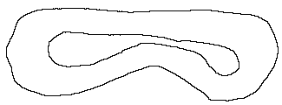
\includegraphics[interpolate=true,width=2.820000in,height=1.050000in]{contents/chapt5/figs/reward/path_collision_penalty-img0.png}}%
\end{pgfscope}%
\begin{pgfscope}%
\pgfpathrectangle{\pgfqpoint{0.180000in}{0.729385in}}{\pgfqpoint{2.820000in}{1.041231in}}%
\pgfusepath{clip}%
\pgfsetbuttcap%
\pgfsetroundjoin%
\pgfsetlinewidth{1.505625pt}%
\definecolor{currentstroke}{rgb}{0.501961,0.501961,0.501961}%
\pgfsetstrokecolor{currentstroke}%
\pgfsetdash{{5.550000pt}{2.400000pt}}{0.000000pt}%
\pgfpathmoveto{\pgfqpoint{1.741088in}{1.226736in}}%
\pgfpathlineto{\pgfqpoint{1.825202in}{1.205436in}}%
\pgfpathlineto{\pgfqpoint{1.892955in}{1.190069in}}%
\pgfpathlineto{\pgfqpoint{1.926172in}{1.180411in}}%
\pgfpathlineto{\pgfqpoint{1.975020in}{1.162462in}}%
\pgfpathlineto{\pgfqpoint{2.023590in}{1.142544in}}%
\pgfpathlineto{\pgfqpoint{2.054496in}{1.126725in}}%
\pgfpathlineto{\pgfqpoint{2.068883in}{1.117250in}}%
\pgfpathlineto{\pgfqpoint{2.095299in}{1.094914in}}%
\pgfpathlineto{\pgfqpoint{2.121014in}{1.071415in}}%
\pgfpathlineto{\pgfqpoint{2.134629in}{1.060626in}}%
\pgfpathlineto{\pgfqpoint{2.164225in}{1.042206in}}%
\pgfpathlineto{\pgfqpoint{2.194157in}{1.024485in}}%
\pgfpathlineto{\pgfqpoint{2.208044in}{1.014375in}}%
\pgfpathlineto{\pgfqpoint{2.220732in}{1.002820in}}%
\pgfpathlineto{\pgfqpoint{2.267859in}{0.951517in}}%
\pgfpathlineto{\pgfqpoint{2.281128in}{0.940164in}}%
\pgfpathlineto{\pgfqpoint{2.295393in}{0.930053in}}%
\pgfpathlineto{\pgfqpoint{2.310515in}{0.921239in}}%
\pgfpathlineto{\pgfqpoint{2.326352in}{0.913776in}}%
\pgfpathlineto{\pgfqpoint{2.342763in}{0.907719in}}%
\pgfpathlineto{\pgfqpoint{2.359611in}{0.903099in}}%
\pgfpathlineto{\pgfqpoint{2.376774in}{0.899863in}}%
\pgfpathlineto{\pgfqpoint{2.394131in}{0.897935in}}%
\pgfpathlineto{\pgfqpoint{2.411563in}{0.897239in}}%
\pgfpathlineto{\pgfqpoint{2.446204in}{0.899217in}}%
\pgfpathlineto{\pgfqpoint{2.480411in}{0.904673in}}%
\pgfpathlineto{\pgfqpoint{2.531651in}{0.915904in}}%
\pgfpathlineto{\pgfqpoint{2.565344in}{0.925242in}}%
\pgfpathlineto{\pgfqpoint{2.581544in}{0.931324in}}%
\pgfpathlineto{\pgfqpoint{2.597060in}{0.938793in}}%
\pgfpathlineto{\pgfqpoint{2.611735in}{0.947887in}}%
\pgfpathlineto{\pgfqpoint{2.625544in}{0.958454in}}%
\pgfpathlineto{\pgfqpoint{2.638495in}{0.970243in}}%
\pgfpathlineto{\pgfqpoint{2.661861in}{0.996497in}}%
\pgfpathlineto{\pgfqpoint{2.682043in}{1.024900in}}%
\pgfpathlineto{\pgfqpoint{2.699827in}{1.054676in}}%
\pgfpathlineto{\pgfqpoint{2.723717in}{1.100906in}}%
\pgfpathlineto{\pgfqpoint{2.737278in}{1.132885in}}%
\pgfpathlineto{\pgfqpoint{2.747746in}{1.166234in}}%
\pgfpathlineto{\pgfqpoint{2.751452in}{1.183382in}}%
\pgfpathlineto{\pgfqpoint{2.753912in}{1.200699in}}%
\pgfpathlineto{\pgfqpoint{2.754956in}{1.218072in}}%
\pgfpathlineto{\pgfqpoint{2.754411in}{1.235384in}}%
\pgfpathlineto{\pgfqpoint{2.752173in}{1.252535in}}%
\pgfpathlineto{\pgfqpoint{2.748411in}{1.269479in}}%
\pgfpathlineto{\pgfqpoint{2.737259in}{1.302617in}}%
\pgfpathlineto{\pgfqpoint{2.722781in}{1.334532in}}%
\pgfpathlineto{\pgfqpoint{2.705392in}{1.364665in}}%
\pgfpathlineto{\pgfqpoint{2.695296in}{1.378798in}}%
\pgfpathlineto{\pgfqpoint{2.684090in}{1.392163in}}%
\pgfpathlineto{\pgfqpoint{2.671684in}{1.404630in}}%
\pgfpathlineto{\pgfqpoint{2.658165in}{1.415976in}}%
\pgfpathlineto{\pgfqpoint{2.643665in}{1.425953in}}%
\pgfpathlineto{\pgfqpoint{2.628314in}{1.434315in}}%
\pgfpathlineto{\pgfqpoint{2.612244in}{1.440816in}}%
\pgfpathlineto{\pgfqpoint{2.595595in}{1.445366in}}%
\pgfpathlineto{\pgfqpoint{2.561291in}{1.450947in}}%
\pgfpathlineto{\pgfqpoint{2.526906in}{1.456511in}}%
\pgfpathlineto{\pgfqpoint{2.493537in}{1.466054in}}%
\pgfpathlineto{\pgfqpoint{2.443952in}{1.481956in}}%
\pgfpathlineto{\pgfqpoint{2.409984in}{1.488707in}}%
\pgfpathlineto{\pgfqpoint{2.358142in}{1.494821in}}%
\pgfpathlineto{\pgfqpoint{2.289304in}{1.503658in}}%
\pgfpathlineto{\pgfqpoint{2.220499in}{1.513871in}}%
\pgfpathlineto{\pgfqpoint{2.185942in}{1.516285in}}%
\pgfpathlineto{\pgfqpoint{2.151262in}{1.515154in}}%
\pgfpathlineto{\pgfqpoint{2.116551in}{1.513356in}}%
\pgfpathlineto{\pgfqpoint{2.081918in}{1.514585in}}%
\pgfpathlineto{\pgfqpoint{2.030066in}{1.520036in}}%
\pgfpathlineto{\pgfqpoint{2.012747in}{1.520582in}}%
\pgfpathlineto{\pgfqpoint{1.978025in}{1.518037in}}%
\pgfpathlineto{\pgfqpoint{1.943381in}{1.514867in}}%
\pgfpathlineto{\pgfqpoint{1.926167in}{1.514847in}}%
\pgfpathlineto{\pgfqpoint{1.909055in}{1.516602in}}%
\pgfpathlineto{\pgfqpoint{1.874988in}{1.523499in}}%
\pgfpathlineto{\pgfqpoint{1.840830in}{1.530542in}}%
\pgfpathlineto{\pgfqpoint{1.806307in}{1.533705in}}%
\pgfpathlineto{\pgfqpoint{1.771529in}{1.533836in}}%
\pgfpathlineto{\pgfqpoint{1.701944in}{1.532871in}}%
\pgfpathlineto{\pgfqpoint{1.667350in}{1.534846in}}%
\pgfpathlineto{\pgfqpoint{1.615765in}{1.542196in}}%
\pgfpathlineto{\pgfqpoint{1.581339in}{1.546290in}}%
\pgfpathlineto{\pgfqpoint{1.546712in}{1.547029in}}%
\pgfpathlineto{\pgfqpoint{1.407860in}{1.541986in}}%
\pgfpathlineto{\pgfqpoint{1.338516in}{1.537840in}}%
\pgfpathlineto{\pgfqpoint{1.303891in}{1.538269in}}%
\pgfpathlineto{\pgfqpoint{1.182509in}{1.545189in}}%
\pgfpathlineto{\pgfqpoint{1.147955in}{1.547721in}}%
\pgfpathlineto{\pgfqpoint{1.113707in}{1.553234in}}%
\pgfpathlineto{\pgfqpoint{1.062370in}{1.562003in}}%
\pgfpathlineto{\pgfqpoint{1.027787in}{1.564368in}}%
\pgfpathlineto{\pgfqpoint{0.993008in}{1.564130in}}%
\pgfpathlineto{\pgfqpoint{0.923547in}{1.561591in}}%
\pgfpathlineto{\pgfqpoint{0.888843in}{1.563437in}}%
\pgfpathlineto{\pgfqpoint{0.819662in}{1.573569in}}%
\pgfpathlineto{\pgfqpoint{0.802654in}{1.573458in}}%
\pgfpathlineto{\pgfqpoint{0.785839in}{1.570959in}}%
\pgfpathlineto{\pgfqpoint{0.769183in}{1.566498in}}%
\pgfpathlineto{\pgfqpoint{0.736161in}{1.554357in}}%
\pgfpathlineto{\pgfqpoint{0.703217in}{1.542223in}}%
\pgfpathlineto{\pgfqpoint{0.620726in}{1.515255in}}%
\pgfpathlineto{\pgfqpoint{0.588768in}{1.501033in}}%
\pgfpathlineto{\pgfqpoint{0.573703in}{1.492380in}}%
\pgfpathlineto{\pgfqpoint{0.559542in}{1.482448in}}%
\pgfpathlineto{\pgfqpoint{0.546460in}{1.471117in}}%
\pgfpathlineto{\pgfqpoint{0.534434in}{1.458552in}}%
\pgfpathlineto{\pgfqpoint{0.523397in}{1.444984in}}%
\pgfpathlineto{\pgfqpoint{0.504013in}{1.415774in}}%
\pgfpathlineto{\pgfqpoint{0.487828in}{1.385017in}}%
\pgfpathlineto{\pgfqpoint{0.474654in}{1.352912in}}%
\pgfpathlineto{\pgfqpoint{0.464416in}{1.319353in}}%
\pgfpathlineto{\pgfqpoint{0.460642in}{1.302139in}}%
\pgfpathlineto{\pgfqpoint{0.458094in}{1.284804in}}%
\pgfpathlineto{\pgfqpoint{0.457032in}{1.267481in}}%
\pgfpathlineto{\pgfqpoint{0.457714in}{1.250302in}}%
\pgfpathlineto{\pgfqpoint{0.460283in}{1.233366in}}%
\pgfpathlineto{\pgfqpoint{0.464415in}{1.216635in}}%
\pgfpathlineto{\pgfqpoint{0.475606in}{1.183494in}}%
\pgfpathlineto{\pgfqpoint{0.501047in}{1.117897in}}%
\pgfpathlineto{\pgfqpoint{0.508839in}{1.102529in}}%
\pgfpathlineto{\pgfqpoint{0.517948in}{1.088064in}}%
\pgfpathlineto{\pgfqpoint{0.528643in}{1.074688in}}%
\pgfpathlineto{\pgfqpoint{0.540753in}{1.062346in}}%
\pgfpathlineto{\pgfqpoint{0.553995in}{1.050921in}}%
\pgfpathlineto{\pgfqpoint{0.582749in}{1.030361in}}%
\pgfpathlineto{\pgfqpoint{0.613051in}{1.012462in}}%
\pgfpathlineto{\pgfqpoint{0.628683in}{1.004798in}}%
\pgfpathlineto{\pgfqpoint{0.644664in}{0.998219in}}%
\pgfpathlineto{\pgfqpoint{0.661014in}{0.992898in}}%
\pgfpathlineto{\pgfqpoint{0.694749in}{0.985912in}}%
\pgfpathlineto{\pgfqpoint{0.763852in}{0.975465in}}%
\pgfpathlineto{\pgfqpoint{0.798176in}{0.969015in}}%
\pgfpathlineto{\pgfqpoint{0.815293in}{0.966731in}}%
\pgfpathlineto{\pgfqpoint{0.832410in}{0.965751in}}%
\pgfpathlineto{\pgfqpoint{0.849546in}{0.966414in}}%
\pgfpathlineto{\pgfqpoint{0.883906in}{0.971175in}}%
\pgfpathlineto{\pgfqpoint{0.935740in}{0.979578in}}%
\pgfpathlineto{\pgfqpoint{0.987355in}{0.986519in}}%
\pgfpathlineto{\pgfqpoint{1.004231in}{0.990060in}}%
\pgfpathlineto{\pgfqpoint{1.037357in}{1.000102in}}%
\pgfpathlineto{\pgfqpoint{1.070392in}{1.011021in}}%
\pgfpathlineto{\pgfqpoint{1.087186in}{1.015505in}}%
\pgfpathlineto{\pgfqpoint{1.121543in}{1.021445in}}%
\pgfpathlineto{\pgfqpoint{1.155847in}{1.027002in}}%
\pgfpathlineto{\pgfqpoint{1.172524in}{1.031200in}}%
\pgfpathlineto{\pgfqpoint{1.188692in}{1.037005in}}%
\pgfpathlineto{\pgfqpoint{1.219829in}{1.052339in}}%
\pgfpathlineto{\pgfqpoint{1.295888in}{1.095141in}}%
\pgfpathlineto{\pgfqpoint{1.327143in}{1.109982in}}%
\pgfpathlineto{\pgfqpoint{1.359275in}{1.122977in}}%
\pgfpathlineto{\pgfqpoint{1.472845in}{1.166160in}}%
\pgfpathlineto{\pgfqpoint{1.568830in}{1.206599in}}%
\pgfpathlineto{\pgfqpoint{1.602059in}{1.215365in}}%
\pgfpathlineto{\pgfqpoint{1.636118in}{1.220971in}}%
\pgfpathlineto{\pgfqpoint{1.670799in}{1.224209in}}%
\pgfpathlineto{\pgfqpoint{1.723533in}{1.226352in}}%
\pgfpathlineto{\pgfqpoint{1.723533in}{1.226352in}}%
\pgfusepath{stroke}%
\end{pgfscope}%
\begin{pgfscope}%
\pgfpathrectangle{\pgfqpoint{0.180000in}{0.729385in}}{\pgfqpoint{2.820000in}{1.041231in}}%
\pgfusepath{clip}%
\pgfsetrectcap%
\pgfsetroundjoin%
\pgfsetlinewidth{1.505625pt}%
\definecolor{currentstroke}{rgb}{0.121569,0.466667,0.705882}%
\pgfsetstrokecolor{currentstroke}%
\pgfsetdash{}{0pt}%
\pgfpathmoveto{\pgfqpoint{1.915385in}{1.510308in}}%
\pgfpathlineto{\pgfqpoint{1.779910in}{1.511318in}}%
\pgfpathlineto{\pgfqpoint{1.683236in}{1.513813in}}%
\pgfpathlineto{\pgfqpoint{1.612670in}{1.517996in}}%
\pgfpathlineto{\pgfqpoint{1.542308in}{1.524814in}}%
\pgfpathlineto{\pgfqpoint{1.296348in}{1.551487in}}%
\pgfpathlineto{\pgfqpoint{1.234575in}{1.554661in}}%
\pgfpathlineto{\pgfqpoint{1.004979in}{1.562567in}}%
\pgfpathlineto{\pgfqpoint{0.907884in}{1.567063in}}%
\pgfpathlineto{\pgfqpoint{0.854869in}{1.567271in}}%
\pgfpathlineto{\pgfqpoint{0.819583in}{1.565300in}}%
\pgfpathlineto{\pgfqpoint{0.793278in}{1.562043in}}%
\pgfpathlineto{\pgfqpoint{0.767261in}{1.556978in}}%
\pgfpathlineto{\pgfqpoint{0.741741in}{1.549828in}}%
\pgfpathlineto{\pgfqpoint{0.716973in}{1.540401in}}%
\pgfpathlineto{\pgfqpoint{0.693296in}{1.528503in}}%
\pgfpathlineto{\pgfqpoint{0.671113in}{1.514011in}}%
\pgfpathlineto{\pgfqpoint{0.650810in}{1.496988in}}%
\pgfpathlineto{\pgfqpoint{0.638510in}{1.484302in}}%
\pgfpathlineto{\pgfqpoint{0.627335in}{1.470616in}}%
\pgfpathlineto{\pgfqpoint{0.617391in}{1.456011in}}%
\pgfpathlineto{\pgfqpoint{0.608776in}{1.440584in}}%
\pgfpathlineto{\pgfqpoint{0.601577in}{1.424448in}}%
\pgfpathlineto{\pgfqpoint{0.595866in}{1.407728in}}%
\pgfpathlineto{\pgfqpoint{0.591674in}{1.390563in}}%
\pgfpathlineto{\pgfqpoint{0.588099in}{1.364310in}}%
\pgfpathlineto{\pgfqpoint{0.587507in}{1.337817in}}%
\pgfpathlineto{\pgfqpoint{0.589530in}{1.311393in}}%
\pgfpathlineto{\pgfqpoint{0.593903in}{1.285252in}}%
\pgfpathlineto{\pgfqpoint{0.600287in}{1.259527in}}%
\pgfpathlineto{\pgfqpoint{0.608400in}{1.234293in}}%
\pgfpathlineto{\pgfqpoint{0.621641in}{1.201529in}}%
\pgfpathlineto{\pgfqpoint{0.637348in}{1.169872in}}%
\pgfpathlineto{\pgfqpoint{0.655327in}{1.139448in}}%
\pgfpathlineto{\pgfqpoint{0.675457in}{1.110401in}}%
\pgfpathlineto{\pgfqpoint{0.697631in}{1.082883in}}%
\pgfpathlineto{\pgfqpoint{0.715597in}{1.063395in}}%
\pgfpathlineto{\pgfqpoint{0.734882in}{1.045213in}}%
\pgfpathlineto{\pgfqpoint{0.755627in}{1.028720in}}%
\pgfpathlineto{\pgfqpoint{0.777825in}{1.014244in}}%
\pgfpathlineto{\pgfqpoint{0.801395in}{1.002134in}}%
\pgfpathlineto{\pgfqpoint{0.826184in}{0.992778in}}%
\pgfpathlineto{\pgfqpoint{0.851922in}{0.986489in}}%
\pgfpathlineto{\pgfqpoint{0.878232in}{0.983347in}}%
\pgfpathlineto{\pgfqpoint{0.904730in}{0.983152in}}%
\pgfpathlineto{\pgfqpoint{0.931121in}{0.985578in}}%
\pgfpathlineto{\pgfqpoint{0.957189in}{0.990360in}}%
\pgfpathlineto{\pgfqpoint{0.982791in}{0.997216in}}%
\pgfpathlineto{\pgfqpoint{1.007857in}{1.005835in}}%
\pgfpathlineto{\pgfqpoint{1.040212in}{1.019508in}}%
\pgfpathlineto{\pgfqpoint{1.086910in}{1.042496in}}%
\pgfpathlineto{\pgfqpoint{1.148061in}{1.072676in}}%
\pgfpathlineto{\pgfqpoint{1.179234in}{1.085949in}}%
\pgfpathlineto{\pgfqpoint{1.220181in}{1.100709in}}%
\pgfpathlineto{\pgfqpoint{1.270142in}{1.116266in}}%
\pgfpathlineto{\pgfqpoint{1.345812in}{1.137136in}}%
\pgfpathlineto{\pgfqpoint{1.430461in}{1.158139in}}%
\pgfpathlineto{\pgfqpoint{1.498720in}{1.172588in}}%
\pgfpathlineto{\pgfqpoint{1.541713in}{1.179871in}}%
\pgfpathlineto{\pgfqpoint{1.585027in}{1.184890in}}%
\pgfpathlineto{\pgfqpoint{1.619851in}{1.186921in}}%
\pgfpathlineto{\pgfqpoint{1.654733in}{1.186889in}}%
\pgfpathlineto{\pgfqpoint{1.689542in}{1.184633in}}%
\pgfpathlineto{\pgfqpoint{1.724162in}{1.180355in}}%
\pgfpathlineto{\pgfqpoint{1.758490in}{1.174154in}}%
\pgfpathlineto{\pgfqpoint{1.800880in}{1.163945in}}%
\pgfpathlineto{\pgfqpoint{1.842602in}{1.151271in}}%
\pgfpathlineto{\pgfqpoint{1.883577in}{1.136357in}}%
\pgfpathlineto{\pgfqpoint{1.923716in}{1.119321in}}%
\pgfpathlineto{\pgfqpoint{1.962937in}{1.100265in}}%
\pgfpathlineto{\pgfqpoint{2.001141in}{1.079245in}}%
\pgfpathlineto{\pgfqpoint{2.045789in}{1.051954in}}%
\pgfpathlineto{\pgfqpoint{2.111382in}{1.008837in}}%
\pgfpathlineto{\pgfqpoint{2.198731in}{0.951191in}}%
\pgfpathlineto{\pgfqpoint{2.228935in}{0.933740in}}%
\pgfpathlineto{\pgfqpoint{2.260187in}{0.918250in}}%
\pgfpathlineto{\pgfqpoint{2.284384in}{0.908303in}}%
\pgfpathlineto{\pgfqpoint{2.309220in}{0.900085in}}%
\pgfpathlineto{\pgfqpoint{2.334647in}{0.893946in}}%
\pgfpathlineto{\pgfqpoint{2.360527in}{0.890143in}}%
\pgfpathlineto{\pgfqpoint{2.386650in}{0.888838in}}%
\pgfpathlineto{\pgfqpoint{2.412771in}{0.890192in}}%
\pgfpathlineto{\pgfqpoint{2.438603in}{0.894284in}}%
\pgfpathlineto{\pgfqpoint{2.463838in}{0.901158in}}%
\pgfpathlineto{\pgfqpoint{2.488150in}{0.910796in}}%
\pgfpathlineto{\pgfqpoint{2.511128in}{0.923281in}}%
\pgfpathlineto{\pgfqpoint{2.532409in}{0.938479in}}%
\pgfpathlineto{\pgfqpoint{2.551605in}{0.956237in}}%
\pgfpathlineto{\pgfqpoint{2.563063in}{0.969384in}}%
\pgfpathlineto{\pgfqpoint{2.573326in}{0.983484in}}%
\pgfpathlineto{\pgfqpoint{2.582299in}{0.998437in}}%
\pgfpathlineto{\pgfqpoint{2.589899in}{1.014133in}}%
\pgfpathlineto{\pgfqpoint{2.596053in}{1.030451in}}%
\pgfpathlineto{\pgfqpoint{2.600729in}{1.047252in}}%
\pgfpathlineto{\pgfqpoint{2.605102in}{1.073035in}}%
\pgfpathlineto{\pgfqpoint{2.606571in}{1.099149in}}%
\pgfpathlineto{\pgfqpoint{2.605494in}{1.125284in}}%
\pgfpathlineto{\pgfqpoint{2.602124in}{1.151226in}}%
\pgfpathlineto{\pgfqpoint{2.596786in}{1.176836in}}%
\pgfpathlineto{\pgfqpoint{2.587051in}{1.210328in}}%
\pgfpathlineto{\pgfqpoint{2.574497in}{1.242869in}}%
\pgfpathlineto{\pgfqpoint{2.559345in}{1.274284in}}%
\pgfpathlineto{\pgfqpoint{2.541687in}{1.304362in}}%
\pgfpathlineto{\pgfqpoint{2.521585in}{1.332865in}}%
\pgfpathlineto{\pgfqpoint{2.504955in}{1.353061in}}%
\pgfpathlineto{\pgfqpoint{2.486982in}{1.372071in}}%
\pgfpathlineto{\pgfqpoint{2.467731in}{1.389784in}}%
\pgfpathlineto{\pgfqpoint{2.447257in}{1.406069in}}%
\pgfpathlineto{\pgfqpoint{2.425649in}{1.420816in}}%
\pgfpathlineto{\pgfqpoint{2.402994in}{1.433897in}}%
\pgfpathlineto{\pgfqpoint{2.379415in}{1.445227in}}%
\pgfpathlineto{\pgfqpoint{2.355043in}{1.454734in}}%
\pgfpathlineto{\pgfqpoint{2.321687in}{1.464931in}}%
\pgfpathlineto{\pgfqpoint{2.287684in}{1.472709in}}%
\pgfpathlineto{\pgfqpoint{2.253270in}{1.478417in}}%
\pgfpathlineto{\pgfqpoint{2.209935in}{1.483252in}}%
\pgfpathlineto{\pgfqpoint{2.157714in}{1.486614in}}%
\pgfpathlineto{\pgfqpoint{2.070548in}{1.489591in}}%
\pgfpathlineto{\pgfqpoint{1.922367in}{1.494702in}}%
\pgfpathlineto{\pgfqpoint{1.896234in}{1.496009in}}%
\pgfpathlineto{\pgfqpoint{1.896234in}{1.496009in}}%
\pgfusepath{stroke}%
\end{pgfscope}%
\begin{pgfscope}%
\pgfpathrectangle{\pgfqpoint{0.180000in}{0.729385in}}{\pgfqpoint{2.820000in}{1.041231in}}%
\pgfusepath{clip}%
\pgfsetrectcap%
\pgfsetroundjoin%
\pgfsetlinewidth{1.505625pt}%
\definecolor{currentstroke}{rgb}{1.000000,0.498039,0.054902}%
\pgfsetstrokecolor{currentstroke}%
\pgfsetdash{}{0pt}%
\pgfpathmoveto{\pgfqpoint{1.915385in}{1.510308in}}%
\pgfpathlineto{\pgfqpoint{1.842619in}{1.511410in}}%
\pgfpathlineto{\pgfqpoint{1.779172in}{1.514666in}}%
\pgfpathlineto{\pgfqpoint{1.685769in}{1.522011in}}%
\pgfpathlineto{\pgfqpoint{1.517654in}{1.536185in}}%
\pgfpathlineto{\pgfqpoint{1.456438in}{1.538861in}}%
\pgfpathlineto{\pgfqpoint{1.360156in}{1.540335in}}%
\pgfpathlineto{\pgfqpoint{1.088790in}{1.541428in}}%
\pgfpathlineto{\pgfqpoint{1.018794in}{1.539241in}}%
\pgfpathlineto{\pgfqpoint{0.957650in}{1.535240in}}%
\pgfpathlineto{\pgfqpoint{0.896703in}{1.528920in}}%
\pgfpathlineto{\pgfqpoint{0.836065in}{1.520111in}}%
\pgfpathlineto{\pgfqpoint{0.784421in}{1.510553in}}%
\pgfpathlineto{\pgfqpoint{0.741712in}{1.500989in}}%
\pgfpathlineto{\pgfqpoint{0.708028in}{1.491443in}}%
\pgfpathlineto{\pgfqpoint{0.683314in}{1.482573in}}%
\pgfpathlineto{\pgfqpoint{0.659316in}{1.471922in}}%
\pgfpathlineto{\pgfqpoint{0.636310in}{1.459272in}}%
\pgfpathlineto{\pgfqpoint{0.614645in}{1.444446in}}%
\pgfpathlineto{\pgfqpoint{0.594694in}{1.427389in}}%
\pgfpathlineto{\pgfqpoint{0.576960in}{1.408039in}}%
\pgfpathlineto{\pgfqpoint{0.566563in}{1.393958in}}%
\pgfpathlineto{\pgfqpoint{0.557443in}{1.379018in}}%
\pgfpathlineto{\pgfqpoint{0.549710in}{1.363315in}}%
\pgfpathlineto{\pgfqpoint{0.543464in}{1.346965in}}%
\pgfpathlineto{\pgfqpoint{0.538789in}{1.330098in}}%
\pgfpathlineto{\pgfqpoint{0.535752in}{1.312860in}}%
\pgfpathlineto{\pgfqpoint{0.534401in}{1.295410in}}%
\pgfpathlineto{\pgfqpoint{0.534737in}{1.277910in}}%
\pgfpathlineto{\pgfqpoint{0.536665in}{1.260513in}}%
\pgfpathlineto{\pgfqpoint{0.542294in}{1.234876in}}%
\pgfpathlineto{\pgfqpoint{0.550846in}{1.210058in}}%
\pgfpathlineto{\pgfqpoint{0.562028in}{1.186307in}}%
\pgfpathlineto{\pgfqpoint{0.575475in}{1.163758in}}%
\pgfpathlineto{\pgfqpoint{0.590878in}{1.142496in}}%
\pgfpathlineto{\pgfqpoint{0.607961in}{1.122557in}}%
\pgfpathlineto{\pgfqpoint{0.626448in}{1.103911in}}%
\pgfpathlineto{\pgfqpoint{0.646168in}{1.086574in}}%
\pgfpathlineto{\pgfqpoint{0.674110in}{1.065485in}}%
\pgfpathlineto{\pgfqpoint{0.703662in}{1.046719in}}%
\pgfpathlineto{\pgfqpoint{0.734574in}{1.030287in}}%
\pgfpathlineto{\pgfqpoint{0.766653in}{1.016270in}}%
\pgfpathlineto{\pgfqpoint{0.799748in}{1.004858in}}%
\pgfpathlineto{\pgfqpoint{0.833659in}{0.996167in}}%
\pgfpathlineto{\pgfqpoint{0.868176in}{0.990333in}}%
\pgfpathlineto{\pgfqpoint{0.894321in}{0.987903in}}%
\pgfpathlineto{\pgfqpoint{0.920569in}{0.987165in}}%
\pgfpathlineto{\pgfqpoint{0.955548in}{0.988594in}}%
\pgfpathlineto{\pgfqpoint{0.990324in}{0.992628in}}%
\pgfpathlineto{\pgfqpoint{1.024733in}{0.999089in}}%
\pgfpathlineto{\pgfqpoint{1.058648in}{1.007779in}}%
\pgfpathlineto{\pgfqpoint{1.091964in}{1.018543in}}%
\pgfpathlineto{\pgfqpoint{1.132824in}{1.034224in}}%
\pgfpathlineto{\pgfqpoint{1.181032in}{1.055068in}}%
\pgfpathlineto{\pgfqpoint{1.372787in}{1.140855in}}%
\pgfpathlineto{\pgfqpoint{1.430080in}{1.162583in}}%
\pgfpathlineto{\pgfqpoint{1.488197in}{1.181995in}}%
\pgfpathlineto{\pgfqpoint{1.538617in}{1.196705in}}%
\pgfpathlineto{\pgfqpoint{1.589552in}{1.209511in}}%
\pgfpathlineto{\pgfqpoint{1.632497in}{1.217944in}}%
\pgfpathlineto{\pgfqpoint{1.667164in}{1.222846in}}%
\pgfpathlineto{\pgfqpoint{1.702051in}{1.225795in}}%
\pgfpathlineto{\pgfqpoint{1.737053in}{1.226561in}}%
\pgfpathlineto{\pgfqpoint{1.771945in}{1.225156in}}%
\pgfpathlineto{\pgfqpoint{1.806556in}{1.221764in}}%
\pgfpathlineto{\pgfqpoint{1.840781in}{1.216470in}}%
\pgfpathlineto{\pgfqpoint{1.882904in}{1.207421in}}%
\pgfpathlineto{\pgfqpoint{1.924108in}{1.195936in}}%
\pgfpathlineto{\pgfqpoint{1.963704in}{1.182138in}}%
\pgfpathlineto{\pgfqpoint{1.994025in}{1.169423in}}%
\pgfpathlineto{\pgfqpoint{2.023002in}{1.155185in}}%
\pgfpathlineto{\pgfqpoint{2.050505in}{1.139439in}}%
\pgfpathlineto{\pgfqpoint{2.076385in}{1.122313in}}%
\pgfpathlineto{\pgfqpoint{2.100558in}{1.104100in}}%
\pgfpathlineto{\pgfqpoint{2.128336in}{1.080039in}}%
\pgfpathlineto{\pgfqpoint{2.153460in}{1.054887in}}%
\pgfpathlineto{\pgfqpoint{2.176196in}{1.028787in}}%
\pgfpathlineto{\pgfqpoint{2.231532in}{0.962353in}}%
\pgfpathlineto{\pgfqpoint{2.252696in}{0.940970in}}%
\pgfpathlineto{\pgfqpoint{2.275892in}{0.920735in}}%
\pgfpathlineto{\pgfqpoint{2.294960in}{0.906623in}}%
\pgfpathlineto{\pgfqpoint{2.315550in}{0.893754in}}%
\pgfpathlineto{\pgfqpoint{2.337625in}{0.882367in}}%
\pgfpathlineto{\pgfqpoint{2.361111in}{0.872702in}}%
\pgfpathlineto{\pgfqpoint{2.385900in}{0.865010in}}%
\pgfpathlineto{\pgfqpoint{2.411479in}{0.859618in}}%
\pgfpathlineto{\pgfqpoint{2.437466in}{0.856792in}}%
\pgfpathlineto{\pgfqpoint{2.463604in}{0.856701in}}%
\pgfpathlineto{\pgfqpoint{2.489587in}{0.859531in}}%
\pgfpathlineto{\pgfqpoint{2.515056in}{0.865394in}}%
\pgfpathlineto{\pgfqpoint{2.539635in}{0.874278in}}%
\pgfpathlineto{\pgfqpoint{2.562934in}{0.886119in}}%
\pgfpathlineto{\pgfqpoint{2.584581in}{0.900747in}}%
\pgfpathlineto{\pgfqpoint{2.604299in}{0.917788in}}%
\pgfpathlineto{\pgfqpoint{2.622049in}{0.936769in}}%
\pgfpathlineto{\pgfqpoint{2.637800in}{0.957344in}}%
\pgfpathlineto{\pgfqpoint{2.651558in}{0.979213in}}%
\pgfpathlineto{\pgfqpoint{2.663392in}{1.002097in}}%
\pgfpathlineto{\pgfqpoint{2.673417in}{1.025747in}}%
\pgfpathlineto{\pgfqpoint{2.681721in}{1.049999in}}%
\pgfpathlineto{\pgfqpoint{2.688254in}{1.074781in}}%
\pgfpathlineto{\pgfqpoint{2.692989in}{1.099962in}}%
\pgfpathlineto{\pgfqpoint{2.695931in}{1.125408in}}%
\pgfpathlineto{\pgfqpoint{2.697024in}{1.150995in}}%
\pgfpathlineto{\pgfqpoint{2.696243in}{1.176587in}}%
\pgfpathlineto{\pgfqpoint{2.693549in}{1.202042in}}%
\pgfpathlineto{\pgfqpoint{2.688880in}{1.227481in}}%
\pgfpathlineto{\pgfqpoint{2.682057in}{1.252704in}}%
\pgfpathlineto{\pgfqpoint{2.673109in}{1.277254in}}%
\pgfpathlineto{\pgfqpoint{2.662024in}{1.300916in}}%
\pgfpathlineto{\pgfqpoint{2.648743in}{1.323416in}}%
\pgfpathlineto{\pgfqpoint{2.633280in}{1.344476in}}%
\pgfpathlineto{\pgfqpoint{2.615693in}{1.363796in}}%
\pgfpathlineto{\pgfqpoint{2.596183in}{1.381174in}}%
\pgfpathlineto{\pgfqpoint{2.575120in}{1.396637in}}%
\pgfpathlineto{\pgfqpoint{2.552780in}{1.410190in}}%
\pgfpathlineto{\pgfqpoint{2.529400in}{1.421861in}}%
\pgfpathlineto{\pgfqpoint{2.505199in}{1.431721in}}%
\pgfpathlineto{\pgfqpoint{2.480374in}{1.439883in}}%
\pgfpathlineto{\pgfqpoint{2.446572in}{1.448334in}}%
\pgfpathlineto{\pgfqpoint{2.403718in}{1.456122in}}%
\pgfpathlineto{\pgfqpoint{2.351878in}{1.462823in}}%
\pgfpathlineto{\pgfqpoint{2.239170in}{1.473994in}}%
\pgfpathlineto{\pgfqpoint{2.126572in}{1.486207in}}%
\pgfpathlineto{\pgfqpoint{1.962208in}{1.505859in}}%
\pgfpathlineto{\pgfqpoint{1.962208in}{1.505859in}}%
\pgfusepath{stroke}%
\end{pgfscope}%
\begin{pgfscope}%
\pgfpathrectangle{\pgfqpoint{0.180000in}{0.729385in}}{\pgfqpoint{2.820000in}{1.041231in}}%
\pgfusepath{clip}%
\pgfsetbuttcap%
\pgfsetroundjoin%
\pgfsetlinewidth{1.505625pt}%
\definecolor{currentstroke}{rgb}{1.000000,0.000000,0.000000}%
\pgfsetstrokecolor{currentstroke}%
\pgfsetdash{{1.500000pt}{2.475000pt}}{0.000000pt}%
\pgfpathmoveto{\pgfqpoint{1.909055in}{1.343063in}}%
\pgfpathlineto{\pgfqpoint{1.909055in}{1.690140in}}%
\pgfusepath{stroke}%
\end{pgfscope}%
\begin{pgfscope}%
\pgfsetbuttcap%
\pgfsetmiterjoin%
\definecolor{currentfill}{rgb}{1.000000,1.000000,1.000000}%
\pgfsetfillcolor{currentfill}%
\pgfsetlinewidth{1.003750pt}%
\definecolor{currentstroke}{rgb}{0.000000,0.000000,0.000000}%
\pgfsetstrokecolor{currentstroke}%
\pgfsetdash{}{0pt}%
\pgfpathmoveto{\pgfqpoint{1.700809in}{1.693610in}}%
\pgfpathlineto{\pgfqpoint{2.404139in}{1.693610in}}%
\pgfpathquadraticcurveto{\pgfqpoint{2.418022in}{1.693610in}}{\pgfqpoint{2.418022in}{1.707494in}}%
\pgfpathlineto{\pgfqpoint{2.418022in}{1.846327in}}%
\pgfpathquadraticcurveto{\pgfqpoint{2.418022in}{1.860210in}}{\pgfqpoint{2.404139in}{1.860210in}}%
\pgfpathlineto{\pgfqpoint{1.700809in}{1.860210in}}%
\pgfpathquadraticcurveto{\pgfqpoint{1.686925in}{1.860210in}}{\pgfqpoint{1.686925in}{1.846327in}}%
\pgfpathlineto{\pgfqpoint{1.686925in}{1.707494in}}%
\pgfpathquadraticcurveto{\pgfqpoint{1.686925in}{1.693610in}}{\pgfqpoint{1.700809in}{1.693610in}}%
\pgfpathlineto{\pgfqpoint{1.700809in}{1.693610in}}%
\pgfpathclose%
\pgfusepath{stroke,fill}%
\end{pgfscope}%
\begin{pgfscope}%
\definecolor{textcolor}{rgb}{0.000000,0.000000,0.000000}%
\pgfsetstrokecolor{textcolor}%
\pgfsetfillcolor{textcolor}%
\pgftext[x=1.700809in,y=1.742202in,left,base]{\color{textcolor}\rmfamily\fontsize{9.996000}{11.995200}\selectfont Start/finish}%
\end{pgfscope}%
\begin{pgfscope}%
\pgfsetbuttcap%
\pgfsetmiterjoin%
\definecolor{currentfill}{rgb}{1.000000,1.000000,1.000000}%
\pgfsetfillcolor{currentfill}%
\pgfsetfillopacity{0.800000}%
\pgfsetlinewidth{1.003750pt}%
\definecolor{currentstroke}{rgb}{0.800000,0.800000,0.800000}%
\pgfsetstrokecolor{currentstroke}%
\pgfsetstrokeopacity{0.800000}%
\pgfsetdash{}{0pt}%
\pgfpathmoveto{\pgfqpoint{3.207667in}{0.876500in}}%
\pgfpathlineto{\pgfqpoint{4.883333in}{0.876500in}}%
\pgfpathquadraticcurveto{\pgfqpoint{4.916667in}{0.876500in}}{\pgfqpoint{4.916667in}{0.909834in}}%
\pgfpathlineto{\pgfqpoint{4.916667in}{1.590166in}}%
\pgfpathquadraticcurveto{\pgfqpoint{4.916667in}{1.623500in}}{\pgfqpoint{4.883333in}{1.623500in}}%
\pgfpathlineto{\pgfqpoint{3.207667in}{1.623500in}}%
\pgfpathquadraticcurveto{\pgfqpoint{3.174333in}{1.623500in}}{\pgfqpoint{3.174333in}{1.590166in}}%
\pgfpathlineto{\pgfqpoint{3.174333in}{0.909834in}}%
\pgfpathquadraticcurveto{\pgfqpoint{3.174333in}{0.876500in}}{\pgfqpoint{3.207667in}{0.876500in}}%
\pgfpathlineto{\pgfqpoint{3.207667in}{0.876500in}}%
\pgfpathclose%
\pgfusepath{stroke,fill}%
\end{pgfscope}%
\begin{pgfscope}%
\pgfsetbuttcap%
\pgfsetroundjoin%
\pgfsetlinewidth{1.505625pt}%
\definecolor{currentstroke}{rgb}{0.501961,0.501961,0.501961}%
\pgfsetstrokecolor{currentstroke}%
\pgfsetdash{{5.550000pt}{2.400000pt}}{0.000000pt}%
\pgfpathmoveto{\pgfqpoint{3.241000in}{1.498500in}}%
\pgfpathlineto{\pgfqpoint{3.407667in}{1.498500in}}%
\pgfpathlineto{\pgfqpoint{3.574333in}{1.498500in}}%
\pgfusepath{stroke}%
\end{pgfscope}%
\begin{pgfscope}%
\definecolor{textcolor}{rgb}{0.000000,0.000000,0.000000}%
\pgfsetstrokecolor{textcolor}%
\pgfsetfillcolor{textcolor}%
\pgftext[x=3.707667in,y=1.440166in,left,base]{\color{textcolor}\rmfamily\fontsize{12.000000}{14.400000}\selectfont Track centerline}%
\end{pgfscope}%
\begin{pgfscope}%
\pgfsetrectcap%
\pgfsetroundjoin%
\pgfsetlinewidth{1.505625pt}%
\definecolor{currentstroke}{rgb}{0.121569,0.466667,0.705882}%
\pgfsetstrokecolor{currentstroke}%
\pgfsetdash{}{0pt}%
\pgfpathmoveto{\pgfqpoint{3.241000in}{1.266167in}}%
\pgfpathlineto{\pgfqpoint{3.407667in}{1.266167in}}%
\pgfpathlineto{\pgfqpoint{3.574333in}{1.266167in}}%
\pgfusepath{stroke}%
\end{pgfscope}%
\begin{pgfscope}%
\definecolor{textcolor}{rgb}{0.000000,0.000000,0.000000}%
\pgfsetstrokecolor{textcolor}%
\pgfsetfillcolor{textcolor}%
\pgftext[x=3.707667in,y=1.207833in,left,base]{\color{textcolor}\rmfamily\fontsize{12.000000}{14.400000}\selectfont \(\displaystyle r_{\mathrm{collision}}=-4\)}%
\end{pgfscope}%
\begin{pgfscope}%
\pgfsetrectcap%
\pgfsetroundjoin%
\pgfsetlinewidth{1.505625pt}%
\definecolor{currentstroke}{rgb}{1.000000,0.498039,0.054902}%
\pgfsetstrokecolor{currentstroke}%
\pgfsetdash{}{0pt}%
\pgfpathmoveto{\pgfqpoint{3.241000in}{1.033833in}}%
\pgfpathlineto{\pgfqpoint{3.407667in}{1.033833in}}%
\pgfpathlineto{\pgfqpoint{3.574333in}{1.033833in}}%
\pgfusepath{stroke}%
\end{pgfscope}%
\begin{pgfscope}%
\definecolor{textcolor}{rgb}{0.000000,0.000000,0.000000}%
\pgfsetstrokecolor{textcolor}%
\pgfsetfillcolor{textcolor}%
\pgftext[x=3.707667in,y=0.975500in,left,base]{\color{textcolor}\rmfamily\fontsize{12.000000}{14.400000}\selectfont \(\displaystyle r_{\mathrm{collision}}=-10\)}%
\end{pgfscope}%
\end{pgfpicture}%
\makeatother%
\endgroup%

    \caption[Paths taken by agents trained with different collision penalties]{The paths taken by agents trained with $r_{\text{collision}}$ values of $-4$ and $-10$.}
    \label{fig:path_reward_collision}
\end{figure}










%%%%%%%%%%%%%%%%%%%%%%%%%%%%%%%%%%%%%%%%%%%%%%%%%%%%%%%%%%%%%%%%%%%%%%%%%%%%%%%%%%%%%%%%%%%%%%%%%%%%%%%%%%%%%%%%%%%%%%%%%%%%%%%%%%%%%%%%%

\section{Observation space}\label{sec:obs_space}

We also conducted investigations to determine which combiniation of elements in the observation space vector resulted in optimal performance.
This was done by training and evaluating agents that received (a) only the pose, (b) only a LiDAR scan and (c) a combination of vehicle pose and LiDAR scan in their observation.
For each of these observation space combinations, three agents with hyper-parameters listed in Table \ref{tab:inital_values} were trained.
The performance of these agents during training, in terms of percentage failed laps, average lap time and average reward, is shown in Figure \ref{fig:obs_space}.

\begin{figure}[htb!]
    \centering
    %% Creator: Matplotlib, PGF backend
%%
%% To include the figure in your LaTeX document, write
%%   \input{<filename>.pgf}
%%
%% Make sure the required packages are loaded in your preamble
%%   \usepackage{pgf}
%%
%% Also ensure that all the required font packages are loaded; for instance,
%% the lmodern package is sometimes necessary when using math font.
%%   \usepackage{lmodern}
%%
%% Figures using additional raster images can only be included by \input if
%% they are in the same directory as the main LaTeX file. For loading figures
%% from other directories you can use the `import` package
%%   \usepackage{import}
%%
%% and then include the figures with
%%   \import{<path to file>}{<filename>.pgf}
%%
%% Matplotlib used the following preamble
%%   \usepackage{fontspec}
%%   \setmainfont{DejaVuSerif.ttf}[Path=\detokenize{/home/andrew/anaconda3/envs/auto_car_env/lib/python3.9/site-packages/matplotlib/mpl-data/fonts/ttf/}]
%%   \setsansfont{DejaVuSans.ttf}[Path=\detokenize{/home/andrew/anaconda3/envs/auto_car_env/lib/python3.9/site-packages/matplotlib/mpl-data/fonts/ttf/}]
%%   \setmonofont{DejaVuSansMono.ttf}[Path=\detokenize{/home/andrew/anaconda3/envs/auto_car_env/lib/python3.9/site-packages/matplotlib/mpl-data/fonts/ttf/}]
%%
\begingroup%
\makeatletter%
\begin{pgfpicture}%
\pgfpathrectangle{\pgfpointorigin}{\pgfqpoint{5.500000in}{2.500000in}}%
\pgfusepath{use as bounding box, clip}%
\begin{pgfscope}%
\pgfsetbuttcap%
\pgfsetmiterjoin%
\definecolor{currentfill}{rgb}{1.000000,1.000000,1.000000}%
\pgfsetfillcolor{currentfill}%
\pgfsetlinewidth{0.000000pt}%
\definecolor{currentstroke}{rgb}{1.000000,1.000000,1.000000}%
\pgfsetstrokecolor{currentstroke}%
\pgfsetdash{}{0pt}%
\pgfpathmoveto{\pgfqpoint{0.000000in}{0.000000in}}%
\pgfpathlineto{\pgfqpoint{5.500000in}{0.000000in}}%
\pgfpathlineto{\pgfqpoint{5.500000in}{2.500000in}}%
\pgfpathlineto{\pgfqpoint{0.000000in}{2.500000in}}%
\pgfpathlineto{\pgfqpoint{0.000000in}{0.000000in}}%
\pgfpathclose%
\pgfusepath{fill}%
\end{pgfscope}%
\begin{pgfscope}%
\pgfsetbuttcap%
\pgfsetmiterjoin%
\definecolor{currentfill}{rgb}{1.000000,1.000000,1.000000}%
\pgfsetfillcolor{currentfill}%
\pgfsetlinewidth{0.000000pt}%
\definecolor{currentstroke}{rgb}{0.000000,0.000000,0.000000}%
\pgfsetstrokecolor{currentstroke}%
\pgfsetstrokeopacity{0.000000}%
\pgfsetdash{}{0pt}%
\pgfpathmoveto{\pgfqpoint{0.660417in}{1.000000in}}%
\pgfpathlineto{\pgfqpoint{1.810833in}{1.000000in}}%
\pgfpathlineto{\pgfqpoint{1.810833in}{2.156667in}}%
\pgfpathlineto{\pgfqpoint{0.660417in}{2.156667in}}%
\pgfpathlineto{\pgfqpoint{0.660417in}{1.000000in}}%
\pgfpathclose%
\pgfusepath{fill}%
\end{pgfscope}%
\begin{pgfscope}%
\pgfpathrectangle{\pgfqpoint{0.660417in}{1.000000in}}{\pgfqpoint{1.150417in}{1.156667in}}%
\pgfusepath{clip}%
\pgfsetbuttcap%
\pgfsetroundjoin%
\definecolor{currentfill}{rgb}{0.121569,0.466667,0.705882}%
\pgfsetfillcolor{currentfill}%
\pgfsetfillopacity{0.150000}%
\pgfsetlinewidth{0.000000pt}%
\definecolor{currentstroke}{rgb}{0.000000,0.000000,0.000000}%
\pgfsetstrokecolor{currentstroke}%
\pgfsetdash{}{0pt}%
\pgfpathmoveto{\pgfqpoint{0.660417in}{2.104091in}}%
\pgfpathlineto{\pgfqpoint{0.660417in}{2.104091in}}%
\pgfpathlineto{\pgfqpoint{0.676851in}{2.206575in}}%
\pgfpathlineto{\pgfqpoint{0.693286in}{2.076988in}}%
\pgfpathlineto{\pgfqpoint{0.709720in}{1.955559in}}%
\pgfpathlineto{\pgfqpoint{0.726155in}{1.859111in}}%
\pgfpathlineto{\pgfqpoint{0.742589in}{1.790096in}}%
\pgfpathlineto{\pgfqpoint{0.759024in}{1.491559in}}%
\pgfpathlineto{\pgfqpoint{0.775458in}{1.437760in}}%
\pgfpathlineto{\pgfqpoint{0.791893in}{1.413513in}}%
\pgfpathlineto{\pgfqpoint{0.808327in}{1.401650in}}%
\pgfpathlineto{\pgfqpoint{0.824762in}{1.398829in}}%
\pgfpathlineto{\pgfqpoint{0.841196in}{1.396405in}}%
\pgfpathlineto{\pgfqpoint{0.857631in}{1.399218in}}%
\pgfpathlineto{\pgfqpoint{0.874065in}{1.384393in}}%
\pgfpathlineto{\pgfqpoint{0.890500in}{1.399218in}}%
\pgfpathlineto{\pgfqpoint{0.906935in}{1.392258in}}%
\pgfpathlineto{\pgfqpoint{0.923369in}{1.364922in}}%
\pgfpathlineto{\pgfqpoint{0.939804in}{1.347099in}}%
\pgfpathlineto{\pgfqpoint{0.956238in}{1.327659in}}%
\pgfpathlineto{\pgfqpoint{0.972673in}{1.303564in}}%
\pgfpathlineto{\pgfqpoint{0.989107in}{1.292886in}}%
\pgfpathlineto{\pgfqpoint{1.005542in}{1.285575in}}%
\pgfpathlineto{\pgfqpoint{1.021976in}{1.275870in}}%
\pgfpathlineto{\pgfqpoint{1.038411in}{1.272321in}}%
\pgfpathlineto{\pgfqpoint{1.054845in}{1.280982in}}%
\pgfpathlineto{\pgfqpoint{1.071280in}{1.290530in}}%
\pgfpathlineto{\pgfqpoint{1.087714in}{1.296088in}}%
\pgfpathlineto{\pgfqpoint{1.104149in}{1.306681in}}%
\pgfpathlineto{\pgfqpoint{1.120583in}{1.315637in}}%
\pgfpathlineto{\pgfqpoint{1.137018in}{1.303180in}}%
\pgfpathlineto{\pgfqpoint{1.153452in}{1.298099in}}%
\pgfpathlineto{\pgfqpoint{1.169887in}{1.318452in}}%
\pgfpathlineto{\pgfqpoint{1.186321in}{1.313911in}}%
\pgfpathlineto{\pgfqpoint{1.202756in}{1.326909in}}%
\pgfpathlineto{\pgfqpoint{1.219190in}{1.329296in}}%
\pgfpathlineto{\pgfqpoint{1.235625in}{1.321452in}}%
\pgfpathlineto{\pgfqpoint{1.252060in}{1.305339in}}%
\pgfpathlineto{\pgfqpoint{1.268494in}{1.293877in}}%
\pgfpathlineto{\pgfqpoint{1.284929in}{1.271860in}}%
\pgfpathlineto{\pgfqpoint{1.301363in}{1.292332in}}%
\pgfpathlineto{\pgfqpoint{1.317798in}{1.299798in}}%
\pgfpathlineto{\pgfqpoint{1.334232in}{1.304124in}}%
\pgfpathlineto{\pgfqpoint{1.350667in}{1.313424in}}%
\pgfpathlineto{\pgfqpoint{1.350667in}{0.975026in}}%
\pgfpathlineto{\pgfqpoint{1.350667in}{0.975026in}}%
\pgfpathlineto{\pgfqpoint{1.334232in}{0.975930in}}%
\pgfpathlineto{\pgfqpoint{1.317798in}{0.974660in}}%
\pgfpathlineto{\pgfqpoint{1.301363in}{0.976529in}}%
\pgfpathlineto{\pgfqpoint{1.284929in}{0.976012in}}%
\pgfpathlineto{\pgfqpoint{1.268494in}{0.974983in}}%
\pgfpathlineto{\pgfqpoint{1.252060in}{0.970518in}}%
\pgfpathlineto{\pgfqpoint{1.235625in}{0.973994in}}%
\pgfpathlineto{\pgfqpoint{1.219190in}{0.973146in}}%
\pgfpathlineto{\pgfqpoint{1.202756in}{0.974133in}}%
\pgfpathlineto{\pgfqpoint{1.186321in}{0.967542in}}%
\pgfpathlineto{\pgfqpoint{1.169887in}{0.967200in}}%
\pgfpathlineto{\pgfqpoint{1.153452in}{0.966563in}}%
\pgfpathlineto{\pgfqpoint{1.137018in}{0.969878in}}%
\pgfpathlineto{\pgfqpoint{1.120583in}{0.970015in}}%
\pgfpathlineto{\pgfqpoint{1.104149in}{0.974773in}}%
\pgfpathlineto{\pgfqpoint{1.087714in}{0.975571in}}%
\pgfpathlineto{\pgfqpoint{1.071280in}{0.974133in}}%
\pgfpathlineto{\pgfqpoint{1.054845in}{0.973886in}}%
\pgfpathlineto{\pgfqpoint{1.038411in}{0.974152in}}%
\pgfpathlineto{\pgfqpoint{1.021976in}{0.974800in}}%
\pgfpathlineto{\pgfqpoint{1.005542in}{0.974891in}}%
\pgfpathlineto{\pgfqpoint{0.989107in}{0.968979in}}%
\pgfpathlineto{\pgfqpoint{0.972673in}{0.968095in}}%
\pgfpathlineto{\pgfqpoint{0.956238in}{0.970586in}}%
\pgfpathlineto{\pgfqpoint{0.939804in}{0.969335in}}%
\pgfpathlineto{\pgfqpoint{0.923369in}{0.972501in}}%
\pgfpathlineto{\pgfqpoint{0.906935in}{0.987141in}}%
\pgfpathlineto{\pgfqpoint{0.890500in}{0.989975in}}%
\pgfpathlineto{\pgfqpoint{0.874065in}{0.988010in}}%
\pgfpathlineto{\pgfqpoint{0.857631in}{0.989975in}}%
\pgfpathlineto{\pgfqpoint{0.841196in}{0.994188in}}%
\pgfpathlineto{\pgfqpoint{0.824762in}{0.991764in}}%
\pgfpathlineto{\pgfqpoint{0.808327in}{0.995939in}}%
\pgfpathlineto{\pgfqpoint{0.791893in}{0.992471in}}%
\pgfpathlineto{\pgfqpoint{0.775458in}{0.996209in}}%
\pgfpathlineto{\pgfqpoint{0.759024in}{1.013770in}}%
\pgfpathlineto{\pgfqpoint{0.742589in}{1.031457in}}%
\pgfpathlineto{\pgfqpoint{0.726155in}{1.067673in}}%
\pgfpathlineto{\pgfqpoint{0.709720in}{1.167338in}}%
\pgfpathlineto{\pgfqpoint{0.693286in}{1.329043in}}%
\pgfpathlineto{\pgfqpoint{0.676851in}{1.793386in}}%
\pgfpathlineto{\pgfqpoint{0.660417in}{2.104091in}}%
\pgfpathlineto{\pgfqpoint{0.660417in}{2.104091in}}%
\pgfpathclose%
\pgfusepath{fill}%
\end{pgfscope}%
\begin{pgfscope}%
\pgfpathrectangle{\pgfqpoint{0.660417in}{1.000000in}}{\pgfqpoint{1.150417in}{1.156667in}}%
\pgfusepath{clip}%
\pgfsetbuttcap%
\pgfsetroundjoin%
\definecolor{currentfill}{rgb}{1.000000,0.498039,0.054902}%
\pgfsetfillcolor{currentfill}%
\pgfsetfillopacity{0.150000}%
\pgfsetlinewidth{0.000000pt}%
\definecolor{currentstroke}{rgb}{0.000000,0.000000,0.000000}%
\pgfsetstrokecolor{currentstroke}%
\pgfsetdash{}{0pt}%
\pgfpathmoveto{\pgfqpoint{0.660417in}{2.104091in}}%
\pgfpathlineto{\pgfqpoint{0.660417in}{2.104091in}}%
\pgfpathlineto{\pgfqpoint{0.676851in}{2.104091in}}%
\pgfpathlineto{\pgfqpoint{0.693286in}{2.104091in}}%
\pgfpathlineto{\pgfqpoint{0.709720in}{2.104091in}}%
\pgfpathlineto{\pgfqpoint{0.726155in}{2.104091in}}%
\pgfpathlineto{\pgfqpoint{0.742589in}{2.104091in}}%
\pgfpathlineto{\pgfqpoint{0.759024in}{2.104091in}}%
\pgfpathlineto{\pgfqpoint{0.775458in}{2.132486in}}%
\pgfpathlineto{\pgfqpoint{0.791893in}{2.146118in}}%
\pgfpathlineto{\pgfqpoint{0.808327in}{2.147758in}}%
\pgfpathlineto{\pgfqpoint{0.824762in}{2.147758in}}%
\pgfpathlineto{\pgfqpoint{0.841196in}{2.147758in}}%
\pgfpathlineto{\pgfqpoint{0.857631in}{2.140334in}}%
\pgfpathlineto{\pgfqpoint{0.874065in}{2.119035in}}%
\pgfpathlineto{\pgfqpoint{0.890500in}{2.104091in}}%
\pgfpathlineto{\pgfqpoint{0.906935in}{2.104091in}}%
\pgfpathlineto{\pgfqpoint{0.923369in}{2.104091in}}%
\pgfpathlineto{\pgfqpoint{0.939804in}{2.104091in}}%
\pgfpathlineto{\pgfqpoint{0.956238in}{2.104091in}}%
\pgfpathlineto{\pgfqpoint{0.972673in}{2.104091in}}%
\pgfpathlineto{\pgfqpoint{0.989107in}{2.104091in}}%
\pgfpathlineto{\pgfqpoint{1.005542in}{2.104091in}}%
\pgfpathlineto{\pgfqpoint{1.021976in}{2.104091in}}%
\pgfpathlineto{\pgfqpoint{1.038411in}{2.104091in}}%
\pgfpathlineto{\pgfqpoint{1.054845in}{2.104091in}}%
\pgfpathlineto{\pgfqpoint{1.071280in}{2.104091in}}%
\pgfpathlineto{\pgfqpoint{1.087714in}{2.119035in}}%
\pgfpathlineto{\pgfqpoint{1.104149in}{2.119035in}}%
\pgfpathlineto{\pgfqpoint{1.120583in}{2.119035in}}%
\pgfpathlineto{\pgfqpoint{1.137018in}{2.124793in}}%
\pgfpathlineto{\pgfqpoint{1.153452in}{2.132486in}}%
\pgfpathlineto{\pgfqpoint{1.169887in}{2.135433in}}%
\pgfpathlineto{\pgfqpoint{1.186321in}{2.150719in}}%
\pgfpathlineto{\pgfqpoint{1.202756in}{2.161356in}}%
\pgfpathlineto{\pgfqpoint{1.219190in}{2.167411in}}%
\pgfpathlineto{\pgfqpoint{1.235625in}{2.174169in}}%
\pgfpathlineto{\pgfqpoint{1.252060in}{2.178618in}}%
\pgfpathlineto{\pgfqpoint{1.268494in}{2.175203in}}%
\pgfpathlineto{\pgfqpoint{1.284929in}{2.172690in}}%
\pgfpathlineto{\pgfqpoint{1.301363in}{2.164449in}}%
\pgfpathlineto{\pgfqpoint{1.317798in}{2.150547in}}%
\pgfpathlineto{\pgfqpoint{1.334232in}{2.130903in}}%
\pgfpathlineto{\pgfqpoint{1.350667in}{2.115367in}}%
\pgfpathlineto{\pgfqpoint{1.367101in}{2.085303in}}%
\pgfpathlineto{\pgfqpoint{1.383536in}{2.055133in}}%
\pgfpathlineto{\pgfqpoint{1.399970in}{2.034707in}}%
\pgfpathlineto{\pgfqpoint{1.416405in}{2.008362in}}%
\pgfpathlineto{\pgfqpoint{1.432839in}{1.966475in}}%
\pgfpathlineto{\pgfqpoint{1.449274in}{1.916270in}}%
\pgfpathlineto{\pgfqpoint{1.465708in}{1.861091in}}%
\pgfpathlineto{\pgfqpoint{1.482143in}{1.803082in}}%
\pgfpathlineto{\pgfqpoint{1.498577in}{1.751515in}}%
\pgfpathlineto{\pgfqpoint{1.515012in}{1.719635in}}%
\pgfpathlineto{\pgfqpoint{1.531446in}{1.695050in}}%
\pgfpathlineto{\pgfqpoint{1.547881in}{1.654475in}}%
\pgfpathlineto{\pgfqpoint{1.564315in}{1.586764in}}%
\pgfpathlineto{\pgfqpoint{1.580750in}{1.556115in}}%
\pgfpathlineto{\pgfqpoint{1.597185in}{1.518503in}}%
\pgfpathlineto{\pgfqpoint{1.613619in}{1.481624in}}%
\pgfpathlineto{\pgfqpoint{1.630054in}{1.407901in}}%
\pgfpathlineto{\pgfqpoint{1.646488in}{1.401045in}}%
\pgfpathlineto{\pgfqpoint{1.662923in}{1.397738in}}%
\pgfpathlineto{\pgfqpoint{1.679357in}{1.382457in}}%
\pgfpathlineto{\pgfqpoint{1.695792in}{1.360772in}}%
\pgfpathlineto{\pgfqpoint{1.712226in}{1.370144in}}%
\pgfpathlineto{\pgfqpoint{1.728661in}{1.370144in}}%
\pgfpathlineto{\pgfqpoint{1.745095in}{1.364535in}}%
\pgfpathlineto{\pgfqpoint{1.761530in}{1.379145in}}%
\pgfpathlineto{\pgfqpoint{1.777964in}{1.381238in}}%
\pgfpathlineto{\pgfqpoint{1.794399in}{1.375125in}}%
\pgfpathlineto{\pgfqpoint{1.810833in}{1.375125in}}%
\pgfpathlineto{\pgfqpoint{1.827268in}{1.366737in}}%
\pgfpathlineto{\pgfqpoint{1.843702in}{1.356528in}}%
\pgfpathlineto{\pgfqpoint{1.860137in}{1.351139in}}%
\pgfpathlineto{\pgfqpoint{1.876571in}{1.347185in}}%
\pgfpathlineto{\pgfqpoint{1.893006in}{1.330516in}}%
\pgfpathlineto{\pgfqpoint{1.893006in}{0.977523in}}%
\pgfpathlineto{\pgfqpoint{1.893006in}{0.977523in}}%
\pgfpathlineto{\pgfqpoint{1.876571in}{0.979043in}}%
\pgfpathlineto{\pgfqpoint{1.860137in}{0.975089in}}%
\pgfpathlineto{\pgfqpoint{1.843702in}{0.973898in}}%
\pgfpathlineto{\pgfqpoint{1.827268in}{0.973484in}}%
\pgfpathlineto{\pgfqpoint{1.810833in}{0.976290in}}%
\pgfpathlineto{\pgfqpoint{1.794399in}{0.976290in}}%
\pgfpathlineto{\pgfqpoint{1.777964in}{0.979971in}}%
\pgfpathlineto{\pgfqpoint{1.761530in}{0.980664in}}%
\pgfpathlineto{\pgfqpoint{1.745095in}{0.984081in}}%
\pgfpathlineto{\pgfqpoint{1.728661in}{0.981271in}}%
\pgfpathlineto{\pgfqpoint{1.712226in}{0.981271in}}%
\pgfpathlineto{\pgfqpoint{1.695792in}{0.978050in}}%
\pgfpathlineto{\pgfqpoint{1.679357in}{0.978753in}}%
\pgfpathlineto{\pgfqpoint{1.662923in}{0.978863in}}%
\pgfpathlineto{\pgfqpoint{1.646488in}{0.981152in}}%
\pgfpathlineto{\pgfqpoint{1.630054in}{0.984091in}}%
\pgfpathlineto{\pgfqpoint{1.613619in}{0.999918in}}%
\pgfpathlineto{\pgfqpoint{1.597185in}{1.012012in}}%
\pgfpathlineto{\pgfqpoint{1.580750in}{1.030369in}}%
\pgfpathlineto{\pgfqpoint{1.564315in}{1.061286in}}%
\pgfpathlineto{\pgfqpoint{1.547881in}{1.098517in}}%
\pgfpathlineto{\pgfqpoint{1.531446in}{1.133500in}}%
\pgfpathlineto{\pgfqpoint{1.515012in}{1.173279in}}%
\pgfpathlineto{\pgfqpoint{1.498577in}{1.222553in}}%
\pgfpathlineto{\pgfqpoint{1.482143in}{1.284323in}}%
\pgfpathlineto{\pgfqpoint{1.465708in}{1.352244in}}%
\pgfpathlineto{\pgfqpoint{1.449274in}{1.403406in}}%
\pgfpathlineto{\pgfqpoint{1.432839in}{1.479131in}}%
\pgfpathlineto{\pgfqpoint{1.416405in}{1.568771in}}%
\pgfpathlineto{\pgfqpoint{1.399970in}{1.643170in}}%
\pgfpathlineto{\pgfqpoint{1.383536in}{1.681512in}}%
\pgfpathlineto{\pgfqpoint{1.367101in}{1.705910in}}%
\pgfpathlineto{\pgfqpoint{1.350667in}{1.745808in}}%
\pgfpathlineto{\pgfqpoint{1.334232in}{1.772249in}}%
\pgfpathlineto{\pgfqpoint{1.317798in}{1.801577in}}%
\pgfpathlineto{\pgfqpoint{1.301363in}{1.829652in}}%
\pgfpathlineto{\pgfqpoint{1.284929in}{1.866186in}}%
\pgfpathlineto{\pgfqpoint{1.268494in}{1.887460in}}%
\pgfpathlineto{\pgfqpoint{1.252060in}{1.924622in}}%
\pgfpathlineto{\pgfqpoint{1.235625in}{1.964052in}}%
\pgfpathlineto{\pgfqpoint{1.219190in}{1.995996in}}%
\pgfpathlineto{\pgfqpoint{1.202756in}{2.014644in}}%
\pgfpathlineto{\pgfqpoint{1.186321in}{2.039272in}}%
\pgfpathlineto{\pgfqpoint{1.169887in}{2.065753in}}%
\pgfpathlineto{\pgfqpoint{1.153452in}{2.070099in}}%
\pgfpathlineto{\pgfqpoint{1.137018in}{2.080590in}}%
\pgfpathlineto{\pgfqpoint{1.120583in}{2.087748in}}%
\pgfpathlineto{\pgfqpoint{1.104149in}{2.087748in}}%
\pgfpathlineto{\pgfqpoint{1.087714in}{2.087748in}}%
\pgfpathlineto{\pgfqpoint{1.071280in}{2.104091in}}%
\pgfpathlineto{\pgfqpoint{1.054845in}{2.104091in}}%
\pgfpathlineto{\pgfqpoint{1.038411in}{2.104091in}}%
\pgfpathlineto{\pgfqpoint{1.021976in}{2.104091in}}%
\pgfpathlineto{\pgfqpoint{1.005542in}{2.104091in}}%
\pgfpathlineto{\pgfqpoint{0.989107in}{2.104091in}}%
\pgfpathlineto{\pgfqpoint{0.972673in}{2.104091in}}%
\pgfpathlineto{\pgfqpoint{0.956238in}{2.104091in}}%
\pgfpathlineto{\pgfqpoint{0.939804in}{2.104091in}}%
\pgfpathlineto{\pgfqpoint{0.923369in}{2.104091in}}%
\pgfpathlineto{\pgfqpoint{0.906935in}{2.104091in}}%
\pgfpathlineto{\pgfqpoint{0.890500in}{2.104091in}}%
\pgfpathlineto{\pgfqpoint{0.874065in}{2.087748in}}%
\pgfpathlineto{\pgfqpoint{0.857631in}{2.058053in}}%
\pgfpathlineto{\pgfqpoint{0.841196in}{2.045032in}}%
\pgfpathlineto{\pgfqpoint{0.824762in}{2.045032in}}%
\pgfpathlineto{\pgfqpoint{0.808327in}{2.045032in}}%
\pgfpathlineto{\pgfqpoint{0.791893in}{2.048072in}}%
\pgfpathlineto{\pgfqpoint{0.775458in}{2.070099in}}%
\pgfpathlineto{\pgfqpoint{0.759024in}{2.104091in}}%
\pgfpathlineto{\pgfqpoint{0.742589in}{2.104091in}}%
\pgfpathlineto{\pgfqpoint{0.726155in}{2.104091in}}%
\pgfpathlineto{\pgfqpoint{0.709720in}{2.104091in}}%
\pgfpathlineto{\pgfqpoint{0.693286in}{2.104091in}}%
\pgfpathlineto{\pgfqpoint{0.676851in}{2.104091in}}%
\pgfpathlineto{\pgfqpoint{0.660417in}{2.104091in}}%
\pgfpathlineto{\pgfqpoint{0.660417in}{2.104091in}}%
\pgfpathclose%
\pgfusepath{fill}%
\end{pgfscope}%
\begin{pgfscope}%
\pgfpathrectangle{\pgfqpoint{0.660417in}{1.000000in}}{\pgfqpoint{1.150417in}{1.156667in}}%
\pgfusepath{clip}%
\pgfsetbuttcap%
\pgfsetroundjoin%
\definecolor{currentfill}{rgb}{0.172549,0.627451,0.172549}%
\pgfsetfillcolor{currentfill}%
\pgfsetfillopacity{0.150000}%
\pgfsetlinewidth{0.000000pt}%
\definecolor{currentstroke}{rgb}{0.000000,0.000000,0.000000}%
\pgfsetstrokecolor{currentstroke}%
\pgfsetdash{}{0pt}%
\pgfpathmoveto{\pgfqpoint{0.660417in}{2.104091in}}%
\pgfpathlineto{\pgfqpoint{0.660417in}{2.104091in}}%
\pgfpathlineto{\pgfqpoint{0.676851in}{2.104091in}}%
\pgfpathlineto{\pgfqpoint{0.693286in}{2.173759in}}%
\pgfpathlineto{\pgfqpoint{0.709720in}{2.071404in}}%
\pgfpathlineto{\pgfqpoint{0.726155in}{1.980340in}}%
\pgfpathlineto{\pgfqpoint{0.742589in}{1.903328in}}%
\pgfpathlineto{\pgfqpoint{0.759024in}{1.602549in}}%
\pgfpathlineto{\pgfqpoint{0.775458in}{1.435480in}}%
\pgfpathlineto{\pgfqpoint{0.791893in}{1.397114in}}%
\pgfpathlineto{\pgfqpoint{0.808327in}{1.390257in}}%
\pgfpathlineto{\pgfqpoint{0.824762in}{1.390256in}}%
\pgfpathlineto{\pgfqpoint{0.841196in}{1.383594in}}%
\pgfpathlineto{\pgfqpoint{0.857631in}{1.358718in}}%
\pgfpathlineto{\pgfqpoint{0.874065in}{1.331899in}}%
\pgfpathlineto{\pgfqpoint{0.890500in}{1.302787in}}%
\pgfpathlineto{\pgfqpoint{0.906935in}{1.292073in}}%
\pgfpathlineto{\pgfqpoint{0.923369in}{1.310669in}}%
\pgfpathlineto{\pgfqpoint{0.939804in}{1.325514in}}%
\pgfpathlineto{\pgfqpoint{0.956238in}{1.356354in}}%
\pgfpathlineto{\pgfqpoint{0.972673in}{1.342420in}}%
\pgfpathlineto{\pgfqpoint{0.989107in}{1.333648in}}%
\pgfpathlineto{\pgfqpoint{1.005542in}{1.320157in}}%
\pgfpathlineto{\pgfqpoint{1.021976in}{1.295114in}}%
\pgfpathlineto{\pgfqpoint{1.038411in}{1.268835in}}%
\pgfpathlineto{\pgfqpoint{1.054845in}{1.275230in}}%
\pgfpathlineto{\pgfqpoint{1.071280in}{1.276412in}}%
\pgfpathlineto{\pgfqpoint{1.087714in}{1.286102in}}%
\pgfpathlineto{\pgfqpoint{1.104149in}{1.304645in}}%
\pgfpathlineto{\pgfqpoint{1.120583in}{1.302852in}}%
\pgfpathlineto{\pgfqpoint{1.137018in}{1.325268in}}%
\pgfpathlineto{\pgfqpoint{1.153452in}{1.348512in}}%
\pgfpathlineto{\pgfqpoint{1.169887in}{1.349830in}}%
\pgfpathlineto{\pgfqpoint{1.186321in}{1.339287in}}%
\pgfpathlineto{\pgfqpoint{1.202756in}{1.353014in}}%
\pgfpathlineto{\pgfqpoint{1.219190in}{1.328665in}}%
\pgfpathlineto{\pgfqpoint{1.235625in}{1.328678in}}%
\pgfpathlineto{\pgfqpoint{1.252060in}{1.335062in}}%
\pgfpathlineto{\pgfqpoint{1.268494in}{1.349610in}}%
\pgfpathlineto{\pgfqpoint{1.284929in}{1.341457in}}%
\pgfpathlineto{\pgfqpoint{1.301363in}{1.340492in}}%
\pgfpathlineto{\pgfqpoint{1.301363in}{0.975942in}}%
\pgfpathlineto{\pgfqpoint{1.301363in}{0.975942in}}%
\pgfpathlineto{\pgfqpoint{1.284929in}{0.976376in}}%
\pgfpathlineto{\pgfqpoint{1.268494in}{0.972421in}}%
\pgfpathlineto{\pgfqpoint{1.252060in}{0.965980in}}%
\pgfpathlineto{\pgfqpoint{1.235625in}{0.959771in}}%
\pgfpathlineto{\pgfqpoint{1.219190in}{0.970978in}}%
\pgfpathlineto{\pgfqpoint{1.202756in}{0.976013in}}%
\pgfpathlineto{\pgfqpoint{1.186321in}{0.971550in}}%
\pgfpathlineto{\pgfqpoint{1.169887in}{0.976398in}}%
\pgfpathlineto{\pgfqpoint{1.153452in}{0.977716in}}%
\pgfpathlineto{\pgfqpoint{1.137018in}{0.971577in}}%
\pgfpathlineto{\pgfqpoint{1.120583in}{0.966008in}}%
\pgfpathlineto{\pgfqpoint{1.104149in}{0.968413in}}%
\pgfpathlineto{\pgfqpoint{1.087714in}{0.967368in}}%
\pgfpathlineto{\pgfqpoint{1.071280in}{0.967263in}}%
\pgfpathlineto{\pgfqpoint{1.054845in}{0.967045in}}%
\pgfpathlineto{\pgfqpoint{1.038411in}{0.967843in}}%
\pgfpathlineto{\pgfqpoint{1.021976in}{0.969549in}}%
\pgfpathlineto{\pgfqpoint{1.005542in}{0.969692in}}%
\pgfpathlineto{\pgfqpoint{0.989107in}{0.972991in}}%
\pgfpathlineto{\pgfqpoint{0.972673in}{0.976813in}}%
\pgfpathlineto{\pgfqpoint{0.956238in}{0.979669in}}%
\pgfpathlineto{\pgfqpoint{0.939804in}{0.975529in}}%
\pgfpathlineto{\pgfqpoint{0.923369in}{0.972184in}}%
\pgfpathlineto{\pgfqpoint{0.906935in}{0.972590in}}%
\pgfpathlineto{\pgfqpoint{0.890500in}{0.971671in}}%
\pgfpathlineto{\pgfqpoint{0.874065in}{0.976139in}}%
\pgfpathlineto{\pgfqpoint{0.857631in}{0.982902in}}%
\pgfpathlineto{\pgfqpoint{0.841196in}{0.991607in}}%
\pgfpathlineto{\pgfqpoint{0.824762in}{0.991942in}}%
\pgfpathlineto{\pgfqpoint{0.808327in}{0.996138in}}%
\pgfpathlineto{\pgfqpoint{0.791893in}{1.003273in}}%
\pgfpathlineto{\pgfqpoint{0.775458in}{1.020876in}}%
\pgfpathlineto{\pgfqpoint{0.759024in}{1.041303in}}%
\pgfpathlineto{\pgfqpoint{0.742589in}{1.126709in}}%
\pgfpathlineto{\pgfqpoint{0.726155in}{1.220904in}}%
\pgfpathlineto{\pgfqpoint{0.709720in}{1.340281in}}%
\pgfpathlineto{\pgfqpoint{0.693286in}{1.594984in}}%
\pgfpathlineto{\pgfqpoint{0.676851in}{2.104091in}}%
\pgfpathlineto{\pgfqpoint{0.660417in}{2.104091in}}%
\pgfpathlineto{\pgfqpoint{0.660417in}{2.104091in}}%
\pgfpathclose%
\pgfusepath{fill}%
\end{pgfscope}%
\begin{pgfscope}%
\pgfpathrectangle{\pgfqpoint{0.660417in}{1.000000in}}{\pgfqpoint{1.150417in}{1.156667in}}%
\pgfusepath{clip}%
\pgfsetrectcap%
\pgfsetroundjoin%
\pgfsetlinewidth{0.803000pt}%
\definecolor{currentstroke}{rgb}{0.690196,0.690196,0.690196}%
\pgfsetstrokecolor{currentstroke}%
\pgfsetdash{}{0pt}%
\pgfpathmoveto{\pgfqpoint{0.660417in}{1.000000in}}%
\pgfpathlineto{\pgfqpoint{0.660417in}{2.156667in}}%
\pgfusepath{stroke}%
\end{pgfscope}%
\begin{pgfscope}%
\definecolor{textcolor}{rgb}{0.000000,0.000000,0.000000}%
\pgfsetstrokecolor{textcolor}%
\pgfsetfillcolor{textcolor}%
\pgftext[x=0.660417in,y=0.951389in,,top]{\color{textcolor}\rmfamily\fontsize{10.000000}{12.000000}\selectfont 0}%
\end{pgfscope}%
\begin{pgfscope}%
\pgfpathrectangle{\pgfqpoint{0.660417in}{1.000000in}}{\pgfqpoint{1.150417in}{1.156667in}}%
\pgfusepath{clip}%
\pgfsetrectcap%
\pgfsetroundjoin%
\pgfsetlinewidth{0.803000pt}%
\definecolor{currentstroke}{rgb}{0.690196,0.690196,0.690196}%
\pgfsetstrokecolor{currentstroke}%
\pgfsetdash{}{0pt}%
\pgfpathmoveto{\pgfqpoint{0.989107in}{1.000000in}}%
\pgfpathlineto{\pgfqpoint{0.989107in}{2.156667in}}%
\pgfusepath{stroke}%
\end{pgfscope}%
\begin{pgfscope}%
\definecolor{textcolor}{rgb}{0.000000,0.000000,0.000000}%
\pgfsetstrokecolor{textcolor}%
\pgfsetfillcolor{textcolor}%
\pgftext[x=0.989107in,y=0.951389in,,top]{\color{textcolor}\rmfamily\fontsize{10.000000}{12.000000}\selectfont 2}%
\end{pgfscope}%
\begin{pgfscope}%
\pgfpathrectangle{\pgfqpoint{0.660417in}{1.000000in}}{\pgfqpoint{1.150417in}{1.156667in}}%
\pgfusepath{clip}%
\pgfsetrectcap%
\pgfsetroundjoin%
\pgfsetlinewidth{0.803000pt}%
\definecolor{currentstroke}{rgb}{0.690196,0.690196,0.690196}%
\pgfsetstrokecolor{currentstroke}%
\pgfsetdash{}{0pt}%
\pgfpathmoveto{\pgfqpoint{1.317798in}{1.000000in}}%
\pgfpathlineto{\pgfqpoint{1.317798in}{2.156667in}}%
\pgfusepath{stroke}%
\end{pgfscope}%
\begin{pgfscope}%
\definecolor{textcolor}{rgb}{0.000000,0.000000,0.000000}%
\pgfsetstrokecolor{textcolor}%
\pgfsetfillcolor{textcolor}%
\pgftext[x=1.317798in,y=0.951389in,,top]{\color{textcolor}\rmfamily\fontsize{10.000000}{12.000000}\selectfont 4}%
\end{pgfscope}%
\begin{pgfscope}%
\pgfpathrectangle{\pgfqpoint{0.660417in}{1.000000in}}{\pgfqpoint{1.150417in}{1.156667in}}%
\pgfusepath{clip}%
\pgfsetrectcap%
\pgfsetroundjoin%
\pgfsetlinewidth{0.803000pt}%
\definecolor{currentstroke}{rgb}{0.690196,0.690196,0.690196}%
\pgfsetstrokecolor{currentstroke}%
\pgfsetdash{}{0pt}%
\pgfpathmoveto{\pgfqpoint{1.646488in}{1.000000in}}%
\pgfpathlineto{\pgfqpoint{1.646488in}{2.156667in}}%
\pgfusepath{stroke}%
\end{pgfscope}%
\begin{pgfscope}%
\definecolor{textcolor}{rgb}{0.000000,0.000000,0.000000}%
\pgfsetstrokecolor{textcolor}%
\pgfsetfillcolor{textcolor}%
\pgftext[x=1.646488in,y=0.951389in,,top]{\color{textcolor}\rmfamily\fontsize{10.000000}{12.000000}\selectfont 6}%
\end{pgfscope}%
\begin{pgfscope}%
\pgfpathrectangle{\pgfqpoint{0.660417in}{1.000000in}}{\pgfqpoint{1.150417in}{1.156667in}}%
\pgfusepath{clip}%
\pgfsetrectcap%
\pgfsetroundjoin%
\pgfsetlinewidth{0.803000pt}%
\definecolor{currentstroke}{rgb}{0.690196,0.690196,0.690196}%
\pgfsetstrokecolor{currentstroke}%
\pgfsetdash{}{0pt}%
\pgfpathmoveto{\pgfqpoint{0.660417in}{1.052576in}}%
\pgfpathlineto{\pgfqpoint{1.810833in}{1.052576in}}%
\pgfusepath{stroke}%
\end{pgfscope}%
\begin{pgfscope}%
\definecolor{textcolor}{rgb}{0.000000,0.000000,0.000000}%
\pgfsetstrokecolor{textcolor}%
\pgfsetfillcolor{textcolor}%
\pgftext[x=0.523440in, y=0.999814in, left, base]{\color{textcolor}\rmfamily\fontsize{10.000000}{12.000000}\selectfont 0}%
\end{pgfscope}%
\begin{pgfscope}%
\pgfpathrectangle{\pgfqpoint{0.660417in}{1.000000in}}{\pgfqpoint{1.150417in}{1.156667in}}%
\pgfusepath{clip}%
\pgfsetrectcap%
\pgfsetroundjoin%
\pgfsetlinewidth{0.803000pt}%
\definecolor{currentstroke}{rgb}{0.690196,0.690196,0.690196}%
\pgfsetstrokecolor{currentstroke}%
\pgfsetdash{}{0pt}%
\pgfpathmoveto{\pgfqpoint{0.660417in}{1.315455in}}%
\pgfpathlineto{\pgfqpoint{1.810833in}{1.315455in}}%
\pgfusepath{stroke}%
\end{pgfscope}%
\begin{pgfscope}%
\definecolor{textcolor}{rgb}{0.000000,0.000000,0.000000}%
\pgfsetstrokecolor{textcolor}%
\pgfsetfillcolor{textcolor}%
\pgftext[x=0.435075in, y=1.262693in, left, base]{\color{textcolor}\rmfamily\fontsize{10.000000}{12.000000}\selectfont 25}%
\end{pgfscope}%
\begin{pgfscope}%
\pgfpathrectangle{\pgfqpoint{0.660417in}{1.000000in}}{\pgfqpoint{1.150417in}{1.156667in}}%
\pgfusepath{clip}%
\pgfsetrectcap%
\pgfsetroundjoin%
\pgfsetlinewidth{0.803000pt}%
\definecolor{currentstroke}{rgb}{0.690196,0.690196,0.690196}%
\pgfsetstrokecolor{currentstroke}%
\pgfsetdash{}{0pt}%
\pgfpathmoveto{\pgfqpoint{0.660417in}{1.578333in}}%
\pgfpathlineto{\pgfqpoint{1.810833in}{1.578333in}}%
\pgfusepath{stroke}%
\end{pgfscope}%
\begin{pgfscope}%
\definecolor{textcolor}{rgb}{0.000000,0.000000,0.000000}%
\pgfsetstrokecolor{textcolor}%
\pgfsetfillcolor{textcolor}%
\pgftext[x=0.435075in, y=1.525572in, left, base]{\color{textcolor}\rmfamily\fontsize{10.000000}{12.000000}\selectfont 50}%
\end{pgfscope}%
\begin{pgfscope}%
\pgfpathrectangle{\pgfqpoint{0.660417in}{1.000000in}}{\pgfqpoint{1.150417in}{1.156667in}}%
\pgfusepath{clip}%
\pgfsetrectcap%
\pgfsetroundjoin%
\pgfsetlinewidth{0.803000pt}%
\definecolor{currentstroke}{rgb}{0.690196,0.690196,0.690196}%
\pgfsetstrokecolor{currentstroke}%
\pgfsetdash{}{0pt}%
\pgfpathmoveto{\pgfqpoint{0.660417in}{1.841212in}}%
\pgfpathlineto{\pgfqpoint{1.810833in}{1.841212in}}%
\pgfusepath{stroke}%
\end{pgfscope}%
\begin{pgfscope}%
\definecolor{textcolor}{rgb}{0.000000,0.000000,0.000000}%
\pgfsetstrokecolor{textcolor}%
\pgfsetfillcolor{textcolor}%
\pgftext[x=0.435075in, y=1.788451in, left, base]{\color{textcolor}\rmfamily\fontsize{10.000000}{12.000000}\selectfont 75}%
\end{pgfscope}%
\begin{pgfscope}%
\pgfpathrectangle{\pgfqpoint{0.660417in}{1.000000in}}{\pgfqpoint{1.150417in}{1.156667in}}%
\pgfusepath{clip}%
\pgfsetrectcap%
\pgfsetroundjoin%
\pgfsetlinewidth{0.803000pt}%
\definecolor{currentstroke}{rgb}{0.690196,0.690196,0.690196}%
\pgfsetstrokecolor{currentstroke}%
\pgfsetdash{}{0pt}%
\pgfpathmoveto{\pgfqpoint{0.660417in}{2.104091in}}%
\pgfpathlineto{\pgfqpoint{1.810833in}{2.104091in}}%
\pgfusepath{stroke}%
\end{pgfscope}%
\begin{pgfscope}%
\definecolor{textcolor}{rgb}{0.000000,0.000000,0.000000}%
\pgfsetstrokecolor{textcolor}%
\pgfsetfillcolor{textcolor}%
\pgftext[x=0.346710in, y=2.051329in, left, base]{\color{textcolor}\rmfamily\fontsize{10.000000}{12.000000}\selectfont 100}%
\end{pgfscope}%
\begin{pgfscope}%
\definecolor{textcolor}{rgb}{0.000000,0.000000,0.000000}%
\pgfsetstrokecolor{textcolor}%
\pgfsetfillcolor{textcolor}%
\pgftext[x=0.291154in,y=1.578333in,,bottom,rotate=90.000000]{\color{textcolor}\rmfamily\fontsize{10.000000}{12.000000}\selectfont Failure rate [\%]}%
\end{pgfscope}%
\begin{pgfscope}%
\pgfpathrectangle{\pgfqpoint{0.660417in}{1.000000in}}{\pgfqpoint{1.150417in}{1.156667in}}%
\pgfusepath{clip}%
\pgfsetrectcap%
\pgfsetroundjoin%
\pgfsetlinewidth{1.505625pt}%
\definecolor{currentstroke}{rgb}{0.121569,0.466667,0.705882}%
\pgfsetstrokecolor{currentstroke}%
\pgfsetdash{}{0pt}%
\pgfpathmoveto{\pgfqpoint{0.660417in}{2.104091in}}%
\pgfpathlineto{\pgfqpoint{0.676851in}{1.999980in}}%
\pgfpathlineto{\pgfqpoint{0.693286in}{1.703015in}}%
\pgfpathlineto{\pgfqpoint{0.709720in}{1.561449in}}%
\pgfpathlineto{\pgfqpoint{0.726155in}{1.463392in}}%
\pgfpathlineto{\pgfqpoint{0.742589in}{1.410777in}}%
\pgfpathlineto{\pgfqpoint{0.759024in}{1.252664in}}%
\pgfpathlineto{\pgfqpoint{0.775458in}{1.216984in}}%
\pgfpathlineto{\pgfqpoint{0.791893in}{1.202992in}}%
\pgfpathlineto{\pgfqpoint{0.808327in}{1.198794in}}%
\pgfpathlineto{\pgfqpoint{0.824762in}{1.195296in}}%
\pgfpathlineto{\pgfqpoint{0.841196in}{1.195296in}}%
\pgfpathlineto{\pgfqpoint{0.857631in}{1.194597in}}%
\pgfpathlineto{\pgfqpoint{0.874065in}{1.186201in}}%
\pgfpathlineto{\pgfqpoint{0.890500in}{1.194597in}}%
\pgfpathlineto{\pgfqpoint{0.906935in}{1.189699in}}%
\pgfpathlineto{\pgfqpoint{0.923369in}{1.168711in}}%
\pgfpathlineto{\pgfqpoint{0.939804in}{1.158217in}}%
\pgfpathlineto{\pgfqpoint{0.956238in}{1.149122in}}%
\pgfpathlineto{\pgfqpoint{0.972673in}{1.135829in}}%
\pgfpathlineto{\pgfqpoint{0.989107in}{1.130932in}}%
\pgfpathlineto{\pgfqpoint{1.005542in}{1.130233in}}%
\pgfpathlineto{\pgfqpoint{1.021976in}{1.125335in}}%
\pgfpathlineto{\pgfqpoint{1.038411in}{1.123236in}}%
\pgfpathlineto{\pgfqpoint{1.054845in}{1.127434in}}%
\pgfpathlineto{\pgfqpoint{1.071280in}{1.132331in}}%
\pgfpathlineto{\pgfqpoint{1.087714in}{1.135829in}}%
\pgfpathlineto{\pgfqpoint{1.104149in}{1.140727in}}%
\pgfpathlineto{\pgfqpoint{1.120583in}{1.142826in}}%
\pgfpathlineto{\pgfqpoint{1.137018in}{1.136529in}}%
\pgfpathlineto{\pgfqpoint{1.153452in}{1.132331in}}%
\pgfpathlineto{\pgfqpoint{1.169887in}{1.142826in}}%
\pgfpathlineto{\pgfqpoint{1.186321in}{1.140727in}}%
\pgfpathlineto{\pgfqpoint{1.202756in}{1.150521in}}%
\pgfpathlineto{\pgfqpoint{1.219190in}{1.151221in}}%
\pgfpathlineto{\pgfqpoint{1.235625in}{1.147723in}}%
\pgfpathlineto{\pgfqpoint{1.252060in}{1.137928in}}%
\pgfpathlineto{\pgfqpoint{1.268494in}{1.134430in}}%
\pgfpathlineto{\pgfqpoint{1.284929in}{1.123936in}}%
\pgfpathlineto{\pgfqpoint{1.301363in}{1.134430in}}%
\pgfpathlineto{\pgfqpoint{1.317798in}{1.137229in}}%
\pgfpathlineto{\pgfqpoint{1.334232in}{1.140027in}}%
\pgfpathlineto{\pgfqpoint{1.350667in}{1.144225in}}%
\pgfusepath{stroke}%
\end{pgfscope}%
\begin{pgfscope}%
\pgfpathrectangle{\pgfqpoint{0.660417in}{1.000000in}}{\pgfqpoint{1.150417in}{1.156667in}}%
\pgfusepath{clip}%
\pgfsetrectcap%
\pgfsetroundjoin%
\pgfsetlinewidth{1.505625pt}%
\definecolor{currentstroke}{rgb}{1.000000,0.498039,0.054902}%
\pgfsetstrokecolor{currentstroke}%
\pgfsetdash{}{0pt}%
\pgfpathmoveto{\pgfqpoint{0.660417in}{2.104091in}}%
\pgfpathlineto{\pgfqpoint{0.676851in}{2.104091in}}%
\pgfpathlineto{\pgfqpoint{0.693286in}{2.104091in}}%
\pgfpathlineto{\pgfqpoint{0.709720in}{2.104091in}}%
\pgfpathlineto{\pgfqpoint{0.726155in}{2.104091in}}%
\pgfpathlineto{\pgfqpoint{0.742589in}{2.104091in}}%
\pgfpathlineto{\pgfqpoint{0.759024in}{2.104091in}}%
\pgfpathlineto{\pgfqpoint{0.775458in}{2.101292in}}%
\pgfpathlineto{\pgfqpoint{0.791893in}{2.097095in}}%
\pgfpathlineto{\pgfqpoint{0.808327in}{2.096395in}}%
\pgfpathlineto{\pgfqpoint{0.824762in}{2.096395in}}%
\pgfpathlineto{\pgfqpoint{0.841196in}{2.096395in}}%
\pgfpathlineto{\pgfqpoint{0.857631in}{2.099194in}}%
\pgfpathlineto{\pgfqpoint{0.874065in}{2.103391in}}%
\pgfpathlineto{\pgfqpoint{0.890500in}{2.104091in}}%
\pgfpathlineto{\pgfqpoint{0.906935in}{2.104091in}}%
\pgfpathlineto{\pgfqpoint{0.923369in}{2.104091in}}%
\pgfpathlineto{\pgfqpoint{0.939804in}{2.104091in}}%
\pgfpathlineto{\pgfqpoint{0.956238in}{2.104091in}}%
\pgfpathlineto{\pgfqpoint{0.972673in}{2.104091in}}%
\pgfpathlineto{\pgfqpoint{0.989107in}{2.104091in}}%
\pgfpathlineto{\pgfqpoint{1.005542in}{2.104091in}}%
\pgfpathlineto{\pgfqpoint{1.021976in}{2.104091in}}%
\pgfpathlineto{\pgfqpoint{1.038411in}{2.104091in}}%
\pgfpathlineto{\pgfqpoint{1.054845in}{2.104091in}}%
\pgfpathlineto{\pgfqpoint{1.071280in}{2.104091in}}%
\pgfpathlineto{\pgfqpoint{1.087714in}{2.103391in}}%
\pgfpathlineto{\pgfqpoint{1.104149in}{2.103391in}}%
\pgfpathlineto{\pgfqpoint{1.120583in}{2.103391in}}%
\pgfpathlineto{\pgfqpoint{1.137018in}{2.102692in}}%
\pgfpathlineto{\pgfqpoint{1.153452in}{2.101292in}}%
\pgfpathlineto{\pgfqpoint{1.169887in}{2.100593in}}%
\pgfpathlineto{\pgfqpoint{1.186321in}{2.094996in}}%
\pgfpathlineto{\pgfqpoint{1.202756in}{2.088000in}}%
\pgfpathlineto{\pgfqpoint{1.219190in}{2.081703in}}%
\pgfpathlineto{\pgfqpoint{1.235625in}{2.069110in}}%
\pgfpathlineto{\pgfqpoint{1.252060in}{2.051620in}}%
\pgfpathlineto{\pgfqpoint{1.268494in}{2.031331in}}%
\pgfpathlineto{\pgfqpoint{1.284929in}{2.019438in}}%
\pgfpathlineto{\pgfqpoint{1.301363in}{1.997050in}}%
\pgfpathlineto{\pgfqpoint{1.317798in}{1.976062in}}%
\pgfpathlineto{\pgfqpoint{1.334232in}{1.951576in}}%
\pgfpathlineto{\pgfqpoint{1.350667in}{1.930587in}}%
\pgfpathlineto{\pgfqpoint{1.367101in}{1.895607in}}%
\pgfpathlineto{\pgfqpoint{1.383536in}{1.868322in}}%
\pgfpathlineto{\pgfqpoint{1.399970in}{1.838938in}}%
\pgfpathlineto{\pgfqpoint{1.416405in}{1.788566in}}%
\pgfpathlineto{\pgfqpoint{1.432839in}{1.722803in}}%
\pgfpathlineto{\pgfqpoint{1.449274in}{1.659838in}}%
\pgfpathlineto{\pgfqpoint{1.465708in}{1.606668in}}%
\pgfpathlineto{\pgfqpoint{1.482143in}{1.543703in}}%
\pgfpathlineto{\pgfqpoint{1.498577in}{1.487034in}}%
\pgfpathlineto{\pgfqpoint{1.515012in}{1.446457in}}%
\pgfpathlineto{\pgfqpoint{1.531446in}{1.414275in}}%
\pgfpathlineto{\pgfqpoint{1.547881in}{1.376496in}}%
\pgfpathlineto{\pgfqpoint{1.564315in}{1.324025in}}%
\pgfpathlineto{\pgfqpoint{1.580750in}{1.293242in}}%
\pgfpathlineto{\pgfqpoint{1.597185in}{1.265257in}}%
\pgfpathlineto{\pgfqpoint{1.613619in}{1.240771in}}%
\pgfpathlineto{\pgfqpoint{1.630054in}{1.195996in}}%
\pgfpathlineto{\pgfqpoint{1.646488in}{1.191099in}}%
\pgfpathlineto{\pgfqpoint{1.662923in}{1.188300in}}%
\pgfpathlineto{\pgfqpoint{1.679357in}{1.180605in}}%
\pgfpathlineto{\pgfqpoint{1.695792in}{1.169411in}}%
\pgfpathlineto{\pgfqpoint{1.712226in}{1.175707in}}%
\pgfpathlineto{\pgfqpoint{1.728661in}{1.175707in}}%
\pgfpathlineto{\pgfqpoint{1.745095in}{1.174308in}}%
\pgfpathlineto{\pgfqpoint{1.761530in}{1.179905in}}%
\pgfpathlineto{\pgfqpoint{1.777964in}{1.180605in}}%
\pgfpathlineto{\pgfqpoint{1.794399in}{1.175707in}}%
\pgfpathlineto{\pgfqpoint{1.810833in}{1.175707in}}%
\pgfpathlineto{\pgfqpoint{1.820833in}{1.172302in}}%
\pgfusepath{stroke}%
\end{pgfscope}%
\begin{pgfscope}%
\pgfpathrectangle{\pgfqpoint{0.660417in}{1.000000in}}{\pgfqpoint{1.150417in}{1.156667in}}%
\pgfusepath{clip}%
\pgfsetrectcap%
\pgfsetroundjoin%
\pgfsetlinewidth{1.505625pt}%
\definecolor{currentstroke}{rgb}{0.172549,0.627451,0.172549}%
\pgfsetstrokecolor{currentstroke}%
\pgfsetdash{}{0pt}%
\pgfpathmoveto{\pgfqpoint{0.660417in}{2.104091in}}%
\pgfpathlineto{\pgfqpoint{0.676851in}{2.104091in}}%
\pgfpathlineto{\pgfqpoint{0.693286in}{1.884371in}}%
\pgfpathlineto{\pgfqpoint{0.709720in}{1.705843in}}%
\pgfpathlineto{\pgfqpoint{0.726155in}{1.600622in}}%
\pgfpathlineto{\pgfqpoint{0.742589in}{1.515019in}}%
\pgfpathlineto{\pgfqpoint{0.759024in}{1.321926in}}%
\pgfpathlineto{\pgfqpoint{0.775458in}{1.228178in}}%
\pgfpathlineto{\pgfqpoint{0.791893in}{1.200194in}}%
\pgfpathlineto{\pgfqpoint{0.808327in}{1.193198in}}%
\pgfpathlineto{\pgfqpoint{0.824762in}{1.191099in}}%
\pgfpathlineto{\pgfqpoint{0.841196in}{1.187601in}}%
\pgfpathlineto{\pgfqpoint{0.857631in}{1.170810in}}%
\pgfpathlineto{\pgfqpoint{0.874065in}{1.154019in}}%
\pgfpathlineto{\pgfqpoint{0.890500in}{1.137229in}}%
\pgfpathlineto{\pgfqpoint{0.906935in}{1.132331in}}%
\pgfpathlineto{\pgfqpoint{0.923369in}{1.141426in}}%
\pgfpathlineto{\pgfqpoint{0.939804in}{1.150521in}}%
\pgfpathlineto{\pgfqpoint{0.956238in}{1.168012in}}%
\pgfpathlineto{\pgfqpoint{0.972673in}{1.159616in}}%
\pgfpathlineto{\pgfqpoint{0.989107in}{1.153320in}}%
\pgfpathlineto{\pgfqpoint{1.005542in}{1.144924in}}%
\pgfpathlineto{\pgfqpoint{1.021976in}{1.132331in}}%
\pgfpathlineto{\pgfqpoint{1.038411in}{1.118339in}}%
\pgfpathlineto{\pgfqpoint{1.054845in}{1.121138in}}%
\pgfpathlineto{\pgfqpoint{1.071280in}{1.121837in}}%
\pgfpathlineto{\pgfqpoint{1.087714in}{1.126735in}}%
\pgfpathlineto{\pgfqpoint{1.104149in}{1.136529in}}%
\pgfpathlineto{\pgfqpoint{1.120583in}{1.134430in}}%
\pgfpathlineto{\pgfqpoint{1.137018in}{1.148422in}}%
\pgfpathlineto{\pgfqpoint{1.153452in}{1.163114in}}%
\pgfpathlineto{\pgfqpoint{1.169887in}{1.163114in}}%
\pgfpathlineto{\pgfqpoint{1.186321in}{1.155419in}}%
\pgfpathlineto{\pgfqpoint{1.202756in}{1.164513in}}%
\pgfpathlineto{\pgfqpoint{1.219190in}{1.149822in}}%
\pgfpathlineto{\pgfqpoint{1.235625in}{1.144225in}}%
\pgfpathlineto{\pgfqpoint{1.252060in}{1.150521in}}%
\pgfpathlineto{\pgfqpoint{1.268494in}{1.161015in}}%
\pgfpathlineto{\pgfqpoint{1.284929in}{1.158917in}}%
\pgfpathlineto{\pgfqpoint{1.301363in}{1.158217in}}%
\pgfusepath{stroke}%
\end{pgfscope}%
\begin{pgfscope}%
\pgfpathrectangle{\pgfqpoint{0.660417in}{1.000000in}}{\pgfqpoint{1.150417in}{1.156667in}}%
\pgfusepath{clip}%
\pgfsetbuttcap%
\pgfsetroundjoin%
\pgfsetlinewidth{1.505625pt}%
\definecolor{currentstroke}{rgb}{0.000000,0.000000,0.000000}%
\pgfsetstrokecolor{currentstroke}%
\pgfsetdash{{5.550000pt}{2.400000pt}}{0.000000pt}%
\pgfpathmoveto{\pgfqpoint{0.660417in}{2.104091in}}%
\pgfpathlineto{\pgfqpoint{1.820833in}{2.104091in}}%
\pgfusepath{stroke}%
\end{pgfscope}%
\begin{pgfscope}%
\pgfpathrectangle{\pgfqpoint{0.660417in}{1.000000in}}{\pgfqpoint{1.150417in}{1.156667in}}%
\pgfusepath{clip}%
\pgfsetbuttcap%
\pgfsetroundjoin%
\pgfsetlinewidth{1.505625pt}%
\definecolor{currentstroke}{rgb}{0.000000,0.000000,0.000000}%
\pgfsetstrokecolor{currentstroke}%
\pgfsetdash{{5.550000pt}{2.400000pt}}{0.000000pt}%
\pgfpathmoveto{\pgfqpoint{0.660417in}{1.052576in}}%
\pgfpathlineto{\pgfqpoint{1.820833in}{1.052576in}}%
\pgfusepath{stroke}%
\end{pgfscope}%
\begin{pgfscope}%
\pgfsetrectcap%
\pgfsetmiterjoin%
\pgfsetlinewidth{0.803000pt}%
\definecolor{currentstroke}{rgb}{0.501961,0.501961,0.501961}%
\pgfsetstrokecolor{currentstroke}%
\pgfsetdash{}{0pt}%
\pgfpathmoveto{\pgfqpoint{0.660417in}{1.000000in}}%
\pgfpathlineto{\pgfqpoint{0.660417in}{2.156667in}}%
\pgfusepath{stroke}%
\end{pgfscope}%
\begin{pgfscope}%
\pgfsetrectcap%
\pgfsetmiterjoin%
\pgfsetlinewidth{0.803000pt}%
\definecolor{currentstroke}{rgb}{0.501961,0.501961,0.501961}%
\pgfsetstrokecolor{currentstroke}%
\pgfsetdash{}{0pt}%
\pgfpathmoveto{\pgfqpoint{1.810833in}{1.000000in}}%
\pgfpathlineto{\pgfqpoint{1.810833in}{2.156667in}}%
\pgfusepath{stroke}%
\end{pgfscope}%
\begin{pgfscope}%
\pgfsetrectcap%
\pgfsetmiterjoin%
\pgfsetlinewidth{0.803000pt}%
\definecolor{currentstroke}{rgb}{0.501961,0.501961,0.501961}%
\pgfsetstrokecolor{currentstroke}%
\pgfsetdash{}{0pt}%
\pgfpathmoveto{\pgfqpoint{0.660417in}{1.000000in}}%
\pgfpathlineto{\pgfqpoint{1.810833in}{1.000000in}}%
\pgfusepath{stroke}%
\end{pgfscope}%
\begin{pgfscope}%
\pgfsetrectcap%
\pgfsetmiterjoin%
\pgfsetlinewidth{0.803000pt}%
\definecolor{currentstroke}{rgb}{0.501961,0.501961,0.501961}%
\pgfsetstrokecolor{currentstroke}%
\pgfsetdash{}{0pt}%
\pgfpathmoveto{\pgfqpoint{0.660417in}{2.156667in}}%
\pgfpathlineto{\pgfqpoint{1.810833in}{2.156667in}}%
\pgfusepath{stroke}%
\end{pgfscope}%
\begin{pgfscope}%
\definecolor{textcolor}{rgb}{0.000000,0.000000,0.000000}%
\pgfsetstrokecolor{textcolor}%
\pgfsetfillcolor{textcolor}%
\pgftext[x=1.235625in,y=2.240000in,,base]{\color{textcolor}\rmfamily\fontsize{10.000000}{12.000000}\selectfont (a)}%
\end{pgfscope}%
\begin{pgfscope}%
\pgfsetbuttcap%
\pgfsetmiterjoin%
\definecolor{currentfill}{rgb}{1.000000,1.000000,1.000000}%
\pgfsetfillcolor{currentfill}%
\pgfsetlinewidth{0.000000pt}%
\definecolor{currentstroke}{rgb}{0.000000,0.000000,0.000000}%
\pgfsetstrokecolor{currentstroke}%
\pgfsetstrokeopacity{0.000000}%
\pgfsetdash{}{0pt}%
\pgfpathmoveto{\pgfqpoint{2.430000in}{1.000000in}}%
\pgfpathlineto{\pgfqpoint{3.580417in}{1.000000in}}%
\pgfpathlineto{\pgfqpoint{3.580417in}{2.156667in}}%
\pgfpathlineto{\pgfqpoint{2.430000in}{2.156667in}}%
\pgfpathlineto{\pgfqpoint{2.430000in}{1.000000in}}%
\pgfpathclose%
\pgfusepath{fill}%
\end{pgfscope}%
\begin{pgfscope}%
\pgfpathrectangle{\pgfqpoint{2.430000in}{1.000000in}}{\pgfqpoint{1.150417in}{1.156667in}}%
\pgfusepath{clip}%
\pgfsetbuttcap%
\pgfsetroundjoin%
\definecolor{currentfill}{rgb}{0.121569,0.466667,0.705882}%
\pgfsetfillcolor{currentfill}%
\pgfsetfillopacity{0.150000}%
\pgfsetlinewidth{0.000000pt}%
\definecolor{currentstroke}{rgb}{0.000000,0.000000,0.000000}%
\pgfsetstrokecolor{currentstroke}%
\pgfsetdash{}{0pt}%
\pgfpathmoveto{\pgfqpoint{2.446435in}{1.793528in}}%
\pgfpathlineto{\pgfqpoint{2.446435in}{1.958048in}}%
\pgfpathlineto{\pgfqpoint{2.462869in}{1.843039in}}%
\pgfpathlineto{\pgfqpoint{2.479304in}{1.845811in}}%
\pgfpathlineto{\pgfqpoint{2.495738in}{1.850228in}}%
\pgfpathlineto{\pgfqpoint{2.512173in}{1.839274in}}%
\pgfpathlineto{\pgfqpoint{2.528607in}{1.805342in}}%
\pgfpathlineto{\pgfqpoint{2.545042in}{1.777729in}}%
\pgfpathlineto{\pgfqpoint{2.561476in}{1.704589in}}%
\pgfpathlineto{\pgfqpoint{2.577911in}{1.589533in}}%
\pgfpathlineto{\pgfqpoint{2.594345in}{1.529440in}}%
\pgfpathlineto{\pgfqpoint{2.610780in}{1.526660in}}%
\pgfpathlineto{\pgfqpoint{2.627214in}{1.503993in}}%
\pgfpathlineto{\pgfqpoint{2.643649in}{1.490950in}}%
\pgfpathlineto{\pgfqpoint{2.660083in}{1.484117in}}%
\pgfpathlineto{\pgfqpoint{2.676518in}{1.470874in}}%
\pgfpathlineto{\pgfqpoint{2.692952in}{1.432201in}}%
\pgfpathlineto{\pgfqpoint{2.709387in}{1.416490in}}%
\pgfpathlineto{\pgfqpoint{2.725821in}{1.406754in}}%
\pgfpathlineto{\pgfqpoint{2.742256in}{1.389133in}}%
\pgfpathlineto{\pgfqpoint{2.758690in}{1.380547in}}%
\pgfpathlineto{\pgfqpoint{2.775125in}{1.376933in}}%
\pgfpathlineto{\pgfqpoint{2.791560in}{1.363300in}}%
\pgfpathlineto{\pgfqpoint{2.807994in}{1.346850in}}%
\pgfpathlineto{\pgfqpoint{2.824429in}{1.337794in}}%
\pgfpathlineto{\pgfqpoint{2.840863in}{1.323158in}}%
\pgfpathlineto{\pgfqpoint{2.857298in}{1.306599in}}%
\pgfpathlineto{\pgfqpoint{2.873732in}{1.291468in}}%
\pgfpathlineto{\pgfqpoint{2.890167in}{1.283494in}}%
\pgfpathlineto{\pgfqpoint{2.906601in}{1.271834in}}%
\pgfpathlineto{\pgfqpoint{2.923036in}{1.263706in}}%
\pgfpathlineto{\pgfqpoint{2.939470in}{1.256490in}}%
\pgfpathlineto{\pgfqpoint{2.955905in}{1.246301in}}%
\pgfpathlineto{\pgfqpoint{2.972339in}{1.231452in}}%
\pgfpathlineto{\pgfqpoint{2.988774in}{1.214487in}}%
\pgfpathlineto{\pgfqpoint{3.005208in}{1.201364in}}%
\pgfpathlineto{\pgfqpoint{3.021643in}{1.189606in}}%
\pgfpathlineto{\pgfqpoint{3.038077in}{1.175834in}}%
\pgfpathlineto{\pgfqpoint{3.054512in}{1.166832in}}%
\pgfpathlineto{\pgfqpoint{3.070946in}{1.162381in}}%
\pgfpathlineto{\pgfqpoint{3.087381in}{1.151391in}}%
\pgfpathlineto{\pgfqpoint{3.103815in}{1.144237in}}%
\pgfpathlineto{\pgfqpoint{3.120250in}{1.138740in}}%
\pgfpathlineto{\pgfqpoint{3.120250in}{1.052576in}}%
\pgfpathlineto{\pgfqpoint{3.120250in}{1.052576in}}%
\pgfpathlineto{\pgfqpoint{3.103815in}{1.057690in}}%
\pgfpathlineto{\pgfqpoint{3.087381in}{1.063910in}}%
\pgfpathlineto{\pgfqpoint{3.070946in}{1.070876in}}%
\pgfpathlineto{\pgfqpoint{3.054512in}{1.077997in}}%
\pgfpathlineto{\pgfqpoint{3.038077in}{1.078718in}}%
\pgfpathlineto{\pgfqpoint{3.021643in}{1.084716in}}%
\pgfpathlineto{\pgfqpoint{3.005208in}{1.091362in}}%
\pgfpathlineto{\pgfqpoint{2.988774in}{1.094580in}}%
\pgfpathlineto{\pgfqpoint{2.972339in}{1.103715in}}%
\pgfpathlineto{\pgfqpoint{2.955905in}{1.119751in}}%
\pgfpathlineto{\pgfqpoint{2.939470in}{1.129291in}}%
\pgfpathlineto{\pgfqpoint{2.923036in}{1.140027in}}%
\pgfpathlineto{\pgfqpoint{2.906601in}{1.150778in}}%
\pgfpathlineto{\pgfqpoint{2.890167in}{1.160144in}}%
\pgfpathlineto{\pgfqpoint{2.873732in}{1.171306in}}%
\pgfpathlineto{\pgfqpoint{2.857298in}{1.184420in}}%
\pgfpathlineto{\pgfqpoint{2.840863in}{1.198317in}}%
\pgfpathlineto{\pgfqpoint{2.824429in}{1.215704in}}%
\pgfpathlineto{\pgfqpoint{2.807994in}{1.229277in}}%
\pgfpathlineto{\pgfqpoint{2.791560in}{1.239663in}}%
\pgfpathlineto{\pgfqpoint{2.775125in}{1.244768in}}%
\pgfpathlineto{\pgfqpoint{2.758690in}{1.254348in}}%
\pgfpathlineto{\pgfqpoint{2.742256in}{1.257163in}}%
\pgfpathlineto{\pgfqpoint{2.725821in}{1.260516in}}%
\pgfpathlineto{\pgfqpoint{2.709387in}{1.263377in}}%
\pgfpathlineto{\pgfqpoint{2.692952in}{1.271872in}}%
\pgfpathlineto{\pgfqpoint{2.676518in}{1.264458in}}%
\pgfpathlineto{\pgfqpoint{2.660083in}{1.277503in}}%
\pgfpathlineto{\pgfqpoint{2.643649in}{1.291229in}}%
\pgfpathlineto{\pgfqpoint{2.627214in}{1.302613in}}%
\pgfpathlineto{\pgfqpoint{2.610780in}{1.319488in}}%
\pgfpathlineto{\pgfqpoint{2.594345in}{1.352234in}}%
\pgfpathlineto{\pgfqpoint{2.577911in}{1.374179in}}%
\pgfpathlineto{\pgfqpoint{2.561476in}{1.401612in}}%
\pgfpathlineto{\pgfqpoint{2.545042in}{1.472829in}}%
\pgfpathlineto{\pgfqpoint{2.528607in}{1.530237in}}%
\pgfpathlineto{\pgfqpoint{2.512173in}{1.601503in}}%
\pgfpathlineto{\pgfqpoint{2.495738in}{1.668696in}}%
\pgfpathlineto{\pgfqpoint{2.479304in}{1.662628in}}%
\pgfpathlineto{\pgfqpoint{2.462869in}{1.624534in}}%
\pgfpathlineto{\pgfqpoint{2.446435in}{1.793528in}}%
\pgfpathlineto{\pgfqpoint{2.446435in}{1.793528in}}%
\pgfpathclose%
\pgfusepath{fill}%
\end{pgfscope}%
\begin{pgfscope}%
\pgfpathrectangle{\pgfqpoint{2.430000in}{1.000000in}}{\pgfqpoint{1.150417in}{1.156667in}}%
\pgfusepath{clip}%
\pgfsetbuttcap%
\pgfsetroundjoin%
\definecolor{currentfill}{rgb}{1.000000,0.498039,0.054902}%
\pgfsetfillcolor{currentfill}%
\pgfsetfillopacity{0.150000}%
\pgfsetlinewidth{0.000000pt}%
\definecolor{currentstroke}{rgb}{0.000000,0.000000,0.000000}%
\pgfsetstrokecolor{currentstroke}%
\pgfsetdash{}{0pt}%
\pgfpathmoveto{\pgfqpoint{2.545042in}{1.921693in}}%
\pgfpathlineto{\pgfqpoint{2.545042in}{2.090563in}}%
\pgfpathlineto{\pgfqpoint{2.561476in}{2.092023in}}%
\pgfpathlineto{\pgfqpoint{2.577911in}{2.099397in}}%
\pgfpathlineto{\pgfqpoint{2.594345in}{2.099397in}}%
\pgfpathlineto{\pgfqpoint{2.610780in}{2.099397in}}%
\pgfpathlineto{\pgfqpoint{2.627214in}{2.104091in}}%
\pgfpathlineto{\pgfqpoint{2.643649in}{1.781794in}}%
\pgfpathlineto{\pgfqpoint{2.643649in}{1.781794in}}%
\pgfpathlineto{\pgfqpoint{2.643649in}{1.781794in}}%
\pgfpathlineto{\pgfqpoint{2.627214in}{1.908321in}}%
\pgfpathlineto{\pgfqpoint{2.610780in}{1.912959in}}%
\pgfpathlineto{\pgfqpoint{2.594345in}{1.912959in}}%
\pgfpathlineto{\pgfqpoint{2.577911in}{1.912959in}}%
\pgfpathlineto{\pgfqpoint{2.561476in}{1.965210in}}%
\pgfpathlineto{\pgfqpoint{2.545042in}{1.921693in}}%
\pgfpathlineto{\pgfqpoint{2.545042in}{1.921693in}}%
\pgfpathclose%
\pgfusepath{fill}%
\end{pgfscope}%
\begin{pgfscope}%
\pgfpathrectangle{\pgfqpoint{2.430000in}{1.000000in}}{\pgfqpoint{1.150417in}{1.156667in}}%
\pgfusepath{clip}%
\pgfsetbuttcap%
\pgfsetroundjoin%
\definecolor{currentfill}{rgb}{1.000000,0.498039,0.054902}%
\pgfsetfillcolor{currentfill}%
\pgfsetfillopacity{0.150000}%
\pgfsetlinewidth{0.000000pt}%
\definecolor{currentstroke}{rgb}{0.000000,0.000000,0.000000}%
\pgfsetstrokecolor{currentstroke}%
\pgfsetdash{}{0pt}%
\pgfpathmoveto{\pgfqpoint{2.857298in}{1.112591in}}%
\pgfpathlineto{\pgfqpoint{2.857298in}{1.112591in}}%
\pgfpathlineto{\pgfqpoint{2.873732in}{1.112591in}}%
\pgfpathlineto{\pgfqpoint{2.890167in}{1.112591in}}%
\pgfpathlineto{\pgfqpoint{2.906601in}{1.112591in}}%
\pgfpathlineto{\pgfqpoint{2.923036in}{1.118716in}}%
\pgfpathlineto{\pgfqpoint{2.939470in}{1.260151in}}%
\pgfpathlineto{\pgfqpoint{2.955905in}{1.331805in}}%
\pgfpathlineto{\pgfqpoint{2.972339in}{1.319921in}}%
\pgfpathlineto{\pgfqpoint{2.988774in}{1.324560in}}%
\pgfpathlineto{\pgfqpoint{3.005208in}{1.319378in}}%
\pgfpathlineto{\pgfqpoint{3.021643in}{1.302952in}}%
\pgfpathlineto{\pgfqpoint{3.038077in}{1.278365in}}%
\pgfpathlineto{\pgfqpoint{3.054512in}{1.266115in}}%
\pgfpathlineto{\pgfqpoint{3.070946in}{1.251692in}}%
\pgfpathlineto{\pgfqpoint{3.087381in}{1.235394in}}%
\pgfpathlineto{\pgfqpoint{3.103815in}{1.237730in}}%
\pgfpathlineto{\pgfqpoint{3.120250in}{1.243571in}}%
\pgfpathlineto{\pgfqpoint{3.136685in}{1.245534in}}%
\pgfpathlineto{\pgfqpoint{3.153119in}{1.244704in}}%
\pgfpathlineto{\pgfqpoint{3.169554in}{1.262818in}}%
\pgfpathlineto{\pgfqpoint{3.185988in}{1.281538in}}%
\pgfpathlineto{\pgfqpoint{3.202423in}{1.292094in}}%
\pgfpathlineto{\pgfqpoint{3.218857in}{1.294364in}}%
\pgfpathlineto{\pgfqpoint{3.235292in}{1.293766in}}%
\pgfpathlineto{\pgfqpoint{3.251726in}{1.278948in}}%
\pgfpathlineto{\pgfqpoint{3.268161in}{1.256117in}}%
\pgfpathlineto{\pgfqpoint{3.284595in}{1.232789in}}%
\pgfpathlineto{\pgfqpoint{3.301030in}{1.221128in}}%
\pgfpathlineto{\pgfqpoint{3.317464in}{1.217949in}}%
\pgfpathlineto{\pgfqpoint{3.333899in}{1.214946in}}%
\pgfpathlineto{\pgfqpoint{3.350333in}{1.211271in}}%
\pgfpathlineto{\pgfqpoint{3.366768in}{1.209278in}}%
\pgfpathlineto{\pgfqpoint{3.383202in}{1.202343in}}%
\pgfpathlineto{\pgfqpoint{3.399637in}{1.194220in}}%
\pgfpathlineto{\pgfqpoint{3.416071in}{1.192333in}}%
\pgfpathlineto{\pgfqpoint{3.432506in}{1.192492in}}%
\pgfpathlineto{\pgfqpoint{3.448940in}{1.191181in}}%
\pgfpathlineto{\pgfqpoint{3.465375in}{1.192565in}}%
\pgfpathlineto{\pgfqpoint{3.481810in}{1.196048in}}%
\pgfpathlineto{\pgfqpoint{3.498244in}{1.195693in}}%
\pgfpathlineto{\pgfqpoint{3.514679in}{1.194364in}}%
\pgfpathlineto{\pgfqpoint{3.531113in}{1.191377in}}%
\pgfpathlineto{\pgfqpoint{3.547548in}{1.188157in}}%
\pgfpathlineto{\pgfqpoint{3.563982in}{1.182278in}}%
\pgfpathlineto{\pgfqpoint{3.580417in}{1.180713in}}%
\pgfpathlineto{\pgfqpoint{3.596851in}{1.176418in}}%
\pgfpathlineto{\pgfqpoint{3.613286in}{1.173734in}}%
\pgfpathlineto{\pgfqpoint{3.629720in}{1.169348in}}%
\pgfpathlineto{\pgfqpoint{3.646155in}{1.164744in}}%
\pgfpathlineto{\pgfqpoint{3.662589in}{1.162092in}}%
\pgfpathlineto{\pgfqpoint{3.662589in}{1.089409in}}%
\pgfpathlineto{\pgfqpoint{3.662589in}{1.089409in}}%
\pgfpathlineto{\pgfqpoint{3.646155in}{1.090634in}}%
\pgfpathlineto{\pgfqpoint{3.629720in}{1.094095in}}%
\pgfpathlineto{\pgfqpoint{3.613286in}{1.097921in}}%
\pgfpathlineto{\pgfqpoint{3.596851in}{1.099202in}}%
\pgfpathlineto{\pgfqpoint{3.580417in}{1.102884in}}%
\pgfpathlineto{\pgfqpoint{3.563982in}{1.104755in}}%
\pgfpathlineto{\pgfqpoint{3.547548in}{1.107276in}}%
\pgfpathlineto{\pgfqpoint{3.531113in}{1.110827in}}%
\pgfpathlineto{\pgfqpoint{3.514679in}{1.114154in}}%
\pgfpathlineto{\pgfqpoint{3.498244in}{1.116748in}}%
\pgfpathlineto{\pgfqpoint{3.481810in}{1.114584in}}%
\pgfpathlineto{\pgfqpoint{3.465375in}{1.114345in}}%
\pgfpathlineto{\pgfqpoint{3.448940in}{1.113266in}}%
\pgfpathlineto{\pgfqpoint{3.432506in}{1.114820in}}%
\pgfpathlineto{\pgfqpoint{3.416071in}{1.111199in}}%
\pgfpathlineto{\pgfqpoint{3.399637in}{1.113154in}}%
\pgfpathlineto{\pgfqpoint{3.383202in}{1.112892in}}%
\pgfpathlineto{\pgfqpoint{3.366768in}{1.115566in}}%
\pgfpathlineto{\pgfqpoint{3.350333in}{1.116122in}}%
\pgfpathlineto{\pgfqpoint{3.333899in}{1.118507in}}%
\pgfpathlineto{\pgfqpoint{3.317464in}{1.111610in}}%
\pgfpathlineto{\pgfqpoint{3.301030in}{1.107387in}}%
\pgfpathlineto{\pgfqpoint{3.284595in}{1.108995in}}%
\pgfpathlineto{\pgfqpoint{3.268161in}{1.113367in}}%
\pgfpathlineto{\pgfqpoint{3.251726in}{1.117792in}}%
\pgfpathlineto{\pgfqpoint{3.235292in}{1.130252in}}%
\pgfpathlineto{\pgfqpoint{3.218857in}{1.134878in}}%
\pgfpathlineto{\pgfqpoint{3.202423in}{1.130148in}}%
\pgfpathlineto{\pgfqpoint{3.185988in}{1.125077in}}%
\pgfpathlineto{\pgfqpoint{3.169554in}{1.119612in}}%
\pgfpathlineto{\pgfqpoint{3.153119in}{1.121469in}}%
\pgfpathlineto{\pgfqpoint{3.136685in}{1.120334in}}%
\pgfpathlineto{\pgfqpoint{3.120250in}{1.117385in}}%
\pgfpathlineto{\pgfqpoint{3.103815in}{1.115288in}}%
\pgfpathlineto{\pgfqpoint{3.087381in}{1.121936in}}%
\pgfpathlineto{\pgfqpoint{3.070946in}{1.125508in}}%
\pgfpathlineto{\pgfqpoint{3.054512in}{1.136191in}}%
\pgfpathlineto{\pgfqpoint{3.038077in}{1.144030in}}%
\pgfpathlineto{\pgfqpoint{3.021643in}{1.153744in}}%
\pgfpathlineto{\pgfqpoint{3.005208in}{1.175136in}}%
\pgfpathlineto{\pgfqpoint{2.988774in}{1.167054in}}%
\pgfpathlineto{\pgfqpoint{2.972339in}{1.135193in}}%
\pgfpathlineto{\pgfqpoint{2.955905in}{1.136723in}}%
\pgfpathlineto{\pgfqpoint{2.939470in}{1.082358in}}%
\pgfpathlineto{\pgfqpoint{2.923036in}{1.089084in}}%
\pgfpathlineto{\pgfqpoint{2.906601in}{1.086518in}}%
\pgfpathlineto{\pgfqpoint{2.890167in}{1.112591in}}%
\pgfpathlineto{\pgfqpoint{2.873732in}{1.112591in}}%
\pgfpathlineto{\pgfqpoint{2.857298in}{1.112591in}}%
\pgfpathlineto{\pgfqpoint{2.857298in}{1.112591in}}%
\pgfpathclose%
\pgfusepath{fill}%
\end{pgfscope}%
\begin{pgfscope}%
\pgfpathrectangle{\pgfqpoint{2.430000in}{1.000000in}}{\pgfqpoint{1.150417in}{1.156667in}}%
\pgfusepath{clip}%
\pgfsetbuttcap%
\pgfsetroundjoin%
\definecolor{currentfill}{rgb}{0.172549,0.627451,0.172549}%
\pgfsetfillcolor{currentfill}%
\pgfsetfillopacity{0.150000}%
\pgfsetlinewidth{0.000000pt}%
\definecolor{currentstroke}{rgb}{0.000000,0.000000,0.000000}%
\pgfsetstrokecolor{currentstroke}%
\pgfsetdash{}{0pt}%
\pgfpathmoveto{\pgfqpoint{2.462869in}{1.803143in}}%
\pgfpathlineto{\pgfqpoint{2.462869in}{1.951081in}}%
\pgfpathlineto{\pgfqpoint{2.479304in}{1.946647in}}%
\pgfpathlineto{\pgfqpoint{2.495738in}{1.917986in}}%
\pgfpathlineto{\pgfqpoint{2.512173in}{1.889200in}}%
\pgfpathlineto{\pgfqpoint{2.528607in}{1.869728in}}%
\pgfpathlineto{\pgfqpoint{2.545042in}{1.819698in}}%
\pgfpathlineto{\pgfqpoint{2.561476in}{1.762083in}}%
\pgfpathlineto{\pgfqpoint{2.577911in}{1.739541in}}%
\pgfpathlineto{\pgfqpoint{2.594345in}{1.724337in}}%
\pgfpathlineto{\pgfqpoint{2.610780in}{1.689304in}}%
\pgfpathlineto{\pgfqpoint{2.627214in}{1.667922in}}%
\pgfpathlineto{\pgfqpoint{2.643649in}{1.625195in}}%
\pgfpathlineto{\pgfqpoint{2.660083in}{1.604468in}}%
\pgfpathlineto{\pgfqpoint{2.676518in}{1.564620in}}%
\pgfpathlineto{\pgfqpoint{2.692952in}{1.539618in}}%
\pgfpathlineto{\pgfqpoint{2.709387in}{1.503943in}}%
\pgfpathlineto{\pgfqpoint{2.725821in}{1.487215in}}%
\pgfpathlineto{\pgfqpoint{2.742256in}{1.465683in}}%
\pgfpathlineto{\pgfqpoint{2.758690in}{1.452245in}}%
\pgfpathlineto{\pgfqpoint{2.775125in}{1.430782in}}%
\pgfpathlineto{\pgfqpoint{2.791560in}{1.412214in}}%
\pgfpathlineto{\pgfqpoint{2.807994in}{1.400936in}}%
\pgfpathlineto{\pgfqpoint{2.824429in}{1.385491in}}%
\pgfpathlineto{\pgfqpoint{2.840863in}{1.368716in}}%
\pgfpathlineto{\pgfqpoint{2.857298in}{1.360738in}}%
\pgfpathlineto{\pgfqpoint{2.873732in}{1.355718in}}%
\pgfpathlineto{\pgfqpoint{2.890167in}{1.338575in}}%
\pgfpathlineto{\pgfqpoint{2.906601in}{1.327675in}}%
\pgfpathlineto{\pgfqpoint{2.923036in}{1.315464in}}%
\pgfpathlineto{\pgfqpoint{2.939470in}{1.298073in}}%
\pgfpathlineto{\pgfqpoint{2.955905in}{1.276716in}}%
\pgfpathlineto{\pgfqpoint{2.972339in}{1.265982in}}%
\pgfpathlineto{\pgfqpoint{2.988774in}{1.251627in}}%
\pgfpathlineto{\pgfqpoint{3.005208in}{1.245555in}}%
\pgfpathlineto{\pgfqpoint{3.021643in}{1.235616in}}%
\pgfpathlineto{\pgfqpoint{3.038077in}{1.231138in}}%
\pgfpathlineto{\pgfqpoint{3.054512in}{1.226614in}}%
\pgfpathlineto{\pgfqpoint{3.070946in}{1.220012in}}%
\pgfpathlineto{\pgfqpoint{3.070946in}{1.134249in}}%
\pgfpathlineto{\pgfqpoint{3.070946in}{1.134249in}}%
\pgfpathlineto{\pgfqpoint{3.054512in}{1.138652in}}%
\pgfpathlineto{\pgfqpoint{3.038077in}{1.142844in}}%
\pgfpathlineto{\pgfqpoint{3.021643in}{1.145479in}}%
\pgfpathlineto{\pgfqpoint{3.005208in}{1.150364in}}%
\pgfpathlineto{\pgfqpoint{2.988774in}{1.159317in}}%
\pgfpathlineto{\pgfqpoint{2.972339in}{1.168591in}}%
\pgfpathlineto{\pgfqpoint{2.955905in}{1.178428in}}%
\pgfpathlineto{\pgfqpoint{2.939470in}{1.185391in}}%
\pgfpathlineto{\pgfqpoint{2.923036in}{1.196658in}}%
\pgfpathlineto{\pgfqpoint{2.906601in}{1.211738in}}%
\pgfpathlineto{\pgfqpoint{2.890167in}{1.225196in}}%
\pgfpathlineto{\pgfqpoint{2.873732in}{1.240892in}}%
\pgfpathlineto{\pgfqpoint{2.857298in}{1.252508in}}%
\pgfpathlineto{\pgfqpoint{2.840863in}{1.264326in}}%
\pgfpathlineto{\pgfqpoint{2.824429in}{1.279114in}}%
\pgfpathlineto{\pgfqpoint{2.807994in}{1.290816in}}%
\pgfpathlineto{\pgfqpoint{2.791560in}{1.300482in}}%
\pgfpathlineto{\pgfqpoint{2.775125in}{1.317258in}}%
\pgfpathlineto{\pgfqpoint{2.758690in}{1.334163in}}%
\pgfpathlineto{\pgfqpoint{2.742256in}{1.347500in}}%
\pgfpathlineto{\pgfqpoint{2.725821in}{1.361298in}}%
\pgfpathlineto{\pgfqpoint{2.709387in}{1.383994in}}%
\pgfpathlineto{\pgfqpoint{2.692952in}{1.398432in}}%
\pgfpathlineto{\pgfqpoint{2.676518in}{1.417749in}}%
\pgfpathlineto{\pgfqpoint{2.660083in}{1.442301in}}%
\pgfpathlineto{\pgfqpoint{2.643649in}{1.459351in}}%
\pgfpathlineto{\pgfqpoint{2.627214in}{1.488815in}}%
\pgfpathlineto{\pgfqpoint{2.610780in}{1.508722in}}%
\pgfpathlineto{\pgfqpoint{2.594345in}{1.535466in}}%
\pgfpathlineto{\pgfqpoint{2.577911in}{1.555735in}}%
\pgfpathlineto{\pgfqpoint{2.561476in}{1.600587in}}%
\pgfpathlineto{\pgfqpoint{2.545042in}{1.611915in}}%
\pgfpathlineto{\pgfqpoint{2.528607in}{1.647177in}}%
\pgfpathlineto{\pgfqpoint{2.512173in}{1.659970in}}%
\pgfpathlineto{\pgfqpoint{2.495738in}{1.695592in}}%
\pgfpathlineto{\pgfqpoint{2.479304in}{1.758704in}}%
\pgfpathlineto{\pgfqpoint{2.462869in}{1.803143in}}%
\pgfpathlineto{\pgfqpoint{2.462869in}{1.803143in}}%
\pgfpathclose%
\pgfusepath{fill}%
\end{pgfscope}%
\begin{pgfscope}%
\pgfpathrectangle{\pgfqpoint{2.430000in}{1.000000in}}{\pgfqpoint{1.150417in}{1.156667in}}%
\pgfusepath{clip}%
\pgfsetrectcap%
\pgfsetroundjoin%
\pgfsetlinewidth{0.803000pt}%
\definecolor{currentstroke}{rgb}{0.690196,0.690196,0.690196}%
\pgfsetstrokecolor{currentstroke}%
\pgfsetdash{}{0pt}%
\pgfpathmoveto{\pgfqpoint{2.430000in}{1.000000in}}%
\pgfpathlineto{\pgfqpoint{2.430000in}{2.156667in}}%
\pgfusepath{stroke}%
\end{pgfscope}%
\begin{pgfscope}%
\definecolor{textcolor}{rgb}{0.000000,0.000000,0.000000}%
\pgfsetstrokecolor{textcolor}%
\pgfsetfillcolor{textcolor}%
\pgftext[x=2.430000in,y=0.951389in,,top]{\color{textcolor}\rmfamily\fontsize{10.000000}{12.000000}\selectfont 0}%
\end{pgfscope}%
\begin{pgfscope}%
\pgfpathrectangle{\pgfqpoint{2.430000in}{1.000000in}}{\pgfqpoint{1.150417in}{1.156667in}}%
\pgfusepath{clip}%
\pgfsetrectcap%
\pgfsetroundjoin%
\pgfsetlinewidth{0.803000pt}%
\definecolor{currentstroke}{rgb}{0.690196,0.690196,0.690196}%
\pgfsetstrokecolor{currentstroke}%
\pgfsetdash{}{0pt}%
\pgfpathmoveto{\pgfqpoint{2.758690in}{1.000000in}}%
\pgfpathlineto{\pgfqpoint{2.758690in}{2.156667in}}%
\pgfusepath{stroke}%
\end{pgfscope}%
\begin{pgfscope}%
\definecolor{textcolor}{rgb}{0.000000,0.000000,0.000000}%
\pgfsetstrokecolor{textcolor}%
\pgfsetfillcolor{textcolor}%
\pgftext[x=2.758690in,y=0.951389in,,top]{\color{textcolor}\rmfamily\fontsize{10.000000}{12.000000}\selectfont 2}%
\end{pgfscope}%
\begin{pgfscope}%
\pgfpathrectangle{\pgfqpoint{2.430000in}{1.000000in}}{\pgfqpoint{1.150417in}{1.156667in}}%
\pgfusepath{clip}%
\pgfsetrectcap%
\pgfsetroundjoin%
\pgfsetlinewidth{0.803000pt}%
\definecolor{currentstroke}{rgb}{0.690196,0.690196,0.690196}%
\pgfsetstrokecolor{currentstroke}%
\pgfsetdash{}{0pt}%
\pgfpathmoveto{\pgfqpoint{3.087381in}{1.000000in}}%
\pgfpathlineto{\pgfqpoint{3.087381in}{2.156667in}}%
\pgfusepath{stroke}%
\end{pgfscope}%
\begin{pgfscope}%
\definecolor{textcolor}{rgb}{0.000000,0.000000,0.000000}%
\pgfsetstrokecolor{textcolor}%
\pgfsetfillcolor{textcolor}%
\pgftext[x=3.087381in,y=0.951389in,,top]{\color{textcolor}\rmfamily\fontsize{10.000000}{12.000000}\selectfont 4}%
\end{pgfscope}%
\begin{pgfscope}%
\pgfpathrectangle{\pgfqpoint{2.430000in}{1.000000in}}{\pgfqpoint{1.150417in}{1.156667in}}%
\pgfusepath{clip}%
\pgfsetrectcap%
\pgfsetroundjoin%
\pgfsetlinewidth{0.803000pt}%
\definecolor{currentstroke}{rgb}{0.690196,0.690196,0.690196}%
\pgfsetstrokecolor{currentstroke}%
\pgfsetdash{}{0pt}%
\pgfpathmoveto{\pgfqpoint{3.416071in}{1.000000in}}%
\pgfpathlineto{\pgfqpoint{3.416071in}{2.156667in}}%
\pgfusepath{stroke}%
\end{pgfscope}%
\begin{pgfscope}%
\definecolor{textcolor}{rgb}{0.000000,0.000000,0.000000}%
\pgfsetstrokecolor{textcolor}%
\pgfsetfillcolor{textcolor}%
\pgftext[x=3.416071in,y=0.951389in,,top]{\color{textcolor}\rmfamily\fontsize{10.000000}{12.000000}\selectfont 6}%
\end{pgfscope}%
\begin{pgfscope}%
\definecolor{textcolor}{rgb}{0.000000,0.000000,0.000000}%
\pgfsetstrokecolor{textcolor}%
\pgfsetfillcolor{textcolor}%
\pgftext[x=3.005208in,y=0.761421in,,top]{\color{textcolor}\rmfamily\fontsize{10.000000}{12.000000}\selectfont Episodes}%
\end{pgfscope}%
\begin{pgfscope}%
\pgfpathrectangle{\pgfqpoint{2.430000in}{1.000000in}}{\pgfqpoint{1.150417in}{1.156667in}}%
\pgfusepath{clip}%
\pgfsetrectcap%
\pgfsetroundjoin%
\pgfsetlinewidth{0.803000pt}%
\definecolor{currentstroke}{rgb}{0.690196,0.690196,0.690196}%
\pgfsetstrokecolor{currentstroke}%
\pgfsetdash{}{0pt}%
\pgfpathmoveto{\pgfqpoint{2.430000in}{1.069136in}}%
\pgfpathlineto{\pgfqpoint{3.580417in}{1.069136in}}%
\pgfusepath{stroke}%
\end{pgfscope}%
\begin{pgfscope}%
\definecolor{textcolor}{rgb}{0.000000,0.000000,0.000000}%
\pgfsetstrokecolor{textcolor}%
\pgfsetfillcolor{textcolor}%
\pgftext[x=2.293024in, y=1.016375in, left, base]{\color{textcolor}\rmfamily\fontsize{10.000000}{12.000000}\selectfont 6}%
\end{pgfscope}%
\begin{pgfscope}%
\pgfpathrectangle{\pgfqpoint{2.430000in}{1.000000in}}{\pgfqpoint{1.150417in}{1.156667in}}%
\pgfusepath{clip}%
\pgfsetrectcap%
\pgfsetroundjoin%
\pgfsetlinewidth{0.803000pt}%
\definecolor{currentstroke}{rgb}{0.690196,0.690196,0.690196}%
\pgfsetstrokecolor{currentstroke}%
\pgfsetdash{}{0pt}%
\pgfpathmoveto{\pgfqpoint{2.430000in}{1.286410in}}%
\pgfpathlineto{\pgfqpoint{3.580417in}{1.286410in}}%
\pgfusepath{stroke}%
\end{pgfscope}%
\begin{pgfscope}%
\definecolor{textcolor}{rgb}{0.000000,0.000000,0.000000}%
\pgfsetstrokecolor{textcolor}%
\pgfsetfillcolor{textcolor}%
\pgftext[x=2.293024in, y=1.233648in, left, base]{\color{textcolor}\rmfamily\fontsize{10.000000}{12.000000}\selectfont 7}%
\end{pgfscope}%
\begin{pgfscope}%
\pgfpathrectangle{\pgfqpoint{2.430000in}{1.000000in}}{\pgfqpoint{1.150417in}{1.156667in}}%
\pgfusepath{clip}%
\pgfsetrectcap%
\pgfsetroundjoin%
\pgfsetlinewidth{0.803000pt}%
\definecolor{currentstroke}{rgb}{0.690196,0.690196,0.690196}%
\pgfsetstrokecolor{currentstroke}%
\pgfsetdash{}{0pt}%
\pgfpathmoveto{\pgfqpoint{2.430000in}{1.503683in}}%
\pgfpathlineto{\pgfqpoint{3.580417in}{1.503683in}}%
\pgfusepath{stroke}%
\end{pgfscope}%
\begin{pgfscope}%
\definecolor{textcolor}{rgb}{0.000000,0.000000,0.000000}%
\pgfsetstrokecolor{textcolor}%
\pgfsetfillcolor{textcolor}%
\pgftext[x=2.293024in, y=1.450922in, left, base]{\color{textcolor}\rmfamily\fontsize{10.000000}{12.000000}\selectfont 8}%
\end{pgfscope}%
\begin{pgfscope}%
\pgfpathrectangle{\pgfqpoint{2.430000in}{1.000000in}}{\pgfqpoint{1.150417in}{1.156667in}}%
\pgfusepath{clip}%
\pgfsetrectcap%
\pgfsetroundjoin%
\pgfsetlinewidth{0.803000pt}%
\definecolor{currentstroke}{rgb}{0.690196,0.690196,0.690196}%
\pgfsetstrokecolor{currentstroke}%
\pgfsetdash{}{0pt}%
\pgfpathmoveto{\pgfqpoint{2.430000in}{1.720957in}}%
\pgfpathlineto{\pgfqpoint{3.580417in}{1.720957in}}%
\pgfusepath{stroke}%
\end{pgfscope}%
\begin{pgfscope}%
\definecolor{textcolor}{rgb}{0.000000,0.000000,0.000000}%
\pgfsetstrokecolor{textcolor}%
\pgfsetfillcolor{textcolor}%
\pgftext[x=2.293024in, y=1.668195in, left, base]{\color{textcolor}\rmfamily\fontsize{10.000000}{12.000000}\selectfont 9}%
\end{pgfscope}%
\begin{pgfscope}%
\pgfpathrectangle{\pgfqpoint{2.430000in}{1.000000in}}{\pgfqpoint{1.150417in}{1.156667in}}%
\pgfusepath{clip}%
\pgfsetrectcap%
\pgfsetroundjoin%
\pgfsetlinewidth{0.803000pt}%
\definecolor{currentstroke}{rgb}{0.690196,0.690196,0.690196}%
\pgfsetstrokecolor{currentstroke}%
\pgfsetdash{}{0pt}%
\pgfpathmoveto{\pgfqpoint{2.430000in}{1.938230in}}%
\pgfpathlineto{\pgfqpoint{3.580417in}{1.938230in}}%
\pgfusepath{stroke}%
\end{pgfscope}%
\begin{pgfscope}%
\definecolor{textcolor}{rgb}{0.000000,0.000000,0.000000}%
\pgfsetstrokecolor{textcolor}%
\pgfsetfillcolor{textcolor}%
\pgftext[x=2.204658in, y=1.885469in, left, base]{\color{textcolor}\rmfamily\fontsize{10.000000}{12.000000}\selectfont 10}%
\end{pgfscope}%
\begin{pgfscope}%
\definecolor{textcolor}{rgb}{0.000000,0.000000,0.000000}%
\pgfsetstrokecolor{textcolor}%
\pgfsetfillcolor{textcolor}%
\pgftext[x=2.149103in,y=1.578333in,,bottom,rotate=90.000000]{\color{textcolor}\rmfamily\fontsize{10.000000}{12.000000}\selectfont Lap time [s]}%
\end{pgfscope}%
\begin{pgfscope}%
\pgfpathrectangle{\pgfqpoint{2.430000in}{1.000000in}}{\pgfqpoint{1.150417in}{1.156667in}}%
\pgfusepath{clip}%
\pgfsetrectcap%
\pgfsetroundjoin%
\pgfsetlinewidth{1.505625pt}%
\definecolor{currentstroke}{rgb}{0.121569,0.466667,0.705882}%
\pgfsetstrokecolor{currentstroke}%
\pgfsetdash{}{0pt}%
\pgfpathmoveto{\pgfqpoint{2.446435in}{1.875788in}}%
\pgfpathlineto{\pgfqpoint{2.462869in}{1.733787in}}%
\pgfpathlineto{\pgfqpoint{2.479304in}{1.754220in}}%
\pgfpathlineto{\pgfqpoint{2.495738in}{1.759462in}}%
\pgfpathlineto{\pgfqpoint{2.512173in}{1.720389in}}%
\pgfpathlineto{\pgfqpoint{2.528607in}{1.667790in}}%
\pgfpathlineto{\pgfqpoint{2.545042in}{1.625279in}}%
\pgfpathlineto{\pgfqpoint{2.561476in}{1.553100in}}%
\pgfpathlineto{\pgfqpoint{2.577911in}{1.481856in}}%
\pgfpathlineto{\pgfqpoint{2.594345in}{1.440837in}}%
\pgfpathlineto{\pgfqpoint{2.610780in}{1.423074in}}%
\pgfpathlineto{\pgfqpoint{2.627214in}{1.403303in}}%
\pgfpathlineto{\pgfqpoint{2.643649in}{1.391089in}}%
\pgfpathlineto{\pgfqpoint{2.660083in}{1.380810in}}%
\pgfpathlineto{\pgfqpoint{2.676518in}{1.367666in}}%
\pgfpathlineto{\pgfqpoint{2.692952in}{1.352037in}}%
\pgfpathlineto{\pgfqpoint{2.709387in}{1.339934in}}%
\pgfpathlineto{\pgfqpoint{2.725821in}{1.333635in}}%
\pgfpathlineto{\pgfqpoint{2.742256in}{1.323148in}}%
\pgfpathlineto{\pgfqpoint{2.758690in}{1.317447in}}%
\pgfpathlineto{\pgfqpoint{2.775125in}{1.310851in}}%
\pgfpathlineto{\pgfqpoint{2.791560in}{1.301482in}}%
\pgfpathlineto{\pgfqpoint{2.807994in}{1.288064in}}%
\pgfpathlineto{\pgfqpoint{2.824429in}{1.276749in}}%
\pgfpathlineto{\pgfqpoint{2.840863in}{1.260737in}}%
\pgfpathlineto{\pgfqpoint{2.857298in}{1.245509in}}%
\pgfpathlineto{\pgfqpoint{2.873732in}{1.231387in}}%
\pgfpathlineto{\pgfqpoint{2.890167in}{1.221819in}}%
\pgfpathlineto{\pgfqpoint{2.906601in}{1.211306in}}%
\pgfpathlineto{\pgfqpoint{2.923036in}{1.201867in}}%
\pgfpathlineto{\pgfqpoint{2.939470in}{1.192890in}}%
\pgfpathlineto{\pgfqpoint{2.955905in}{1.183026in}}%
\pgfpathlineto{\pgfqpoint{2.972339in}{1.167584in}}%
\pgfpathlineto{\pgfqpoint{2.988774in}{1.154534in}}%
\pgfpathlineto{\pgfqpoint{3.005208in}{1.146363in}}%
\pgfpathlineto{\pgfqpoint{3.021643in}{1.137161in}}%
\pgfpathlineto{\pgfqpoint{3.038077in}{1.127276in}}%
\pgfpathlineto{\pgfqpoint{3.054512in}{1.122415in}}%
\pgfpathlineto{\pgfqpoint{3.070946in}{1.116629in}}%
\pgfpathlineto{\pgfqpoint{3.087381in}{1.107651in}}%
\pgfpathlineto{\pgfqpoint{3.103815in}{1.100963in}}%
\pgfpathlineto{\pgfqpoint{3.120250in}{1.095658in}}%
\pgfusepath{stroke}%
\end{pgfscope}%
\begin{pgfscope}%
\pgfpathrectangle{\pgfqpoint{2.430000in}{1.000000in}}{\pgfqpoint{1.150417in}{1.156667in}}%
\pgfusepath{clip}%
\pgfsetrectcap%
\pgfsetroundjoin%
\pgfsetlinewidth{1.505625pt}%
\definecolor{currentstroke}{rgb}{1.000000,0.498039,0.054902}%
\pgfsetstrokecolor{currentstroke}%
\pgfsetdash{}{0pt}%
\pgfpathmoveto{\pgfqpoint{2.545042in}{2.006128in}}%
\pgfpathlineto{\pgfqpoint{2.561476in}{2.028616in}}%
\pgfpathlineto{\pgfqpoint{2.577911in}{2.006178in}}%
\pgfpathlineto{\pgfqpoint{2.594345in}{2.006178in}}%
\pgfpathlineto{\pgfqpoint{2.610780in}{2.006178in}}%
\pgfpathlineto{\pgfqpoint{2.627214in}{2.006206in}}%
\pgfpathlineto{\pgfqpoint{2.643649in}{1.781794in}}%
\pgfpathmoveto{\pgfqpoint{2.857298in}{1.112591in}}%
\pgfpathlineto{\pgfqpoint{2.873732in}{1.112591in}}%
\pgfpathlineto{\pgfqpoint{2.890167in}{1.112591in}}%
\pgfpathlineto{\pgfqpoint{2.906601in}{1.099555in}}%
\pgfpathlineto{\pgfqpoint{2.923036in}{1.103900in}}%
\pgfpathlineto{\pgfqpoint{2.939470in}{1.171255in}}%
\pgfpathlineto{\pgfqpoint{2.955905in}{1.234264in}}%
\pgfpathlineto{\pgfqpoint{2.972339in}{1.227557in}}%
\pgfpathlineto{\pgfqpoint{2.988774in}{1.245807in}}%
\pgfpathlineto{\pgfqpoint{3.005208in}{1.247257in}}%
\pgfpathlineto{\pgfqpoint{3.021643in}{1.228348in}}%
\pgfpathlineto{\pgfqpoint{3.038077in}{1.211197in}}%
\pgfpathlineto{\pgfqpoint{3.054512in}{1.201153in}}%
\pgfpathlineto{\pgfqpoint{3.070946in}{1.188600in}}%
\pgfpathlineto{\pgfqpoint{3.087381in}{1.178665in}}%
\pgfpathlineto{\pgfqpoint{3.103815in}{1.176509in}}%
\pgfpathlineto{\pgfqpoint{3.120250in}{1.180478in}}%
\pgfpathlineto{\pgfqpoint{3.136685in}{1.182934in}}%
\pgfpathlineto{\pgfqpoint{3.153119in}{1.183086in}}%
\pgfpathlineto{\pgfqpoint{3.169554in}{1.191215in}}%
\pgfpathlineto{\pgfqpoint{3.185988in}{1.203307in}}%
\pgfpathlineto{\pgfqpoint{3.202423in}{1.211121in}}%
\pgfpathlineto{\pgfqpoint{3.218857in}{1.214621in}}%
\pgfpathlineto{\pgfqpoint{3.235292in}{1.212009in}}%
\pgfpathlineto{\pgfqpoint{3.251726in}{1.198370in}}%
\pgfpathlineto{\pgfqpoint{3.268161in}{1.184742in}}%
\pgfpathlineto{\pgfqpoint{3.284595in}{1.170892in}}%
\pgfpathlineto{\pgfqpoint{3.301030in}{1.164258in}}%
\pgfpathlineto{\pgfqpoint{3.317464in}{1.164779in}}%
\pgfpathlineto{\pgfqpoint{3.333899in}{1.166726in}}%
\pgfpathlineto{\pgfqpoint{3.350333in}{1.163696in}}%
\pgfpathlineto{\pgfqpoint{3.366768in}{1.162422in}}%
\pgfpathlineto{\pgfqpoint{3.383202in}{1.157618in}}%
\pgfpathlineto{\pgfqpoint{3.399637in}{1.153687in}}%
\pgfpathlineto{\pgfqpoint{3.416071in}{1.151766in}}%
\pgfpathlineto{\pgfqpoint{3.432506in}{1.153656in}}%
\pgfpathlineto{\pgfqpoint{3.448940in}{1.152224in}}%
\pgfpathlineto{\pgfqpoint{3.465375in}{1.153455in}}%
\pgfpathlineto{\pgfqpoint{3.481810in}{1.155316in}}%
\pgfpathlineto{\pgfqpoint{3.498244in}{1.156221in}}%
\pgfpathlineto{\pgfqpoint{3.514679in}{1.154259in}}%
\pgfpathlineto{\pgfqpoint{3.531113in}{1.151102in}}%
\pgfpathlineto{\pgfqpoint{3.547548in}{1.147717in}}%
\pgfpathlineto{\pgfqpoint{3.563982in}{1.143517in}}%
\pgfpathlineto{\pgfqpoint{3.580417in}{1.141799in}}%
\pgfpathlineto{\pgfqpoint{3.590417in}{1.139372in}}%
\pgfusepath{stroke}%
\end{pgfscope}%
\begin{pgfscope}%
\pgfpathrectangle{\pgfqpoint{2.430000in}{1.000000in}}{\pgfqpoint{1.150417in}{1.156667in}}%
\pgfusepath{clip}%
\pgfsetrectcap%
\pgfsetroundjoin%
\pgfsetlinewidth{1.505625pt}%
\definecolor{currentstroke}{rgb}{0.172549,0.627451,0.172549}%
\pgfsetstrokecolor{currentstroke}%
\pgfsetdash{}{0pt}%
\pgfpathmoveto{\pgfqpoint{2.462869in}{1.877112in}}%
\pgfpathlineto{\pgfqpoint{2.479304in}{1.852675in}}%
\pgfpathlineto{\pgfqpoint{2.495738in}{1.806789in}}%
\pgfpathlineto{\pgfqpoint{2.512173in}{1.774585in}}%
\pgfpathlineto{\pgfqpoint{2.528607in}{1.758453in}}%
\pgfpathlineto{\pgfqpoint{2.545042in}{1.715807in}}%
\pgfpathlineto{\pgfqpoint{2.561476in}{1.681335in}}%
\pgfpathlineto{\pgfqpoint{2.577911in}{1.647638in}}%
\pgfpathlineto{\pgfqpoint{2.594345in}{1.629901in}}%
\pgfpathlineto{\pgfqpoint{2.610780in}{1.599013in}}%
\pgfpathlineto{\pgfqpoint{2.627214in}{1.578369in}}%
\pgfpathlineto{\pgfqpoint{2.643649in}{1.542273in}}%
\pgfpathlineto{\pgfqpoint{2.660083in}{1.523385in}}%
\pgfpathlineto{\pgfqpoint{2.676518in}{1.491185in}}%
\pgfpathlineto{\pgfqpoint{2.692952in}{1.469025in}}%
\pgfpathlineto{\pgfqpoint{2.709387in}{1.443969in}}%
\pgfpathlineto{\pgfqpoint{2.725821in}{1.424257in}}%
\pgfpathlineto{\pgfqpoint{2.742256in}{1.406592in}}%
\pgfpathlineto{\pgfqpoint{2.758690in}{1.393204in}}%
\pgfpathlineto{\pgfqpoint{2.775125in}{1.374020in}}%
\pgfpathlineto{\pgfqpoint{2.791560in}{1.356348in}}%
\pgfpathlineto{\pgfqpoint{2.807994in}{1.345876in}}%
\pgfpathlineto{\pgfqpoint{2.824429in}{1.332303in}}%
\pgfpathlineto{\pgfqpoint{2.840863in}{1.316521in}}%
\pgfpathlineto{\pgfqpoint{2.857298in}{1.306623in}}%
\pgfpathlineto{\pgfqpoint{2.873732in}{1.298305in}}%
\pgfpathlineto{\pgfqpoint{2.890167in}{1.281885in}}%
\pgfpathlineto{\pgfqpoint{2.906601in}{1.269707in}}%
\pgfpathlineto{\pgfqpoint{2.923036in}{1.256061in}}%
\pgfpathlineto{\pgfqpoint{2.939470in}{1.241732in}}%
\pgfpathlineto{\pgfqpoint{2.955905in}{1.227572in}}%
\pgfpathlineto{\pgfqpoint{2.972339in}{1.217286in}}%
\pgfpathlineto{\pgfqpoint{2.988774in}{1.205472in}}%
\pgfpathlineto{\pgfqpoint{3.005208in}{1.197959in}}%
\pgfpathlineto{\pgfqpoint{3.021643in}{1.190547in}}%
\pgfpathlineto{\pgfqpoint{3.038077in}{1.186991in}}%
\pgfpathlineto{\pgfqpoint{3.054512in}{1.182633in}}%
\pgfpathlineto{\pgfqpoint{3.070946in}{1.177131in}}%
\pgfusepath{stroke}%
\end{pgfscope}%
\begin{pgfscope}%
\pgfsetrectcap%
\pgfsetmiterjoin%
\pgfsetlinewidth{0.803000pt}%
\definecolor{currentstroke}{rgb}{0.501961,0.501961,0.501961}%
\pgfsetstrokecolor{currentstroke}%
\pgfsetdash{}{0pt}%
\pgfpathmoveto{\pgfqpoint{2.430000in}{1.000000in}}%
\pgfpathlineto{\pgfqpoint{2.430000in}{2.156667in}}%
\pgfusepath{stroke}%
\end{pgfscope}%
\begin{pgfscope}%
\pgfsetrectcap%
\pgfsetmiterjoin%
\pgfsetlinewidth{0.803000pt}%
\definecolor{currentstroke}{rgb}{0.501961,0.501961,0.501961}%
\pgfsetstrokecolor{currentstroke}%
\pgfsetdash{}{0pt}%
\pgfpathmoveto{\pgfqpoint{3.580417in}{1.000000in}}%
\pgfpathlineto{\pgfqpoint{3.580417in}{2.156667in}}%
\pgfusepath{stroke}%
\end{pgfscope}%
\begin{pgfscope}%
\pgfsetrectcap%
\pgfsetmiterjoin%
\pgfsetlinewidth{0.803000pt}%
\definecolor{currentstroke}{rgb}{0.501961,0.501961,0.501961}%
\pgfsetstrokecolor{currentstroke}%
\pgfsetdash{}{0pt}%
\pgfpathmoveto{\pgfqpoint{2.430000in}{1.000000in}}%
\pgfpathlineto{\pgfqpoint{3.580417in}{1.000000in}}%
\pgfusepath{stroke}%
\end{pgfscope}%
\begin{pgfscope}%
\pgfsetrectcap%
\pgfsetmiterjoin%
\pgfsetlinewidth{0.803000pt}%
\definecolor{currentstroke}{rgb}{0.501961,0.501961,0.501961}%
\pgfsetstrokecolor{currentstroke}%
\pgfsetdash{}{0pt}%
\pgfpathmoveto{\pgfqpoint{2.430000in}{2.156667in}}%
\pgfpathlineto{\pgfqpoint{3.580417in}{2.156667in}}%
\pgfusepath{stroke}%
\end{pgfscope}%
\begin{pgfscope}%
\definecolor{textcolor}{rgb}{0.000000,0.000000,0.000000}%
\pgfsetstrokecolor{textcolor}%
\pgfsetfillcolor{textcolor}%
\pgftext[x=3.005208in,y=2.240000in,,base]{\color{textcolor}\rmfamily\fontsize{10.000000}{12.000000}\selectfont (b)}%
\end{pgfscope}%
\begin{pgfscope}%
\pgfsetbuttcap%
\pgfsetmiterjoin%
\definecolor{currentfill}{rgb}{1.000000,1.000000,1.000000}%
\pgfsetfillcolor{currentfill}%
\pgfsetlinewidth{0.000000pt}%
\definecolor{currentstroke}{rgb}{0.000000,0.000000,0.000000}%
\pgfsetstrokecolor{currentstroke}%
\pgfsetstrokeopacity{0.000000}%
\pgfsetdash{}{0pt}%
\pgfpathmoveto{\pgfqpoint{4.199583in}{1.000000in}}%
\pgfpathlineto{\pgfqpoint{5.350000in}{1.000000in}}%
\pgfpathlineto{\pgfqpoint{5.350000in}{2.156667in}}%
\pgfpathlineto{\pgfqpoint{4.199583in}{2.156667in}}%
\pgfpathlineto{\pgfqpoint{4.199583in}{1.000000in}}%
\pgfpathclose%
\pgfusepath{fill}%
\end{pgfscope}%
\begin{pgfscope}%
\pgfpathrectangle{\pgfqpoint{4.199583in}{1.000000in}}{\pgfqpoint{1.150417in}{1.156667in}}%
\pgfusepath{clip}%
\pgfsetbuttcap%
\pgfsetroundjoin%
\definecolor{currentfill}{rgb}{0.121569,0.466667,0.705882}%
\pgfsetfillcolor{currentfill}%
\pgfsetfillopacity{0.150000}%
\pgfsetlinewidth{0.000000pt}%
\definecolor{currentstroke}{rgb}{0.000000,0.000000,0.000000}%
\pgfsetstrokecolor{currentstroke}%
\pgfsetdash{}{0pt}%
\pgfpathmoveto{\pgfqpoint{4.199583in}{1.138651in}}%
\pgfpathlineto{\pgfqpoint{4.199583in}{1.138651in}}%
\pgfpathlineto{\pgfqpoint{4.216018in}{1.344616in}}%
\pgfpathlineto{\pgfqpoint{4.232452in}{1.660724in}}%
\pgfpathlineto{\pgfqpoint{4.248887in}{1.748073in}}%
\pgfpathlineto{\pgfqpoint{4.265321in}{1.808554in}}%
\pgfpathlineto{\pgfqpoint{4.281756in}{1.849017in}}%
\pgfpathlineto{\pgfqpoint{4.298190in}{1.881232in}}%
\pgfpathlineto{\pgfqpoint{4.314625in}{1.908302in}}%
\pgfpathlineto{\pgfqpoint{4.331060in}{1.934537in}}%
\pgfpathlineto{\pgfqpoint{4.347494in}{1.957133in}}%
\pgfpathlineto{\pgfqpoint{4.363929in}{1.974067in}}%
\pgfpathlineto{\pgfqpoint{4.380363in}{1.979184in}}%
\pgfpathlineto{\pgfqpoint{4.396798in}{1.986076in}}%
\pgfpathlineto{\pgfqpoint{4.413232in}{1.991059in}}%
\pgfpathlineto{\pgfqpoint{4.429667in}{1.993490in}}%
\pgfpathlineto{\pgfqpoint{4.446101in}{1.998279in}}%
\pgfpathlineto{\pgfqpoint{4.462536in}{2.012572in}}%
\pgfpathlineto{\pgfqpoint{4.478970in}{2.020191in}}%
\pgfpathlineto{\pgfqpoint{4.495405in}{2.021777in}}%
\pgfpathlineto{\pgfqpoint{4.511839in}{2.027148in}}%
\pgfpathlineto{\pgfqpoint{4.528274in}{2.030688in}}%
\pgfpathlineto{\pgfqpoint{4.544708in}{2.029773in}}%
\pgfpathlineto{\pgfqpoint{4.561143in}{2.032729in}}%
\pgfpathlineto{\pgfqpoint{4.577577in}{2.037182in}}%
\pgfpathlineto{\pgfqpoint{4.594012in}{2.041060in}}%
\pgfpathlineto{\pgfqpoint{4.610446in}{2.045740in}}%
\pgfpathlineto{\pgfqpoint{4.626881in}{2.050344in}}%
\pgfpathlineto{\pgfqpoint{4.643315in}{2.054724in}}%
\pgfpathlineto{\pgfqpoint{4.659750in}{2.063029in}}%
\pgfpathlineto{\pgfqpoint{4.676185in}{2.067250in}}%
\pgfpathlineto{\pgfqpoint{4.692619in}{2.072460in}}%
\pgfpathlineto{\pgfqpoint{4.709054in}{2.075895in}}%
\pgfpathlineto{\pgfqpoint{4.725488in}{2.078755in}}%
\pgfpathlineto{\pgfqpoint{4.741923in}{2.079126in}}%
\pgfpathlineto{\pgfqpoint{4.758357in}{2.086622in}}%
\pgfpathlineto{\pgfqpoint{4.774792in}{2.089930in}}%
\pgfpathlineto{\pgfqpoint{4.791226in}{2.094679in}}%
\pgfpathlineto{\pgfqpoint{4.807661in}{2.095062in}}%
\pgfpathlineto{\pgfqpoint{4.824095in}{2.094763in}}%
\pgfpathlineto{\pgfqpoint{4.840530in}{2.095260in}}%
\pgfpathlineto{\pgfqpoint{4.856964in}{2.100229in}}%
\pgfpathlineto{\pgfqpoint{4.873399in}{2.101363in}}%
\pgfpathlineto{\pgfqpoint{4.889833in}{2.104091in}}%
\pgfpathlineto{\pgfqpoint{4.889833in}{1.837339in}}%
\pgfpathlineto{\pgfqpoint{4.889833in}{1.837339in}}%
\pgfpathlineto{\pgfqpoint{4.873399in}{1.841336in}}%
\pgfpathlineto{\pgfqpoint{4.856964in}{1.843081in}}%
\pgfpathlineto{\pgfqpoint{4.840530in}{1.846275in}}%
\pgfpathlineto{\pgfqpoint{4.824095in}{1.860817in}}%
\pgfpathlineto{\pgfqpoint{4.807661in}{1.841401in}}%
\pgfpathlineto{\pgfqpoint{4.791226in}{1.830755in}}%
\pgfpathlineto{\pgfqpoint{4.774792in}{1.814275in}}%
\pgfpathlineto{\pgfqpoint{4.758357in}{1.807804in}}%
\pgfpathlineto{\pgfqpoint{4.741923in}{1.806127in}}%
\pgfpathlineto{\pgfqpoint{4.725488in}{1.810745in}}%
\pgfpathlineto{\pgfqpoint{4.709054in}{1.801869in}}%
\pgfpathlineto{\pgfqpoint{4.692619in}{1.815203in}}%
\pgfpathlineto{\pgfqpoint{4.676185in}{1.805501in}}%
\pgfpathlineto{\pgfqpoint{4.659750in}{1.792971in}}%
\pgfpathlineto{\pgfqpoint{4.643315in}{1.797718in}}%
\pgfpathlineto{\pgfqpoint{4.626881in}{1.801517in}}%
\pgfpathlineto{\pgfqpoint{4.610446in}{1.803743in}}%
\pgfpathlineto{\pgfqpoint{4.594012in}{1.806863in}}%
\pgfpathlineto{\pgfqpoint{4.577577in}{1.811540in}}%
\pgfpathlineto{\pgfqpoint{4.561143in}{1.805542in}}%
\pgfpathlineto{\pgfqpoint{4.544708in}{1.795454in}}%
\pgfpathlineto{\pgfqpoint{4.528274in}{1.785953in}}%
\pgfpathlineto{\pgfqpoint{4.511839in}{1.780691in}}%
\pgfpathlineto{\pgfqpoint{4.495405in}{1.758775in}}%
\pgfpathlineto{\pgfqpoint{4.478970in}{1.742928in}}%
\pgfpathlineto{\pgfqpoint{4.462536in}{1.730145in}}%
\pgfpathlineto{\pgfqpoint{4.446101in}{1.705244in}}%
\pgfpathlineto{\pgfqpoint{4.429667in}{1.694262in}}%
\pgfpathlineto{\pgfqpoint{4.413232in}{1.703643in}}%
\pgfpathlineto{\pgfqpoint{4.396798in}{1.688181in}}%
\pgfpathlineto{\pgfqpoint{4.380363in}{1.681848in}}%
\pgfpathlineto{\pgfqpoint{4.363929in}{1.673849in}}%
\pgfpathlineto{\pgfqpoint{4.347494in}{1.659657in}}%
\pgfpathlineto{\pgfqpoint{4.331060in}{1.627980in}}%
\pgfpathlineto{\pgfqpoint{4.314625in}{1.589465in}}%
\pgfpathlineto{\pgfqpoint{4.298190in}{1.544561in}}%
\pgfpathlineto{\pgfqpoint{4.281756in}{1.340990in}}%
\pgfpathlineto{\pgfqpoint{4.265321in}{1.293301in}}%
\pgfpathlineto{\pgfqpoint{4.248887in}{1.232195in}}%
\pgfpathlineto{\pgfqpoint{4.232452in}{1.151778in}}%
\pgfpathlineto{\pgfqpoint{4.216018in}{1.065241in}}%
\pgfpathlineto{\pgfqpoint{4.199583in}{1.138651in}}%
\pgfpathlineto{\pgfqpoint{4.199583in}{1.138651in}}%
\pgfpathclose%
\pgfusepath{fill}%
\end{pgfscope}%
\begin{pgfscope}%
\pgfpathrectangle{\pgfqpoint{4.199583in}{1.000000in}}{\pgfqpoint{1.150417in}{1.156667in}}%
\pgfusepath{clip}%
\pgfsetbuttcap%
\pgfsetroundjoin%
\definecolor{currentfill}{rgb}{1.000000,0.498039,0.054902}%
\pgfsetfillcolor{currentfill}%
\pgfsetfillopacity{0.150000}%
\pgfsetlinewidth{0.000000pt}%
\definecolor{currentstroke}{rgb}{0.000000,0.000000,0.000000}%
\pgfsetstrokecolor{currentstroke}%
\pgfsetdash{}{0pt}%
\pgfpathmoveto{\pgfqpoint{4.199583in}{1.144496in}}%
\pgfpathlineto{\pgfqpoint{4.199583in}{1.144496in}}%
\pgfpathlineto{\pgfqpoint{4.216018in}{1.192184in}}%
\pgfpathlineto{\pgfqpoint{4.232452in}{1.184792in}}%
\pgfpathlineto{\pgfqpoint{4.248887in}{1.179628in}}%
\pgfpathlineto{\pgfqpoint{4.265321in}{1.190122in}}%
\pgfpathlineto{\pgfqpoint{4.281756in}{1.186659in}}%
\pgfpathlineto{\pgfqpoint{4.298190in}{1.185038in}}%
\pgfpathlineto{\pgfqpoint{4.314625in}{1.192837in}}%
\pgfpathlineto{\pgfqpoint{4.331060in}{1.195609in}}%
\pgfpathlineto{\pgfqpoint{4.347494in}{1.199119in}}%
\pgfpathlineto{\pgfqpoint{4.363929in}{1.197687in}}%
\pgfpathlineto{\pgfqpoint{4.380363in}{1.195910in}}%
\pgfpathlineto{\pgfqpoint{4.396798in}{1.195449in}}%
\pgfpathlineto{\pgfqpoint{4.413232in}{1.194476in}}%
\pgfpathlineto{\pgfqpoint{4.429667in}{1.188823in}}%
\pgfpathlineto{\pgfqpoint{4.446101in}{1.195490in}}%
\pgfpathlineto{\pgfqpoint{4.462536in}{1.201460in}}%
\pgfpathlineto{\pgfqpoint{4.478970in}{1.196028in}}%
\pgfpathlineto{\pgfqpoint{4.495405in}{1.213081in}}%
\pgfpathlineto{\pgfqpoint{4.511839in}{1.227215in}}%
\pgfpathlineto{\pgfqpoint{4.528274in}{1.233641in}}%
\pgfpathlineto{\pgfqpoint{4.544708in}{1.243647in}}%
\pgfpathlineto{\pgfqpoint{4.561143in}{1.272244in}}%
\pgfpathlineto{\pgfqpoint{4.577577in}{1.282198in}}%
\pgfpathlineto{\pgfqpoint{4.594012in}{1.283480in}}%
\pgfpathlineto{\pgfqpoint{4.610446in}{1.299641in}}%
\pgfpathlineto{\pgfqpoint{4.626881in}{1.302365in}}%
\pgfpathlineto{\pgfqpoint{4.643315in}{1.296874in}}%
\pgfpathlineto{\pgfqpoint{4.659750in}{1.291603in}}%
\pgfpathlineto{\pgfqpoint{4.676185in}{1.297437in}}%
\pgfpathlineto{\pgfqpoint{4.692619in}{1.296475in}}%
\pgfpathlineto{\pgfqpoint{4.709054in}{1.308715in}}%
\pgfpathlineto{\pgfqpoint{4.725488in}{1.320340in}}%
\pgfpathlineto{\pgfqpoint{4.741923in}{1.336830in}}%
\pgfpathlineto{\pgfqpoint{4.758357in}{1.355448in}}%
\pgfpathlineto{\pgfqpoint{4.774792in}{1.379241in}}%
\pgfpathlineto{\pgfqpoint{4.791226in}{1.403104in}}%
\pgfpathlineto{\pgfqpoint{4.807661in}{1.428506in}}%
\pgfpathlineto{\pgfqpoint{4.824095in}{1.444234in}}%
\pgfpathlineto{\pgfqpoint{4.840530in}{1.463508in}}%
\pgfpathlineto{\pgfqpoint{4.856964in}{1.481177in}}%
\pgfpathlineto{\pgfqpoint{4.873399in}{1.507310in}}%
\pgfpathlineto{\pgfqpoint{4.889833in}{1.537790in}}%
\pgfpathlineto{\pgfqpoint{4.906268in}{1.569366in}}%
\pgfpathlineto{\pgfqpoint{4.922702in}{1.591666in}}%
\pgfpathlineto{\pgfqpoint{4.939137in}{1.613193in}}%
\pgfpathlineto{\pgfqpoint{4.955571in}{1.653707in}}%
\pgfpathlineto{\pgfqpoint{4.972006in}{1.715844in}}%
\pgfpathlineto{\pgfqpoint{4.988440in}{1.768139in}}%
\pgfpathlineto{\pgfqpoint{5.004875in}{1.803549in}}%
\pgfpathlineto{\pgfqpoint{5.021310in}{1.857540in}}%
\pgfpathlineto{\pgfqpoint{5.037744in}{1.907108in}}%
\pgfpathlineto{\pgfqpoint{5.054179in}{1.939315in}}%
\pgfpathlineto{\pgfqpoint{5.070613in}{1.967321in}}%
\pgfpathlineto{\pgfqpoint{5.087048in}{1.991400in}}%
\pgfpathlineto{\pgfqpoint{5.103482in}{2.019888in}}%
\pgfpathlineto{\pgfqpoint{5.119917in}{2.043938in}}%
\pgfpathlineto{\pgfqpoint{5.136351in}{2.057199in}}%
\pgfpathlineto{\pgfqpoint{5.152786in}{2.065149in}}%
\pgfpathlineto{\pgfqpoint{5.169220in}{2.077414in}}%
\pgfpathlineto{\pgfqpoint{5.185655in}{2.079695in}}%
\pgfpathlineto{\pgfqpoint{5.202089in}{2.080471in}}%
\pgfpathlineto{\pgfqpoint{5.218524in}{2.081731in}}%
\pgfpathlineto{\pgfqpoint{5.234958in}{2.082410in}}%
\pgfpathlineto{\pgfqpoint{5.251393in}{2.079628in}}%
\pgfpathlineto{\pgfqpoint{5.267827in}{2.079043in}}%
\pgfpathlineto{\pgfqpoint{5.284262in}{2.078389in}}%
\pgfpathlineto{\pgfqpoint{5.300696in}{2.081354in}}%
\pgfpathlineto{\pgfqpoint{5.317131in}{2.084306in}}%
\pgfpathlineto{\pgfqpoint{5.333565in}{2.088115in}}%
\pgfpathlineto{\pgfqpoint{5.350000in}{2.088779in}}%
\pgfpathlineto{\pgfqpoint{5.366435in}{2.090611in}}%
\pgfpathlineto{\pgfqpoint{5.382869in}{2.091731in}}%
\pgfpathlineto{\pgfqpoint{5.399304in}{2.091413in}}%
\pgfpathlineto{\pgfqpoint{5.415738in}{2.088375in}}%
\pgfpathlineto{\pgfqpoint{5.432173in}{2.089510in}}%
\pgfpathlineto{\pgfqpoint{5.432173in}{1.813453in}}%
\pgfpathlineto{\pgfqpoint{5.432173in}{1.813453in}}%
\pgfpathlineto{\pgfqpoint{5.415738in}{1.798671in}}%
\pgfpathlineto{\pgfqpoint{5.399304in}{1.792579in}}%
\pgfpathlineto{\pgfqpoint{5.382869in}{1.787624in}}%
\pgfpathlineto{\pgfqpoint{5.366435in}{1.779476in}}%
\pgfpathlineto{\pgfqpoint{5.350000in}{1.771117in}}%
\pgfpathlineto{\pgfqpoint{5.333565in}{1.770875in}}%
\pgfpathlineto{\pgfqpoint{5.317131in}{1.766389in}}%
\pgfpathlineto{\pgfqpoint{5.300696in}{1.767522in}}%
\pgfpathlineto{\pgfqpoint{5.284262in}{1.777077in}}%
\pgfpathlineto{\pgfqpoint{5.267827in}{1.770835in}}%
\pgfpathlineto{\pgfqpoint{5.251393in}{1.772043in}}%
\pgfpathlineto{\pgfqpoint{5.234958in}{1.778936in}}%
\pgfpathlineto{\pgfqpoint{5.218524in}{1.762796in}}%
\pgfpathlineto{\pgfqpoint{5.202089in}{1.755888in}}%
\pgfpathlineto{\pgfqpoint{5.185655in}{1.756657in}}%
\pgfpathlineto{\pgfqpoint{5.169220in}{1.750072in}}%
\pgfpathlineto{\pgfqpoint{5.152786in}{1.693826in}}%
\pgfpathlineto{\pgfqpoint{5.136351in}{1.662038in}}%
\pgfpathlineto{\pgfqpoint{5.119917in}{1.627532in}}%
\pgfpathlineto{\pgfqpoint{5.103482in}{1.603593in}}%
\pgfpathlineto{\pgfqpoint{5.087048in}{1.553997in}}%
\pgfpathlineto{\pgfqpoint{5.070613in}{1.524105in}}%
\pgfpathlineto{\pgfqpoint{5.054179in}{1.504192in}}%
\pgfpathlineto{\pgfqpoint{5.037744in}{1.480531in}}%
\pgfpathlineto{\pgfqpoint{5.021310in}{1.439390in}}%
\pgfpathlineto{\pgfqpoint{5.004875in}{1.396127in}}%
\pgfpathlineto{\pgfqpoint{4.988440in}{1.351437in}}%
\pgfpathlineto{\pgfqpoint{4.972006in}{1.313986in}}%
\pgfpathlineto{\pgfqpoint{4.955571in}{1.282351in}}%
\pgfpathlineto{\pgfqpoint{4.939137in}{1.254168in}}%
\pgfpathlineto{\pgfqpoint{4.922702in}{1.230492in}}%
\pgfpathlineto{\pgfqpoint{4.906268in}{1.204793in}}%
\pgfpathlineto{\pgfqpoint{4.889833in}{1.178496in}}%
\pgfpathlineto{\pgfqpoint{4.873399in}{1.164800in}}%
\pgfpathlineto{\pgfqpoint{4.856964in}{1.146341in}}%
\pgfpathlineto{\pgfqpoint{4.840530in}{1.132914in}}%
\pgfpathlineto{\pgfqpoint{4.824095in}{1.126561in}}%
\pgfpathlineto{\pgfqpoint{4.807661in}{1.119012in}}%
\pgfpathlineto{\pgfqpoint{4.791226in}{1.111323in}}%
\pgfpathlineto{\pgfqpoint{4.774792in}{1.109480in}}%
\pgfpathlineto{\pgfqpoint{4.758357in}{1.107155in}}%
\pgfpathlineto{\pgfqpoint{4.741923in}{1.109449in}}%
\pgfpathlineto{\pgfqpoint{4.725488in}{1.110653in}}%
\pgfpathlineto{\pgfqpoint{4.709054in}{1.111124in}}%
\pgfpathlineto{\pgfqpoint{4.692619in}{1.113666in}}%
\pgfpathlineto{\pgfqpoint{4.676185in}{1.111558in}}%
\pgfpathlineto{\pgfqpoint{4.659750in}{1.108771in}}%
\pgfpathlineto{\pgfqpoint{4.643315in}{1.104338in}}%
\pgfpathlineto{\pgfqpoint{4.626881in}{1.100652in}}%
\pgfpathlineto{\pgfqpoint{4.610446in}{1.098537in}}%
\pgfpathlineto{\pgfqpoint{4.594012in}{1.099763in}}%
\pgfpathlineto{\pgfqpoint{4.577577in}{1.096413in}}%
\pgfpathlineto{\pgfqpoint{4.561143in}{1.098061in}}%
\pgfpathlineto{\pgfqpoint{4.544708in}{1.102177in}}%
\pgfpathlineto{\pgfqpoint{4.528274in}{1.099547in}}%
\pgfpathlineto{\pgfqpoint{4.511839in}{1.095545in}}%
\pgfpathlineto{\pgfqpoint{4.495405in}{1.096517in}}%
\pgfpathlineto{\pgfqpoint{4.478970in}{1.097378in}}%
\pgfpathlineto{\pgfqpoint{4.462536in}{1.088897in}}%
\pgfpathlineto{\pgfqpoint{4.446101in}{1.083966in}}%
\pgfpathlineto{\pgfqpoint{4.429667in}{1.079733in}}%
\pgfpathlineto{\pgfqpoint{4.413232in}{1.071321in}}%
\pgfpathlineto{\pgfqpoint{4.396798in}{1.061418in}}%
\pgfpathlineto{\pgfqpoint{4.380363in}{1.055636in}}%
\pgfpathlineto{\pgfqpoint{4.363929in}{1.052576in}}%
\pgfpathlineto{\pgfqpoint{4.347494in}{1.053986in}}%
\pgfpathlineto{\pgfqpoint{4.331060in}{1.057459in}}%
\pgfpathlineto{\pgfqpoint{4.314625in}{1.069238in}}%
\pgfpathlineto{\pgfqpoint{4.298190in}{1.080432in}}%
\pgfpathlineto{\pgfqpoint{4.281756in}{1.089757in}}%
\pgfpathlineto{\pgfqpoint{4.265321in}{1.091875in}}%
\pgfpathlineto{\pgfqpoint{4.248887in}{1.101835in}}%
\pgfpathlineto{\pgfqpoint{4.232452in}{1.099275in}}%
\pgfpathlineto{\pgfqpoint{4.216018in}{1.099975in}}%
\pgfpathlineto{\pgfqpoint{4.199583in}{1.144496in}}%
\pgfpathlineto{\pgfqpoint{4.199583in}{1.144496in}}%
\pgfpathclose%
\pgfusepath{fill}%
\end{pgfscope}%
\begin{pgfscope}%
\pgfpathrectangle{\pgfqpoint{4.199583in}{1.000000in}}{\pgfqpoint{1.150417in}{1.156667in}}%
\pgfusepath{clip}%
\pgfsetbuttcap%
\pgfsetroundjoin%
\definecolor{currentfill}{rgb}{0.172549,0.627451,0.172549}%
\pgfsetfillcolor{currentfill}%
\pgfsetfillopacity{0.150000}%
\pgfsetlinewidth{0.000000pt}%
\definecolor{currentstroke}{rgb}{0.000000,0.000000,0.000000}%
\pgfsetstrokecolor{currentstroke}%
\pgfsetdash{}{0pt}%
\pgfpathmoveto{\pgfqpoint{4.199583in}{1.147015in}}%
\pgfpathlineto{\pgfqpoint{4.199583in}{1.147015in}}%
\pgfpathlineto{\pgfqpoint{4.216018in}{1.193967in}}%
\pgfpathlineto{\pgfqpoint{4.232452in}{1.456779in}}%
\pgfpathlineto{\pgfqpoint{4.248887in}{1.619908in}}%
\pgfpathlineto{\pgfqpoint{4.265321in}{1.703538in}}%
\pgfpathlineto{\pgfqpoint{4.281756in}{1.773591in}}%
\pgfpathlineto{\pgfqpoint{4.298190in}{1.838233in}}%
\pgfpathlineto{\pgfqpoint{4.314625in}{1.862154in}}%
\pgfpathlineto{\pgfqpoint{4.331060in}{1.879169in}}%
\pgfpathlineto{\pgfqpoint{4.347494in}{1.891617in}}%
\pgfpathlineto{\pgfqpoint{4.363929in}{1.902858in}}%
\pgfpathlineto{\pgfqpoint{4.380363in}{1.915942in}}%
\pgfpathlineto{\pgfqpoint{4.396798in}{1.930391in}}%
\pgfpathlineto{\pgfqpoint{4.413232in}{1.946592in}}%
\pgfpathlineto{\pgfqpoint{4.429667in}{1.957268in}}%
\pgfpathlineto{\pgfqpoint{4.446101in}{1.966671in}}%
\pgfpathlineto{\pgfqpoint{4.462536in}{1.976200in}}%
\pgfpathlineto{\pgfqpoint{4.478970in}{1.982338in}}%
\pgfpathlineto{\pgfqpoint{4.495405in}{1.987726in}}%
\pgfpathlineto{\pgfqpoint{4.511839in}{1.995435in}}%
\pgfpathlineto{\pgfqpoint{4.528274in}{2.003873in}}%
\pgfpathlineto{\pgfqpoint{4.544708in}{2.013109in}}%
\pgfpathlineto{\pgfqpoint{4.561143in}{2.019481in}}%
\pgfpathlineto{\pgfqpoint{4.577577in}{2.022894in}}%
\pgfpathlineto{\pgfqpoint{4.594012in}{2.027305in}}%
\pgfpathlineto{\pgfqpoint{4.610446in}{2.032376in}}%
\pgfpathlineto{\pgfqpoint{4.626881in}{2.036298in}}%
\pgfpathlineto{\pgfqpoint{4.643315in}{2.040043in}}%
\pgfpathlineto{\pgfqpoint{4.659750in}{2.047475in}}%
\pgfpathlineto{\pgfqpoint{4.676185in}{2.048365in}}%
\pgfpathlineto{\pgfqpoint{4.692619in}{2.048370in}}%
\pgfpathlineto{\pgfqpoint{4.709054in}{2.053613in}}%
\pgfpathlineto{\pgfqpoint{4.725488in}{2.061801in}}%
\pgfpathlineto{\pgfqpoint{4.741923in}{2.061698in}}%
\pgfpathlineto{\pgfqpoint{4.758357in}{2.068785in}}%
\pgfpathlineto{\pgfqpoint{4.774792in}{2.078035in}}%
\pgfpathlineto{\pgfqpoint{4.791226in}{2.075777in}}%
\pgfpathlineto{\pgfqpoint{4.807661in}{2.072645in}}%
\pgfpathlineto{\pgfqpoint{4.824095in}{2.072072in}}%
\pgfpathlineto{\pgfqpoint{4.840530in}{2.073766in}}%
\pgfpathlineto{\pgfqpoint{4.840530in}{1.794555in}}%
\pgfpathlineto{\pgfqpoint{4.840530in}{1.794555in}}%
\pgfpathlineto{\pgfqpoint{4.824095in}{1.792945in}}%
\pgfpathlineto{\pgfqpoint{4.807661in}{1.786242in}}%
\pgfpathlineto{\pgfqpoint{4.791226in}{1.796731in}}%
\pgfpathlineto{\pgfqpoint{4.774792in}{1.796532in}}%
\pgfpathlineto{\pgfqpoint{4.758357in}{1.793023in}}%
\pgfpathlineto{\pgfqpoint{4.741923in}{1.769217in}}%
\pgfpathlineto{\pgfqpoint{4.725488in}{1.775392in}}%
\pgfpathlineto{\pgfqpoint{4.709054in}{1.762980in}}%
\pgfpathlineto{\pgfqpoint{4.692619in}{1.760230in}}%
\pgfpathlineto{\pgfqpoint{4.676185in}{1.772223in}}%
\pgfpathlineto{\pgfqpoint{4.659750in}{1.788556in}}%
\pgfpathlineto{\pgfqpoint{4.643315in}{1.784825in}}%
\pgfpathlineto{\pgfqpoint{4.626881in}{1.797990in}}%
\pgfpathlineto{\pgfqpoint{4.610446in}{1.801513in}}%
\pgfpathlineto{\pgfqpoint{4.594012in}{1.797167in}}%
\pgfpathlineto{\pgfqpoint{4.577577in}{1.794634in}}%
\pgfpathlineto{\pgfqpoint{4.561143in}{1.768908in}}%
\pgfpathlineto{\pgfqpoint{4.544708in}{1.745166in}}%
\pgfpathlineto{\pgfqpoint{4.528274in}{1.730453in}}%
\pgfpathlineto{\pgfqpoint{4.511839in}{1.722550in}}%
\pgfpathlineto{\pgfqpoint{4.495405in}{1.707565in}}%
\pgfpathlineto{\pgfqpoint{4.478970in}{1.723949in}}%
\pgfpathlineto{\pgfqpoint{4.462536in}{1.725215in}}%
\pgfpathlineto{\pgfqpoint{4.446101in}{1.730644in}}%
\pgfpathlineto{\pgfqpoint{4.429667in}{1.711347in}}%
\pgfpathlineto{\pgfqpoint{4.413232in}{1.683138in}}%
\pgfpathlineto{\pgfqpoint{4.396798in}{1.654005in}}%
\pgfpathlineto{\pgfqpoint{4.380363in}{1.633147in}}%
\pgfpathlineto{\pgfqpoint{4.363929in}{1.622241in}}%
\pgfpathlineto{\pgfqpoint{4.347494in}{1.616903in}}%
\pgfpathlineto{\pgfqpoint{4.331060in}{1.601114in}}%
\pgfpathlineto{\pgfqpoint{4.314625in}{1.564661in}}%
\pgfpathlineto{\pgfqpoint{4.298190in}{1.447147in}}%
\pgfpathlineto{\pgfqpoint{4.281756in}{1.258621in}}%
\pgfpathlineto{\pgfqpoint{4.265321in}{1.209038in}}%
\pgfpathlineto{\pgfqpoint{4.248887in}{1.151883in}}%
\pgfpathlineto{\pgfqpoint{4.232452in}{1.090072in}}%
\pgfpathlineto{\pgfqpoint{4.216018in}{1.091382in}}%
\pgfpathlineto{\pgfqpoint{4.199583in}{1.147015in}}%
\pgfpathlineto{\pgfqpoint{4.199583in}{1.147015in}}%
\pgfpathclose%
\pgfusepath{fill}%
\end{pgfscope}%
\begin{pgfscope}%
\pgfpathrectangle{\pgfqpoint{4.199583in}{1.000000in}}{\pgfqpoint{1.150417in}{1.156667in}}%
\pgfusepath{clip}%
\pgfsetrectcap%
\pgfsetroundjoin%
\pgfsetlinewidth{0.803000pt}%
\definecolor{currentstroke}{rgb}{0.690196,0.690196,0.690196}%
\pgfsetstrokecolor{currentstroke}%
\pgfsetdash{}{0pt}%
\pgfpathmoveto{\pgfqpoint{4.199583in}{1.000000in}}%
\pgfpathlineto{\pgfqpoint{4.199583in}{2.156667in}}%
\pgfusepath{stroke}%
\end{pgfscope}%
\begin{pgfscope}%
\definecolor{textcolor}{rgb}{0.000000,0.000000,0.000000}%
\pgfsetstrokecolor{textcolor}%
\pgfsetfillcolor{textcolor}%
\pgftext[x=4.199583in,y=0.951389in,,top]{\color{textcolor}\rmfamily\fontsize{10.000000}{12.000000}\selectfont \(\displaystyle {0}\)}%
\end{pgfscope}%
\begin{pgfscope}%
\pgfpathrectangle{\pgfqpoint{4.199583in}{1.000000in}}{\pgfqpoint{1.150417in}{1.156667in}}%
\pgfusepath{clip}%
\pgfsetrectcap%
\pgfsetroundjoin%
\pgfsetlinewidth{0.803000pt}%
\definecolor{currentstroke}{rgb}{0.690196,0.690196,0.690196}%
\pgfsetstrokecolor{currentstroke}%
\pgfsetdash{}{0pt}%
\pgfpathmoveto{\pgfqpoint{4.528274in}{1.000000in}}%
\pgfpathlineto{\pgfqpoint{4.528274in}{2.156667in}}%
\pgfusepath{stroke}%
\end{pgfscope}%
\begin{pgfscope}%
\definecolor{textcolor}{rgb}{0.000000,0.000000,0.000000}%
\pgfsetstrokecolor{textcolor}%
\pgfsetfillcolor{textcolor}%
\pgftext[x=4.528274in,y=0.951389in,,top]{\color{textcolor}\rmfamily\fontsize{10.000000}{12.000000}\selectfont \(\displaystyle {2}\)}%
\end{pgfscope}%
\begin{pgfscope}%
\pgfpathrectangle{\pgfqpoint{4.199583in}{1.000000in}}{\pgfqpoint{1.150417in}{1.156667in}}%
\pgfusepath{clip}%
\pgfsetrectcap%
\pgfsetroundjoin%
\pgfsetlinewidth{0.803000pt}%
\definecolor{currentstroke}{rgb}{0.690196,0.690196,0.690196}%
\pgfsetstrokecolor{currentstroke}%
\pgfsetdash{}{0pt}%
\pgfpathmoveto{\pgfqpoint{4.856964in}{1.000000in}}%
\pgfpathlineto{\pgfqpoint{4.856964in}{2.156667in}}%
\pgfusepath{stroke}%
\end{pgfscope}%
\begin{pgfscope}%
\definecolor{textcolor}{rgb}{0.000000,0.000000,0.000000}%
\pgfsetstrokecolor{textcolor}%
\pgfsetfillcolor{textcolor}%
\pgftext[x=4.856964in,y=0.951389in,,top]{\color{textcolor}\rmfamily\fontsize{10.000000}{12.000000}\selectfont \(\displaystyle {4}\)}%
\end{pgfscope}%
\begin{pgfscope}%
\pgfpathrectangle{\pgfqpoint{4.199583in}{1.000000in}}{\pgfqpoint{1.150417in}{1.156667in}}%
\pgfusepath{clip}%
\pgfsetrectcap%
\pgfsetroundjoin%
\pgfsetlinewidth{0.803000pt}%
\definecolor{currentstroke}{rgb}{0.690196,0.690196,0.690196}%
\pgfsetstrokecolor{currentstroke}%
\pgfsetdash{}{0pt}%
\pgfpathmoveto{\pgfqpoint{5.185655in}{1.000000in}}%
\pgfpathlineto{\pgfqpoint{5.185655in}{2.156667in}}%
\pgfusepath{stroke}%
\end{pgfscope}%
\begin{pgfscope}%
\definecolor{textcolor}{rgb}{0.000000,0.000000,0.000000}%
\pgfsetstrokecolor{textcolor}%
\pgfsetfillcolor{textcolor}%
\pgftext[x=5.185655in,y=0.951389in,,top]{\color{textcolor}\rmfamily\fontsize{10.000000}{12.000000}\selectfont \(\displaystyle {6}\)}%
\end{pgfscope}%
\begin{pgfscope}%
\definecolor{textcolor}{rgb}{0.000000,0.000000,0.000000}%
\pgfsetstrokecolor{textcolor}%
\pgfsetfillcolor{textcolor}%
\pgftext[x=5.350000in,y=0.775309in,right,top]{\color{textcolor}\rmfamily\fontsize{10.000000}{12.000000}\selectfont \(\displaystyle \times{10^{3}}{}\)}%
\end{pgfscope}%
\begin{pgfscope}%
\pgfpathrectangle{\pgfqpoint{4.199583in}{1.000000in}}{\pgfqpoint{1.150417in}{1.156667in}}%
\pgfusepath{clip}%
\pgfsetrectcap%
\pgfsetroundjoin%
\pgfsetlinewidth{0.803000pt}%
\definecolor{currentstroke}{rgb}{0.690196,0.690196,0.690196}%
\pgfsetstrokecolor{currentstroke}%
\pgfsetdash{}{0pt}%
\pgfpathmoveto{\pgfqpoint{4.199583in}{1.151553in}}%
\pgfpathlineto{\pgfqpoint{5.350000in}{1.151553in}}%
\pgfusepath{stroke}%
\end{pgfscope}%
\begin{pgfscope}%
\definecolor{textcolor}{rgb}{0.000000,0.000000,0.000000}%
\pgfsetstrokecolor{textcolor}%
\pgfsetfillcolor{textcolor}%
\pgftext[x=3.927312in, y=1.098792in, left, base]{\color{textcolor}\rmfamily\fontsize{10.000000}{12.000000}\selectfont -10}%
\end{pgfscope}%
\begin{pgfscope}%
\pgfpathrectangle{\pgfqpoint{4.199583in}{1.000000in}}{\pgfqpoint{1.150417in}{1.156667in}}%
\pgfusepath{clip}%
\pgfsetrectcap%
\pgfsetroundjoin%
\pgfsetlinewidth{0.803000pt}%
\definecolor{currentstroke}{rgb}{0.690196,0.690196,0.690196}%
\pgfsetstrokecolor{currentstroke}%
\pgfsetdash{}{0pt}%
\pgfpathmoveto{\pgfqpoint{4.199583in}{1.538294in}}%
\pgfpathlineto{\pgfqpoint{5.350000in}{1.538294in}}%
\pgfusepath{stroke}%
\end{pgfscope}%
\begin{pgfscope}%
\definecolor{textcolor}{rgb}{0.000000,0.000000,0.000000}%
\pgfsetstrokecolor{textcolor}%
\pgfsetfillcolor{textcolor}%
\pgftext[x=4.015678in, y=1.485532in, left, base]{\color{textcolor}\rmfamily\fontsize{10.000000}{12.000000}\selectfont -5}%
\end{pgfscope}%
\begin{pgfscope}%
\pgfpathrectangle{\pgfqpoint{4.199583in}{1.000000in}}{\pgfqpoint{1.150417in}{1.156667in}}%
\pgfusepath{clip}%
\pgfsetrectcap%
\pgfsetroundjoin%
\pgfsetlinewidth{0.803000pt}%
\definecolor{currentstroke}{rgb}{0.690196,0.690196,0.690196}%
\pgfsetstrokecolor{currentstroke}%
\pgfsetdash{}{0pt}%
\pgfpathmoveto{\pgfqpoint{4.199583in}{1.925034in}}%
\pgfpathlineto{\pgfqpoint{5.350000in}{1.925034in}}%
\pgfusepath{stroke}%
\end{pgfscope}%
\begin{pgfscope}%
\definecolor{textcolor}{rgb}{0.000000,0.000000,0.000000}%
\pgfsetstrokecolor{textcolor}%
\pgfsetfillcolor{textcolor}%
\pgftext[x=4.062607in, y=1.872273in, left, base]{\color{textcolor}\rmfamily\fontsize{10.000000}{12.000000}\selectfont 0}%
\end{pgfscope}%
\begin{pgfscope}%
\definecolor{textcolor}{rgb}{0.000000,0.000000,0.000000}%
\pgfsetstrokecolor{textcolor}%
\pgfsetfillcolor{textcolor}%
\pgftext[x=3.871757in,y=1.578333in,,bottom,rotate=90.000000]{\color{textcolor}\rmfamily\fontsize{10.000000}{12.000000}\selectfont Reward}%
\end{pgfscope}%
\begin{pgfscope}%
\pgfpathrectangle{\pgfqpoint{4.199583in}{1.000000in}}{\pgfqpoint{1.150417in}{1.156667in}}%
\pgfusepath{clip}%
\pgfsetrectcap%
\pgfsetroundjoin%
\pgfsetlinewidth{1.505625pt}%
\definecolor{currentstroke}{rgb}{0.121569,0.466667,0.705882}%
\pgfsetstrokecolor{currentstroke}%
\pgfsetdash{}{0pt}%
\pgfpathmoveto{\pgfqpoint{4.199583in}{1.138651in}}%
\pgfpathlineto{\pgfqpoint{4.216018in}{1.204929in}}%
\pgfpathlineto{\pgfqpoint{4.232452in}{1.406251in}}%
\pgfpathlineto{\pgfqpoint{4.248887in}{1.490134in}}%
\pgfpathlineto{\pgfqpoint{4.265321in}{1.550927in}}%
\pgfpathlineto{\pgfqpoint{4.281756in}{1.595004in}}%
\pgfpathlineto{\pgfqpoint{4.298190in}{1.712896in}}%
\pgfpathlineto{\pgfqpoint{4.314625in}{1.748883in}}%
\pgfpathlineto{\pgfqpoint{4.331060in}{1.781259in}}%
\pgfpathlineto{\pgfqpoint{4.347494in}{1.808395in}}%
\pgfpathlineto{\pgfqpoint{4.363929in}{1.823958in}}%
\pgfpathlineto{\pgfqpoint{4.380363in}{1.830516in}}%
\pgfpathlineto{\pgfqpoint{4.396798in}{1.837128in}}%
\pgfpathlineto{\pgfqpoint{4.413232in}{1.847351in}}%
\pgfpathlineto{\pgfqpoint{4.429667in}{1.843876in}}%
\pgfpathlineto{\pgfqpoint{4.446101in}{1.851762in}}%
\pgfpathlineto{\pgfqpoint{4.462536in}{1.871359in}}%
\pgfpathlineto{\pgfqpoint{4.478970in}{1.881560in}}%
\pgfpathlineto{\pgfqpoint{4.495405in}{1.890276in}}%
\pgfpathlineto{\pgfqpoint{4.511839in}{1.903919in}}%
\pgfpathlineto{\pgfqpoint{4.528274in}{1.908321in}}%
\pgfpathlineto{\pgfqpoint{4.544708in}{1.912614in}}%
\pgfpathlineto{\pgfqpoint{4.561143in}{1.919135in}}%
\pgfpathlineto{\pgfqpoint{4.577577in}{1.924361in}}%
\pgfpathlineto{\pgfqpoint{4.594012in}{1.923962in}}%
\pgfpathlineto{\pgfqpoint{4.610446in}{1.924741in}}%
\pgfpathlineto{\pgfqpoint{4.626881in}{1.925931in}}%
\pgfpathlineto{\pgfqpoint{4.643315in}{1.926221in}}%
\pgfpathlineto{\pgfqpoint{4.659750in}{1.928000in}}%
\pgfpathlineto{\pgfqpoint{4.676185in}{1.936376in}}%
\pgfpathlineto{\pgfqpoint{4.692619in}{1.943831in}}%
\pgfpathlineto{\pgfqpoint{4.709054in}{1.938882in}}%
\pgfpathlineto{\pgfqpoint{4.725488in}{1.944750in}}%
\pgfpathlineto{\pgfqpoint{4.741923in}{1.942626in}}%
\pgfpathlineto{\pgfqpoint{4.758357in}{1.947213in}}%
\pgfpathlineto{\pgfqpoint{4.774792in}{1.952103in}}%
\pgfpathlineto{\pgfqpoint{4.791226in}{1.962717in}}%
\pgfpathlineto{\pgfqpoint{4.807661in}{1.968232in}}%
\pgfpathlineto{\pgfqpoint{4.824095in}{1.977790in}}%
\pgfpathlineto{\pgfqpoint{4.840530in}{1.970767in}}%
\pgfpathlineto{\pgfqpoint{4.856964in}{1.971655in}}%
\pgfpathlineto{\pgfqpoint{4.873399in}{1.971349in}}%
\pgfpathlineto{\pgfqpoint{4.889833in}{1.970715in}}%
\pgfusepath{stroke}%
\end{pgfscope}%
\begin{pgfscope}%
\pgfpathrectangle{\pgfqpoint{4.199583in}{1.000000in}}{\pgfqpoint{1.150417in}{1.156667in}}%
\pgfusepath{clip}%
\pgfsetrectcap%
\pgfsetroundjoin%
\pgfsetlinewidth{1.505625pt}%
\definecolor{currentstroke}{rgb}{1.000000,0.498039,0.054902}%
\pgfsetstrokecolor{currentstroke}%
\pgfsetdash{}{0pt}%
\pgfpathmoveto{\pgfqpoint{4.199583in}{1.144496in}}%
\pgfpathlineto{\pgfqpoint{4.216018in}{1.146080in}}%
\pgfpathlineto{\pgfqpoint{4.232452in}{1.142033in}}%
\pgfpathlineto{\pgfqpoint{4.248887in}{1.140732in}}%
\pgfpathlineto{\pgfqpoint{4.265321in}{1.140999in}}%
\pgfpathlineto{\pgfqpoint{4.281756in}{1.138208in}}%
\pgfpathlineto{\pgfqpoint{4.298190in}{1.132735in}}%
\pgfpathlineto{\pgfqpoint{4.314625in}{1.131037in}}%
\pgfpathlineto{\pgfqpoint{4.331060in}{1.126534in}}%
\pgfpathlineto{\pgfqpoint{4.347494in}{1.126553in}}%
\pgfpathlineto{\pgfqpoint{4.363929in}{1.125131in}}%
\pgfpathlineto{\pgfqpoint{4.380363in}{1.125773in}}%
\pgfpathlineto{\pgfqpoint{4.396798in}{1.128433in}}%
\pgfpathlineto{\pgfqpoint{4.413232in}{1.132898in}}%
\pgfpathlineto{\pgfqpoint{4.429667in}{1.134278in}}%
\pgfpathlineto{\pgfqpoint{4.446101in}{1.139728in}}%
\pgfpathlineto{\pgfqpoint{4.462536in}{1.145178in}}%
\pgfpathlineto{\pgfqpoint{4.478970in}{1.146703in}}%
\pgfpathlineto{\pgfqpoint{4.495405in}{1.154799in}}%
\pgfpathlineto{\pgfqpoint{4.511839in}{1.161380in}}%
\pgfpathlineto{\pgfqpoint{4.528274in}{1.166594in}}%
\pgfpathlineto{\pgfqpoint{4.544708in}{1.172912in}}%
\pgfpathlineto{\pgfqpoint{4.561143in}{1.185153in}}%
\pgfpathlineto{\pgfqpoint{4.577577in}{1.189306in}}%
\pgfpathlineto{\pgfqpoint{4.594012in}{1.191622in}}%
\pgfpathlineto{\pgfqpoint{4.610446in}{1.199089in}}%
\pgfpathlineto{\pgfqpoint{4.626881in}{1.201508in}}%
\pgfpathlineto{\pgfqpoint{4.643315in}{1.200606in}}%
\pgfpathlineto{\pgfqpoint{4.659750in}{1.200187in}}%
\pgfpathlineto{\pgfqpoint{4.676185in}{1.204498in}}%
\pgfpathlineto{\pgfqpoint{4.692619in}{1.205071in}}%
\pgfpathlineto{\pgfqpoint{4.709054in}{1.209919in}}%
\pgfpathlineto{\pgfqpoint{4.725488in}{1.215496in}}%
\pgfpathlineto{\pgfqpoint{4.741923in}{1.223140in}}%
\pgfpathlineto{\pgfqpoint{4.758357in}{1.231302in}}%
\pgfpathlineto{\pgfqpoint{4.774792in}{1.244360in}}%
\pgfpathlineto{\pgfqpoint{4.791226in}{1.257214in}}%
\pgfpathlineto{\pgfqpoint{4.807661in}{1.273759in}}%
\pgfpathlineto{\pgfqpoint{4.824095in}{1.285398in}}%
\pgfpathlineto{\pgfqpoint{4.840530in}{1.298211in}}%
\pgfpathlineto{\pgfqpoint{4.856964in}{1.313759in}}%
\pgfpathlineto{\pgfqpoint{4.873399in}{1.336055in}}%
\pgfpathlineto{\pgfqpoint{4.889833in}{1.358143in}}%
\pgfpathlineto{\pgfqpoint{4.906268in}{1.387079in}}%
\pgfpathlineto{\pgfqpoint{4.922702in}{1.411079in}}%
\pgfpathlineto{\pgfqpoint{4.939137in}{1.433681in}}%
\pgfpathlineto{\pgfqpoint{4.955571in}{1.468029in}}%
\pgfpathlineto{\pgfqpoint{4.972006in}{1.514915in}}%
\pgfpathlineto{\pgfqpoint{4.988440in}{1.559788in}}%
\pgfpathlineto{\pgfqpoint{5.004875in}{1.599838in}}%
\pgfpathlineto{\pgfqpoint{5.021310in}{1.648465in}}%
\pgfpathlineto{\pgfqpoint{5.037744in}{1.693820in}}%
\pgfpathlineto{\pgfqpoint{5.054179in}{1.721754in}}%
\pgfpathlineto{\pgfqpoint{5.070613in}{1.745713in}}%
\pgfpathlineto{\pgfqpoint{5.087048in}{1.772699in}}%
\pgfpathlineto{\pgfqpoint{5.103482in}{1.811740in}}%
\pgfpathlineto{\pgfqpoint{5.119917in}{1.835735in}}%
\pgfpathlineto{\pgfqpoint{5.136351in}{1.859618in}}%
\pgfpathlineto{\pgfqpoint{5.152786in}{1.879488in}}%
\pgfpathlineto{\pgfqpoint{5.169220in}{1.913743in}}%
\pgfpathlineto{\pgfqpoint{5.185655in}{1.918176in}}%
\pgfpathlineto{\pgfqpoint{5.202089in}{1.918180in}}%
\pgfpathlineto{\pgfqpoint{5.218524in}{1.922264in}}%
\pgfpathlineto{\pgfqpoint{5.234958in}{1.930673in}}%
\pgfpathlineto{\pgfqpoint{5.251393in}{1.925836in}}%
\pgfpathlineto{\pgfqpoint{5.267827in}{1.924939in}}%
\pgfpathlineto{\pgfqpoint{5.284262in}{1.927733in}}%
\pgfpathlineto{\pgfqpoint{5.300696in}{1.924438in}}%
\pgfpathlineto{\pgfqpoint{5.317131in}{1.925348in}}%
\pgfpathlineto{\pgfqpoint{5.333565in}{1.929495in}}%
\pgfpathlineto{\pgfqpoint{5.350000in}{1.929948in}}%
\pgfpathlineto{\pgfqpoint{5.360000in}{1.933049in}}%
\pgfusepath{stroke}%
\end{pgfscope}%
\begin{pgfscope}%
\pgfpathrectangle{\pgfqpoint{4.199583in}{1.000000in}}{\pgfqpoint{1.150417in}{1.156667in}}%
\pgfusepath{clip}%
\pgfsetrectcap%
\pgfsetroundjoin%
\pgfsetlinewidth{1.505625pt}%
\definecolor{currentstroke}{rgb}{0.172549,0.627451,0.172549}%
\pgfsetstrokecolor{currentstroke}%
\pgfsetdash{}{0pt}%
\pgfpathmoveto{\pgfqpoint{4.199583in}{1.147015in}}%
\pgfpathlineto{\pgfqpoint{4.216018in}{1.142674in}}%
\pgfpathlineto{\pgfqpoint{4.232452in}{1.273426in}}%
\pgfpathlineto{\pgfqpoint{4.248887in}{1.385896in}}%
\pgfpathlineto{\pgfqpoint{4.265321in}{1.456288in}}%
\pgfpathlineto{\pgfqpoint{4.281756in}{1.516106in}}%
\pgfpathlineto{\pgfqpoint{4.298190in}{1.642690in}}%
\pgfpathlineto{\pgfqpoint{4.314625in}{1.713407in}}%
\pgfpathlineto{\pgfqpoint{4.331060in}{1.740142in}}%
\pgfpathlineto{\pgfqpoint{4.347494in}{1.754260in}}%
\pgfpathlineto{\pgfqpoint{4.363929in}{1.762549in}}%
\pgfpathlineto{\pgfqpoint{4.380363in}{1.774545in}}%
\pgfpathlineto{\pgfqpoint{4.396798in}{1.792198in}}%
\pgfpathlineto{\pgfqpoint{4.413232in}{1.814865in}}%
\pgfpathlineto{\pgfqpoint{4.429667in}{1.834307in}}%
\pgfpathlineto{\pgfqpoint{4.446101in}{1.848658in}}%
\pgfpathlineto{\pgfqpoint{4.462536in}{1.850707in}}%
\pgfpathlineto{\pgfqpoint{4.478970in}{1.853143in}}%
\pgfpathlineto{\pgfqpoint{4.495405in}{1.847646in}}%
\pgfpathlineto{\pgfqpoint{4.511839in}{1.858993in}}%
\pgfpathlineto{\pgfqpoint{4.528274in}{1.867163in}}%
\pgfpathlineto{\pgfqpoint{4.544708in}{1.879137in}}%
\pgfpathlineto{\pgfqpoint{4.561143in}{1.894194in}}%
\pgfpathlineto{\pgfqpoint{4.577577in}{1.908764in}}%
\pgfpathlineto{\pgfqpoint{4.594012in}{1.912236in}}%
\pgfpathlineto{\pgfqpoint{4.610446in}{1.916945in}}%
\pgfpathlineto{\pgfqpoint{4.626881in}{1.917144in}}%
\pgfpathlineto{\pgfqpoint{4.643315in}{1.912434in}}%
\pgfpathlineto{\pgfqpoint{4.659750in}{1.918016in}}%
\pgfpathlineto{\pgfqpoint{4.676185in}{1.910294in}}%
\pgfpathlineto{\pgfqpoint{4.692619in}{1.904300in}}%
\pgfpathlineto{\pgfqpoint{4.709054in}{1.908296in}}%
\pgfpathlineto{\pgfqpoint{4.725488in}{1.918597in}}%
\pgfpathlineto{\pgfqpoint{4.741923in}{1.915457in}}%
\pgfpathlineto{\pgfqpoint{4.758357in}{1.930904in}}%
\pgfpathlineto{\pgfqpoint{4.774792in}{1.937284in}}%
\pgfpathlineto{\pgfqpoint{4.791226in}{1.936254in}}%
\pgfpathlineto{\pgfqpoint{4.807661in}{1.929444in}}%
\pgfpathlineto{\pgfqpoint{4.824095in}{1.932509in}}%
\pgfpathlineto{\pgfqpoint{4.840530in}{1.934161in}}%
\pgfusepath{stroke}%
\end{pgfscope}%
\begin{pgfscope}%
\pgfsetrectcap%
\pgfsetmiterjoin%
\pgfsetlinewidth{0.803000pt}%
\definecolor{currentstroke}{rgb}{0.501961,0.501961,0.501961}%
\pgfsetstrokecolor{currentstroke}%
\pgfsetdash{}{0pt}%
\pgfpathmoveto{\pgfqpoint{4.199583in}{1.000000in}}%
\pgfpathlineto{\pgfqpoint{4.199583in}{2.156667in}}%
\pgfusepath{stroke}%
\end{pgfscope}%
\begin{pgfscope}%
\pgfsetrectcap%
\pgfsetmiterjoin%
\pgfsetlinewidth{0.803000pt}%
\definecolor{currentstroke}{rgb}{0.501961,0.501961,0.501961}%
\pgfsetstrokecolor{currentstroke}%
\pgfsetdash{}{0pt}%
\pgfpathmoveto{\pgfqpoint{5.350000in}{1.000000in}}%
\pgfpathlineto{\pgfqpoint{5.350000in}{2.156667in}}%
\pgfusepath{stroke}%
\end{pgfscope}%
\begin{pgfscope}%
\pgfsetrectcap%
\pgfsetmiterjoin%
\pgfsetlinewidth{0.803000pt}%
\definecolor{currentstroke}{rgb}{0.501961,0.501961,0.501961}%
\pgfsetstrokecolor{currentstroke}%
\pgfsetdash{}{0pt}%
\pgfpathmoveto{\pgfqpoint{4.199583in}{1.000000in}}%
\pgfpathlineto{\pgfqpoint{5.350000in}{1.000000in}}%
\pgfusepath{stroke}%
\end{pgfscope}%
\begin{pgfscope}%
\pgfsetrectcap%
\pgfsetmiterjoin%
\pgfsetlinewidth{0.803000pt}%
\definecolor{currentstroke}{rgb}{0.501961,0.501961,0.501961}%
\pgfsetstrokecolor{currentstroke}%
\pgfsetdash{}{0pt}%
\pgfpathmoveto{\pgfqpoint{4.199583in}{2.156667in}}%
\pgfpathlineto{\pgfqpoint{5.350000in}{2.156667in}}%
\pgfusepath{stroke}%
\end{pgfscope}%
\begin{pgfscope}%
\definecolor{textcolor}{rgb}{0.000000,0.000000,0.000000}%
\pgfsetstrokecolor{textcolor}%
\pgfsetfillcolor{textcolor}%
\pgftext[x=4.774792in,y=2.240000in,,base]{\color{textcolor}\rmfamily\fontsize{10.000000}{12.000000}\selectfont (c)}%
\end{pgfscope}%
\begin{pgfscope}%
\pgfsetbuttcap%
\pgfsetmiterjoin%
\definecolor{currentfill}{rgb}{1.000000,1.000000,1.000000}%
\pgfsetfillcolor{currentfill}%
\pgfsetfillopacity{0.800000}%
\pgfsetlinewidth{1.003750pt}%
\definecolor{currentstroke}{rgb}{0.800000,0.800000,0.800000}%
\pgfsetstrokecolor{currentstroke}%
\pgfsetstrokeopacity{0.800000}%
\pgfsetdash{}{0pt}%
\pgfpathmoveto{\pgfqpoint{0.537157in}{0.069444in}}%
\pgfpathlineto{\pgfqpoint{4.962843in}{0.069444in}}%
\pgfpathquadraticcurveto{\pgfqpoint{4.990621in}{0.069444in}}{\pgfqpoint{4.990621in}{0.097222in}}%
\pgfpathlineto{\pgfqpoint{4.990621in}{0.493014in}}%
\pgfpathquadraticcurveto{\pgfqpoint{4.990621in}{0.520792in}}{\pgfqpoint{4.962843in}{0.520792in}}%
\pgfpathlineto{\pgfqpoint{0.537157in}{0.520792in}}%
\pgfpathquadraticcurveto{\pgfqpoint{0.509379in}{0.520792in}}{\pgfqpoint{0.509379in}{0.493014in}}%
\pgfpathlineto{\pgfqpoint{0.509379in}{0.097222in}}%
\pgfpathquadraticcurveto{\pgfqpoint{0.509379in}{0.069444in}}{\pgfqpoint{0.537157in}{0.069444in}}%
\pgfpathlineto{\pgfqpoint{0.537157in}{0.069444in}}%
\pgfpathclose%
\pgfusepath{stroke,fill}%
\end{pgfscope}%
\begin{pgfscope}%
\definecolor{textcolor}{rgb}{0.000000,0.000000,0.000000}%
\pgfsetstrokecolor{textcolor}%
\pgfsetfillcolor{textcolor}%
\pgftext[x=2.097839in,y=0.359714in,left,base]{\color{textcolor}\rmfamily\fontsize{10.000000}{12.000000}\selectfont Observation space}%
\end{pgfscope}%
\begin{pgfscope}%
\pgfsetrectcap%
\pgfsetroundjoin%
\pgfsetlinewidth{1.505625pt}%
\definecolor{currentstroke}{rgb}{0.121569,0.466667,0.705882}%
\pgfsetstrokecolor{currentstroke}%
\pgfsetdash{}{0pt}%
\pgfpathmoveto{\pgfqpoint{0.564935in}{0.204468in}}%
\pgfpathlineto{\pgfqpoint{0.703824in}{0.204468in}}%
\pgfpathlineto{\pgfqpoint{0.842712in}{0.204468in}}%
\pgfusepath{stroke}%
\end{pgfscope}%
\begin{pgfscope}%
\definecolor{textcolor}{rgb}{0.000000,0.000000,0.000000}%
\pgfsetstrokecolor{textcolor}%
\pgfsetfillcolor{textcolor}%
\pgftext[x=0.953824in,y=0.155856in,left,base]{\color{textcolor}\rmfamily\fontsize{10.000000}{12.000000}\selectfont Only LiDAR}%
\end{pgfscope}%
\begin{pgfscope}%
\pgfsetrectcap%
\pgfsetroundjoin%
\pgfsetlinewidth{1.505625pt}%
\definecolor{currentstroke}{rgb}{1.000000,0.498039,0.054902}%
\pgfsetstrokecolor{currentstroke}%
\pgfsetdash{}{0pt}%
\pgfpathmoveto{\pgfqpoint{2.054830in}{0.204468in}}%
\pgfpathlineto{\pgfqpoint{2.193719in}{0.204468in}}%
\pgfpathlineto{\pgfqpoint{2.332608in}{0.204468in}}%
\pgfusepath{stroke}%
\end{pgfscope}%
\begin{pgfscope}%
\definecolor{textcolor}{rgb}{0.000000,0.000000,0.000000}%
\pgfsetstrokecolor{textcolor}%
\pgfsetfillcolor{textcolor}%
\pgftext[x=2.443719in,y=0.155856in,left,base]{\color{textcolor}\rmfamily\fontsize{10.000000}{12.000000}\selectfont Only pose}%
\end{pgfscope}%
\begin{pgfscope}%
\pgfsetrectcap%
\pgfsetroundjoin%
\pgfsetlinewidth{1.505625pt}%
\definecolor{currentstroke}{rgb}{0.172549,0.627451,0.172549}%
\pgfsetstrokecolor{currentstroke}%
\pgfsetdash{}{0pt}%
\pgfpathmoveto{\pgfqpoint{3.417840in}{0.204468in}}%
\pgfpathlineto{\pgfqpoint{3.556729in}{0.204468in}}%
\pgfpathlineto{\pgfqpoint{3.695618in}{0.204468in}}%
\pgfusepath{stroke}%
\end{pgfscope}%
\begin{pgfscope}%
\definecolor{textcolor}{rgb}{0.000000,0.000000,0.000000}%
\pgfsetstrokecolor{textcolor}%
\pgfsetfillcolor{textcolor}%
\pgftext[x=3.806729in,y=0.155856in,left,base]{\color{textcolor}\rmfamily\fontsize{10.000000}{12.000000}\selectfont LiDAR and pose}%
\end{pgfscope}%
\end{pgfpicture}%
\makeatother%
\endgroup%

    \caption[Learning curves of agents with different observation spaces]{(a) The percentage failed laps and (b) lap time of completed laps during training, as well as (c) the learning curves showing episode reward for end-to-end agents with different observation spaces.}
    \label{fig:obs_space}
\end{figure}

From this figure, agents utilising each of the observation spaces converge to a similar values for all three evaluation metrics.
However, agents that receive a LiDAR scan train significantly faster than agents without a LiDAR scan in their observation.
Specifically, the LiDAR scan allows the agent to learn to avoid track boundaries without needing to sample collision experiences at every point along the track boundary.
This is clearly demonstrated in Figure \ref{fig:collision_distribution}, which shows all of the locations where an agent observing only the pose, and an agent observing both pose and LiDAR scan crashed during training.
Agents without LiDAR scans crashed $5183$ times, whereas agents observing LiDAR scans crashed only $464$ times during the same training period.

\begin{figure}[htb!]
    \centering
    \begin{subfigure}[htb!]{0.45\textwidth}
        \centering
        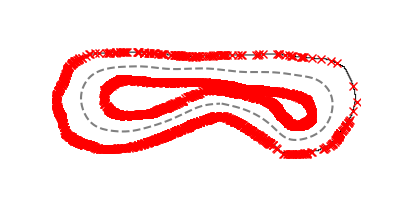
\includegraphics[height=.56\linewidth]{contents/chapt5/figs/observation/collision_distributions/crash_location_pose.png}
        \caption{Only pose}
    \end{subfigure}
    \hfill
    \begin{subfigure}[htb!]{0.45\textwidth}
        \centering
        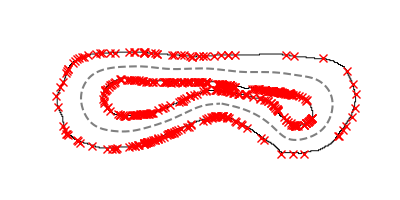
\includegraphics[height=.56\linewidth]{contents/chapt5/figs/observation/collision_distributions/crash_location_both.png}
        \caption{Pose and LiDAR}
    \end{subfigure}
    \hfill
\caption[Locations of crashes during training]{Crash locations of agents with (a) only the pose and (b) both the pose and LiDAR scan during training.}
\label{fig:collision_distribution}
\end{figure}

After determining that including the LiDAR scan in the observation improves training performance, we assessed agents utilising each observation space under evaluation conditions.
The agent that utilised both the LiDAR scan and pose in the observation did not crash during evaluation, whereas agents with either only a LiDAR scan or pose failed to complete laps $0.67\%$ and $6.00\%$ of the time, respectively.
Based on these results, both a LiDAR scan and the vehicle pose were included into the observation.


Given that a LiDAR scan is included in the observation, another parameter to consider is the number of LiDAR beams to include.
To determine the number of LiDAR beam that results in optimal performance, agents with LiDAR scans consisting of $5$, $10$, $20$ and $50$ were trained and tested.
These beams are equally spaced, and have a field of view of $180^{\circ}$.
As before, three agents with hyper-parameters from Table \ref{tab:inital_values} were trained for every value of $L$ LiDAR beams.
Figure \ref{fig:n_beams} displays the percentage failed laps and lap times during training, as well as the learning curves of these agents.
The results indicate that increasing the number of LiDAR beams above $20$ does not significantly impact the performance of agents in terms of any of the measured criteria. 
We therefore chose to incorporate $20$ LiDAR into the observation space.

\begin{figure}[htb!]
    \centering
    %% Creator: Matplotlib, PGF backend
%%
%% To include the figure in your LaTeX document, write
%%   \input{<filename>.pgf}
%%
%% Make sure the required packages are loaded in your preamble
%%   \usepackage{pgf}
%%
%% Also ensure that all the required font packages are loaded; for instance,
%% the lmodern package is sometimes necessary when using math font.
%%   \usepackage{lmodern}
%%
%% Figures using additional raster images can only be included by \input if
%% they are in the same directory as the main LaTeX file. For loading figures
%% from other directories you can use the `import` package
%%   \usepackage{import}
%%
%% and then include the figures with
%%   \import{<path to file>}{<filename>.pgf}
%%
%% Matplotlib used the following preamble
%%   \usepackage{fontspec}
%%   \setmainfont{DejaVuSerif.ttf}[Path=\detokenize{/home/andrew/anaconda3/envs/auto_car_env/lib/python3.9/site-packages/matplotlib/mpl-data/fonts/ttf/}]
%%   \setsansfont{DejaVuSans.ttf}[Path=\detokenize{/home/andrew/anaconda3/envs/auto_car_env/lib/python3.9/site-packages/matplotlib/mpl-data/fonts/ttf/}]
%%   \setmonofont{DejaVuSansMono.ttf}[Path=\detokenize{/home/andrew/anaconda3/envs/auto_car_env/lib/python3.9/site-packages/matplotlib/mpl-data/fonts/ttf/}]
%%
\begingroup%
\makeatletter%
\begin{pgfpicture}%
\pgfpathrectangle{\pgfpointorigin}{\pgfqpoint{5.500000in}{2.500000in}}%
\pgfusepath{use as bounding box, clip}%
\begin{pgfscope}%
\pgfsetbuttcap%
\pgfsetmiterjoin%
\definecolor{currentfill}{rgb}{1.000000,1.000000,1.000000}%
\pgfsetfillcolor{currentfill}%
\pgfsetlinewidth{0.000000pt}%
\definecolor{currentstroke}{rgb}{1.000000,1.000000,1.000000}%
\pgfsetstrokecolor{currentstroke}%
\pgfsetdash{}{0pt}%
\pgfpathmoveto{\pgfqpoint{0.000000in}{0.000000in}}%
\pgfpathlineto{\pgfqpoint{5.500000in}{0.000000in}}%
\pgfpathlineto{\pgfqpoint{5.500000in}{2.500000in}}%
\pgfpathlineto{\pgfqpoint{0.000000in}{2.500000in}}%
\pgfpathlineto{\pgfqpoint{0.000000in}{0.000000in}}%
\pgfpathclose%
\pgfusepath{fill}%
\end{pgfscope}%
\begin{pgfscope}%
\pgfsetbuttcap%
\pgfsetmiterjoin%
\definecolor{currentfill}{rgb}{1.000000,1.000000,1.000000}%
\pgfsetfillcolor{currentfill}%
\pgfsetlinewidth{0.000000pt}%
\definecolor{currentstroke}{rgb}{0.000000,0.000000,0.000000}%
\pgfsetstrokecolor{currentstroke}%
\pgfsetstrokeopacity{0.000000}%
\pgfsetdash{}{0pt}%
\pgfpathmoveto{\pgfqpoint{0.660417in}{1.000000in}}%
\pgfpathlineto{\pgfqpoint{1.810833in}{1.000000in}}%
\pgfpathlineto{\pgfqpoint{1.810833in}{2.156667in}}%
\pgfpathlineto{\pgfqpoint{0.660417in}{2.156667in}}%
\pgfpathlineto{\pgfqpoint{0.660417in}{1.000000in}}%
\pgfpathclose%
\pgfusepath{fill}%
\end{pgfscope}%
\begin{pgfscope}%
\pgfpathrectangle{\pgfqpoint{0.660417in}{1.000000in}}{\pgfqpoint{1.150417in}{1.156667in}}%
\pgfusepath{clip}%
\pgfsetbuttcap%
\pgfsetroundjoin%
\definecolor{currentfill}{rgb}{0.121569,0.466667,0.705882}%
\pgfsetfillcolor{currentfill}%
\pgfsetfillopacity{0.150000}%
\pgfsetlinewidth{0.000000pt}%
\definecolor{currentstroke}{rgb}{0.000000,0.000000,0.000000}%
\pgfsetstrokecolor{currentstroke}%
\pgfsetdash{}{0pt}%
\pgfpathmoveto{\pgfqpoint{0.660417in}{2.104091in}}%
\pgfpathlineto{\pgfqpoint{0.660417in}{2.104091in}}%
\pgfpathlineto{\pgfqpoint{0.685981in}{2.104091in}}%
\pgfpathlineto{\pgfqpoint{0.711546in}{2.219885in}}%
\pgfpathlineto{\pgfqpoint{0.737111in}{2.137315in}}%
\pgfpathlineto{\pgfqpoint{0.762676in}{2.036163in}}%
\pgfpathlineto{\pgfqpoint{0.788241in}{1.953442in}}%
\pgfpathlineto{\pgfqpoint{0.813806in}{1.670201in}}%
\pgfpathlineto{\pgfqpoint{0.839370in}{1.419609in}}%
\pgfpathlineto{\pgfqpoint{0.864935in}{1.353947in}}%
\pgfpathlineto{\pgfqpoint{0.890500in}{1.337382in}}%
\pgfpathlineto{\pgfqpoint{0.916065in}{1.311326in}}%
\pgfpathlineto{\pgfqpoint{0.941630in}{1.307086in}}%
\pgfpathlineto{\pgfqpoint{0.967194in}{1.303699in}}%
\pgfpathlineto{\pgfqpoint{0.992759in}{1.304124in}}%
\pgfpathlineto{\pgfqpoint{1.018324in}{1.284433in}}%
\pgfpathlineto{\pgfqpoint{1.043889in}{1.286712in}}%
\pgfpathlineto{\pgfqpoint{1.069454in}{1.307086in}}%
\pgfpathlineto{\pgfqpoint{1.095019in}{1.344713in}}%
\pgfpathlineto{\pgfqpoint{1.120583in}{1.379741in}}%
\pgfpathlineto{\pgfqpoint{1.146148in}{1.400447in}}%
\pgfpathlineto{\pgfqpoint{1.171713in}{1.393529in}}%
\pgfpathlineto{\pgfqpoint{1.197278in}{1.393550in}}%
\pgfpathlineto{\pgfqpoint{1.222843in}{1.354655in}}%
\pgfpathlineto{\pgfqpoint{1.248407in}{1.314867in}}%
\pgfpathlineto{\pgfqpoint{1.273972in}{1.284144in}}%
\pgfpathlineto{\pgfqpoint{1.299537in}{1.275139in}}%
\pgfpathlineto{\pgfqpoint{1.325102in}{1.251646in}}%
\pgfpathlineto{\pgfqpoint{1.350667in}{1.248277in}}%
\pgfpathlineto{\pgfqpoint{1.376231in}{1.239887in}}%
\pgfpathlineto{\pgfqpoint{1.401796in}{1.269615in}}%
\pgfpathlineto{\pgfqpoint{1.427361in}{1.331665in}}%
\pgfpathlineto{\pgfqpoint{1.452926in}{1.353730in}}%
\pgfpathlineto{\pgfqpoint{1.478491in}{1.379855in}}%
\pgfpathlineto{\pgfqpoint{1.504056in}{1.375803in}}%
\pgfpathlineto{\pgfqpoint{1.504056in}{0.972813in}}%
\pgfpathlineto{\pgfqpoint{1.504056in}{0.972813in}}%
\pgfpathlineto{\pgfqpoint{1.478491in}{0.977156in}}%
\pgfpathlineto{\pgfqpoint{1.452926in}{0.972499in}}%
\pgfpathlineto{\pgfqpoint{1.427361in}{0.972176in}}%
\pgfpathlineto{\pgfqpoint{1.401796in}{0.969862in}}%
\pgfpathlineto{\pgfqpoint{1.376231in}{0.974404in}}%
\pgfpathlineto{\pgfqpoint{1.350667in}{0.973010in}}%
\pgfpathlineto{\pgfqpoint{1.325102in}{0.975237in}}%
\pgfpathlineto{\pgfqpoint{1.299537in}{0.972733in}}%
\pgfpathlineto{\pgfqpoint{1.273972in}{0.970724in}}%
\pgfpathlineto{\pgfqpoint{1.248407in}{0.973583in}}%
\pgfpathlineto{\pgfqpoint{1.222843in}{0.982767in}}%
\pgfpathlineto{\pgfqpoint{1.197278in}{0.994244in}}%
\pgfpathlineto{\pgfqpoint{1.171713in}{0.990068in}}%
\pgfpathlineto{\pgfqpoint{1.146148in}{0.992944in}}%
\pgfpathlineto{\pgfqpoint{1.120583in}{0.987065in}}%
\pgfpathlineto{\pgfqpoint{1.095019in}{0.975918in}}%
\pgfpathlineto{\pgfqpoint{1.069454in}{0.972968in}}%
\pgfpathlineto{\pgfqpoint{1.043889in}{0.975153in}}%
\pgfpathlineto{\pgfqpoint{1.018324in}{0.974633in}}%
\pgfpathlineto{\pgfqpoint{0.992759in}{0.975930in}}%
\pgfpathlineto{\pgfqpoint{0.967194in}{0.977755in}}%
\pgfpathlineto{\pgfqpoint{0.941630in}{0.972968in}}%
\pgfpathlineto{\pgfqpoint{0.916065in}{0.974325in}}%
\pgfpathlineto{\pgfqpoint{0.890500in}{0.980451in}}%
\pgfpathlineto{\pgfqpoint{0.864935in}{0.976479in}}%
\pgfpathlineto{\pgfqpoint{0.839370in}{0.984976in}}%
\pgfpathlineto{\pgfqpoint{0.813806in}{0.997438in}}%
\pgfpathlineto{\pgfqpoint{0.788241in}{1.103180in}}%
\pgfpathlineto{\pgfqpoint{0.762676in}{1.179067in}}%
\pgfpathlineto{\pgfqpoint{0.737111in}{1.341909in}}%
\pgfpathlineto{\pgfqpoint{0.711546in}{1.674411in}}%
\pgfpathlineto{\pgfqpoint{0.685981in}{2.104091in}}%
\pgfpathlineto{\pgfqpoint{0.660417in}{2.104091in}}%
\pgfpathlineto{\pgfqpoint{0.660417in}{2.104091in}}%
\pgfpathclose%
\pgfusepath{fill}%
\end{pgfscope}%
\begin{pgfscope}%
\pgfpathrectangle{\pgfqpoint{0.660417in}{1.000000in}}{\pgfqpoint{1.150417in}{1.156667in}}%
\pgfusepath{clip}%
\pgfsetbuttcap%
\pgfsetroundjoin%
\definecolor{currentfill}{rgb}{1.000000,0.498039,0.054902}%
\pgfsetfillcolor{currentfill}%
\pgfsetfillopacity{0.150000}%
\pgfsetlinewidth{0.000000pt}%
\definecolor{currentstroke}{rgb}{0.000000,0.000000,0.000000}%
\pgfsetstrokecolor{currentstroke}%
\pgfsetdash{}{0pt}%
\pgfpathmoveto{\pgfqpoint{0.660417in}{2.104091in}}%
\pgfpathlineto{\pgfqpoint{0.660417in}{2.104091in}}%
\pgfpathlineto{\pgfqpoint{0.685981in}{2.104091in}}%
\pgfpathlineto{\pgfqpoint{0.711546in}{2.245104in}}%
\pgfpathlineto{\pgfqpoint{0.737111in}{2.077749in}}%
\pgfpathlineto{\pgfqpoint{0.762676in}{1.954398in}}%
\pgfpathlineto{\pgfqpoint{0.788241in}{1.871227in}}%
\pgfpathlineto{\pgfqpoint{0.813806in}{1.551597in}}%
\pgfpathlineto{\pgfqpoint{0.839370in}{1.379741in}}%
\pgfpathlineto{\pgfqpoint{0.864935in}{1.406404in}}%
\pgfpathlineto{\pgfqpoint{0.890500in}{1.405245in}}%
\pgfpathlineto{\pgfqpoint{0.916065in}{1.412691in}}%
\pgfpathlineto{\pgfqpoint{0.941630in}{1.407606in}}%
\pgfpathlineto{\pgfqpoint{0.967194in}{1.389021in}}%
\pgfpathlineto{\pgfqpoint{0.992759in}{1.350394in}}%
\pgfpathlineto{\pgfqpoint{1.018324in}{1.334855in}}%
\pgfpathlineto{\pgfqpoint{1.043889in}{1.297611in}}%
\pgfpathlineto{\pgfqpoint{1.069454in}{1.279377in}}%
\pgfpathlineto{\pgfqpoint{1.095019in}{1.262921in}}%
\pgfpathlineto{\pgfqpoint{1.120583in}{1.266092in}}%
\pgfpathlineto{\pgfqpoint{1.146148in}{1.278449in}}%
\pgfpathlineto{\pgfqpoint{1.171713in}{1.273761in}}%
\pgfpathlineto{\pgfqpoint{1.197278in}{1.256961in}}%
\pgfpathlineto{\pgfqpoint{1.222843in}{1.259454in}}%
\pgfpathlineto{\pgfqpoint{1.248407in}{1.245450in}}%
\pgfpathlineto{\pgfqpoint{1.273972in}{1.242824in}}%
\pgfpathlineto{\pgfqpoint{1.299537in}{1.242030in}}%
\pgfpathlineto{\pgfqpoint{1.325102in}{1.244666in}}%
\pgfpathlineto{\pgfqpoint{1.350667in}{1.236679in}}%
\pgfpathlineto{\pgfqpoint{1.376231in}{1.242030in}}%
\pgfpathlineto{\pgfqpoint{1.401796in}{1.246483in}}%
\pgfpathlineto{\pgfqpoint{1.427361in}{1.256714in}}%
\pgfpathlineto{\pgfqpoint{1.452926in}{1.275139in}}%
\pgfpathlineto{\pgfqpoint{1.478491in}{1.277491in}}%
\pgfpathlineto{\pgfqpoint{1.504056in}{1.283287in}}%
\pgfpathlineto{\pgfqpoint{1.529620in}{1.268265in}}%
\pgfpathlineto{\pgfqpoint{1.555185in}{1.261691in}}%
\pgfpathlineto{\pgfqpoint{1.580750in}{1.232857in}}%
\pgfpathlineto{\pgfqpoint{1.606315in}{1.241500in}}%
\pgfpathlineto{\pgfqpoint{1.631880in}{1.230665in}}%
\pgfpathlineto{\pgfqpoint{1.657444in}{1.234782in}}%
\pgfpathlineto{\pgfqpoint{1.683009in}{1.257967in}}%
\pgfpathlineto{\pgfqpoint{1.683009in}{0.975913in}}%
\pgfpathlineto{\pgfqpoint{1.683009in}{0.975913in}}%
\pgfpathlineto{\pgfqpoint{1.657444in}{0.978110in}}%
\pgfpathlineto{\pgfqpoint{1.631880in}{0.978029in}}%
\pgfpathlineto{\pgfqpoint{1.606315in}{0.978387in}}%
\pgfpathlineto{\pgfqpoint{1.580750in}{0.980035in}}%
\pgfpathlineto{\pgfqpoint{1.555185in}{0.976387in}}%
\pgfpathlineto{\pgfqpoint{1.529620in}{0.975409in}}%
\pgfpathlineto{\pgfqpoint{1.504056in}{0.974379in}}%
\pgfpathlineto{\pgfqpoint{1.478491in}{0.973180in}}%
\pgfpathlineto{\pgfqpoint{1.452926in}{0.972733in}}%
\pgfpathlineto{\pgfqpoint{1.427361in}{0.975767in}}%
\pgfpathlineto{\pgfqpoint{1.401796in}{0.974804in}}%
\pgfpathlineto{\pgfqpoint{1.376231in}{0.976458in}}%
\pgfpathlineto{\pgfqpoint{1.350667in}{0.976213in}}%
\pgfpathlineto{\pgfqpoint{1.325102in}{0.976621in}}%
\pgfpathlineto{\pgfqpoint{1.299537in}{0.976458in}}%
\pgfpathlineto{\pgfqpoint{1.273972in}{0.978463in}}%
\pgfpathlineto{\pgfqpoint{1.248407in}{0.978635in}}%
\pgfpathlineto{\pgfqpoint{1.222843in}{0.980023in}}%
\pgfpathlineto{\pgfqpoint{1.197278in}{0.979717in}}%
\pgfpathlineto{\pgfqpoint{1.171713in}{0.978309in}}%
\pgfpathlineto{\pgfqpoint{1.146148in}{0.979218in}}%
\pgfpathlineto{\pgfqpoint{1.120583in}{0.978982in}}%
\pgfpathlineto{\pgfqpoint{1.095019in}{0.976556in}}%
\pgfpathlineto{\pgfqpoint{1.069454in}{0.975491in}}%
\pgfpathlineto{\pgfqpoint{1.043889in}{0.974048in}}%
\pgfpathlineto{\pgfqpoint{1.018324in}{0.977382in}}%
\pgfpathlineto{\pgfqpoint{0.992759in}{0.978633in}}%
\pgfpathlineto{\pgfqpoint{0.967194in}{0.993177in}}%
\pgfpathlineto{\pgfqpoint{0.941630in}{0.998378in}}%
\pgfpathlineto{\pgfqpoint{0.916065in}{1.000289in}}%
\pgfpathlineto{\pgfqpoint{0.890500in}{0.992344in}}%
\pgfpathlineto{\pgfqpoint{0.864935in}{0.999580in}}%
\pgfpathlineto{\pgfqpoint{0.839370in}{0.987065in}}%
\pgfpathlineto{\pgfqpoint{0.813806in}{0.948135in}}%
\pgfpathlineto{\pgfqpoint{0.788241in}{0.988105in}}%
\pgfpathlineto{\pgfqpoint{0.762676in}{1.031823in}}%
\pgfpathlineto{\pgfqpoint{0.737111in}{1.119675in}}%
\pgfpathlineto{\pgfqpoint{0.711546in}{1.405060in}}%
\pgfpathlineto{\pgfqpoint{0.685981in}{2.104091in}}%
\pgfpathlineto{\pgfqpoint{0.660417in}{2.104091in}}%
\pgfpathlineto{\pgfqpoint{0.660417in}{2.104091in}}%
\pgfpathclose%
\pgfusepath{fill}%
\end{pgfscope}%
\begin{pgfscope}%
\pgfpathrectangle{\pgfqpoint{0.660417in}{1.000000in}}{\pgfqpoint{1.150417in}{1.156667in}}%
\pgfusepath{clip}%
\pgfsetbuttcap%
\pgfsetroundjoin%
\definecolor{currentfill}{rgb}{0.172549,0.627451,0.172549}%
\pgfsetfillcolor{currentfill}%
\pgfsetfillopacity{0.150000}%
\pgfsetlinewidth{0.000000pt}%
\definecolor{currentstroke}{rgb}{0.000000,0.000000,0.000000}%
\pgfsetstrokecolor{currentstroke}%
\pgfsetdash{}{0pt}%
\pgfpathmoveto{\pgfqpoint{0.660417in}{2.104091in}}%
\pgfpathlineto{\pgfqpoint{0.660417in}{2.104091in}}%
\pgfpathlineto{\pgfqpoint{0.685981in}{2.145982in}}%
\pgfpathlineto{\pgfqpoint{0.711546in}{2.142041in}}%
\pgfpathlineto{\pgfqpoint{0.737111in}{1.995399in}}%
\pgfpathlineto{\pgfqpoint{0.762676in}{1.895650in}}%
\pgfpathlineto{\pgfqpoint{0.788241in}{1.812224in}}%
\pgfpathlineto{\pgfqpoint{0.813806in}{1.453332in}}%
\pgfpathlineto{\pgfqpoint{0.839370in}{1.419259in}}%
\pgfpathlineto{\pgfqpoint{0.864935in}{1.375292in}}%
\pgfpathlineto{\pgfqpoint{0.890500in}{1.367096in}}%
\pgfpathlineto{\pgfqpoint{0.916065in}{1.400413in}}%
\pgfpathlineto{\pgfqpoint{0.941630in}{1.409600in}}%
\pgfpathlineto{\pgfqpoint{0.967194in}{1.408778in}}%
\pgfpathlineto{\pgfqpoint{0.992759in}{1.404400in}}%
\pgfpathlineto{\pgfqpoint{1.018324in}{1.385157in}}%
\pgfpathlineto{\pgfqpoint{1.043889in}{1.352805in}}%
\pgfpathlineto{\pgfqpoint{1.069454in}{1.324890in}}%
\pgfpathlineto{\pgfqpoint{1.095019in}{1.310500in}}%
\pgfpathlineto{\pgfqpoint{1.120583in}{1.304124in}}%
\pgfpathlineto{\pgfqpoint{1.146148in}{1.309864in}}%
\pgfpathlineto{\pgfqpoint{1.171713in}{1.294712in}}%
\pgfpathlineto{\pgfqpoint{1.197278in}{1.295408in}}%
\pgfpathlineto{\pgfqpoint{1.222843in}{1.269468in}}%
\pgfpathlineto{\pgfqpoint{1.248407in}{1.282137in}}%
\pgfpathlineto{\pgfqpoint{1.273972in}{1.274232in}}%
\pgfpathlineto{\pgfqpoint{1.299537in}{1.291886in}}%
\pgfpathlineto{\pgfqpoint{1.325102in}{1.283988in}}%
\pgfpathlineto{\pgfqpoint{1.350667in}{1.294984in}}%
\pgfpathlineto{\pgfqpoint{1.376231in}{1.293443in}}%
\pgfpathlineto{\pgfqpoint{1.401796in}{1.278659in}}%
\pgfpathlineto{\pgfqpoint{1.427361in}{1.274393in}}%
\pgfpathlineto{\pgfqpoint{1.452926in}{1.282571in}}%
\pgfpathlineto{\pgfqpoint{1.478491in}{1.282137in}}%
\pgfpathlineto{\pgfqpoint{1.504056in}{1.296924in}}%
\pgfpathlineto{\pgfqpoint{1.529620in}{1.305339in}}%
\pgfpathlineto{\pgfqpoint{1.555185in}{1.304539in}}%
\pgfpathlineto{\pgfqpoint{1.580750in}{1.308390in}}%
\pgfpathlineto{\pgfqpoint{1.606315in}{1.310271in}}%
\pgfpathlineto{\pgfqpoint{1.631880in}{1.306412in}}%
\pgfpathlineto{\pgfqpoint{1.657444in}{1.302096in}}%
\pgfpathlineto{\pgfqpoint{1.683009in}{1.299200in}}%
\pgfpathlineto{\pgfqpoint{1.708574in}{1.291782in}}%
\pgfpathlineto{\pgfqpoint{1.734139in}{1.296257in}}%
\pgfpathlineto{\pgfqpoint{1.759704in}{1.286871in}}%
\pgfpathlineto{\pgfqpoint{1.785269in}{1.298471in}}%
\pgfpathlineto{\pgfqpoint{1.810833in}{1.288013in}}%
\pgfpathlineto{\pgfqpoint{1.836398in}{1.277990in}}%
\pgfpathlineto{\pgfqpoint{1.861963in}{1.259819in}}%
\pgfpathlineto{\pgfqpoint{1.861963in}{0.968464in}}%
\pgfpathlineto{\pgfqpoint{1.861963in}{0.968464in}}%
\pgfpathlineto{\pgfqpoint{1.836398in}{0.965684in}}%
\pgfpathlineto{\pgfqpoint{1.810833in}{0.964057in}}%
\pgfpathlineto{\pgfqpoint{1.785269in}{0.964793in}}%
\pgfpathlineto{\pgfqpoint{1.759704in}{0.963799in}}%
\pgfpathlineto{\pgfqpoint{1.734139in}{0.964208in}}%
\pgfpathlineto{\pgfqpoint{1.708574in}{0.963087in}}%
\pgfpathlineto{\pgfqpoint{1.683009in}{0.966862in}}%
\pgfpathlineto{\pgfqpoint{1.657444in}{0.969563in}}%
\pgfpathlineto{\pgfqpoint{1.631880in}{0.970844in}}%
\pgfpathlineto{\pgfqpoint{1.606315in}{0.973980in}}%
\pgfpathlineto{\pgfqpoint{1.580750in}{0.977261in}}%
\pgfpathlineto{\pgfqpoint{1.555185in}{0.974116in}}%
\pgfpathlineto{\pgfqpoint{1.529620in}{0.970518in}}%
\pgfpathlineto{\pgfqpoint{1.504056in}{0.971937in}}%
\pgfpathlineto{\pgfqpoint{1.478491in}{0.974130in}}%
\pgfpathlineto{\pgfqpoint{1.452926in}{0.972297in}}%
\pgfpathlineto{\pgfqpoint{1.427361in}{0.970681in}}%
\pgfpathlineto{\pgfqpoint{1.401796in}{0.973411in}}%
\pgfpathlineto{\pgfqpoint{1.376231in}{0.976817in}}%
\pgfpathlineto{\pgfqpoint{1.350667in}{0.975275in}}%
\pgfpathlineto{\pgfqpoint{1.325102in}{0.976477in}}%
\pgfpathlineto{\pgfqpoint{1.299537in}{0.978373in}}%
\pgfpathlineto{\pgfqpoint{1.273972in}{0.976438in}}%
\pgfpathlineto{\pgfqpoint{1.248407in}{0.974130in}}%
\pgfpathlineto{\pgfqpoint{1.222843in}{0.975605in}}%
\pgfpathlineto{\pgfqpoint{1.197278in}{0.973453in}}%
\pgfpathlineto{\pgfqpoint{1.171713in}{0.971350in}}%
\pgfpathlineto{\pgfqpoint{1.146148in}{0.975787in}}%
\pgfpathlineto{\pgfqpoint{1.120583in}{0.975930in}}%
\pgfpathlineto{\pgfqpoint{1.095019in}{0.977950in}}%
\pgfpathlineto{\pgfqpoint{1.069454in}{0.973354in}}%
\pgfpathlineto{\pgfqpoint{1.043889in}{0.981819in}}%
\pgfpathlineto{\pgfqpoint{1.018324in}{0.984447in}}%
\pgfpathlineto{\pgfqpoint{0.992759in}{0.987592in}}%
\pgfpathlineto{\pgfqpoint{0.967194in}{0.988811in}}%
\pgfpathlineto{\pgfqpoint{0.941630in}{0.993586in}}%
\pgfpathlineto{\pgfqpoint{0.916065in}{0.988780in}}%
\pgfpathlineto{\pgfqpoint{0.890500in}{0.981520in}}%
\pgfpathlineto{\pgfqpoint{0.864935in}{0.980320in}}%
\pgfpathlineto{\pgfqpoint{0.839370in}{0.986725in}}%
\pgfpathlineto{\pgfqpoint{0.813806in}{0.991830in}}%
\pgfpathlineto{\pgfqpoint{0.788241in}{0.996736in}}%
\pgfpathlineto{\pgfqpoint{0.762676in}{1.052112in}}%
\pgfpathlineto{\pgfqpoint{0.737111in}{1.122840in}}%
\pgfpathlineto{\pgfqpoint{0.711546in}{1.253527in}}%
\pgfpathlineto{\pgfqpoint{0.685981in}{2.048318in}}%
\pgfpathlineto{\pgfqpoint{0.660417in}{2.104091in}}%
\pgfpathlineto{\pgfqpoint{0.660417in}{2.104091in}}%
\pgfpathclose%
\pgfusepath{fill}%
\end{pgfscope}%
\begin{pgfscope}%
\pgfpathrectangle{\pgfqpoint{0.660417in}{1.000000in}}{\pgfqpoint{1.150417in}{1.156667in}}%
\pgfusepath{clip}%
\pgfsetbuttcap%
\pgfsetroundjoin%
\definecolor{currentfill}{rgb}{0.839216,0.152941,0.156863}%
\pgfsetfillcolor{currentfill}%
\pgfsetfillopacity{0.150000}%
\pgfsetlinewidth{0.000000pt}%
\definecolor{currentstroke}{rgb}{0.000000,0.000000,0.000000}%
\pgfsetstrokecolor{currentstroke}%
\pgfsetdash{}{0pt}%
\pgfpathmoveto{\pgfqpoint{0.660417in}{2.104091in}}%
\pgfpathlineto{\pgfqpoint{0.660417in}{2.104091in}}%
\pgfpathlineto{\pgfqpoint{0.685981in}{2.153184in}}%
\pgfpathlineto{\pgfqpoint{0.711546in}{2.160647in}}%
\pgfpathlineto{\pgfqpoint{0.737111in}{2.015338in}}%
\pgfpathlineto{\pgfqpoint{0.762676in}{1.908220in}}%
\pgfpathlineto{\pgfqpoint{0.788241in}{1.843966in}}%
\pgfpathlineto{\pgfqpoint{0.813806in}{1.526733in}}%
\pgfpathlineto{\pgfqpoint{0.839370in}{1.456883in}}%
\pgfpathlineto{\pgfqpoint{0.864935in}{1.469035in}}%
\pgfpathlineto{\pgfqpoint{0.890500in}{1.482482in}}%
\pgfpathlineto{\pgfqpoint{0.916065in}{1.472939in}}%
\pgfpathlineto{\pgfqpoint{0.941630in}{1.461576in}}%
\pgfpathlineto{\pgfqpoint{0.967194in}{1.449627in}}%
\pgfpathlineto{\pgfqpoint{0.992759in}{1.442045in}}%
\pgfpathlineto{\pgfqpoint{1.018324in}{1.445296in}}%
\pgfpathlineto{\pgfqpoint{1.043889in}{1.449500in}}%
\pgfpathlineto{\pgfqpoint{1.069454in}{1.462511in}}%
\pgfpathlineto{\pgfqpoint{1.095019in}{1.450326in}}%
\pgfpathlineto{\pgfqpoint{1.120583in}{1.428072in}}%
\pgfpathlineto{\pgfqpoint{1.146148in}{1.389281in}}%
\pgfpathlineto{\pgfqpoint{1.171713in}{1.347940in}}%
\pgfpathlineto{\pgfqpoint{1.197278in}{1.312377in}}%
\pgfpathlineto{\pgfqpoint{1.222843in}{1.297187in}}%
\pgfpathlineto{\pgfqpoint{1.248407in}{1.303463in}}%
\pgfpathlineto{\pgfqpoint{1.273972in}{1.306412in}}%
\pgfpathlineto{\pgfqpoint{1.299537in}{1.328372in}}%
\pgfpathlineto{\pgfqpoint{1.325102in}{1.317717in}}%
\pgfpathlineto{\pgfqpoint{1.350667in}{1.314591in}}%
\pgfpathlineto{\pgfqpoint{1.376231in}{1.306017in}}%
\pgfpathlineto{\pgfqpoint{1.401796in}{1.301299in}}%
\pgfpathlineto{\pgfqpoint{1.427361in}{1.264146in}}%
\pgfpathlineto{\pgfqpoint{1.452926in}{1.251646in}}%
\pgfpathlineto{\pgfqpoint{1.478491in}{1.249569in}}%
\pgfpathlineto{\pgfqpoint{1.504056in}{1.238027in}}%
\pgfpathlineto{\pgfqpoint{1.529620in}{1.242545in}}%
\pgfpathlineto{\pgfqpoint{1.555185in}{1.248277in}}%
\pgfpathlineto{\pgfqpoint{1.580750in}{1.266306in}}%
\pgfpathlineto{\pgfqpoint{1.606315in}{1.275139in}}%
\pgfpathlineto{\pgfqpoint{1.631880in}{1.290240in}}%
\pgfpathlineto{\pgfqpoint{1.657444in}{1.281839in}}%
\pgfpathlineto{\pgfqpoint{1.683009in}{1.275575in}}%
\pgfpathlineto{\pgfqpoint{1.708574in}{1.264318in}}%
\pgfpathlineto{\pgfqpoint{1.734139in}{1.261857in}}%
\pgfpathlineto{\pgfqpoint{1.759704in}{1.248382in}}%
\pgfpathlineto{\pgfqpoint{1.785269in}{1.247082in}}%
\pgfpathlineto{\pgfqpoint{1.785269in}{0.967209in}}%
\pgfpathlineto{\pgfqpoint{1.785269in}{0.967209in}}%
\pgfpathlineto{\pgfqpoint{1.759704in}{0.967309in}}%
\pgfpathlineto{\pgfqpoint{1.734139in}{0.970624in}}%
\pgfpathlineto{\pgfqpoint{1.708574in}{0.970961in}}%
\pgfpathlineto{\pgfqpoint{1.683009in}{0.970898in}}%
\pgfpathlineto{\pgfqpoint{1.657444in}{0.970230in}}%
\pgfpathlineto{\pgfqpoint{1.631880in}{0.970225in}}%
\pgfpathlineto{\pgfqpoint{1.606315in}{0.972733in}}%
\pgfpathlineto{\pgfqpoint{1.580750in}{0.973170in}}%
\pgfpathlineto{\pgfqpoint{1.555185in}{0.973010in}}%
\pgfpathlineto{\pgfqpoint{1.529620in}{0.974544in}}%
\pgfpathlineto{\pgfqpoint{1.504056in}{0.976264in}}%
\pgfpathlineto{\pgfqpoint{1.478491in}{0.973117in}}%
\pgfpathlineto{\pgfqpoint{1.452926in}{0.975237in}}%
\pgfpathlineto{\pgfqpoint{1.427361in}{0.976730in}}%
\pgfpathlineto{\pgfqpoint{1.401796in}{0.973158in}}%
\pgfpathlineto{\pgfqpoint{1.376231in}{0.972638in}}%
\pgfpathlineto{\pgfqpoint{1.350667in}{0.969661in}}%
\pgfpathlineto{\pgfqpoint{1.325102in}{0.970733in}}%
\pgfpathlineto{\pgfqpoint{1.299537in}{0.967074in}}%
\pgfpathlineto{\pgfqpoint{1.273972in}{0.970844in}}%
\pgfpathlineto{\pgfqpoint{1.248407in}{0.973793in}}%
\pgfpathlineto{\pgfqpoint{1.222843in}{0.975871in}}%
\pgfpathlineto{\pgfqpoint{1.197278in}{0.974674in}}%
\pgfpathlineto{\pgfqpoint{1.171713in}{0.975490in}}%
\pgfpathlineto{\pgfqpoint{1.146148in}{0.983121in}}%
\pgfpathlineto{\pgfqpoint{1.120583in}{0.991905in}}%
\pgfpathlineto{\pgfqpoint{1.095019in}{1.006030in}}%
\pgfpathlineto{\pgfqpoint{1.069454in}{1.012035in}}%
\pgfpathlineto{\pgfqpoint{1.043889in}{1.009655in}}%
\pgfpathlineto{\pgfqpoint{1.018324in}{1.005464in}}%
\pgfpathlineto{\pgfqpoint{0.992759in}{1.004516in}}%
\pgfpathlineto{\pgfqpoint{0.967194in}{1.005330in}}%
\pgfpathlineto{\pgfqpoint{0.941630in}{1.008773in}}%
\pgfpathlineto{\pgfqpoint{0.916065in}{1.010002in}}%
\pgfpathlineto{\pgfqpoint{0.890500in}{1.007455in}}%
\pgfpathlineto{\pgfqpoint{0.864935in}{1.001314in}}%
\pgfpathlineto{\pgfqpoint{0.839370in}{0.995276in}}%
\pgfpathlineto{\pgfqpoint{0.813806in}{1.005181in}}%
\pgfpathlineto{\pgfqpoint{0.788241in}{1.030757in}}%
\pgfpathlineto{\pgfqpoint{0.762676in}{1.062268in}}%
\pgfpathlineto{\pgfqpoint{0.737111in}{1.149480in}}%
\pgfpathlineto{\pgfqpoint{0.711546in}{1.377913in}}%
\pgfpathlineto{\pgfqpoint{0.685981in}{2.034176in}}%
\pgfpathlineto{\pgfqpoint{0.660417in}{2.104091in}}%
\pgfpathlineto{\pgfqpoint{0.660417in}{2.104091in}}%
\pgfpathclose%
\pgfusepath{fill}%
\end{pgfscope}%
\begin{pgfscope}%
\pgfpathrectangle{\pgfqpoint{0.660417in}{1.000000in}}{\pgfqpoint{1.150417in}{1.156667in}}%
\pgfusepath{clip}%
\pgfsetrectcap%
\pgfsetroundjoin%
\pgfsetlinewidth{0.803000pt}%
\definecolor{currentstroke}{rgb}{0.690196,0.690196,0.690196}%
\pgfsetstrokecolor{currentstroke}%
\pgfsetdash{}{0pt}%
\pgfpathmoveto{\pgfqpoint{0.660417in}{1.000000in}}%
\pgfpathlineto{\pgfqpoint{0.660417in}{2.156667in}}%
\pgfusepath{stroke}%
\end{pgfscope}%
\begin{pgfscope}%
\definecolor{textcolor}{rgb}{0.000000,0.000000,0.000000}%
\pgfsetstrokecolor{textcolor}%
\pgfsetfillcolor{textcolor}%
\pgftext[x=0.660417in,y=0.951389in,,top]{\color{textcolor}\rmfamily\fontsize{10.000000}{12.000000}\selectfont 0}%
\end{pgfscope}%
\begin{pgfscope}%
\pgfpathrectangle{\pgfqpoint{0.660417in}{1.000000in}}{\pgfqpoint{1.150417in}{1.156667in}}%
\pgfusepath{clip}%
\pgfsetrectcap%
\pgfsetroundjoin%
\pgfsetlinewidth{0.803000pt}%
\definecolor{currentstroke}{rgb}{0.690196,0.690196,0.690196}%
\pgfsetstrokecolor{currentstroke}%
\pgfsetdash{}{0pt}%
\pgfpathmoveto{\pgfqpoint{0.916065in}{1.000000in}}%
\pgfpathlineto{\pgfqpoint{0.916065in}{2.156667in}}%
\pgfusepath{stroke}%
\end{pgfscope}%
\begin{pgfscope}%
\definecolor{textcolor}{rgb}{0.000000,0.000000,0.000000}%
\pgfsetstrokecolor{textcolor}%
\pgfsetfillcolor{textcolor}%
\pgftext[x=0.916065in,y=0.951389in,,top]{\color{textcolor}\rmfamily\fontsize{10.000000}{12.000000}\selectfont 1}%
\end{pgfscope}%
\begin{pgfscope}%
\pgfpathrectangle{\pgfqpoint{0.660417in}{1.000000in}}{\pgfqpoint{1.150417in}{1.156667in}}%
\pgfusepath{clip}%
\pgfsetrectcap%
\pgfsetroundjoin%
\pgfsetlinewidth{0.803000pt}%
\definecolor{currentstroke}{rgb}{0.690196,0.690196,0.690196}%
\pgfsetstrokecolor{currentstroke}%
\pgfsetdash{}{0pt}%
\pgfpathmoveto{\pgfqpoint{1.171713in}{1.000000in}}%
\pgfpathlineto{\pgfqpoint{1.171713in}{2.156667in}}%
\pgfusepath{stroke}%
\end{pgfscope}%
\begin{pgfscope}%
\definecolor{textcolor}{rgb}{0.000000,0.000000,0.000000}%
\pgfsetstrokecolor{textcolor}%
\pgfsetfillcolor{textcolor}%
\pgftext[x=1.171713in,y=0.951389in,,top]{\color{textcolor}\rmfamily\fontsize{10.000000}{12.000000}\selectfont 2}%
\end{pgfscope}%
\begin{pgfscope}%
\pgfpathrectangle{\pgfqpoint{0.660417in}{1.000000in}}{\pgfqpoint{1.150417in}{1.156667in}}%
\pgfusepath{clip}%
\pgfsetrectcap%
\pgfsetroundjoin%
\pgfsetlinewidth{0.803000pt}%
\definecolor{currentstroke}{rgb}{0.690196,0.690196,0.690196}%
\pgfsetstrokecolor{currentstroke}%
\pgfsetdash{}{0pt}%
\pgfpathmoveto{\pgfqpoint{1.427361in}{1.000000in}}%
\pgfpathlineto{\pgfqpoint{1.427361in}{2.156667in}}%
\pgfusepath{stroke}%
\end{pgfscope}%
\begin{pgfscope}%
\definecolor{textcolor}{rgb}{0.000000,0.000000,0.000000}%
\pgfsetstrokecolor{textcolor}%
\pgfsetfillcolor{textcolor}%
\pgftext[x=1.427361in,y=0.951389in,,top]{\color{textcolor}\rmfamily\fontsize{10.000000}{12.000000}\selectfont 3}%
\end{pgfscope}%
\begin{pgfscope}%
\pgfpathrectangle{\pgfqpoint{0.660417in}{1.000000in}}{\pgfqpoint{1.150417in}{1.156667in}}%
\pgfusepath{clip}%
\pgfsetrectcap%
\pgfsetroundjoin%
\pgfsetlinewidth{0.803000pt}%
\definecolor{currentstroke}{rgb}{0.690196,0.690196,0.690196}%
\pgfsetstrokecolor{currentstroke}%
\pgfsetdash{}{0pt}%
\pgfpathmoveto{\pgfqpoint{1.683009in}{1.000000in}}%
\pgfpathlineto{\pgfqpoint{1.683009in}{2.156667in}}%
\pgfusepath{stroke}%
\end{pgfscope}%
\begin{pgfscope}%
\definecolor{textcolor}{rgb}{0.000000,0.000000,0.000000}%
\pgfsetstrokecolor{textcolor}%
\pgfsetfillcolor{textcolor}%
\pgftext[x=1.683009in,y=0.951389in,,top]{\color{textcolor}\rmfamily\fontsize{10.000000}{12.000000}\selectfont 4}%
\end{pgfscope}%
\begin{pgfscope}%
\pgfpathrectangle{\pgfqpoint{0.660417in}{1.000000in}}{\pgfqpoint{1.150417in}{1.156667in}}%
\pgfusepath{clip}%
\pgfsetrectcap%
\pgfsetroundjoin%
\pgfsetlinewidth{0.803000pt}%
\definecolor{currentstroke}{rgb}{0.690196,0.690196,0.690196}%
\pgfsetstrokecolor{currentstroke}%
\pgfsetdash{}{0pt}%
\pgfpathmoveto{\pgfqpoint{0.660417in}{1.052576in}}%
\pgfpathlineto{\pgfqpoint{1.810833in}{1.052576in}}%
\pgfusepath{stroke}%
\end{pgfscope}%
\begin{pgfscope}%
\definecolor{textcolor}{rgb}{0.000000,0.000000,0.000000}%
\pgfsetstrokecolor{textcolor}%
\pgfsetfillcolor{textcolor}%
\pgftext[x=0.523440in, y=0.999814in, left, base]{\color{textcolor}\rmfamily\fontsize{10.000000}{12.000000}\selectfont 0}%
\end{pgfscope}%
\begin{pgfscope}%
\pgfpathrectangle{\pgfqpoint{0.660417in}{1.000000in}}{\pgfqpoint{1.150417in}{1.156667in}}%
\pgfusepath{clip}%
\pgfsetrectcap%
\pgfsetroundjoin%
\pgfsetlinewidth{0.803000pt}%
\definecolor{currentstroke}{rgb}{0.690196,0.690196,0.690196}%
\pgfsetstrokecolor{currentstroke}%
\pgfsetdash{}{0pt}%
\pgfpathmoveto{\pgfqpoint{0.660417in}{1.315455in}}%
\pgfpathlineto{\pgfqpoint{1.810833in}{1.315455in}}%
\pgfusepath{stroke}%
\end{pgfscope}%
\begin{pgfscope}%
\definecolor{textcolor}{rgb}{0.000000,0.000000,0.000000}%
\pgfsetstrokecolor{textcolor}%
\pgfsetfillcolor{textcolor}%
\pgftext[x=0.435075in, y=1.262693in, left, base]{\color{textcolor}\rmfamily\fontsize{10.000000}{12.000000}\selectfont 25}%
\end{pgfscope}%
\begin{pgfscope}%
\pgfpathrectangle{\pgfqpoint{0.660417in}{1.000000in}}{\pgfqpoint{1.150417in}{1.156667in}}%
\pgfusepath{clip}%
\pgfsetrectcap%
\pgfsetroundjoin%
\pgfsetlinewidth{0.803000pt}%
\definecolor{currentstroke}{rgb}{0.690196,0.690196,0.690196}%
\pgfsetstrokecolor{currentstroke}%
\pgfsetdash{}{0pt}%
\pgfpathmoveto{\pgfqpoint{0.660417in}{1.578333in}}%
\pgfpathlineto{\pgfqpoint{1.810833in}{1.578333in}}%
\pgfusepath{stroke}%
\end{pgfscope}%
\begin{pgfscope}%
\definecolor{textcolor}{rgb}{0.000000,0.000000,0.000000}%
\pgfsetstrokecolor{textcolor}%
\pgfsetfillcolor{textcolor}%
\pgftext[x=0.435075in, y=1.525572in, left, base]{\color{textcolor}\rmfamily\fontsize{10.000000}{12.000000}\selectfont 50}%
\end{pgfscope}%
\begin{pgfscope}%
\pgfpathrectangle{\pgfqpoint{0.660417in}{1.000000in}}{\pgfqpoint{1.150417in}{1.156667in}}%
\pgfusepath{clip}%
\pgfsetrectcap%
\pgfsetroundjoin%
\pgfsetlinewidth{0.803000pt}%
\definecolor{currentstroke}{rgb}{0.690196,0.690196,0.690196}%
\pgfsetstrokecolor{currentstroke}%
\pgfsetdash{}{0pt}%
\pgfpathmoveto{\pgfqpoint{0.660417in}{1.841212in}}%
\pgfpathlineto{\pgfqpoint{1.810833in}{1.841212in}}%
\pgfusepath{stroke}%
\end{pgfscope}%
\begin{pgfscope}%
\definecolor{textcolor}{rgb}{0.000000,0.000000,0.000000}%
\pgfsetstrokecolor{textcolor}%
\pgfsetfillcolor{textcolor}%
\pgftext[x=0.435075in, y=1.788451in, left, base]{\color{textcolor}\rmfamily\fontsize{10.000000}{12.000000}\selectfont 75}%
\end{pgfscope}%
\begin{pgfscope}%
\pgfpathrectangle{\pgfqpoint{0.660417in}{1.000000in}}{\pgfqpoint{1.150417in}{1.156667in}}%
\pgfusepath{clip}%
\pgfsetrectcap%
\pgfsetroundjoin%
\pgfsetlinewidth{0.803000pt}%
\definecolor{currentstroke}{rgb}{0.690196,0.690196,0.690196}%
\pgfsetstrokecolor{currentstroke}%
\pgfsetdash{}{0pt}%
\pgfpathmoveto{\pgfqpoint{0.660417in}{2.104091in}}%
\pgfpathlineto{\pgfqpoint{1.810833in}{2.104091in}}%
\pgfusepath{stroke}%
\end{pgfscope}%
\begin{pgfscope}%
\definecolor{textcolor}{rgb}{0.000000,0.000000,0.000000}%
\pgfsetstrokecolor{textcolor}%
\pgfsetfillcolor{textcolor}%
\pgftext[x=0.346710in, y=2.051329in, left, base]{\color{textcolor}\rmfamily\fontsize{10.000000}{12.000000}\selectfont 100}%
\end{pgfscope}%
\begin{pgfscope}%
\definecolor{textcolor}{rgb}{0.000000,0.000000,0.000000}%
\pgfsetstrokecolor{textcolor}%
\pgfsetfillcolor{textcolor}%
\pgftext[x=0.291154in,y=1.578333in,,bottom,rotate=90.000000]{\color{textcolor}\rmfamily\fontsize{10.000000}{12.000000}\selectfont Failed laps [\%]}%
\end{pgfscope}%
\begin{pgfscope}%
\pgfpathrectangle{\pgfqpoint{0.660417in}{1.000000in}}{\pgfqpoint{1.150417in}{1.156667in}}%
\pgfusepath{clip}%
\pgfsetrectcap%
\pgfsetroundjoin%
\pgfsetlinewidth{1.505625pt}%
\definecolor{currentstroke}{rgb}{0.121569,0.466667,0.705882}%
\pgfsetstrokecolor{currentstroke}%
\pgfsetdash{}{0pt}%
\pgfpathmoveto{\pgfqpoint{0.660417in}{2.104091in}}%
\pgfpathlineto{\pgfqpoint{0.685981in}{2.104091in}}%
\pgfpathlineto{\pgfqpoint{0.711546in}{1.947148in}}%
\pgfpathlineto{\pgfqpoint{0.737111in}{1.739612in}}%
\pgfpathlineto{\pgfqpoint{0.762676in}{1.607615in}}%
\pgfpathlineto{\pgfqpoint{0.788241in}{1.528311in}}%
\pgfpathlineto{\pgfqpoint{0.813806in}{1.333819in}}%
\pgfpathlineto{\pgfqpoint{0.839370in}{1.202292in}}%
\pgfpathlineto{\pgfqpoint{0.864935in}{1.165213in}}%
\pgfpathlineto{\pgfqpoint{0.890500in}{1.158917in}}%
\pgfpathlineto{\pgfqpoint{0.916065in}{1.142826in}}%
\pgfpathlineto{\pgfqpoint{0.941630in}{1.140027in}}%
\pgfpathlineto{\pgfqpoint{0.967194in}{1.140727in}}%
\pgfpathlineto{\pgfqpoint{0.992759in}{1.140027in}}%
\pgfpathlineto{\pgfqpoint{1.018324in}{1.129533in}}%
\pgfpathlineto{\pgfqpoint{1.043889in}{1.130932in}}%
\pgfpathlineto{\pgfqpoint{1.069454in}{1.140027in}}%
\pgfpathlineto{\pgfqpoint{1.095019in}{1.160316in}}%
\pgfpathlineto{\pgfqpoint{1.120583in}{1.183403in}}%
\pgfpathlineto{\pgfqpoint{1.146148in}{1.196696in}}%
\pgfpathlineto{\pgfqpoint{1.171713in}{1.191798in}}%
\pgfpathlineto{\pgfqpoint{1.197278in}{1.193897in}}%
\pgfpathlineto{\pgfqpoint{1.222843in}{1.168711in}}%
\pgfpathlineto{\pgfqpoint{1.248407in}{1.144225in}}%
\pgfpathlineto{\pgfqpoint{1.273972in}{1.127434in}}%
\pgfpathlineto{\pgfqpoint{1.299537in}{1.123936in}}%
\pgfpathlineto{\pgfqpoint{1.325102in}{1.113442in}}%
\pgfpathlineto{\pgfqpoint{1.350667in}{1.110643in}}%
\pgfpathlineto{\pgfqpoint{1.376231in}{1.107145in}}%
\pgfpathlineto{\pgfqpoint{1.401796in}{1.119738in}}%
\pgfpathlineto{\pgfqpoint{1.427361in}{1.151921in}}%
\pgfpathlineto{\pgfqpoint{1.452926in}{1.163114in}}%
\pgfpathlineto{\pgfqpoint{1.478491in}{1.178506in}}%
\pgfpathlineto{\pgfqpoint{1.504056in}{1.174308in}}%
\pgfusepath{stroke}%
\end{pgfscope}%
\begin{pgfscope}%
\pgfpathrectangle{\pgfqpoint{0.660417in}{1.000000in}}{\pgfqpoint{1.150417in}{1.156667in}}%
\pgfusepath{clip}%
\pgfsetrectcap%
\pgfsetroundjoin%
\pgfsetlinewidth{1.505625pt}%
\definecolor{currentstroke}{rgb}{1.000000,0.498039,0.054902}%
\pgfsetstrokecolor{currentstroke}%
\pgfsetdash{}{0pt}%
\pgfpathmoveto{\pgfqpoint{0.660417in}{2.104091in}}%
\pgfpathlineto{\pgfqpoint{0.685981in}{2.104091in}}%
\pgfpathlineto{\pgfqpoint{0.711546in}{1.825082in}}%
\pgfpathlineto{\pgfqpoint{0.737111in}{1.598712in}}%
\pgfpathlineto{\pgfqpoint{0.762676in}{1.493111in}}%
\pgfpathlineto{\pgfqpoint{0.788241in}{1.429666in}}%
\pgfpathlineto{\pgfqpoint{0.813806in}{1.249866in}}%
\pgfpathlineto{\pgfqpoint{0.839370in}{1.183403in}}%
\pgfpathlineto{\pgfqpoint{0.864935in}{1.202992in}}%
\pgfpathlineto{\pgfqpoint{0.890500in}{1.198794in}}%
\pgfpathlineto{\pgfqpoint{0.916065in}{1.206490in}}%
\pgfpathlineto{\pgfqpoint{0.941630in}{1.202992in}}%
\pgfpathlineto{\pgfqpoint{0.967194in}{1.191099in}}%
\pgfpathlineto{\pgfqpoint{0.992759in}{1.164513in}}%
\pgfpathlineto{\pgfqpoint{1.018324in}{1.156118in}}%
\pgfpathlineto{\pgfqpoint{1.043889in}{1.135829in}}%
\pgfpathlineto{\pgfqpoint{1.069454in}{1.127434in}}%
\pgfpathlineto{\pgfqpoint{1.095019in}{1.119738in}}%
\pgfpathlineto{\pgfqpoint{1.120583in}{1.122537in}}%
\pgfpathlineto{\pgfqpoint{1.146148in}{1.128833in}}%
\pgfpathlineto{\pgfqpoint{1.171713in}{1.126035in}}%
\pgfpathlineto{\pgfqpoint{1.197278in}{1.118339in}}%
\pgfpathlineto{\pgfqpoint{1.222843in}{1.119738in}}%
\pgfpathlineto{\pgfqpoint{1.248407in}{1.112043in}}%
\pgfpathlineto{\pgfqpoint{1.273972in}{1.110643in}}%
\pgfpathlineto{\pgfqpoint{1.299537in}{1.109244in}}%
\pgfpathlineto{\pgfqpoint{1.325102in}{1.110643in}}%
\pgfpathlineto{\pgfqpoint{1.350667in}{1.106446in}}%
\pgfpathlineto{\pgfqpoint{1.376231in}{1.109244in}}%
\pgfpathlineto{\pgfqpoint{1.401796in}{1.110643in}}%
\pgfpathlineto{\pgfqpoint{1.427361in}{1.116240in}}%
\pgfpathlineto{\pgfqpoint{1.452926in}{1.123936in}}%
\pgfpathlineto{\pgfqpoint{1.478491in}{1.125335in}}%
\pgfpathlineto{\pgfqpoint{1.504056in}{1.128833in}}%
\pgfpathlineto{\pgfqpoint{1.529620in}{1.121837in}}%
\pgfpathlineto{\pgfqpoint{1.555185in}{1.119039in}}%
\pgfpathlineto{\pgfqpoint{1.580750in}{1.106446in}}%
\pgfpathlineto{\pgfqpoint{1.606315in}{1.109944in}}%
\pgfpathlineto{\pgfqpoint{1.631880in}{1.104347in}}%
\pgfpathlineto{\pgfqpoint{1.657444in}{1.106446in}}%
\pgfpathlineto{\pgfqpoint{1.683009in}{1.116940in}}%
\pgfusepath{stroke}%
\end{pgfscope}%
\begin{pgfscope}%
\pgfpathrectangle{\pgfqpoint{0.660417in}{1.000000in}}{\pgfqpoint{1.150417in}{1.156667in}}%
\pgfusepath{clip}%
\pgfsetrectcap%
\pgfsetroundjoin%
\pgfsetlinewidth{1.505625pt}%
\definecolor{currentstroke}{rgb}{0.172549,0.627451,0.172549}%
\pgfsetstrokecolor{currentstroke}%
\pgfsetdash{}{0pt}%
\pgfpathmoveto{\pgfqpoint{0.660417in}{2.104091in}}%
\pgfpathlineto{\pgfqpoint{0.685981in}{2.097150in}}%
\pgfpathlineto{\pgfqpoint{0.711546in}{1.697784in}}%
\pgfpathlineto{\pgfqpoint{0.737111in}{1.559120in}}%
\pgfpathlineto{\pgfqpoint{0.762676in}{1.473881in}}%
\pgfpathlineto{\pgfqpoint{0.788241in}{1.404480in}}%
\pgfpathlineto{\pgfqpoint{0.813806in}{1.222581in}}%
\pgfpathlineto{\pgfqpoint{0.839370in}{1.202992in}}%
\pgfpathlineto{\pgfqpoint{0.864935in}{1.177806in}}%
\pgfpathlineto{\pgfqpoint{0.890500in}{1.174308in}}%
\pgfpathlineto{\pgfqpoint{0.916065in}{1.194597in}}%
\pgfpathlineto{\pgfqpoint{0.941630in}{1.201593in}}%
\pgfpathlineto{\pgfqpoint{0.967194in}{1.198794in}}%
\pgfpathlineto{\pgfqpoint{0.992759in}{1.195996in}}%
\pgfpathlineto{\pgfqpoint{1.018324in}{1.184802in}}%
\pgfpathlineto{\pgfqpoint{1.043889in}{1.167312in}}%
\pgfpathlineto{\pgfqpoint{1.069454in}{1.149122in}}%
\pgfpathlineto{\pgfqpoint{1.095019in}{1.144225in}}%
\pgfpathlineto{\pgfqpoint{1.120583in}{1.140027in}}%
\pgfpathlineto{\pgfqpoint{1.146148in}{1.142826in}}%
\pgfpathlineto{\pgfqpoint{1.171713in}{1.133031in}}%
\pgfpathlineto{\pgfqpoint{1.197278in}{1.134430in}}%
\pgfpathlineto{\pgfqpoint{1.222843in}{1.122537in}}%
\pgfpathlineto{\pgfqpoint{1.248407in}{1.128134in}}%
\pgfpathlineto{\pgfqpoint{1.273972in}{1.125335in}}%
\pgfpathlineto{\pgfqpoint{1.299537in}{1.135130in}}%
\pgfpathlineto{\pgfqpoint{1.325102in}{1.130233in}}%
\pgfpathlineto{\pgfqpoint{1.350667in}{1.135130in}}%
\pgfpathlineto{\pgfqpoint{1.376231in}{1.135130in}}%
\pgfpathlineto{\pgfqpoint{1.401796in}{1.126035in}}%
\pgfpathlineto{\pgfqpoint{1.427361in}{1.122537in}}%
\pgfpathlineto{\pgfqpoint{1.452926in}{1.127434in}}%
\pgfpathlineto{\pgfqpoint{1.478491in}{1.128134in}}%
\pgfpathlineto{\pgfqpoint{1.504056in}{1.134430in}}%
\pgfpathlineto{\pgfqpoint{1.529620in}{1.137928in}}%
\pgfpathlineto{\pgfqpoint{1.555185in}{1.139328in}}%
\pgfpathlineto{\pgfqpoint{1.580750in}{1.142826in}}%
\pgfpathlineto{\pgfqpoint{1.606315in}{1.142126in}}%
\pgfpathlineto{\pgfqpoint{1.631880in}{1.138628in}}%
\pgfpathlineto{\pgfqpoint{1.657444in}{1.135829in}}%
\pgfpathlineto{\pgfqpoint{1.683009in}{1.133031in}}%
\pgfpathlineto{\pgfqpoint{1.708574in}{1.127434in}}%
\pgfpathlineto{\pgfqpoint{1.734139in}{1.130233in}}%
\pgfpathlineto{\pgfqpoint{1.759704in}{1.125335in}}%
\pgfpathlineto{\pgfqpoint{1.785269in}{1.131632in}}%
\pgfpathlineto{\pgfqpoint{1.810833in}{1.126035in}}%
\pgfpathlineto{\pgfqpoint{1.820833in}{1.124393in}}%
\pgfusepath{stroke}%
\end{pgfscope}%
\begin{pgfscope}%
\pgfpathrectangle{\pgfqpoint{0.660417in}{1.000000in}}{\pgfqpoint{1.150417in}{1.156667in}}%
\pgfusepath{clip}%
\pgfsetrectcap%
\pgfsetroundjoin%
\pgfsetlinewidth{1.505625pt}%
\definecolor{currentstroke}{rgb}{0.839216,0.152941,0.156863}%
\pgfsetstrokecolor{currentstroke}%
\pgfsetdash{}{0pt}%
\pgfpathmoveto{\pgfqpoint{0.660417in}{2.104091in}}%
\pgfpathlineto{\pgfqpoint{0.685981in}{2.093680in}}%
\pgfpathlineto{\pgfqpoint{0.711546in}{1.769280in}}%
\pgfpathlineto{\pgfqpoint{0.737111in}{1.582409in}}%
\pgfpathlineto{\pgfqpoint{0.762676in}{1.485244in}}%
\pgfpathlineto{\pgfqpoint{0.788241in}{1.437362in}}%
\pgfpathlineto{\pgfqpoint{0.813806in}{1.265957in}}%
\pgfpathlineto{\pgfqpoint{0.839370in}{1.226079in}}%
\pgfpathlineto{\pgfqpoint{0.864935in}{1.235174in}}%
\pgfpathlineto{\pgfqpoint{0.890500in}{1.244969in}}%
\pgfpathlineto{\pgfqpoint{0.916065in}{1.241471in}}%
\pgfpathlineto{\pgfqpoint{0.941630in}{1.235174in}}%
\pgfpathlineto{\pgfqpoint{0.967194in}{1.227478in}}%
\pgfpathlineto{\pgfqpoint{0.992759in}{1.223281in}}%
\pgfpathlineto{\pgfqpoint{1.018324in}{1.225380in}}%
\pgfpathlineto{\pgfqpoint{1.043889in}{1.229577in}}%
\pgfpathlineto{\pgfqpoint{1.069454in}{1.237273in}}%
\pgfpathlineto{\pgfqpoint{1.095019in}{1.228178in}}%
\pgfpathlineto{\pgfqpoint{1.120583in}{1.209988in}}%
\pgfpathlineto{\pgfqpoint{1.146148in}{1.186201in}}%
\pgfpathlineto{\pgfqpoint{1.171713in}{1.161715in}}%
\pgfpathlineto{\pgfqpoint{1.197278in}{1.143525in}}%
\pgfpathlineto{\pgfqpoint{1.222843in}{1.136529in}}%
\pgfpathlineto{\pgfqpoint{1.248407in}{1.138628in}}%
\pgfpathlineto{\pgfqpoint{1.273972in}{1.138628in}}%
\pgfpathlineto{\pgfqpoint{1.299537in}{1.147723in}}%
\pgfpathlineto{\pgfqpoint{1.325102in}{1.144225in}}%
\pgfpathlineto{\pgfqpoint{1.350667in}{1.142126in}}%
\pgfpathlineto{\pgfqpoint{1.376231in}{1.139328in}}%
\pgfpathlineto{\pgfqpoint{1.401796in}{1.137229in}}%
\pgfpathlineto{\pgfqpoint{1.427361in}{1.120438in}}%
\pgfpathlineto{\pgfqpoint{1.452926in}{1.113442in}}%
\pgfpathlineto{\pgfqpoint{1.478491in}{1.111343in}}%
\pgfpathlineto{\pgfqpoint{1.504056in}{1.107145in}}%
\pgfpathlineto{\pgfqpoint{1.529620in}{1.108545in}}%
\pgfpathlineto{\pgfqpoint{1.555185in}{1.110643in}}%
\pgfpathlineto{\pgfqpoint{1.580750in}{1.119738in}}%
\pgfpathlineto{\pgfqpoint{1.606315in}{1.123936in}}%
\pgfpathlineto{\pgfqpoint{1.631880in}{1.130233in}}%
\pgfpathlineto{\pgfqpoint{1.657444in}{1.126035in}}%
\pgfpathlineto{\pgfqpoint{1.683009in}{1.123236in}}%
\pgfpathlineto{\pgfqpoint{1.708574in}{1.117640in}}%
\pgfpathlineto{\pgfqpoint{1.734139in}{1.116240in}}%
\pgfpathlineto{\pgfqpoint{1.759704in}{1.107845in}}%
\pgfpathlineto{\pgfqpoint{1.785269in}{1.107145in}}%
\pgfusepath{stroke}%
\end{pgfscope}%
\begin{pgfscope}%
\pgfpathrectangle{\pgfqpoint{0.660417in}{1.000000in}}{\pgfqpoint{1.150417in}{1.156667in}}%
\pgfusepath{clip}%
\pgfsetbuttcap%
\pgfsetroundjoin%
\pgfsetlinewidth{1.505625pt}%
\definecolor{currentstroke}{rgb}{0.000000,0.000000,0.000000}%
\pgfsetstrokecolor{currentstroke}%
\pgfsetdash{{5.550000pt}{2.400000pt}}{0.000000pt}%
\pgfpathmoveto{\pgfqpoint{0.660417in}{2.104091in}}%
\pgfpathlineto{\pgfqpoint{1.820833in}{2.104091in}}%
\pgfusepath{stroke}%
\end{pgfscope}%
\begin{pgfscope}%
\pgfpathrectangle{\pgfqpoint{0.660417in}{1.000000in}}{\pgfqpoint{1.150417in}{1.156667in}}%
\pgfusepath{clip}%
\pgfsetbuttcap%
\pgfsetroundjoin%
\pgfsetlinewidth{1.505625pt}%
\definecolor{currentstroke}{rgb}{0.000000,0.000000,0.000000}%
\pgfsetstrokecolor{currentstroke}%
\pgfsetdash{{5.550000pt}{2.400000pt}}{0.000000pt}%
\pgfpathmoveto{\pgfqpoint{0.660417in}{1.052576in}}%
\pgfpathlineto{\pgfqpoint{1.820833in}{1.052576in}}%
\pgfusepath{stroke}%
\end{pgfscope}%
\begin{pgfscope}%
\pgfsetrectcap%
\pgfsetmiterjoin%
\pgfsetlinewidth{0.803000pt}%
\definecolor{currentstroke}{rgb}{0.501961,0.501961,0.501961}%
\pgfsetstrokecolor{currentstroke}%
\pgfsetdash{}{0pt}%
\pgfpathmoveto{\pgfqpoint{0.660417in}{1.000000in}}%
\pgfpathlineto{\pgfqpoint{0.660417in}{2.156667in}}%
\pgfusepath{stroke}%
\end{pgfscope}%
\begin{pgfscope}%
\pgfsetrectcap%
\pgfsetmiterjoin%
\pgfsetlinewidth{0.803000pt}%
\definecolor{currentstroke}{rgb}{0.501961,0.501961,0.501961}%
\pgfsetstrokecolor{currentstroke}%
\pgfsetdash{}{0pt}%
\pgfpathmoveto{\pgfqpoint{1.810833in}{1.000000in}}%
\pgfpathlineto{\pgfqpoint{1.810833in}{2.156667in}}%
\pgfusepath{stroke}%
\end{pgfscope}%
\begin{pgfscope}%
\pgfsetrectcap%
\pgfsetmiterjoin%
\pgfsetlinewidth{0.803000pt}%
\definecolor{currentstroke}{rgb}{0.501961,0.501961,0.501961}%
\pgfsetstrokecolor{currentstroke}%
\pgfsetdash{}{0pt}%
\pgfpathmoveto{\pgfqpoint{0.660417in}{1.000000in}}%
\pgfpathlineto{\pgfqpoint{1.810833in}{1.000000in}}%
\pgfusepath{stroke}%
\end{pgfscope}%
\begin{pgfscope}%
\pgfsetrectcap%
\pgfsetmiterjoin%
\pgfsetlinewidth{0.803000pt}%
\definecolor{currentstroke}{rgb}{0.501961,0.501961,0.501961}%
\pgfsetstrokecolor{currentstroke}%
\pgfsetdash{}{0pt}%
\pgfpathmoveto{\pgfqpoint{0.660417in}{2.156667in}}%
\pgfpathlineto{\pgfqpoint{1.810833in}{2.156667in}}%
\pgfusepath{stroke}%
\end{pgfscope}%
\begin{pgfscope}%
\definecolor{textcolor}{rgb}{0.000000,0.000000,0.000000}%
\pgfsetstrokecolor{textcolor}%
\pgfsetfillcolor{textcolor}%
\pgftext[x=1.235625in,y=2.240000in,,base]{\color{textcolor}\rmfamily\fontsize{10.000000}{12.000000}\selectfont (a)}%
\end{pgfscope}%
\begin{pgfscope}%
\pgfsetbuttcap%
\pgfsetmiterjoin%
\definecolor{currentfill}{rgb}{1.000000,1.000000,1.000000}%
\pgfsetfillcolor{currentfill}%
\pgfsetlinewidth{0.000000pt}%
\definecolor{currentstroke}{rgb}{0.000000,0.000000,0.000000}%
\pgfsetstrokecolor{currentstroke}%
\pgfsetstrokeopacity{0.000000}%
\pgfsetdash{}{0pt}%
\pgfpathmoveto{\pgfqpoint{2.430000in}{1.000000in}}%
\pgfpathlineto{\pgfqpoint{3.580417in}{1.000000in}}%
\pgfpathlineto{\pgfqpoint{3.580417in}{2.156667in}}%
\pgfpathlineto{\pgfqpoint{2.430000in}{2.156667in}}%
\pgfpathlineto{\pgfqpoint{2.430000in}{1.000000in}}%
\pgfpathclose%
\pgfusepath{fill}%
\end{pgfscope}%
\begin{pgfscope}%
\pgfpathrectangle{\pgfqpoint{2.430000in}{1.000000in}}{\pgfqpoint{1.150417in}{1.156667in}}%
\pgfusepath{clip}%
\pgfsetbuttcap%
\pgfsetroundjoin%
\definecolor{currentfill}{rgb}{0.121569,0.466667,0.705882}%
\pgfsetfillcolor{currentfill}%
\pgfsetfillopacity{0.150000}%
\pgfsetlinewidth{0.000000pt}%
\definecolor{currentstroke}{rgb}{0.000000,0.000000,0.000000}%
\pgfsetstrokecolor{currentstroke}%
\pgfsetdash{}{0pt}%
\pgfpathmoveto{\pgfqpoint{2.481130in}{1.906338in}}%
\pgfpathlineto{\pgfqpoint{2.481130in}{2.222778in}}%
\pgfpathlineto{\pgfqpoint{2.506694in}{2.242110in}}%
\pgfpathlineto{\pgfqpoint{2.532259in}{2.228787in}}%
\pgfpathlineto{\pgfqpoint{2.557824in}{2.211820in}}%
\pgfpathlineto{\pgfqpoint{2.583389in}{2.198235in}}%
\pgfpathlineto{\pgfqpoint{2.608954in}{2.177570in}}%
\pgfpathlineto{\pgfqpoint{2.634519in}{2.139217in}}%
\pgfpathlineto{\pgfqpoint{2.660083in}{2.102510in}}%
\pgfpathlineto{\pgfqpoint{2.685648in}{2.062422in}}%
\pgfpathlineto{\pgfqpoint{2.711213in}{2.027287in}}%
\pgfpathlineto{\pgfqpoint{2.736778in}{2.009575in}}%
\pgfpathlineto{\pgfqpoint{2.762343in}{1.994197in}}%
\pgfpathlineto{\pgfqpoint{2.787907in}{1.965529in}}%
\pgfpathlineto{\pgfqpoint{2.813472in}{1.962659in}}%
\pgfpathlineto{\pgfqpoint{2.839037in}{1.952459in}}%
\pgfpathlineto{\pgfqpoint{2.864602in}{1.948181in}}%
\pgfpathlineto{\pgfqpoint{2.890167in}{1.933654in}}%
\pgfpathlineto{\pgfqpoint{2.915731in}{1.913306in}}%
\pgfpathlineto{\pgfqpoint{2.941296in}{1.872996in}}%
\pgfpathlineto{\pgfqpoint{2.966861in}{1.841099in}}%
\pgfpathlineto{\pgfqpoint{2.992426in}{1.797693in}}%
\pgfpathlineto{\pgfqpoint{3.017991in}{1.774086in}}%
\pgfpathlineto{\pgfqpoint{3.043556in}{1.752827in}}%
\pgfpathlineto{\pgfqpoint{3.069120in}{1.745492in}}%
\pgfpathlineto{\pgfqpoint{3.094685in}{1.719133in}}%
\pgfpathlineto{\pgfqpoint{3.120250in}{1.700872in}}%
\pgfpathlineto{\pgfqpoint{3.145815in}{1.685209in}}%
\pgfpathlineto{\pgfqpoint{3.171380in}{1.667259in}}%
\pgfpathlineto{\pgfqpoint{3.196944in}{1.653787in}}%
\pgfpathlineto{\pgfqpoint{3.222509in}{1.641388in}}%
\pgfpathlineto{\pgfqpoint{3.248074in}{1.637823in}}%
\pgfpathlineto{\pgfqpoint{3.273639in}{1.628423in}}%
\pgfpathlineto{\pgfqpoint{3.273639in}{1.369824in}}%
\pgfpathlineto{\pgfqpoint{3.273639in}{1.369824in}}%
\pgfpathlineto{\pgfqpoint{3.248074in}{1.373275in}}%
\pgfpathlineto{\pgfqpoint{3.222509in}{1.383819in}}%
\pgfpathlineto{\pgfqpoint{3.196944in}{1.407712in}}%
\pgfpathlineto{\pgfqpoint{3.171380in}{1.465404in}}%
\pgfpathlineto{\pgfqpoint{3.145815in}{1.493391in}}%
\pgfpathlineto{\pgfqpoint{3.120250in}{1.514422in}}%
\pgfpathlineto{\pgfqpoint{3.094685in}{1.530571in}}%
\pgfpathlineto{\pgfqpoint{3.069120in}{1.544672in}}%
\pgfpathlineto{\pgfqpoint{3.043556in}{1.557302in}}%
\pgfpathlineto{\pgfqpoint{3.017991in}{1.561254in}}%
\pgfpathlineto{\pgfqpoint{2.992426in}{1.565398in}}%
\pgfpathlineto{\pgfqpoint{2.966861in}{1.575021in}}%
\pgfpathlineto{\pgfqpoint{2.941296in}{1.596934in}}%
\pgfpathlineto{\pgfqpoint{2.915731in}{1.630451in}}%
\pgfpathlineto{\pgfqpoint{2.890167in}{1.670960in}}%
\pgfpathlineto{\pgfqpoint{2.864602in}{1.719085in}}%
\pgfpathlineto{\pgfqpoint{2.839037in}{1.751779in}}%
\pgfpathlineto{\pgfqpoint{2.813472in}{1.773047in}}%
\pgfpathlineto{\pgfqpoint{2.787907in}{1.789270in}}%
\pgfpathlineto{\pgfqpoint{2.762343in}{1.803521in}}%
\pgfpathlineto{\pgfqpoint{2.736778in}{1.826093in}}%
\pgfpathlineto{\pgfqpoint{2.711213in}{1.841030in}}%
\pgfpathlineto{\pgfqpoint{2.685648in}{1.860102in}}%
\pgfpathlineto{\pgfqpoint{2.660083in}{1.896658in}}%
\pgfpathlineto{\pgfqpoint{2.634519in}{1.923236in}}%
\pgfpathlineto{\pgfqpoint{2.608954in}{1.961646in}}%
\pgfpathlineto{\pgfqpoint{2.583389in}{1.984558in}}%
\pgfpathlineto{\pgfqpoint{2.557824in}{2.001514in}}%
\pgfpathlineto{\pgfqpoint{2.532259in}{2.004872in}}%
\pgfpathlineto{\pgfqpoint{2.506694in}{1.989067in}}%
\pgfpathlineto{\pgfqpoint{2.481130in}{1.906338in}}%
\pgfpathlineto{\pgfqpoint{2.481130in}{1.906338in}}%
\pgfpathclose%
\pgfusepath{fill}%
\end{pgfscope}%
\begin{pgfscope}%
\pgfpathrectangle{\pgfqpoint{2.430000in}{1.000000in}}{\pgfqpoint{1.150417in}{1.156667in}}%
\pgfusepath{clip}%
\pgfsetbuttcap%
\pgfsetroundjoin%
\definecolor{currentfill}{rgb}{1.000000,0.498039,0.054902}%
\pgfsetfillcolor{currentfill}%
\pgfsetfillopacity{0.150000}%
\pgfsetlinewidth{0.000000pt}%
\definecolor{currentstroke}{rgb}{0.000000,0.000000,0.000000}%
\pgfsetstrokecolor{currentstroke}%
\pgfsetdash{}{0pt}%
\pgfpathmoveto{\pgfqpoint{2.481130in}{1.928904in}}%
\pgfpathlineto{\pgfqpoint{2.481130in}{2.116380in}}%
\pgfpathlineto{\pgfqpoint{2.506694in}{2.070142in}}%
\pgfpathlineto{\pgfqpoint{2.532259in}{2.029049in}}%
\pgfpathlineto{\pgfqpoint{2.557824in}{1.999329in}}%
\pgfpathlineto{\pgfqpoint{2.583389in}{1.974372in}}%
\pgfpathlineto{\pgfqpoint{2.608954in}{1.898146in}}%
\pgfpathlineto{\pgfqpoint{2.634519in}{1.811924in}}%
\pgfpathlineto{\pgfqpoint{2.660083in}{1.738359in}}%
\pgfpathlineto{\pgfqpoint{2.685648in}{1.688539in}}%
\pgfpathlineto{\pgfqpoint{2.711213in}{1.653783in}}%
\pgfpathlineto{\pgfqpoint{2.736778in}{1.623146in}}%
\pgfpathlineto{\pgfqpoint{2.762343in}{1.584825in}}%
\pgfpathlineto{\pgfqpoint{2.787907in}{1.543209in}}%
\pgfpathlineto{\pgfqpoint{2.813472in}{1.495629in}}%
\pgfpathlineto{\pgfqpoint{2.839037in}{1.468398in}}%
\pgfpathlineto{\pgfqpoint{2.864602in}{1.443731in}}%
\pgfpathlineto{\pgfqpoint{2.890167in}{1.424988in}}%
\pgfpathlineto{\pgfqpoint{2.915731in}{1.402772in}}%
\pgfpathlineto{\pgfqpoint{2.941296in}{1.383267in}}%
\pgfpathlineto{\pgfqpoint{2.966861in}{1.363641in}}%
\pgfpathlineto{\pgfqpoint{2.992426in}{1.343008in}}%
\pgfpathlineto{\pgfqpoint{3.017991in}{1.317873in}}%
\pgfpathlineto{\pgfqpoint{3.043556in}{1.288722in}}%
\pgfpathlineto{\pgfqpoint{3.069120in}{1.272395in}}%
\pgfpathlineto{\pgfqpoint{3.094685in}{1.260569in}}%
\pgfpathlineto{\pgfqpoint{3.120250in}{1.245515in}}%
\pgfpathlineto{\pgfqpoint{3.145815in}{1.238105in}}%
\pgfpathlineto{\pgfqpoint{3.171380in}{1.229998in}}%
\pgfpathlineto{\pgfqpoint{3.196944in}{1.219038in}}%
\pgfpathlineto{\pgfqpoint{3.222509in}{1.214719in}}%
\pgfpathlineto{\pgfqpoint{3.248074in}{1.209444in}}%
\pgfpathlineto{\pgfqpoint{3.273639in}{1.208497in}}%
\pgfpathlineto{\pgfqpoint{3.299204in}{1.207064in}}%
\pgfpathlineto{\pgfqpoint{3.324769in}{1.207034in}}%
\pgfpathlineto{\pgfqpoint{3.350333in}{1.195156in}}%
\pgfpathlineto{\pgfqpoint{3.375898in}{1.190743in}}%
\pgfpathlineto{\pgfqpoint{3.401463in}{1.181289in}}%
\pgfpathlineto{\pgfqpoint{3.427028in}{1.170106in}}%
\pgfpathlineto{\pgfqpoint{3.452593in}{1.157241in}}%
\pgfpathlineto{\pgfqpoint{3.452593in}{1.050289in}}%
\pgfpathlineto{\pgfqpoint{3.452593in}{1.050289in}}%
\pgfpathlineto{\pgfqpoint{3.427028in}{1.058205in}}%
\pgfpathlineto{\pgfqpoint{3.401463in}{1.065602in}}%
\pgfpathlineto{\pgfqpoint{3.375898in}{1.074571in}}%
\pgfpathlineto{\pgfqpoint{3.350333in}{1.083178in}}%
\pgfpathlineto{\pgfqpoint{3.324769in}{1.086309in}}%
\pgfpathlineto{\pgfqpoint{3.299204in}{1.087628in}}%
\pgfpathlineto{\pgfqpoint{3.273639in}{1.086460in}}%
\pgfpathlineto{\pgfqpoint{3.248074in}{1.090604in}}%
\pgfpathlineto{\pgfqpoint{3.222509in}{1.094258in}}%
\pgfpathlineto{\pgfqpoint{3.196944in}{1.101516in}}%
\pgfpathlineto{\pgfqpoint{3.171380in}{1.111606in}}%
\pgfpathlineto{\pgfqpoint{3.145815in}{1.120203in}}%
\pgfpathlineto{\pgfqpoint{3.120250in}{1.128985in}}%
\pgfpathlineto{\pgfqpoint{3.094685in}{1.139888in}}%
\pgfpathlineto{\pgfqpoint{3.069120in}{1.146643in}}%
\pgfpathlineto{\pgfqpoint{3.043556in}{1.157672in}}%
\pgfpathlineto{\pgfqpoint{3.017991in}{1.174648in}}%
\pgfpathlineto{\pgfqpoint{2.992426in}{1.198801in}}%
\pgfpathlineto{\pgfqpoint{2.966861in}{1.218150in}}%
\pgfpathlineto{\pgfqpoint{2.941296in}{1.240589in}}%
\pgfpathlineto{\pgfqpoint{2.915731in}{1.260303in}}%
\pgfpathlineto{\pgfqpoint{2.890167in}{1.275309in}}%
\pgfpathlineto{\pgfqpoint{2.864602in}{1.291005in}}%
\pgfpathlineto{\pgfqpoint{2.839037in}{1.308910in}}%
\pgfpathlineto{\pgfqpoint{2.813472in}{1.326939in}}%
\pgfpathlineto{\pgfqpoint{2.787907in}{1.347092in}}%
\pgfpathlineto{\pgfqpoint{2.762343in}{1.370023in}}%
\pgfpathlineto{\pgfqpoint{2.736778in}{1.397780in}}%
\pgfpathlineto{\pgfqpoint{2.711213in}{1.429693in}}%
\pgfpathlineto{\pgfqpoint{2.685648in}{1.471696in}}%
\pgfpathlineto{\pgfqpoint{2.660083in}{1.504696in}}%
\pgfpathlineto{\pgfqpoint{2.634519in}{1.542433in}}%
\pgfpathlineto{\pgfqpoint{2.608954in}{1.599059in}}%
\pgfpathlineto{\pgfqpoint{2.583389in}{1.666815in}}%
\pgfpathlineto{\pgfqpoint{2.557824in}{1.735537in}}%
\pgfpathlineto{\pgfqpoint{2.532259in}{1.802380in}}%
\pgfpathlineto{\pgfqpoint{2.506694in}{1.858193in}}%
\pgfpathlineto{\pgfqpoint{2.481130in}{1.928904in}}%
\pgfpathlineto{\pgfqpoint{2.481130in}{1.928904in}}%
\pgfpathclose%
\pgfusepath{fill}%
\end{pgfscope}%
\begin{pgfscope}%
\pgfpathrectangle{\pgfqpoint{2.430000in}{1.000000in}}{\pgfqpoint{1.150417in}{1.156667in}}%
\pgfusepath{clip}%
\pgfsetbuttcap%
\pgfsetroundjoin%
\definecolor{currentfill}{rgb}{0.172549,0.627451,0.172549}%
\pgfsetfillcolor{currentfill}%
\pgfsetfillopacity{0.150000}%
\pgfsetlinewidth{0.000000pt}%
\definecolor{currentstroke}{rgb}{0.000000,0.000000,0.000000}%
\pgfsetstrokecolor{currentstroke}%
\pgfsetdash{}{0pt}%
\pgfpathmoveto{\pgfqpoint{2.455565in}{2.090158in}}%
\pgfpathlineto{\pgfqpoint{2.455565in}{2.214500in}}%
\pgfpathlineto{\pgfqpoint{2.481130in}{2.069251in}}%
\pgfpathlineto{\pgfqpoint{2.506694in}{2.044483in}}%
\pgfpathlineto{\pgfqpoint{2.532259in}{1.987447in}}%
\pgfpathlineto{\pgfqpoint{2.557824in}{1.942106in}}%
\pgfpathlineto{\pgfqpoint{2.583389in}{1.901284in}}%
\pgfpathlineto{\pgfqpoint{2.608954in}{1.760721in}}%
\pgfpathlineto{\pgfqpoint{2.634519in}{1.630258in}}%
\pgfpathlineto{\pgfqpoint{2.660083in}{1.552540in}}%
\pgfpathlineto{\pgfqpoint{2.685648in}{1.489838in}}%
\pgfpathlineto{\pgfqpoint{2.711213in}{1.443763in}}%
\pgfpathlineto{\pgfqpoint{2.736778in}{1.449319in}}%
\pgfpathlineto{\pgfqpoint{2.762343in}{1.406372in}}%
\pgfpathlineto{\pgfqpoint{2.787907in}{1.367476in}}%
\pgfpathlineto{\pgfqpoint{2.813472in}{1.332747in}}%
\pgfpathlineto{\pgfqpoint{2.839037in}{1.305656in}}%
\pgfpathlineto{\pgfqpoint{2.864602in}{1.218154in}}%
\pgfpathlineto{\pgfqpoint{2.890167in}{1.195767in}}%
\pgfpathlineto{\pgfqpoint{2.915731in}{1.184732in}}%
\pgfpathlineto{\pgfqpoint{2.941296in}{1.166649in}}%
\pgfpathlineto{\pgfqpoint{2.966861in}{1.153766in}}%
\pgfpathlineto{\pgfqpoint{2.992426in}{1.150530in}}%
\pgfpathlineto{\pgfqpoint{3.017991in}{1.143740in}}%
\pgfpathlineto{\pgfqpoint{3.043556in}{1.141566in}}%
\pgfpathlineto{\pgfqpoint{3.069120in}{1.137403in}}%
\pgfpathlineto{\pgfqpoint{3.094685in}{1.131704in}}%
\pgfpathlineto{\pgfqpoint{3.120250in}{1.121391in}}%
\pgfpathlineto{\pgfqpoint{3.145815in}{1.108507in}}%
\pgfpathlineto{\pgfqpoint{3.171380in}{1.101433in}}%
\pgfpathlineto{\pgfqpoint{3.196944in}{1.095536in}}%
\pgfpathlineto{\pgfqpoint{3.222509in}{1.087004in}}%
\pgfpathlineto{\pgfqpoint{3.248074in}{1.079437in}}%
\pgfpathlineto{\pgfqpoint{3.273639in}{1.076799in}}%
\pgfpathlineto{\pgfqpoint{3.299204in}{1.073284in}}%
\pgfpathlineto{\pgfqpoint{3.324769in}{1.068693in}}%
\pgfpathlineto{\pgfqpoint{3.350333in}{1.065603in}}%
\pgfpathlineto{\pgfqpoint{3.375898in}{1.067307in}}%
\pgfpathlineto{\pgfqpoint{3.401463in}{1.063093in}}%
\pgfpathlineto{\pgfqpoint{3.427028in}{1.060095in}}%
\pgfpathlineto{\pgfqpoint{3.452593in}{1.059834in}}%
\pgfpathlineto{\pgfqpoint{3.478157in}{1.061957in}}%
\pgfpathlineto{\pgfqpoint{3.503722in}{1.061952in}}%
\pgfpathlineto{\pgfqpoint{3.529287in}{1.061454in}}%
\pgfpathlineto{\pgfqpoint{3.554852in}{1.059609in}}%
\pgfpathlineto{\pgfqpoint{3.580417in}{1.054660in}}%
\pgfpathlineto{\pgfqpoint{3.605981in}{1.049877in}}%
\pgfpathlineto{\pgfqpoint{3.631546in}{1.042599in}}%
\pgfpathlineto{\pgfqpoint{3.631546in}{0.959668in}}%
\pgfpathlineto{\pgfqpoint{3.631546in}{0.959668in}}%
\pgfpathlineto{\pgfqpoint{3.605981in}{0.961965in}}%
\pgfpathlineto{\pgfqpoint{3.580417in}{0.963862in}}%
\pgfpathlineto{\pgfqpoint{3.554852in}{0.967326in}}%
\pgfpathlineto{\pgfqpoint{3.529287in}{0.969130in}}%
\pgfpathlineto{\pgfqpoint{3.503722in}{0.969441in}}%
\pgfpathlineto{\pgfqpoint{3.478157in}{0.971066in}}%
\pgfpathlineto{\pgfqpoint{3.452593in}{0.971849in}}%
\pgfpathlineto{\pgfqpoint{3.427028in}{0.973477in}}%
\pgfpathlineto{\pgfqpoint{3.401463in}{0.976538in}}%
\pgfpathlineto{\pgfqpoint{3.375898in}{0.981495in}}%
\pgfpathlineto{\pgfqpoint{3.350333in}{0.981204in}}%
\pgfpathlineto{\pgfqpoint{3.324769in}{0.983832in}}%
\pgfpathlineto{\pgfqpoint{3.299204in}{0.985829in}}%
\pgfpathlineto{\pgfqpoint{3.273639in}{0.988081in}}%
\pgfpathlineto{\pgfqpoint{3.248074in}{0.990363in}}%
\pgfpathlineto{\pgfqpoint{3.222509in}{0.994632in}}%
\pgfpathlineto{\pgfqpoint{3.196944in}{1.000420in}}%
\pgfpathlineto{\pgfqpoint{3.171380in}{1.002950in}}%
\pgfpathlineto{\pgfqpoint{3.145815in}{1.005857in}}%
\pgfpathlineto{\pgfqpoint{3.120250in}{1.012260in}}%
\pgfpathlineto{\pgfqpoint{3.094685in}{1.019342in}}%
\pgfpathlineto{\pgfqpoint{3.069120in}{1.023703in}}%
\pgfpathlineto{\pgfqpoint{3.043556in}{1.030233in}}%
\pgfpathlineto{\pgfqpoint{3.017991in}{1.036027in}}%
\pgfpathlineto{\pgfqpoint{2.992426in}{1.039796in}}%
\pgfpathlineto{\pgfqpoint{2.966861in}{1.042777in}}%
\pgfpathlineto{\pgfqpoint{2.941296in}{1.050095in}}%
\pgfpathlineto{\pgfqpoint{2.915731in}{1.060192in}}%
\pgfpathlineto{\pgfqpoint{2.890167in}{1.077010in}}%
\pgfpathlineto{\pgfqpoint{2.864602in}{1.088037in}}%
\pgfpathlineto{\pgfqpoint{2.839037in}{1.057769in}}%
\pgfpathlineto{\pgfqpoint{2.813472in}{1.078969in}}%
\pgfpathlineto{\pgfqpoint{2.787907in}{1.104784in}}%
\pgfpathlineto{\pgfqpoint{2.762343in}{1.141477in}}%
\pgfpathlineto{\pgfqpoint{2.736778in}{1.181035in}}%
\pgfpathlineto{\pgfqpoint{2.711213in}{1.255504in}}%
\pgfpathlineto{\pgfqpoint{2.685648in}{1.298877in}}%
\pgfpathlineto{\pgfqpoint{2.660083in}{1.339996in}}%
\pgfpathlineto{\pgfqpoint{2.634519in}{1.386474in}}%
\pgfpathlineto{\pgfqpoint{2.608954in}{1.420325in}}%
\pgfpathlineto{\pgfqpoint{2.583389in}{1.496540in}}%
\pgfpathlineto{\pgfqpoint{2.557824in}{1.566144in}}%
\pgfpathlineto{\pgfqpoint{2.532259in}{1.644788in}}%
\pgfpathlineto{\pgfqpoint{2.506694in}{1.746207in}}%
\pgfpathlineto{\pgfqpoint{2.481130in}{1.873165in}}%
\pgfpathlineto{\pgfqpoint{2.455565in}{2.090158in}}%
\pgfpathlineto{\pgfqpoint{2.455565in}{2.090158in}}%
\pgfpathclose%
\pgfusepath{fill}%
\end{pgfscope}%
\begin{pgfscope}%
\pgfpathrectangle{\pgfqpoint{2.430000in}{1.000000in}}{\pgfqpoint{1.150417in}{1.156667in}}%
\pgfusepath{clip}%
\pgfsetbuttcap%
\pgfsetroundjoin%
\definecolor{currentfill}{rgb}{0.839216,0.152941,0.156863}%
\pgfsetfillcolor{currentfill}%
\pgfsetfillopacity{0.150000}%
\pgfsetlinewidth{0.000000pt}%
\definecolor{currentstroke}{rgb}{0.000000,0.000000,0.000000}%
\pgfsetstrokecolor{currentstroke}%
\pgfsetdash{}{0pt}%
\pgfpathmoveto{\pgfqpoint{2.455565in}{1.889287in}}%
\pgfpathlineto{\pgfqpoint{2.455565in}{2.040418in}}%
\pgfpathlineto{\pgfqpoint{2.481130in}{2.068990in}}%
\pgfpathlineto{\pgfqpoint{2.506694in}{2.036806in}}%
\pgfpathlineto{\pgfqpoint{2.532259in}{1.997540in}}%
\pgfpathlineto{\pgfqpoint{2.557824in}{1.971922in}}%
\pgfpathlineto{\pgfqpoint{2.583389in}{1.951723in}}%
\pgfpathlineto{\pgfqpoint{2.608954in}{1.873825in}}%
\pgfpathlineto{\pgfqpoint{2.634519in}{1.759136in}}%
\pgfpathlineto{\pgfqpoint{2.660083in}{1.654625in}}%
\pgfpathlineto{\pgfqpoint{2.685648in}{1.513495in}}%
\pgfpathlineto{\pgfqpoint{2.711213in}{1.419425in}}%
\pgfpathlineto{\pgfqpoint{2.736778in}{1.368237in}}%
\pgfpathlineto{\pgfqpoint{2.762343in}{1.332878in}}%
\pgfpathlineto{\pgfqpoint{2.787907in}{1.288897in}}%
\pgfpathlineto{\pgfqpoint{2.813472in}{1.246677in}}%
\pgfpathlineto{\pgfqpoint{2.839037in}{1.239005in}}%
\pgfpathlineto{\pgfqpoint{2.864602in}{1.233681in}}%
\pgfpathlineto{\pgfqpoint{2.890167in}{1.232384in}}%
\pgfpathlineto{\pgfqpoint{2.915731in}{1.229767in}}%
\pgfpathlineto{\pgfqpoint{2.941296in}{1.219660in}}%
\pgfpathlineto{\pgfqpoint{2.966861in}{1.195903in}}%
\pgfpathlineto{\pgfqpoint{2.992426in}{1.181900in}}%
\pgfpathlineto{\pgfqpoint{3.017991in}{1.163360in}}%
\pgfpathlineto{\pgfqpoint{3.043556in}{1.153303in}}%
\pgfpathlineto{\pgfqpoint{3.069120in}{1.162257in}}%
\pgfpathlineto{\pgfqpoint{3.094685in}{1.165839in}}%
\pgfpathlineto{\pgfqpoint{3.120250in}{1.172084in}}%
\pgfpathlineto{\pgfqpoint{3.145815in}{1.176350in}}%
\pgfpathlineto{\pgfqpoint{3.171380in}{1.177967in}}%
\pgfpathlineto{\pgfqpoint{3.196944in}{1.164362in}}%
\pgfpathlineto{\pgfqpoint{3.222509in}{1.161020in}}%
\pgfpathlineto{\pgfqpoint{3.248074in}{1.151649in}}%
\pgfpathlineto{\pgfqpoint{3.273639in}{1.140829in}}%
\pgfpathlineto{\pgfqpoint{3.299204in}{1.132726in}}%
\pgfpathlineto{\pgfqpoint{3.324769in}{1.131926in}}%
\pgfpathlineto{\pgfqpoint{3.350333in}{1.117859in}}%
\pgfpathlineto{\pgfqpoint{3.375898in}{1.114137in}}%
\pgfpathlineto{\pgfqpoint{3.401463in}{1.106799in}}%
\pgfpathlineto{\pgfqpoint{3.427028in}{1.108979in}}%
\pgfpathlineto{\pgfqpoint{3.452593in}{1.104300in}}%
\pgfpathlineto{\pgfqpoint{3.478157in}{1.104190in}}%
\pgfpathlineto{\pgfqpoint{3.503722in}{1.102366in}}%
\pgfpathlineto{\pgfqpoint{3.529287in}{1.099742in}}%
\pgfpathlineto{\pgfqpoint{3.554852in}{1.092345in}}%
\pgfpathlineto{\pgfqpoint{3.554852in}{0.993870in}}%
\pgfpathlineto{\pgfqpoint{3.554852in}{0.993870in}}%
\pgfpathlineto{\pgfqpoint{3.529287in}{0.996247in}}%
\pgfpathlineto{\pgfqpoint{3.503722in}{0.995231in}}%
\pgfpathlineto{\pgfqpoint{3.478157in}{0.991487in}}%
\pgfpathlineto{\pgfqpoint{3.452593in}{0.991210in}}%
\pgfpathlineto{\pgfqpoint{3.427028in}{0.993301in}}%
\pgfpathlineto{\pgfqpoint{3.401463in}{0.993068in}}%
\pgfpathlineto{\pgfqpoint{3.375898in}{0.999190in}}%
\pgfpathlineto{\pgfqpoint{3.350333in}{1.008182in}}%
\pgfpathlineto{\pgfqpoint{3.324769in}{1.018244in}}%
\pgfpathlineto{\pgfqpoint{3.299204in}{1.023907in}}%
\pgfpathlineto{\pgfqpoint{3.273639in}{1.033208in}}%
\pgfpathlineto{\pgfqpoint{3.248074in}{1.039313in}}%
\pgfpathlineto{\pgfqpoint{3.222509in}{1.044703in}}%
\pgfpathlineto{\pgfqpoint{3.196944in}{1.045402in}}%
\pgfpathlineto{\pgfqpoint{3.171380in}{1.047858in}}%
\pgfpathlineto{\pgfqpoint{3.145815in}{1.042754in}}%
\pgfpathlineto{\pgfqpoint{3.120250in}{1.031884in}}%
\pgfpathlineto{\pgfqpoint{3.094685in}{1.026456in}}%
\pgfpathlineto{\pgfqpoint{3.069120in}{1.023685in}}%
\pgfpathlineto{\pgfqpoint{3.043556in}{1.022158in}}%
\pgfpathlineto{\pgfqpoint{3.017991in}{1.030710in}}%
\pgfpathlineto{\pgfqpoint{2.992426in}{1.041597in}}%
\pgfpathlineto{\pgfqpoint{2.966861in}{1.048600in}}%
\pgfpathlineto{\pgfqpoint{2.941296in}{1.060195in}}%
\pgfpathlineto{\pgfqpoint{2.915731in}{1.067163in}}%
\pgfpathlineto{\pgfqpoint{2.890167in}{1.064936in}}%
\pgfpathlineto{\pgfqpoint{2.864602in}{1.058947in}}%
\pgfpathlineto{\pgfqpoint{2.839037in}{1.065069in}}%
\pgfpathlineto{\pgfqpoint{2.813472in}{1.067429in}}%
\pgfpathlineto{\pgfqpoint{2.787907in}{1.078203in}}%
\pgfpathlineto{\pgfqpoint{2.762343in}{1.105643in}}%
\pgfpathlineto{\pgfqpoint{2.736778in}{1.142875in}}%
\pgfpathlineto{\pgfqpoint{2.711213in}{1.182874in}}%
\pgfpathlineto{\pgfqpoint{2.685648in}{1.222602in}}%
\pgfpathlineto{\pgfqpoint{2.660083in}{1.264521in}}%
\pgfpathlineto{\pgfqpoint{2.634519in}{1.345799in}}%
\pgfpathlineto{\pgfqpoint{2.608954in}{1.462458in}}%
\pgfpathlineto{\pgfqpoint{2.583389in}{1.590332in}}%
\pgfpathlineto{\pgfqpoint{2.557824in}{1.689651in}}%
\pgfpathlineto{\pgfqpoint{2.532259in}{1.728323in}}%
\pgfpathlineto{\pgfqpoint{2.506694in}{1.793604in}}%
\pgfpathlineto{\pgfqpoint{2.481130in}{1.793903in}}%
\pgfpathlineto{\pgfqpoint{2.455565in}{1.889287in}}%
\pgfpathlineto{\pgfqpoint{2.455565in}{1.889287in}}%
\pgfpathclose%
\pgfusepath{fill}%
\end{pgfscope}%
\begin{pgfscope}%
\pgfpathrectangle{\pgfqpoint{2.430000in}{1.000000in}}{\pgfqpoint{1.150417in}{1.156667in}}%
\pgfusepath{clip}%
\pgfsetrectcap%
\pgfsetroundjoin%
\pgfsetlinewidth{0.803000pt}%
\definecolor{currentstroke}{rgb}{0.690196,0.690196,0.690196}%
\pgfsetstrokecolor{currentstroke}%
\pgfsetdash{}{0pt}%
\pgfpathmoveto{\pgfqpoint{2.430000in}{1.000000in}}%
\pgfpathlineto{\pgfqpoint{2.430000in}{2.156667in}}%
\pgfusepath{stroke}%
\end{pgfscope}%
\begin{pgfscope}%
\definecolor{textcolor}{rgb}{0.000000,0.000000,0.000000}%
\pgfsetstrokecolor{textcolor}%
\pgfsetfillcolor{textcolor}%
\pgftext[x=2.430000in,y=0.951389in,,top]{\color{textcolor}\rmfamily\fontsize{10.000000}{12.000000}\selectfont 0}%
\end{pgfscope}%
\begin{pgfscope}%
\pgfpathrectangle{\pgfqpoint{2.430000in}{1.000000in}}{\pgfqpoint{1.150417in}{1.156667in}}%
\pgfusepath{clip}%
\pgfsetrectcap%
\pgfsetroundjoin%
\pgfsetlinewidth{0.803000pt}%
\definecolor{currentstroke}{rgb}{0.690196,0.690196,0.690196}%
\pgfsetstrokecolor{currentstroke}%
\pgfsetdash{}{0pt}%
\pgfpathmoveto{\pgfqpoint{2.685648in}{1.000000in}}%
\pgfpathlineto{\pgfqpoint{2.685648in}{2.156667in}}%
\pgfusepath{stroke}%
\end{pgfscope}%
\begin{pgfscope}%
\definecolor{textcolor}{rgb}{0.000000,0.000000,0.000000}%
\pgfsetstrokecolor{textcolor}%
\pgfsetfillcolor{textcolor}%
\pgftext[x=2.685648in,y=0.951389in,,top]{\color{textcolor}\rmfamily\fontsize{10.000000}{12.000000}\selectfont 1}%
\end{pgfscope}%
\begin{pgfscope}%
\pgfpathrectangle{\pgfqpoint{2.430000in}{1.000000in}}{\pgfqpoint{1.150417in}{1.156667in}}%
\pgfusepath{clip}%
\pgfsetrectcap%
\pgfsetroundjoin%
\pgfsetlinewidth{0.803000pt}%
\definecolor{currentstroke}{rgb}{0.690196,0.690196,0.690196}%
\pgfsetstrokecolor{currentstroke}%
\pgfsetdash{}{0pt}%
\pgfpathmoveto{\pgfqpoint{2.941296in}{1.000000in}}%
\pgfpathlineto{\pgfqpoint{2.941296in}{2.156667in}}%
\pgfusepath{stroke}%
\end{pgfscope}%
\begin{pgfscope}%
\definecolor{textcolor}{rgb}{0.000000,0.000000,0.000000}%
\pgfsetstrokecolor{textcolor}%
\pgfsetfillcolor{textcolor}%
\pgftext[x=2.941296in,y=0.951389in,,top]{\color{textcolor}\rmfamily\fontsize{10.000000}{12.000000}\selectfont 2}%
\end{pgfscope}%
\begin{pgfscope}%
\pgfpathrectangle{\pgfqpoint{2.430000in}{1.000000in}}{\pgfqpoint{1.150417in}{1.156667in}}%
\pgfusepath{clip}%
\pgfsetrectcap%
\pgfsetroundjoin%
\pgfsetlinewidth{0.803000pt}%
\definecolor{currentstroke}{rgb}{0.690196,0.690196,0.690196}%
\pgfsetstrokecolor{currentstroke}%
\pgfsetdash{}{0pt}%
\pgfpathmoveto{\pgfqpoint{3.196944in}{1.000000in}}%
\pgfpathlineto{\pgfqpoint{3.196944in}{2.156667in}}%
\pgfusepath{stroke}%
\end{pgfscope}%
\begin{pgfscope}%
\definecolor{textcolor}{rgb}{0.000000,0.000000,0.000000}%
\pgfsetstrokecolor{textcolor}%
\pgfsetfillcolor{textcolor}%
\pgftext[x=3.196944in,y=0.951389in,,top]{\color{textcolor}\rmfamily\fontsize{10.000000}{12.000000}\selectfont 3}%
\end{pgfscope}%
\begin{pgfscope}%
\pgfpathrectangle{\pgfqpoint{2.430000in}{1.000000in}}{\pgfqpoint{1.150417in}{1.156667in}}%
\pgfusepath{clip}%
\pgfsetrectcap%
\pgfsetroundjoin%
\pgfsetlinewidth{0.803000pt}%
\definecolor{currentstroke}{rgb}{0.690196,0.690196,0.690196}%
\pgfsetstrokecolor{currentstroke}%
\pgfsetdash{}{0pt}%
\pgfpathmoveto{\pgfqpoint{3.452593in}{1.000000in}}%
\pgfpathlineto{\pgfqpoint{3.452593in}{2.156667in}}%
\pgfusepath{stroke}%
\end{pgfscope}%
\begin{pgfscope}%
\definecolor{textcolor}{rgb}{0.000000,0.000000,0.000000}%
\pgfsetstrokecolor{textcolor}%
\pgfsetfillcolor{textcolor}%
\pgftext[x=3.452593in,y=0.951389in,,top]{\color{textcolor}\rmfamily\fontsize{10.000000}{12.000000}\selectfont 4}%
\end{pgfscope}%
\begin{pgfscope}%
\definecolor{textcolor}{rgb}{0.000000,0.000000,0.000000}%
\pgfsetstrokecolor{textcolor}%
\pgfsetfillcolor{textcolor}%
\pgftext[x=3.005208in,y=0.761421in,,top]{\color{textcolor}\rmfamily\fontsize{10.000000}{12.000000}\selectfont Episodes}%
\end{pgfscope}%
\begin{pgfscope}%
\pgfpathrectangle{\pgfqpoint{2.430000in}{1.000000in}}{\pgfqpoint{1.150417in}{1.156667in}}%
\pgfusepath{clip}%
\pgfsetrectcap%
\pgfsetroundjoin%
\pgfsetlinewidth{0.803000pt}%
\definecolor{currentstroke}{rgb}{0.690196,0.690196,0.690196}%
\pgfsetstrokecolor{currentstroke}%
\pgfsetdash{}{0pt}%
\pgfpathmoveto{\pgfqpoint{2.430000in}{1.000000in}}%
\pgfpathlineto{\pgfqpoint{3.580417in}{1.000000in}}%
\pgfusepath{stroke}%
\end{pgfscope}%
\begin{pgfscope}%
\definecolor{textcolor}{rgb}{0.000000,0.000000,0.000000}%
\pgfsetstrokecolor{textcolor}%
\pgfsetfillcolor{textcolor}%
\pgftext[x=2.293024in, y=0.947238in, left, base]{\color{textcolor}\rmfamily\fontsize{10.000000}{12.000000}\selectfont 6}%
\end{pgfscope}%
\begin{pgfscope}%
\pgfpathrectangle{\pgfqpoint{2.430000in}{1.000000in}}{\pgfqpoint{1.150417in}{1.156667in}}%
\pgfusepath{clip}%
\pgfsetrectcap%
\pgfsetroundjoin%
\pgfsetlinewidth{0.803000pt}%
\definecolor{currentstroke}{rgb}{0.690196,0.690196,0.690196}%
\pgfsetstrokecolor{currentstroke}%
\pgfsetdash{}{0pt}%
\pgfpathmoveto{\pgfqpoint{2.430000in}{1.289167in}}%
\pgfpathlineto{\pgfqpoint{3.580417in}{1.289167in}}%
\pgfusepath{stroke}%
\end{pgfscope}%
\begin{pgfscope}%
\definecolor{textcolor}{rgb}{0.000000,0.000000,0.000000}%
\pgfsetstrokecolor{textcolor}%
\pgfsetfillcolor{textcolor}%
\pgftext[x=2.293024in, y=1.236405in, left, base]{\color{textcolor}\rmfamily\fontsize{10.000000}{12.000000}\selectfont 7}%
\end{pgfscope}%
\begin{pgfscope}%
\pgfpathrectangle{\pgfqpoint{2.430000in}{1.000000in}}{\pgfqpoint{1.150417in}{1.156667in}}%
\pgfusepath{clip}%
\pgfsetrectcap%
\pgfsetroundjoin%
\pgfsetlinewidth{0.803000pt}%
\definecolor{currentstroke}{rgb}{0.690196,0.690196,0.690196}%
\pgfsetstrokecolor{currentstroke}%
\pgfsetdash{}{0pt}%
\pgfpathmoveto{\pgfqpoint{2.430000in}{1.578333in}}%
\pgfpathlineto{\pgfqpoint{3.580417in}{1.578333in}}%
\pgfusepath{stroke}%
\end{pgfscope}%
\begin{pgfscope}%
\definecolor{textcolor}{rgb}{0.000000,0.000000,0.000000}%
\pgfsetstrokecolor{textcolor}%
\pgfsetfillcolor{textcolor}%
\pgftext[x=2.293024in, y=1.525572in, left, base]{\color{textcolor}\rmfamily\fontsize{10.000000}{12.000000}\selectfont 8}%
\end{pgfscope}%
\begin{pgfscope}%
\pgfpathrectangle{\pgfqpoint{2.430000in}{1.000000in}}{\pgfqpoint{1.150417in}{1.156667in}}%
\pgfusepath{clip}%
\pgfsetrectcap%
\pgfsetroundjoin%
\pgfsetlinewidth{0.803000pt}%
\definecolor{currentstroke}{rgb}{0.690196,0.690196,0.690196}%
\pgfsetstrokecolor{currentstroke}%
\pgfsetdash{}{0pt}%
\pgfpathmoveto{\pgfqpoint{2.430000in}{1.867500in}}%
\pgfpathlineto{\pgfqpoint{3.580417in}{1.867500in}}%
\pgfusepath{stroke}%
\end{pgfscope}%
\begin{pgfscope}%
\definecolor{textcolor}{rgb}{0.000000,0.000000,0.000000}%
\pgfsetstrokecolor{textcolor}%
\pgfsetfillcolor{textcolor}%
\pgftext[x=2.293024in, y=1.814738in, left, base]{\color{textcolor}\rmfamily\fontsize{10.000000}{12.000000}\selectfont 9}%
\end{pgfscope}%
\begin{pgfscope}%
\pgfpathrectangle{\pgfqpoint{2.430000in}{1.000000in}}{\pgfqpoint{1.150417in}{1.156667in}}%
\pgfusepath{clip}%
\pgfsetrectcap%
\pgfsetroundjoin%
\pgfsetlinewidth{0.803000pt}%
\definecolor{currentstroke}{rgb}{0.690196,0.690196,0.690196}%
\pgfsetstrokecolor{currentstroke}%
\pgfsetdash{}{0pt}%
\pgfpathmoveto{\pgfqpoint{2.430000in}{2.156667in}}%
\pgfpathlineto{\pgfqpoint{3.580417in}{2.156667in}}%
\pgfusepath{stroke}%
\end{pgfscope}%
\begin{pgfscope}%
\definecolor{textcolor}{rgb}{0.000000,0.000000,0.000000}%
\pgfsetstrokecolor{textcolor}%
\pgfsetfillcolor{textcolor}%
\pgftext[x=2.204658in, y=2.103905in, left, base]{\color{textcolor}\rmfamily\fontsize{10.000000}{12.000000}\selectfont 10}%
\end{pgfscope}%
\begin{pgfscope}%
\definecolor{textcolor}{rgb}{0.000000,0.000000,0.000000}%
\pgfsetstrokecolor{textcolor}%
\pgfsetfillcolor{textcolor}%
\pgftext[x=2.149103in,y=1.578333in,,bottom,rotate=90.000000]{\color{textcolor}\rmfamily\fontsize{10.000000}{12.000000}\selectfont Lap time [s]}%
\end{pgfscope}%
\begin{pgfscope}%
\pgfpathrectangle{\pgfqpoint{2.430000in}{1.000000in}}{\pgfqpoint{1.150417in}{1.156667in}}%
\pgfusepath{clip}%
\pgfsetrectcap%
\pgfsetroundjoin%
\pgfsetlinewidth{1.505625pt}%
\definecolor{currentstroke}{rgb}{0.121569,0.466667,0.705882}%
\pgfsetstrokecolor{currentstroke}%
\pgfsetdash{}{0pt}%
\pgfpathmoveto{\pgfqpoint{2.481130in}{2.064558in}}%
\pgfpathlineto{\pgfqpoint{2.506694in}{2.115589in}}%
\pgfpathlineto{\pgfqpoint{2.532259in}{2.116830in}}%
\pgfpathlineto{\pgfqpoint{2.557824in}{2.106667in}}%
\pgfpathlineto{\pgfqpoint{2.583389in}{2.091397in}}%
\pgfpathlineto{\pgfqpoint{2.608954in}{2.069608in}}%
\pgfpathlineto{\pgfqpoint{2.634519in}{2.031226in}}%
\pgfpathlineto{\pgfqpoint{2.660083in}{1.999584in}}%
\pgfpathlineto{\pgfqpoint{2.685648in}{1.961262in}}%
\pgfpathlineto{\pgfqpoint{2.711213in}{1.934158in}}%
\pgfpathlineto{\pgfqpoint{2.736778in}{1.917834in}}%
\pgfpathlineto{\pgfqpoint{2.762343in}{1.898859in}}%
\pgfpathlineto{\pgfqpoint{2.787907in}{1.877400in}}%
\pgfpathlineto{\pgfqpoint{2.813472in}{1.867853in}}%
\pgfpathlineto{\pgfqpoint{2.839037in}{1.852119in}}%
\pgfpathlineto{\pgfqpoint{2.864602in}{1.833633in}}%
\pgfpathlineto{\pgfqpoint{2.890167in}{1.802307in}}%
\pgfpathlineto{\pgfqpoint{2.915731in}{1.771879in}}%
\pgfpathlineto{\pgfqpoint{2.941296in}{1.734965in}}%
\pgfpathlineto{\pgfqpoint{2.966861in}{1.708060in}}%
\pgfpathlineto{\pgfqpoint{2.992426in}{1.681545in}}%
\pgfpathlineto{\pgfqpoint{3.017991in}{1.667670in}}%
\pgfpathlineto{\pgfqpoint{3.043556in}{1.655064in}}%
\pgfpathlineto{\pgfqpoint{3.069120in}{1.645082in}}%
\pgfpathlineto{\pgfqpoint{3.094685in}{1.624852in}}%
\pgfpathlineto{\pgfqpoint{3.120250in}{1.607647in}}%
\pgfpathlineto{\pgfqpoint{3.145815in}{1.589300in}}%
\pgfpathlineto{\pgfqpoint{3.171380in}{1.566332in}}%
\pgfpathlineto{\pgfqpoint{3.196944in}{1.530750in}}%
\pgfpathlineto{\pgfqpoint{3.222509in}{1.512603in}}%
\pgfpathlineto{\pgfqpoint{3.248074in}{1.505549in}}%
\pgfpathlineto{\pgfqpoint{3.273639in}{1.499123in}}%
\pgfusepath{stroke}%
\end{pgfscope}%
\begin{pgfscope}%
\pgfpathrectangle{\pgfqpoint{2.430000in}{1.000000in}}{\pgfqpoint{1.150417in}{1.156667in}}%
\pgfusepath{clip}%
\pgfsetrectcap%
\pgfsetroundjoin%
\pgfsetlinewidth{1.505625pt}%
\definecolor{currentstroke}{rgb}{1.000000,0.498039,0.054902}%
\pgfsetstrokecolor{currentstroke}%
\pgfsetdash{}{0pt}%
\pgfpathmoveto{\pgfqpoint{2.481130in}{2.022642in}}%
\pgfpathlineto{\pgfqpoint{2.506694in}{1.964168in}}%
\pgfpathlineto{\pgfqpoint{2.532259in}{1.915714in}}%
\pgfpathlineto{\pgfqpoint{2.557824in}{1.867433in}}%
\pgfpathlineto{\pgfqpoint{2.583389in}{1.820594in}}%
\pgfpathlineto{\pgfqpoint{2.608954in}{1.748603in}}%
\pgfpathlineto{\pgfqpoint{2.634519in}{1.677178in}}%
\pgfpathlineto{\pgfqpoint{2.660083in}{1.621528in}}%
\pgfpathlineto{\pgfqpoint{2.685648in}{1.580117in}}%
\pgfpathlineto{\pgfqpoint{2.711213in}{1.541738in}}%
\pgfpathlineto{\pgfqpoint{2.736778in}{1.510463in}}%
\pgfpathlineto{\pgfqpoint{2.762343in}{1.477424in}}%
\pgfpathlineto{\pgfqpoint{2.787907in}{1.445151in}}%
\pgfpathlineto{\pgfqpoint{2.813472in}{1.411284in}}%
\pgfpathlineto{\pgfqpoint{2.839037in}{1.388654in}}%
\pgfpathlineto{\pgfqpoint{2.864602in}{1.367368in}}%
\pgfpathlineto{\pgfqpoint{2.890167in}{1.350149in}}%
\pgfpathlineto{\pgfqpoint{2.915731in}{1.331537in}}%
\pgfpathlineto{\pgfqpoint{2.941296in}{1.311928in}}%
\pgfpathlineto{\pgfqpoint{2.966861in}{1.290895in}}%
\pgfpathlineto{\pgfqpoint{2.992426in}{1.270905in}}%
\pgfpathlineto{\pgfqpoint{3.017991in}{1.246260in}}%
\pgfpathlineto{\pgfqpoint{3.043556in}{1.223197in}}%
\pgfpathlineto{\pgfqpoint{3.069120in}{1.209519in}}%
\pgfpathlineto{\pgfqpoint{3.094685in}{1.200228in}}%
\pgfpathlineto{\pgfqpoint{3.120250in}{1.187250in}}%
\pgfpathlineto{\pgfqpoint{3.145815in}{1.179154in}}%
\pgfpathlineto{\pgfqpoint{3.171380in}{1.170802in}}%
\pgfpathlineto{\pgfqpoint{3.196944in}{1.160277in}}%
\pgfpathlineto{\pgfqpoint{3.222509in}{1.154489in}}%
\pgfpathlineto{\pgfqpoint{3.248074in}{1.150024in}}%
\pgfpathlineto{\pgfqpoint{3.273639in}{1.147479in}}%
\pgfpathlineto{\pgfqpoint{3.299204in}{1.147346in}}%
\pgfpathlineto{\pgfqpoint{3.324769in}{1.146672in}}%
\pgfpathlineto{\pgfqpoint{3.350333in}{1.139167in}}%
\pgfpathlineto{\pgfqpoint{3.375898in}{1.132657in}}%
\pgfpathlineto{\pgfqpoint{3.401463in}{1.123445in}}%
\pgfpathlineto{\pgfqpoint{3.427028in}{1.114155in}}%
\pgfpathlineto{\pgfqpoint{3.452593in}{1.103765in}}%
\pgfusepath{stroke}%
\end{pgfscope}%
\begin{pgfscope}%
\pgfpathrectangle{\pgfqpoint{2.430000in}{1.000000in}}{\pgfqpoint{1.150417in}{1.156667in}}%
\pgfusepath{clip}%
\pgfsetrectcap%
\pgfsetroundjoin%
\pgfsetlinewidth{1.505625pt}%
\definecolor{currentstroke}{rgb}{0.172549,0.627451,0.172549}%
\pgfsetstrokecolor{currentstroke}%
\pgfsetdash{}{0pt}%
\pgfpathmoveto{\pgfqpoint{2.455565in}{2.152329in}}%
\pgfpathlineto{\pgfqpoint{2.481130in}{1.971208in}}%
\pgfpathlineto{\pgfqpoint{2.506694in}{1.895345in}}%
\pgfpathlineto{\pgfqpoint{2.532259in}{1.816118in}}%
\pgfpathlineto{\pgfqpoint{2.557824in}{1.754125in}}%
\pgfpathlineto{\pgfqpoint{2.583389in}{1.698912in}}%
\pgfpathlineto{\pgfqpoint{2.608954in}{1.590523in}}%
\pgfpathlineto{\pgfqpoint{2.634519in}{1.508366in}}%
\pgfpathlineto{\pgfqpoint{2.660083in}{1.446268in}}%
\pgfpathlineto{\pgfqpoint{2.685648in}{1.394358in}}%
\pgfpathlineto{\pgfqpoint{2.711213in}{1.349634in}}%
\pgfpathlineto{\pgfqpoint{2.736778in}{1.315177in}}%
\pgfpathlineto{\pgfqpoint{2.762343in}{1.273925in}}%
\pgfpathlineto{\pgfqpoint{2.787907in}{1.236130in}}%
\pgfpathlineto{\pgfqpoint{2.813472in}{1.205858in}}%
\pgfpathlineto{\pgfqpoint{2.839037in}{1.181712in}}%
\pgfpathlineto{\pgfqpoint{2.864602in}{1.153095in}}%
\pgfpathlineto{\pgfqpoint{2.890167in}{1.136388in}}%
\pgfpathlineto{\pgfqpoint{2.915731in}{1.122462in}}%
\pgfpathlineto{\pgfqpoint{2.941296in}{1.108372in}}%
\pgfpathlineto{\pgfqpoint{2.966861in}{1.098271in}}%
\pgfpathlineto{\pgfqpoint{2.992426in}{1.095163in}}%
\pgfpathlineto{\pgfqpoint{3.017991in}{1.089883in}}%
\pgfpathlineto{\pgfqpoint{3.043556in}{1.085900in}}%
\pgfpathlineto{\pgfqpoint{3.069120in}{1.080553in}}%
\pgfpathlineto{\pgfqpoint{3.094685in}{1.075523in}}%
\pgfpathlineto{\pgfqpoint{3.120250in}{1.066826in}}%
\pgfpathlineto{\pgfqpoint{3.145815in}{1.057182in}}%
\pgfpathlineto{\pgfqpoint{3.171380in}{1.052191in}}%
\pgfpathlineto{\pgfqpoint{3.196944in}{1.047978in}}%
\pgfpathlineto{\pgfqpoint{3.222509in}{1.040818in}}%
\pgfpathlineto{\pgfqpoint{3.248074in}{1.034900in}}%
\pgfpathlineto{\pgfqpoint{3.273639in}{1.032440in}}%
\pgfpathlineto{\pgfqpoint{3.299204in}{1.029556in}}%
\pgfpathlineto{\pgfqpoint{3.324769in}{1.026263in}}%
\pgfpathlineto{\pgfqpoint{3.350333in}{1.023404in}}%
\pgfpathlineto{\pgfqpoint{3.375898in}{1.024401in}}%
\pgfpathlineto{\pgfqpoint{3.401463in}{1.019816in}}%
\pgfpathlineto{\pgfqpoint{3.427028in}{1.016786in}}%
\pgfpathlineto{\pgfqpoint{3.452593in}{1.015842in}}%
\pgfpathlineto{\pgfqpoint{3.478157in}{1.016511in}}%
\pgfpathlineto{\pgfqpoint{3.503722in}{1.015696in}}%
\pgfpathlineto{\pgfqpoint{3.529287in}{1.015292in}}%
\pgfpathlineto{\pgfqpoint{3.554852in}{1.013468in}}%
\pgfpathlineto{\pgfqpoint{3.580417in}{1.009261in}}%
\pgfpathlineto{\pgfqpoint{3.590417in}{1.007954in}}%
\pgfusepath{stroke}%
\end{pgfscope}%
\begin{pgfscope}%
\pgfpathrectangle{\pgfqpoint{2.430000in}{1.000000in}}{\pgfqpoint{1.150417in}{1.156667in}}%
\pgfusepath{clip}%
\pgfsetrectcap%
\pgfsetroundjoin%
\pgfsetlinewidth{1.505625pt}%
\definecolor{currentstroke}{rgb}{0.839216,0.152941,0.156863}%
\pgfsetstrokecolor{currentstroke}%
\pgfsetdash{}{0pt}%
\pgfpathmoveto{\pgfqpoint{2.455565in}{1.964853in}}%
\pgfpathlineto{\pgfqpoint{2.481130in}{1.931446in}}%
\pgfpathlineto{\pgfqpoint{2.506694in}{1.915205in}}%
\pgfpathlineto{\pgfqpoint{2.532259in}{1.862931in}}%
\pgfpathlineto{\pgfqpoint{2.557824in}{1.830786in}}%
\pgfpathlineto{\pgfqpoint{2.583389in}{1.771028in}}%
\pgfpathlineto{\pgfqpoint{2.608954in}{1.668141in}}%
\pgfpathlineto{\pgfqpoint{2.634519in}{1.552468in}}%
\pgfpathlineto{\pgfqpoint{2.660083in}{1.459573in}}%
\pgfpathlineto{\pgfqpoint{2.685648in}{1.368048in}}%
\pgfpathlineto{\pgfqpoint{2.711213in}{1.301150in}}%
\pgfpathlineto{\pgfqpoint{2.736778in}{1.255556in}}%
\pgfpathlineto{\pgfqpoint{2.762343in}{1.219261in}}%
\pgfpathlineto{\pgfqpoint{2.787907in}{1.183550in}}%
\pgfpathlineto{\pgfqpoint{2.813472in}{1.157053in}}%
\pgfpathlineto{\pgfqpoint{2.839037in}{1.152037in}}%
\pgfpathlineto{\pgfqpoint{2.864602in}{1.146314in}}%
\pgfpathlineto{\pgfqpoint{2.890167in}{1.148660in}}%
\pgfpathlineto{\pgfqpoint{2.915731in}{1.148465in}}%
\pgfpathlineto{\pgfqpoint{2.941296in}{1.139928in}}%
\pgfpathlineto{\pgfqpoint{2.966861in}{1.122251in}}%
\pgfpathlineto{\pgfqpoint{2.992426in}{1.111749in}}%
\pgfpathlineto{\pgfqpoint{3.017991in}{1.097035in}}%
\pgfpathlineto{\pgfqpoint{3.043556in}{1.087730in}}%
\pgfpathlineto{\pgfqpoint{3.069120in}{1.092971in}}%
\pgfpathlineto{\pgfqpoint{3.094685in}{1.096147in}}%
\pgfpathlineto{\pgfqpoint{3.120250in}{1.101984in}}%
\pgfpathlineto{\pgfqpoint{3.145815in}{1.109552in}}%
\pgfpathlineto{\pgfqpoint{3.171380in}{1.112913in}}%
\pgfpathlineto{\pgfqpoint{3.196944in}{1.104882in}}%
\pgfpathlineto{\pgfqpoint{3.222509in}{1.102862in}}%
\pgfpathlineto{\pgfqpoint{3.248074in}{1.095481in}}%
\pgfpathlineto{\pgfqpoint{3.273639in}{1.087018in}}%
\pgfpathlineto{\pgfqpoint{3.299204in}{1.078316in}}%
\pgfpathlineto{\pgfqpoint{3.324769in}{1.075085in}}%
\pgfpathlineto{\pgfqpoint{3.350333in}{1.063020in}}%
\pgfpathlineto{\pgfqpoint{3.375898in}{1.056664in}}%
\pgfpathlineto{\pgfqpoint{3.401463in}{1.049934in}}%
\pgfpathlineto{\pgfqpoint{3.427028in}{1.051140in}}%
\pgfpathlineto{\pgfqpoint{3.452593in}{1.047755in}}%
\pgfpathlineto{\pgfqpoint{3.478157in}{1.047839in}}%
\pgfpathlineto{\pgfqpoint{3.503722in}{1.048799in}}%
\pgfpathlineto{\pgfqpoint{3.529287in}{1.047994in}}%
\pgfpathlineto{\pgfqpoint{3.554852in}{1.043108in}}%
\pgfusepath{stroke}%
\end{pgfscope}%
\begin{pgfscope}%
\pgfsetrectcap%
\pgfsetmiterjoin%
\pgfsetlinewidth{0.803000pt}%
\definecolor{currentstroke}{rgb}{0.501961,0.501961,0.501961}%
\pgfsetstrokecolor{currentstroke}%
\pgfsetdash{}{0pt}%
\pgfpathmoveto{\pgfqpoint{2.430000in}{1.000000in}}%
\pgfpathlineto{\pgfqpoint{2.430000in}{2.156667in}}%
\pgfusepath{stroke}%
\end{pgfscope}%
\begin{pgfscope}%
\pgfsetrectcap%
\pgfsetmiterjoin%
\pgfsetlinewidth{0.803000pt}%
\definecolor{currentstroke}{rgb}{0.501961,0.501961,0.501961}%
\pgfsetstrokecolor{currentstroke}%
\pgfsetdash{}{0pt}%
\pgfpathmoveto{\pgfqpoint{3.580417in}{1.000000in}}%
\pgfpathlineto{\pgfqpoint{3.580417in}{2.156667in}}%
\pgfusepath{stroke}%
\end{pgfscope}%
\begin{pgfscope}%
\pgfsetrectcap%
\pgfsetmiterjoin%
\pgfsetlinewidth{0.803000pt}%
\definecolor{currentstroke}{rgb}{0.501961,0.501961,0.501961}%
\pgfsetstrokecolor{currentstroke}%
\pgfsetdash{}{0pt}%
\pgfpathmoveto{\pgfqpoint{2.430000in}{1.000000in}}%
\pgfpathlineto{\pgfqpoint{3.580417in}{1.000000in}}%
\pgfusepath{stroke}%
\end{pgfscope}%
\begin{pgfscope}%
\pgfsetrectcap%
\pgfsetmiterjoin%
\pgfsetlinewidth{0.803000pt}%
\definecolor{currentstroke}{rgb}{0.501961,0.501961,0.501961}%
\pgfsetstrokecolor{currentstroke}%
\pgfsetdash{}{0pt}%
\pgfpathmoveto{\pgfqpoint{2.430000in}{2.156667in}}%
\pgfpathlineto{\pgfqpoint{3.580417in}{2.156667in}}%
\pgfusepath{stroke}%
\end{pgfscope}%
\begin{pgfscope}%
\definecolor{textcolor}{rgb}{0.000000,0.000000,0.000000}%
\pgfsetstrokecolor{textcolor}%
\pgfsetfillcolor{textcolor}%
\pgftext[x=3.005208in,y=2.240000in,,base]{\color{textcolor}\rmfamily\fontsize{10.000000}{12.000000}\selectfont (b)}%
\end{pgfscope}%
\begin{pgfscope}%
\pgfsetbuttcap%
\pgfsetmiterjoin%
\definecolor{currentfill}{rgb}{1.000000,1.000000,1.000000}%
\pgfsetfillcolor{currentfill}%
\pgfsetlinewidth{0.000000pt}%
\definecolor{currentstroke}{rgb}{0.000000,0.000000,0.000000}%
\pgfsetstrokecolor{currentstroke}%
\pgfsetstrokeopacity{0.000000}%
\pgfsetdash{}{0pt}%
\pgfpathmoveto{\pgfqpoint{4.199583in}{1.000000in}}%
\pgfpathlineto{\pgfqpoint{5.350000in}{1.000000in}}%
\pgfpathlineto{\pgfqpoint{5.350000in}{2.156667in}}%
\pgfpathlineto{\pgfqpoint{4.199583in}{2.156667in}}%
\pgfpathlineto{\pgfqpoint{4.199583in}{1.000000in}}%
\pgfpathclose%
\pgfusepath{fill}%
\end{pgfscope}%
\begin{pgfscope}%
\pgfpathrectangle{\pgfqpoint{4.199583in}{1.000000in}}{\pgfqpoint{1.150417in}{1.156667in}}%
\pgfusepath{clip}%
\pgfsetbuttcap%
\pgfsetroundjoin%
\definecolor{currentfill}{rgb}{0.121569,0.466667,0.705882}%
\pgfsetfillcolor{currentfill}%
\pgfsetfillopacity{0.150000}%
\pgfsetlinewidth{0.000000pt}%
\definecolor{currentstroke}{rgb}{0.000000,0.000000,0.000000}%
\pgfsetstrokecolor{currentstroke}%
\pgfsetdash{}{0pt}%
\pgfpathmoveto{\pgfqpoint{4.199583in}{1.147743in}}%
\pgfpathlineto{\pgfqpoint{4.199583in}{1.147743in}}%
\pgfpathlineto{\pgfqpoint{4.225148in}{1.170651in}}%
\pgfpathlineto{\pgfqpoint{4.250713in}{1.389863in}}%
\pgfpathlineto{\pgfqpoint{4.276278in}{1.577067in}}%
\pgfpathlineto{\pgfqpoint{4.301843in}{1.674385in}}%
\pgfpathlineto{\pgfqpoint{4.327407in}{1.723460in}}%
\pgfpathlineto{\pgfqpoint{4.352972in}{1.795241in}}%
\pgfpathlineto{\pgfqpoint{4.378537in}{1.816768in}}%
\pgfpathlineto{\pgfqpoint{4.404102in}{1.834113in}}%
\pgfpathlineto{\pgfqpoint{4.429667in}{1.839230in}}%
\pgfpathlineto{\pgfqpoint{4.455231in}{1.850882in}}%
\pgfpathlineto{\pgfqpoint{4.480796in}{1.858951in}}%
\pgfpathlineto{\pgfqpoint{4.506361in}{1.860608in}}%
\pgfpathlineto{\pgfqpoint{4.531926in}{1.868353in}}%
\pgfpathlineto{\pgfqpoint{4.557491in}{1.874000in}}%
\pgfpathlineto{\pgfqpoint{4.583056in}{1.877371in}}%
\pgfpathlineto{\pgfqpoint{4.608620in}{1.883506in}}%
\pgfpathlineto{\pgfqpoint{4.634185in}{1.886519in}}%
\pgfpathlineto{\pgfqpoint{4.659750in}{1.885825in}}%
\pgfpathlineto{\pgfqpoint{4.685315in}{1.889713in}}%
\pgfpathlineto{\pgfqpoint{4.710880in}{1.901122in}}%
\pgfpathlineto{\pgfqpoint{4.736444in}{1.905368in}}%
\pgfpathlineto{\pgfqpoint{4.762009in}{1.916294in}}%
\pgfpathlineto{\pgfqpoint{4.787574in}{1.923943in}}%
\pgfpathlineto{\pgfqpoint{4.813139in}{1.930892in}}%
\pgfpathlineto{\pgfqpoint{4.838704in}{1.931863in}}%
\pgfpathlineto{\pgfqpoint{4.864269in}{1.934641in}}%
\pgfpathlineto{\pgfqpoint{4.889833in}{1.939705in}}%
\pgfpathlineto{\pgfqpoint{4.915398in}{1.943320in}}%
\pgfpathlineto{\pgfqpoint{4.940963in}{1.949926in}}%
\pgfpathlineto{\pgfqpoint{4.966528in}{1.954219in}}%
\pgfpathlineto{\pgfqpoint{4.992093in}{1.956328in}}%
\pgfpathlineto{\pgfqpoint{5.017657in}{1.955600in}}%
\pgfpathlineto{\pgfqpoint{5.043222in}{1.962204in}}%
\pgfpathlineto{\pgfqpoint{5.043222in}{1.679745in}}%
\pgfpathlineto{\pgfqpoint{5.043222in}{1.679745in}}%
\pgfpathlineto{\pgfqpoint{5.017657in}{1.676940in}}%
\pgfpathlineto{\pgfqpoint{4.992093in}{1.693999in}}%
\pgfpathlineto{\pgfqpoint{4.966528in}{1.705044in}}%
\pgfpathlineto{\pgfqpoint{4.940963in}{1.738999in}}%
\pgfpathlineto{\pgfqpoint{4.915398in}{1.753172in}}%
\pgfpathlineto{\pgfqpoint{4.889833in}{1.741137in}}%
\pgfpathlineto{\pgfqpoint{4.864269in}{1.735378in}}%
\pgfpathlineto{\pgfqpoint{4.838704in}{1.715263in}}%
\pgfpathlineto{\pgfqpoint{4.813139in}{1.707979in}}%
\pgfpathlineto{\pgfqpoint{4.787574in}{1.688497in}}%
\pgfpathlineto{\pgfqpoint{4.762009in}{1.657367in}}%
\pgfpathlineto{\pgfqpoint{4.736444in}{1.626173in}}%
\pgfpathlineto{\pgfqpoint{4.710880in}{1.621419in}}%
\pgfpathlineto{\pgfqpoint{4.685315in}{1.609833in}}%
\pgfpathlineto{\pgfqpoint{4.659750in}{1.616359in}}%
\pgfpathlineto{\pgfqpoint{4.634185in}{1.634908in}}%
\pgfpathlineto{\pgfqpoint{4.608620in}{1.653197in}}%
\pgfpathlineto{\pgfqpoint{4.583056in}{1.660295in}}%
\pgfpathlineto{\pgfqpoint{4.557491in}{1.659227in}}%
\pgfpathlineto{\pgfqpoint{4.531926in}{1.639647in}}%
\pgfpathlineto{\pgfqpoint{4.506361in}{1.638569in}}%
\pgfpathlineto{\pgfqpoint{4.480796in}{1.632382in}}%
\pgfpathlineto{\pgfqpoint{4.455231in}{1.622506in}}%
\pgfpathlineto{\pgfqpoint{4.429667in}{1.595246in}}%
\pgfpathlineto{\pgfqpoint{4.404102in}{1.576686in}}%
\pgfpathlineto{\pgfqpoint{4.378537in}{1.527132in}}%
\pgfpathlineto{\pgfqpoint{4.352972in}{1.376790in}}%
\pgfpathlineto{\pgfqpoint{4.327407in}{1.219181in}}%
\pgfpathlineto{\pgfqpoint{4.301843in}{1.172459in}}%
\pgfpathlineto{\pgfqpoint{4.276278in}{1.115651in}}%
\pgfpathlineto{\pgfqpoint{4.250713in}{1.066690in}}%
\pgfpathlineto{\pgfqpoint{4.225148in}{1.119094in}}%
\pgfpathlineto{\pgfqpoint{4.199583in}{1.147743in}}%
\pgfpathlineto{\pgfqpoint{4.199583in}{1.147743in}}%
\pgfpathclose%
\pgfusepath{fill}%
\end{pgfscope}%
\begin{pgfscope}%
\pgfpathrectangle{\pgfqpoint{4.199583in}{1.000000in}}{\pgfqpoint{1.150417in}{1.156667in}}%
\pgfusepath{clip}%
\pgfsetbuttcap%
\pgfsetroundjoin%
\definecolor{currentfill}{rgb}{1.000000,0.498039,0.054902}%
\pgfsetfillcolor{currentfill}%
\pgfsetfillopacity{0.150000}%
\pgfsetlinewidth{0.000000pt}%
\definecolor{currentstroke}{rgb}{0.000000,0.000000,0.000000}%
\pgfsetstrokecolor{currentstroke}%
\pgfsetdash{}{0pt}%
\pgfpathmoveto{\pgfqpoint{4.199583in}{1.141626in}}%
\pgfpathlineto{\pgfqpoint{4.199583in}{1.141626in}}%
\pgfpathlineto{\pgfqpoint{4.225148in}{1.171138in}}%
\pgfpathlineto{\pgfqpoint{4.250713in}{1.564355in}}%
\pgfpathlineto{\pgfqpoint{4.276278in}{1.750808in}}%
\pgfpathlineto{\pgfqpoint{4.301843in}{1.818508in}}%
\pgfpathlineto{\pgfqpoint{4.327407in}{1.859225in}}%
\pgfpathlineto{\pgfqpoint{4.352972in}{1.903619in}}%
\pgfpathlineto{\pgfqpoint{4.378537in}{1.893695in}}%
\pgfpathlineto{\pgfqpoint{4.404102in}{1.902809in}}%
\pgfpathlineto{\pgfqpoint{4.429667in}{1.923939in}}%
\pgfpathlineto{\pgfqpoint{4.455231in}{1.932215in}}%
\pgfpathlineto{\pgfqpoint{4.480796in}{1.945272in}}%
\pgfpathlineto{\pgfqpoint{4.506361in}{1.957861in}}%
\pgfpathlineto{\pgfqpoint{4.531926in}{1.976965in}}%
\pgfpathlineto{\pgfqpoint{4.557491in}{1.985789in}}%
\pgfpathlineto{\pgfqpoint{4.583056in}{1.994147in}}%
\pgfpathlineto{\pgfqpoint{4.608620in}{1.995637in}}%
\pgfpathlineto{\pgfqpoint{4.634185in}{2.000043in}}%
\pgfpathlineto{\pgfqpoint{4.659750in}{2.003250in}}%
\pgfpathlineto{\pgfqpoint{4.685315in}{2.007876in}}%
\pgfpathlineto{\pgfqpoint{4.710880in}{2.014348in}}%
\pgfpathlineto{\pgfqpoint{4.736444in}{2.019449in}}%
\pgfpathlineto{\pgfqpoint{4.762009in}{2.024556in}}%
\pgfpathlineto{\pgfqpoint{4.787574in}{2.031649in}}%
\pgfpathlineto{\pgfqpoint{4.813139in}{2.036483in}}%
\pgfpathlineto{\pgfqpoint{4.838704in}{2.041625in}}%
\pgfpathlineto{\pgfqpoint{4.864269in}{2.045068in}}%
\pgfpathlineto{\pgfqpoint{4.889833in}{2.048818in}}%
\pgfpathlineto{\pgfqpoint{4.915398in}{2.051173in}}%
\pgfpathlineto{\pgfqpoint{4.940963in}{2.054375in}}%
\pgfpathlineto{\pgfqpoint{4.966528in}{2.055890in}}%
\pgfpathlineto{\pgfqpoint{4.992093in}{2.057531in}}%
\pgfpathlineto{\pgfqpoint{5.017657in}{2.058064in}}%
\pgfpathlineto{\pgfqpoint{5.043222in}{2.057736in}}%
\pgfpathlineto{\pgfqpoint{5.068787in}{2.057365in}}%
\pgfpathlineto{\pgfqpoint{5.094352in}{2.058276in}}%
\pgfpathlineto{\pgfqpoint{5.119917in}{2.059580in}}%
\pgfpathlineto{\pgfqpoint{5.145481in}{2.063087in}}%
\pgfpathlineto{\pgfqpoint{5.171046in}{2.065951in}}%
\pgfpathlineto{\pgfqpoint{5.196611in}{2.067371in}}%
\pgfpathlineto{\pgfqpoint{5.222176in}{2.069621in}}%
\pgfpathlineto{\pgfqpoint{5.222176in}{1.854317in}}%
\pgfpathlineto{\pgfqpoint{5.222176in}{1.854317in}}%
\pgfpathlineto{\pgfqpoint{5.196611in}{1.867342in}}%
\pgfpathlineto{\pgfqpoint{5.171046in}{1.867275in}}%
\pgfpathlineto{\pgfqpoint{5.145481in}{1.857761in}}%
\pgfpathlineto{\pgfqpoint{5.119917in}{1.861897in}}%
\pgfpathlineto{\pgfqpoint{5.094352in}{1.842282in}}%
\pgfpathlineto{\pgfqpoint{5.068787in}{1.839952in}}%
\pgfpathlineto{\pgfqpoint{5.043222in}{1.828955in}}%
\pgfpathlineto{\pgfqpoint{5.017657in}{1.831501in}}%
\pgfpathlineto{\pgfqpoint{4.992093in}{1.832177in}}%
\pgfpathlineto{\pgfqpoint{4.966528in}{1.840558in}}%
\pgfpathlineto{\pgfqpoint{4.940963in}{1.843615in}}%
\pgfpathlineto{\pgfqpoint{4.915398in}{1.845636in}}%
\pgfpathlineto{\pgfqpoint{4.889833in}{1.849048in}}%
\pgfpathlineto{\pgfqpoint{4.864269in}{1.842101in}}%
\pgfpathlineto{\pgfqpoint{4.838704in}{1.843632in}}%
\pgfpathlineto{\pgfqpoint{4.813139in}{1.840876in}}%
\pgfpathlineto{\pgfqpoint{4.787574in}{1.832261in}}%
\pgfpathlineto{\pgfqpoint{4.762009in}{1.816521in}}%
\pgfpathlineto{\pgfqpoint{4.736444in}{1.812865in}}%
\pgfpathlineto{\pgfqpoint{4.710880in}{1.795546in}}%
\pgfpathlineto{\pgfqpoint{4.685315in}{1.787200in}}%
\pgfpathlineto{\pgfqpoint{4.659750in}{1.791055in}}%
\pgfpathlineto{\pgfqpoint{4.634185in}{1.787976in}}%
\pgfpathlineto{\pgfqpoint{4.608620in}{1.770905in}}%
\pgfpathlineto{\pgfqpoint{4.583056in}{1.751657in}}%
\pgfpathlineto{\pgfqpoint{4.557491in}{1.716414in}}%
\pgfpathlineto{\pgfqpoint{4.531926in}{1.699258in}}%
\pgfpathlineto{\pgfqpoint{4.506361in}{1.666670in}}%
\pgfpathlineto{\pgfqpoint{4.480796in}{1.648245in}}%
\pgfpathlineto{\pgfqpoint{4.455231in}{1.639663in}}%
\pgfpathlineto{\pgfqpoint{4.429667in}{1.637552in}}%
\pgfpathlineto{\pgfqpoint{4.404102in}{1.625409in}}%
\pgfpathlineto{\pgfqpoint{4.378537in}{1.626197in}}%
\pgfpathlineto{\pgfqpoint{4.352972in}{1.494544in}}%
\pgfpathlineto{\pgfqpoint{4.327407in}{1.287012in}}%
\pgfpathlineto{\pgfqpoint{4.301843in}{1.231754in}}%
\pgfpathlineto{\pgfqpoint{4.276278in}{1.154020in}}%
\pgfpathlineto{\pgfqpoint{4.250713in}{1.052576in}}%
\pgfpathlineto{\pgfqpoint{4.225148in}{1.118546in}}%
\pgfpathlineto{\pgfqpoint{4.199583in}{1.141626in}}%
\pgfpathlineto{\pgfqpoint{4.199583in}{1.141626in}}%
\pgfpathclose%
\pgfusepath{fill}%
\end{pgfscope}%
\begin{pgfscope}%
\pgfpathrectangle{\pgfqpoint{4.199583in}{1.000000in}}{\pgfqpoint{1.150417in}{1.156667in}}%
\pgfusepath{clip}%
\pgfsetbuttcap%
\pgfsetroundjoin%
\definecolor{currentfill}{rgb}{0.172549,0.627451,0.172549}%
\pgfsetfillcolor{currentfill}%
\pgfsetfillopacity{0.150000}%
\pgfsetlinewidth{0.000000pt}%
\definecolor{currentstroke}{rgb}{0.000000,0.000000,0.000000}%
\pgfsetstrokecolor{currentstroke}%
\pgfsetdash{}{0pt}%
\pgfpathmoveto{\pgfqpoint{4.199583in}{1.156129in}}%
\pgfpathlineto{\pgfqpoint{4.199583in}{1.156129in}}%
\pgfpathlineto{\pgfqpoint{4.225148in}{1.206110in}}%
\pgfpathlineto{\pgfqpoint{4.250713in}{1.662594in}}%
\pgfpathlineto{\pgfqpoint{4.276278in}{1.762825in}}%
\pgfpathlineto{\pgfqpoint{4.301843in}{1.835386in}}%
\pgfpathlineto{\pgfqpoint{4.327407in}{1.892103in}}%
\pgfpathlineto{\pgfqpoint{4.352972in}{1.918453in}}%
\pgfpathlineto{\pgfqpoint{4.378537in}{1.944917in}}%
\pgfpathlineto{\pgfqpoint{4.404102in}{1.965759in}}%
\pgfpathlineto{\pgfqpoint{4.429667in}{1.978499in}}%
\pgfpathlineto{\pgfqpoint{4.455231in}{1.986999in}}%
\pgfpathlineto{\pgfqpoint{4.480796in}{1.993831in}}%
\pgfpathlineto{\pgfqpoint{4.506361in}{2.006762in}}%
\pgfpathlineto{\pgfqpoint{4.531926in}{2.021024in}}%
\pgfpathlineto{\pgfqpoint{4.557491in}{2.034245in}}%
\pgfpathlineto{\pgfqpoint{4.583056in}{2.043226in}}%
\pgfpathlineto{\pgfqpoint{4.608620in}{2.056151in}}%
\pgfpathlineto{\pgfqpoint{4.634185in}{2.057621in}}%
\pgfpathlineto{\pgfqpoint{4.659750in}{2.062693in}}%
\pgfpathlineto{\pgfqpoint{4.685315in}{2.065980in}}%
\pgfpathlineto{\pgfqpoint{4.710880in}{2.073183in}}%
\pgfpathlineto{\pgfqpoint{4.736444in}{2.073728in}}%
\pgfpathlineto{\pgfqpoint{4.762009in}{2.073445in}}%
\pgfpathlineto{\pgfqpoint{4.787574in}{2.075503in}}%
\pgfpathlineto{\pgfqpoint{4.813139in}{2.075005in}}%
\pgfpathlineto{\pgfqpoint{4.838704in}{2.074741in}}%
\pgfpathlineto{\pgfqpoint{4.864269in}{2.077070in}}%
\pgfpathlineto{\pgfqpoint{4.889833in}{2.080111in}}%
\pgfpathlineto{\pgfqpoint{4.915398in}{2.081417in}}%
\pgfpathlineto{\pgfqpoint{4.940963in}{2.085472in}}%
\pgfpathlineto{\pgfqpoint{4.966528in}{2.088088in}}%
\pgfpathlineto{\pgfqpoint{4.992093in}{2.087590in}}%
\pgfpathlineto{\pgfqpoint{5.017657in}{2.087852in}}%
\pgfpathlineto{\pgfqpoint{5.043222in}{2.089810in}}%
\pgfpathlineto{\pgfqpoint{5.068787in}{2.091542in}}%
\pgfpathlineto{\pgfqpoint{5.094352in}{2.090587in}}%
\pgfpathlineto{\pgfqpoint{5.119917in}{2.090293in}}%
\pgfpathlineto{\pgfqpoint{5.145481in}{2.092325in}}%
\pgfpathlineto{\pgfqpoint{5.171046in}{2.096954in}}%
\pgfpathlineto{\pgfqpoint{5.196611in}{2.098386in}}%
\pgfpathlineto{\pgfqpoint{5.222176in}{2.100129in}}%
\pgfpathlineto{\pgfqpoint{5.247741in}{2.102641in}}%
\pgfpathlineto{\pgfqpoint{5.273306in}{2.102974in}}%
\pgfpathlineto{\pgfqpoint{5.298870in}{2.102989in}}%
\pgfpathlineto{\pgfqpoint{5.324435in}{2.102398in}}%
\pgfpathlineto{\pgfqpoint{5.350000in}{2.104091in}}%
\pgfpathlineto{\pgfqpoint{5.375565in}{2.103701in}}%
\pgfpathlineto{\pgfqpoint{5.401130in}{2.102087in}}%
\pgfpathlineto{\pgfqpoint{5.401130in}{1.875838in}}%
\pgfpathlineto{\pgfqpoint{5.401130in}{1.875838in}}%
\pgfpathlineto{\pgfqpoint{5.375565in}{1.859773in}}%
\pgfpathlineto{\pgfqpoint{5.350000in}{1.850162in}}%
\pgfpathlineto{\pgfqpoint{5.324435in}{1.842242in}}%
\pgfpathlineto{\pgfqpoint{5.298870in}{1.851903in}}%
\pgfpathlineto{\pgfqpoint{5.273306in}{1.845804in}}%
\pgfpathlineto{\pgfqpoint{5.247741in}{1.849935in}}%
\pgfpathlineto{\pgfqpoint{5.222176in}{1.846252in}}%
\pgfpathlineto{\pgfqpoint{5.196611in}{1.844099in}}%
\pgfpathlineto{\pgfqpoint{5.171046in}{1.841765in}}%
\pgfpathlineto{\pgfqpoint{5.145481in}{1.841424in}}%
\pgfpathlineto{\pgfqpoint{5.119917in}{1.843290in}}%
\pgfpathlineto{\pgfqpoint{5.094352in}{1.846834in}}%
\pgfpathlineto{\pgfqpoint{5.068787in}{1.846184in}}%
\pgfpathlineto{\pgfqpoint{5.043222in}{1.849058in}}%
\pgfpathlineto{\pgfqpoint{5.017657in}{1.855280in}}%
\pgfpathlineto{\pgfqpoint{4.992093in}{1.853101in}}%
\pgfpathlineto{\pgfqpoint{4.966528in}{1.854761in}}%
\pgfpathlineto{\pgfqpoint{4.940963in}{1.848683in}}%
\pgfpathlineto{\pgfqpoint{4.915398in}{1.836185in}}%
\pgfpathlineto{\pgfqpoint{4.889833in}{1.832873in}}%
\pgfpathlineto{\pgfqpoint{4.864269in}{1.840189in}}%
\pgfpathlineto{\pgfqpoint{4.838704in}{1.832498in}}%
\pgfpathlineto{\pgfqpoint{4.813139in}{1.844563in}}%
\pgfpathlineto{\pgfqpoint{4.787574in}{1.837659in}}%
\pgfpathlineto{\pgfqpoint{4.762009in}{1.845610in}}%
\pgfpathlineto{\pgfqpoint{4.736444in}{1.826676in}}%
\pgfpathlineto{\pgfqpoint{4.710880in}{1.824658in}}%
\pgfpathlineto{\pgfqpoint{4.685315in}{1.809652in}}%
\pgfpathlineto{\pgfqpoint{4.659750in}{1.813173in}}%
\pgfpathlineto{\pgfqpoint{4.634185in}{1.805878in}}%
\pgfpathlineto{\pgfqpoint{4.608620in}{1.784626in}}%
\pgfpathlineto{\pgfqpoint{4.583056in}{1.761731in}}%
\pgfpathlineto{\pgfqpoint{4.557491in}{1.731430in}}%
\pgfpathlineto{\pgfqpoint{4.531926in}{1.708209in}}%
\pgfpathlineto{\pgfqpoint{4.506361in}{1.697373in}}%
\pgfpathlineto{\pgfqpoint{4.480796in}{1.691048in}}%
\pgfpathlineto{\pgfqpoint{4.455231in}{1.685273in}}%
\pgfpathlineto{\pgfqpoint{4.429667in}{1.697388in}}%
\pgfpathlineto{\pgfqpoint{4.404102in}{1.678413in}}%
\pgfpathlineto{\pgfqpoint{4.378537in}{1.624546in}}%
\pgfpathlineto{\pgfqpoint{4.352972in}{1.573367in}}%
\pgfpathlineto{\pgfqpoint{4.327407in}{1.331592in}}%
\pgfpathlineto{\pgfqpoint{4.301843in}{1.274010in}}%
\pgfpathlineto{\pgfqpoint{4.276278in}{1.206854in}}%
\pgfpathlineto{\pgfqpoint{4.250713in}{1.116827in}}%
\pgfpathlineto{\pgfqpoint{4.225148in}{1.092914in}}%
\pgfpathlineto{\pgfqpoint{4.199583in}{1.156129in}}%
\pgfpathlineto{\pgfqpoint{4.199583in}{1.156129in}}%
\pgfpathclose%
\pgfusepath{fill}%
\end{pgfscope}%
\begin{pgfscope}%
\pgfpathrectangle{\pgfqpoint{4.199583in}{1.000000in}}{\pgfqpoint{1.150417in}{1.156667in}}%
\pgfusepath{clip}%
\pgfsetbuttcap%
\pgfsetroundjoin%
\definecolor{currentfill}{rgb}{0.839216,0.152941,0.156863}%
\pgfsetfillcolor{currentfill}%
\pgfsetfillopacity{0.150000}%
\pgfsetlinewidth{0.000000pt}%
\definecolor{currentstroke}{rgb}{0.000000,0.000000,0.000000}%
\pgfsetstrokecolor{currentstroke}%
\pgfsetdash{}{0pt}%
\pgfpathmoveto{\pgfqpoint{4.199583in}{1.142002in}}%
\pgfpathlineto{\pgfqpoint{4.199583in}{1.142002in}}%
\pgfpathlineto{\pgfqpoint{4.225148in}{1.262040in}}%
\pgfpathlineto{\pgfqpoint{4.250713in}{1.608265in}}%
\pgfpathlineto{\pgfqpoint{4.276278in}{1.746387in}}%
\pgfpathlineto{\pgfqpoint{4.301843in}{1.815690in}}%
\pgfpathlineto{\pgfqpoint{4.327407in}{1.846263in}}%
\pgfpathlineto{\pgfqpoint{4.352972in}{1.884039in}}%
\pgfpathlineto{\pgfqpoint{4.378537in}{1.913182in}}%
\pgfpathlineto{\pgfqpoint{4.404102in}{1.939173in}}%
\pgfpathlineto{\pgfqpoint{4.429667in}{1.961655in}}%
\pgfpathlineto{\pgfqpoint{4.455231in}{1.979956in}}%
\pgfpathlineto{\pgfqpoint{4.480796in}{1.998991in}}%
\pgfpathlineto{\pgfqpoint{4.506361in}{2.013719in}}%
\pgfpathlineto{\pgfqpoint{4.531926in}{2.024314in}}%
\pgfpathlineto{\pgfqpoint{4.557491in}{2.030143in}}%
\pgfpathlineto{\pgfqpoint{4.583056in}{2.034538in}}%
\pgfpathlineto{\pgfqpoint{4.608620in}{2.033254in}}%
\pgfpathlineto{\pgfqpoint{4.634185in}{2.039249in}}%
\pgfpathlineto{\pgfqpoint{4.659750in}{2.047711in}}%
\pgfpathlineto{\pgfqpoint{4.685315in}{2.054313in}}%
\pgfpathlineto{\pgfqpoint{4.710880in}{2.061833in}}%
\pgfpathlineto{\pgfqpoint{4.736444in}{2.067811in}}%
\pgfpathlineto{\pgfqpoint{4.762009in}{2.070504in}}%
\pgfpathlineto{\pgfqpoint{4.787574in}{2.075464in}}%
\pgfpathlineto{\pgfqpoint{4.813139in}{2.078912in}}%
\pgfpathlineto{\pgfqpoint{4.838704in}{2.081451in}}%
\pgfpathlineto{\pgfqpoint{4.864269in}{2.077555in}}%
\pgfpathlineto{\pgfqpoint{4.889833in}{2.076098in}}%
\pgfpathlineto{\pgfqpoint{4.915398in}{2.071882in}}%
\pgfpathlineto{\pgfqpoint{4.940963in}{2.071724in}}%
\pgfpathlineto{\pgfqpoint{4.966528in}{2.070031in}}%
\pgfpathlineto{\pgfqpoint{4.992093in}{2.071592in}}%
\pgfpathlineto{\pgfqpoint{5.017657in}{2.075378in}}%
\pgfpathlineto{\pgfqpoint{5.043222in}{2.075061in}}%
\pgfpathlineto{\pgfqpoint{5.068787in}{2.078102in}}%
\pgfpathlineto{\pgfqpoint{5.094352in}{2.081053in}}%
\pgfpathlineto{\pgfqpoint{5.119917in}{2.083743in}}%
\pgfpathlineto{\pgfqpoint{5.145481in}{2.086241in}}%
\pgfpathlineto{\pgfqpoint{5.171046in}{2.090174in}}%
\pgfpathlineto{\pgfqpoint{5.196611in}{2.090104in}}%
\pgfpathlineto{\pgfqpoint{5.222176in}{2.090037in}}%
\pgfpathlineto{\pgfqpoint{5.247741in}{2.089519in}}%
\pgfpathlineto{\pgfqpoint{5.273306in}{2.087886in}}%
\pgfpathlineto{\pgfqpoint{5.298870in}{2.090653in}}%
\pgfpathlineto{\pgfqpoint{5.324435in}{2.091823in}}%
\pgfpathlineto{\pgfqpoint{5.324435in}{1.880224in}}%
\pgfpathlineto{\pgfqpoint{5.324435in}{1.880224in}}%
\pgfpathlineto{\pgfqpoint{5.298870in}{1.877912in}}%
\pgfpathlineto{\pgfqpoint{5.273306in}{1.867595in}}%
\pgfpathlineto{\pgfqpoint{5.247741in}{1.862796in}}%
\pgfpathlineto{\pgfqpoint{5.222176in}{1.852556in}}%
\pgfpathlineto{\pgfqpoint{5.196611in}{1.847483in}}%
\pgfpathlineto{\pgfqpoint{5.171046in}{1.841836in}}%
\pgfpathlineto{\pgfqpoint{5.145481in}{1.852128in}}%
\pgfpathlineto{\pgfqpoint{5.119917in}{1.855651in}}%
\pgfpathlineto{\pgfqpoint{5.094352in}{1.867800in}}%
\pgfpathlineto{\pgfqpoint{5.068787in}{1.871282in}}%
\pgfpathlineto{\pgfqpoint{5.043222in}{1.872550in}}%
\pgfpathlineto{\pgfqpoint{5.017657in}{1.860810in}}%
\pgfpathlineto{\pgfqpoint{4.992093in}{1.857964in}}%
\pgfpathlineto{\pgfqpoint{4.966528in}{1.845918in}}%
\pgfpathlineto{\pgfqpoint{4.940963in}{1.815566in}}%
\pgfpathlineto{\pgfqpoint{4.915398in}{1.815735in}}%
\pgfpathlineto{\pgfqpoint{4.889833in}{1.810351in}}%
\pgfpathlineto{\pgfqpoint{4.864269in}{1.808558in}}%
\pgfpathlineto{\pgfqpoint{4.838704in}{1.801003in}}%
\pgfpathlineto{\pgfqpoint{4.813139in}{1.819323in}}%
\pgfpathlineto{\pgfqpoint{4.787574in}{1.816366in}}%
\pgfpathlineto{\pgfqpoint{4.762009in}{1.820021in}}%
\pgfpathlineto{\pgfqpoint{4.736444in}{1.807797in}}%
\pgfpathlineto{\pgfqpoint{4.710880in}{1.779451in}}%
\pgfpathlineto{\pgfqpoint{4.685315in}{1.749904in}}%
\pgfpathlineto{\pgfqpoint{4.659750in}{1.721285in}}%
\pgfpathlineto{\pgfqpoint{4.634185in}{1.704206in}}%
\pgfpathlineto{\pgfqpoint{4.608620in}{1.692768in}}%
\pgfpathlineto{\pgfqpoint{4.583056in}{1.701142in}}%
\pgfpathlineto{\pgfqpoint{4.557491in}{1.696762in}}%
\pgfpathlineto{\pgfqpoint{4.531926in}{1.689519in}}%
\pgfpathlineto{\pgfqpoint{4.506361in}{1.676416in}}%
\pgfpathlineto{\pgfqpoint{4.480796in}{1.657211in}}%
\pgfpathlineto{\pgfqpoint{4.455231in}{1.636127in}}%
\pgfpathlineto{\pgfqpoint{4.429667in}{1.609641in}}%
\pgfpathlineto{\pgfqpoint{4.404102in}{1.602204in}}%
\pgfpathlineto{\pgfqpoint{4.378537in}{1.585964in}}%
\pgfpathlineto{\pgfqpoint{4.352972in}{1.519294in}}%
\pgfpathlineto{\pgfqpoint{4.327407in}{1.316655in}}%
\pgfpathlineto{\pgfqpoint{4.301843in}{1.274543in}}%
\pgfpathlineto{\pgfqpoint{4.276278in}{1.207351in}}%
\pgfpathlineto{\pgfqpoint{4.250713in}{1.118194in}}%
\pgfpathlineto{\pgfqpoint{4.225148in}{1.082298in}}%
\pgfpathlineto{\pgfqpoint{4.199583in}{1.142002in}}%
\pgfpathlineto{\pgfqpoint{4.199583in}{1.142002in}}%
\pgfpathclose%
\pgfusepath{fill}%
\end{pgfscope}%
\begin{pgfscope}%
\pgfpathrectangle{\pgfqpoint{4.199583in}{1.000000in}}{\pgfqpoint{1.150417in}{1.156667in}}%
\pgfusepath{clip}%
\pgfsetrectcap%
\pgfsetroundjoin%
\pgfsetlinewidth{0.803000pt}%
\definecolor{currentstroke}{rgb}{0.690196,0.690196,0.690196}%
\pgfsetstrokecolor{currentstroke}%
\pgfsetdash{}{0pt}%
\pgfpathmoveto{\pgfqpoint{4.199583in}{1.000000in}}%
\pgfpathlineto{\pgfqpoint{4.199583in}{2.156667in}}%
\pgfusepath{stroke}%
\end{pgfscope}%
\begin{pgfscope}%
\definecolor{textcolor}{rgb}{0.000000,0.000000,0.000000}%
\pgfsetstrokecolor{textcolor}%
\pgfsetfillcolor{textcolor}%
\pgftext[x=4.199583in,y=0.951389in,,top]{\color{textcolor}\rmfamily\fontsize{10.000000}{12.000000}\selectfont \(\displaystyle {0}\)}%
\end{pgfscope}%
\begin{pgfscope}%
\pgfpathrectangle{\pgfqpoint{4.199583in}{1.000000in}}{\pgfqpoint{1.150417in}{1.156667in}}%
\pgfusepath{clip}%
\pgfsetrectcap%
\pgfsetroundjoin%
\pgfsetlinewidth{0.803000pt}%
\definecolor{currentstroke}{rgb}{0.690196,0.690196,0.690196}%
\pgfsetstrokecolor{currentstroke}%
\pgfsetdash{}{0pt}%
\pgfpathmoveto{\pgfqpoint{4.455231in}{1.000000in}}%
\pgfpathlineto{\pgfqpoint{4.455231in}{2.156667in}}%
\pgfusepath{stroke}%
\end{pgfscope}%
\begin{pgfscope}%
\definecolor{textcolor}{rgb}{0.000000,0.000000,0.000000}%
\pgfsetstrokecolor{textcolor}%
\pgfsetfillcolor{textcolor}%
\pgftext[x=4.455231in,y=0.951389in,,top]{\color{textcolor}\rmfamily\fontsize{10.000000}{12.000000}\selectfont \(\displaystyle {1}\)}%
\end{pgfscope}%
\begin{pgfscope}%
\pgfpathrectangle{\pgfqpoint{4.199583in}{1.000000in}}{\pgfqpoint{1.150417in}{1.156667in}}%
\pgfusepath{clip}%
\pgfsetrectcap%
\pgfsetroundjoin%
\pgfsetlinewidth{0.803000pt}%
\definecolor{currentstroke}{rgb}{0.690196,0.690196,0.690196}%
\pgfsetstrokecolor{currentstroke}%
\pgfsetdash{}{0pt}%
\pgfpathmoveto{\pgfqpoint{4.710880in}{1.000000in}}%
\pgfpathlineto{\pgfqpoint{4.710880in}{2.156667in}}%
\pgfusepath{stroke}%
\end{pgfscope}%
\begin{pgfscope}%
\definecolor{textcolor}{rgb}{0.000000,0.000000,0.000000}%
\pgfsetstrokecolor{textcolor}%
\pgfsetfillcolor{textcolor}%
\pgftext[x=4.710880in,y=0.951389in,,top]{\color{textcolor}\rmfamily\fontsize{10.000000}{12.000000}\selectfont \(\displaystyle {2}\)}%
\end{pgfscope}%
\begin{pgfscope}%
\pgfpathrectangle{\pgfqpoint{4.199583in}{1.000000in}}{\pgfqpoint{1.150417in}{1.156667in}}%
\pgfusepath{clip}%
\pgfsetrectcap%
\pgfsetroundjoin%
\pgfsetlinewidth{0.803000pt}%
\definecolor{currentstroke}{rgb}{0.690196,0.690196,0.690196}%
\pgfsetstrokecolor{currentstroke}%
\pgfsetdash{}{0pt}%
\pgfpathmoveto{\pgfqpoint{4.966528in}{1.000000in}}%
\pgfpathlineto{\pgfqpoint{4.966528in}{2.156667in}}%
\pgfusepath{stroke}%
\end{pgfscope}%
\begin{pgfscope}%
\definecolor{textcolor}{rgb}{0.000000,0.000000,0.000000}%
\pgfsetstrokecolor{textcolor}%
\pgfsetfillcolor{textcolor}%
\pgftext[x=4.966528in,y=0.951389in,,top]{\color{textcolor}\rmfamily\fontsize{10.000000}{12.000000}\selectfont \(\displaystyle {3}\)}%
\end{pgfscope}%
\begin{pgfscope}%
\pgfpathrectangle{\pgfqpoint{4.199583in}{1.000000in}}{\pgfqpoint{1.150417in}{1.156667in}}%
\pgfusepath{clip}%
\pgfsetrectcap%
\pgfsetroundjoin%
\pgfsetlinewidth{0.803000pt}%
\definecolor{currentstroke}{rgb}{0.690196,0.690196,0.690196}%
\pgfsetstrokecolor{currentstroke}%
\pgfsetdash{}{0pt}%
\pgfpathmoveto{\pgfqpoint{5.222176in}{1.000000in}}%
\pgfpathlineto{\pgfqpoint{5.222176in}{2.156667in}}%
\pgfusepath{stroke}%
\end{pgfscope}%
\begin{pgfscope}%
\definecolor{textcolor}{rgb}{0.000000,0.000000,0.000000}%
\pgfsetstrokecolor{textcolor}%
\pgfsetfillcolor{textcolor}%
\pgftext[x=5.222176in,y=0.951389in,,top]{\color{textcolor}\rmfamily\fontsize{10.000000}{12.000000}\selectfont \(\displaystyle {4}\)}%
\end{pgfscope}%
\begin{pgfscope}%
\definecolor{textcolor}{rgb}{0.000000,0.000000,0.000000}%
\pgfsetstrokecolor{textcolor}%
\pgfsetfillcolor{textcolor}%
\pgftext[x=5.350000in,y=0.775309in,right,top]{\color{textcolor}\rmfamily\fontsize{10.000000}{12.000000}\selectfont \(\displaystyle \times{10^{3}}{}\)}%
\end{pgfscope}%
\begin{pgfscope}%
\pgfpathrectangle{\pgfqpoint{4.199583in}{1.000000in}}{\pgfqpoint{1.150417in}{1.156667in}}%
\pgfusepath{clip}%
\pgfsetrectcap%
\pgfsetroundjoin%
\pgfsetlinewidth{0.803000pt}%
\definecolor{currentstroke}{rgb}{0.690196,0.690196,0.690196}%
\pgfsetstrokecolor{currentstroke}%
\pgfsetdash{}{0pt}%
\pgfpathmoveto{\pgfqpoint{4.199583in}{1.155758in}}%
\pgfpathlineto{\pgfqpoint{5.350000in}{1.155758in}}%
\pgfusepath{stroke}%
\end{pgfscope}%
\begin{pgfscope}%
\definecolor{textcolor}{rgb}{0.000000,0.000000,0.000000}%
\pgfsetstrokecolor{textcolor}%
\pgfsetfillcolor{textcolor}%
\pgftext[x=3.927312in, y=1.102996in, left, base]{\color{textcolor}\rmfamily\fontsize{10.000000}{12.000000}\selectfont -10}%
\end{pgfscope}%
\begin{pgfscope}%
\pgfpathrectangle{\pgfqpoint{4.199583in}{1.000000in}}{\pgfqpoint{1.150417in}{1.156667in}}%
\pgfusepath{clip}%
\pgfsetrectcap%
\pgfsetroundjoin%
\pgfsetlinewidth{0.803000pt}%
\definecolor{currentstroke}{rgb}{0.690196,0.690196,0.690196}%
\pgfsetstrokecolor{currentstroke}%
\pgfsetdash{}{0pt}%
\pgfpathmoveto{\pgfqpoint{4.199583in}{1.534440in}}%
\pgfpathlineto{\pgfqpoint{5.350000in}{1.534440in}}%
\pgfusepath{stroke}%
\end{pgfscope}%
\begin{pgfscope}%
\definecolor{textcolor}{rgb}{0.000000,0.000000,0.000000}%
\pgfsetstrokecolor{textcolor}%
\pgfsetfillcolor{textcolor}%
\pgftext[x=4.015678in, y=1.481678in, left, base]{\color{textcolor}\rmfamily\fontsize{10.000000}{12.000000}\selectfont -5}%
\end{pgfscope}%
\begin{pgfscope}%
\pgfpathrectangle{\pgfqpoint{4.199583in}{1.000000in}}{\pgfqpoint{1.150417in}{1.156667in}}%
\pgfusepath{clip}%
\pgfsetrectcap%
\pgfsetroundjoin%
\pgfsetlinewidth{0.803000pt}%
\definecolor{currentstroke}{rgb}{0.690196,0.690196,0.690196}%
\pgfsetstrokecolor{currentstroke}%
\pgfsetdash{}{0pt}%
\pgfpathmoveto{\pgfqpoint{4.199583in}{1.913122in}}%
\pgfpathlineto{\pgfqpoint{5.350000in}{1.913122in}}%
\pgfusepath{stroke}%
\end{pgfscope}%
\begin{pgfscope}%
\definecolor{textcolor}{rgb}{0.000000,0.000000,0.000000}%
\pgfsetstrokecolor{textcolor}%
\pgfsetfillcolor{textcolor}%
\pgftext[x=4.062607in, y=1.860360in, left, base]{\color{textcolor}\rmfamily\fontsize{10.000000}{12.000000}\selectfont 0}%
\end{pgfscope}%
\begin{pgfscope}%
\definecolor{textcolor}{rgb}{0.000000,0.000000,0.000000}%
\pgfsetstrokecolor{textcolor}%
\pgfsetfillcolor{textcolor}%
\pgftext[x=3.871757in,y=1.578333in,,bottom,rotate=90.000000]{\color{textcolor}\rmfamily\fontsize{10.000000}{12.000000}\selectfont Reward}%
\end{pgfscope}%
\begin{pgfscope}%
\pgfpathrectangle{\pgfqpoint{4.199583in}{1.000000in}}{\pgfqpoint{1.150417in}{1.156667in}}%
\pgfusepath{clip}%
\pgfsetrectcap%
\pgfsetroundjoin%
\pgfsetlinewidth{1.505625pt}%
\definecolor{currentstroke}{rgb}{0.121569,0.466667,0.705882}%
\pgfsetstrokecolor{currentstroke}%
\pgfsetdash{}{0pt}%
\pgfpathmoveto{\pgfqpoint{4.199583in}{1.147743in}}%
\pgfpathlineto{\pgfqpoint{4.225148in}{1.144872in}}%
\pgfpathlineto{\pgfqpoint{4.250713in}{1.228276in}}%
\pgfpathlineto{\pgfqpoint{4.276278in}{1.346359in}}%
\pgfpathlineto{\pgfqpoint{4.301843in}{1.423422in}}%
\pgfpathlineto{\pgfqpoint{4.327407in}{1.471320in}}%
\pgfpathlineto{\pgfqpoint{4.352972in}{1.586015in}}%
\pgfpathlineto{\pgfqpoint{4.378537in}{1.671950in}}%
\pgfpathlineto{\pgfqpoint{4.404102in}{1.705399in}}%
\pgfpathlineto{\pgfqpoint{4.429667in}{1.717238in}}%
\pgfpathlineto{\pgfqpoint{4.455231in}{1.736694in}}%
\pgfpathlineto{\pgfqpoint{4.480796in}{1.745667in}}%
\pgfpathlineto{\pgfqpoint{4.506361in}{1.749589in}}%
\pgfpathlineto{\pgfqpoint{4.531926in}{1.754000in}}%
\pgfpathlineto{\pgfqpoint{4.557491in}{1.766614in}}%
\pgfpathlineto{\pgfqpoint{4.583056in}{1.768833in}}%
\pgfpathlineto{\pgfqpoint{4.608620in}{1.768352in}}%
\pgfpathlineto{\pgfqpoint{4.634185in}{1.760713in}}%
\pgfpathlineto{\pgfqpoint{4.659750in}{1.751092in}}%
\pgfpathlineto{\pgfqpoint{4.685315in}{1.749773in}}%
\pgfpathlineto{\pgfqpoint{4.710880in}{1.761270in}}%
\pgfpathlineto{\pgfqpoint{4.736444in}{1.765771in}}%
\pgfpathlineto{\pgfqpoint{4.762009in}{1.786831in}}%
\pgfpathlineto{\pgfqpoint{4.787574in}{1.806220in}}%
\pgfpathlineto{\pgfqpoint{4.813139in}{1.819435in}}%
\pgfpathlineto{\pgfqpoint{4.838704in}{1.823563in}}%
\pgfpathlineto{\pgfqpoint{4.864269in}{1.835009in}}%
\pgfpathlineto{\pgfqpoint{4.889833in}{1.840421in}}%
\pgfpathlineto{\pgfqpoint{4.915398in}{1.848246in}}%
\pgfpathlineto{\pgfqpoint{4.940963in}{1.844463in}}%
\pgfpathlineto{\pgfqpoint{4.966528in}{1.829632in}}%
\pgfpathlineto{\pgfqpoint{4.992093in}{1.825164in}}%
\pgfpathlineto{\pgfqpoint{5.017657in}{1.816270in}}%
\pgfpathlineto{\pgfqpoint{5.043222in}{1.820975in}}%
\pgfusepath{stroke}%
\end{pgfscope}%
\begin{pgfscope}%
\pgfpathrectangle{\pgfqpoint{4.199583in}{1.000000in}}{\pgfqpoint{1.150417in}{1.156667in}}%
\pgfusepath{clip}%
\pgfsetrectcap%
\pgfsetroundjoin%
\pgfsetlinewidth{1.505625pt}%
\definecolor{currentstroke}{rgb}{1.000000,0.498039,0.054902}%
\pgfsetstrokecolor{currentstroke}%
\pgfsetdash{}{0pt}%
\pgfpathmoveto{\pgfqpoint{4.199583in}{1.141626in}}%
\pgfpathlineto{\pgfqpoint{4.225148in}{1.144842in}}%
\pgfpathlineto{\pgfqpoint{4.250713in}{1.308465in}}%
\pgfpathlineto{\pgfqpoint{4.276278in}{1.452414in}}%
\pgfpathlineto{\pgfqpoint{4.301843in}{1.525131in}}%
\pgfpathlineto{\pgfqpoint{4.327407in}{1.573118in}}%
\pgfpathlineto{\pgfqpoint{4.352972in}{1.699082in}}%
\pgfpathlineto{\pgfqpoint{4.378537in}{1.759946in}}%
\pgfpathlineto{\pgfqpoint{4.404102in}{1.764109in}}%
\pgfpathlineto{\pgfqpoint{4.429667in}{1.780745in}}%
\pgfpathlineto{\pgfqpoint{4.455231in}{1.785939in}}%
\pgfpathlineto{\pgfqpoint{4.480796in}{1.796758in}}%
\pgfpathlineto{\pgfqpoint{4.506361in}{1.812265in}}%
\pgfpathlineto{\pgfqpoint{4.531926in}{1.838111in}}%
\pgfpathlineto{\pgfqpoint{4.557491in}{1.851102in}}%
\pgfpathlineto{\pgfqpoint{4.583056in}{1.872902in}}%
\pgfpathlineto{\pgfqpoint{4.608620in}{1.883271in}}%
\pgfpathlineto{\pgfqpoint{4.634185in}{1.894010in}}%
\pgfpathlineto{\pgfqpoint{4.659750in}{1.897152in}}%
\pgfpathlineto{\pgfqpoint{4.685315in}{1.897538in}}%
\pgfpathlineto{\pgfqpoint{4.710880in}{1.904947in}}%
\pgfpathlineto{\pgfqpoint{4.736444in}{1.916157in}}%
\pgfpathlineto{\pgfqpoint{4.762009in}{1.920539in}}%
\pgfpathlineto{\pgfqpoint{4.787574in}{1.931955in}}%
\pgfpathlineto{\pgfqpoint{4.813139in}{1.938680in}}%
\pgfpathlineto{\pgfqpoint{4.838704in}{1.942629in}}%
\pgfpathlineto{\pgfqpoint{4.864269in}{1.943585in}}%
\pgfpathlineto{\pgfqpoint{4.889833in}{1.948933in}}%
\pgfpathlineto{\pgfqpoint{4.915398in}{1.948405in}}%
\pgfpathlineto{\pgfqpoint{4.940963in}{1.948995in}}%
\pgfpathlineto{\pgfqpoint{4.966528in}{1.948224in}}%
\pgfpathlineto{\pgfqpoint{4.992093in}{1.944854in}}%
\pgfpathlineto{\pgfqpoint{5.017657in}{1.944782in}}%
\pgfpathlineto{\pgfqpoint{5.043222in}{1.943345in}}%
\pgfpathlineto{\pgfqpoint{5.068787in}{1.948659in}}%
\pgfpathlineto{\pgfqpoint{5.094352in}{1.950279in}}%
\pgfpathlineto{\pgfqpoint{5.119917in}{1.960738in}}%
\pgfpathlineto{\pgfqpoint{5.145481in}{1.960424in}}%
\pgfpathlineto{\pgfqpoint{5.171046in}{1.966613in}}%
\pgfpathlineto{\pgfqpoint{5.196611in}{1.967357in}}%
\pgfpathlineto{\pgfqpoint{5.222176in}{1.961969in}}%
\pgfusepath{stroke}%
\end{pgfscope}%
\begin{pgfscope}%
\pgfpathrectangle{\pgfqpoint{4.199583in}{1.000000in}}{\pgfqpoint{1.150417in}{1.156667in}}%
\pgfusepath{clip}%
\pgfsetrectcap%
\pgfsetroundjoin%
\pgfsetlinewidth{1.505625pt}%
\definecolor{currentstroke}{rgb}{0.172549,0.627451,0.172549}%
\pgfsetstrokecolor{currentstroke}%
\pgfsetdash{}{0pt}%
\pgfpathmoveto{\pgfqpoint{4.199583in}{1.156129in}}%
\pgfpathlineto{\pgfqpoint{4.225148in}{1.149512in}}%
\pgfpathlineto{\pgfqpoint{4.250713in}{1.389710in}}%
\pgfpathlineto{\pgfqpoint{4.276278in}{1.484839in}}%
\pgfpathlineto{\pgfqpoint{4.301843in}{1.554698in}}%
\pgfpathlineto{\pgfqpoint{4.327407in}{1.611847in}}%
\pgfpathlineto{\pgfqpoint{4.352972in}{1.745910in}}%
\pgfpathlineto{\pgfqpoint{4.378537in}{1.784731in}}%
\pgfpathlineto{\pgfqpoint{4.404102in}{1.822086in}}%
\pgfpathlineto{\pgfqpoint{4.429667in}{1.837943in}}%
\pgfpathlineto{\pgfqpoint{4.455231in}{1.836136in}}%
\pgfpathlineto{\pgfqpoint{4.480796in}{1.842439in}}%
\pgfpathlineto{\pgfqpoint{4.506361in}{1.852067in}}%
\pgfpathlineto{\pgfqpoint{4.531926in}{1.864616in}}%
\pgfpathlineto{\pgfqpoint{4.557491in}{1.882838in}}%
\pgfpathlineto{\pgfqpoint{4.583056in}{1.902478in}}%
\pgfpathlineto{\pgfqpoint{4.608620in}{1.920388in}}%
\pgfpathlineto{\pgfqpoint{4.634185in}{1.931749in}}%
\pgfpathlineto{\pgfqpoint{4.659750in}{1.937933in}}%
\pgfpathlineto{\pgfqpoint{4.685315in}{1.937816in}}%
\pgfpathlineto{\pgfqpoint{4.710880in}{1.948921in}}%
\pgfpathlineto{\pgfqpoint{4.736444in}{1.950202in}}%
\pgfpathlineto{\pgfqpoint{4.762009in}{1.959527in}}%
\pgfpathlineto{\pgfqpoint{4.787574in}{1.956581in}}%
\pgfpathlineto{\pgfqpoint{4.813139in}{1.959784in}}%
\pgfpathlineto{\pgfqpoint{4.838704in}{1.953619in}}%
\pgfpathlineto{\pgfqpoint{4.864269in}{1.958630in}}%
\pgfpathlineto{\pgfqpoint{4.889833in}{1.956492in}}%
\pgfpathlineto{\pgfqpoint{4.915398in}{1.958801in}}%
\pgfpathlineto{\pgfqpoint{4.940963in}{1.967077in}}%
\pgfpathlineto{\pgfqpoint{4.966528in}{1.971424in}}%
\pgfpathlineto{\pgfqpoint{4.992093in}{1.970346in}}%
\pgfpathlineto{\pgfqpoint{5.017657in}{1.971566in}}%
\pgfpathlineto{\pgfqpoint{5.043222in}{1.969434in}}%
\pgfpathlineto{\pgfqpoint{5.068787in}{1.968863in}}%
\pgfpathlineto{\pgfqpoint{5.094352in}{1.968711in}}%
\pgfpathlineto{\pgfqpoint{5.119917in}{1.966791in}}%
\pgfpathlineto{\pgfqpoint{5.145481in}{1.966875in}}%
\pgfpathlineto{\pgfqpoint{5.171046in}{1.969359in}}%
\pgfpathlineto{\pgfqpoint{5.196611in}{1.971243in}}%
\pgfpathlineto{\pgfqpoint{5.222176in}{1.973191in}}%
\pgfpathlineto{\pgfqpoint{5.247741in}{1.976288in}}%
\pgfpathlineto{\pgfqpoint{5.273306in}{1.974389in}}%
\pgfpathlineto{\pgfqpoint{5.298870in}{1.977446in}}%
\pgfpathlineto{\pgfqpoint{5.324435in}{1.972320in}}%
\pgfpathlineto{\pgfqpoint{5.350000in}{1.977126in}}%
\pgfpathlineto{\pgfqpoint{5.360000in}{1.978930in}}%
\pgfusepath{stroke}%
\end{pgfscope}%
\begin{pgfscope}%
\pgfpathrectangle{\pgfqpoint{4.199583in}{1.000000in}}{\pgfqpoint{1.150417in}{1.156667in}}%
\pgfusepath{clip}%
\pgfsetrectcap%
\pgfsetroundjoin%
\pgfsetlinewidth{1.505625pt}%
\definecolor{currentstroke}{rgb}{0.839216,0.152941,0.156863}%
\pgfsetstrokecolor{currentstroke}%
\pgfsetdash{}{0pt}%
\pgfpathmoveto{\pgfqpoint{4.199583in}{1.142002in}}%
\pgfpathlineto{\pgfqpoint{4.225148in}{1.172169in}}%
\pgfpathlineto{\pgfqpoint{4.250713in}{1.363229in}}%
\pgfpathlineto{\pgfqpoint{4.276278in}{1.476869in}}%
\pgfpathlineto{\pgfqpoint{4.301843in}{1.545116in}}%
\pgfpathlineto{\pgfqpoint{4.327407in}{1.581459in}}%
\pgfpathlineto{\pgfqpoint{4.352972in}{1.701667in}}%
\pgfpathlineto{\pgfqpoint{4.378537in}{1.749573in}}%
\pgfpathlineto{\pgfqpoint{4.404102in}{1.770689in}}%
\pgfpathlineto{\pgfqpoint{4.429667in}{1.785648in}}%
\pgfpathlineto{\pgfqpoint{4.455231in}{1.808042in}}%
\pgfpathlineto{\pgfqpoint{4.480796in}{1.828101in}}%
\pgfpathlineto{\pgfqpoint{4.506361in}{1.845067in}}%
\pgfpathlineto{\pgfqpoint{4.531926in}{1.856917in}}%
\pgfpathlineto{\pgfqpoint{4.557491in}{1.863453in}}%
\pgfpathlineto{\pgfqpoint{4.583056in}{1.867840in}}%
\pgfpathlineto{\pgfqpoint{4.608620in}{1.863011in}}%
\pgfpathlineto{\pgfqpoint{4.634185in}{1.871728in}}%
\pgfpathlineto{\pgfqpoint{4.659750in}{1.884498in}}%
\pgfpathlineto{\pgfqpoint{4.685315in}{1.902109in}}%
\pgfpathlineto{\pgfqpoint{4.710880in}{1.920642in}}%
\pgfpathlineto{\pgfqpoint{4.736444in}{1.937804in}}%
\pgfpathlineto{\pgfqpoint{4.762009in}{1.945263in}}%
\pgfpathlineto{\pgfqpoint{4.787574in}{1.945915in}}%
\pgfpathlineto{\pgfqpoint{4.813139in}{1.949117in}}%
\pgfpathlineto{\pgfqpoint{4.838704in}{1.941227in}}%
\pgfpathlineto{\pgfqpoint{4.864269in}{1.943057in}}%
\pgfpathlineto{\pgfqpoint{4.889833in}{1.943224in}}%
\pgfpathlineto{\pgfqpoint{4.915398in}{1.943809in}}%
\pgfpathlineto{\pgfqpoint{4.940963in}{1.943645in}}%
\pgfpathlineto{\pgfqpoint{4.966528in}{1.957975in}}%
\pgfpathlineto{\pgfqpoint{4.992093in}{1.964778in}}%
\pgfpathlineto{\pgfqpoint{5.017657in}{1.968094in}}%
\pgfpathlineto{\pgfqpoint{5.043222in}{1.973805in}}%
\pgfpathlineto{\pgfqpoint{5.068787in}{1.974692in}}%
\pgfpathlineto{\pgfqpoint{5.094352in}{1.974426in}}%
\pgfpathlineto{\pgfqpoint{5.119917in}{1.969697in}}%
\pgfpathlineto{\pgfqpoint{5.145481in}{1.969184in}}%
\pgfpathlineto{\pgfqpoint{5.171046in}{1.966005in}}%
\pgfpathlineto{\pgfqpoint{5.196611in}{1.968793in}}%
\pgfpathlineto{\pgfqpoint{5.222176in}{1.971297in}}%
\pgfpathlineto{\pgfqpoint{5.247741in}{1.976158in}}%
\pgfpathlineto{\pgfqpoint{5.273306in}{1.977740in}}%
\pgfpathlineto{\pgfqpoint{5.298870in}{1.984283in}}%
\pgfpathlineto{\pgfqpoint{5.324435in}{1.986024in}}%
\pgfusepath{stroke}%
\end{pgfscope}%
\begin{pgfscope}%
\pgfsetrectcap%
\pgfsetmiterjoin%
\pgfsetlinewidth{0.803000pt}%
\definecolor{currentstroke}{rgb}{0.501961,0.501961,0.501961}%
\pgfsetstrokecolor{currentstroke}%
\pgfsetdash{}{0pt}%
\pgfpathmoveto{\pgfqpoint{4.199583in}{1.000000in}}%
\pgfpathlineto{\pgfqpoint{4.199583in}{2.156667in}}%
\pgfusepath{stroke}%
\end{pgfscope}%
\begin{pgfscope}%
\pgfsetrectcap%
\pgfsetmiterjoin%
\pgfsetlinewidth{0.803000pt}%
\definecolor{currentstroke}{rgb}{0.501961,0.501961,0.501961}%
\pgfsetstrokecolor{currentstroke}%
\pgfsetdash{}{0pt}%
\pgfpathmoveto{\pgfqpoint{5.350000in}{1.000000in}}%
\pgfpathlineto{\pgfqpoint{5.350000in}{2.156667in}}%
\pgfusepath{stroke}%
\end{pgfscope}%
\begin{pgfscope}%
\pgfsetrectcap%
\pgfsetmiterjoin%
\pgfsetlinewidth{0.803000pt}%
\definecolor{currentstroke}{rgb}{0.501961,0.501961,0.501961}%
\pgfsetstrokecolor{currentstroke}%
\pgfsetdash{}{0pt}%
\pgfpathmoveto{\pgfqpoint{4.199583in}{1.000000in}}%
\pgfpathlineto{\pgfqpoint{5.350000in}{1.000000in}}%
\pgfusepath{stroke}%
\end{pgfscope}%
\begin{pgfscope}%
\pgfsetrectcap%
\pgfsetmiterjoin%
\pgfsetlinewidth{0.803000pt}%
\definecolor{currentstroke}{rgb}{0.501961,0.501961,0.501961}%
\pgfsetstrokecolor{currentstroke}%
\pgfsetdash{}{0pt}%
\pgfpathmoveto{\pgfqpoint{4.199583in}{2.156667in}}%
\pgfpathlineto{\pgfqpoint{5.350000in}{2.156667in}}%
\pgfusepath{stroke}%
\end{pgfscope}%
\begin{pgfscope}%
\definecolor{textcolor}{rgb}{0.000000,0.000000,0.000000}%
\pgfsetstrokecolor{textcolor}%
\pgfsetfillcolor{textcolor}%
\pgftext[x=4.774792in,y=2.240000in,,base]{\color{textcolor}\rmfamily\fontsize{10.000000}{12.000000}\selectfont (c)}%
\end{pgfscope}%
\begin{pgfscope}%
\pgfsetbuttcap%
\pgfsetmiterjoin%
\definecolor{currentfill}{rgb}{1.000000,1.000000,1.000000}%
\pgfsetfillcolor{currentfill}%
\pgfsetfillopacity{0.800000}%
\pgfsetlinewidth{1.003750pt}%
\definecolor{currentstroke}{rgb}{0.800000,0.800000,0.800000}%
\pgfsetstrokecolor{currentstroke}%
\pgfsetstrokeopacity{0.800000}%
\pgfsetdash{}{0pt}%
\pgfpathmoveto{\pgfqpoint{1.218499in}{0.069444in}}%
\pgfpathlineto{\pgfqpoint{4.281501in}{0.069444in}}%
\pgfpathquadraticcurveto{\pgfqpoint{4.309279in}{0.069444in}}{\pgfqpoint{4.309279in}{0.097222in}}%
\pgfpathlineto{\pgfqpoint{4.309279in}{0.491048in}}%
\pgfpathquadraticcurveto{\pgfqpoint{4.309279in}{0.518826in}}{\pgfqpoint{4.281501in}{0.518826in}}%
\pgfpathlineto{\pgfqpoint{1.218499in}{0.518826in}}%
\pgfpathquadraticcurveto{\pgfqpoint{1.190721in}{0.518826in}}{\pgfqpoint{1.190721in}{0.491048in}}%
\pgfpathlineto{\pgfqpoint{1.190721in}{0.097222in}}%
\pgfpathquadraticcurveto{\pgfqpoint{1.190721in}{0.069444in}}{\pgfqpoint{1.218499in}{0.069444in}}%
\pgfpathlineto{\pgfqpoint{1.218499in}{0.069444in}}%
\pgfpathclose%
\pgfusepath{stroke,fill}%
\end{pgfscope}%
\begin{pgfscope}%
\definecolor{textcolor}{rgb}{0.000000,0.000000,0.000000}%
\pgfsetstrokecolor{textcolor}%
\pgfsetfillcolor{textcolor}%
\pgftext[x=1.871297in,y=0.357747in,left,base]{\color{textcolor}\rmfamily\fontsize{10.000000}{12.000000}\selectfont Number of LiDAR beams}%
\end{pgfscope}%
\begin{pgfscope}%
\pgfsetrectcap%
\pgfsetroundjoin%
\pgfsetlinewidth{1.505625pt}%
\definecolor{currentstroke}{rgb}{0.121569,0.466667,0.705882}%
\pgfsetstrokecolor{currentstroke}%
\pgfsetdash{}{0pt}%
\pgfpathmoveto{\pgfqpoint{1.246277in}{0.202501in}}%
\pgfpathlineto{\pgfqpoint{1.385166in}{0.202501in}}%
\pgfpathlineto{\pgfqpoint{1.524055in}{0.202501in}}%
\pgfusepath{stroke}%
\end{pgfscope}%
\begin{pgfscope}%
\definecolor{textcolor}{rgb}{0.000000,0.000000,0.000000}%
\pgfsetstrokecolor{textcolor}%
\pgfsetfillcolor{textcolor}%
\pgftext[x=1.635166in,y=0.153890in,left,base]{\color{textcolor}\rmfamily\fontsize{10.000000}{12.000000}\selectfont 5}%
\end{pgfscope}%
\begin{pgfscope}%
\pgfsetrectcap%
\pgfsetroundjoin%
\pgfsetlinewidth{1.505625pt}%
\definecolor{currentstroke}{rgb}{1.000000,0.498039,0.054902}%
\pgfsetstrokecolor{currentstroke}%
\pgfsetdash{}{0pt}%
\pgfpathmoveto{\pgfqpoint{2.001309in}{0.202501in}}%
\pgfpathlineto{\pgfqpoint{2.140198in}{0.202501in}}%
\pgfpathlineto{\pgfqpoint{2.279087in}{0.202501in}}%
\pgfusepath{stroke}%
\end{pgfscope}%
\begin{pgfscope}%
\definecolor{textcolor}{rgb}{0.000000,0.000000,0.000000}%
\pgfsetstrokecolor{textcolor}%
\pgfsetfillcolor{textcolor}%
\pgftext[x=2.390198in,y=0.153890in,left,base]{\color{textcolor}\rmfamily\fontsize{10.000000}{12.000000}\selectfont 10}%
\end{pgfscope}%
\begin{pgfscope}%
\pgfsetrectcap%
\pgfsetroundjoin%
\pgfsetlinewidth{1.505625pt}%
\definecolor{currentstroke}{rgb}{0.172549,0.627451,0.172549}%
\pgfsetstrokecolor{currentstroke}%
\pgfsetdash{}{0pt}%
\pgfpathmoveto{\pgfqpoint{2.844706in}{0.202501in}}%
\pgfpathlineto{\pgfqpoint{2.983595in}{0.202501in}}%
\pgfpathlineto{\pgfqpoint{3.122484in}{0.202501in}}%
\pgfusepath{stroke}%
\end{pgfscope}%
\begin{pgfscope}%
\definecolor{textcolor}{rgb}{0.000000,0.000000,0.000000}%
\pgfsetstrokecolor{textcolor}%
\pgfsetfillcolor{textcolor}%
\pgftext[x=3.233595in,y=0.153890in,left,base]{\color{textcolor}\rmfamily\fontsize{10.000000}{12.000000}\selectfont 20}%
\end{pgfscope}%
\begin{pgfscope}%
\pgfsetrectcap%
\pgfsetroundjoin%
\pgfsetlinewidth{1.505625pt}%
\definecolor{currentstroke}{rgb}{0.839216,0.152941,0.156863}%
\pgfsetstrokecolor{currentstroke}%
\pgfsetdash{}{0pt}%
\pgfpathmoveto{\pgfqpoint{3.688104in}{0.202501in}}%
\pgfpathlineto{\pgfqpoint{3.826992in}{0.202501in}}%
\pgfpathlineto{\pgfqpoint{3.965881in}{0.202501in}}%
\pgfusepath{stroke}%
\end{pgfscope}%
\begin{pgfscope}%
\definecolor{textcolor}{rgb}{0.000000,0.000000,0.000000}%
\pgfsetstrokecolor{textcolor}%
\pgfsetfillcolor{textcolor}%
\pgftext[x=4.076992in,y=0.153890in,left,base]{\color{textcolor}\rmfamily\fontsize{10.000000}{12.000000}\selectfont 50}%
\end{pgfscope}%
\end{pgfpicture}%
\makeatother%
\endgroup%

    \caption[Learning curves of agents with different numbers of LiDAR beams during training]{(a) The percentage failed laps and (b) lap time of completed laps during training, as well as (c) the learning curves showing episode reward for end-to-end agents with different numbers of LiDAR beams during training.}
    \label{fig:n_beams}
\end{figure}

The simulation environment described in Section \ref{sec:simulation_environment} allows for the addition of noise to the observation vector.
The tests conducted thus far have not included noise in the agents' observations.
However, noise is added to the observation vector to increase the realism of the simulation when racing under evaluation conditions.
It is therefore important to determine whether adding noise to the observation elements during training benefits the performance of the agent under evaluation conditions.
Specifically, we trained three agents without any noise in the observation vector, and another three with added Gaussian noise which had standard deviations of $0.025$ m for $x$ and $y$ coordinates, $0.05$ rads for heading, $0.1$ m/s for velocity, and $0.01$ m for LiDAR scan.

The agents trained with noise achieved an average lap time of $6.77$ seconds while completing $98.67\%$ of the laps under evaluation conditions. 
In comparison, agents trained without noise completed all laps with an average time of $6.09$ seconds.
It is noteworthy that the agents trained with observation noise completed laps in a more erratic manner than agents trained without noise.
Examples of paths completed by agents trained with and without noise are shown in Figure \ref{fig:noise_lap}.
This was despite the presence of noise under evaluation conditions.
We therefore chose to train agents without observation noise.

\begin{figure}[htb!]
    \centering
    %% Creator: Matplotlib, PGF backend
%%
%% To include the figure in your LaTeX document, write
%%   \input{<filename>.pgf}
%%
%% Make sure the required packages are loaded in your preamble
%%   \usepackage{pgf}
%%
%% Also ensure that all the required font packages are loaded; for instance,
%% the lmodern package is sometimes necessary when using math font.
%%   \usepackage{lmodern}
%%
%% Figures using additional raster images can only be included by \input if
%% they are in the same directory as the main LaTeX file. For loading figures
%% from other directories you can use the `import` package
%%   \usepackage{import}
%%
%% and then include the figures with
%%   \import{<path to file>}{<filename>.pgf}
%%
%% Matplotlib used the following preamble
%%   \usepackage{fontspec}
%%   \setmainfont{times.ttf}[Path=\detokenize{C:/Windows/Fonts/}]
%%   \setsansfont{DejaVuSans.ttf}[Path=\detokenize{C:/Users/Andrew/anaconda3/envs/auto_car_env/Lib/site-packages/matplotlib/mpl-data/fonts/ttf/}]
%%   \setmonofont{DejaVuSansMono.ttf}[Path=\detokenize{C:/Users/Andrew/anaconda3/envs/auto_car_env/Lib/site-packages/matplotlib/mpl-data/fonts/ttf/}]
%%
\begingroup%
\makeatletter%
\begin{pgfpicture}%
\pgfpathrectangle{\pgfpointorigin}{\pgfqpoint{5.000000in}{3.500000in}}%
\pgfusepath{use as bounding box, clip}%
\begin{pgfscope}%
\pgfsetbuttcap%
\pgfsetmiterjoin%
\definecolor{currentfill}{rgb}{1.000000,1.000000,1.000000}%
\pgfsetfillcolor{currentfill}%
\pgfsetlinewidth{0.000000pt}%
\definecolor{currentstroke}{rgb}{1.000000,1.000000,1.000000}%
\pgfsetstrokecolor{currentstroke}%
\pgfsetdash{}{0pt}%
\pgfpathmoveto{\pgfqpoint{0.000000in}{0.000000in}}%
\pgfpathlineto{\pgfqpoint{5.000000in}{0.000000in}}%
\pgfpathlineto{\pgfqpoint{5.000000in}{3.500000in}}%
\pgfpathlineto{\pgfqpoint{0.000000in}{3.500000in}}%
\pgfpathlineto{\pgfqpoint{0.000000in}{0.000000in}}%
\pgfpathclose%
\pgfusepath{fill}%
\end{pgfscope}%
\begin{pgfscope}%
\pgfpathrectangle{\pgfqpoint{1.093729in}{2.188460in}}{\pgfqpoint{3.021708in}{1.115708in}}%
\pgfusepath{clip}%
\pgfsys@transformshift{1.093729in}{2.188460in}%
\pgftext[left,bottom]{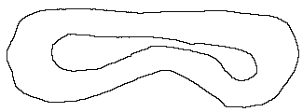
\includegraphics[interpolate=true,width=3.030000in,height=1.120000in]{contents/chapt5/figs/observation/noise_lap_2-img0.png}}%
\end{pgfscope}%
\begin{pgfscope}%
\pgfpathrectangle{\pgfqpoint{1.093729in}{2.188460in}}{\pgfqpoint{3.021708in}{1.115708in}}%
\pgfusepath{clip}%
\pgfsetbuttcap%
\pgfsetroundjoin%
\pgfsetlinewidth{1.505625pt}%
\definecolor{currentstroke}{rgb}{0.501961,0.501961,0.501961}%
\pgfsetstrokecolor{currentstroke}%
\pgfsetdash{{5.550000pt}{2.400000pt}}{0.000000pt}%
\pgfpathmoveto{\pgfqpoint{2.766478in}{2.721387in}}%
\pgfpathlineto{\pgfqpoint{2.857307in}{2.701465in}}%
\pgfpathlineto{\pgfqpoint{2.911378in}{2.687717in}}%
\pgfpathlineto{\pgfqpoint{2.964857in}{2.671491in}}%
\pgfpathlineto{\pgfqpoint{3.000032in}{2.658969in}}%
\pgfpathlineto{\pgfqpoint{3.034670in}{2.645037in}}%
\pgfpathlineto{\pgfqpoint{3.068631in}{2.629676in}}%
\pgfpathlineto{\pgfqpoint{3.101773in}{2.612867in}}%
\pgfpathlineto{\pgfqpoint{3.133963in}{2.594589in}}%
\pgfpathlineto{\pgfqpoint{3.165164in}{2.574813in}}%
\pgfpathlineto{\pgfqpoint{3.195434in}{2.553501in}}%
\pgfpathlineto{\pgfqpoint{3.224838in}{2.530615in}}%
\pgfpathlineto{\pgfqpoint{3.253439in}{2.506117in}}%
\pgfpathlineto{\pgfqpoint{3.295095in}{2.466581in}}%
\pgfpathlineto{\pgfqpoint{3.336880in}{2.427352in}}%
\pgfpathlineto{\pgfqpoint{3.366040in}{2.404273in}}%
\pgfpathlineto{\pgfqpoint{3.381291in}{2.394312in}}%
\pgfpathlineto{\pgfqpoint{3.397112in}{2.385696in}}%
\pgfpathlineto{\pgfqpoint{3.413597in}{2.378644in}}%
\pgfpathlineto{\pgfqpoint{3.430788in}{2.373293in}}%
\pgfpathlineto{\pgfqpoint{3.448594in}{2.369571in}}%
\pgfpathlineto{\pgfqpoint{3.466903in}{2.367369in}}%
\pgfpathlineto{\pgfqpoint{3.485603in}{2.366580in}}%
\pgfpathlineto{\pgfqpoint{3.504582in}{2.367097in}}%
\pgfpathlineto{\pgfqpoint{3.542930in}{2.371616in}}%
\pgfpathlineto{\pgfqpoint{3.581049in}{2.380065in}}%
\pgfpathlineto{\pgfqpoint{3.618064in}{2.391624in}}%
\pgfpathlineto{\pgfqpoint{3.653406in}{2.406023in}}%
\pgfpathlineto{\pgfqpoint{3.686726in}{2.423395in}}%
\pgfpathlineto{\pgfqpoint{3.717681in}{2.443881in}}%
\pgfpathlineto{\pgfqpoint{3.745927in}{2.467623in}}%
\pgfpathlineto{\pgfqpoint{3.758927in}{2.480758in}}%
\pgfpathlineto{\pgfqpoint{3.771133in}{2.494722in}}%
\pgfpathlineto{\pgfqpoint{3.793077in}{2.524893in}}%
\pgfpathlineto{\pgfqpoint{3.811601in}{2.557640in}}%
\pgfpathlineto{\pgfqpoint{3.826544in}{2.592466in}}%
\pgfpathlineto{\pgfqpoint{3.837748in}{2.628872in}}%
\pgfpathlineto{\pgfqpoint{3.845041in}{2.666352in}}%
\pgfpathlineto{\pgfqpoint{3.848135in}{2.704313in}}%
\pgfpathlineto{\pgfqpoint{3.847998in}{2.723276in}}%
\pgfpathlineto{\pgfqpoint{3.846682in}{2.742120in}}%
\pgfpathlineto{\pgfqpoint{3.844141in}{2.760767in}}%
\pgfpathlineto{\pgfqpoint{3.840333in}{2.779136in}}%
\pgfpathlineto{\pgfqpoint{3.835213in}{2.797148in}}%
\pgfpathlineto{\pgfqpoint{3.828739in}{2.814723in}}%
\pgfpathlineto{\pgfqpoint{3.820874in}{2.831783in}}%
\pgfpathlineto{\pgfqpoint{3.811667in}{2.848251in}}%
\pgfpathlineto{\pgfqpoint{3.801215in}{2.864056in}}%
\pgfpathlineto{\pgfqpoint{3.789617in}{2.879125in}}%
\pgfpathlineto{\pgfqpoint{3.776971in}{2.893385in}}%
\pgfpathlineto{\pgfqpoint{3.763377in}{2.906762in}}%
\pgfpathlineto{\pgfqpoint{3.748931in}{2.919186in}}%
\pgfpathlineto{\pgfqpoint{3.733734in}{2.930582in}}%
\pgfpathlineto{\pgfqpoint{3.717884in}{2.940878in}}%
\pgfpathlineto{\pgfqpoint{3.701478in}{2.950002in}}%
\pgfpathlineto{\pgfqpoint{3.684610in}{2.957906in}}%
\pgfpathlineto{\pgfqpoint{3.649726in}{2.970468in}}%
\pgfpathlineto{\pgfqpoint{3.613655in}{2.979609in}}%
\pgfpathlineto{\pgfqpoint{3.576813in}{2.986420in}}%
\pgfpathlineto{\pgfqpoint{3.392054in}{3.014052in}}%
\pgfpathlineto{\pgfqpoint{3.336884in}{3.020769in}}%
\pgfpathlineto{\pgfqpoint{3.281395in}{3.025251in}}%
\pgfpathlineto{\pgfqpoint{3.225639in}{3.027693in}}%
\pgfpathlineto{\pgfqpoint{3.151105in}{3.028574in}}%
\pgfpathlineto{\pgfqpoint{3.002247in}{3.028546in}}%
\pgfpathlineto{\pgfqpoint{2.946637in}{3.031312in}}%
\pgfpathlineto{\pgfqpoint{2.891158in}{3.036541in}}%
\pgfpathlineto{\pgfqpoint{2.687649in}{3.059261in}}%
\pgfpathlineto{\pgfqpoint{2.631977in}{3.062680in}}%
\pgfpathlineto{\pgfqpoint{2.576267in}{3.063981in}}%
\pgfpathlineto{\pgfqpoint{2.501945in}{3.062694in}}%
\pgfpathlineto{\pgfqpoint{2.334470in}{3.057403in}}%
\pgfpathlineto{\pgfqpoint{2.278668in}{3.057902in}}%
\pgfpathlineto{\pgfqpoint{2.223003in}{3.060780in}}%
\pgfpathlineto{\pgfqpoint{2.167521in}{3.066319in}}%
\pgfpathlineto{\pgfqpoint{2.038123in}{3.080716in}}%
\pgfpathlineto{\pgfqpoint{1.982403in}{3.083484in}}%
\pgfpathlineto{\pgfqpoint{1.926569in}{3.083909in}}%
\pgfpathlineto{\pgfqpoint{1.852177in}{3.082133in}}%
\pgfpathlineto{\pgfqpoint{1.778037in}{3.078506in}}%
\pgfpathlineto{\pgfqpoint{1.722526in}{3.073325in}}%
\pgfpathlineto{\pgfqpoint{1.685514in}{3.068025in}}%
\pgfpathlineto{\pgfqpoint{1.648495in}{3.060820in}}%
\pgfpathlineto{\pgfqpoint{1.611858in}{3.051258in}}%
\pgfpathlineto{\pgfqpoint{1.576255in}{3.038827in}}%
\pgfpathlineto{\pgfqpoint{1.542346in}{3.023014in}}%
\pgfpathlineto{\pgfqpoint{1.526233in}{3.013679in}}%
\pgfpathlineto{\pgfqpoint{1.510791in}{3.003306in}}%
\pgfpathlineto{\pgfqpoint{1.496102in}{2.991831in}}%
\pgfpathlineto{\pgfqpoint{1.482236in}{2.979247in}}%
\pgfpathlineto{\pgfqpoint{1.469240in}{2.965641in}}%
\pgfpathlineto{\pgfqpoint{1.457158in}{2.951107in}}%
\pgfpathlineto{\pgfqpoint{1.446035in}{2.935743in}}%
\pgfpathlineto{\pgfqpoint{1.435916in}{2.919643in}}%
\pgfpathlineto{\pgfqpoint{1.426847in}{2.902905in}}%
\pgfpathlineto{\pgfqpoint{1.418871in}{2.885623in}}%
\pgfpathlineto{\pgfqpoint{1.412035in}{2.867893in}}%
\pgfpathlineto{\pgfqpoint{1.406382in}{2.849812in}}%
\pgfpathlineto{\pgfqpoint{1.401958in}{2.831474in}}%
\pgfpathlineto{\pgfqpoint{1.398775in}{2.812956in}}%
\pgfpathlineto{\pgfqpoint{1.396807in}{2.794309in}}%
\pgfpathlineto{\pgfqpoint{1.396025in}{2.775582in}}%
\pgfpathlineto{\pgfqpoint{1.396399in}{2.756824in}}%
\pgfpathlineto{\pgfqpoint{1.400503in}{2.719415in}}%
\pgfpathlineto{\pgfqpoint{1.408884in}{2.682478in}}%
\pgfpathlineto{\pgfqpoint{1.421311in}{2.646407in}}%
\pgfpathlineto{\pgfqpoint{1.437581in}{2.611743in}}%
\pgfpathlineto{\pgfqpoint{1.457541in}{2.579259in}}%
\pgfpathlineto{\pgfqpoint{1.468859in}{2.564083in}}%
\pgfpathlineto{\pgfqpoint{1.481044in}{2.549751in}}%
\pgfpathlineto{\pgfqpoint{1.494078in}{2.536362in}}%
\pgfpathlineto{\pgfqpoint{1.507942in}{2.524016in}}%
\pgfpathlineto{\pgfqpoint{1.522618in}{2.512812in}}%
\pgfpathlineto{\pgfqpoint{1.538082in}{2.502832in}}%
\pgfpathlineto{\pgfqpoint{1.554265in}{2.494038in}}%
\pgfpathlineto{\pgfqpoint{1.571082in}{2.486342in}}%
\pgfpathlineto{\pgfqpoint{1.606279in}{2.473883in}}%
\pgfpathlineto{\pgfqpoint{1.642989in}{2.464742in}}%
\pgfpathlineto{\pgfqpoint{1.680528in}{2.458208in}}%
\pgfpathlineto{\pgfqpoint{1.718225in}{2.453582in}}%
\pgfpathlineto{\pgfqpoint{1.755721in}{2.450544in}}%
\pgfpathlineto{\pgfqpoint{1.793008in}{2.449197in}}%
\pgfpathlineto{\pgfqpoint{1.830091in}{2.449666in}}%
\pgfpathlineto{\pgfqpoint{1.866981in}{2.452073in}}%
\pgfpathlineto{\pgfqpoint{1.903683in}{2.456534in}}%
\pgfpathlineto{\pgfqpoint{1.940206in}{2.462923in}}%
\pgfpathlineto{\pgfqpoint{1.994660in}{2.475346in}}%
\pgfpathlineto{\pgfqpoint{2.048735in}{2.490087in}}%
\pgfpathlineto{\pgfqpoint{2.137989in}{2.517141in}}%
\pgfpathlineto{\pgfqpoint{2.208303in}{2.541211in}}%
\pgfpathlineto{\pgfqpoint{2.260177in}{2.561307in}}%
\pgfpathlineto{\pgfqpoint{2.311329in}{2.583234in}}%
\pgfpathlineto{\pgfqpoint{2.378885in}{2.614514in}}%
\pgfpathlineto{\pgfqpoint{2.497426in}{2.670168in}}%
\pgfpathlineto{\pgfqpoint{2.531961in}{2.683967in}}%
\pgfpathlineto{\pgfqpoint{2.567046in}{2.695682in}}%
\pgfpathlineto{\pgfqpoint{2.602809in}{2.704723in}}%
\pgfpathlineto{\pgfqpoint{2.639225in}{2.711150in}}%
\pgfpathlineto{\pgfqpoint{2.676149in}{2.715552in}}%
\pgfpathlineto{\pgfqpoint{2.732155in}{2.719673in}}%
\pgfpathlineto{\pgfqpoint{2.750914in}{2.720686in}}%
\pgfpathlineto{\pgfqpoint{2.750914in}{2.720686in}}%
\pgfusepath{stroke}%
\end{pgfscope}%
\begin{pgfscope}%
\pgfpathrectangle{\pgfqpoint{1.093729in}{2.188460in}}{\pgfqpoint{3.021708in}{1.115708in}}%
\pgfusepath{clip}%
\pgfsetrectcap%
\pgfsetroundjoin%
\pgfsetlinewidth{1.505625pt}%
\definecolor{currentstroke}{rgb}{0.121569,0.466667,0.705882}%
\pgfsetstrokecolor{currentstroke}%
\pgfsetdash{}{0pt}%
\pgfpathmoveto{\pgfqpoint{2.953242in}{3.025241in}}%
\pgfpathlineto{\pgfqpoint{2.892944in}{3.026117in}}%
\pgfpathlineto{\pgfqpoint{2.837549in}{3.029208in}}%
\pgfpathlineto{\pgfqpoint{2.767263in}{3.035876in}}%
\pgfpathlineto{\pgfqpoint{2.204832in}{3.093668in}}%
\pgfpathlineto{\pgfqpoint{2.102541in}{3.101400in}}%
\pgfpathlineto{\pgfqpoint{2.028042in}{3.105345in}}%
\pgfpathlineto{\pgfqpoint{1.972098in}{3.106331in}}%
\pgfpathlineto{\pgfqpoint{1.925482in}{3.105346in}}%
\pgfpathlineto{\pgfqpoint{1.878951in}{3.102379in}}%
\pgfpathlineto{\pgfqpoint{1.832638in}{3.097014in}}%
\pgfpathlineto{\pgfqpoint{1.795855in}{3.090820in}}%
\pgfpathlineto{\pgfqpoint{1.759425in}{3.082816in}}%
\pgfpathlineto{\pgfqpoint{1.723460in}{3.072928in}}%
\pgfpathlineto{\pgfqpoint{1.688109in}{3.061038in}}%
\pgfpathlineto{\pgfqpoint{1.653623in}{3.046833in}}%
\pgfpathlineto{\pgfqpoint{1.620231in}{3.030223in}}%
\pgfpathlineto{\pgfqpoint{1.596066in}{3.016129in}}%
\pgfpathlineto{\pgfqpoint{1.572797in}{3.000603in}}%
\pgfpathlineto{\pgfqpoint{1.550532in}{2.983669in}}%
\pgfpathlineto{\pgfqpoint{1.529450in}{2.965284in}}%
\pgfpathlineto{\pgfqpoint{1.509914in}{2.945268in}}%
\pgfpathlineto{\pgfqpoint{1.492236in}{2.923594in}}%
\pgfpathlineto{\pgfqpoint{1.476717in}{2.900328in}}%
\pgfpathlineto{\pgfqpoint{1.463675in}{2.875590in}}%
\pgfpathlineto{\pgfqpoint{1.453441in}{2.849565in}}%
\pgfpathlineto{\pgfqpoint{1.446264in}{2.822539in}}%
\pgfpathlineto{\pgfqpoint{1.442247in}{2.794865in}}%
\pgfpathlineto{\pgfqpoint{1.441498in}{2.766912in}}%
\pgfpathlineto{\pgfqpoint{1.444021in}{2.739063in}}%
\pgfpathlineto{\pgfqpoint{1.449786in}{2.711700in}}%
\pgfpathlineto{\pgfqpoint{1.458681in}{2.685189in}}%
\pgfpathlineto{\pgfqpoint{1.470586in}{2.659886in}}%
\pgfpathlineto{\pgfqpoint{1.485316in}{2.636116in}}%
\pgfpathlineto{\pgfqpoint{1.502524in}{2.614070in}}%
\pgfpathlineto{\pgfqpoint{1.521792in}{2.593797in}}%
\pgfpathlineto{\pgfqpoint{1.542870in}{2.575413in}}%
\pgfpathlineto{\pgfqpoint{1.565466in}{2.558929in}}%
\pgfpathlineto{\pgfqpoint{1.589334in}{2.544344in}}%
\pgfpathlineto{\pgfqpoint{1.614246in}{2.531623in}}%
\pgfpathlineto{\pgfqpoint{1.640013in}{2.520735in}}%
\pgfpathlineto{\pgfqpoint{1.675265in}{2.508553in}}%
\pgfpathlineto{\pgfqpoint{1.711180in}{2.498489in}}%
\pgfpathlineto{\pgfqpoint{1.756659in}{2.488212in}}%
\pgfpathlineto{\pgfqpoint{1.811689in}{2.478093in}}%
\pgfpathlineto{\pgfqpoint{1.857833in}{2.471413in}}%
\pgfpathlineto{\pgfqpoint{1.904249in}{2.467013in}}%
\pgfpathlineto{\pgfqpoint{1.941517in}{2.465502in}}%
\pgfpathlineto{\pgfqpoint{1.978810in}{2.466125in}}%
\pgfpathlineto{\pgfqpoint{2.016003in}{2.468936in}}%
\pgfpathlineto{\pgfqpoint{2.052987in}{2.473776in}}%
\pgfpathlineto{\pgfqpoint{2.089664in}{2.480561in}}%
\pgfpathlineto{\pgfqpoint{2.134979in}{2.491527in}}%
\pgfpathlineto{\pgfqpoint{2.179616in}{2.504996in}}%
\pgfpathlineto{\pgfqpoint{2.241244in}{2.526513in}}%
\pgfpathlineto{\pgfqpoint{2.345838in}{2.566312in}}%
\pgfpathlineto{\pgfqpoint{2.424601in}{2.595307in}}%
\pgfpathlineto{\pgfqpoint{2.486532in}{2.615938in}}%
\pgfpathlineto{\pgfqpoint{2.540099in}{2.631723in}}%
\pgfpathlineto{\pgfqpoint{2.584856in}{2.642708in}}%
\pgfpathlineto{\pgfqpoint{2.629687in}{2.651236in}}%
\pgfpathlineto{\pgfqpoint{2.665555in}{2.656013in}}%
\pgfpathlineto{\pgfqpoint{2.701379in}{2.658806in}}%
\pgfpathlineto{\pgfqpoint{2.737493in}{2.659664in}}%
\pgfpathlineto{\pgfqpoint{2.783046in}{2.658231in}}%
\pgfpathlineto{\pgfqpoint{2.828922in}{2.654277in}}%
\pgfpathlineto{\pgfqpoint{2.874956in}{2.648011in}}%
\pgfpathlineto{\pgfqpoint{2.920404in}{2.639431in}}%
\pgfpathlineto{\pgfqpoint{2.955910in}{2.630193in}}%
\pgfpathlineto{\pgfqpoint{2.990386in}{2.618491in}}%
\pgfpathlineto{\pgfqpoint{3.015357in}{2.607899in}}%
\pgfpathlineto{\pgfqpoint{3.039388in}{2.595659in}}%
\pgfpathlineto{\pgfqpoint{3.062481in}{2.581639in}}%
\pgfpathlineto{\pgfqpoint{3.092387in}{2.560313in}}%
\pgfpathlineto{\pgfqpoint{3.128644in}{2.531111in}}%
\pgfpathlineto{\pgfqpoint{3.199065in}{2.470189in}}%
\pgfpathlineto{\pgfqpoint{3.234904in}{2.440476in}}%
\pgfpathlineto{\pgfqpoint{3.264795in}{2.418262in}}%
\pgfpathlineto{\pgfqpoint{3.296039in}{2.398000in}}%
\pgfpathlineto{\pgfqpoint{3.320444in}{2.384415in}}%
\pgfpathlineto{\pgfqpoint{3.345683in}{2.372452in}}%
\pgfpathlineto{\pgfqpoint{3.371698in}{2.362292in}}%
\pgfpathlineto{\pgfqpoint{3.398464in}{2.354322in}}%
\pgfpathlineto{\pgfqpoint{3.425833in}{2.348769in}}%
\pgfpathlineto{\pgfqpoint{3.453600in}{2.345803in}}%
\pgfpathlineto{\pgfqpoint{3.481524in}{2.345616in}}%
\pgfpathlineto{\pgfqpoint{3.509316in}{2.348320in}}%
\pgfpathlineto{\pgfqpoint{3.536656in}{2.353993in}}%
\pgfpathlineto{\pgfqpoint{3.563241in}{2.362537in}}%
\pgfpathlineto{\pgfqpoint{3.588811in}{2.373761in}}%
\pgfpathlineto{\pgfqpoint{3.613111in}{2.387519in}}%
\pgfpathlineto{\pgfqpoint{3.635919in}{2.403630in}}%
\pgfpathlineto{\pgfqpoint{3.657066in}{2.421869in}}%
\pgfpathlineto{\pgfqpoint{3.676383in}{2.442036in}}%
\pgfpathlineto{\pgfqpoint{3.693743in}{2.463910in}}%
\pgfpathlineto{\pgfqpoint{3.709154in}{2.487201in}}%
\pgfpathlineto{\pgfqpoint{3.722606in}{2.511676in}}%
\pgfpathlineto{\pgfqpoint{3.734067in}{2.537145in}}%
\pgfpathlineto{\pgfqpoint{3.743568in}{2.563408in}}%
\pgfpathlineto{\pgfqpoint{3.751120in}{2.590298in}}%
\pgfpathlineto{\pgfqpoint{3.756758in}{2.617653in}}%
\pgfpathlineto{\pgfqpoint{3.760399in}{2.645343in}}%
\pgfpathlineto{\pgfqpoint{3.761704in}{2.673239in}}%
\pgfpathlineto{\pgfqpoint{3.760462in}{2.701138in}}%
\pgfpathlineto{\pgfqpoint{3.756516in}{2.728782in}}%
\pgfpathlineto{\pgfqpoint{3.749726in}{2.755867in}}%
\pgfpathlineto{\pgfqpoint{3.739981in}{2.782033in}}%
\pgfpathlineto{\pgfqpoint{3.727289in}{2.806902in}}%
\pgfpathlineto{\pgfqpoint{3.711888in}{2.830194in}}%
\pgfpathlineto{\pgfqpoint{3.694059in}{2.851684in}}%
\pgfpathlineto{\pgfqpoint{3.674046in}{2.871156in}}%
\pgfpathlineto{\pgfqpoint{3.652124in}{2.888455in}}%
\pgfpathlineto{\pgfqpoint{3.628593in}{2.903491in}}%
\pgfpathlineto{\pgfqpoint{3.603715in}{2.916176in}}%
\pgfpathlineto{\pgfqpoint{3.577753in}{2.926463in}}%
\pgfpathlineto{\pgfqpoint{3.551000in}{2.934482in}}%
\pgfpathlineto{\pgfqpoint{3.523742in}{2.940574in}}%
\pgfpathlineto{\pgfqpoint{3.486960in}{2.946403in}}%
\pgfpathlineto{\pgfqpoint{3.440634in}{2.950996in}}%
\pgfpathlineto{\pgfqpoint{3.282864in}{2.963363in}}%
\pgfpathlineto{\pgfqpoint{3.246126in}{2.969468in}}%
\pgfpathlineto{\pgfqpoint{3.209800in}{2.977675in}}%
\pgfpathlineto{\pgfqpoint{3.165001in}{2.990340in}}%
\pgfpathlineto{\pgfqpoint{3.058187in}{3.023138in}}%
\pgfpathlineto{\pgfqpoint{3.058187in}{3.023138in}}%
\pgfusepath{stroke}%
\end{pgfscope}%
\begin{pgfscope}%
\pgfpathrectangle{\pgfqpoint{1.093729in}{2.188460in}}{\pgfqpoint{3.021708in}{1.115708in}}%
\pgfusepath{clip}%
\pgfsetrectcap%
\pgfsetroundjoin%
\pgfsetlinewidth{1.505625pt}%
\definecolor{currentstroke}{rgb}{1.000000,0.498039,0.054902}%
\pgfsetstrokecolor{currentstroke}%
\pgfsetdash{}{0pt}%
\pgfpathmoveto{\pgfqpoint{2.953242in}{3.025241in}}%
\pgfpathlineto{\pgfqpoint{2.903057in}{3.026309in}}%
\pgfpathlineto{\pgfqpoint{2.869770in}{3.029736in}}%
\pgfpathlineto{\pgfqpoint{2.842317in}{3.034641in}}%
\pgfpathlineto{\pgfqpoint{2.809893in}{3.042924in}}%
\pgfpathlineto{\pgfqpoint{2.745263in}{3.060331in}}%
\pgfpathlineto{\pgfqpoint{2.706997in}{3.068089in}}%
\pgfpathlineto{\pgfqpoint{2.668321in}{3.073430in}}%
\pgfpathlineto{\pgfqpoint{2.634953in}{3.075992in}}%
\pgfpathlineto{\pgfqpoint{2.595914in}{3.076680in}}%
\pgfpathlineto{\pgfqpoint{2.540143in}{3.077560in}}%
\pgfpathlineto{\pgfqpoint{2.501208in}{3.080487in}}%
\pgfpathlineto{\pgfqpoint{2.451416in}{3.086899in}}%
\pgfpathlineto{\pgfqpoint{2.396462in}{3.096468in}}%
\pgfpathlineto{\pgfqpoint{2.235073in}{3.127556in}}%
\pgfpathlineto{\pgfqpoint{2.142199in}{3.142712in}}%
\pgfpathlineto{\pgfqpoint{2.103358in}{3.146735in}}%
\pgfpathlineto{\pgfqpoint{2.068651in}{3.148236in}}%
\pgfpathlineto{\pgfqpoint{2.031872in}{3.147590in}}%
\pgfpathlineto{\pgfqpoint{1.992271in}{3.144686in}}%
\pgfpathlineto{\pgfqpoint{1.940763in}{3.138428in}}%
\pgfpathlineto{\pgfqpoint{1.885799in}{3.129154in}}%
\pgfpathlineto{\pgfqpoint{1.840090in}{3.119240in}}%
\pgfpathlineto{\pgfqpoint{1.794887in}{3.107232in}}%
\pgfpathlineto{\pgfqpoint{1.750343in}{3.092973in}}%
\pgfpathlineto{\pgfqpoint{1.706592in}{3.076441in}}%
\pgfpathlineto{\pgfqpoint{1.663751in}{3.057676in}}%
\pgfpathlineto{\pgfqpoint{1.622050in}{3.036503in}}%
\pgfpathlineto{\pgfqpoint{1.589656in}{3.017777in}}%
\pgfpathlineto{\pgfqpoint{1.558258in}{2.997426in}}%
\pgfpathlineto{\pgfqpoint{1.527983in}{2.975440in}}%
\pgfpathlineto{\pgfqpoint{1.499521in}{2.952010in}}%
\pgfpathlineto{\pgfqpoint{1.479952in}{2.933298in}}%
\pgfpathlineto{\pgfqpoint{1.462185in}{2.913527in}}%
\pgfpathlineto{\pgfqpoint{1.446486in}{2.892693in}}%
\pgfpathlineto{\pgfqpoint{1.433178in}{2.870833in}}%
\pgfpathlineto{\pgfqpoint{1.422523in}{2.848109in}}%
\pgfpathlineto{\pgfqpoint{1.414720in}{2.824597in}}%
\pgfpathlineto{\pgfqpoint{1.409989in}{2.800265in}}%
\pgfpathlineto{\pgfqpoint{1.408459in}{2.775506in}}%
\pgfpathlineto{\pgfqpoint{1.410083in}{2.750737in}}%
\pgfpathlineto{\pgfqpoint{1.414793in}{2.726347in}}%
\pgfpathlineto{\pgfqpoint{1.422529in}{2.702725in}}%
\pgfpathlineto{\pgfqpoint{1.433160in}{2.680238in}}%
\pgfpathlineto{\pgfqpoint{1.446682in}{2.658944in}}%
\pgfpathlineto{\pgfqpoint{1.462737in}{2.638819in}}%
\pgfpathlineto{\pgfqpoint{1.480876in}{2.619826in}}%
\pgfpathlineto{\pgfqpoint{1.500842in}{2.601978in}}%
\pgfpathlineto{\pgfqpoint{1.522405in}{2.585239in}}%
\pgfpathlineto{\pgfqpoint{1.545412in}{2.569609in}}%
\pgfpathlineto{\pgfqpoint{1.569461in}{2.555295in}}%
\pgfpathlineto{\pgfqpoint{1.594340in}{2.542478in}}%
\pgfpathlineto{\pgfqpoint{1.619982in}{2.531268in}}%
\pgfpathlineto{\pgfqpoint{1.646326in}{2.521824in}}%
\pgfpathlineto{\pgfqpoint{1.673268in}{2.514259in}}%
\pgfpathlineto{\pgfqpoint{1.700693in}{2.508691in}}%
\pgfpathlineto{\pgfqpoint{1.728457in}{2.505185in}}%
\pgfpathlineto{\pgfqpoint{1.756406in}{2.503778in}}%
\pgfpathlineto{\pgfqpoint{1.793707in}{2.504690in}}%
\pgfpathlineto{\pgfqpoint{1.830850in}{2.508259in}}%
\pgfpathlineto{\pgfqpoint{1.867712in}{2.514061in}}%
\pgfpathlineto{\pgfqpoint{1.913341in}{2.523746in}}%
\pgfpathlineto{\pgfqpoint{1.967504in}{2.537881in}}%
\pgfpathlineto{\pgfqpoint{2.039715in}{2.556753in}}%
\pgfpathlineto{\pgfqpoint{2.085344in}{2.566434in}}%
\pgfpathlineto{\pgfqpoint{2.122216in}{2.572180in}}%
\pgfpathlineto{\pgfqpoint{2.168598in}{2.577136in}}%
\pgfpathlineto{\pgfqpoint{2.298650in}{2.589179in}}%
\pgfpathlineto{\pgfqpoint{2.344693in}{2.596637in}}%
\pgfpathlineto{\pgfqpoint{2.381100in}{2.604816in}}%
\pgfpathlineto{\pgfqpoint{2.416938in}{2.615209in}}%
\pgfpathlineto{\pgfqpoint{2.452011in}{2.627942in}}%
\pgfpathlineto{\pgfqpoint{2.485765in}{2.642837in}}%
\pgfpathlineto{\pgfqpoint{2.524153in}{2.662527in}}%
\pgfpathlineto{\pgfqpoint{2.614014in}{2.711142in}}%
\pgfpathlineto{\pgfqpoint{2.636747in}{2.719837in}}%
\pgfpathlineto{\pgfqpoint{2.653231in}{2.723722in}}%
\pgfpathlineto{\pgfqpoint{2.669720in}{2.725210in}}%
\pgfpathlineto{\pgfqpoint{2.686258in}{2.724405in}}%
\pgfpathlineto{\pgfqpoint{2.702560in}{2.721494in}}%
\pgfpathlineto{\pgfqpoint{2.718404in}{2.716676in}}%
\pgfpathlineto{\pgfqpoint{2.733607in}{2.710104in}}%
\pgfpathlineto{\pgfqpoint{2.752833in}{2.699243in}}%
\pgfpathlineto{\pgfqpoint{2.775470in}{2.683439in}}%
\pgfpathlineto{\pgfqpoint{2.850639in}{2.627247in}}%
\pgfpathlineto{\pgfqpoint{2.874498in}{2.613357in}}%
\pgfpathlineto{\pgfqpoint{2.899401in}{2.601441in}}%
\pgfpathlineto{\pgfqpoint{2.930372in}{2.589673in}}%
\pgfpathlineto{\pgfqpoint{2.967265in}{2.578132in}}%
\pgfpathlineto{\pgfqpoint{3.004726in}{2.568593in}}%
\pgfpathlineto{\pgfqpoint{3.117660in}{2.542233in}}%
\pgfpathlineto{\pgfqpoint{3.154722in}{2.531247in}}%
\pgfpathlineto{\pgfqpoint{3.191068in}{2.518090in}}%
\pgfpathlineto{\pgfqpoint{3.226503in}{2.502645in}}%
\pgfpathlineto{\pgfqpoint{3.270883in}{2.480269in}}%
\pgfpathlineto{\pgfqpoint{3.319043in}{2.453241in}}%
\pgfpathlineto{\pgfqpoint{3.377337in}{2.419902in}}%
\pgfpathlineto{\pgfqpoint{3.402104in}{2.408333in}}%
\pgfpathlineto{\pgfqpoint{3.429084in}{2.398006in}}%
\pgfpathlineto{\pgfqpoint{3.456855in}{2.389979in}}%
\pgfpathlineto{\pgfqpoint{3.476527in}{2.386254in}}%
\pgfpathlineto{\pgfqpoint{3.495053in}{2.384636in}}%
\pgfpathlineto{\pgfqpoint{3.512210in}{2.385281in}}%
\pgfpathlineto{\pgfqpoint{3.528578in}{2.388540in}}%
\pgfpathlineto{\pgfqpoint{3.544276in}{2.394222in}}%
\pgfpathlineto{\pgfqpoint{3.559301in}{2.401888in}}%
\pgfpathlineto{\pgfqpoint{3.580023in}{2.415229in}}%
\pgfpathlineto{\pgfqpoint{3.601894in}{2.431673in}}%
\pgfpathlineto{\pgfqpoint{3.624812in}{2.451157in}}%
\pgfpathlineto{\pgfqpoint{3.648545in}{2.473791in}}%
\pgfpathlineto{\pgfqpoint{3.672797in}{2.499721in}}%
\pgfpathlineto{\pgfqpoint{3.696737in}{2.528744in}}%
\pgfpathlineto{\pgfqpoint{3.713248in}{2.551777in}}%
\pgfpathlineto{\pgfqpoint{3.728122in}{2.575898in}}%
\pgfpathlineto{\pgfqpoint{3.741009in}{2.601134in}}%
\pgfpathlineto{\pgfqpoint{3.751545in}{2.627437in}}%
\pgfpathlineto{\pgfqpoint{3.759443in}{2.654647in}}%
\pgfpathlineto{\pgfqpoint{3.764367in}{2.682545in}}%
\pgfpathlineto{\pgfqpoint{3.765830in}{2.701381in}}%
\pgfpathlineto{\pgfqpoint{3.765786in}{2.720273in}}%
\pgfpathlineto{\pgfqpoint{3.764194in}{2.739097in}}%
\pgfpathlineto{\pgfqpoint{3.761028in}{2.757721in}}%
\pgfpathlineto{\pgfqpoint{3.756274in}{2.776005in}}%
\pgfpathlineto{\pgfqpoint{3.749940in}{2.793803in}}%
\pgfpathlineto{\pgfqpoint{3.742053in}{2.810969in}}%
\pgfpathlineto{\pgfqpoint{3.732658in}{2.827357in}}%
\pgfpathlineto{\pgfqpoint{3.721840in}{2.842797in}}%
\pgfpathlineto{\pgfqpoint{3.709777in}{2.857086in}}%
\pgfpathlineto{\pgfqpoint{3.696637in}{2.870177in}}%
\pgfpathlineto{\pgfqpoint{3.675242in}{2.887495in}}%
\pgfpathlineto{\pgfqpoint{3.652277in}{2.902040in}}%
\pgfpathlineto{\pgfqpoint{3.628155in}{2.913812in}}%
\pgfpathlineto{\pgfqpoint{3.603270in}{2.922916in}}%
\pgfpathlineto{\pgfqpoint{3.577977in}{2.929580in}}%
\pgfpathlineto{\pgfqpoint{3.553026in}{2.934005in}}%
\pgfpathlineto{\pgfqpoint{3.521050in}{2.937322in}}%
\pgfpathlineto{\pgfqpoint{3.476375in}{2.939070in}}%
\pgfpathlineto{\pgfqpoint{3.404898in}{2.940867in}}%
\pgfpathlineto{\pgfqpoint{3.375741in}{2.943811in}}%
\pgfpathlineto{\pgfqpoint{3.348368in}{2.948690in}}%
\pgfpathlineto{\pgfqpoint{3.321645in}{2.955598in}}%
\pgfpathlineto{\pgfqpoint{3.279717in}{2.969490in}}%
\pgfpathlineto{\pgfqpoint{3.242796in}{2.980907in}}%
\pgfpathlineto{\pgfqpoint{3.210619in}{2.988768in}}%
\pgfpathlineto{\pgfqpoint{3.177989in}{2.994456in}}%
\pgfpathlineto{\pgfqpoint{3.145038in}{2.997820in}}%
\pgfpathlineto{\pgfqpoint{3.111931in}{2.998807in}}%
\pgfpathlineto{\pgfqpoint{3.073314in}{2.997292in}}%
\pgfpathlineto{\pgfqpoint{3.029173in}{2.995881in}}%
\pgfpathlineto{\pgfqpoint{2.996081in}{2.997288in}}%
\pgfpathlineto{\pgfqpoint{2.996081in}{2.997288in}}%
\pgfusepath{stroke}%
\end{pgfscope}%
\begin{pgfscope}%
\pgfpathrectangle{\pgfqpoint{1.093729in}{2.188460in}}{\pgfqpoint{3.021708in}{1.115708in}}%
\pgfusepath{clip}%
\pgfsetbuttcap%
\pgfsetroundjoin%
\pgfsetlinewidth{1.505625pt}%
\definecolor{currentstroke}{rgb}{1.000000,0.000000,0.000000}%
\pgfsetstrokecolor{currentstroke}%
\pgfsetdash{{1.500000pt}{2.475000pt}}{0.000000pt}%
\pgfpathmoveto{\pgfqpoint{2.946637in}{2.845360in}}%
\pgfpathlineto{\pgfqpoint{2.946637in}{3.217263in}}%
\pgfusepath{stroke}%
\end{pgfscope}%
\begin{pgfscope}%
\pgfsetbuttcap%
\pgfsetmiterjoin%
\definecolor{currentfill}{rgb}{1.000000,1.000000,1.000000}%
\pgfsetfillcolor{currentfill}%
\pgfsetlinewidth{1.003750pt}%
\definecolor{currentstroke}{rgb}{0.000000,0.000000,0.000000}%
\pgfsetstrokecolor{currentstroke}%
\pgfsetdash{}{0pt}%
\pgfpathmoveto{\pgfqpoint{1.796552in}{3.043361in}}%
\pgfpathlineto{\pgfqpoint{2.008621in}{3.043361in}}%
\pgfpathquadraticcurveto{\pgfqpoint{2.020190in}{3.043361in}}{\pgfqpoint{2.020190in}{3.054931in}}%
\pgfpathlineto{\pgfqpoint{2.020190in}{3.160004in}}%
\pgfpathquadraticcurveto{\pgfqpoint{2.020190in}{3.171574in}}{\pgfqpoint{2.008621in}{3.171574in}}%
\pgfpathlineto{\pgfqpoint{1.796552in}{3.171574in}}%
\pgfpathquadraticcurveto{\pgfqpoint{1.784983in}{3.171574in}}{\pgfqpoint{1.784983in}{3.160004in}}%
\pgfpathlineto{\pgfqpoint{1.784983in}{3.054931in}}%
\pgfpathquadraticcurveto{\pgfqpoint{1.784983in}{3.043361in}}{\pgfqpoint{1.796552in}{3.043361in}}%
\pgfpathlineto{\pgfqpoint{1.796552in}{3.043361in}}%
\pgfpathclose%
\pgfusepath{stroke,fill}%
\end{pgfscope}%
\begin{pgfscope}%
\definecolor{textcolor}{rgb}{0.000000,0.000000,0.000000}%
\pgfsetstrokecolor{textcolor}%
\pgfsetfillcolor{textcolor}%
\pgftext[x=1.796552in,y=3.079674in,left,base]{\color{textcolor}\rmfamily\fontsize{8.330000}{9.996000}\selectfont 20\%}%
\end{pgfscope}%
\begin{pgfscope}%
\pgfsetbuttcap%
\pgfsetmiterjoin%
\definecolor{currentfill}{rgb}{1.000000,1.000000,1.000000}%
\pgfsetfillcolor{currentfill}%
\pgfsetlinewidth{1.003750pt}%
\definecolor{currentstroke}{rgb}{0.000000,0.000000,0.000000}%
\pgfsetstrokecolor{currentstroke}%
\pgfsetdash{}{0pt}%
\pgfpathmoveto{\pgfqpoint{1.793008in}{2.412885in}}%
\pgfpathlineto{\pgfqpoint{2.005076in}{2.412885in}}%
\pgfpathquadraticcurveto{\pgfqpoint{2.016646in}{2.412885in}}{\pgfqpoint{2.016646in}{2.424454in}}%
\pgfpathlineto{\pgfqpoint{2.016646in}{2.529528in}}%
\pgfpathquadraticcurveto{\pgfqpoint{2.016646in}{2.541097in}}{\pgfqpoint{2.005076in}{2.541097in}}%
\pgfpathlineto{\pgfqpoint{1.793008in}{2.541097in}}%
\pgfpathquadraticcurveto{\pgfqpoint{1.781438in}{2.541097in}}{\pgfqpoint{1.781438in}{2.529528in}}%
\pgfpathlineto{\pgfqpoint{1.781438in}{2.424454in}}%
\pgfpathquadraticcurveto{\pgfqpoint{1.781438in}{2.412885in}}{\pgfqpoint{1.793008in}{2.412885in}}%
\pgfpathlineto{\pgfqpoint{1.793008in}{2.412885in}}%
\pgfpathclose%
\pgfusepath{stroke,fill}%
\end{pgfscope}%
\begin{pgfscope}%
\definecolor{textcolor}{rgb}{0.000000,0.000000,0.000000}%
\pgfsetstrokecolor{textcolor}%
\pgfsetfillcolor{textcolor}%
\pgftext[x=1.793008in,y=2.449197in,left,base]{\color{textcolor}\rmfamily\fontsize{8.330000}{9.996000}\selectfont 40\%}%
\end{pgfscope}%
\begin{pgfscope}%
\pgfsetbuttcap%
\pgfsetmiterjoin%
\definecolor{currentfill}{rgb}{1.000000,1.000000,1.000000}%
\pgfsetfillcolor{currentfill}%
\pgfsetlinewidth{1.003750pt}%
\definecolor{currentstroke}{rgb}{0.000000,0.000000,0.000000}%
\pgfsetstrokecolor{currentstroke}%
\pgfsetdash{}{0pt}%
\pgfpathmoveto{\pgfqpoint{2.893409in}{2.656217in}}%
\pgfpathlineto{\pgfqpoint{3.105478in}{2.656217in}}%
\pgfpathquadraticcurveto{\pgfqpoint{3.117047in}{2.656217in}}{\pgfqpoint{3.117047in}{2.667787in}}%
\pgfpathlineto{\pgfqpoint{3.117047in}{2.772860in}}%
\pgfpathquadraticcurveto{\pgfqpoint{3.117047in}{2.784430in}}{\pgfqpoint{3.105478in}{2.784430in}}%
\pgfpathlineto{\pgfqpoint{2.893409in}{2.784430in}}%
\pgfpathquadraticcurveto{\pgfqpoint{2.881840in}{2.784430in}}{\pgfqpoint{2.881840in}{2.772860in}}%
\pgfpathlineto{\pgfqpoint{2.881840in}{2.667787in}}%
\pgfpathquadraticcurveto{\pgfqpoint{2.881840in}{2.656217in}}{\pgfqpoint{2.893409in}{2.656217in}}%
\pgfpathlineto{\pgfqpoint{2.893409in}{2.656217in}}%
\pgfpathclose%
\pgfusepath{stroke,fill}%
\end{pgfscope}%
\begin{pgfscope}%
\definecolor{textcolor}{rgb}{0.000000,0.000000,0.000000}%
\pgfsetstrokecolor{textcolor}%
\pgfsetfillcolor{textcolor}%
\pgftext[x=2.893409in,y=2.692530in,left,base]{\color{textcolor}\rmfamily\fontsize{8.330000}{9.996000}\selectfont 60\%}%
\end{pgfscope}%
\begin{pgfscope}%
\pgfsetbuttcap%
\pgfsetmiterjoin%
\definecolor{currentfill}{rgb}{1.000000,1.000000,1.000000}%
\pgfsetfillcolor{currentfill}%
\pgfsetlinewidth{1.003750pt}%
\definecolor{currentstroke}{rgb}{0.000000,0.000000,0.000000}%
\pgfsetstrokecolor{currentstroke}%
\pgfsetdash{}{0pt}%
\pgfpathmoveto{\pgfqpoint{3.832623in}{2.574190in}}%
\pgfpathlineto{\pgfqpoint{4.044692in}{2.574190in}}%
\pgfpathquadraticcurveto{\pgfqpoint{4.056262in}{2.574190in}}{\pgfqpoint{4.056262in}{2.585759in}}%
\pgfpathlineto{\pgfqpoint{4.056262in}{2.690833in}}%
\pgfpathquadraticcurveto{\pgfqpoint{4.056262in}{2.702403in}}{\pgfqpoint{4.044692in}{2.702403in}}%
\pgfpathlineto{\pgfqpoint{3.832623in}{2.702403in}}%
\pgfpathquadraticcurveto{\pgfqpoint{3.821054in}{2.702403in}}{\pgfqpoint{3.821054in}{2.690833in}}%
\pgfpathlineto{\pgfqpoint{3.821054in}{2.585759in}}%
\pgfpathquadraticcurveto{\pgfqpoint{3.821054in}{2.574190in}}{\pgfqpoint{3.832623in}{2.574190in}}%
\pgfpathlineto{\pgfqpoint{3.832623in}{2.574190in}}%
\pgfpathclose%
\pgfusepath{stroke,fill}%
\end{pgfscope}%
\begin{pgfscope}%
\definecolor{textcolor}{rgb}{0.000000,0.000000,0.000000}%
\pgfsetstrokecolor{textcolor}%
\pgfsetfillcolor{textcolor}%
\pgftext[x=3.832623in,y=2.610503in,left,base]{\color{textcolor}\rmfamily\fontsize{8.330000}{9.996000}\selectfont 80\%}%
\end{pgfscope}%
\begin{pgfscope}%
\pgfsetbuttcap%
\pgfsetmiterjoin%
\definecolor{currentfill}{rgb}{1.000000,1.000000,1.000000}%
\pgfsetfillcolor{currentfill}%
\pgfsetlinewidth{1.003750pt}%
\definecolor{currentstroke}{rgb}{0.000000,0.000000,0.000000}%
\pgfsetstrokecolor{currentstroke}%
\pgfsetdash{}{0pt}%
\pgfpathmoveto{\pgfqpoint{2.723496in}{3.236736in}}%
\pgfpathlineto{\pgfqpoint{3.237681in}{3.236736in}}%
\pgfpathquadraticcurveto{\pgfqpoint{3.249251in}{3.236736in}}{\pgfqpoint{3.249251in}{3.248305in}}%
\pgfpathlineto{\pgfqpoint{3.249251in}{3.353379in}}%
\pgfpathquadraticcurveto{\pgfqpoint{3.249251in}{3.364949in}}{\pgfqpoint{3.237681in}{3.364949in}}%
\pgfpathlineto{\pgfqpoint{2.723496in}{3.364949in}}%
\pgfpathquadraticcurveto{\pgfqpoint{2.711926in}{3.364949in}}{\pgfqpoint{2.711926in}{3.353379in}}%
\pgfpathlineto{\pgfqpoint{2.711926in}{3.248305in}}%
\pgfpathquadraticcurveto{\pgfqpoint{2.711926in}{3.236736in}}{\pgfqpoint{2.723496in}{3.236736in}}%
\pgfpathlineto{\pgfqpoint{2.723496in}{3.236736in}}%
\pgfpathclose%
\pgfusepath{stroke,fill}%
\end{pgfscope}%
\begin{pgfscope}%
\definecolor{textcolor}{rgb}{0.000000,0.000000,0.000000}%
\pgfsetstrokecolor{textcolor}%
\pgfsetfillcolor{textcolor}%
\pgftext[x=2.723496in,y=3.273048in,left,base]{\color{textcolor}\rmfamily\fontsize{8.330000}{9.996000}\selectfont Start/finish}%
\end{pgfscope}%
\begin{pgfscope}%
\pgfsetbuttcap%
\pgfsetmiterjoin%
\definecolor{currentfill}{rgb}{1.000000,1.000000,1.000000}%
\pgfsetfillcolor{currentfill}%
\pgfsetlinewidth{0.000000pt}%
\definecolor{currentstroke}{rgb}{0.000000,0.000000,0.000000}%
\pgfsetstrokecolor{currentstroke}%
\pgfsetstrokeopacity{0.000000}%
\pgfsetdash{}{0pt}%
\pgfpathmoveto{\pgfqpoint{0.464167in}{0.945000in}}%
\pgfpathlineto{\pgfqpoint{4.745000in}{0.945000in}}%
\pgfpathlineto{\pgfqpoint{4.745000in}{2.060708in}}%
\pgfpathlineto{\pgfqpoint{0.464167in}{2.060708in}}%
\pgfpathlineto{\pgfqpoint{0.464167in}{0.945000in}}%
\pgfpathclose%
\pgfusepath{fill}%
\end{pgfscope}%
\begin{pgfscope}%
\pgfpathrectangle{\pgfqpoint{0.464167in}{0.945000in}}{\pgfqpoint{4.280833in}{1.115708in}}%
\pgfusepath{clip}%
\pgfsetrectcap%
\pgfsetroundjoin%
\pgfsetlinewidth{0.803000pt}%
\definecolor{currentstroke}{rgb}{0.827451,0.827451,0.827451}%
\pgfsetstrokecolor{currentstroke}%
\pgfsetdash{}{0pt}%
\pgfpathmoveto{\pgfqpoint{0.464167in}{0.945000in}}%
\pgfpathlineto{\pgfqpoint{0.464167in}{2.060708in}}%
\pgfusepath{stroke}%
\end{pgfscope}%
\begin{pgfscope}%
\definecolor{textcolor}{rgb}{0.000000,0.000000,0.000000}%
\pgfsetstrokecolor{textcolor}%
\pgfsetfillcolor{textcolor}%
\pgftext[x=0.464167in,y=0.896389in,,top]{\color{textcolor}\rmfamily\fontsize{10.000000}{12.000000}\selectfont 0}%
\end{pgfscope}%
\begin{pgfscope}%
\pgfpathrectangle{\pgfqpoint{0.464167in}{0.945000in}}{\pgfqpoint{4.280833in}{1.115708in}}%
\pgfusepath{clip}%
\pgfsetrectcap%
\pgfsetroundjoin%
\pgfsetlinewidth{0.803000pt}%
\definecolor{currentstroke}{rgb}{0.827451,0.827451,0.827451}%
\pgfsetstrokecolor{currentstroke}%
\pgfsetdash{}{0pt}%
\pgfpathmoveto{\pgfqpoint{1.320333in}{0.945000in}}%
\pgfpathlineto{\pgfqpoint{1.320333in}{2.060708in}}%
\pgfusepath{stroke}%
\end{pgfscope}%
\begin{pgfscope}%
\definecolor{textcolor}{rgb}{0.000000,0.000000,0.000000}%
\pgfsetstrokecolor{textcolor}%
\pgfsetfillcolor{textcolor}%
\pgftext[x=1.320333in,y=0.896389in,,top]{\color{textcolor}\rmfamily\fontsize{10.000000}{12.000000}\selectfont 20}%
\end{pgfscope}%
\begin{pgfscope}%
\pgfpathrectangle{\pgfqpoint{0.464167in}{0.945000in}}{\pgfqpoint{4.280833in}{1.115708in}}%
\pgfusepath{clip}%
\pgfsetrectcap%
\pgfsetroundjoin%
\pgfsetlinewidth{0.803000pt}%
\definecolor{currentstroke}{rgb}{0.827451,0.827451,0.827451}%
\pgfsetstrokecolor{currentstroke}%
\pgfsetdash{}{0pt}%
\pgfpathmoveto{\pgfqpoint{2.176500in}{0.945000in}}%
\pgfpathlineto{\pgfqpoint{2.176500in}{2.060708in}}%
\pgfusepath{stroke}%
\end{pgfscope}%
\begin{pgfscope}%
\definecolor{textcolor}{rgb}{0.000000,0.000000,0.000000}%
\pgfsetstrokecolor{textcolor}%
\pgfsetfillcolor{textcolor}%
\pgftext[x=2.176500in,y=0.896389in,,top]{\color{textcolor}\rmfamily\fontsize{10.000000}{12.000000}\selectfont 40}%
\end{pgfscope}%
\begin{pgfscope}%
\pgfpathrectangle{\pgfqpoint{0.464167in}{0.945000in}}{\pgfqpoint{4.280833in}{1.115708in}}%
\pgfusepath{clip}%
\pgfsetrectcap%
\pgfsetroundjoin%
\pgfsetlinewidth{0.803000pt}%
\definecolor{currentstroke}{rgb}{0.827451,0.827451,0.827451}%
\pgfsetstrokecolor{currentstroke}%
\pgfsetdash{}{0pt}%
\pgfpathmoveto{\pgfqpoint{3.032667in}{0.945000in}}%
\pgfpathlineto{\pgfqpoint{3.032667in}{2.060708in}}%
\pgfusepath{stroke}%
\end{pgfscope}%
\begin{pgfscope}%
\definecolor{textcolor}{rgb}{0.000000,0.000000,0.000000}%
\pgfsetstrokecolor{textcolor}%
\pgfsetfillcolor{textcolor}%
\pgftext[x=3.032667in,y=0.896389in,,top]{\color{textcolor}\rmfamily\fontsize{10.000000}{12.000000}\selectfont 60}%
\end{pgfscope}%
\begin{pgfscope}%
\pgfpathrectangle{\pgfqpoint{0.464167in}{0.945000in}}{\pgfqpoint{4.280833in}{1.115708in}}%
\pgfusepath{clip}%
\pgfsetrectcap%
\pgfsetroundjoin%
\pgfsetlinewidth{0.803000pt}%
\definecolor{currentstroke}{rgb}{0.827451,0.827451,0.827451}%
\pgfsetstrokecolor{currentstroke}%
\pgfsetdash{}{0pt}%
\pgfpathmoveto{\pgfqpoint{3.888833in}{0.945000in}}%
\pgfpathlineto{\pgfqpoint{3.888833in}{2.060708in}}%
\pgfusepath{stroke}%
\end{pgfscope}%
\begin{pgfscope}%
\definecolor{textcolor}{rgb}{0.000000,0.000000,0.000000}%
\pgfsetstrokecolor{textcolor}%
\pgfsetfillcolor{textcolor}%
\pgftext[x=3.888833in,y=0.896389in,,top]{\color{textcolor}\rmfamily\fontsize{10.000000}{12.000000}\selectfont 80}%
\end{pgfscope}%
\begin{pgfscope}%
\pgfpathrectangle{\pgfqpoint{0.464167in}{0.945000in}}{\pgfqpoint{4.280833in}{1.115708in}}%
\pgfusepath{clip}%
\pgfsetrectcap%
\pgfsetroundjoin%
\pgfsetlinewidth{0.803000pt}%
\definecolor{currentstroke}{rgb}{0.827451,0.827451,0.827451}%
\pgfsetstrokecolor{currentstroke}%
\pgfsetdash{}{0pt}%
\pgfpathmoveto{\pgfqpoint{4.745000in}{0.945000in}}%
\pgfpathlineto{\pgfqpoint{4.745000in}{2.060708in}}%
\pgfusepath{stroke}%
\end{pgfscope}%
\begin{pgfscope}%
\definecolor{textcolor}{rgb}{0.000000,0.000000,0.000000}%
\pgfsetstrokecolor{textcolor}%
\pgfsetfillcolor{textcolor}%
\pgftext[x=4.745000in,y=0.896389in,,top]{\color{textcolor}\rmfamily\fontsize{10.000000}{12.000000}\selectfont 100}%
\end{pgfscope}%
\begin{pgfscope}%
\definecolor{textcolor}{rgb}{0.000000,0.000000,0.000000}%
\pgfsetstrokecolor{textcolor}%
\pgfsetfillcolor{textcolor}%
\pgftext[x=2.604583in,y=0.714694in,,top]{\color{textcolor}\rmfamily\fontsize{10.000000}{12.000000}\selectfont Progress along centerline [\%]}%
\end{pgfscope}%
\begin{pgfscope}%
\pgfpathrectangle{\pgfqpoint{0.464167in}{0.945000in}}{\pgfqpoint{4.280833in}{1.115708in}}%
\pgfusepath{clip}%
\pgfsetrectcap%
\pgfsetroundjoin%
\pgfsetlinewidth{0.803000pt}%
\definecolor{currentstroke}{rgb}{0.827451,0.827451,0.827451}%
\pgfsetstrokecolor{currentstroke}%
\pgfsetdash{}{0pt}%
\pgfpathmoveto{\pgfqpoint{0.464167in}{1.037976in}}%
\pgfpathlineto{\pgfqpoint{4.745000in}{1.037976in}}%
\pgfusepath{stroke}%
\end{pgfscope}%
\begin{pgfscope}%
\definecolor{textcolor}{rgb}{0.000000,0.000000,0.000000}%
\pgfsetstrokecolor{textcolor}%
\pgfsetfillcolor{textcolor}%
\pgftext[x=0.346111in, y=0.989758in, left, base]{\color{textcolor}\rmfamily\fontsize{10.000000}{12.000000}\selectfont 3}%
\end{pgfscope}%
\begin{pgfscope}%
\pgfpathrectangle{\pgfqpoint{0.464167in}{0.945000in}}{\pgfqpoint{4.280833in}{1.115708in}}%
\pgfusepath{clip}%
\pgfsetrectcap%
\pgfsetroundjoin%
\pgfsetlinewidth{0.803000pt}%
\definecolor{currentstroke}{rgb}{0.827451,0.827451,0.827451}%
\pgfsetstrokecolor{currentstroke}%
\pgfsetdash{}{0pt}%
\pgfpathmoveto{\pgfqpoint{0.464167in}{1.502854in}}%
\pgfpathlineto{\pgfqpoint{4.745000in}{1.502854in}}%
\pgfusepath{stroke}%
\end{pgfscope}%
\begin{pgfscope}%
\definecolor{textcolor}{rgb}{0.000000,0.000000,0.000000}%
\pgfsetstrokecolor{textcolor}%
\pgfsetfillcolor{textcolor}%
\pgftext[x=0.346111in, y=1.454636in, left, base]{\color{textcolor}\rmfamily\fontsize{10.000000}{12.000000}\selectfont 4}%
\end{pgfscope}%
\begin{pgfscope}%
\pgfpathrectangle{\pgfqpoint{0.464167in}{0.945000in}}{\pgfqpoint{4.280833in}{1.115708in}}%
\pgfusepath{clip}%
\pgfsetrectcap%
\pgfsetroundjoin%
\pgfsetlinewidth{0.803000pt}%
\definecolor{currentstroke}{rgb}{0.827451,0.827451,0.827451}%
\pgfsetstrokecolor{currentstroke}%
\pgfsetdash{}{0pt}%
\pgfpathmoveto{\pgfqpoint{0.464167in}{1.967732in}}%
\pgfpathlineto{\pgfqpoint{4.745000in}{1.967732in}}%
\pgfusepath{stroke}%
\end{pgfscope}%
\begin{pgfscope}%
\definecolor{textcolor}{rgb}{0.000000,0.000000,0.000000}%
\pgfsetstrokecolor{textcolor}%
\pgfsetfillcolor{textcolor}%
\pgftext[x=0.346111in, y=1.919514in, left, base]{\color{textcolor}\rmfamily\fontsize{10.000000}{12.000000}\selectfont 5}%
\end{pgfscope}%
\begin{pgfscope}%
\definecolor{textcolor}{rgb}{0.000000,0.000000,0.000000}%
\pgfsetstrokecolor{textcolor}%
\pgfsetfillcolor{textcolor}%
\pgftext[x=0.290556in,y=1.502854in,,bottom,rotate=90.000000]{\color{textcolor}\rmfamily\fontsize{10.000000}{12.000000}\selectfont Velocity [m/s]}%
\end{pgfscope}%
\begin{pgfscope}%
\pgfpathrectangle{\pgfqpoint{0.464167in}{0.945000in}}{\pgfqpoint{4.280833in}{1.115708in}}%
\pgfusepath{clip}%
\pgfsetbuttcap%
\pgfsetroundjoin%
\pgfsetlinewidth{1.505625pt}%
\definecolor{currentstroke}{rgb}{0.000000,0.000000,0.000000}%
\pgfsetstrokecolor{currentstroke}%
\pgfsetdash{{5.550000pt}{2.400000pt}}{0.000000pt}%
\pgfpathmoveto{\pgfqpoint{0.464167in}{1.037976in}}%
\pgfpathlineto{\pgfqpoint{4.745000in}{1.037976in}}%
\pgfusepath{stroke}%
\end{pgfscope}%
\begin{pgfscope}%
\pgfpathrectangle{\pgfqpoint{0.464167in}{0.945000in}}{\pgfqpoint{4.280833in}{1.115708in}}%
\pgfusepath{clip}%
\pgfsetbuttcap%
\pgfsetroundjoin%
\pgfsetlinewidth{1.505625pt}%
\definecolor{currentstroke}{rgb}{0.000000,0.000000,0.000000}%
\pgfsetstrokecolor{currentstroke}%
\pgfsetdash{{5.550000pt}{2.400000pt}}{0.000000pt}%
\pgfpathmoveto{\pgfqpoint{0.464167in}{1.967732in}}%
\pgfpathlineto{\pgfqpoint{4.745000in}{1.967732in}}%
\pgfusepath{stroke}%
\end{pgfscope}%
\begin{pgfscope}%
\pgfpathrectangle{\pgfqpoint{0.464167in}{0.945000in}}{\pgfqpoint{4.280833in}{1.115708in}}%
\pgfusepath{clip}%
\pgfsetrectcap%
\pgfsetroundjoin%
\pgfsetlinewidth{1.505625pt}%
\definecolor{currentstroke}{rgb}{0.121569,0.466667,0.705882}%
\pgfsetstrokecolor{currentstroke}%
\pgfsetdash{}{0pt}%
\pgfpathmoveto{\pgfqpoint{0.464167in}{1.037976in}}%
\pgfpathlineto{\pgfqpoint{0.464167in}{1.088235in}}%
\pgfpathlineto{\pgfqpoint{0.478065in}{1.113364in}}%
\pgfpathlineto{\pgfqpoint{0.478065in}{1.188753in}}%
\pgfpathlineto{\pgfqpoint{0.491964in}{1.213882in}}%
\pgfpathlineto{\pgfqpoint{0.491964in}{1.264141in}}%
\pgfpathlineto{\pgfqpoint{0.505863in}{1.289271in}}%
\pgfpathlineto{\pgfqpoint{0.505863in}{1.314400in}}%
\pgfpathlineto{\pgfqpoint{0.519762in}{1.339530in}}%
\pgfpathlineto{\pgfqpoint{0.519762in}{1.389789in}}%
\pgfpathlineto{\pgfqpoint{0.533661in}{1.414918in}}%
\pgfpathlineto{\pgfqpoint{0.533661in}{1.465177in}}%
\pgfpathlineto{\pgfqpoint{0.547560in}{1.490307in}}%
\pgfpathlineto{\pgfqpoint{0.547560in}{1.515436in}}%
\pgfpathlineto{\pgfqpoint{0.561458in}{1.540566in}}%
\pgfpathlineto{\pgfqpoint{0.561458in}{1.602600in}}%
\pgfpathlineto{\pgfqpoint{0.575357in}{1.633617in}}%
\pgfpathlineto{\pgfqpoint{0.575357in}{1.664634in}}%
\pgfpathlineto{\pgfqpoint{0.589256in}{1.695651in}}%
\pgfpathlineto{\pgfqpoint{0.589256in}{1.726669in}}%
\pgfpathlineto{\pgfqpoint{0.603155in}{1.757686in}}%
\pgfpathlineto{\pgfqpoint{0.603155in}{1.788703in}}%
\pgfpathlineto{\pgfqpoint{0.617054in}{1.819720in}}%
\pgfpathlineto{\pgfqpoint{0.617054in}{1.881754in}}%
\pgfpathlineto{\pgfqpoint{0.630952in}{1.912771in}}%
\pgfpathlineto{\pgfqpoint{0.630952in}{1.943788in}}%
\pgfpathlineto{\pgfqpoint{0.644851in}{1.974805in}}%
\pgfpathlineto{\pgfqpoint{0.644851in}{1.974805in}}%
\pgfpathlineto{\pgfqpoint{2.715774in}{1.974805in}}%
\pgfpathlineto{\pgfqpoint{2.715774in}{1.974805in}}%
\pgfpathlineto{\pgfqpoint{2.729673in}{1.970311in}}%
\pgfpathlineto{\pgfqpoint{2.729673in}{1.965816in}}%
\pgfpathlineto{\pgfqpoint{2.743571in}{1.961322in}}%
\pgfpathlineto{\pgfqpoint{2.743571in}{1.956827in}}%
\pgfpathlineto{\pgfqpoint{2.757470in}{1.952333in}}%
\pgfpathlineto{\pgfqpoint{2.757470in}{1.947839in}}%
\pgfpathlineto{\pgfqpoint{2.785268in}{1.938850in}}%
\pgfpathlineto{\pgfqpoint{2.785268in}{1.934355in}}%
\pgfpathlineto{\pgfqpoint{2.799167in}{1.929861in}}%
\pgfpathlineto{\pgfqpoint{2.799167in}{1.925366in}}%
\pgfpathlineto{\pgfqpoint{2.813065in}{1.920872in}}%
\pgfpathlineto{\pgfqpoint{2.813065in}{1.916377in}}%
\pgfpathlineto{\pgfqpoint{2.826964in}{1.911883in}}%
\pgfpathlineto{\pgfqpoint{2.826964in}{1.907388in}}%
\pgfpathlineto{\pgfqpoint{2.854762in}{1.898399in}}%
\pgfpathlineto{\pgfqpoint{2.854762in}{1.893905in}}%
\pgfpathlineto{\pgfqpoint{2.868661in}{1.889411in}}%
\pgfpathlineto{\pgfqpoint{2.868661in}{1.884916in}}%
\pgfpathlineto{\pgfqpoint{2.882560in}{1.889604in}}%
\pgfpathlineto{\pgfqpoint{2.882560in}{1.894293in}}%
\pgfpathlineto{\pgfqpoint{2.896458in}{1.898981in}}%
\pgfpathlineto{\pgfqpoint{2.896458in}{1.903669in}}%
\pgfpathlineto{\pgfqpoint{2.910357in}{1.908358in}}%
\pgfpathlineto{\pgfqpoint{2.910357in}{1.913046in}}%
\pgfpathlineto{\pgfqpoint{2.924256in}{1.917734in}}%
\pgfpathlineto{\pgfqpoint{2.924256in}{1.922423in}}%
\pgfpathlineto{\pgfqpoint{2.952054in}{1.927111in}}%
\pgfpathlineto{\pgfqpoint{2.952054in}{1.931799in}}%
\pgfpathlineto{\pgfqpoint{2.965952in}{1.936488in}}%
\pgfpathlineto{\pgfqpoint{2.965952in}{1.941176in}}%
\pgfpathlineto{\pgfqpoint{2.979851in}{1.945865in}}%
\pgfpathlineto{\pgfqpoint{2.979851in}{1.950553in}}%
\pgfpathlineto{\pgfqpoint{2.993750in}{1.955241in}}%
\pgfpathlineto{\pgfqpoint{2.993750in}{1.959930in}}%
\pgfpathlineto{\pgfqpoint{3.007649in}{1.964618in}}%
\pgfpathlineto{\pgfqpoint{3.007649in}{1.969306in}}%
\pgfpathlineto{\pgfqpoint{3.021548in}{1.969306in}}%
\pgfpathlineto{\pgfqpoint{3.021548in}{1.969306in}}%
\pgfpathlineto{\pgfqpoint{3.035446in}{1.964962in}}%
\pgfpathlineto{\pgfqpoint{3.035446in}{1.960617in}}%
\pgfpathlineto{\pgfqpoint{3.049345in}{1.956273in}}%
\pgfpathlineto{\pgfqpoint{3.049345in}{1.951929in}}%
\pgfpathlineto{\pgfqpoint{3.063244in}{1.947584in}}%
\pgfpathlineto{\pgfqpoint{3.063244in}{1.943240in}}%
\pgfpathlineto{\pgfqpoint{3.077143in}{1.938896in}}%
\pgfpathlineto{\pgfqpoint{3.077143in}{1.934551in}}%
\pgfpathlineto{\pgfqpoint{3.091042in}{1.930207in}}%
\pgfpathlineto{\pgfqpoint{3.091042in}{1.925862in}}%
\pgfpathlineto{\pgfqpoint{3.104940in}{1.921518in}}%
\pgfpathlineto{\pgfqpoint{3.104940in}{1.917174in}}%
\pgfpathlineto{\pgfqpoint{3.118839in}{1.912829in}}%
\pgfpathlineto{\pgfqpoint{3.118839in}{1.908485in}}%
\pgfpathlineto{\pgfqpoint{3.132738in}{1.904140in}}%
\pgfpathlineto{\pgfqpoint{3.132738in}{1.899796in}}%
\pgfpathlineto{\pgfqpoint{3.146637in}{1.895452in}}%
\pgfpathlineto{\pgfqpoint{3.146637in}{1.891107in}}%
\pgfpathlineto{\pgfqpoint{3.160536in}{1.886763in}}%
\pgfpathlineto{\pgfqpoint{3.160536in}{1.882419in}}%
\pgfpathlineto{\pgfqpoint{3.174435in}{1.895110in}}%
\pgfpathlineto{\pgfqpoint{3.174435in}{1.907801in}}%
\pgfpathlineto{\pgfqpoint{3.188333in}{1.920493in}}%
\pgfpathlineto{\pgfqpoint{3.188333in}{1.933184in}}%
\pgfpathlineto{\pgfqpoint{3.202232in}{1.945875in}}%
\pgfpathlineto{\pgfqpoint{3.202232in}{1.958567in}}%
\pgfpathlineto{\pgfqpoint{3.216131in}{1.971258in}}%
\pgfpathlineto{\pgfqpoint{3.216131in}{1.971258in}}%
\pgfpathlineto{\pgfqpoint{4.661607in}{1.971258in}}%
\pgfpathlineto{\pgfqpoint{4.661607in}{1.971258in}}%
\pgfusepath{stroke}%
\end{pgfscope}%
\begin{pgfscope}%
\pgfpathrectangle{\pgfqpoint{0.464167in}{0.945000in}}{\pgfqpoint{4.280833in}{1.115708in}}%
\pgfusepath{clip}%
\pgfsetrectcap%
\pgfsetroundjoin%
\pgfsetlinewidth{1.505625pt}%
\definecolor{currentstroke}{rgb}{1.000000,0.498039,0.054902}%
\pgfsetstrokecolor{currentstroke}%
\pgfsetdash{}{0pt}%
\pgfpathmoveto{\pgfqpoint{0.464167in}{1.037976in}}%
\pgfpathlineto{\pgfqpoint{0.867232in}{1.037976in}}%
\pgfpathlineto{\pgfqpoint{0.867232in}{1.037976in}}%
\pgfpathlineto{\pgfqpoint{0.881131in}{1.039438in}}%
\pgfpathlineto{\pgfqpoint{0.881131in}{1.043825in}}%
\pgfpathlineto{\pgfqpoint{0.895030in}{1.045288in}}%
\pgfpathlineto{\pgfqpoint{0.895030in}{1.048212in}}%
\pgfpathlineto{\pgfqpoint{0.908929in}{1.049675in}}%
\pgfpathlineto{\pgfqpoint{0.908929in}{1.052600in}}%
\pgfpathlineto{\pgfqpoint{0.922827in}{1.054062in}}%
\pgfpathlineto{\pgfqpoint{0.922827in}{1.056987in}}%
\pgfpathlineto{\pgfqpoint{0.936726in}{1.058449in}}%
\pgfpathlineto{\pgfqpoint{0.936726in}{1.062836in}}%
\pgfpathlineto{\pgfqpoint{0.950625in}{1.064299in}}%
\pgfpathlineto{\pgfqpoint{0.950625in}{1.067223in}}%
\pgfpathlineto{\pgfqpoint{0.964524in}{1.068902in}}%
\pgfpathlineto{\pgfqpoint{0.964524in}{1.072259in}}%
\pgfpathlineto{\pgfqpoint{0.978423in}{1.073937in}}%
\pgfpathlineto{\pgfqpoint{0.978423in}{1.077294in}}%
\pgfpathlineto{\pgfqpoint{0.992321in}{1.078972in}}%
\pgfpathlineto{\pgfqpoint{0.992321in}{1.082329in}}%
\pgfpathlineto{\pgfqpoint{1.006220in}{1.084008in}}%
\pgfpathlineto{\pgfqpoint{1.006220in}{1.087365in}}%
\pgfpathlineto{\pgfqpoint{1.020119in}{1.089043in}}%
\pgfpathlineto{\pgfqpoint{1.020119in}{1.092400in}}%
\pgfpathlineto{\pgfqpoint{1.034018in}{1.094078in}}%
\pgfpathlineto{\pgfqpoint{1.034018in}{1.097435in}}%
\pgfpathlineto{\pgfqpoint{1.047917in}{1.099114in}}%
\pgfpathlineto{\pgfqpoint{1.047917in}{1.120774in}}%
\pgfpathlineto{\pgfqpoint{1.061815in}{1.140756in}}%
\pgfpathlineto{\pgfqpoint{1.061815in}{1.180719in}}%
\pgfpathlineto{\pgfqpoint{1.075714in}{1.200701in}}%
\pgfpathlineto{\pgfqpoint{1.075714in}{1.240665in}}%
\pgfpathlineto{\pgfqpoint{1.089613in}{1.260647in}}%
\pgfpathlineto{\pgfqpoint{1.089613in}{1.300610in}}%
\pgfpathlineto{\pgfqpoint{1.103512in}{1.320592in}}%
\pgfpathlineto{\pgfqpoint{1.103512in}{1.360556in}}%
\pgfpathlineto{\pgfqpoint{1.117411in}{1.380538in}}%
\pgfpathlineto{\pgfqpoint{1.117411in}{1.420501in}}%
\pgfpathlineto{\pgfqpoint{1.131310in}{1.440483in}}%
\pgfpathlineto{\pgfqpoint{1.131310in}{1.480447in}}%
\pgfpathlineto{\pgfqpoint{1.145208in}{1.500429in}}%
\pgfpathlineto{\pgfqpoint{1.145208in}{1.532541in}}%
\pgfpathlineto{\pgfqpoint{1.159107in}{1.564653in}}%
\pgfpathlineto{\pgfqpoint{1.159107in}{1.628878in}}%
\pgfpathlineto{\pgfqpoint{1.173006in}{1.660990in}}%
\pgfpathlineto{\pgfqpoint{1.173006in}{1.693103in}}%
\pgfpathlineto{\pgfqpoint{1.186905in}{1.725215in}}%
\pgfpathlineto{\pgfqpoint{1.186905in}{1.789439in}}%
\pgfpathlineto{\pgfqpoint{1.200804in}{1.821552in}}%
\pgfpathlineto{\pgfqpoint{1.200804in}{1.853664in}}%
\pgfpathlineto{\pgfqpoint{1.214702in}{1.885776in}}%
\pgfpathlineto{\pgfqpoint{1.214702in}{1.917889in}}%
\pgfpathlineto{\pgfqpoint{1.228601in}{1.950001in}}%
\pgfpathlineto{\pgfqpoint{1.228601in}{1.982113in}}%
\pgfpathlineto{\pgfqpoint{1.548274in}{1.982113in}}%
\pgfpathlineto{\pgfqpoint{1.548274in}{1.968431in}}%
\pgfpathlineto{\pgfqpoint{1.562173in}{1.954749in}}%
\pgfpathlineto{\pgfqpoint{1.562173in}{1.941066in}}%
\pgfpathlineto{\pgfqpoint{1.576071in}{1.927384in}}%
\pgfpathlineto{\pgfqpoint{1.576071in}{1.913702in}}%
\pgfpathlineto{\pgfqpoint{1.589970in}{1.900020in}}%
\pgfpathlineto{\pgfqpoint{1.589970in}{1.886338in}}%
\pgfpathlineto{\pgfqpoint{1.617768in}{1.858973in}}%
\pgfpathlineto{\pgfqpoint{1.617768in}{1.845291in}}%
\pgfpathlineto{\pgfqpoint{1.631667in}{1.831609in}}%
\pgfpathlineto{\pgfqpoint{1.631667in}{1.817927in}}%
\pgfpathlineto{\pgfqpoint{1.645565in}{1.804244in}}%
\pgfpathlineto{\pgfqpoint{1.645565in}{1.790562in}}%
\pgfpathlineto{\pgfqpoint{1.659464in}{1.776880in}}%
\pgfpathlineto{\pgfqpoint{1.659464in}{1.749515in}}%
\pgfpathlineto{\pgfqpoint{1.673363in}{1.735833in}}%
\pgfpathlineto{\pgfqpoint{1.673363in}{1.722151in}}%
\pgfpathlineto{\pgfqpoint{1.687262in}{1.708469in}}%
\pgfpathlineto{\pgfqpoint{1.687262in}{1.708936in}}%
\pgfpathlineto{\pgfqpoint{1.728958in}{1.711270in}}%
\pgfpathlineto{\pgfqpoint{1.728958in}{1.711736in}}%
\pgfpathlineto{\pgfqpoint{1.756756in}{1.713604in}}%
\pgfpathlineto{\pgfqpoint{1.756756in}{1.714070in}}%
\pgfpathlineto{\pgfqpoint{1.798452in}{1.716404in}}%
\pgfpathlineto{\pgfqpoint{1.798452in}{1.716871in}}%
\pgfpathlineto{\pgfqpoint{1.812351in}{1.717805in}}%
\pgfpathlineto{\pgfqpoint{1.812351in}{1.732141in}}%
\pgfpathlineto{\pgfqpoint{1.826250in}{1.746476in}}%
\pgfpathlineto{\pgfqpoint{1.826250in}{1.760812in}}%
\pgfpathlineto{\pgfqpoint{1.840149in}{1.775148in}}%
\pgfpathlineto{\pgfqpoint{1.840149in}{1.789484in}}%
\pgfpathlineto{\pgfqpoint{1.854048in}{1.803820in}}%
\pgfpathlineto{\pgfqpoint{1.854048in}{1.818155in}}%
\pgfpathlineto{\pgfqpoint{1.867946in}{1.832491in}}%
\pgfpathlineto{\pgfqpoint{1.867946in}{1.846827in}}%
\pgfpathlineto{\pgfqpoint{1.881845in}{1.861163in}}%
\pgfpathlineto{\pgfqpoint{1.881845in}{1.875499in}}%
\pgfpathlineto{\pgfqpoint{1.895744in}{1.889835in}}%
\pgfpathlineto{\pgfqpoint{1.895744in}{1.904170in}}%
\pgfpathlineto{\pgfqpoint{1.923542in}{1.932842in}}%
\pgfpathlineto{\pgfqpoint{1.923542in}{1.947178in}}%
\pgfpathlineto{\pgfqpoint{1.937440in}{1.961514in}}%
\pgfpathlineto{\pgfqpoint{1.937440in}{1.975850in}}%
\pgfpathlineto{\pgfqpoint{2.687976in}{1.975850in}}%
\pgfpathlineto{\pgfqpoint{2.687976in}{1.975850in}}%
\pgfpathlineto{\pgfqpoint{2.701875in}{1.940832in}}%
\pgfpathlineto{\pgfqpoint{2.701875in}{1.905814in}}%
\pgfpathlineto{\pgfqpoint{2.715774in}{1.870796in}}%
\pgfpathlineto{\pgfqpoint{2.715774in}{1.835778in}}%
\pgfpathlineto{\pgfqpoint{2.729673in}{1.800760in}}%
\pgfpathlineto{\pgfqpoint{2.729673in}{1.765742in}}%
\pgfpathlineto{\pgfqpoint{2.743571in}{1.730725in}}%
\pgfpathlineto{\pgfqpoint{2.743571in}{1.695707in}}%
\pgfpathlineto{\pgfqpoint{2.757470in}{1.660689in}}%
\pgfpathlineto{\pgfqpoint{2.757470in}{1.625671in}}%
\pgfpathlineto{\pgfqpoint{2.771369in}{1.590653in}}%
\pgfpathlineto{\pgfqpoint{2.771369in}{1.520618in}}%
\pgfpathlineto{\pgfqpoint{2.785268in}{1.485600in}}%
\pgfpathlineto{\pgfqpoint{2.785268in}{1.450582in}}%
\pgfpathlineto{\pgfqpoint{2.799167in}{1.415564in}}%
\pgfpathlineto{\pgfqpoint{2.799167in}{1.345528in}}%
\pgfpathlineto{\pgfqpoint{2.813065in}{1.310511in}}%
\pgfpathlineto{\pgfqpoint{2.813065in}{1.244066in}}%
\pgfpathlineto{\pgfqpoint{2.826964in}{1.212640in}}%
\pgfpathlineto{\pgfqpoint{2.826964in}{1.149788in}}%
\pgfpathlineto{\pgfqpoint{2.840863in}{1.118361in}}%
\pgfpathlineto{\pgfqpoint{2.840863in}{1.055509in}}%
\pgfpathlineto{\pgfqpoint{2.854762in}{1.024082in}}%
\pgfpathlineto{\pgfqpoint{2.854762in}{1.024082in}}%
\pgfpathlineto{\pgfqpoint{3.396815in}{1.024082in}}%
\pgfpathlineto{\pgfqpoint{3.396815in}{1.024082in}}%
\pgfpathlineto{\pgfqpoint{3.396815in}{1.048382in}}%
\pgfpathlineto{\pgfqpoint{3.410714in}{1.072681in}}%
\pgfpathlineto{\pgfqpoint{3.410714in}{1.121280in}}%
\pgfpathlineto{\pgfqpoint{3.424613in}{1.145579in}}%
\pgfpathlineto{\pgfqpoint{3.424613in}{1.194178in}}%
\pgfpathlineto{\pgfqpoint{3.438512in}{1.218477in}}%
\pgfpathlineto{\pgfqpoint{3.438512in}{1.267076in}}%
\pgfpathlineto{\pgfqpoint{3.452411in}{1.291375in}}%
\pgfpathlineto{\pgfqpoint{3.452411in}{1.339974in}}%
\pgfpathlineto{\pgfqpoint{3.466310in}{1.364273in}}%
\pgfpathlineto{\pgfqpoint{3.466310in}{1.388573in}}%
\pgfpathlineto{\pgfqpoint{3.480208in}{1.412872in}}%
\pgfpathlineto{\pgfqpoint{3.480208in}{1.437172in}}%
\pgfpathlineto{\pgfqpoint{3.494107in}{1.461471in}}%
\pgfpathlineto{\pgfqpoint{3.494107in}{1.485770in}}%
\pgfpathlineto{\pgfqpoint{3.508006in}{1.510070in}}%
\pgfpathlineto{\pgfqpoint{3.508006in}{1.430980in}}%
\pgfpathlineto{\pgfqpoint{3.521905in}{1.391435in}}%
\pgfpathlineto{\pgfqpoint{3.521905in}{1.351890in}}%
\pgfpathlineto{\pgfqpoint{3.535804in}{1.312345in}}%
\pgfpathlineto{\pgfqpoint{3.535804in}{1.233256in}}%
\pgfpathlineto{\pgfqpoint{3.549702in}{1.193711in}}%
\pgfpathlineto{\pgfqpoint{3.549702in}{1.154166in}}%
\pgfpathlineto{\pgfqpoint{3.563601in}{1.114621in}}%
\pgfpathlineto{\pgfqpoint{3.563601in}{1.035531in}}%
\pgfpathlineto{\pgfqpoint{3.563601in}{1.035531in}}%
\pgfpathlineto{\pgfqpoint{3.605298in}{1.035531in}}%
\pgfpathlineto{\pgfqpoint{3.605298in}{1.162853in}}%
\pgfpathlineto{\pgfqpoint{3.619196in}{1.205293in}}%
\pgfpathlineto{\pgfqpoint{3.619196in}{1.290174in}}%
\pgfpathlineto{\pgfqpoint{3.633095in}{1.332614in}}%
\pgfpathlineto{\pgfqpoint{3.633095in}{1.375054in}}%
\pgfpathlineto{\pgfqpoint{3.646994in}{1.417495in}}%
\pgfpathlineto{\pgfqpoint{3.646994in}{1.502376in}}%
\pgfpathlineto{\pgfqpoint{3.660893in}{1.544816in}}%
\pgfpathlineto{\pgfqpoint{3.660893in}{1.587256in}}%
\pgfpathlineto{\pgfqpoint{3.674792in}{1.629697in}}%
\pgfpathlineto{\pgfqpoint{3.674792in}{1.672137in}}%
\pgfpathlineto{\pgfqpoint{3.688690in}{1.714577in}}%
\pgfpathlineto{\pgfqpoint{3.688690in}{1.757018in}}%
\pgfpathlineto{\pgfqpoint{3.702589in}{1.799458in}}%
\pgfpathlineto{\pgfqpoint{3.702589in}{1.841899in}}%
\pgfpathlineto{\pgfqpoint{3.716488in}{1.884339in}}%
\pgfpathlineto{\pgfqpoint{3.716488in}{1.924672in}}%
\pgfpathlineto{\pgfqpoint{3.730387in}{1.965004in}}%
\pgfpathlineto{\pgfqpoint{3.730387in}{2.005337in}}%
\pgfpathlineto{\pgfqpoint{4.091756in}{2.005337in}}%
\pgfpathlineto{\pgfqpoint{4.091756in}{1.995774in}}%
\pgfpathlineto{\pgfqpoint{4.119554in}{1.976649in}}%
\pgfpathlineto{\pgfqpoint{4.119554in}{1.967087in}}%
\pgfpathlineto{\pgfqpoint{4.147351in}{1.947962in}}%
\pgfpathlineto{\pgfqpoint{4.147351in}{1.938399in}}%
\pgfpathlineto{\pgfqpoint{4.175149in}{1.919274in}}%
\pgfpathlineto{\pgfqpoint{4.175149in}{1.909712in}}%
\pgfpathlineto{\pgfqpoint{4.202946in}{1.890587in}}%
\pgfpathlineto{\pgfqpoint{4.202946in}{1.881024in}}%
\pgfpathlineto{\pgfqpoint{4.216845in}{1.871462in}}%
\pgfpathlineto{\pgfqpoint{4.216845in}{1.861899in}}%
\pgfpathlineto{\pgfqpoint{4.230744in}{1.852336in}}%
\pgfpathlineto{\pgfqpoint{4.230744in}{1.842774in}}%
\pgfpathlineto{\pgfqpoint{4.244643in}{1.833211in}}%
\pgfpathlineto{\pgfqpoint{4.244643in}{1.823649in}}%
\pgfpathlineto{\pgfqpoint{4.258542in}{1.814086in}}%
\pgfpathlineto{\pgfqpoint{4.258542in}{1.784788in}}%
\pgfpathlineto{\pgfqpoint{4.272440in}{1.755489in}}%
\pgfpathlineto{\pgfqpoint{4.272440in}{1.726190in}}%
\pgfpathlineto{\pgfqpoint{4.286339in}{1.696891in}}%
\pgfpathlineto{\pgfqpoint{4.286339in}{1.667592in}}%
\pgfpathlineto{\pgfqpoint{4.300238in}{1.638293in}}%
\pgfpathlineto{\pgfqpoint{4.300238in}{1.608995in}}%
\pgfpathlineto{\pgfqpoint{4.314137in}{1.579696in}}%
\pgfpathlineto{\pgfqpoint{4.314137in}{1.521098in}}%
\pgfpathlineto{\pgfqpoint{4.328036in}{1.491799in}}%
\pgfpathlineto{\pgfqpoint{4.328036in}{1.462500in}}%
\pgfpathlineto{\pgfqpoint{4.341935in}{1.433202in}}%
\pgfpathlineto{\pgfqpoint{4.341935in}{1.374604in}}%
\pgfpathlineto{\pgfqpoint{4.355833in}{1.345305in}}%
\pgfpathlineto{\pgfqpoint{4.355833in}{1.286707in}}%
\pgfpathlineto{\pgfqpoint{4.369732in}{1.257409in}}%
\pgfpathlineto{\pgfqpoint{4.369732in}{1.211077in}}%
\pgfpathlineto{\pgfqpoint{4.383631in}{1.194045in}}%
\pgfpathlineto{\pgfqpoint{4.383631in}{1.159980in}}%
\pgfpathlineto{\pgfqpoint{4.397530in}{1.142947in}}%
\pgfpathlineto{\pgfqpoint{4.397530in}{1.108882in}}%
\pgfpathlineto{\pgfqpoint{4.411429in}{1.091850in}}%
\pgfpathlineto{\pgfqpoint{4.411429in}{1.057785in}}%
\pgfpathlineto{\pgfqpoint{4.425327in}{1.040752in}}%
\pgfpathlineto{\pgfqpoint{4.425327in}{1.023720in}}%
\pgfpathlineto{\pgfqpoint{4.703304in}{1.023720in}}%
\pgfpathlineto{\pgfqpoint{4.703304in}{1.023720in}}%
\pgfusepath{stroke}%
\end{pgfscope}%
\begin{pgfscope}%
\pgfsetrectcap%
\pgfsetmiterjoin%
\pgfsetlinewidth{0.803000pt}%
\definecolor{currentstroke}{rgb}{0.501961,0.501961,0.501961}%
\pgfsetstrokecolor{currentstroke}%
\pgfsetdash{}{0pt}%
\pgfpathmoveto{\pgfqpoint{0.464167in}{0.945000in}}%
\pgfpathlineto{\pgfqpoint{0.464167in}{2.060708in}}%
\pgfusepath{stroke}%
\end{pgfscope}%
\begin{pgfscope}%
\pgfsetrectcap%
\pgfsetmiterjoin%
\pgfsetlinewidth{0.803000pt}%
\definecolor{currentstroke}{rgb}{0.501961,0.501961,0.501961}%
\pgfsetstrokecolor{currentstroke}%
\pgfsetdash{}{0pt}%
\pgfpathmoveto{\pgfqpoint{4.745000in}{0.945000in}}%
\pgfpathlineto{\pgfqpoint{4.745000in}{2.060708in}}%
\pgfusepath{stroke}%
\end{pgfscope}%
\begin{pgfscope}%
\pgfsetrectcap%
\pgfsetmiterjoin%
\pgfsetlinewidth{0.803000pt}%
\definecolor{currentstroke}{rgb}{0.501961,0.501961,0.501961}%
\pgfsetstrokecolor{currentstroke}%
\pgfsetdash{}{0pt}%
\pgfpathmoveto{\pgfqpoint{0.464167in}{0.945000in}}%
\pgfpathlineto{\pgfqpoint{4.745000in}{0.945000in}}%
\pgfusepath{stroke}%
\end{pgfscope}%
\begin{pgfscope}%
\pgfsetrectcap%
\pgfsetmiterjoin%
\pgfsetlinewidth{0.803000pt}%
\definecolor{currentstroke}{rgb}{0.501961,0.501961,0.501961}%
\pgfsetstrokecolor{currentstroke}%
\pgfsetdash{}{0pt}%
\pgfpathmoveto{\pgfqpoint{0.464167in}{2.060708in}}%
\pgfpathlineto{\pgfqpoint{4.745000in}{2.060708in}}%
\pgfusepath{stroke}%
\end{pgfscope}%
\begin{pgfscope}%
\pgfsetbuttcap%
\pgfsetmiterjoin%
\definecolor{currentfill}{rgb}{1.000000,1.000000,1.000000}%
\pgfsetfillcolor{currentfill}%
\pgfsetfillopacity{0.800000}%
\pgfsetlinewidth{1.003750pt}%
\definecolor{currentstroke}{rgb}{0.800000,0.800000,0.800000}%
\pgfsetstrokecolor{currentstroke}%
\pgfsetstrokeopacity{0.800000}%
\pgfsetdash{}{0pt}%
\pgfpathmoveto{\pgfqpoint{0.640957in}{0.069444in}}%
\pgfpathlineto{\pgfqpoint{4.359043in}{0.069444in}}%
\pgfpathquadraticcurveto{\pgfqpoint{4.386820in}{0.069444in}}{\pgfqpoint{4.386820in}{0.097222in}}%
\pgfpathlineto{\pgfqpoint{4.386820in}{0.424343in}}%
\pgfpathquadraticcurveto{\pgfqpoint{4.386820in}{0.452121in}}{\pgfqpoint{4.359043in}{0.452121in}}%
\pgfpathlineto{\pgfqpoint{0.640957in}{0.452121in}}%
\pgfpathquadraticcurveto{\pgfqpoint{0.613180in}{0.452121in}}{\pgfqpoint{0.613180in}{0.424343in}}%
\pgfpathlineto{\pgfqpoint{0.613180in}{0.097222in}}%
\pgfpathquadraticcurveto{\pgfqpoint{0.613180in}{0.069444in}}{\pgfqpoint{0.640957in}{0.069444in}}%
\pgfpathlineto{\pgfqpoint{0.640957in}{0.069444in}}%
\pgfpathclose%
\pgfusepath{stroke,fill}%
\end{pgfscope}%
\begin{pgfscope}%
\pgfsetbuttcap%
\pgfsetroundjoin%
\pgfsetlinewidth{1.505625pt}%
\definecolor{currentstroke}{rgb}{0.501961,0.501961,0.501961}%
\pgfsetstrokecolor{currentstroke}%
\pgfsetdash{{5.550000pt}{2.400000pt}}{0.000000pt}%
\pgfpathmoveto{\pgfqpoint{0.668735in}{0.261176in}}%
\pgfpathlineto{\pgfqpoint{0.807624in}{0.261176in}}%
\pgfpathlineto{\pgfqpoint{0.946513in}{0.261176in}}%
\pgfusepath{stroke}%
\end{pgfscope}%
\begin{pgfscope}%
\definecolor{textcolor}{rgb}{0.000000,0.000000,0.000000}%
\pgfsetstrokecolor{textcolor}%
\pgfsetfillcolor{textcolor}%
\pgftext[x=1.057624in,y=0.212565in,left,base]{\color{textcolor}\rmfamily\fontsize{10.000000}{12.000000}\selectfont Centerline}%
\end{pgfscope}%
\begin{pgfscope}%
\pgfsetrectcap%
\pgfsetroundjoin%
\pgfsetlinewidth{1.505625pt}%
\definecolor{currentstroke}{rgb}{0.121569,0.466667,0.705882}%
\pgfsetstrokecolor{currentstroke}%
\pgfsetdash{}{0pt}%
\pgfpathmoveto{\pgfqpoint{1.913879in}{0.261176in}}%
\pgfpathlineto{\pgfqpoint{2.052768in}{0.261176in}}%
\pgfpathlineto{\pgfqpoint{2.191657in}{0.261176in}}%
\pgfusepath{stroke}%
\end{pgfscope}%
\begin{pgfscope}%
\definecolor{textcolor}{rgb}{0.000000,0.000000,0.000000}%
\pgfsetstrokecolor{textcolor}%
\pgfsetfillcolor{textcolor}%
\pgftext[x=2.302768in, y=0.300130in, left, base]{\color{textcolor}\rmfamily\fontsize{10.000000}{12.000000}\selectfont Trained }%
\end{pgfscope}%
\begin{pgfscope}%
\definecolor{textcolor}{rgb}{0.000000,0.000000,0.000000}%
\pgfsetstrokecolor{textcolor}%
\pgfsetfillcolor{textcolor}%
\pgftext[x=2.302768in, y=0.154704in, left, base]{\color{textcolor}\rmfamily\fontsize{10.000000}{12.000000}\selectfont without noise}%
\end{pgfscope}%
\begin{pgfscope}%
\pgfsetrectcap%
\pgfsetroundjoin%
\pgfsetlinewidth{1.505625pt}%
\definecolor{currentstroke}{rgb}{1.000000,0.498039,0.054902}%
\pgfsetstrokecolor{currentstroke}%
\pgfsetdash{}{0pt}%
\pgfpathmoveto{\pgfqpoint{3.332838in}{0.261176in}}%
\pgfpathlineto{\pgfqpoint{3.471727in}{0.261176in}}%
\pgfpathlineto{\pgfqpoint{3.610616in}{0.261176in}}%
\pgfusepath{stroke}%
\end{pgfscope}%
\begin{pgfscope}%
\definecolor{textcolor}{rgb}{0.000000,0.000000,0.000000}%
\pgfsetstrokecolor{textcolor}%
\pgfsetfillcolor{textcolor}%
\pgftext[x=3.721727in, y=0.300130in, left, base]{\color{textcolor}\rmfamily\fontsize{10.000000}{12.000000}\selectfont Trained }%
\end{pgfscope}%
\begin{pgfscope}%
\definecolor{textcolor}{rgb}{0.000000,0.000000,0.000000}%
\pgfsetstrokecolor{textcolor}%
\pgfsetfillcolor{textcolor}%
\pgftext[x=3.721727in, y=0.154704in, left, base]{\color{textcolor}\rmfamily\fontsize{10.000000}{12.000000}\selectfont with noise     }%
\end{pgfscope}%
\end{pgfpicture}%
\makeatother%
\endgroup%

    \caption[Path and velocity profiles of end-to-end agents that were trained with and without noise added to the observation vector]{Path and velocity profiles of end-to-end agents that were trained with and without noise added to the observation vector.}
    \label{fig:noise_lap}
\end{figure}



%%%%%%%%%%%%%%%%%%%%%%%%%%%%%%%%%%%%%%%%%%%%%%%%%%%%%%%%%%%%%%%%%%%%%%%%%%%%%%%%%%%%%%%%%%%%%%%%%%%%%%%%%%%%%%%%%%%%%%%%%%%%

\section{Neural network hyper-parameters}

Next, an investigation was conducted to determine the optimal DNN layer configuration for the actor and critics.
In this experiment, the layer configuration of the actor and both critics were varied together, such that the input and hidden layers for all three DNNs remained identical in structure.
The input and hidden layers of these DNNs were initially specified to be $400$ and $300$ units, respectively.
Three agents were then trained with input and hidden layers that were $100$ units larger and smaller than the initial DNN configuration.
The remaining hyper-parameters of these agents were set equal to those listed in Table \ref{tab:inital_values}.
The percentage failed laps, lap times, and learning curves while training these agents are depicted in Figure \ref{fig:layer_sizes}.

\begin{figure}[htb!]
    \centering
    %% Creator: Matplotlib, PGF backend
%%
%% To include the figure in your LaTeX document, write
%%   \input{<filename>.pgf}
%%
%% Make sure the required packages are loaded in your preamble
%%   \usepackage{pgf}
%%
%% Also ensure that all the required font packages are loaded; for instance,
%% the lmodern package is sometimes necessary when using math font.
%%   \usepackage{lmodern}
%%
%% Figures using additional raster images can only be included by \input if
%% they are in the same directory as the main LaTeX file. For loading figures
%% from other directories you can use the `import` package
%%   \usepackage{import}
%%
%% and then include the figures with
%%   \import{<path to file>}{<filename>.pgf}
%%
%% Matplotlib used the following preamble
%%   \usepackage{fontspec}
%%   \setmainfont{DejaVuSerif.ttf}[Path=\detokenize{/home/andrew/anaconda3/envs/auto_car_env/lib/python3.9/site-packages/matplotlib/mpl-data/fonts/ttf/}]
%%   \setsansfont{DejaVuSans.ttf}[Path=\detokenize{/home/andrew/anaconda3/envs/auto_car_env/lib/python3.9/site-packages/matplotlib/mpl-data/fonts/ttf/}]
%%   \setmonofont{DejaVuSansMono.ttf}[Path=\detokenize{/home/andrew/anaconda3/envs/auto_car_env/lib/python3.9/site-packages/matplotlib/mpl-data/fonts/ttf/}]
%%
\begingroup%
\makeatletter%
\begin{pgfpicture}%
\pgfpathrectangle{\pgfpointorigin}{\pgfqpoint{5.500000in}{2.500000in}}%
\pgfusepath{use as bounding box, clip}%
\begin{pgfscope}%
\pgfsetbuttcap%
\pgfsetmiterjoin%
\definecolor{currentfill}{rgb}{1.000000,1.000000,1.000000}%
\pgfsetfillcolor{currentfill}%
\pgfsetlinewidth{0.000000pt}%
\definecolor{currentstroke}{rgb}{1.000000,1.000000,1.000000}%
\pgfsetstrokecolor{currentstroke}%
\pgfsetdash{}{0pt}%
\pgfpathmoveto{\pgfqpoint{0.000000in}{0.000000in}}%
\pgfpathlineto{\pgfqpoint{5.500000in}{0.000000in}}%
\pgfpathlineto{\pgfqpoint{5.500000in}{2.500000in}}%
\pgfpathlineto{\pgfqpoint{0.000000in}{2.500000in}}%
\pgfpathlineto{\pgfqpoint{0.000000in}{0.000000in}}%
\pgfpathclose%
\pgfusepath{fill}%
\end{pgfscope}%
\begin{pgfscope}%
\pgfsetbuttcap%
\pgfsetmiterjoin%
\definecolor{currentfill}{rgb}{1.000000,1.000000,1.000000}%
\pgfsetfillcolor{currentfill}%
\pgfsetlinewidth{0.000000pt}%
\definecolor{currentstroke}{rgb}{0.000000,0.000000,0.000000}%
\pgfsetstrokecolor{currentstroke}%
\pgfsetstrokeopacity{0.000000}%
\pgfsetdash{}{0pt}%
\pgfpathmoveto{\pgfqpoint{0.660417in}{1.000000in}}%
\pgfpathlineto{\pgfqpoint{1.765000in}{1.000000in}}%
\pgfpathlineto{\pgfqpoint{1.765000in}{2.156667in}}%
\pgfpathlineto{\pgfqpoint{0.660417in}{2.156667in}}%
\pgfpathlineto{\pgfqpoint{0.660417in}{1.000000in}}%
\pgfpathclose%
\pgfusepath{fill}%
\end{pgfscope}%
\begin{pgfscope}%
\pgfpathrectangle{\pgfqpoint{0.660417in}{1.000000in}}{\pgfqpoint{1.104583in}{1.156667in}}%
\pgfusepath{clip}%
\pgfsetbuttcap%
\pgfsetroundjoin%
\definecolor{currentfill}{rgb}{0.121569,0.466667,0.705882}%
\pgfsetfillcolor{currentfill}%
\pgfsetfillopacity{0.150000}%
\pgfsetlinewidth{0.000000pt}%
\definecolor{currentstroke}{rgb}{0.000000,0.000000,0.000000}%
\pgfsetstrokecolor{currentstroke}%
\pgfsetdash{}{0pt}%
\pgfpathmoveto{\pgfqpoint{0.660417in}{2.104091in}}%
\pgfpathlineto{\pgfqpoint{0.660417in}{2.104091in}}%
\pgfpathlineto{\pgfqpoint{0.697236in}{2.104091in}}%
\pgfpathlineto{\pgfqpoint{0.734056in}{2.174278in}}%
\pgfpathlineto{\pgfqpoint{0.770875in}{2.152469in}}%
\pgfpathlineto{\pgfqpoint{0.807694in}{2.140699in}}%
\pgfpathlineto{\pgfqpoint{0.844514in}{2.107835in}}%
\pgfpathlineto{\pgfqpoint{0.881333in}{1.971774in}}%
\pgfpathlineto{\pgfqpoint{0.918153in}{1.833284in}}%
\pgfpathlineto{\pgfqpoint{0.954972in}{1.696066in}}%
\pgfpathlineto{\pgfqpoint{0.991792in}{1.646377in}}%
\pgfpathlineto{\pgfqpoint{1.028611in}{1.623081in}}%
\pgfpathlineto{\pgfqpoint{1.065431in}{1.600732in}}%
\pgfpathlineto{\pgfqpoint{1.102250in}{1.572407in}}%
\pgfpathlineto{\pgfqpoint{1.139069in}{1.567671in}}%
\pgfpathlineto{\pgfqpoint{1.175889in}{1.581759in}}%
\pgfpathlineto{\pgfqpoint{1.212708in}{1.576122in}}%
\pgfpathlineto{\pgfqpoint{1.249528in}{1.582679in}}%
\pgfpathlineto{\pgfqpoint{1.286347in}{1.578019in}}%
\pgfpathlineto{\pgfqpoint{1.323167in}{1.574764in}}%
\pgfpathlineto{\pgfqpoint{1.359986in}{1.541765in}}%
\pgfpathlineto{\pgfqpoint{1.396806in}{1.514905in}}%
\pgfpathlineto{\pgfqpoint{1.433625in}{1.510113in}}%
\pgfpathlineto{\pgfqpoint{1.470444in}{1.533051in}}%
\pgfpathlineto{\pgfqpoint{1.507264in}{1.532664in}}%
\pgfpathlineto{\pgfqpoint{1.544083in}{1.548262in}}%
\pgfpathlineto{\pgfqpoint{1.580903in}{1.560964in}}%
\pgfpathlineto{\pgfqpoint{1.617722in}{1.557526in}}%
\pgfpathlineto{\pgfqpoint{1.654542in}{1.532664in}}%
\pgfpathlineto{\pgfqpoint{1.691361in}{1.535736in}}%
\pgfpathlineto{\pgfqpoint{1.728181in}{1.549703in}}%
\pgfpathlineto{\pgfqpoint{1.765000in}{1.548649in}}%
\pgfpathlineto{\pgfqpoint{1.801819in}{1.548649in}}%
\pgfpathlineto{\pgfqpoint{1.838639in}{1.563669in}}%
\pgfpathlineto{\pgfqpoint{1.875458in}{1.554653in}}%
\pgfpathlineto{\pgfqpoint{1.912278in}{1.515235in}}%
\pgfpathlineto{\pgfqpoint{1.949097in}{1.507348in}}%
\pgfpathlineto{\pgfqpoint{1.985917in}{1.505425in}}%
\pgfpathlineto{\pgfqpoint{2.022736in}{1.490401in}}%
\pgfpathlineto{\pgfqpoint{2.022736in}{1.028920in}}%
\pgfpathlineto{\pgfqpoint{2.022736in}{1.028920in}}%
\pgfpathlineto{\pgfqpoint{1.985917in}{1.032086in}}%
\pgfpathlineto{\pgfqpoint{1.949097in}{1.027364in}}%
\pgfpathlineto{\pgfqpoint{1.912278in}{1.036268in}}%
\pgfpathlineto{\pgfqpoint{1.875458in}{1.051420in}}%
\pgfpathlineto{\pgfqpoint{1.838639in}{1.066191in}}%
\pgfpathlineto{\pgfqpoint{1.801819in}{1.063021in}}%
\pgfpathlineto{\pgfqpoint{1.765000in}{1.063021in}}%
\pgfpathlineto{\pgfqpoint{1.728181in}{1.059168in}}%
\pgfpathlineto{\pgfqpoint{1.691361in}{1.050748in}}%
\pgfpathlineto{\pgfqpoint{1.654542in}{1.048222in}}%
\pgfpathlineto{\pgfqpoint{1.617722in}{1.059741in}}%
\pgfpathlineto{\pgfqpoint{1.580903in}{1.052105in}}%
\pgfpathlineto{\pgfqpoint{1.544083in}{1.050815in}}%
\pgfpathlineto{\pgfqpoint{1.507264in}{1.048222in}}%
\pgfpathlineto{\pgfqpoint{1.470444in}{1.040839in}}%
\pgfpathlineto{\pgfqpoint{1.433625in}{1.028797in}}%
\pgfpathlineto{\pgfqpoint{1.396806in}{1.043594in}}%
\pgfpathlineto{\pgfqpoint{1.359986in}{1.047517in}}%
\pgfpathlineto{\pgfqpoint{1.323167in}{1.053697in}}%
\pgfpathlineto{\pgfqpoint{1.286347in}{1.057437in}}%
\pgfpathlineto{\pgfqpoint{1.249528in}{1.055576in}}%
\pgfpathlineto{\pgfqpoint{1.212708in}{1.045343in}}%
\pgfpathlineto{\pgfqpoint{1.175889in}{1.050899in}}%
\pgfpathlineto{\pgfqpoint{1.139069in}{1.053793in}}%
\pgfpathlineto{\pgfqpoint{1.102250in}{1.054654in}}%
\pgfpathlineto{\pgfqpoint{1.065431in}{1.078101in}}%
\pgfpathlineto{\pgfqpoint{1.028611in}{1.086534in}}%
\pgfpathlineto{\pgfqpoint{0.991792in}{1.091223in}}%
\pgfpathlineto{\pgfqpoint{0.954972in}{1.128285in}}%
\pgfpathlineto{\pgfqpoint{0.918153in}{1.198152in}}%
\pgfpathlineto{\pgfqpoint{0.881333in}{1.293332in}}%
\pgfpathlineto{\pgfqpoint{0.844514in}{1.453906in}}%
\pgfpathlineto{\pgfqpoint{0.807694in}{1.586740in}}%
\pgfpathlineto{\pgfqpoint{0.770875in}{1.794872in}}%
\pgfpathlineto{\pgfqpoint{0.734056in}{1.894399in}}%
\pgfpathlineto{\pgfqpoint{0.697236in}{2.104091in}}%
\pgfpathlineto{\pgfqpoint{0.660417in}{2.104091in}}%
\pgfpathlineto{\pgfqpoint{0.660417in}{2.104091in}}%
\pgfpathclose%
\pgfusepath{fill}%
\end{pgfscope}%
\begin{pgfscope}%
\pgfpathrectangle{\pgfqpoint{0.660417in}{1.000000in}}{\pgfqpoint{1.104583in}{1.156667in}}%
\pgfusepath{clip}%
\pgfsetbuttcap%
\pgfsetroundjoin%
\definecolor{currentfill}{rgb}{1.000000,0.498039,0.054902}%
\pgfsetfillcolor{currentfill}%
\pgfsetfillopacity{0.150000}%
\pgfsetlinewidth{0.000000pt}%
\definecolor{currentstroke}{rgb}{0.000000,0.000000,0.000000}%
\pgfsetstrokecolor{currentstroke}%
\pgfsetdash{}{0pt}%
\pgfpathmoveto{\pgfqpoint{0.660417in}{2.104091in}}%
\pgfpathlineto{\pgfqpoint{0.660417in}{2.104091in}}%
\pgfpathlineto{\pgfqpoint{0.697236in}{2.104091in}}%
\pgfpathlineto{\pgfqpoint{0.734056in}{2.165482in}}%
\pgfpathlineto{\pgfqpoint{0.770875in}{2.070514in}}%
\pgfpathlineto{\pgfqpoint{0.807694in}{2.007740in}}%
\pgfpathlineto{\pgfqpoint{0.844514in}{1.950558in}}%
\pgfpathlineto{\pgfqpoint{0.881333in}{1.698825in}}%
\pgfpathlineto{\pgfqpoint{0.918153in}{1.590367in}}%
\pgfpathlineto{\pgfqpoint{0.954972in}{1.525534in}}%
\pgfpathlineto{\pgfqpoint{0.991792in}{1.450110in}}%
\pgfpathlineto{\pgfqpoint{1.028611in}{1.396215in}}%
\pgfpathlineto{\pgfqpoint{1.065431in}{1.385157in}}%
\pgfpathlineto{\pgfqpoint{1.102250in}{1.368493in}}%
\pgfpathlineto{\pgfqpoint{1.139069in}{1.361684in}}%
\pgfpathlineto{\pgfqpoint{1.175889in}{1.372465in}}%
\pgfpathlineto{\pgfqpoint{1.212708in}{1.365831in}}%
\pgfpathlineto{\pgfqpoint{1.249528in}{1.354075in}}%
\pgfpathlineto{\pgfqpoint{1.286347in}{1.367406in}}%
\pgfpathlineto{\pgfqpoint{1.323167in}{1.371911in}}%
\pgfpathlineto{\pgfqpoint{1.359986in}{1.359075in}}%
\pgfpathlineto{\pgfqpoint{1.396806in}{1.360920in}}%
\pgfpathlineto{\pgfqpoint{1.433625in}{1.366168in}}%
\pgfpathlineto{\pgfqpoint{1.470444in}{1.348305in}}%
\pgfpathlineto{\pgfqpoint{1.507264in}{1.343756in}}%
\pgfpathlineto{\pgfqpoint{1.544083in}{1.347354in}}%
\pgfpathlineto{\pgfqpoint{1.580903in}{1.351499in}}%
\pgfpathlineto{\pgfqpoint{1.617722in}{1.365486in}}%
\pgfpathlineto{\pgfqpoint{1.654542in}{1.373354in}}%
\pgfpathlineto{\pgfqpoint{1.691361in}{1.370875in}}%
\pgfpathlineto{\pgfqpoint{1.728181in}{1.360536in}}%
\pgfpathlineto{\pgfqpoint{1.728181in}{0.983883in}}%
\pgfpathlineto{\pgfqpoint{1.728181in}{0.983883in}}%
\pgfpathlineto{\pgfqpoint{1.691361in}{0.977741in}}%
\pgfpathlineto{\pgfqpoint{1.654542in}{0.975262in}}%
\pgfpathlineto{\pgfqpoint{1.617722in}{0.974735in}}%
\pgfpathlineto{\pgfqpoint{1.580903in}{0.973331in}}%
\pgfpathlineto{\pgfqpoint{1.544083in}{0.973278in}}%
\pgfpathlineto{\pgfqpoint{1.507264in}{0.975476in}}%
\pgfpathlineto{\pgfqpoint{1.470444in}{0.973726in}}%
\pgfpathlineto{\pgfqpoint{1.433625in}{0.971255in}}%
\pgfpathlineto{\pgfqpoint{1.396806in}{0.972304in}}%
\pgfpathlineto{\pgfqpoint{1.359986in}{0.971351in}}%
\pgfpathlineto{\pgfqpoint{1.323167in}{0.972507in}}%
\pgfpathlineto{\pgfqpoint{1.286347in}{0.970017in}}%
\pgfpathlineto{\pgfqpoint{1.249528in}{0.970754in}}%
\pgfpathlineto{\pgfqpoint{1.212708in}{0.972991in}}%
\pgfpathlineto{\pgfqpoint{1.175889in}{0.974752in}}%
\pgfpathlineto{\pgfqpoint{1.139069in}{0.978537in}}%
\pgfpathlineto{\pgfqpoint{1.102250in}{0.984321in}}%
\pgfpathlineto{\pgfqpoint{1.065431in}{0.984447in}}%
\pgfpathlineto{\pgfqpoint{1.028611in}{0.981785in}}%
\pgfpathlineto{\pgfqpoint{0.991792in}{0.990854in}}%
\pgfpathlineto{\pgfqpoint{0.954972in}{1.003581in}}%
\pgfpathlineto{\pgfqpoint{0.918153in}{1.040892in}}%
\pgfpathlineto{\pgfqpoint{0.881333in}{1.108735in}}%
\pgfpathlineto{\pgfqpoint{0.844514in}{1.218002in}}%
\pgfpathlineto{\pgfqpoint{0.807694in}{1.286157in}}%
\pgfpathlineto{\pgfqpoint{0.770875in}{1.387750in}}%
\pgfpathlineto{\pgfqpoint{0.734056in}{1.561410in}}%
\pgfpathlineto{\pgfqpoint{0.697236in}{2.104091in}}%
\pgfpathlineto{\pgfqpoint{0.660417in}{2.104091in}}%
\pgfpathlineto{\pgfqpoint{0.660417in}{2.104091in}}%
\pgfpathclose%
\pgfusepath{fill}%
\end{pgfscope}%
\begin{pgfscope}%
\pgfpathrectangle{\pgfqpoint{0.660417in}{1.000000in}}{\pgfqpoint{1.104583in}{1.156667in}}%
\pgfusepath{clip}%
\pgfsetbuttcap%
\pgfsetroundjoin%
\definecolor{currentfill}{rgb}{0.172549,0.627451,0.172549}%
\pgfsetfillcolor{currentfill}%
\pgfsetfillopacity{0.150000}%
\pgfsetlinewidth{0.000000pt}%
\definecolor{currentstroke}{rgb}{0.000000,0.000000,0.000000}%
\pgfsetstrokecolor{currentstroke}%
\pgfsetdash{}{0pt}%
\pgfpathmoveto{\pgfqpoint{0.660417in}{2.104091in}}%
\pgfpathlineto{\pgfqpoint{0.660417in}{2.104091in}}%
\pgfpathlineto{\pgfqpoint{0.697236in}{2.104091in}}%
\pgfpathlineto{\pgfqpoint{0.734056in}{2.165157in}}%
\pgfpathlineto{\pgfqpoint{0.770875in}{2.126032in}}%
\pgfpathlineto{\pgfqpoint{0.807694in}{2.088731in}}%
\pgfpathlineto{\pgfqpoint{0.844514in}{2.038951in}}%
\pgfpathlineto{\pgfqpoint{0.881333in}{1.868488in}}%
\pgfpathlineto{\pgfqpoint{0.918153in}{1.748734in}}%
\pgfpathlineto{\pgfqpoint{0.954972in}{1.696599in}}%
\pgfpathlineto{\pgfqpoint{0.991792in}{1.696599in}}%
\pgfpathlineto{\pgfqpoint{1.028611in}{1.705414in}}%
\pgfpathlineto{\pgfqpoint{1.065431in}{1.679317in}}%
\pgfpathlineto{\pgfqpoint{1.102250in}{1.672422in}}%
\pgfpathlineto{\pgfqpoint{1.139069in}{1.640590in}}%
\pgfpathlineto{\pgfqpoint{1.175889in}{1.612343in}}%
\pgfpathlineto{\pgfqpoint{1.212708in}{1.586375in}}%
\pgfpathlineto{\pgfqpoint{1.249528in}{1.589556in}}%
\pgfpathlineto{\pgfqpoint{1.286347in}{1.591837in}}%
\pgfpathlineto{\pgfqpoint{1.323167in}{1.613139in}}%
\pgfpathlineto{\pgfqpoint{1.359986in}{1.600395in}}%
\pgfpathlineto{\pgfqpoint{1.396806in}{1.590459in}}%
\pgfpathlineto{\pgfqpoint{1.433625in}{1.589124in}}%
\pgfpathlineto{\pgfqpoint{1.470444in}{1.582148in}}%
\pgfpathlineto{\pgfqpoint{1.507264in}{1.555572in}}%
\pgfpathlineto{\pgfqpoint{1.544083in}{1.542058in}}%
\pgfpathlineto{\pgfqpoint{1.580903in}{1.541084in}}%
\pgfpathlineto{\pgfqpoint{1.617722in}{1.524537in}}%
\pgfpathlineto{\pgfqpoint{1.654542in}{1.489903in}}%
\pgfpathlineto{\pgfqpoint{1.691361in}{1.468827in}}%
\pgfpathlineto{\pgfqpoint{1.728181in}{1.466824in}}%
\pgfpathlineto{\pgfqpoint{1.765000in}{1.464886in}}%
\pgfpathlineto{\pgfqpoint{1.801819in}{1.466992in}}%
\pgfpathlineto{\pgfqpoint{1.838639in}{1.481180in}}%
\pgfpathlineto{\pgfqpoint{1.875458in}{1.498963in}}%
\pgfpathlineto{\pgfqpoint{1.912278in}{1.522726in}}%
\pgfpathlineto{\pgfqpoint{1.949097in}{1.532977in}}%
\pgfpathlineto{\pgfqpoint{1.985917in}{1.542275in}}%
\pgfpathlineto{\pgfqpoint{2.022736in}{1.548262in}}%
\pgfpathlineto{\pgfqpoint{2.059556in}{1.534951in}}%
\pgfpathlineto{\pgfqpoint{2.096375in}{1.516889in}}%
\pgfpathlineto{\pgfqpoint{2.133194in}{1.509445in}}%
\pgfpathlineto{\pgfqpoint{2.133194in}{1.018272in}}%
\pgfpathlineto{\pgfqpoint{2.133194in}{1.018272in}}%
\pgfpathlineto{\pgfqpoint{2.096375in}{1.026219in}}%
\pgfpathlineto{\pgfqpoint{2.059556in}{1.036141in}}%
\pgfpathlineto{\pgfqpoint{2.022736in}{1.050815in}}%
\pgfpathlineto{\pgfqpoint{1.985917in}{1.048407in}}%
\pgfpathlineto{\pgfqpoint{1.949097in}{1.038115in}}%
\pgfpathlineto{\pgfqpoint{1.912278in}{1.027378in}}%
\pgfpathlineto{\pgfqpoint{1.875458in}{1.016161in}}%
\pgfpathlineto{\pgfqpoint{1.838639in}{1.005959in}}%
\pgfpathlineto{\pgfqpoint{1.801819in}{0.999158in}}%
\pgfpathlineto{\pgfqpoint{1.765000in}{1.001264in}}%
\pgfpathlineto{\pgfqpoint{1.728181in}{1.007722in}}%
\pgfpathlineto{\pgfqpoint{1.691361in}{1.009917in}}%
\pgfpathlineto{\pgfqpoint{1.654542in}{1.021023in}}%
\pgfpathlineto{\pgfqpoint{1.617722in}{1.032563in}}%
\pgfpathlineto{\pgfqpoint{1.580903in}{1.038403in}}%
\pgfpathlineto{\pgfqpoint{1.544083in}{1.037430in}}%
\pgfpathlineto{\pgfqpoint{1.507264in}{1.044904in}}%
\pgfpathlineto{\pgfqpoint{1.470444in}{1.043514in}}%
\pgfpathlineto{\pgfqpoint{1.433625in}{1.051929in}}%
\pgfpathlineto{\pgfqpoint{1.396806in}{1.046397in}}%
\pgfpathlineto{\pgfqpoint{1.359986in}{1.058848in}}%
\pgfpathlineto{\pgfqpoint{1.323167in}{1.064294in}}%
\pgfpathlineto{\pgfqpoint{1.286347in}{1.057612in}}%
\pgfpathlineto{\pgfqpoint{1.249528in}{1.047300in}}%
\pgfpathlineto{\pgfqpoint{1.212708in}{1.051880in}}%
\pgfpathlineto{\pgfqpoint{1.175889in}{1.059493in}}%
\pgfpathlineto{\pgfqpoint{1.139069in}{1.074622in}}%
\pgfpathlineto{\pgfqpoint{1.102250in}{1.094562in}}%
\pgfpathlineto{\pgfqpoint{1.065431in}{1.111453in}}%
\pgfpathlineto{\pgfqpoint{1.028611in}{1.118938in}}%
\pgfpathlineto{\pgfqpoint{0.991792in}{1.112361in}}%
\pgfpathlineto{\pgfqpoint{0.954972in}{1.112361in}}%
\pgfpathlineto{\pgfqpoint{0.918153in}{1.151176in}}%
\pgfpathlineto{\pgfqpoint{0.881333in}{1.214720in}}%
\pgfpathlineto{\pgfqpoint{0.844514in}{1.331097in}}%
\pgfpathlineto{\pgfqpoint{0.807694in}{1.435922in}}%
\pgfpathlineto{\pgfqpoint{0.770875in}{1.616362in}}%
\pgfpathlineto{\pgfqpoint{0.734056in}{1.795404in}}%
\pgfpathlineto{\pgfqpoint{0.697236in}{2.104091in}}%
\pgfpathlineto{\pgfqpoint{0.660417in}{2.104091in}}%
\pgfpathlineto{\pgfqpoint{0.660417in}{2.104091in}}%
\pgfpathclose%
\pgfusepath{fill}%
\end{pgfscope}%
\begin{pgfscope}%
\pgfpathrectangle{\pgfqpoint{0.660417in}{1.000000in}}{\pgfqpoint{1.104583in}{1.156667in}}%
\pgfusepath{clip}%
\pgfsetrectcap%
\pgfsetroundjoin%
\pgfsetlinewidth{0.803000pt}%
\definecolor{currentstroke}{rgb}{0.690196,0.690196,0.690196}%
\pgfsetstrokecolor{currentstroke}%
\pgfsetdash{}{0pt}%
\pgfpathmoveto{\pgfqpoint{0.660417in}{1.000000in}}%
\pgfpathlineto{\pgfqpoint{0.660417in}{2.156667in}}%
\pgfusepath{stroke}%
\end{pgfscope}%
\begin{pgfscope}%
\definecolor{textcolor}{rgb}{0.000000,0.000000,0.000000}%
\pgfsetstrokecolor{textcolor}%
\pgfsetfillcolor{textcolor}%
\pgftext[x=0.660417in,y=0.951389in,,top]{\color{textcolor}\rmfamily\fontsize{10.000000}{12.000000}\selectfont 0}%
\end{pgfscope}%
\begin{pgfscope}%
\pgfpathrectangle{\pgfqpoint{0.660417in}{1.000000in}}{\pgfqpoint{1.104583in}{1.156667in}}%
\pgfusepath{clip}%
\pgfsetrectcap%
\pgfsetroundjoin%
\pgfsetlinewidth{0.803000pt}%
\definecolor{currentstroke}{rgb}{0.690196,0.690196,0.690196}%
\pgfsetstrokecolor{currentstroke}%
\pgfsetdash{}{0pt}%
\pgfpathmoveto{\pgfqpoint{1.028611in}{1.000000in}}%
\pgfpathlineto{\pgfqpoint{1.028611in}{2.156667in}}%
\pgfusepath{stroke}%
\end{pgfscope}%
\begin{pgfscope}%
\definecolor{textcolor}{rgb}{0.000000,0.000000,0.000000}%
\pgfsetstrokecolor{textcolor}%
\pgfsetfillcolor{textcolor}%
\pgftext[x=1.028611in,y=0.951389in,,top]{\color{textcolor}\rmfamily\fontsize{10.000000}{12.000000}\selectfont 1}%
\end{pgfscope}%
\begin{pgfscope}%
\pgfpathrectangle{\pgfqpoint{0.660417in}{1.000000in}}{\pgfqpoint{1.104583in}{1.156667in}}%
\pgfusepath{clip}%
\pgfsetrectcap%
\pgfsetroundjoin%
\pgfsetlinewidth{0.803000pt}%
\definecolor{currentstroke}{rgb}{0.690196,0.690196,0.690196}%
\pgfsetstrokecolor{currentstroke}%
\pgfsetdash{}{0pt}%
\pgfpathmoveto{\pgfqpoint{1.396806in}{1.000000in}}%
\pgfpathlineto{\pgfqpoint{1.396806in}{2.156667in}}%
\pgfusepath{stroke}%
\end{pgfscope}%
\begin{pgfscope}%
\definecolor{textcolor}{rgb}{0.000000,0.000000,0.000000}%
\pgfsetstrokecolor{textcolor}%
\pgfsetfillcolor{textcolor}%
\pgftext[x=1.396806in,y=0.951389in,,top]{\color{textcolor}\rmfamily\fontsize{10.000000}{12.000000}\selectfont 2}%
\end{pgfscope}%
\begin{pgfscope}%
\pgfpathrectangle{\pgfqpoint{0.660417in}{1.000000in}}{\pgfqpoint{1.104583in}{1.156667in}}%
\pgfusepath{clip}%
\pgfsetrectcap%
\pgfsetroundjoin%
\pgfsetlinewidth{0.803000pt}%
\definecolor{currentstroke}{rgb}{0.690196,0.690196,0.690196}%
\pgfsetstrokecolor{currentstroke}%
\pgfsetdash{}{0pt}%
\pgfpathmoveto{\pgfqpoint{1.765000in}{1.000000in}}%
\pgfpathlineto{\pgfqpoint{1.765000in}{2.156667in}}%
\pgfusepath{stroke}%
\end{pgfscope}%
\begin{pgfscope}%
\definecolor{textcolor}{rgb}{0.000000,0.000000,0.000000}%
\pgfsetstrokecolor{textcolor}%
\pgfsetfillcolor{textcolor}%
\pgftext[x=1.765000in,y=0.951389in,,top]{\color{textcolor}\rmfamily\fontsize{10.000000}{12.000000}\selectfont 3}%
\end{pgfscope}%
\begin{pgfscope}%
\pgfpathrectangle{\pgfqpoint{0.660417in}{1.000000in}}{\pgfqpoint{1.104583in}{1.156667in}}%
\pgfusepath{clip}%
\pgfsetrectcap%
\pgfsetroundjoin%
\pgfsetlinewidth{0.803000pt}%
\definecolor{currentstroke}{rgb}{0.690196,0.690196,0.690196}%
\pgfsetstrokecolor{currentstroke}%
\pgfsetdash{}{0pt}%
\pgfpathmoveto{\pgfqpoint{0.660417in}{1.052576in}}%
\pgfpathlineto{\pgfqpoint{1.765000in}{1.052576in}}%
\pgfusepath{stroke}%
\end{pgfscope}%
\begin{pgfscope}%
\definecolor{textcolor}{rgb}{0.000000,0.000000,0.000000}%
\pgfsetstrokecolor{textcolor}%
\pgfsetfillcolor{textcolor}%
\pgftext[x=0.523440in, y=0.999814in, left, base]{\color{textcolor}\rmfamily\fontsize{10.000000}{12.000000}\selectfont 0}%
\end{pgfscope}%
\begin{pgfscope}%
\pgfpathrectangle{\pgfqpoint{0.660417in}{1.000000in}}{\pgfqpoint{1.104583in}{1.156667in}}%
\pgfusepath{clip}%
\pgfsetrectcap%
\pgfsetroundjoin%
\pgfsetlinewidth{0.803000pt}%
\definecolor{currentstroke}{rgb}{0.690196,0.690196,0.690196}%
\pgfsetstrokecolor{currentstroke}%
\pgfsetdash{}{0pt}%
\pgfpathmoveto{\pgfqpoint{0.660417in}{1.315455in}}%
\pgfpathlineto{\pgfqpoint{1.765000in}{1.315455in}}%
\pgfusepath{stroke}%
\end{pgfscope}%
\begin{pgfscope}%
\definecolor{textcolor}{rgb}{0.000000,0.000000,0.000000}%
\pgfsetstrokecolor{textcolor}%
\pgfsetfillcolor{textcolor}%
\pgftext[x=0.435075in, y=1.262693in, left, base]{\color{textcolor}\rmfamily\fontsize{10.000000}{12.000000}\selectfont 25}%
\end{pgfscope}%
\begin{pgfscope}%
\pgfpathrectangle{\pgfqpoint{0.660417in}{1.000000in}}{\pgfqpoint{1.104583in}{1.156667in}}%
\pgfusepath{clip}%
\pgfsetrectcap%
\pgfsetroundjoin%
\pgfsetlinewidth{0.803000pt}%
\definecolor{currentstroke}{rgb}{0.690196,0.690196,0.690196}%
\pgfsetstrokecolor{currentstroke}%
\pgfsetdash{}{0pt}%
\pgfpathmoveto{\pgfqpoint{0.660417in}{1.578333in}}%
\pgfpathlineto{\pgfqpoint{1.765000in}{1.578333in}}%
\pgfusepath{stroke}%
\end{pgfscope}%
\begin{pgfscope}%
\definecolor{textcolor}{rgb}{0.000000,0.000000,0.000000}%
\pgfsetstrokecolor{textcolor}%
\pgfsetfillcolor{textcolor}%
\pgftext[x=0.435075in, y=1.525572in, left, base]{\color{textcolor}\rmfamily\fontsize{10.000000}{12.000000}\selectfont 50}%
\end{pgfscope}%
\begin{pgfscope}%
\pgfpathrectangle{\pgfqpoint{0.660417in}{1.000000in}}{\pgfqpoint{1.104583in}{1.156667in}}%
\pgfusepath{clip}%
\pgfsetrectcap%
\pgfsetroundjoin%
\pgfsetlinewidth{0.803000pt}%
\definecolor{currentstroke}{rgb}{0.690196,0.690196,0.690196}%
\pgfsetstrokecolor{currentstroke}%
\pgfsetdash{}{0pt}%
\pgfpathmoveto{\pgfqpoint{0.660417in}{1.841212in}}%
\pgfpathlineto{\pgfqpoint{1.765000in}{1.841212in}}%
\pgfusepath{stroke}%
\end{pgfscope}%
\begin{pgfscope}%
\definecolor{textcolor}{rgb}{0.000000,0.000000,0.000000}%
\pgfsetstrokecolor{textcolor}%
\pgfsetfillcolor{textcolor}%
\pgftext[x=0.435075in, y=1.788451in, left, base]{\color{textcolor}\rmfamily\fontsize{10.000000}{12.000000}\selectfont 75}%
\end{pgfscope}%
\begin{pgfscope}%
\pgfpathrectangle{\pgfqpoint{0.660417in}{1.000000in}}{\pgfqpoint{1.104583in}{1.156667in}}%
\pgfusepath{clip}%
\pgfsetrectcap%
\pgfsetroundjoin%
\pgfsetlinewidth{0.803000pt}%
\definecolor{currentstroke}{rgb}{0.690196,0.690196,0.690196}%
\pgfsetstrokecolor{currentstroke}%
\pgfsetdash{}{0pt}%
\pgfpathmoveto{\pgfqpoint{0.660417in}{2.104091in}}%
\pgfpathlineto{\pgfqpoint{1.765000in}{2.104091in}}%
\pgfusepath{stroke}%
\end{pgfscope}%
\begin{pgfscope}%
\definecolor{textcolor}{rgb}{0.000000,0.000000,0.000000}%
\pgfsetstrokecolor{textcolor}%
\pgfsetfillcolor{textcolor}%
\pgftext[x=0.346710in, y=2.051329in, left, base]{\color{textcolor}\rmfamily\fontsize{10.000000}{12.000000}\selectfont 100}%
\end{pgfscope}%
\begin{pgfscope}%
\definecolor{textcolor}{rgb}{0.000000,0.000000,0.000000}%
\pgfsetstrokecolor{textcolor}%
\pgfsetfillcolor{textcolor}%
\pgftext[x=0.291154in,y=1.578333in,,bottom,rotate=90.000000]{\color{textcolor}\rmfamily\fontsize{10.000000}{12.000000}\selectfont Failed laps [\%]}%
\end{pgfscope}%
\begin{pgfscope}%
\pgfpathrectangle{\pgfqpoint{0.660417in}{1.000000in}}{\pgfqpoint{1.104583in}{1.156667in}}%
\pgfusepath{clip}%
\pgfsetrectcap%
\pgfsetroundjoin%
\pgfsetlinewidth{1.505625pt}%
\definecolor{currentstroke}{rgb}{0.121569,0.466667,0.705882}%
\pgfsetstrokecolor{currentstroke}%
\pgfsetdash{}{0pt}%
\pgfpathmoveto{\pgfqpoint{0.660417in}{2.104091in}}%
\pgfpathlineto{\pgfqpoint{0.697236in}{2.104091in}}%
\pgfpathlineto{\pgfqpoint{0.734056in}{2.034339in}}%
\pgfpathlineto{\pgfqpoint{0.770875in}{1.973670in}}%
\pgfpathlineto{\pgfqpoint{0.807694in}{1.863720in}}%
\pgfpathlineto{\pgfqpoint{0.844514in}{1.780871in}}%
\pgfpathlineto{\pgfqpoint{0.881333in}{1.632553in}}%
\pgfpathlineto{\pgfqpoint{0.918153in}{1.515718in}}%
\pgfpathlineto{\pgfqpoint{0.954972in}{1.412176in}}%
\pgfpathlineto{\pgfqpoint{0.991792in}{1.368800in}}%
\pgfpathlineto{\pgfqpoint{1.028611in}{1.354808in}}%
\pgfpathlineto{\pgfqpoint{1.065431in}{1.339416in}}%
\pgfpathlineto{\pgfqpoint{1.102250in}{1.313531in}}%
\pgfpathlineto{\pgfqpoint{1.139069in}{1.310732in}}%
\pgfpathlineto{\pgfqpoint{1.175889in}{1.316329in}}%
\pgfpathlineto{\pgfqpoint{1.212708in}{1.310732in}}%
\pgfpathlineto{\pgfqpoint{1.249528in}{1.319128in}}%
\pgfpathlineto{\pgfqpoint{1.286347in}{1.317728in}}%
\pgfpathlineto{\pgfqpoint{1.323167in}{1.314230in}}%
\pgfpathlineto{\pgfqpoint{1.359986in}{1.294641in}}%
\pgfpathlineto{\pgfqpoint{1.396806in}{1.279250in}}%
\pgfpathlineto{\pgfqpoint{1.433625in}{1.269455in}}%
\pgfpathlineto{\pgfqpoint{1.470444in}{1.286945in}}%
\pgfpathlineto{\pgfqpoint{1.507264in}{1.290443in}}%
\pgfpathlineto{\pgfqpoint{1.544083in}{1.299538in}}%
\pgfpathlineto{\pgfqpoint{1.580903in}{1.306535in}}%
\pgfpathlineto{\pgfqpoint{1.617722in}{1.308633in}}%
\pgfpathlineto{\pgfqpoint{1.654542in}{1.290443in}}%
\pgfpathlineto{\pgfqpoint{1.691361in}{1.293242in}}%
\pgfpathlineto{\pgfqpoint{1.728181in}{1.304436in}}%
\pgfpathlineto{\pgfqpoint{1.765000in}{1.305835in}}%
\pgfpathlineto{\pgfqpoint{1.775000in}{1.305835in}}%
\pgfusepath{stroke}%
\end{pgfscope}%
\begin{pgfscope}%
\pgfpathrectangle{\pgfqpoint{0.660417in}{1.000000in}}{\pgfqpoint{1.104583in}{1.156667in}}%
\pgfusepath{clip}%
\pgfsetrectcap%
\pgfsetroundjoin%
\pgfsetlinewidth{1.505625pt}%
\definecolor{currentstroke}{rgb}{1.000000,0.498039,0.054902}%
\pgfsetstrokecolor{currentstroke}%
\pgfsetdash{}{0pt}%
\pgfpathmoveto{\pgfqpoint{0.660417in}{2.104091in}}%
\pgfpathlineto{\pgfqpoint{0.697236in}{2.104091in}}%
\pgfpathlineto{\pgfqpoint{0.734056in}{1.863446in}}%
\pgfpathlineto{\pgfqpoint{0.770875in}{1.729132in}}%
\pgfpathlineto{\pgfqpoint{0.807694in}{1.646948in}}%
\pgfpathlineto{\pgfqpoint{0.844514in}{1.584280in}}%
\pgfpathlineto{\pgfqpoint{0.881333in}{1.403780in}}%
\pgfpathlineto{\pgfqpoint{0.918153in}{1.315629in}}%
\pgfpathlineto{\pgfqpoint{0.954972in}{1.264558in}}%
\pgfpathlineto{\pgfqpoint{0.991792in}{1.220482in}}%
\pgfpathlineto{\pgfqpoint{1.028611in}{1.189000in}}%
\pgfpathlineto{\pgfqpoint{1.065431in}{1.184802in}}%
\pgfpathlineto{\pgfqpoint{1.102250in}{1.176407in}}%
\pgfpathlineto{\pgfqpoint{1.139069in}{1.170110in}}%
\pgfpathlineto{\pgfqpoint{1.175889in}{1.173608in}}%
\pgfpathlineto{\pgfqpoint{1.212708in}{1.169411in}}%
\pgfpathlineto{\pgfqpoint{1.249528in}{1.162415in}}%
\pgfpathlineto{\pgfqpoint{1.286347in}{1.168711in}}%
\pgfpathlineto{\pgfqpoint{1.323167in}{1.172209in}}%
\pgfpathlineto{\pgfqpoint{1.359986in}{1.165213in}}%
\pgfpathlineto{\pgfqpoint{1.396806in}{1.166612in}}%
\pgfpathlineto{\pgfqpoint{1.433625in}{1.168711in}}%
\pgfpathlineto{\pgfqpoint{1.470444in}{1.161015in}}%
\pgfpathlineto{\pgfqpoint{1.507264in}{1.159616in}}%
\pgfpathlineto{\pgfqpoint{1.544083in}{1.160316in}}%
\pgfpathlineto{\pgfqpoint{1.580903in}{1.162415in}}%
\pgfpathlineto{\pgfqpoint{1.617722in}{1.170110in}}%
\pgfpathlineto{\pgfqpoint{1.654542in}{1.174308in}}%
\pgfpathlineto{\pgfqpoint{1.691361in}{1.174308in}}%
\pgfpathlineto{\pgfqpoint{1.728181in}{1.172209in}}%
\pgfusepath{stroke}%
\end{pgfscope}%
\begin{pgfscope}%
\pgfpathrectangle{\pgfqpoint{0.660417in}{1.000000in}}{\pgfqpoint{1.104583in}{1.156667in}}%
\pgfusepath{clip}%
\pgfsetrectcap%
\pgfsetroundjoin%
\pgfsetlinewidth{1.505625pt}%
\definecolor{currentstroke}{rgb}{0.172549,0.627451,0.172549}%
\pgfsetstrokecolor{currentstroke}%
\pgfsetdash{}{0pt}%
\pgfpathmoveto{\pgfqpoint{0.660417in}{2.104091in}}%
\pgfpathlineto{\pgfqpoint{0.697236in}{2.104091in}}%
\pgfpathlineto{\pgfqpoint{0.734056in}{1.980281in}}%
\pgfpathlineto{\pgfqpoint{0.770875in}{1.871197in}}%
\pgfpathlineto{\pgfqpoint{0.807694in}{1.762327in}}%
\pgfpathlineto{\pgfqpoint{0.844514in}{1.685024in}}%
\pgfpathlineto{\pgfqpoint{0.881333in}{1.541604in}}%
\pgfpathlineto{\pgfqpoint{0.918153in}{1.449955in}}%
\pgfpathlineto{\pgfqpoint{0.954972in}{1.404480in}}%
\pgfpathlineto{\pgfqpoint{0.991792in}{1.404480in}}%
\pgfpathlineto{\pgfqpoint{1.028611in}{1.412176in}}%
\pgfpathlineto{\pgfqpoint{1.065431in}{1.395385in}}%
\pgfpathlineto{\pgfqpoint{1.102250in}{1.383492in}}%
\pgfpathlineto{\pgfqpoint{1.139069in}{1.357606in}}%
\pgfpathlineto{\pgfqpoint{1.175889in}{1.335918in}}%
\pgfpathlineto{\pgfqpoint{1.212708in}{1.319128in}}%
\pgfpathlineto{\pgfqpoint{1.249528in}{1.318428in}}%
\pgfpathlineto{\pgfqpoint{1.286347in}{1.324724in}}%
\pgfpathlineto{\pgfqpoint{1.323167in}{1.338717in}}%
\pgfpathlineto{\pgfqpoint{1.359986in}{1.329622in}}%
\pgfpathlineto{\pgfqpoint{1.396806in}{1.318428in}}%
\pgfpathlineto{\pgfqpoint{1.433625in}{1.320527in}}%
\pgfpathlineto{\pgfqpoint{1.470444in}{1.312831in}}%
\pgfpathlineto{\pgfqpoint{1.507264in}{1.300238in}}%
\pgfpathlineto{\pgfqpoint{1.544083in}{1.289744in}}%
\pgfpathlineto{\pgfqpoint{1.580903in}{1.289744in}}%
\pgfpathlineto{\pgfqpoint{1.617722in}{1.278550in}}%
\pgfpathlineto{\pgfqpoint{1.654542in}{1.255463in}}%
\pgfpathlineto{\pgfqpoint{1.691361in}{1.239372in}}%
\pgfpathlineto{\pgfqpoint{1.728181in}{1.237273in}}%
\pgfpathlineto{\pgfqpoint{1.765000in}{1.233075in}}%
\pgfpathlineto{\pgfqpoint{1.775000in}{1.233075in}}%
\pgfusepath{stroke}%
\end{pgfscope}%
\begin{pgfscope}%
\pgfpathrectangle{\pgfqpoint{0.660417in}{1.000000in}}{\pgfqpoint{1.104583in}{1.156667in}}%
\pgfusepath{clip}%
\pgfsetbuttcap%
\pgfsetroundjoin%
\pgfsetlinewidth{1.505625pt}%
\definecolor{currentstroke}{rgb}{0.000000,0.000000,0.000000}%
\pgfsetstrokecolor{currentstroke}%
\pgfsetdash{{5.550000pt}{2.400000pt}}{0.000000pt}%
\pgfpathmoveto{\pgfqpoint{0.660417in}{2.104091in}}%
\pgfpathlineto{\pgfqpoint{1.775000in}{2.104091in}}%
\pgfusepath{stroke}%
\end{pgfscope}%
\begin{pgfscope}%
\pgfpathrectangle{\pgfqpoint{0.660417in}{1.000000in}}{\pgfqpoint{1.104583in}{1.156667in}}%
\pgfusepath{clip}%
\pgfsetbuttcap%
\pgfsetroundjoin%
\pgfsetlinewidth{1.505625pt}%
\definecolor{currentstroke}{rgb}{0.000000,0.000000,0.000000}%
\pgfsetstrokecolor{currentstroke}%
\pgfsetdash{{5.550000pt}{2.400000pt}}{0.000000pt}%
\pgfpathmoveto{\pgfqpoint{0.660417in}{1.052576in}}%
\pgfpathlineto{\pgfqpoint{1.775000in}{1.052576in}}%
\pgfusepath{stroke}%
\end{pgfscope}%
\begin{pgfscope}%
\pgfsetrectcap%
\pgfsetmiterjoin%
\pgfsetlinewidth{0.803000pt}%
\definecolor{currentstroke}{rgb}{0.501961,0.501961,0.501961}%
\pgfsetstrokecolor{currentstroke}%
\pgfsetdash{}{0pt}%
\pgfpathmoveto{\pgfqpoint{0.660417in}{1.000000in}}%
\pgfpathlineto{\pgfqpoint{0.660417in}{2.156667in}}%
\pgfusepath{stroke}%
\end{pgfscope}%
\begin{pgfscope}%
\pgfsetrectcap%
\pgfsetmiterjoin%
\pgfsetlinewidth{0.803000pt}%
\definecolor{currentstroke}{rgb}{0.501961,0.501961,0.501961}%
\pgfsetstrokecolor{currentstroke}%
\pgfsetdash{}{0pt}%
\pgfpathmoveto{\pgfqpoint{1.765000in}{1.000000in}}%
\pgfpathlineto{\pgfqpoint{1.765000in}{2.156667in}}%
\pgfusepath{stroke}%
\end{pgfscope}%
\begin{pgfscope}%
\pgfsetrectcap%
\pgfsetmiterjoin%
\pgfsetlinewidth{0.803000pt}%
\definecolor{currentstroke}{rgb}{0.501961,0.501961,0.501961}%
\pgfsetstrokecolor{currentstroke}%
\pgfsetdash{}{0pt}%
\pgfpathmoveto{\pgfqpoint{0.660417in}{1.000000in}}%
\pgfpathlineto{\pgfqpoint{1.765000in}{1.000000in}}%
\pgfusepath{stroke}%
\end{pgfscope}%
\begin{pgfscope}%
\pgfsetrectcap%
\pgfsetmiterjoin%
\pgfsetlinewidth{0.803000pt}%
\definecolor{currentstroke}{rgb}{0.501961,0.501961,0.501961}%
\pgfsetstrokecolor{currentstroke}%
\pgfsetdash{}{0pt}%
\pgfpathmoveto{\pgfqpoint{0.660417in}{2.156667in}}%
\pgfpathlineto{\pgfqpoint{1.765000in}{2.156667in}}%
\pgfusepath{stroke}%
\end{pgfscope}%
\begin{pgfscope}%
\definecolor{textcolor}{rgb}{0.000000,0.000000,0.000000}%
\pgfsetstrokecolor{textcolor}%
\pgfsetfillcolor{textcolor}%
\pgftext[x=1.212708in,y=2.240000in,,base]{\color{textcolor}\rmfamily\fontsize{10.000000}{12.000000}\selectfont (a)}%
\end{pgfscope}%
\begin{pgfscope}%
\pgfsetbuttcap%
\pgfsetmiterjoin%
\definecolor{currentfill}{rgb}{1.000000,1.000000,1.000000}%
\pgfsetfillcolor{currentfill}%
\pgfsetlinewidth{0.000000pt}%
\definecolor{currentstroke}{rgb}{0.000000,0.000000,0.000000}%
\pgfsetstrokecolor{currentstroke}%
\pgfsetstrokeopacity{0.000000}%
\pgfsetdash{}{0pt}%
\pgfpathmoveto{\pgfqpoint{2.428542in}{1.000000in}}%
\pgfpathlineto{\pgfqpoint{3.533125in}{1.000000in}}%
\pgfpathlineto{\pgfqpoint{3.533125in}{2.156667in}}%
\pgfpathlineto{\pgfqpoint{2.428542in}{2.156667in}}%
\pgfpathlineto{\pgfqpoint{2.428542in}{1.000000in}}%
\pgfpathclose%
\pgfusepath{fill}%
\end{pgfscope}%
\begin{pgfscope}%
\pgfpathrectangle{\pgfqpoint{2.428542in}{1.000000in}}{\pgfqpoint{1.104583in}{1.156667in}}%
\pgfusepath{clip}%
\pgfsetbuttcap%
\pgfsetroundjoin%
\definecolor{currentfill}{rgb}{0.121569,0.466667,0.705882}%
\pgfsetfillcolor{currentfill}%
\pgfsetfillopacity{0.150000}%
\pgfsetlinewidth{0.000000pt}%
\definecolor{currentstroke}{rgb}{0.000000,0.000000,0.000000}%
\pgfsetstrokecolor{currentstroke}%
\pgfsetdash{}{0pt}%
\pgfpathmoveto{\pgfqpoint{2.502181in}{1.691221in}}%
\pgfpathlineto{\pgfqpoint{2.502181in}{2.131686in}}%
\pgfpathlineto{\pgfqpoint{2.539000in}{2.070973in}}%
\pgfpathlineto{\pgfqpoint{2.575819in}{2.184036in}}%
\pgfpathlineto{\pgfqpoint{2.612639in}{2.259212in}}%
\pgfpathlineto{\pgfqpoint{2.649458in}{2.289624in}}%
\pgfpathlineto{\pgfqpoint{2.686278in}{2.299725in}}%
\pgfpathlineto{\pgfqpoint{2.723097in}{2.297096in}}%
\pgfpathlineto{\pgfqpoint{2.759917in}{2.294407in}}%
\pgfpathlineto{\pgfqpoint{2.796736in}{2.268441in}}%
\pgfpathlineto{\pgfqpoint{2.833556in}{2.219556in}}%
\pgfpathlineto{\pgfqpoint{2.870375in}{2.178863in}}%
\pgfpathlineto{\pgfqpoint{2.907194in}{2.159492in}}%
\pgfpathlineto{\pgfqpoint{2.944014in}{2.129872in}}%
\pgfpathlineto{\pgfqpoint{2.980833in}{2.097092in}}%
\pgfpathlineto{\pgfqpoint{3.017653in}{2.082034in}}%
\pgfpathlineto{\pgfqpoint{3.054472in}{2.059684in}}%
\pgfpathlineto{\pgfqpoint{3.091292in}{2.038254in}}%
\pgfpathlineto{\pgfqpoint{3.128111in}{2.028441in}}%
\pgfpathlineto{\pgfqpoint{3.164931in}{2.007794in}}%
\pgfpathlineto{\pgfqpoint{3.201750in}{1.994152in}}%
\pgfpathlineto{\pgfqpoint{3.238569in}{1.982293in}}%
\pgfpathlineto{\pgfqpoint{3.275389in}{1.977360in}}%
\pgfpathlineto{\pgfqpoint{3.312208in}{1.960902in}}%
\pgfpathlineto{\pgfqpoint{3.349028in}{1.954481in}}%
\pgfpathlineto{\pgfqpoint{3.385847in}{1.937338in}}%
\pgfpathlineto{\pgfqpoint{3.422667in}{1.923309in}}%
\pgfpathlineto{\pgfqpoint{3.459486in}{1.907305in}}%
\pgfpathlineto{\pgfqpoint{3.496306in}{1.935266in}}%
\pgfpathlineto{\pgfqpoint{3.533125in}{1.923658in}}%
\pgfpathlineto{\pgfqpoint{3.569944in}{1.922972in}}%
\pgfpathlineto{\pgfqpoint{3.606764in}{1.925782in}}%
\pgfpathlineto{\pgfqpoint{3.643583in}{1.922369in}}%
\pgfpathlineto{\pgfqpoint{3.680403in}{1.886471in}}%
\pgfpathlineto{\pgfqpoint{3.717222in}{1.880986in}}%
\pgfpathlineto{\pgfqpoint{3.754042in}{1.871480in}}%
\pgfpathlineto{\pgfqpoint{3.790861in}{1.865492in}}%
\pgfpathlineto{\pgfqpoint{3.790861in}{1.623069in}}%
\pgfpathlineto{\pgfqpoint{3.790861in}{1.623069in}}%
\pgfpathlineto{\pgfqpoint{3.754042in}{1.630355in}}%
\pgfpathlineto{\pgfqpoint{3.717222in}{1.644912in}}%
\pgfpathlineto{\pgfqpoint{3.680403in}{1.643811in}}%
\pgfpathlineto{\pgfqpoint{3.643583in}{1.609083in}}%
\pgfpathlineto{\pgfqpoint{3.606764in}{1.607421in}}%
\pgfpathlineto{\pgfqpoint{3.569944in}{1.604235in}}%
\pgfpathlineto{\pgfqpoint{3.533125in}{1.607971in}}%
\pgfpathlineto{\pgfqpoint{3.496306in}{1.617445in}}%
\pgfpathlineto{\pgfqpoint{3.459486in}{1.640346in}}%
\pgfpathlineto{\pgfqpoint{3.422667in}{1.654709in}}%
\pgfpathlineto{\pgfqpoint{3.385847in}{1.657786in}}%
\pgfpathlineto{\pgfqpoint{3.349028in}{1.669272in}}%
\pgfpathlineto{\pgfqpoint{3.312208in}{1.680736in}}%
\pgfpathlineto{\pgfqpoint{3.275389in}{1.709015in}}%
\pgfpathlineto{\pgfqpoint{3.238569in}{1.718381in}}%
\pgfpathlineto{\pgfqpoint{3.201750in}{1.735349in}}%
\pgfpathlineto{\pgfqpoint{3.164931in}{1.750632in}}%
\pgfpathlineto{\pgfqpoint{3.128111in}{1.762850in}}%
\pgfpathlineto{\pgfqpoint{3.091292in}{1.770118in}}%
\pgfpathlineto{\pgfqpoint{3.054472in}{1.791193in}}%
\pgfpathlineto{\pgfqpoint{3.017653in}{1.818165in}}%
\pgfpathlineto{\pgfqpoint{2.980833in}{1.840583in}}%
\pgfpathlineto{\pgfqpoint{2.944014in}{1.846423in}}%
\pgfpathlineto{\pgfqpoint{2.907194in}{1.863936in}}%
\pgfpathlineto{\pgfqpoint{2.870375in}{1.868568in}}%
\pgfpathlineto{\pgfqpoint{2.833556in}{1.878333in}}%
\pgfpathlineto{\pgfqpoint{2.796736in}{1.907434in}}%
\pgfpathlineto{\pgfqpoint{2.759917in}{1.946793in}}%
\pgfpathlineto{\pgfqpoint{2.723097in}{1.969847in}}%
\pgfpathlineto{\pgfqpoint{2.686278in}{1.931945in}}%
\pgfpathlineto{\pgfqpoint{2.649458in}{1.896153in}}%
\pgfpathlineto{\pgfqpoint{2.612639in}{1.858794in}}%
\pgfpathlineto{\pgfqpoint{2.575819in}{1.800373in}}%
\pgfpathlineto{\pgfqpoint{2.539000in}{1.712971in}}%
\pgfpathlineto{\pgfqpoint{2.502181in}{1.691221in}}%
\pgfpathlineto{\pgfqpoint{2.502181in}{1.691221in}}%
\pgfpathclose%
\pgfusepath{fill}%
\end{pgfscope}%
\begin{pgfscope}%
\pgfpathrectangle{\pgfqpoint{2.428542in}{1.000000in}}{\pgfqpoint{1.104583in}{1.156667in}}%
\pgfusepath{clip}%
\pgfsetbuttcap%
\pgfsetroundjoin%
\definecolor{currentfill}{rgb}{1.000000,0.498039,0.054902}%
\pgfsetfillcolor{currentfill}%
\pgfsetfillopacity{0.150000}%
\pgfsetlinewidth{0.000000pt}%
\definecolor{currentstroke}{rgb}{0.000000,0.000000,0.000000}%
\pgfsetstrokecolor{currentstroke}%
\pgfsetdash{}{0pt}%
\pgfpathmoveto{\pgfqpoint{2.502181in}{1.775190in}}%
\pgfpathlineto{\pgfqpoint{2.502181in}{2.069115in}}%
\pgfpathlineto{\pgfqpoint{2.539000in}{2.023537in}}%
\pgfpathlineto{\pgfqpoint{2.575819in}{1.998540in}}%
\pgfpathlineto{\pgfqpoint{2.612639in}{1.957137in}}%
\pgfpathlineto{\pgfqpoint{2.649458in}{1.911648in}}%
\pgfpathlineto{\pgfqpoint{2.686278in}{1.800077in}}%
\pgfpathlineto{\pgfqpoint{2.723097in}{1.665662in}}%
\pgfpathlineto{\pgfqpoint{2.759917in}{1.581250in}}%
\pgfpathlineto{\pgfqpoint{2.796736in}{1.494194in}}%
\pgfpathlineto{\pgfqpoint{2.833556in}{1.426866in}}%
\pgfpathlineto{\pgfqpoint{2.870375in}{1.392981in}}%
\pgfpathlineto{\pgfqpoint{2.907194in}{1.372225in}}%
\pgfpathlineto{\pgfqpoint{2.944014in}{1.334439in}}%
\pgfpathlineto{\pgfqpoint{2.980833in}{1.296464in}}%
\pgfpathlineto{\pgfqpoint{3.017653in}{1.258215in}}%
\pgfpathlineto{\pgfqpoint{3.054472in}{1.226542in}}%
\pgfpathlineto{\pgfqpoint{3.091292in}{1.199634in}}%
\pgfpathlineto{\pgfqpoint{3.128111in}{1.193423in}}%
\pgfpathlineto{\pgfqpoint{3.164931in}{1.186109in}}%
\pgfpathlineto{\pgfqpoint{3.201750in}{1.175216in}}%
\pgfpathlineto{\pgfqpoint{3.238569in}{1.168192in}}%
\pgfpathlineto{\pgfqpoint{3.275389in}{1.164250in}}%
\pgfpathlineto{\pgfqpoint{3.312208in}{1.159477in}}%
\pgfpathlineto{\pgfqpoint{3.349028in}{1.154230in}}%
\pgfpathlineto{\pgfqpoint{3.385847in}{1.148871in}}%
\pgfpathlineto{\pgfqpoint{3.422667in}{1.143213in}}%
\pgfpathlineto{\pgfqpoint{3.459486in}{1.140646in}}%
\pgfpathlineto{\pgfqpoint{3.496306in}{1.140569in}}%
\pgfpathlineto{\pgfqpoint{3.496306in}{1.049625in}}%
\pgfpathlineto{\pgfqpoint{3.496306in}{1.049625in}}%
\pgfpathlineto{\pgfqpoint{3.459486in}{1.047833in}}%
\pgfpathlineto{\pgfqpoint{3.422667in}{1.050568in}}%
\pgfpathlineto{\pgfqpoint{3.385847in}{1.052043in}}%
\pgfpathlineto{\pgfqpoint{3.349028in}{1.053410in}}%
\pgfpathlineto{\pgfqpoint{3.312208in}{1.057046in}}%
\pgfpathlineto{\pgfqpoint{3.275389in}{1.061911in}}%
\pgfpathlineto{\pgfqpoint{3.238569in}{1.062835in}}%
\pgfpathlineto{\pgfqpoint{3.201750in}{1.063338in}}%
\pgfpathlineto{\pgfqpoint{3.164931in}{1.069962in}}%
\pgfpathlineto{\pgfqpoint{3.128111in}{1.074503in}}%
\pgfpathlineto{\pgfqpoint{3.091292in}{1.079940in}}%
\pgfpathlineto{\pgfqpoint{3.054472in}{1.087122in}}%
\pgfpathlineto{\pgfqpoint{3.017653in}{1.104282in}}%
\pgfpathlineto{\pgfqpoint{2.980833in}{1.115722in}}%
\pgfpathlineto{\pgfqpoint{2.944014in}{1.140992in}}%
\pgfpathlineto{\pgfqpoint{2.907194in}{1.174625in}}%
\pgfpathlineto{\pgfqpoint{2.870375in}{1.201626in}}%
\pgfpathlineto{\pgfqpoint{2.833556in}{1.217787in}}%
\pgfpathlineto{\pgfqpoint{2.796736in}{1.237933in}}%
\pgfpathlineto{\pgfqpoint{2.759917in}{1.254906in}}%
\pgfpathlineto{\pgfqpoint{2.723097in}{1.285488in}}%
\pgfpathlineto{\pgfqpoint{2.686278in}{1.358564in}}%
\pgfpathlineto{\pgfqpoint{2.649458in}{1.453306in}}%
\pgfpathlineto{\pgfqpoint{2.612639in}{1.503751in}}%
\pgfpathlineto{\pgfqpoint{2.575819in}{1.570654in}}%
\pgfpathlineto{\pgfqpoint{2.539000in}{1.723712in}}%
\pgfpathlineto{\pgfqpoint{2.502181in}{1.775190in}}%
\pgfpathlineto{\pgfqpoint{2.502181in}{1.775190in}}%
\pgfpathclose%
\pgfusepath{fill}%
\end{pgfscope}%
\begin{pgfscope}%
\pgfpathrectangle{\pgfqpoint{2.428542in}{1.000000in}}{\pgfqpoint{1.104583in}{1.156667in}}%
\pgfusepath{clip}%
\pgfsetbuttcap%
\pgfsetroundjoin%
\definecolor{currentfill}{rgb}{0.172549,0.627451,0.172549}%
\pgfsetfillcolor{currentfill}%
\pgfsetfillopacity{0.150000}%
\pgfsetlinewidth{0.000000pt}%
\definecolor{currentstroke}{rgb}{0.000000,0.000000,0.000000}%
\pgfsetstrokecolor{currentstroke}%
\pgfsetdash{}{0pt}%
\pgfpathmoveto{\pgfqpoint{2.502181in}{1.904265in}}%
\pgfpathlineto{\pgfqpoint{2.502181in}{2.132476in}}%
\pgfpathlineto{\pgfqpoint{2.539000in}{2.154381in}}%
\pgfpathlineto{\pgfqpoint{2.575819in}{2.166964in}}%
\pgfpathlineto{\pgfqpoint{2.612639in}{2.174279in}}%
\pgfpathlineto{\pgfqpoint{2.649458in}{2.181555in}}%
\pgfpathlineto{\pgfqpoint{2.686278in}{2.193822in}}%
\pgfpathlineto{\pgfqpoint{2.723097in}{2.190852in}}%
\pgfpathlineto{\pgfqpoint{2.759917in}{2.170030in}}%
\pgfpathlineto{\pgfqpoint{2.796736in}{2.137997in}}%
\pgfpathlineto{\pgfqpoint{2.833556in}{2.087357in}}%
\pgfpathlineto{\pgfqpoint{2.870375in}{2.041993in}}%
\pgfpathlineto{\pgfqpoint{2.907194in}{2.013004in}}%
\pgfpathlineto{\pgfqpoint{2.944014in}{1.991819in}}%
\pgfpathlineto{\pgfqpoint{2.980833in}{1.966477in}}%
\pgfpathlineto{\pgfqpoint{3.017653in}{1.950427in}}%
\pgfpathlineto{\pgfqpoint{3.054472in}{1.911248in}}%
\pgfpathlineto{\pgfqpoint{3.091292in}{1.869383in}}%
\pgfpathlineto{\pgfqpoint{3.128111in}{1.850721in}}%
\pgfpathlineto{\pgfqpoint{3.164931in}{1.833523in}}%
\pgfpathlineto{\pgfqpoint{3.201750in}{1.805269in}}%
\pgfpathlineto{\pgfqpoint{3.238569in}{1.791773in}}%
\pgfpathlineto{\pgfqpoint{3.275389in}{1.779497in}}%
\pgfpathlineto{\pgfqpoint{3.312208in}{1.771104in}}%
\pgfpathlineto{\pgfqpoint{3.349028in}{1.764721in}}%
\pgfpathlineto{\pgfqpoint{3.385847in}{1.768158in}}%
\pgfpathlineto{\pgfqpoint{3.422667in}{1.761473in}}%
\pgfpathlineto{\pgfqpoint{3.459486in}{1.758259in}}%
\pgfpathlineto{\pgfqpoint{3.496306in}{1.755499in}}%
\pgfpathlineto{\pgfqpoint{3.533125in}{1.751291in}}%
\pgfpathlineto{\pgfqpoint{3.569944in}{1.737362in}}%
\pgfpathlineto{\pgfqpoint{3.606764in}{1.733610in}}%
\pgfpathlineto{\pgfqpoint{3.643583in}{1.730523in}}%
\pgfpathlineto{\pgfqpoint{3.680403in}{1.718599in}}%
\pgfpathlineto{\pgfqpoint{3.717222in}{1.713665in}}%
\pgfpathlineto{\pgfqpoint{3.754042in}{1.717473in}}%
\pgfpathlineto{\pgfqpoint{3.790861in}{1.709936in}}%
\pgfpathlineto{\pgfqpoint{3.827681in}{1.702059in}}%
\pgfpathlineto{\pgfqpoint{3.864500in}{1.702275in}}%
\pgfpathlineto{\pgfqpoint{3.901319in}{1.703140in}}%
\pgfpathlineto{\pgfqpoint{3.901319in}{1.510753in}}%
\pgfpathlineto{\pgfqpoint{3.901319in}{1.510753in}}%
\pgfpathlineto{\pgfqpoint{3.864500in}{1.512124in}}%
\pgfpathlineto{\pgfqpoint{3.827681in}{1.509454in}}%
\pgfpathlineto{\pgfqpoint{3.790861in}{1.506140in}}%
\pgfpathlineto{\pgfqpoint{3.754042in}{1.508708in}}%
\pgfpathlineto{\pgfqpoint{3.717222in}{1.511476in}}%
\pgfpathlineto{\pgfqpoint{3.680403in}{1.514667in}}%
\pgfpathlineto{\pgfqpoint{3.643583in}{1.529221in}}%
\pgfpathlineto{\pgfqpoint{3.606764in}{1.541183in}}%
\pgfpathlineto{\pgfqpoint{3.569944in}{1.546257in}}%
\pgfpathlineto{\pgfqpoint{3.533125in}{1.556931in}}%
\pgfpathlineto{\pgfqpoint{3.496306in}{1.566305in}}%
\pgfpathlineto{\pgfqpoint{3.459486in}{1.567655in}}%
\pgfpathlineto{\pgfqpoint{3.422667in}{1.566949in}}%
\pgfpathlineto{\pgfqpoint{3.385847in}{1.561670in}}%
\pgfpathlineto{\pgfqpoint{3.349028in}{1.554237in}}%
\pgfpathlineto{\pgfqpoint{3.312208in}{1.551474in}}%
\pgfpathlineto{\pgfqpoint{3.275389in}{1.551356in}}%
\pgfpathlineto{\pgfqpoint{3.238569in}{1.554905in}}%
\pgfpathlineto{\pgfqpoint{3.201750in}{1.566364in}}%
\pgfpathlineto{\pgfqpoint{3.164931in}{1.583477in}}%
\pgfpathlineto{\pgfqpoint{3.128111in}{1.593957in}}%
\pgfpathlineto{\pgfqpoint{3.091292in}{1.612935in}}%
\pgfpathlineto{\pgfqpoint{3.054472in}{1.639835in}}%
\pgfpathlineto{\pgfqpoint{3.017653in}{1.667773in}}%
\pgfpathlineto{\pgfqpoint{2.980833in}{1.690717in}}%
\pgfpathlineto{\pgfqpoint{2.944014in}{1.722246in}}%
\pgfpathlineto{\pgfqpoint{2.907194in}{1.743805in}}%
\pgfpathlineto{\pgfqpoint{2.870375in}{1.753222in}}%
\pgfpathlineto{\pgfqpoint{2.833556in}{1.764486in}}%
\pgfpathlineto{\pgfqpoint{2.796736in}{1.798429in}}%
\pgfpathlineto{\pgfqpoint{2.759917in}{1.843286in}}%
\pgfpathlineto{\pgfqpoint{2.723097in}{1.902775in}}%
\pgfpathlineto{\pgfqpoint{2.686278in}{1.937245in}}%
\pgfpathlineto{\pgfqpoint{2.649458in}{1.951270in}}%
\pgfpathlineto{\pgfqpoint{2.612639in}{1.954408in}}%
\pgfpathlineto{\pgfqpoint{2.575819in}{1.949270in}}%
\pgfpathlineto{\pgfqpoint{2.539000in}{1.928783in}}%
\pgfpathlineto{\pgfqpoint{2.502181in}{1.904265in}}%
\pgfpathlineto{\pgfqpoint{2.502181in}{1.904265in}}%
\pgfpathclose%
\pgfusepath{fill}%
\end{pgfscope}%
\begin{pgfscope}%
\pgfpathrectangle{\pgfqpoint{2.428542in}{1.000000in}}{\pgfqpoint{1.104583in}{1.156667in}}%
\pgfusepath{clip}%
\pgfsetrectcap%
\pgfsetroundjoin%
\pgfsetlinewidth{0.803000pt}%
\definecolor{currentstroke}{rgb}{0.690196,0.690196,0.690196}%
\pgfsetstrokecolor{currentstroke}%
\pgfsetdash{}{0pt}%
\pgfpathmoveto{\pgfqpoint{2.428542in}{1.000000in}}%
\pgfpathlineto{\pgfqpoint{2.428542in}{2.156667in}}%
\pgfusepath{stroke}%
\end{pgfscope}%
\begin{pgfscope}%
\definecolor{textcolor}{rgb}{0.000000,0.000000,0.000000}%
\pgfsetstrokecolor{textcolor}%
\pgfsetfillcolor{textcolor}%
\pgftext[x=2.428542in,y=0.951389in,,top]{\color{textcolor}\rmfamily\fontsize{10.000000}{12.000000}\selectfont 0}%
\end{pgfscope}%
\begin{pgfscope}%
\pgfpathrectangle{\pgfqpoint{2.428542in}{1.000000in}}{\pgfqpoint{1.104583in}{1.156667in}}%
\pgfusepath{clip}%
\pgfsetrectcap%
\pgfsetroundjoin%
\pgfsetlinewidth{0.803000pt}%
\definecolor{currentstroke}{rgb}{0.690196,0.690196,0.690196}%
\pgfsetstrokecolor{currentstroke}%
\pgfsetdash{}{0pt}%
\pgfpathmoveto{\pgfqpoint{2.796736in}{1.000000in}}%
\pgfpathlineto{\pgfqpoint{2.796736in}{2.156667in}}%
\pgfusepath{stroke}%
\end{pgfscope}%
\begin{pgfscope}%
\definecolor{textcolor}{rgb}{0.000000,0.000000,0.000000}%
\pgfsetstrokecolor{textcolor}%
\pgfsetfillcolor{textcolor}%
\pgftext[x=2.796736in,y=0.951389in,,top]{\color{textcolor}\rmfamily\fontsize{10.000000}{12.000000}\selectfont 1}%
\end{pgfscope}%
\begin{pgfscope}%
\pgfpathrectangle{\pgfqpoint{2.428542in}{1.000000in}}{\pgfqpoint{1.104583in}{1.156667in}}%
\pgfusepath{clip}%
\pgfsetrectcap%
\pgfsetroundjoin%
\pgfsetlinewidth{0.803000pt}%
\definecolor{currentstroke}{rgb}{0.690196,0.690196,0.690196}%
\pgfsetstrokecolor{currentstroke}%
\pgfsetdash{}{0pt}%
\pgfpathmoveto{\pgfqpoint{3.164931in}{1.000000in}}%
\pgfpathlineto{\pgfqpoint{3.164931in}{2.156667in}}%
\pgfusepath{stroke}%
\end{pgfscope}%
\begin{pgfscope}%
\definecolor{textcolor}{rgb}{0.000000,0.000000,0.000000}%
\pgfsetstrokecolor{textcolor}%
\pgfsetfillcolor{textcolor}%
\pgftext[x=3.164931in,y=0.951389in,,top]{\color{textcolor}\rmfamily\fontsize{10.000000}{12.000000}\selectfont 2}%
\end{pgfscope}%
\begin{pgfscope}%
\pgfpathrectangle{\pgfqpoint{2.428542in}{1.000000in}}{\pgfqpoint{1.104583in}{1.156667in}}%
\pgfusepath{clip}%
\pgfsetrectcap%
\pgfsetroundjoin%
\pgfsetlinewidth{0.803000pt}%
\definecolor{currentstroke}{rgb}{0.690196,0.690196,0.690196}%
\pgfsetstrokecolor{currentstroke}%
\pgfsetdash{}{0pt}%
\pgfpathmoveto{\pgfqpoint{3.533125in}{1.000000in}}%
\pgfpathlineto{\pgfqpoint{3.533125in}{2.156667in}}%
\pgfusepath{stroke}%
\end{pgfscope}%
\begin{pgfscope}%
\definecolor{textcolor}{rgb}{0.000000,0.000000,0.000000}%
\pgfsetstrokecolor{textcolor}%
\pgfsetfillcolor{textcolor}%
\pgftext[x=3.533125in,y=0.951389in,,top]{\color{textcolor}\rmfamily\fontsize{10.000000}{12.000000}\selectfont 3}%
\end{pgfscope}%
\begin{pgfscope}%
\definecolor{textcolor}{rgb}{0.000000,0.000000,0.000000}%
\pgfsetstrokecolor{textcolor}%
\pgfsetfillcolor{textcolor}%
\pgftext[x=2.980833in,y=0.761421in,,top]{\color{textcolor}\rmfamily\fontsize{10.000000}{12.000000}\selectfont Episodes}%
\end{pgfscope}%
\begin{pgfscope}%
\pgfpathrectangle{\pgfqpoint{2.428542in}{1.000000in}}{\pgfqpoint{1.104583in}{1.156667in}}%
\pgfusepath{clip}%
\pgfsetrectcap%
\pgfsetroundjoin%
\pgfsetlinewidth{0.803000pt}%
\definecolor{currentstroke}{rgb}{0.690196,0.690196,0.690196}%
\pgfsetstrokecolor{currentstroke}%
\pgfsetdash{}{0pt}%
\pgfpathmoveto{\pgfqpoint{2.428542in}{1.000000in}}%
\pgfpathlineto{\pgfqpoint{3.533125in}{1.000000in}}%
\pgfusepath{stroke}%
\end{pgfscope}%
\begin{pgfscope}%
\definecolor{textcolor}{rgb}{0.000000,0.000000,0.000000}%
\pgfsetstrokecolor{textcolor}%
\pgfsetfillcolor{textcolor}%
\pgftext[x=2.291565in, y=0.947238in, left, base]{\color{textcolor}\rmfamily\fontsize{10.000000}{12.000000}\selectfont 6}%
\end{pgfscope}%
\begin{pgfscope}%
\pgfpathrectangle{\pgfqpoint{2.428542in}{1.000000in}}{\pgfqpoint{1.104583in}{1.156667in}}%
\pgfusepath{clip}%
\pgfsetrectcap%
\pgfsetroundjoin%
\pgfsetlinewidth{0.803000pt}%
\definecolor{currentstroke}{rgb}{0.690196,0.690196,0.690196}%
\pgfsetstrokecolor{currentstroke}%
\pgfsetdash{}{0pt}%
\pgfpathmoveto{\pgfqpoint{2.428542in}{1.289167in}}%
\pgfpathlineto{\pgfqpoint{3.533125in}{1.289167in}}%
\pgfusepath{stroke}%
\end{pgfscope}%
\begin{pgfscope}%
\definecolor{textcolor}{rgb}{0.000000,0.000000,0.000000}%
\pgfsetstrokecolor{textcolor}%
\pgfsetfillcolor{textcolor}%
\pgftext[x=2.291565in, y=1.236405in, left, base]{\color{textcolor}\rmfamily\fontsize{10.000000}{12.000000}\selectfont 7}%
\end{pgfscope}%
\begin{pgfscope}%
\pgfpathrectangle{\pgfqpoint{2.428542in}{1.000000in}}{\pgfqpoint{1.104583in}{1.156667in}}%
\pgfusepath{clip}%
\pgfsetrectcap%
\pgfsetroundjoin%
\pgfsetlinewidth{0.803000pt}%
\definecolor{currentstroke}{rgb}{0.690196,0.690196,0.690196}%
\pgfsetstrokecolor{currentstroke}%
\pgfsetdash{}{0pt}%
\pgfpathmoveto{\pgfqpoint{2.428542in}{1.578333in}}%
\pgfpathlineto{\pgfqpoint{3.533125in}{1.578333in}}%
\pgfusepath{stroke}%
\end{pgfscope}%
\begin{pgfscope}%
\definecolor{textcolor}{rgb}{0.000000,0.000000,0.000000}%
\pgfsetstrokecolor{textcolor}%
\pgfsetfillcolor{textcolor}%
\pgftext[x=2.291565in, y=1.525572in, left, base]{\color{textcolor}\rmfamily\fontsize{10.000000}{12.000000}\selectfont 8}%
\end{pgfscope}%
\begin{pgfscope}%
\pgfpathrectangle{\pgfqpoint{2.428542in}{1.000000in}}{\pgfqpoint{1.104583in}{1.156667in}}%
\pgfusepath{clip}%
\pgfsetrectcap%
\pgfsetroundjoin%
\pgfsetlinewidth{0.803000pt}%
\definecolor{currentstroke}{rgb}{0.690196,0.690196,0.690196}%
\pgfsetstrokecolor{currentstroke}%
\pgfsetdash{}{0pt}%
\pgfpathmoveto{\pgfqpoint{2.428542in}{1.867500in}}%
\pgfpathlineto{\pgfqpoint{3.533125in}{1.867500in}}%
\pgfusepath{stroke}%
\end{pgfscope}%
\begin{pgfscope}%
\definecolor{textcolor}{rgb}{0.000000,0.000000,0.000000}%
\pgfsetstrokecolor{textcolor}%
\pgfsetfillcolor{textcolor}%
\pgftext[x=2.291565in, y=1.814738in, left, base]{\color{textcolor}\rmfamily\fontsize{10.000000}{12.000000}\selectfont 9}%
\end{pgfscope}%
\begin{pgfscope}%
\pgfpathrectangle{\pgfqpoint{2.428542in}{1.000000in}}{\pgfqpoint{1.104583in}{1.156667in}}%
\pgfusepath{clip}%
\pgfsetrectcap%
\pgfsetroundjoin%
\pgfsetlinewidth{0.803000pt}%
\definecolor{currentstroke}{rgb}{0.690196,0.690196,0.690196}%
\pgfsetstrokecolor{currentstroke}%
\pgfsetdash{}{0pt}%
\pgfpathmoveto{\pgfqpoint{2.428542in}{2.156667in}}%
\pgfpathlineto{\pgfqpoint{3.533125in}{2.156667in}}%
\pgfusepath{stroke}%
\end{pgfscope}%
\begin{pgfscope}%
\definecolor{textcolor}{rgb}{0.000000,0.000000,0.000000}%
\pgfsetstrokecolor{textcolor}%
\pgfsetfillcolor{textcolor}%
\pgftext[x=2.203200in, y=2.103905in, left, base]{\color{textcolor}\rmfamily\fontsize{10.000000}{12.000000}\selectfont 10}%
\end{pgfscope}%
\begin{pgfscope}%
\definecolor{textcolor}{rgb}{0.000000,0.000000,0.000000}%
\pgfsetstrokecolor{textcolor}%
\pgfsetfillcolor{textcolor}%
\pgftext[x=2.147644in,y=1.578333in,,bottom,rotate=90.000000]{\color{textcolor}\rmfamily\fontsize{10.000000}{12.000000}\selectfont Lap time [s]}%
\end{pgfscope}%
\begin{pgfscope}%
\pgfpathrectangle{\pgfqpoint{2.428542in}{1.000000in}}{\pgfqpoint{1.104583in}{1.156667in}}%
\pgfusepath{clip}%
\pgfsetrectcap%
\pgfsetroundjoin%
\pgfsetlinewidth{1.505625pt}%
\definecolor{currentstroke}{rgb}{0.121569,0.466667,0.705882}%
\pgfsetstrokecolor{currentstroke}%
\pgfsetdash{}{0pt}%
\pgfpathmoveto{\pgfqpoint{2.502181in}{1.911453in}}%
\pgfpathlineto{\pgfqpoint{2.539000in}{1.891972in}}%
\pgfpathlineto{\pgfqpoint{2.575819in}{1.992204in}}%
\pgfpathlineto{\pgfqpoint{2.612639in}{2.059003in}}%
\pgfpathlineto{\pgfqpoint{2.649458in}{2.092889in}}%
\pgfpathlineto{\pgfqpoint{2.686278in}{2.115835in}}%
\pgfpathlineto{\pgfqpoint{2.723097in}{2.133471in}}%
\pgfpathlineto{\pgfqpoint{2.759917in}{2.120600in}}%
\pgfpathlineto{\pgfqpoint{2.796736in}{2.087938in}}%
\pgfpathlineto{\pgfqpoint{2.833556in}{2.048945in}}%
\pgfpathlineto{\pgfqpoint{2.870375in}{2.023715in}}%
\pgfpathlineto{\pgfqpoint{2.907194in}{2.011714in}}%
\pgfpathlineto{\pgfqpoint{2.944014in}{1.988148in}}%
\pgfpathlineto{\pgfqpoint{2.980833in}{1.968838in}}%
\pgfpathlineto{\pgfqpoint{3.017653in}{1.950099in}}%
\pgfpathlineto{\pgfqpoint{3.054472in}{1.925439in}}%
\pgfpathlineto{\pgfqpoint{3.091292in}{1.904186in}}%
\pgfpathlineto{\pgfqpoint{3.128111in}{1.895646in}}%
\pgfpathlineto{\pgfqpoint{3.164931in}{1.879213in}}%
\pgfpathlineto{\pgfqpoint{3.201750in}{1.864751in}}%
\pgfpathlineto{\pgfqpoint{3.238569in}{1.850337in}}%
\pgfpathlineto{\pgfqpoint{3.275389in}{1.843187in}}%
\pgfpathlineto{\pgfqpoint{3.312208in}{1.820819in}}%
\pgfpathlineto{\pgfqpoint{3.349028in}{1.811876in}}%
\pgfpathlineto{\pgfqpoint{3.385847in}{1.797562in}}%
\pgfpathlineto{\pgfqpoint{3.422667in}{1.789009in}}%
\pgfpathlineto{\pgfqpoint{3.459486in}{1.773826in}}%
\pgfpathlineto{\pgfqpoint{3.496306in}{1.776355in}}%
\pgfpathlineto{\pgfqpoint{3.533125in}{1.765815in}}%
\pgfpathlineto{\pgfqpoint{3.543125in}{1.765214in}}%
\pgfusepath{stroke}%
\end{pgfscope}%
\begin{pgfscope}%
\pgfpathrectangle{\pgfqpoint{2.428542in}{1.000000in}}{\pgfqpoint{1.104583in}{1.156667in}}%
\pgfusepath{clip}%
\pgfsetrectcap%
\pgfsetroundjoin%
\pgfsetlinewidth{1.505625pt}%
\definecolor{currentstroke}{rgb}{1.000000,0.498039,0.054902}%
\pgfsetstrokecolor{currentstroke}%
\pgfsetdash{}{0pt}%
\pgfpathmoveto{\pgfqpoint{2.502181in}{1.922152in}}%
\pgfpathlineto{\pgfqpoint{2.539000in}{1.873625in}}%
\pgfpathlineto{\pgfqpoint{2.575819in}{1.784597in}}%
\pgfpathlineto{\pgfqpoint{2.612639in}{1.730444in}}%
\pgfpathlineto{\pgfqpoint{2.649458in}{1.682477in}}%
\pgfpathlineto{\pgfqpoint{2.686278in}{1.579321in}}%
\pgfpathlineto{\pgfqpoint{2.723097in}{1.475575in}}%
\pgfpathlineto{\pgfqpoint{2.759917in}{1.418078in}}%
\pgfpathlineto{\pgfqpoint{2.796736in}{1.366063in}}%
\pgfpathlineto{\pgfqpoint{2.833556in}{1.322326in}}%
\pgfpathlineto{\pgfqpoint{2.870375in}{1.297304in}}%
\pgfpathlineto{\pgfqpoint{2.907194in}{1.273425in}}%
\pgfpathlineto{\pgfqpoint{2.944014in}{1.237715in}}%
\pgfpathlineto{\pgfqpoint{2.980833in}{1.206093in}}%
\pgfpathlineto{\pgfqpoint{3.017653in}{1.181249in}}%
\pgfpathlineto{\pgfqpoint{3.054472in}{1.156832in}}%
\pgfpathlineto{\pgfqpoint{3.091292in}{1.139787in}}%
\pgfpathlineto{\pgfqpoint{3.128111in}{1.133963in}}%
\pgfpathlineto{\pgfqpoint{3.164931in}{1.128036in}}%
\pgfpathlineto{\pgfqpoint{3.201750in}{1.119277in}}%
\pgfpathlineto{\pgfqpoint{3.238569in}{1.115513in}}%
\pgfpathlineto{\pgfqpoint{3.275389in}{1.113081in}}%
\pgfpathlineto{\pgfqpoint{3.312208in}{1.108261in}}%
\pgfpathlineto{\pgfqpoint{3.349028in}{1.103820in}}%
\pgfpathlineto{\pgfqpoint{3.385847in}{1.100457in}}%
\pgfpathlineto{\pgfqpoint{3.422667in}{1.096890in}}%
\pgfpathlineto{\pgfqpoint{3.459486in}{1.094240in}}%
\pgfpathlineto{\pgfqpoint{3.496306in}{1.095097in}}%
\pgfusepath{stroke}%
\end{pgfscope}%
\begin{pgfscope}%
\pgfpathrectangle{\pgfqpoint{2.428542in}{1.000000in}}{\pgfqpoint{1.104583in}{1.156667in}}%
\pgfusepath{clip}%
\pgfsetrectcap%
\pgfsetroundjoin%
\pgfsetlinewidth{1.505625pt}%
\definecolor{currentstroke}{rgb}{0.172549,0.627451,0.172549}%
\pgfsetstrokecolor{currentstroke}%
\pgfsetdash{}{0pt}%
\pgfpathmoveto{\pgfqpoint{2.502181in}{2.018371in}}%
\pgfpathlineto{\pgfqpoint{2.539000in}{2.041582in}}%
\pgfpathlineto{\pgfqpoint{2.575819in}{2.058117in}}%
\pgfpathlineto{\pgfqpoint{2.612639in}{2.064343in}}%
\pgfpathlineto{\pgfqpoint{2.649458in}{2.066412in}}%
\pgfpathlineto{\pgfqpoint{2.686278in}{2.065533in}}%
\pgfpathlineto{\pgfqpoint{2.723097in}{2.046814in}}%
\pgfpathlineto{\pgfqpoint{2.759917in}{2.006658in}}%
\pgfpathlineto{\pgfqpoint{2.796736in}{1.968213in}}%
\pgfpathlineto{\pgfqpoint{2.833556in}{1.925921in}}%
\pgfpathlineto{\pgfqpoint{2.870375in}{1.897607in}}%
\pgfpathlineto{\pgfqpoint{2.907194in}{1.878404in}}%
\pgfpathlineto{\pgfqpoint{2.944014in}{1.857033in}}%
\pgfpathlineto{\pgfqpoint{2.980833in}{1.828597in}}%
\pgfpathlineto{\pgfqpoint{3.017653in}{1.809100in}}%
\pgfpathlineto{\pgfqpoint{3.054472in}{1.775541in}}%
\pgfpathlineto{\pgfqpoint{3.091292in}{1.741159in}}%
\pgfpathlineto{\pgfqpoint{3.128111in}{1.722339in}}%
\pgfpathlineto{\pgfqpoint{3.164931in}{1.708500in}}%
\pgfpathlineto{\pgfqpoint{3.201750in}{1.685817in}}%
\pgfpathlineto{\pgfqpoint{3.238569in}{1.673339in}}%
\pgfpathlineto{\pgfqpoint{3.275389in}{1.665426in}}%
\pgfpathlineto{\pgfqpoint{3.312208in}{1.661289in}}%
\pgfpathlineto{\pgfqpoint{3.349028in}{1.659479in}}%
\pgfpathlineto{\pgfqpoint{3.385847in}{1.664914in}}%
\pgfpathlineto{\pgfqpoint{3.422667in}{1.664211in}}%
\pgfpathlineto{\pgfqpoint{3.459486in}{1.662957in}}%
\pgfpathlineto{\pgfqpoint{3.496306in}{1.660902in}}%
\pgfpathlineto{\pgfqpoint{3.533125in}{1.654111in}}%
\pgfpathlineto{\pgfqpoint{3.543125in}{1.650770in}}%
\pgfusepath{stroke}%
\end{pgfscope}%
\begin{pgfscope}%
\pgfsetrectcap%
\pgfsetmiterjoin%
\pgfsetlinewidth{0.803000pt}%
\definecolor{currentstroke}{rgb}{0.501961,0.501961,0.501961}%
\pgfsetstrokecolor{currentstroke}%
\pgfsetdash{}{0pt}%
\pgfpathmoveto{\pgfqpoint{2.428542in}{1.000000in}}%
\pgfpathlineto{\pgfqpoint{2.428542in}{2.156667in}}%
\pgfusepath{stroke}%
\end{pgfscope}%
\begin{pgfscope}%
\pgfsetrectcap%
\pgfsetmiterjoin%
\pgfsetlinewidth{0.803000pt}%
\definecolor{currentstroke}{rgb}{0.501961,0.501961,0.501961}%
\pgfsetstrokecolor{currentstroke}%
\pgfsetdash{}{0pt}%
\pgfpathmoveto{\pgfqpoint{3.533125in}{1.000000in}}%
\pgfpathlineto{\pgfqpoint{3.533125in}{2.156667in}}%
\pgfusepath{stroke}%
\end{pgfscope}%
\begin{pgfscope}%
\pgfsetrectcap%
\pgfsetmiterjoin%
\pgfsetlinewidth{0.803000pt}%
\definecolor{currentstroke}{rgb}{0.501961,0.501961,0.501961}%
\pgfsetstrokecolor{currentstroke}%
\pgfsetdash{}{0pt}%
\pgfpathmoveto{\pgfqpoint{2.428542in}{1.000000in}}%
\pgfpathlineto{\pgfqpoint{3.533125in}{1.000000in}}%
\pgfusepath{stroke}%
\end{pgfscope}%
\begin{pgfscope}%
\pgfsetrectcap%
\pgfsetmiterjoin%
\pgfsetlinewidth{0.803000pt}%
\definecolor{currentstroke}{rgb}{0.501961,0.501961,0.501961}%
\pgfsetstrokecolor{currentstroke}%
\pgfsetdash{}{0pt}%
\pgfpathmoveto{\pgfqpoint{2.428542in}{2.156667in}}%
\pgfpathlineto{\pgfqpoint{3.533125in}{2.156667in}}%
\pgfusepath{stroke}%
\end{pgfscope}%
\begin{pgfscope}%
\definecolor{textcolor}{rgb}{0.000000,0.000000,0.000000}%
\pgfsetstrokecolor{textcolor}%
\pgfsetfillcolor{textcolor}%
\pgftext[x=2.980833in,y=2.240000in,,base]{\color{textcolor}\rmfamily\fontsize{10.000000}{12.000000}\selectfont (b)}%
\end{pgfscope}%
\begin{pgfscope}%
\pgfsetbuttcap%
\pgfsetmiterjoin%
\definecolor{currentfill}{rgb}{1.000000,1.000000,1.000000}%
\pgfsetfillcolor{currentfill}%
\pgfsetlinewidth{0.000000pt}%
\definecolor{currentstroke}{rgb}{0.000000,0.000000,0.000000}%
\pgfsetstrokecolor{currentstroke}%
\pgfsetstrokeopacity{0.000000}%
\pgfsetdash{}{0pt}%
\pgfpathmoveto{\pgfqpoint{4.196667in}{1.000000in}}%
\pgfpathlineto{\pgfqpoint{5.301250in}{1.000000in}}%
\pgfpathlineto{\pgfqpoint{5.301250in}{2.156667in}}%
\pgfpathlineto{\pgfqpoint{4.196667in}{2.156667in}}%
\pgfpathlineto{\pgfqpoint{4.196667in}{1.000000in}}%
\pgfpathclose%
\pgfusepath{fill}%
\end{pgfscope}%
\begin{pgfscope}%
\pgfpathrectangle{\pgfqpoint{4.196667in}{1.000000in}}{\pgfqpoint{1.104583in}{1.156667in}}%
\pgfusepath{clip}%
\pgfsetbuttcap%
\pgfsetroundjoin%
\definecolor{currentfill}{rgb}{0.121569,0.466667,0.705882}%
\pgfsetfillcolor{currentfill}%
\pgfsetfillopacity{0.150000}%
\pgfsetlinewidth{0.000000pt}%
\definecolor{currentstroke}{rgb}{0.000000,0.000000,0.000000}%
\pgfsetstrokecolor{currentstroke}%
\pgfsetdash{}{0pt}%
\pgfpathmoveto{\pgfqpoint{4.196667in}{1.097261in}}%
\pgfpathlineto{\pgfqpoint{4.196667in}{1.097261in}}%
\pgfpathlineto{\pgfqpoint{4.233486in}{1.172673in}}%
\pgfpathlineto{\pgfqpoint{4.270306in}{1.276168in}}%
\pgfpathlineto{\pgfqpoint{4.307125in}{1.347750in}}%
\pgfpathlineto{\pgfqpoint{4.343944in}{1.469930in}}%
\pgfpathlineto{\pgfqpoint{4.380764in}{1.540746in}}%
\pgfpathlineto{\pgfqpoint{4.417583in}{1.635389in}}%
\pgfpathlineto{\pgfqpoint{4.454403in}{1.694808in}}%
\pgfpathlineto{\pgfqpoint{4.491222in}{1.747230in}}%
\pgfpathlineto{\pgfqpoint{4.528042in}{1.775266in}}%
\pgfpathlineto{\pgfqpoint{4.564861in}{1.786300in}}%
\pgfpathlineto{\pgfqpoint{4.601681in}{1.801229in}}%
\pgfpathlineto{\pgfqpoint{4.638500in}{1.822061in}}%
\pgfpathlineto{\pgfqpoint{4.675319in}{1.825354in}}%
\pgfpathlineto{\pgfqpoint{4.712139in}{1.832443in}}%
\pgfpathlineto{\pgfqpoint{4.748958in}{1.836776in}}%
\pgfpathlineto{\pgfqpoint{4.785778in}{1.832958in}}%
\pgfpathlineto{\pgfqpoint{4.822597in}{1.838917in}}%
\pgfpathlineto{\pgfqpoint{4.859417in}{1.845015in}}%
\pgfpathlineto{\pgfqpoint{4.896236in}{1.850439in}}%
\pgfpathlineto{\pgfqpoint{4.933056in}{1.859586in}}%
\pgfpathlineto{\pgfqpoint{4.969875in}{1.876221in}}%
\pgfpathlineto{\pgfqpoint{5.006694in}{1.872422in}}%
\pgfpathlineto{\pgfqpoint{5.043514in}{1.870941in}}%
\pgfpathlineto{\pgfqpoint{5.080333in}{1.874647in}}%
\pgfpathlineto{\pgfqpoint{5.117153in}{1.876195in}}%
\pgfpathlineto{\pgfqpoint{5.153972in}{1.871741in}}%
\pgfpathlineto{\pgfqpoint{5.190792in}{1.881320in}}%
\pgfpathlineto{\pgfqpoint{5.227611in}{1.882983in}}%
\pgfpathlineto{\pgfqpoint{5.264431in}{1.879389in}}%
\pgfpathlineto{\pgfqpoint{5.301250in}{1.876768in}}%
\pgfpathlineto{\pgfqpoint{5.338069in}{1.878969in}}%
\pgfpathlineto{\pgfqpoint{5.374889in}{1.877590in}}%
\pgfpathlineto{\pgfqpoint{5.411708in}{1.887360in}}%
\pgfpathlineto{\pgfqpoint{5.448528in}{1.895534in}}%
\pgfpathlineto{\pgfqpoint{5.485347in}{1.902324in}}%
\pgfpathlineto{\pgfqpoint{5.522167in}{1.902517in}}%
\pgfpathlineto{\pgfqpoint{5.558986in}{1.905926in}}%
\pgfpathlineto{\pgfqpoint{5.558986in}{1.570686in}}%
\pgfpathlineto{\pgfqpoint{5.558986in}{1.570686in}}%
\pgfpathlineto{\pgfqpoint{5.522167in}{1.558855in}}%
\pgfpathlineto{\pgfqpoint{5.485347in}{1.555534in}}%
\pgfpathlineto{\pgfqpoint{5.448528in}{1.547636in}}%
\pgfpathlineto{\pgfqpoint{5.411708in}{1.519550in}}%
\pgfpathlineto{\pgfqpoint{5.374889in}{1.512879in}}%
\pgfpathlineto{\pgfqpoint{5.338069in}{1.524193in}}%
\pgfpathlineto{\pgfqpoint{5.301250in}{1.524598in}}%
\pgfpathlineto{\pgfqpoint{5.264431in}{1.524753in}}%
\pgfpathlineto{\pgfqpoint{5.227611in}{1.534754in}}%
\pgfpathlineto{\pgfqpoint{5.190792in}{1.530677in}}%
\pgfpathlineto{\pgfqpoint{5.153972in}{1.511065in}}%
\pgfpathlineto{\pgfqpoint{5.117153in}{1.504943in}}%
\pgfpathlineto{\pgfqpoint{5.080333in}{1.510704in}}%
\pgfpathlineto{\pgfqpoint{5.043514in}{1.517908in}}%
\pgfpathlineto{\pgfqpoint{5.006694in}{1.520821in}}%
\pgfpathlineto{\pgfqpoint{4.969875in}{1.534482in}}%
\pgfpathlineto{\pgfqpoint{4.933056in}{1.528108in}}%
\pgfpathlineto{\pgfqpoint{4.896236in}{1.506683in}}%
\pgfpathlineto{\pgfqpoint{4.859417in}{1.482116in}}%
\pgfpathlineto{\pgfqpoint{4.822597in}{1.475642in}}%
\pgfpathlineto{\pgfqpoint{4.785778in}{1.469099in}}%
\pgfpathlineto{\pgfqpoint{4.748958in}{1.470237in}}%
\pgfpathlineto{\pgfqpoint{4.712139in}{1.458283in}}%
\pgfpathlineto{\pgfqpoint{4.675319in}{1.464627in}}%
\pgfpathlineto{\pgfqpoint{4.638500in}{1.456694in}}%
\pgfpathlineto{\pgfqpoint{4.601681in}{1.433920in}}%
\pgfpathlineto{\pgfqpoint{4.564861in}{1.412016in}}%
\pgfpathlineto{\pgfqpoint{4.528042in}{1.392860in}}%
\pgfpathlineto{\pgfqpoint{4.491222in}{1.359545in}}%
\pgfpathlineto{\pgfqpoint{4.454403in}{1.284474in}}%
\pgfpathlineto{\pgfqpoint{4.417583in}{1.198563in}}%
\pgfpathlineto{\pgfqpoint{4.380764in}{1.111349in}}%
\pgfpathlineto{\pgfqpoint{4.343944in}{1.088119in}}%
\pgfpathlineto{\pgfqpoint{4.307125in}{1.072735in}}%
\pgfpathlineto{\pgfqpoint{4.270306in}{1.052576in}}%
\pgfpathlineto{\pgfqpoint{4.233486in}{1.059952in}}%
\pgfpathlineto{\pgfqpoint{4.196667in}{1.097261in}}%
\pgfpathlineto{\pgfqpoint{4.196667in}{1.097261in}}%
\pgfpathclose%
\pgfusepath{fill}%
\end{pgfscope}%
\begin{pgfscope}%
\pgfpathrectangle{\pgfqpoint{4.196667in}{1.000000in}}{\pgfqpoint{1.104583in}{1.156667in}}%
\pgfusepath{clip}%
\pgfsetbuttcap%
\pgfsetroundjoin%
\definecolor{currentfill}{rgb}{1.000000,0.498039,0.054902}%
\pgfsetfillcolor{currentfill}%
\pgfsetfillopacity{0.150000}%
\pgfsetlinewidth{0.000000pt}%
\definecolor{currentstroke}{rgb}{0.000000,0.000000,0.000000}%
\pgfsetstrokecolor{currentstroke}%
\pgfsetdash{}{0pt}%
\pgfpathmoveto{\pgfqpoint{4.196667in}{1.110661in}}%
\pgfpathlineto{\pgfqpoint{4.196667in}{1.110661in}}%
\pgfpathlineto{\pgfqpoint{4.233486in}{1.202195in}}%
\pgfpathlineto{\pgfqpoint{4.270306in}{1.521595in}}%
\pgfpathlineto{\pgfqpoint{4.307125in}{1.657936in}}%
\pgfpathlineto{\pgfqpoint{4.343944in}{1.739942in}}%
\pgfpathlineto{\pgfqpoint{4.380764in}{1.802440in}}%
\pgfpathlineto{\pgfqpoint{4.417583in}{1.893009in}}%
\pgfpathlineto{\pgfqpoint{4.454403in}{1.959125in}}%
\pgfpathlineto{\pgfqpoint{4.491222in}{1.997582in}}%
\pgfpathlineto{\pgfqpoint{4.528042in}{2.018121in}}%
\pgfpathlineto{\pgfqpoint{4.564861in}{2.030465in}}%
\pgfpathlineto{\pgfqpoint{4.601681in}{2.038215in}}%
\pgfpathlineto{\pgfqpoint{4.638500in}{2.045309in}}%
\pgfpathlineto{\pgfqpoint{4.675319in}{2.055935in}}%
\pgfpathlineto{\pgfqpoint{4.712139in}{2.068118in}}%
\pgfpathlineto{\pgfqpoint{4.748958in}{2.075741in}}%
\pgfpathlineto{\pgfqpoint{4.785778in}{2.083440in}}%
\pgfpathlineto{\pgfqpoint{4.822597in}{2.090376in}}%
\pgfpathlineto{\pgfqpoint{4.859417in}{2.092565in}}%
\pgfpathlineto{\pgfqpoint{4.896236in}{2.094965in}}%
\pgfpathlineto{\pgfqpoint{4.933056in}{2.096760in}}%
\pgfpathlineto{\pgfqpoint{4.969875in}{2.098184in}}%
\pgfpathlineto{\pgfqpoint{5.006694in}{2.098191in}}%
\pgfpathlineto{\pgfqpoint{5.043514in}{2.097683in}}%
\pgfpathlineto{\pgfqpoint{5.080333in}{2.101472in}}%
\pgfpathlineto{\pgfqpoint{5.117153in}{2.102879in}}%
\pgfpathlineto{\pgfqpoint{5.153972in}{2.103864in}}%
\pgfpathlineto{\pgfqpoint{5.190792in}{2.104091in}}%
\pgfpathlineto{\pgfqpoint{5.227611in}{2.102977in}}%
\pgfpathlineto{\pgfqpoint{5.264431in}{2.097416in}}%
\pgfpathlineto{\pgfqpoint{5.264431in}{1.798824in}}%
\pgfpathlineto{\pgfqpoint{5.264431in}{1.798824in}}%
\pgfpathlineto{\pgfqpoint{5.227611in}{1.790694in}}%
\pgfpathlineto{\pgfqpoint{5.190792in}{1.788898in}}%
\pgfpathlineto{\pgfqpoint{5.153972in}{1.796776in}}%
\pgfpathlineto{\pgfqpoint{5.117153in}{1.804718in}}%
\pgfpathlineto{\pgfqpoint{5.080333in}{1.808698in}}%
\pgfpathlineto{\pgfqpoint{5.043514in}{1.810538in}}%
\pgfpathlineto{\pgfqpoint{5.006694in}{1.805633in}}%
\pgfpathlineto{\pgfqpoint{4.969875in}{1.789116in}}%
\pgfpathlineto{\pgfqpoint{4.933056in}{1.792874in}}%
\pgfpathlineto{\pgfqpoint{4.896236in}{1.792100in}}%
\pgfpathlineto{\pgfqpoint{4.859417in}{1.784960in}}%
\pgfpathlineto{\pgfqpoint{4.822597in}{1.787135in}}%
\pgfpathlineto{\pgfqpoint{4.785778in}{1.794038in}}%
\pgfpathlineto{\pgfqpoint{4.748958in}{1.778287in}}%
\pgfpathlineto{\pgfqpoint{4.712139in}{1.768461in}}%
\pgfpathlineto{\pgfqpoint{4.675319in}{1.767972in}}%
\pgfpathlineto{\pgfqpoint{4.638500in}{1.756420in}}%
\pgfpathlineto{\pgfqpoint{4.601681in}{1.740181in}}%
\pgfpathlineto{\pgfqpoint{4.564861in}{1.722701in}}%
\pgfpathlineto{\pgfqpoint{4.528042in}{1.668961in}}%
\pgfpathlineto{\pgfqpoint{4.491222in}{1.599906in}}%
\pgfpathlineto{\pgfqpoint{4.454403in}{1.533455in}}%
\pgfpathlineto{\pgfqpoint{4.417583in}{1.435407in}}%
\pgfpathlineto{\pgfqpoint{4.380764in}{1.242689in}}%
\pgfpathlineto{\pgfqpoint{4.343944in}{1.198721in}}%
\pgfpathlineto{\pgfqpoint{4.307125in}{1.147914in}}%
\pgfpathlineto{\pgfqpoint{4.270306in}{1.079612in}}%
\pgfpathlineto{\pgfqpoint{4.233486in}{1.060259in}}%
\pgfpathlineto{\pgfqpoint{4.196667in}{1.110661in}}%
\pgfpathlineto{\pgfqpoint{4.196667in}{1.110661in}}%
\pgfpathclose%
\pgfusepath{fill}%
\end{pgfscope}%
\begin{pgfscope}%
\pgfpathrectangle{\pgfqpoint{4.196667in}{1.000000in}}{\pgfqpoint{1.104583in}{1.156667in}}%
\pgfusepath{clip}%
\pgfsetbuttcap%
\pgfsetroundjoin%
\definecolor{currentfill}{rgb}{0.172549,0.627451,0.172549}%
\pgfsetfillcolor{currentfill}%
\pgfsetfillopacity{0.150000}%
\pgfsetlinewidth{0.000000pt}%
\definecolor{currentstroke}{rgb}{0.000000,0.000000,0.000000}%
\pgfsetstrokecolor{currentstroke}%
\pgfsetdash{}{0pt}%
\pgfpathmoveto{\pgfqpoint{4.196667in}{1.123167in}}%
\pgfpathlineto{\pgfqpoint{4.196667in}{1.123167in}}%
\pgfpathlineto{\pgfqpoint{4.233486in}{1.148136in}}%
\pgfpathlineto{\pgfqpoint{4.270306in}{1.312943in}}%
\pgfpathlineto{\pgfqpoint{4.307125in}{1.436423in}}%
\pgfpathlineto{\pgfqpoint{4.343944in}{1.554138in}}%
\pgfpathlineto{\pgfqpoint{4.380764in}{1.623571in}}%
\pgfpathlineto{\pgfqpoint{4.417583in}{1.699257in}}%
\pgfpathlineto{\pgfqpoint{4.454403in}{1.743974in}}%
\pgfpathlineto{\pgfqpoint{4.491222in}{1.774039in}}%
\pgfpathlineto{\pgfqpoint{4.528042in}{1.781557in}}%
\pgfpathlineto{\pgfqpoint{4.564861in}{1.787944in}}%
\pgfpathlineto{\pgfqpoint{4.601681in}{1.803266in}}%
\pgfpathlineto{\pgfqpoint{4.638500in}{1.819728in}}%
\pgfpathlineto{\pgfqpoint{4.675319in}{1.838337in}}%
\pgfpathlineto{\pgfqpoint{4.712139in}{1.854573in}}%
\pgfpathlineto{\pgfqpoint{4.748958in}{1.867012in}}%
\pgfpathlineto{\pgfqpoint{4.785778in}{1.875491in}}%
\pgfpathlineto{\pgfqpoint{4.822597in}{1.876825in}}%
\pgfpathlineto{\pgfqpoint{4.859417in}{1.877981in}}%
\pgfpathlineto{\pgfqpoint{4.896236in}{1.884997in}}%
\pgfpathlineto{\pgfqpoint{4.933056in}{1.894441in}}%
\pgfpathlineto{\pgfqpoint{4.969875in}{1.898352in}}%
\pgfpathlineto{\pgfqpoint{5.006694in}{1.906457in}}%
\pgfpathlineto{\pgfqpoint{5.043514in}{1.909400in}}%
\pgfpathlineto{\pgfqpoint{5.080333in}{1.916528in}}%
\pgfpathlineto{\pgfqpoint{5.117153in}{1.917443in}}%
\pgfpathlineto{\pgfqpoint{5.153972in}{1.919309in}}%
\pgfpathlineto{\pgfqpoint{5.190792in}{1.926303in}}%
\pgfpathlineto{\pgfqpoint{5.227611in}{1.934038in}}%
\pgfpathlineto{\pgfqpoint{5.264431in}{1.935050in}}%
\pgfpathlineto{\pgfqpoint{5.301250in}{1.939255in}}%
\pgfpathlineto{\pgfqpoint{5.338069in}{1.941336in}}%
\pgfpathlineto{\pgfqpoint{5.374889in}{1.937406in}}%
\pgfpathlineto{\pgfqpoint{5.411708in}{1.932837in}}%
\pgfpathlineto{\pgfqpoint{5.448528in}{1.930317in}}%
\pgfpathlineto{\pgfqpoint{5.485347in}{1.926723in}}%
\pgfpathlineto{\pgfqpoint{5.522167in}{1.920772in}}%
\pgfpathlineto{\pgfqpoint{5.558986in}{1.921562in}}%
\pgfpathlineto{\pgfqpoint{5.595806in}{1.930639in}}%
\pgfpathlineto{\pgfqpoint{5.632625in}{1.936250in}}%
\pgfpathlineto{\pgfqpoint{5.669444in}{1.939689in}}%
\pgfpathlineto{\pgfqpoint{5.669444in}{1.585694in}}%
\pgfpathlineto{\pgfqpoint{5.669444in}{1.585694in}}%
\pgfpathlineto{\pgfqpoint{5.632625in}{1.582745in}}%
\pgfpathlineto{\pgfqpoint{5.595806in}{1.568403in}}%
\pgfpathlineto{\pgfqpoint{5.558986in}{1.560194in}}%
\pgfpathlineto{\pgfqpoint{5.522167in}{1.564995in}}%
\pgfpathlineto{\pgfqpoint{5.485347in}{1.569156in}}%
\pgfpathlineto{\pgfqpoint{5.448528in}{1.574111in}}%
\pgfpathlineto{\pgfqpoint{5.411708in}{1.590001in}}%
\pgfpathlineto{\pgfqpoint{5.374889in}{1.599394in}}%
\pgfpathlineto{\pgfqpoint{5.338069in}{1.607624in}}%
\pgfpathlineto{\pgfqpoint{5.301250in}{1.606216in}}%
\pgfpathlineto{\pgfqpoint{5.264431in}{1.602432in}}%
\pgfpathlineto{\pgfqpoint{5.227611in}{1.599733in}}%
\pgfpathlineto{\pgfqpoint{5.190792in}{1.585369in}}%
\pgfpathlineto{\pgfqpoint{5.153972in}{1.558915in}}%
\pgfpathlineto{\pgfqpoint{5.117153in}{1.550291in}}%
\pgfpathlineto{\pgfqpoint{5.080333in}{1.548793in}}%
\pgfpathlineto{\pgfqpoint{5.043514in}{1.539105in}}%
\pgfpathlineto{\pgfqpoint{5.006694in}{1.518818in}}%
\pgfpathlineto{\pgfqpoint{4.969875in}{1.513389in}}%
\pgfpathlineto{\pgfqpoint{4.933056in}{1.509249in}}%
\pgfpathlineto{\pgfqpoint{4.896236in}{1.500929in}}%
\pgfpathlineto{\pgfqpoint{4.859417in}{1.483687in}}%
\pgfpathlineto{\pgfqpoint{4.822597in}{1.489534in}}%
\pgfpathlineto{\pgfqpoint{4.785778in}{1.484146in}}%
\pgfpathlineto{\pgfqpoint{4.748958in}{1.481133in}}%
\pgfpathlineto{\pgfqpoint{4.712139in}{1.457742in}}%
\pgfpathlineto{\pgfqpoint{4.675319in}{1.437932in}}%
\pgfpathlineto{\pgfqpoint{4.638500in}{1.415464in}}%
\pgfpathlineto{\pgfqpoint{4.601681in}{1.406488in}}%
\pgfpathlineto{\pgfqpoint{4.564861in}{1.381088in}}%
\pgfpathlineto{\pgfqpoint{4.528042in}{1.383214in}}%
\pgfpathlineto{\pgfqpoint{4.491222in}{1.376553in}}%
\pgfpathlineto{\pgfqpoint{4.454403in}{1.340366in}}%
\pgfpathlineto{\pgfqpoint{4.417583in}{1.256354in}}%
\pgfpathlineto{\pgfqpoint{4.380764in}{1.144783in}}%
\pgfpathlineto{\pgfqpoint{4.343944in}{1.110773in}}%
\pgfpathlineto{\pgfqpoint{4.307125in}{1.084819in}}%
\pgfpathlineto{\pgfqpoint{4.270306in}{1.056621in}}%
\pgfpathlineto{\pgfqpoint{4.233486in}{1.063387in}}%
\pgfpathlineto{\pgfqpoint{4.196667in}{1.123167in}}%
\pgfpathlineto{\pgfqpoint{4.196667in}{1.123167in}}%
\pgfpathclose%
\pgfusepath{fill}%
\end{pgfscope}%
\begin{pgfscope}%
\pgfpathrectangle{\pgfqpoint{4.196667in}{1.000000in}}{\pgfqpoint{1.104583in}{1.156667in}}%
\pgfusepath{clip}%
\pgfsetrectcap%
\pgfsetroundjoin%
\pgfsetlinewidth{0.803000pt}%
\definecolor{currentstroke}{rgb}{0.690196,0.690196,0.690196}%
\pgfsetstrokecolor{currentstroke}%
\pgfsetdash{}{0pt}%
\pgfpathmoveto{\pgfqpoint{4.196667in}{1.000000in}}%
\pgfpathlineto{\pgfqpoint{4.196667in}{2.156667in}}%
\pgfusepath{stroke}%
\end{pgfscope}%
\begin{pgfscope}%
\definecolor{textcolor}{rgb}{0.000000,0.000000,0.000000}%
\pgfsetstrokecolor{textcolor}%
\pgfsetfillcolor{textcolor}%
\pgftext[x=4.196667in,y=0.951389in,,top]{\color{textcolor}\rmfamily\fontsize{10.000000}{12.000000}\selectfont \(\displaystyle {0}\)}%
\end{pgfscope}%
\begin{pgfscope}%
\pgfpathrectangle{\pgfqpoint{4.196667in}{1.000000in}}{\pgfqpoint{1.104583in}{1.156667in}}%
\pgfusepath{clip}%
\pgfsetrectcap%
\pgfsetroundjoin%
\pgfsetlinewidth{0.803000pt}%
\definecolor{currentstroke}{rgb}{0.690196,0.690196,0.690196}%
\pgfsetstrokecolor{currentstroke}%
\pgfsetdash{}{0pt}%
\pgfpathmoveto{\pgfqpoint{4.564861in}{1.000000in}}%
\pgfpathlineto{\pgfqpoint{4.564861in}{2.156667in}}%
\pgfusepath{stroke}%
\end{pgfscope}%
\begin{pgfscope}%
\definecolor{textcolor}{rgb}{0.000000,0.000000,0.000000}%
\pgfsetstrokecolor{textcolor}%
\pgfsetfillcolor{textcolor}%
\pgftext[x=4.564861in,y=0.951389in,,top]{\color{textcolor}\rmfamily\fontsize{10.000000}{12.000000}\selectfont \(\displaystyle {1}\)}%
\end{pgfscope}%
\begin{pgfscope}%
\pgfpathrectangle{\pgfqpoint{4.196667in}{1.000000in}}{\pgfqpoint{1.104583in}{1.156667in}}%
\pgfusepath{clip}%
\pgfsetrectcap%
\pgfsetroundjoin%
\pgfsetlinewidth{0.803000pt}%
\definecolor{currentstroke}{rgb}{0.690196,0.690196,0.690196}%
\pgfsetstrokecolor{currentstroke}%
\pgfsetdash{}{0pt}%
\pgfpathmoveto{\pgfqpoint{4.933056in}{1.000000in}}%
\pgfpathlineto{\pgfqpoint{4.933056in}{2.156667in}}%
\pgfusepath{stroke}%
\end{pgfscope}%
\begin{pgfscope}%
\definecolor{textcolor}{rgb}{0.000000,0.000000,0.000000}%
\pgfsetstrokecolor{textcolor}%
\pgfsetfillcolor{textcolor}%
\pgftext[x=4.933056in,y=0.951389in,,top]{\color{textcolor}\rmfamily\fontsize{10.000000}{12.000000}\selectfont \(\displaystyle {2}\)}%
\end{pgfscope}%
\begin{pgfscope}%
\pgfpathrectangle{\pgfqpoint{4.196667in}{1.000000in}}{\pgfqpoint{1.104583in}{1.156667in}}%
\pgfusepath{clip}%
\pgfsetrectcap%
\pgfsetroundjoin%
\pgfsetlinewidth{0.803000pt}%
\definecolor{currentstroke}{rgb}{0.690196,0.690196,0.690196}%
\pgfsetstrokecolor{currentstroke}%
\pgfsetdash{}{0pt}%
\pgfpathmoveto{\pgfqpoint{5.301250in}{1.000000in}}%
\pgfpathlineto{\pgfqpoint{5.301250in}{2.156667in}}%
\pgfusepath{stroke}%
\end{pgfscope}%
\begin{pgfscope}%
\definecolor{textcolor}{rgb}{0.000000,0.000000,0.000000}%
\pgfsetstrokecolor{textcolor}%
\pgfsetfillcolor{textcolor}%
\pgftext[x=5.301250in,y=0.951389in,,top]{\color{textcolor}\rmfamily\fontsize{10.000000}{12.000000}\selectfont \(\displaystyle {3}\)}%
\end{pgfscope}%
\begin{pgfscope}%
\definecolor{textcolor}{rgb}{0.000000,0.000000,0.000000}%
\pgfsetstrokecolor{textcolor}%
\pgfsetfillcolor{textcolor}%
\pgftext[x=5.301250in,y=0.775309in,right,top]{\color{textcolor}\rmfamily\fontsize{10.000000}{12.000000}\selectfont \(\displaystyle \times{10^{3}}{}\)}%
\end{pgfscope}%
\begin{pgfscope}%
\pgfpathrectangle{\pgfqpoint{4.196667in}{1.000000in}}{\pgfqpoint{1.104583in}{1.156667in}}%
\pgfusepath{clip}%
\pgfsetrectcap%
\pgfsetroundjoin%
\pgfsetlinewidth{0.803000pt}%
\definecolor{currentstroke}{rgb}{0.690196,0.690196,0.690196}%
\pgfsetstrokecolor{currentstroke}%
\pgfsetdash{}{0pt}%
\pgfpathmoveto{\pgfqpoint{4.196667in}{1.107437in}}%
\pgfpathlineto{\pgfqpoint{5.301250in}{1.107437in}}%
\pgfusepath{stroke}%
\end{pgfscope}%
\begin{pgfscope}%
\definecolor{textcolor}{rgb}{0.000000,0.000000,0.000000}%
\pgfsetstrokecolor{textcolor}%
\pgfsetfillcolor{textcolor}%
\pgftext[x=3.924396in, y=1.054676in, left, base]{\color{textcolor}\rmfamily\fontsize{10.000000}{12.000000}\selectfont -10}%
\end{pgfscope}%
\begin{pgfscope}%
\pgfpathrectangle{\pgfqpoint{4.196667in}{1.000000in}}{\pgfqpoint{1.104583in}{1.156667in}}%
\pgfusepath{clip}%
\pgfsetrectcap%
\pgfsetroundjoin%
\pgfsetlinewidth{0.803000pt}%
\definecolor{currentstroke}{rgb}{0.690196,0.690196,0.690196}%
\pgfsetstrokecolor{currentstroke}%
\pgfsetdash{}{0pt}%
\pgfpathmoveto{\pgfqpoint{4.196667in}{1.470666in}}%
\pgfpathlineto{\pgfqpoint{5.301250in}{1.470666in}}%
\pgfusepath{stroke}%
\end{pgfscope}%
\begin{pgfscope}%
\definecolor{textcolor}{rgb}{0.000000,0.000000,0.000000}%
\pgfsetstrokecolor{textcolor}%
\pgfsetfillcolor{textcolor}%
\pgftext[x=4.012761in, y=1.417904in, left, base]{\color{textcolor}\rmfamily\fontsize{10.000000}{12.000000}\selectfont -5}%
\end{pgfscope}%
\begin{pgfscope}%
\pgfpathrectangle{\pgfqpoint{4.196667in}{1.000000in}}{\pgfqpoint{1.104583in}{1.156667in}}%
\pgfusepath{clip}%
\pgfsetrectcap%
\pgfsetroundjoin%
\pgfsetlinewidth{0.803000pt}%
\definecolor{currentstroke}{rgb}{0.690196,0.690196,0.690196}%
\pgfsetstrokecolor{currentstroke}%
\pgfsetdash{}{0pt}%
\pgfpathmoveto{\pgfqpoint{4.196667in}{1.833894in}}%
\pgfpathlineto{\pgfqpoint{5.301250in}{1.833894in}}%
\pgfusepath{stroke}%
\end{pgfscope}%
\begin{pgfscope}%
\definecolor{textcolor}{rgb}{0.000000,0.000000,0.000000}%
\pgfsetstrokecolor{textcolor}%
\pgfsetfillcolor{textcolor}%
\pgftext[x=4.059690in, y=1.781133in, left, base]{\color{textcolor}\rmfamily\fontsize{10.000000}{12.000000}\selectfont 0}%
\end{pgfscope}%
\begin{pgfscope}%
\definecolor{textcolor}{rgb}{0.000000,0.000000,0.000000}%
\pgfsetstrokecolor{textcolor}%
\pgfsetfillcolor{textcolor}%
\pgftext[x=3.868840in,y=1.578333in,,bottom,rotate=90.000000]{\color{textcolor}\rmfamily\fontsize{10.000000}{12.000000}\selectfont Reward}%
\end{pgfscope}%
\begin{pgfscope}%
\pgfpathrectangle{\pgfqpoint{4.196667in}{1.000000in}}{\pgfqpoint{1.104583in}{1.156667in}}%
\pgfusepath{clip}%
\pgfsetrectcap%
\pgfsetroundjoin%
\pgfsetlinewidth{1.505625pt}%
\definecolor{currentstroke}{rgb}{0.121569,0.466667,0.705882}%
\pgfsetstrokecolor{currentstroke}%
\pgfsetdash{}{0pt}%
\pgfpathmoveto{\pgfqpoint{4.196667in}{1.097261in}}%
\pgfpathlineto{\pgfqpoint{4.233486in}{1.116312in}}%
\pgfpathlineto{\pgfqpoint{4.270306in}{1.164372in}}%
\pgfpathlineto{\pgfqpoint{4.307125in}{1.210242in}}%
\pgfpathlineto{\pgfqpoint{4.343944in}{1.279024in}}%
\pgfpathlineto{\pgfqpoint{4.380764in}{1.326047in}}%
\pgfpathlineto{\pgfqpoint{4.417583in}{1.416976in}}%
\pgfpathlineto{\pgfqpoint{4.454403in}{1.489641in}}%
\pgfpathlineto{\pgfqpoint{4.491222in}{1.553387in}}%
\pgfpathlineto{\pgfqpoint{4.528042in}{1.584063in}}%
\pgfpathlineto{\pgfqpoint{4.564861in}{1.599158in}}%
\pgfpathlineto{\pgfqpoint{4.601681in}{1.617574in}}%
\pgfpathlineto{\pgfqpoint{4.638500in}{1.639377in}}%
\pgfpathlineto{\pgfqpoint{4.675319in}{1.644990in}}%
\pgfpathlineto{\pgfqpoint{4.712139in}{1.645363in}}%
\pgfpathlineto{\pgfqpoint{4.748958in}{1.653506in}}%
\pgfpathlineto{\pgfqpoint{4.785778in}{1.651028in}}%
\pgfpathlineto{\pgfqpoint{4.822597in}{1.657279in}}%
\pgfpathlineto{\pgfqpoint{4.859417in}{1.663565in}}%
\pgfpathlineto{\pgfqpoint{4.896236in}{1.678561in}}%
\pgfpathlineto{\pgfqpoint{4.933056in}{1.693847in}}%
\pgfpathlineto{\pgfqpoint{4.969875in}{1.705352in}}%
\pgfpathlineto{\pgfqpoint{5.006694in}{1.696621in}}%
\pgfpathlineto{\pgfqpoint{5.043514in}{1.694424in}}%
\pgfpathlineto{\pgfqpoint{5.080333in}{1.692676in}}%
\pgfpathlineto{\pgfqpoint{5.117153in}{1.690569in}}%
\pgfpathlineto{\pgfqpoint{5.153972in}{1.691403in}}%
\pgfpathlineto{\pgfqpoint{5.190792in}{1.705998in}}%
\pgfpathlineto{\pgfqpoint{5.227611in}{1.708869in}}%
\pgfpathlineto{\pgfqpoint{5.264431in}{1.702071in}}%
\pgfpathlineto{\pgfqpoint{5.301250in}{1.700683in}}%
\pgfpathlineto{\pgfqpoint{5.311250in}{1.700927in}}%
\pgfusepath{stroke}%
\end{pgfscope}%
\begin{pgfscope}%
\pgfpathrectangle{\pgfqpoint{4.196667in}{1.000000in}}{\pgfqpoint{1.104583in}{1.156667in}}%
\pgfusepath{clip}%
\pgfsetrectcap%
\pgfsetroundjoin%
\pgfsetlinewidth{1.505625pt}%
\definecolor{currentstroke}{rgb}{1.000000,0.498039,0.054902}%
\pgfsetstrokecolor{currentstroke}%
\pgfsetdash{}{0pt}%
\pgfpathmoveto{\pgfqpoint{4.196667in}{1.110661in}}%
\pgfpathlineto{\pgfqpoint{4.233486in}{1.131227in}}%
\pgfpathlineto{\pgfqpoint{4.270306in}{1.300603in}}%
\pgfpathlineto{\pgfqpoint{4.307125in}{1.402925in}}%
\pgfpathlineto{\pgfqpoint{4.343944in}{1.469332in}}%
\pgfpathlineto{\pgfqpoint{4.380764in}{1.522564in}}%
\pgfpathlineto{\pgfqpoint{4.417583in}{1.664208in}}%
\pgfpathlineto{\pgfqpoint{4.454403in}{1.746290in}}%
\pgfpathlineto{\pgfqpoint{4.491222in}{1.798744in}}%
\pgfpathlineto{\pgfqpoint{4.528042in}{1.843541in}}%
\pgfpathlineto{\pgfqpoint{4.564861in}{1.876583in}}%
\pgfpathlineto{\pgfqpoint{4.601681in}{1.889198in}}%
\pgfpathlineto{\pgfqpoint{4.638500in}{1.900865in}}%
\pgfpathlineto{\pgfqpoint{4.675319in}{1.911953in}}%
\pgfpathlineto{\pgfqpoint{4.712139in}{1.918289in}}%
\pgfpathlineto{\pgfqpoint{4.748958in}{1.927014in}}%
\pgfpathlineto{\pgfqpoint{4.785778in}{1.938739in}}%
\pgfpathlineto{\pgfqpoint{4.822597in}{1.938756in}}%
\pgfpathlineto{\pgfqpoint{4.859417in}{1.938763in}}%
\pgfpathlineto{\pgfqpoint{4.896236in}{1.943532in}}%
\pgfpathlineto{\pgfqpoint{4.933056in}{1.944817in}}%
\pgfpathlineto{\pgfqpoint{4.969875in}{1.943650in}}%
\pgfpathlineto{\pgfqpoint{5.006694in}{1.951912in}}%
\pgfpathlineto{\pgfqpoint{5.043514in}{1.954111in}}%
\pgfpathlineto{\pgfqpoint{5.080333in}{1.955085in}}%
\pgfpathlineto{\pgfqpoint{5.117153in}{1.953799in}}%
\pgfpathlineto{\pgfqpoint{5.153972in}{1.950320in}}%
\pgfpathlineto{\pgfqpoint{5.190792in}{1.946494in}}%
\pgfpathlineto{\pgfqpoint{5.227611in}{1.946835in}}%
\pgfpathlineto{\pgfqpoint{5.264431in}{1.948120in}}%
\pgfusepath{stroke}%
\end{pgfscope}%
\begin{pgfscope}%
\pgfpathrectangle{\pgfqpoint{4.196667in}{1.000000in}}{\pgfqpoint{1.104583in}{1.156667in}}%
\pgfusepath{clip}%
\pgfsetrectcap%
\pgfsetroundjoin%
\pgfsetlinewidth{1.505625pt}%
\definecolor{currentstroke}{rgb}{0.172549,0.627451,0.172549}%
\pgfsetstrokecolor{currentstroke}%
\pgfsetdash{}{0pt}%
\pgfpathmoveto{\pgfqpoint{4.196667in}{1.123167in}}%
\pgfpathlineto{\pgfqpoint{4.233486in}{1.105762in}}%
\pgfpathlineto{\pgfqpoint{4.270306in}{1.184782in}}%
\pgfpathlineto{\pgfqpoint{4.307125in}{1.260621in}}%
\pgfpathlineto{\pgfqpoint{4.343944in}{1.332455in}}%
\pgfpathlineto{\pgfqpoint{4.380764in}{1.384177in}}%
\pgfpathlineto{\pgfqpoint{4.417583in}{1.477806in}}%
\pgfpathlineto{\pgfqpoint{4.454403in}{1.542170in}}%
\pgfpathlineto{\pgfqpoint{4.491222in}{1.575296in}}%
\pgfpathlineto{\pgfqpoint{4.528042in}{1.582386in}}%
\pgfpathlineto{\pgfqpoint{4.564861in}{1.584516in}}%
\pgfpathlineto{\pgfqpoint{4.601681in}{1.604877in}}%
\pgfpathlineto{\pgfqpoint{4.638500in}{1.617596in}}%
\pgfpathlineto{\pgfqpoint{4.675319in}{1.638134in}}%
\pgfpathlineto{\pgfqpoint{4.712139in}{1.656158in}}%
\pgfpathlineto{\pgfqpoint{4.748958in}{1.674073in}}%
\pgfpathlineto{\pgfqpoint{4.785778in}{1.679818in}}%
\pgfpathlineto{\pgfqpoint{4.822597in}{1.683180in}}%
\pgfpathlineto{\pgfqpoint{4.859417in}{1.680834in}}%
\pgfpathlineto{\pgfqpoint{4.896236in}{1.692963in}}%
\pgfpathlineto{\pgfqpoint{4.933056in}{1.701845in}}%
\pgfpathlineto{\pgfqpoint{4.969875in}{1.705871in}}%
\pgfpathlineto{\pgfqpoint{5.006694in}{1.712637in}}%
\pgfpathlineto{\pgfqpoint{5.043514in}{1.724252in}}%
\pgfpathlineto{\pgfqpoint{5.080333in}{1.732661in}}%
\pgfpathlineto{\pgfqpoint{5.117153in}{1.733867in}}%
\pgfpathlineto{\pgfqpoint{5.153972in}{1.739112in}}%
\pgfpathlineto{\pgfqpoint{5.190792in}{1.755836in}}%
\pgfpathlineto{\pgfqpoint{5.227611in}{1.766885in}}%
\pgfpathlineto{\pgfqpoint{5.264431in}{1.768741in}}%
\pgfpathlineto{\pgfqpoint{5.301250in}{1.772735in}}%
\pgfpathlineto{\pgfqpoint{5.311250in}{1.773209in}}%
\pgfusepath{stroke}%
\end{pgfscope}%
\begin{pgfscope}%
\pgfsetrectcap%
\pgfsetmiterjoin%
\pgfsetlinewidth{0.803000pt}%
\definecolor{currentstroke}{rgb}{0.501961,0.501961,0.501961}%
\pgfsetstrokecolor{currentstroke}%
\pgfsetdash{}{0pt}%
\pgfpathmoveto{\pgfqpoint{4.196667in}{1.000000in}}%
\pgfpathlineto{\pgfqpoint{4.196667in}{2.156667in}}%
\pgfusepath{stroke}%
\end{pgfscope}%
\begin{pgfscope}%
\pgfsetrectcap%
\pgfsetmiterjoin%
\pgfsetlinewidth{0.803000pt}%
\definecolor{currentstroke}{rgb}{0.501961,0.501961,0.501961}%
\pgfsetstrokecolor{currentstroke}%
\pgfsetdash{}{0pt}%
\pgfpathmoveto{\pgfqpoint{5.301250in}{1.000000in}}%
\pgfpathlineto{\pgfqpoint{5.301250in}{2.156667in}}%
\pgfusepath{stroke}%
\end{pgfscope}%
\begin{pgfscope}%
\pgfsetrectcap%
\pgfsetmiterjoin%
\pgfsetlinewidth{0.803000pt}%
\definecolor{currentstroke}{rgb}{0.501961,0.501961,0.501961}%
\pgfsetstrokecolor{currentstroke}%
\pgfsetdash{}{0pt}%
\pgfpathmoveto{\pgfqpoint{4.196667in}{1.000000in}}%
\pgfpathlineto{\pgfqpoint{5.301250in}{1.000000in}}%
\pgfusepath{stroke}%
\end{pgfscope}%
\begin{pgfscope}%
\pgfsetrectcap%
\pgfsetmiterjoin%
\pgfsetlinewidth{0.803000pt}%
\definecolor{currentstroke}{rgb}{0.501961,0.501961,0.501961}%
\pgfsetstrokecolor{currentstroke}%
\pgfsetdash{}{0pt}%
\pgfpathmoveto{\pgfqpoint{4.196667in}{2.156667in}}%
\pgfpathlineto{\pgfqpoint{5.301250in}{2.156667in}}%
\pgfusepath{stroke}%
\end{pgfscope}%
\begin{pgfscope}%
\definecolor{textcolor}{rgb}{0.000000,0.000000,0.000000}%
\pgfsetstrokecolor{textcolor}%
\pgfsetfillcolor{textcolor}%
\pgftext[x=4.748958in,y=2.240000in,,base]{\color{textcolor}\rmfamily\fontsize{10.000000}{12.000000}\selectfont (c)}%
\end{pgfscope}%
\begin{pgfscope}%
\pgfsetbuttcap%
\pgfsetmiterjoin%
\definecolor{currentfill}{rgb}{1.000000,1.000000,1.000000}%
\pgfsetfillcolor{currentfill}%
\pgfsetfillopacity{0.800000}%
\pgfsetlinewidth{1.003750pt}%
\definecolor{currentstroke}{rgb}{0.800000,0.800000,0.800000}%
\pgfsetstrokecolor{currentstroke}%
\pgfsetstrokeopacity{0.800000}%
\pgfsetdash{}{0pt}%
\pgfpathmoveto{\pgfqpoint{0.541633in}{0.069444in}}%
\pgfpathlineto{\pgfqpoint{4.958367in}{0.069444in}}%
\pgfpathquadraticcurveto{\pgfqpoint{4.986145in}{0.069444in}}{\pgfqpoint{4.986145in}{0.097222in}}%
\pgfpathlineto{\pgfqpoint{4.986145in}{0.493014in}}%
\pgfpathquadraticcurveto{\pgfqpoint{4.986145in}{0.520792in}}{\pgfqpoint{4.958367in}{0.520792in}}%
\pgfpathlineto{\pgfqpoint{0.541633in}{0.520792in}}%
\pgfpathquadraticcurveto{\pgfqpoint{0.513855in}{0.520792in}}{\pgfqpoint{0.513855in}{0.493014in}}%
\pgfpathlineto{\pgfqpoint{0.513855in}{0.097222in}}%
\pgfpathquadraticcurveto{\pgfqpoint{0.513855in}{0.069444in}}{\pgfqpoint{0.541633in}{0.069444in}}%
\pgfpathlineto{\pgfqpoint{0.541633in}{0.069444in}}%
\pgfpathclose%
\pgfusepath{stroke,fill}%
\end{pgfscope}%
\begin{pgfscope}%
\definecolor{textcolor}{rgb}{0.000000,0.000000,0.000000}%
\pgfsetstrokecolor{textcolor}%
\pgfsetfillcolor{textcolor}%
\pgftext[x=1.552626in,y=0.359714in,left,base]{\color{textcolor}\rmfamily\fontsize{10.000000}{12.000000}\selectfont DNN Input and hidden layer sizes}%
\end{pgfscope}%
\begin{pgfscope}%
\pgfsetrectcap%
\pgfsetroundjoin%
\pgfsetlinewidth{1.505625pt}%
\definecolor{currentstroke}{rgb}{0.121569,0.466667,0.705882}%
\pgfsetstrokecolor{currentstroke}%
\pgfsetdash{}{0pt}%
\pgfpathmoveto{\pgfqpoint{0.569411in}{0.202501in}}%
\pgfpathlineto{\pgfqpoint{0.708299in}{0.202501in}}%
\pgfpathlineto{\pgfqpoint{0.847188in}{0.202501in}}%
\pgfusepath{stroke}%
\end{pgfscope}%
\begin{pgfscope}%
\definecolor{textcolor}{rgb}{0.000000,0.000000,0.000000}%
\pgfsetstrokecolor{textcolor}%
\pgfsetfillcolor{textcolor}%
\pgftext[x=0.958299in,y=0.153890in,left,base]{\color{textcolor}\rmfamily\fontsize{10.000000}{12.000000}\selectfont 300 and 200}%
\end{pgfscope}%
\begin{pgfscope}%
\pgfsetrectcap%
\pgfsetroundjoin%
\pgfsetlinewidth{1.505625pt}%
\definecolor{currentstroke}{rgb}{1.000000,0.498039,0.054902}%
\pgfsetstrokecolor{currentstroke}%
\pgfsetdash{}{0pt}%
\pgfpathmoveto{\pgfqpoint{2.115729in}{0.202501in}}%
\pgfpathlineto{\pgfqpoint{2.254618in}{0.202501in}}%
\pgfpathlineto{\pgfqpoint{2.393507in}{0.202501in}}%
\pgfusepath{stroke}%
\end{pgfscope}%
\begin{pgfscope}%
\definecolor{textcolor}{rgb}{0.000000,0.000000,0.000000}%
\pgfsetstrokecolor{textcolor}%
\pgfsetfillcolor{textcolor}%
\pgftext[x=2.504618in,y=0.153890in,left,base]{\color{textcolor}\rmfamily\fontsize{10.000000}{12.000000}\selectfont 400 and 300}%
\end{pgfscope}%
\begin{pgfscope}%
\pgfsetrectcap%
\pgfsetroundjoin%
\pgfsetlinewidth{1.505625pt}%
\definecolor{currentstroke}{rgb}{0.172549,0.627451,0.172549}%
\pgfsetstrokecolor{currentstroke}%
\pgfsetdash{}{0pt}%
\pgfpathmoveto{\pgfqpoint{3.662048in}{0.202501in}}%
\pgfpathlineto{\pgfqpoint{3.800937in}{0.202501in}}%
\pgfpathlineto{\pgfqpoint{3.939826in}{0.202501in}}%
\pgfusepath{stroke}%
\end{pgfscope}%
\begin{pgfscope}%
\definecolor{textcolor}{rgb}{0.000000,0.000000,0.000000}%
\pgfsetstrokecolor{textcolor}%
\pgfsetfillcolor{textcolor}%
\pgftext[x=4.050937in,y=0.153890in,left,base]{\color{textcolor}\rmfamily\fontsize{10.000000}{12.000000}\selectfont 500 and 400}%
\end{pgfscope}%
\end{pgfpicture}%
\makeatother%
\endgroup%

    \caption[Learning curves for tuning the target update rate]{(a) The percentage failed laps and (b) lap time of completed laps during training, as well as (c) the learning curves showing episode reward for end-to-end agents with different DNN layer sizes.}
    \label{fig:layer_sizes}
\end{figure}


The experimental results from Figure \ref{fig:layer_sizes} indicates that increasing or decreasing the number of units in the input and hidden layers leads to a deterioration in performance, particularly in terms of lap time.
As a result, the input layer size was selected as $400$ units, and the hidden layer size was selected as $300$ units for both the actor and critic DNNs.


Additional experiments were conducted to determine the optimal learning rate $\alpha$.
The same value for $\alpha$ was used for the actor and critic DNNs.
During this experiment, we trained three agents with learning rates of $10^{-4}$, $10^{-3}$ and $2\cdot10^{-3}$, and remaining hyper-parameters set equal to Table \ref{tab:inital_values}.
The performance of these agents under evaluation conditions is shown in Table \ref{tab:learning_rate}.
The percentage successful laps and lap time of agents were maximised and minimised, respectively, when the learning rate was set to $10^{-3}$.


\begin{table}[h]
\centering
\renewcommand{\arraystretch}{1.2}
\small
\begin{tabularx}{0.8\textwidth}{RLLL} 
    \hline
    \textbf{Learning rate (for actor and both critics), $\alpha$} & \textbf{Successful evaluation laps [\%]} & \textbf{Average evaluation lap time [s]} & \textbf{Standard deviation of test lap time [s]}\\ 
    \hline
    $1 \cdot 10^{-4}$       &   $100$       & $6.09$    & $0.17$      \\     
    $1 \cdot 10^{-3}$       &   $100$        & $6.07$    & $0.20$     \\      
    $2 \cdot 10^{-3}$       &   $98.67$     & $7.29$    & $0.53$      \\
    \hline
\end{tabularx}
\caption[Evaluation results of end-to-end agents with varied learning rates]{Evaluation results of end-to-end agents with actor and critic DNN learning rates between $1\cdot10^{-4}$ and  $2\cdot10^{-3}$.}
\label{tab:learning_rate}
\end{table}





%%%%%%%%%%%%%%%%%%%%%%%%%%%%%%%%%%%%%%%%%%%%%%%%%%%%%%%%%%%%%%%%%%%%%%%%%%%%%%%%%%%%%%%%%%%%%%%%%%%%%%%%%%%%%%%%%%%%%%%%%%%%

\section{Velocity constraint} \label{sec:velocity_constraint}

In our final hyper-parameter tuning investigation, we conduct experiments to determine the minimum and maximum allowable velocities.
Limiting the velocity is a common technique to ensure safe operation of the vehicle.
For example, Ivanov et al. \cite{Ivanov2020} restrict the torque applied to the vehicle's driving motors, thereby limiting its maximum speed to $2.4$ m/s. 
Hsu et al. \cite{hsu2022} adopt less conservative bounds, enforcing minimum and maximum speed limits of $1.125$ and $9.3$ m/s, respectively.

To determine the maximum safe velocity, we trained and evaluated the behaviour of agents with $v_{\text{max}}$ values of $5$, $6$, $7$ and $8$ m/s.
Figure \ref{fig:vel_profile} illustrates the velocity and slip angle profiles of the agents as they complete one lap under evaluation conditions.
Interestingly, agents tend to maintain the maximum velocity around the track.
This behaviour likely occurs because even small values of $a_{\text{long},d}$ result in large changes in velocity in-between agent samples.
Further exacerbating this effect is the slow rate at which actions can be sampled from the agent.

\begin{figure}[htb!]
    \centering
    %% Creator: Matplotlib, PGF backend
%%
%% To include the figure in your LaTeX document, write
%%   \input{<filename>.pgf}
%%
%% Make sure the required packages are loaded in your preamble
%%   \usepackage{pgf}
%%
%% Also ensure that all the required font packages are loaded; for instance,
%% the lmodern package is sometimes necessary when using math font.
%%   \usepackage{lmodern}
%%
%% Figures using additional raster images can only be included by \input if
%% they are in the same directory as the main LaTeX file. For loading figures
%% from other directories you can use the `import` package
%%   \usepackage{import}
%%
%% and then include the figures with
%%   \import{<path to file>}{<filename>.pgf}
%%
%% Matplotlib used the following preamble
%%   \usepackage{fontspec}
%%
\begingroup%
\makeatletter%
\begin{pgfpicture}%
\pgfpathrectangle{\pgfpointorigin}{\pgfqpoint{5.000000in}{3.000000in}}%
\pgfusepath{use as bounding box, clip}%
\begin{pgfscope}%
\pgfsetbuttcap%
\pgfsetmiterjoin%
\definecolor{currentfill}{rgb}{1.000000,1.000000,1.000000}%
\pgfsetfillcolor{currentfill}%
\pgfsetlinewidth{0.000000pt}%
\definecolor{currentstroke}{rgb}{1.000000,1.000000,1.000000}%
\pgfsetstrokecolor{currentstroke}%
\pgfsetdash{}{0pt}%
\pgfpathmoveto{\pgfqpoint{0.000000in}{0.000000in}}%
\pgfpathlineto{\pgfqpoint{5.000000in}{0.000000in}}%
\pgfpathlineto{\pgfqpoint{5.000000in}{3.000000in}}%
\pgfpathlineto{\pgfqpoint{0.000000in}{3.000000in}}%
\pgfpathlineto{\pgfqpoint{0.000000in}{0.000000in}}%
\pgfpathclose%
\pgfusepath{fill}%
\end{pgfscope}%
\begin{pgfscope}%
\pgfsetbuttcap%
\pgfsetmiterjoin%
\definecolor{currentfill}{rgb}{1.000000,1.000000,1.000000}%
\pgfsetfillcolor{currentfill}%
\pgfsetlinewidth{0.000000pt}%
\definecolor{currentstroke}{rgb}{0.000000,0.000000,0.000000}%
\pgfsetstrokecolor{currentstroke}%
\pgfsetstrokeopacity{0.000000}%
\pgfsetdash{}{0pt}%
\pgfpathmoveto{\pgfqpoint{0.788987in}{1.818861in}}%
\pgfpathlineto{\pgfqpoint{3.750000in}{1.818861in}}%
\pgfpathlineto{\pgfqpoint{3.750000in}{2.801056in}}%
\pgfpathlineto{\pgfqpoint{0.788987in}{2.801056in}}%
\pgfpathlineto{\pgfqpoint{0.788987in}{1.818861in}}%
\pgfpathclose%
\pgfusepath{fill}%
\end{pgfscope}%
\begin{pgfscope}%
\pgfpathrectangle{\pgfqpoint{0.788987in}{1.818861in}}{\pgfqpoint{2.961013in}{0.982195in}}%
\pgfusepath{clip}%
\pgfsetrectcap%
\pgfsetroundjoin%
\pgfsetlinewidth{0.803000pt}%
\definecolor{currentstroke}{rgb}{0.827451,0.827451,0.827451}%
\pgfsetstrokecolor{currentstroke}%
\pgfsetdash{}{0pt}%
\pgfpathmoveto{\pgfqpoint{0.788987in}{1.818861in}}%
\pgfpathlineto{\pgfqpoint{0.788987in}{2.801056in}}%
\pgfusepath{stroke}%
\end{pgfscope}%
\begin{pgfscope}%
\pgfpathrectangle{\pgfqpoint{0.788987in}{1.818861in}}{\pgfqpoint{2.961013in}{0.982195in}}%
\pgfusepath{clip}%
\pgfsetrectcap%
\pgfsetroundjoin%
\pgfsetlinewidth{0.803000pt}%
\definecolor{currentstroke}{rgb}{0.827451,0.827451,0.827451}%
\pgfsetstrokecolor{currentstroke}%
\pgfsetdash{}{0pt}%
\pgfpathmoveto{\pgfqpoint{1.381190in}{1.818861in}}%
\pgfpathlineto{\pgfqpoint{1.381190in}{2.801056in}}%
\pgfusepath{stroke}%
\end{pgfscope}%
\begin{pgfscope}%
\pgfpathrectangle{\pgfqpoint{0.788987in}{1.818861in}}{\pgfqpoint{2.961013in}{0.982195in}}%
\pgfusepath{clip}%
\pgfsetrectcap%
\pgfsetroundjoin%
\pgfsetlinewidth{0.803000pt}%
\definecolor{currentstroke}{rgb}{0.827451,0.827451,0.827451}%
\pgfsetstrokecolor{currentstroke}%
\pgfsetdash{}{0pt}%
\pgfpathmoveto{\pgfqpoint{1.973392in}{1.818861in}}%
\pgfpathlineto{\pgfqpoint{1.973392in}{2.801056in}}%
\pgfusepath{stroke}%
\end{pgfscope}%
\begin{pgfscope}%
\pgfpathrectangle{\pgfqpoint{0.788987in}{1.818861in}}{\pgfqpoint{2.961013in}{0.982195in}}%
\pgfusepath{clip}%
\pgfsetrectcap%
\pgfsetroundjoin%
\pgfsetlinewidth{0.803000pt}%
\definecolor{currentstroke}{rgb}{0.827451,0.827451,0.827451}%
\pgfsetstrokecolor{currentstroke}%
\pgfsetdash{}{0pt}%
\pgfpathmoveto{\pgfqpoint{2.565595in}{1.818861in}}%
\pgfpathlineto{\pgfqpoint{2.565595in}{2.801056in}}%
\pgfusepath{stroke}%
\end{pgfscope}%
\begin{pgfscope}%
\pgfpathrectangle{\pgfqpoint{0.788987in}{1.818861in}}{\pgfqpoint{2.961013in}{0.982195in}}%
\pgfusepath{clip}%
\pgfsetrectcap%
\pgfsetroundjoin%
\pgfsetlinewidth{0.803000pt}%
\definecolor{currentstroke}{rgb}{0.827451,0.827451,0.827451}%
\pgfsetstrokecolor{currentstroke}%
\pgfsetdash{}{0pt}%
\pgfpathmoveto{\pgfqpoint{3.157797in}{1.818861in}}%
\pgfpathlineto{\pgfqpoint{3.157797in}{2.801056in}}%
\pgfusepath{stroke}%
\end{pgfscope}%
\begin{pgfscope}%
\pgfpathrectangle{\pgfqpoint{0.788987in}{1.818861in}}{\pgfqpoint{2.961013in}{0.982195in}}%
\pgfusepath{clip}%
\pgfsetrectcap%
\pgfsetroundjoin%
\pgfsetlinewidth{0.803000pt}%
\definecolor{currentstroke}{rgb}{0.827451,0.827451,0.827451}%
\pgfsetstrokecolor{currentstroke}%
\pgfsetdash{}{0pt}%
\pgfpathmoveto{\pgfqpoint{3.750000in}{1.818861in}}%
\pgfpathlineto{\pgfqpoint{3.750000in}{2.801056in}}%
\pgfusepath{stroke}%
\end{pgfscope}%
\begin{pgfscope}%
\pgfpathrectangle{\pgfqpoint{0.788987in}{1.818861in}}{\pgfqpoint{2.961013in}{0.982195in}}%
\pgfusepath{clip}%
\pgfsetrectcap%
\pgfsetroundjoin%
\pgfsetlinewidth{0.803000pt}%
\definecolor{currentstroke}{rgb}{0.827451,0.827451,0.827451}%
\pgfsetstrokecolor{currentstroke}%
\pgfsetdash{}{0pt}%
\pgfpathmoveto{\pgfqpoint{0.788987in}{2.219014in}}%
\pgfpathlineto{\pgfqpoint{3.750000in}{2.219014in}}%
\pgfusepath{stroke}%
\end{pgfscope}%
\begin{pgfscope}%
\definecolor{textcolor}{rgb}{0.000000,0.000000,0.000000}%
\pgfsetstrokecolor{textcolor}%
\pgfsetfillcolor{textcolor}%
\pgftext[x=0.531852in, y=2.161181in, left, base]{\color{textcolor}\rmfamily\fontsize{12.000000}{14.400000}\selectfont \(\displaystyle {5.0}\)}%
\end{pgfscope}%
\begin{pgfscope}%
\pgfpathrectangle{\pgfqpoint{0.788987in}{1.818861in}}{\pgfqpoint{2.961013in}{0.982195in}}%
\pgfusepath{clip}%
\pgfsetrectcap%
\pgfsetroundjoin%
\pgfsetlinewidth{0.803000pt}%
\definecolor{currentstroke}{rgb}{0.827451,0.827451,0.827451}%
\pgfsetstrokecolor{currentstroke}%
\pgfsetdash{}{0pt}%
\pgfpathmoveto{\pgfqpoint{0.788987in}{2.673734in}}%
\pgfpathlineto{\pgfqpoint{3.750000in}{2.673734in}}%
\pgfusepath{stroke}%
\end{pgfscope}%
\begin{pgfscope}%
\definecolor{textcolor}{rgb}{0.000000,0.000000,0.000000}%
\pgfsetstrokecolor{textcolor}%
\pgfsetfillcolor{textcolor}%
\pgftext[x=0.531852in, y=2.615901in, left, base]{\color{textcolor}\rmfamily\fontsize{12.000000}{14.400000}\selectfont \(\displaystyle {7.5}\)}%
\end{pgfscope}%
\begin{pgfscope}%
\definecolor{textcolor}{rgb}{0.000000,0.000000,0.000000}%
\pgfsetstrokecolor{textcolor}%
\pgfsetfillcolor{textcolor}%
\pgftext[x=0.250463in, y=1.828208in, left, base,rotate=90.000000]{\color{textcolor}\rmfamily\fontsize{12.000000}{14.400000}\selectfont Longitudinal }%
\end{pgfscope}%
\begin{pgfscope}%
\definecolor{textcolor}{rgb}{0.000000,0.000000,0.000000}%
\pgfsetstrokecolor{textcolor}%
\pgfsetfillcolor{textcolor}%
\pgftext[x=0.434630in, y=1.822125in, left, base,rotate=90.000000]{\color{textcolor}\rmfamily\fontsize{12.000000}{14.400000}\selectfont velocity [m/s]}%
\end{pgfscope}%
\begin{pgfscope}%
\pgfpathrectangle{\pgfqpoint{0.788987in}{1.818861in}}{\pgfqpoint{2.961013in}{0.982195in}}%
\pgfusepath{clip}%
\pgfsetrectcap%
\pgfsetroundjoin%
\pgfsetlinewidth{1.505625pt}%
\definecolor{currentstroke}{rgb}{0.121569,0.466667,0.705882}%
\pgfsetstrokecolor{currentstroke}%
\pgfsetdash{}{0pt}%
\pgfpathmoveto{\pgfqpoint{0.788987in}{1.855238in}}%
\pgfpathlineto{\pgfqpoint{0.788987in}{1.907111in}}%
\pgfpathlineto{\pgfqpoint{0.798539in}{1.924402in}}%
\pgfpathlineto{\pgfqpoint{0.798539in}{1.958984in}}%
\pgfpathlineto{\pgfqpoint{0.808090in}{1.976275in}}%
\pgfpathlineto{\pgfqpoint{0.808090in}{1.993566in}}%
\pgfpathlineto{\pgfqpoint{0.817642in}{2.010857in}}%
\pgfpathlineto{\pgfqpoint{0.817642in}{2.045439in}}%
\pgfpathlineto{\pgfqpoint{0.827194in}{2.062730in}}%
\pgfpathlineto{\pgfqpoint{0.827194in}{2.080021in}}%
\pgfpathlineto{\pgfqpoint{0.836745in}{2.097312in}}%
\pgfpathlineto{\pgfqpoint{0.836745in}{2.114603in}}%
\pgfpathlineto{\pgfqpoint{0.846297in}{2.131894in}}%
\pgfpathlineto{\pgfqpoint{0.846297in}{2.149185in}}%
\pgfpathlineto{\pgfqpoint{0.855849in}{2.166476in}}%
\pgfpathlineto{\pgfqpoint{0.855849in}{2.183767in}}%
\pgfpathlineto{\pgfqpoint{0.865400in}{2.201058in}}%
\pgfpathlineto{\pgfqpoint{0.865400in}{2.216359in}}%
\pgfpathlineto{\pgfqpoint{0.874952in}{2.231661in}}%
\pgfpathlineto{\pgfqpoint{0.874952in}{2.231661in}}%
\pgfpathlineto{\pgfqpoint{2.384113in}{2.231661in}}%
\pgfpathlineto{\pgfqpoint{2.384113in}{2.230042in}}%
\pgfpathlineto{\pgfqpoint{2.403217in}{2.226805in}}%
\pgfpathlineto{\pgfqpoint{2.403217in}{2.225186in}}%
\pgfpathlineto{\pgfqpoint{2.412768in}{2.223568in}}%
\pgfpathlineto{\pgfqpoint{2.412768in}{2.221949in}}%
\pgfpathlineto{\pgfqpoint{2.431872in}{2.218712in}}%
\pgfpathlineto{\pgfqpoint{2.431872in}{2.217094in}}%
\pgfpathlineto{\pgfqpoint{2.441423in}{2.215475in}}%
\pgfpathlineto{\pgfqpoint{2.441423in}{2.213856in}}%
\pgfpathlineto{\pgfqpoint{2.450975in}{2.212238in}}%
\pgfpathlineto{\pgfqpoint{2.450975in}{2.210619in}}%
\pgfpathlineto{\pgfqpoint{2.460527in}{2.209001in}}%
\pgfpathlineto{\pgfqpoint{2.460527in}{2.205764in}}%
\pgfpathlineto{\pgfqpoint{2.470078in}{2.204145in}}%
\pgfpathlineto{\pgfqpoint{2.470078in}{2.202527in}}%
\pgfpathlineto{\pgfqpoint{2.479630in}{2.200908in}}%
\pgfpathlineto{\pgfqpoint{2.479630in}{2.199289in}}%
\pgfpathlineto{\pgfqpoint{2.489182in}{2.187175in}}%
\pgfpathlineto{\pgfqpoint{2.489182in}{2.175062in}}%
\pgfpathlineto{\pgfqpoint{2.498733in}{2.162948in}}%
\pgfpathlineto{\pgfqpoint{2.498733in}{2.138720in}}%
\pgfpathlineto{\pgfqpoint{2.508285in}{2.126606in}}%
\pgfpathlineto{\pgfqpoint{2.508285in}{2.102378in}}%
\pgfpathlineto{\pgfqpoint{2.517837in}{2.090264in}}%
\pgfpathlineto{\pgfqpoint{2.517837in}{2.078150in}}%
\pgfpathlineto{\pgfqpoint{2.527388in}{2.066036in}}%
\pgfpathlineto{\pgfqpoint{2.527388in}{2.041808in}}%
\pgfpathlineto{\pgfqpoint{2.536940in}{2.029694in}}%
\pgfpathlineto{\pgfqpoint{2.536940in}{2.017581in}}%
\pgfpathlineto{\pgfqpoint{2.546492in}{2.005467in}}%
\pgfpathlineto{\pgfqpoint{2.546492in}{1.981239in}}%
\pgfpathlineto{\pgfqpoint{2.556043in}{1.969125in}}%
\pgfpathlineto{\pgfqpoint{2.556043in}{1.957011in}}%
\pgfpathlineto{\pgfqpoint{2.556043in}{1.974280in}}%
\pgfpathlineto{\pgfqpoint{2.565595in}{1.991550in}}%
\pgfpathlineto{\pgfqpoint{2.565595in}{2.008819in}}%
\pgfpathlineto{\pgfqpoint{2.575146in}{2.026089in}}%
\pgfpathlineto{\pgfqpoint{2.575146in}{2.060628in}}%
\pgfpathlineto{\pgfqpoint{2.584698in}{2.077898in}}%
\pgfpathlineto{\pgfqpoint{2.584698in}{2.112437in}}%
\pgfpathlineto{\pgfqpoint{2.594250in}{2.129706in}}%
\pgfpathlineto{\pgfqpoint{2.594250in}{2.146976in}}%
\pgfpathlineto{\pgfqpoint{2.603801in}{2.164245in}}%
\pgfpathlineto{\pgfqpoint{2.603801in}{2.181515in}}%
\pgfpathlineto{\pgfqpoint{2.613353in}{2.198784in}}%
\pgfpathlineto{\pgfqpoint{2.613353in}{2.216054in}}%
\pgfpathlineto{\pgfqpoint{2.622905in}{2.233324in}}%
\pgfpathlineto{\pgfqpoint{2.622905in}{2.233324in}}%
\pgfpathlineto{\pgfqpoint{3.702242in}{2.233324in}}%
\pgfpathlineto{\pgfqpoint{3.702242in}{2.233324in}}%
\pgfusepath{stroke}%
\end{pgfscope}%
\begin{pgfscope}%
\pgfpathrectangle{\pgfqpoint{0.788987in}{1.818861in}}{\pgfqpoint{2.961013in}{0.982195in}}%
\pgfusepath{clip}%
\pgfsetrectcap%
\pgfsetroundjoin%
\pgfsetlinewidth{1.505625pt}%
\definecolor{currentstroke}{rgb}{1.000000,0.498039,0.054902}%
\pgfsetstrokecolor{currentstroke}%
\pgfsetdash{}{0pt}%
\pgfpathmoveto{\pgfqpoint{0.788987in}{1.855238in}}%
\pgfpathlineto{\pgfqpoint{0.788987in}{1.864877in}}%
\pgfpathlineto{\pgfqpoint{0.798539in}{1.868089in}}%
\pgfpathlineto{\pgfqpoint{0.798539in}{1.874515in}}%
\pgfpathlineto{\pgfqpoint{0.808090in}{1.877727in}}%
\pgfpathlineto{\pgfqpoint{0.808090in}{1.884153in}}%
\pgfpathlineto{\pgfqpoint{0.817642in}{1.887365in}}%
\pgfpathlineto{\pgfqpoint{0.817642in}{1.893791in}}%
\pgfpathlineto{\pgfqpoint{0.827194in}{1.897003in}}%
\pgfpathlineto{\pgfqpoint{0.827194in}{1.903429in}}%
\pgfpathlineto{\pgfqpoint{0.836745in}{1.906641in}}%
\pgfpathlineto{\pgfqpoint{0.836745in}{1.913067in}}%
\pgfpathlineto{\pgfqpoint{0.846297in}{1.916280in}}%
\pgfpathlineto{\pgfqpoint{0.846297in}{1.925872in}}%
\pgfpathlineto{\pgfqpoint{0.855849in}{1.932251in}}%
\pgfpathlineto{\pgfqpoint{0.855849in}{1.945011in}}%
\pgfpathlineto{\pgfqpoint{0.865400in}{1.951390in}}%
\pgfpathlineto{\pgfqpoint{0.865400in}{1.964149in}}%
\pgfpathlineto{\pgfqpoint{0.874952in}{1.970529in}}%
\pgfpathlineto{\pgfqpoint{0.874952in}{1.976909in}}%
\pgfpathlineto{\pgfqpoint{0.884504in}{1.983288in}}%
\pgfpathlineto{\pgfqpoint{0.884504in}{1.996047in}}%
\pgfpathlineto{\pgfqpoint{0.894055in}{2.002427in}}%
\pgfpathlineto{\pgfqpoint{0.894055in}{2.015186in}}%
\pgfpathlineto{\pgfqpoint{0.903607in}{2.021566in}}%
\pgfpathlineto{\pgfqpoint{0.903607in}{2.027945in}}%
\pgfpathlineto{\pgfqpoint{0.913159in}{2.034325in}}%
\pgfpathlineto{\pgfqpoint{0.913159in}{2.047084in}}%
\pgfpathlineto{\pgfqpoint{0.922710in}{2.049996in}}%
\pgfpathlineto{\pgfqpoint{0.922710in}{2.052907in}}%
\pgfpathlineto{\pgfqpoint{0.932262in}{2.055818in}}%
\pgfpathlineto{\pgfqpoint{0.932262in}{2.061641in}}%
\pgfpathlineto{\pgfqpoint{0.941814in}{2.064552in}}%
\pgfpathlineto{\pgfqpoint{0.941814in}{2.067463in}}%
\pgfpathlineto{\pgfqpoint{0.951365in}{2.070375in}}%
\pgfpathlineto{\pgfqpoint{0.951365in}{2.076197in}}%
\pgfpathlineto{\pgfqpoint{0.960917in}{2.079109in}}%
\pgfpathlineto{\pgfqpoint{0.960917in}{2.082020in}}%
\pgfpathlineto{\pgfqpoint{0.970469in}{2.084931in}}%
\pgfpathlineto{\pgfqpoint{0.970469in}{2.087842in}}%
\pgfpathlineto{\pgfqpoint{0.980020in}{2.090754in}}%
\pgfpathlineto{\pgfqpoint{0.980020in}{2.093665in}}%
\pgfpathlineto{\pgfqpoint{0.989572in}{2.096576in}}%
\pgfpathlineto{\pgfqpoint{0.989572in}{2.102399in}}%
\pgfpathlineto{\pgfqpoint{0.999123in}{2.105310in}}%
\pgfpathlineto{\pgfqpoint{0.999123in}{2.106953in}}%
\pgfpathlineto{\pgfqpoint{1.008675in}{2.108595in}}%
\pgfpathlineto{\pgfqpoint{1.008675in}{2.110238in}}%
\pgfpathlineto{\pgfqpoint{1.018227in}{2.111880in}}%
\pgfpathlineto{\pgfqpoint{1.018227in}{2.113523in}}%
\pgfpathlineto{\pgfqpoint{1.027778in}{2.115166in}}%
\pgfpathlineto{\pgfqpoint{1.027778in}{2.118451in}}%
\pgfpathlineto{\pgfqpoint{1.037330in}{2.120093in}}%
\pgfpathlineto{\pgfqpoint{1.037330in}{2.121736in}}%
\pgfpathlineto{\pgfqpoint{1.046882in}{2.123379in}}%
\pgfpathlineto{\pgfqpoint{1.046882in}{2.125021in}}%
\pgfpathlineto{\pgfqpoint{1.056433in}{2.126664in}}%
\pgfpathlineto{\pgfqpoint{1.056433in}{2.128306in}}%
\pgfpathlineto{\pgfqpoint{1.065985in}{2.129949in}}%
\pgfpathlineto{\pgfqpoint{1.065985in}{2.133234in}}%
\pgfpathlineto{\pgfqpoint{1.075537in}{2.134877in}}%
\pgfpathlineto{\pgfqpoint{1.075537in}{2.136519in}}%
\pgfpathlineto{\pgfqpoint{1.094640in}{2.139641in}}%
\pgfpathlineto{\pgfqpoint{1.113743in}{2.141613in}}%
\pgfpathlineto{\pgfqpoint{1.113743in}{2.142106in}}%
\pgfpathlineto{\pgfqpoint{1.142398in}{2.144572in}}%
\pgfpathlineto{\pgfqpoint{1.142398in}{2.145065in}}%
\pgfpathlineto{\pgfqpoint{1.161502in}{2.147037in}}%
\pgfpathlineto{\pgfqpoint{1.161502in}{2.147530in}}%
\pgfpathlineto{\pgfqpoint{1.171053in}{2.148023in}}%
\pgfpathlineto{\pgfqpoint{1.171053in}{2.154374in}}%
\pgfpathlineto{\pgfqpoint{1.180605in}{2.160725in}}%
\pgfpathlineto{\pgfqpoint{1.180605in}{2.167076in}}%
\pgfpathlineto{\pgfqpoint{1.190157in}{2.173427in}}%
\pgfpathlineto{\pgfqpoint{1.190157in}{2.179778in}}%
\pgfpathlineto{\pgfqpoint{1.199708in}{2.186129in}}%
\pgfpathlineto{\pgfqpoint{1.199708in}{2.192480in}}%
\pgfpathlineto{\pgfqpoint{1.209260in}{2.198831in}}%
\pgfpathlineto{\pgfqpoint{1.209260in}{2.205182in}}%
\pgfpathlineto{\pgfqpoint{1.218812in}{2.211533in}}%
\pgfpathlineto{\pgfqpoint{1.218812in}{2.217884in}}%
\pgfpathlineto{\pgfqpoint{1.228363in}{2.224235in}}%
\pgfpathlineto{\pgfqpoint{1.228363in}{2.230586in}}%
\pgfpathlineto{\pgfqpoint{1.237915in}{2.236937in}}%
\pgfpathlineto{\pgfqpoint{1.237915in}{2.243288in}}%
\pgfpathlineto{\pgfqpoint{1.247467in}{2.249639in}}%
\pgfpathlineto{\pgfqpoint{1.247467in}{2.255990in}}%
\pgfpathlineto{\pgfqpoint{1.257018in}{2.262341in}}%
\pgfpathlineto{\pgfqpoint{1.257018in}{2.268692in}}%
\pgfpathlineto{\pgfqpoint{1.266570in}{2.275043in}}%
\pgfpathlineto{\pgfqpoint{1.266570in}{2.283141in}}%
\pgfpathlineto{\pgfqpoint{1.276121in}{2.291239in}}%
\pgfpathlineto{\pgfqpoint{1.276121in}{2.299337in}}%
\pgfpathlineto{\pgfqpoint{1.295225in}{2.315533in}}%
\pgfpathlineto{\pgfqpoint{1.295225in}{2.323631in}}%
\pgfpathlineto{\pgfqpoint{1.304776in}{2.331729in}}%
\pgfpathlineto{\pgfqpoint{1.304776in}{2.339827in}}%
\pgfpathlineto{\pgfqpoint{1.314328in}{2.347925in}}%
\pgfpathlineto{\pgfqpoint{1.314328in}{2.356023in}}%
\pgfpathlineto{\pgfqpoint{1.333431in}{2.372219in}}%
\pgfpathlineto{\pgfqpoint{1.333431in}{2.380317in}}%
\pgfpathlineto{\pgfqpoint{1.342983in}{2.388415in}}%
\pgfpathlineto{\pgfqpoint{1.342983in}{2.396513in}}%
\pgfpathlineto{\pgfqpoint{1.352535in}{2.404611in}}%
\pgfpathlineto{\pgfqpoint{1.352535in}{2.404611in}}%
\pgfpathlineto{\pgfqpoint{3.692690in}{2.404611in}}%
\pgfpathlineto{\pgfqpoint{3.692690in}{2.404611in}}%
\pgfusepath{stroke}%
\end{pgfscope}%
\begin{pgfscope}%
\pgfpathrectangle{\pgfqpoint{0.788987in}{1.818861in}}{\pgfqpoint{2.961013in}{0.982195in}}%
\pgfusepath{clip}%
\pgfsetrectcap%
\pgfsetroundjoin%
\pgfsetlinewidth{1.505625pt}%
\definecolor{currentstroke}{rgb}{0.172549,0.627451,0.172549}%
\pgfsetstrokecolor{currentstroke}%
\pgfsetdash{}{0pt}%
\pgfpathmoveto{\pgfqpoint{0.788987in}{1.855238in}}%
\pgfpathlineto{\pgfqpoint{0.788987in}{1.863243in}}%
\pgfpathlineto{\pgfqpoint{0.798539in}{1.865911in}}%
\pgfpathlineto{\pgfqpoint{0.798539in}{1.871248in}}%
\pgfpathlineto{\pgfqpoint{0.808090in}{1.873916in}}%
\pgfpathlineto{\pgfqpoint{0.808090in}{1.879253in}}%
\pgfpathlineto{\pgfqpoint{0.817642in}{1.881921in}}%
\pgfpathlineto{\pgfqpoint{0.817642in}{1.887257in}}%
\pgfpathlineto{\pgfqpoint{0.827194in}{1.889926in}}%
\pgfpathlineto{\pgfqpoint{0.827194in}{1.895262in}}%
\pgfpathlineto{\pgfqpoint{0.836745in}{1.897930in}}%
\pgfpathlineto{\pgfqpoint{0.836745in}{1.903267in}}%
\pgfpathlineto{\pgfqpoint{0.846297in}{1.905935in}}%
\pgfpathlineto{\pgfqpoint{0.846297in}{1.910082in}}%
\pgfpathlineto{\pgfqpoint{0.855849in}{1.911560in}}%
\pgfpathlineto{\pgfqpoint{0.855849in}{1.914516in}}%
\pgfpathlineto{\pgfqpoint{0.865400in}{1.915994in}}%
\pgfpathlineto{\pgfqpoint{0.865400in}{1.918951in}}%
\pgfpathlineto{\pgfqpoint{0.874952in}{1.920429in}}%
\pgfpathlineto{\pgfqpoint{0.874952in}{1.923385in}}%
\pgfpathlineto{\pgfqpoint{0.884504in}{1.924863in}}%
\pgfpathlineto{\pgfqpoint{0.884504in}{1.927819in}}%
\pgfpathlineto{\pgfqpoint{0.894055in}{1.929298in}}%
\pgfpathlineto{\pgfqpoint{0.894055in}{1.932254in}}%
\pgfpathlineto{\pgfqpoint{0.903607in}{1.933732in}}%
\pgfpathlineto{\pgfqpoint{0.903607in}{1.936688in}}%
\pgfpathlineto{\pgfqpoint{0.913159in}{1.938948in}}%
\pgfpathlineto{\pgfqpoint{0.913159in}{1.939729in}}%
\pgfpathlineto{\pgfqpoint{0.922710in}{1.941291in}}%
\pgfpathlineto{\pgfqpoint{0.922710in}{1.942072in}}%
\pgfpathlineto{\pgfqpoint{0.932262in}{1.943634in}}%
\pgfpathlineto{\pgfqpoint{0.932262in}{1.944415in}}%
\pgfpathlineto{\pgfqpoint{0.941814in}{1.945977in}}%
\pgfpathlineto{\pgfqpoint{0.941814in}{1.946758in}}%
\pgfpathlineto{\pgfqpoint{0.951365in}{1.948320in}}%
\pgfpathlineto{\pgfqpoint{0.951365in}{1.949101in}}%
\pgfpathlineto{\pgfqpoint{0.970469in}{1.951444in}}%
\pgfpathlineto{\pgfqpoint{0.970469in}{1.953006in}}%
\pgfpathlineto{\pgfqpoint{0.980020in}{1.953787in}}%
\pgfpathlineto{\pgfqpoint{0.980020in}{1.953159in}}%
\pgfpathlineto{\pgfqpoint{0.980020in}{1.952531in}}%
\pgfpathlineto{\pgfqpoint{0.999123in}{1.950646in}}%
\pgfpathlineto{\pgfqpoint{0.999123in}{1.949390in}}%
\pgfpathlineto{\pgfqpoint{1.008675in}{1.948134in}}%
\pgfpathlineto{\pgfqpoint{1.008675in}{1.947506in}}%
\pgfpathlineto{\pgfqpoint{1.018227in}{1.946250in}}%
\pgfpathlineto{\pgfqpoint{1.018227in}{1.945622in}}%
\pgfpathlineto{\pgfqpoint{1.027778in}{1.944366in}}%
\pgfpathlineto{\pgfqpoint{1.027778in}{1.943738in}}%
\pgfpathlineto{\pgfqpoint{1.037330in}{1.942481in}}%
\pgfpathlineto{\pgfqpoint{1.037330in}{1.941853in}}%
\pgfpathlineto{\pgfqpoint{1.046882in}{1.941225in}}%
\pgfpathlineto{\pgfqpoint{1.046882in}{1.958813in}}%
\pgfpathlineto{\pgfqpoint{1.056433in}{1.967606in}}%
\pgfpathlineto{\pgfqpoint{1.056433in}{1.976400in}}%
\pgfpathlineto{\pgfqpoint{1.065985in}{1.985194in}}%
\pgfpathlineto{\pgfqpoint{1.065985in}{2.002781in}}%
\pgfpathlineto{\pgfqpoint{1.075537in}{2.011575in}}%
\pgfpathlineto{\pgfqpoint{1.075537in}{2.029162in}}%
\pgfpathlineto{\pgfqpoint{1.085088in}{2.037956in}}%
\pgfpathlineto{\pgfqpoint{1.085088in}{2.046750in}}%
\pgfpathlineto{\pgfqpoint{1.094640in}{2.055543in}}%
\pgfpathlineto{\pgfqpoint{1.094640in}{2.073131in}}%
\pgfpathlineto{\pgfqpoint{1.104192in}{2.081924in}}%
\pgfpathlineto{\pgfqpoint{1.104192in}{2.090718in}}%
\pgfpathlineto{\pgfqpoint{1.113743in}{2.099512in}}%
\pgfpathlineto{\pgfqpoint{1.113743in}{2.108305in}}%
\pgfpathlineto{\pgfqpoint{1.123295in}{2.117099in}}%
\pgfpathlineto{\pgfqpoint{1.123295in}{2.132934in}}%
\pgfpathlineto{\pgfqpoint{1.132847in}{2.140852in}}%
\pgfpathlineto{\pgfqpoint{1.132847in}{2.148770in}}%
\pgfpathlineto{\pgfqpoint{1.142398in}{2.156687in}}%
\pgfpathlineto{\pgfqpoint{1.142398in}{2.164605in}}%
\pgfpathlineto{\pgfqpoint{1.151950in}{2.172522in}}%
\pgfpathlineto{\pgfqpoint{1.151950in}{2.180440in}}%
\pgfpathlineto{\pgfqpoint{1.161502in}{2.188358in}}%
\pgfpathlineto{\pgfqpoint{1.161502in}{2.196275in}}%
\pgfpathlineto{\pgfqpoint{1.171053in}{2.204193in}}%
\pgfpathlineto{\pgfqpoint{1.171053in}{2.212110in}}%
\pgfpathlineto{\pgfqpoint{1.180605in}{2.220028in}}%
\pgfpathlineto{\pgfqpoint{1.180605in}{2.227946in}}%
\pgfpathlineto{\pgfqpoint{1.190157in}{2.235863in}}%
\pgfpathlineto{\pgfqpoint{1.190157in}{2.243781in}}%
\pgfpathlineto{\pgfqpoint{1.199708in}{2.251699in}}%
\pgfpathlineto{\pgfqpoint{1.199708in}{2.259616in}}%
\pgfpathlineto{\pgfqpoint{1.209260in}{2.267534in}}%
\pgfpathlineto{\pgfqpoint{1.209260in}{2.275451in}}%
\pgfpathlineto{\pgfqpoint{1.218812in}{2.286447in}}%
\pgfpathlineto{\pgfqpoint{1.218812in}{2.297442in}}%
\pgfpathlineto{\pgfqpoint{1.228363in}{2.308438in}}%
\pgfpathlineto{\pgfqpoint{1.228363in}{2.319433in}}%
\pgfpathlineto{\pgfqpoint{1.247467in}{2.341424in}}%
\pgfpathlineto{\pgfqpoint{1.247467in}{2.352419in}}%
\pgfpathlineto{\pgfqpoint{1.257018in}{2.363415in}}%
\pgfpathlineto{\pgfqpoint{1.257018in}{2.374410in}}%
\pgfpathlineto{\pgfqpoint{1.266570in}{2.385405in}}%
\pgfpathlineto{\pgfqpoint{1.266570in}{2.396401in}}%
\pgfpathlineto{\pgfqpoint{1.285673in}{2.418392in}}%
\pgfpathlineto{\pgfqpoint{1.285673in}{2.429387in}}%
\pgfpathlineto{\pgfqpoint{1.304776in}{2.451378in}}%
\pgfpathlineto{\pgfqpoint{1.304776in}{2.462373in}}%
\pgfpathlineto{\pgfqpoint{1.314328in}{2.473369in}}%
\pgfpathlineto{\pgfqpoint{1.314328in}{2.484364in}}%
\pgfpathlineto{\pgfqpoint{1.333431in}{2.506626in}}%
\pgfpathlineto{\pgfqpoint{1.333431in}{2.517892in}}%
\pgfpathlineto{\pgfqpoint{1.352535in}{2.540425in}}%
\pgfpathlineto{\pgfqpoint{1.352535in}{2.551692in}}%
\pgfpathlineto{\pgfqpoint{1.371638in}{2.574225in}}%
\pgfpathlineto{\pgfqpoint{1.371638in}{2.585491in}}%
\pgfpathlineto{\pgfqpoint{1.467155in}{2.585491in}}%
\pgfpathlineto{\pgfqpoint{1.467155in}{2.583334in}}%
\pgfpathlineto{\pgfqpoint{1.486258in}{2.579018in}}%
\pgfpathlineto{\pgfqpoint{1.486258in}{2.576860in}}%
\pgfpathlineto{\pgfqpoint{1.514913in}{2.570387in}}%
\pgfpathlineto{\pgfqpoint{1.514913in}{2.568229in}}%
\pgfpathlineto{\pgfqpoint{1.619981in}{2.544494in}}%
\pgfpathlineto{\pgfqpoint{1.619981in}{2.542337in}}%
\pgfpathlineto{\pgfqpoint{1.686843in}{2.577990in}}%
\pgfpathlineto{\pgfqpoint{1.705946in}{2.583083in}}%
\pgfpathlineto{\pgfqpoint{2.221735in}{2.583083in}}%
\pgfpathlineto{\pgfqpoint{2.231287in}{2.575444in}}%
\pgfpathlineto{\pgfqpoint{2.231287in}{2.567805in}}%
\pgfpathlineto{\pgfqpoint{2.259942in}{2.544888in}}%
\pgfpathlineto{\pgfqpoint{2.259942in}{2.537248in}}%
\pgfpathlineto{\pgfqpoint{2.279045in}{2.521970in}}%
\pgfpathlineto{\pgfqpoint{2.279045in}{2.514331in}}%
\pgfpathlineto{\pgfqpoint{2.298149in}{2.499053in}}%
\pgfpathlineto{\pgfqpoint{2.298149in}{2.491414in}}%
\pgfpathlineto{\pgfqpoint{2.317252in}{2.476136in}}%
\pgfpathlineto{\pgfqpoint{2.317252in}{2.468497in}}%
\pgfpathlineto{\pgfqpoint{2.326803in}{2.460858in}}%
\pgfpathlineto{\pgfqpoint{2.326803in}{2.453219in}}%
\pgfpathlineto{\pgfqpoint{2.345907in}{2.437941in}}%
\pgfpathlineto{\pgfqpoint{2.345907in}{2.430302in}}%
\pgfpathlineto{\pgfqpoint{2.355458in}{2.423199in}}%
\pgfpathlineto{\pgfqpoint{2.355458in}{2.416096in}}%
\pgfpathlineto{\pgfqpoint{2.374562in}{2.401891in}}%
\pgfpathlineto{\pgfqpoint{2.374562in}{2.394788in}}%
\pgfpathlineto{\pgfqpoint{2.393665in}{2.380583in}}%
\pgfpathlineto{\pgfqpoint{2.393665in}{2.373481in}}%
\pgfpathlineto{\pgfqpoint{2.403217in}{2.366378in}}%
\pgfpathlineto{\pgfqpoint{2.403217in}{2.359275in}}%
\pgfpathlineto{\pgfqpoint{2.422320in}{2.345070in}}%
\pgfpathlineto{\pgfqpoint{2.422320in}{2.337967in}}%
\pgfpathlineto{\pgfqpoint{2.431872in}{2.330865in}}%
\pgfpathlineto{\pgfqpoint{2.431872in}{2.323762in}}%
\pgfpathlineto{\pgfqpoint{2.441423in}{2.316659in}}%
\pgfpathlineto{\pgfqpoint{2.441423in}{2.309557in}}%
\pgfpathlineto{\pgfqpoint{2.460527in}{2.295352in}}%
\pgfpathlineto{\pgfqpoint{2.460527in}{2.288249in}}%
\pgfpathlineto{\pgfqpoint{2.489182in}{2.286323in}}%
\pgfpathlineto{\pgfqpoint{2.489182in}{2.285938in}}%
\pgfpathlineto{\pgfqpoint{2.527388in}{2.283626in}}%
\pgfpathlineto{\pgfqpoint{2.527388in}{2.283241in}}%
\pgfpathlineto{\pgfqpoint{2.565595in}{2.280930in}}%
\pgfpathlineto{\pgfqpoint{2.565595in}{2.280545in}}%
\pgfpathlineto{\pgfqpoint{2.575146in}{2.281690in}}%
\pgfpathlineto{\pgfqpoint{2.575146in}{2.282836in}}%
\pgfpathlineto{\pgfqpoint{2.584698in}{2.283982in}}%
\pgfpathlineto{\pgfqpoint{2.584698in}{2.285128in}}%
\pgfpathlineto{\pgfqpoint{2.594250in}{2.286274in}}%
\pgfpathlineto{\pgfqpoint{2.594250in}{2.287420in}}%
\pgfpathlineto{\pgfqpoint{2.613353in}{2.289712in}}%
\pgfpathlineto{\pgfqpoint{2.613353in}{2.290858in}}%
\pgfpathlineto{\pgfqpoint{2.622905in}{2.292004in}}%
\pgfpathlineto{\pgfqpoint{2.622905in}{2.293150in}}%
\pgfpathlineto{\pgfqpoint{2.632456in}{2.294296in}}%
\pgfpathlineto{\pgfqpoint{2.632456in}{2.295442in}}%
\pgfpathlineto{\pgfqpoint{2.651560in}{2.297734in}}%
\pgfpathlineto{\pgfqpoint{2.651560in}{2.298880in}}%
\pgfpathlineto{\pgfqpoint{2.661111in}{2.300026in}}%
\pgfpathlineto{\pgfqpoint{2.661111in}{2.301172in}}%
\pgfpathlineto{\pgfqpoint{2.680215in}{2.303464in}}%
\pgfpathlineto{\pgfqpoint{2.680215in}{2.304739in}}%
\pgfpathlineto{\pgfqpoint{2.708870in}{2.308567in}}%
\pgfpathlineto{\pgfqpoint{2.708870in}{2.309842in}}%
\pgfpathlineto{\pgfqpoint{2.718421in}{2.311118in}}%
\pgfpathlineto{\pgfqpoint{2.718421in}{2.312394in}}%
\pgfpathlineto{\pgfqpoint{2.727973in}{2.313670in}}%
\pgfpathlineto{\pgfqpoint{2.727973in}{2.314945in}}%
\pgfpathlineto{\pgfqpoint{2.737525in}{2.316221in}}%
\pgfpathlineto{\pgfqpoint{2.737525in}{2.317497in}}%
\pgfpathlineto{\pgfqpoint{2.747076in}{2.318773in}}%
\pgfpathlineto{\pgfqpoint{2.747076in}{2.320048in}}%
\pgfpathlineto{\pgfqpoint{2.756628in}{2.321324in}}%
\pgfpathlineto{\pgfqpoint{2.756628in}{2.322600in}}%
\pgfpathlineto{\pgfqpoint{2.766180in}{2.323876in}}%
\pgfpathlineto{\pgfqpoint{2.766180in}{2.325151in}}%
\pgfpathlineto{\pgfqpoint{2.775731in}{2.326427in}}%
\pgfpathlineto{\pgfqpoint{2.775731in}{2.327703in}}%
\pgfpathlineto{\pgfqpoint{2.785283in}{2.328979in}}%
\pgfpathlineto{\pgfqpoint{2.833041in}{2.326553in}}%
\pgfpathlineto{\pgfqpoint{2.833041in}{2.326284in}}%
\pgfpathlineto{\pgfqpoint{2.899903in}{2.323589in}}%
\pgfpathlineto{\pgfqpoint{2.899903in}{2.321396in}}%
\pgfpathlineto{\pgfqpoint{2.919006in}{2.317012in}}%
\pgfpathlineto{\pgfqpoint{2.919006in}{2.314820in}}%
\pgfpathlineto{\pgfqpoint{2.938109in}{2.310435in}}%
\pgfpathlineto{\pgfqpoint{2.938109in}{2.308243in}}%
\pgfpathlineto{\pgfqpoint{2.957213in}{2.303859in}}%
\pgfpathlineto{\pgfqpoint{2.957213in}{2.301666in}}%
\pgfpathlineto{\pgfqpoint{2.966764in}{2.299474in}}%
\pgfpathlineto{\pgfqpoint{2.966764in}{2.297282in}}%
\pgfpathlineto{\pgfqpoint{2.976316in}{2.295090in}}%
\pgfpathlineto{\pgfqpoint{2.976316in}{2.292898in}}%
\pgfpathlineto{\pgfqpoint{2.985868in}{2.290705in}}%
\pgfpathlineto{\pgfqpoint{2.985868in}{2.288513in}}%
\pgfpathlineto{\pgfqpoint{3.004971in}{2.284129in}}%
\pgfpathlineto{\pgfqpoint{3.004971in}{2.281936in}}%
\pgfpathlineto{\pgfqpoint{3.024074in}{2.276973in}}%
\pgfpathlineto{\pgfqpoint{3.043178in}{2.271431in}}%
\pgfpathlineto{\pgfqpoint{3.043178in}{2.268660in}}%
\pgfpathlineto{\pgfqpoint{3.071833in}{2.260348in}}%
\pgfpathlineto{\pgfqpoint{3.071833in}{2.257577in}}%
\pgfpathlineto{\pgfqpoint{3.090936in}{2.252035in}}%
\pgfpathlineto{\pgfqpoint{3.090936in}{2.249264in}}%
\pgfpathlineto{\pgfqpoint{3.100487in}{2.246493in}}%
\pgfpathlineto{\pgfqpoint{3.100487in}{2.243722in}}%
\pgfpathlineto{\pgfqpoint{3.110039in}{2.240951in}}%
\pgfpathlineto{\pgfqpoint{3.110039in}{2.238180in}}%
\pgfpathlineto{\pgfqpoint{3.129142in}{2.232638in}}%
\pgfpathlineto{\pgfqpoint{3.129142in}{2.229867in}}%
\pgfpathlineto{\pgfqpoint{3.138694in}{2.227096in}}%
\pgfpathlineto{\pgfqpoint{3.138694in}{2.224325in}}%
\pgfpathlineto{\pgfqpoint{3.320176in}{2.229929in}}%
\pgfpathlineto{\pgfqpoint{3.387037in}{2.230917in}}%
\pgfpathlineto{\pgfqpoint{3.387037in}{2.223013in}}%
\pgfpathlineto{\pgfqpoint{3.396589in}{2.219060in}}%
\pgfpathlineto{\pgfqpoint{3.396589in}{2.211156in}}%
\pgfpathlineto{\pgfqpoint{3.406140in}{2.207204in}}%
\pgfpathlineto{\pgfqpoint{3.406140in}{2.199299in}}%
\pgfpathlineto{\pgfqpoint{3.415692in}{2.195347in}}%
\pgfpathlineto{\pgfqpoint{3.415692in}{2.187442in}}%
\pgfpathlineto{\pgfqpoint{3.425244in}{2.183490in}}%
\pgfpathlineto{\pgfqpoint{3.425244in}{2.175585in}}%
\pgfpathlineto{\pgfqpoint{3.434795in}{2.171633in}}%
\pgfpathlineto{\pgfqpoint{3.434795in}{2.167680in}}%
\pgfpathlineto{\pgfqpoint{3.444347in}{2.163728in}}%
\pgfpathlineto{\pgfqpoint{3.444347in}{2.159776in}}%
\pgfpathlineto{\pgfqpoint{3.453899in}{2.155823in}}%
\pgfpathlineto{\pgfqpoint{3.453899in}{2.151871in}}%
\pgfpathlineto{\pgfqpoint{3.463450in}{2.148569in}}%
\pgfpathlineto{\pgfqpoint{3.463450in}{2.145266in}}%
\pgfpathlineto{\pgfqpoint{3.473002in}{2.141964in}}%
\pgfpathlineto{\pgfqpoint{3.473002in}{2.138662in}}%
\pgfpathlineto{\pgfqpoint{3.482554in}{2.135359in}}%
\pgfpathlineto{\pgfqpoint{3.482554in}{2.132057in}}%
\pgfpathlineto{\pgfqpoint{3.492105in}{2.128755in}}%
\pgfpathlineto{\pgfqpoint{3.492105in}{2.122150in}}%
\pgfpathlineto{\pgfqpoint{3.501657in}{2.118848in}}%
\pgfpathlineto{\pgfqpoint{3.501657in}{2.115545in}}%
\pgfpathlineto{\pgfqpoint{3.511209in}{2.112243in}}%
\pgfpathlineto{\pgfqpoint{3.511209in}{2.105638in}}%
\pgfpathlineto{\pgfqpoint{3.520760in}{2.102336in}}%
\pgfpathlineto{\pgfqpoint{3.520760in}{2.099034in}}%
\pgfpathlineto{\pgfqpoint{3.530312in}{2.095731in}}%
\pgfpathlineto{\pgfqpoint{3.530312in}{2.092429in}}%
\pgfpathlineto{\pgfqpoint{3.539864in}{2.089126in}}%
\pgfpathlineto{\pgfqpoint{3.539864in}{2.085824in}}%
\pgfpathlineto{\pgfqpoint{3.539864in}{2.100512in}}%
\pgfpathlineto{\pgfqpoint{3.549415in}{2.115200in}}%
\pgfpathlineto{\pgfqpoint{3.549415in}{2.129888in}}%
\pgfpathlineto{\pgfqpoint{3.558967in}{2.144576in}}%
\pgfpathlineto{\pgfqpoint{3.558967in}{2.159263in}}%
\pgfpathlineto{\pgfqpoint{3.568519in}{2.173951in}}%
\pgfpathlineto{\pgfqpoint{3.568519in}{2.188639in}}%
\pgfpathlineto{\pgfqpoint{3.578070in}{2.203327in}}%
\pgfpathlineto{\pgfqpoint{3.578070in}{2.218015in}}%
\pgfpathlineto{\pgfqpoint{3.587622in}{2.232703in}}%
\pgfpathlineto{\pgfqpoint{3.587622in}{2.247390in}}%
\pgfpathlineto{\pgfqpoint{3.597174in}{2.262078in}}%
\pgfpathlineto{\pgfqpoint{3.597174in}{2.276766in}}%
\pgfpathlineto{\pgfqpoint{3.606725in}{2.291454in}}%
\pgfpathlineto{\pgfqpoint{3.606725in}{2.306142in}}%
\pgfpathlineto{\pgfqpoint{3.616277in}{2.320830in}}%
\pgfpathlineto{\pgfqpoint{3.616277in}{2.335518in}}%
\pgfpathlineto{\pgfqpoint{3.625828in}{2.350205in}}%
\pgfpathlineto{\pgfqpoint{3.625828in}{2.364893in}}%
\pgfpathlineto{\pgfqpoint{3.635380in}{2.379581in}}%
\pgfpathlineto{\pgfqpoint{3.654483in}{2.382568in}}%
\pgfpathlineto{\pgfqpoint{3.654483in}{2.383564in}}%
\pgfpathlineto{\pgfqpoint{3.683138in}{2.387547in}}%
\pgfpathlineto{\pgfqpoint{3.683138in}{2.388543in}}%
\pgfpathlineto{\pgfqpoint{3.711793in}{2.392526in}}%
\pgfpathlineto{\pgfqpoint{3.711793in}{2.393522in}}%
\pgfpathlineto{\pgfqpoint{3.740448in}{2.397505in}}%
\pgfpathlineto{\pgfqpoint{3.740448in}{2.398501in}}%
\pgfpathlineto{\pgfqpoint{3.750000in}{2.399497in}}%
\pgfpathlineto{\pgfqpoint{3.750000in}{2.399497in}}%
\pgfusepath{stroke}%
\end{pgfscope}%
\begin{pgfscope}%
\pgfpathrectangle{\pgfqpoint{0.788987in}{1.818861in}}{\pgfqpoint{2.961013in}{0.982195in}}%
\pgfusepath{clip}%
\pgfsetrectcap%
\pgfsetroundjoin%
\pgfsetlinewidth{1.505625pt}%
\definecolor{currentstroke}{rgb}{0.839216,0.152941,0.156863}%
\pgfsetstrokecolor{currentstroke}%
\pgfsetdash{}{0pt}%
\pgfpathmoveto{\pgfqpoint{0.788987in}{1.855238in}}%
\pgfpathlineto{\pgfqpoint{0.788987in}{1.879923in}}%
\pgfpathlineto{\pgfqpoint{0.798539in}{1.888152in}}%
\pgfpathlineto{\pgfqpoint{0.798539in}{1.904608in}}%
\pgfpathlineto{\pgfqpoint{0.808090in}{1.912836in}}%
\pgfpathlineto{\pgfqpoint{0.808090in}{1.929293in}}%
\pgfpathlineto{\pgfqpoint{0.817642in}{1.937521in}}%
\pgfpathlineto{\pgfqpoint{0.817642in}{1.953978in}}%
\pgfpathlineto{\pgfqpoint{0.827194in}{1.962206in}}%
\pgfpathlineto{\pgfqpoint{0.827194in}{1.970434in}}%
\pgfpathlineto{\pgfqpoint{0.836745in}{1.978663in}}%
\pgfpathlineto{\pgfqpoint{0.836745in}{1.995119in}}%
\pgfpathlineto{\pgfqpoint{0.846297in}{2.003348in}}%
\pgfpathlineto{\pgfqpoint{0.846297in}{2.011576in}}%
\pgfpathlineto{\pgfqpoint{0.855849in}{2.019804in}}%
\pgfpathlineto{\pgfqpoint{0.855849in}{2.042164in}}%
\pgfpathlineto{\pgfqpoint{0.865400in}{2.053344in}}%
\pgfpathlineto{\pgfqpoint{0.865400in}{2.064524in}}%
\pgfpathlineto{\pgfqpoint{0.874952in}{2.075705in}}%
\pgfpathlineto{\pgfqpoint{0.874952in}{2.098065in}}%
\pgfpathlineto{\pgfqpoint{0.884504in}{2.109245in}}%
\pgfpathlineto{\pgfqpoint{0.884504in}{2.120425in}}%
\pgfpathlineto{\pgfqpoint{0.894055in}{2.131605in}}%
\pgfpathlineto{\pgfqpoint{0.894055in}{2.142785in}}%
\pgfpathlineto{\pgfqpoint{0.903607in}{2.153965in}}%
\pgfpathlineto{\pgfqpoint{0.903607in}{2.165145in}}%
\pgfpathlineto{\pgfqpoint{0.913159in}{2.176325in}}%
\pgfpathlineto{\pgfqpoint{0.913159in}{2.198685in}}%
\pgfpathlineto{\pgfqpoint{0.922710in}{2.209865in}}%
\pgfpathlineto{\pgfqpoint{0.922710in}{2.221045in}}%
\pgfpathlineto{\pgfqpoint{0.932262in}{2.232225in}}%
\pgfpathlineto{\pgfqpoint{0.932262in}{2.243406in}}%
\pgfpathlineto{\pgfqpoint{0.941814in}{2.253044in}}%
\pgfpathlineto{\pgfqpoint{0.941814in}{2.262683in}}%
\pgfpathlineto{\pgfqpoint{0.960917in}{2.281960in}}%
\pgfpathlineto{\pgfqpoint{0.960917in}{2.291599in}}%
\pgfpathlineto{\pgfqpoint{0.970469in}{2.301237in}}%
\pgfpathlineto{\pgfqpoint{0.970469in}{2.310876in}}%
\pgfpathlineto{\pgfqpoint{0.980020in}{2.320514in}}%
\pgfpathlineto{\pgfqpoint{0.980020in}{2.330153in}}%
\pgfpathlineto{\pgfqpoint{0.989572in}{2.339792in}}%
\pgfpathlineto{\pgfqpoint{0.989572in}{2.349430in}}%
\pgfpathlineto{\pgfqpoint{1.008675in}{2.368707in}}%
\pgfpathlineto{\pgfqpoint{1.008675in}{2.378346in}}%
\pgfpathlineto{\pgfqpoint{1.018227in}{2.387985in}}%
\pgfpathlineto{\pgfqpoint{1.018227in}{2.397623in}}%
\pgfpathlineto{\pgfqpoint{1.037330in}{2.416900in}}%
\pgfpathlineto{\pgfqpoint{1.037330in}{2.426539in}}%
\pgfpathlineto{\pgfqpoint{1.046882in}{2.436178in}}%
\pgfpathlineto{\pgfqpoint{1.046882in}{2.445014in}}%
\pgfpathlineto{\pgfqpoint{1.065985in}{2.462686in}}%
\pgfpathlineto{\pgfqpoint{1.065985in}{2.471522in}}%
\pgfpathlineto{\pgfqpoint{1.075537in}{2.480358in}}%
\pgfpathlineto{\pgfqpoint{1.075537in}{2.489194in}}%
\pgfpathlineto{\pgfqpoint{1.094640in}{2.506866in}}%
\pgfpathlineto{\pgfqpoint{1.094640in}{2.515702in}}%
\pgfpathlineto{\pgfqpoint{1.113743in}{2.533375in}}%
\pgfpathlineto{\pgfqpoint{1.113743in}{2.542211in}}%
\pgfpathlineto{\pgfqpoint{1.142398in}{2.568719in}}%
\pgfpathlineto{\pgfqpoint{1.142398in}{2.577555in}}%
\pgfpathlineto{\pgfqpoint{1.161502in}{2.595227in}}%
\pgfpathlineto{\pgfqpoint{1.161502in}{2.604063in}}%
\pgfpathlineto{\pgfqpoint{1.171053in}{2.612900in}}%
\pgfpathlineto{\pgfqpoint{1.180605in}{2.626173in}}%
\pgfpathlineto{\pgfqpoint{1.180605in}{2.639446in}}%
\pgfpathlineto{\pgfqpoint{1.228363in}{2.705814in}}%
\pgfpathlineto{\pgfqpoint{1.228363in}{2.719087in}}%
\pgfpathlineto{\pgfqpoint{1.257018in}{2.758907in}}%
\pgfpathlineto{\pgfqpoint{1.257018in}{2.772181in}}%
\pgfpathlineto{\pgfqpoint{2.107115in}{2.772181in}}%
\pgfpathlineto{\pgfqpoint{2.107115in}{2.772181in}}%
\pgfpathlineto{\pgfqpoint{2.126219in}{2.769411in}}%
\pgfpathlineto{\pgfqpoint{2.126219in}{2.768027in}}%
\pgfpathlineto{\pgfqpoint{2.154874in}{2.763873in}}%
\pgfpathlineto{\pgfqpoint{2.183529in}{2.761103in}}%
\pgfpathlineto{\pgfqpoint{2.212184in}{2.756949in}}%
\pgfpathlineto{\pgfqpoint{2.212184in}{2.755564in}}%
\pgfpathlineto{\pgfqpoint{2.240839in}{2.751410in}}%
\pgfpathlineto{\pgfqpoint{2.240839in}{2.750026in}}%
\pgfpathlineto{\pgfqpoint{2.259942in}{2.747256in}}%
\pgfpathlineto{\pgfqpoint{2.259942in}{2.745872in}}%
\pgfpathlineto{\pgfqpoint{2.269494in}{2.744487in}}%
\pgfpathlineto{\pgfqpoint{2.412768in}{2.748991in}}%
\pgfpathlineto{\pgfqpoint{2.412768in}{2.749228in}}%
\pgfpathlineto{\pgfqpoint{2.441423in}{2.752687in}}%
\pgfpathlineto{\pgfqpoint{2.441423in}{2.753840in}}%
\pgfpathlineto{\pgfqpoint{2.470078in}{2.757298in}}%
\pgfpathlineto{\pgfqpoint{2.470078in}{2.758451in}}%
\pgfpathlineto{\pgfqpoint{2.527388in}{2.765369in}}%
\pgfpathlineto{\pgfqpoint{3.759552in}{2.765369in}}%
\pgfpathlineto{\pgfqpoint{3.759552in}{2.765369in}}%
\pgfusepath{stroke}%
\end{pgfscope}%
\begin{pgfscope}%
\pgfsetrectcap%
\pgfsetmiterjoin%
\pgfsetlinewidth{0.803000pt}%
\definecolor{currentstroke}{rgb}{0.501961,0.501961,0.501961}%
\pgfsetstrokecolor{currentstroke}%
\pgfsetdash{}{0pt}%
\pgfpathmoveto{\pgfqpoint{0.788987in}{1.818861in}}%
\pgfpathlineto{\pgfqpoint{0.788987in}{2.801056in}}%
\pgfusepath{stroke}%
\end{pgfscope}%
\begin{pgfscope}%
\pgfsetrectcap%
\pgfsetmiterjoin%
\pgfsetlinewidth{0.803000pt}%
\definecolor{currentstroke}{rgb}{0.501961,0.501961,0.501961}%
\pgfsetstrokecolor{currentstroke}%
\pgfsetdash{}{0pt}%
\pgfpathmoveto{\pgfqpoint{3.750000in}{1.818861in}}%
\pgfpathlineto{\pgfqpoint{3.750000in}{2.801056in}}%
\pgfusepath{stroke}%
\end{pgfscope}%
\begin{pgfscope}%
\pgfsetrectcap%
\pgfsetmiterjoin%
\pgfsetlinewidth{0.803000pt}%
\definecolor{currentstroke}{rgb}{0.501961,0.501961,0.501961}%
\pgfsetstrokecolor{currentstroke}%
\pgfsetdash{}{0pt}%
\pgfpathmoveto{\pgfqpoint{0.788987in}{1.818861in}}%
\pgfpathlineto{\pgfqpoint{3.750000in}{1.818861in}}%
\pgfusepath{stroke}%
\end{pgfscope}%
\begin{pgfscope}%
\pgfsetrectcap%
\pgfsetmiterjoin%
\pgfsetlinewidth{0.803000pt}%
\definecolor{currentstroke}{rgb}{0.501961,0.501961,0.501961}%
\pgfsetstrokecolor{currentstroke}%
\pgfsetdash{}{0pt}%
\pgfpathmoveto{\pgfqpoint{0.788987in}{2.801056in}}%
\pgfpathlineto{\pgfqpoint{3.750000in}{2.801056in}}%
\pgfusepath{stroke}%
\end{pgfscope}%
\begin{pgfscope}%
\pgfsetbuttcap%
\pgfsetmiterjoin%
\definecolor{currentfill}{rgb}{1.000000,1.000000,1.000000}%
\pgfsetfillcolor{currentfill}%
\pgfsetlinewidth{0.000000pt}%
\definecolor{currentstroke}{rgb}{0.000000,0.000000,0.000000}%
\pgfsetstrokecolor{currentstroke}%
\pgfsetstrokeopacity{0.000000}%
\pgfsetdash{}{0pt}%
\pgfpathmoveto{\pgfqpoint{0.788987in}{0.598833in}}%
\pgfpathlineto{\pgfqpoint{3.750000in}{0.598833in}}%
\pgfpathlineto{\pgfqpoint{3.750000in}{1.581028in}}%
\pgfpathlineto{\pgfqpoint{0.788987in}{1.581028in}}%
\pgfpathlineto{\pgfqpoint{0.788987in}{0.598833in}}%
\pgfpathclose%
\pgfusepath{fill}%
\end{pgfscope}%
\begin{pgfscope}%
\pgfpathrectangle{\pgfqpoint{0.788987in}{0.598833in}}{\pgfqpoint{2.961013in}{0.982195in}}%
\pgfusepath{clip}%
\pgfsetrectcap%
\pgfsetroundjoin%
\pgfsetlinewidth{0.803000pt}%
\definecolor{currentstroke}{rgb}{0.690196,0.690196,0.690196}%
\pgfsetstrokecolor{currentstroke}%
\pgfsetdash{}{0pt}%
\pgfpathmoveto{\pgfqpoint{0.788987in}{0.598833in}}%
\pgfpathlineto{\pgfqpoint{0.788987in}{1.581028in}}%
\pgfusepath{stroke}%
\end{pgfscope}%
\begin{pgfscope}%
\definecolor{textcolor}{rgb}{0.000000,0.000000,0.000000}%
\pgfsetstrokecolor{textcolor}%
\pgfsetfillcolor{textcolor}%
\pgftext[x=0.788987in,y=0.550222in,,top]{\color{textcolor}\rmfamily\fontsize{12.000000}{14.400000}\selectfont \(\displaystyle {0}\)}%
\end{pgfscope}%
\begin{pgfscope}%
\pgfpathrectangle{\pgfqpoint{0.788987in}{0.598833in}}{\pgfqpoint{2.961013in}{0.982195in}}%
\pgfusepath{clip}%
\pgfsetrectcap%
\pgfsetroundjoin%
\pgfsetlinewidth{0.803000pt}%
\definecolor{currentstroke}{rgb}{0.690196,0.690196,0.690196}%
\pgfsetstrokecolor{currentstroke}%
\pgfsetdash{}{0pt}%
\pgfpathmoveto{\pgfqpoint{1.381190in}{0.598833in}}%
\pgfpathlineto{\pgfqpoint{1.381190in}{1.581028in}}%
\pgfusepath{stroke}%
\end{pgfscope}%
\begin{pgfscope}%
\definecolor{textcolor}{rgb}{0.000000,0.000000,0.000000}%
\pgfsetstrokecolor{textcolor}%
\pgfsetfillcolor{textcolor}%
\pgftext[x=1.381190in,y=0.550222in,,top]{\color{textcolor}\rmfamily\fontsize{12.000000}{14.400000}\selectfont \(\displaystyle {20}\)}%
\end{pgfscope}%
\begin{pgfscope}%
\pgfpathrectangle{\pgfqpoint{0.788987in}{0.598833in}}{\pgfqpoint{2.961013in}{0.982195in}}%
\pgfusepath{clip}%
\pgfsetrectcap%
\pgfsetroundjoin%
\pgfsetlinewidth{0.803000pt}%
\definecolor{currentstroke}{rgb}{0.690196,0.690196,0.690196}%
\pgfsetstrokecolor{currentstroke}%
\pgfsetdash{}{0pt}%
\pgfpathmoveto{\pgfqpoint{1.973392in}{0.598833in}}%
\pgfpathlineto{\pgfqpoint{1.973392in}{1.581028in}}%
\pgfusepath{stroke}%
\end{pgfscope}%
\begin{pgfscope}%
\definecolor{textcolor}{rgb}{0.000000,0.000000,0.000000}%
\pgfsetstrokecolor{textcolor}%
\pgfsetfillcolor{textcolor}%
\pgftext[x=1.973392in,y=0.550222in,,top]{\color{textcolor}\rmfamily\fontsize{12.000000}{14.400000}\selectfont \(\displaystyle {40}\)}%
\end{pgfscope}%
\begin{pgfscope}%
\pgfpathrectangle{\pgfqpoint{0.788987in}{0.598833in}}{\pgfqpoint{2.961013in}{0.982195in}}%
\pgfusepath{clip}%
\pgfsetrectcap%
\pgfsetroundjoin%
\pgfsetlinewidth{0.803000pt}%
\definecolor{currentstroke}{rgb}{0.690196,0.690196,0.690196}%
\pgfsetstrokecolor{currentstroke}%
\pgfsetdash{}{0pt}%
\pgfpathmoveto{\pgfqpoint{2.565595in}{0.598833in}}%
\pgfpathlineto{\pgfqpoint{2.565595in}{1.581028in}}%
\pgfusepath{stroke}%
\end{pgfscope}%
\begin{pgfscope}%
\definecolor{textcolor}{rgb}{0.000000,0.000000,0.000000}%
\pgfsetstrokecolor{textcolor}%
\pgfsetfillcolor{textcolor}%
\pgftext[x=2.565595in,y=0.550222in,,top]{\color{textcolor}\rmfamily\fontsize{12.000000}{14.400000}\selectfont \(\displaystyle {60}\)}%
\end{pgfscope}%
\begin{pgfscope}%
\pgfpathrectangle{\pgfqpoint{0.788987in}{0.598833in}}{\pgfqpoint{2.961013in}{0.982195in}}%
\pgfusepath{clip}%
\pgfsetrectcap%
\pgfsetroundjoin%
\pgfsetlinewidth{0.803000pt}%
\definecolor{currentstroke}{rgb}{0.690196,0.690196,0.690196}%
\pgfsetstrokecolor{currentstroke}%
\pgfsetdash{}{0pt}%
\pgfpathmoveto{\pgfqpoint{3.157797in}{0.598833in}}%
\pgfpathlineto{\pgfqpoint{3.157797in}{1.581028in}}%
\pgfusepath{stroke}%
\end{pgfscope}%
\begin{pgfscope}%
\definecolor{textcolor}{rgb}{0.000000,0.000000,0.000000}%
\pgfsetstrokecolor{textcolor}%
\pgfsetfillcolor{textcolor}%
\pgftext[x=3.157797in,y=0.550222in,,top]{\color{textcolor}\rmfamily\fontsize{12.000000}{14.400000}\selectfont \(\displaystyle {80}\)}%
\end{pgfscope}%
\begin{pgfscope}%
\pgfpathrectangle{\pgfqpoint{0.788987in}{0.598833in}}{\pgfqpoint{2.961013in}{0.982195in}}%
\pgfusepath{clip}%
\pgfsetrectcap%
\pgfsetroundjoin%
\pgfsetlinewidth{0.803000pt}%
\definecolor{currentstroke}{rgb}{0.690196,0.690196,0.690196}%
\pgfsetstrokecolor{currentstroke}%
\pgfsetdash{}{0pt}%
\pgfpathmoveto{\pgfqpoint{3.750000in}{0.598833in}}%
\pgfpathlineto{\pgfqpoint{3.750000in}{1.581028in}}%
\pgfusepath{stroke}%
\end{pgfscope}%
\begin{pgfscope}%
\definecolor{textcolor}{rgb}{0.000000,0.000000,0.000000}%
\pgfsetstrokecolor{textcolor}%
\pgfsetfillcolor{textcolor}%
\pgftext[x=3.750000in,y=0.550222in,,top]{\color{textcolor}\rmfamily\fontsize{12.000000}{14.400000}\selectfont \(\displaystyle {100}\)}%
\end{pgfscope}%
\begin{pgfscope}%
\definecolor{textcolor}{rgb}{0.000000,0.000000,0.000000}%
\pgfsetstrokecolor{textcolor}%
\pgfsetfillcolor{textcolor}%
\pgftext[x=2.269494in,y=0.346666in,,top]{\color{textcolor}\rmfamily\fontsize{12.000000}{14.400000}\selectfont progress along centerline [\%]}%
\end{pgfscope}%
\begin{pgfscope}%
\pgfpathrectangle{\pgfqpoint{0.788987in}{0.598833in}}{\pgfqpoint{2.961013in}{0.982195in}}%
\pgfusepath{clip}%
\pgfsetrectcap%
\pgfsetroundjoin%
\pgfsetlinewidth{0.803000pt}%
\definecolor{currentstroke}{rgb}{0.690196,0.690196,0.690196}%
\pgfsetstrokecolor{currentstroke}%
\pgfsetdash{}{0pt}%
\pgfpathmoveto{\pgfqpoint{0.788987in}{0.598833in}}%
\pgfpathlineto{\pgfqpoint{3.750000in}{0.598833in}}%
\pgfusepath{stroke}%
\end{pgfscope}%
\begin{pgfscope}%
\definecolor{textcolor}{rgb}{0.000000,0.000000,0.000000}%
\pgfsetstrokecolor{textcolor}%
\pgfsetfillcolor{textcolor}%
\pgftext[x=0.402222in, y=0.541000in, left, base]{\color{textcolor}\rmfamily\fontsize{12.000000}{14.400000}\selectfont \(\displaystyle {\ensuremath{-}1.0}\)}%
\end{pgfscope}%
\begin{pgfscope}%
\pgfpathrectangle{\pgfqpoint{0.788987in}{0.598833in}}{\pgfqpoint{2.961013in}{0.982195in}}%
\pgfusepath{clip}%
\pgfsetrectcap%
\pgfsetroundjoin%
\pgfsetlinewidth{0.803000pt}%
\definecolor{currentstroke}{rgb}{0.690196,0.690196,0.690196}%
\pgfsetstrokecolor{currentstroke}%
\pgfsetdash{}{0pt}%
\pgfpathmoveto{\pgfqpoint{0.788987in}{0.844382in}}%
\pgfpathlineto{\pgfqpoint{3.750000in}{0.844382in}}%
\pgfusepath{stroke}%
\end{pgfscope}%
\begin{pgfscope}%
\definecolor{textcolor}{rgb}{0.000000,0.000000,0.000000}%
\pgfsetstrokecolor{textcolor}%
\pgfsetfillcolor{textcolor}%
\pgftext[x=0.402222in, y=0.786548in, left, base]{\color{textcolor}\rmfamily\fontsize{12.000000}{14.400000}\selectfont \(\displaystyle {\ensuremath{-}0.5}\)}%
\end{pgfscope}%
\begin{pgfscope}%
\pgfpathrectangle{\pgfqpoint{0.788987in}{0.598833in}}{\pgfqpoint{2.961013in}{0.982195in}}%
\pgfusepath{clip}%
\pgfsetrectcap%
\pgfsetroundjoin%
\pgfsetlinewidth{0.803000pt}%
\definecolor{currentstroke}{rgb}{0.690196,0.690196,0.690196}%
\pgfsetstrokecolor{currentstroke}%
\pgfsetdash{}{0pt}%
\pgfpathmoveto{\pgfqpoint{0.788987in}{1.089930in}}%
\pgfpathlineto{\pgfqpoint{3.750000in}{1.089930in}}%
\pgfusepath{stroke}%
\end{pgfscope}%
\begin{pgfscope}%
\definecolor{textcolor}{rgb}{0.000000,0.000000,0.000000}%
\pgfsetstrokecolor{textcolor}%
\pgfsetfillcolor{textcolor}%
\pgftext[x=0.531852in, y=1.032097in, left, base]{\color{textcolor}\rmfamily\fontsize{12.000000}{14.400000}\selectfont \(\displaystyle {0.0}\)}%
\end{pgfscope}%
\begin{pgfscope}%
\pgfpathrectangle{\pgfqpoint{0.788987in}{0.598833in}}{\pgfqpoint{2.961013in}{0.982195in}}%
\pgfusepath{clip}%
\pgfsetrectcap%
\pgfsetroundjoin%
\pgfsetlinewidth{0.803000pt}%
\definecolor{currentstroke}{rgb}{0.690196,0.690196,0.690196}%
\pgfsetstrokecolor{currentstroke}%
\pgfsetdash{}{0pt}%
\pgfpathmoveto{\pgfqpoint{0.788987in}{1.335479in}}%
\pgfpathlineto{\pgfqpoint{3.750000in}{1.335479in}}%
\pgfusepath{stroke}%
\end{pgfscope}%
\begin{pgfscope}%
\definecolor{textcolor}{rgb}{0.000000,0.000000,0.000000}%
\pgfsetstrokecolor{textcolor}%
\pgfsetfillcolor{textcolor}%
\pgftext[x=0.531852in, y=1.277646in, left, base]{\color{textcolor}\rmfamily\fontsize{12.000000}{14.400000}\selectfont \(\displaystyle {0.5}\)}%
\end{pgfscope}%
\begin{pgfscope}%
\pgfpathrectangle{\pgfqpoint{0.788987in}{0.598833in}}{\pgfqpoint{2.961013in}{0.982195in}}%
\pgfusepath{clip}%
\pgfsetrectcap%
\pgfsetroundjoin%
\pgfsetlinewidth{0.803000pt}%
\definecolor{currentstroke}{rgb}{0.690196,0.690196,0.690196}%
\pgfsetstrokecolor{currentstroke}%
\pgfsetdash{}{0pt}%
\pgfpathmoveto{\pgfqpoint{0.788987in}{1.581028in}}%
\pgfpathlineto{\pgfqpoint{3.750000in}{1.581028in}}%
\pgfusepath{stroke}%
\end{pgfscope}%
\begin{pgfscope}%
\definecolor{textcolor}{rgb}{0.000000,0.000000,0.000000}%
\pgfsetstrokecolor{textcolor}%
\pgfsetfillcolor{textcolor}%
\pgftext[x=0.531852in, y=1.523194in, left, base]{\color{textcolor}\rmfamily\fontsize{12.000000}{14.400000}\selectfont \(\displaystyle {1.0}\)}%
\end{pgfscope}%
\begin{pgfscope}%
\definecolor{textcolor}{rgb}{0.000000,0.000000,0.000000}%
\pgfsetstrokecolor{textcolor}%
\pgfsetfillcolor{textcolor}%
\pgftext[x=0.346666in,y=1.089930in,,bottom,rotate=90.000000]{\color{textcolor}\rmfamily\fontsize{12.000000}{14.400000}\selectfont Slip angle [rads]}%
\end{pgfscope}%
\begin{pgfscope}%
\pgfpathrectangle{\pgfqpoint{0.788987in}{0.598833in}}{\pgfqpoint{2.961013in}{0.982195in}}%
\pgfusepath{clip}%
\pgfsetrectcap%
\pgfsetroundjoin%
\pgfsetlinewidth{1.505625pt}%
\definecolor{currentstroke}{rgb}{0.121569,0.466667,0.705882}%
\pgfsetstrokecolor{currentstroke}%
\pgfsetdash{}{0pt}%
\pgfpathmoveto{\pgfqpoint{0.788987in}{1.089930in}}%
\pgfpathlineto{\pgfqpoint{0.788987in}{1.088032in}}%
\pgfpathlineto{\pgfqpoint{0.798539in}{1.086705in}}%
\pgfpathlineto{\pgfqpoint{0.798539in}{1.085376in}}%
\pgfpathlineto{\pgfqpoint{0.798539in}{1.085490in}}%
\pgfpathlineto{\pgfqpoint{0.808090in}{1.085193in}}%
\pgfpathlineto{\pgfqpoint{0.808090in}{1.085986in}}%
\pgfpathlineto{\pgfqpoint{0.817642in}{1.087264in}}%
\pgfpathlineto{\pgfqpoint{0.817642in}{1.087664in}}%
\pgfpathlineto{\pgfqpoint{0.846297in}{1.092132in}}%
\pgfpathlineto{\pgfqpoint{0.846297in}{1.092575in}}%
\pgfpathlineto{\pgfqpoint{0.874952in}{1.096370in}}%
\pgfpathlineto{\pgfqpoint{0.874952in}{1.097631in}}%
\pgfpathlineto{\pgfqpoint{0.884504in}{1.099706in}}%
\pgfpathlineto{\pgfqpoint{0.884504in}{1.101982in}}%
\pgfpathlineto{\pgfqpoint{0.894055in}{1.104321in}}%
\pgfpathlineto{\pgfqpoint{0.913159in}{1.100842in}}%
\pgfpathlineto{\pgfqpoint{0.913159in}{1.100078in}}%
\pgfpathlineto{\pgfqpoint{0.932262in}{1.095522in}}%
\pgfpathlineto{\pgfqpoint{0.932262in}{1.094847in}}%
\pgfpathlineto{\pgfqpoint{0.941814in}{1.093143in}}%
\pgfpathlineto{\pgfqpoint{0.951365in}{1.092640in}}%
\pgfpathlineto{\pgfqpoint{0.951365in}{1.091118in}}%
\pgfpathlineto{\pgfqpoint{0.960917in}{1.090799in}}%
\pgfpathlineto{\pgfqpoint{0.960917in}{1.089458in}}%
\pgfpathlineto{\pgfqpoint{0.980020in}{1.088281in}}%
\pgfpathlineto{\pgfqpoint{0.999123in}{1.084509in}}%
\pgfpathlineto{\pgfqpoint{0.999123in}{1.083954in}}%
\pgfpathlineto{\pgfqpoint{1.046882in}{1.076224in}}%
\pgfpathlineto{\pgfqpoint{1.046882in}{1.076324in}}%
\pgfpathlineto{\pgfqpoint{1.075537in}{1.073387in}}%
\pgfpathlineto{\pgfqpoint{1.104192in}{1.077223in}}%
\pgfpathlineto{\pgfqpoint{1.151950in}{1.082439in}}%
\pgfpathlineto{\pgfqpoint{1.151950in}{1.082178in}}%
\pgfpathlineto{\pgfqpoint{1.161502in}{1.081429in}}%
\pgfpathlineto{\pgfqpoint{1.161502in}{1.082234in}}%
\pgfpathlineto{\pgfqpoint{1.171053in}{1.082232in}}%
\pgfpathlineto{\pgfqpoint{1.171053in}{1.083539in}}%
\pgfpathlineto{\pgfqpoint{1.180605in}{1.083852in}}%
\pgfpathlineto{\pgfqpoint{1.180605in}{1.085335in}}%
\pgfpathlineto{\pgfqpoint{1.190157in}{1.085721in}}%
\pgfpathlineto{\pgfqpoint{1.190157in}{1.087203in}}%
\pgfpathlineto{\pgfqpoint{1.199708in}{1.087537in}}%
\pgfpathlineto{\pgfqpoint{1.199708in}{1.088931in}}%
\pgfpathlineto{\pgfqpoint{1.209260in}{1.089155in}}%
\pgfpathlineto{\pgfqpoint{1.209260in}{1.090428in}}%
\pgfpathlineto{\pgfqpoint{1.218812in}{1.090525in}}%
\pgfpathlineto{\pgfqpoint{1.218812in}{1.091670in}}%
\pgfpathlineto{\pgfqpoint{1.237915in}{1.092532in}}%
\pgfpathlineto{\pgfqpoint{1.237915in}{1.093457in}}%
\pgfpathlineto{\pgfqpoint{1.247467in}{1.093225in}}%
\pgfpathlineto{\pgfqpoint{1.247467in}{1.094065in}}%
\pgfpathlineto{\pgfqpoint{1.266570in}{1.097332in}}%
\pgfpathlineto{\pgfqpoint{1.276121in}{1.095018in}}%
\pgfpathlineto{\pgfqpoint{1.285673in}{1.092484in}}%
\pgfpathlineto{\pgfqpoint{1.285673in}{1.090794in}}%
\pgfpathlineto{\pgfqpoint{1.295225in}{1.087866in}}%
\pgfpathlineto{\pgfqpoint{1.295225in}{1.086028in}}%
\pgfpathlineto{\pgfqpoint{1.304776in}{1.083129in}}%
\pgfpathlineto{\pgfqpoint{1.304776in}{1.081444in}}%
\pgfpathlineto{\pgfqpoint{1.314328in}{1.078780in}}%
\pgfpathlineto{\pgfqpoint{1.314328in}{1.077380in}}%
\pgfpathlineto{\pgfqpoint{1.333431in}{1.071929in}}%
\pgfpathlineto{\pgfqpoint{1.333431in}{1.071167in}}%
\pgfpathlineto{\pgfqpoint{1.352535in}{1.067230in}}%
\pgfpathlineto{\pgfqpoint{1.371638in}{1.067581in}}%
\pgfpathlineto{\pgfqpoint{1.371638in}{1.066509in}}%
\pgfpathlineto{\pgfqpoint{1.381190in}{1.063132in}}%
\pgfpathlineto{\pgfqpoint{1.381190in}{1.060107in}}%
\pgfpathlineto{\pgfqpoint{1.409845in}{1.047112in}}%
\pgfpathlineto{\pgfqpoint{1.409845in}{1.043552in}}%
\pgfpathlineto{\pgfqpoint{1.419396in}{1.039070in}}%
\pgfpathlineto{\pgfqpoint{1.428948in}{1.035941in}}%
\pgfpathlineto{\pgfqpoint{1.428948in}{1.031973in}}%
\pgfpathlineto{\pgfqpoint{1.438500in}{1.029403in}}%
\pgfpathlineto{\pgfqpoint{1.438500in}{1.026009in}}%
\pgfpathlineto{\pgfqpoint{1.448051in}{1.024007in}}%
\pgfpathlineto{\pgfqpoint{1.448051in}{1.021162in}}%
\pgfpathlineto{\pgfqpoint{1.457603in}{1.018885in}}%
\pgfpathlineto{\pgfqpoint{1.457603in}{1.018279in}}%
\pgfpathlineto{\pgfqpoint{1.467155in}{1.017511in}}%
\pgfpathlineto{\pgfqpoint{1.467155in}{1.014776in}}%
\pgfpathlineto{\pgfqpoint{1.476706in}{1.012613in}}%
\pgfpathlineto{\pgfqpoint{1.476706in}{1.009036in}}%
\pgfpathlineto{\pgfqpoint{1.486258in}{1.006443in}}%
\pgfpathlineto{\pgfqpoint{1.486258in}{1.002737in}}%
\pgfpathlineto{\pgfqpoint{1.495810in}{1.000228in}}%
\pgfpathlineto{\pgfqpoint{1.495810in}{0.996755in}}%
\pgfpathlineto{\pgfqpoint{1.505361in}{0.994576in}}%
\pgfpathlineto{\pgfqpoint{1.505361in}{0.991491in}}%
\pgfpathlineto{\pgfqpoint{1.524464in}{0.987077in}}%
\pgfpathlineto{\pgfqpoint{1.524464in}{0.985742in}}%
\pgfpathlineto{\pgfqpoint{1.534016in}{0.983495in}}%
\pgfpathlineto{\pgfqpoint{1.553119in}{0.982546in}}%
\pgfpathlineto{\pgfqpoint{1.562671in}{0.980659in}}%
\pgfpathlineto{\pgfqpoint{1.581774in}{0.978458in}}%
\pgfpathlineto{\pgfqpoint{1.581774in}{0.976551in}}%
\pgfpathlineto{\pgfqpoint{1.600878in}{0.973476in}}%
\pgfpathlineto{\pgfqpoint{1.610429in}{0.972839in}}%
\pgfpathlineto{\pgfqpoint{1.610429in}{0.974565in}}%
\pgfpathlineto{\pgfqpoint{1.619981in}{0.976026in}}%
\pgfpathlineto{\pgfqpoint{1.639084in}{0.981435in}}%
\pgfpathlineto{\pgfqpoint{1.639084in}{0.984982in}}%
\pgfpathlineto{\pgfqpoint{1.658188in}{0.990910in}}%
\pgfpathlineto{\pgfqpoint{1.715498in}{0.998189in}}%
\pgfpathlineto{\pgfqpoint{1.715498in}{1.000965in}}%
\pgfpathlineto{\pgfqpoint{1.725049in}{1.002426in}}%
\pgfpathlineto{\pgfqpoint{1.725049in}{1.004798in}}%
\pgfpathlineto{\pgfqpoint{1.734601in}{1.005868in}}%
\pgfpathlineto{\pgfqpoint{1.734601in}{1.007871in}}%
\pgfpathlineto{\pgfqpoint{1.744153in}{1.008596in}}%
\pgfpathlineto{\pgfqpoint{1.744153in}{1.010280in}}%
\pgfpathlineto{\pgfqpoint{1.763256in}{1.014128in}}%
\pgfpathlineto{\pgfqpoint{1.820566in}{1.012464in}}%
\pgfpathlineto{\pgfqpoint{1.820566in}{1.010702in}}%
\pgfpathlineto{\pgfqpoint{1.830117in}{1.009958in}}%
\pgfpathlineto{\pgfqpoint{1.877876in}{1.001250in}}%
\pgfpathlineto{\pgfqpoint{1.887427in}{1.000963in}}%
\pgfpathlineto{\pgfqpoint{1.887427in}{0.999651in}}%
\pgfpathlineto{\pgfqpoint{1.896979in}{0.999533in}}%
\pgfpathlineto{\pgfqpoint{1.896979in}{0.998378in}}%
\pgfpathlineto{\pgfqpoint{1.906531in}{0.996843in}}%
\pgfpathlineto{\pgfqpoint{1.906531in}{0.995394in}}%
\pgfpathlineto{\pgfqpoint{1.925634in}{0.997493in}}%
\pgfpathlineto{\pgfqpoint{1.925634in}{0.998187in}}%
\pgfpathlineto{\pgfqpoint{1.944737in}{1.003068in}}%
\pgfpathlineto{\pgfqpoint{1.944737in}{1.003941in}}%
\pgfpathlineto{\pgfqpoint{1.982944in}{1.012063in}}%
\pgfpathlineto{\pgfqpoint{1.992496in}{1.012213in}}%
\pgfpathlineto{\pgfqpoint{1.992496in}{1.013393in}}%
\pgfpathlineto{\pgfqpoint{2.011599in}{1.012302in}}%
\pgfpathlineto{\pgfqpoint{2.011599in}{1.012042in}}%
\pgfpathlineto{\pgfqpoint{2.021151in}{1.013263in}}%
\pgfpathlineto{\pgfqpoint{2.030702in}{1.016534in}}%
\pgfpathlineto{\pgfqpoint{2.030702in}{1.019469in}}%
\pgfpathlineto{\pgfqpoint{2.040254in}{1.023961in}}%
\pgfpathlineto{\pgfqpoint{2.040254in}{1.027544in}}%
\pgfpathlineto{\pgfqpoint{2.049805in}{1.032265in}}%
\pgfpathlineto{\pgfqpoint{2.049805in}{1.035778in}}%
\pgfpathlineto{\pgfqpoint{2.059357in}{1.040220in}}%
\pgfpathlineto{\pgfqpoint{2.059357in}{1.043315in}}%
\pgfpathlineto{\pgfqpoint{2.068909in}{1.047254in}}%
\pgfpathlineto{\pgfqpoint{2.078460in}{1.049801in}}%
\pgfpathlineto{\pgfqpoint{2.078460in}{1.053174in}}%
\pgfpathlineto{\pgfqpoint{2.088012in}{1.055159in}}%
\pgfpathlineto{\pgfqpoint{2.088012in}{1.057989in}}%
\pgfpathlineto{\pgfqpoint{2.097564in}{1.059459in}}%
\pgfpathlineto{\pgfqpoint{2.097564in}{1.061808in}}%
\pgfpathlineto{\pgfqpoint{2.116667in}{1.063876in}}%
\pgfpathlineto{\pgfqpoint{2.126219in}{1.066311in}}%
\pgfpathlineto{\pgfqpoint{2.126219in}{1.071548in}}%
\pgfpathlineto{\pgfqpoint{2.135770in}{1.073934in}}%
\pgfpathlineto{\pgfqpoint{2.135770in}{1.077459in}}%
\pgfpathlineto{\pgfqpoint{2.154874in}{1.083146in}}%
\pgfpathlineto{\pgfqpoint{2.154874in}{1.085205in}}%
\pgfpathlineto{\pgfqpoint{2.164425in}{1.088187in}}%
\pgfpathlineto{\pgfqpoint{2.164425in}{1.089857in}}%
\pgfpathlineto{\pgfqpoint{2.173977in}{1.092436in}}%
\pgfpathlineto{\pgfqpoint{2.183529in}{1.093705in}}%
\pgfpathlineto{\pgfqpoint{2.183529in}{1.095896in}}%
\pgfpathlineto{\pgfqpoint{2.193080in}{1.096797in}}%
\pgfpathlineto{\pgfqpoint{2.193080in}{1.098643in}}%
\pgfpathlineto{\pgfqpoint{2.202632in}{1.099225in}}%
\pgfpathlineto{\pgfqpoint{2.202632in}{1.100780in}}%
\pgfpathlineto{\pgfqpoint{2.212184in}{1.101099in}}%
\pgfpathlineto{\pgfqpoint{2.212184in}{1.102416in}}%
\pgfpathlineto{\pgfqpoint{2.221735in}{1.102523in}}%
\pgfpathlineto{\pgfqpoint{2.221735in}{1.103653in}}%
\pgfpathlineto{\pgfqpoint{2.240839in}{1.104388in}}%
\pgfpathlineto{\pgfqpoint{2.240839in}{1.105259in}}%
\pgfpathlineto{\pgfqpoint{2.259942in}{1.105399in}}%
\pgfpathlineto{\pgfqpoint{2.259942in}{1.106121in}}%
\pgfpathlineto{\pgfqpoint{2.279045in}{1.105929in}}%
\pgfpathlineto{\pgfqpoint{2.279045in}{1.106570in}}%
\pgfpathlineto{\pgfqpoint{2.298149in}{1.106198in}}%
\pgfpathlineto{\pgfqpoint{2.298149in}{1.106797in}}%
\pgfpathlineto{\pgfqpoint{2.317252in}{1.109574in}}%
\pgfpathlineto{\pgfqpoint{2.317252in}{1.108919in}}%
\pgfpathlineto{\pgfqpoint{2.326803in}{1.107463in}}%
\pgfpathlineto{\pgfqpoint{2.326803in}{1.105174in}}%
\pgfpathlineto{\pgfqpoint{2.336355in}{1.102052in}}%
\pgfpathlineto{\pgfqpoint{2.336355in}{1.096558in}}%
\pgfpathlineto{\pgfqpoint{2.345907in}{1.091429in}}%
\pgfpathlineto{\pgfqpoint{2.345907in}{1.084824in}}%
\pgfpathlineto{\pgfqpoint{2.355458in}{1.079243in}}%
\pgfpathlineto{\pgfqpoint{2.355458in}{1.072660in}}%
\pgfpathlineto{\pgfqpoint{2.365010in}{1.067434in}}%
\pgfpathlineto{\pgfqpoint{2.365010in}{1.061430in}}%
\pgfpathlineto{\pgfqpoint{2.374562in}{1.056922in}}%
\pgfpathlineto{\pgfqpoint{2.374562in}{1.051715in}}%
\pgfpathlineto{\pgfqpoint{2.384113in}{1.048037in}}%
\pgfpathlineto{\pgfqpoint{2.384113in}{1.043642in}}%
\pgfpathlineto{\pgfqpoint{2.403217in}{1.034454in}}%
\pgfpathlineto{\pgfqpoint{2.403217in}{1.030594in}}%
\pgfpathlineto{\pgfqpoint{2.412768in}{1.027600in}}%
\pgfpathlineto{\pgfqpoint{2.412768in}{1.025623in}}%
\pgfpathlineto{\pgfqpoint{2.422320in}{1.024739in}}%
\pgfpathlineto{\pgfqpoint{2.431872in}{1.024973in}}%
\pgfpathlineto{\pgfqpoint{2.431872in}{1.026311in}}%
\pgfpathlineto{\pgfqpoint{2.441423in}{1.028710in}}%
\pgfpathlineto{\pgfqpoint{2.441423in}{1.032114in}}%
\pgfpathlineto{\pgfqpoint{2.450975in}{1.036451in}}%
\pgfpathlineto{\pgfqpoint{2.450975in}{1.041647in}}%
\pgfpathlineto{\pgfqpoint{2.460527in}{1.047622in}}%
\pgfpathlineto{\pgfqpoint{2.460527in}{1.061604in}}%
\pgfpathlineto{\pgfqpoint{2.470078in}{1.071133in}}%
\pgfpathlineto{\pgfqpoint{2.470078in}{1.079949in}}%
\pgfpathlineto{\pgfqpoint{2.479630in}{1.090023in}}%
\pgfpathlineto{\pgfqpoint{2.479630in}{1.098690in}}%
\pgfpathlineto{\pgfqpoint{2.489182in}{1.108169in}}%
\pgfpathlineto{\pgfqpoint{2.489182in}{1.119217in}}%
\pgfpathlineto{\pgfqpoint{2.498733in}{1.130719in}}%
\pgfpathlineto{\pgfqpoint{2.498733in}{1.149484in}}%
\pgfpathlineto{\pgfqpoint{2.508285in}{1.156892in}}%
\pgfpathlineto{\pgfqpoint{2.508285in}{1.171237in}}%
\pgfpathlineto{\pgfqpoint{2.517837in}{1.178258in}}%
\pgfpathlineto{\pgfqpoint{2.517837in}{1.182922in}}%
\pgfpathlineto{\pgfqpoint{2.527388in}{1.188656in}}%
\pgfpathlineto{\pgfqpoint{2.527388in}{1.196439in}}%
\pgfpathlineto{\pgfqpoint{2.536940in}{1.198438in}}%
\pgfpathlineto{\pgfqpoint{2.536940in}{1.201615in}}%
\pgfpathlineto{\pgfqpoint{2.546492in}{1.202291in}}%
\pgfpathlineto{\pgfqpoint{2.546492in}{1.204217in}}%
\pgfpathlineto{\pgfqpoint{2.546492in}{1.203602in}}%
\pgfpathlineto{\pgfqpoint{2.556043in}{1.204327in}}%
\pgfpathlineto{\pgfqpoint{2.556043in}{1.195317in}}%
\pgfpathlineto{\pgfqpoint{2.565595in}{1.184507in}}%
\pgfpathlineto{\pgfqpoint{2.565595in}{1.172341in}}%
\pgfpathlineto{\pgfqpoint{2.575146in}{1.160188in}}%
\pgfpathlineto{\pgfqpoint{2.575146in}{1.138596in}}%
\pgfpathlineto{\pgfqpoint{2.584698in}{1.129671in}}%
\pgfpathlineto{\pgfqpoint{2.584698in}{1.113960in}}%
\pgfpathlineto{\pgfqpoint{2.594250in}{1.107405in}}%
\pgfpathlineto{\pgfqpoint{2.594250in}{1.102610in}}%
\pgfpathlineto{\pgfqpoint{2.603801in}{1.098139in}}%
\pgfpathlineto{\pgfqpoint{2.603801in}{1.095223in}}%
\pgfpathlineto{\pgfqpoint{2.613353in}{1.092434in}}%
\pgfpathlineto{\pgfqpoint{2.613353in}{1.090952in}}%
\pgfpathlineto{\pgfqpoint{2.632456in}{1.087651in}}%
\pgfpathlineto{\pgfqpoint{2.632456in}{1.087994in}}%
\pgfpathlineto{\pgfqpoint{2.642008in}{1.087510in}}%
\pgfpathlineto{\pgfqpoint{2.642008in}{1.088329in}}%
\pgfpathlineto{\pgfqpoint{2.661111in}{1.088736in}}%
\pgfpathlineto{\pgfqpoint{2.661111in}{1.089072in}}%
\pgfpathlineto{\pgfqpoint{2.661111in}{1.090737in}}%
\pgfpathlineto{\pgfqpoint{2.670663in}{1.091416in}}%
\pgfpathlineto{\pgfqpoint{2.670663in}{1.093257in}}%
\pgfpathlineto{\pgfqpoint{2.680215in}{1.093989in}}%
\pgfpathlineto{\pgfqpoint{2.680215in}{1.095796in}}%
\pgfpathlineto{\pgfqpoint{2.689766in}{1.096434in}}%
\pgfpathlineto{\pgfqpoint{2.689766in}{1.098106in}}%
\pgfpathlineto{\pgfqpoint{2.699318in}{1.098585in}}%
\pgfpathlineto{\pgfqpoint{2.699318in}{1.100087in}}%
\pgfpathlineto{\pgfqpoint{2.708870in}{1.100391in}}%
\pgfpathlineto{\pgfqpoint{2.708870in}{1.101719in}}%
\pgfpathlineto{\pgfqpoint{2.718421in}{1.101857in}}%
\pgfpathlineto{\pgfqpoint{2.718421in}{1.103027in}}%
\pgfpathlineto{\pgfqpoint{2.737525in}{1.103919in}}%
\pgfpathlineto{\pgfqpoint{2.737525in}{1.104842in}}%
\pgfpathlineto{\pgfqpoint{2.766180in}{1.108543in}}%
\pgfpathlineto{\pgfqpoint{2.766180in}{1.108042in}}%
\pgfpathlineto{\pgfqpoint{2.775731in}{1.106716in}}%
\pgfpathlineto{\pgfqpoint{2.775731in}{1.099515in}}%
\pgfpathlineto{\pgfqpoint{2.785283in}{1.094477in}}%
\pgfpathlineto{\pgfqpoint{2.785283in}{1.090343in}}%
\pgfpathlineto{\pgfqpoint{2.794835in}{1.085087in}}%
\pgfpathlineto{\pgfqpoint{2.794835in}{1.076139in}}%
\pgfpathlineto{\pgfqpoint{2.804386in}{1.072596in}}%
\pgfpathlineto{\pgfqpoint{2.804386in}{1.068248in}}%
\pgfpathlineto{\pgfqpoint{2.813938in}{1.065328in}}%
\pgfpathlineto{\pgfqpoint{2.813938in}{1.061618in}}%
\pgfpathlineto{\pgfqpoint{2.823490in}{1.059331in}}%
\pgfpathlineto{\pgfqpoint{2.823490in}{1.056232in}}%
\pgfpathlineto{\pgfqpoint{2.842593in}{1.053523in}}%
\pgfpathlineto{\pgfqpoint{2.852144in}{1.051808in}}%
\pgfpathlineto{\pgfqpoint{2.871248in}{1.048632in}}%
\pgfpathlineto{\pgfqpoint{2.890351in}{1.042921in}}%
\pgfpathlineto{\pgfqpoint{2.899903in}{1.039006in}}%
\pgfpathlineto{\pgfqpoint{2.899903in}{1.032826in}}%
\pgfpathlineto{\pgfqpoint{2.909454in}{1.027103in}}%
\pgfpathlineto{\pgfqpoint{2.928558in}{1.013962in}}%
\pgfpathlineto{\pgfqpoint{2.928558in}{1.006999in}}%
\pgfpathlineto{\pgfqpoint{2.947661in}{0.995158in}}%
\pgfpathlineto{\pgfqpoint{2.947661in}{0.990407in}}%
\pgfpathlineto{\pgfqpoint{2.957213in}{0.984993in}}%
\pgfpathlineto{\pgfqpoint{2.957213in}{0.981136in}}%
\pgfpathlineto{\pgfqpoint{2.966764in}{0.976606in}}%
\pgfpathlineto{\pgfqpoint{2.966764in}{0.973603in}}%
\pgfpathlineto{\pgfqpoint{2.976316in}{0.969883in}}%
\pgfpathlineto{\pgfqpoint{2.976316in}{0.967634in}}%
\pgfpathlineto{\pgfqpoint{2.985868in}{0.964609in}}%
\pgfpathlineto{\pgfqpoint{2.995419in}{0.962995in}}%
\pgfpathlineto{\pgfqpoint{2.995419in}{0.960544in}}%
\pgfpathlineto{\pgfqpoint{3.014523in}{0.957456in}}%
\pgfpathlineto{\pgfqpoint{3.014523in}{0.956767in}}%
\pgfpathlineto{\pgfqpoint{3.024074in}{0.955139in}}%
\pgfpathlineto{\pgfqpoint{3.052729in}{0.953291in}}%
\pgfpathlineto{\pgfqpoint{3.062281in}{0.952153in}}%
\pgfpathlineto{\pgfqpoint{3.081384in}{0.951425in}}%
\pgfpathlineto{\pgfqpoint{3.119591in}{0.948566in}}%
\pgfpathlineto{\pgfqpoint{3.119591in}{0.948840in}}%
\pgfpathlineto{\pgfqpoint{3.129142in}{0.951496in}}%
\pgfpathlineto{\pgfqpoint{3.157797in}{0.957822in}}%
\pgfpathlineto{\pgfqpoint{3.157797in}{0.959840in}}%
\pgfpathlineto{\pgfqpoint{3.186452in}{0.963060in}}%
\pgfpathlineto{\pgfqpoint{3.196004in}{0.964655in}}%
\pgfpathlineto{\pgfqpoint{3.234211in}{0.966613in}}%
\pgfpathlineto{\pgfqpoint{3.243762in}{0.967824in}}%
\pgfpathlineto{\pgfqpoint{3.272417in}{0.966808in}}%
\pgfpathlineto{\pgfqpoint{3.272417in}{0.966570in}}%
\pgfpathlineto{\pgfqpoint{3.301072in}{0.967830in}}%
\pgfpathlineto{\pgfqpoint{3.310624in}{0.971120in}}%
\pgfpathlineto{\pgfqpoint{3.329727in}{0.974074in}}%
\pgfpathlineto{\pgfqpoint{3.367934in}{0.978583in}}%
\pgfpathlineto{\pgfqpoint{3.377485in}{0.982185in}}%
\pgfpathlineto{\pgfqpoint{3.377485in}{0.986924in}}%
\pgfpathlineto{\pgfqpoint{3.387037in}{0.990455in}}%
\pgfpathlineto{\pgfqpoint{3.387037in}{0.994914in}}%
\pgfpathlineto{\pgfqpoint{3.396589in}{0.998027in}}%
\pgfpathlineto{\pgfqpoint{3.396589in}{1.004545in}}%
\pgfpathlineto{\pgfqpoint{3.406140in}{1.007933in}}%
\pgfpathlineto{\pgfqpoint{3.406140in}{1.012775in}}%
\pgfpathlineto{\pgfqpoint{3.415692in}{1.014257in}}%
\pgfpathlineto{\pgfqpoint{3.415692in}{1.016616in}}%
\pgfpathlineto{\pgfqpoint{3.444347in}{1.019614in}}%
\pgfpathlineto{\pgfqpoint{3.444347in}{1.021096in}}%
\pgfpathlineto{\pgfqpoint{3.463450in}{1.026181in}}%
\pgfpathlineto{\pgfqpoint{3.463450in}{1.029842in}}%
\pgfpathlineto{\pgfqpoint{3.473002in}{1.034240in}}%
\pgfpathlineto{\pgfqpoint{3.482554in}{1.040905in}}%
\pgfpathlineto{\pgfqpoint{3.482554in}{1.047104in}}%
\pgfpathlineto{\pgfqpoint{3.492105in}{1.054676in}}%
\pgfpathlineto{\pgfqpoint{3.492105in}{1.061128in}}%
\pgfpathlineto{\pgfqpoint{3.501657in}{1.068488in}}%
\pgfpathlineto{\pgfqpoint{3.501657in}{1.074407in}}%
\pgfpathlineto{\pgfqpoint{3.511209in}{1.081024in}}%
\pgfpathlineto{\pgfqpoint{3.511209in}{1.086073in}}%
\pgfpathlineto{\pgfqpoint{3.520760in}{1.091755in}}%
\pgfpathlineto{\pgfqpoint{3.520760in}{1.095850in}}%
\pgfpathlineto{\pgfqpoint{3.530312in}{1.100591in}}%
\pgfpathlineto{\pgfqpoint{3.530312in}{1.105340in}}%
\pgfpathlineto{\pgfqpoint{3.539864in}{1.109650in}}%
\pgfpathlineto{\pgfqpoint{3.539864in}{1.111659in}}%
\pgfpathlineto{\pgfqpoint{3.558967in}{1.115312in}}%
\pgfpathlineto{\pgfqpoint{3.558967in}{1.114857in}}%
\pgfpathlineto{\pgfqpoint{3.568519in}{1.115251in}}%
\pgfpathlineto{\pgfqpoint{3.568519in}{1.114356in}}%
\pgfpathlineto{\pgfqpoint{3.578070in}{1.114455in}}%
\pgfpathlineto{\pgfqpoint{3.578070in}{1.113375in}}%
\pgfpathlineto{\pgfqpoint{3.587622in}{1.113372in}}%
\pgfpathlineto{\pgfqpoint{3.587622in}{1.112251in}}%
\pgfpathlineto{\pgfqpoint{3.606725in}{1.111160in}}%
\pgfpathlineto{\pgfqpoint{3.606725in}{1.111212in}}%
\pgfpathlineto{\pgfqpoint{3.625828in}{1.109369in}}%
\pgfpathlineto{\pgfqpoint{3.625828in}{1.110258in}}%
\pgfpathlineto{\pgfqpoint{3.644932in}{1.111150in}}%
\pgfpathlineto{\pgfqpoint{3.644932in}{1.110275in}}%
\pgfpathlineto{\pgfqpoint{3.654483in}{1.108625in}}%
\pgfpathlineto{\pgfqpoint{3.654483in}{1.106163in}}%
\pgfpathlineto{\pgfqpoint{3.664035in}{1.102886in}}%
\pgfpathlineto{\pgfqpoint{3.664035in}{1.098817in}}%
\pgfpathlineto{\pgfqpoint{3.673587in}{1.093992in}}%
\pgfpathlineto{\pgfqpoint{3.673587in}{1.082265in}}%
\pgfpathlineto{\pgfqpoint{3.683138in}{1.073912in}}%
\pgfpathlineto{\pgfqpoint{3.683138in}{1.066146in}}%
\pgfpathlineto{\pgfqpoint{3.692690in}{1.057137in}}%
\pgfpathlineto{\pgfqpoint{3.692690in}{1.049378in}}%
\pgfpathlineto{\pgfqpoint{3.702242in}{1.040838in}}%
\pgfpathlineto{\pgfqpoint{3.702242in}{1.033862in}}%
\pgfpathlineto{\pgfqpoint{3.702242in}{1.033862in}}%
\pgfusepath{stroke}%
\end{pgfscope}%
\begin{pgfscope}%
\pgfpathrectangle{\pgfqpoint{0.788987in}{0.598833in}}{\pgfqpoint{2.961013in}{0.982195in}}%
\pgfusepath{clip}%
\pgfsetrectcap%
\pgfsetroundjoin%
\pgfsetlinewidth{1.505625pt}%
\definecolor{currentstroke}{rgb}{1.000000,0.498039,0.054902}%
\pgfsetstrokecolor{currentstroke}%
\pgfsetdash{}{0pt}%
\pgfpathmoveto{\pgfqpoint{0.788987in}{1.089930in}}%
\pgfpathlineto{\pgfqpoint{0.788987in}{1.086916in}}%
\pgfpathlineto{\pgfqpoint{0.836745in}{1.089683in}}%
\pgfpathlineto{\pgfqpoint{0.836745in}{1.089110in}}%
\pgfpathlineto{\pgfqpoint{0.836745in}{1.089996in}}%
\pgfpathlineto{\pgfqpoint{0.846297in}{1.089412in}}%
\pgfpathlineto{\pgfqpoint{0.846297in}{1.089753in}}%
\pgfpathlineto{\pgfqpoint{0.855849in}{1.090488in}}%
\pgfpathlineto{\pgfqpoint{0.855849in}{1.093515in}}%
\pgfpathlineto{\pgfqpoint{0.884504in}{1.092277in}}%
\pgfpathlineto{\pgfqpoint{0.884504in}{1.091252in}}%
\pgfpathlineto{\pgfqpoint{0.884504in}{1.091454in}}%
\pgfpathlineto{\pgfqpoint{0.903607in}{1.089472in}}%
\pgfpathlineto{\pgfqpoint{0.913159in}{1.089855in}}%
\pgfpathlineto{\pgfqpoint{0.913159in}{1.089549in}}%
\pgfpathlineto{\pgfqpoint{0.932262in}{1.088354in}}%
\pgfpathlineto{\pgfqpoint{0.951365in}{1.088647in}}%
\pgfpathlineto{\pgfqpoint{0.951365in}{1.087957in}}%
\pgfpathlineto{\pgfqpoint{0.951365in}{1.088474in}}%
\pgfpathlineto{\pgfqpoint{0.980020in}{1.087557in}}%
\pgfpathlineto{\pgfqpoint{0.980020in}{1.088093in}}%
\pgfpathlineto{\pgfqpoint{0.999123in}{1.087269in}}%
\pgfpathlineto{\pgfqpoint{1.018227in}{1.087707in}}%
\pgfpathlineto{\pgfqpoint{1.018227in}{1.087052in}}%
\pgfpathlineto{\pgfqpoint{1.027778in}{1.087589in}}%
\pgfpathlineto{\pgfqpoint{1.027778in}{1.087477in}}%
\pgfpathlineto{\pgfqpoint{1.056433in}{1.086659in}}%
\pgfpathlineto{\pgfqpoint{1.056433in}{1.087208in}}%
\pgfpathlineto{\pgfqpoint{1.075537in}{1.086462in}}%
\pgfpathlineto{\pgfqpoint{1.085088in}{1.087015in}}%
\pgfpathlineto{\pgfqpoint{1.085088in}{1.086394in}}%
\pgfpathlineto{\pgfqpoint{1.094640in}{1.085241in}}%
\pgfpathlineto{\pgfqpoint{1.094640in}{1.085748in}}%
\pgfpathlineto{\pgfqpoint{1.104192in}{1.085373in}}%
\pgfpathlineto{\pgfqpoint{1.104192in}{1.086396in}}%
\pgfpathlineto{\pgfqpoint{1.113743in}{1.086346in}}%
\pgfpathlineto{\pgfqpoint{1.113743in}{1.087590in}}%
\pgfpathlineto{\pgfqpoint{1.151950in}{1.091773in}}%
\pgfpathlineto{\pgfqpoint{1.151950in}{1.091515in}}%
\pgfpathlineto{\pgfqpoint{1.190157in}{1.096062in}}%
\pgfpathlineto{\pgfqpoint{1.190157in}{1.094988in}}%
\pgfpathlineto{\pgfqpoint{1.199708in}{1.094307in}}%
\pgfpathlineto{\pgfqpoint{1.199708in}{1.092300in}}%
\pgfpathlineto{\pgfqpoint{1.209260in}{1.091059in}}%
\pgfpathlineto{\pgfqpoint{1.209260in}{1.088785in}}%
\pgfpathlineto{\pgfqpoint{1.218812in}{1.087469in}}%
\pgfpathlineto{\pgfqpoint{1.218812in}{1.085272in}}%
\pgfpathlineto{\pgfqpoint{1.228363in}{1.084116in}}%
\pgfpathlineto{\pgfqpoint{1.228363in}{1.082147in}}%
\pgfpathlineto{\pgfqpoint{1.237915in}{1.081238in}}%
\pgfpathlineto{\pgfqpoint{1.237915in}{1.079539in}}%
\pgfpathlineto{\pgfqpoint{1.247467in}{1.078887in}}%
\pgfpathlineto{\pgfqpoint{1.247467in}{1.077444in}}%
\pgfpathlineto{\pgfqpoint{1.257018in}{1.077021in}}%
\pgfpathlineto{\pgfqpoint{1.257018in}{1.075795in}}%
\pgfpathlineto{\pgfqpoint{1.295225in}{1.073829in}}%
\pgfpathlineto{\pgfqpoint{1.304776in}{1.071171in}}%
\pgfpathlineto{\pgfqpoint{1.314328in}{1.069249in}}%
\pgfpathlineto{\pgfqpoint{1.314328in}{1.068091in}}%
\pgfpathlineto{\pgfqpoint{1.342983in}{1.062244in}}%
\pgfpathlineto{\pgfqpoint{1.342983in}{1.060592in}}%
\pgfpathlineto{\pgfqpoint{1.352535in}{1.059807in}}%
\pgfpathlineto{\pgfqpoint{1.352535in}{1.057381in}}%
\pgfpathlineto{\pgfqpoint{1.362086in}{1.054747in}}%
\pgfpathlineto{\pgfqpoint{1.362086in}{1.052720in}}%
\pgfpathlineto{\pgfqpoint{1.381190in}{1.045136in}}%
\pgfpathlineto{\pgfqpoint{1.400293in}{1.043037in}}%
\pgfpathlineto{\pgfqpoint{1.419396in}{1.037481in}}%
\pgfpathlineto{\pgfqpoint{1.438500in}{1.028989in}}%
\pgfpathlineto{\pgfqpoint{1.438500in}{1.022108in}}%
\pgfpathlineto{\pgfqpoint{1.448051in}{1.015406in}}%
\pgfpathlineto{\pgfqpoint{1.448051in}{1.007295in}}%
\pgfpathlineto{\pgfqpoint{1.457603in}{0.999988in}}%
\pgfpathlineto{\pgfqpoint{1.457603in}{0.991754in}}%
\pgfpathlineto{\pgfqpoint{1.476706in}{0.976953in}}%
\pgfpathlineto{\pgfqpoint{1.476706in}{0.970573in}}%
\pgfpathlineto{\pgfqpoint{1.486258in}{0.963653in}}%
\pgfpathlineto{\pgfqpoint{1.486258in}{0.958162in}}%
\pgfpathlineto{\pgfqpoint{1.495810in}{0.952169in}}%
\pgfpathlineto{\pgfqpoint{1.505361in}{0.947613in}}%
\pgfpathlineto{\pgfqpoint{1.505361in}{0.942542in}}%
\pgfpathlineto{\pgfqpoint{1.514913in}{0.938877in}}%
\pgfpathlineto{\pgfqpoint{1.572223in}{0.929258in}}%
\pgfpathlineto{\pgfqpoint{1.591326in}{0.921428in}}%
\pgfpathlineto{\pgfqpoint{1.619981in}{0.910285in}}%
\pgfpathlineto{\pgfqpoint{1.639084in}{0.903367in}}%
\pgfpathlineto{\pgfqpoint{1.648636in}{0.899763in}}%
\pgfpathlineto{\pgfqpoint{1.658188in}{0.897367in}}%
\pgfpathlineto{\pgfqpoint{1.677291in}{0.894240in}}%
\pgfpathlineto{\pgfqpoint{1.705946in}{0.892318in}}%
\pgfpathlineto{\pgfqpoint{1.715498in}{0.889653in}}%
\pgfpathlineto{\pgfqpoint{1.725049in}{0.888171in}}%
\pgfpathlineto{\pgfqpoint{1.725049in}{0.885923in}}%
\pgfpathlineto{\pgfqpoint{1.744153in}{0.882946in}}%
\pgfpathlineto{\pgfqpoint{1.744153in}{0.880873in}}%
\pgfpathlineto{\pgfqpoint{1.763256in}{0.877875in}}%
\pgfpathlineto{\pgfqpoint{1.772808in}{0.877525in}}%
\pgfpathlineto{\pgfqpoint{1.801462in}{0.879495in}}%
\pgfpathlineto{\pgfqpoint{1.811014in}{0.881472in}}%
\pgfpathlineto{\pgfqpoint{1.830117in}{0.888187in}}%
\pgfpathlineto{\pgfqpoint{1.830117in}{0.892499in}}%
\pgfpathlineto{\pgfqpoint{1.858772in}{0.903719in}}%
\pgfpathlineto{\pgfqpoint{1.877876in}{0.910925in}}%
\pgfpathlineto{\pgfqpoint{1.887427in}{0.914704in}}%
\pgfpathlineto{\pgfqpoint{1.896979in}{0.917285in}}%
\pgfpathlineto{\pgfqpoint{1.896979in}{0.920598in}}%
\pgfpathlineto{\pgfqpoint{1.916082in}{0.925551in}}%
\pgfpathlineto{\pgfqpoint{1.916082in}{0.927204in}}%
\pgfpathlineto{\pgfqpoint{1.925634in}{0.929321in}}%
\pgfpathlineto{\pgfqpoint{1.935186in}{0.930633in}}%
\pgfpathlineto{\pgfqpoint{1.935186in}{0.932501in}}%
\pgfpathlineto{\pgfqpoint{1.944737in}{0.935110in}}%
\pgfpathlineto{\pgfqpoint{1.944737in}{0.938584in}}%
\pgfpathlineto{\pgfqpoint{1.954289in}{0.942995in}}%
\pgfpathlineto{\pgfqpoint{1.982944in}{0.964318in}}%
\pgfpathlineto{\pgfqpoint{1.992496in}{0.971590in}}%
\pgfpathlineto{\pgfqpoint{1.992496in}{0.979818in}}%
\pgfpathlineto{\pgfqpoint{2.011599in}{0.994665in}}%
\pgfpathlineto{\pgfqpoint{2.011599in}{1.001087in}}%
\pgfpathlineto{\pgfqpoint{2.021151in}{1.008056in}}%
\pgfpathlineto{\pgfqpoint{2.021151in}{1.013601in}}%
\pgfpathlineto{\pgfqpoint{2.030702in}{1.019649in}}%
\pgfpathlineto{\pgfqpoint{2.030702in}{1.024262in}}%
\pgfpathlineto{\pgfqpoint{2.040254in}{1.029388in}}%
\pgfpathlineto{\pgfqpoint{2.049805in}{1.033107in}}%
\pgfpathlineto{\pgfqpoint{2.049805in}{1.036062in}}%
\pgfpathlineto{\pgfqpoint{2.059357in}{1.038752in}}%
\pgfpathlineto{\pgfqpoint{2.068909in}{1.042870in}}%
\pgfpathlineto{\pgfqpoint{2.068909in}{1.046282in}}%
\pgfpathlineto{\pgfqpoint{2.088012in}{1.054307in}}%
\pgfpathlineto{\pgfqpoint{2.088012in}{1.058720in}}%
\pgfpathlineto{\pgfqpoint{2.097564in}{1.062017in}}%
\pgfpathlineto{\pgfqpoint{2.097564in}{1.066093in}}%
\pgfpathlineto{\pgfqpoint{2.116667in}{1.072608in}}%
\pgfpathlineto{\pgfqpoint{2.116667in}{1.075022in}}%
\pgfpathlineto{\pgfqpoint{2.126219in}{1.078164in}}%
\pgfpathlineto{\pgfqpoint{2.126219in}{1.080101in}}%
\pgfpathlineto{\pgfqpoint{2.135770in}{1.082778in}}%
\pgfpathlineto{\pgfqpoint{2.135770in}{1.084270in}}%
\pgfpathlineto{\pgfqpoint{2.145322in}{1.086528in}}%
\pgfpathlineto{\pgfqpoint{2.154874in}{1.087627in}}%
\pgfpathlineto{\pgfqpoint{2.154874in}{1.089520in}}%
\pgfpathlineto{\pgfqpoint{2.173977in}{1.093407in}}%
\pgfpathlineto{\pgfqpoint{2.183529in}{1.094607in}}%
\pgfpathlineto{\pgfqpoint{2.183529in}{1.093645in}}%
\pgfpathlineto{\pgfqpoint{2.193080in}{1.092774in}}%
\pgfpathlineto{\pgfqpoint{2.202632in}{1.090305in}}%
\pgfpathlineto{\pgfqpoint{2.202632in}{1.088380in}}%
\pgfpathlineto{\pgfqpoint{2.212184in}{1.085219in}}%
\pgfpathlineto{\pgfqpoint{2.212184in}{1.082885in}}%
\pgfpathlineto{\pgfqpoint{2.221735in}{1.079536in}}%
\pgfpathlineto{\pgfqpoint{2.221735in}{1.077181in}}%
\pgfpathlineto{\pgfqpoint{2.240839in}{1.071781in}}%
\pgfpathlineto{\pgfqpoint{2.240839in}{1.068800in}}%
\pgfpathlineto{\pgfqpoint{2.250390in}{1.066948in}}%
\pgfpathlineto{\pgfqpoint{2.250390in}{1.064296in}}%
\pgfpathlineto{\pgfqpoint{2.259942in}{1.062786in}}%
\pgfpathlineto{\pgfqpoint{2.259942in}{1.060478in}}%
\pgfpathlineto{\pgfqpoint{2.279045in}{1.057322in}}%
\pgfpathlineto{\pgfqpoint{2.279045in}{1.055142in}}%
\pgfpathlineto{\pgfqpoint{2.288597in}{1.053230in}}%
\pgfpathlineto{\pgfqpoint{2.288597in}{1.051924in}}%
\pgfpathlineto{\pgfqpoint{2.307700in}{1.052012in}}%
\pgfpathlineto{\pgfqpoint{2.307700in}{1.053667in}}%
\pgfpathlineto{\pgfqpoint{2.317252in}{1.056479in}}%
\pgfpathlineto{\pgfqpoint{2.317252in}{1.061779in}}%
\pgfpathlineto{\pgfqpoint{2.326803in}{1.067138in}}%
\pgfpathlineto{\pgfqpoint{2.336355in}{1.074112in}}%
\pgfpathlineto{\pgfqpoint{2.336355in}{1.080459in}}%
\pgfpathlineto{\pgfqpoint{2.355458in}{1.094281in}}%
\pgfpathlineto{\pgfqpoint{2.355458in}{1.101450in}}%
\pgfpathlineto{\pgfqpoint{2.365010in}{1.107364in}}%
\pgfpathlineto{\pgfqpoint{2.365010in}{1.113897in}}%
\pgfpathlineto{\pgfqpoint{2.374562in}{1.119072in}}%
\pgfpathlineto{\pgfqpoint{2.374562in}{1.124806in}}%
\pgfpathlineto{\pgfqpoint{2.393665in}{1.134055in}}%
\pgfpathlineto{\pgfqpoint{2.393665in}{1.137585in}}%
\pgfpathlineto{\pgfqpoint{2.412768in}{1.142942in}}%
\pgfpathlineto{\pgfqpoint{2.412768in}{1.146951in}}%
\pgfpathlineto{\pgfqpoint{2.422320in}{1.150274in}}%
\pgfpathlineto{\pgfqpoint{2.422320in}{1.154697in}}%
\pgfpathlineto{\pgfqpoint{2.441423in}{1.162529in}}%
\pgfpathlineto{\pgfqpoint{2.441423in}{1.165787in}}%
\pgfpathlineto{\pgfqpoint{2.460527in}{1.172697in}}%
\pgfpathlineto{\pgfqpoint{2.460527in}{1.176303in}}%
\pgfpathlineto{\pgfqpoint{2.470078in}{1.178703in}}%
\pgfpathlineto{\pgfqpoint{2.470078in}{1.181834in}}%
\pgfpathlineto{\pgfqpoint{2.489182in}{1.186435in}}%
\pgfpathlineto{\pgfqpoint{2.489182in}{1.187923in}}%
\pgfpathlineto{\pgfqpoint{2.498733in}{1.190178in}}%
\pgfpathlineto{\pgfqpoint{2.508285in}{1.191276in}}%
\pgfpathlineto{\pgfqpoint{2.508285in}{1.193169in}}%
\pgfpathlineto{\pgfqpoint{2.536940in}{1.198614in}}%
\pgfpathlineto{\pgfqpoint{2.536940in}{1.197965in}}%
\pgfpathlineto{\pgfqpoint{2.546492in}{1.196213in}}%
\pgfpathlineto{\pgfqpoint{2.546492in}{1.191993in}}%
\pgfpathlineto{\pgfqpoint{2.556043in}{1.187704in}}%
\pgfpathlineto{\pgfqpoint{2.565595in}{1.181771in}}%
\pgfpathlineto{\pgfqpoint{2.565595in}{1.176421in}}%
\pgfpathlineto{\pgfqpoint{2.575146in}{1.169936in}}%
\pgfpathlineto{\pgfqpoint{2.575146in}{1.164424in}}%
\pgfpathlineto{\pgfqpoint{2.594250in}{1.152913in}}%
\pgfpathlineto{\pgfqpoint{2.594250in}{1.147069in}}%
\pgfpathlineto{\pgfqpoint{2.613353in}{1.137353in}}%
\pgfpathlineto{\pgfqpoint{2.613353in}{1.133516in}}%
\pgfpathlineto{\pgfqpoint{2.622905in}{1.129070in}}%
\pgfpathlineto{\pgfqpoint{2.632456in}{1.125947in}}%
\pgfpathlineto{\pgfqpoint{2.632456in}{1.123511in}}%
\pgfpathlineto{\pgfqpoint{2.642008in}{1.121272in}}%
\pgfpathlineto{\pgfqpoint{2.642008in}{1.118861in}}%
\pgfpathlineto{\pgfqpoint{2.661111in}{1.110979in}}%
\pgfpathlineto{\pgfqpoint{2.661111in}{1.106005in}}%
\pgfpathlineto{\pgfqpoint{2.680215in}{1.096786in}}%
\pgfpathlineto{\pgfqpoint{2.680215in}{1.092767in}}%
\pgfpathlineto{\pgfqpoint{2.699318in}{1.084323in}}%
\pgfpathlineto{\pgfqpoint{2.708870in}{1.079977in}}%
\pgfpathlineto{\pgfqpoint{2.708870in}{1.076871in}}%
\pgfpathlineto{\pgfqpoint{2.718421in}{1.073072in}}%
\pgfpathlineto{\pgfqpoint{2.718421in}{1.070521in}}%
\pgfpathlineto{\pgfqpoint{2.727973in}{1.067271in}}%
\pgfpathlineto{\pgfqpoint{2.737525in}{1.065251in}}%
\pgfpathlineto{\pgfqpoint{2.737525in}{1.062510in}}%
\pgfpathlineto{\pgfqpoint{2.747076in}{1.060971in}}%
\pgfpathlineto{\pgfqpoint{2.747076in}{1.058680in}}%
\pgfpathlineto{\pgfqpoint{2.756628in}{1.056966in}}%
\pgfpathlineto{\pgfqpoint{2.766180in}{1.054003in}}%
\pgfpathlineto{\pgfqpoint{2.804386in}{1.044984in}}%
\pgfpathlineto{\pgfqpoint{2.804386in}{1.043908in}}%
\pgfpathlineto{\pgfqpoint{2.823490in}{1.039333in}}%
\pgfpathlineto{\pgfqpoint{2.823490in}{1.038663in}}%
\pgfpathlineto{\pgfqpoint{2.852144in}{1.033857in}}%
\pgfpathlineto{\pgfqpoint{2.890351in}{1.033190in}}%
\pgfpathlineto{\pgfqpoint{2.909454in}{1.028791in}}%
\pgfpathlineto{\pgfqpoint{2.909454in}{1.025080in}}%
\pgfpathlineto{\pgfqpoint{2.928558in}{1.014490in}}%
\pgfpathlineto{\pgfqpoint{2.928558in}{1.007638in}}%
\pgfpathlineto{\pgfqpoint{2.947661in}{0.989482in}}%
\pgfpathlineto{\pgfqpoint{2.947661in}{0.979108in}}%
\pgfpathlineto{\pgfqpoint{2.966764in}{0.959287in}}%
\pgfpathlineto{\pgfqpoint{2.966764in}{0.950248in}}%
\pgfpathlineto{\pgfqpoint{2.985868in}{0.932593in}}%
\pgfpathlineto{\pgfqpoint{2.985868in}{0.924109in}}%
\pgfpathlineto{\pgfqpoint{3.004971in}{0.909901in}}%
\pgfpathlineto{\pgfqpoint{3.004971in}{0.902858in}}%
\pgfpathlineto{\pgfqpoint{3.024074in}{0.892732in}}%
\pgfpathlineto{\pgfqpoint{3.043178in}{0.885692in}}%
\pgfpathlineto{\pgfqpoint{3.043178in}{0.883540in}}%
\pgfpathlineto{\pgfqpoint{3.052729in}{0.880889in}}%
\pgfpathlineto{\pgfqpoint{3.071833in}{0.877685in}}%
\pgfpathlineto{\pgfqpoint{3.071833in}{0.877014in}}%
\pgfpathlineto{\pgfqpoint{3.081384in}{0.875607in}}%
\pgfpathlineto{\pgfqpoint{3.100487in}{0.874357in}}%
\pgfpathlineto{\pgfqpoint{3.119591in}{0.873125in}}%
\pgfpathlineto{\pgfqpoint{3.129142in}{0.873493in}}%
\pgfpathlineto{\pgfqpoint{3.129142in}{0.872935in}}%
\pgfpathlineto{\pgfqpoint{3.148246in}{0.871127in}}%
\pgfpathlineto{\pgfqpoint{3.167349in}{0.873073in}}%
\pgfpathlineto{\pgfqpoint{3.176901in}{0.875515in}}%
\pgfpathlineto{\pgfqpoint{3.176901in}{0.879028in}}%
\pgfpathlineto{\pgfqpoint{3.196004in}{0.890858in}}%
\pgfpathlineto{\pgfqpoint{3.234211in}{0.905087in}}%
\pgfpathlineto{\pgfqpoint{3.262866in}{0.927056in}}%
\pgfpathlineto{\pgfqpoint{3.301072in}{0.951204in}}%
\pgfpathlineto{\pgfqpoint{3.320176in}{0.955684in}}%
\pgfpathlineto{\pgfqpoint{3.348831in}{0.960700in}}%
\pgfpathlineto{\pgfqpoint{3.377485in}{0.964327in}}%
\pgfpathlineto{\pgfqpoint{3.377485in}{0.967207in}}%
\pgfpathlineto{\pgfqpoint{3.387037in}{0.969835in}}%
\pgfpathlineto{\pgfqpoint{3.387037in}{0.972586in}}%
\pgfpathlineto{\pgfqpoint{3.396589in}{0.975737in}}%
\pgfpathlineto{\pgfqpoint{3.396589in}{0.979486in}}%
\pgfpathlineto{\pgfqpoint{3.406140in}{0.985285in}}%
\pgfpathlineto{\pgfqpoint{3.406140in}{0.997688in}}%
\pgfpathlineto{\pgfqpoint{3.415692in}{1.003755in}}%
\pgfpathlineto{\pgfqpoint{3.415692in}{1.010768in}}%
\pgfpathlineto{\pgfqpoint{3.425244in}{1.016655in}}%
\pgfpathlineto{\pgfqpoint{3.425244in}{1.023261in}}%
\pgfpathlineto{\pgfqpoint{3.444347in}{1.034507in}}%
\pgfpathlineto{\pgfqpoint{3.444347in}{1.039082in}}%
\pgfpathlineto{\pgfqpoint{3.453899in}{1.044232in}}%
\pgfpathlineto{\pgfqpoint{3.473002in}{1.052393in}}%
\pgfpathlineto{\pgfqpoint{3.473002in}{1.055428in}}%
\pgfpathlineto{\pgfqpoint{3.492105in}{1.062755in}}%
\pgfpathlineto{\pgfqpoint{3.492105in}{1.065996in}}%
\pgfpathlineto{\pgfqpoint{3.501657in}{1.067165in}}%
\pgfpathlineto{\pgfqpoint{3.501657in}{1.068445in}}%
\pgfpathlineto{\pgfqpoint{3.530312in}{1.066541in}}%
\pgfpathlineto{\pgfqpoint{3.530312in}{1.064917in}}%
\pgfpathlineto{\pgfqpoint{3.539864in}{1.064161in}}%
\pgfpathlineto{\pgfqpoint{3.539864in}{1.062386in}}%
\pgfpathlineto{\pgfqpoint{3.549415in}{1.061571in}}%
\pgfpathlineto{\pgfqpoint{3.549415in}{1.059806in}}%
\pgfpathlineto{\pgfqpoint{3.568519in}{1.057389in}}%
\pgfpathlineto{\pgfqpoint{3.568519in}{1.056763in}}%
\pgfpathlineto{\pgfqpoint{3.606725in}{1.050978in}}%
\pgfpathlineto{\pgfqpoint{3.635380in}{1.053872in}}%
\pgfpathlineto{\pgfqpoint{3.635380in}{1.054144in}}%
\pgfpathlineto{\pgfqpoint{3.683138in}{1.059535in}}%
\pgfpathlineto{\pgfqpoint{3.692690in}{1.060508in}}%
\pgfpathlineto{\pgfqpoint{3.692690in}{1.060468in}}%
\pgfusepath{stroke}%
\end{pgfscope}%
\begin{pgfscope}%
\pgfpathrectangle{\pgfqpoint{0.788987in}{0.598833in}}{\pgfqpoint{2.961013in}{0.982195in}}%
\pgfusepath{clip}%
\pgfsetrectcap%
\pgfsetroundjoin%
\pgfsetlinewidth{1.505625pt}%
\definecolor{currentstroke}{rgb}{0.172549,0.627451,0.172549}%
\pgfsetstrokecolor{currentstroke}%
\pgfsetdash{}{0pt}%
\pgfpathmoveto{\pgfqpoint{0.788987in}{1.089930in}}%
\pgfpathlineto{\pgfqpoint{0.788987in}{1.086873in}}%
\pgfpathlineto{\pgfqpoint{0.855849in}{1.090396in}}%
\pgfpathlineto{\pgfqpoint{0.855849in}{1.094024in}}%
\pgfpathlineto{\pgfqpoint{0.865400in}{1.095972in}}%
\pgfpathlineto{\pgfqpoint{0.865400in}{1.095922in}}%
\pgfpathlineto{\pgfqpoint{0.874952in}{1.094579in}}%
\pgfpathlineto{\pgfqpoint{0.874952in}{1.094626in}}%
\pgfpathlineto{\pgfqpoint{0.874952in}{1.093123in}}%
\pgfpathlineto{\pgfqpoint{0.884504in}{1.093156in}}%
\pgfpathlineto{\pgfqpoint{0.884504in}{1.091732in}}%
\pgfpathlineto{\pgfqpoint{0.884504in}{1.091880in}}%
\pgfpathlineto{\pgfqpoint{0.913159in}{1.088599in}}%
\pgfpathlineto{\pgfqpoint{0.913159in}{1.089159in}}%
\pgfpathlineto{\pgfqpoint{0.913159in}{1.088223in}}%
\pgfpathlineto{\pgfqpoint{0.922710in}{1.086078in}}%
\pgfpathlineto{\pgfqpoint{0.951365in}{1.088607in}}%
\pgfpathlineto{\pgfqpoint{0.970469in}{1.088193in}}%
\pgfpathlineto{\pgfqpoint{0.970469in}{1.089008in}}%
\pgfpathlineto{\pgfqpoint{0.970469in}{1.088327in}}%
\pgfpathlineto{\pgfqpoint{0.980020in}{1.089114in}}%
\pgfpathlineto{\pgfqpoint{0.980020in}{1.088391in}}%
\pgfpathlineto{\pgfqpoint{0.980020in}{1.086911in}}%
\pgfpathlineto{\pgfqpoint{0.989572in}{1.085185in}}%
\pgfpathlineto{\pgfqpoint{0.989572in}{1.083526in}}%
\pgfpathlineto{\pgfqpoint{0.999123in}{1.084388in}}%
\pgfpathlineto{\pgfqpoint{0.999123in}{1.084274in}}%
\pgfpathlineto{\pgfqpoint{0.999123in}{1.085998in}}%
\pgfpathlineto{\pgfqpoint{1.008675in}{1.086297in}}%
\pgfpathlineto{\pgfqpoint{1.008675in}{1.088417in}}%
\pgfpathlineto{\pgfqpoint{1.018227in}{1.090216in}}%
\pgfpathlineto{\pgfqpoint{1.018227in}{1.091736in}}%
\pgfpathlineto{\pgfqpoint{1.027778in}{1.091602in}}%
\pgfpathlineto{\pgfqpoint{1.027778in}{1.092927in}}%
\pgfpathlineto{\pgfqpoint{1.027778in}{1.092611in}}%
\pgfpathlineto{\pgfqpoint{1.037330in}{1.094356in}}%
\pgfpathlineto{\pgfqpoint{1.046882in}{1.093787in}}%
\pgfpathlineto{\pgfqpoint{1.046882in}{1.094566in}}%
\pgfpathlineto{\pgfqpoint{1.046882in}{1.095658in}}%
\pgfpathlineto{\pgfqpoint{1.056433in}{1.096844in}}%
\pgfpathlineto{\pgfqpoint{1.056433in}{1.097978in}}%
\pgfpathlineto{\pgfqpoint{1.065985in}{1.097220in}}%
\pgfpathlineto{\pgfqpoint{1.065985in}{1.095866in}}%
\pgfpathlineto{\pgfqpoint{1.075537in}{1.095511in}}%
\pgfpathlineto{\pgfqpoint{1.075537in}{1.093752in}}%
\pgfpathlineto{\pgfqpoint{1.104192in}{1.089456in}}%
\pgfpathlineto{\pgfqpoint{1.123295in}{1.089240in}}%
\pgfpathlineto{\pgfqpoint{1.123295in}{1.088589in}}%
\pgfpathlineto{\pgfqpoint{1.123295in}{1.088931in}}%
\pgfpathlineto{\pgfqpoint{1.151950in}{1.087918in}}%
\pgfpathlineto{\pgfqpoint{1.151950in}{1.088298in}}%
\pgfpathlineto{\pgfqpoint{1.180605in}{1.087478in}}%
\pgfpathlineto{\pgfqpoint{1.180605in}{1.087856in}}%
\pgfpathlineto{\pgfqpoint{1.209260in}{1.087099in}}%
\pgfpathlineto{\pgfqpoint{1.209260in}{1.087464in}}%
\pgfpathlineto{\pgfqpoint{1.218812in}{1.086997in}}%
\pgfpathlineto{\pgfqpoint{1.218812in}{1.087325in}}%
\pgfpathlineto{\pgfqpoint{1.247467in}{1.088966in}}%
\pgfpathlineto{\pgfqpoint{1.247467in}{1.088321in}}%
\pgfpathlineto{\pgfqpoint{1.257018in}{1.086006in}}%
\pgfpathlineto{\pgfqpoint{1.257018in}{1.083768in}}%
\pgfpathlineto{\pgfqpoint{1.266570in}{1.080417in}}%
\pgfpathlineto{\pgfqpoint{1.266570in}{1.077569in}}%
\pgfpathlineto{\pgfqpoint{1.285673in}{1.071115in}}%
\pgfpathlineto{\pgfqpoint{1.285673in}{1.067716in}}%
\pgfpathlineto{\pgfqpoint{1.304776in}{1.062236in}}%
\pgfpathlineto{\pgfqpoint{1.304776in}{1.060198in}}%
\pgfpathlineto{\pgfqpoint{1.314328in}{1.057744in}}%
\pgfpathlineto{\pgfqpoint{1.314328in}{1.056207in}}%
\pgfpathlineto{\pgfqpoint{1.333431in}{1.052515in}}%
\pgfpathlineto{\pgfqpoint{1.352535in}{1.050367in}}%
\pgfpathlineto{\pgfqpoint{1.352535in}{1.049090in}}%
\pgfpathlineto{\pgfqpoint{1.371638in}{1.045364in}}%
\pgfpathlineto{\pgfqpoint{1.371638in}{1.043076in}}%
\pgfpathlineto{\pgfqpoint{1.381190in}{1.042116in}}%
\pgfpathlineto{\pgfqpoint{1.400293in}{1.034124in}}%
\pgfpathlineto{\pgfqpoint{1.419396in}{1.021940in}}%
\pgfpathlineto{\pgfqpoint{1.419396in}{1.014618in}}%
\pgfpathlineto{\pgfqpoint{1.448051in}{0.993649in}}%
\pgfpathlineto{\pgfqpoint{1.448051in}{0.986294in}}%
\pgfpathlineto{\pgfqpoint{1.467155in}{0.973276in}}%
\pgfpathlineto{\pgfqpoint{1.467155in}{0.967728in}}%
\pgfpathlineto{\pgfqpoint{1.486258in}{0.956358in}}%
\pgfpathlineto{\pgfqpoint{1.486258in}{0.949921in}}%
\pgfpathlineto{\pgfqpoint{1.505361in}{0.934546in}}%
\pgfpathlineto{\pgfqpoint{1.514913in}{0.924172in}}%
\pgfpathlineto{\pgfqpoint{1.514913in}{0.913853in}}%
\pgfpathlineto{\pgfqpoint{1.562671in}{0.856671in}}%
\pgfpathlineto{\pgfqpoint{1.600878in}{0.817200in}}%
\pgfpathlineto{\pgfqpoint{1.619981in}{0.800832in}}%
\pgfpathlineto{\pgfqpoint{1.619981in}{0.793994in}}%
\pgfpathlineto{\pgfqpoint{1.629533in}{0.787152in}}%
\pgfpathlineto{\pgfqpoint{1.639084in}{0.785204in}}%
\pgfpathlineto{\pgfqpoint{1.648636in}{0.787415in}}%
\pgfpathlineto{\pgfqpoint{1.658188in}{0.793111in}}%
\pgfpathlineto{\pgfqpoint{1.667739in}{0.801687in}}%
\pgfpathlineto{\pgfqpoint{1.686843in}{0.826477in}}%
\pgfpathlineto{\pgfqpoint{1.705946in}{0.841072in}}%
\pgfpathlineto{\pgfqpoint{1.725049in}{0.868066in}}%
\pgfpathlineto{\pgfqpoint{1.725049in}{0.877479in}}%
\pgfpathlineto{\pgfqpoint{1.734601in}{0.885790in}}%
\pgfpathlineto{\pgfqpoint{1.744153in}{0.891567in}}%
\pgfpathlineto{\pgfqpoint{1.744153in}{0.896800in}}%
\pgfpathlineto{\pgfqpoint{1.763256in}{0.903059in}}%
\pgfpathlineto{\pgfqpoint{1.772808in}{0.904452in}}%
\pgfpathlineto{\pgfqpoint{1.811014in}{0.906861in}}%
\pgfpathlineto{\pgfqpoint{1.839669in}{0.904070in}}%
\pgfpathlineto{\pgfqpoint{1.839669in}{0.903394in}}%
\pgfpathlineto{\pgfqpoint{1.858772in}{0.904511in}}%
\pgfpathlineto{\pgfqpoint{1.877876in}{0.911361in}}%
\pgfpathlineto{\pgfqpoint{1.896979in}{0.921291in}}%
\pgfpathlineto{\pgfqpoint{1.896979in}{0.927254in}}%
\pgfpathlineto{\pgfqpoint{1.916082in}{0.938629in}}%
\pgfpathlineto{\pgfqpoint{1.916082in}{0.943812in}}%
\pgfpathlineto{\pgfqpoint{1.935186in}{0.954508in}}%
\pgfpathlineto{\pgfqpoint{1.935186in}{0.959921in}}%
\pgfpathlineto{\pgfqpoint{1.963841in}{0.972656in}}%
\pgfpathlineto{\pgfqpoint{1.963841in}{0.976857in}}%
\pgfpathlineto{\pgfqpoint{1.973392in}{0.981017in}}%
\pgfpathlineto{\pgfqpoint{1.982944in}{0.983542in}}%
\pgfpathlineto{\pgfqpoint{1.982944in}{0.986281in}}%
\pgfpathlineto{\pgfqpoint{2.021151in}{0.990797in}}%
\pgfpathlineto{\pgfqpoint{2.040254in}{0.991240in}}%
\pgfpathlineto{\pgfqpoint{2.116667in}{0.985324in}}%
\pgfpathlineto{\pgfqpoint{2.135770in}{0.988797in}}%
\pgfpathlineto{\pgfqpoint{2.135770in}{0.992033in}}%
\pgfpathlineto{\pgfqpoint{2.145322in}{0.994853in}}%
\pgfpathlineto{\pgfqpoint{2.154874in}{0.998833in}}%
\pgfpathlineto{\pgfqpoint{2.154874in}{1.002118in}}%
\pgfpathlineto{\pgfqpoint{2.173977in}{1.009683in}}%
\pgfpathlineto{\pgfqpoint{2.173977in}{1.013820in}}%
\pgfpathlineto{\pgfqpoint{2.183529in}{1.016974in}}%
\pgfpathlineto{\pgfqpoint{2.183529in}{1.020839in}}%
\pgfpathlineto{\pgfqpoint{2.202632in}{1.027153in}}%
\pgfpathlineto{\pgfqpoint{2.202632in}{1.029576in}}%
\pgfpathlineto{\pgfqpoint{2.221735in}{1.034666in}}%
\pgfpathlineto{\pgfqpoint{2.231287in}{1.038037in}}%
\pgfpathlineto{\pgfqpoint{2.269494in}{1.037101in}}%
\pgfpathlineto{\pgfqpoint{2.279045in}{1.039369in}}%
\pgfpathlineto{\pgfqpoint{2.279045in}{1.044469in}}%
\pgfpathlineto{\pgfqpoint{2.288597in}{1.049805in}}%
\pgfpathlineto{\pgfqpoint{2.298149in}{1.057193in}}%
\pgfpathlineto{\pgfqpoint{2.298149in}{1.064182in}}%
\pgfpathlineto{\pgfqpoint{2.317252in}{1.080499in}}%
\pgfpathlineto{\pgfqpoint{2.317252in}{1.089531in}}%
\pgfpathlineto{\pgfqpoint{2.326803in}{1.097508in}}%
\pgfpathlineto{\pgfqpoint{2.326803in}{1.106576in}}%
\pgfpathlineto{\pgfqpoint{2.345907in}{1.123258in}}%
\pgfpathlineto{\pgfqpoint{2.345907in}{1.130763in}}%
\pgfpathlineto{\pgfqpoint{2.355458in}{1.139172in}}%
\pgfpathlineto{\pgfqpoint{2.355458in}{1.146123in}}%
\pgfpathlineto{\pgfqpoint{2.365010in}{1.153883in}}%
\pgfpathlineto{\pgfqpoint{2.374562in}{1.160162in}}%
\pgfpathlineto{\pgfqpoint{2.374562in}{1.167253in}}%
\pgfpathlineto{\pgfqpoint{2.393665in}{1.179262in}}%
\pgfpathlineto{\pgfqpoint{2.393665in}{1.184167in}}%
\pgfpathlineto{\pgfqpoint{2.403217in}{1.189910in}}%
\pgfpathlineto{\pgfqpoint{2.403217in}{1.194133in}}%
\pgfpathlineto{\pgfqpoint{2.412768in}{1.199212in}}%
\pgfpathlineto{\pgfqpoint{2.422320in}{1.202766in}}%
\pgfpathlineto{\pgfqpoint{2.422320in}{1.207197in}}%
\pgfpathlineto{\pgfqpoint{2.431872in}{1.210099in}}%
\pgfpathlineto{\pgfqpoint{2.431872in}{1.213902in}}%
\pgfpathlineto{\pgfqpoint{2.441423in}{1.216173in}}%
\pgfpathlineto{\pgfqpoint{2.441423in}{1.219371in}}%
\pgfpathlineto{\pgfqpoint{2.460527in}{1.223656in}}%
\pgfpathlineto{\pgfqpoint{2.460527in}{1.224744in}}%
\pgfpathlineto{\pgfqpoint{2.470078in}{1.226232in}}%
\pgfpathlineto{\pgfqpoint{2.470078in}{1.226031in}}%
\pgfpathlineto{\pgfqpoint{2.479630in}{1.224284in}}%
\pgfpathlineto{\pgfqpoint{2.479630in}{1.221133in}}%
\pgfpathlineto{\pgfqpoint{2.489182in}{1.216712in}}%
\pgfpathlineto{\pgfqpoint{2.489182in}{1.209664in}}%
\pgfpathlineto{\pgfqpoint{2.498733in}{1.202732in}}%
\pgfpathlineto{\pgfqpoint{2.508285in}{1.194226in}}%
\pgfpathlineto{\pgfqpoint{2.508285in}{1.186630in}}%
\pgfpathlineto{\pgfqpoint{2.517837in}{1.178045in}}%
\pgfpathlineto{\pgfqpoint{2.517837in}{1.170792in}}%
\pgfpathlineto{\pgfqpoint{2.527388in}{1.162844in}}%
\pgfpathlineto{\pgfqpoint{2.527388in}{1.156425in}}%
\pgfpathlineto{\pgfqpoint{2.536940in}{1.149429in}}%
\pgfpathlineto{\pgfqpoint{2.536940in}{1.144024in}}%
\pgfpathlineto{\pgfqpoint{2.546492in}{1.138061in}}%
\pgfpathlineto{\pgfqpoint{2.556043in}{1.133679in}}%
\pgfpathlineto{\pgfqpoint{2.556043in}{1.128705in}}%
\pgfpathlineto{\pgfqpoint{2.565595in}{1.125263in}}%
\pgfpathlineto{\pgfqpoint{2.565595in}{1.121171in}}%
\pgfpathlineto{\pgfqpoint{2.575146in}{1.118534in}}%
\pgfpathlineto{\pgfqpoint{2.575146in}{1.115137in}}%
\pgfpathlineto{\pgfqpoint{2.584698in}{1.113048in}}%
\pgfpathlineto{\pgfqpoint{2.584698in}{1.110197in}}%
\pgfpathlineto{\pgfqpoint{2.594250in}{1.108634in}}%
\pgfpathlineto{\pgfqpoint{2.594250in}{1.106284in}}%
\pgfpathlineto{\pgfqpoint{2.613353in}{1.103267in}}%
\pgfpathlineto{\pgfqpoint{2.613353in}{1.102560in}}%
\pgfpathlineto{\pgfqpoint{2.642008in}{1.098115in}}%
\pgfpathlineto{\pgfqpoint{2.661111in}{1.097452in}}%
\pgfpathlineto{\pgfqpoint{2.661111in}{1.096679in}}%
\pgfpathlineto{\pgfqpoint{2.708870in}{1.098555in}}%
\pgfpathlineto{\pgfqpoint{2.708870in}{1.096919in}}%
\pgfpathlineto{\pgfqpoint{2.718421in}{1.095596in}}%
\pgfpathlineto{\pgfqpoint{2.718421in}{1.092813in}}%
\pgfpathlineto{\pgfqpoint{2.727973in}{1.090765in}}%
\pgfpathlineto{\pgfqpoint{2.727973in}{1.087582in}}%
\pgfpathlineto{\pgfqpoint{2.737525in}{1.085377in}}%
\pgfpathlineto{\pgfqpoint{2.737525in}{1.082221in}}%
\pgfpathlineto{\pgfqpoint{2.747076in}{1.080170in}}%
\pgfpathlineto{\pgfqpoint{2.747076in}{1.077260in}}%
\pgfpathlineto{\pgfqpoint{2.756628in}{1.075512in}}%
\pgfpathlineto{\pgfqpoint{2.756628in}{1.072941in}}%
\pgfpathlineto{\pgfqpoint{2.766180in}{1.071546in}}%
\pgfpathlineto{\pgfqpoint{2.766180in}{1.069333in}}%
\pgfpathlineto{\pgfqpoint{2.775731in}{1.068285in}}%
\pgfpathlineto{\pgfqpoint{2.775731in}{1.066406in}}%
\pgfpathlineto{\pgfqpoint{2.794835in}{1.064073in}}%
\pgfpathlineto{\pgfqpoint{2.794835in}{1.063524in}}%
\pgfpathlineto{\pgfqpoint{2.813938in}{1.062724in}}%
\pgfpathlineto{\pgfqpoint{2.813938in}{1.061594in}}%
\pgfpathlineto{\pgfqpoint{2.823490in}{1.058278in}}%
\pgfpathlineto{\pgfqpoint{2.823490in}{1.055223in}}%
\pgfpathlineto{\pgfqpoint{2.833041in}{1.050656in}}%
\pgfpathlineto{\pgfqpoint{2.833041in}{1.046872in}}%
\pgfpathlineto{\pgfqpoint{2.852144in}{1.038150in}}%
\pgfpathlineto{\pgfqpoint{2.852144in}{1.033428in}}%
\pgfpathlineto{\pgfqpoint{2.861696in}{1.029939in}}%
\pgfpathlineto{\pgfqpoint{2.861696in}{1.025654in}}%
\pgfpathlineto{\pgfqpoint{2.880799in}{1.018921in}}%
\pgfpathlineto{\pgfqpoint{2.880799in}{1.016487in}}%
\pgfpathlineto{\pgfqpoint{2.890351in}{1.013288in}}%
\pgfpathlineto{\pgfqpoint{2.899903in}{1.011388in}}%
\pgfpathlineto{\pgfqpoint{2.899903in}{1.008675in}}%
\pgfpathlineto{\pgfqpoint{2.919006in}{1.005420in}}%
\pgfpathlineto{\pgfqpoint{2.919006in}{1.003886in}}%
\pgfpathlineto{\pgfqpoint{2.938109in}{0.999476in}}%
\pgfpathlineto{\pgfqpoint{2.938109in}{0.996256in}}%
\pgfpathlineto{\pgfqpoint{2.957213in}{0.985520in}}%
\pgfpathlineto{\pgfqpoint{2.957213in}{0.978813in}}%
\pgfpathlineto{\pgfqpoint{2.966764in}{0.973071in}}%
\pgfpathlineto{\pgfqpoint{2.966764in}{0.966270in}}%
\pgfpathlineto{\pgfqpoint{2.976316in}{0.960772in}}%
\pgfpathlineto{\pgfqpoint{2.976316in}{0.954449in}}%
\pgfpathlineto{\pgfqpoint{2.985868in}{0.949594in}}%
\pgfpathlineto{\pgfqpoint{2.985868in}{0.944016in}}%
\pgfpathlineto{\pgfqpoint{3.004971in}{0.935224in}}%
\pgfpathlineto{\pgfqpoint{3.004971in}{0.932017in}}%
\pgfpathlineto{\pgfqpoint{3.014523in}{0.928090in}}%
\pgfpathlineto{\pgfqpoint{3.033626in}{0.922223in}}%
\pgfpathlineto{\pgfqpoint{3.043178in}{0.918524in}}%
\pgfpathlineto{\pgfqpoint{3.043178in}{0.915112in}}%
\pgfpathlineto{\pgfqpoint{3.052729in}{0.912369in}}%
\pgfpathlineto{\pgfqpoint{3.071833in}{0.911807in}}%
\pgfpathlineto{\pgfqpoint{3.071833in}{0.913371in}}%
\pgfpathlineto{\pgfqpoint{3.081384in}{0.914311in}}%
\pgfpathlineto{\pgfqpoint{3.090936in}{0.916798in}}%
\pgfpathlineto{\pgfqpoint{3.090936in}{0.918369in}}%
\pgfpathlineto{\pgfqpoint{3.100487in}{0.921276in}}%
\pgfpathlineto{\pgfqpoint{3.100487in}{0.923099in}}%
\pgfpathlineto{\pgfqpoint{3.110039in}{0.926141in}}%
\pgfpathlineto{\pgfqpoint{3.110039in}{0.928003in}}%
\pgfpathlineto{\pgfqpoint{3.119591in}{0.931025in}}%
\pgfpathlineto{\pgfqpoint{3.129142in}{0.932814in}}%
\pgfpathlineto{\pgfqpoint{3.129142in}{0.935739in}}%
\pgfpathlineto{\pgfqpoint{3.138694in}{0.937404in}}%
\pgfpathlineto{\pgfqpoint{3.138694in}{0.940198in}}%
\pgfpathlineto{\pgfqpoint{3.148246in}{0.941889in}}%
\pgfpathlineto{\pgfqpoint{3.148246in}{0.944110in}}%
\pgfpathlineto{\pgfqpoint{3.167349in}{0.950417in}}%
\pgfpathlineto{\pgfqpoint{3.167349in}{0.954550in}}%
\pgfpathlineto{\pgfqpoint{3.186452in}{0.964720in}}%
\pgfpathlineto{\pgfqpoint{3.196004in}{0.972255in}}%
\pgfpathlineto{\pgfqpoint{3.224659in}{0.979205in}}%
\pgfpathlineto{\pgfqpoint{3.243762in}{0.987410in}}%
\pgfpathlineto{\pgfqpoint{3.262866in}{1.002182in}}%
\pgfpathlineto{\pgfqpoint{3.262866in}{1.008449in}}%
\pgfpathlineto{\pgfqpoint{3.272417in}{1.015332in}}%
\pgfpathlineto{\pgfqpoint{3.281969in}{1.020587in}}%
\pgfpathlineto{\pgfqpoint{3.301072in}{1.026412in}}%
\pgfpathlineto{\pgfqpoint{3.320176in}{1.030607in}}%
\pgfpathlineto{\pgfqpoint{3.377485in}{1.035402in}}%
\pgfpathlineto{\pgfqpoint{3.377485in}{1.038618in}}%
\pgfpathlineto{\pgfqpoint{3.387037in}{1.042495in}}%
\pgfpathlineto{\pgfqpoint{3.387037in}{1.047564in}}%
\pgfpathlineto{\pgfqpoint{3.396589in}{1.048431in}}%
\pgfpathlineto{\pgfqpoint{3.396589in}{1.050160in}}%
\pgfpathlineto{\pgfqpoint{3.415692in}{1.052025in}}%
\pgfpathlineto{\pgfqpoint{3.415692in}{1.051479in}}%
\pgfpathlineto{\pgfqpoint{3.434795in}{1.052769in}}%
\pgfpathlineto{\pgfqpoint{3.453899in}{1.052797in}}%
\pgfpathlineto{\pgfqpoint{3.453899in}{1.053737in}}%
\pgfpathlineto{\pgfqpoint{3.463450in}{1.053397in}}%
\pgfpathlineto{\pgfqpoint{3.463450in}{1.054446in}}%
\pgfpathlineto{\pgfqpoint{3.473002in}{1.056101in}}%
\pgfpathlineto{\pgfqpoint{3.473002in}{1.057824in}}%
\pgfpathlineto{\pgfqpoint{3.492105in}{1.056101in}}%
\pgfpathlineto{\pgfqpoint{3.492105in}{1.054450in}}%
\pgfpathlineto{\pgfqpoint{3.501657in}{1.054130in}}%
\pgfpathlineto{\pgfqpoint{3.501657in}{1.052501in}}%
\pgfpathlineto{\pgfqpoint{3.511209in}{1.052297in}}%
\pgfpathlineto{\pgfqpoint{3.511209in}{1.050827in}}%
\pgfpathlineto{\pgfqpoint{3.530312in}{1.048736in}}%
\pgfpathlineto{\pgfqpoint{3.530312in}{1.049168in}}%
\pgfpathlineto{\pgfqpoint{3.539864in}{1.048307in}}%
\pgfpathlineto{\pgfqpoint{3.539864in}{1.048852in}}%
\pgfpathlineto{\pgfqpoint{3.549415in}{1.051282in}}%
\pgfpathlineto{\pgfqpoint{3.549415in}{1.055053in}}%
\pgfpathlineto{\pgfqpoint{3.558967in}{1.058200in}}%
\pgfpathlineto{\pgfqpoint{3.558967in}{1.061955in}}%
\pgfpathlineto{\pgfqpoint{3.568519in}{1.064652in}}%
\pgfpathlineto{\pgfqpoint{3.568519in}{1.067663in}}%
\pgfpathlineto{\pgfqpoint{3.578070in}{1.069494in}}%
\pgfpathlineto{\pgfqpoint{3.578070in}{1.071571in}}%
\pgfpathlineto{\pgfqpoint{3.587622in}{1.072500in}}%
\pgfpathlineto{\pgfqpoint{3.587622in}{1.073712in}}%
\pgfpathlineto{\pgfqpoint{3.616277in}{1.073171in}}%
\pgfpathlineto{\pgfqpoint{3.616277in}{1.072863in}}%
\pgfpathlineto{\pgfqpoint{3.644932in}{1.070383in}}%
\pgfpathlineto{\pgfqpoint{3.644932in}{1.068271in}}%
\pgfpathlineto{\pgfqpoint{3.654483in}{1.064815in}}%
\pgfpathlineto{\pgfqpoint{3.654483in}{1.060792in}}%
\pgfpathlineto{\pgfqpoint{3.673587in}{1.053242in}}%
\pgfpathlineto{\pgfqpoint{3.673587in}{1.050467in}}%
\pgfpathlineto{\pgfqpoint{3.683138in}{1.048014in}}%
\pgfpathlineto{\pgfqpoint{3.702242in}{1.051858in}}%
\pgfpathlineto{\pgfqpoint{3.702242in}{1.055590in}}%
\pgfpathlineto{\pgfqpoint{3.711793in}{1.058868in}}%
\pgfpathlineto{\pgfqpoint{3.711793in}{1.063382in}}%
\pgfpathlineto{\pgfqpoint{3.730897in}{1.071687in}}%
\pgfpathlineto{\pgfqpoint{3.730897in}{1.075259in}}%
\pgfpathlineto{\pgfqpoint{3.740448in}{1.079612in}}%
\pgfpathlineto{\pgfqpoint{3.740448in}{1.082802in}}%
\pgfpathlineto{\pgfqpoint{3.750000in}{1.086696in}}%
\pgfpathlineto{\pgfqpoint{3.750000in}{1.086696in}}%
\pgfusepath{stroke}%
\end{pgfscope}%
\begin{pgfscope}%
\pgfpathrectangle{\pgfqpoint{0.788987in}{0.598833in}}{\pgfqpoint{2.961013in}{0.982195in}}%
\pgfusepath{clip}%
\pgfsetrectcap%
\pgfsetroundjoin%
\pgfsetlinewidth{1.505625pt}%
\definecolor{currentstroke}{rgb}{0.839216,0.152941,0.156863}%
\pgfsetstrokecolor{currentstroke}%
\pgfsetdash{}{0pt}%
\pgfpathmoveto{\pgfqpoint{0.788987in}{1.089930in}}%
\pgfpathlineto{\pgfqpoint{0.788987in}{1.087312in}}%
\pgfpathlineto{\pgfqpoint{0.817642in}{1.088576in}}%
\pgfpathlineto{\pgfqpoint{0.817642in}{1.088286in}}%
\pgfpathlineto{\pgfqpoint{0.817642in}{1.089182in}}%
\pgfpathlineto{\pgfqpoint{0.836745in}{1.089464in}}%
\pgfpathlineto{\pgfqpoint{0.836745in}{1.090301in}}%
\pgfpathlineto{\pgfqpoint{0.836745in}{1.090001in}}%
\pgfpathlineto{\pgfqpoint{0.874952in}{1.093305in}}%
\pgfpathlineto{\pgfqpoint{0.874952in}{1.093112in}}%
\pgfpathlineto{\pgfqpoint{0.913159in}{1.091574in}}%
\pgfpathlineto{\pgfqpoint{0.913159in}{1.091920in}}%
\pgfpathlineto{\pgfqpoint{0.913159in}{1.091466in}}%
\pgfpathlineto{\pgfqpoint{0.941814in}{1.091938in}}%
\pgfpathlineto{\pgfqpoint{0.941814in}{1.091583in}}%
\pgfpathlineto{\pgfqpoint{0.951365in}{1.090899in}}%
\pgfpathlineto{\pgfqpoint{0.970469in}{1.092518in}}%
\pgfpathlineto{\pgfqpoint{1.037330in}{1.099521in}}%
\pgfpathlineto{\pgfqpoint{1.037330in}{1.099499in}}%
\pgfpathlineto{\pgfqpoint{1.075537in}{1.102710in}}%
\pgfpathlineto{\pgfqpoint{1.075537in}{1.101523in}}%
\pgfpathlineto{\pgfqpoint{1.085088in}{1.100418in}}%
\pgfpathlineto{\pgfqpoint{1.094640in}{1.098169in}}%
\pgfpathlineto{\pgfqpoint{1.094640in}{1.096342in}}%
\pgfpathlineto{\pgfqpoint{1.113743in}{1.091641in}}%
\pgfpathlineto{\pgfqpoint{1.113743in}{1.088961in}}%
\pgfpathlineto{\pgfqpoint{1.142398in}{1.083045in}}%
\pgfpathlineto{\pgfqpoint{1.142398in}{1.080973in}}%
\pgfpathlineto{\pgfqpoint{1.161502in}{1.078102in}}%
\pgfpathlineto{\pgfqpoint{1.161502in}{1.077290in}}%
\pgfpathlineto{\pgfqpoint{1.180605in}{1.075448in}}%
\pgfpathlineto{\pgfqpoint{1.209260in}{1.075042in}}%
\pgfpathlineto{\pgfqpoint{1.228363in}{1.071480in}}%
\pgfpathlineto{\pgfqpoint{1.228363in}{1.068745in}}%
\pgfpathlineto{\pgfqpoint{1.257018in}{1.060608in}}%
\pgfpathlineto{\pgfqpoint{1.257018in}{1.057572in}}%
\pgfpathlineto{\pgfqpoint{1.266570in}{1.055794in}}%
\pgfpathlineto{\pgfqpoint{1.276121in}{1.051796in}}%
\pgfpathlineto{\pgfqpoint{1.276121in}{1.047470in}}%
\pgfpathlineto{\pgfqpoint{1.314328in}{1.022483in}}%
\pgfpathlineto{\pgfqpoint{1.314328in}{1.015243in}}%
\pgfpathlineto{\pgfqpoint{1.362086in}{0.982659in}}%
\pgfpathlineto{\pgfqpoint{1.371638in}{0.974551in}}%
\pgfpathlineto{\pgfqpoint{1.371638in}{0.965443in}}%
\pgfpathlineto{\pgfqpoint{1.390741in}{0.942922in}}%
\pgfpathlineto{\pgfqpoint{1.390741in}{0.930251in}}%
\pgfpathlineto{\pgfqpoint{1.428948in}{0.880387in}}%
\pgfpathlineto{\pgfqpoint{1.428948in}{0.868982in}}%
\pgfpathlineto{\pgfqpoint{1.448051in}{0.846924in}}%
\pgfpathlineto{\pgfqpoint{1.467155in}{0.827250in}}%
\pgfpathlineto{\pgfqpoint{1.467155in}{0.817977in}}%
\pgfpathlineto{\pgfqpoint{1.495810in}{0.795481in}}%
\pgfpathlineto{\pgfqpoint{1.495810in}{0.788844in}}%
\pgfpathlineto{\pgfqpoint{1.514913in}{0.775665in}}%
\pgfpathlineto{\pgfqpoint{1.534016in}{0.763873in}}%
\pgfpathlineto{\pgfqpoint{1.553119in}{0.753584in}}%
\pgfpathlineto{\pgfqpoint{1.572223in}{0.748616in}}%
\pgfpathlineto{\pgfqpoint{1.610429in}{0.733869in}}%
\pgfpathlineto{\pgfqpoint{1.648636in}{0.724045in}}%
\pgfpathlineto{\pgfqpoint{1.715498in}{0.718589in}}%
\pgfpathlineto{\pgfqpoint{1.734601in}{0.716265in}}%
\pgfpathlineto{\pgfqpoint{1.744153in}{0.716596in}}%
\pgfpathlineto{\pgfqpoint{1.753704in}{0.718227in}}%
\pgfpathlineto{\pgfqpoint{1.763256in}{0.721311in}}%
\pgfpathlineto{\pgfqpoint{1.801462in}{0.726935in}}%
\pgfpathlineto{\pgfqpoint{1.820566in}{0.733123in}}%
\pgfpathlineto{\pgfqpoint{1.839669in}{0.748972in}}%
\pgfpathlineto{\pgfqpoint{1.858772in}{0.758084in}}%
\pgfpathlineto{\pgfqpoint{1.868324in}{0.766653in}}%
\pgfpathlineto{\pgfqpoint{1.887427in}{0.776071in}}%
\pgfpathlineto{\pgfqpoint{1.925634in}{0.810448in}}%
\pgfpathlineto{\pgfqpoint{1.925634in}{0.817823in}}%
\pgfpathlineto{\pgfqpoint{1.944737in}{0.832062in}}%
\pgfpathlineto{\pgfqpoint{1.973392in}{0.849405in}}%
\pgfpathlineto{\pgfqpoint{1.992496in}{0.855748in}}%
\pgfpathlineto{\pgfqpoint{2.002047in}{0.862827in}}%
\pgfpathlineto{\pgfqpoint{2.011599in}{0.871812in}}%
\pgfpathlineto{\pgfqpoint{2.011599in}{0.880802in}}%
\pgfpathlineto{\pgfqpoint{2.040254in}{0.911456in}}%
\pgfpathlineto{\pgfqpoint{2.040254in}{0.921207in}}%
\pgfpathlineto{\pgfqpoint{2.059357in}{0.940759in}}%
\pgfpathlineto{\pgfqpoint{2.078460in}{0.950385in}}%
\pgfpathlineto{\pgfqpoint{2.088012in}{0.958786in}}%
\pgfpathlineto{\pgfqpoint{2.088012in}{0.967489in}}%
\pgfpathlineto{\pgfqpoint{2.107115in}{0.982582in}}%
\pgfpathlineto{\pgfqpoint{2.107115in}{0.988956in}}%
\pgfpathlineto{\pgfqpoint{2.116667in}{0.995609in}}%
\pgfpathlineto{\pgfqpoint{2.126219in}{1.000687in}}%
\pgfpathlineto{\pgfqpoint{2.126219in}{1.004877in}}%
\pgfpathlineto{\pgfqpoint{2.154874in}{1.017249in}}%
\pgfpathlineto{\pgfqpoint{2.173977in}{1.022546in}}%
\pgfpathlineto{\pgfqpoint{2.193080in}{1.036352in}}%
\pgfpathlineto{\pgfqpoint{2.212184in}{1.056290in}}%
\pgfpathlineto{\pgfqpoint{2.212184in}{1.067984in}}%
\pgfpathlineto{\pgfqpoint{2.240839in}{1.103396in}}%
\pgfpathlineto{\pgfqpoint{2.240839in}{1.115750in}}%
\pgfpathlineto{\pgfqpoint{2.259942in}{1.138841in}}%
\pgfpathlineto{\pgfqpoint{2.259942in}{1.149404in}}%
\pgfpathlineto{\pgfqpoint{2.279045in}{1.169928in}}%
\pgfpathlineto{\pgfqpoint{2.288597in}{1.179484in}}%
\pgfpathlineto{\pgfqpoint{2.288597in}{1.188441in}}%
\pgfpathlineto{\pgfqpoint{2.298149in}{1.196366in}}%
\pgfpathlineto{\pgfqpoint{2.317252in}{1.206916in}}%
\pgfpathlineto{\pgfqpoint{2.326803in}{1.209958in}}%
\pgfpathlineto{\pgfqpoint{2.326803in}{1.212806in}}%
\pgfpathlineto{\pgfqpoint{2.345907in}{1.215366in}}%
\pgfpathlineto{\pgfqpoint{2.374562in}{1.214412in}}%
\pgfpathlineto{\pgfqpoint{2.412768in}{1.207926in}}%
\pgfpathlineto{\pgfqpoint{2.412768in}{1.206936in}}%
\pgfpathlineto{\pgfqpoint{2.431872in}{1.204000in}}%
\pgfpathlineto{\pgfqpoint{2.441423in}{1.202903in}}%
\pgfpathlineto{\pgfqpoint{2.441423in}{1.200510in}}%
\pgfpathlineto{\pgfqpoint{2.460527in}{1.195433in}}%
\pgfpathlineto{\pgfqpoint{2.470078in}{1.192963in}}%
\pgfpathlineto{\pgfqpoint{2.470078in}{1.189631in}}%
\pgfpathlineto{\pgfqpoint{2.498733in}{1.181207in}}%
\pgfpathlineto{\pgfqpoint{2.517837in}{1.175790in}}%
\pgfpathlineto{\pgfqpoint{2.536940in}{1.170967in}}%
\pgfpathlineto{\pgfqpoint{2.536940in}{1.168600in}}%
\pgfpathlineto{\pgfqpoint{2.565595in}{1.164861in}}%
\pgfpathlineto{\pgfqpoint{2.565595in}{1.163569in}}%
\pgfpathlineto{\pgfqpoint{2.603801in}{1.161620in}}%
\pgfpathlineto{\pgfqpoint{2.613353in}{1.160234in}}%
\pgfpathlineto{\pgfqpoint{2.622905in}{1.157624in}}%
\pgfpathlineto{\pgfqpoint{2.622905in}{1.155478in}}%
\pgfpathlineto{\pgfqpoint{2.670663in}{1.140479in}}%
\pgfpathlineto{\pgfqpoint{2.727973in}{1.124830in}}%
\pgfpathlineto{\pgfqpoint{2.727973in}{1.123105in}}%
\pgfpathlineto{\pgfqpoint{2.756628in}{1.117069in}}%
\pgfpathlineto{\pgfqpoint{2.775731in}{1.112859in}}%
\pgfpathlineto{\pgfqpoint{2.785283in}{1.109307in}}%
\pgfpathlineto{\pgfqpoint{2.794835in}{1.104539in}}%
\pgfpathlineto{\pgfqpoint{2.804386in}{1.098433in}}%
\pgfpathlineto{\pgfqpoint{2.813938in}{1.090909in}}%
\pgfpathlineto{\pgfqpoint{2.813938in}{1.081924in}}%
\pgfpathlineto{\pgfqpoint{2.833041in}{1.059530in}}%
\pgfpathlineto{\pgfqpoint{2.833041in}{1.045169in}}%
\pgfpathlineto{\pgfqpoint{2.852144in}{1.014273in}}%
\pgfpathlineto{\pgfqpoint{2.861696in}{0.998528in}}%
\pgfpathlineto{\pgfqpoint{2.861696in}{0.981952in}}%
\pgfpathlineto{\pgfqpoint{2.880799in}{0.950351in}}%
\pgfpathlineto{\pgfqpoint{2.880799in}{0.935662in}}%
\pgfpathlineto{\pgfqpoint{2.899903in}{0.907503in}}%
\pgfpathlineto{\pgfqpoint{2.899903in}{0.895158in}}%
\pgfpathlineto{\pgfqpoint{2.919006in}{0.871734in}}%
\pgfpathlineto{\pgfqpoint{2.919006in}{0.859010in}}%
\pgfpathlineto{\pgfqpoint{2.947661in}{0.822645in}}%
\pgfpathlineto{\pgfqpoint{2.947661in}{0.810594in}}%
\pgfpathlineto{\pgfqpoint{2.976316in}{0.779103in}}%
\pgfpathlineto{\pgfqpoint{2.976316in}{0.769271in}}%
\pgfpathlineto{\pgfqpoint{2.995419in}{0.752290in}}%
\pgfpathlineto{\pgfqpoint{2.995419in}{0.745138in}}%
\pgfpathlineto{\pgfqpoint{3.014523in}{0.731868in}}%
\pgfpathlineto{\pgfqpoint{3.014523in}{0.725707in}}%
\pgfpathlineto{\pgfqpoint{3.033626in}{0.715762in}}%
\pgfpathlineto{\pgfqpoint{3.033626in}{0.710926in}}%
\pgfpathlineto{\pgfqpoint{3.052729in}{0.703744in}}%
\pgfpathlineto{\pgfqpoint{3.062281in}{0.701782in}}%
\pgfpathlineto{\pgfqpoint{3.071833in}{0.703211in}}%
\pgfpathlineto{\pgfqpoint{3.081384in}{0.706377in}}%
\pgfpathlineto{\pgfqpoint{3.081384in}{0.712314in}}%
\pgfpathlineto{\pgfqpoint{3.090936in}{0.718990in}}%
\pgfpathlineto{\pgfqpoint{3.110039in}{0.736187in}}%
\pgfpathlineto{\pgfqpoint{3.110039in}{0.746091in}}%
\pgfpathlineto{\pgfqpoint{3.138694in}{0.775189in}}%
\pgfpathlineto{\pgfqpoint{3.138694in}{0.785202in}}%
\pgfpathlineto{\pgfqpoint{3.167349in}{0.811628in}}%
\pgfpathlineto{\pgfqpoint{3.167349in}{0.819102in}}%
\pgfpathlineto{\pgfqpoint{3.196004in}{0.841581in}}%
\pgfpathlineto{\pgfqpoint{3.205556in}{0.851066in}}%
\pgfpathlineto{\pgfqpoint{3.224659in}{0.860338in}}%
\pgfpathlineto{\pgfqpoint{3.262866in}{0.900392in}}%
\pgfpathlineto{\pgfqpoint{3.281969in}{0.910387in}}%
\pgfpathlineto{\pgfqpoint{3.301072in}{0.928434in}}%
\pgfpathlineto{\pgfqpoint{3.320176in}{0.936383in}}%
\pgfpathlineto{\pgfqpoint{3.329727in}{0.944621in}}%
\pgfpathlineto{\pgfqpoint{3.367934in}{0.958771in}}%
\pgfpathlineto{\pgfqpoint{3.377485in}{0.964680in}}%
\pgfpathlineto{\pgfqpoint{3.377485in}{0.970871in}}%
\pgfpathlineto{\pgfqpoint{3.396589in}{0.981019in}}%
\pgfpathlineto{\pgfqpoint{3.396589in}{0.986007in}}%
\pgfpathlineto{\pgfqpoint{3.415692in}{0.995499in}}%
\pgfpathlineto{\pgfqpoint{3.434795in}{0.993784in}}%
\pgfpathlineto{\pgfqpoint{3.434795in}{0.990748in}}%
\pgfpathlineto{\pgfqpoint{3.444347in}{0.987652in}}%
\pgfpathlineto{\pgfqpoint{3.473002in}{0.973686in}}%
\pgfpathlineto{\pgfqpoint{3.473002in}{0.969029in}}%
\pgfpathlineto{\pgfqpoint{3.501657in}{0.953401in}}%
\pgfpathlineto{\pgfqpoint{3.501657in}{0.948918in}}%
\pgfpathlineto{\pgfqpoint{3.520760in}{0.939746in}}%
\pgfpathlineto{\pgfqpoint{3.530312in}{0.935110in}}%
\pgfpathlineto{\pgfqpoint{3.530312in}{0.930521in}}%
\pgfpathlineto{\pgfqpoint{3.549415in}{0.923300in}}%
\pgfpathlineto{\pgfqpoint{3.558967in}{0.921344in}}%
\pgfpathlineto{\pgfqpoint{3.568519in}{0.920809in}}%
\pgfpathlineto{\pgfqpoint{3.568519in}{0.921853in}}%
\pgfpathlineto{\pgfqpoint{3.578070in}{0.924581in}}%
\pgfpathlineto{\pgfqpoint{3.597174in}{0.936223in}}%
\pgfpathlineto{\pgfqpoint{3.597174in}{0.944307in}}%
\pgfpathlineto{\pgfqpoint{3.616277in}{0.961800in}}%
\pgfpathlineto{\pgfqpoint{3.616277in}{0.970708in}}%
\pgfpathlineto{\pgfqpoint{3.644932in}{0.999049in}}%
\pgfpathlineto{\pgfqpoint{3.683138in}{1.032453in}}%
\pgfpathlineto{\pgfqpoint{3.683138in}{1.039336in}}%
\pgfpathlineto{\pgfqpoint{3.702242in}{1.051526in}}%
\pgfpathlineto{\pgfqpoint{3.702242in}{1.057682in}}%
\pgfpathlineto{\pgfqpoint{3.759552in}{1.104285in}}%
\pgfpathlineto{\pgfqpoint{3.759552in}{1.104285in}}%
\pgfusepath{stroke}%
\end{pgfscope}%
\begin{pgfscope}%
\pgfsetrectcap%
\pgfsetmiterjoin%
\pgfsetlinewidth{0.803000pt}%
\definecolor{currentstroke}{rgb}{0.501961,0.501961,0.501961}%
\pgfsetstrokecolor{currentstroke}%
\pgfsetdash{}{0pt}%
\pgfpathmoveto{\pgfqpoint{0.788987in}{0.598833in}}%
\pgfpathlineto{\pgfqpoint{0.788987in}{1.581028in}}%
\pgfusepath{stroke}%
\end{pgfscope}%
\begin{pgfscope}%
\pgfsetrectcap%
\pgfsetmiterjoin%
\pgfsetlinewidth{0.803000pt}%
\definecolor{currentstroke}{rgb}{0.501961,0.501961,0.501961}%
\pgfsetstrokecolor{currentstroke}%
\pgfsetdash{}{0pt}%
\pgfpathmoveto{\pgfqpoint{3.750000in}{0.598833in}}%
\pgfpathlineto{\pgfqpoint{3.750000in}{1.581028in}}%
\pgfusepath{stroke}%
\end{pgfscope}%
\begin{pgfscope}%
\pgfsetrectcap%
\pgfsetmiterjoin%
\pgfsetlinewidth{0.803000pt}%
\definecolor{currentstroke}{rgb}{0.501961,0.501961,0.501961}%
\pgfsetstrokecolor{currentstroke}%
\pgfsetdash{}{0pt}%
\pgfpathmoveto{\pgfqpoint{0.788987in}{0.598833in}}%
\pgfpathlineto{\pgfqpoint{3.750000in}{0.598833in}}%
\pgfusepath{stroke}%
\end{pgfscope}%
\begin{pgfscope}%
\pgfsetrectcap%
\pgfsetmiterjoin%
\pgfsetlinewidth{0.803000pt}%
\definecolor{currentstroke}{rgb}{0.501961,0.501961,0.501961}%
\pgfsetstrokecolor{currentstroke}%
\pgfsetdash{}{0pt}%
\pgfpathmoveto{\pgfqpoint{0.788987in}{1.581028in}}%
\pgfpathlineto{\pgfqpoint{3.750000in}{1.581028in}}%
\pgfusepath{stroke}%
\end{pgfscope}%
\begin{pgfscope}%
\pgfsetbuttcap%
\pgfsetmiterjoin%
\definecolor{currentfill}{rgb}{1.000000,1.000000,1.000000}%
\pgfsetfillcolor{currentfill}%
\pgfsetfillopacity{0.800000}%
\pgfsetlinewidth{1.003750pt}%
\definecolor{currentstroke}{rgb}{0.800000,0.800000,0.800000}%
\pgfsetstrokecolor{currentstroke}%
\pgfsetstrokeopacity{0.800000}%
\pgfsetdash{}{0pt}%
\pgfpathmoveto{\pgfqpoint{3.841000in}{0.798834in}}%
\pgfpathlineto{\pgfqpoint{4.883333in}{0.798834in}}%
\pgfpathquadraticcurveto{\pgfqpoint{4.916667in}{0.798834in}}{\pgfqpoint{4.916667in}{0.832167in}}%
\pgfpathlineto{\pgfqpoint{4.916667in}{2.167833in}}%
\pgfpathquadraticcurveto{\pgfqpoint{4.916667in}{2.201166in}}{\pgfqpoint{4.883333in}{2.201166in}}%
\pgfpathlineto{\pgfqpoint{3.841000in}{2.201166in}}%
\pgfpathquadraticcurveto{\pgfqpoint{3.807667in}{2.201166in}}{\pgfqpoint{3.807667in}{2.167833in}}%
\pgfpathlineto{\pgfqpoint{3.807667in}{0.832167in}}%
\pgfpathquadraticcurveto{\pgfqpoint{3.807667in}{0.798834in}}{\pgfqpoint{3.841000in}{0.798834in}}%
\pgfpathlineto{\pgfqpoint{3.841000in}{0.798834in}}%
\pgfpathclose%
\pgfusepath{stroke,fill}%
\end{pgfscope}%
\begin{pgfscope}%
\definecolor{textcolor}{rgb}{0.000000,0.000000,0.000000}%
\pgfsetstrokecolor{textcolor}%
\pgfsetfillcolor{textcolor}%
\pgftext[x=3.874333in, y=2.018833in, left, base]{\color{textcolor}\rmfamily\fontsize{12.000000}{14.400000}\selectfont Maximum }%
\end{pgfscope}%
\begin{pgfscope}%
\definecolor{textcolor}{rgb}{0.000000,0.000000,0.000000}%
\pgfsetstrokecolor{textcolor}%
\pgfsetfillcolor{textcolor}%
\pgftext[x=3.874333in, y=1.836500in, left, base]{\color{textcolor}\rmfamily\fontsize{12.000000}{14.400000}\selectfont velocity [m/s]}%
\end{pgfscope}%
\begin{pgfscope}%
\pgfsetrectcap%
\pgfsetroundjoin%
\pgfsetlinewidth{1.505625pt}%
\definecolor{currentstroke}{rgb}{0.121569,0.466667,0.705882}%
\pgfsetstrokecolor{currentstroke}%
\pgfsetdash{}{0pt}%
\pgfpathmoveto{\pgfqpoint{4.088000in}{1.653167in}}%
\pgfpathlineto{\pgfqpoint{4.254667in}{1.653167in}}%
\pgfpathlineto{\pgfqpoint{4.421333in}{1.653167in}}%
\pgfusepath{stroke}%
\end{pgfscope}%
\begin{pgfscope}%
\definecolor{textcolor}{rgb}{0.000000,0.000000,0.000000}%
\pgfsetstrokecolor{textcolor}%
\pgfsetfillcolor{textcolor}%
\pgftext[x=4.554667in,y=1.594833in,left,base]{\color{textcolor}\rmfamily\fontsize{12.000000}{14.400000}\selectfont 5}%
\end{pgfscope}%
\begin{pgfscope}%
\pgfsetrectcap%
\pgfsetroundjoin%
\pgfsetlinewidth{1.505625pt}%
\definecolor{currentstroke}{rgb}{1.000000,0.498039,0.054902}%
\pgfsetstrokecolor{currentstroke}%
\pgfsetdash{}{0pt}%
\pgfpathmoveto{\pgfqpoint{4.088000in}{1.420833in}}%
\pgfpathlineto{\pgfqpoint{4.254667in}{1.420833in}}%
\pgfpathlineto{\pgfqpoint{4.421333in}{1.420833in}}%
\pgfusepath{stroke}%
\end{pgfscope}%
\begin{pgfscope}%
\definecolor{textcolor}{rgb}{0.000000,0.000000,0.000000}%
\pgfsetstrokecolor{textcolor}%
\pgfsetfillcolor{textcolor}%
\pgftext[x=4.554667in,y=1.362500in,left,base]{\color{textcolor}\rmfamily\fontsize{12.000000}{14.400000}\selectfont 6}%
\end{pgfscope}%
\begin{pgfscope}%
\pgfsetrectcap%
\pgfsetroundjoin%
\pgfsetlinewidth{1.505625pt}%
\definecolor{currentstroke}{rgb}{0.172549,0.627451,0.172549}%
\pgfsetstrokecolor{currentstroke}%
\pgfsetdash{}{0pt}%
\pgfpathmoveto{\pgfqpoint{4.088000in}{1.188500in}}%
\pgfpathlineto{\pgfqpoint{4.254667in}{1.188500in}}%
\pgfpathlineto{\pgfqpoint{4.421333in}{1.188500in}}%
\pgfusepath{stroke}%
\end{pgfscope}%
\begin{pgfscope}%
\definecolor{textcolor}{rgb}{0.000000,0.000000,0.000000}%
\pgfsetstrokecolor{textcolor}%
\pgfsetfillcolor{textcolor}%
\pgftext[x=4.554667in,y=1.130167in,left,base]{\color{textcolor}\rmfamily\fontsize{12.000000}{14.400000}\selectfont 7}%
\end{pgfscope}%
\begin{pgfscope}%
\pgfsetrectcap%
\pgfsetroundjoin%
\pgfsetlinewidth{1.505625pt}%
\definecolor{currentstroke}{rgb}{0.839216,0.152941,0.156863}%
\pgfsetstrokecolor{currentstroke}%
\pgfsetdash{}{0pt}%
\pgfpathmoveto{\pgfqpoint{4.088000in}{0.956167in}}%
\pgfpathlineto{\pgfqpoint{4.254667in}{0.956167in}}%
\pgfpathlineto{\pgfqpoint{4.421333in}{0.956167in}}%
\pgfusepath{stroke}%
\end{pgfscope}%
\begin{pgfscope}%
\definecolor{textcolor}{rgb}{0.000000,0.000000,0.000000}%
\pgfsetstrokecolor{textcolor}%
\pgfsetfillcolor{textcolor}%
\pgftext[x=4.554667in,y=0.897834in,left,base]{\color{textcolor}\rmfamily\fontsize{12.000000}{14.400000}\selectfont 8}%
\end{pgfscope}%
\end{pgfpicture}%
\makeatother%
\endgroup%

    \caption{The velocity profile and slip angle of agents with different maximum velocities during one test lap.}
    \label{fig:vel_profile}
\end{figure}

Figure \ref{fig:vel_profile} shows that agents with a maximum velocity greater than $5$ m/s experience slip angles larger than $0.2$ radians, 
which is considered both dangerous and unrealistic drifting behavior.
Furthermore, the dynamic bicycle model from Chapter \ref{chp:modelling} makes assumption that tire stiffness varies linearly with lateral force.
This assumption is only valid for slip angles below $0.2$ radians \cite{Vorotovic2013}. 
Allowing the agent to select large velocities enables it to exploit the simulation in an unrealistic manner to achieve fast lap times.
Therefore, the vehicle's maximum speed was set to $5$ m/s, which was the fastest velocity that did not result in end-to-end agents that drive dangerously and exploite the simulator by operating the car at large slip angles.


When there was no minimum velocity constraint in place, the agent would often choose to bring the car to a standstill during training, resulting in excessively long training times.
The minimum speed was therefore set to to $3$ m/s to prevent this behaviour.
Importantly, this constraint did not significantly affect the agent's performance.





%%%%%%%%%%%%%%%%%%%%%%%%%%%%%%%%%%%%%%%%%%%%%%%%%%%%%%%%%%%%%%%%%%%%%%%%%%%%%%%%%%%%%%%%%%%%%%%%%%%%%%%%%%%%%%%%%%%%%%%%%%%%

\section{End-to-end racing without model uncertainty}

Having determined a set of hyper-parameters that yield optimal performance in terms of both safety and lap time for the end-to-end agent racing on the Porto track, 
we trained and evaluated ten agents with these hyper-parameters.
These agents completed $98.9\%$ of evaluation laps with an average lap time of $6.05$ seconds, achieving better performance than any other hyper-parameter set that was tested.
In fact, varying any of the hyper-parameters resulted in decreased performance, showing that the selected hyper-parameter values are at least locally optimal.
Figure \ref{fig:ete_porto} provides a visualization of one of these agents' laps, highlighting the path taken with a color map representing the agent's velocity. 
Notably, the agent maintained maximum velocity for the majority of the track length.
Nevertheless, the trajectory is smooth and the agent successfully navigated around the circuit.

\begin{figure}[htb!]
    \centering
    %% Creator: Matplotlib, PGF backend
%%
%% To include the figure in your LaTeX document, write
%%   \input{<filename>.pgf}
%%
%% Make sure the required packages are loaded in your preamble
%%   \usepackage{pgf}
%%
%% Also ensure that all the required font packages are loaded; for instance,
%% the lmodern package is sometimes necessary when using math font.
%%   \usepackage{lmodern}
%%
%% Figures using additional raster images can only be included by \input if
%% they are in the same directory as the main LaTeX file. For loading figures
%% from other directories you can use the `import` package
%%   \usepackage{import}
%%
%% and then include the figures with
%%   \import{<path to file>}{<filename>.pgf}
%%
%% Matplotlib used the following preamble
%%   \usepackage{fontspec}
%%   \setmainfont{DejaVuSerif.ttf}[Path=\detokenize{/home/andrew/anaconda3/envs/auto_car_env/lib/python3.9/site-packages/matplotlib/mpl-data/fonts/ttf/}]
%%   \setsansfont{DejaVuSans.ttf}[Path=\detokenize{/home/andrew/anaconda3/envs/auto_car_env/lib/python3.9/site-packages/matplotlib/mpl-data/fonts/ttf/}]
%%   \setmonofont{DejaVuSansMono.ttf}[Path=\detokenize{/home/andrew/anaconda3/envs/auto_car_env/lib/python3.9/site-packages/matplotlib/mpl-data/fonts/ttf/}]
%%
\begingroup%
\makeatletter%
\begin{pgfpicture}%
\pgfpathrectangle{\pgfpointorigin}{\pgfqpoint{5.000000in}{2.500000in}}%
\pgfusepath{use as bounding box, clip}%
\begin{pgfscope}%
\pgfsetbuttcap%
\pgfsetmiterjoin%
\definecolor{currentfill}{rgb}{1.000000,1.000000,1.000000}%
\pgfsetfillcolor{currentfill}%
\pgfsetlinewidth{0.000000pt}%
\definecolor{currentstroke}{rgb}{1.000000,1.000000,1.000000}%
\pgfsetstrokecolor{currentstroke}%
\pgfsetdash{}{0pt}%
\pgfpathmoveto{\pgfqpoint{0.000000in}{0.000000in}}%
\pgfpathlineto{\pgfqpoint{5.000000in}{0.000000in}}%
\pgfpathlineto{\pgfqpoint{5.000000in}{2.500000in}}%
\pgfpathlineto{\pgfqpoint{0.000000in}{2.500000in}}%
\pgfpathlineto{\pgfqpoint{0.000000in}{0.000000in}}%
\pgfpathclose%
\pgfusepath{fill}%
\end{pgfscope}%
\begin{pgfscope}%
\pgfpathrectangle{\pgfqpoint{0.150000in}{0.574949in}}{\pgfqpoint{3.737778in}{1.380103in}}%
\pgfusepath{clip}%
\pgfsys@transformshift{0.150000in}{0.574949in}%
\pgftext[left,bottom]{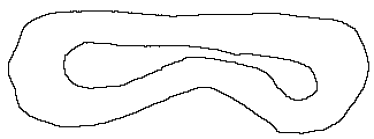
\includegraphics[interpolate=true,width=3.740000in,height=1.390000in]{contents/chapt5/figs/racing/porto-img0.png}}%
\end{pgfscope}%
\begin{pgfscope}%
\pgfpathrectangle{\pgfqpoint{0.150000in}{0.574949in}}{\pgfqpoint{3.737778in}{1.380103in}}%
\pgfusepath{clip}%
\pgfsetrectcap%
\pgfsetroundjoin%
\pgfsetlinewidth{2.007500pt}%
\definecolor{currentstroke}{rgb}{0.476471,0.036951,0.999829}%
\pgfsetstrokecolor{currentstroke}%
\pgfsetstrokeopacity{0.800000}%
\pgfsetdash{}{0pt}%
\pgfpathmoveto{\pgfqpoint{2.450171in}{1.610026in}}%
\pgfpathlineto{\pgfqpoint{2.443270in}{1.610026in}}%
\pgfusepath{stroke}%
\end{pgfscope}%
\begin{pgfscope}%
\pgfpathrectangle{\pgfqpoint{0.150000in}{0.574949in}}{\pgfqpoint{3.737778in}{1.380103in}}%
\pgfusepath{clip}%
\pgfsetrectcap%
\pgfsetroundjoin%
\pgfsetlinewidth{2.007500pt}%
\definecolor{currentstroke}{rgb}{0.445098,0.086133,0.999070}%
\pgfsetstrokecolor{currentstroke}%
\pgfsetstrokeopacity{0.800000}%
\pgfsetdash{}{0pt}%
\pgfpathmoveto{\pgfqpoint{2.443270in}{1.610026in}}%
\pgfpathlineto{\pgfqpoint{2.436305in}{1.610026in}}%
\pgfusepath{stroke}%
\end{pgfscope}%
\begin{pgfscope}%
\pgfpathrectangle{\pgfqpoint{0.150000in}{0.574949in}}{\pgfqpoint{3.737778in}{1.380103in}}%
\pgfusepath{clip}%
\pgfsetrectcap%
\pgfsetroundjoin%
\pgfsetlinewidth{2.007500pt}%
\definecolor{currentstroke}{rgb}{0.421569,0.122888,0.998103}%
\pgfsetstrokecolor{currentstroke}%
\pgfsetstrokeopacity{0.800000}%
\pgfsetdash{}{0pt}%
\pgfpathmoveto{\pgfqpoint{2.436305in}{1.610026in}}%
\pgfpathlineto{\pgfqpoint{2.429273in}{1.610042in}}%
\pgfusepath{stroke}%
\end{pgfscope}%
\begin{pgfscope}%
\pgfpathrectangle{\pgfqpoint{0.150000in}{0.574949in}}{\pgfqpoint{3.737778in}{1.380103in}}%
\pgfusepath{clip}%
\pgfsetrectcap%
\pgfsetroundjoin%
\pgfsetlinewidth{2.007500pt}%
\definecolor{currentstroke}{rgb}{0.390196,0.171626,0.996284}%
\pgfsetstrokecolor{currentstroke}%
\pgfsetstrokeopacity{0.800000}%
\pgfsetdash{}{0pt}%
\pgfpathmoveto{\pgfqpoint{2.429273in}{1.610042in}}%
\pgfpathlineto{\pgfqpoint{2.422177in}{1.610057in}}%
\pgfusepath{stroke}%
\end{pgfscope}%
\begin{pgfscope}%
\pgfpathrectangle{\pgfqpoint{0.150000in}{0.574949in}}{\pgfqpoint{3.737778in}{1.380103in}}%
\pgfusepath{clip}%
\pgfsetrectcap%
\pgfsetroundjoin%
\pgfsetlinewidth{2.007500pt}%
\definecolor{currentstroke}{rgb}{0.358824,0.219946,0.993859}%
\pgfsetstrokecolor{currentstroke}%
\pgfsetstrokeopacity{0.800000}%
\pgfsetdash{}{0pt}%
\pgfpathmoveto{\pgfqpoint{2.422177in}{1.610057in}}%
\pgfpathlineto{\pgfqpoint{2.415015in}{1.610088in}}%
\pgfusepath{stroke}%
\end{pgfscope}%
\begin{pgfscope}%
\pgfpathrectangle{\pgfqpoint{0.150000in}{0.574949in}}{\pgfqpoint{3.737778in}{1.380103in}}%
\pgfusepath{clip}%
\pgfsetrectcap%
\pgfsetroundjoin%
\pgfsetlinewidth{2.007500pt}%
\definecolor{currentstroke}{rgb}{0.335294,0.255843,0.991645}%
\pgfsetstrokecolor{currentstroke}%
\pgfsetstrokeopacity{0.800000}%
\pgfsetdash{}{0pt}%
\pgfpathmoveto{\pgfqpoint{2.415015in}{1.610088in}}%
\pgfpathlineto{\pgfqpoint{2.407788in}{1.610117in}}%
\pgfusepath{stroke}%
\end{pgfscope}%
\begin{pgfscope}%
\pgfpathrectangle{\pgfqpoint{0.150000in}{0.574949in}}{\pgfqpoint{3.737778in}{1.380103in}}%
\pgfusepath{clip}%
\pgfsetrectcap%
\pgfsetroundjoin%
\pgfsetlinewidth{2.007500pt}%
\definecolor{currentstroke}{rgb}{0.303922,0.303153,0.988165}%
\pgfsetstrokecolor{currentstroke}%
\pgfsetstrokeopacity{0.800000}%
\pgfsetdash{}{0pt}%
\pgfpathmoveto{\pgfqpoint{2.407788in}{1.610117in}}%
\pgfpathlineto{\pgfqpoint{2.400496in}{1.610162in}}%
\pgfusepath{stroke}%
\end{pgfscope}%
\begin{pgfscope}%
\pgfpathrectangle{\pgfqpoint{0.150000in}{0.574949in}}{\pgfqpoint{3.737778in}{1.380103in}}%
\pgfusepath{clip}%
\pgfsetrectcap%
\pgfsetroundjoin%
\pgfsetlinewidth{2.007500pt}%
\definecolor{currentstroke}{rgb}{0.272549,0.349727,0.984086}%
\pgfsetstrokecolor{currentstroke}%
\pgfsetstrokeopacity{0.800000}%
\pgfsetdash{}{0pt}%
\pgfpathmoveto{\pgfqpoint{2.400496in}{1.610162in}}%
\pgfpathlineto{\pgfqpoint{2.393138in}{1.610206in}}%
\pgfusepath{stroke}%
\end{pgfscope}%
\begin{pgfscope}%
\pgfpathrectangle{\pgfqpoint{0.150000in}{0.574949in}}{\pgfqpoint{3.737778in}{1.380103in}}%
\pgfusepath{clip}%
\pgfsetrectcap%
\pgfsetroundjoin%
\pgfsetlinewidth{2.007500pt}%
\definecolor{currentstroke}{rgb}{0.249020,0.384106,0.980635}%
\pgfsetstrokecolor{currentstroke}%
\pgfsetstrokeopacity{0.800000}%
\pgfsetdash{}{0pt}%
\pgfpathmoveto{\pgfqpoint{2.393138in}{1.610206in}}%
\pgfpathlineto{\pgfqpoint{2.385716in}{1.610268in}}%
\pgfusepath{stroke}%
\end{pgfscope}%
\begin{pgfscope}%
\pgfpathrectangle{\pgfqpoint{0.150000in}{0.574949in}}{\pgfqpoint{3.737778in}{1.380103in}}%
\pgfusepath{clip}%
\pgfsetrectcap%
\pgfsetroundjoin%
\pgfsetlinewidth{2.007500pt}%
\definecolor{currentstroke}{rgb}{0.217647,0.429121,0.975512}%
\pgfsetstrokecolor{currentstroke}%
\pgfsetstrokeopacity{0.800000}%
\pgfsetdash{}{0pt}%
\pgfpathmoveto{\pgfqpoint{2.385716in}{1.610268in}}%
\pgfpathlineto{\pgfqpoint{2.378227in}{1.610328in}}%
\pgfusepath{stroke}%
\end{pgfscope}%
\begin{pgfscope}%
\pgfpathrectangle{\pgfqpoint{0.150000in}{0.574949in}}{\pgfqpoint{3.737778in}{1.380103in}}%
\pgfusepath{clip}%
\pgfsetrectcap%
\pgfsetroundjoin%
\pgfsetlinewidth{2.007500pt}%
\definecolor{currentstroke}{rgb}{0.194118,0.462204,0.971281}%
\pgfsetstrokecolor{currentstroke}%
\pgfsetstrokeopacity{0.800000}%
\pgfsetdash{}{0pt}%
\pgfpathmoveto{\pgfqpoint{2.378227in}{1.610328in}}%
\pgfpathlineto{\pgfqpoint{2.370674in}{1.610407in}}%
\pgfusepath{stroke}%
\end{pgfscope}%
\begin{pgfscope}%
\pgfpathrectangle{\pgfqpoint{0.150000in}{0.574949in}}{\pgfqpoint{3.737778in}{1.380103in}}%
\pgfusepath{clip}%
\pgfsetrectcap%
\pgfsetroundjoin%
\pgfsetlinewidth{2.007500pt}%
\definecolor{currentstroke}{rgb}{0.162745,0.505325,0.965124}%
\pgfsetstrokecolor{currentstroke}%
\pgfsetstrokeopacity{0.800000}%
\pgfsetdash{}{0pt}%
\pgfpathmoveto{\pgfqpoint{2.370674in}{1.610407in}}%
\pgfpathlineto{\pgfqpoint{2.363055in}{1.610485in}}%
\pgfusepath{stroke}%
\end{pgfscope}%
\begin{pgfscope}%
\pgfpathrectangle{\pgfqpoint{0.150000in}{0.574949in}}{\pgfqpoint{3.737778in}{1.380103in}}%
\pgfusepath{clip}%
\pgfsetrectcap%
\pgfsetroundjoin%
\pgfsetlinewidth{2.007500pt}%
\definecolor{currentstroke}{rgb}{0.131373,0.547220,0.958381}%
\pgfsetstrokecolor{currentstroke}%
\pgfsetstrokeopacity{0.800000}%
\pgfsetdash{}{0pt}%
\pgfpathmoveto{\pgfqpoint{2.363055in}{1.610485in}}%
\pgfpathlineto{\pgfqpoint{2.355372in}{1.610582in}}%
\pgfusepath{stroke}%
\end{pgfscope}%
\begin{pgfscope}%
\pgfpathrectangle{\pgfqpoint{0.150000in}{0.574949in}}{\pgfqpoint{3.737778in}{1.380103in}}%
\pgfusepath{clip}%
\pgfsetrectcap%
\pgfsetroundjoin%
\pgfsetlinewidth{2.007500pt}%
\definecolor{currentstroke}{rgb}{0.107843,0.577774,0.952942}%
\pgfsetstrokecolor{currentstroke}%
\pgfsetstrokeopacity{0.800000}%
\pgfsetdash{}{0pt}%
\pgfpathmoveto{\pgfqpoint{2.355372in}{1.610582in}}%
\pgfpathlineto{\pgfqpoint{2.347623in}{1.610679in}}%
\pgfusepath{stroke}%
\end{pgfscope}%
\begin{pgfscope}%
\pgfpathrectangle{\pgfqpoint{0.150000in}{0.574949in}}{\pgfqpoint{3.737778in}{1.380103in}}%
\pgfusepath{clip}%
\pgfsetrectcap%
\pgfsetroundjoin%
\pgfsetlinewidth{2.007500pt}%
\definecolor{currentstroke}{rgb}{0.076471,0.617278,0.945184}%
\pgfsetstrokecolor{currentstroke}%
\pgfsetstrokeopacity{0.800000}%
\pgfsetdash{}{0pt}%
\pgfpathmoveto{\pgfqpoint{2.347623in}{1.610679in}}%
\pgfpathlineto{\pgfqpoint{2.339809in}{1.610795in}}%
\pgfusepath{stroke}%
\end{pgfscope}%
\begin{pgfscope}%
\pgfpathrectangle{\pgfqpoint{0.150000in}{0.574949in}}{\pgfqpoint{3.737778in}{1.380103in}}%
\pgfusepath{clip}%
\pgfsetrectcap%
\pgfsetroundjoin%
\pgfsetlinewidth{2.007500pt}%
\definecolor{currentstroke}{rgb}{0.045098,0.655284,0.936852}%
\pgfsetstrokecolor{currentstroke}%
\pgfsetstrokeopacity{0.800000}%
\pgfsetdash{}{0pt}%
\pgfpathmoveto{\pgfqpoint{2.339809in}{1.610795in}}%
\pgfpathlineto{\pgfqpoint{2.331929in}{1.610912in}}%
\pgfusepath{stroke}%
\end{pgfscope}%
\begin{pgfscope}%
\pgfpathrectangle{\pgfqpoint{0.150000in}{0.574949in}}{\pgfqpoint{3.737778in}{1.380103in}}%
\pgfusepath{clip}%
\pgfsetrectcap%
\pgfsetroundjoin%
\pgfsetlinewidth{2.007500pt}%
\definecolor{currentstroke}{rgb}{0.021569,0.682749,0.930229}%
\pgfsetstrokecolor{currentstroke}%
\pgfsetstrokeopacity{0.800000}%
\pgfsetdash{}{0pt}%
\pgfpathmoveto{\pgfqpoint{2.331929in}{1.610912in}}%
\pgfpathlineto{\pgfqpoint{2.323985in}{1.611048in}}%
\pgfusepath{stroke}%
\end{pgfscope}%
\begin{pgfscope}%
\pgfpathrectangle{\pgfqpoint{0.150000in}{0.574949in}}{\pgfqpoint{3.737778in}{1.380103in}}%
\pgfusepath{clip}%
\pgfsetrectcap%
\pgfsetroundjoin%
\pgfsetlinewidth{2.007500pt}%
\definecolor{currentstroke}{rgb}{0.009804,0.717912,0.920906}%
\pgfsetstrokecolor{currentstroke}%
\pgfsetstrokeopacity{0.800000}%
\pgfsetdash{}{0pt}%
\pgfpathmoveto{\pgfqpoint{2.323985in}{1.611048in}}%
\pgfpathlineto{\pgfqpoint{2.315975in}{1.611186in}}%
\pgfusepath{stroke}%
\end{pgfscope}%
\begin{pgfscope}%
\pgfpathrectangle{\pgfqpoint{0.150000in}{0.574949in}}{\pgfqpoint{3.737778in}{1.380103in}}%
\pgfusepath{clip}%
\pgfsetrectcap%
\pgfsetroundjoin%
\pgfsetlinewidth{2.007500pt}%
\definecolor{currentstroke}{rgb}{0.041176,0.751332,0.911023}%
\pgfsetstrokecolor{currentstroke}%
\pgfsetstrokeopacity{0.800000}%
\pgfsetdash{}{0pt}%
\pgfpathmoveto{\pgfqpoint{2.315975in}{1.611186in}}%
\pgfpathlineto{\pgfqpoint{2.307900in}{1.611344in}}%
\pgfusepath{stroke}%
\end{pgfscope}%
\begin{pgfscope}%
\pgfpathrectangle{\pgfqpoint{0.150000in}{0.574949in}}{\pgfqpoint{3.737778in}{1.380103in}}%
\pgfusepath{clip}%
\pgfsetrectcap%
\pgfsetroundjoin%
\pgfsetlinewidth{2.007500pt}%
\definecolor{currentstroke}{rgb}{0.064706,0.775204,0.903247}%
\pgfsetstrokecolor{currentstroke}%
\pgfsetstrokeopacity{0.800000}%
\pgfsetdash{}{0pt}%
\pgfpathmoveto{\pgfqpoint{2.307900in}{1.611344in}}%
\pgfpathlineto{\pgfqpoint{2.299760in}{1.611504in}}%
\pgfusepath{stroke}%
\end{pgfscope}%
\begin{pgfscope}%
\pgfpathrectangle{\pgfqpoint{0.150000in}{0.574949in}}{\pgfqpoint{3.737778in}{1.380103in}}%
\pgfusepath{clip}%
\pgfsetrectcap%
\pgfsetroundjoin%
\pgfsetlinewidth{2.007500pt}%
\definecolor{currentstroke}{rgb}{0.096078,0.805381,0.892401}%
\pgfsetstrokecolor{currentstroke}%
\pgfsetstrokeopacity{0.800000}%
\pgfsetdash{}{0pt}%
\pgfpathmoveto{\pgfqpoint{2.299760in}{1.611504in}}%
\pgfpathlineto{\pgfqpoint{2.291555in}{1.611684in}}%
\pgfusepath{stroke}%
\end{pgfscope}%
\begin{pgfscope}%
\pgfpathrectangle{\pgfqpoint{0.150000in}{0.574949in}}{\pgfqpoint{3.737778in}{1.380103in}}%
\pgfusepath{clip}%
\pgfsetrectcap%
\pgfsetroundjoin%
\pgfsetlinewidth{2.007500pt}%
\definecolor{currentstroke}{rgb}{0.135294,0.840344,0.878081}%
\pgfsetstrokecolor{currentstroke}%
\pgfsetstrokeopacity{0.800000}%
\pgfsetdash{}{0pt}%
\pgfpathmoveto{\pgfqpoint{2.291555in}{1.611684in}}%
\pgfpathlineto{\pgfqpoint{2.283274in}{1.611868in}}%
\pgfusepath{stroke}%
\end{pgfscope}%
\begin{pgfscope}%
\pgfpathrectangle{\pgfqpoint{0.150000in}{0.574949in}}{\pgfqpoint{3.737778in}{1.380103in}}%
\pgfusepath{clip}%
\pgfsetrectcap%
\pgfsetroundjoin%
\pgfsetlinewidth{2.007500pt}%
\definecolor{currentstroke}{rgb}{0.166667,0.866025,0.866025}%
\pgfsetstrokecolor{currentstroke}%
\pgfsetstrokeopacity{0.800000}%
\pgfsetdash{}{0pt}%
\pgfpathmoveto{\pgfqpoint{2.283274in}{1.611868in}}%
\pgfpathlineto{\pgfqpoint{2.274918in}{1.612071in}}%
\pgfusepath{stroke}%
\end{pgfscope}%
\begin{pgfscope}%
\pgfpathrectangle{\pgfqpoint{0.150000in}{0.574949in}}{\pgfqpoint{3.737778in}{1.380103in}}%
\pgfusepath{clip}%
\pgfsetrectcap%
\pgfsetroundjoin%
\pgfsetlinewidth{2.007500pt}%
\definecolor{currentstroke}{rgb}{0.198039,0.889604,0.853444}%
\pgfsetstrokecolor{currentstroke}%
\pgfsetstrokeopacity{0.800000}%
\pgfsetdash{}{0pt}%
\pgfpathmoveto{\pgfqpoint{2.274918in}{1.612071in}}%
\pgfpathlineto{\pgfqpoint{2.266486in}{1.612279in}}%
\pgfusepath{stroke}%
\end{pgfscope}%
\begin{pgfscope}%
\pgfpathrectangle{\pgfqpoint{0.150000in}{0.574949in}}{\pgfqpoint{3.737778in}{1.380103in}}%
\pgfusepath{clip}%
\pgfsetrectcap%
\pgfsetroundjoin%
\pgfsetlinewidth{2.007500pt}%
\definecolor{currentstroke}{rgb}{0.229412,0.911023,0.840344}%
\pgfsetstrokecolor{currentstroke}%
\pgfsetstrokeopacity{0.800000}%
\pgfsetdash{}{0pt}%
\pgfpathmoveto{\pgfqpoint{2.266486in}{1.612279in}}%
\pgfpathlineto{\pgfqpoint{2.257979in}{1.612507in}}%
\pgfusepath{stroke}%
\end{pgfscope}%
\begin{pgfscope}%
\pgfpathrectangle{\pgfqpoint{0.150000in}{0.574949in}}{\pgfqpoint{3.737778in}{1.380103in}}%
\pgfusepath{clip}%
\pgfsetrectcap%
\pgfsetroundjoin%
\pgfsetlinewidth{2.007500pt}%
\definecolor{currentstroke}{rgb}{0.268627,0.934680,0.823253}%
\pgfsetstrokecolor{currentstroke}%
\pgfsetstrokeopacity{0.800000}%
\pgfsetdash{}{0pt}%
\pgfpathmoveto{\pgfqpoint{2.257979in}{1.612507in}}%
\pgfpathlineto{\pgfqpoint{2.249396in}{1.612739in}}%
\pgfusepath{stroke}%
\end{pgfscope}%
\begin{pgfscope}%
\pgfpathrectangle{\pgfqpoint{0.150000in}{0.574949in}}{\pgfqpoint{3.737778in}{1.380103in}}%
\pgfusepath{clip}%
\pgfsetrectcap%
\pgfsetroundjoin%
\pgfsetlinewidth{2.007500pt}%
\definecolor{currentstroke}{rgb}{0.300000,0.951057,0.809017}%
\pgfsetstrokecolor{currentstroke}%
\pgfsetstrokeopacity{0.800000}%
\pgfsetdash{}{0pt}%
\pgfpathmoveto{\pgfqpoint{2.249396in}{1.612739in}}%
\pgfpathlineto{\pgfqpoint{2.240737in}{1.612992in}}%
\pgfusepath{stroke}%
\end{pgfscope}%
\begin{pgfscope}%
\pgfpathrectangle{\pgfqpoint{0.150000in}{0.574949in}}{\pgfqpoint{3.737778in}{1.380103in}}%
\pgfusepath{clip}%
\pgfsetrectcap%
\pgfsetroundjoin%
\pgfsetlinewidth{2.007500pt}%
\definecolor{currentstroke}{rgb}{0.331373,0.965124,0.794290}%
\pgfsetstrokecolor{currentstroke}%
\pgfsetstrokeopacity{0.800000}%
\pgfsetdash{}{0pt}%
\pgfpathmoveto{\pgfqpoint{2.240737in}{1.612992in}}%
\pgfpathlineto{\pgfqpoint{2.232003in}{1.613250in}}%
\pgfusepath{stroke}%
\end{pgfscope}%
\begin{pgfscope}%
\pgfpathrectangle{\pgfqpoint{0.150000in}{0.574949in}}{\pgfqpoint{3.737778in}{1.380103in}}%
\pgfusepath{clip}%
\pgfsetrectcap%
\pgfsetroundjoin%
\pgfsetlinewidth{2.007500pt}%
\definecolor{currentstroke}{rgb}{0.362745,0.976848,0.779081}%
\pgfsetstrokecolor{currentstroke}%
\pgfsetstrokeopacity{0.800000}%
\pgfsetdash{}{0pt}%
\pgfpathmoveto{\pgfqpoint{2.232003in}{1.613250in}}%
\pgfpathlineto{\pgfqpoint{2.223194in}{1.613530in}}%
\pgfusepath{stroke}%
\end{pgfscope}%
\begin{pgfscope}%
\pgfpathrectangle{\pgfqpoint{0.150000in}{0.574949in}}{\pgfqpoint{3.737778in}{1.380103in}}%
\pgfusepath{clip}%
\pgfsetrectcap%
\pgfsetroundjoin%
\pgfsetlinewidth{2.007500pt}%
\definecolor{currentstroke}{rgb}{0.394118,0.986201,0.763398}%
\pgfsetstrokecolor{currentstroke}%
\pgfsetstrokeopacity{0.800000}%
\pgfsetdash{}{0pt}%
\pgfpathmoveto{\pgfqpoint{2.223194in}{1.613530in}}%
\pgfpathlineto{\pgfqpoint{2.214308in}{1.613815in}}%
\pgfusepath{stroke}%
\end{pgfscope}%
\begin{pgfscope}%
\pgfpathrectangle{\pgfqpoint{0.150000in}{0.574949in}}{\pgfqpoint{3.737778in}{1.380103in}}%
\pgfusepath{clip}%
\pgfsetrectcap%
\pgfsetroundjoin%
\pgfsetlinewidth{2.007500pt}%
\definecolor{currentstroke}{rgb}{0.433333,0.994522,0.743145}%
\pgfsetstrokecolor{currentstroke}%
\pgfsetstrokeopacity{0.800000}%
\pgfsetdash{}{0pt}%
\pgfpathmoveto{\pgfqpoint{2.214308in}{1.613815in}}%
\pgfpathlineto{\pgfqpoint{2.205348in}{1.614121in}}%
\pgfusepath{stroke}%
\end{pgfscope}%
\begin{pgfscope}%
\pgfpathrectangle{\pgfqpoint{0.150000in}{0.574949in}}{\pgfqpoint{3.737778in}{1.380103in}}%
\pgfusepath{clip}%
\pgfsetrectcap%
\pgfsetroundjoin%
\pgfsetlinewidth{2.007500pt}%
\definecolor{currentstroke}{rgb}{0.464706,0.998464,0.726434}%
\pgfsetstrokecolor{currentstroke}%
\pgfsetstrokeopacity{0.800000}%
\pgfsetdash{}{0pt}%
\pgfpathmoveto{\pgfqpoint{2.205348in}{1.614121in}}%
\pgfpathlineto{\pgfqpoint{2.196312in}{1.614434in}}%
\pgfusepath{stroke}%
\end{pgfscope}%
\begin{pgfscope}%
\pgfpathrectangle{\pgfqpoint{0.150000in}{0.574949in}}{\pgfqpoint{3.737778in}{1.380103in}}%
\pgfusepath{clip}%
\pgfsetrectcap%
\pgfsetroundjoin%
\pgfsetlinewidth{2.007500pt}%
\definecolor{currentstroke}{rgb}{0.496078,0.999981,0.709281}%
\pgfsetstrokecolor{currentstroke}%
\pgfsetstrokeopacity{0.800000}%
\pgfsetdash{}{0pt}%
\pgfpathmoveto{\pgfqpoint{2.196312in}{1.614434in}}%
\pgfpathlineto{\pgfqpoint{2.187201in}{1.614768in}}%
\pgfusepath{stroke}%
\end{pgfscope}%
\begin{pgfscope}%
\pgfpathrectangle{\pgfqpoint{0.150000in}{0.574949in}}{\pgfqpoint{3.737778in}{1.380103in}}%
\pgfusepath{clip}%
\pgfsetrectcap%
\pgfsetroundjoin%
\pgfsetlinewidth{2.007500pt}%
\definecolor{currentstroke}{rgb}{0.527451,0.999070,0.691698}%
\pgfsetstrokecolor{currentstroke}%
\pgfsetstrokeopacity{0.800000}%
\pgfsetdash{}{0pt}%
\pgfpathmoveto{\pgfqpoint{2.187201in}{1.614768in}}%
\pgfpathlineto{\pgfqpoint{2.178014in}{1.615109in}}%
\pgfusepath{stroke}%
\end{pgfscope}%
\begin{pgfscope}%
\pgfpathrectangle{\pgfqpoint{0.150000in}{0.574949in}}{\pgfqpoint{3.737778in}{1.380103in}}%
\pgfusepath{clip}%
\pgfsetrectcap%
\pgfsetroundjoin%
\pgfsetlinewidth{2.007500pt}%
\definecolor{currentstroke}{rgb}{0.566667,0.994522,0.669131}%
\pgfsetstrokecolor{currentstroke}%
\pgfsetstrokeopacity{0.800000}%
\pgfsetdash{}{0pt}%
\pgfpathmoveto{\pgfqpoint{2.178014in}{1.615109in}}%
\pgfpathlineto{\pgfqpoint{2.168752in}{1.615473in}}%
\pgfusepath{stroke}%
\end{pgfscope}%
\begin{pgfscope}%
\pgfpathrectangle{\pgfqpoint{0.150000in}{0.574949in}}{\pgfqpoint{3.737778in}{1.380103in}}%
\pgfusepath{clip}%
\pgfsetrectcap%
\pgfsetroundjoin%
\pgfsetlinewidth{2.007500pt}%
\definecolor{currentstroke}{rgb}{0.598039,0.988165,0.650618}%
\pgfsetstrokecolor{currentstroke}%
\pgfsetstrokeopacity{0.800000}%
\pgfsetdash{}{0pt}%
\pgfpathmoveto{\pgfqpoint{2.168752in}{1.615473in}}%
\pgfpathlineto{\pgfqpoint{2.159414in}{1.615843in}}%
\pgfusepath{stroke}%
\end{pgfscope}%
\begin{pgfscope}%
\pgfpathrectangle{\pgfqpoint{0.150000in}{0.574949in}}{\pgfqpoint{3.737778in}{1.380103in}}%
\pgfusepath{clip}%
\pgfsetrectcap%
\pgfsetroundjoin%
\pgfsetlinewidth{2.007500pt}%
\definecolor{currentstroke}{rgb}{0.629412,0.979410,0.631711}%
\pgfsetstrokecolor{currentstroke}%
\pgfsetstrokeopacity{0.800000}%
\pgfsetdash{}{0pt}%
\pgfpathmoveto{\pgfqpoint{2.159414in}{1.615843in}}%
\pgfpathlineto{\pgfqpoint{2.150001in}{1.616236in}}%
\pgfusepath{stroke}%
\end{pgfscope}%
\begin{pgfscope}%
\pgfpathrectangle{\pgfqpoint{0.150000in}{0.574949in}}{\pgfqpoint{3.737778in}{1.380103in}}%
\pgfusepath{clip}%
\pgfsetrectcap%
\pgfsetroundjoin%
\pgfsetlinewidth{2.007500pt}%
\definecolor{currentstroke}{rgb}{0.660784,0.968276,0.612420}%
\pgfsetstrokecolor{currentstroke}%
\pgfsetstrokeopacity{0.800000}%
\pgfsetdash{}{0pt}%
\pgfpathmoveto{\pgfqpoint{2.150001in}{1.616236in}}%
\pgfpathlineto{\pgfqpoint{2.140513in}{1.616636in}}%
\pgfusepath{stroke}%
\end{pgfscope}%
\begin{pgfscope}%
\pgfpathrectangle{\pgfqpoint{0.150000in}{0.574949in}}{\pgfqpoint{3.737778in}{1.380103in}}%
\pgfusepath{clip}%
\pgfsetrectcap%
\pgfsetroundjoin%
\pgfsetlinewidth{2.007500pt}%
\definecolor{currentstroke}{rgb}{0.692157,0.954791,0.592758}%
\pgfsetstrokecolor{currentstroke}%
\pgfsetstrokeopacity{0.800000}%
\pgfsetdash{}{0pt}%
\pgfpathmoveto{\pgfqpoint{2.140513in}{1.616636in}}%
\pgfpathlineto{\pgfqpoint{2.130950in}{1.617061in}}%
\pgfusepath{stroke}%
\end{pgfscope}%
\begin{pgfscope}%
\pgfpathrectangle{\pgfqpoint{0.150000in}{0.574949in}}{\pgfqpoint{3.737778in}{1.380103in}}%
\pgfusepath{clip}%
\pgfsetrectcap%
\pgfsetroundjoin%
\pgfsetlinewidth{2.007500pt}%
\definecolor{currentstroke}{rgb}{0.731373,0.934680,0.567675}%
\pgfsetstrokecolor{currentstroke}%
\pgfsetstrokeopacity{0.800000}%
\pgfsetdash{}{0pt}%
\pgfpathmoveto{\pgfqpoint{2.130950in}{1.617061in}}%
\pgfpathlineto{\pgfqpoint{2.121311in}{1.617492in}}%
\pgfusepath{stroke}%
\end{pgfscope}%
\begin{pgfscope}%
\pgfpathrectangle{\pgfqpoint{0.150000in}{0.574949in}}{\pgfqpoint{3.737778in}{1.380103in}}%
\pgfusepath{clip}%
\pgfsetrectcap%
\pgfsetroundjoin%
\pgfsetlinewidth{2.007500pt}%
\definecolor{currentstroke}{rgb}{0.762745,0.916034,0.547220}%
\pgfsetstrokecolor{currentstroke}%
\pgfsetstrokeopacity{0.800000}%
\pgfsetdash{}{0pt}%
\pgfpathmoveto{\pgfqpoint{2.121311in}{1.617492in}}%
\pgfpathlineto{\pgfqpoint{2.111597in}{1.617948in}}%
\pgfusepath{stroke}%
\end{pgfscope}%
\begin{pgfscope}%
\pgfpathrectangle{\pgfqpoint{0.150000in}{0.574949in}}{\pgfqpoint{3.737778in}{1.380103in}}%
\pgfusepath{clip}%
\pgfsetrectcap%
\pgfsetroundjoin%
\pgfsetlinewidth{2.007500pt}%
\definecolor{currentstroke}{rgb}{0.801961,0.889604,0.521185}%
\pgfsetstrokecolor{currentstroke}%
\pgfsetstrokeopacity{0.800000}%
\pgfsetdash{}{0pt}%
\pgfpathmoveto{\pgfqpoint{2.111597in}{1.617948in}}%
\pgfpathlineto{\pgfqpoint{2.101801in}{1.618412in}}%
\pgfusepath{stroke}%
\end{pgfscope}%
\begin{pgfscope}%
\pgfpathrectangle{\pgfqpoint{0.150000in}{0.574949in}}{\pgfqpoint{3.737778in}{1.380103in}}%
\pgfusepath{clip}%
\pgfsetrectcap%
\pgfsetroundjoin%
\pgfsetlinewidth{2.007500pt}%
\definecolor{currentstroke}{rgb}{0.833333,0.866025,0.500000}%
\pgfsetstrokecolor{currentstroke}%
\pgfsetstrokeopacity{0.800000}%
\pgfsetdash{}{0pt}%
\pgfpathmoveto{\pgfqpoint{2.101801in}{1.618412in}}%
\pgfpathlineto{\pgfqpoint{2.091922in}{1.618870in}}%
\pgfusepath{stroke}%
\end{pgfscope}%
\begin{pgfscope}%
\pgfpathrectangle{\pgfqpoint{0.150000in}{0.574949in}}{\pgfqpoint{3.737778in}{1.380103in}}%
\pgfusepath{clip}%
\pgfsetrectcap%
\pgfsetroundjoin%
\pgfsetlinewidth{2.007500pt}%
\definecolor{currentstroke}{rgb}{0.872549,0.833602,0.473094}%
\pgfsetstrokecolor{currentstroke}%
\pgfsetstrokeopacity{0.800000}%
\pgfsetdash{}{0pt}%
\pgfpathmoveto{\pgfqpoint{2.091922in}{1.618870in}}%
\pgfpathlineto{\pgfqpoint{2.081960in}{1.619338in}}%
\pgfusepath{stroke}%
\end{pgfscope}%
\begin{pgfscope}%
\pgfpathrectangle{\pgfqpoint{0.150000in}{0.574949in}}{\pgfqpoint{3.737778in}{1.380103in}}%
\pgfusepath{clip}%
\pgfsetrectcap%
\pgfsetroundjoin%
\pgfsetlinewidth{2.007500pt}%
\definecolor{currentstroke}{rgb}{0.911765,0.798017,0.445738}%
\pgfsetstrokecolor{currentstroke}%
\pgfsetstrokeopacity{0.800000}%
\pgfsetdash{}{0pt}%
\pgfpathmoveto{\pgfqpoint{2.081960in}{1.619338in}}%
\pgfpathlineto{\pgfqpoint{2.071915in}{1.619801in}}%
\pgfusepath{stroke}%
\end{pgfscope}%
\begin{pgfscope}%
\pgfpathrectangle{\pgfqpoint{0.150000in}{0.574949in}}{\pgfqpoint{3.737778in}{1.380103in}}%
\pgfusepath{clip}%
\pgfsetrectcap%
\pgfsetroundjoin%
\pgfsetlinewidth{2.007500pt}%
\definecolor{currentstroke}{rgb}{0.943137,0.767363,0.423549}%
\pgfsetstrokecolor{currentstroke}%
\pgfsetstrokeopacity{0.800000}%
\pgfsetdash{}{0pt}%
\pgfpathmoveto{\pgfqpoint{2.071915in}{1.619801in}}%
\pgfpathlineto{\pgfqpoint{2.061787in}{1.620272in}}%
\pgfusepath{stroke}%
\end{pgfscope}%
\begin{pgfscope}%
\pgfpathrectangle{\pgfqpoint{0.150000in}{0.574949in}}{\pgfqpoint{3.737778in}{1.380103in}}%
\pgfusepath{clip}%
\pgfsetrectcap%
\pgfsetroundjoin%
\pgfsetlinewidth{2.007500pt}%
\definecolor{currentstroke}{rgb}{0.982353,0.726434,0.395451}%
\pgfsetstrokecolor{currentstroke}%
\pgfsetstrokeopacity{0.800000}%
\pgfsetdash{}{0pt}%
\pgfpathmoveto{\pgfqpoint{2.061787in}{1.620272in}}%
\pgfpathlineto{\pgfqpoint{2.051576in}{1.620736in}}%
\pgfusepath{stroke}%
\end{pgfscope}%
\begin{pgfscope}%
\pgfpathrectangle{\pgfqpoint{0.150000in}{0.574949in}}{\pgfqpoint{3.737778in}{1.380103in}}%
\pgfusepath{clip}%
\pgfsetrectcap%
\pgfsetroundjoin%
\pgfsetlinewidth{2.007500pt}%
\definecolor{currentstroke}{rgb}{1.000000,0.682749,0.366979}%
\pgfsetstrokecolor{currentstroke}%
\pgfsetstrokeopacity{0.800000}%
\pgfsetdash{}{0pt}%
\pgfpathmoveto{\pgfqpoint{2.051576in}{1.620736in}}%
\pgfpathlineto{\pgfqpoint{2.041283in}{1.621208in}}%
\pgfusepath{stroke}%
\end{pgfscope}%
\begin{pgfscope}%
\pgfpathrectangle{\pgfqpoint{0.150000in}{0.574949in}}{\pgfqpoint{3.737778in}{1.380103in}}%
\pgfusepath{clip}%
\pgfsetrectcap%
\pgfsetroundjoin%
\pgfsetlinewidth{2.007500pt}%
\definecolor{currentstroke}{rgb}{1.000000,0.645928,0.343949}%
\pgfsetstrokecolor{currentstroke}%
\pgfsetstrokeopacity{0.800000}%
\pgfsetdash{}{0pt}%
\pgfpathmoveto{\pgfqpoint{2.041283in}{1.621208in}}%
\pgfpathlineto{\pgfqpoint{2.030906in}{1.621669in}}%
\pgfusepath{stroke}%
\end{pgfscope}%
\begin{pgfscope}%
\pgfpathrectangle{\pgfqpoint{0.150000in}{0.574949in}}{\pgfqpoint{3.737778in}{1.380103in}}%
\pgfusepath{clip}%
\pgfsetrectcap%
\pgfsetroundjoin%
\pgfsetlinewidth{2.007500pt}%
\definecolor{currentstroke}{rgb}{1.000000,0.597707,0.314870}%
\pgfsetstrokecolor{currentstroke}%
\pgfsetstrokeopacity{0.800000}%
\pgfsetdash{}{0pt}%
\pgfpathmoveto{\pgfqpoint{2.030906in}{1.621669in}}%
\pgfpathlineto{\pgfqpoint{2.020447in}{1.622135in}}%
\pgfusepath{stroke}%
\end{pgfscope}%
\begin{pgfscope}%
\pgfpathrectangle{\pgfqpoint{0.150000in}{0.574949in}}{\pgfqpoint{3.737778in}{1.380103in}}%
\pgfusepath{clip}%
\pgfsetrectcap%
\pgfsetroundjoin%
\pgfsetlinewidth{2.007500pt}%
\definecolor{currentstroke}{rgb}{1.000000,0.557489,0.291390}%
\pgfsetstrokecolor{currentstroke}%
\pgfsetstrokeopacity{0.800000}%
\pgfsetdash{}{0pt}%
\pgfpathmoveto{\pgfqpoint{2.020447in}{1.622135in}}%
\pgfpathlineto{\pgfqpoint{2.009904in}{1.622589in}}%
\pgfusepath{stroke}%
\end{pgfscope}%
\begin{pgfscope}%
\pgfpathrectangle{\pgfqpoint{0.150000in}{0.574949in}}{\pgfqpoint{3.737778in}{1.380103in}}%
\pgfusepath{clip}%
\pgfsetrectcap%
\pgfsetroundjoin%
\pgfsetlinewidth{2.007500pt}%
\definecolor{currentstroke}{rgb}{1.000000,0.505325,0.261793}%
\pgfsetstrokecolor{currentstroke}%
\pgfsetstrokeopacity{0.800000}%
\pgfsetdash{}{0pt}%
\pgfpathmoveto{\pgfqpoint{2.009904in}{1.622589in}}%
\pgfpathlineto{\pgfqpoint{1.999278in}{1.623045in}}%
\pgfusepath{stroke}%
\end{pgfscope}%
\begin{pgfscope}%
\pgfpathrectangle{\pgfqpoint{0.150000in}{0.574949in}}{\pgfqpoint{3.737778in}{1.380103in}}%
\pgfusepath{clip}%
\pgfsetrectcap%
\pgfsetroundjoin%
\pgfsetlinewidth{2.007500pt}%
\definecolor{currentstroke}{rgb}{1.000000,0.451244,0.231948}%
\pgfsetstrokecolor{currentstroke}%
\pgfsetstrokeopacity{0.800000}%
\pgfsetdash{}{0pt}%
\pgfpathmoveto{\pgfqpoint{1.999278in}{1.623045in}}%
\pgfpathlineto{\pgfqpoint{1.988569in}{1.623486in}}%
\pgfusepath{stroke}%
\end{pgfscope}%
\begin{pgfscope}%
\pgfpathrectangle{\pgfqpoint{0.150000in}{0.574949in}}{\pgfqpoint{3.737778in}{1.380103in}}%
\pgfusepath{clip}%
\pgfsetrectcap%
\pgfsetroundjoin%
\pgfsetlinewidth{2.007500pt}%
\definecolor{currentstroke}{rgb}{1.000000,0.406737,0.207912}%
\pgfsetstrokecolor{currentstroke}%
\pgfsetstrokeopacity{0.800000}%
\pgfsetdash{}{0pt}%
\pgfpathmoveto{\pgfqpoint{1.988569in}{1.623486in}}%
\pgfpathlineto{\pgfqpoint{1.977777in}{1.623928in}}%
\pgfusepath{stroke}%
\end{pgfscope}%
\begin{pgfscope}%
\pgfpathrectangle{\pgfqpoint{0.150000in}{0.574949in}}{\pgfqpoint{3.737778in}{1.380103in}}%
\pgfusepath{clip}%
\pgfsetrectcap%
\pgfsetroundjoin%
\pgfsetlinewidth{2.007500pt}%
\definecolor{currentstroke}{rgb}{1.000000,0.349727,0.177691}%
\pgfsetstrokecolor{currentstroke}%
\pgfsetstrokeopacity{0.800000}%
\pgfsetdash{}{0pt}%
\pgfpathmoveto{\pgfqpoint{1.977777in}{1.623928in}}%
\pgfpathlineto{\pgfqpoint{1.966901in}{1.624353in}}%
\pgfusepath{stroke}%
\end{pgfscope}%
\begin{pgfscope}%
\pgfpathrectangle{\pgfqpoint{0.150000in}{0.574949in}}{\pgfqpoint{3.737778in}{1.380103in}}%
\pgfusepath{clip}%
\pgfsetrectcap%
\pgfsetroundjoin%
\pgfsetlinewidth{2.007500pt}%
\definecolor{currentstroke}{rgb}{1.000000,0.303153,0.153392}%
\pgfsetstrokecolor{currentstroke}%
\pgfsetstrokeopacity{0.800000}%
\pgfsetdash{}{0pt}%
\pgfpathmoveto{\pgfqpoint{1.966901in}{1.624353in}}%
\pgfpathlineto{\pgfqpoint{1.955942in}{1.624778in}}%
\pgfusepath{stroke}%
\end{pgfscope}%
\begin{pgfscope}%
\pgfpathrectangle{\pgfqpoint{0.150000in}{0.574949in}}{\pgfqpoint{3.737778in}{1.380103in}}%
\pgfusepath{clip}%
\pgfsetrectcap%
\pgfsetroundjoin%
\pgfsetlinewidth{2.007500pt}%
\definecolor{currentstroke}{rgb}{1.000000,0.243914,0.122888}%
\pgfsetstrokecolor{currentstroke}%
\pgfsetstrokeopacity{0.800000}%
\pgfsetdash{}{0pt}%
\pgfpathmoveto{\pgfqpoint{1.955942in}{1.624778in}}%
\pgfpathlineto{\pgfqpoint{1.944900in}{1.625184in}}%
\pgfusepath{stroke}%
\end{pgfscope}%
\begin{pgfscope}%
\pgfpathrectangle{\pgfqpoint{0.150000in}{0.574949in}}{\pgfqpoint{3.737778in}{1.380103in}}%
\pgfusepath{clip}%
\pgfsetrectcap%
\pgfsetroundjoin%
\pgfsetlinewidth{2.007500pt}%
\definecolor{currentstroke}{rgb}{1.000000,0.183750,0.092268}%
\pgfsetstrokecolor{currentstroke}%
\pgfsetstrokeopacity{0.800000}%
\pgfsetdash{}{0pt}%
\pgfpathmoveto{\pgfqpoint{1.944900in}{1.625184in}}%
\pgfpathlineto{\pgfqpoint{1.933775in}{1.625588in}}%
\pgfusepath{stroke}%
\end{pgfscope}%
\begin{pgfscope}%
\pgfpathrectangle{\pgfqpoint{0.150000in}{0.574949in}}{\pgfqpoint{3.737778in}{1.380103in}}%
\pgfusepath{clip}%
\pgfsetrectcap%
\pgfsetroundjoin%
\pgfsetlinewidth{2.007500pt}%
\definecolor{currentstroke}{rgb}{1.000000,0.135105,0.067708}%
\pgfsetstrokecolor{currentstroke}%
\pgfsetstrokeopacity{0.800000}%
\pgfsetdash{}{0pt}%
\pgfpathmoveto{\pgfqpoint{1.933775in}{1.625588in}}%
\pgfpathlineto{\pgfqpoint{1.922566in}{1.625973in}}%
\pgfusepath{stroke}%
\end{pgfscope}%
\begin{pgfscope}%
\pgfpathrectangle{\pgfqpoint{0.150000in}{0.574949in}}{\pgfqpoint{3.737778in}{1.380103in}}%
\pgfusepath{clip}%
\pgfsetrectcap%
\pgfsetroundjoin%
\pgfsetlinewidth{2.007500pt}%
\definecolor{currentstroke}{rgb}{1.000000,0.073853,0.036951}%
\pgfsetstrokecolor{currentstroke}%
\pgfsetstrokeopacity{0.800000}%
\pgfsetdash{}{0pt}%
\pgfpathmoveto{\pgfqpoint{1.922566in}{1.625973in}}%
\pgfpathlineto{\pgfqpoint{1.911275in}{1.626355in}}%
\pgfusepath{stroke}%
\end{pgfscope}%
\begin{pgfscope}%
\pgfpathrectangle{\pgfqpoint{0.150000in}{0.574949in}}{\pgfqpoint{3.737778in}{1.380103in}}%
\pgfusepath{clip}%
\pgfsetrectcap%
\pgfsetroundjoin%
\pgfsetlinewidth{2.007500pt}%
\definecolor{currentstroke}{rgb}{1.000000,0.036951,0.018479}%
\pgfsetstrokecolor{currentstroke}%
\pgfsetstrokeopacity{0.800000}%
\pgfsetdash{}{0pt}%
\pgfpathmoveto{\pgfqpoint{1.911275in}{1.626355in}}%
\pgfpathlineto{\pgfqpoint{1.899899in}{1.626716in}}%
\pgfusepath{stroke}%
\end{pgfscope}%
\begin{pgfscope}%
\pgfpathrectangle{\pgfqpoint{0.150000in}{0.574949in}}{\pgfqpoint{3.737778in}{1.380103in}}%
\pgfusepath{clip}%
\pgfsetrectcap%
\pgfsetroundjoin%
\pgfsetlinewidth{2.007500pt}%
\definecolor{currentstroke}{rgb}{1.000000,0.000000,0.000000}%
\pgfsetstrokecolor{currentstroke}%
\pgfsetstrokeopacity{0.800000}%
\pgfsetdash{}{0pt}%
\pgfpathmoveto{\pgfqpoint{1.899899in}{1.626716in}}%
\pgfpathlineto{\pgfqpoint{1.888465in}{1.627072in}}%
\pgfusepath{stroke}%
\end{pgfscope}%
\begin{pgfscope}%
\pgfpathrectangle{\pgfqpoint{0.150000in}{0.574949in}}{\pgfqpoint{3.737778in}{1.380103in}}%
\pgfusepath{clip}%
\pgfsetrectcap%
\pgfsetroundjoin%
\pgfsetlinewidth{2.007500pt}%
\definecolor{currentstroke}{rgb}{1.000000,0.000000,0.000000}%
\pgfsetstrokecolor{currentstroke}%
\pgfsetstrokeopacity{0.800000}%
\pgfsetdash{}{0pt}%
\pgfpathmoveto{\pgfqpoint{1.888465in}{1.627072in}}%
\pgfpathlineto{\pgfqpoint{1.876971in}{1.627440in}}%
\pgfusepath{stroke}%
\end{pgfscope}%
\begin{pgfscope}%
\pgfpathrectangle{\pgfqpoint{0.150000in}{0.574949in}}{\pgfqpoint{3.737778in}{1.380103in}}%
\pgfusepath{clip}%
\pgfsetrectcap%
\pgfsetroundjoin%
\pgfsetlinewidth{2.007500pt}%
\definecolor{currentstroke}{rgb}{1.000000,0.000000,0.000000}%
\pgfsetstrokecolor{currentstroke}%
\pgfsetstrokeopacity{0.800000}%
\pgfsetdash{}{0pt}%
\pgfpathmoveto{\pgfqpoint{1.876971in}{1.627440in}}%
\pgfpathlineto{\pgfqpoint{1.865417in}{1.627800in}}%
\pgfusepath{stroke}%
\end{pgfscope}%
\begin{pgfscope}%
\pgfpathrectangle{\pgfqpoint{0.150000in}{0.574949in}}{\pgfqpoint{3.737778in}{1.380103in}}%
\pgfusepath{clip}%
\pgfsetrectcap%
\pgfsetroundjoin%
\pgfsetlinewidth{2.007500pt}%
\definecolor{currentstroke}{rgb}{1.000000,0.000000,0.000000}%
\pgfsetstrokecolor{currentstroke}%
\pgfsetstrokeopacity{0.800000}%
\pgfsetdash{}{0pt}%
\pgfpathmoveto{\pgfqpoint{1.865417in}{1.627800in}}%
\pgfpathlineto{\pgfqpoint{1.853864in}{1.628171in}}%
\pgfusepath{stroke}%
\end{pgfscope}%
\begin{pgfscope}%
\pgfpathrectangle{\pgfqpoint{0.150000in}{0.574949in}}{\pgfqpoint{3.737778in}{1.380103in}}%
\pgfusepath{clip}%
\pgfsetrectcap%
\pgfsetroundjoin%
\pgfsetlinewidth{2.007500pt}%
\definecolor{currentstroke}{rgb}{1.000000,0.000000,0.000000}%
\pgfsetstrokecolor{currentstroke}%
\pgfsetstrokeopacity{0.800000}%
\pgfsetdash{}{0pt}%
\pgfpathmoveto{\pgfqpoint{1.853864in}{1.628171in}}%
\pgfpathlineto{\pgfqpoint{1.842310in}{1.628533in}}%
\pgfusepath{stroke}%
\end{pgfscope}%
\begin{pgfscope}%
\pgfpathrectangle{\pgfqpoint{0.150000in}{0.574949in}}{\pgfqpoint{3.737778in}{1.380103in}}%
\pgfusepath{clip}%
\pgfsetrectcap%
\pgfsetroundjoin%
\pgfsetlinewidth{2.007500pt}%
\definecolor{currentstroke}{rgb}{1.000000,0.000000,0.000000}%
\pgfsetstrokecolor{currentstroke}%
\pgfsetstrokeopacity{0.800000}%
\pgfsetdash{}{0pt}%
\pgfpathmoveto{\pgfqpoint{1.842310in}{1.628533in}}%
\pgfpathlineto{\pgfqpoint{1.830757in}{1.628907in}}%
\pgfusepath{stroke}%
\end{pgfscope}%
\begin{pgfscope}%
\pgfpathrectangle{\pgfqpoint{0.150000in}{0.574949in}}{\pgfqpoint{3.737778in}{1.380103in}}%
\pgfusepath{clip}%
\pgfsetrectcap%
\pgfsetroundjoin%
\pgfsetlinewidth{2.007500pt}%
\definecolor{currentstroke}{rgb}{1.000000,0.000000,0.000000}%
\pgfsetstrokecolor{currentstroke}%
\pgfsetstrokeopacity{0.800000}%
\pgfsetdash{}{0pt}%
\pgfpathmoveto{\pgfqpoint{1.830757in}{1.628907in}}%
\pgfpathlineto{\pgfqpoint{1.819204in}{1.629274in}}%
\pgfusepath{stroke}%
\end{pgfscope}%
\begin{pgfscope}%
\pgfpathrectangle{\pgfqpoint{0.150000in}{0.574949in}}{\pgfqpoint{3.737778in}{1.380103in}}%
\pgfusepath{clip}%
\pgfsetrectcap%
\pgfsetroundjoin%
\pgfsetlinewidth{2.007500pt}%
\definecolor{currentstroke}{rgb}{1.000000,0.000000,0.000000}%
\pgfsetstrokecolor{currentstroke}%
\pgfsetstrokeopacity{0.800000}%
\pgfsetdash{}{0pt}%
\pgfpathmoveto{\pgfqpoint{1.819204in}{1.629274in}}%
\pgfpathlineto{\pgfqpoint{1.807651in}{1.629656in}}%
\pgfusepath{stroke}%
\end{pgfscope}%
\begin{pgfscope}%
\pgfpathrectangle{\pgfqpoint{0.150000in}{0.574949in}}{\pgfqpoint{3.737778in}{1.380103in}}%
\pgfusepath{clip}%
\pgfsetrectcap%
\pgfsetroundjoin%
\pgfsetlinewidth{2.007500pt}%
\definecolor{currentstroke}{rgb}{1.000000,0.000000,0.000000}%
\pgfsetstrokecolor{currentstroke}%
\pgfsetstrokeopacity{0.800000}%
\pgfsetdash{}{0pt}%
\pgfpathmoveto{\pgfqpoint{1.807651in}{1.629656in}}%
\pgfpathlineto{\pgfqpoint{1.796098in}{1.630034in}}%
\pgfusepath{stroke}%
\end{pgfscope}%
\begin{pgfscope}%
\pgfpathrectangle{\pgfqpoint{0.150000in}{0.574949in}}{\pgfqpoint{3.737778in}{1.380103in}}%
\pgfusepath{clip}%
\pgfsetrectcap%
\pgfsetroundjoin%
\pgfsetlinewidth{2.007500pt}%
\definecolor{currentstroke}{rgb}{1.000000,0.000000,0.000000}%
\pgfsetstrokecolor{currentstroke}%
\pgfsetstrokeopacity{0.800000}%
\pgfsetdash{}{0pt}%
\pgfpathmoveto{\pgfqpoint{1.796098in}{1.630034in}}%
\pgfpathlineto{\pgfqpoint{1.784546in}{1.630430in}}%
\pgfusepath{stroke}%
\end{pgfscope}%
\begin{pgfscope}%
\pgfpathrectangle{\pgfqpoint{0.150000in}{0.574949in}}{\pgfqpoint{3.737778in}{1.380103in}}%
\pgfusepath{clip}%
\pgfsetrectcap%
\pgfsetroundjoin%
\pgfsetlinewidth{2.007500pt}%
\definecolor{currentstroke}{rgb}{1.000000,0.000000,0.000000}%
\pgfsetstrokecolor{currentstroke}%
\pgfsetstrokeopacity{0.800000}%
\pgfsetdash{}{0pt}%
\pgfpathmoveto{\pgfqpoint{1.784546in}{1.630430in}}%
\pgfpathlineto{\pgfqpoint{1.772993in}{1.630826in}}%
\pgfusepath{stroke}%
\end{pgfscope}%
\begin{pgfscope}%
\pgfpathrectangle{\pgfqpoint{0.150000in}{0.574949in}}{\pgfqpoint{3.737778in}{1.380103in}}%
\pgfusepath{clip}%
\pgfsetrectcap%
\pgfsetroundjoin%
\pgfsetlinewidth{2.007500pt}%
\definecolor{currentstroke}{rgb}{1.000000,0.000000,0.000000}%
\pgfsetstrokecolor{currentstroke}%
\pgfsetstrokeopacity{0.800000}%
\pgfsetdash{}{0pt}%
\pgfpathmoveto{\pgfqpoint{1.772993in}{1.630826in}}%
\pgfpathlineto{\pgfqpoint{1.761442in}{1.631242in}}%
\pgfusepath{stroke}%
\end{pgfscope}%
\begin{pgfscope}%
\pgfpathrectangle{\pgfqpoint{0.150000in}{0.574949in}}{\pgfqpoint{3.737778in}{1.380103in}}%
\pgfusepath{clip}%
\pgfsetrectcap%
\pgfsetroundjoin%
\pgfsetlinewidth{2.007500pt}%
\definecolor{currentstroke}{rgb}{1.000000,0.000000,0.000000}%
\pgfsetstrokecolor{currentstroke}%
\pgfsetstrokeopacity{0.800000}%
\pgfsetdash{}{0pt}%
\pgfpathmoveto{\pgfqpoint{1.761442in}{1.631242in}}%
\pgfpathlineto{\pgfqpoint{1.749890in}{1.631661in}}%
\pgfusepath{stroke}%
\end{pgfscope}%
\begin{pgfscope}%
\pgfpathrectangle{\pgfqpoint{0.150000in}{0.574949in}}{\pgfqpoint{3.737778in}{1.380103in}}%
\pgfusepath{clip}%
\pgfsetrectcap%
\pgfsetroundjoin%
\pgfsetlinewidth{2.007500pt}%
\definecolor{currentstroke}{rgb}{1.000000,0.000000,0.000000}%
\pgfsetstrokecolor{currentstroke}%
\pgfsetstrokeopacity{0.800000}%
\pgfsetdash{}{0pt}%
\pgfpathmoveto{\pgfqpoint{1.749890in}{1.631661in}}%
\pgfpathlineto{\pgfqpoint{1.738339in}{1.632103in}}%
\pgfusepath{stroke}%
\end{pgfscope}%
\begin{pgfscope}%
\pgfpathrectangle{\pgfqpoint{0.150000in}{0.574949in}}{\pgfqpoint{3.737778in}{1.380103in}}%
\pgfusepath{clip}%
\pgfsetrectcap%
\pgfsetroundjoin%
\pgfsetlinewidth{2.007500pt}%
\definecolor{currentstroke}{rgb}{1.000000,0.000000,0.000000}%
\pgfsetstrokecolor{currentstroke}%
\pgfsetstrokeopacity{0.800000}%
\pgfsetdash{}{0pt}%
\pgfpathmoveto{\pgfqpoint{1.738339in}{1.632103in}}%
\pgfpathlineto{\pgfqpoint{1.726789in}{1.632550in}}%
\pgfusepath{stroke}%
\end{pgfscope}%
\begin{pgfscope}%
\pgfpathrectangle{\pgfqpoint{0.150000in}{0.574949in}}{\pgfqpoint{3.737778in}{1.380103in}}%
\pgfusepath{clip}%
\pgfsetrectcap%
\pgfsetroundjoin%
\pgfsetlinewidth{2.007500pt}%
\definecolor{currentstroke}{rgb}{1.000000,0.000000,0.000000}%
\pgfsetstrokecolor{currentstroke}%
\pgfsetstrokeopacity{0.800000}%
\pgfsetdash{}{0pt}%
\pgfpathmoveto{\pgfqpoint{1.726789in}{1.632550in}}%
\pgfpathlineto{\pgfqpoint{1.715239in}{1.633022in}}%
\pgfusepath{stroke}%
\end{pgfscope}%
\begin{pgfscope}%
\pgfpathrectangle{\pgfqpoint{0.150000in}{0.574949in}}{\pgfqpoint{3.737778in}{1.380103in}}%
\pgfusepath{clip}%
\pgfsetrectcap%
\pgfsetroundjoin%
\pgfsetlinewidth{2.007500pt}%
\definecolor{currentstroke}{rgb}{1.000000,0.000000,0.000000}%
\pgfsetstrokecolor{currentstroke}%
\pgfsetstrokeopacity{0.800000}%
\pgfsetdash{}{0pt}%
\pgfpathmoveto{\pgfqpoint{1.715239in}{1.633022in}}%
\pgfpathlineto{\pgfqpoint{1.703690in}{1.633501in}}%
\pgfusepath{stroke}%
\end{pgfscope}%
\begin{pgfscope}%
\pgfpathrectangle{\pgfqpoint{0.150000in}{0.574949in}}{\pgfqpoint{3.737778in}{1.380103in}}%
\pgfusepath{clip}%
\pgfsetrectcap%
\pgfsetroundjoin%
\pgfsetlinewidth{2.007500pt}%
\definecolor{currentstroke}{rgb}{1.000000,0.000000,0.000000}%
\pgfsetstrokecolor{currentstroke}%
\pgfsetstrokeopacity{0.800000}%
\pgfsetdash{}{0pt}%
\pgfpathmoveto{\pgfqpoint{1.703690in}{1.633501in}}%
\pgfpathlineto{\pgfqpoint{1.692142in}{1.634008in}}%
\pgfusepath{stroke}%
\end{pgfscope}%
\begin{pgfscope}%
\pgfpathrectangle{\pgfqpoint{0.150000in}{0.574949in}}{\pgfqpoint{3.737778in}{1.380103in}}%
\pgfusepath{clip}%
\pgfsetrectcap%
\pgfsetroundjoin%
\pgfsetlinewidth{2.007500pt}%
\definecolor{currentstroke}{rgb}{1.000000,0.000000,0.000000}%
\pgfsetstrokecolor{currentstroke}%
\pgfsetstrokeopacity{0.800000}%
\pgfsetdash{}{0pt}%
\pgfpathmoveto{\pgfqpoint{1.692142in}{1.634008in}}%
\pgfpathlineto{\pgfqpoint{1.680594in}{1.634522in}}%
\pgfusepath{stroke}%
\end{pgfscope}%
\begin{pgfscope}%
\pgfpathrectangle{\pgfqpoint{0.150000in}{0.574949in}}{\pgfqpoint{3.737778in}{1.380103in}}%
\pgfusepath{clip}%
\pgfsetrectcap%
\pgfsetroundjoin%
\pgfsetlinewidth{2.007500pt}%
\definecolor{currentstroke}{rgb}{1.000000,0.000000,0.000000}%
\pgfsetstrokecolor{currentstroke}%
\pgfsetstrokeopacity{0.800000}%
\pgfsetdash{}{0pt}%
\pgfpathmoveto{\pgfqpoint{1.680594in}{1.634522in}}%
\pgfpathlineto{\pgfqpoint{1.669048in}{1.635066in}}%
\pgfusepath{stroke}%
\end{pgfscope}%
\begin{pgfscope}%
\pgfpathrectangle{\pgfqpoint{0.150000in}{0.574949in}}{\pgfqpoint{3.737778in}{1.380103in}}%
\pgfusepath{clip}%
\pgfsetrectcap%
\pgfsetroundjoin%
\pgfsetlinewidth{2.007500pt}%
\definecolor{currentstroke}{rgb}{1.000000,0.000000,0.000000}%
\pgfsetstrokecolor{currentstroke}%
\pgfsetstrokeopacity{0.800000}%
\pgfsetdash{}{0pt}%
\pgfpathmoveto{\pgfqpoint{1.669048in}{1.635066in}}%
\pgfpathlineto{\pgfqpoint{1.657502in}{1.635619in}}%
\pgfusepath{stroke}%
\end{pgfscope}%
\begin{pgfscope}%
\pgfpathrectangle{\pgfqpoint{0.150000in}{0.574949in}}{\pgfqpoint{3.737778in}{1.380103in}}%
\pgfusepath{clip}%
\pgfsetrectcap%
\pgfsetroundjoin%
\pgfsetlinewidth{2.007500pt}%
\definecolor{currentstroke}{rgb}{1.000000,0.000000,0.000000}%
\pgfsetstrokecolor{currentstroke}%
\pgfsetstrokeopacity{0.800000}%
\pgfsetdash{}{0pt}%
\pgfpathmoveto{\pgfqpoint{1.657502in}{1.635619in}}%
\pgfpathlineto{\pgfqpoint{1.645957in}{1.636202in}}%
\pgfusepath{stroke}%
\end{pgfscope}%
\begin{pgfscope}%
\pgfpathrectangle{\pgfqpoint{0.150000in}{0.574949in}}{\pgfqpoint{3.737778in}{1.380103in}}%
\pgfusepath{clip}%
\pgfsetrectcap%
\pgfsetroundjoin%
\pgfsetlinewidth{2.007500pt}%
\definecolor{currentstroke}{rgb}{1.000000,0.000000,0.000000}%
\pgfsetstrokecolor{currentstroke}%
\pgfsetstrokeopacity{0.800000}%
\pgfsetdash{}{0pt}%
\pgfpathmoveto{\pgfqpoint{1.645957in}{1.636202in}}%
\pgfpathlineto{\pgfqpoint{1.634413in}{1.636795in}}%
\pgfusepath{stroke}%
\end{pgfscope}%
\begin{pgfscope}%
\pgfpathrectangle{\pgfqpoint{0.150000in}{0.574949in}}{\pgfqpoint{3.737778in}{1.380103in}}%
\pgfusepath{clip}%
\pgfsetrectcap%
\pgfsetroundjoin%
\pgfsetlinewidth{2.007500pt}%
\definecolor{currentstroke}{rgb}{1.000000,0.000000,0.000000}%
\pgfsetstrokecolor{currentstroke}%
\pgfsetstrokeopacity{0.800000}%
\pgfsetdash{}{0pt}%
\pgfpathmoveto{\pgfqpoint{1.634413in}{1.636795in}}%
\pgfpathlineto{\pgfqpoint{1.622871in}{1.637419in}}%
\pgfusepath{stroke}%
\end{pgfscope}%
\begin{pgfscope}%
\pgfpathrectangle{\pgfqpoint{0.150000in}{0.574949in}}{\pgfqpoint{3.737778in}{1.380103in}}%
\pgfusepath{clip}%
\pgfsetrectcap%
\pgfsetroundjoin%
\pgfsetlinewidth{2.007500pt}%
\definecolor{currentstroke}{rgb}{1.000000,0.000000,0.000000}%
\pgfsetstrokecolor{currentstroke}%
\pgfsetstrokeopacity{0.800000}%
\pgfsetdash{}{0pt}%
\pgfpathmoveto{\pgfqpoint{1.622871in}{1.637419in}}%
\pgfpathlineto{\pgfqpoint{1.611329in}{1.638055in}}%
\pgfusepath{stroke}%
\end{pgfscope}%
\begin{pgfscope}%
\pgfpathrectangle{\pgfqpoint{0.150000in}{0.574949in}}{\pgfqpoint{3.737778in}{1.380103in}}%
\pgfusepath{clip}%
\pgfsetrectcap%
\pgfsetroundjoin%
\pgfsetlinewidth{2.007500pt}%
\definecolor{currentstroke}{rgb}{1.000000,0.000000,0.000000}%
\pgfsetstrokecolor{currentstroke}%
\pgfsetstrokeopacity{0.800000}%
\pgfsetdash{}{0pt}%
\pgfpathmoveto{\pgfqpoint{1.611329in}{1.638055in}}%
\pgfpathlineto{\pgfqpoint{1.599789in}{1.638722in}}%
\pgfusepath{stroke}%
\end{pgfscope}%
\begin{pgfscope}%
\pgfpathrectangle{\pgfqpoint{0.150000in}{0.574949in}}{\pgfqpoint{3.737778in}{1.380103in}}%
\pgfusepath{clip}%
\pgfsetrectcap%
\pgfsetroundjoin%
\pgfsetlinewidth{2.007500pt}%
\definecolor{currentstroke}{rgb}{1.000000,0.000000,0.000000}%
\pgfsetstrokecolor{currentstroke}%
\pgfsetstrokeopacity{0.800000}%
\pgfsetdash{}{0pt}%
\pgfpathmoveto{\pgfqpoint{1.599789in}{1.638722in}}%
\pgfpathlineto{\pgfqpoint{1.588250in}{1.639400in}}%
\pgfusepath{stroke}%
\end{pgfscope}%
\begin{pgfscope}%
\pgfpathrectangle{\pgfqpoint{0.150000in}{0.574949in}}{\pgfqpoint{3.737778in}{1.380103in}}%
\pgfusepath{clip}%
\pgfsetrectcap%
\pgfsetroundjoin%
\pgfsetlinewidth{2.007500pt}%
\definecolor{currentstroke}{rgb}{1.000000,0.000000,0.000000}%
\pgfsetstrokecolor{currentstroke}%
\pgfsetstrokeopacity{0.800000}%
\pgfsetdash{}{0pt}%
\pgfpathmoveto{\pgfqpoint{1.588250in}{1.639400in}}%
\pgfpathlineto{\pgfqpoint{1.576713in}{1.640111in}}%
\pgfusepath{stroke}%
\end{pgfscope}%
\begin{pgfscope}%
\pgfpathrectangle{\pgfqpoint{0.150000in}{0.574949in}}{\pgfqpoint{3.737778in}{1.380103in}}%
\pgfusepath{clip}%
\pgfsetrectcap%
\pgfsetroundjoin%
\pgfsetlinewidth{2.007500pt}%
\definecolor{currentstroke}{rgb}{1.000000,0.000000,0.000000}%
\pgfsetstrokecolor{currentstroke}%
\pgfsetstrokeopacity{0.800000}%
\pgfsetdash{}{0pt}%
\pgfpathmoveto{\pgfqpoint{1.576713in}{1.640111in}}%
\pgfpathlineto{\pgfqpoint{1.565176in}{1.640833in}}%
\pgfusepath{stroke}%
\end{pgfscope}%
\begin{pgfscope}%
\pgfpathrectangle{\pgfqpoint{0.150000in}{0.574949in}}{\pgfqpoint{3.737778in}{1.380103in}}%
\pgfusepath{clip}%
\pgfsetrectcap%
\pgfsetroundjoin%
\pgfsetlinewidth{2.007500pt}%
\definecolor{currentstroke}{rgb}{1.000000,0.000000,0.000000}%
\pgfsetstrokecolor{currentstroke}%
\pgfsetstrokeopacity{0.800000}%
\pgfsetdash{}{0pt}%
\pgfpathmoveto{\pgfqpoint{1.565176in}{1.640833in}}%
\pgfpathlineto{\pgfqpoint{1.553642in}{1.641588in}}%
\pgfusepath{stroke}%
\end{pgfscope}%
\begin{pgfscope}%
\pgfpathrectangle{\pgfqpoint{0.150000in}{0.574949in}}{\pgfqpoint{3.737778in}{1.380103in}}%
\pgfusepath{clip}%
\pgfsetrectcap%
\pgfsetroundjoin%
\pgfsetlinewidth{2.007500pt}%
\definecolor{currentstroke}{rgb}{1.000000,0.000000,0.000000}%
\pgfsetstrokecolor{currentstroke}%
\pgfsetstrokeopacity{0.800000}%
\pgfsetdash{}{0pt}%
\pgfpathmoveto{\pgfqpoint{1.553642in}{1.641588in}}%
\pgfpathlineto{\pgfqpoint{1.542108in}{1.642355in}}%
\pgfusepath{stroke}%
\end{pgfscope}%
\begin{pgfscope}%
\pgfpathrectangle{\pgfqpoint{0.150000in}{0.574949in}}{\pgfqpoint{3.737778in}{1.380103in}}%
\pgfusepath{clip}%
\pgfsetrectcap%
\pgfsetroundjoin%
\pgfsetlinewidth{2.007500pt}%
\definecolor{currentstroke}{rgb}{1.000000,0.000000,0.000000}%
\pgfsetstrokecolor{currentstroke}%
\pgfsetstrokeopacity{0.800000}%
\pgfsetdash{}{0pt}%
\pgfpathmoveto{\pgfqpoint{1.542108in}{1.642355in}}%
\pgfpathlineto{\pgfqpoint{1.530577in}{1.643155in}}%
\pgfusepath{stroke}%
\end{pgfscope}%
\begin{pgfscope}%
\pgfpathrectangle{\pgfqpoint{0.150000in}{0.574949in}}{\pgfqpoint{3.737778in}{1.380103in}}%
\pgfusepath{clip}%
\pgfsetrectcap%
\pgfsetroundjoin%
\pgfsetlinewidth{2.007500pt}%
\definecolor{currentstroke}{rgb}{1.000000,0.000000,0.000000}%
\pgfsetstrokecolor{currentstroke}%
\pgfsetstrokeopacity{0.800000}%
\pgfsetdash{}{0pt}%
\pgfpathmoveto{\pgfqpoint{1.530577in}{1.643155in}}%
\pgfpathlineto{\pgfqpoint{1.519046in}{1.643967in}}%
\pgfusepath{stroke}%
\end{pgfscope}%
\begin{pgfscope}%
\pgfpathrectangle{\pgfqpoint{0.150000in}{0.574949in}}{\pgfqpoint{3.737778in}{1.380103in}}%
\pgfusepath{clip}%
\pgfsetrectcap%
\pgfsetroundjoin%
\pgfsetlinewidth{2.007500pt}%
\definecolor{currentstroke}{rgb}{1.000000,0.000000,0.000000}%
\pgfsetstrokecolor{currentstroke}%
\pgfsetstrokeopacity{0.800000}%
\pgfsetdash{}{0pt}%
\pgfpathmoveto{\pgfqpoint{1.519046in}{1.643967in}}%
\pgfpathlineto{\pgfqpoint{1.507518in}{1.644812in}}%
\pgfusepath{stroke}%
\end{pgfscope}%
\begin{pgfscope}%
\pgfpathrectangle{\pgfqpoint{0.150000in}{0.574949in}}{\pgfqpoint{3.737778in}{1.380103in}}%
\pgfusepath{clip}%
\pgfsetrectcap%
\pgfsetroundjoin%
\pgfsetlinewidth{2.007500pt}%
\definecolor{currentstroke}{rgb}{1.000000,0.000000,0.000000}%
\pgfsetstrokecolor{currentstroke}%
\pgfsetstrokeopacity{0.800000}%
\pgfsetdash{}{0pt}%
\pgfpathmoveto{\pgfqpoint{1.507518in}{1.644812in}}%
\pgfpathlineto{\pgfqpoint{1.495991in}{1.645670in}}%
\pgfusepath{stroke}%
\end{pgfscope}%
\begin{pgfscope}%
\pgfpathrectangle{\pgfqpoint{0.150000in}{0.574949in}}{\pgfqpoint{3.737778in}{1.380103in}}%
\pgfusepath{clip}%
\pgfsetrectcap%
\pgfsetroundjoin%
\pgfsetlinewidth{2.007500pt}%
\definecolor{currentstroke}{rgb}{1.000000,0.000000,0.000000}%
\pgfsetstrokecolor{currentstroke}%
\pgfsetstrokeopacity{0.800000}%
\pgfsetdash{}{0pt}%
\pgfpathmoveto{\pgfqpoint{1.495991in}{1.645670in}}%
\pgfpathlineto{\pgfqpoint{1.484466in}{1.646561in}}%
\pgfusepath{stroke}%
\end{pgfscope}%
\begin{pgfscope}%
\pgfpathrectangle{\pgfqpoint{0.150000in}{0.574949in}}{\pgfqpoint{3.737778in}{1.380103in}}%
\pgfusepath{clip}%
\pgfsetrectcap%
\pgfsetroundjoin%
\pgfsetlinewidth{2.007500pt}%
\definecolor{currentstroke}{rgb}{1.000000,0.000000,0.000000}%
\pgfsetstrokecolor{currentstroke}%
\pgfsetstrokeopacity{0.800000}%
\pgfsetdash{}{0pt}%
\pgfpathmoveto{\pgfqpoint{1.484466in}{1.646561in}}%
\pgfpathlineto{\pgfqpoint{1.472942in}{1.647464in}}%
\pgfusepath{stroke}%
\end{pgfscope}%
\begin{pgfscope}%
\pgfpathrectangle{\pgfqpoint{0.150000in}{0.574949in}}{\pgfqpoint{3.737778in}{1.380103in}}%
\pgfusepath{clip}%
\pgfsetrectcap%
\pgfsetroundjoin%
\pgfsetlinewidth{2.007500pt}%
\definecolor{currentstroke}{rgb}{1.000000,0.000000,0.000000}%
\pgfsetstrokecolor{currentstroke}%
\pgfsetstrokeopacity{0.800000}%
\pgfsetdash{}{0pt}%
\pgfpathmoveto{\pgfqpoint{1.472942in}{1.647464in}}%
\pgfpathlineto{\pgfqpoint{1.461421in}{1.648401in}}%
\pgfusepath{stroke}%
\end{pgfscope}%
\begin{pgfscope}%
\pgfpathrectangle{\pgfqpoint{0.150000in}{0.574949in}}{\pgfqpoint{3.737778in}{1.380103in}}%
\pgfusepath{clip}%
\pgfsetrectcap%
\pgfsetroundjoin%
\pgfsetlinewidth{2.007500pt}%
\definecolor{currentstroke}{rgb}{1.000000,0.000000,0.000000}%
\pgfsetstrokecolor{currentstroke}%
\pgfsetstrokeopacity{0.800000}%
\pgfsetdash{}{0pt}%
\pgfpathmoveto{\pgfqpoint{1.461421in}{1.648401in}}%
\pgfpathlineto{\pgfqpoint{1.449901in}{1.649350in}}%
\pgfusepath{stroke}%
\end{pgfscope}%
\begin{pgfscope}%
\pgfpathrectangle{\pgfqpoint{0.150000in}{0.574949in}}{\pgfqpoint{3.737778in}{1.380103in}}%
\pgfusepath{clip}%
\pgfsetrectcap%
\pgfsetroundjoin%
\pgfsetlinewidth{2.007500pt}%
\definecolor{currentstroke}{rgb}{1.000000,0.000000,0.000000}%
\pgfsetstrokecolor{currentstroke}%
\pgfsetstrokeopacity{0.800000}%
\pgfsetdash{}{0pt}%
\pgfpathmoveto{\pgfqpoint{1.449901in}{1.649350in}}%
\pgfpathlineto{\pgfqpoint{1.438383in}{1.650332in}}%
\pgfusepath{stroke}%
\end{pgfscope}%
\begin{pgfscope}%
\pgfpathrectangle{\pgfqpoint{0.150000in}{0.574949in}}{\pgfqpoint{3.737778in}{1.380103in}}%
\pgfusepath{clip}%
\pgfsetrectcap%
\pgfsetroundjoin%
\pgfsetlinewidth{2.007500pt}%
\definecolor{currentstroke}{rgb}{1.000000,0.000000,0.000000}%
\pgfsetstrokecolor{currentstroke}%
\pgfsetstrokeopacity{0.800000}%
\pgfsetdash{}{0pt}%
\pgfpathmoveto{\pgfqpoint{1.438383in}{1.650332in}}%
\pgfpathlineto{\pgfqpoint{1.426867in}{1.651328in}}%
\pgfusepath{stroke}%
\end{pgfscope}%
\begin{pgfscope}%
\pgfpathrectangle{\pgfqpoint{0.150000in}{0.574949in}}{\pgfqpoint{3.737778in}{1.380103in}}%
\pgfusepath{clip}%
\pgfsetrectcap%
\pgfsetroundjoin%
\pgfsetlinewidth{2.007500pt}%
\definecolor{currentstroke}{rgb}{1.000000,0.000000,0.000000}%
\pgfsetstrokecolor{currentstroke}%
\pgfsetstrokeopacity{0.800000}%
\pgfsetdash{}{0pt}%
\pgfpathmoveto{\pgfqpoint{1.426867in}{1.651328in}}%
\pgfpathlineto{\pgfqpoint{1.415350in}{1.652319in}}%
\pgfusepath{stroke}%
\end{pgfscope}%
\begin{pgfscope}%
\pgfpathrectangle{\pgfqpoint{0.150000in}{0.574949in}}{\pgfqpoint{3.737778in}{1.380103in}}%
\pgfusepath{clip}%
\pgfsetrectcap%
\pgfsetroundjoin%
\pgfsetlinewidth{2.007500pt}%
\definecolor{currentstroke}{rgb}{1.000000,0.000000,0.000000}%
\pgfsetstrokecolor{currentstroke}%
\pgfsetstrokeopacity{0.800000}%
\pgfsetdash{}{0pt}%
\pgfpathmoveto{\pgfqpoint{1.415350in}{1.652319in}}%
\pgfpathlineto{\pgfqpoint{1.403832in}{1.653290in}}%
\pgfusepath{stroke}%
\end{pgfscope}%
\begin{pgfscope}%
\pgfpathrectangle{\pgfqpoint{0.150000in}{0.574949in}}{\pgfqpoint{3.737778in}{1.380103in}}%
\pgfusepath{clip}%
\pgfsetrectcap%
\pgfsetroundjoin%
\pgfsetlinewidth{2.007500pt}%
\definecolor{currentstroke}{rgb}{1.000000,0.000000,0.000000}%
\pgfsetstrokecolor{currentstroke}%
\pgfsetstrokeopacity{0.800000}%
\pgfsetdash{}{0pt}%
\pgfpathmoveto{\pgfqpoint{1.403832in}{1.653290in}}%
\pgfpathlineto{\pgfqpoint{1.392314in}{1.654260in}}%
\pgfusepath{stroke}%
\end{pgfscope}%
\begin{pgfscope}%
\pgfpathrectangle{\pgfqpoint{0.150000in}{0.574949in}}{\pgfqpoint{3.737778in}{1.380103in}}%
\pgfusepath{clip}%
\pgfsetrectcap%
\pgfsetroundjoin%
\pgfsetlinewidth{2.007500pt}%
\definecolor{currentstroke}{rgb}{1.000000,0.000000,0.000000}%
\pgfsetstrokecolor{currentstroke}%
\pgfsetstrokeopacity{0.800000}%
\pgfsetdash{}{0pt}%
\pgfpathmoveto{\pgfqpoint{1.392314in}{1.654260in}}%
\pgfpathlineto{\pgfqpoint{1.380793in}{1.655210in}}%
\pgfusepath{stroke}%
\end{pgfscope}%
\begin{pgfscope}%
\pgfpathrectangle{\pgfqpoint{0.150000in}{0.574949in}}{\pgfqpoint{3.737778in}{1.380103in}}%
\pgfusepath{clip}%
\pgfsetrectcap%
\pgfsetroundjoin%
\pgfsetlinewidth{2.007500pt}%
\definecolor{currentstroke}{rgb}{1.000000,0.000000,0.000000}%
\pgfsetstrokecolor{currentstroke}%
\pgfsetstrokeopacity{0.800000}%
\pgfsetdash{}{0pt}%
\pgfpathmoveto{\pgfqpoint{1.380793in}{1.655210in}}%
\pgfpathlineto{\pgfqpoint{1.369273in}{1.656155in}}%
\pgfusepath{stroke}%
\end{pgfscope}%
\begin{pgfscope}%
\pgfpathrectangle{\pgfqpoint{0.150000in}{0.574949in}}{\pgfqpoint{3.737778in}{1.380103in}}%
\pgfusepath{clip}%
\pgfsetrectcap%
\pgfsetroundjoin%
\pgfsetlinewidth{2.007500pt}%
\definecolor{currentstroke}{rgb}{1.000000,0.000000,0.000000}%
\pgfsetstrokecolor{currentstroke}%
\pgfsetstrokeopacity{0.800000}%
\pgfsetdash{}{0pt}%
\pgfpathmoveto{\pgfqpoint{1.369273in}{1.656155in}}%
\pgfpathlineto{\pgfqpoint{1.357750in}{1.657074in}}%
\pgfusepath{stroke}%
\end{pgfscope}%
\begin{pgfscope}%
\pgfpathrectangle{\pgfqpoint{0.150000in}{0.574949in}}{\pgfqpoint{3.737778in}{1.380103in}}%
\pgfusepath{clip}%
\pgfsetrectcap%
\pgfsetroundjoin%
\pgfsetlinewidth{2.007500pt}%
\definecolor{currentstroke}{rgb}{1.000000,0.000000,0.000000}%
\pgfsetstrokecolor{currentstroke}%
\pgfsetstrokeopacity{0.800000}%
\pgfsetdash{}{0pt}%
\pgfpathmoveto{\pgfqpoint{1.357750in}{1.657074in}}%
\pgfpathlineto{\pgfqpoint{1.346227in}{1.657981in}}%
\pgfusepath{stroke}%
\end{pgfscope}%
\begin{pgfscope}%
\pgfpathrectangle{\pgfqpoint{0.150000in}{0.574949in}}{\pgfqpoint{3.737778in}{1.380103in}}%
\pgfusepath{clip}%
\pgfsetrectcap%
\pgfsetroundjoin%
\pgfsetlinewidth{2.007500pt}%
\definecolor{currentstroke}{rgb}{1.000000,0.000000,0.000000}%
\pgfsetstrokecolor{currentstroke}%
\pgfsetstrokeopacity{0.800000}%
\pgfsetdash{}{0pt}%
\pgfpathmoveto{\pgfqpoint{1.346227in}{1.657981in}}%
\pgfpathlineto{\pgfqpoint{1.334701in}{1.658854in}}%
\pgfusepath{stroke}%
\end{pgfscope}%
\begin{pgfscope}%
\pgfpathrectangle{\pgfqpoint{0.150000in}{0.574949in}}{\pgfqpoint{3.737778in}{1.380103in}}%
\pgfusepath{clip}%
\pgfsetrectcap%
\pgfsetroundjoin%
\pgfsetlinewidth{2.007500pt}%
\definecolor{currentstroke}{rgb}{1.000000,0.000000,0.000000}%
\pgfsetstrokecolor{currentstroke}%
\pgfsetstrokeopacity{0.800000}%
\pgfsetdash{}{0pt}%
\pgfpathmoveto{\pgfqpoint{1.334701in}{1.658854in}}%
\pgfpathlineto{\pgfqpoint{1.323173in}{1.659707in}}%
\pgfusepath{stroke}%
\end{pgfscope}%
\begin{pgfscope}%
\pgfpathrectangle{\pgfqpoint{0.150000in}{0.574949in}}{\pgfqpoint{3.737778in}{1.380103in}}%
\pgfusepath{clip}%
\pgfsetrectcap%
\pgfsetroundjoin%
\pgfsetlinewidth{2.007500pt}%
\definecolor{currentstroke}{rgb}{1.000000,0.000000,0.000000}%
\pgfsetstrokecolor{currentstroke}%
\pgfsetstrokeopacity{0.800000}%
\pgfsetdash{}{0pt}%
\pgfpathmoveto{\pgfqpoint{1.323173in}{1.659707in}}%
\pgfpathlineto{\pgfqpoint{1.311642in}{1.660518in}}%
\pgfusepath{stroke}%
\end{pgfscope}%
\begin{pgfscope}%
\pgfpathrectangle{\pgfqpoint{0.150000in}{0.574949in}}{\pgfqpoint{3.737778in}{1.380103in}}%
\pgfusepath{clip}%
\pgfsetrectcap%
\pgfsetroundjoin%
\pgfsetlinewidth{2.007500pt}%
\definecolor{currentstroke}{rgb}{1.000000,0.000000,0.000000}%
\pgfsetstrokecolor{currentstroke}%
\pgfsetstrokeopacity{0.800000}%
\pgfsetdash{}{0pt}%
\pgfpathmoveto{\pgfqpoint{1.311642in}{1.660518in}}%
\pgfpathlineto{\pgfqpoint{1.300110in}{1.661301in}}%
\pgfusepath{stroke}%
\end{pgfscope}%
\begin{pgfscope}%
\pgfpathrectangle{\pgfqpoint{0.150000in}{0.574949in}}{\pgfqpoint{3.737778in}{1.380103in}}%
\pgfusepath{clip}%
\pgfsetrectcap%
\pgfsetroundjoin%
\pgfsetlinewidth{2.007500pt}%
\definecolor{currentstroke}{rgb}{1.000000,0.000000,0.000000}%
\pgfsetstrokecolor{currentstroke}%
\pgfsetstrokeopacity{0.800000}%
\pgfsetdash{}{0pt}%
\pgfpathmoveto{\pgfqpoint{1.300110in}{1.661301in}}%
\pgfpathlineto{\pgfqpoint{1.288574in}{1.662034in}}%
\pgfusepath{stroke}%
\end{pgfscope}%
\begin{pgfscope}%
\pgfpathrectangle{\pgfqpoint{0.150000in}{0.574949in}}{\pgfqpoint{3.737778in}{1.380103in}}%
\pgfusepath{clip}%
\pgfsetrectcap%
\pgfsetroundjoin%
\pgfsetlinewidth{2.007500pt}%
\definecolor{currentstroke}{rgb}{1.000000,0.000000,0.000000}%
\pgfsetstrokecolor{currentstroke}%
\pgfsetstrokeopacity{0.800000}%
\pgfsetdash{}{0pt}%
\pgfpathmoveto{\pgfqpoint{1.288574in}{1.662034in}}%
\pgfpathlineto{\pgfqpoint{1.277036in}{1.662734in}}%
\pgfusepath{stroke}%
\end{pgfscope}%
\begin{pgfscope}%
\pgfpathrectangle{\pgfqpoint{0.150000in}{0.574949in}}{\pgfqpoint{3.737778in}{1.380103in}}%
\pgfusepath{clip}%
\pgfsetrectcap%
\pgfsetroundjoin%
\pgfsetlinewidth{2.007500pt}%
\definecolor{currentstroke}{rgb}{1.000000,0.000000,0.000000}%
\pgfsetstrokecolor{currentstroke}%
\pgfsetstrokeopacity{0.800000}%
\pgfsetdash{}{0pt}%
\pgfpathmoveto{\pgfqpoint{1.277036in}{1.662734in}}%
\pgfpathlineto{\pgfqpoint{1.265495in}{1.663376in}}%
\pgfusepath{stroke}%
\end{pgfscope}%
\begin{pgfscope}%
\pgfpathrectangle{\pgfqpoint{0.150000in}{0.574949in}}{\pgfqpoint{3.737778in}{1.380103in}}%
\pgfusepath{clip}%
\pgfsetrectcap%
\pgfsetroundjoin%
\pgfsetlinewidth{2.007500pt}%
\definecolor{currentstroke}{rgb}{1.000000,0.000000,0.000000}%
\pgfsetstrokecolor{currentstroke}%
\pgfsetstrokeopacity{0.800000}%
\pgfsetdash{}{0pt}%
\pgfpathmoveto{\pgfqpoint{1.265495in}{1.663376in}}%
\pgfpathlineto{\pgfqpoint{1.253951in}{1.663979in}}%
\pgfusepath{stroke}%
\end{pgfscope}%
\begin{pgfscope}%
\pgfpathrectangle{\pgfqpoint{0.150000in}{0.574949in}}{\pgfqpoint{3.737778in}{1.380103in}}%
\pgfusepath{clip}%
\pgfsetrectcap%
\pgfsetroundjoin%
\pgfsetlinewidth{2.007500pt}%
\definecolor{currentstroke}{rgb}{1.000000,0.000000,0.000000}%
\pgfsetstrokecolor{currentstroke}%
\pgfsetstrokeopacity{0.800000}%
\pgfsetdash{}{0pt}%
\pgfpathmoveto{\pgfqpoint{1.253951in}{1.663979in}}%
\pgfpathlineto{\pgfqpoint{1.242405in}{1.664520in}}%
\pgfusepath{stroke}%
\end{pgfscope}%
\begin{pgfscope}%
\pgfpathrectangle{\pgfqpoint{0.150000in}{0.574949in}}{\pgfqpoint{3.737778in}{1.380103in}}%
\pgfusepath{clip}%
\pgfsetrectcap%
\pgfsetroundjoin%
\pgfsetlinewidth{2.007500pt}%
\definecolor{currentstroke}{rgb}{1.000000,0.000000,0.000000}%
\pgfsetstrokecolor{currentstroke}%
\pgfsetstrokeopacity{0.800000}%
\pgfsetdash{}{0pt}%
\pgfpathmoveto{\pgfqpoint{1.242405in}{1.664520in}}%
\pgfpathlineto{\pgfqpoint{1.230856in}{1.665016in}}%
\pgfusepath{stroke}%
\end{pgfscope}%
\begin{pgfscope}%
\pgfpathrectangle{\pgfqpoint{0.150000in}{0.574949in}}{\pgfqpoint{3.737778in}{1.380103in}}%
\pgfusepath{clip}%
\pgfsetrectcap%
\pgfsetroundjoin%
\pgfsetlinewidth{2.007500pt}%
\definecolor{currentstroke}{rgb}{1.000000,0.000000,0.000000}%
\pgfsetstrokecolor{currentstroke}%
\pgfsetstrokeopacity{0.800000}%
\pgfsetdash{}{0pt}%
\pgfpathmoveto{\pgfqpoint{1.230856in}{1.665016in}}%
\pgfpathlineto{\pgfqpoint{1.219305in}{1.665446in}}%
\pgfusepath{stroke}%
\end{pgfscope}%
\begin{pgfscope}%
\pgfpathrectangle{\pgfqpoint{0.150000in}{0.574949in}}{\pgfqpoint{3.737778in}{1.380103in}}%
\pgfusepath{clip}%
\pgfsetrectcap%
\pgfsetroundjoin%
\pgfsetlinewidth{2.007500pt}%
\definecolor{currentstroke}{rgb}{1.000000,0.000000,0.000000}%
\pgfsetstrokecolor{currentstroke}%
\pgfsetstrokeopacity{0.800000}%
\pgfsetdash{}{0pt}%
\pgfpathmoveto{\pgfqpoint{1.219305in}{1.665446in}}%
\pgfpathlineto{\pgfqpoint{1.207752in}{1.665828in}}%
\pgfusepath{stroke}%
\end{pgfscope}%
\begin{pgfscope}%
\pgfpathrectangle{\pgfqpoint{0.150000in}{0.574949in}}{\pgfqpoint{3.737778in}{1.380103in}}%
\pgfusepath{clip}%
\pgfsetrectcap%
\pgfsetroundjoin%
\pgfsetlinewidth{2.007500pt}%
\definecolor{currentstroke}{rgb}{1.000000,0.000000,0.000000}%
\pgfsetstrokecolor{currentstroke}%
\pgfsetstrokeopacity{0.800000}%
\pgfsetdash{}{0pt}%
\pgfpathmoveto{\pgfqpoint{1.207752in}{1.665828in}}%
\pgfpathlineto{\pgfqpoint{1.196197in}{1.666140in}}%
\pgfusepath{stroke}%
\end{pgfscope}%
\begin{pgfscope}%
\pgfpathrectangle{\pgfqpoint{0.150000in}{0.574949in}}{\pgfqpoint{3.737778in}{1.380103in}}%
\pgfusepath{clip}%
\pgfsetrectcap%
\pgfsetroundjoin%
\pgfsetlinewidth{2.007500pt}%
\definecolor{currentstroke}{rgb}{1.000000,0.000000,0.000000}%
\pgfsetstrokecolor{currentstroke}%
\pgfsetstrokeopacity{0.800000}%
\pgfsetdash{}{0pt}%
\pgfpathmoveto{\pgfqpoint{1.196197in}{1.666140in}}%
\pgfpathlineto{\pgfqpoint{1.184640in}{1.666363in}}%
\pgfusepath{stroke}%
\end{pgfscope}%
\begin{pgfscope}%
\pgfpathrectangle{\pgfqpoint{0.150000in}{0.574949in}}{\pgfqpoint{3.737778in}{1.380103in}}%
\pgfusepath{clip}%
\pgfsetrectcap%
\pgfsetroundjoin%
\pgfsetlinewidth{2.007500pt}%
\definecolor{currentstroke}{rgb}{1.000000,0.000000,0.000000}%
\pgfsetstrokecolor{currentstroke}%
\pgfsetstrokeopacity{0.800000}%
\pgfsetdash{}{0pt}%
\pgfpathmoveto{\pgfqpoint{1.184640in}{1.666363in}}%
\pgfpathlineto{\pgfqpoint{1.173081in}{1.666481in}}%
\pgfusepath{stroke}%
\end{pgfscope}%
\begin{pgfscope}%
\pgfpathrectangle{\pgfqpoint{0.150000in}{0.574949in}}{\pgfqpoint{3.737778in}{1.380103in}}%
\pgfusepath{clip}%
\pgfsetrectcap%
\pgfsetroundjoin%
\pgfsetlinewidth{2.007500pt}%
\definecolor{currentstroke}{rgb}{1.000000,0.000000,0.000000}%
\pgfsetstrokecolor{currentstroke}%
\pgfsetstrokeopacity{0.800000}%
\pgfsetdash{}{0pt}%
\pgfpathmoveto{\pgfqpoint{1.173081in}{1.666481in}}%
\pgfpathlineto{\pgfqpoint{1.161522in}{1.666475in}}%
\pgfusepath{stroke}%
\end{pgfscope}%
\begin{pgfscope}%
\pgfpathrectangle{\pgfqpoint{0.150000in}{0.574949in}}{\pgfqpoint{3.737778in}{1.380103in}}%
\pgfusepath{clip}%
\pgfsetrectcap%
\pgfsetroundjoin%
\pgfsetlinewidth{2.007500pt}%
\definecolor{currentstroke}{rgb}{1.000000,0.000000,0.000000}%
\pgfsetstrokecolor{currentstroke}%
\pgfsetstrokeopacity{0.800000}%
\pgfsetdash{}{0pt}%
\pgfpathmoveto{\pgfqpoint{1.161522in}{1.666475in}}%
\pgfpathlineto{\pgfqpoint{1.149964in}{1.666326in}}%
\pgfusepath{stroke}%
\end{pgfscope}%
\begin{pgfscope}%
\pgfpathrectangle{\pgfqpoint{0.150000in}{0.574949in}}{\pgfqpoint{3.737778in}{1.380103in}}%
\pgfusepath{clip}%
\pgfsetrectcap%
\pgfsetroundjoin%
\pgfsetlinewidth{2.007500pt}%
\definecolor{currentstroke}{rgb}{1.000000,0.000000,0.000000}%
\pgfsetstrokecolor{currentstroke}%
\pgfsetstrokeopacity{0.800000}%
\pgfsetdash{}{0pt}%
\pgfpathmoveto{\pgfqpoint{1.149964in}{1.666326in}}%
\pgfpathlineto{\pgfqpoint{1.138409in}{1.666015in}}%
\pgfusepath{stroke}%
\end{pgfscope}%
\begin{pgfscope}%
\pgfpathrectangle{\pgfqpoint{0.150000in}{0.574949in}}{\pgfqpoint{3.737778in}{1.380103in}}%
\pgfusepath{clip}%
\pgfsetrectcap%
\pgfsetroundjoin%
\pgfsetlinewidth{2.007500pt}%
\definecolor{currentstroke}{rgb}{1.000000,0.000000,0.000000}%
\pgfsetstrokecolor{currentstroke}%
\pgfsetstrokeopacity{0.800000}%
\pgfsetdash{}{0pt}%
\pgfpathmoveto{\pgfqpoint{1.138409in}{1.666015in}}%
\pgfpathlineto{\pgfqpoint{1.126859in}{1.665557in}}%
\pgfusepath{stroke}%
\end{pgfscope}%
\begin{pgfscope}%
\pgfpathrectangle{\pgfqpoint{0.150000in}{0.574949in}}{\pgfqpoint{3.737778in}{1.380103in}}%
\pgfusepath{clip}%
\pgfsetrectcap%
\pgfsetroundjoin%
\pgfsetlinewidth{2.007500pt}%
\definecolor{currentstroke}{rgb}{1.000000,0.000000,0.000000}%
\pgfsetstrokecolor{currentstroke}%
\pgfsetstrokeopacity{0.800000}%
\pgfsetdash{}{0pt}%
\pgfpathmoveto{\pgfqpoint{1.126859in}{1.665557in}}%
\pgfpathlineto{\pgfqpoint{1.115317in}{1.664925in}}%
\pgfusepath{stroke}%
\end{pgfscope}%
\begin{pgfscope}%
\pgfpathrectangle{\pgfqpoint{0.150000in}{0.574949in}}{\pgfqpoint{3.737778in}{1.380103in}}%
\pgfusepath{clip}%
\pgfsetrectcap%
\pgfsetroundjoin%
\pgfsetlinewidth{2.007500pt}%
\definecolor{currentstroke}{rgb}{1.000000,0.000000,0.000000}%
\pgfsetstrokecolor{currentstroke}%
\pgfsetstrokeopacity{0.800000}%
\pgfsetdash{}{0pt}%
\pgfpathmoveto{\pgfqpoint{1.115317in}{1.664925in}}%
\pgfpathlineto{\pgfqpoint{1.103785in}{1.664130in}}%
\pgfusepath{stroke}%
\end{pgfscope}%
\begin{pgfscope}%
\pgfpathrectangle{\pgfqpoint{0.150000in}{0.574949in}}{\pgfqpoint{3.737778in}{1.380103in}}%
\pgfusepath{clip}%
\pgfsetrectcap%
\pgfsetroundjoin%
\pgfsetlinewidth{2.007500pt}%
\definecolor{currentstroke}{rgb}{1.000000,0.000000,0.000000}%
\pgfsetstrokecolor{currentstroke}%
\pgfsetstrokeopacity{0.800000}%
\pgfsetdash{}{0pt}%
\pgfpathmoveto{\pgfqpoint{1.103785in}{1.664130in}}%
\pgfpathlineto{\pgfqpoint{1.092268in}{1.663143in}}%
\pgfusepath{stroke}%
\end{pgfscope}%
\begin{pgfscope}%
\pgfpathrectangle{\pgfqpoint{0.150000in}{0.574949in}}{\pgfqpoint{3.737778in}{1.380103in}}%
\pgfusepath{clip}%
\pgfsetrectcap%
\pgfsetroundjoin%
\pgfsetlinewidth{2.007500pt}%
\definecolor{currentstroke}{rgb}{1.000000,0.000000,0.000000}%
\pgfsetstrokecolor{currentstroke}%
\pgfsetstrokeopacity{0.800000}%
\pgfsetdash{}{0pt}%
\pgfpathmoveto{\pgfqpoint{1.092268in}{1.663143in}}%
\pgfpathlineto{\pgfqpoint{1.080768in}{1.661973in}}%
\pgfusepath{stroke}%
\end{pgfscope}%
\begin{pgfscope}%
\pgfpathrectangle{\pgfqpoint{0.150000in}{0.574949in}}{\pgfqpoint{3.737778in}{1.380103in}}%
\pgfusepath{clip}%
\pgfsetrectcap%
\pgfsetroundjoin%
\pgfsetlinewidth{2.007500pt}%
\definecolor{currentstroke}{rgb}{1.000000,0.000000,0.000000}%
\pgfsetstrokecolor{currentstroke}%
\pgfsetstrokeopacity{0.800000}%
\pgfsetdash{}{0pt}%
\pgfpathmoveto{\pgfqpoint{1.080768in}{1.661973in}}%
\pgfpathlineto{\pgfqpoint{1.069292in}{1.660591in}}%
\pgfusepath{stroke}%
\end{pgfscope}%
\begin{pgfscope}%
\pgfpathrectangle{\pgfqpoint{0.150000in}{0.574949in}}{\pgfqpoint{3.737778in}{1.380103in}}%
\pgfusepath{clip}%
\pgfsetrectcap%
\pgfsetroundjoin%
\pgfsetlinewidth{2.007500pt}%
\definecolor{currentstroke}{rgb}{1.000000,0.000000,0.000000}%
\pgfsetstrokecolor{currentstroke}%
\pgfsetstrokeopacity{0.800000}%
\pgfsetdash{}{0pt}%
\pgfpathmoveto{\pgfqpoint{1.069292in}{1.660591in}}%
\pgfpathlineto{\pgfqpoint{1.057842in}{1.659008in}}%
\pgfusepath{stroke}%
\end{pgfscope}%
\begin{pgfscope}%
\pgfpathrectangle{\pgfqpoint{0.150000in}{0.574949in}}{\pgfqpoint{3.737778in}{1.380103in}}%
\pgfusepath{clip}%
\pgfsetrectcap%
\pgfsetroundjoin%
\pgfsetlinewidth{2.007500pt}%
\definecolor{currentstroke}{rgb}{1.000000,0.000000,0.000000}%
\pgfsetstrokecolor{currentstroke}%
\pgfsetstrokeopacity{0.800000}%
\pgfsetdash{}{0pt}%
\pgfpathmoveto{\pgfqpoint{1.057842in}{1.659008in}}%
\pgfpathlineto{\pgfqpoint{1.046426in}{1.657194in}}%
\pgfusepath{stroke}%
\end{pgfscope}%
\begin{pgfscope}%
\pgfpathrectangle{\pgfqpoint{0.150000in}{0.574949in}}{\pgfqpoint{3.737778in}{1.380103in}}%
\pgfusepath{clip}%
\pgfsetrectcap%
\pgfsetroundjoin%
\pgfsetlinewidth{2.007500pt}%
\definecolor{currentstroke}{rgb}{1.000000,0.000000,0.000000}%
\pgfsetstrokecolor{currentstroke}%
\pgfsetstrokeopacity{0.800000}%
\pgfsetdash{}{0pt}%
\pgfpathmoveto{\pgfqpoint{1.046426in}{1.657194in}}%
\pgfpathlineto{\pgfqpoint{1.035047in}{1.655162in}}%
\pgfusepath{stroke}%
\end{pgfscope}%
\begin{pgfscope}%
\pgfpathrectangle{\pgfqpoint{0.150000in}{0.574949in}}{\pgfqpoint{3.737778in}{1.380103in}}%
\pgfusepath{clip}%
\pgfsetrectcap%
\pgfsetroundjoin%
\pgfsetlinewidth{2.007500pt}%
\definecolor{currentstroke}{rgb}{1.000000,0.000000,0.000000}%
\pgfsetstrokecolor{currentstroke}%
\pgfsetstrokeopacity{0.800000}%
\pgfsetdash{}{0pt}%
\pgfpathmoveto{\pgfqpoint{1.035047in}{1.655162in}}%
\pgfpathlineto{\pgfqpoint{1.023714in}{1.652884in}}%
\pgfusepath{stroke}%
\end{pgfscope}%
\begin{pgfscope}%
\pgfpathrectangle{\pgfqpoint{0.150000in}{0.574949in}}{\pgfqpoint{3.737778in}{1.380103in}}%
\pgfusepath{clip}%
\pgfsetrectcap%
\pgfsetroundjoin%
\pgfsetlinewidth{2.007500pt}%
\definecolor{currentstroke}{rgb}{1.000000,0.000000,0.000000}%
\pgfsetstrokecolor{currentstroke}%
\pgfsetstrokeopacity{0.800000}%
\pgfsetdash{}{0pt}%
\pgfpathmoveto{\pgfqpoint{1.023714in}{1.652884in}}%
\pgfpathlineto{\pgfqpoint{1.012431in}{1.650375in}}%
\pgfusepath{stroke}%
\end{pgfscope}%
\begin{pgfscope}%
\pgfpathrectangle{\pgfqpoint{0.150000in}{0.574949in}}{\pgfqpoint{3.737778in}{1.380103in}}%
\pgfusepath{clip}%
\pgfsetrectcap%
\pgfsetroundjoin%
\pgfsetlinewidth{2.007500pt}%
\definecolor{currentstroke}{rgb}{1.000000,0.000000,0.000000}%
\pgfsetstrokecolor{currentstroke}%
\pgfsetstrokeopacity{0.800000}%
\pgfsetdash{}{0pt}%
\pgfpathmoveto{\pgfqpoint{1.012431in}{1.650375in}}%
\pgfpathlineto{\pgfqpoint{1.001207in}{1.647608in}}%
\pgfusepath{stroke}%
\end{pgfscope}%
\begin{pgfscope}%
\pgfpathrectangle{\pgfqpoint{0.150000in}{0.574949in}}{\pgfqpoint{3.737778in}{1.380103in}}%
\pgfusepath{clip}%
\pgfsetrectcap%
\pgfsetroundjoin%
\pgfsetlinewidth{2.007500pt}%
\definecolor{currentstroke}{rgb}{1.000000,0.000000,0.000000}%
\pgfsetstrokecolor{currentstroke}%
\pgfsetstrokeopacity{0.800000}%
\pgfsetdash{}{0pt}%
\pgfpathmoveto{\pgfqpoint{1.001207in}{1.647608in}}%
\pgfpathlineto{\pgfqpoint{0.990047in}{1.644600in}}%
\pgfusepath{stroke}%
\end{pgfscope}%
\begin{pgfscope}%
\pgfpathrectangle{\pgfqpoint{0.150000in}{0.574949in}}{\pgfqpoint{3.737778in}{1.380103in}}%
\pgfusepath{clip}%
\pgfsetrectcap%
\pgfsetroundjoin%
\pgfsetlinewidth{2.007500pt}%
\definecolor{currentstroke}{rgb}{1.000000,0.000000,0.000000}%
\pgfsetstrokecolor{currentstroke}%
\pgfsetstrokeopacity{0.800000}%
\pgfsetdash{}{0pt}%
\pgfpathmoveto{\pgfqpoint{0.990047in}{1.644600in}}%
\pgfpathlineto{\pgfqpoint{0.978961in}{1.641326in}}%
\pgfusepath{stroke}%
\end{pgfscope}%
\begin{pgfscope}%
\pgfpathrectangle{\pgfqpoint{0.150000in}{0.574949in}}{\pgfqpoint{3.737778in}{1.380103in}}%
\pgfusepath{clip}%
\pgfsetrectcap%
\pgfsetroundjoin%
\pgfsetlinewidth{2.007500pt}%
\definecolor{currentstroke}{rgb}{1.000000,0.000000,0.000000}%
\pgfsetstrokecolor{currentstroke}%
\pgfsetstrokeopacity{0.800000}%
\pgfsetdash{}{0pt}%
\pgfpathmoveto{\pgfqpoint{0.978961in}{1.641326in}}%
\pgfpathlineto{\pgfqpoint{0.967951in}{1.637804in}}%
\pgfusepath{stroke}%
\end{pgfscope}%
\begin{pgfscope}%
\pgfpathrectangle{\pgfqpoint{0.150000in}{0.574949in}}{\pgfqpoint{3.737778in}{1.380103in}}%
\pgfusepath{clip}%
\pgfsetrectcap%
\pgfsetroundjoin%
\pgfsetlinewidth{2.007500pt}%
\definecolor{currentstroke}{rgb}{1.000000,0.000000,0.000000}%
\pgfsetstrokecolor{currentstroke}%
\pgfsetstrokeopacity{0.800000}%
\pgfsetdash{}{0pt}%
\pgfpathmoveto{\pgfqpoint{0.967951in}{1.637804in}}%
\pgfpathlineto{\pgfqpoint{0.957032in}{1.634012in}}%
\pgfusepath{stroke}%
\end{pgfscope}%
\begin{pgfscope}%
\pgfpathrectangle{\pgfqpoint{0.150000in}{0.574949in}}{\pgfqpoint{3.737778in}{1.380103in}}%
\pgfusepath{clip}%
\pgfsetrectcap%
\pgfsetroundjoin%
\pgfsetlinewidth{2.007500pt}%
\definecolor{currentstroke}{rgb}{1.000000,0.000000,0.000000}%
\pgfsetstrokecolor{currentstroke}%
\pgfsetstrokeopacity{0.800000}%
\pgfsetdash{}{0pt}%
\pgfpathmoveto{\pgfqpoint{0.957032in}{1.634012in}}%
\pgfpathlineto{\pgfqpoint{0.946216in}{1.629933in}}%
\pgfusepath{stroke}%
\end{pgfscope}%
\begin{pgfscope}%
\pgfpathrectangle{\pgfqpoint{0.150000in}{0.574949in}}{\pgfqpoint{3.737778in}{1.380103in}}%
\pgfusepath{clip}%
\pgfsetrectcap%
\pgfsetroundjoin%
\pgfsetlinewidth{2.007500pt}%
\definecolor{currentstroke}{rgb}{1.000000,0.000000,0.000000}%
\pgfsetstrokecolor{currentstroke}%
\pgfsetstrokeopacity{0.800000}%
\pgfsetdash{}{0pt}%
\pgfpathmoveto{\pgfqpoint{0.946216in}{1.629933in}}%
\pgfpathlineto{\pgfqpoint{0.935506in}{1.625586in}}%
\pgfusepath{stroke}%
\end{pgfscope}%
\begin{pgfscope}%
\pgfpathrectangle{\pgfqpoint{0.150000in}{0.574949in}}{\pgfqpoint{3.737778in}{1.380103in}}%
\pgfusepath{clip}%
\pgfsetrectcap%
\pgfsetroundjoin%
\pgfsetlinewidth{2.007500pt}%
\definecolor{currentstroke}{rgb}{1.000000,0.000000,0.000000}%
\pgfsetstrokecolor{currentstroke}%
\pgfsetstrokeopacity{0.800000}%
\pgfsetdash{}{0pt}%
\pgfpathmoveto{\pgfqpoint{0.935506in}{1.625586in}}%
\pgfpathlineto{\pgfqpoint{0.924916in}{1.620952in}}%
\pgfusepath{stroke}%
\end{pgfscope}%
\begin{pgfscope}%
\pgfpathrectangle{\pgfqpoint{0.150000in}{0.574949in}}{\pgfqpoint{3.737778in}{1.380103in}}%
\pgfusepath{clip}%
\pgfsetrectcap%
\pgfsetroundjoin%
\pgfsetlinewidth{2.007500pt}%
\definecolor{currentstroke}{rgb}{1.000000,0.000000,0.000000}%
\pgfsetstrokecolor{currentstroke}%
\pgfsetstrokeopacity{0.800000}%
\pgfsetdash{}{0pt}%
\pgfpathmoveto{\pgfqpoint{0.924916in}{1.620952in}}%
\pgfpathlineto{\pgfqpoint{0.914448in}{1.616049in}}%
\pgfusepath{stroke}%
\end{pgfscope}%
\begin{pgfscope}%
\pgfpathrectangle{\pgfqpoint{0.150000in}{0.574949in}}{\pgfqpoint{3.737778in}{1.380103in}}%
\pgfusepath{clip}%
\pgfsetrectcap%
\pgfsetroundjoin%
\pgfsetlinewidth{2.007500pt}%
\definecolor{currentstroke}{rgb}{1.000000,0.000000,0.000000}%
\pgfsetstrokecolor{currentstroke}%
\pgfsetstrokeopacity{0.800000}%
\pgfsetdash{}{0pt}%
\pgfpathmoveto{\pgfqpoint{0.914448in}{1.616049in}}%
\pgfpathlineto{\pgfqpoint{0.904118in}{1.610861in}}%
\pgfusepath{stroke}%
\end{pgfscope}%
\begin{pgfscope}%
\pgfpathrectangle{\pgfqpoint{0.150000in}{0.574949in}}{\pgfqpoint{3.737778in}{1.380103in}}%
\pgfusepath{clip}%
\pgfsetrectcap%
\pgfsetroundjoin%
\pgfsetlinewidth{2.007500pt}%
\definecolor{currentstroke}{rgb}{1.000000,0.000000,0.000000}%
\pgfsetstrokecolor{currentstroke}%
\pgfsetstrokeopacity{0.800000}%
\pgfsetdash{}{0pt}%
\pgfpathmoveto{\pgfqpoint{0.904118in}{1.610861in}}%
\pgfpathlineto{\pgfqpoint{0.893928in}{1.605404in}}%
\pgfusepath{stroke}%
\end{pgfscope}%
\begin{pgfscope}%
\pgfpathrectangle{\pgfqpoint{0.150000in}{0.574949in}}{\pgfqpoint{3.737778in}{1.380103in}}%
\pgfusepath{clip}%
\pgfsetrectcap%
\pgfsetroundjoin%
\pgfsetlinewidth{2.007500pt}%
\definecolor{currentstroke}{rgb}{1.000000,0.000000,0.000000}%
\pgfsetstrokecolor{currentstroke}%
\pgfsetstrokeopacity{0.800000}%
\pgfsetdash{}{0pt}%
\pgfpathmoveto{\pgfqpoint{0.893928in}{1.605404in}}%
\pgfpathlineto{\pgfqpoint{0.883896in}{1.599663in}}%
\pgfusepath{stroke}%
\end{pgfscope}%
\begin{pgfscope}%
\pgfpathrectangle{\pgfqpoint{0.150000in}{0.574949in}}{\pgfqpoint{3.737778in}{1.380103in}}%
\pgfusepath{clip}%
\pgfsetrectcap%
\pgfsetroundjoin%
\pgfsetlinewidth{2.007500pt}%
\definecolor{currentstroke}{rgb}{1.000000,0.000000,0.000000}%
\pgfsetstrokecolor{currentstroke}%
\pgfsetstrokeopacity{0.800000}%
\pgfsetdash{}{0pt}%
\pgfpathmoveto{\pgfqpoint{0.883896in}{1.599663in}}%
\pgfpathlineto{\pgfqpoint{0.874020in}{1.593656in}}%
\pgfusepath{stroke}%
\end{pgfscope}%
\begin{pgfscope}%
\pgfpathrectangle{\pgfqpoint{0.150000in}{0.574949in}}{\pgfqpoint{3.737778in}{1.380103in}}%
\pgfusepath{clip}%
\pgfsetrectcap%
\pgfsetroundjoin%
\pgfsetlinewidth{2.007500pt}%
\definecolor{currentstroke}{rgb}{1.000000,0.000000,0.000000}%
\pgfsetstrokecolor{currentstroke}%
\pgfsetstrokeopacity{0.800000}%
\pgfsetdash{}{0pt}%
\pgfpathmoveto{\pgfqpoint{0.874020in}{1.593656in}}%
\pgfpathlineto{\pgfqpoint{0.864321in}{1.587367in}}%
\pgfusepath{stroke}%
\end{pgfscope}%
\begin{pgfscope}%
\pgfpathrectangle{\pgfqpoint{0.150000in}{0.574949in}}{\pgfqpoint{3.737778in}{1.380103in}}%
\pgfusepath{clip}%
\pgfsetrectcap%
\pgfsetroundjoin%
\pgfsetlinewidth{2.007500pt}%
\definecolor{currentstroke}{rgb}{1.000000,0.000000,0.000000}%
\pgfsetstrokecolor{currentstroke}%
\pgfsetstrokeopacity{0.800000}%
\pgfsetdash{}{0pt}%
\pgfpathmoveto{\pgfqpoint{0.864321in}{1.587367in}}%
\pgfpathlineto{\pgfqpoint{0.854797in}{1.580817in}}%
\pgfusepath{stroke}%
\end{pgfscope}%
\begin{pgfscope}%
\pgfpathrectangle{\pgfqpoint{0.150000in}{0.574949in}}{\pgfqpoint{3.737778in}{1.380103in}}%
\pgfusepath{clip}%
\pgfsetrectcap%
\pgfsetroundjoin%
\pgfsetlinewidth{2.007500pt}%
\definecolor{currentstroke}{rgb}{1.000000,0.000000,0.000000}%
\pgfsetstrokecolor{currentstroke}%
\pgfsetstrokeopacity{0.800000}%
\pgfsetdash{}{0pt}%
\pgfpathmoveto{\pgfqpoint{0.854797in}{1.580817in}}%
\pgfpathlineto{\pgfqpoint{0.845469in}{1.573991in}}%
\pgfusepath{stroke}%
\end{pgfscope}%
\begin{pgfscope}%
\pgfpathrectangle{\pgfqpoint{0.150000in}{0.574949in}}{\pgfqpoint{3.737778in}{1.380103in}}%
\pgfusepath{clip}%
\pgfsetrectcap%
\pgfsetroundjoin%
\pgfsetlinewidth{2.007500pt}%
\definecolor{currentstroke}{rgb}{1.000000,0.000000,0.000000}%
\pgfsetstrokecolor{currentstroke}%
\pgfsetstrokeopacity{0.800000}%
\pgfsetdash{}{0pt}%
\pgfpathmoveto{\pgfqpoint{0.845469in}{1.573991in}}%
\pgfpathlineto{\pgfqpoint{0.836333in}{1.566908in}}%
\pgfusepath{stroke}%
\end{pgfscope}%
\begin{pgfscope}%
\pgfpathrectangle{\pgfqpoint{0.150000in}{0.574949in}}{\pgfqpoint{3.737778in}{1.380103in}}%
\pgfusepath{clip}%
\pgfsetrectcap%
\pgfsetroundjoin%
\pgfsetlinewidth{2.007500pt}%
\definecolor{currentstroke}{rgb}{1.000000,0.000000,0.000000}%
\pgfsetstrokecolor{currentstroke}%
\pgfsetstrokeopacity{0.800000}%
\pgfsetdash{}{0pt}%
\pgfpathmoveto{\pgfqpoint{0.836333in}{1.566908in}}%
\pgfpathlineto{\pgfqpoint{0.827412in}{1.559559in}}%
\pgfusepath{stroke}%
\end{pgfscope}%
\begin{pgfscope}%
\pgfpathrectangle{\pgfqpoint{0.150000in}{0.574949in}}{\pgfqpoint{3.737778in}{1.380103in}}%
\pgfusepath{clip}%
\pgfsetrectcap%
\pgfsetroundjoin%
\pgfsetlinewidth{2.007500pt}%
\definecolor{currentstroke}{rgb}{1.000000,0.000000,0.000000}%
\pgfsetstrokecolor{currentstroke}%
\pgfsetstrokeopacity{0.800000}%
\pgfsetdash{}{0pt}%
\pgfpathmoveto{\pgfqpoint{0.827412in}{1.559559in}}%
\pgfpathlineto{\pgfqpoint{0.818700in}{1.551962in}}%
\pgfusepath{stroke}%
\end{pgfscope}%
\begin{pgfscope}%
\pgfpathrectangle{\pgfqpoint{0.150000in}{0.574949in}}{\pgfqpoint{3.737778in}{1.380103in}}%
\pgfusepath{clip}%
\pgfsetrectcap%
\pgfsetroundjoin%
\pgfsetlinewidth{2.007500pt}%
\definecolor{currentstroke}{rgb}{1.000000,0.000000,0.000000}%
\pgfsetstrokecolor{currentstroke}%
\pgfsetstrokeopacity{0.800000}%
\pgfsetdash{}{0pt}%
\pgfpathmoveto{\pgfqpoint{0.818700in}{1.551962in}}%
\pgfpathlineto{\pgfqpoint{0.810219in}{1.544107in}}%
\pgfusepath{stroke}%
\end{pgfscope}%
\begin{pgfscope}%
\pgfpathrectangle{\pgfqpoint{0.150000in}{0.574949in}}{\pgfqpoint{3.737778in}{1.380103in}}%
\pgfusepath{clip}%
\pgfsetrectcap%
\pgfsetroundjoin%
\pgfsetlinewidth{2.007500pt}%
\definecolor{currentstroke}{rgb}{1.000000,0.000000,0.000000}%
\pgfsetstrokecolor{currentstroke}%
\pgfsetstrokeopacity{0.800000}%
\pgfsetdash{}{0pt}%
\pgfpathmoveto{\pgfqpoint{0.810219in}{1.544107in}}%
\pgfpathlineto{\pgfqpoint{0.801965in}{1.536014in}}%
\pgfusepath{stroke}%
\end{pgfscope}%
\begin{pgfscope}%
\pgfpathrectangle{\pgfqpoint{0.150000in}{0.574949in}}{\pgfqpoint{3.737778in}{1.380103in}}%
\pgfusepath{clip}%
\pgfsetrectcap%
\pgfsetroundjoin%
\pgfsetlinewidth{2.007500pt}%
\definecolor{currentstroke}{rgb}{1.000000,0.000000,0.000000}%
\pgfsetstrokecolor{currentstroke}%
\pgfsetstrokeopacity{0.800000}%
\pgfsetdash{}{0pt}%
\pgfpathmoveto{\pgfqpoint{0.801965in}{1.536014in}}%
\pgfpathlineto{\pgfqpoint{0.793960in}{1.527676in}}%
\pgfusepath{stroke}%
\end{pgfscope}%
\begin{pgfscope}%
\pgfpathrectangle{\pgfqpoint{0.150000in}{0.574949in}}{\pgfqpoint{3.737778in}{1.380103in}}%
\pgfusepath{clip}%
\pgfsetrectcap%
\pgfsetroundjoin%
\pgfsetlinewidth{2.007500pt}%
\definecolor{currentstroke}{rgb}{1.000000,0.000000,0.000000}%
\pgfsetstrokecolor{currentstroke}%
\pgfsetstrokeopacity{0.800000}%
\pgfsetdash{}{0pt}%
\pgfpathmoveto{\pgfqpoint{0.793960in}{1.527676in}}%
\pgfpathlineto{\pgfqpoint{0.786195in}{1.519113in}}%
\pgfusepath{stroke}%
\end{pgfscope}%
\begin{pgfscope}%
\pgfpathrectangle{\pgfqpoint{0.150000in}{0.574949in}}{\pgfqpoint{3.737778in}{1.380103in}}%
\pgfusepath{clip}%
\pgfsetrectcap%
\pgfsetroundjoin%
\pgfsetlinewidth{2.007500pt}%
\definecolor{currentstroke}{rgb}{1.000000,0.000000,0.000000}%
\pgfsetstrokecolor{currentstroke}%
\pgfsetstrokeopacity{0.800000}%
\pgfsetdash{}{0pt}%
\pgfpathmoveto{\pgfqpoint{0.786195in}{1.519113in}}%
\pgfpathlineto{\pgfqpoint{0.778695in}{1.510317in}}%
\pgfusepath{stroke}%
\end{pgfscope}%
\begin{pgfscope}%
\pgfpathrectangle{\pgfqpoint{0.150000in}{0.574949in}}{\pgfqpoint{3.737778in}{1.380103in}}%
\pgfusepath{clip}%
\pgfsetrectcap%
\pgfsetroundjoin%
\pgfsetlinewidth{2.007500pt}%
\definecolor{currentstroke}{rgb}{1.000000,0.000000,0.000000}%
\pgfsetstrokecolor{currentstroke}%
\pgfsetstrokeopacity{0.800000}%
\pgfsetdash{}{0pt}%
\pgfpathmoveto{\pgfqpoint{0.778695in}{1.510317in}}%
\pgfpathlineto{\pgfqpoint{0.771451in}{1.501310in}}%
\pgfusepath{stroke}%
\end{pgfscope}%
\begin{pgfscope}%
\pgfpathrectangle{\pgfqpoint{0.150000in}{0.574949in}}{\pgfqpoint{3.737778in}{1.380103in}}%
\pgfusepath{clip}%
\pgfsetrectcap%
\pgfsetroundjoin%
\pgfsetlinewidth{2.007500pt}%
\definecolor{currentstroke}{rgb}{1.000000,0.000000,0.000000}%
\pgfsetstrokecolor{currentstroke}%
\pgfsetstrokeopacity{0.800000}%
\pgfsetdash{}{0pt}%
\pgfpathmoveto{\pgfqpoint{0.771451in}{1.501310in}}%
\pgfpathlineto{\pgfqpoint{0.764456in}{1.492107in}}%
\pgfusepath{stroke}%
\end{pgfscope}%
\begin{pgfscope}%
\pgfpathrectangle{\pgfqpoint{0.150000in}{0.574949in}}{\pgfqpoint{3.737778in}{1.380103in}}%
\pgfusepath{clip}%
\pgfsetrectcap%
\pgfsetroundjoin%
\pgfsetlinewidth{2.007500pt}%
\definecolor{currentstroke}{rgb}{1.000000,0.000000,0.000000}%
\pgfsetstrokecolor{currentstroke}%
\pgfsetstrokeopacity{0.800000}%
\pgfsetdash{}{0pt}%
\pgfpathmoveto{\pgfqpoint{0.764456in}{1.492107in}}%
\pgfpathlineto{\pgfqpoint{0.757703in}{1.482726in}}%
\pgfusepath{stroke}%
\end{pgfscope}%
\begin{pgfscope}%
\pgfpathrectangle{\pgfqpoint{0.150000in}{0.574949in}}{\pgfqpoint{3.737778in}{1.380103in}}%
\pgfusepath{clip}%
\pgfsetrectcap%
\pgfsetroundjoin%
\pgfsetlinewidth{2.007500pt}%
\definecolor{currentstroke}{rgb}{1.000000,0.000000,0.000000}%
\pgfsetstrokecolor{currentstroke}%
\pgfsetstrokeopacity{0.800000}%
\pgfsetdash{}{0pt}%
\pgfpathmoveto{\pgfqpoint{0.757703in}{1.482726in}}%
\pgfpathlineto{\pgfqpoint{0.751212in}{1.473161in}}%
\pgfusepath{stroke}%
\end{pgfscope}%
\begin{pgfscope}%
\pgfpathrectangle{\pgfqpoint{0.150000in}{0.574949in}}{\pgfqpoint{3.737778in}{1.380103in}}%
\pgfusepath{clip}%
\pgfsetrectcap%
\pgfsetroundjoin%
\pgfsetlinewidth{2.007500pt}%
\definecolor{currentstroke}{rgb}{1.000000,0.000000,0.000000}%
\pgfsetstrokecolor{currentstroke}%
\pgfsetstrokeopacity{0.800000}%
\pgfsetdash{}{0pt}%
\pgfpathmoveto{\pgfqpoint{0.751212in}{1.473161in}}%
\pgfpathlineto{\pgfqpoint{0.744973in}{1.463430in}}%
\pgfusepath{stroke}%
\end{pgfscope}%
\begin{pgfscope}%
\pgfpathrectangle{\pgfqpoint{0.150000in}{0.574949in}}{\pgfqpoint{3.737778in}{1.380103in}}%
\pgfusepath{clip}%
\pgfsetrectcap%
\pgfsetroundjoin%
\pgfsetlinewidth{2.007500pt}%
\definecolor{currentstroke}{rgb}{1.000000,0.000000,0.000000}%
\pgfsetstrokecolor{currentstroke}%
\pgfsetstrokeopacity{0.800000}%
\pgfsetdash{}{0pt}%
\pgfpathmoveto{\pgfqpoint{0.744973in}{1.463430in}}%
\pgfpathlineto{\pgfqpoint{0.739004in}{1.453531in}}%
\pgfusepath{stroke}%
\end{pgfscope}%
\begin{pgfscope}%
\pgfpathrectangle{\pgfqpoint{0.150000in}{0.574949in}}{\pgfqpoint{3.737778in}{1.380103in}}%
\pgfusepath{clip}%
\pgfsetrectcap%
\pgfsetroundjoin%
\pgfsetlinewidth{2.007500pt}%
\definecolor{currentstroke}{rgb}{1.000000,0.000000,0.000000}%
\pgfsetstrokecolor{currentstroke}%
\pgfsetstrokeopacity{0.800000}%
\pgfsetdash{}{0pt}%
\pgfpathmoveto{\pgfqpoint{0.739004in}{1.453531in}}%
\pgfpathlineto{\pgfqpoint{0.733291in}{1.443483in}}%
\pgfusepath{stroke}%
\end{pgfscope}%
\begin{pgfscope}%
\pgfpathrectangle{\pgfqpoint{0.150000in}{0.574949in}}{\pgfqpoint{3.737778in}{1.380103in}}%
\pgfusepath{clip}%
\pgfsetrectcap%
\pgfsetroundjoin%
\pgfsetlinewidth{2.007500pt}%
\definecolor{currentstroke}{rgb}{1.000000,0.000000,0.000000}%
\pgfsetstrokecolor{currentstroke}%
\pgfsetstrokeopacity{0.800000}%
\pgfsetdash{}{0pt}%
\pgfpathmoveto{\pgfqpoint{0.733291in}{1.443483in}}%
\pgfpathlineto{\pgfqpoint{0.727850in}{1.433284in}}%
\pgfusepath{stroke}%
\end{pgfscope}%
\begin{pgfscope}%
\pgfpathrectangle{\pgfqpoint{0.150000in}{0.574949in}}{\pgfqpoint{3.737778in}{1.380103in}}%
\pgfusepath{clip}%
\pgfsetrectcap%
\pgfsetroundjoin%
\pgfsetlinewidth{2.007500pt}%
\definecolor{currentstroke}{rgb}{1.000000,0.000000,0.000000}%
\pgfsetstrokecolor{currentstroke}%
\pgfsetstrokeopacity{0.800000}%
\pgfsetdash{}{0pt}%
\pgfpathmoveto{\pgfqpoint{0.727850in}{1.433284in}}%
\pgfpathlineto{\pgfqpoint{0.722666in}{1.422953in}}%
\pgfusepath{stroke}%
\end{pgfscope}%
\begin{pgfscope}%
\pgfpathrectangle{\pgfqpoint{0.150000in}{0.574949in}}{\pgfqpoint{3.737778in}{1.380103in}}%
\pgfusepath{clip}%
\pgfsetrectcap%
\pgfsetroundjoin%
\pgfsetlinewidth{2.007500pt}%
\definecolor{currentstroke}{rgb}{1.000000,0.000000,0.000000}%
\pgfsetstrokecolor{currentstroke}%
\pgfsetstrokeopacity{0.800000}%
\pgfsetdash{}{0pt}%
\pgfpathmoveto{\pgfqpoint{0.722666in}{1.422953in}}%
\pgfpathlineto{\pgfqpoint{0.717756in}{1.412489in}}%
\pgfusepath{stroke}%
\end{pgfscope}%
\begin{pgfscope}%
\pgfpathrectangle{\pgfqpoint{0.150000in}{0.574949in}}{\pgfqpoint{3.737778in}{1.380103in}}%
\pgfusepath{clip}%
\pgfsetrectcap%
\pgfsetroundjoin%
\pgfsetlinewidth{2.007500pt}%
\definecolor{currentstroke}{rgb}{1.000000,0.000000,0.000000}%
\pgfsetstrokecolor{currentstroke}%
\pgfsetstrokeopacity{0.800000}%
\pgfsetdash{}{0pt}%
\pgfpathmoveto{\pgfqpoint{0.717756in}{1.412489in}}%
\pgfpathlineto{\pgfqpoint{0.713101in}{1.401908in}}%
\pgfusepath{stroke}%
\end{pgfscope}%
\begin{pgfscope}%
\pgfpathrectangle{\pgfqpoint{0.150000in}{0.574949in}}{\pgfqpoint{3.737778in}{1.380103in}}%
\pgfusepath{clip}%
\pgfsetrectcap%
\pgfsetroundjoin%
\pgfsetlinewidth{2.007500pt}%
\definecolor{currentstroke}{rgb}{1.000000,0.000000,0.000000}%
\pgfsetstrokecolor{currentstroke}%
\pgfsetstrokeopacity{0.800000}%
\pgfsetdash{}{0pt}%
\pgfpathmoveto{\pgfqpoint{0.713101in}{1.401908in}}%
\pgfpathlineto{\pgfqpoint{0.708719in}{1.391211in}}%
\pgfusepath{stroke}%
\end{pgfscope}%
\begin{pgfscope}%
\pgfpathrectangle{\pgfqpoint{0.150000in}{0.574949in}}{\pgfqpoint{3.737778in}{1.380103in}}%
\pgfusepath{clip}%
\pgfsetrectcap%
\pgfsetroundjoin%
\pgfsetlinewidth{2.007500pt}%
\definecolor{currentstroke}{rgb}{1.000000,0.000000,0.000000}%
\pgfsetstrokecolor{currentstroke}%
\pgfsetstrokeopacity{0.800000}%
\pgfsetdash{}{0pt}%
\pgfpathmoveto{\pgfqpoint{0.708719in}{1.391211in}}%
\pgfpathlineto{\pgfqpoint{0.704592in}{1.380414in}}%
\pgfusepath{stroke}%
\end{pgfscope}%
\begin{pgfscope}%
\pgfpathrectangle{\pgfqpoint{0.150000in}{0.574949in}}{\pgfqpoint{3.737778in}{1.380103in}}%
\pgfusepath{clip}%
\pgfsetrectcap%
\pgfsetroundjoin%
\pgfsetlinewidth{2.007500pt}%
\definecolor{currentstroke}{rgb}{1.000000,0.000000,0.000000}%
\pgfsetstrokecolor{currentstroke}%
\pgfsetstrokeopacity{0.800000}%
\pgfsetdash{}{0pt}%
\pgfpathmoveto{\pgfqpoint{0.704592in}{1.380414in}}%
\pgfpathlineto{\pgfqpoint{0.700738in}{1.369517in}}%
\pgfusepath{stroke}%
\end{pgfscope}%
\begin{pgfscope}%
\pgfpathrectangle{\pgfqpoint{0.150000in}{0.574949in}}{\pgfqpoint{3.737778in}{1.380103in}}%
\pgfusepath{clip}%
\pgfsetrectcap%
\pgfsetroundjoin%
\pgfsetlinewidth{2.007500pt}%
\definecolor{currentstroke}{rgb}{1.000000,0.000000,0.000000}%
\pgfsetstrokecolor{currentstroke}%
\pgfsetstrokeopacity{0.800000}%
\pgfsetdash{}{0pt}%
\pgfpathmoveto{\pgfqpoint{0.700738in}{1.369517in}}%
\pgfpathlineto{\pgfqpoint{0.697136in}{1.358533in}}%
\pgfusepath{stroke}%
\end{pgfscope}%
\begin{pgfscope}%
\pgfpathrectangle{\pgfqpoint{0.150000in}{0.574949in}}{\pgfqpoint{3.737778in}{1.380103in}}%
\pgfusepath{clip}%
\pgfsetrectcap%
\pgfsetroundjoin%
\pgfsetlinewidth{2.007500pt}%
\definecolor{currentstroke}{rgb}{1.000000,0.000000,0.000000}%
\pgfsetstrokecolor{currentstroke}%
\pgfsetstrokeopacity{0.800000}%
\pgfsetdash{}{0pt}%
\pgfpathmoveto{\pgfqpoint{0.697136in}{1.358533in}}%
\pgfpathlineto{\pgfqpoint{0.693806in}{1.347464in}}%
\pgfusepath{stroke}%
\end{pgfscope}%
\begin{pgfscope}%
\pgfpathrectangle{\pgfqpoint{0.150000in}{0.574949in}}{\pgfqpoint{3.737778in}{1.380103in}}%
\pgfusepath{clip}%
\pgfsetrectcap%
\pgfsetroundjoin%
\pgfsetlinewidth{2.007500pt}%
\definecolor{currentstroke}{rgb}{1.000000,0.000000,0.000000}%
\pgfsetstrokecolor{currentstroke}%
\pgfsetstrokeopacity{0.800000}%
\pgfsetdash{}{0pt}%
\pgfpathmoveto{\pgfqpoint{0.693806in}{1.347464in}}%
\pgfpathlineto{\pgfqpoint{0.690728in}{1.336322in}}%
\pgfusepath{stroke}%
\end{pgfscope}%
\begin{pgfscope}%
\pgfpathrectangle{\pgfqpoint{0.150000in}{0.574949in}}{\pgfqpoint{3.737778in}{1.380103in}}%
\pgfusepath{clip}%
\pgfsetrectcap%
\pgfsetroundjoin%
\pgfsetlinewidth{2.007500pt}%
\definecolor{currentstroke}{rgb}{1.000000,0.000000,0.000000}%
\pgfsetstrokecolor{currentstroke}%
\pgfsetstrokeopacity{0.800000}%
\pgfsetdash{}{0pt}%
\pgfpathmoveto{\pgfqpoint{0.690728in}{1.336322in}}%
\pgfpathlineto{\pgfqpoint{0.687921in}{1.325109in}}%
\pgfusepath{stroke}%
\end{pgfscope}%
\begin{pgfscope}%
\pgfpathrectangle{\pgfqpoint{0.150000in}{0.574949in}}{\pgfqpoint{3.737778in}{1.380103in}}%
\pgfusepath{clip}%
\pgfsetrectcap%
\pgfsetroundjoin%
\pgfsetlinewidth{2.007500pt}%
\definecolor{currentstroke}{rgb}{1.000000,0.000000,0.000000}%
\pgfsetstrokecolor{currentstroke}%
\pgfsetstrokeopacity{0.800000}%
\pgfsetdash{}{0pt}%
\pgfpathmoveto{\pgfqpoint{0.687921in}{1.325109in}}%
\pgfpathlineto{\pgfqpoint{0.685365in}{1.313836in}}%
\pgfusepath{stroke}%
\end{pgfscope}%
\begin{pgfscope}%
\pgfpathrectangle{\pgfqpoint{0.150000in}{0.574949in}}{\pgfqpoint{3.737778in}{1.380103in}}%
\pgfusepath{clip}%
\pgfsetrectcap%
\pgfsetroundjoin%
\pgfsetlinewidth{2.007500pt}%
\definecolor{currentstroke}{rgb}{1.000000,0.000000,0.000000}%
\pgfsetstrokecolor{currentstroke}%
\pgfsetstrokeopacity{0.800000}%
\pgfsetdash{}{0pt}%
\pgfpathmoveto{\pgfqpoint{0.685365in}{1.313836in}}%
\pgfpathlineto{\pgfqpoint{0.683081in}{1.302515in}}%
\pgfusepath{stroke}%
\end{pgfscope}%
\begin{pgfscope}%
\pgfpathrectangle{\pgfqpoint{0.150000in}{0.574949in}}{\pgfqpoint{3.737778in}{1.380103in}}%
\pgfusepath{clip}%
\pgfsetrectcap%
\pgfsetroundjoin%
\pgfsetlinewidth{2.007500pt}%
\definecolor{currentstroke}{rgb}{1.000000,0.000000,0.000000}%
\pgfsetstrokecolor{currentstroke}%
\pgfsetstrokeopacity{0.800000}%
\pgfsetdash{}{0pt}%
\pgfpathmoveto{\pgfqpoint{0.683081in}{1.302515in}}%
\pgfpathlineto{\pgfqpoint{0.681087in}{1.291151in}}%
\pgfusepath{stroke}%
\end{pgfscope}%
\begin{pgfscope}%
\pgfpathrectangle{\pgfqpoint{0.150000in}{0.574949in}}{\pgfqpoint{3.737778in}{1.380103in}}%
\pgfusepath{clip}%
\pgfsetrectcap%
\pgfsetroundjoin%
\pgfsetlinewidth{2.007500pt}%
\definecolor{currentstroke}{rgb}{1.000000,0.000000,0.000000}%
\pgfsetstrokecolor{currentstroke}%
\pgfsetstrokeopacity{0.800000}%
\pgfsetdash{}{0pt}%
\pgfpathmoveto{\pgfqpoint{0.681087in}{1.291151in}}%
\pgfpathlineto{\pgfqpoint{0.679399in}{1.279748in}}%
\pgfusepath{stroke}%
\end{pgfscope}%
\begin{pgfscope}%
\pgfpathrectangle{\pgfqpoint{0.150000in}{0.574949in}}{\pgfqpoint{3.737778in}{1.380103in}}%
\pgfusepath{clip}%
\pgfsetrectcap%
\pgfsetroundjoin%
\pgfsetlinewidth{2.007500pt}%
\definecolor{currentstroke}{rgb}{1.000000,0.000000,0.000000}%
\pgfsetstrokecolor{currentstroke}%
\pgfsetstrokeopacity{0.800000}%
\pgfsetdash{}{0pt}%
\pgfpathmoveto{\pgfqpoint{0.679399in}{1.279748in}}%
\pgfpathlineto{\pgfqpoint{0.678034in}{1.268312in}}%
\pgfusepath{stroke}%
\end{pgfscope}%
\begin{pgfscope}%
\pgfpathrectangle{\pgfqpoint{0.150000in}{0.574949in}}{\pgfqpoint{3.737778in}{1.380103in}}%
\pgfusepath{clip}%
\pgfsetrectcap%
\pgfsetroundjoin%
\pgfsetlinewidth{2.007500pt}%
\definecolor{currentstroke}{rgb}{1.000000,0.000000,0.000000}%
\pgfsetstrokecolor{currentstroke}%
\pgfsetstrokeopacity{0.800000}%
\pgfsetdash{}{0pt}%
\pgfpathmoveto{\pgfqpoint{0.678034in}{1.268312in}}%
\pgfpathlineto{\pgfqpoint{0.677011in}{1.256852in}}%
\pgfusepath{stroke}%
\end{pgfscope}%
\begin{pgfscope}%
\pgfpathrectangle{\pgfqpoint{0.150000in}{0.574949in}}{\pgfqpoint{3.737778in}{1.380103in}}%
\pgfusepath{clip}%
\pgfsetrectcap%
\pgfsetroundjoin%
\pgfsetlinewidth{2.007500pt}%
\definecolor{currentstroke}{rgb}{1.000000,0.000000,0.000000}%
\pgfsetstrokecolor{currentstroke}%
\pgfsetstrokeopacity{0.800000}%
\pgfsetdash{}{0pt}%
\pgfpathmoveto{\pgfqpoint{0.677011in}{1.256852in}}%
\pgfpathlineto{\pgfqpoint{0.676349in}{1.245375in}}%
\pgfusepath{stroke}%
\end{pgfscope}%
\begin{pgfscope}%
\pgfpathrectangle{\pgfqpoint{0.150000in}{0.574949in}}{\pgfqpoint{3.737778in}{1.380103in}}%
\pgfusepath{clip}%
\pgfsetrectcap%
\pgfsetroundjoin%
\pgfsetlinewidth{2.007500pt}%
\definecolor{currentstroke}{rgb}{1.000000,0.012320,0.006160}%
\pgfsetstrokecolor{currentstroke}%
\pgfsetstrokeopacity{0.800000}%
\pgfsetdash{}{0pt}%
\pgfpathmoveto{\pgfqpoint{0.676349in}{1.245375in}}%
\pgfpathlineto{\pgfqpoint{0.676070in}{1.233894in}}%
\pgfusepath{stroke}%
\end{pgfscope}%
\begin{pgfscope}%
\pgfpathrectangle{\pgfqpoint{0.150000in}{0.574949in}}{\pgfqpoint{3.737778in}{1.380103in}}%
\pgfusepath{clip}%
\pgfsetrectcap%
\pgfsetroundjoin%
\pgfsetlinewidth{2.007500pt}%
\definecolor{currentstroke}{rgb}{1.000000,0.024637,0.012320}%
\pgfsetstrokecolor{currentstroke}%
\pgfsetstrokeopacity{0.800000}%
\pgfsetdash{}{0pt}%
\pgfpathmoveto{\pgfqpoint{0.676070in}{1.233894in}}%
\pgfpathlineto{\pgfqpoint{0.676159in}{1.222420in}}%
\pgfusepath{stroke}%
\end{pgfscope}%
\begin{pgfscope}%
\pgfpathrectangle{\pgfqpoint{0.150000in}{0.574949in}}{\pgfqpoint{3.737778in}{1.380103in}}%
\pgfusepath{clip}%
\pgfsetrectcap%
\pgfsetroundjoin%
\pgfsetlinewidth{2.007500pt}%
\definecolor{currentstroke}{rgb}{1.000000,0.024637,0.012320}%
\pgfsetstrokecolor{currentstroke}%
\pgfsetstrokeopacity{0.800000}%
\pgfsetdash{}{0pt}%
\pgfpathmoveto{\pgfqpoint{0.676159in}{1.222420in}}%
\pgfpathlineto{\pgfqpoint{0.676645in}{1.210966in}}%
\pgfusepath{stroke}%
\end{pgfscope}%
\begin{pgfscope}%
\pgfpathrectangle{\pgfqpoint{0.150000in}{0.574949in}}{\pgfqpoint{3.737778in}{1.380103in}}%
\pgfusepath{clip}%
\pgfsetrectcap%
\pgfsetroundjoin%
\pgfsetlinewidth{2.007500pt}%
\definecolor{currentstroke}{rgb}{1.000000,0.036951,0.018479}%
\pgfsetstrokecolor{currentstroke}%
\pgfsetstrokeopacity{0.800000}%
\pgfsetdash{}{0pt}%
\pgfpathmoveto{\pgfqpoint{0.676645in}{1.210966in}}%
\pgfpathlineto{\pgfqpoint{0.677517in}{1.199547in}}%
\pgfusepath{stroke}%
\end{pgfscope}%
\begin{pgfscope}%
\pgfpathrectangle{\pgfqpoint{0.150000in}{0.574949in}}{\pgfqpoint{3.737778in}{1.380103in}}%
\pgfusepath{clip}%
\pgfsetrectcap%
\pgfsetroundjoin%
\pgfsetlinewidth{2.007500pt}%
\definecolor{currentstroke}{rgb}{1.000000,0.036951,0.018479}%
\pgfsetstrokecolor{currentstroke}%
\pgfsetstrokeopacity{0.800000}%
\pgfsetdash{}{0pt}%
\pgfpathmoveto{\pgfqpoint{0.677517in}{1.199547in}}%
\pgfpathlineto{\pgfqpoint{0.678806in}{1.188177in}}%
\pgfusepath{stroke}%
\end{pgfscope}%
\begin{pgfscope}%
\pgfpathrectangle{\pgfqpoint{0.150000in}{0.574949in}}{\pgfqpoint{3.737778in}{1.380103in}}%
\pgfusepath{clip}%
\pgfsetrectcap%
\pgfsetroundjoin%
\pgfsetlinewidth{2.007500pt}%
\definecolor{currentstroke}{rgb}{1.000000,0.049260,0.024637}%
\pgfsetstrokecolor{currentstroke}%
\pgfsetstrokeopacity{0.800000}%
\pgfsetdash{}{0pt}%
\pgfpathmoveto{\pgfqpoint{0.678806in}{1.188177in}}%
\pgfpathlineto{\pgfqpoint{0.680502in}{1.176872in}}%
\pgfusepath{stroke}%
\end{pgfscope}%
\begin{pgfscope}%
\pgfpathrectangle{\pgfqpoint{0.150000in}{0.574949in}}{\pgfqpoint{3.737778in}{1.380103in}}%
\pgfusepath{clip}%
\pgfsetrectcap%
\pgfsetroundjoin%
\pgfsetlinewidth{2.007500pt}%
\definecolor{currentstroke}{rgb}{1.000000,0.061561,0.030795}%
\pgfsetstrokecolor{currentstroke}%
\pgfsetstrokeopacity{0.800000}%
\pgfsetdash{}{0pt}%
\pgfpathmoveto{\pgfqpoint{0.680502in}{1.176872in}}%
\pgfpathlineto{\pgfqpoint{0.682632in}{1.165651in}}%
\pgfusepath{stroke}%
\end{pgfscope}%
\begin{pgfscope}%
\pgfpathrectangle{\pgfqpoint{0.150000in}{0.574949in}}{\pgfqpoint{3.737778in}{1.380103in}}%
\pgfusepath{clip}%
\pgfsetrectcap%
\pgfsetroundjoin%
\pgfsetlinewidth{2.007500pt}%
\definecolor{currentstroke}{rgb}{1.000000,0.061561,0.030795}%
\pgfsetstrokecolor{currentstroke}%
\pgfsetstrokeopacity{0.800000}%
\pgfsetdash{}{0pt}%
\pgfpathmoveto{\pgfqpoint{0.682632in}{1.165651in}}%
\pgfpathlineto{\pgfqpoint{0.685186in}{1.154530in}}%
\pgfusepath{stroke}%
\end{pgfscope}%
\begin{pgfscope}%
\pgfpathrectangle{\pgfqpoint{0.150000in}{0.574949in}}{\pgfqpoint{3.737778in}{1.380103in}}%
\pgfusepath{clip}%
\pgfsetrectcap%
\pgfsetroundjoin%
\pgfsetlinewidth{2.007500pt}%
\definecolor{currentstroke}{rgb}{1.000000,0.073853,0.036951}%
\pgfsetstrokecolor{currentstroke}%
\pgfsetstrokeopacity{0.800000}%
\pgfsetdash{}{0pt}%
\pgfpathmoveto{\pgfqpoint{0.685186in}{1.154530in}}%
\pgfpathlineto{\pgfqpoint{0.688188in}{1.143532in}}%
\pgfusepath{stroke}%
\end{pgfscope}%
\begin{pgfscope}%
\pgfpathrectangle{\pgfqpoint{0.150000in}{0.574949in}}{\pgfqpoint{3.737778in}{1.380103in}}%
\pgfusepath{clip}%
\pgfsetrectcap%
\pgfsetroundjoin%
\pgfsetlinewidth{2.007500pt}%
\definecolor{currentstroke}{rgb}{1.000000,0.073853,0.036951}%
\pgfsetstrokecolor{currentstroke}%
\pgfsetstrokeopacity{0.800000}%
\pgfsetdash{}{0pt}%
\pgfpathmoveto{\pgfqpoint{0.688188in}{1.143532in}}%
\pgfpathlineto{\pgfqpoint{0.691625in}{1.132674in}}%
\pgfusepath{stroke}%
\end{pgfscope}%
\begin{pgfscope}%
\pgfpathrectangle{\pgfqpoint{0.150000in}{0.574949in}}{\pgfqpoint{3.737778in}{1.380103in}}%
\pgfusepath{clip}%
\pgfsetrectcap%
\pgfsetroundjoin%
\pgfsetlinewidth{2.007500pt}%
\definecolor{currentstroke}{rgb}{1.000000,0.086133,0.043107}%
\pgfsetstrokecolor{currentstroke}%
\pgfsetstrokeopacity{0.800000}%
\pgfsetdash{}{0pt}%
\pgfpathmoveto{\pgfqpoint{0.691625in}{1.132674in}}%
\pgfpathlineto{\pgfqpoint{0.695517in}{1.121981in}}%
\pgfusepath{stroke}%
\end{pgfscope}%
\begin{pgfscope}%
\pgfpathrectangle{\pgfqpoint{0.150000in}{0.574949in}}{\pgfqpoint{3.737778in}{1.380103in}}%
\pgfusepath{clip}%
\pgfsetrectcap%
\pgfsetroundjoin%
\pgfsetlinewidth{2.007500pt}%
\definecolor{currentstroke}{rgb}{1.000000,0.086133,0.043107}%
\pgfsetstrokecolor{currentstroke}%
\pgfsetstrokeopacity{0.800000}%
\pgfsetdash{}{0pt}%
\pgfpathmoveto{\pgfqpoint{0.695517in}{1.121981in}}%
\pgfpathlineto{\pgfqpoint{0.699846in}{1.111470in}}%
\pgfusepath{stroke}%
\end{pgfscope}%
\begin{pgfscope}%
\pgfpathrectangle{\pgfqpoint{0.150000in}{0.574949in}}{\pgfqpoint{3.737778in}{1.380103in}}%
\pgfusepath{clip}%
\pgfsetrectcap%
\pgfsetroundjoin%
\pgfsetlinewidth{2.007500pt}%
\definecolor{currentstroke}{rgb}{1.000000,0.098400,0.049260}%
\pgfsetstrokecolor{currentstroke}%
\pgfsetstrokeopacity{0.800000}%
\pgfsetdash{}{0pt}%
\pgfpathmoveto{\pgfqpoint{0.699846in}{1.111470in}}%
\pgfpathlineto{\pgfqpoint{0.704630in}{1.101169in}}%
\pgfusepath{stroke}%
\end{pgfscope}%
\begin{pgfscope}%
\pgfpathrectangle{\pgfqpoint{0.150000in}{0.574949in}}{\pgfqpoint{3.737778in}{1.380103in}}%
\pgfusepath{clip}%
\pgfsetrectcap%
\pgfsetroundjoin%
\pgfsetlinewidth{2.007500pt}%
\definecolor{currentstroke}{rgb}{1.000000,0.122888,0.061561}%
\pgfsetstrokecolor{currentstroke}%
\pgfsetstrokeopacity{0.800000}%
\pgfsetdash{}{0pt}%
\pgfpathmoveto{\pgfqpoint{0.704630in}{1.101169in}}%
\pgfpathlineto{\pgfqpoint{0.709847in}{1.091092in}}%
\pgfusepath{stroke}%
\end{pgfscope}%
\begin{pgfscope}%
\pgfpathrectangle{\pgfqpoint{0.150000in}{0.574949in}}{\pgfqpoint{3.737778in}{1.380103in}}%
\pgfusepath{clip}%
\pgfsetrectcap%
\pgfsetroundjoin%
\pgfsetlinewidth{2.007500pt}%
\definecolor{currentstroke}{rgb}{1.000000,0.135105,0.067708}%
\pgfsetstrokecolor{currentstroke}%
\pgfsetstrokeopacity{0.800000}%
\pgfsetdash{}{0pt}%
\pgfpathmoveto{\pgfqpoint{0.709847in}{1.091092in}}%
\pgfpathlineto{\pgfqpoint{0.715500in}{1.081287in}}%
\pgfusepath{stroke}%
\end{pgfscope}%
\begin{pgfscope}%
\pgfpathrectangle{\pgfqpoint{0.150000in}{0.574949in}}{\pgfqpoint{3.737778in}{1.380103in}}%
\pgfusepath{clip}%
\pgfsetrectcap%
\pgfsetroundjoin%
\pgfsetlinewidth{2.007500pt}%
\definecolor{currentstroke}{rgb}{1.000000,0.159476,0.079994}%
\pgfsetstrokecolor{currentstroke}%
\pgfsetstrokeopacity{0.800000}%
\pgfsetdash{}{0pt}%
\pgfpathmoveto{\pgfqpoint{0.715500in}{1.081287in}}%
\pgfpathlineto{\pgfqpoint{0.721563in}{1.071765in}}%
\pgfusepath{stroke}%
\end{pgfscope}%
\begin{pgfscope}%
\pgfpathrectangle{\pgfqpoint{0.150000in}{0.574949in}}{\pgfqpoint{3.737778in}{1.380103in}}%
\pgfusepath{clip}%
\pgfsetrectcap%
\pgfsetroundjoin%
\pgfsetlinewidth{2.007500pt}%
\definecolor{currentstroke}{rgb}{1.000000,0.171626,0.086133}%
\pgfsetstrokecolor{currentstroke}%
\pgfsetstrokeopacity{0.800000}%
\pgfsetdash{}{0pt}%
\pgfpathmoveto{\pgfqpoint{0.721563in}{1.071765in}}%
\pgfpathlineto{\pgfqpoint{0.728014in}{1.062535in}}%
\pgfusepath{stroke}%
\end{pgfscope}%
\begin{pgfscope}%
\pgfpathrectangle{\pgfqpoint{0.150000in}{0.574949in}}{\pgfqpoint{3.737778in}{1.380103in}}%
\pgfusepath{clip}%
\pgfsetrectcap%
\pgfsetroundjoin%
\pgfsetlinewidth{2.007500pt}%
\definecolor{currentstroke}{rgb}{1.000000,0.195845,0.098400}%
\pgfsetstrokecolor{currentstroke}%
\pgfsetstrokeopacity{0.800000}%
\pgfsetdash{}{0pt}%
\pgfpathmoveto{\pgfqpoint{0.728014in}{1.062535in}}%
\pgfpathlineto{\pgfqpoint{0.734831in}{1.053609in}}%
\pgfusepath{stroke}%
\end{pgfscope}%
\begin{pgfscope}%
\pgfpathrectangle{\pgfqpoint{0.150000in}{0.574949in}}{\pgfqpoint{3.737778in}{1.380103in}}%
\pgfusepath{clip}%
\pgfsetrectcap%
\pgfsetroundjoin%
\pgfsetlinewidth{2.007500pt}%
\definecolor{currentstroke}{rgb}{1.000000,0.219946,0.110653}%
\pgfsetstrokecolor{currentstroke}%
\pgfsetstrokeopacity{0.800000}%
\pgfsetdash{}{0pt}%
\pgfpathmoveto{\pgfqpoint{0.734831in}{1.053609in}}%
\pgfpathlineto{\pgfqpoint{0.741992in}{1.044994in}}%
\pgfusepath{stroke}%
\end{pgfscope}%
\begin{pgfscope}%
\pgfpathrectangle{\pgfqpoint{0.150000in}{0.574949in}}{\pgfqpoint{3.737778in}{1.380103in}}%
\pgfusepath{clip}%
\pgfsetrectcap%
\pgfsetroundjoin%
\pgfsetlinewidth{2.007500pt}%
\definecolor{currentstroke}{rgb}{1.000000,0.231948,0.116773}%
\pgfsetstrokecolor{currentstroke}%
\pgfsetstrokeopacity{0.800000}%
\pgfsetdash{}{0pt}%
\pgfpathmoveto{\pgfqpoint{0.741992in}{1.044994in}}%
\pgfpathlineto{\pgfqpoint{0.749474in}{1.036695in}}%
\pgfusepath{stroke}%
\end{pgfscope}%
\begin{pgfscope}%
\pgfpathrectangle{\pgfqpoint{0.150000in}{0.574949in}}{\pgfqpoint{3.737778in}{1.380103in}}%
\pgfusepath{clip}%
\pgfsetrectcap%
\pgfsetroundjoin%
\pgfsetlinewidth{2.007500pt}%
\definecolor{currentstroke}{rgb}{1.000000,0.255843,0.128999}%
\pgfsetstrokecolor{currentstroke}%
\pgfsetstrokeopacity{0.800000}%
\pgfsetdash{}{0pt}%
\pgfpathmoveto{\pgfqpoint{0.749474in}{1.036695in}}%
\pgfpathlineto{\pgfqpoint{0.757254in}{1.028716in}}%
\pgfusepath{stroke}%
\end{pgfscope}%
\begin{pgfscope}%
\pgfpathrectangle{\pgfqpoint{0.150000in}{0.574949in}}{\pgfqpoint{3.737778in}{1.380103in}}%
\pgfusepath{clip}%
\pgfsetrectcap%
\pgfsetroundjoin%
\pgfsetlinewidth{2.007500pt}%
\definecolor{currentstroke}{rgb}{1.000000,0.279583,0.141206}%
\pgfsetstrokecolor{currentstroke}%
\pgfsetstrokeopacity{0.800000}%
\pgfsetdash{}{0pt}%
\pgfpathmoveto{\pgfqpoint{0.757254in}{1.028716in}}%
\pgfpathlineto{\pgfqpoint{0.765308in}{1.021055in}}%
\pgfusepath{stroke}%
\end{pgfscope}%
\begin{pgfscope}%
\pgfpathrectangle{\pgfqpoint{0.150000in}{0.574949in}}{\pgfqpoint{3.737778in}{1.380103in}}%
\pgfusepath{clip}%
\pgfsetrectcap%
\pgfsetroundjoin%
\pgfsetlinewidth{2.007500pt}%
\definecolor{currentstroke}{rgb}{1.000000,0.291390,0.147302}%
\pgfsetstrokecolor{currentstroke}%
\pgfsetstrokeopacity{0.800000}%
\pgfsetdash{}{0pt}%
\pgfpathmoveto{\pgfqpoint{0.765308in}{1.021055in}}%
\pgfpathlineto{\pgfqpoint{0.773637in}{1.013738in}}%
\pgfusepath{stroke}%
\end{pgfscope}%
\begin{pgfscope}%
\pgfpathrectangle{\pgfqpoint{0.150000in}{0.574949in}}{\pgfqpoint{3.737778in}{1.380103in}}%
\pgfusepath{clip}%
\pgfsetrectcap%
\pgfsetroundjoin%
\pgfsetlinewidth{2.007500pt}%
\definecolor{currentstroke}{rgb}{1.000000,0.314870,0.159476}%
\pgfsetstrokecolor{currentstroke}%
\pgfsetstrokeopacity{0.800000}%
\pgfsetdash{}{0pt}%
\pgfpathmoveto{\pgfqpoint{0.773637in}{1.013738in}}%
\pgfpathlineto{\pgfqpoint{0.782211in}{1.006754in}}%
\pgfusepath{stroke}%
\end{pgfscope}%
\begin{pgfscope}%
\pgfpathrectangle{\pgfqpoint{0.150000in}{0.574949in}}{\pgfqpoint{3.737778in}{1.380103in}}%
\pgfusepath{clip}%
\pgfsetrectcap%
\pgfsetroundjoin%
\pgfsetlinewidth{2.007500pt}%
\definecolor{currentstroke}{rgb}{1.000000,0.326539,0.165554}%
\pgfsetstrokecolor{currentstroke}%
\pgfsetstrokeopacity{0.800000}%
\pgfsetdash{}{0pt}%
\pgfpathmoveto{\pgfqpoint{0.782211in}{1.006754in}}%
\pgfpathlineto{\pgfqpoint{0.791026in}{1.000125in}}%
\pgfusepath{stroke}%
\end{pgfscope}%
\begin{pgfscope}%
\pgfpathrectangle{\pgfqpoint{0.150000in}{0.574949in}}{\pgfqpoint{3.737778in}{1.380103in}}%
\pgfusepath{clip}%
\pgfsetrectcap%
\pgfsetroundjoin%
\pgfsetlinewidth{2.007500pt}%
\definecolor{currentstroke}{rgb}{1.000000,0.349727,0.177691}%
\pgfsetstrokecolor{currentstroke}%
\pgfsetstrokeopacity{0.800000}%
\pgfsetdash{}{0pt}%
\pgfpathmoveto{\pgfqpoint{0.791026in}{1.000125in}}%
\pgfpathlineto{\pgfqpoint{0.800050in}{0.993834in}}%
\pgfusepath{stroke}%
\end{pgfscope}%
\begin{pgfscope}%
\pgfpathrectangle{\pgfqpoint{0.150000in}{0.574949in}}{\pgfqpoint{3.737778in}{1.380103in}}%
\pgfusepath{clip}%
\pgfsetrectcap%
\pgfsetroundjoin%
\pgfsetlinewidth{2.007500pt}%
\definecolor{currentstroke}{rgb}{1.000000,0.372702,0.189801}%
\pgfsetstrokecolor{currentstroke}%
\pgfsetstrokeopacity{0.800000}%
\pgfsetdash{}{0pt}%
\pgfpathmoveto{\pgfqpoint{0.800050in}{0.993834in}}%
\pgfpathlineto{\pgfqpoint{0.809277in}{0.987899in}}%
\pgfusepath{stroke}%
\end{pgfscope}%
\begin{pgfscope}%
\pgfpathrectangle{\pgfqpoint{0.150000in}{0.574949in}}{\pgfqpoint{3.737778in}{1.380103in}}%
\pgfusepath{clip}%
\pgfsetrectcap%
\pgfsetroundjoin%
\pgfsetlinewidth{2.007500pt}%
\definecolor{currentstroke}{rgb}{1.000000,0.384106,0.195845}%
\pgfsetstrokecolor{currentstroke}%
\pgfsetstrokeopacity{0.800000}%
\pgfsetdash{}{0pt}%
\pgfpathmoveto{\pgfqpoint{0.809277in}{0.987899in}}%
\pgfpathlineto{\pgfqpoint{0.818679in}{0.982300in}}%
\pgfusepath{stroke}%
\end{pgfscope}%
\begin{pgfscope}%
\pgfpathrectangle{\pgfqpoint{0.150000in}{0.574949in}}{\pgfqpoint{3.737778in}{1.380103in}}%
\pgfusepath{clip}%
\pgfsetrectcap%
\pgfsetroundjoin%
\pgfsetlinewidth{2.007500pt}%
\definecolor{currentstroke}{rgb}{1.000000,0.406737,0.207912}%
\pgfsetstrokecolor{currentstroke}%
\pgfsetstrokeopacity{0.800000}%
\pgfsetdash{}{0pt}%
\pgfpathmoveto{\pgfqpoint{0.818679in}{0.982300in}}%
\pgfpathlineto{\pgfqpoint{0.828247in}{0.977051in}}%
\pgfusepath{stroke}%
\end{pgfscope}%
\begin{pgfscope}%
\pgfpathrectangle{\pgfqpoint{0.150000in}{0.574949in}}{\pgfqpoint{3.737778in}{1.380103in}}%
\pgfusepath{clip}%
\pgfsetrectcap%
\pgfsetroundjoin%
\pgfsetlinewidth{2.007500pt}%
\definecolor{currentstroke}{rgb}{1.000000,0.417960,0.213933}%
\pgfsetstrokecolor{currentstroke}%
\pgfsetstrokeopacity{0.800000}%
\pgfsetdash{}{0pt}%
\pgfpathmoveto{\pgfqpoint{0.828247in}{0.977051in}}%
\pgfpathlineto{\pgfqpoint{0.837957in}{0.972132in}}%
\pgfusepath{stroke}%
\end{pgfscope}%
\begin{pgfscope}%
\pgfpathrectangle{\pgfqpoint{0.150000in}{0.574949in}}{\pgfqpoint{3.737778in}{1.380103in}}%
\pgfusepath{clip}%
\pgfsetrectcap%
\pgfsetroundjoin%
\pgfsetlinewidth{2.007500pt}%
\definecolor{currentstroke}{rgb}{1.000000,0.440216,0.225951}%
\pgfsetstrokecolor{currentstroke}%
\pgfsetstrokeopacity{0.800000}%
\pgfsetdash{}{0pt}%
\pgfpathmoveto{\pgfqpoint{0.837957in}{0.972132in}}%
\pgfpathlineto{\pgfqpoint{0.847802in}{0.967557in}}%
\pgfusepath{stroke}%
\end{pgfscope}%
\begin{pgfscope}%
\pgfpathrectangle{\pgfqpoint{0.150000in}{0.574949in}}{\pgfqpoint{3.737778in}{1.380103in}}%
\pgfusepath{clip}%
\pgfsetrectcap%
\pgfsetroundjoin%
\pgfsetlinewidth{2.007500pt}%
\definecolor{currentstroke}{rgb}{1.000000,0.462204,0.237935}%
\pgfsetstrokecolor{currentstroke}%
\pgfsetstrokeopacity{0.800000}%
\pgfsetdash{}{0pt}%
\pgfpathmoveto{\pgfqpoint{0.847802in}{0.967557in}}%
\pgfpathlineto{\pgfqpoint{0.857758in}{0.963303in}}%
\pgfusepath{stroke}%
\end{pgfscope}%
\begin{pgfscope}%
\pgfpathrectangle{\pgfqpoint{0.150000in}{0.574949in}}{\pgfqpoint{3.737778in}{1.380103in}}%
\pgfusepath{clip}%
\pgfsetrectcap%
\pgfsetroundjoin%
\pgfsetlinewidth{2.007500pt}%
\definecolor{currentstroke}{rgb}{1.000000,0.473094,0.243914}%
\pgfsetstrokecolor{currentstroke}%
\pgfsetstrokeopacity{0.800000}%
\pgfsetdash{}{0pt}%
\pgfpathmoveto{\pgfqpoint{0.857758in}{0.963303in}}%
\pgfpathlineto{\pgfqpoint{0.867820in}{0.959384in}}%
\pgfusepath{stroke}%
\end{pgfscope}%
\begin{pgfscope}%
\pgfpathrectangle{\pgfqpoint{0.150000in}{0.574949in}}{\pgfqpoint{3.737778in}{1.380103in}}%
\pgfusepath{clip}%
\pgfsetrectcap%
\pgfsetroundjoin%
\pgfsetlinewidth{2.007500pt}%
\definecolor{currentstroke}{rgb}{1.000000,0.473094,0.243914}%
\pgfsetstrokecolor{currentstroke}%
\pgfsetstrokeopacity{0.800000}%
\pgfsetdash{}{0pt}%
\pgfpathmoveto{\pgfqpoint{0.867820in}{0.959384in}}%
\pgfpathlineto{\pgfqpoint{0.877967in}{0.955777in}}%
\pgfusepath{stroke}%
\end{pgfscope}%
\begin{pgfscope}%
\pgfpathrectangle{\pgfqpoint{0.150000in}{0.574949in}}{\pgfqpoint{3.737778in}{1.380103in}}%
\pgfusepath{clip}%
\pgfsetrectcap%
\pgfsetroundjoin%
\pgfsetlinewidth{2.007500pt}%
\definecolor{currentstroke}{rgb}{1.000000,0.473094,0.243914}%
\pgfsetstrokecolor{currentstroke}%
\pgfsetstrokeopacity{0.800000}%
\pgfsetdash{}{0pt}%
\pgfpathmoveto{\pgfqpoint{0.877967in}{0.955777in}}%
\pgfpathlineto{\pgfqpoint{0.888221in}{0.952488in}}%
\pgfusepath{stroke}%
\end{pgfscope}%
\begin{pgfscope}%
\pgfpathrectangle{\pgfqpoint{0.150000in}{0.574949in}}{\pgfqpoint{3.737778in}{1.380103in}}%
\pgfusepath{clip}%
\pgfsetrectcap%
\pgfsetroundjoin%
\pgfsetlinewidth{2.007500pt}%
\definecolor{currentstroke}{rgb}{1.000000,0.473094,0.243914}%
\pgfsetstrokecolor{currentstroke}%
\pgfsetstrokeopacity{0.800000}%
\pgfsetdash{}{0pt}%
\pgfpathmoveto{\pgfqpoint{0.888221in}{0.952488in}}%
\pgfpathlineto{\pgfqpoint{0.898566in}{0.949495in}}%
\pgfusepath{stroke}%
\end{pgfscope}%
\begin{pgfscope}%
\pgfpathrectangle{\pgfqpoint{0.150000in}{0.574949in}}{\pgfqpoint{3.737778in}{1.380103in}}%
\pgfusepath{clip}%
\pgfsetrectcap%
\pgfsetroundjoin%
\pgfsetlinewidth{2.007500pt}%
\definecolor{currentstroke}{rgb}{1.000000,0.473094,0.243914}%
\pgfsetstrokecolor{currentstroke}%
\pgfsetstrokeopacity{0.800000}%
\pgfsetdash{}{0pt}%
\pgfpathmoveto{\pgfqpoint{0.898566in}{0.949495in}}%
\pgfpathlineto{\pgfqpoint{0.908985in}{0.946775in}}%
\pgfusepath{stroke}%
\end{pgfscope}%
\begin{pgfscope}%
\pgfpathrectangle{\pgfqpoint{0.150000in}{0.574949in}}{\pgfqpoint{3.737778in}{1.380103in}}%
\pgfusepath{clip}%
\pgfsetrectcap%
\pgfsetroundjoin%
\pgfsetlinewidth{2.007500pt}%
\definecolor{currentstroke}{rgb}{1.000000,0.473094,0.243914}%
\pgfsetstrokecolor{currentstroke}%
\pgfsetstrokeopacity{0.800000}%
\pgfsetdash{}{0pt}%
\pgfpathmoveto{\pgfqpoint{0.908985in}{0.946775in}}%
\pgfpathlineto{\pgfqpoint{0.919467in}{0.944307in}}%
\pgfusepath{stroke}%
\end{pgfscope}%
\begin{pgfscope}%
\pgfpathrectangle{\pgfqpoint{0.150000in}{0.574949in}}{\pgfqpoint{3.737778in}{1.380103in}}%
\pgfusepath{clip}%
\pgfsetrectcap%
\pgfsetroundjoin%
\pgfsetlinewidth{2.007500pt}%
\definecolor{currentstroke}{rgb}{1.000000,0.473094,0.243914}%
\pgfsetstrokecolor{currentstroke}%
\pgfsetstrokeopacity{0.800000}%
\pgfsetdash{}{0pt}%
\pgfpathmoveto{\pgfqpoint{0.919467in}{0.944307in}}%
\pgfpathlineto{\pgfqpoint{0.930007in}{0.942104in}}%
\pgfusepath{stroke}%
\end{pgfscope}%
\begin{pgfscope}%
\pgfpathrectangle{\pgfqpoint{0.150000in}{0.574949in}}{\pgfqpoint{3.737778in}{1.380103in}}%
\pgfusepath{clip}%
\pgfsetrectcap%
\pgfsetroundjoin%
\pgfsetlinewidth{2.007500pt}%
\definecolor{currentstroke}{rgb}{1.000000,0.473094,0.243914}%
\pgfsetstrokecolor{currentstroke}%
\pgfsetstrokeopacity{0.800000}%
\pgfsetdash{}{0pt}%
\pgfpathmoveto{\pgfqpoint{0.930007in}{0.942104in}}%
\pgfpathlineto{\pgfqpoint{0.940594in}{0.940140in}}%
\pgfusepath{stroke}%
\end{pgfscope}%
\begin{pgfscope}%
\pgfpathrectangle{\pgfqpoint{0.150000in}{0.574949in}}{\pgfqpoint{3.737778in}{1.380103in}}%
\pgfusepath{clip}%
\pgfsetrectcap%
\pgfsetroundjoin%
\pgfsetlinewidth{2.007500pt}%
\definecolor{currentstroke}{rgb}{1.000000,0.473094,0.243914}%
\pgfsetstrokecolor{currentstroke}%
\pgfsetstrokeopacity{0.800000}%
\pgfsetdash{}{0pt}%
\pgfpathmoveto{\pgfqpoint{0.940594in}{0.940140in}}%
\pgfpathlineto{\pgfqpoint{0.951224in}{0.938426in}}%
\pgfusepath{stroke}%
\end{pgfscope}%
\begin{pgfscope}%
\pgfpathrectangle{\pgfqpoint{0.150000in}{0.574949in}}{\pgfqpoint{3.737778in}{1.380103in}}%
\pgfusepath{clip}%
\pgfsetrectcap%
\pgfsetroundjoin%
\pgfsetlinewidth{2.007500pt}%
\definecolor{currentstroke}{rgb}{1.000000,0.473094,0.243914}%
\pgfsetstrokecolor{currentstroke}%
\pgfsetstrokeopacity{0.800000}%
\pgfsetdash{}{0pt}%
\pgfpathmoveto{\pgfqpoint{0.951224in}{0.938426in}}%
\pgfpathlineto{\pgfqpoint{0.961888in}{0.936934in}}%
\pgfusepath{stroke}%
\end{pgfscope}%
\begin{pgfscope}%
\pgfpathrectangle{\pgfqpoint{0.150000in}{0.574949in}}{\pgfqpoint{3.737778in}{1.380103in}}%
\pgfusepath{clip}%
\pgfsetrectcap%
\pgfsetroundjoin%
\pgfsetlinewidth{2.007500pt}%
\definecolor{currentstroke}{rgb}{1.000000,0.473094,0.243914}%
\pgfsetstrokecolor{currentstroke}%
\pgfsetstrokeopacity{0.800000}%
\pgfsetdash{}{0pt}%
\pgfpathmoveto{\pgfqpoint{0.961888in}{0.936934in}}%
\pgfpathlineto{\pgfqpoint{0.972581in}{0.935676in}}%
\pgfusepath{stroke}%
\end{pgfscope}%
\begin{pgfscope}%
\pgfpathrectangle{\pgfqpoint{0.150000in}{0.574949in}}{\pgfqpoint{3.737778in}{1.380103in}}%
\pgfusepath{clip}%
\pgfsetrectcap%
\pgfsetroundjoin%
\pgfsetlinewidth{2.007500pt}%
\definecolor{currentstroke}{rgb}{1.000000,0.473094,0.243914}%
\pgfsetstrokecolor{currentstroke}%
\pgfsetstrokeopacity{0.800000}%
\pgfsetdash{}{0pt}%
\pgfpathmoveto{\pgfqpoint{0.972581in}{0.935676in}}%
\pgfpathlineto{\pgfqpoint{0.983296in}{0.934624in}}%
\pgfusepath{stroke}%
\end{pgfscope}%
\begin{pgfscope}%
\pgfpathrectangle{\pgfqpoint{0.150000in}{0.574949in}}{\pgfqpoint{3.737778in}{1.380103in}}%
\pgfusepath{clip}%
\pgfsetrectcap%
\pgfsetroundjoin%
\pgfsetlinewidth{2.007500pt}%
\definecolor{currentstroke}{rgb}{1.000000,0.473094,0.243914}%
\pgfsetstrokecolor{currentstroke}%
\pgfsetstrokeopacity{0.800000}%
\pgfsetdash{}{0pt}%
\pgfpathmoveto{\pgfqpoint{0.983296in}{0.934624in}}%
\pgfpathlineto{\pgfqpoint{0.994030in}{0.933789in}}%
\pgfusepath{stroke}%
\end{pgfscope}%
\begin{pgfscope}%
\pgfpathrectangle{\pgfqpoint{0.150000in}{0.574949in}}{\pgfqpoint{3.737778in}{1.380103in}}%
\pgfusepath{clip}%
\pgfsetrectcap%
\pgfsetroundjoin%
\pgfsetlinewidth{2.007500pt}%
\definecolor{currentstroke}{rgb}{1.000000,0.473094,0.243914}%
\pgfsetstrokecolor{currentstroke}%
\pgfsetstrokeopacity{0.800000}%
\pgfsetdash{}{0pt}%
\pgfpathmoveto{\pgfqpoint{0.994030in}{0.933789in}}%
\pgfpathlineto{\pgfqpoint{1.004777in}{0.933144in}}%
\pgfusepath{stroke}%
\end{pgfscope}%
\begin{pgfscope}%
\pgfpathrectangle{\pgfqpoint{0.150000in}{0.574949in}}{\pgfqpoint{3.737778in}{1.380103in}}%
\pgfusepath{clip}%
\pgfsetrectcap%
\pgfsetroundjoin%
\pgfsetlinewidth{2.007500pt}%
\definecolor{currentstroke}{rgb}{1.000000,0.473094,0.243914}%
\pgfsetstrokecolor{currentstroke}%
\pgfsetstrokeopacity{0.800000}%
\pgfsetdash{}{0pt}%
\pgfpathmoveto{\pgfqpoint{1.004777in}{0.933144in}}%
\pgfpathlineto{\pgfqpoint{1.015534in}{0.932702in}}%
\pgfusepath{stroke}%
\end{pgfscope}%
\begin{pgfscope}%
\pgfpathrectangle{\pgfqpoint{0.150000in}{0.574949in}}{\pgfqpoint{3.737778in}{1.380103in}}%
\pgfusepath{clip}%
\pgfsetrectcap%
\pgfsetroundjoin%
\pgfsetlinewidth{2.007500pt}%
\definecolor{currentstroke}{rgb}{1.000000,0.473094,0.243914}%
\pgfsetstrokecolor{currentstroke}%
\pgfsetstrokeopacity{0.800000}%
\pgfsetdash{}{0pt}%
\pgfpathmoveto{\pgfqpoint{1.015534in}{0.932702in}}%
\pgfpathlineto{\pgfqpoint{1.026297in}{0.932437in}}%
\pgfusepath{stroke}%
\end{pgfscope}%
\begin{pgfscope}%
\pgfpathrectangle{\pgfqpoint{0.150000in}{0.574949in}}{\pgfqpoint{3.737778in}{1.380103in}}%
\pgfusepath{clip}%
\pgfsetrectcap%
\pgfsetroundjoin%
\pgfsetlinewidth{2.007500pt}%
\definecolor{currentstroke}{rgb}{1.000000,0.473094,0.243914}%
\pgfsetstrokecolor{currentstroke}%
\pgfsetstrokeopacity{0.800000}%
\pgfsetdash{}{0pt}%
\pgfpathmoveto{\pgfqpoint{1.026297in}{0.932437in}}%
\pgfpathlineto{\pgfqpoint{1.037062in}{0.932365in}}%
\pgfusepath{stroke}%
\end{pgfscope}%
\begin{pgfscope}%
\pgfpathrectangle{\pgfqpoint{0.150000in}{0.574949in}}{\pgfqpoint{3.737778in}{1.380103in}}%
\pgfusepath{clip}%
\pgfsetrectcap%
\pgfsetroundjoin%
\pgfsetlinewidth{2.007500pt}%
\definecolor{currentstroke}{rgb}{1.000000,0.473094,0.243914}%
\pgfsetstrokecolor{currentstroke}%
\pgfsetstrokeopacity{0.800000}%
\pgfsetdash{}{0pt}%
\pgfpathmoveto{\pgfqpoint{1.037062in}{0.932365in}}%
\pgfpathlineto{\pgfqpoint{1.047827in}{0.932458in}}%
\pgfusepath{stroke}%
\end{pgfscope}%
\begin{pgfscope}%
\pgfpathrectangle{\pgfqpoint{0.150000in}{0.574949in}}{\pgfqpoint{3.737778in}{1.380103in}}%
\pgfusepath{clip}%
\pgfsetrectcap%
\pgfsetroundjoin%
\pgfsetlinewidth{2.007500pt}%
\definecolor{currentstroke}{rgb}{1.000000,0.473094,0.243914}%
\pgfsetstrokecolor{currentstroke}%
\pgfsetstrokeopacity{0.800000}%
\pgfsetdash{}{0pt}%
\pgfpathmoveto{\pgfqpoint{1.047827in}{0.932458in}}%
\pgfpathlineto{\pgfqpoint{1.058589in}{0.932734in}}%
\pgfusepath{stroke}%
\end{pgfscope}%
\begin{pgfscope}%
\pgfpathrectangle{\pgfqpoint{0.150000in}{0.574949in}}{\pgfqpoint{3.737778in}{1.380103in}}%
\pgfusepath{clip}%
\pgfsetrectcap%
\pgfsetroundjoin%
\pgfsetlinewidth{2.007500pt}%
\definecolor{currentstroke}{rgb}{1.000000,0.473094,0.243914}%
\pgfsetstrokecolor{currentstroke}%
\pgfsetstrokeopacity{0.800000}%
\pgfsetdash{}{0pt}%
\pgfpathmoveto{\pgfqpoint{1.058589in}{0.932734in}}%
\pgfpathlineto{\pgfqpoint{1.069345in}{0.933169in}}%
\pgfusepath{stroke}%
\end{pgfscope}%
\begin{pgfscope}%
\pgfpathrectangle{\pgfqpoint{0.150000in}{0.574949in}}{\pgfqpoint{3.737778in}{1.380103in}}%
\pgfusepath{clip}%
\pgfsetrectcap%
\pgfsetroundjoin%
\pgfsetlinewidth{2.007500pt}%
\definecolor{currentstroke}{rgb}{1.000000,0.473094,0.243914}%
\pgfsetstrokecolor{currentstroke}%
\pgfsetstrokeopacity{0.800000}%
\pgfsetdash{}{0pt}%
\pgfpathmoveto{\pgfqpoint{1.069345in}{0.933169in}}%
\pgfpathlineto{\pgfqpoint{1.080093in}{0.933778in}}%
\pgfusepath{stroke}%
\end{pgfscope}%
\begin{pgfscope}%
\pgfpathrectangle{\pgfqpoint{0.150000in}{0.574949in}}{\pgfqpoint{3.737778in}{1.380103in}}%
\pgfusepath{clip}%
\pgfsetrectcap%
\pgfsetroundjoin%
\pgfsetlinewidth{2.007500pt}%
\definecolor{currentstroke}{rgb}{1.000000,0.349727,0.177691}%
\pgfsetstrokecolor{currentstroke}%
\pgfsetstrokeopacity{0.800000}%
\pgfsetdash{}{0pt}%
\pgfpathmoveto{\pgfqpoint{1.080093in}{0.933778in}}%
\pgfpathlineto{\pgfqpoint{1.090830in}{0.934538in}}%
\pgfusepath{stroke}%
\end{pgfscope}%
\begin{pgfscope}%
\pgfpathrectangle{\pgfqpoint{0.150000in}{0.574949in}}{\pgfqpoint{3.737778in}{1.380103in}}%
\pgfusepath{clip}%
\pgfsetrectcap%
\pgfsetroundjoin%
\pgfsetlinewidth{2.007500pt}%
\definecolor{currentstroke}{rgb}{1.000000,0.207912,0.104528}%
\pgfsetstrokecolor{currentstroke}%
\pgfsetstrokeopacity{0.800000}%
\pgfsetdash{}{0pt}%
\pgfpathmoveto{\pgfqpoint{1.090830in}{0.934538in}}%
\pgfpathlineto{\pgfqpoint{1.101768in}{0.935482in}}%
\pgfusepath{stroke}%
\end{pgfscope}%
\begin{pgfscope}%
\pgfpathrectangle{\pgfqpoint{0.150000in}{0.574949in}}{\pgfqpoint{3.737778in}{1.380103in}}%
\pgfusepath{clip}%
\pgfsetrectcap%
\pgfsetroundjoin%
\pgfsetlinewidth{2.007500pt}%
\definecolor{currentstroke}{rgb}{1.000000,0.061561,0.030795}%
\pgfsetstrokecolor{currentstroke}%
\pgfsetstrokeopacity{0.800000}%
\pgfsetdash{}{0pt}%
\pgfpathmoveto{\pgfqpoint{1.101768in}{0.935482in}}%
\pgfpathlineto{\pgfqpoint{1.112904in}{0.936588in}}%
\pgfusepath{stroke}%
\end{pgfscope}%
\begin{pgfscope}%
\pgfpathrectangle{\pgfqpoint{0.150000in}{0.574949in}}{\pgfqpoint{3.737778in}{1.380103in}}%
\pgfusepath{clip}%
\pgfsetrectcap%
\pgfsetroundjoin%
\pgfsetlinewidth{2.007500pt}%
\definecolor{currentstroke}{rgb}{1.000000,0.000000,0.000000}%
\pgfsetstrokecolor{currentstroke}%
\pgfsetstrokeopacity{0.800000}%
\pgfsetdash{}{0pt}%
\pgfpathmoveto{\pgfqpoint{1.112904in}{0.936588in}}%
\pgfpathlineto{\pgfqpoint{1.124240in}{0.937838in}}%
\pgfusepath{stroke}%
\end{pgfscope}%
\begin{pgfscope}%
\pgfpathrectangle{\pgfqpoint{0.150000in}{0.574949in}}{\pgfqpoint{3.737778in}{1.380103in}}%
\pgfusepath{clip}%
\pgfsetrectcap%
\pgfsetroundjoin%
\pgfsetlinewidth{2.007500pt}%
\definecolor{currentstroke}{rgb}{1.000000,0.000000,0.000000}%
\pgfsetstrokecolor{currentstroke}%
\pgfsetstrokeopacity{0.800000}%
\pgfsetdash{}{0pt}%
\pgfpathmoveto{\pgfqpoint{1.124240in}{0.937838in}}%
\pgfpathlineto{\pgfqpoint{1.135776in}{0.939211in}}%
\pgfusepath{stroke}%
\end{pgfscope}%
\begin{pgfscope}%
\pgfpathrectangle{\pgfqpoint{0.150000in}{0.574949in}}{\pgfqpoint{3.737778in}{1.380103in}}%
\pgfusepath{clip}%
\pgfsetrectcap%
\pgfsetroundjoin%
\pgfsetlinewidth{2.007500pt}%
\definecolor{currentstroke}{rgb}{1.000000,0.000000,0.000000}%
\pgfsetstrokecolor{currentstroke}%
\pgfsetstrokeopacity{0.800000}%
\pgfsetdash{}{0pt}%
\pgfpathmoveto{\pgfqpoint{1.135776in}{0.939211in}}%
\pgfpathlineto{\pgfqpoint{1.147299in}{0.940692in}}%
\pgfusepath{stroke}%
\end{pgfscope}%
\begin{pgfscope}%
\pgfpathrectangle{\pgfqpoint{0.150000in}{0.574949in}}{\pgfqpoint{3.737778in}{1.380103in}}%
\pgfusepath{clip}%
\pgfsetrectcap%
\pgfsetroundjoin%
\pgfsetlinewidth{2.007500pt}%
\definecolor{currentstroke}{rgb}{1.000000,0.000000,0.000000}%
\pgfsetstrokecolor{currentstroke}%
\pgfsetstrokeopacity{0.800000}%
\pgfsetdash{}{0pt}%
\pgfpathmoveto{\pgfqpoint{1.147299in}{0.940692in}}%
\pgfpathlineto{\pgfqpoint{1.158812in}{0.942253in}}%
\pgfusepath{stroke}%
\end{pgfscope}%
\begin{pgfscope}%
\pgfpathrectangle{\pgfqpoint{0.150000in}{0.574949in}}{\pgfqpoint{3.737778in}{1.380103in}}%
\pgfusepath{clip}%
\pgfsetrectcap%
\pgfsetroundjoin%
\pgfsetlinewidth{2.007500pt}%
\definecolor{currentstroke}{rgb}{1.000000,0.000000,0.000000}%
\pgfsetstrokecolor{currentstroke}%
\pgfsetstrokeopacity{0.800000}%
\pgfsetdash{}{0pt}%
\pgfpathmoveto{\pgfqpoint{1.158812in}{0.942253in}}%
\pgfpathlineto{\pgfqpoint{1.170311in}{0.943908in}}%
\pgfusepath{stroke}%
\end{pgfscope}%
\begin{pgfscope}%
\pgfpathrectangle{\pgfqpoint{0.150000in}{0.574949in}}{\pgfqpoint{3.737778in}{1.380103in}}%
\pgfusepath{clip}%
\pgfsetrectcap%
\pgfsetroundjoin%
\pgfsetlinewidth{2.007500pt}%
\definecolor{currentstroke}{rgb}{1.000000,0.000000,0.000000}%
\pgfsetstrokecolor{currentstroke}%
\pgfsetstrokeopacity{0.800000}%
\pgfsetdash{}{0pt}%
\pgfpathmoveto{\pgfqpoint{1.170311in}{0.943908in}}%
\pgfpathlineto{\pgfqpoint{1.181801in}{0.945632in}}%
\pgfusepath{stroke}%
\end{pgfscope}%
\begin{pgfscope}%
\pgfpathrectangle{\pgfqpoint{0.150000in}{0.574949in}}{\pgfqpoint{3.737778in}{1.380103in}}%
\pgfusepath{clip}%
\pgfsetrectcap%
\pgfsetroundjoin%
\pgfsetlinewidth{2.007500pt}%
\definecolor{currentstroke}{rgb}{1.000000,0.000000,0.000000}%
\pgfsetstrokecolor{currentstroke}%
\pgfsetstrokeopacity{0.800000}%
\pgfsetdash{}{0pt}%
\pgfpathmoveto{\pgfqpoint{1.181801in}{0.945632in}}%
\pgfpathlineto{\pgfqpoint{1.193277in}{0.947440in}}%
\pgfusepath{stroke}%
\end{pgfscope}%
\begin{pgfscope}%
\pgfpathrectangle{\pgfqpoint{0.150000in}{0.574949in}}{\pgfqpoint{3.737778in}{1.380103in}}%
\pgfusepath{clip}%
\pgfsetrectcap%
\pgfsetroundjoin%
\pgfsetlinewidth{2.007500pt}%
\definecolor{currentstroke}{rgb}{1.000000,0.000000,0.000000}%
\pgfsetstrokecolor{currentstroke}%
\pgfsetstrokeopacity{0.800000}%
\pgfsetdash{}{0pt}%
\pgfpathmoveto{\pgfqpoint{1.193277in}{0.947440in}}%
\pgfpathlineto{\pgfqpoint{1.204743in}{0.949311in}}%
\pgfusepath{stroke}%
\end{pgfscope}%
\begin{pgfscope}%
\pgfpathrectangle{\pgfqpoint{0.150000in}{0.574949in}}{\pgfqpoint{3.737778in}{1.380103in}}%
\pgfusepath{clip}%
\pgfsetrectcap%
\pgfsetroundjoin%
\pgfsetlinewidth{2.007500pt}%
\definecolor{currentstroke}{rgb}{1.000000,0.000000,0.000000}%
\pgfsetstrokecolor{currentstroke}%
\pgfsetstrokeopacity{0.800000}%
\pgfsetdash{}{0pt}%
\pgfpathmoveto{\pgfqpoint{1.204743in}{0.949311in}}%
\pgfpathlineto{\pgfqpoint{1.216196in}{0.951262in}}%
\pgfusepath{stroke}%
\end{pgfscope}%
\begin{pgfscope}%
\pgfpathrectangle{\pgfqpoint{0.150000in}{0.574949in}}{\pgfqpoint{3.737778in}{1.380103in}}%
\pgfusepath{clip}%
\pgfsetrectcap%
\pgfsetroundjoin%
\pgfsetlinewidth{2.007500pt}%
\definecolor{currentstroke}{rgb}{1.000000,0.000000,0.000000}%
\pgfsetstrokecolor{currentstroke}%
\pgfsetstrokeopacity{0.800000}%
\pgfsetdash{}{0pt}%
\pgfpathmoveto{\pgfqpoint{1.216196in}{0.951262in}}%
\pgfpathlineto{\pgfqpoint{1.227639in}{0.953271in}}%
\pgfusepath{stroke}%
\end{pgfscope}%
\begin{pgfscope}%
\pgfpathrectangle{\pgfqpoint{0.150000in}{0.574949in}}{\pgfqpoint{3.737778in}{1.380103in}}%
\pgfusepath{clip}%
\pgfsetrectcap%
\pgfsetroundjoin%
\pgfsetlinewidth{2.007500pt}%
\definecolor{currentstroke}{rgb}{1.000000,0.000000,0.000000}%
\pgfsetstrokecolor{currentstroke}%
\pgfsetstrokeopacity{0.800000}%
\pgfsetdash{}{0pt}%
\pgfpathmoveto{\pgfqpoint{1.227639in}{0.953271in}}%
\pgfpathlineto{\pgfqpoint{1.239068in}{0.955357in}}%
\pgfusepath{stroke}%
\end{pgfscope}%
\begin{pgfscope}%
\pgfpathrectangle{\pgfqpoint{0.150000in}{0.574949in}}{\pgfqpoint{3.737778in}{1.380103in}}%
\pgfusepath{clip}%
\pgfsetrectcap%
\pgfsetroundjoin%
\pgfsetlinewidth{2.007500pt}%
\definecolor{currentstroke}{rgb}{1.000000,0.000000,0.000000}%
\pgfsetstrokecolor{currentstroke}%
\pgfsetstrokeopacity{0.800000}%
\pgfsetdash{}{0pt}%
\pgfpathmoveto{\pgfqpoint{1.239068in}{0.955357in}}%
\pgfpathlineto{\pgfqpoint{1.250486in}{0.957501in}}%
\pgfusepath{stroke}%
\end{pgfscope}%
\begin{pgfscope}%
\pgfpathrectangle{\pgfqpoint{0.150000in}{0.574949in}}{\pgfqpoint{3.737778in}{1.380103in}}%
\pgfusepath{clip}%
\pgfsetrectcap%
\pgfsetroundjoin%
\pgfsetlinewidth{2.007500pt}%
\definecolor{currentstroke}{rgb}{1.000000,0.000000,0.000000}%
\pgfsetstrokecolor{currentstroke}%
\pgfsetstrokeopacity{0.800000}%
\pgfsetdash{}{0pt}%
\pgfpathmoveto{\pgfqpoint{1.250486in}{0.957501in}}%
\pgfpathlineto{\pgfqpoint{1.261890in}{0.959721in}}%
\pgfusepath{stroke}%
\end{pgfscope}%
\begin{pgfscope}%
\pgfpathrectangle{\pgfqpoint{0.150000in}{0.574949in}}{\pgfqpoint{3.737778in}{1.380103in}}%
\pgfusepath{clip}%
\pgfsetrectcap%
\pgfsetroundjoin%
\pgfsetlinewidth{2.007500pt}%
\definecolor{currentstroke}{rgb}{1.000000,0.000000,0.000000}%
\pgfsetstrokecolor{currentstroke}%
\pgfsetstrokeopacity{0.800000}%
\pgfsetdash{}{0pt}%
\pgfpathmoveto{\pgfqpoint{1.261890in}{0.959721in}}%
\pgfpathlineto{\pgfqpoint{1.273283in}{0.961997in}}%
\pgfusepath{stroke}%
\end{pgfscope}%
\begin{pgfscope}%
\pgfpathrectangle{\pgfqpoint{0.150000in}{0.574949in}}{\pgfqpoint{3.737778in}{1.380103in}}%
\pgfusepath{clip}%
\pgfsetrectcap%
\pgfsetroundjoin%
\pgfsetlinewidth{2.007500pt}%
\definecolor{currentstroke}{rgb}{1.000000,0.000000,0.000000}%
\pgfsetstrokecolor{currentstroke}%
\pgfsetstrokeopacity{0.800000}%
\pgfsetdash{}{0pt}%
\pgfpathmoveto{\pgfqpoint{1.273283in}{0.961997in}}%
\pgfpathlineto{\pgfqpoint{1.284660in}{0.964348in}}%
\pgfusepath{stroke}%
\end{pgfscope}%
\begin{pgfscope}%
\pgfpathrectangle{\pgfqpoint{0.150000in}{0.574949in}}{\pgfqpoint{3.737778in}{1.380103in}}%
\pgfusepath{clip}%
\pgfsetrectcap%
\pgfsetroundjoin%
\pgfsetlinewidth{2.007500pt}%
\definecolor{currentstroke}{rgb}{1.000000,0.000000,0.000000}%
\pgfsetstrokecolor{currentstroke}%
\pgfsetstrokeopacity{0.800000}%
\pgfsetdash{}{0pt}%
\pgfpathmoveto{\pgfqpoint{1.284660in}{0.964348in}}%
\pgfpathlineto{\pgfqpoint{1.296026in}{0.966756in}}%
\pgfusepath{stroke}%
\end{pgfscope}%
\begin{pgfscope}%
\pgfpathrectangle{\pgfqpoint{0.150000in}{0.574949in}}{\pgfqpoint{3.737778in}{1.380103in}}%
\pgfusepath{clip}%
\pgfsetrectcap%
\pgfsetroundjoin%
\pgfsetlinewidth{2.007500pt}%
\definecolor{currentstroke}{rgb}{1.000000,0.000000,0.000000}%
\pgfsetstrokecolor{currentstroke}%
\pgfsetstrokeopacity{0.800000}%
\pgfsetdash{}{0pt}%
\pgfpathmoveto{\pgfqpoint{1.296026in}{0.966756in}}%
\pgfpathlineto{\pgfqpoint{1.307375in}{0.969240in}}%
\pgfusepath{stroke}%
\end{pgfscope}%
\begin{pgfscope}%
\pgfpathrectangle{\pgfqpoint{0.150000in}{0.574949in}}{\pgfqpoint{3.737778in}{1.380103in}}%
\pgfusepath{clip}%
\pgfsetrectcap%
\pgfsetroundjoin%
\pgfsetlinewidth{2.007500pt}%
\definecolor{currentstroke}{rgb}{1.000000,0.000000,0.000000}%
\pgfsetstrokecolor{currentstroke}%
\pgfsetstrokeopacity{0.800000}%
\pgfsetdash{}{0pt}%
\pgfpathmoveto{\pgfqpoint{1.307375in}{0.969240in}}%
\pgfpathlineto{\pgfqpoint{1.318712in}{0.971780in}}%
\pgfusepath{stroke}%
\end{pgfscope}%
\begin{pgfscope}%
\pgfpathrectangle{\pgfqpoint{0.150000in}{0.574949in}}{\pgfqpoint{3.737778in}{1.380103in}}%
\pgfusepath{clip}%
\pgfsetrectcap%
\pgfsetroundjoin%
\pgfsetlinewidth{2.007500pt}%
\definecolor{currentstroke}{rgb}{1.000000,0.000000,0.000000}%
\pgfsetstrokecolor{currentstroke}%
\pgfsetstrokeopacity{0.800000}%
\pgfsetdash{}{0pt}%
\pgfpathmoveto{\pgfqpoint{1.318712in}{0.971780in}}%
\pgfpathlineto{\pgfqpoint{1.330031in}{0.974395in}}%
\pgfusepath{stroke}%
\end{pgfscope}%
\begin{pgfscope}%
\pgfpathrectangle{\pgfqpoint{0.150000in}{0.574949in}}{\pgfqpoint{3.737778in}{1.380103in}}%
\pgfusepath{clip}%
\pgfsetrectcap%
\pgfsetroundjoin%
\pgfsetlinewidth{2.007500pt}%
\definecolor{currentstroke}{rgb}{1.000000,0.000000,0.000000}%
\pgfsetstrokecolor{currentstroke}%
\pgfsetstrokeopacity{0.800000}%
\pgfsetdash{}{0pt}%
\pgfpathmoveto{\pgfqpoint{1.330031in}{0.974395in}}%
\pgfpathlineto{\pgfqpoint{1.341338in}{0.977067in}}%
\pgfusepath{stroke}%
\end{pgfscope}%
\begin{pgfscope}%
\pgfpathrectangle{\pgfqpoint{0.150000in}{0.574949in}}{\pgfqpoint{3.737778in}{1.380103in}}%
\pgfusepath{clip}%
\pgfsetrectcap%
\pgfsetroundjoin%
\pgfsetlinewidth{2.007500pt}%
\definecolor{currentstroke}{rgb}{1.000000,0.000000,0.000000}%
\pgfsetstrokecolor{currentstroke}%
\pgfsetstrokeopacity{0.800000}%
\pgfsetdash{}{0pt}%
\pgfpathmoveto{\pgfqpoint{1.341338in}{0.977067in}}%
\pgfpathlineto{\pgfqpoint{1.352626in}{0.979816in}}%
\pgfusepath{stroke}%
\end{pgfscope}%
\begin{pgfscope}%
\pgfpathrectangle{\pgfqpoint{0.150000in}{0.574949in}}{\pgfqpoint{3.737778in}{1.380103in}}%
\pgfusepath{clip}%
\pgfsetrectcap%
\pgfsetroundjoin%
\pgfsetlinewidth{2.007500pt}%
\definecolor{currentstroke}{rgb}{1.000000,0.000000,0.000000}%
\pgfsetstrokecolor{currentstroke}%
\pgfsetstrokeopacity{0.800000}%
\pgfsetdash{}{0pt}%
\pgfpathmoveto{\pgfqpoint{1.352626in}{0.979816in}}%
\pgfpathlineto{\pgfqpoint{1.363900in}{0.982620in}}%
\pgfusepath{stroke}%
\end{pgfscope}%
\begin{pgfscope}%
\pgfpathrectangle{\pgfqpoint{0.150000in}{0.574949in}}{\pgfqpoint{3.737778in}{1.380103in}}%
\pgfusepath{clip}%
\pgfsetrectcap%
\pgfsetroundjoin%
\pgfsetlinewidth{2.007500pt}%
\definecolor{currentstroke}{rgb}{1.000000,0.000000,0.000000}%
\pgfsetstrokecolor{currentstroke}%
\pgfsetstrokeopacity{0.800000}%
\pgfsetdash{}{0pt}%
\pgfpathmoveto{\pgfqpoint{1.363900in}{0.982620in}}%
\pgfpathlineto{\pgfqpoint{1.375155in}{0.985501in}}%
\pgfusepath{stroke}%
\end{pgfscope}%
\begin{pgfscope}%
\pgfpathrectangle{\pgfqpoint{0.150000in}{0.574949in}}{\pgfqpoint{3.737778in}{1.380103in}}%
\pgfusepath{clip}%
\pgfsetrectcap%
\pgfsetroundjoin%
\pgfsetlinewidth{2.007500pt}%
\definecolor{currentstroke}{rgb}{1.000000,0.000000,0.000000}%
\pgfsetstrokecolor{currentstroke}%
\pgfsetstrokeopacity{0.800000}%
\pgfsetdash{}{0pt}%
\pgfpathmoveto{\pgfqpoint{1.375155in}{0.985501in}}%
\pgfpathlineto{\pgfqpoint{1.386396in}{0.988439in}}%
\pgfusepath{stroke}%
\end{pgfscope}%
\begin{pgfscope}%
\pgfpathrectangle{\pgfqpoint{0.150000in}{0.574949in}}{\pgfqpoint{3.737778in}{1.380103in}}%
\pgfusepath{clip}%
\pgfsetrectcap%
\pgfsetroundjoin%
\pgfsetlinewidth{2.007500pt}%
\definecolor{currentstroke}{rgb}{1.000000,0.000000,0.000000}%
\pgfsetstrokecolor{currentstroke}%
\pgfsetstrokeopacity{0.800000}%
\pgfsetdash{}{0pt}%
\pgfpathmoveto{\pgfqpoint{1.386396in}{0.988439in}}%
\pgfpathlineto{\pgfqpoint{1.397616in}{0.991453in}}%
\pgfusepath{stroke}%
\end{pgfscope}%
\begin{pgfscope}%
\pgfpathrectangle{\pgfqpoint{0.150000in}{0.574949in}}{\pgfqpoint{3.737778in}{1.380103in}}%
\pgfusepath{clip}%
\pgfsetrectcap%
\pgfsetroundjoin%
\pgfsetlinewidth{2.007500pt}%
\definecolor{currentstroke}{rgb}{1.000000,0.000000,0.000000}%
\pgfsetstrokecolor{currentstroke}%
\pgfsetstrokeopacity{0.800000}%
\pgfsetdash{}{0pt}%
\pgfpathmoveto{\pgfqpoint{1.397616in}{0.991453in}}%
\pgfpathlineto{\pgfqpoint{1.408820in}{0.994524in}}%
\pgfusepath{stroke}%
\end{pgfscope}%
\begin{pgfscope}%
\pgfpathrectangle{\pgfqpoint{0.150000in}{0.574949in}}{\pgfqpoint{3.737778in}{1.380103in}}%
\pgfusepath{clip}%
\pgfsetrectcap%
\pgfsetroundjoin%
\pgfsetlinewidth{2.007500pt}%
\definecolor{currentstroke}{rgb}{1.000000,0.000000,0.000000}%
\pgfsetstrokecolor{currentstroke}%
\pgfsetstrokeopacity{0.800000}%
\pgfsetdash{}{0pt}%
\pgfpathmoveto{\pgfqpoint{1.408820in}{0.994524in}}%
\pgfpathlineto{\pgfqpoint{1.420004in}{0.997671in}}%
\pgfusepath{stroke}%
\end{pgfscope}%
\begin{pgfscope}%
\pgfpathrectangle{\pgfqpoint{0.150000in}{0.574949in}}{\pgfqpoint{3.737778in}{1.380103in}}%
\pgfusepath{clip}%
\pgfsetrectcap%
\pgfsetroundjoin%
\pgfsetlinewidth{2.007500pt}%
\definecolor{currentstroke}{rgb}{1.000000,0.000000,0.000000}%
\pgfsetstrokecolor{currentstroke}%
\pgfsetstrokeopacity{0.800000}%
\pgfsetdash{}{0pt}%
\pgfpathmoveto{\pgfqpoint{1.420004in}{0.997671in}}%
\pgfpathlineto{\pgfqpoint{1.431171in}{1.000876in}}%
\pgfusepath{stroke}%
\end{pgfscope}%
\begin{pgfscope}%
\pgfpathrectangle{\pgfqpoint{0.150000in}{0.574949in}}{\pgfqpoint{3.737778in}{1.380103in}}%
\pgfusepath{clip}%
\pgfsetrectcap%
\pgfsetroundjoin%
\pgfsetlinewidth{2.007500pt}%
\definecolor{currentstroke}{rgb}{1.000000,0.000000,0.000000}%
\pgfsetstrokecolor{currentstroke}%
\pgfsetstrokeopacity{0.800000}%
\pgfsetdash{}{0pt}%
\pgfpathmoveto{\pgfqpoint{1.431171in}{1.000876in}}%
\pgfpathlineto{\pgfqpoint{1.442316in}{1.004156in}}%
\pgfusepath{stroke}%
\end{pgfscope}%
\begin{pgfscope}%
\pgfpathrectangle{\pgfqpoint{0.150000in}{0.574949in}}{\pgfqpoint{3.737778in}{1.380103in}}%
\pgfusepath{clip}%
\pgfsetrectcap%
\pgfsetroundjoin%
\pgfsetlinewidth{2.007500pt}%
\definecolor{currentstroke}{rgb}{1.000000,0.000000,0.000000}%
\pgfsetstrokecolor{currentstroke}%
\pgfsetstrokeopacity{0.800000}%
\pgfsetdash{}{0pt}%
\pgfpathmoveto{\pgfqpoint{1.442316in}{1.004156in}}%
\pgfpathlineto{\pgfqpoint{1.453444in}{1.007494in}}%
\pgfusepath{stroke}%
\end{pgfscope}%
\begin{pgfscope}%
\pgfpathrectangle{\pgfqpoint{0.150000in}{0.574949in}}{\pgfqpoint{3.737778in}{1.380103in}}%
\pgfusepath{clip}%
\pgfsetrectcap%
\pgfsetroundjoin%
\pgfsetlinewidth{2.007500pt}%
\definecolor{currentstroke}{rgb}{1.000000,0.000000,0.000000}%
\pgfsetstrokecolor{currentstroke}%
\pgfsetstrokeopacity{0.800000}%
\pgfsetdash{}{0pt}%
\pgfpathmoveto{\pgfqpoint{1.453444in}{1.007494in}}%
\pgfpathlineto{\pgfqpoint{1.464549in}{1.010908in}}%
\pgfusepath{stroke}%
\end{pgfscope}%
\begin{pgfscope}%
\pgfpathrectangle{\pgfqpoint{0.150000in}{0.574949in}}{\pgfqpoint{3.737778in}{1.380103in}}%
\pgfusepath{clip}%
\pgfsetrectcap%
\pgfsetroundjoin%
\pgfsetlinewidth{2.007500pt}%
\definecolor{currentstroke}{rgb}{1.000000,0.000000,0.000000}%
\pgfsetstrokecolor{currentstroke}%
\pgfsetstrokeopacity{0.800000}%
\pgfsetdash{}{0pt}%
\pgfpathmoveto{\pgfqpoint{1.464549in}{1.010908in}}%
\pgfpathlineto{\pgfqpoint{1.475636in}{1.014379in}}%
\pgfusepath{stroke}%
\end{pgfscope}%
\begin{pgfscope}%
\pgfpathrectangle{\pgfqpoint{0.150000in}{0.574949in}}{\pgfqpoint{3.737778in}{1.380103in}}%
\pgfusepath{clip}%
\pgfsetrectcap%
\pgfsetroundjoin%
\pgfsetlinewidth{2.007500pt}%
\definecolor{currentstroke}{rgb}{1.000000,0.000000,0.000000}%
\pgfsetstrokecolor{currentstroke}%
\pgfsetstrokeopacity{0.800000}%
\pgfsetdash{}{0pt}%
\pgfpathmoveto{\pgfqpoint{1.475636in}{1.014379in}}%
\pgfpathlineto{\pgfqpoint{1.486700in}{1.017926in}}%
\pgfusepath{stroke}%
\end{pgfscope}%
\begin{pgfscope}%
\pgfpathrectangle{\pgfqpoint{0.150000in}{0.574949in}}{\pgfqpoint{3.737778in}{1.380103in}}%
\pgfusepath{clip}%
\pgfsetrectcap%
\pgfsetroundjoin%
\pgfsetlinewidth{2.007500pt}%
\definecolor{currentstroke}{rgb}{1.000000,0.000000,0.000000}%
\pgfsetstrokecolor{currentstroke}%
\pgfsetstrokeopacity{0.800000}%
\pgfsetdash{}{0pt}%
\pgfpathmoveto{\pgfqpoint{1.486700in}{1.017926in}}%
\pgfpathlineto{\pgfqpoint{1.497744in}{1.021529in}}%
\pgfusepath{stroke}%
\end{pgfscope}%
\begin{pgfscope}%
\pgfpathrectangle{\pgfqpoint{0.150000in}{0.574949in}}{\pgfqpoint{3.737778in}{1.380103in}}%
\pgfusepath{clip}%
\pgfsetrectcap%
\pgfsetroundjoin%
\pgfsetlinewidth{2.007500pt}%
\definecolor{currentstroke}{rgb}{1.000000,0.000000,0.000000}%
\pgfsetstrokecolor{currentstroke}%
\pgfsetstrokeopacity{0.800000}%
\pgfsetdash{}{0pt}%
\pgfpathmoveto{\pgfqpoint{1.497744in}{1.021529in}}%
\pgfpathlineto{\pgfqpoint{1.508764in}{1.025209in}}%
\pgfusepath{stroke}%
\end{pgfscope}%
\begin{pgfscope}%
\pgfpathrectangle{\pgfqpoint{0.150000in}{0.574949in}}{\pgfqpoint{3.737778in}{1.380103in}}%
\pgfusepath{clip}%
\pgfsetrectcap%
\pgfsetroundjoin%
\pgfsetlinewidth{2.007500pt}%
\definecolor{currentstroke}{rgb}{1.000000,0.000000,0.000000}%
\pgfsetstrokecolor{currentstroke}%
\pgfsetstrokeopacity{0.800000}%
\pgfsetdash{}{0pt}%
\pgfpathmoveto{\pgfqpoint{1.508764in}{1.025209in}}%
\pgfpathlineto{\pgfqpoint{1.519765in}{1.028946in}}%
\pgfusepath{stroke}%
\end{pgfscope}%
\begin{pgfscope}%
\pgfpathrectangle{\pgfqpoint{0.150000in}{0.574949in}}{\pgfqpoint{3.737778in}{1.380103in}}%
\pgfusepath{clip}%
\pgfsetrectcap%
\pgfsetroundjoin%
\pgfsetlinewidth{2.007500pt}%
\definecolor{currentstroke}{rgb}{1.000000,0.000000,0.000000}%
\pgfsetstrokecolor{currentstroke}%
\pgfsetstrokeopacity{0.800000}%
\pgfsetdash{}{0pt}%
\pgfpathmoveto{\pgfqpoint{1.519765in}{1.028946in}}%
\pgfpathlineto{\pgfqpoint{1.530739in}{1.032758in}}%
\pgfusepath{stroke}%
\end{pgfscope}%
\begin{pgfscope}%
\pgfpathrectangle{\pgfqpoint{0.150000in}{0.574949in}}{\pgfqpoint{3.737778in}{1.380103in}}%
\pgfusepath{clip}%
\pgfsetrectcap%
\pgfsetroundjoin%
\pgfsetlinewidth{2.007500pt}%
\definecolor{currentstroke}{rgb}{1.000000,0.000000,0.000000}%
\pgfsetstrokecolor{currentstroke}%
\pgfsetstrokeopacity{0.800000}%
\pgfsetdash{}{0pt}%
\pgfpathmoveto{\pgfqpoint{1.530739in}{1.032758in}}%
\pgfpathlineto{\pgfqpoint{1.541694in}{1.036626in}}%
\pgfusepath{stroke}%
\end{pgfscope}%
\begin{pgfscope}%
\pgfpathrectangle{\pgfqpoint{0.150000in}{0.574949in}}{\pgfqpoint{3.737778in}{1.380103in}}%
\pgfusepath{clip}%
\pgfsetrectcap%
\pgfsetroundjoin%
\pgfsetlinewidth{2.007500pt}%
\definecolor{currentstroke}{rgb}{1.000000,0.000000,0.000000}%
\pgfsetstrokecolor{currentstroke}%
\pgfsetstrokeopacity{0.800000}%
\pgfsetdash{}{0pt}%
\pgfpathmoveto{\pgfqpoint{1.541694in}{1.036626in}}%
\pgfpathlineto{\pgfqpoint{1.552622in}{1.040570in}}%
\pgfusepath{stroke}%
\end{pgfscope}%
\begin{pgfscope}%
\pgfpathrectangle{\pgfqpoint{0.150000in}{0.574949in}}{\pgfqpoint{3.737778in}{1.380103in}}%
\pgfusepath{clip}%
\pgfsetrectcap%
\pgfsetroundjoin%
\pgfsetlinewidth{2.007500pt}%
\definecolor{currentstroke}{rgb}{1.000000,0.000000,0.000000}%
\pgfsetstrokecolor{currentstroke}%
\pgfsetstrokeopacity{0.800000}%
\pgfsetdash{}{0pt}%
\pgfpathmoveto{\pgfqpoint{1.552622in}{1.040570in}}%
\pgfpathlineto{\pgfqpoint{1.563530in}{1.044571in}}%
\pgfusepath{stroke}%
\end{pgfscope}%
\begin{pgfscope}%
\pgfpathrectangle{\pgfqpoint{0.150000in}{0.574949in}}{\pgfqpoint{3.737778in}{1.380103in}}%
\pgfusepath{clip}%
\pgfsetrectcap%
\pgfsetroundjoin%
\pgfsetlinewidth{2.007500pt}%
\definecolor{currentstroke}{rgb}{1.000000,0.000000,0.000000}%
\pgfsetstrokecolor{currentstroke}%
\pgfsetstrokeopacity{0.800000}%
\pgfsetdash{}{0pt}%
\pgfpathmoveto{\pgfqpoint{1.563530in}{1.044571in}}%
\pgfpathlineto{\pgfqpoint{1.574422in}{1.048611in}}%
\pgfusepath{stroke}%
\end{pgfscope}%
\begin{pgfscope}%
\pgfpathrectangle{\pgfqpoint{0.150000in}{0.574949in}}{\pgfqpoint{3.737778in}{1.380103in}}%
\pgfusepath{clip}%
\pgfsetrectcap%
\pgfsetroundjoin%
\pgfsetlinewidth{2.007500pt}%
\definecolor{currentstroke}{rgb}{1.000000,0.000000,0.000000}%
\pgfsetstrokecolor{currentstroke}%
\pgfsetstrokeopacity{0.800000}%
\pgfsetdash{}{0pt}%
\pgfpathmoveto{\pgfqpoint{1.574422in}{1.048611in}}%
\pgfpathlineto{\pgfqpoint{1.585305in}{1.052677in}}%
\pgfusepath{stroke}%
\end{pgfscope}%
\begin{pgfscope}%
\pgfpathrectangle{\pgfqpoint{0.150000in}{0.574949in}}{\pgfqpoint{3.737778in}{1.380103in}}%
\pgfusepath{clip}%
\pgfsetrectcap%
\pgfsetroundjoin%
\pgfsetlinewidth{2.007500pt}%
\definecolor{currentstroke}{rgb}{1.000000,0.000000,0.000000}%
\pgfsetstrokecolor{currentstroke}%
\pgfsetstrokeopacity{0.800000}%
\pgfsetdash{}{0pt}%
\pgfpathmoveto{\pgfqpoint{1.585305in}{1.052677in}}%
\pgfpathlineto{\pgfqpoint{1.596185in}{1.056751in}}%
\pgfusepath{stroke}%
\end{pgfscope}%
\begin{pgfscope}%
\pgfpathrectangle{\pgfqpoint{0.150000in}{0.574949in}}{\pgfqpoint{3.737778in}{1.380103in}}%
\pgfusepath{clip}%
\pgfsetrectcap%
\pgfsetroundjoin%
\pgfsetlinewidth{2.007500pt}%
\definecolor{currentstroke}{rgb}{1.000000,0.000000,0.000000}%
\pgfsetstrokecolor{currentstroke}%
\pgfsetstrokeopacity{0.800000}%
\pgfsetdash{}{0pt}%
\pgfpathmoveto{\pgfqpoint{1.596185in}{1.056751in}}%
\pgfpathlineto{\pgfqpoint{1.607055in}{1.060853in}}%
\pgfusepath{stroke}%
\end{pgfscope}%
\begin{pgfscope}%
\pgfpathrectangle{\pgfqpoint{0.150000in}{0.574949in}}{\pgfqpoint{3.737778in}{1.380103in}}%
\pgfusepath{clip}%
\pgfsetrectcap%
\pgfsetroundjoin%
\pgfsetlinewidth{2.007500pt}%
\definecolor{currentstroke}{rgb}{1.000000,0.000000,0.000000}%
\pgfsetstrokecolor{currentstroke}%
\pgfsetstrokeopacity{0.800000}%
\pgfsetdash{}{0pt}%
\pgfpathmoveto{\pgfqpoint{1.607055in}{1.060853in}}%
\pgfpathlineto{\pgfqpoint{1.617923in}{1.064960in}}%
\pgfusepath{stroke}%
\end{pgfscope}%
\begin{pgfscope}%
\pgfpathrectangle{\pgfqpoint{0.150000in}{0.574949in}}{\pgfqpoint{3.737778in}{1.380103in}}%
\pgfusepath{clip}%
\pgfsetrectcap%
\pgfsetroundjoin%
\pgfsetlinewidth{2.007500pt}%
\definecolor{currentstroke}{rgb}{1.000000,0.000000,0.000000}%
\pgfsetstrokecolor{currentstroke}%
\pgfsetstrokeopacity{0.800000}%
\pgfsetdash{}{0pt}%
\pgfpathmoveto{\pgfqpoint{1.617923in}{1.064960in}}%
\pgfpathlineto{\pgfqpoint{1.628783in}{1.069088in}}%
\pgfusepath{stroke}%
\end{pgfscope}%
\begin{pgfscope}%
\pgfpathrectangle{\pgfqpoint{0.150000in}{0.574949in}}{\pgfqpoint{3.737778in}{1.380103in}}%
\pgfusepath{clip}%
\pgfsetrectcap%
\pgfsetroundjoin%
\pgfsetlinewidth{2.007500pt}%
\definecolor{currentstroke}{rgb}{1.000000,0.000000,0.000000}%
\pgfsetstrokecolor{currentstroke}%
\pgfsetstrokeopacity{0.800000}%
\pgfsetdash{}{0pt}%
\pgfpathmoveto{\pgfqpoint{1.628783in}{1.069088in}}%
\pgfpathlineto{\pgfqpoint{1.639643in}{1.073213in}}%
\pgfusepath{stroke}%
\end{pgfscope}%
\begin{pgfscope}%
\pgfpathrectangle{\pgfqpoint{0.150000in}{0.574949in}}{\pgfqpoint{3.737778in}{1.380103in}}%
\pgfusepath{clip}%
\pgfsetrectcap%
\pgfsetroundjoin%
\pgfsetlinewidth{2.007500pt}%
\definecolor{currentstroke}{rgb}{1.000000,0.000000,0.000000}%
\pgfsetstrokecolor{currentstroke}%
\pgfsetstrokeopacity{0.800000}%
\pgfsetdash{}{0pt}%
\pgfpathmoveto{\pgfqpoint{1.639643in}{1.073213in}}%
\pgfpathlineto{\pgfqpoint{1.650501in}{1.077348in}}%
\pgfusepath{stroke}%
\end{pgfscope}%
\begin{pgfscope}%
\pgfpathrectangle{\pgfqpoint{0.150000in}{0.574949in}}{\pgfqpoint{3.737778in}{1.380103in}}%
\pgfusepath{clip}%
\pgfsetrectcap%
\pgfsetroundjoin%
\pgfsetlinewidth{2.007500pt}%
\definecolor{currentstroke}{rgb}{1.000000,0.000000,0.000000}%
\pgfsetstrokecolor{currentstroke}%
\pgfsetstrokeopacity{0.800000}%
\pgfsetdash{}{0pt}%
\pgfpathmoveto{\pgfqpoint{1.650501in}{1.077348in}}%
\pgfpathlineto{\pgfqpoint{1.661363in}{1.081468in}}%
\pgfusepath{stroke}%
\end{pgfscope}%
\begin{pgfscope}%
\pgfpathrectangle{\pgfqpoint{0.150000in}{0.574949in}}{\pgfqpoint{3.737778in}{1.380103in}}%
\pgfusepath{clip}%
\pgfsetrectcap%
\pgfsetroundjoin%
\pgfsetlinewidth{2.007500pt}%
\definecolor{currentstroke}{rgb}{1.000000,0.000000,0.000000}%
\pgfsetstrokecolor{currentstroke}%
\pgfsetstrokeopacity{0.800000}%
\pgfsetdash{}{0pt}%
\pgfpathmoveto{\pgfqpoint{1.661363in}{1.081468in}}%
\pgfpathlineto{\pgfqpoint{1.672227in}{1.085587in}}%
\pgfusepath{stroke}%
\end{pgfscope}%
\begin{pgfscope}%
\pgfpathrectangle{\pgfqpoint{0.150000in}{0.574949in}}{\pgfqpoint{3.737778in}{1.380103in}}%
\pgfusepath{clip}%
\pgfsetrectcap%
\pgfsetroundjoin%
\pgfsetlinewidth{2.007500pt}%
\definecolor{currentstroke}{rgb}{1.000000,0.000000,0.000000}%
\pgfsetstrokecolor{currentstroke}%
\pgfsetstrokeopacity{0.800000}%
\pgfsetdash{}{0pt}%
\pgfpathmoveto{\pgfqpoint{1.672227in}{1.085587in}}%
\pgfpathlineto{\pgfqpoint{1.683100in}{1.089680in}}%
\pgfusepath{stroke}%
\end{pgfscope}%
\begin{pgfscope}%
\pgfpathrectangle{\pgfqpoint{0.150000in}{0.574949in}}{\pgfqpoint{3.737778in}{1.380103in}}%
\pgfusepath{clip}%
\pgfsetrectcap%
\pgfsetroundjoin%
\pgfsetlinewidth{2.007500pt}%
\definecolor{currentstroke}{rgb}{1.000000,0.000000,0.000000}%
\pgfsetstrokecolor{currentstroke}%
\pgfsetstrokeopacity{0.800000}%
\pgfsetdash{}{0pt}%
\pgfpathmoveto{\pgfqpoint{1.683100in}{1.089680in}}%
\pgfpathlineto{\pgfqpoint{1.693977in}{1.093761in}}%
\pgfusepath{stroke}%
\end{pgfscope}%
\begin{pgfscope}%
\pgfpathrectangle{\pgfqpoint{0.150000in}{0.574949in}}{\pgfqpoint{3.737778in}{1.380103in}}%
\pgfusepath{clip}%
\pgfsetrectcap%
\pgfsetroundjoin%
\pgfsetlinewidth{2.007500pt}%
\definecolor{currentstroke}{rgb}{1.000000,0.000000,0.000000}%
\pgfsetstrokecolor{currentstroke}%
\pgfsetstrokeopacity{0.800000}%
\pgfsetdash{}{0pt}%
\pgfpathmoveto{\pgfqpoint{1.693977in}{1.093761in}}%
\pgfpathlineto{\pgfqpoint{1.704868in}{1.097806in}}%
\pgfusepath{stroke}%
\end{pgfscope}%
\begin{pgfscope}%
\pgfpathrectangle{\pgfqpoint{0.150000in}{0.574949in}}{\pgfqpoint{3.737778in}{1.380103in}}%
\pgfusepath{clip}%
\pgfsetrectcap%
\pgfsetroundjoin%
\pgfsetlinewidth{2.007500pt}%
\definecolor{currentstroke}{rgb}{1.000000,0.000000,0.000000}%
\pgfsetstrokecolor{currentstroke}%
\pgfsetstrokeopacity{0.800000}%
\pgfsetdash{}{0pt}%
\pgfpathmoveto{\pgfqpoint{1.704868in}{1.097806in}}%
\pgfpathlineto{\pgfqpoint{1.715767in}{1.101829in}}%
\pgfusepath{stroke}%
\end{pgfscope}%
\begin{pgfscope}%
\pgfpathrectangle{\pgfqpoint{0.150000in}{0.574949in}}{\pgfqpoint{3.737778in}{1.380103in}}%
\pgfusepath{clip}%
\pgfsetrectcap%
\pgfsetroundjoin%
\pgfsetlinewidth{2.007500pt}%
\definecolor{currentstroke}{rgb}{1.000000,0.000000,0.000000}%
\pgfsetstrokecolor{currentstroke}%
\pgfsetstrokeopacity{0.800000}%
\pgfsetdash{}{0pt}%
\pgfpathmoveto{\pgfqpoint{1.715767in}{1.101829in}}%
\pgfpathlineto{\pgfqpoint{1.726683in}{1.105807in}}%
\pgfusepath{stroke}%
\end{pgfscope}%
\begin{pgfscope}%
\pgfpathrectangle{\pgfqpoint{0.150000in}{0.574949in}}{\pgfqpoint{3.737778in}{1.380103in}}%
\pgfusepath{clip}%
\pgfsetrectcap%
\pgfsetroundjoin%
\pgfsetlinewidth{2.007500pt}%
\definecolor{currentstroke}{rgb}{1.000000,0.000000,0.000000}%
\pgfsetstrokecolor{currentstroke}%
\pgfsetstrokeopacity{0.800000}%
\pgfsetdash{}{0pt}%
\pgfpathmoveto{\pgfqpoint{1.726683in}{1.105807in}}%
\pgfpathlineto{\pgfqpoint{1.737609in}{1.109756in}}%
\pgfusepath{stroke}%
\end{pgfscope}%
\begin{pgfscope}%
\pgfpathrectangle{\pgfqpoint{0.150000in}{0.574949in}}{\pgfqpoint{3.737778in}{1.380103in}}%
\pgfusepath{clip}%
\pgfsetrectcap%
\pgfsetroundjoin%
\pgfsetlinewidth{2.007500pt}%
\definecolor{currentstroke}{rgb}{1.000000,0.000000,0.000000}%
\pgfsetstrokecolor{currentstroke}%
\pgfsetstrokeopacity{0.800000}%
\pgfsetdash{}{0pt}%
\pgfpathmoveto{\pgfqpoint{1.737609in}{1.109756in}}%
\pgfpathlineto{\pgfqpoint{1.748554in}{1.113653in}}%
\pgfusepath{stroke}%
\end{pgfscope}%
\begin{pgfscope}%
\pgfpathrectangle{\pgfqpoint{0.150000in}{0.574949in}}{\pgfqpoint{3.737778in}{1.380103in}}%
\pgfusepath{clip}%
\pgfsetrectcap%
\pgfsetroundjoin%
\pgfsetlinewidth{2.007500pt}%
\definecolor{currentstroke}{rgb}{1.000000,0.000000,0.000000}%
\pgfsetstrokecolor{currentstroke}%
\pgfsetstrokeopacity{0.800000}%
\pgfsetdash{}{0pt}%
\pgfpathmoveto{\pgfqpoint{1.748554in}{1.113653in}}%
\pgfpathlineto{\pgfqpoint{1.759512in}{1.117513in}}%
\pgfusepath{stroke}%
\end{pgfscope}%
\begin{pgfscope}%
\pgfpathrectangle{\pgfqpoint{0.150000in}{0.574949in}}{\pgfqpoint{3.737778in}{1.380103in}}%
\pgfusepath{clip}%
\pgfsetrectcap%
\pgfsetroundjoin%
\pgfsetlinewidth{2.007500pt}%
\definecolor{currentstroke}{rgb}{1.000000,0.000000,0.000000}%
\pgfsetstrokecolor{currentstroke}%
\pgfsetstrokeopacity{0.800000}%
\pgfsetdash{}{0pt}%
\pgfpathmoveto{\pgfqpoint{1.759512in}{1.117513in}}%
\pgfpathlineto{\pgfqpoint{1.770484in}{1.121313in}}%
\pgfusepath{stroke}%
\end{pgfscope}%
\begin{pgfscope}%
\pgfpathrectangle{\pgfqpoint{0.150000in}{0.574949in}}{\pgfqpoint{3.737778in}{1.380103in}}%
\pgfusepath{clip}%
\pgfsetrectcap%
\pgfsetroundjoin%
\pgfsetlinewidth{2.007500pt}%
\definecolor{currentstroke}{rgb}{1.000000,0.000000,0.000000}%
\pgfsetstrokecolor{currentstroke}%
\pgfsetstrokeopacity{0.800000}%
\pgfsetdash{}{0pt}%
\pgfpathmoveto{\pgfqpoint{1.770484in}{1.121313in}}%
\pgfpathlineto{\pgfqpoint{1.781477in}{1.125034in}}%
\pgfusepath{stroke}%
\end{pgfscope}%
\begin{pgfscope}%
\pgfpathrectangle{\pgfqpoint{0.150000in}{0.574949in}}{\pgfqpoint{3.737778in}{1.380103in}}%
\pgfusepath{clip}%
\pgfsetrectcap%
\pgfsetroundjoin%
\pgfsetlinewidth{2.007500pt}%
\definecolor{currentstroke}{rgb}{1.000000,0.000000,0.000000}%
\pgfsetstrokecolor{currentstroke}%
\pgfsetstrokeopacity{0.800000}%
\pgfsetdash{}{0pt}%
\pgfpathmoveto{\pgfqpoint{1.781477in}{1.125034in}}%
\pgfpathlineto{\pgfqpoint{1.792496in}{1.128658in}}%
\pgfusepath{stroke}%
\end{pgfscope}%
\begin{pgfscope}%
\pgfpathrectangle{\pgfqpoint{0.150000in}{0.574949in}}{\pgfqpoint{3.737778in}{1.380103in}}%
\pgfusepath{clip}%
\pgfsetrectcap%
\pgfsetroundjoin%
\pgfsetlinewidth{2.007500pt}%
\definecolor{currentstroke}{rgb}{1.000000,0.000000,0.000000}%
\pgfsetstrokecolor{currentstroke}%
\pgfsetstrokeopacity{0.800000}%
\pgfsetdash{}{0pt}%
\pgfpathmoveto{\pgfqpoint{1.792496in}{1.128658in}}%
\pgfpathlineto{\pgfqpoint{1.803534in}{1.132203in}}%
\pgfusepath{stroke}%
\end{pgfscope}%
\begin{pgfscope}%
\pgfpathrectangle{\pgfqpoint{0.150000in}{0.574949in}}{\pgfqpoint{3.737778in}{1.380103in}}%
\pgfusepath{clip}%
\pgfsetrectcap%
\pgfsetroundjoin%
\pgfsetlinewidth{2.007500pt}%
\definecolor{currentstroke}{rgb}{1.000000,0.000000,0.000000}%
\pgfsetstrokecolor{currentstroke}%
\pgfsetstrokeopacity{0.800000}%
\pgfsetdash{}{0pt}%
\pgfpathmoveto{\pgfqpoint{1.803534in}{1.132203in}}%
\pgfpathlineto{\pgfqpoint{1.814598in}{1.135645in}}%
\pgfusepath{stroke}%
\end{pgfscope}%
\begin{pgfscope}%
\pgfpathrectangle{\pgfqpoint{0.150000in}{0.574949in}}{\pgfqpoint{3.737778in}{1.380103in}}%
\pgfusepath{clip}%
\pgfsetrectcap%
\pgfsetroundjoin%
\pgfsetlinewidth{2.007500pt}%
\definecolor{currentstroke}{rgb}{1.000000,0.000000,0.000000}%
\pgfsetstrokecolor{currentstroke}%
\pgfsetstrokeopacity{0.800000}%
\pgfsetdash{}{0pt}%
\pgfpathmoveto{\pgfqpoint{1.814598in}{1.135645in}}%
\pgfpathlineto{\pgfqpoint{1.825682in}{1.139001in}}%
\pgfusepath{stroke}%
\end{pgfscope}%
\begin{pgfscope}%
\pgfpathrectangle{\pgfqpoint{0.150000in}{0.574949in}}{\pgfqpoint{3.737778in}{1.380103in}}%
\pgfusepath{clip}%
\pgfsetrectcap%
\pgfsetroundjoin%
\pgfsetlinewidth{2.007500pt}%
\definecolor{currentstroke}{rgb}{1.000000,0.000000,0.000000}%
\pgfsetstrokecolor{currentstroke}%
\pgfsetstrokeopacity{0.800000}%
\pgfsetdash{}{0pt}%
\pgfpathmoveto{\pgfqpoint{1.825682in}{1.139001in}}%
\pgfpathlineto{\pgfqpoint{1.836792in}{1.142247in}}%
\pgfusepath{stroke}%
\end{pgfscope}%
\begin{pgfscope}%
\pgfpathrectangle{\pgfqpoint{0.150000in}{0.574949in}}{\pgfqpoint{3.737778in}{1.380103in}}%
\pgfusepath{clip}%
\pgfsetrectcap%
\pgfsetroundjoin%
\pgfsetlinewidth{2.007500pt}%
\definecolor{currentstroke}{rgb}{1.000000,0.000000,0.000000}%
\pgfsetstrokecolor{currentstroke}%
\pgfsetstrokeopacity{0.800000}%
\pgfsetdash{}{0pt}%
\pgfpathmoveto{\pgfqpoint{1.836792in}{1.142247in}}%
\pgfpathlineto{\pgfqpoint{1.847924in}{1.145396in}}%
\pgfusepath{stroke}%
\end{pgfscope}%
\begin{pgfscope}%
\pgfpathrectangle{\pgfqpoint{0.150000in}{0.574949in}}{\pgfqpoint{3.737778in}{1.380103in}}%
\pgfusepath{clip}%
\pgfsetrectcap%
\pgfsetroundjoin%
\pgfsetlinewidth{2.007500pt}%
\definecolor{currentstroke}{rgb}{1.000000,0.000000,0.000000}%
\pgfsetstrokecolor{currentstroke}%
\pgfsetstrokeopacity{0.800000}%
\pgfsetdash{}{0pt}%
\pgfpathmoveto{\pgfqpoint{1.847924in}{1.145396in}}%
\pgfpathlineto{\pgfqpoint{1.859084in}{1.148424in}}%
\pgfusepath{stroke}%
\end{pgfscope}%
\begin{pgfscope}%
\pgfpathrectangle{\pgfqpoint{0.150000in}{0.574949in}}{\pgfqpoint{3.737778in}{1.380103in}}%
\pgfusepath{clip}%
\pgfsetrectcap%
\pgfsetroundjoin%
\pgfsetlinewidth{2.007500pt}%
\definecolor{currentstroke}{rgb}{1.000000,0.000000,0.000000}%
\pgfsetstrokecolor{currentstroke}%
\pgfsetstrokeopacity{0.800000}%
\pgfsetdash{}{0pt}%
\pgfpathmoveto{\pgfqpoint{1.859084in}{1.148424in}}%
\pgfpathlineto{\pgfqpoint{1.870265in}{1.151345in}}%
\pgfusepath{stroke}%
\end{pgfscope}%
\begin{pgfscope}%
\pgfpathrectangle{\pgfqpoint{0.150000in}{0.574949in}}{\pgfqpoint{3.737778in}{1.380103in}}%
\pgfusepath{clip}%
\pgfsetrectcap%
\pgfsetroundjoin%
\pgfsetlinewidth{2.007500pt}%
\definecolor{currentstroke}{rgb}{1.000000,0.000000,0.000000}%
\pgfsetstrokecolor{currentstroke}%
\pgfsetstrokeopacity{0.800000}%
\pgfsetdash{}{0pt}%
\pgfpathmoveto{\pgfqpoint{1.870265in}{1.151345in}}%
\pgfpathlineto{\pgfqpoint{1.881473in}{1.154134in}}%
\pgfusepath{stroke}%
\end{pgfscope}%
\begin{pgfscope}%
\pgfpathrectangle{\pgfqpoint{0.150000in}{0.574949in}}{\pgfqpoint{3.737778in}{1.380103in}}%
\pgfusepath{clip}%
\pgfsetrectcap%
\pgfsetroundjoin%
\pgfsetlinewidth{2.007500pt}%
\definecolor{currentstroke}{rgb}{1.000000,0.000000,0.000000}%
\pgfsetstrokecolor{currentstroke}%
\pgfsetstrokeopacity{0.800000}%
\pgfsetdash{}{0pt}%
\pgfpathmoveto{\pgfqpoint{1.881473in}{1.154134in}}%
\pgfpathlineto{\pgfqpoint{1.892703in}{1.156808in}}%
\pgfusepath{stroke}%
\end{pgfscope}%
\begin{pgfscope}%
\pgfpathrectangle{\pgfqpoint{0.150000in}{0.574949in}}{\pgfqpoint{3.737778in}{1.380103in}}%
\pgfusepath{clip}%
\pgfsetrectcap%
\pgfsetroundjoin%
\pgfsetlinewidth{2.007500pt}%
\definecolor{currentstroke}{rgb}{1.000000,0.000000,0.000000}%
\pgfsetstrokecolor{currentstroke}%
\pgfsetstrokeopacity{0.800000}%
\pgfsetdash{}{0pt}%
\pgfpathmoveto{\pgfqpoint{1.892703in}{1.156808in}}%
\pgfpathlineto{\pgfqpoint{1.903960in}{1.159341in}}%
\pgfusepath{stroke}%
\end{pgfscope}%
\begin{pgfscope}%
\pgfpathrectangle{\pgfqpoint{0.150000in}{0.574949in}}{\pgfqpoint{3.737778in}{1.380103in}}%
\pgfusepath{clip}%
\pgfsetrectcap%
\pgfsetroundjoin%
\pgfsetlinewidth{2.007500pt}%
\definecolor{currentstroke}{rgb}{1.000000,0.000000,0.000000}%
\pgfsetstrokecolor{currentstroke}%
\pgfsetstrokeopacity{0.800000}%
\pgfsetdash{}{0pt}%
\pgfpathmoveto{\pgfqpoint{1.903960in}{1.159341in}}%
\pgfpathlineto{\pgfqpoint{1.915238in}{1.161749in}}%
\pgfusepath{stroke}%
\end{pgfscope}%
\begin{pgfscope}%
\pgfpathrectangle{\pgfqpoint{0.150000in}{0.574949in}}{\pgfqpoint{3.737778in}{1.380103in}}%
\pgfusepath{clip}%
\pgfsetrectcap%
\pgfsetroundjoin%
\pgfsetlinewidth{2.007500pt}%
\definecolor{currentstroke}{rgb}{1.000000,0.000000,0.000000}%
\pgfsetstrokecolor{currentstroke}%
\pgfsetstrokeopacity{0.800000}%
\pgfsetdash{}{0pt}%
\pgfpathmoveto{\pgfqpoint{1.915238in}{1.161749in}}%
\pgfpathlineto{\pgfqpoint{1.926540in}{1.164009in}}%
\pgfusepath{stroke}%
\end{pgfscope}%
\begin{pgfscope}%
\pgfpathrectangle{\pgfqpoint{0.150000in}{0.574949in}}{\pgfqpoint{3.737778in}{1.380103in}}%
\pgfusepath{clip}%
\pgfsetrectcap%
\pgfsetroundjoin%
\pgfsetlinewidth{2.007500pt}%
\definecolor{currentstroke}{rgb}{1.000000,0.000000,0.000000}%
\pgfsetstrokecolor{currentstroke}%
\pgfsetstrokeopacity{0.800000}%
\pgfsetdash{}{0pt}%
\pgfpathmoveto{\pgfqpoint{1.926540in}{1.164009in}}%
\pgfpathlineto{\pgfqpoint{1.937861in}{1.166137in}}%
\pgfusepath{stroke}%
\end{pgfscope}%
\begin{pgfscope}%
\pgfpathrectangle{\pgfqpoint{0.150000in}{0.574949in}}{\pgfqpoint{3.737778in}{1.380103in}}%
\pgfusepath{clip}%
\pgfsetrectcap%
\pgfsetroundjoin%
\pgfsetlinewidth{2.007500pt}%
\definecolor{currentstroke}{rgb}{1.000000,0.000000,0.000000}%
\pgfsetstrokecolor{currentstroke}%
\pgfsetstrokeopacity{0.800000}%
\pgfsetdash{}{0pt}%
\pgfpathmoveto{\pgfqpoint{1.937861in}{1.166137in}}%
\pgfpathlineto{\pgfqpoint{1.949205in}{1.168110in}}%
\pgfusepath{stroke}%
\end{pgfscope}%
\begin{pgfscope}%
\pgfpathrectangle{\pgfqpoint{0.150000in}{0.574949in}}{\pgfqpoint{3.737778in}{1.380103in}}%
\pgfusepath{clip}%
\pgfsetrectcap%
\pgfsetroundjoin%
\pgfsetlinewidth{2.007500pt}%
\definecolor{currentstroke}{rgb}{1.000000,0.000000,0.000000}%
\pgfsetstrokecolor{currentstroke}%
\pgfsetstrokeopacity{0.800000}%
\pgfsetdash{}{0pt}%
\pgfpathmoveto{\pgfqpoint{1.949205in}{1.168110in}}%
\pgfpathlineto{\pgfqpoint{1.960565in}{1.169945in}}%
\pgfusepath{stroke}%
\end{pgfscope}%
\begin{pgfscope}%
\pgfpathrectangle{\pgfqpoint{0.150000in}{0.574949in}}{\pgfqpoint{3.737778in}{1.380103in}}%
\pgfusepath{clip}%
\pgfsetrectcap%
\pgfsetroundjoin%
\pgfsetlinewidth{2.007500pt}%
\definecolor{currentstroke}{rgb}{1.000000,0.000000,0.000000}%
\pgfsetstrokecolor{currentstroke}%
\pgfsetstrokeopacity{0.800000}%
\pgfsetdash{}{0pt}%
\pgfpathmoveto{\pgfqpoint{1.960565in}{1.169945in}}%
\pgfpathlineto{\pgfqpoint{1.971943in}{1.171620in}}%
\pgfusepath{stroke}%
\end{pgfscope}%
\begin{pgfscope}%
\pgfpathrectangle{\pgfqpoint{0.150000in}{0.574949in}}{\pgfqpoint{3.737778in}{1.380103in}}%
\pgfusepath{clip}%
\pgfsetrectcap%
\pgfsetroundjoin%
\pgfsetlinewidth{2.007500pt}%
\definecolor{currentstroke}{rgb}{1.000000,0.000000,0.000000}%
\pgfsetstrokecolor{currentstroke}%
\pgfsetstrokeopacity{0.800000}%
\pgfsetdash{}{0pt}%
\pgfpathmoveto{\pgfqpoint{1.971943in}{1.171620in}}%
\pgfpathlineto{\pgfqpoint{1.983336in}{1.173152in}}%
\pgfusepath{stroke}%
\end{pgfscope}%
\begin{pgfscope}%
\pgfpathrectangle{\pgfqpoint{0.150000in}{0.574949in}}{\pgfqpoint{3.737778in}{1.380103in}}%
\pgfusepath{clip}%
\pgfsetrectcap%
\pgfsetroundjoin%
\pgfsetlinewidth{2.007500pt}%
\definecolor{currentstroke}{rgb}{1.000000,0.000000,0.000000}%
\pgfsetstrokecolor{currentstroke}%
\pgfsetstrokeopacity{0.800000}%
\pgfsetdash{}{0pt}%
\pgfpathmoveto{\pgfqpoint{1.983336in}{1.173152in}}%
\pgfpathlineto{\pgfqpoint{1.994755in}{1.174522in}}%
\pgfusepath{stroke}%
\end{pgfscope}%
\begin{pgfscope}%
\pgfpathrectangle{\pgfqpoint{0.150000in}{0.574949in}}{\pgfqpoint{3.737778in}{1.380103in}}%
\pgfusepath{clip}%
\pgfsetrectcap%
\pgfsetroundjoin%
\pgfsetlinewidth{2.007500pt}%
\definecolor{currentstroke}{rgb}{1.000000,0.000000,0.000000}%
\pgfsetstrokecolor{currentstroke}%
\pgfsetstrokeopacity{0.800000}%
\pgfsetdash{}{0pt}%
\pgfpathmoveto{\pgfqpoint{1.994755in}{1.174522in}}%
\pgfpathlineto{\pgfqpoint{2.006191in}{1.175747in}}%
\pgfusepath{stroke}%
\end{pgfscope}%
\begin{pgfscope}%
\pgfpathrectangle{\pgfqpoint{0.150000in}{0.574949in}}{\pgfqpoint{3.737778in}{1.380103in}}%
\pgfusepath{clip}%
\pgfsetrectcap%
\pgfsetroundjoin%
\pgfsetlinewidth{2.007500pt}%
\definecolor{currentstroke}{rgb}{1.000000,0.000000,0.000000}%
\pgfsetstrokecolor{currentstroke}%
\pgfsetstrokeopacity{0.800000}%
\pgfsetdash{}{0pt}%
\pgfpathmoveto{\pgfqpoint{2.006191in}{1.175747in}}%
\pgfpathlineto{\pgfqpoint{2.017644in}{1.176805in}}%
\pgfusepath{stroke}%
\end{pgfscope}%
\begin{pgfscope}%
\pgfpathrectangle{\pgfqpoint{0.150000in}{0.574949in}}{\pgfqpoint{3.737778in}{1.380103in}}%
\pgfusepath{clip}%
\pgfsetrectcap%
\pgfsetroundjoin%
\pgfsetlinewidth{2.007500pt}%
\definecolor{currentstroke}{rgb}{1.000000,0.000000,0.000000}%
\pgfsetstrokecolor{currentstroke}%
\pgfsetstrokeopacity{0.800000}%
\pgfsetdash{}{0pt}%
\pgfpathmoveto{\pgfqpoint{2.017644in}{1.176805in}}%
\pgfpathlineto{\pgfqpoint{2.029109in}{1.177716in}}%
\pgfusepath{stroke}%
\end{pgfscope}%
\begin{pgfscope}%
\pgfpathrectangle{\pgfqpoint{0.150000in}{0.574949in}}{\pgfqpoint{3.737778in}{1.380103in}}%
\pgfusepath{clip}%
\pgfsetrectcap%
\pgfsetroundjoin%
\pgfsetlinewidth{2.007500pt}%
\definecolor{currentstroke}{rgb}{1.000000,0.000000,0.000000}%
\pgfsetstrokecolor{currentstroke}%
\pgfsetstrokeopacity{0.800000}%
\pgfsetdash{}{0pt}%
\pgfpathmoveto{\pgfqpoint{2.029109in}{1.177716in}}%
\pgfpathlineto{\pgfqpoint{2.040587in}{1.178458in}}%
\pgfusepath{stroke}%
\end{pgfscope}%
\begin{pgfscope}%
\pgfpathrectangle{\pgfqpoint{0.150000in}{0.574949in}}{\pgfqpoint{3.737778in}{1.380103in}}%
\pgfusepath{clip}%
\pgfsetrectcap%
\pgfsetroundjoin%
\pgfsetlinewidth{2.007500pt}%
\definecolor{currentstroke}{rgb}{1.000000,0.000000,0.000000}%
\pgfsetstrokecolor{currentstroke}%
\pgfsetstrokeopacity{0.800000}%
\pgfsetdash{}{0pt}%
\pgfpathmoveto{\pgfqpoint{2.040587in}{1.178458in}}%
\pgfpathlineto{\pgfqpoint{2.052073in}{1.179051in}}%
\pgfusepath{stroke}%
\end{pgfscope}%
\begin{pgfscope}%
\pgfpathrectangle{\pgfqpoint{0.150000in}{0.574949in}}{\pgfqpoint{3.737778in}{1.380103in}}%
\pgfusepath{clip}%
\pgfsetrectcap%
\pgfsetroundjoin%
\pgfsetlinewidth{2.007500pt}%
\definecolor{currentstroke}{rgb}{1.000000,0.000000,0.000000}%
\pgfsetstrokecolor{currentstroke}%
\pgfsetstrokeopacity{0.800000}%
\pgfsetdash{}{0pt}%
\pgfpathmoveto{\pgfqpoint{2.052073in}{1.179051in}}%
\pgfpathlineto{\pgfqpoint{2.063567in}{1.179475in}}%
\pgfusepath{stroke}%
\end{pgfscope}%
\begin{pgfscope}%
\pgfpathrectangle{\pgfqpoint{0.150000in}{0.574949in}}{\pgfqpoint{3.737778in}{1.380103in}}%
\pgfusepath{clip}%
\pgfsetrectcap%
\pgfsetroundjoin%
\pgfsetlinewidth{2.007500pt}%
\definecolor{currentstroke}{rgb}{1.000000,0.000000,0.000000}%
\pgfsetstrokecolor{currentstroke}%
\pgfsetstrokeopacity{0.800000}%
\pgfsetdash{}{0pt}%
\pgfpathmoveto{\pgfqpoint{2.063567in}{1.179475in}}%
\pgfpathlineto{\pgfqpoint{2.075065in}{1.179748in}}%
\pgfusepath{stroke}%
\end{pgfscope}%
\begin{pgfscope}%
\pgfpathrectangle{\pgfqpoint{0.150000in}{0.574949in}}{\pgfqpoint{3.737778in}{1.380103in}}%
\pgfusepath{clip}%
\pgfsetrectcap%
\pgfsetroundjoin%
\pgfsetlinewidth{2.007500pt}%
\definecolor{currentstroke}{rgb}{1.000000,0.000000,0.000000}%
\pgfsetstrokecolor{currentstroke}%
\pgfsetstrokeopacity{0.800000}%
\pgfsetdash{}{0pt}%
\pgfpathmoveto{\pgfqpoint{2.075065in}{1.179748in}}%
\pgfpathlineto{\pgfqpoint{2.086566in}{1.179851in}}%
\pgfusepath{stroke}%
\end{pgfscope}%
\begin{pgfscope}%
\pgfpathrectangle{\pgfqpoint{0.150000in}{0.574949in}}{\pgfqpoint{3.737778in}{1.380103in}}%
\pgfusepath{clip}%
\pgfsetrectcap%
\pgfsetroundjoin%
\pgfsetlinewidth{2.007500pt}%
\definecolor{currentstroke}{rgb}{1.000000,0.000000,0.000000}%
\pgfsetstrokecolor{currentstroke}%
\pgfsetstrokeopacity{0.800000}%
\pgfsetdash{}{0pt}%
\pgfpathmoveto{\pgfqpoint{2.086566in}{1.179851in}}%
\pgfpathlineto{\pgfqpoint{2.098067in}{1.179804in}}%
\pgfusepath{stroke}%
\end{pgfscope}%
\begin{pgfscope}%
\pgfpathrectangle{\pgfqpoint{0.150000in}{0.574949in}}{\pgfqpoint{3.737778in}{1.380103in}}%
\pgfusepath{clip}%
\pgfsetrectcap%
\pgfsetroundjoin%
\pgfsetlinewidth{2.007500pt}%
\definecolor{currentstroke}{rgb}{1.000000,0.000000,0.000000}%
\pgfsetstrokecolor{currentstroke}%
\pgfsetstrokeopacity{0.800000}%
\pgfsetdash{}{0pt}%
\pgfpathmoveto{\pgfqpoint{2.098067in}{1.179804in}}%
\pgfpathlineto{\pgfqpoint{2.109567in}{1.179586in}}%
\pgfusepath{stroke}%
\end{pgfscope}%
\begin{pgfscope}%
\pgfpathrectangle{\pgfqpoint{0.150000in}{0.574949in}}{\pgfqpoint{3.737778in}{1.380103in}}%
\pgfusepath{clip}%
\pgfsetrectcap%
\pgfsetroundjoin%
\pgfsetlinewidth{2.007500pt}%
\definecolor{currentstroke}{rgb}{1.000000,0.000000,0.000000}%
\pgfsetstrokecolor{currentstroke}%
\pgfsetstrokeopacity{0.800000}%
\pgfsetdash{}{0pt}%
\pgfpathmoveto{\pgfqpoint{2.109567in}{1.179586in}}%
\pgfpathlineto{\pgfqpoint{2.121062in}{1.179218in}}%
\pgfusepath{stroke}%
\end{pgfscope}%
\begin{pgfscope}%
\pgfpathrectangle{\pgfqpoint{0.150000in}{0.574949in}}{\pgfqpoint{3.737778in}{1.380103in}}%
\pgfusepath{clip}%
\pgfsetrectcap%
\pgfsetroundjoin%
\pgfsetlinewidth{2.007500pt}%
\definecolor{currentstroke}{rgb}{1.000000,0.000000,0.000000}%
\pgfsetstrokecolor{currentstroke}%
\pgfsetstrokeopacity{0.800000}%
\pgfsetdash{}{0pt}%
\pgfpathmoveto{\pgfqpoint{2.121062in}{1.179218in}}%
\pgfpathlineto{\pgfqpoint{2.132551in}{1.178678in}}%
\pgfusepath{stroke}%
\end{pgfscope}%
\begin{pgfscope}%
\pgfpathrectangle{\pgfqpoint{0.150000in}{0.574949in}}{\pgfqpoint{3.737778in}{1.380103in}}%
\pgfusepath{clip}%
\pgfsetrectcap%
\pgfsetroundjoin%
\pgfsetlinewidth{2.007500pt}%
\definecolor{currentstroke}{rgb}{1.000000,0.000000,0.000000}%
\pgfsetstrokecolor{currentstroke}%
\pgfsetstrokeopacity{0.800000}%
\pgfsetdash{}{0pt}%
\pgfpathmoveto{\pgfqpoint{2.132551in}{1.178678in}}%
\pgfpathlineto{\pgfqpoint{2.144032in}{1.177988in}}%
\pgfusepath{stroke}%
\end{pgfscope}%
\begin{pgfscope}%
\pgfpathrectangle{\pgfqpoint{0.150000in}{0.574949in}}{\pgfqpoint{3.737778in}{1.380103in}}%
\pgfusepath{clip}%
\pgfsetrectcap%
\pgfsetroundjoin%
\pgfsetlinewidth{2.007500pt}%
\definecolor{currentstroke}{rgb}{1.000000,0.000000,0.000000}%
\pgfsetstrokecolor{currentstroke}%
\pgfsetstrokeopacity{0.800000}%
\pgfsetdash{}{0pt}%
\pgfpathmoveto{\pgfqpoint{2.144032in}{1.177988in}}%
\pgfpathlineto{\pgfqpoint{2.155501in}{1.177127in}}%
\pgfusepath{stroke}%
\end{pgfscope}%
\begin{pgfscope}%
\pgfpathrectangle{\pgfqpoint{0.150000in}{0.574949in}}{\pgfqpoint{3.737778in}{1.380103in}}%
\pgfusepath{clip}%
\pgfsetrectcap%
\pgfsetroundjoin%
\pgfsetlinewidth{2.007500pt}%
\definecolor{currentstroke}{rgb}{1.000000,0.000000,0.000000}%
\pgfsetstrokecolor{currentstroke}%
\pgfsetstrokeopacity{0.800000}%
\pgfsetdash{}{0pt}%
\pgfpathmoveto{\pgfqpoint{2.155501in}{1.177127in}}%
\pgfpathlineto{\pgfqpoint{2.166958in}{1.176116in}}%
\pgfusepath{stroke}%
\end{pgfscope}%
\begin{pgfscope}%
\pgfpathrectangle{\pgfqpoint{0.150000in}{0.574949in}}{\pgfqpoint{3.737778in}{1.380103in}}%
\pgfusepath{clip}%
\pgfsetrectcap%
\pgfsetroundjoin%
\pgfsetlinewidth{2.007500pt}%
\definecolor{currentstroke}{rgb}{1.000000,0.000000,0.000000}%
\pgfsetstrokecolor{currentstroke}%
\pgfsetstrokeopacity{0.800000}%
\pgfsetdash{}{0pt}%
\pgfpathmoveto{\pgfqpoint{2.166958in}{1.176116in}}%
\pgfpathlineto{\pgfqpoint{2.178398in}{1.174935in}}%
\pgfusepath{stroke}%
\end{pgfscope}%
\begin{pgfscope}%
\pgfpathrectangle{\pgfqpoint{0.150000in}{0.574949in}}{\pgfqpoint{3.737778in}{1.380103in}}%
\pgfusepath{clip}%
\pgfsetrectcap%
\pgfsetroundjoin%
\pgfsetlinewidth{2.007500pt}%
\definecolor{currentstroke}{rgb}{1.000000,0.000000,0.000000}%
\pgfsetstrokecolor{currentstroke}%
\pgfsetstrokeopacity{0.800000}%
\pgfsetdash{}{0pt}%
\pgfpathmoveto{\pgfqpoint{2.178398in}{1.174935in}}%
\pgfpathlineto{\pgfqpoint{2.189823in}{1.173603in}}%
\pgfusepath{stroke}%
\end{pgfscope}%
\begin{pgfscope}%
\pgfpathrectangle{\pgfqpoint{0.150000in}{0.574949in}}{\pgfqpoint{3.737778in}{1.380103in}}%
\pgfusepath{clip}%
\pgfsetrectcap%
\pgfsetroundjoin%
\pgfsetlinewidth{2.007500pt}%
\definecolor{currentstroke}{rgb}{1.000000,0.000000,0.000000}%
\pgfsetstrokecolor{currentstroke}%
\pgfsetstrokeopacity{0.800000}%
\pgfsetdash{}{0pt}%
\pgfpathmoveto{\pgfqpoint{2.189823in}{1.173603in}}%
\pgfpathlineto{\pgfqpoint{2.201226in}{1.172101in}}%
\pgfusepath{stroke}%
\end{pgfscope}%
\begin{pgfscope}%
\pgfpathrectangle{\pgfqpoint{0.150000in}{0.574949in}}{\pgfqpoint{3.737778in}{1.380103in}}%
\pgfusepath{clip}%
\pgfsetrectcap%
\pgfsetroundjoin%
\pgfsetlinewidth{2.007500pt}%
\definecolor{currentstroke}{rgb}{1.000000,0.000000,0.000000}%
\pgfsetstrokecolor{currentstroke}%
\pgfsetstrokeopacity{0.800000}%
\pgfsetdash{}{0pt}%
\pgfpathmoveto{\pgfqpoint{2.201226in}{1.172101in}}%
\pgfpathlineto{\pgfqpoint{2.212608in}{1.170450in}}%
\pgfusepath{stroke}%
\end{pgfscope}%
\begin{pgfscope}%
\pgfpathrectangle{\pgfqpoint{0.150000in}{0.574949in}}{\pgfqpoint{3.737778in}{1.380103in}}%
\pgfusepath{clip}%
\pgfsetrectcap%
\pgfsetroundjoin%
\pgfsetlinewidth{2.007500pt}%
\definecolor{currentstroke}{rgb}{1.000000,0.000000,0.000000}%
\pgfsetstrokecolor{currentstroke}%
\pgfsetstrokeopacity{0.800000}%
\pgfsetdash{}{0pt}%
\pgfpathmoveto{\pgfqpoint{2.212608in}{1.170450in}}%
\pgfpathlineto{\pgfqpoint{2.223964in}{1.168629in}}%
\pgfusepath{stroke}%
\end{pgfscope}%
\begin{pgfscope}%
\pgfpathrectangle{\pgfqpoint{0.150000in}{0.574949in}}{\pgfqpoint{3.737778in}{1.380103in}}%
\pgfusepath{clip}%
\pgfsetrectcap%
\pgfsetroundjoin%
\pgfsetlinewidth{2.007500pt}%
\definecolor{currentstroke}{rgb}{1.000000,0.000000,0.000000}%
\pgfsetstrokecolor{currentstroke}%
\pgfsetstrokeopacity{0.800000}%
\pgfsetdash{}{0pt}%
\pgfpathmoveto{\pgfqpoint{2.223964in}{1.168629in}}%
\pgfpathlineto{\pgfqpoint{2.235296in}{1.166660in}}%
\pgfusepath{stroke}%
\end{pgfscope}%
\begin{pgfscope}%
\pgfpathrectangle{\pgfqpoint{0.150000in}{0.574949in}}{\pgfqpoint{3.737778in}{1.380103in}}%
\pgfusepath{clip}%
\pgfsetrectcap%
\pgfsetroundjoin%
\pgfsetlinewidth{2.007500pt}%
\definecolor{currentstroke}{rgb}{1.000000,0.000000,0.000000}%
\pgfsetstrokecolor{currentstroke}%
\pgfsetstrokeopacity{0.800000}%
\pgfsetdash{}{0pt}%
\pgfpathmoveto{\pgfqpoint{2.235296in}{1.166660in}}%
\pgfpathlineto{\pgfqpoint{2.246604in}{1.164558in}}%
\pgfusepath{stroke}%
\end{pgfscope}%
\begin{pgfscope}%
\pgfpathrectangle{\pgfqpoint{0.150000in}{0.574949in}}{\pgfqpoint{3.737778in}{1.380103in}}%
\pgfusepath{clip}%
\pgfsetrectcap%
\pgfsetroundjoin%
\pgfsetlinewidth{2.007500pt}%
\definecolor{currentstroke}{rgb}{1.000000,0.000000,0.000000}%
\pgfsetstrokecolor{currentstroke}%
\pgfsetstrokeopacity{0.800000}%
\pgfsetdash{}{0pt}%
\pgfpathmoveto{\pgfqpoint{2.246604in}{1.164558in}}%
\pgfpathlineto{\pgfqpoint{2.257890in}{1.162342in}}%
\pgfusepath{stroke}%
\end{pgfscope}%
\begin{pgfscope}%
\pgfpathrectangle{\pgfqpoint{0.150000in}{0.574949in}}{\pgfqpoint{3.737778in}{1.380103in}}%
\pgfusepath{clip}%
\pgfsetrectcap%
\pgfsetroundjoin%
\pgfsetlinewidth{2.007500pt}%
\definecolor{currentstroke}{rgb}{1.000000,0.000000,0.000000}%
\pgfsetstrokecolor{currentstroke}%
\pgfsetstrokeopacity{0.800000}%
\pgfsetdash{}{0pt}%
\pgfpathmoveto{\pgfqpoint{2.257890in}{1.162342in}}%
\pgfpathlineto{\pgfqpoint{2.269148in}{1.159990in}}%
\pgfusepath{stroke}%
\end{pgfscope}%
\begin{pgfscope}%
\pgfpathrectangle{\pgfqpoint{0.150000in}{0.574949in}}{\pgfqpoint{3.737778in}{1.380103in}}%
\pgfusepath{clip}%
\pgfsetrectcap%
\pgfsetroundjoin%
\pgfsetlinewidth{2.007500pt}%
\definecolor{currentstroke}{rgb}{1.000000,0.000000,0.000000}%
\pgfsetstrokecolor{currentstroke}%
\pgfsetstrokeopacity{0.800000}%
\pgfsetdash{}{0pt}%
\pgfpathmoveto{\pgfqpoint{2.269148in}{1.159990in}}%
\pgfpathlineto{\pgfqpoint{2.280382in}{1.157524in}}%
\pgfusepath{stroke}%
\end{pgfscope}%
\begin{pgfscope}%
\pgfpathrectangle{\pgfqpoint{0.150000in}{0.574949in}}{\pgfqpoint{3.737778in}{1.380103in}}%
\pgfusepath{clip}%
\pgfsetrectcap%
\pgfsetroundjoin%
\pgfsetlinewidth{2.007500pt}%
\definecolor{currentstroke}{rgb}{1.000000,0.000000,0.000000}%
\pgfsetstrokecolor{currentstroke}%
\pgfsetstrokeopacity{0.800000}%
\pgfsetdash{}{0pt}%
\pgfpathmoveto{\pgfqpoint{2.280382in}{1.157524in}}%
\pgfpathlineto{\pgfqpoint{2.291587in}{1.154927in}}%
\pgfusepath{stroke}%
\end{pgfscope}%
\begin{pgfscope}%
\pgfpathrectangle{\pgfqpoint{0.150000in}{0.574949in}}{\pgfqpoint{3.737778in}{1.380103in}}%
\pgfusepath{clip}%
\pgfsetrectcap%
\pgfsetroundjoin%
\pgfsetlinewidth{2.007500pt}%
\definecolor{currentstroke}{rgb}{1.000000,0.000000,0.000000}%
\pgfsetstrokecolor{currentstroke}%
\pgfsetstrokeopacity{0.800000}%
\pgfsetdash{}{0pt}%
\pgfpathmoveto{\pgfqpoint{2.291587in}{1.154927in}}%
\pgfpathlineto{\pgfqpoint{2.302765in}{1.152222in}}%
\pgfusepath{stroke}%
\end{pgfscope}%
\begin{pgfscope}%
\pgfpathrectangle{\pgfqpoint{0.150000in}{0.574949in}}{\pgfqpoint{3.737778in}{1.380103in}}%
\pgfusepath{clip}%
\pgfsetrectcap%
\pgfsetroundjoin%
\pgfsetlinewidth{2.007500pt}%
\definecolor{currentstroke}{rgb}{1.000000,0.000000,0.000000}%
\pgfsetstrokecolor{currentstroke}%
\pgfsetstrokeopacity{0.800000}%
\pgfsetdash{}{0pt}%
\pgfpathmoveto{\pgfqpoint{2.302765in}{1.152222in}}%
\pgfpathlineto{\pgfqpoint{2.313914in}{1.149394in}}%
\pgfusepath{stroke}%
\end{pgfscope}%
\begin{pgfscope}%
\pgfpathrectangle{\pgfqpoint{0.150000in}{0.574949in}}{\pgfqpoint{3.737778in}{1.380103in}}%
\pgfusepath{clip}%
\pgfsetrectcap%
\pgfsetroundjoin%
\pgfsetlinewidth{2.007500pt}%
\definecolor{currentstroke}{rgb}{1.000000,0.000000,0.000000}%
\pgfsetstrokecolor{currentstroke}%
\pgfsetstrokeopacity{0.800000}%
\pgfsetdash{}{0pt}%
\pgfpathmoveto{\pgfqpoint{2.313914in}{1.149394in}}%
\pgfpathlineto{\pgfqpoint{2.325036in}{1.146467in}}%
\pgfusepath{stroke}%
\end{pgfscope}%
\begin{pgfscope}%
\pgfpathrectangle{\pgfqpoint{0.150000in}{0.574949in}}{\pgfqpoint{3.737778in}{1.380103in}}%
\pgfusepath{clip}%
\pgfsetrectcap%
\pgfsetroundjoin%
\pgfsetlinewidth{2.007500pt}%
\definecolor{currentstroke}{rgb}{1.000000,0.000000,0.000000}%
\pgfsetstrokecolor{currentstroke}%
\pgfsetstrokeopacity{0.800000}%
\pgfsetdash{}{0pt}%
\pgfpathmoveto{\pgfqpoint{2.325036in}{1.146467in}}%
\pgfpathlineto{\pgfqpoint{2.336128in}{1.143424in}}%
\pgfusepath{stroke}%
\end{pgfscope}%
\begin{pgfscope}%
\pgfpathrectangle{\pgfqpoint{0.150000in}{0.574949in}}{\pgfqpoint{3.737778in}{1.380103in}}%
\pgfusepath{clip}%
\pgfsetrectcap%
\pgfsetroundjoin%
\pgfsetlinewidth{2.007500pt}%
\definecolor{currentstroke}{rgb}{1.000000,0.000000,0.000000}%
\pgfsetstrokecolor{currentstroke}%
\pgfsetstrokeopacity{0.800000}%
\pgfsetdash{}{0pt}%
\pgfpathmoveto{\pgfqpoint{2.336128in}{1.143424in}}%
\pgfpathlineto{\pgfqpoint{2.347194in}{1.140290in}}%
\pgfusepath{stroke}%
\end{pgfscope}%
\begin{pgfscope}%
\pgfpathrectangle{\pgfqpoint{0.150000in}{0.574949in}}{\pgfqpoint{3.737778in}{1.380103in}}%
\pgfusepath{clip}%
\pgfsetrectcap%
\pgfsetroundjoin%
\pgfsetlinewidth{2.007500pt}%
\definecolor{currentstroke}{rgb}{1.000000,0.000000,0.000000}%
\pgfsetstrokecolor{currentstroke}%
\pgfsetstrokeopacity{0.800000}%
\pgfsetdash{}{0pt}%
\pgfpathmoveto{\pgfqpoint{2.347194in}{1.140290in}}%
\pgfpathlineto{\pgfqpoint{2.358230in}{1.137049in}}%
\pgfusepath{stroke}%
\end{pgfscope}%
\begin{pgfscope}%
\pgfpathrectangle{\pgfqpoint{0.150000in}{0.574949in}}{\pgfqpoint{3.737778in}{1.380103in}}%
\pgfusepath{clip}%
\pgfsetrectcap%
\pgfsetroundjoin%
\pgfsetlinewidth{2.007500pt}%
\definecolor{currentstroke}{rgb}{1.000000,0.000000,0.000000}%
\pgfsetstrokecolor{currentstroke}%
\pgfsetstrokeopacity{0.800000}%
\pgfsetdash{}{0pt}%
\pgfpathmoveto{\pgfqpoint{2.358230in}{1.137049in}}%
\pgfpathlineto{\pgfqpoint{2.369240in}{1.133723in}}%
\pgfusepath{stroke}%
\end{pgfscope}%
\begin{pgfscope}%
\pgfpathrectangle{\pgfqpoint{0.150000in}{0.574949in}}{\pgfqpoint{3.737778in}{1.380103in}}%
\pgfusepath{clip}%
\pgfsetrectcap%
\pgfsetroundjoin%
\pgfsetlinewidth{2.007500pt}%
\definecolor{currentstroke}{rgb}{1.000000,0.000000,0.000000}%
\pgfsetstrokecolor{currentstroke}%
\pgfsetstrokeopacity{0.800000}%
\pgfsetdash{}{0pt}%
\pgfpathmoveto{\pgfqpoint{2.369240in}{1.133723in}}%
\pgfpathlineto{\pgfqpoint{2.380220in}{1.130299in}}%
\pgfusepath{stroke}%
\end{pgfscope}%
\begin{pgfscope}%
\pgfpathrectangle{\pgfqpoint{0.150000in}{0.574949in}}{\pgfqpoint{3.737778in}{1.380103in}}%
\pgfusepath{clip}%
\pgfsetrectcap%
\pgfsetroundjoin%
\pgfsetlinewidth{2.007500pt}%
\definecolor{currentstroke}{rgb}{1.000000,0.000000,0.000000}%
\pgfsetstrokecolor{currentstroke}%
\pgfsetstrokeopacity{0.800000}%
\pgfsetdash{}{0pt}%
\pgfpathmoveto{\pgfqpoint{2.380220in}{1.130299in}}%
\pgfpathlineto{\pgfqpoint{2.391175in}{1.126796in}}%
\pgfusepath{stroke}%
\end{pgfscope}%
\begin{pgfscope}%
\pgfpathrectangle{\pgfqpoint{0.150000in}{0.574949in}}{\pgfqpoint{3.737778in}{1.380103in}}%
\pgfusepath{clip}%
\pgfsetrectcap%
\pgfsetroundjoin%
\pgfsetlinewidth{2.007500pt}%
\definecolor{currentstroke}{rgb}{1.000000,0.000000,0.000000}%
\pgfsetstrokecolor{currentstroke}%
\pgfsetstrokeopacity{0.800000}%
\pgfsetdash{}{0pt}%
\pgfpathmoveto{\pgfqpoint{2.391175in}{1.126796in}}%
\pgfpathlineto{\pgfqpoint{2.402100in}{1.123200in}}%
\pgfusepath{stroke}%
\end{pgfscope}%
\begin{pgfscope}%
\pgfpathrectangle{\pgfqpoint{0.150000in}{0.574949in}}{\pgfqpoint{3.737778in}{1.380103in}}%
\pgfusepath{clip}%
\pgfsetrectcap%
\pgfsetroundjoin%
\pgfsetlinewidth{2.007500pt}%
\definecolor{currentstroke}{rgb}{1.000000,0.000000,0.000000}%
\pgfsetstrokecolor{currentstroke}%
\pgfsetstrokeopacity{0.800000}%
\pgfsetdash{}{0pt}%
\pgfpathmoveto{\pgfqpoint{2.402100in}{1.123200in}}%
\pgfpathlineto{\pgfqpoint{2.413000in}{1.119531in}}%
\pgfusepath{stroke}%
\end{pgfscope}%
\begin{pgfscope}%
\pgfpathrectangle{\pgfqpoint{0.150000in}{0.574949in}}{\pgfqpoint{3.737778in}{1.380103in}}%
\pgfusepath{clip}%
\pgfsetrectcap%
\pgfsetroundjoin%
\pgfsetlinewidth{2.007500pt}%
\definecolor{currentstroke}{rgb}{1.000000,0.000000,0.000000}%
\pgfsetstrokecolor{currentstroke}%
\pgfsetstrokeopacity{0.800000}%
\pgfsetdash{}{0pt}%
\pgfpathmoveto{\pgfqpoint{2.413000in}{1.119531in}}%
\pgfpathlineto{\pgfqpoint{2.423871in}{1.115774in}}%
\pgfusepath{stroke}%
\end{pgfscope}%
\begin{pgfscope}%
\pgfpathrectangle{\pgfqpoint{0.150000in}{0.574949in}}{\pgfqpoint{3.737778in}{1.380103in}}%
\pgfusepath{clip}%
\pgfsetrectcap%
\pgfsetroundjoin%
\pgfsetlinewidth{2.007500pt}%
\definecolor{currentstroke}{rgb}{1.000000,0.000000,0.000000}%
\pgfsetstrokecolor{currentstroke}%
\pgfsetstrokeopacity{0.800000}%
\pgfsetdash{}{0pt}%
\pgfpathmoveto{\pgfqpoint{2.423871in}{1.115774in}}%
\pgfpathlineto{\pgfqpoint{2.434717in}{1.111949in}}%
\pgfusepath{stroke}%
\end{pgfscope}%
\begin{pgfscope}%
\pgfpathrectangle{\pgfqpoint{0.150000in}{0.574949in}}{\pgfqpoint{3.737778in}{1.380103in}}%
\pgfusepath{clip}%
\pgfsetrectcap%
\pgfsetroundjoin%
\pgfsetlinewidth{2.007500pt}%
\definecolor{currentstroke}{rgb}{1.000000,0.000000,0.000000}%
\pgfsetstrokecolor{currentstroke}%
\pgfsetstrokeopacity{0.800000}%
\pgfsetdash{}{0pt}%
\pgfpathmoveto{\pgfqpoint{2.434717in}{1.111949in}}%
\pgfpathlineto{\pgfqpoint{2.445534in}{1.108038in}}%
\pgfusepath{stroke}%
\end{pgfscope}%
\begin{pgfscope}%
\pgfpathrectangle{\pgfqpoint{0.150000in}{0.574949in}}{\pgfqpoint{3.737778in}{1.380103in}}%
\pgfusepath{clip}%
\pgfsetrectcap%
\pgfsetroundjoin%
\pgfsetlinewidth{2.007500pt}%
\definecolor{currentstroke}{rgb}{1.000000,0.000000,0.000000}%
\pgfsetstrokecolor{currentstroke}%
\pgfsetstrokeopacity{0.800000}%
\pgfsetdash{}{0pt}%
\pgfpathmoveto{\pgfqpoint{2.445534in}{1.108038in}}%
\pgfpathlineto{\pgfqpoint{2.456314in}{1.104029in}}%
\pgfusepath{stroke}%
\end{pgfscope}%
\begin{pgfscope}%
\pgfpathrectangle{\pgfqpoint{0.150000in}{0.574949in}}{\pgfqpoint{3.737778in}{1.380103in}}%
\pgfusepath{clip}%
\pgfsetrectcap%
\pgfsetroundjoin%
\pgfsetlinewidth{2.007500pt}%
\definecolor{currentstroke}{rgb}{1.000000,0.000000,0.000000}%
\pgfsetstrokecolor{currentstroke}%
\pgfsetstrokeopacity{0.800000}%
\pgfsetdash{}{0pt}%
\pgfpathmoveto{\pgfqpoint{2.456314in}{1.104029in}}%
\pgfpathlineto{\pgfqpoint{2.467064in}{1.099941in}}%
\pgfusepath{stroke}%
\end{pgfscope}%
\begin{pgfscope}%
\pgfpathrectangle{\pgfqpoint{0.150000in}{0.574949in}}{\pgfqpoint{3.737778in}{1.380103in}}%
\pgfusepath{clip}%
\pgfsetrectcap%
\pgfsetroundjoin%
\pgfsetlinewidth{2.007500pt}%
\definecolor{currentstroke}{rgb}{1.000000,0.000000,0.000000}%
\pgfsetstrokecolor{currentstroke}%
\pgfsetstrokeopacity{0.800000}%
\pgfsetdash{}{0pt}%
\pgfpathmoveto{\pgfqpoint{2.467064in}{1.099941in}}%
\pgfpathlineto{\pgfqpoint{2.477777in}{1.095757in}}%
\pgfusepath{stroke}%
\end{pgfscope}%
\begin{pgfscope}%
\pgfpathrectangle{\pgfqpoint{0.150000in}{0.574949in}}{\pgfqpoint{3.737778in}{1.380103in}}%
\pgfusepath{clip}%
\pgfsetrectcap%
\pgfsetroundjoin%
\pgfsetlinewidth{2.007500pt}%
\definecolor{currentstroke}{rgb}{1.000000,0.000000,0.000000}%
\pgfsetstrokecolor{currentstroke}%
\pgfsetstrokeopacity{0.800000}%
\pgfsetdash{}{0pt}%
\pgfpathmoveto{\pgfqpoint{2.477777in}{1.095757in}}%
\pgfpathlineto{\pgfqpoint{2.488460in}{1.091495in}}%
\pgfusepath{stroke}%
\end{pgfscope}%
\begin{pgfscope}%
\pgfpathrectangle{\pgfqpoint{0.150000in}{0.574949in}}{\pgfqpoint{3.737778in}{1.380103in}}%
\pgfusepath{clip}%
\pgfsetrectcap%
\pgfsetroundjoin%
\pgfsetlinewidth{2.007500pt}%
\definecolor{currentstroke}{rgb}{1.000000,0.000000,0.000000}%
\pgfsetstrokecolor{currentstroke}%
\pgfsetstrokeopacity{0.800000}%
\pgfsetdash{}{0pt}%
\pgfpathmoveto{\pgfqpoint{2.488460in}{1.091495in}}%
\pgfpathlineto{\pgfqpoint{2.499105in}{1.087138in}}%
\pgfusepath{stroke}%
\end{pgfscope}%
\begin{pgfscope}%
\pgfpathrectangle{\pgfqpoint{0.150000in}{0.574949in}}{\pgfqpoint{3.737778in}{1.380103in}}%
\pgfusepath{clip}%
\pgfsetrectcap%
\pgfsetroundjoin%
\pgfsetlinewidth{2.007500pt}%
\definecolor{currentstroke}{rgb}{1.000000,0.000000,0.000000}%
\pgfsetstrokecolor{currentstroke}%
\pgfsetstrokeopacity{0.800000}%
\pgfsetdash{}{0pt}%
\pgfpathmoveto{\pgfqpoint{2.499105in}{1.087138in}}%
\pgfpathlineto{\pgfqpoint{2.509717in}{1.082703in}}%
\pgfusepath{stroke}%
\end{pgfscope}%
\begin{pgfscope}%
\pgfpathrectangle{\pgfqpoint{0.150000in}{0.574949in}}{\pgfqpoint{3.737778in}{1.380103in}}%
\pgfusepath{clip}%
\pgfsetrectcap%
\pgfsetroundjoin%
\pgfsetlinewidth{2.007500pt}%
\definecolor{currentstroke}{rgb}{1.000000,0.000000,0.000000}%
\pgfsetstrokecolor{currentstroke}%
\pgfsetstrokeopacity{0.800000}%
\pgfsetdash{}{0pt}%
\pgfpathmoveto{\pgfqpoint{2.509717in}{1.082703in}}%
\pgfpathlineto{\pgfqpoint{2.520287in}{1.078171in}}%
\pgfusepath{stroke}%
\end{pgfscope}%
\begin{pgfscope}%
\pgfpathrectangle{\pgfqpoint{0.150000in}{0.574949in}}{\pgfqpoint{3.737778in}{1.380103in}}%
\pgfusepath{clip}%
\pgfsetrectcap%
\pgfsetroundjoin%
\pgfsetlinewidth{2.007500pt}%
\definecolor{currentstroke}{rgb}{1.000000,0.000000,0.000000}%
\pgfsetstrokecolor{currentstroke}%
\pgfsetstrokeopacity{0.800000}%
\pgfsetdash{}{0pt}%
\pgfpathmoveto{\pgfqpoint{2.520287in}{1.078171in}}%
\pgfpathlineto{\pgfqpoint{2.530823in}{1.073558in}}%
\pgfusepath{stroke}%
\end{pgfscope}%
\begin{pgfscope}%
\pgfpathrectangle{\pgfqpoint{0.150000in}{0.574949in}}{\pgfqpoint{3.737778in}{1.380103in}}%
\pgfusepath{clip}%
\pgfsetrectcap%
\pgfsetroundjoin%
\pgfsetlinewidth{2.007500pt}%
\definecolor{currentstroke}{rgb}{1.000000,0.000000,0.000000}%
\pgfsetstrokecolor{currentstroke}%
\pgfsetstrokeopacity{0.800000}%
\pgfsetdash{}{0pt}%
\pgfpathmoveto{\pgfqpoint{2.530823in}{1.073558in}}%
\pgfpathlineto{\pgfqpoint{2.541315in}{1.068846in}}%
\pgfusepath{stroke}%
\end{pgfscope}%
\begin{pgfscope}%
\pgfpathrectangle{\pgfqpoint{0.150000in}{0.574949in}}{\pgfqpoint{3.737778in}{1.380103in}}%
\pgfusepath{clip}%
\pgfsetrectcap%
\pgfsetroundjoin%
\pgfsetlinewidth{2.007500pt}%
\definecolor{currentstroke}{rgb}{1.000000,0.000000,0.000000}%
\pgfsetstrokecolor{currentstroke}%
\pgfsetstrokeopacity{0.800000}%
\pgfsetdash{}{0pt}%
\pgfpathmoveto{\pgfqpoint{2.541315in}{1.068846in}}%
\pgfpathlineto{\pgfqpoint{2.551769in}{1.064051in}}%
\pgfusepath{stroke}%
\end{pgfscope}%
\begin{pgfscope}%
\pgfpathrectangle{\pgfqpoint{0.150000in}{0.574949in}}{\pgfqpoint{3.737778in}{1.380103in}}%
\pgfusepath{clip}%
\pgfsetrectcap%
\pgfsetroundjoin%
\pgfsetlinewidth{2.007500pt}%
\definecolor{currentstroke}{rgb}{1.000000,0.000000,0.000000}%
\pgfsetstrokecolor{currentstroke}%
\pgfsetstrokeopacity{0.800000}%
\pgfsetdash{}{0pt}%
\pgfpathmoveto{\pgfqpoint{2.551769in}{1.064051in}}%
\pgfpathlineto{\pgfqpoint{2.562177in}{1.059155in}}%
\pgfusepath{stroke}%
\end{pgfscope}%
\begin{pgfscope}%
\pgfpathrectangle{\pgfqpoint{0.150000in}{0.574949in}}{\pgfqpoint{3.737778in}{1.380103in}}%
\pgfusepath{clip}%
\pgfsetrectcap%
\pgfsetroundjoin%
\pgfsetlinewidth{2.007500pt}%
\definecolor{currentstroke}{rgb}{1.000000,0.000000,0.000000}%
\pgfsetstrokecolor{currentstroke}%
\pgfsetstrokeopacity{0.800000}%
\pgfsetdash{}{0pt}%
\pgfpathmoveto{\pgfqpoint{2.562177in}{1.059155in}}%
\pgfpathlineto{\pgfqpoint{2.572544in}{1.054175in}}%
\pgfusepath{stroke}%
\end{pgfscope}%
\begin{pgfscope}%
\pgfpathrectangle{\pgfqpoint{0.150000in}{0.574949in}}{\pgfqpoint{3.737778in}{1.380103in}}%
\pgfusepath{clip}%
\pgfsetrectcap%
\pgfsetroundjoin%
\pgfsetlinewidth{2.007500pt}%
\definecolor{currentstroke}{rgb}{1.000000,0.000000,0.000000}%
\pgfsetstrokecolor{currentstroke}%
\pgfsetstrokeopacity{0.800000}%
\pgfsetdash{}{0pt}%
\pgfpathmoveto{\pgfqpoint{2.572544in}{1.054175in}}%
\pgfpathlineto{\pgfqpoint{2.582861in}{1.049092in}}%
\pgfusepath{stroke}%
\end{pgfscope}%
\begin{pgfscope}%
\pgfpathrectangle{\pgfqpoint{0.150000in}{0.574949in}}{\pgfqpoint{3.737778in}{1.380103in}}%
\pgfusepath{clip}%
\pgfsetrectcap%
\pgfsetroundjoin%
\pgfsetlinewidth{2.007500pt}%
\definecolor{currentstroke}{rgb}{1.000000,0.000000,0.000000}%
\pgfsetstrokecolor{currentstroke}%
\pgfsetstrokeopacity{0.800000}%
\pgfsetdash{}{0pt}%
\pgfpathmoveto{\pgfqpoint{2.582861in}{1.049092in}}%
\pgfpathlineto{\pgfqpoint{2.593136in}{1.043923in}}%
\pgfusepath{stroke}%
\end{pgfscope}%
\begin{pgfscope}%
\pgfpathrectangle{\pgfqpoint{0.150000in}{0.574949in}}{\pgfqpoint{3.737778in}{1.380103in}}%
\pgfusepath{clip}%
\pgfsetrectcap%
\pgfsetroundjoin%
\pgfsetlinewidth{2.007500pt}%
\definecolor{currentstroke}{rgb}{1.000000,0.000000,0.000000}%
\pgfsetstrokecolor{currentstroke}%
\pgfsetstrokeopacity{0.800000}%
\pgfsetdash{}{0pt}%
\pgfpathmoveto{\pgfqpoint{2.593136in}{1.043923in}}%
\pgfpathlineto{\pgfqpoint{2.603357in}{1.038650in}}%
\pgfusepath{stroke}%
\end{pgfscope}%
\begin{pgfscope}%
\pgfpathrectangle{\pgfqpoint{0.150000in}{0.574949in}}{\pgfqpoint{3.737778in}{1.380103in}}%
\pgfusepath{clip}%
\pgfsetrectcap%
\pgfsetroundjoin%
\pgfsetlinewidth{2.007500pt}%
\definecolor{currentstroke}{rgb}{1.000000,0.000000,0.000000}%
\pgfsetstrokecolor{currentstroke}%
\pgfsetstrokeopacity{0.800000}%
\pgfsetdash{}{0pt}%
\pgfpathmoveto{\pgfqpoint{2.603357in}{1.038650in}}%
\pgfpathlineto{\pgfqpoint{2.613534in}{1.033290in}}%
\pgfusepath{stroke}%
\end{pgfscope}%
\begin{pgfscope}%
\pgfpathrectangle{\pgfqpoint{0.150000in}{0.574949in}}{\pgfqpoint{3.737778in}{1.380103in}}%
\pgfusepath{clip}%
\pgfsetrectcap%
\pgfsetroundjoin%
\pgfsetlinewidth{2.007500pt}%
\definecolor{currentstroke}{rgb}{1.000000,0.000000,0.000000}%
\pgfsetstrokecolor{currentstroke}%
\pgfsetstrokeopacity{0.800000}%
\pgfsetdash{}{0pt}%
\pgfpathmoveto{\pgfqpoint{2.613534in}{1.033290in}}%
\pgfpathlineto{\pgfqpoint{2.623654in}{1.027825in}}%
\pgfusepath{stroke}%
\end{pgfscope}%
\begin{pgfscope}%
\pgfpathrectangle{\pgfqpoint{0.150000in}{0.574949in}}{\pgfqpoint{3.737778in}{1.380103in}}%
\pgfusepath{clip}%
\pgfsetrectcap%
\pgfsetroundjoin%
\pgfsetlinewidth{2.007500pt}%
\definecolor{currentstroke}{rgb}{1.000000,0.000000,0.000000}%
\pgfsetstrokecolor{currentstroke}%
\pgfsetstrokeopacity{0.800000}%
\pgfsetdash{}{0pt}%
\pgfpathmoveto{\pgfqpoint{2.623654in}{1.027825in}}%
\pgfpathlineto{\pgfqpoint{2.633726in}{1.022273in}}%
\pgfusepath{stroke}%
\end{pgfscope}%
\begin{pgfscope}%
\pgfpathrectangle{\pgfqpoint{0.150000in}{0.574949in}}{\pgfqpoint{3.737778in}{1.380103in}}%
\pgfusepath{clip}%
\pgfsetrectcap%
\pgfsetroundjoin%
\pgfsetlinewidth{2.007500pt}%
\definecolor{currentstroke}{rgb}{1.000000,0.000000,0.000000}%
\pgfsetstrokecolor{currentstroke}%
\pgfsetstrokeopacity{0.800000}%
\pgfsetdash{}{0pt}%
\pgfpathmoveto{\pgfqpoint{2.633726in}{1.022273in}}%
\pgfpathlineto{\pgfqpoint{2.643740in}{1.016615in}}%
\pgfusepath{stroke}%
\end{pgfscope}%
\begin{pgfscope}%
\pgfpathrectangle{\pgfqpoint{0.150000in}{0.574949in}}{\pgfqpoint{3.737778in}{1.380103in}}%
\pgfusepath{clip}%
\pgfsetrectcap%
\pgfsetroundjoin%
\pgfsetlinewidth{2.007500pt}%
\definecolor{currentstroke}{rgb}{1.000000,0.000000,0.000000}%
\pgfsetstrokecolor{currentstroke}%
\pgfsetstrokeopacity{0.800000}%
\pgfsetdash{}{0pt}%
\pgfpathmoveto{\pgfqpoint{2.643740in}{1.016615in}}%
\pgfpathlineto{\pgfqpoint{2.653704in}{1.010870in}}%
\pgfusepath{stroke}%
\end{pgfscope}%
\begin{pgfscope}%
\pgfpathrectangle{\pgfqpoint{0.150000in}{0.574949in}}{\pgfqpoint{3.737778in}{1.380103in}}%
\pgfusepath{clip}%
\pgfsetrectcap%
\pgfsetroundjoin%
\pgfsetlinewidth{2.007500pt}%
\definecolor{currentstroke}{rgb}{1.000000,0.000000,0.000000}%
\pgfsetstrokecolor{currentstroke}%
\pgfsetstrokeopacity{0.800000}%
\pgfsetdash{}{0pt}%
\pgfpathmoveto{\pgfqpoint{2.653704in}{1.010870in}}%
\pgfpathlineto{\pgfqpoint{2.663625in}{1.005052in}}%
\pgfusepath{stroke}%
\end{pgfscope}%
\begin{pgfscope}%
\pgfpathrectangle{\pgfqpoint{0.150000in}{0.574949in}}{\pgfqpoint{3.737778in}{1.380103in}}%
\pgfusepath{clip}%
\pgfsetrectcap%
\pgfsetroundjoin%
\pgfsetlinewidth{2.007500pt}%
\definecolor{currentstroke}{rgb}{1.000000,0.000000,0.000000}%
\pgfsetstrokecolor{currentstroke}%
\pgfsetstrokeopacity{0.800000}%
\pgfsetdash{}{0pt}%
\pgfpathmoveto{\pgfqpoint{2.663625in}{1.005052in}}%
\pgfpathlineto{\pgfqpoint{2.673512in}{0.999175in}}%
\pgfusepath{stroke}%
\end{pgfscope}%
\begin{pgfscope}%
\pgfpathrectangle{\pgfqpoint{0.150000in}{0.574949in}}{\pgfqpoint{3.737778in}{1.380103in}}%
\pgfusepath{clip}%
\pgfsetrectcap%
\pgfsetroundjoin%
\pgfsetlinewidth{2.007500pt}%
\definecolor{currentstroke}{rgb}{1.000000,0.000000,0.000000}%
\pgfsetstrokecolor{currentstroke}%
\pgfsetstrokeopacity{0.800000}%
\pgfsetdash{}{0pt}%
\pgfpathmoveto{\pgfqpoint{2.673512in}{0.999175in}}%
\pgfpathlineto{\pgfqpoint{2.683372in}{0.993254in}}%
\pgfusepath{stroke}%
\end{pgfscope}%
\begin{pgfscope}%
\pgfpathrectangle{\pgfqpoint{0.150000in}{0.574949in}}{\pgfqpoint{3.737778in}{1.380103in}}%
\pgfusepath{clip}%
\pgfsetrectcap%
\pgfsetroundjoin%
\pgfsetlinewidth{2.007500pt}%
\definecolor{currentstroke}{rgb}{1.000000,0.000000,0.000000}%
\pgfsetstrokecolor{currentstroke}%
\pgfsetstrokeopacity{0.800000}%
\pgfsetdash{}{0pt}%
\pgfpathmoveto{\pgfqpoint{2.683372in}{0.993254in}}%
\pgfpathlineto{\pgfqpoint{2.693214in}{0.987303in}}%
\pgfusepath{stroke}%
\end{pgfscope}%
\begin{pgfscope}%
\pgfpathrectangle{\pgfqpoint{0.150000in}{0.574949in}}{\pgfqpoint{3.737778in}{1.380103in}}%
\pgfusepath{clip}%
\pgfsetrectcap%
\pgfsetroundjoin%
\pgfsetlinewidth{2.007500pt}%
\definecolor{currentstroke}{rgb}{1.000000,0.000000,0.000000}%
\pgfsetstrokecolor{currentstroke}%
\pgfsetstrokeopacity{0.800000}%
\pgfsetdash{}{0pt}%
\pgfpathmoveto{\pgfqpoint{2.693214in}{0.987303in}}%
\pgfpathlineto{\pgfqpoint{2.703048in}{0.981338in}}%
\pgfusepath{stroke}%
\end{pgfscope}%
\begin{pgfscope}%
\pgfpathrectangle{\pgfqpoint{0.150000in}{0.574949in}}{\pgfqpoint{3.737778in}{1.380103in}}%
\pgfusepath{clip}%
\pgfsetrectcap%
\pgfsetroundjoin%
\pgfsetlinewidth{2.007500pt}%
\definecolor{currentstroke}{rgb}{1.000000,0.000000,0.000000}%
\pgfsetstrokecolor{currentstroke}%
\pgfsetstrokeopacity{0.800000}%
\pgfsetdash{}{0pt}%
\pgfpathmoveto{\pgfqpoint{2.703048in}{0.981338in}}%
\pgfpathlineto{\pgfqpoint{2.712865in}{0.975345in}}%
\pgfusepath{stroke}%
\end{pgfscope}%
\begin{pgfscope}%
\pgfpathrectangle{\pgfqpoint{0.150000in}{0.574949in}}{\pgfqpoint{3.737778in}{1.380103in}}%
\pgfusepath{clip}%
\pgfsetrectcap%
\pgfsetroundjoin%
\pgfsetlinewidth{2.007500pt}%
\definecolor{currentstroke}{rgb}{1.000000,0.000000,0.000000}%
\pgfsetstrokecolor{currentstroke}%
\pgfsetstrokeopacity{0.800000}%
\pgfsetdash{}{0pt}%
\pgfpathmoveto{\pgfqpoint{2.712865in}{0.975345in}}%
\pgfpathlineto{\pgfqpoint{2.722679in}{0.969348in}}%
\pgfusepath{stroke}%
\end{pgfscope}%
\begin{pgfscope}%
\pgfpathrectangle{\pgfqpoint{0.150000in}{0.574949in}}{\pgfqpoint{3.737778in}{1.380103in}}%
\pgfusepath{clip}%
\pgfsetrectcap%
\pgfsetroundjoin%
\pgfsetlinewidth{2.007500pt}%
\definecolor{currentstroke}{rgb}{1.000000,0.000000,0.000000}%
\pgfsetstrokecolor{currentstroke}%
\pgfsetstrokeopacity{0.800000}%
\pgfsetdash{}{0pt}%
\pgfpathmoveto{\pgfqpoint{2.722679in}{0.969348in}}%
\pgfpathlineto{\pgfqpoint{2.732484in}{0.963335in}}%
\pgfusepath{stroke}%
\end{pgfscope}%
\begin{pgfscope}%
\pgfpathrectangle{\pgfqpoint{0.150000in}{0.574949in}}{\pgfqpoint{3.737778in}{1.380103in}}%
\pgfusepath{clip}%
\pgfsetrectcap%
\pgfsetroundjoin%
\pgfsetlinewidth{2.007500pt}%
\definecolor{currentstroke}{rgb}{1.000000,0.000000,0.000000}%
\pgfsetstrokecolor{currentstroke}%
\pgfsetstrokeopacity{0.800000}%
\pgfsetdash{}{0pt}%
\pgfpathmoveto{\pgfqpoint{2.732484in}{0.963335in}}%
\pgfpathlineto{\pgfqpoint{2.742294in}{0.957332in}}%
\pgfusepath{stroke}%
\end{pgfscope}%
\begin{pgfscope}%
\pgfpathrectangle{\pgfqpoint{0.150000in}{0.574949in}}{\pgfqpoint{3.737778in}{1.380103in}}%
\pgfusepath{clip}%
\pgfsetrectcap%
\pgfsetroundjoin%
\pgfsetlinewidth{2.007500pt}%
\definecolor{currentstroke}{rgb}{1.000000,0.000000,0.000000}%
\pgfsetstrokecolor{currentstroke}%
\pgfsetstrokeopacity{0.800000}%
\pgfsetdash{}{0pt}%
\pgfpathmoveto{\pgfqpoint{2.742294in}{0.957332in}}%
\pgfpathlineto{\pgfqpoint{2.752105in}{0.951330in}}%
\pgfusepath{stroke}%
\end{pgfscope}%
\begin{pgfscope}%
\pgfpathrectangle{\pgfqpoint{0.150000in}{0.574949in}}{\pgfqpoint{3.737778in}{1.380103in}}%
\pgfusepath{clip}%
\pgfsetrectcap%
\pgfsetroundjoin%
\pgfsetlinewidth{2.007500pt}%
\definecolor{currentstroke}{rgb}{1.000000,0.000000,0.000000}%
\pgfsetstrokecolor{currentstroke}%
\pgfsetstrokeopacity{0.800000}%
\pgfsetdash{}{0pt}%
\pgfpathmoveto{\pgfqpoint{2.752105in}{0.951330in}}%
\pgfpathlineto{\pgfqpoint{2.761932in}{0.945354in}}%
\pgfusepath{stroke}%
\end{pgfscope}%
\begin{pgfscope}%
\pgfpathrectangle{\pgfqpoint{0.150000in}{0.574949in}}{\pgfqpoint{3.737778in}{1.380103in}}%
\pgfusepath{clip}%
\pgfsetrectcap%
\pgfsetroundjoin%
\pgfsetlinewidth{2.007500pt}%
\definecolor{currentstroke}{rgb}{1.000000,0.000000,0.000000}%
\pgfsetstrokecolor{currentstroke}%
\pgfsetstrokeopacity{0.800000}%
\pgfsetdash{}{0pt}%
\pgfpathmoveto{\pgfqpoint{2.761932in}{0.945354in}}%
\pgfpathlineto{\pgfqpoint{2.771770in}{0.939395in}}%
\pgfusepath{stroke}%
\end{pgfscope}%
\begin{pgfscope}%
\pgfpathrectangle{\pgfqpoint{0.150000in}{0.574949in}}{\pgfqpoint{3.737778in}{1.380103in}}%
\pgfusepath{clip}%
\pgfsetrectcap%
\pgfsetroundjoin%
\pgfsetlinewidth{2.007500pt}%
\definecolor{currentstroke}{rgb}{1.000000,0.000000,0.000000}%
\pgfsetstrokecolor{currentstroke}%
\pgfsetstrokeopacity{0.800000}%
\pgfsetdash{}{0pt}%
\pgfpathmoveto{\pgfqpoint{2.771770in}{0.939395in}}%
\pgfpathlineto{\pgfqpoint{2.781632in}{0.933478in}}%
\pgfusepath{stroke}%
\end{pgfscope}%
\begin{pgfscope}%
\pgfpathrectangle{\pgfqpoint{0.150000in}{0.574949in}}{\pgfqpoint{3.737778in}{1.380103in}}%
\pgfusepath{clip}%
\pgfsetrectcap%
\pgfsetroundjoin%
\pgfsetlinewidth{2.007500pt}%
\definecolor{currentstroke}{rgb}{1.000000,0.000000,0.000000}%
\pgfsetstrokecolor{currentstroke}%
\pgfsetstrokeopacity{0.800000}%
\pgfsetdash{}{0pt}%
\pgfpathmoveto{\pgfqpoint{2.781632in}{0.933478in}}%
\pgfpathlineto{\pgfqpoint{2.791514in}{0.927593in}}%
\pgfusepath{stroke}%
\end{pgfscope}%
\begin{pgfscope}%
\pgfpathrectangle{\pgfqpoint{0.150000in}{0.574949in}}{\pgfqpoint{3.737778in}{1.380103in}}%
\pgfusepath{clip}%
\pgfsetrectcap%
\pgfsetroundjoin%
\pgfsetlinewidth{2.007500pt}%
\definecolor{currentstroke}{rgb}{1.000000,0.000000,0.000000}%
\pgfsetstrokecolor{currentstroke}%
\pgfsetstrokeopacity{0.800000}%
\pgfsetdash{}{0pt}%
\pgfpathmoveto{\pgfqpoint{2.791514in}{0.927593in}}%
\pgfpathlineto{\pgfqpoint{2.801430in}{0.921765in}}%
\pgfusepath{stroke}%
\end{pgfscope}%
\begin{pgfscope}%
\pgfpathrectangle{\pgfqpoint{0.150000in}{0.574949in}}{\pgfqpoint{3.737778in}{1.380103in}}%
\pgfusepath{clip}%
\pgfsetrectcap%
\pgfsetroundjoin%
\pgfsetlinewidth{2.007500pt}%
\definecolor{currentstroke}{rgb}{1.000000,0.000000,0.000000}%
\pgfsetstrokecolor{currentstroke}%
\pgfsetstrokeopacity{0.800000}%
\pgfsetdash{}{0pt}%
\pgfpathmoveto{\pgfqpoint{2.801430in}{0.921765in}}%
\pgfpathlineto{\pgfqpoint{2.811371in}{0.915982in}}%
\pgfusepath{stroke}%
\end{pgfscope}%
\begin{pgfscope}%
\pgfpathrectangle{\pgfqpoint{0.150000in}{0.574949in}}{\pgfqpoint{3.737778in}{1.380103in}}%
\pgfusepath{clip}%
\pgfsetrectcap%
\pgfsetroundjoin%
\pgfsetlinewidth{2.007500pt}%
\definecolor{currentstroke}{rgb}{1.000000,0.000000,0.000000}%
\pgfsetstrokecolor{currentstroke}%
\pgfsetstrokeopacity{0.800000}%
\pgfsetdash{}{0pt}%
\pgfpathmoveto{\pgfqpoint{2.811371in}{0.915982in}}%
\pgfpathlineto{\pgfqpoint{2.821353in}{0.910267in}}%
\pgfusepath{stroke}%
\end{pgfscope}%
\begin{pgfscope}%
\pgfpathrectangle{\pgfqpoint{0.150000in}{0.574949in}}{\pgfqpoint{3.737778in}{1.380103in}}%
\pgfusepath{clip}%
\pgfsetrectcap%
\pgfsetroundjoin%
\pgfsetlinewidth{2.007500pt}%
\definecolor{currentstroke}{rgb}{1.000000,0.000000,0.000000}%
\pgfsetstrokecolor{currentstroke}%
\pgfsetstrokeopacity{0.800000}%
\pgfsetdash{}{0pt}%
\pgfpathmoveto{\pgfqpoint{2.821353in}{0.910267in}}%
\pgfpathlineto{\pgfqpoint{2.831366in}{0.904609in}}%
\pgfusepath{stroke}%
\end{pgfscope}%
\begin{pgfscope}%
\pgfpathrectangle{\pgfqpoint{0.150000in}{0.574949in}}{\pgfqpoint{3.737778in}{1.380103in}}%
\pgfusepath{clip}%
\pgfsetrectcap%
\pgfsetroundjoin%
\pgfsetlinewidth{2.007500pt}%
\definecolor{currentstroke}{rgb}{1.000000,0.000000,0.000000}%
\pgfsetstrokecolor{currentstroke}%
\pgfsetstrokeopacity{0.800000}%
\pgfsetdash{}{0pt}%
\pgfpathmoveto{\pgfqpoint{2.831366in}{0.904609in}}%
\pgfpathlineto{\pgfqpoint{2.841423in}{0.899029in}}%
\pgfusepath{stroke}%
\end{pgfscope}%
\begin{pgfscope}%
\pgfpathrectangle{\pgfqpoint{0.150000in}{0.574949in}}{\pgfqpoint{3.737778in}{1.380103in}}%
\pgfusepath{clip}%
\pgfsetrectcap%
\pgfsetroundjoin%
\pgfsetlinewidth{2.007500pt}%
\definecolor{currentstroke}{rgb}{1.000000,0.000000,0.000000}%
\pgfsetstrokecolor{currentstroke}%
\pgfsetstrokeopacity{0.800000}%
\pgfsetdash{}{0pt}%
\pgfpathmoveto{\pgfqpoint{2.841423in}{0.899029in}}%
\pgfpathlineto{\pgfqpoint{2.851517in}{0.893515in}}%
\pgfusepath{stroke}%
\end{pgfscope}%
\begin{pgfscope}%
\pgfpathrectangle{\pgfqpoint{0.150000in}{0.574949in}}{\pgfqpoint{3.737778in}{1.380103in}}%
\pgfusepath{clip}%
\pgfsetrectcap%
\pgfsetroundjoin%
\pgfsetlinewidth{2.007500pt}%
\definecolor{currentstroke}{rgb}{1.000000,0.000000,0.000000}%
\pgfsetstrokecolor{currentstroke}%
\pgfsetstrokeopacity{0.800000}%
\pgfsetdash{}{0pt}%
\pgfpathmoveto{\pgfqpoint{2.851517in}{0.893515in}}%
\pgfpathlineto{\pgfqpoint{2.861657in}{0.888087in}}%
\pgfusepath{stroke}%
\end{pgfscope}%
\begin{pgfscope}%
\pgfpathrectangle{\pgfqpoint{0.150000in}{0.574949in}}{\pgfqpoint{3.737778in}{1.380103in}}%
\pgfusepath{clip}%
\pgfsetrectcap%
\pgfsetroundjoin%
\pgfsetlinewidth{2.007500pt}%
\definecolor{currentstroke}{rgb}{1.000000,0.000000,0.000000}%
\pgfsetstrokecolor{currentstroke}%
\pgfsetstrokeopacity{0.800000}%
\pgfsetdash{}{0pt}%
\pgfpathmoveto{\pgfqpoint{2.861657in}{0.888087in}}%
\pgfpathlineto{\pgfqpoint{2.871853in}{0.882766in}}%
\pgfusepath{stroke}%
\end{pgfscope}%
\begin{pgfscope}%
\pgfpathrectangle{\pgfqpoint{0.150000in}{0.574949in}}{\pgfqpoint{3.737778in}{1.380103in}}%
\pgfusepath{clip}%
\pgfsetrectcap%
\pgfsetroundjoin%
\pgfsetlinewidth{2.007500pt}%
\definecolor{currentstroke}{rgb}{1.000000,0.000000,0.000000}%
\pgfsetstrokecolor{currentstroke}%
\pgfsetstrokeopacity{0.800000}%
\pgfsetdash{}{0pt}%
\pgfpathmoveto{\pgfqpoint{2.871853in}{0.882766in}}%
\pgfpathlineto{\pgfqpoint{2.882113in}{0.877568in}}%
\pgfusepath{stroke}%
\end{pgfscope}%
\begin{pgfscope}%
\pgfpathrectangle{\pgfqpoint{0.150000in}{0.574949in}}{\pgfqpoint{3.737778in}{1.380103in}}%
\pgfusepath{clip}%
\pgfsetrectcap%
\pgfsetroundjoin%
\pgfsetlinewidth{2.007500pt}%
\definecolor{currentstroke}{rgb}{1.000000,0.000000,0.000000}%
\pgfsetstrokecolor{currentstroke}%
\pgfsetstrokeopacity{0.800000}%
\pgfsetdash{}{0pt}%
\pgfpathmoveto{\pgfqpoint{2.882113in}{0.877568in}}%
\pgfpathlineto{\pgfqpoint{2.892444in}{0.872512in}}%
\pgfusepath{stroke}%
\end{pgfscope}%
\begin{pgfscope}%
\pgfpathrectangle{\pgfqpoint{0.150000in}{0.574949in}}{\pgfqpoint{3.737778in}{1.380103in}}%
\pgfusepath{clip}%
\pgfsetrectcap%
\pgfsetroundjoin%
\pgfsetlinewidth{2.007500pt}%
\definecolor{currentstroke}{rgb}{1.000000,0.000000,0.000000}%
\pgfsetstrokecolor{currentstroke}%
\pgfsetstrokeopacity{0.800000}%
\pgfsetdash{}{0pt}%
\pgfpathmoveto{\pgfqpoint{2.892444in}{0.872512in}}%
\pgfpathlineto{\pgfqpoint{2.902852in}{0.867618in}}%
\pgfusepath{stroke}%
\end{pgfscope}%
\begin{pgfscope}%
\pgfpathrectangle{\pgfqpoint{0.150000in}{0.574949in}}{\pgfqpoint{3.737778in}{1.380103in}}%
\pgfusepath{clip}%
\pgfsetrectcap%
\pgfsetroundjoin%
\pgfsetlinewidth{2.007500pt}%
\definecolor{currentstroke}{rgb}{1.000000,0.000000,0.000000}%
\pgfsetstrokecolor{currentstroke}%
\pgfsetstrokeopacity{0.800000}%
\pgfsetdash{}{0pt}%
\pgfpathmoveto{\pgfqpoint{2.902852in}{0.867618in}}%
\pgfpathlineto{\pgfqpoint{2.913329in}{0.862872in}}%
\pgfusepath{stroke}%
\end{pgfscope}%
\begin{pgfscope}%
\pgfpathrectangle{\pgfqpoint{0.150000in}{0.574949in}}{\pgfqpoint{3.737778in}{1.380103in}}%
\pgfusepath{clip}%
\pgfsetrectcap%
\pgfsetroundjoin%
\pgfsetlinewidth{2.007500pt}%
\definecolor{currentstroke}{rgb}{1.000000,0.000000,0.000000}%
\pgfsetstrokecolor{currentstroke}%
\pgfsetstrokeopacity{0.800000}%
\pgfsetdash{}{0pt}%
\pgfpathmoveto{\pgfqpoint{2.913329in}{0.862872in}}%
\pgfpathlineto{\pgfqpoint{2.923882in}{0.858298in}}%
\pgfusepath{stroke}%
\end{pgfscope}%
\begin{pgfscope}%
\pgfpathrectangle{\pgfqpoint{0.150000in}{0.574949in}}{\pgfqpoint{3.737778in}{1.380103in}}%
\pgfusepath{clip}%
\pgfsetrectcap%
\pgfsetroundjoin%
\pgfsetlinewidth{2.007500pt}%
\definecolor{currentstroke}{rgb}{1.000000,0.000000,0.000000}%
\pgfsetstrokecolor{currentstroke}%
\pgfsetstrokeopacity{0.800000}%
\pgfsetdash{}{0pt}%
\pgfpathmoveto{\pgfqpoint{2.923882in}{0.858298in}}%
\pgfpathlineto{\pgfqpoint{2.934504in}{0.853888in}}%
\pgfusepath{stroke}%
\end{pgfscope}%
\begin{pgfscope}%
\pgfpathrectangle{\pgfqpoint{0.150000in}{0.574949in}}{\pgfqpoint{3.737778in}{1.380103in}}%
\pgfusepath{clip}%
\pgfsetrectcap%
\pgfsetroundjoin%
\pgfsetlinewidth{2.007500pt}%
\definecolor{currentstroke}{rgb}{1.000000,0.000000,0.000000}%
\pgfsetstrokecolor{currentstroke}%
\pgfsetstrokeopacity{0.800000}%
\pgfsetdash{}{0pt}%
\pgfpathmoveto{\pgfqpoint{2.934504in}{0.853888in}}%
\pgfpathlineto{\pgfqpoint{2.945204in}{0.849668in}}%
\pgfusepath{stroke}%
\end{pgfscope}%
\begin{pgfscope}%
\pgfpathrectangle{\pgfqpoint{0.150000in}{0.574949in}}{\pgfqpoint{3.737778in}{1.380103in}}%
\pgfusepath{clip}%
\pgfsetrectcap%
\pgfsetroundjoin%
\pgfsetlinewidth{2.007500pt}%
\definecolor{currentstroke}{rgb}{1.000000,0.000000,0.000000}%
\pgfsetstrokecolor{currentstroke}%
\pgfsetstrokeopacity{0.800000}%
\pgfsetdash{}{0pt}%
\pgfpathmoveto{\pgfqpoint{2.945204in}{0.849668in}}%
\pgfpathlineto{\pgfqpoint{2.955973in}{0.845631in}}%
\pgfusepath{stroke}%
\end{pgfscope}%
\begin{pgfscope}%
\pgfpathrectangle{\pgfqpoint{0.150000in}{0.574949in}}{\pgfqpoint{3.737778in}{1.380103in}}%
\pgfusepath{clip}%
\pgfsetrectcap%
\pgfsetroundjoin%
\pgfsetlinewidth{2.007500pt}%
\definecolor{currentstroke}{rgb}{1.000000,0.000000,0.000000}%
\pgfsetstrokecolor{currentstroke}%
\pgfsetstrokeopacity{0.800000}%
\pgfsetdash{}{0pt}%
\pgfpathmoveto{\pgfqpoint{2.955973in}{0.845631in}}%
\pgfpathlineto{\pgfqpoint{2.966819in}{0.841803in}}%
\pgfusepath{stroke}%
\end{pgfscope}%
\begin{pgfscope}%
\pgfpathrectangle{\pgfqpoint{0.150000in}{0.574949in}}{\pgfqpoint{3.737778in}{1.380103in}}%
\pgfusepath{clip}%
\pgfsetrectcap%
\pgfsetroundjoin%
\pgfsetlinewidth{2.007500pt}%
\definecolor{currentstroke}{rgb}{1.000000,0.000000,0.000000}%
\pgfsetstrokecolor{currentstroke}%
\pgfsetstrokeopacity{0.800000}%
\pgfsetdash{}{0pt}%
\pgfpathmoveto{\pgfqpoint{2.966819in}{0.841803in}}%
\pgfpathlineto{\pgfqpoint{2.977734in}{0.838177in}}%
\pgfusepath{stroke}%
\end{pgfscope}%
\begin{pgfscope}%
\pgfpathrectangle{\pgfqpoint{0.150000in}{0.574949in}}{\pgfqpoint{3.737778in}{1.380103in}}%
\pgfusepath{clip}%
\pgfsetrectcap%
\pgfsetroundjoin%
\pgfsetlinewidth{2.007500pt}%
\definecolor{currentstroke}{rgb}{1.000000,0.000000,0.000000}%
\pgfsetstrokecolor{currentstroke}%
\pgfsetstrokeopacity{0.800000}%
\pgfsetdash{}{0pt}%
\pgfpathmoveto{\pgfqpoint{2.977734in}{0.838177in}}%
\pgfpathlineto{\pgfqpoint{2.988722in}{0.834779in}}%
\pgfusepath{stroke}%
\end{pgfscope}%
\begin{pgfscope}%
\pgfpathrectangle{\pgfqpoint{0.150000in}{0.574949in}}{\pgfqpoint{3.737778in}{1.380103in}}%
\pgfusepath{clip}%
\pgfsetrectcap%
\pgfsetroundjoin%
\pgfsetlinewidth{2.007500pt}%
\definecolor{currentstroke}{rgb}{1.000000,0.000000,0.000000}%
\pgfsetstrokecolor{currentstroke}%
\pgfsetstrokeopacity{0.800000}%
\pgfsetdash{}{0pt}%
\pgfpathmoveto{\pgfqpoint{2.988722in}{0.834779in}}%
\pgfpathlineto{\pgfqpoint{2.999776in}{0.831601in}}%
\pgfusepath{stroke}%
\end{pgfscope}%
\begin{pgfscope}%
\pgfpathrectangle{\pgfqpoint{0.150000in}{0.574949in}}{\pgfqpoint{3.737778in}{1.380103in}}%
\pgfusepath{clip}%
\pgfsetrectcap%
\pgfsetroundjoin%
\pgfsetlinewidth{2.007500pt}%
\definecolor{currentstroke}{rgb}{1.000000,0.000000,0.000000}%
\pgfsetstrokecolor{currentstroke}%
\pgfsetstrokeopacity{0.800000}%
\pgfsetdash{}{0pt}%
\pgfpathmoveto{\pgfqpoint{2.999776in}{0.831601in}}%
\pgfpathlineto{\pgfqpoint{3.010897in}{0.828669in}}%
\pgfusepath{stroke}%
\end{pgfscope}%
\begin{pgfscope}%
\pgfpathrectangle{\pgfqpoint{0.150000in}{0.574949in}}{\pgfqpoint{3.737778in}{1.380103in}}%
\pgfusepath{clip}%
\pgfsetrectcap%
\pgfsetroundjoin%
\pgfsetlinewidth{2.007500pt}%
\definecolor{currentstroke}{rgb}{1.000000,0.000000,0.000000}%
\pgfsetstrokecolor{currentstroke}%
\pgfsetstrokeopacity{0.800000}%
\pgfsetdash{}{0pt}%
\pgfpathmoveto{\pgfqpoint{3.010897in}{0.828669in}}%
\pgfpathlineto{\pgfqpoint{3.022078in}{0.825972in}}%
\pgfusepath{stroke}%
\end{pgfscope}%
\begin{pgfscope}%
\pgfpathrectangle{\pgfqpoint{0.150000in}{0.574949in}}{\pgfqpoint{3.737778in}{1.380103in}}%
\pgfusepath{clip}%
\pgfsetrectcap%
\pgfsetroundjoin%
\pgfsetlinewidth{2.007500pt}%
\definecolor{currentstroke}{rgb}{1.000000,0.000000,0.000000}%
\pgfsetstrokecolor{currentstroke}%
\pgfsetstrokeopacity{0.800000}%
\pgfsetdash{}{0pt}%
\pgfpathmoveto{\pgfqpoint{3.022078in}{0.825972in}}%
\pgfpathlineto{\pgfqpoint{3.033318in}{0.823535in}}%
\pgfusepath{stroke}%
\end{pgfscope}%
\begin{pgfscope}%
\pgfpathrectangle{\pgfqpoint{0.150000in}{0.574949in}}{\pgfqpoint{3.737778in}{1.380103in}}%
\pgfusepath{clip}%
\pgfsetrectcap%
\pgfsetroundjoin%
\pgfsetlinewidth{2.007500pt}%
\definecolor{currentstroke}{rgb}{1.000000,0.000000,0.000000}%
\pgfsetstrokecolor{currentstroke}%
\pgfsetstrokeopacity{0.800000}%
\pgfsetdash{}{0pt}%
\pgfpathmoveto{\pgfqpoint{3.033318in}{0.823535in}}%
\pgfpathlineto{\pgfqpoint{3.044609in}{0.821347in}}%
\pgfusepath{stroke}%
\end{pgfscope}%
\begin{pgfscope}%
\pgfpathrectangle{\pgfqpoint{0.150000in}{0.574949in}}{\pgfqpoint{3.737778in}{1.380103in}}%
\pgfusepath{clip}%
\pgfsetrectcap%
\pgfsetroundjoin%
\pgfsetlinewidth{2.007500pt}%
\definecolor{currentstroke}{rgb}{1.000000,0.000000,0.000000}%
\pgfsetstrokecolor{currentstroke}%
\pgfsetstrokeopacity{0.800000}%
\pgfsetdash{}{0pt}%
\pgfpathmoveto{\pgfqpoint{3.044609in}{0.821347in}}%
\pgfpathlineto{\pgfqpoint{3.055950in}{0.819432in}}%
\pgfusepath{stroke}%
\end{pgfscope}%
\begin{pgfscope}%
\pgfpathrectangle{\pgfqpoint{0.150000in}{0.574949in}}{\pgfqpoint{3.737778in}{1.380103in}}%
\pgfusepath{clip}%
\pgfsetrectcap%
\pgfsetroundjoin%
\pgfsetlinewidth{2.007500pt}%
\definecolor{currentstroke}{rgb}{1.000000,0.000000,0.000000}%
\pgfsetstrokecolor{currentstroke}%
\pgfsetstrokeopacity{0.800000}%
\pgfsetdash{}{0pt}%
\pgfpathmoveto{\pgfqpoint{3.055950in}{0.819432in}}%
\pgfpathlineto{\pgfqpoint{3.067332in}{0.817775in}}%
\pgfusepath{stroke}%
\end{pgfscope}%
\begin{pgfscope}%
\pgfpathrectangle{\pgfqpoint{0.150000in}{0.574949in}}{\pgfqpoint{3.737778in}{1.380103in}}%
\pgfusepath{clip}%
\pgfsetrectcap%
\pgfsetroundjoin%
\pgfsetlinewidth{2.007500pt}%
\definecolor{currentstroke}{rgb}{1.000000,0.000000,0.000000}%
\pgfsetstrokecolor{currentstroke}%
\pgfsetstrokeopacity{0.800000}%
\pgfsetdash{}{0pt}%
\pgfpathmoveto{\pgfqpoint{3.067332in}{0.817775in}}%
\pgfpathlineto{\pgfqpoint{3.078751in}{0.816402in}}%
\pgfusepath{stroke}%
\end{pgfscope}%
\begin{pgfscope}%
\pgfpathrectangle{\pgfqpoint{0.150000in}{0.574949in}}{\pgfqpoint{3.737778in}{1.380103in}}%
\pgfusepath{clip}%
\pgfsetrectcap%
\pgfsetroundjoin%
\pgfsetlinewidth{2.007500pt}%
\definecolor{currentstroke}{rgb}{1.000000,0.000000,0.000000}%
\pgfsetstrokecolor{currentstroke}%
\pgfsetstrokeopacity{0.800000}%
\pgfsetdash{}{0pt}%
\pgfpathmoveto{\pgfqpoint{3.078751in}{0.816402in}}%
\pgfpathlineto{\pgfqpoint{3.090203in}{0.815334in}}%
\pgfusepath{stroke}%
\end{pgfscope}%
\begin{pgfscope}%
\pgfpathrectangle{\pgfqpoint{0.150000in}{0.574949in}}{\pgfqpoint{3.737778in}{1.380103in}}%
\pgfusepath{clip}%
\pgfsetrectcap%
\pgfsetroundjoin%
\pgfsetlinewidth{2.007500pt}%
\definecolor{currentstroke}{rgb}{1.000000,0.000000,0.000000}%
\pgfsetstrokecolor{currentstroke}%
\pgfsetstrokeopacity{0.800000}%
\pgfsetdash{}{0pt}%
\pgfpathmoveto{\pgfqpoint{3.090203in}{0.815334in}}%
\pgfpathlineto{\pgfqpoint{3.101680in}{0.814589in}}%
\pgfusepath{stroke}%
\end{pgfscope}%
\begin{pgfscope}%
\pgfpathrectangle{\pgfqpoint{0.150000in}{0.574949in}}{\pgfqpoint{3.737778in}{1.380103in}}%
\pgfusepath{clip}%
\pgfsetrectcap%
\pgfsetroundjoin%
\pgfsetlinewidth{2.007500pt}%
\definecolor{currentstroke}{rgb}{1.000000,0.000000,0.000000}%
\pgfsetstrokecolor{currentstroke}%
\pgfsetstrokeopacity{0.800000}%
\pgfsetdash{}{0pt}%
\pgfpathmoveto{\pgfqpoint{3.101680in}{0.814589in}}%
\pgfpathlineto{\pgfqpoint{3.113173in}{0.814152in}}%
\pgfusepath{stroke}%
\end{pgfscope}%
\begin{pgfscope}%
\pgfpathrectangle{\pgfqpoint{0.150000in}{0.574949in}}{\pgfqpoint{3.737778in}{1.380103in}}%
\pgfusepath{clip}%
\pgfsetrectcap%
\pgfsetroundjoin%
\pgfsetlinewidth{2.007500pt}%
\definecolor{currentstroke}{rgb}{1.000000,0.000000,0.000000}%
\pgfsetstrokecolor{currentstroke}%
\pgfsetstrokeopacity{0.800000}%
\pgfsetdash{}{0pt}%
\pgfpathmoveto{\pgfqpoint{3.113173in}{0.814152in}}%
\pgfpathlineto{\pgfqpoint{3.124674in}{0.814045in}}%
\pgfusepath{stroke}%
\end{pgfscope}%
\begin{pgfscope}%
\pgfpathrectangle{\pgfqpoint{0.150000in}{0.574949in}}{\pgfqpoint{3.737778in}{1.380103in}}%
\pgfusepath{clip}%
\pgfsetrectcap%
\pgfsetroundjoin%
\pgfsetlinewidth{2.007500pt}%
\definecolor{currentstroke}{rgb}{1.000000,0.000000,0.000000}%
\pgfsetstrokecolor{currentstroke}%
\pgfsetstrokeopacity{0.800000}%
\pgfsetdash{}{0pt}%
\pgfpathmoveto{\pgfqpoint{3.124674in}{0.814045in}}%
\pgfpathlineto{\pgfqpoint{3.136174in}{0.814254in}}%
\pgfusepath{stroke}%
\end{pgfscope}%
\begin{pgfscope}%
\pgfpathrectangle{\pgfqpoint{0.150000in}{0.574949in}}{\pgfqpoint{3.737778in}{1.380103in}}%
\pgfusepath{clip}%
\pgfsetrectcap%
\pgfsetroundjoin%
\pgfsetlinewidth{2.007500pt}%
\definecolor{currentstroke}{rgb}{1.000000,0.000000,0.000000}%
\pgfsetstrokecolor{currentstroke}%
\pgfsetstrokeopacity{0.800000}%
\pgfsetdash{}{0pt}%
\pgfpathmoveto{\pgfqpoint{3.136174in}{0.814254in}}%
\pgfpathlineto{\pgfqpoint{3.147662in}{0.814802in}}%
\pgfusepath{stroke}%
\end{pgfscope}%
\begin{pgfscope}%
\pgfpathrectangle{\pgfqpoint{0.150000in}{0.574949in}}{\pgfqpoint{3.737778in}{1.380103in}}%
\pgfusepath{clip}%
\pgfsetrectcap%
\pgfsetroundjoin%
\pgfsetlinewidth{2.007500pt}%
\definecolor{currentstroke}{rgb}{1.000000,0.000000,0.000000}%
\pgfsetstrokecolor{currentstroke}%
\pgfsetstrokeopacity{0.800000}%
\pgfsetdash{}{0pt}%
\pgfpathmoveto{\pgfqpoint{3.147662in}{0.814802in}}%
\pgfpathlineto{\pgfqpoint{3.159130in}{0.815675in}}%
\pgfusepath{stroke}%
\end{pgfscope}%
\begin{pgfscope}%
\pgfpathrectangle{\pgfqpoint{0.150000in}{0.574949in}}{\pgfqpoint{3.737778in}{1.380103in}}%
\pgfusepath{clip}%
\pgfsetrectcap%
\pgfsetroundjoin%
\pgfsetlinewidth{2.007500pt}%
\definecolor{currentstroke}{rgb}{1.000000,0.000000,0.000000}%
\pgfsetstrokecolor{currentstroke}%
\pgfsetstrokeopacity{0.800000}%
\pgfsetdash{}{0pt}%
\pgfpathmoveto{\pgfqpoint{3.159130in}{0.815675in}}%
\pgfpathlineto{\pgfqpoint{3.170567in}{0.816898in}}%
\pgfusepath{stroke}%
\end{pgfscope}%
\begin{pgfscope}%
\pgfpathrectangle{\pgfqpoint{0.150000in}{0.574949in}}{\pgfqpoint{3.737778in}{1.380103in}}%
\pgfusepath{clip}%
\pgfsetrectcap%
\pgfsetroundjoin%
\pgfsetlinewidth{2.007500pt}%
\definecolor{currentstroke}{rgb}{1.000000,0.000000,0.000000}%
\pgfsetstrokecolor{currentstroke}%
\pgfsetstrokeopacity{0.800000}%
\pgfsetdash{}{0pt}%
\pgfpathmoveto{\pgfqpoint{3.170567in}{0.816898in}}%
\pgfpathlineto{\pgfqpoint{3.181963in}{0.818453in}}%
\pgfusepath{stroke}%
\end{pgfscope}%
\begin{pgfscope}%
\pgfpathrectangle{\pgfqpoint{0.150000in}{0.574949in}}{\pgfqpoint{3.737778in}{1.380103in}}%
\pgfusepath{clip}%
\pgfsetrectcap%
\pgfsetroundjoin%
\pgfsetlinewidth{2.007500pt}%
\definecolor{currentstroke}{rgb}{1.000000,0.000000,0.000000}%
\pgfsetstrokecolor{currentstroke}%
\pgfsetstrokeopacity{0.800000}%
\pgfsetdash{}{0pt}%
\pgfpathmoveto{\pgfqpoint{3.181963in}{0.818453in}}%
\pgfpathlineto{\pgfqpoint{3.193304in}{0.820364in}}%
\pgfusepath{stroke}%
\end{pgfscope}%
\begin{pgfscope}%
\pgfpathrectangle{\pgfqpoint{0.150000in}{0.574949in}}{\pgfqpoint{3.737778in}{1.380103in}}%
\pgfusepath{clip}%
\pgfsetrectcap%
\pgfsetroundjoin%
\pgfsetlinewidth{2.007500pt}%
\definecolor{currentstroke}{rgb}{1.000000,0.000000,0.000000}%
\pgfsetstrokecolor{currentstroke}%
\pgfsetstrokeopacity{0.800000}%
\pgfsetdash{}{0pt}%
\pgfpathmoveto{\pgfqpoint{3.193304in}{0.820364in}}%
\pgfpathlineto{\pgfqpoint{3.204583in}{0.822615in}}%
\pgfusepath{stroke}%
\end{pgfscope}%
\begin{pgfscope}%
\pgfpathrectangle{\pgfqpoint{0.150000in}{0.574949in}}{\pgfqpoint{3.737778in}{1.380103in}}%
\pgfusepath{clip}%
\pgfsetrectcap%
\pgfsetroundjoin%
\pgfsetlinewidth{2.007500pt}%
\definecolor{currentstroke}{rgb}{1.000000,0.000000,0.000000}%
\pgfsetstrokecolor{currentstroke}%
\pgfsetstrokeopacity{0.800000}%
\pgfsetdash{}{0pt}%
\pgfpathmoveto{\pgfqpoint{3.204583in}{0.822615in}}%
\pgfpathlineto{\pgfqpoint{3.215784in}{0.825226in}}%
\pgfusepath{stroke}%
\end{pgfscope}%
\begin{pgfscope}%
\pgfpathrectangle{\pgfqpoint{0.150000in}{0.574949in}}{\pgfqpoint{3.737778in}{1.380103in}}%
\pgfusepath{clip}%
\pgfsetrectcap%
\pgfsetroundjoin%
\pgfsetlinewidth{2.007500pt}%
\definecolor{currentstroke}{rgb}{1.000000,0.000000,0.000000}%
\pgfsetstrokecolor{currentstroke}%
\pgfsetstrokeopacity{0.800000}%
\pgfsetdash{}{0pt}%
\pgfpathmoveto{\pgfqpoint{3.215784in}{0.825226in}}%
\pgfpathlineto{\pgfqpoint{3.226900in}{0.828180in}}%
\pgfusepath{stroke}%
\end{pgfscope}%
\begin{pgfscope}%
\pgfpathrectangle{\pgfqpoint{0.150000in}{0.574949in}}{\pgfqpoint{3.737778in}{1.380103in}}%
\pgfusepath{clip}%
\pgfsetrectcap%
\pgfsetroundjoin%
\pgfsetlinewidth{2.007500pt}%
\definecolor{currentstroke}{rgb}{1.000000,0.000000,0.000000}%
\pgfsetstrokecolor{currentstroke}%
\pgfsetstrokeopacity{0.800000}%
\pgfsetdash{}{0pt}%
\pgfpathmoveto{\pgfqpoint{3.226900in}{0.828180in}}%
\pgfpathlineto{\pgfqpoint{3.237913in}{0.831496in}}%
\pgfusepath{stroke}%
\end{pgfscope}%
\begin{pgfscope}%
\pgfpathrectangle{\pgfqpoint{0.150000in}{0.574949in}}{\pgfqpoint{3.737778in}{1.380103in}}%
\pgfusepath{clip}%
\pgfsetrectcap%
\pgfsetroundjoin%
\pgfsetlinewidth{2.007500pt}%
\definecolor{currentstroke}{rgb}{1.000000,0.000000,0.000000}%
\pgfsetstrokecolor{currentstroke}%
\pgfsetstrokeopacity{0.800000}%
\pgfsetdash{}{0pt}%
\pgfpathmoveto{\pgfqpoint{3.237913in}{0.831496in}}%
\pgfpathlineto{\pgfqpoint{3.248817in}{0.835155in}}%
\pgfusepath{stroke}%
\end{pgfscope}%
\begin{pgfscope}%
\pgfpathrectangle{\pgfqpoint{0.150000in}{0.574949in}}{\pgfqpoint{3.737778in}{1.380103in}}%
\pgfusepath{clip}%
\pgfsetrectcap%
\pgfsetroundjoin%
\pgfsetlinewidth{2.007500pt}%
\definecolor{currentstroke}{rgb}{1.000000,0.000000,0.000000}%
\pgfsetstrokecolor{currentstroke}%
\pgfsetstrokeopacity{0.800000}%
\pgfsetdash{}{0pt}%
\pgfpathmoveto{\pgfqpoint{3.248817in}{0.835155in}}%
\pgfpathlineto{\pgfqpoint{3.259593in}{0.839174in}}%
\pgfusepath{stroke}%
\end{pgfscope}%
\begin{pgfscope}%
\pgfpathrectangle{\pgfqpoint{0.150000in}{0.574949in}}{\pgfqpoint{3.737778in}{1.380103in}}%
\pgfusepath{clip}%
\pgfsetrectcap%
\pgfsetroundjoin%
\pgfsetlinewidth{2.007500pt}%
\definecolor{currentstroke}{rgb}{1.000000,0.000000,0.000000}%
\pgfsetstrokecolor{currentstroke}%
\pgfsetstrokeopacity{0.800000}%
\pgfsetdash{}{0pt}%
\pgfpathmoveto{\pgfqpoint{3.259593in}{0.839174in}}%
\pgfpathlineto{\pgfqpoint{3.270237in}{0.843534in}}%
\pgfusepath{stroke}%
\end{pgfscope}%
\begin{pgfscope}%
\pgfpathrectangle{\pgfqpoint{0.150000in}{0.574949in}}{\pgfqpoint{3.737778in}{1.380103in}}%
\pgfusepath{clip}%
\pgfsetrectcap%
\pgfsetroundjoin%
\pgfsetlinewidth{2.007500pt}%
\definecolor{currentstroke}{rgb}{1.000000,0.000000,0.000000}%
\pgfsetstrokecolor{currentstroke}%
\pgfsetstrokeopacity{0.800000}%
\pgfsetdash{}{0pt}%
\pgfpathmoveto{\pgfqpoint{3.270237in}{0.843534in}}%
\pgfpathlineto{\pgfqpoint{3.280727in}{0.848248in}}%
\pgfusepath{stroke}%
\end{pgfscope}%
\begin{pgfscope}%
\pgfpathrectangle{\pgfqpoint{0.150000in}{0.574949in}}{\pgfqpoint{3.737778in}{1.380103in}}%
\pgfusepath{clip}%
\pgfsetrectcap%
\pgfsetroundjoin%
\pgfsetlinewidth{2.007500pt}%
\definecolor{currentstroke}{rgb}{1.000000,0.000000,0.000000}%
\pgfsetstrokecolor{currentstroke}%
\pgfsetstrokeopacity{0.800000}%
\pgfsetdash{}{0pt}%
\pgfpathmoveto{\pgfqpoint{3.280727in}{0.848248in}}%
\pgfpathlineto{\pgfqpoint{3.291057in}{0.853295in}}%
\pgfusepath{stroke}%
\end{pgfscope}%
\begin{pgfscope}%
\pgfpathrectangle{\pgfqpoint{0.150000in}{0.574949in}}{\pgfqpoint{3.737778in}{1.380103in}}%
\pgfusepath{clip}%
\pgfsetrectcap%
\pgfsetroundjoin%
\pgfsetlinewidth{2.007500pt}%
\definecolor{currentstroke}{rgb}{1.000000,0.000000,0.000000}%
\pgfsetstrokecolor{currentstroke}%
\pgfsetstrokeopacity{0.800000}%
\pgfsetdash{}{0pt}%
\pgfpathmoveto{\pgfqpoint{3.291057in}{0.853295in}}%
\pgfpathlineto{\pgfqpoint{3.301205in}{0.858687in}}%
\pgfusepath{stroke}%
\end{pgfscope}%
\begin{pgfscope}%
\pgfpathrectangle{\pgfqpoint{0.150000in}{0.574949in}}{\pgfqpoint{3.737778in}{1.380103in}}%
\pgfusepath{clip}%
\pgfsetrectcap%
\pgfsetroundjoin%
\pgfsetlinewidth{2.007500pt}%
\definecolor{currentstroke}{rgb}{1.000000,0.012320,0.006160}%
\pgfsetstrokecolor{currentstroke}%
\pgfsetstrokeopacity{0.800000}%
\pgfsetdash{}{0pt}%
\pgfpathmoveto{\pgfqpoint{3.301205in}{0.858687in}}%
\pgfpathlineto{\pgfqpoint{3.311168in}{0.864403in}}%
\pgfusepath{stroke}%
\end{pgfscope}%
\begin{pgfscope}%
\pgfpathrectangle{\pgfqpoint{0.150000in}{0.574949in}}{\pgfqpoint{3.737778in}{1.380103in}}%
\pgfusepath{clip}%
\pgfsetrectcap%
\pgfsetroundjoin%
\pgfsetlinewidth{2.007500pt}%
\definecolor{currentstroke}{rgb}{1.000000,0.012320,0.006160}%
\pgfsetstrokecolor{currentstroke}%
\pgfsetstrokeopacity{0.800000}%
\pgfsetdash{}{0pt}%
\pgfpathmoveto{\pgfqpoint{3.311168in}{0.864403in}}%
\pgfpathlineto{\pgfqpoint{3.320926in}{0.870455in}}%
\pgfusepath{stroke}%
\end{pgfscope}%
\begin{pgfscope}%
\pgfpathrectangle{\pgfqpoint{0.150000in}{0.574949in}}{\pgfqpoint{3.737778in}{1.380103in}}%
\pgfusepath{clip}%
\pgfsetrectcap%
\pgfsetroundjoin%
\pgfsetlinewidth{2.007500pt}%
\definecolor{currentstroke}{rgb}{1.000000,0.012320,0.006160}%
\pgfsetstrokecolor{currentstroke}%
\pgfsetstrokeopacity{0.800000}%
\pgfsetdash{}{0pt}%
\pgfpathmoveto{\pgfqpoint{3.320926in}{0.870455in}}%
\pgfpathlineto{\pgfqpoint{3.330475in}{0.876821in}}%
\pgfusepath{stroke}%
\end{pgfscope}%
\begin{pgfscope}%
\pgfpathrectangle{\pgfqpoint{0.150000in}{0.574949in}}{\pgfqpoint{3.737778in}{1.380103in}}%
\pgfusepath{clip}%
\pgfsetrectcap%
\pgfsetroundjoin%
\pgfsetlinewidth{2.007500pt}%
\definecolor{currentstroke}{rgb}{1.000000,0.012320,0.006160}%
\pgfsetstrokecolor{currentstroke}%
\pgfsetstrokeopacity{0.800000}%
\pgfsetdash{}{0pt}%
\pgfpathmoveto{\pgfqpoint{3.330475in}{0.876821in}}%
\pgfpathlineto{\pgfqpoint{3.339795in}{0.883510in}}%
\pgfusepath{stroke}%
\end{pgfscope}%
\begin{pgfscope}%
\pgfpathrectangle{\pgfqpoint{0.150000in}{0.574949in}}{\pgfqpoint{3.737778in}{1.380103in}}%
\pgfusepath{clip}%
\pgfsetrectcap%
\pgfsetroundjoin%
\pgfsetlinewidth{2.007500pt}%
\definecolor{currentstroke}{rgb}{1.000000,0.024637,0.012320}%
\pgfsetstrokecolor{currentstroke}%
\pgfsetstrokeopacity{0.800000}%
\pgfsetdash{}{0pt}%
\pgfpathmoveto{\pgfqpoint{3.339795in}{0.883510in}}%
\pgfpathlineto{\pgfqpoint{3.348885in}{0.890500in}}%
\pgfusepath{stroke}%
\end{pgfscope}%
\begin{pgfscope}%
\pgfpathrectangle{\pgfqpoint{0.150000in}{0.574949in}}{\pgfqpoint{3.737778in}{1.380103in}}%
\pgfusepath{clip}%
\pgfsetrectcap%
\pgfsetroundjoin%
\pgfsetlinewidth{2.007500pt}%
\definecolor{currentstroke}{rgb}{1.000000,0.024637,0.012320}%
\pgfsetstrokecolor{currentstroke}%
\pgfsetstrokeopacity{0.800000}%
\pgfsetdash{}{0pt}%
\pgfpathmoveto{\pgfqpoint{3.348885in}{0.890500in}}%
\pgfpathlineto{\pgfqpoint{3.357722in}{0.897800in}}%
\pgfusepath{stroke}%
\end{pgfscope}%
\begin{pgfscope}%
\pgfpathrectangle{\pgfqpoint{0.150000in}{0.574949in}}{\pgfqpoint{3.737778in}{1.380103in}}%
\pgfusepath{clip}%
\pgfsetrectcap%
\pgfsetroundjoin%
\pgfsetlinewidth{2.007500pt}%
\definecolor{currentstroke}{rgb}{1.000000,0.024637,0.012320}%
\pgfsetstrokecolor{currentstroke}%
\pgfsetstrokeopacity{0.800000}%
\pgfsetdash{}{0pt}%
\pgfpathmoveto{\pgfqpoint{3.357722in}{0.897800in}}%
\pgfpathlineto{\pgfqpoint{3.366308in}{0.905386in}}%
\pgfusepath{stroke}%
\end{pgfscope}%
\begin{pgfscope}%
\pgfpathrectangle{\pgfqpoint{0.150000in}{0.574949in}}{\pgfqpoint{3.737778in}{1.380103in}}%
\pgfusepath{clip}%
\pgfsetrectcap%
\pgfsetroundjoin%
\pgfsetlinewidth{2.007500pt}%
\definecolor{currentstroke}{rgb}{1.000000,0.024637,0.012320}%
\pgfsetstrokecolor{currentstroke}%
\pgfsetstrokeopacity{0.800000}%
\pgfsetdash{}{0pt}%
\pgfpathmoveto{\pgfqpoint{3.366308in}{0.905386in}}%
\pgfpathlineto{\pgfqpoint{3.374619in}{0.913265in}}%
\pgfusepath{stroke}%
\end{pgfscope}%
\begin{pgfscope}%
\pgfpathrectangle{\pgfqpoint{0.150000in}{0.574949in}}{\pgfqpoint{3.737778in}{1.380103in}}%
\pgfusepath{clip}%
\pgfsetrectcap%
\pgfsetroundjoin%
\pgfsetlinewidth{2.007500pt}%
\definecolor{currentstroke}{rgb}{1.000000,0.036951,0.018479}%
\pgfsetstrokecolor{currentstroke}%
\pgfsetstrokeopacity{0.800000}%
\pgfsetdash{}{0pt}%
\pgfpathmoveto{\pgfqpoint{3.374619in}{0.913265in}}%
\pgfpathlineto{\pgfqpoint{3.382658in}{0.921414in}}%
\pgfusepath{stroke}%
\end{pgfscope}%
\begin{pgfscope}%
\pgfpathrectangle{\pgfqpoint{0.150000in}{0.574949in}}{\pgfqpoint{3.737778in}{1.380103in}}%
\pgfusepath{clip}%
\pgfsetrectcap%
\pgfsetroundjoin%
\pgfsetlinewidth{2.007500pt}%
\definecolor{currentstroke}{rgb}{1.000000,0.036951,0.018479}%
\pgfsetstrokecolor{currentstroke}%
\pgfsetstrokeopacity{0.800000}%
\pgfsetdash{}{0pt}%
\pgfpathmoveto{\pgfqpoint{3.382658in}{0.921414in}}%
\pgfpathlineto{\pgfqpoint{3.390402in}{0.929838in}}%
\pgfusepath{stroke}%
\end{pgfscope}%
\begin{pgfscope}%
\pgfpathrectangle{\pgfqpoint{0.150000in}{0.574949in}}{\pgfqpoint{3.737778in}{1.380103in}}%
\pgfusepath{clip}%
\pgfsetrectcap%
\pgfsetroundjoin%
\pgfsetlinewidth{2.007500pt}%
\definecolor{currentstroke}{rgb}{1.000000,0.036951,0.018479}%
\pgfsetstrokecolor{currentstroke}%
\pgfsetstrokeopacity{0.800000}%
\pgfsetdash{}{0pt}%
\pgfpathmoveto{\pgfqpoint{3.390402in}{0.929838in}}%
\pgfpathlineto{\pgfqpoint{3.397856in}{0.938513in}}%
\pgfusepath{stroke}%
\end{pgfscope}%
\begin{pgfscope}%
\pgfpathrectangle{\pgfqpoint{0.150000in}{0.574949in}}{\pgfqpoint{3.737778in}{1.380103in}}%
\pgfusepath{clip}%
\pgfsetrectcap%
\pgfsetroundjoin%
\pgfsetlinewidth{2.007500pt}%
\definecolor{currentstroke}{rgb}{1.000000,0.049260,0.024637}%
\pgfsetstrokecolor{currentstroke}%
\pgfsetstrokeopacity{0.800000}%
\pgfsetdash{}{0pt}%
\pgfpathmoveto{\pgfqpoint{3.397856in}{0.938513in}}%
\pgfpathlineto{\pgfqpoint{3.404995in}{0.947442in}}%
\pgfusepath{stroke}%
\end{pgfscope}%
\begin{pgfscope}%
\pgfpathrectangle{\pgfqpoint{0.150000in}{0.574949in}}{\pgfqpoint{3.737778in}{1.380103in}}%
\pgfusepath{clip}%
\pgfsetrectcap%
\pgfsetroundjoin%
\pgfsetlinewidth{2.007500pt}%
\definecolor{currentstroke}{rgb}{1.000000,0.049260,0.024637}%
\pgfsetstrokecolor{currentstroke}%
\pgfsetstrokeopacity{0.800000}%
\pgfsetdash{}{0pt}%
\pgfpathmoveto{\pgfqpoint{3.404995in}{0.947442in}}%
\pgfpathlineto{\pgfqpoint{3.411827in}{0.956603in}}%
\pgfusepath{stroke}%
\end{pgfscope}%
\begin{pgfscope}%
\pgfpathrectangle{\pgfqpoint{0.150000in}{0.574949in}}{\pgfqpoint{3.737778in}{1.380103in}}%
\pgfusepath{clip}%
\pgfsetrectcap%
\pgfsetroundjoin%
\pgfsetlinewidth{2.007500pt}%
\definecolor{currentstroke}{rgb}{1.000000,0.049260,0.024637}%
\pgfsetstrokecolor{currentstroke}%
\pgfsetstrokeopacity{0.800000}%
\pgfsetdash{}{0pt}%
\pgfpathmoveto{\pgfqpoint{3.411827in}{0.956603in}}%
\pgfpathlineto{\pgfqpoint{3.418326in}{0.965996in}}%
\pgfusepath{stroke}%
\end{pgfscope}%
\begin{pgfscope}%
\pgfpathrectangle{\pgfqpoint{0.150000in}{0.574949in}}{\pgfqpoint{3.737778in}{1.380103in}}%
\pgfusepath{clip}%
\pgfsetrectcap%
\pgfsetroundjoin%
\pgfsetlinewidth{2.007500pt}%
\definecolor{currentstroke}{rgb}{1.000000,0.049260,0.024637}%
\pgfsetstrokecolor{currentstroke}%
\pgfsetstrokeopacity{0.800000}%
\pgfsetdash{}{0pt}%
\pgfpathmoveto{\pgfqpoint{3.418326in}{0.965996in}}%
\pgfpathlineto{\pgfqpoint{3.424503in}{0.975599in}}%
\pgfusepath{stroke}%
\end{pgfscope}%
\begin{pgfscope}%
\pgfpathrectangle{\pgfqpoint{0.150000in}{0.574949in}}{\pgfqpoint{3.737778in}{1.380103in}}%
\pgfusepath{clip}%
\pgfsetrectcap%
\pgfsetroundjoin%
\pgfsetlinewidth{2.007500pt}%
\definecolor{currentstroke}{rgb}{1.000000,0.061561,0.030795}%
\pgfsetstrokecolor{currentstroke}%
\pgfsetstrokeopacity{0.800000}%
\pgfsetdash{}{0pt}%
\pgfpathmoveto{\pgfqpoint{3.424503in}{0.975599in}}%
\pgfpathlineto{\pgfqpoint{3.430332in}{0.985410in}}%
\pgfusepath{stroke}%
\end{pgfscope}%
\begin{pgfscope}%
\pgfpathrectangle{\pgfqpoint{0.150000in}{0.574949in}}{\pgfqpoint{3.737778in}{1.380103in}}%
\pgfusepath{clip}%
\pgfsetrectcap%
\pgfsetroundjoin%
\pgfsetlinewidth{2.007500pt}%
\definecolor{currentstroke}{rgb}{1.000000,0.061561,0.030795}%
\pgfsetstrokecolor{currentstroke}%
\pgfsetstrokeopacity{0.800000}%
\pgfsetdash{}{0pt}%
\pgfpathmoveto{\pgfqpoint{3.430332in}{0.985410in}}%
\pgfpathlineto{\pgfqpoint{3.435823in}{0.995409in}}%
\pgfusepath{stroke}%
\end{pgfscope}%
\begin{pgfscope}%
\pgfpathrectangle{\pgfqpoint{0.150000in}{0.574949in}}{\pgfqpoint{3.737778in}{1.380103in}}%
\pgfusepath{clip}%
\pgfsetrectcap%
\pgfsetroundjoin%
\pgfsetlinewidth{2.007500pt}%
\definecolor{currentstroke}{rgb}{1.000000,0.061561,0.030795}%
\pgfsetstrokecolor{currentstroke}%
\pgfsetstrokeopacity{0.800000}%
\pgfsetdash{}{0pt}%
\pgfpathmoveto{\pgfqpoint{3.435823in}{0.995409in}}%
\pgfpathlineto{\pgfqpoint{3.440954in}{1.005593in}}%
\pgfusepath{stroke}%
\end{pgfscope}%
\begin{pgfscope}%
\pgfpathrectangle{\pgfqpoint{0.150000in}{0.574949in}}{\pgfqpoint{3.737778in}{1.380103in}}%
\pgfusepath{clip}%
\pgfsetrectcap%
\pgfsetroundjoin%
\pgfsetlinewidth{2.007500pt}%
\definecolor{currentstroke}{rgb}{1.000000,0.061561,0.030795}%
\pgfsetstrokecolor{currentstroke}%
\pgfsetstrokeopacity{0.800000}%
\pgfsetdash{}{0pt}%
\pgfpathmoveto{\pgfqpoint{3.440954in}{1.005593in}}%
\pgfpathlineto{\pgfqpoint{3.445736in}{1.015944in}}%
\pgfusepath{stroke}%
\end{pgfscope}%
\begin{pgfscope}%
\pgfpathrectangle{\pgfqpoint{0.150000in}{0.574949in}}{\pgfqpoint{3.737778in}{1.380103in}}%
\pgfusepath{clip}%
\pgfsetrectcap%
\pgfsetroundjoin%
\pgfsetlinewidth{2.007500pt}%
\definecolor{currentstroke}{rgb}{1.000000,0.061561,0.030795}%
\pgfsetstrokecolor{currentstroke}%
\pgfsetstrokeopacity{0.800000}%
\pgfsetdash{}{0pt}%
\pgfpathmoveto{\pgfqpoint{3.445736in}{1.015944in}}%
\pgfpathlineto{\pgfqpoint{3.450148in}{1.026459in}}%
\pgfusepath{stroke}%
\end{pgfscope}%
\begin{pgfscope}%
\pgfpathrectangle{\pgfqpoint{0.150000in}{0.574949in}}{\pgfqpoint{3.737778in}{1.380103in}}%
\pgfusepath{clip}%
\pgfsetrectcap%
\pgfsetroundjoin%
\pgfsetlinewidth{2.007500pt}%
\definecolor{currentstroke}{rgb}{1.000000,0.061561,0.030795}%
\pgfsetstrokecolor{currentstroke}%
\pgfsetstrokeopacity{0.800000}%
\pgfsetdash{}{0pt}%
\pgfpathmoveto{\pgfqpoint{3.450148in}{1.026459in}}%
\pgfpathlineto{\pgfqpoint{3.454201in}{1.037116in}}%
\pgfusepath{stroke}%
\end{pgfscope}%
\begin{pgfscope}%
\pgfpathrectangle{\pgfqpoint{0.150000in}{0.574949in}}{\pgfqpoint{3.737778in}{1.380103in}}%
\pgfusepath{clip}%
\pgfsetrectcap%
\pgfsetroundjoin%
\pgfsetlinewidth{2.007500pt}%
\definecolor{currentstroke}{rgb}{1.000000,0.061561,0.030795}%
\pgfsetstrokecolor{currentstroke}%
\pgfsetstrokeopacity{0.800000}%
\pgfsetdash{}{0pt}%
\pgfpathmoveto{\pgfqpoint{3.454201in}{1.037116in}}%
\pgfpathlineto{\pgfqpoint{3.457874in}{1.047911in}}%
\pgfusepath{stroke}%
\end{pgfscope}%
\begin{pgfscope}%
\pgfpathrectangle{\pgfqpoint{0.150000in}{0.574949in}}{\pgfqpoint{3.737778in}{1.380103in}}%
\pgfusepath{clip}%
\pgfsetrectcap%
\pgfsetroundjoin%
\pgfsetlinewidth{2.007500pt}%
\definecolor{currentstroke}{rgb}{1.000000,0.061561,0.030795}%
\pgfsetstrokecolor{currentstroke}%
\pgfsetstrokeopacity{0.800000}%
\pgfsetdash{}{0pt}%
\pgfpathmoveto{\pgfqpoint{3.457874in}{1.047911in}}%
\pgfpathlineto{\pgfqpoint{3.461181in}{1.058823in}}%
\pgfusepath{stroke}%
\end{pgfscope}%
\begin{pgfscope}%
\pgfpathrectangle{\pgfqpoint{0.150000in}{0.574949in}}{\pgfqpoint{3.737778in}{1.380103in}}%
\pgfusepath{clip}%
\pgfsetrectcap%
\pgfsetroundjoin%
\pgfsetlinewidth{2.007500pt}%
\definecolor{currentstroke}{rgb}{1.000000,0.061561,0.030795}%
\pgfsetstrokecolor{currentstroke}%
\pgfsetstrokeopacity{0.800000}%
\pgfsetdash{}{0pt}%
\pgfpathmoveto{\pgfqpoint{3.461181in}{1.058823in}}%
\pgfpathlineto{\pgfqpoint{3.464100in}{1.069845in}}%
\pgfusepath{stroke}%
\end{pgfscope}%
\begin{pgfscope}%
\pgfpathrectangle{\pgfqpoint{0.150000in}{0.574949in}}{\pgfqpoint{3.737778in}{1.380103in}}%
\pgfusepath{clip}%
\pgfsetrectcap%
\pgfsetroundjoin%
\pgfsetlinewidth{2.007500pt}%
\definecolor{currentstroke}{rgb}{1.000000,0.061561,0.030795}%
\pgfsetstrokecolor{currentstroke}%
\pgfsetstrokeopacity{0.800000}%
\pgfsetdash{}{0pt}%
\pgfpathmoveto{\pgfqpoint{3.464100in}{1.069845in}}%
\pgfpathlineto{\pgfqpoint{3.466646in}{1.080959in}}%
\pgfusepath{stroke}%
\end{pgfscope}%
\begin{pgfscope}%
\pgfpathrectangle{\pgfqpoint{0.150000in}{0.574949in}}{\pgfqpoint{3.737778in}{1.380103in}}%
\pgfusepath{clip}%
\pgfsetrectcap%
\pgfsetroundjoin%
\pgfsetlinewidth{2.007500pt}%
\definecolor{currentstroke}{rgb}{1.000000,0.061561,0.030795}%
\pgfsetstrokecolor{currentstroke}%
\pgfsetstrokeopacity{0.800000}%
\pgfsetdash{}{0pt}%
\pgfpathmoveto{\pgfqpoint{3.466646in}{1.080959in}}%
\pgfpathlineto{\pgfqpoint{3.468800in}{1.092156in}}%
\pgfusepath{stroke}%
\end{pgfscope}%
\begin{pgfscope}%
\pgfpathrectangle{\pgfqpoint{0.150000in}{0.574949in}}{\pgfqpoint{3.737778in}{1.380103in}}%
\pgfusepath{clip}%
\pgfsetrectcap%
\pgfsetroundjoin%
\pgfsetlinewidth{2.007500pt}%
\definecolor{currentstroke}{rgb}{1.000000,0.061561,0.030795}%
\pgfsetstrokecolor{currentstroke}%
\pgfsetstrokeopacity{0.800000}%
\pgfsetdash{}{0pt}%
\pgfpathmoveto{\pgfqpoint{3.468800in}{1.092156in}}%
\pgfpathlineto{\pgfqpoint{3.470577in}{1.103418in}}%
\pgfusepath{stroke}%
\end{pgfscope}%
\begin{pgfscope}%
\pgfpathrectangle{\pgfqpoint{0.150000in}{0.574949in}}{\pgfqpoint{3.737778in}{1.380103in}}%
\pgfusepath{clip}%
\pgfsetrectcap%
\pgfsetroundjoin%
\pgfsetlinewidth{2.007500pt}%
\definecolor{currentstroke}{rgb}{1.000000,0.061561,0.030795}%
\pgfsetstrokecolor{currentstroke}%
\pgfsetstrokeopacity{0.800000}%
\pgfsetdash{}{0pt}%
\pgfpathmoveto{\pgfqpoint{3.470577in}{1.103418in}}%
\pgfpathlineto{\pgfqpoint{3.471958in}{1.114736in}}%
\pgfusepath{stroke}%
\end{pgfscope}%
\begin{pgfscope}%
\pgfpathrectangle{\pgfqpoint{0.150000in}{0.574949in}}{\pgfqpoint{3.737778in}{1.380103in}}%
\pgfusepath{clip}%
\pgfsetrectcap%
\pgfsetroundjoin%
\pgfsetlinewidth{2.007500pt}%
\definecolor{currentstroke}{rgb}{1.000000,0.061561,0.030795}%
\pgfsetstrokecolor{currentstroke}%
\pgfsetstrokeopacity{0.800000}%
\pgfsetdash{}{0pt}%
\pgfpathmoveto{\pgfqpoint{3.471958in}{1.114736in}}%
\pgfpathlineto{\pgfqpoint{3.472960in}{1.126093in}}%
\pgfusepath{stroke}%
\end{pgfscope}%
\begin{pgfscope}%
\pgfpathrectangle{\pgfqpoint{0.150000in}{0.574949in}}{\pgfqpoint{3.737778in}{1.380103in}}%
\pgfusepath{clip}%
\pgfsetrectcap%
\pgfsetroundjoin%
\pgfsetlinewidth{2.007500pt}%
\definecolor{currentstroke}{rgb}{1.000000,0.061561,0.030795}%
\pgfsetstrokecolor{currentstroke}%
\pgfsetstrokeopacity{0.800000}%
\pgfsetdash{}{0pt}%
\pgfpathmoveto{\pgfqpoint{3.472960in}{1.126093in}}%
\pgfpathlineto{\pgfqpoint{3.473564in}{1.137479in}}%
\pgfusepath{stroke}%
\end{pgfscope}%
\begin{pgfscope}%
\pgfpathrectangle{\pgfqpoint{0.150000in}{0.574949in}}{\pgfqpoint{3.737778in}{1.380103in}}%
\pgfusepath{clip}%
\pgfsetrectcap%
\pgfsetroundjoin%
\pgfsetlinewidth{2.007500pt}%
\definecolor{currentstroke}{rgb}{1.000000,0.061561,0.030795}%
\pgfsetstrokecolor{currentstroke}%
\pgfsetstrokeopacity{0.800000}%
\pgfsetdash{}{0pt}%
\pgfpathmoveto{\pgfqpoint{3.473564in}{1.137479in}}%
\pgfpathlineto{\pgfqpoint{3.473788in}{1.148878in}}%
\pgfusepath{stroke}%
\end{pgfscope}%
\begin{pgfscope}%
\pgfpathrectangle{\pgfqpoint{0.150000in}{0.574949in}}{\pgfqpoint{3.737778in}{1.380103in}}%
\pgfusepath{clip}%
\pgfsetrectcap%
\pgfsetroundjoin%
\pgfsetlinewidth{2.007500pt}%
\definecolor{currentstroke}{rgb}{1.000000,0.061561,0.030795}%
\pgfsetstrokecolor{currentstroke}%
\pgfsetstrokeopacity{0.800000}%
\pgfsetdash{}{0pt}%
\pgfpathmoveto{\pgfqpoint{3.473788in}{1.148878in}}%
\pgfpathlineto{\pgfqpoint{3.473614in}{1.160277in}}%
\pgfusepath{stroke}%
\end{pgfscope}%
\begin{pgfscope}%
\pgfpathrectangle{\pgfqpoint{0.150000in}{0.574949in}}{\pgfqpoint{3.737778in}{1.380103in}}%
\pgfusepath{clip}%
\pgfsetrectcap%
\pgfsetroundjoin%
\pgfsetlinewidth{2.007500pt}%
\definecolor{currentstroke}{rgb}{1.000000,0.061561,0.030795}%
\pgfsetstrokecolor{currentstroke}%
\pgfsetstrokeopacity{0.800000}%
\pgfsetdash{}{0pt}%
\pgfpathmoveto{\pgfqpoint{3.473614in}{1.160277in}}%
\pgfpathlineto{\pgfqpoint{3.473061in}{1.171665in}}%
\pgfusepath{stroke}%
\end{pgfscope}%
\begin{pgfscope}%
\pgfpathrectangle{\pgfqpoint{0.150000in}{0.574949in}}{\pgfqpoint{3.737778in}{1.380103in}}%
\pgfusepath{clip}%
\pgfsetrectcap%
\pgfsetroundjoin%
\pgfsetlinewidth{2.007500pt}%
\definecolor{currentstroke}{rgb}{1.000000,0.061561,0.030795}%
\pgfsetstrokecolor{currentstroke}%
\pgfsetstrokeopacity{0.800000}%
\pgfsetdash{}{0pt}%
\pgfpathmoveto{\pgfqpoint{3.473061in}{1.171665in}}%
\pgfpathlineto{\pgfqpoint{3.472112in}{1.183026in}}%
\pgfusepath{stroke}%
\end{pgfscope}%
\begin{pgfscope}%
\pgfpathrectangle{\pgfqpoint{0.150000in}{0.574949in}}{\pgfqpoint{3.737778in}{1.380103in}}%
\pgfusepath{clip}%
\pgfsetrectcap%
\pgfsetroundjoin%
\pgfsetlinewidth{2.007500pt}%
\definecolor{currentstroke}{rgb}{1.000000,0.061561,0.030795}%
\pgfsetstrokecolor{currentstroke}%
\pgfsetstrokeopacity{0.800000}%
\pgfsetdash{}{0pt}%
\pgfpathmoveto{\pgfqpoint{3.472112in}{1.183026in}}%
\pgfpathlineto{\pgfqpoint{3.470786in}{1.194350in}}%
\pgfusepath{stroke}%
\end{pgfscope}%
\begin{pgfscope}%
\pgfpathrectangle{\pgfqpoint{0.150000in}{0.574949in}}{\pgfqpoint{3.737778in}{1.380103in}}%
\pgfusepath{clip}%
\pgfsetrectcap%
\pgfsetroundjoin%
\pgfsetlinewidth{2.007500pt}%
\definecolor{currentstroke}{rgb}{1.000000,0.061561,0.030795}%
\pgfsetstrokecolor{currentstroke}%
\pgfsetstrokeopacity{0.800000}%
\pgfsetdash{}{0pt}%
\pgfpathmoveto{\pgfqpoint{3.470786in}{1.194350in}}%
\pgfpathlineto{\pgfqpoint{3.469066in}{1.205620in}}%
\pgfusepath{stroke}%
\end{pgfscope}%
\begin{pgfscope}%
\pgfpathrectangle{\pgfqpoint{0.150000in}{0.574949in}}{\pgfqpoint{3.737778in}{1.380103in}}%
\pgfusepath{clip}%
\pgfsetrectcap%
\pgfsetroundjoin%
\pgfsetlinewidth{2.007500pt}%
\definecolor{currentstroke}{rgb}{1.000000,0.061561,0.030795}%
\pgfsetstrokecolor{currentstroke}%
\pgfsetstrokeopacity{0.800000}%
\pgfsetdash{}{0pt}%
\pgfpathmoveto{\pgfqpoint{3.469066in}{1.205620in}}%
\pgfpathlineto{\pgfqpoint{3.466975in}{1.216827in}}%
\pgfusepath{stroke}%
\end{pgfscope}%
\begin{pgfscope}%
\pgfpathrectangle{\pgfqpoint{0.150000in}{0.574949in}}{\pgfqpoint{3.737778in}{1.380103in}}%
\pgfusepath{clip}%
\pgfsetrectcap%
\pgfsetroundjoin%
\pgfsetlinewidth{2.007500pt}%
\definecolor{currentstroke}{rgb}{1.000000,0.086133,0.043107}%
\pgfsetstrokecolor{currentstroke}%
\pgfsetstrokeopacity{0.800000}%
\pgfsetdash{}{0pt}%
\pgfpathmoveto{\pgfqpoint{3.466975in}{1.216827in}}%
\pgfpathlineto{\pgfqpoint{3.464495in}{1.227954in}}%
\pgfusepath{stroke}%
\end{pgfscope}%
\begin{pgfscope}%
\pgfpathrectangle{\pgfqpoint{0.150000in}{0.574949in}}{\pgfqpoint{3.737778in}{1.380103in}}%
\pgfusepath{clip}%
\pgfsetrectcap%
\pgfsetroundjoin%
\pgfsetlinewidth{2.007500pt}%
\definecolor{currentstroke}{rgb}{1.000000,0.098400,0.049260}%
\pgfsetstrokecolor{currentstroke}%
\pgfsetstrokeopacity{0.800000}%
\pgfsetdash{}{0pt}%
\pgfpathmoveto{\pgfqpoint{3.464495in}{1.227954in}}%
\pgfpathlineto{\pgfqpoint{3.461655in}{1.238965in}}%
\pgfusepath{stroke}%
\end{pgfscope}%
\begin{pgfscope}%
\pgfpathrectangle{\pgfqpoint{0.150000in}{0.574949in}}{\pgfqpoint{3.737778in}{1.380103in}}%
\pgfusepath{clip}%
\pgfsetrectcap%
\pgfsetroundjoin%
\pgfsetlinewidth{2.007500pt}%
\definecolor{currentstroke}{rgb}{1.000000,0.122888,0.061561}%
\pgfsetstrokecolor{currentstroke}%
\pgfsetstrokeopacity{0.800000}%
\pgfsetdash{}{0pt}%
\pgfpathmoveto{\pgfqpoint{3.461655in}{1.238965in}}%
\pgfpathlineto{\pgfqpoint{3.458479in}{1.249853in}}%
\pgfusepath{stroke}%
\end{pgfscope}%
\begin{pgfscope}%
\pgfpathrectangle{\pgfqpoint{0.150000in}{0.574949in}}{\pgfqpoint{3.737778in}{1.380103in}}%
\pgfusepath{clip}%
\pgfsetrectcap%
\pgfsetroundjoin%
\pgfsetlinewidth{2.007500pt}%
\definecolor{currentstroke}{rgb}{1.000000,0.147302,0.073853}%
\pgfsetstrokecolor{currentstroke}%
\pgfsetstrokeopacity{0.800000}%
\pgfsetdash{}{0pt}%
\pgfpathmoveto{\pgfqpoint{3.458479in}{1.249853in}}%
\pgfpathlineto{\pgfqpoint{3.454985in}{1.260612in}}%
\pgfusepath{stroke}%
\end{pgfscope}%
\begin{pgfscope}%
\pgfpathrectangle{\pgfqpoint{0.150000in}{0.574949in}}{\pgfqpoint{3.737778in}{1.380103in}}%
\pgfusepath{clip}%
\pgfsetrectcap%
\pgfsetroundjoin%
\pgfsetlinewidth{2.007500pt}%
\definecolor{currentstroke}{rgb}{1.000000,0.159476,0.079994}%
\pgfsetstrokecolor{currentstroke}%
\pgfsetstrokeopacity{0.800000}%
\pgfsetdash{}{0pt}%
\pgfpathmoveto{\pgfqpoint{3.454985in}{1.260612in}}%
\pgfpathlineto{\pgfqpoint{3.451190in}{1.271238in}}%
\pgfusepath{stroke}%
\end{pgfscope}%
\begin{pgfscope}%
\pgfpathrectangle{\pgfqpoint{0.150000in}{0.574949in}}{\pgfqpoint{3.737778in}{1.380103in}}%
\pgfusepath{clip}%
\pgfsetrectcap%
\pgfsetroundjoin%
\pgfsetlinewidth{2.007500pt}%
\definecolor{currentstroke}{rgb}{1.000000,0.183750,0.092268}%
\pgfsetstrokecolor{currentstroke}%
\pgfsetstrokeopacity{0.800000}%
\pgfsetdash{}{0pt}%
\pgfpathmoveto{\pgfqpoint{3.451190in}{1.271238in}}%
\pgfpathlineto{\pgfqpoint{3.447114in}{1.281728in}}%
\pgfusepath{stroke}%
\end{pgfscope}%
\begin{pgfscope}%
\pgfpathrectangle{\pgfqpoint{0.150000in}{0.574949in}}{\pgfqpoint{3.737778in}{1.380103in}}%
\pgfusepath{clip}%
\pgfsetrectcap%
\pgfsetroundjoin%
\pgfsetlinewidth{2.007500pt}%
\definecolor{currentstroke}{rgb}{1.000000,0.207912,0.104528}%
\pgfsetstrokecolor{currentstroke}%
\pgfsetstrokeopacity{0.800000}%
\pgfsetdash{}{0pt}%
\pgfpathmoveto{\pgfqpoint{3.447114in}{1.281728in}}%
\pgfpathlineto{\pgfqpoint{3.442739in}{1.292064in}}%
\pgfusepath{stroke}%
\end{pgfscope}%
\begin{pgfscope}%
\pgfpathrectangle{\pgfqpoint{0.150000in}{0.574949in}}{\pgfqpoint{3.737778in}{1.380103in}}%
\pgfusepath{clip}%
\pgfsetrectcap%
\pgfsetroundjoin%
\pgfsetlinewidth{2.007500pt}%
\definecolor{currentstroke}{rgb}{1.000000,0.219946,0.110653}%
\pgfsetstrokecolor{currentstroke}%
\pgfsetstrokeopacity{0.800000}%
\pgfsetdash{}{0pt}%
\pgfpathmoveto{\pgfqpoint{3.442739in}{1.292064in}}%
\pgfpathlineto{\pgfqpoint{3.438089in}{1.302249in}}%
\pgfusepath{stroke}%
\end{pgfscope}%
\begin{pgfscope}%
\pgfpathrectangle{\pgfqpoint{0.150000in}{0.574949in}}{\pgfqpoint{3.737778in}{1.380103in}}%
\pgfusepath{clip}%
\pgfsetrectcap%
\pgfsetroundjoin%
\pgfsetlinewidth{2.007500pt}%
\definecolor{currentstroke}{rgb}{1.000000,0.243914,0.122888}%
\pgfsetstrokecolor{currentstroke}%
\pgfsetstrokeopacity{0.800000}%
\pgfsetdash{}{0pt}%
\pgfpathmoveto{\pgfqpoint{3.438089in}{1.302249in}}%
\pgfpathlineto{\pgfqpoint{3.433155in}{1.312265in}}%
\pgfusepath{stroke}%
\end{pgfscope}%
\begin{pgfscope}%
\pgfpathrectangle{\pgfqpoint{0.150000in}{0.574949in}}{\pgfqpoint{3.737778in}{1.380103in}}%
\pgfusepath{clip}%
\pgfsetrectcap%
\pgfsetroundjoin%
\pgfsetlinewidth{2.007500pt}%
\definecolor{currentstroke}{rgb}{1.000000,0.255843,0.128999}%
\pgfsetstrokecolor{currentstroke}%
\pgfsetstrokeopacity{0.800000}%
\pgfsetdash{}{0pt}%
\pgfpathmoveto{\pgfqpoint{3.433155in}{1.312265in}}%
\pgfpathlineto{\pgfqpoint{3.427962in}{1.322117in}}%
\pgfusepath{stroke}%
\end{pgfscope}%
\begin{pgfscope}%
\pgfpathrectangle{\pgfqpoint{0.150000in}{0.574949in}}{\pgfqpoint{3.737778in}{1.380103in}}%
\pgfusepath{clip}%
\pgfsetrectcap%
\pgfsetroundjoin%
\pgfsetlinewidth{2.007500pt}%
\definecolor{currentstroke}{rgb}{1.000000,0.279583,0.141206}%
\pgfsetstrokecolor{currentstroke}%
\pgfsetstrokeopacity{0.800000}%
\pgfsetdash{}{0pt}%
\pgfpathmoveto{\pgfqpoint{3.427962in}{1.322117in}}%
\pgfpathlineto{\pgfqpoint{3.422503in}{1.331790in}}%
\pgfusepath{stroke}%
\end{pgfscope}%
\begin{pgfscope}%
\pgfpathrectangle{\pgfqpoint{0.150000in}{0.574949in}}{\pgfqpoint{3.737778in}{1.380103in}}%
\pgfusepath{clip}%
\pgfsetrectcap%
\pgfsetroundjoin%
\pgfsetlinewidth{2.007500pt}%
\definecolor{currentstroke}{rgb}{1.000000,0.303153,0.153392}%
\pgfsetstrokecolor{currentstroke}%
\pgfsetstrokeopacity{0.800000}%
\pgfsetdash{}{0pt}%
\pgfpathmoveto{\pgfqpoint{3.422503in}{1.331790in}}%
\pgfpathlineto{\pgfqpoint{3.416806in}{1.341290in}}%
\pgfusepath{stroke}%
\end{pgfscope}%
\begin{pgfscope}%
\pgfpathrectangle{\pgfqpoint{0.150000in}{0.574949in}}{\pgfqpoint{3.737778in}{1.380103in}}%
\pgfusepath{clip}%
\pgfsetrectcap%
\pgfsetroundjoin%
\pgfsetlinewidth{2.007500pt}%
\definecolor{currentstroke}{rgb}{1.000000,0.314870,0.159476}%
\pgfsetstrokecolor{currentstroke}%
\pgfsetstrokeopacity{0.800000}%
\pgfsetdash{}{0pt}%
\pgfpathmoveto{\pgfqpoint{3.416806in}{1.341290in}}%
\pgfpathlineto{\pgfqpoint{3.410862in}{1.350604in}}%
\pgfusepath{stroke}%
\end{pgfscope}%
\begin{pgfscope}%
\pgfpathrectangle{\pgfqpoint{0.150000in}{0.574949in}}{\pgfqpoint{3.737778in}{1.380103in}}%
\pgfusepath{clip}%
\pgfsetrectcap%
\pgfsetroundjoin%
\pgfsetlinewidth{2.007500pt}%
\definecolor{currentstroke}{rgb}{1.000000,0.338158,0.171626}%
\pgfsetstrokecolor{currentstroke}%
\pgfsetstrokeopacity{0.800000}%
\pgfsetdash{}{0pt}%
\pgfpathmoveto{\pgfqpoint{3.410862in}{1.350604in}}%
\pgfpathlineto{\pgfqpoint{3.404701in}{1.359740in}}%
\pgfusepath{stroke}%
\end{pgfscope}%
\begin{pgfscope}%
\pgfpathrectangle{\pgfqpoint{0.150000in}{0.574949in}}{\pgfqpoint{3.737778in}{1.380103in}}%
\pgfusepath{clip}%
\pgfsetrectcap%
\pgfsetroundjoin%
\pgfsetlinewidth{2.007500pt}%
\definecolor{currentstroke}{rgb}{1.000000,0.361242,0.183750}%
\pgfsetstrokecolor{currentstroke}%
\pgfsetstrokeopacity{0.800000}%
\pgfsetdash{}{0pt}%
\pgfpathmoveto{\pgfqpoint{3.404701in}{1.359740in}}%
\pgfpathlineto{\pgfqpoint{3.398313in}{1.368683in}}%
\pgfusepath{stroke}%
\end{pgfscope}%
\begin{pgfscope}%
\pgfpathrectangle{\pgfqpoint{0.150000in}{0.574949in}}{\pgfqpoint{3.737778in}{1.380103in}}%
\pgfusepath{clip}%
\pgfsetrectcap%
\pgfsetroundjoin%
\pgfsetlinewidth{2.007500pt}%
\definecolor{currentstroke}{rgb}{1.000000,0.372702,0.189801}%
\pgfsetstrokecolor{currentstroke}%
\pgfsetstrokeopacity{0.800000}%
\pgfsetdash{}{0pt}%
\pgfpathmoveto{\pgfqpoint{3.398313in}{1.368683in}}%
\pgfpathlineto{\pgfqpoint{3.391727in}{1.377443in}}%
\pgfusepath{stroke}%
\end{pgfscope}%
\begin{pgfscope}%
\pgfpathrectangle{\pgfqpoint{0.150000in}{0.574949in}}{\pgfqpoint{3.737778in}{1.380103in}}%
\pgfusepath{clip}%
\pgfsetrectcap%
\pgfsetroundjoin%
\pgfsetlinewidth{2.007500pt}%
\definecolor{currentstroke}{rgb}{1.000000,0.395451,0.201882}%
\pgfsetstrokecolor{currentstroke}%
\pgfsetstrokeopacity{0.800000}%
\pgfsetdash{}{0pt}%
\pgfpathmoveto{\pgfqpoint{3.391727in}{1.377443in}}%
\pgfpathlineto{\pgfqpoint{3.384933in}{1.386008in}}%
\pgfusepath{stroke}%
\end{pgfscope}%
\begin{pgfscope}%
\pgfpathrectangle{\pgfqpoint{0.150000in}{0.574949in}}{\pgfqpoint{3.737778in}{1.380103in}}%
\pgfusepath{clip}%
\pgfsetrectcap%
\pgfsetroundjoin%
\pgfsetlinewidth{2.007500pt}%
\definecolor{currentstroke}{rgb}{1.000000,0.406737,0.207912}%
\pgfsetstrokecolor{currentstroke}%
\pgfsetstrokeopacity{0.800000}%
\pgfsetdash{}{0pt}%
\pgfpathmoveto{\pgfqpoint{3.384933in}{1.386008in}}%
\pgfpathlineto{\pgfqpoint{3.377959in}{1.394387in}}%
\pgfusepath{stroke}%
\end{pgfscope}%
\begin{pgfscope}%
\pgfpathrectangle{\pgfqpoint{0.150000in}{0.574949in}}{\pgfqpoint{3.737778in}{1.380103in}}%
\pgfusepath{clip}%
\pgfsetrectcap%
\pgfsetroundjoin%
\pgfsetlinewidth{2.007500pt}%
\definecolor{currentstroke}{rgb}{1.000000,0.429121,0.219946}%
\pgfsetstrokecolor{currentstroke}%
\pgfsetstrokeopacity{0.800000}%
\pgfsetdash{}{0pt}%
\pgfpathmoveto{\pgfqpoint{3.377959in}{1.394387in}}%
\pgfpathlineto{\pgfqpoint{3.370795in}{1.402566in}}%
\pgfusepath{stroke}%
\end{pgfscope}%
\begin{pgfscope}%
\pgfpathrectangle{\pgfqpoint{0.150000in}{0.574949in}}{\pgfqpoint{3.737778in}{1.380103in}}%
\pgfusepath{clip}%
\pgfsetrectcap%
\pgfsetroundjoin%
\pgfsetlinewidth{2.007500pt}%
\definecolor{currentstroke}{rgb}{1.000000,0.451244,0.231948}%
\pgfsetstrokecolor{currentstroke}%
\pgfsetstrokeopacity{0.800000}%
\pgfsetdash{}{0pt}%
\pgfpathmoveto{\pgfqpoint{3.370795in}{1.402566in}}%
\pgfpathlineto{\pgfqpoint{3.363467in}{1.410558in}}%
\pgfusepath{stroke}%
\end{pgfscope}%
\begin{pgfscope}%
\pgfpathrectangle{\pgfqpoint{0.150000in}{0.574949in}}{\pgfqpoint{3.737778in}{1.380103in}}%
\pgfusepath{clip}%
\pgfsetrectcap%
\pgfsetroundjoin%
\pgfsetlinewidth{2.007500pt}%
\definecolor{currentstroke}{rgb}{1.000000,0.361242,0.183750}%
\pgfsetstrokecolor{currentstroke}%
\pgfsetstrokeopacity{0.800000}%
\pgfsetdash{}{0pt}%
\pgfpathmoveto{\pgfqpoint{3.363467in}{1.410558in}}%
\pgfpathlineto{\pgfqpoint{3.355966in}{1.418347in}}%
\pgfusepath{stroke}%
\end{pgfscope}%
\begin{pgfscope}%
\pgfpathrectangle{\pgfqpoint{0.150000in}{0.574949in}}{\pgfqpoint{3.737778in}{1.380103in}}%
\pgfusepath{clip}%
\pgfsetrectcap%
\pgfsetroundjoin%
\pgfsetlinewidth{2.007500pt}%
\definecolor{currentstroke}{rgb}{1.000000,0.267733,0.135105}%
\pgfsetstrokecolor{currentstroke}%
\pgfsetstrokeopacity{0.800000}%
\pgfsetdash{}{0pt}%
\pgfpathmoveto{\pgfqpoint{3.355966in}{1.418347in}}%
\pgfpathlineto{\pgfqpoint{3.348188in}{1.426062in}}%
\pgfusepath{stroke}%
\end{pgfscope}%
\begin{pgfscope}%
\pgfpathrectangle{\pgfqpoint{0.150000in}{0.574949in}}{\pgfqpoint{3.737778in}{1.380103in}}%
\pgfusepath{clip}%
\pgfsetrectcap%
\pgfsetroundjoin%
\pgfsetlinewidth{2.007500pt}%
\definecolor{currentstroke}{rgb}{1.000000,0.171626,0.086133}%
\pgfsetstrokecolor{currentstroke}%
\pgfsetstrokeopacity{0.800000}%
\pgfsetdash{}{0pt}%
\pgfpathmoveto{\pgfqpoint{3.348188in}{1.426062in}}%
\pgfpathlineto{\pgfqpoint{3.340133in}{1.433693in}}%
\pgfusepath{stroke}%
\end{pgfscope}%
\begin{pgfscope}%
\pgfpathrectangle{\pgfqpoint{0.150000in}{0.574949in}}{\pgfqpoint{3.737778in}{1.380103in}}%
\pgfusepath{clip}%
\pgfsetrectcap%
\pgfsetroundjoin%
\pgfsetlinewidth{2.007500pt}%
\definecolor{currentstroke}{rgb}{1.000000,0.073853,0.036951}%
\pgfsetstrokecolor{currentstroke}%
\pgfsetstrokeopacity{0.800000}%
\pgfsetdash{}{0pt}%
\pgfpathmoveto{\pgfqpoint{3.340133in}{1.433693in}}%
\pgfpathlineto{\pgfqpoint{3.331805in}{1.441237in}}%
\pgfusepath{stroke}%
\end{pgfscope}%
\begin{pgfscope}%
\pgfpathrectangle{\pgfqpoint{0.150000in}{0.574949in}}{\pgfqpoint{3.737778in}{1.380103in}}%
\pgfusepath{clip}%
\pgfsetrectcap%
\pgfsetroundjoin%
\pgfsetlinewidth{2.007500pt}%
\definecolor{currentstroke}{rgb}{1.000000,0.000000,0.000000}%
\pgfsetstrokecolor{currentstroke}%
\pgfsetstrokeopacity{0.800000}%
\pgfsetdash{}{0pt}%
\pgfpathmoveto{\pgfqpoint{3.331805in}{1.441237in}}%
\pgfpathlineto{\pgfqpoint{3.323224in}{1.448707in}}%
\pgfusepath{stroke}%
\end{pgfscope}%
\begin{pgfscope}%
\pgfpathrectangle{\pgfqpoint{0.150000in}{0.574949in}}{\pgfqpoint{3.737778in}{1.380103in}}%
\pgfusepath{clip}%
\pgfsetrectcap%
\pgfsetroundjoin%
\pgfsetlinewidth{2.007500pt}%
\definecolor{currentstroke}{rgb}{1.000000,0.000000,0.000000}%
\pgfsetstrokecolor{currentstroke}%
\pgfsetstrokeopacity{0.800000}%
\pgfsetdash{}{0pt}%
\pgfpathmoveto{\pgfqpoint{3.323224in}{1.448707in}}%
\pgfpathlineto{\pgfqpoint{3.314392in}{1.456101in}}%
\pgfusepath{stroke}%
\end{pgfscope}%
\begin{pgfscope}%
\pgfpathrectangle{\pgfqpoint{0.150000in}{0.574949in}}{\pgfqpoint{3.737778in}{1.380103in}}%
\pgfusepath{clip}%
\pgfsetrectcap%
\pgfsetroundjoin%
\pgfsetlinewidth{2.007500pt}%
\definecolor{currentstroke}{rgb}{1.000000,0.000000,0.000000}%
\pgfsetstrokecolor{currentstroke}%
\pgfsetstrokeopacity{0.800000}%
\pgfsetdash{}{0pt}%
\pgfpathmoveto{\pgfqpoint{3.314392in}{1.456101in}}%
\pgfpathlineto{\pgfqpoint{3.305429in}{1.463336in}}%
\pgfusepath{stroke}%
\end{pgfscope}%
\begin{pgfscope}%
\pgfpathrectangle{\pgfqpoint{0.150000in}{0.574949in}}{\pgfqpoint{3.737778in}{1.380103in}}%
\pgfusepath{clip}%
\pgfsetrectcap%
\pgfsetroundjoin%
\pgfsetlinewidth{2.007500pt}%
\definecolor{currentstroke}{rgb}{1.000000,0.000000,0.000000}%
\pgfsetstrokecolor{currentstroke}%
\pgfsetstrokeopacity{0.800000}%
\pgfsetdash{}{0pt}%
\pgfpathmoveto{\pgfqpoint{3.305429in}{1.463336in}}%
\pgfpathlineto{\pgfqpoint{3.296333in}{1.470402in}}%
\pgfusepath{stroke}%
\end{pgfscope}%
\begin{pgfscope}%
\pgfpathrectangle{\pgfqpoint{0.150000in}{0.574949in}}{\pgfqpoint{3.737778in}{1.380103in}}%
\pgfusepath{clip}%
\pgfsetrectcap%
\pgfsetroundjoin%
\pgfsetlinewidth{2.007500pt}%
\definecolor{currentstroke}{rgb}{1.000000,0.000000,0.000000}%
\pgfsetstrokecolor{currentstroke}%
\pgfsetstrokeopacity{0.800000}%
\pgfsetdash{}{0pt}%
\pgfpathmoveto{\pgfqpoint{3.296333in}{1.470402in}}%
\pgfpathlineto{\pgfqpoint{3.287122in}{1.477318in}}%
\pgfusepath{stroke}%
\end{pgfscope}%
\begin{pgfscope}%
\pgfpathrectangle{\pgfqpoint{0.150000in}{0.574949in}}{\pgfqpoint{3.737778in}{1.380103in}}%
\pgfusepath{clip}%
\pgfsetrectcap%
\pgfsetroundjoin%
\pgfsetlinewidth{2.007500pt}%
\definecolor{currentstroke}{rgb}{1.000000,0.000000,0.000000}%
\pgfsetstrokecolor{currentstroke}%
\pgfsetstrokeopacity{0.800000}%
\pgfsetdash{}{0pt}%
\pgfpathmoveto{\pgfqpoint{3.287122in}{1.477318in}}%
\pgfpathlineto{\pgfqpoint{3.277790in}{1.484070in}}%
\pgfusepath{stroke}%
\end{pgfscope}%
\begin{pgfscope}%
\pgfpathrectangle{\pgfqpoint{0.150000in}{0.574949in}}{\pgfqpoint{3.737778in}{1.380103in}}%
\pgfusepath{clip}%
\pgfsetrectcap%
\pgfsetroundjoin%
\pgfsetlinewidth{2.007500pt}%
\definecolor{currentstroke}{rgb}{1.000000,0.000000,0.000000}%
\pgfsetstrokecolor{currentstroke}%
\pgfsetstrokeopacity{0.800000}%
\pgfsetdash{}{0pt}%
\pgfpathmoveto{\pgfqpoint{3.277790in}{1.484070in}}%
\pgfpathlineto{\pgfqpoint{3.268351in}{1.490671in}}%
\pgfusepath{stroke}%
\end{pgfscope}%
\begin{pgfscope}%
\pgfpathrectangle{\pgfqpoint{0.150000in}{0.574949in}}{\pgfqpoint{3.737778in}{1.380103in}}%
\pgfusepath{clip}%
\pgfsetrectcap%
\pgfsetroundjoin%
\pgfsetlinewidth{2.007500pt}%
\definecolor{currentstroke}{rgb}{1.000000,0.000000,0.000000}%
\pgfsetstrokecolor{currentstroke}%
\pgfsetstrokeopacity{0.800000}%
\pgfsetdash{}{0pt}%
\pgfpathmoveto{\pgfqpoint{3.268351in}{1.490671in}}%
\pgfpathlineto{\pgfqpoint{3.258795in}{1.497102in}}%
\pgfusepath{stroke}%
\end{pgfscope}%
\begin{pgfscope}%
\pgfpathrectangle{\pgfqpoint{0.150000in}{0.574949in}}{\pgfqpoint{3.737778in}{1.380103in}}%
\pgfusepath{clip}%
\pgfsetrectcap%
\pgfsetroundjoin%
\pgfsetlinewidth{2.007500pt}%
\definecolor{currentstroke}{rgb}{1.000000,0.000000,0.000000}%
\pgfsetstrokecolor{currentstroke}%
\pgfsetstrokeopacity{0.800000}%
\pgfsetdash{}{0pt}%
\pgfpathmoveto{\pgfqpoint{3.258795in}{1.497102in}}%
\pgfpathlineto{\pgfqpoint{3.249136in}{1.503376in}}%
\pgfusepath{stroke}%
\end{pgfscope}%
\begin{pgfscope}%
\pgfpathrectangle{\pgfqpoint{0.150000in}{0.574949in}}{\pgfqpoint{3.737778in}{1.380103in}}%
\pgfusepath{clip}%
\pgfsetrectcap%
\pgfsetroundjoin%
\pgfsetlinewidth{2.007500pt}%
\definecolor{currentstroke}{rgb}{1.000000,0.000000,0.000000}%
\pgfsetstrokecolor{currentstroke}%
\pgfsetstrokeopacity{0.800000}%
\pgfsetdash{}{0pt}%
\pgfpathmoveto{\pgfqpoint{3.249136in}{1.503376in}}%
\pgfpathlineto{\pgfqpoint{3.239362in}{1.509471in}}%
\pgfusepath{stroke}%
\end{pgfscope}%
\begin{pgfscope}%
\pgfpathrectangle{\pgfqpoint{0.150000in}{0.574949in}}{\pgfqpoint{3.737778in}{1.380103in}}%
\pgfusepath{clip}%
\pgfsetrectcap%
\pgfsetroundjoin%
\pgfsetlinewidth{2.007500pt}%
\definecolor{currentstroke}{rgb}{1.000000,0.000000,0.000000}%
\pgfsetstrokecolor{currentstroke}%
\pgfsetstrokeopacity{0.800000}%
\pgfsetdash{}{0pt}%
\pgfpathmoveto{\pgfqpoint{3.239362in}{1.509471in}}%
\pgfpathlineto{\pgfqpoint{3.229486in}{1.515400in}}%
\pgfusepath{stroke}%
\end{pgfscope}%
\begin{pgfscope}%
\pgfpathrectangle{\pgfqpoint{0.150000in}{0.574949in}}{\pgfqpoint{3.737778in}{1.380103in}}%
\pgfusepath{clip}%
\pgfsetrectcap%
\pgfsetroundjoin%
\pgfsetlinewidth{2.007500pt}%
\definecolor{currentstroke}{rgb}{1.000000,0.000000,0.000000}%
\pgfsetstrokecolor{currentstroke}%
\pgfsetstrokeopacity{0.800000}%
\pgfsetdash{}{0pt}%
\pgfpathmoveto{\pgfqpoint{3.229486in}{1.515400in}}%
\pgfpathlineto{\pgfqpoint{3.219500in}{1.521138in}}%
\pgfusepath{stroke}%
\end{pgfscope}%
\begin{pgfscope}%
\pgfpathrectangle{\pgfqpoint{0.150000in}{0.574949in}}{\pgfqpoint{3.737778in}{1.380103in}}%
\pgfusepath{clip}%
\pgfsetrectcap%
\pgfsetroundjoin%
\pgfsetlinewidth{2.007500pt}%
\definecolor{currentstroke}{rgb}{1.000000,0.000000,0.000000}%
\pgfsetstrokecolor{currentstroke}%
\pgfsetstrokeopacity{0.800000}%
\pgfsetdash{}{0pt}%
\pgfpathmoveto{\pgfqpoint{3.219500in}{1.521138in}}%
\pgfpathlineto{\pgfqpoint{3.209413in}{1.526699in}}%
\pgfusepath{stroke}%
\end{pgfscope}%
\begin{pgfscope}%
\pgfpathrectangle{\pgfqpoint{0.150000in}{0.574949in}}{\pgfqpoint{3.737778in}{1.380103in}}%
\pgfusepath{clip}%
\pgfsetrectcap%
\pgfsetroundjoin%
\pgfsetlinewidth{2.007500pt}%
\definecolor{currentstroke}{rgb}{1.000000,0.000000,0.000000}%
\pgfsetstrokecolor{currentstroke}%
\pgfsetstrokeopacity{0.800000}%
\pgfsetdash{}{0pt}%
\pgfpathmoveto{\pgfqpoint{3.209413in}{1.526699in}}%
\pgfpathlineto{\pgfqpoint{3.199218in}{1.532060in}}%
\pgfusepath{stroke}%
\end{pgfscope}%
\begin{pgfscope}%
\pgfpathrectangle{\pgfqpoint{0.150000in}{0.574949in}}{\pgfqpoint{3.737778in}{1.380103in}}%
\pgfusepath{clip}%
\pgfsetrectcap%
\pgfsetroundjoin%
\pgfsetlinewidth{2.007500pt}%
\definecolor{currentstroke}{rgb}{1.000000,0.000000,0.000000}%
\pgfsetstrokecolor{currentstroke}%
\pgfsetstrokeopacity{0.800000}%
\pgfsetdash{}{0pt}%
\pgfpathmoveto{\pgfqpoint{3.199218in}{1.532060in}}%
\pgfpathlineto{\pgfqpoint{3.188926in}{1.537232in}}%
\pgfusepath{stroke}%
\end{pgfscope}%
\begin{pgfscope}%
\pgfpathrectangle{\pgfqpoint{0.150000in}{0.574949in}}{\pgfqpoint{3.737778in}{1.380103in}}%
\pgfusepath{clip}%
\pgfsetrectcap%
\pgfsetroundjoin%
\pgfsetlinewidth{2.007500pt}%
\definecolor{currentstroke}{rgb}{1.000000,0.000000,0.000000}%
\pgfsetstrokecolor{currentstroke}%
\pgfsetstrokeopacity{0.800000}%
\pgfsetdash{}{0pt}%
\pgfpathmoveto{\pgfqpoint{3.188926in}{1.537232in}}%
\pgfpathlineto{\pgfqpoint{3.178531in}{1.542194in}}%
\pgfusepath{stroke}%
\end{pgfscope}%
\begin{pgfscope}%
\pgfpathrectangle{\pgfqpoint{0.150000in}{0.574949in}}{\pgfqpoint{3.737778in}{1.380103in}}%
\pgfusepath{clip}%
\pgfsetrectcap%
\pgfsetroundjoin%
\pgfsetlinewidth{2.007500pt}%
\definecolor{currentstroke}{rgb}{1.000000,0.000000,0.000000}%
\pgfsetstrokecolor{currentstroke}%
\pgfsetstrokeopacity{0.800000}%
\pgfsetdash{}{0pt}%
\pgfpathmoveto{\pgfqpoint{3.178531in}{1.542194in}}%
\pgfpathlineto{\pgfqpoint{3.168043in}{1.546957in}}%
\pgfusepath{stroke}%
\end{pgfscope}%
\begin{pgfscope}%
\pgfpathrectangle{\pgfqpoint{0.150000in}{0.574949in}}{\pgfqpoint{3.737778in}{1.380103in}}%
\pgfusepath{clip}%
\pgfsetrectcap%
\pgfsetroundjoin%
\pgfsetlinewidth{2.007500pt}%
\definecolor{currentstroke}{rgb}{1.000000,0.000000,0.000000}%
\pgfsetstrokecolor{currentstroke}%
\pgfsetstrokeopacity{0.800000}%
\pgfsetdash{}{0pt}%
\pgfpathmoveto{\pgfqpoint{3.168043in}{1.546957in}}%
\pgfpathlineto{\pgfqpoint{3.157458in}{1.551499in}}%
\pgfusepath{stroke}%
\end{pgfscope}%
\begin{pgfscope}%
\pgfpathrectangle{\pgfqpoint{0.150000in}{0.574949in}}{\pgfqpoint{3.737778in}{1.380103in}}%
\pgfusepath{clip}%
\pgfsetrectcap%
\pgfsetroundjoin%
\pgfsetlinewidth{2.007500pt}%
\definecolor{currentstroke}{rgb}{1.000000,0.000000,0.000000}%
\pgfsetstrokecolor{currentstroke}%
\pgfsetstrokeopacity{0.800000}%
\pgfsetdash{}{0pt}%
\pgfpathmoveto{\pgfqpoint{3.157458in}{1.551499in}}%
\pgfpathlineto{\pgfqpoint{3.146787in}{1.555834in}}%
\pgfusepath{stroke}%
\end{pgfscope}%
\begin{pgfscope}%
\pgfpathrectangle{\pgfqpoint{0.150000in}{0.574949in}}{\pgfqpoint{3.737778in}{1.380103in}}%
\pgfusepath{clip}%
\pgfsetrectcap%
\pgfsetroundjoin%
\pgfsetlinewidth{2.007500pt}%
\definecolor{currentstroke}{rgb}{1.000000,0.000000,0.000000}%
\pgfsetstrokecolor{currentstroke}%
\pgfsetstrokeopacity{0.800000}%
\pgfsetdash{}{0pt}%
\pgfpathmoveto{\pgfqpoint{3.146787in}{1.555834in}}%
\pgfpathlineto{\pgfqpoint{3.136039in}{1.559974in}}%
\pgfusepath{stroke}%
\end{pgfscope}%
\begin{pgfscope}%
\pgfpathrectangle{\pgfqpoint{0.150000in}{0.574949in}}{\pgfqpoint{3.737778in}{1.380103in}}%
\pgfusepath{clip}%
\pgfsetrectcap%
\pgfsetroundjoin%
\pgfsetlinewidth{2.007500pt}%
\definecolor{currentstroke}{rgb}{1.000000,0.000000,0.000000}%
\pgfsetstrokecolor{currentstroke}%
\pgfsetstrokeopacity{0.800000}%
\pgfsetdash{}{0pt}%
\pgfpathmoveto{\pgfqpoint{3.136039in}{1.559974in}}%
\pgfpathlineto{\pgfqpoint{3.125221in}{1.563932in}}%
\pgfusepath{stroke}%
\end{pgfscope}%
\begin{pgfscope}%
\pgfpathrectangle{\pgfqpoint{0.150000in}{0.574949in}}{\pgfqpoint{3.737778in}{1.380103in}}%
\pgfusepath{clip}%
\pgfsetrectcap%
\pgfsetroundjoin%
\pgfsetlinewidth{2.007500pt}%
\definecolor{currentstroke}{rgb}{1.000000,0.000000,0.000000}%
\pgfsetstrokecolor{currentstroke}%
\pgfsetstrokeopacity{0.800000}%
\pgfsetdash{}{0pt}%
\pgfpathmoveto{\pgfqpoint{3.125221in}{1.563932in}}%
\pgfpathlineto{\pgfqpoint{3.114332in}{1.567685in}}%
\pgfusepath{stroke}%
\end{pgfscope}%
\begin{pgfscope}%
\pgfpathrectangle{\pgfqpoint{0.150000in}{0.574949in}}{\pgfqpoint{3.737778in}{1.380103in}}%
\pgfusepath{clip}%
\pgfsetrectcap%
\pgfsetroundjoin%
\pgfsetlinewidth{2.007500pt}%
\definecolor{currentstroke}{rgb}{1.000000,0.000000,0.000000}%
\pgfsetstrokecolor{currentstroke}%
\pgfsetstrokeopacity{0.800000}%
\pgfsetdash{}{0pt}%
\pgfpathmoveto{\pgfqpoint{3.114332in}{1.567685in}}%
\pgfpathlineto{\pgfqpoint{3.103379in}{1.571250in}}%
\pgfusepath{stroke}%
\end{pgfscope}%
\begin{pgfscope}%
\pgfpathrectangle{\pgfqpoint{0.150000in}{0.574949in}}{\pgfqpoint{3.737778in}{1.380103in}}%
\pgfusepath{clip}%
\pgfsetrectcap%
\pgfsetroundjoin%
\pgfsetlinewidth{2.007500pt}%
\definecolor{currentstroke}{rgb}{1.000000,0.000000,0.000000}%
\pgfsetstrokecolor{currentstroke}%
\pgfsetstrokeopacity{0.800000}%
\pgfsetdash{}{0pt}%
\pgfpathmoveto{\pgfqpoint{3.103379in}{1.571250in}}%
\pgfpathlineto{\pgfqpoint{3.092361in}{1.574607in}}%
\pgfusepath{stroke}%
\end{pgfscope}%
\begin{pgfscope}%
\pgfpathrectangle{\pgfqpoint{0.150000in}{0.574949in}}{\pgfqpoint{3.737778in}{1.380103in}}%
\pgfusepath{clip}%
\pgfsetrectcap%
\pgfsetroundjoin%
\pgfsetlinewidth{2.007500pt}%
\definecolor{currentstroke}{rgb}{1.000000,0.000000,0.000000}%
\pgfsetstrokecolor{currentstroke}%
\pgfsetstrokeopacity{0.800000}%
\pgfsetdash{}{0pt}%
\pgfpathmoveto{\pgfqpoint{3.092361in}{1.574607in}}%
\pgfpathlineto{\pgfqpoint{3.081287in}{1.577778in}}%
\pgfusepath{stroke}%
\end{pgfscope}%
\begin{pgfscope}%
\pgfpathrectangle{\pgfqpoint{0.150000in}{0.574949in}}{\pgfqpoint{3.737778in}{1.380103in}}%
\pgfusepath{clip}%
\pgfsetrectcap%
\pgfsetroundjoin%
\pgfsetlinewidth{2.007500pt}%
\definecolor{currentstroke}{rgb}{1.000000,0.000000,0.000000}%
\pgfsetstrokecolor{currentstroke}%
\pgfsetstrokeopacity{0.800000}%
\pgfsetdash{}{0pt}%
\pgfpathmoveto{\pgfqpoint{3.081287in}{1.577778in}}%
\pgfpathlineto{\pgfqpoint{3.070157in}{1.580743in}}%
\pgfusepath{stroke}%
\end{pgfscope}%
\begin{pgfscope}%
\pgfpathrectangle{\pgfqpoint{0.150000in}{0.574949in}}{\pgfqpoint{3.737778in}{1.380103in}}%
\pgfusepath{clip}%
\pgfsetrectcap%
\pgfsetroundjoin%
\pgfsetlinewidth{2.007500pt}%
\definecolor{currentstroke}{rgb}{1.000000,0.000000,0.000000}%
\pgfsetstrokecolor{currentstroke}%
\pgfsetstrokeopacity{0.800000}%
\pgfsetdash{}{0pt}%
\pgfpathmoveto{\pgfqpoint{3.070157in}{1.580743in}}%
\pgfpathlineto{\pgfqpoint{3.058980in}{1.583525in}}%
\pgfusepath{stroke}%
\end{pgfscope}%
\begin{pgfscope}%
\pgfpathrectangle{\pgfqpoint{0.150000in}{0.574949in}}{\pgfqpoint{3.737778in}{1.380103in}}%
\pgfusepath{clip}%
\pgfsetrectcap%
\pgfsetroundjoin%
\pgfsetlinewidth{2.007500pt}%
\definecolor{currentstroke}{rgb}{1.000000,0.000000,0.000000}%
\pgfsetstrokecolor{currentstroke}%
\pgfsetstrokeopacity{0.800000}%
\pgfsetdash{}{0pt}%
\pgfpathmoveto{\pgfqpoint{3.058980in}{1.583525in}}%
\pgfpathlineto{\pgfqpoint{3.047754in}{1.586107in}}%
\pgfusepath{stroke}%
\end{pgfscope}%
\begin{pgfscope}%
\pgfpathrectangle{\pgfqpoint{0.150000in}{0.574949in}}{\pgfqpoint{3.737778in}{1.380103in}}%
\pgfusepath{clip}%
\pgfsetrectcap%
\pgfsetroundjoin%
\pgfsetlinewidth{2.007500pt}%
\definecolor{currentstroke}{rgb}{1.000000,0.000000,0.000000}%
\pgfsetstrokecolor{currentstroke}%
\pgfsetstrokeopacity{0.800000}%
\pgfsetdash{}{0pt}%
\pgfpathmoveto{\pgfqpoint{3.047754in}{1.586107in}}%
\pgfpathlineto{\pgfqpoint{3.036489in}{1.588509in}}%
\pgfusepath{stroke}%
\end{pgfscope}%
\begin{pgfscope}%
\pgfpathrectangle{\pgfqpoint{0.150000in}{0.574949in}}{\pgfqpoint{3.737778in}{1.380103in}}%
\pgfusepath{clip}%
\pgfsetrectcap%
\pgfsetroundjoin%
\pgfsetlinewidth{2.007500pt}%
\definecolor{currentstroke}{rgb}{1.000000,0.000000,0.000000}%
\pgfsetstrokecolor{currentstroke}%
\pgfsetstrokeopacity{0.800000}%
\pgfsetdash{}{0pt}%
\pgfpathmoveto{\pgfqpoint{3.036489in}{1.588509in}}%
\pgfpathlineto{\pgfqpoint{3.025184in}{1.590716in}}%
\pgfusepath{stroke}%
\end{pgfscope}%
\begin{pgfscope}%
\pgfpathrectangle{\pgfqpoint{0.150000in}{0.574949in}}{\pgfqpoint{3.737778in}{1.380103in}}%
\pgfusepath{clip}%
\pgfsetrectcap%
\pgfsetroundjoin%
\pgfsetlinewidth{2.007500pt}%
\definecolor{currentstroke}{rgb}{1.000000,0.000000,0.000000}%
\pgfsetstrokecolor{currentstroke}%
\pgfsetstrokeopacity{0.800000}%
\pgfsetdash{}{0pt}%
\pgfpathmoveto{\pgfqpoint{3.025184in}{1.590716in}}%
\pgfpathlineto{\pgfqpoint{3.013847in}{1.592748in}}%
\pgfusepath{stroke}%
\end{pgfscope}%
\begin{pgfscope}%
\pgfpathrectangle{\pgfqpoint{0.150000in}{0.574949in}}{\pgfqpoint{3.737778in}{1.380103in}}%
\pgfusepath{clip}%
\pgfsetrectcap%
\pgfsetroundjoin%
\pgfsetlinewidth{2.007500pt}%
\definecolor{currentstroke}{rgb}{1.000000,0.000000,0.000000}%
\pgfsetstrokecolor{currentstroke}%
\pgfsetstrokeopacity{0.800000}%
\pgfsetdash{}{0pt}%
\pgfpathmoveto{\pgfqpoint{3.013847in}{1.592748in}}%
\pgfpathlineto{\pgfqpoint{3.002476in}{1.594589in}}%
\pgfusepath{stroke}%
\end{pgfscope}%
\begin{pgfscope}%
\pgfpathrectangle{\pgfqpoint{0.150000in}{0.574949in}}{\pgfqpoint{3.737778in}{1.380103in}}%
\pgfusepath{clip}%
\pgfsetrectcap%
\pgfsetroundjoin%
\pgfsetlinewidth{2.007500pt}%
\definecolor{currentstroke}{rgb}{1.000000,0.000000,0.000000}%
\pgfsetstrokecolor{currentstroke}%
\pgfsetstrokeopacity{0.800000}%
\pgfsetdash{}{0pt}%
\pgfpathmoveto{\pgfqpoint{3.002476in}{1.594589in}}%
\pgfpathlineto{\pgfqpoint{2.991080in}{1.596261in}}%
\pgfusepath{stroke}%
\end{pgfscope}%
\begin{pgfscope}%
\pgfpathrectangle{\pgfqpoint{0.150000in}{0.574949in}}{\pgfqpoint{3.737778in}{1.380103in}}%
\pgfusepath{clip}%
\pgfsetrectcap%
\pgfsetroundjoin%
\pgfsetlinewidth{2.007500pt}%
\definecolor{currentstroke}{rgb}{1.000000,0.000000,0.000000}%
\pgfsetstrokecolor{currentstroke}%
\pgfsetstrokeopacity{0.800000}%
\pgfsetdash{}{0pt}%
\pgfpathmoveto{\pgfqpoint{2.991080in}{1.596261in}}%
\pgfpathlineto{\pgfqpoint{2.979658in}{1.597745in}}%
\pgfusepath{stroke}%
\end{pgfscope}%
\begin{pgfscope}%
\pgfpathrectangle{\pgfqpoint{0.150000in}{0.574949in}}{\pgfqpoint{3.737778in}{1.380103in}}%
\pgfusepath{clip}%
\pgfsetrectcap%
\pgfsetroundjoin%
\pgfsetlinewidth{2.007500pt}%
\definecolor{currentstroke}{rgb}{1.000000,0.000000,0.000000}%
\pgfsetstrokecolor{currentstroke}%
\pgfsetstrokeopacity{0.800000}%
\pgfsetdash{}{0pt}%
\pgfpathmoveto{\pgfqpoint{2.979658in}{1.597745in}}%
\pgfpathlineto{\pgfqpoint{2.968215in}{1.599063in}}%
\pgfusepath{stroke}%
\end{pgfscope}%
\begin{pgfscope}%
\pgfpathrectangle{\pgfqpoint{0.150000in}{0.574949in}}{\pgfqpoint{3.737778in}{1.380103in}}%
\pgfusepath{clip}%
\pgfsetrectcap%
\pgfsetroundjoin%
\pgfsetlinewidth{2.007500pt}%
\definecolor{currentstroke}{rgb}{1.000000,0.000000,0.000000}%
\pgfsetstrokecolor{currentstroke}%
\pgfsetstrokeopacity{0.800000}%
\pgfsetdash{}{0pt}%
\pgfpathmoveto{\pgfqpoint{2.968215in}{1.599063in}}%
\pgfpathlineto{\pgfqpoint{2.956753in}{1.600198in}}%
\pgfusepath{stroke}%
\end{pgfscope}%
\begin{pgfscope}%
\pgfpathrectangle{\pgfqpoint{0.150000in}{0.574949in}}{\pgfqpoint{3.737778in}{1.380103in}}%
\pgfusepath{clip}%
\pgfsetrectcap%
\pgfsetroundjoin%
\pgfsetlinewidth{2.007500pt}%
\definecolor{currentstroke}{rgb}{1.000000,0.000000,0.000000}%
\pgfsetstrokecolor{currentstroke}%
\pgfsetstrokeopacity{0.800000}%
\pgfsetdash{}{0pt}%
\pgfpathmoveto{\pgfqpoint{2.956753in}{1.600198in}}%
\pgfpathlineto{\pgfqpoint{2.945275in}{1.601169in}}%
\pgfusepath{stroke}%
\end{pgfscope}%
\begin{pgfscope}%
\pgfpathrectangle{\pgfqpoint{0.150000in}{0.574949in}}{\pgfqpoint{3.737778in}{1.380103in}}%
\pgfusepath{clip}%
\pgfsetrectcap%
\pgfsetroundjoin%
\pgfsetlinewidth{2.007500pt}%
\definecolor{currentstroke}{rgb}{1.000000,0.000000,0.000000}%
\pgfsetstrokecolor{currentstroke}%
\pgfsetstrokeopacity{0.800000}%
\pgfsetdash{}{0pt}%
\pgfpathmoveto{\pgfqpoint{2.945275in}{1.601169in}}%
\pgfpathlineto{\pgfqpoint{2.933784in}{1.601960in}}%
\pgfusepath{stroke}%
\end{pgfscope}%
\begin{pgfscope}%
\pgfpathrectangle{\pgfqpoint{0.150000in}{0.574949in}}{\pgfqpoint{3.737778in}{1.380103in}}%
\pgfusepath{clip}%
\pgfsetrectcap%
\pgfsetroundjoin%
\pgfsetlinewidth{2.007500pt}%
\definecolor{currentstroke}{rgb}{1.000000,0.000000,0.000000}%
\pgfsetstrokecolor{currentstroke}%
\pgfsetstrokeopacity{0.800000}%
\pgfsetdash{}{0pt}%
\pgfpathmoveto{\pgfqpoint{2.933784in}{1.601960in}}%
\pgfpathlineto{\pgfqpoint{2.922283in}{1.602591in}}%
\pgfusepath{stroke}%
\end{pgfscope}%
\begin{pgfscope}%
\pgfpathrectangle{\pgfqpoint{0.150000in}{0.574949in}}{\pgfqpoint{3.737778in}{1.380103in}}%
\pgfusepath{clip}%
\pgfsetrectcap%
\pgfsetroundjoin%
\pgfsetlinewidth{2.007500pt}%
\definecolor{currentstroke}{rgb}{1.000000,0.000000,0.000000}%
\pgfsetstrokecolor{currentstroke}%
\pgfsetstrokeopacity{0.800000}%
\pgfsetdash{}{0pt}%
\pgfpathmoveto{\pgfqpoint{2.922283in}{1.602591in}}%
\pgfpathlineto{\pgfqpoint{2.910775in}{1.603079in}}%
\pgfusepath{stroke}%
\end{pgfscope}%
\begin{pgfscope}%
\pgfpathrectangle{\pgfqpoint{0.150000in}{0.574949in}}{\pgfqpoint{3.737778in}{1.380103in}}%
\pgfusepath{clip}%
\pgfsetrectcap%
\pgfsetroundjoin%
\pgfsetlinewidth{2.007500pt}%
\definecolor{currentstroke}{rgb}{1.000000,0.000000,0.000000}%
\pgfsetstrokecolor{currentstroke}%
\pgfsetstrokeopacity{0.800000}%
\pgfsetdash{}{0pt}%
\pgfpathmoveto{\pgfqpoint{2.910775in}{1.603079in}}%
\pgfpathlineto{\pgfqpoint{2.899263in}{1.603444in}}%
\pgfusepath{stroke}%
\end{pgfscope}%
\begin{pgfscope}%
\pgfpathrectangle{\pgfqpoint{0.150000in}{0.574949in}}{\pgfqpoint{3.737778in}{1.380103in}}%
\pgfusepath{clip}%
\pgfsetrectcap%
\pgfsetroundjoin%
\pgfsetlinewidth{2.007500pt}%
\definecolor{currentstroke}{rgb}{1.000000,0.000000,0.000000}%
\pgfsetstrokecolor{currentstroke}%
\pgfsetstrokeopacity{0.800000}%
\pgfsetdash{}{0pt}%
\pgfpathmoveto{\pgfqpoint{2.899263in}{1.603444in}}%
\pgfpathlineto{\pgfqpoint{2.887747in}{1.603702in}}%
\pgfusepath{stroke}%
\end{pgfscope}%
\begin{pgfscope}%
\pgfpathrectangle{\pgfqpoint{0.150000in}{0.574949in}}{\pgfqpoint{3.737778in}{1.380103in}}%
\pgfusepath{clip}%
\pgfsetrectcap%
\pgfsetroundjoin%
\pgfsetlinewidth{2.007500pt}%
\definecolor{currentstroke}{rgb}{1.000000,0.000000,0.000000}%
\pgfsetstrokecolor{currentstroke}%
\pgfsetstrokeopacity{0.800000}%
\pgfsetdash{}{0pt}%
\pgfpathmoveto{\pgfqpoint{2.887747in}{1.603702in}}%
\pgfpathlineto{\pgfqpoint{2.876230in}{1.603871in}}%
\pgfusepath{stroke}%
\end{pgfscope}%
\begin{pgfscope}%
\pgfpathrectangle{\pgfqpoint{0.150000in}{0.574949in}}{\pgfqpoint{3.737778in}{1.380103in}}%
\pgfusepath{clip}%
\pgfsetrectcap%
\pgfsetroundjoin%
\pgfsetlinewidth{2.007500pt}%
\definecolor{currentstroke}{rgb}{1.000000,0.000000,0.000000}%
\pgfsetstrokecolor{currentstroke}%
\pgfsetstrokeopacity{0.800000}%
\pgfsetdash{}{0pt}%
\pgfpathmoveto{\pgfqpoint{2.876230in}{1.603871in}}%
\pgfpathlineto{\pgfqpoint{2.864712in}{1.603936in}}%
\pgfusepath{stroke}%
\end{pgfscope}%
\begin{pgfscope}%
\pgfpathrectangle{\pgfqpoint{0.150000in}{0.574949in}}{\pgfqpoint{3.737778in}{1.380103in}}%
\pgfusepath{clip}%
\pgfsetrectcap%
\pgfsetroundjoin%
\pgfsetlinewidth{2.007500pt}%
\definecolor{currentstroke}{rgb}{1.000000,0.000000,0.000000}%
\pgfsetstrokecolor{currentstroke}%
\pgfsetstrokeopacity{0.800000}%
\pgfsetdash{}{0pt}%
\pgfpathmoveto{\pgfqpoint{2.864712in}{1.603936in}}%
\pgfpathlineto{\pgfqpoint{2.853193in}{1.603920in}}%
\pgfusepath{stroke}%
\end{pgfscope}%
\begin{pgfscope}%
\pgfpathrectangle{\pgfqpoint{0.150000in}{0.574949in}}{\pgfqpoint{3.737778in}{1.380103in}}%
\pgfusepath{clip}%
\pgfsetrectcap%
\pgfsetroundjoin%
\pgfsetlinewidth{2.007500pt}%
\definecolor{currentstroke}{rgb}{1.000000,0.000000,0.000000}%
\pgfsetstrokecolor{currentstroke}%
\pgfsetstrokeopacity{0.800000}%
\pgfsetdash{}{0pt}%
\pgfpathmoveto{\pgfqpoint{2.853193in}{1.603920in}}%
\pgfpathlineto{\pgfqpoint{2.841676in}{1.603810in}}%
\pgfusepath{stroke}%
\end{pgfscope}%
\begin{pgfscope}%
\pgfpathrectangle{\pgfqpoint{0.150000in}{0.574949in}}{\pgfqpoint{3.737778in}{1.380103in}}%
\pgfusepath{clip}%
\pgfsetrectcap%
\pgfsetroundjoin%
\pgfsetlinewidth{2.007500pt}%
\definecolor{currentstroke}{rgb}{1.000000,0.000000,0.000000}%
\pgfsetstrokecolor{currentstroke}%
\pgfsetstrokeopacity{0.800000}%
\pgfsetdash{}{0pt}%
\pgfpathmoveto{\pgfqpoint{2.841676in}{1.603810in}}%
\pgfpathlineto{\pgfqpoint{2.830159in}{1.603635in}}%
\pgfusepath{stroke}%
\end{pgfscope}%
\begin{pgfscope}%
\pgfpathrectangle{\pgfqpoint{0.150000in}{0.574949in}}{\pgfqpoint{3.737778in}{1.380103in}}%
\pgfusepath{clip}%
\pgfsetrectcap%
\pgfsetroundjoin%
\pgfsetlinewidth{2.007500pt}%
\definecolor{currentstroke}{rgb}{1.000000,0.000000,0.000000}%
\pgfsetstrokecolor{currentstroke}%
\pgfsetstrokeopacity{0.800000}%
\pgfsetdash{}{0pt}%
\pgfpathmoveto{\pgfqpoint{2.830159in}{1.603635in}}%
\pgfpathlineto{\pgfqpoint{2.818643in}{1.603383in}}%
\pgfusepath{stroke}%
\end{pgfscope}%
\begin{pgfscope}%
\pgfpathrectangle{\pgfqpoint{0.150000in}{0.574949in}}{\pgfqpoint{3.737778in}{1.380103in}}%
\pgfusepath{clip}%
\pgfsetrectcap%
\pgfsetroundjoin%
\pgfsetlinewidth{2.007500pt}%
\definecolor{currentstroke}{rgb}{1.000000,0.000000,0.000000}%
\pgfsetstrokecolor{currentstroke}%
\pgfsetstrokeopacity{0.800000}%
\pgfsetdash{}{0pt}%
\pgfpathmoveto{\pgfqpoint{2.818643in}{1.603383in}}%
\pgfpathlineto{\pgfqpoint{2.807129in}{1.603081in}}%
\pgfusepath{stroke}%
\end{pgfscope}%
\begin{pgfscope}%
\pgfpathrectangle{\pgfqpoint{0.150000in}{0.574949in}}{\pgfqpoint{3.737778in}{1.380103in}}%
\pgfusepath{clip}%
\pgfsetrectcap%
\pgfsetroundjoin%
\pgfsetlinewidth{2.007500pt}%
\definecolor{currentstroke}{rgb}{1.000000,0.000000,0.000000}%
\pgfsetstrokecolor{currentstroke}%
\pgfsetstrokeopacity{0.800000}%
\pgfsetdash{}{0pt}%
\pgfpathmoveto{\pgfqpoint{2.807129in}{1.603081in}}%
\pgfpathlineto{\pgfqpoint{2.795616in}{1.602719in}}%
\pgfusepath{stroke}%
\end{pgfscope}%
\begin{pgfscope}%
\pgfpathrectangle{\pgfqpoint{0.150000in}{0.574949in}}{\pgfqpoint{3.737778in}{1.380103in}}%
\pgfusepath{clip}%
\pgfsetrectcap%
\pgfsetroundjoin%
\pgfsetlinewidth{2.007500pt}%
\definecolor{currentstroke}{rgb}{1.000000,0.000000,0.000000}%
\pgfsetstrokecolor{currentstroke}%
\pgfsetstrokeopacity{0.800000}%
\pgfsetdash{}{0pt}%
\pgfpathmoveto{\pgfqpoint{2.795616in}{1.602719in}}%
\pgfpathlineto{\pgfqpoint{2.784104in}{1.602323in}}%
\pgfusepath{stroke}%
\end{pgfscope}%
\begin{pgfscope}%
\pgfpathrectangle{\pgfqpoint{0.150000in}{0.574949in}}{\pgfqpoint{3.737778in}{1.380103in}}%
\pgfusepath{clip}%
\pgfsetrectcap%
\pgfsetroundjoin%
\pgfsetlinewidth{2.007500pt}%
\definecolor{currentstroke}{rgb}{1.000000,0.000000,0.000000}%
\pgfsetstrokecolor{currentstroke}%
\pgfsetstrokeopacity{0.800000}%
\pgfsetdash{}{0pt}%
\pgfpathmoveto{\pgfqpoint{2.784104in}{1.602323in}}%
\pgfpathlineto{\pgfqpoint{2.772594in}{1.601882in}}%
\pgfusepath{stroke}%
\end{pgfscope}%
\begin{pgfscope}%
\pgfpathrectangle{\pgfqpoint{0.150000in}{0.574949in}}{\pgfqpoint{3.737778in}{1.380103in}}%
\pgfusepath{clip}%
\pgfsetrectcap%
\pgfsetroundjoin%
\pgfsetlinewidth{2.007500pt}%
\definecolor{currentstroke}{rgb}{1.000000,0.000000,0.000000}%
\pgfsetstrokecolor{currentstroke}%
\pgfsetstrokeopacity{0.800000}%
\pgfsetdash{}{0pt}%
\pgfpathmoveto{\pgfqpoint{2.772594in}{1.601882in}}%
\pgfpathlineto{\pgfqpoint{2.761085in}{1.601422in}}%
\pgfusepath{stroke}%
\end{pgfscope}%
\begin{pgfscope}%
\pgfpathrectangle{\pgfqpoint{0.150000in}{0.574949in}}{\pgfqpoint{3.737778in}{1.380103in}}%
\pgfusepath{clip}%
\pgfsetrectcap%
\pgfsetroundjoin%
\pgfsetlinewidth{2.007500pt}%
\definecolor{currentstroke}{rgb}{1.000000,0.000000,0.000000}%
\pgfsetstrokecolor{currentstroke}%
\pgfsetstrokeopacity{0.800000}%
\pgfsetdash{}{0pt}%
\pgfpathmoveto{\pgfqpoint{2.761085in}{1.601422in}}%
\pgfpathlineto{\pgfqpoint{2.749577in}{1.600929in}}%
\pgfusepath{stroke}%
\end{pgfscope}%
\begin{pgfscope}%
\pgfpathrectangle{\pgfqpoint{0.150000in}{0.574949in}}{\pgfqpoint{3.737778in}{1.380103in}}%
\pgfusepath{clip}%
\pgfsetrectcap%
\pgfsetroundjoin%
\pgfsetlinewidth{2.007500pt}%
\definecolor{currentstroke}{rgb}{1.000000,0.000000,0.000000}%
\pgfsetstrokecolor{currentstroke}%
\pgfsetstrokeopacity{0.800000}%
\pgfsetdash{}{0pt}%
\pgfpathmoveto{\pgfqpoint{2.749577in}{1.600929in}}%
\pgfpathlineto{\pgfqpoint{2.738070in}{1.600428in}}%
\pgfusepath{stroke}%
\end{pgfscope}%
\begin{pgfscope}%
\pgfpathrectangle{\pgfqpoint{0.150000in}{0.574949in}}{\pgfqpoint{3.737778in}{1.380103in}}%
\pgfusepath{clip}%
\pgfsetrectcap%
\pgfsetroundjoin%
\pgfsetlinewidth{2.007500pt}%
\definecolor{currentstroke}{rgb}{1.000000,0.000000,0.000000}%
\pgfsetstrokecolor{currentstroke}%
\pgfsetstrokeopacity{0.800000}%
\pgfsetdash{}{0pt}%
\pgfpathmoveto{\pgfqpoint{2.738070in}{1.600428in}}%
\pgfpathlineto{\pgfqpoint{2.726563in}{1.599906in}}%
\pgfusepath{stroke}%
\end{pgfscope}%
\begin{pgfscope}%
\pgfpathrectangle{\pgfqpoint{0.150000in}{0.574949in}}{\pgfqpoint{3.737778in}{1.380103in}}%
\pgfusepath{clip}%
\pgfsetrectcap%
\pgfsetroundjoin%
\pgfsetlinewidth{2.007500pt}%
\definecolor{currentstroke}{rgb}{1.000000,0.000000,0.000000}%
\pgfsetstrokecolor{currentstroke}%
\pgfsetstrokeopacity{0.800000}%
\pgfsetdash{}{0pt}%
\pgfpathmoveto{\pgfqpoint{2.726563in}{1.599906in}}%
\pgfpathlineto{\pgfqpoint{2.715057in}{1.599386in}}%
\pgfusepath{stroke}%
\end{pgfscope}%
\begin{pgfscope}%
\pgfpathrectangle{\pgfqpoint{0.150000in}{0.574949in}}{\pgfqpoint{3.737778in}{1.380103in}}%
\pgfusepath{clip}%
\pgfsetrectcap%
\pgfsetroundjoin%
\pgfsetlinewidth{2.007500pt}%
\definecolor{currentstroke}{rgb}{1.000000,0.000000,0.000000}%
\pgfsetstrokecolor{currentstroke}%
\pgfsetstrokeopacity{0.800000}%
\pgfsetdash{}{0pt}%
\pgfpathmoveto{\pgfqpoint{2.715057in}{1.599386in}}%
\pgfpathlineto{\pgfqpoint{2.703551in}{1.598853in}}%
\pgfusepath{stroke}%
\end{pgfscope}%
\begin{pgfscope}%
\pgfpathrectangle{\pgfqpoint{0.150000in}{0.574949in}}{\pgfqpoint{3.737778in}{1.380103in}}%
\pgfusepath{clip}%
\pgfsetrectcap%
\pgfsetroundjoin%
\pgfsetlinewidth{2.007500pt}%
\definecolor{currentstroke}{rgb}{1.000000,0.000000,0.000000}%
\pgfsetstrokecolor{currentstroke}%
\pgfsetstrokeopacity{0.800000}%
\pgfsetdash{}{0pt}%
\pgfpathmoveto{\pgfqpoint{2.703551in}{1.598853in}}%
\pgfpathlineto{\pgfqpoint{2.692044in}{1.598329in}}%
\pgfusepath{stroke}%
\end{pgfscope}%
\begin{pgfscope}%
\pgfpathrectangle{\pgfqpoint{0.150000in}{0.574949in}}{\pgfqpoint{3.737778in}{1.380103in}}%
\pgfusepath{clip}%
\pgfsetrectcap%
\pgfsetroundjoin%
\pgfsetlinewidth{2.007500pt}%
\definecolor{currentstroke}{rgb}{1.000000,0.000000,0.000000}%
\pgfsetstrokecolor{currentstroke}%
\pgfsetstrokeopacity{0.800000}%
\pgfsetdash{}{0pt}%
\pgfpathmoveto{\pgfqpoint{2.692044in}{1.598329in}}%
\pgfpathlineto{\pgfqpoint{2.680537in}{1.597836in}}%
\pgfusepath{stroke}%
\end{pgfscope}%
\begin{pgfscope}%
\pgfpathrectangle{\pgfqpoint{0.150000in}{0.574949in}}{\pgfqpoint{3.737778in}{1.380103in}}%
\pgfusepath{clip}%
\pgfsetrectcap%
\pgfsetroundjoin%
\pgfsetlinewidth{2.007500pt}%
\definecolor{currentstroke}{rgb}{1.000000,0.000000,0.000000}%
\pgfsetstrokecolor{currentstroke}%
\pgfsetstrokeopacity{0.800000}%
\pgfsetdash{}{0pt}%
\pgfpathmoveto{\pgfqpoint{2.680537in}{1.597836in}}%
\pgfpathlineto{\pgfqpoint{2.669027in}{1.597393in}}%
\pgfusepath{stroke}%
\end{pgfscope}%
\begin{pgfscope}%
\pgfpathrectangle{\pgfqpoint{0.150000in}{0.574949in}}{\pgfqpoint{3.737778in}{1.380103in}}%
\pgfusepath{clip}%
\pgfsetrectcap%
\pgfsetroundjoin%
\pgfsetlinewidth{2.007500pt}%
\definecolor{currentstroke}{rgb}{1.000000,0.000000,0.000000}%
\pgfsetstrokecolor{currentstroke}%
\pgfsetstrokeopacity{0.800000}%
\pgfsetdash{}{0pt}%
\pgfpathmoveto{\pgfqpoint{2.669027in}{1.597393in}}%
\pgfpathlineto{\pgfqpoint{2.657515in}{1.597019in}}%
\pgfusepath{stroke}%
\end{pgfscope}%
\begin{pgfscope}%
\pgfpathrectangle{\pgfqpoint{0.150000in}{0.574949in}}{\pgfqpoint{3.737778in}{1.380103in}}%
\pgfusepath{clip}%
\pgfsetrectcap%
\pgfsetroundjoin%
\pgfsetlinewidth{2.007500pt}%
\definecolor{currentstroke}{rgb}{1.000000,0.000000,0.000000}%
\pgfsetstrokecolor{currentstroke}%
\pgfsetstrokeopacity{0.800000}%
\pgfsetdash{}{0pt}%
\pgfpathmoveto{\pgfqpoint{2.657515in}{1.597019in}}%
\pgfpathlineto{\pgfqpoint{2.646001in}{1.596696in}}%
\pgfusepath{stroke}%
\end{pgfscope}%
\begin{pgfscope}%
\pgfpathrectangle{\pgfqpoint{0.150000in}{0.574949in}}{\pgfqpoint{3.737778in}{1.380103in}}%
\pgfusepath{clip}%
\pgfsetrectcap%
\pgfsetroundjoin%
\pgfsetlinewidth{2.007500pt}%
\definecolor{currentstroke}{rgb}{1.000000,0.000000,0.000000}%
\pgfsetstrokecolor{currentstroke}%
\pgfsetstrokeopacity{0.800000}%
\pgfsetdash{}{0pt}%
\pgfpathmoveto{\pgfqpoint{2.646001in}{1.596696in}}%
\pgfpathlineto{\pgfqpoint{2.634485in}{1.596449in}}%
\pgfusepath{stroke}%
\end{pgfscope}%
\begin{pgfscope}%
\pgfpathrectangle{\pgfqpoint{0.150000in}{0.574949in}}{\pgfqpoint{3.737778in}{1.380103in}}%
\pgfusepath{clip}%
\pgfsetrectcap%
\pgfsetroundjoin%
\pgfsetlinewidth{2.007500pt}%
\definecolor{currentstroke}{rgb}{1.000000,0.000000,0.000000}%
\pgfsetstrokecolor{currentstroke}%
\pgfsetstrokeopacity{0.800000}%
\pgfsetdash{}{0pt}%
\pgfpathmoveto{\pgfqpoint{2.634485in}{1.596449in}}%
\pgfpathlineto{\pgfqpoint{2.622968in}{1.596264in}}%
\pgfusepath{stroke}%
\end{pgfscope}%
\begin{pgfscope}%
\pgfpathrectangle{\pgfqpoint{0.150000in}{0.574949in}}{\pgfqpoint{3.737778in}{1.380103in}}%
\pgfusepath{clip}%
\pgfsetrectcap%
\pgfsetroundjoin%
\pgfsetlinewidth{2.007500pt}%
\definecolor{currentstroke}{rgb}{1.000000,0.000000,0.000000}%
\pgfsetstrokecolor{currentstroke}%
\pgfsetstrokeopacity{0.800000}%
\pgfsetdash{}{0pt}%
\pgfpathmoveto{\pgfqpoint{2.622968in}{1.596264in}}%
\pgfpathlineto{\pgfqpoint{2.611450in}{1.596167in}}%
\pgfusepath{stroke}%
\end{pgfscope}%
\begin{pgfscope}%
\pgfpathrectangle{\pgfqpoint{0.150000in}{0.574949in}}{\pgfqpoint{3.737778in}{1.380103in}}%
\pgfusepath{clip}%
\pgfsetrectcap%
\pgfsetroundjoin%
\pgfsetlinewidth{2.007500pt}%
\definecolor{currentstroke}{rgb}{1.000000,0.000000,0.000000}%
\pgfsetstrokecolor{currentstroke}%
\pgfsetstrokeopacity{0.800000}%
\pgfsetdash{}{0pt}%
\pgfpathmoveto{\pgfqpoint{2.611450in}{1.596167in}}%
\pgfpathlineto{\pgfqpoint{2.599932in}{1.596146in}}%
\pgfusepath{stroke}%
\end{pgfscope}%
\begin{pgfscope}%
\pgfpathrectangle{\pgfqpoint{0.150000in}{0.574949in}}{\pgfqpoint{3.737778in}{1.380103in}}%
\pgfusepath{clip}%
\pgfsetrectcap%
\pgfsetroundjoin%
\pgfsetlinewidth{2.007500pt}%
\definecolor{currentstroke}{rgb}{1.000000,0.000000,0.000000}%
\pgfsetstrokecolor{currentstroke}%
\pgfsetstrokeopacity{0.800000}%
\pgfsetdash{}{0pt}%
\pgfpathmoveto{\pgfqpoint{2.599932in}{1.596146in}}%
\pgfpathlineto{\pgfqpoint{2.588414in}{1.596228in}}%
\pgfusepath{stroke}%
\end{pgfscope}%
\begin{pgfscope}%
\pgfpathrectangle{\pgfqpoint{0.150000in}{0.574949in}}{\pgfqpoint{3.737778in}{1.380103in}}%
\pgfusepath{clip}%
\pgfsetrectcap%
\pgfsetroundjoin%
\pgfsetlinewidth{2.007500pt}%
\definecolor{currentstroke}{rgb}{1.000000,0.000000,0.000000}%
\pgfsetstrokecolor{currentstroke}%
\pgfsetstrokeopacity{0.800000}%
\pgfsetdash{}{0pt}%
\pgfpathmoveto{\pgfqpoint{2.588414in}{1.596228in}}%
\pgfpathlineto{\pgfqpoint{2.576897in}{1.596399in}}%
\pgfusepath{stroke}%
\end{pgfscope}%
\begin{pgfscope}%
\pgfpathrectangle{\pgfqpoint{0.150000in}{0.574949in}}{\pgfqpoint{3.737778in}{1.380103in}}%
\pgfusepath{clip}%
\pgfsetrectcap%
\pgfsetroundjoin%
\pgfsetlinewidth{2.007500pt}%
\definecolor{currentstroke}{rgb}{1.000000,0.000000,0.000000}%
\pgfsetstrokecolor{currentstroke}%
\pgfsetstrokeopacity{0.800000}%
\pgfsetdash{}{0pt}%
\pgfpathmoveto{\pgfqpoint{2.576897in}{1.596399in}}%
\pgfpathlineto{\pgfqpoint{2.565382in}{1.596686in}}%
\pgfusepath{stroke}%
\end{pgfscope}%
\begin{pgfscope}%
\pgfpathrectangle{\pgfqpoint{0.150000in}{0.574949in}}{\pgfqpoint{3.737778in}{1.380103in}}%
\pgfusepath{clip}%
\pgfsetrectcap%
\pgfsetroundjoin%
\pgfsetlinewidth{2.007500pt}%
\definecolor{currentstroke}{rgb}{1.000000,0.000000,0.000000}%
\pgfsetstrokecolor{currentstroke}%
\pgfsetstrokeopacity{0.800000}%
\pgfsetdash{}{0pt}%
\pgfpathmoveto{\pgfqpoint{2.565382in}{1.596686in}}%
\pgfpathlineto{\pgfqpoint{2.553870in}{1.597075in}}%
\pgfusepath{stroke}%
\end{pgfscope}%
\begin{pgfscope}%
\pgfpathrectangle{\pgfqpoint{0.150000in}{0.574949in}}{\pgfqpoint{3.737778in}{1.380103in}}%
\pgfusepath{clip}%
\pgfsetrectcap%
\pgfsetroundjoin%
\pgfsetlinewidth{2.007500pt}%
\definecolor{currentstroke}{rgb}{1.000000,0.000000,0.000000}%
\pgfsetstrokecolor{currentstroke}%
\pgfsetstrokeopacity{0.800000}%
\pgfsetdash{}{0pt}%
\pgfpathmoveto{\pgfqpoint{2.553870in}{1.597075in}}%
\pgfpathlineto{\pgfqpoint{2.542363in}{1.597593in}}%
\pgfusepath{stroke}%
\end{pgfscope}%
\begin{pgfscope}%
\pgfpathrectangle{\pgfqpoint{0.150000in}{0.574949in}}{\pgfqpoint{3.737778in}{1.380103in}}%
\pgfusepath{clip}%
\pgfsetrectcap%
\pgfsetroundjoin%
\pgfsetlinewidth{2.007500pt}%
\definecolor{currentstroke}{rgb}{1.000000,0.000000,0.000000}%
\pgfsetstrokecolor{currentstroke}%
\pgfsetstrokeopacity{0.800000}%
\pgfsetdash{}{0pt}%
\pgfpathmoveto{\pgfqpoint{2.542363in}{1.597593in}}%
\pgfpathlineto{\pgfqpoint{2.530862in}{1.598223in}}%
\pgfusepath{stroke}%
\end{pgfscope}%
\begin{pgfscope}%
\pgfpathrectangle{\pgfqpoint{0.150000in}{0.574949in}}{\pgfqpoint{3.737778in}{1.380103in}}%
\pgfusepath{clip}%
\pgfsetrectcap%
\pgfsetroundjoin%
\pgfsetlinewidth{2.007500pt}%
\definecolor{currentstroke}{rgb}{1.000000,0.000000,0.000000}%
\pgfsetstrokecolor{currentstroke}%
\pgfsetstrokeopacity{0.800000}%
\pgfsetdash{}{0pt}%
\pgfpathmoveto{\pgfqpoint{2.530862in}{1.598223in}}%
\pgfpathlineto{\pgfqpoint{2.519370in}{1.598991in}}%
\pgfusepath{stroke}%
\end{pgfscope}%
\begin{pgfscope}%
\pgfpathrectangle{\pgfqpoint{0.150000in}{0.574949in}}{\pgfqpoint{3.737778in}{1.380103in}}%
\pgfusepath{clip}%
\pgfsetrectcap%
\pgfsetroundjoin%
\pgfsetlinewidth{2.007500pt}%
\definecolor{currentstroke}{rgb}{1.000000,0.000000,0.000000}%
\pgfsetstrokecolor{currentstroke}%
\pgfsetstrokeopacity{0.800000}%
\pgfsetdash{}{0pt}%
\pgfpathmoveto{\pgfqpoint{2.519370in}{1.598991in}}%
\pgfpathlineto{\pgfqpoint{2.507886in}{1.599880in}}%
\pgfusepath{stroke}%
\end{pgfscope}%
\begin{pgfscope}%
\pgfpathrectangle{\pgfqpoint{0.150000in}{0.574949in}}{\pgfqpoint{3.737778in}{1.380103in}}%
\pgfusepath{clip}%
\pgfsetrectcap%
\pgfsetroundjoin%
\pgfsetlinewidth{2.007500pt}%
\definecolor{currentstroke}{rgb}{1.000000,0.000000,0.000000}%
\pgfsetstrokecolor{currentstroke}%
\pgfsetstrokeopacity{0.800000}%
\pgfsetdash{}{0pt}%
\pgfpathmoveto{\pgfqpoint{2.507886in}{1.599880in}}%
\pgfpathlineto{\pgfqpoint{2.496414in}{1.600915in}}%
\pgfusepath{stroke}%
\end{pgfscope}%
\begin{pgfscope}%
\pgfpathrectangle{\pgfqpoint{0.150000in}{0.574949in}}{\pgfqpoint{3.737778in}{1.380103in}}%
\pgfusepath{clip}%
\pgfsetbuttcap%
\pgfsetroundjoin%
\pgfsetlinewidth{1.505625pt}%
\definecolor{currentstroke}{rgb}{1.000000,0.000000,0.000000}%
\pgfsetstrokecolor{currentstroke}%
\pgfsetdash{{1.500000pt}{2.475000pt}}{0.000000pt}%
\pgfpathmoveto{\pgfqpoint{2.442001in}{1.387518in}}%
\pgfpathlineto{\pgfqpoint{2.442001in}{1.847552in}}%
\pgfusepath{stroke}%
\end{pgfscope}%
\begin{pgfscope}%
\pgfsetbuttcap%
\pgfsetmiterjoin%
\definecolor{currentfill}{rgb}{1.000000,1.000000,1.000000}%
\pgfsetfillcolor{currentfill}%
\pgfsetlinewidth{1.003750pt}%
\definecolor{currentstroke}{rgb}{0.000000,0.000000,0.000000}%
\pgfsetstrokecolor{currentstroke}%
\pgfsetdash{}{0pt}%
\pgfpathmoveto{\pgfqpoint{2.165981in}{1.880923in}}%
\pgfpathlineto{\pgfqpoint{2.824050in}{1.880923in}}%
\pgfpathquadraticcurveto{\pgfqpoint{2.835619in}{1.880923in}}{\pgfqpoint{2.835619in}{1.892492in}}%
\pgfpathlineto{\pgfqpoint{2.835619in}{2.004458in}}%
\pgfpathquadraticcurveto{\pgfqpoint{2.835619in}{2.016027in}}{\pgfqpoint{2.824050in}{2.016027in}}%
\pgfpathlineto{\pgfqpoint{2.165981in}{2.016027in}}%
\pgfpathquadraticcurveto{\pgfqpoint{2.154411in}{2.016027in}}{\pgfqpoint{2.154411in}{2.004458in}}%
\pgfpathlineto{\pgfqpoint{2.154411in}{1.892492in}}%
\pgfpathquadraticcurveto{\pgfqpoint{2.154411in}{1.880923in}}{\pgfqpoint{2.165981in}{1.880923in}}%
\pgfpathlineto{\pgfqpoint{2.165981in}{1.880923in}}%
\pgfpathclose%
\pgfusepath{stroke,fill}%
\end{pgfscope}%
\begin{pgfscope}%
\definecolor{textcolor}{rgb}{0.000000,0.000000,0.000000}%
\pgfsetstrokecolor{textcolor}%
\pgfsetfillcolor{textcolor}%
\pgftext[x=2.165981in,y=1.916557in,left,base]{\color{textcolor}\rmfamily\fontsize{8.330000}{9.996000}\selectfont Start/finish}%
\end{pgfscope}%
\begin{pgfscope}%
\pgfsetbuttcap%
\pgfsetmiterjoin%
\definecolor{currentfill}{rgb}{1.000000,1.000000,1.000000}%
\pgfsetfillcolor{currentfill}%
\pgfsetlinewidth{0.000000pt}%
\definecolor{currentstroke}{rgb}{0.000000,0.000000,0.000000}%
\pgfsetstrokecolor{currentstroke}%
\pgfsetstrokeopacity{0.000000}%
\pgfsetdash{}{0pt}%
\pgfpathmoveto{\pgfqpoint{4.121389in}{0.235000in}}%
\pgfpathlineto{\pgfqpoint{4.224389in}{0.235000in}}%
\pgfpathlineto{\pgfqpoint{4.224389in}{2.295000in}}%
\pgfpathlineto{\pgfqpoint{4.121389in}{2.295000in}}%
\pgfpathlineto{\pgfqpoint{4.121389in}{0.235000in}}%
\pgfpathclose%
\pgfusepath{fill}%
\end{pgfscope}%
\begin{pgfscope}%
\pgfpathrectangle{\pgfqpoint{4.121389in}{0.235000in}}{\pgfqpoint{0.103000in}{2.060000in}}%
\pgfusepath{clip}%
\pgfsetbuttcap%
\pgfsetmiterjoin%
\definecolor{currentfill}{rgb}{1.000000,1.000000,1.000000}%
\pgfsetfillcolor{currentfill}%
\pgfsetlinewidth{0.010037pt}%
\definecolor{currentstroke}{rgb}{1.000000,1.000000,1.000000}%
\pgfsetstrokecolor{currentstroke}%
\pgfsetdash{}{0pt}%
\pgfusepath{stroke,fill}%
\end{pgfscope}%
\begin{pgfscope}%
\pgfsys@transformshift{4.120000in}{0.230000in}%
\pgftext[left,bottom]{
\includegraphics[interpolate=true,width=0.100000in,height=2.060000in]{contents/chapt5/figs/racing/porto-img1.png}}%
\end{pgfscope}%
\begin{pgfscope}%
\pgfsetbuttcap%
\pgfsetroundjoin%
\definecolor{currentfill}{rgb}{0.000000,0.000000,0.000000}%
\pgfsetfillcolor{currentfill}%
\pgfsetlinewidth{0.803000pt}%
\definecolor{currentstroke}{rgb}{0.000000,0.000000,0.000000}%
\pgfsetstrokecolor{currentstroke}%
\pgfsetdash{}{0pt}%
\pgfsys@defobject{currentmarker}{\pgfqpoint{0.000000in}{0.000000in}}{\pgfqpoint{0.048611in}{0.000000in}}{%
\pgfpathmoveto{\pgfqpoint{0.000000in}{0.000000in}}%
\pgfpathlineto{\pgfqpoint{0.048611in}{0.000000in}}%
\pgfusepath{stroke,fill}%
}%
\begin{pgfscope}%
\pgfsys@transformshift{4.224389in}{0.235000in}%
\pgfsys@useobject{currentmarker}{}%
\end{pgfscope}%
\end{pgfscope}%
\begin{pgfscope}%
\definecolor{textcolor}{rgb}{0.000000,0.000000,0.000000}%
\pgfsetstrokecolor{textcolor}%
\pgfsetfillcolor{textcolor}%
\pgftext[x=4.321611in, y=0.182238in, left, base]{\color{textcolor}\rmfamily\fontsize{10.000000}{12.000000}\selectfont 3.0}%
\end{pgfscope}%
\begin{pgfscope}%
\pgfsetbuttcap%
\pgfsetroundjoin%
\definecolor{currentfill}{rgb}{0.000000,0.000000,0.000000}%
\pgfsetfillcolor{currentfill}%
\pgfsetlinewidth{0.803000pt}%
\definecolor{currentstroke}{rgb}{0.000000,0.000000,0.000000}%
\pgfsetstrokecolor{currentstroke}%
\pgfsetdash{}{0pt}%
\pgfsys@defobject{currentmarker}{\pgfqpoint{0.000000in}{0.000000in}}{\pgfqpoint{0.048611in}{0.000000in}}{%
\pgfpathmoveto{\pgfqpoint{0.000000in}{0.000000in}}%
\pgfpathlineto{\pgfqpoint{0.048611in}{0.000000in}}%
\pgfusepath{stroke,fill}%
}%
\begin{pgfscope}%
\pgfsys@transformshift{4.224389in}{0.750000in}%
\pgfsys@useobject{currentmarker}{}%
\end{pgfscope}%
\end{pgfscope}%
\begin{pgfscope}%
\definecolor{textcolor}{rgb}{0.000000,0.000000,0.000000}%
\pgfsetstrokecolor{textcolor}%
\pgfsetfillcolor{textcolor}%
\pgftext[x=4.321611in, y=0.697238in, left, base]{\color{textcolor}\rmfamily\fontsize{10.000000}{12.000000}\selectfont 3.5}%
\end{pgfscope}%
\begin{pgfscope}%
\pgfsetbuttcap%
\pgfsetroundjoin%
\definecolor{currentfill}{rgb}{0.000000,0.000000,0.000000}%
\pgfsetfillcolor{currentfill}%
\pgfsetlinewidth{0.803000pt}%
\definecolor{currentstroke}{rgb}{0.000000,0.000000,0.000000}%
\pgfsetstrokecolor{currentstroke}%
\pgfsetdash{}{0pt}%
\pgfsys@defobject{currentmarker}{\pgfqpoint{0.000000in}{0.000000in}}{\pgfqpoint{0.048611in}{0.000000in}}{%
\pgfpathmoveto{\pgfqpoint{0.000000in}{0.000000in}}%
\pgfpathlineto{\pgfqpoint{0.048611in}{0.000000in}}%
\pgfusepath{stroke,fill}%
}%
\begin{pgfscope}%
\pgfsys@transformshift{4.224389in}{1.265000in}%
\pgfsys@useobject{currentmarker}{}%
\end{pgfscope}%
\end{pgfscope}%
\begin{pgfscope}%
\definecolor{textcolor}{rgb}{0.000000,0.000000,0.000000}%
\pgfsetstrokecolor{textcolor}%
\pgfsetfillcolor{textcolor}%
\pgftext[x=4.321611in, y=1.212238in, left, base]{\color{textcolor}\rmfamily\fontsize{10.000000}{12.000000}\selectfont 4.0}%
\end{pgfscope}%
\begin{pgfscope}%
\pgfsetbuttcap%
\pgfsetroundjoin%
\definecolor{currentfill}{rgb}{0.000000,0.000000,0.000000}%
\pgfsetfillcolor{currentfill}%
\pgfsetlinewidth{0.803000pt}%
\definecolor{currentstroke}{rgb}{0.000000,0.000000,0.000000}%
\pgfsetstrokecolor{currentstroke}%
\pgfsetdash{}{0pt}%
\pgfsys@defobject{currentmarker}{\pgfqpoint{0.000000in}{0.000000in}}{\pgfqpoint{0.048611in}{0.000000in}}{%
\pgfpathmoveto{\pgfqpoint{0.000000in}{0.000000in}}%
\pgfpathlineto{\pgfqpoint{0.048611in}{0.000000in}}%
\pgfusepath{stroke,fill}%
}%
\begin{pgfscope}%
\pgfsys@transformshift{4.224389in}{1.780000in}%
\pgfsys@useobject{currentmarker}{}%
\end{pgfscope}%
\end{pgfscope}%
\begin{pgfscope}%
\definecolor{textcolor}{rgb}{0.000000,0.000000,0.000000}%
\pgfsetstrokecolor{textcolor}%
\pgfsetfillcolor{textcolor}%
\pgftext[x=4.321611in, y=1.727238in, left, base]{\color{textcolor}\rmfamily\fontsize{10.000000}{12.000000}\selectfont 4.5}%
\end{pgfscope}%
\begin{pgfscope}%
\pgfsetbuttcap%
\pgfsetroundjoin%
\definecolor{currentfill}{rgb}{0.000000,0.000000,0.000000}%
\pgfsetfillcolor{currentfill}%
\pgfsetlinewidth{0.803000pt}%
\definecolor{currentstroke}{rgb}{0.000000,0.000000,0.000000}%
\pgfsetstrokecolor{currentstroke}%
\pgfsetdash{}{0pt}%
\pgfsys@defobject{currentmarker}{\pgfqpoint{0.000000in}{0.000000in}}{\pgfqpoint{0.048611in}{0.000000in}}{%
\pgfpathmoveto{\pgfqpoint{0.000000in}{0.000000in}}%
\pgfpathlineto{\pgfqpoint{0.048611in}{0.000000in}}%
\pgfusepath{stroke,fill}%
}%
\begin{pgfscope}%
\pgfsys@transformshift{4.224389in}{2.295000in}%
\pgfsys@useobject{currentmarker}{}%
\end{pgfscope}%
\end{pgfscope}%
\begin{pgfscope}%
\definecolor{textcolor}{rgb}{0.000000,0.000000,0.000000}%
\pgfsetstrokecolor{textcolor}%
\pgfsetfillcolor{textcolor}%
\pgftext[x=4.321611in, y=2.242238in, left, base]{\color{textcolor}\rmfamily\fontsize{10.000000}{12.000000}\selectfont 5.0}%
\end{pgfscope}%
\begin{pgfscope}%
\definecolor{textcolor}{rgb}{0.000000,0.000000,0.000000}%
\pgfsetstrokecolor{textcolor}%
\pgfsetfillcolor{textcolor}%
\pgftext[x=4.598046in,y=1.265000in,,top,rotate=90.000000]{\color{textcolor}\rmfamily\fontsize{10.000000}{12.000000}\selectfont Velocity}%
\end{pgfscope}%
\begin{pgfscope}%
\pgfsetrectcap%
\pgfsetmiterjoin%
\pgfsetlinewidth{0.803000pt}%
\definecolor{currentstroke}{rgb}{0.000000,0.000000,0.000000}%
\pgfsetstrokecolor{currentstroke}%
\pgfsetdash{}{0pt}%
\pgfpathmoveto{\pgfqpoint{4.121389in}{0.235000in}}%
\pgfpathlineto{\pgfqpoint{4.172889in}{0.235000in}}%
\pgfpathlineto{\pgfqpoint{4.224389in}{0.235000in}}%
\pgfpathlineto{\pgfqpoint{4.224389in}{2.295000in}}%
\pgfpathlineto{\pgfqpoint{4.172889in}{2.295000in}}%
\pgfpathlineto{\pgfqpoint{4.121389in}{2.295000in}}%
\pgfpathlineto{\pgfqpoint{4.121389in}{0.235000in}}%
\pgfpathclose%
\pgfusepath{stroke}%
\end{pgfscope}%
\end{pgfpicture}%
\makeatother%
\endgroup%

    \caption[The path and velocity profile taken by an end-to-end agent completing Porto]{The path and velocity profile taken by an end-to-end agent completing Porto in the anti-clockwise direction.}
    \label{fig:ete_porto}
\end{figure}


So far, the focus has been on the relatively simple Porto track. 
However, the analysis was expanded to encompass more realistic racing scenarios by training agents to navigate scaled versions of actual Formula 1 tracks. 
Specifically, Circuit de Barcelona-Catalunya in Spain and the Circuit de Monaco in Monaco were selected. 
These tracks are not only considerably larger, but also feature sharper corners and more complex geometries compared to the Porto track.


When selecting hyper-parameters for the larger tracks, a tuning procedure similar to the one presented for the Porto track was utilised. 
That is, the hyper-parameter were systematically varied one at a time, while keeping the other hyper-parameters constant. 
This hyper-parameter tuning procedure resulted in the following adjustments to Table \ref{tab:inital_values} for agents racing on these longer tracks: the number of MDP time steps ($M$) was increased to $2.5\cdot10^{5}$, agent sample rate ($f_{\text{agent}}$) was increased to $10$ Hz, and the reward signal values for $r_{\text{dist}}$ and  $r_{\text{collision}}$ were changed to $0.3$ and $-2$, respectively.
The average learning curves for $10$ agents trained to race on each of the tracks using the given hyper-parameters are shown in Figure \ref{fig:ete_reward}.
Importantly, we observe that these agents maximise reward on each of their respective tracks.

\begin{figure}[htb!]
    \centering
    %% Creator: Matplotlib, PGF backend
%%
%% To include the figure in your LaTeX document, write
%%   \input{<filename>.pgf}
%%
%% Make sure the required packages are loaded in your preamble
%%   \usepackage{pgf}
%%
%% Also ensure that all the required font packages are loaded; for instance,
%% the lmodern package is sometimes necessary when using math font.
%%   \usepackage{lmodern}
%%
%% Figures using additional raster images can only be included by \input if
%% they are in the same directory as the main LaTeX file. For loading figures
%% from other directories you can use the `import` package
%%   \usepackage{import}
%%
%% and then include the figures with
%%   \import{<path to file>}{<filename>.pgf}
%%
%% Matplotlib used the following preamble
%%   \usepackage{fontspec}
%%   \setmainfont{times.ttf}[Path=\detokenize{C:/Windows/Fonts/}]
%%   \setsansfont{DejaVuSans.ttf}[Path=\detokenize{C:/Users/Andrew/anaconda3/envs/auto_car_env/Lib/site-packages/matplotlib/mpl-data/fonts/ttf/}]
%%   \setmonofont{DejaVuSansMono.ttf}[Path=\detokenize{C:/Users/Andrew/anaconda3/envs/auto_car_env/Lib/site-packages/matplotlib/mpl-data/fonts/ttf/}]
%%
\begingroup%
\makeatletter%
\begin{pgfpicture}%
\pgfpathrectangle{\pgfpointorigin}{\pgfqpoint{5.000000in}{2.200000in}}%
\pgfusepath{use as bounding box, clip}%
\begin{pgfscope}%
\pgfsetbuttcap%
\pgfsetmiterjoin%
\definecolor{currentfill}{rgb}{1.000000,1.000000,1.000000}%
\pgfsetfillcolor{currentfill}%
\pgfsetlinewidth{0.000000pt}%
\definecolor{currentstroke}{rgb}{1.000000,1.000000,1.000000}%
\pgfsetstrokecolor{currentstroke}%
\pgfsetdash{}{0pt}%
\pgfpathmoveto{\pgfqpoint{0.000000in}{0.000000in}}%
\pgfpathlineto{\pgfqpoint{5.000000in}{0.000000in}}%
\pgfpathlineto{\pgfqpoint{5.000000in}{2.200000in}}%
\pgfpathlineto{\pgfqpoint{0.000000in}{2.200000in}}%
\pgfpathlineto{\pgfqpoint{0.000000in}{0.000000in}}%
\pgfpathclose%
\pgfusepath{fill}%
\end{pgfscope}%
\begin{pgfscope}%
\pgfsetbuttcap%
\pgfsetmiterjoin%
\definecolor{currentfill}{rgb}{1.000000,1.000000,1.000000}%
\pgfsetfillcolor{currentfill}%
\pgfsetlinewidth{0.000000pt}%
\definecolor{currentstroke}{rgb}{0.000000,0.000000,0.000000}%
\pgfsetstrokecolor{currentstroke}%
\pgfsetstrokeopacity{0.000000}%
\pgfsetdash{}{0pt}%
\pgfpathmoveto{\pgfqpoint{1.250000in}{0.814000in}}%
\pgfpathlineto{\pgfqpoint{3.750000in}{0.814000in}}%
\pgfpathlineto{\pgfqpoint{3.750000in}{2.050000in}}%
\pgfpathlineto{\pgfqpoint{1.250000in}{2.050000in}}%
\pgfpathlineto{\pgfqpoint{1.250000in}{0.814000in}}%
\pgfpathclose%
\pgfusepath{fill}%
\end{pgfscope}%
\begin{pgfscope}%
\pgfpathrectangle{\pgfqpoint{1.250000in}{0.814000in}}{\pgfqpoint{2.500000in}{1.236000in}}%
\pgfusepath{clip}%
\pgfsetbuttcap%
\pgfsetroundjoin%
\definecolor{currentfill}{rgb}{0.121569,0.466667,0.705882}%
\pgfsetfillcolor{currentfill}%
\pgfsetfillopacity{0.150000}%
\pgfsetlinewidth{0.000000pt}%
\definecolor{currentstroke}{rgb}{0.000000,0.000000,0.000000}%
\pgfsetstrokecolor{currentstroke}%
\pgfsetdash{}{0pt}%
\pgfpathmoveto{\pgfqpoint{1.250000in}{0.925749in}}%
\pgfpathlineto{\pgfqpoint{1.250000in}{0.925749in}}%
\pgfpathlineto{\pgfqpoint{1.416667in}{0.956921in}}%
\pgfpathlineto{\pgfqpoint{1.583333in}{1.025169in}}%
\pgfpathlineto{\pgfqpoint{1.750000in}{1.177338in}}%
\pgfpathlineto{\pgfqpoint{1.916667in}{1.228638in}}%
\pgfpathlineto{\pgfqpoint{2.083333in}{1.275389in}}%
\pgfpathlineto{\pgfqpoint{2.250000in}{1.318251in}}%
\pgfpathlineto{\pgfqpoint{2.416667in}{1.316602in}}%
\pgfpathlineto{\pgfqpoint{2.583333in}{1.330211in}}%
\pgfpathlineto{\pgfqpoint{2.750000in}{1.340401in}}%
\pgfpathlineto{\pgfqpoint{2.916667in}{1.347757in}}%
\pgfpathlineto{\pgfqpoint{3.083333in}{1.356976in}}%
\pgfpathlineto{\pgfqpoint{3.250000in}{1.362364in}}%
\pgfpathlineto{\pgfqpoint{3.416667in}{1.365480in}}%
\pgfpathlineto{\pgfqpoint{3.583333in}{1.369242in}}%
\pgfpathlineto{\pgfqpoint{3.750000in}{1.373814in}}%
\pgfpathlineto{\pgfqpoint{3.916667in}{1.377780in}}%
\pgfpathlineto{\pgfqpoint{4.083333in}{1.380707in}}%
\pgfpathlineto{\pgfqpoint{4.250000in}{1.384400in}}%
\pgfpathlineto{\pgfqpoint{4.416667in}{1.389798in}}%
\pgfpathlineto{\pgfqpoint{4.583333in}{1.394497in}}%
\pgfpathlineto{\pgfqpoint{4.750000in}{1.397879in}}%
\pgfpathlineto{\pgfqpoint{4.916667in}{1.403651in}}%
\pgfpathlineto{\pgfqpoint{5.083333in}{1.406814in}}%
\pgfpathlineto{\pgfqpoint{5.250000in}{1.409350in}}%
\pgfpathlineto{\pgfqpoint{5.416667in}{1.411536in}}%
\pgfpathlineto{\pgfqpoint{5.583333in}{1.413623in}}%
\pgfpathlineto{\pgfqpoint{5.750000in}{1.414610in}}%
\pgfpathlineto{\pgfqpoint{5.916667in}{1.417725in}}%
\pgfpathlineto{\pgfqpoint{6.083333in}{1.417802in}}%
\pgfpathlineto{\pgfqpoint{6.250000in}{1.419278in}}%
\pgfpathlineto{\pgfqpoint{6.416667in}{1.419442in}}%
\pgfpathlineto{\pgfqpoint{6.583333in}{1.421021in}}%
\pgfpathlineto{\pgfqpoint{6.750000in}{1.421811in}}%
\pgfpathlineto{\pgfqpoint{6.916667in}{1.422313in}}%
\pgfpathlineto{\pgfqpoint{7.083333in}{1.423264in}}%
\pgfpathlineto{\pgfqpoint{7.250000in}{1.423865in}}%
\pgfpathlineto{\pgfqpoint{7.416667in}{1.424394in}}%
\pgfpathlineto{\pgfqpoint{7.583333in}{1.425465in}}%
\pgfpathlineto{\pgfqpoint{7.750000in}{1.426353in}}%
\pgfpathlineto{\pgfqpoint{7.916667in}{1.427098in}}%
\pgfpathlineto{\pgfqpoint{8.083333in}{1.427575in}}%
\pgfpathlineto{\pgfqpoint{8.250000in}{1.429543in}}%
\pgfpathlineto{\pgfqpoint{8.250000in}{1.312210in}}%
\pgfpathlineto{\pgfqpoint{8.250000in}{1.312210in}}%
\pgfpathlineto{\pgfqpoint{8.083333in}{1.313934in}}%
\pgfpathlineto{\pgfqpoint{7.916667in}{1.315020in}}%
\pgfpathlineto{\pgfqpoint{7.750000in}{1.312553in}}%
\pgfpathlineto{\pgfqpoint{7.583333in}{1.309891in}}%
\pgfpathlineto{\pgfqpoint{7.416667in}{1.310663in}}%
\pgfpathlineto{\pgfqpoint{7.250000in}{1.309213in}}%
\pgfpathlineto{\pgfqpoint{7.083333in}{1.308898in}}%
\pgfpathlineto{\pgfqpoint{6.916667in}{1.306864in}}%
\pgfpathlineto{\pgfqpoint{6.750000in}{1.304156in}}%
\pgfpathlineto{\pgfqpoint{6.583333in}{1.304099in}}%
\pgfpathlineto{\pgfqpoint{6.416667in}{1.301167in}}%
\pgfpathlineto{\pgfqpoint{6.250000in}{1.294004in}}%
\pgfpathlineto{\pgfqpoint{6.083333in}{1.292932in}}%
\pgfpathlineto{\pgfqpoint{5.916667in}{1.287130in}}%
\pgfpathlineto{\pgfqpoint{5.750000in}{1.285121in}}%
\pgfpathlineto{\pgfqpoint{5.583333in}{1.272995in}}%
\pgfpathlineto{\pgfqpoint{5.416667in}{1.272652in}}%
\pgfpathlineto{\pgfqpoint{5.250000in}{1.267843in}}%
\pgfpathlineto{\pgfqpoint{5.083333in}{1.262844in}}%
\pgfpathlineto{\pgfqpoint{4.916667in}{1.259768in}}%
\pgfpathlineto{\pgfqpoint{4.750000in}{1.259104in}}%
\pgfpathlineto{\pgfqpoint{4.583333in}{1.253810in}}%
\pgfpathlineto{\pgfqpoint{4.416667in}{1.253083in}}%
\pgfpathlineto{\pgfqpoint{4.250000in}{1.251601in}}%
\pgfpathlineto{\pgfqpoint{4.083333in}{1.225950in}}%
\pgfpathlineto{\pgfqpoint{3.916667in}{1.219237in}}%
\pgfpathlineto{\pgfqpoint{3.750000in}{1.219000in}}%
\pgfpathlineto{\pgfqpoint{3.583333in}{1.218484in}}%
\pgfpathlineto{\pgfqpoint{3.416667in}{1.213372in}}%
\pgfpathlineto{\pgfqpoint{3.250000in}{1.220505in}}%
\pgfpathlineto{\pgfqpoint{3.083333in}{1.212369in}}%
\pgfpathlineto{\pgfqpoint{2.916667in}{1.201694in}}%
\pgfpathlineto{\pgfqpoint{2.750000in}{1.195874in}}%
\pgfpathlineto{\pgfqpoint{2.583333in}{1.176966in}}%
\pgfpathlineto{\pgfqpoint{2.416667in}{1.163115in}}%
\pgfpathlineto{\pgfqpoint{2.250000in}{1.047689in}}%
\pgfpathlineto{\pgfqpoint{2.083333in}{0.958521in}}%
\pgfpathlineto{\pgfqpoint{1.916667in}{0.926206in}}%
\pgfpathlineto{\pgfqpoint{1.750000in}{0.890219in}}%
\pgfpathlineto{\pgfqpoint{1.583333in}{0.870182in}}%
\pgfpathlineto{\pgfqpoint{1.416667in}{0.895668in}}%
\pgfpathlineto{\pgfqpoint{1.250000in}{0.925749in}}%
\pgfpathlineto{\pgfqpoint{1.250000in}{0.925749in}}%
\pgfpathclose%
\pgfusepath{fill}%
\end{pgfscope}%
\begin{pgfscope}%
\pgfpathrectangle{\pgfqpoint{1.250000in}{0.814000in}}{\pgfqpoint{2.500000in}{1.236000in}}%
\pgfusepath{clip}%
\pgfsetbuttcap%
\pgfsetroundjoin%
\definecolor{currentfill}{rgb}{1.000000,0.498039,0.054902}%
\pgfsetfillcolor{currentfill}%
\pgfsetfillopacity{0.150000}%
\pgfsetlinewidth{0.000000pt}%
\definecolor{currentstroke}{rgb}{0.000000,0.000000,0.000000}%
\pgfsetstrokecolor{currentstroke}%
\pgfsetdash{}{0pt}%
\pgfpathmoveto{\pgfqpoint{1.250000in}{1.252709in}}%
\pgfpathlineto{\pgfqpoint{1.250000in}{1.252709in}}%
\pgfpathlineto{\pgfqpoint{1.416667in}{1.565848in}}%
\pgfpathlineto{\pgfqpoint{1.583333in}{1.857352in}}%
\pgfpathlineto{\pgfqpoint{1.750000in}{1.934915in}}%
\pgfpathlineto{\pgfqpoint{1.916667in}{1.964983in}}%
\pgfpathlineto{\pgfqpoint{2.083333in}{1.960331in}}%
\pgfpathlineto{\pgfqpoint{2.250000in}{1.993818in}}%
\pgfpathlineto{\pgfqpoint{2.416667in}{1.984166in}}%
\pgfpathlineto{\pgfqpoint{2.583333in}{1.976121in}}%
\pgfpathlineto{\pgfqpoint{2.750000in}{1.953134in}}%
\pgfpathlineto{\pgfqpoint{2.916667in}{1.955970in}}%
\pgfpathlineto{\pgfqpoint{3.083333in}{1.945630in}}%
\pgfpathlineto{\pgfqpoint{3.083333in}{1.568442in}}%
\pgfpathlineto{\pgfqpoint{3.083333in}{1.568442in}}%
\pgfpathlineto{\pgfqpoint{2.916667in}{1.579677in}}%
\pgfpathlineto{\pgfqpoint{2.750000in}{1.558627in}}%
\pgfpathlineto{\pgfqpoint{2.583333in}{1.556990in}}%
\pgfpathlineto{\pgfqpoint{2.416667in}{1.557145in}}%
\pgfpathlineto{\pgfqpoint{2.250000in}{1.571124in}}%
\pgfpathlineto{\pgfqpoint{2.083333in}{1.457661in}}%
\pgfpathlineto{\pgfqpoint{1.916667in}{1.445807in}}%
\pgfpathlineto{\pgfqpoint{1.750000in}{1.416259in}}%
\pgfpathlineto{\pgfqpoint{1.583333in}{1.347953in}}%
\pgfpathlineto{\pgfqpoint{1.416667in}{1.262350in}}%
\pgfpathlineto{\pgfqpoint{1.250000in}{1.252709in}}%
\pgfpathlineto{\pgfqpoint{1.250000in}{1.252709in}}%
\pgfpathclose%
\pgfusepath{fill}%
\end{pgfscope}%
\begin{pgfscope}%
\pgfpathrectangle{\pgfqpoint{1.250000in}{0.814000in}}{\pgfqpoint{2.500000in}{1.236000in}}%
\pgfusepath{clip}%
\pgfsetbuttcap%
\pgfsetroundjoin%
\definecolor{currentfill}{rgb}{0.172549,0.627451,0.172549}%
\pgfsetfillcolor{currentfill}%
\pgfsetfillopacity{0.150000}%
\pgfsetlinewidth{0.000000pt}%
\definecolor{currentstroke}{rgb}{0.000000,0.000000,0.000000}%
\pgfsetstrokecolor{currentstroke}%
\pgfsetdash{}{0pt}%
\pgfpathmoveto{\pgfqpoint{1.250000in}{1.258807in}}%
\pgfpathlineto{\pgfqpoint{1.250000in}{1.258807in}}%
\pgfpathlineto{\pgfqpoint{1.416667in}{1.512631in}}%
\pgfpathlineto{\pgfqpoint{1.583333in}{1.723440in}}%
\pgfpathlineto{\pgfqpoint{1.750000in}{1.744569in}}%
\pgfpathlineto{\pgfqpoint{1.916667in}{1.778243in}}%
\pgfpathlineto{\pgfqpoint{2.083333in}{1.793666in}}%
\pgfpathlineto{\pgfqpoint{2.250000in}{1.843805in}}%
\pgfpathlineto{\pgfqpoint{2.416667in}{1.871274in}}%
\pgfpathlineto{\pgfqpoint{2.583333in}{1.896587in}}%
\pgfpathlineto{\pgfqpoint{2.750000in}{1.910429in}}%
\pgfpathlineto{\pgfqpoint{2.916667in}{1.914370in}}%
\pgfpathlineto{\pgfqpoint{3.083333in}{1.895837in}}%
\pgfpathlineto{\pgfqpoint{3.250000in}{1.884322in}}%
\pgfpathlineto{\pgfqpoint{3.416667in}{1.891087in}}%
\pgfpathlineto{\pgfqpoint{3.583333in}{1.906261in}}%
\pgfpathlineto{\pgfqpoint{3.583333in}{1.568643in}}%
\pgfpathlineto{\pgfqpoint{3.583333in}{1.568643in}}%
\pgfpathlineto{\pgfqpoint{3.416667in}{1.560114in}}%
\pgfpathlineto{\pgfqpoint{3.250000in}{1.553664in}}%
\pgfpathlineto{\pgfqpoint{3.083333in}{1.576627in}}%
\pgfpathlineto{\pgfqpoint{2.916667in}{1.603851in}}%
\pgfpathlineto{\pgfqpoint{2.750000in}{1.595903in}}%
\pgfpathlineto{\pgfqpoint{2.583333in}{1.577855in}}%
\pgfpathlineto{\pgfqpoint{2.416667in}{1.540761in}}%
\pgfpathlineto{\pgfqpoint{2.250000in}{1.523765in}}%
\pgfpathlineto{\pgfqpoint{2.083333in}{1.397378in}}%
\pgfpathlineto{\pgfqpoint{1.916667in}{1.371656in}}%
\pgfpathlineto{\pgfqpoint{1.750000in}{1.333565in}}%
\pgfpathlineto{\pgfqpoint{1.583333in}{1.286630in}}%
\pgfpathlineto{\pgfqpoint{1.416667in}{1.189273in}}%
\pgfpathlineto{\pgfqpoint{1.250000in}{1.258807in}}%
\pgfpathlineto{\pgfqpoint{1.250000in}{1.258807in}}%
\pgfpathclose%
\pgfusepath{fill}%
\end{pgfscope}%
\begin{pgfscope}%
\pgfpathrectangle{\pgfqpoint{1.250000in}{0.814000in}}{\pgfqpoint{2.500000in}{1.236000in}}%
\pgfusepath{clip}%
\pgfsetrectcap%
\pgfsetroundjoin%
\pgfsetlinewidth{0.803000pt}%
\definecolor{currentstroke}{rgb}{0.690196,0.690196,0.690196}%
\pgfsetstrokecolor{currentstroke}%
\pgfsetdash{}{0pt}%
\pgfpathmoveto{\pgfqpoint{1.250000in}{0.814000in}}%
\pgfpathlineto{\pgfqpoint{1.250000in}{2.050000in}}%
\pgfusepath{stroke}%
\end{pgfscope}%
\begin{pgfscope}%
\definecolor{textcolor}{rgb}{0.000000,0.000000,0.000000}%
\pgfsetstrokecolor{textcolor}%
\pgfsetfillcolor{textcolor}%
\pgftext[x=1.250000in,y=0.765389in,,top]{\color{textcolor}\rmfamily\fontsize{10.000000}{12.000000}\selectfont \(\displaystyle {0.00}\)}%
\end{pgfscope}%
\begin{pgfscope}%
\pgfpathrectangle{\pgfqpoint{1.250000in}{0.814000in}}{\pgfqpoint{2.500000in}{1.236000in}}%
\pgfusepath{clip}%
\pgfsetrectcap%
\pgfsetroundjoin%
\pgfsetlinewidth{0.803000pt}%
\definecolor{currentstroke}{rgb}{0.690196,0.690196,0.690196}%
\pgfsetstrokecolor{currentstroke}%
\pgfsetdash{}{0pt}%
\pgfpathmoveto{\pgfqpoint{1.666667in}{0.814000in}}%
\pgfpathlineto{\pgfqpoint{1.666667in}{2.050000in}}%
\pgfusepath{stroke}%
\end{pgfscope}%
\begin{pgfscope}%
\definecolor{textcolor}{rgb}{0.000000,0.000000,0.000000}%
\pgfsetstrokecolor{textcolor}%
\pgfsetfillcolor{textcolor}%
\pgftext[x=1.666667in,y=0.765389in,,top]{\color{textcolor}\rmfamily\fontsize{10.000000}{12.000000}\selectfont \(\displaystyle {0.25}\)}%
\end{pgfscope}%
\begin{pgfscope}%
\pgfpathrectangle{\pgfqpoint{1.250000in}{0.814000in}}{\pgfqpoint{2.500000in}{1.236000in}}%
\pgfusepath{clip}%
\pgfsetrectcap%
\pgfsetroundjoin%
\pgfsetlinewidth{0.803000pt}%
\definecolor{currentstroke}{rgb}{0.690196,0.690196,0.690196}%
\pgfsetstrokecolor{currentstroke}%
\pgfsetdash{}{0pt}%
\pgfpathmoveto{\pgfqpoint{2.083333in}{0.814000in}}%
\pgfpathlineto{\pgfqpoint{2.083333in}{2.050000in}}%
\pgfusepath{stroke}%
\end{pgfscope}%
\begin{pgfscope}%
\definecolor{textcolor}{rgb}{0.000000,0.000000,0.000000}%
\pgfsetstrokecolor{textcolor}%
\pgfsetfillcolor{textcolor}%
\pgftext[x=2.083333in,y=0.765389in,,top]{\color{textcolor}\rmfamily\fontsize{10.000000}{12.000000}\selectfont \(\displaystyle {0.50}\)}%
\end{pgfscope}%
\begin{pgfscope}%
\pgfpathrectangle{\pgfqpoint{1.250000in}{0.814000in}}{\pgfqpoint{2.500000in}{1.236000in}}%
\pgfusepath{clip}%
\pgfsetrectcap%
\pgfsetroundjoin%
\pgfsetlinewidth{0.803000pt}%
\definecolor{currentstroke}{rgb}{0.690196,0.690196,0.690196}%
\pgfsetstrokecolor{currentstroke}%
\pgfsetdash{}{0pt}%
\pgfpathmoveto{\pgfqpoint{2.500000in}{0.814000in}}%
\pgfpathlineto{\pgfqpoint{2.500000in}{2.050000in}}%
\pgfusepath{stroke}%
\end{pgfscope}%
\begin{pgfscope}%
\definecolor{textcolor}{rgb}{0.000000,0.000000,0.000000}%
\pgfsetstrokecolor{textcolor}%
\pgfsetfillcolor{textcolor}%
\pgftext[x=2.500000in,y=0.765389in,,top]{\color{textcolor}\rmfamily\fontsize{10.000000}{12.000000}\selectfont \(\displaystyle {0.75}\)}%
\end{pgfscope}%
\begin{pgfscope}%
\pgfpathrectangle{\pgfqpoint{1.250000in}{0.814000in}}{\pgfqpoint{2.500000in}{1.236000in}}%
\pgfusepath{clip}%
\pgfsetrectcap%
\pgfsetroundjoin%
\pgfsetlinewidth{0.803000pt}%
\definecolor{currentstroke}{rgb}{0.690196,0.690196,0.690196}%
\pgfsetstrokecolor{currentstroke}%
\pgfsetdash{}{0pt}%
\pgfpathmoveto{\pgfqpoint{2.916667in}{0.814000in}}%
\pgfpathlineto{\pgfqpoint{2.916667in}{2.050000in}}%
\pgfusepath{stroke}%
\end{pgfscope}%
\begin{pgfscope}%
\definecolor{textcolor}{rgb}{0.000000,0.000000,0.000000}%
\pgfsetstrokecolor{textcolor}%
\pgfsetfillcolor{textcolor}%
\pgftext[x=2.916667in,y=0.765389in,,top]{\color{textcolor}\rmfamily\fontsize{10.000000}{12.000000}\selectfont \(\displaystyle {1.00}\)}%
\end{pgfscope}%
\begin{pgfscope}%
\pgfpathrectangle{\pgfqpoint{1.250000in}{0.814000in}}{\pgfqpoint{2.500000in}{1.236000in}}%
\pgfusepath{clip}%
\pgfsetrectcap%
\pgfsetroundjoin%
\pgfsetlinewidth{0.803000pt}%
\definecolor{currentstroke}{rgb}{0.690196,0.690196,0.690196}%
\pgfsetstrokecolor{currentstroke}%
\pgfsetdash{}{0pt}%
\pgfpathmoveto{\pgfqpoint{3.333333in}{0.814000in}}%
\pgfpathlineto{\pgfqpoint{3.333333in}{2.050000in}}%
\pgfusepath{stroke}%
\end{pgfscope}%
\begin{pgfscope}%
\definecolor{textcolor}{rgb}{0.000000,0.000000,0.000000}%
\pgfsetstrokecolor{textcolor}%
\pgfsetfillcolor{textcolor}%
\pgftext[x=3.333333in,y=0.765389in,,top]{\color{textcolor}\rmfamily\fontsize{10.000000}{12.000000}\selectfont \(\displaystyle {1.25}\)}%
\end{pgfscope}%
\begin{pgfscope}%
\pgfpathrectangle{\pgfqpoint{1.250000in}{0.814000in}}{\pgfqpoint{2.500000in}{1.236000in}}%
\pgfusepath{clip}%
\pgfsetrectcap%
\pgfsetroundjoin%
\pgfsetlinewidth{0.803000pt}%
\definecolor{currentstroke}{rgb}{0.690196,0.690196,0.690196}%
\pgfsetstrokecolor{currentstroke}%
\pgfsetdash{}{0pt}%
\pgfpathmoveto{\pgfqpoint{3.750000in}{0.814000in}}%
\pgfpathlineto{\pgfqpoint{3.750000in}{2.050000in}}%
\pgfusepath{stroke}%
\end{pgfscope}%
\begin{pgfscope}%
\definecolor{textcolor}{rgb}{0.000000,0.000000,0.000000}%
\pgfsetstrokecolor{textcolor}%
\pgfsetfillcolor{textcolor}%
\pgftext[x=3.750000in,y=0.765389in,,top]{\color{textcolor}\rmfamily\fontsize{10.000000}{12.000000}\selectfont \(\displaystyle {1.50}\)}%
\end{pgfscope}%
\begin{pgfscope}%
\definecolor{textcolor}{rgb}{0.000000,0.000000,0.000000}%
\pgfsetstrokecolor{textcolor}%
\pgfsetfillcolor{textcolor}%
\pgftext[x=2.500000in,y=0.583694in,,top]{\color{textcolor}\rmfamily\fontsize{10.000000}{12.000000}\selectfont Episode}%
\end{pgfscope}%
\begin{pgfscope}%
\definecolor{textcolor}{rgb}{0.000000,0.000000,0.000000}%
\pgfsetstrokecolor{textcolor}%
\pgfsetfillcolor{textcolor}%
\pgftext[x=3.750000in,y=0.597583in,right,top]{\color{textcolor}\rmfamily\fontsize{10.000000}{12.000000}\selectfont \(\displaystyle \times{10^{3}}{}\)}%
\end{pgfscope}%
\begin{pgfscope}%
\pgfpathrectangle{\pgfqpoint{1.250000in}{0.814000in}}{\pgfqpoint{2.500000in}{1.236000in}}%
\pgfusepath{clip}%
\pgfsetrectcap%
\pgfsetroundjoin%
\pgfsetlinewidth{0.803000pt}%
\definecolor{currentstroke}{rgb}{0.690196,0.690196,0.690196}%
\pgfsetstrokecolor{currentstroke}%
\pgfsetdash{}{0pt}%
\pgfpathmoveto{\pgfqpoint{1.250000in}{0.923637in}}%
\pgfpathlineto{\pgfqpoint{3.750000in}{0.923637in}}%
\pgfusepath{stroke}%
\end{pgfscope}%
\begin{pgfscope}%
\definecolor{textcolor}{rgb}{0.000000,0.000000,0.000000}%
\pgfsetstrokecolor{textcolor}%
\pgfsetfillcolor{textcolor}%
\pgftext[x=0.954475in, y=0.875419in, left, base]{\color{textcolor}\rmfamily\fontsize{10.000000}{12.000000}\selectfont \ensuremath{-}10}%
\end{pgfscope}%
\begin{pgfscope}%
\pgfpathrectangle{\pgfqpoint{1.250000in}{0.814000in}}{\pgfqpoint{2.500000in}{1.236000in}}%
\pgfusepath{clip}%
\pgfsetrectcap%
\pgfsetroundjoin%
\pgfsetlinewidth{0.803000pt}%
\definecolor{currentstroke}{rgb}{0.690196,0.690196,0.690196}%
\pgfsetstrokecolor{currentstroke}%
\pgfsetdash{}{0pt}%
\pgfpathmoveto{\pgfqpoint{1.250000in}{1.339153in}}%
\pgfpathlineto{\pgfqpoint{3.750000in}{1.339153in}}%
\pgfusepath{stroke}%
\end{pgfscope}%
\begin{pgfscope}%
\definecolor{textcolor}{rgb}{0.000000,0.000000,0.000000}%
\pgfsetstrokecolor{textcolor}%
\pgfsetfillcolor{textcolor}%
\pgftext[x=1.131944in, y=1.290935in, left, base]{\color{textcolor}\rmfamily\fontsize{10.000000}{12.000000}\selectfont 0}%
\end{pgfscope}%
\begin{pgfscope}%
\pgfpathrectangle{\pgfqpoint{1.250000in}{0.814000in}}{\pgfqpoint{2.500000in}{1.236000in}}%
\pgfusepath{clip}%
\pgfsetrectcap%
\pgfsetroundjoin%
\pgfsetlinewidth{0.803000pt}%
\definecolor{currentstroke}{rgb}{0.690196,0.690196,0.690196}%
\pgfsetstrokecolor{currentstroke}%
\pgfsetdash{}{0pt}%
\pgfpathmoveto{\pgfqpoint{1.250000in}{1.754669in}}%
\pgfpathlineto{\pgfqpoint{3.750000in}{1.754669in}}%
\pgfusepath{stroke}%
\end{pgfscope}%
\begin{pgfscope}%
\definecolor{textcolor}{rgb}{0.000000,0.000000,0.000000}%
\pgfsetstrokecolor{textcolor}%
\pgfsetfillcolor{textcolor}%
\pgftext[x=1.062500in, y=1.706451in, left, base]{\color{textcolor}\rmfamily\fontsize{10.000000}{12.000000}\selectfont 10}%
\end{pgfscope}%
\begin{pgfscope}%
\definecolor{textcolor}{rgb}{0.000000,0.000000,0.000000}%
\pgfsetstrokecolor{textcolor}%
\pgfsetfillcolor{textcolor}%
\pgftext[x=0.898919in,y=1.432000in,,bottom,rotate=90.000000]{\color{textcolor}\rmfamily\fontsize{10.000000}{12.000000}\selectfont Reward}%
\end{pgfscope}%
\begin{pgfscope}%
\pgfpathrectangle{\pgfqpoint{1.250000in}{0.814000in}}{\pgfqpoint{2.500000in}{1.236000in}}%
\pgfusepath{clip}%
\pgfsetrectcap%
\pgfsetroundjoin%
\pgfsetlinewidth{1.505625pt}%
\definecolor{currentstroke}{rgb}{0.121569,0.466667,0.705882}%
\pgfsetstrokecolor{currentstroke}%
\pgfsetdash{}{0pt}%
\pgfpathmoveto{\pgfqpoint{1.250000in}{0.925749in}}%
\pgfpathlineto{\pgfqpoint{1.416667in}{0.926294in}}%
\pgfpathlineto{\pgfqpoint{1.583333in}{0.947676in}}%
\pgfpathlineto{\pgfqpoint{1.750000in}{1.033778in}}%
\pgfpathlineto{\pgfqpoint{1.916667in}{1.077422in}}%
\pgfpathlineto{\pgfqpoint{2.083333in}{1.116955in}}%
\pgfpathlineto{\pgfqpoint{2.250000in}{1.182970in}}%
\pgfpathlineto{\pgfqpoint{2.416667in}{1.239858in}}%
\pgfpathlineto{\pgfqpoint{2.583333in}{1.253589in}}%
\pgfpathlineto{\pgfqpoint{2.750000in}{1.268138in}}%
\pgfpathlineto{\pgfqpoint{2.916667in}{1.274725in}}%
\pgfpathlineto{\pgfqpoint{3.083333in}{1.284673in}}%
\pgfpathlineto{\pgfqpoint{3.250000in}{1.291434in}}%
\pgfpathlineto{\pgfqpoint{3.416667in}{1.289426in}}%
\pgfpathlineto{\pgfqpoint{3.583333in}{1.293863in}}%
\pgfpathlineto{\pgfqpoint{3.750000in}{1.296407in}}%
\pgfpathlineto{\pgfqpoint{3.760000in}{1.296533in}}%
\pgfusepath{stroke}%
\end{pgfscope}%
\begin{pgfscope}%
\pgfpathrectangle{\pgfqpoint{1.250000in}{0.814000in}}{\pgfqpoint{2.500000in}{1.236000in}}%
\pgfusepath{clip}%
\pgfsetrectcap%
\pgfsetroundjoin%
\pgfsetlinewidth{1.505625pt}%
\definecolor{currentstroke}{rgb}{1.000000,0.498039,0.054902}%
\pgfsetstrokecolor{currentstroke}%
\pgfsetdash{}{0pt}%
\pgfpathmoveto{\pgfqpoint{1.250000in}{1.252709in}}%
\pgfpathlineto{\pgfqpoint{1.416667in}{1.414099in}}%
\pgfpathlineto{\pgfqpoint{1.583333in}{1.602652in}}%
\pgfpathlineto{\pgfqpoint{1.750000in}{1.675587in}}%
\pgfpathlineto{\pgfqpoint{1.916667in}{1.705395in}}%
\pgfpathlineto{\pgfqpoint{2.083333in}{1.708996in}}%
\pgfpathlineto{\pgfqpoint{2.250000in}{1.782471in}}%
\pgfpathlineto{\pgfqpoint{2.416667in}{1.770656in}}%
\pgfpathlineto{\pgfqpoint{2.583333in}{1.766555in}}%
\pgfpathlineto{\pgfqpoint{2.750000in}{1.755881in}}%
\pgfpathlineto{\pgfqpoint{2.916667in}{1.767823in}}%
\pgfpathlineto{\pgfqpoint{3.083333in}{1.757036in}}%
\pgfusepath{stroke}%
\end{pgfscope}%
\begin{pgfscope}%
\pgfpathrectangle{\pgfqpoint{1.250000in}{0.814000in}}{\pgfqpoint{2.500000in}{1.236000in}}%
\pgfusepath{clip}%
\pgfsetrectcap%
\pgfsetroundjoin%
\pgfsetlinewidth{1.505625pt}%
\definecolor{currentstroke}{rgb}{0.172549,0.627451,0.172549}%
\pgfsetstrokecolor{currentstroke}%
\pgfsetdash{}{0pt}%
\pgfpathmoveto{\pgfqpoint{1.250000in}{1.258807in}}%
\pgfpathlineto{\pgfqpoint{1.416667in}{1.350952in}}%
\pgfpathlineto{\pgfqpoint{1.583333in}{1.505035in}}%
\pgfpathlineto{\pgfqpoint{1.750000in}{1.539067in}}%
\pgfpathlineto{\pgfqpoint{1.916667in}{1.574950in}}%
\pgfpathlineto{\pgfqpoint{2.083333in}{1.595522in}}%
\pgfpathlineto{\pgfqpoint{2.250000in}{1.683785in}}%
\pgfpathlineto{\pgfqpoint{2.416667in}{1.706018in}}%
\pgfpathlineto{\pgfqpoint{2.583333in}{1.737221in}}%
\pgfpathlineto{\pgfqpoint{2.750000in}{1.753166in}}%
\pgfpathlineto{\pgfqpoint{2.916667in}{1.759111in}}%
\pgfpathlineto{\pgfqpoint{3.083333in}{1.736232in}}%
\pgfpathlineto{\pgfqpoint{3.250000in}{1.718993in}}%
\pgfpathlineto{\pgfqpoint{3.416667in}{1.725601in}}%
\pgfpathlineto{\pgfqpoint{3.583333in}{1.737452in}}%
\pgfusepath{stroke}%
\end{pgfscope}%
\begin{pgfscope}%
\pgfsetrectcap%
\pgfsetmiterjoin%
\pgfsetlinewidth{0.803000pt}%
\definecolor{currentstroke}{rgb}{0.501961,0.501961,0.501961}%
\pgfsetstrokecolor{currentstroke}%
\pgfsetdash{}{0pt}%
\pgfpathmoveto{\pgfqpoint{1.250000in}{0.814000in}}%
\pgfpathlineto{\pgfqpoint{1.250000in}{2.050000in}}%
\pgfusepath{stroke}%
\end{pgfscope}%
\begin{pgfscope}%
\pgfsetrectcap%
\pgfsetmiterjoin%
\pgfsetlinewidth{0.803000pt}%
\definecolor{currentstroke}{rgb}{0.501961,0.501961,0.501961}%
\pgfsetstrokecolor{currentstroke}%
\pgfsetdash{}{0pt}%
\pgfpathmoveto{\pgfqpoint{3.750000in}{0.814000in}}%
\pgfpathlineto{\pgfqpoint{3.750000in}{2.050000in}}%
\pgfusepath{stroke}%
\end{pgfscope}%
\begin{pgfscope}%
\pgfsetrectcap%
\pgfsetmiterjoin%
\pgfsetlinewidth{0.803000pt}%
\definecolor{currentstroke}{rgb}{0.501961,0.501961,0.501961}%
\pgfsetstrokecolor{currentstroke}%
\pgfsetdash{}{0pt}%
\pgfpathmoveto{\pgfqpoint{1.250000in}{0.814000in}}%
\pgfpathlineto{\pgfqpoint{3.750000in}{0.814000in}}%
\pgfusepath{stroke}%
\end{pgfscope}%
\begin{pgfscope}%
\pgfsetrectcap%
\pgfsetmiterjoin%
\pgfsetlinewidth{0.803000pt}%
\definecolor{currentstroke}{rgb}{0.501961,0.501961,0.501961}%
\pgfsetstrokecolor{currentstroke}%
\pgfsetdash{}{0pt}%
\pgfpathmoveto{\pgfqpoint{1.250000in}{2.050000in}}%
\pgfpathlineto{\pgfqpoint{3.750000in}{2.050000in}}%
\pgfusepath{stroke}%
\end{pgfscope}%
\begin{pgfscope}%
\pgfsetbuttcap%
\pgfsetmiterjoin%
\definecolor{currentfill}{rgb}{1.000000,1.000000,1.000000}%
\pgfsetfillcolor{currentfill}%
\pgfsetfillopacity{0.800000}%
\pgfsetlinewidth{1.003750pt}%
\definecolor{currentstroke}{rgb}{0.800000,0.800000,0.800000}%
\pgfsetstrokecolor{currentstroke}%
\pgfsetstrokeopacity{0.800000}%
\pgfsetdash{}{0pt}%
\pgfpathmoveto{\pgfqpoint{0.646925in}{0.069444in}}%
\pgfpathlineto{\pgfqpoint{4.353075in}{0.069444in}}%
\pgfpathquadraticcurveto{\pgfqpoint{4.380853in}{0.069444in}}{\pgfqpoint{4.380853in}{0.097222in}}%
\pgfpathlineto{\pgfqpoint{4.380853in}{0.279975in}}%
\pgfpathquadraticcurveto{\pgfqpoint{4.380853in}{0.307753in}}{\pgfqpoint{4.353075in}{0.307753in}}%
\pgfpathlineto{\pgfqpoint{0.646925in}{0.307753in}}%
\pgfpathquadraticcurveto{\pgfqpoint{0.619147in}{0.307753in}}{\pgfqpoint{0.619147in}{0.279975in}}%
\pgfpathlineto{\pgfqpoint{0.619147in}{0.097222in}}%
\pgfpathquadraticcurveto{\pgfqpoint{0.619147in}{0.069444in}}{\pgfqpoint{0.646925in}{0.069444in}}%
\pgfpathlineto{\pgfqpoint{0.646925in}{0.069444in}}%
\pgfpathclose%
\pgfusepath{stroke,fill}%
\end{pgfscope}%
\begin{pgfscope}%
\pgfsetrectcap%
\pgfsetroundjoin%
\pgfsetlinewidth{1.505625pt}%
\definecolor{currentstroke}{rgb}{0.121569,0.466667,0.705882}%
\pgfsetstrokecolor{currentstroke}%
\pgfsetdash{}{0pt}%
\pgfpathmoveto{\pgfqpoint{0.674703in}{0.203586in}}%
\pgfpathlineto{\pgfqpoint{0.813592in}{0.203586in}}%
\pgfpathlineto{\pgfqpoint{0.952481in}{0.203586in}}%
\pgfusepath{stroke}%
\end{pgfscope}%
\begin{pgfscope}%
\definecolor{textcolor}{rgb}{0.000000,0.000000,0.000000}%
\pgfsetstrokecolor{textcolor}%
\pgfsetfillcolor{textcolor}%
\pgftext[x=1.063592in,y=0.154975in,left,base]{\color{textcolor}\rmfamily\fontsize{10.000000}{12.000000}\selectfont Porto}%
\end{pgfscope}%
\begin{pgfscope}%
\pgfsetrectcap%
\pgfsetroundjoin%
\pgfsetlinewidth{1.505625pt}%
\definecolor{currentstroke}{rgb}{1.000000,0.498039,0.054902}%
\pgfsetstrokecolor{currentstroke}%
\pgfsetdash{}{0pt}%
\pgfpathmoveto{\pgfqpoint{1.642341in}{0.203586in}}%
\pgfpathlineto{\pgfqpoint{1.781230in}{0.203586in}}%
\pgfpathlineto{\pgfqpoint{1.920119in}{0.203586in}}%
\pgfusepath{stroke}%
\end{pgfscope}%
\begin{pgfscope}%
\definecolor{textcolor}{rgb}{0.000000,0.000000,0.000000}%
\pgfsetstrokecolor{textcolor}%
\pgfsetfillcolor{textcolor}%
\pgftext[x=2.031230in,y=0.154975in,left,base]{\color{textcolor}\rmfamily\fontsize{10.000000}{12.000000}\selectfont Barcelona-Catalunya}%
\end{pgfscope}%
\begin{pgfscope}%
\pgfsetrectcap%
\pgfsetroundjoin%
\pgfsetlinewidth{1.505625pt}%
\definecolor{currentstroke}{rgb}{0.172549,0.627451,0.172549}%
\pgfsetstrokecolor{currentstroke}%
\pgfsetdash{}{0pt}%
\pgfpathmoveto{\pgfqpoint{3.481289in}{0.203586in}}%
\pgfpathlineto{\pgfqpoint{3.620178in}{0.203586in}}%
\pgfpathlineto{\pgfqpoint{3.759067in}{0.203586in}}%
\pgfusepath{stroke}%
\end{pgfscope}%
\begin{pgfscope}%
\definecolor{textcolor}{rgb}{0.000000,0.000000,0.000000}%
\pgfsetstrokecolor{textcolor}%
\pgfsetfillcolor{textcolor}%
\pgftext[x=3.870178in,y=0.154975in,left,base]{\color{textcolor}\rmfamily\fontsize{10.000000}{12.000000}\selectfont Monaco}%
\end{pgfscope}%
\end{pgfpicture}%
\makeatother%
\endgroup%

    \caption[Learning curves for end-to-end agents trained and tested on Porto, Circuit de Barcelona-Catalunya and Circuit de Monaco]{Learning curves for end-to-end agents trained on Porto, Circuit de Barcelona-Catalunya and Circuit de Monaco.}
    \label{fig:ete_reward}
\end{figure}


Agents trained to race on Circuit de Barcelona-Catalunya completed their laps $56.30\%$ of the time, and achieved an average lap time of $47.39$ seconds under evaluation conditions.
Figure \ref{fig:ete_esp} shows the path and velocity profile taken by an agent completing Circuit de Barcelona-Catalunya under evaluation conditions.
Similar to the findings on the Porto track, agents racing on the Circuit de Barcelona-Catalunya selected maximum velocity for the majority of the track, even when navigating sharp corners. 
Furthermore, an interesting phenomenon emerged on the Circuit de Barcelona-Catalunya that was not present on the shorter Porto track: agents tend to exhibit a slaloming behavior, which is characterized by a winding path. 
This slaloming effect is quite severe, occurring at nearly every section of the track.


\begin{figure}[htb!]
    \centering
    %% Creator: Matplotlib, PGF backend
%%
%% To include the figure in your LaTeX document, write
%%   \input{<filename>.pgf}
%%
%% Make sure the required packages are loaded in your preamble
%%   \usepackage{pgf}
%%
%% Also ensure that all the required font packages are loaded; for instance,
%% the lmodern package is sometimes necessary when using math font.
%%   \usepackage{lmodern}
%%
%% Figures using additional raster images can only be included by \input if
%% they are in the same directory as the main LaTeX file. For loading figures
%% from other directories you can use the `import` package
%%   \usepackage{import}
%%
%% and then include the figures with
%%   \import{<path to file>}{<filename>.pgf}
%%
%% Matplotlib used the following preamble
%%   \usepackage{fontspec}
%%   \setmainfont{DejaVuSerif.ttf}[Path=\detokenize{/home/andrew/anaconda3/envs/auto_car_env/lib/python3.9/site-packages/matplotlib/mpl-data/fonts/ttf/}]
%%   \setsansfont{DejaVuSans.ttf}[Path=\detokenize{/home/andrew/anaconda3/envs/auto_car_env/lib/python3.9/site-packages/matplotlib/mpl-data/fonts/ttf/}]
%%   \setmonofont{DejaVuSansMono.ttf}[Path=\detokenize{/home/andrew/anaconda3/envs/auto_car_env/lib/python3.9/site-packages/matplotlib/mpl-data/fonts/ttf/}]
%%
\begingroup%
\makeatletter%
\begin{pgfpicture}%
\pgfpathrectangle{\pgfpointorigin}{\pgfqpoint{5.500000in}{2.500000in}}%
\pgfusepath{use as bounding box, clip}%
\begin{pgfscope}%
\pgfsetbuttcap%
\pgfsetmiterjoin%
\definecolor{currentfill}{rgb}{1.000000,1.000000,1.000000}%
\pgfsetfillcolor{currentfill}%
\pgfsetlinewidth{0.000000pt}%
\definecolor{currentstroke}{rgb}{1.000000,1.000000,1.000000}%
\pgfsetstrokecolor{currentstroke}%
\pgfsetdash{}{0pt}%
\pgfpathmoveto{\pgfqpoint{0.000000in}{0.000000in}}%
\pgfpathlineto{\pgfqpoint{5.500000in}{0.000000in}}%
\pgfpathlineto{\pgfqpoint{5.500000in}{2.500000in}}%
\pgfpathlineto{\pgfqpoint{0.000000in}{2.500000in}}%
\pgfpathlineto{\pgfqpoint{0.000000in}{0.000000in}}%
\pgfpathclose%
\pgfusepath{fill}%
\end{pgfscope}%
\begin{pgfscope}%
\pgfpathrectangle{\pgfqpoint{0.150000in}{0.485000in}}{\pgfqpoint{4.160000in}{1.560000in}}%
\pgfusepath{clip}%
\pgfsys@transformshift{0.150000in}{0.485000in}%
\pgftext[left,bottom]{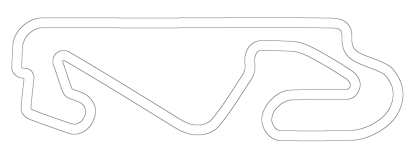
\includegraphics[interpolate=true,width=4.160000in,height=1.570000in]{contents/chapt5/figs/racing/esp-img0.png}}%
\end{pgfscope}%
\begin{pgfscope}%
\pgfpathrectangle{\pgfqpoint{0.150000in}{0.485000in}}{\pgfqpoint{4.160000in}{1.560000in}}%
\pgfusepath{clip}%
\pgfsetrectcap%
\pgfsetroundjoin%
\pgfsetlinewidth{1.003750pt}%
\definecolor{currentstroke}{rgb}{0.468627,0.049260,0.999696}%
\pgfsetstrokecolor{currentstroke}%
\pgfsetstrokeopacity{0.800000}%
\pgfsetdash{}{0pt}%
\pgfpathmoveto{\pgfqpoint{1.480105in}{1.831526in}}%
\pgfpathlineto{\pgfqpoint{1.481747in}{1.831526in}}%
\pgfusepath{stroke}%
\end{pgfscope}%
\begin{pgfscope}%
\pgfpathrectangle{\pgfqpoint{0.150000in}{0.485000in}}{\pgfqpoint{4.160000in}{1.560000in}}%
\pgfusepath{clip}%
\pgfsetrectcap%
\pgfsetroundjoin%
\pgfsetlinewidth{1.003750pt}%
\definecolor{currentstroke}{rgb}{0.437255,0.098400,0.998786}%
\pgfsetstrokecolor{currentstroke}%
\pgfsetstrokeopacity{0.800000}%
\pgfsetdash{}{0pt}%
\pgfpathmoveto{\pgfqpoint{1.481747in}{1.831526in}}%
\pgfpathlineto{\pgfqpoint{1.483408in}{1.831526in}}%
\pgfusepath{stroke}%
\end{pgfscope}%
\begin{pgfscope}%
\pgfpathrectangle{\pgfqpoint{0.150000in}{0.485000in}}{\pgfqpoint{4.160000in}{1.560000in}}%
\pgfusepath{clip}%
\pgfsetrectcap%
\pgfsetroundjoin%
\pgfsetlinewidth{1.003750pt}%
\definecolor{currentstroke}{rgb}{0.405882,0.147302,0.997269}%
\pgfsetstrokecolor{currentstroke}%
\pgfsetstrokeopacity{0.800000}%
\pgfsetdash{}{0pt}%
\pgfpathmoveto{\pgfqpoint{1.483408in}{1.831526in}}%
\pgfpathlineto{\pgfqpoint{1.485086in}{1.831530in}}%
\pgfusepath{stroke}%
\end{pgfscope}%
\begin{pgfscope}%
\pgfpathrectangle{\pgfqpoint{0.150000in}{0.485000in}}{\pgfqpoint{4.160000in}{1.560000in}}%
\pgfusepath{clip}%
\pgfsetrectcap%
\pgfsetroundjoin%
\pgfsetlinewidth{1.003750pt}%
\definecolor{currentstroke}{rgb}{0.374510,0.195845,0.995147}%
\pgfsetstrokecolor{currentstroke}%
\pgfsetstrokeopacity{0.800000}%
\pgfsetdash{}{0pt}%
\pgfpathmoveto{\pgfqpoint{1.485086in}{1.831530in}}%
\pgfpathlineto{\pgfqpoint{1.486782in}{1.831541in}}%
\pgfusepath{stroke}%
\end{pgfscope}%
\begin{pgfscope}%
\pgfpathrectangle{\pgfqpoint{0.150000in}{0.485000in}}{\pgfqpoint{4.160000in}{1.560000in}}%
\pgfusepath{clip}%
\pgfsetrectcap%
\pgfsetroundjoin%
\pgfsetlinewidth{1.003750pt}%
\definecolor{currentstroke}{rgb}{0.335294,0.255843,0.991645}%
\pgfsetstrokecolor{currentstroke}%
\pgfsetstrokeopacity{0.800000}%
\pgfsetdash{}{0pt}%
\pgfpathmoveto{\pgfqpoint{1.486782in}{1.831541in}}%
\pgfpathlineto{\pgfqpoint{1.488496in}{1.831563in}}%
\pgfusepath{stroke}%
\end{pgfscope}%
\begin{pgfscope}%
\pgfpathrectangle{\pgfqpoint{0.150000in}{0.485000in}}{\pgfqpoint{4.160000in}{1.560000in}}%
\pgfusepath{clip}%
\pgfsetrectcap%
\pgfsetroundjoin%
\pgfsetlinewidth{1.003750pt}%
\definecolor{currentstroke}{rgb}{0.303922,0.303153,0.988165}%
\pgfsetstrokecolor{currentstroke}%
\pgfsetstrokeopacity{0.800000}%
\pgfsetdash{}{0pt}%
\pgfpathmoveto{\pgfqpoint{1.488496in}{1.831563in}}%
\pgfpathlineto{\pgfqpoint{1.490228in}{1.831591in}}%
\pgfusepath{stroke}%
\end{pgfscope}%
\begin{pgfscope}%
\pgfpathrectangle{\pgfqpoint{0.150000in}{0.485000in}}{\pgfqpoint{4.160000in}{1.560000in}}%
\pgfusepath{clip}%
\pgfsetrectcap%
\pgfsetroundjoin%
\pgfsetlinewidth{1.003750pt}%
\definecolor{currentstroke}{rgb}{0.272549,0.349727,0.984086}%
\pgfsetstrokecolor{currentstroke}%
\pgfsetstrokeopacity{0.800000}%
\pgfsetdash{}{0pt}%
\pgfpathmoveto{\pgfqpoint{1.490228in}{1.831591in}}%
\pgfpathlineto{\pgfqpoint{1.491978in}{1.831630in}}%
\pgfusepath{stroke}%
\end{pgfscope}%
\begin{pgfscope}%
\pgfpathrectangle{\pgfqpoint{0.150000in}{0.485000in}}{\pgfqpoint{4.160000in}{1.560000in}}%
\pgfusepath{clip}%
\pgfsetrectcap%
\pgfsetroundjoin%
\pgfsetlinewidth{1.003750pt}%
\definecolor{currentstroke}{rgb}{0.241176,0.395451,0.979410}%
\pgfsetstrokecolor{currentstroke}%
\pgfsetstrokeopacity{0.800000}%
\pgfsetdash{}{0pt}%
\pgfpathmoveto{\pgfqpoint{1.491978in}{1.831630in}}%
\pgfpathlineto{\pgfqpoint{1.493746in}{1.831676in}}%
\pgfusepath{stroke}%
\end{pgfscope}%
\begin{pgfscope}%
\pgfpathrectangle{\pgfqpoint{0.150000in}{0.485000in}}{\pgfqpoint{4.160000in}{1.560000in}}%
\pgfusepath{clip}%
\pgfsetrectcap%
\pgfsetroundjoin%
\pgfsetlinewidth{1.003750pt}%
\definecolor{currentstroke}{rgb}{0.209804,0.440216,0.974139}%
\pgfsetstrokecolor{currentstroke}%
\pgfsetstrokeopacity{0.800000}%
\pgfsetdash{}{0pt}%
\pgfpathmoveto{\pgfqpoint{1.493746in}{1.831676in}}%
\pgfpathlineto{\pgfqpoint{1.495531in}{1.831733in}}%
\pgfusepath{stroke}%
\end{pgfscope}%
\begin{pgfscope}%
\pgfpathrectangle{\pgfqpoint{0.150000in}{0.485000in}}{\pgfqpoint{4.160000in}{1.560000in}}%
\pgfusepath{clip}%
\pgfsetrectcap%
\pgfsetroundjoin%
\pgfsetlinewidth{1.003750pt}%
\definecolor{currentstroke}{rgb}{0.170588,0.494656,0.966718}%
\pgfsetstrokecolor{currentstroke}%
\pgfsetstrokeopacity{0.800000}%
\pgfsetdash{}{0pt}%
\pgfpathmoveto{\pgfqpoint{1.495531in}{1.831733in}}%
\pgfpathlineto{\pgfqpoint{1.497334in}{1.831798in}}%
\pgfusepath{stroke}%
\end{pgfscope}%
\begin{pgfscope}%
\pgfpathrectangle{\pgfqpoint{0.150000in}{0.485000in}}{\pgfqpoint{4.160000in}{1.560000in}}%
\pgfusepath{clip}%
\pgfsetrectcap%
\pgfsetroundjoin%
\pgfsetlinewidth{1.003750pt}%
\definecolor{currentstroke}{rgb}{0.162745,0.505325,0.965124}%
\pgfsetstrokecolor{currentstroke}%
\pgfsetstrokeopacity{0.800000}%
\pgfsetdash{}{0pt}%
\pgfpathmoveto{\pgfqpoint{1.497334in}{1.831798in}}%
\pgfpathlineto{\pgfqpoint{1.499155in}{1.831874in}}%
\pgfusepath{stroke}%
\end{pgfscope}%
\begin{pgfscope}%
\pgfpathrectangle{\pgfqpoint{0.150000in}{0.485000in}}{\pgfqpoint{4.160000in}{1.560000in}}%
\pgfusepath{clip}%
\pgfsetrectcap%
\pgfsetroundjoin%
\pgfsetlinewidth{1.003750pt}%
\definecolor{currentstroke}{rgb}{0.154902,0.515918,0.963493}%
\pgfsetstrokecolor{currentstroke}%
\pgfsetstrokeopacity{0.800000}%
\pgfsetdash{}{0pt}%
\pgfpathmoveto{\pgfqpoint{1.499155in}{1.831874in}}%
\pgfpathlineto{\pgfqpoint{1.500981in}{1.831959in}}%
\pgfusepath{stroke}%
\end{pgfscope}%
\begin{pgfscope}%
\pgfpathrectangle{\pgfqpoint{0.150000in}{0.485000in}}{\pgfqpoint{4.160000in}{1.560000in}}%
\pgfusepath{clip}%
\pgfsetrectcap%
\pgfsetroundjoin%
\pgfsetlinewidth{1.003750pt}%
\definecolor{currentstroke}{rgb}{0.147059,0.526432,0.961826}%
\pgfsetstrokecolor{currentstroke}%
\pgfsetstrokeopacity{0.800000}%
\pgfsetdash{}{0pt}%
\pgfpathmoveto{\pgfqpoint{1.500981in}{1.831959in}}%
\pgfpathlineto{\pgfqpoint{1.502811in}{1.832047in}}%
\pgfusepath{stroke}%
\end{pgfscope}%
\begin{pgfscope}%
\pgfpathrectangle{\pgfqpoint{0.150000in}{0.485000in}}{\pgfqpoint{4.160000in}{1.560000in}}%
\pgfusepath{clip}%
\pgfsetrectcap%
\pgfsetroundjoin%
\pgfsetlinewidth{1.003750pt}%
\definecolor{currentstroke}{rgb}{0.139216,0.536867,0.960122}%
\pgfsetstrokecolor{currentstroke}%
\pgfsetstrokeopacity{0.800000}%
\pgfsetdash{}{0pt}%
\pgfpathmoveto{\pgfqpoint{1.502811in}{1.832047in}}%
\pgfpathlineto{\pgfqpoint{1.504645in}{1.832137in}}%
\pgfusepath{stroke}%
\end{pgfscope}%
\begin{pgfscope}%
\pgfpathrectangle{\pgfqpoint{0.150000in}{0.485000in}}{\pgfqpoint{4.160000in}{1.560000in}}%
\pgfusepath{clip}%
\pgfsetrectcap%
\pgfsetroundjoin%
\pgfsetlinewidth{1.003750pt}%
\definecolor{currentstroke}{rgb}{0.131373,0.547220,0.958381}%
\pgfsetstrokecolor{currentstroke}%
\pgfsetstrokeopacity{0.800000}%
\pgfsetdash{}{0pt}%
\pgfpathmoveto{\pgfqpoint{1.504645in}{1.832137in}}%
\pgfpathlineto{\pgfqpoint{1.506485in}{1.832224in}}%
\pgfusepath{stroke}%
\end{pgfscope}%
\begin{pgfscope}%
\pgfpathrectangle{\pgfqpoint{0.150000in}{0.485000in}}{\pgfqpoint{4.160000in}{1.560000in}}%
\pgfusepath{clip}%
\pgfsetrectcap%
\pgfsetroundjoin%
\pgfsetlinewidth{1.003750pt}%
\definecolor{currentstroke}{rgb}{0.123529,0.557489,0.956604}%
\pgfsetstrokecolor{currentstroke}%
\pgfsetstrokeopacity{0.800000}%
\pgfsetdash{}{0pt}%
\pgfpathmoveto{\pgfqpoint{1.506485in}{1.832224in}}%
\pgfpathlineto{\pgfqpoint{1.508330in}{1.832306in}}%
\pgfusepath{stroke}%
\end{pgfscope}%
\begin{pgfscope}%
\pgfpathrectangle{\pgfqpoint{0.150000in}{0.485000in}}{\pgfqpoint{4.160000in}{1.560000in}}%
\pgfusepath{clip}%
\pgfsetrectcap%
\pgfsetroundjoin%
\pgfsetlinewidth{1.003750pt}%
\definecolor{currentstroke}{rgb}{0.107843,0.577774,0.952942}%
\pgfsetstrokecolor{currentstroke}%
\pgfsetstrokeopacity{0.800000}%
\pgfsetdash{}{0pt}%
\pgfpathmoveto{\pgfqpoint{1.508330in}{1.832306in}}%
\pgfpathlineto{\pgfqpoint{1.510180in}{1.832378in}}%
\pgfusepath{stroke}%
\end{pgfscope}%
\begin{pgfscope}%
\pgfpathrectangle{\pgfqpoint{0.150000in}{0.485000in}}{\pgfqpoint{4.160000in}{1.560000in}}%
\pgfusepath{clip}%
\pgfsetrectcap%
\pgfsetroundjoin%
\pgfsetlinewidth{1.003750pt}%
\definecolor{currentstroke}{rgb}{0.100000,0.587785,0.951057}%
\pgfsetstrokecolor{currentstroke}%
\pgfsetstrokeopacity{0.800000}%
\pgfsetdash{}{0pt}%
\pgfpathmoveto{\pgfqpoint{1.510180in}{1.832378in}}%
\pgfpathlineto{\pgfqpoint{1.512035in}{1.832447in}}%
\pgfusepath{stroke}%
\end{pgfscope}%
\begin{pgfscope}%
\pgfpathrectangle{\pgfqpoint{0.150000in}{0.485000in}}{\pgfqpoint{4.160000in}{1.560000in}}%
\pgfusepath{clip}%
\pgfsetrectcap%
\pgfsetroundjoin%
\pgfsetlinewidth{1.003750pt}%
\definecolor{currentstroke}{rgb}{0.092157,0.597707,0.949135}%
\pgfsetstrokecolor{currentstroke}%
\pgfsetstrokeopacity{0.800000}%
\pgfsetdash{}{0pt}%
\pgfpathmoveto{\pgfqpoint{1.512035in}{1.832447in}}%
\pgfpathlineto{\pgfqpoint{1.513895in}{1.832507in}}%
\pgfusepath{stroke}%
\end{pgfscope}%
\begin{pgfscope}%
\pgfpathrectangle{\pgfqpoint{0.150000in}{0.485000in}}{\pgfqpoint{4.160000in}{1.560000in}}%
\pgfusepath{clip}%
\pgfsetrectcap%
\pgfsetroundjoin%
\pgfsetlinewidth{1.003750pt}%
\definecolor{currentstroke}{rgb}{0.084314,0.607539,0.947177}%
\pgfsetstrokecolor{currentstroke}%
\pgfsetstrokeopacity{0.800000}%
\pgfsetdash{}{0pt}%
\pgfpathmoveto{\pgfqpoint{1.513895in}{1.832507in}}%
\pgfpathlineto{\pgfqpoint{1.515760in}{1.832562in}}%
\pgfusepath{stroke}%
\end{pgfscope}%
\begin{pgfscope}%
\pgfpathrectangle{\pgfqpoint{0.150000in}{0.485000in}}{\pgfqpoint{4.160000in}{1.560000in}}%
\pgfusepath{clip}%
\pgfsetrectcap%
\pgfsetroundjoin%
\pgfsetlinewidth{1.003750pt}%
\definecolor{currentstroke}{rgb}{0.076471,0.617278,0.945184}%
\pgfsetstrokecolor{currentstroke}%
\pgfsetstrokeopacity{0.800000}%
\pgfsetdash{}{0pt}%
\pgfpathmoveto{\pgfqpoint{1.515760in}{1.832562in}}%
\pgfpathlineto{\pgfqpoint{1.517631in}{1.832608in}}%
\pgfusepath{stroke}%
\end{pgfscope}%
\begin{pgfscope}%
\pgfpathrectangle{\pgfqpoint{0.150000in}{0.485000in}}{\pgfqpoint{4.160000in}{1.560000in}}%
\pgfusepath{clip}%
\pgfsetrectcap%
\pgfsetroundjoin%
\pgfsetlinewidth{1.003750pt}%
\definecolor{currentstroke}{rgb}{0.076471,0.617278,0.945184}%
\pgfsetstrokecolor{currentstroke}%
\pgfsetstrokeopacity{0.800000}%
\pgfsetdash{}{0pt}%
\pgfpathmoveto{\pgfqpoint{1.517631in}{1.832608in}}%
\pgfpathlineto{\pgfqpoint{1.519504in}{1.832647in}}%
\pgfusepath{stroke}%
\end{pgfscope}%
\begin{pgfscope}%
\pgfpathrectangle{\pgfqpoint{0.150000in}{0.485000in}}{\pgfqpoint{4.160000in}{1.560000in}}%
\pgfusepath{clip}%
\pgfsetrectcap%
\pgfsetroundjoin%
\pgfsetlinewidth{1.003750pt}%
\definecolor{currentstroke}{rgb}{0.068627,0.626924,0.943154}%
\pgfsetstrokecolor{currentstroke}%
\pgfsetstrokeopacity{0.800000}%
\pgfsetdash{}{0pt}%
\pgfpathmoveto{\pgfqpoint{1.519504in}{1.832647in}}%
\pgfpathlineto{\pgfqpoint{1.521380in}{1.832674in}}%
\pgfusepath{stroke}%
\end{pgfscope}%
\begin{pgfscope}%
\pgfpathrectangle{\pgfqpoint{0.150000in}{0.485000in}}{\pgfqpoint{4.160000in}{1.560000in}}%
\pgfusepath{clip}%
\pgfsetrectcap%
\pgfsetroundjoin%
\pgfsetlinewidth{1.003750pt}%
\definecolor{currentstroke}{rgb}{0.060784,0.636474,0.941089}%
\pgfsetstrokecolor{currentstroke}%
\pgfsetstrokeopacity{0.800000}%
\pgfsetdash{}{0pt}%
\pgfpathmoveto{\pgfqpoint{1.521380in}{1.832674in}}%
\pgfpathlineto{\pgfqpoint{1.523260in}{1.832694in}}%
\pgfusepath{stroke}%
\end{pgfscope}%
\begin{pgfscope}%
\pgfpathrectangle{\pgfqpoint{0.150000in}{0.485000in}}{\pgfqpoint{4.160000in}{1.560000in}}%
\pgfusepath{clip}%
\pgfsetrectcap%
\pgfsetroundjoin%
\pgfsetlinewidth{1.003750pt}%
\definecolor{currentstroke}{rgb}{0.060784,0.636474,0.941089}%
\pgfsetstrokecolor{currentstroke}%
\pgfsetstrokeopacity{0.800000}%
\pgfsetdash{}{0pt}%
\pgfpathmoveto{\pgfqpoint{1.523260in}{1.832694in}}%
\pgfpathlineto{\pgfqpoint{1.525142in}{1.832701in}}%
\pgfusepath{stroke}%
\end{pgfscope}%
\begin{pgfscope}%
\pgfpathrectangle{\pgfqpoint{0.150000in}{0.485000in}}{\pgfqpoint{4.160000in}{1.560000in}}%
\pgfusepath{clip}%
\pgfsetrectcap%
\pgfsetroundjoin%
\pgfsetlinewidth{1.003750pt}%
\definecolor{currentstroke}{rgb}{0.052941,0.645928,0.938988}%
\pgfsetstrokecolor{currentstroke}%
\pgfsetstrokeopacity{0.800000}%
\pgfsetdash{}{0pt}%
\pgfpathmoveto{\pgfqpoint{1.525142in}{1.832701in}}%
\pgfpathlineto{\pgfqpoint{1.527027in}{1.832699in}}%
\pgfusepath{stroke}%
\end{pgfscope}%
\begin{pgfscope}%
\pgfpathrectangle{\pgfqpoint{0.150000in}{0.485000in}}{\pgfqpoint{4.160000in}{1.560000in}}%
\pgfusepath{clip}%
\pgfsetrectcap%
\pgfsetroundjoin%
\pgfsetlinewidth{1.003750pt}%
\definecolor{currentstroke}{rgb}{0.045098,0.655284,0.936852}%
\pgfsetstrokecolor{currentstroke}%
\pgfsetstrokeopacity{0.800000}%
\pgfsetdash{}{0pt}%
\pgfpathmoveto{\pgfqpoint{1.527027in}{1.832699in}}%
\pgfpathlineto{\pgfqpoint{1.528915in}{1.832684in}}%
\pgfusepath{stroke}%
\end{pgfscope}%
\begin{pgfscope}%
\pgfpathrectangle{\pgfqpoint{0.150000in}{0.485000in}}{\pgfqpoint{4.160000in}{1.560000in}}%
\pgfusepath{clip}%
\pgfsetrectcap%
\pgfsetroundjoin%
\pgfsetlinewidth{1.003750pt}%
\definecolor{currentstroke}{rgb}{0.045098,0.655284,0.936852}%
\pgfsetstrokecolor{currentstroke}%
\pgfsetstrokeopacity{0.800000}%
\pgfsetdash{}{0pt}%
\pgfpathmoveto{\pgfqpoint{1.528915in}{1.832684in}}%
\pgfpathlineto{\pgfqpoint{1.530806in}{1.832659in}}%
\pgfusepath{stroke}%
\end{pgfscope}%
\begin{pgfscope}%
\pgfpathrectangle{\pgfqpoint{0.150000in}{0.485000in}}{\pgfqpoint{4.160000in}{1.560000in}}%
\pgfusepath{clip}%
\pgfsetrectcap%
\pgfsetroundjoin%
\pgfsetlinewidth{1.003750pt}%
\definecolor{currentstroke}{rgb}{0.037255,0.664540,0.934680}%
\pgfsetstrokecolor{currentstroke}%
\pgfsetstrokeopacity{0.800000}%
\pgfsetdash{}{0pt}%
\pgfpathmoveto{\pgfqpoint{1.530806in}{1.832659in}}%
\pgfpathlineto{\pgfqpoint{1.532700in}{1.832619in}}%
\pgfusepath{stroke}%
\end{pgfscope}%
\begin{pgfscope}%
\pgfpathrectangle{\pgfqpoint{0.150000in}{0.485000in}}{\pgfqpoint{4.160000in}{1.560000in}}%
\pgfusepath{clip}%
\pgfsetrectcap%
\pgfsetroundjoin%
\pgfsetlinewidth{1.003750pt}%
\definecolor{currentstroke}{rgb}{0.029412,0.673696,0.932472}%
\pgfsetstrokecolor{currentstroke}%
\pgfsetstrokeopacity{0.800000}%
\pgfsetdash{}{0pt}%
\pgfpathmoveto{\pgfqpoint{1.532700in}{1.832619in}}%
\pgfpathlineto{\pgfqpoint{1.534596in}{1.832569in}}%
\pgfusepath{stroke}%
\end{pgfscope}%
\begin{pgfscope}%
\pgfpathrectangle{\pgfqpoint{0.150000in}{0.485000in}}{\pgfqpoint{4.160000in}{1.560000in}}%
\pgfusepath{clip}%
\pgfsetrectcap%
\pgfsetroundjoin%
\pgfsetlinewidth{1.003750pt}%
\definecolor{currentstroke}{rgb}{0.037255,0.664540,0.934680}%
\pgfsetstrokecolor{currentstroke}%
\pgfsetstrokeopacity{0.800000}%
\pgfsetdash{}{0pt}%
\pgfpathmoveto{\pgfqpoint{1.534596in}{1.832569in}}%
\pgfpathlineto{\pgfqpoint{1.536495in}{1.832504in}}%
\pgfusepath{stroke}%
\end{pgfscope}%
\begin{pgfscope}%
\pgfpathrectangle{\pgfqpoint{0.150000in}{0.485000in}}{\pgfqpoint{4.160000in}{1.560000in}}%
\pgfusepath{clip}%
\pgfsetrectcap%
\pgfsetroundjoin%
\pgfsetlinewidth{1.003750pt}%
\definecolor{currentstroke}{rgb}{0.037255,0.664540,0.934680}%
\pgfsetstrokecolor{currentstroke}%
\pgfsetstrokeopacity{0.800000}%
\pgfsetdash{}{0pt}%
\pgfpathmoveto{\pgfqpoint{1.536495in}{1.832504in}}%
\pgfpathlineto{\pgfqpoint{1.538390in}{1.832428in}}%
\pgfusepath{stroke}%
\end{pgfscope}%
\begin{pgfscope}%
\pgfpathrectangle{\pgfqpoint{0.150000in}{0.485000in}}{\pgfqpoint{4.160000in}{1.560000in}}%
\pgfusepath{clip}%
\pgfsetrectcap%
\pgfsetroundjoin%
\pgfsetlinewidth{1.003750pt}%
\definecolor{currentstroke}{rgb}{0.045098,0.655284,0.936852}%
\pgfsetstrokecolor{currentstroke}%
\pgfsetstrokeopacity{0.800000}%
\pgfsetdash{}{0pt}%
\pgfpathmoveto{\pgfqpoint{1.538390in}{1.832428in}}%
\pgfpathlineto{\pgfqpoint{1.540283in}{1.832346in}}%
\pgfusepath{stroke}%
\end{pgfscope}%
\begin{pgfscope}%
\pgfpathrectangle{\pgfqpoint{0.150000in}{0.485000in}}{\pgfqpoint{4.160000in}{1.560000in}}%
\pgfusepath{clip}%
\pgfsetrectcap%
\pgfsetroundjoin%
\pgfsetlinewidth{1.003750pt}%
\definecolor{currentstroke}{rgb}{0.052941,0.645928,0.938988}%
\pgfsetstrokecolor{currentstroke}%
\pgfsetstrokeopacity{0.800000}%
\pgfsetdash{}{0pt}%
\pgfpathmoveto{\pgfqpoint{1.540283in}{1.832346in}}%
\pgfpathlineto{\pgfqpoint{1.542173in}{1.832261in}}%
\pgfusepath{stroke}%
\end{pgfscope}%
\begin{pgfscope}%
\pgfpathrectangle{\pgfqpoint{0.150000in}{0.485000in}}{\pgfqpoint{4.160000in}{1.560000in}}%
\pgfusepath{clip}%
\pgfsetrectcap%
\pgfsetroundjoin%
\pgfsetlinewidth{1.003750pt}%
\definecolor{currentstroke}{rgb}{0.052941,0.645928,0.938988}%
\pgfsetstrokecolor{currentstroke}%
\pgfsetstrokeopacity{0.800000}%
\pgfsetdash{}{0pt}%
\pgfpathmoveto{\pgfqpoint{1.542173in}{1.832261in}}%
\pgfpathlineto{\pgfqpoint{1.544060in}{1.832176in}}%
\pgfusepath{stroke}%
\end{pgfscope}%
\begin{pgfscope}%
\pgfpathrectangle{\pgfqpoint{0.150000in}{0.485000in}}{\pgfqpoint{4.160000in}{1.560000in}}%
\pgfusepath{clip}%
\pgfsetrectcap%
\pgfsetroundjoin%
\pgfsetlinewidth{1.003750pt}%
\definecolor{currentstroke}{rgb}{0.060784,0.636474,0.941089}%
\pgfsetstrokecolor{currentstroke}%
\pgfsetstrokeopacity{0.800000}%
\pgfsetdash{}{0pt}%
\pgfpathmoveto{\pgfqpoint{1.544060in}{1.832176in}}%
\pgfpathlineto{\pgfqpoint{1.545945in}{1.832095in}}%
\pgfusepath{stroke}%
\end{pgfscope}%
\begin{pgfscope}%
\pgfpathrectangle{\pgfqpoint{0.150000in}{0.485000in}}{\pgfqpoint{4.160000in}{1.560000in}}%
\pgfusepath{clip}%
\pgfsetrectcap%
\pgfsetroundjoin%
\pgfsetlinewidth{1.003750pt}%
\definecolor{currentstroke}{rgb}{0.068627,0.626924,0.943154}%
\pgfsetstrokecolor{currentstroke}%
\pgfsetstrokeopacity{0.800000}%
\pgfsetdash{}{0pt}%
\pgfpathmoveto{\pgfqpoint{1.545945in}{1.832095in}}%
\pgfpathlineto{\pgfqpoint{1.547827in}{1.832022in}}%
\pgfusepath{stroke}%
\end{pgfscope}%
\begin{pgfscope}%
\pgfpathrectangle{\pgfqpoint{0.150000in}{0.485000in}}{\pgfqpoint{4.160000in}{1.560000in}}%
\pgfusepath{clip}%
\pgfsetrectcap%
\pgfsetroundjoin%
\pgfsetlinewidth{1.003750pt}%
\definecolor{currentstroke}{rgb}{0.068627,0.626924,0.943154}%
\pgfsetstrokecolor{currentstroke}%
\pgfsetstrokeopacity{0.800000}%
\pgfsetdash{}{0pt}%
\pgfpathmoveto{\pgfqpoint{1.547827in}{1.832022in}}%
\pgfpathlineto{\pgfqpoint{1.549708in}{1.831960in}}%
\pgfusepath{stroke}%
\end{pgfscope}%
\begin{pgfscope}%
\pgfpathrectangle{\pgfqpoint{0.150000in}{0.485000in}}{\pgfqpoint{4.160000in}{1.560000in}}%
\pgfusepath{clip}%
\pgfsetrectcap%
\pgfsetroundjoin%
\pgfsetlinewidth{1.003750pt}%
\definecolor{currentstroke}{rgb}{0.076471,0.617278,0.945184}%
\pgfsetstrokecolor{currentstroke}%
\pgfsetstrokeopacity{0.800000}%
\pgfsetdash{}{0pt}%
\pgfpathmoveto{\pgfqpoint{1.549708in}{1.831960in}}%
\pgfpathlineto{\pgfqpoint{1.551586in}{1.831914in}}%
\pgfusepath{stroke}%
\end{pgfscope}%
\begin{pgfscope}%
\pgfpathrectangle{\pgfqpoint{0.150000in}{0.485000in}}{\pgfqpoint{4.160000in}{1.560000in}}%
\pgfusepath{clip}%
\pgfsetrectcap%
\pgfsetroundjoin%
\pgfsetlinewidth{1.003750pt}%
\definecolor{currentstroke}{rgb}{0.076471,0.617278,0.945184}%
\pgfsetstrokecolor{currentstroke}%
\pgfsetstrokeopacity{0.800000}%
\pgfsetdash{}{0pt}%
\pgfpathmoveto{\pgfqpoint{1.551586in}{1.831914in}}%
\pgfpathlineto{\pgfqpoint{1.553462in}{1.831887in}}%
\pgfusepath{stroke}%
\end{pgfscope}%
\begin{pgfscope}%
\pgfpathrectangle{\pgfqpoint{0.150000in}{0.485000in}}{\pgfqpoint{4.160000in}{1.560000in}}%
\pgfusepath{clip}%
\pgfsetrectcap%
\pgfsetroundjoin%
\pgfsetlinewidth{1.003750pt}%
\definecolor{currentstroke}{rgb}{0.092157,0.597707,0.949135}%
\pgfsetstrokecolor{currentstroke}%
\pgfsetstrokeopacity{0.800000}%
\pgfsetdash{}{0pt}%
\pgfpathmoveto{\pgfqpoint{1.553462in}{1.831887in}}%
\pgfpathlineto{\pgfqpoint{1.555335in}{1.831876in}}%
\pgfusepath{stroke}%
\end{pgfscope}%
\begin{pgfscope}%
\pgfpathrectangle{\pgfqpoint{0.150000in}{0.485000in}}{\pgfqpoint{4.160000in}{1.560000in}}%
\pgfusepath{clip}%
\pgfsetrectcap%
\pgfsetroundjoin%
\pgfsetlinewidth{1.003750pt}%
\definecolor{currentstroke}{rgb}{0.107843,0.577774,0.952942}%
\pgfsetstrokecolor{currentstroke}%
\pgfsetstrokeopacity{0.800000}%
\pgfsetdash{}{0pt}%
\pgfpathmoveto{\pgfqpoint{1.555335in}{1.831876in}}%
\pgfpathlineto{\pgfqpoint{1.557200in}{1.831886in}}%
\pgfusepath{stroke}%
\end{pgfscope}%
\begin{pgfscope}%
\pgfpathrectangle{\pgfqpoint{0.150000in}{0.485000in}}{\pgfqpoint{4.160000in}{1.560000in}}%
\pgfusepath{clip}%
\pgfsetrectcap%
\pgfsetroundjoin%
\pgfsetlinewidth{1.003750pt}%
\definecolor{currentstroke}{rgb}{0.123529,0.557489,0.956604}%
\pgfsetstrokecolor{currentstroke}%
\pgfsetstrokeopacity{0.800000}%
\pgfsetdash{}{0pt}%
\pgfpathmoveto{\pgfqpoint{1.557200in}{1.831886in}}%
\pgfpathlineto{\pgfqpoint{1.559057in}{1.831923in}}%
\pgfusepath{stroke}%
\end{pgfscope}%
\begin{pgfscope}%
\pgfpathrectangle{\pgfqpoint{0.150000in}{0.485000in}}{\pgfqpoint{4.160000in}{1.560000in}}%
\pgfusepath{clip}%
\pgfsetrectcap%
\pgfsetroundjoin%
\pgfsetlinewidth{1.003750pt}%
\definecolor{currentstroke}{rgb}{0.139216,0.536867,0.960122}%
\pgfsetstrokecolor{currentstroke}%
\pgfsetstrokeopacity{0.800000}%
\pgfsetdash{}{0pt}%
\pgfpathmoveto{\pgfqpoint{1.559057in}{1.831923in}}%
\pgfpathlineto{\pgfqpoint{1.560905in}{1.831983in}}%
\pgfusepath{stroke}%
\end{pgfscope}%
\begin{pgfscope}%
\pgfpathrectangle{\pgfqpoint{0.150000in}{0.485000in}}{\pgfqpoint{4.160000in}{1.560000in}}%
\pgfusepath{clip}%
\pgfsetrectcap%
\pgfsetroundjoin%
\pgfsetlinewidth{1.003750pt}%
\definecolor{currentstroke}{rgb}{0.154902,0.515918,0.963493}%
\pgfsetstrokecolor{currentstroke}%
\pgfsetstrokeopacity{0.800000}%
\pgfsetdash{}{0pt}%
\pgfpathmoveto{\pgfqpoint{1.560905in}{1.831983in}}%
\pgfpathlineto{\pgfqpoint{1.562744in}{1.832071in}}%
\pgfusepath{stroke}%
\end{pgfscope}%
\begin{pgfscope}%
\pgfpathrectangle{\pgfqpoint{0.150000in}{0.485000in}}{\pgfqpoint{4.160000in}{1.560000in}}%
\pgfusepath{clip}%
\pgfsetrectcap%
\pgfsetroundjoin%
\pgfsetlinewidth{1.003750pt}%
\definecolor{currentstroke}{rgb}{0.170588,0.494656,0.966718}%
\pgfsetstrokecolor{currentstroke}%
\pgfsetstrokeopacity{0.800000}%
\pgfsetdash{}{0pt}%
\pgfpathmoveto{\pgfqpoint{1.562744in}{1.832071in}}%
\pgfpathlineto{\pgfqpoint{1.564573in}{1.832184in}}%
\pgfusepath{stroke}%
\end{pgfscope}%
\begin{pgfscope}%
\pgfpathrectangle{\pgfqpoint{0.150000in}{0.485000in}}{\pgfqpoint{4.160000in}{1.560000in}}%
\pgfusepath{clip}%
\pgfsetrectcap%
\pgfsetroundjoin%
\pgfsetlinewidth{1.003750pt}%
\definecolor{currentstroke}{rgb}{0.186275,0.473094,0.969797}%
\pgfsetstrokecolor{currentstroke}%
\pgfsetstrokeopacity{0.800000}%
\pgfsetdash{}{0pt}%
\pgfpathmoveto{\pgfqpoint{1.564573in}{1.832184in}}%
\pgfpathlineto{\pgfqpoint{1.566392in}{1.832328in}}%
\pgfusepath{stroke}%
\end{pgfscope}%
\begin{pgfscope}%
\pgfpathrectangle{\pgfqpoint{0.150000in}{0.485000in}}{\pgfqpoint{4.160000in}{1.560000in}}%
\pgfusepath{clip}%
\pgfsetrectcap%
\pgfsetroundjoin%
\pgfsetlinewidth{1.003750pt}%
\definecolor{currentstroke}{rgb}{0.201961,0.451244,0.972728}%
\pgfsetstrokecolor{currentstroke}%
\pgfsetstrokeopacity{0.800000}%
\pgfsetdash{}{0pt}%
\pgfpathmoveto{\pgfqpoint{1.566392in}{1.832328in}}%
\pgfpathlineto{\pgfqpoint{1.568201in}{1.832499in}}%
\pgfusepath{stroke}%
\end{pgfscope}%
\begin{pgfscope}%
\pgfpathrectangle{\pgfqpoint{0.150000in}{0.485000in}}{\pgfqpoint{4.160000in}{1.560000in}}%
\pgfusepath{clip}%
\pgfsetrectcap%
\pgfsetroundjoin%
\pgfsetlinewidth{1.003750pt}%
\definecolor{currentstroke}{rgb}{0.217647,0.429121,0.975512}%
\pgfsetstrokecolor{currentstroke}%
\pgfsetstrokeopacity{0.800000}%
\pgfsetdash{}{0pt}%
\pgfpathmoveto{\pgfqpoint{1.568201in}{1.832499in}}%
\pgfpathlineto{\pgfqpoint{1.569997in}{1.832703in}}%
\pgfusepath{stroke}%
\end{pgfscope}%
\begin{pgfscope}%
\pgfpathrectangle{\pgfqpoint{0.150000in}{0.485000in}}{\pgfqpoint{4.160000in}{1.560000in}}%
\pgfusepath{clip}%
\pgfsetrectcap%
\pgfsetroundjoin%
\pgfsetlinewidth{1.003750pt}%
\definecolor{currentstroke}{rgb}{0.225490,0.417960,0.976848}%
\pgfsetstrokecolor{currentstroke}%
\pgfsetstrokeopacity{0.800000}%
\pgfsetdash{}{0pt}%
\pgfpathmoveto{\pgfqpoint{1.569997in}{1.832703in}}%
\pgfpathlineto{\pgfqpoint{1.571783in}{1.832935in}}%
\pgfusepath{stroke}%
\end{pgfscope}%
\begin{pgfscope}%
\pgfpathrectangle{\pgfqpoint{0.150000in}{0.485000in}}{\pgfqpoint{4.160000in}{1.560000in}}%
\pgfusepath{clip}%
\pgfsetrectcap%
\pgfsetroundjoin%
\pgfsetlinewidth{1.003750pt}%
\definecolor{currentstroke}{rgb}{0.241176,0.395451,0.979410}%
\pgfsetstrokecolor{currentstroke}%
\pgfsetstrokeopacity{0.800000}%
\pgfsetdash{}{0pt}%
\pgfpathmoveto{\pgfqpoint{1.571783in}{1.832935in}}%
\pgfpathlineto{\pgfqpoint{1.573555in}{1.833202in}}%
\pgfusepath{stroke}%
\end{pgfscope}%
\begin{pgfscope}%
\pgfpathrectangle{\pgfqpoint{0.150000in}{0.485000in}}{\pgfqpoint{4.160000in}{1.560000in}}%
\pgfusepath{clip}%
\pgfsetrectcap%
\pgfsetroundjoin%
\pgfsetlinewidth{1.003750pt}%
\definecolor{currentstroke}{rgb}{0.249020,0.384106,0.980635}%
\pgfsetstrokecolor{currentstroke}%
\pgfsetstrokeopacity{0.800000}%
\pgfsetdash{}{0pt}%
\pgfpathmoveto{\pgfqpoint{1.573555in}{1.833202in}}%
\pgfpathlineto{\pgfqpoint{1.575317in}{1.833499in}}%
\pgfusepath{stroke}%
\end{pgfscope}%
\begin{pgfscope}%
\pgfpathrectangle{\pgfqpoint{0.150000in}{0.485000in}}{\pgfqpoint{4.160000in}{1.560000in}}%
\pgfusepath{clip}%
\pgfsetrectcap%
\pgfsetroundjoin%
\pgfsetlinewidth{1.003750pt}%
\definecolor{currentstroke}{rgb}{0.256863,0.372702,0.981823}%
\pgfsetstrokecolor{currentstroke}%
\pgfsetstrokeopacity{0.800000}%
\pgfsetdash{}{0pt}%
\pgfpathmoveto{\pgfqpoint{1.575317in}{1.833499in}}%
\pgfpathlineto{\pgfqpoint{1.577071in}{1.833822in}}%
\pgfusepath{stroke}%
\end{pgfscope}%
\begin{pgfscope}%
\pgfpathrectangle{\pgfqpoint{0.150000in}{0.485000in}}{\pgfqpoint{4.160000in}{1.560000in}}%
\pgfusepath{clip}%
\pgfsetrectcap%
\pgfsetroundjoin%
\pgfsetlinewidth{1.003750pt}%
\definecolor{currentstroke}{rgb}{0.264706,0.361242,0.982973}%
\pgfsetstrokecolor{currentstroke}%
\pgfsetstrokeopacity{0.800000}%
\pgfsetdash{}{0pt}%
\pgfpathmoveto{\pgfqpoint{1.577071in}{1.833822in}}%
\pgfpathlineto{\pgfqpoint{1.578815in}{1.834169in}}%
\pgfusepath{stroke}%
\end{pgfscope}%
\begin{pgfscope}%
\pgfpathrectangle{\pgfqpoint{0.150000in}{0.485000in}}{\pgfqpoint{4.160000in}{1.560000in}}%
\pgfusepath{clip}%
\pgfsetrectcap%
\pgfsetroundjoin%
\pgfsetlinewidth{1.003750pt}%
\definecolor{currentstroke}{rgb}{0.272549,0.349727,0.984086}%
\pgfsetstrokecolor{currentstroke}%
\pgfsetstrokeopacity{0.800000}%
\pgfsetdash{}{0pt}%
\pgfpathmoveto{\pgfqpoint{1.578815in}{1.834169in}}%
\pgfpathlineto{\pgfqpoint{1.580550in}{1.834535in}}%
\pgfusepath{stroke}%
\end{pgfscope}%
\begin{pgfscope}%
\pgfpathrectangle{\pgfqpoint{0.150000in}{0.485000in}}{\pgfqpoint{4.160000in}{1.560000in}}%
\pgfusepath{clip}%
\pgfsetrectcap%
\pgfsetroundjoin%
\pgfsetlinewidth{1.003750pt}%
\definecolor{currentstroke}{rgb}{0.280392,0.338158,0.985162}%
\pgfsetstrokecolor{currentstroke}%
\pgfsetstrokeopacity{0.800000}%
\pgfsetdash{}{0pt}%
\pgfpathmoveto{\pgfqpoint{1.580550in}{1.834535in}}%
\pgfpathlineto{\pgfqpoint{1.582278in}{1.834917in}}%
\pgfusepath{stroke}%
\end{pgfscope}%
\begin{pgfscope}%
\pgfpathrectangle{\pgfqpoint{0.150000in}{0.485000in}}{\pgfqpoint{4.160000in}{1.560000in}}%
\pgfusepath{clip}%
\pgfsetrectcap%
\pgfsetroundjoin%
\pgfsetlinewidth{1.003750pt}%
\definecolor{currentstroke}{rgb}{0.288235,0.326539,0.986201}%
\pgfsetstrokecolor{currentstroke}%
\pgfsetstrokeopacity{0.800000}%
\pgfsetdash{}{0pt}%
\pgfpathmoveto{\pgfqpoint{1.582278in}{1.834917in}}%
\pgfpathlineto{\pgfqpoint{1.583998in}{1.835312in}}%
\pgfusepath{stroke}%
\end{pgfscope}%
\begin{pgfscope}%
\pgfpathrectangle{\pgfqpoint{0.150000in}{0.485000in}}{\pgfqpoint{4.160000in}{1.560000in}}%
\pgfusepath{clip}%
\pgfsetrectcap%
\pgfsetroundjoin%
\pgfsetlinewidth{1.003750pt}%
\definecolor{currentstroke}{rgb}{0.296078,0.314870,0.987202}%
\pgfsetstrokecolor{currentstroke}%
\pgfsetstrokeopacity{0.800000}%
\pgfsetdash{}{0pt}%
\pgfpathmoveto{\pgfqpoint{1.583998in}{1.835312in}}%
\pgfpathlineto{\pgfqpoint{1.585711in}{1.835716in}}%
\pgfusepath{stroke}%
\end{pgfscope}%
\begin{pgfscope}%
\pgfpathrectangle{\pgfqpoint{0.150000in}{0.485000in}}{\pgfqpoint{4.160000in}{1.560000in}}%
\pgfusepath{clip}%
\pgfsetrectcap%
\pgfsetroundjoin%
\pgfsetlinewidth{1.003750pt}%
\definecolor{currentstroke}{rgb}{0.303922,0.303153,0.988165}%
\pgfsetstrokecolor{currentstroke}%
\pgfsetstrokeopacity{0.800000}%
\pgfsetdash{}{0pt}%
\pgfpathmoveto{\pgfqpoint{1.585711in}{1.835716in}}%
\pgfpathlineto{\pgfqpoint{1.587418in}{1.836124in}}%
\pgfusepath{stroke}%
\end{pgfscope}%
\begin{pgfscope}%
\pgfpathrectangle{\pgfqpoint{0.150000in}{0.485000in}}{\pgfqpoint{4.160000in}{1.560000in}}%
\pgfusepath{clip}%
\pgfsetrectcap%
\pgfsetroundjoin%
\pgfsetlinewidth{1.003750pt}%
\definecolor{currentstroke}{rgb}{0.311765,0.291390,0.989092}%
\pgfsetstrokecolor{currentstroke}%
\pgfsetstrokeopacity{0.800000}%
\pgfsetdash{}{0pt}%
\pgfpathmoveto{\pgfqpoint{1.587418in}{1.836124in}}%
\pgfpathlineto{\pgfqpoint{1.589120in}{1.836534in}}%
\pgfusepath{stroke}%
\end{pgfscope}%
\begin{pgfscope}%
\pgfpathrectangle{\pgfqpoint{0.150000in}{0.485000in}}{\pgfqpoint{4.160000in}{1.560000in}}%
\pgfusepath{clip}%
\pgfsetrectcap%
\pgfsetroundjoin%
\pgfsetlinewidth{1.003750pt}%
\definecolor{currentstroke}{rgb}{0.350980,0.231948,0.993159}%
\pgfsetstrokecolor{currentstroke}%
\pgfsetstrokeopacity{0.800000}%
\pgfsetdash{}{0pt}%
\pgfpathmoveto{\pgfqpoint{1.589120in}{1.836534in}}%
\pgfpathlineto{\pgfqpoint{1.590819in}{1.836939in}}%
\pgfusepath{stroke}%
\end{pgfscope}%
\begin{pgfscope}%
\pgfpathrectangle{\pgfqpoint{0.150000in}{0.485000in}}{\pgfqpoint{4.160000in}{1.560000in}}%
\pgfusepath{clip}%
\pgfsetrectcap%
\pgfsetroundjoin%
\pgfsetlinewidth{1.003750pt}%
\definecolor{currentstroke}{rgb}{0.382353,0.183750,0.995734}%
\pgfsetstrokecolor{currentstroke}%
\pgfsetstrokeopacity{0.800000}%
\pgfsetdash{}{0pt}%
\pgfpathmoveto{\pgfqpoint{1.590819in}{1.836939in}}%
\pgfpathlineto{\pgfqpoint{1.592501in}{1.837332in}}%
\pgfusepath{stroke}%
\end{pgfscope}%
\begin{pgfscope}%
\pgfpathrectangle{\pgfqpoint{0.150000in}{0.485000in}}{\pgfqpoint{4.160000in}{1.560000in}}%
\pgfusepath{clip}%
\pgfsetrectcap%
\pgfsetroundjoin%
\pgfsetlinewidth{1.003750pt}%
\definecolor{currentstroke}{rgb}{0.421569,0.122888,0.998103}%
\pgfsetstrokecolor{currentstroke}%
\pgfsetstrokeopacity{0.800000}%
\pgfsetdash{}{0pt}%
\pgfpathmoveto{\pgfqpoint{1.592501in}{1.837332in}}%
\pgfpathlineto{\pgfqpoint{1.594167in}{1.837708in}}%
\pgfusepath{stroke}%
\end{pgfscope}%
\begin{pgfscope}%
\pgfpathrectangle{\pgfqpoint{0.150000in}{0.485000in}}{\pgfqpoint{4.160000in}{1.560000in}}%
\pgfusepath{clip}%
\pgfsetrectcap%
\pgfsetroundjoin%
\pgfsetlinewidth{1.003750pt}%
\definecolor{currentstroke}{rgb}{0.452941,0.073853,0.999317}%
\pgfsetstrokecolor{currentstroke}%
\pgfsetstrokeopacity{0.800000}%
\pgfsetdash{}{0pt}%
\pgfpathmoveto{\pgfqpoint{1.594167in}{1.837708in}}%
\pgfpathlineto{\pgfqpoint{1.595818in}{1.838064in}}%
\pgfusepath{stroke}%
\end{pgfscope}%
\begin{pgfscope}%
\pgfpathrectangle{\pgfqpoint{0.150000in}{0.485000in}}{\pgfqpoint{4.160000in}{1.560000in}}%
\pgfusepath{clip}%
\pgfsetrectcap%
\pgfsetroundjoin%
\pgfsetlinewidth{1.003750pt}%
\definecolor{currentstroke}{rgb}{0.484314,0.024637,0.999924}%
\pgfsetstrokecolor{currentstroke}%
\pgfsetstrokeopacity{0.800000}%
\pgfsetdash{}{0pt}%
\pgfpathmoveto{\pgfqpoint{1.595818in}{1.838064in}}%
\pgfpathlineto{\pgfqpoint{1.597455in}{1.838394in}}%
\pgfusepath{stroke}%
\end{pgfscope}%
\begin{pgfscope}%
\pgfpathrectangle{\pgfqpoint{0.150000in}{0.485000in}}{\pgfqpoint{4.160000in}{1.560000in}}%
\pgfusepath{clip}%
\pgfsetrectcap%
\pgfsetroundjoin%
\pgfsetlinewidth{1.003750pt}%
\definecolor{currentstroke}{rgb}{0.500000,0.000000,1.000000}%
\pgfsetstrokecolor{currentstroke}%
\pgfsetstrokeopacity{0.800000}%
\pgfsetdash{}{0pt}%
\pgfpathmoveto{\pgfqpoint{1.597455in}{1.838394in}}%
\pgfpathlineto{\pgfqpoint{1.599079in}{1.838694in}}%
\pgfusepath{stroke}%
\end{pgfscope}%
\begin{pgfscope}%
\pgfpathrectangle{\pgfqpoint{0.150000in}{0.485000in}}{\pgfqpoint{4.160000in}{1.560000in}}%
\pgfusepath{clip}%
\pgfsetrectcap%
\pgfsetroundjoin%
\pgfsetlinewidth{1.003750pt}%
\definecolor{currentstroke}{rgb}{0.500000,0.000000,1.000000}%
\pgfsetstrokecolor{currentstroke}%
\pgfsetstrokeopacity{0.800000}%
\pgfsetdash{}{0pt}%
\pgfpathmoveto{\pgfqpoint{1.599079in}{1.838694in}}%
\pgfpathlineto{\pgfqpoint{1.600688in}{1.838960in}}%
\pgfusepath{stroke}%
\end{pgfscope}%
\begin{pgfscope}%
\pgfpathrectangle{\pgfqpoint{0.150000in}{0.485000in}}{\pgfqpoint{4.160000in}{1.560000in}}%
\pgfusepath{clip}%
\pgfsetrectcap%
\pgfsetroundjoin%
\pgfsetlinewidth{1.003750pt}%
\definecolor{currentstroke}{rgb}{0.500000,0.000000,1.000000}%
\pgfsetstrokecolor{currentstroke}%
\pgfsetstrokeopacity{0.800000}%
\pgfsetdash{}{0pt}%
\pgfpathmoveto{\pgfqpoint{1.600688in}{1.838960in}}%
\pgfpathlineto{\pgfqpoint{1.602304in}{1.839191in}}%
\pgfusepath{stroke}%
\end{pgfscope}%
\begin{pgfscope}%
\pgfpathrectangle{\pgfqpoint{0.150000in}{0.485000in}}{\pgfqpoint{4.160000in}{1.560000in}}%
\pgfusepath{clip}%
\pgfsetrectcap%
\pgfsetroundjoin%
\pgfsetlinewidth{1.003750pt}%
\definecolor{currentstroke}{rgb}{0.500000,0.000000,1.000000}%
\pgfsetstrokecolor{currentstroke}%
\pgfsetstrokeopacity{0.800000}%
\pgfsetdash{}{0pt}%
\pgfpathmoveto{\pgfqpoint{1.602304in}{1.839191in}}%
\pgfpathlineto{\pgfqpoint{1.603923in}{1.839391in}}%
\pgfusepath{stroke}%
\end{pgfscope}%
\begin{pgfscope}%
\pgfpathrectangle{\pgfqpoint{0.150000in}{0.485000in}}{\pgfqpoint{4.160000in}{1.560000in}}%
\pgfusepath{clip}%
\pgfsetrectcap%
\pgfsetroundjoin%
\pgfsetlinewidth{1.003750pt}%
\definecolor{currentstroke}{rgb}{0.500000,0.000000,1.000000}%
\pgfsetstrokecolor{currentstroke}%
\pgfsetstrokeopacity{0.800000}%
\pgfsetdash{}{0pt}%
\pgfpathmoveto{\pgfqpoint{1.603923in}{1.839391in}}%
\pgfpathlineto{\pgfqpoint{1.605546in}{1.839555in}}%
\pgfusepath{stroke}%
\end{pgfscope}%
\begin{pgfscope}%
\pgfpathrectangle{\pgfqpoint{0.150000in}{0.485000in}}{\pgfqpoint{4.160000in}{1.560000in}}%
\pgfusepath{clip}%
\pgfsetrectcap%
\pgfsetroundjoin%
\pgfsetlinewidth{1.003750pt}%
\definecolor{currentstroke}{rgb}{0.500000,0.000000,1.000000}%
\pgfsetstrokecolor{currentstroke}%
\pgfsetstrokeopacity{0.800000}%
\pgfsetdash{}{0pt}%
\pgfpathmoveto{\pgfqpoint{1.605546in}{1.839555in}}%
\pgfpathlineto{\pgfqpoint{1.607173in}{1.839685in}}%
\pgfusepath{stroke}%
\end{pgfscope}%
\begin{pgfscope}%
\pgfpathrectangle{\pgfqpoint{0.150000in}{0.485000in}}{\pgfqpoint{4.160000in}{1.560000in}}%
\pgfusepath{clip}%
\pgfsetrectcap%
\pgfsetroundjoin%
\pgfsetlinewidth{1.003750pt}%
\definecolor{currentstroke}{rgb}{0.500000,0.000000,1.000000}%
\pgfsetstrokecolor{currentstroke}%
\pgfsetstrokeopacity{0.800000}%
\pgfsetdash{}{0pt}%
\pgfpathmoveto{\pgfqpoint{1.607173in}{1.839685in}}%
\pgfpathlineto{\pgfqpoint{1.608807in}{1.839776in}}%
\pgfusepath{stroke}%
\end{pgfscope}%
\begin{pgfscope}%
\pgfpathrectangle{\pgfqpoint{0.150000in}{0.485000in}}{\pgfqpoint{4.160000in}{1.560000in}}%
\pgfusepath{clip}%
\pgfsetrectcap%
\pgfsetroundjoin%
\pgfsetlinewidth{1.003750pt}%
\definecolor{currentstroke}{rgb}{0.500000,0.000000,1.000000}%
\pgfsetstrokecolor{currentstroke}%
\pgfsetstrokeopacity{0.800000}%
\pgfsetdash{}{0pt}%
\pgfpathmoveto{\pgfqpoint{1.608807in}{1.839776in}}%
\pgfpathlineto{\pgfqpoint{1.610447in}{1.839832in}}%
\pgfusepath{stroke}%
\end{pgfscope}%
\begin{pgfscope}%
\pgfpathrectangle{\pgfqpoint{0.150000in}{0.485000in}}{\pgfqpoint{4.160000in}{1.560000in}}%
\pgfusepath{clip}%
\pgfsetrectcap%
\pgfsetroundjoin%
\pgfsetlinewidth{1.003750pt}%
\definecolor{currentstroke}{rgb}{0.484314,0.024637,0.999924}%
\pgfsetstrokecolor{currentstroke}%
\pgfsetstrokeopacity{0.800000}%
\pgfsetdash{}{0pt}%
\pgfpathmoveto{\pgfqpoint{1.610447in}{1.839832in}}%
\pgfpathlineto{\pgfqpoint{1.612093in}{1.839857in}}%
\pgfusepath{stroke}%
\end{pgfscope}%
\begin{pgfscope}%
\pgfpathrectangle{\pgfqpoint{0.150000in}{0.485000in}}{\pgfqpoint{4.160000in}{1.560000in}}%
\pgfusepath{clip}%
\pgfsetrectcap%
\pgfsetroundjoin%
\pgfsetlinewidth{1.003750pt}%
\definecolor{currentstroke}{rgb}{0.476471,0.036951,0.999829}%
\pgfsetstrokecolor{currentstroke}%
\pgfsetstrokeopacity{0.800000}%
\pgfsetdash{}{0pt}%
\pgfpathmoveto{\pgfqpoint{1.612093in}{1.839857in}}%
\pgfpathlineto{\pgfqpoint{1.613744in}{1.839852in}}%
\pgfusepath{stroke}%
\end{pgfscope}%
\begin{pgfscope}%
\pgfpathrectangle{\pgfqpoint{0.150000in}{0.485000in}}{\pgfqpoint{4.160000in}{1.560000in}}%
\pgfusepath{clip}%
\pgfsetrectcap%
\pgfsetroundjoin%
\pgfsetlinewidth{1.003750pt}%
\definecolor{currentstroke}{rgb}{0.468627,0.049260,0.999696}%
\pgfsetstrokecolor{currentstroke}%
\pgfsetstrokeopacity{0.800000}%
\pgfsetdash{}{0pt}%
\pgfpathmoveto{\pgfqpoint{1.613744in}{1.839852in}}%
\pgfpathlineto{\pgfqpoint{1.615400in}{1.839822in}}%
\pgfusepath{stroke}%
\end{pgfscope}%
\begin{pgfscope}%
\pgfpathrectangle{\pgfqpoint{0.150000in}{0.485000in}}{\pgfqpoint{4.160000in}{1.560000in}}%
\pgfusepath{clip}%
\pgfsetrectcap%
\pgfsetroundjoin%
\pgfsetlinewidth{1.003750pt}%
\definecolor{currentstroke}{rgb}{0.460784,0.061561,0.999526}%
\pgfsetstrokecolor{currentstroke}%
\pgfsetstrokeopacity{0.800000}%
\pgfsetdash{}{0pt}%
\pgfpathmoveto{\pgfqpoint{1.615400in}{1.839822in}}%
\pgfpathlineto{\pgfqpoint{1.617060in}{1.839759in}}%
\pgfusepath{stroke}%
\end{pgfscope}%
\begin{pgfscope}%
\pgfpathrectangle{\pgfqpoint{0.150000in}{0.485000in}}{\pgfqpoint{4.160000in}{1.560000in}}%
\pgfusepath{clip}%
\pgfsetrectcap%
\pgfsetroundjoin%
\pgfsetlinewidth{1.003750pt}%
\definecolor{currentstroke}{rgb}{0.452941,0.073853,0.999317}%
\pgfsetstrokecolor{currentstroke}%
\pgfsetstrokeopacity{0.800000}%
\pgfsetdash{}{0pt}%
\pgfpathmoveto{\pgfqpoint{1.617060in}{1.839759in}}%
\pgfpathlineto{\pgfqpoint{1.618723in}{1.839669in}}%
\pgfusepath{stroke}%
\end{pgfscope}%
\begin{pgfscope}%
\pgfpathrectangle{\pgfqpoint{0.150000in}{0.485000in}}{\pgfqpoint{4.160000in}{1.560000in}}%
\pgfusepath{clip}%
\pgfsetrectcap%
\pgfsetroundjoin%
\pgfsetlinewidth{1.003750pt}%
\definecolor{currentstroke}{rgb}{0.445098,0.086133,0.999070}%
\pgfsetstrokecolor{currentstroke}%
\pgfsetstrokeopacity{0.800000}%
\pgfsetdash{}{0pt}%
\pgfpathmoveto{\pgfqpoint{1.618723in}{1.839669in}}%
\pgfpathlineto{\pgfqpoint{1.620389in}{1.839547in}}%
\pgfusepath{stroke}%
\end{pgfscope}%
\begin{pgfscope}%
\pgfpathrectangle{\pgfqpoint{0.150000in}{0.485000in}}{\pgfqpoint{4.160000in}{1.560000in}}%
\pgfusepath{clip}%
\pgfsetrectcap%
\pgfsetroundjoin%
\pgfsetlinewidth{1.003750pt}%
\definecolor{currentstroke}{rgb}{0.437255,0.098400,0.998786}%
\pgfsetstrokecolor{currentstroke}%
\pgfsetstrokeopacity{0.800000}%
\pgfsetdash{}{0pt}%
\pgfpathmoveto{\pgfqpoint{1.620389in}{1.839547in}}%
\pgfpathlineto{\pgfqpoint{1.622057in}{1.839398in}}%
\pgfusepath{stroke}%
\end{pgfscope}%
\begin{pgfscope}%
\pgfpathrectangle{\pgfqpoint{0.150000in}{0.485000in}}{\pgfqpoint{4.160000in}{1.560000in}}%
\pgfusepath{clip}%
\pgfsetrectcap%
\pgfsetroundjoin%
\pgfsetlinewidth{1.003750pt}%
\definecolor{currentstroke}{rgb}{0.358824,0.219946,0.993859}%
\pgfsetstrokecolor{currentstroke}%
\pgfsetstrokeopacity{0.800000}%
\pgfsetdash{}{0pt}%
\pgfpathmoveto{\pgfqpoint{1.622057in}{1.839398in}}%
\pgfpathlineto{\pgfqpoint{1.623728in}{1.839216in}}%
\pgfusepath{stroke}%
\end{pgfscope}%
\begin{pgfscope}%
\pgfpathrectangle{\pgfqpoint{0.150000in}{0.485000in}}{\pgfqpoint{4.160000in}{1.560000in}}%
\pgfusepath{clip}%
\pgfsetrectcap%
\pgfsetroundjoin%
\pgfsetlinewidth{1.003750pt}%
\definecolor{currentstroke}{rgb}{0.280392,0.338158,0.985162}%
\pgfsetstrokecolor{currentstroke}%
\pgfsetstrokeopacity{0.800000}%
\pgfsetdash{}{0pt}%
\pgfpathmoveto{\pgfqpoint{1.623728in}{1.839216in}}%
\pgfpathlineto{\pgfqpoint{1.625436in}{1.839001in}}%
\pgfusepath{stroke}%
\end{pgfscope}%
\begin{pgfscope}%
\pgfpathrectangle{\pgfqpoint{0.150000in}{0.485000in}}{\pgfqpoint{4.160000in}{1.560000in}}%
\pgfusepath{clip}%
\pgfsetrectcap%
\pgfsetroundjoin%
\pgfsetlinewidth{1.003750pt}%
\definecolor{currentstroke}{rgb}{0.209804,0.440216,0.974139}%
\pgfsetstrokecolor{currentstroke}%
\pgfsetstrokeopacity{0.800000}%
\pgfsetdash{}{0pt}%
\pgfpathmoveto{\pgfqpoint{1.625436in}{1.839001in}}%
\pgfpathlineto{\pgfqpoint{1.627181in}{1.838758in}}%
\pgfusepath{stroke}%
\end{pgfscope}%
\begin{pgfscope}%
\pgfpathrectangle{\pgfqpoint{0.150000in}{0.485000in}}{\pgfqpoint{4.160000in}{1.560000in}}%
\pgfusepath{clip}%
\pgfsetrectcap%
\pgfsetroundjoin%
\pgfsetlinewidth{1.003750pt}%
\definecolor{currentstroke}{rgb}{0.131373,0.547220,0.958381}%
\pgfsetstrokecolor{currentstroke}%
\pgfsetstrokeopacity{0.800000}%
\pgfsetdash{}{0pt}%
\pgfpathmoveto{\pgfqpoint{1.627181in}{1.838758in}}%
\pgfpathlineto{\pgfqpoint{1.628965in}{1.838490in}}%
\pgfusepath{stroke}%
\end{pgfscope}%
\begin{pgfscope}%
\pgfpathrectangle{\pgfqpoint{0.150000in}{0.485000in}}{\pgfqpoint{4.160000in}{1.560000in}}%
\pgfusepath{clip}%
\pgfsetrectcap%
\pgfsetroundjoin%
\pgfsetlinewidth{1.003750pt}%
\definecolor{currentstroke}{rgb}{0.052941,0.645928,0.938988}%
\pgfsetstrokecolor{currentstroke}%
\pgfsetstrokeopacity{0.800000}%
\pgfsetdash{}{0pt}%
\pgfpathmoveto{\pgfqpoint{1.628965in}{1.838490in}}%
\pgfpathlineto{\pgfqpoint{1.630787in}{1.838200in}}%
\pgfusepath{stroke}%
\end{pgfscope}%
\begin{pgfscope}%
\pgfpathrectangle{\pgfqpoint{0.150000in}{0.485000in}}{\pgfqpoint{4.160000in}{1.560000in}}%
\pgfusepath{clip}%
\pgfsetrectcap%
\pgfsetroundjoin%
\pgfsetlinewidth{1.003750pt}%
\definecolor{currentstroke}{rgb}{0.017647,0.726434,0.918487}%
\pgfsetstrokecolor{currentstroke}%
\pgfsetstrokeopacity{0.800000}%
\pgfsetdash{}{0pt}%
\pgfpathmoveto{\pgfqpoint{1.630787in}{1.838200in}}%
\pgfpathlineto{\pgfqpoint{1.632647in}{1.837892in}}%
\pgfusepath{stroke}%
\end{pgfscope}%
\begin{pgfscope}%
\pgfpathrectangle{\pgfqpoint{0.150000in}{0.485000in}}{\pgfqpoint{4.160000in}{1.560000in}}%
\pgfusepath{clip}%
\pgfsetrectcap%
\pgfsetroundjoin%
\pgfsetlinewidth{1.003750pt}%
\definecolor{currentstroke}{rgb}{0.096078,0.805381,0.892401}%
\pgfsetstrokecolor{currentstroke}%
\pgfsetstrokeopacity{0.800000}%
\pgfsetdash{}{0pt}%
\pgfpathmoveto{\pgfqpoint{1.632647in}{1.837892in}}%
\pgfpathlineto{\pgfqpoint{1.634547in}{1.837569in}}%
\pgfusepath{stroke}%
\end{pgfscope}%
\begin{pgfscope}%
\pgfpathrectangle{\pgfqpoint{0.150000in}{0.485000in}}{\pgfqpoint{4.160000in}{1.560000in}}%
\pgfusepath{clip}%
\pgfsetrectcap%
\pgfsetroundjoin%
\pgfsetlinewidth{1.003750pt}%
\definecolor{currentstroke}{rgb}{0.166667,0.866025,0.866025}%
\pgfsetstrokecolor{currentstroke}%
\pgfsetstrokeopacity{0.800000}%
\pgfsetdash{}{0pt}%
\pgfpathmoveto{\pgfqpoint{1.634547in}{1.837569in}}%
\pgfpathlineto{\pgfqpoint{1.636486in}{1.837233in}}%
\pgfusepath{stroke}%
\end{pgfscope}%
\begin{pgfscope}%
\pgfpathrectangle{\pgfqpoint{0.150000in}{0.485000in}}{\pgfqpoint{4.160000in}{1.560000in}}%
\pgfusepath{clip}%
\pgfsetrectcap%
\pgfsetroundjoin%
\pgfsetlinewidth{1.003750pt}%
\definecolor{currentstroke}{rgb}{0.245098,0.920906,0.833602}%
\pgfsetstrokecolor{currentstroke}%
\pgfsetstrokeopacity{0.800000}%
\pgfsetdash{}{0pt}%
\pgfpathmoveto{\pgfqpoint{1.636486in}{1.837233in}}%
\pgfpathlineto{\pgfqpoint{1.638466in}{1.836889in}}%
\pgfusepath{stroke}%
\end{pgfscope}%
\begin{pgfscope}%
\pgfpathrectangle{\pgfqpoint{0.150000in}{0.485000in}}{\pgfqpoint{4.160000in}{1.560000in}}%
\pgfusepath{clip}%
\pgfsetrectcap%
\pgfsetroundjoin%
\pgfsetlinewidth{1.003750pt}%
\definecolor{currentstroke}{rgb}{0.323529,0.961826,0.798017}%
\pgfsetstrokecolor{currentstroke}%
\pgfsetstrokeopacity{0.800000}%
\pgfsetdash{}{0pt}%
\pgfpathmoveto{\pgfqpoint{1.638466in}{1.836889in}}%
\pgfpathlineto{\pgfqpoint{1.640486in}{1.836540in}}%
\pgfusepath{stroke}%
\end{pgfscope}%
\begin{pgfscope}%
\pgfpathrectangle{\pgfqpoint{0.150000in}{0.485000in}}{\pgfqpoint{4.160000in}{1.560000in}}%
\pgfusepath{clip}%
\pgfsetrectcap%
\pgfsetroundjoin%
\pgfsetlinewidth{1.003750pt}%
\definecolor{currentstroke}{rgb}{0.409804,0.989980,0.755383}%
\pgfsetstrokecolor{currentstroke}%
\pgfsetstrokeopacity{0.800000}%
\pgfsetdash{}{0pt}%
\pgfpathmoveto{\pgfqpoint{1.640486in}{1.836540in}}%
\pgfpathlineto{\pgfqpoint{1.642547in}{1.836182in}}%
\pgfusepath{stroke}%
\end{pgfscope}%
\begin{pgfscope}%
\pgfpathrectangle{\pgfqpoint{0.150000in}{0.485000in}}{\pgfqpoint{4.160000in}{1.560000in}}%
\pgfusepath{clip}%
\pgfsetrectcap%
\pgfsetroundjoin%
\pgfsetlinewidth{1.003750pt}%
\definecolor{currentstroke}{rgb}{0.496078,0.999981,0.709281}%
\pgfsetstrokecolor{currentstroke}%
\pgfsetstrokeopacity{0.800000}%
\pgfsetdash{}{0pt}%
\pgfpathmoveto{\pgfqpoint{1.642547in}{1.836182in}}%
\pgfpathlineto{\pgfqpoint{1.644656in}{1.835819in}}%
\pgfusepath{stroke}%
\end{pgfscope}%
\begin{pgfscope}%
\pgfpathrectangle{\pgfqpoint{0.150000in}{0.485000in}}{\pgfqpoint{4.160000in}{1.560000in}}%
\pgfusepath{clip}%
\pgfsetrectcap%
\pgfsetroundjoin%
\pgfsetlinewidth{1.003750pt}%
\definecolor{currentstroke}{rgb}{0.582353,0.991645,0.659925}%
\pgfsetstrokecolor{currentstroke}%
\pgfsetstrokeopacity{0.800000}%
\pgfsetdash{}{0pt}%
\pgfpathmoveto{\pgfqpoint{1.644656in}{1.835819in}}%
\pgfpathlineto{\pgfqpoint{1.646814in}{1.835454in}}%
\pgfusepath{stroke}%
\end{pgfscope}%
\begin{pgfscope}%
\pgfpathrectangle{\pgfqpoint{0.150000in}{0.485000in}}{\pgfqpoint{4.160000in}{1.560000in}}%
\pgfusepath{clip}%
\pgfsetrectcap%
\pgfsetroundjoin%
\pgfsetlinewidth{1.003750pt}%
\definecolor{currentstroke}{rgb}{0.676471,0.961826,0.602635}%
\pgfsetstrokecolor{currentstroke}%
\pgfsetstrokeopacity{0.800000}%
\pgfsetdash{}{0pt}%
\pgfpathmoveto{\pgfqpoint{1.646814in}{1.835454in}}%
\pgfpathlineto{\pgfqpoint{1.649020in}{1.835091in}}%
\pgfusepath{stroke}%
\end{pgfscope}%
\begin{pgfscope}%
\pgfpathrectangle{\pgfqpoint{0.150000in}{0.485000in}}{\pgfqpoint{4.160000in}{1.560000in}}%
\pgfusepath{clip}%
\pgfsetrectcap%
\pgfsetroundjoin%
\pgfsetlinewidth{1.003750pt}%
\definecolor{currentstroke}{rgb}{0.762745,0.916034,0.547220}%
\pgfsetstrokecolor{currentstroke}%
\pgfsetstrokeopacity{0.800000}%
\pgfsetdash{}{0pt}%
\pgfpathmoveto{\pgfqpoint{1.649020in}{1.835091in}}%
\pgfpathlineto{\pgfqpoint{1.651277in}{1.834733in}}%
\pgfusepath{stroke}%
\end{pgfscope}%
\begin{pgfscope}%
\pgfpathrectangle{\pgfqpoint{0.150000in}{0.485000in}}{\pgfqpoint{4.160000in}{1.560000in}}%
\pgfusepath{clip}%
\pgfsetrectcap%
\pgfsetroundjoin%
\pgfsetlinewidth{1.003750pt}%
\definecolor{currentstroke}{rgb}{0.849020,0.853444,0.489293}%
\pgfsetstrokecolor{currentstroke}%
\pgfsetstrokeopacity{0.800000}%
\pgfsetdash{}{0pt}%
\pgfpathmoveto{\pgfqpoint{1.651277in}{1.834733in}}%
\pgfpathlineto{\pgfqpoint{1.653584in}{1.834384in}}%
\pgfusepath{stroke}%
\end{pgfscope}%
\begin{pgfscope}%
\pgfpathrectangle{\pgfqpoint{0.150000in}{0.485000in}}{\pgfqpoint{4.160000in}{1.560000in}}%
\pgfusepath{clip}%
\pgfsetrectcap%
\pgfsetroundjoin%
\pgfsetlinewidth{1.003750pt}%
\definecolor{currentstroke}{rgb}{0.943137,0.767363,0.423549}%
\pgfsetstrokecolor{currentstroke}%
\pgfsetstrokeopacity{0.800000}%
\pgfsetdash{}{0pt}%
\pgfpathmoveto{\pgfqpoint{1.653584in}{1.834384in}}%
\pgfpathlineto{\pgfqpoint{1.655941in}{1.834048in}}%
\pgfusepath{stroke}%
\end{pgfscope}%
\begin{pgfscope}%
\pgfpathrectangle{\pgfqpoint{0.150000in}{0.485000in}}{\pgfqpoint{4.160000in}{1.560000in}}%
\pgfusepath{clip}%
\pgfsetrectcap%
\pgfsetroundjoin%
\pgfsetlinewidth{1.003750pt}%
\definecolor{currentstroke}{rgb}{1.000000,0.673696,0.361242}%
\pgfsetstrokecolor{currentstroke}%
\pgfsetstrokeopacity{0.800000}%
\pgfsetdash{}{0pt}%
\pgfpathmoveto{\pgfqpoint{1.655941in}{1.834048in}}%
\pgfpathlineto{\pgfqpoint{1.658349in}{1.833725in}}%
\pgfusepath{stroke}%
\end{pgfscope}%
\begin{pgfscope}%
\pgfpathrectangle{\pgfqpoint{0.150000in}{0.485000in}}{\pgfqpoint{4.160000in}{1.560000in}}%
\pgfusepath{clip}%
\pgfsetrectcap%
\pgfsetroundjoin%
\pgfsetlinewidth{1.003750pt}%
\definecolor{currentstroke}{rgb}{1.000000,0.567675,0.297277}%
\pgfsetstrokecolor{currentstroke}%
\pgfsetstrokeopacity{0.800000}%
\pgfsetdash{}{0pt}%
\pgfpathmoveto{\pgfqpoint{1.658349in}{1.833725in}}%
\pgfpathlineto{\pgfqpoint{1.660808in}{1.833418in}}%
\pgfusepath{stroke}%
\end{pgfscope}%
\begin{pgfscope}%
\pgfpathrectangle{\pgfqpoint{0.150000in}{0.485000in}}{\pgfqpoint{4.160000in}{1.560000in}}%
\pgfusepath{clip}%
\pgfsetrectcap%
\pgfsetroundjoin%
\pgfsetlinewidth{1.003750pt}%
\definecolor{currentstroke}{rgb}{1.000000,0.440216,0.225951}%
\pgfsetstrokecolor{currentstroke}%
\pgfsetstrokeopacity{0.800000}%
\pgfsetdash{}{0pt}%
\pgfpathmoveto{\pgfqpoint{1.660808in}{1.833418in}}%
\pgfpathlineto{\pgfqpoint{1.663318in}{1.833128in}}%
\pgfusepath{stroke}%
\end{pgfscope}%
\begin{pgfscope}%
\pgfpathrectangle{\pgfqpoint{0.150000in}{0.485000in}}{\pgfqpoint{4.160000in}{1.560000in}}%
\pgfusepath{clip}%
\pgfsetrectcap%
\pgfsetroundjoin%
\pgfsetlinewidth{1.003750pt}%
\definecolor{currentstroke}{rgb}{1.000000,0.326539,0.165554}%
\pgfsetstrokecolor{currentstroke}%
\pgfsetstrokeopacity{0.800000}%
\pgfsetdash{}{0pt}%
\pgfpathmoveto{\pgfqpoint{1.663318in}{1.833128in}}%
\pgfpathlineto{\pgfqpoint{1.665878in}{1.832858in}}%
\pgfusepath{stroke}%
\end{pgfscope}%
\begin{pgfscope}%
\pgfpathrectangle{\pgfqpoint{0.150000in}{0.485000in}}{\pgfqpoint{4.160000in}{1.560000in}}%
\pgfusepath{clip}%
\pgfsetrectcap%
\pgfsetroundjoin%
\pgfsetlinewidth{1.003750pt}%
\definecolor{currentstroke}{rgb}{1.000000,0.195845,0.098400}%
\pgfsetstrokecolor{currentstroke}%
\pgfsetstrokeopacity{0.800000}%
\pgfsetdash{}{0pt}%
\pgfpathmoveto{\pgfqpoint{1.665878in}{1.832858in}}%
\pgfpathlineto{\pgfqpoint{1.668486in}{1.832608in}}%
\pgfusepath{stroke}%
\end{pgfscope}%
\begin{pgfscope}%
\pgfpathrectangle{\pgfqpoint{0.150000in}{0.485000in}}{\pgfqpoint{4.160000in}{1.560000in}}%
\pgfusepath{clip}%
\pgfsetrectcap%
\pgfsetroundjoin%
\pgfsetlinewidth{1.003750pt}%
\definecolor{currentstroke}{rgb}{1.000000,0.061561,0.030795}%
\pgfsetstrokecolor{currentstroke}%
\pgfsetstrokeopacity{0.800000}%
\pgfsetdash{}{0pt}%
\pgfpathmoveto{\pgfqpoint{1.668486in}{1.832608in}}%
\pgfpathlineto{\pgfqpoint{1.671142in}{1.832378in}}%
\pgfusepath{stroke}%
\end{pgfscope}%
\begin{pgfscope}%
\pgfpathrectangle{\pgfqpoint{0.150000in}{0.485000in}}{\pgfqpoint{4.160000in}{1.560000in}}%
\pgfusepath{clip}%
\pgfsetrectcap%
\pgfsetroundjoin%
\pgfsetlinewidth{1.003750pt}%
\definecolor{currentstroke}{rgb}{1.000000,0.000000,0.000000}%
\pgfsetstrokecolor{currentstroke}%
\pgfsetstrokeopacity{0.800000}%
\pgfsetdash{}{0pt}%
\pgfpathmoveto{\pgfqpoint{1.671142in}{1.832378in}}%
\pgfpathlineto{\pgfqpoint{1.673846in}{1.832166in}}%
\pgfusepath{stroke}%
\end{pgfscope}%
\begin{pgfscope}%
\pgfpathrectangle{\pgfqpoint{0.150000in}{0.485000in}}{\pgfqpoint{4.160000in}{1.560000in}}%
\pgfusepath{clip}%
\pgfsetrectcap%
\pgfsetroundjoin%
\pgfsetlinewidth{1.003750pt}%
\definecolor{currentstroke}{rgb}{1.000000,0.000000,0.000000}%
\pgfsetstrokecolor{currentstroke}%
\pgfsetstrokeopacity{0.800000}%
\pgfsetdash{}{0pt}%
\pgfpathmoveto{\pgfqpoint{1.673846in}{1.832166in}}%
\pgfpathlineto{\pgfqpoint{1.676596in}{1.831970in}}%
\pgfusepath{stroke}%
\end{pgfscope}%
\begin{pgfscope}%
\pgfpathrectangle{\pgfqpoint{0.150000in}{0.485000in}}{\pgfqpoint{4.160000in}{1.560000in}}%
\pgfusepath{clip}%
\pgfsetrectcap%
\pgfsetroundjoin%
\pgfsetlinewidth{1.003750pt}%
\definecolor{currentstroke}{rgb}{1.000000,0.000000,0.000000}%
\pgfsetstrokecolor{currentstroke}%
\pgfsetstrokeopacity{0.800000}%
\pgfsetdash{}{0pt}%
\pgfpathmoveto{\pgfqpoint{1.676596in}{1.831970in}}%
\pgfpathlineto{\pgfqpoint{1.679347in}{1.831791in}}%
\pgfusepath{stroke}%
\end{pgfscope}%
\begin{pgfscope}%
\pgfpathrectangle{\pgfqpoint{0.150000in}{0.485000in}}{\pgfqpoint{4.160000in}{1.560000in}}%
\pgfusepath{clip}%
\pgfsetrectcap%
\pgfsetroundjoin%
\pgfsetlinewidth{1.003750pt}%
\definecolor{currentstroke}{rgb}{1.000000,0.000000,0.000000}%
\pgfsetstrokecolor{currentstroke}%
\pgfsetstrokeopacity{0.800000}%
\pgfsetdash{}{0pt}%
\pgfpathmoveto{\pgfqpoint{1.679347in}{1.831791in}}%
\pgfpathlineto{\pgfqpoint{1.682100in}{1.831626in}}%
\pgfusepath{stroke}%
\end{pgfscope}%
\begin{pgfscope}%
\pgfpathrectangle{\pgfqpoint{0.150000in}{0.485000in}}{\pgfqpoint{4.160000in}{1.560000in}}%
\pgfusepath{clip}%
\pgfsetrectcap%
\pgfsetroundjoin%
\pgfsetlinewidth{1.003750pt}%
\definecolor{currentstroke}{rgb}{1.000000,0.000000,0.000000}%
\pgfsetstrokecolor{currentstroke}%
\pgfsetstrokeopacity{0.800000}%
\pgfsetdash{}{0pt}%
\pgfpathmoveto{\pgfqpoint{1.682100in}{1.831626in}}%
\pgfpathlineto{\pgfqpoint{1.684853in}{1.831472in}}%
\pgfusepath{stroke}%
\end{pgfscope}%
\begin{pgfscope}%
\pgfpathrectangle{\pgfqpoint{0.150000in}{0.485000in}}{\pgfqpoint{4.160000in}{1.560000in}}%
\pgfusepath{clip}%
\pgfsetrectcap%
\pgfsetroundjoin%
\pgfsetlinewidth{1.003750pt}%
\definecolor{currentstroke}{rgb}{1.000000,0.000000,0.000000}%
\pgfsetstrokecolor{currentstroke}%
\pgfsetstrokeopacity{0.800000}%
\pgfsetdash{}{0pt}%
\pgfpathmoveto{\pgfqpoint{1.684853in}{1.831472in}}%
\pgfpathlineto{\pgfqpoint{1.687607in}{1.831335in}}%
\pgfusepath{stroke}%
\end{pgfscope}%
\begin{pgfscope}%
\pgfpathrectangle{\pgfqpoint{0.150000in}{0.485000in}}{\pgfqpoint{4.160000in}{1.560000in}}%
\pgfusepath{clip}%
\pgfsetrectcap%
\pgfsetroundjoin%
\pgfsetlinewidth{1.003750pt}%
\definecolor{currentstroke}{rgb}{1.000000,0.000000,0.000000}%
\pgfsetstrokecolor{currentstroke}%
\pgfsetstrokeopacity{0.800000}%
\pgfsetdash{}{0pt}%
\pgfpathmoveto{\pgfqpoint{1.687607in}{1.831335in}}%
\pgfpathlineto{\pgfqpoint{1.690361in}{1.831210in}}%
\pgfusepath{stroke}%
\end{pgfscope}%
\begin{pgfscope}%
\pgfpathrectangle{\pgfqpoint{0.150000in}{0.485000in}}{\pgfqpoint{4.160000in}{1.560000in}}%
\pgfusepath{clip}%
\pgfsetrectcap%
\pgfsetroundjoin%
\pgfsetlinewidth{1.003750pt}%
\definecolor{currentstroke}{rgb}{1.000000,0.000000,0.000000}%
\pgfsetstrokecolor{currentstroke}%
\pgfsetstrokeopacity{0.800000}%
\pgfsetdash{}{0pt}%
\pgfpathmoveto{\pgfqpoint{1.690361in}{1.831210in}}%
\pgfpathlineto{\pgfqpoint{1.693116in}{1.831101in}}%
\pgfusepath{stroke}%
\end{pgfscope}%
\begin{pgfscope}%
\pgfpathrectangle{\pgfqpoint{0.150000in}{0.485000in}}{\pgfqpoint{4.160000in}{1.560000in}}%
\pgfusepath{clip}%
\pgfsetrectcap%
\pgfsetroundjoin%
\pgfsetlinewidth{1.003750pt}%
\definecolor{currentstroke}{rgb}{1.000000,0.000000,0.000000}%
\pgfsetstrokecolor{currentstroke}%
\pgfsetstrokeopacity{0.800000}%
\pgfsetdash{}{0pt}%
\pgfpathmoveto{\pgfqpoint{1.693116in}{1.831101in}}%
\pgfpathlineto{\pgfqpoint{1.695872in}{1.831005in}}%
\pgfusepath{stroke}%
\end{pgfscope}%
\begin{pgfscope}%
\pgfpathrectangle{\pgfqpoint{0.150000in}{0.485000in}}{\pgfqpoint{4.160000in}{1.560000in}}%
\pgfusepath{clip}%
\pgfsetrectcap%
\pgfsetroundjoin%
\pgfsetlinewidth{1.003750pt}%
\definecolor{currentstroke}{rgb}{1.000000,0.000000,0.000000}%
\pgfsetstrokecolor{currentstroke}%
\pgfsetstrokeopacity{0.800000}%
\pgfsetdash{}{0pt}%
\pgfpathmoveto{\pgfqpoint{1.695872in}{1.831005in}}%
\pgfpathlineto{\pgfqpoint{1.698628in}{1.830925in}}%
\pgfusepath{stroke}%
\end{pgfscope}%
\begin{pgfscope}%
\pgfpathrectangle{\pgfqpoint{0.150000in}{0.485000in}}{\pgfqpoint{4.160000in}{1.560000in}}%
\pgfusepath{clip}%
\pgfsetrectcap%
\pgfsetroundjoin%
\pgfsetlinewidth{1.003750pt}%
\definecolor{currentstroke}{rgb}{1.000000,0.000000,0.000000}%
\pgfsetstrokecolor{currentstroke}%
\pgfsetstrokeopacity{0.800000}%
\pgfsetdash{}{0pt}%
\pgfpathmoveto{\pgfqpoint{1.698628in}{1.830925in}}%
\pgfpathlineto{\pgfqpoint{1.701385in}{1.830866in}}%
\pgfusepath{stroke}%
\end{pgfscope}%
\begin{pgfscope}%
\pgfpathrectangle{\pgfqpoint{0.150000in}{0.485000in}}{\pgfqpoint{4.160000in}{1.560000in}}%
\pgfusepath{clip}%
\pgfsetrectcap%
\pgfsetroundjoin%
\pgfsetlinewidth{1.003750pt}%
\definecolor{currentstroke}{rgb}{1.000000,0.000000,0.000000}%
\pgfsetstrokecolor{currentstroke}%
\pgfsetstrokeopacity{0.800000}%
\pgfsetdash{}{0pt}%
\pgfpathmoveto{\pgfqpoint{1.701385in}{1.830866in}}%
\pgfpathlineto{\pgfqpoint{1.704142in}{1.830829in}}%
\pgfusepath{stroke}%
\end{pgfscope}%
\begin{pgfscope}%
\pgfpathrectangle{\pgfqpoint{0.150000in}{0.485000in}}{\pgfqpoint{4.160000in}{1.560000in}}%
\pgfusepath{clip}%
\pgfsetrectcap%
\pgfsetroundjoin%
\pgfsetlinewidth{1.003750pt}%
\definecolor{currentstroke}{rgb}{1.000000,0.000000,0.000000}%
\pgfsetstrokecolor{currentstroke}%
\pgfsetstrokeopacity{0.800000}%
\pgfsetdash{}{0pt}%
\pgfpathmoveto{\pgfqpoint{1.704142in}{1.830829in}}%
\pgfpathlineto{\pgfqpoint{1.706899in}{1.830819in}}%
\pgfusepath{stroke}%
\end{pgfscope}%
\begin{pgfscope}%
\pgfpathrectangle{\pgfqpoint{0.150000in}{0.485000in}}{\pgfqpoint{4.160000in}{1.560000in}}%
\pgfusepath{clip}%
\pgfsetrectcap%
\pgfsetroundjoin%
\pgfsetlinewidth{1.003750pt}%
\definecolor{currentstroke}{rgb}{1.000000,0.000000,0.000000}%
\pgfsetstrokecolor{currentstroke}%
\pgfsetstrokeopacity{0.800000}%
\pgfsetdash{}{0pt}%
\pgfpathmoveto{\pgfqpoint{1.706899in}{1.830819in}}%
\pgfpathlineto{\pgfqpoint{1.709656in}{1.830831in}}%
\pgfusepath{stroke}%
\end{pgfscope}%
\begin{pgfscope}%
\pgfpathrectangle{\pgfqpoint{0.150000in}{0.485000in}}{\pgfqpoint{4.160000in}{1.560000in}}%
\pgfusepath{clip}%
\pgfsetrectcap%
\pgfsetroundjoin%
\pgfsetlinewidth{1.003750pt}%
\definecolor{currentstroke}{rgb}{1.000000,0.000000,0.000000}%
\pgfsetstrokecolor{currentstroke}%
\pgfsetstrokeopacity{0.800000}%
\pgfsetdash{}{0pt}%
\pgfpathmoveto{\pgfqpoint{1.709656in}{1.830831in}}%
\pgfpathlineto{\pgfqpoint{1.712413in}{1.830869in}}%
\pgfusepath{stroke}%
\end{pgfscope}%
\begin{pgfscope}%
\pgfpathrectangle{\pgfqpoint{0.150000in}{0.485000in}}{\pgfqpoint{4.160000in}{1.560000in}}%
\pgfusepath{clip}%
\pgfsetrectcap%
\pgfsetroundjoin%
\pgfsetlinewidth{1.003750pt}%
\definecolor{currentstroke}{rgb}{1.000000,0.000000,0.000000}%
\pgfsetstrokecolor{currentstroke}%
\pgfsetstrokeopacity{0.800000}%
\pgfsetdash{}{0pt}%
\pgfpathmoveto{\pgfqpoint{1.712413in}{1.830869in}}%
\pgfpathlineto{\pgfqpoint{1.715170in}{1.830929in}}%
\pgfusepath{stroke}%
\end{pgfscope}%
\begin{pgfscope}%
\pgfpathrectangle{\pgfqpoint{0.150000in}{0.485000in}}{\pgfqpoint{4.160000in}{1.560000in}}%
\pgfusepath{clip}%
\pgfsetrectcap%
\pgfsetroundjoin%
\pgfsetlinewidth{1.003750pt}%
\definecolor{currentstroke}{rgb}{1.000000,0.000000,0.000000}%
\pgfsetstrokecolor{currentstroke}%
\pgfsetstrokeopacity{0.800000}%
\pgfsetdash{}{0pt}%
\pgfpathmoveto{\pgfqpoint{1.715170in}{1.830929in}}%
\pgfpathlineto{\pgfqpoint{1.717926in}{1.831016in}}%
\pgfusepath{stroke}%
\end{pgfscope}%
\begin{pgfscope}%
\pgfpathrectangle{\pgfqpoint{0.150000in}{0.485000in}}{\pgfqpoint{4.160000in}{1.560000in}}%
\pgfusepath{clip}%
\pgfsetrectcap%
\pgfsetroundjoin%
\pgfsetlinewidth{1.003750pt}%
\definecolor{currentstroke}{rgb}{1.000000,0.000000,0.000000}%
\pgfsetstrokecolor{currentstroke}%
\pgfsetstrokeopacity{0.800000}%
\pgfsetdash{}{0pt}%
\pgfpathmoveto{\pgfqpoint{1.717926in}{1.831016in}}%
\pgfpathlineto{\pgfqpoint{1.720681in}{1.831126in}}%
\pgfusepath{stroke}%
\end{pgfscope}%
\begin{pgfscope}%
\pgfpathrectangle{\pgfqpoint{0.150000in}{0.485000in}}{\pgfqpoint{4.160000in}{1.560000in}}%
\pgfusepath{clip}%
\pgfsetrectcap%
\pgfsetroundjoin%
\pgfsetlinewidth{1.003750pt}%
\definecolor{currentstroke}{rgb}{1.000000,0.000000,0.000000}%
\pgfsetstrokecolor{currentstroke}%
\pgfsetstrokeopacity{0.800000}%
\pgfsetdash{}{0pt}%
\pgfpathmoveto{\pgfqpoint{1.720681in}{1.831126in}}%
\pgfpathlineto{\pgfqpoint{1.723435in}{1.831266in}}%
\pgfusepath{stroke}%
\end{pgfscope}%
\begin{pgfscope}%
\pgfpathrectangle{\pgfqpoint{0.150000in}{0.485000in}}{\pgfqpoint{4.160000in}{1.560000in}}%
\pgfusepath{clip}%
\pgfsetrectcap%
\pgfsetroundjoin%
\pgfsetlinewidth{1.003750pt}%
\definecolor{currentstroke}{rgb}{1.000000,0.000000,0.000000}%
\pgfsetstrokecolor{currentstroke}%
\pgfsetstrokeopacity{0.800000}%
\pgfsetdash{}{0pt}%
\pgfpathmoveto{\pgfqpoint{1.723435in}{1.831266in}}%
\pgfpathlineto{\pgfqpoint{1.726187in}{1.831432in}}%
\pgfusepath{stroke}%
\end{pgfscope}%
\begin{pgfscope}%
\pgfpathrectangle{\pgfqpoint{0.150000in}{0.485000in}}{\pgfqpoint{4.160000in}{1.560000in}}%
\pgfusepath{clip}%
\pgfsetrectcap%
\pgfsetroundjoin%
\pgfsetlinewidth{1.003750pt}%
\definecolor{currentstroke}{rgb}{1.000000,0.000000,0.000000}%
\pgfsetstrokecolor{currentstroke}%
\pgfsetstrokeopacity{0.800000}%
\pgfsetdash{}{0pt}%
\pgfpathmoveto{\pgfqpoint{1.726187in}{1.831432in}}%
\pgfpathlineto{\pgfqpoint{1.728938in}{1.831620in}}%
\pgfusepath{stroke}%
\end{pgfscope}%
\begin{pgfscope}%
\pgfpathrectangle{\pgfqpoint{0.150000in}{0.485000in}}{\pgfqpoint{4.160000in}{1.560000in}}%
\pgfusepath{clip}%
\pgfsetrectcap%
\pgfsetroundjoin%
\pgfsetlinewidth{1.003750pt}%
\definecolor{currentstroke}{rgb}{1.000000,0.000000,0.000000}%
\pgfsetstrokecolor{currentstroke}%
\pgfsetstrokeopacity{0.800000}%
\pgfsetdash{}{0pt}%
\pgfpathmoveto{\pgfqpoint{1.728938in}{1.831620in}}%
\pgfpathlineto{\pgfqpoint{1.731688in}{1.831828in}}%
\pgfusepath{stroke}%
\end{pgfscope}%
\begin{pgfscope}%
\pgfpathrectangle{\pgfqpoint{0.150000in}{0.485000in}}{\pgfqpoint{4.160000in}{1.560000in}}%
\pgfusepath{clip}%
\pgfsetrectcap%
\pgfsetroundjoin%
\pgfsetlinewidth{1.003750pt}%
\definecolor{currentstroke}{rgb}{1.000000,0.000000,0.000000}%
\pgfsetstrokecolor{currentstroke}%
\pgfsetstrokeopacity{0.800000}%
\pgfsetdash{}{0pt}%
\pgfpathmoveto{\pgfqpoint{1.731688in}{1.831828in}}%
\pgfpathlineto{\pgfqpoint{1.734436in}{1.832052in}}%
\pgfusepath{stroke}%
\end{pgfscope}%
\begin{pgfscope}%
\pgfpathrectangle{\pgfqpoint{0.150000in}{0.485000in}}{\pgfqpoint{4.160000in}{1.560000in}}%
\pgfusepath{clip}%
\pgfsetrectcap%
\pgfsetroundjoin%
\pgfsetlinewidth{1.003750pt}%
\definecolor{currentstroke}{rgb}{1.000000,0.000000,0.000000}%
\pgfsetstrokecolor{currentstroke}%
\pgfsetstrokeopacity{0.800000}%
\pgfsetdash{}{0pt}%
\pgfpathmoveto{\pgfqpoint{1.734436in}{1.832052in}}%
\pgfpathlineto{\pgfqpoint{1.737183in}{1.832289in}}%
\pgfusepath{stroke}%
\end{pgfscope}%
\begin{pgfscope}%
\pgfpathrectangle{\pgfqpoint{0.150000in}{0.485000in}}{\pgfqpoint{4.160000in}{1.560000in}}%
\pgfusepath{clip}%
\pgfsetrectcap%
\pgfsetroundjoin%
\pgfsetlinewidth{1.003750pt}%
\definecolor{currentstroke}{rgb}{1.000000,0.000000,0.000000}%
\pgfsetstrokecolor{currentstroke}%
\pgfsetstrokeopacity{0.800000}%
\pgfsetdash{}{0pt}%
\pgfpathmoveto{\pgfqpoint{1.737183in}{1.832289in}}%
\pgfpathlineto{\pgfqpoint{1.739929in}{1.832535in}}%
\pgfusepath{stroke}%
\end{pgfscope}%
\begin{pgfscope}%
\pgfpathrectangle{\pgfqpoint{0.150000in}{0.485000in}}{\pgfqpoint{4.160000in}{1.560000in}}%
\pgfusepath{clip}%
\pgfsetrectcap%
\pgfsetroundjoin%
\pgfsetlinewidth{1.003750pt}%
\definecolor{currentstroke}{rgb}{1.000000,0.000000,0.000000}%
\pgfsetstrokecolor{currentstroke}%
\pgfsetstrokeopacity{0.800000}%
\pgfsetdash{}{0pt}%
\pgfpathmoveto{\pgfqpoint{1.739929in}{1.832535in}}%
\pgfpathlineto{\pgfqpoint{1.742675in}{1.832787in}}%
\pgfusepath{stroke}%
\end{pgfscope}%
\begin{pgfscope}%
\pgfpathrectangle{\pgfqpoint{0.150000in}{0.485000in}}{\pgfqpoint{4.160000in}{1.560000in}}%
\pgfusepath{clip}%
\pgfsetrectcap%
\pgfsetroundjoin%
\pgfsetlinewidth{1.003750pt}%
\definecolor{currentstroke}{rgb}{1.000000,0.000000,0.000000}%
\pgfsetstrokecolor{currentstroke}%
\pgfsetstrokeopacity{0.800000}%
\pgfsetdash{}{0pt}%
\pgfpathmoveto{\pgfqpoint{1.742675in}{1.832787in}}%
\pgfpathlineto{\pgfqpoint{1.745421in}{1.833039in}}%
\pgfusepath{stroke}%
\end{pgfscope}%
\begin{pgfscope}%
\pgfpathrectangle{\pgfqpoint{0.150000in}{0.485000in}}{\pgfqpoint{4.160000in}{1.560000in}}%
\pgfusepath{clip}%
\pgfsetrectcap%
\pgfsetroundjoin%
\pgfsetlinewidth{1.003750pt}%
\definecolor{currentstroke}{rgb}{1.000000,0.000000,0.000000}%
\pgfsetstrokecolor{currentstroke}%
\pgfsetstrokeopacity{0.800000}%
\pgfsetdash{}{0pt}%
\pgfpathmoveto{\pgfqpoint{1.745421in}{1.833039in}}%
\pgfpathlineto{\pgfqpoint{1.748166in}{1.833295in}}%
\pgfusepath{stroke}%
\end{pgfscope}%
\begin{pgfscope}%
\pgfpathrectangle{\pgfqpoint{0.150000in}{0.485000in}}{\pgfqpoint{4.160000in}{1.560000in}}%
\pgfusepath{clip}%
\pgfsetrectcap%
\pgfsetroundjoin%
\pgfsetlinewidth{1.003750pt}%
\definecolor{currentstroke}{rgb}{1.000000,0.000000,0.000000}%
\pgfsetstrokecolor{currentstroke}%
\pgfsetstrokeopacity{0.800000}%
\pgfsetdash{}{0pt}%
\pgfpathmoveto{\pgfqpoint{1.748166in}{1.833295in}}%
\pgfpathlineto{\pgfqpoint{1.750904in}{1.833546in}}%
\pgfusepath{stroke}%
\end{pgfscope}%
\begin{pgfscope}%
\pgfpathrectangle{\pgfqpoint{0.150000in}{0.485000in}}{\pgfqpoint{4.160000in}{1.560000in}}%
\pgfusepath{clip}%
\pgfsetrectcap%
\pgfsetroundjoin%
\pgfsetlinewidth{1.003750pt}%
\definecolor{currentstroke}{rgb}{1.000000,0.000000,0.000000}%
\pgfsetstrokecolor{currentstroke}%
\pgfsetstrokeopacity{0.800000}%
\pgfsetdash{}{0pt}%
\pgfpathmoveto{\pgfqpoint{1.750904in}{1.833546in}}%
\pgfpathlineto{\pgfqpoint{1.753635in}{1.833787in}}%
\pgfusepath{stroke}%
\end{pgfscope}%
\begin{pgfscope}%
\pgfpathrectangle{\pgfqpoint{0.150000in}{0.485000in}}{\pgfqpoint{4.160000in}{1.560000in}}%
\pgfusepath{clip}%
\pgfsetrectcap%
\pgfsetroundjoin%
\pgfsetlinewidth{1.003750pt}%
\definecolor{currentstroke}{rgb}{1.000000,0.024637,0.012320}%
\pgfsetstrokecolor{currentstroke}%
\pgfsetstrokeopacity{0.800000}%
\pgfsetdash{}{0pt}%
\pgfpathmoveto{\pgfqpoint{1.753635in}{1.833787in}}%
\pgfpathlineto{\pgfqpoint{1.756359in}{1.834009in}}%
\pgfusepath{stroke}%
\end{pgfscope}%
\begin{pgfscope}%
\pgfpathrectangle{\pgfqpoint{0.150000in}{0.485000in}}{\pgfqpoint{4.160000in}{1.560000in}}%
\pgfusepath{clip}%
\pgfsetrectcap%
\pgfsetroundjoin%
\pgfsetlinewidth{1.003750pt}%
\definecolor{currentstroke}{rgb}{1.000000,0.049260,0.024637}%
\pgfsetstrokecolor{currentstroke}%
\pgfsetstrokeopacity{0.800000}%
\pgfsetdash{}{0pt}%
\pgfpathmoveto{\pgfqpoint{1.756359in}{1.834009in}}%
\pgfpathlineto{\pgfqpoint{1.759078in}{1.834208in}}%
\pgfusepath{stroke}%
\end{pgfscope}%
\begin{pgfscope}%
\pgfpathrectangle{\pgfqpoint{0.150000in}{0.485000in}}{\pgfqpoint{4.160000in}{1.560000in}}%
\pgfusepath{clip}%
\pgfsetrectcap%
\pgfsetroundjoin%
\pgfsetlinewidth{1.003750pt}%
\definecolor{currentstroke}{rgb}{1.000000,0.073853,0.036951}%
\pgfsetstrokecolor{currentstroke}%
\pgfsetstrokeopacity{0.800000}%
\pgfsetdash{}{0pt}%
\pgfpathmoveto{\pgfqpoint{1.759078in}{1.834208in}}%
\pgfpathlineto{\pgfqpoint{1.761790in}{1.834384in}}%
\pgfusepath{stroke}%
\end{pgfscope}%
\begin{pgfscope}%
\pgfpathrectangle{\pgfqpoint{0.150000in}{0.485000in}}{\pgfqpoint{4.160000in}{1.560000in}}%
\pgfusepath{clip}%
\pgfsetrectcap%
\pgfsetroundjoin%
\pgfsetlinewidth{1.003750pt}%
\definecolor{currentstroke}{rgb}{1.000000,0.098400,0.049260}%
\pgfsetstrokecolor{currentstroke}%
\pgfsetstrokeopacity{0.800000}%
\pgfsetdash{}{0pt}%
\pgfpathmoveto{\pgfqpoint{1.761790in}{1.834384in}}%
\pgfpathlineto{\pgfqpoint{1.764496in}{1.834530in}}%
\pgfusepath{stroke}%
\end{pgfscope}%
\begin{pgfscope}%
\pgfpathrectangle{\pgfqpoint{0.150000in}{0.485000in}}{\pgfqpoint{4.160000in}{1.560000in}}%
\pgfusepath{clip}%
\pgfsetrectcap%
\pgfsetroundjoin%
\pgfsetlinewidth{1.003750pt}%
\definecolor{currentstroke}{rgb}{1.000000,0.110653,0.055411}%
\pgfsetstrokecolor{currentstroke}%
\pgfsetstrokeopacity{0.800000}%
\pgfsetdash{}{0pt}%
\pgfpathmoveto{\pgfqpoint{1.764496in}{1.834530in}}%
\pgfpathlineto{\pgfqpoint{1.767195in}{1.834648in}}%
\pgfusepath{stroke}%
\end{pgfscope}%
\begin{pgfscope}%
\pgfpathrectangle{\pgfqpoint{0.150000in}{0.485000in}}{\pgfqpoint{4.160000in}{1.560000in}}%
\pgfusepath{clip}%
\pgfsetrectcap%
\pgfsetroundjoin%
\pgfsetlinewidth{1.003750pt}%
\definecolor{currentstroke}{rgb}{1.000000,0.135105,0.067708}%
\pgfsetstrokecolor{currentstroke}%
\pgfsetstrokeopacity{0.800000}%
\pgfsetdash{}{0pt}%
\pgfpathmoveto{\pgfqpoint{1.767195in}{1.834648in}}%
\pgfpathlineto{\pgfqpoint{1.769888in}{1.834727in}}%
\pgfusepath{stroke}%
\end{pgfscope}%
\begin{pgfscope}%
\pgfpathrectangle{\pgfqpoint{0.150000in}{0.485000in}}{\pgfqpoint{4.160000in}{1.560000in}}%
\pgfusepath{clip}%
\pgfsetrectcap%
\pgfsetroundjoin%
\pgfsetlinewidth{1.003750pt}%
\definecolor{currentstroke}{rgb}{1.000000,0.159476,0.079994}%
\pgfsetstrokecolor{currentstroke}%
\pgfsetstrokeopacity{0.800000}%
\pgfsetdash{}{0pt}%
\pgfpathmoveto{\pgfqpoint{1.769888in}{1.834727in}}%
\pgfpathlineto{\pgfqpoint{1.772574in}{1.834771in}}%
\pgfusepath{stroke}%
\end{pgfscope}%
\begin{pgfscope}%
\pgfpathrectangle{\pgfqpoint{0.150000in}{0.485000in}}{\pgfqpoint{4.160000in}{1.560000in}}%
\pgfusepath{clip}%
\pgfsetrectcap%
\pgfsetroundjoin%
\pgfsetlinewidth{1.003750pt}%
\definecolor{currentstroke}{rgb}{1.000000,0.086133,0.043107}%
\pgfsetstrokecolor{currentstroke}%
\pgfsetstrokeopacity{0.800000}%
\pgfsetdash{}{0pt}%
\pgfpathmoveto{\pgfqpoint{1.772574in}{1.834771in}}%
\pgfpathlineto{\pgfqpoint{1.775253in}{1.834769in}}%
\pgfusepath{stroke}%
\end{pgfscope}%
\begin{pgfscope}%
\pgfpathrectangle{\pgfqpoint{0.150000in}{0.485000in}}{\pgfqpoint{4.160000in}{1.560000in}}%
\pgfusepath{clip}%
\pgfsetrectcap%
\pgfsetroundjoin%
\pgfsetlinewidth{1.003750pt}%
\definecolor{currentstroke}{rgb}{1.000000,0.012320,0.006160}%
\pgfsetstrokecolor{currentstroke}%
\pgfsetstrokeopacity{0.800000}%
\pgfsetdash{}{0pt}%
\pgfpathmoveto{\pgfqpoint{1.775253in}{1.834769in}}%
\pgfpathlineto{\pgfqpoint{1.777958in}{1.834722in}}%
\pgfusepath{stroke}%
\end{pgfscope}%
\begin{pgfscope}%
\pgfpathrectangle{\pgfqpoint{0.150000in}{0.485000in}}{\pgfqpoint{4.160000in}{1.560000in}}%
\pgfusepath{clip}%
\pgfsetrectcap%
\pgfsetroundjoin%
\pgfsetlinewidth{1.003750pt}%
\definecolor{currentstroke}{rgb}{1.000000,0.000000,0.000000}%
\pgfsetstrokecolor{currentstroke}%
\pgfsetstrokeopacity{0.800000}%
\pgfsetdash{}{0pt}%
\pgfpathmoveto{\pgfqpoint{1.777958in}{1.834722in}}%
\pgfpathlineto{\pgfqpoint{1.780688in}{1.834632in}}%
\pgfusepath{stroke}%
\end{pgfscope}%
\begin{pgfscope}%
\pgfpathrectangle{\pgfqpoint{0.150000in}{0.485000in}}{\pgfqpoint{4.160000in}{1.560000in}}%
\pgfusepath{clip}%
\pgfsetrectcap%
\pgfsetroundjoin%
\pgfsetlinewidth{1.003750pt}%
\definecolor{currentstroke}{rgb}{1.000000,0.000000,0.000000}%
\pgfsetstrokecolor{currentstroke}%
\pgfsetstrokeopacity{0.800000}%
\pgfsetdash{}{0pt}%
\pgfpathmoveto{\pgfqpoint{1.780688in}{1.834632in}}%
\pgfpathlineto{\pgfqpoint{1.783444in}{1.834498in}}%
\pgfusepath{stroke}%
\end{pgfscope}%
\begin{pgfscope}%
\pgfpathrectangle{\pgfqpoint{0.150000in}{0.485000in}}{\pgfqpoint{4.160000in}{1.560000in}}%
\pgfusepath{clip}%
\pgfsetrectcap%
\pgfsetroundjoin%
\pgfsetlinewidth{1.003750pt}%
\definecolor{currentstroke}{rgb}{1.000000,0.000000,0.000000}%
\pgfsetstrokecolor{currentstroke}%
\pgfsetstrokeopacity{0.800000}%
\pgfsetdash{}{0pt}%
\pgfpathmoveto{\pgfqpoint{1.783444in}{1.834498in}}%
\pgfpathlineto{\pgfqpoint{1.786198in}{1.834326in}}%
\pgfusepath{stroke}%
\end{pgfscope}%
\begin{pgfscope}%
\pgfpathrectangle{\pgfqpoint{0.150000in}{0.485000in}}{\pgfqpoint{4.160000in}{1.560000in}}%
\pgfusepath{clip}%
\pgfsetrectcap%
\pgfsetroundjoin%
\pgfsetlinewidth{1.003750pt}%
\definecolor{currentstroke}{rgb}{1.000000,0.000000,0.000000}%
\pgfsetstrokecolor{currentstroke}%
\pgfsetstrokeopacity{0.800000}%
\pgfsetdash{}{0pt}%
\pgfpathmoveto{\pgfqpoint{1.786198in}{1.834326in}}%
\pgfpathlineto{\pgfqpoint{1.788949in}{1.834119in}}%
\pgfusepath{stroke}%
\end{pgfscope}%
\begin{pgfscope}%
\pgfpathrectangle{\pgfqpoint{0.150000in}{0.485000in}}{\pgfqpoint{4.160000in}{1.560000in}}%
\pgfusepath{clip}%
\pgfsetrectcap%
\pgfsetroundjoin%
\pgfsetlinewidth{1.003750pt}%
\definecolor{currentstroke}{rgb}{1.000000,0.000000,0.000000}%
\pgfsetstrokecolor{currentstroke}%
\pgfsetstrokeopacity{0.800000}%
\pgfsetdash{}{0pt}%
\pgfpathmoveto{\pgfqpoint{1.788949in}{1.834119in}}%
\pgfpathlineto{\pgfqpoint{1.791698in}{1.833881in}}%
\pgfusepath{stroke}%
\end{pgfscope}%
\begin{pgfscope}%
\pgfpathrectangle{\pgfqpoint{0.150000in}{0.485000in}}{\pgfqpoint{4.160000in}{1.560000in}}%
\pgfusepath{clip}%
\pgfsetrectcap%
\pgfsetroundjoin%
\pgfsetlinewidth{1.003750pt}%
\definecolor{currentstroke}{rgb}{1.000000,0.000000,0.000000}%
\pgfsetstrokecolor{currentstroke}%
\pgfsetstrokeopacity{0.800000}%
\pgfsetdash{}{0pt}%
\pgfpathmoveto{\pgfqpoint{1.791698in}{1.833881in}}%
\pgfpathlineto{\pgfqpoint{1.794444in}{1.833616in}}%
\pgfusepath{stroke}%
\end{pgfscope}%
\begin{pgfscope}%
\pgfpathrectangle{\pgfqpoint{0.150000in}{0.485000in}}{\pgfqpoint{4.160000in}{1.560000in}}%
\pgfusepath{clip}%
\pgfsetrectcap%
\pgfsetroundjoin%
\pgfsetlinewidth{1.003750pt}%
\definecolor{currentstroke}{rgb}{1.000000,0.000000,0.000000}%
\pgfsetstrokecolor{currentstroke}%
\pgfsetstrokeopacity{0.800000}%
\pgfsetdash{}{0pt}%
\pgfpathmoveto{\pgfqpoint{1.794444in}{1.833616in}}%
\pgfpathlineto{\pgfqpoint{1.797188in}{1.833327in}}%
\pgfusepath{stroke}%
\end{pgfscope}%
\begin{pgfscope}%
\pgfpathrectangle{\pgfqpoint{0.150000in}{0.485000in}}{\pgfqpoint{4.160000in}{1.560000in}}%
\pgfusepath{clip}%
\pgfsetrectcap%
\pgfsetroundjoin%
\pgfsetlinewidth{1.003750pt}%
\definecolor{currentstroke}{rgb}{1.000000,0.000000,0.000000}%
\pgfsetstrokecolor{currentstroke}%
\pgfsetstrokeopacity{0.800000}%
\pgfsetdash{}{0pt}%
\pgfpathmoveto{\pgfqpoint{1.797188in}{1.833327in}}%
\pgfpathlineto{\pgfqpoint{1.799930in}{1.833018in}}%
\pgfusepath{stroke}%
\end{pgfscope}%
\begin{pgfscope}%
\pgfpathrectangle{\pgfqpoint{0.150000in}{0.485000in}}{\pgfqpoint{4.160000in}{1.560000in}}%
\pgfusepath{clip}%
\pgfsetrectcap%
\pgfsetroundjoin%
\pgfsetlinewidth{1.003750pt}%
\definecolor{currentstroke}{rgb}{1.000000,0.000000,0.000000}%
\pgfsetstrokecolor{currentstroke}%
\pgfsetstrokeopacity{0.800000}%
\pgfsetdash{}{0pt}%
\pgfpathmoveto{\pgfqpoint{1.799930in}{1.833018in}}%
\pgfpathlineto{\pgfqpoint{1.802670in}{1.832696in}}%
\pgfusepath{stroke}%
\end{pgfscope}%
\begin{pgfscope}%
\pgfpathrectangle{\pgfqpoint{0.150000in}{0.485000in}}{\pgfqpoint{4.160000in}{1.560000in}}%
\pgfusepath{clip}%
\pgfsetrectcap%
\pgfsetroundjoin%
\pgfsetlinewidth{1.003750pt}%
\definecolor{currentstroke}{rgb}{1.000000,0.000000,0.000000}%
\pgfsetstrokecolor{currentstroke}%
\pgfsetstrokeopacity{0.800000}%
\pgfsetdash{}{0pt}%
\pgfpathmoveto{\pgfqpoint{1.802670in}{1.832696in}}%
\pgfpathlineto{\pgfqpoint{1.805408in}{1.832356in}}%
\pgfusepath{stroke}%
\end{pgfscope}%
\begin{pgfscope}%
\pgfpathrectangle{\pgfqpoint{0.150000in}{0.485000in}}{\pgfqpoint{4.160000in}{1.560000in}}%
\pgfusepath{clip}%
\pgfsetrectcap%
\pgfsetroundjoin%
\pgfsetlinewidth{1.003750pt}%
\definecolor{currentstroke}{rgb}{1.000000,0.000000,0.000000}%
\pgfsetstrokecolor{currentstroke}%
\pgfsetstrokeopacity{0.800000}%
\pgfsetdash{}{0pt}%
\pgfpathmoveto{\pgfqpoint{1.805408in}{1.832356in}}%
\pgfpathlineto{\pgfqpoint{1.808145in}{1.832006in}}%
\pgfusepath{stroke}%
\end{pgfscope}%
\begin{pgfscope}%
\pgfpathrectangle{\pgfqpoint{0.150000in}{0.485000in}}{\pgfqpoint{4.160000in}{1.560000in}}%
\pgfusepath{clip}%
\pgfsetrectcap%
\pgfsetroundjoin%
\pgfsetlinewidth{1.003750pt}%
\definecolor{currentstroke}{rgb}{1.000000,0.000000,0.000000}%
\pgfsetstrokecolor{currentstroke}%
\pgfsetstrokeopacity{0.800000}%
\pgfsetdash{}{0pt}%
\pgfpathmoveto{\pgfqpoint{1.808145in}{1.832006in}}%
\pgfpathlineto{\pgfqpoint{1.810882in}{1.831653in}}%
\pgfusepath{stroke}%
\end{pgfscope}%
\begin{pgfscope}%
\pgfpathrectangle{\pgfqpoint{0.150000in}{0.485000in}}{\pgfqpoint{4.160000in}{1.560000in}}%
\pgfusepath{clip}%
\pgfsetrectcap%
\pgfsetroundjoin%
\pgfsetlinewidth{1.003750pt}%
\definecolor{currentstroke}{rgb}{1.000000,0.000000,0.000000}%
\pgfsetstrokecolor{currentstroke}%
\pgfsetstrokeopacity{0.800000}%
\pgfsetdash{}{0pt}%
\pgfpathmoveto{\pgfqpoint{1.810882in}{1.831653in}}%
\pgfpathlineto{\pgfqpoint{1.813619in}{1.831303in}}%
\pgfusepath{stroke}%
\end{pgfscope}%
\begin{pgfscope}%
\pgfpathrectangle{\pgfqpoint{0.150000in}{0.485000in}}{\pgfqpoint{4.160000in}{1.560000in}}%
\pgfusepath{clip}%
\pgfsetrectcap%
\pgfsetroundjoin%
\pgfsetlinewidth{1.003750pt}%
\definecolor{currentstroke}{rgb}{1.000000,0.000000,0.000000}%
\pgfsetstrokecolor{currentstroke}%
\pgfsetstrokeopacity{0.800000}%
\pgfsetdash{}{0pt}%
\pgfpathmoveto{\pgfqpoint{1.813619in}{1.831303in}}%
\pgfpathlineto{\pgfqpoint{1.816357in}{1.830964in}}%
\pgfusepath{stroke}%
\end{pgfscope}%
\begin{pgfscope}%
\pgfpathrectangle{\pgfqpoint{0.150000in}{0.485000in}}{\pgfqpoint{4.160000in}{1.560000in}}%
\pgfusepath{clip}%
\pgfsetrectcap%
\pgfsetroundjoin%
\pgfsetlinewidth{1.003750pt}%
\definecolor{currentstroke}{rgb}{1.000000,0.000000,0.000000}%
\pgfsetstrokecolor{currentstroke}%
\pgfsetstrokeopacity{0.800000}%
\pgfsetdash{}{0pt}%
\pgfpathmoveto{\pgfqpoint{1.816357in}{1.830964in}}%
\pgfpathlineto{\pgfqpoint{1.819097in}{1.830642in}}%
\pgfusepath{stroke}%
\end{pgfscope}%
\begin{pgfscope}%
\pgfpathrectangle{\pgfqpoint{0.150000in}{0.485000in}}{\pgfqpoint{4.160000in}{1.560000in}}%
\pgfusepath{clip}%
\pgfsetrectcap%
\pgfsetroundjoin%
\pgfsetlinewidth{1.003750pt}%
\definecolor{currentstroke}{rgb}{1.000000,0.000000,0.000000}%
\pgfsetstrokecolor{currentstroke}%
\pgfsetstrokeopacity{0.800000}%
\pgfsetdash{}{0pt}%
\pgfpathmoveto{\pgfqpoint{1.819097in}{1.830642in}}%
\pgfpathlineto{\pgfqpoint{1.821840in}{1.830345in}}%
\pgfusepath{stroke}%
\end{pgfscope}%
\begin{pgfscope}%
\pgfpathrectangle{\pgfqpoint{0.150000in}{0.485000in}}{\pgfqpoint{4.160000in}{1.560000in}}%
\pgfusepath{clip}%
\pgfsetrectcap%
\pgfsetroundjoin%
\pgfsetlinewidth{1.003750pt}%
\definecolor{currentstroke}{rgb}{1.000000,0.000000,0.000000}%
\pgfsetstrokecolor{currentstroke}%
\pgfsetstrokeopacity{0.800000}%
\pgfsetdash{}{0pt}%
\pgfpathmoveto{\pgfqpoint{1.821840in}{1.830345in}}%
\pgfpathlineto{\pgfqpoint{1.824586in}{1.830072in}}%
\pgfusepath{stroke}%
\end{pgfscope}%
\begin{pgfscope}%
\pgfpathrectangle{\pgfqpoint{0.150000in}{0.485000in}}{\pgfqpoint{4.160000in}{1.560000in}}%
\pgfusepath{clip}%
\pgfsetrectcap%
\pgfsetroundjoin%
\pgfsetlinewidth{1.003750pt}%
\definecolor{currentstroke}{rgb}{1.000000,0.000000,0.000000}%
\pgfsetstrokecolor{currentstroke}%
\pgfsetstrokeopacity{0.800000}%
\pgfsetdash{}{0pt}%
\pgfpathmoveto{\pgfqpoint{1.824586in}{1.830072in}}%
\pgfpathlineto{\pgfqpoint{1.827334in}{1.829833in}}%
\pgfusepath{stroke}%
\end{pgfscope}%
\begin{pgfscope}%
\pgfpathrectangle{\pgfqpoint{0.150000in}{0.485000in}}{\pgfqpoint{4.160000in}{1.560000in}}%
\pgfusepath{clip}%
\pgfsetrectcap%
\pgfsetroundjoin%
\pgfsetlinewidth{1.003750pt}%
\definecolor{currentstroke}{rgb}{1.000000,0.000000,0.000000}%
\pgfsetstrokecolor{currentstroke}%
\pgfsetstrokeopacity{0.800000}%
\pgfsetdash{}{0pt}%
\pgfpathmoveto{\pgfqpoint{1.827334in}{1.829833in}}%
\pgfpathlineto{\pgfqpoint{1.830086in}{1.829625in}}%
\pgfusepath{stroke}%
\end{pgfscope}%
\begin{pgfscope}%
\pgfpathrectangle{\pgfqpoint{0.150000in}{0.485000in}}{\pgfqpoint{4.160000in}{1.560000in}}%
\pgfusepath{clip}%
\pgfsetrectcap%
\pgfsetroundjoin%
\pgfsetlinewidth{1.003750pt}%
\definecolor{currentstroke}{rgb}{1.000000,0.000000,0.000000}%
\pgfsetstrokecolor{currentstroke}%
\pgfsetstrokeopacity{0.800000}%
\pgfsetdash{}{0pt}%
\pgfpathmoveto{\pgfqpoint{1.830086in}{1.829625in}}%
\pgfpathlineto{\pgfqpoint{1.832840in}{1.829460in}}%
\pgfusepath{stroke}%
\end{pgfscope}%
\begin{pgfscope}%
\pgfpathrectangle{\pgfqpoint{0.150000in}{0.485000in}}{\pgfqpoint{4.160000in}{1.560000in}}%
\pgfusepath{clip}%
\pgfsetrectcap%
\pgfsetroundjoin%
\pgfsetlinewidth{1.003750pt}%
\definecolor{currentstroke}{rgb}{1.000000,0.000000,0.000000}%
\pgfsetstrokecolor{currentstroke}%
\pgfsetstrokeopacity{0.800000}%
\pgfsetdash{}{0pt}%
\pgfpathmoveto{\pgfqpoint{1.832840in}{1.829460in}}%
\pgfpathlineto{\pgfqpoint{1.835596in}{1.829336in}}%
\pgfusepath{stroke}%
\end{pgfscope}%
\begin{pgfscope}%
\pgfpathrectangle{\pgfqpoint{0.150000in}{0.485000in}}{\pgfqpoint{4.160000in}{1.560000in}}%
\pgfusepath{clip}%
\pgfsetrectcap%
\pgfsetroundjoin%
\pgfsetlinewidth{1.003750pt}%
\definecolor{currentstroke}{rgb}{1.000000,0.000000,0.000000}%
\pgfsetstrokecolor{currentstroke}%
\pgfsetstrokeopacity{0.800000}%
\pgfsetdash{}{0pt}%
\pgfpathmoveto{\pgfqpoint{1.835596in}{1.829336in}}%
\pgfpathlineto{\pgfqpoint{1.838354in}{1.829254in}}%
\pgfusepath{stroke}%
\end{pgfscope}%
\begin{pgfscope}%
\pgfpathrectangle{\pgfqpoint{0.150000in}{0.485000in}}{\pgfqpoint{4.160000in}{1.560000in}}%
\pgfusepath{clip}%
\pgfsetrectcap%
\pgfsetroundjoin%
\pgfsetlinewidth{1.003750pt}%
\definecolor{currentstroke}{rgb}{1.000000,0.000000,0.000000}%
\pgfsetstrokecolor{currentstroke}%
\pgfsetstrokeopacity{0.800000}%
\pgfsetdash{}{0pt}%
\pgfpathmoveto{\pgfqpoint{1.838354in}{1.829254in}}%
\pgfpathlineto{\pgfqpoint{1.841113in}{1.829213in}}%
\pgfusepath{stroke}%
\end{pgfscope}%
\begin{pgfscope}%
\pgfpathrectangle{\pgfqpoint{0.150000in}{0.485000in}}{\pgfqpoint{4.160000in}{1.560000in}}%
\pgfusepath{clip}%
\pgfsetrectcap%
\pgfsetroundjoin%
\pgfsetlinewidth{1.003750pt}%
\definecolor{currentstroke}{rgb}{1.000000,0.000000,0.000000}%
\pgfsetstrokecolor{currentstroke}%
\pgfsetstrokeopacity{0.800000}%
\pgfsetdash{}{0pt}%
\pgfpathmoveto{\pgfqpoint{1.841113in}{1.829213in}}%
\pgfpathlineto{\pgfqpoint{1.843872in}{1.829213in}}%
\pgfusepath{stroke}%
\end{pgfscope}%
\begin{pgfscope}%
\pgfpathrectangle{\pgfqpoint{0.150000in}{0.485000in}}{\pgfqpoint{4.160000in}{1.560000in}}%
\pgfusepath{clip}%
\pgfsetrectcap%
\pgfsetroundjoin%
\pgfsetlinewidth{1.003750pt}%
\definecolor{currentstroke}{rgb}{1.000000,0.000000,0.000000}%
\pgfsetstrokecolor{currentstroke}%
\pgfsetstrokeopacity{0.800000}%
\pgfsetdash{}{0pt}%
\pgfpathmoveto{\pgfqpoint{1.843872in}{1.829213in}}%
\pgfpathlineto{\pgfqpoint{1.846631in}{1.829253in}}%
\pgfusepath{stroke}%
\end{pgfscope}%
\begin{pgfscope}%
\pgfpathrectangle{\pgfqpoint{0.150000in}{0.485000in}}{\pgfqpoint{4.160000in}{1.560000in}}%
\pgfusepath{clip}%
\pgfsetrectcap%
\pgfsetroundjoin%
\pgfsetlinewidth{1.003750pt}%
\definecolor{currentstroke}{rgb}{1.000000,0.000000,0.000000}%
\pgfsetstrokecolor{currentstroke}%
\pgfsetstrokeopacity{0.800000}%
\pgfsetdash{}{0pt}%
\pgfpathmoveto{\pgfqpoint{1.846631in}{1.829253in}}%
\pgfpathlineto{\pgfqpoint{1.849389in}{1.829332in}}%
\pgfusepath{stroke}%
\end{pgfscope}%
\begin{pgfscope}%
\pgfpathrectangle{\pgfqpoint{0.150000in}{0.485000in}}{\pgfqpoint{4.160000in}{1.560000in}}%
\pgfusepath{clip}%
\pgfsetrectcap%
\pgfsetroundjoin%
\pgfsetlinewidth{1.003750pt}%
\definecolor{currentstroke}{rgb}{1.000000,0.000000,0.000000}%
\pgfsetstrokecolor{currentstroke}%
\pgfsetstrokeopacity{0.800000}%
\pgfsetdash{}{0pt}%
\pgfpathmoveto{\pgfqpoint{1.849389in}{1.829332in}}%
\pgfpathlineto{\pgfqpoint{1.852146in}{1.829447in}}%
\pgfusepath{stroke}%
\end{pgfscope}%
\begin{pgfscope}%
\pgfpathrectangle{\pgfqpoint{0.150000in}{0.485000in}}{\pgfqpoint{4.160000in}{1.560000in}}%
\pgfusepath{clip}%
\pgfsetrectcap%
\pgfsetroundjoin%
\pgfsetlinewidth{1.003750pt}%
\definecolor{currentstroke}{rgb}{1.000000,0.000000,0.000000}%
\pgfsetstrokecolor{currentstroke}%
\pgfsetstrokeopacity{0.800000}%
\pgfsetdash{}{0pt}%
\pgfpathmoveto{\pgfqpoint{1.852146in}{1.829447in}}%
\pgfpathlineto{\pgfqpoint{1.854901in}{1.829596in}}%
\pgfusepath{stroke}%
\end{pgfscope}%
\begin{pgfscope}%
\pgfpathrectangle{\pgfqpoint{0.150000in}{0.485000in}}{\pgfqpoint{4.160000in}{1.560000in}}%
\pgfusepath{clip}%
\pgfsetrectcap%
\pgfsetroundjoin%
\pgfsetlinewidth{1.003750pt}%
\definecolor{currentstroke}{rgb}{1.000000,0.000000,0.000000}%
\pgfsetstrokecolor{currentstroke}%
\pgfsetstrokeopacity{0.800000}%
\pgfsetdash{}{0pt}%
\pgfpathmoveto{\pgfqpoint{1.854901in}{1.829596in}}%
\pgfpathlineto{\pgfqpoint{1.857653in}{1.829782in}}%
\pgfusepath{stroke}%
\end{pgfscope}%
\begin{pgfscope}%
\pgfpathrectangle{\pgfqpoint{0.150000in}{0.485000in}}{\pgfqpoint{4.160000in}{1.560000in}}%
\pgfusepath{clip}%
\pgfsetrectcap%
\pgfsetroundjoin%
\pgfsetlinewidth{1.003750pt}%
\definecolor{currentstroke}{rgb}{1.000000,0.000000,0.000000}%
\pgfsetstrokecolor{currentstroke}%
\pgfsetstrokeopacity{0.800000}%
\pgfsetdash{}{0pt}%
\pgfpathmoveto{\pgfqpoint{1.857653in}{1.829782in}}%
\pgfpathlineto{\pgfqpoint{1.860399in}{1.830000in}}%
\pgfusepath{stroke}%
\end{pgfscope}%
\begin{pgfscope}%
\pgfpathrectangle{\pgfqpoint{0.150000in}{0.485000in}}{\pgfqpoint{4.160000in}{1.560000in}}%
\pgfusepath{clip}%
\pgfsetrectcap%
\pgfsetroundjoin%
\pgfsetlinewidth{1.003750pt}%
\definecolor{currentstroke}{rgb}{1.000000,0.000000,0.000000}%
\pgfsetstrokecolor{currentstroke}%
\pgfsetstrokeopacity{0.800000}%
\pgfsetdash{}{0pt}%
\pgfpathmoveto{\pgfqpoint{1.860399in}{1.830000in}}%
\pgfpathlineto{\pgfqpoint{1.863137in}{1.830245in}}%
\pgfusepath{stroke}%
\end{pgfscope}%
\begin{pgfscope}%
\pgfpathrectangle{\pgfqpoint{0.150000in}{0.485000in}}{\pgfqpoint{4.160000in}{1.560000in}}%
\pgfusepath{clip}%
\pgfsetrectcap%
\pgfsetroundjoin%
\pgfsetlinewidth{1.003750pt}%
\definecolor{currentstroke}{rgb}{1.000000,0.000000,0.000000}%
\pgfsetstrokecolor{currentstroke}%
\pgfsetstrokeopacity{0.800000}%
\pgfsetdash{}{0pt}%
\pgfpathmoveto{\pgfqpoint{1.863137in}{1.830245in}}%
\pgfpathlineto{\pgfqpoint{1.865868in}{1.830510in}}%
\pgfusepath{stroke}%
\end{pgfscope}%
\begin{pgfscope}%
\pgfpathrectangle{\pgfqpoint{0.150000in}{0.485000in}}{\pgfqpoint{4.160000in}{1.560000in}}%
\pgfusepath{clip}%
\pgfsetrectcap%
\pgfsetroundjoin%
\pgfsetlinewidth{1.003750pt}%
\definecolor{currentstroke}{rgb}{1.000000,0.000000,0.000000}%
\pgfsetstrokecolor{currentstroke}%
\pgfsetstrokeopacity{0.800000}%
\pgfsetdash{}{0pt}%
\pgfpathmoveto{\pgfqpoint{1.865868in}{1.830510in}}%
\pgfpathlineto{\pgfqpoint{1.868593in}{1.830790in}}%
\pgfusepath{stroke}%
\end{pgfscope}%
\begin{pgfscope}%
\pgfpathrectangle{\pgfqpoint{0.150000in}{0.485000in}}{\pgfqpoint{4.160000in}{1.560000in}}%
\pgfusepath{clip}%
\pgfsetrectcap%
\pgfsetroundjoin%
\pgfsetlinewidth{1.003750pt}%
\definecolor{currentstroke}{rgb}{1.000000,0.012320,0.006160}%
\pgfsetstrokecolor{currentstroke}%
\pgfsetstrokeopacity{0.800000}%
\pgfsetdash{}{0pt}%
\pgfpathmoveto{\pgfqpoint{1.868593in}{1.830790in}}%
\pgfpathlineto{\pgfqpoint{1.871311in}{1.831079in}}%
\pgfusepath{stroke}%
\end{pgfscope}%
\begin{pgfscope}%
\pgfpathrectangle{\pgfqpoint{0.150000in}{0.485000in}}{\pgfqpoint{4.160000in}{1.560000in}}%
\pgfusepath{clip}%
\pgfsetrectcap%
\pgfsetroundjoin%
\pgfsetlinewidth{1.003750pt}%
\definecolor{currentstroke}{rgb}{1.000000,0.036951,0.018479}%
\pgfsetstrokecolor{currentstroke}%
\pgfsetstrokeopacity{0.800000}%
\pgfsetdash{}{0pt}%
\pgfpathmoveto{\pgfqpoint{1.871311in}{1.831079in}}%
\pgfpathlineto{\pgfqpoint{1.874024in}{1.831371in}}%
\pgfusepath{stroke}%
\end{pgfscope}%
\begin{pgfscope}%
\pgfpathrectangle{\pgfqpoint{0.150000in}{0.485000in}}{\pgfqpoint{4.160000in}{1.560000in}}%
\pgfusepath{clip}%
\pgfsetrectcap%
\pgfsetroundjoin%
\pgfsetlinewidth{1.003750pt}%
\definecolor{currentstroke}{rgb}{1.000000,0.049260,0.024637}%
\pgfsetstrokecolor{currentstroke}%
\pgfsetstrokeopacity{0.800000}%
\pgfsetdash{}{0pt}%
\pgfpathmoveto{\pgfqpoint{1.874024in}{1.831371in}}%
\pgfpathlineto{\pgfqpoint{1.876733in}{1.831658in}}%
\pgfusepath{stroke}%
\end{pgfscope}%
\begin{pgfscope}%
\pgfpathrectangle{\pgfqpoint{0.150000in}{0.485000in}}{\pgfqpoint{4.160000in}{1.560000in}}%
\pgfusepath{clip}%
\pgfsetrectcap%
\pgfsetroundjoin%
\pgfsetlinewidth{1.003750pt}%
\definecolor{currentstroke}{rgb}{1.000000,0.061561,0.030795}%
\pgfsetstrokecolor{currentstroke}%
\pgfsetstrokeopacity{0.800000}%
\pgfsetdash{}{0pt}%
\pgfpathmoveto{\pgfqpoint{1.876733in}{1.831658in}}%
\pgfpathlineto{\pgfqpoint{1.879437in}{1.831934in}}%
\pgfusepath{stroke}%
\end{pgfscope}%
\begin{pgfscope}%
\pgfpathrectangle{\pgfqpoint{0.150000in}{0.485000in}}{\pgfqpoint{4.160000in}{1.560000in}}%
\pgfusepath{clip}%
\pgfsetrectcap%
\pgfsetroundjoin%
\pgfsetlinewidth{1.003750pt}%
\definecolor{currentstroke}{rgb}{1.000000,0.073853,0.036951}%
\pgfsetstrokecolor{currentstroke}%
\pgfsetstrokeopacity{0.800000}%
\pgfsetdash{}{0pt}%
\pgfpathmoveto{\pgfqpoint{1.879437in}{1.831934in}}%
\pgfpathlineto{\pgfqpoint{1.882139in}{1.832190in}}%
\pgfusepath{stroke}%
\end{pgfscope}%
\begin{pgfscope}%
\pgfpathrectangle{\pgfqpoint{0.150000in}{0.485000in}}{\pgfqpoint{4.160000in}{1.560000in}}%
\pgfusepath{clip}%
\pgfsetrectcap%
\pgfsetroundjoin%
\pgfsetlinewidth{1.003750pt}%
\definecolor{currentstroke}{rgb}{1.000000,0.098400,0.049260}%
\pgfsetstrokecolor{currentstroke}%
\pgfsetstrokeopacity{0.800000}%
\pgfsetdash{}{0pt}%
\pgfpathmoveto{\pgfqpoint{1.882139in}{1.832190in}}%
\pgfpathlineto{\pgfqpoint{1.884837in}{1.832419in}}%
\pgfusepath{stroke}%
\end{pgfscope}%
\begin{pgfscope}%
\pgfpathrectangle{\pgfqpoint{0.150000in}{0.485000in}}{\pgfqpoint{4.160000in}{1.560000in}}%
\pgfusepath{clip}%
\pgfsetrectcap%
\pgfsetroundjoin%
\pgfsetlinewidth{1.003750pt}%
\definecolor{currentstroke}{rgb}{1.000000,0.135105,0.067708}%
\pgfsetstrokecolor{currentstroke}%
\pgfsetstrokeopacity{0.800000}%
\pgfsetdash{}{0pt}%
\pgfpathmoveto{\pgfqpoint{1.884837in}{1.832419in}}%
\pgfpathlineto{\pgfqpoint{1.887528in}{1.832620in}}%
\pgfusepath{stroke}%
\end{pgfscope}%
\begin{pgfscope}%
\pgfpathrectangle{\pgfqpoint{0.150000in}{0.485000in}}{\pgfqpoint{4.160000in}{1.560000in}}%
\pgfusepath{clip}%
\pgfsetrectcap%
\pgfsetroundjoin%
\pgfsetlinewidth{1.003750pt}%
\definecolor{currentstroke}{rgb}{1.000000,0.159476,0.079994}%
\pgfsetstrokecolor{currentstroke}%
\pgfsetstrokeopacity{0.800000}%
\pgfsetdash{}{0pt}%
\pgfpathmoveto{\pgfqpoint{1.887528in}{1.832620in}}%
\pgfpathlineto{\pgfqpoint{1.890212in}{1.832794in}}%
\pgfusepath{stroke}%
\end{pgfscope}%
\begin{pgfscope}%
\pgfpathrectangle{\pgfqpoint{0.150000in}{0.485000in}}{\pgfqpoint{4.160000in}{1.560000in}}%
\pgfusepath{clip}%
\pgfsetrectcap%
\pgfsetroundjoin%
\pgfsetlinewidth{1.003750pt}%
\definecolor{currentstroke}{rgb}{1.000000,0.183750,0.092268}%
\pgfsetstrokecolor{currentstroke}%
\pgfsetstrokeopacity{0.800000}%
\pgfsetdash{}{0pt}%
\pgfpathmoveto{\pgfqpoint{1.890212in}{1.832794in}}%
\pgfpathlineto{\pgfqpoint{1.892887in}{1.832940in}}%
\pgfusepath{stroke}%
\end{pgfscope}%
\begin{pgfscope}%
\pgfpathrectangle{\pgfqpoint{0.150000in}{0.485000in}}{\pgfqpoint{4.160000in}{1.560000in}}%
\pgfusepath{clip}%
\pgfsetrectcap%
\pgfsetroundjoin%
\pgfsetlinewidth{1.003750pt}%
\definecolor{currentstroke}{rgb}{1.000000,0.219946,0.110653}%
\pgfsetstrokecolor{currentstroke}%
\pgfsetstrokeopacity{0.800000}%
\pgfsetdash{}{0pt}%
\pgfpathmoveto{\pgfqpoint{1.892887in}{1.832940in}}%
\pgfpathlineto{\pgfqpoint{1.895553in}{1.833056in}}%
\pgfusepath{stroke}%
\end{pgfscope}%
\begin{pgfscope}%
\pgfpathrectangle{\pgfqpoint{0.150000in}{0.485000in}}{\pgfqpoint{4.160000in}{1.560000in}}%
\pgfusepath{clip}%
\pgfsetrectcap%
\pgfsetroundjoin%
\pgfsetlinewidth{1.003750pt}%
\definecolor{currentstroke}{rgb}{1.000000,0.243914,0.122888}%
\pgfsetstrokecolor{currentstroke}%
\pgfsetstrokeopacity{0.800000}%
\pgfsetdash{}{0pt}%
\pgfpathmoveto{\pgfqpoint{1.895553in}{1.833056in}}%
\pgfpathlineto{\pgfqpoint{1.898212in}{1.833132in}}%
\pgfusepath{stroke}%
\end{pgfscope}%
\begin{pgfscope}%
\pgfpathrectangle{\pgfqpoint{0.150000in}{0.485000in}}{\pgfqpoint{4.160000in}{1.560000in}}%
\pgfusepath{clip}%
\pgfsetrectcap%
\pgfsetroundjoin%
\pgfsetlinewidth{1.003750pt}%
\definecolor{currentstroke}{rgb}{1.000000,0.267733,0.135105}%
\pgfsetstrokecolor{currentstroke}%
\pgfsetstrokeopacity{0.800000}%
\pgfsetdash{}{0pt}%
\pgfpathmoveto{\pgfqpoint{1.898212in}{1.833132in}}%
\pgfpathlineto{\pgfqpoint{1.900861in}{1.833170in}}%
\pgfusepath{stroke}%
\end{pgfscope}%
\begin{pgfscope}%
\pgfpathrectangle{\pgfqpoint{0.150000in}{0.485000in}}{\pgfqpoint{4.160000in}{1.560000in}}%
\pgfusepath{clip}%
\pgfsetrectcap%
\pgfsetroundjoin%
\pgfsetlinewidth{1.003750pt}%
\definecolor{currentstroke}{rgb}{1.000000,0.291390,0.147302}%
\pgfsetstrokecolor{currentstroke}%
\pgfsetstrokeopacity{0.800000}%
\pgfsetdash{}{0pt}%
\pgfpathmoveto{\pgfqpoint{1.900861in}{1.833170in}}%
\pgfpathlineto{\pgfqpoint{1.903501in}{1.833160in}}%
\pgfusepath{stroke}%
\end{pgfscope}%
\begin{pgfscope}%
\pgfpathrectangle{\pgfqpoint{0.150000in}{0.485000in}}{\pgfqpoint{4.160000in}{1.560000in}}%
\pgfusepath{clip}%
\pgfsetrectcap%
\pgfsetroundjoin%
\pgfsetlinewidth{1.003750pt}%
\definecolor{currentstroke}{rgb}{1.000000,0.326539,0.165554}%
\pgfsetstrokecolor{currentstroke}%
\pgfsetstrokeopacity{0.800000}%
\pgfsetdash{}{0pt}%
\pgfpathmoveto{\pgfqpoint{1.903501in}{1.833160in}}%
\pgfpathlineto{\pgfqpoint{1.906130in}{1.833105in}}%
\pgfusepath{stroke}%
\end{pgfscope}%
\begin{pgfscope}%
\pgfpathrectangle{\pgfqpoint{0.150000in}{0.485000in}}{\pgfqpoint{4.160000in}{1.560000in}}%
\pgfusepath{clip}%
\pgfsetrectcap%
\pgfsetroundjoin%
\pgfsetlinewidth{1.003750pt}%
\definecolor{currentstroke}{rgb}{1.000000,0.349727,0.177691}%
\pgfsetstrokecolor{currentstroke}%
\pgfsetstrokeopacity{0.800000}%
\pgfsetdash{}{0pt}%
\pgfpathmoveto{\pgfqpoint{1.906130in}{1.833105in}}%
\pgfpathlineto{\pgfqpoint{1.908748in}{1.832998in}}%
\pgfusepath{stroke}%
\end{pgfscope}%
\begin{pgfscope}%
\pgfpathrectangle{\pgfqpoint{0.150000in}{0.485000in}}{\pgfqpoint{4.160000in}{1.560000in}}%
\pgfusepath{clip}%
\pgfsetrectcap%
\pgfsetroundjoin%
\pgfsetlinewidth{1.003750pt}%
\definecolor{currentstroke}{rgb}{1.000000,0.291390,0.147302}%
\pgfsetstrokecolor{currentstroke}%
\pgfsetstrokeopacity{0.800000}%
\pgfsetdash{}{0pt}%
\pgfpathmoveto{\pgfqpoint{1.908748in}{1.832998in}}%
\pgfpathlineto{\pgfqpoint{1.911354in}{1.832840in}}%
\pgfusepath{stroke}%
\end{pgfscope}%
\begin{pgfscope}%
\pgfpathrectangle{\pgfqpoint{0.150000in}{0.485000in}}{\pgfqpoint{4.160000in}{1.560000in}}%
\pgfusepath{clip}%
\pgfsetrectcap%
\pgfsetroundjoin%
\pgfsetlinewidth{1.003750pt}%
\definecolor{currentstroke}{rgb}{1.000000,0.231948,0.116773}%
\pgfsetstrokecolor{currentstroke}%
\pgfsetstrokeopacity{0.800000}%
\pgfsetdash{}{0pt}%
\pgfpathmoveto{\pgfqpoint{1.911354in}{1.832840in}}%
\pgfpathlineto{\pgfqpoint{1.913976in}{1.832622in}}%
\pgfusepath{stroke}%
\end{pgfscope}%
\begin{pgfscope}%
\pgfpathrectangle{\pgfqpoint{0.150000in}{0.485000in}}{\pgfqpoint{4.160000in}{1.560000in}}%
\pgfusepath{clip}%
\pgfsetrectcap%
\pgfsetroundjoin%
\pgfsetlinewidth{1.003750pt}%
\definecolor{currentstroke}{rgb}{1.000000,0.183750,0.092268}%
\pgfsetstrokecolor{currentstroke}%
\pgfsetstrokeopacity{0.800000}%
\pgfsetdash{}{0pt}%
\pgfpathmoveto{\pgfqpoint{1.913976in}{1.832622in}}%
\pgfpathlineto{\pgfqpoint{1.916613in}{1.832348in}}%
\pgfusepath{stroke}%
\end{pgfscope}%
\begin{pgfscope}%
\pgfpathrectangle{\pgfqpoint{0.150000in}{0.485000in}}{\pgfqpoint{4.160000in}{1.560000in}}%
\pgfusepath{clip}%
\pgfsetrectcap%
\pgfsetroundjoin%
\pgfsetlinewidth{1.003750pt}%
\definecolor{currentstroke}{rgb}{1.000000,0.122888,0.061561}%
\pgfsetstrokecolor{currentstroke}%
\pgfsetstrokeopacity{0.800000}%
\pgfsetdash{}{0pt}%
\pgfpathmoveto{\pgfqpoint{1.916613in}{1.832348in}}%
\pgfpathlineto{\pgfqpoint{1.919266in}{1.832020in}}%
\pgfusepath{stroke}%
\end{pgfscope}%
\begin{pgfscope}%
\pgfpathrectangle{\pgfqpoint{0.150000in}{0.485000in}}{\pgfqpoint{4.160000in}{1.560000in}}%
\pgfusepath{clip}%
\pgfsetrectcap%
\pgfsetroundjoin%
\pgfsetlinewidth{1.003750pt}%
\definecolor{currentstroke}{rgb}{1.000000,0.061561,0.030795}%
\pgfsetstrokecolor{currentstroke}%
\pgfsetstrokeopacity{0.800000}%
\pgfsetdash{}{0pt}%
\pgfpathmoveto{\pgfqpoint{1.919266in}{1.832020in}}%
\pgfpathlineto{\pgfqpoint{1.921933in}{1.831642in}}%
\pgfusepath{stroke}%
\end{pgfscope}%
\begin{pgfscope}%
\pgfpathrectangle{\pgfqpoint{0.150000in}{0.485000in}}{\pgfqpoint{4.160000in}{1.560000in}}%
\pgfusepath{clip}%
\pgfsetrectcap%
\pgfsetroundjoin%
\pgfsetlinewidth{1.003750pt}%
\definecolor{currentstroke}{rgb}{1.000000,0.000000,0.000000}%
\pgfsetstrokecolor{currentstroke}%
\pgfsetstrokeopacity{0.800000}%
\pgfsetdash{}{0pt}%
\pgfpathmoveto{\pgfqpoint{1.921933in}{1.831642in}}%
\pgfpathlineto{\pgfqpoint{1.924614in}{1.831220in}}%
\pgfusepath{stroke}%
\end{pgfscope}%
\begin{pgfscope}%
\pgfpathrectangle{\pgfqpoint{0.150000in}{0.485000in}}{\pgfqpoint{4.160000in}{1.560000in}}%
\pgfusepath{clip}%
\pgfsetrectcap%
\pgfsetroundjoin%
\pgfsetlinewidth{1.003750pt}%
\definecolor{currentstroke}{rgb}{1.000000,0.000000,0.000000}%
\pgfsetstrokecolor{currentstroke}%
\pgfsetstrokeopacity{0.800000}%
\pgfsetdash{}{0pt}%
\pgfpathmoveto{\pgfqpoint{1.924614in}{1.831220in}}%
\pgfpathlineto{\pgfqpoint{1.927310in}{1.830757in}}%
\pgfusepath{stroke}%
\end{pgfscope}%
\begin{pgfscope}%
\pgfpathrectangle{\pgfqpoint{0.150000in}{0.485000in}}{\pgfqpoint{4.160000in}{1.560000in}}%
\pgfusepath{clip}%
\pgfsetrectcap%
\pgfsetroundjoin%
\pgfsetlinewidth{1.003750pt}%
\definecolor{currentstroke}{rgb}{1.000000,0.000000,0.000000}%
\pgfsetstrokecolor{currentstroke}%
\pgfsetstrokeopacity{0.800000}%
\pgfsetdash{}{0pt}%
\pgfpathmoveto{\pgfqpoint{1.927310in}{1.830757in}}%
\pgfpathlineto{\pgfqpoint{1.930020in}{1.830260in}}%
\pgfusepath{stroke}%
\end{pgfscope}%
\begin{pgfscope}%
\pgfpathrectangle{\pgfqpoint{0.150000in}{0.485000in}}{\pgfqpoint{4.160000in}{1.560000in}}%
\pgfusepath{clip}%
\pgfsetrectcap%
\pgfsetroundjoin%
\pgfsetlinewidth{1.003750pt}%
\definecolor{currentstroke}{rgb}{1.000000,0.000000,0.000000}%
\pgfsetstrokecolor{currentstroke}%
\pgfsetstrokeopacity{0.800000}%
\pgfsetdash{}{0pt}%
\pgfpathmoveto{\pgfqpoint{1.930020in}{1.830260in}}%
\pgfpathlineto{\pgfqpoint{1.932726in}{1.829739in}}%
\pgfusepath{stroke}%
\end{pgfscope}%
\begin{pgfscope}%
\pgfpathrectangle{\pgfqpoint{0.150000in}{0.485000in}}{\pgfqpoint{4.160000in}{1.560000in}}%
\pgfusepath{clip}%
\pgfsetrectcap%
\pgfsetroundjoin%
\pgfsetlinewidth{1.003750pt}%
\definecolor{currentstroke}{rgb}{1.000000,0.000000,0.000000}%
\pgfsetstrokecolor{currentstroke}%
\pgfsetstrokeopacity{0.800000}%
\pgfsetdash{}{0pt}%
\pgfpathmoveto{\pgfqpoint{1.932726in}{1.829739in}}%
\pgfpathlineto{\pgfqpoint{1.935429in}{1.829200in}}%
\pgfusepath{stroke}%
\end{pgfscope}%
\begin{pgfscope}%
\pgfpathrectangle{\pgfqpoint{0.150000in}{0.485000in}}{\pgfqpoint{4.160000in}{1.560000in}}%
\pgfusepath{clip}%
\pgfsetrectcap%
\pgfsetroundjoin%
\pgfsetlinewidth{1.003750pt}%
\definecolor{currentstroke}{rgb}{1.000000,0.000000,0.000000}%
\pgfsetstrokecolor{currentstroke}%
\pgfsetstrokeopacity{0.800000}%
\pgfsetdash{}{0pt}%
\pgfpathmoveto{\pgfqpoint{1.935429in}{1.829200in}}%
\pgfpathlineto{\pgfqpoint{1.938129in}{1.828649in}}%
\pgfusepath{stroke}%
\end{pgfscope}%
\begin{pgfscope}%
\pgfpathrectangle{\pgfqpoint{0.150000in}{0.485000in}}{\pgfqpoint{4.160000in}{1.560000in}}%
\pgfusepath{clip}%
\pgfsetrectcap%
\pgfsetroundjoin%
\pgfsetlinewidth{1.003750pt}%
\definecolor{currentstroke}{rgb}{1.000000,0.000000,0.000000}%
\pgfsetstrokecolor{currentstroke}%
\pgfsetstrokeopacity{0.800000}%
\pgfsetdash{}{0pt}%
\pgfpathmoveto{\pgfqpoint{1.938129in}{1.828649in}}%
\pgfpathlineto{\pgfqpoint{1.940828in}{1.828093in}}%
\pgfusepath{stroke}%
\end{pgfscope}%
\begin{pgfscope}%
\pgfpathrectangle{\pgfqpoint{0.150000in}{0.485000in}}{\pgfqpoint{4.160000in}{1.560000in}}%
\pgfusepath{clip}%
\pgfsetrectcap%
\pgfsetroundjoin%
\pgfsetlinewidth{1.003750pt}%
\definecolor{currentstroke}{rgb}{1.000000,0.000000,0.000000}%
\pgfsetstrokecolor{currentstroke}%
\pgfsetstrokeopacity{0.800000}%
\pgfsetdash{}{0pt}%
\pgfpathmoveto{\pgfqpoint{1.940828in}{1.828093in}}%
\pgfpathlineto{\pgfqpoint{1.943527in}{1.827538in}}%
\pgfusepath{stroke}%
\end{pgfscope}%
\begin{pgfscope}%
\pgfpathrectangle{\pgfqpoint{0.150000in}{0.485000in}}{\pgfqpoint{4.160000in}{1.560000in}}%
\pgfusepath{clip}%
\pgfsetrectcap%
\pgfsetroundjoin%
\pgfsetlinewidth{1.003750pt}%
\definecolor{currentstroke}{rgb}{1.000000,0.000000,0.000000}%
\pgfsetstrokecolor{currentstroke}%
\pgfsetstrokeopacity{0.800000}%
\pgfsetdash{}{0pt}%
\pgfpathmoveto{\pgfqpoint{1.943527in}{1.827538in}}%
\pgfpathlineto{\pgfqpoint{1.946228in}{1.826990in}}%
\pgfusepath{stroke}%
\end{pgfscope}%
\begin{pgfscope}%
\pgfpathrectangle{\pgfqpoint{0.150000in}{0.485000in}}{\pgfqpoint{4.160000in}{1.560000in}}%
\pgfusepath{clip}%
\pgfsetrectcap%
\pgfsetroundjoin%
\pgfsetlinewidth{1.003750pt}%
\definecolor{currentstroke}{rgb}{1.000000,0.000000,0.000000}%
\pgfsetstrokecolor{currentstroke}%
\pgfsetstrokeopacity{0.800000}%
\pgfsetdash{}{0pt}%
\pgfpathmoveto{\pgfqpoint{1.946228in}{1.826990in}}%
\pgfpathlineto{\pgfqpoint{1.948932in}{1.826458in}}%
\pgfusepath{stroke}%
\end{pgfscope}%
\begin{pgfscope}%
\pgfpathrectangle{\pgfqpoint{0.150000in}{0.485000in}}{\pgfqpoint{4.160000in}{1.560000in}}%
\pgfusepath{clip}%
\pgfsetrectcap%
\pgfsetroundjoin%
\pgfsetlinewidth{1.003750pt}%
\definecolor{currentstroke}{rgb}{1.000000,0.000000,0.000000}%
\pgfsetstrokecolor{currentstroke}%
\pgfsetstrokeopacity{0.800000}%
\pgfsetdash{}{0pt}%
\pgfpathmoveto{\pgfqpoint{1.948932in}{1.826458in}}%
\pgfpathlineto{\pgfqpoint{1.951640in}{1.825947in}}%
\pgfusepath{stroke}%
\end{pgfscope}%
\begin{pgfscope}%
\pgfpathrectangle{\pgfqpoint{0.150000in}{0.485000in}}{\pgfqpoint{4.160000in}{1.560000in}}%
\pgfusepath{clip}%
\pgfsetrectcap%
\pgfsetroundjoin%
\pgfsetlinewidth{1.003750pt}%
\definecolor{currentstroke}{rgb}{1.000000,0.000000,0.000000}%
\pgfsetstrokecolor{currentstroke}%
\pgfsetstrokeopacity{0.800000}%
\pgfsetdash{}{0pt}%
\pgfpathmoveto{\pgfqpoint{1.951640in}{1.825947in}}%
\pgfpathlineto{\pgfqpoint{1.954354in}{1.825467in}}%
\pgfusepath{stroke}%
\end{pgfscope}%
\begin{pgfscope}%
\pgfpathrectangle{\pgfqpoint{0.150000in}{0.485000in}}{\pgfqpoint{4.160000in}{1.560000in}}%
\pgfusepath{clip}%
\pgfsetrectcap%
\pgfsetroundjoin%
\pgfsetlinewidth{1.003750pt}%
\definecolor{currentstroke}{rgb}{1.000000,0.000000,0.000000}%
\pgfsetstrokecolor{currentstroke}%
\pgfsetstrokeopacity{0.800000}%
\pgfsetdash{}{0pt}%
\pgfpathmoveto{\pgfqpoint{1.954354in}{1.825467in}}%
\pgfpathlineto{\pgfqpoint{1.957074in}{1.825025in}}%
\pgfusepath{stroke}%
\end{pgfscope}%
\begin{pgfscope}%
\pgfpathrectangle{\pgfqpoint{0.150000in}{0.485000in}}{\pgfqpoint{4.160000in}{1.560000in}}%
\pgfusepath{clip}%
\pgfsetrectcap%
\pgfsetroundjoin%
\pgfsetlinewidth{1.003750pt}%
\definecolor{currentstroke}{rgb}{1.000000,0.000000,0.000000}%
\pgfsetstrokecolor{currentstroke}%
\pgfsetstrokeopacity{0.800000}%
\pgfsetdash{}{0pt}%
\pgfpathmoveto{\pgfqpoint{1.957074in}{1.825025in}}%
\pgfpathlineto{\pgfqpoint{1.959801in}{1.824629in}}%
\pgfusepath{stroke}%
\end{pgfscope}%
\begin{pgfscope}%
\pgfpathrectangle{\pgfqpoint{0.150000in}{0.485000in}}{\pgfqpoint{4.160000in}{1.560000in}}%
\pgfusepath{clip}%
\pgfsetrectcap%
\pgfsetroundjoin%
\pgfsetlinewidth{1.003750pt}%
\definecolor{currentstroke}{rgb}{1.000000,0.000000,0.000000}%
\pgfsetstrokecolor{currentstroke}%
\pgfsetstrokeopacity{0.800000}%
\pgfsetdash{}{0pt}%
\pgfpathmoveto{\pgfqpoint{1.959801in}{1.824629in}}%
\pgfpathlineto{\pgfqpoint{1.962535in}{1.824281in}}%
\pgfusepath{stroke}%
\end{pgfscope}%
\begin{pgfscope}%
\pgfpathrectangle{\pgfqpoint{0.150000in}{0.485000in}}{\pgfqpoint{4.160000in}{1.560000in}}%
\pgfusepath{clip}%
\pgfsetrectcap%
\pgfsetroundjoin%
\pgfsetlinewidth{1.003750pt}%
\definecolor{currentstroke}{rgb}{1.000000,0.000000,0.000000}%
\pgfsetstrokecolor{currentstroke}%
\pgfsetstrokeopacity{0.800000}%
\pgfsetdash{}{0pt}%
\pgfpathmoveto{\pgfqpoint{1.962535in}{1.824281in}}%
\pgfpathlineto{\pgfqpoint{1.965275in}{1.823989in}}%
\pgfusepath{stroke}%
\end{pgfscope}%
\begin{pgfscope}%
\pgfpathrectangle{\pgfqpoint{0.150000in}{0.485000in}}{\pgfqpoint{4.160000in}{1.560000in}}%
\pgfusepath{clip}%
\pgfsetrectcap%
\pgfsetroundjoin%
\pgfsetlinewidth{1.003750pt}%
\definecolor{currentstroke}{rgb}{1.000000,0.000000,0.000000}%
\pgfsetstrokecolor{currentstroke}%
\pgfsetstrokeopacity{0.800000}%
\pgfsetdash{}{0pt}%
\pgfpathmoveto{\pgfqpoint{1.965275in}{1.823989in}}%
\pgfpathlineto{\pgfqpoint{1.968021in}{1.823755in}}%
\pgfusepath{stroke}%
\end{pgfscope}%
\begin{pgfscope}%
\pgfpathrectangle{\pgfqpoint{0.150000in}{0.485000in}}{\pgfqpoint{4.160000in}{1.560000in}}%
\pgfusepath{clip}%
\pgfsetrectcap%
\pgfsetroundjoin%
\pgfsetlinewidth{1.003750pt}%
\definecolor{currentstroke}{rgb}{1.000000,0.000000,0.000000}%
\pgfsetstrokecolor{currentstroke}%
\pgfsetstrokeopacity{0.800000}%
\pgfsetdash{}{0pt}%
\pgfpathmoveto{\pgfqpoint{1.968021in}{1.823755in}}%
\pgfpathlineto{\pgfqpoint{1.970771in}{1.823579in}}%
\pgfusepath{stroke}%
\end{pgfscope}%
\begin{pgfscope}%
\pgfpathrectangle{\pgfqpoint{0.150000in}{0.485000in}}{\pgfqpoint{4.160000in}{1.560000in}}%
\pgfusepath{clip}%
\pgfsetrectcap%
\pgfsetroundjoin%
\pgfsetlinewidth{1.003750pt}%
\definecolor{currentstroke}{rgb}{1.000000,0.000000,0.000000}%
\pgfsetstrokecolor{currentstroke}%
\pgfsetstrokeopacity{0.800000}%
\pgfsetdash{}{0pt}%
\pgfpathmoveto{\pgfqpoint{1.970771in}{1.823579in}}%
\pgfpathlineto{\pgfqpoint{1.973524in}{1.823464in}}%
\pgfusepath{stroke}%
\end{pgfscope}%
\begin{pgfscope}%
\pgfpathrectangle{\pgfqpoint{0.150000in}{0.485000in}}{\pgfqpoint{4.160000in}{1.560000in}}%
\pgfusepath{clip}%
\pgfsetrectcap%
\pgfsetroundjoin%
\pgfsetlinewidth{1.003750pt}%
\definecolor{currentstroke}{rgb}{1.000000,0.000000,0.000000}%
\pgfsetstrokecolor{currentstroke}%
\pgfsetstrokeopacity{0.800000}%
\pgfsetdash{}{0pt}%
\pgfpathmoveto{\pgfqpoint{1.973524in}{1.823464in}}%
\pgfpathlineto{\pgfqpoint{1.976279in}{1.823410in}}%
\pgfusepath{stroke}%
\end{pgfscope}%
\begin{pgfscope}%
\pgfpathrectangle{\pgfqpoint{0.150000in}{0.485000in}}{\pgfqpoint{4.160000in}{1.560000in}}%
\pgfusepath{clip}%
\pgfsetrectcap%
\pgfsetroundjoin%
\pgfsetlinewidth{1.003750pt}%
\definecolor{currentstroke}{rgb}{1.000000,0.000000,0.000000}%
\pgfsetstrokecolor{currentstroke}%
\pgfsetstrokeopacity{0.800000}%
\pgfsetdash{}{0pt}%
\pgfpathmoveto{\pgfqpoint{1.976279in}{1.823410in}}%
\pgfpathlineto{\pgfqpoint{1.979035in}{1.823417in}}%
\pgfusepath{stroke}%
\end{pgfscope}%
\begin{pgfscope}%
\pgfpathrectangle{\pgfqpoint{0.150000in}{0.485000in}}{\pgfqpoint{4.160000in}{1.560000in}}%
\pgfusepath{clip}%
\pgfsetrectcap%
\pgfsetroundjoin%
\pgfsetlinewidth{1.003750pt}%
\definecolor{currentstroke}{rgb}{1.000000,0.000000,0.000000}%
\pgfsetstrokecolor{currentstroke}%
\pgfsetstrokeopacity{0.800000}%
\pgfsetdash{}{0pt}%
\pgfpathmoveto{\pgfqpoint{1.979035in}{1.823417in}}%
\pgfpathlineto{\pgfqpoint{1.981790in}{1.823485in}}%
\pgfusepath{stroke}%
\end{pgfscope}%
\begin{pgfscope}%
\pgfpathrectangle{\pgfqpoint{0.150000in}{0.485000in}}{\pgfqpoint{4.160000in}{1.560000in}}%
\pgfusepath{clip}%
\pgfsetrectcap%
\pgfsetroundjoin%
\pgfsetlinewidth{1.003750pt}%
\definecolor{currentstroke}{rgb}{1.000000,0.000000,0.000000}%
\pgfsetstrokecolor{currentstroke}%
\pgfsetstrokeopacity{0.800000}%
\pgfsetdash{}{0pt}%
\pgfpathmoveto{\pgfqpoint{1.981790in}{1.823485in}}%
\pgfpathlineto{\pgfqpoint{1.984543in}{1.823613in}}%
\pgfusepath{stroke}%
\end{pgfscope}%
\begin{pgfscope}%
\pgfpathrectangle{\pgfqpoint{0.150000in}{0.485000in}}{\pgfqpoint{4.160000in}{1.560000in}}%
\pgfusepath{clip}%
\pgfsetrectcap%
\pgfsetroundjoin%
\pgfsetlinewidth{1.003750pt}%
\definecolor{currentstroke}{rgb}{1.000000,0.000000,0.000000}%
\pgfsetstrokecolor{currentstroke}%
\pgfsetstrokeopacity{0.800000}%
\pgfsetdash{}{0pt}%
\pgfpathmoveto{\pgfqpoint{1.984543in}{1.823613in}}%
\pgfpathlineto{\pgfqpoint{1.987292in}{1.823799in}}%
\pgfusepath{stroke}%
\end{pgfscope}%
\begin{pgfscope}%
\pgfpathrectangle{\pgfqpoint{0.150000in}{0.485000in}}{\pgfqpoint{4.160000in}{1.560000in}}%
\pgfusepath{clip}%
\pgfsetrectcap%
\pgfsetroundjoin%
\pgfsetlinewidth{1.003750pt}%
\definecolor{currentstroke}{rgb}{1.000000,0.000000,0.000000}%
\pgfsetstrokecolor{currentstroke}%
\pgfsetstrokeopacity{0.800000}%
\pgfsetdash{}{0pt}%
\pgfpathmoveto{\pgfqpoint{1.987292in}{1.823799in}}%
\pgfpathlineto{\pgfqpoint{1.990038in}{1.824040in}}%
\pgfusepath{stroke}%
\end{pgfscope}%
\begin{pgfscope}%
\pgfpathrectangle{\pgfqpoint{0.150000in}{0.485000in}}{\pgfqpoint{4.160000in}{1.560000in}}%
\pgfusepath{clip}%
\pgfsetrectcap%
\pgfsetroundjoin%
\pgfsetlinewidth{1.003750pt}%
\definecolor{currentstroke}{rgb}{1.000000,0.012320,0.006160}%
\pgfsetstrokecolor{currentstroke}%
\pgfsetstrokeopacity{0.800000}%
\pgfsetdash{}{0pt}%
\pgfpathmoveto{\pgfqpoint{1.990038in}{1.824040in}}%
\pgfpathlineto{\pgfqpoint{1.992778in}{1.824332in}}%
\pgfusepath{stroke}%
\end{pgfscope}%
\begin{pgfscope}%
\pgfpathrectangle{\pgfqpoint{0.150000in}{0.485000in}}{\pgfqpoint{4.160000in}{1.560000in}}%
\pgfusepath{clip}%
\pgfsetrectcap%
\pgfsetroundjoin%
\pgfsetlinewidth{1.003750pt}%
\definecolor{currentstroke}{rgb}{1.000000,0.086133,0.043107}%
\pgfsetstrokecolor{currentstroke}%
\pgfsetstrokeopacity{0.800000}%
\pgfsetdash{}{0pt}%
\pgfpathmoveto{\pgfqpoint{1.992778in}{1.824332in}}%
\pgfpathlineto{\pgfqpoint{1.995488in}{1.824664in}}%
\pgfusepath{stroke}%
\end{pgfscope}%
\begin{pgfscope}%
\pgfpathrectangle{\pgfqpoint{0.150000in}{0.485000in}}{\pgfqpoint{4.160000in}{1.560000in}}%
\pgfusepath{clip}%
\pgfsetrectcap%
\pgfsetroundjoin%
\pgfsetlinewidth{1.003750pt}%
\definecolor{currentstroke}{rgb}{1.000000,0.159476,0.079994}%
\pgfsetstrokecolor{currentstroke}%
\pgfsetstrokeopacity{0.800000}%
\pgfsetdash{}{0pt}%
\pgfpathmoveto{\pgfqpoint{1.995488in}{1.824664in}}%
\pgfpathlineto{\pgfqpoint{1.998167in}{1.825030in}}%
\pgfusepath{stroke}%
\end{pgfscope}%
\begin{pgfscope}%
\pgfpathrectangle{\pgfqpoint{0.150000in}{0.485000in}}{\pgfqpoint{4.160000in}{1.560000in}}%
\pgfusepath{clip}%
\pgfsetrectcap%
\pgfsetroundjoin%
\pgfsetlinewidth{1.003750pt}%
\definecolor{currentstroke}{rgb}{1.000000,0.231948,0.116773}%
\pgfsetstrokecolor{currentstroke}%
\pgfsetstrokeopacity{0.800000}%
\pgfsetdash{}{0pt}%
\pgfpathmoveto{\pgfqpoint{1.998167in}{1.825030in}}%
\pgfpathlineto{\pgfqpoint{2.000816in}{1.825425in}}%
\pgfusepath{stroke}%
\end{pgfscope}%
\begin{pgfscope}%
\pgfpathrectangle{\pgfqpoint{0.150000in}{0.485000in}}{\pgfqpoint{4.160000in}{1.560000in}}%
\pgfusepath{clip}%
\pgfsetrectcap%
\pgfsetroundjoin%
\pgfsetlinewidth{1.003750pt}%
\definecolor{currentstroke}{rgb}{1.000000,0.303153,0.153392}%
\pgfsetstrokecolor{currentstroke}%
\pgfsetstrokeopacity{0.800000}%
\pgfsetdash{}{0pt}%
\pgfpathmoveto{\pgfqpoint{2.000816in}{1.825425in}}%
\pgfpathlineto{\pgfqpoint{2.003435in}{1.825842in}}%
\pgfusepath{stroke}%
\end{pgfscope}%
\begin{pgfscope}%
\pgfpathrectangle{\pgfqpoint{0.150000in}{0.485000in}}{\pgfqpoint{4.160000in}{1.560000in}}%
\pgfusepath{clip}%
\pgfsetrectcap%
\pgfsetroundjoin%
\pgfsetlinewidth{1.003750pt}%
\definecolor{currentstroke}{rgb}{1.000000,0.372702,0.189801}%
\pgfsetstrokecolor{currentstroke}%
\pgfsetstrokeopacity{0.800000}%
\pgfsetdash{}{0pt}%
\pgfpathmoveto{\pgfqpoint{2.003435in}{1.825842in}}%
\pgfpathlineto{\pgfqpoint{2.006026in}{1.826277in}}%
\pgfusepath{stroke}%
\end{pgfscope}%
\begin{pgfscope}%
\pgfpathrectangle{\pgfqpoint{0.150000in}{0.485000in}}{\pgfqpoint{4.160000in}{1.560000in}}%
\pgfusepath{clip}%
\pgfsetrectcap%
\pgfsetroundjoin%
\pgfsetlinewidth{1.003750pt}%
\definecolor{currentstroke}{rgb}{1.000000,0.440216,0.225951}%
\pgfsetstrokecolor{currentstroke}%
\pgfsetstrokeopacity{0.800000}%
\pgfsetdash{}{0pt}%
\pgfpathmoveto{\pgfqpoint{2.006026in}{1.826277in}}%
\pgfpathlineto{\pgfqpoint{2.008588in}{1.826724in}}%
\pgfusepath{stroke}%
\end{pgfscope}%
\begin{pgfscope}%
\pgfpathrectangle{\pgfqpoint{0.150000in}{0.485000in}}{\pgfqpoint{4.160000in}{1.560000in}}%
\pgfusepath{clip}%
\pgfsetrectcap%
\pgfsetroundjoin%
\pgfsetlinewidth{1.003750pt}%
\definecolor{currentstroke}{rgb}{1.000000,0.505325,0.261793}%
\pgfsetstrokecolor{currentstroke}%
\pgfsetstrokeopacity{0.800000}%
\pgfsetdash{}{0pt}%
\pgfpathmoveto{\pgfqpoint{2.008588in}{1.826724in}}%
\pgfpathlineto{\pgfqpoint{2.011123in}{1.827176in}}%
\pgfusepath{stroke}%
\end{pgfscope}%
\begin{pgfscope}%
\pgfpathrectangle{\pgfqpoint{0.150000in}{0.485000in}}{\pgfqpoint{4.160000in}{1.560000in}}%
\pgfusepath{clip}%
\pgfsetrectcap%
\pgfsetroundjoin%
\pgfsetlinewidth{1.003750pt}%
\definecolor{currentstroke}{rgb}{1.000000,0.567675,0.297277}%
\pgfsetstrokecolor{currentstroke}%
\pgfsetstrokeopacity{0.800000}%
\pgfsetdash{}{0pt}%
\pgfpathmoveto{\pgfqpoint{2.011123in}{1.827176in}}%
\pgfpathlineto{\pgfqpoint{2.013633in}{1.827625in}}%
\pgfusepath{stroke}%
\end{pgfscope}%
\begin{pgfscope}%
\pgfpathrectangle{\pgfqpoint{0.150000in}{0.485000in}}{\pgfqpoint{4.160000in}{1.560000in}}%
\pgfusepath{clip}%
\pgfsetrectcap%
\pgfsetroundjoin%
\pgfsetlinewidth{1.003750pt}%
\definecolor{currentstroke}{rgb}{1.000000,0.626924,0.332355}%
\pgfsetstrokecolor{currentstroke}%
\pgfsetstrokeopacity{0.800000}%
\pgfsetdash{}{0pt}%
\pgfpathmoveto{\pgfqpoint{2.013633in}{1.827625in}}%
\pgfpathlineto{\pgfqpoint{2.016117in}{1.828065in}}%
\pgfusepath{stroke}%
\end{pgfscope}%
\begin{pgfscope}%
\pgfpathrectangle{\pgfqpoint{0.150000in}{0.485000in}}{\pgfqpoint{4.160000in}{1.560000in}}%
\pgfusepath{clip}%
\pgfsetrectcap%
\pgfsetroundjoin%
\pgfsetlinewidth{1.003750pt}%
\definecolor{currentstroke}{rgb}{1.000000,0.682749,0.366979}%
\pgfsetstrokecolor{currentstroke}%
\pgfsetstrokeopacity{0.800000}%
\pgfsetdash{}{0pt}%
\pgfpathmoveto{\pgfqpoint{2.016117in}{1.828065in}}%
\pgfpathlineto{\pgfqpoint{2.018577in}{1.828497in}}%
\pgfusepath{stroke}%
\end{pgfscope}%
\begin{pgfscope}%
\pgfpathrectangle{\pgfqpoint{0.150000in}{0.485000in}}{\pgfqpoint{4.160000in}{1.560000in}}%
\pgfusepath{clip}%
\pgfsetrectcap%
\pgfsetroundjoin%
\pgfsetlinewidth{1.003750pt}%
\definecolor{currentstroke}{rgb}{0.974510,0.734845,0.401102}%
\pgfsetstrokecolor{currentstroke}%
\pgfsetstrokeopacity{0.800000}%
\pgfsetdash{}{0pt}%
\pgfpathmoveto{\pgfqpoint{2.018577in}{1.828497in}}%
\pgfpathlineto{\pgfqpoint{2.021014in}{1.828913in}}%
\pgfusepath{stroke}%
\end{pgfscope}%
\begin{pgfscope}%
\pgfpathrectangle{\pgfqpoint{0.150000in}{0.485000in}}{\pgfqpoint{4.160000in}{1.560000in}}%
\pgfusepath{clip}%
\pgfsetrectcap%
\pgfsetroundjoin%
\pgfsetlinewidth{1.003750pt}%
\definecolor{currentstroke}{rgb}{0.927451,0.782928,0.434676}%
\pgfsetstrokecolor{currentstroke}%
\pgfsetstrokeopacity{0.800000}%
\pgfsetdash{}{0pt}%
\pgfpathmoveto{\pgfqpoint{2.021014in}{1.828913in}}%
\pgfpathlineto{\pgfqpoint{2.023428in}{1.829313in}}%
\pgfusepath{stroke}%
\end{pgfscope}%
\begin{pgfscope}%
\pgfpathrectangle{\pgfqpoint{0.150000in}{0.485000in}}{\pgfqpoint{4.160000in}{1.560000in}}%
\pgfusepath{clip}%
\pgfsetrectcap%
\pgfsetroundjoin%
\pgfsetlinewidth{1.003750pt}%
\definecolor{currentstroke}{rgb}{0.880392,0.826734,0.467658}%
\pgfsetstrokecolor{currentstroke}%
\pgfsetstrokeopacity{0.800000}%
\pgfsetdash{}{0pt}%
\pgfpathmoveto{\pgfqpoint{2.023428in}{1.829313in}}%
\pgfpathlineto{\pgfqpoint{2.025819in}{1.829686in}}%
\pgfusepath{stroke}%
\end{pgfscope}%
\begin{pgfscope}%
\pgfpathrectangle{\pgfqpoint{0.150000in}{0.485000in}}{\pgfqpoint{4.160000in}{1.560000in}}%
\pgfusepath{clip}%
\pgfsetrectcap%
\pgfsetroundjoin%
\pgfsetlinewidth{1.003750pt}%
\definecolor{currentstroke}{rgb}{0.833333,0.866025,0.500000}%
\pgfsetstrokecolor{currentstroke}%
\pgfsetstrokeopacity{0.800000}%
\pgfsetdash{}{0pt}%
\pgfpathmoveto{\pgfqpoint{2.025819in}{1.829686in}}%
\pgfpathlineto{\pgfqpoint{2.028189in}{1.830034in}}%
\pgfusepath{stroke}%
\end{pgfscope}%
\begin{pgfscope}%
\pgfpathrectangle{\pgfqpoint{0.150000in}{0.485000in}}{\pgfqpoint{4.160000in}{1.560000in}}%
\pgfusepath{clip}%
\pgfsetrectcap%
\pgfsetroundjoin%
\pgfsetlinewidth{1.003750pt}%
\definecolor{currentstroke}{rgb}{0.786275,0.900587,0.531659}%
\pgfsetstrokecolor{currentstroke}%
\pgfsetstrokeopacity{0.800000}%
\pgfsetdash{}{0pt}%
\pgfpathmoveto{\pgfqpoint{2.028189in}{1.830034in}}%
\pgfpathlineto{\pgfqpoint{2.030538in}{1.830346in}}%
\pgfusepath{stroke}%
\end{pgfscope}%
\begin{pgfscope}%
\pgfpathrectangle{\pgfqpoint{0.150000in}{0.485000in}}{\pgfqpoint{4.160000in}{1.560000in}}%
\pgfusepath{clip}%
\pgfsetrectcap%
\pgfsetroundjoin%
\pgfsetlinewidth{1.003750pt}%
\definecolor{currentstroke}{rgb}{0.739216,0.930229,0.562593}%
\pgfsetstrokecolor{currentstroke}%
\pgfsetstrokeopacity{0.800000}%
\pgfsetdash{}{0pt}%
\pgfpathmoveto{\pgfqpoint{2.030538in}{1.830346in}}%
\pgfpathlineto{\pgfqpoint{2.032866in}{1.830622in}}%
\pgfusepath{stroke}%
\end{pgfscope}%
\begin{pgfscope}%
\pgfpathrectangle{\pgfqpoint{0.150000in}{0.485000in}}{\pgfqpoint{4.160000in}{1.560000in}}%
\pgfusepath{clip}%
\pgfsetrectcap%
\pgfsetroundjoin%
\pgfsetlinewidth{1.003750pt}%
\definecolor{currentstroke}{rgb}{0.692157,0.954791,0.592758}%
\pgfsetstrokecolor{currentstroke}%
\pgfsetstrokeopacity{0.800000}%
\pgfsetdash{}{0pt}%
\pgfpathmoveto{\pgfqpoint{2.032866in}{1.830622in}}%
\pgfpathlineto{\pgfqpoint{2.035173in}{1.830853in}}%
\pgfusepath{stroke}%
\end{pgfscope}%
\begin{pgfscope}%
\pgfpathrectangle{\pgfqpoint{0.150000in}{0.485000in}}{\pgfqpoint{4.160000in}{1.560000in}}%
\pgfusepath{clip}%
\pgfsetrectcap%
\pgfsetroundjoin%
\pgfsetlinewidth{1.003750pt}%
\definecolor{currentstroke}{rgb}{0.645098,0.974139,0.622113}%
\pgfsetstrokecolor{currentstroke}%
\pgfsetstrokeopacity{0.800000}%
\pgfsetdash{}{0pt}%
\pgfpathmoveto{\pgfqpoint{2.035173in}{1.830853in}}%
\pgfpathlineto{\pgfqpoint{2.037458in}{1.831041in}}%
\pgfusepath{stroke}%
\end{pgfscope}%
\begin{pgfscope}%
\pgfpathrectangle{\pgfqpoint{0.150000in}{0.485000in}}{\pgfqpoint{4.160000in}{1.560000in}}%
\pgfusepath{clip}%
\pgfsetrectcap%
\pgfsetroundjoin%
\pgfsetlinewidth{1.003750pt}%
\definecolor{currentstroke}{rgb}{0.598039,0.988165,0.650618}%
\pgfsetstrokecolor{currentstroke}%
\pgfsetstrokeopacity{0.800000}%
\pgfsetdash{}{0pt}%
\pgfpathmoveto{\pgfqpoint{2.037458in}{1.831041in}}%
\pgfpathlineto{\pgfqpoint{2.039721in}{1.831175in}}%
\pgfusepath{stroke}%
\end{pgfscope}%
\begin{pgfscope}%
\pgfpathrectangle{\pgfqpoint{0.150000in}{0.485000in}}{\pgfqpoint{4.160000in}{1.560000in}}%
\pgfusepath{clip}%
\pgfsetrectcap%
\pgfsetroundjoin%
\pgfsetlinewidth{1.003750pt}%
\definecolor{currentstroke}{rgb}{0.605882,0.986201,0.645928}%
\pgfsetstrokecolor{currentstroke}%
\pgfsetstrokeopacity{0.800000}%
\pgfsetdash{}{0pt}%
\pgfpathmoveto{\pgfqpoint{2.039721in}{1.831175in}}%
\pgfpathlineto{\pgfqpoint{2.041961in}{1.831260in}}%
\pgfusepath{stroke}%
\end{pgfscope}%
\begin{pgfscope}%
\pgfpathrectangle{\pgfqpoint{0.150000in}{0.485000in}}{\pgfqpoint{4.160000in}{1.560000in}}%
\pgfusepath{clip}%
\pgfsetrectcap%
\pgfsetroundjoin%
\pgfsetlinewidth{1.003750pt}%
\definecolor{currentstroke}{rgb}{0.621569,0.981823,0.636474}%
\pgfsetstrokecolor{currentstroke}%
\pgfsetstrokeopacity{0.800000}%
\pgfsetdash{}{0pt}%
\pgfpathmoveto{\pgfqpoint{2.041961in}{1.831260in}}%
\pgfpathlineto{\pgfqpoint{2.044209in}{1.831284in}}%
\pgfusepath{stroke}%
\end{pgfscope}%
\begin{pgfscope}%
\pgfpathrectangle{\pgfqpoint{0.150000in}{0.485000in}}{\pgfqpoint{4.160000in}{1.560000in}}%
\pgfusepath{clip}%
\pgfsetrectcap%
\pgfsetroundjoin%
\pgfsetlinewidth{1.003750pt}%
\definecolor{currentstroke}{rgb}{0.629412,0.979410,0.631711}%
\pgfsetstrokecolor{currentstroke}%
\pgfsetstrokeopacity{0.800000}%
\pgfsetdash{}{0pt}%
\pgfpathmoveto{\pgfqpoint{2.044209in}{1.831284in}}%
\pgfpathlineto{\pgfqpoint{2.046464in}{1.831250in}}%
\pgfusepath{stroke}%
\end{pgfscope}%
\begin{pgfscope}%
\pgfpathrectangle{\pgfqpoint{0.150000in}{0.485000in}}{\pgfqpoint{4.160000in}{1.560000in}}%
\pgfusepath{clip}%
\pgfsetrectcap%
\pgfsetroundjoin%
\pgfsetlinewidth{1.003750pt}%
\definecolor{currentstroke}{rgb}{0.645098,0.974139,0.622113}%
\pgfsetstrokecolor{currentstroke}%
\pgfsetstrokeopacity{0.800000}%
\pgfsetdash{}{0pt}%
\pgfpathmoveto{\pgfqpoint{2.046464in}{1.831250in}}%
\pgfpathlineto{\pgfqpoint{2.048723in}{1.831159in}}%
\pgfusepath{stroke}%
\end{pgfscope}%
\begin{pgfscope}%
\pgfpathrectangle{\pgfqpoint{0.150000in}{0.485000in}}{\pgfqpoint{4.160000in}{1.560000in}}%
\pgfusepath{clip}%
\pgfsetrectcap%
\pgfsetroundjoin%
\pgfsetlinewidth{1.003750pt}%
\definecolor{currentstroke}{rgb}{0.652941,0.971281,0.617278}%
\pgfsetstrokecolor{currentstroke}%
\pgfsetstrokeopacity{0.800000}%
\pgfsetdash{}{0pt}%
\pgfpathmoveto{\pgfqpoint{2.048723in}{1.831159in}}%
\pgfpathlineto{\pgfqpoint{2.050985in}{1.831016in}}%
\pgfusepath{stroke}%
\end{pgfscope}%
\begin{pgfscope}%
\pgfpathrectangle{\pgfqpoint{0.150000in}{0.485000in}}{\pgfqpoint{4.160000in}{1.560000in}}%
\pgfusepath{clip}%
\pgfsetrectcap%
\pgfsetroundjoin%
\pgfsetlinewidth{1.003750pt}%
\definecolor{currentstroke}{rgb}{0.668627,0.965124,0.607539}%
\pgfsetstrokecolor{currentstroke}%
\pgfsetstrokeopacity{0.800000}%
\pgfsetdash{}{0pt}%
\pgfpathmoveto{\pgfqpoint{2.050985in}{1.831016in}}%
\pgfpathlineto{\pgfqpoint{2.053251in}{1.830823in}}%
\pgfusepath{stroke}%
\end{pgfscope}%
\begin{pgfscope}%
\pgfpathrectangle{\pgfqpoint{0.150000in}{0.485000in}}{\pgfqpoint{4.160000in}{1.560000in}}%
\pgfusepath{clip}%
\pgfsetrectcap%
\pgfsetroundjoin%
\pgfsetlinewidth{1.003750pt}%
\definecolor{currentstroke}{rgb}{0.676471,0.961826,0.602635}%
\pgfsetstrokecolor{currentstroke}%
\pgfsetstrokeopacity{0.800000}%
\pgfsetdash{}{0pt}%
\pgfpathmoveto{\pgfqpoint{2.053251in}{1.830823in}}%
\pgfpathlineto{\pgfqpoint{2.055519in}{1.830585in}}%
\pgfusepath{stroke}%
\end{pgfscope}%
\begin{pgfscope}%
\pgfpathrectangle{\pgfqpoint{0.150000in}{0.485000in}}{\pgfqpoint{4.160000in}{1.560000in}}%
\pgfusepath{clip}%
\pgfsetrectcap%
\pgfsetroundjoin%
\pgfsetlinewidth{1.003750pt}%
\definecolor{currentstroke}{rgb}{0.692157,0.954791,0.592758}%
\pgfsetstrokecolor{currentstroke}%
\pgfsetstrokeopacity{0.800000}%
\pgfsetdash{}{0pt}%
\pgfpathmoveto{\pgfqpoint{2.055519in}{1.830585in}}%
\pgfpathlineto{\pgfqpoint{2.057789in}{1.830308in}}%
\pgfusepath{stroke}%
\end{pgfscope}%
\begin{pgfscope}%
\pgfpathrectangle{\pgfqpoint{0.150000in}{0.485000in}}{\pgfqpoint{4.160000in}{1.560000in}}%
\pgfusepath{clip}%
\pgfsetrectcap%
\pgfsetroundjoin%
\pgfsetlinewidth{1.003750pt}%
\definecolor{currentstroke}{rgb}{0.700000,0.951057,0.587785}%
\pgfsetstrokecolor{currentstroke}%
\pgfsetstrokeopacity{0.800000}%
\pgfsetdash{}{0pt}%
\pgfpathmoveto{\pgfqpoint{2.057789in}{1.830308in}}%
\pgfpathlineto{\pgfqpoint{2.060060in}{1.829994in}}%
\pgfusepath{stroke}%
\end{pgfscope}%
\begin{pgfscope}%
\pgfpathrectangle{\pgfqpoint{0.150000in}{0.485000in}}{\pgfqpoint{4.160000in}{1.560000in}}%
\pgfusepath{clip}%
\pgfsetrectcap%
\pgfsetroundjoin%
\pgfsetlinewidth{1.003750pt}%
\definecolor{currentstroke}{rgb}{0.715686,0.943154,0.577774}%
\pgfsetstrokecolor{currentstroke}%
\pgfsetstrokeopacity{0.800000}%
\pgfsetdash{}{0pt}%
\pgfpathmoveto{\pgfqpoint{2.060060in}{1.829994in}}%
\pgfpathlineto{\pgfqpoint{2.062334in}{1.829651in}}%
\pgfusepath{stroke}%
\end{pgfscope}%
\begin{pgfscope}%
\pgfpathrectangle{\pgfqpoint{0.150000in}{0.485000in}}{\pgfqpoint{4.160000in}{1.560000in}}%
\pgfusepath{clip}%
\pgfsetrectcap%
\pgfsetroundjoin%
\pgfsetlinewidth{1.003750pt}%
\definecolor{currentstroke}{rgb}{0.754902,0.920906,0.552365}%
\pgfsetstrokecolor{currentstroke}%
\pgfsetstrokeopacity{0.800000}%
\pgfsetdash{}{0pt}%
\pgfpathmoveto{\pgfqpoint{2.062334in}{1.829651in}}%
\pgfpathlineto{\pgfqpoint{2.064610in}{1.829283in}}%
\pgfusepath{stroke}%
\end{pgfscope}%
\begin{pgfscope}%
\pgfpathrectangle{\pgfqpoint{0.150000in}{0.485000in}}{\pgfqpoint{4.160000in}{1.560000in}}%
\pgfusepath{clip}%
\pgfsetrectcap%
\pgfsetroundjoin%
\pgfsetlinewidth{1.003750pt}%
\definecolor{currentstroke}{rgb}{0.786275,0.900587,0.531659}%
\pgfsetstrokecolor{currentstroke}%
\pgfsetstrokeopacity{0.800000}%
\pgfsetdash{}{0pt}%
\pgfpathmoveto{\pgfqpoint{2.064610in}{1.829283in}}%
\pgfpathlineto{\pgfqpoint{2.066904in}{1.828892in}}%
\pgfusepath{stroke}%
\end{pgfscope}%
\begin{pgfscope}%
\pgfpathrectangle{\pgfqpoint{0.150000in}{0.485000in}}{\pgfqpoint{4.160000in}{1.560000in}}%
\pgfusepath{clip}%
\pgfsetrectcap%
\pgfsetroundjoin%
\pgfsetlinewidth{1.003750pt}%
\definecolor{currentstroke}{rgb}{0.825490,0.872120,0.505325}%
\pgfsetstrokecolor{currentstroke}%
\pgfsetstrokeopacity{0.800000}%
\pgfsetdash{}{0pt}%
\pgfpathmoveto{\pgfqpoint{2.066904in}{1.828892in}}%
\pgfpathlineto{\pgfqpoint{2.069215in}{1.828485in}}%
\pgfusepath{stroke}%
\end{pgfscope}%
\begin{pgfscope}%
\pgfpathrectangle{\pgfqpoint{0.150000in}{0.485000in}}{\pgfqpoint{4.160000in}{1.560000in}}%
\pgfusepath{clip}%
\pgfsetrectcap%
\pgfsetroundjoin%
\pgfsetlinewidth{1.003750pt}%
\definecolor{currentstroke}{rgb}{0.864706,0.840344,0.478512}%
\pgfsetstrokecolor{currentstroke}%
\pgfsetstrokeopacity{0.800000}%
\pgfsetdash{}{0pt}%
\pgfpathmoveto{\pgfqpoint{2.069215in}{1.828485in}}%
\pgfpathlineto{\pgfqpoint{2.071546in}{1.828069in}}%
\pgfusepath{stroke}%
\end{pgfscope}%
\begin{pgfscope}%
\pgfpathrectangle{\pgfqpoint{0.150000in}{0.485000in}}{\pgfqpoint{4.160000in}{1.560000in}}%
\pgfusepath{clip}%
\pgfsetrectcap%
\pgfsetroundjoin%
\pgfsetlinewidth{1.003750pt}%
\definecolor{currentstroke}{rgb}{0.903922,0.805381,0.451244}%
\pgfsetstrokecolor{currentstroke}%
\pgfsetstrokeopacity{0.800000}%
\pgfsetdash{}{0pt}%
\pgfpathmoveto{\pgfqpoint{2.071546in}{1.828069in}}%
\pgfpathlineto{\pgfqpoint{2.073897in}{1.827649in}}%
\pgfusepath{stroke}%
\end{pgfscope}%
\begin{pgfscope}%
\pgfpathrectangle{\pgfqpoint{0.150000in}{0.485000in}}{\pgfqpoint{4.160000in}{1.560000in}}%
\pgfusepath{clip}%
\pgfsetrectcap%
\pgfsetroundjoin%
\pgfsetlinewidth{1.003750pt}%
\definecolor{currentstroke}{rgb}{0.943137,0.767363,0.423549}%
\pgfsetstrokecolor{currentstroke}%
\pgfsetstrokeopacity{0.800000}%
\pgfsetdash{}{0pt}%
\pgfpathmoveto{\pgfqpoint{2.073897in}{1.827649in}}%
\pgfpathlineto{\pgfqpoint{2.076269in}{1.827232in}}%
\pgfusepath{stroke}%
\end{pgfscope}%
\begin{pgfscope}%
\pgfpathrectangle{\pgfqpoint{0.150000in}{0.485000in}}{\pgfqpoint{4.160000in}{1.560000in}}%
\pgfusepath{clip}%
\pgfsetrectcap%
\pgfsetroundjoin%
\pgfsetlinewidth{1.003750pt}%
\definecolor{currentstroke}{rgb}{0.974510,0.734845,0.401102}%
\pgfsetstrokecolor{currentstroke}%
\pgfsetstrokeopacity{0.800000}%
\pgfsetdash{}{0pt}%
\pgfpathmoveto{\pgfqpoint{2.076269in}{1.827232in}}%
\pgfpathlineto{\pgfqpoint{2.078664in}{1.826827in}}%
\pgfusepath{stroke}%
\end{pgfscope}%
\begin{pgfscope}%
\pgfpathrectangle{\pgfqpoint{0.150000in}{0.485000in}}{\pgfqpoint{4.160000in}{1.560000in}}%
\pgfusepath{clip}%
\pgfsetrectcap%
\pgfsetroundjoin%
\pgfsetlinewidth{1.003750pt}%
\definecolor{currentstroke}{rgb}{1.000000,0.691698,0.372702}%
\pgfsetstrokecolor{currentstroke}%
\pgfsetstrokeopacity{0.800000}%
\pgfsetdash{}{0pt}%
\pgfpathmoveto{\pgfqpoint{2.078664in}{1.826827in}}%
\pgfpathlineto{\pgfqpoint{2.081082in}{1.826438in}}%
\pgfusepath{stroke}%
\end{pgfscope}%
\begin{pgfscope}%
\pgfpathrectangle{\pgfqpoint{0.150000in}{0.485000in}}{\pgfqpoint{4.160000in}{1.560000in}}%
\pgfusepath{clip}%
\pgfsetrectcap%
\pgfsetroundjoin%
\pgfsetlinewidth{1.003750pt}%
\definecolor{currentstroke}{rgb}{1.000000,0.645928,0.343949}%
\pgfsetstrokecolor{currentstroke}%
\pgfsetstrokeopacity{0.800000}%
\pgfsetdash{}{0pt}%
\pgfpathmoveto{\pgfqpoint{2.081082in}{1.826438in}}%
\pgfpathlineto{\pgfqpoint{2.083526in}{1.826075in}}%
\pgfusepath{stroke}%
\end{pgfscope}%
\begin{pgfscope}%
\pgfpathrectangle{\pgfqpoint{0.150000in}{0.485000in}}{\pgfqpoint{4.160000in}{1.560000in}}%
\pgfusepath{clip}%
\pgfsetrectcap%
\pgfsetroundjoin%
\pgfsetlinewidth{1.003750pt}%
\definecolor{currentstroke}{rgb}{1.000000,0.597707,0.314870}%
\pgfsetstrokecolor{currentstroke}%
\pgfsetstrokeopacity{0.800000}%
\pgfsetdash{}{0pt}%
\pgfpathmoveto{\pgfqpoint{2.083526in}{1.826075in}}%
\pgfpathlineto{\pgfqpoint{2.085994in}{1.825744in}}%
\pgfusepath{stroke}%
\end{pgfscope}%
\begin{pgfscope}%
\pgfpathrectangle{\pgfqpoint{0.150000in}{0.485000in}}{\pgfqpoint{4.160000in}{1.560000in}}%
\pgfusepath{clip}%
\pgfsetrectcap%
\pgfsetroundjoin%
\pgfsetlinewidth{1.003750pt}%
\definecolor{currentstroke}{rgb}{1.000000,0.547220,0.285492}%
\pgfsetstrokecolor{currentstroke}%
\pgfsetstrokeopacity{0.800000}%
\pgfsetdash{}{0pt}%
\pgfpathmoveto{\pgfqpoint{2.085994in}{1.825744in}}%
\pgfpathlineto{\pgfqpoint{2.088487in}{1.825444in}}%
\pgfusepath{stroke}%
\end{pgfscope}%
\begin{pgfscope}%
\pgfpathrectangle{\pgfqpoint{0.150000in}{0.485000in}}{\pgfqpoint{4.160000in}{1.560000in}}%
\pgfusepath{clip}%
\pgfsetrectcap%
\pgfsetroundjoin%
\pgfsetlinewidth{1.003750pt}%
\definecolor{currentstroke}{rgb}{1.000000,0.494656,0.255843}%
\pgfsetstrokecolor{currentstroke}%
\pgfsetstrokeopacity{0.800000}%
\pgfsetdash{}{0pt}%
\pgfpathmoveto{\pgfqpoint{2.088487in}{1.825444in}}%
\pgfpathlineto{\pgfqpoint{2.091008in}{1.825184in}}%
\pgfusepath{stroke}%
\end{pgfscope}%
\begin{pgfscope}%
\pgfpathrectangle{\pgfqpoint{0.150000in}{0.485000in}}{\pgfqpoint{4.160000in}{1.560000in}}%
\pgfusepath{clip}%
\pgfsetrectcap%
\pgfsetroundjoin%
\pgfsetlinewidth{1.003750pt}%
\definecolor{currentstroke}{rgb}{1.000000,0.429121,0.219946}%
\pgfsetstrokecolor{currentstroke}%
\pgfsetstrokeopacity{0.800000}%
\pgfsetdash{}{0pt}%
\pgfpathmoveto{\pgfqpoint{2.091008in}{1.825184in}}%
\pgfpathlineto{\pgfqpoint{2.093555in}{1.824964in}}%
\pgfusepath{stroke}%
\end{pgfscope}%
\begin{pgfscope}%
\pgfpathrectangle{\pgfqpoint{0.150000in}{0.485000in}}{\pgfqpoint{4.160000in}{1.560000in}}%
\pgfusepath{clip}%
\pgfsetrectcap%
\pgfsetroundjoin%
\pgfsetlinewidth{1.003750pt}%
\definecolor{currentstroke}{rgb}{1.000000,0.372702,0.189801}%
\pgfsetstrokecolor{currentstroke}%
\pgfsetstrokeopacity{0.800000}%
\pgfsetdash{}{0pt}%
\pgfpathmoveto{\pgfqpoint{2.093555in}{1.824964in}}%
\pgfpathlineto{\pgfqpoint{2.096127in}{1.824784in}}%
\pgfusepath{stroke}%
\end{pgfscope}%
\begin{pgfscope}%
\pgfpathrectangle{\pgfqpoint{0.150000in}{0.485000in}}{\pgfqpoint{4.160000in}{1.560000in}}%
\pgfusepath{clip}%
\pgfsetrectcap%
\pgfsetroundjoin%
\pgfsetlinewidth{1.003750pt}%
\definecolor{currentstroke}{rgb}{1.000000,0.314870,0.159476}%
\pgfsetstrokecolor{currentstroke}%
\pgfsetstrokeopacity{0.800000}%
\pgfsetdash{}{0pt}%
\pgfpathmoveto{\pgfqpoint{2.096127in}{1.824784in}}%
\pgfpathlineto{\pgfqpoint{2.098725in}{1.824644in}}%
\pgfusepath{stroke}%
\end{pgfscope}%
\begin{pgfscope}%
\pgfpathrectangle{\pgfqpoint{0.150000in}{0.485000in}}{\pgfqpoint{4.160000in}{1.560000in}}%
\pgfusepath{clip}%
\pgfsetrectcap%
\pgfsetroundjoin%
\pgfsetlinewidth{1.003750pt}%
\definecolor{currentstroke}{rgb}{1.000000,0.243914,0.122888}%
\pgfsetstrokecolor{currentstroke}%
\pgfsetstrokeopacity{0.800000}%
\pgfsetdash{}{0pt}%
\pgfpathmoveto{\pgfqpoint{2.098725in}{1.824644in}}%
\pgfpathlineto{\pgfqpoint{2.101348in}{1.824544in}}%
\pgfusepath{stroke}%
\end{pgfscope}%
\begin{pgfscope}%
\pgfpathrectangle{\pgfqpoint{0.150000in}{0.485000in}}{\pgfqpoint{4.160000in}{1.560000in}}%
\pgfusepath{clip}%
\pgfsetrectcap%
\pgfsetroundjoin%
\pgfsetlinewidth{1.003750pt}%
\definecolor{currentstroke}{rgb}{1.000000,0.183750,0.092268}%
\pgfsetstrokecolor{currentstroke}%
\pgfsetstrokeopacity{0.800000}%
\pgfsetdash{}{0pt}%
\pgfpathmoveto{\pgfqpoint{2.101348in}{1.824544in}}%
\pgfpathlineto{\pgfqpoint{2.103994in}{1.824483in}}%
\pgfusepath{stroke}%
\end{pgfscope}%
\begin{pgfscope}%
\pgfpathrectangle{\pgfqpoint{0.150000in}{0.485000in}}{\pgfqpoint{4.160000in}{1.560000in}}%
\pgfusepath{clip}%
\pgfsetrectcap%
\pgfsetroundjoin%
\pgfsetlinewidth{1.003750pt}%
\definecolor{currentstroke}{rgb}{1.000000,0.122888,0.061561}%
\pgfsetstrokecolor{currentstroke}%
\pgfsetstrokeopacity{0.800000}%
\pgfsetdash{}{0pt}%
\pgfpathmoveto{\pgfqpoint{2.103994in}{1.824483in}}%
\pgfpathlineto{\pgfqpoint{2.106664in}{1.824460in}}%
\pgfusepath{stroke}%
\end{pgfscope}%
\begin{pgfscope}%
\pgfpathrectangle{\pgfqpoint{0.150000in}{0.485000in}}{\pgfqpoint{4.160000in}{1.560000in}}%
\pgfusepath{clip}%
\pgfsetrectcap%
\pgfsetroundjoin%
\pgfsetlinewidth{1.003750pt}%
\definecolor{currentstroke}{rgb}{1.000000,0.061561,0.030795}%
\pgfsetstrokecolor{currentstroke}%
\pgfsetstrokeopacity{0.800000}%
\pgfsetdash{}{0pt}%
\pgfpathmoveto{\pgfqpoint{2.106664in}{1.824460in}}%
\pgfpathlineto{\pgfqpoint{2.109356in}{1.824473in}}%
\pgfusepath{stroke}%
\end{pgfscope}%
\begin{pgfscope}%
\pgfpathrectangle{\pgfqpoint{0.150000in}{0.485000in}}{\pgfqpoint{4.160000in}{1.560000in}}%
\pgfusepath{clip}%
\pgfsetrectcap%
\pgfsetroundjoin%
\pgfsetlinewidth{1.003750pt}%
\definecolor{currentstroke}{rgb}{1.000000,0.000000,0.000000}%
\pgfsetstrokecolor{currentstroke}%
\pgfsetstrokeopacity{0.800000}%
\pgfsetdash{}{0pt}%
\pgfpathmoveto{\pgfqpoint{2.109356in}{1.824473in}}%
\pgfpathlineto{\pgfqpoint{2.112071in}{1.824519in}}%
\pgfusepath{stroke}%
\end{pgfscope}%
\begin{pgfscope}%
\pgfpathrectangle{\pgfqpoint{0.150000in}{0.485000in}}{\pgfqpoint{4.160000in}{1.560000in}}%
\pgfusepath{clip}%
\pgfsetrectcap%
\pgfsetroundjoin%
\pgfsetlinewidth{1.003750pt}%
\definecolor{currentstroke}{rgb}{1.000000,0.012320,0.006160}%
\pgfsetstrokecolor{currentstroke}%
\pgfsetstrokeopacity{0.800000}%
\pgfsetdash{}{0pt}%
\pgfpathmoveto{\pgfqpoint{2.112071in}{1.824519in}}%
\pgfpathlineto{\pgfqpoint{2.114807in}{1.824602in}}%
\pgfusepath{stroke}%
\end{pgfscope}%
\begin{pgfscope}%
\pgfpathrectangle{\pgfqpoint{0.150000in}{0.485000in}}{\pgfqpoint{4.160000in}{1.560000in}}%
\pgfusepath{clip}%
\pgfsetrectcap%
\pgfsetroundjoin%
\pgfsetlinewidth{1.003750pt}%
\definecolor{currentstroke}{rgb}{1.000000,0.049260,0.024637}%
\pgfsetstrokecolor{currentstroke}%
\pgfsetstrokeopacity{0.800000}%
\pgfsetdash{}{0pt}%
\pgfpathmoveto{\pgfqpoint{2.114807in}{1.824602in}}%
\pgfpathlineto{\pgfqpoint{2.117533in}{1.824716in}}%
\pgfusepath{stroke}%
\end{pgfscope}%
\begin{pgfscope}%
\pgfpathrectangle{\pgfqpoint{0.150000in}{0.485000in}}{\pgfqpoint{4.160000in}{1.560000in}}%
\pgfusepath{clip}%
\pgfsetrectcap%
\pgfsetroundjoin%
\pgfsetlinewidth{1.003750pt}%
\definecolor{currentstroke}{rgb}{1.000000,0.073853,0.036951}%
\pgfsetstrokecolor{currentstroke}%
\pgfsetstrokeopacity{0.800000}%
\pgfsetdash{}{0pt}%
\pgfpathmoveto{\pgfqpoint{2.117533in}{1.824716in}}%
\pgfpathlineto{\pgfqpoint{2.120249in}{1.824855in}}%
\pgfusepath{stroke}%
\end{pgfscope}%
\begin{pgfscope}%
\pgfpathrectangle{\pgfqpoint{0.150000in}{0.485000in}}{\pgfqpoint{4.160000in}{1.560000in}}%
\pgfusepath{clip}%
\pgfsetrectcap%
\pgfsetroundjoin%
\pgfsetlinewidth{1.003750pt}%
\definecolor{currentstroke}{rgb}{1.000000,0.098400,0.049260}%
\pgfsetstrokecolor{currentstroke}%
\pgfsetstrokeopacity{0.800000}%
\pgfsetdash{}{0pt}%
\pgfpathmoveto{\pgfqpoint{2.120249in}{1.824855in}}%
\pgfpathlineto{\pgfqpoint{2.122953in}{1.825015in}}%
\pgfusepath{stroke}%
\end{pgfscope}%
\begin{pgfscope}%
\pgfpathrectangle{\pgfqpoint{0.150000in}{0.485000in}}{\pgfqpoint{4.160000in}{1.560000in}}%
\pgfusepath{clip}%
\pgfsetrectcap%
\pgfsetroundjoin%
\pgfsetlinewidth{1.003750pt}%
\definecolor{currentstroke}{rgb}{1.000000,0.122888,0.061561}%
\pgfsetstrokecolor{currentstroke}%
\pgfsetstrokeopacity{0.800000}%
\pgfsetdash{}{0pt}%
\pgfpathmoveto{\pgfqpoint{2.122953in}{1.825015in}}%
\pgfpathlineto{\pgfqpoint{2.125648in}{1.825192in}}%
\pgfusepath{stroke}%
\end{pgfscope}%
\begin{pgfscope}%
\pgfpathrectangle{\pgfqpoint{0.150000in}{0.485000in}}{\pgfqpoint{4.160000in}{1.560000in}}%
\pgfusepath{clip}%
\pgfsetrectcap%
\pgfsetroundjoin%
\pgfsetlinewidth{1.003750pt}%
\definecolor{currentstroke}{rgb}{1.000000,0.147302,0.073853}%
\pgfsetstrokecolor{currentstroke}%
\pgfsetstrokeopacity{0.800000}%
\pgfsetdash{}{0pt}%
\pgfpathmoveto{\pgfqpoint{2.125648in}{1.825192in}}%
\pgfpathlineto{\pgfqpoint{2.128332in}{1.825380in}}%
\pgfusepath{stroke}%
\end{pgfscope}%
\begin{pgfscope}%
\pgfpathrectangle{\pgfqpoint{0.150000in}{0.485000in}}{\pgfqpoint{4.160000in}{1.560000in}}%
\pgfusepath{clip}%
\pgfsetrectcap%
\pgfsetroundjoin%
\pgfsetlinewidth{1.003750pt}%
\definecolor{currentstroke}{rgb}{1.000000,0.183750,0.092268}%
\pgfsetstrokecolor{currentstroke}%
\pgfsetstrokeopacity{0.800000}%
\pgfsetdash{}{0pt}%
\pgfpathmoveto{\pgfqpoint{2.128332in}{1.825380in}}%
\pgfpathlineto{\pgfqpoint{2.131006in}{1.825576in}}%
\pgfusepath{stroke}%
\end{pgfscope}%
\begin{pgfscope}%
\pgfpathrectangle{\pgfqpoint{0.150000in}{0.485000in}}{\pgfqpoint{4.160000in}{1.560000in}}%
\pgfusepath{clip}%
\pgfsetrectcap%
\pgfsetroundjoin%
\pgfsetlinewidth{1.003750pt}%
\definecolor{currentstroke}{rgb}{1.000000,0.207912,0.104528}%
\pgfsetstrokecolor{currentstroke}%
\pgfsetstrokeopacity{0.800000}%
\pgfsetdash{}{0pt}%
\pgfpathmoveto{\pgfqpoint{2.131006in}{1.825576in}}%
\pgfpathlineto{\pgfqpoint{2.133671in}{1.825773in}}%
\pgfusepath{stroke}%
\end{pgfscope}%
\begin{pgfscope}%
\pgfpathrectangle{\pgfqpoint{0.150000in}{0.485000in}}{\pgfqpoint{4.160000in}{1.560000in}}%
\pgfusepath{clip}%
\pgfsetrectcap%
\pgfsetroundjoin%
\pgfsetlinewidth{1.003750pt}%
\definecolor{currentstroke}{rgb}{1.000000,0.231948,0.116773}%
\pgfsetstrokecolor{currentstroke}%
\pgfsetstrokeopacity{0.800000}%
\pgfsetdash{}{0pt}%
\pgfpathmoveto{\pgfqpoint{2.133671in}{1.825773in}}%
\pgfpathlineto{\pgfqpoint{2.136325in}{1.825976in}}%
\pgfusepath{stroke}%
\end{pgfscope}%
\begin{pgfscope}%
\pgfpathrectangle{\pgfqpoint{0.150000in}{0.485000in}}{\pgfqpoint{4.160000in}{1.560000in}}%
\pgfusepath{clip}%
\pgfsetrectcap%
\pgfsetroundjoin%
\pgfsetlinewidth{1.003750pt}%
\definecolor{currentstroke}{rgb}{1.000000,0.255843,0.128999}%
\pgfsetstrokecolor{currentstroke}%
\pgfsetstrokeopacity{0.800000}%
\pgfsetdash{}{0pt}%
\pgfpathmoveto{\pgfqpoint{2.136325in}{1.825976in}}%
\pgfpathlineto{\pgfqpoint{2.138971in}{1.826178in}}%
\pgfusepath{stroke}%
\end{pgfscope}%
\begin{pgfscope}%
\pgfpathrectangle{\pgfqpoint{0.150000in}{0.485000in}}{\pgfqpoint{4.160000in}{1.560000in}}%
\pgfusepath{clip}%
\pgfsetrectcap%
\pgfsetroundjoin%
\pgfsetlinewidth{1.003750pt}%
\definecolor{currentstroke}{rgb}{1.000000,0.267733,0.135105}%
\pgfsetstrokecolor{currentstroke}%
\pgfsetstrokeopacity{0.800000}%
\pgfsetdash{}{0pt}%
\pgfpathmoveto{\pgfqpoint{2.138971in}{1.826178in}}%
\pgfpathlineto{\pgfqpoint{2.141607in}{1.826381in}}%
\pgfusepath{stroke}%
\end{pgfscope}%
\begin{pgfscope}%
\pgfpathrectangle{\pgfqpoint{0.150000in}{0.485000in}}{\pgfqpoint{4.160000in}{1.560000in}}%
\pgfusepath{clip}%
\pgfsetrectcap%
\pgfsetroundjoin%
\pgfsetlinewidth{1.003750pt}%
\definecolor{currentstroke}{rgb}{1.000000,0.279583,0.141206}%
\pgfsetstrokecolor{currentstroke}%
\pgfsetstrokeopacity{0.800000}%
\pgfsetdash{}{0pt}%
\pgfpathmoveto{\pgfqpoint{2.141607in}{1.826381in}}%
\pgfpathlineto{\pgfqpoint{2.144240in}{1.826577in}}%
\pgfusepath{stroke}%
\end{pgfscope}%
\begin{pgfscope}%
\pgfpathrectangle{\pgfqpoint{0.150000in}{0.485000in}}{\pgfqpoint{4.160000in}{1.560000in}}%
\pgfusepath{clip}%
\pgfsetrectcap%
\pgfsetroundjoin%
\pgfsetlinewidth{1.003750pt}%
\definecolor{currentstroke}{rgb}{1.000000,0.279583,0.141206}%
\pgfsetstrokecolor{currentstroke}%
\pgfsetstrokeopacity{0.800000}%
\pgfsetdash{}{0pt}%
\pgfpathmoveto{\pgfqpoint{2.144240in}{1.826577in}}%
\pgfpathlineto{\pgfqpoint{2.146872in}{1.826761in}}%
\pgfusepath{stroke}%
\end{pgfscope}%
\begin{pgfscope}%
\pgfpathrectangle{\pgfqpoint{0.150000in}{0.485000in}}{\pgfqpoint{4.160000in}{1.560000in}}%
\pgfusepath{clip}%
\pgfsetrectcap%
\pgfsetroundjoin%
\pgfsetlinewidth{1.003750pt}%
\definecolor{currentstroke}{rgb}{1.000000,0.291390,0.147302}%
\pgfsetstrokecolor{currentstroke}%
\pgfsetstrokeopacity{0.800000}%
\pgfsetdash{}{0pt}%
\pgfpathmoveto{\pgfqpoint{2.146872in}{1.826761in}}%
\pgfpathlineto{\pgfqpoint{2.149502in}{1.826934in}}%
\pgfusepath{stroke}%
\end{pgfscope}%
\begin{pgfscope}%
\pgfpathrectangle{\pgfqpoint{0.150000in}{0.485000in}}{\pgfqpoint{4.160000in}{1.560000in}}%
\pgfusepath{clip}%
\pgfsetrectcap%
\pgfsetroundjoin%
\pgfsetlinewidth{1.003750pt}%
\definecolor{currentstroke}{rgb}{1.000000,0.303153,0.153392}%
\pgfsetstrokecolor{currentstroke}%
\pgfsetstrokeopacity{0.800000}%
\pgfsetdash{}{0pt}%
\pgfpathmoveto{\pgfqpoint{2.149502in}{1.826934in}}%
\pgfpathlineto{\pgfqpoint{2.152130in}{1.827088in}}%
\pgfusepath{stroke}%
\end{pgfscope}%
\begin{pgfscope}%
\pgfpathrectangle{\pgfqpoint{0.150000in}{0.485000in}}{\pgfqpoint{4.160000in}{1.560000in}}%
\pgfusepath{clip}%
\pgfsetrectcap%
\pgfsetroundjoin%
\pgfsetlinewidth{1.003750pt}%
\definecolor{currentstroke}{rgb}{1.000000,0.303153,0.153392}%
\pgfsetstrokecolor{currentstroke}%
\pgfsetstrokeopacity{0.800000}%
\pgfsetdash{}{0pt}%
\pgfpathmoveto{\pgfqpoint{2.152130in}{1.827088in}}%
\pgfpathlineto{\pgfqpoint{2.154756in}{1.827226in}}%
\pgfusepath{stroke}%
\end{pgfscope}%
\begin{pgfscope}%
\pgfpathrectangle{\pgfqpoint{0.150000in}{0.485000in}}{\pgfqpoint{4.160000in}{1.560000in}}%
\pgfusepath{clip}%
\pgfsetrectcap%
\pgfsetroundjoin%
\pgfsetlinewidth{1.003750pt}%
\definecolor{currentstroke}{rgb}{1.000000,0.314870,0.159476}%
\pgfsetstrokecolor{currentstroke}%
\pgfsetstrokeopacity{0.800000}%
\pgfsetdash{}{0pt}%
\pgfpathmoveto{\pgfqpoint{2.154756in}{1.827226in}}%
\pgfpathlineto{\pgfqpoint{2.157380in}{1.827339in}}%
\pgfusepath{stroke}%
\end{pgfscope}%
\begin{pgfscope}%
\pgfpathrectangle{\pgfqpoint{0.150000in}{0.485000in}}{\pgfqpoint{4.160000in}{1.560000in}}%
\pgfusepath{clip}%
\pgfsetrectcap%
\pgfsetroundjoin%
\pgfsetlinewidth{1.003750pt}%
\definecolor{currentstroke}{rgb}{1.000000,0.314870,0.159476}%
\pgfsetstrokecolor{currentstroke}%
\pgfsetstrokeopacity{0.800000}%
\pgfsetdash{}{0pt}%
\pgfpathmoveto{\pgfqpoint{2.157380in}{1.827339in}}%
\pgfpathlineto{\pgfqpoint{2.160003in}{1.827429in}}%
\pgfusepath{stroke}%
\end{pgfscope}%
\begin{pgfscope}%
\pgfpathrectangle{\pgfqpoint{0.150000in}{0.485000in}}{\pgfqpoint{4.160000in}{1.560000in}}%
\pgfusepath{clip}%
\pgfsetrectcap%
\pgfsetroundjoin%
\pgfsetlinewidth{1.003750pt}%
\definecolor{currentstroke}{rgb}{1.000000,0.326539,0.165554}%
\pgfsetstrokecolor{currentstroke}%
\pgfsetstrokeopacity{0.800000}%
\pgfsetdash{}{0pt}%
\pgfpathmoveto{\pgfqpoint{2.160003in}{1.827429in}}%
\pgfpathlineto{\pgfqpoint{2.162624in}{1.827491in}}%
\pgfusepath{stroke}%
\end{pgfscope}%
\begin{pgfscope}%
\pgfpathrectangle{\pgfqpoint{0.150000in}{0.485000in}}{\pgfqpoint{4.160000in}{1.560000in}}%
\pgfusepath{clip}%
\pgfsetrectcap%
\pgfsetroundjoin%
\pgfsetlinewidth{1.003750pt}%
\definecolor{currentstroke}{rgb}{1.000000,0.338158,0.171626}%
\pgfsetstrokecolor{currentstroke}%
\pgfsetstrokeopacity{0.800000}%
\pgfsetdash{}{0pt}%
\pgfpathmoveto{\pgfqpoint{2.162624in}{1.827491in}}%
\pgfpathlineto{\pgfqpoint{2.165242in}{1.827524in}}%
\pgfusepath{stroke}%
\end{pgfscope}%
\begin{pgfscope}%
\pgfpathrectangle{\pgfqpoint{0.150000in}{0.485000in}}{\pgfqpoint{4.160000in}{1.560000in}}%
\pgfusepath{clip}%
\pgfsetrectcap%
\pgfsetroundjoin%
\pgfsetlinewidth{1.003750pt}%
\definecolor{currentstroke}{rgb}{1.000000,0.267733,0.135105}%
\pgfsetstrokecolor{currentstroke}%
\pgfsetstrokeopacity{0.800000}%
\pgfsetdash{}{0pt}%
\pgfpathmoveto{\pgfqpoint{2.165242in}{1.827524in}}%
\pgfpathlineto{\pgfqpoint{2.167858in}{1.827524in}}%
\pgfusepath{stroke}%
\end{pgfscope}%
\begin{pgfscope}%
\pgfpathrectangle{\pgfqpoint{0.150000in}{0.485000in}}{\pgfqpoint{4.160000in}{1.560000in}}%
\pgfusepath{clip}%
\pgfsetrectcap%
\pgfsetroundjoin%
\pgfsetlinewidth{1.003750pt}%
\definecolor{currentstroke}{rgb}{1.000000,0.195845,0.098400}%
\pgfsetstrokecolor{currentstroke}%
\pgfsetstrokeopacity{0.800000}%
\pgfsetdash{}{0pt}%
\pgfpathmoveto{\pgfqpoint{2.167858in}{1.827524in}}%
\pgfpathlineto{\pgfqpoint{2.170499in}{1.827492in}}%
\pgfusepath{stroke}%
\end{pgfscope}%
\begin{pgfscope}%
\pgfpathrectangle{\pgfqpoint{0.150000in}{0.485000in}}{\pgfqpoint{4.160000in}{1.560000in}}%
\pgfusepath{clip}%
\pgfsetrectcap%
\pgfsetroundjoin%
\pgfsetlinewidth{1.003750pt}%
\definecolor{currentstroke}{rgb}{1.000000,0.122888,0.061561}%
\pgfsetstrokecolor{currentstroke}%
\pgfsetstrokeopacity{0.800000}%
\pgfsetdash{}{0pt}%
\pgfpathmoveto{\pgfqpoint{2.170499in}{1.827492in}}%
\pgfpathlineto{\pgfqpoint{2.173166in}{1.827429in}}%
\pgfusepath{stroke}%
\end{pgfscope}%
\begin{pgfscope}%
\pgfpathrectangle{\pgfqpoint{0.150000in}{0.485000in}}{\pgfqpoint{4.160000in}{1.560000in}}%
\pgfusepath{clip}%
\pgfsetrectcap%
\pgfsetroundjoin%
\pgfsetlinewidth{1.003750pt}%
\definecolor{currentstroke}{rgb}{1.000000,0.049260,0.024637}%
\pgfsetstrokecolor{currentstroke}%
\pgfsetstrokeopacity{0.800000}%
\pgfsetdash{}{0pt}%
\pgfpathmoveto{\pgfqpoint{2.173166in}{1.827429in}}%
\pgfpathlineto{\pgfqpoint{2.175857in}{1.827338in}}%
\pgfusepath{stroke}%
\end{pgfscope}%
\begin{pgfscope}%
\pgfpathrectangle{\pgfqpoint{0.150000in}{0.485000in}}{\pgfqpoint{4.160000in}{1.560000in}}%
\pgfusepath{clip}%
\pgfsetrectcap%
\pgfsetroundjoin%
\pgfsetlinewidth{1.003750pt}%
\definecolor{currentstroke}{rgb}{1.000000,0.000000,0.000000}%
\pgfsetstrokecolor{currentstroke}%
\pgfsetstrokeopacity{0.800000}%
\pgfsetdash{}{0pt}%
\pgfpathmoveto{\pgfqpoint{2.175857in}{1.827338in}}%
\pgfpathlineto{\pgfqpoint{2.178573in}{1.827221in}}%
\pgfusepath{stroke}%
\end{pgfscope}%
\begin{pgfscope}%
\pgfpathrectangle{\pgfqpoint{0.150000in}{0.485000in}}{\pgfqpoint{4.160000in}{1.560000in}}%
\pgfusepath{clip}%
\pgfsetrectcap%
\pgfsetroundjoin%
\pgfsetlinewidth{1.003750pt}%
\definecolor{currentstroke}{rgb}{1.000000,0.000000,0.000000}%
\pgfsetstrokecolor{currentstroke}%
\pgfsetstrokeopacity{0.800000}%
\pgfsetdash{}{0pt}%
\pgfpathmoveto{\pgfqpoint{2.178573in}{1.827221in}}%
\pgfpathlineto{\pgfqpoint{2.181313in}{1.827084in}}%
\pgfusepath{stroke}%
\end{pgfscope}%
\begin{pgfscope}%
\pgfpathrectangle{\pgfqpoint{0.150000in}{0.485000in}}{\pgfqpoint{4.160000in}{1.560000in}}%
\pgfusepath{clip}%
\pgfsetrectcap%
\pgfsetroundjoin%
\pgfsetlinewidth{1.003750pt}%
\definecolor{currentstroke}{rgb}{1.000000,0.000000,0.000000}%
\pgfsetstrokecolor{currentstroke}%
\pgfsetstrokeopacity{0.800000}%
\pgfsetdash{}{0pt}%
\pgfpathmoveto{\pgfqpoint{2.181313in}{1.827084in}}%
\pgfpathlineto{\pgfqpoint{2.184053in}{1.826932in}}%
\pgfusepath{stroke}%
\end{pgfscope}%
\begin{pgfscope}%
\pgfpathrectangle{\pgfqpoint{0.150000in}{0.485000in}}{\pgfqpoint{4.160000in}{1.560000in}}%
\pgfusepath{clip}%
\pgfsetrectcap%
\pgfsetroundjoin%
\pgfsetlinewidth{1.003750pt}%
\definecolor{currentstroke}{rgb}{1.000000,0.000000,0.000000}%
\pgfsetstrokecolor{currentstroke}%
\pgfsetstrokeopacity{0.800000}%
\pgfsetdash{}{0pt}%
\pgfpathmoveto{\pgfqpoint{2.184053in}{1.826932in}}%
\pgfpathlineto{\pgfqpoint{2.186792in}{1.826771in}}%
\pgfusepath{stroke}%
\end{pgfscope}%
\begin{pgfscope}%
\pgfpathrectangle{\pgfqpoint{0.150000in}{0.485000in}}{\pgfqpoint{4.160000in}{1.560000in}}%
\pgfusepath{clip}%
\pgfsetrectcap%
\pgfsetroundjoin%
\pgfsetlinewidth{1.003750pt}%
\definecolor{currentstroke}{rgb}{1.000000,0.000000,0.000000}%
\pgfsetstrokecolor{currentstroke}%
\pgfsetstrokeopacity{0.800000}%
\pgfsetdash{}{0pt}%
\pgfpathmoveto{\pgfqpoint{2.186792in}{1.826771in}}%
\pgfpathlineto{\pgfqpoint{2.189531in}{1.826596in}}%
\pgfusepath{stroke}%
\end{pgfscope}%
\begin{pgfscope}%
\pgfpathrectangle{\pgfqpoint{0.150000in}{0.485000in}}{\pgfqpoint{4.160000in}{1.560000in}}%
\pgfusepath{clip}%
\pgfsetrectcap%
\pgfsetroundjoin%
\pgfsetlinewidth{1.003750pt}%
\definecolor{currentstroke}{rgb}{1.000000,0.000000,0.000000}%
\pgfsetstrokecolor{currentstroke}%
\pgfsetstrokeopacity{0.800000}%
\pgfsetdash{}{0pt}%
\pgfpathmoveto{\pgfqpoint{2.189531in}{1.826596in}}%
\pgfpathlineto{\pgfqpoint{2.192269in}{1.826414in}}%
\pgfusepath{stroke}%
\end{pgfscope}%
\begin{pgfscope}%
\pgfpathrectangle{\pgfqpoint{0.150000in}{0.485000in}}{\pgfqpoint{4.160000in}{1.560000in}}%
\pgfusepath{clip}%
\pgfsetrectcap%
\pgfsetroundjoin%
\pgfsetlinewidth{1.003750pt}%
\definecolor{currentstroke}{rgb}{1.000000,0.000000,0.000000}%
\pgfsetstrokecolor{currentstroke}%
\pgfsetstrokeopacity{0.800000}%
\pgfsetdash{}{0pt}%
\pgfpathmoveto{\pgfqpoint{2.192269in}{1.826414in}}%
\pgfpathlineto{\pgfqpoint{2.195006in}{1.826222in}}%
\pgfusepath{stroke}%
\end{pgfscope}%
\begin{pgfscope}%
\pgfpathrectangle{\pgfqpoint{0.150000in}{0.485000in}}{\pgfqpoint{4.160000in}{1.560000in}}%
\pgfusepath{clip}%
\pgfsetrectcap%
\pgfsetroundjoin%
\pgfsetlinewidth{1.003750pt}%
\definecolor{currentstroke}{rgb}{1.000000,0.000000,0.000000}%
\pgfsetstrokecolor{currentstroke}%
\pgfsetstrokeopacity{0.800000}%
\pgfsetdash{}{0pt}%
\pgfpathmoveto{\pgfqpoint{2.195006in}{1.826222in}}%
\pgfpathlineto{\pgfqpoint{2.197743in}{1.826026in}}%
\pgfusepath{stroke}%
\end{pgfscope}%
\begin{pgfscope}%
\pgfpathrectangle{\pgfqpoint{0.150000in}{0.485000in}}{\pgfqpoint{4.160000in}{1.560000in}}%
\pgfusepath{clip}%
\pgfsetrectcap%
\pgfsetroundjoin%
\pgfsetlinewidth{1.003750pt}%
\definecolor{currentstroke}{rgb}{1.000000,0.000000,0.000000}%
\pgfsetstrokecolor{currentstroke}%
\pgfsetstrokeopacity{0.800000}%
\pgfsetdash{}{0pt}%
\pgfpathmoveto{\pgfqpoint{2.197743in}{1.826026in}}%
\pgfpathlineto{\pgfqpoint{2.200480in}{1.825832in}}%
\pgfusepath{stroke}%
\end{pgfscope}%
\begin{pgfscope}%
\pgfpathrectangle{\pgfqpoint{0.150000in}{0.485000in}}{\pgfqpoint{4.160000in}{1.560000in}}%
\pgfusepath{clip}%
\pgfsetrectcap%
\pgfsetroundjoin%
\pgfsetlinewidth{1.003750pt}%
\definecolor{currentstroke}{rgb}{1.000000,0.000000,0.000000}%
\pgfsetstrokecolor{currentstroke}%
\pgfsetstrokeopacity{0.800000}%
\pgfsetdash{}{0pt}%
\pgfpathmoveto{\pgfqpoint{2.200480in}{1.825832in}}%
\pgfpathlineto{\pgfqpoint{2.203217in}{1.825637in}}%
\pgfusepath{stroke}%
\end{pgfscope}%
\begin{pgfscope}%
\pgfpathrectangle{\pgfqpoint{0.150000in}{0.485000in}}{\pgfqpoint{4.160000in}{1.560000in}}%
\pgfusepath{clip}%
\pgfsetrectcap%
\pgfsetroundjoin%
\pgfsetlinewidth{1.003750pt}%
\definecolor{currentstroke}{rgb}{1.000000,0.000000,0.000000}%
\pgfsetstrokecolor{currentstroke}%
\pgfsetstrokeopacity{0.800000}%
\pgfsetdash{}{0pt}%
\pgfpathmoveto{\pgfqpoint{2.203217in}{1.825637in}}%
\pgfpathlineto{\pgfqpoint{2.205955in}{1.825448in}}%
\pgfusepath{stroke}%
\end{pgfscope}%
\begin{pgfscope}%
\pgfpathrectangle{\pgfqpoint{0.150000in}{0.485000in}}{\pgfqpoint{4.160000in}{1.560000in}}%
\pgfusepath{clip}%
\pgfsetrectcap%
\pgfsetroundjoin%
\pgfsetlinewidth{1.003750pt}%
\definecolor{currentstroke}{rgb}{1.000000,0.000000,0.000000}%
\pgfsetstrokecolor{currentstroke}%
\pgfsetstrokeopacity{0.800000}%
\pgfsetdash{}{0pt}%
\pgfpathmoveto{\pgfqpoint{2.205955in}{1.825448in}}%
\pgfpathlineto{\pgfqpoint{2.208693in}{1.825262in}}%
\pgfusepath{stroke}%
\end{pgfscope}%
\begin{pgfscope}%
\pgfpathrectangle{\pgfqpoint{0.150000in}{0.485000in}}{\pgfqpoint{4.160000in}{1.560000in}}%
\pgfusepath{clip}%
\pgfsetrectcap%
\pgfsetroundjoin%
\pgfsetlinewidth{1.003750pt}%
\definecolor{currentstroke}{rgb}{1.000000,0.000000,0.000000}%
\pgfsetstrokecolor{currentstroke}%
\pgfsetstrokeopacity{0.800000}%
\pgfsetdash{}{0pt}%
\pgfpathmoveto{\pgfqpoint{2.208693in}{1.825262in}}%
\pgfpathlineto{\pgfqpoint{2.211431in}{1.825086in}}%
\pgfusepath{stroke}%
\end{pgfscope}%
\begin{pgfscope}%
\pgfpathrectangle{\pgfqpoint{0.150000in}{0.485000in}}{\pgfqpoint{4.160000in}{1.560000in}}%
\pgfusepath{clip}%
\pgfsetrectcap%
\pgfsetroundjoin%
\pgfsetlinewidth{1.003750pt}%
\definecolor{currentstroke}{rgb}{1.000000,0.000000,0.000000}%
\pgfsetstrokecolor{currentstroke}%
\pgfsetstrokeopacity{0.800000}%
\pgfsetdash{}{0pt}%
\pgfpathmoveto{\pgfqpoint{2.211431in}{1.825086in}}%
\pgfpathlineto{\pgfqpoint{2.214170in}{1.824917in}}%
\pgfusepath{stroke}%
\end{pgfscope}%
\begin{pgfscope}%
\pgfpathrectangle{\pgfqpoint{0.150000in}{0.485000in}}{\pgfqpoint{4.160000in}{1.560000in}}%
\pgfusepath{clip}%
\pgfsetrectcap%
\pgfsetroundjoin%
\pgfsetlinewidth{1.003750pt}%
\definecolor{currentstroke}{rgb}{1.000000,0.000000,0.000000}%
\pgfsetstrokecolor{currentstroke}%
\pgfsetstrokeopacity{0.800000}%
\pgfsetdash{}{0pt}%
\pgfpathmoveto{\pgfqpoint{2.214170in}{1.824917in}}%
\pgfpathlineto{\pgfqpoint{2.216909in}{1.824762in}}%
\pgfusepath{stroke}%
\end{pgfscope}%
\begin{pgfscope}%
\pgfpathrectangle{\pgfqpoint{0.150000in}{0.485000in}}{\pgfqpoint{4.160000in}{1.560000in}}%
\pgfusepath{clip}%
\pgfsetrectcap%
\pgfsetroundjoin%
\pgfsetlinewidth{1.003750pt}%
\definecolor{currentstroke}{rgb}{1.000000,0.000000,0.000000}%
\pgfsetstrokecolor{currentstroke}%
\pgfsetstrokeopacity{0.800000}%
\pgfsetdash{}{0pt}%
\pgfpathmoveto{\pgfqpoint{2.216909in}{1.824762in}}%
\pgfpathlineto{\pgfqpoint{2.219650in}{1.824617in}}%
\pgfusepath{stroke}%
\end{pgfscope}%
\begin{pgfscope}%
\pgfpathrectangle{\pgfqpoint{0.150000in}{0.485000in}}{\pgfqpoint{4.160000in}{1.560000in}}%
\pgfusepath{clip}%
\pgfsetrectcap%
\pgfsetroundjoin%
\pgfsetlinewidth{1.003750pt}%
\definecolor{currentstroke}{rgb}{1.000000,0.000000,0.000000}%
\pgfsetstrokecolor{currentstroke}%
\pgfsetstrokeopacity{0.800000}%
\pgfsetdash{}{0pt}%
\pgfpathmoveto{\pgfqpoint{2.219650in}{1.824617in}}%
\pgfpathlineto{\pgfqpoint{2.222391in}{1.824490in}}%
\pgfusepath{stroke}%
\end{pgfscope}%
\begin{pgfscope}%
\pgfpathrectangle{\pgfqpoint{0.150000in}{0.485000in}}{\pgfqpoint{4.160000in}{1.560000in}}%
\pgfusepath{clip}%
\pgfsetrectcap%
\pgfsetroundjoin%
\pgfsetlinewidth{1.003750pt}%
\definecolor{currentstroke}{rgb}{1.000000,0.000000,0.000000}%
\pgfsetstrokecolor{currentstroke}%
\pgfsetstrokeopacity{0.800000}%
\pgfsetdash{}{0pt}%
\pgfpathmoveto{\pgfqpoint{2.222391in}{1.824490in}}%
\pgfpathlineto{\pgfqpoint{2.225132in}{1.824377in}}%
\pgfusepath{stroke}%
\end{pgfscope}%
\begin{pgfscope}%
\pgfpathrectangle{\pgfqpoint{0.150000in}{0.485000in}}{\pgfqpoint{4.160000in}{1.560000in}}%
\pgfusepath{clip}%
\pgfsetrectcap%
\pgfsetroundjoin%
\pgfsetlinewidth{1.003750pt}%
\definecolor{currentstroke}{rgb}{1.000000,0.000000,0.000000}%
\pgfsetstrokecolor{currentstroke}%
\pgfsetstrokeopacity{0.800000}%
\pgfsetdash{}{0pt}%
\pgfpathmoveto{\pgfqpoint{2.225132in}{1.824377in}}%
\pgfpathlineto{\pgfqpoint{2.227875in}{1.824285in}}%
\pgfusepath{stroke}%
\end{pgfscope}%
\begin{pgfscope}%
\pgfpathrectangle{\pgfqpoint{0.150000in}{0.485000in}}{\pgfqpoint{4.160000in}{1.560000in}}%
\pgfusepath{clip}%
\pgfsetrectcap%
\pgfsetroundjoin%
\pgfsetlinewidth{1.003750pt}%
\definecolor{currentstroke}{rgb}{1.000000,0.000000,0.000000}%
\pgfsetstrokecolor{currentstroke}%
\pgfsetstrokeopacity{0.800000}%
\pgfsetdash{}{0pt}%
\pgfpathmoveto{\pgfqpoint{2.227875in}{1.824285in}}%
\pgfpathlineto{\pgfqpoint{2.230618in}{1.824217in}}%
\pgfusepath{stroke}%
\end{pgfscope}%
\begin{pgfscope}%
\pgfpathrectangle{\pgfqpoint{0.150000in}{0.485000in}}{\pgfqpoint{4.160000in}{1.560000in}}%
\pgfusepath{clip}%
\pgfsetrectcap%
\pgfsetroundjoin%
\pgfsetlinewidth{1.003750pt}%
\definecolor{currentstroke}{rgb}{1.000000,0.000000,0.000000}%
\pgfsetstrokecolor{currentstroke}%
\pgfsetstrokeopacity{0.800000}%
\pgfsetdash{}{0pt}%
\pgfpathmoveto{\pgfqpoint{2.230618in}{1.824217in}}%
\pgfpathlineto{\pgfqpoint{2.233362in}{1.824172in}}%
\pgfusepath{stroke}%
\end{pgfscope}%
\begin{pgfscope}%
\pgfpathrectangle{\pgfqpoint{0.150000in}{0.485000in}}{\pgfqpoint{4.160000in}{1.560000in}}%
\pgfusepath{clip}%
\pgfsetrectcap%
\pgfsetroundjoin%
\pgfsetlinewidth{1.003750pt}%
\definecolor{currentstroke}{rgb}{1.000000,0.000000,0.000000}%
\pgfsetstrokecolor{currentstroke}%
\pgfsetstrokeopacity{0.800000}%
\pgfsetdash{}{0pt}%
\pgfpathmoveto{\pgfqpoint{2.233362in}{1.824172in}}%
\pgfpathlineto{\pgfqpoint{2.236106in}{1.824153in}}%
\pgfusepath{stroke}%
\end{pgfscope}%
\begin{pgfscope}%
\pgfpathrectangle{\pgfqpoint{0.150000in}{0.485000in}}{\pgfqpoint{4.160000in}{1.560000in}}%
\pgfusepath{clip}%
\pgfsetrectcap%
\pgfsetroundjoin%
\pgfsetlinewidth{1.003750pt}%
\definecolor{currentstroke}{rgb}{1.000000,0.000000,0.000000}%
\pgfsetstrokecolor{currentstroke}%
\pgfsetstrokeopacity{0.800000}%
\pgfsetdash{}{0pt}%
\pgfpathmoveto{\pgfqpoint{2.236106in}{1.824153in}}%
\pgfpathlineto{\pgfqpoint{2.238850in}{1.824159in}}%
\pgfusepath{stroke}%
\end{pgfscope}%
\begin{pgfscope}%
\pgfpathrectangle{\pgfqpoint{0.150000in}{0.485000in}}{\pgfqpoint{4.160000in}{1.560000in}}%
\pgfusepath{clip}%
\pgfsetrectcap%
\pgfsetroundjoin%
\pgfsetlinewidth{1.003750pt}%
\definecolor{currentstroke}{rgb}{1.000000,0.000000,0.000000}%
\pgfsetstrokecolor{currentstroke}%
\pgfsetstrokeopacity{0.800000}%
\pgfsetdash{}{0pt}%
\pgfpathmoveto{\pgfqpoint{2.238850in}{1.824159in}}%
\pgfpathlineto{\pgfqpoint{2.241593in}{1.824194in}}%
\pgfusepath{stroke}%
\end{pgfscope}%
\begin{pgfscope}%
\pgfpathrectangle{\pgfqpoint{0.150000in}{0.485000in}}{\pgfqpoint{4.160000in}{1.560000in}}%
\pgfusepath{clip}%
\pgfsetrectcap%
\pgfsetroundjoin%
\pgfsetlinewidth{1.003750pt}%
\definecolor{currentstroke}{rgb}{1.000000,0.000000,0.000000}%
\pgfsetstrokecolor{currentstroke}%
\pgfsetstrokeopacity{0.800000}%
\pgfsetdash{}{0pt}%
\pgfpathmoveto{\pgfqpoint{2.241593in}{1.824194in}}%
\pgfpathlineto{\pgfqpoint{2.244337in}{1.824256in}}%
\pgfusepath{stroke}%
\end{pgfscope}%
\begin{pgfscope}%
\pgfpathrectangle{\pgfqpoint{0.150000in}{0.485000in}}{\pgfqpoint{4.160000in}{1.560000in}}%
\pgfusepath{clip}%
\pgfsetrectcap%
\pgfsetroundjoin%
\pgfsetlinewidth{1.003750pt}%
\definecolor{currentstroke}{rgb}{1.000000,0.000000,0.000000}%
\pgfsetstrokecolor{currentstroke}%
\pgfsetstrokeopacity{0.800000}%
\pgfsetdash{}{0pt}%
\pgfpathmoveto{\pgfqpoint{2.244337in}{1.824256in}}%
\pgfpathlineto{\pgfqpoint{2.247079in}{1.824349in}}%
\pgfusepath{stroke}%
\end{pgfscope}%
\begin{pgfscope}%
\pgfpathrectangle{\pgfqpoint{0.150000in}{0.485000in}}{\pgfqpoint{4.160000in}{1.560000in}}%
\pgfusepath{clip}%
\pgfsetrectcap%
\pgfsetroundjoin%
\pgfsetlinewidth{1.003750pt}%
\definecolor{currentstroke}{rgb}{1.000000,0.000000,0.000000}%
\pgfsetstrokecolor{currentstroke}%
\pgfsetstrokeopacity{0.800000}%
\pgfsetdash{}{0pt}%
\pgfpathmoveto{\pgfqpoint{2.247079in}{1.824349in}}%
\pgfpathlineto{\pgfqpoint{2.249820in}{1.824470in}}%
\pgfusepath{stroke}%
\end{pgfscope}%
\begin{pgfscope}%
\pgfpathrectangle{\pgfqpoint{0.150000in}{0.485000in}}{\pgfqpoint{4.160000in}{1.560000in}}%
\pgfusepath{clip}%
\pgfsetrectcap%
\pgfsetroundjoin%
\pgfsetlinewidth{1.003750pt}%
\definecolor{currentstroke}{rgb}{1.000000,0.012320,0.006160}%
\pgfsetstrokecolor{currentstroke}%
\pgfsetstrokeopacity{0.800000}%
\pgfsetdash{}{0pt}%
\pgfpathmoveto{\pgfqpoint{2.249820in}{1.824470in}}%
\pgfpathlineto{\pgfqpoint{2.252554in}{1.824624in}}%
\pgfusepath{stroke}%
\end{pgfscope}%
\begin{pgfscope}%
\pgfpathrectangle{\pgfqpoint{0.150000in}{0.485000in}}{\pgfqpoint{4.160000in}{1.560000in}}%
\pgfusepath{clip}%
\pgfsetrectcap%
\pgfsetroundjoin%
\pgfsetlinewidth{1.003750pt}%
\definecolor{currentstroke}{rgb}{1.000000,0.024637,0.012320}%
\pgfsetstrokecolor{currentstroke}%
\pgfsetstrokeopacity{0.800000}%
\pgfsetdash{}{0pt}%
\pgfpathmoveto{\pgfqpoint{2.252554in}{1.824624in}}%
\pgfpathlineto{\pgfqpoint{2.255279in}{1.824808in}}%
\pgfusepath{stroke}%
\end{pgfscope}%
\begin{pgfscope}%
\pgfpathrectangle{\pgfqpoint{0.150000in}{0.485000in}}{\pgfqpoint{4.160000in}{1.560000in}}%
\pgfusepath{clip}%
\pgfsetrectcap%
\pgfsetroundjoin%
\pgfsetlinewidth{1.003750pt}%
\definecolor{currentstroke}{rgb}{1.000000,0.049260,0.024637}%
\pgfsetstrokecolor{currentstroke}%
\pgfsetstrokeopacity{0.800000}%
\pgfsetdash{}{0pt}%
\pgfpathmoveto{\pgfqpoint{2.255279in}{1.824808in}}%
\pgfpathlineto{\pgfqpoint{2.257996in}{1.825018in}}%
\pgfusepath{stroke}%
\end{pgfscope}%
\begin{pgfscope}%
\pgfpathrectangle{\pgfqpoint{0.150000in}{0.485000in}}{\pgfqpoint{4.160000in}{1.560000in}}%
\pgfusepath{clip}%
\pgfsetrectcap%
\pgfsetroundjoin%
\pgfsetlinewidth{1.003750pt}%
\definecolor{currentstroke}{rgb}{1.000000,0.061561,0.030795}%
\pgfsetstrokecolor{currentstroke}%
\pgfsetstrokeopacity{0.800000}%
\pgfsetdash{}{0pt}%
\pgfpathmoveto{\pgfqpoint{2.257996in}{1.825018in}}%
\pgfpathlineto{\pgfqpoint{2.260705in}{1.825250in}}%
\pgfusepath{stroke}%
\end{pgfscope}%
\begin{pgfscope}%
\pgfpathrectangle{\pgfqpoint{0.150000in}{0.485000in}}{\pgfqpoint{4.160000in}{1.560000in}}%
\pgfusepath{clip}%
\pgfsetrectcap%
\pgfsetroundjoin%
\pgfsetlinewidth{1.003750pt}%
\definecolor{currentstroke}{rgb}{1.000000,0.086133,0.043107}%
\pgfsetstrokecolor{currentstroke}%
\pgfsetstrokeopacity{0.800000}%
\pgfsetdash{}{0pt}%
\pgfpathmoveto{\pgfqpoint{2.260705in}{1.825250in}}%
\pgfpathlineto{\pgfqpoint{2.263405in}{1.825501in}}%
\pgfusepath{stroke}%
\end{pgfscope}%
\begin{pgfscope}%
\pgfpathrectangle{\pgfqpoint{0.150000in}{0.485000in}}{\pgfqpoint{4.160000in}{1.560000in}}%
\pgfusepath{clip}%
\pgfsetrectcap%
\pgfsetroundjoin%
\pgfsetlinewidth{1.003750pt}%
\definecolor{currentstroke}{rgb}{1.000000,0.098400,0.049260}%
\pgfsetstrokecolor{currentstroke}%
\pgfsetstrokeopacity{0.800000}%
\pgfsetdash{}{0pt}%
\pgfpathmoveto{\pgfqpoint{2.263405in}{1.825501in}}%
\pgfpathlineto{\pgfqpoint{2.266098in}{1.825768in}}%
\pgfusepath{stroke}%
\end{pgfscope}%
\begin{pgfscope}%
\pgfpathrectangle{\pgfqpoint{0.150000in}{0.485000in}}{\pgfqpoint{4.160000in}{1.560000in}}%
\pgfusepath{clip}%
\pgfsetrectcap%
\pgfsetroundjoin%
\pgfsetlinewidth{1.003750pt}%
\definecolor{currentstroke}{rgb}{1.000000,0.122888,0.061561}%
\pgfsetstrokecolor{currentstroke}%
\pgfsetstrokeopacity{0.800000}%
\pgfsetdash{}{0pt}%
\pgfpathmoveto{\pgfqpoint{2.266098in}{1.825768in}}%
\pgfpathlineto{\pgfqpoint{2.268783in}{1.826047in}}%
\pgfusepath{stroke}%
\end{pgfscope}%
\begin{pgfscope}%
\pgfpathrectangle{\pgfqpoint{0.150000in}{0.485000in}}{\pgfqpoint{4.160000in}{1.560000in}}%
\pgfusepath{clip}%
\pgfsetrectcap%
\pgfsetroundjoin%
\pgfsetlinewidth{1.003750pt}%
\definecolor{currentstroke}{rgb}{1.000000,0.135105,0.067708}%
\pgfsetstrokecolor{currentstroke}%
\pgfsetstrokeopacity{0.800000}%
\pgfsetdash{}{0pt}%
\pgfpathmoveto{\pgfqpoint{2.268783in}{1.826047in}}%
\pgfpathlineto{\pgfqpoint{2.271461in}{1.826333in}}%
\pgfusepath{stroke}%
\end{pgfscope}%
\begin{pgfscope}%
\pgfpathrectangle{\pgfqpoint{0.150000in}{0.485000in}}{\pgfqpoint{4.160000in}{1.560000in}}%
\pgfusepath{clip}%
\pgfsetrectcap%
\pgfsetroundjoin%
\pgfsetlinewidth{1.003750pt}%
\definecolor{currentstroke}{rgb}{1.000000,0.159476,0.079994}%
\pgfsetstrokecolor{currentstroke}%
\pgfsetstrokeopacity{0.800000}%
\pgfsetdash{}{0pt}%
\pgfpathmoveto{\pgfqpoint{2.271461in}{1.826333in}}%
\pgfpathlineto{\pgfqpoint{2.274132in}{1.826631in}}%
\pgfusepath{stroke}%
\end{pgfscope}%
\begin{pgfscope}%
\pgfpathrectangle{\pgfqpoint{0.150000in}{0.485000in}}{\pgfqpoint{4.160000in}{1.560000in}}%
\pgfusepath{clip}%
\pgfsetrectcap%
\pgfsetroundjoin%
\pgfsetlinewidth{1.003750pt}%
\definecolor{currentstroke}{rgb}{1.000000,0.171626,0.086133}%
\pgfsetstrokecolor{currentstroke}%
\pgfsetstrokeopacity{0.800000}%
\pgfsetdash{}{0pt}%
\pgfpathmoveto{\pgfqpoint{2.274132in}{1.826631in}}%
\pgfpathlineto{\pgfqpoint{2.276796in}{1.826934in}}%
\pgfusepath{stroke}%
\end{pgfscope}%
\begin{pgfscope}%
\pgfpathrectangle{\pgfqpoint{0.150000in}{0.485000in}}{\pgfqpoint{4.160000in}{1.560000in}}%
\pgfusepath{clip}%
\pgfsetrectcap%
\pgfsetroundjoin%
\pgfsetlinewidth{1.003750pt}%
\definecolor{currentstroke}{rgb}{1.000000,0.183750,0.092268}%
\pgfsetstrokecolor{currentstroke}%
\pgfsetstrokeopacity{0.800000}%
\pgfsetdash{}{0pt}%
\pgfpathmoveto{\pgfqpoint{2.276796in}{1.826934in}}%
\pgfpathlineto{\pgfqpoint{2.279452in}{1.827245in}}%
\pgfusepath{stroke}%
\end{pgfscope}%
\begin{pgfscope}%
\pgfpathrectangle{\pgfqpoint{0.150000in}{0.485000in}}{\pgfqpoint{4.160000in}{1.560000in}}%
\pgfusepath{clip}%
\pgfsetrectcap%
\pgfsetroundjoin%
\pgfsetlinewidth{1.003750pt}%
\definecolor{currentstroke}{rgb}{1.000000,0.207912,0.104528}%
\pgfsetstrokecolor{currentstroke}%
\pgfsetstrokeopacity{0.800000}%
\pgfsetdash{}{0pt}%
\pgfpathmoveto{\pgfqpoint{2.279452in}{1.827245in}}%
\pgfpathlineto{\pgfqpoint{2.282102in}{1.827557in}}%
\pgfusepath{stroke}%
\end{pgfscope}%
\begin{pgfscope}%
\pgfpathrectangle{\pgfqpoint{0.150000in}{0.485000in}}{\pgfqpoint{4.160000in}{1.560000in}}%
\pgfusepath{clip}%
\pgfsetrectcap%
\pgfsetroundjoin%
\pgfsetlinewidth{1.003750pt}%
\definecolor{currentstroke}{rgb}{1.000000,0.219946,0.110653}%
\pgfsetstrokecolor{currentstroke}%
\pgfsetstrokeopacity{0.800000}%
\pgfsetdash{}{0pt}%
\pgfpathmoveto{\pgfqpoint{2.282102in}{1.827557in}}%
\pgfpathlineto{\pgfqpoint{2.284747in}{1.827863in}}%
\pgfusepath{stroke}%
\end{pgfscope}%
\begin{pgfscope}%
\pgfpathrectangle{\pgfqpoint{0.150000in}{0.485000in}}{\pgfqpoint{4.160000in}{1.560000in}}%
\pgfusepath{clip}%
\pgfsetrectcap%
\pgfsetroundjoin%
\pgfsetlinewidth{1.003750pt}%
\definecolor{currentstroke}{rgb}{1.000000,0.243914,0.122888}%
\pgfsetstrokecolor{currentstroke}%
\pgfsetstrokeopacity{0.800000}%
\pgfsetdash{}{0pt}%
\pgfpathmoveto{\pgfqpoint{2.284747in}{1.827863in}}%
\pgfpathlineto{\pgfqpoint{2.287388in}{1.828156in}}%
\pgfusepath{stroke}%
\end{pgfscope}%
\begin{pgfscope}%
\pgfpathrectangle{\pgfqpoint{0.150000in}{0.485000in}}{\pgfqpoint{4.160000in}{1.560000in}}%
\pgfusepath{clip}%
\pgfsetrectcap%
\pgfsetroundjoin%
\pgfsetlinewidth{1.003750pt}%
\definecolor{currentstroke}{rgb}{1.000000,0.255843,0.128999}%
\pgfsetstrokecolor{currentstroke}%
\pgfsetstrokeopacity{0.800000}%
\pgfsetdash{}{0pt}%
\pgfpathmoveto{\pgfqpoint{2.287388in}{1.828156in}}%
\pgfpathlineto{\pgfqpoint{2.290024in}{1.828431in}}%
\pgfusepath{stroke}%
\end{pgfscope}%
\begin{pgfscope}%
\pgfpathrectangle{\pgfqpoint{0.150000in}{0.485000in}}{\pgfqpoint{4.160000in}{1.560000in}}%
\pgfusepath{clip}%
\pgfsetrectcap%
\pgfsetroundjoin%
\pgfsetlinewidth{1.003750pt}%
\definecolor{currentstroke}{rgb}{1.000000,0.267733,0.135105}%
\pgfsetstrokecolor{currentstroke}%
\pgfsetstrokeopacity{0.800000}%
\pgfsetdash{}{0pt}%
\pgfpathmoveto{\pgfqpoint{2.290024in}{1.828431in}}%
\pgfpathlineto{\pgfqpoint{2.292657in}{1.828681in}}%
\pgfusepath{stroke}%
\end{pgfscope}%
\begin{pgfscope}%
\pgfpathrectangle{\pgfqpoint{0.150000in}{0.485000in}}{\pgfqpoint{4.160000in}{1.560000in}}%
\pgfusepath{clip}%
\pgfsetrectcap%
\pgfsetroundjoin%
\pgfsetlinewidth{1.003750pt}%
\definecolor{currentstroke}{rgb}{1.000000,0.291390,0.147302}%
\pgfsetstrokecolor{currentstroke}%
\pgfsetstrokeopacity{0.800000}%
\pgfsetdash{}{0pt}%
\pgfpathmoveto{\pgfqpoint{2.292657in}{1.828681in}}%
\pgfpathlineto{\pgfqpoint{2.295287in}{1.828898in}}%
\pgfusepath{stroke}%
\end{pgfscope}%
\begin{pgfscope}%
\pgfpathrectangle{\pgfqpoint{0.150000in}{0.485000in}}{\pgfqpoint{4.160000in}{1.560000in}}%
\pgfusepath{clip}%
\pgfsetrectcap%
\pgfsetroundjoin%
\pgfsetlinewidth{1.003750pt}%
\definecolor{currentstroke}{rgb}{1.000000,0.303153,0.153392}%
\pgfsetstrokecolor{currentstroke}%
\pgfsetstrokeopacity{0.800000}%
\pgfsetdash{}{0pt}%
\pgfpathmoveto{\pgfqpoint{2.295287in}{1.828898in}}%
\pgfpathlineto{\pgfqpoint{2.297913in}{1.829085in}}%
\pgfusepath{stroke}%
\end{pgfscope}%
\begin{pgfscope}%
\pgfpathrectangle{\pgfqpoint{0.150000in}{0.485000in}}{\pgfqpoint{4.160000in}{1.560000in}}%
\pgfusepath{clip}%
\pgfsetrectcap%
\pgfsetroundjoin%
\pgfsetlinewidth{1.003750pt}%
\definecolor{currentstroke}{rgb}{1.000000,0.326539,0.165554}%
\pgfsetstrokecolor{currentstroke}%
\pgfsetstrokeopacity{0.800000}%
\pgfsetdash{}{0pt}%
\pgfpathmoveto{\pgfqpoint{2.297913in}{1.829085in}}%
\pgfpathlineto{\pgfqpoint{2.300535in}{1.829234in}}%
\pgfusepath{stroke}%
\end{pgfscope}%
\begin{pgfscope}%
\pgfpathrectangle{\pgfqpoint{0.150000in}{0.485000in}}{\pgfqpoint{4.160000in}{1.560000in}}%
\pgfusepath{clip}%
\pgfsetrectcap%
\pgfsetroundjoin%
\pgfsetlinewidth{1.003750pt}%
\definecolor{currentstroke}{rgb}{1.000000,0.314870,0.159476}%
\pgfsetstrokecolor{currentstroke}%
\pgfsetstrokeopacity{0.800000}%
\pgfsetdash{}{0pt}%
\pgfpathmoveto{\pgfqpoint{2.300535in}{1.829234in}}%
\pgfpathlineto{\pgfqpoint{2.303153in}{1.829345in}}%
\pgfusepath{stroke}%
\end{pgfscope}%
\begin{pgfscope}%
\pgfpathrectangle{\pgfqpoint{0.150000in}{0.485000in}}{\pgfqpoint{4.160000in}{1.560000in}}%
\pgfusepath{clip}%
\pgfsetrectcap%
\pgfsetroundjoin%
\pgfsetlinewidth{1.003750pt}%
\definecolor{currentstroke}{rgb}{1.000000,0.314870,0.159476}%
\pgfsetstrokecolor{currentstroke}%
\pgfsetstrokeopacity{0.800000}%
\pgfsetdash{}{0pt}%
\pgfpathmoveto{\pgfqpoint{2.303153in}{1.829345in}}%
\pgfpathlineto{\pgfqpoint{2.305774in}{1.829412in}}%
\pgfusepath{stroke}%
\end{pgfscope}%
\begin{pgfscope}%
\pgfpathrectangle{\pgfqpoint{0.150000in}{0.485000in}}{\pgfqpoint{4.160000in}{1.560000in}}%
\pgfusepath{clip}%
\pgfsetrectcap%
\pgfsetroundjoin%
\pgfsetlinewidth{1.003750pt}%
\definecolor{currentstroke}{rgb}{1.000000,0.314870,0.159476}%
\pgfsetstrokecolor{currentstroke}%
\pgfsetstrokeopacity{0.800000}%
\pgfsetdash{}{0pt}%
\pgfpathmoveto{\pgfqpoint{2.305774in}{1.829412in}}%
\pgfpathlineto{\pgfqpoint{2.308396in}{1.829434in}}%
\pgfusepath{stroke}%
\end{pgfscope}%
\begin{pgfscope}%
\pgfpathrectangle{\pgfqpoint{0.150000in}{0.485000in}}{\pgfqpoint{4.160000in}{1.560000in}}%
\pgfusepath{clip}%
\pgfsetrectcap%
\pgfsetroundjoin%
\pgfsetlinewidth{1.003750pt}%
\definecolor{currentstroke}{rgb}{1.000000,0.314870,0.159476}%
\pgfsetstrokecolor{currentstroke}%
\pgfsetstrokeopacity{0.800000}%
\pgfsetdash{}{0pt}%
\pgfpathmoveto{\pgfqpoint{2.308396in}{1.829434in}}%
\pgfpathlineto{\pgfqpoint{2.311019in}{1.829412in}}%
\pgfusepath{stroke}%
\end{pgfscope}%
\begin{pgfscope}%
\pgfpathrectangle{\pgfqpoint{0.150000in}{0.485000in}}{\pgfqpoint{4.160000in}{1.560000in}}%
\pgfusepath{clip}%
\pgfsetrectcap%
\pgfsetroundjoin%
\pgfsetlinewidth{1.003750pt}%
\definecolor{currentstroke}{rgb}{1.000000,0.314870,0.159476}%
\pgfsetstrokecolor{currentstroke}%
\pgfsetstrokeopacity{0.800000}%
\pgfsetdash{}{0pt}%
\pgfpathmoveto{\pgfqpoint{2.311019in}{1.829412in}}%
\pgfpathlineto{\pgfqpoint{2.313643in}{1.829347in}}%
\pgfusepath{stroke}%
\end{pgfscope}%
\begin{pgfscope}%
\pgfpathrectangle{\pgfqpoint{0.150000in}{0.485000in}}{\pgfqpoint{4.160000in}{1.560000in}}%
\pgfusepath{clip}%
\pgfsetrectcap%
\pgfsetroundjoin%
\pgfsetlinewidth{1.003750pt}%
\definecolor{currentstroke}{rgb}{1.000000,0.303153,0.153392}%
\pgfsetstrokecolor{currentstroke}%
\pgfsetstrokeopacity{0.800000}%
\pgfsetdash{}{0pt}%
\pgfpathmoveto{\pgfqpoint{2.313643in}{1.829347in}}%
\pgfpathlineto{\pgfqpoint{2.316266in}{1.829239in}}%
\pgfusepath{stroke}%
\end{pgfscope}%
\begin{pgfscope}%
\pgfpathrectangle{\pgfqpoint{0.150000in}{0.485000in}}{\pgfqpoint{4.160000in}{1.560000in}}%
\pgfusepath{clip}%
\pgfsetrectcap%
\pgfsetroundjoin%
\pgfsetlinewidth{1.003750pt}%
\definecolor{currentstroke}{rgb}{1.000000,0.303153,0.153392}%
\pgfsetstrokecolor{currentstroke}%
\pgfsetstrokeopacity{0.800000}%
\pgfsetdash{}{0pt}%
\pgfpathmoveto{\pgfqpoint{2.316266in}{1.829239in}}%
\pgfpathlineto{\pgfqpoint{2.318888in}{1.829092in}}%
\pgfusepath{stroke}%
\end{pgfscope}%
\begin{pgfscope}%
\pgfpathrectangle{\pgfqpoint{0.150000in}{0.485000in}}{\pgfqpoint{4.160000in}{1.560000in}}%
\pgfusepath{clip}%
\pgfsetrectcap%
\pgfsetroundjoin%
\pgfsetlinewidth{1.003750pt}%
\definecolor{currentstroke}{rgb}{1.000000,0.303153,0.153392}%
\pgfsetstrokecolor{currentstroke}%
\pgfsetstrokeopacity{0.800000}%
\pgfsetdash{}{0pt}%
\pgfpathmoveto{\pgfqpoint{2.318888in}{1.829092in}}%
\pgfpathlineto{\pgfqpoint{2.321509in}{1.828906in}}%
\pgfusepath{stroke}%
\end{pgfscope}%
\begin{pgfscope}%
\pgfpathrectangle{\pgfqpoint{0.150000in}{0.485000in}}{\pgfqpoint{4.160000in}{1.560000in}}%
\pgfusepath{clip}%
\pgfsetrectcap%
\pgfsetroundjoin%
\pgfsetlinewidth{1.003750pt}%
\definecolor{currentstroke}{rgb}{1.000000,0.303153,0.153392}%
\pgfsetstrokecolor{currentstroke}%
\pgfsetstrokeopacity{0.800000}%
\pgfsetdash{}{0pt}%
\pgfpathmoveto{\pgfqpoint{2.321509in}{1.828906in}}%
\pgfpathlineto{\pgfqpoint{2.324128in}{1.828684in}}%
\pgfusepath{stroke}%
\end{pgfscope}%
\begin{pgfscope}%
\pgfpathrectangle{\pgfqpoint{0.150000in}{0.485000in}}{\pgfqpoint{4.160000in}{1.560000in}}%
\pgfusepath{clip}%
\pgfsetrectcap%
\pgfsetroundjoin%
\pgfsetlinewidth{1.003750pt}%
\definecolor{currentstroke}{rgb}{1.000000,0.291390,0.147302}%
\pgfsetstrokecolor{currentstroke}%
\pgfsetstrokeopacity{0.800000}%
\pgfsetdash{}{0pt}%
\pgfpathmoveto{\pgfqpoint{2.324128in}{1.828684in}}%
\pgfpathlineto{\pgfqpoint{2.326745in}{1.828431in}}%
\pgfusepath{stroke}%
\end{pgfscope}%
\begin{pgfscope}%
\pgfpathrectangle{\pgfqpoint{0.150000in}{0.485000in}}{\pgfqpoint{4.160000in}{1.560000in}}%
\pgfusepath{clip}%
\pgfsetrectcap%
\pgfsetroundjoin%
\pgfsetlinewidth{1.003750pt}%
\definecolor{currentstroke}{rgb}{1.000000,0.243914,0.122888}%
\pgfsetstrokecolor{currentstroke}%
\pgfsetstrokeopacity{0.800000}%
\pgfsetdash{}{0pt}%
\pgfpathmoveto{\pgfqpoint{2.326745in}{1.828431in}}%
\pgfpathlineto{\pgfqpoint{2.329360in}{1.828151in}}%
\pgfusepath{stroke}%
\end{pgfscope}%
\begin{pgfscope}%
\pgfpathrectangle{\pgfqpoint{0.150000in}{0.485000in}}{\pgfqpoint{4.160000in}{1.560000in}}%
\pgfusepath{clip}%
\pgfsetrectcap%
\pgfsetroundjoin%
\pgfsetlinewidth{1.003750pt}%
\definecolor{currentstroke}{rgb}{1.000000,0.183750,0.092268}%
\pgfsetstrokecolor{currentstroke}%
\pgfsetstrokeopacity{0.800000}%
\pgfsetdash{}{0pt}%
\pgfpathmoveto{\pgfqpoint{2.329360in}{1.828151in}}%
\pgfpathlineto{\pgfqpoint{2.331992in}{1.827843in}}%
\pgfusepath{stroke}%
\end{pgfscope}%
\begin{pgfscope}%
\pgfpathrectangle{\pgfqpoint{0.150000in}{0.485000in}}{\pgfqpoint{4.160000in}{1.560000in}}%
\pgfusepath{clip}%
\pgfsetrectcap%
\pgfsetroundjoin%
\pgfsetlinewidth{1.003750pt}%
\definecolor{currentstroke}{rgb}{1.000000,0.135105,0.067708}%
\pgfsetstrokecolor{currentstroke}%
\pgfsetstrokeopacity{0.800000}%
\pgfsetdash{}{0pt}%
\pgfpathmoveto{\pgfqpoint{2.331992in}{1.827843in}}%
\pgfpathlineto{\pgfqpoint{2.334640in}{1.827514in}}%
\pgfusepath{stroke}%
\end{pgfscope}%
\begin{pgfscope}%
\pgfpathrectangle{\pgfqpoint{0.150000in}{0.485000in}}{\pgfqpoint{4.160000in}{1.560000in}}%
\pgfusepath{clip}%
\pgfsetrectcap%
\pgfsetroundjoin%
\pgfsetlinewidth{1.003750pt}%
\definecolor{currentstroke}{rgb}{1.000000,0.073853,0.036951}%
\pgfsetstrokecolor{currentstroke}%
\pgfsetstrokeopacity{0.800000}%
\pgfsetdash{}{0pt}%
\pgfpathmoveto{\pgfqpoint{2.334640in}{1.827514in}}%
\pgfpathlineto{\pgfqpoint{2.337307in}{1.827169in}}%
\pgfusepath{stroke}%
\end{pgfscope}%
\begin{pgfscope}%
\pgfpathrectangle{\pgfqpoint{0.150000in}{0.485000in}}{\pgfqpoint{4.160000in}{1.560000in}}%
\pgfusepath{clip}%
\pgfsetrectcap%
\pgfsetroundjoin%
\pgfsetlinewidth{1.003750pt}%
\definecolor{currentstroke}{rgb}{1.000000,0.024637,0.012320}%
\pgfsetstrokecolor{currentstroke}%
\pgfsetstrokeopacity{0.800000}%
\pgfsetdash{}{0pt}%
\pgfpathmoveto{\pgfqpoint{2.337307in}{1.827169in}}%
\pgfpathlineto{\pgfqpoint{2.339991in}{1.826817in}}%
\pgfusepath{stroke}%
\end{pgfscope}%
\begin{pgfscope}%
\pgfpathrectangle{\pgfqpoint{0.150000in}{0.485000in}}{\pgfqpoint{4.160000in}{1.560000in}}%
\pgfusepath{clip}%
\pgfsetrectcap%
\pgfsetroundjoin%
\pgfsetlinewidth{1.003750pt}%
\definecolor{currentstroke}{rgb}{1.000000,0.000000,0.000000}%
\pgfsetstrokecolor{currentstroke}%
\pgfsetstrokeopacity{0.800000}%
\pgfsetdash{}{0pt}%
\pgfpathmoveto{\pgfqpoint{2.339991in}{1.826817in}}%
\pgfpathlineto{\pgfqpoint{2.342695in}{1.826463in}}%
\pgfusepath{stroke}%
\end{pgfscope}%
\begin{pgfscope}%
\pgfpathrectangle{\pgfqpoint{0.150000in}{0.485000in}}{\pgfqpoint{4.160000in}{1.560000in}}%
\pgfusepath{clip}%
\pgfsetrectcap%
\pgfsetroundjoin%
\pgfsetlinewidth{1.003750pt}%
\definecolor{currentstroke}{rgb}{1.000000,0.000000,0.000000}%
\pgfsetstrokecolor{currentstroke}%
\pgfsetstrokeopacity{0.800000}%
\pgfsetdash{}{0pt}%
\pgfpathmoveto{\pgfqpoint{2.342695in}{1.826463in}}%
\pgfpathlineto{\pgfqpoint{2.345420in}{1.826117in}}%
\pgfusepath{stroke}%
\end{pgfscope}%
\begin{pgfscope}%
\pgfpathrectangle{\pgfqpoint{0.150000in}{0.485000in}}{\pgfqpoint{4.160000in}{1.560000in}}%
\pgfusepath{clip}%
\pgfsetrectcap%
\pgfsetroundjoin%
\pgfsetlinewidth{1.003750pt}%
\definecolor{currentstroke}{rgb}{1.000000,0.000000,0.000000}%
\pgfsetstrokecolor{currentstroke}%
\pgfsetstrokeopacity{0.800000}%
\pgfsetdash{}{0pt}%
\pgfpathmoveto{\pgfqpoint{2.345420in}{1.826117in}}%
\pgfpathlineto{\pgfqpoint{2.348147in}{1.825790in}}%
\pgfusepath{stroke}%
\end{pgfscope}%
\begin{pgfscope}%
\pgfpathrectangle{\pgfqpoint{0.150000in}{0.485000in}}{\pgfqpoint{4.160000in}{1.560000in}}%
\pgfusepath{clip}%
\pgfsetrectcap%
\pgfsetroundjoin%
\pgfsetlinewidth{1.003750pt}%
\definecolor{currentstroke}{rgb}{1.000000,0.000000,0.000000}%
\pgfsetstrokecolor{currentstroke}%
\pgfsetstrokeopacity{0.800000}%
\pgfsetdash{}{0pt}%
\pgfpathmoveto{\pgfqpoint{2.348147in}{1.825790in}}%
\pgfpathlineto{\pgfqpoint{2.350877in}{1.825492in}}%
\pgfusepath{stroke}%
\end{pgfscope}%
\begin{pgfscope}%
\pgfpathrectangle{\pgfqpoint{0.150000in}{0.485000in}}{\pgfqpoint{4.160000in}{1.560000in}}%
\pgfusepath{clip}%
\pgfsetrectcap%
\pgfsetroundjoin%
\pgfsetlinewidth{1.003750pt}%
\definecolor{currentstroke}{rgb}{1.000000,0.000000,0.000000}%
\pgfsetstrokecolor{currentstroke}%
\pgfsetstrokeopacity{0.800000}%
\pgfsetdash{}{0pt}%
\pgfpathmoveto{\pgfqpoint{2.350877in}{1.825492in}}%
\pgfpathlineto{\pgfqpoint{2.353610in}{1.825221in}}%
\pgfusepath{stroke}%
\end{pgfscope}%
\begin{pgfscope}%
\pgfpathrectangle{\pgfqpoint{0.150000in}{0.485000in}}{\pgfqpoint{4.160000in}{1.560000in}}%
\pgfusepath{clip}%
\pgfsetrectcap%
\pgfsetroundjoin%
\pgfsetlinewidth{1.003750pt}%
\definecolor{currentstroke}{rgb}{1.000000,0.000000,0.000000}%
\pgfsetstrokecolor{currentstroke}%
\pgfsetstrokeopacity{0.800000}%
\pgfsetdash{}{0pt}%
\pgfpathmoveto{\pgfqpoint{2.353610in}{1.825221in}}%
\pgfpathlineto{\pgfqpoint{2.356347in}{1.824987in}}%
\pgfusepath{stroke}%
\end{pgfscope}%
\begin{pgfscope}%
\pgfpathrectangle{\pgfqpoint{0.150000in}{0.485000in}}{\pgfqpoint{4.160000in}{1.560000in}}%
\pgfusepath{clip}%
\pgfsetrectcap%
\pgfsetroundjoin%
\pgfsetlinewidth{1.003750pt}%
\definecolor{currentstroke}{rgb}{1.000000,0.000000,0.000000}%
\pgfsetstrokecolor{currentstroke}%
\pgfsetstrokeopacity{0.800000}%
\pgfsetdash{}{0pt}%
\pgfpathmoveto{\pgfqpoint{2.356347in}{1.824987in}}%
\pgfpathlineto{\pgfqpoint{2.359086in}{1.824791in}}%
\pgfusepath{stroke}%
\end{pgfscope}%
\begin{pgfscope}%
\pgfpathrectangle{\pgfqpoint{0.150000in}{0.485000in}}{\pgfqpoint{4.160000in}{1.560000in}}%
\pgfusepath{clip}%
\pgfsetrectcap%
\pgfsetroundjoin%
\pgfsetlinewidth{1.003750pt}%
\definecolor{currentstroke}{rgb}{1.000000,0.000000,0.000000}%
\pgfsetstrokecolor{currentstroke}%
\pgfsetstrokeopacity{0.800000}%
\pgfsetdash{}{0pt}%
\pgfpathmoveto{\pgfqpoint{2.359086in}{1.824791in}}%
\pgfpathlineto{\pgfqpoint{2.361828in}{1.824632in}}%
\pgfusepath{stroke}%
\end{pgfscope}%
\begin{pgfscope}%
\pgfpathrectangle{\pgfqpoint{0.150000in}{0.485000in}}{\pgfqpoint{4.160000in}{1.560000in}}%
\pgfusepath{clip}%
\pgfsetrectcap%
\pgfsetroundjoin%
\pgfsetlinewidth{1.003750pt}%
\definecolor{currentstroke}{rgb}{1.000000,0.000000,0.000000}%
\pgfsetstrokecolor{currentstroke}%
\pgfsetstrokeopacity{0.800000}%
\pgfsetdash{}{0pt}%
\pgfpathmoveto{\pgfqpoint{2.361828in}{1.824632in}}%
\pgfpathlineto{\pgfqpoint{2.364572in}{1.824513in}}%
\pgfusepath{stroke}%
\end{pgfscope}%
\begin{pgfscope}%
\pgfpathrectangle{\pgfqpoint{0.150000in}{0.485000in}}{\pgfqpoint{4.160000in}{1.560000in}}%
\pgfusepath{clip}%
\pgfsetrectcap%
\pgfsetroundjoin%
\pgfsetlinewidth{1.003750pt}%
\definecolor{currentstroke}{rgb}{1.000000,0.000000,0.000000}%
\pgfsetstrokecolor{currentstroke}%
\pgfsetstrokeopacity{0.800000}%
\pgfsetdash{}{0pt}%
\pgfpathmoveto{\pgfqpoint{2.364572in}{1.824513in}}%
\pgfpathlineto{\pgfqpoint{2.367318in}{1.824434in}}%
\pgfusepath{stroke}%
\end{pgfscope}%
\begin{pgfscope}%
\pgfpathrectangle{\pgfqpoint{0.150000in}{0.485000in}}{\pgfqpoint{4.160000in}{1.560000in}}%
\pgfusepath{clip}%
\pgfsetrectcap%
\pgfsetroundjoin%
\pgfsetlinewidth{1.003750pt}%
\definecolor{currentstroke}{rgb}{1.000000,0.000000,0.000000}%
\pgfsetstrokecolor{currentstroke}%
\pgfsetstrokeopacity{0.800000}%
\pgfsetdash{}{0pt}%
\pgfpathmoveto{\pgfqpoint{2.367318in}{1.824434in}}%
\pgfpathlineto{\pgfqpoint{2.370064in}{1.824395in}}%
\pgfusepath{stroke}%
\end{pgfscope}%
\begin{pgfscope}%
\pgfpathrectangle{\pgfqpoint{0.150000in}{0.485000in}}{\pgfqpoint{4.160000in}{1.560000in}}%
\pgfusepath{clip}%
\pgfsetrectcap%
\pgfsetroundjoin%
\pgfsetlinewidth{1.003750pt}%
\definecolor{currentstroke}{rgb}{1.000000,0.000000,0.000000}%
\pgfsetstrokecolor{currentstroke}%
\pgfsetstrokeopacity{0.800000}%
\pgfsetdash{}{0pt}%
\pgfpathmoveto{\pgfqpoint{2.370064in}{1.824395in}}%
\pgfpathlineto{\pgfqpoint{2.372810in}{1.824395in}}%
\pgfusepath{stroke}%
\end{pgfscope}%
\begin{pgfscope}%
\pgfpathrectangle{\pgfqpoint{0.150000in}{0.485000in}}{\pgfqpoint{4.160000in}{1.560000in}}%
\pgfusepath{clip}%
\pgfsetrectcap%
\pgfsetroundjoin%
\pgfsetlinewidth{1.003750pt}%
\definecolor{currentstroke}{rgb}{1.000000,0.000000,0.000000}%
\pgfsetstrokecolor{currentstroke}%
\pgfsetstrokeopacity{0.800000}%
\pgfsetdash{}{0pt}%
\pgfpathmoveto{\pgfqpoint{2.372810in}{1.824395in}}%
\pgfpathlineto{\pgfqpoint{2.375557in}{1.824434in}}%
\pgfusepath{stroke}%
\end{pgfscope}%
\begin{pgfscope}%
\pgfpathrectangle{\pgfqpoint{0.150000in}{0.485000in}}{\pgfqpoint{4.160000in}{1.560000in}}%
\pgfusepath{clip}%
\pgfsetrectcap%
\pgfsetroundjoin%
\pgfsetlinewidth{1.003750pt}%
\definecolor{currentstroke}{rgb}{1.000000,0.000000,0.000000}%
\pgfsetstrokecolor{currentstroke}%
\pgfsetstrokeopacity{0.800000}%
\pgfsetdash{}{0pt}%
\pgfpathmoveto{\pgfqpoint{2.375557in}{1.824434in}}%
\pgfpathlineto{\pgfqpoint{2.378302in}{1.824509in}}%
\pgfusepath{stroke}%
\end{pgfscope}%
\begin{pgfscope}%
\pgfpathrectangle{\pgfqpoint{0.150000in}{0.485000in}}{\pgfqpoint{4.160000in}{1.560000in}}%
\pgfusepath{clip}%
\pgfsetrectcap%
\pgfsetroundjoin%
\pgfsetlinewidth{1.003750pt}%
\definecolor{currentstroke}{rgb}{1.000000,0.000000,0.000000}%
\pgfsetstrokecolor{currentstroke}%
\pgfsetstrokeopacity{0.800000}%
\pgfsetdash{}{0pt}%
\pgfpathmoveto{\pgfqpoint{2.378302in}{1.824509in}}%
\pgfpathlineto{\pgfqpoint{2.381046in}{1.824625in}}%
\pgfusepath{stroke}%
\end{pgfscope}%
\begin{pgfscope}%
\pgfpathrectangle{\pgfqpoint{0.150000in}{0.485000in}}{\pgfqpoint{4.160000in}{1.560000in}}%
\pgfusepath{clip}%
\pgfsetrectcap%
\pgfsetroundjoin%
\pgfsetlinewidth{1.003750pt}%
\definecolor{currentstroke}{rgb}{1.000000,0.000000,0.000000}%
\pgfsetstrokecolor{currentstroke}%
\pgfsetstrokeopacity{0.800000}%
\pgfsetdash{}{0pt}%
\pgfpathmoveto{\pgfqpoint{2.381046in}{1.824625in}}%
\pgfpathlineto{\pgfqpoint{2.383789in}{1.824779in}}%
\pgfusepath{stroke}%
\end{pgfscope}%
\begin{pgfscope}%
\pgfpathrectangle{\pgfqpoint{0.150000in}{0.485000in}}{\pgfqpoint{4.160000in}{1.560000in}}%
\pgfusepath{clip}%
\pgfsetrectcap%
\pgfsetroundjoin%
\pgfsetlinewidth{1.003750pt}%
\definecolor{currentstroke}{rgb}{1.000000,0.000000,0.000000}%
\pgfsetstrokecolor{currentstroke}%
\pgfsetstrokeopacity{0.800000}%
\pgfsetdash{}{0pt}%
\pgfpathmoveto{\pgfqpoint{2.383789in}{1.824779in}}%
\pgfpathlineto{\pgfqpoint{2.386524in}{1.824975in}}%
\pgfusepath{stroke}%
\end{pgfscope}%
\begin{pgfscope}%
\pgfpathrectangle{\pgfqpoint{0.150000in}{0.485000in}}{\pgfqpoint{4.160000in}{1.560000in}}%
\pgfusepath{clip}%
\pgfsetrectcap%
\pgfsetroundjoin%
\pgfsetlinewidth{1.003750pt}%
\definecolor{currentstroke}{rgb}{1.000000,0.000000,0.000000}%
\pgfsetstrokecolor{currentstroke}%
\pgfsetstrokeopacity{0.800000}%
\pgfsetdash{}{0pt}%
\pgfpathmoveto{\pgfqpoint{2.386524in}{1.824975in}}%
\pgfpathlineto{\pgfqpoint{2.389252in}{1.825205in}}%
\pgfusepath{stroke}%
\end{pgfscope}%
\begin{pgfscope}%
\pgfpathrectangle{\pgfqpoint{0.150000in}{0.485000in}}{\pgfqpoint{4.160000in}{1.560000in}}%
\pgfusepath{clip}%
\pgfsetrectcap%
\pgfsetroundjoin%
\pgfsetlinewidth{1.003750pt}%
\definecolor{currentstroke}{rgb}{1.000000,0.012320,0.006160}%
\pgfsetstrokecolor{currentstroke}%
\pgfsetstrokeopacity{0.800000}%
\pgfsetdash{}{0pt}%
\pgfpathmoveto{\pgfqpoint{2.389252in}{1.825205in}}%
\pgfpathlineto{\pgfqpoint{2.391973in}{1.825465in}}%
\pgfusepath{stroke}%
\end{pgfscope}%
\begin{pgfscope}%
\pgfpathrectangle{\pgfqpoint{0.150000in}{0.485000in}}{\pgfqpoint{4.160000in}{1.560000in}}%
\pgfusepath{clip}%
\pgfsetrectcap%
\pgfsetroundjoin%
\pgfsetlinewidth{1.003750pt}%
\definecolor{currentstroke}{rgb}{1.000000,0.024637,0.012320}%
\pgfsetstrokecolor{currentstroke}%
\pgfsetstrokeopacity{0.800000}%
\pgfsetdash{}{0pt}%
\pgfpathmoveto{\pgfqpoint{2.391973in}{1.825465in}}%
\pgfpathlineto{\pgfqpoint{2.394688in}{1.825749in}}%
\pgfusepath{stroke}%
\end{pgfscope}%
\begin{pgfscope}%
\pgfpathrectangle{\pgfqpoint{0.150000in}{0.485000in}}{\pgfqpoint{4.160000in}{1.560000in}}%
\pgfusepath{clip}%
\pgfsetrectcap%
\pgfsetroundjoin%
\pgfsetlinewidth{1.003750pt}%
\definecolor{currentstroke}{rgb}{1.000000,0.036951,0.018479}%
\pgfsetstrokecolor{currentstroke}%
\pgfsetstrokeopacity{0.800000}%
\pgfsetdash{}{0pt}%
\pgfpathmoveto{\pgfqpoint{2.394688in}{1.825749in}}%
\pgfpathlineto{\pgfqpoint{2.397396in}{1.826052in}}%
\pgfusepath{stroke}%
\end{pgfscope}%
\begin{pgfscope}%
\pgfpathrectangle{\pgfqpoint{0.150000in}{0.485000in}}{\pgfqpoint{4.160000in}{1.560000in}}%
\pgfusepath{clip}%
\pgfsetrectcap%
\pgfsetroundjoin%
\pgfsetlinewidth{1.003750pt}%
\definecolor{currentstroke}{rgb}{1.000000,0.049260,0.024637}%
\pgfsetstrokecolor{currentstroke}%
\pgfsetstrokeopacity{0.800000}%
\pgfsetdash{}{0pt}%
\pgfpathmoveto{\pgfqpoint{2.397396in}{1.826052in}}%
\pgfpathlineto{\pgfqpoint{2.400098in}{1.826369in}}%
\pgfusepath{stroke}%
\end{pgfscope}%
\begin{pgfscope}%
\pgfpathrectangle{\pgfqpoint{0.150000in}{0.485000in}}{\pgfqpoint{4.160000in}{1.560000in}}%
\pgfusepath{clip}%
\pgfsetrectcap%
\pgfsetroundjoin%
\pgfsetlinewidth{1.003750pt}%
\definecolor{currentstroke}{rgb}{1.000000,0.061561,0.030795}%
\pgfsetstrokecolor{currentstroke}%
\pgfsetstrokeopacity{0.800000}%
\pgfsetdash{}{0pt}%
\pgfpathmoveto{\pgfqpoint{2.400098in}{1.826369in}}%
\pgfpathlineto{\pgfqpoint{2.402795in}{1.826692in}}%
\pgfusepath{stroke}%
\end{pgfscope}%
\begin{pgfscope}%
\pgfpathrectangle{\pgfqpoint{0.150000in}{0.485000in}}{\pgfqpoint{4.160000in}{1.560000in}}%
\pgfusepath{clip}%
\pgfsetrectcap%
\pgfsetroundjoin%
\pgfsetlinewidth{1.003750pt}%
\definecolor{currentstroke}{rgb}{1.000000,0.073853,0.036951}%
\pgfsetstrokecolor{currentstroke}%
\pgfsetstrokeopacity{0.800000}%
\pgfsetdash{}{0pt}%
\pgfpathmoveto{\pgfqpoint{2.402795in}{1.826692in}}%
\pgfpathlineto{\pgfqpoint{2.405487in}{1.827017in}}%
\pgfusepath{stroke}%
\end{pgfscope}%
\begin{pgfscope}%
\pgfpathrectangle{\pgfqpoint{0.150000in}{0.485000in}}{\pgfqpoint{4.160000in}{1.560000in}}%
\pgfusepath{clip}%
\pgfsetrectcap%
\pgfsetroundjoin%
\pgfsetlinewidth{1.003750pt}%
\definecolor{currentstroke}{rgb}{1.000000,0.086133,0.043107}%
\pgfsetstrokecolor{currentstroke}%
\pgfsetstrokeopacity{0.800000}%
\pgfsetdash{}{0pt}%
\pgfpathmoveto{\pgfqpoint{2.405487in}{1.827017in}}%
\pgfpathlineto{\pgfqpoint{2.408176in}{1.827336in}}%
\pgfusepath{stroke}%
\end{pgfscope}%
\begin{pgfscope}%
\pgfpathrectangle{\pgfqpoint{0.150000in}{0.485000in}}{\pgfqpoint{4.160000in}{1.560000in}}%
\pgfusepath{clip}%
\pgfsetrectcap%
\pgfsetroundjoin%
\pgfsetlinewidth{1.003750pt}%
\definecolor{currentstroke}{rgb}{1.000000,0.110653,0.055411}%
\pgfsetstrokecolor{currentstroke}%
\pgfsetstrokeopacity{0.800000}%
\pgfsetdash{}{0pt}%
\pgfpathmoveto{\pgfqpoint{2.408176in}{1.827336in}}%
\pgfpathlineto{\pgfqpoint{2.410862in}{1.827641in}}%
\pgfusepath{stroke}%
\end{pgfscope}%
\begin{pgfscope}%
\pgfpathrectangle{\pgfqpoint{0.150000in}{0.485000in}}{\pgfqpoint{4.160000in}{1.560000in}}%
\pgfusepath{clip}%
\pgfsetrectcap%
\pgfsetroundjoin%
\pgfsetlinewidth{1.003750pt}%
\definecolor{currentstroke}{rgb}{1.000000,0.122888,0.061561}%
\pgfsetstrokecolor{currentstroke}%
\pgfsetstrokeopacity{0.800000}%
\pgfsetdash{}{0pt}%
\pgfpathmoveto{\pgfqpoint{2.410862in}{1.827641in}}%
\pgfpathlineto{\pgfqpoint{2.413544in}{1.827936in}}%
\pgfusepath{stroke}%
\end{pgfscope}%
\begin{pgfscope}%
\pgfpathrectangle{\pgfqpoint{0.150000in}{0.485000in}}{\pgfqpoint{4.160000in}{1.560000in}}%
\pgfusepath{clip}%
\pgfsetrectcap%
\pgfsetroundjoin%
\pgfsetlinewidth{1.003750pt}%
\definecolor{currentstroke}{rgb}{1.000000,0.135105,0.067708}%
\pgfsetstrokecolor{currentstroke}%
\pgfsetstrokeopacity{0.800000}%
\pgfsetdash{}{0pt}%
\pgfpathmoveto{\pgfqpoint{2.413544in}{1.827936in}}%
\pgfpathlineto{\pgfqpoint{2.416223in}{1.828210in}}%
\pgfusepath{stroke}%
\end{pgfscope}%
\begin{pgfscope}%
\pgfpathrectangle{\pgfqpoint{0.150000in}{0.485000in}}{\pgfqpoint{4.160000in}{1.560000in}}%
\pgfusepath{clip}%
\pgfsetrectcap%
\pgfsetroundjoin%
\pgfsetlinewidth{1.003750pt}%
\definecolor{currentstroke}{rgb}{1.000000,0.147302,0.073853}%
\pgfsetstrokecolor{currentstroke}%
\pgfsetstrokeopacity{0.800000}%
\pgfsetdash{}{0pt}%
\pgfpathmoveto{\pgfqpoint{2.416223in}{1.828210in}}%
\pgfpathlineto{\pgfqpoint{2.418900in}{1.828455in}}%
\pgfusepath{stroke}%
\end{pgfscope}%
\begin{pgfscope}%
\pgfpathrectangle{\pgfqpoint{0.150000in}{0.485000in}}{\pgfqpoint{4.160000in}{1.560000in}}%
\pgfusepath{clip}%
\pgfsetrectcap%
\pgfsetroundjoin%
\pgfsetlinewidth{1.003750pt}%
\definecolor{currentstroke}{rgb}{1.000000,0.159476,0.079994}%
\pgfsetstrokecolor{currentstroke}%
\pgfsetstrokeopacity{0.800000}%
\pgfsetdash{}{0pt}%
\pgfpathmoveto{\pgfqpoint{2.418900in}{1.828455in}}%
\pgfpathlineto{\pgfqpoint{2.421573in}{1.828671in}}%
\pgfusepath{stroke}%
\end{pgfscope}%
\begin{pgfscope}%
\pgfpathrectangle{\pgfqpoint{0.150000in}{0.485000in}}{\pgfqpoint{4.160000in}{1.560000in}}%
\pgfusepath{clip}%
\pgfsetrectcap%
\pgfsetroundjoin%
\pgfsetlinewidth{1.003750pt}%
\definecolor{currentstroke}{rgb}{1.000000,0.183750,0.092268}%
\pgfsetstrokecolor{currentstroke}%
\pgfsetstrokeopacity{0.800000}%
\pgfsetdash{}{0pt}%
\pgfpathmoveto{\pgfqpoint{2.421573in}{1.828671in}}%
\pgfpathlineto{\pgfqpoint{2.424245in}{1.828851in}}%
\pgfusepath{stroke}%
\end{pgfscope}%
\begin{pgfscope}%
\pgfpathrectangle{\pgfqpoint{0.150000in}{0.485000in}}{\pgfqpoint{4.160000in}{1.560000in}}%
\pgfusepath{clip}%
\pgfsetrectcap%
\pgfsetroundjoin%
\pgfsetlinewidth{1.003750pt}%
\definecolor{currentstroke}{rgb}{1.000000,0.195845,0.098400}%
\pgfsetstrokecolor{currentstroke}%
\pgfsetstrokeopacity{0.800000}%
\pgfsetdash{}{0pt}%
\pgfpathmoveto{\pgfqpoint{2.424245in}{1.828851in}}%
\pgfpathlineto{\pgfqpoint{2.426913in}{1.828994in}}%
\pgfusepath{stroke}%
\end{pgfscope}%
\begin{pgfscope}%
\pgfpathrectangle{\pgfqpoint{0.150000in}{0.485000in}}{\pgfqpoint{4.160000in}{1.560000in}}%
\pgfusepath{clip}%
\pgfsetrectcap%
\pgfsetroundjoin%
\pgfsetlinewidth{1.003750pt}%
\definecolor{currentstroke}{rgb}{1.000000,0.207912,0.104528}%
\pgfsetstrokecolor{currentstroke}%
\pgfsetstrokeopacity{0.800000}%
\pgfsetdash{}{0pt}%
\pgfpathmoveto{\pgfqpoint{2.426913in}{1.828994in}}%
\pgfpathlineto{\pgfqpoint{2.429578in}{1.829090in}}%
\pgfusepath{stroke}%
\end{pgfscope}%
\begin{pgfscope}%
\pgfpathrectangle{\pgfqpoint{0.150000in}{0.485000in}}{\pgfqpoint{4.160000in}{1.560000in}}%
\pgfusepath{clip}%
\pgfsetrectcap%
\pgfsetroundjoin%
\pgfsetlinewidth{1.003750pt}%
\definecolor{currentstroke}{rgb}{1.000000,0.219946,0.110653}%
\pgfsetstrokecolor{currentstroke}%
\pgfsetstrokeopacity{0.800000}%
\pgfsetdash{}{0pt}%
\pgfpathmoveto{\pgfqpoint{2.429578in}{1.829090in}}%
\pgfpathlineto{\pgfqpoint{2.432239in}{1.829142in}}%
\pgfusepath{stroke}%
\end{pgfscope}%
\begin{pgfscope}%
\pgfpathrectangle{\pgfqpoint{0.150000in}{0.485000in}}{\pgfqpoint{4.160000in}{1.560000in}}%
\pgfusepath{clip}%
\pgfsetrectcap%
\pgfsetroundjoin%
\pgfsetlinewidth{1.003750pt}%
\definecolor{currentstroke}{rgb}{1.000000,0.243914,0.122888}%
\pgfsetstrokecolor{currentstroke}%
\pgfsetstrokeopacity{0.800000}%
\pgfsetdash{}{0pt}%
\pgfpathmoveto{\pgfqpoint{2.432239in}{1.829142in}}%
\pgfpathlineto{\pgfqpoint{2.434895in}{1.829139in}}%
\pgfusepath{stroke}%
\end{pgfscope}%
\begin{pgfscope}%
\pgfpathrectangle{\pgfqpoint{0.150000in}{0.485000in}}{\pgfqpoint{4.160000in}{1.560000in}}%
\pgfusepath{clip}%
\pgfsetrectcap%
\pgfsetroundjoin%
\pgfsetlinewidth{1.003750pt}%
\definecolor{currentstroke}{rgb}{1.000000,0.159476,0.079994}%
\pgfsetstrokecolor{currentstroke}%
\pgfsetstrokeopacity{0.800000}%
\pgfsetdash{}{0pt}%
\pgfpathmoveto{\pgfqpoint{2.434895in}{1.829139in}}%
\pgfpathlineto{\pgfqpoint{2.437546in}{1.829083in}}%
\pgfusepath{stroke}%
\end{pgfscope}%
\begin{pgfscope}%
\pgfpathrectangle{\pgfqpoint{0.150000in}{0.485000in}}{\pgfqpoint{4.160000in}{1.560000in}}%
\pgfusepath{clip}%
\pgfsetrectcap%
\pgfsetroundjoin%
\pgfsetlinewidth{1.003750pt}%
\definecolor{currentstroke}{rgb}{1.000000,0.086133,0.043107}%
\pgfsetstrokecolor{currentstroke}%
\pgfsetstrokeopacity{0.800000}%
\pgfsetdash{}{0pt}%
\pgfpathmoveto{\pgfqpoint{2.437546in}{1.829083in}}%
\pgfpathlineto{\pgfqpoint{2.440222in}{1.828966in}}%
\pgfusepath{stroke}%
\end{pgfscope}%
\begin{pgfscope}%
\pgfpathrectangle{\pgfqpoint{0.150000in}{0.485000in}}{\pgfqpoint{4.160000in}{1.560000in}}%
\pgfusepath{clip}%
\pgfsetrectcap%
\pgfsetroundjoin%
\pgfsetlinewidth{1.003750pt}%
\definecolor{currentstroke}{rgb}{1.000000,0.000000,0.000000}%
\pgfsetstrokecolor{currentstroke}%
\pgfsetstrokeopacity{0.800000}%
\pgfsetdash{}{0pt}%
\pgfpathmoveto{\pgfqpoint{2.440222in}{1.828966in}}%
\pgfpathlineto{\pgfqpoint{2.442923in}{1.828787in}}%
\pgfusepath{stroke}%
\end{pgfscope}%
\begin{pgfscope}%
\pgfpathrectangle{\pgfqpoint{0.150000in}{0.485000in}}{\pgfqpoint{4.160000in}{1.560000in}}%
\pgfusepath{clip}%
\pgfsetrectcap%
\pgfsetroundjoin%
\pgfsetlinewidth{1.003750pt}%
\definecolor{currentstroke}{rgb}{1.000000,0.000000,0.000000}%
\pgfsetstrokecolor{currentstroke}%
\pgfsetstrokeopacity{0.800000}%
\pgfsetdash{}{0pt}%
\pgfpathmoveto{\pgfqpoint{2.442923in}{1.828787in}}%
\pgfpathlineto{\pgfqpoint{2.445647in}{1.828549in}}%
\pgfusepath{stroke}%
\end{pgfscope}%
\begin{pgfscope}%
\pgfpathrectangle{\pgfqpoint{0.150000in}{0.485000in}}{\pgfqpoint{4.160000in}{1.560000in}}%
\pgfusepath{clip}%
\pgfsetrectcap%
\pgfsetroundjoin%
\pgfsetlinewidth{1.003750pt}%
\definecolor{currentstroke}{rgb}{1.000000,0.000000,0.000000}%
\pgfsetstrokecolor{currentstroke}%
\pgfsetstrokeopacity{0.800000}%
\pgfsetdash{}{0pt}%
\pgfpathmoveto{\pgfqpoint{2.445647in}{1.828549in}}%
\pgfpathlineto{\pgfqpoint{2.448394in}{1.828255in}}%
\pgfusepath{stroke}%
\end{pgfscope}%
\begin{pgfscope}%
\pgfpathrectangle{\pgfqpoint{0.150000in}{0.485000in}}{\pgfqpoint{4.160000in}{1.560000in}}%
\pgfusepath{clip}%
\pgfsetrectcap%
\pgfsetroundjoin%
\pgfsetlinewidth{1.003750pt}%
\definecolor{currentstroke}{rgb}{1.000000,0.000000,0.000000}%
\pgfsetstrokecolor{currentstroke}%
\pgfsetstrokeopacity{0.800000}%
\pgfsetdash{}{0pt}%
\pgfpathmoveto{\pgfqpoint{2.448394in}{1.828255in}}%
\pgfpathlineto{\pgfqpoint{2.451135in}{1.827912in}}%
\pgfusepath{stroke}%
\end{pgfscope}%
\begin{pgfscope}%
\pgfpathrectangle{\pgfqpoint{0.150000in}{0.485000in}}{\pgfqpoint{4.160000in}{1.560000in}}%
\pgfusepath{clip}%
\pgfsetrectcap%
\pgfsetroundjoin%
\pgfsetlinewidth{1.003750pt}%
\definecolor{currentstroke}{rgb}{1.000000,0.000000,0.000000}%
\pgfsetstrokecolor{currentstroke}%
\pgfsetstrokeopacity{0.800000}%
\pgfsetdash{}{0pt}%
\pgfpathmoveto{\pgfqpoint{2.451135in}{1.827912in}}%
\pgfpathlineto{\pgfqpoint{2.453870in}{1.827524in}}%
\pgfusepath{stroke}%
\end{pgfscope}%
\begin{pgfscope}%
\pgfpathrectangle{\pgfqpoint{0.150000in}{0.485000in}}{\pgfqpoint{4.160000in}{1.560000in}}%
\pgfusepath{clip}%
\pgfsetrectcap%
\pgfsetroundjoin%
\pgfsetlinewidth{1.003750pt}%
\definecolor{currentstroke}{rgb}{1.000000,0.000000,0.000000}%
\pgfsetstrokecolor{currentstroke}%
\pgfsetstrokeopacity{0.800000}%
\pgfsetdash{}{0pt}%
\pgfpathmoveto{\pgfqpoint{2.453870in}{1.827524in}}%
\pgfpathlineto{\pgfqpoint{2.456599in}{1.827096in}}%
\pgfusepath{stroke}%
\end{pgfscope}%
\begin{pgfscope}%
\pgfpathrectangle{\pgfqpoint{0.150000in}{0.485000in}}{\pgfqpoint{4.160000in}{1.560000in}}%
\pgfusepath{clip}%
\pgfsetrectcap%
\pgfsetroundjoin%
\pgfsetlinewidth{1.003750pt}%
\definecolor{currentstroke}{rgb}{1.000000,0.000000,0.000000}%
\pgfsetstrokecolor{currentstroke}%
\pgfsetstrokeopacity{0.800000}%
\pgfsetdash{}{0pt}%
\pgfpathmoveto{\pgfqpoint{2.456599in}{1.827096in}}%
\pgfpathlineto{\pgfqpoint{2.459323in}{1.826631in}}%
\pgfusepath{stroke}%
\end{pgfscope}%
\begin{pgfscope}%
\pgfpathrectangle{\pgfqpoint{0.150000in}{0.485000in}}{\pgfqpoint{4.160000in}{1.560000in}}%
\pgfusepath{clip}%
\pgfsetrectcap%
\pgfsetroundjoin%
\pgfsetlinewidth{1.003750pt}%
\definecolor{currentstroke}{rgb}{1.000000,0.000000,0.000000}%
\pgfsetstrokecolor{currentstroke}%
\pgfsetstrokeopacity{0.800000}%
\pgfsetdash{}{0pt}%
\pgfpathmoveto{\pgfqpoint{2.459323in}{1.826631in}}%
\pgfpathlineto{\pgfqpoint{2.462040in}{1.826134in}}%
\pgfusepath{stroke}%
\end{pgfscope}%
\begin{pgfscope}%
\pgfpathrectangle{\pgfqpoint{0.150000in}{0.485000in}}{\pgfqpoint{4.160000in}{1.560000in}}%
\pgfusepath{clip}%
\pgfsetrectcap%
\pgfsetroundjoin%
\pgfsetlinewidth{1.003750pt}%
\definecolor{currentstroke}{rgb}{1.000000,0.000000,0.000000}%
\pgfsetstrokecolor{currentstroke}%
\pgfsetstrokeopacity{0.800000}%
\pgfsetdash{}{0pt}%
\pgfpathmoveto{\pgfqpoint{2.462040in}{1.826134in}}%
\pgfpathlineto{\pgfqpoint{2.464752in}{1.825609in}}%
\pgfusepath{stroke}%
\end{pgfscope}%
\begin{pgfscope}%
\pgfpathrectangle{\pgfqpoint{0.150000in}{0.485000in}}{\pgfqpoint{4.160000in}{1.560000in}}%
\pgfusepath{clip}%
\pgfsetrectcap%
\pgfsetroundjoin%
\pgfsetlinewidth{1.003750pt}%
\definecolor{currentstroke}{rgb}{1.000000,0.000000,0.000000}%
\pgfsetstrokecolor{currentstroke}%
\pgfsetstrokeopacity{0.800000}%
\pgfsetdash{}{0pt}%
\pgfpathmoveto{\pgfqpoint{2.464752in}{1.825609in}}%
\pgfpathlineto{\pgfqpoint{2.467460in}{1.825062in}}%
\pgfusepath{stroke}%
\end{pgfscope}%
\begin{pgfscope}%
\pgfpathrectangle{\pgfqpoint{0.150000in}{0.485000in}}{\pgfqpoint{4.160000in}{1.560000in}}%
\pgfusepath{clip}%
\pgfsetrectcap%
\pgfsetroundjoin%
\pgfsetlinewidth{1.003750pt}%
\definecolor{currentstroke}{rgb}{1.000000,0.000000,0.000000}%
\pgfsetstrokecolor{currentstroke}%
\pgfsetstrokeopacity{0.800000}%
\pgfsetdash{}{0pt}%
\pgfpathmoveto{\pgfqpoint{2.467460in}{1.825062in}}%
\pgfpathlineto{\pgfqpoint{2.470164in}{1.824497in}}%
\pgfusepath{stroke}%
\end{pgfscope}%
\begin{pgfscope}%
\pgfpathrectangle{\pgfqpoint{0.150000in}{0.485000in}}{\pgfqpoint{4.160000in}{1.560000in}}%
\pgfusepath{clip}%
\pgfsetrectcap%
\pgfsetroundjoin%
\pgfsetlinewidth{1.003750pt}%
\definecolor{currentstroke}{rgb}{1.000000,0.000000,0.000000}%
\pgfsetstrokecolor{currentstroke}%
\pgfsetstrokeopacity{0.800000}%
\pgfsetdash{}{0pt}%
\pgfpathmoveto{\pgfqpoint{2.470164in}{1.824497in}}%
\pgfpathlineto{\pgfqpoint{2.472866in}{1.823922in}}%
\pgfusepath{stroke}%
\end{pgfscope}%
\begin{pgfscope}%
\pgfpathrectangle{\pgfqpoint{0.150000in}{0.485000in}}{\pgfqpoint{4.160000in}{1.560000in}}%
\pgfusepath{clip}%
\pgfsetrectcap%
\pgfsetroundjoin%
\pgfsetlinewidth{1.003750pt}%
\definecolor{currentstroke}{rgb}{1.000000,0.000000,0.000000}%
\pgfsetstrokecolor{currentstroke}%
\pgfsetstrokeopacity{0.800000}%
\pgfsetdash{}{0pt}%
\pgfpathmoveto{\pgfqpoint{2.472866in}{1.823922in}}%
\pgfpathlineto{\pgfqpoint{2.475567in}{1.823343in}}%
\pgfusepath{stroke}%
\end{pgfscope}%
\begin{pgfscope}%
\pgfpathrectangle{\pgfqpoint{0.150000in}{0.485000in}}{\pgfqpoint{4.160000in}{1.560000in}}%
\pgfusepath{clip}%
\pgfsetrectcap%
\pgfsetroundjoin%
\pgfsetlinewidth{1.003750pt}%
\definecolor{currentstroke}{rgb}{1.000000,0.000000,0.000000}%
\pgfsetstrokecolor{currentstroke}%
\pgfsetstrokeopacity{0.800000}%
\pgfsetdash{}{0pt}%
\pgfpathmoveto{\pgfqpoint{2.475567in}{1.823343in}}%
\pgfpathlineto{\pgfqpoint{2.478269in}{1.822765in}}%
\pgfusepath{stroke}%
\end{pgfscope}%
\begin{pgfscope}%
\pgfpathrectangle{\pgfqpoint{0.150000in}{0.485000in}}{\pgfqpoint{4.160000in}{1.560000in}}%
\pgfusepath{clip}%
\pgfsetrectcap%
\pgfsetroundjoin%
\pgfsetlinewidth{1.003750pt}%
\definecolor{currentstroke}{rgb}{1.000000,0.000000,0.000000}%
\pgfsetstrokecolor{currentstroke}%
\pgfsetstrokeopacity{0.800000}%
\pgfsetdash{}{0pt}%
\pgfpathmoveto{\pgfqpoint{2.478269in}{1.822765in}}%
\pgfpathlineto{\pgfqpoint{2.480973in}{1.822198in}}%
\pgfusepath{stroke}%
\end{pgfscope}%
\begin{pgfscope}%
\pgfpathrectangle{\pgfqpoint{0.150000in}{0.485000in}}{\pgfqpoint{4.160000in}{1.560000in}}%
\pgfusepath{clip}%
\pgfsetrectcap%
\pgfsetroundjoin%
\pgfsetlinewidth{1.003750pt}%
\definecolor{currentstroke}{rgb}{1.000000,0.000000,0.000000}%
\pgfsetstrokecolor{currentstroke}%
\pgfsetstrokeopacity{0.800000}%
\pgfsetdash{}{0pt}%
\pgfpathmoveto{\pgfqpoint{2.480973in}{1.822198in}}%
\pgfpathlineto{\pgfqpoint{2.483680in}{1.821648in}}%
\pgfusepath{stroke}%
\end{pgfscope}%
\begin{pgfscope}%
\pgfpathrectangle{\pgfqpoint{0.150000in}{0.485000in}}{\pgfqpoint{4.160000in}{1.560000in}}%
\pgfusepath{clip}%
\pgfsetrectcap%
\pgfsetroundjoin%
\pgfsetlinewidth{1.003750pt}%
\definecolor{currentstroke}{rgb}{1.000000,0.000000,0.000000}%
\pgfsetstrokecolor{currentstroke}%
\pgfsetstrokeopacity{0.800000}%
\pgfsetdash{}{0pt}%
\pgfpathmoveto{\pgfqpoint{2.483680in}{1.821648in}}%
\pgfpathlineto{\pgfqpoint{2.486392in}{1.821123in}}%
\pgfusepath{stroke}%
\end{pgfscope}%
\begin{pgfscope}%
\pgfpathrectangle{\pgfqpoint{0.150000in}{0.485000in}}{\pgfqpoint{4.160000in}{1.560000in}}%
\pgfusepath{clip}%
\pgfsetrectcap%
\pgfsetroundjoin%
\pgfsetlinewidth{1.003750pt}%
\definecolor{currentstroke}{rgb}{1.000000,0.000000,0.000000}%
\pgfsetstrokecolor{currentstroke}%
\pgfsetstrokeopacity{0.800000}%
\pgfsetdash{}{0pt}%
\pgfpathmoveto{\pgfqpoint{2.486392in}{1.821123in}}%
\pgfpathlineto{\pgfqpoint{2.489111in}{1.820633in}}%
\pgfusepath{stroke}%
\end{pgfscope}%
\begin{pgfscope}%
\pgfpathrectangle{\pgfqpoint{0.150000in}{0.485000in}}{\pgfqpoint{4.160000in}{1.560000in}}%
\pgfusepath{clip}%
\pgfsetrectcap%
\pgfsetroundjoin%
\pgfsetlinewidth{1.003750pt}%
\definecolor{currentstroke}{rgb}{1.000000,0.000000,0.000000}%
\pgfsetstrokecolor{currentstroke}%
\pgfsetstrokeopacity{0.800000}%
\pgfsetdash{}{0pt}%
\pgfpathmoveto{\pgfqpoint{2.489111in}{1.820633in}}%
\pgfpathlineto{\pgfqpoint{2.491837in}{1.820186in}}%
\pgfusepath{stroke}%
\end{pgfscope}%
\begin{pgfscope}%
\pgfpathrectangle{\pgfqpoint{0.150000in}{0.485000in}}{\pgfqpoint{4.160000in}{1.560000in}}%
\pgfusepath{clip}%
\pgfsetrectcap%
\pgfsetroundjoin%
\pgfsetlinewidth{1.003750pt}%
\definecolor{currentstroke}{rgb}{1.000000,0.000000,0.000000}%
\pgfsetstrokecolor{currentstroke}%
\pgfsetstrokeopacity{0.800000}%
\pgfsetdash{}{0pt}%
\pgfpathmoveto{\pgfqpoint{2.491837in}{1.820186in}}%
\pgfpathlineto{\pgfqpoint{2.494570in}{1.819782in}}%
\pgfusepath{stroke}%
\end{pgfscope}%
\begin{pgfscope}%
\pgfpathrectangle{\pgfqpoint{0.150000in}{0.485000in}}{\pgfqpoint{4.160000in}{1.560000in}}%
\pgfusepath{clip}%
\pgfsetrectcap%
\pgfsetroundjoin%
\pgfsetlinewidth{1.003750pt}%
\definecolor{currentstroke}{rgb}{1.000000,0.000000,0.000000}%
\pgfsetstrokecolor{currentstroke}%
\pgfsetstrokeopacity{0.800000}%
\pgfsetdash{}{0pt}%
\pgfpathmoveto{\pgfqpoint{2.494570in}{1.819782in}}%
\pgfpathlineto{\pgfqpoint{2.497309in}{1.819423in}}%
\pgfusepath{stroke}%
\end{pgfscope}%
\begin{pgfscope}%
\pgfpathrectangle{\pgfqpoint{0.150000in}{0.485000in}}{\pgfqpoint{4.160000in}{1.560000in}}%
\pgfusepath{clip}%
\pgfsetrectcap%
\pgfsetroundjoin%
\pgfsetlinewidth{1.003750pt}%
\definecolor{currentstroke}{rgb}{1.000000,0.000000,0.000000}%
\pgfsetstrokecolor{currentstroke}%
\pgfsetstrokeopacity{0.800000}%
\pgfsetdash{}{0pt}%
\pgfpathmoveto{\pgfqpoint{2.497309in}{1.819423in}}%
\pgfpathlineto{\pgfqpoint{2.500054in}{1.819111in}}%
\pgfusepath{stroke}%
\end{pgfscope}%
\begin{pgfscope}%
\pgfpathrectangle{\pgfqpoint{0.150000in}{0.485000in}}{\pgfqpoint{4.160000in}{1.560000in}}%
\pgfusepath{clip}%
\pgfsetrectcap%
\pgfsetroundjoin%
\pgfsetlinewidth{1.003750pt}%
\definecolor{currentstroke}{rgb}{1.000000,0.000000,0.000000}%
\pgfsetstrokecolor{currentstroke}%
\pgfsetstrokeopacity{0.800000}%
\pgfsetdash{}{0pt}%
\pgfpathmoveto{\pgfqpoint{2.500054in}{1.819111in}}%
\pgfpathlineto{\pgfqpoint{2.502804in}{1.818848in}}%
\pgfusepath{stroke}%
\end{pgfscope}%
\begin{pgfscope}%
\pgfpathrectangle{\pgfqpoint{0.150000in}{0.485000in}}{\pgfqpoint{4.160000in}{1.560000in}}%
\pgfusepath{clip}%
\pgfsetrectcap%
\pgfsetroundjoin%
\pgfsetlinewidth{1.003750pt}%
\definecolor{currentstroke}{rgb}{1.000000,0.000000,0.000000}%
\pgfsetstrokecolor{currentstroke}%
\pgfsetstrokeopacity{0.800000}%
\pgfsetdash{}{0pt}%
\pgfpathmoveto{\pgfqpoint{2.502804in}{1.818848in}}%
\pgfpathlineto{\pgfqpoint{2.505558in}{1.818635in}}%
\pgfusepath{stroke}%
\end{pgfscope}%
\begin{pgfscope}%
\pgfpathrectangle{\pgfqpoint{0.150000in}{0.485000in}}{\pgfqpoint{4.160000in}{1.560000in}}%
\pgfusepath{clip}%
\pgfsetrectcap%
\pgfsetroundjoin%
\pgfsetlinewidth{1.003750pt}%
\definecolor{currentstroke}{rgb}{1.000000,0.000000,0.000000}%
\pgfsetstrokecolor{currentstroke}%
\pgfsetstrokeopacity{0.800000}%
\pgfsetdash{}{0pt}%
\pgfpathmoveto{\pgfqpoint{2.505558in}{1.818635in}}%
\pgfpathlineto{\pgfqpoint{2.508316in}{1.818472in}}%
\pgfusepath{stroke}%
\end{pgfscope}%
\begin{pgfscope}%
\pgfpathrectangle{\pgfqpoint{0.150000in}{0.485000in}}{\pgfqpoint{4.160000in}{1.560000in}}%
\pgfusepath{clip}%
\pgfsetrectcap%
\pgfsetroundjoin%
\pgfsetlinewidth{1.003750pt}%
\definecolor{currentstroke}{rgb}{1.000000,0.000000,0.000000}%
\pgfsetstrokecolor{currentstroke}%
\pgfsetstrokeopacity{0.800000}%
\pgfsetdash{}{0pt}%
\pgfpathmoveto{\pgfqpoint{2.508316in}{1.818472in}}%
\pgfpathlineto{\pgfqpoint{2.511076in}{1.818359in}}%
\pgfusepath{stroke}%
\end{pgfscope}%
\begin{pgfscope}%
\pgfpathrectangle{\pgfqpoint{0.150000in}{0.485000in}}{\pgfqpoint{4.160000in}{1.560000in}}%
\pgfusepath{clip}%
\pgfsetrectcap%
\pgfsetroundjoin%
\pgfsetlinewidth{1.003750pt}%
\definecolor{currentstroke}{rgb}{1.000000,0.000000,0.000000}%
\pgfsetstrokecolor{currentstroke}%
\pgfsetstrokeopacity{0.800000}%
\pgfsetdash{}{0pt}%
\pgfpathmoveto{\pgfqpoint{2.511076in}{1.818359in}}%
\pgfpathlineto{\pgfqpoint{2.513838in}{1.818296in}}%
\pgfusepath{stroke}%
\end{pgfscope}%
\begin{pgfscope}%
\pgfpathrectangle{\pgfqpoint{0.150000in}{0.485000in}}{\pgfqpoint{4.160000in}{1.560000in}}%
\pgfusepath{clip}%
\pgfsetrectcap%
\pgfsetroundjoin%
\pgfsetlinewidth{1.003750pt}%
\definecolor{currentstroke}{rgb}{1.000000,0.000000,0.000000}%
\pgfsetstrokecolor{currentstroke}%
\pgfsetstrokeopacity{0.800000}%
\pgfsetdash{}{0pt}%
\pgfpathmoveto{\pgfqpoint{2.513838in}{1.818296in}}%
\pgfpathlineto{\pgfqpoint{2.516600in}{1.818289in}}%
\pgfusepath{stroke}%
\end{pgfscope}%
\begin{pgfscope}%
\pgfpathrectangle{\pgfqpoint{0.150000in}{0.485000in}}{\pgfqpoint{4.160000in}{1.560000in}}%
\pgfusepath{clip}%
\pgfsetrectcap%
\pgfsetroundjoin%
\pgfsetlinewidth{1.003750pt}%
\definecolor{currentstroke}{rgb}{1.000000,0.000000,0.000000}%
\pgfsetstrokecolor{currentstroke}%
\pgfsetstrokeopacity{0.800000}%
\pgfsetdash{}{0pt}%
\pgfpathmoveto{\pgfqpoint{2.516600in}{1.818289in}}%
\pgfpathlineto{\pgfqpoint{2.519363in}{1.818335in}}%
\pgfusepath{stroke}%
\end{pgfscope}%
\begin{pgfscope}%
\pgfpathrectangle{\pgfqpoint{0.150000in}{0.485000in}}{\pgfqpoint{4.160000in}{1.560000in}}%
\pgfusepath{clip}%
\pgfsetrectcap%
\pgfsetroundjoin%
\pgfsetlinewidth{1.003750pt}%
\definecolor{currentstroke}{rgb}{1.000000,0.000000,0.000000}%
\pgfsetstrokecolor{currentstroke}%
\pgfsetstrokeopacity{0.800000}%
\pgfsetdash{}{0pt}%
\pgfpathmoveto{\pgfqpoint{2.519363in}{1.818335in}}%
\pgfpathlineto{\pgfqpoint{2.522121in}{1.818439in}}%
\pgfusepath{stroke}%
\end{pgfscope}%
\begin{pgfscope}%
\pgfpathrectangle{\pgfqpoint{0.150000in}{0.485000in}}{\pgfqpoint{4.160000in}{1.560000in}}%
\pgfusepath{clip}%
\pgfsetrectcap%
\pgfsetroundjoin%
\pgfsetlinewidth{1.003750pt}%
\definecolor{currentstroke}{rgb}{1.000000,0.000000,0.000000}%
\pgfsetstrokecolor{currentstroke}%
\pgfsetstrokeopacity{0.800000}%
\pgfsetdash{}{0pt}%
\pgfpathmoveto{\pgfqpoint{2.522121in}{1.818439in}}%
\pgfpathlineto{\pgfqpoint{2.524874in}{1.818595in}}%
\pgfusepath{stroke}%
\end{pgfscope}%
\begin{pgfscope}%
\pgfpathrectangle{\pgfqpoint{0.150000in}{0.485000in}}{\pgfqpoint{4.160000in}{1.560000in}}%
\pgfusepath{clip}%
\pgfsetrectcap%
\pgfsetroundjoin%
\pgfsetlinewidth{1.003750pt}%
\definecolor{currentstroke}{rgb}{1.000000,0.000000,0.000000}%
\pgfsetstrokecolor{currentstroke}%
\pgfsetstrokeopacity{0.800000}%
\pgfsetdash{}{0pt}%
\pgfpathmoveto{\pgfqpoint{2.524874in}{1.818595in}}%
\pgfpathlineto{\pgfqpoint{2.527621in}{1.818798in}}%
\pgfusepath{stroke}%
\end{pgfscope}%
\begin{pgfscope}%
\pgfpathrectangle{\pgfqpoint{0.150000in}{0.485000in}}{\pgfqpoint{4.160000in}{1.560000in}}%
\pgfusepath{clip}%
\pgfsetrectcap%
\pgfsetroundjoin%
\pgfsetlinewidth{1.003750pt}%
\definecolor{currentstroke}{rgb}{1.000000,0.000000,0.000000}%
\pgfsetstrokecolor{currentstroke}%
\pgfsetstrokeopacity{0.800000}%
\pgfsetdash{}{0pt}%
\pgfpathmoveto{\pgfqpoint{2.527621in}{1.818798in}}%
\pgfpathlineto{\pgfqpoint{2.530363in}{1.819045in}}%
\pgfusepath{stroke}%
\end{pgfscope}%
\begin{pgfscope}%
\pgfpathrectangle{\pgfqpoint{0.150000in}{0.485000in}}{\pgfqpoint{4.160000in}{1.560000in}}%
\pgfusepath{clip}%
\pgfsetrectcap%
\pgfsetroundjoin%
\pgfsetlinewidth{1.003750pt}%
\definecolor{currentstroke}{rgb}{1.000000,0.000000,0.000000}%
\pgfsetstrokecolor{currentstroke}%
\pgfsetstrokeopacity{0.800000}%
\pgfsetdash{}{0pt}%
\pgfpathmoveto{\pgfqpoint{2.530363in}{1.819045in}}%
\pgfpathlineto{\pgfqpoint{2.533098in}{1.819329in}}%
\pgfusepath{stroke}%
\end{pgfscope}%
\begin{pgfscope}%
\pgfpathrectangle{\pgfqpoint{0.150000in}{0.485000in}}{\pgfqpoint{4.160000in}{1.560000in}}%
\pgfusepath{clip}%
\pgfsetrectcap%
\pgfsetroundjoin%
\pgfsetlinewidth{1.003750pt}%
\definecolor{currentstroke}{rgb}{1.000000,0.000000,0.000000}%
\pgfsetstrokecolor{currentstroke}%
\pgfsetstrokeopacity{0.800000}%
\pgfsetdash{}{0pt}%
\pgfpathmoveto{\pgfqpoint{2.533098in}{1.819329in}}%
\pgfpathlineto{\pgfqpoint{2.535827in}{1.819646in}}%
\pgfusepath{stroke}%
\end{pgfscope}%
\begin{pgfscope}%
\pgfpathrectangle{\pgfqpoint{0.150000in}{0.485000in}}{\pgfqpoint{4.160000in}{1.560000in}}%
\pgfusepath{clip}%
\pgfsetrectcap%
\pgfsetroundjoin%
\pgfsetlinewidth{1.003750pt}%
\definecolor{currentstroke}{rgb}{1.000000,0.000000,0.000000}%
\pgfsetstrokecolor{currentstroke}%
\pgfsetstrokeopacity{0.800000}%
\pgfsetdash{}{0pt}%
\pgfpathmoveto{\pgfqpoint{2.535827in}{1.819646in}}%
\pgfpathlineto{\pgfqpoint{2.538550in}{1.819990in}}%
\pgfusepath{stroke}%
\end{pgfscope}%
\begin{pgfscope}%
\pgfpathrectangle{\pgfqpoint{0.150000in}{0.485000in}}{\pgfqpoint{4.160000in}{1.560000in}}%
\pgfusepath{clip}%
\pgfsetrectcap%
\pgfsetroundjoin%
\pgfsetlinewidth{1.003750pt}%
\definecolor{currentstroke}{rgb}{1.000000,0.000000,0.000000}%
\pgfsetstrokecolor{currentstroke}%
\pgfsetstrokeopacity{0.800000}%
\pgfsetdash{}{0pt}%
\pgfpathmoveto{\pgfqpoint{2.538550in}{1.819990in}}%
\pgfpathlineto{\pgfqpoint{2.541268in}{1.820356in}}%
\pgfusepath{stroke}%
\end{pgfscope}%
\begin{pgfscope}%
\pgfpathrectangle{\pgfqpoint{0.150000in}{0.485000in}}{\pgfqpoint{4.160000in}{1.560000in}}%
\pgfusepath{clip}%
\pgfsetrectcap%
\pgfsetroundjoin%
\pgfsetlinewidth{1.003750pt}%
\definecolor{currentstroke}{rgb}{1.000000,0.000000,0.000000}%
\pgfsetstrokecolor{currentstroke}%
\pgfsetstrokeopacity{0.800000}%
\pgfsetdash{}{0pt}%
\pgfpathmoveto{\pgfqpoint{2.541268in}{1.820356in}}%
\pgfpathlineto{\pgfqpoint{2.543981in}{1.820736in}}%
\pgfusepath{stroke}%
\end{pgfscope}%
\begin{pgfscope}%
\pgfpathrectangle{\pgfqpoint{0.150000in}{0.485000in}}{\pgfqpoint{4.160000in}{1.560000in}}%
\pgfusepath{clip}%
\pgfsetrectcap%
\pgfsetroundjoin%
\pgfsetlinewidth{1.003750pt}%
\definecolor{currentstroke}{rgb}{1.000000,0.000000,0.000000}%
\pgfsetstrokecolor{currentstroke}%
\pgfsetstrokeopacity{0.800000}%
\pgfsetdash{}{0pt}%
\pgfpathmoveto{\pgfqpoint{2.543981in}{1.820736in}}%
\pgfpathlineto{\pgfqpoint{2.546691in}{1.821124in}}%
\pgfusepath{stroke}%
\end{pgfscope}%
\begin{pgfscope}%
\pgfpathrectangle{\pgfqpoint{0.150000in}{0.485000in}}{\pgfqpoint{4.160000in}{1.560000in}}%
\pgfusepath{clip}%
\pgfsetrectcap%
\pgfsetroundjoin%
\pgfsetlinewidth{1.003750pt}%
\definecolor{currentstroke}{rgb}{1.000000,0.000000,0.000000}%
\pgfsetstrokecolor{currentstroke}%
\pgfsetstrokeopacity{0.800000}%
\pgfsetdash{}{0pt}%
\pgfpathmoveto{\pgfqpoint{2.546691in}{1.821124in}}%
\pgfpathlineto{\pgfqpoint{2.549401in}{1.821513in}}%
\pgfusepath{stroke}%
\end{pgfscope}%
\begin{pgfscope}%
\pgfpathrectangle{\pgfqpoint{0.150000in}{0.485000in}}{\pgfqpoint{4.160000in}{1.560000in}}%
\pgfusepath{clip}%
\pgfsetrectcap%
\pgfsetroundjoin%
\pgfsetlinewidth{1.003750pt}%
\definecolor{currentstroke}{rgb}{1.000000,0.000000,0.000000}%
\pgfsetstrokecolor{currentstroke}%
\pgfsetstrokeopacity{0.800000}%
\pgfsetdash{}{0pt}%
\pgfpathmoveto{\pgfqpoint{2.549401in}{1.821513in}}%
\pgfpathlineto{\pgfqpoint{2.552111in}{1.821895in}}%
\pgfusepath{stroke}%
\end{pgfscope}%
\begin{pgfscope}%
\pgfpathrectangle{\pgfqpoint{0.150000in}{0.485000in}}{\pgfqpoint{4.160000in}{1.560000in}}%
\pgfusepath{clip}%
\pgfsetrectcap%
\pgfsetroundjoin%
\pgfsetlinewidth{1.003750pt}%
\definecolor{currentstroke}{rgb}{1.000000,0.000000,0.000000}%
\pgfsetstrokecolor{currentstroke}%
\pgfsetstrokeopacity{0.800000}%
\pgfsetdash{}{0pt}%
\pgfpathmoveto{\pgfqpoint{2.552111in}{1.821895in}}%
\pgfpathlineto{\pgfqpoint{2.554822in}{1.822272in}}%
\pgfusepath{stroke}%
\end{pgfscope}%
\begin{pgfscope}%
\pgfpathrectangle{\pgfqpoint{0.150000in}{0.485000in}}{\pgfqpoint{4.160000in}{1.560000in}}%
\pgfusepath{clip}%
\pgfsetrectcap%
\pgfsetroundjoin%
\pgfsetlinewidth{1.003750pt}%
\definecolor{currentstroke}{rgb}{1.000000,0.000000,0.000000}%
\pgfsetstrokecolor{currentstroke}%
\pgfsetstrokeopacity{0.800000}%
\pgfsetdash{}{0pt}%
\pgfpathmoveto{\pgfqpoint{2.554822in}{1.822272in}}%
\pgfpathlineto{\pgfqpoint{2.557536in}{1.822633in}}%
\pgfusepath{stroke}%
\end{pgfscope}%
\begin{pgfscope}%
\pgfpathrectangle{\pgfqpoint{0.150000in}{0.485000in}}{\pgfqpoint{4.160000in}{1.560000in}}%
\pgfusepath{clip}%
\pgfsetrectcap%
\pgfsetroundjoin%
\pgfsetlinewidth{1.003750pt}%
\definecolor{currentstroke}{rgb}{1.000000,0.000000,0.000000}%
\pgfsetstrokecolor{currentstroke}%
\pgfsetstrokeopacity{0.800000}%
\pgfsetdash{}{0pt}%
\pgfpathmoveto{\pgfqpoint{2.557536in}{1.822633in}}%
\pgfpathlineto{\pgfqpoint{2.560251in}{1.822979in}}%
\pgfusepath{stroke}%
\end{pgfscope}%
\begin{pgfscope}%
\pgfpathrectangle{\pgfqpoint{0.150000in}{0.485000in}}{\pgfqpoint{4.160000in}{1.560000in}}%
\pgfusepath{clip}%
\pgfsetrectcap%
\pgfsetroundjoin%
\pgfsetlinewidth{1.003750pt}%
\definecolor{currentstroke}{rgb}{1.000000,0.000000,0.000000}%
\pgfsetstrokecolor{currentstroke}%
\pgfsetstrokeopacity{0.800000}%
\pgfsetdash{}{0pt}%
\pgfpathmoveto{\pgfqpoint{2.560251in}{1.822979in}}%
\pgfpathlineto{\pgfqpoint{2.562970in}{1.823300in}}%
\pgfusepath{stroke}%
\end{pgfscope}%
\begin{pgfscope}%
\pgfpathrectangle{\pgfqpoint{0.150000in}{0.485000in}}{\pgfqpoint{4.160000in}{1.560000in}}%
\pgfusepath{clip}%
\pgfsetrectcap%
\pgfsetroundjoin%
\pgfsetlinewidth{1.003750pt}%
\definecolor{currentstroke}{rgb}{1.000000,0.000000,0.000000}%
\pgfsetstrokecolor{currentstroke}%
\pgfsetstrokeopacity{0.800000}%
\pgfsetdash{}{0pt}%
\pgfpathmoveto{\pgfqpoint{2.562970in}{1.823300in}}%
\pgfpathlineto{\pgfqpoint{2.565691in}{1.823596in}}%
\pgfusepath{stroke}%
\end{pgfscope}%
\begin{pgfscope}%
\pgfpathrectangle{\pgfqpoint{0.150000in}{0.485000in}}{\pgfqpoint{4.160000in}{1.560000in}}%
\pgfusepath{clip}%
\pgfsetrectcap%
\pgfsetroundjoin%
\pgfsetlinewidth{1.003750pt}%
\definecolor{currentstroke}{rgb}{1.000000,0.000000,0.000000}%
\pgfsetstrokecolor{currentstroke}%
\pgfsetstrokeopacity{0.800000}%
\pgfsetdash{}{0pt}%
\pgfpathmoveto{\pgfqpoint{2.565691in}{1.823596in}}%
\pgfpathlineto{\pgfqpoint{2.568416in}{1.823858in}}%
\pgfusepath{stroke}%
\end{pgfscope}%
\begin{pgfscope}%
\pgfpathrectangle{\pgfqpoint{0.150000in}{0.485000in}}{\pgfqpoint{4.160000in}{1.560000in}}%
\pgfusepath{clip}%
\pgfsetrectcap%
\pgfsetroundjoin%
\pgfsetlinewidth{1.003750pt}%
\definecolor{currentstroke}{rgb}{1.000000,0.000000,0.000000}%
\pgfsetstrokecolor{currentstroke}%
\pgfsetstrokeopacity{0.800000}%
\pgfsetdash{}{0pt}%
\pgfpathmoveto{\pgfqpoint{2.568416in}{1.823858in}}%
\pgfpathlineto{\pgfqpoint{2.571143in}{1.824086in}}%
\pgfusepath{stroke}%
\end{pgfscope}%
\begin{pgfscope}%
\pgfpathrectangle{\pgfqpoint{0.150000in}{0.485000in}}{\pgfqpoint{4.160000in}{1.560000in}}%
\pgfusepath{clip}%
\pgfsetrectcap%
\pgfsetroundjoin%
\pgfsetlinewidth{1.003750pt}%
\definecolor{currentstroke}{rgb}{1.000000,0.000000,0.000000}%
\pgfsetstrokecolor{currentstroke}%
\pgfsetstrokeopacity{0.800000}%
\pgfsetdash{}{0pt}%
\pgfpathmoveto{\pgfqpoint{2.571143in}{1.824086in}}%
\pgfpathlineto{\pgfqpoint{2.573874in}{1.824270in}}%
\pgfusepath{stroke}%
\end{pgfscope}%
\begin{pgfscope}%
\pgfpathrectangle{\pgfqpoint{0.150000in}{0.485000in}}{\pgfqpoint{4.160000in}{1.560000in}}%
\pgfusepath{clip}%
\pgfsetrectcap%
\pgfsetroundjoin%
\pgfsetlinewidth{1.003750pt}%
\definecolor{currentstroke}{rgb}{1.000000,0.000000,0.000000}%
\pgfsetstrokecolor{currentstroke}%
\pgfsetstrokeopacity{0.800000}%
\pgfsetdash{}{0pt}%
\pgfpathmoveto{\pgfqpoint{2.573874in}{1.824270in}}%
\pgfpathlineto{\pgfqpoint{2.576608in}{1.824413in}}%
\pgfusepath{stroke}%
\end{pgfscope}%
\begin{pgfscope}%
\pgfpathrectangle{\pgfqpoint{0.150000in}{0.485000in}}{\pgfqpoint{4.160000in}{1.560000in}}%
\pgfusepath{clip}%
\pgfsetrectcap%
\pgfsetroundjoin%
\pgfsetlinewidth{1.003750pt}%
\definecolor{currentstroke}{rgb}{1.000000,0.000000,0.000000}%
\pgfsetstrokecolor{currentstroke}%
\pgfsetstrokeopacity{0.800000}%
\pgfsetdash{}{0pt}%
\pgfpathmoveto{\pgfqpoint{2.576608in}{1.824413in}}%
\pgfpathlineto{\pgfqpoint{2.579343in}{1.824515in}}%
\pgfusepath{stroke}%
\end{pgfscope}%
\begin{pgfscope}%
\pgfpathrectangle{\pgfqpoint{0.150000in}{0.485000in}}{\pgfqpoint{4.160000in}{1.560000in}}%
\pgfusepath{clip}%
\pgfsetrectcap%
\pgfsetroundjoin%
\pgfsetlinewidth{1.003750pt}%
\definecolor{currentstroke}{rgb}{1.000000,0.000000,0.000000}%
\pgfsetstrokecolor{currentstroke}%
\pgfsetstrokeopacity{0.800000}%
\pgfsetdash{}{0pt}%
\pgfpathmoveto{\pgfqpoint{2.579343in}{1.824515in}}%
\pgfpathlineto{\pgfqpoint{2.582080in}{1.824577in}}%
\pgfusepath{stroke}%
\end{pgfscope}%
\begin{pgfscope}%
\pgfpathrectangle{\pgfqpoint{0.150000in}{0.485000in}}{\pgfqpoint{4.160000in}{1.560000in}}%
\pgfusepath{clip}%
\pgfsetrectcap%
\pgfsetroundjoin%
\pgfsetlinewidth{1.003750pt}%
\definecolor{currentstroke}{rgb}{1.000000,0.000000,0.000000}%
\pgfsetstrokecolor{currentstroke}%
\pgfsetstrokeopacity{0.800000}%
\pgfsetdash{}{0pt}%
\pgfpathmoveto{\pgfqpoint{2.582080in}{1.824577in}}%
\pgfpathlineto{\pgfqpoint{2.584817in}{1.824601in}}%
\pgfusepath{stroke}%
\end{pgfscope}%
\begin{pgfscope}%
\pgfpathrectangle{\pgfqpoint{0.150000in}{0.485000in}}{\pgfqpoint{4.160000in}{1.560000in}}%
\pgfusepath{clip}%
\pgfsetrectcap%
\pgfsetroundjoin%
\pgfsetlinewidth{1.003750pt}%
\definecolor{currentstroke}{rgb}{1.000000,0.000000,0.000000}%
\pgfsetstrokecolor{currentstroke}%
\pgfsetstrokeopacity{0.800000}%
\pgfsetdash{}{0pt}%
\pgfpathmoveto{\pgfqpoint{2.584817in}{1.824601in}}%
\pgfpathlineto{\pgfqpoint{2.587555in}{1.824587in}}%
\pgfusepath{stroke}%
\end{pgfscope}%
\begin{pgfscope}%
\pgfpathrectangle{\pgfqpoint{0.150000in}{0.485000in}}{\pgfqpoint{4.160000in}{1.560000in}}%
\pgfusepath{clip}%
\pgfsetrectcap%
\pgfsetroundjoin%
\pgfsetlinewidth{1.003750pt}%
\definecolor{currentstroke}{rgb}{1.000000,0.000000,0.000000}%
\pgfsetstrokecolor{currentstroke}%
\pgfsetstrokeopacity{0.800000}%
\pgfsetdash{}{0pt}%
\pgfpathmoveto{\pgfqpoint{2.587555in}{1.824587in}}%
\pgfpathlineto{\pgfqpoint{2.590291in}{1.824538in}}%
\pgfusepath{stroke}%
\end{pgfscope}%
\begin{pgfscope}%
\pgfpathrectangle{\pgfqpoint{0.150000in}{0.485000in}}{\pgfqpoint{4.160000in}{1.560000in}}%
\pgfusepath{clip}%
\pgfsetrectcap%
\pgfsetroundjoin%
\pgfsetlinewidth{1.003750pt}%
\definecolor{currentstroke}{rgb}{1.000000,0.000000,0.000000}%
\pgfsetstrokecolor{currentstroke}%
\pgfsetstrokeopacity{0.800000}%
\pgfsetdash{}{0pt}%
\pgfpathmoveto{\pgfqpoint{2.590291in}{1.824538in}}%
\pgfpathlineto{\pgfqpoint{2.593028in}{1.824458in}}%
\pgfusepath{stroke}%
\end{pgfscope}%
\begin{pgfscope}%
\pgfpathrectangle{\pgfqpoint{0.150000in}{0.485000in}}{\pgfqpoint{4.160000in}{1.560000in}}%
\pgfusepath{clip}%
\pgfsetrectcap%
\pgfsetroundjoin%
\pgfsetlinewidth{1.003750pt}%
\definecolor{currentstroke}{rgb}{1.000000,0.000000,0.000000}%
\pgfsetstrokecolor{currentstroke}%
\pgfsetstrokeopacity{0.800000}%
\pgfsetdash{}{0pt}%
\pgfpathmoveto{\pgfqpoint{2.593028in}{1.824458in}}%
\pgfpathlineto{\pgfqpoint{2.595763in}{1.824351in}}%
\pgfusepath{stroke}%
\end{pgfscope}%
\begin{pgfscope}%
\pgfpathrectangle{\pgfqpoint{0.150000in}{0.485000in}}{\pgfqpoint{4.160000in}{1.560000in}}%
\pgfusepath{clip}%
\pgfsetrectcap%
\pgfsetroundjoin%
\pgfsetlinewidth{1.003750pt}%
\definecolor{currentstroke}{rgb}{1.000000,0.000000,0.000000}%
\pgfsetstrokecolor{currentstroke}%
\pgfsetstrokeopacity{0.800000}%
\pgfsetdash{}{0pt}%
\pgfpathmoveto{\pgfqpoint{2.595763in}{1.824351in}}%
\pgfpathlineto{\pgfqpoint{2.598497in}{1.824212in}}%
\pgfusepath{stroke}%
\end{pgfscope}%
\begin{pgfscope}%
\pgfpathrectangle{\pgfqpoint{0.150000in}{0.485000in}}{\pgfqpoint{4.160000in}{1.560000in}}%
\pgfusepath{clip}%
\pgfsetrectcap%
\pgfsetroundjoin%
\pgfsetlinewidth{1.003750pt}%
\definecolor{currentstroke}{rgb}{1.000000,0.000000,0.000000}%
\pgfsetstrokecolor{currentstroke}%
\pgfsetstrokeopacity{0.800000}%
\pgfsetdash{}{0pt}%
\pgfpathmoveto{\pgfqpoint{2.598497in}{1.824212in}}%
\pgfpathlineto{\pgfqpoint{2.601229in}{1.824047in}}%
\pgfusepath{stroke}%
\end{pgfscope}%
\begin{pgfscope}%
\pgfpathrectangle{\pgfqpoint{0.150000in}{0.485000in}}{\pgfqpoint{4.160000in}{1.560000in}}%
\pgfusepath{clip}%
\pgfsetrectcap%
\pgfsetroundjoin%
\pgfsetlinewidth{1.003750pt}%
\definecolor{currentstroke}{rgb}{1.000000,0.000000,0.000000}%
\pgfsetstrokecolor{currentstroke}%
\pgfsetstrokeopacity{0.800000}%
\pgfsetdash{}{0pt}%
\pgfpathmoveto{\pgfqpoint{2.601229in}{1.824047in}}%
\pgfpathlineto{\pgfqpoint{2.603959in}{1.823854in}}%
\pgfusepath{stroke}%
\end{pgfscope}%
\begin{pgfscope}%
\pgfpathrectangle{\pgfqpoint{0.150000in}{0.485000in}}{\pgfqpoint{4.160000in}{1.560000in}}%
\pgfusepath{clip}%
\pgfsetrectcap%
\pgfsetroundjoin%
\pgfsetlinewidth{1.003750pt}%
\definecolor{currentstroke}{rgb}{1.000000,0.000000,0.000000}%
\pgfsetstrokecolor{currentstroke}%
\pgfsetstrokeopacity{0.800000}%
\pgfsetdash{}{0pt}%
\pgfpathmoveto{\pgfqpoint{2.603959in}{1.823854in}}%
\pgfpathlineto{\pgfqpoint{2.606688in}{1.823638in}}%
\pgfusepath{stroke}%
\end{pgfscope}%
\begin{pgfscope}%
\pgfpathrectangle{\pgfqpoint{0.150000in}{0.485000in}}{\pgfqpoint{4.160000in}{1.560000in}}%
\pgfusepath{clip}%
\pgfsetrectcap%
\pgfsetroundjoin%
\pgfsetlinewidth{1.003750pt}%
\definecolor{currentstroke}{rgb}{1.000000,0.000000,0.000000}%
\pgfsetstrokecolor{currentstroke}%
\pgfsetstrokeopacity{0.800000}%
\pgfsetdash{}{0pt}%
\pgfpathmoveto{\pgfqpoint{2.606688in}{1.823638in}}%
\pgfpathlineto{\pgfqpoint{2.609416in}{1.823408in}}%
\pgfusepath{stroke}%
\end{pgfscope}%
\begin{pgfscope}%
\pgfpathrectangle{\pgfqpoint{0.150000in}{0.485000in}}{\pgfqpoint{4.160000in}{1.560000in}}%
\pgfusepath{clip}%
\pgfsetrectcap%
\pgfsetroundjoin%
\pgfsetlinewidth{1.003750pt}%
\definecolor{currentstroke}{rgb}{1.000000,0.000000,0.000000}%
\pgfsetstrokecolor{currentstroke}%
\pgfsetstrokeopacity{0.800000}%
\pgfsetdash{}{0pt}%
\pgfpathmoveto{\pgfqpoint{2.609416in}{1.823408in}}%
\pgfpathlineto{\pgfqpoint{2.612143in}{1.823169in}}%
\pgfusepath{stroke}%
\end{pgfscope}%
\begin{pgfscope}%
\pgfpathrectangle{\pgfqpoint{0.150000in}{0.485000in}}{\pgfqpoint{4.160000in}{1.560000in}}%
\pgfusepath{clip}%
\pgfsetrectcap%
\pgfsetroundjoin%
\pgfsetlinewidth{1.003750pt}%
\definecolor{currentstroke}{rgb}{1.000000,0.000000,0.000000}%
\pgfsetstrokecolor{currentstroke}%
\pgfsetstrokeopacity{0.800000}%
\pgfsetdash{}{0pt}%
\pgfpathmoveto{\pgfqpoint{2.612143in}{1.823169in}}%
\pgfpathlineto{\pgfqpoint{2.614869in}{1.822927in}}%
\pgfusepath{stroke}%
\end{pgfscope}%
\begin{pgfscope}%
\pgfpathrectangle{\pgfqpoint{0.150000in}{0.485000in}}{\pgfqpoint{4.160000in}{1.560000in}}%
\pgfusepath{clip}%
\pgfsetrectcap%
\pgfsetroundjoin%
\pgfsetlinewidth{1.003750pt}%
\definecolor{currentstroke}{rgb}{1.000000,0.000000,0.000000}%
\pgfsetstrokecolor{currentstroke}%
\pgfsetstrokeopacity{0.800000}%
\pgfsetdash{}{0pt}%
\pgfpathmoveto{\pgfqpoint{2.614869in}{1.822927in}}%
\pgfpathlineto{\pgfqpoint{2.617596in}{1.822689in}}%
\pgfusepath{stroke}%
\end{pgfscope}%
\begin{pgfscope}%
\pgfpathrectangle{\pgfqpoint{0.150000in}{0.485000in}}{\pgfqpoint{4.160000in}{1.560000in}}%
\pgfusepath{clip}%
\pgfsetrectcap%
\pgfsetroundjoin%
\pgfsetlinewidth{1.003750pt}%
\definecolor{currentstroke}{rgb}{1.000000,0.000000,0.000000}%
\pgfsetstrokecolor{currentstroke}%
\pgfsetstrokeopacity{0.800000}%
\pgfsetdash{}{0pt}%
\pgfpathmoveto{\pgfqpoint{2.617596in}{1.822689in}}%
\pgfpathlineto{\pgfqpoint{2.620323in}{1.822453in}}%
\pgfusepath{stroke}%
\end{pgfscope}%
\begin{pgfscope}%
\pgfpathrectangle{\pgfqpoint{0.150000in}{0.485000in}}{\pgfqpoint{4.160000in}{1.560000in}}%
\pgfusepath{clip}%
\pgfsetrectcap%
\pgfsetroundjoin%
\pgfsetlinewidth{1.003750pt}%
\definecolor{currentstroke}{rgb}{1.000000,0.000000,0.000000}%
\pgfsetstrokecolor{currentstroke}%
\pgfsetstrokeopacity{0.800000}%
\pgfsetdash{}{0pt}%
\pgfpathmoveto{\pgfqpoint{2.620323in}{1.822453in}}%
\pgfpathlineto{\pgfqpoint{2.623051in}{1.822227in}}%
\pgfusepath{stroke}%
\end{pgfscope}%
\begin{pgfscope}%
\pgfpathrectangle{\pgfqpoint{0.150000in}{0.485000in}}{\pgfqpoint{4.160000in}{1.560000in}}%
\pgfusepath{clip}%
\pgfsetrectcap%
\pgfsetroundjoin%
\pgfsetlinewidth{1.003750pt}%
\definecolor{currentstroke}{rgb}{1.000000,0.000000,0.000000}%
\pgfsetstrokecolor{currentstroke}%
\pgfsetstrokeopacity{0.800000}%
\pgfsetdash{}{0pt}%
\pgfpathmoveto{\pgfqpoint{2.623051in}{1.822227in}}%
\pgfpathlineto{\pgfqpoint{2.625780in}{1.822009in}}%
\pgfusepath{stroke}%
\end{pgfscope}%
\begin{pgfscope}%
\pgfpathrectangle{\pgfqpoint{0.150000in}{0.485000in}}{\pgfqpoint{4.160000in}{1.560000in}}%
\pgfusepath{clip}%
\pgfsetrectcap%
\pgfsetroundjoin%
\pgfsetlinewidth{1.003750pt}%
\definecolor{currentstroke}{rgb}{1.000000,0.000000,0.000000}%
\pgfsetstrokecolor{currentstroke}%
\pgfsetstrokeopacity{0.800000}%
\pgfsetdash{}{0pt}%
\pgfpathmoveto{\pgfqpoint{2.625780in}{1.822009in}}%
\pgfpathlineto{\pgfqpoint{2.628510in}{1.821808in}}%
\pgfusepath{stroke}%
\end{pgfscope}%
\begin{pgfscope}%
\pgfpathrectangle{\pgfqpoint{0.150000in}{0.485000in}}{\pgfqpoint{4.160000in}{1.560000in}}%
\pgfusepath{clip}%
\pgfsetrectcap%
\pgfsetroundjoin%
\pgfsetlinewidth{1.003750pt}%
\definecolor{currentstroke}{rgb}{1.000000,0.000000,0.000000}%
\pgfsetstrokecolor{currentstroke}%
\pgfsetstrokeopacity{0.800000}%
\pgfsetdash{}{0pt}%
\pgfpathmoveto{\pgfqpoint{2.628510in}{1.821808in}}%
\pgfpathlineto{\pgfqpoint{2.631241in}{1.821622in}}%
\pgfusepath{stroke}%
\end{pgfscope}%
\begin{pgfscope}%
\pgfpathrectangle{\pgfqpoint{0.150000in}{0.485000in}}{\pgfqpoint{4.160000in}{1.560000in}}%
\pgfusepath{clip}%
\pgfsetrectcap%
\pgfsetroundjoin%
\pgfsetlinewidth{1.003750pt}%
\definecolor{currentstroke}{rgb}{1.000000,0.000000,0.000000}%
\pgfsetstrokecolor{currentstroke}%
\pgfsetstrokeopacity{0.800000}%
\pgfsetdash{}{0pt}%
\pgfpathmoveto{\pgfqpoint{2.631241in}{1.821622in}}%
\pgfpathlineto{\pgfqpoint{2.633973in}{1.821451in}}%
\pgfusepath{stroke}%
\end{pgfscope}%
\begin{pgfscope}%
\pgfpathrectangle{\pgfqpoint{0.150000in}{0.485000in}}{\pgfqpoint{4.160000in}{1.560000in}}%
\pgfusepath{clip}%
\pgfsetrectcap%
\pgfsetroundjoin%
\pgfsetlinewidth{1.003750pt}%
\definecolor{currentstroke}{rgb}{1.000000,0.000000,0.000000}%
\pgfsetstrokecolor{currentstroke}%
\pgfsetstrokeopacity{0.800000}%
\pgfsetdash{}{0pt}%
\pgfpathmoveto{\pgfqpoint{2.633973in}{1.821451in}}%
\pgfpathlineto{\pgfqpoint{2.636706in}{1.821301in}}%
\pgfusepath{stroke}%
\end{pgfscope}%
\begin{pgfscope}%
\pgfpathrectangle{\pgfqpoint{0.150000in}{0.485000in}}{\pgfqpoint{4.160000in}{1.560000in}}%
\pgfusepath{clip}%
\pgfsetrectcap%
\pgfsetroundjoin%
\pgfsetlinewidth{1.003750pt}%
\definecolor{currentstroke}{rgb}{1.000000,0.000000,0.000000}%
\pgfsetstrokecolor{currentstroke}%
\pgfsetstrokeopacity{0.800000}%
\pgfsetdash{}{0pt}%
\pgfpathmoveto{\pgfqpoint{2.636706in}{1.821301in}}%
\pgfpathlineto{\pgfqpoint{2.639440in}{1.821173in}}%
\pgfusepath{stroke}%
\end{pgfscope}%
\begin{pgfscope}%
\pgfpathrectangle{\pgfqpoint{0.150000in}{0.485000in}}{\pgfqpoint{4.160000in}{1.560000in}}%
\pgfusepath{clip}%
\pgfsetrectcap%
\pgfsetroundjoin%
\pgfsetlinewidth{1.003750pt}%
\definecolor{currentstroke}{rgb}{1.000000,0.000000,0.000000}%
\pgfsetstrokecolor{currentstroke}%
\pgfsetstrokeopacity{0.800000}%
\pgfsetdash{}{0pt}%
\pgfpathmoveto{\pgfqpoint{2.639440in}{1.821173in}}%
\pgfpathlineto{\pgfqpoint{2.642176in}{1.821072in}}%
\pgfusepath{stroke}%
\end{pgfscope}%
\begin{pgfscope}%
\pgfpathrectangle{\pgfqpoint{0.150000in}{0.485000in}}{\pgfqpoint{4.160000in}{1.560000in}}%
\pgfusepath{clip}%
\pgfsetrectcap%
\pgfsetroundjoin%
\pgfsetlinewidth{1.003750pt}%
\definecolor{currentstroke}{rgb}{1.000000,0.000000,0.000000}%
\pgfsetstrokecolor{currentstroke}%
\pgfsetstrokeopacity{0.800000}%
\pgfsetdash{}{0pt}%
\pgfpathmoveto{\pgfqpoint{2.642176in}{1.821072in}}%
\pgfpathlineto{\pgfqpoint{2.644912in}{1.820996in}}%
\pgfusepath{stroke}%
\end{pgfscope}%
\begin{pgfscope}%
\pgfpathrectangle{\pgfqpoint{0.150000in}{0.485000in}}{\pgfqpoint{4.160000in}{1.560000in}}%
\pgfusepath{clip}%
\pgfsetrectcap%
\pgfsetroundjoin%
\pgfsetlinewidth{1.003750pt}%
\definecolor{currentstroke}{rgb}{1.000000,0.000000,0.000000}%
\pgfsetstrokecolor{currentstroke}%
\pgfsetstrokeopacity{0.800000}%
\pgfsetdash{}{0pt}%
\pgfpathmoveto{\pgfqpoint{2.644912in}{1.820996in}}%
\pgfpathlineto{\pgfqpoint{2.647649in}{1.820951in}}%
\pgfusepath{stroke}%
\end{pgfscope}%
\begin{pgfscope}%
\pgfpathrectangle{\pgfqpoint{0.150000in}{0.485000in}}{\pgfqpoint{4.160000in}{1.560000in}}%
\pgfusepath{clip}%
\pgfsetrectcap%
\pgfsetroundjoin%
\pgfsetlinewidth{1.003750pt}%
\definecolor{currentstroke}{rgb}{1.000000,0.000000,0.000000}%
\pgfsetstrokecolor{currentstroke}%
\pgfsetstrokeopacity{0.800000}%
\pgfsetdash{}{0pt}%
\pgfpathmoveto{\pgfqpoint{2.647649in}{1.820951in}}%
\pgfpathlineto{\pgfqpoint{2.650386in}{1.820935in}}%
\pgfusepath{stroke}%
\end{pgfscope}%
\begin{pgfscope}%
\pgfpathrectangle{\pgfqpoint{0.150000in}{0.485000in}}{\pgfqpoint{4.160000in}{1.560000in}}%
\pgfusepath{clip}%
\pgfsetrectcap%
\pgfsetroundjoin%
\pgfsetlinewidth{1.003750pt}%
\definecolor{currentstroke}{rgb}{1.000000,0.000000,0.000000}%
\pgfsetstrokecolor{currentstroke}%
\pgfsetstrokeopacity{0.800000}%
\pgfsetdash{}{0pt}%
\pgfpathmoveto{\pgfqpoint{2.650386in}{1.820935in}}%
\pgfpathlineto{\pgfqpoint{2.653124in}{1.820952in}}%
\pgfusepath{stroke}%
\end{pgfscope}%
\begin{pgfscope}%
\pgfpathrectangle{\pgfqpoint{0.150000in}{0.485000in}}{\pgfqpoint{4.160000in}{1.560000in}}%
\pgfusepath{clip}%
\pgfsetrectcap%
\pgfsetroundjoin%
\pgfsetlinewidth{1.003750pt}%
\definecolor{currentstroke}{rgb}{1.000000,0.000000,0.000000}%
\pgfsetstrokecolor{currentstroke}%
\pgfsetstrokeopacity{0.800000}%
\pgfsetdash{}{0pt}%
\pgfpathmoveto{\pgfqpoint{2.653124in}{1.820952in}}%
\pgfpathlineto{\pgfqpoint{2.655861in}{1.821001in}}%
\pgfusepath{stroke}%
\end{pgfscope}%
\begin{pgfscope}%
\pgfpathrectangle{\pgfqpoint{0.150000in}{0.485000in}}{\pgfqpoint{4.160000in}{1.560000in}}%
\pgfusepath{clip}%
\pgfsetrectcap%
\pgfsetroundjoin%
\pgfsetlinewidth{1.003750pt}%
\definecolor{currentstroke}{rgb}{1.000000,0.000000,0.000000}%
\pgfsetstrokecolor{currentstroke}%
\pgfsetstrokeopacity{0.800000}%
\pgfsetdash{}{0pt}%
\pgfpathmoveto{\pgfqpoint{2.655861in}{1.821001in}}%
\pgfpathlineto{\pgfqpoint{2.658597in}{1.821085in}}%
\pgfusepath{stroke}%
\end{pgfscope}%
\begin{pgfscope}%
\pgfpathrectangle{\pgfqpoint{0.150000in}{0.485000in}}{\pgfqpoint{4.160000in}{1.560000in}}%
\pgfusepath{clip}%
\pgfsetrectcap%
\pgfsetroundjoin%
\pgfsetlinewidth{1.003750pt}%
\definecolor{currentstroke}{rgb}{1.000000,0.000000,0.000000}%
\pgfsetstrokecolor{currentstroke}%
\pgfsetstrokeopacity{0.800000}%
\pgfsetdash{}{0pt}%
\pgfpathmoveto{\pgfqpoint{2.658597in}{1.821085in}}%
\pgfpathlineto{\pgfqpoint{2.661331in}{1.821202in}}%
\pgfusepath{stroke}%
\end{pgfscope}%
\begin{pgfscope}%
\pgfpathrectangle{\pgfqpoint{0.150000in}{0.485000in}}{\pgfqpoint{4.160000in}{1.560000in}}%
\pgfusepath{clip}%
\pgfsetrectcap%
\pgfsetroundjoin%
\pgfsetlinewidth{1.003750pt}%
\definecolor{currentstroke}{rgb}{1.000000,0.000000,0.000000}%
\pgfsetstrokecolor{currentstroke}%
\pgfsetstrokeopacity{0.800000}%
\pgfsetdash{}{0pt}%
\pgfpathmoveto{\pgfqpoint{2.661331in}{1.821202in}}%
\pgfpathlineto{\pgfqpoint{2.664065in}{1.821347in}}%
\pgfusepath{stroke}%
\end{pgfscope}%
\begin{pgfscope}%
\pgfpathrectangle{\pgfqpoint{0.150000in}{0.485000in}}{\pgfqpoint{4.160000in}{1.560000in}}%
\pgfusepath{clip}%
\pgfsetrectcap%
\pgfsetroundjoin%
\pgfsetlinewidth{1.003750pt}%
\definecolor{currentstroke}{rgb}{1.000000,0.000000,0.000000}%
\pgfsetstrokecolor{currentstroke}%
\pgfsetstrokeopacity{0.800000}%
\pgfsetdash{}{0pt}%
\pgfpathmoveto{\pgfqpoint{2.664065in}{1.821347in}}%
\pgfpathlineto{\pgfqpoint{2.666797in}{1.821518in}}%
\pgfusepath{stroke}%
\end{pgfscope}%
\begin{pgfscope}%
\pgfpathrectangle{\pgfqpoint{0.150000in}{0.485000in}}{\pgfqpoint{4.160000in}{1.560000in}}%
\pgfusepath{clip}%
\pgfsetrectcap%
\pgfsetroundjoin%
\pgfsetlinewidth{1.003750pt}%
\definecolor{currentstroke}{rgb}{1.000000,0.000000,0.000000}%
\pgfsetstrokecolor{currentstroke}%
\pgfsetstrokeopacity{0.800000}%
\pgfsetdash{}{0pt}%
\pgfpathmoveto{\pgfqpoint{2.666797in}{1.821518in}}%
\pgfpathlineto{\pgfqpoint{2.669527in}{1.821710in}}%
\pgfusepath{stroke}%
\end{pgfscope}%
\begin{pgfscope}%
\pgfpathrectangle{\pgfqpoint{0.150000in}{0.485000in}}{\pgfqpoint{4.160000in}{1.560000in}}%
\pgfusepath{clip}%
\pgfsetrectcap%
\pgfsetroundjoin%
\pgfsetlinewidth{1.003750pt}%
\definecolor{currentstroke}{rgb}{1.000000,0.000000,0.000000}%
\pgfsetstrokecolor{currentstroke}%
\pgfsetstrokeopacity{0.800000}%
\pgfsetdash{}{0pt}%
\pgfpathmoveto{\pgfqpoint{2.669527in}{1.821710in}}%
\pgfpathlineto{\pgfqpoint{2.672257in}{1.821921in}}%
\pgfusepath{stroke}%
\end{pgfscope}%
\begin{pgfscope}%
\pgfpathrectangle{\pgfqpoint{0.150000in}{0.485000in}}{\pgfqpoint{4.160000in}{1.560000in}}%
\pgfusepath{clip}%
\pgfsetrectcap%
\pgfsetroundjoin%
\pgfsetlinewidth{1.003750pt}%
\definecolor{currentstroke}{rgb}{1.000000,0.000000,0.000000}%
\pgfsetstrokecolor{currentstroke}%
\pgfsetstrokeopacity{0.800000}%
\pgfsetdash{}{0pt}%
\pgfpathmoveto{\pgfqpoint{2.672257in}{1.821921in}}%
\pgfpathlineto{\pgfqpoint{2.674985in}{1.822144in}}%
\pgfusepath{stroke}%
\end{pgfscope}%
\begin{pgfscope}%
\pgfpathrectangle{\pgfqpoint{0.150000in}{0.485000in}}{\pgfqpoint{4.160000in}{1.560000in}}%
\pgfusepath{clip}%
\pgfsetrectcap%
\pgfsetroundjoin%
\pgfsetlinewidth{1.003750pt}%
\definecolor{currentstroke}{rgb}{1.000000,0.000000,0.000000}%
\pgfsetstrokecolor{currentstroke}%
\pgfsetstrokeopacity{0.800000}%
\pgfsetdash{}{0pt}%
\pgfpathmoveto{\pgfqpoint{2.674985in}{1.822144in}}%
\pgfpathlineto{\pgfqpoint{2.677712in}{1.822377in}}%
\pgfusepath{stroke}%
\end{pgfscope}%
\begin{pgfscope}%
\pgfpathrectangle{\pgfqpoint{0.150000in}{0.485000in}}{\pgfqpoint{4.160000in}{1.560000in}}%
\pgfusepath{clip}%
\pgfsetrectcap%
\pgfsetroundjoin%
\pgfsetlinewidth{1.003750pt}%
\definecolor{currentstroke}{rgb}{1.000000,0.000000,0.000000}%
\pgfsetstrokecolor{currentstroke}%
\pgfsetstrokeopacity{0.800000}%
\pgfsetdash{}{0pt}%
\pgfpathmoveto{\pgfqpoint{2.677712in}{1.822377in}}%
\pgfpathlineto{\pgfqpoint{2.680439in}{1.822614in}}%
\pgfusepath{stroke}%
\end{pgfscope}%
\begin{pgfscope}%
\pgfpathrectangle{\pgfqpoint{0.150000in}{0.485000in}}{\pgfqpoint{4.160000in}{1.560000in}}%
\pgfusepath{clip}%
\pgfsetrectcap%
\pgfsetroundjoin%
\pgfsetlinewidth{1.003750pt}%
\definecolor{currentstroke}{rgb}{1.000000,0.000000,0.000000}%
\pgfsetstrokecolor{currentstroke}%
\pgfsetstrokeopacity{0.800000}%
\pgfsetdash{}{0pt}%
\pgfpathmoveto{\pgfqpoint{2.680439in}{1.822614in}}%
\pgfpathlineto{\pgfqpoint{2.683166in}{1.822857in}}%
\pgfusepath{stroke}%
\end{pgfscope}%
\begin{pgfscope}%
\pgfpathrectangle{\pgfqpoint{0.150000in}{0.485000in}}{\pgfqpoint{4.160000in}{1.560000in}}%
\pgfusepath{clip}%
\pgfsetrectcap%
\pgfsetroundjoin%
\pgfsetlinewidth{1.003750pt}%
\definecolor{currentstroke}{rgb}{1.000000,0.000000,0.000000}%
\pgfsetstrokecolor{currentstroke}%
\pgfsetstrokeopacity{0.800000}%
\pgfsetdash{}{0pt}%
\pgfpathmoveto{\pgfqpoint{2.683166in}{1.822857in}}%
\pgfpathlineto{\pgfqpoint{2.685892in}{1.823099in}}%
\pgfusepath{stroke}%
\end{pgfscope}%
\begin{pgfscope}%
\pgfpathrectangle{\pgfqpoint{0.150000in}{0.485000in}}{\pgfqpoint{4.160000in}{1.560000in}}%
\pgfusepath{clip}%
\pgfsetrectcap%
\pgfsetroundjoin%
\pgfsetlinewidth{1.003750pt}%
\definecolor{currentstroke}{rgb}{1.000000,0.000000,0.000000}%
\pgfsetstrokecolor{currentstroke}%
\pgfsetstrokeopacity{0.800000}%
\pgfsetdash{}{0pt}%
\pgfpathmoveto{\pgfqpoint{2.685892in}{1.823099in}}%
\pgfpathlineto{\pgfqpoint{2.688619in}{1.823335in}}%
\pgfusepath{stroke}%
\end{pgfscope}%
\begin{pgfscope}%
\pgfpathrectangle{\pgfqpoint{0.150000in}{0.485000in}}{\pgfqpoint{4.160000in}{1.560000in}}%
\pgfusepath{clip}%
\pgfsetrectcap%
\pgfsetroundjoin%
\pgfsetlinewidth{1.003750pt}%
\definecolor{currentstroke}{rgb}{1.000000,0.000000,0.000000}%
\pgfsetstrokecolor{currentstroke}%
\pgfsetstrokeopacity{0.800000}%
\pgfsetdash{}{0pt}%
\pgfpathmoveto{\pgfqpoint{2.688619in}{1.823335in}}%
\pgfpathlineto{\pgfqpoint{2.691348in}{1.823556in}}%
\pgfusepath{stroke}%
\end{pgfscope}%
\begin{pgfscope}%
\pgfpathrectangle{\pgfqpoint{0.150000in}{0.485000in}}{\pgfqpoint{4.160000in}{1.560000in}}%
\pgfusepath{clip}%
\pgfsetrectcap%
\pgfsetroundjoin%
\pgfsetlinewidth{1.003750pt}%
\definecolor{currentstroke}{rgb}{1.000000,0.000000,0.000000}%
\pgfsetstrokecolor{currentstroke}%
\pgfsetstrokeopacity{0.800000}%
\pgfsetdash{}{0pt}%
\pgfpathmoveto{\pgfqpoint{2.691348in}{1.823556in}}%
\pgfpathlineto{\pgfqpoint{2.694078in}{1.823756in}}%
\pgfusepath{stroke}%
\end{pgfscope}%
\begin{pgfscope}%
\pgfpathrectangle{\pgfqpoint{0.150000in}{0.485000in}}{\pgfqpoint{4.160000in}{1.560000in}}%
\pgfusepath{clip}%
\pgfsetrectcap%
\pgfsetroundjoin%
\pgfsetlinewidth{1.003750pt}%
\definecolor{currentstroke}{rgb}{1.000000,0.000000,0.000000}%
\pgfsetstrokecolor{currentstroke}%
\pgfsetstrokeopacity{0.800000}%
\pgfsetdash{}{0pt}%
\pgfpathmoveto{\pgfqpoint{2.694078in}{1.823756in}}%
\pgfpathlineto{\pgfqpoint{2.696809in}{1.823937in}}%
\pgfusepath{stroke}%
\end{pgfscope}%
\begin{pgfscope}%
\pgfpathrectangle{\pgfqpoint{0.150000in}{0.485000in}}{\pgfqpoint{4.160000in}{1.560000in}}%
\pgfusepath{clip}%
\pgfsetrectcap%
\pgfsetroundjoin%
\pgfsetlinewidth{1.003750pt}%
\definecolor{currentstroke}{rgb}{1.000000,0.000000,0.000000}%
\pgfsetstrokecolor{currentstroke}%
\pgfsetstrokeopacity{0.800000}%
\pgfsetdash{}{0pt}%
\pgfpathmoveto{\pgfqpoint{2.696809in}{1.823937in}}%
\pgfpathlineto{\pgfqpoint{2.699542in}{1.824089in}}%
\pgfusepath{stroke}%
\end{pgfscope}%
\begin{pgfscope}%
\pgfpathrectangle{\pgfqpoint{0.150000in}{0.485000in}}{\pgfqpoint{4.160000in}{1.560000in}}%
\pgfusepath{clip}%
\pgfsetrectcap%
\pgfsetroundjoin%
\pgfsetlinewidth{1.003750pt}%
\definecolor{currentstroke}{rgb}{1.000000,0.000000,0.000000}%
\pgfsetstrokecolor{currentstroke}%
\pgfsetstrokeopacity{0.800000}%
\pgfsetdash{}{0pt}%
\pgfpathmoveto{\pgfqpoint{2.699542in}{1.824089in}}%
\pgfpathlineto{\pgfqpoint{2.702277in}{1.824214in}}%
\pgfusepath{stroke}%
\end{pgfscope}%
\begin{pgfscope}%
\pgfpathrectangle{\pgfqpoint{0.150000in}{0.485000in}}{\pgfqpoint{4.160000in}{1.560000in}}%
\pgfusepath{clip}%
\pgfsetrectcap%
\pgfsetroundjoin%
\pgfsetlinewidth{1.003750pt}%
\definecolor{currentstroke}{rgb}{1.000000,0.000000,0.000000}%
\pgfsetstrokecolor{currentstroke}%
\pgfsetstrokeopacity{0.800000}%
\pgfsetdash{}{0pt}%
\pgfpathmoveto{\pgfqpoint{2.702277in}{1.824214in}}%
\pgfpathlineto{\pgfqpoint{2.705013in}{1.824304in}}%
\pgfusepath{stroke}%
\end{pgfscope}%
\begin{pgfscope}%
\pgfpathrectangle{\pgfqpoint{0.150000in}{0.485000in}}{\pgfqpoint{4.160000in}{1.560000in}}%
\pgfusepath{clip}%
\pgfsetrectcap%
\pgfsetroundjoin%
\pgfsetlinewidth{1.003750pt}%
\definecolor{currentstroke}{rgb}{1.000000,0.000000,0.000000}%
\pgfsetstrokecolor{currentstroke}%
\pgfsetstrokeopacity{0.800000}%
\pgfsetdash{}{0pt}%
\pgfpathmoveto{\pgfqpoint{2.705013in}{1.824304in}}%
\pgfpathlineto{\pgfqpoint{2.707749in}{1.824359in}}%
\pgfusepath{stroke}%
\end{pgfscope}%
\begin{pgfscope}%
\pgfpathrectangle{\pgfqpoint{0.150000in}{0.485000in}}{\pgfqpoint{4.160000in}{1.560000in}}%
\pgfusepath{clip}%
\pgfsetrectcap%
\pgfsetroundjoin%
\pgfsetlinewidth{1.003750pt}%
\definecolor{currentstroke}{rgb}{1.000000,0.000000,0.000000}%
\pgfsetstrokecolor{currentstroke}%
\pgfsetstrokeopacity{0.800000}%
\pgfsetdash{}{0pt}%
\pgfpathmoveto{\pgfqpoint{2.707749in}{1.824359in}}%
\pgfpathlineto{\pgfqpoint{2.710487in}{1.824371in}}%
\pgfusepath{stroke}%
\end{pgfscope}%
\begin{pgfscope}%
\pgfpathrectangle{\pgfqpoint{0.150000in}{0.485000in}}{\pgfqpoint{4.160000in}{1.560000in}}%
\pgfusepath{clip}%
\pgfsetrectcap%
\pgfsetroundjoin%
\pgfsetlinewidth{1.003750pt}%
\definecolor{currentstroke}{rgb}{1.000000,0.000000,0.000000}%
\pgfsetstrokecolor{currentstroke}%
\pgfsetstrokeopacity{0.800000}%
\pgfsetdash{}{0pt}%
\pgfpathmoveto{\pgfqpoint{2.710487in}{1.824371in}}%
\pgfpathlineto{\pgfqpoint{2.713224in}{1.824341in}}%
\pgfusepath{stroke}%
\end{pgfscope}%
\begin{pgfscope}%
\pgfpathrectangle{\pgfqpoint{0.150000in}{0.485000in}}{\pgfqpoint{4.160000in}{1.560000in}}%
\pgfusepath{clip}%
\pgfsetrectcap%
\pgfsetroundjoin%
\pgfsetlinewidth{1.003750pt}%
\definecolor{currentstroke}{rgb}{1.000000,0.000000,0.000000}%
\pgfsetstrokecolor{currentstroke}%
\pgfsetstrokeopacity{0.800000}%
\pgfsetdash{}{0pt}%
\pgfpathmoveto{\pgfqpoint{2.713224in}{1.824341in}}%
\pgfpathlineto{\pgfqpoint{2.715960in}{1.824271in}}%
\pgfusepath{stroke}%
\end{pgfscope}%
\begin{pgfscope}%
\pgfpathrectangle{\pgfqpoint{0.150000in}{0.485000in}}{\pgfqpoint{4.160000in}{1.560000in}}%
\pgfusepath{clip}%
\pgfsetrectcap%
\pgfsetroundjoin%
\pgfsetlinewidth{1.003750pt}%
\definecolor{currentstroke}{rgb}{1.000000,0.000000,0.000000}%
\pgfsetstrokecolor{currentstroke}%
\pgfsetstrokeopacity{0.800000}%
\pgfsetdash{}{0pt}%
\pgfpathmoveto{\pgfqpoint{2.715960in}{1.824271in}}%
\pgfpathlineto{\pgfqpoint{2.718695in}{1.824161in}}%
\pgfusepath{stroke}%
\end{pgfscope}%
\begin{pgfscope}%
\pgfpathrectangle{\pgfqpoint{0.150000in}{0.485000in}}{\pgfqpoint{4.160000in}{1.560000in}}%
\pgfusepath{clip}%
\pgfsetrectcap%
\pgfsetroundjoin%
\pgfsetlinewidth{1.003750pt}%
\definecolor{currentstroke}{rgb}{1.000000,0.000000,0.000000}%
\pgfsetstrokecolor{currentstroke}%
\pgfsetstrokeopacity{0.800000}%
\pgfsetdash{}{0pt}%
\pgfpathmoveto{\pgfqpoint{2.718695in}{1.824161in}}%
\pgfpathlineto{\pgfqpoint{2.721429in}{1.824012in}}%
\pgfusepath{stroke}%
\end{pgfscope}%
\begin{pgfscope}%
\pgfpathrectangle{\pgfqpoint{0.150000in}{0.485000in}}{\pgfqpoint{4.160000in}{1.560000in}}%
\pgfusepath{clip}%
\pgfsetrectcap%
\pgfsetroundjoin%
\pgfsetlinewidth{1.003750pt}%
\definecolor{currentstroke}{rgb}{1.000000,0.000000,0.000000}%
\pgfsetstrokecolor{currentstroke}%
\pgfsetstrokeopacity{0.800000}%
\pgfsetdash{}{0pt}%
\pgfpathmoveto{\pgfqpoint{2.721429in}{1.824012in}}%
\pgfpathlineto{\pgfqpoint{2.724160in}{1.823828in}}%
\pgfusepath{stroke}%
\end{pgfscope}%
\begin{pgfscope}%
\pgfpathrectangle{\pgfqpoint{0.150000in}{0.485000in}}{\pgfqpoint{4.160000in}{1.560000in}}%
\pgfusepath{clip}%
\pgfsetrectcap%
\pgfsetroundjoin%
\pgfsetlinewidth{1.003750pt}%
\definecolor{currentstroke}{rgb}{1.000000,0.000000,0.000000}%
\pgfsetstrokecolor{currentstroke}%
\pgfsetstrokeopacity{0.800000}%
\pgfsetdash{}{0pt}%
\pgfpathmoveto{\pgfqpoint{2.724160in}{1.823828in}}%
\pgfpathlineto{\pgfqpoint{2.726888in}{1.823609in}}%
\pgfusepath{stroke}%
\end{pgfscope}%
\begin{pgfscope}%
\pgfpathrectangle{\pgfqpoint{0.150000in}{0.485000in}}{\pgfqpoint{4.160000in}{1.560000in}}%
\pgfusepath{clip}%
\pgfsetrectcap%
\pgfsetroundjoin%
\pgfsetlinewidth{1.003750pt}%
\definecolor{currentstroke}{rgb}{1.000000,0.000000,0.000000}%
\pgfsetstrokecolor{currentstroke}%
\pgfsetstrokeopacity{0.800000}%
\pgfsetdash{}{0pt}%
\pgfpathmoveto{\pgfqpoint{2.726888in}{1.823609in}}%
\pgfpathlineto{\pgfqpoint{2.729614in}{1.823360in}}%
\pgfusepath{stroke}%
\end{pgfscope}%
\begin{pgfscope}%
\pgfpathrectangle{\pgfqpoint{0.150000in}{0.485000in}}{\pgfqpoint{4.160000in}{1.560000in}}%
\pgfusepath{clip}%
\pgfsetrectcap%
\pgfsetroundjoin%
\pgfsetlinewidth{1.003750pt}%
\definecolor{currentstroke}{rgb}{1.000000,0.000000,0.000000}%
\pgfsetstrokecolor{currentstroke}%
\pgfsetstrokeopacity{0.800000}%
\pgfsetdash{}{0pt}%
\pgfpathmoveto{\pgfqpoint{2.729614in}{1.823360in}}%
\pgfpathlineto{\pgfqpoint{2.732338in}{1.823084in}}%
\pgfusepath{stroke}%
\end{pgfscope}%
\begin{pgfscope}%
\pgfpathrectangle{\pgfqpoint{0.150000in}{0.485000in}}{\pgfqpoint{4.160000in}{1.560000in}}%
\pgfusepath{clip}%
\pgfsetrectcap%
\pgfsetroundjoin%
\pgfsetlinewidth{1.003750pt}%
\definecolor{currentstroke}{rgb}{1.000000,0.000000,0.000000}%
\pgfsetstrokecolor{currentstroke}%
\pgfsetstrokeopacity{0.800000}%
\pgfsetdash{}{0pt}%
\pgfpathmoveto{\pgfqpoint{2.732338in}{1.823084in}}%
\pgfpathlineto{\pgfqpoint{2.735059in}{1.822786in}}%
\pgfusepath{stroke}%
\end{pgfscope}%
\begin{pgfscope}%
\pgfpathrectangle{\pgfqpoint{0.150000in}{0.485000in}}{\pgfqpoint{4.160000in}{1.560000in}}%
\pgfusepath{clip}%
\pgfsetrectcap%
\pgfsetroundjoin%
\pgfsetlinewidth{1.003750pt}%
\definecolor{currentstroke}{rgb}{1.000000,0.000000,0.000000}%
\pgfsetstrokecolor{currentstroke}%
\pgfsetstrokeopacity{0.800000}%
\pgfsetdash{}{0pt}%
\pgfpathmoveto{\pgfqpoint{2.735059in}{1.822786in}}%
\pgfpathlineto{\pgfqpoint{2.737778in}{1.822470in}}%
\pgfusepath{stroke}%
\end{pgfscope}%
\begin{pgfscope}%
\pgfpathrectangle{\pgfqpoint{0.150000in}{0.485000in}}{\pgfqpoint{4.160000in}{1.560000in}}%
\pgfusepath{clip}%
\pgfsetrectcap%
\pgfsetroundjoin%
\pgfsetlinewidth{1.003750pt}%
\definecolor{currentstroke}{rgb}{1.000000,0.000000,0.000000}%
\pgfsetstrokecolor{currentstroke}%
\pgfsetstrokeopacity{0.800000}%
\pgfsetdash{}{0pt}%
\pgfpathmoveto{\pgfqpoint{2.737778in}{1.822470in}}%
\pgfpathlineto{\pgfqpoint{2.740495in}{1.822143in}}%
\pgfusepath{stroke}%
\end{pgfscope}%
\begin{pgfscope}%
\pgfpathrectangle{\pgfqpoint{0.150000in}{0.485000in}}{\pgfqpoint{4.160000in}{1.560000in}}%
\pgfusepath{clip}%
\pgfsetrectcap%
\pgfsetroundjoin%
\pgfsetlinewidth{1.003750pt}%
\definecolor{currentstroke}{rgb}{1.000000,0.000000,0.000000}%
\pgfsetstrokecolor{currentstroke}%
\pgfsetstrokeopacity{0.800000}%
\pgfsetdash{}{0pt}%
\pgfpathmoveto{\pgfqpoint{2.740495in}{1.822143in}}%
\pgfpathlineto{\pgfqpoint{2.743213in}{1.821811in}}%
\pgfusepath{stroke}%
\end{pgfscope}%
\begin{pgfscope}%
\pgfpathrectangle{\pgfqpoint{0.150000in}{0.485000in}}{\pgfqpoint{4.160000in}{1.560000in}}%
\pgfusepath{clip}%
\pgfsetrectcap%
\pgfsetroundjoin%
\pgfsetlinewidth{1.003750pt}%
\definecolor{currentstroke}{rgb}{1.000000,0.000000,0.000000}%
\pgfsetstrokecolor{currentstroke}%
\pgfsetstrokeopacity{0.800000}%
\pgfsetdash{}{0pt}%
\pgfpathmoveto{\pgfqpoint{2.743213in}{1.821811in}}%
\pgfpathlineto{\pgfqpoint{2.745930in}{1.821481in}}%
\pgfusepath{stroke}%
\end{pgfscope}%
\begin{pgfscope}%
\pgfpathrectangle{\pgfqpoint{0.150000in}{0.485000in}}{\pgfqpoint{4.160000in}{1.560000in}}%
\pgfusepath{clip}%
\pgfsetrectcap%
\pgfsetroundjoin%
\pgfsetlinewidth{1.003750pt}%
\definecolor{currentstroke}{rgb}{1.000000,0.000000,0.000000}%
\pgfsetstrokecolor{currentstroke}%
\pgfsetstrokeopacity{0.800000}%
\pgfsetdash{}{0pt}%
\pgfpathmoveto{\pgfqpoint{2.745930in}{1.821481in}}%
\pgfpathlineto{\pgfqpoint{2.748648in}{1.821160in}}%
\pgfusepath{stroke}%
\end{pgfscope}%
\begin{pgfscope}%
\pgfpathrectangle{\pgfqpoint{0.150000in}{0.485000in}}{\pgfqpoint{4.160000in}{1.560000in}}%
\pgfusepath{clip}%
\pgfsetrectcap%
\pgfsetroundjoin%
\pgfsetlinewidth{1.003750pt}%
\definecolor{currentstroke}{rgb}{1.000000,0.000000,0.000000}%
\pgfsetstrokecolor{currentstroke}%
\pgfsetstrokeopacity{0.800000}%
\pgfsetdash{}{0pt}%
\pgfpathmoveto{\pgfqpoint{2.748648in}{1.821160in}}%
\pgfpathlineto{\pgfqpoint{2.751368in}{1.820847in}}%
\pgfusepath{stroke}%
\end{pgfscope}%
\begin{pgfscope}%
\pgfpathrectangle{\pgfqpoint{0.150000in}{0.485000in}}{\pgfqpoint{4.160000in}{1.560000in}}%
\pgfusepath{clip}%
\pgfsetrectcap%
\pgfsetroundjoin%
\pgfsetlinewidth{1.003750pt}%
\definecolor{currentstroke}{rgb}{1.000000,0.000000,0.000000}%
\pgfsetstrokecolor{currentstroke}%
\pgfsetstrokeopacity{0.800000}%
\pgfsetdash{}{0pt}%
\pgfpathmoveto{\pgfqpoint{2.751368in}{1.820847in}}%
\pgfpathlineto{\pgfqpoint{2.754089in}{1.820551in}}%
\pgfusepath{stroke}%
\end{pgfscope}%
\begin{pgfscope}%
\pgfpathrectangle{\pgfqpoint{0.150000in}{0.485000in}}{\pgfqpoint{4.160000in}{1.560000in}}%
\pgfusepath{clip}%
\pgfsetrectcap%
\pgfsetroundjoin%
\pgfsetlinewidth{1.003750pt}%
\definecolor{currentstroke}{rgb}{1.000000,0.000000,0.000000}%
\pgfsetstrokecolor{currentstroke}%
\pgfsetstrokeopacity{0.800000}%
\pgfsetdash{}{0pt}%
\pgfpathmoveto{\pgfqpoint{2.754089in}{1.820551in}}%
\pgfpathlineto{\pgfqpoint{2.756812in}{1.820272in}}%
\pgfusepath{stroke}%
\end{pgfscope}%
\begin{pgfscope}%
\pgfpathrectangle{\pgfqpoint{0.150000in}{0.485000in}}{\pgfqpoint{4.160000in}{1.560000in}}%
\pgfusepath{clip}%
\pgfsetrectcap%
\pgfsetroundjoin%
\pgfsetlinewidth{1.003750pt}%
\definecolor{currentstroke}{rgb}{1.000000,0.000000,0.000000}%
\pgfsetstrokecolor{currentstroke}%
\pgfsetstrokeopacity{0.800000}%
\pgfsetdash{}{0pt}%
\pgfpathmoveto{\pgfqpoint{2.756812in}{1.820272in}}%
\pgfpathlineto{\pgfqpoint{2.759538in}{1.820020in}}%
\pgfusepath{stroke}%
\end{pgfscope}%
\begin{pgfscope}%
\pgfpathrectangle{\pgfqpoint{0.150000in}{0.485000in}}{\pgfqpoint{4.160000in}{1.560000in}}%
\pgfusepath{clip}%
\pgfsetrectcap%
\pgfsetroundjoin%
\pgfsetlinewidth{1.003750pt}%
\definecolor{currentstroke}{rgb}{1.000000,0.000000,0.000000}%
\pgfsetstrokecolor{currentstroke}%
\pgfsetstrokeopacity{0.800000}%
\pgfsetdash{}{0pt}%
\pgfpathmoveto{\pgfqpoint{2.759538in}{1.820020in}}%
\pgfpathlineto{\pgfqpoint{2.762266in}{1.819794in}}%
\pgfusepath{stroke}%
\end{pgfscope}%
\begin{pgfscope}%
\pgfpathrectangle{\pgfqpoint{0.150000in}{0.485000in}}{\pgfqpoint{4.160000in}{1.560000in}}%
\pgfusepath{clip}%
\pgfsetrectcap%
\pgfsetroundjoin%
\pgfsetlinewidth{1.003750pt}%
\definecolor{currentstroke}{rgb}{1.000000,0.000000,0.000000}%
\pgfsetstrokecolor{currentstroke}%
\pgfsetstrokeopacity{0.800000}%
\pgfsetdash{}{0pt}%
\pgfpathmoveto{\pgfqpoint{2.762266in}{1.819794in}}%
\pgfpathlineto{\pgfqpoint{2.764996in}{1.819604in}}%
\pgfusepath{stroke}%
\end{pgfscope}%
\begin{pgfscope}%
\pgfpathrectangle{\pgfqpoint{0.150000in}{0.485000in}}{\pgfqpoint{4.160000in}{1.560000in}}%
\pgfusepath{clip}%
\pgfsetrectcap%
\pgfsetroundjoin%
\pgfsetlinewidth{1.003750pt}%
\definecolor{currentstroke}{rgb}{1.000000,0.000000,0.000000}%
\pgfsetstrokecolor{currentstroke}%
\pgfsetstrokeopacity{0.800000}%
\pgfsetdash{}{0pt}%
\pgfpathmoveto{\pgfqpoint{2.764996in}{1.819604in}}%
\pgfpathlineto{\pgfqpoint{2.767729in}{1.819448in}}%
\pgfusepath{stroke}%
\end{pgfscope}%
\begin{pgfscope}%
\pgfpathrectangle{\pgfqpoint{0.150000in}{0.485000in}}{\pgfqpoint{4.160000in}{1.560000in}}%
\pgfusepath{clip}%
\pgfsetrectcap%
\pgfsetroundjoin%
\pgfsetlinewidth{1.003750pt}%
\definecolor{currentstroke}{rgb}{1.000000,0.000000,0.000000}%
\pgfsetstrokecolor{currentstroke}%
\pgfsetstrokeopacity{0.800000}%
\pgfsetdash{}{0pt}%
\pgfpathmoveto{\pgfqpoint{2.767729in}{1.819448in}}%
\pgfpathlineto{\pgfqpoint{2.770464in}{1.819327in}}%
\pgfusepath{stroke}%
\end{pgfscope}%
\begin{pgfscope}%
\pgfpathrectangle{\pgfqpoint{0.150000in}{0.485000in}}{\pgfqpoint{4.160000in}{1.560000in}}%
\pgfusepath{clip}%
\pgfsetrectcap%
\pgfsetroundjoin%
\pgfsetlinewidth{1.003750pt}%
\definecolor{currentstroke}{rgb}{1.000000,0.000000,0.000000}%
\pgfsetstrokecolor{currentstroke}%
\pgfsetstrokeopacity{0.800000}%
\pgfsetdash{}{0pt}%
\pgfpathmoveto{\pgfqpoint{2.770464in}{1.819327in}}%
\pgfpathlineto{\pgfqpoint{2.773200in}{1.819241in}}%
\pgfusepath{stroke}%
\end{pgfscope}%
\begin{pgfscope}%
\pgfpathrectangle{\pgfqpoint{0.150000in}{0.485000in}}{\pgfqpoint{4.160000in}{1.560000in}}%
\pgfusepath{clip}%
\pgfsetrectcap%
\pgfsetroundjoin%
\pgfsetlinewidth{1.003750pt}%
\definecolor{currentstroke}{rgb}{1.000000,0.000000,0.000000}%
\pgfsetstrokecolor{currentstroke}%
\pgfsetstrokeopacity{0.800000}%
\pgfsetdash{}{0pt}%
\pgfpathmoveto{\pgfqpoint{2.773200in}{1.819241in}}%
\pgfpathlineto{\pgfqpoint{2.775937in}{1.819197in}}%
\pgfusepath{stroke}%
\end{pgfscope}%
\begin{pgfscope}%
\pgfpathrectangle{\pgfqpoint{0.150000in}{0.485000in}}{\pgfqpoint{4.160000in}{1.560000in}}%
\pgfusepath{clip}%
\pgfsetrectcap%
\pgfsetroundjoin%
\pgfsetlinewidth{1.003750pt}%
\definecolor{currentstroke}{rgb}{1.000000,0.000000,0.000000}%
\pgfsetstrokecolor{currentstroke}%
\pgfsetstrokeopacity{0.800000}%
\pgfsetdash{}{0pt}%
\pgfpathmoveto{\pgfqpoint{2.775937in}{1.819197in}}%
\pgfpathlineto{\pgfqpoint{2.778674in}{1.819194in}}%
\pgfusepath{stroke}%
\end{pgfscope}%
\begin{pgfscope}%
\pgfpathrectangle{\pgfqpoint{0.150000in}{0.485000in}}{\pgfqpoint{4.160000in}{1.560000in}}%
\pgfusepath{clip}%
\pgfsetrectcap%
\pgfsetroundjoin%
\pgfsetlinewidth{1.003750pt}%
\definecolor{currentstroke}{rgb}{1.000000,0.000000,0.000000}%
\pgfsetstrokecolor{currentstroke}%
\pgfsetstrokeopacity{0.800000}%
\pgfsetdash{}{0pt}%
\pgfpathmoveto{\pgfqpoint{2.778674in}{1.819194in}}%
\pgfpathlineto{\pgfqpoint{2.781411in}{1.819238in}}%
\pgfusepath{stroke}%
\end{pgfscope}%
\begin{pgfscope}%
\pgfpathrectangle{\pgfqpoint{0.150000in}{0.485000in}}{\pgfqpoint{4.160000in}{1.560000in}}%
\pgfusepath{clip}%
\pgfsetrectcap%
\pgfsetroundjoin%
\pgfsetlinewidth{1.003750pt}%
\definecolor{currentstroke}{rgb}{1.000000,0.000000,0.000000}%
\pgfsetstrokecolor{currentstroke}%
\pgfsetstrokeopacity{0.800000}%
\pgfsetdash{}{0pt}%
\pgfpathmoveto{\pgfqpoint{2.781411in}{1.819238in}}%
\pgfpathlineto{\pgfqpoint{2.784147in}{1.819325in}}%
\pgfusepath{stroke}%
\end{pgfscope}%
\begin{pgfscope}%
\pgfpathrectangle{\pgfqpoint{0.150000in}{0.485000in}}{\pgfqpoint{4.160000in}{1.560000in}}%
\pgfusepath{clip}%
\pgfsetrectcap%
\pgfsetroundjoin%
\pgfsetlinewidth{1.003750pt}%
\definecolor{currentstroke}{rgb}{1.000000,0.000000,0.000000}%
\pgfsetstrokecolor{currentstroke}%
\pgfsetstrokeopacity{0.800000}%
\pgfsetdash{}{0pt}%
\pgfpathmoveto{\pgfqpoint{2.784147in}{1.819325in}}%
\pgfpathlineto{\pgfqpoint{2.786881in}{1.819463in}}%
\pgfusepath{stroke}%
\end{pgfscope}%
\begin{pgfscope}%
\pgfpathrectangle{\pgfqpoint{0.150000in}{0.485000in}}{\pgfqpoint{4.160000in}{1.560000in}}%
\pgfusepath{clip}%
\pgfsetrectcap%
\pgfsetroundjoin%
\pgfsetlinewidth{1.003750pt}%
\definecolor{currentstroke}{rgb}{1.000000,0.000000,0.000000}%
\pgfsetstrokecolor{currentstroke}%
\pgfsetstrokeopacity{0.800000}%
\pgfsetdash{}{0pt}%
\pgfpathmoveto{\pgfqpoint{2.786881in}{1.819463in}}%
\pgfpathlineto{\pgfqpoint{2.789612in}{1.819646in}}%
\pgfusepath{stroke}%
\end{pgfscope}%
\begin{pgfscope}%
\pgfpathrectangle{\pgfqpoint{0.150000in}{0.485000in}}{\pgfqpoint{4.160000in}{1.560000in}}%
\pgfusepath{clip}%
\pgfsetrectcap%
\pgfsetroundjoin%
\pgfsetlinewidth{1.003750pt}%
\definecolor{currentstroke}{rgb}{1.000000,0.000000,0.000000}%
\pgfsetstrokecolor{currentstroke}%
\pgfsetstrokeopacity{0.800000}%
\pgfsetdash{}{0pt}%
\pgfpathmoveto{\pgfqpoint{2.789612in}{1.819646in}}%
\pgfpathlineto{\pgfqpoint{2.792339in}{1.819881in}}%
\pgfusepath{stroke}%
\end{pgfscope}%
\begin{pgfscope}%
\pgfpathrectangle{\pgfqpoint{0.150000in}{0.485000in}}{\pgfqpoint{4.160000in}{1.560000in}}%
\pgfusepath{clip}%
\pgfsetrectcap%
\pgfsetroundjoin%
\pgfsetlinewidth{1.003750pt}%
\definecolor{currentstroke}{rgb}{1.000000,0.000000,0.000000}%
\pgfsetstrokecolor{currentstroke}%
\pgfsetstrokeopacity{0.800000}%
\pgfsetdash{}{0pt}%
\pgfpathmoveto{\pgfqpoint{2.792339in}{1.819881in}}%
\pgfpathlineto{\pgfqpoint{2.795060in}{1.820162in}}%
\pgfusepath{stroke}%
\end{pgfscope}%
\begin{pgfscope}%
\pgfpathrectangle{\pgfqpoint{0.150000in}{0.485000in}}{\pgfqpoint{4.160000in}{1.560000in}}%
\pgfusepath{clip}%
\pgfsetrectcap%
\pgfsetroundjoin%
\pgfsetlinewidth{1.003750pt}%
\definecolor{currentstroke}{rgb}{1.000000,0.012320,0.006160}%
\pgfsetstrokecolor{currentstroke}%
\pgfsetstrokeopacity{0.800000}%
\pgfsetdash{}{0pt}%
\pgfpathmoveto{\pgfqpoint{2.795060in}{1.820162in}}%
\pgfpathlineto{\pgfqpoint{2.797773in}{1.820485in}}%
\pgfusepath{stroke}%
\end{pgfscope}%
\begin{pgfscope}%
\pgfpathrectangle{\pgfqpoint{0.150000in}{0.485000in}}{\pgfqpoint{4.160000in}{1.560000in}}%
\pgfusepath{clip}%
\pgfsetrectcap%
\pgfsetroundjoin%
\pgfsetlinewidth{1.003750pt}%
\definecolor{currentstroke}{rgb}{1.000000,0.024637,0.012320}%
\pgfsetstrokecolor{currentstroke}%
\pgfsetstrokeopacity{0.800000}%
\pgfsetdash{}{0pt}%
\pgfpathmoveto{\pgfqpoint{2.797773in}{1.820485in}}%
\pgfpathlineto{\pgfqpoint{2.800480in}{1.820848in}}%
\pgfusepath{stroke}%
\end{pgfscope}%
\begin{pgfscope}%
\pgfpathrectangle{\pgfqpoint{0.150000in}{0.485000in}}{\pgfqpoint{4.160000in}{1.560000in}}%
\pgfusepath{clip}%
\pgfsetrectcap%
\pgfsetroundjoin%
\pgfsetlinewidth{1.003750pt}%
\definecolor{currentstroke}{rgb}{1.000000,0.024637,0.012320}%
\pgfsetstrokecolor{currentstroke}%
\pgfsetstrokeopacity{0.800000}%
\pgfsetdash{}{0pt}%
\pgfpathmoveto{\pgfqpoint{2.800480in}{1.820848in}}%
\pgfpathlineto{\pgfqpoint{2.803178in}{1.821245in}}%
\pgfusepath{stroke}%
\end{pgfscope}%
\begin{pgfscope}%
\pgfpathrectangle{\pgfqpoint{0.150000in}{0.485000in}}{\pgfqpoint{4.160000in}{1.560000in}}%
\pgfusepath{clip}%
\pgfsetrectcap%
\pgfsetroundjoin%
\pgfsetlinewidth{1.003750pt}%
\definecolor{currentstroke}{rgb}{1.000000,0.036951,0.018479}%
\pgfsetstrokecolor{currentstroke}%
\pgfsetstrokeopacity{0.800000}%
\pgfsetdash{}{0pt}%
\pgfpathmoveto{\pgfqpoint{2.803178in}{1.821245in}}%
\pgfpathlineto{\pgfqpoint{2.805870in}{1.821674in}}%
\pgfusepath{stroke}%
\end{pgfscope}%
\begin{pgfscope}%
\pgfpathrectangle{\pgfqpoint{0.150000in}{0.485000in}}{\pgfqpoint{4.160000in}{1.560000in}}%
\pgfusepath{clip}%
\pgfsetrectcap%
\pgfsetroundjoin%
\pgfsetlinewidth{1.003750pt}%
\definecolor{currentstroke}{rgb}{1.000000,0.036951,0.018479}%
\pgfsetstrokecolor{currentstroke}%
\pgfsetstrokeopacity{0.800000}%
\pgfsetdash{}{0pt}%
\pgfpathmoveto{\pgfqpoint{2.805870in}{1.821674in}}%
\pgfpathlineto{\pgfqpoint{2.808556in}{1.822128in}}%
\pgfusepath{stroke}%
\end{pgfscope}%
\begin{pgfscope}%
\pgfpathrectangle{\pgfqpoint{0.150000in}{0.485000in}}{\pgfqpoint{4.160000in}{1.560000in}}%
\pgfusepath{clip}%
\pgfsetrectcap%
\pgfsetroundjoin%
\pgfsetlinewidth{1.003750pt}%
\definecolor{currentstroke}{rgb}{1.000000,0.049260,0.024637}%
\pgfsetstrokecolor{currentstroke}%
\pgfsetstrokeopacity{0.800000}%
\pgfsetdash{}{0pt}%
\pgfpathmoveto{\pgfqpoint{2.808556in}{1.822128in}}%
\pgfpathlineto{\pgfqpoint{2.811235in}{1.822604in}}%
\pgfusepath{stroke}%
\end{pgfscope}%
\begin{pgfscope}%
\pgfpathrectangle{\pgfqpoint{0.150000in}{0.485000in}}{\pgfqpoint{4.160000in}{1.560000in}}%
\pgfusepath{clip}%
\pgfsetrectcap%
\pgfsetroundjoin%
\pgfsetlinewidth{1.003750pt}%
\definecolor{currentstroke}{rgb}{1.000000,0.049260,0.024637}%
\pgfsetstrokecolor{currentstroke}%
\pgfsetstrokeopacity{0.800000}%
\pgfsetdash{}{0pt}%
\pgfpathmoveto{\pgfqpoint{2.811235in}{1.822604in}}%
\pgfpathlineto{\pgfqpoint{2.813909in}{1.823097in}}%
\pgfusepath{stroke}%
\end{pgfscope}%
\begin{pgfscope}%
\pgfpathrectangle{\pgfqpoint{0.150000in}{0.485000in}}{\pgfqpoint{4.160000in}{1.560000in}}%
\pgfusepath{clip}%
\pgfsetrectcap%
\pgfsetroundjoin%
\pgfsetlinewidth{1.003750pt}%
\definecolor{currentstroke}{rgb}{1.000000,0.061561,0.030795}%
\pgfsetstrokecolor{currentstroke}%
\pgfsetstrokeopacity{0.800000}%
\pgfsetdash{}{0pt}%
\pgfpathmoveto{\pgfqpoint{2.813909in}{1.823097in}}%
\pgfpathlineto{\pgfqpoint{2.816578in}{1.823599in}}%
\pgfusepath{stroke}%
\end{pgfscope}%
\begin{pgfscope}%
\pgfpathrectangle{\pgfqpoint{0.150000in}{0.485000in}}{\pgfqpoint{4.160000in}{1.560000in}}%
\pgfusepath{clip}%
\pgfsetrectcap%
\pgfsetroundjoin%
\pgfsetlinewidth{1.003750pt}%
\definecolor{currentstroke}{rgb}{1.000000,0.061561,0.030795}%
\pgfsetstrokecolor{currentstroke}%
\pgfsetstrokeopacity{0.800000}%
\pgfsetdash{}{0pt}%
\pgfpathmoveto{\pgfqpoint{2.816578in}{1.823599in}}%
\pgfpathlineto{\pgfqpoint{2.819245in}{1.824106in}}%
\pgfusepath{stroke}%
\end{pgfscope}%
\begin{pgfscope}%
\pgfpathrectangle{\pgfqpoint{0.150000in}{0.485000in}}{\pgfqpoint{4.160000in}{1.560000in}}%
\pgfusepath{clip}%
\pgfsetrectcap%
\pgfsetroundjoin%
\pgfsetlinewidth{1.003750pt}%
\definecolor{currentstroke}{rgb}{1.000000,0.073853,0.036951}%
\pgfsetstrokecolor{currentstroke}%
\pgfsetstrokeopacity{0.800000}%
\pgfsetdash{}{0pt}%
\pgfpathmoveto{\pgfqpoint{2.819245in}{1.824106in}}%
\pgfpathlineto{\pgfqpoint{2.821910in}{1.824610in}}%
\pgfusepath{stroke}%
\end{pgfscope}%
\begin{pgfscope}%
\pgfpathrectangle{\pgfqpoint{0.150000in}{0.485000in}}{\pgfqpoint{4.160000in}{1.560000in}}%
\pgfusepath{clip}%
\pgfsetrectcap%
\pgfsetroundjoin%
\pgfsetlinewidth{1.003750pt}%
\definecolor{currentstroke}{rgb}{1.000000,0.073853,0.036951}%
\pgfsetstrokecolor{currentstroke}%
\pgfsetstrokeopacity{0.800000}%
\pgfsetdash{}{0pt}%
\pgfpathmoveto{\pgfqpoint{2.821910in}{1.824610in}}%
\pgfpathlineto{\pgfqpoint{2.824575in}{1.825104in}}%
\pgfusepath{stroke}%
\end{pgfscope}%
\begin{pgfscope}%
\pgfpathrectangle{\pgfqpoint{0.150000in}{0.485000in}}{\pgfqpoint{4.160000in}{1.560000in}}%
\pgfusepath{clip}%
\pgfsetrectcap%
\pgfsetroundjoin%
\pgfsetlinewidth{1.003750pt}%
\definecolor{currentstroke}{rgb}{1.000000,0.073853,0.036951}%
\pgfsetstrokecolor{currentstroke}%
\pgfsetstrokeopacity{0.800000}%
\pgfsetdash{}{0pt}%
\pgfpathmoveto{\pgfqpoint{2.824575in}{1.825104in}}%
\pgfpathlineto{\pgfqpoint{2.827243in}{1.825580in}}%
\pgfusepath{stroke}%
\end{pgfscope}%
\begin{pgfscope}%
\pgfpathrectangle{\pgfqpoint{0.150000in}{0.485000in}}{\pgfqpoint{4.160000in}{1.560000in}}%
\pgfusepath{clip}%
\pgfsetrectcap%
\pgfsetroundjoin%
\pgfsetlinewidth{1.003750pt}%
\definecolor{currentstroke}{rgb}{1.000000,0.086133,0.043107}%
\pgfsetstrokecolor{currentstroke}%
\pgfsetstrokeopacity{0.800000}%
\pgfsetdash{}{0pt}%
\pgfpathmoveto{\pgfqpoint{2.827243in}{1.825580in}}%
\pgfpathlineto{\pgfqpoint{2.829912in}{1.826031in}}%
\pgfusepath{stroke}%
\end{pgfscope}%
\begin{pgfscope}%
\pgfpathrectangle{\pgfqpoint{0.150000in}{0.485000in}}{\pgfqpoint{4.160000in}{1.560000in}}%
\pgfusepath{clip}%
\pgfsetrectcap%
\pgfsetroundjoin%
\pgfsetlinewidth{1.003750pt}%
\definecolor{currentstroke}{rgb}{1.000000,0.086133,0.043107}%
\pgfsetstrokecolor{currentstroke}%
\pgfsetstrokeopacity{0.800000}%
\pgfsetdash{}{0pt}%
\pgfpathmoveto{\pgfqpoint{2.829912in}{1.826031in}}%
\pgfpathlineto{\pgfqpoint{2.832585in}{1.826457in}}%
\pgfusepath{stroke}%
\end{pgfscope}%
\begin{pgfscope}%
\pgfpathrectangle{\pgfqpoint{0.150000in}{0.485000in}}{\pgfqpoint{4.160000in}{1.560000in}}%
\pgfusepath{clip}%
\pgfsetrectcap%
\pgfsetroundjoin%
\pgfsetlinewidth{1.003750pt}%
\definecolor{currentstroke}{rgb}{1.000000,0.086133,0.043107}%
\pgfsetstrokecolor{currentstroke}%
\pgfsetstrokeopacity{0.800000}%
\pgfsetdash{}{0pt}%
\pgfpathmoveto{\pgfqpoint{2.832585in}{1.826457in}}%
\pgfpathlineto{\pgfqpoint{2.835261in}{1.826848in}}%
\pgfusepath{stroke}%
\end{pgfscope}%
\begin{pgfscope}%
\pgfpathrectangle{\pgfqpoint{0.150000in}{0.485000in}}{\pgfqpoint{4.160000in}{1.560000in}}%
\pgfusepath{clip}%
\pgfsetrectcap%
\pgfsetroundjoin%
\pgfsetlinewidth{1.003750pt}%
\definecolor{currentstroke}{rgb}{1.000000,0.098400,0.049260}%
\pgfsetstrokecolor{currentstroke}%
\pgfsetstrokeopacity{0.800000}%
\pgfsetdash{}{0pt}%
\pgfpathmoveto{\pgfqpoint{2.835261in}{1.826848in}}%
\pgfpathlineto{\pgfqpoint{2.837940in}{1.827203in}}%
\pgfusepath{stroke}%
\end{pgfscope}%
\begin{pgfscope}%
\pgfpathrectangle{\pgfqpoint{0.150000in}{0.485000in}}{\pgfqpoint{4.160000in}{1.560000in}}%
\pgfusepath{clip}%
\pgfsetrectcap%
\pgfsetroundjoin%
\pgfsetlinewidth{1.003750pt}%
\definecolor{currentstroke}{rgb}{1.000000,0.098400,0.049260}%
\pgfsetstrokecolor{currentstroke}%
\pgfsetstrokeopacity{0.800000}%
\pgfsetdash{}{0pt}%
\pgfpathmoveto{\pgfqpoint{2.837940in}{1.827203in}}%
\pgfpathlineto{\pgfqpoint{2.840623in}{1.827514in}}%
\pgfusepath{stroke}%
\end{pgfscope}%
\begin{pgfscope}%
\pgfpathrectangle{\pgfqpoint{0.150000in}{0.485000in}}{\pgfqpoint{4.160000in}{1.560000in}}%
\pgfusepath{clip}%
\pgfsetrectcap%
\pgfsetroundjoin%
\pgfsetlinewidth{1.003750pt}%
\definecolor{currentstroke}{rgb}{1.000000,0.110653,0.055411}%
\pgfsetstrokecolor{currentstroke}%
\pgfsetstrokeopacity{0.800000}%
\pgfsetdash{}{0pt}%
\pgfpathmoveto{\pgfqpoint{2.840623in}{1.827514in}}%
\pgfpathlineto{\pgfqpoint{2.843310in}{1.827779in}}%
\pgfusepath{stroke}%
\end{pgfscope}%
\begin{pgfscope}%
\pgfpathrectangle{\pgfqpoint{0.150000in}{0.485000in}}{\pgfqpoint{4.160000in}{1.560000in}}%
\pgfusepath{clip}%
\pgfsetrectcap%
\pgfsetroundjoin%
\pgfsetlinewidth{1.003750pt}%
\definecolor{currentstroke}{rgb}{1.000000,0.000000,0.000000}%
\pgfsetstrokecolor{currentstroke}%
\pgfsetstrokeopacity{0.800000}%
\pgfsetdash{}{0pt}%
\pgfpathmoveto{\pgfqpoint{2.843310in}{1.827779in}}%
\pgfpathlineto{\pgfqpoint{2.846000in}{1.827989in}}%
\pgfusepath{stroke}%
\end{pgfscope}%
\begin{pgfscope}%
\pgfpathrectangle{\pgfqpoint{0.150000in}{0.485000in}}{\pgfqpoint{4.160000in}{1.560000in}}%
\pgfusepath{clip}%
\pgfsetrectcap%
\pgfsetroundjoin%
\pgfsetlinewidth{1.003750pt}%
\definecolor{currentstroke}{rgb}{1.000000,0.000000,0.000000}%
\pgfsetstrokecolor{currentstroke}%
\pgfsetstrokeopacity{0.800000}%
\pgfsetdash{}{0pt}%
\pgfpathmoveto{\pgfqpoint{2.846000in}{1.827989in}}%
\pgfpathlineto{\pgfqpoint{2.848740in}{1.828147in}}%
\pgfusepath{stroke}%
\end{pgfscope}%
\begin{pgfscope}%
\pgfpathrectangle{\pgfqpoint{0.150000in}{0.485000in}}{\pgfqpoint{4.160000in}{1.560000in}}%
\pgfusepath{clip}%
\pgfsetrectcap%
\pgfsetroundjoin%
\pgfsetlinewidth{1.003750pt}%
\definecolor{currentstroke}{rgb}{1.000000,0.000000,0.000000}%
\pgfsetstrokecolor{currentstroke}%
\pgfsetstrokeopacity{0.800000}%
\pgfsetdash{}{0pt}%
\pgfpathmoveto{\pgfqpoint{2.848740in}{1.828147in}}%
\pgfpathlineto{\pgfqpoint{2.851483in}{1.828250in}}%
\pgfusepath{stroke}%
\end{pgfscope}%
\begin{pgfscope}%
\pgfpathrectangle{\pgfqpoint{0.150000in}{0.485000in}}{\pgfqpoint{4.160000in}{1.560000in}}%
\pgfusepath{clip}%
\pgfsetrectcap%
\pgfsetroundjoin%
\pgfsetlinewidth{1.003750pt}%
\definecolor{currentstroke}{rgb}{1.000000,0.000000,0.000000}%
\pgfsetstrokecolor{currentstroke}%
\pgfsetstrokeopacity{0.800000}%
\pgfsetdash{}{0pt}%
\pgfpathmoveto{\pgfqpoint{2.851483in}{1.828250in}}%
\pgfpathlineto{\pgfqpoint{2.854227in}{1.828300in}}%
\pgfusepath{stroke}%
\end{pgfscope}%
\begin{pgfscope}%
\pgfpathrectangle{\pgfqpoint{0.150000in}{0.485000in}}{\pgfqpoint{4.160000in}{1.560000in}}%
\pgfusepath{clip}%
\pgfsetrectcap%
\pgfsetroundjoin%
\pgfsetlinewidth{1.003750pt}%
\definecolor{currentstroke}{rgb}{1.000000,0.000000,0.000000}%
\pgfsetstrokecolor{currentstroke}%
\pgfsetstrokeopacity{0.800000}%
\pgfsetdash{}{0pt}%
\pgfpathmoveto{\pgfqpoint{2.854227in}{1.828300in}}%
\pgfpathlineto{\pgfqpoint{2.856972in}{1.828299in}}%
\pgfusepath{stroke}%
\end{pgfscope}%
\begin{pgfscope}%
\pgfpathrectangle{\pgfqpoint{0.150000in}{0.485000in}}{\pgfqpoint{4.160000in}{1.560000in}}%
\pgfusepath{clip}%
\pgfsetrectcap%
\pgfsetroundjoin%
\pgfsetlinewidth{1.003750pt}%
\definecolor{currentstroke}{rgb}{1.000000,0.000000,0.000000}%
\pgfsetstrokecolor{currentstroke}%
\pgfsetstrokeopacity{0.800000}%
\pgfsetdash{}{0pt}%
\pgfpathmoveto{\pgfqpoint{2.856972in}{1.828299in}}%
\pgfpathlineto{\pgfqpoint{2.859717in}{1.828248in}}%
\pgfusepath{stroke}%
\end{pgfscope}%
\begin{pgfscope}%
\pgfpathrectangle{\pgfqpoint{0.150000in}{0.485000in}}{\pgfqpoint{4.160000in}{1.560000in}}%
\pgfusepath{clip}%
\pgfsetrectcap%
\pgfsetroundjoin%
\pgfsetlinewidth{1.003750pt}%
\definecolor{currentstroke}{rgb}{1.000000,0.000000,0.000000}%
\pgfsetstrokecolor{currentstroke}%
\pgfsetstrokeopacity{0.800000}%
\pgfsetdash{}{0pt}%
\pgfpathmoveto{\pgfqpoint{2.859717in}{1.828248in}}%
\pgfpathlineto{\pgfqpoint{2.862460in}{1.828148in}}%
\pgfusepath{stroke}%
\end{pgfscope}%
\begin{pgfscope}%
\pgfpathrectangle{\pgfqpoint{0.150000in}{0.485000in}}{\pgfqpoint{4.160000in}{1.560000in}}%
\pgfusepath{clip}%
\pgfsetrectcap%
\pgfsetroundjoin%
\pgfsetlinewidth{1.003750pt}%
\definecolor{currentstroke}{rgb}{1.000000,0.000000,0.000000}%
\pgfsetstrokecolor{currentstroke}%
\pgfsetstrokeopacity{0.800000}%
\pgfsetdash{}{0pt}%
\pgfpathmoveto{\pgfqpoint{2.862460in}{1.828148in}}%
\pgfpathlineto{\pgfqpoint{2.865201in}{1.828004in}}%
\pgfusepath{stroke}%
\end{pgfscope}%
\begin{pgfscope}%
\pgfpathrectangle{\pgfqpoint{0.150000in}{0.485000in}}{\pgfqpoint{4.160000in}{1.560000in}}%
\pgfusepath{clip}%
\pgfsetrectcap%
\pgfsetroundjoin%
\pgfsetlinewidth{1.003750pt}%
\definecolor{currentstroke}{rgb}{1.000000,0.000000,0.000000}%
\pgfsetstrokecolor{currentstroke}%
\pgfsetstrokeopacity{0.800000}%
\pgfsetdash{}{0pt}%
\pgfpathmoveto{\pgfqpoint{2.865201in}{1.828004in}}%
\pgfpathlineto{\pgfqpoint{2.867939in}{1.827818in}}%
\pgfusepath{stroke}%
\end{pgfscope}%
\begin{pgfscope}%
\pgfpathrectangle{\pgfqpoint{0.150000in}{0.485000in}}{\pgfqpoint{4.160000in}{1.560000in}}%
\pgfusepath{clip}%
\pgfsetrectcap%
\pgfsetroundjoin%
\pgfsetlinewidth{1.003750pt}%
\definecolor{currentstroke}{rgb}{1.000000,0.000000,0.000000}%
\pgfsetstrokecolor{currentstroke}%
\pgfsetstrokeopacity{0.800000}%
\pgfsetdash{}{0pt}%
\pgfpathmoveto{\pgfqpoint{2.867939in}{1.827818in}}%
\pgfpathlineto{\pgfqpoint{2.870675in}{1.827593in}}%
\pgfusepath{stroke}%
\end{pgfscope}%
\begin{pgfscope}%
\pgfpathrectangle{\pgfqpoint{0.150000in}{0.485000in}}{\pgfqpoint{4.160000in}{1.560000in}}%
\pgfusepath{clip}%
\pgfsetrectcap%
\pgfsetroundjoin%
\pgfsetlinewidth{1.003750pt}%
\definecolor{currentstroke}{rgb}{1.000000,0.000000,0.000000}%
\pgfsetstrokecolor{currentstroke}%
\pgfsetstrokeopacity{0.800000}%
\pgfsetdash{}{0pt}%
\pgfpathmoveto{\pgfqpoint{2.870675in}{1.827593in}}%
\pgfpathlineto{\pgfqpoint{2.873407in}{1.827327in}}%
\pgfusepath{stroke}%
\end{pgfscope}%
\begin{pgfscope}%
\pgfpathrectangle{\pgfqpoint{0.150000in}{0.485000in}}{\pgfqpoint{4.160000in}{1.560000in}}%
\pgfusepath{clip}%
\pgfsetrectcap%
\pgfsetroundjoin%
\pgfsetlinewidth{1.003750pt}%
\definecolor{currentstroke}{rgb}{1.000000,0.000000,0.000000}%
\pgfsetstrokecolor{currentstroke}%
\pgfsetstrokeopacity{0.800000}%
\pgfsetdash{}{0pt}%
\pgfpathmoveto{\pgfqpoint{2.873407in}{1.827327in}}%
\pgfpathlineto{\pgfqpoint{2.876135in}{1.827024in}}%
\pgfusepath{stroke}%
\end{pgfscope}%
\begin{pgfscope}%
\pgfpathrectangle{\pgfqpoint{0.150000in}{0.485000in}}{\pgfqpoint{4.160000in}{1.560000in}}%
\pgfusepath{clip}%
\pgfsetrectcap%
\pgfsetroundjoin%
\pgfsetlinewidth{1.003750pt}%
\definecolor{currentstroke}{rgb}{1.000000,0.000000,0.000000}%
\pgfsetstrokecolor{currentstroke}%
\pgfsetstrokeopacity{0.800000}%
\pgfsetdash{}{0pt}%
\pgfpathmoveto{\pgfqpoint{2.876135in}{1.827024in}}%
\pgfpathlineto{\pgfqpoint{2.878860in}{1.826691in}}%
\pgfusepath{stroke}%
\end{pgfscope}%
\begin{pgfscope}%
\pgfpathrectangle{\pgfqpoint{0.150000in}{0.485000in}}{\pgfqpoint{4.160000in}{1.560000in}}%
\pgfusepath{clip}%
\pgfsetrectcap%
\pgfsetroundjoin%
\pgfsetlinewidth{1.003750pt}%
\definecolor{currentstroke}{rgb}{1.000000,0.000000,0.000000}%
\pgfsetstrokecolor{currentstroke}%
\pgfsetstrokeopacity{0.800000}%
\pgfsetdash{}{0pt}%
\pgfpathmoveto{\pgfqpoint{2.878860in}{1.826691in}}%
\pgfpathlineto{\pgfqpoint{2.881581in}{1.826334in}}%
\pgfusepath{stroke}%
\end{pgfscope}%
\begin{pgfscope}%
\pgfpathrectangle{\pgfqpoint{0.150000in}{0.485000in}}{\pgfqpoint{4.160000in}{1.560000in}}%
\pgfusepath{clip}%
\pgfsetrectcap%
\pgfsetroundjoin%
\pgfsetlinewidth{1.003750pt}%
\definecolor{currentstroke}{rgb}{1.000000,0.000000,0.000000}%
\pgfsetstrokecolor{currentstroke}%
\pgfsetstrokeopacity{0.800000}%
\pgfsetdash{}{0pt}%
\pgfpathmoveto{\pgfqpoint{2.881581in}{1.826334in}}%
\pgfpathlineto{\pgfqpoint{2.884300in}{1.825958in}}%
\pgfusepath{stroke}%
\end{pgfscope}%
\begin{pgfscope}%
\pgfpathrectangle{\pgfqpoint{0.150000in}{0.485000in}}{\pgfqpoint{4.160000in}{1.560000in}}%
\pgfusepath{clip}%
\pgfsetrectcap%
\pgfsetroundjoin%
\pgfsetlinewidth{1.003750pt}%
\definecolor{currentstroke}{rgb}{1.000000,0.000000,0.000000}%
\pgfsetstrokecolor{currentstroke}%
\pgfsetstrokeopacity{0.800000}%
\pgfsetdash{}{0pt}%
\pgfpathmoveto{\pgfqpoint{2.884300in}{1.825958in}}%
\pgfpathlineto{\pgfqpoint{2.887018in}{1.825572in}}%
\pgfusepath{stroke}%
\end{pgfscope}%
\begin{pgfscope}%
\pgfpathrectangle{\pgfqpoint{0.150000in}{0.485000in}}{\pgfqpoint{4.160000in}{1.560000in}}%
\pgfusepath{clip}%
\pgfsetrectcap%
\pgfsetroundjoin%
\pgfsetlinewidth{1.003750pt}%
\definecolor{currentstroke}{rgb}{1.000000,0.000000,0.000000}%
\pgfsetstrokecolor{currentstroke}%
\pgfsetstrokeopacity{0.800000}%
\pgfsetdash{}{0pt}%
\pgfpathmoveto{\pgfqpoint{2.887018in}{1.825572in}}%
\pgfpathlineto{\pgfqpoint{2.889735in}{1.825181in}}%
\pgfusepath{stroke}%
\end{pgfscope}%
\begin{pgfscope}%
\pgfpathrectangle{\pgfqpoint{0.150000in}{0.485000in}}{\pgfqpoint{4.160000in}{1.560000in}}%
\pgfusepath{clip}%
\pgfsetrectcap%
\pgfsetroundjoin%
\pgfsetlinewidth{1.003750pt}%
\definecolor{currentstroke}{rgb}{1.000000,0.000000,0.000000}%
\pgfsetstrokecolor{currentstroke}%
\pgfsetstrokeopacity{0.800000}%
\pgfsetdash{}{0pt}%
\pgfpathmoveto{\pgfqpoint{2.889735in}{1.825181in}}%
\pgfpathlineto{\pgfqpoint{2.892452in}{1.824793in}}%
\pgfusepath{stroke}%
\end{pgfscope}%
\begin{pgfscope}%
\pgfpathrectangle{\pgfqpoint{0.150000in}{0.485000in}}{\pgfqpoint{4.160000in}{1.560000in}}%
\pgfusepath{clip}%
\pgfsetrectcap%
\pgfsetroundjoin%
\pgfsetlinewidth{1.003750pt}%
\definecolor{currentstroke}{rgb}{1.000000,0.000000,0.000000}%
\pgfsetstrokecolor{currentstroke}%
\pgfsetstrokeopacity{0.800000}%
\pgfsetdash{}{0pt}%
\pgfpathmoveto{\pgfqpoint{2.892452in}{1.824793in}}%
\pgfpathlineto{\pgfqpoint{2.895169in}{1.824407in}}%
\pgfusepath{stroke}%
\end{pgfscope}%
\begin{pgfscope}%
\pgfpathrectangle{\pgfqpoint{0.150000in}{0.485000in}}{\pgfqpoint{4.160000in}{1.560000in}}%
\pgfusepath{clip}%
\pgfsetrectcap%
\pgfsetroundjoin%
\pgfsetlinewidth{1.003750pt}%
\definecolor{currentstroke}{rgb}{1.000000,0.000000,0.000000}%
\pgfsetstrokecolor{currentstroke}%
\pgfsetstrokeopacity{0.800000}%
\pgfsetdash{}{0pt}%
\pgfpathmoveto{\pgfqpoint{2.895169in}{1.824407in}}%
\pgfpathlineto{\pgfqpoint{2.897888in}{1.824031in}}%
\pgfusepath{stroke}%
\end{pgfscope}%
\begin{pgfscope}%
\pgfpathrectangle{\pgfqpoint{0.150000in}{0.485000in}}{\pgfqpoint{4.160000in}{1.560000in}}%
\pgfusepath{clip}%
\pgfsetrectcap%
\pgfsetroundjoin%
\pgfsetlinewidth{1.003750pt}%
\definecolor{currentstroke}{rgb}{1.000000,0.000000,0.000000}%
\pgfsetstrokecolor{currentstroke}%
\pgfsetstrokeopacity{0.800000}%
\pgfsetdash{}{0pt}%
\pgfpathmoveto{\pgfqpoint{2.897888in}{1.824031in}}%
\pgfpathlineto{\pgfqpoint{2.900609in}{1.823664in}}%
\pgfusepath{stroke}%
\end{pgfscope}%
\begin{pgfscope}%
\pgfpathrectangle{\pgfqpoint{0.150000in}{0.485000in}}{\pgfqpoint{4.160000in}{1.560000in}}%
\pgfusepath{clip}%
\pgfsetrectcap%
\pgfsetroundjoin%
\pgfsetlinewidth{1.003750pt}%
\definecolor{currentstroke}{rgb}{1.000000,0.000000,0.000000}%
\pgfsetstrokecolor{currentstroke}%
\pgfsetstrokeopacity{0.800000}%
\pgfsetdash{}{0pt}%
\pgfpathmoveto{\pgfqpoint{2.900609in}{1.823664in}}%
\pgfpathlineto{\pgfqpoint{2.903332in}{1.823317in}}%
\pgfusepath{stroke}%
\end{pgfscope}%
\begin{pgfscope}%
\pgfpathrectangle{\pgfqpoint{0.150000in}{0.485000in}}{\pgfqpoint{4.160000in}{1.560000in}}%
\pgfusepath{clip}%
\pgfsetrectcap%
\pgfsetroundjoin%
\pgfsetlinewidth{1.003750pt}%
\definecolor{currentstroke}{rgb}{1.000000,0.000000,0.000000}%
\pgfsetstrokecolor{currentstroke}%
\pgfsetstrokeopacity{0.800000}%
\pgfsetdash{}{0pt}%
\pgfpathmoveto{\pgfqpoint{2.903332in}{1.823317in}}%
\pgfpathlineto{\pgfqpoint{2.906058in}{1.822997in}}%
\pgfusepath{stroke}%
\end{pgfscope}%
\begin{pgfscope}%
\pgfpathrectangle{\pgfqpoint{0.150000in}{0.485000in}}{\pgfqpoint{4.160000in}{1.560000in}}%
\pgfusepath{clip}%
\pgfsetrectcap%
\pgfsetroundjoin%
\pgfsetlinewidth{1.003750pt}%
\definecolor{currentstroke}{rgb}{1.000000,0.000000,0.000000}%
\pgfsetstrokecolor{currentstroke}%
\pgfsetstrokeopacity{0.800000}%
\pgfsetdash{}{0pt}%
\pgfpathmoveto{\pgfqpoint{2.906058in}{1.822997in}}%
\pgfpathlineto{\pgfqpoint{2.908787in}{1.822704in}}%
\pgfusepath{stroke}%
\end{pgfscope}%
\begin{pgfscope}%
\pgfpathrectangle{\pgfqpoint{0.150000in}{0.485000in}}{\pgfqpoint{4.160000in}{1.560000in}}%
\pgfusepath{clip}%
\pgfsetrectcap%
\pgfsetroundjoin%
\pgfsetlinewidth{1.003750pt}%
\definecolor{currentstroke}{rgb}{1.000000,0.000000,0.000000}%
\pgfsetstrokecolor{currentstroke}%
\pgfsetstrokeopacity{0.800000}%
\pgfsetdash{}{0pt}%
\pgfpathmoveto{\pgfqpoint{2.908787in}{1.822704in}}%
\pgfpathlineto{\pgfqpoint{2.911520in}{1.822446in}}%
\pgfusepath{stroke}%
\end{pgfscope}%
\begin{pgfscope}%
\pgfpathrectangle{\pgfqpoint{0.150000in}{0.485000in}}{\pgfqpoint{4.160000in}{1.560000in}}%
\pgfusepath{clip}%
\pgfsetrectcap%
\pgfsetroundjoin%
\pgfsetlinewidth{1.003750pt}%
\definecolor{currentstroke}{rgb}{1.000000,0.000000,0.000000}%
\pgfsetstrokecolor{currentstroke}%
\pgfsetstrokeopacity{0.800000}%
\pgfsetdash{}{0pt}%
\pgfpathmoveto{\pgfqpoint{2.911520in}{1.822446in}}%
\pgfpathlineto{\pgfqpoint{2.914255in}{1.822223in}}%
\pgfusepath{stroke}%
\end{pgfscope}%
\begin{pgfscope}%
\pgfpathrectangle{\pgfqpoint{0.150000in}{0.485000in}}{\pgfqpoint{4.160000in}{1.560000in}}%
\pgfusepath{clip}%
\pgfsetrectcap%
\pgfsetroundjoin%
\pgfsetlinewidth{1.003750pt}%
\definecolor{currentstroke}{rgb}{1.000000,0.000000,0.000000}%
\pgfsetstrokecolor{currentstroke}%
\pgfsetstrokeopacity{0.800000}%
\pgfsetdash{}{0pt}%
\pgfpathmoveto{\pgfqpoint{2.914255in}{1.822223in}}%
\pgfpathlineto{\pgfqpoint{2.916994in}{1.822042in}}%
\pgfusepath{stroke}%
\end{pgfscope}%
\begin{pgfscope}%
\pgfpathrectangle{\pgfqpoint{0.150000in}{0.485000in}}{\pgfqpoint{4.160000in}{1.560000in}}%
\pgfusepath{clip}%
\pgfsetrectcap%
\pgfsetroundjoin%
\pgfsetlinewidth{1.003750pt}%
\definecolor{currentstroke}{rgb}{1.000000,0.000000,0.000000}%
\pgfsetstrokecolor{currentstroke}%
\pgfsetstrokeopacity{0.800000}%
\pgfsetdash{}{0pt}%
\pgfpathmoveto{\pgfqpoint{2.916994in}{1.822042in}}%
\pgfpathlineto{\pgfqpoint{2.919736in}{1.821903in}}%
\pgfusepath{stroke}%
\end{pgfscope}%
\begin{pgfscope}%
\pgfpathrectangle{\pgfqpoint{0.150000in}{0.485000in}}{\pgfqpoint{4.160000in}{1.560000in}}%
\pgfusepath{clip}%
\pgfsetrectcap%
\pgfsetroundjoin%
\pgfsetlinewidth{1.003750pt}%
\definecolor{currentstroke}{rgb}{1.000000,0.000000,0.000000}%
\pgfsetstrokecolor{currentstroke}%
\pgfsetstrokeopacity{0.800000}%
\pgfsetdash{}{0pt}%
\pgfpathmoveto{\pgfqpoint{2.919736in}{1.821903in}}%
\pgfpathlineto{\pgfqpoint{2.922479in}{1.821813in}}%
\pgfusepath{stroke}%
\end{pgfscope}%
\begin{pgfscope}%
\pgfpathrectangle{\pgfqpoint{0.150000in}{0.485000in}}{\pgfqpoint{4.160000in}{1.560000in}}%
\pgfusepath{clip}%
\pgfsetrectcap%
\pgfsetroundjoin%
\pgfsetlinewidth{1.003750pt}%
\definecolor{currentstroke}{rgb}{1.000000,0.000000,0.000000}%
\pgfsetstrokecolor{currentstroke}%
\pgfsetstrokeopacity{0.800000}%
\pgfsetdash{}{0pt}%
\pgfpathmoveto{\pgfqpoint{2.922479in}{1.821813in}}%
\pgfpathlineto{\pgfqpoint{2.925224in}{1.821771in}}%
\pgfusepath{stroke}%
\end{pgfscope}%
\begin{pgfscope}%
\pgfpathrectangle{\pgfqpoint{0.150000in}{0.485000in}}{\pgfqpoint{4.160000in}{1.560000in}}%
\pgfusepath{clip}%
\pgfsetrectcap%
\pgfsetroundjoin%
\pgfsetlinewidth{1.003750pt}%
\definecolor{currentstroke}{rgb}{1.000000,0.000000,0.000000}%
\pgfsetstrokecolor{currentstroke}%
\pgfsetstrokeopacity{0.800000}%
\pgfsetdash{}{0pt}%
\pgfpathmoveto{\pgfqpoint{2.925224in}{1.821771in}}%
\pgfpathlineto{\pgfqpoint{2.927968in}{1.821784in}}%
\pgfusepath{stroke}%
\end{pgfscope}%
\begin{pgfscope}%
\pgfpathrectangle{\pgfqpoint{0.150000in}{0.485000in}}{\pgfqpoint{4.160000in}{1.560000in}}%
\pgfusepath{clip}%
\pgfsetrectcap%
\pgfsetroundjoin%
\pgfsetlinewidth{1.003750pt}%
\definecolor{currentstroke}{rgb}{1.000000,0.000000,0.000000}%
\pgfsetstrokecolor{currentstroke}%
\pgfsetstrokeopacity{0.800000}%
\pgfsetdash{}{0pt}%
\pgfpathmoveto{\pgfqpoint{2.927968in}{1.821784in}}%
\pgfpathlineto{\pgfqpoint{2.930712in}{1.821850in}}%
\pgfusepath{stroke}%
\end{pgfscope}%
\begin{pgfscope}%
\pgfpathrectangle{\pgfqpoint{0.150000in}{0.485000in}}{\pgfqpoint{4.160000in}{1.560000in}}%
\pgfusepath{clip}%
\pgfsetrectcap%
\pgfsetroundjoin%
\pgfsetlinewidth{1.003750pt}%
\definecolor{currentstroke}{rgb}{1.000000,0.000000,0.000000}%
\pgfsetstrokecolor{currentstroke}%
\pgfsetstrokeopacity{0.800000}%
\pgfsetdash{}{0pt}%
\pgfpathmoveto{\pgfqpoint{2.930712in}{1.821850in}}%
\pgfpathlineto{\pgfqpoint{2.933455in}{1.821966in}}%
\pgfusepath{stroke}%
\end{pgfscope}%
\begin{pgfscope}%
\pgfpathrectangle{\pgfqpoint{0.150000in}{0.485000in}}{\pgfqpoint{4.160000in}{1.560000in}}%
\pgfusepath{clip}%
\pgfsetrectcap%
\pgfsetroundjoin%
\pgfsetlinewidth{1.003750pt}%
\definecolor{currentstroke}{rgb}{1.000000,0.000000,0.000000}%
\pgfsetstrokecolor{currentstroke}%
\pgfsetstrokeopacity{0.800000}%
\pgfsetdash{}{0pt}%
\pgfpathmoveto{\pgfqpoint{2.933455in}{1.821966in}}%
\pgfpathlineto{\pgfqpoint{2.936195in}{1.822132in}}%
\pgfusepath{stroke}%
\end{pgfscope}%
\begin{pgfscope}%
\pgfpathrectangle{\pgfqpoint{0.150000in}{0.485000in}}{\pgfqpoint{4.160000in}{1.560000in}}%
\pgfusepath{clip}%
\pgfsetrectcap%
\pgfsetroundjoin%
\pgfsetlinewidth{1.003750pt}%
\definecolor{currentstroke}{rgb}{1.000000,0.000000,0.000000}%
\pgfsetstrokecolor{currentstroke}%
\pgfsetstrokeopacity{0.800000}%
\pgfsetdash{}{0pt}%
\pgfpathmoveto{\pgfqpoint{2.936195in}{1.822132in}}%
\pgfpathlineto{\pgfqpoint{2.938931in}{1.822343in}}%
\pgfusepath{stroke}%
\end{pgfscope}%
\begin{pgfscope}%
\pgfpathrectangle{\pgfqpoint{0.150000in}{0.485000in}}{\pgfqpoint{4.160000in}{1.560000in}}%
\pgfusepath{clip}%
\pgfsetrectcap%
\pgfsetroundjoin%
\pgfsetlinewidth{1.003750pt}%
\definecolor{currentstroke}{rgb}{1.000000,0.000000,0.000000}%
\pgfsetstrokecolor{currentstroke}%
\pgfsetstrokeopacity{0.800000}%
\pgfsetdash{}{0pt}%
\pgfpathmoveto{\pgfqpoint{2.938931in}{1.822343in}}%
\pgfpathlineto{\pgfqpoint{2.941664in}{1.822598in}}%
\pgfusepath{stroke}%
\end{pgfscope}%
\begin{pgfscope}%
\pgfpathrectangle{\pgfqpoint{0.150000in}{0.485000in}}{\pgfqpoint{4.160000in}{1.560000in}}%
\pgfusepath{clip}%
\pgfsetrectcap%
\pgfsetroundjoin%
\pgfsetlinewidth{1.003750pt}%
\definecolor{currentstroke}{rgb}{1.000000,0.000000,0.000000}%
\pgfsetstrokecolor{currentstroke}%
\pgfsetstrokeopacity{0.800000}%
\pgfsetdash{}{0pt}%
\pgfpathmoveto{\pgfqpoint{2.941664in}{1.822598in}}%
\pgfpathlineto{\pgfqpoint{2.944393in}{1.822894in}}%
\pgfusepath{stroke}%
\end{pgfscope}%
\begin{pgfscope}%
\pgfpathrectangle{\pgfqpoint{0.150000in}{0.485000in}}{\pgfqpoint{4.160000in}{1.560000in}}%
\pgfusepath{clip}%
\pgfsetrectcap%
\pgfsetroundjoin%
\pgfsetlinewidth{1.003750pt}%
\definecolor{currentstroke}{rgb}{1.000000,0.000000,0.000000}%
\pgfsetstrokecolor{currentstroke}%
\pgfsetstrokeopacity{0.800000}%
\pgfsetdash{}{0pt}%
\pgfpathmoveto{\pgfqpoint{2.944393in}{1.822894in}}%
\pgfpathlineto{\pgfqpoint{2.947118in}{1.823225in}}%
\pgfusepath{stroke}%
\end{pgfscope}%
\begin{pgfscope}%
\pgfpathrectangle{\pgfqpoint{0.150000in}{0.485000in}}{\pgfqpoint{4.160000in}{1.560000in}}%
\pgfusepath{clip}%
\pgfsetrectcap%
\pgfsetroundjoin%
\pgfsetlinewidth{1.003750pt}%
\definecolor{currentstroke}{rgb}{1.000000,0.000000,0.000000}%
\pgfsetstrokecolor{currentstroke}%
\pgfsetstrokeopacity{0.800000}%
\pgfsetdash{}{0pt}%
\pgfpathmoveto{\pgfqpoint{2.947118in}{1.823225in}}%
\pgfpathlineto{\pgfqpoint{2.949839in}{1.823588in}}%
\pgfusepath{stroke}%
\end{pgfscope}%
\begin{pgfscope}%
\pgfpathrectangle{\pgfqpoint{0.150000in}{0.485000in}}{\pgfqpoint{4.160000in}{1.560000in}}%
\pgfusepath{clip}%
\pgfsetrectcap%
\pgfsetroundjoin%
\pgfsetlinewidth{1.003750pt}%
\definecolor{currentstroke}{rgb}{1.000000,0.000000,0.000000}%
\pgfsetstrokecolor{currentstroke}%
\pgfsetstrokeopacity{0.800000}%
\pgfsetdash{}{0pt}%
\pgfpathmoveto{\pgfqpoint{2.949839in}{1.823588in}}%
\pgfpathlineto{\pgfqpoint{2.952556in}{1.823978in}}%
\pgfusepath{stroke}%
\end{pgfscope}%
\begin{pgfscope}%
\pgfpathrectangle{\pgfqpoint{0.150000in}{0.485000in}}{\pgfqpoint{4.160000in}{1.560000in}}%
\pgfusepath{clip}%
\pgfsetrectcap%
\pgfsetroundjoin%
\pgfsetlinewidth{1.003750pt}%
\definecolor{currentstroke}{rgb}{1.000000,0.000000,0.000000}%
\pgfsetstrokecolor{currentstroke}%
\pgfsetstrokeopacity{0.800000}%
\pgfsetdash{}{0pt}%
\pgfpathmoveto{\pgfqpoint{2.952556in}{1.823978in}}%
\pgfpathlineto{\pgfqpoint{2.955270in}{1.824389in}}%
\pgfusepath{stroke}%
\end{pgfscope}%
\begin{pgfscope}%
\pgfpathrectangle{\pgfqpoint{0.150000in}{0.485000in}}{\pgfqpoint{4.160000in}{1.560000in}}%
\pgfusepath{clip}%
\pgfsetrectcap%
\pgfsetroundjoin%
\pgfsetlinewidth{1.003750pt}%
\definecolor{currentstroke}{rgb}{1.000000,0.000000,0.000000}%
\pgfsetstrokecolor{currentstroke}%
\pgfsetstrokeopacity{0.800000}%
\pgfsetdash{}{0pt}%
\pgfpathmoveto{\pgfqpoint{2.955270in}{1.824389in}}%
\pgfpathlineto{\pgfqpoint{2.957981in}{1.824815in}}%
\pgfusepath{stroke}%
\end{pgfscope}%
\begin{pgfscope}%
\pgfpathrectangle{\pgfqpoint{0.150000in}{0.485000in}}{\pgfqpoint{4.160000in}{1.560000in}}%
\pgfusepath{clip}%
\pgfsetrectcap%
\pgfsetroundjoin%
\pgfsetlinewidth{1.003750pt}%
\definecolor{currentstroke}{rgb}{1.000000,0.000000,0.000000}%
\pgfsetstrokecolor{currentstroke}%
\pgfsetstrokeopacity{0.800000}%
\pgfsetdash{}{0pt}%
\pgfpathmoveto{\pgfqpoint{2.957981in}{1.824815in}}%
\pgfpathlineto{\pgfqpoint{2.960692in}{1.825248in}}%
\pgfusepath{stroke}%
\end{pgfscope}%
\begin{pgfscope}%
\pgfpathrectangle{\pgfqpoint{0.150000in}{0.485000in}}{\pgfqpoint{4.160000in}{1.560000in}}%
\pgfusepath{clip}%
\pgfsetrectcap%
\pgfsetroundjoin%
\pgfsetlinewidth{1.003750pt}%
\definecolor{currentstroke}{rgb}{1.000000,0.000000,0.000000}%
\pgfsetstrokecolor{currentstroke}%
\pgfsetstrokeopacity{0.800000}%
\pgfsetdash{}{0pt}%
\pgfpathmoveto{\pgfqpoint{2.960692in}{1.825248in}}%
\pgfpathlineto{\pgfqpoint{2.963402in}{1.825682in}}%
\pgfusepath{stroke}%
\end{pgfscope}%
\begin{pgfscope}%
\pgfpathrectangle{\pgfqpoint{0.150000in}{0.485000in}}{\pgfqpoint{4.160000in}{1.560000in}}%
\pgfusepath{clip}%
\pgfsetrectcap%
\pgfsetroundjoin%
\pgfsetlinewidth{1.003750pt}%
\definecolor{currentstroke}{rgb}{1.000000,0.000000,0.000000}%
\pgfsetstrokecolor{currentstroke}%
\pgfsetstrokeopacity{0.800000}%
\pgfsetdash{}{0pt}%
\pgfpathmoveto{\pgfqpoint{2.963402in}{1.825682in}}%
\pgfpathlineto{\pgfqpoint{2.966114in}{1.826109in}}%
\pgfusepath{stroke}%
\end{pgfscope}%
\begin{pgfscope}%
\pgfpathrectangle{\pgfqpoint{0.150000in}{0.485000in}}{\pgfqpoint{4.160000in}{1.560000in}}%
\pgfusepath{clip}%
\pgfsetrectcap%
\pgfsetroundjoin%
\pgfsetlinewidth{1.003750pt}%
\definecolor{currentstroke}{rgb}{1.000000,0.000000,0.000000}%
\pgfsetstrokecolor{currentstroke}%
\pgfsetstrokeopacity{0.800000}%
\pgfsetdash{}{0pt}%
\pgfpathmoveto{\pgfqpoint{2.966114in}{1.826109in}}%
\pgfpathlineto{\pgfqpoint{2.968827in}{1.826522in}}%
\pgfusepath{stroke}%
\end{pgfscope}%
\begin{pgfscope}%
\pgfpathrectangle{\pgfqpoint{0.150000in}{0.485000in}}{\pgfqpoint{4.160000in}{1.560000in}}%
\pgfusepath{clip}%
\pgfsetrectcap%
\pgfsetroundjoin%
\pgfsetlinewidth{1.003750pt}%
\definecolor{currentstroke}{rgb}{1.000000,0.000000,0.000000}%
\pgfsetstrokecolor{currentstroke}%
\pgfsetstrokeopacity{0.800000}%
\pgfsetdash{}{0pt}%
\pgfpathmoveto{\pgfqpoint{2.968827in}{1.826522in}}%
\pgfpathlineto{\pgfqpoint{2.971543in}{1.826919in}}%
\pgfusepath{stroke}%
\end{pgfscope}%
\begin{pgfscope}%
\pgfpathrectangle{\pgfqpoint{0.150000in}{0.485000in}}{\pgfqpoint{4.160000in}{1.560000in}}%
\pgfusepath{clip}%
\pgfsetrectcap%
\pgfsetroundjoin%
\pgfsetlinewidth{1.003750pt}%
\definecolor{currentstroke}{rgb}{1.000000,0.000000,0.000000}%
\pgfsetstrokecolor{currentstroke}%
\pgfsetstrokeopacity{0.800000}%
\pgfsetdash{}{0pt}%
\pgfpathmoveto{\pgfqpoint{2.971543in}{1.826919in}}%
\pgfpathlineto{\pgfqpoint{2.974263in}{1.827293in}}%
\pgfusepath{stroke}%
\end{pgfscope}%
\begin{pgfscope}%
\pgfpathrectangle{\pgfqpoint{0.150000in}{0.485000in}}{\pgfqpoint{4.160000in}{1.560000in}}%
\pgfusepath{clip}%
\pgfsetrectcap%
\pgfsetroundjoin%
\pgfsetlinewidth{1.003750pt}%
\definecolor{currentstroke}{rgb}{1.000000,0.000000,0.000000}%
\pgfsetstrokecolor{currentstroke}%
\pgfsetstrokeopacity{0.800000}%
\pgfsetdash{}{0pt}%
\pgfpathmoveto{\pgfqpoint{2.974263in}{1.827293in}}%
\pgfpathlineto{\pgfqpoint{2.976985in}{1.827641in}}%
\pgfusepath{stroke}%
\end{pgfscope}%
\begin{pgfscope}%
\pgfpathrectangle{\pgfqpoint{0.150000in}{0.485000in}}{\pgfqpoint{4.160000in}{1.560000in}}%
\pgfusepath{clip}%
\pgfsetrectcap%
\pgfsetroundjoin%
\pgfsetlinewidth{1.003750pt}%
\definecolor{currentstroke}{rgb}{1.000000,0.000000,0.000000}%
\pgfsetstrokecolor{currentstroke}%
\pgfsetstrokeopacity{0.800000}%
\pgfsetdash{}{0pt}%
\pgfpathmoveto{\pgfqpoint{2.976985in}{1.827641in}}%
\pgfpathlineto{\pgfqpoint{2.979712in}{1.827956in}}%
\pgfusepath{stroke}%
\end{pgfscope}%
\begin{pgfscope}%
\pgfpathrectangle{\pgfqpoint{0.150000in}{0.485000in}}{\pgfqpoint{4.160000in}{1.560000in}}%
\pgfusepath{clip}%
\pgfsetrectcap%
\pgfsetroundjoin%
\pgfsetlinewidth{1.003750pt}%
\definecolor{currentstroke}{rgb}{1.000000,0.000000,0.000000}%
\pgfsetstrokecolor{currentstroke}%
\pgfsetstrokeopacity{0.800000}%
\pgfsetdash{}{0pt}%
\pgfpathmoveto{\pgfqpoint{2.979712in}{1.827956in}}%
\pgfpathlineto{\pgfqpoint{2.982443in}{1.828235in}}%
\pgfusepath{stroke}%
\end{pgfscope}%
\begin{pgfscope}%
\pgfpathrectangle{\pgfqpoint{0.150000in}{0.485000in}}{\pgfqpoint{4.160000in}{1.560000in}}%
\pgfusepath{clip}%
\pgfsetrectcap%
\pgfsetroundjoin%
\pgfsetlinewidth{1.003750pt}%
\definecolor{currentstroke}{rgb}{1.000000,0.000000,0.000000}%
\pgfsetstrokecolor{currentstroke}%
\pgfsetstrokeopacity{0.800000}%
\pgfsetdash{}{0pt}%
\pgfpathmoveto{\pgfqpoint{2.982443in}{1.828235in}}%
\pgfpathlineto{\pgfqpoint{2.985177in}{1.828470in}}%
\pgfusepath{stroke}%
\end{pgfscope}%
\begin{pgfscope}%
\pgfpathrectangle{\pgfqpoint{0.150000in}{0.485000in}}{\pgfqpoint{4.160000in}{1.560000in}}%
\pgfusepath{clip}%
\pgfsetrectcap%
\pgfsetroundjoin%
\pgfsetlinewidth{1.003750pt}%
\definecolor{currentstroke}{rgb}{1.000000,0.000000,0.000000}%
\pgfsetstrokecolor{currentstroke}%
\pgfsetstrokeopacity{0.800000}%
\pgfsetdash{}{0pt}%
\pgfpathmoveto{\pgfqpoint{2.985177in}{1.828470in}}%
\pgfpathlineto{\pgfqpoint{2.987916in}{1.828661in}}%
\pgfusepath{stroke}%
\end{pgfscope}%
\begin{pgfscope}%
\pgfpathrectangle{\pgfqpoint{0.150000in}{0.485000in}}{\pgfqpoint{4.160000in}{1.560000in}}%
\pgfusepath{clip}%
\pgfsetrectcap%
\pgfsetroundjoin%
\pgfsetlinewidth{1.003750pt}%
\definecolor{currentstroke}{rgb}{1.000000,0.000000,0.000000}%
\pgfsetstrokecolor{currentstroke}%
\pgfsetstrokeopacity{0.800000}%
\pgfsetdash{}{0pt}%
\pgfpathmoveto{\pgfqpoint{2.987916in}{1.828661in}}%
\pgfpathlineto{\pgfqpoint{2.990657in}{1.828807in}}%
\pgfusepath{stroke}%
\end{pgfscope}%
\begin{pgfscope}%
\pgfpathrectangle{\pgfqpoint{0.150000in}{0.485000in}}{\pgfqpoint{4.160000in}{1.560000in}}%
\pgfusepath{clip}%
\pgfsetrectcap%
\pgfsetroundjoin%
\pgfsetlinewidth{1.003750pt}%
\definecolor{currentstroke}{rgb}{1.000000,0.000000,0.000000}%
\pgfsetstrokecolor{currentstroke}%
\pgfsetstrokeopacity{0.800000}%
\pgfsetdash{}{0pt}%
\pgfpathmoveto{\pgfqpoint{2.990657in}{1.828807in}}%
\pgfpathlineto{\pgfqpoint{2.993400in}{1.828909in}}%
\pgfusepath{stroke}%
\end{pgfscope}%
\begin{pgfscope}%
\pgfpathrectangle{\pgfqpoint{0.150000in}{0.485000in}}{\pgfqpoint{4.160000in}{1.560000in}}%
\pgfusepath{clip}%
\pgfsetrectcap%
\pgfsetroundjoin%
\pgfsetlinewidth{1.003750pt}%
\definecolor{currentstroke}{rgb}{1.000000,0.000000,0.000000}%
\pgfsetstrokecolor{currentstroke}%
\pgfsetstrokeopacity{0.800000}%
\pgfsetdash{}{0pt}%
\pgfpathmoveto{\pgfqpoint{2.993400in}{1.828909in}}%
\pgfpathlineto{\pgfqpoint{2.996144in}{1.828959in}}%
\pgfusepath{stroke}%
\end{pgfscope}%
\begin{pgfscope}%
\pgfpathrectangle{\pgfqpoint{0.150000in}{0.485000in}}{\pgfqpoint{4.160000in}{1.560000in}}%
\pgfusepath{clip}%
\pgfsetrectcap%
\pgfsetroundjoin%
\pgfsetlinewidth{1.003750pt}%
\definecolor{currentstroke}{rgb}{1.000000,0.000000,0.000000}%
\pgfsetstrokecolor{currentstroke}%
\pgfsetstrokeopacity{0.800000}%
\pgfsetdash{}{0pt}%
\pgfpathmoveto{\pgfqpoint{2.996144in}{1.828959in}}%
\pgfpathlineto{\pgfqpoint{2.998889in}{1.828958in}}%
\pgfusepath{stroke}%
\end{pgfscope}%
\begin{pgfscope}%
\pgfpathrectangle{\pgfqpoint{0.150000in}{0.485000in}}{\pgfqpoint{4.160000in}{1.560000in}}%
\pgfusepath{clip}%
\pgfsetrectcap%
\pgfsetroundjoin%
\pgfsetlinewidth{1.003750pt}%
\definecolor{currentstroke}{rgb}{1.000000,0.000000,0.000000}%
\pgfsetstrokecolor{currentstroke}%
\pgfsetstrokeopacity{0.800000}%
\pgfsetdash{}{0pt}%
\pgfpathmoveto{\pgfqpoint{2.998889in}{1.828958in}}%
\pgfpathlineto{\pgfqpoint{3.001633in}{1.828899in}}%
\pgfusepath{stroke}%
\end{pgfscope}%
\begin{pgfscope}%
\pgfpathrectangle{\pgfqpoint{0.150000in}{0.485000in}}{\pgfqpoint{4.160000in}{1.560000in}}%
\pgfusepath{clip}%
\pgfsetrectcap%
\pgfsetroundjoin%
\pgfsetlinewidth{1.003750pt}%
\definecolor{currentstroke}{rgb}{1.000000,0.000000,0.000000}%
\pgfsetstrokecolor{currentstroke}%
\pgfsetstrokeopacity{0.800000}%
\pgfsetdash{}{0pt}%
\pgfpathmoveto{\pgfqpoint{3.001633in}{1.828899in}}%
\pgfpathlineto{\pgfqpoint{3.004376in}{1.828786in}}%
\pgfusepath{stroke}%
\end{pgfscope}%
\begin{pgfscope}%
\pgfpathrectangle{\pgfqpoint{0.150000in}{0.485000in}}{\pgfqpoint{4.160000in}{1.560000in}}%
\pgfusepath{clip}%
\pgfsetrectcap%
\pgfsetroundjoin%
\pgfsetlinewidth{1.003750pt}%
\definecolor{currentstroke}{rgb}{1.000000,0.000000,0.000000}%
\pgfsetstrokecolor{currentstroke}%
\pgfsetstrokeopacity{0.800000}%
\pgfsetdash{}{0pt}%
\pgfpathmoveto{\pgfqpoint{3.004376in}{1.828786in}}%
\pgfpathlineto{\pgfqpoint{3.007115in}{1.828613in}}%
\pgfusepath{stroke}%
\end{pgfscope}%
\begin{pgfscope}%
\pgfpathrectangle{\pgfqpoint{0.150000in}{0.485000in}}{\pgfqpoint{4.160000in}{1.560000in}}%
\pgfusepath{clip}%
\pgfsetrectcap%
\pgfsetroundjoin%
\pgfsetlinewidth{1.003750pt}%
\definecolor{currentstroke}{rgb}{1.000000,0.000000,0.000000}%
\pgfsetstrokecolor{currentstroke}%
\pgfsetstrokeopacity{0.800000}%
\pgfsetdash{}{0pt}%
\pgfpathmoveto{\pgfqpoint{3.007115in}{1.828613in}}%
\pgfpathlineto{\pgfqpoint{3.009850in}{1.828383in}}%
\pgfusepath{stroke}%
\end{pgfscope}%
\begin{pgfscope}%
\pgfpathrectangle{\pgfqpoint{0.150000in}{0.485000in}}{\pgfqpoint{4.160000in}{1.560000in}}%
\pgfusepath{clip}%
\pgfsetrectcap%
\pgfsetroundjoin%
\pgfsetlinewidth{1.003750pt}%
\definecolor{currentstroke}{rgb}{1.000000,0.000000,0.000000}%
\pgfsetstrokecolor{currentstroke}%
\pgfsetstrokeopacity{0.800000}%
\pgfsetdash{}{0pt}%
\pgfpathmoveto{\pgfqpoint{3.009850in}{1.828383in}}%
\pgfpathlineto{\pgfqpoint{3.012580in}{1.828091in}}%
\pgfusepath{stroke}%
\end{pgfscope}%
\begin{pgfscope}%
\pgfpathrectangle{\pgfqpoint{0.150000in}{0.485000in}}{\pgfqpoint{4.160000in}{1.560000in}}%
\pgfusepath{clip}%
\pgfsetrectcap%
\pgfsetroundjoin%
\pgfsetlinewidth{1.003750pt}%
\definecolor{currentstroke}{rgb}{1.000000,0.000000,0.000000}%
\pgfsetstrokecolor{currentstroke}%
\pgfsetstrokeopacity{0.800000}%
\pgfsetdash{}{0pt}%
\pgfpathmoveto{\pgfqpoint{3.012580in}{1.828091in}}%
\pgfpathlineto{\pgfqpoint{3.015302in}{1.827741in}}%
\pgfusepath{stroke}%
\end{pgfscope}%
\begin{pgfscope}%
\pgfpathrectangle{\pgfqpoint{0.150000in}{0.485000in}}{\pgfqpoint{4.160000in}{1.560000in}}%
\pgfusepath{clip}%
\pgfsetrectcap%
\pgfsetroundjoin%
\pgfsetlinewidth{1.003750pt}%
\definecolor{currentstroke}{rgb}{1.000000,0.000000,0.000000}%
\pgfsetstrokecolor{currentstroke}%
\pgfsetstrokeopacity{0.800000}%
\pgfsetdash{}{0pt}%
\pgfpathmoveto{\pgfqpoint{3.015302in}{1.827741in}}%
\pgfpathlineto{\pgfqpoint{3.018017in}{1.827338in}}%
\pgfusepath{stroke}%
\end{pgfscope}%
\begin{pgfscope}%
\pgfpathrectangle{\pgfqpoint{0.150000in}{0.485000in}}{\pgfqpoint{4.160000in}{1.560000in}}%
\pgfusepath{clip}%
\pgfsetrectcap%
\pgfsetroundjoin%
\pgfsetlinewidth{1.003750pt}%
\definecolor{currentstroke}{rgb}{1.000000,0.000000,0.000000}%
\pgfsetstrokecolor{currentstroke}%
\pgfsetstrokeopacity{0.800000}%
\pgfsetdash{}{0pt}%
\pgfpathmoveto{\pgfqpoint{3.018017in}{1.827338in}}%
\pgfpathlineto{\pgfqpoint{3.020724in}{1.826885in}}%
\pgfusepath{stroke}%
\end{pgfscope}%
\begin{pgfscope}%
\pgfpathrectangle{\pgfqpoint{0.150000in}{0.485000in}}{\pgfqpoint{4.160000in}{1.560000in}}%
\pgfusepath{clip}%
\pgfsetrectcap%
\pgfsetroundjoin%
\pgfsetlinewidth{1.003750pt}%
\definecolor{currentstroke}{rgb}{1.000000,0.000000,0.000000}%
\pgfsetstrokecolor{currentstroke}%
\pgfsetstrokeopacity{0.800000}%
\pgfsetdash{}{0pt}%
\pgfpathmoveto{\pgfqpoint{3.020724in}{1.826885in}}%
\pgfpathlineto{\pgfqpoint{3.023424in}{1.826387in}}%
\pgfusepath{stroke}%
\end{pgfscope}%
\begin{pgfscope}%
\pgfpathrectangle{\pgfqpoint{0.150000in}{0.485000in}}{\pgfqpoint{4.160000in}{1.560000in}}%
\pgfusepath{clip}%
\pgfsetrectcap%
\pgfsetroundjoin%
\pgfsetlinewidth{1.003750pt}%
\definecolor{currentstroke}{rgb}{1.000000,0.000000,0.000000}%
\pgfsetstrokecolor{currentstroke}%
\pgfsetstrokeopacity{0.800000}%
\pgfsetdash{}{0pt}%
\pgfpathmoveto{\pgfqpoint{3.023424in}{1.826387in}}%
\pgfpathlineto{\pgfqpoint{3.026115in}{1.825846in}}%
\pgfusepath{stroke}%
\end{pgfscope}%
\begin{pgfscope}%
\pgfpathrectangle{\pgfqpoint{0.150000in}{0.485000in}}{\pgfqpoint{4.160000in}{1.560000in}}%
\pgfusepath{clip}%
\pgfsetrectcap%
\pgfsetroundjoin%
\pgfsetlinewidth{1.003750pt}%
\definecolor{currentstroke}{rgb}{1.000000,0.000000,0.000000}%
\pgfsetstrokecolor{currentstroke}%
\pgfsetstrokeopacity{0.800000}%
\pgfsetdash{}{0pt}%
\pgfpathmoveto{\pgfqpoint{3.026115in}{1.825846in}}%
\pgfpathlineto{\pgfqpoint{3.028798in}{1.825268in}}%
\pgfusepath{stroke}%
\end{pgfscope}%
\begin{pgfscope}%
\pgfpathrectangle{\pgfqpoint{0.150000in}{0.485000in}}{\pgfqpoint{4.160000in}{1.560000in}}%
\pgfusepath{clip}%
\pgfsetrectcap%
\pgfsetroundjoin%
\pgfsetlinewidth{1.003750pt}%
\definecolor{currentstroke}{rgb}{1.000000,0.000000,0.000000}%
\pgfsetstrokecolor{currentstroke}%
\pgfsetstrokeopacity{0.800000}%
\pgfsetdash{}{0pt}%
\pgfpathmoveto{\pgfqpoint{3.028798in}{1.825268in}}%
\pgfpathlineto{\pgfqpoint{3.031474in}{1.824658in}}%
\pgfusepath{stroke}%
\end{pgfscope}%
\begin{pgfscope}%
\pgfpathrectangle{\pgfqpoint{0.150000in}{0.485000in}}{\pgfqpoint{4.160000in}{1.560000in}}%
\pgfusepath{clip}%
\pgfsetrectcap%
\pgfsetroundjoin%
\pgfsetlinewidth{1.003750pt}%
\definecolor{currentstroke}{rgb}{1.000000,0.000000,0.000000}%
\pgfsetstrokecolor{currentstroke}%
\pgfsetstrokeopacity{0.800000}%
\pgfsetdash{}{0pt}%
\pgfpathmoveto{\pgfqpoint{3.031474in}{1.824658in}}%
\pgfpathlineto{\pgfqpoint{3.034144in}{1.824021in}}%
\pgfusepath{stroke}%
\end{pgfscope}%
\begin{pgfscope}%
\pgfpathrectangle{\pgfqpoint{0.150000in}{0.485000in}}{\pgfqpoint{4.160000in}{1.560000in}}%
\pgfusepath{clip}%
\pgfsetrectcap%
\pgfsetroundjoin%
\pgfsetlinewidth{1.003750pt}%
\definecolor{currentstroke}{rgb}{1.000000,0.000000,0.000000}%
\pgfsetstrokecolor{currentstroke}%
\pgfsetstrokeopacity{0.800000}%
\pgfsetdash{}{0pt}%
\pgfpathmoveto{\pgfqpoint{3.034144in}{1.824021in}}%
\pgfpathlineto{\pgfqpoint{3.036809in}{1.823363in}}%
\pgfusepath{stroke}%
\end{pgfscope}%
\begin{pgfscope}%
\pgfpathrectangle{\pgfqpoint{0.150000in}{0.485000in}}{\pgfqpoint{4.160000in}{1.560000in}}%
\pgfusepath{clip}%
\pgfsetrectcap%
\pgfsetroundjoin%
\pgfsetlinewidth{1.003750pt}%
\definecolor{currentstroke}{rgb}{1.000000,0.000000,0.000000}%
\pgfsetstrokecolor{currentstroke}%
\pgfsetstrokeopacity{0.800000}%
\pgfsetdash{}{0pt}%
\pgfpathmoveto{\pgfqpoint{3.036809in}{1.823363in}}%
\pgfpathlineto{\pgfqpoint{3.039470in}{1.822691in}}%
\pgfusepath{stroke}%
\end{pgfscope}%
\begin{pgfscope}%
\pgfpathrectangle{\pgfqpoint{0.150000in}{0.485000in}}{\pgfqpoint{4.160000in}{1.560000in}}%
\pgfusepath{clip}%
\pgfsetrectcap%
\pgfsetroundjoin%
\pgfsetlinewidth{1.003750pt}%
\definecolor{currentstroke}{rgb}{1.000000,0.000000,0.000000}%
\pgfsetstrokecolor{currentstroke}%
\pgfsetstrokeopacity{0.800000}%
\pgfsetdash{}{0pt}%
\pgfpathmoveto{\pgfqpoint{3.039470in}{1.822691in}}%
\pgfpathlineto{\pgfqpoint{3.042129in}{1.822010in}}%
\pgfusepath{stroke}%
\end{pgfscope}%
\begin{pgfscope}%
\pgfpathrectangle{\pgfqpoint{0.150000in}{0.485000in}}{\pgfqpoint{4.160000in}{1.560000in}}%
\pgfusepath{clip}%
\pgfsetrectcap%
\pgfsetroundjoin%
\pgfsetlinewidth{1.003750pt}%
\definecolor{currentstroke}{rgb}{1.000000,0.000000,0.000000}%
\pgfsetstrokecolor{currentstroke}%
\pgfsetstrokeopacity{0.800000}%
\pgfsetdash{}{0pt}%
\pgfpathmoveto{\pgfqpoint{3.042129in}{1.822010in}}%
\pgfpathlineto{\pgfqpoint{3.044788in}{1.821329in}}%
\pgfusepath{stroke}%
\end{pgfscope}%
\begin{pgfscope}%
\pgfpathrectangle{\pgfqpoint{0.150000in}{0.485000in}}{\pgfqpoint{4.160000in}{1.560000in}}%
\pgfusepath{clip}%
\pgfsetrectcap%
\pgfsetroundjoin%
\pgfsetlinewidth{1.003750pt}%
\definecolor{currentstroke}{rgb}{1.000000,0.000000,0.000000}%
\pgfsetstrokecolor{currentstroke}%
\pgfsetstrokeopacity{0.800000}%
\pgfsetdash{}{0pt}%
\pgfpathmoveto{\pgfqpoint{3.044788in}{1.821329in}}%
\pgfpathlineto{\pgfqpoint{3.047449in}{1.820655in}}%
\pgfusepath{stroke}%
\end{pgfscope}%
\begin{pgfscope}%
\pgfpathrectangle{\pgfqpoint{0.150000in}{0.485000in}}{\pgfqpoint{4.160000in}{1.560000in}}%
\pgfusepath{clip}%
\pgfsetrectcap%
\pgfsetroundjoin%
\pgfsetlinewidth{1.003750pt}%
\definecolor{currentstroke}{rgb}{1.000000,0.000000,0.000000}%
\pgfsetstrokecolor{currentstroke}%
\pgfsetstrokeopacity{0.800000}%
\pgfsetdash{}{0pt}%
\pgfpathmoveto{\pgfqpoint{3.047449in}{1.820655in}}%
\pgfpathlineto{\pgfqpoint{3.050114in}{1.819996in}}%
\pgfusepath{stroke}%
\end{pgfscope}%
\begin{pgfscope}%
\pgfpathrectangle{\pgfqpoint{0.150000in}{0.485000in}}{\pgfqpoint{4.160000in}{1.560000in}}%
\pgfusepath{clip}%
\pgfsetrectcap%
\pgfsetroundjoin%
\pgfsetlinewidth{1.003750pt}%
\definecolor{currentstroke}{rgb}{1.000000,0.000000,0.000000}%
\pgfsetstrokecolor{currentstroke}%
\pgfsetstrokeopacity{0.800000}%
\pgfsetdash{}{0pt}%
\pgfpathmoveto{\pgfqpoint{3.050114in}{1.819996in}}%
\pgfpathlineto{\pgfqpoint{3.052784in}{1.819360in}}%
\pgfusepath{stroke}%
\end{pgfscope}%
\begin{pgfscope}%
\pgfpathrectangle{\pgfqpoint{0.150000in}{0.485000in}}{\pgfqpoint{4.160000in}{1.560000in}}%
\pgfusepath{clip}%
\pgfsetrectcap%
\pgfsetroundjoin%
\pgfsetlinewidth{1.003750pt}%
\definecolor{currentstroke}{rgb}{1.000000,0.000000,0.000000}%
\pgfsetstrokecolor{currentstroke}%
\pgfsetstrokeopacity{0.800000}%
\pgfsetdash{}{0pt}%
\pgfpathmoveto{\pgfqpoint{3.052784in}{1.819360in}}%
\pgfpathlineto{\pgfqpoint{3.055461in}{1.818756in}}%
\pgfusepath{stroke}%
\end{pgfscope}%
\begin{pgfscope}%
\pgfpathrectangle{\pgfqpoint{0.150000in}{0.485000in}}{\pgfqpoint{4.160000in}{1.560000in}}%
\pgfusepath{clip}%
\pgfsetrectcap%
\pgfsetroundjoin%
\pgfsetlinewidth{1.003750pt}%
\definecolor{currentstroke}{rgb}{1.000000,0.000000,0.000000}%
\pgfsetstrokecolor{currentstroke}%
\pgfsetstrokeopacity{0.800000}%
\pgfsetdash{}{0pt}%
\pgfpathmoveto{\pgfqpoint{3.055461in}{1.818756in}}%
\pgfpathlineto{\pgfqpoint{3.058148in}{1.818192in}}%
\pgfusepath{stroke}%
\end{pgfscope}%
\begin{pgfscope}%
\pgfpathrectangle{\pgfqpoint{0.150000in}{0.485000in}}{\pgfqpoint{4.160000in}{1.560000in}}%
\pgfusepath{clip}%
\pgfsetrectcap%
\pgfsetroundjoin%
\pgfsetlinewidth{1.003750pt}%
\definecolor{currentstroke}{rgb}{1.000000,0.000000,0.000000}%
\pgfsetstrokecolor{currentstroke}%
\pgfsetstrokeopacity{0.800000}%
\pgfsetdash{}{0pt}%
\pgfpathmoveto{\pgfqpoint{3.058148in}{1.818192in}}%
\pgfpathlineto{\pgfqpoint{3.060843in}{1.817671in}}%
\pgfusepath{stroke}%
\end{pgfscope}%
\begin{pgfscope}%
\pgfpathrectangle{\pgfqpoint{0.150000in}{0.485000in}}{\pgfqpoint{4.160000in}{1.560000in}}%
\pgfusepath{clip}%
\pgfsetrectcap%
\pgfsetroundjoin%
\pgfsetlinewidth{1.003750pt}%
\definecolor{currentstroke}{rgb}{1.000000,0.000000,0.000000}%
\pgfsetstrokecolor{currentstroke}%
\pgfsetstrokeopacity{0.800000}%
\pgfsetdash{}{0pt}%
\pgfpathmoveto{\pgfqpoint{3.060843in}{1.817671in}}%
\pgfpathlineto{\pgfqpoint{3.063547in}{1.817201in}}%
\pgfusepath{stroke}%
\end{pgfscope}%
\begin{pgfscope}%
\pgfpathrectangle{\pgfqpoint{0.150000in}{0.485000in}}{\pgfqpoint{4.160000in}{1.560000in}}%
\pgfusepath{clip}%
\pgfsetrectcap%
\pgfsetroundjoin%
\pgfsetlinewidth{1.003750pt}%
\definecolor{currentstroke}{rgb}{1.000000,0.000000,0.000000}%
\pgfsetstrokecolor{currentstroke}%
\pgfsetstrokeopacity{0.800000}%
\pgfsetdash{}{0pt}%
\pgfpathmoveto{\pgfqpoint{3.063547in}{1.817201in}}%
\pgfpathlineto{\pgfqpoint{3.066260in}{1.816784in}}%
\pgfusepath{stroke}%
\end{pgfscope}%
\begin{pgfscope}%
\pgfpathrectangle{\pgfqpoint{0.150000in}{0.485000in}}{\pgfqpoint{4.160000in}{1.560000in}}%
\pgfusepath{clip}%
\pgfsetrectcap%
\pgfsetroundjoin%
\pgfsetlinewidth{1.003750pt}%
\definecolor{currentstroke}{rgb}{1.000000,0.000000,0.000000}%
\pgfsetstrokecolor{currentstroke}%
\pgfsetstrokeopacity{0.800000}%
\pgfsetdash{}{0pt}%
\pgfpathmoveto{\pgfqpoint{3.066260in}{1.816784in}}%
\pgfpathlineto{\pgfqpoint{3.068981in}{1.816423in}}%
\pgfusepath{stroke}%
\end{pgfscope}%
\begin{pgfscope}%
\pgfpathrectangle{\pgfqpoint{0.150000in}{0.485000in}}{\pgfqpoint{4.160000in}{1.560000in}}%
\pgfusepath{clip}%
\pgfsetrectcap%
\pgfsetroundjoin%
\pgfsetlinewidth{1.003750pt}%
\definecolor{currentstroke}{rgb}{1.000000,0.000000,0.000000}%
\pgfsetstrokecolor{currentstroke}%
\pgfsetstrokeopacity{0.800000}%
\pgfsetdash{}{0pt}%
\pgfpathmoveto{\pgfqpoint{3.068981in}{1.816423in}}%
\pgfpathlineto{\pgfqpoint{3.071709in}{1.816118in}}%
\pgfusepath{stroke}%
\end{pgfscope}%
\begin{pgfscope}%
\pgfpathrectangle{\pgfqpoint{0.150000in}{0.485000in}}{\pgfqpoint{4.160000in}{1.560000in}}%
\pgfusepath{clip}%
\pgfsetrectcap%
\pgfsetroundjoin%
\pgfsetlinewidth{1.003750pt}%
\definecolor{currentstroke}{rgb}{1.000000,0.000000,0.000000}%
\pgfsetstrokecolor{currentstroke}%
\pgfsetstrokeopacity{0.800000}%
\pgfsetdash{}{0pt}%
\pgfpathmoveto{\pgfqpoint{3.071709in}{1.816118in}}%
\pgfpathlineto{\pgfqpoint{3.074443in}{1.815871in}}%
\pgfusepath{stroke}%
\end{pgfscope}%
\begin{pgfscope}%
\pgfpathrectangle{\pgfqpoint{0.150000in}{0.485000in}}{\pgfqpoint{4.160000in}{1.560000in}}%
\pgfusepath{clip}%
\pgfsetrectcap%
\pgfsetroundjoin%
\pgfsetlinewidth{1.003750pt}%
\definecolor{currentstroke}{rgb}{1.000000,0.000000,0.000000}%
\pgfsetstrokecolor{currentstroke}%
\pgfsetstrokeopacity{0.800000}%
\pgfsetdash{}{0pt}%
\pgfpathmoveto{\pgfqpoint{3.074443in}{1.815871in}}%
\pgfpathlineto{\pgfqpoint{3.077181in}{1.815683in}}%
\pgfusepath{stroke}%
\end{pgfscope}%
\begin{pgfscope}%
\pgfpathrectangle{\pgfqpoint{0.150000in}{0.485000in}}{\pgfqpoint{4.160000in}{1.560000in}}%
\pgfusepath{clip}%
\pgfsetrectcap%
\pgfsetroundjoin%
\pgfsetlinewidth{1.003750pt}%
\definecolor{currentstroke}{rgb}{1.000000,0.000000,0.000000}%
\pgfsetstrokecolor{currentstroke}%
\pgfsetstrokeopacity{0.800000}%
\pgfsetdash{}{0pt}%
\pgfpathmoveto{\pgfqpoint{3.077181in}{1.815683in}}%
\pgfpathlineto{\pgfqpoint{3.079923in}{1.815554in}}%
\pgfusepath{stroke}%
\end{pgfscope}%
\begin{pgfscope}%
\pgfpathrectangle{\pgfqpoint{0.150000in}{0.485000in}}{\pgfqpoint{4.160000in}{1.560000in}}%
\pgfusepath{clip}%
\pgfsetrectcap%
\pgfsetroundjoin%
\pgfsetlinewidth{1.003750pt}%
\definecolor{currentstroke}{rgb}{1.000000,0.000000,0.000000}%
\pgfsetstrokecolor{currentstroke}%
\pgfsetstrokeopacity{0.800000}%
\pgfsetdash{}{0pt}%
\pgfpathmoveto{\pgfqpoint{3.079923in}{1.815554in}}%
\pgfpathlineto{\pgfqpoint{3.082667in}{1.815482in}}%
\pgfusepath{stroke}%
\end{pgfscope}%
\begin{pgfscope}%
\pgfpathrectangle{\pgfqpoint{0.150000in}{0.485000in}}{\pgfqpoint{4.160000in}{1.560000in}}%
\pgfusepath{clip}%
\pgfsetrectcap%
\pgfsetroundjoin%
\pgfsetlinewidth{1.003750pt}%
\definecolor{currentstroke}{rgb}{1.000000,0.000000,0.000000}%
\pgfsetstrokecolor{currentstroke}%
\pgfsetstrokeopacity{0.800000}%
\pgfsetdash{}{0pt}%
\pgfpathmoveto{\pgfqpoint{3.082667in}{1.815482in}}%
\pgfpathlineto{\pgfqpoint{3.085412in}{1.815476in}}%
\pgfusepath{stroke}%
\end{pgfscope}%
\begin{pgfscope}%
\pgfpathrectangle{\pgfqpoint{0.150000in}{0.485000in}}{\pgfqpoint{4.160000in}{1.560000in}}%
\pgfusepath{clip}%
\pgfsetrectcap%
\pgfsetroundjoin%
\pgfsetlinewidth{1.003750pt}%
\definecolor{currentstroke}{rgb}{1.000000,0.000000,0.000000}%
\pgfsetstrokecolor{currentstroke}%
\pgfsetstrokeopacity{0.800000}%
\pgfsetdash{}{0pt}%
\pgfpathmoveto{\pgfqpoint{3.085412in}{1.815476in}}%
\pgfpathlineto{\pgfqpoint{3.088156in}{1.815531in}}%
\pgfusepath{stroke}%
\end{pgfscope}%
\begin{pgfscope}%
\pgfpathrectangle{\pgfqpoint{0.150000in}{0.485000in}}{\pgfqpoint{4.160000in}{1.560000in}}%
\pgfusepath{clip}%
\pgfsetrectcap%
\pgfsetroundjoin%
\pgfsetlinewidth{1.003750pt}%
\definecolor{currentstroke}{rgb}{1.000000,0.000000,0.000000}%
\pgfsetstrokecolor{currentstroke}%
\pgfsetstrokeopacity{0.800000}%
\pgfsetdash{}{0pt}%
\pgfpathmoveto{\pgfqpoint{3.088156in}{1.815531in}}%
\pgfpathlineto{\pgfqpoint{3.090898in}{1.815653in}}%
\pgfusepath{stroke}%
\end{pgfscope}%
\begin{pgfscope}%
\pgfpathrectangle{\pgfqpoint{0.150000in}{0.485000in}}{\pgfqpoint{4.160000in}{1.560000in}}%
\pgfusepath{clip}%
\pgfsetrectcap%
\pgfsetroundjoin%
\pgfsetlinewidth{1.003750pt}%
\definecolor{currentstroke}{rgb}{1.000000,0.000000,0.000000}%
\pgfsetstrokecolor{currentstroke}%
\pgfsetstrokeopacity{0.800000}%
\pgfsetdash{}{0pt}%
\pgfpathmoveto{\pgfqpoint{3.090898in}{1.815653in}}%
\pgfpathlineto{\pgfqpoint{3.093637in}{1.815836in}}%
\pgfusepath{stroke}%
\end{pgfscope}%
\begin{pgfscope}%
\pgfpathrectangle{\pgfqpoint{0.150000in}{0.485000in}}{\pgfqpoint{4.160000in}{1.560000in}}%
\pgfusepath{clip}%
\pgfsetrectcap%
\pgfsetroundjoin%
\pgfsetlinewidth{1.003750pt}%
\definecolor{currentstroke}{rgb}{1.000000,0.000000,0.000000}%
\pgfsetstrokecolor{currentstroke}%
\pgfsetstrokeopacity{0.800000}%
\pgfsetdash{}{0pt}%
\pgfpathmoveto{\pgfqpoint{3.093637in}{1.815836in}}%
\pgfpathlineto{\pgfqpoint{3.096371in}{1.816077in}}%
\pgfusepath{stroke}%
\end{pgfscope}%
\begin{pgfscope}%
\pgfpathrectangle{\pgfqpoint{0.150000in}{0.485000in}}{\pgfqpoint{4.160000in}{1.560000in}}%
\pgfusepath{clip}%
\pgfsetrectcap%
\pgfsetroundjoin%
\pgfsetlinewidth{1.003750pt}%
\definecolor{currentstroke}{rgb}{1.000000,0.000000,0.000000}%
\pgfsetstrokecolor{currentstroke}%
\pgfsetstrokeopacity{0.800000}%
\pgfsetdash{}{0pt}%
\pgfpathmoveto{\pgfqpoint{3.096371in}{1.816077in}}%
\pgfpathlineto{\pgfqpoint{3.099100in}{1.816370in}}%
\pgfusepath{stroke}%
\end{pgfscope}%
\begin{pgfscope}%
\pgfpathrectangle{\pgfqpoint{0.150000in}{0.485000in}}{\pgfqpoint{4.160000in}{1.560000in}}%
\pgfusepath{clip}%
\pgfsetrectcap%
\pgfsetroundjoin%
\pgfsetlinewidth{1.003750pt}%
\definecolor{currentstroke}{rgb}{1.000000,0.000000,0.000000}%
\pgfsetstrokecolor{currentstroke}%
\pgfsetstrokeopacity{0.800000}%
\pgfsetdash{}{0pt}%
\pgfpathmoveto{\pgfqpoint{3.099100in}{1.816370in}}%
\pgfpathlineto{\pgfqpoint{3.101824in}{1.816710in}}%
\pgfusepath{stroke}%
\end{pgfscope}%
\begin{pgfscope}%
\pgfpathrectangle{\pgfqpoint{0.150000in}{0.485000in}}{\pgfqpoint{4.160000in}{1.560000in}}%
\pgfusepath{clip}%
\pgfsetrectcap%
\pgfsetroundjoin%
\pgfsetlinewidth{1.003750pt}%
\definecolor{currentstroke}{rgb}{1.000000,0.000000,0.000000}%
\pgfsetstrokecolor{currentstroke}%
\pgfsetstrokeopacity{0.800000}%
\pgfsetdash{}{0pt}%
\pgfpathmoveto{\pgfqpoint{3.101824in}{1.816710in}}%
\pgfpathlineto{\pgfqpoint{3.104542in}{1.817093in}}%
\pgfusepath{stroke}%
\end{pgfscope}%
\begin{pgfscope}%
\pgfpathrectangle{\pgfqpoint{0.150000in}{0.485000in}}{\pgfqpoint{4.160000in}{1.560000in}}%
\pgfusepath{clip}%
\pgfsetrectcap%
\pgfsetroundjoin%
\pgfsetlinewidth{1.003750pt}%
\definecolor{currentstroke}{rgb}{1.000000,0.000000,0.000000}%
\pgfsetstrokecolor{currentstroke}%
\pgfsetstrokeopacity{0.800000}%
\pgfsetdash{}{0pt}%
\pgfpathmoveto{\pgfqpoint{3.104542in}{1.817093in}}%
\pgfpathlineto{\pgfqpoint{3.107255in}{1.817512in}}%
\pgfusepath{stroke}%
\end{pgfscope}%
\begin{pgfscope}%
\pgfpathrectangle{\pgfqpoint{0.150000in}{0.485000in}}{\pgfqpoint{4.160000in}{1.560000in}}%
\pgfusepath{clip}%
\pgfsetrectcap%
\pgfsetroundjoin%
\pgfsetlinewidth{1.003750pt}%
\definecolor{currentstroke}{rgb}{1.000000,0.000000,0.000000}%
\pgfsetstrokecolor{currentstroke}%
\pgfsetstrokeopacity{0.800000}%
\pgfsetdash{}{0pt}%
\pgfpathmoveto{\pgfqpoint{3.107255in}{1.817512in}}%
\pgfpathlineto{\pgfqpoint{3.109963in}{1.817962in}}%
\pgfusepath{stroke}%
\end{pgfscope}%
\begin{pgfscope}%
\pgfpathrectangle{\pgfqpoint{0.150000in}{0.485000in}}{\pgfqpoint{4.160000in}{1.560000in}}%
\pgfusepath{clip}%
\pgfsetrectcap%
\pgfsetroundjoin%
\pgfsetlinewidth{1.003750pt}%
\definecolor{currentstroke}{rgb}{1.000000,0.000000,0.000000}%
\pgfsetstrokecolor{currentstroke}%
\pgfsetstrokeopacity{0.800000}%
\pgfsetdash{}{0pt}%
\pgfpathmoveto{\pgfqpoint{3.109963in}{1.817962in}}%
\pgfpathlineto{\pgfqpoint{3.112666in}{1.818435in}}%
\pgfusepath{stroke}%
\end{pgfscope}%
\begin{pgfscope}%
\pgfpathrectangle{\pgfqpoint{0.150000in}{0.485000in}}{\pgfqpoint{4.160000in}{1.560000in}}%
\pgfusepath{clip}%
\pgfsetrectcap%
\pgfsetroundjoin%
\pgfsetlinewidth{1.003750pt}%
\definecolor{currentstroke}{rgb}{1.000000,0.000000,0.000000}%
\pgfsetstrokecolor{currentstroke}%
\pgfsetstrokeopacity{0.800000}%
\pgfsetdash{}{0pt}%
\pgfpathmoveto{\pgfqpoint{3.112666in}{1.818435in}}%
\pgfpathlineto{\pgfqpoint{3.115367in}{1.818926in}}%
\pgfusepath{stroke}%
\end{pgfscope}%
\begin{pgfscope}%
\pgfpathrectangle{\pgfqpoint{0.150000in}{0.485000in}}{\pgfqpoint{4.160000in}{1.560000in}}%
\pgfusepath{clip}%
\pgfsetrectcap%
\pgfsetroundjoin%
\pgfsetlinewidth{1.003750pt}%
\definecolor{currentstroke}{rgb}{1.000000,0.000000,0.000000}%
\pgfsetstrokecolor{currentstroke}%
\pgfsetstrokeopacity{0.800000}%
\pgfsetdash{}{0pt}%
\pgfpathmoveto{\pgfqpoint{3.115367in}{1.818926in}}%
\pgfpathlineto{\pgfqpoint{3.118064in}{1.819436in}}%
\pgfusepath{stroke}%
\end{pgfscope}%
\begin{pgfscope}%
\pgfpathrectangle{\pgfqpoint{0.150000in}{0.485000in}}{\pgfqpoint{4.160000in}{1.560000in}}%
\pgfusepath{clip}%
\pgfsetrectcap%
\pgfsetroundjoin%
\pgfsetlinewidth{1.003750pt}%
\definecolor{currentstroke}{rgb}{1.000000,0.000000,0.000000}%
\pgfsetstrokecolor{currentstroke}%
\pgfsetstrokeopacity{0.800000}%
\pgfsetdash{}{0pt}%
\pgfpathmoveto{\pgfqpoint{3.118064in}{1.819436in}}%
\pgfpathlineto{\pgfqpoint{3.120759in}{1.819956in}}%
\pgfusepath{stroke}%
\end{pgfscope}%
\begin{pgfscope}%
\pgfpathrectangle{\pgfqpoint{0.150000in}{0.485000in}}{\pgfqpoint{4.160000in}{1.560000in}}%
\pgfusepath{clip}%
\pgfsetrectcap%
\pgfsetroundjoin%
\pgfsetlinewidth{1.003750pt}%
\definecolor{currentstroke}{rgb}{1.000000,0.000000,0.000000}%
\pgfsetstrokecolor{currentstroke}%
\pgfsetstrokeopacity{0.800000}%
\pgfsetdash{}{0pt}%
\pgfpathmoveto{\pgfqpoint{3.120759in}{1.819956in}}%
\pgfpathlineto{\pgfqpoint{3.123452in}{1.820487in}}%
\pgfusepath{stroke}%
\end{pgfscope}%
\begin{pgfscope}%
\pgfpathrectangle{\pgfqpoint{0.150000in}{0.485000in}}{\pgfqpoint{4.160000in}{1.560000in}}%
\pgfusepath{clip}%
\pgfsetrectcap%
\pgfsetroundjoin%
\pgfsetlinewidth{1.003750pt}%
\definecolor{currentstroke}{rgb}{1.000000,0.000000,0.000000}%
\pgfsetstrokecolor{currentstroke}%
\pgfsetstrokeopacity{0.800000}%
\pgfsetdash{}{0pt}%
\pgfpathmoveto{\pgfqpoint{3.123452in}{1.820487in}}%
\pgfpathlineto{\pgfqpoint{3.126145in}{1.821020in}}%
\pgfusepath{stroke}%
\end{pgfscope}%
\begin{pgfscope}%
\pgfpathrectangle{\pgfqpoint{0.150000in}{0.485000in}}{\pgfqpoint{4.160000in}{1.560000in}}%
\pgfusepath{clip}%
\pgfsetrectcap%
\pgfsetroundjoin%
\pgfsetlinewidth{1.003750pt}%
\definecolor{currentstroke}{rgb}{1.000000,0.000000,0.000000}%
\pgfsetstrokecolor{currentstroke}%
\pgfsetstrokeopacity{0.800000}%
\pgfsetdash{}{0pt}%
\pgfpathmoveto{\pgfqpoint{3.126145in}{1.821020in}}%
\pgfpathlineto{\pgfqpoint{3.128837in}{1.821556in}}%
\pgfusepath{stroke}%
\end{pgfscope}%
\begin{pgfscope}%
\pgfpathrectangle{\pgfqpoint{0.150000in}{0.485000in}}{\pgfqpoint{4.160000in}{1.560000in}}%
\pgfusepath{clip}%
\pgfsetrectcap%
\pgfsetroundjoin%
\pgfsetlinewidth{1.003750pt}%
\definecolor{currentstroke}{rgb}{1.000000,0.000000,0.000000}%
\pgfsetstrokecolor{currentstroke}%
\pgfsetstrokeopacity{0.800000}%
\pgfsetdash{}{0pt}%
\pgfpathmoveto{\pgfqpoint{3.128837in}{1.821556in}}%
\pgfpathlineto{\pgfqpoint{3.131530in}{1.822086in}}%
\pgfusepath{stroke}%
\end{pgfscope}%
\begin{pgfscope}%
\pgfpathrectangle{\pgfqpoint{0.150000in}{0.485000in}}{\pgfqpoint{4.160000in}{1.560000in}}%
\pgfusepath{clip}%
\pgfsetrectcap%
\pgfsetroundjoin%
\pgfsetlinewidth{1.003750pt}%
\definecolor{currentstroke}{rgb}{1.000000,0.000000,0.000000}%
\pgfsetstrokecolor{currentstroke}%
\pgfsetstrokeopacity{0.800000}%
\pgfsetdash{}{0pt}%
\pgfpathmoveto{\pgfqpoint{3.131530in}{1.822086in}}%
\pgfpathlineto{\pgfqpoint{3.134224in}{1.822611in}}%
\pgfusepath{stroke}%
\end{pgfscope}%
\begin{pgfscope}%
\pgfpathrectangle{\pgfqpoint{0.150000in}{0.485000in}}{\pgfqpoint{4.160000in}{1.560000in}}%
\pgfusepath{clip}%
\pgfsetrectcap%
\pgfsetroundjoin%
\pgfsetlinewidth{1.003750pt}%
\definecolor{currentstroke}{rgb}{1.000000,0.000000,0.000000}%
\pgfsetstrokecolor{currentstroke}%
\pgfsetstrokeopacity{0.800000}%
\pgfsetdash{}{0pt}%
\pgfpathmoveto{\pgfqpoint{3.134224in}{1.822611in}}%
\pgfpathlineto{\pgfqpoint{3.136921in}{1.823123in}}%
\pgfusepath{stroke}%
\end{pgfscope}%
\begin{pgfscope}%
\pgfpathrectangle{\pgfqpoint{0.150000in}{0.485000in}}{\pgfqpoint{4.160000in}{1.560000in}}%
\pgfusepath{clip}%
\pgfsetrectcap%
\pgfsetroundjoin%
\pgfsetlinewidth{1.003750pt}%
\definecolor{currentstroke}{rgb}{1.000000,0.000000,0.000000}%
\pgfsetstrokecolor{currentstroke}%
\pgfsetstrokeopacity{0.800000}%
\pgfsetdash{}{0pt}%
\pgfpathmoveto{\pgfqpoint{3.136921in}{1.823123in}}%
\pgfpathlineto{\pgfqpoint{3.139620in}{1.823624in}}%
\pgfusepath{stroke}%
\end{pgfscope}%
\begin{pgfscope}%
\pgfpathrectangle{\pgfqpoint{0.150000in}{0.485000in}}{\pgfqpoint{4.160000in}{1.560000in}}%
\pgfusepath{clip}%
\pgfsetrectcap%
\pgfsetroundjoin%
\pgfsetlinewidth{1.003750pt}%
\definecolor{currentstroke}{rgb}{1.000000,0.000000,0.000000}%
\pgfsetstrokecolor{currentstroke}%
\pgfsetstrokeopacity{0.800000}%
\pgfsetdash{}{0pt}%
\pgfpathmoveto{\pgfqpoint{3.139620in}{1.823624in}}%
\pgfpathlineto{\pgfqpoint{3.142322in}{1.824105in}}%
\pgfusepath{stroke}%
\end{pgfscope}%
\begin{pgfscope}%
\pgfpathrectangle{\pgfqpoint{0.150000in}{0.485000in}}{\pgfqpoint{4.160000in}{1.560000in}}%
\pgfusepath{clip}%
\pgfsetrectcap%
\pgfsetroundjoin%
\pgfsetlinewidth{1.003750pt}%
\definecolor{currentstroke}{rgb}{1.000000,0.000000,0.000000}%
\pgfsetstrokecolor{currentstroke}%
\pgfsetstrokeopacity{0.800000}%
\pgfsetdash{}{0pt}%
\pgfpathmoveto{\pgfqpoint{3.142322in}{1.824105in}}%
\pgfpathlineto{\pgfqpoint{3.145027in}{1.824569in}}%
\pgfusepath{stroke}%
\end{pgfscope}%
\begin{pgfscope}%
\pgfpathrectangle{\pgfqpoint{0.150000in}{0.485000in}}{\pgfqpoint{4.160000in}{1.560000in}}%
\pgfusepath{clip}%
\pgfsetrectcap%
\pgfsetroundjoin%
\pgfsetlinewidth{1.003750pt}%
\definecolor{currentstroke}{rgb}{1.000000,0.000000,0.000000}%
\pgfsetstrokecolor{currentstroke}%
\pgfsetstrokeopacity{0.800000}%
\pgfsetdash{}{0pt}%
\pgfpathmoveto{\pgfqpoint{3.145027in}{1.824569in}}%
\pgfpathlineto{\pgfqpoint{3.147737in}{1.825009in}}%
\pgfusepath{stroke}%
\end{pgfscope}%
\begin{pgfscope}%
\pgfpathrectangle{\pgfqpoint{0.150000in}{0.485000in}}{\pgfqpoint{4.160000in}{1.560000in}}%
\pgfusepath{clip}%
\pgfsetrectcap%
\pgfsetroundjoin%
\pgfsetlinewidth{1.003750pt}%
\definecolor{currentstroke}{rgb}{1.000000,0.000000,0.000000}%
\pgfsetstrokecolor{currentstroke}%
\pgfsetstrokeopacity{0.800000}%
\pgfsetdash{}{0pt}%
\pgfpathmoveto{\pgfqpoint{3.147737in}{1.825009in}}%
\pgfpathlineto{\pgfqpoint{3.150450in}{1.825427in}}%
\pgfusepath{stroke}%
\end{pgfscope}%
\begin{pgfscope}%
\pgfpathrectangle{\pgfqpoint{0.150000in}{0.485000in}}{\pgfqpoint{4.160000in}{1.560000in}}%
\pgfusepath{clip}%
\pgfsetrectcap%
\pgfsetroundjoin%
\pgfsetlinewidth{1.003750pt}%
\definecolor{currentstroke}{rgb}{1.000000,0.000000,0.000000}%
\pgfsetstrokecolor{currentstroke}%
\pgfsetstrokeopacity{0.800000}%
\pgfsetdash{}{0pt}%
\pgfpathmoveto{\pgfqpoint{3.150450in}{1.825427in}}%
\pgfpathlineto{\pgfqpoint{3.153167in}{1.825817in}}%
\pgfusepath{stroke}%
\end{pgfscope}%
\begin{pgfscope}%
\pgfpathrectangle{\pgfqpoint{0.150000in}{0.485000in}}{\pgfqpoint{4.160000in}{1.560000in}}%
\pgfusepath{clip}%
\pgfsetrectcap%
\pgfsetroundjoin%
\pgfsetlinewidth{1.003750pt}%
\definecolor{currentstroke}{rgb}{1.000000,0.000000,0.000000}%
\pgfsetstrokecolor{currentstroke}%
\pgfsetstrokeopacity{0.800000}%
\pgfsetdash{}{0pt}%
\pgfpathmoveto{\pgfqpoint{3.153167in}{1.825817in}}%
\pgfpathlineto{\pgfqpoint{3.155887in}{1.826182in}}%
\pgfusepath{stroke}%
\end{pgfscope}%
\begin{pgfscope}%
\pgfpathrectangle{\pgfqpoint{0.150000in}{0.485000in}}{\pgfqpoint{4.160000in}{1.560000in}}%
\pgfusepath{clip}%
\pgfsetrectcap%
\pgfsetroundjoin%
\pgfsetlinewidth{1.003750pt}%
\definecolor{currentstroke}{rgb}{1.000000,0.000000,0.000000}%
\pgfsetstrokecolor{currentstroke}%
\pgfsetstrokeopacity{0.800000}%
\pgfsetdash{}{0pt}%
\pgfpathmoveto{\pgfqpoint{3.155887in}{1.826182in}}%
\pgfpathlineto{\pgfqpoint{3.158612in}{1.826515in}}%
\pgfusepath{stroke}%
\end{pgfscope}%
\begin{pgfscope}%
\pgfpathrectangle{\pgfqpoint{0.150000in}{0.485000in}}{\pgfqpoint{4.160000in}{1.560000in}}%
\pgfusepath{clip}%
\pgfsetrectcap%
\pgfsetroundjoin%
\pgfsetlinewidth{1.003750pt}%
\definecolor{currentstroke}{rgb}{1.000000,0.000000,0.000000}%
\pgfsetstrokecolor{currentstroke}%
\pgfsetstrokeopacity{0.800000}%
\pgfsetdash{}{0pt}%
\pgfpathmoveto{\pgfqpoint{3.158612in}{1.826515in}}%
\pgfpathlineto{\pgfqpoint{3.161340in}{1.826820in}}%
\pgfusepath{stroke}%
\end{pgfscope}%
\begin{pgfscope}%
\pgfpathrectangle{\pgfqpoint{0.150000in}{0.485000in}}{\pgfqpoint{4.160000in}{1.560000in}}%
\pgfusepath{clip}%
\pgfsetrectcap%
\pgfsetroundjoin%
\pgfsetlinewidth{1.003750pt}%
\definecolor{currentstroke}{rgb}{1.000000,0.000000,0.000000}%
\pgfsetstrokecolor{currentstroke}%
\pgfsetstrokeopacity{0.800000}%
\pgfsetdash{}{0pt}%
\pgfpathmoveto{\pgfqpoint{3.161340in}{1.826820in}}%
\pgfpathlineto{\pgfqpoint{3.164071in}{1.827091in}}%
\pgfusepath{stroke}%
\end{pgfscope}%
\begin{pgfscope}%
\pgfpathrectangle{\pgfqpoint{0.150000in}{0.485000in}}{\pgfqpoint{4.160000in}{1.560000in}}%
\pgfusepath{clip}%
\pgfsetrectcap%
\pgfsetroundjoin%
\pgfsetlinewidth{1.003750pt}%
\definecolor{currentstroke}{rgb}{1.000000,0.000000,0.000000}%
\pgfsetstrokecolor{currentstroke}%
\pgfsetstrokeopacity{0.800000}%
\pgfsetdash{}{0pt}%
\pgfpathmoveto{\pgfqpoint{3.164071in}{1.827091in}}%
\pgfpathlineto{\pgfqpoint{3.166805in}{1.827332in}}%
\pgfusepath{stroke}%
\end{pgfscope}%
\begin{pgfscope}%
\pgfpathrectangle{\pgfqpoint{0.150000in}{0.485000in}}{\pgfqpoint{4.160000in}{1.560000in}}%
\pgfusepath{clip}%
\pgfsetrectcap%
\pgfsetroundjoin%
\pgfsetlinewidth{1.003750pt}%
\definecolor{currentstroke}{rgb}{1.000000,0.000000,0.000000}%
\pgfsetstrokecolor{currentstroke}%
\pgfsetstrokeopacity{0.800000}%
\pgfsetdash{}{0pt}%
\pgfpathmoveto{\pgfqpoint{3.166805in}{1.827332in}}%
\pgfpathlineto{\pgfqpoint{3.169542in}{1.827537in}}%
\pgfusepath{stroke}%
\end{pgfscope}%
\begin{pgfscope}%
\pgfpathrectangle{\pgfqpoint{0.150000in}{0.485000in}}{\pgfqpoint{4.160000in}{1.560000in}}%
\pgfusepath{clip}%
\pgfsetrectcap%
\pgfsetroundjoin%
\pgfsetlinewidth{1.003750pt}%
\definecolor{currentstroke}{rgb}{1.000000,0.000000,0.000000}%
\pgfsetstrokecolor{currentstroke}%
\pgfsetstrokeopacity{0.800000}%
\pgfsetdash{}{0pt}%
\pgfpathmoveto{\pgfqpoint{3.169542in}{1.827537in}}%
\pgfpathlineto{\pgfqpoint{3.172282in}{1.827711in}}%
\pgfusepath{stroke}%
\end{pgfscope}%
\begin{pgfscope}%
\pgfpathrectangle{\pgfqpoint{0.150000in}{0.485000in}}{\pgfqpoint{4.160000in}{1.560000in}}%
\pgfusepath{clip}%
\pgfsetrectcap%
\pgfsetroundjoin%
\pgfsetlinewidth{1.003750pt}%
\definecolor{currentstroke}{rgb}{1.000000,0.000000,0.000000}%
\pgfsetstrokecolor{currentstroke}%
\pgfsetstrokeopacity{0.800000}%
\pgfsetdash{}{0pt}%
\pgfpathmoveto{\pgfqpoint{3.172282in}{1.827711in}}%
\pgfpathlineto{\pgfqpoint{3.175023in}{1.827847in}}%
\pgfusepath{stroke}%
\end{pgfscope}%
\begin{pgfscope}%
\pgfpathrectangle{\pgfqpoint{0.150000in}{0.485000in}}{\pgfqpoint{4.160000in}{1.560000in}}%
\pgfusepath{clip}%
\pgfsetrectcap%
\pgfsetroundjoin%
\pgfsetlinewidth{1.003750pt}%
\definecolor{currentstroke}{rgb}{1.000000,0.000000,0.000000}%
\pgfsetstrokecolor{currentstroke}%
\pgfsetstrokeopacity{0.800000}%
\pgfsetdash{}{0pt}%
\pgfpathmoveto{\pgfqpoint{3.175023in}{1.827847in}}%
\pgfpathlineto{\pgfqpoint{3.177766in}{1.827949in}}%
\pgfusepath{stroke}%
\end{pgfscope}%
\begin{pgfscope}%
\pgfpathrectangle{\pgfqpoint{0.150000in}{0.485000in}}{\pgfqpoint{4.160000in}{1.560000in}}%
\pgfusepath{clip}%
\pgfsetrectcap%
\pgfsetroundjoin%
\pgfsetlinewidth{1.003750pt}%
\definecolor{currentstroke}{rgb}{1.000000,0.000000,0.000000}%
\pgfsetstrokecolor{currentstroke}%
\pgfsetstrokeopacity{0.800000}%
\pgfsetdash{}{0pt}%
\pgfpathmoveto{\pgfqpoint{3.177766in}{1.827949in}}%
\pgfpathlineto{\pgfqpoint{3.180510in}{1.828023in}}%
\pgfusepath{stroke}%
\end{pgfscope}%
\begin{pgfscope}%
\pgfpathrectangle{\pgfqpoint{0.150000in}{0.485000in}}{\pgfqpoint{4.160000in}{1.560000in}}%
\pgfusepath{clip}%
\pgfsetrectcap%
\pgfsetroundjoin%
\pgfsetlinewidth{1.003750pt}%
\definecolor{currentstroke}{rgb}{1.000000,0.000000,0.000000}%
\pgfsetstrokecolor{currentstroke}%
\pgfsetstrokeopacity{0.800000}%
\pgfsetdash{}{0pt}%
\pgfpathmoveto{\pgfqpoint{3.180510in}{1.828023in}}%
\pgfpathlineto{\pgfqpoint{3.183255in}{1.828070in}}%
\pgfusepath{stroke}%
\end{pgfscope}%
\begin{pgfscope}%
\pgfpathrectangle{\pgfqpoint{0.150000in}{0.485000in}}{\pgfqpoint{4.160000in}{1.560000in}}%
\pgfusepath{clip}%
\pgfsetrectcap%
\pgfsetroundjoin%
\pgfsetlinewidth{1.003750pt}%
\definecolor{currentstroke}{rgb}{1.000000,0.000000,0.000000}%
\pgfsetstrokecolor{currentstroke}%
\pgfsetstrokeopacity{0.800000}%
\pgfsetdash{}{0pt}%
\pgfpathmoveto{\pgfqpoint{3.183255in}{1.828070in}}%
\pgfpathlineto{\pgfqpoint{3.185999in}{1.828095in}}%
\pgfusepath{stroke}%
\end{pgfscope}%
\begin{pgfscope}%
\pgfpathrectangle{\pgfqpoint{0.150000in}{0.485000in}}{\pgfqpoint{4.160000in}{1.560000in}}%
\pgfusepath{clip}%
\pgfsetrectcap%
\pgfsetroundjoin%
\pgfsetlinewidth{1.003750pt}%
\definecolor{currentstroke}{rgb}{1.000000,0.000000,0.000000}%
\pgfsetstrokecolor{currentstroke}%
\pgfsetstrokeopacity{0.800000}%
\pgfsetdash{}{0pt}%
\pgfpathmoveto{\pgfqpoint{3.185999in}{1.828095in}}%
\pgfpathlineto{\pgfqpoint{3.188744in}{1.828102in}}%
\pgfusepath{stroke}%
\end{pgfscope}%
\begin{pgfscope}%
\pgfpathrectangle{\pgfqpoint{0.150000in}{0.485000in}}{\pgfqpoint{4.160000in}{1.560000in}}%
\pgfusepath{clip}%
\pgfsetrectcap%
\pgfsetroundjoin%
\pgfsetlinewidth{1.003750pt}%
\definecolor{currentstroke}{rgb}{1.000000,0.000000,0.000000}%
\pgfsetstrokecolor{currentstroke}%
\pgfsetstrokeopacity{0.800000}%
\pgfsetdash{}{0pt}%
\pgfpathmoveto{\pgfqpoint{3.188744in}{1.828102in}}%
\pgfpathlineto{\pgfqpoint{3.191489in}{1.828095in}}%
\pgfusepath{stroke}%
\end{pgfscope}%
\begin{pgfscope}%
\pgfpathrectangle{\pgfqpoint{0.150000in}{0.485000in}}{\pgfqpoint{4.160000in}{1.560000in}}%
\pgfusepath{clip}%
\pgfsetrectcap%
\pgfsetroundjoin%
\pgfsetlinewidth{1.003750pt}%
\definecolor{currentstroke}{rgb}{1.000000,0.000000,0.000000}%
\pgfsetstrokecolor{currentstroke}%
\pgfsetstrokeopacity{0.800000}%
\pgfsetdash{}{0pt}%
\pgfpathmoveto{\pgfqpoint{3.191489in}{1.828095in}}%
\pgfpathlineto{\pgfqpoint{3.194234in}{1.828079in}}%
\pgfusepath{stroke}%
\end{pgfscope}%
\begin{pgfscope}%
\pgfpathrectangle{\pgfqpoint{0.150000in}{0.485000in}}{\pgfqpoint{4.160000in}{1.560000in}}%
\pgfusepath{clip}%
\pgfsetrectcap%
\pgfsetroundjoin%
\pgfsetlinewidth{1.003750pt}%
\definecolor{currentstroke}{rgb}{1.000000,0.000000,0.000000}%
\pgfsetstrokecolor{currentstroke}%
\pgfsetstrokeopacity{0.800000}%
\pgfsetdash{}{0pt}%
\pgfpathmoveto{\pgfqpoint{3.194234in}{1.828079in}}%
\pgfpathlineto{\pgfqpoint{3.196979in}{1.828058in}}%
\pgfusepath{stroke}%
\end{pgfscope}%
\begin{pgfscope}%
\pgfpathrectangle{\pgfqpoint{0.150000in}{0.485000in}}{\pgfqpoint{4.160000in}{1.560000in}}%
\pgfusepath{clip}%
\pgfsetrectcap%
\pgfsetroundjoin%
\pgfsetlinewidth{1.003750pt}%
\definecolor{currentstroke}{rgb}{1.000000,0.000000,0.000000}%
\pgfsetstrokecolor{currentstroke}%
\pgfsetstrokeopacity{0.800000}%
\pgfsetdash{}{0pt}%
\pgfpathmoveto{\pgfqpoint{3.196979in}{1.828058in}}%
\pgfpathlineto{\pgfqpoint{3.199723in}{1.828040in}}%
\pgfusepath{stroke}%
\end{pgfscope}%
\begin{pgfscope}%
\pgfpathrectangle{\pgfqpoint{0.150000in}{0.485000in}}{\pgfqpoint{4.160000in}{1.560000in}}%
\pgfusepath{clip}%
\pgfsetrectcap%
\pgfsetroundjoin%
\pgfsetlinewidth{1.003750pt}%
\definecolor{currentstroke}{rgb}{1.000000,0.000000,0.000000}%
\pgfsetstrokecolor{currentstroke}%
\pgfsetstrokeopacity{0.800000}%
\pgfsetdash{}{0pt}%
\pgfpathmoveto{\pgfqpoint{3.199723in}{1.828040in}}%
\pgfpathlineto{\pgfqpoint{3.202468in}{1.828029in}}%
\pgfusepath{stroke}%
\end{pgfscope}%
\begin{pgfscope}%
\pgfpathrectangle{\pgfqpoint{0.150000in}{0.485000in}}{\pgfqpoint{4.160000in}{1.560000in}}%
\pgfusepath{clip}%
\pgfsetrectcap%
\pgfsetroundjoin%
\pgfsetlinewidth{1.003750pt}%
\definecolor{currentstroke}{rgb}{1.000000,0.000000,0.000000}%
\pgfsetstrokecolor{currentstroke}%
\pgfsetstrokeopacity{0.800000}%
\pgfsetdash{}{0pt}%
\pgfpathmoveto{\pgfqpoint{3.202468in}{1.828029in}}%
\pgfpathlineto{\pgfqpoint{3.205213in}{1.828034in}}%
\pgfusepath{stroke}%
\end{pgfscope}%
\begin{pgfscope}%
\pgfpathrectangle{\pgfqpoint{0.150000in}{0.485000in}}{\pgfqpoint{4.160000in}{1.560000in}}%
\pgfusepath{clip}%
\pgfsetrectcap%
\pgfsetroundjoin%
\pgfsetlinewidth{1.003750pt}%
\definecolor{currentstroke}{rgb}{1.000000,0.000000,0.000000}%
\pgfsetstrokecolor{currentstroke}%
\pgfsetstrokeopacity{0.800000}%
\pgfsetdash{}{0pt}%
\pgfpathmoveto{\pgfqpoint{3.205213in}{1.828034in}}%
\pgfpathlineto{\pgfqpoint{3.207958in}{1.828061in}}%
\pgfusepath{stroke}%
\end{pgfscope}%
\begin{pgfscope}%
\pgfpathrectangle{\pgfqpoint{0.150000in}{0.485000in}}{\pgfqpoint{4.160000in}{1.560000in}}%
\pgfusepath{clip}%
\pgfsetrectcap%
\pgfsetroundjoin%
\pgfsetlinewidth{1.003750pt}%
\definecolor{currentstroke}{rgb}{1.000000,0.000000,0.000000}%
\pgfsetstrokecolor{currentstroke}%
\pgfsetstrokeopacity{0.800000}%
\pgfsetdash{}{0pt}%
\pgfpathmoveto{\pgfqpoint{3.207958in}{1.828061in}}%
\pgfpathlineto{\pgfqpoint{3.210702in}{1.828110in}}%
\pgfusepath{stroke}%
\end{pgfscope}%
\begin{pgfscope}%
\pgfpathrectangle{\pgfqpoint{0.150000in}{0.485000in}}{\pgfqpoint{4.160000in}{1.560000in}}%
\pgfusepath{clip}%
\pgfsetrectcap%
\pgfsetroundjoin%
\pgfsetlinewidth{1.003750pt}%
\definecolor{currentstroke}{rgb}{1.000000,0.000000,0.000000}%
\pgfsetstrokecolor{currentstroke}%
\pgfsetstrokeopacity{0.800000}%
\pgfsetdash{}{0pt}%
\pgfpathmoveto{\pgfqpoint{3.210702in}{1.828110in}}%
\pgfpathlineto{\pgfqpoint{3.213446in}{1.828188in}}%
\pgfusepath{stroke}%
\end{pgfscope}%
\begin{pgfscope}%
\pgfpathrectangle{\pgfqpoint{0.150000in}{0.485000in}}{\pgfqpoint{4.160000in}{1.560000in}}%
\pgfusepath{clip}%
\pgfsetrectcap%
\pgfsetroundjoin%
\pgfsetlinewidth{1.003750pt}%
\definecolor{currentstroke}{rgb}{1.000000,0.000000,0.000000}%
\pgfsetstrokecolor{currentstroke}%
\pgfsetstrokeopacity{0.800000}%
\pgfsetdash{}{0pt}%
\pgfpathmoveto{\pgfqpoint{3.213446in}{1.828188in}}%
\pgfpathlineto{\pgfqpoint{3.216189in}{1.828296in}}%
\pgfusepath{stroke}%
\end{pgfscope}%
\begin{pgfscope}%
\pgfpathrectangle{\pgfqpoint{0.150000in}{0.485000in}}{\pgfqpoint{4.160000in}{1.560000in}}%
\pgfusepath{clip}%
\pgfsetrectcap%
\pgfsetroundjoin%
\pgfsetlinewidth{1.003750pt}%
\definecolor{currentstroke}{rgb}{1.000000,0.000000,0.000000}%
\pgfsetstrokecolor{currentstroke}%
\pgfsetstrokeopacity{0.800000}%
\pgfsetdash{}{0pt}%
\pgfpathmoveto{\pgfqpoint{3.216189in}{1.828296in}}%
\pgfpathlineto{\pgfqpoint{3.218930in}{1.828443in}}%
\pgfusepath{stroke}%
\end{pgfscope}%
\begin{pgfscope}%
\pgfpathrectangle{\pgfqpoint{0.150000in}{0.485000in}}{\pgfqpoint{4.160000in}{1.560000in}}%
\pgfusepath{clip}%
\pgfsetrectcap%
\pgfsetroundjoin%
\pgfsetlinewidth{1.003750pt}%
\definecolor{currentstroke}{rgb}{1.000000,0.000000,0.000000}%
\pgfsetstrokecolor{currentstroke}%
\pgfsetstrokeopacity{0.800000}%
\pgfsetdash{}{0pt}%
\pgfpathmoveto{\pgfqpoint{3.218930in}{1.828443in}}%
\pgfpathlineto{\pgfqpoint{3.221668in}{1.828629in}}%
\pgfusepath{stroke}%
\end{pgfscope}%
\begin{pgfscope}%
\pgfpathrectangle{\pgfqpoint{0.150000in}{0.485000in}}{\pgfqpoint{4.160000in}{1.560000in}}%
\pgfusepath{clip}%
\pgfsetrectcap%
\pgfsetroundjoin%
\pgfsetlinewidth{1.003750pt}%
\definecolor{currentstroke}{rgb}{1.000000,0.000000,0.000000}%
\pgfsetstrokecolor{currentstroke}%
\pgfsetstrokeopacity{0.800000}%
\pgfsetdash{}{0pt}%
\pgfpathmoveto{\pgfqpoint{3.221668in}{1.828629in}}%
\pgfpathlineto{\pgfqpoint{3.224403in}{1.828863in}}%
\pgfusepath{stroke}%
\end{pgfscope}%
\begin{pgfscope}%
\pgfpathrectangle{\pgfqpoint{0.150000in}{0.485000in}}{\pgfqpoint{4.160000in}{1.560000in}}%
\pgfusepath{clip}%
\pgfsetrectcap%
\pgfsetroundjoin%
\pgfsetlinewidth{1.003750pt}%
\definecolor{currentstroke}{rgb}{1.000000,0.000000,0.000000}%
\pgfsetstrokecolor{currentstroke}%
\pgfsetstrokeopacity{0.800000}%
\pgfsetdash{}{0pt}%
\pgfpathmoveto{\pgfqpoint{3.224403in}{1.828863in}}%
\pgfpathlineto{\pgfqpoint{3.227134in}{1.829143in}}%
\pgfusepath{stroke}%
\end{pgfscope}%
\begin{pgfscope}%
\pgfpathrectangle{\pgfqpoint{0.150000in}{0.485000in}}{\pgfqpoint{4.160000in}{1.560000in}}%
\pgfusepath{clip}%
\pgfsetrectcap%
\pgfsetroundjoin%
\pgfsetlinewidth{1.003750pt}%
\definecolor{currentstroke}{rgb}{1.000000,0.000000,0.000000}%
\pgfsetstrokecolor{currentstroke}%
\pgfsetstrokeopacity{0.800000}%
\pgfsetdash{}{0pt}%
\pgfpathmoveto{\pgfqpoint{3.227134in}{1.829143in}}%
\pgfpathlineto{\pgfqpoint{3.229858in}{1.829479in}}%
\pgfusepath{stroke}%
\end{pgfscope}%
\begin{pgfscope}%
\pgfpathrectangle{\pgfqpoint{0.150000in}{0.485000in}}{\pgfqpoint{4.160000in}{1.560000in}}%
\pgfusepath{clip}%
\pgfsetrectcap%
\pgfsetroundjoin%
\pgfsetlinewidth{1.003750pt}%
\definecolor{currentstroke}{rgb}{1.000000,0.000000,0.000000}%
\pgfsetstrokecolor{currentstroke}%
\pgfsetstrokeopacity{0.800000}%
\pgfsetdash{}{0pt}%
\pgfpathmoveto{\pgfqpoint{3.229858in}{1.829479in}}%
\pgfpathlineto{\pgfqpoint{3.232575in}{1.829869in}}%
\pgfusepath{stroke}%
\end{pgfscope}%
\begin{pgfscope}%
\pgfpathrectangle{\pgfqpoint{0.150000in}{0.485000in}}{\pgfqpoint{4.160000in}{1.560000in}}%
\pgfusepath{clip}%
\pgfsetrectcap%
\pgfsetroundjoin%
\pgfsetlinewidth{1.003750pt}%
\definecolor{currentstroke}{rgb}{1.000000,0.000000,0.000000}%
\pgfsetstrokecolor{currentstroke}%
\pgfsetstrokeopacity{0.800000}%
\pgfsetdash{}{0pt}%
\pgfpathmoveto{\pgfqpoint{3.232575in}{1.829869in}}%
\pgfpathlineto{\pgfqpoint{3.235284in}{1.830312in}}%
\pgfusepath{stroke}%
\end{pgfscope}%
\begin{pgfscope}%
\pgfpathrectangle{\pgfqpoint{0.150000in}{0.485000in}}{\pgfqpoint{4.160000in}{1.560000in}}%
\pgfusepath{clip}%
\pgfsetrectcap%
\pgfsetroundjoin%
\pgfsetlinewidth{1.003750pt}%
\definecolor{currentstroke}{rgb}{1.000000,0.000000,0.000000}%
\pgfsetstrokecolor{currentstroke}%
\pgfsetstrokeopacity{0.800000}%
\pgfsetdash{}{0pt}%
\pgfpathmoveto{\pgfqpoint{3.235284in}{1.830312in}}%
\pgfpathlineto{\pgfqpoint{3.237984in}{1.830806in}}%
\pgfusepath{stroke}%
\end{pgfscope}%
\begin{pgfscope}%
\pgfpathrectangle{\pgfqpoint{0.150000in}{0.485000in}}{\pgfqpoint{4.160000in}{1.560000in}}%
\pgfusepath{clip}%
\pgfsetrectcap%
\pgfsetroundjoin%
\pgfsetlinewidth{1.003750pt}%
\definecolor{currentstroke}{rgb}{1.000000,0.000000,0.000000}%
\pgfsetstrokecolor{currentstroke}%
\pgfsetstrokeopacity{0.800000}%
\pgfsetdash{}{0pt}%
\pgfpathmoveto{\pgfqpoint{3.237984in}{1.830806in}}%
\pgfpathlineto{\pgfqpoint{3.240674in}{1.831350in}}%
\pgfusepath{stroke}%
\end{pgfscope}%
\begin{pgfscope}%
\pgfpathrectangle{\pgfqpoint{0.150000in}{0.485000in}}{\pgfqpoint{4.160000in}{1.560000in}}%
\pgfusepath{clip}%
\pgfsetrectcap%
\pgfsetroundjoin%
\pgfsetlinewidth{1.003750pt}%
\definecolor{currentstroke}{rgb}{1.000000,0.000000,0.000000}%
\pgfsetstrokecolor{currentstroke}%
\pgfsetstrokeopacity{0.800000}%
\pgfsetdash{}{0pt}%
\pgfpathmoveto{\pgfqpoint{3.240674in}{1.831350in}}%
\pgfpathlineto{\pgfqpoint{3.243354in}{1.831942in}}%
\pgfusepath{stroke}%
\end{pgfscope}%
\begin{pgfscope}%
\pgfpathrectangle{\pgfqpoint{0.150000in}{0.485000in}}{\pgfqpoint{4.160000in}{1.560000in}}%
\pgfusepath{clip}%
\pgfsetrectcap%
\pgfsetroundjoin%
\pgfsetlinewidth{1.003750pt}%
\definecolor{currentstroke}{rgb}{1.000000,0.000000,0.000000}%
\pgfsetstrokecolor{currentstroke}%
\pgfsetstrokeopacity{0.800000}%
\pgfsetdash{}{0pt}%
\pgfpathmoveto{\pgfqpoint{3.243354in}{1.831942in}}%
\pgfpathlineto{\pgfqpoint{3.246024in}{1.832579in}}%
\pgfusepath{stroke}%
\end{pgfscope}%
\begin{pgfscope}%
\pgfpathrectangle{\pgfqpoint{0.150000in}{0.485000in}}{\pgfqpoint{4.160000in}{1.560000in}}%
\pgfusepath{clip}%
\pgfsetrectcap%
\pgfsetroundjoin%
\pgfsetlinewidth{1.003750pt}%
\definecolor{currentstroke}{rgb}{1.000000,0.000000,0.000000}%
\pgfsetstrokecolor{currentstroke}%
\pgfsetstrokeopacity{0.800000}%
\pgfsetdash{}{0pt}%
\pgfpathmoveto{\pgfqpoint{3.246024in}{1.832579in}}%
\pgfpathlineto{\pgfqpoint{3.248684in}{1.833259in}}%
\pgfusepath{stroke}%
\end{pgfscope}%
\begin{pgfscope}%
\pgfpathrectangle{\pgfqpoint{0.150000in}{0.485000in}}{\pgfqpoint{4.160000in}{1.560000in}}%
\pgfusepath{clip}%
\pgfsetrectcap%
\pgfsetroundjoin%
\pgfsetlinewidth{1.003750pt}%
\definecolor{currentstroke}{rgb}{1.000000,0.000000,0.000000}%
\pgfsetstrokecolor{currentstroke}%
\pgfsetstrokeopacity{0.800000}%
\pgfsetdash{}{0pt}%
\pgfpathmoveto{\pgfqpoint{3.248684in}{1.833259in}}%
\pgfpathlineto{\pgfqpoint{3.251333in}{1.833976in}}%
\pgfusepath{stroke}%
\end{pgfscope}%
\begin{pgfscope}%
\pgfpathrectangle{\pgfqpoint{0.150000in}{0.485000in}}{\pgfqpoint{4.160000in}{1.560000in}}%
\pgfusepath{clip}%
\pgfsetrectcap%
\pgfsetroundjoin%
\pgfsetlinewidth{1.003750pt}%
\definecolor{currentstroke}{rgb}{1.000000,0.000000,0.000000}%
\pgfsetstrokecolor{currentstroke}%
\pgfsetstrokeopacity{0.800000}%
\pgfsetdash{}{0pt}%
\pgfpathmoveto{\pgfqpoint{3.251333in}{1.833976in}}%
\pgfpathlineto{\pgfqpoint{3.253974in}{1.834726in}}%
\pgfusepath{stroke}%
\end{pgfscope}%
\begin{pgfscope}%
\pgfpathrectangle{\pgfqpoint{0.150000in}{0.485000in}}{\pgfqpoint{4.160000in}{1.560000in}}%
\pgfusepath{clip}%
\pgfsetrectcap%
\pgfsetroundjoin%
\pgfsetlinewidth{1.003750pt}%
\definecolor{currentstroke}{rgb}{1.000000,0.000000,0.000000}%
\pgfsetstrokecolor{currentstroke}%
\pgfsetstrokeopacity{0.800000}%
\pgfsetdash{}{0pt}%
\pgfpathmoveto{\pgfqpoint{3.253974in}{1.834726in}}%
\pgfpathlineto{\pgfqpoint{3.256606in}{1.835505in}}%
\pgfusepath{stroke}%
\end{pgfscope}%
\begin{pgfscope}%
\pgfpathrectangle{\pgfqpoint{0.150000in}{0.485000in}}{\pgfqpoint{4.160000in}{1.560000in}}%
\pgfusepath{clip}%
\pgfsetrectcap%
\pgfsetroundjoin%
\pgfsetlinewidth{1.003750pt}%
\definecolor{currentstroke}{rgb}{1.000000,0.000000,0.000000}%
\pgfsetstrokecolor{currentstroke}%
\pgfsetstrokeopacity{0.800000}%
\pgfsetdash{}{0pt}%
\pgfpathmoveto{\pgfqpoint{3.256606in}{1.835505in}}%
\pgfpathlineto{\pgfqpoint{3.259231in}{1.836306in}}%
\pgfusepath{stroke}%
\end{pgfscope}%
\begin{pgfscope}%
\pgfpathrectangle{\pgfqpoint{0.150000in}{0.485000in}}{\pgfqpoint{4.160000in}{1.560000in}}%
\pgfusepath{clip}%
\pgfsetrectcap%
\pgfsetroundjoin%
\pgfsetlinewidth{1.003750pt}%
\definecolor{currentstroke}{rgb}{1.000000,0.000000,0.000000}%
\pgfsetstrokecolor{currentstroke}%
\pgfsetstrokeopacity{0.800000}%
\pgfsetdash{}{0pt}%
\pgfpathmoveto{\pgfqpoint{3.259231in}{1.836306in}}%
\pgfpathlineto{\pgfqpoint{3.261852in}{1.837123in}}%
\pgfusepath{stroke}%
\end{pgfscope}%
\begin{pgfscope}%
\pgfpathrectangle{\pgfqpoint{0.150000in}{0.485000in}}{\pgfqpoint{4.160000in}{1.560000in}}%
\pgfusepath{clip}%
\pgfsetrectcap%
\pgfsetroundjoin%
\pgfsetlinewidth{1.003750pt}%
\definecolor{currentstroke}{rgb}{1.000000,0.000000,0.000000}%
\pgfsetstrokecolor{currentstroke}%
\pgfsetstrokeopacity{0.800000}%
\pgfsetdash{}{0pt}%
\pgfpathmoveto{\pgfqpoint{3.261852in}{1.837123in}}%
\pgfpathlineto{\pgfqpoint{3.264469in}{1.837950in}}%
\pgfusepath{stroke}%
\end{pgfscope}%
\begin{pgfscope}%
\pgfpathrectangle{\pgfqpoint{0.150000in}{0.485000in}}{\pgfqpoint{4.160000in}{1.560000in}}%
\pgfusepath{clip}%
\pgfsetrectcap%
\pgfsetroundjoin%
\pgfsetlinewidth{1.003750pt}%
\definecolor{currentstroke}{rgb}{1.000000,0.000000,0.000000}%
\pgfsetstrokecolor{currentstroke}%
\pgfsetstrokeopacity{0.800000}%
\pgfsetdash{}{0pt}%
\pgfpathmoveto{\pgfqpoint{3.264469in}{1.837950in}}%
\pgfpathlineto{\pgfqpoint{3.267086in}{1.838779in}}%
\pgfusepath{stroke}%
\end{pgfscope}%
\begin{pgfscope}%
\pgfpathrectangle{\pgfqpoint{0.150000in}{0.485000in}}{\pgfqpoint{4.160000in}{1.560000in}}%
\pgfusepath{clip}%
\pgfsetrectcap%
\pgfsetroundjoin%
\pgfsetlinewidth{1.003750pt}%
\definecolor{currentstroke}{rgb}{1.000000,0.000000,0.000000}%
\pgfsetstrokecolor{currentstroke}%
\pgfsetstrokeopacity{0.800000}%
\pgfsetdash{}{0pt}%
\pgfpathmoveto{\pgfqpoint{3.267086in}{1.838779in}}%
\pgfpathlineto{\pgfqpoint{3.269704in}{1.839603in}}%
\pgfusepath{stroke}%
\end{pgfscope}%
\begin{pgfscope}%
\pgfpathrectangle{\pgfqpoint{0.150000in}{0.485000in}}{\pgfqpoint{4.160000in}{1.560000in}}%
\pgfusepath{clip}%
\pgfsetrectcap%
\pgfsetroundjoin%
\pgfsetlinewidth{1.003750pt}%
\definecolor{currentstroke}{rgb}{1.000000,0.000000,0.000000}%
\pgfsetstrokecolor{currentstroke}%
\pgfsetstrokeopacity{0.800000}%
\pgfsetdash{}{0pt}%
\pgfpathmoveto{\pgfqpoint{3.269704in}{1.839603in}}%
\pgfpathlineto{\pgfqpoint{3.272326in}{1.840413in}}%
\pgfusepath{stroke}%
\end{pgfscope}%
\begin{pgfscope}%
\pgfpathrectangle{\pgfqpoint{0.150000in}{0.485000in}}{\pgfqpoint{4.160000in}{1.560000in}}%
\pgfusepath{clip}%
\pgfsetrectcap%
\pgfsetroundjoin%
\pgfsetlinewidth{1.003750pt}%
\definecolor{currentstroke}{rgb}{1.000000,0.000000,0.000000}%
\pgfsetstrokecolor{currentstroke}%
\pgfsetstrokeopacity{0.800000}%
\pgfsetdash{}{0pt}%
\pgfpathmoveto{\pgfqpoint{3.272326in}{1.840413in}}%
\pgfpathlineto{\pgfqpoint{3.274955in}{1.841203in}}%
\pgfusepath{stroke}%
\end{pgfscope}%
\begin{pgfscope}%
\pgfpathrectangle{\pgfqpoint{0.150000in}{0.485000in}}{\pgfqpoint{4.160000in}{1.560000in}}%
\pgfusepath{clip}%
\pgfsetrectcap%
\pgfsetroundjoin%
\pgfsetlinewidth{1.003750pt}%
\definecolor{currentstroke}{rgb}{1.000000,0.000000,0.000000}%
\pgfsetstrokecolor{currentstroke}%
\pgfsetstrokeopacity{0.800000}%
\pgfsetdash{}{0pt}%
\pgfpathmoveto{\pgfqpoint{3.274955in}{1.841203in}}%
\pgfpathlineto{\pgfqpoint{3.277593in}{1.841962in}}%
\pgfusepath{stroke}%
\end{pgfscope}%
\begin{pgfscope}%
\pgfpathrectangle{\pgfqpoint{0.150000in}{0.485000in}}{\pgfqpoint{4.160000in}{1.560000in}}%
\pgfusepath{clip}%
\pgfsetrectcap%
\pgfsetroundjoin%
\pgfsetlinewidth{1.003750pt}%
\definecolor{currentstroke}{rgb}{1.000000,0.000000,0.000000}%
\pgfsetstrokecolor{currentstroke}%
\pgfsetstrokeopacity{0.800000}%
\pgfsetdash{}{0pt}%
\pgfpathmoveto{\pgfqpoint{3.277593in}{1.841962in}}%
\pgfpathlineto{\pgfqpoint{3.280242in}{1.842681in}}%
\pgfusepath{stroke}%
\end{pgfscope}%
\begin{pgfscope}%
\pgfpathrectangle{\pgfqpoint{0.150000in}{0.485000in}}{\pgfqpoint{4.160000in}{1.560000in}}%
\pgfusepath{clip}%
\pgfsetrectcap%
\pgfsetroundjoin%
\pgfsetlinewidth{1.003750pt}%
\definecolor{currentstroke}{rgb}{1.000000,0.000000,0.000000}%
\pgfsetstrokecolor{currentstroke}%
\pgfsetstrokeopacity{0.800000}%
\pgfsetdash{}{0pt}%
\pgfpathmoveto{\pgfqpoint{3.280242in}{1.842681in}}%
\pgfpathlineto{\pgfqpoint{3.282903in}{1.843353in}}%
\pgfusepath{stroke}%
\end{pgfscope}%
\begin{pgfscope}%
\pgfpathrectangle{\pgfqpoint{0.150000in}{0.485000in}}{\pgfqpoint{4.160000in}{1.560000in}}%
\pgfusepath{clip}%
\pgfsetrectcap%
\pgfsetroundjoin%
\pgfsetlinewidth{1.003750pt}%
\definecolor{currentstroke}{rgb}{1.000000,0.000000,0.000000}%
\pgfsetstrokecolor{currentstroke}%
\pgfsetstrokeopacity{0.800000}%
\pgfsetdash{}{0pt}%
\pgfpathmoveto{\pgfqpoint{3.282903in}{1.843353in}}%
\pgfpathlineto{\pgfqpoint{3.285579in}{1.843966in}}%
\pgfusepath{stroke}%
\end{pgfscope}%
\begin{pgfscope}%
\pgfpathrectangle{\pgfqpoint{0.150000in}{0.485000in}}{\pgfqpoint{4.160000in}{1.560000in}}%
\pgfusepath{clip}%
\pgfsetrectcap%
\pgfsetroundjoin%
\pgfsetlinewidth{1.003750pt}%
\definecolor{currentstroke}{rgb}{1.000000,0.000000,0.000000}%
\pgfsetstrokecolor{currentstroke}%
\pgfsetstrokeopacity{0.800000}%
\pgfsetdash{}{0pt}%
\pgfpathmoveto{\pgfqpoint{3.285579in}{1.843966in}}%
\pgfpathlineto{\pgfqpoint{3.288267in}{1.844519in}}%
\pgfusepath{stroke}%
\end{pgfscope}%
\begin{pgfscope}%
\pgfpathrectangle{\pgfqpoint{0.150000in}{0.485000in}}{\pgfqpoint{4.160000in}{1.560000in}}%
\pgfusepath{clip}%
\pgfsetrectcap%
\pgfsetroundjoin%
\pgfsetlinewidth{1.003750pt}%
\definecolor{currentstroke}{rgb}{1.000000,0.000000,0.000000}%
\pgfsetstrokecolor{currentstroke}%
\pgfsetstrokeopacity{0.800000}%
\pgfsetdash{}{0pt}%
\pgfpathmoveto{\pgfqpoint{3.288267in}{1.844519in}}%
\pgfpathlineto{\pgfqpoint{3.290969in}{1.845002in}}%
\pgfusepath{stroke}%
\end{pgfscope}%
\begin{pgfscope}%
\pgfpathrectangle{\pgfqpoint{0.150000in}{0.485000in}}{\pgfqpoint{4.160000in}{1.560000in}}%
\pgfusepath{clip}%
\pgfsetrectcap%
\pgfsetroundjoin%
\pgfsetlinewidth{1.003750pt}%
\definecolor{currentstroke}{rgb}{1.000000,0.000000,0.000000}%
\pgfsetstrokecolor{currentstroke}%
\pgfsetstrokeopacity{0.800000}%
\pgfsetdash{}{0pt}%
\pgfpathmoveto{\pgfqpoint{3.290969in}{1.845002in}}%
\pgfpathlineto{\pgfqpoint{3.293683in}{1.845413in}}%
\pgfusepath{stroke}%
\end{pgfscope}%
\begin{pgfscope}%
\pgfpathrectangle{\pgfqpoint{0.150000in}{0.485000in}}{\pgfqpoint{4.160000in}{1.560000in}}%
\pgfusepath{clip}%
\pgfsetrectcap%
\pgfsetroundjoin%
\pgfsetlinewidth{1.003750pt}%
\definecolor{currentstroke}{rgb}{1.000000,0.000000,0.000000}%
\pgfsetstrokecolor{currentstroke}%
\pgfsetstrokeopacity{0.800000}%
\pgfsetdash{}{0pt}%
\pgfpathmoveto{\pgfqpoint{3.293683in}{1.845413in}}%
\pgfpathlineto{\pgfqpoint{3.296409in}{1.845740in}}%
\pgfusepath{stroke}%
\end{pgfscope}%
\begin{pgfscope}%
\pgfpathrectangle{\pgfqpoint{0.150000in}{0.485000in}}{\pgfqpoint{4.160000in}{1.560000in}}%
\pgfusepath{clip}%
\pgfsetrectcap%
\pgfsetroundjoin%
\pgfsetlinewidth{1.003750pt}%
\definecolor{currentstroke}{rgb}{1.000000,0.000000,0.000000}%
\pgfsetstrokecolor{currentstroke}%
\pgfsetstrokeopacity{0.800000}%
\pgfsetdash{}{0pt}%
\pgfpathmoveto{\pgfqpoint{3.296409in}{1.845740in}}%
\pgfpathlineto{\pgfqpoint{3.299143in}{1.845982in}}%
\pgfusepath{stroke}%
\end{pgfscope}%
\begin{pgfscope}%
\pgfpathrectangle{\pgfqpoint{0.150000in}{0.485000in}}{\pgfqpoint{4.160000in}{1.560000in}}%
\pgfusepath{clip}%
\pgfsetrectcap%
\pgfsetroundjoin%
\pgfsetlinewidth{1.003750pt}%
\definecolor{currentstroke}{rgb}{1.000000,0.000000,0.000000}%
\pgfsetstrokecolor{currentstroke}%
\pgfsetstrokeopacity{0.800000}%
\pgfsetdash{}{0pt}%
\pgfpathmoveto{\pgfqpoint{3.299143in}{1.845982in}}%
\pgfpathlineto{\pgfqpoint{3.301884in}{1.846130in}}%
\pgfusepath{stroke}%
\end{pgfscope}%
\begin{pgfscope}%
\pgfpathrectangle{\pgfqpoint{0.150000in}{0.485000in}}{\pgfqpoint{4.160000in}{1.560000in}}%
\pgfusepath{clip}%
\pgfsetrectcap%
\pgfsetroundjoin%
\pgfsetlinewidth{1.003750pt}%
\definecolor{currentstroke}{rgb}{1.000000,0.000000,0.000000}%
\pgfsetstrokecolor{currentstroke}%
\pgfsetstrokeopacity{0.800000}%
\pgfsetdash{}{0pt}%
\pgfpathmoveto{\pgfqpoint{3.301884in}{1.846130in}}%
\pgfpathlineto{\pgfqpoint{3.304628in}{1.846181in}}%
\pgfusepath{stroke}%
\end{pgfscope}%
\begin{pgfscope}%
\pgfpathrectangle{\pgfqpoint{0.150000in}{0.485000in}}{\pgfqpoint{4.160000in}{1.560000in}}%
\pgfusepath{clip}%
\pgfsetrectcap%
\pgfsetroundjoin%
\pgfsetlinewidth{1.003750pt}%
\definecolor{currentstroke}{rgb}{1.000000,0.000000,0.000000}%
\pgfsetstrokecolor{currentstroke}%
\pgfsetstrokeopacity{0.800000}%
\pgfsetdash{}{0pt}%
\pgfpathmoveto{\pgfqpoint{3.304628in}{1.846181in}}%
\pgfpathlineto{\pgfqpoint{3.307372in}{1.846127in}}%
\pgfusepath{stroke}%
\end{pgfscope}%
\begin{pgfscope}%
\pgfpathrectangle{\pgfqpoint{0.150000in}{0.485000in}}{\pgfqpoint{4.160000in}{1.560000in}}%
\pgfusepath{clip}%
\pgfsetrectcap%
\pgfsetroundjoin%
\pgfsetlinewidth{1.003750pt}%
\definecolor{currentstroke}{rgb}{1.000000,0.000000,0.000000}%
\pgfsetstrokecolor{currentstroke}%
\pgfsetstrokeopacity{0.800000}%
\pgfsetdash{}{0pt}%
\pgfpathmoveto{\pgfqpoint{3.307372in}{1.846127in}}%
\pgfpathlineto{\pgfqpoint{3.310113in}{1.845969in}}%
\pgfusepath{stroke}%
\end{pgfscope}%
\begin{pgfscope}%
\pgfpathrectangle{\pgfqpoint{0.150000in}{0.485000in}}{\pgfqpoint{4.160000in}{1.560000in}}%
\pgfusepath{clip}%
\pgfsetrectcap%
\pgfsetroundjoin%
\pgfsetlinewidth{1.003750pt}%
\definecolor{currentstroke}{rgb}{1.000000,0.000000,0.000000}%
\pgfsetstrokecolor{currentstroke}%
\pgfsetstrokeopacity{0.800000}%
\pgfsetdash{}{0pt}%
\pgfpathmoveto{\pgfqpoint{3.310113in}{1.845969in}}%
\pgfpathlineto{\pgfqpoint{3.312845in}{1.845706in}}%
\pgfusepath{stroke}%
\end{pgfscope}%
\begin{pgfscope}%
\pgfpathrectangle{\pgfqpoint{0.150000in}{0.485000in}}{\pgfqpoint{4.160000in}{1.560000in}}%
\pgfusepath{clip}%
\pgfsetrectcap%
\pgfsetroundjoin%
\pgfsetlinewidth{1.003750pt}%
\definecolor{currentstroke}{rgb}{1.000000,0.000000,0.000000}%
\pgfsetstrokecolor{currentstroke}%
\pgfsetstrokeopacity{0.800000}%
\pgfsetdash{}{0pt}%
\pgfpathmoveto{\pgfqpoint{3.312845in}{1.845706in}}%
\pgfpathlineto{\pgfqpoint{3.315565in}{1.845340in}}%
\pgfusepath{stroke}%
\end{pgfscope}%
\begin{pgfscope}%
\pgfpathrectangle{\pgfqpoint{0.150000in}{0.485000in}}{\pgfqpoint{4.160000in}{1.560000in}}%
\pgfusepath{clip}%
\pgfsetrectcap%
\pgfsetroundjoin%
\pgfsetlinewidth{1.003750pt}%
\definecolor{currentstroke}{rgb}{1.000000,0.000000,0.000000}%
\pgfsetstrokecolor{currentstroke}%
\pgfsetstrokeopacity{0.800000}%
\pgfsetdash{}{0pt}%
\pgfpathmoveto{\pgfqpoint{3.315565in}{1.845340in}}%
\pgfpathlineto{\pgfqpoint{3.318270in}{1.844873in}}%
\pgfusepath{stroke}%
\end{pgfscope}%
\begin{pgfscope}%
\pgfpathrectangle{\pgfqpoint{0.150000in}{0.485000in}}{\pgfqpoint{4.160000in}{1.560000in}}%
\pgfusepath{clip}%
\pgfsetrectcap%
\pgfsetroundjoin%
\pgfsetlinewidth{1.003750pt}%
\definecolor{currentstroke}{rgb}{1.000000,0.000000,0.000000}%
\pgfsetstrokecolor{currentstroke}%
\pgfsetstrokeopacity{0.800000}%
\pgfsetdash{}{0pt}%
\pgfpathmoveto{\pgfqpoint{3.318270in}{1.844873in}}%
\pgfpathlineto{\pgfqpoint{3.320956in}{1.844305in}}%
\pgfusepath{stroke}%
\end{pgfscope}%
\begin{pgfscope}%
\pgfpathrectangle{\pgfqpoint{0.150000in}{0.485000in}}{\pgfqpoint{4.160000in}{1.560000in}}%
\pgfusepath{clip}%
\pgfsetrectcap%
\pgfsetroundjoin%
\pgfsetlinewidth{1.003750pt}%
\definecolor{currentstroke}{rgb}{1.000000,0.000000,0.000000}%
\pgfsetstrokecolor{currentstroke}%
\pgfsetstrokeopacity{0.800000}%
\pgfsetdash{}{0pt}%
\pgfpathmoveto{\pgfqpoint{3.320956in}{1.844305in}}%
\pgfpathlineto{\pgfqpoint{3.323619in}{1.843641in}}%
\pgfusepath{stroke}%
\end{pgfscope}%
\begin{pgfscope}%
\pgfpathrectangle{\pgfqpoint{0.150000in}{0.485000in}}{\pgfqpoint{4.160000in}{1.560000in}}%
\pgfusepath{clip}%
\pgfsetrectcap%
\pgfsetroundjoin%
\pgfsetlinewidth{1.003750pt}%
\definecolor{currentstroke}{rgb}{1.000000,0.000000,0.000000}%
\pgfsetstrokecolor{currentstroke}%
\pgfsetstrokeopacity{0.800000}%
\pgfsetdash{}{0pt}%
\pgfpathmoveto{\pgfqpoint{3.323619in}{1.843641in}}%
\pgfpathlineto{\pgfqpoint{3.326257in}{1.842883in}}%
\pgfusepath{stroke}%
\end{pgfscope}%
\begin{pgfscope}%
\pgfpathrectangle{\pgfqpoint{0.150000in}{0.485000in}}{\pgfqpoint{4.160000in}{1.560000in}}%
\pgfusepath{clip}%
\pgfsetrectcap%
\pgfsetroundjoin%
\pgfsetlinewidth{1.003750pt}%
\definecolor{currentstroke}{rgb}{1.000000,0.000000,0.000000}%
\pgfsetstrokecolor{currentstroke}%
\pgfsetstrokeopacity{0.800000}%
\pgfsetdash{}{0pt}%
\pgfpathmoveto{\pgfqpoint{3.326257in}{1.842883in}}%
\pgfpathlineto{\pgfqpoint{3.328868in}{1.842037in}}%
\pgfusepath{stroke}%
\end{pgfscope}%
\begin{pgfscope}%
\pgfpathrectangle{\pgfqpoint{0.150000in}{0.485000in}}{\pgfqpoint{4.160000in}{1.560000in}}%
\pgfusepath{clip}%
\pgfsetrectcap%
\pgfsetroundjoin%
\pgfsetlinewidth{1.003750pt}%
\definecolor{currentstroke}{rgb}{1.000000,0.000000,0.000000}%
\pgfsetstrokecolor{currentstroke}%
\pgfsetstrokeopacity{0.800000}%
\pgfsetdash{}{0pt}%
\pgfpathmoveto{\pgfqpoint{3.328868in}{1.842037in}}%
\pgfpathlineto{\pgfqpoint{3.331451in}{1.841108in}}%
\pgfusepath{stroke}%
\end{pgfscope}%
\begin{pgfscope}%
\pgfpathrectangle{\pgfqpoint{0.150000in}{0.485000in}}{\pgfqpoint{4.160000in}{1.560000in}}%
\pgfusepath{clip}%
\pgfsetrectcap%
\pgfsetroundjoin%
\pgfsetlinewidth{1.003750pt}%
\definecolor{currentstroke}{rgb}{1.000000,0.000000,0.000000}%
\pgfsetstrokecolor{currentstroke}%
\pgfsetstrokeopacity{0.800000}%
\pgfsetdash{}{0pt}%
\pgfpathmoveto{\pgfqpoint{3.331451in}{1.841108in}}%
\pgfpathlineto{\pgfqpoint{3.334004in}{1.840100in}}%
\pgfusepath{stroke}%
\end{pgfscope}%
\begin{pgfscope}%
\pgfpathrectangle{\pgfqpoint{0.150000in}{0.485000in}}{\pgfqpoint{4.160000in}{1.560000in}}%
\pgfusepath{clip}%
\pgfsetrectcap%
\pgfsetroundjoin%
\pgfsetlinewidth{1.003750pt}%
\definecolor{currentstroke}{rgb}{1.000000,0.000000,0.000000}%
\pgfsetstrokecolor{currentstroke}%
\pgfsetstrokeopacity{0.800000}%
\pgfsetdash{}{0pt}%
\pgfpathmoveto{\pgfqpoint{3.334004in}{1.840100in}}%
\pgfpathlineto{\pgfqpoint{3.336528in}{1.839021in}}%
\pgfusepath{stroke}%
\end{pgfscope}%
\begin{pgfscope}%
\pgfpathrectangle{\pgfqpoint{0.150000in}{0.485000in}}{\pgfqpoint{4.160000in}{1.560000in}}%
\pgfusepath{clip}%
\pgfsetrectcap%
\pgfsetroundjoin%
\pgfsetlinewidth{1.003750pt}%
\definecolor{currentstroke}{rgb}{1.000000,0.000000,0.000000}%
\pgfsetstrokecolor{currentstroke}%
\pgfsetstrokeopacity{0.800000}%
\pgfsetdash{}{0pt}%
\pgfpathmoveto{\pgfqpoint{3.336528in}{1.839021in}}%
\pgfpathlineto{\pgfqpoint{3.339023in}{1.837876in}}%
\pgfusepath{stroke}%
\end{pgfscope}%
\begin{pgfscope}%
\pgfpathrectangle{\pgfqpoint{0.150000in}{0.485000in}}{\pgfqpoint{4.160000in}{1.560000in}}%
\pgfusepath{clip}%
\pgfsetrectcap%
\pgfsetroundjoin%
\pgfsetlinewidth{1.003750pt}%
\definecolor{currentstroke}{rgb}{1.000000,0.000000,0.000000}%
\pgfsetstrokecolor{currentstroke}%
\pgfsetstrokeopacity{0.800000}%
\pgfsetdash{}{0pt}%
\pgfpathmoveto{\pgfqpoint{3.339023in}{1.837876in}}%
\pgfpathlineto{\pgfqpoint{3.341490in}{1.836673in}}%
\pgfusepath{stroke}%
\end{pgfscope}%
\begin{pgfscope}%
\pgfpathrectangle{\pgfqpoint{0.150000in}{0.485000in}}{\pgfqpoint{4.160000in}{1.560000in}}%
\pgfusepath{clip}%
\pgfsetrectcap%
\pgfsetroundjoin%
\pgfsetlinewidth{1.003750pt}%
\definecolor{currentstroke}{rgb}{1.000000,0.000000,0.000000}%
\pgfsetstrokecolor{currentstroke}%
\pgfsetstrokeopacity{0.800000}%
\pgfsetdash{}{0pt}%
\pgfpathmoveto{\pgfqpoint{3.341490in}{1.836673in}}%
\pgfpathlineto{\pgfqpoint{3.343932in}{1.835420in}}%
\pgfusepath{stroke}%
\end{pgfscope}%
\begin{pgfscope}%
\pgfpathrectangle{\pgfqpoint{0.150000in}{0.485000in}}{\pgfqpoint{4.160000in}{1.560000in}}%
\pgfusepath{clip}%
\pgfsetrectcap%
\pgfsetroundjoin%
\pgfsetlinewidth{1.003750pt}%
\definecolor{currentstroke}{rgb}{1.000000,0.000000,0.000000}%
\pgfsetstrokecolor{currentstroke}%
\pgfsetstrokeopacity{0.800000}%
\pgfsetdash{}{0pt}%
\pgfpathmoveto{\pgfqpoint{3.343932in}{1.835420in}}%
\pgfpathlineto{\pgfqpoint{3.346351in}{1.834123in}}%
\pgfusepath{stroke}%
\end{pgfscope}%
\begin{pgfscope}%
\pgfpathrectangle{\pgfqpoint{0.150000in}{0.485000in}}{\pgfqpoint{4.160000in}{1.560000in}}%
\pgfusepath{clip}%
\pgfsetrectcap%
\pgfsetroundjoin%
\pgfsetlinewidth{1.003750pt}%
\definecolor{currentstroke}{rgb}{1.000000,0.000000,0.000000}%
\pgfsetstrokecolor{currentstroke}%
\pgfsetstrokeopacity{0.800000}%
\pgfsetdash{}{0pt}%
\pgfpathmoveto{\pgfqpoint{3.346351in}{1.834123in}}%
\pgfpathlineto{\pgfqpoint{3.348751in}{1.832789in}}%
\pgfusepath{stroke}%
\end{pgfscope}%
\begin{pgfscope}%
\pgfpathrectangle{\pgfqpoint{0.150000in}{0.485000in}}{\pgfqpoint{4.160000in}{1.560000in}}%
\pgfusepath{clip}%
\pgfsetrectcap%
\pgfsetroundjoin%
\pgfsetlinewidth{1.003750pt}%
\definecolor{currentstroke}{rgb}{1.000000,0.000000,0.000000}%
\pgfsetstrokecolor{currentstroke}%
\pgfsetstrokeopacity{0.800000}%
\pgfsetdash{}{0pt}%
\pgfpathmoveto{\pgfqpoint{3.348751in}{1.832789in}}%
\pgfpathlineto{\pgfqpoint{3.351134in}{1.831428in}}%
\pgfusepath{stroke}%
\end{pgfscope}%
\begin{pgfscope}%
\pgfpathrectangle{\pgfqpoint{0.150000in}{0.485000in}}{\pgfqpoint{4.160000in}{1.560000in}}%
\pgfusepath{clip}%
\pgfsetrectcap%
\pgfsetroundjoin%
\pgfsetlinewidth{1.003750pt}%
\definecolor{currentstroke}{rgb}{1.000000,0.000000,0.000000}%
\pgfsetstrokecolor{currentstroke}%
\pgfsetstrokeopacity{0.800000}%
\pgfsetdash{}{0pt}%
\pgfpathmoveto{\pgfqpoint{3.351134in}{1.831428in}}%
\pgfpathlineto{\pgfqpoint{3.353506in}{1.830047in}}%
\pgfusepath{stroke}%
\end{pgfscope}%
\begin{pgfscope}%
\pgfpathrectangle{\pgfqpoint{0.150000in}{0.485000in}}{\pgfqpoint{4.160000in}{1.560000in}}%
\pgfusepath{clip}%
\pgfsetrectcap%
\pgfsetroundjoin%
\pgfsetlinewidth{1.003750pt}%
\definecolor{currentstroke}{rgb}{1.000000,0.000000,0.000000}%
\pgfsetstrokecolor{currentstroke}%
\pgfsetstrokeopacity{0.800000}%
\pgfsetdash{}{0pt}%
\pgfpathmoveto{\pgfqpoint{3.353506in}{1.830047in}}%
\pgfpathlineto{\pgfqpoint{3.355871in}{1.828653in}}%
\pgfusepath{stroke}%
\end{pgfscope}%
\begin{pgfscope}%
\pgfpathrectangle{\pgfqpoint{0.150000in}{0.485000in}}{\pgfqpoint{4.160000in}{1.560000in}}%
\pgfusepath{clip}%
\pgfsetrectcap%
\pgfsetroundjoin%
\pgfsetlinewidth{1.003750pt}%
\definecolor{currentstroke}{rgb}{1.000000,0.000000,0.000000}%
\pgfsetstrokecolor{currentstroke}%
\pgfsetstrokeopacity{0.800000}%
\pgfsetdash{}{0pt}%
\pgfpathmoveto{\pgfqpoint{3.355871in}{1.828653in}}%
\pgfpathlineto{\pgfqpoint{3.358233in}{1.827256in}}%
\pgfusepath{stroke}%
\end{pgfscope}%
\begin{pgfscope}%
\pgfpathrectangle{\pgfqpoint{0.150000in}{0.485000in}}{\pgfqpoint{4.160000in}{1.560000in}}%
\pgfusepath{clip}%
\pgfsetrectcap%
\pgfsetroundjoin%
\pgfsetlinewidth{1.003750pt}%
\definecolor{currentstroke}{rgb}{1.000000,0.000000,0.000000}%
\pgfsetstrokecolor{currentstroke}%
\pgfsetstrokeopacity{0.800000}%
\pgfsetdash{}{0pt}%
\pgfpathmoveto{\pgfqpoint{3.358233in}{1.827256in}}%
\pgfpathlineto{\pgfqpoint{3.360594in}{1.825866in}}%
\pgfusepath{stroke}%
\end{pgfscope}%
\begin{pgfscope}%
\pgfpathrectangle{\pgfqpoint{0.150000in}{0.485000in}}{\pgfqpoint{4.160000in}{1.560000in}}%
\pgfusepath{clip}%
\pgfsetrectcap%
\pgfsetroundjoin%
\pgfsetlinewidth{1.003750pt}%
\definecolor{currentstroke}{rgb}{1.000000,0.024637,0.012320}%
\pgfsetstrokecolor{currentstroke}%
\pgfsetstrokeopacity{0.800000}%
\pgfsetdash{}{0pt}%
\pgfpathmoveto{\pgfqpoint{3.360594in}{1.825866in}}%
\pgfpathlineto{\pgfqpoint{3.362957in}{1.824493in}}%
\pgfusepath{stroke}%
\end{pgfscope}%
\begin{pgfscope}%
\pgfpathrectangle{\pgfqpoint{0.150000in}{0.485000in}}{\pgfqpoint{4.160000in}{1.560000in}}%
\pgfusepath{clip}%
\pgfsetrectcap%
\pgfsetroundjoin%
\pgfsetlinewidth{1.003750pt}%
\definecolor{currentstroke}{rgb}{1.000000,0.036951,0.018479}%
\pgfsetstrokecolor{currentstroke}%
\pgfsetstrokeopacity{0.800000}%
\pgfsetdash{}{0pt}%
\pgfpathmoveto{\pgfqpoint{3.362957in}{1.824493in}}%
\pgfpathlineto{\pgfqpoint{3.365328in}{1.823145in}}%
\pgfusepath{stroke}%
\end{pgfscope}%
\begin{pgfscope}%
\pgfpathrectangle{\pgfqpoint{0.150000in}{0.485000in}}{\pgfqpoint{4.160000in}{1.560000in}}%
\pgfusepath{clip}%
\pgfsetrectcap%
\pgfsetroundjoin%
\pgfsetlinewidth{1.003750pt}%
\definecolor{currentstroke}{rgb}{1.000000,0.049260,0.024637}%
\pgfsetstrokecolor{currentstroke}%
\pgfsetstrokeopacity{0.800000}%
\pgfsetdash{}{0pt}%
\pgfpathmoveto{\pgfqpoint{3.365328in}{1.823145in}}%
\pgfpathlineto{\pgfqpoint{3.367711in}{1.821832in}}%
\pgfusepath{stroke}%
\end{pgfscope}%
\begin{pgfscope}%
\pgfpathrectangle{\pgfqpoint{0.150000in}{0.485000in}}{\pgfqpoint{4.160000in}{1.560000in}}%
\pgfusepath{clip}%
\pgfsetrectcap%
\pgfsetroundjoin%
\pgfsetlinewidth{1.003750pt}%
\definecolor{currentstroke}{rgb}{1.000000,0.073853,0.036951}%
\pgfsetstrokecolor{currentstroke}%
\pgfsetstrokeopacity{0.800000}%
\pgfsetdash{}{0pt}%
\pgfpathmoveto{\pgfqpoint{3.367711in}{1.821832in}}%
\pgfpathlineto{\pgfqpoint{3.370111in}{1.820561in}}%
\pgfusepath{stroke}%
\end{pgfscope}%
\begin{pgfscope}%
\pgfpathrectangle{\pgfqpoint{0.150000in}{0.485000in}}{\pgfqpoint{4.160000in}{1.560000in}}%
\pgfusepath{clip}%
\pgfsetrectcap%
\pgfsetroundjoin%
\pgfsetlinewidth{1.003750pt}%
\definecolor{currentstroke}{rgb}{1.000000,0.086133,0.043107}%
\pgfsetstrokecolor{currentstroke}%
\pgfsetstrokeopacity{0.800000}%
\pgfsetdash{}{0pt}%
\pgfpathmoveto{\pgfqpoint{3.370111in}{1.820561in}}%
\pgfpathlineto{\pgfqpoint{3.372532in}{1.819343in}}%
\pgfusepath{stroke}%
\end{pgfscope}%
\begin{pgfscope}%
\pgfpathrectangle{\pgfqpoint{0.150000in}{0.485000in}}{\pgfqpoint{4.160000in}{1.560000in}}%
\pgfusepath{clip}%
\pgfsetrectcap%
\pgfsetroundjoin%
\pgfsetlinewidth{1.003750pt}%
\definecolor{currentstroke}{rgb}{1.000000,0.110653,0.055411}%
\pgfsetstrokecolor{currentstroke}%
\pgfsetstrokeopacity{0.800000}%
\pgfsetdash{}{0pt}%
\pgfpathmoveto{\pgfqpoint{3.372532in}{1.819343in}}%
\pgfpathlineto{\pgfqpoint{3.374973in}{1.818180in}}%
\pgfusepath{stroke}%
\end{pgfscope}%
\begin{pgfscope}%
\pgfpathrectangle{\pgfqpoint{0.150000in}{0.485000in}}{\pgfqpoint{4.160000in}{1.560000in}}%
\pgfusepath{clip}%
\pgfsetrectcap%
\pgfsetroundjoin%
\pgfsetlinewidth{1.003750pt}%
\definecolor{currentstroke}{rgb}{1.000000,0.122888,0.061561}%
\pgfsetstrokecolor{currentstroke}%
\pgfsetstrokeopacity{0.800000}%
\pgfsetdash{}{0pt}%
\pgfpathmoveto{\pgfqpoint{3.374973in}{1.818180in}}%
\pgfpathlineto{\pgfqpoint{3.377438in}{1.817083in}}%
\pgfusepath{stroke}%
\end{pgfscope}%
\begin{pgfscope}%
\pgfpathrectangle{\pgfqpoint{0.150000in}{0.485000in}}{\pgfqpoint{4.160000in}{1.560000in}}%
\pgfusepath{clip}%
\pgfsetrectcap%
\pgfsetroundjoin%
\pgfsetlinewidth{1.003750pt}%
\definecolor{currentstroke}{rgb}{1.000000,0.135105,0.067708}%
\pgfsetstrokecolor{currentstroke}%
\pgfsetstrokeopacity{0.800000}%
\pgfsetdash{}{0pt}%
\pgfpathmoveto{\pgfqpoint{3.377438in}{1.817083in}}%
\pgfpathlineto{\pgfqpoint{3.379925in}{1.816053in}}%
\pgfusepath{stroke}%
\end{pgfscope}%
\begin{pgfscope}%
\pgfpathrectangle{\pgfqpoint{0.150000in}{0.485000in}}{\pgfqpoint{4.160000in}{1.560000in}}%
\pgfusepath{clip}%
\pgfsetrectcap%
\pgfsetroundjoin%
\pgfsetlinewidth{1.003750pt}%
\definecolor{currentstroke}{rgb}{1.000000,0.098400,0.049260}%
\pgfsetstrokecolor{currentstroke}%
\pgfsetstrokeopacity{0.800000}%
\pgfsetdash{}{0pt}%
\pgfpathmoveto{\pgfqpoint{3.379925in}{1.816053in}}%
\pgfpathlineto{\pgfqpoint{3.382438in}{1.815103in}}%
\pgfusepath{stroke}%
\end{pgfscope}%
\begin{pgfscope}%
\pgfpathrectangle{\pgfqpoint{0.150000in}{0.485000in}}{\pgfqpoint{4.160000in}{1.560000in}}%
\pgfusepath{clip}%
\pgfsetrectcap%
\pgfsetroundjoin%
\pgfsetlinewidth{1.003750pt}%
\definecolor{currentstroke}{rgb}{1.000000,0.073853,0.036951}%
\pgfsetstrokecolor{currentstroke}%
\pgfsetstrokeopacity{0.800000}%
\pgfsetdash{}{0pt}%
\pgfpathmoveto{\pgfqpoint{3.382438in}{1.815103in}}%
\pgfpathlineto{\pgfqpoint{3.384991in}{1.814229in}}%
\pgfusepath{stroke}%
\end{pgfscope}%
\begin{pgfscope}%
\pgfpathrectangle{\pgfqpoint{0.150000in}{0.485000in}}{\pgfqpoint{4.160000in}{1.560000in}}%
\pgfusepath{clip}%
\pgfsetrectcap%
\pgfsetroundjoin%
\pgfsetlinewidth{1.003750pt}%
\definecolor{currentstroke}{rgb}{1.000000,0.036951,0.018479}%
\pgfsetstrokecolor{currentstroke}%
\pgfsetstrokeopacity{0.800000}%
\pgfsetdash{}{0pt}%
\pgfpathmoveto{\pgfqpoint{3.384991in}{1.814229in}}%
\pgfpathlineto{\pgfqpoint{3.387583in}{1.813435in}}%
\pgfusepath{stroke}%
\end{pgfscope}%
\begin{pgfscope}%
\pgfpathrectangle{\pgfqpoint{0.150000in}{0.485000in}}{\pgfqpoint{4.160000in}{1.560000in}}%
\pgfusepath{clip}%
\pgfsetrectcap%
\pgfsetroundjoin%
\pgfsetlinewidth{1.003750pt}%
\definecolor{currentstroke}{rgb}{1.000000,0.000000,0.000000}%
\pgfsetstrokecolor{currentstroke}%
\pgfsetstrokeopacity{0.800000}%
\pgfsetdash{}{0pt}%
\pgfpathmoveto{\pgfqpoint{3.387583in}{1.813435in}}%
\pgfpathlineto{\pgfqpoint{3.390211in}{1.812721in}}%
\pgfusepath{stroke}%
\end{pgfscope}%
\begin{pgfscope}%
\pgfpathrectangle{\pgfqpoint{0.150000in}{0.485000in}}{\pgfqpoint{4.160000in}{1.560000in}}%
\pgfusepath{clip}%
\pgfsetrectcap%
\pgfsetroundjoin%
\pgfsetlinewidth{1.003750pt}%
\definecolor{currentstroke}{rgb}{1.000000,0.000000,0.000000}%
\pgfsetstrokecolor{currentstroke}%
\pgfsetstrokeopacity{0.800000}%
\pgfsetdash{}{0pt}%
\pgfpathmoveto{\pgfqpoint{3.390211in}{1.812721in}}%
\pgfpathlineto{\pgfqpoint{3.392873in}{1.812089in}}%
\pgfusepath{stroke}%
\end{pgfscope}%
\begin{pgfscope}%
\pgfpathrectangle{\pgfqpoint{0.150000in}{0.485000in}}{\pgfqpoint{4.160000in}{1.560000in}}%
\pgfusepath{clip}%
\pgfsetrectcap%
\pgfsetroundjoin%
\pgfsetlinewidth{1.003750pt}%
\definecolor{currentstroke}{rgb}{1.000000,0.000000,0.000000}%
\pgfsetstrokecolor{currentstroke}%
\pgfsetstrokeopacity{0.800000}%
\pgfsetdash{}{0pt}%
\pgfpathmoveto{\pgfqpoint{3.392873in}{1.812089in}}%
\pgfpathlineto{\pgfqpoint{3.395566in}{1.811539in}}%
\pgfusepath{stroke}%
\end{pgfscope}%
\begin{pgfscope}%
\pgfpathrectangle{\pgfqpoint{0.150000in}{0.485000in}}{\pgfqpoint{4.160000in}{1.560000in}}%
\pgfusepath{clip}%
\pgfsetrectcap%
\pgfsetroundjoin%
\pgfsetlinewidth{1.003750pt}%
\definecolor{currentstroke}{rgb}{1.000000,0.000000,0.000000}%
\pgfsetstrokecolor{currentstroke}%
\pgfsetstrokeopacity{0.800000}%
\pgfsetdash{}{0pt}%
\pgfpathmoveto{\pgfqpoint{3.395566in}{1.811539in}}%
\pgfpathlineto{\pgfqpoint{3.398276in}{1.811080in}}%
\pgfusepath{stroke}%
\end{pgfscope}%
\begin{pgfscope}%
\pgfpathrectangle{\pgfqpoint{0.150000in}{0.485000in}}{\pgfqpoint{4.160000in}{1.560000in}}%
\pgfusepath{clip}%
\pgfsetrectcap%
\pgfsetroundjoin%
\pgfsetlinewidth{1.003750pt}%
\definecolor{currentstroke}{rgb}{1.000000,0.000000,0.000000}%
\pgfsetstrokecolor{currentstroke}%
\pgfsetstrokeopacity{0.800000}%
\pgfsetdash{}{0pt}%
\pgfpathmoveto{\pgfqpoint{3.398276in}{1.811080in}}%
\pgfpathlineto{\pgfqpoint{3.400999in}{1.810709in}}%
\pgfusepath{stroke}%
\end{pgfscope}%
\begin{pgfscope}%
\pgfpathrectangle{\pgfqpoint{0.150000in}{0.485000in}}{\pgfqpoint{4.160000in}{1.560000in}}%
\pgfusepath{clip}%
\pgfsetrectcap%
\pgfsetroundjoin%
\pgfsetlinewidth{1.003750pt}%
\definecolor{currentstroke}{rgb}{1.000000,0.000000,0.000000}%
\pgfsetstrokecolor{currentstroke}%
\pgfsetstrokeopacity{0.800000}%
\pgfsetdash{}{0pt}%
\pgfpathmoveto{\pgfqpoint{3.400999in}{1.810709in}}%
\pgfpathlineto{\pgfqpoint{3.403733in}{1.810431in}}%
\pgfusepath{stroke}%
\end{pgfscope}%
\begin{pgfscope}%
\pgfpathrectangle{\pgfqpoint{0.150000in}{0.485000in}}{\pgfqpoint{4.160000in}{1.560000in}}%
\pgfusepath{clip}%
\pgfsetrectcap%
\pgfsetroundjoin%
\pgfsetlinewidth{1.003750pt}%
\definecolor{currentstroke}{rgb}{1.000000,0.000000,0.000000}%
\pgfsetstrokecolor{currentstroke}%
\pgfsetstrokeopacity{0.800000}%
\pgfsetdash{}{0pt}%
\pgfpathmoveto{\pgfqpoint{3.403733in}{1.810431in}}%
\pgfpathlineto{\pgfqpoint{3.406474in}{1.810243in}}%
\pgfusepath{stroke}%
\end{pgfscope}%
\begin{pgfscope}%
\pgfpathrectangle{\pgfqpoint{0.150000in}{0.485000in}}{\pgfqpoint{4.160000in}{1.560000in}}%
\pgfusepath{clip}%
\pgfsetrectcap%
\pgfsetroundjoin%
\pgfsetlinewidth{1.003750pt}%
\definecolor{currentstroke}{rgb}{1.000000,0.000000,0.000000}%
\pgfsetstrokecolor{currentstroke}%
\pgfsetstrokeopacity{0.800000}%
\pgfsetdash{}{0pt}%
\pgfpathmoveto{\pgfqpoint{3.406474in}{1.810243in}}%
\pgfpathlineto{\pgfqpoint{3.409221in}{1.810150in}}%
\pgfusepath{stroke}%
\end{pgfscope}%
\begin{pgfscope}%
\pgfpathrectangle{\pgfqpoint{0.150000in}{0.485000in}}{\pgfqpoint{4.160000in}{1.560000in}}%
\pgfusepath{clip}%
\pgfsetrectcap%
\pgfsetroundjoin%
\pgfsetlinewidth{1.003750pt}%
\definecolor{currentstroke}{rgb}{1.000000,0.000000,0.000000}%
\pgfsetstrokecolor{currentstroke}%
\pgfsetstrokeopacity{0.800000}%
\pgfsetdash{}{0pt}%
\pgfpathmoveto{\pgfqpoint{3.409221in}{1.810150in}}%
\pgfpathlineto{\pgfqpoint{3.411969in}{1.810147in}}%
\pgfusepath{stroke}%
\end{pgfscope}%
\begin{pgfscope}%
\pgfpathrectangle{\pgfqpoint{0.150000in}{0.485000in}}{\pgfqpoint{4.160000in}{1.560000in}}%
\pgfusepath{clip}%
\pgfsetrectcap%
\pgfsetroundjoin%
\pgfsetlinewidth{1.003750pt}%
\definecolor{currentstroke}{rgb}{1.000000,0.000000,0.000000}%
\pgfsetstrokecolor{currentstroke}%
\pgfsetstrokeopacity{0.800000}%
\pgfsetdash{}{0pt}%
\pgfpathmoveto{\pgfqpoint{3.411969in}{1.810147in}}%
\pgfpathlineto{\pgfqpoint{3.414716in}{1.810232in}}%
\pgfusepath{stroke}%
\end{pgfscope}%
\begin{pgfscope}%
\pgfpathrectangle{\pgfqpoint{0.150000in}{0.485000in}}{\pgfqpoint{4.160000in}{1.560000in}}%
\pgfusepath{clip}%
\pgfsetrectcap%
\pgfsetroundjoin%
\pgfsetlinewidth{1.003750pt}%
\definecolor{currentstroke}{rgb}{1.000000,0.000000,0.000000}%
\pgfsetstrokecolor{currentstroke}%
\pgfsetstrokeopacity{0.800000}%
\pgfsetdash{}{0pt}%
\pgfpathmoveto{\pgfqpoint{3.414716in}{1.810232in}}%
\pgfpathlineto{\pgfqpoint{3.417459in}{1.810400in}}%
\pgfusepath{stroke}%
\end{pgfscope}%
\begin{pgfscope}%
\pgfpathrectangle{\pgfqpoint{0.150000in}{0.485000in}}{\pgfqpoint{4.160000in}{1.560000in}}%
\pgfusepath{clip}%
\pgfsetrectcap%
\pgfsetroundjoin%
\pgfsetlinewidth{1.003750pt}%
\definecolor{currentstroke}{rgb}{1.000000,0.000000,0.000000}%
\pgfsetstrokecolor{currentstroke}%
\pgfsetstrokeopacity{0.800000}%
\pgfsetdash{}{0pt}%
\pgfpathmoveto{\pgfqpoint{3.417459in}{1.810400in}}%
\pgfpathlineto{\pgfqpoint{3.420196in}{1.810648in}}%
\pgfusepath{stroke}%
\end{pgfscope}%
\begin{pgfscope}%
\pgfpathrectangle{\pgfqpoint{0.150000in}{0.485000in}}{\pgfqpoint{4.160000in}{1.560000in}}%
\pgfusepath{clip}%
\pgfsetrectcap%
\pgfsetroundjoin%
\pgfsetlinewidth{1.003750pt}%
\definecolor{currentstroke}{rgb}{1.000000,0.000000,0.000000}%
\pgfsetstrokecolor{currentstroke}%
\pgfsetstrokeopacity{0.800000}%
\pgfsetdash{}{0pt}%
\pgfpathmoveto{\pgfqpoint{3.420196in}{1.810648in}}%
\pgfpathlineto{\pgfqpoint{3.422925in}{1.810970in}}%
\pgfusepath{stroke}%
\end{pgfscope}%
\begin{pgfscope}%
\pgfpathrectangle{\pgfqpoint{0.150000in}{0.485000in}}{\pgfqpoint{4.160000in}{1.560000in}}%
\pgfusepath{clip}%
\pgfsetrectcap%
\pgfsetroundjoin%
\pgfsetlinewidth{1.003750pt}%
\definecolor{currentstroke}{rgb}{1.000000,0.000000,0.000000}%
\pgfsetstrokecolor{currentstroke}%
\pgfsetstrokeopacity{0.800000}%
\pgfsetdash{}{0pt}%
\pgfpathmoveto{\pgfqpoint{3.422925in}{1.810970in}}%
\pgfpathlineto{\pgfqpoint{3.425645in}{1.811362in}}%
\pgfusepath{stroke}%
\end{pgfscope}%
\begin{pgfscope}%
\pgfpathrectangle{\pgfqpoint{0.150000in}{0.485000in}}{\pgfqpoint{4.160000in}{1.560000in}}%
\pgfusepath{clip}%
\pgfsetrectcap%
\pgfsetroundjoin%
\pgfsetlinewidth{1.003750pt}%
\definecolor{currentstroke}{rgb}{1.000000,0.000000,0.000000}%
\pgfsetstrokecolor{currentstroke}%
\pgfsetstrokeopacity{0.800000}%
\pgfsetdash{}{0pt}%
\pgfpathmoveto{\pgfqpoint{3.425645in}{1.811362in}}%
\pgfpathlineto{\pgfqpoint{3.428355in}{1.811820in}}%
\pgfusepath{stroke}%
\end{pgfscope}%
\begin{pgfscope}%
\pgfpathrectangle{\pgfqpoint{0.150000in}{0.485000in}}{\pgfqpoint{4.160000in}{1.560000in}}%
\pgfusepath{clip}%
\pgfsetrectcap%
\pgfsetroundjoin%
\pgfsetlinewidth{1.003750pt}%
\definecolor{currentstroke}{rgb}{1.000000,0.000000,0.000000}%
\pgfsetstrokecolor{currentstroke}%
\pgfsetstrokeopacity{0.800000}%
\pgfsetdash{}{0pt}%
\pgfpathmoveto{\pgfqpoint{3.428355in}{1.811820in}}%
\pgfpathlineto{\pgfqpoint{3.431054in}{1.812337in}}%
\pgfusepath{stroke}%
\end{pgfscope}%
\begin{pgfscope}%
\pgfpathrectangle{\pgfqpoint{0.150000in}{0.485000in}}{\pgfqpoint{4.160000in}{1.560000in}}%
\pgfusepath{clip}%
\pgfsetrectcap%
\pgfsetroundjoin%
\pgfsetlinewidth{1.003750pt}%
\definecolor{currentstroke}{rgb}{1.000000,0.000000,0.000000}%
\pgfsetstrokecolor{currentstroke}%
\pgfsetstrokeopacity{0.800000}%
\pgfsetdash{}{0pt}%
\pgfpathmoveto{\pgfqpoint{3.431054in}{1.812337in}}%
\pgfpathlineto{\pgfqpoint{3.433743in}{1.812907in}}%
\pgfusepath{stroke}%
\end{pgfscope}%
\begin{pgfscope}%
\pgfpathrectangle{\pgfqpoint{0.150000in}{0.485000in}}{\pgfqpoint{4.160000in}{1.560000in}}%
\pgfusepath{clip}%
\pgfsetrectcap%
\pgfsetroundjoin%
\pgfsetlinewidth{1.003750pt}%
\definecolor{currentstroke}{rgb}{1.000000,0.012320,0.006160}%
\pgfsetstrokecolor{currentstroke}%
\pgfsetstrokeopacity{0.800000}%
\pgfsetdash{}{0pt}%
\pgfpathmoveto{\pgfqpoint{3.433743in}{1.812907in}}%
\pgfpathlineto{\pgfqpoint{3.436421in}{1.813524in}}%
\pgfusepath{stroke}%
\end{pgfscope}%
\begin{pgfscope}%
\pgfpathrectangle{\pgfqpoint{0.150000in}{0.485000in}}{\pgfqpoint{4.160000in}{1.560000in}}%
\pgfusepath{clip}%
\pgfsetrectcap%
\pgfsetroundjoin%
\pgfsetlinewidth{1.003750pt}%
\definecolor{currentstroke}{rgb}{1.000000,0.073853,0.036951}%
\pgfsetstrokecolor{currentstroke}%
\pgfsetstrokeopacity{0.800000}%
\pgfsetdash{}{0pt}%
\pgfpathmoveto{\pgfqpoint{3.436421in}{1.813524in}}%
\pgfpathlineto{\pgfqpoint{3.439069in}{1.814183in}}%
\pgfusepath{stroke}%
\end{pgfscope}%
\begin{pgfscope}%
\pgfpathrectangle{\pgfqpoint{0.150000in}{0.485000in}}{\pgfqpoint{4.160000in}{1.560000in}}%
\pgfusepath{clip}%
\pgfsetrectcap%
\pgfsetroundjoin%
\pgfsetlinewidth{1.003750pt}%
\definecolor{currentstroke}{rgb}{1.000000,0.135105,0.067708}%
\pgfsetstrokecolor{currentstroke}%
\pgfsetstrokeopacity{0.800000}%
\pgfsetdash{}{0pt}%
\pgfpathmoveto{\pgfqpoint{3.439069in}{1.814183in}}%
\pgfpathlineto{\pgfqpoint{3.441688in}{1.814876in}}%
\pgfusepath{stroke}%
\end{pgfscope}%
\begin{pgfscope}%
\pgfpathrectangle{\pgfqpoint{0.150000in}{0.485000in}}{\pgfqpoint{4.160000in}{1.560000in}}%
\pgfusepath{clip}%
\pgfsetrectcap%
\pgfsetroundjoin%
\pgfsetlinewidth{1.003750pt}%
\definecolor{currentstroke}{rgb}{1.000000,0.183750,0.092268}%
\pgfsetstrokecolor{currentstroke}%
\pgfsetstrokeopacity{0.800000}%
\pgfsetdash{}{0pt}%
\pgfpathmoveto{\pgfqpoint{3.441688in}{1.814876in}}%
\pgfpathlineto{\pgfqpoint{3.444279in}{1.815595in}}%
\pgfusepath{stroke}%
\end{pgfscope}%
\begin{pgfscope}%
\pgfpathrectangle{\pgfqpoint{0.150000in}{0.485000in}}{\pgfqpoint{4.160000in}{1.560000in}}%
\pgfusepath{clip}%
\pgfsetrectcap%
\pgfsetroundjoin%
\pgfsetlinewidth{1.003750pt}%
\definecolor{currentstroke}{rgb}{1.000000,0.243914,0.122888}%
\pgfsetstrokecolor{currentstroke}%
\pgfsetstrokeopacity{0.800000}%
\pgfsetdash{}{0pt}%
\pgfpathmoveto{\pgfqpoint{3.444279in}{1.815595in}}%
\pgfpathlineto{\pgfqpoint{3.446845in}{1.816332in}}%
\pgfusepath{stroke}%
\end{pgfscope}%
\begin{pgfscope}%
\pgfpathrectangle{\pgfqpoint{0.150000in}{0.485000in}}{\pgfqpoint{4.160000in}{1.560000in}}%
\pgfusepath{clip}%
\pgfsetrectcap%
\pgfsetroundjoin%
\pgfsetlinewidth{1.003750pt}%
\definecolor{currentstroke}{rgb}{1.000000,0.291390,0.147302}%
\pgfsetstrokecolor{currentstroke}%
\pgfsetstrokeopacity{0.800000}%
\pgfsetdash{}{0pt}%
\pgfpathmoveto{\pgfqpoint{3.446845in}{1.816332in}}%
\pgfpathlineto{\pgfqpoint{3.449387in}{1.817081in}}%
\pgfusepath{stroke}%
\end{pgfscope}%
\begin{pgfscope}%
\pgfpathrectangle{\pgfqpoint{0.150000in}{0.485000in}}{\pgfqpoint{4.160000in}{1.560000in}}%
\pgfusepath{clip}%
\pgfsetrectcap%
\pgfsetroundjoin%
\pgfsetlinewidth{1.003750pt}%
\definecolor{currentstroke}{rgb}{1.000000,0.349727,0.177691}%
\pgfsetstrokecolor{currentstroke}%
\pgfsetstrokeopacity{0.800000}%
\pgfsetdash{}{0pt}%
\pgfpathmoveto{\pgfqpoint{3.449387in}{1.817081in}}%
\pgfpathlineto{\pgfqpoint{3.451907in}{1.817836in}}%
\pgfusepath{stroke}%
\end{pgfscope}%
\begin{pgfscope}%
\pgfpathrectangle{\pgfqpoint{0.150000in}{0.485000in}}{\pgfqpoint{4.160000in}{1.560000in}}%
\pgfusepath{clip}%
\pgfsetrectcap%
\pgfsetroundjoin%
\pgfsetlinewidth{1.003750pt}%
\definecolor{currentstroke}{rgb}{1.000000,0.406737,0.207912}%
\pgfsetstrokecolor{currentstroke}%
\pgfsetstrokeopacity{0.800000}%
\pgfsetdash{}{0pt}%
\pgfpathmoveto{\pgfqpoint{3.451907in}{1.817836in}}%
\pgfpathlineto{\pgfqpoint{3.454408in}{1.818588in}}%
\pgfusepath{stroke}%
\end{pgfscope}%
\begin{pgfscope}%
\pgfpathrectangle{\pgfqpoint{0.150000in}{0.485000in}}{\pgfqpoint{4.160000in}{1.560000in}}%
\pgfusepath{clip}%
\pgfsetrectcap%
\pgfsetroundjoin%
\pgfsetlinewidth{1.003750pt}%
\definecolor{currentstroke}{rgb}{1.000000,0.451244,0.231948}%
\pgfsetstrokecolor{currentstroke}%
\pgfsetstrokeopacity{0.800000}%
\pgfsetdash{}{0pt}%
\pgfpathmoveto{\pgfqpoint{3.454408in}{1.818588in}}%
\pgfpathlineto{\pgfqpoint{3.456890in}{1.819331in}}%
\pgfusepath{stroke}%
\end{pgfscope}%
\begin{pgfscope}%
\pgfpathrectangle{\pgfqpoint{0.150000in}{0.485000in}}{\pgfqpoint{4.160000in}{1.560000in}}%
\pgfusepath{clip}%
\pgfsetrectcap%
\pgfsetroundjoin%
\pgfsetlinewidth{1.003750pt}%
\definecolor{currentstroke}{rgb}{1.000000,0.505325,0.261793}%
\pgfsetstrokecolor{currentstroke}%
\pgfsetstrokeopacity{0.800000}%
\pgfsetdash{}{0pt}%
\pgfpathmoveto{\pgfqpoint{3.456890in}{1.819331in}}%
\pgfpathlineto{\pgfqpoint{3.459358in}{1.820057in}}%
\pgfusepath{stroke}%
\end{pgfscope}%
\begin{pgfscope}%
\pgfpathrectangle{\pgfqpoint{0.150000in}{0.485000in}}{\pgfqpoint{4.160000in}{1.560000in}}%
\pgfusepath{clip}%
\pgfsetrectcap%
\pgfsetroundjoin%
\pgfsetlinewidth{1.003750pt}%
\definecolor{currentstroke}{rgb}{1.000000,0.557489,0.291390}%
\pgfsetstrokecolor{currentstroke}%
\pgfsetstrokeopacity{0.800000}%
\pgfsetdash{}{0pt}%
\pgfpathmoveto{\pgfqpoint{3.459358in}{1.820057in}}%
\pgfpathlineto{\pgfqpoint{3.461812in}{1.820758in}}%
\pgfusepath{stroke}%
\end{pgfscope}%
\begin{pgfscope}%
\pgfpathrectangle{\pgfqpoint{0.150000in}{0.485000in}}{\pgfqpoint{4.160000in}{1.560000in}}%
\pgfusepath{clip}%
\pgfsetrectcap%
\pgfsetroundjoin%
\pgfsetlinewidth{1.003750pt}%
\definecolor{currentstroke}{rgb}{1.000000,0.607539,0.320710}%
\pgfsetstrokecolor{currentstroke}%
\pgfsetstrokeopacity{0.800000}%
\pgfsetdash{}{0pt}%
\pgfpathmoveto{\pgfqpoint{3.461812in}{1.820758in}}%
\pgfpathlineto{\pgfqpoint{3.464252in}{1.821425in}}%
\pgfusepath{stroke}%
\end{pgfscope}%
\begin{pgfscope}%
\pgfpathrectangle{\pgfqpoint{0.150000in}{0.485000in}}{\pgfqpoint{4.160000in}{1.560000in}}%
\pgfusepath{clip}%
\pgfsetrectcap%
\pgfsetroundjoin%
\pgfsetlinewidth{1.003750pt}%
\definecolor{currentstroke}{rgb}{1.000000,0.655284,0.349727}%
\pgfsetstrokecolor{currentstroke}%
\pgfsetstrokeopacity{0.800000}%
\pgfsetdash{}{0pt}%
\pgfpathmoveto{\pgfqpoint{3.464252in}{1.821425in}}%
\pgfpathlineto{\pgfqpoint{3.466682in}{1.822050in}}%
\pgfusepath{stroke}%
\end{pgfscope}%
\begin{pgfscope}%
\pgfpathrectangle{\pgfqpoint{0.150000in}{0.485000in}}{\pgfqpoint{4.160000in}{1.560000in}}%
\pgfusepath{clip}%
\pgfsetrectcap%
\pgfsetroundjoin%
\pgfsetlinewidth{1.003750pt}%
\definecolor{currentstroke}{rgb}{1.000000,0.700543,0.378411}%
\pgfsetstrokecolor{currentstroke}%
\pgfsetstrokeopacity{0.800000}%
\pgfsetdash{}{0pt}%
\pgfpathmoveto{\pgfqpoint{3.466682in}{1.822050in}}%
\pgfpathlineto{\pgfqpoint{3.469101in}{1.822624in}}%
\pgfusepath{stroke}%
\end{pgfscope}%
\begin{pgfscope}%
\pgfpathrectangle{\pgfqpoint{0.150000in}{0.485000in}}{\pgfqpoint{4.160000in}{1.560000in}}%
\pgfusepath{clip}%
\pgfsetrectcap%
\pgfsetroundjoin%
\pgfsetlinewidth{1.003750pt}%
\definecolor{currentstroke}{rgb}{0.966667,0.743145,0.406737}%
\pgfsetstrokecolor{currentstroke}%
\pgfsetstrokeopacity{0.800000}%
\pgfsetdash{}{0pt}%
\pgfpathmoveto{\pgfqpoint{3.469101in}{1.822624in}}%
\pgfpathlineto{\pgfqpoint{3.471512in}{1.823137in}}%
\pgfusepath{stroke}%
\end{pgfscope}%
\begin{pgfscope}%
\pgfpathrectangle{\pgfqpoint{0.150000in}{0.485000in}}{\pgfqpoint{4.160000in}{1.560000in}}%
\pgfusepath{clip}%
\pgfsetrectcap%
\pgfsetroundjoin%
\pgfsetlinewidth{1.003750pt}%
\definecolor{currentstroke}{rgb}{0.927451,0.782928,0.434676}%
\pgfsetstrokecolor{currentstroke}%
\pgfsetstrokeopacity{0.800000}%
\pgfsetdash{}{0pt}%
\pgfpathmoveto{\pgfqpoint{3.471512in}{1.823137in}}%
\pgfpathlineto{\pgfqpoint{3.473914in}{1.823585in}}%
\pgfusepath{stroke}%
\end{pgfscope}%
\begin{pgfscope}%
\pgfpathrectangle{\pgfqpoint{0.150000in}{0.485000in}}{\pgfqpoint{4.160000in}{1.560000in}}%
\pgfusepath{clip}%
\pgfsetrectcap%
\pgfsetroundjoin%
\pgfsetlinewidth{1.003750pt}%
\definecolor{currentstroke}{rgb}{0.888235,0.819740,0.462204}%
\pgfsetstrokecolor{currentstroke}%
\pgfsetstrokeopacity{0.800000}%
\pgfsetdash{}{0pt}%
\pgfpathmoveto{\pgfqpoint{3.473914in}{1.823585in}}%
\pgfpathlineto{\pgfqpoint{3.476305in}{1.823963in}}%
\pgfusepath{stroke}%
\end{pgfscope}%
\begin{pgfscope}%
\pgfpathrectangle{\pgfqpoint{0.150000in}{0.485000in}}{\pgfqpoint{4.160000in}{1.560000in}}%
\pgfusepath{clip}%
\pgfsetrectcap%
\pgfsetroundjoin%
\pgfsetlinewidth{1.003750pt}%
\definecolor{currentstroke}{rgb}{0.841176,0.859800,0.494656}%
\pgfsetstrokecolor{currentstroke}%
\pgfsetstrokeopacity{0.800000}%
\pgfsetdash{}{0pt}%
\pgfpathmoveto{\pgfqpoint{3.476305in}{1.823963in}}%
\pgfpathlineto{\pgfqpoint{3.478685in}{1.824265in}}%
\pgfusepath{stroke}%
\end{pgfscope}%
\begin{pgfscope}%
\pgfpathrectangle{\pgfqpoint{0.150000in}{0.485000in}}{\pgfqpoint{4.160000in}{1.560000in}}%
\pgfusepath{clip}%
\pgfsetrectcap%
\pgfsetroundjoin%
\pgfsetlinewidth{1.003750pt}%
\definecolor{currentstroke}{rgb}{0.801961,0.889604,0.521185}%
\pgfsetstrokecolor{currentstroke}%
\pgfsetstrokeopacity{0.800000}%
\pgfsetdash{}{0pt}%
\pgfpathmoveto{\pgfqpoint{3.478685in}{1.824265in}}%
\pgfpathlineto{\pgfqpoint{3.481053in}{1.824485in}}%
\pgfusepath{stroke}%
\end{pgfscope}%
\begin{pgfscope}%
\pgfpathrectangle{\pgfqpoint{0.150000in}{0.485000in}}{\pgfqpoint{4.160000in}{1.560000in}}%
\pgfusepath{clip}%
\pgfsetrectcap%
\pgfsetroundjoin%
\pgfsetlinewidth{1.003750pt}%
\definecolor{currentstroke}{rgb}{0.762745,0.916034,0.547220}%
\pgfsetstrokecolor{currentstroke}%
\pgfsetstrokeopacity{0.800000}%
\pgfsetdash{}{0pt}%
\pgfpathmoveto{\pgfqpoint{3.481053in}{1.824485in}}%
\pgfpathlineto{\pgfqpoint{3.483405in}{1.824617in}}%
\pgfusepath{stroke}%
\end{pgfscope}%
\begin{pgfscope}%
\pgfpathrectangle{\pgfqpoint{0.150000in}{0.485000in}}{\pgfqpoint{4.160000in}{1.560000in}}%
\pgfusepath{clip}%
\pgfsetrectcap%
\pgfsetroundjoin%
\pgfsetlinewidth{1.003750pt}%
\definecolor{currentstroke}{rgb}{0.723529,0.938988,0.572735}%
\pgfsetstrokecolor{currentstroke}%
\pgfsetstrokeopacity{0.800000}%
\pgfsetdash{}{0pt}%
\pgfpathmoveto{\pgfqpoint{3.483405in}{1.824617in}}%
\pgfpathlineto{\pgfqpoint{3.485738in}{1.824656in}}%
\pgfusepath{stroke}%
\end{pgfscope}%
\begin{pgfscope}%
\pgfpathrectangle{\pgfqpoint{0.150000in}{0.485000in}}{\pgfqpoint{4.160000in}{1.560000in}}%
\pgfusepath{clip}%
\pgfsetrectcap%
\pgfsetroundjoin%
\pgfsetlinewidth{1.003750pt}%
\definecolor{currentstroke}{rgb}{0.684314,0.958381,0.597707}%
\pgfsetstrokecolor{currentstroke}%
\pgfsetstrokeopacity{0.800000}%
\pgfsetdash{}{0pt}%
\pgfpathmoveto{\pgfqpoint{3.485738in}{1.824656in}}%
\pgfpathlineto{\pgfqpoint{3.488048in}{1.824597in}}%
\pgfusepath{stroke}%
\end{pgfscope}%
\begin{pgfscope}%
\pgfpathrectangle{\pgfqpoint{0.150000in}{0.485000in}}{\pgfqpoint{4.160000in}{1.560000in}}%
\pgfusepath{clip}%
\pgfsetrectcap%
\pgfsetroundjoin%
\pgfsetlinewidth{1.003750pt}%
\definecolor{currentstroke}{rgb}{0.637255,0.976848,0.626924}%
\pgfsetstrokecolor{currentstroke}%
\pgfsetstrokeopacity{0.800000}%
\pgfsetdash{}{0pt}%
\pgfpathmoveto{\pgfqpoint{3.488048in}{1.824597in}}%
\pgfpathlineto{\pgfqpoint{3.490331in}{1.824432in}}%
\pgfusepath{stroke}%
\end{pgfscope}%
\begin{pgfscope}%
\pgfpathrectangle{\pgfqpoint{0.150000in}{0.485000in}}{\pgfqpoint{4.160000in}{1.560000in}}%
\pgfusepath{clip}%
\pgfsetrectcap%
\pgfsetroundjoin%
\pgfsetlinewidth{1.003750pt}%
\definecolor{currentstroke}{rgb}{0.598039,0.988165,0.650618}%
\pgfsetstrokecolor{currentstroke}%
\pgfsetstrokeopacity{0.800000}%
\pgfsetdash{}{0pt}%
\pgfpathmoveto{\pgfqpoint{3.490331in}{1.824432in}}%
\pgfpathlineto{\pgfqpoint{3.492582in}{1.824163in}}%
\pgfusepath{stroke}%
\end{pgfscope}%
\begin{pgfscope}%
\pgfpathrectangle{\pgfqpoint{0.150000in}{0.485000in}}{\pgfqpoint{4.160000in}{1.560000in}}%
\pgfusepath{clip}%
\pgfsetrectcap%
\pgfsetroundjoin%
\pgfsetlinewidth{1.003750pt}%
\definecolor{currentstroke}{rgb}{0.558824,0.995734,0.673696}%
\pgfsetstrokecolor{currentstroke}%
\pgfsetstrokeopacity{0.800000}%
\pgfsetdash{}{0pt}%
\pgfpathmoveto{\pgfqpoint{3.492582in}{1.824163in}}%
\pgfpathlineto{\pgfqpoint{3.494793in}{1.823782in}}%
\pgfusepath{stroke}%
\end{pgfscope}%
\begin{pgfscope}%
\pgfpathrectangle{\pgfqpoint{0.150000in}{0.485000in}}{\pgfqpoint{4.160000in}{1.560000in}}%
\pgfusepath{clip}%
\pgfsetrectcap%
\pgfsetroundjoin%
\pgfsetlinewidth{1.003750pt}%
\definecolor{currentstroke}{rgb}{0.519608,0.999526,0.696134}%
\pgfsetstrokecolor{currentstroke}%
\pgfsetstrokeopacity{0.800000}%
\pgfsetdash{}{0pt}%
\pgfpathmoveto{\pgfqpoint{3.494793in}{1.823782in}}%
\pgfpathlineto{\pgfqpoint{3.496960in}{1.823293in}}%
\pgfusepath{stroke}%
\end{pgfscope}%
\begin{pgfscope}%
\pgfpathrectangle{\pgfqpoint{0.150000in}{0.485000in}}{\pgfqpoint{4.160000in}{1.560000in}}%
\pgfusepath{clip}%
\pgfsetrectcap%
\pgfsetroundjoin%
\pgfsetlinewidth{1.003750pt}%
\definecolor{currentstroke}{rgb}{0.472549,0.999070,0.722186}%
\pgfsetstrokecolor{currentstroke}%
\pgfsetstrokeopacity{0.800000}%
\pgfsetdash{}{0pt}%
\pgfpathmoveto{\pgfqpoint{3.496960in}{1.823293in}}%
\pgfpathlineto{\pgfqpoint{3.499075in}{1.822690in}}%
\pgfusepath{stroke}%
\end{pgfscope}%
\begin{pgfscope}%
\pgfpathrectangle{\pgfqpoint{0.150000in}{0.485000in}}{\pgfqpoint{4.160000in}{1.560000in}}%
\pgfusepath{clip}%
\pgfsetrectcap%
\pgfsetroundjoin%
\pgfsetlinewidth{1.003750pt}%
\definecolor{currentstroke}{rgb}{0.433333,0.994522,0.743145}%
\pgfsetstrokecolor{currentstroke}%
\pgfsetstrokeopacity{0.800000}%
\pgfsetdash{}{0pt}%
\pgfpathmoveto{\pgfqpoint{3.499075in}{1.822690in}}%
\pgfpathlineto{\pgfqpoint{3.501132in}{1.821978in}}%
\pgfusepath{stroke}%
\end{pgfscope}%
\begin{pgfscope}%
\pgfpathrectangle{\pgfqpoint{0.150000in}{0.485000in}}{\pgfqpoint{4.160000in}{1.560000in}}%
\pgfusepath{clip}%
\pgfsetrectcap%
\pgfsetroundjoin%
\pgfsetlinewidth{1.003750pt}%
\definecolor{currentstroke}{rgb}{0.394118,0.986201,0.763398}%
\pgfsetstrokecolor{currentstroke}%
\pgfsetstrokeopacity{0.800000}%
\pgfsetdash{}{0pt}%
\pgfpathmoveto{\pgfqpoint{3.501132in}{1.821978in}}%
\pgfpathlineto{\pgfqpoint{3.503122in}{1.821154in}}%
\pgfusepath{stroke}%
\end{pgfscope}%
\begin{pgfscope}%
\pgfpathrectangle{\pgfqpoint{0.150000in}{0.485000in}}{\pgfqpoint{4.160000in}{1.560000in}}%
\pgfusepath{clip}%
\pgfsetrectcap%
\pgfsetroundjoin%
\pgfsetlinewidth{1.003750pt}%
\definecolor{currentstroke}{rgb}{0.354902,0.974139,0.782928}%
\pgfsetstrokecolor{currentstroke}%
\pgfsetstrokeopacity{0.800000}%
\pgfsetdash{}{0pt}%
\pgfpathmoveto{\pgfqpoint{3.503122in}{1.821154in}}%
\pgfpathlineto{\pgfqpoint{3.505041in}{1.820226in}}%
\pgfusepath{stroke}%
\end{pgfscope}%
\begin{pgfscope}%
\pgfpathrectangle{\pgfqpoint{0.150000in}{0.485000in}}{\pgfqpoint{4.160000in}{1.560000in}}%
\pgfusepath{clip}%
\pgfsetrectcap%
\pgfsetroundjoin%
\pgfsetlinewidth{1.003750pt}%
\definecolor{currentstroke}{rgb}{0.449020,0.996795,0.734845}%
\pgfsetstrokecolor{currentstroke}%
\pgfsetstrokeopacity{0.800000}%
\pgfsetdash{}{0pt}%
\pgfpathmoveto{\pgfqpoint{3.505041in}{1.820226in}}%
\pgfpathlineto{\pgfqpoint{3.506879in}{1.819191in}}%
\pgfusepath{stroke}%
\end{pgfscope}%
\begin{pgfscope}%
\pgfpathrectangle{\pgfqpoint{0.150000in}{0.485000in}}{\pgfqpoint{4.160000in}{1.560000in}}%
\pgfusepath{clip}%
\pgfsetrectcap%
\pgfsetroundjoin%
\pgfsetlinewidth{1.003750pt}%
\definecolor{currentstroke}{rgb}{0.543137,0.997705,0.682749}%
\pgfsetstrokecolor{currentstroke}%
\pgfsetstrokeopacity{0.800000}%
\pgfsetdash{}{0pt}%
\pgfpathmoveto{\pgfqpoint{3.506879in}{1.819191in}}%
\pgfpathlineto{\pgfqpoint{3.508683in}{1.818001in}}%
\pgfusepath{stroke}%
\end{pgfscope}%
\begin{pgfscope}%
\pgfpathrectangle{\pgfqpoint{0.150000in}{0.485000in}}{\pgfqpoint{4.160000in}{1.560000in}}%
\pgfusepath{clip}%
\pgfsetrectcap%
\pgfsetroundjoin%
\pgfsetlinewidth{1.003750pt}%
\definecolor{currentstroke}{rgb}{0.637255,0.976848,0.626924}%
\pgfsetstrokecolor{currentstroke}%
\pgfsetstrokeopacity{0.800000}%
\pgfsetdash{}{0pt}%
\pgfpathmoveto{\pgfqpoint{3.508683in}{1.818001in}}%
\pgfpathlineto{\pgfqpoint{3.510455in}{1.816675in}}%
\pgfusepath{stroke}%
\end{pgfscope}%
\begin{pgfscope}%
\pgfpathrectangle{\pgfqpoint{0.150000in}{0.485000in}}{\pgfqpoint{4.160000in}{1.560000in}}%
\pgfusepath{clip}%
\pgfsetrectcap%
\pgfsetroundjoin%
\pgfsetlinewidth{1.003750pt}%
\definecolor{currentstroke}{rgb}{0.731373,0.934680,0.567675}%
\pgfsetstrokecolor{currentstroke}%
\pgfsetstrokeopacity{0.800000}%
\pgfsetdash{}{0pt}%
\pgfpathmoveto{\pgfqpoint{3.510455in}{1.816675in}}%
\pgfpathlineto{\pgfqpoint{3.512198in}{1.815228in}}%
\pgfusepath{stroke}%
\end{pgfscope}%
\begin{pgfscope}%
\pgfpathrectangle{\pgfqpoint{0.150000in}{0.485000in}}{\pgfqpoint{4.160000in}{1.560000in}}%
\pgfusepath{clip}%
\pgfsetrectcap%
\pgfsetroundjoin%
\pgfsetlinewidth{1.003750pt}%
\definecolor{currentstroke}{rgb}{0.833333,0.866025,0.500000}%
\pgfsetstrokecolor{currentstroke}%
\pgfsetstrokeopacity{0.800000}%
\pgfsetdash{}{0pt}%
\pgfpathmoveto{\pgfqpoint{3.512198in}{1.815228in}}%
\pgfpathlineto{\pgfqpoint{3.513916in}{1.813672in}}%
\pgfusepath{stroke}%
\end{pgfscope}%
\begin{pgfscope}%
\pgfpathrectangle{\pgfqpoint{0.150000in}{0.485000in}}{\pgfqpoint{4.160000in}{1.560000in}}%
\pgfusepath{clip}%
\pgfsetrectcap%
\pgfsetroundjoin%
\pgfsetlinewidth{1.003750pt}%
\definecolor{currentstroke}{rgb}{0.927451,0.782928,0.434676}%
\pgfsetstrokecolor{currentstroke}%
\pgfsetstrokeopacity{0.800000}%
\pgfsetdash{}{0pt}%
\pgfpathmoveto{\pgfqpoint{3.513916in}{1.813672in}}%
\pgfpathlineto{\pgfqpoint{3.515613in}{1.812019in}}%
\pgfusepath{stroke}%
\end{pgfscope}%
\begin{pgfscope}%
\pgfpathrectangle{\pgfqpoint{0.150000in}{0.485000in}}{\pgfqpoint{4.160000in}{1.560000in}}%
\pgfusepath{clip}%
\pgfsetrectcap%
\pgfsetroundjoin%
\pgfsetlinewidth{1.003750pt}%
\definecolor{currentstroke}{rgb}{1.000000,0.682749,0.366979}%
\pgfsetstrokecolor{currentstroke}%
\pgfsetstrokeopacity{0.800000}%
\pgfsetdash{}{0pt}%
\pgfpathmoveto{\pgfqpoint{3.515613in}{1.812019in}}%
\pgfpathlineto{\pgfqpoint{3.517297in}{1.810279in}}%
\pgfusepath{stroke}%
\end{pgfscope}%
\begin{pgfscope}%
\pgfpathrectangle{\pgfqpoint{0.150000in}{0.485000in}}{\pgfqpoint{4.160000in}{1.560000in}}%
\pgfusepath{clip}%
\pgfsetrectcap%
\pgfsetroundjoin%
\pgfsetlinewidth{1.003750pt}%
\definecolor{currentstroke}{rgb}{1.000000,0.567675,0.297277}%
\pgfsetstrokecolor{currentstroke}%
\pgfsetstrokeopacity{0.800000}%
\pgfsetdash{}{0pt}%
\pgfpathmoveto{\pgfqpoint{3.517297in}{1.810279in}}%
\pgfpathlineto{\pgfqpoint{3.518972in}{1.808458in}}%
\pgfusepath{stroke}%
\end{pgfscope}%
\begin{pgfscope}%
\pgfpathrectangle{\pgfqpoint{0.150000in}{0.485000in}}{\pgfqpoint{4.160000in}{1.560000in}}%
\pgfusepath{clip}%
\pgfsetrectcap%
\pgfsetroundjoin%
\pgfsetlinewidth{1.003750pt}%
\definecolor{currentstroke}{rgb}{1.000000,0.440216,0.225951}%
\pgfsetstrokecolor{currentstroke}%
\pgfsetstrokeopacity{0.800000}%
\pgfsetdash{}{0pt}%
\pgfpathmoveto{\pgfqpoint{3.518972in}{1.808458in}}%
\pgfpathlineto{\pgfqpoint{3.520643in}{1.806565in}}%
\pgfusepath{stroke}%
\end{pgfscope}%
\begin{pgfscope}%
\pgfpathrectangle{\pgfqpoint{0.150000in}{0.485000in}}{\pgfqpoint{4.160000in}{1.560000in}}%
\pgfusepath{clip}%
\pgfsetrectcap%
\pgfsetroundjoin%
\pgfsetlinewidth{1.003750pt}%
\definecolor{currentstroke}{rgb}{1.000000,0.303153,0.153392}%
\pgfsetstrokecolor{currentstroke}%
\pgfsetstrokeopacity{0.800000}%
\pgfsetdash{}{0pt}%
\pgfpathmoveto{\pgfqpoint{3.520643in}{1.806565in}}%
\pgfpathlineto{\pgfqpoint{3.522317in}{1.804604in}}%
\pgfusepath{stroke}%
\end{pgfscope}%
\begin{pgfscope}%
\pgfpathrectangle{\pgfqpoint{0.150000in}{0.485000in}}{\pgfqpoint{4.160000in}{1.560000in}}%
\pgfusepath{clip}%
\pgfsetrectcap%
\pgfsetroundjoin%
\pgfsetlinewidth{1.003750pt}%
\definecolor{currentstroke}{rgb}{1.000000,0.219946,0.110653}%
\pgfsetstrokecolor{currentstroke}%
\pgfsetstrokeopacity{0.800000}%
\pgfsetdash{}{0pt}%
\pgfpathmoveto{\pgfqpoint{3.522317in}{1.804604in}}%
\pgfpathlineto{\pgfqpoint{3.523997in}{1.802581in}}%
\pgfusepath{stroke}%
\end{pgfscope}%
\begin{pgfscope}%
\pgfpathrectangle{\pgfqpoint{0.150000in}{0.485000in}}{\pgfqpoint{4.160000in}{1.560000in}}%
\pgfusepath{clip}%
\pgfsetrectcap%
\pgfsetroundjoin%
\pgfsetlinewidth{1.003750pt}%
\definecolor{currentstroke}{rgb}{1.000000,0.147302,0.073853}%
\pgfsetstrokecolor{currentstroke}%
\pgfsetstrokeopacity{0.800000}%
\pgfsetdash{}{0pt}%
\pgfpathmoveto{\pgfqpoint{3.523997in}{1.802581in}}%
\pgfpathlineto{\pgfqpoint{3.525670in}{1.800518in}}%
\pgfusepath{stroke}%
\end{pgfscope}%
\begin{pgfscope}%
\pgfpathrectangle{\pgfqpoint{0.150000in}{0.485000in}}{\pgfqpoint{4.160000in}{1.560000in}}%
\pgfusepath{clip}%
\pgfsetrectcap%
\pgfsetroundjoin%
\pgfsetlinewidth{1.003750pt}%
\definecolor{currentstroke}{rgb}{1.000000,0.073853,0.036951}%
\pgfsetstrokecolor{currentstroke}%
\pgfsetstrokeopacity{0.800000}%
\pgfsetdash{}{0pt}%
\pgfpathmoveto{\pgfqpoint{3.525670in}{1.800518in}}%
\pgfpathlineto{\pgfqpoint{3.527341in}{1.798418in}}%
\pgfusepath{stroke}%
\end{pgfscope}%
\begin{pgfscope}%
\pgfpathrectangle{\pgfqpoint{0.150000in}{0.485000in}}{\pgfqpoint{4.160000in}{1.560000in}}%
\pgfusepath{clip}%
\pgfsetrectcap%
\pgfsetroundjoin%
\pgfsetlinewidth{1.003750pt}%
\definecolor{currentstroke}{rgb}{1.000000,0.000000,0.000000}%
\pgfsetstrokecolor{currentstroke}%
\pgfsetstrokeopacity{0.800000}%
\pgfsetdash{}{0pt}%
\pgfpathmoveto{\pgfqpoint{3.527341in}{1.798418in}}%
\pgfpathlineto{\pgfqpoint{3.529014in}{1.796286in}}%
\pgfusepath{stroke}%
\end{pgfscope}%
\begin{pgfscope}%
\pgfpathrectangle{\pgfqpoint{0.150000in}{0.485000in}}{\pgfqpoint{4.160000in}{1.560000in}}%
\pgfusepath{clip}%
\pgfsetrectcap%
\pgfsetroundjoin%
\pgfsetlinewidth{1.003750pt}%
\definecolor{currentstroke}{rgb}{1.000000,0.000000,0.000000}%
\pgfsetstrokecolor{currentstroke}%
\pgfsetstrokeopacity{0.800000}%
\pgfsetdash{}{0pt}%
\pgfpathmoveto{\pgfqpoint{3.529014in}{1.796286in}}%
\pgfpathlineto{\pgfqpoint{3.530693in}{1.794125in}}%
\pgfusepath{stroke}%
\end{pgfscope}%
\begin{pgfscope}%
\pgfpathrectangle{\pgfqpoint{0.150000in}{0.485000in}}{\pgfqpoint{4.160000in}{1.560000in}}%
\pgfusepath{clip}%
\pgfsetrectcap%
\pgfsetroundjoin%
\pgfsetlinewidth{1.003750pt}%
\definecolor{currentstroke}{rgb}{1.000000,0.000000,0.000000}%
\pgfsetstrokecolor{currentstroke}%
\pgfsetstrokeopacity{0.800000}%
\pgfsetdash{}{0pt}%
\pgfpathmoveto{\pgfqpoint{3.530693in}{1.794125in}}%
\pgfpathlineto{\pgfqpoint{3.532367in}{1.791960in}}%
\pgfusepath{stroke}%
\end{pgfscope}%
\begin{pgfscope}%
\pgfpathrectangle{\pgfqpoint{0.150000in}{0.485000in}}{\pgfqpoint{4.160000in}{1.560000in}}%
\pgfusepath{clip}%
\pgfsetrectcap%
\pgfsetroundjoin%
\pgfsetlinewidth{1.003750pt}%
\definecolor{currentstroke}{rgb}{1.000000,0.000000,0.000000}%
\pgfsetstrokecolor{currentstroke}%
\pgfsetstrokeopacity{0.800000}%
\pgfsetdash{}{0pt}%
\pgfpathmoveto{\pgfqpoint{3.532367in}{1.791960in}}%
\pgfpathlineto{\pgfqpoint{3.534040in}{1.789793in}}%
\pgfusepath{stroke}%
\end{pgfscope}%
\begin{pgfscope}%
\pgfpathrectangle{\pgfqpoint{0.150000in}{0.485000in}}{\pgfqpoint{4.160000in}{1.560000in}}%
\pgfusepath{clip}%
\pgfsetrectcap%
\pgfsetroundjoin%
\pgfsetlinewidth{1.003750pt}%
\definecolor{currentstroke}{rgb}{1.000000,0.000000,0.000000}%
\pgfsetstrokecolor{currentstroke}%
\pgfsetstrokeopacity{0.800000}%
\pgfsetdash{}{0pt}%
\pgfpathmoveto{\pgfqpoint{3.534040in}{1.789793in}}%
\pgfpathlineto{\pgfqpoint{3.535715in}{1.787629in}}%
\pgfusepath{stroke}%
\end{pgfscope}%
\begin{pgfscope}%
\pgfpathrectangle{\pgfqpoint{0.150000in}{0.485000in}}{\pgfqpoint{4.160000in}{1.560000in}}%
\pgfusepath{clip}%
\pgfsetrectcap%
\pgfsetroundjoin%
\pgfsetlinewidth{1.003750pt}%
\definecolor{currentstroke}{rgb}{1.000000,0.000000,0.000000}%
\pgfsetstrokecolor{currentstroke}%
\pgfsetstrokeopacity{0.800000}%
\pgfsetdash{}{0pt}%
\pgfpathmoveto{\pgfqpoint{3.535715in}{1.787629in}}%
\pgfpathlineto{\pgfqpoint{3.537397in}{1.785470in}}%
\pgfusepath{stroke}%
\end{pgfscope}%
\begin{pgfscope}%
\pgfpathrectangle{\pgfqpoint{0.150000in}{0.485000in}}{\pgfqpoint{4.160000in}{1.560000in}}%
\pgfusepath{clip}%
\pgfsetrectcap%
\pgfsetroundjoin%
\pgfsetlinewidth{1.003750pt}%
\definecolor{currentstroke}{rgb}{1.000000,0.000000,0.000000}%
\pgfsetstrokecolor{currentstroke}%
\pgfsetstrokeopacity{0.800000}%
\pgfsetdash{}{0pt}%
\pgfpathmoveto{\pgfqpoint{3.537397in}{1.785470in}}%
\pgfpathlineto{\pgfqpoint{3.539090in}{1.783319in}}%
\pgfusepath{stroke}%
\end{pgfscope}%
\begin{pgfscope}%
\pgfpathrectangle{\pgfqpoint{0.150000in}{0.485000in}}{\pgfqpoint{4.160000in}{1.560000in}}%
\pgfusepath{clip}%
\pgfsetrectcap%
\pgfsetroundjoin%
\pgfsetlinewidth{1.003750pt}%
\definecolor{currentstroke}{rgb}{1.000000,0.000000,0.000000}%
\pgfsetstrokecolor{currentstroke}%
\pgfsetstrokeopacity{0.800000}%
\pgfsetdash{}{0pt}%
\pgfpathmoveto{\pgfqpoint{3.539090in}{1.783319in}}%
\pgfpathlineto{\pgfqpoint{3.540798in}{1.781181in}}%
\pgfusepath{stroke}%
\end{pgfscope}%
\begin{pgfscope}%
\pgfpathrectangle{\pgfqpoint{0.150000in}{0.485000in}}{\pgfqpoint{4.160000in}{1.560000in}}%
\pgfusepath{clip}%
\pgfsetrectcap%
\pgfsetroundjoin%
\pgfsetlinewidth{1.003750pt}%
\definecolor{currentstroke}{rgb}{1.000000,0.000000,0.000000}%
\pgfsetstrokecolor{currentstroke}%
\pgfsetstrokeopacity{0.800000}%
\pgfsetdash{}{0pt}%
\pgfpathmoveto{\pgfqpoint{3.540798in}{1.781181in}}%
\pgfpathlineto{\pgfqpoint{3.542527in}{1.779059in}}%
\pgfusepath{stroke}%
\end{pgfscope}%
\begin{pgfscope}%
\pgfpathrectangle{\pgfqpoint{0.150000in}{0.485000in}}{\pgfqpoint{4.160000in}{1.560000in}}%
\pgfusepath{clip}%
\pgfsetrectcap%
\pgfsetroundjoin%
\pgfsetlinewidth{1.003750pt}%
\definecolor{currentstroke}{rgb}{1.000000,0.000000,0.000000}%
\pgfsetstrokecolor{currentstroke}%
\pgfsetstrokeopacity{0.800000}%
\pgfsetdash{}{0pt}%
\pgfpathmoveto{\pgfqpoint{3.542527in}{1.779059in}}%
\pgfpathlineto{\pgfqpoint{3.544280in}{1.776957in}}%
\pgfusepath{stroke}%
\end{pgfscope}%
\begin{pgfscope}%
\pgfpathrectangle{\pgfqpoint{0.150000in}{0.485000in}}{\pgfqpoint{4.160000in}{1.560000in}}%
\pgfusepath{clip}%
\pgfsetrectcap%
\pgfsetroundjoin%
\pgfsetlinewidth{1.003750pt}%
\definecolor{currentstroke}{rgb}{1.000000,0.000000,0.000000}%
\pgfsetstrokecolor{currentstroke}%
\pgfsetstrokeopacity{0.800000}%
\pgfsetdash{}{0pt}%
\pgfpathmoveto{\pgfqpoint{3.544280in}{1.776957in}}%
\pgfpathlineto{\pgfqpoint{3.546056in}{1.774875in}}%
\pgfusepath{stroke}%
\end{pgfscope}%
\begin{pgfscope}%
\pgfpathrectangle{\pgfqpoint{0.150000in}{0.485000in}}{\pgfqpoint{4.160000in}{1.560000in}}%
\pgfusepath{clip}%
\pgfsetrectcap%
\pgfsetroundjoin%
\pgfsetlinewidth{1.003750pt}%
\definecolor{currentstroke}{rgb}{1.000000,0.000000,0.000000}%
\pgfsetstrokecolor{currentstroke}%
\pgfsetstrokeopacity{0.800000}%
\pgfsetdash{}{0pt}%
\pgfpathmoveto{\pgfqpoint{3.546056in}{1.774875in}}%
\pgfpathlineto{\pgfqpoint{3.547861in}{1.772818in}}%
\pgfusepath{stroke}%
\end{pgfscope}%
\begin{pgfscope}%
\pgfpathrectangle{\pgfqpoint{0.150000in}{0.485000in}}{\pgfqpoint{4.160000in}{1.560000in}}%
\pgfusepath{clip}%
\pgfsetrectcap%
\pgfsetroundjoin%
\pgfsetlinewidth{1.003750pt}%
\definecolor{currentstroke}{rgb}{1.000000,0.000000,0.000000}%
\pgfsetstrokecolor{currentstroke}%
\pgfsetstrokeopacity{0.800000}%
\pgfsetdash{}{0pt}%
\pgfpathmoveto{\pgfqpoint{3.547861in}{1.772818in}}%
\pgfpathlineto{\pgfqpoint{3.549694in}{1.770785in}}%
\pgfusepath{stroke}%
\end{pgfscope}%
\begin{pgfscope}%
\pgfpathrectangle{\pgfqpoint{0.150000in}{0.485000in}}{\pgfqpoint{4.160000in}{1.560000in}}%
\pgfusepath{clip}%
\pgfsetrectcap%
\pgfsetroundjoin%
\pgfsetlinewidth{1.003750pt}%
\definecolor{currentstroke}{rgb}{1.000000,0.000000,0.000000}%
\pgfsetstrokecolor{currentstroke}%
\pgfsetstrokeopacity{0.800000}%
\pgfsetdash{}{0pt}%
\pgfpathmoveto{\pgfqpoint{3.549694in}{1.770785in}}%
\pgfpathlineto{\pgfqpoint{3.551560in}{1.768783in}}%
\pgfusepath{stroke}%
\end{pgfscope}%
\begin{pgfscope}%
\pgfpathrectangle{\pgfqpoint{0.150000in}{0.485000in}}{\pgfqpoint{4.160000in}{1.560000in}}%
\pgfusepath{clip}%
\pgfsetrectcap%
\pgfsetroundjoin%
\pgfsetlinewidth{1.003750pt}%
\definecolor{currentstroke}{rgb}{1.000000,0.000000,0.000000}%
\pgfsetstrokecolor{currentstroke}%
\pgfsetstrokeopacity{0.800000}%
\pgfsetdash{}{0pt}%
\pgfpathmoveto{\pgfqpoint{3.551560in}{1.768783in}}%
\pgfpathlineto{\pgfqpoint{3.553459in}{1.766811in}}%
\pgfusepath{stroke}%
\end{pgfscope}%
\begin{pgfscope}%
\pgfpathrectangle{\pgfqpoint{0.150000in}{0.485000in}}{\pgfqpoint{4.160000in}{1.560000in}}%
\pgfusepath{clip}%
\pgfsetrectcap%
\pgfsetroundjoin%
\pgfsetlinewidth{1.003750pt}%
\definecolor{currentstroke}{rgb}{1.000000,0.000000,0.000000}%
\pgfsetstrokecolor{currentstroke}%
\pgfsetstrokeopacity{0.800000}%
\pgfsetdash{}{0pt}%
\pgfpathmoveto{\pgfqpoint{3.553459in}{1.766811in}}%
\pgfpathlineto{\pgfqpoint{3.555395in}{1.764877in}}%
\pgfusepath{stroke}%
\end{pgfscope}%
\begin{pgfscope}%
\pgfpathrectangle{\pgfqpoint{0.150000in}{0.485000in}}{\pgfqpoint{4.160000in}{1.560000in}}%
\pgfusepath{clip}%
\pgfsetrectcap%
\pgfsetroundjoin%
\pgfsetlinewidth{1.003750pt}%
\definecolor{currentstroke}{rgb}{1.000000,0.000000,0.000000}%
\pgfsetstrokecolor{currentstroke}%
\pgfsetstrokeopacity{0.800000}%
\pgfsetdash{}{0pt}%
\pgfpathmoveto{\pgfqpoint{3.555395in}{1.764877in}}%
\pgfpathlineto{\pgfqpoint{3.557367in}{1.762979in}}%
\pgfusepath{stroke}%
\end{pgfscope}%
\begin{pgfscope}%
\pgfpathrectangle{\pgfqpoint{0.150000in}{0.485000in}}{\pgfqpoint{4.160000in}{1.560000in}}%
\pgfusepath{clip}%
\pgfsetrectcap%
\pgfsetroundjoin%
\pgfsetlinewidth{1.003750pt}%
\definecolor{currentstroke}{rgb}{1.000000,0.012320,0.006160}%
\pgfsetstrokecolor{currentstroke}%
\pgfsetstrokeopacity{0.800000}%
\pgfsetdash{}{0pt}%
\pgfpathmoveto{\pgfqpoint{3.557367in}{1.762979in}}%
\pgfpathlineto{\pgfqpoint{3.559380in}{1.761125in}}%
\pgfusepath{stroke}%
\end{pgfscope}%
\begin{pgfscope}%
\pgfpathrectangle{\pgfqpoint{0.150000in}{0.485000in}}{\pgfqpoint{4.160000in}{1.560000in}}%
\pgfusepath{clip}%
\pgfsetrectcap%
\pgfsetroundjoin%
\pgfsetlinewidth{1.003750pt}%
\definecolor{currentstroke}{rgb}{1.000000,0.036951,0.018479}%
\pgfsetstrokecolor{currentstroke}%
\pgfsetstrokeopacity{0.800000}%
\pgfsetdash{}{0pt}%
\pgfpathmoveto{\pgfqpoint{3.559380in}{1.761125in}}%
\pgfpathlineto{\pgfqpoint{3.561427in}{1.759317in}}%
\pgfusepath{stroke}%
\end{pgfscope}%
\begin{pgfscope}%
\pgfpathrectangle{\pgfqpoint{0.150000in}{0.485000in}}{\pgfqpoint{4.160000in}{1.560000in}}%
\pgfusepath{clip}%
\pgfsetrectcap%
\pgfsetroundjoin%
\pgfsetlinewidth{1.003750pt}%
\definecolor{currentstroke}{rgb}{1.000000,0.049260,0.024637}%
\pgfsetstrokecolor{currentstroke}%
\pgfsetstrokeopacity{0.800000}%
\pgfsetdash{}{0pt}%
\pgfpathmoveto{\pgfqpoint{3.561427in}{1.759317in}}%
\pgfpathlineto{\pgfqpoint{3.563505in}{1.757556in}}%
\pgfusepath{stroke}%
\end{pgfscope}%
\begin{pgfscope}%
\pgfpathrectangle{\pgfqpoint{0.150000in}{0.485000in}}{\pgfqpoint{4.160000in}{1.560000in}}%
\pgfusepath{clip}%
\pgfsetrectcap%
\pgfsetroundjoin%
\pgfsetlinewidth{1.003750pt}%
\definecolor{currentstroke}{rgb}{1.000000,0.073853,0.036951}%
\pgfsetstrokecolor{currentstroke}%
\pgfsetstrokeopacity{0.800000}%
\pgfsetdash{}{0pt}%
\pgfpathmoveto{\pgfqpoint{3.563505in}{1.757556in}}%
\pgfpathlineto{\pgfqpoint{3.565613in}{1.755841in}}%
\pgfusepath{stroke}%
\end{pgfscope}%
\begin{pgfscope}%
\pgfpathrectangle{\pgfqpoint{0.150000in}{0.485000in}}{\pgfqpoint{4.160000in}{1.560000in}}%
\pgfusepath{clip}%
\pgfsetrectcap%
\pgfsetroundjoin%
\pgfsetlinewidth{1.003750pt}%
\definecolor{currentstroke}{rgb}{1.000000,0.086133,0.043107}%
\pgfsetstrokecolor{currentstroke}%
\pgfsetstrokeopacity{0.800000}%
\pgfsetdash{}{0pt}%
\pgfpathmoveto{\pgfqpoint{3.565613in}{1.755841in}}%
\pgfpathlineto{\pgfqpoint{3.567749in}{1.754172in}}%
\pgfusepath{stroke}%
\end{pgfscope}%
\begin{pgfscope}%
\pgfpathrectangle{\pgfqpoint{0.150000in}{0.485000in}}{\pgfqpoint{4.160000in}{1.560000in}}%
\pgfusepath{clip}%
\pgfsetrectcap%
\pgfsetroundjoin%
\pgfsetlinewidth{1.003750pt}%
\definecolor{currentstroke}{rgb}{1.000000,0.110653,0.055411}%
\pgfsetstrokecolor{currentstroke}%
\pgfsetstrokeopacity{0.800000}%
\pgfsetdash{}{0pt}%
\pgfpathmoveto{\pgfqpoint{3.567749in}{1.754172in}}%
\pgfpathlineto{\pgfqpoint{3.569910in}{1.752547in}}%
\pgfusepath{stroke}%
\end{pgfscope}%
\begin{pgfscope}%
\pgfpathrectangle{\pgfqpoint{0.150000in}{0.485000in}}{\pgfqpoint{4.160000in}{1.560000in}}%
\pgfusepath{clip}%
\pgfsetrectcap%
\pgfsetroundjoin%
\pgfsetlinewidth{1.003750pt}%
\definecolor{currentstroke}{rgb}{1.000000,0.122888,0.061561}%
\pgfsetstrokecolor{currentstroke}%
\pgfsetstrokeopacity{0.800000}%
\pgfsetdash{}{0pt}%
\pgfpathmoveto{\pgfqpoint{3.569910in}{1.752547in}}%
\pgfpathlineto{\pgfqpoint{3.572096in}{1.750964in}}%
\pgfusepath{stroke}%
\end{pgfscope}%
\begin{pgfscope}%
\pgfpathrectangle{\pgfqpoint{0.150000in}{0.485000in}}{\pgfqpoint{4.160000in}{1.560000in}}%
\pgfusepath{clip}%
\pgfsetrectcap%
\pgfsetroundjoin%
\pgfsetlinewidth{1.003750pt}%
\definecolor{currentstroke}{rgb}{1.000000,0.147302,0.073853}%
\pgfsetstrokecolor{currentstroke}%
\pgfsetstrokeopacity{0.800000}%
\pgfsetdash{}{0pt}%
\pgfpathmoveto{\pgfqpoint{3.572096in}{1.750964in}}%
\pgfpathlineto{\pgfqpoint{3.574302in}{1.749423in}}%
\pgfusepath{stroke}%
\end{pgfscope}%
\begin{pgfscope}%
\pgfpathrectangle{\pgfqpoint{0.150000in}{0.485000in}}{\pgfqpoint{4.160000in}{1.560000in}}%
\pgfusepath{clip}%
\pgfsetrectcap%
\pgfsetroundjoin%
\pgfsetlinewidth{1.003750pt}%
\definecolor{currentstroke}{rgb}{1.000000,0.159476,0.079994}%
\pgfsetstrokecolor{currentstroke}%
\pgfsetstrokeopacity{0.800000}%
\pgfsetdash{}{0pt}%
\pgfpathmoveto{\pgfqpoint{3.574302in}{1.749423in}}%
\pgfpathlineto{\pgfqpoint{3.576526in}{1.747919in}}%
\pgfusepath{stroke}%
\end{pgfscope}%
\begin{pgfscope}%
\pgfpathrectangle{\pgfqpoint{0.150000in}{0.485000in}}{\pgfqpoint{4.160000in}{1.560000in}}%
\pgfusepath{clip}%
\pgfsetrectcap%
\pgfsetroundjoin%
\pgfsetlinewidth{1.003750pt}%
\definecolor{currentstroke}{rgb}{1.000000,0.183750,0.092268}%
\pgfsetstrokecolor{currentstroke}%
\pgfsetstrokeopacity{0.800000}%
\pgfsetdash{}{0pt}%
\pgfpathmoveto{\pgfqpoint{3.576526in}{1.747919in}}%
\pgfpathlineto{\pgfqpoint{3.578766in}{1.746450in}}%
\pgfusepath{stroke}%
\end{pgfscope}%
\begin{pgfscope}%
\pgfpathrectangle{\pgfqpoint{0.150000in}{0.485000in}}{\pgfqpoint{4.160000in}{1.560000in}}%
\pgfusepath{clip}%
\pgfsetrectcap%
\pgfsetroundjoin%
\pgfsetlinewidth{1.003750pt}%
\definecolor{currentstroke}{rgb}{1.000000,0.243914,0.122888}%
\pgfsetstrokecolor{currentstroke}%
\pgfsetstrokeopacity{0.800000}%
\pgfsetdash{}{0pt}%
\pgfpathmoveto{\pgfqpoint{3.578766in}{1.746450in}}%
\pgfpathlineto{\pgfqpoint{3.581018in}{1.745011in}}%
\pgfusepath{stroke}%
\end{pgfscope}%
\begin{pgfscope}%
\pgfpathrectangle{\pgfqpoint{0.150000in}{0.485000in}}{\pgfqpoint{4.160000in}{1.560000in}}%
\pgfusepath{clip}%
\pgfsetrectcap%
\pgfsetroundjoin%
\pgfsetlinewidth{1.003750pt}%
\definecolor{currentstroke}{rgb}{1.000000,0.314870,0.159476}%
\pgfsetstrokecolor{currentstroke}%
\pgfsetstrokeopacity{0.800000}%
\pgfsetdash{}{0pt}%
\pgfpathmoveto{\pgfqpoint{3.581018in}{1.745011in}}%
\pgfpathlineto{\pgfqpoint{3.583261in}{1.743606in}}%
\pgfusepath{stroke}%
\end{pgfscope}%
\begin{pgfscope}%
\pgfpathrectangle{\pgfqpoint{0.150000in}{0.485000in}}{\pgfqpoint{4.160000in}{1.560000in}}%
\pgfusepath{clip}%
\pgfsetrectcap%
\pgfsetroundjoin%
\pgfsetlinewidth{1.003750pt}%
\definecolor{currentstroke}{rgb}{1.000000,0.384106,0.195845}%
\pgfsetstrokecolor{currentstroke}%
\pgfsetstrokeopacity{0.800000}%
\pgfsetdash{}{0pt}%
\pgfpathmoveto{\pgfqpoint{3.583261in}{1.743606in}}%
\pgfpathlineto{\pgfqpoint{3.585492in}{1.742228in}}%
\pgfusepath{stroke}%
\end{pgfscope}%
\begin{pgfscope}%
\pgfpathrectangle{\pgfqpoint{0.150000in}{0.485000in}}{\pgfqpoint{4.160000in}{1.560000in}}%
\pgfusepath{clip}%
\pgfsetrectcap%
\pgfsetroundjoin%
\pgfsetlinewidth{1.003750pt}%
\definecolor{currentstroke}{rgb}{1.000000,0.451244,0.231948}%
\pgfsetstrokecolor{currentstroke}%
\pgfsetstrokeopacity{0.800000}%
\pgfsetdash{}{0pt}%
\pgfpathmoveto{\pgfqpoint{3.585492in}{1.742228in}}%
\pgfpathlineto{\pgfqpoint{3.587708in}{1.740873in}}%
\pgfusepath{stroke}%
\end{pgfscope}%
\begin{pgfscope}%
\pgfpathrectangle{\pgfqpoint{0.150000in}{0.485000in}}{\pgfqpoint{4.160000in}{1.560000in}}%
\pgfusepath{clip}%
\pgfsetrectcap%
\pgfsetroundjoin%
\pgfsetlinewidth{1.003750pt}%
\definecolor{currentstroke}{rgb}{1.000000,0.515918,0.267733}%
\pgfsetstrokecolor{currentstroke}%
\pgfsetstrokeopacity{0.800000}%
\pgfsetdash{}{0pt}%
\pgfpathmoveto{\pgfqpoint{3.587708in}{1.740873in}}%
\pgfpathlineto{\pgfqpoint{3.589904in}{1.739534in}}%
\pgfusepath{stroke}%
\end{pgfscope}%
\begin{pgfscope}%
\pgfpathrectangle{\pgfqpoint{0.150000in}{0.485000in}}{\pgfqpoint{4.160000in}{1.560000in}}%
\pgfusepath{clip}%
\pgfsetrectcap%
\pgfsetroundjoin%
\pgfsetlinewidth{1.003750pt}%
\definecolor{currentstroke}{rgb}{1.000000,0.577774,0.303153}%
\pgfsetstrokecolor{currentstroke}%
\pgfsetstrokeopacity{0.800000}%
\pgfsetdash{}{0pt}%
\pgfpathmoveto{\pgfqpoint{3.589904in}{1.739534in}}%
\pgfpathlineto{\pgfqpoint{3.592077in}{1.738206in}}%
\pgfusepath{stroke}%
\end{pgfscope}%
\begin{pgfscope}%
\pgfpathrectangle{\pgfqpoint{0.150000in}{0.485000in}}{\pgfqpoint{4.160000in}{1.560000in}}%
\pgfusepath{clip}%
\pgfsetrectcap%
\pgfsetroundjoin%
\pgfsetlinewidth{1.003750pt}%
\definecolor{currentstroke}{rgb}{1.000000,0.636474,0.338158}%
\pgfsetstrokecolor{currentstroke}%
\pgfsetstrokeopacity{0.800000}%
\pgfsetdash{}{0pt}%
\pgfpathmoveto{\pgfqpoint{3.592077in}{1.738206in}}%
\pgfpathlineto{\pgfqpoint{3.594224in}{1.736881in}}%
\pgfusepath{stroke}%
\end{pgfscope}%
\begin{pgfscope}%
\pgfpathrectangle{\pgfqpoint{0.150000in}{0.485000in}}{\pgfqpoint{4.160000in}{1.560000in}}%
\pgfusepath{clip}%
\pgfsetrectcap%
\pgfsetroundjoin%
\pgfsetlinewidth{1.003750pt}%
\definecolor{currentstroke}{rgb}{1.000000,0.682749,0.366979}%
\pgfsetstrokecolor{currentstroke}%
\pgfsetstrokeopacity{0.800000}%
\pgfsetdash{}{0pt}%
\pgfpathmoveto{\pgfqpoint{3.594224in}{1.736881in}}%
\pgfpathlineto{\pgfqpoint{3.596340in}{1.735555in}}%
\pgfusepath{stroke}%
\end{pgfscope}%
\begin{pgfscope}%
\pgfpathrectangle{\pgfqpoint{0.150000in}{0.485000in}}{\pgfqpoint{4.160000in}{1.560000in}}%
\pgfusepath{clip}%
\pgfsetrectcap%
\pgfsetroundjoin%
\pgfsetlinewidth{1.003750pt}%
\definecolor{currentstroke}{rgb}{0.974510,0.734845,0.401102}%
\pgfsetstrokecolor{currentstroke}%
\pgfsetstrokeopacity{0.800000}%
\pgfsetdash{}{0pt}%
\pgfpathmoveto{\pgfqpoint{3.596340in}{1.735555in}}%
\pgfpathlineto{\pgfqpoint{3.598420in}{1.734219in}}%
\pgfusepath{stroke}%
\end{pgfscope}%
\begin{pgfscope}%
\pgfpathrectangle{\pgfqpoint{0.150000in}{0.485000in}}{\pgfqpoint{4.160000in}{1.560000in}}%
\pgfusepath{clip}%
\pgfsetrectcap%
\pgfsetroundjoin%
\pgfsetlinewidth{1.003750pt}%
\definecolor{currentstroke}{rgb}{0.927451,0.782928,0.434676}%
\pgfsetstrokecolor{currentstroke}%
\pgfsetstrokeopacity{0.800000}%
\pgfsetdash{}{0pt}%
\pgfpathmoveto{\pgfqpoint{3.598420in}{1.734219in}}%
\pgfpathlineto{\pgfqpoint{3.600460in}{1.732866in}}%
\pgfusepath{stroke}%
\end{pgfscope}%
\begin{pgfscope}%
\pgfpathrectangle{\pgfqpoint{0.150000in}{0.485000in}}{\pgfqpoint{4.160000in}{1.560000in}}%
\pgfusepath{clip}%
\pgfsetrectcap%
\pgfsetroundjoin%
\pgfsetlinewidth{1.003750pt}%
\definecolor{currentstroke}{rgb}{0.864706,0.840344,0.478512}%
\pgfsetstrokecolor{currentstroke}%
\pgfsetstrokeopacity{0.800000}%
\pgfsetdash{}{0pt}%
\pgfpathmoveto{\pgfqpoint{3.600460in}{1.732866in}}%
\pgfpathlineto{\pgfqpoint{3.602454in}{1.731491in}}%
\pgfusepath{stroke}%
\end{pgfscope}%
\begin{pgfscope}%
\pgfpathrectangle{\pgfqpoint{0.150000in}{0.485000in}}{\pgfqpoint{4.160000in}{1.560000in}}%
\pgfusepath{clip}%
\pgfsetrectcap%
\pgfsetroundjoin%
\pgfsetlinewidth{1.003750pt}%
\definecolor{currentstroke}{rgb}{0.801961,0.889604,0.521185}%
\pgfsetstrokecolor{currentstroke}%
\pgfsetstrokeopacity{0.800000}%
\pgfsetdash{}{0pt}%
\pgfpathmoveto{\pgfqpoint{3.602454in}{1.731491in}}%
\pgfpathlineto{\pgfqpoint{3.604387in}{1.730090in}}%
\pgfusepath{stroke}%
\end{pgfscope}%
\begin{pgfscope}%
\pgfpathrectangle{\pgfqpoint{0.150000in}{0.485000in}}{\pgfqpoint{4.160000in}{1.560000in}}%
\pgfusepath{clip}%
\pgfsetrectcap%
\pgfsetroundjoin%
\pgfsetlinewidth{1.003750pt}%
\definecolor{currentstroke}{rgb}{0.731373,0.934680,0.567675}%
\pgfsetstrokecolor{currentstroke}%
\pgfsetstrokeopacity{0.800000}%
\pgfsetdash{}{0pt}%
\pgfpathmoveto{\pgfqpoint{3.604387in}{1.730090in}}%
\pgfpathlineto{\pgfqpoint{3.606254in}{1.728659in}}%
\pgfusepath{stroke}%
\end{pgfscope}%
\begin{pgfscope}%
\pgfpathrectangle{\pgfqpoint{0.150000in}{0.485000in}}{\pgfqpoint{4.160000in}{1.560000in}}%
\pgfusepath{clip}%
\pgfsetrectcap%
\pgfsetroundjoin%
\pgfsetlinewidth{1.003750pt}%
\definecolor{currentstroke}{rgb}{0.668627,0.965124,0.607539}%
\pgfsetstrokecolor{currentstroke}%
\pgfsetstrokeopacity{0.800000}%
\pgfsetdash{}{0pt}%
\pgfpathmoveto{\pgfqpoint{3.606254in}{1.728659in}}%
\pgfpathlineto{\pgfqpoint{3.608055in}{1.727199in}}%
\pgfusepath{stroke}%
\end{pgfscope}%
\begin{pgfscope}%
\pgfpathrectangle{\pgfqpoint{0.150000in}{0.485000in}}{\pgfqpoint{4.160000in}{1.560000in}}%
\pgfusepath{clip}%
\pgfsetrectcap%
\pgfsetroundjoin%
\pgfsetlinewidth{1.003750pt}%
\definecolor{currentstroke}{rgb}{0.605882,0.986201,0.645928}%
\pgfsetstrokecolor{currentstroke}%
\pgfsetstrokeopacity{0.800000}%
\pgfsetdash{}{0pt}%
\pgfpathmoveto{\pgfqpoint{3.608055in}{1.727199in}}%
\pgfpathlineto{\pgfqpoint{3.609780in}{1.725705in}}%
\pgfusepath{stroke}%
\end{pgfscope}%
\begin{pgfscope}%
\pgfpathrectangle{\pgfqpoint{0.150000in}{0.485000in}}{\pgfqpoint{4.160000in}{1.560000in}}%
\pgfusepath{clip}%
\pgfsetrectcap%
\pgfsetroundjoin%
\pgfsetlinewidth{1.003750pt}%
\definecolor{currentstroke}{rgb}{0.543137,0.997705,0.682749}%
\pgfsetstrokecolor{currentstroke}%
\pgfsetstrokeopacity{0.800000}%
\pgfsetdash{}{0pt}%
\pgfpathmoveto{\pgfqpoint{3.609780in}{1.725705in}}%
\pgfpathlineto{\pgfqpoint{3.611429in}{1.724178in}}%
\pgfusepath{stroke}%
\end{pgfscope}%
\begin{pgfscope}%
\pgfpathrectangle{\pgfqpoint{0.150000in}{0.485000in}}{\pgfqpoint{4.160000in}{1.560000in}}%
\pgfusepath{clip}%
\pgfsetrectcap%
\pgfsetroundjoin%
\pgfsetlinewidth{1.003750pt}%
\definecolor{currentstroke}{rgb}{0.480392,0.999526,0.717912}%
\pgfsetstrokecolor{currentstroke}%
\pgfsetstrokeopacity{0.800000}%
\pgfsetdash{}{0pt}%
\pgfpathmoveto{\pgfqpoint{3.611429in}{1.724178in}}%
\pgfpathlineto{\pgfqpoint{3.612993in}{1.722611in}}%
\pgfusepath{stroke}%
\end{pgfscope}%
\begin{pgfscope}%
\pgfpathrectangle{\pgfqpoint{0.150000in}{0.485000in}}{\pgfqpoint{4.160000in}{1.560000in}}%
\pgfusepath{clip}%
\pgfsetrectcap%
\pgfsetroundjoin%
\pgfsetlinewidth{1.003750pt}%
\definecolor{currentstroke}{rgb}{0.417647,0.991645,0.751332}%
\pgfsetstrokecolor{currentstroke}%
\pgfsetstrokeopacity{0.800000}%
\pgfsetdash{}{0pt}%
\pgfpathmoveto{\pgfqpoint{3.612993in}{1.722611in}}%
\pgfpathlineto{\pgfqpoint{3.614468in}{1.721009in}}%
\pgfusepath{stroke}%
\end{pgfscope}%
\begin{pgfscope}%
\pgfpathrectangle{\pgfqpoint{0.150000in}{0.485000in}}{\pgfqpoint{4.160000in}{1.560000in}}%
\pgfusepath{clip}%
\pgfsetrectcap%
\pgfsetroundjoin%
\pgfsetlinewidth{1.003750pt}%
\definecolor{currentstroke}{rgb}{0.347059,0.971281,0.786745}%
\pgfsetstrokecolor{currentstroke}%
\pgfsetstrokeopacity{0.800000}%
\pgfsetdash{}{0pt}%
\pgfpathmoveto{\pgfqpoint{3.614468in}{1.721009in}}%
\pgfpathlineto{\pgfqpoint{3.615845in}{1.719367in}}%
\pgfusepath{stroke}%
\end{pgfscope}%
\begin{pgfscope}%
\pgfpathrectangle{\pgfqpoint{0.150000in}{0.485000in}}{\pgfqpoint{4.160000in}{1.560000in}}%
\pgfusepath{clip}%
\pgfsetrectcap%
\pgfsetroundjoin%
\pgfsetlinewidth{1.003750pt}%
\definecolor{currentstroke}{rgb}{0.284314,0.943154,0.816197}%
\pgfsetstrokecolor{currentstroke}%
\pgfsetstrokeopacity{0.800000}%
\pgfsetdash{}{0pt}%
\pgfpathmoveto{\pgfqpoint{3.615845in}{1.719367in}}%
\pgfpathlineto{\pgfqpoint{3.617122in}{1.717689in}}%
\pgfusepath{stroke}%
\end{pgfscope}%
\begin{pgfscope}%
\pgfpathrectangle{\pgfqpoint{0.150000in}{0.485000in}}{\pgfqpoint{4.160000in}{1.560000in}}%
\pgfusepath{clip}%
\pgfsetrectcap%
\pgfsetroundjoin%
\pgfsetlinewidth{1.003750pt}%
\definecolor{currentstroke}{rgb}{0.284314,0.943154,0.816197}%
\pgfsetstrokecolor{currentstroke}%
\pgfsetstrokeopacity{0.800000}%
\pgfsetdash{}{0pt}%
\pgfpathmoveto{\pgfqpoint{3.617122in}{1.717689in}}%
\pgfpathlineto{\pgfqpoint{3.618288in}{1.715975in}}%
\pgfusepath{stroke}%
\end{pgfscope}%
\begin{pgfscope}%
\pgfpathrectangle{\pgfqpoint{0.150000in}{0.485000in}}{\pgfqpoint{4.160000in}{1.560000in}}%
\pgfusepath{clip}%
\pgfsetrectcap%
\pgfsetroundjoin%
\pgfsetlinewidth{1.003750pt}%
\definecolor{currentstroke}{rgb}{0.284314,0.943154,0.816197}%
\pgfsetstrokecolor{currentstroke}%
\pgfsetstrokeopacity{0.800000}%
\pgfsetdash{}{0pt}%
\pgfpathmoveto{\pgfqpoint{3.618288in}{1.715975in}}%
\pgfpathlineto{\pgfqpoint{3.619353in}{1.714196in}}%
\pgfusepath{stroke}%
\end{pgfscope}%
\begin{pgfscope}%
\pgfpathrectangle{\pgfqpoint{0.150000in}{0.485000in}}{\pgfqpoint{4.160000in}{1.560000in}}%
\pgfusepath{clip}%
\pgfsetrectcap%
\pgfsetroundjoin%
\pgfsetlinewidth{1.003750pt}%
\definecolor{currentstroke}{rgb}{0.284314,0.943154,0.816197}%
\pgfsetstrokecolor{currentstroke}%
\pgfsetstrokeopacity{0.800000}%
\pgfsetdash{}{0pt}%
\pgfpathmoveto{\pgfqpoint{3.619353in}{1.714196in}}%
\pgfpathlineto{\pgfqpoint{3.620312in}{1.712359in}}%
\pgfusepath{stroke}%
\end{pgfscope}%
\begin{pgfscope}%
\pgfpathrectangle{\pgfqpoint{0.150000in}{0.485000in}}{\pgfqpoint{4.160000in}{1.560000in}}%
\pgfusepath{clip}%
\pgfsetrectcap%
\pgfsetroundjoin%
\pgfsetlinewidth{1.003750pt}%
\definecolor{currentstroke}{rgb}{0.284314,0.943154,0.816197}%
\pgfsetstrokecolor{currentstroke}%
\pgfsetstrokeopacity{0.800000}%
\pgfsetdash{}{0pt}%
\pgfpathmoveto{\pgfqpoint{3.620312in}{1.712359in}}%
\pgfpathlineto{\pgfqpoint{3.621168in}{1.710472in}}%
\pgfusepath{stroke}%
\end{pgfscope}%
\begin{pgfscope}%
\pgfpathrectangle{\pgfqpoint{0.150000in}{0.485000in}}{\pgfqpoint{4.160000in}{1.560000in}}%
\pgfusepath{clip}%
\pgfsetrectcap%
\pgfsetroundjoin%
\pgfsetlinewidth{1.003750pt}%
\definecolor{currentstroke}{rgb}{0.284314,0.943154,0.816197}%
\pgfsetstrokecolor{currentstroke}%
\pgfsetstrokeopacity{0.800000}%
\pgfsetdash{}{0pt}%
\pgfpathmoveto{\pgfqpoint{3.621168in}{1.710472in}}%
\pgfpathlineto{\pgfqpoint{3.621914in}{1.708539in}}%
\pgfusepath{stroke}%
\end{pgfscope}%
\begin{pgfscope}%
\pgfpathrectangle{\pgfqpoint{0.150000in}{0.485000in}}{\pgfqpoint{4.160000in}{1.560000in}}%
\pgfusepath{clip}%
\pgfsetrectcap%
\pgfsetroundjoin%
\pgfsetlinewidth{1.003750pt}%
\definecolor{currentstroke}{rgb}{0.284314,0.943154,0.816197}%
\pgfsetstrokecolor{currentstroke}%
\pgfsetstrokeopacity{0.800000}%
\pgfsetdash{}{0pt}%
\pgfpathmoveto{\pgfqpoint{3.621914in}{1.708539in}}%
\pgfpathlineto{\pgfqpoint{3.622554in}{1.706569in}}%
\pgfusepath{stroke}%
\end{pgfscope}%
\begin{pgfscope}%
\pgfpathrectangle{\pgfqpoint{0.150000in}{0.485000in}}{\pgfqpoint{4.160000in}{1.560000in}}%
\pgfusepath{clip}%
\pgfsetrectcap%
\pgfsetroundjoin%
\pgfsetlinewidth{1.003750pt}%
\definecolor{currentstroke}{rgb}{0.284314,0.943154,0.816197}%
\pgfsetstrokecolor{currentstroke}%
\pgfsetstrokeopacity{0.800000}%
\pgfsetdash{}{0pt}%
\pgfpathmoveto{\pgfqpoint{3.622554in}{1.706569in}}%
\pgfpathlineto{\pgfqpoint{3.623085in}{1.704567in}}%
\pgfusepath{stroke}%
\end{pgfscope}%
\begin{pgfscope}%
\pgfpathrectangle{\pgfqpoint{0.150000in}{0.485000in}}{\pgfqpoint{4.160000in}{1.560000in}}%
\pgfusepath{clip}%
\pgfsetrectcap%
\pgfsetroundjoin%
\pgfsetlinewidth{1.003750pt}%
\definecolor{currentstroke}{rgb}{0.284314,0.943154,0.816197}%
\pgfsetstrokecolor{currentstroke}%
\pgfsetstrokeopacity{0.800000}%
\pgfsetdash{}{0pt}%
\pgfpathmoveto{\pgfqpoint{3.623085in}{1.704567in}}%
\pgfpathlineto{\pgfqpoint{3.623513in}{1.702541in}}%
\pgfusepath{stroke}%
\end{pgfscope}%
\begin{pgfscope}%
\pgfpathrectangle{\pgfqpoint{0.150000in}{0.485000in}}{\pgfqpoint{4.160000in}{1.560000in}}%
\pgfusepath{clip}%
\pgfsetrectcap%
\pgfsetroundjoin%
\pgfsetlinewidth{1.003750pt}%
\definecolor{currentstroke}{rgb}{0.284314,0.943154,0.816197}%
\pgfsetstrokecolor{currentstroke}%
\pgfsetstrokeopacity{0.800000}%
\pgfsetdash{}{0pt}%
\pgfpathmoveto{\pgfqpoint{3.623513in}{1.702541in}}%
\pgfpathlineto{\pgfqpoint{3.623837in}{1.700495in}}%
\pgfusepath{stroke}%
\end{pgfscope}%
\begin{pgfscope}%
\pgfpathrectangle{\pgfqpoint{0.150000in}{0.485000in}}{\pgfqpoint{4.160000in}{1.560000in}}%
\pgfusepath{clip}%
\pgfsetrectcap%
\pgfsetroundjoin%
\pgfsetlinewidth{1.003750pt}%
\definecolor{currentstroke}{rgb}{0.284314,0.943154,0.816197}%
\pgfsetstrokecolor{currentstroke}%
\pgfsetstrokeopacity{0.800000}%
\pgfsetdash{}{0pt}%
\pgfpathmoveto{\pgfqpoint{3.623837in}{1.700495in}}%
\pgfpathlineto{\pgfqpoint{3.624063in}{1.698438in}}%
\pgfusepath{stroke}%
\end{pgfscope}%
\begin{pgfscope}%
\pgfpathrectangle{\pgfqpoint{0.150000in}{0.485000in}}{\pgfqpoint{4.160000in}{1.560000in}}%
\pgfusepath{clip}%
\pgfsetrectcap%
\pgfsetroundjoin%
\pgfsetlinewidth{1.003750pt}%
\definecolor{currentstroke}{rgb}{0.315686,0.958381,0.801714}%
\pgfsetstrokecolor{currentstroke}%
\pgfsetstrokeopacity{0.800000}%
\pgfsetdash{}{0pt}%
\pgfpathmoveto{\pgfqpoint{3.624063in}{1.698438in}}%
\pgfpathlineto{\pgfqpoint{3.624189in}{1.696372in}}%
\pgfusepath{stroke}%
\end{pgfscope}%
\begin{pgfscope}%
\pgfpathrectangle{\pgfqpoint{0.150000in}{0.485000in}}{\pgfqpoint{4.160000in}{1.560000in}}%
\pgfusepath{clip}%
\pgfsetrectcap%
\pgfsetroundjoin%
\pgfsetlinewidth{1.003750pt}%
\definecolor{currentstroke}{rgb}{0.354902,0.974139,0.782928}%
\pgfsetstrokecolor{currentstroke}%
\pgfsetstrokeopacity{0.800000}%
\pgfsetdash{}{0pt}%
\pgfpathmoveto{\pgfqpoint{3.624189in}{1.696372in}}%
\pgfpathlineto{\pgfqpoint{3.624222in}{1.694282in}}%
\pgfusepath{stroke}%
\end{pgfscope}%
\begin{pgfscope}%
\pgfpathrectangle{\pgfqpoint{0.150000in}{0.485000in}}{\pgfqpoint{4.160000in}{1.560000in}}%
\pgfusepath{clip}%
\pgfsetrectcap%
\pgfsetroundjoin%
\pgfsetlinewidth{1.003750pt}%
\definecolor{currentstroke}{rgb}{0.386275,0.984086,0.767363}%
\pgfsetstrokecolor{currentstroke}%
\pgfsetstrokeopacity{0.800000}%
\pgfsetdash{}{0pt}%
\pgfpathmoveto{\pgfqpoint{3.624222in}{1.694282in}}%
\pgfpathlineto{\pgfqpoint{3.624168in}{1.692174in}}%
\pgfusepath{stroke}%
\end{pgfscope}%
\begin{pgfscope}%
\pgfpathrectangle{\pgfqpoint{0.150000in}{0.485000in}}{\pgfqpoint{4.160000in}{1.560000in}}%
\pgfusepath{clip}%
\pgfsetrectcap%
\pgfsetroundjoin%
\pgfsetlinewidth{1.003750pt}%
\definecolor{currentstroke}{rgb}{0.425490,0.993159,0.747253}%
\pgfsetstrokecolor{currentstroke}%
\pgfsetstrokeopacity{0.800000}%
\pgfsetdash{}{0pt}%
\pgfpathmoveto{\pgfqpoint{3.624168in}{1.692174in}}%
\pgfpathlineto{\pgfqpoint{3.624035in}{1.690050in}}%
\pgfusepath{stroke}%
\end{pgfscope}%
\begin{pgfscope}%
\pgfpathrectangle{\pgfqpoint{0.150000in}{0.485000in}}{\pgfqpoint{4.160000in}{1.560000in}}%
\pgfusepath{clip}%
\pgfsetrectcap%
\pgfsetroundjoin%
\pgfsetlinewidth{1.003750pt}%
\definecolor{currentstroke}{rgb}{0.456863,0.997705,0.730653}%
\pgfsetstrokecolor{currentstroke}%
\pgfsetstrokeopacity{0.800000}%
\pgfsetdash{}{0pt}%
\pgfpathmoveto{\pgfqpoint{3.624035in}{1.690050in}}%
\pgfpathlineto{\pgfqpoint{3.623828in}{1.687911in}}%
\pgfusepath{stroke}%
\end{pgfscope}%
\begin{pgfscope}%
\pgfpathrectangle{\pgfqpoint{0.150000in}{0.485000in}}{\pgfqpoint{4.160000in}{1.560000in}}%
\pgfusepath{clip}%
\pgfsetrectcap%
\pgfsetroundjoin%
\pgfsetlinewidth{1.003750pt}%
\definecolor{currentstroke}{rgb}{0.496078,0.999981,0.709281}%
\pgfsetstrokecolor{currentstroke}%
\pgfsetstrokeopacity{0.800000}%
\pgfsetdash{}{0pt}%
\pgfpathmoveto{\pgfqpoint{3.623828in}{1.687911in}}%
\pgfpathlineto{\pgfqpoint{3.623554in}{1.685761in}}%
\pgfusepath{stroke}%
\end{pgfscope}%
\begin{pgfscope}%
\pgfpathrectangle{\pgfqpoint{0.150000in}{0.485000in}}{\pgfqpoint{4.160000in}{1.560000in}}%
\pgfusepath{clip}%
\pgfsetrectcap%
\pgfsetroundjoin%
\pgfsetlinewidth{1.003750pt}%
\definecolor{currentstroke}{rgb}{0.535294,0.998464,0.687237}%
\pgfsetstrokecolor{currentstroke}%
\pgfsetstrokeopacity{0.800000}%
\pgfsetdash{}{0pt}%
\pgfpathmoveto{\pgfqpoint{3.623554in}{1.685761in}}%
\pgfpathlineto{\pgfqpoint{3.623219in}{1.683600in}}%
\pgfusepath{stroke}%
\end{pgfscope}%
\begin{pgfscope}%
\pgfpathrectangle{\pgfqpoint{0.150000in}{0.485000in}}{\pgfqpoint{4.160000in}{1.560000in}}%
\pgfusepath{clip}%
\pgfsetrectcap%
\pgfsetroundjoin%
\pgfsetlinewidth{1.003750pt}%
\definecolor{currentstroke}{rgb}{0.566667,0.994522,0.669131}%
\pgfsetstrokecolor{currentstroke}%
\pgfsetstrokeopacity{0.800000}%
\pgfsetdash{}{0pt}%
\pgfpathmoveto{\pgfqpoint{3.623219in}{1.683600in}}%
\pgfpathlineto{\pgfqpoint{3.622829in}{1.681427in}}%
\pgfusepath{stroke}%
\end{pgfscope}%
\begin{pgfscope}%
\pgfpathrectangle{\pgfqpoint{0.150000in}{0.485000in}}{\pgfqpoint{4.160000in}{1.560000in}}%
\pgfusepath{clip}%
\pgfsetrectcap%
\pgfsetroundjoin%
\pgfsetlinewidth{1.003750pt}%
\definecolor{currentstroke}{rgb}{0.605882,0.986201,0.645928}%
\pgfsetstrokecolor{currentstroke}%
\pgfsetstrokeopacity{0.800000}%
\pgfsetdash{}{0pt}%
\pgfpathmoveto{\pgfqpoint{3.622829in}{1.681427in}}%
\pgfpathlineto{\pgfqpoint{3.622390in}{1.679244in}}%
\pgfusepath{stroke}%
\end{pgfscope}%
\begin{pgfscope}%
\pgfpathrectangle{\pgfqpoint{0.150000in}{0.485000in}}{\pgfqpoint{4.160000in}{1.560000in}}%
\pgfusepath{clip}%
\pgfsetrectcap%
\pgfsetroundjoin%
\pgfsetlinewidth{1.003750pt}%
\definecolor{currentstroke}{rgb}{0.637255,0.976848,0.626924}%
\pgfsetstrokecolor{currentstroke}%
\pgfsetstrokeopacity{0.800000}%
\pgfsetdash{}{0pt}%
\pgfpathmoveto{\pgfqpoint{3.622390in}{1.679244in}}%
\pgfpathlineto{\pgfqpoint{3.621908in}{1.677051in}}%
\pgfusepath{stroke}%
\end{pgfscope}%
\begin{pgfscope}%
\pgfpathrectangle{\pgfqpoint{0.150000in}{0.485000in}}{\pgfqpoint{4.160000in}{1.560000in}}%
\pgfusepath{clip}%
\pgfsetrectcap%
\pgfsetroundjoin%
\pgfsetlinewidth{1.003750pt}%
\definecolor{currentstroke}{rgb}{0.707843,0.947177,0.582791}%
\pgfsetstrokecolor{currentstroke}%
\pgfsetstrokeopacity{0.800000}%
\pgfsetdash{}{0pt}%
\pgfpathmoveto{\pgfqpoint{3.621908in}{1.677051in}}%
\pgfpathlineto{\pgfqpoint{3.621388in}{1.674846in}}%
\pgfusepath{stroke}%
\end{pgfscope}%
\begin{pgfscope}%
\pgfpathrectangle{\pgfqpoint{0.150000in}{0.485000in}}{\pgfqpoint{4.160000in}{1.560000in}}%
\pgfusepath{clip}%
\pgfsetrectcap%
\pgfsetroundjoin%
\pgfsetlinewidth{1.003750pt}%
\definecolor{currentstroke}{rgb}{0.770588,0.911023,0.542053}%
\pgfsetstrokecolor{currentstroke}%
\pgfsetstrokeopacity{0.800000}%
\pgfsetdash{}{0pt}%
\pgfpathmoveto{\pgfqpoint{3.621388in}{1.674846in}}%
\pgfpathlineto{\pgfqpoint{3.620831in}{1.672613in}}%
\pgfusepath{stroke}%
\end{pgfscope}%
\begin{pgfscope}%
\pgfpathrectangle{\pgfqpoint{0.150000in}{0.485000in}}{\pgfqpoint{4.160000in}{1.560000in}}%
\pgfusepath{clip}%
\pgfsetrectcap%
\pgfsetroundjoin%
\pgfsetlinewidth{1.003750pt}%
\definecolor{currentstroke}{rgb}{0.833333,0.866025,0.500000}%
\pgfsetstrokecolor{currentstroke}%
\pgfsetstrokeopacity{0.800000}%
\pgfsetdash{}{0pt}%
\pgfpathmoveto{\pgfqpoint{3.620831in}{1.672613in}}%
\pgfpathlineto{\pgfqpoint{3.620244in}{1.670353in}}%
\pgfusepath{stroke}%
\end{pgfscope}%
\begin{pgfscope}%
\pgfpathrectangle{\pgfqpoint{0.150000in}{0.485000in}}{\pgfqpoint{4.160000in}{1.560000in}}%
\pgfusepath{clip}%
\pgfsetrectcap%
\pgfsetroundjoin%
\pgfsetlinewidth{1.003750pt}%
\definecolor{currentstroke}{rgb}{0.896078,0.812622,0.456733}%
\pgfsetstrokecolor{currentstroke}%
\pgfsetstrokeopacity{0.800000}%
\pgfsetdash{}{0pt}%
\pgfpathmoveto{\pgfqpoint{3.620244in}{1.670353in}}%
\pgfpathlineto{\pgfqpoint{3.619630in}{1.668063in}}%
\pgfusepath{stroke}%
\end{pgfscope}%
\begin{pgfscope}%
\pgfpathrectangle{\pgfqpoint{0.150000in}{0.485000in}}{\pgfqpoint{4.160000in}{1.560000in}}%
\pgfusepath{clip}%
\pgfsetrectcap%
\pgfsetroundjoin%
\pgfsetlinewidth{1.003750pt}%
\definecolor{currentstroke}{rgb}{0.958824,0.751332,0.412356}%
\pgfsetstrokecolor{currentstroke}%
\pgfsetstrokeopacity{0.800000}%
\pgfsetdash{}{0pt}%
\pgfpathmoveto{\pgfqpoint{3.619630in}{1.668063in}}%
\pgfpathlineto{\pgfqpoint{3.618998in}{1.665742in}}%
\pgfusepath{stroke}%
\end{pgfscope}%
\begin{pgfscope}%
\pgfpathrectangle{\pgfqpoint{0.150000in}{0.485000in}}{\pgfqpoint{4.160000in}{1.560000in}}%
\pgfusepath{clip}%
\pgfsetrectcap%
\pgfsetroundjoin%
\pgfsetlinewidth{1.003750pt}%
\definecolor{currentstroke}{rgb}{1.000000,0.682749,0.366979}%
\pgfsetstrokecolor{currentstroke}%
\pgfsetstrokeopacity{0.800000}%
\pgfsetdash{}{0pt}%
\pgfpathmoveto{\pgfqpoint{3.618998in}{1.665742in}}%
\pgfpathlineto{\pgfqpoint{3.618351in}{1.663388in}}%
\pgfusepath{stroke}%
\end{pgfscope}%
\begin{pgfscope}%
\pgfpathrectangle{\pgfqpoint{0.150000in}{0.485000in}}{\pgfqpoint{4.160000in}{1.560000in}}%
\pgfusepath{clip}%
\pgfsetrectcap%
\pgfsetroundjoin%
\pgfsetlinewidth{1.003750pt}%
\definecolor{currentstroke}{rgb}{1.000000,0.597707,0.314870}%
\pgfsetstrokecolor{currentstroke}%
\pgfsetstrokeopacity{0.800000}%
\pgfsetdash{}{0pt}%
\pgfpathmoveto{\pgfqpoint{3.618351in}{1.663388in}}%
\pgfpathlineto{\pgfqpoint{3.617696in}{1.661001in}}%
\pgfusepath{stroke}%
\end{pgfscope}%
\begin{pgfscope}%
\pgfpathrectangle{\pgfqpoint{0.150000in}{0.485000in}}{\pgfqpoint{4.160000in}{1.560000in}}%
\pgfusepath{clip}%
\pgfsetrectcap%
\pgfsetroundjoin%
\pgfsetlinewidth{1.003750pt}%
\definecolor{currentstroke}{rgb}{1.000000,0.515918,0.267733}%
\pgfsetstrokecolor{currentstroke}%
\pgfsetstrokeopacity{0.800000}%
\pgfsetdash{}{0pt}%
\pgfpathmoveto{\pgfqpoint{3.617696in}{1.661001in}}%
\pgfpathlineto{\pgfqpoint{3.617038in}{1.658578in}}%
\pgfusepath{stroke}%
\end{pgfscope}%
\begin{pgfscope}%
\pgfpathrectangle{\pgfqpoint{0.150000in}{0.485000in}}{\pgfqpoint{4.160000in}{1.560000in}}%
\pgfusepath{clip}%
\pgfsetrectcap%
\pgfsetroundjoin%
\pgfsetlinewidth{1.003750pt}%
\definecolor{currentstroke}{rgb}{1.000000,0.429121,0.219946}%
\pgfsetstrokecolor{currentstroke}%
\pgfsetstrokeopacity{0.800000}%
\pgfsetdash{}{0pt}%
\pgfpathmoveto{\pgfqpoint{3.617038in}{1.658578in}}%
\pgfpathlineto{\pgfqpoint{3.616383in}{1.656118in}}%
\pgfusepath{stroke}%
\end{pgfscope}%
\begin{pgfscope}%
\pgfpathrectangle{\pgfqpoint{0.150000in}{0.485000in}}{\pgfqpoint{4.160000in}{1.560000in}}%
\pgfusepath{clip}%
\pgfsetrectcap%
\pgfsetroundjoin%
\pgfsetlinewidth{1.003750pt}%
\definecolor{currentstroke}{rgb}{1.000000,0.338158,0.171626}%
\pgfsetstrokecolor{currentstroke}%
\pgfsetstrokeopacity{0.800000}%
\pgfsetdash{}{0pt}%
\pgfpathmoveto{\pgfqpoint{3.616383in}{1.656118in}}%
\pgfpathlineto{\pgfqpoint{3.615738in}{1.653619in}}%
\pgfusepath{stroke}%
\end{pgfscope}%
\begin{pgfscope}%
\pgfpathrectangle{\pgfqpoint{0.150000in}{0.485000in}}{\pgfqpoint{4.160000in}{1.560000in}}%
\pgfusepath{clip}%
\pgfsetrectcap%
\pgfsetroundjoin%
\pgfsetlinewidth{1.003750pt}%
\definecolor{currentstroke}{rgb}{1.000000,0.195845,0.098400}%
\pgfsetstrokecolor{currentstroke}%
\pgfsetstrokeopacity{0.800000}%
\pgfsetdash{}{0pt}%
\pgfpathmoveto{\pgfqpoint{3.615738in}{1.653619in}}%
\pgfpathlineto{\pgfqpoint{3.615108in}{1.651081in}}%
\pgfusepath{stroke}%
\end{pgfscope}%
\begin{pgfscope}%
\pgfpathrectangle{\pgfqpoint{0.150000in}{0.485000in}}{\pgfqpoint{4.160000in}{1.560000in}}%
\pgfusepath{clip}%
\pgfsetrectcap%
\pgfsetroundjoin%
\pgfsetlinewidth{1.003750pt}%
\definecolor{currentstroke}{rgb}{1.000000,0.049260,0.024637}%
\pgfsetstrokecolor{currentstroke}%
\pgfsetstrokeopacity{0.800000}%
\pgfsetdash{}{0pt}%
\pgfpathmoveto{\pgfqpoint{3.615108in}{1.651081in}}%
\pgfpathlineto{\pgfqpoint{3.614492in}{1.648486in}}%
\pgfusepath{stroke}%
\end{pgfscope}%
\begin{pgfscope}%
\pgfpathrectangle{\pgfqpoint{0.150000in}{0.485000in}}{\pgfqpoint{4.160000in}{1.560000in}}%
\pgfusepath{clip}%
\pgfsetrectcap%
\pgfsetroundjoin%
\pgfsetlinewidth{1.003750pt}%
\definecolor{currentstroke}{rgb}{1.000000,0.000000,0.000000}%
\pgfsetstrokecolor{currentstroke}%
\pgfsetstrokeopacity{0.800000}%
\pgfsetdash{}{0pt}%
\pgfpathmoveto{\pgfqpoint{3.614492in}{1.648486in}}%
\pgfpathlineto{\pgfqpoint{3.613898in}{1.645834in}}%
\pgfusepath{stroke}%
\end{pgfscope}%
\begin{pgfscope}%
\pgfpathrectangle{\pgfqpoint{0.150000in}{0.485000in}}{\pgfqpoint{4.160000in}{1.560000in}}%
\pgfusepath{clip}%
\pgfsetrectcap%
\pgfsetroundjoin%
\pgfsetlinewidth{1.003750pt}%
\definecolor{currentstroke}{rgb}{1.000000,0.000000,0.000000}%
\pgfsetstrokecolor{currentstroke}%
\pgfsetstrokeopacity{0.800000}%
\pgfsetdash{}{0pt}%
\pgfpathmoveto{\pgfqpoint{3.613898in}{1.645834in}}%
\pgfpathlineto{\pgfqpoint{3.613331in}{1.643125in}}%
\pgfusepath{stroke}%
\end{pgfscope}%
\begin{pgfscope}%
\pgfpathrectangle{\pgfqpoint{0.150000in}{0.485000in}}{\pgfqpoint{4.160000in}{1.560000in}}%
\pgfusepath{clip}%
\pgfsetrectcap%
\pgfsetroundjoin%
\pgfsetlinewidth{1.003750pt}%
\definecolor{currentstroke}{rgb}{1.000000,0.000000,0.000000}%
\pgfsetstrokecolor{currentstroke}%
\pgfsetstrokeopacity{0.800000}%
\pgfsetdash{}{0pt}%
\pgfpathmoveto{\pgfqpoint{3.613331in}{1.643125in}}%
\pgfpathlineto{\pgfqpoint{3.612810in}{1.640406in}}%
\pgfusepath{stroke}%
\end{pgfscope}%
\begin{pgfscope}%
\pgfpathrectangle{\pgfqpoint{0.150000in}{0.485000in}}{\pgfqpoint{4.160000in}{1.560000in}}%
\pgfusepath{clip}%
\pgfsetrectcap%
\pgfsetroundjoin%
\pgfsetlinewidth{1.003750pt}%
\definecolor{currentstroke}{rgb}{1.000000,0.000000,0.000000}%
\pgfsetstrokecolor{currentstroke}%
\pgfsetstrokeopacity{0.800000}%
\pgfsetdash{}{0pt}%
\pgfpathmoveto{\pgfqpoint{3.612810in}{1.640406in}}%
\pgfpathlineto{\pgfqpoint{3.612341in}{1.637677in}}%
\pgfusepath{stroke}%
\end{pgfscope}%
\begin{pgfscope}%
\pgfpathrectangle{\pgfqpoint{0.150000in}{0.485000in}}{\pgfqpoint{4.160000in}{1.560000in}}%
\pgfusepath{clip}%
\pgfsetrectcap%
\pgfsetroundjoin%
\pgfsetlinewidth{1.003750pt}%
\definecolor{currentstroke}{rgb}{1.000000,0.000000,0.000000}%
\pgfsetstrokecolor{currentstroke}%
\pgfsetstrokeopacity{0.800000}%
\pgfsetdash{}{0pt}%
\pgfpathmoveto{\pgfqpoint{3.612341in}{1.637677in}}%
\pgfpathlineto{\pgfqpoint{3.611924in}{1.634940in}}%
\pgfusepath{stroke}%
\end{pgfscope}%
\begin{pgfscope}%
\pgfpathrectangle{\pgfqpoint{0.150000in}{0.485000in}}{\pgfqpoint{4.160000in}{1.560000in}}%
\pgfusepath{clip}%
\pgfsetrectcap%
\pgfsetroundjoin%
\pgfsetlinewidth{1.003750pt}%
\definecolor{currentstroke}{rgb}{1.000000,0.000000,0.000000}%
\pgfsetstrokecolor{currentstroke}%
\pgfsetstrokeopacity{0.800000}%
\pgfsetdash{}{0pt}%
\pgfpathmoveto{\pgfqpoint{3.611924in}{1.634940in}}%
\pgfpathlineto{\pgfqpoint{3.611567in}{1.632195in}}%
\pgfusepath{stroke}%
\end{pgfscope}%
\begin{pgfscope}%
\pgfpathrectangle{\pgfqpoint{0.150000in}{0.485000in}}{\pgfqpoint{4.160000in}{1.560000in}}%
\pgfusepath{clip}%
\pgfsetrectcap%
\pgfsetroundjoin%
\pgfsetlinewidth{1.003750pt}%
\definecolor{currentstroke}{rgb}{1.000000,0.000000,0.000000}%
\pgfsetstrokecolor{currentstroke}%
\pgfsetstrokeopacity{0.800000}%
\pgfsetdash{}{0pt}%
\pgfpathmoveto{\pgfqpoint{3.611567in}{1.632195in}}%
\pgfpathlineto{\pgfqpoint{3.611270in}{1.629442in}}%
\pgfusepath{stroke}%
\end{pgfscope}%
\begin{pgfscope}%
\pgfpathrectangle{\pgfqpoint{0.150000in}{0.485000in}}{\pgfqpoint{4.160000in}{1.560000in}}%
\pgfusepath{clip}%
\pgfsetrectcap%
\pgfsetroundjoin%
\pgfsetlinewidth{1.003750pt}%
\definecolor{currentstroke}{rgb}{1.000000,0.000000,0.000000}%
\pgfsetstrokecolor{currentstroke}%
\pgfsetstrokeopacity{0.800000}%
\pgfsetdash{}{0pt}%
\pgfpathmoveto{\pgfqpoint{3.611270in}{1.629442in}}%
\pgfpathlineto{\pgfqpoint{3.611042in}{1.626683in}}%
\pgfusepath{stroke}%
\end{pgfscope}%
\begin{pgfscope}%
\pgfpathrectangle{\pgfqpoint{0.150000in}{0.485000in}}{\pgfqpoint{4.160000in}{1.560000in}}%
\pgfusepath{clip}%
\pgfsetrectcap%
\pgfsetroundjoin%
\pgfsetlinewidth{1.003750pt}%
\definecolor{currentstroke}{rgb}{1.000000,0.000000,0.000000}%
\pgfsetstrokecolor{currentstroke}%
\pgfsetstrokeopacity{0.800000}%
\pgfsetdash{}{0pt}%
\pgfpathmoveto{\pgfqpoint{3.611042in}{1.626683in}}%
\pgfpathlineto{\pgfqpoint{3.610882in}{1.623919in}}%
\pgfusepath{stroke}%
\end{pgfscope}%
\begin{pgfscope}%
\pgfpathrectangle{\pgfqpoint{0.150000in}{0.485000in}}{\pgfqpoint{4.160000in}{1.560000in}}%
\pgfusepath{clip}%
\pgfsetrectcap%
\pgfsetroundjoin%
\pgfsetlinewidth{1.003750pt}%
\definecolor{currentstroke}{rgb}{1.000000,0.000000,0.000000}%
\pgfsetstrokecolor{currentstroke}%
\pgfsetstrokeopacity{0.800000}%
\pgfsetdash{}{0pt}%
\pgfpathmoveto{\pgfqpoint{3.610882in}{1.623919in}}%
\pgfpathlineto{\pgfqpoint{3.610802in}{1.621152in}}%
\pgfusepath{stroke}%
\end{pgfscope}%
\begin{pgfscope}%
\pgfpathrectangle{\pgfqpoint{0.150000in}{0.485000in}}{\pgfqpoint{4.160000in}{1.560000in}}%
\pgfusepath{clip}%
\pgfsetrectcap%
\pgfsetroundjoin%
\pgfsetlinewidth{1.003750pt}%
\definecolor{currentstroke}{rgb}{1.000000,0.000000,0.000000}%
\pgfsetstrokecolor{currentstroke}%
\pgfsetstrokeopacity{0.800000}%
\pgfsetdash{}{0pt}%
\pgfpathmoveto{\pgfqpoint{3.610802in}{1.621152in}}%
\pgfpathlineto{\pgfqpoint{3.610808in}{1.618384in}}%
\pgfusepath{stroke}%
\end{pgfscope}%
\begin{pgfscope}%
\pgfpathrectangle{\pgfqpoint{0.150000in}{0.485000in}}{\pgfqpoint{4.160000in}{1.560000in}}%
\pgfusepath{clip}%
\pgfsetrectcap%
\pgfsetroundjoin%
\pgfsetlinewidth{1.003750pt}%
\definecolor{currentstroke}{rgb}{1.000000,0.000000,0.000000}%
\pgfsetstrokecolor{currentstroke}%
\pgfsetstrokeopacity{0.800000}%
\pgfsetdash{}{0pt}%
\pgfpathmoveto{\pgfqpoint{3.610808in}{1.618384in}}%
\pgfpathlineto{\pgfqpoint{3.610910in}{1.615617in}}%
\pgfusepath{stroke}%
\end{pgfscope}%
\begin{pgfscope}%
\pgfpathrectangle{\pgfqpoint{0.150000in}{0.485000in}}{\pgfqpoint{4.160000in}{1.560000in}}%
\pgfusepath{clip}%
\pgfsetrectcap%
\pgfsetroundjoin%
\pgfsetlinewidth{1.003750pt}%
\definecolor{currentstroke}{rgb}{1.000000,0.000000,0.000000}%
\pgfsetstrokecolor{currentstroke}%
\pgfsetstrokeopacity{0.800000}%
\pgfsetdash{}{0pt}%
\pgfpathmoveto{\pgfqpoint{3.610910in}{1.615617in}}%
\pgfpathlineto{\pgfqpoint{3.611105in}{1.612855in}}%
\pgfusepath{stroke}%
\end{pgfscope}%
\begin{pgfscope}%
\pgfpathrectangle{\pgfqpoint{0.150000in}{0.485000in}}{\pgfqpoint{4.160000in}{1.560000in}}%
\pgfusepath{clip}%
\pgfsetrectcap%
\pgfsetroundjoin%
\pgfsetlinewidth{1.003750pt}%
\definecolor{currentstroke}{rgb}{1.000000,0.000000,0.000000}%
\pgfsetstrokecolor{currentstroke}%
\pgfsetstrokeopacity{0.800000}%
\pgfsetdash{}{0pt}%
\pgfpathmoveto{\pgfqpoint{3.611105in}{1.612855in}}%
\pgfpathlineto{\pgfqpoint{3.611402in}{1.610103in}}%
\pgfusepath{stroke}%
\end{pgfscope}%
\begin{pgfscope}%
\pgfpathrectangle{\pgfqpoint{0.150000in}{0.485000in}}{\pgfqpoint{4.160000in}{1.560000in}}%
\pgfusepath{clip}%
\pgfsetrectcap%
\pgfsetroundjoin%
\pgfsetlinewidth{1.003750pt}%
\definecolor{currentstroke}{rgb}{1.000000,0.000000,0.000000}%
\pgfsetstrokecolor{currentstroke}%
\pgfsetstrokeopacity{0.800000}%
\pgfsetdash{}{0pt}%
\pgfpathmoveto{\pgfqpoint{3.611402in}{1.610103in}}%
\pgfpathlineto{\pgfqpoint{3.611800in}{1.607363in}}%
\pgfusepath{stroke}%
\end{pgfscope}%
\begin{pgfscope}%
\pgfpathrectangle{\pgfqpoint{0.150000in}{0.485000in}}{\pgfqpoint{4.160000in}{1.560000in}}%
\pgfusepath{clip}%
\pgfsetrectcap%
\pgfsetroundjoin%
\pgfsetlinewidth{1.003750pt}%
\definecolor{currentstroke}{rgb}{1.000000,0.000000,0.000000}%
\pgfsetstrokecolor{currentstroke}%
\pgfsetstrokeopacity{0.800000}%
\pgfsetdash{}{0pt}%
\pgfpathmoveto{\pgfqpoint{3.611800in}{1.607363in}}%
\pgfpathlineto{\pgfqpoint{3.612306in}{1.604641in}}%
\pgfusepath{stroke}%
\end{pgfscope}%
\begin{pgfscope}%
\pgfpathrectangle{\pgfqpoint{0.150000in}{0.485000in}}{\pgfqpoint{4.160000in}{1.560000in}}%
\pgfusepath{clip}%
\pgfsetrectcap%
\pgfsetroundjoin%
\pgfsetlinewidth{1.003750pt}%
\definecolor{currentstroke}{rgb}{1.000000,0.000000,0.000000}%
\pgfsetstrokecolor{currentstroke}%
\pgfsetstrokeopacity{0.800000}%
\pgfsetdash{}{0pt}%
\pgfpathmoveto{\pgfqpoint{3.612306in}{1.604641in}}%
\pgfpathlineto{\pgfqpoint{3.612918in}{1.601941in}}%
\pgfusepath{stroke}%
\end{pgfscope}%
\begin{pgfscope}%
\pgfpathrectangle{\pgfqpoint{0.150000in}{0.485000in}}{\pgfqpoint{4.160000in}{1.560000in}}%
\pgfusepath{clip}%
\pgfsetrectcap%
\pgfsetroundjoin%
\pgfsetlinewidth{1.003750pt}%
\definecolor{currentstroke}{rgb}{1.000000,0.000000,0.000000}%
\pgfsetstrokecolor{currentstroke}%
\pgfsetstrokeopacity{0.800000}%
\pgfsetdash{}{0pt}%
\pgfpathmoveto{\pgfqpoint{3.612918in}{1.601941in}}%
\pgfpathlineto{\pgfqpoint{3.613642in}{1.599269in}}%
\pgfusepath{stroke}%
\end{pgfscope}%
\begin{pgfscope}%
\pgfpathrectangle{\pgfqpoint{0.150000in}{0.485000in}}{\pgfqpoint{4.160000in}{1.560000in}}%
\pgfusepath{clip}%
\pgfsetrectcap%
\pgfsetroundjoin%
\pgfsetlinewidth{1.003750pt}%
\definecolor{currentstroke}{rgb}{1.000000,0.000000,0.000000}%
\pgfsetstrokecolor{currentstroke}%
\pgfsetstrokeopacity{0.800000}%
\pgfsetdash{}{0pt}%
\pgfpathmoveto{\pgfqpoint{3.613642in}{1.599269in}}%
\pgfpathlineto{\pgfqpoint{3.614477in}{1.596630in}}%
\pgfusepath{stroke}%
\end{pgfscope}%
\begin{pgfscope}%
\pgfpathrectangle{\pgfqpoint{0.150000in}{0.485000in}}{\pgfqpoint{4.160000in}{1.560000in}}%
\pgfusepath{clip}%
\pgfsetrectcap%
\pgfsetroundjoin%
\pgfsetlinewidth{1.003750pt}%
\definecolor{currentstroke}{rgb}{1.000000,0.000000,0.000000}%
\pgfsetstrokecolor{currentstroke}%
\pgfsetstrokeopacity{0.800000}%
\pgfsetdash{}{0pt}%
\pgfpathmoveto{\pgfqpoint{3.614477in}{1.596630in}}%
\pgfpathlineto{\pgfqpoint{3.615427in}{1.594029in}}%
\pgfusepath{stroke}%
\end{pgfscope}%
\begin{pgfscope}%
\pgfpathrectangle{\pgfqpoint{0.150000in}{0.485000in}}{\pgfqpoint{4.160000in}{1.560000in}}%
\pgfusepath{clip}%
\pgfsetrectcap%
\pgfsetroundjoin%
\pgfsetlinewidth{1.003750pt}%
\definecolor{currentstroke}{rgb}{1.000000,0.000000,0.000000}%
\pgfsetstrokecolor{currentstroke}%
\pgfsetstrokeopacity{0.800000}%
\pgfsetdash{}{0pt}%
\pgfpathmoveto{\pgfqpoint{3.615427in}{1.594029in}}%
\pgfpathlineto{\pgfqpoint{3.616489in}{1.591473in}}%
\pgfusepath{stroke}%
\end{pgfscope}%
\begin{pgfscope}%
\pgfpathrectangle{\pgfqpoint{0.150000in}{0.485000in}}{\pgfqpoint{4.160000in}{1.560000in}}%
\pgfusepath{clip}%
\pgfsetrectcap%
\pgfsetroundjoin%
\pgfsetlinewidth{1.003750pt}%
\definecolor{currentstroke}{rgb}{1.000000,0.000000,0.000000}%
\pgfsetstrokecolor{currentstroke}%
\pgfsetstrokeopacity{0.800000}%
\pgfsetdash{}{0pt}%
\pgfpathmoveto{\pgfqpoint{3.616489in}{1.591473in}}%
\pgfpathlineto{\pgfqpoint{3.617658in}{1.588963in}}%
\pgfusepath{stroke}%
\end{pgfscope}%
\begin{pgfscope}%
\pgfpathrectangle{\pgfqpoint{0.150000in}{0.485000in}}{\pgfqpoint{4.160000in}{1.560000in}}%
\pgfusepath{clip}%
\pgfsetrectcap%
\pgfsetroundjoin%
\pgfsetlinewidth{1.003750pt}%
\definecolor{currentstroke}{rgb}{1.000000,0.000000,0.000000}%
\pgfsetstrokecolor{currentstroke}%
\pgfsetstrokeopacity{0.800000}%
\pgfsetdash{}{0pt}%
\pgfpathmoveto{\pgfqpoint{3.617658in}{1.588963in}}%
\pgfpathlineto{\pgfqpoint{3.618932in}{1.586505in}}%
\pgfusepath{stroke}%
\end{pgfscope}%
\begin{pgfscope}%
\pgfpathrectangle{\pgfqpoint{0.150000in}{0.485000in}}{\pgfqpoint{4.160000in}{1.560000in}}%
\pgfusepath{clip}%
\pgfsetrectcap%
\pgfsetroundjoin%
\pgfsetlinewidth{1.003750pt}%
\definecolor{currentstroke}{rgb}{1.000000,0.000000,0.000000}%
\pgfsetstrokecolor{currentstroke}%
\pgfsetstrokeopacity{0.800000}%
\pgfsetdash{}{0pt}%
\pgfpathmoveto{\pgfqpoint{3.618932in}{1.586505in}}%
\pgfpathlineto{\pgfqpoint{3.620305in}{1.584101in}}%
\pgfusepath{stroke}%
\end{pgfscope}%
\begin{pgfscope}%
\pgfpathrectangle{\pgfqpoint{0.150000in}{0.485000in}}{\pgfqpoint{4.160000in}{1.560000in}}%
\pgfusepath{clip}%
\pgfsetrectcap%
\pgfsetroundjoin%
\pgfsetlinewidth{1.003750pt}%
\definecolor{currentstroke}{rgb}{1.000000,0.000000,0.000000}%
\pgfsetstrokecolor{currentstroke}%
\pgfsetstrokeopacity{0.800000}%
\pgfsetdash{}{0pt}%
\pgfpathmoveto{\pgfqpoint{3.620305in}{1.584101in}}%
\pgfpathlineto{\pgfqpoint{3.621773in}{1.581754in}}%
\pgfusepath{stroke}%
\end{pgfscope}%
\begin{pgfscope}%
\pgfpathrectangle{\pgfqpoint{0.150000in}{0.485000in}}{\pgfqpoint{4.160000in}{1.560000in}}%
\pgfusepath{clip}%
\pgfsetrectcap%
\pgfsetroundjoin%
\pgfsetlinewidth{1.003750pt}%
\definecolor{currentstroke}{rgb}{1.000000,0.000000,0.000000}%
\pgfsetstrokecolor{currentstroke}%
\pgfsetstrokeopacity{0.800000}%
\pgfsetdash{}{0pt}%
\pgfpathmoveto{\pgfqpoint{3.621773in}{1.581754in}}%
\pgfpathlineto{\pgfqpoint{3.623332in}{1.579466in}}%
\pgfusepath{stroke}%
\end{pgfscope}%
\begin{pgfscope}%
\pgfpathrectangle{\pgfqpoint{0.150000in}{0.485000in}}{\pgfqpoint{4.160000in}{1.560000in}}%
\pgfusepath{clip}%
\pgfsetrectcap%
\pgfsetroundjoin%
\pgfsetlinewidth{1.003750pt}%
\definecolor{currentstroke}{rgb}{1.000000,0.000000,0.000000}%
\pgfsetstrokecolor{currentstroke}%
\pgfsetstrokeopacity{0.800000}%
\pgfsetdash{}{0pt}%
\pgfpathmoveto{\pgfqpoint{3.623332in}{1.579466in}}%
\pgfpathlineto{\pgfqpoint{3.624975in}{1.577238in}}%
\pgfusepath{stroke}%
\end{pgfscope}%
\begin{pgfscope}%
\pgfpathrectangle{\pgfqpoint{0.150000in}{0.485000in}}{\pgfqpoint{4.160000in}{1.560000in}}%
\pgfusepath{clip}%
\pgfsetrectcap%
\pgfsetroundjoin%
\pgfsetlinewidth{1.003750pt}%
\definecolor{currentstroke}{rgb}{1.000000,0.000000,0.000000}%
\pgfsetstrokecolor{currentstroke}%
\pgfsetstrokeopacity{0.800000}%
\pgfsetdash{}{0pt}%
\pgfpathmoveto{\pgfqpoint{3.624975in}{1.577238in}}%
\pgfpathlineto{\pgfqpoint{3.626697in}{1.575070in}}%
\pgfusepath{stroke}%
\end{pgfscope}%
\begin{pgfscope}%
\pgfpathrectangle{\pgfqpoint{0.150000in}{0.485000in}}{\pgfqpoint{4.160000in}{1.560000in}}%
\pgfusepath{clip}%
\pgfsetrectcap%
\pgfsetroundjoin%
\pgfsetlinewidth{1.003750pt}%
\definecolor{currentstroke}{rgb}{1.000000,0.000000,0.000000}%
\pgfsetstrokecolor{currentstroke}%
\pgfsetstrokeopacity{0.800000}%
\pgfsetdash{}{0pt}%
\pgfpathmoveto{\pgfqpoint{3.626697in}{1.575070in}}%
\pgfpathlineto{\pgfqpoint{3.628492in}{1.572963in}}%
\pgfusepath{stroke}%
\end{pgfscope}%
\begin{pgfscope}%
\pgfpathrectangle{\pgfqpoint{0.150000in}{0.485000in}}{\pgfqpoint{4.160000in}{1.560000in}}%
\pgfusepath{clip}%
\pgfsetrectcap%
\pgfsetroundjoin%
\pgfsetlinewidth{1.003750pt}%
\definecolor{currentstroke}{rgb}{1.000000,0.000000,0.000000}%
\pgfsetstrokecolor{currentstroke}%
\pgfsetstrokeopacity{0.800000}%
\pgfsetdash{}{0pt}%
\pgfpathmoveto{\pgfqpoint{3.628492in}{1.572963in}}%
\pgfpathlineto{\pgfqpoint{3.630360in}{1.570919in}}%
\pgfusepath{stroke}%
\end{pgfscope}%
\begin{pgfscope}%
\pgfpathrectangle{\pgfqpoint{0.150000in}{0.485000in}}{\pgfqpoint{4.160000in}{1.560000in}}%
\pgfusepath{clip}%
\pgfsetrectcap%
\pgfsetroundjoin%
\pgfsetlinewidth{1.003750pt}%
\definecolor{currentstroke}{rgb}{1.000000,0.000000,0.000000}%
\pgfsetstrokecolor{currentstroke}%
\pgfsetstrokeopacity{0.800000}%
\pgfsetdash{}{0pt}%
\pgfpathmoveto{\pgfqpoint{3.630360in}{1.570919in}}%
\pgfpathlineto{\pgfqpoint{3.632294in}{1.568938in}}%
\pgfusepath{stroke}%
\end{pgfscope}%
\begin{pgfscope}%
\pgfpathrectangle{\pgfqpoint{0.150000in}{0.485000in}}{\pgfqpoint{4.160000in}{1.560000in}}%
\pgfusepath{clip}%
\pgfsetrectcap%
\pgfsetroundjoin%
\pgfsetlinewidth{1.003750pt}%
\definecolor{currentstroke}{rgb}{1.000000,0.000000,0.000000}%
\pgfsetstrokecolor{currentstroke}%
\pgfsetstrokeopacity{0.800000}%
\pgfsetdash{}{0pt}%
\pgfpathmoveto{\pgfqpoint{3.632294in}{1.568938in}}%
\pgfpathlineto{\pgfqpoint{3.634286in}{1.567016in}}%
\pgfusepath{stroke}%
\end{pgfscope}%
\begin{pgfscope}%
\pgfpathrectangle{\pgfqpoint{0.150000in}{0.485000in}}{\pgfqpoint{4.160000in}{1.560000in}}%
\pgfusepath{clip}%
\pgfsetrectcap%
\pgfsetroundjoin%
\pgfsetlinewidth{1.003750pt}%
\definecolor{currentstroke}{rgb}{1.000000,0.000000,0.000000}%
\pgfsetstrokecolor{currentstroke}%
\pgfsetstrokeopacity{0.800000}%
\pgfsetdash{}{0pt}%
\pgfpathmoveto{\pgfqpoint{3.634286in}{1.567016in}}%
\pgfpathlineto{\pgfqpoint{3.636331in}{1.565150in}}%
\pgfusepath{stroke}%
\end{pgfscope}%
\begin{pgfscope}%
\pgfpathrectangle{\pgfqpoint{0.150000in}{0.485000in}}{\pgfqpoint{4.160000in}{1.560000in}}%
\pgfusepath{clip}%
\pgfsetrectcap%
\pgfsetroundjoin%
\pgfsetlinewidth{1.003750pt}%
\definecolor{currentstroke}{rgb}{1.000000,0.000000,0.000000}%
\pgfsetstrokecolor{currentstroke}%
\pgfsetstrokeopacity{0.800000}%
\pgfsetdash{}{0pt}%
\pgfpathmoveto{\pgfqpoint{3.636331in}{1.565150in}}%
\pgfpathlineto{\pgfqpoint{3.638422in}{1.563335in}}%
\pgfusepath{stroke}%
\end{pgfscope}%
\begin{pgfscope}%
\pgfpathrectangle{\pgfqpoint{0.150000in}{0.485000in}}{\pgfqpoint{4.160000in}{1.560000in}}%
\pgfusepath{clip}%
\pgfsetrectcap%
\pgfsetroundjoin%
\pgfsetlinewidth{1.003750pt}%
\definecolor{currentstroke}{rgb}{1.000000,0.000000,0.000000}%
\pgfsetstrokecolor{currentstroke}%
\pgfsetstrokeopacity{0.800000}%
\pgfsetdash{}{0pt}%
\pgfpathmoveto{\pgfqpoint{3.638422in}{1.563335in}}%
\pgfpathlineto{\pgfqpoint{3.640552in}{1.561567in}}%
\pgfusepath{stroke}%
\end{pgfscope}%
\begin{pgfscope}%
\pgfpathrectangle{\pgfqpoint{0.150000in}{0.485000in}}{\pgfqpoint{4.160000in}{1.560000in}}%
\pgfusepath{clip}%
\pgfsetrectcap%
\pgfsetroundjoin%
\pgfsetlinewidth{1.003750pt}%
\definecolor{currentstroke}{rgb}{1.000000,0.000000,0.000000}%
\pgfsetstrokecolor{currentstroke}%
\pgfsetstrokeopacity{0.800000}%
\pgfsetdash{}{0pt}%
\pgfpathmoveto{\pgfqpoint{3.640552in}{1.561567in}}%
\pgfpathlineto{\pgfqpoint{3.642717in}{1.559841in}}%
\pgfusepath{stroke}%
\end{pgfscope}%
\begin{pgfscope}%
\pgfpathrectangle{\pgfqpoint{0.150000in}{0.485000in}}{\pgfqpoint{4.160000in}{1.560000in}}%
\pgfusepath{clip}%
\pgfsetrectcap%
\pgfsetroundjoin%
\pgfsetlinewidth{1.003750pt}%
\definecolor{currentstroke}{rgb}{1.000000,0.000000,0.000000}%
\pgfsetstrokecolor{currentstroke}%
\pgfsetstrokeopacity{0.800000}%
\pgfsetdash{}{0pt}%
\pgfpathmoveto{\pgfqpoint{3.642717in}{1.559841in}}%
\pgfpathlineto{\pgfqpoint{3.644911in}{1.558152in}}%
\pgfusepath{stroke}%
\end{pgfscope}%
\begin{pgfscope}%
\pgfpathrectangle{\pgfqpoint{0.150000in}{0.485000in}}{\pgfqpoint{4.160000in}{1.560000in}}%
\pgfusepath{clip}%
\pgfsetrectcap%
\pgfsetroundjoin%
\pgfsetlinewidth{1.003750pt}%
\definecolor{currentstroke}{rgb}{1.000000,0.000000,0.000000}%
\pgfsetstrokecolor{currentstroke}%
\pgfsetstrokeopacity{0.800000}%
\pgfsetdash{}{0pt}%
\pgfpathmoveto{\pgfqpoint{3.644911in}{1.558152in}}%
\pgfpathlineto{\pgfqpoint{3.647127in}{1.556493in}}%
\pgfusepath{stroke}%
\end{pgfscope}%
\begin{pgfscope}%
\pgfpathrectangle{\pgfqpoint{0.150000in}{0.485000in}}{\pgfqpoint{4.160000in}{1.560000in}}%
\pgfusepath{clip}%
\pgfsetrectcap%
\pgfsetroundjoin%
\pgfsetlinewidth{1.003750pt}%
\definecolor{currentstroke}{rgb}{1.000000,0.000000,0.000000}%
\pgfsetstrokecolor{currentstroke}%
\pgfsetstrokeopacity{0.800000}%
\pgfsetdash{}{0pt}%
\pgfpathmoveto{\pgfqpoint{3.647127in}{1.556493in}}%
\pgfpathlineto{\pgfqpoint{3.649361in}{1.554858in}}%
\pgfusepath{stroke}%
\end{pgfscope}%
\begin{pgfscope}%
\pgfpathrectangle{\pgfqpoint{0.150000in}{0.485000in}}{\pgfqpoint{4.160000in}{1.560000in}}%
\pgfusepath{clip}%
\pgfsetrectcap%
\pgfsetroundjoin%
\pgfsetlinewidth{1.003750pt}%
\definecolor{currentstroke}{rgb}{1.000000,0.000000,0.000000}%
\pgfsetstrokecolor{currentstroke}%
\pgfsetstrokeopacity{0.800000}%
\pgfsetdash{}{0pt}%
\pgfpathmoveto{\pgfqpoint{3.649361in}{1.554858in}}%
\pgfpathlineto{\pgfqpoint{3.651607in}{1.553239in}}%
\pgfusepath{stroke}%
\end{pgfscope}%
\begin{pgfscope}%
\pgfpathrectangle{\pgfqpoint{0.150000in}{0.485000in}}{\pgfqpoint{4.160000in}{1.560000in}}%
\pgfusepath{clip}%
\pgfsetrectcap%
\pgfsetroundjoin%
\pgfsetlinewidth{1.003750pt}%
\definecolor{currentstroke}{rgb}{1.000000,0.000000,0.000000}%
\pgfsetstrokecolor{currentstroke}%
\pgfsetstrokeopacity{0.800000}%
\pgfsetdash{}{0pt}%
\pgfpathmoveto{\pgfqpoint{3.651607in}{1.553239in}}%
\pgfpathlineto{\pgfqpoint{3.653859in}{1.551630in}}%
\pgfusepath{stroke}%
\end{pgfscope}%
\begin{pgfscope}%
\pgfpathrectangle{\pgfqpoint{0.150000in}{0.485000in}}{\pgfqpoint{4.160000in}{1.560000in}}%
\pgfusepath{clip}%
\pgfsetrectcap%
\pgfsetroundjoin%
\pgfsetlinewidth{1.003750pt}%
\definecolor{currentstroke}{rgb}{1.000000,0.000000,0.000000}%
\pgfsetstrokecolor{currentstroke}%
\pgfsetstrokeopacity{0.800000}%
\pgfsetdash{}{0pt}%
\pgfpathmoveto{\pgfqpoint{3.653859in}{1.551630in}}%
\pgfpathlineto{\pgfqpoint{3.656113in}{1.550022in}}%
\pgfusepath{stroke}%
\end{pgfscope}%
\begin{pgfscope}%
\pgfpathrectangle{\pgfqpoint{0.150000in}{0.485000in}}{\pgfqpoint{4.160000in}{1.560000in}}%
\pgfusepath{clip}%
\pgfsetrectcap%
\pgfsetroundjoin%
\pgfsetlinewidth{1.003750pt}%
\definecolor{currentstroke}{rgb}{1.000000,0.000000,0.000000}%
\pgfsetstrokecolor{currentstroke}%
\pgfsetstrokeopacity{0.800000}%
\pgfsetdash{}{0pt}%
\pgfpathmoveto{\pgfqpoint{3.656113in}{1.550022in}}%
\pgfpathlineto{\pgfqpoint{3.658363in}{1.548409in}}%
\pgfusepath{stroke}%
\end{pgfscope}%
\begin{pgfscope}%
\pgfpathrectangle{\pgfqpoint{0.150000in}{0.485000in}}{\pgfqpoint{4.160000in}{1.560000in}}%
\pgfusepath{clip}%
\pgfsetrectcap%
\pgfsetroundjoin%
\pgfsetlinewidth{1.003750pt}%
\definecolor{currentstroke}{rgb}{1.000000,0.000000,0.000000}%
\pgfsetstrokecolor{currentstroke}%
\pgfsetstrokeopacity{0.800000}%
\pgfsetdash{}{0pt}%
\pgfpathmoveto{\pgfqpoint{3.658363in}{1.548409in}}%
\pgfpathlineto{\pgfqpoint{3.660603in}{1.546782in}}%
\pgfusepath{stroke}%
\end{pgfscope}%
\begin{pgfscope}%
\pgfpathrectangle{\pgfqpoint{0.150000in}{0.485000in}}{\pgfqpoint{4.160000in}{1.560000in}}%
\pgfusepath{clip}%
\pgfsetrectcap%
\pgfsetroundjoin%
\pgfsetlinewidth{1.003750pt}%
\definecolor{currentstroke}{rgb}{1.000000,0.000000,0.000000}%
\pgfsetstrokecolor{currentstroke}%
\pgfsetstrokeopacity{0.800000}%
\pgfsetdash{}{0pt}%
\pgfpathmoveto{\pgfqpoint{3.660603in}{1.546782in}}%
\pgfpathlineto{\pgfqpoint{3.662833in}{1.545141in}}%
\pgfusepath{stroke}%
\end{pgfscope}%
\begin{pgfscope}%
\pgfpathrectangle{\pgfqpoint{0.150000in}{0.485000in}}{\pgfqpoint{4.160000in}{1.560000in}}%
\pgfusepath{clip}%
\pgfsetrectcap%
\pgfsetroundjoin%
\pgfsetlinewidth{1.003750pt}%
\definecolor{currentstroke}{rgb}{1.000000,0.000000,0.000000}%
\pgfsetstrokecolor{currentstroke}%
\pgfsetstrokeopacity{0.800000}%
\pgfsetdash{}{0pt}%
\pgfpathmoveto{\pgfqpoint{3.662833in}{1.545141in}}%
\pgfpathlineto{\pgfqpoint{3.665045in}{1.543476in}}%
\pgfusepath{stroke}%
\end{pgfscope}%
\begin{pgfscope}%
\pgfpathrectangle{\pgfqpoint{0.150000in}{0.485000in}}{\pgfqpoint{4.160000in}{1.560000in}}%
\pgfusepath{clip}%
\pgfsetrectcap%
\pgfsetroundjoin%
\pgfsetlinewidth{1.003750pt}%
\definecolor{currentstroke}{rgb}{1.000000,0.000000,0.000000}%
\pgfsetstrokecolor{currentstroke}%
\pgfsetstrokeopacity{0.800000}%
\pgfsetdash{}{0pt}%
\pgfpathmoveto{\pgfqpoint{3.665045in}{1.543476in}}%
\pgfpathlineto{\pgfqpoint{3.667239in}{1.541788in}}%
\pgfusepath{stroke}%
\end{pgfscope}%
\begin{pgfscope}%
\pgfpathrectangle{\pgfqpoint{0.150000in}{0.485000in}}{\pgfqpoint{4.160000in}{1.560000in}}%
\pgfusepath{clip}%
\pgfsetrectcap%
\pgfsetroundjoin%
\pgfsetlinewidth{1.003750pt}%
\definecolor{currentstroke}{rgb}{1.000000,0.000000,0.000000}%
\pgfsetstrokecolor{currentstroke}%
\pgfsetstrokeopacity{0.800000}%
\pgfsetdash{}{0pt}%
\pgfpathmoveto{\pgfqpoint{3.667239in}{1.541788in}}%
\pgfpathlineto{\pgfqpoint{3.669408in}{1.540067in}}%
\pgfusepath{stroke}%
\end{pgfscope}%
\begin{pgfscope}%
\pgfpathrectangle{\pgfqpoint{0.150000in}{0.485000in}}{\pgfqpoint{4.160000in}{1.560000in}}%
\pgfusepath{clip}%
\pgfsetrectcap%
\pgfsetroundjoin%
\pgfsetlinewidth{1.003750pt}%
\definecolor{currentstroke}{rgb}{1.000000,0.000000,0.000000}%
\pgfsetstrokecolor{currentstroke}%
\pgfsetstrokeopacity{0.800000}%
\pgfsetdash{}{0pt}%
\pgfpathmoveto{\pgfqpoint{3.669408in}{1.540067in}}%
\pgfpathlineto{\pgfqpoint{3.671550in}{1.538314in}}%
\pgfusepath{stroke}%
\end{pgfscope}%
\begin{pgfscope}%
\pgfpathrectangle{\pgfqpoint{0.150000in}{0.485000in}}{\pgfqpoint{4.160000in}{1.560000in}}%
\pgfusepath{clip}%
\pgfsetrectcap%
\pgfsetroundjoin%
\pgfsetlinewidth{1.003750pt}%
\definecolor{currentstroke}{rgb}{1.000000,0.000000,0.000000}%
\pgfsetstrokecolor{currentstroke}%
\pgfsetstrokeopacity{0.800000}%
\pgfsetdash{}{0pt}%
\pgfpathmoveto{\pgfqpoint{3.671550in}{1.538314in}}%
\pgfpathlineto{\pgfqpoint{3.673659in}{1.536520in}}%
\pgfusepath{stroke}%
\end{pgfscope}%
\begin{pgfscope}%
\pgfpathrectangle{\pgfqpoint{0.150000in}{0.485000in}}{\pgfqpoint{4.160000in}{1.560000in}}%
\pgfusepath{clip}%
\pgfsetrectcap%
\pgfsetroundjoin%
\pgfsetlinewidth{1.003750pt}%
\definecolor{currentstroke}{rgb}{1.000000,0.000000,0.000000}%
\pgfsetstrokecolor{currentstroke}%
\pgfsetstrokeopacity{0.800000}%
\pgfsetdash{}{0pt}%
\pgfpathmoveto{\pgfqpoint{3.673659in}{1.536520in}}%
\pgfpathlineto{\pgfqpoint{3.675733in}{1.534686in}}%
\pgfusepath{stroke}%
\end{pgfscope}%
\begin{pgfscope}%
\pgfpathrectangle{\pgfqpoint{0.150000in}{0.485000in}}{\pgfqpoint{4.160000in}{1.560000in}}%
\pgfusepath{clip}%
\pgfsetrectcap%
\pgfsetroundjoin%
\pgfsetlinewidth{1.003750pt}%
\definecolor{currentstroke}{rgb}{1.000000,0.000000,0.000000}%
\pgfsetstrokecolor{currentstroke}%
\pgfsetstrokeopacity{0.800000}%
\pgfsetdash{}{0pt}%
\pgfpathmoveto{\pgfqpoint{3.675733in}{1.534686in}}%
\pgfpathlineto{\pgfqpoint{3.677772in}{1.532813in}}%
\pgfusepath{stroke}%
\end{pgfscope}%
\begin{pgfscope}%
\pgfpathrectangle{\pgfqpoint{0.150000in}{0.485000in}}{\pgfqpoint{4.160000in}{1.560000in}}%
\pgfusepath{clip}%
\pgfsetrectcap%
\pgfsetroundjoin%
\pgfsetlinewidth{1.003750pt}%
\definecolor{currentstroke}{rgb}{1.000000,0.000000,0.000000}%
\pgfsetstrokecolor{currentstroke}%
\pgfsetstrokeopacity{0.800000}%
\pgfsetdash{}{0pt}%
\pgfpathmoveto{\pgfqpoint{3.677772in}{1.532813in}}%
\pgfpathlineto{\pgfqpoint{3.679773in}{1.530901in}}%
\pgfusepath{stroke}%
\end{pgfscope}%
\begin{pgfscope}%
\pgfpathrectangle{\pgfqpoint{0.150000in}{0.485000in}}{\pgfqpoint{4.160000in}{1.560000in}}%
\pgfusepath{clip}%
\pgfsetrectcap%
\pgfsetroundjoin%
\pgfsetlinewidth{1.003750pt}%
\definecolor{currentstroke}{rgb}{1.000000,0.000000,0.000000}%
\pgfsetstrokecolor{currentstroke}%
\pgfsetstrokeopacity{0.800000}%
\pgfsetdash{}{0pt}%
\pgfpathmoveto{\pgfqpoint{3.679773in}{1.530901in}}%
\pgfpathlineto{\pgfqpoint{3.681738in}{1.528950in}}%
\pgfusepath{stroke}%
\end{pgfscope}%
\begin{pgfscope}%
\pgfpathrectangle{\pgfqpoint{0.150000in}{0.485000in}}{\pgfqpoint{4.160000in}{1.560000in}}%
\pgfusepath{clip}%
\pgfsetrectcap%
\pgfsetroundjoin%
\pgfsetlinewidth{1.003750pt}%
\definecolor{currentstroke}{rgb}{1.000000,0.000000,0.000000}%
\pgfsetstrokecolor{currentstroke}%
\pgfsetstrokeopacity{0.800000}%
\pgfsetdash{}{0pt}%
\pgfpathmoveto{\pgfqpoint{3.681738in}{1.528950in}}%
\pgfpathlineto{\pgfqpoint{3.683665in}{1.526962in}}%
\pgfusepath{stroke}%
\end{pgfscope}%
\begin{pgfscope}%
\pgfpathrectangle{\pgfqpoint{0.150000in}{0.485000in}}{\pgfqpoint{4.160000in}{1.560000in}}%
\pgfusepath{clip}%
\pgfsetrectcap%
\pgfsetroundjoin%
\pgfsetlinewidth{1.003750pt}%
\definecolor{currentstroke}{rgb}{1.000000,0.000000,0.000000}%
\pgfsetstrokecolor{currentstroke}%
\pgfsetstrokeopacity{0.800000}%
\pgfsetdash{}{0pt}%
\pgfpathmoveto{\pgfqpoint{3.683665in}{1.526962in}}%
\pgfpathlineto{\pgfqpoint{3.685555in}{1.524939in}}%
\pgfusepath{stroke}%
\end{pgfscope}%
\begin{pgfscope}%
\pgfpathrectangle{\pgfqpoint{0.150000in}{0.485000in}}{\pgfqpoint{4.160000in}{1.560000in}}%
\pgfusepath{clip}%
\pgfsetrectcap%
\pgfsetroundjoin%
\pgfsetlinewidth{1.003750pt}%
\definecolor{currentstroke}{rgb}{1.000000,0.000000,0.000000}%
\pgfsetstrokecolor{currentstroke}%
\pgfsetstrokeopacity{0.800000}%
\pgfsetdash{}{0pt}%
\pgfpathmoveto{\pgfqpoint{3.685555in}{1.524939in}}%
\pgfpathlineto{\pgfqpoint{3.687409in}{1.522883in}}%
\pgfusepath{stroke}%
\end{pgfscope}%
\begin{pgfscope}%
\pgfpathrectangle{\pgfqpoint{0.150000in}{0.485000in}}{\pgfqpoint{4.160000in}{1.560000in}}%
\pgfusepath{clip}%
\pgfsetrectcap%
\pgfsetroundjoin%
\pgfsetlinewidth{1.003750pt}%
\definecolor{currentstroke}{rgb}{1.000000,0.000000,0.000000}%
\pgfsetstrokecolor{currentstroke}%
\pgfsetstrokeopacity{0.800000}%
\pgfsetdash{}{0pt}%
\pgfpathmoveto{\pgfqpoint{3.687409in}{1.522883in}}%
\pgfpathlineto{\pgfqpoint{3.689228in}{1.520797in}}%
\pgfusepath{stroke}%
\end{pgfscope}%
\begin{pgfscope}%
\pgfpathrectangle{\pgfqpoint{0.150000in}{0.485000in}}{\pgfqpoint{4.160000in}{1.560000in}}%
\pgfusepath{clip}%
\pgfsetrectcap%
\pgfsetroundjoin%
\pgfsetlinewidth{1.003750pt}%
\definecolor{currentstroke}{rgb}{1.000000,0.000000,0.000000}%
\pgfsetstrokecolor{currentstroke}%
\pgfsetstrokeopacity{0.800000}%
\pgfsetdash{}{0pt}%
\pgfpathmoveto{\pgfqpoint{3.689228in}{1.520797in}}%
\pgfpathlineto{\pgfqpoint{3.691016in}{1.518683in}}%
\pgfusepath{stroke}%
\end{pgfscope}%
\begin{pgfscope}%
\pgfpathrectangle{\pgfqpoint{0.150000in}{0.485000in}}{\pgfqpoint{4.160000in}{1.560000in}}%
\pgfusepath{clip}%
\pgfsetrectcap%
\pgfsetroundjoin%
\pgfsetlinewidth{1.003750pt}%
\definecolor{currentstroke}{rgb}{1.000000,0.000000,0.000000}%
\pgfsetstrokecolor{currentstroke}%
\pgfsetstrokeopacity{0.800000}%
\pgfsetdash{}{0pt}%
\pgfpathmoveto{\pgfqpoint{3.691016in}{1.518683in}}%
\pgfpathlineto{\pgfqpoint{3.692775in}{1.516545in}}%
\pgfusepath{stroke}%
\end{pgfscope}%
\begin{pgfscope}%
\pgfpathrectangle{\pgfqpoint{0.150000in}{0.485000in}}{\pgfqpoint{4.160000in}{1.560000in}}%
\pgfusepath{clip}%
\pgfsetrectcap%
\pgfsetroundjoin%
\pgfsetlinewidth{1.003750pt}%
\definecolor{currentstroke}{rgb}{1.000000,0.000000,0.000000}%
\pgfsetstrokecolor{currentstroke}%
\pgfsetstrokeopacity{0.800000}%
\pgfsetdash{}{0pt}%
\pgfpathmoveto{\pgfqpoint{3.692775in}{1.516545in}}%
\pgfpathlineto{\pgfqpoint{3.694509in}{1.514387in}}%
\pgfusepath{stroke}%
\end{pgfscope}%
\begin{pgfscope}%
\pgfpathrectangle{\pgfqpoint{0.150000in}{0.485000in}}{\pgfqpoint{4.160000in}{1.560000in}}%
\pgfusepath{clip}%
\pgfsetrectcap%
\pgfsetroundjoin%
\pgfsetlinewidth{1.003750pt}%
\definecolor{currentstroke}{rgb}{1.000000,0.000000,0.000000}%
\pgfsetstrokecolor{currentstroke}%
\pgfsetstrokeopacity{0.800000}%
\pgfsetdash{}{0pt}%
\pgfpathmoveto{\pgfqpoint{3.694509in}{1.514387in}}%
\pgfpathlineto{\pgfqpoint{3.696223in}{1.512213in}}%
\pgfusepath{stroke}%
\end{pgfscope}%
\begin{pgfscope}%
\pgfpathrectangle{\pgfqpoint{0.150000in}{0.485000in}}{\pgfqpoint{4.160000in}{1.560000in}}%
\pgfusepath{clip}%
\pgfsetrectcap%
\pgfsetroundjoin%
\pgfsetlinewidth{1.003750pt}%
\definecolor{currentstroke}{rgb}{1.000000,0.000000,0.000000}%
\pgfsetstrokecolor{currentstroke}%
\pgfsetstrokeopacity{0.800000}%
\pgfsetdash{}{0pt}%
\pgfpathmoveto{\pgfqpoint{3.696223in}{1.512213in}}%
\pgfpathlineto{\pgfqpoint{3.697922in}{1.510027in}}%
\pgfusepath{stroke}%
\end{pgfscope}%
\begin{pgfscope}%
\pgfpathrectangle{\pgfqpoint{0.150000in}{0.485000in}}{\pgfqpoint{4.160000in}{1.560000in}}%
\pgfusepath{clip}%
\pgfsetrectcap%
\pgfsetroundjoin%
\pgfsetlinewidth{1.003750pt}%
\definecolor{currentstroke}{rgb}{1.000000,0.000000,0.000000}%
\pgfsetstrokecolor{currentstroke}%
\pgfsetstrokeopacity{0.800000}%
\pgfsetdash{}{0pt}%
\pgfpathmoveto{\pgfqpoint{3.697922in}{1.510027in}}%
\pgfpathlineto{\pgfqpoint{3.699612in}{1.507834in}}%
\pgfusepath{stroke}%
\end{pgfscope}%
\begin{pgfscope}%
\pgfpathrectangle{\pgfqpoint{0.150000in}{0.485000in}}{\pgfqpoint{4.160000in}{1.560000in}}%
\pgfusepath{clip}%
\pgfsetrectcap%
\pgfsetroundjoin%
\pgfsetlinewidth{1.003750pt}%
\definecolor{currentstroke}{rgb}{1.000000,0.000000,0.000000}%
\pgfsetstrokecolor{currentstroke}%
\pgfsetstrokeopacity{0.800000}%
\pgfsetdash{}{0pt}%
\pgfpathmoveto{\pgfqpoint{3.699612in}{1.507834in}}%
\pgfpathlineto{\pgfqpoint{3.701297in}{1.505638in}}%
\pgfusepath{stroke}%
\end{pgfscope}%
\begin{pgfscope}%
\pgfpathrectangle{\pgfqpoint{0.150000in}{0.485000in}}{\pgfqpoint{4.160000in}{1.560000in}}%
\pgfusepath{clip}%
\pgfsetrectcap%
\pgfsetroundjoin%
\pgfsetlinewidth{1.003750pt}%
\definecolor{currentstroke}{rgb}{1.000000,0.000000,0.000000}%
\pgfsetstrokecolor{currentstroke}%
\pgfsetstrokeopacity{0.800000}%
\pgfsetdash{}{0pt}%
\pgfpathmoveto{\pgfqpoint{3.701297in}{1.505638in}}%
\pgfpathlineto{\pgfqpoint{3.702986in}{1.503444in}}%
\pgfusepath{stroke}%
\end{pgfscope}%
\begin{pgfscope}%
\pgfpathrectangle{\pgfqpoint{0.150000in}{0.485000in}}{\pgfqpoint{4.160000in}{1.560000in}}%
\pgfusepath{clip}%
\pgfsetrectcap%
\pgfsetroundjoin%
\pgfsetlinewidth{1.003750pt}%
\definecolor{currentstroke}{rgb}{1.000000,0.000000,0.000000}%
\pgfsetstrokecolor{currentstroke}%
\pgfsetstrokeopacity{0.800000}%
\pgfsetdash{}{0pt}%
\pgfpathmoveto{\pgfqpoint{3.702986in}{1.503444in}}%
\pgfpathlineto{\pgfqpoint{3.704685in}{1.501258in}}%
\pgfusepath{stroke}%
\end{pgfscope}%
\begin{pgfscope}%
\pgfpathrectangle{\pgfqpoint{0.150000in}{0.485000in}}{\pgfqpoint{4.160000in}{1.560000in}}%
\pgfusepath{clip}%
\pgfsetrectcap%
\pgfsetroundjoin%
\pgfsetlinewidth{1.003750pt}%
\definecolor{currentstroke}{rgb}{1.000000,0.000000,0.000000}%
\pgfsetstrokecolor{currentstroke}%
\pgfsetstrokeopacity{0.800000}%
\pgfsetdash{}{0pt}%
\pgfpathmoveto{\pgfqpoint{3.704685in}{1.501258in}}%
\pgfpathlineto{\pgfqpoint{3.706400in}{1.499085in}}%
\pgfusepath{stroke}%
\end{pgfscope}%
\begin{pgfscope}%
\pgfpathrectangle{\pgfqpoint{0.150000in}{0.485000in}}{\pgfqpoint{4.160000in}{1.560000in}}%
\pgfusepath{clip}%
\pgfsetrectcap%
\pgfsetroundjoin%
\pgfsetlinewidth{1.003750pt}%
\definecolor{currentstroke}{rgb}{1.000000,0.000000,0.000000}%
\pgfsetstrokecolor{currentstroke}%
\pgfsetstrokeopacity{0.800000}%
\pgfsetdash{}{0pt}%
\pgfpathmoveto{\pgfqpoint{3.706400in}{1.499085in}}%
\pgfpathlineto{\pgfqpoint{3.708138in}{1.496930in}}%
\pgfusepath{stroke}%
\end{pgfscope}%
\begin{pgfscope}%
\pgfpathrectangle{\pgfqpoint{0.150000in}{0.485000in}}{\pgfqpoint{4.160000in}{1.560000in}}%
\pgfusepath{clip}%
\pgfsetrectcap%
\pgfsetroundjoin%
\pgfsetlinewidth{1.003750pt}%
\definecolor{currentstroke}{rgb}{1.000000,0.000000,0.000000}%
\pgfsetstrokecolor{currentstroke}%
\pgfsetstrokeopacity{0.800000}%
\pgfsetdash{}{0pt}%
\pgfpathmoveto{\pgfqpoint{3.708138in}{1.496930in}}%
\pgfpathlineto{\pgfqpoint{3.709901in}{1.494795in}}%
\pgfusepath{stroke}%
\end{pgfscope}%
\begin{pgfscope}%
\pgfpathrectangle{\pgfqpoint{0.150000in}{0.485000in}}{\pgfqpoint{4.160000in}{1.560000in}}%
\pgfusepath{clip}%
\pgfsetrectcap%
\pgfsetroundjoin%
\pgfsetlinewidth{1.003750pt}%
\definecolor{currentstroke}{rgb}{1.000000,0.000000,0.000000}%
\pgfsetstrokecolor{currentstroke}%
\pgfsetstrokeopacity{0.800000}%
\pgfsetdash{}{0pt}%
\pgfpathmoveto{\pgfqpoint{3.709901in}{1.494795in}}%
\pgfpathlineto{\pgfqpoint{3.711688in}{1.492681in}}%
\pgfusepath{stroke}%
\end{pgfscope}%
\begin{pgfscope}%
\pgfpathrectangle{\pgfqpoint{0.150000in}{0.485000in}}{\pgfqpoint{4.160000in}{1.560000in}}%
\pgfusepath{clip}%
\pgfsetrectcap%
\pgfsetroundjoin%
\pgfsetlinewidth{1.003750pt}%
\definecolor{currentstroke}{rgb}{1.000000,0.000000,0.000000}%
\pgfsetstrokecolor{currentstroke}%
\pgfsetstrokeopacity{0.800000}%
\pgfsetdash{}{0pt}%
\pgfpathmoveto{\pgfqpoint{3.711688in}{1.492681in}}%
\pgfpathlineto{\pgfqpoint{3.713509in}{1.490595in}}%
\pgfusepath{stroke}%
\end{pgfscope}%
\begin{pgfscope}%
\pgfpathrectangle{\pgfqpoint{0.150000in}{0.485000in}}{\pgfqpoint{4.160000in}{1.560000in}}%
\pgfusepath{clip}%
\pgfsetrectcap%
\pgfsetroundjoin%
\pgfsetlinewidth{1.003750pt}%
\definecolor{currentstroke}{rgb}{1.000000,0.000000,0.000000}%
\pgfsetstrokecolor{currentstroke}%
\pgfsetstrokeopacity{0.800000}%
\pgfsetdash{}{0pt}%
\pgfpathmoveto{\pgfqpoint{3.713509in}{1.490595in}}%
\pgfpathlineto{\pgfqpoint{3.715363in}{1.488539in}}%
\pgfusepath{stroke}%
\end{pgfscope}%
\begin{pgfscope}%
\pgfpathrectangle{\pgfqpoint{0.150000in}{0.485000in}}{\pgfqpoint{4.160000in}{1.560000in}}%
\pgfusepath{clip}%
\pgfsetrectcap%
\pgfsetroundjoin%
\pgfsetlinewidth{1.003750pt}%
\definecolor{currentstroke}{rgb}{1.000000,0.000000,0.000000}%
\pgfsetstrokecolor{currentstroke}%
\pgfsetstrokeopacity{0.800000}%
\pgfsetdash{}{0pt}%
\pgfpathmoveto{\pgfqpoint{3.715363in}{1.488539in}}%
\pgfpathlineto{\pgfqpoint{3.717256in}{1.486520in}}%
\pgfusepath{stroke}%
\end{pgfscope}%
\begin{pgfscope}%
\pgfpathrectangle{\pgfqpoint{0.150000in}{0.485000in}}{\pgfqpoint{4.160000in}{1.560000in}}%
\pgfusepath{clip}%
\pgfsetrectcap%
\pgfsetroundjoin%
\pgfsetlinewidth{1.003750pt}%
\definecolor{currentstroke}{rgb}{1.000000,0.000000,0.000000}%
\pgfsetstrokecolor{currentstroke}%
\pgfsetstrokeopacity{0.800000}%
\pgfsetdash{}{0pt}%
\pgfpathmoveto{\pgfqpoint{3.717256in}{1.486520in}}%
\pgfpathlineto{\pgfqpoint{3.719190in}{1.484538in}}%
\pgfusepath{stroke}%
\end{pgfscope}%
\begin{pgfscope}%
\pgfpathrectangle{\pgfqpoint{0.150000in}{0.485000in}}{\pgfqpoint{4.160000in}{1.560000in}}%
\pgfusepath{clip}%
\pgfsetrectcap%
\pgfsetroundjoin%
\pgfsetlinewidth{1.003750pt}%
\definecolor{currentstroke}{rgb}{1.000000,0.000000,0.000000}%
\pgfsetstrokecolor{currentstroke}%
\pgfsetstrokeopacity{0.800000}%
\pgfsetdash{}{0pt}%
\pgfpathmoveto{\pgfqpoint{3.719190in}{1.484538in}}%
\pgfpathlineto{\pgfqpoint{3.721169in}{1.482602in}}%
\pgfusepath{stroke}%
\end{pgfscope}%
\begin{pgfscope}%
\pgfpathrectangle{\pgfqpoint{0.150000in}{0.485000in}}{\pgfqpoint{4.160000in}{1.560000in}}%
\pgfusepath{clip}%
\pgfsetrectcap%
\pgfsetroundjoin%
\pgfsetlinewidth{1.003750pt}%
\definecolor{currentstroke}{rgb}{1.000000,0.000000,0.000000}%
\pgfsetstrokecolor{currentstroke}%
\pgfsetstrokeopacity{0.800000}%
\pgfsetdash{}{0pt}%
\pgfpathmoveto{\pgfqpoint{3.721169in}{1.482602in}}%
\pgfpathlineto{\pgfqpoint{3.723191in}{1.480712in}}%
\pgfusepath{stroke}%
\end{pgfscope}%
\begin{pgfscope}%
\pgfpathrectangle{\pgfqpoint{0.150000in}{0.485000in}}{\pgfqpoint{4.160000in}{1.560000in}}%
\pgfusepath{clip}%
\pgfsetrectcap%
\pgfsetroundjoin%
\pgfsetlinewidth{1.003750pt}%
\definecolor{currentstroke}{rgb}{1.000000,0.000000,0.000000}%
\pgfsetstrokecolor{currentstroke}%
\pgfsetstrokeopacity{0.800000}%
\pgfsetdash{}{0pt}%
\pgfpathmoveto{\pgfqpoint{3.723191in}{1.480712in}}%
\pgfpathlineto{\pgfqpoint{3.725262in}{1.478875in}}%
\pgfusepath{stroke}%
\end{pgfscope}%
\begin{pgfscope}%
\pgfpathrectangle{\pgfqpoint{0.150000in}{0.485000in}}{\pgfqpoint{4.160000in}{1.560000in}}%
\pgfusepath{clip}%
\pgfsetrectcap%
\pgfsetroundjoin%
\pgfsetlinewidth{1.003750pt}%
\definecolor{currentstroke}{rgb}{1.000000,0.000000,0.000000}%
\pgfsetstrokecolor{currentstroke}%
\pgfsetstrokeopacity{0.800000}%
\pgfsetdash{}{0pt}%
\pgfpathmoveto{\pgfqpoint{3.725262in}{1.478875in}}%
\pgfpathlineto{\pgfqpoint{3.727380in}{1.477091in}}%
\pgfusepath{stroke}%
\end{pgfscope}%
\begin{pgfscope}%
\pgfpathrectangle{\pgfqpoint{0.150000in}{0.485000in}}{\pgfqpoint{4.160000in}{1.560000in}}%
\pgfusepath{clip}%
\pgfsetrectcap%
\pgfsetroundjoin%
\pgfsetlinewidth{1.003750pt}%
\definecolor{currentstroke}{rgb}{1.000000,0.000000,0.000000}%
\pgfsetstrokecolor{currentstroke}%
\pgfsetstrokeopacity{0.800000}%
\pgfsetdash{}{0pt}%
\pgfpathmoveto{\pgfqpoint{3.727380in}{1.477091in}}%
\pgfpathlineto{\pgfqpoint{3.729546in}{1.475367in}}%
\pgfusepath{stroke}%
\end{pgfscope}%
\begin{pgfscope}%
\pgfpathrectangle{\pgfqpoint{0.150000in}{0.485000in}}{\pgfqpoint{4.160000in}{1.560000in}}%
\pgfusepath{clip}%
\pgfsetrectcap%
\pgfsetroundjoin%
\pgfsetlinewidth{1.003750pt}%
\definecolor{currentstroke}{rgb}{1.000000,0.000000,0.000000}%
\pgfsetstrokecolor{currentstroke}%
\pgfsetstrokeopacity{0.800000}%
\pgfsetdash{}{0pt}%
\pgfpathmoveto{\pgfqpoint{3.729546in}{1.475367in}}%
\pgfpathlineto{\pgfqpoint{3.731759in}{1.473704in}}%
\pgfusepath{stroke}%
\end{pgfscope}%
\begin{pgfscope}%
\pgfpathrectangle{\pgfqpoint{0.150000in}{0.485000in}}{\pgfqpoint{4.160000in}{1.560000in}}%
\pgfusepath{clip}%
\pgfsetrectcap%
\pgfsetroundjoin%
\pgfsetlinewidth{1.003750pt}%
\definecolor{currentstroke}{rgb}{1.000000,0.000000,0.000000}%
\pgfsetstrokecolor{currentstroke}%
\pgfsetstrokeopacity{0.800000}%
\pgfsetdash{}{0pt}%
\pgfpathmoveto{\pgfqpoint{3.731759in}{1.473704in}}%
\pgfpathlineto{\pgfqpoint{3.734016in}{1.472101in}}%
\pgfusepath{stroke}%
\end{pgfscope}%
\begin{pgfscope}%
\pgfpathrectangle{\pgfqpoint{0.150000in}{0.485000in}}{\pgfqpoint{4.160000in}{1.560000in}}%
\pgfusepath{clip}%
\pgfsetrectcap%
\pgfsetroundjoin%
\pgfsetlinewidth{1.003750pt}%
\definecolor{currentstroke}{rgb}{1.000000,0.000000,0.000000}%
\pgfsetstrokecolor{currentstroke}%
\pgfsetstrokeopacity{0.800000}%
\pgfsetdash{}{0pt}%
\pgfpathmoveto{\pgfqpoint{3.734016in}{1.472101in}}%
\pgfpathlineto{\pgfqpoint{3.736314in}{1.470557in}}%
\pgfusepath{stroke}%
\end{pgfscope}%
\begin{pgfscope}%
\pgfpathrectangle{\pgfqpoint{0.150000in}{0.485000in}}{\pgfqpoint{4.160000in}{1.560000in}}%
\pgfusepath{clip}%
\pgfsetrectcap%
\pgfsetroundjoin%
\pgfsetlinewidth{1.003750pt}%
\definecolor{currentstroke}{rgb}{1.000000,0.000000,0.000000}%
\pgfsetstrokecolor{currentstroke}%
\pgfsetstrokeopacity{0.800000}%
\pgfsetdash{}{0pt}%
\pgfpathmoveto{\pgfqpoint{3.736314in}{1.470557in}}%
\pgfpathlineto{\pgfqpoint{3.738650in}{1.469071in}}%
\pgfusepath{stroke}%
\end{pgfscope}%
\begin{pgfscope}%
\pgfpathrectangle{\pgfqpoint{0.150000in}{0.485000in}}{\pgfqpoint{4.160000in}{1.560000in}}%
\pgfusepath{clip}%
\pgfsetrectcap%
\pgfsetroundjoin%
\pgfsetlinewidth{1.003750pt}%
\definecolor{currentstroke}{rgb}{1.000000,0.000000,0.000000}%
\pgfsetstrokecolor{currentstroke}%
\pgfsetstrokeopacity{0.800000}%
\pgfsetdash{}{0pt}%
\pgfpathmoveto{\pgfqpoint{3.738650in}{1.469071in}}%
\pgfpathlineto{\pgfqpoint{3.741022in}{1.467643in}}%
\pgfusepath{stroke}%
\end{pgfscope}%
\begin{pgfscope}%
\pgfpathrectangle{\pgfqpoint{0.150000in}{0.485000in}}{\pgfqpoint{4.160000in}{1.560000in}}%
\pgfusepath{clip}%
\pgfsetrectcap%
\pgfsetroundjoin%
\pgfsetlinewidth{1.003750pt}%
\definecolor{currentstroke}{rgb}{1.000000,0.000000,0.000000}%
\pgfsetstrokecolor{currentstroke}%
\pgfsetstrokeopacity{0.800000}%
\pgfsetdash{}{0pt}%
\pgfpathmoveto{\pgfqpoint{3.741022in}{1.467643in}}%
\pgfpathlineto{\pgfqpoint{3.743426in}{1.466270in}}%
\pgfusepath{stroke}%
\end{pgfscope}%
\begin{pgfscope}%
\pgfpathrectangle{\pgfqpoint{0.150000in}{0.485000in}}{\pgfqpoint{4.160000in}{1.560000in}}%
\pgfusepath{clip}%
\pgfsetrectcap%
\pgfsetroundjoin%
\pgfsetlinewidth{1.003750pt}%
\definecolor{currentstroke}{rgb}{1.000000,0.000000,0.000000}%
\pgfsetstrokecolor{currentstroke}%
\pgfsetstrokeopacity{0.800000}%
\pgfsetdash{}{0pt}%
\pgfpathmoveto{\pgfqpoint{3.743426in}{1.466270in}}%
\pgfpathlineto{\pgfqpoint{3.745859in}{1.464949in}}%
\pgfusepath{stroke}%
\end{pgfscope}%
\begin{pgfscope}%
\pgfpathrectangle{\pgfqpoint{0.150000in}{0.485000in}}{\pgfqpoint{4.160000in}{1.560000in}}%
\pgfusepath{clip}%
\pgfsetrectcap%
\pgfsetroundjoin%
\pgfsetlinewidth{1.003750pt}%
\definecolor{currentstroke}{rgb}{1.000000,0.000000,0.000000}%
\pgfsetstrokecolor{currentstroke}%
\pgfsetstrokeopacity{0.800000}%
\pgfsetdash{}{0pt}%
\pgfpathmoveto{\pgfqpoint{3.745859in}{1.464949in}}%
\pgfpathlineto{\pgfqpoint{3.748322in}{1.463685in}}%
\pgfusepath{stroke}%
\end{pgfscope}%
\begin{pgfscope}%
\pgfpathrectangle{\pgfqpoint{0.150000in}{0.485000in}}{\pgfqpoint{4.160000in}{1.560000in}}%
\pgfusepath{clip}%
\pgfsetrectcap%
\pgfsetroundjoin%
\pgfsetlinewidth{1.003750pt}%
\definecolor{currentstroke}{rgb}{1.000000,0.000000,0.000000}%
\pgfsetstrokecolor{currentstroke}%
\pgfsetstrokeopacity{0.800000}%
\pgfsetdash{}{0pt}%
\pgfpathmoveto{\pgfqpoint{3.748322in}{1.463685in}}%
\pgfpathlineto{\pgfqpoint{3.750811in}{1.462473in}}%
\pgfusepath{stroke}%
\end{pgfscope}%
\begin{pgfscope}%
\pgfpathrectangle{\pgfqpoint{0.150000in}{0.485000in}}{\pgfqpoint{4.160000in}{1.560000in}}%
\pgfusepath{clip}%
\pgfsetrectcap%
\pgfsetroundjoin%
\pgfsetlinewidth{1.003750pt}%
\definecolor{currentstroke}{rgb}{1.000000,0.000000,0.000000}%
\pgfsetstrokecolor{currentstroke}%
\pgfsetstrokeopacity{0.800000}%
\pgfsetdash{}{0pt}%
\pgfpathmoveto{\pgfqpoint{3.750811in}{1.462473in}}%
\pgfpathlineto{\pgfqpoint{3.753327in}{1.461317in}}%
\pgfusepath{stroke}%
\end{pgfscope}%
\begin{pgfscope}%
\pgfpathrectangle{\pgfqpoint{0.150000in}{0.485000in}}{\pgfqpoint{4.160000in}{1.560000in}}%
\pgfusepath{clip}%
\pgfsetrectcap%
\pgfsetroundjoin%
\pgfsetlinewidth{1.003750pt}%
\definecolor{currentstroke}{rgb}{1.000000,0.000000,0.000000}%
\pgfsetstrokecolor{currentstroke}%
\pgfsetstrokeopacity{0.800000}%
\pgfsetdash{}{0pt}%
\pgfpathmoveto{\pgfqpoint{3.753327in}{1.461317in}}%
\pgfpathlineto{\pgfqpoint{3.755864in}{1.460211in}}%
\pgfusepath{stroke}%
\end{pgfscope}%
\begin{pgfscope}%
\pgfpathrectangle{\pgfqpoint{0.150000in}{0.485000in}}{\pgfqpoint{4.160000in}{1.560000in}}%
\pgfusepath{clip}%
\pgfsetrectcap%
\pgfsetroundjoin%
\pgfsetlinewidth{1.003750pt}%
\definecolor{currentstroke}{rgb}{1.000000,0.000000,0.000000}%
\pgfsetstrokecolor{currentstroke}%
\pgfsetstrokeopacity{0.800000}%
\pgfsetdash{}{0pt}%
\pgfpathmoveto{\pgfqpoint{3.755864in}{1.460211in}}%
\pgfpathlineto{\pgfqpoint{3.758421in}{1.459148in}}%
\pgfusepath{stroke}%
\end{pgfscope}%
\begin{pgfscope}%
\pgfpathrectangle{\pgfqpoint{0.150000in}{0.485000in}}{\pgfqpoint{4.160000in}{1.560000in}}%
\pgfusepath{clip}%
\pgfsetrectcap%
\pgfsetroundjoin%
\pgfsetlinewidth{1.003750pt}%
\definecolor{currentstroke}{rgb}{1.000000,0.000000,0.000000}%
\pgfsetstrokecolor{currentstroke}%
\pgfsetstrokeopacity{0.800000}%
\pgfsetdash{}{0pt}%
\pgfpathmoveto{\pgfqpoint{3.758421in}{1.459148in}}%
\pgfpathlineto{\pgfqpoint{3.760993in}{1.458125in}}%
\pgfusepath{stroke}%
\end{pgfscope}%
\begin{pgfscope}%
\pgfpathrectangle{\pgfqpoint{0.150000in}{0.485000in}}{\pgfqpoint{4.160000in}{1.560000in}}%
\pgfusepath{clip}%
\pgfsetrectcap%
\pgfsetroundjoin%
\pgfsetlinewidth{1.003750pt}%
\definecolor{currentstroke}{rgb}{1.000000,0.000000,0.000000}%
\pgfsetstrokecolor{currentstroke}%
\pgfsetstrokeopacity{0.800000}%
\pgfsetdash{}{0pt}%
\pgfpathmoveto{\pgfqpoint{3.760993in}{1.458125in}}%
\pgfpathlineto{\pgfqpoint{3.763582in}{1.457143in}}%
\pgfusepath{stroke}%
\end{pgfscope}%
\begin{pgfscope}%
\pgfpathrectangle{\pgfqpoint{0.150000in}{0.485000in}}{\pgfqpoint{4.160000in}{1.560000in}}%
\pgfusepath{clip}%
\pgfsetrectcap%
\pgfsetroundjoin%
\pgfsetlinewidth{1.003750pt}%
\definecolor{currentstroke}{rgb}{1.000000,0.000000,0.000000}%
\pgfsetstrokecolor{currentstroke}%
\pgfsetstrokeopacity{0.800000}%
\pgfsetdash{}{0pt}%
\pgfpathmoveto{\pgfqpoint{3.763582in}{1.457143in}}%
\pgfpathlineto{\pgfqpoint{3.766183in}{1.456195in}}%
\pgfusepath{stroke}%
\end{pgfscope}%
\begin{pgfscope}%
\pgfpathrectangle{\pgfqpoint{0.150000in}{0.485000in}}{\pgfqpoint{4.160000in}{1.560000in}}%
\pgfusepath{clip}%
\pgfsetrectcap%
\pgfsetroundjoin%
\pgfsetlinewidth{1.003750pt}%
\definecolor{currentstroke}{rgb}{1.000000,0.000000,0.000000}%
\pgfsetstrokecolor{currentstroke}%
\pgfsetstrokeopacity{0.800000}%
\pgfsetdash{}{0pt}%
\pgfpathmoveto{\pgfqpoint{3.766183in}{1.456195in}}%
\pgfpathlineto{\pgfqpoint{3.768797in}{1.455284in}}%
\pgfusepath{stroke}%
\end{pgfscope}%
\begin{pgfscope}%
\pgfpathrectangle{\pgfqpoint{0.150000in}{0.485000in}}{\pgfqpoint{4.160000in}{1.560000in}}%
\pgfusepath{clip}%
\pgfsetrectcap%
\pgfsetroundjoin%
\pgfsetlinewidth{1.003750pt}%
\definecolor{currentstroke}{rgb}{1.000000,0.000000,0.000000}%
\pgfsetstrokecolor{currentstroke}%
\pgfsetstrokeopacity{0.800000}%
\pgfsetdash{}{0pt}%
\pgfpathmoveto{\pgfqpoint{3.768797in}{1.455284in}}%
\pgfpathlineto{\pgfqpoint{3.771422in}{1.454403in}}%
\pgfusepath{stroke}%
\end{pgfscope}%
\begin{pgfscope}%
\pgfpathrectangle{\pgfqpoint{0.150000in}{0.485000in}}{\pgfqpoint{4.160000in}{1.560000in}}%
\pgfusepath{clip}%
\pgfsetrectcap%
\pgfsetroundjoin%
\pgfsetlinewidth{1.003750pt}%
\definecolor{currentstroke}{rgb}{1.000000,0.000000,0.000000}%
\pgfsetstrokecolor{currentstroke}%
\pgfsetstrokeopacity{0.800000}%
\pgfsetdash{}{0pt}%
\pgfpathmoveto{\pgfqpoint{3.771422in}{1.454403in}}%
\pgfpathlineto{\pgfqpoint{3.774057in}{1.453554in}}%
\pgfusepath{stroke}%
\end{pgfscope}%
\begin{pgfscope}%
\pgfpathrectangle{\pgfqpoint{0.150000in}{0.485000in}}{\pgfqpoint{4.160000in}{1.560000in}}%
\pgfusepath{clip}%
\pgfsetrectcap%
\pgfsetroundjoin%
\pgfsetlinewidth{1.003750pt}%
\definecolor{currentstroke}{rgb}{1.000000,0.000000,0.000000}%
\pgfsetstrokecolor{currentstroke}%
\pgfsetstrokeopacity{0.800000}%
\pgfsetdash{}{0pt}%
\pgfpathmoveto{\pgfqpoint{3.774057in}{1.453554in}}%
\pgfpathlineto{\pgfqpoint{3.776700in}{1.452730in}}%
\pgfusepath{stroke}%
\end{pgfscope}%
\begin{pgfscope}%
\pgfpathrectangle{\pgfqpoint{0.150000in}{0.485000in}}{\pgfqpoint{4.160000in}{1.560000in}}%
\pgfusepath{clip}%
\pgfsetrectcap%
\pgfsetroundjoin%
\pgfsetlinewidth{1.003750pt}%
\definecolor{currentstroke}{rgb}{1.000000,0.000000,0.000000}%
\pgfsetstrokecolor{currentstroke}%
\pgfsetstrokeopacity{0.800000}%
\pgfsetdash{}{0pt}%
\pgfpathmoveto{\pgfqpoint{3.776700in}{1.452730in}}%
\pgfpathlineto{\pgfqpoint{3.779351in}{1.451933in}}%
\pgfusepath{stroke}%
\end{pgfscope}%
\begin{pgfscope}%
\pgfpathrectangle{\pgfqpoint{0.150000in}{0.485000in}}{\pgfqpoint{4.160000in}{1.560000in}}%
\pgfusepath{clip}%
\pgfsetrectcap%
\pgfsetroundjoin%
\pgfsetlinewidth{1.003750pt}%
\definecolor{currentstroke}{rgb}{1.000000,0.000000,0.000000}%
\pgfsetstrokecolor{currentstroke}%
\pgfsetstrokeopacity{0.800000}%
\pgfsetdash{}{0pt}%
\pgfpathmoveto{\pgfqpoint{3.779351in}{1.451933in}}%
\pgfpathlineto{\pgfqpoint{3.782009in}{1.451157in}}%
\pgfusepath{stroke}%
\end{pgfscope}%
\begin{pgfscope}%
\pgfpathrectangle{\pgfqpoint{0.150000in}{0.485000in}}{\pgfqpoint{4.160000in}{1.560000in}}%
\pgfusepath{clip}%
\pgfsetrectcap%
\pgfsetroundjoin%
\pgfsetlinewidth{1.003750pt}%
\definecolor{currentstroke}{rgb}{1.000000,0.000000,0.000000}%
\pgfsetstrokecolor{currentstroke}%
\pgfsetstrokeopacity{0.800000}%
\pgfsetdash{}{0pt}%
\pgfpathmoveto{\pgfqpoint{3.782009in}{1.451157in}}%
\pgfpathlineto{\pgfqpoint{3.784670in}{1.450395in}}%
\pgfusepath{stroke}%
\end{pgfscope}%
\begin{pgfscope}%
\pgfpathrectangle{\pgfqpoint{0.150000in}{0.485000in}}{\pgfqpoint{4.160000in}{1.560000in}}%
\pgfusepath{clip}%
\pgfsetrectcap%
\pgfsetroundjoin%
\pgfsetlinewidth{1.003750pt}%
\definecolor{currentstroke}{rgb}{1.000000,0.000000,0.000000}%
\pgfsetstrokecolor{currentstroke}%
\pgfsetstrokeopacity{0.800000}%
\pgfsetdash{}{0pt}%
\pgfpathmoveto{\pgfqpoint{3.784670in}{1.450395in}}%
\pgfpathlineto{\pgfqpoint{3.787334in}{1.449641in}}%
\pgfusepath{stroke}%
\end{pgfscope}%
\begin{pgfscope}%
\pgfpathrectangle{\pgfqpoint{0.150000in}{0.485000in}}{\pgfqpoint{4.160000in}{1.560000in}}%
\pgfusepath{clip}%
\pgfsetrectcap%
\pgfsetroundjoin%
\pgfsetlinewidth{1.003750pt}%
\definecolor{currentstroke}{rgb}{1.000000,0.000000,0.000000}%
\pgfsetstrokecolor{currentstroke}%
\pgfsetstrokeopacity{0.800000}%
\pgfsetdash{}{0pt}%
\pgfpathmoveto{\pgfqpoint{3.787334in}{1.449641in}}%
\pgfpathlineto{\pgfqpoint{3.789999in}{1.448892in}}%
\pgfusepath{stroke}%
\end{pgfscope}%
\begin{pgfscope}%
\pgfpathrectangle{\pgfqpoint{0.150000in}{0.485000in}}{\pgfqpoint{4.160000in}{1.560000in}}%
\pgfusepath{clip}%
\pgfsetrectcap%
\pgfsetroundjoin%
\pgfsetlinewidth{1.003750pt}%
\definecolor{currentstroke}{rgb}{1.000000,0.000000,0.000000}%
\pgfsetstrokecolor{currentstroke}%
\pgfsetstrokeopacity{0.800000}%
\pgfsetdash{}{0pt}%
\pgfpathmoveto{\pgfqpoint{3.789999in}{1.448892in}}%
\pgfpathlineto{\pgfqpoint{3.792664in}{1.448140in}}%
\pgfusepath{stroke}%
\end{pgfscope}%
\begin{pgfscope}%
\pgfpathrectangle{\pgfqpoint{0.150000in}{0.485000in}}{\pgfqpoint{4.160000in}{1.560000in}}%
\pgfusepath{clip}%
\pgfsetrectcap%
\pgfsetroundjoin%
\pgfsetlinewidth{1.003750pt}%
\definecolor{currentstroke}{rgb}{1.000000,0.000000,0.000000}%
\pgfsetstrokecolor{currentstroke}%
\pgfsetstrokeopacity{0.800000}%
\pgfsetdash{}{0pt}%
\pgfpathmoveto{\pgfqpoint{3.792664in}{1.448140in}}%
\pgfpathlineto{\pgfqpoint{3.795328in}{1.447388in}}%
\pgfusepath{stroke}%
\end{pgfscope}%
\begin{pgfscope}%
\pgfpathrectangle{\pgfqpoint{0.150000in}{0.485000in}}{\pgfqpoint{4.160000in}{1.560000in}}%
\pgfusepath{clip}%
\pgfsetrectcap%
\pgfsetroundjoin%
\pgfsetlinewidth{1.003750pt}%
\definecolor{currentstroke}{rgb}{1.000000,0.000000,0.000000}%
\pgfsetstrokecolor{currentstroke}%
\pgfsetstrokeopacity{0.800000}%
\pgfsetdash{}{0pt}%
\pgfpathmoveto{\pgfqpoint{3.795328in}{1.447388in}}%
\pgfpathlineto{\pgfqpoint{3.797991in}{1.446630in}}%
\pgfusepath{stroke}%
\end{pgfscope}%
\begin{pgfscope}%
\pgfpathrectangle{\pgfqpoint{0.150000in}{0.485000in}}{\pgfqpoint{4.160000in}{1.560000in}}%
\pgfusepath{clip}%
\pgfsetrectcap%
\pgfsetroundjoin%
\pgfsetlinewidth{1.003750pt}%
\definecolor{currentstroke}{rgb}{1.000000,0.000000,0.000000}%
\pgfsetstrokecolor{currentstroke}%
\pgfsetstrokeopacity{0.800000}%
\pgfsetdash{}{0pt}%
\pgfpathmoveto{\pgfqpoint{3.797991in}{1.446630in}}%
\pgfpathlineto{\pgfqpoint{3.800652in}{1.445868in}}%
\pgfusepath{stroke}%
\end{pgfscope}%
\begin{pgfscope}%
\pgfpathrectangle{\pgfqpoint{0.150000in}{0.485000in}}{\pgfqpoint{4.160000in}{1.560000in}}%
\pgfusepath{clip}%
\pgfsetrectcap%
\pgfsetroundjoin%
\pgfsetlinewidth{1.003750pt}%
\definecolor{currentstroke}{rgb}{1.000000,0.000000,0.000000}%
\pgfsetstrokecolor{currentstroke}%
\pgfsetstrokeopacity{0.800000}%
\pgfsetdash{}{0pt}%
\pgfpathmoveto{\pgfqpoint{3.800652in}{1.445868in}}%
\pgfpathlineto{\pgfqpoint{3.803310in}{1.445094in}}%
\pgfusepath{stroke}%
\end{pgfscope}%
\begin{pgfscope}%
\pgfpathrectangle{\pgfqpoint{0.150000in}{0.485000in}}{\pgfqpoint{4.160000in}{1.560000in}}%
\pgfusepath{clip}%
\pgfsetrectcap%
\pgfsetroundjoin%
\pgfsetlinewidth{1.003750pt}%
\definecolor{currentstroke}{rgb}{1.000000,0.000000,0.000000}%
\pgfsetstrokecolor{currentstroke}%
\pgfsetstrokeopacity{0.800000}%
\pgfsetdash{}{0pt}%
\pgfpathmoveto{\pgfqpoint{3.803310in}{1.445094in}}%
\pgfpathlineto{\pgfqpoint{3.805966in}{1.444311in}}%
\pgfusepath{stroke}%
\end{pgfscope}%
\begin{pgfscope}%
\pgfpathrectangle{\pgfqpoint{0.150000in}{0.485000in}}{\pgfqpoint{4.160000in}{1.560000in}}%
\pgfusepath{clip}%
\pgfsetrectcap%
\pgfsetroundjoin%
\pgfsetlinewidth{1.003750pt}%
\definecolor{currentstroke}{rgb}{1.000000,0.000000,0.000000}%
\pgfsetstrokecolor{currentstroke}%
\pgfsetstrokeopacity{0.800000}%
\pgfsetdash{}{0pt}%
\pgfpathmoveto{\pgfqpoint{3.805966in}{1.444311in}}%
\pgfpathlineto{\pgfqpoint{3.808619in}{1.443520in}}%
\pgfusepath{stroke}%
\end{pgfscope}%
\begin{pgfscope}%
\pgfpathrectangle{\pgfqpoint{0.150000in}{0.485000in}}{\pgfqpoint{4.160000in}{1.560000in}}%
\pgfusepath{clip}%
\pgfsetrectcap%
\pgfsetroundjoin%
\pgfsetlinewidth{1.003750pt}%
\definecolor{currentstroke}{rgb}{1.000000,0.000000,0.000000}%
\pgfsetstrokecolor{currentstroke}%
\pgfsetstrokeopacity{0.800000}%
\pgfsetdash{}{0pt}%
\pgfpathmoveto{\pgfqpoint{3.808619in}{1.443520in}}%
\pgfpathlineto{\pgfqpoint{3.811270in}{1.442722in}}%
\pgfusepath{stroke}%
\end{pgfscope}%
\begin{pgfscope}%
\pgfpathrectangle{\pgfqpoint{0.150000in}{0.485000in}}{\pgfqpoint{4.160000in}{1.560000in}}%
\pgfusepath{clip}%
\pgfsetrectcap%
\pgfsetroundjoin%
\pgfsetlinewidth{1.003750pt}%
\definecolor{currentstroke}{rgb}{1.000000,0.000000,0.000000}%
\pgfsetstrokecolor{currentstroke}%
\pgfsetstrokeopacity{0.800000}%
\pgfsetdash{}{0pt}%
\pgfpathmoveto{\pgfqpoint{3.811270in}{1.442722in}}%
\pgfpathlineto{\pgfqpoint{3.813919in}{1.441919in}}%
\pgfusepath{stroke}%
\end{pgfscope}%
\begin{pgfscope}%
\pgfpathrectangle{\pgfqpoint{0.150000in}{0.485000in}}{\pgfqpoint{4.160000in}{1.560000in}}%
\pgfusepath{clip}%
\pgfsetrectcap%
\pgfsetroundjoin%
\pgfsetlinewidth{1.003750pt}%
\definecolor{currentstroke}{rgb}{1.000000,0.000000,0.000000}%
\pgfsetstrokecolor{currentstroke}%
\pgfsetstrokeopacity{0.800000}%
\pgfsetdash{}{0pt}%
\pgfpathmoveto{\pgfqpoint{3.813919in}{1.441919in}}%
\pgfpathlineto{\pgfqpoint{3.816565in}{1.441104in}}%
\pgfusepath{stroke}%
\end{pgfscope}%
\begin{pgfscope}%
\pgfpathrectangle{\pgfqpoint{0.150000in}{0.485000in}}{\pgfqpoint{4.160000in}{1.560000in}}%
\pgfusepath{clip}%
\pgfsetrectcap%
\pgfsetroundjoin%
\pgfsetlinewidth{1.003750pt}%
\definecolor{currentstroke}{rgb}{1.000000,0.000000,0.000000}%
\pgfsetstrokecolor{currentstroke}%
\pgfsetstrokeopacity{0.800000}%
\pgfsetdash{}{0pt}%
\pgfpathmoveto{\pgfqpoint{3.816565in}{1.441104in}}%
\pgfpathlineto{\pgfqpoint{3.819208in}{1.440280in}}%
\pgfusepath{stroke}%
\end{pgfscope}%
\begin{pgfscope}%
\pgfpathrectangle{\pgfqpoint{0.150000in}{0.485000in}}{\pgfqpoint{4.160000in}{1.560000in}}%
\pgfusepath{clip}%
\pgfsetrectcap%
\pgfsetroundjoin%
\pgfsetlinewidth{1.003750pt}%
\definecolor{currentstroke}{rgb}{1.000000,0.000000,0.000000}%
\pgfsetstrokecolor{currentstroke}%
\pgfsetstrokeopacity{0.800000}%
\pgfsetdash{}{0pt}%
\pgfpathmoveto{\pgfqpoint{3.819208in}{1.440280in}}%
\pgfpathlineto{\pgfqpoint{3.821847in}{1.439443in}}%
\pgfusepath{stroke}%
\end{pgfscope}%
\begin{pgfscope}%
\pgfpathrectangle{\pgfqpoint{0.150000in}{0.485000in}}{\pgfqpoint{4.160000in}{1.560000in}}%
\pgfusepath{clip}%
\pgfsetrectcap%
\pgfsetroundjoin%
\pgfsetlinewidth{1.003750pt}%
\definecolor{currentstroke}{rgb}{1.000000,0.000000,0.000000}%
\pgfsetstrokecolor{currentstroke}%
\pgfsetstrokeopacity{0.800000}%
\pgfsetdash{}{0pt}%
\pgfpathmoveto{\pgfqpoint{3.821847in}{1.439443in}}%
\pgfpathlineto{\pgfqpoint{3.824483in}{1.438596in}}%
\pgfusepath{stroke}%
\end{pgfscope}%
\begin{pgfscope}%
\pgfpathrectangle{\pgfqpoint{0.150000in}{0.485000in}}{\pgfqpoint{4.160000in}{1.560000in}}%
\pgfusepath{clip}%
\pgfsetrectcap%
\pgfsetroundjoin%
\pgfsetlinewidth{1.003750pt}%
\definecolor{currentstroke}{rgb}{1.000000,0.000000,0.000000}%
\pgfsetstrokecolor{currentstroke}%
\pgfsetstrokeopacity{0.800000}%
\pgfsetdash{}{0pt}%
\pgfpathmoveto{\pgfqpoint{3.824483in}{1.438596in}}%
\pgfpathlineto{\pgfqpoint{3.827114in}{1.437734in}}%
\pgfusepath{stroke}%
\end{pgfscope}%
\begin{pgfscope}%
\pgfpathrectangle{\pgfqpoint{0.150000in}{0.485000in}}{\pgfqpoint{4.160000in}{1.560000in}}%
\pgfusepath{clip}%
\pgfsetrectcap%
\pgfsetroundjoin%
\pgfsetlinewidth{1.003750pt}%
\definecolor{currentstroke}{rgb}{1.000000,0.000000,0.000000}%
\pgfsetstrokecolor{currentstroke}%
\pgfsetstrokeopacity{0.800000}%
\pgfsetdash{}{0pt}%
\pgfpathmoveto{\pgfqpoint{3.827114in}{1.437734in}}%
\pgfpathlineto{\pgfqpoint{3.829742in}{1.436864in}}%
\pgfusepath{stroke}%
\end{pgfscope}%
\begin{pgfscope}%
\pgfpathrectangle{\pgfqpoint{0.150000in}{0.485000in}}{\pgfqpoint{4.160000in}{1.560000in}}%
\pgfusepath{clip}%
\pgfsetrectcap%
\pgfsetroundjoin%
\pgfsetlinewidth{1.003750pt}%
\definecolor{currentstroke}{rgb}{1.000000,0.000000,0.000000}%
\pgfsetstrokecolor{currentstroke}%
\pgfsetstrokeopacity{0.800000}%
\pgfsetdash{}{0pt}%
\pgfpathmoveto{\pgfqpoint{3.829742in}{1.436864in}}%
\pgfpathlineto{\pgfqpoint{3.832365in}{1.435979in}}%
\pgfusepath{stroke}%
\end{pgfscope}%
\begin{pgfscope}%
\pgfpathrectangle{\pgfqpoint{0.150000in}{0.485000in}}{\pgfqpoint{4.160000in}{1.560000in}}%
\pgfusepath{clip}%
\pgfsetrectcap%
\pgfsetroundjoin%
\pgfsetlinewidth{1.003750pt}%
\definecolor{currentstroke}{rgb}{1.000000,0.000000,0.000000}%
\pgfsetstrokecolor{currentstroke}%
\pgfsetstrokeopacity{0.800000}%
\pgfsetdash{}{0pt}%
\pgfpathmoveto{\pgfqpoint{3.832365in}{1.435979in}}%
\pgfpathlineto{\pgfqpoint{3.834986in}{1.435086in}}%
\pgfusepath{stroke}%
\end{pgfscope}%
\begin{pgfscope}%
\pgfpathrectangle{\pgfqpoint{0.150000in}{0.485000in}}{\pgfqpoint{4.160000in}{1.560000in}}%
\pgfusepath{clip}%
\pgfsetrectcap%
\pgfsetroundjoin%
\pgfsetlinewidth{1.003750pt}%
\definecolor{currentstroke}{rgb}{1.000000,0.000000,0.000000}%
\pgfsetstrokecolor{currentstroke}%
\pgfsetstrokeopacity{0.800000}%
\pgfsetdash{}{0pt}%
\pgfpathmoveto{\pgfqpoint{3.834986in}{1.435086in}}%
\pgfpathlineto{\pgfqpoint{3.837604in}{1.434188in}}%
\pgfusepath{stroke}%
\end{pgfscope}%
\begin{pgfscope}%
\pgfpathrectangle{\pgfqpoint{0.150000in}{0.485000in}}{\pgfqpoint{4.160000in}{1.560000in}}%
\pgfusepath{clip}%
\pgfsetrectcap%
\pgfsetroundjoin%
\pgfsetlinewidth{1.003750pt}%
\definecolor{currentstroke}{rgb}{1.000000,0.000000,0.000000}%
\pgfsetstrokecolor{currentstroke}%
\pgfsetstrokeopacity{0.800000}%
\pgfsetdash{}{0pt}%
\pgfpathmoveto{\pgfqpoint{3.837604in}{1.434188in}}%
\pgfpathlineto{\pgfqpoint{3.840223in}{1.433290in}}%
\pgfusepath{stroke}%
\end{pgfscope}%
\begin{pgfscope}%
\pgfpathrectangle{\pgfqpoint{0.150000in}{0.485000in}}{\pgfqpoint{4.160000in}{1.560000in}}%
\pgfusepath{clip}%
\pgfsetrectcap%
\pgfsetroundjoin%
\pgfsetlinewidth{1.003750pt}%
\definecolor{currentstroke}{rgb}{1.000000,0.000000,0.000000}%
\pgfsetstrokecolor{currentstroke}%
\pgfsetstrokeopacity{0.800000}%
\pgfsetdash{}{0pt}%
\pgfpathmoveto{\pgfqpoint{3.840223in}{1.433290in}}%
\pgfpathlineto{\pgfqpoint{3.842840in}{1.432387in}}%
\pgfusepath{stroke}%
\end{pgfscope}%
\begin{pgfscope}%
\pgfpathrectangle{\pgfqpoint{0.150000in}{0.485000in}}{\pgfqpoint{4.160000in}{1.560000in}}%
\pgfusepath{clip}%
\pgfsetrectcap%
\pgfsetroundjoin%
\pgfsetlinewidth{1.003750pt}%
\definecolor{currentstroke}{rgb}{1.000000,0.000000,0.000000}%
\pgfsetstrokecolor{currentstroke}%
\pgfsetstrokeopacity{0.800000}%
\pgfsetdash{}{0pt}%
\pgfpathmoveto{\pgfqpoint{3.842840in}{1.432387in}}%
\pgfpathlineto{\pgfqpoint{3.845458in}{1.431485in}}%
\pgfusepath{stroke}%
\end{pgfscope}%
\begin{pgfscope}%
\pgfpathrectangle{\pgfqpoint{0.150000in}{0.485000in}}{\pgfqpoint{4.160000in}{1.560000in}}%
\pgfusepath{clip}%
\pgfsetrectcap%
\pgfsetroundjoin%
\pgfsetlinewidth{1.003750pt}%
\definecolor{currentstroke}{rgb}{1.000000,0.000000,0.000000}%
\pgfsetstrokecolor{currentstroke}%
\pgfsetstrokeopacity{0.800000}%
\pgfsetdash{}{0pt}%
\pgfpathmoveto{\pgfqpoint{3.845458in}{1.431485in}}%
\pgfpathlineto{\pgfqpoint{3.848074in}{1.430580in}}%
\pgfusepath{stroke}%
\end{pgfscope}%
\begin{pgfscope}%
\pgfpathrectangle{\pgfqpoint{0.150000in}{0.485000in}}{\pgfqpoint{4.160000in}{1.560000in}}%
\pgfusepath{clip}%
\pgfsetrectcap%
\pgfsetroundjoin%
\pgfsetlinewidth{1.003750pt}%
\definecolor{currentstroke}{rgb}{1.000000,0.000000,0.000000}%
\pgfsetstrokecolor{currentstroke}%
\pgfsetstrokeopacity{0.800000}%
\pgfsetdash{}{0pt}%
\pgfpathmoveto{\pgfqpoint{3.848074in}{1.430580in}}%
\pgfpathlineto{\pgfqpoint{3.850692in}{1.429678in}}%
\pgfusepath{stroke}%
\end{pgfscope}%
\begin{pgfscope}%
\pgfpathrectangle{\pgfqpoint{0.150000in}{0.485000in}}{\pgfqpoint{4.160000in}{1.560000in}}%
\pgfusepath{clip}%
\pgfsetrectcap%
\pgfsetroundjoin%
\pgfsetlinewidth{1.003750pt}%
\definecolor{currentstroke}{rgb}{1.000000,0.000000,0.000000}%
\pgfsetstrokecolor{currentstroke}%
\pgfsetstrokeopacity{0.800000}%
\pgfsetdash{}{0pt}%
\pgfpathmoveto{\pgfqpoint{3.850692in}{1.429678in}}%
\pgfpathlineto{\pgfqpoint{3.853309in}{1.428776in}}%
\pgfusepath{stroke}%
\end{pgfscope}%
\begin{pgfscope}%
\pgfpathrectangle{\pgfqpoint{0.150000in}{0.485000in}}{\pgfqpoint{4.160000in}{1.560000in}}%
\pgfusepath{clip}%
\pgfsetrectcap%
\pgfsetroundjoin%
\pgfsetlinewidth{1.003750pt}%
\definecolor{currentstroke}{rgb}{1.000000,0.000000,0.000000}%
\pgfsetstrokecolor{currentstroke}%
\pgfsetstrokeopacity{0.800000}%
\pgfsetdash{}{0pt}%
\pgfpathmoveto{\pgfqpoint{3.853309in}{1.428776in}}%
\pgfpathlineto{\pgfqpoint{3.855928in}{1.427879in}}%
\pgfusepath{stroke}%
\end{pgfscope}%
\begin{pgfscope}%
\pgfpathrectangle{\pgfqpoint{0.150000in}{0.485000in}}{\pgfqpoint{4.160000in}{1.560000in}}%
\pgfusepath{clip}%
\pgfsetrectcap%
\pgfsetroundjoin%
\pgfsetlinewidth{1.003750pt}%
\definecolor{currentstroke}{rgb}{1.000000,0.000000,0.000000}%
\pgfsetstrokecolor{currentstroke}%
\pgfsetstrokeopacity{0.800000}%
\pgfsetdash{}{0pt}%
\pgfpathmoveto{\pgfqpoint{3.855928in}{1.427879in}}%
\pgfpathlineto{\pgfqpoint{3.858548in}{1.426984in}}%
\pgfusepath{stroke}%
\end{pgfscope}%
\begin{pgfscope}%
\pgfpathrectangle{\pgfqpoint{0.150000in}{0.485000in}}{\pgfqpoint{4.160000in}{1.560000in}}%
\pgfusepath{clip}%
\pgfsetrectcap%
\pgfsetroundjoin%
\pgfsetlinewidth{1.003750pt}%
\definecolor{currentstroke}{rgb}{1.000000,0.000000,0.000000}%
\pgfsetstrokecolor{currentstroke}%
\pgfsetstrokeopacity{0.800000}%
\pgfsetdash{}{0pt}%
\pgfpathmoveto{\pgfqpoint{3.858548in}{1.426984in}}%
\pgfpathlineto{\pgfqpoint{3.861170in}{1.426097in}}%
\pgfusepath{stroke}%
\end{pgfscope}%
\begin{pgfscope}%
\pgfpathrectangle{\pgfqpoint{0.150000in}{0.485000in}}{\pgfqpoint{4.160000in}{1.560000in}}%
\pgfusepath{clip}%
\pgfsetrectcap%
\pgfsetroundjoin%
\pgfsetlinewidth{1.003750pt}%
\definecolor{currentstroke}{rgb}{1.000000,0.000000,0.000000}%
\pgfsetstrokecolor{currentstroke}%
\pgfsetstrokeopacity{0.800000}%
\pgfsetdash{}{0pt}%
\pgfpathmoveto{\pgfqpoint{3.861170in}{1.426097in}}%
\pgfpathlineto{\pgfqpoint{3.863794in}{1.425214in}}%
\pgfusepath{stroke}%
\end{pgfscope}%
\begin{pgfscope}%
\pgfpathrectangle{\pgfqpoint{0.150000in}{0.485000in}}{\pgfqpoint{4.160000in}{1.560000in}}%
\pgfusepath{clip}%
\pgfsetrectcap%
\pgfsetroundjoin%
\pgfsetlinewidth{1.003750pt}%
\definecolor{currentstroke}{rgb}{1.000000,0.000000,0.000000}%
\pgfsetstrokecolor{currentstroke}%
\pgfsetstrokeopacity{0.800000}%
\pgfsetdash{}{0pt}%
\pgfpathmoveto{\pgfqpoint{3.863794in}{1.425214in}}%
\pgfpathlineto{\pgfqpoint{3.866421in}{1.424341in}}%
\pgfusepath{stroke}%
\end{pgfscope}%
\begin{pgfscope}%
\pgfpathrectangle{\pgfqpoint{0.150000in}{0.485000in}}{\pgfqpoint{4.160000in}{1.560000in}}%
\pgfusepath{clip}%
\pgfsetrectcap%
\pgfsetroundjoin%
\pgfsetlinewidth{1.003750pt}%
\definecolor{currentstroke}{rgb}{1.000000,0.000000,0.000000}%
\pgfsetstrokecolor{currentstroke}%
\pgfsetstrokeopacity{0.800000}%
\pgfsetdash{}{0pt}%
\pgfpathmoveto{\pgfqpoint{3.866421in}{1.424341in}}%
\pgfpathlineto{\pgfqpoint{3.869051in}{1.423475in}}%
\pgfusepath{stroke}%
\end{pgfscope}%
\begin{pgfscope}%
\pgfpathrectangle{\pgfqpoint{0.150000in}{0.485000in}}{\pgfqpoint{4.160000in}{1.560000in}}%
\pgfusepath{clip}%
\pgfsetrectcap%
\pgfsetroundjoin%
\pgfsetlinewidth{1.003750pt}%
\definecolor{currentstroke}{rgb}{1.000000,0.000000,0.000000}%
\pgfsetstrokecolor{currentstroke}%
\pgfsetstrokeopacity{0.800000}%
\pgfsetdash{}{0pt}%
\pgfpathmoveto{\pgfqpoint{3.869051in}{1.423475in}}%
\pgfpathlineto{\pgfqpoint{3.871684in}{1.422620in}}%
\pgfusepath{stroke}%
\end{pgfscope}%
\begin{pgfscope}%
\pgfpathrectangle{\pgfqpoint{0.150000in}{0.485000in}}{\pgfqpoint{4.160000in}{1.560000in}}%
\pgfusepath{clip}%
\pgfsetrectcap%
\pgfsetroundjoin%
\pgfsetlinewidth{1.003750pt}%
\definecolor{currentstroke}{rgb}{1.000000,0.000000,0.000000}%
\pgfsetstrokecolor{currentstroke}%
\pgfsetstrokeopacity{0.800000}%
\pgfsetdash{}{0pt}%
\pgfpathmoveto{\pgfqpoint{3.871684in}{1.422620in}}%
\pgfpathlineto{\pgfqpoint{3.874320in}{1.421774in}}%
\pgfusepath{stroke}%
\end{pgfscope}%
\begin{pgfscope}%
\pgfpathrectangle{\pgfqpoint{0.150000in}{0.485000in}}{\pgfqpoint{4.160000in}{1.560000in}}%
\pgfusepath{clip}%
\pgfsetrectcap%
\pgfsetroundjoin%
\pgfsetlinewidth{1.003750pt}%
\definecolor{currentstroke}{rgb}{1.000000,0.000000,0.000000}%
\pgfsetstrokecolor{currentstroke}%
\pgfsetstrokeopacity{0.800000}%
\pgfsetdash{}{0pt}%
\pgfpathmoveto{\pgfqpoint{3.874320in}{1.421774in}}%
\pgfpathlineto{\pgfqpoint{3.876960in}{1.420941in}}%
\pgfusepath{stroke}%
\end{pgfscope}%
\begin{pgfscope}%
\pgfpathrectangle{\pgfqpoint{0.150000in}{0.485000in}}{\pgfqpoint{4.160000in}{1.560000in}}%
\pgfusepath{clip}%
\pgfsetrectcap%
\pgfsetroundjoin%
\pgfsetlinewidth{1.003750pt}%
\definecolor{currentstroke}{rgb}{1.000000,0.000000,0.000000}%
\pgfsetstrokecolor{currentstroke}%
\pgfsetstrokeopacity{0.800000}%
\pgfsetdash{}{0pt}%
\pgfpathmoveto{\pgfqpoint{3.876960in}{1.420941in}}%
\pgfpathlineto{\pgfqpoint{3.879603in}{1.420117in}}%
\pgfusepath{stroke}%
\end{pgfscope}%
\begin{pgfscope}%
\pgfpathrectangle{\pgfqpoint{0.150000in}{0.485000in}}{\pgfqpoint{4.160000in}{1.560000in}}%
\pgfusepath{clip}%
\pgfsetrectcap%
\pgfsetroundjoin%
\pgfsetlinewidth{1.003750pt}%
\definecolor{currentstroke}{rgb}{1.000000,0.000000,0.000000}%
\pgfsetstrokecolor{currentstroke}%
\pgfsetstrokeopacity{0.800000}%
\pgfsetdash{}{0pt}%
\pgfpathmoveto{\pgfqpoint{3.879603in}{1.420117in}}%
\pgfpathlineto{\pgfqpoint{3.882251in}{1.419308in}}%
\pgfusepath{stroke}%
\end{pgfscope}%
\begin{pgfscope}%
\pgfpathrectangle{\pgfqpoint{0.150000in}{0.485000in}}{\pgfqpoint{4.160000in}{1.560000in}}%
\pgfusepath{clip}%
\pgfsetrectcap%
\pgfsetroundjoin%
\pgfsetlinewidth{1.003750pt}%
\definecolor{currentstroke}{rgb}{1.000000,0.000000,0.000000}%
\pgfsetstrokecolor{currentstroke}%
\pgfsetstrokeopacity{0.800000}%
\pgfsetdash{}{0pt}%
\pgfpathmoveto{\pgfqpoint{3.882251in}{1.419308in}}%
\pgfpathlineto{\pgfqpoint{3.884902in}{1.418510in}}%
\pgfusepath{stroke}%
\end{pgfscope}%
\begin{pgfscope}%
\pgfpathrectangle{\pgfqpoint{0.150000in}{0.485000in}}{\pgfqpoint{4.160000in}{1.560000in}}%
\pgfusepath{clip}%
\pgfsetrectcap%
\pgfsetroundjoin%
\pgfsetlinewidth{1.003750pt}%
\definecolor{currentstroke}{rgb}{1.000000,0.000000,0.000000}%
\pgfsetstrokecolor{currentstroke}%
\pgfsetstrokeopacity{0.800000}%
\pgfsetdash{}{0pt}%
\pgfpathmoveto{\pgfqpoint{3.884902in}{1.418510in}}%
\pgfpathlineto{\pgfqpoint{3.887555in}{1.417719in}}%
\pgfusepath{stroke}%
\end{pgfscope}%
\begin{pgfscope}%
\pgfpathrectangle{\pgfqpoint{0.150000in}{0.485000in}}{\pgfqpoint{4.160000in}{1.560000in}}%
\pgfusepath{clip}%
\pgfsetrectcap%
\pgfsetroundjoin%
\pgfsetlinewidth{1.003750pt}%
\definecolor{currentstroke}{rgb}{1.000000,0.000000,0.000000}%
\pgfsetstrokecolor{currentstroke}%
\pgfsetstrokeopacity{0.800000}%
\pgfsetdash{}{0pt}%
\pgfpathmoveto{\pgfqpoint{3.887555in}{1.417719in}}%
\pgfpathlineto{\pgfqpoint{3.890209in}{1.416931in}}%
\pgfusepath{stroke}%
\end{pgfscope}%
\begin{pgfscope}%
\pgfpathrectangle{\pgfqpoint{0.150000in}{0.485000in}}{\pgfqpoint{4.160000in}{1.560000in}}%
\pgfusepath{clip}%
\pgfsetrectcap%
\pgfsetroundjoin%
\pgfsetlinewidth{1.003750pt}%
\definecolor{currentstroke}{rgb}{1.000000,0.000000,0.000000}%
\pgfsetstrokecolor{currentstroke}%
\pgfsetstrokeopacity{0.800000}%
\pgfsetdash{}{0pt}%
\pgfpathmoveto{\pgfqpoint{3.890209in}{1.416931in}}%
\pgfpathlineto{\pgfqpoint{3.892863in}{1.416144in}}%
\pgfusepath{stroke}%
\end{pgfscope}%
\begin{pgfscope}%
\pgfpathrectangle{\pgfqpoint{0.150000in}{0.485000in}}{\pgfqpoint{4.160000in}{1.560000in}}%
\pgfusepath{clip}%
\pgfsetrectcap%
\pgfsetroundjoin%
\pgfsetlinewidth{1.003750pt}%
\definecolor{currentstroke}{rgb}{1.000000,0.000000,0.000000}%
\pgfsetstrokecolor{currentstroke}%
\pgfsetstrokeopacity{0.800000}%
\pgfsetdash{}{0pt}%
\pgfpathmoveto{\pgfqpoint{3.892863in}{1.416144in}}%
\pgfpathlineto{\pgfqpoint{3.895516in}{1.415353in}}%
\pgfusepath{stroke}%
\end{pgfscope}%
\begin{pgfscope}%
\pgfpathrectangle{\pgfqpoint{0.150000in}{0.485000in}}{\pgfqpoint{4.160000in}{1.560000in}}%
\pgfusepath{clip}%
\pgfsetrectcap%
\pgfsetroundjoin%
\pgfsetlinewidth{1.003750pt}%
\definecolor{currentstroke}{rgb}{1.000000,0.000000,0.000000}%
\pgfsetstrokecolor{currentstroke}%
\pgfsetstrokeopacity{0.800000}%
\pgfsetdash{}{0pt}%
\pgfpathmoveto{\pgfqpoint{3.895516in}{1.415353in}}%
\pgfpathlineto{\pgfqpoint{3.898170in}{1.414563in}}%
\pgfusepath{stroke}%
\end{pgfscope}%
\begin{pgfscope}%
\pgfpathrectangle{\pgfqpoint{0.150000in}{0.485000in}}{\pgfqpoint{4.160000in}{1.560000in}}%
\pgfusepath{clip}%
\pgfsetrectcap%
\pgfsetroundjoin%
\pgfsetlinewidth{1.003750pt}%
\definecolor{currentstroke}{rgb}{1.000000,0.000000,0.000000}%
\pgfsetstrokecolor{currentstroke}%
\pgfsetstrokeopacity{0.800000}%
\pgfsetdash{}{0pt}%
\pgfpathmoveto{\pgfqpoint{3.898170in}{1.414563in}}%
\pgfpathlineto{\pgfqpoint{3.900821in}{1.413768in}}%
\pgfusepath{stroke}%
\end{pgfscope}%
\begin{pgfscope}%
\pgfpathrectangle{\pgfqpoint{0.150000in}{0.485000in}}{\pgfqpoint{4.160000in}{1.560000in}}%
\pgfusepath{clip}%
\pgfsetrectcap%
\pgfsetroundjoin%
\pgfsetlinewidth{1.003750pt}%
\definecolor{currentstroke}{rgb}{1.000000,0.000000,0.000000}%
\pgfsetstrokecolor{currentstroke}%
\pgfsetstrokeopacity{0.800000}%
\pgfsetdash{}{0pt}%
\pgfpathmoveto{\pgfqpoint{3.900821in}{1.413768in}}%
\pgfpathlineto{\pgfqpoint{3.903473in}{1.412972in}}%
\pgfusepath{stroke}%
\end{pgfscope}%
\begin{pgfscope}%
\pgfpathrectangle{\pgfqpoint{0.150000in}{0.485000in}}{\pgfqpoint{4.160000in}{1.560000in}}%
\pgfusepath{clip}%
\pgfsetrectcap%
\pgfsetroundjoin%
\pgfsetlinewidth{1.003750pt}%
\definecolor{currentstroke}{rgb}{1.000000,0.000000,0.000000}%
\pgfsetstrokecolor{currentstroke}%
\pgfsetstrokeopacity{0.800000}%
\pgfsetdash{}{0pt}%
\pgfpathmoveto{\pgfqpoint{3.903473in}{1.412972in}}%
\pgfpathlineto{\pgfqpoint{3.906122in}{1.412169in}}%
\pgfusepath{stroke}%
\end{pgfscope}%
\begin{pgfscope}%
\pgfpathrectangle{\pgfqpoint{0.150000in}{0.485000in}}{\pgfqpoint{4.160000in}{1.560000in}}%
\pgfusepath{clip}%
\pgfsetrectcap%
\pgfsetroundjoin%
\pgfsetlinewidth{1.003750pt}%
\definecolor{currentstroke}{rgb}{1.000000,0.000000,0.000000}%
\pgfsetstrokecolor{currentstroke}%
\pgfsetstrokeopacity{0.800000}%
\pgfsetdash{}{0pt}%
\pgfpathmoveto{\pgfqpoint{3.906122in}{1.412169in}}%
\pgfpathlineto{\pgfqpoint{3.908770in}{1.411361in}}%
\pgfusepath{stroke}%
\end{pgfscope}%
\begin{pgfscope}%
\pgfpathrectangle{\pgfqpoint{0.150000in}{0.485000in}}{\pgfqpoint{4.160000in}{1.560000in}}%
\pgfusepath{clip}%
\pgfsetrectcap%
\pgfsetroundjoin%
\pgfsetlinewidth{1.003750pt}%
\definecolor{currentstroke}{rgb}{1.000000,0.000000,0.000000}%
\pgfsetstrokecolor{currentstroke}%
\pgfsetstrokeopacity{0.800000}%
\pgfsetdash{}{0pt}%
\pgfpathmoveto{\pgfqpoint{3.908770in}{1.411361in}}%
\pgfpathlineto{\pgfqpoint{3.911415in}{1.410542in}}%
\pgfusepath{stroke}%
\end{pgfscope}%
\begin{pgfscope}%
\pgfpathrectangle{\pgfqpoint{0.150000in}{0.485000in}}{\pgfqpoint{4.160000in}{1.560000in}}%
\pgfusepath{clip}%
\pgfsetrectcap%
\pgfsetroundjoin%
\pgfsetlinewidth{1.003750pt}%
\definecolor{currentstroke}{rgb}{1.000000,0.000000,0.000000}%
\pgfsetstrokecolor{currentstroke}%
\pgfsetstrokeopacity{0.800000}%
\pgfsetdash{}{0pt}%
\pgfpathmoveto{\pgfqpoint{3.911415in}{1.410542in}}%
\pgfpathlineto{\pgfqpoint{3.914054in}{1.409707in}}%
\pgfusepath{stroke}%
\end{pgfscope}%
\begin{pgfscope}%
\pgfpathrectangle{\pgfqpoint{0.150000in}{0.485000in}}{\pgfqpoint{4.160000in}{1.560000in}}%
\pgfusepath{clip}%
\pgfsetrectcap%
\pgfsetroundjoin%
\pgfsetlinewidth{1.003750pt}%
\definecolor{currentstroke}{rgb}{1.000000,0.000000,0.000000}%
\pgfsetstrokecolor{currentstroke}%
\pgfsetstrokeopacity{0.800000}%
\pgfsetdash{}{0pt}%
\pgfpathmoveto{\pgfqpoint{3.914054in}{1.409707in}}%
\pgfpathlineto{\pgfqpoint{3.916687in}{1.408850in}}%
\pgfusepath{stroke}%
\end{pgfscope}%
\begin{pgfscope}%
\pgfpathrectangle{\pgfqpoint{0.150000in}{0.485000in}}{\pgfqpoint{4.160000in}{1.560000in}}%
\pgfusepath{clip}%
\pgfsetrectcap%
\pgfsetroundjoin%
\pgfsetlinewidth{1.003750pt}%
\definecolor{currentstroke}{rgb}{1.000000,0.000000,0.000000}%
\pgfsetstrokecolor{currentstroke}%
\pgfsetstrokeopacity{0.800000}%
\pgfsetdash{}{0pt}%
\pgfpathmoveto{\pgfqpoint{3.916687in}{1.408850in}}%
\pgfpathlineto{\pgfqpoint{3.919311in}{1.407966in}}%
\pgfusepath{stroke}%
\end{pgfscope}%
\begin{pgfscope}%
\pgfpathrectangle{\pgfqpoint{0.150000in}{0.485000in}}{\pgfqpoint{4.160000in}{1.560000in}}%
\pgfusepath{clip}%
\pgfsetrectcap%
\pgfsetroundjoin%
\pgfsetlinewidth{1.003750pt}%
\definecolor{currentstroke}{rgb}{1.000000,0.000000,0.000000}%
\pgfsetstrokecolor{currentstroke}%
\pgfsetstrokeopacity{0.800000}%
\pgfsetdash{}{0pt}%
\pgfpathmoveto{\pgfqpoint{3.919311in}{1.407966in}}%
\pgfpathlineto{\pgfqpoint{3.921923in}{1.407049in}}%
\pgfusepath{stroke}%
\end{pgfscope}%
\begin{pgfscope}%
\pgfpathrectangle{\pgfqpoint{0.150000in}{0.485000in}}{\pgfqpoint{4.160000in}{1.560000in}}%
\pgfusepath{clip}%
\pgfsetrectcap%
\pgfsetroundjoin%
\pgfsetlinewidth{1.003750pt}%
\definecolor{currentstroke}{rgb}{1.000000,0.000000,0.000000}%
\pgfsetstrokecolor{currentstroke}%
\pgfsetstrokeopacity{0.800000}%
\pgfsetdash{}{0pt}%
\pgfpathmoveto{\pgfqpoint{3.921923in}{1.407049in}}%
\pgfpathlineto{\pgfqpoint{3.924522in}{1.406095in}}%
\pgfusepath{stroke}%
\end{pgfscope}%
\begin{pgfscope}%
\pgfpathrectangle{\pgfqpoint{0.150000in}{0.485000in}}{\pgfqpoint{4.160000in}{1.560000in}}%
\pgfusepath{clip}%
\pgfsetrectcap%
\pgfsetroundjoin%
\pgfsetlinewidth{1.003750pt}%
\definecolor{currentstroke}{rgb}{1.000000,0.000000,0.000000}%
\pgfsetstrokecolor{currentstroke}%
\pgfsetstrokeopacity{0.800000}%
\pgfsetdash{}{0pt}%
\pgfpathmoveto{\pgfqpoint{3.924522in}{1.406095in}}%
\pgfpathlineto{\pgfqpoint{3.927104in}{1.405097in}}%
\pgfusepath{stroke}%
\end{pgfscope}%
\begin{pgfscope}%
\pgfpathrectangle{\pgfqpoint{0.150000in}{0.485000in}}{\pgfqpoint{4.160000in}{1.560000in}}%
\pgfusepath{clip}%
\pgfsetrectcap%
\pgfsetroundjoin%
\pgfsetlinewidth{1.003750pt}%
\definecolor{currentstroke}{rgb}{1.000000,0.000000,0.000000}%
\pgfsetstrokecolor{currentstroke}%
\pgfsetstrokeopacity{0.800000}%
\pgfsetdash{}{0pt}%
\pgfpathmoveto{\pgfqpoint{3.927104in}{1.405097in}}%
\pgfpathlineto{\pgfqpoint{3.929670in}{1.404058in}}%
\pgfusepath{stroke}%
\end{pgfscope}%
\begin{pgfscope}%
\pgfpathrectangle{\pgfqpoint{0.150000in}{0.485000in}}{\pgfqpoint{4.160000in}{1.560000in}}%
\pgfusepath{clip}%
\pgfsetrectcap%
\pgfsetroundjoin%
\pgfsetlinewidth{1.003750pt}%
\definecolor{currentstroke}{rgb}{1.000000,0.000000,0.000000}%
\pgfsetstrokecolor{currentstroke}%
\pgfsetstrokeopacity{0.800000}%
\pgfsetdash{}{0pt}%
\pgfpathmoveto{\pgfqpoint{3.929670in}{1.404058in}}%
\pgfpathlineto{\pgfqpoint{3.932216in}{1.402970in}}%
\pgfusepath{stroke}%
\end{pgfscope}%
\begin{pgfscope}%
\pgfpathrectangle{\pgfqpoint{0.150000in}{0.485000in}}{\pgfqpoint{4.160000in}{1.560000in}}%
\pgfusepath{clip}%
\pgfsetrectcap%
\pgfsetroundjoin%
\pgfsetlinewidth{1.003750pt}%
\definecolor{currentstroke}{rgb}{1.000000,0.000000,0.000000}%
\pgfsetstrokecolor{currentstroke}%
\pgfsetstrokeopacity{0.800000}%
\pgfsetdash{}{0pt}%
\pgfpathmoveto{\pgfqpoint{3.932216in}{1.402970in}}%
\pgfpathlineto{\pgfqpoint{3.934741in}{1.401835in}}%
\pgfusepath{stroke}%
\end{pgfscope}%
\begin{pgfscope}%
\pgfpathrectangle{\pgfqpoint{0.150000in}{0.485000in}}{\pgfqpoint{4.160000in}{1.560000in}}%
\pgfusepath{clip}%
\pgfsetrectcap%
\pgfsetroundjoin%
\pgfsetlinewidth{1.003750pt}%
\definecolor{currentstroke}{rgb}{1.000000,0.000000,0.000000}%
\pgfsetstrokecolor{currentstroke}%
\pgfsetstrokeopacity{0.800000}%
\pgfsetdash{}{0pt}%
\pgfpathmoveto{\pgfqpoint{3.934741in}{1.401835in}}%
\pgfpathlineto{\pgfqpoint{3.937242in}{1.400647in}}%
\pgfusepath{stroke}%
\end{pgfscope}%
\begin{pgfscope}%
\pgfpathrectangle{\pgfqpoint{0.150000in}{0.485000in}}{\pgfqpoint{4.160000in}{1.560000in}}%
\pgfusepath{clip}%
\pgfsetrectcap%
\pgfsetroundjoin%
\pgfsetlinewidth{1.003750pt}%
\definecolor{currentstroke}{rgb}{1.000000,0.000000,0.000000}%
\pgfsetstrokecolor{currentstroke}%
\pgfsetstrokeopacity{0.800000}%
\pgfsetdash{}{0pt}%
\pgfpathmoveto{\pgfqpoint{3.937242in}{1.400647in}}%
\pgfpathlineto{\pgfqpoint{3.939717in}{1.399406in}}%
\pgfusepath{stroke}%
\end{pgfscope}%
\begin{pgfscope}%
\pgfpathrectangle{\pgfqpoint{0.150000in}{0.485000in}}{\pgfqpoint{4.160000in}{1.560000in}}%
\pgfusepath{clip}%
\pgfsetrectcap%
\pgfsetroundjoin%
\pgfsetlinewidth{1.003750pt}%
\definecolor{currentstroke}{rgb}{1.000000,0.000000,0.000000}%
\pgfsetstrokecolor{currentstroke}%
\pgfsetstrokeopacity{0.800000}%
\pgfsetdash{}{0pt}%
\pgfpathmoveto{\pgfqpoint{3.939717in}{1.399406in}}%
\pgfpathlineto{\pgfqpoint{3.942165in}{1.398114in}}%
\pgfusepath{stroke}%
\end{pgfscope}%
\begin{pgfscope}%
\pgfpathrectangle{\pgfqpoint{0.150000in}{0.485000in}}{\pgfqpoint{4.160000in}{1.560000in}}%
\pgfusepath{clip}%
\pgfsetrectcap%
\pgfsetroundjoin%
\pgfsetlinewidth{1.003750pt}%
\definecolor{currentstroke}{rgb}{1.000000,0.000000,0.000000}%
\pgfsetstrokecolor{currentstroke}%
\pgfsetstrokeopacity{0.800000}%
\pgfsetdash{}{0pt}%
\pgfpathmoveto{\pgfqpoint{3.942165in}{1.398114in}}%
\pgfpathlineto{\pgfqpoint{3.944587in}{1.396772in}}%
\pgfusepath{stroke}%
\end{pgfscope}%
\begin{pgfscope}%
\pgfpathrectangle{\pgfqpoint{0.150000in}{0.485000in}}{\pgfqpoint{4.160000in}{1.560000in}}%
\pgfusepath{clip}%
\pgfsetrectcap%
\pgfsetroundjoin%
\pgfsetlinewidth{1.003750pt}%
\definecolor{currentstroke}{rgb}{1.000000,0.000000,0.000000}%
\pgfsetstrokecolor{currentstroke}%
\pgfsetstrokeopacity{0.800000}%
\pgfsetdash{}{0pt}%
\pgfpathmoveto{\pgfqpoint{3.944587in}{1.396772in}}%
\pgfpathlineto{\pgfqpoint{3.946980in}{1.395382in}}%
\pgfusepath{stroke}%
\end{pgfscope}%
\begin{pgfscope}%
\pgfpathrectangle{\pgfqpoint{0.150000in}{0.485000in}}{\pgfqpoint{4.160000in}{1.560000in}}%
\pgfusepath{clip}%
\pgfsetrectcap%
\pgfsetroundjoin%
\pgfsetlinewidth{1.003750pt}%
\definecolor{currentstroke}{rgb}{1.000000,0.000000,0.000000}%
\pgfsetstrokecolor{currentstroke}%
\pgfsetstrokeopacity{0.800000}%
\pgfsetdash{}{0pt}%
\pgfpathmoveto{\pgfqpoint{3.946980in}{1.395382in}}%
\pgfpathlineto{\pgfqpoint{3.949346in}{1.393944in}}%
\pgfusepath{stroke}%
\end{pgfscope}%
\begin{pgfscope}%
\pgfpathrectangle{\pgfqpoint{0.150000in}{0.485000in}}{\pgfqpoint{4.160000in}{1.560000in}}%
\pgfusepath{clip}%
\pgfsetrectcap%
\pgfsetroundjoin%
\pgfsetlinewidth{1.003750pt}%
\definecolor{currentstroke}{rgb}{1.000000,0.000000,0.000000}%
\pgfsetstrokecolor{currentstroke}%
\pgfsetstrokeopacity{0.800000}%
\pgfsetdash{}{0pt}%
\pgfpathmoveto{\pgfqpoint{3.949346in}{1.393944in}}%
\pgfpathlineto{\pgfqpoint{3.951685in}{1.392462in}}%
\pgfusepath{stroke}%
\end{pgfscope}%
\begin{pgfscope}%
\pgfpathrectangle{\pgfqpoint{0.150000in}{0.485000in}}{\pgfqpoint{4.160000in}{1.560000in}}%
\pgfusepath{clip}%
\pgfsetrectcap%
\pgfsetroundjoin%
\pgfsetlinewidth{1.003750pt}%
\definecolor{currentstroke}{rgb}{1.000000,0.000000,0.000000}%
\pgfsetstrokecolor{currentstroke}%
\pgfsetstrokeopacity{0.800000}%
\pgfsetdash{}{0pt}%
\pgfpathmoveto{\pgfqpoint{3.951685in}{1.392462in}}%
\pgfpathlineto{\pgfqpoint{3.953996in}{1.390938in}}%
\pgfusepath{stroke}%
\end{pgfscope}%
\begin{pgfscope}%
\pgfpathrectangle{\pgfqpoint{0.150000in}{0.485000in}}{\pgfqpoint{4.160000in}{1.560000in}}%
\pgfusepath{clip}%
\pgfsetrectcap%
\pgfsetroundjoin%
\pgfsetlinewidth{1.003750pt}%
\definecolor{currentstroke}{rgb}{1.000000,0.000000,0.000000}%
\pgfsetstrokecolor{currentstroke}%
\pgfsetstrokeopacity{0.800000}%
\pgfsetdash{}{0pt}%
\pgfpathmoveto{\pgfqpoint{3.953996in}{1.390938in}}%
\pgfpathlineto{\pgfqpoint{3.956281in}{1.389375in}}%
\pgfusepath{stroke}%
\end{pgfscope}%
\begin{pgfscope}%
\pgfpathrectangle{\pgfqpoint{0.150000in}{0.485000in}}{\pgfqpoint{4.160000in}{1.560000in}}%
\pgfusepath{clip}%
\pgfsetrectcap%
\pgfsetroundjoin%
\pgfsetlinewidth{1.003750pt}%
\definecolor{currentstroke}{rgb}{1.000000,0.000000,0.000000}%
\pgfsetstrokecolor{currentstroke}%
\pgfsetstrokeopacity{0.800000}%
\pgfsetdash{}{0pt}%
\pgfpathmoveto{\pgfqpoint{3.956281in}{1.389375in}}%
\pgfpathlineto{\pgfqpoint{3.958542in}{1.387777in}}%
\pgfusepath{stroke}%
\end{pgfscope}%
\begin{pgfscope}%
\pgfpathrectangle{\pgfqpoint{0.150000in}{0.485000in}}{\pgfqpoint{4.160000in}{1.560000in}}%
\pgfusepath{clip}%
\pgfsetrectcap%
\pgfsetroundjoin%
\pgfsetlinewidth{1.003750pt}%
\definecolor{currentstroke}{rgb}{1.000000,0.000000,0.000000}%
\pgfsetstrokecolor{currentstroke}%
\pgfsetstrokeopacity{0.800000}%
\pgfsetdash{}{0pt}%
\pgfpathmoveto{\pgfqpoint{3.958542in}{1.387777in}}%
\pgfpathlineto{\pgfqpoint{3.960781in}{1.386149in}}%
\pgfusepath{stroke}%
\end{pgfscope}%
\begin{pgfscope}%
\pgfpathrectangle{\pgfqpoint{0.150000in}{0.485000in}}{\pgfqpoint{4.160000in}{1.560000in}}%
\pgfusepath{clip}%
\pgfsetrectcap%
\pgfsetroundjoin%
\pgfsetlinewidth{1.003750pt}%
\definecolor{currentstroke}{rgb}{1.000000,0.000000,0.000000}%
\pgfsetstrokecolor{currentstroke}%
\pgfsetstrokeopacity{0.800000}%
\pgfsetdash{}{0pt}%
\pgfpathmoveto{\pgfqpoint{3.960781in}{1.386149in}}%
\pgfpathlineto{\pgfqpoint{3.963001in}{1.384495in}}%
\pgfusepath{stroke}%
\end{pgfscope}%
\begin{pgfscope}%
\pgfpathrectangle{\pgfqpoint{0.150000in}{0.485000in}}{\pgfqpoint{4.160000in}{1.560000in}}%
\pgfusepath{clip}%
\pgfsetrectcap%
\pgfsetroundjoin%
\pgfsetlinewidth{1.003750pt}%
\definecolor{currentstroke}{rgb}{1.000000,0.000000,0.000000}%
\pgfsetstrokecolor{currentstroke}%
\pgfsetstrokeopacity{0.800000}%
\pgfsetdash{}{0pt}%
\pgfpathmoveto{\pgfqpoint{3.963001in}{1.384495in}}%
\pgfpathlineto{\pgfqpoint{3.965205in}{1.382820in}}%
\pgfusepath{stroke}%
\end{pgfscope}%
\begin{pgfscope}%
\pgfpathrectangle{\pgfqpoint{0.150000in}{0.485000in}}{\pgfqpoint{4.160000in}{1.560000in}}%
\pgfusepath{clip}%
\pgfsetrectcap%
\pgfsetroundjoin%
\pgfsetlinewidth{1.003750pt}%
\definecolor{currentstroke}{rgb}{1.000000,0.000000,0.000000}%
\pgfsetstrokecolor{currentstroke}%
\pgfsetstrokeopacity{0.800000}%
\pgfsetdash{}{0pt}%
\pgfpathmoveto{\pgfqpoint{3.965205in}{1.382820in}}%
\pgfpathlineto{\pgfqpoint{3.967398in}{1.381130in}}%
\pgfusepath{stroke}%
\end{pgfscope}%
\begin{pgfscope}%
\pgfpathrectangle{\pgfqpoint{0.150000in}{0.485000in}}{\pgfqpoint{4.160000in}{1.560000in}}%
\pgfusepath{clip}%
\pgfsetrectcap%
\pgfsetroundjoin%
\pgfsetlinewidth{1.003750pt}%
\definecolor{currentstroke}{rgb}{1.000000,0.000000,0.000000}%
\pgfsetstrokecolor{currentstroke}%
\pgfsetstrokeopacity{0.800000}%
\pgfsetdash{}{0pt}%
\pgfpathmoveto{\pgfqpoint{3.967398in}{1.381130in}}%
\pgfpathlineto{\pgfqpoint{3.969583in}{1.379430in}}%
\pgfusepath{stroke}%
\end{pgfscope}%
\begin{pgfscope}%
\pgfpathrectangle{\pgfqpoint{0.150000in}{0.485000in}}{\pgfqpoint{4.160000in}{1.560000in}}%
\pgfusepath{clip}%
\pgfsetrectcap%
\pgfsetroundjoin%
\pgfsetlinewidth{1.003750pt}%
\definecolor{currentstroke}{rgb}{1.000000,0.000000,0.000000}%
\pgfsetstrokecolor{currentstroke}%
\pgfsetstrokeopacity{0.800000}%
\pgfsetdash{}{0pt}%
\pgfpathmoveto{\pgfqpoint{3.969583in}{1.379430in}}%
\pgfpathlineto{\pgfqpoint{3.971760in}{1.377720in}}%
\pgfusepath{stroke}%
\end{pgfscope}%
\begin{pgfscope}%
\pgfpathrectangle{\pgfqpoint{0.150000in}{0.485000in}}{\pgfqpoint{4.160000in}{1.560000in}}%
\pgfusepath{clip}%
\pgfsetrectcap%
\pgfsetroundjoin%
\pgfsetlinewidth{1.003750pt}%
\definecolor{currentstroke}{rgb}{1.000000,0.000000,0.000000}%
\pgfsetstrokecolor{currentstroke}%
\pgfsetstrokeopacity{0.800000}%
\pgfsetdash{}{0pt}%
\pgfpathmoveto{\pgfqpoint{3.971760in}{1.377720in}}%
\pgfpathlineto{\pgfqpoint{3.973935in}{1.376007in}}%
\pgfusepath{stroke}%
\end{pgfscope}%
\begin{pgfscope}%
\pgfpathrectangle{\pgfqpoint{0.150000in}{0.485000in}}{\pgfqpoint{4.160000in}{1.560000in}}%
\pgfusepath{clip}%
\pgfsetrectcap%
\pgfsetroundjoin%
\pgfsetlinewidth{1.003750pt}%
\definecolor{currentstroke}{rgb}{1.000000,0.000000,0.000000}%
\pgfsetstrokecolor{currentstroke}%
\pgfsetstrokeopacity{0.800000}%
\pgfsetdash{}{0pt}%
\pgfpathmoveto{\pgfqpoint{3.973935in}{1.376007in}}%
\pgfpathlineto{\pgfqpoint{3.976107in}{1.374290in}}%
\pgfusepath{stroke}%
\end{pgfscope}%
\begin{pgfscope}%
\pgfpathrectangle{\pgfqpoint{0.150000in}{0.485000in}}{\pgfqpoint{4.160000in}{1.560000in}}%
\pgfusepath{clip}%
\pgfsetrectcap%
\pgfsetroundjoin%
\pgfsetlinewidth{1.003750pt}%
\definecolor{currentstroke}{rgb}{1.000000,0.000000,0.000000}%
\pgfsetstrokecolor{currentstroke}%
\pgfsetstrokeopacity{0.800000}%
\pgfsetdash{}{0pt}%
\pgfpathmoveto{\pgfqpoint{3.976107in}{1.374290in}}%
\pgfpathlineto{\pgfqpoint{3.978281in}{1.372577in}}%
\pgfusepath{stroke}%
\end{pgfscope}%
\begin{pgfscope}%
\pgfpathrectangle{\pgfqpoint{0.150000in}{0.485000in}}{\pgfqpoint{4.160000in}{1.560000in}}%
\pgfusepath{clip}%
\pgfsetrectcap%
\pgfsetroundjoin%
\pgfsetlinewidth{1.003750pt}%
\definecolor{currentstroke}{rgb}{1.000000,0.000000,0.000000}%
\pgfsetstrokecolor{currentstroke}%
\pgfsetstrokeopacity{0.800000}%
\pgfsetdash{}{0pt}%
\pgfpathmoveto{\pgfqpoint{3.978281in}{1.372577in}}%
\pgfpathlineto{\pgfqpoint{3.980459in}{1.370867in}}%
\pgfusepath{stroke}%
\end{pgfscope}%
\begin{pgfscope}%
\pgfpathrectangle{\pgfqpoint{0.150000in}{0.485000in}}{\pgfqpoint{4.160000in}{1.560000in}}%
\pgfusepath{clip}%
\pgfsetrectcap%
\pgfsetroundjoin%
\pgfsetlinewidth{1.003750pt}%
\definecolor{currentstroke}{rgb}{1.000000,0.000000,0.000000}%
\pgfsetstrokecolor{currentstroke}%
\pgfsetstrokeopacity{0.800000}%
\pgfsetdash{}{0pt}%
\pgfpathmoveto{\pgfqpoint{3.980459in}{1.370867in}}%
\pgfpathlineto{\pgfqpoint{3.982646in}{1.369169in}}%
\pgfusepath{stroke}%
\end{pgfscope}%
\begin{pgfscope}%
\pgfpathrectangle{\pgfqpoint{0.150000in}{0.485000in}}{\pgfqpoint{4.160000in}{1.560000in}}%
\pgfusepath{clip}%
\pgfsetrectcap%
\pgfsetroundjoin%
\pgfsetlinewidth{1.003750pt}%
\definecolor{currentstroke}{rgb}{1.000000,0.000000,0.000000}%
\pgfsetstrokecolor{currentstroke}%
\pgfsetstrokeopacity{0.800000}%
\pgfsetdash{}{0pt}%
\pgfpathmoveto{\pgfqpoint{3.982646in}{1.369169in}}%
\pgfpathlineto{\pgfqpoint{3.984840in}{1.367481in}}%
\pgfusepath{stroke}%
\end{pgfscope}%
\begin{pgfscope}%
\pgfpathrectangle{\pgfqpoint{0.150000in}{0.485000in}}{\pgfqpoint{4.160000in}{1.560000in}}%
\pgfusepath{clip}%
\pgfsetrectcap%
\pgfsetroundjoin%
\pgfsetlinewidth{1.003750pt}%
\definecolor{currentstroke}{rgb}{1.000000,0.000000,0.000000}%
\pgfsetstrokecolor{currentstroke}%
\pgfsetstrokeopacity{0.800000}%
\pgfsetdash{}{0pt}%
\pgfpathmoveto{\pgfqpoint{3.984840in}{1.367481in}}%
\pgfpathlineto{\pgfqpoint{3.987043in}{1.365804in}}%
\pgfusepath{stroke}%
\end{pgfscope}%
\begin{pgfscope}%
\pgfpathrectangle{\pgfqpoint{0.150000in}{0.485000in}}{\pgfqpoint{4.160000in}{1.560000in}}%
\pgfusepath{clip}%
\pgfsetrectcap%
\pgfsetroundjoin%
\pgfsetlinewidth{1.003750pt}%
\definecolor{currentstroke}{rgb}{1.000000,0.000000,0.000000}%
\pgfsetstrokecolor{currentstroke}%
\pgfsetstrokeopacity{0.800000}%
\pgfsetdash{}{0pt}%
\pgfpathmoveto{\pgfqpoint{3.987043in}{1.365804in}}%
\pgfpathlineto{\pgfqpoint{3.989253in}{1.364137in}}%
\pgfusepath{stroke}%
\end{pgfscope}%
\begin{pgfscope}%
\pgfpathrectangle{\pgfqpoint{0.150000in}{0.485000in}}{\pgfqpoint{4.160000in}{1.560000in}}%
\pgfusepath{clip}%
\pgfsetrectcap%
\pgfsetroundjoin%
\pgfsetlinewidth{1.003750pt}%
\definecolor{currentstroke}{rgb}{1.000000,0.000000,0.000000}%
\pgfsetstrokecolor{currentstroke}%
\pgfsetstrokeopacity{0.800000}%
\pgfsetdash{}{0pt}%
\pgfpathmoveto{\pgfqpoint{3.989253in}{1.364137in}}%
\pgfpathlineto{\pgfqpoint{3.991476in}{1.362486in}}%
\pgfusepath{stroke}%
\end{pgfscope}%
\begin{pgfscope}%
\pgfpathrectangle{\pgfqpoint{0.150000in}{0.485000in}}{\pgfqpoint{4.160000in}{1.560000in}}%
\pgfusepath{clip}%
\pgfsetrectcap%
\pgfsetroundjoin%
\pgfsetlinewidth{1.003750pt}%
\definecolor{currentstroke}{rgb}{1.000000,0.000000,0.000000}%
\pgfsetstrokecolor{currentstroke}%
\pgfsetstrokeopacity{0.800000}%
\pgfsetdash{}{0pt}%
\pgfpathmoveto{\pgfqpoint{3.991476in}{1.362486in}}%
\pgfpathlineto{\pgfqpoint{3.993710in}{1.360851in}}%
\pgfusepath{stroke}%
\end{pgfscope}%
\begin{pgfscope}%
\pgfpathrectangle{\pgfqpoint{0.150000in}{0.485000in}}{\pgfqpoint{4.160000in}{1.560000in}}%
\pgfusepath{clip}%
\pgfsetrectcap%
\pgfsetroundjoin%
\pgfsetlinewidth{1.003750pt}%
\definecolor{currentstroke}{rgb}{1.000000,0.000000,0.000000}%
\pgfsetstrokecolor{currentstroke}%
\pgfsetstrokeopacity{0.800000}%
\pgfsetdash{}{0pt}%
\pgfpathmoveto{\pgfqpoint{3.993710in}{1.360851in}}%
\pgfpathlineto{\pgfqpoint{3.995959in}{1.359237in}}%
\pgfusepath{stroke}%
\end{pgfscope}%
\begin{pgfscope}%
\pgfpathrectangle{\pgfqpoint{0.150000in}{0.485000in}}{\pgfqpoint{4.160000in}{1.560000in}}%
\pgfusepath{clip}%
\pgfsetrectcap%
\pgfsetroundjoin%
\pgfsetlinewidth{1.003750pt}%
\definecolor{currentstroke}{rgb}{1.000000,0.000000,0.000000}%
\pgfsetstrokecolor{currentstroke}%
\pgfsetstrokeopacity{0.800000}%
\pgfsetdash{}{0pt}%
\pgfpathmoveto{\pgfqpoint{3.995959in}{1.359237in}}%
\pgfpathlineto{\pgfqpoint{3.998221in}{1.357641in}}%
\pgfusepath{stroke}%
\end{pgfscope}%
\begin{pgfscope}%
\pgfpathrectangle{\pgfqpoint{0.150000in}{0.485000in}}{\pgfqpoint{4.160000in}{1.560000in}}%
\pgfusepath{clip}%
\pgfsetrectcap%
\pgfsetroundjoin%
\pgfsetlinewidth{1.003750pt}%
\definecolor{currentstroke}{rgb}{1.000000,0.000000,0.000000}%
\pgfsetstrokecolor{currentstroke}%
\pgfsetstrokeopacity{0.800000}%
\pgfsetdash{}{0pt}%
\pgfpathmoveto{\pgfqpoint{3.998221in}{1.357641in}}%
\pgfpathlineto{\pgfqpoint{4.000499in}{1.356068in}}%
\pgfusepath{stroke}%
\end{pgfscope}%
\begin{pgfscope}%
\pgfpathrectangle{\pgfqpoint{0.150000in}{0.485000in}}{\pgfqpoint{4.160000in}{1.560000in}}%
\pgfusepath{clip}%
\pgfsetrectcap%
\pgfsetroundjoin%
\pgfsetlinewidth{1.003750pt}%
\definecolor{currentstroke}{rgb}{1.000000,0.000000,0.000000}%
\pgfsetstrokecolor{currentstroke}%
\pgfsetstrokeopacity{0.800000}%
\pgfsetdash{}{0pt}%
\pgfpathmoveto{\pgfqpoint{4.000499in}{1.356068in}}%
\pgfpathlineto{\pgfqpoint{4.002791in}{1.354516in}}%
\pgfusepath{stroke}%
\end{pgfscope}%
\begin{pgfscope}%
\pgfpathrectangle{\pgfqpoint{0.150000in}{0.485000in}}{\pgfqpoint{4.160000in}{1.560000in}}%
\pgfusepath{clip}%
\pgfsetrectcap%
\pgfsetroundjoin%
\pgfsetlinewidth{1.003750pt}%
\definecolor{currentstroke}{rgb}{1.000000,0.000000,0.000000}%
\pgfsetstrokecolor{currentstroke}%
\pgfsetstrokeopacity{0.800000}%
\pgfsetdash{}{0pt}%
\pgfpathmoveto{\pgfqpoint{4.002791in}{1.354516in}}%
\pgfpathlineto{\pgfqpoint{4.005100in}{1.352988in}}%
\pgfusepath{stroke}%
\end{pgfscope}%
\begin{pgfscope}%
\pgfpathrectangle{\pgfqpoint{0.150000in}{0.485000in}}{\pgfqpoint{4.160000in}{1.560000in}}%
\pgfusepath{clip}%
\pgfsetrectcap%
\pgfsetroundjoin%
\pgfsetlinewidth{1.003750pt}%
\definecolor{currentstroke}{rgb}{1.000000,0.000000,0.000000}%
\pgfsetstrokecolor{currentstroke}%
\pgfsetstrokeopacity{0.800000}%
\pgfsetdash{}{0pt}%
\pgfpathmoveto{\pgfqpoint{4.005100in}{1.352988in}}%
\pgfpathlineto{\pgfqpoint{4.007423in}{1.351482in}}%
\pgfusepath{stroke}%
\end{pgfscope}%
\begin{pgfscope}%
\pgfpathrectangle{\pgfqpoint{0.150000in}{0.485000in}}{\pgfqpoint{4.160000in}{1.560000in}}%
\pgfusepath{clip}%
\pgfsetrectcap%
\pgfsetroundjoin%
\pgfsetlinewidth{1.003750pt}%
\definecolor{currentstroke}{rgb}{1.000000,0.000000,0.000000}%
\pgfsetstrokecolor{currentstroke}%
\pgfsetstrokeopacity{0.800000}%
\pgfsetdash{}{0pt}%
\pgfpathmoveto{\pgfqpoint{4.007423in}{1.351482in}}%
\pgfpathlineto{\pgfqpoint{4.009758in}{1.349994in}}%
\pgfusepath{stroke}%
\end{pgfscope}%
\begin{pgfscope}%
\pgfpathrectangle{\pgfqpoint{0.150000in}{0.485000in}}{\pgfqpoint{4.160000in}{1.560000in}}%
\pgfusepath{clip}%
\pgfsetrectcap%
\pgfsetroundjoin%
\pgfsetlinewidth{1.003750pt}%
\definecolor{currentstroke}{rgb}{1.000000,0.000000,0.000000}%
\pgfsetstrokecolor{currentstroke}%
\pgfsetstrokeopacity{0.800000}%
\pgfsetdash{}{0pt}%
\pgfpathmoveto{\pgfqpoint{4.009758in}{1.349994in}}%
\pgfpathlineto{\pgfqpoint{4.012102in}{1.348521in}}%
\pgfusepath{stroke}%
\end{pgfscope}%
\begin{pgfscope}%
\pgfpathrectangle{\pgfqpoint{0.150000in}{0.485000in}}{\pgfqpoint{4.160000in}{1.560000in}}%
\pgfusepath{clip}%
\pgfsetrectcap%
\pgfsetroundjoin%
\pgfsetlinewidth{1.003750pt}%
\definecolor{currentstroke}{rgb}{1.000000,0.000000,0.000000}%
\pgfsetstrokecolor{currentstroke}%
\pgfsetstrokeopacity{0.800000}%
\pgfsetdash{}{0pt}%
\pgfpathmoveto{\pgfqpoint{4.012102in}{1.348521in}}%
\pgfpathlineto{\pgfqpoint{4.014454in}{1.347061in}}%
\pgfusepath{stroke}%
\end{pgfscope}%
\begin{pgfscope}%
\pgfpathrectangle{\pgfqpoint{0.150000in}{0.485000in}}{\pgfqpoint{4.160000in}{1.560000in}}%
\pgfusepath{clip}%
\pgfsetrectcap%
\pgfsetroundjoin%
\pgfsetlinewidth{1.003750pt}%
\definecolor{currentstroke}{rgb}{1.000000,0.000000,0.000000}%
\pgfsetstrokecolor{currentstroke}%
\pgfsetstrokeopacity{0.800000}%
\pgfsetdash{}{0pt}%
\pgfpathmoveto{\pgfqpoint{4.014454in}{1.347061in}}%
\pgfpathlineto{\pgfqpoint{4.016811in}{1.345609in}}%
\pgfusepath{stroke}%
\end{pgfscope}%
\begin{pgfscope}%
\pgfpathrectangle{\pgfqpoint{0.150000in}{0.485000in}}{\pgfqpoint{4.160000in}{1.560000in}}%
\pgfusepath{clip}%
\pgfsetrectcap%
\pgfsetroundjoin%
\pgfsetlinewidth{1.003750pt}%
\definecolor{currentstroke}{rgb}{1.000000,0.000000,0.000000}%
\pgfsetstrokecolor{currentstroke}%
\pgfsetstrokeopacity{0.800000}%
\pgfsetdash{}{0pt}%
\pgfpathmoveto{\pgfqpoint{4.016811in}{1.345609in}}%
\pgfpathlineto{\pgfqpoint{4.019171in}{1.344162in}}%
\pgfusepath{stroke}%
\end{pgfscope}%
\begin{pgfscope}%
\pgfpathrectangle{\pgfqpoint{0.150000in}{0.485000in}}{\pgfqpoint{4.160000in}{1.560000in}}%
\pgfusepath{clip}%
\pgfsetrectcap%
\pgfsetroundjoin%
\pgfsetlinewidth{1.003750pt}%
\definecolor{currentstroke}{rgb}{1.000000,0.000000,0.000000}%
\pgfsetstrokecolor{currentstroke}%
\pgfsetstrokeopacity{0.800000}%
\pgfsetdash{}{0pt}%
\pgfpathmoveto{\pgfqpoint{4.019171in}{1.344162in}}%
\pgfpathlineto{\pgfqpoint{4.021532in}{1.342715in}}%
\pgfusepath{stroke}%
\end{pgfscope}%
\begin{pgfscope}%
\pgfpathrectangle{\pgfqpoint{0.150000in}{0.485000in}}{\pgfqpoint{4.160000in}{1.560000in}}%
\pgfusepath{clip}%
\pgfsetrectcap%
\pgfsetroundjoin%
\pgfsetlinewidth{1.003750pt}%
\definecolor{currentstroke}{rgb}{1.000000,0.000000,0.000000}%
\pgfsetstrokecolor{currentstroke}%
\pgfsetstrokeopacity{0.800000}%
\pgfsetdash{}{0pt}%
\pgfpathmoveto{\pgfqpoint{4.021532in}{1.342715in}}%
\pgfpathlineto{\pgfqpoint{4.023889in}{1.341264in}}%
\pgfusepath{stroke}%
\end{pgfscope}%
\begin{pgfscope}%
\pgfpathrectangle{\pgfqpoint{0.150000in}{0.485000in}}{\pgfqpoint{4.160000in}{1.560000in}}%
\pgfusepath{clip}%
\pgfsetrectcap%
\pgfsetroundjoin%
\pgfsetlinewidth{1.003750pt}%
\definecolor{currentstroke}{rgb}{1.000000,0.000000,0.000000}%
\pgfsetstrokecolor{currentstroke}%
\pgfsetstrokeopacity{0.800000}%
\pgfsetdash{}{0pt}%
\pgfpathmoveto{\pgfqpoint{4.023889in}{1.341264in}}%
\pgfpathlineto{\pgfqpoint{4.026241in}{1.339803in}}%
\pgfusepath{stroke}%
\end{pgfscope}%
\begin{pgfscope}%
\pgfpathrectangle{\pgfqpoint{0.150000in}{0.485000in}}{\pgfqpoint{4.160000in}{1.560000in}}%
\pgfusepath{clip}%
\pgfsetrectcap%
\pgfsetroundjoin%
\pgfsetlinewidth{1.003750pt}%
\definecolor{currentstroke}{rgb}{1.000000,0.000000,0.000000}%
\pgfsetstrokecolor{currentstroke}%
\pgfsetstrokeopacity{0.800000}%
\pgfsetdash{}{0pt}%
\pgfpathmoveto{\pgfqpoint{4.026241in}{1.339803in}}%
\pgfpathlineto{\pgfqpoint{4.028584in}{1.338328in}}%
\pgfusepath{stroke}%
\end{pgfscope}%
\begin{pgfscope}%
\pgfpathrectangle{\pgfqpoint{0.150000in}{0.485000in}}{\pgfqpoint{4.160000in}{1.560000in}}%
\pgfusepath{clip}%
\pgfsetrectcap%
\pgfsetroundjoin%
\pgfsetlinewidth{1.003750pt}%
\definecolor{currentstroke}{rgb}{1.000000,0.000000,0.000000}%
\pgfsetstrokecolor{currentstroke}%
\pgfsetstrokeopacity{0.800000}%
\pgfsetdash{}{0pt}%
\pgfpathmoveto{\pgfqpoint{4.028584in}{1.338328in}}%
\pgfpathlineto{\pgfqpoint{4.030913in}{1.336832in}}%
\pgfusepath{stroke}%
\end{pgfscope}%
\begin{pgfscope}%
\pgfpathrectangle{\pgfqpoint{0.150000in}{0.485000in}}{\pgfqpoint{4.160000in}{1.560000in}}%
\pgfusepath{clip}%
\pgfsetrectcap%
\pgfsetroundjoin%
\pgfsetlinewidth{1.003750pt}%
\definecolor{currentstroke}{rgb}{1.000000,0.000000,0.000000}%
\pgfsetstrokecolor{currentstroke}%
\pgfsetstrokeopacity{0.800000}%
\pgfsetdash{}{0pt}%
\pgfpathmoveto{\pgfqpoint{4.030913in}{1.336832in}}%
\pgfpathlineto{\pgfqpoint{4.033225in}{1.335308in}}%
\pgfusepath{stroke}%
\end{pgfscope}%
\begin{pgfscope}%
\pgfpathrectangle{\pgfqpoint{0.150000in}{0.485000in}}{\pgfqpoint{4.160000in}{1.560000in}}%
\pgfusepath{clip}%
\pgfsetrectcap%
\pgfsetroundjoin%
\pgfsetlinewidth{1.003750pt}%
\definecolor{currentstroke}{rgb}{1.000000,0.000000,0.000000}%
\pgfsetstrokecolor{currentstroke}%
\pgfsetstrokeopacity{0.800000}%
\pgfsetdash{}{0pt}%
\pgfpathmoveto{\pgfqpoint{4.033225in}{1.335308in}}%
\pgfpathlineto{\pgfqpoint{4.035514in}{1.333752in}}%
\pgfusepath{stroke}%
\end{pgfscope}%
\begin{pgfscope}%
\pgfpathrectangle{\pgfqpoint{0.150000in}{0.485000in}}{\pgfqpoint{4.160000in}{1.560000in}}%
\pgfusepath{clip}%
\pgfsetrectcap%
\pgfsetroundjoin%
\pgfsetlinewidth{1.003750pt}%
\definecolor{currentstroke}{rgb}{1.000000,0.000000,0.000000}%
\pgfsetstrokecolor{currentstroke}%
\pgfsetstrokeopacity{0.800000}%
\pgfsetdash{}{0pt}%
\pgfpathmoveto{\pgfqpoint{4.035514in}{1.333752in}}%
\pgfpathlineto{\pgfqpoint{4.037776in}{1.332156in}}%
\pgfusepath{stroke}%
\end{pgfscope}%
\begin{pgfscope}%
\pgfpathrectangle{\pgfqpoint{0.150000in}{0.485000in}}{\pgfqpoint{4.160000in}{1.560000in}}%
\pgfusepath{clip}%
\pgfsetrectcap%
\pgfsetroundjoin%
\pgfsetlinewidth{1.003750pt}%
\definecolor{currentstroke}{rgb}{1.000000,0.000000,0.000000}%
\pgfsetstrokecolor{currentstroke}%
\pgfsetstrokeopacity{0.800000}%
\pgfsetdash{}{0pt}%
\pgfpathmoveto{\pgfqpoint{4.037776in}{1.332156in}}%
\pgfpathlineto{\pgfqpoint{4.040005in}{1.330513in}}%
\pgfusepath{stroke}%
\end{pgfscope}%
\begin{pgfscope}%
\pgfpathrectangle{\pgfqpoint{0.150000in}{0.485000in}}{\pgfqpoint{4.160000in}{1.560000in}}%
\pgfusepath{clip}%
\pgfsetrectcap%
\pgfsetroundjoin%
\pgfsetlinewidth{1.003750pt}%
\definecolor{currentstroke}{rgb}{1.000000,0.000000,0.000000}%
\pgfsetstrokecolor{currentstroke}%
\pgfsetstrokeopacity{0.800000}%
\pgfsetdash{}{0pt}%
\pgfpathmoveto{\pgfqpoint{4.040005in}{1.330513in}}%
\pgfpathlineto{\pgfqpoint{4.042194in}{1.328819in}}%
\pgfusepath{stroke}%
\end{pgfscope}%
\begin{pgfscope}%
\pgfpathrectangle{\pgfqpoint{0.150000in}{0.485000in}}{\pgfqpoint{4.160000in}{1.560000in}}%
\pgfusepath{clip}%
\pgfsetrectcap%
\pgfsetroundjoin%
\pgfsetlinewidth{1.003750pt}%
\definecolor{currentstroke}{rgb}{1.000000,0.000000,0.000000}%
\pgfsetstrokecolor{currentstroke}%
\pgfsetstrokeopacity{0.800000}%
\pgfsetdash{}{0pt}%
\pgfpathmoveto{\pgfqpoint{4.042194in}{1.328819in}}%
\pgfpathlineto{\pgfqpoint{4.044336in}{1.327065in}}%
\pgfusepath{stroke}%
\end{pgfscope}%
\begin{pgfscope}%
\pgfpathrectangle{\pgfqpoint{0.150000in}{0.485000in}}{\pgfqpoint{4.160000in}{1.560000in}}%
\pgfusepath{clip}%
\pgfsetrectcap%
\pgfsetroundjoin%
\pgfsetlinewidth{1.003750pt}%
\definecolor{currentstroke}{rgb}{1.000000,0.000000,0.000000}%
\pgfsetstrokecolor{currentstroke}%
\pgfsetstrokeopacity{0.800000}%
\pgfsetdash{}{0pt}%
\pgfpathmoveto{\pgfqpoint{4.044336in}{1.327065in}}%
\pgfpathlineto{\pgfqpoint{4.046430in}{1.325253in}}%
\pgfusepath{stroke}%
\end{pgfscope}%
\begin{pgfscope}%
\pgfpathrectangle{\pgfqpoint{0.150000in}{0.485000in}}{\pgfqpoint{4.160000in}{1.560000in}}%
\pgfusepath{clip}%
\pgfsetrectcap%
\pgfsetroundjoin%
\pgfsetlinewidth{1.003750pt}%
\definecolor{currentstroke}{rgb}{1.000000,0.000000,0.000000}%
\pgfsetstrokecolor{currentstroke}%
\pgfsetstrokeopacity{0.800000}%
\pgfsetdash{}{0pt}%
\pgfpathmoveto{\pgfqpoint{4.046430in}{1.325253in}}%
\pgfpathlineto{\pgfqpoint{4.048466in}{1.323377in}}%
\pgfusepath{stroke}%
\end{pgfscope}%
\begin{pgfscope}%
\pgfpathrectangle{\pgfqpoint{0.150000in}{0.485000in}}{\pgfqpoint{4.160000in}{1.560000in}}%
\pgfusepath{clip}%
\pgfsetrectcap%
\pgfsetroundjoin%
\pgfsetlinewidth{1.003750pt}%
\definecolor{currentstroke}{rgb}{1.000000,0.000000,0.000000}%
\pgfsetstrokecolor{currentstroke}%
\pgfsetstrokeopacity{0.800000}%
\pgfsetdash{}{0pt}%
\pgfpathmoveto{\pgfqpoint{4.048466in}{1.323377in}}%
\pgfpathlineto{\pgfqpoint{4.050441in}{1.321438in}}%
\pgfusepath{stroke}%
\end{pgfscope}%
\begin{pgfscope}%
\pgfpathrectangle{\pgfqpoint{0.150000in}{0.485000in}}{\pgfqpoint{4.160000in}{1.560000in}}%
\pgfusepath{clip}%
\pgfsetrectcap%
\pgfsetroundjoin%
\pgfsetlinewidth{1.003750pt}%
\definecolor{currentstroke}{rgb}{1.000000,0.000000,0.000000}%
\pgfsetstrokecolor{currentstroke}%
\pgfsetstrokeopacity{0.800000}%
\pgfsetdash{}{0pt}%
\pgfpathmoveto{\pgfqpoint{4.050441in}{1.321438in}}%
\pgfpathlineto{\pgfqpoint{4.052354in}{1.319436in}}%
\pgfusepath{stroke}%
\end{pgfscope}%
\begin{pgfscope}%
\pgfpathrectangle{\pgfqpoint{0.150000in}{0.485000in}}{\pgfqpoint{4.160000in}{1.560000in}}%
\pgfusepath{clip}%
\pgfsetrectcap%
\pgfsetroundjoin%
\pgfsetlinewidth{1.003750pt}%
\definecolor{currentstroke}{rgb}{1.000000,0.000000,0.000000}%
\pgfsetstrokecolor{currentstroke}%
\pgfsetstrokeopacity{0.800000}%
\pgfsetdash{}{0pt}%
\pgfpathmoveto{\pgfqpoint{4.052354in}{1.319436in}}%
\pgfpathlineto{\pgfqpoint{4.054199in}{1.317372in}}%
\pgfusepath{stroke}%
\end{pgfscope}%
\begin{pgfscope}%
\pgfpathrectangle{\pgfqpoint{0.150000in}{0.485000in}}{\pgfqpoint{4.160000in}{1.560000in}}%
\pgfusepath{clip}%
\pgfsetrectcap%
\pgfsetroundjoin%
\pgfsetlinewidth{1.003750pt}%
\definecolor{currentstroke}{rgb}{1.000000,0.000000,0.000000}%
\pgfsetstrokecolor{currentstroke}%
\pgfsetstrokeopacity{0.800000}%
\pgfsetdash{}{0pt}%
\pgfpathmoveto{\pgfqpoint{4.054199in}{1.317372in}}%
\pgfpathlineto{\pgfqpoint{4.055975in}{1.315248in}}%
\pgfusepath{stroke}%
\end{pgfscope}%
\begin{pgfscope}%
\pgfpathrectangle{\pgfqpoint{0.150000in}{0.485000in}}{\pgfqpoint{4.160000in}{1.560000in}}%
\pgfusepath{clip}%
\pgfsetrectcap%
\pgfsetroundjoin%
\pgfsetlinewidth{1.003750pt}%
\definecolor{currentstroke}{rgb}{1.000000,0.000000,0.000000}%
\pgfsetstrokecolor{currentstroke}%
\pgfsetstrokeopacity{0.800000}%
\pgfsetdash{}{0pt}%
\pgfpathmoveto{\pgfqpoint{4.055975in}{1.315248in}}%
\pgfpathlineto{\pgfqpoint{4.057678in}{1.313065in}}%
\pgfusepath{stroke}%
\end{pgfscope}%
\begin{pgfscope}%
\pgfpathrectangle{\pgfqpoint{0.150000in}{0.485000in}}{\pgfqpoint{4.160000in}{1.560000in}}%
\pgfusepath{clip}%
\pgfsetrectcap%
\pgfsetroundjoin%
\pgfsetlinewidth{1.003750pt}%
\definecolor{currentstroke}{rgb}{1.000000,0.000000,0.000000}%
\pgfsetstrokecolor{currentstroke}%
\pgfsetstrokeopacity{0.800000}%
\pgfsetdash{}{0pt}%
\pgfpathmoveto{\pgfqpoint{4.057678in}{1.313065in}}%
\pgfpathlineto{\pgfqpoint{4.059307in}{1.310827in}}%
\pgfusepath{stroke}%
\end{pgfscope}%
\begin{pgfscope}%
\pgfpathrectangle{\pgfqpoint{0.150000in}{0.485000in}}{\pgfqpoint{4.160000in}{1.560000in}}%
\pgfusepath{clip}%
\pgfsetrectcap%
\pgfsetroundjoin%
\pgfsetlinewidth{1.003750pt}%
\definecolor{currentstroke}{rgb}{1.000000,0.000000,0.000000}%
\pgfsetstrokecolor{currentstroke}%
\pgfsetstrokeopacity{0.800000}%
\pgfsetdash{}{0pt}%
\pgfpathmoveto{\pgfqpoint{4.059307in}{1.310827in}}%
\pgfpathlineto{\pgfqpoint{4.060861in}{1.308536in}}%
\pgfusepath{stroke}%
\end{pgfscope}%
\begin{pgfscope}%
\pgfpathrectangle{\pgfqpoint{0.150000in}{0.485000in}}{\pgfqpoint{4.160000in}{1.560000in}}%
\pgfusepath{clip}%
\pgfsetrectcap%
\pgfsetroundjoin%
\pgfsetlinewidth{1.003750pt}%
\definecolor{currentstroke}{rgb}{1.000000,0.000000,0.000000}%
\pgfsetstrokecolor{currentstroke}%
\pgfsetstrokeopacity{0.800000}%
\pgfsetdash{}{0pt}%
\pgfpathmoveto{\pgfqpoint{4.060861in}{1.308536in}}%
\pgfpathlineto{\pgfqpoint{4.062339in}{1.306195in}}%
\pgfusepath{stroke}%
\end{pgfscope}%
\begin{pgfscope}%
\pgfpathrectangle{\pgfqpoint{0.150000in}{0.485000in}}{\pgfqpoint{4.160000in}{1.560000in}}%
\pgfusepath{clip}%
\pgfsetrectcap%
\pgfsetroundjoin%
\pgfsetlinewidth{1.003750pt}%
\definecolor{currentstroke}{rgb}{1.000000,0.000000,0.000000}%
\pgfsetstrokecolor{currentstroke}%
\pgfsetstrokeopacity{0.800000}%
\pgfsetdash{}{0pt}%
\pgfpathmoveto{\pgfqpoint{4.062339in}{1.306195in}}%
\pgfpathlineto{\pgfqpoint{4.063742in}{1.303808in}}%
\pgfusepath{stroke}%
\end{pgfscope}%
\begin{pgfscope}%
\pgfpathrectangle{\pgfqpoint{0.150000in}{0.485000in}}{\pgfqpoint{4.160000in}{1.560000in}}%
\pgfusepath{clip}%
\pgfsetrectcap%
\pgfsetroundjoin%
\pgfsetlinewidth{1.003750pt}%
\definecolor{currentstroke}{rgb}{1.000000,0.000000,0.000000}%
\pgfsetstrokecolor{currentstroke}%
\pgfsetstrokeopacity{0.800000}%
\pgfsetdash{}{0pt}%
\pgfpathmoveto{\pgfqpoint{4.063742in}{1.303808in}}%
\pgfpathlineto{\pgfqpoint{4.065072in}{1.301380in}}%
\pgfusepath{stroke}%
\end{pgfscope}%
\begin{pgfscope}%
\pgfpathrectangle{\pgfqpoint{0.150000in}{0.485000in}}{\pgfqpoint{4.160000in}{1.560000in}}%
\pgfusepath{clip}%
\pgfsetrectcap%
\pgfsetroundjoin%
\pgfsetlinewidth{1.003750pt}%
\definecolor{currentstroke}{rgb}{1.000000,0.000000,0.000000}%
\pgfsetstrokecolor{currentstroke}%
\pgfsetstrokeopacity{0.800000}%
\pgfsetdash{}{0pt}%
\pgfpathmoveto{\pgfqpoint{4.065072in}{1.301380in}}%
\pgfpathlineto{\pgfqpoint{4.066323in}{1.298911in}}%
\pgfusepath{stroke}%
\end{pgfscope}%
\begin{pgfscope}%
\pgfpathrectangle{\pgfqpoint{0.150000in}{0.485000in}}{\pgfqpoint{4.160000in}{1.560000in}}%
\pgfusepath{clip}%
\pgfsetrectcap%
\pgfsetroundjoin%
\pgfsetlinewidth{1.003750pt}%
\definecolor{currentstroke}{rgb}{1.000000,0.000000,0.000000}%
\pgfsetstrokecolor{currentstroke}%
\pgfsetstrokeopacity{0.800000}%
\pgfsetdash{}{0pt}%
\pgfpathmoveto{\pgfqpoint{4.066323in}{1.298911in}}%
\pgfpathlineto{\pgfqpoint{4.067500in}{1.296405in}}%
\pgfusepath{stroke}%
\end{pgfscope}%
\begin{pgfscope}%
\pgfpathrectangle{\pgfqpoint{0.150000in}{0.485000in}}{\pgfqpoint{4.160000in}{1.560000in}}%
\pgfusepath{clip}%
\pgfsetrectcap%
\pgfsetroundjoin%
\pgfsetlinewidth{1.003750pt}%
\definecolor{currentstroke}{rgb}{1.000000,0.000000,0.000000}%
\pgfsetstrokecolor{currentstroke}%
\pgfsetstrokeopacity{0.800000}%
\pgfsetdash{}{0pt}%
\pgfpathmoveto{\pgfqpoint{4.067500in}{1.296405in}}%
\pgfpathlineto{\pgfqpoint{4.068607in}{1.293867in}}%
\pgfusepath{stroke}%
\end{pgfscope}%
\begin{pgfscope}%
\pgfpathrectangle{\pgfqpoint{0.150000in}{0.485000in}}{\pgfqpoint{4.160000in}{1.560000in}}%
\pgfusepath{clip}%
\pgfsetrectcap%
\pgfsetroundjoin%
\pgfsetlinewidth{1.003750pt}%
\definecolor{currentstroke}{rgb}{1.000000,0.000000,0.000000}%
\pgfsetstrokecolor{currentstroke}%
\pgfsetstrokeopacity{0.800000}%
\pgfsetdash{}{0pt}%
\pgfpathmoveto{\pgfqpoint{4.068607in}{1.293867in}}%
\pgfpathlineto{\pgfqpoint{4.069648in}{1.291302in}}%
\pgfusepath{stroke}%
\end{pgfscope}%
\begin{pgfscope}%
\pgfpathrectangle{\pgfqpoint{0.150000in}{0.485000in}}{\pgfqpoint{4.160000in}{1.560000in}}%
\pgfusepath{clip}%
\pgfsetrectcap%
\pgfsetroundjoin%
\pgfsetlinewidth{1.003750pt}%
\definecolor{currentstroke}{rgb}{1.000000,0.000000,0.000000}%
\pgfsetstrokecolor{currentstroke}%
\pgfsetstrokeopacity{0.800000}%
\pgfsetdash{}{0pt}%
\pgfpathmoveto{\pgfqpoint{4.069648in}{1.291302in}}%
\pgfpathlineto{\pgfqpoint{4.070629in}{1.288713in}}%
\pgfusepath{stroke}%
\end{pgfscope}%
\begin{pgfscope}%
\pgfpathrectangle{\pgfqpoint{0.150000in}{0.485000in}}{\pgfqpoint{4.160000in}{1.560000in}}%
\pgfusepath{clip}%
\pgfsetrectcap%
\pgfsetroundjoin%
\pgfsetlinewidth{1.003750pt}%
\definecolor{currentstroke}{rgb}{1.000000,0.000000,0.000000}%
\pgfsetstrokecolor{currentstroke}%
\pgfsetstrokeopacity{0.800000}%
\pgfsetdash{}{0pt}%
\pgfpathmoveto{\pgfqpoint{4.070629in}{1.288713in}}%
\pgfpathlineto{\pgfqpoint{4.071556in}{1.286104in}}%
\pgfusepath{stroke}%
\end{pgfscope}%
\begin{pgfscope}%
\pgfpathrectangle{\pgfqpoint{0.150000in}{0.485000in}}{\pgfqpoint{4.160000in}{1.560000in}}%
\pgfusepath{clip}%
\pgfsetrectcap%
\pgfsetroundjoin%
\pgfsetlinewidth{1.003750pt}%
\definecolor{currentstroke}{rgb}{1.000000,0.000000,0.000000}%
\pgfsetstrokecolor{currentstroke}%
\pgfsetstrokeopacity{0.800000}%
\pgfsetdash{}{0pt}%
\pgfpathmoveto{\pgfqpoint{4.071556in}{1.286104in}}%
\pgfpathlineto{\pgfqpoint{4.072434in}{1.283479in}}%
\pgfusepath{stroke}%
\end{pgfscope}%
\begin{pgfscope}%
\pgfpathrectangle{\pgfqpoint{0.150000in}{0.485000in}}{\pgfqpoint{4.160000in}{1.560000in}}%
\pgfusepath{clip}%
\pgfsetrectcap%
\pgfsetroundjoin%
\pgfsetlinewidth{1.003750pt}%
\definecolor{currentstroke}{rgb}{1.000000,0.000000,0.000000}%
\pgfsetstrokecolor{currentstroke}%
\pgfsetstrokeopacity{0.800000}%
\pgfsetdash{}{0pt}%
\pgfpathmoveto{\pgfqpoint{4.072434in}{1.283479in}}%
\pgfpathlineto{\pgfqpoint{4.073272in}{1.280840in}}%
\pgfusepath{stroke}%
\end{pgfscope}%
\begin{pgfscope}%
\pgfpathrectangle{\pgfqpoint{0.150000in}{0.485000in}}{\pgfqpoint{4.160000in}{1.560000in}}%
\pgfusepath{clip}%
\pgfsetrectcap%
\pgfsetroundjoin%
\pgfsetlinewidth{1.003750pt}%
\definecolor{currentstroke}{rgb}{1.000000,0.000000,0.000000}%
\pgfsetstrokecolor{currentstroke}%
\pgfsetstrokeopacity{0.800000}%
\pgfsetdash{}{0pt}%
\pgfpathmoveto{\pgfqpoint{4.073272in}{1.280840in}}%
\pgfpathlineto{\pgfqpoint{4.074075in}{1.278191in}}%
\pgfusepath{stroke}%
\end{pgfscope}%
\begin{pgfscope}%
\pgfpathrectangle{\pgfqpoint{0.150000in}{0.485000in}}{\pgfqpoint{4.160000in}{1.560000in}}%
\pgfusepath{clip}%
\pgfsetrectcap%
\pgfsetroundjoin%
\pgfsetlinewidth{1.003750pt}%
\definecolor{currentstroke}{rgb}{1.000000,0.000000,0.000000}%
\pgfsetstrokecolor{currentstroke}%
\pgfsetstrokeopacity{0.800000}%
\pgfsetdash{}{0pt}%
\pgfpathmoveto{\pgfqpoint{4.074075in}{1.278191in}}%
\pgfpathlineto{\pgfqpoint{4.074853in}{1.275534in}}%
\pgfusepath{stroke}%
\end{pgfscope}%
\begin{pgfscope}%
\pgfpathrectangle{\pgfqpoint{0.150000in}{0.485000in}}{\pgfqpoint{4.160000in}{1.560000in}}%
\pgfusepath{clip}%
\pgfsetrectcap%
\pgfsetroundjoin%
\pgfsetlinewidth{1.003750pt}%
\definecolor{currentstroke}{rgb}{1.000000,0.000000,0.000000}%
\pgfsetstrokecolor{currentstroke}%
\pgfsetstrokeopacity{0.800000}%
\pgfsetdash{}{0pt}%
\pgfpathmoveto{\pgfqpoint{4.074853in}{1.275534in}}%
\pgfpathlineto{\pgfqpoint{4.075612in}{1.272871in}}%
\pgfusepath{stroke}%
\end{pgfscope}%
\begin{pgfscope}%
\pgfpathrectangle{\pgfqpoint{0.150000in}{0.485000in}}{\pgfqpoint{4.160000in}{1.560000in}}%
\pgfusepath{clip}%
\pgfsetrectcap%
\pgfsetroundjoin%
\pgfsetlinewidth{1.003750pt}%
\definecolor{currentstroke}{rgb}{1.000000,0.000000,0.000000}%
\pgfsetstrokecolor{currentstroke}%
\pgfsetstrokeopacity{0.800000}%
\pgfsetdash{}{0pt}%
\pgfpathmoveto{\pgfqpoint{4.075612in}{1.272871in}}%
\pgfpathlineto{\pgfqpoint{4.076361in}{1.270206in}}%
\pgfusepath{stroke}%
\end{pgfscope}%
\begin{pgfscope}%
\pgfpathrectangle{\pgfqpoint{0.150000in}{0.485000in}}{\pgfqpoint{4.160000in}{1.560000in}}%
\pgfusepath{clip}%
\pgfsetrectcap%
\pgfsetroundjoin%
\pgfsetlinewidth{1.003750pt}%
\definecolor{currentstroke}{rgb}{1.000000,0.000000,0.000000}%
\pgfsetstrokecolor{currentstroke}%
\pgfsetstrokeopacity{0.800000}%
\pgfsetdash{}{0pt}%
\pgfpathmoveto{\pgfqpoint{4.076361in}{1.270206in}}%
\pgfpathlineto{\pgfqpoint{4.077109in}{1.267541in}}%
\pgfusepath{stroke}%
\end{pgfscope}%
\begin{pgfscope}%
\pgfpathrectangle{\pgfqpoint{0.150000in}{0.485000in}}{\pgfqpoint{4.160000in}{1.560000in}}%
\pgfusepath{clip}%
\pgfsetrectcap%
\pgfsetroundjoin%
\pgfsetlinewidth{1.003750pt}%
\definecolor{currentstroke}{rgb}{1.000000,0.000000,0.000000}%
\pgfsetstrokecolor{currentstroke}%
\pgfsetstrokeopacity{0.800000}%
\pgfsetdash{}{0pt}%
\pgfpathmoveto{\pgfqpoint{4.077109in}{1.267541in}}%
\pgfpathlineto{\pgfqpoint{4.077865in}{1.264877in}}%
\pgfusepath{stroke}%
\end{pgfscope}%
\begin{pgfscope}%
\pgfpathrectangle{\pgfqpoint{0.150000in}{0.485000in}}{\pgfqpoint{4.160000in}{1.560000in}}%
\pgfusepath{clip}%
\pgfsetrectcap%
\pgfsetroundjoin%
\pgfsetlinewidth{1.003750pt}%
\definecolor{currentstroke}{rgb}{1.000000,0.000000,0.000000}%
\pgfsetstrokecolor{currentstroke}%
\pgfsetstrokeopacity{0.800000}%
\pgfsetdash{}{0pt}%
\pgfpathmoveto{\pgfqpoint{4.077865in}{1.264877in}}%
\pgfpathlineto{\pgfqpoint{4.078638in}{1.262219in}}%
\pgfusepath{stroke}%
\end{pgfscope}%
\begin{pgfscope}%
\pgfpathrectangle{\pgfqpoint{0.150000in}{0.485000in}}{\pgfqpoint{4.160000in}{1.560000in}}%
\pgfusepath{clip}%
\pgfsetrectcap%
\pgfsetroundjoin%
\pgfsetlinewidth{1.003750pt}%
\definecolor{currentstroke}{rgb}{1.000000,0.000000,0.000000}%
\pgfsetstrokecolor{currentstroke}%
\pgfsetstrokeopacity{0.800000}%
\pgfsetdash{}{0pt}%
\pgfpathmoveto{\pgfqpoint{4.078638in}{1.262219in}}%
\pgfpathlineto{\pgfqpoint{4.079437in}{1.259568in}}%
\pgfusepath{stroke}%
\end{pgfscope}%
\begin{pgfscope}%
\pgfpathrectangle{\pgfqpoint{0.150000in}{0.485000in}}{\pgfqpoint{4.160000in}{1.560000in}}%
\pgfusepath{clip}%
\pgfsetrectcap%
\pgfsetroundjoin%
\pgfsetlinewidth{1.003750pt}%
\definecolor{currentstroke}{rgb}{1.000000,0.000000,0.000000}%
\pgfsetstrokecolor{currentstroke}%
\pgfsetstrokeopacity{0.800000}%
\pgfsetdash{}{0pt}%
\pgfpathmoveto{\pgfqpoint{4.079437in}{1.259568in}}%
\pgfpathlineto{\pgfqpoint{4.080272in}{1.256929in}}%
\pgfusepath{stroke}%
\end{pgfscope}%
\begin{pgfscope}%
\pgfpathrectangle{\pgfqpoint{0.150000in}{0.485000in}}{\pgfqpoint{4.160000in}{1.560000in}}%
\pgfusepath{clip}%
\pgfsetrectcap%
\pgfsetroundjoin%
\pgfsetlinewidth{1.003750pt}%
\definecolor{currentstroke}{rgb}{1.000000,0.000000,0.000000}%
\pgfsetstrokecolor{currentstroke}%
\pgfsetstrokeopacity{0.800000}%
\pgfsetdash{}{0pt}%
\pgfpathmoveto{\pgfqpoint{4.080272in}{1.256929in}}%
\pgfpathlineto{\pgfqpoint{4.081152in}{1.254304in}}%
\pgfusepath{stroke}%
\end{pgfscope}%
\begin{pgfscope}%
\pgfpathrectangle{\pgfqpoint{0.150000in}{0.485000in}}{\pgfqpoint{4.160000in}{1.560000in}}%
\pgfusepath{clip}%
\pgfsetrectcap%
\pgfsetroundjoin%
\pgfsetlinewidth{1.003750pt}%
\definecolor{currentstroke}{rgb}{1.000000,0.000000,0.000000}%
\pgfsetstrokecolor{currentstroke}%
\pgfsetstrokeopacity{0.800000}%
\pgfsetdash{}{0pt}%
\pgfpathmoveto{\pgfqpoint{4.081152in}{1.254304in}}%
\pgfpathlineto{\pgfqpoint{4.082086in}{1.251698in}}%
\pgfusepath{stroke}%
\end{pgfscope}%
\begin{pgfscope}%
\pgfpathrectangle{\pgfqpoint{0.150000in}{0.485000in}}{\pgfqpoint{4.160000in}{1.560000in}}%
\pgfusepath{clip}%
\pgfsetrectcap%
\pgfsetroundjoin%
\pgfsetlinewidth{1.003750pt}%
\definecolor{currentstroke}{rgb}{1.000000,0.000000,0.000000}%
\pgfsetstrokecolor{currentstroke}%
\pgfsetstrokeopacity{0.800000}%
\pgfsetdash{}{0pt}%
\pgfpathmoveto{\pgfqpoint{4.082086in}{1.251698in}}%
\pgfpathlineto{\pgfqpoint{4.083085in}{1.249116in}}%
\pgfusepath{stroke}%
\end{pgfscope}%
\begin{pgfscope}%
\pgfpathrectangle{\pgfqpoint{0.150000in}{0.485000in}}{\pgfqpoint{4.160000in}{1.560000in}}%
\pgfusepath{clip}%
\pgfsetrectcap%
\pgfsetroundjoin%
\pgfsetlinewidth{1.003750pt}%
\definecolor{currentstroke}{rgb}{1.000000,0.000000,0.000000}%
\pgfsetstrokecolor{currentstroke}%
\pgfsetstrokeopacity{0.800000}%
\pgfsetdash{}{0pt}%
\pgfpathmoveto{\pgfqpoint{4.083085in}{1.249116in}}%
\pgfpathlineto{\pgfqpoint{4.084148in}{1.246559in}}%
\pgfusepath{stroke}%
\end{pgfscope}%
\begin{pgfscope}%
\pgfpathrectangle{\pgfqpoint{0.150000in}{0.485000in}}{\pgfqpoint{4.160000in}{1.560000in}}%
\pgfusepath{clip}%
\pgfsetrectcap%
\pgfsetroundjoin%
\pgfsetlinewidth{1.003750pt}%
\definecolor{currentstroke}{rgb}{1.000000,0.000000,0.000000}%
\pgfsetstrokecolor{currentstroke}%
\pgfsetstrokeopacity{0.800000}%
\pgfsetdash{}{0pt}%
\pgfpathmoveto{\pgfqpoint{4.084148in}{1.246559in}}%
\pgfpathlineto{\pgfqpoint{4.085277in}{1.244032in}}%
\pgfusepath{stroke}%
\end{pgfscope}%
\begin{pgfscope}%
\pgfpathrectangle{\pgfqpoint{0.150000in}{0.485000in}}{\pgfqpoint{4.160000in}{1.560000in}}%
\pgfusepath{clip}%
\pgfsetrectcap%
\pgfsetroundjoin%
\pgfsetlinewidth{1.003750pt}%
\definecolor{currentstroke}{rgb}{1.000000,0.000000,0.000000}%
\pgfsetstrokecolor{currentstroke}%
\pgfsetstrokeopacity{0.800000}%
\pgfsetdash{}{0pt}%
\pgfpathmoveto{\pgfqpoint{4.085277in}{1.244032in}}%
\pgfpathlineto{\pgfqpoint{4.086474in}{1.241536in}}%
\pgfusepath{stroke}%
\end{pgfscope}%
\begin{pgfscope}%
\pgfpathrectangle{\pgfqpoint{0.150000in}{0.485000in}}{\pgfqpoint{4.160000in}{1.560000in}}%
\pgfusepath{clip}%
\pgfsetrectcap%
\pgfsetroundjoin%
\pgfsetlinewidth{1.003750pt}%
\definecolor{currentstroke}{rgb}{1.000000,0.000000,0.000000}%
\pgfsetstrokecolor{currentstroke}%
\pgfsetstrokeopacity{0.800000}%
\pgfsetdash{}{0pt}%
\pgfpathmoveto{\pgfqpoint{4.086474in}{1.241536in}}%
\pgfpathlineto{\pgfqpoint{4.087741in}{1.239074in}}%
\pgfusepath{stroke}%
\end{pgfscope}%
\begin{pgfscope}%
\pgfpathrectangle{\pgfqpoint{0.150000in}{0.485000in}}{\pgfqpoint{4.160000in}{1.560000in}}%
\pgfusepath{clip}%
\pgfsetrectcap%
\pgfsetroundjoin%
\pgfsetlinewidth{1.003750pt}%
\definecolor{currentstroke}{rgb}{1.000000,0.000000,0.000000}%
\pgfsetstrokecolor{currentstroke}%
\pgfsetstrokeopacity{0.800000}%
\pgfsetdash{}{0pt}%
\pgfpathmoveto{\pgfqpoint{4.087741in}{1.239074in}}%
\pgfpathlineto{\pgfqpoint{4.089078in}{1.236650in}}%
\pgfusepath{stroke}%
\end{pgfscope}%
\begin{pgfscope}%
\pgfpathrectangle{\pgfqpoint{0.150000in}{0.485000in}}{\pgfqpoint{4.160000in}{1.560000in}}%
\pgfusepath{clip}%
\pgfsetrectcap%
\pgfsetroundjoin%
\pgfsetlinewidth{1.003750pt}%
\definecolor{currentstroke}{rgb}{1.000000,0.000000,0.000000}%
\pgfsetstrokecolor{currentstroke}%
\pgfsetstrokeopacity{0.800000}%
\pgfsetdash{}{0pt}%
\pgfpathmoveto{\pgfqpoint{4.089078in}{1.236650in}}%
\pgfpathlineto{\pgfqpoint{4.090484in}{1.234265in}}%
\pgfusepath{stroke}%
\end{pgfscope}%
\begin{pgfscope}%
\pgfpathrectangle{\pgfqpoint{0.150000in}{0.485000in}}{\pgfqpoint{4.160000in}{1.560000in}}%
\pgfusepath{clip}%
\pgfsetrectcap%
\pgfsetroundjoin%
\pgfsetlinewidth{1.003750pt}%
\definecolor{currentstroke}{rgb}{1.000000,0.000000,0.000000}%
\pgfsetstrokecolor{currentstroke}%
\pgfsetstrokeopacity{0.800000}%
\pgfsetdash{}{0pt}%
\pgfpathmoveto{\pgfqpoint{4.090484in}{1.234265in}}%
\pgfpathlineto{\pgfqpoint{4.091960in}{1.231923in}}%
\pgfusepath{stroke}%
\end{pgfscope}%
\begin{pgfscope}%
\pgfpathrectangle{\pgfqpoint{0.150000in}{0.485000in}}{\pgfqpoint{4.160000in}{1.560000in}}%
\pgfusepath{clip}%
\pgfsetrectcap%
\pgfsetroundjoin%
\pgfsetlinewidth{1.003750pt}%
\definecolor{currentstroke}{rgb}{1.000000,0.000000,0.000000}%
\pgfsetstrokecolor{currentstroke}%
\pgfsetstrokeopacity{0.800000}%
\pgfsetdash{}{0pt}%
\pgfpathmoveto{\pgfqpoint{4.091960in}{1.231923in}}%
\pgfpathlineto{\pgfqpoint{4.093504in}{1.229625in}}%
\pgfusepath{stroke}%
\end{pgfscope}%
\begin{pgfscope}%
\pgfpathrectangle{\pgfqpoint{0.150000in}{0.485000in}}{\pgfqpoint{4.160000in}{1.560000in}}%
\pgfusepath{clip}%
\pgfsetrectcap%
\pgfsetroundjoin%
\pgfsetlinewidth{1.003750pt}%
\definecolor{currentstroke}{rgb}{1.000000,0.000000,0.000000}%
\pgfsetstrokecolor{currentstroke}%
\pgfsetstrokeopacity{0.800000}%
\pgfsetdash{}{0pt}%
\pgfpathmoveto{\pgfqpoint{4.093504in}{1.229625in}}%
\pgfpathlineto{\pgfqpoint{4.095112in}{1.227371in}}%
\pgfusepath{stroke}%
\end{pgfscope}%
\begin{pgfscope}%
\pgfpathrectangle{\pgfqpoint{0.150000in}{0.485000in}}{\pgfqpoint{4.160000in}{1.560000in}}%
\pgfusepath{clip}%
\pgfsetrectcap%
\pgfsetroundjoin%
\pgfsetlinewidth{1.003750pt}%
\definecolor{currentstroke}{rgb}{1.000000,0.000000,0.000000}%
\pgfsetstrokecolor{currentstroke}%
\pgfsetstrokeopacity{0.800000}%
\pgfsetdash{}{0pt}%
\pgfpathmoveto{\pgfqpoint{4.095112in}{1.227371in}}%
\pgfpathlineto{\pgfqpoint{4.096782in}{1.225163in}}%
\pgfusepath{stroke}%
\end{pgfscope}%
\begin{pgfscope}%
\pgfpathrectangle{\pgfqpoint{0.150000in}{0.485000in}}{\pgfqpoint{4.160000in}{1.560000in}}%
\pgfusepath{clip}%
\pgfsetrectcap%
\pgfsetroundjoin%
\pgfsetlinewidth{1.003750pt}%
\definecolor{currentstroke}{rgb}{1.000000,0.000000,0.000000}%
\pgfsetstrokecolor{currentstroke}%
\pgfsetstrokeopacity{0.800000}%
\pgfsetdash{}{0pt}%
\pgfpathmoveto{\pgfqpoint{4.096782in}{1.225163in}}%
\pgfpathlineto{\pgfqpoint{4.098510in}{1.223000in}}%
\pgfusepath{stroke}%
\end{pgfscope}%
\begin{pgfscope}%
\pgfpathrectangle{\pgfqpoint{0.150000in}{0.485000in}}{\pgfqpoint{4.160000in}{1.560000in}}%
\pgfusepath{clip}%
\pgfsetrectcap%
\pgfsetroundjoin%
\pgfsetlinewidth{1.003750pt}%
\definecolor{currentstroke}{rgb}{1.000000,0.000000,0.000000}%
\pgfsetstrokecolor{currentstroke}%
\pgfsetstrokeopacity{0.800000}%
\pgfsetdash{}{0pt}%
\pgfpathmoveto{\pgfqpoint{4.098510in}{1.223000in}}%
\pgfpathlineto{\pgfqpoint{4.100290in}{1.220880in}}%
\pgfusepath{stroke}%
\end{pgfscope}%
\begin{pgfscope}%
\pgfpathrectangle{\pgfqpoint{0.150000in}{0.485000in}}{\pgfqpoint{4.160000in}{1.560000in}}%
\pgfusepath{clip}%
\pgfsetrectcap%
\pgfsetroundjoin%
\pgfsetlinewidth{1.003750pt}%
\definecolor{currentstroke}{rgb}{1.000000,0.000000,0.000000}%
\pgfsetstrokecolor{currentstroke}%
\pgfsetstrokeopacity{0.800000}%
\pgfsetdash{}{0pt}%
\pgfpathmoveto{\pgfqpoint{4.100290in}{1.220880in}}%
\pgfpathlineto{\pgfqpoint{4.102120in}{1.218802in}}%
\pgfusepath{stroke}%
\end{pgfscope}%
\begin{pgfscope}%
\pgfpathrectangle{\pgfqpoint{0.150000in}{0.485000in}}{\pgfqpoint{4.160000in}{1.560000in}}%
\pgfusepath{clip}%
\pgfsetrectcap%
\pgfsetroundjoin%
\pgfsetlinewidth{1.003750pt}%
\definecolor{currentstroke}{rgb}{1.000000,0.000000,0.000000}%
\pgfsetstrokecolor{currentstroke}%
\pgfsetstrokeopacity{0.800000}%
\pgfsetdash{}{0pt}%
\pgfpathmoveto{\pgfqpoint{4.102120in}{1.218802in}}%
\pgfpathlineto{\pgfqpoint{4.103992in}{1.216763in}}%
\pgfusepath{stroke}%
\end{pgfscope}%
\begin{pgfscope}%
\pgfpathrectangle{\pgfqpoint{0.150000in}{0.485000in}}{\pgfqpoint{4.160000in}{1.560000in}}%
\pgfusepath{clip}%
\pgfsetrectcap%
\pgfsetroundjoin%
\pgfsetlinewidth{1.003750pt}%
\definecolor{currentstroke}{rgb}{1.000000,0.000000,0.000000}%
\pgfsetstrokecolor{currentstroke}%
\pgfsetstrokeopacity{0.800000}%
\pgfsetdash{}{0pt}%
\pgfpathmoveto{\pgfqpoint{4.103992in}{1.216763in}}%
\pgfpathlineto{\pgfqpoint{4.105902in}{1.214759in}}%
\pgfusepath{stroke}%
\end{pgfscope}%
\begin{pgfscope}%
\pgfpathrectangle{\pgfqpoint{0.150000in}{0.485000in}}{\pgfqpoint{4.160000in}{1.560000in}}%
\pgfusepath{clip}%
\pgfsetrectcap%
\pgfsetroundjoin%
\pgfsetlinewidth{1.003750pt}%
\definecolor{currentstroke}{rgb}{1.000000,0.000000,0.000000}%
\pgfsetstrokecolor{currentstroke}%
\pgfsetstrokeopacity{0.800000}%
\pgfsetdash{}{0pt}%
\pgfpathmoveto{\pgfqpoint{4.105902in}{1.214759in}}%
\pgfpathlineto{\pgfqpoint{4.107845in}{1.212786in}}%
\pgfusepath{stroke}%
\end{pgfscope}%
\begin{pgfscope}%
\pgfpathrectangle{\pgfqpoint{0.150000in}{0.485000in}}{\pgfqpoint{4.160000in}{1.560000in}}%
\pgfusepath{clip}%
\pgfsetrectcap%
\pgfsetroundjoin%
\pgfsetlinewidth{1.003750pt}%
\definecolor{currentstroke}{rgb}{1.000000,0.000000,0.000000}%
\pgfsetstrokecolor{currentstroke}%
\pgfsetstrokeopacity{0.800000}%
\pgfsetdash{}{0pt}%
\pgfpathmoveto{\pgfqpoint{4.107845in}{1.212786in}}%
\pgfpathlineto{\pgfqpoint{4.109814in}{1.210840in}}%
\pgfusepath{stroke}%
\end{pgfscope}%
\begin{pgfscope}%
\pgfpathrectangle{\pgfqpoint{0.150000in}{0.485000in}}{\pgfqpoint{4.160000in}{1.560000in}}%
\pgfusepath{clip}%
\pgfsetrectcap%
\pgfsetroundjoin%
\pgfsetlinewidth{1.003750pt}%
\definecolor{currentstroke}{rgb}{1.000000,0.000000,0.000000}%
\pgfsetstrokecolor{currentstroke}%
\pgfsetstrokeopacity{0.800000}%
\pgfsetdash{}{0pt}%
\pgfpathmoveto{\pgfqpoint{4.109814in}{1.210840in}}%
\pgfpathlineto{\pgfqpoint{4.111803in}{1.208914in}}%
\pgfusepath{stroke}%
\end{pgfscope}%
\begin{pgfscope}%
\pgfpathrectangle{\pgfqpoint{0.150000in}{0.485000in}}{\pgfqpoint{4.160000in}{1.560000in}}%
\pgfusepath{clip}%
\pgfsetrectcap%
\pgfsetroundjoin%
\pgfsetlinewidth{1.003750pt}%
\definecolor{currentstroke}{rgb}{1.000000,0.000000,0.000000}%
\pgfsetstrokecolor{currentstroke}%
\pgfsetstrokeopacity{0.800000}%
\pgfsetdash{}{0pt}%
\pgfpathmoveto{\pgfqpoint{4.111803in}{1.208914in}}%
\pgfpathlineto{\pgfqpoint{4.113807in}{1.207004in}}%
\pgfusepath{stroke}%
\end{pgfscope}%
\begin{pgfscope}%
\pgfpathrectangle{\pgfqpoint{0.150000in}{0.485000in}}{\pgfqpoint{4.160000in}{1.560000in}}%
\pgfusepath{clip}%
\pgfsetrectcap%
\pgfsetroundjoin%
\pgfsetlinewidth{1.003750pt}%
\definecolor{currentstroke}{rgb}{1.000000,0.000000,0.000000}%
\pgfsetstrokecolor{currentstroke}%
\pgfsetstrokeopacity{0.800000}%
\pgfsetdash{}{0pt}%
\pgfpathmoveto{\pgfqpoint{4.113807in}{1.207004in}}%
\pgfpathlineto{\pgfqpoint{4.115819in}{1.205102in}}%
\pgfusepath{stroke}%
\end{pgfscope}%
\begin{pgfscope}%
\pgfpathrectangle{\pgfqpoint{0.150000in}{0.485000in}}{\pgfqpoint{4.160000in}{1.560000in}}%
\pgfusepath{clip}%
\pgfsetrectcap%
\pgfsetroundjoin%
\pgfsetlinewidth{1.003750pt}%
\definecolor{currentstroke}{rgb}{1.000000,0.000000,0.000000}%
\pgfsetstrokecolor{currentstroke}%
\pgfsetstrokeopacity{0.800000}%
\pgfsetdash{}{0pt}%
\pgfpathmoveto{\pgfqpoint{4.115819in}{1.205102in}}%
\pgfpathlineto{\pgfqpoint{4.117833in}{1.203203in}}%
\pgfusepath{stroke}%
\end{pgfscope}%
\begin{pgfscope}%
\pgfpathrectangle{\pgfqpoint{0.150000in}{0.485000in}}{\pgfqpoint{4.160000in}{1.560000in}}%
\pgfusepath{clip}%
\pgfsetrectcap%
\pgfsetroundjoin%
\pgfsetlinewidth{1.003750pt}%
\definecolor{currentstroke}{rgb}{1.000000,0.000000,0.000000}%
\pgfsetstrokecolor{currentstroke}%
\pgfsetstrokeopacity{0.800000}%
\pgfsetdash{}{0pt}%
\pgfpathmoveto{\pgfqpoint{4.117833in}{1.203203in}}%
\pgfpathlineto{\pgfqpoint{4.119842in}{1.201299in}}%
\pgfusepath{stroke}%
\end{pgfscope}%
\begin{pgfscope}%
\pgfpathrectangle{\pgfqpoint{0.150000in}{0.485000in}}{\pgfqpoint{4.160000in}{1.560000in}}%
\pgfusepath{clip}%
\pgfsetrectcap%
\pgfsetroundjoin%
\pgfsetlinewidth{1.003750pt}%
\definecolor{currentstroke}{rgb}{1.000000,0.000000,0.000000}%
\pgfsetstrokecolor{currentstroke}%
\pgfsetstrokeopacity{0.800000}%
\pgfsetdash{}{0pt}%
\pgfpathmoveto{\pgfqpoint{4.119842in}{1.201299in}}%
\pgfpathlineto{\pgfqpoint{4.121847in}{1.199389in}}%
\pgfusepath{stroke}%
\end{pgfscope}%
\begin{pgfscope}%
\pgfpathrectangle{\pgfqpoint{0.150000in}{0.485000in}}{\pgfqpoint{4.160000in}{1.560000in}}%
\pgfusepath{clip}%
\pgfsetrectcap%
\pgfsetroundjoin%
\pgfsetlinewidth{1.003750pt}%
\definecolor{currentstroke}{rgb}{1.000000,0.000000,0.000000}%
\pgfsetstrokecolor{currentstroke}%
\pgfsetstrokeopacity{0.800000}%
\pgfsetdash{}{0pt}%
\pgfpathmoveto{\pgfqpoint{4.121847in}{1.199389in}}%
\pgfpathlineto{\pgfqpoint{4.123839in}{1.197467in}}%
\pgfusepath{stroke}%
\end{pgfscope}%
\begin{pgfscope}%
\pgfpathrectangle{\pgfqpoint{0.150000in}{0.485000in}}{\pgfqpoint{4.160000in}{1.560000in}}%
\pgfusepath{clip}%
\pgfsetrectcap%
\pgfsetroundjoin%
\pgfsetlinewidth{1.003750pt}%
\definecolor{currentstroke}{rgb}{1.000000,0.000000,0.000000}%
\pgfsetstrokecolor{currentstroke}%
\pgfsetstrokeopacity{0.800000}%
\pgfsetdash{}{0pt}%
\pgfpathmoveto{\pgfqpoint{4.123839in}{1.197467in}}%
\pgfpathlineto{\pgfqpoint{4.125818in}{1.195531in}}%
\pgfusepath{stroke}%
\end{pgfscope}%
\begin{pgfscope}%
\pgfpathrectangle{\pgfqpoint{0.150000in}{0.485000in}}{\pgfqpoint{4.160000in}{1.560000in}}%
\pgfusepath{clip}%
\pgfsetrectcap%
\pgfsetroundjoin%
\pgfsetlinewidth{1.003750pt}%
\definecolor{currentstroke}{rgb}{1.000000,0.000000,0.000000}%
\pgfsetstrokecolor{currentstroke}%
\pgfsetstrokeopacity{0.800000}%
\pgfsetdash{}{0pt}%
\pgfpathmoveto{\pgfqpoint{4.125818in}{1.195531in}}%
\pgfpathlineto{\pgfqpoint{4.127776in}{1.193573in}}%
\pgfusepath{stroke}%
\end{pgfscope}%
\begin{pgfscope}%
\pgfpathrectangle{\pgfqpoint{0.150000in}{0.485000in}}{\pgfqpoint{4.160000in}{1.560000in}}%
\pgfusepath{clip}%
\pgfsetrectcap%
\pgfsetroundjoin%
\pgfsetlinewidth{1.003750pt}%
\definecolor{currentstroke}{rgb}{1.000000,0.000000,0.000000}%
\pgfsetstrokecolor{currentstroke}%
\pgfsetstrokeopacity{0.800000}%
\pgfsetdash{}{0pt}%
\pgfpathmoveto{\pgfqpoint{4.127776in}{1.193573in}}%
\pgfpathlineto{\pgfqpoint{4.129711in}{1.191594in}}%
\pgfusepath{stroke}%
\end{pgfscope}%
\begin{pgfscope}%
\pgfpathrectangle{\pgfqpoint{0.150000in}{0.485000in}}{\pgfqpoint{4.160000in}{1.560000in}}%
\pgfusepath{clip}%
\pgfsetrectcap%
\pgfsetroundjoin%
\pgfsetlinewidth{1.003750pt}%
\definecolor{currentstroke}{rgb}{1.000000,0.000000,0.000000}%
\pgfsetstrokecolor{currentstroke}%
\pgfsetstrokeopacity{0.800000}%
\pgfsetdash{}{0pt}%
\pgfpathmoveto{\pgfqpoint{4.129711in}{1.191594in}}%
\pgfpathlineto{\pgfqpoint{4.131617in}{1.189586in}}%
\pgfusepath{stroke}%
\end{pgfscope}%
\begin{pgfscope}%
\pgfpathrectangle{\pgfqpoint{0.150000in}{0.485000in}}{\pgfqpoint{4.160000in}{1.560000in}}%
\pgfusepath{clip}%
\pgfsetrectcap%
\pgfsetroundjoin%
\pgfsetlinewidth{1.003750pt}%
\definecolor{currentstroke}{rgb}{1.000000,0.000000,0.000000}%
\pgfsetstrokecolor{currentstroke}%
\pgfsetstrokeopacity{0.800000}%
\pgfsetdash{}{0pt}%
\pgfpathmoveto{\pgfqpoint{4.131617in}{1.189586in}}%
\pgfpathlineto{\pgfqpoint{4.133493in}{1.187550in}}%
\pgfusepath{stroke}%
\end{pgfscope}%
\begin{pgfscope}%
\pgfpathrectangle{\pgfqpoint{0.150000in}{0.485000in}}{\pgfqpoint{4.160000in}{1.560000in}}%
\pgfusepath{clip}%
\pgfsetrectcap%
\pgfsetroundjoin%
\pgfsetlinewidth{1.003750pt}%
\definecolor{currentstroke}{rgb}{1.000000,0.000000,0.000000}%
\pgfsetstrokecolor{currentstroke}%
\pgfsetstrokeopacity{0.800000}%
\pgfsetdash{}{0pt}%
\pgfpathmoveto{\pgfqpoint{4.133493in}{1.187550in}}%
\pgfpathlineto{\pgfqpoint{4.135331in}{1.185479in}}%
\pgfusepath{stroke}%
\end{pgfscope}%
\begin{pgfscope}%
\pgfpathrectangle{\pgfqpoint{0.150000in}{0.485000in}}{\pgfqpoint{4.160000in}{1.560000in}}%
\pgfusepath{clip}%
\pgfsetrectcap%
\pgfsetroundjoin%
\pgfsetlinewidth{1.003750pt}%
\definecolor{currentstroke}{rgb}{1.000000,0.000000,0.000000}%
\pgfsetstrokecolor{currentstroke}%
\pgfsetstrokeopacity{0.800000}%
\pgfsetdash{}{0pt}%
\pgfpathmoveto{\pgfqpoint{4.135331in}{1.185479in}}%
\pgfpathlineto{\pgfqpoint{4.137131in}{1.183376in}}%
\pgfusepath{stroke}%
\end{pgfscope}%
\begin{pgfscope}%
\pgfpathrectangle{\pgfqpoint{0.150000in}{0.485000in}}{\pgfqpoint{4.160000in}{1.560000in}}%
\pgfusepath{clip}%
\pgfsetrectcap%
\pgfsetroundjoin%
\pgfsetlinewidth{1.003750pt}%
\definecolor{currentstroke}{rgb}{1.000000,0.000000,0.000000}%
\pgfsetstrokecolor{currentstroke}%
\pgfsetstrokeopacity{0.800000}%
\pgfsetdash{}{0pt}%
\pgfpathmoveto{\pgfqpoint{4.137131in}{1.183376in}}%
\pgfpathlineto{\pgfqpoint{4.138885in}{1.181234in}}%
\pgfusepath{stroke}%
\end{pgfscope}%
\begin{pgfscope}%
\pgfpathrectangle{\pgfqpoint{0.150000in}{0.485000in}}{\pgfqpoint{4.160000in}{1.560000in}}%
\pgfusepath{clip}%
\pgfsetrectcap%
\pgfsetroundjoin%
\pgfsetlinewidth{1.003750pt}%
\definecolor{currentstroke}{rgb}{1.000000,0.000000,0.000000}%
\pgfsetstrokecolor{currentstroke}%
\pgfsetstrokeopacity{0.800000}%
\pgfsetdash{}{0pt}%
\pgfpathmoveto{\pgfqpoint{4.138885in}{1.181234in}}%
\pgfpathlineto{\pgfqpoint{4.140588in}{1.179051in}}%
\pgfusepath{stroke}%
\end{pgfscope}%
\begin{pgfscope}%
\pgfpathrectangle{\pgfqpoint{0.150000in}{0.485000in}}{\pgfqpoint{4.160000in}{1.560000in}}%
\pgfusepath{clip}%
\pgfsetrectcap%
\pgfsetroundjoin%
\pgfsetlinewidth{1.003750pt}%
\definecolor{currentstroke}{rgb}{1.000000,0.000000,0.000000}%
\pgfsetstrokecolor{currentstroke}%
\pgfsetstrokeopacity{0.800000}%
\pgfsetdash{}{0pt}%
\pgfpathmoveto{\pgfqpoint{4.140588in}{1.179051in}}%
\pgfpathlineto{\pgfqpoint{4.142232in}{1.176824in}}%
\pgfusepath{stroke}%
\end{pgfscope}%
\begin{pgfscope}%
\pgfpathrectangle{\pgfqpoint{0.150000in}{0.485000in}}{\pgfqpoint{4.160000in}{1.560000in}}%
\pgfusepath{clip}%
\pgfsetrectcap%
\pgfsetroundjoin%
\pgfsetlinewidth{1.003750pt}%
\definecolor{currentstroke}{rgb}{1.000000,0.000000,0.000000}%
\pgfsetstrokecolor{currentstroke}%
\pgfsetstrokeopacity{0.800000}%
\pgfsetdash{}{0pt}%
\pgfpathmoveto{\pgfqpoint{4.142232in}{1.176824in}}%
\pgfpathlineto{\pgfqpoint{4.143811in}{1.174550in}}%
\pgfusepath{stroke}%
\end{pgfscope}%
\begin{pgfscope}%
\pgfpathrectangle{\pgfqpoint{0.150000in}{0.485000in}}{\pgfqpoint{4.160000in}{1.560000in}}%
\pgfusepath{clip}%
\pgfsetrectcap%
\pgfsetroundjoin%
\pgfsetlinewidth{1.003750pt}%
\definecolor{currentstroke}{rgb}{1.000000,0.000000,0.000000}%
\pgfsetstrokecolor{currentstroke}%
\pgfsetstrokeopacity{0.800000}%
\pgfsetdash{}{0pt}%
\pgfpathmoveto{\pgfqpoint{4.143811in}{1.174550in}}%
\pgfpathlineto{\pgfqpoint{4.145317in}{1.172227in}}%
\pgfusepath{stroke}%
\end{pgfscope}%
\begin{pgfscope}%
\pgfpathrectangle{\pgfqpoint{0.150000in}{0.485000in}}{\pgfqpoint{4.160000in}{1.560000in}}%
\pgfusepath{clip}%
\pgfsetrectcap%
\pgfsetroundjoin%
\pgfsetlinewidth{1.003750pt}%
\definecolor{currentstroke}{rgb}{1.000000,0.000000,0.000000}%
\pgfsetstrokecolor{currentstroke}%
\pgfsetstrokeopacity{0.800000}%
\pgfsetdash{}{0pt}%
\pgfpathmoveto{\pgfqpoint{4.145317in}{1.172227in}}%
\pgfpathlineto{\pgfqpoint{4.146744in}{1.169855in}}%
\pgfusepath{stroke}%
\end{pgfscope}%
\begin{pgfscope}%
\pgfpathrectangle{\pgfqpoint{0.150000in}{0.485000in}}{\pgfqpoint{4.160000in}{1.560000in}}%
\pgfusepath{clip}%
\pgfsetrectcap%
\pgfsetroundjoin%
\pgfsetlinewidth{1.003750pt}%
\definecolor{currentstroke}{rgb}{1.000000,0.000000,0.000000}%
\pgfsetstrokecolor{currentstroke}%
\pgfsetstrokeopacity{0.800000}%
\pgfsetdash{}{0pt}%
\pgfpathmoveto{\pgfqpoint{4.146744in}{1.169855in}}%
\pgfpathlineto{\pgfqpoint{4.148084in}{1.167432in}}%
\pgfusepath{stroke}%
\end{pgfscope}%
\begin{pgfscope}%
\pgfpathrectangle{\pgfqpoint{0.150000in}{0.485000in}}{\pgfqpoint{4.160000in}{1.560000in}}%
\pgfusepath{clip}%
\pgfsetrectcap%
\pgfsetroundjoin%
\pgfsetlinewidth{1.003750pt}%
\definecolor{currentstroke}{rgb}{1.000000,0.000000,0.000000}%
\pgfsetstrokecolor{currentstroke}%
\pgfsetstrokeopacity{0.800000}%
\pgfsetdash{}{0pt}%
\pgfpathmoveto{\pgfqpoint{4.148084in}{1.167432in}}%
\pgfpathlineto{\pgfqpoint{4.149337in}{1.164963in}}%
\pgfusepath{stroke}%
\end{pgfscope}%
\begin{pgfscope}%
\pgfpathrectangle{\pgfqpoint{0.150000in}{0.485000in}}{\pgfqpoint{4.160000in}{1.560000in}}%
\pgfusepath{clip}%
\pgfsetrectcap%
\pgfsetroundjoin%
\pgfsetlinewidth{1.003750pt}%
\definecolor{currentstroke}{rgb}{1.000000,0.000000,0.000000}%
\pgfsetstrokecolor{currentstroke}%
\pgfsetstrokeopacity{0.800000}%
\pgfsetdash{}{0pt}%
\pgfpathmoveto{\pgfqpoint{4.149337in}{1.164963in}}%
\pgfpathlineto{\pgfqpoint{4.150493in}{1.162448in}}%
\pgfusepath{stroke}%
\end{pgfscope}%
\begin{pgfscope}%
\pgfpathrectangle{\pgfqpoint{0.150000in}{0.485000in}}{\pgfqpoint{4.160000in}{1.560000in}}%
\pgfusepath{clip}%
\pgfsetrectcap%
\pgfsetroundjoin%
\pgfsetlinewidth{1.003750pt}%
\definecolor{currentstroke}{rgb}{1.000000,0.000000,0.000000}%
\pgfsetstrokecolor{currentstroke}%
\pgfsetstrokeopacity{0.800000}%
\pgfsetdash{}{0pt}%
\pgfpathmoveto{\pgfqpoint{4.150493in}{1.162448in}}%
\pgfpathlineto{\pgfqpoint{4.151550in}{1.159893in}}%
\pgfusepath{stroke}%
\end{pgfscope}%
\begin{pgfscope}%
\pgfpathrectangle{\pgfqpoint{0.150000in}{0.485000in}}{\pgfqpoint{4.160000in}{1.560000in}}%
\pgfusepath{clip}%
\pgfsetrectcap%
\pgfsetroundjoin%
\pgfsetlinewidth{1.003750pt}%
\definecolor{currentstroke}{rgb}{1.000000,0.000000,0.000000}%
\pgfsetstrokecolor{currentstroke}%
\pgfsetstrokeopacity{0.800000}%
\pgfsetdash{}{0pt}%
\pgfpathmoveto{\pgfqpoint{4.151550in}{1.159893in}}%
\pgfpathlineto{\pgfqpoint{4.152500in}{1.157300in}}%
\pgfusepath{stroke}%
\end{pgfscope}%
\begin{pgfscope}%
\pgfpathrectangle{\pgfqpoint{0.150000in}{0.485000in}}{\pgfqpoint{4.160000in}{1.560000in}}%
\pgfusepath{clip}%
\pgfsetrectcap%
\pgfsetroundjoin%
\pgfsetlinewidth{1.003750pt}%
\definecolor{currentstroke}{rgb}{1.000000,0.000000,0.000000}%
\pgfsetstrokecolor{currentstroke}%
\pgfsetstrokeopacity{0.800000}%
\pgfsetdash{}{0pt}%
\pgfpathmoveto{\pgfqpoint{4.152500in}{1.157300in}}%
\pgfpathlineto{\pgfqpoint{4.153340in}{1.154674in}}%
\pgfusepath{stroke}%
\end{pgfscope}%
\begin{pgfscope}%
\pgfpathrectangle{\pgfqpoint{0.150000in}{0.485000in}}{\pgfqpoint{4.160000in}{1.560000in}}%
\pgfusepath{clip}%
\pgfsetrectcap%
\pgfsetroundjoin%
\pgfsetlinewidth{1.003750pt}%
\definecolor{currentstroke}{rgb}{1.000000,0.000000,0.000000}%
\pgfsetstrokecolor{currentstroke}%
\pgfsetstrokeopacity{0.800000}%
\pgfsetdash{}{0pt}%
\pgfpathmoveto{\pgfqpoint{4.153340in}{1.154674in}}%
\pgfpathlineto{\pgfqpoint{4.154062in}{1.152017in}}%
\pgfusepath{stroke}%
\end{pgfscope}%
\begin{pgfscope}%
\pgfpathrectangle{\pgfqpoint{0.150000in}{0.485000in}}{\pgfqpoint{4.160000in}{1.560000in}}%
\pgfusepath{clip}%
\pgfsetrectcap%
\pgfsetroundjoin%
\pgfsetlinewidth{1.003750pt}%
\definecolor{currentstroke}{rgb}{1.000000,0.000000,0.000000}%
\pgfsetstrokecolor{currentstroke}%
\pgfsetstrokeopacity{0.800000}%
\pgfsetdash{}{0pt}%
\pgfpathmoveto{\pgfqpoint{4.154062in}{1.152017in}}%
\pgfpathlineto{\pgfqpoint{4.154665in}{1.149334in}}%
\pgfusepath{stroke}%
\end{pgfscope}%
\begin{pgfscope}%
\pgfpathrectangle{\pgfqpoint{0.150000in}{0.485000in}}{\pgfqpoint{4.160000in}{1.560000in}}%
\pgfusepath{clip}%
\pgfsetrectcap%
\pgfsetroundjoin%
\pgfsetlinewidth{1.003750pt}%
\definecolor{currentstroke}{rgb}{1.000000,0.000000,0.000000}%
\pgfsetstrokecolor{currentstroke}%
\pgfsetstrokeopacity{0.800000}%
\pgfsetdash{}{0pt}%
\pgfpathmoveto{\pgfqpoint{4.154665in}{1.149334in}}%
\pgfpathlineto{\pgfqpoint{4.155141in}{1.146629in}}%
\pgfusepath{stroke}%
\end{pgfscope}%
\begin{pgfscope}%
\pgfpathrectangle{\pgfqpoint{0.150000in}{0.485000in}}{\pgfqpoint{4.160000in}{1.560000in}}%
\pgfusepath{clip}%
\pgfsetrectcap%
\pgfsetroundjoin%
\pgfsetlinewidth{1.003750pt}%
\definecolor{currentstroke}{rgb}{1.000000,0.000000,0.000000}%
\pgfsetstrokecolor{currentstroke}%
\pgfsetstrokeopacity{0.800000}%
\pgfsetdash{}{0pt}%
\pgfpathmoveto{\pgfqpoint{4.155141in}{1.146629in}}%
\pgfpathlineto{\pgfqpoint{4.155488in}{1.143908in}}%
\pgfusepath{stroke}%
\end{pgfscope}%
\begin{pgfscope}%
\pgfpathrectangle{\pgfqpoint{0.150000in}{0.485000in}}{\pgfqpoint{4.160000in}{1.560000in}}%
\pgfusepath{clip}%
\pgfsetrectcap%
\pgfsetroundjoin%
\pgfsetlinewidth{1.003750pt}%
\definecolor{currentstroke}{rgb}{1.000000,0.000000,0.000000}%
\pgfsetstrokecolor{currentstroke}%
\pgfsetstrokeopacity{0.800000}%
\pgfsetdash{}{0pt}%
\pgfpathmoveto{\pgfqpoint{4.155488in}{1.143908in}}%
\pgfpathlineto{\pgfqpoint{4.155699in}{1.141177in}}%
\pgfusepath{stroke}%
\end{pgfscope}%
\begin{pgfscope}%
\pgfpathrectangle{\pgfqpoint{0.150000in}{0.485000in}}{\pgfqpoint{4.160000in}{1.560000in}}%
\pgfusepath{clip}%
\pgfsetrectcap%
\pgfsetroundjoin%
\pgfsetlinewidth{1.003750pt}%
\definecolor{currentstroke}{rgb}{1.000000,0.012320,0.006160}%
\pgfsetstrokecolor{currentstroke}%
\pgfsetstrokeopacity{0.800000}%
\pgfsetdash{}{0pt}%
\pgfpathmoveto{\pgfqpoint{4.155699in}{1.141177in}}%
\pgfpathlineto{\pgfqpoint{4.155776in}{1.138443in}}%
\pgfusepath{stroke}%
\end{pgfscope}%
\begin{pgfscope}%
\pgfpathrectangle{\pgfqpoint{0.150000in}{0.485000in}}{\pgfqpoint{4.160000in}{1.560000in}}%
\pgfusepath{clip}%
\pgfsetrectcap%
\pgfsetroundjoin%
\pgfsetlinewidth{1.003750pt}%
\definecolor{currentstroke}{rgb}{1.000000,0.000000,0.000000}%
\pgfsetstrokecolor{currentstroke}%
\pgfsetstrokeopacity{0.800000}%
\pgfsetdash{}{0pt}%
\pgfpathmoveto{\pgfqpoint{4.155776in}{1.138443in}}%
\pgfpathlineto{\pgfqpoint{4.155711in}{1.135713in}}%
\pgfusepath{stroke}%
\end{pgfscope}%
\begin{pgfscope}%
\pgfpathrectangle{\pgfqpoint{0.150000in}{0.485000in}}{\pgfqpoint{4.160000in}{1.560000in}}%
\pgfusepath{clip}%
\pgfsetrectcap%
\pgfsetroundjoin%
\pgfsetlinewidth{1.003750pt}%
\definecolor{currentstroke}{rgb}{1.000000,0.000000,0.000000}%
\pgfsetstrokecolor{currentstroke}%
\pgfsetstrokeopacity{0.800000}%
\pgfsetdash{}{0pt}%
\pgfpathmoveto{\pgfqpoint{4.155711in}{1.135713in}}%
\pgfpathlineto{\pgfqpoint{4.155499in}{1.132937in}}%
\pgfusepath{stroke}%
\end{pgfscope}%
\begin{pgfscope}%
\pgfpathrectangle{\pgfqpoint{0.150000in}{0.485000in}}{\pgfqpoint{4.160000in}{1.560000in}}%
\pgfusepath{clip}%
\pgfsetrectcap%
\pgfsetroundjoin%
\pgfsetlinewidth{1.003750pt}%
\definecolor{currentstroke}{rgb}{1.000000,0.000000,0.000000}%
\pgfsetstrokecolor{currentstroke}%
\pgfsetstrokeopacity{0.800000}%
\pgfsetdash{}{0pt}%
\pgfpathmoveto{\pgfqpoint{4.155499in}{1.132937in}}%
\pgfpathlineto{\pgfqpoint{4.155152in}{1.130175in}}%
\pgfusepath{stroke}%
\end{pgfscope}%
\begin{pgfscope}%
\pgfpathrectangle{\pgfqpoint{0.150000in}{0.485000in}}{\pgfqpoint{4.160000in}{1.560000in}}%
\pgfusepath{clip}%
\pgfsetrectcap%
\pgfsetroundjoin%
\pgfsetlinewidth{1.003750pt}%
\definecolor{currentstroke}{rgb}{1.000000,0.000000,0.000000}%
\pgfsetstrokecolor{currentstroke}%
\pgfsetstrokeopacity{0.800000}%
\pgfsetdash{}{0pt}%
\pgfpathmoveto{\pgfqpoint{4.155152in}{1.130175in}}%
\pgfpathlineto{\pgfqpoint{4.154676in}{1.127433in}}%
\pgfusepath{stroke}%
\end{pgfscope}%
\begin{pgfscope}%
\pgfpathrectangle{\pgfqpoint{0.150000in}{0.485000in}}{\pgfqpoint{4.160000in}{1.560000in}}%
\pgfusepath{clip}%
\pgfsetrectcap%
\pgfsetroundjoin%
\pgfsetlinewidth{1.003750pt}%
\definecolor{currentstroke}{rgb}{1.000000,0.000000,0.000000}%
\pgfsetstrokecolor{currentstroke}%
\pgfsetstrokeopacity{0.800000}%
\pgfsetdash{}{0pt}%
\pgfpathmoveto{\pgfqpoint{4.154676in}{1.127433in}}%
\pgfpathlineto{\pgfqpoint{4.154077in}{1.124714in}}%
\pgfusepath{stroke}%
\end{pgfscope}%
\begin{pgfscope}%
\pgfpathrectangle{\pgfqpoint{0.150000in}{0.485000in}}{\pgfqpoint{4.160000in}{1.560000in}}%
\pgfusepath{clip}%
\pgfsetrectcap%
\pgfsetroundjoin%
\pgfsetlinewidth{1.003750pt}%
\definecolor{currentstroke}{rgb}{1.000000,0.000000,0.000000}%
\pgfsetstrokecolor{currentstroke}%
\pgfsetstrokeopacity{0.800000}%
\pgfsetdash{}{0pt}%
\pgfpathmoveto{\pgfqpoint{4.154077in}{1.124714in}}%
\pgfpathlineto{\pgfqpoint{4.153362in}{1.122024in}}%
\pgfusepath{stroke}%
\end{pgfscope}%
\begin{pgfscope}%
\pgfpathrectangle{\pgfqpoint{0.150000in}{0.485000in}}{\pgfqpoint{4.160000in}{1.560000in}}%
\pgfusepath{clip}%
\pgfsetrectcap%
\pgfsetroundjoin%
\pgfsetlinewidth{1.003750pt}%
\definecolor{currentstroke}{rgb}{1.000000,0.000000,0.000000}%
\pgfsetstrokecolor{currentstroke}%
\pgfsetstrokeopacity{0.800000}%
\pgfsetdash{}{0pt}%
\pgfpathmoveto{\pgfqpoint{4.153362in}{1.122024in}}%
\pgfpathlineto{\pgfqpoint{4.152535in}{1.119366in}}%
\pgfusepath{stroke}%
\end{pgfscope}%
\begin{pgfscope}%
\pgfpathrectangle{\pgfqpoint{0.150000in}{0.485000in}}{\pgfqpoint{4.160000in}{1.560000in}}%
\pgfusepath{clip}%
\pgfsetrectcap%
\pgfsetroundjoin%
\pgfsetlinewidth{1.003750pt}%
\definecolor{currentstroke}{rgb}{1.000000,0.000000,0.000000}%
\pgfsetstrokecolor{currentstroke}%
\pgfsetstrokeopacity{0.800000}%
\pgfsetdash{}{0pt}%
\pgfpathmoveto{\pgfqpoint{4.152535in}{1.119366in}}%
\pgfpathlineto{\pgfqpoint{4.151602in}{1.116744in}}%
\pgfusepath{stroke}%
\end{pgfscope}%
\begin{pgfscope}%
\pgfpathrectangle{\pgfqpoint{0.150000in}{0.485000in}}{\pgfqpoint{4.160000in}{1.560000in}}%
\pgfusepath{clip}%
\pgfsetrectcap%
\pgfsetroundjoin%
\pgfsetlinewidth{1.003750pt}%
\definecolor{currentstroke}{rgb}{1.000000,0.000000,0.000000}%
\pgfsetstrokecolor{currentstroke}%
\pgfsetstrokeopacity{0.800000}%
\pgfsetdash{}{0pt}%
\pgfpathmoveto{\pgfqpoint{4.151602in}{1.116744in}}%
\pgfpathlineto{\pgfqpoint{4.150570in}{1.114158in}}%
\pgfusepath{stroke}%
\end{pgfscope}%
\begin{pgfscope}%
\pgfpathrectangle{\pgfqpoint{0.150000in}{0.485000in}}{\pgfqpoint{4.160000in}{1.560000in}}%
\pgfusepath{clip}%
\pgfsetrectcap%
\pgfsetroundjoin%
\pgfsetlinewidth{1.003750pt}%
\definecolor{currentstroke}{rgb}{1.000000,0.000000,0.000000}%
\pgfsetstrokecolor{currentstroke}%
\pgfsetstrokeopacity{0.800000}%
\pgfsetdash{}{0pt}%
\pgfpathmoveto{\pgfqpoint{4.150570in}{1.114158in}}%
\pgfpathlineto{\pgfqpoint{4.149445in}{1.111612in}}%
\pgfusepath{stroke}%
\end{pgfscope}%
\begin{pgfscope}%
\pgfpathrectangle{\pgfqpoint{0.150000in}{0.485000in}}{\pgfqpoint{4.160000in}{1.560000in}}%
\pgfusepath{clip}%
\pgfsetrectcap%
\pgfsetroundjoin%
\pgfsetlinewidth{1.003750pt}%
\definecolor{currentstroke}{rgb}{1.000000,0.000000,0.000000}%
\pgfsetstrokecolor{currentstroke}%
\pgfsetstrokeopacity{0.800000}%
\pgfsetdash{}{0pt}%
\pgfpathmoveto{\pgfqpoint{4.149445in}{1.111612in}}%
\pgfpathlineto{\pgfqpoint{4.148233in}{1.109106in}}%
\pgfusepath{stroke}%
\end{pgfscope}%
\begin{pgfscope}%
\pgfpathrectangle{\pgfqpoint{0.150000in}{0.485000in}}{\pgfqpoint{4.160000in}{1.560000in}}%
\pgfusepath{clip}%
\pgfsetrectcap%
\pgfsetroundjoin%
\pgfsetlinewidth{1.003750pt}%
\definecolor{currentstroke}{rgb}{1.000000,0.000000,0.000000}%
\pgfsetstrokecolor{currentstroke}%
\pgfsetstrokeopacity{0.800000}%
\pgfsetdash{}{0pt}%
\pgfpathmoveto{\pgfqpoint{4.148233in}{1.109106in}}%
\pgfpathlineto{\pgfqpoint{4.146942in}{1.106641in}}%
\pgfusepath{stroke}%
\end{pgfscope}%
\begin{pgfscope}%
\pgfpathrectangle{\pgfqpoint{0.150000in}{0.485000in}}{\pgfqpoint{4.160000in}{1.560000in}}%
\pgfusepath{clip}%
\pgfsetrectcap%
\pgfsetroundjoin%
\pgfsetlinewidth{1.003750pt}%
\definecolor{currentstroke}{rgb}{1.000000,0.000000,0.000000}%
\pgfsetstrokecolor{currentstroke}%
\pgfsetstrokeopacity{0.800000}%
\pgfsetdash{}{0pt}%
\pgfpathmoveto{\pgfqpoint{4.146942in}{1.106641in}}%
\pgfpathlineto{\pgfqpoint{4.145578in}{1.104214in}}%
\pgfusepath{stroke}%
\end{pgfscope}%
\begin{pgfscope}%
\pgfpathrectangle{\pgfqpoint{0.150000in}{0.485000in}}{\pgfqpoint{4.160000in}{1.560000in}}%
\pgfusepath{clip}%
\pgfsetrectcap%
\pgfsetroundjoin%
\pgfsetlinewidth{1.003750pt}%
\definecolor{currentstroke}{rgb}{1.000000,0.000000,0.000000}%
\pgfsetstrokecolor{currentstroke}%
\pgfsetstrokeopacity{0.800000}%
\pgfsetdash{}{0pt}%
\pgfpathmoveto{\pgfqpoint{4.145578in}{1.104214in}}%
\pgfpathlineto{\pgfqpoint{4.144148in}{1.101826in}}%
\pgfusepath{stroke}%
\end{pgfscope}%
\begin{pgfscope}%
\pgfpathrectangle{\pgfqpoint{0.150000in}{0.485000in}}{\pgfqpoint{4.160000in}{1.560000in}}%
\pgfusepath{clip}%
\pgfsetrectcap%
\pgfsetroundjoin%
\pgfsetlinewidth{1.003750pt}%
\definecolor{currentstroke}{rgb}{1.000000,0.000000,0.000000}%
\pgfsetstrokecolor{currentstroke}%
\pgfsetstrokeopacity{0.800000}%
\pgfsetdash{}{0pt}%
\pgfpathmoveto{\pgfqpoint{4.144148in}{1.101826in}}%
\pgfpathlineto{\pgfqpoint{4.142661in}{1.099473in}}%
\pgfusepath{stroke}%
\end{pgfscope}%
\begin{pgfscope}%
\pgfpathrectangle{\pgfqpoint{0.150000in}{0.485000in}}{\pgfqpoint{4.160000in}{1.560000in}}%
\pgfusepath{clip}%
\pgfsetrectcap%
\pgfsetroundjoin%
\pgfsetlinewidth{1.003750pt}%
\definecolor{currentstroke}{rgb}{1.000000,0.000000,0.000000}%
\pgfsetstrokecolor{currentstroke}%
\pgfsetstrokeopacity{0.800000}%
\pgfsetdash{}{0pt}%
\pgfpathmoveto{\pgfqpoint{4.142661in}{1.099473in}}%
\pgfpathlineto{\pgfqpoint{4.141122in}{1.097153in}}%
\pgfusepath{stroke}%
\end{pgfscope}%
\begin{pgfscope}%
\pgfpathrectangle{\pgfqpoint{0.150000in}{0.485000in}}{\pgfqpoint{4.160000in}{1.560000in}}%
\pgfusepath{clip}%
\pgfsetrectcap%
\pgfsetroundjoin%
\pgfsetlinewidth{1.003750pt}%
\definecolor{currentstroke}{rgb}{1.000000,0.000000,0.000000}%
\pgfsetstrokecolor{currentstroke}%
\pgfsetstrokeopacity{0.800000}%
\pgfsetdash{}{0pt}%
\pgfpathmoveto{\pgfqpoint{4.141122in}{1.097153in}}%
\pgfpathlineto{\pgfqpoint{4.139541in}{1.094862in}}%
\pgfusepath{stroke}%
\end{pgfscope}%
\begin{pgfscope}%
\pgfpathrectangle{\pgfqpoint{0.150000in}{0.485000in}}{\pgfqpoint{4.160000in}{1.560000in}}%
\pgfusepath{clip}%
\pgfsetrectcap%
\pgfsetroundjoin%
\pgfsetlinewidth{1.003750pt}%
\definecolor{currentstroke}{rgb}{1.000000,0.000000,0.000000}%
\pgfsetstrokecolor{currentstroke}%
\pgfsetstrokeopacity{0.800000}%
\pgfsetdash{}{0pt}%
\pgfpathmoveto{\pgfqpoint{4.139541in}{1.094862in}}%
\pgfpathlineto{\pgfqpoint{4.137924in}{1.092597in}}%
\pgfusepath{stroke}%
\end{pgfscope}%
\begin{pgfscope}%
\pgfpathrectangle{\pgfqpoint{0.150000in}{0.485000in}}{\pgfqpoint{4.160000in}{1.560000in}}%
\pgfusepath{clip}%
\pgfsetrectcap%
\pgfsetroundjoin%
\pgfsetlinewidth{1.003750pt}%
\definecolor{currentstroke}{rgb}{1.000000,0.000000,0.000000}%
\pgfsetstrokecolor{currentstroke}%
\pgfsetstrokeopacity{0.800000}%
\pgfsetdash{}{0pt}%
\pgfpathmoveto{\pgfqpoint{4.137924in}{1.092597in}}%
\pgfpathlineto{\pgfqpoint{4.136279in}{1.090351in}}%
\pgfusepath{stroke}%
\end{pgfscope}%
\begin{pgfscope}%
\pgfpathrectangle{\pgfqpoint{0.150000in}{0.485000in}}{\pgfqpoint{4.160000in}{1.560000in}}%
\pgfusepath{clip}%
\pgfsetrectcap%
\pgfsetroundjoin%
\pgfsetlinewidth{1.003750pt}%
\definecolor{currentstroke}{rgb}{1.000000,0.000000,0.000000}%
\pgfsetstrokecolor{currentstroke}%
\pgfsetstrokeopacity{0.800000}%
\pgfsetdash{}{0pt}%
\pgfpathmoveto{\pgfqpoint{4.136279in}{1.090351in}}%
\pgfpathlineto{\pgfqpoint{4.134614in}{1.088121in}}%
\pgfusepath{stroke}%
\end{pgfscope}%
\begin{pgfscope}%
\pgfpathrectangle{\pgfqpoint{0.150000in}{0.485000in}}{\pgfqpoint{4.160000in}{1.560000in}}%
\pgfusepath{clip}%
\pgfsetrectcap%
\pgfsetroundjoin%
\pgfsetlinewidth{1.003750pt}%
\definecolor{currentstroke}{rgb}{1.000000,0.000000,0.000000}%
\pgfsetstrokecolor{currentstroke}%
\pgfsetstrokeopacity{0.800000}%
\pgfsetdash{}{0pt}%
\pgfpathmoveto{\pgfqpoint{4.134614in}{1.088121in}}%
\pgfpathlineto{\pgfqpoint{4.132936in}{1.085900in}}%
\pgfusepath{stroke}%
\end{pgfscope}%
\begin{pgfscope}%
\pgfpathrectangle{\pgfqpoint{0.150000in}{0.485000in}}{\pgfqpoint{4.160000in}{1.560000in}}%
\pgfusepath{clip}%
\pgfsetrectcap%
\pgfsetroundjoin%
\pgfsetlinewidth{1.003750pt}%
\definecolor{currentstroke}{rgb}{1.000000,0.000000,0.000000}%
\pgfsetstrokecolor{currentstroke}%
\pgfsetstrokeopacity{0.800000}%
\pgfsetdash{}{0pt}%
\pgfpathmoveto{\pgfqpoint{4.132936in}{1.085900in}}%
\pgfpathlineto{\pgfqpoint{4.131253in}{1.083683in}}%
\pgfusepath{stroke}%
\end{pgfscope}%
\begin{pgfscope}%
\pgfpathrectangle{\pgfqpoint{0.150000in}{0.485000in}}{\pgfqpoint{4.160000in}{1.560000in}}%
\pgfusepath{clip}%
\pgfsetrectcap%
\pgfsetroundjoin%
\pgfsetlinewidth{1.003750pt}%
\definecolor{currentstroke}{rgb}{1.000000,0.000000,0.000000}%
\pgfsetstrokecolor{currentstroke}%
\pgfsetstrokeopacity{0.800000}%
\pgfsetdash{}{0pt}%
\pgfpathmoveto{\pgfqpoint{4.131253in}{1.083683in}}%
\pgfpathlineto{\pgfqpoint{4.129566in}{1.081468in}}%
\pgfusepath{stroke}%
\end{pgfscope}%
\begin{pgfscope}%
\pgfpathrectangle{\pgfqpoint{0.150000in}{0.485000in}}{\pgfqpoint{4.160000in}{1.560000in}}%
\pgfusepath{clip}%
\pgfsetrectcap%
\pgfsetroundjoin%
\pgfsetlinewidth{1.003750pt}%
\definecolor{currentstroke}{rgb}{1.000000,0.000000,0.000000}%
\pgfsetstrokecolor{currentstroke}%
\pgfsetstrokeopacity{0.800000}%
\pgfsetdash{}{0pt}%
\pgfpathmoveto{\pgfqpoint{4.129566in}{1.081468in}}%
\pgfpathlineto{\pgfqpoint{4.127876in}{1.079256in}}%
\pgfusepath{stroke}%
\end{pgfscope}%
\begin{pgfscope}%
\pgfpathrectangle{\pgfqpoint{0.150000in}{0.485000in}}{\pgfqpoint{4.160000in}{1.560000in}}%
\pgfusepath{clip}%
\pgfsetrectcap%
\pgfsetroundjoin%
\pgfsetlinewidth{1.003750pt}%
\definecolor{currentstroke}{rgb}{1.000000,0.000000,0.000000}%
\pgfsetstrokecolor{currentstroke}%
\pgfsetstrokeopacity{0.800000}%
\pgfsetdash{}{0pt}%
\pgfpathmoveto{\pgfqpoint{4.127876in}{1.079256in}}%
\pgfpathlineto{\pgfqpoint{4.126193in}{1.077039in}}%
\pgfusepath{stroke}%
\end{pgfscope}%
\begin{pgfscope}%
\pgfpathrectangle{\pgfqpoint{0.150000in}{0.485000in}}{\pgfqpoint{4.160000in}{1.560000in}}%
\pgfusepath{clip}%
\pgfsetrectcap%
\pgfsetroundjoin%
\pgfsetlinewidth{1.003750pt}%
\definecolor{currentstroke}{rgb}{1.000000,0.000000,0.000000}%
\pgfsetstrokecolor{currentstroke}%
\pgfsetstrokeopacity{0.800000}%
\pgfsetdash{}{0pt}%
\pgfpathmoveto{\pgfqpoint{4.126193in}{1.077039in}}%
\pgfpathlineto{\pgfqpoint{4.124518in}{1.074816in}}%
\pgfusepath{stroke}%
\end{pgfscope}%
\begin{pgfscope}%
\pgfpathrectangle{\pgfqpoint{0.150000in}{0.485000in}}{\pgfqpoint{4.160000in}{1.560000in}}%
\pgfusepath{clip}%
\pgfsetrectcap%
\pgfsetroundjoin%
\pgfsetlinewidth{1.003750pt}%
\definecolor{currentstroke}{rgb}{1.000000,0.000000,0.000000}%
\pgfsetstrokecolor{currentstroke}%
\pgfsetstrokeopacity{0.800000}%
\pgfsetdash{}{0pt}%
\pgfpathmoveto{\pgfqpoint{4.124518in}{1.074816in}}%
\pgfpathlineto{\pgfqpoint{4.122859in}{1.072581in}}%
\pgfusepath{stroke}%
\end{pgfscope}%
\begin{pgfscope}%
\pgfpathrectangle{\pgfqpoint{0.150000in}{0.485000in}}{\pgfqpoint{4.160000in}{1.560000in}}%
\pgfusepath{clip}%
\pgfsetrectcap%
\pgfsetroundjoin%
\pgfsetlinewidth{1.003750pt}%
\definecolor{currentstroke}{rgb}{1.000000,0.000000,0.000000}%
\pgfsetstrokecolor{currentstroke}%
\pgfsetstrokeopacity{0.800000}%
\pgfsetdash{}{0pt}%
\pgfpathmoveto{\pgfqpoint{4.122859in}{1.072581in}}%
\pgfpathlineto{\pgfqpoint{4.121216in}{1.070334in}}%
\pgfusepath{stroke}%
\end{pgfscope}%
\begin{pgfscope}%
\pgfpathrectangle{\pgfqpoint{0.150000in}{0.485000in}}{\pgfqpoint{4.160000in}{1.560000in}}%
\pgfusepath{clip}%
\pgfsetrectcap%
\pgfsetroundjoin%
\pgfsetlinewidth{1.003750pt}%
\definecolor{currentstroke}{rgb}{1.000000,0.000000,0.000000}%
\pgfsetstrokecolor{currentstroke}%
\pgfsetstrokeopacity{0.800000}%
\pgfsetdash{}{0pt}%
\pgfpathmoveto{\pgfqpoint{4.121216in}{1.070334in}}%
\pgfpathlineto{\pgfqpoint{4.119597in}{1.068070in}}%
\pgfusepath{stroke}%
\end{pgfscope}%
\begin{pgfscope}%
\pgfpathrectangle{\pgfqpoint{0.150000in}{0.485000in}}{\pgfqpoint{4.160000in}{1.560000in}}%
\pgfusepath{clip}%
\pgfsetrectcap%
\pgfsetroundjoin%
\pgfsetlinewidth{1.003750pt}%
\definecolor{currentstroke}{rgb}{1.000000,0.000000,0.000000}%
\pgfsetstrokecolor{currentstroke}%
\pgfsetstrokeopacity{0.800000}%
\pgfsetdash{}{0pt}%
\pgfpathmoveto{\pgfqpoint{4.119597in}{1.068070in}}%
\pgfpathlineto{\pgfqpoint{4.118002in}{1.065788in}}%
\pgfusepath{stroke}%
\end{pgfscope}%
\begin{pgfscope}%
\pgfpathrectangle{\pgfqpoint{0.150000in}{0.485000in}}{\pgfqpoint{4.160000in}{1.560000in}}%
\pgfusepath{clip}%
\pgfsetrectcap%
\pgfsetroundjoin%
\pgfsetlinewidth{1.003750pt}%
\definecolor{currentstroke}{rgb}{1.000000,0.000000,0.000000}%
\pgfsetstrokecolor{currentstroke}%
\pgfsetstrokeopacity{0.800000}%
\pgfsetdash{}{0pt}%
\pgfpathmoveto{\pgfqpoint{4.118002in}{1.065788in}}%
\pgfpathlineto{\pgfqpoint{4.116439in}{1.063485in}}%
\pgfusepath{stroke}%
\end{pgfscope}%
\begin{pgfscope}%
\pgfpathrectangle{\pgfqpoint{0.150000in}{0.485000in}}{\pgfqpoint{4.160000in}{1.560000in}}%
\pgfusepath{clip}%
\pgfsetrectcap%
\pgfsetroundjoin%
\pgfsetlinewidth{1.003750pt}%
\definecolor{currentstroke}{rgb}{1.000000,0.000000,0.000000}%
\pgfsetstrokecolor{currentstroke}%
\pgfsetstrokeopacity{0.800000}%
\pgfsetdash{}{0pt}%
\pgfpathmoveto{\pgfqpoint{4.116439in}{1.063485in}}%
\pgfpathlineto{\pgfqpoint{4.114906in}{1.061162in}}%
\pgfusepath{stroke}%
\end{pgfscope}%
\begin{pgfscope}%
\pgfpathrectangle{\pgfqpoint{0.150000in}{0.485000in}}{\pgfqpoint{4.160000in}{1.560000in}}%
\pgfusepath{clip}%
\pgfsetrectcap%
\pgfsetroundjoin%
\pgfsetlinewidth{1.003750pt}%
\definecolor{currentstroke}{rgb}{1.000000,0.000000,0.000000}%
\pgfsetstrokecolor{currentstroke}%
\pgfsetstrokeopacity{0.800000}%
\pgfsetdash{}{0pt}%
\pgfpathmoveto{\pgfqpoint{4.114906in}{1.061162in}}%
\pgfpathlineto{\pgfqpoint{4.113410in}{1.058814in}}%
\pgfusepath{stroke}%
\end{pgfscope}%
\begin{pgfscope}%
\pgfpathrectangle{\pgfqpoint{0.150000in}{0.485000in}}{\pgfqpoint{4.160000in}{1.560000in}}%
\pgfusepath{clip}%
\pgfsetrectcap%
\pgfsetroundjoin%
\pgfsetlinewidth{1.003750pt}%
\definecolor{currentstroke}{rgb}{1.000000,0.000000,0.000000}%
\pgfsetstrokecolor{currentstroke}%
\pgfsetstrokeopacity{0.800000}%
\pgfsetdash{}{0pt}%
\pgfpathmoveto{\pgfqpoint{4.113410in}{1.058814in}}%
\pgfpathlineto{\pgfqpoint{4.111958in}{1.056439in}}%
\pgfusepath{stroke}%
\end{pgfscope}%
\begin{pgfscope}%
\pgfpathrectangle{\pgfqpoint{0.150000in}{0.485000in}}{\pgfqpoint{4.160000in}{1.560000in}}%
\pgfusepath{clip}%
\pgfsetrectcap%
\pgfsetroundjoin%
\pgfsetlinewidth{1.003750pt}%
\definecolor{currentstroke}{rgb}{1.000000,0.000000,0.000000}%
\pgfsetstrokecolor{currentstroke}%
\pgfsetstrokeopacity{0.800000}%
\pgfsetdash{}{0pt}%
\pgfpathmoveto{\pgfqpoint{4.111958in}{1.056439in}}%
\pgfpathlineto{\pgfqpoint{4.110555in}{1.054035in}}%
\pgfusepath{stroke}%
\end{pgfscope}%
\begin{pgfscope}%
\pgfpathrectangle{\pgfqpoint{0.150000in}{0.485000in}}{\pgfqpoint{4.160000in}{1.560000in}}%
\pgfusepath{clip}%
\pgfsetrectcap%
\pgfsetroundjoin%
\pgfsetlinewidth{1.003750pt}%
\definecolor{currentstroke}{rgb}{1.000000,0.000000,0.000000}%
\pgfsetstrokecolor{currentstroke}%
\pgfsetstrokeopacity{0.800000}%
\pgfsetdash{}{0pt}%
\pgfpathmoveto{\pgfqpoint{4.110555in}{1.054035in}}%
\pgfpathlineto{\pgfqpoint{4.109208in}{1.051599in}}%
\pgfusepath{stroke}%
\end{pgfscope}%
\begin{pgfscope}%
\pgfpathrectangle{\pgfqpoint{0.150000in}{0.485000in}}{\pgfqpoint{4.160000in}{1.560000in}}%
\pgfusepath{clip}%
\pgfsetrectcap%
\pgfsetroundjoin%
\pgfsetlinewidth{1.003750pt}%
\definecolor{currentstroke}{rgb}{1.000000,0.000000,0.000000}%
\pgfsetstrokecolor{currentstroke}%
\pgfsetstrokeopacity{0.800000}%
\pgfsetdash{}{0pt}%
\pgfpathmoveto{\pgfqpoint{4.109208in}{1.051599in}}%
\pgfpathlineto{\pgfqpoint{4.107922in}{1.049131in}}%
\pgfusepath{stroke}%
\end{pgfscope}%
\begin{pgfscope}%
\pgfpathrectangle{\pgfqpoint{0.150000in}{0.485000in}}{\pgfqpoint{4.160000in}{1.560000in}}%
\pgfusepath{clip}%
\pgfsetrectcap%
\pgfsetroundjoin%
\pgfsetlinewidth{1.003750pt}%
\definecolor{currentstroke}{rgb}{1.000000,0.000000,0.000000}%
\pgfsetstrokecolor{currentstroke}%
\pgfsetstrokeopacity{0.800000}%
\pgfsetdash{}{0pt}%
\pgfpathmoveto{\pgfqpoint{4.107922in}{1.049131in}}%
\pgfpathlineto{\pgfqpoint{4.106704in}{1.046628in}}%
\pgfusepath{stroke}%
\end{pgfscope}%
\begin{pgfscope}%
\pgfpathrectangle{\pgfqpoint{0.150000in}{0.485000in}}{\pgfqpoint{4.160000in}{1.560000in}}%
\pgfusepath{clip}%
\pgfsetrectcap%
\pgfsetroundjoin%
\pgfsetlinewidth{1.003750pt}%
\definecolor{currentstroke}{rgb}{1.000000,0.000000,0.000000}%
\pgfsetstrokecolor{currentstroke}%
\pgfsetstrokeopacity{0.800000}%
\pgfsetdash{}{0pt}%
\pgfpathmoveto{\pgfqpoint{4.106704in}{1.046628in}}%
\pgfpathlineto{\pgfqpoint{4.105560in}{1.044090in}}%
\pgfusepath{stroke}%
\end{pgfscope}%
\begin{pgfscope}%
\pgfpathrectangle{\pgfqpoint{0.150000in}{0.485000in}}{\pgfqpoint{4.160000in}{1.560000in}}%
\pgfusepath{clip}%
\pgfsetrectcap%
\pgfsetroundjoin%
\pgfsetlinewidth{1.003750pt}%
\definecolor{currentstroke}{rgb}{1.000000,0.000000,0.000000}%
\pgfsetstrokecolor{currentstroke}%
\pgfsetstrokeopacity{0.800000}%
\pgfsetdash{}{0pt}%
\pgfpathmoveto{\pgfqpoint{4.105560in}{1.044090in}}%
\pgfpathlineto{\pgfqpoint{4.104498in}{1.041517in}}%
\pgfusepath{stroke}%
\end{pgfscope}%
\begin{pgfscope}%
\pgfpathrectangle{\pgfqpoint{0.150000in}{0.485000in}}{\pgfqpoint{4.160000in}{1.560000in}}%
\pgfusepath{clip}%
\pgfsetrectcap%
\pgfsetroundjoin%
\pgfsetlinewidth{1.003750pt}%
\definecolor{currentstroke}{rgb}{1.000000,0.000000,0.000000}%
\pgfsetstrokecolor{currentstroke}%
\pgfsetstrokeopacity{0.800000}%
\pgfsetdash{}{0pt}%
\pgfpathmoveto{\pgfqpoint{4.104498in}{1.041517in}}%
\pgfpathlineto{\pgfqpoint{4.103525in}{1.038909in}}%
\pgfusepath{stroke}%
\end{pgfscope}%
\begin{pgfscope}%
\pgfpathrectangle{\pgfqpoint{0.150000in}{0.485000in}}{\pgfqpoint{4.160000in}{1.560000in}}%
\pgfusepath{clip}%
\pgfsetrectcap%
\pgfsetroundjoin%
\pgfsetlinewidth{1.003750pt}%
\definecolor{currentstroke}{rgb}{1.000000,0.000000,0.000000}%
\pgfsetstrokecolor{currentstroke}%
\pgfsetstrokeopacity{0.800000}%
\pgfsetdash{}{0pt}%
\pgfpathmoveto{\pgfqpoint{4.103525in}{1.038909in}}%
\pgfpathlineto{\pgfqpoint{4.102641in}{1.036270in}}%
\pgfusepath{stroke}%
\end{pgfscope}%
\begin{pgfscope}%
\pgfpathrectangle{\pgfqpoint{0.150000in}{0.485000in}}{\pgfqpoint{4.160000in}{1.560000in}}%
\pgfusepath{clip}%
\pgfsetrectcap%
\pgfsetroundjoin%
\pgfsetlinewidth{1.003750pt}%
\definecolor{currentstroke}{rgb}{1.000000,0.000000,0.000000}%
\pgfsetstrokecolor{currentstroke}%
\pgfsetstrokeopacity{0.800000}%
\pgfsetdash{}{0pt}%
\pgfpathmoveto{\pgfqpoint{4.102641in}{1.036270in}}%
\pgfpathlineto{\pgfqpoint{4.101847in}{1.033602in}}%
\pgfusepath{stroke}%
\end{pgfscope}%
\begin{pgfscope}%
\pgfpathrectangle{\pgfqpoint{0.150000in}{0.485000in}}{\pgfqpoint{4.160000in}{1.560000in}}%
\pgfusepath{clip}%
\pgfsetrectcap%
\pgfsetroundjoin%
\pgfsetlinewidth{1.003750pt}%
\definecolor{currentstroke}{rgb}{1.000000,0.000000,0.000000}%
\pgfsetstrokecolor{currentstroke}%
\pgfsetstrokeopacity{0.800000}%
\pgfsetdash{}{0pt}%
\pgfpathmoveto{\pgfqpoint{4.101847in}{1.033602in}}%
\pgfpathlineto{\pgfqpoint{4.101144in}{1.030908in}}%
\pgfusepath{stroke}%
\end{pgfscope}%
\begin{pgfscope}%
\pgfpathrectangle{\pgfqpoint{0.150000in}{0.485000in}}{\pgfqpoint{4.160000in}{1.560000in}}%
\pgfusepath{clip}%
\pgfsetrectcap%
\pgfsetroundjoin%
\pgfsetlinewidth{1.003750pt}%
\definecolor{currentstroke}{rgb}{1.000000,0.000000,0.000000}%
\pgfsetstrokecolor{currentstroke}%
\pgfsetstrokeopacity{0.800000}%
\pgfsetdash{}{0pt}%
\pgfpathmoveto{\pgfqpoint{4.101144in}{1.030908in}}%
\pgfpathlineto{\pgfqpoint{4.100533in}{1.028193in}}%
\pgfusepath{stroke}%
\end{pgfscope}%
\begin{pgfscope}%
\pgfpathrectangle{\pgfqpoint{0.150000in}{0.485000in}}{\pgfqpoint{4.160000in}{1.560000in}}%
\pgfusepath{clip}%
\pgfsetrectcap%
\pgfsetroundjoin%
\pgfsetlinewidth{1.003750pt}%
\definecolor{currentstroke}{rgb}{1.000000,0.000000,0.000000}%
\pgfsetstrokecolor{currentstroke}%
\pgfsetstrokeopacity{0.800000}%
\pgfsetdash{}{0pt}%
\pgfpathmoveto{\pgfqpoint{4.100533in}{1.028193in}}%
\pgfpathlineto{\pgfqpoint{4.100015in}{1.025458in}}%
\pgfusepath{stroke}%
\end{pgfscope}%
\begin{pgfscope}%
\pgfpathrectangle{\pgfqpoint{0.150000in}{0.485000in}}{\pgfqpoint{4.160000in}{1.560000in}}%
\pgfusepath{clip}%
\pgfsetrectcap%
\pgfsetroundjoin%
\pgfsetlinewidth{1.003750pt}%
\definecolor{currentstroke}{rgb}{1.000000,0.000000,0.000000}%
\pgfsetstrokecolor{currentstroke}%
\pgfsetstrokeopacity{0.800000}%
\pgfsetdash{}{0pt}%
\pgfpathmoveto{\pgfqpoint{4.100015in}{1.025458in}}%
\pgfpathlineto{\pgfqpoint{4.099589in}{1.022707in}}%
\pgfusepath{stroke}%
\end{pgfscope}%
\begin{pgfscope}%
\pgfpathrectangle{\pgfqpoint{0.150000in}{0.485000in}}{\pgfqpoint{4.160000in}{1.560000in}}%
\pgfusepath{clip}%
\pgfsetrectcap%
\pgfsetroundjoin%
\pgfsetlinewidth{1.003750pt}%
\definecolor{currentstroke}{rgb}{1.000000,0.000000,0.000000}%
\pgfsetstrokecolor{currentstroke}%
\pgfsetstrokeopacity{0.800000}%
\pgfsetdash{}{0pt}%
\pgfpathmoveto{\pgfqpoint{4.099589in}{1.022707in}}%
\pgfpathlineto{\pgfqpoint{4.099255in}{1.019944in}}%
\pgfusepath{stroke}%
\end{pgfscope}%
\begin{pgfscope}%
\pgfpathrectangle{\pgfqpoint{0.150000in}{0.485000in}}{\pgfqpoint{4.160000in}{1.560000in}}%
\pgfusepath{clip}%
\pgfsetrectcap%
\pgfsetroundjoin%
\pgfsetlinewidth{1.003750pt}%
\definecolor{currentstroke}{rgb}{1.000000,0.000000,0.000000}%
\pgfsetstrokecolor{currentstroke}%
\pgfsetstrokeopacity{0.800000}%
\pgfsetdash{}{0pt}%
\pgfpathmoveto{\pgfqpoint{4.099255in}{1.019944in}}%
\pgfpathlineto{\pgfqpoint{4.099011in}{1.017171in}}%
\pgfusepath{stroke}%
\end{pgfscope}%
\begin{pgfscope}%
\pgfpathrectangle{\pgfqpoint{0.150000in}{0.485000in}}{\pgfqpoint{4.160000in}{1.560000in}}%
\pgfusepath{clip}%
\pgfsetrectcap%
\pgfsetroundjoin%
\pgfsetlinewidth{1.003750pt}%
\definecolor{currentstroke}{rgb}{1.000000,0.000000,0.000000}%
\pgfsetstrokecolor{currentstroke}%
\pgfsetstrokeopacity{0.800000}%
\pgfsetdash{}{0pt}%
\pgfpathmoveto{\pgfqpoint{4.099011in}{1.017171in}}%
\pgfpathlineto{\pgfqpoint{4.098854in}{1.014392in}}%
\pgfusepath{stroke}%
\end{pgfscope}%
\begin{pgfscope}%
\pgfpathrectangle{\pgfqpoint{0.150000in}{0.485000in}}{\pgfqpoint{4.160000in}{1.560000in}}%
\pgfusepath{clip}%
\pgfsetrectcap%
\pgfsetroundjoin%
\pgfsetlinewidth{1.003750pt}%
\definecolor{currentstroke}{rgb}{1.000000,0.000000,0.000000}%
\pgfsetstrokecolor{currentstroke}%
\pgfsetstrokeopacity{0.800000}%
\pgfsetdash{}{0pt}%
\pgfpathmoveto{\pgfqpoint{4.098854in}{1.014392in}}%
\pgfpathlineto{\pgfqpoint{4.098782in}{1.011609in}}%
\pgfusepath{stroke}%
\end{pgfscope}%
\begin{pgfscope}%
\pgfpathrectangle{\pgfqpoint{0.150000in}{0.485000in}}{\pgfqpoint{4.160000in}{1.560000in}}%
\pgfusepath{clip}%
\pgfsetrectcap%
\pgfsetroundjoin%
\pgfsetlinewidth{1.003750pt}%
\definecolor{currentstroke}{rgb}{1.000000,0.000000,0.000000}%
\pgfsetstrokecolor{currentstroke}%
\pgfsetstrokeopacity{0.800000}%
\pgfsetdash{}{0pt}%
\pgfpathmoveto{\pgfqpoint{4.098782in}{1.011609in}}%
\pgfpathlineto{\pgfqpoint{4.098790in}{1.008825in}}%
\pgfusepath{stroke}%
\end{pgfscope}%
\begin{pgfscope}%
\pgfpathrectangle{\pgfqpoint{0.150000in}{0.485000in}}{\pgfqpoint{4.160000in}{1.560000in}}%
\pgfusepath{clip}%
\pgfsetrectcap%
\pgfsetroundjoin%
\pgfsetlinewidth{1.003750pt}%
\definecolor{currentstroke}{rgb}{1.000000,0.000000,0.000000}%
\pgfsetstrokecolor{currentstroke}%
\pgfsetstrokeopacity{0.800000}%
\pgfsetdash{}{0pt}%
\pgfpathmoveto{\pgfqpoint{4.098790in}{1.008825in}}%
\pgfpathlineto{\pgfqpoint{4.098872in}{1.006043in}}%
\pgfusepath{stroke}%
\end{pgfscope}%
\begin{pgfscope}%
\pgfpathrectangle{\pgfqpoint{0.150000in}{0.485000in}}{\pgfqpoint{4.160000in}{1.560000in}}%
\pgfusepath{clip}%
\pgfsetrectcap%
\pgfsetroundjoin%
\pgfsetlinewidth{1.003750pt}%
\definecolor{currentstroke}{rgb}{1.000000,0.000000,0.000000}%
\pgfsetstrokecolor{currentstroke}%
\pgfsetstrokeopacity{0.800000}%
\pgfsetdash{}{0pt}%
\pgfpathmoveto{\pgfqpoint{4.098872in}{1.006043in}}%
\pgfpathlineto{\pgfqpoint{4.099023in}{1.003264in}}%
\pgfusepath{stroke}%
\end{pgfscope}%
\begin{pgfscope}%
\pgfpathrectangle{\pgfqpoint{0.150000in}{0.485000in}}{\pgfqpoint{4.160000in}{1.560000in}}%
\pgfusepath{clip}%
\pgfsetrectcap%
\pgfsetroundjoin%
\pgfsetlinewidth{1.003750pt}%
\definecolor{currentstroke}{rgb}{1.000000,0.000000,0.000000}%
\pgfsetstrokecolor{currentstroke}%
\pgfsetstrokeopacity{0.800000}%
\pgfsetdash{}{0pt}%
\pgfpathmoveto{\pgfqpoint{4.099023in}{1.003264in}}%
\pgfpathlineto{\pgfqpoint{4.099237in}{1.000488in}}%
\pgfusepath{stroke}%
\end{pgfscope}%
\begin{pgfscope}%
\pgfpathrectangle{\pgfqpoint{0.150000in}{0.485000in}}{\pgfqpoint{4.160000in}{1.560000in}}%
\pgfusepath{clip}%
\pgfsetrectcap%
\pgfsetroundjoin%
\pgfsetlinewidth{1.003750pt}%
\definecolor{currentstroke}{rgb}{1.000000,0.000000,0.000000}%
\pgfsetstrokecolor{currentstroke}%
\pgfsetstrokeopacity{0.800000}%
\pgfsetdash{}{0pt}%
\pgfpathmoveto{\pgfqpoint{4.099237in}{1.000488in}}%
\pgfpathlineto{\pgfqpoint{4.099506in}{0.997718in}}%
\pgfusepath{stroke}%
\end{pgfscope}%
\begin{pgfscope}%
\pgfpathrectangle{\pgfqpoint{0.150000in}{0.485000in}}{\pgfqpoint{4.160000in}{1.560000in}}%
\pgfusepath{clip}%
\pgfsetrectcap%
\pgfsetroundjoin%
\pgfsetlinewidth{1.003750pt}%
\definecolor{currentstroke}{rgb}{1.000000,0.000000,0.000000}%
\pgfsetstrokecolor{currentstroke}%
\pgfsetstrokeopacity{0.800000}%
\pgfsetdash{}{0pt}%
\pgfpathmoveto{\pgfqpoint{4.099506in}{0.997718in}}%
\pgfpathlineto{\pgfqpoint{4.099824in}{0.994952in}}%
\pgfusepath{stroke}%
\end{pgfscope}%
\begin{pgfscope}%
\pgfpathrectangle{\pgfqpoint{0.150000in}{0.485000in}}{\pgfqpoint{4.160000in}{1.560000in}}%
\pgfusepath{clip}%
\pgfsetrectcap%
\pgfsetroundjoin%
\pgfsetlinewidth{1.003750pt}%
\definecolor{currentstroke}{rgb}{1.000000,0.000000,0.000000}%
\pgfsetstrokecolor{currentstroke}%
\pgfsetstrokeopacity{0.800000}%
\pgfsetdash{}{0pt}%
\pgfpathmoveto{\pgfqpoint{4.099824in}{0.994952in}}%
\pgfpathlineto{\pgfqpoint{4.100181in}{0.992192in}}%
\pgfusepath{stroke}%
\end{pgfscope}%
\begin{pgfscope}%
\pgfpathrectangle{\pgfqpoint{0.150000in}{0.485000in}}{\pgfqpoint{4.160000in}{1.560000in}}%
\pgfusepath{clip}%
\pgfsetrectcap%
\pgfsetroundjoin%
\pgfsetlinewidth{1.003750pt}%
\definecolor{currentstroke}{rgb}{1.000000,0.000000,0.000000}%
\pgfsetstrokecolor{currentstroke}%
\pgfsetstrokeopacity{0.800000}%
\pgfsetdash{}{0pt}%
\pgfpathmoveto{\pgfqpoint{4.100181in}{0.992192in}}%
\pgfpathlineto{\pgfqpoint{4.100570in}{0.989436in}}%
\pgfusepath{stroke}%
\end{pgfscope}%
\begin{pgfscope}%
\pgfpathrectangle{\pgfqpoint{0.150000in}{0.485000in}}{\pgfqpoint{4.160000in}{1.560000in}}%
\pgfusepath{clip}%
\pgfsetrectcap%
\pgfsetroundjoin%
\pgfsetlinewidth{1.003750pt}%
\definecolor{currentstroke}{rgb}{1.000000,0.000000,0.000000}%
\pgfsetstrokecolor{currentstroke}%
\pgfsetstrokeopacity{0.800000}%
\pgfsetdash{}{0pt}%
\pgfpathmoveto{\pgfqpoint{4.100570in}{0.989436in}}%
\pgfpathlineto{\pgfqpoint{4.100981in}{0.986683in}}%
\pgfusepath{stroke}%
\end{pgfscope}%
\begin{pgfscope}%
\pgfpathrectangle{\pgfqpoint{0.150000in}{0.485000in}}{\pgfqpoint{4.160000in}{1.560000in}}%
\pgfusepath{clip}%
\pgfsetrectcap%
\pgfsetroundjoin%
\pgfsetlinewidth{1.003750pt}%
\definecolor{currentstroke}{rgb}{1.000000,0.000000,0.000000}%
\pgfsetstrokecolor{currentstroke}%
\pgfsetstrokeopacity{0.800000}%
\pgfsetdash{}{0pt}%
\pgfpathmoveto{\pgfqpoint{4.100981in}{0.986683in}}%
\pgfpathlineto{\pgfqpoint{4.101407in}{0.983932in}}%
\pgfusepath{stroke}%
\end{pgfscope}%
\begin{pgfscope}%
\pgfpathrectangle{\pgfqpoint{0.150000in}{0.485000in}}{\pgfqpoint{4.160000in}{1.560000in}}%
\pgfusepath{clip}%
\pgfsetrectcap%
\pgfsetroundjoin%
\pgfsetlinewidth{1.003750pt}%
\definecolor{currentstroke}{rgb}{1.000000,0.000000,0.000000}%
\pgfsetstrokecolor{currentstroke}%
\pgfsetstrokeopacity{0.800000}%
\pgfsetdash{}{0pt}%
\pgfpathmoveto{\pgfqpoint{4.101407in}{0.983932in}}%
\pgfpathlineto{\pgfqpoint{4.101837in}{0.981182in}}%
\pgfusepath{stroke}%
\end{pgfscope}%
\begin{pgfscope}%
\pgfpathrectangle{\pgfqpoint{0.150000in}{0.485000in}}{\pgfqpoint{4.160000in}{1.560000in}}%
\pgfusepath{clip}%
\pgfsetrectcap%
\pgfsetroundjoin%
\pgfsetlinewidth{1.003750pt}%
\definecolor{currentstroke}{rgb}{1.000000,0.000000,0.000000}%
\pgfsetstrokecolor{currentstroke}%
\pgfsetstrokeopacity{0.800000}%
\pgfsetdash{}{0pt}%
\pgfpathmoveto{\pgfqpoint{4.101837in}{0.981182in}}%
\pgfpathlineto{\pgfqpoint{4.102263in}{0.978431in}}%
\pgfusepath{stroke}%
\end{pgfscope}%
\begin{pgfscope}%
\pgfpathrectangle{\pgfqpoint{0.150000in}{0.485000in}}{\pgfqpoint{4.160000in}{1.560000in}}%
\pgfusepath{clip}%
\pgfsetrectcap%
\pgfsetroundjoin%
\pgfsetlinewidth{1.003750pt}%
\definecolor{currentstroke}{rgb}{1.000000,0.000000,0.000000}%
\pgfsetstrokecolor{currentstroke}%
\pgfsetstrokeopacity{0.800000}%
\pgfsetdash{}{0pt}%
\pgfpathmoveto{\pgfqpoint{4.102263in}{0.978431in}}%
\pgfpathlineto{\pgfqpoint{4.102673in}{0.975678in}}%
\pgfusepath{stroke}%
\end{pgfscope}%
\begin{pgfscope}%
\pgfpathrectangle{\pgfqpoint{0.150000in}{0.485000in}}{\pgfqpoint{4.160000in}{1.560000in}}%
\pgfusepath{clip}%
\pgfsetrectcap%
\pgfsetroundjoin%
\pgfsetlinewidth{1.003750pt}%
\definecolor{currentstroke}{rgb}{1.000000,0.000000,0.000000}%
\pgfsetstrokecolor{currentstroke}%
\pgfsetstrokeopacity{0.800000}%
\pgfsetdash{}{0pt}%
\pgfpathmoveto{\pgfqpoint{4.102673in}{0.975678in}}%
\pgfpathlineto{\pgfqpoint{4.103059in}{0.972921in}}%
\pgfusepath{stroke}%
\end{pgfscope}%
\begin{pgfscope}%
\pgfpathrectangle{\pgfqpoint{0.150000in}{0.485000in}}{\pgfqpoint{4.160000in}{1.560000in}}%
\pgfusepath{clip}%
\pgfsetrectcap%
\pgfsetroundjoin%
\pgfsetlinewidth{1.003750pt}%
\definecolor{currentstroke}{rgb}{1.000000,0.000000,0.000000}%
\pgfsetstrokecolor{currentstroke}%
\pgfsetstrokeopacity{0.800000}%
\pgfsetdash{}{0pt}%
\pgfpathmoveto{\pgfqpoint{4.103059in}{0.972921in}}%
\pgfpathlineto{\pgfqpoint{4.103419in}{0.970161in}}%
\pgfusepath{stroke}%
\end{pgfscope}%
\begin{pgfscope}%
\pgfpathrectangle{\pgfqpoint{0.150000in}{0.485000in}}{\pgfqpoint{4.160000in}{1.560000in}}%
\pgfusepath{clip}%
\pgfsetrectcap%
\pgfsetroundjoin%
\pgfsetlinewidth{1.003750pt}%
\definecolor{currentstroke}{rgb}{1.000000,0.000000,0.000000}%
\pgfsetstrokecolor{currentstroke}%
\pgfsetstrokeopacity{0.800000}%
\pgfsetdash{}{0pt}%
\pgfpathmoveto{\pgfqpoint{4.103419in}{0.970161in}}%
\pgfpathlineto{\pgfqpoint{4.103741in}{0.967396in}}%
\pgfusepath{stroke}%
\end{pgfscope}%
\begin{pgfscope}%
\pgfpathrectangle{\pgfqpoint{0.150000in}{0.485000in}}{\pgfqpoint{4.160000in}{1.560000in}}%
\pgfusepath{clip}%
\pgfsetrectcap%
\pgfsetroundjoin%
\pgfsetlinewidth{1.003750pt}%
\definecolor{currentstroke}{rgb}{1.000000,0.000000,0.000000}%
\pgfsetstrokecolor{currentstroke}%
\pgfsetstrokeopacity{0.800000}%
\pgfsetdash{}{0pt}%
\pgfpathmoveto{\pgfqpoint{4.103741in}{0.967396in}}%
\pgfpathlineto{\pgfqpoint{4.104025in}{0.964627in}}%
\pgfusepath{stroke}%
\end{pgfscope}%
\begin{pgfscope}%
\pgfpathrectangle{\pgfqpoint{0.150000in}{0.485000in}}{\pgfqpoint{4.160000in}{1.560000in}}%
\pgfusepath{clip}%
\pgfsetrectcap%
\pgfsetroundjoin%
\pgfsetlinewidth{1.003750pt}%
\definecolor{currentstroke}{rgb}{1.000000,0.000000,0.000000}%
\pgfsetstrokecolor{currentstroke}%
\pgfsetstrokeopacity{0.800000}%
\pgfsetdash{}{0pt}%
\pgfpathmoveto{\pgfqpoint{4.104025in}{0.964627in}}%
\pgfpathlineto{\pgfqpoint{4.104258in}{0.961853in}}%
\pgfusepath{stroke}%
\end{pgfscope}%
\begin{pgfscope}%
\pgfpathrectangle{\pgfqpoint{0.150000in}{0.485000in}}{\pgfqpoint{4.160000in}{1.560000in}}%
\pgfusepath{clip}%
\pgfsetrectcap%
\pgfsetroundjoin%
\pgfsetlinewidth{1.003750pt}%
\definecolor{currentstroke}{rgb}{1.000000,0.000000,0.000000}%
\pgfsetstrokecolor{currentstroke}%
\pgfsetstrokeopacity{0.800000}%
\pgfsetdash{}{0pt}%
\pgfpathmoveto{\pgfqpoint{4.104258in}{0.961853in}}%
\pgfpathlineto{\pgfqpoint{4.104439in}{0.959075in}}%
\pgfusepath{stroke}%
\end{pgfscope}%
\begin{pgfscope}%
\pgfpathrectangle{\pgfqpoint{0.150000in}{0.485000in}}{\pgfqpoint{4.160000in}{1.560000in}}%
\pgfusepath{clip}%
\pgfsetrectcap%
\pgfsetroundjoin%
\pgfsetlinewidth{1.003750pt}%
\definecolor{currentstroke}{rgb}{1.000000,0.000000,0.000000}%
\pgfsetstrokecolor{currentstroke}%
\pgfsetstrokeopacity{0.800000}%
\pgfsetdash{}{0pt}%
\pgfpathmoveto{\pgfqpoint{4.104439in}{0.959075in}}%
\pgfpathlineto{\pgfqpoint{4.104558in}{0.956294in}}%
\pgfusepath{stroke}%
\end{pgfscope}%
\begin{pgfscope}%
\pgfpathrectangle{\pgfqpoint{0.150000in}{0.485000in}}{\pgfqpoint{4.160000in}{1.560000in}}%
\pgfusepath{clip}%
\pgfsetrectcap%
\pgfsetroundjoin%
\pgfsetlinewidth{1.003750pt}%
\definecolor{currentstroke}{rgb}{1.000000,0.000000,0.000000}%
\pgfsetstrokecolor{currentstroke}%
\pgfsetstrokeopacity{0.800000}%
\pgfsetdash{}{0pt}%
\pgfpathmoveto{\pgfqpoint{4.104558in}{0.956294in}}%
\pgfpathlineto{\pgfqpoint{4.104615in}{0.953511in}}%
\pgfusepath{stroke}%
\end{pgfscope}%
\begin{pgfscope}%
\pgfpathrectangle{\pgfqpoint{0.150000in}{0.485000in}}{\pgfqpoint{4.160000in}{1.560000in}}%
\pgfusepath{clip}%
\pgfsetrectcap%
\pgfsetroundjoin%
\pgfsetlinewidth{1.003750pt}%
\definecolor{currentstroke}{rgb}{1.000000,0.000000,0.000000}%
\pgfsetstrokecolor{currentstroke}%
\pgfsetstrokeopacity{0.800000}%
\pgfsetdash{}{0pt}%
\pgfpathmoveto{\pgfqpoint{4.104615in}{0.953511in}}%
\pgfpathlineto{\pgfqpoint{4.104598in}{0.950728in}}%
\pgfusepath{stroke}%
\end{pgfscope}%
\begin{pgfscope}%
\pgfpathrectangle{\pgfqpoint{0.150000in}{0.485000in}}{\pgfqpoint{4.160000in}{1.560000in}}%
\pgfusepath{clip}%
\pgfsetrectcap%
\pgfsetroundjoin%
\pgfsetlinewidth{1.003750pt}%
\definecolor{currentstroke}{rgb}{1.000000,0.000000,0.000000}%
\pgfsetstrokecolor{currentstroke}%
\pgfsetstrokeopacity{0.800000}%
\pgfsetdash{}{0pt}%
\pgfpathmoveto{\pgfqpoint{4.104598in}{0.950728in}}%
\pgfpathlineto{\pgfqpoint{4.104501in}{0.947946in}}%
\pgfusepath{stroke}%
\end{pgfscope}%
\begin{pgfscope}%
\pgfpathrectangle{\pgfqpoint{0.150000in}{0.485000in}}{\pgfqpoint{4.160000in}{1.560000in}}%
\pgfusepath{clip}%
\pgfsetrectcap%
\pgfsetroundjoin%
\pgfsetlinewidth{1.003750pt}%
\definecolor{currentstroke}{rgb}{1.000000,0.000000,0.000000}%
\pgfsetstrokecolor{currentstroke}%
\pgfsetstrokeopacity{0.800000}%
\pgfsetdash{}{0pt}%
\pgfpathmoveto{\pgfqpoint{4.104501in}{0.947946in}}%
\pgfpathlineto{\pgfqpoint{4.104314in}{0.945169in}}%
\pgfusepath{stroke}%
\end{pgfscope}%
\begin{pgfscope}%
\pgfpathrectangle{\pgfqpoint{0.150000in}{0.485000in}}{\pgfqpoint{4.160000in}{1.560000in}}%
\pgfusepath{clip}%
\pgfsetrectcap%
\pgfsetroundjoin%
\pgfsetlinewidth{1.003750pt}%
\definecolor{currentstroke}{rgb}{1.000000,0.000000,0.000000}%
\pgfsetstrokecolor{currentstroke}%
\pgfsetstrokeopacity{0.800000}%
\pgfsetdash{}{0pt}%
\pgfpathmoveto{\pgfqpoint{4.104314in}{0.945169in}}%
\pgfpathlineto{\pgfqpoint{4.104031in}{0.942400in}}%
\pgfusepath{stroke}%
\end{pgfscope}%
\begin{pgfscope}%
\pgfpathrectangle{\pgfqpoint{0.150000in}{0.485000in}}{\pgfqpoint{4.160000in}{1.560000in}}%
\pgfusepath{clip}%
\pgfsetrectcap%
\pgfsetroundjoin%
\pgfsetlinewidth{1.003750pt}%
\definecolor{currentstroke}{rgb}{1.000000,0.000000,0.000000}%
\pgfsetstrokecolor{currentstroke}%
\pgfsetstrokeopacity{0.800000}%
\pgfsetdash{}{0pt}%
\pgfpathmoveto{\pgfqpoint{4.104031in}{0.942400in}}%
\pgfpathlineto{\pgfqpoint{4.103645in}{0.939643in}}%
\pgfusepath{stroke}%
\end{pgfscope}%
\begin{pgfscope}%
\pgfpathrectangle{\pgfqpoint{0.150000in}{0.485000in}}{\pgfqpoint{4.160000in}{1.560000in}}%
\pgfusepath{clip}%
\pgfsetrectcap%
\pgfsetroundjoin%
\pgfsetlinewidth{1.003750pt}%
\definecolor{currentstroke}{rgb}{1.000000,0.000000,0.000000}%
\pgfsetstrokecolor{currentstroke}%
\pgfsetstrokeopacity{0.800000}%
\pgfsetdash{}{0pt}%
\pgfpathmoveto{\pgfqpoint{4.103645in}{0.939643in}}%
\pgfpathlineto{\pgfqpoint{4.103157in}{0.936903in}}%
\pgfusepath{stroke}%
\end{pgfscope}%
\begin{pgfscope}%
\pgfpathrectangle{\pgfqpoint{0.150000in}{0.485000in}}{\pgfqpoint{4.160000in}{1.560000in}}%
\pgfusepath{clip}%
\pgfsetrectcap%
\pgfsetroundjoin%
\pgfsetlinewidth{1.003750pt}%
\definecolor{currentstroke}{rgb}{1.000000,0.000000,0.000000}%
\pgfsetstrokecolor{currentstroke}%
\pgfsetstrokeopacity{0.800000}%
\pgfsetdash{}{0pt}%
\pgfpathmoveto{\pgfqpoint{4.103157in}{0.936903in}}%
\pgfpathlineto{\pgfqpoint{4.102560in}{0.934184in}}%
\pgfusepath{stroke}%
\end{pgfscope}%
\begin{pgfscope}%
\pgfpathrectangle{\pgfqpoint{0.150000in}{0.485000in}}{\pgfqpoint{4.160000in}{1.560000in}}%
\pgfusepath{clip}%
\pgfsetrectcap%
\pgfsetroundjoin%
\pgfsetlinewidth{1.003750pt}%
\definecolor{currentstroke}{rgb}{1.000000,0.000000,0.000000}%
\pgfsetstrokecolor{currentstroke}%
\pgfsetstrokeopacity{0.800000}%
\pgfsetdash{}{0pt}%
\pgfpathmoveto{\pgfqpoint{4.102560in}{0.934184in}}%
\pgfpathlineto{\pgfqpoint{4.101856in}{0.931491in}}%
\pgfusepath{stroke}%
\end{pgfscope}%
\begin{pgfscope}%
\pgfpathrectangle{\pgfqpoint{0.150000in}{0.485000in}}{\pgfqpoint{4.160000in}{1.560000in}}%
\pgfusepath{clip}%
\pgfsetrectcap%
\pgfsetroundjoin%
\pgfsetlinewidth{1.003750pt}%
\definecolor{currentstroke}{rgb}{1.000000,0.000000,0.000000}%
\pgfsetstrokecolor{currentstroke}%
\pgfsetstrokeopacity{0.800000}%
\pgfsetdash{}{0pt}%
\pgfpathmoveto{\pgfqpoint{4.101856in}{0.931491in}}%
\pgfpathlineto{\pgfqpoint{4.101037in}{0.928830in}}%
\pgfusepath{stroke}%
\end{pgfscope}%
\begin{pgfscope}%
\pgfpathrectangle{\pgfqpoint{0.150000in}{0.485000in}}{\pgfqpoint{4.160000in}{1.560000in}}%
\pgfusepath{clip}%
\pgfsetrectcap%
\pgfsetroundjoin%
\pgfsetlinewidth{1.003750pt}%
\definecolor{currentstroke}{rgb}{1.000000,0.000000,0.000000}%
\pgfsetstrokecolor{currentstroke}%
\pgfsetstrokeopacity{0.800000}%
\pgfsetdash{}{0pt}%
\pgfpathmoveto{\pgfqpoint{4.101037in}{0.928830in}}%
\pgfpathlineto{\pgfqpoint{4.100108in}{0.926206in}}%
\pgfusepath{stroke}%
\end{pgfscope}%
\begin{pgfscope}%
\pgfpathrectangle{\pgfqpoint{0.150000in}{0.485000in}}{\pgfqpoint{4.160000in}{1.560000in}}%
\pgfusepath{clip}%
\pgfsetrectcap%
\pgfsetroundjoin%
\pgfsetlinewidth{1.003750pt}%
\definecolor{currentstroke}{rgb}{1.000000,0.000000,0.000000}%
\pgfsetstrokecolor{currentstroke}%
\pgfsetstrokeopacity{0.800000}%
\pgfsetdash{}{0pt}%
\pgfpathmoveto{\pgfqpoint{4.100108in}{0.926206in}}%
\pgfpathlineto{\pgfqpoint{4.099060in}{0.923627in}}%
\pgfusepath{stroke}%
\end{pgfscope}%
\begin{pgfscope}%
\pgfpathrectangle{\pgfqpoint{0.150000in}{0.485000in}}{\pgfqpoint{4.160000in}{1.560000in}}%
\pgfusepath{clip}%
\pgfsetrectcap%
\pgfsetroundjoin%
\pgfsetlinewidth{1.003750pt}%
\definecolor{currentstroke}{rgb}{1.000000,0.000000,0.000000}%
\pgfsetstrokecolor{currentstroke}%
\pgfsetstrokeopacity{0.800000}%
\pgfsetdash{}{0pt}%
\pgfpathmoveto{\pgfqpoint{4.099060in}{0.923627in}}%
\pgfpathlineto{\pgfqpoint{4.097899in}{0.921098in}}%
\pgfusepath{stroke}%
\end{pgfscope}%
\begin{pgfscope}%
\pgfpathrectangle{\pgfqpoint{0.150000in}{0.485000in}}{\pgfqpoint{4.160000in}{1.560000in}}%
\pgfusepath{clip}%
\pgfsetrectcap%
\pgfsetroundjoin%
\pgfsetlinewidth{1.003750pt}%
\definecolor{currentstroke}{rgb}{1.000000,0.000000,0.000000}%
\pgfsetstrokecolor{currentstroke}%
\pgfsetstrokeopacity{0.800000}%
\pgfsetdash{}{0pt}%
\pgfpathmoveto{\pgfqpoint{4.097899in}{0.921098in}}%
\pgfpathlineto{\pgfqpoint{4.096619in}{0.918626in}}%
\pgfusepath{stroke}%
\end{pgfscope}%
\begin{pgfscope}%
\pgfpathrectangle{\pgfqpoint{0.150000in}{0.485000in}}{\pgfqpoint{4.160000in}{1.560000in}}%
\pgfusepath{clip}%
\pgfsetrectcap%
\pgfsetroundjoin%
\pgfsetlinewidth{1.003750pt}%
\definecolor{currentstroke}{rgb}{1.000000,0.000000,0.000000}%
\pgfsetstrokecolor{currentstroke}%
\pgfsetstrokeopacity{0.800000}%
\pgfsetdash{}{0pt}%
\pgfpathmoveto{\pgfqpoint{4.096619in}{0.918626in}}%
\pgfpathlineto{\pgfqpoint{4.095225in}{0.916216in}}%
\pgfusepath{stroke}%
\end{pgfscope}%
\begin{pgfscope}%
\pgfpathrectangle{\pgfqpoint{0.150000in}{0.485000in}}{\pgfqpoint{4.160000in}{1.560000in}}%
\pgfusepath{clip}%
\pgfsetrectcap%
\pgfsetroundjoin%
\pgfsetlinewidth{1.003750pt}%
\definecolor{currentstroke}{rgb}{1.000000,0.000000,0.000000}%
\pgfsetstrokecolor{currentstroke}%
\pgfsetstrokeopacity{0.800000}%
\pgfsetdash{}{0pt}%
\pgfpathmoveto{\pgfqpoint{4.095225in}{0.916216in}}%
\pgfpathlineto{\pgfqpoint{4.093715in}{0.913878in}}%
\pgfusepath{stroke}%
\end{pgfscope}%
\begin{pgfscope}%
\pgfpathrectangle{\pgfqpoint{0.150000in}{0.485000in}}{\pgfqpoint{4.160000in}{1.560000in}}%
\pgfusepath{clip}%
\pgfsetrectcap%
\pgfsetroundjoin%
\pgfsetlinewidth{1.003750pt}%
\definecolor{currentstroke}{rgb}{1.000000,0.000000,0.000000}%
\pgfsetstrokecolor{currentstroke}%
\pgfsetstrokeopacity{0.800000}%
\pgfsetdash{}{0pt}%
\pgfpathmoveto{\pgfqpoint{4.093715in}{0.913878in}}%
\pgfpathlineto{\pgfqpoint{4.092093in}{0.911616in}}%
\pgfusepath{stroke}%
\end{pgfscope}%
\begin{pgfscope}%
\pgfpathrectangle{\pgfqpoint{0.150000in}{0.485000in}}{\pgfqpoint{4.160000in}{1.560000in}}%
\pgfusepath{clip}%
\pgfsetrectcap%
\pgfsetroundjoin%
\pgfsetlinewidth{1.003750pt}%
\definecolor{currentstroke}{rgb}{1.000000,0.000000,0.000000}%
\pgfsetstrokecolor{currentstroke}%
\pgfsetstrokeopacity{0.800000}%
\pgfsetdash{}{0pt}%
\pgfpathmoveto{\pgfqpoint{4.092093in}{0.911616in}}%
\pgfpathlineto{\pgfqpoint{4.090359in}{0.909438in}}%
\pgfusepath{stroke}%
\end{pgfscope}%
\begin{pgfscope}%
\pgfpathrectangle{\pgfqpoint{0.150000in}{0.485000in}}{\pgfqpoint{4.160000in}{1.560000in}}%
\pgfusepath{clip}%
\pgfsetrectcap%
\pgfsetroundjoin%
\pgfsetlinewidth{1.003750pt}%
\definecolor{currentstroke}{rgb}{1.000000,0.000000,0.000000}%
\pgfsetstrokecolor{currentstroke}%
\pgfsetstrokeopacity{0.800000}%
\pgfsetdash{}{0pt}%
\pgfpathmoveto{\pgfqpoint{4.090359in}{0.909438in}}%
\pgfpathlineto{\pgfqpoint{4.088519in}{0.907350in}}%
\pgfusepath{stroke}%
\end{pgfscope}%
\begin{pgfscope}%
\pgfpathrectangle{\pgfqpoint{0.150000in}{0.485000in}}{\pgfqpoint{4.160000in}{1.560000in}}%
\pgfusepath{clip}%
\pgfsetrectcap%
\pgfsetroundjoin%
\pgfsetlinewidth{1.003750pt}%
\definecolor{currentstroke}{rgb}{1.000000,0.000000,0.000000}%
\pgfsetstrokecolor{currentstroke}%
\pgfsetstrokeopacity{0.800000}%
\pgfsetdash{}{0pt}%
\pgfpathmoveto{\pgfqpoint{4.088519in}{0.907350in}}%
\pgfpathlineto{\pgfqpoint{4.086573in}{0.905360in}}%
\pgfusepath{stroke}%
\end{pgfscope}%
\begin{pgfscope}%
\pgfpathrectangle{\pgfqpoint{0.150000in}{0.485000in}}{\pgfqpoint{4.160000in}{1.560000in}}%
\pgfusepath{clip}%
\pgfsetrectcap%
\pgfsetroundjoin%
\pgfsetlinewidth{1.003750pt}%
\definecolor{currentstroke}{rgb}{1.000000,0.000000,0.000000}%
\pgfsetstrokecolor{currentstroke}%
\pgfsetstrokeopacity{0.800000}%
\pgfsetdash{}{0pt}%
\pgfpathmoveto{\pgfqpoint{4.086573in}{0.905360in}}%
\pgfpathlineto{\pgfqpoint{4.084529in}{0.903470in}}%
\pgfusepath{stroke}%
\end{pgfscope}%
\begin{pgfscope}%
\pgfpathrectangle{\pgfqpoint{0.150000in}{0.485000in}}{\pgfqpoint{4.160000in}{1.560000in}}%
\pgfusepath{clip}%
\pgfsetrectcap%
\pgfsetroundjoin%
\pgfsetlinewidth{1.003750pt}%
\definecolor{currentstroke}{rgb}{1.000000,0.000000,0.000000}%
\pgfsetstrokecolor{currentstroke}%
\pgfsetstrokeopacity{0.800000}%
\pgfsetdash{}{0pt}%
\pgfpathmoveto{\pgfqpoint{4.084529in}{0.903470in}}%
\pgfpathlineto{\pgfqpoint{4.082393in}{0.901685in}}%
\pgfusepath{stroke}%
\end{pgfscope}%
\begin{pgfscope}%
\pgfpathrectangle{\pgfqpoint{0.150000in}{0.485000in}}{\pgfqpoint{4.160000in}{1.560000in}}%
\pgfusepath{clip}%
\pgfsetrectcap%
\pgfsetroundjoin%
\pgfsetlinewidth{1.003750pt}%
\definecolor{currentstroke}{rgb}{1.000000,0.000000,0.000000}%
\pgfsetstrokecolor{currentstroke}%
\pgfsetstrokeopacity{0.800000}%
\pgfsetdash{}{0pt}%
\pgfpathmoveto{\pgfqpoint{4.082393in}{0.901685in}}%
\pgfpathlineto{\pgfqpoint{4.080173in}{0.900005in}}%
\pgfusepath{stroke}%
\end{pgfscope}%
\begin{pgfscope}%
\pgfpathrectangle{\pgfqpoint{0.150000in}{0.485000in}}{\pgfqpoint{4.160000in}{1.560000in}}%
\pgfusepath{clip}%
\pgfsetrectcap%
\pgfsetroundjoin%
\pgfsetlinewidth{1.003750pt}%
\definecolor{currentstroke}{rgb}{1.000000,0.000000,0.000000}%
\pgfsetstrokecolor{currentstroke}%
\pgfsetstrokeopacity{0.800000}%
\pgfsetdash{}{0pt}%
\pgfpathmoveto{\pgfqpoint{4.080173in}{0.900005in}}%
\pgfpathlineto{\pgfqpoint{4.077876in}{0.898433in}}%
\pgfusepath{stroke}%
\end{pgfscope}%
\begin{pgfscope}%
\pgfpathrectangle{\pgfqpoint{0.150000in}{0.485000in}}{\pgfqpoint{4.160000in}{1.560000in}}%
\pgfusepath{clip}%
\pgfsetrectcap%
\pgfsetroundjoin%
\pgfsetlinewidth{1.003750pt}%
\definecolor{currentstroke}{rgb}{1.000000,0.000000,0.000000}%
\pgfsetstrokecolor{currentstroke}%
\pgfsetstrokeopacity{0.800000}%
\pgfsetdash{}{0pt}%
\pgfpathmoveto{\pgfqpoint{4.077876in}{0.898433in}}%
\pgfpathlineto{\pgfqpoint{4.075509in}{0.896969in}}%
\pgfusepath{stroke}%
\end{pgfscope}%
\begin{pgfscope}%
\pgfpathrectangle{\pgfqpoint{0.150000in}{0.485000in}}{\pgfqpoint{4.160000in}{1.560000in}}%
\pgfusepath{clip}%
\pgfsetrectcap%
\pgfsetroundjoin%
\pgfsetlinewidth{1.003750pt}%
\definecolor{currentstroke}{rgb}{1.000000,0.000000,0.000000}%
\pgfsetstrokecolor{currentstroke}%
\pgfsetstrokeopacity{0.800000}%
\pgfsetdash{}{0pt}%
\pgfpathmoveto{\pgfqpoint{4.075509in}{0.896969in}}%
\pgfpathlineto{\pgfqpoint{4.073079in}{0.895612in}}%
\pgfusepath{stroke}%
\end{pgfscope}%
\begin{pgfscope}%
\pgfpathrectangle{\pgfqpoint{0.150000in}{0.485000in}}{\pgfqpoint{4.160000in}{1.560000in}}%
\pgfusepath{clip}%
\pgfsetrectcap%
\pgfsetroundjoin%
\pgfsetlinewidth{1.003750pt}%
\definecolor{currentstroke}{rgb}{1.000000,0.000000,0.000000}%
\pgfsetstrokecolor{currentstroke}%
\pgfsetstrokeopacity{0.800000}%
\pgfsetdash{}{0pt}%
\pgfpathmoveto{\pgfqpoint{4.073079in}{0.895612in}}%
\pgfpathlineto{\pgfqpoint{4.070592in}{0.894361in}}%
\pgfusepath{stroke}%
\end{pgfscope}%
\begin{pgfscope}%
\pgfpathrectangle{\pgfqpoint{0.150000in}{0.485000in}}{\pgfqpoint{4.160000in}{1.560000in}}%
\pgfusepath{clip}%
\pgfsetrectcap%
\pgfsetroundjoin%
\pgfsetlinewidth{1.003750pt}%
\definecolor{currentstroke}{rgb}{1.000000,0.000000,0.000000}%
\pgfsetstrokecolor{currentstroke}%
\pgfsetstrokeopacity{0.800000}%
\pgfsetdash{}{0pt}%
\pgfpathmoveto{\pgfqpoint{4.070592in}{0.894361in}}%
\pgfpathlineto{\pgfqpoint{4.068055in}{0.893215in}}%
\pgfusepath{stroke}%
\end{pgfscope}%
\begin{pgfscope}%
\pgfpathrectangle{\pgfqpoint{0.150000in}{0.485000in}}{\pgfqpoint{4.160000in}{1.560000in}}%
\pgfusepath{clip}%
\pgfsetrectcap%
\pgfsetroundjoin%
\pgfsetlinewidth{1.003750pt}%
\definecolor{currentstroke}{rgb}{1.000000,0.000000,0.000000}%
\pgfsetstrokecolor{currentstroke}%
\pgfsetstrokeopacity{0.800000}%
\pgfsetdash{}{0pt}%
\pgfpathmoveto{\pgfqpoint{4.068055in}{0.893215in}}%
\pgfpathlineto{\pgfqpoint{4.065476in}{0.892169in}}%
\pgfusepath{stroke}%
\end{pgfscope}%
\begin{pgfscope}%
\pgfpathrectangle{\pgfqpoint{0.150000in}{0.485000in}}{\pgfqpoint{4.160000in}{1.560000in}}%
\pgfusepath{clip}%
\pgfsetrectcap%
\pgfsetroundjoin%
\pgfsetlinewidth{1.003750pt}%
\definecolor{currentstroke}{rgb}{1.000000,0.000000,0.000000}%
\pgfsetstrokecolor{currentstroke}%
\pgfsetstrokeopacity{0.800000}%
\pgfsetdash{}{0pt}%
\pgfpathmoveto{\pgfqpoint{4.065476in}{0.892169in}}%
\pgfpathlineto{\pgfqpoint{4.062859in}{0.891220in}}%
\pgfusepath{stroke}%
\end{pgfscope}%
\begin{pgfscope}%
\pgfpathrectangle{\pgfqpoint{0.150000in}{0.485000in}}{\pgfqpoint{4.160000in}{1.560000in}}%
\pgfusepath{clip}%
\pgfsetrectcap%
\pgfsetroundjoin%
\pgfsetlinewidth{1.003750pt}%
\definecolor{currentstroke}{rgb}{1.000000,0.000000,0.000000}%
\pgfsetstrokecolor{currentstroke}%
\pgfsetstrokeopacity{0.800000}%
\pgfsetdash{}{0pt}%
\pgfpathmoveto{\pgfqpoint{4.062859in}{0.891220in}}%
\pgfpathlineto{\pgfqpoint{4.060211in}{0.890363in}}%
\pgfusepath{stroke}%
\end{pgfscope}%
\begin{pgfscope}%
\pgfpathrectangle{\pgfqpoint{0.150000in}{0.485000in}}{\pgfqpoint{4.160000in}{1.560000in}}%
\pgfusepath{clip}%
\pgfsetrectcap%
\pgfsetroundjoin%
\pgfsetlinewidth{1.003750pt}%
\definecolor{currentstroke}{rgb}{1.000000,0.000000,0.000000}%
\pgfsetstrokecolor{currentstroke}%
\pgfsetstrokeopacity{0.800000}%
\pgfsetdash{}{0pt}%
\pgfpathmoveto{\pgfqpoint{4.060211in}{0.890363in}}%
\pgfpathlineto{\pgfqpoint{4.057536in}{0.889591in}}%
\pgfusepath{stroke}%
\end{pgfscope}%
\begin{pgfscope}%
\pgfpathrectangle{\pgfqpoint{0.150000in}{0.485000in}}{\pgfqpoint{4.160000in}{1.560000in}}%
\pgfusepath{clip}%
\pgfsetrectcap%
\pgfsetroundjoin%
\pgfsetlinewidth{1.003750pt}%
\definecolor{currentstroke}{rgb}{1.000000,0.000000,0.000000}%
\pgfsetstrokecolor{currentstroke}%
\pgfsetstrokeopacity{0.800000}%
\pgfsetdash{}{0pt}%
\pgfpathmoveto{\pgfqpoint{4.057536in}{0.889591in}}%
\pgfpathlineto{\pgfqpoint{4.054840in}{0.888899in}}%
\pgfusepath{stroke}%
\end{pgfscope}%
\begin{pgfscope}%
\pgfpathrectangle{\pgfqpoint{0.150000in}{0.485000in}}{\pgfqpoint{4.160000in}{1.560000in}}%
\pgfusepath{clip}%
\pgfsetrectcap%
\pgfsetroundjoin%
\pgfsetlinewidth{1.003750pt}%
\definecolor{currentstroke}{rgb}{1.000000,0.000000,0.000000}%
\pgfsetstrokecolor{currentstroke}%
\pgfsetstrokeopacity{0.800000}%
\pgfsetdash{}{0pt}%
\pgfpathmoveto{\pgfqpoint{4.054840in}{0.888899in}}%
\pgfpathlineto{\pgfqpoint{4.052126in}{0.888279in}}%
\pgfusepath{stroke}%
\end{pgfscope}%
\begin{pgfscope}%
\pgfpathrectangle{\pgfqpoint{0.150000in}{0.485000in}}{\pgfqpoint{4.160000in}{1.560000in}}%
\pgfusepath{clip}%
\pgfsetrectcap%
\pgfsetroundjoin%
\pgfsetlinewidth{1.003750pt}%
\definecolor{currentstroke}{rgb}{1.000000,0.000000,0.000000}%
\pgfsetstrokecolor{currentstroke}%
\pgfsetstrokeopacity{0.800000}%
\pgfsetdash{}{0pt}%
\pgfpathmoveto{\pgfqpoint{4.052126in}{0.888279in}}%
\pgfpathlineto{\pgfqpoint{4.049399in}{0.887723in}}%
\pgfusepath{stroke}%
\end{pgfscope}%
\begin{pgfscope}%
\pgfpathrectangle{\pgfqpoint{0.150000in}{0.485000in}}{\pgfqpoint{4.160000in}{1.560000in}}%
\pgfusepath{clip}%
\pgfsetrectcap%
\pgfsetroundjoin%
\pgfsetlinewidth{1.003750pt}%
\definecolor{currentstroke}{rgb}{1.000000,0.000000,0.000000}%
\pgfsetstrokecolor{currentstroke}%
\pgfsetstrokeopacity{0.800000}%
\pgfsetdash{}{0pt}%
\pgfpathmoveto{\pgfqpoint{4.049399in}{0.887723in}}%
\pgfpathlineto{\pgfqpoint{4.046661in}{0.887222in}}%
\pgfusepath{stroke}%
\end{pgfscope}%
\begin{pgfscope}%
\pgfpathrectangle{\pgfqpoint{0.150000in}{0.485000in}}{\pgfqpoint{4.160000in}{1.560000in}}%
\pgfusepath{clip}%
\pgfsetrectcap%
\pgfsetroundjoin%
\pgfsetlinewidth{1.003750pt}%
\definecolor{currentstroke}{rgb}{1.000000,0.000000,0.000000}%
\pgfsetstrokecolor{currentstroke}%
\pgfsetstrokeopacity{0.800000}%
\pgfsetdash{}{0pt}%
\pgfpathmoveto{\pgfqpoint{4.046661in}{0.887222in}}%
\pgfpathlineto{\pgfqpoint{4.043915in}{0.886768in}}%
\pgfusepath{stroke}%
\end{pgfscope}%
\begin{pgfscope}%
\pgfpathrectangle{\pgfqpoint{0.150000in}{0.485000in}}{\pgfqpoint{4.160000in}{1.560000in}}%
\pgfusepath{clip}%
\pgfsetrectcap%
\pgfsetroundjoin%
\pgfsetlinewidth{1.003750pt}%
\definecolor{currentstroke}{rgb}{1.000000,0.000000,0.000000}%
\pgfsetstrokecolor{currentstroke}%
\pgfsetstrokeopacity{0.800000}%
\pgfsetdash{}{0pt}%
\pgfpathmoveto{\pgfqpoint{4.043915in}{0.886768in}}%
\pgfpathlineto{\pgfqpoint{4.041162in}{0.886352in}}%
\pgfusepath{stroke}%
\end{pgfscope}%
\begin{pgfscope}%
\pgfpathrectangle{\pgfqpoint{0.150000in}{0.485000in}}{\pgfqpoint{4.160000in}{1.560000in}}%
\pgfusepath{clip}%
\pgfsetrectcap%
\pgfsetroundjoin%
\pgfsetlinewidth{1.003750pt}%
\definecolor{currentstroke}{rgb}{1.000000,0.000000,0.000000}%
\pgfsetstrokecolor{currentstroke}%
\pgfsetstrokeopacity{0.800000}%
\pgfsetdash{}{0pt}%
\pgfpathmoveto{\pgfqpoint{4.041162in}{0.886352in}}%
\pgfpathlineto{\pgfqpoint{4.038406in}{0.885964in}}%
\pgfusepath{stroke}%
\end{pgfscope}%
\begin{pgfscope}%
\pgfpathrectangle{\pgfqpoint{0.150000in}{0.485000in}}{\pgfqpoint{4.160000in}{1.560000in}}%
\pgfusepath{clip}%
\pgfsetrectcap%
\pgfsetroundjoin%
\pgfsetlinewidth{1.003750pt}%
\definecolor{currentstroke}{rgb}{1.000000,0.000000,0.000000}%
\pgfsetstrokecolor{currentstroke}%
\pgfsetstrokeopacity{0.800000}%
\pgfsetdash{}{0pt}%
\pgfpathmoveto{\pgfqpoint{4.038406in}{0.885964in}}%
\pgfpathlineto{\pgfqpoint{4.035647in}{0.885595in}}%
\pgfusepath{stroke}%
\end{pgfscope}%
\begin{pgfscope}%
\pgfpathrectangle{\pgfqpoint{0.150000in}{0.485000in}}{\pgfqpoint{4.160000in}{1.560000in}}%
\pgfusepath{clip}%
\pgfsetrectcap%
\pgfsetroundjoin%
\pgfsetlinewidth{1.003750pt}%
\definecolor{currentstroke}{rgb}{1.000000,0.012320,0.006160}%
\pgfsetstrokecolor{currentstroke}%
\pgfsetstrokeopacity{0.800000}%
\pgfsetdash{}{0pt}%
\pgfpathmoveto{\pgfqpoint{4.035647in}{0.885595in}}%
\pgfpathlineto{\pgfqpoint{4.032914in}{0.885234in}}%
\pgfusepath{stroke}%
\end{pgfscope}%
\begin{pgfscope}%
\pgfpathrectangle{\pgfqpoint{0.150000in}{0.485000in}}{\pgfqpoint{4.160000in}{1.560000in}}%
\pgfusepath{clip}%
\pgfsetrectcap%
\pgfsetroundjoin%
\pgfsetlinewidth{1.003750pt}%
\definecolor{currentstroke}{rgb}{1.000000,0.098400,0.049260}%
\pgfsetstrokecolor{currentstroke}%
\pgfsetstrokeopacity{0.800000}%
\pgfsetdash{}{0pt}%
\pgfpathmoveto{\pgfqpoint{4.032914in}{0.885234in}}%
\pgfpathlineto{\pgfqpoint{4.030209in}{0.884871in}}%
\pgfusepath{stroke}%
\end{pgfscope}%
\begin{pgfscope}%
\pgfpathrectangle{\pgfqpoint{0.150000in}{0.485000in}}{\pgfqpoint{4.160000in}{1.560000in}}%
\pgfusepath{clip}%
\pgfsetrectcap%
\pgfsetroundjoin%
\pgfsetlinewidth{1.003750pt}%
\definecolor{currentstroke}{rgb}{1.000000,0.171626,0.086133}%
\pgfsetstrokecolor{currentstroke}%
\pgfsetstrokeopacity{0.800000}%
\pgfsetdash{}{0pt}%
\pgfpathmoveto{\pgfqpoint{4.030209in}{0.884871in}}%
\pgfpathlineto{\pgfqpoint{4.027532in}{0.884498in}}%
\pgfusepath{stroke}%
\end{pgfscope}%
\begin{pgfscope}%
\pgfpathrectangle{\pgfqpoint{0.150000in}{0.485000in}}{\pgfqpoint{4.160000in}{1.560000in}}%
\pgfusepath{clip}%
\pgfsetrectcap%
\pgfsetroundjoin%
\pgfsetlinewidth{1.003750pt}%
\definecolor{currentstroke}{rgb}{1.000000,0.243914,0.122888}%
\pgfsetstrokecolor{currentstroke}%
\pgfsetstrokeopacity{0.800000}%
\pgfsetdash{}{0pt}%
\pgfpathmoveto{\pgfqpoint{4.027532in}{0.884498in}}%
\pgfpathlineto{\pgfqpoint{4.024886in}{0.884103in}}%
\pgfusepath{stroke}%
\end{pgfscope}%
\begin{pgfscope}%
\pgfpathrectangle{\pgfqpoint{0.150000in}{0.485000in}}{\pgfqpoint{4.160000in}{1.560000in}}%
\pgfusepath{clip}%
\pgfsetrectcap%
\pgfsetroundjoin%
\pgfsetlinewidth{1.003750pt}%
\definecolor{currentstroke}{rgb}{1.000000,0.314870,0.159476}%
\pgfsetstrokecolor{currentstroke}%
\pgfsetstrokeopacity{0.800000}%
\pgfsetdash{}{0pt}%
\pgfpathmoveto{\pgfqpoint{4.024886in}{0.884103in}}%
\pgfpathlineto{\pgfqpoint{4.022272in}{0.883678in}}%
\pgfusepath{stroke}%
\end{pgfscope}%
\begin{pgfscope}%
\pgfpathrectangle{\pgfqpoint{0.150000in}{0.485000in}}{\pgfqpoint{4.160000in}{1.560000in}}%
\pgfusepath{clip}%
\pgfsetrectcap%
\pgfsetroundjoin%
\pgfsetlinewidth{1.003750pt}%
\definecolor{currentstroke}{rgb}{1.000000,0.395451,0.201882}%
\pgfsetstrokecolor{currentstroke}%
\pgfsetstrokeopacity{0.800000}%
\pgfsetdash{}{0pt}%
\pgfpathmoveto{\pgfqpoint{4.022272in}{0.883678in}}%
\pgfpathlineto{\pgfqpoint{4.019692in}{0.883214in}}%
\pgfusepath{stroke}%
\end{pgfscope}%
\begin{pgfscope}%
\pgfpathrectangle{\pgfqpoint{0.150000in}{0.485000in}}{\pgfqpoint{4.160000in}{1.560000in}}%
\pgfusepath{clip}%
\pgfsetrectcap%
\pgfsetroundjoin%
\pgfsetlinewidth{1.003750pt}%
\definecolor{currentstroke}{rgb}{1.000000,0.462204,0.237935}%
\pgfsetstrokecolor{currentstroke}%
\pgfsetstrokeopacity{0.800000}%
\pgfsetdash{}{0pt}%
\pgfpathmoveto{\pgfqpoint{4.019692in}{0.883214in}}%
\pgfpathlineto{\pgfqpoint{4.017147in}{0.882710in}}%
\pgfusepath{stroke}%
\end{pgfscope}%
\begin{pgfscope}%
\pgfpathrectangle{\pgfqpoint{0.150000in}{0.485000in}}{\pgfqpoint{4.160000in}{1.560000in}}%
\pgfusepath{clip}%
\pgfsetrectcap%
\pgfsetroundjoin%
\pgfsetlinewidth{1.003750pt}%
\definecolor{currentstroke}{rgb}{1.000000,0.526432,0.273663}%
\pgfsetstrokecolor{currentstroke}%
\pgfsetstrokeopacity{0.800000}%
\pgfsetdash{}{0pt}%
\pgfpathmoveto{\pgfqpoint{4.017147in}{0.882710in}}%
\pgfpathlineto{\pgfqpoint{4.014640in}{0.882155in}}%
\pgfusepath{stroke}%
\end{pgfscope}%
\begin{pgfscope}%
\pgfpathrectangle{\pgfqpoint{0.150000in}{0.485000in}}{\pgfqpoint{4.160000in}{1.560000in}}%
\pgfusepath{clip}%
\pgfsetrectcap%
\pgfsetroundjoin%
\pgfsetlinewidth{1.003750pt}%
\definecolor{currentstroke}{rgb}{1.000000,0.597707,0.314870}%
\pgfsetstrokecolor{currentstroke}%
\pgfsetstrokeopacity{0.800000}%
\pgfsetdash{}{0pt}%
\pgfpathmoveto{\pgfqpoint{4.014640in}{0.882155in}}%
\pgfpathlineto{\pgfqpoint{4.012173in}{0.881549in}}%
\pgfusepath{stroke}%
\end{pgfscope}%
\begin{pgfscope}%
\pgfpathrectangle{\pgfqpoint{0.150000in}{0.485000in}}{\pgfqpoint{4.160000in}{1.560000in}}%
\pgfusepath{clip}%
\pgfsetrectcap%
\pgfsetroundjoin%
\pgfsetlinewidth{1.003750pt}%
\definecolor{currentstroke}{rgb}{1.000000,0.626924,0.332355}%
\pgfsetstrokecolor{currentstroke}%
\pgfsetstrokeopacity{0.800000}%
\pgfsetdash{}{0pt}%
\pgfpathmoveto{\pgfqpoint{4.012173in}{0.881549in}}%
\pgfpathlineto{\pgfqpoint{4.009750in}{0.880881in}}%
\pgfusepath{stroke}%
\end{pgfscope}%
\begin{pgfscope}%
\pgfpathrectangle{\pgfqpoint{0.150000in}{0.485000in}}{\pgfqpoint{4.160000in}{1.560000in}}%
\pgfusepath{clip}%
\pgfsetrectcap%
\pgfsetroundjoin%
\pgfsetlinewidth{1.003750pt}%
\definecolor{currentstroke}{rgb}{1.000000,0.655284,0.349727}%
\pgfsetstrokecolor{currentstroke}%
\pgfsetstrokeopacity{0.800000}%
\pgfsetdash{}{0pt}%
\pgfpathmoveto{\pgfqpoint{4.009750in}{0.880881in}}%
\pgfpathlineto{\pgfqpoint{4.007361in}{0.880145in}}%
\pgfusepath{stroke}%
\end{pgfscope}%
\begin{pgfscope}%
\pgfpathrectangle{\pgfqpoint{0.150000in}{0.485000in}}{\pgfqpoint{4.160000in}{1.560000in}}%
\pgfusepath{clip}%
\pgfsetrectcap%
\pgfsetroundjoin%
\pgfsetlinewidth{1.003750pt}%
\definecolor{currentstroke}{rgb}{1.000000,0.682749,0.366979}%
\pgfsetstrokecolor{currentstroke}%
\pgfsetstrokeopacity{0.800000}%
\pgfsetdash{}{0pt}%
\pgfpathmoveto{\pgfqpoint{4.007361in}{0.880145in}}%
\pgfpathlineto{\pgfqpoint{4.005008in}{0.879339in}}%
\pgfusepath{stroke}%
\end{pgfscope}%
\begin{pgfscope}%
\pgfpathrectangle{\pgfqpoint{0.150000in}{0.485000in}}{\pgfqpoint{4.160000in}{1.560000in}}%
\pgfusepath{clip}%
\pgfsetrectcap%
\pgfsetroundjoin%
\pgfsetlinewidth{1.003750pt}%
\definecolor{currentstroke}{rgb}{0.998039,0.709281,0.384106}%
\pgfsetstrokecolor{currentstroke}%
\pgfsetstrokeopacity{0.800000}%
\pgfsetdash{}{0pt}%
\pgfpathmoveto{\pgfqpoint{4.005008in}{0.879339in}}%
\pgfpathlineto{\pgfqpoint{4.002695in}{0.878464in}}%
\pgfusepath{stroke}%
\end{pgfscope}%
\begin{pgfscope}%
\pgfpathrectangle{\pgfqpoint{0.150000in}{0.485000in}}{\pgfqpoint{4.160000in}{1.560000in}}%
\pgfusepath{clip}%
\pgfsetrectcap%
\pgfsetroundjoin%
\pgfsetlinewidth{1.003750pt}%
\definecolor{currentstroke}{rgb}{0.974510,0.734845,0.401102}%
\pgfsetstrokecolor{currentstroke}%
\pgfsetstrokeopacity{0.800000}%
\pgfsetdash{}{0pt}%
\pgfpathmoveto{\pgfqpoint{4.002695in}{0.878464in}}%
\pgfpathlineto{\pgfqpoint{4.000424in}{0.877519in}}%
\pgfusepath{stroke}%
\end{pgfscope}%
\begin{pgfscope}%
\pgfpathrectangle{\pgfqpoint{0.150000in}{0.485000in}}{\pgfqpoint{4.160000in}{1.560000in}}%
\pgfusepath{clip}%
\pgfsetrectcap%
\pgfsetroundjoin%
\pgfsetlinewidth{1.003750pt}%
\definecolor{currentstroke}{rgb}{0.943137,0.767363,0.423549}%
\pgfsetstrokecolor{currentstroke}%
\pgfsetstrokeopacity{0.800000}%
\pgfsetdash{}{0pt}%
\pgfpathmoveto{\pgfqpoint{4.000424in}{0.877519in}}%
\pgfpathlineto{\pgfqpoint{3.998197in}{0.876505in}}%
\pgfusepath{stroke}%
\end{pgfscope}%
\begin{pgfscope}%
\pgfpathrectangle{\pgfqpoint{0.150000in}{0.485000in}}{\pgfqpoint{4.160000in}{1.560000in}}%
\pgfusepath{clip}%
\pgfsetrectcap%
\pgfsetroundjoin%
\pgfsetlinewidth{1.003750pt}%
\definecolor{currentstroke}{rgb}{0.919608,0.790532,0.440216}%
\pgfsetstrokecolor{currentstroke}%
\pgfsetstrokeopacity{0.800000}%
\pgfsetdash{}{0pt}%
\pgfpathmoveto{\pgfqpoint{3.998197in}{0.876505in}}%
\pgfpathlineto{\pgfqpoint{3.996017in}{0.875425in}}%
\pgfusepath{stroke}%
\end{pgfscope}%
\begin{pgfscope}%
\pgfpathrectangle{\pgfqpoint{0.150000in}{0.485000in}}{\pgfqpoint{4.160000in}{1.560000in}}%
\pgfusepath{clip}%
\pgfsetrectcap%
\pgfsetroundjoin%
\pgfsetlinewidth{1.003750pt}%
\definecolor{currentstroke}{rgb}{0.896078,0.812622,0.456733}%
\pgfsetstrokecolor{currentstroke}%
\pgfsetstrokeopacity{0.800000}%
\pgfsetdash{}{0pt}%
\pgfpathmoveto{\pgfqpoint{3.996017in}{0.875425in}}%
\pgfpathlineto{\pgfqpoint{3.993889in}{0.874272in}}%
\pgfusepath{stroke}%
\end{pgfscope}%
\begin{pgfscope}%
\pgfpathrectangle{\pgfqpoint{0.150000in}{0.485000in}}{\pgfqpoint{4.160000in}{1.560000in}}%
\pgfusepath{clip}%
\pgfsetrectcap%
\pgfsetroundjoin%
\pgfsetlinewidth{1.003750pt}%
\definecolor{currentstroke}{rgb}{0.872549,0.833602,0.473094}%
\pgfsetstrokecolor{currentstroke}%
\pgfsetstrokeopacity{0.800000}%
\pgfsetdash{}{0pt}%
\pgfpathmoveto{\pgfqpoint{3.993889in}{0.874272in}}%
\pgfpathlineto{\pgfqpoint{3.991815in}{0.873052in}}%
\pgfusepath{stroke}%
\end{pgfscope}%
\begin{pgfscope}%
\pgfpathrectangle{\pgfqpoint{0.150000in}{0.485000in}}{\pgfqpoint{4.160000in}{1.560000in}}%
\pgfusepath{clip}%
\pgfsetrectcap%
\pgfsetroundjoin%
\pgfsetlinewidth{1.003750pt}%
\definecolor{currentstroke}{rgb}{0.849020,0.853444,0.489293}%
\pgfsetstrokecolor{currentstroke}%
\pgfsetstrokeopacity{0.800000}%
\pgfsetdash{}{0pt}%
\pgfpathmoveto{\pgfqpoint{3.991815in}{0.873052in}}%
\pgfpathlineto{\pgfqpoint{3.989800in}{0.871762in}}%
\pgfusepath{stroke}%
\end{pgfscope}%
\begin{pgfscope}%
\pgfpathrectangle{\pgfqpoint{0.150000in}{0.485000in}}{\pgfqpoint{4.160000in}{1.560000in}}%
\pgfusepath{clip}%
\pgfsetrectcap%
\pgfsetroundjoin%
\pgfsetlinewidth{1.003750pt}%
\definecolor{currentstroke}{rgb}{0.911765,0.798017,0.445738}%
\pgfsetstrokecolor{currentstroke}%
\pgfsetstrokeopacity{0.800000}%
\pgfsetdash{}{0pt}%
\pgfpathmoveto{\pgfqpoint{3.989800in}{0.871762in}}%
\pgfpathlineto{\pgfqpoint{3.987843in}{0.870408in}}%
\pgfusepath{stroke}%
\end{pgfscope}%
\begin{pgfscope}%
\pgfpathrectangle{\pgfqpoint{0.150000in}{0.485000in}}{\pgfqpoint{4.160000in}{1.560000in}}%
\pgfusepath{clip}%
\pgfsetrectcap%
\pgfsetroundjoin%
\pgfsetlinewidth{1.003750pt}%
\definecolor{currentstroke}{rgb}{0.966667,0.743145,0.406737}%
\pgfsetstrokecolor{currentstroke}%
\pgfsetstrokeopacity{0.800000}%
\pgfsetdash{}{0pt}%
\pgfpathmoveto{\pgfqpoint{3.987843in}{0.870408in}}%
\pgfpathlineto{\pgfqpoint{3.985915in}{0.868958in}}%
\pgfusepath{stroke}%
\end{pgfscope}%
\begin{pgfscope}%
\pgfpathrectangle{\pgfqpoint{0.150000in}{0.485000in}}{\pgfqpoint{4.160000in}{1.560000in}}%
\pgfusepath{clip}%
\pgfsetrectcap%
\pgfsetroundjoin%
\pgfsetlinewidth{1.003750pt}%
\definecolor{currentstroke}{rgb}{1.000000,0.673696,0.361242}%
\pgfsetstrokecolor{currentstroke}%
\pgfsetstrokeopacity{0.800000}%
\pgfsetdash{}{0pt}%
\pgfpathmoveto{\pgfqpoint{3.985915in}{0.868958in}}%
\pgfpathlineto{\pgfqpoint{3.984016in}{0.867419in}}%
\pgfusepath{stroke}%
\end{pgfscope}%
\begin{pgfscope}%
\pgfpathrectangle{\pgfqpoint{0.150000in}{0.485000in}}{\pgfqpoint{4.160000in}{1.560000in}}%
\pgfusepath{clip}%
\pgfsetrectcap%
\pgfsetroundjoin%
\pgfsetlinewidth{1.003750pt}%
\definecolor{currentstroke}{rgb}{1.000000,0.607539,0.320710}%
\pgfsetstrokecolor{currentstroke}%
\pgfsetstrokeopacity{0.800000}%
\pgfsetdash{}{0pt}%
\pgfpathmoveto{\pgfqpoint{3.984016in}{0.867419in}}%
\pgfpathlineto{\pgfqpoint{3.982142in}{0.865800in}}%
\pgfusepath{stroke}%
\end{pgfscope}%
\begin{pgfscope}%
\pgfpathrectangle{\pgfqpoint{0.150000in}{0.485000in}}{\pgfqpoint{4.160000in}{1.560000in}}%
\pgfusepath{clip}%
\pgfsetrectcap%
\pgfsetroundjoin%
\pgfsetlinewidth{1.003750pt}%
\definecolor{currentstroke}{rgb}{1.000000,0.526432,0.273663}%
\pgfsetstrokecolor{currentstroke}%
\pgfsetstrokeopacity{0.800000}%
\pgfsetdash{}{0pt}%
\pgfpathmoveto{\pgfqpoint{3.982142in}{0.865800in}}%
\pgfpathlineto{\pgfqpoint{3.980288in}{0.864107in}}%
\pgfusepath{stroke}%
\end{pgfscope}%
\begin{pgfscope}%
\pgfpathrectangle{\pgfqpoint{0.150000in}{0.485000in}}{\pgfqpoint{4.160000in}{1.560000in}}%
\pgfusepath{clip}%
\pgfsetrectcap%
\pgfsetroundjoin%
\pgfsetlinewidth{1.003750pt}%
\definecolor{currentstroke}{rgb}{1.000000,0.440216,0.225951}%
\pgfsetstrokecolor{currentstroke}%
\pgfsetstrokeopacity{0.800000}%
\pgfsetdash{}{0pt}%
\pgfpathmoveto{\pgfqpoint{3.980288in}{0.864107in}}%
\pgfpathlineto{\pgfqpoint{3.978452in}{0.862350in}}%
\pgfusepath{stroke}%
\end{pgfscope}%
\begin{pgfscope}%
\pgfpathrectangle{\pgfqpoint{0.150000in}{0.485000in}}{\pgfqpoint{4.160000in}{1.560000in}}%
\pgfusepath{clip}%
\pgfsetrectcap%
\pgfsetroundjoin%
\pgfsetlinewidth{1.003750pt}%
\definecolor{currentstroke}{rgb}{1.000000,0.361242,0.183750}%
\pgfsetstrokecolor{currentstroke}%
\pgfsetstrokeopacity{0.800000}%
\pgfsetdash{}{0pt}%
\pgfpathmoveto{\pgfqpoint{3.978452in}{0.862350in}}%
\pgfpathlineto{\pgfqpoint{3.976628in}{0.860533in}}%
\pgfusepath{stroke}%
\end{pgfscope}%
\begin{pgfscope}%
\pgfpathrectangle{\pgfqpoint{0.150000in}{0.485000in}}{\pgfqpoint{4.160000in}{1.560000in}}%
\pgfusepath{clip}%
\pgfsetrectcap%
\pgfsetroundjoin%
\pgfsetlinewidth{1.003750pt}%
\definecolor{currentstroke}{rgb}{1.000000,0.267733,0.135105}%
\pgfsetstrokecolor{currentstroke}%
\pgfsetstrokeopacity{0.800000}%
\pgfsetdash{}{0pt}%
\pgfpathmoveto{\pgfqpoint{3.976628in}{0.860533in}}%
\pgfpathlineto{\pgfqpoint{3.974810in}{0.858665in}}%
\pgfusepath{stroke}%
\end{pgfscope}%
\begin{pgfscope}%
\pgfpathrectangle{\pgfqpoint{0.150000in}{0.485000in}}{\pgfqpoint{4.160000in}{1.560000in}}%
\pgfusepath{clip}%
\pgfsetrectcap%
\pgfsetroundjoin%
\pgfsetlinewidth{1.003750pt}%
\definecolor{currentstroke}{rgb}{1.000000,0.183750,0.092268}%
\pgfsetstrokecolor{currentstroke}%
\pgfsetstrokeopacity{0.800000}%
\pgfsetdash{}{0pt}%
\pgfpathmoveto{\pgfqpoint{3.974810in}{0.858665in}}%
\pgfpathlineto{\pgfqpoint{3.972993in}{0.856750in}}%
\pgfusepath{stroke}%
\end{pgfscope}%
\begin{pgfscope}%
\pgfpathrectangle{\pgfqpoint{0.150000in}{0.485000in}}{\pgfqpoint{4.160000in}{1.560000in}}%
\pgfusepath{clip}%
\pgfsetrectcap%
\pgfsetroundjoin%
\pgfsetlinewidth{1.003750pt}%
\definecolor{currentstroke}{rgb}{1.000000,0.086133,0.043107}%
\pgfsetstrokecolor{currentstroke}%
\pgfsetstrokeopacity{0.800000}%
\pgfsetdash{}{0pt}%
\pgfpathmoveto{\pgfqpoint{3.972993in}{0.856750in}}%
\pgfpathlineto{\pgfqpoint{3.971173in}{0.854794in}}%
\pgfusepath{stroke}%
\end{pgfscope}%
\begin{pgfscope}%
\pgfpathrectangle{\pgfqpoint{0.150000in}{0.485000in}}{\pgfqpoint{4.160000in}{1.560000in}}%
\pgfusepath{clip}%
\pgfsetrectcap%
\pgfsetroundjoin%
\pgfsetlinewidth{1.003750pt}%
\definecolor{currentstroke}{rgb}{1.000000,0.012320,0.006160}%
\pgfsetstrokecolor{currentstroke}%
\pgfsetstrokeopacity{0.800000}%
\pgfsetdash{}{0pt}%
\pgfpathmoveto{\pgfqpoint{3.971173in}{0.854794in}}%
\pgfpathlineto{\pgfqpoint{3.969343in}{0.852803in}}%
\pgfusepath{stroke}%
\end{pgfscope}%
\begin{pgfscope}%
\pgfpathrectangle{\pgfqpoint{0.150000in}{0.485000in}}{\pgfqpoint{4.160000in}{1.560000in}}%
\pgfusepath{clip}%
\pgfsetrectcap%
\pgfsetroundjoin%
\pgfsetlinewidth{1.003750pt}%
\definecolor{currentstroke}{rgb}{1.000000,0.000000,0.000000}%
\pgfsetstrokecolor{currentstroke}%
\pgfsetstrokeopacity{0.800000}%
\pgfsetdash{}{0pt}%
\pgfpathmoveto{\pgfqpoint{3.969343in}{0.852803in}}%
\pgfpathlineto{\pgfqpoint{3.967503in}{0.850788in}}%
\pgfusepath{stroke}%
\end{pgfscope}%
\begin{pgfscope}%
\pgfpathrectangle{\pgfqpoint{0.150000in}{0.485000in}}{\pgfqpoint{4.160000in}{1.560000in}}%
\pgfusepath{clip}%
\pgfsetrectcap%
\pgfsetroundjoin%
\pgfsetlinewidth{1.003750pt}%
\definecolor{currentstroke}{rgb}{1.000000,0.000000,0.000000}%
\pgfsetstrokecolor{currentstroke}%
\pgfsetstrokeopacity{0.800000}%
\pgfsetdash{}{0pt}%
\pgfpathmoveto{\pgfqpoint{3.967503in}{0.850788in}}%
\pgfpathlineto{\pgfqpoint{3.965648in}{0.848754in}}%
\pgfusepath{stroke}%
\end{pgfscope}%
\begin{pgfscope}%
\pgfpathrectangle{\pgfqpoint{0.150000in}{0.485000in}}{\pgfqpoint{4.160000in}{1.560000in}}%
\pgfusepath{clip}%
\pgfsetrectcap%
\pgfsetroundjoin%
\pgfsetlinewidth{1.003750pt}%
\definecolor{currentstroke}{rgb}{1.000000,0.000000,0.000000}%
\pgfsetstrokecolor{currentstroke}%
\pgfsetstrokeopacity{0.800000}%
\pgfsetdash{}{0pt}%
\pgfpathmoveto{\pgfqpoint{3.965648in}{0.848754in}}%
\pgfpathlineto{\pgfqpoint{3.963788in}{0.846725in}}%
\pgfusepath{stroke}%
\end{pgfscope}%
\begin{pgfscope}%
\pgfpathrectangle{\pgfqpoint{0.150000in}{0.485000in}}{\pgfqpoint{4.160000in}{1.560000in}}%
\pgfusepath{clip}%
\pgfsetrectcap%
\pgfsetroundjoin%
\pgfsetlinewidth{1.003750pt}%
\definecolor{currentstroke}{rgb}{1.000000,0.000000,0.000000}%
\pgfsetstrokecolor{currentstroke}%
\pgfsetstrokeopacity{0.800000}%
\pgfsetdash{}{0pt}%
\pgfpathmoveto{\pgfqpoint{3.963788in}{0.846725in}}%
\pgfpathlineto{\pgfqpoint{3.961923in}{0.844700in}}%
\pgfusepath{stroke}%
\end{pgfscope}%
\begin{pgfscope}%
\pgfpathrectangle{\pgfqpoint{0.150000in}{0.485000in}}{\pgfqpoint{4.160000in}{1.560000in}}%
\pgfusepath{clip}%
\pgfsetrectcap%
\pgfsetroundjoin%
\pgfsetlinewidth{1.003750pt}%
\definecolor{currentstroke}{rgb}{1.000000,0.000000,0.000000}%
\pgfsetstrokecolor{currentstroke}%
\pgfsetstrokeopacity{0.800000}%
\pgfsetdash{}{0pt}%
\pgfpathmoveto{\pgfqpoint{3.961923in}{0.844700in}}%
\pgfpathlineto{\pgfqpoint{3.960048in}{0.842685in}}%
\pgfusepath{stroke}%
\end{pgfscope}%
\begin{pgfscope}%
\pgfpathrectangle{\pgfqpoint{0.150000in}{0.485000in}}{\pgfqpoint{4.160000in}{1.560000in}}%
\pgfusepath{clip}%
\pgfsetrectcap%
\pgfsetroundjoin%
\pgfsetlinewidth{1.003750pt}%
\definecolor{currentstroke}{rgb}{1.000000,0.000000,0.000000}%
\pgfsetstrokecolor{currentstroke}%
\pgfsetstrokeopacity{0.800000}%
\pgfsetdash{}{0pt}%
\pgfpathmoveto{\pgfqpoint{3.960048in}{0.842685in}}%
\pgfpathlineto{\pgfqpoint{3.958164in}{0.840679in}}%
\pgfusepath{stroke}%
\end{pgfscope}%
\begin{pgfscope}%
\pgfpathrectangle{\pgfqpoint{0.150000in}{0.485000in}}{\pgfqpoint{4.160000in}{1.560000in}}%
\pgfusepath{clip}%
\pgfsetrectcap%
\pgfsetroundjoin%
\pgfsetlinewidth{1.003750pt}%
\definecolor{currentstroke}{rgb}{1.000000,0.000000,0.000000}%
\pgfsetstrokecolor{currentstroke}%
\pgfsetstrokeopacity{0.800000}%
\pgfsetdash{}{0pt}%
\pgfpathmoveto{\pgfqpoint{3.958164in}{0.840679in}}%
\pgfpathlineto{\pgfqpoint{3.956264in}{0.838687in}}%
\pgfusepath{stroke}%
\end{pgfscope}%
\begin{pgfscope}%
\pgfpathrectangle{\pgfqpoint{0.150000in}{0.485000in}}{\pgfqpoint{4.160000in}{1.560000in}}%
\pgfusepath{clip}%
\pgfsetrectcap%
\pgfsetroundjoin%
\pgfsetlinewidth{1.003750pt}%
\definecolor{currentstroke}{rgb}{1.000000,0.000000,0.000000}%
\pgfsetstrokecolor{currentstroke}%
\pgfsetstrokeopacity{0.800000}%
\pgfsetdash{}{0pt}%
\pgfpathmoveto{\pgfqpoint{3.956264in}{0.838687in}}%
\pgfpathlineto{\pgfqpoint{3.954351in}{0.836708in}}%
\pgfusepath{stroke}%
\end{pgfscope}%
\begin{pgfscope}%
\pgfpathrectangle{\pgfqpoint{0.150000in}{0.485000in}}{\pgfqpoint{4.160000in}{1.560000in}}%
\pgfusepath{clip}%
\pgfsetrectcap%
\pgfsetroundjoin%
\pgfsetlinewidth{1.003750pt}%
\definecolor{currentstroke}{rgb}{1.000000,0.000000,0.000000}%
\pgfsetstrokecolor{currentstroke}%
\pgfsetstrokeopacity{0.800000}%
\pgfsetdash{}{0pt}%
\pgfpathmoveto{\pgfqpoint{3.954351in}{0.836708in}}%
\pgfpathlineto{\pgfqpoint{3.952418in}{0.834749in}}%
\pgfusepath{stroke}%
\end{pgfscope}%
\begin{pgfscope}%
\pgfpathrectangle{\pgfqpoint{0.150000in}{0.485000in}}{\pgfqpoint{4.160000in}{1.560000in}}%
\pgfusepath{clip}%
\pgfsetrectcap%
\pgfsetroundjoin%
\pgfsetlinewidth{1.003750pt}%
\definecolor{currentstroke}{rgb}{1.000000,0.000000,0.000000}%
\pgfsetstrokecolor{currentstroke}%
\pgfsetstrokeopacity{0.800000}%
\pgfsetdash{}{0pt}%
\pgfpathmoveto{\pgfqpoint{3.952418in}{0.834749in}}%
\pgfpathlineto{\pgfqpoint{3.950467in}{0.832807in}}%
\pgfusepath{stroke}%
\end{pgfscope}%
\begin{pgfscope}%
\pgfpathrectangle{\pgfqpoint{0.150000in}{0.485000in}}{\pgfqpoint{4.160000in}{1.560000in}}%
\pgfusepath{clip}%
\pgfsetrectcap%
\pgfsetroundjoin%
\pgfsetlinewidth{1.003750pt}%
\definecolor{currentstroke}{rgb}{1.000000,0.000000,0.000000}%
\pgfsetstrokecolor{currentstroke}%
\pgfsetstrokeopacity{0.800000}%
\pgfsetdash{}{0pt}%
\pgfpathmoveto{\pgfqpoint{3.950467in}{0.832807in}}%
\pgfpathlineto{\pgfqpoint{3.948493in}{0.830888in}}%
\pgfusepath{stroke}%
\end{pgfscope}%
\begin{pgfscope}%
\pgfpathrectangle{\pgfqpoint{0.150000in}{0.485000in}}{\pgfqpoint{4.160000in}{1.560000in}}%
\pgfusepath{clip}%
\pgfsetrectcap%
\pgfsetroundjoin%
\pgfsetlinewidth{1.003750pt}%
\definecolor{currentstroke}{rgb}{1.000000,0.000000,0.000000}%
\pgfsetstrokecolor{currentstroke}%
\pgfsetstrokeopacity{0.800000}%
\pgfsetdash{}{0pt}%
\pgfpathmoveto{\pgfqpoint{3.948493in}{0.830888in}}%
\pgfpathlineto{\pgfqpoint{3.946498in}{0.828992in}}%
\pgfusepath{stroke}%
\end{pgfscope}%
\begin{pgfscope}%
\pgfpathrectangle{\pgfqpoint{0.150000in}{0.485000in}}{\pgfqpoint{4.160000in}{1.560000in}}%
\pgfusepath{clip}%
\pgfsetrectcap%
\pgfsetroundjoin%
\pgfsetlinewidth{1.003750pt}%
\definecolor{currentstroke}{rgb}{1.000000,0.000000,0.000000}%
\pgfsetstrokecolor{currentstroke}%
\pgfsetstrokeopacity{0.800000}%
\pgfsetdash{}{0pt}%
\pgfpathmoveto{\pgfqpoint{3.946498in}{0.828992in}}%
\pgfpathlineto{\pgfqpoint{3.944484in}{0.827116in}}%
\pgfusepath{stroke}%
\end{pgfscope}%
\begin{pgfscope}%
\pgfpathrectangle{\pgfqpoint{0.150000in}{0.485000in}}{\pgfqpoint{4.160000in}{1.560000in}}%
\pgfusepath{clip}%
\pgfsetrectcap%
\pgfsetroundjoin%
\pgfsetlinewidth{1.003750pt}%
\definecolor{currentstroke}{rgb}{1.000000,0.000000,0.000000}%
\pgfsetstrokecolor{currentstroke}%
\pgfsetstrokeopacity{0.800000}%
\pgfsetdash{}{0pt}%
\pgfpathmoveto{\pgfqpoint{3.944484in}{0.827116in}}%
\pgfpathlineto{\pgfqpoint{3.942446in}{0.825266in}}%
\pgfusepath{stroke}%
\end{pgfscope}%
\begin{pgfscope}%
\pgfpathrectangle{\pgfqpoint{0.150000in}{0.485000in}}{\pgfqpoint{4.160000in}{1.560000in}}%
\pgfusepath{clip}%
\pgfsetrectcap%
\pgfsetroundjoin%
\pgfsetlinewidth{1.003750pt}%
\definecolor{currentstroke}{rgb}{1.000000,0.000000,0.000000}%
\pgfsetstrokecolor{currentstroke}%
\pgfsetstrokeopacity{0.800000}%
\pgfsetdash{}{0pt}%
\pgfpathmoveto{\pgfqpoint{3.942446in}{0.825266in}}%
\pgfpathlineto{\pgfqpoint{3.940386in}{0.823439in}}%
\pgfusepath{stroke}%
\end{pgfscope}%
\begin{pgfscope}%
\pgfpathrectangle{\pgfqpoint{0.150000in}{0.485000in}}{\pgfqpoint{4.160000in}{1.560000in}}%
\pgfusepath{clip}%
\pgfsetrectcap%
\pgfsetroundjoin%
\pgfsetlinewidth{1.003750pt}%
\definecolor{currentstroke}{rgb}{1.000000,0.000000,0.000000}%
\pgfsetstrokecolor{currentstroke}%
\pgfsetstrokeopacity{0.800000}%
\pgfsetdash{}{0pt}%
\pgfpathmoveto{\pgfqpoint{3.940386in}{0.823439in}}%
\pgfpathlineto{\pgfqpoint{3.938302in}{0.821642in}}%
\pgfusepath{stroke}%
\end{pgfscope}%
\begin{pgfscope}%
\pgfpathrectangle{\pgfqpoint{0.150000in}{0.485000in}}{\pgfqpoint{4.160000in}{1.560000in}}%
\pgfusepath{clip}%
\pgfsetrectcap%
\pgfsetroundjoin%
\pgfsetlinewidth{1.003750pt}%
\definecolor{currentstroke}{rgb}{1.000000,0.000000,0.000000}%
\pgfsetstrokecolor{currentstroke}%
\pgfsetstrokeopacity{0.800000}%
\pgfsetdash{}{0pt}%
\pgfpathmoveto{\pgfqpoint{3.938302in}{0.821642in}}%
\pgfpathlineto{\pgfqpoint{3.936195in}{0.819870in}}%
\pgfusepath{stroke}%
\end{pgfscope}%
\begin{pgfscope}%
\pgfpathrectangle{\pgfqpoint{0.150000in}{0.485000in}}{\pgfqpoint{4.160000in}{1.560000in}}%
\pgfusepath{clip}%
\pgfsetrectcap%
\pgfsetroundjoin%
\pgfsetlinewidth{1.003750pt}%
\definecolor{currentstroke}{rgb}{1.000000,0.000000,0.000000}%
\pgfsetstrokecolor{currentstroke}%
\pgfsetstrokeopacity{0.800000}%
\pgfsetdash{}{0pt}%
\pgfpathmoveto{\pgfqpoint{3.936195in}{0.819870in}}%
\pgfpathlineto{\pgfqpoint{3.934063in}{0.818129in}}%
\pgfusepath{stroke}%
\end{pgfscope}%
\begin{pgfscope}%
\pgfpathrectangle{\pgfqpoint{0.150000in}{0.485000in}}{\pgfqpoint{4.160000in}{1.560000in}}%
\pgfusepath{clip}%
\pgfsetrectcap%
\pgfsetroundjoin%
\pgfsetlinewidth{1.003750pt}%
\definecolor{currentstroke}{rgb}{1.000000,0.000000,0.000000}%
\pgfsetstrokecolor{currentstroke}%
\pgfsetstrokeopacity{0.800000}%
\pgfsetdash{}{0pt}%
\pgfpathmoveto{\pgfqpoint{3.934063in}{0.818129in}}%
\pgfpathlineto{\pgfqpoint{3.931908in}{0.816416in}}%
\pgfusepath{stroke}%
\end{pgfscope}%
\begin{pgfscope}%
\pgfpathrectangle{\pgfqpoint{0.150000in}{0.485000in}}{\pgfqpoint{4.160000in}{1.560000in}}%
\pgfusepath{clip}%
\pgfsetrectcap%
\pgfsetroundjoin%
\pgfsetlinewidth{1.003750pt}%
\definecolor{currentstroke}{rgb}{1.000000,0.000000,0.000000}%
\pgfsetstrokecolor{currentstroke}%
\pgfsetstrokeopacity{0.800000}%
\pgfsetdash{}{0pt}%
\pgfpathmoveto{\pgfqpoint{3.931908in}{0.816416in}}%
\pgfpathlineto{\pgfqpoint{3.929729in}{0.814735in}}%
\pgfusepath{stroke}%
\end{pgfscope}%
\begin{pgfscope}%
\pgfpathrectangle{\pgfqpoint{0.150000in}{0.485000in}}{\pgfqpoint{4.160000in}{1.560000in}}%
\pgfusepath{clip}%
\pgfsetrectcap%
\pgfsetroundjoin%
\pgfsetlinewidth{1.003750pt}%
\definecolor{currentstroke}{rgb}{1.000000,0.000000,0.000000}%
\pgfsetstrokecolor{currentstroke}%
\pgfsetstrokeopacity{0.800000}%
\pgfsetdash{}{0pt}%
\pgfpathmoveto{\pgfqpoint{3.929729in}{0.814735in}}%
\pgfpathlineto{\pgfqpoint{3.927527in}{0.813083in}}%
\pgfusepath{stroke}%
\end{pgfscope}%
\begin{pgfscope}%
\pgfpathrectangle{\pgfqpoint{0.150000in}{0.485000in}}{\pgfqpoint{4.160000in}{1.560000in}}%
\pgfusepath{clip}%
\pgfsetrectcap%
\pgfsetroundjoin%
\pgfsetlinewidth{1.003750pt}%
\definecolor{currentstroke}{rgb}{1.000000,0.000000,0.000000}%
\pgfsetstrokecolor{currentstroke}%
\pgfsetstrokeopacity{0.800000}%
\pgfsetdash{}{0pt}%
\pgfpathmoveto{\pgfqpoint{3.927527in}{0.813083in}}%
\pgfpathlineto{\pgfqpoint{3.925301in}{0.811464in}}%
\pgfusepath{stroke}%
\end{pgfscope}%
\begin{pgfscope}%
\pgfpathrectangle{\pgfqpoint{0.150000in}{0.485000in}}{\pgfqpoint{4.160000in}{1.560000in}}%
\pgfusepath{clip}%
\pgfsetrectcap%
\pgfsetroundjoin%
\pgfsetlinewidth{1.003750pt}%
\definecolor{currentstroke}{rgb}{1.000000,0.000000,0.000000}%
\pgfsetstrokecolor{currentstroke}%
\pgfsetstrokeopacity{0.800000}%
\pgfsetdash{}{0pt}%
\pgfpathmoveto{\pgfqpoint{3.925301in}{0.811464in}}%
\pgfpathlineto{\pgfqpoint{3.923053in}{0.809875in}}%
\pgfusepath{stroke}%
\end{pgfscope}%
\begin{pgfscope}%
\pgfpathrectangle{\pgfqpoint{0.150000in}{0.485000in}}{\pgfqpoint{4.160000in}{1.560000in}}%
\pgfusepath{clip}%
\pgfsetrectcap%
\pgfsetroundjoin%
\pgfsetlinewidth{1.003750pt}%
\definecolor{currentstroke}{rgb}{1.000000,0.000000,0.000000}%
\pgfsetstrokecolor{currentstroke}%
\pgfsetstrokeopacity{0.800000}%
\pgfsetdash{}{0pt}%
\pgfpathmoveto{\pgfqpoint{3.923053in}{0.809875in}}%
\pgfpathlineto{\pgfqpoint{3.920782in}{0.808319in}}%
\pgfusepath{stroke}%
\end{pgfscope}%
\begin{pgfscope}%
\pgfpathrectangle{\pgfqpoint{0.150000in}{0.485000in}}{\pgfqpoint{4.160000in}{1.560000in}}%
\pgfusepath{clip}%
\pgfsetrectcap%
\pgfsetroundjoin%
\pgfsetlinewidth{1.003750pt}%
\definecolor{currentstroke}{rgb}{1.000000,0.000000,0.000000}%
\pgfsetstrokecolor{currentstroke}%
\pgfsetstrokeopacity{0.800000}%
\pgfsetdash{}{0pt}%
\pgfpathmoveto{\pgfqpoint{3.920782in}{0.808319in}}%
\pgfpathlineto{\pgfqpoint{3.918491in}{0.806795in}}%
\pgfusepath{stroke}%
\end{pgfscope}%
\begin{pgfscope}%
\pgfpathrectangle{\pgfqpoint{0.150000in}{0.485000in}}{\pgfqpoint{4.160000in}{1.560000in}}%
\pgfusepath{clip}%
\pgfsetrectcap%
\pgfsetroundjoin%
\pgfsetlinewidth{1.003750pt}%
\definecolor{currentstroke}{rgb}{1.000000,0.000000,0.000000}%
\pgfsetstrokecolor{currentstroke}%
\pgfsetstrokeopacity{0.800000}%
\pgfsetdash{}{0pt}%
\pgfpathmoveto{\pgfqpoint{3.918491in}{0.806795in}}%
\pgfpathlineto{\pgfqpoint{3.916176in}{0.805305in}}%
\pgfusepath{stroke}%
\end{pgfscope}%
\begin{pgfscope}%
\pgfpathrectangle{\pgfqpoint{0.150000in}{0.485000in}}{\pgfqpoint{4.160000in}{1.560000in}}%
\pgfusepath{clip}%
\pgfsetrectcap%
\pgfsetroundjoin%
\pgfsetlinewidth{1.003750pt}%
\definecolor{currentstroke}{rgb}{1.000000,0.000000,0.000000}%
\pgfsetstrokecolor{currentstroke}%
\pgfsetstrokeopacity{0.800000}%
\pgfsetdash{}{0pt}%
\pgfpathmoveto{\pgfqpoint{3.916176in}{0.805305in}}%
\pgfpathlineto{\pgfqpoint{3.913842in}{0.803846in}}%
\pgfusepath{stroke}%
\end{pgfscope}%
\begin{pgfscope}%
\pgfpathrectangle{\pgfqpoint{0.150000in}{0.485000in}}{\pgfqpoint{4.160000in}{1.560000in}}%
\pgfusepath{clip}%
\pgfsetrectcap%
\pgfsetroundjoin%
\pgfsetlinewidth{1.003750pt}%
\definecolor{currentstroke}{rgb}{1.000000,0.000000,0.000000}%
\pgfsetstrokecolor{currentstroke}%
\pgfsetstrokeopacity{0.800000}%
\pgfsetdash{}{0pt}%
\pgfpathmoveto{\pgfqpoint{3.913842in}{0.803846in}}%
\pgfpathlineto{\pgfqpoint{3.911486in}{0.802423in}}%
\pgfusepath{stroke}%
\end{pgfscope}%
\begin{pgfscope}%
\pgfpathrectangle{\pgfqpoint{0.150000in}{0.485000in}}{\pgfqpoint{4.160000in}{1.560000in}}%
\pgfusepath{clip}%
\pgfsetrectcap%
\pgfsetroundjoin%
\pgfsetlinewidth{1.003750pt}%
\definecolor{currentstroke}{rgb}{1.000000,0.000000,0.000000}%
\pgfsetstrokecolor{currentstroke}%
\pgfsetstrokeopacity{0.800000}%
\pgfsetdash{}{0pt}%
\pgfpathmoveto{\pgfqpoint{3.911486in}{0.802423in}}%
\pgfpathlineto{\pgfqpoint{3.909111in}{0.801031in}}%
\pgfusepath{stroke}%
\end{pgfscope}%
\begin{pgfscope}%
\pgfpathrectangle{\pgfqpoint{0.150000in}{0.485000in}}{\pgfqpoint{4.160000in}{1.560000in}}%
\pgfusepath{clip}%
\pgfsetrectcap%
\pgfsetroundjoin%
\pgfsetlinewidth{1.003750pt}%
\definecolor{currentstroke}{rgb}{1.000000,0.000000,0.000000}%
\pgfsetstrokecolor{currentstroke}%
\pgfsetstrokeopacity{0.800000}%
\pgfsetdash{}{0pt}%
\pgfpathmoveto{\pgfqpoint{3.909111in}{0.801031in}}%
\pgfpathlineto{\pgfqpoint{3.906716in}{0.799675in}}%
\pgfusepath{stroke}%
\end{pgfscope}%
\begin{pgfscope}%
\pgfpathrectangle{\pgfqpoint{0.150000in}{0.485000in}}{\pgfqpoint{4.160000in}{1.560000in}}%
\pgfusepath{clip}%
\pgfsetrectcap%
\pgfsetroundjoin%
\pgfsetlinewidth{1.003750pt}%
\definecolor{currentstroke}{rgb}{1.000000,0.000000,0.000000}%
\pgfsetstrokecolor{currentstroke}%
\pgfsetstrokeopacity{0.800000}%
\pgfsetdash{}{0pt}%
\pgfpathmoveto{\pgfqpoint{3.906716in}{0.799675in}}%
\pgfpathlineto{\pgfqpoint{3.904302in}{0.798351in}}%
\pgfusepath{stroke}%
\end{pgfscope}%
\begin{pgfscope}%
\pgfpathrectangle{\pgfqpoint{0.150000in}{0.485000in}}{\pgfqpoint{4.160000in}{1.560000in}}%
\pgfusepath{clip}%
\pgfsetrectcap%
\pgfsetroundjoin%
\pgfsetlinewidth{1.003750pt}%
\definecolor{currentstroke}{rgb}{1.000000,0.000000,0.000000}%
\pgfsetstrokecolor{currentstroke}%
\pgfsetstrokeopacity{0.800000}%
\pgfsetdash{}{0pt}%
\pgfpathmoveto{\pgfqpoint{3.904302in}{0.798351in}}%
\pgfpathlineto{\pgfqpoint{3.901874in}{0.797056in}}%
\pgfusepath{stroke}%
\end{pgfscope}%
\begin{pgfscope}%
\pgfpathrectangle{\pgfqpoint{0.150000in}{0.485000in}}{\pgfqpoint{4.160000in}{1.560000in}}%
\pgfusepath{clip}%
\pgfsetrectcap%
\pgfsetroundjoin%
\pgfsetlinewidth{1.003750pt}%
\definecolor{currentstroke}{rgb}{1.000000,0.000000,0.000000}%
\pgfsetstrokecolor{currentstroke}%
\pgfsetstrokeopacity{0.800000}%
\pgfsetdash{}{0pt}%
\pgfpathmoveto{\pgfqpoint{3.901874in}{0.797056in}}%
\pgfpathlineto{\pgfqpoint{3.899431in}{0.795786in}}%
\pgfusepath{stroke}%
\end{pgfscope}%
\begin{pgfscope}%
\pgfpathrectangle{\pgfqpoint{0.150000in}{0.485000in}}{\pgfqpoint{4.160000in}{1.560000in}}%
\pgfusepath{clip}%
\pgfsetrectcap%
\pgfsetroundjoin%
\pgfsetlinewidth{1.003750pt}%
\definecolor{currentstroke}{rgb}{1.000000,0.000000,0.000000}%
\pgfsetstrokecolor{currentstroke}%
\pgfsetstrokeopacity{0.800000}%
\pgfsetdash{}{0pt}%
\pgfpathmoveto{\pgfqpoint{3.899431in}{0.795786in}}%
\pgfpathlineto{\pgfqpoint{3.896978in}{0.794538in}}%
\pgfusepath{stroke}%
\end{pgfscope}%
\begin{pgfscope}%
\pgfpathrectangle{\pgfqpoint{0.150000in}{0.485000in}}{\pgfqpoint{4.160000in}{1.560000in}}%
\pgfusepath{clip}%
\pgfsetrectcap%
\pgfsetroundjoin%
\pgfsetlinewidth{1.003750pt}%
\definecolor{currentstroke}{rgb}{1.000000,0.000000,0.000000}%
\pgfsetstrokecolor{currentstroke}%
\pgfsetstrokeopacity{0.800000}%
\pgfsetdash{}{0pt}%
\pgfpathmoveto{\pgfqpoint{3.896978in}{0.794538in}}%
\pgfpathlineto{\pgfqpoint{3.894515in}{0.793308in}}%
\pgfusepath{stroke}%
\end{pgfscope}%
\begin{pgfscope}%
\pgfpathrectangle{\pgfqpoint{0.150000in}{0.485000in}}{\pgfqpoint{4.160000in}{1.560000in}}%
\pgfusepath{clip}%
\pgfsetrectcap%
\pgfsetroundjoin%
\pgfsetlinewidth{1.003750pt}%
\definecolor{currentstroke}{rgb}{1.000000,0.000000,0.000000}%
\pgfsetstrokecolor{currentstroke}%
\pgfsetstrokeopacity{0.800000}%
\pgfsetdash{}{0pt}%
\pgfpathmoveto{\pgfqpoint{3.894515in}{0.793308in}}%
\pgfpathlineto{\pgfqpoint{3.892046in}{0.792092in}}%
\pgfusepath{stroke}%
\end{pgfscope}%
\begin{pgfscope}%
\pgfpathrectangle{\pgfqpoint{0.150000in}{0.485000in}}{\pgfqpoint{4.160000in}{1.560000in}}%
\pgfusepath{clip}%
\pgfsetrectcap%
\pgfsetroundjoin%
\pgfsetlinewidth{1.003750pt}%
\definecolor{currentstroke}{rgb}{1.000000,0.000000,0.000000}%
\pgfsetstrokecolor{currentstroke}%
\pgfsetstrokeopacity{0.800000}%
\pgfsetdash{}{0pt}%
\pgfpathmoveto{\pgfqpoint{3.892046in}{0.792092in}}%
\pgfpathlineto{\pgfqpoint{3.889568in}{0.790894in}}%
\pgfusepath{stroke}%
\end{pgfscope}%
\begin{pgfscope}%
\pgfpathrectangle{\pgfqpoint{0.150000in}{0.485000in}}{\pgfqpoint{4.160000in}{1.560000in}}%
\pgfusepath{clip}%
\pgfsetrectcap%
\pgfsetroundjoin%
\pgfsetlinewidth{1.003750pt}%
\definecolor{currentstroke}{rgb}{1.000000,0.000000,0.000000}%
\pgfsetstrokecolor{currentstroke}%
\pgfsetstrokeopacity{0.800000}%
\pgfsetdash{}{0pt}%
\pgfpathmoveto{\pgfqpoint{3.889568in}{0.790894in}}%
\pgfpathlineto{\pgfqpoint{3.887084in}{0.789708in}}%
\pgfusepath{stroke}%
\end{pgfscope}%
\begin{pgfscope}%
\pgfpathrectangle{\pgfqpoint{0.150000in}{0.485000in}}{\pgfqpoint{4.160000in}{1.560000in}}%
\pgfusepath{clip}%
\pgfsetrectcap%
\pgfsetroundjoin%
\pgfsetlinewidth{1.003750pt}%
\definecolor{currentstroke}{rgb}{1.000000,0.000000,0.000000}%
\pgfsetstrokecolor{currentstroke}%
\pgfsetstrokeopacity{0.800000}%
\pgfsetdash{}{0pt}%
\pgfpathmoveto{\pgfqpoint{3.887084in}{0.789708in}}%
\pgfpathlineto{\pgfqpoint{3.884593in}{0.788536in}}%
\pgfusepath{stroke}%
\end{pgfscope}%
\begin{pgfscope}%
\pgfpathrectangle{\pgfqpoint{0.150000in}{0.485000in}}{\pgfqpoint{4.160000in}{1.560000in}}%
\pgfusepath{clip}%
\pgfsetrectcap%
\pgfsetroundjoin%
\pgfsetlinewidth{1.003750pt}%
\definecolor{currentstroke}{rgb}{1.000000,0.000000,0.000000}%
\pgfsetstrokecolor{currentstroke}%
\pgfsetstrokeopacity{0.800000}%
\pgfsetdash{}{0pt}%
\pgfpathmoveto{\pgfqpoint{3.884593in}{0.788536in}}%
\pgfpathlineto{\pgfqpoint{3.882099in}{0.787372in}}%
\pgfusepath{stroke}%
\end{pgfscope}%
\begin{pgfscope}%
\pgfpathrectangle{\pgfqpoint{0.150000in}{0.485000in}}{\pgfqpoint{4.160000in}{1.560000in}}%
\pgfusepath{clip}%
\pgfsetrectcap%
\pgfsetroundjoin%
\pgfsetlinewidth{1.003750pt}%
\definecolor{currentstroke}{rgb}{1.000000,0.000000,0.000000}%
\pgfsetstrokecolor{currentstroke}%
\pgfsetstrokeopacity{0.800000}%
\pgfsetdash{}{0pt}%
\pgfpathmoveto{\pgfqpoint{3.882099in}{0.787372in}}%
\pgfpathlineto{\pgfqpoint{3.879600in}{0.786218in}}%
\pgfusepath{stroke}%
\end{pgfscope}%
\begin{pgfscope}%
\pgfpathrectangle{\pgfqpoint{0.150000in}{0.485000in}}{\pgfqpoint{4.160000in}{1.560000in}}%
\pgfusepath{clip}%
\pgfsetrectcap%
\pgfsetroundjoin%
\pgfsetlinewidth{1.003750pt}%
\definecolor{currentstroke}{rgb}{1.000000,0.000000,0.000000}%
\pgfsetstrokecolor{currentstroke}%
\pgfsetstrokeopacity{0.800000}%
\pgfsetdash{}{0pt}%
\pgfpathmoveto{\pgfqpoint{3.879600in}{0.786218in}}%
\pgfpathlineto{\pgfqpoint{3.877099in}{0.785068in}}%
\pgfusepath{stroke}%
\end{pgfscope}%
\begin{pgfscope}%
\pgfpathrectangle{\pgfqpoint{0.150000in}{0.485000in}}{\pgfqpoint{4.160000in}{1.560000in}}%
\pgfusepath{clip}%
\pgfsetrectcap%
\pgfsetroundjoin%
\pgfsetlinewidth{1.003750pt}%
\definecolor{currentstroke}{rgb}{1.000000,0.000000,0.000000}%
\pgfsetstrokecolor{currentstroke}%
\pgfsetstrokeopacity{0.800000}%
\pgfsetdash{}{0pt}%
\pgfpathmoveto{\pgfqpoint{3.877099in}{0.785068in}}%
\pgfpathlineto{\pgfqpoint{3.874595in}{0.783925in}}%
\pgfusepath{stroke}%
\end{pgfscope}%
\begin{pgfscope}%
\pgfpathrectangle{\pgfqpoint{0.150000in}{0.485000in}}{\pgfqpoint{4.160000in}{1.560000in}}%
\pgfusepath{clip}%
\pgfsetrectcap%
\pgfsetroundjoin%
\pgfsetlinewidth{1.003750pt}%
\definecolor{currentstroke}{rgb}{1.000000,0.000000,0.000000}%
\pgfsetstrokecolor{currentstroke}%
\pgfsetstrokeopacity{0.800000}%
\pgfsetdash{}{0pt}%
\pgfpathmoveto{\pgfqpoint{3.874595in}{0.783925in}}%
\pgfpathlineto{\pgfqpoint{3.872092in}{0.782780in}}%
\pgfusepath{stroke}%
\end{pgfscope}%
\begin{pgfscope}%
\pgfpathrectangle{\pgfqpoint{0.150000in}{0.485000in}}{\pgfqpoint{4.160000in}{1.560000in}}%
\pgfusepath{clip}%
\pgfsetrectcap%
\pgfsetroundjoin%
\pgfsetlinewidth{1.003750pt}%
\definecolor{currentstroke}{rgb}{1.000000,0.000000,0.000000}%
\pgfsetstrokecolor{currentstroke}%
\pgfsetstrokeopacity{0.800000}%
\pgfsetdash{}{0pt}%
\pgfpathmoveto{\pgfqpoint{3.872092in}{0.782780in}}%
\pgfpathlineto{\pgfqpoint{3.869587in}{0.781638in}}%
\pgfusepath{stroke}%
\end{pgfscope}%
\begin{pgfscope}%
\pgfpathrectangle{\pgfqpoint{0.150000in}{0.485000in}}{\pgfqpoint{4.160000in}{1.560000in}}%
\pgfusepath{clip}%
\pgfsetrectcap%
\pgfsetroundjoin%
\pgfsetlinewidth{1.003750pt}%
\definecolor{currentstroke}{rgb}{1.000000,0.000000,0.000000}%
\pgfsetstrokecolor{currentstroke}%
\pgfsetstrokeopacity{0.800000}%
\pgfsetdash{}{0pt}%
\pgfpathmoveto{\pgfqpoint{3.869587in}{0.781638in}}%
\pgfpathlineto{\pgfqpoint{3.867084in}{0.780492in}}%
\pgfusepath{stroke}%
\end{pgfscope}%
\begin{pgfscope}%
\pgfpathrectangle{\pgfqpoint{0.150000in}{0.485000in}}{\pgfqpoint{4.160000in}{1.560000in}}%
\pgfusepath{clip}%
\pgfsetrectcap%
\pgfsetroundjoin%
\pgfsetlinewidth{1.003750pt}%
\definecolor{currentstroke}{rgb}{1.000000,0.000000,0.000000}%
\pgfsetstrokecolor{currentstroke}%
\pgfsetstrokeopacity{0.800000}%
\pgfsetdash{}{0pt}%
\pgfpathmoveto{\pgfqpoint{3.867084in}{0.780492in}}%
\pgfpathlineto{\pgfqpoint{3.864582in}{0.779345in}}%
\pgfusepath{stroke}%
\end{pgfscope}%
\begin{pgfscope}%
\pgfpathrectangle{\pgfqpoint{0.150000in}{0.485000in}}{\pgfqpoint{4.160000in}{1.560000in}}%
\pgfusepath{clip}%
\pgfsetrectcap%
\pgfsetroundjoin%
\pgfsetlinewidth{1.003750pt}%
\definecolor{currentstroke}{rgb}{1.000000,0.000000,0.000000}%
\pgfsetstrokecolor{currentstroke}%
\pgfsetstrokeopacity{0.800000}%
\pgfsetdash{}{0pt}%
\pgfpathmoveto{\pgfqpoint{3.864582in}{0.779345in}}%
\pgfpathlineto{\pgfqpoint{3.862083in}{0.778191in}}%
\pgfusepath{stroke}%
\end{pgfscope}%
\begin{pgfscope}%
\pgfpathrectangle{\pgfqpoint{0.150000in}{0.485000in}}{\pgfqpoint{4.160000in}{1.560000in}}%
\pgfusepath{clip}%
\pgfsetrectcap%
\pgfsetroundjoin%
\pgfsetlinewidth{1.003750pt}%
\definecolor{currentstroke}{rgb}{1.000000,0.000000,0.000000}%
\pgfsetstrokecolor{currentstroke}%
\pgfsetstrokeopacity{0.800000}%
\pgfsetdash{}{0pt}%
\pgfpathmoveto{\pgfqpoint{3.862083in}{0.778191in}}%
\pgfpathlineto{\pgfqpoint{3.859586in}{0.777033in}}%
\pgfusepath{stroke}%
\end{pgfscope}%
\begin{pgfscope}%
\pgfpathrectangle{\pgfqpoint{0.150000in}{0.485000in}}{\pgfqpoint{4.160000in}{1.560000in}}%
\pgfusepath{clip}%
\pgfsetrectcap%
\pgfsetroundjoin%
\pgfsetlinewidth{1.003750pt}%
\definecolor{currentstroke}{rgb}{1.000000,0.000000,0.000000}%
\pgfsetstrokecolor{currentstroke}%
\pgfsetstrokeopacity{0.800000}%
\pgfsetdash{}{0pt}%
\pgfpathmoveto{\pgfqpoint{3.859586in}{0.777033in}}%
\pgfpathlineto{\pgfqpoint{3.857094in}{0.775865in}}%
\pgfusepath{stroke}%
\end{pgfscope}%
\begin{pgfscope}%
\pgfpathrectangle{\pgfqpoint{0.150000in}{0.485000in}}{\pgfqpoint{4.160000in}{1.560000in}}%
\pgfusepath{clip}%
\pgfsetrectcap%
\pgfsetroundjoin%
\pgfsetlinewidth{1.003750pt}%
\definecolor{currentstroke}{rgb}{1.000000,0.000000,0.000000}%
\pgfsetstrokecolor{currentstroke}%
\pgfsetstrokeopacity{0.800000}%
\pgfsetdash{}{0pt}%
\pgfpathmoveto{\pgfqpoint{3.857094in}{0.775865in}}%
\pgfpathlineto{\pgfqpoint{3.854604in}{0.774692in}}%
\pgfusepath{stroke}%
\end{pgfscope}%
\begin{pgfscope}%
\pgfpathrectangle{\pgfqpoint{0.150000in}{0.485000in}}{\pgfqpoint{4.160000in}{1.560000in}}%
\pgfusepath{clip}%
\pgfsetrectcap%
\pgfsetroundjoin%
\pgfsetlinewidth{1.003750pt}%
\definecolor{currentstroke}{rgb}{1.000000,0.000000,0.000000}%
\pgfsetstrokecolor{currentstroke}%
\pgfsetstrokeopacity{0.800000}%
\pgfsetdash{}{0pt}%
\pgfpathmoveto{\pgfqpoint{3.854604in}{0.774692in}}%
\pgfpathlineto{\pgfqpoint{3.852115in}{0.773515in}}%
\pgfusepath{stroke}%
\end{pgfscope}%
\begin{pgfscope}%
\pgfpathrectangle{\pgfqpoint{0.150000in}{0.485000in}}{\pgfqpoint{4.160000in}{1.560000in}}%
\pgfusepath{clip}%
\pgfsetrectcap%
\pgfsetroundjoin%
\pgfsetlinewidth{1.003750pt}%
\definecolor{currentstroke}{rgb}{1.000000,0.000000,0.000000}%
\pgfsetstrokecolor{currentstroke}%
\pgfsetstrokeopacity{0.800000}%
\pgfsetdash{}{0pt}%
\pgfpathmoveto{\pgfqpoint{3.852115in}{0.773515in}}%
\pgfpathlineto{\pgfqpoint{3.849627in}{0.772337in}}%
\pgfusepath{stroke}%
\end{pgfscope}%
\begin{pgfscope}%
\pgfpathrectangle{\pgfqpoint{0.150000in}{0.485000in}}{\pgfqpoint{4.160000in}{1.560000in}}%
\pgfusepath{clip}%
\pgfsetrectcap%
\pgfsetroundjoin%
\pgfsetlinewidth{1.003750pt}%
\definecolor{currentstroke}{rgb}{1.000000,0.000000,0.000000}%
\pgfsetstrokecolor{currentstroke}%
\pgfsetstrokeopacity{0.800000}%
\pgfsetdash{}{0pt}%
\pgfpathmoveto{\pgfqpoint{3.849627in}{0.772337in}}%
\pgfpathlineto{\pgfqpoint{3.847138in}{0.771162in}}%
\pgfusepath{stroke}%
\end{pgfscope}%
\begin{pgfscope}%
\pgfpathrectangle{\pgfqpoint{0.150000in}{0.485000in}}{\pgfqpoint{4.160000in}{1.560000in}}%
\pgfusepath{clip}%
\pgfsetrectcap%
\pgfsetroundjoin%
\pgfsetlinewidth{1.003750pt}%
\definecolor{currentstroke}{rgb}{1.000000,0.000000,0.000000}%
\pgfsetstrokecolor{currentstroke}%
\pgfsetstrokeopacity{0.800000}%
\pgfsetdash{}{0pt}%
\pgfpathmoveto{\pgfqpoint{3.847138in}{0.771162in}}%
\pgfpathlineto{\pgfqpoint{3.844647in}{0.769992in}}%
\pgfusepath{stroke}%
\end{pgfscope}%
\begin{pgfscope}%
\pgfpathrectangle{\pgfqpoint{0.150000in}{0.485000in}}{\pgfqpoint{4.160000in}{1.560000in}}%
\pgfusepath{clip}%
\pgfsetrectcap%
\pgfsetroundjoin%
\pgfsetlinewidth{1.003750pt}%
\definecolor{currentstroke}{rgb}{1.000000,0.000000,0.000000}%
\pgfsetstrokecolor{currentstroke}%
\pgfsetstrokeopacity{0.800000}%
\pgfsetdash{}{0pt}%
\pgfpathmoveto{\pgfqpoint{3.844647in}{0.769992in}}%
\pgfpathlineto{\pgfqpoint{3.842151in}{0.768832in}}%
\pgfusepath{stroke}%
\end{pgfscope}%
\begin{pgfscope}%
\pgfpathrectangle{\pgfqpoint{0.150000in}{0.485000in}}{\pgfqpoint{4.160000in}{1.560000in}}%
\pgfusepath{clip}%
\pgfsetrectcap%
\pgfsetroundjoin%
\pgfsetlinewidth{1.003750pt}%
\definecolor{currentstroke}{rgb}{1.000000,0.000000,0.000000}%
\pgfsetstrokecolor{currentstroke}%
\pgfsetstrokeopacity{0.800000}%
\pgfsetdash{}{0pt}%
\pgfpathmoveto{\pgfqpoint{3.842151in}{0.768832in}}%
\pgfpathlineto{\pgfqpoint{3.839648in}{0.767685in}}%
\pgfusepath{stroke}%
\end{pgfscope}%
\begin{pgfscope}%
\pgfpathrectangle{\pgfqpoint{0.150000in}{0.485000in}}{\pgfqpoint{4.160000in}{1.560000in}}%
\pgfusepath{clip}%
\pgfsetrectcap%
\pgfsetroundjoin%
\pgfsetlinewidth{1.003750pt}%
\definecolor{currentstroke}{rgb}{1.000000,0.000000,0.000000}%
\pgfsetstrokecolor{currentstroke}%
\pgfsetstrokeopacity{0.800000}%
\pgfsetdash{}{0pt}%
\pgfpathmoveto{\pgfqpoint{3.839648in}{0.767685in}}%
\pgfpathlineto{\pgfqpoint{3.837142in}{0.766547in}}%
\pgfusepath{stroke}%
\end{pgfscope}%
\begin{pgfscope}%
\pgfpathrectangle{\pgfqpoint{0.150000in}{0.485000in}}{\pgfqpoint{4.160000in}{1.560000in}}%
\pgfusepath{clip}%
\pgfsetrectcap%
\pgfsetroundjoin%
\pgfsetlinewidth{1.003750pt}%
\definecolor{currentstroke}{rgb}{1.000000,0.000000,0.000000}%
\pgfsetstrokecolor{currentstroke}%
\pgfsetstrokeopacity{0.800000}%
\pgfsetdash{}{0pt}%
\pgfpathmoveto{\pgfqpoint{3.837142in}{0.766547in}}%
\pgfpathlineto{\pgfqpoint{3.834628in}{0.765426in}}%
\pgfusepath{stroke}%
\end{pgfscope}%
\begin{pgfscope}%
\pgfpathrectangle{\pgfqpoint{0.150000in}{0.485000in}}{\pgfqpoint{4.160000in}{1.560000in}}%
\pgfusepath{clip}%
\pgfsetrectcap%
\pgfsetroundjoin%
\pgfsetlinewidth{1.003750pt}%
\definecolor{currentstroke}{rgb}{1.000000,0.000000,0.000000}%
\pgfsetstrokecolor{currentstroke}%
\pgfsetstrokeopacity{0.800000}%
\pgfsetdash{}{0pt}%
\pgfpathmoveto{\pgfqpoint{3.834628in}{0.765426in}}%
\pgfpathlineto{\pgfqpoint{3.832108in}{0.764317in}}%
\pgfusepath{stroke}%
\end{pgfscope}%
\begin{pgfscope}%
\pgfpathrectangle{\pgfqpoint{0.150000in}{0.485000in}}{\pgfqpoint{4.160000in}{1.560000in}}%
\pgfusepath{clip}%
\pgfsetrectcap%
\pgfsetroundjoin%
\pgfsetlinewidth{1.003750pt}%
\definecolor{currentstroke}{rgb}{1.000000,0.000000,0.000000}%
\pgfsetstrokecolor{currentstroke}%
\pgfsetstrokeopacity{0.800000}%
\pgfsetdash{}{0pt}%
\pgfpathmoveto{\pgfqpoint{3.832108in}{0.764317in}}%
\pgfpathlineto{\pgfqpoint{3.829580in}{0.763229in}}%
\pgfusepath{stroke}%
\end{pgfscope}%
\begin{pgfscope}%
\pgfpathrectangle{\pgfqpoint{0.150000in}{0.485000in}}{\pgfqpoint{4.160000in}{1.560000in}}%
\pgfusepath{clip}%
\pgfsetrectcap%
\pgfsetroundjoin%
\pgfsetlinewidth{1.003750pt}%
\definecolor{currentstroke}{rgb}{1.000000,0.000000,0.000000}%
\pgfsetstrokecolor{currentstroke}%
\pgfsetstrokeopacity{0.800000}%
\pgfsetdash{}{0pt}%
\pgfpathmoveto{\pgfqpoint{3.829580in}{0.763229in}}%
\pgfpathlineto{\pgfqpoint{3.827044in}{0.762159in}}%
\pgfusepath{stroke}%
\end{pgfscope}%
\begin{pgfscope}%
\pgfpathrectangle{\pgfqpoint{0.150000in}{0.485000in}}{\pgfqpoint{4.160000in}{1.560000in}}%
\pgfusepath{clip}%
\pgfsetrectcap%
\pgfsetroundjoin%
\pgfsetlinewidth{1.003750pt}%
\definecolor{currentstroke}{rgb}{1.000000,0.000000,0.000000}%
\pgfsetstrokecolor{currentstroke}%
\pgfsetstrokeopacity{0.800000}%
\pgfsetdash{}{0pt}%
\pgfpathmoveto{\pgfqpoint{3.827044in}{0.762159in}}%
\pgfpathlineto{\pgfqpoint{3.824498in}{0.761114in}}%
\pgfusepath{stroke}%
\end{pgfscope}%
\begin{pgfscope}%
\pgfpathrectangle{\pgfqpoint{0.150000in}{0.485000in}}{\pgfqpoint{4.160000in}{1.560000in}}%
\pgfusepath{clip}%
\pgfsetrectcap%
\pgfsetroundjoin%
\pgfsetlinewidth{1.003750pt}%
\definecolor{currentstroke}{rgb}{1.000000,0.000000,0.000000}%
\pgfsetstrokecolor{currentstroke}%
\pgfsetstrokeopacity{0.800000}%
\pgfsetdash{}{0pt}%
\pgfpathmoveto{\pgfqpoint{3.824498in}{0.761114in}}%
\pgfpathlineto{\pgfqpoint{3.821942in}{0.760092in}}%
\pgfusepath{stroke}%
\end{pgfscope}%
\begin{pgfscope}%
\pgfpathrectangle{\pgfqpoint{0.150000in}{0.485000in}}{\pgfqpoint{4.160000in}{1.560000in}}%
\pgfusepath{clip}%
\pgfsetrectcap%
\pgfsetroundjoin%
\pgfsetlinewidth{1.003750pt}%
\definecolor{currentstroke}{rgb}{1.000000,0.000000,0.000000}%
\pgfsetstrokecolor{currentstroke}%
\pgfsetstrokeopacity{0.800000}%
\pgfsetdash{}{0pt}%
\pgfpathmoveto{\pgfqpoint{3.821942in}{0.760092in}}%
\pgfpathlineto{\pgfqpoint{3.819374in}{0.759099in}}%
\pgfusepath{stroke}%
\end{pgfscope}%
\begin{pgfscope}%
\pgfpathrectangle{\pgfqpoint{0.150000in}{0.485000in}}{\pgfqpoint{4.160000in}{1.560000in}}%
\pgfusepath{clip}%
\pgfsetrectcap%
\pgfsetroundjoin%
\pgfsetlinewidth{1.003750pt}%
\definecolor{currentstroke}{rgb}{1.000000,0.000000,0.000000}%
\pgfsetstrokecolor{currentstroke}%
\pgfsetstrokeopacity{0.800000}%
\pgfsetdash{}{0pt}%
\pgfpathmoveto{\pgfqpoint{3.819374in}{0.759099in}}%
\pgfpathlineto{\pgfqpoint{3.816797in}{0.758134in}}%
\pgfusepath{stroke}%
\end{pgfscope}%
\begin{pgfscope}%
\pgfpathrectangle{\pgfqpoint{0.150000in}{0.485000in}}{\pgfqpoint{4.160000in}{1.560000in}}%
\pgfusepath{clip}%
\pgfsetrectcap%
\pgfsetroundjoin%
\pgfsetlinewidth{1.003750pt}%
\definecolor{currentstroke}{rgb}{1.000000,0.000000,0.000000}%
\pgfsetstrokecolor{currentstroke}%
\pgfsetstrokeopacity{0.800000}%
\pgfsetdash{}{0pt}%
\pgfpathmoveto{\pgfqpoint{3.816797in}{0.758134in}}%
\pgfpathlineto{\pgfqpoint{3.814206in}{0.757203in}}%
\pgfusepath{stroke}%
\end{pgfscope}%
\begin{pgfscope}%
\pgfpathrectangle{\pgfqpoint{0.150000in}{0.485000in}}{\pgfqpoint{4.160000in}{1.560000in}}%
\pgfusepath{clip}%
\pgfsetrectcap%
\pgfsetroundjoin%
\pgfsetlinewidth{1.003750pt}%
\definecolor{currentstroke}{rgb}{1.000000,0.000000,0.000000}%
\pgfsetstrokecolor{currentstroke}%
\pgfsetstrokeopacity{0.800000}%
\pgfsetdash{}{0pt}%
\pgfpathmoveto{\pgfqpoint{3.814206in}{0.757203in}}%
\pgfpathlineto{\pgfqpoint{3.811605in}{0.756303in}}%
\pgfusepath{stroke}%
\end{pgfscope}%
\begin{pgfscope}%
\pgfpathrectangle{\pgfqpoint{0.150000in}{0.485000in}}{\pgfqpoint{4.160000in}{1.560000in}}%
\pgfusepath{clip}%
\pgfsetrectcap%
\pgfsetroundjoin%
\pgfsetlinewidth{1.003750pt}%
\definecolor{currentstroke}{rgb}{1.000000,0.000000,0.000000}%
\pgfsetstrokecolor{currentstroke}%
\pgfsetstrokeopacity{0.800000}%
\pgfsetdash{}{0pt}%
\pgfpathmoveto{\pgfqpoint{3.811605in}{0.756303in}}%
\pgfpathlineto{\pgfqpoint{3.808991in}{0.755441in}}%
\pgfusepath{stroke}%
\end{pgfscope}%
\begin{pgfscope}%
\pgfpathrectangle{\pgfqpoint{0.150000in}{0.485000in}}{\pgfqpoint{4.160000in}{1.560000in}}%
\pgfusepath{clip}%
\pgfsetrectcap%
\pgfsetroundjoin%
\pgfsetlinewidth{1.003750pt}%
\definecolor{currentstroke}{rgb}{1.000000,0.000000,0.000000}%
\pgfsetstrokecolor{currentstroke}%
\pgfsetstrokeopacity{0.800000}%
\pgfsetdash{}{0pt}%
\pgfpathmoveto{\pgfqpoint{3.808991in}{0.755441in}}%
\pgfpathlineto{\pgfqpoint{3.806365in}{0.754614in}}%
\pgfusepath{stroke}%
\end{pgfscope}%
\begin{pgfscope}%
\pgfpathrectangle{\pgfqpoint{0.150000in}{0.485000in}}{\pgfqpoint{4.160000in}{1.560000in}}%
\pgfusepath{clip}%
\pgfsetrectcap%
\pgfsetroundjoin%
\pgfsetlinewidth{1.003750pt}%
\definecolor{currentstroke}{rgb}{1.000000,0.000000,0.000000}%
\pgfsetstrokecolor{currentstroke}%
\pgfsetstrokeopacity{0.800000}%
\pgfsetdash{}{0pt}%
\pgfpathmoveto{\pgfqpoint{3.806365in}{0.754614in}}%
\pgfpathlineto{\pgfqpoint{3.803727in}{0.753828in}}%
\pgfusepath{stroke}%
\end{pgfscope}%
\begin{pgfscope}%
\pgfpathrectangle{\pgfqpoint{0.150000in}{0.485000in}}{\pgfqpoint{4.160000in}{1.560000in}}%
\pgfusepath{clip}%
\pgfsetrectcap%
\pgfsetroundjoin%
\pgfsetlinewidth{1.003750pt}%
\definecolor{currentstroke}{rgb}{1.000000,0.000000,0.000000}%
\pgfsetstrokecolor{currentstroke}%
\pgfsetstrokeopacity{0.800000}%
\pgfsetdash{}{0pt}%
\pgfpathmoveto{\pgfqpoint{3.803727in}{0.753828in}}%
\pgfpathlineto{\pgfqpoint{3.801079in}{0.753079in}}%
\pgfusepath{stroke}%
\end{pgfscope}%
\begin{pgfscope}%
\pgfpathrectangle{\pgfqpoint{0.150000in}{0.485000in}}{\pgfqpoint{4.160000in}{1.560000in}}%
\pgfusepath{clip}%
\pgfsetrectcap%
\pgfsetroundjoin%
\pgfsetlinewidth{1.003750pt}%
\definecolor{currentstroke}{rgb}{1.000000,0.000000,0.000000}%
\pgfsetstrokecolor{currentstroke}%
\pgfsetstrokeopacity{0.800000}%
\pgfsetdash{}{0pt}%
\pgfpathmoveto{\pgfqpoint{3.801079in}{0.753079in}}%
\pgfpathlineto{\pgfqpoint{3.798420in}{0.752366in}}%
\pgfusepath{stroke}%
\end{pgfscope}%
\begin{pgfscope}%
\pgfpathrectangle{\pgfqpoint{0.150000in}{0.485000in}}{\pgfqpoint{4.160000in}{1.560000in}}%
\pgfusepath{clip}%
\pgfsetrectcap%
\pgfsetroundjoin%
\pgfsetlinewidth{1.003750pt}%
\definecolor{currentstroke}{rgb}{1.000000,0.000000,0.000000}%
\pgfsetstrokecolor{currentstroke}%
\pgfsetstrokeopacity{0.800000}%
\pgfsetdash{}{0pt}%
\pgfpathmoveto{\pgfqpoint{3.798420in}{0.752366in}}%
\pgfpathlineto{\pgfqpoint{3.795753in}{0.751684in}}%
\pgfusepath{stroke}%
\end{pgfscope}%
\begin{pgfscope}%
\pgfpathrectangle{\pgfqpoint{0.150000in}{0.485000in}}{\pgfqpoint{4.160000in}{1.560000in}}%
\pgfusepath{clip}%
\pgfsetrectcap%
\pgfsetroundjoin%
\pgfsetlinewidth{1.003750pt}%
\definecolor{currentstroke}{rgb}{1.000000,0.000000,0.000000}%
\pgfsetstrokecolor{currentstroke}%
\pgfsetstrokeopacity{0.800000}%
\pgfsetdash{}{0pt}%
\pgfpathmoveto{\pgfqpoint{3.795753in}{0.751684in}}%
\pgfpathlineto{\pgfqpoint{3.793079in}{0.751032in}}%
\pgfusepath{stroke}%
\end{pgfscope}%
\begin{pgfscope}%
\pgfpathrectangle{\pgfqpoint{0.150000in}{0.485000in}}{\pgfqpoint{4.160000in}{1.560000in}}%
\pgfusepath{clip}%
\pgfsetrectcap%
\pgfsetroundjoin%
\pgfsetlinewidth{1.003750pt}%
\definecolor{currentstroke}{rgb}{1.000000,0.000000,0.000000}%
\pgfsetstrokecolor{currentstroke}%
\pgfsetstrokeopacity{0.800000}%
\pgfsetdash{}{0pt}%
\pgfpathmoveto{\pgfqpoint{3.793079in}{0.751032in}}%
\pgfpathlineto{\pgfqpoint{3.790399in}{0.750406in}}%
\pgfusepath{stroke}%
\end{pgfscope}%
\begin{pgfscope}%
\pgfpathrectangle{\pgfqpoint{0.150000in}{0.485000in}}{\pgfqpoint{4.160000in}{1.560000in}}%
\pgfusepath{clip}%
\pgfsetrectcap%
\pgfsetroundjoin%
\pgfsetlinewidth{1.003750pt}%
\definecolor{currentstroke}{rgb}{1.000000,0.000000,0.000000}%
\pgfsetstrokecolor{currentstroke}%
\pgfsetstrokeopacity{0.800000}%
\pgfsetdash{}{0pt}%
\pgfpathmoveto{\pgfqpoint{3.790399in}{0.750406in}}%
\pgfpathlineto{\pgfqpoint{3.787713in}{0.749802in}}%
\pgfusepath{stroke}%
\end{pgfscope}%
\begin{pgfscope}%
\pgfpathrectangle{\pgfqpoint{0.150000in}{0.485000in}}{\pgfqpoint{4.160000in}{1.560000in}}%
\pgfusepath{clip}%
\pgfsetrectcap%
\pgfsetroundjoin%
\pgfsetlinewidth{1.003750pt}%
\definecolor{currentstroke}{rgb}{1.000000,0.000000,0.000000}%
\pgfsetstrokecolor{currentstroke}%
\pgfsetstrokeopacity{0.800000}%
\pgfsetdash{}{0pt}%
\pgfpathmoveto{\pgfqpoint{3.787713in}{0.749802in}}%
\pgfpathlineto{\pgfqpoint{3.785024in}{0.749216in}}%
\pgfusepath{stroke}%
\end{pgfscope}%
\begin{pgfscope}%
\pgfpathrectangle{\pgfqpoint{0.150000in}{0.485000in}}{\pgfqpoint{4.160000in}{1.560000in}}%
\pgfusepath{clip}%
\pgfsetrectcap%
\pgfsetroundjoin%
\pgfsetlinewidth{1.003750pt}%
\definecolor{currentstroke}{rgb}{1.000000,0.000000,0.000000}%
\pgfsetstrokecolor{currentstroke}%
\pgfsetstrokeopacity{0.800000}%
\pgfsetdash{}{0pt}%
\pgfpathmoveto{\pgfqpoint{3.785024in}{0.749216in}}%
\pgfpathlineto{\pgfqpoint{3.782331in}{0.748642in}}%
\pgfusepath{stroke}%
\end{pgfscope}%
\begin{pgfscope}%
\pgfpathrectangle{\pgfqpoint{0.150000in}{0.485000in}}{\pgfqpoint{4.160000in}{1.560000in}}%
\pgfusepath{clip}%
\pgfsetrectcap%
\pgfsetroundjoin%
\pgfsetlinewidth{1.003750pt}%
\definecolor{currentstroke}{rgb}{1.000000,0.000000,0.000000}%
\pgfsetstrokecolor{currentstroke}%
\pgfsetstrokeopacity{0.800000}%
\pgfsetdash{}{0pt}%
\pgfpathmoveto{\pgfqpoint{3.782331in}{0.748642in}}%
\pgfpathlineto{\pgfqpoint{3.779638in}{0.748076in}}%
\pgfusepath{stroke}%
\end{pgfscope}%
\begin{pgfscope}%
\pgfpathrectangle{\pgfqpoint{0.150000in}{0.485000in}}{\pgfqpoint{4.160000in}{1.560000in}}%
\pgfusepath{clip}%
\pgfsetrectcap%
\pgfsetroundjoin%
\pgfsetlinewidth{1.003750pt}%
\definecolor{currentstroke}{rgb}{1.000000,0.000000,0.000000}%
\pgfsetstrokecolor{currentstroke}%
\pgfsetstrokeopacity{0.800000}%
\pgfsetdash{}{0pt}%
\pgfpathmoveto{\pgfqpoint{3.779638in}{0.748076in}}%
\pgfpathlineto{\pgfqpoint{3.776942in}{0.747521in}}%
\pgfusepath{stroke}%
\end{pgfscope}%
\begin{pgfscope}%
\pgfpathrectangle{\pgfqpoint{0.150000in}{0.485000in}}{\pgfqpoint{4.160000in}{1.560000in}}%
\pgfusepath{clip}%
\pgfsetrectcap%
\pgfsetroundjoin%
\pgfsetlinewidth{1.003750pt}%
\definecolor{currentstroke}{rgb}{1.000000,0.000000,0.000000}%
\pgfsetstrokecolor{currentstroke}%
\pgfsetstrokeopacity{0.800000}%
\pgfsetdash{}{0pt}%
\pgfpathmoveto{\pgfqpoint{3.776942in}{0.747521in}}%
\pgfpathlineto{\pgfqpoint{3.774245in}{0.746968in}}%
\pgfusepath{stroke}%
\end{pgfscope}%
\begin{pgfscope}%
\pgfpathrectangle{\pgfqpoint{0.150000in}{0.485000in}}{\pgfqpoint{4.160000in}{1.560000in}}%
\pgfusepath{clip}%
\pgfsetrectcap%
\pgfsetroundjoin%
\pgfsetlinewidth{1.003750pt}%
\definecolor{currentstroke}{rgb}{1.000000,0.000000,0.000000}%
\pgfsetstrokecolor{currentstroke}%
\pgfsetstrokeopacity{0.800000}%
\pgfsetdash{}{0pt}%
\pgfpathmoveto{\pgfqpoint{3.774245in}{0.746968in}}%
\pgfpathlineto{\pgfqpoint{3.771550in}{0.746411in}}%
\pgfusepath{stroke}%
\end{pgfscope}%
\begin{pgfscope}%
\pgfpathrectangle{\pgfqpoint{0.150000in}{0.485000in}}{\pgfqpoint{4.160000in}{1.560000in}}%
\pgfusepath{clip}%
\pgfsetrectcap%
\pgfsetroundjoin%
\pgfsetlinewidth{1.003750pt}%
\definecolor{currentstroke}{rgb}{1.000000,0.000000,0.000000}%
\pgfsetstrokecolor{currentstroke}%
\pgfsetstrokeopacity{0.800000}%
\pgfsetdash{}{0pt}%
\pgfpathmoveto{\pgfqpoint{3.771550in}{0.746411in}}%
\pgfpathlineto{\pgfqpoint{3.768854in}{0.745851in}}%
\pgfusepath{stroke}%
\end{pgfscope}%
\begin{pgfscope}%
\pgfpathrectangle{\pgfqpoint{0.150000in}{0.485000in}}{\pgfqpoint{4.160000in}{1.560000in}}%
\pgfusepath{clip}%
\pgfsetrectcap%
\pgfsetroundjoin%
\pgfsetlinewidth{1.003750pt}%
\definecolor{currentstroke}{rgb}{1.000000,0.000000,0.000000}%
\pgfsetstrokecolor{currentstroke}%
\pgfsetstrokeopacity{0.800000}%
\pgfsetdash{}{0pt}%
\pgfpathmoveto{\pgfqpoint{3.768854in}{0.745851in}}%
\pgfpathlineto{\pgfqpoint{3.766162in}{0.745281in}}%
\pgfusepath{stroke}%
\end{pgfscope}%
\begin{pgfscope}%
\pgfpathrectangle{\pgfqpoint{0.150000in}{0.485000in}}{\pgfqpoint{4.160000in}{1.560000in}}%
\pgfusepath{clip}%
\pgfsetrectcap%
\pgfsetroundjoin%
\pgfsetlinewidth{1.003750pt}%
\definecolor{currentstroke}{rgb}{1.000000,0.000000,0.000000}%
\pgfsetstrokecolor{currentstroke}%
\pgfsetstrokeopacity{0.800000}%
\pgfsetdash{}{0pt}%
\pgfpathmoveto{\pgfqpoint{3.766162in}{0.745281in}}%
\pgfpathlineto{\pgfqpoint{3.763471in}{0.744702in}}%
\pgfusepath{stroke}%
\end{pgfscope}%
\begin{pgfscope}%
\pgfpathrectangle{\pgfqpoint{0.150000in}{0.485000in}}{\pgfqpoint{4.160000in}{1.560000in}}%
\pgfusepath{clip}%
\pgfsetrectcap%
\pgfsetroundjoin%
\pgfsetlinewidth{1.003750pt}%
\definecolor{currentstroke}{rgb}{1.000000,0.000000,0.000000}%
\pgfsetstrokecolor{currentstroke}%
\pgfsetstrokeopacity{0.800000}%
\pgfsetdash{}{0pt}%
\pgfpathmoveto{\pgfqpoint{3.763471in}{0.744702in}}%
\pgfpathlineto{\pgfqpoint{3.760784in}{0.744104in}}%
\pgfusepath{stroke}%
\end{pgfscope}%
\begin{pgfscope}%
\pgfpathrectangle{\pgfqpoint{0.150000in}{0.485000in}}{\pgfqpoint{4.160000in}{1.560000in}}%
\pgfusepath{clip}%
\pgfsetrectcap%
\pgfsetroundjoin%
\pgfsetlinewidth{1.003750pt}%
\definecolor{currentstroke}{rgb}{1.000000,0.000000,0.000000}%
\pgfsetstrokecolor{currentstroke}%
\pgfsetstrokeopacity{0.800000}%
\pgfsetdash{}{0pt}%
\pgfpathmoveto{\pgfqpoint{3.760784in}{0.744104in}}%
\pgfpathlineto{\pgfqpoint{3.758100in}{0.743490in}}%
\pgfusepath{stroke}%
\end{pgfscope}%
\begin{pgfscope}%
\pgfpathrectangle{\pgfqpoint{0.150000in}{0.485000in}}{\pgfqpoint{4.160000in}{1.560000in}}%
\pgfusepath{clip}%
\pgfsetrectcap%
\pgfsetroundjoin%
\pgfsetlinewidth{1.003750pt}%
\definecolor{currentstroke}{rgb}{1.000000,0.000000,0.000000}%
\pgfsetstrokecolor{currentstroke}%
\pgfsetstrokeopacity{0.800000}%
\pgfsetdash{}{0pt}%
\pgfpathmoveto{\pgfqpoint{3.758100in}{0.743490in}}%
\pgfpathlineto{\pgfqpoint{3.755423in}{0.742853in}}%
\pgfusepath{stroke}%
\end{pgfscope}%
\begin{pgfscope}%
\pgfpathrectangle{\pgfqpoint{0.150000in}{0.485000in}}{\pgfqpoint{4.160000in}{1.560000in}}%
\pgfusepath{clip}%
\pgfsetrectcap%
\pgfsetroundjoin%
\pgfsetlinewidth{1.003750pt}%
\definecolor{currentstroke}{rgb}{1.000000,0.000000,0.000000}%
\pgfsetstrokecolor{currentstroke}%
\pgfsetstrokeopacity{0.800000}%
\pgfsetdash{}{0pt}%
\pgfpathmoveto{\pgfqpoint{3.755423in}{0.742853in}}%
\pgfpathlineto{\pgfqpoint{3.752751in}{0.742192in}}%
\pgfusepath{stroke}%
\end{pgfscope}%
\begin{pgfscope}%
\pgfpathrectangle{\pgfqpoint{0.150000in}{0.485000in}}{\pgfqpoint{4.160000in}{1.560000in}}%
\pgfusepath{clip}%
\pgfsetrectcap%
\pgfsetroundjoin%
\pgfsetlinewidth{1.003750pt}%
\definecolor{currentstroke}{rgb}{1.000000,0.000000,0.000000}%
\pgfsetstrokecolor{currentstroke}%
\pgfsetstrokeopacity{0.800000}%
\pgfsetdash{}{0pt}%
\pgfpathmoveto{\pgfqpoint{3.752751in}{0.742192in}}%
\pgfpathlineto{\pgfqpoint{3.750086in}{0.741502in}}%
\pgfusepath{stroke}%
\end{pgfscope}%
\begin{pgfscope}%
\pgfpathrectangle{\pgfqpoint{0.150000in}{0.485000in}}{\pgfqpoint{4.160000in}{1.560000in}}%
\pgfusepath{clip}%
\pgfsetrectcap%
\pgfsetroundjoin%
\pgfsetlinewidth{1.003750pt}%
\definecolor{currentstroke}{rgb}{1.000000,0.000000,0.000000}%
\pgfsetstrokecolor{currentstroke}%
\pgfsetstrokeopacity{0.800000}%
\pgfsetdash{}{0pt}%
\pgfpathmoveto{\pgfqpoint{3.750086in}{0.741502in}}%
\pgfpathlineto{\pgfqpoint{3.747428in}{0.740785in}}%
\pgfusepath{stroke}%
\end{pgfscope}%
\begin{pgfscope}%
\pgfpathrectangle{\pgfqpoint{0.150000in}{0.485000in}}{\pgfqpoint{4.160000in}{1.560000in}}%
\pgfusepath{clip}%
\pgfsetrectcap%
\pgfsetroundjoin%
\pgfsetlinewidth{1.003750pt}%
\definecolor{currentstroke}{rgb}{1.000000,0.000000,0.000000}%
\pgfsetstrokecolor{currentstroke}%
\pgfsetstrokeopacity{0.800000}%
\pgfsetdash{}{0pt}%
\pgfpathmoveto{\pgfqpoint{3.747428in}{0.740785in}}%
\pgfpathlineto{\pgfqpoint{3.744778in}{0.740041in}}%
\pgfusepath{stroke}%
\end{pgfscope}%
\begin{pgfscope}%
\pgfpathrectangle{\pgfqpoint{0.150000in}{0.485000in}}{\pgfqpoint{4.160000in}{1.560000in}}%
\pgfusepath{clip}%
\pgfsetrectcap%
\pgfsetroundjoin%
\pgfsetlinewidth{1.003750pt}%
\definecolor{currentstroke}{rgb}{1.000000,0.000000,0.000000}%
\pgfsetstrokecolor{currentstroke}%
\pgfsetstrokeopacity{0.800000}%
\pgfsetdash{}{0pt}%
\pgfpathmoveto{\pgfqpoint{3.744778in}{0.740041in}}%
\pgfpathlineto{\pgfqpoint{3.742135in}{0.739274in}}%
\pgfusepath{stroke}%
\end{pgfscope}%
\begin{pgfscope}%
\pgfpathrectangle{\pgfqpoint{0.150000in}{0.485000in}}{\pgfqpoint{4.160000in}{1.560000in}}%
\pgfusepath{clip}%
\pgfsetrectcap%
\pgfsetroundjoin%
\pgfsetlinewidth{1.003750pt}%
\definecolor{currentstroke}{rgb}{1.000000,0.000000,0.000000}%
\pgfsetstrokecolor{currentstroke}%
\pgfsetstrokeopacity{0.800000}%
\pgfsetdash{}{0pt}%
\pgfpathmoveto{\pgfqpoint{3.742135in}{0.739274in}}%
\pgfpathlineto{\pgfqpoint{3.739498in}{0.738485in}}%
\pgfusepath{stroke}%
\end{pgfscope}%
\begin{pgfscope}%
\pgfpathrectangle{\pgfqpoint{0.150000in}{0.485000in}}{\pgfqpoint{4.160000in}{1.560000in}}%
\pgfusepath{clip}%
\pgfsetrectcap%
\pgfsetroundjoin%
\pgfsetlinewidth{1.003750pt}%
\definecolor{currentstroke}{rgb}{1.000000,0.000000,0.000000}%
\pgfsetstrokecolor{currentstroke}%
\pgfsetstrokeopacity{0.800000}%
\pgfsetdash{}{0pt}%
\pgfpathmoveto{\pgfqpoint{3.739498in}{0.738485in}}%
\pgfpathlineto{\pgfqpoint{3.736867in}{0.737676in}}%
\pgfusepath{stroke}%
\end{pgfscope}%
\begin{pgfscope}%
\pgfpathrectangle{\pgfqpoint{0.150000in}{0.485000in}}{\pgfqpoint{4.160000in}{1.560000in}}%
\pgfusepath{clip}%
\pgfsetrectcap%
\pgfsetroundjoin%
\pgfsetlinewidth{1.003750pt}%
\definecolor{currentstroke}{rgb}{1.000000,0.000000,0.000000}%
\pgfsetstrokecolor{currentstroke}%
\pgfsetstrokeopacity{0.800000}%
\pgfsetdash{}{0pt}%
\pgfpathmoveto{\pgfqpoint{3.736867in}{0.737676in}}%
\pgfpathlineto{\pgfqpoint{3.734241in}{0.736851in}}%
\pgfusepath{stroke}%
\end{pgfscope}%
\begin{pgfscope}%
\pgfpathrectangle{\pgfqpoint{0.150000in}{0.485000in}}{\pgfqpoint{4.160000in}{1.560000in}}%
\pgfusepath{clip}%
\pgfsetrectcap%
\pgfsetroundjoin%
\pgfsetlinewidth{1.003750pt}%
\definecolor{currentstroke}{rgb}{1.000000,0.000000,0.000000}%
\pgfsetstrokecolor{currentstroke}%
\pgfsetstrokeopacity{0.800000}%
\pgfsetdash{}{0pt}%
\pgfpathmoveto{\pgfqpoint{3.734241in}{0.736851in}}%
\pgfpathlineto{\pgfqpoint{3.731619in}{0.736013in}}%
\pgfusepath{stroke}%
\end{pgfscope}%
\begin{pgfscope}%
\pgfpathrectangle{\pgfqpoint{0.150000in}{0.485000in}}{\pgfqpoint{4.160000in}{1.560000in}}%
\pgfusepath{clip}%
\pgfsetrectcap%
\pgfsetroundjoin%
\pgfsetlinewidth{1.003750pt}%
\definecolor{currentstroke}{rgb}{1.000000,0.000000,0.000000}%
\pgfsetstrokecolor{currentstroke}%
\pgfsetstrokeopacity{0.800000}%
\pgfsetdash{}{0pt}%
\pgfpathmoveto{\pgfqpoint{3.731619in}{0.736013in}}%
\pgfpathlineto{\pgfqpoint{3.728999in}{0.735167in}}%
\pgfusepath{stroke}%
\end{pgfscope}%
\begin{pgfscope}%
\pgfpathrectangle{\pgfqpoint{0.150000in}{0.485000in}}{\pgfqpoint{4.160000in}{1.560000in}}%
\pgfusepath{clip}%
\pgfsetrectcap%
\pgfsetroundjoin%
\pgfsetlinewidth{1.003750pt}%
\definecolor{currentstroke}{rgb}{1.000000,0.000000,0.000000}%
\pgfsetstrokecolor{currentstroke}%
\pgfsetstrokeopacity{0.800000}%
\pgfsetdash{}{0pt}%
\pgfpathmoveto{\pgfqpoint{3.728999in}{0.735167in}}%
\pgfpathlineto{\pgfqpoint{3.726384in}{0.734308in}}%
\pgfusepath{stroke}%
\end{pgfscope}%
\begin{pgfscope}%
\pgfpathrectangle{\pgfqpoint{0.150000in}{0.485000in}}{\pgfqpoint{4.160000in}{1.560000in}}%
\pgfusepath{clip}%
\pgfsetrectcap%
\pgfsetroundjoin%
\pgfsetlinewidth{1.003750pt}%
\definecolor{currentstroke}{rgb}{1.000000,0.000000,0.000000}%
\pgfsetstrokecolor{currentstroke}%
\pgfsetstrokeopacity{0.800000}%
\pgfsetdash{}{0pt}%
\pgfpathmoveto{\pgfqpoint{3.726384in}{0.734308in}}%
\pgfpathlineto{\pgfqpoint{3.723771in}{0.733443in}}%
\pgfusepath{stroke}%
\end{pgfscope}%
\begin{pgfscope}%
\pgfpathrectangle{\pgfqpoint{0.150000in}{0.485000in}}{\pgfqpoint{4.160000in}{1.560000in}}%
\pgfusepath{clip}%
\pgfsetrectcap%
\pgfsetroundjoin%
\pgfsetlinewidth{1.003750pt}%
\definecolor{currentstroke}{rgb}{1.000000,0.000000,0.000000}%
\pgfsetstrokecolor{currentstroke}%
\pgfsetstrokeopacity{0.800000}%
\pgfsetdash{}{0pt}%
\pgfpathmoveto{\pgfqpoint{3.723771in}{0.733443in}}%
\pgfpathlineto{\pgfqpoint{3.721158in}{0.732578in}}%
\pgfusepath{stroke}%
\end{pgfscope}%
\begin{pgfscope}%
\pgfpathrectangle{\pgfqpoint{0.150000in}{0.485000in}}{\pgfqpoint{4.160000in}{1.560000in}}%
\pgfusepath{clip}%
\pgfsetrectcap%
\pgfsetroundjoin%
\pgfsetlinewidth{1.003750pt}%
\definecolor{currentstroke}{rgb}{1.000000,0.000000,0.000000}%
\pgfsetstrokecolor{currentstroke}%
\pgfsetstrokeopacity{0.800000}%
\pgfsetdash{}{0pt}%
\pgfpathmoveto{\pgfqpoint{3.721158in}{0.732578in}}%
\pgfpathlineto{\pgfqpoint{3.718543in}{0.731719in}}%
\pgfusepath{stroke}%
\end{pgfscope}%
\begin{pgfscope}%
\pgfpathrectangle{\pgfqpoint{0.150000in}{0.485000in}}{\pgfqpoint{4.160000in}{1.560000in}}%
\pgfusepath{clip}%
\pgfsetrectcap%
\pgfsetroundjoin%
\pgfsetlinewidth{1.003750pt}%
\definecolor{currentstroke}{rgb}{1.000000,0.000000,0.000000}%
\pgfsetstrokecolor{currentstroke}%
\pgfsetstrokeopacity{0.800000}%
\pgfsetdash{}{0pt}%
\pgfpathmoveto{\pgfqpoint{3.718543in}{0.731719in}}%
\pgfpathlineto{\pgfqpoint{3.715924in}{0.730872in}}%
\pgfusepath{stroke}%
\end{pgfscope}%
\begin{pgfscope}%
\pgfpathrectangle{\pgfqpoint{0.150000in}{0.485000in}}{\pgfqpoint{4.160000in}{1.560000in}}%
\pgfusepath{clip}%
\pgfsetrectcap%
\pgfsetroundjoin%
\pgfsetlinewidth{1.003750pt}%
\definecolor{currentstroke}{rgb}{1.000000,0.000000,0.000000}%
\pgfsetstrokecolor{currentstroke}%
\pgfsetstrokeopacity{0.800000}%
\pgfsetdash{}{0pt}%
\pgfpathmoveto{\pgfqpoint{3.715924in}{0.730872in}}%
\pgfpathlineto{\pgfqpoint{3.713299in}{0.730044in}}%
\pgfusepath{stroke}%
\end{pgfscope}%
\begin{pgfscope}%
\pgfpathrectangle{\pgfqpoint{0.150000in}{0.485000in}}{\pgfqpoint{4.160000in}{1.560000in}}%
\pgfusepath{clip}%
\pgfsetrectcap%
\pgfsetroundjoin%
\pgfsetlinewidth{1.003750pt}%
\definecolor{currentstroke}{rgb}{1.000000,0.000000,0.000000}%
\pgfsetstrokecolor{currentstroke}%
\pgfsetstrokeopacity{0.800000}%
\pgfsetdash{}{0pt}%
\pgfpathmoveto{\pgfqpoint{3.713299in}{0.730044in}}%
\pgfpathlineto{\pgfqpoint{3.710665in}{0.729242in}}%
\pgfusepath{stroke}%
\end{pgfscope}%
\begin{pgfscope}%
\pgfpathrectangle{\pgfqpoint{0.150000in}{0.485000in}}{\pgfqpoint{4.160000in}{1.560000in}}%
\pgfusepath{clip}%
\pgfsetrectcap%
\pgfsetroundjoin%
\pgfsetlinewidth{1.003750pt}%
\definecolor{currentstroke}{rgb}{1.000000,0.000000,0.000000}%
\pgfsetstrokecolor{currentstroke}%
\pgfsetstrokeopacity{0.800000}%
\pgfsetdash{}{0pt}%
\pgfpathmoveto{\pgfqpoint{3.710665in}{0.729242in}}%
\pgfpathlineto{\pgfqpoint{3.708022in}{0.728473in}}%
\pgfusepath{stroke}%
\end{pgfscope}%
\begin{pgfscope}%
\pgfpathrectangle{\pgfqpoint{0.150000in}{0.485000in}}{\pgfqpoint{4.160000in}{1.560000in}}%
\pgfusepath{clip}%
\pgfsetrectcap%
\pgfsetroundjoin%
\pgfsetlinewidth{1.003750pt}%
\definecolor{currentstroke}{rgb}{1.000000,0.000000,0.000000}%
\pgfsetstrokecolor{currentstroke}%
\pgfsetstrokeopacity{0.800000}%
\pgfsetdash{}{0pt}%
\pgfpathmoveto{\pgfqpoint{3.708022in}{0.728473in}}%
\pgfpathlineto{\pgfqpoint{3.705368in}{0.727744in}}%
\pgfusepath{stroke}%
\end{pgfscope}%
\begin{pgfscope}%
\pgfpathrectangle{\pgfqpoint{0.150000in}{0.485000in}}{\pgfqpoint{4.160000in}{1.560000in}}%
\pgfusepath{clip}%
\pgfsetrectcap%
\pgfsetroundjoin%
\pgfsetlinewidth{1.003750pt}%
\definecolor{currentstroke}{rgb}{1.000000,0.000000,0.000000}%
\pgfsetstrokecolor{currentstroke}%
\pgfsetstrokeopacity{0.800000}%
\pgfsetdash{}{0pt}%
\pgfpathmoveto{\pgfqpoint{3.705368in}{0.727744in}}%
\pgfpathlineto{\pgfqpoint{3.702701in}{0.727065in}}%
\pgfusepath{stroke}%
\end{pgfscope}%
\begin{pgfscope}%
\pgfpathrectangle{\pgfqpoint{0.150000in}{0.485000in}}{\pgfqpoint{4.160000in}{1.560000in}}%
\pgfusepath{clip}%
\pgfsetrectcap%
\pgfsetroundjoin%
\pgfsetlinewidth{1.003750pt}%
\definecolor{currentstroke}{rgb}{1.000000,0.000000,0.000000}%
\pgfsetstrokecolor{currentstroke}%
\pgfsetstrokeopacity{0.800000}%
\pgfsetdash{}{0pt}%
\pgfpathmoveto{\pgfqpoint{3.702701in}{0.727065in}}%
\pgfpathlineto{\pgfqpoint{3.700021in}{0.726434in}}%
\pgfusepath{stroke}%
\end{pgfscope}%
\begin{pgfscope}%
\pgfpathrectangle{\pgfqpoint{0.150000in}{0.485000in}}{\pgfqpoint{4.160000in}{1.560000in}}%
\pgfusepath{clip}%
\pgfsetrectcap%
\pgfsetroundjoin%
\pgfsetlinewidth{1.003750pt}%
\definecolor{currentstroke}{rgb}{1.000000,0.000000,0.000000}%
\pgfsetstrokecolor{currentstroke}%
\pgfsetstrokeopacity{0.800000}%
\pgfsetdash{}{0pt}%
\pgfpathmoveto{\pgfqpoint{3.700021in}{0.726434in}}%
\pgfpathlineto{\pgfqpoint{3.697333in}{0.725863in}}%
\pgfusepath{stroke}%
\end{pgfscope}%
\begin{pgfscope}%
\pgfpathrectangle{\pgfqpoint{0.150000in}{0.485000in}}{\pgfqpoint{4.160000in}{1.560000in}}%
\pgfusepath{clip}%
\pgfsetrectcap%
\pgfsetroundjoin%
\pgfsetlinewidth{1.003750pt}%
\definecolor{currentstroke}{rgb}{1.000000,0.000000,0.000000}%
\pgfsetstrokecolor{currentstroke}%
\pgfsetstrokeopacity{0.800000}%
\pgfsetdash{}{0pt}%
\pgfpathmoveto{\pgfqpoint{3.697333in}{0.725863in}}%
\pgfpathlineto{\pgfqpoint{3.694638in}{0.725351in}}%
\pgfusepath{stroke}%
\end{pgfscope}%
\begin{pgfscope}%
\pgfpathrectangle{\pgfqpoint{0.150000in}{0.485000in}}{\pgfqpoint{4.160000in}{1.560000in}}%
\pgfusepath{clip}%
\pgfsetrectcap%
\pgfsetroundjoin%
\pgfsetlinewidth{1.003750pt}%
\definecolor{currentstroke}{rgb}{1.000000,0.000000,0.000000}%
\pgfsetstrokecolor{currentstroke}%
\pgfsetstrokeopacity{0.800000}%
\pgfsetdash{}{0pt}%
\pgfpathmoveto{\pgfqpoint{3.694638in}{0.725351in}}%
\pgfpathlineto{\pgfqpoint{3.691937in}{0.724901in}}%
\pgfusepath{stroke}%
\end{pgfscope}%
\begin{pgfscope}%
\pgfpathrectangle{\pgfqpoint{0.150000in}{0.485000in}}{\pgfqpoint{4.160000in}{1.560000in}}%
\pgfusepath{clip}%
\pgfsetrectcap%
\pgfsetroundjoin%
\pgfsetlinewidth{1.003750pt}%
\definecolor{currentstroke}{rgb}{1.000000,0.012320,0.006160}%
\pgfsetstrokecolor{currentstroke}%
\pgfsetstrokeopacity{0.800000}%
\pgfsetdash{}{0pt}%
\pgfpathmoveto{\pgfqpoint{3.691937in}{0.724901in}}%
\pgfpathlineto{\pgfqpoint{3.689231in}{0.724512in}}%
\pgfusepath{stroke}%
\end{pgfscope}%
\begin{pgfscope}%
\pgfpathrectangle{\pgfqpoint{0.150000in}{0.485000in}}{\pgfqpoint{4.160000in}{1.560000in}}%
\pgfusepath{clip}%
\pgfsetrectcap%
\pgfsetroundjoin%
\pgfsetlinewidth{1.003750pt}%
\definecolor{currentstroke}{rgb}{1.000000,0.024637,0.012320}%
\pgfsetstrokecolor{currentstroke}%
\pgfsetstrokeopacity{0.800000}%
\pgfsetdash{}{0pt}%
\pgfpathmoveto{\pgfqpoint{3.689231in}{0.724512in}}%
\pgfpathlineto{\pgfqpoint{3.686521in}{0.724187in}}%
\pgfusepath{stroke}%
\end{pgfscope}%
\begin{pgfscope}%
\pgfpathrectangle{\pgfqpoint{0.150000in}{0.485000in}}{\pgfqpoint{4.160000in}{1.560000in}}%
\pgfusepath{clip}%
\pgfsetrectcap%
\pgfsetroundjoin%
\pgfsetlinewidth{1.003750pt}%
\definecolor{currentstroke}{rgb}{1.000000,0.036951,0.018479}%
\pgfsetstrokecolor{currentstroke}%
\pgfsetstrokeopacity{0.800000}%
\pgfsetdash{}{0pt}%
\pgfpathmoveto{\pgfqpoint{3.686521in}{0.724187in}}%
\pgfpathlineto{\pgfqpoint{3.683809in}{0.723925in}}%
\pgfusepath{stroke}%
\end{pgfscope}%
\begin{pgfscope}%
\pgfpathrectangle{\pgfqpoint{0.150000in}{0.485000in}}{\pgfqpoint{4.160000in}{1.560000in}}%
\pgfusepath{clip}%
\pgfsetrectcap%
\pgfsetroundjoin%
\pgfsetlinewidth{1.003750pt}%
\definecolor{currentstroke}{rgb}{1.000000,0.061561,0.030795}%
\pgfsetstrokecolor{currentstroke}%
\pgfsetstrokeopacity{0.800000}%
\pgfsetdash{}{0pt}%
\pgfpathmoveto{\pgfqpoint{3.683809in}{0.723925in}}%
\pgfpathlineto{\pgfqpoint{3.681097in}{0.723726in}}%
\pgfusepath{stroke}%
\end{pgfscope}%
\begin{pgfscope}%
\pgfpathrectangle{\pgfqpoint{0.150000in}{0.485000in}}{\pgfqpoint{4.160000in}{1.560000in}}%
\pgfusepath{clip}%
\pgfsetrectcap%
\pgfsetroundjoin%
\pgfsetlinewidth{1.003750pt}%
\definecolor{currentstroke}{rgb}{1.000000,0.073853,0.036951}%
\pgfsetstrokecolor{currentstroke}%
\pgfsetstrokeopacity{0.800000}%
\pgfsetdash{}{0pt}%
\pgfpathmoveto{\pgfqpoint{3.681097in}{0.723726in}}%
\pgfpathlineto{\pgfqpoint{3.678385in}{0.723589in}}%
\pgfusepath{stroke}%
\end{pgfscope}%
\begin{pgfscope}%
\pgfpathrectangle{\pgfqpoint{0.150000in}{0.485000in}}{\pgfqpoint{4.160000in}{1.560000in}}%
\pgfusepath{clip}%
\pgfsetrectcap%
\pgfsetroundjoin%
\pgfsetlinewidth{1.003750pt}%
\definecolor{currentstroke}{rgb}{1.000000,0.086133,0.043107}%
\pgfsetstrokecolor{currentstroke}%
\pgfsetstrokeopacity{0.800000}%
\pgfsetdash{}{0pt}%
\pgfpathmoveto{\pgfqpoint{3.678385in}{0.723589in}}%
\pgfpathlineto{\pgfqpoint{3.675676in}{0.723512in}}%
\pgfusepath{stroke}%
\end{pgfscope}%
\begin{pgfscope}%
\pgfpathrectangle{\pgfqpoint{0.150000in}{0.485000in}}{\pgfqpoint{4.160000in}{1.560000in}}%
\pgfusepath{clip}%
\pgfsetrectcap%
\pgfsetroundjoin%
\pgfsetlinewidth{1.003750pt}%
\definecolor{currentstroke}{rgb}{1.000000,0.012320,0.006160}%
\pgfsetstrokecolor{currentstroke}%
\pgfsetstrokeopacity{0.800000}%
\pgfsetdash{}{0pt}%
\pgfpathmoveto{\pgfqpoint{3.675676in}{0.723512in}}%
\pgfpathlineto{\pgfqpoint{3.672970in}{0.723493in}}%
\pgfusepath{stroke}%
\end{pgfscope}%
\begin{pgfscope}%
\pgfpathrectangle{\pgfqpoint{0.150000in}{0.485000in}}{\pgfqpoint{4.160000in}{1.560000in}}%
\pgfusepath{clip}%
\pgfsetrectcap%
\pgfsetroundjoin%
\pgfsetlinewidth{1.003750pt}%
\definecolor{currentstroke}{rgb}{1.000000,0.000000,0.000000}%
\pgfsetstrokecolor{currentstroke}%
\pgfsetstrokeopacity{0.800000}%
\pgfsetdash{}{0pt}%
\pgfpathmoveto{\pgfqpoint{3.672970in}{0.723493in}}%
\pgfpathlineto{\pgfqpoint{3.670240in}{0.723534in}}%
\pgfusepath{stroke}%
\end{pgfscope}%
\begin{pgfscope}%
\pgfpathrectangle{\pgfqpoint{0.150000in}{0.485000in}}{\pgfqpoint{4.160000in}{1.560000in}}%
\pgfusepath{clip}%
\pgfsetrectcap%
\pgfsetroundjoin%
\pgfsetlinewidth{1.003750pt}%
\definecolor{currentstroke}{rgb}{1.000000,0.000000,0.000000}%
\pgfsetstrokecolor{currentstroke}%
\pgfsetstrokeopacity{0.800000}%
\pgfsetdash{}{0pt}%
\pgfpathmoveto{\pgfqpoint{3.670240in}{0.723534in}}%
\pgfpathlineto{\pgfqpoint{3.667485in}{0.723628in}}%
\pgfusepath{stroke}%
\end{pgfscope}%
\begin{pgfscope}%
\pgfpathrectangle{\pgfqpoint{0.150000in}{0.485000in}}{\pgfqpoint{4.160000in}{1.560000in}}%
\pgfusepath{clip}%
\pgfsetrectcap%
\pgfsetroundjoin%
\pgfsetlinewidth{1.003750pt}%
\definecolor{currentstroke}{rgb}{1.000000,0.000000,0.000000}%
\pgfsetstrokecolor{currentstroke}%
\pgfsetstrokeopacity{0.800000}%
\pgfsetdash{}{0pt}%
\pgfpathmoveto{\pgfqpoint{3.667485in}{0.723628in}}%
\pgfpathlineto{\pgfqpoint{3.664732in}{0.723766in}}%
\pgfusepath{stroke}%
\end{pgfscope}%
\begin{pgfscope}%
\pgfpathrectangle{\pgfqpoint{0.150000in}{0.485000in}}{\pgfqpoint{4.160000in}{1.560000in}}%
\pgfusepath{clip}%
\pgfsetrectcap%
\pgfsetroundjoin%
\pgfsetlinewidth{1.003750pt}%
\definecolor{currentstroke}{rgb}{1.000000,0.000000,0.000000}%
\pgfsetstrokecolor{currentstroke}%
\pgfsetstrokeopacity{0.800000}%
\pgfsetdash{}{0pt}%
\pgfpathmoveto{\pgfqpoint{3.664732in}{0.723766in}}%
\pgfpathlineto{\pgfqpoint{3.661982in}{0.723939in}}%
\pgfusepath{stroke}%
\end{pgfscope}%
\begin{pgfscope}%
\pgfpathrectangle{\pgfqpoint{0.150000in}{0.485000in}}{\pgfqpoint{4.160000in}{1.560000in}}%
\pgfusepath{clip}%
\pgfsetrectcap%
\pgfsetroundjoin%
\pgfsetlinewidth{1.003750pt}%
\definecolor{currentstroke}{rgb}{1.000000,0.000000,0.000000}%
\pgfsetstrokecolor{currentstroke}%
\pgfsetstrokeopacity{0.800000}%
\pgfsetdash{}{0pt}%
\pgfpathmoveto{\pgfqpoint{3.661982in}{0.723939in}}%
\pgfpathlineto{\pgfqpoint{3.659233in}{0.724142in}}%
\pgfusepath{stroke}%
\end{pgfscope}%
\begin{pgfscope}%
\pgfpathrectangle{\pgfqpoint{0.150000in}{0.485000in}}{\pgfqpoint{4.160000in}{1.560000in}}%
\pgfusepath{clip}%
\pgfsetrectcap%
\pgfsetroundjoin%
\pgfsetlinewidth{1.003750pt}%
\definecolor{currentstroke}{rgb}{1.000000,0.000000,0.000000}%
\pgfsetstrokecolor{currentstroke}%
\pgfsetstrokeopacity{0.800000}%
\pgfsetdash{}{0pt}%
\pgfpathmoveto{\pgfqpoint{3.659233in}{0.724142in}}%
\pgfpathlineto{\pgfqpoint{3.656486in}{0.724365in}}%
\pgfusepath{stroke}%
\end{pgfscope}%
\begin{pgfscope}%
\pgfpathrectangle{\pgfqpoint{0.150000in}{0.485000in}}{\pgfqpoint{4.160000in}{1.560000in}}%
\pgfusepath{clip}%
\pgfsetrectcap%
\pgfsetroundjoin%
\pgfsetlinewidth{1.003750pt}%
\definecolor{currentstroke}{rgb}{1.000000,0.000000,0.000000}%
\pgfsetstrokecolor{currentstroke}%
\pgfsetstrokeopacity{0.800000}%
\pgfsetdash{}{0pt}%
\pgfpathmoveto{\pgfqpoint{3.656486in}{0.724365in}}%
\pgfpathlineto{\pgfqpoint{3.653740in}{0.724602in}}%
\pgfusepath{stroke}%
\end{pgfscope}%
\begin{pgfscope}%
\pgfpathrectangle{\pgfqpoint{0.150000in}{0.485000in}}{\pgfqpoint{4.160000in}{1.560000in}}%
\pgfusepath{clip}%
\pgfsetrectcap%
\pgfsetroundjoin%
\pgfsetlinewidth{1.003750pt}%
\definecolor{currentstroke}{rgb}{1.000000,0.000000,0.000000}%
\pgfsetstrokecolor{currentstroke}%
\pgfsetstrokeopacity{0.800000}%
\pgfsetdash{}{0pt}%
\pgfpathmoveto{\pgfqpoint{3.653740in}{0.724602in}}%
\pgfpathlineto{\pgfqpoint{3.650995in}{0.724852in}}%
\pgfusepath{stroke}%
\end{pgfscope}%
\begin{pgfscope}%
\pgfpathrectangle{\pgfqpoint{0.150000in}{0.485000in}}{\pgfqpoint{4.160000in}{1.560000in}}%
\pgfusepath{clip}%
\pgfsetrectcap%
\pgfsetroundjoin%
\pgfsetlinewidth{1.003750pt}%
\definecolor{currentstroke}{rgb}{1.000000,0.000000,0.000000}%
\pgfsetstrokecolor{currentstroke}%
\pgfsetstrokeopacity{0.800000}%
\pgfsetdash{}{0pt}%
\pgfpathmoveto{\pgfqpoint{3.650995in}{0.724852in}}%
\pgfpathlineto{\pgfqpoint{3.648251in}{0.725107in}}%
\pgfusepath{stroke}%
\end{pgfscope}%
\begin{pgfscope}%
\pgfpathrectangle{\pgfqpoint{0.150000in}{0.485000in}}{\pgfqpoint{4.160000in}{1.560000in}}%
\pgfusepath{clip}%
\pgfsetrectcap%
\pgfsetroundjoin%
\pgfsetlinewidth{1.003750pt}%
\definecolor{currentstroke}{rgb}{1.000000,0.000000,0.000000}%
\pgfsetstrokecolor{currentstroke}%
\pgfsetstrokeopacity{0.800000}%
\pgfsetdash{}{0pt}%
\pgfpathmoveto{\pgfqpoint{3.648251in}{0.725107in}}%
\pgfpathlineto{\pgfqpoint{3.645507in}{0.725366in}}%
\pgfusepath{stroke}%
\end{pgfscope}%
\begin{pgfscope}%
\pgfpathrectangle{\pgfqpoint{0.150000in}{0.485000in}}{\pgfqpoint{4.160000in}{1.560000in}}%
\pgfusepath{clip}%
\pgfsetrectcap%
\pgfsetroundjoin%
\pgfsetlinewidth{1.003750pt}%
\definecolor{currentstroke}{rgb}{1.000000,0.000000,0.000000}%
\pgfsetstrokecolor{currentstroke}%
\pgfsetstrokeopacity{0.800000}%
\pgfsetdash{}{0pt}%
\pgfpathmoveto{\pgfqpoint{3.645507in}{0.725366in}}%
\pgfpathlineto{\pgfqpoint{3.642763in}{0.725621in}}%
\pgfusepath{stroke}%
\end{pgfscope}%
\begin{pgfscope}%
\pgfpathrectangle{\pgfqpoint{0.150000in}{0.485000in}}{\pgfqpoint{4.160000in}{1.560000in}}%
\pgfusepath{clip}%
\pgfsetrectcap%
\pgfsetroundjoin%
\pgfsetlinewidth{1.003750pt}%
\definecolor{currentstroke}{rgb}{1.000000,0.000000,0.000000}%
\pgfsetstrokecolor{currentstroke}%
\pgfsetstrokeopacity{0.800000}%
\pgfsetdash{}{0pt}%
\pgfpathmoveto{\pgfqpoint{3.642763in}{0.725621in}}%
\pgfpathlineto{\pgfqpoint{3.640017in}{0.725861in}}%
\pgfusepath{stroke}%
\end{pgfscope}%
\begin{pgfscope}%
\pgfpathrectangle{\pgfqpoint{0.150000in}{0.485000in}}{\pgfqpoint{4.160000in}{1.560000in}}%
\pgfusepath{clip}%
\pgfsetrectcap%
\pgfsetroundjoin%
\pgfsetlinewidth{1.003750pt}%
\definecolor{currentstroke}{rgb}{1.000000,0.000000,0.000000}%
\pgfsetstrokecolor{currentstroke}%
\pgfsetstrokeopacity{0.800000}%
\pgfsetdash{}{0pt}%
\pgfpathmoveto{\pgfqpoint{3.640017in}{0.725861in}}%
\pgfpathlineto{\pgfqpoint{3.637271in}{0.726088in}}%
\pgfusepath{stroke}%
\end{pgfscope}%
\begin{pgfscope}%
\pgfpathrectangle{\pgfqpoint{0.150000in}{0.485000in}}{\pgfqpoint{4.160000in}{1.560000in}}%
\pgfusepath{clip}%
\pgfsetrectcap%
\pgfsetroundjoin%
\pgfsetlinewidth{1.003750pt}%
\definecolor{currentstroke}{rgb}{1.000000,0.000000,0.000000}%
\pgfsetstrokecolor{currentstroke}%
\pgfsetstrokeopacity{0.800000}%
\pgfsetdash{}{0pt}%
\pgfpathmoveto{\pgfqpoint{3.637271in}{0.726088in}}%
\pgfpathlineto{\pgfqpoint{3.634522in}{0.726293in}}%
\pgfusepath{stroke}%
\end{pgfscope}%
\begin{pgfscope}%
\pgfpathrectangle{\pgfqpoint{0.150000in}{0.485000in}}{\pgfqpoint{4.160000in}{1.560000in}}%
\pgfusepath{clip}%
\pgfsetrectcap%
\pgfsetroundjoin%
\pgfsetlinewidth{1.003750pt}%
\definecolor{currentstroke}{rgb}{1.000000,0.000000,0.000000}%
\pgfsetstrokecolor{currentstroke}%
\pgfsetstrokeopacity{0.800000}%
\pgfsetdash{}{0pt}%
\pgfpathmoveto{\pgfqpoint{3.634522in}{0.726293in}}%
\pgfpathlineto{\pgfqpoint{3.631772in}{0.726475in}}%
\pgfusepath{stroke}%
\end{pgfscope}%
\begin{pgfscope}%
\pgfpathrectangle{\pgfqpoint{0.150000in}{0.485000in}}{\pgfqpoint{4.160000in}{1.560000in}}%
\pgfusepath{clip}%
\pgfsetrectcap%
\pgfsetroundjoin%
\pgfsetlinewidth{1.003750pt}%
\definecolor{currentstroke}{rgb}{1.000000,0.000000,0.000000}%
\pgfsetstrokecolor{currentstroke}%
\pgfsetstrokeopacity{0.800000}%
\pgfsetdash{}{0pt}%
\pgfpathmoveto{\pgfqpoint{3.631772in}{0.726475in}}%
\pgfpathlineto{\pgfqpoint{3.629020in}{0.726627in}}%
\pgfusepath{stroke}%
\end{pgfscope}%
\begin{pgfscope}%
\pgfpathrectangle{\pgfqpoint{0.150000in}{0.485000in}}{\pgfqpoint{4.160000in}{1.560000in}}%
\pgfusepath{clip}%
\pgfsetrectcap%
\pgfsetroundjoin%
\pgfsetlinewidth{1.003750pt}%
\definecolor{currentstroke}{rgb}{1.000000,0.000000,0.000000}%
\pgfsetstrokecolor{currentstroke}%
\pgfsetstrokeopacity{0.800000}%
\pgfsetdash{}{0pt}%
\pgfpathmoveto{\pgfqpoint{3.629020in}{0.726627in}}%
\pgfpathlineto{\pgfqpoint{3.626267in}{0.726750in}}%
\pgfusepath{stroke}%
\end{pgfscope}%
\begin{pgfscope}%
\pgfpathrectangle{\pgfqpoint{0.150000in}{0.485000in}}{\pgfqpoint{4.160000in}{1.560000in}}%
\pgfusepath{clip}%
\pgfsetrectcap%
\pgfsetroundjoin%
\pgfsetlinewidth{1.003750pt}%
\definecolor{currentstroke}{rgb}{1.000000,0.000000,0.000000}%
\pgfsetstrokecolor{currentstroke}%
\pgfsetstrokeopacity{0.800000}%
\pgfsetdash{}{0pt}%
\pgfpathmoveto{\pgfqpoint{3.626267in}{0.726750in}}%
\pgfpathlineto{\pgfqpoint{3.623512in}{0.726835in}}%
\pgfusepath{stroke}%
\end{pgfscope}%
\begin{pgfscope}%
\pgfpathrectangle{\pgfqpoint{0.150000in}{0.485000in}}{\pgfqpoint{4.160000in}{1.560000in}}%
\pgfusepath{clip}%
\pgfsetrectcap%
\pgfsetroundjoin%
\pgfsetlinewidth{1.003750pt}%
\definecolor{currentstroke}{rgb}{1.000000,0.000000,0.000000}%
\pgfsetstrokecolor{currentstroke}%
\pgfsetstrokeopacity{0.800000}%
\pgfsetdash{}{0pt}%
\pgfpathmoveto{\pgfqpoint{3.623512in}{0.726835in}}%
\pgfpathlineto{\pgfqpoint{3.620756in}{0.726884in}}%
\pgfusepath{stroke}%
\end{pgfscope}%
\begin{pgfscope}%
\pgfpathrectangle{\pgfqpoint{0.150000in}{0.485000in}}{\pgfqpoint{4.160000in}{1.560000in}}%
\pgfusepath{clip}%
\pgfsetrectcap%
\pgfsetroundjoin%
\pgfsetlinewidth{1.003750pt}%
\definecolor{currentstroke}{rgb}{1.000000,0.000000,0.000000}%
\pgfsetstrokecolor{currentstroke}%
\pgfsetstrokeopacity{0.800000}%
\pgfsetdash{}{0pt}%
\pgfpathmoveto{\pgfqpoint{3.620756in}{0.726884in}}%
\pgfpathlineto{\pgfqpoint{3.618000in}{0.726890in}}%
\pgfusepath{stroke}%
\end{pgfscope}%
\begin{pgfscope}%
\pgfpathrectangle{\pgfqpoint{0.150000in}{0.485000in}}{\pgfqpoint{4.160000in}{1.560000in}}%
\pgfusepath{clip}%
\pgfsetrectcap%
\pgfsetroundjoin%
\pgfsetlinewidth{1.003750pt}%
\definecolor{currentstroke}{rgb}{1.000000,0.000000,0.000000}%
\pgfsetstrokecolor{currentstroke}%
\pgfsetstrokeopacity{0.800000}%
\pgfsetdash{}{0pt}%
\pgfpathmoveto{\pgfqpoint{3.618000in}{0.726890in}}%
\pgfpathlineto{\pgfqpoint{3.615244in}{0.726854in}}%
\pgfusepath{stroke}%
\end{pgfscope}%
\begin{pgfscope}%
\pgfpathrectangle{\pgfqpoint{0.150000in}{0.485000in}}{\pgfqpoint{4.160000in}{1.560000in}}%
\pgfusepath{clip}%
\pgfsetrectcap%
\pgfsetroundjoin%
\pgfsetlinewidth{1.003750pt}%
\definecolor{currentstroke}{rgb}{1.000000,0.000000,0.000000}%
\pgfsetstrokecolor{currentstroke}%
\pgfsetstrokeopacity{0.800000}%
\pgfsetdash{}{0pt}%
\pgfpathmoveto{\pgfqpoint{3.615244in}{0.726854in}}%
\pgfpathlineto{\pgfqpoint{3.612489in}{0.726779in}}%
\pgfusepath{stroke}%
\end{pgfscope}%
\begin{pgfscope}%
\pgfpathrectangle{\pgfqpoint{0.150000in}{0.485000in}}{\pgfqpoint{4.160000in}{1.560000in}}%
\pgfusepath{clip}%
\pgfsetrectcap%
\pgfsetroundjoin%
\pgfsetlinewidth{1.003750pt}%
\definecolor{currentstroke}{rgb}{1.000000,0.000000,0.000000}%
\pgfsetstrokecolor{currentstroke}%
\pgfsetstrokeopacity{0.800000}%
\pgfsetdash{}{0pt}%
\pgfpathmoveto{\pgfqpoint{3.612489in}{0.726779in}}%
\pgfpathlineto{\pgfqpoint{3.609736in}{0.726658in}}%
\pgfusepath{stroke}%
\end{pgfscope}%
\begin{pgfscope}%
\pgfpathrectangle{\pgfqpoint{0.150000in}{0.485000in}}{\pgfqpoint{4.160000in}{1.560000in}}%
\pgfusepath{clip}%
\pgfsetrectcap%
\pgfsetroundjoin%
\pgfsetlinewidth{1.003750pt}%
\definecolor{currentstroke}{rgb}{1.000000,0.000000,0.000000}%
\pgfsetstrokecolor{currentstroke}%
\pgfsetstrokeopacity{0.800000}%
\pgfsetdash{}{0pt}%
\pgfpathmoveto{\pgfqpoint{3.609736in}{0.726658in}}%
\pgfpathlineto{\pgfqpoint{3.606985in}{0.726493in}}%
\pgfusepath{stroke}%
\end{pgfscope}%
\begin{pgfscope}%
\pgfpathrectangle{\pgfqpoint{0.150000in}{0.485000in}}{\pgfqpoint{4.160000in}{1.560000in}}%
\pgfusepath{clip}%
\pgfsetrectcap%
\pgfsetroundjoin%
\pgfsetlinewidth{1.003750pt}%
\definecolor{currentstroke}{rgb}{1.000000,0.000000,0.000000}%
\pgfsetstrokecolor{currentstroke}%
\pgfsetstrokeopacity{0.800000}%
\pgfsetdash{}{0pt}%
\pgfpathmoveto{\pgfqpoint{3.606985in}{0.726493in}}%
\pgfpathlineto{\pgfqpoint{3.604237in}{0.726279in}}%
\pgfusepath{stroke}%
\end{pgfscope}%
\begin{pgfscope}%
\pgfpathrectangle{\pgfqpoint{0.150000in}{0.485000in}}{\pgfqpoint{4.160000in}{1.560000in}}%
\pgfusepath{clip}%
\pgfsetrectcap%
\pgfsetroundjoin%
\pgfsetlinewidth{1.003750pt}%
\definecolor{currentstroke}{rgb}{1.000000,0.000000,0.000000}%
\pgfsetstrokecolor{currentstroke}%
\pgfsetstrokeopacity{0.800000}%
\pgfsetdash{}{0pt}%
\pgfpathmoveto{\pgfqpoint{3.604237in}{0.726279in}}%
\pgfpathlineto{\pgfqpoint{3.601493in}{0.726020in}}%
\pgfusepath{stroke}%
\end{pgfscope}%
\begin{pgfscope}%
\pgfpathrectangle{\pgfqpoint{0.150000in}{0.485000in}}{\pgfqpoint{4.160000in}{1.560000in}}%
\pgfusepath{clip}%
\pgfsetrectcap%
\pgfsetroundjoin%
\pgfsetlinewidth{1.003750pt}%
\definecolor{currentstroke}{rgb}{1.000000,0.000000,0.000000}%
\pgfsetstrokecolor{currentstroke}%
\pgfsetstrokeopacity{0.800000}%
\pgfsetdash{}{0pt}%
\pgfpathmoveto{\pgfqpoint{3.601493in}{0.726020in}}%
\pgfpathlineto{\pgfqpoint{3.598754in}{0.725710in}}%
\pgfusepath{stroke}%
\end{pgfscope}%
\begin{pgfscope}%
\pgfpathrectangle{\pgfqpoint{0.150000in}{0.485000in}}{\pgfqpoint{4.160000in}{1.560000in}}%
\pgfusepath{clip}%
\pgfsetrectcap%
\pgfsetroundjoin%
\pgfsetlinewidth{1.003750pt}%
\definecolor{currentstroke}{rgb}{1.000000,0.000000,0.000000}%
\pgfsetstrokecolor{currentstroke}%
\pgfsetstrokeopacity{0.800000}%
\pgfsetdash{}{0pt}%
\pgfpathmoveto{\pgfqpoint{3.598754in}{0.725710in}}%
\pgfpathlineto{\pgfqpoint{3.596022in}{0.725353in}}%
\pgfusepath{stroke}%
\end{pgfscope}%
\begin{pgfscope}%
\pgfpathrectangle{\pgfqpoint{0.150000in}{0.485000in}}{\pgfqpoint{4.160000in}{1.560000in}}%
\pgfusepath{clip}%
\pgfsetrectcap%
\pgfsetroundjoin%
\pgfsetlinewidth{1.003750pt}%
\definecolor{currentstroke}{rgb}{1.000000,0.000000,0.000000}%
\pgfsetstrokecolor{currentstroke}%
\pgfsetstrokeopacity{0.800000}%
\pgfsetdash{}{0pt}%
\pgfpathmoveto{\pgfqpoint{3.596022in}{0.725353in}}%
\pgfpathlineto{\pgfqpoint{3.593296in}{0.724945in}}%
\pgfusepath{stroke}%
\end{pgfscope}%
\begin{pgfscope}%
\pgfpathrectangle{\pgfqpoint{0.150000in}{0.485000in}}{\pgfqpoint{4.160000in}{1.560000in}}%
\pgfusepath{clip}%
\pgfsetrectcap%
\pgfsetroundjoin%
\pgfsetlinewidth{1.003750pt}%
\definecolor{currentstroke}{rgb}{1.000000,0.000000,0.000000}%
\pgfsetstrokecolor{currentstroke}%
\pgfsetstrokeopacity{0.800000}%
\pgfsetdash{}{0pt}%
\pgfpathmoveto{\pgfqpoint{3.593296in}{0.724945in}}%
\pgfpathlineto{\pgfqpoint{3.590578in}{0.724489in}}%
\pgfusepath{stroke}%
\end{pgfscope}%
\begin{pgfscope}%
\pgfpathrectangle{\pgfqpoint{0.150000in}{0.485000in}}{\pgfqpoint{4.160000in}{1.560000in}}%
\pgfusepath{clip}%
\pgfsetrectcap%
\pgfsetroundjoin%
\pgfsetlinewidth{1.003750pt}%
\definecolor{currentstroke}{rgb}{1.000000,0.000000,0.000000}%
\pgfsetstrokecolor{currentstroke}%
\pgfsetstrokeopacity{0.800000}%
\pgfsetdash{}{0pt}%
\pgfpathmoveto{\pgfqpoint{3.590578in}{0.724489in}}%
\pgfpathlineto{\pgfqpoint{3.587869in}{0.723982in}}%
\pgfusepath{stroke}%
\end{pgfscope}%
\begin{pgfscope}%
\pgfpathrectangle{\pgfqpoint{0.150000in}{0.485000in}}{\pgfqpoint{4.160000in}{1.560000in}}%
\pgfusepath{clip}%
\pgfsetrectcap%
\pgfsetroundjoin%
\pgfsetlinewidth{1.003750pt}%
\definecolor{currentstroke}{rgb}{1.000000,0.000000,0.000000}%
\pgfsetstrokecolor{currentstroke}%
\pgfsetstrokeopacity{0.800000}%
\pgfsetdash{}{0pt}%
\pgfpathmoveto{\pgfqpoint{3.587869in}{0.723982in}}%
\pgfpathlineto{\pgfqpoint{3.585169in}{0.723428in}}%
\pgfusepath{stroke}%
\end{pgfscope}%
\begin{pgfscope}%
\pgfpathrectangle{\pgfqpoint{0.150000in}{0.485000in}}{\pgfqpoint{4.160000in}{1.560000in}}%
\pgfusepath{clip}%
\pgfsetrectcap%
\pgfsetroundjoin%
\pgfsetlinewidth{1.003750pt}%
\definecolor{currentstroke}{rgb}{1.000000,0.000000,0.000000}%
\pgfsetstrokecolor{currentstroke}%
\pgfsetstrokeopacity{0.800000}%
\pgfsetdash{}{0pt}%
\pgfpathmoveto{\pgfqpoint{3.585169in}{0.723428in}}%
\pgfpathlineto{\pgfqpoint{3.582478in}{0.722831in}}%
\pgfusepath{stroke}%
\end{pgfscope}%
\begin{pgfscope}%
\pgfpathrectangle{\pgfqpoint{0.150000in}{0.485000in}}{\pgfqpoint{4.160000in}{1.560000in}}%
\pgfusepath{clip}%
\pgfsetrectcap%
\pgfsetroundjoin%
\pgfsetlinewidth{1.003750pt}%
\definecolor{currentstroke}{rgb}{1.000000,0.000000,0.000000}%
\pgfsetstrokecolor{currentstroke}%
\pgfsetstrokeopacity{0.800000}%
\pgfsetdash{}{0pt}%
\pgfpathmoveto{\pgfqpoint{3.582478in}{0.722831in}}%
\pgfpathlineto{\pgfqpoint{3.579796in}{0.722195in}}%
\pgfusepath{stroke}%
\end{pgfscope}%
\begin{pgfscope}%
\pgfpathrectangle{\pgfqpoint{0.150000in}{0.485000in}}{\pgfqpoint{4.160000in}{1.560000in}}%
\pgfusepath{clip}%
\pgfsetrectcap%
\pgfsetroundjoin%
\pgfsetlinewidth{1.003750pt}%
\definecolor{currentstroke}{rgb}{1.000000,0.000000,0.000000}%
\pgfsetstrokecolor{currentstroke}%
\pgfsetstrokeopacity{0.800000}%
\pgfsetdash{}{0pt}%
\pgfpathmoveto{\pgfqpoint{3.579796in}{0.722195in}}%
\pgfpathlineto{\pgfqpoint{3.577123in}{0.721524in}}%
\pgfusepath{stroke}%
\end{pgfscope}%
\begin{pgfscope}%
\pgfpathrectangle{\pgfqpoint{0.150000in}{0.485000in}}{\pgfqpoint{4.160000in}{1.560000in}}%
\pgfusepath{clip}%
\pgfsetrectcap%
\pgfsetroundjoin%
\pgfsetlinewidth{1.003750pt}%
\definecolor{currentstroke}{rgb}{1.000000,0.000000,0.000000}%
\pgfsetstrokecolor{currentstroke}%
\pgfsetstrokeopacity{0.800000}%
\pgfsetdash{}{0pt}%
\pgfpathmoveto{\pgfqpoint{3.577123in}{0.721524in}}%
\pgfpathlineto{\pgfqpoint{3.574458in}{0.720823in}}%
\pgfusepath{stroke}%
\end{pgfscope}%
\begin{pgfscope}%
\pgfpathrectangle{\pgfqpoint{0.150000in}{0.485000in}}{\pgfqpoint{4.160000in}{1.560000in}}%
\pgfusepath{clip}%
\pgfsetrectcap%
\pgfsetroundjoin%
\pgfsetlinewidth{1.003750pt}%
\definecolor{currentstroke}{rgb}{1.000000,0.000000,0.000000}%
\pgfsetstrokecolor{currentstroke}%
\pgfsetstrokeopacity{0.800000}%
\pgfsetdash{}{0pt}%
\pgfpathmoveto{\pgfqpoint{3.574458in}{0.720823in}}%
\pgfpathlineto{\pgfqpoint{3.571800in}{0.720095in}}%
\pgfusepath{stroke}%
\end{pgfscope}%
\begin{pgfscope}%
\pgfpathrectangle{\pgfqpoint{0.150000in}{0.485000in}}{\pgfqpoint{4.160000in}{1.560000in}}%
\pgfusepath{clip}%
\pgfsetrectcap%
\pgfsetroundjoin%
\pgfsetlinewidth{1.003750pt}%
\definecolor{currentstroke}{rgb}{1.000000,0.000000,0.000000}%
\pgfsetstrokecolor{currentstroke}%
\pgfsetstrokeopacity{0.800000}%
\pgfsetdash{}{0pt}%
\pgfpathmoveto{\pgfqpoint{3.571800in}{0.720095in}}%
\pgfpathlineto{\pgfqpoint{3.569147in}{0.719345in}}%
\pgfusepath{stroke}%
\end{pgfscope}%
\begin{pgfscope}%
\pgfpathrectangle{\pgfqpoint{0.150000in}{0.485000in}}{\pgfqpoint{4.160000in}{1.560000in}}%
\pgfusepath{clip}%
\pgfsetrectcap%
\pgfsetroundjoin%
\pgfsetlinewidth{1.003750pt}%
\definecolor{currentstroke}{rgb}{1.000000,0.000000,0.000000}%
\pgfsetstrokecolor{currentstroke}%
\pgfsetstrokeopacity{0.800000}%
\pgfsetdash{}{0pt}%
\pgfpathmoveto{\pgfqpoint{3.569147in}{0.719345in}}%
\pgfpathlineto{\pgfqpoint{3.566500in}{0.718580in}}%
\pgfusepath{stroke}%
\end{pgfscope}%
\begin{pgfscope}%
\pgfpathrectangle{\pgfqpoint{0.150000in}{0.485000in}}{\pgfqpoint{4.160000in}{1.560000in}}%
\pgfusepath{clip}%
\pgfsetrectcap%
\pgfsetroundjoin%
\pgfsetlinewidth{1.003750pt}%
\definecolor{currentstroke}{rgb}{1.000000,0.000000,0.000000}%
\pgfsetstrokecolor{currentstroke}%
\pgfsetstrokeopacity{0.800000}%
\pgfsetdash{}{0pt}%
\pgfpathmoveto{\pgfqpoint{3.566500in}{0.718580in}}%
\pgfpathlineto{\pgfqpoint{3.563855in}{0.717804in}}%
\pgfusepath{stroke}%
\end{pgfscope}%
\begin{pgfscope}%
\pgfpathrectangle{\pgfqpoint{0.150000in}{0.485000in}}{\pgfqpoint{4.160000in}{1.560000in}}%
\pgfusepath{clip}%
\pgfsetrectcap%
\pgfsetroundjoin%
\pgfsetlinewidth{1.003750pt}%
\definecolor{currentstroke}{rgb}{1.000000,0.000000,0.000000}%
\pgfsetstrokecolor{currentstroke}%
\pgfsetstrokeopacity{0.800000}%
\pgfsetdash{}{0pt}%
\pgfpathmoveto{\pgfqpoint{3.563855in}{0.717804in}}%
\pgfpathlineto{\pgfqpoint{3.561211in}{0.717025in}}%
\pgfusepath{stroke}%
\end{pgfscope}%
\begin{pgfscope}%
\pgfpathrectangle{\pgfqpoint{0.150000in}{0.485000in}}{\pgfqpoint{4.160000in}{1.560000in}}%
\pgfusepath{clip}%
\pgfsetrectcap%
\pgfsetroundjoin%
\pgfsetlinewidth{1.003750pt}%
\definecolor{currentstroke}{rgb}{1.000000,0.000000,0.000000}%
\pgfsetstrokecolor{currentstroke}%
\pgfsetstrokeopacity{0.800000}%
\pgfsetdash{}{0pt}%
\pgfpathmoveto{\pgfqpoint{3.561211in}{0.717025in}}%
\pgfpathlineto{\pgfqpoint{3.558567in}{0.716248in}}%
\pgfusepath{stroke}%
\end{pgfscope}%
\begin{pgfscope}%
\pgfpathrectangle{\pgfqpoint{0.150000in}{0.485000in}}{\pgfqpoint{4.160000in}{1.560000in}}%
\pgfusepath{clip}%
\pgfsetrectcap%
\pgfsetroundjoin%
\pgfsetlinewidth{1.003750pt}%
\definecolor{currentstroke}{rgb}{1.000000,0.000000,0.000000}%
\pgfsetstrokecolor{currentstroke}%
\pgfsetstrokeopacity{0.800000}%
\pgfsetdash{}{0pt}%
\pgfpathmoveto{\pgfqpoint{3.558567in}{0.716248in}}%
\pgfpathlineto{\pgfqpoint{3.555920in}{0.715481in}}%
\pgfusepath{stroke}%
\end{pgfscope}%
\begin{pgfscope}%
\pgfpathrectangle{\pgfqpoint{0.150000in}{0.485000in}}{\pgfqpoint{4.160000in}{1.560000in}}%
\pgfusepath{clip}%
\pgfsetrectcap%
\pgfsetroundjoin%
\pgfsetlinewidth{1.003750pt}%
\definecolor{currentstroke}{rgb}{1.000000,0.000000,0.000000}%
\pgfsetstrokecolor{currentstroke}%
\pgfsetstrokeopacity{0.800000}%
\pgfsetdash{}{0pt}%
\pgfpathmoveto{\pgfqpoint{3.555920in}{0.715481in}}%
\pgfpathlineto{\pgfqpoint{3.553270in}{0.714724in}}%
\pgfusepath{stroke}%
\end{pgfscope}%
\begin{pgfscope}%
\pgfpathrectangle{\pgfqpoint{0.150000in}{0.485000in}}{\pgfqpoint{4.160000in}{1.560000in}}%
\pgfusepath{clip}%
\pgfsetrectcap%
\pgfsetroundjoin%
\pgfsetlinewidth{1.003750pt}%
\definecolor{currentstroke}{rgb}{1.000000,0.000000,0.000000}%
\pgfsetstrokecolor{currentstroke}%
\pgfsetstrokeopacity{0.800000}%
\pgfsetdash{}{0pt}%
\pgfpathmoveto{\pgfqpoint{3.553270in}{0.714724in}}%
\pgfpathlineto{\pgfqpoint{3.550615in}{0.713983in}}%
\pgfusepath{stroke}%
\end{pgfscope}%
\begin{pgfscope}%
\pgfpathrectangle{\pgfqpoint{0.150000in}{0.485000in}}{\pgfqpoint{4.160000in}{1.560000in}}%
\pgfusepath{clip}%
\pgfsetrectcap%
\pgfsetroundjoin%
\pgfsetlinewidth{1.003750pt}%
\definecolor{currentstroke}{rgb}{1.000000,0.000000,0.000000}%
\pgfsetstrokecolor{currentstroke}%
\pgfsetstrokeopacity{0.800000}%
\pgfsetdash{}{0pt}%
\pgfpathmoveto{\pgfqpoint{3.550615in}{0.713983in}}%
\pgfpathlineto{\pgfqpoint{3.547955in}{0.713261in}}%
\pgfusepath{stroke}%
\end{pgfscope}%
\begin{pgfscope}%
\pgfpathrectangle{\pgfqpoint{0.150000in}{0.485000in}}{\pgfqpoint{4.160000in}{1.560000in}}%
\pgfusepath{clip}%
\pgfsetrectcap%
\pgfsetroundjoin%
\pgfsetlinewidth{1.003750pt}%
\definecolor{currentstroke}{rgb}{1.000000,0.000000,0.000000}%
\pgfsetstrokecolor{currentstroke}%
\pgfsetstrokeopacity{0.800000}%
\pgfsetdash{}{0pt}%
\pgfpathmoveto{\pgfqpoint{3.547955in}{0.713261in}}%
\pgfpathlineto{\pgfqpoint{3.545289in}{0.712565in}}%
\pgfusepath{stroke}%
\end{pgfscope}%
\begin{pgfscope}%
\pgfpathrectangle{\pgfqpoint{0.150000in}{0.485000in}}{\pgfqpoint{4.160000in}{1.560000in}}%
\pgfusepath{clip}%
\pgfsetrectcap%
\pgfsetroundjoin%
\pgfsetlinewidth{1.003750pt}%
\definecolor{currentstroke}{rgb}{1.000000,0.000000,0.000000}%
\pgfsetstrokecolor{currentstroke}%
\pgfsetstrokeopacity{0.800000}%
\pgfsetdash{}{0pt}%
\pgfpathmoveto{\pgfqpoint{3.545289in}{0.712565in}}%
\pgfpathlineto{\pgfqpoint{3.542615in}{0.711896in}}%
\pgfusepath{stroke}%
\end{pgfscope}%
\begin{pgfscope}%
\pgfpathrectangle{\pgfqpoint{0.150000in}{0.485000in}}{\pgfqpoint{4.160000in}{1.560000in}}%
\pgfusepath{clip}%
\pgfsetrectcap%
\pgfsetroundjoin%
\pgfsetlinewidth{1.003750pt}%
\definecolor{currentstroke}{rgb}{1.000000,0.000000,0.000000}%
\pgfsetstrokecolor{currentstroke}%
\pgfsetstrokeopacity{0.800000}%
\pgfsetdash{}{0pt}%
\pgfpathmoveto{\pgfqpoint{3.542615in}{0.711896in}}%
\pgfpathlineto{\pgfqpoint{3.539933in}{0.711262in}}%
\pgfusepath{stroke}%
\end{pgfscope}%
\begin{pgfscope}%
\pgfpathrectangle{\pgfqpoint{0.150000in}{0.485000in}}{\pgfqpoint{4.160000in}{1.560000in}}%
\pgfusepath{clip}%
\pgfsetrectcap%
\pgfsetroundjoin%
\pgfsetlinewidth{1.003750pt}%
\definecolor{currentstroke}{rgb}{1.000000,0.000000,0.000000}%
\pgfsetstrokecolor{currentstroke}%
\pgfsetstrokeopacity{0.800000}%
\pgfsetdash{}{0pt}%
\pgfpathmoveto{\pgfqpoint{3.539933in}{0.711262in}}%
\pgfpathlineto{\pgfqpoint{3.537242in}{0.710663in}}%
\pgfusepath{stroke}%
\end{pgfscope}%
\begin{pgfscope}%
\pgfpathrectangle{\pgfqpoint{0.150000in}{0.485000in}}{\pgfqpoint{4.160000in}{1.560000in}}%
\pgfusepath{clip}%
\pgfsetrectcap%
\pgfsetroundjoin%
\pgfsetlinewidth{1.003750pt}%
\definecolor{currentstroke}{rgb}{1.000000,0.000000,0.000000}%
\pgfsetstrokecolor{currentstroke}%
\pgfsetstrokeopacity{0.800000}%
\pgfsetdash{}{0pt}%
\pgfpathmoveto{\pgfqpoint{3.537242in}{0.710663in}}%
\pgfpathlineto{\pgfqpoint{3.534553in}{0.710110in}}%
\pgfusepath{stroke}%
\end{pgfscope}%
\begin{pgfscope}%
\pgfpathrectangle{\pgfqpoint{0.150000in}{0.485000in}}{\pgfqpoint{4.160000in}{1.560000in}}%
\pgfusepath{clip}%
\pgfsetrectcap%
\pgfsetroundjoin%
\pgfsetlinewidth{1.003750pt}%
\definecolor{currentstroke}{rgb}{1.000000,0.036951,0.018479}%
\pgfsetstrokecolor{currentstroke}%
\pgfsetstrokeopacity{0.800000}%
\pgfsetdash{}{0pt}%
\pgfpathmoveto{\pgfqpoint{3.534553in}{0.710110in}}%
\pgfpathlineto{\pgfqpoint{3.531866in}{0.709602in}}%
\pgfusepath{stroke}%
\end{pgfscope}%
\begin{pgfscope}%
\pgfpathrectangle{\pgfqpoint{0.150000in}{0.485000in}}{\pgfqpoint{4.160000in}{1.560000in}}%
\pgfusepath{clip}%
\pgfsetrectcap%
\pgfsetroundjoin%
\pgfsetlinewidth{1.003750pt}%
\definecolor{currentstroke}{rgb}{1.000000,0.061561,0.030795}%
\pgfsetstrokecolor{currentstroke}%
\pgfsetstrokeopacity{0.800000}%
\pgfsetdash{}{0pt}%
\pgfpathmoveto{\pgfqpoint{3.531866in}{0.709602in}}%
\pgfpathlineto{\pgfqpoint{3.529183in}{0.709137in}}%
\pgfusepath{stroke}%
\end{pgfscope}%
\begin{pgfscope}%
\pgfpathrectangle{\pgfqpoint{0.150000in}{0.485000in}}{\pgfqpoint{4.160000in}{1.560000in}}%
\pgfusepath{clip}%
\pgfsetrectcap%
\pgfsetroundjoin%
\pgfsetlinewidth{1.003750pt}%
\definecolor{currentstroke}{rgb}{1.000000,0.098400,0.049260}%
\pgfsetstrokecolor{currentstroke}%
\pgfsetstrokeopacity{0.800000}%
\pgfsetdash{}{0pt}%
\pgfpathmoveto{\pgfqpoint{3.529183in}{0.709137in}}%
\pgfpathlineto{\pgfqpoint{3.526503in}{0.708714in}}%
\pgfusepath{stroke}%
\end{pgfscope}%
\begin{pgfscope}%
\pgfpathrectangle{\pgfqpoint{0.150000in}{0.485000in}}{\pgfqpoint{4.160000in}{1.560000in}}%
\pgfusepath{clip}%
\pgfsetrectcap%
\pgfsetroundjoin%
\pgfsetlinewidth{1.003750pt}%
\definecolor{currentstroke}{rgb}{1.000000,0.122888,0.061561}%
\pgfsetstrokecolor{currentstroke}%
\pgfsetstrokeopacity{0.800000}%
\pgfsetdash{}{0pt}%
\pgfpathmoveto{\pgfqpoint{3.526503in}{0.708714in}}%
\pgfpathlineto{\pgfqpoint{3.523828in}{0.708332in}}%
\pgfusepath{stroke}%
\end{pgfscope}%
\begin{pgfscope}%
\pgfpathrectangle{\pgfqpoint{0.150000in}{0.485000in}}{\pgfqpoint{4.160000in}{1.560000in}}%
\pgfusepath{clip}%
\pgfsetrectcap%
\pgfsetroundjoin%
\pgfsetlinewidth{1.003750pt}%
\definecolor{currentstroke}{rgb}{1.000000,0.159476,0.079994}%
\pgfsetstrokecolor{currentstroke}%
\pgfsetstrokeopacity{0.800000}%
\pgfsetdash{}{0pt}%
\pgfpathmoveto{\pgfqpoint{3.523828in}{0.708332in}}%
\pgfpathlineto{\pgfqpoint{3.521158in}{0.707990in}}%
\pgfusepath{stroke}%
\end{pgfscope}%
\begin{pgfscope}%
\pgfpathrectangle{\pgfqpoint{0.150000in}{0.485000in}}{\pgfqpoint{4.160000in}{1.560000in}}%
\pgfusepath{clip}%
\pgfsetrectcap%
\pgfsetroundjoin%
\pgfsetlinewidth{1.003750pt}%
\definecolor{currentstroke}{rgb}{1.000000,0.183750,0.092268}%
\pgfsetstrokecolor{currentstroke}%
\pgfsetstrokeopacity{0.800000}%
\pgfsetdash{}{0pt}%
\pgfpathmoveto{\pgfqpoint{3.521158in}{0.707990in}}%
\pgfpathlineto{\pgfqpoint{3.518493in}{0.707696in}}%
\pgfusepath{stroke}%
\end{pgfscope}%
\begin{pgfscope}%
\pgfpathrectangle{\pgfqpoint{0.150000in}{0.485000in}}{\pgfqpoint{4.160000in}{1.560000in}}%
\pgfusepath{clip}%
\pgfsetrectcap%
\pgfsetroundjoin%
\pgfsetlinewidth{1.003750pt}%
\definecolor{currentstroke}{rgb}{1.000000,0.219946,0.110653}%
\pgfsetstrokecolor{currentstroke}%
\pgfsetstrokeopacity{0.800000}%
\pgfsetdash{}{0pt}%
\pgfpathmoveto{\pgfqpoint{3.518493in}{0.707696in}}%
\pgfpathlineto{\pgfqpoint{3.515835in}{0.707444in}}%
\pgfusepath{stroke}%
\end{pgfscope}%
\begin{pgfscope}%
\pgfpathrectangle{\pgfqpoint{0.150000in}{0.485000in}}{\pgfqpoint{4.160000in}{1.560000in}}%
\pgfusepath{clip}%
\pgfsetrectcap%
\pgfsetroundjoin%
\pgfsetlinewidth{1.003750pt}%
\definecolor{currentstroke}{rgb}{1.000000,0.243914,0.122888}%
\pgfsetstrokecolor{currentstroke}%
\pgfsetstrokeopacity{0.800000}%
\pgfsetdash{}{0pt}%
\pgfpathmoveto{\pgfqpoint{3.515835in}{0.707444in}}%
\pgfpathlineto{\pgfqpoint{3.513183in}{0.707242in}}%
\pgfusepath{stroke}%
\end{pgfscope}%
\begin{pgfscope}%
\pgfpathrectangle{\pgfqpoint{0.150000in}{0.485000in}}{\pgfqpoint{4.160000in}{1.560000in}}%
\pgfusepath{clip}%
\pgfsetrectcap%
\pgfsetroundjoin%
\pgfsetlinewidth{1.003750pt}%
\definecolor{currentstroke}{rgb}{1.000000,0.195845,0.098400}%
\pgfsetstrokecolor{currentstroke}%
\pgfsetstrokeopacity{0.800000}%
\pgfsetdash{}{0pt}%
\pgfpathmoveto{\pgfqpoint{3.513183in}{0.707242in}}%
\pgfpathlineto{\pgfqpoint{3.510540in}{0.707084in}}%
\pgfusepath{stroke}%
\end{pgfscope}%
\begin{pgfscope}%
\pgfpathrectangle{\pgfqpoint{0.150000in}{0.485000in}}{\pgfqpoint{4.160000in}{1.560000in}}%
\pgfusepath{clip}%
\pgfsetrectcap%
\pgfsetroundjoin%
\pgfsetlinewidth{1.003750pt}%
\definecolor{currentstroke}{rgb}{1.000000,0.159476,0.079994}%
\pgfsetstrokecolor{currentstroke}%
\pgfsetstrokeopacity{0.800000}%
\pgfsetdash{}{0pt}%
\pgfpathmoveto{\pgfqpoint{3.510540in}{0.707084in}}%
\pgfpathlineto{\pgfqpoint{3.507877in}{0.706975in}}%
\pgfusepath{stroke}%
\end{pgfscope}%
\begin{pgfscope}%
\pgfpathrectangle{\pgfqpoint{0.150000in}{0.485000in}}{\pgfqpoint{4.160000in}{1.560000in}}%
\pgfusepath{clip}%
\pgfsetrectcap%
\pgfsetroundjoin%
\pgfsetlinewidth{1.003750pt}%
\definecolor{currentstroke}{rgb}{1.000000,0.110653,0.055411}%
\pgfsetstrokecolor{currentstroke}%
\pgfsetstrokeopacity{0.800000}%
\pgfsetdash{}{0pt}%
\pgfpathmoveto{\pgfqpoint{3.507877in}{0.706975in}}%
\pgfpathlineto{\pgfqpoint{3.505197in}{0.706909in}}%
\pgfusepath{stroke}%
\end{pgfscope}%
\begin{pgfscope}%
\pgfpathrectangle{\pgfqpoint{0.150000in}{0.485000in}}{\pgfqpoint{4.160000in}{1.560000in}}%
\pgfusepath{clip}%
\pgfsetrectcap%
\pgfsetroundjoin%
\pgfsetlinewidth{1.003750pt}%
\definecolor{currentstroke}{rgb}{1.000000,0.061561,0.030795}%
\pgfsetstrokecolor{currentstroke}%
\pgfsetstrokeopacity{0.800000}%
\pgfsetdash{}{0pt}%
\pgfpathmoveto{\pgfqpoint{3.505197in}{0.706909in}}%
\pgfpathlineto{\pgfqpoint{3.502499in}{0.706881in}}%
\pgfusepath{stroke}%
\end{pgfscope}%
\begin{pgfscope}%
\pgfpathrectangle{\pgfqpoint{0.150000in}{0.485000in}}{\pgfqpoint{4.160000in}{1.560000in}}%
\pgfusepath{clip}%
\pgfsetrectcap%
\pgfsetroundjoin%
\pgfsetlinewidth{1.003750pt}%
\definecolor{currentstroke}{rgb}{1.000000,0.012320,0.006160}%
\pgfsetstrokecolor{currentstroke}%
\pgfsetstrokeopacity{0.800000}%
\pgfsetdash{}{0pt}%
\pgfpathmoveto{\pgfqpoint{3.502499in}{0.706881in}}%
\pgfpathlineto{\pgfqpoint{3.499785in}{0.706887in}}%
\pgfusepath{stroke}%
\end{pgfscope}%
\begin{pgfscope}%
\pgfpathrectangle{\pgfqpoint{0.150000in}{0.485000in}}{\pgfqpoint{4.160000in}{1.560000in}}%
\pgfusepath{clip}%
\pgfsetrectcap%
\pgfsetroundjoin%
\pgfsetlinewidth{1.003750pt}%
\definecolor{currentstroke}{rgb}{1.000000,0.000000,0.000000}%
\pgfsetstrokecolor{currentstroke}%
\pgfsetstrokeopacity{0.800000}%
\pgfsetdash{}{0pt}%
\pgfpathmoveto{\pgfqpoint{3.499785in}{0.706887in}}%
\pgfpathlineto{\pgfqpoint{3.497055in}{0.706919in}}%
\pgfusepath{stroke}%
\end{pgfscope}%
\begin{pgfscope}%
\pgfpathrectangle{\pgfqpoint{0.150000in}{0.485000in}}{\pgfqpoint{4.160000in}{1.560000in}}%
\pgfusepath{clip}%
\pgfsetrectcap%
\pgfsetroundjoin%
\pgfsetlinewidth{1.003750pt}%
\definecolor{currentstroke}{rgb}{1.000000,0.000000,0.000000}%
\pgfsetstrokecolor{currentstroke}%
\pgfsetstrokeopacity{0.800000}%
\pgfsetdash{}{0pt}%
\pgfpathmoveto{\pgfqpoint{3.497055in}{0.706919in}}%
\pgfpathlineto{\pgfqpoint{3.494309in}{0.706972in}}%
\pgfusepath{stroke}%
\end{pgfscope}%
\begin{pgfscope}%
\pgfpathrectangle{\pgfqpoint{0.150000in}{0.485000in}}{\pgfqpoint{4.160000in}{1.560000in}}%
\pgfusepath{clip}%
\pgfsetrectcap%
\pgfsetroundjoin%
\pgfsetlinewidth{1.003750pt}%
\definecolor{currentstroke}{rgb}{1.000000,0.000000,0.000000}%
\pgfsetstrokecolor{currentstroke}%
\pgfsetstrokeopacity{0.800000}%
\pgfsetdash{}{0pt}%
\pgfpathmoveto{\pgfqpoint{3.494309in}{0.706972in}}%
\pgfpathlineto{\pgfqpoint{3.491564in}{0.707037in}}%
\pgfusepath{stroke}%
\end{pgfscope}%
\begin{pgfscope}%
\pgfpathrectangle{\pgfqpoint{0.150000in}{0.485000in}}{\pgfqpoint{4.160000in}{1.560000in}}%
\pgfusepath{clip}%
\pgfsetrectcap%
\pgfsetroundjoin%
\pgfsetlinewidth{1.003750pt}%
\definecolor{currentstroke}{rgb}{1.000000,0.000000,0.000000}%
\pgfsetstrokecolor{currentstroke}%
\pgfsetstrokeopacity{0.800000}%
\pgfsetdash{}{0pt}%
\pgfpathmoveto{\pgfqpoint{3.491564in}{0.707037in}}%
\pgfpathlineto{\pgfqpoint{3.488818in}{0.707108in}}%
\pgfusepath{stroke}%
\end{pgfscope}%
\begin{pgfscope}%
\pgfpathrectangle{\pgfqpoint{0.150000in}{0.485000in}}{\pgfqpoint{4.160000in}{1.560000in}}%
\pgfusepath{clip}%
\pgfsetrectcap%
\pgfsetroundjoin%
\pgfsetlinewidth{1.003750pt}%
\definecolor{currentstroke}{rgb}{1.000000,0.000000,0.000000}%
\pgfsetstrokecolor{currentstroke}%
\pgfsetstrokeopacity{0.800000}%
\pgfsetdash{}{0pt}%
\pgfpathmoveto{\pgfqpoint{3.488818in}{0.707108in}}%
\pgfpathlineto{\pgfqpoint{3.486072in}{0.707186in}}%
\pgfusepath{stroke}%
\end{pgfscope}%
\begin{pgfscope}%
\pgfpathrectangle{\pgfqpoint{0.150000in}{0.485000in}}{\pgfqpoint{4.160000in}{1.560000in}}%
\pgfusepath{clip}%
\pgfsetrectcap%
\pgfsetroundjoin%
\pgfsetlinewidth{1.003750pt}%
\definecolor{currentstroke}{rgb}{1.000000,0.000000,0.000000}%
\pgfsetstrokecolor{currentstroke}%
\pgfsetstrokeopacity{0.800000}%
\pgfsetdash{}{0pt}%
\pgfpathmoveto{\pgfqpoint{3.486072in}{0.707186in}}%
\pgfpathlineto{\pgfqpoint{3.483327in}{0.707264in}}%
\pgfusepath{stroke}%
\end{pgfscope}%
\begin{pgfscope}%
\pgfpathrectangle{\pgfqpoint{0.150000in}{0.485000in}}{\pgfqpoint{4.160000in}{1.560000in}}%
\pgfusepath{clip}%
\pgfsetrectcap%
\pgfsetroundjoin%
\pgfsetlinewidth{1.003750pt}%
\definecolor{currentstroke}{rgb}{1.000000,0.000000,0.000000}%
\pgfsetstrokecolor{currentstroke}%
\pgfsetstrokeopacity{0.800000}%
\pgfsetdash{}{0pt}%
\pgfpathmoveto{\pgfqpoint{3.483327in}{0.707264in}}%
\pgfpathlineto{\pgfqpoint{3.480582in}{0.707343in}}%
\pgfusepath{stroke}%
\end{pgfscope}%
\begin{pgfscope}%
\pgfpathrectangle{\pgfqpoint{0.150000in}{0.485000in}}{\pgfqpoint{4.160000in}{1.560000in}}%
\pgfusepath{clip}%
\pgfsetrectcap%
\pgfsetroundjoin%
\pgfsetlinewidth{1.003750pt}%
\definecolor{currentstroke}{rgb}{1.000000,0.000000,0.000000}%
\pgfsetstrokecolor{currentstroke}%
\pgfsetstrokeopacity{0.800000}%
\pgfsetdash{}{0pt}%
\pgfpathmoveto{\pgfqpoint{3.480582in}{0.707343in}}%
\pgfpathlineto{\pgfqpoint{3.477836in}{0.707415in}}%
\pgfusepath{stroke}%
\end{pgfscope}%
\begin{pgfscope}%
\pgfpathrectangle{\pgfqpoint{0.150000in}{0.485000in}}{\pgfqpoint{4.160000in}{1.560000in}}%
\pgfusepath{clip}%
\pgfsetrectcap%
\pgfsetroundjoin%
\pgfsetlinewidth{1.003750pt}%
\definecolor{currentstroke}{rgb}{1.000000,0.000000,0.000000}%
\pgfsetstrokecolor{currentstroke}%
\pgfsetstrokeopacity{0.800000}%
\pgfsetdash{}{0pt}%
\pgfpathmoveto{\pgfqpoint{3.477836in}{0.707415in}}%
\pgfpathlineto{\pgfqpoint{3.475090in}{0.707472in}}%
\pgfusepath{stroke}%
\end{pgfscope}%
\begin{pgfscope}%
\pgfpathrectangle{\pgfqpoint{0.150000in}{0.485000in}}{\pgfqpoint{4.160000in}{1.560000in}}%
\pgfusepath{clip}%
\pgfsetrectcap%
\pgfsetroundjoin%
\pgfsetlinewidth{1.003750pt}%
\definecolor{currentstroke}{rgb}{1.000000,0.000000,0.000000}%
\pgfsetstrokecolor{currentstroke}%
\pgfsetstrokeopacity{0.800000}%
\pgfsetdash{}{0pt}%
\pgfpathmoveto{\pgfqpoint{3.475090in}{0.707472in}}%
\pgfpathlineto{\pgfqpoint{3.472344in}{0.707508in}}%
\pgfusepath{stroke}%
\end{pgfscope}%
\begin{pgfscope}%
\pgfpathrectangle{\pgfqpoint{0.150000in}{0.485000in}}{\pgfqpoint{4.160000in}{1.560000in}}%
\pgfusepath{clip}%
\pgfsetrectcap%
\pgfsetroundjoin%
\pgfsetlinewidth{1.003750pt}%
\definecolor{currentstroke}{rgb}{1.000000,0.000000,0.000000}%
\pgfsetstrokecolor{currentstroke}%
\pgfsetstrokeopacity{0.800000}%
\pgfsetdash{}{0pt}%
\pgfpathmoveto{\pgfqpoint{3.472344in}{0.707508in}}%
\pgfpathlineto{\pgfqpoint{3.469597in}{0.707524in}}%
\pgfusepath{stroke}%
\end{pgfscope}%
\begin{pgfscope}%
\pgfpathrectangle{\pgfqpoint{0.150000in}{0.485000in}}{\pgfqpoint{4.160000in}{1.560000in}}%
\pgfusepath{clip}%
\pgfsetrectcap%
\pgfsetroundjoin%
\pgfsetlinewidth{1.003750pt}%
\definecolor{currentstroke}{rgb}{1.000000,0.000000,0.000000}%
\pgfsetstrokecolor{currentstroke}%
\pgfsetstrokeopacity{0.800000}%
\pgfsetdash{}{0pt}%
\pgfpathmoveto{\pgfqpoint{3.469597in}{0.707524in}}%
\pgfpathlineto{\pgfqpoint{3.466851in}{0.707512in}}%
\pgfusepath{stroke}%
\end{pgfscope}%
\begin{pgfscope}%
\pgfpathrectangle{\pgfqpoint{0.150000in}{0.485000in}}{\pgfqpoint{4.160000in}{1.560000in}}%
\pgfusepath{clip}%
\pgfsetrectcap%
\pgfsetroundjoin%
\pgfsetlinewidth{1.003750pt}%
\definecolor{currentstroke}{rgb}{1.000000,0.000000,0.000000}%
\pgfsetstrokecolor{currentstroke}%
\pgfsetstrokeopacity{0.800000}%
\pgfsetdash{}{0pt}%
\pgfpathmoveto{\pgfqpoint{3.466851in}{0.707512in}}%
\pgfpathlineto{\pgfqpoint{3.464104in}{0.707475in}}%
\pgfusepath{stroke}%
\end{pgfscope}%
\begin{pgfscope}%
\pgfpathrectangle{\pgfqpoint{0.150000in}{0.485000in}}{\pgfqpoint{4.160000in}{1.560000in}}%
\pgfusepath{clip}%
\pgfsetrectcap%
\pgfsetroundjoin%
\pgfsetlinewidth{1.003750pt}%
\definecolor{currentstroke}{rgb}{1.000000,0.000000,0.000000}%
\pgfsetstrokecolor{currentstroke}%
\pgfsetstrokeopacity{0.800000}%
\pgfsetdash{}{0pt}%
\pgfpathmoveto{\pgfqpoint{3.464104in}{0.707475in}}%
\pgfpathlineto{\pgfqpoint{3.461359in}{0.707403in}}%
\pgfusepath{stroke}%
\end{pgfscope}%
\begin{pgfscope}%
\pgfpathrectangle{\pgfqpoint{0.150000in}{0.485000in}}{\pgfqpoint{4.160000in}{1.560000in}}%
\pgfusepath{clip}%
\pgfsetrectcap%
\pgfsetroundjoin%
\pgfsetlinewidth{1.003750pt}%
\definecolor{currentstroke}{rgb}{1.000000,0.000000,0.000000}%
\pgfsetstrokecolor{currentstroke}%
\pgfsetstrokeopacity{0.800000}%
\pgfsetdash{}{0pt}%
\pgfpathmoveto{\pgfqpoint{3.461359in}{0.707403in}}%
\pgfpathlineto{\pgfqpoint{3.458614in}{0.707299in}}%
\pgfusepath{stroke}%
\end{pgfscope}%
\begin{pgfscope}%
\pgfpathrectangle{\pgfqpoint{0.150000in}{0.485000in}}{\pgfqpoint{4.160000in}{1.560000in}}%
\pgfusepath{clip}%
\pgfsetrectcap%
\pgfsetroundjoin%
\pgfsetlinewidth{1.003750pt}%
\definecolor{currentstroke}{rgb}{1.000000,0.000000,0.000000}%
\pgfsetstrokecolor{currentstroke}%
\pgfsetstrokeopacity{0.800000}%
\pgfsetdash{}{0pt}%
\pgfpathmoveto{\pgfqpoint{3.458614in}{0.707299in}}%
\pgfpathlineto{\pgfqpoint{3.455871in}{0.707156in}}%
\pgfusepath{stroke}%
\end{pgfscope}%
\begin{pgfscope}%
\pgfpathrectangle{\pgfqpoint{0.150000in}{0.485000in}}{\pgfqpoint{4.160000in}{1.560000in}}%
\pgfusepath{clip}%
\pgfsetrectcap%
\pgfsetroundjoin%
\pgfsetlinewidth{1.003750pt}%
\definecolor{currentstroke}{rgb}{1.000000,0.000000,0.000000}%
\pgfsetstrokecolor{currentstroke}%
\pgfsetstrokeopacity{0.800000}%
\pgfsetdash{}{0pt}%
\pgfpathmoveto{\pgfqpoint{3.455871in}{0.707156in}}%
\pgfpathlineto{\pgfqpoint{3.453131in}{0.706975in}}%
\pgfusepath{stroke}%
\end{pgfscope}%
\begin{pgfscope}%
\pgfpathrectangle{\pgfqpoint{0.150000in}{0.485000in}}{\pgfqpoint{4.160000in}{1.560000in}}%
\pgfusepath{clip}%
\pgfsetrectcap%
\pgfsetroundjoin%
\pgfsetlinewidth{1.003750pt}%
\definecolor{currentstroke}{rgb}{1.000000,0.000000,0.000000}%
\pgfsetstrokecolor{currentstroke}%
\pgfsetstrokeopacity{0.800000}%
\pgfsetdash{}{0pt}%
\pgfpathmoveto{\pgfqpoint{3.453131in}{0.706975in}}%
\pgfpathlineto{\pgfqpoint{3.450393in}{0.706759in}}%
\pgfusepath{stroke}%
\end{pgfscope}%
\begin{pgfscope}%
\pgfpathrectangle{\pgfqpoint{0.150000in}{0.485000in}}{\pgfqpoint{4.160000in}{1.560000in}}%
\pgfusepath{clip}%
\pgfsetrectcap%
\pgfsetroundjoin%
\pgfsetlinewidth{1.003750pt}%
\definecolor{currentstroke}{rgb}{1.000000,0.000000,0.000000}%
\pgfsetstrokecolor{currentstroke}%
\pgfsetstrokeopacity{0.800000}%
\pgfsetdash{}{0pt}%
\pgfpathmoveto{\pgfqpoint{3.450393in}{0.706759in}}%
\pgfpathlineto{\pgfqpoint{3.447657in}{0.706508in}}%
\pgfusepath{stroke}%
\end{pgfscope}%
\begin{pgfscope}%
\pgfpathrectangle{\pgfqpoint{0.150000in}{0.485000in}}{\pgfqpoint{4.160000in}{1.560000in}}%
\pgfusepath{clip}%
\pgfsetrectcap%
\pgfsetroundjoin%
\pgfsetlinewidth{1.003750pt}%
\definecolor{currentstroke}{rgb}{1.000000,0.000000,0.000000}%
\pgfsetstrokecolor{currentstroke}%
\pgfsetstrokeopacity{0.800000}%
\pgfsetdash{}{0pt}%
\pgfpathmoveto{\pgfqpoint{3.447657in}{0.706508in}}%
\pgfpathlineto{\pgfqpoint{3.444926in}{0.706225in}}%
\pgfusepath{stroke}%
\end{pgfscope}%
\begin{pgfscope}%
\pgfpathrectangle{\pgfqpoint{0.150000in}{0.485000in}}{\pgfqpoint{4.160000in}{1.560000in}}%
\pgfusepath{clip}%
\pgfsetrectcap%
\pgfsetroundjoin%
\pgfsetlinewidth{1.003750pt}%
\definecolor{currentstroke}{rgb}{1.000000,0.000000,0.000000}%
\pgfsetstrokecolor{currentstroke}%
\pgfsetstrokeopacity{0.800000}%
\pgfsetdash{}{0pt}%
\pgfpathmoveto{\pgfqpoint{3.444926in}{0.706225in}}%
\pgfpathlineto{\pgfqpoint{3.442197in}{0.705913in}}%
\pgfusepath{stroke}%
\end{pgfscope}%
\begin{pgfscope}%
\pgfpathrectangle{\pgfqpoint{0.150000in}{0.485000in}}{\pgfqpoint{4.160000in}{1.560000in}}%
\pgfusepath{clip}%
\pgfsetrectcap%
\pgfsetroundjoin%
\pgfsetlinewidth{1.003750pt}%
\definecolor{currentstroke}{rgb}{1.000000,0.000000,0.000000}%
\pgfsetstrokecolor{currentstroke}%
\pgfsetstrokeopacity{0.800000}%
\pgfsetdash{}{0pt}%
\pgfpathmoveto{\pgfqpoint{3.442197in}{0.705913in}}%
\pgfpathlineto{\pgfqpoint{3.439471in}{0.705574in}}%
\pgfusepath{stroke}%
\end{pgfscope}%
\begin{pgfscope}%
\pgfpathrectangle{\pgfqpoint{0.150000in}{0.485000in}}{\pgfqpoint{4.160000in}{1.560000in}}%
\pgfusepath{clip}%
\pgfsetrectcap%
\pgfsetroundjoin%
\pgfsetlinewidth{1.003750pt}%
\definecolor{currentstroke}{rgb}{1.000000,0.000000,0.000000}%
\pgfsetstrokecolor{currentstroke}%
\pgfsetstrokeopacity{0.800000}%
\pgfsetdash{}{0pt}%
\pgfpathmoveto{\pgfqpoint{3.439471in}{0.705574in}}%
\pgfpathlineto{\pgfqpoint{3.436750in}{0.705203in}}%
\pgfusepath{stroke}%
\end{pgfscope}%
\begin{pgfscope}%
\pgfpathrectangle{\pgfqpoint{0.150000in}{0.485000in}}{\pgfqpoint{4.160000in}{1.560000in}}%
\pgfusepath{clip}%
\pgfsetrectcap%
\pgfsetroundjoin%
\pgfsetlinewidth{1.003750pt}%
\definecolor{currentstroke}{rgb}{1.000000,0.000000,0.000000}%
\pgfsetstrokecolor{currentstroke}%
\pgfsetstrokeopacity{0.800000}%
\pgfsetdash{}{0pt}%
\pgfpathmoveto{\pgfqpoint{3.436750in}{0.705203in}}%
\pgfpathlineto{\pgfqpoint{3.434032in}{0.704806in}}%
\pgfusepath{stroke}%
\end{pgfscope}%
\begin{pgfscope}%
\pgfpathrectangle{\pgfqpoint{0.150000in}{0.485000in}}{\pgfqpoint{4.160000in}{1.560000in}}%
\pgfusepath{clip}%
\pgfsetrectcap%
\pgfsetroundjoin%
\pgfsetlinewidth{1.003750pt}%
\definecolor{currentstroke}{rgb}{1.000000,0.000000,0.000000}%
\pgfsetstrokecolor{currentstroke}%
\pgfsetstrokeopacity{0.800000}%
\pgfsetdash{}{0pt}%
\pgfpathmoveto{\pgfqpoint{3.434032in}{0.704806in}}%
\pgfpathlineto{\pgfqpoint{3.431319in}{0.704378in}}%
\pgfusepath{stroke}%
\end{pgfscope}%
\begin{pgfscope}%
\pgfpathrectangle{\pgfqpoint{0.150000in}{0.485000in}}{\pgfqpoint{4.160000in}{1.560000in}}%
\pgfusepath{clip}%
\pgfsetrectcap%
\pgfsetroundjoin%
\pgfsetlinewidth{1.003750pt}%
\definecolor{currentstroke}{rgb}{1.000000,0.000000,0.000000}%
\pgfsetstrokecolor{currentstroke}%
\pgfsetstrokeopacity{0.800000}%
\pgfsetdash{}{0pt}%
\pgfpathmoveto{\pgfqpoint{3.431319in}{0.704378in}}%
\pgfpathlineto{\pgfqpoint{3.428610in}{0.703925in}}%
\pgfusepath{stroke}%
\end{pgfscope}%
\begin{pgfscope}%
\pgfpathrectangle{\pgfqpoint{0.150000in}{0.485000in}}{\pgfqpoint{4.160000in}{1.560000in}}%
\pgfusepath{clip}%
\pgfsetrectcap%
\pgfsetroundjoin%
\pgfsetlinewidth{1.003750pt}%
\definecolor{currentstroke}{rgb}{1.000000,0.000000,0.000000}%
\pgfsetstrokecolor{currentstroke}%
\pgfsetstrokeopacity{0.800000}%
\pgfsetdash{}{0pt}%
\pgfpathmoveto{\pgfqpoint{3.428610in}{0.703925in}}%
\pgfpathlineto{\pgfqpoint{3.425906in}{0.703445in}}%
\pgfusepath{stroke}%
\end{pgfscope}%
\begin{pgfscope}%
\pgfpathrectangle{\pgfqpoint{0.150000in}{0.485000in}}{\pgfqpoint{4.160000in}{1.560000in}}%
\pgfusepath{clip}%
\pgfsetrectcap%
\pgfsetroundjoin%
\pgfsetlinewidth{1.003750pt}%
\definecolor{currentstroke}{rgb}{1.000000,0.000000,0.000000}%
\pgfsetstrokecolor{currentstroke}%
\pgfsetstrokeopacity{0.800000}%
\pgfsetdash{}{0pt}%
\pgfpathmoveto{\pgfqpoint{3.425906in}{0.703445in}}%
\pgfpathlineto{\pgfqpoint{3.423205in}{0.702944in}}%
\pgfusepath{stroke}%
\end{pgfscope}%
\begin{pgfscope}%
\pgfpathrectangle{\pgfqpoint{0.150000in}{0.485000in}}{\pgfqpoint{4.160000in}{1.560000in}}%
\pgfusepath{clip}%
\pgfsetrectcap%
\pgfsetroundjoin%
\pgfsetlinewidth{1.003750pt}%
\definecolor{currentstroke}{rgb}{1.000000,0.000000,0.000000}%
\pgfsetstrokecolor{currentstroke}%
\pgfsetstrokeopacity{0.800000}%
\pgfsetdash{}{0pt}%
\pgfpathmoveto{\pgfqpoint{3.423205in}{0.702944in}}%
\pgfpathlineto{\pgfqpoint{3.420508in}{0.702427in}}%
\pgfusepath{stroke}%
\end{pgfscope}%
\begin{pgfscope}%
\pgfpathrectangle{\pgfqpoint{0.150000in}{0.485000in}}{\pgfqpoint{4.160000in}{1.560000in}}%
\pgfusepath{clip}%
\pgfsetrectcap%
\pgfsetroundjoin%
\pgfsetlinewidth{1.003750pt}%
\definecolor{currentstroke}{rgb}{1.000000,0.000000,0.000000}%
\pgfsetstrokecolor{currentstroke}%
\pgfsetstrokeopacity{0.800000}%
\pgfsetdash{}{0pt}%
\pgfpathmoveto{\pgfqpoint{3.420508in}{0.702427in}}%
\pgfpathlineto{\pgfqpoint{3.417813in}{0.701899in}}%
\pgfusepath{stroke}%
\end{pgfscope}%
\begin{pgfscope}%
\pgfpathrectangle{\pgfqpoint{0.150000in}{0.485000in}}{\pgfqpoint{4.160000in}{1.560000in}}%
\pgfusepath{clip}%
\pgfsetrectcap%
\pgfsetroundjoin%
\pgfsetlinewidth{1.003750pt}%
\definecolor{currentstroke}{rgb}{1.000000,0.000000,0.000000}%
\pgfsetstrokecolor{currentstroke}%
\pgfsetstrokeopacity{0.800000}%
\pgfsetdash{}{0pt}%
\pgfpathmoveto{\pgfqpoint{3.417813in}{0.701899in}}%
\pgfpathlineto{\pgfqpoint{3.415118in}{0.701367in}}%
\pgfusepath{stroke}%
\end{pgfscope}%
\begin{pgfscope}%
\pgfpathrectangle{\pgfqpoint{0.150000in}{0.485000in}}{\pgfqpoint{4.160000in}{1.560000in}}%
\pgfusepath{clip}%
\pgfsetrectcap%
\pgfsetroundjoin%
\pgfsetlinewidth{1.003750pt}%
\definecolor{currentstroke}{rgb}{1.000000,0.000000,0.000000}%
\pgfsetstrokecolor{currentstroke}%
\pgfsetstrokeopacity{0.800000}%
\pgfsetdash{}{0pt}%
\pgfpathmoveto{\pgfqpoint{3.415118in}{0.701367in}}%
\pgfpathlineto{\pgfqpoint{3.412423in}{0.700836in}}%
\pgfusepath{stroke}%
\end{pgfscope}%
\begin{pgfscope}%
\pgfpathrectangle{\pgfqpoint{0.150000in}{0.485000in}}{\pgfqpoint{4.160000in}{1.560000in}}%
\pgfusepath{clip}%
\pgfsetrectcap%
\pgfsetroundjoin%
\pgfsetlinewidth{1.003750pt}%
\definecolor{currentstroke}{rgb}{1.000000,0.000000,0.000000}%
\pgfsetstrokecolor{currentstroke}%
\pgfsetstrokeopacity{0.800000}%
\pgfsetdash{}{0pt}%
\pgfpathmoveto{\pgfqpoint{3.412423in}{0.700836in}}%
\pgfpathlineto{\pgfqpoint{3.409727in}{0.700312in}}%
\pgfusepath{stroke}%
\end{pgfscope}%
\begin{pgfscope}%
\pgfpathrectangle{\pgfqpoint{0.150000in}{0.485000in}}{\pgfqpoint{4.160000in}{1.560000in}}%
\pgfusepath{clip}%
\pgfsetrectcap%
\pgfsetroundjoin%
\pgfsetlinewidth{1.003750pt}%
\definecolor{currentstroke}{rgb}{1.000000,0.000000,0.000000}%
\pgfsetstrokecolor{currentstroke}%
\pgfsetstrokeopacity{0.800000}%
\pgfsetdash{}{0pt}%
\pgfpathmoveto{\pgfqpoint{3.409727in}{0.700312in}}%
\pgfpathlineto{\pgfqpoint{3.407029in}{0.699800in}}%
\pgfusepath{stroke}%
\end{pgfscope}%
\begin{pgfscope}%
\pgfpathrectangle{\pgfqpoint{0.150000in}{0.485000in}}{\pgfqpoint{4.160000in}{1.560000in}}%
\pgfusepath{clip}%
\pgfsetrectcap%
\pgfsetroundjoin%
\pgfsetlinewidth{1.003750pt}%
\definecolor{currentstroke}{rgb}{1.000000,0.000000,0.000000}%
\pgfsetstrokecolor{currentstroke}%
\pgfsetstrokeopacity{0.800000}%
\pgfsetdash{}{0pt}%
\pgfpathmoveto{\pgfqpoint{3.407029in}{0.699800in}}%
\pgfpathlineto{\pgfqpoint{3.404327in}{0.699308in}}%
\pgfusepath{stroke}%
\end{pgfscope}%
\begin{pgfscope}%
\pgfpathrectangle{\pgfqpoint{0.150000in}{0.485000in}}{\pgfqpoint{4.160000in}{1.560000in}}%
\pgfusepath{clip}%
\pgfsetrectcap%
\pgfsetroundjoin%
\pgfsetlinewidth{1.003750pt}%
\definecolor{currentstroke}{rgb}{1.000000,0.000000,0.000000}%
\pgfsetstrokecolor{currentstroke}%
\pgfsetstrokeopacity{0.800000}%
\pgfsetdash{}{0pt}%
\pgfpathmoveto{\pgfqpoint{3.404327in}{0.699308in}}%
\pgfpathlineto{\pgfqpoint{3.401620in}{0.698842in}}%
\pgfusepath{stroke}%
\end{pgfscope}%
\begin{pgfscope}%
\pgfpathrectangle{\pgfqpoint{0.150000in}{0.485000in}}{\pgfqpoint{4.160000in}{1.560000in}}%
\pgfusepath{clip}%
\pgfsetrectcap%
\pgfsetroundjoin%
\pgfsetlinewidth{1.003750pt}%
\definecolor{currentstroke}{rgb}{1.000000,0.000000,0.000000}%
\pgfsetstrokecolor{currentstroke}%
\pgfsetstrokeopacity{0.800000}%
\pgfsetdash{}{0pt}%
\pgfpathmoveto{\pgfqpoint{3.401620in}{0.698842in}}%
\pgfpathlineto{\pgfqpoint{3.398907in}{0.698410in}}%
\pgfusepath{stroke}%
\end{pgfscope}%
\begin{pgfscope}%
\pgfpathrectangle{\pgfqpoint{0.150000in}{0.485000in}}{\pgfqpoint{4.160000in}{1.560000in}}%
\pgfusepath{clip}%
\pgfsetrectcap%
\pgfsetroundjoin%
\pgfsetlinewidth{1.003750pt}%
\definecolor{currentstroke}{rgb}{1.000000,0.000000,0.000000}%
\pgfsetstrokecolor{currentstroke}%
\pgfsetstrokeopacity{0.800000}%
\pgfsetdash{}{0pt}%
\pgfpathmoveto{\pgfqpoint{3.398907in}{0.698410in}}%
\pgfpathlineto{\pgfqpoint{3.396190in}{0.698011in}}%
\pgfusepath{stroke}%
\end{pgfscope}%
\begin{pgfscope}%
\pgfpathrectangle{\pgfqpoint{0.150000in}{0.485000in}}{\pgfqpoint{4.160000in}{1.560000in}}%
\pgfusepath{clip}%
\pgfsetrectcap%
\pgfsetroundjoin%
\pgfsetlinewidth{1.003750pt}%
\definecolor{currentstroke}{rgb}{1.000000,0.000000,0.000000}%
\pgfsetstrokecolor{currentstroke}%
\pgfsetstrokeopacity{0.800000}%
\pgfsetdash{}{0pt}%
\pgfpathmoveto{\pgfqpoint{3.396190in}{0.698011in}}%
\pgfpathlineto{\pgfqpoint{3.393468in}{0.697645in}}%
\pgfusepath{stroke}%
\end{pgfscope}%
\begin{pgfscope}%
\pgfpathrectangle{\pgfqpoint{0.150000in}{0.485000in}}{\pgfqpoint{4.160000in}{1.560000in}}%
\pgfusepath{clip}%
\pgfsetrectcap%
\pgfsetroundjoin%
\pgfsetlinewidth{1.003750pt}%
\definecolor{currentstroke}{rgb}{1.000000,0.000000,0.000000}%
\pgfsetstrokecolor{currentstroke}%
\pgfsetstrokeopacity{0.800000}%
\pgfsetdash{}{0pt}%
\pgfpathmoveto{\pgfqpoint{3.393468in}{0.697645in}}%
\pgfpathlineto{\pgfqpoint{3.390741in}{0.697321in}}%
\pgfusepath{stroke}%
\end{pgfscope}%
\begin{pgfscope}%
\pgfpathrectangle{\pgfqpoint{0.150000in}{0.485000in}}{\pgfqpoint{4.160000in}{1.560000in}}%
\pgfusepath{clip}%
\pgfsetrectcap%
\pgfsetroundjoin%
\pgfsetlinewidth{1.003750pt}%
\definecolor{currentstroke}{rgb}{1.000000,0.000000,0.000000}%
\pgfsetstrokecolor{currentstroke}%
\pgfsetstrokeopacity{0.800000}%
\pgfsetdash{}{0pt}%
\pgfpathmoveto{\pgfqpoint{3.390741in}{0.697321in}}%
\pgfpathlineto{\pgfqpoint{3.388008in}{0.697039in}}%
\pgfusepath{stroke}%
\end{pgfscope}%
\begin{pgfscope}%
\pgfpathrectangle{\pgfqpoint{0.150000in}{0.485000in}}{\pgfqpoint{4.160000in}{1.560000in}}%
\pgfusepath{clip}%
\pgfsetrectcap%
\pgfsetroundjoin%
\pgfsetlinewidth{1.003750pt}%
\definecolor{currentstroke}{rgb}{1.000000,0.000000,0.000000}%
\pgfsetstrokecolor{currentstroke}%
\pgfsetstrokeopacity{0.800000}%
\pgfsetdash{}{0pt}%
\pgfpathmoveto{\pgfqpoint{3.388008in}{0.697039in}}%
\pgfpathlineto{\pgfqpoint{3.385272in}{0.696808in}}%
\pgfusepath{stroke}%
\end{pgfscope}%
\begin{pgfscope}%
\pgfpathrectangle{\pgfqpoint{0.150000in}{0.485000in}}{\pgfqpoint{4.160000in}{1.560000in}}%
\pgfusepath{clip}%
\pgfsetrectcap%
\pgfsetroundjoin%
\pgfsetlinewidth{1.003750pt}%
\definecolor{currentstroke}{rgb}{1.000000,0.000000,0.000000}%
\pgfsetstrokecolor{currentstroke}%
\pgfsetstrokeopacity{0.800000}%
\pgfsetdash{}{0pt}%
\pgfpathmoveto{\pgfqpoint{3.385272in}{0.696808in}}%
\pgfpathlineto{\pgfqpoint{3.382531in}{0.696628in}}%
\pgfusepath{stroke}%
\end{pgfscope}%
\begin{pgfscope}%
\pgfpathrectangle{\pgfqpoint{0.150000in}{0.485000in}}{\pgfqpoint{4.160000in}{1.560000in}}%
\pgfusepath{clip}%
\pgfsetrectcap%
\pgfsetroundjoin%
\pgfsetlinewidth{1.003750pt}%
\definecolor{currentstroke}{rgb}{1.000000,0.000000,0.000000}%
\pgfsetstrokecolor{currentstroke}%
\pgfsetstrokeopacity{0.800000}%
\pgfsetdash{}{0pt}%
\pgfpathmoveto{\pgfqpoint{3.382531in}{0.696628in}}%
\pgfpathlineto{\pgfqpoint{3.379787in}{0.696505in}}%
\pgfusepath{stroke}%
\end{pgfscope}%
\begin{pgfscope}%
\pgfpathrectangle{\pgfqpoint{0.150000in}{0.485000in}}{\pgfqpoint{4.160000in}{1.560000in}}%
\pgfusepath{clip}%
\pgfsetrectcap%
\pgfsetroundjoin%
\pgfsetlinewidth{1.003750pt}%
\definecolor{currentstroke}{rgb}{1.000000,0.000000,0.000000}%
\pgfsetstrokecolor{currentstroke}%
\pgfsetstrokeopacity{0.800000}%
\pgfsetdash{}{0pt}%
\pgfpathmoveto{\pgfqpoint{3.379787in}{0.696505in}}%
\pgfpathlineto{\pgfqpoint{3.377041in}{0.696440in}}%
\pgfusepath{stroke}%
\end{pgfscope}%
\begin{pgfscope}%
\pgfpathrectangle{\pgfqpoint{0.150000in}{0.485000in}}{\pgfqpoint{4.160000in}{1.560000in}}%
\pgfusepath{clip}%
\pgfsetrectcap%
\pgfsetroundjoin%
\pgfsetlinewidth{1.003750pt}%
\definecolor{currentstroke}{rgb}{1.000000,0.000000,0.000000}%
\pgfsetstrokecolor{currentstroke}%
\pgfsetstrokeopacity{0.800000}%
\pgfsetdash{}{0pt}%
\pgfpathmoveto{\pgfqpoint{3.377041in}{0.696440in}}%
\pgfpathlineto{\pgfqpoint{3.374295in}{0.696440in}}%
\pgfusepath{stroke}%
\end{pgfscope}%
\begin{pgfscope}%
\pgfpathrectangle{\pgfqpoint{0.150000in}{0.485000in}}{\pgfqpoint{4.160000in}{1.560000in}}%
\pgfusepath{clip}%
\pgfsetrectcap%
\pgfsetroundjoin%
\pgfsetlinewidth{1.003750pt}%
\definecolor{currentstroke}{rgb}{1.000000,0.000000,0.000000}%
\pgfsetstrokecolor{currentstroke}%
\pgfsetstrokeopacity{0.800000}%
\pgfsetdash{}{0pt}%
\pgfpathmoveto{\pgfqpoint{3.374295in}{0.696440in}}%
\pgfpathlineto{\pgfqpoint{3.371549in}{0.696503in}}%
\pgfusepath{stroke}%
\end{pgfscope}%
\begin{pgfscope}%
\pgfpathrectangle{\pgfqpoint{0.150000in}{0.485000in}}{\pgfqpoint{4.160000in}{1.560000in}}%
\pgfusepath{clip}%
\pgfsetrectcap%
\pgfsetroundjoin%
\pgfsetlinewidth{1.003750pt}%
\definecolor{currentstroke}{rgb}{1.000000,0.000000,0.000000}%
\pgfsetstrokecolor{currentstroke}%
\pgfsetstrokeopacity{0.800000}%
\pgfsetdash{}{0pt}%
\pgfpathmoveto{\pgfqpoint{3.371549in}{0.696503in}}%
\pgfpathlineto{\pgfqpoint{3.368805in}{0.696626in}}%
\pgfusepath{stroke}%
\end{pgfscope}%
\begin{pgfscope}%
\pgfpathrectangle{\pgfqpoint{0.150000in}{0.485000in}}{\pgfqpoint{4.160000in}{1.560000in}}%
\pgfusepath{clip}%
\pgfsetrectcap%
\pgfsetroundjoin%
\pgfsetlinewidth{1.003750pt}%
\definecolor{currentstroke}{rgb}{1.000000,0.000000,0.000000}%
\pgfsetstrokecolor{currentstroke}%
\pgfsetstrokeopacity{0.800000}%
\pgfsetdash{}{0pt}%
\pgfpathmoveto{\pgfqpoint{3.368805in}{0.696626in}}%
\pgfpathlineto{\pgfqpoint{3.366065in}{0.696808in}}%
\pgfusepath{stroke}%
\end{pgfscope}%
\begin{pgfscope}%
\pgfpathrectangle{\pgfqpoint{0.150000in}{0.485000in}}{\pgfqpoint{4.160000in}{1.560000in}}%
\pgfusepath{clip}%
\pgfsetrectcap%
\pgfsetroundjoin%
\pgfsetlinewidth{1.003750pt}%
\definecolor{currentstroke}{rgb}{1.000000,0.000000,0.000000}%
\pgfsetstrokecolor{currentstroke}%
\pgfsetstrokeopacity{0.800000}%
\pgfsetdash{}{0pt}%
\pgfpathmoveto{\pgfqpoint{3.366065in}{0.696808in}}%
\pgfpathlineto{\pgfqpoint{3.363329in}{0.697047in}}%
\pgfusepath{stroke}%
\end{pgfscope}%
\begin{pgfscope}%
\pgfpathrectangle{\pgfqpoint{0.150000in}{0.485000in}}{\pgfqpoint{4.160000in}{1.560000in}}%
\pgfusepath{clip}%
\pgfsetrectcap%
\pgfsetroundjoin%
\pgfsetlinewidth{1.003750pt}%
\definecolor{currentstroke}{rgb}{1.000000,0.000000,0.000000}%
\pgfsetstrokecolor{currentstroke}%
\pgfsetstrokeopacity{0.800000}%
\pgfsetdash{}{0pt}%
\pgfpathmoveto{\pgfqpoint{3.363329in}{0.697047in}}%
\pgfpathlineto{\pgfqpoint{3.360598in}{0.697340in}}%
\pgfusepath{stroke}%
\end{pgfscope}%
\begin{pgfscope}%
\pgfpathrectangle{\pgfqpoint{0.150000in}{0.485000in}}{\pgfqpoint{4.160000in}{1.560000in}}%
\pgfusepath{clip}%
\pgfsetrectcap%
\pgfsetroundjoin%
\pgfsetlinewidth{1.003750pt}%
\definecolor{currentstroke}{rgb}{1.000000,0.000000,0.000000}%
\pgfsetstrokecolor{currentstroke}%
\pgfsetstrokeopacity{0.800000}%
\pgfsetdash{}{0pt}%
\pgfpathmoveto{\pgfqpoint{3.360598in}{0.697340in}}%
\pgfpathlineto{\pgfqpoint{3.357873in}{0.697683in}}%
\pgfusepath{stroke}%
\end{pgfscope}%
\begin{pgfscope}%
\pgfpathrectangle{\pgfqpoint{0.150000in}{0.485000in}}{\pgfqpoint{4.160000in}{1.560000in}}%
\pgfusepath{clip}%
\pgfsetrectcap%
\pgfsetroundjoin%
\pgfsetlinewidth{1.003750pt}%
\definecolor{currentstroke}{rgb}{1.000000,0.000000,0.000000}%
\pgfsetstrokecolor{currentstroke}%
\pgfsetstrokeopacity{0.800000}%
\pgfsetdash{}{0pt}%
\pgfpathmoveto{\pgfqpoint{3.357873in}{0.697683in}}%
\pgfpathlineto{\pgfqpoint{3.355154in}{0.698074in}}%
\pgfusepath{stroke}%
\end{pgfscope}%
\begin{pgfscope}%
\pgfpathrectangle{\pgfqpoint{0.150000in}{0.485000in}}{\pgfqpoint{4.160000in}{1.560000in}}%
\pgfusepath{clip}%
\pgfsetrectcap%
\pgfsetroundjoin%
\pgfsetlinewidth{1.003750pt}%
\definecolor{currentstroke}{rgb}{1.000000,0.000000,0.000000}%
\pgfsetstrokecolor{currentstroke}%
\pgfsetstrokeopacity{0.800000}%
\pgfsetdash{}{0pt}%
\pgfpathmoveto{\pgfqpoint{3.355154in}{0.698074in}}%
\pgfpathlineto{\pgfqpoint{3.352442in}{0.698506in}}%
\pgfusepath{stroke}%
\end{pgfscope}%
\begin{pgfscope}%
\pgfpathrectangle{\pgfqpoint{0.150000in}{0.485000in}}{\pgfqpoint{4.160000in}{1.560000in}}%
\pgfusepath{clip}%
\pgfsetrectcap%
\pgfsetroundjoin%
\pgfsetlinewidth{1.003750pt}%
\definecolor{currentstroke}{rgb}{1.000000,0.000000,0.000000}%
\pgfsetstrokecolor{currentstroke}%
\pgfsetstrokeopacity{0.800000}%
\pgfsetdash{}{0pt}%
\pgfpathmoveto{\pgfqpoint{3.352442in}{0.698506in}}%
\pgfpathlineto{\pgfqpoint{3.349735in}{0.698976in}}%
\pgfusepath{stroke}%
\end{pgfscope}%
\begin{pgfscope}%
\pgfpathrectangle{\pgfqpoint{0.150000in}{0.485000in}}{\pgfqpoint{4.160000in}{1.560000in}}%
\pgfusepath{clip}%
\pgfsetrectcap%
\pgfsetroundjoin%
\pgfsetlinewidth{1.003750pt}%
\definecolor{currentstroke}{rgb}{1.000000,0.000000,0.000000}%
\pgfsetstrokecolor{currentstroke}%
\pgfsetstrokeopacity{0.800000}%
\pgfsetdash{}{0pt}%
\pgfpathmoveto{\pgfqpoint{3.349735in}{0.698976in}}%
\pgfpathlineto{\pgfqpoint{3.347035in}{0.699477in}}%
\pgfusepath{stroke}%
\end{pgfscope}%
\begin{pgfscope}%
\pgfpathrectangle{\pgfqpoint{0.150000in}{0.485000in}}{\pgfqpoint{4.160000in}{1.560000in}}%
\pgfusepath{clip}%
\pgfsetrectcap%
\pgfsetroundjoin%
\pgfsetlinewidth{1.003750pt}%
\definecolor{currentstroke}{rgb}{1.000000,0.000000,0.000000}%
\pgfsetstrokecolor{currentstroke}%
\pgfsetstrokeopacity{0.800000}%
\pgfsetdash{}{0pt}%
\pgfpathmoveto{\pgfqpoint{3.347035in}{0.699477in}}%
\pgfpathlineto{\pgfqpoint{3.344339in}{0.700004in}}%
\pgfusepath{stroke}%
\end{pgfscope}%
\begin{pgfscope}%
\pgfpathrectangle{\pgfqpoint{0.150000in}{0.485000in}}{\pgfqpoint{4.160000in}{1.560000in}}%
\pgfusepath{clip}%
\pgfsetrectcap%
\pgfsetroundjoin%
\pgfsetlinewidth{1.003750pt}%
\definecolor{currentstroke}{rgb}{1.000000,0.000000,0.000000}%
\pgfsetstrokecolor{currentstroke}%
\pgfsetstrokeopacity{0.800000}%
\pgfsetdash{}{0pt}%
\pgfpathmoveto{\pgfqpoint{3.344339in}{0.700004in}}%
\pgfpathlineto{\pgfqpoint{3.341648in}{0.700549in}}%
\pgfusepath{stroke}%
\end{pgfscope}%
\begin{pgfscope}%
\pgfpathrectangle{\pgfqpoint{0.150000in}{0.485000in}}{\pgfqpoint{4.160000in}{1.560000in}}%
\pgfusepath{clip}%
\pgfsetrectcap%
\pgfsetroundjoin%
\pgfsetlinewidth{1.003750pt}%
\definecolor{currentstroke}{rgb}{1.000000,0.000000,0.000000}%
\pgfsetstrokecolor{currentstroke}%
\pgfsetstrokeopacity{0.800000}%
\pgfsetdash{}{0pt}%
\pgfpathmoveto{\pgfqpoint{3.341648in}{0.700549in}}%
\pgfpathlineto{\pgfqpoint{3.338958in}{0.701105in}}%
\pgfusepath{stroke}%
\end{pgfscope}%
\begin{pgfscope}%
\pgfpathrectangle{\pgfqpoint{0.150000in}{0.485000in}}{\pgfqpoint{4.160000in}{1.560000in}}%
\pgfusepath{clip}%
\pgfsetrectcap%
\pgfsetroundjoin%
\pgfsetlinewidth{1.003750pt}%
\definecolor{currentstroke}{rgb}{1.000000,0.000000,0.000000}%
\pgfsetstrokecolor{currentstroke}%
\pgfsetstrokeopacity{0.800000}%
\pgfsetdash{}{0pt}%
\pgfpathmoveto{\pgfqpoint{3.338958in}{0.701105in}}%
\pgfpathlineto{\pgfqpoint{3.336269in}{0.701666in}}%
\pgfusepath{stroke}%
\end{pgfscope}%
\begin{pgfscope}%
\pgfpathrectangle{\pgfqpoint{0.150000in}{0.485000in}}{\pgfqpoint{4.160000in}{1.560000in}}%
\pgfusepath{clip}%
\pgfsetrectcap%
\pgfsetroundjoin%
\pgfsetlinewidth{1.003750pt}%
\definecolor{currentstroke}{rgb}{1.000000,0.000000,0.000000}%
\pgfsetstrokecolor{currentstroke}%
\pgfsetstrokeopacity{0.800000}%
\pgfsetdash{}{0pt}%
\pgfpathmoveto{\pgfqpoint{3.336269in}{0.701666in}}%
\pgfpathlineto{\pgfqpoint{3.333580in}{0.702222in}}%
\pgfusepath{stroke}%
\end{pgfscope}%
\begin{pgfscope}%
\pgfpathrectangle{\pgfqpoint{0.150000in}{0.485000in}}{\pgfqpoint{4.160000in}{1.560000in}}%
\pgfusepath{clip}%
\pgfsetrectcap%
\pgfsetroundjoin%
\pgfsetlinewidth{1.003750pt}%
\definecolor{currentstroke}{rgb}{1.000000,0.000000,0.000000}%
\pgfsetstrokecolor{currentstroke}%
\pgfsetstrokeopacity{0.800000}%
\pgfsetdash{}{0pt}%
\pgfpathmoveto{\pgfqpoint{3.333580in}{0.702222in}}%
\pgfpathlineto{\pgfqpoint{3.330887in}{0.702766in}}%
\pgfusepath{stroke}%
\end{pgfscope}%
\begin{pgfscope}%
\pgfpathrectangle{\pgfqpoint{0.150000in}{0.485000in}}{\pgfqpoint{4.160000in}{1.560000in}}%
\pgfusepath{clip}%
\pgfsetrectcap%
\pgfsetroundjoin%
\pgfsetlinewidth{1.003750pt}%
\definecolor{currentstroke}{rgb}{1.000000,0.000000,0.000000}%
\pgfsetstrokecolor{currentstroke}%
\pgfsetstrokeopacity{0.800000}%
\pgfsetdash{}{0pt}%
\pgfpathmoveto{\pgfqpoint{3.330887in}{0.702766in}}%
\pgfpathlineto{\pgfqpoint{3.328191in}{0.703289in}}%
\pgfusepath{stroke}%
\end{pgfscope}%
\begin{pgfscope}%
\pgfpathrectangle{\pgfqpoint{0.150000in}{0.485000in}}{\pgfqpoint{4.160000in}{1.560000in}}%
\pgfusepath{clip}%
\pgfsetrectcap%
\pgfsetroundjoin%
\pgfsetlinewidth{1.003750pt}%
\definecolor{currentstroke}{rgb}{1.000000,0.000000,0.000000}%
\pgfsetstrokecolor{currentstroke}%
\pgfsetstrokeopacity{0.800000}%
\pgfsetdash{}{0pt}%
\pgfpathmoveto{\pgfqpoint{3.328191in}{0.703289in}}%
\pgfpathlineto{\pgfqpoint{3.325489in}{0.703782in}}%
\pgfusepath{stroke}%
\end{pgfscope}%
\begin{pgfscope}%
\pgfpathrectangle{\pgfqpoint{0.150000in}{0.485000in}}{\pgfqpoint{4.160000in}{1.560000in}}%
\pgfusepath{clip}%
\pgfsetrectcap%
\pgfsetroundjoin%
\pgfsetlinewidth{1.003750pt}%
\definecolor{currentstroke}{rgb}{1.000000,0.000000,0.000000}%
\pgfsetstrokecolor{currentstroke}%
\pgfsetstrokeopacity{0.800000}%
\pgfsetdash{}{0pt}%
\pgfpathmoveto{\pgfqpoint{3.325489in}{0.703782in}}%
\pgfpathlineto{\pgfqpoint{3.322780in}{0.704235in}}%
\pgfusepath{stroke}%
\end{pgfscope}%
\begin{pgfscope}%
\pgfpathrectangle{\pgfqpoint{0.150000in}{0.485000in}}{\pgfqpoint{4.160000in}{1.560000in}}%
\pgfusepath{clip}%
\pgfsetrectcap%
\pgfsetroundjoin%
\pgfsetlinewidth{1.003750pt}%
\definecolor{currentstroke}{rgb}{1.000000,0.000000,0.000000}%
\pgfsetstrokecolor{currentstroke}%
\pgfsetstrokeopacity{0.800000}%
\pgfsetdash{}{0pt}%
\pgfpathmoveto{\pgfqpoint{3.322780in}{0.704235in}}%
\pgfpathlineto{\pgfqpoint{3.320063in}{0.704639in}}%
\pgfusepath{stroke}%
\end{pgfscope}%
\begin{pgfscope}%
\pgfpathrectangle{\pgfqpoint{0.150000in}{0.485000in}}{\pgfqpoint{4.160000in}{1.560000in}}%
\pgfusepath{clip}%
\pgfsetrectcap%
\pgfsetroundjoin%
\pgfsetlinewidth{1.003750pt}%
\definecolor{currentstroke}{rgb}{1.000000,0.000000,0.000000}%
\pgfsetstrokecolor{currentstroke}%
\pgfsetstrokeopacity{0.800000}%
\pgfsetdash{}{0pt}%
\pgfpathmoveto{\pgfqpoint{3.320063in}{0.704639in}}%
\pgfpathlineto{\pgfqpoint{3.317340in}{0.704993in}}%
\pgfusepath{stroke}%
\end{pgfscope}%
\begin{pgfscope}%
\pgfpathrectangle{\pgfqpoint{0.150000in}{0.485000in}}{\pgfqpoint{4.160000in}{1.560000in}}%
\pgfusepath{clip}%
\pgfsetrectcap%
\pgfsetroundjoin%
\pgfsetlinewidth{1.003750pt}%
\definecolor{currentstroke}{rgb}{1.000000,0.000000,0.000000}%
\pgfsetstrokecolor{currentstroke}%
\pgfsetstrokeopacity{0.800000}%
\pgfsetdash{}{0pt}%
\pgfpathmoveto{\pgfqpoint{3.317340in}{0.704993in}}%
\pgfpathlineto{\pgfqpoint{3.314610in}{0.705295in}}%
\pgfusepath{stroke}%
\end{pgfscope}%
\begin{pgfscope}%
\pgfpathrectangle{\pgfqpoint{0.150000in}{0.485000in}}{\pgfqpoint{4.160000in}{1.560000in}}%
\pgfusepath{clip}%
\pgfsetrectcap%
\pgfsetroundjoin%
\pgfsetlinewidth{1.003750pt}%
\definecolor{currentstroke}{rgb}{1.000000,0.000000,0.000000}%
\pgfsetstrokecolor{currentstroke}%
\pgfsetstrokeopacity{0.800000}%
\pgfsetdash{}{0pt}%
\pgfpathmoveto{\pgfqpoint{3.314610in}{0.705295in}}%
\pgfpathlineto{\pgfqpoint{3.311875in}{0.705543in}}%
\pgfusepath{stroke}%
\end{pgfscope}%
\begin{pgfscope}%
\pgfpathrectangle{\pgfqpoint{0.150000in}{0.485000in}}{\pgfqpoint{4.160000in}{1.560000in}}%
\pgfusepath{clip}%
\pgfsetrectcap%
\pgfsetroundjoin%
\pgfsetlinewidth{1.003750pt}%
\definecolor{currentstroke}{rgb}{1.000000,0.000000,0.000000}%
\pgfsetstrokecolor{currentstroke}%
\pgfsetstrokeopacity{0.800000}%
\pgfsetdash{}{0pt}%
\pgfpathmoveto{\pgfqpoint{3.311875in}{0.705543in}}%
\pgfpathlineto{\pgfqpoint{3.309135in}{0.705734in}}%
\pgfusepath{stroke}%
\end{pgfscope}%
\begin{pgfscope}%
\pgfpathrectangle{\pgfqpoint{0.150000in}{0.485000in}}{\pgfqpoint{4.160000in}{1.560000in}}%
\pgfusepath{clip}%
\pgfsetrectcap%
\pgfsetroundjoin%
\pgfsetlinewidth{1.003750pt}%
\definecolor{currentstroke}{rgb}{1.000000,0.000000,0.000000}%
\pgfsetstrokecolor{currentstroke}%
\pgfsetstrokeopacity{0.800000}%
\pgfsetdash{}{0pt}%
\pgfpathmoveto{\pgfqpoint{3.309135in}{0.705734in}}%
\pgfpathlineto{\pgfqpoint{3.306391in}{0.705857in}}%
\pgfusepath{stroke}%
\end{pgfscope}%
\begin{pgfscope}%
\pgfpathrectangle{\pgfqpoint{0.150000in}{0.485000in}}{\pgfqpoint{4.160000in}{1.560000in}}%
\pgfusepath{clip}%
\pgfsetrectcap%
\pgfsetroundjoin%
\pgfsetlinewidth{1.003750pt}%
\definecolor{currentstroke}{rgb}{1.000000,0.000000,0.000000}%
\pgfsetstrokecolor{currentstroke}%
\pgfsetstrokeopacity{0.800000}%
\pgfsetdash{}{0pt}%
\pgfpathmoveto{\pgfqpoint{3.306391in}{0.705857in}}%
\pgfpathlineto{\pgfqpoint{3.303645in}{0.705914in}}%
\pgfusepath{stroke}%
\end{pgfscope}%
\begin{pgfscope}%
\pgfpathrectangle{\pgfqpoint{0.150000in}{0.485000in}}{\pgfqpoint{4.160000in}{1.560000in}}%
\pgfusepath{clip}%
\pgfsetrectcap%
\pgfsetroundjoin%
\pgfsetlinewidth{1.003750pt}%
\definecolor{currentstroke}{rgb}{1.000000,0.000000,0.000000}%
\pgfsetstrokecolor{currentstroke}%
\pgfsetstrokeopacity{0.800000}%
\pgfsetdash{}{0pt}%
\pgfpathmoveto{\pgfqpoint{3.303645in}{0.705914in}}%
\pgfpathlineto{\pgfqpoint{3.300898in}{0.705894in}}%
\pgfusepath{stroke}%
\end{pgfscope}%
\begin{pgfscope}%
\pgfpathrectangle{\pgfqpoint{0.150000in}{0.485000in}}{\pgfqpoint{4.160000in}{1.560000in}}%
\pgfusepath{clip}%
\pgfsetrectcap%
\pgfsetroundjoin%
\pgfsetlinewidth{1.003750pt}%
\definecolor{currentstroke}{rgb}{1.000000,0.000000,0.000000}%
\pgfsetstrokecolor{currentstroke}%
\pgfsetstrokeopacity{0.800000}%
\pgfsetdash{}{0pt}%
\pgfpathmoveto{\pgfqpoint{3.300898in}{0.705894in}}%
\pgfpathlineto{\pgfqpoint{3.298153in}{0.705800in}}%
\pgfusepath{stroke}%
\end{pgfscope}%
\begin{pgfscope}%
\pgfpathrectangle{\pgfqpoint{0.150000in}{0.485000in}}{\pgfqpoint{4.160000in}{1.560000in}}%
\pgfusepath{clip}%
\pgfsetrectcap%
\pgfsetroundjoin%
\pgfsetlinewidth{1.003750pt}%
\definecolor{currentstroke}{rgb}{1.000000,0.000000,0.000000}%
\pgfsetstrokecolor{currentstroke}%
\pgfsetstrokeopacity{0.800000}%
\pgfsetdash{}{0pt}%
\pgfpathmoveto{\pgfqpoint{3.298153in}{0.705800in}}%
\pgfpathlineto{\pgfqpoint{3.295412in}{0.705624in}}%
\pgfusepath{stroke}%
\end{pgfscope}%
\begin{pgfscope}%
\pgfpathrectangle{\pgfqpoint{0.150000in}{0.485000in}}{\pgfqpoint{4.160000in}{1.560000in}}%
\pgfusepath{clip}%
\pgfsetrectcap%
\pgfsetroundjoin%
\pgfsetlinewidth{1.003750pt}%
\definecolor{currentstroke}{rgb}{1.000000,0.000000,0.000000}%
\pgfsetstrokecolor{currentstroke}%
\pgfsetstrokeopacity{0.800000}%
\pgfsetdash{}{0pt}%
\pgfpathmoveto{\pgfqpoint{3.295412in}{0.705624in}}%
\pgfpathlineto{\pgfqpoint{3.292678in}{0.705368in}}%
\pgfusepath{stroke}%
\end{pgfscope}%
\begin{pgfscope}%
\pgfpathrectangle{\pgfqpoint{0.150000in}{0.485000in}}{\pgfqpoint{4.160000in}{1.560000in}}%
\pgfusepath{clip}%
\pgfsetrectcap%
\pgfsetroundjoin%
\pgfsetlinewidth{1.003750pt}%
\definecolor{currentstroke}{rgb}{1.000000,0.000000,0.000000}%
\pgfsetstrokecolor{currentstroke}%
\pgfsetstrokeopacity{0.800000}%
\pgfsetdash{}{0pt}%
\pgfpathmoveto{\pgfqpoint{3.292678in}{0.705368in}}%
\pgfpathlineto{\pgfqpoint{3.289953in}{0.705025in}}%
\pgfusepath{stroke}%
\end{pgfscope}%
\begin{pgfscope}%
\pgfpathrectangle{\pgfqpoint{0.150000in}{0.485000in}}{\pgfqpoint{4.160000in}{1.560000in}}%
\pgfusepath{clip}%
\pgfsetrectcap%
\pgfsetroundjoin%
\pgfsetlinewidth{1.003750pt}%
\definecolor{currentstroke}{rgb}{1.000000,0.000000,0.000000}%
\pgfsetstrokecolor{currentstroke}%
\pgfsetstrokeopacity{0.800000}%
\pgfsetdash{}{0pt}%
\pgfpathmoveto{\pgfqpoint{3.289953in}{0.705025in}}%
\pgfpathlineto{\pgfqpoint{3.287239in}{0.704601in}}%
\pgfusepath{stroke}%
\end{pgfscope}%
\begin{pgfscope}%
\pgfpathrectangle{\pgfqpoint{0.150000in}{0.485000in}}{\pgfqpoint{4.160000in}{1.560000in}}%
\pgfusepath{clip}%
\pgfsetrectcap%
\pgfsetroundjoin%
\pgfsetlinewidth{1.003750pt}%
\definecolor{currentstroke}{rgb}{1.000000,0.000000,0.000000}%
\pgfsetstrokecolor{currentstroke}%
\pgfsetstrokeopacity{0.800000}%
\pgfsetdash{}{0pt}%
\pgfpathmoveto{\pgfqpoint{3.287239in}{0.704601in}}%
\pgfpathlineto{\pgfqpoint{3.284539in}{0.704096in}}%
\pgfusepath{stroke}%
\end{pgfscope}%
\begin{pgfscope}%
\pgfpathrectangle{\pgfqpoint{0.150000in}{0.485000in}}{\pgfqpoint{4.160000in}{1.560000in}}%
\pgfusepath{clip}%
\pgfsetrectcap%
\pgfsetroundjoin%
\pgfsetlinewidth{1.003750pt}%
\definecolor{currentstroke}{rgb}{1.000000,0.000000,0.000000}%
\pgfsetstrokecolor{currentstroke}%
\pgfsetstrokeopacity{0.800000}%
\pgfsetdash{}{0pt}%
\pgfpathmoveto{\pgfqpoint{3.284539in}{0.704096in}}%
\pgfpathlineto{\pgfqpoint{3.281855in}{0.703515in}}%
\pgfusepath{stroke}%
\end{pgfscope}%
\begin{pgfscope}%
\pgfpathrectangle{\pgfqpoint{0.150000in}{0.485000in}}{\pgfqpoint{4.160000in}{1.560000in}}%
\pgfusepath{clip}%
\pgfsetrectcap%
\pgfsetroundjoin%
\pgfsetlinewidth{1.003750pt}%
\definecolor{currentstroke}{rgb}{1.000000,0.000000,0.000000}%
\pgfsetstrokecolor{currentstroke}%
\pgfsetstrokeopacity{0.800000}%
\pgfsetdash{}{0pt}%
\pgfpathmoveto{\pgfqpoint{3.281855in}{0.703515in}}%
\pgfpathlineto{\pgfqpoint{3.279187in}{0.702861in}}%
\pgfusepath{stroke}%
\end{pgfscope}%
\begin{pgfscope}%
\pgfpathrectangle{\pgfqpoint{0.150000in}{0.485000in}}{\pgfqpoint{4.160000in}{1.560000in}}%
\pgfusepath{clip}%
\pgfsetrectcap%
\pgfsetroundjoin%
\pgfsetlinewidth{1.003750pt}%
\definecolor{currentstroke}{rgb}{1.000000,0.000000,0.000000}%
\pgfsetstrokecolor{currentstroke}%
\pgfsetstrokeopacity{0.800000}%
\pgfsetdash{}{0pt}%
\pgfpathmoveto{\pgfqpoint{3.279187in}{0.702861in}}%
\pgfpathlineto{\pgfqpoint{3.276538in}{0.702138in}}%
\pgfusepath{stroke}%
\end{pgfscope}%
\begin{pgfscope}%
\pgfpathrectangle{\pgfqpoint{0.150000in}{0.485000in}}{\pgfqpoint{4.160000in}{1.560000in}}%
\pgfusepath{clip}%
\pgfsetrectcap%
\pgfsetroundjoin%
\pgfsetlinewidth{1.003750pt}%
\definecolor{currentstroke}{rgb}{1.000000,0.000000,0.000000}%
\pgfsetstrokecolor{currentstroke}%
\pgfsetstrokeopacity{0.800000}%
\pgfsetdash{}{0pt}%
\pgfpathmoveto{\pgfqpoint{3.276538in}{0.702138in}}%
\pgfpathlineto{\pgfqpoint{3.273907in}{0.701350in}}%
\pgfusepath{stroke}%
\end{pgfscope}%
\begin{pgfscope}%
\pgfpathrectangle{\pgfqpoint{0.150000in}{0.485000in}}{\pgfqpoint{4.160000in}{1.560000in}}%
\pgfusepath{clip}%
\pgfsetrectcap%
\pgfsetroundjoin%
\pgfsetlinewidth{1.003750pt}%
\definecolor{currentstroke}{rgb}{1.000000,0.000000,0.000000}%
\pgfsetstrokecolor{currentstroke}%
\pgfsetstrokeopacity{0.800000}%
\pgfsetdash{}{0pt}%
\pgfpathmoveto{\pgfqpoint{3.273907in}{0.701350in}}%
\pgfpathlineto{\pgfqpoint{3.271294in}{0.700502in}}%
\pgfusepath{stroke}%
\end{pgfscope}%
\begin{pgfscope}%
\pgfpathrectangle{\pgfqpoint{0.150000in}{0.485000in}}{\pgfqpoint{4.160000in}{1.560000in}}%
\pgfusepath{clip}%
\pgfsetrectcap%
\pgfsetroundjoin%
\pgfsetlinewidth{1.003750pt}%
\definecolor{currentstroke}{rgb}{1.000000,0.000000,0.000000}%
\pgfsetstrokecolor{currentstroke}%
\pgfsetstrokeopacity{0.800000}%
\pgfsetdash{}{0pt}%
\pgfpathmoveto{\pgfqpoint{3.271294in}{0.700502in}}%
\pgfpathlineto{\pgfqpoint{3.268701in}{0.699599in}}%
\pgfusepath{stroke}%
\end{pgfscope}%
\begin{pgfscope}%
\pgfpathrectangle{\pgfqpoint{0.150000in}{0.485000in}}{\pgfqpoint{4.160000in}{1.560000in}}%
\pgfusepath{clip}%
\pgfsetrectcap%
\pgfsetroundjoin%
\pgfsetlinewidth{1.003750pt}%
\definecolor{currentstroke}{rgb}{1.000000,0.000000,0.000000}%
\pgfsetstrokecolor{currentstroke}%
\pgfsetstrokeopacity{0.800000}%
\pgfsetdash{}{0pt}%
\pgfpathmoveto{\pgfqpoint{3.268701in}{0.699599in}}%
\pgfpathlineto{\pgfqpoint{3.266124in}{0.698646in}}%
\pgfusepath{stroke}%
\end{pgfscope}%
\begin{pgfscope}%
\pgfpathrectangle{\pgfqpoint{0.150000in}{0.485000in}}{\pgfqpoint{4.160000in}{1.560000in}}%
\pgfusepath{clip}%
\pgfsetrectcap%
\pgfsetroundjoin%
\pgfsetlinewidth{1.003750pt}%
\definecolor{currentstroke}{rgb}{1.000000,0.000000,0.000000}%
\pgfsetstrokecolor{currentstroke}%
\pgfsetstrokeopacity{0.800000}%
\pgfsetdash{}{0pt}%
\pgfpathmoveto{\pgfqpoint{3.266124in}{0.698646in}}%
\pgfpathlineto{\pgfqpoint{3.263565in}{0.697650in}}%
\pgfusepath{stroke}%
\end{pgfscope}%
\begin{pgfscope}%
\pgfpathrectangle{\pgfqpoint{0.150000in}{0.485000in}}{\pgfqpoint{4.160000in}{1.560000in}}%
\pgfusepath{clip}%
\pgfsetrectcap%
\pgfsetroundjoin%
\pgfsetlinewidth{1.003750pt}%
\definecolor{currentstroke}{rgb}{1.000000,0.000000,0.000000}%
\pgfsetstrokecolor{currentstroke}%
\pgfsetstrokeopacity{0.800000}%
\pgfsetdash{}{0pt}%
\pgfpathmoveto{\pgfqpoint{3.263565in}{0.697650in}}%
\pgfpathlineto{\pgfqpoint{3.261020in}{0.696617in}}%
\pgfusepath{stroke}%
\end{pgfscope}%
\begin{pgfscope}%
\pgfpathrectangle{\pgfqpoint{0.150000in}{0.485000in}}{\pgfqpoint{4.160000in}{1.560000in}}%
\pgfusepath{clip}%
\pgfsetrectcap%
\pgfsetroundjoin%
\pgfsetlinewidth{1.003750pt}%
\definecolor{currentstroke}{rgb}{1.000000,0.000000,0.000000}%
\pgfsetstrokecolor{currentstroke}%
\pgfsetstrokeopacity{0.800000}%
\pgfsetdash{}{0pt}%
\pgfpathmoveto{\pgfqpoint{3.261020in}{0.696617in}}%
\pgfpathlineto{\pgfqpoint{3.258487in}{0.695555in}}%
\pgfusepath{stroke}%
\end{pgfscope}%
\begin{pgfscope}%
\pgfpathrectangle{\pgfqpoint{0.150000in}{0.485000in}}{\pgfqpoint{4.160000in}{1.560000in}}%
\pgfusepath{clip}%
\pgfsetrectcap%
\pgfsetroundjoin%
\pgfsetlinewidth{1.003750pt}%
\definecolor{currentstroke}{rgb}{1.000000,0.000000,0.000000}%
\pgfsetstrokecolor{currentstroke}%
\pgfsetstrokeopacity{0.800000}%
\pgfsetdash{}{0pt}%
\pgfpathmoveto{\pgfqpoint{3.258487in}{0.695555in}}%
\pgfpathlineto{\pgfqpoint{3.255964in}{0.694469in}}%
\pgfusepath{stroke}%
\end{pgfscope}%
\begin{pgfscope}%
\pgfpathrectangle{\pgfqpoint{0.150000in}{0.485000in}}{\pgfqpoint{4.160000in}{1.560000in}}%
\pgfusepath{clip}%
\pgfsetrectcap%
\pgfsetroundjoin%
\pgfsetlinewidth{1.003750pt}%
\definecolor{currentstroke}{rgb}{1.000000,0.000000,0.000000}%
\pgfsetstrokecolor{currentstroke}%
\pgfsetstrokeopacity{0.800000}%
\pgfsetdash{}{0pt}%
\pgfpathmoveto{\pgfqpoint{3.255964in}{0.694469in}}%
\pgfpathlineto{\pgfqpoint{3.253448in}{0.693368in}}%
\pgfusepath{stroke}%
\end{pgfscope}%
\begin{pgfscope}%
\pgfpathrectangle{\pgfqpoint{0.150000in}{0.485000in}}{\pgfqpoint{4.160000in}{1.560000in}}%
\pgfusepath{clip}%
\pgfsetrectcap%
\pgfsetroundjoin%
\pgfsetlinewidth{1.003750pt}%
\definecolor{currentstroke}{rgb}{1.000000,0.000000,0.000000}%
\pgfsetstrokecolor{currentstroke}%
\pgfsetstrokeopacity{0.800000}%
\pgfsetdash{}{0pt}%
\pgfpathmoveto{\pgfqpoint{3.253448in}{0.693368in}}%
\pgfpathlineto{\pgfqpoint{3.250935in}{0.692260in}}%
\pgfusepath{stroke}%
\end{pgfscope}%
\begin{pgfscope}%
\pgfpathrectangle{\pgfqpoint{0.150000in}{0.485000in}}{\pgfqpoint{4.160000in}{1.560000in}}%
\pgfusepath{clip}%
\pgfsetrectcap%
\pgfsetroundjoin%
\pgfsetlinewidth{1.003750pt}%
\definecolor{currentstroke}{rgb}{1.000000,0.000000,0.000000}%
\pgfsetstrokecolor{currentstroke}%
\pgfsetstrokeopacity{0.800000}%
\pgfsetdash{}{0pt}%
\pgfpathmoveto{\pgfqpoint{3.250935in}{0.692260in}}%
\pgfpathlineto{\pgfqpoint{3.248422in}{0.691152in}}%
\pgfusepath{stroke}%
\end{pgfscope}%
\begin{pgfscope}%
\pgfpathrectangle{\pgfqpoint{0.150000in}{0.485000in}}{\pgfqpoint{4.160000in}{1.560000in}}%
\pgfusepath{clip}%
\pgfsetrectcap%
\pgfsetroundjoin%
\pgfsetlinewidth{1.003750pt}%
\definecolor{currentstroke}{rgb}{1.000000,0.000000,0.000000}%
\pgfsetstrokecolor{currentstroke}%
\pgfsetstrokeopacity{0.800000}%
\pgfsetdash{}{0pt}%
\pgfpathmoveto{\pgfqpoint{3.248422in}{0.691152in}}%
\pgfpathlineto{\pgfqpoint{3.245905in}{0.690052in}}%
\pgfusepath{stroke}%
\end{pgfscope}%
\begin{pgfscope}%
\pgfpathrectangle{\pgfqpoint{0.150000in}{0.485000in}}{\pgfqpoint{4.160000in}{1.560000in}}%
\pgfusepath{clip}%
\pgfsetrectcap%
\pgfsetroundjoin%
\pgfsetlinewidth{1.003750pt}%
\definecolor{currentstroke}{rgb}{1.000000,0.000000,0.000000}%
\pgfsetstrokecolor{currentstroke}%
\pgfsetstrokeopacity{0.800000}%
\pgfsetdash{}{0pt}%
\pgfpathmoveto{\pgfqpoint{3.245905in}{0.690052in}}%
\pgfpathlineto{\pgfqpoint{3.243381in}{0.688970in}}%
\pgfusepath{stroke}%
\end{pgfscope}%
\begin{pgfscope}%
\pgfpathrectangle{\pgfqpoint{0.150000in}{0.485000in}}{\pgfqpoint{4.160000in}{1.560000in}}%
\pgfusepath{clip}%
\pgfsetrectcap%
\pgfsetroundjoin%
\pgfsetlinewidth{1.003750pt}%
\definecolor{currentstroke}{rgb}{1.000000,0.000000,0.000000}%
\pgfsetstrokecolor{currentstroke}%
\pgfsetstrokeopacity{0.800000}%
\pgfsetdash{}{0pt}%
\pgfpathmoveto{\pgfqpoint{3.243381in}{0.688970in}}%
\pgfpathlineto{\pgfqpoint{3.240845in}{0.687913in}}%
\pgfusepath{stroke}%
\end{pgfscope}%
\begin{pgfscope}%
\pgfpathrectangle{\pgfqpoint{0.150000in}{0.485000in}}{\pgfqpoint{4.160000in}{1.560000in}}%
\pgfusepath{clip}%
\pgfsetrectcap%
\pgfsetroundjoin%
\pgfsetlinewidth{1.003750pt}%
\definecolor{currentstroke}{rgb}{1.000000,0.000000,0.000000}%
\pgfsetstrokecolor{currentstroke}%
\pgfsetstrokeopacity{0.800000}%
\pgfsetdash{}{0pt}%
\pgfpathmoveto{\pgfqpoint{3.240845in}{0.687913in}}%
\pgfpathlineto{\pgfqpoint{3.238296in}{0.686892in}}%
\pgfusepath{stroke}%
\end{pgfscope}%
\begin{pgfscope}%
\pgfpathrectangle{\pgfqpoint{0.150000in}{0.485000in}}{\pgfqpoint{4.160000in}{1.560000in}}%
\pgfusepath{clip}%
\pgfsetrectcap%
\pgfsetroundjoin%
\pgfsetlinewidth{1.003750pt}%
\definecolor{currentstroke}{rgb}{1.000000,0.000000,0.000000}%
\pgfsetstrokecolor{currentstroke}%
\pgfsetstrokeopacity{0.800000}%
\pgfsetdash{}{0pt}%
\pgfpathmoveto{\pgfqpoint{3.238296in}{0.686892in}}%
\pgfpathlineto{\pgfqpoint{3.235729in}{0.685915in}}%
\pgfusepath{stroke}%
\end{pgfscope}%
\begin{pgfscope}%
\pgfpathrectangle{\pgfqpoint{0.150000in}{0.485000in}}{\pgfqpoint{4.160000in}{1.560000in}}%
\pgfusepath{clip}%
\pgfsetrectcap%
\pgfsetroundjoin%
\pgfsetlinewidth{1.003750pt}%
\definecolor{currentstroke}{rgb}{1.000000,0.000000,0.000000}%
\pgfsetstrokecolor{currentstroke}%
\pgfsetstrokeopacity{0.800000}%
\pgfsetdash{}{0pt}%
\pgfpathmoveto{\pgfqpoint{3.235729in}{0.685915in}}%
\pgfpathlineto{\pgfqpoint{3.233142in}{0.684993in}}%
\pgfusepath{stroke}%
\end{pgfscope}%
\begin{pgfscope}%
\pgfpathrectangle{\pgfqpoint{0.150000in}{0.485000in}}{\pgfqpoint{4.160000in}{1.560000in}}%
\pgfusepath{clip}%
\pgfsetrectcap%
\pgfsetroundjoin%
\pgfsetlinewidth{1.003750pt}%
\definecolor{currentstroke}{rgb}{1.000000,0.000000,0.000000}%
\pgfsetstrokecolor{currentstroke}%
\pgfsetstrokeopacity{0.800000}%
\pgfsetdash{}{0pt}%
\pgfpathmoveto{\pgfqpoint{3.233142in}{0.684993in}}%
\pgfpathlineto{\pgfqpoint{3.230533in}{0.684135in}}%
\pgfusepath{stroke}%
\end{pgfscope}%
\begin{pgfscope}%
\pgfpathrectangle{\pgfqpoint{0.150000in}{0.485000in}}{\pgfqpoint{4.160000in}{1.560000in}}%
\pgfusepath{clip}%
\pgfsetrectcap%
\pgfsetroundjoin%
\pgfsetlinewidth{1.003750pt}%
\definecolor{currentstroke}{rgb}{1.000000,0.000000,0.000000}%
\pgfsetstrokecolor{currentstroke}%
\pgfsetstrokeopacity{0.800000}%
\pgfsetdash{}{0pt}%
\pgfpathmoveto{\pgfqpoint{3.230533in}{0.684135in}}%
\pgfpathlineto{\pgfqpoint{3.227903in}{0.683343in}}%
\pgfusepath{stroke}%
\end{pgfscope}%
\begin{pgfscope}%
\pgfpathrectangle{\pgfqpoint{0.150000in}{0.485000in}}{\pgfqpoint{4.160000in}{1.560000in}}%
\pgfusepath{clip}%
\pgfsetrectcap%
\pgfsetroundjoin%
\pgfsetlinewidth{1.003750pt}%
\definecolor{currentstroke}{rgb}{1.000000,0.000000,0.000000}%
\pgfsetstrokecolor{currentstroke}%
\pgfsetstrokeopacity{0.800000}%
\pgfsetdash{}{0pt}%
\pgfpathmoveto{\pgfqpoint{3.227903in}{0.683343in}}%
\pgfpathlineto{\pgfqpoint{3.225251in}{0.682629in}}%
\pgfusepath{stroke}%
\end{pgfscope}%
\begin{pgfscope}%
\pgfpathrectangle{\pgfqpoint{0.150000in}{0.485000in}}{\pgfqpoint{4.160000in}{1.560000in}}%
\pgfusepath{clip}%
\pgfsetrectcap%
\pgfsetroundjoin%
\pgfsetlinewidth{1.003750pt}%
\definecolor{currentstroke}{rgb}{1.000000,0.000000,0.000000}%
\pgfsetstrokecolor{currentstroke}%
\pgfsetstrokeopacity{0.800000}%
\pgfsetdash{}{0pt}%
\pgfpathmoveto{\pgfqpoint{3.225251in}{0.682629in}}%
\pgfpathlineto{\pgfqpoint{3.222578in}{0.681995in}}%
\pgfusepath{stroke}%
\end{pgfscope}%
\begin{pgfscope}%
\pgfpathrectangle{\pgfqpoint{0.150000in}{0.485000in}}{\pgfqpoint{4.160000in}{1.560000in}}%
\pgfusepath{clip}%
\pgfsetrectcap%
\pgfsetroundjoin%
\pgfsetlinewidth{1.003750pt}%
\definecolor{currentstroke}{rgb}{1.000000,0.000000,0.000000}%
\pgfsetstrokecolor{currentstroke}%
\pgfsetstrokeopacity{0.800000}%
\pgfsetdash{}{0pt}%
\pgfpathmoveto{\pgfqpoint{3.222578in}{0.681995in}}%
\pgfpathlineto{\pgfqpoint{3.219886in}{0.681453in}}%
\pgfusepath{stroke}%
\end{pgfscope}%
\begin{pgfscope}%
\pgfpathrectangle{\pgfqpoint{0.150000in}{0.485000in}}{\pgfqpoint{4.160000in}{1.560000in}}%
\pgfusepath{clip}%
\pgfsetrectcap%
\pgfsetroundjoin%
\pgfsetlinewidth{1.003750pt}%
\definecolor{currentstroke}{rgb}{1.000000,0.000000,0.000000}%
\pgfsetstrokecolor{currentstroke}%
\pgfsetstrokeopacity{0.800000}%
\pgfsetdash{}{0pt}%
\pgfpathmoveto{\pgfqpoint{3.219886in}{0.681453in}}%
\pgfpathlineto{\pgfqpoint{3.217176in}{0.681004in}}%
\pgfusepath{stroke}%
\end{pgfscope}%
\begin{pgfscope}%
\pgfpathrectangle{\pgfqpoint{0.150000in}{0.485000in}}{\pgfqpoint{4.160000in}{1.560000in}}%
\pgfusepath{clip}%
\pgfsetrectcap%
\pgfsetroundjoin%
\pgfsetlinewidth{1.003750pt}%
\definecolor{currentstroke}{rgb}{1.000000,0.000000,0.000000}%
\pgfsetstrokecolor{currentstroke}%
\pgfsetstrokeopacity{0.800000}%
\pgfsetdash{}{0pt}%
\pgfpathmoveto{\pgfqpoint{3.217176in}{0.681004in}}%
\pgfpathlineto{\pgfqpoint{3.214451in}{0.680660in}}%
\pgfusepath{stroke}%
\end{pgfscope}%
\begin{pgfscope}%
\pgfpathrectangle{\pgfqpoint{0.150000in}{0.485000in}}{\pgfqpoint{4.160000in}{1.560000in}}%
\pgfusepath{clip}%
\pgfsetrectcap%
\pgfsetroundjoin%
\pgfsetlinewidth{1.003750pt}%
\definecolor{currentstroke}{rgb}{1.000000,0.000000,0.000000}%
\pgfsetstrokecolor{currentstroke}%
\pgfsetstrokeopacity{0.800000}%
\pgfsetdash{}{0pt}%
\pgfpathmoveto{\pgfqpoint{3.214451in}{0.680660in}}%
\pgfpathlineto{\pgfqpoint{3.211715in}{0.680421in}}%
\pgfusepath{stroke}%
\end{pgfscope}%
\begin{pgfscope}%
\pgfpathrectangle{\pgfqpoint{0.150000in}{0.485000in}}{\pgfqpoint{4.160000in}{1.560000in}}%
\pgfusepath{clip}%
\pgfsetrectcap%
\pgfsetroundjoin%
\pgfsetlinewidth{1.003750pt}%
\definecolor{currentstroke}{rgb}{1.000000,0.000000,0.000000}%
\pgfsetstrokecolor{currentstroke}%
\pgfsetstrokeopacity{0.800000}%
\pgfsetdash{}{0pt}%
\pgfpathmoveto{\pgfqpoint{3.211715in}{0.680421in}}%
\pgfpathlineto{\pgfqpoint{3.208972in}{0.680288in}}%
\pgfusepath{stroke}%
\end{pgfscope}%
\begin{pgfscope}%
\pgfpathrectangle{\pgfqpoint{0.150000in}{0.485000in}}{\pgfqpoint{4.160000in}{1.560000in}}%
\pgfusepath{clip}%
\pgfsetrectcap%
\pgfsetroundjoin%
\pgfsetlinewidth{1.003750pt}%
\definecolor{currentstroke}{rgb}{1.000000,0.000000,0.000000}%
\pgfsetstrokecolor{currentstroke}%
\pgfsetstrokeopacity{0.800000}%
\pgfsetdash{}{0pt}%
\pgfpathmoveto{\pgfqpoint{3.208972in}{0.680288in}}%
\pgfpathlineto{\pgfqpoint{3.206225in}{0.680263in}}%
\pgfusepath{stroke}%
\end{pgfscope}%
\begin{pgfscope}%
\pgfpathrectangle{\pgfqpoint{0.150000in}{0.485000in}}{\pgfqpoint{4.160000in}{1.560000in}}%
\pgfusepath{clip}%
\pgfsetrectcap%
\pgfsetroundjoin%
\pgfsetlinewidth{1.003750pt}%
\definecolor{currentstroke}{rgb}{1.000000,0.000000,0.000000}%
\pgfsetstrokecolor{currentstroke}%
\pgfsetstrokeopacity{0.800000}%
\pgfsetdash{}{0pt}%
\pgfpathmoveto{\pgfqpoint{3.206225in}{0.680263in}}%
\pgfpathlineto{\pgfqpoint{3.203480in}{0.680345in}}%
\pgfusepath{stroke}%
\end{pgfscope}%
\begin{pgfscope}%
\pgfpathrectangle{\pgfqpoint{0.150000in}{0.485000in}}{\pgfqpoint{4.160000in}{1.560000in}}%
\pgfusepath{clip}%
\pgfsetrectcap%
\pgfsetroundjoin%
\pgfsetlinewidth{1.003750pt}%
\definecolor{currentstroke}{rgb}{1.000000,0.000000,0.000000}%
\pgfsetstrokecolor{currentstroke}%
\pgfsetstrokeopacity{0.800000}%
\pgfsetdash{}{0pt}%
\pgfpathmoveto{\pgfqpoint{3.203480in}{0.680345in}}%
\pgfpathlineto{\pgfqpoint{3.200740in}{0.680533in}}%
\pgfusepath{stroke}%
\end{pgfscope}%
\begin{pgfscope}%
\pgfpathrectangle{\pgfqpoint{0.150000in}{0.485000in}}{\pgfqpoint{4.160000in}{1.560000in}}%
\pgfusepath{clip}%
\pgfsetrectcap%
\pgfsetroundjoin%
\pgfsetlinewidth{1.003750pt}%
\definecolor{currentstroke}{rgb}{1.000000,0.000000,0.000000}%
\pgfsetstrokecolor{currentstroke}%
\pgfsetstrokeopacity{0.800000}%
\pgfsetdash{}{0pt}%
\pgfpathmoveto{\pgfqpoint{3.200740in}{0.680533in}}%
\pgfpathlineto{\pgfqpoint{3.198009in}{0.680825in}}%
\pgfusepath{stroke}%
\end{pgfscope}%
\begin{pgfscope}%
\pgfpathrectangle{\pgfqpoint{0.150000in}{0.485000in}}{\pgfqpoint{4.160000in}{1.560000in}}%
\pgfusepath{clip}%
\pgfsetrectcap%
\pgfsetroundjoin%
\pgfsetlinewidth{1.003750pt}%
\definecolor{currentstroke}{rgb}{1.000000,0.000000,0.000000}%
\pgfsetstrokecolor{currentstroke}%
\pgfsetstrokeopacity{0.800000}%
\pgfsetdash{}{0pt}%
\pgfpathmoveto{\pgfqpoint{3.198009in}{0.680825in}}%
\pgfpathlineto{\pgfqpoint{3.195291in}{0.681220in}}%
\pgfusepath{stroke}%
\end{pgfscope}%
\begin{pgfscope}%
\pgfpathrectangle{\pgfqpoint{0.150000in}{0.485000in}}{\pgfqpoint{4.160000in}{1.560000in}}%
\pgfusepath{clip}%
\pgfsetrectcap%
\pgfsetroundjoin%
\pgfsetlinewidth{1.003750pt}%
\definecolor{currentstroke}{rgb}{1.000000,0.000000,0.000000}%
\pgfsetstrokecolor{currentstroke}%
\pgfsetstrokeopacity{0.800000}%
\pgfsetdash{}{0pt}%
\pgfpathmoveto{\pgfqpoint{3.195291in}{0.681220in}}%
\pgfpathlineto{\pgfqpoint{3.192589in}{0.681713in}}%
\pgfusepath{stroke}%
\end{pgfscope}%
\begin{pgfscope}%
\pgfpathrectangle{\pgfqpoint{0.150000in}{0.485000in}}{\pgfqpoint{4.160000in}{1.560000in}}%
\pgfusepath{clip}%
\pgfsetrectcap%
\pgfsetroundjoin%
\pgfsetlinewidth{1.003750pt}%
\definecolor{currentstroke}{rgb}{1.000000,0.000000,0.000000}%
\pgfsetstrokecolor{currentstroke}%
\pgfsetstrokeopacity{0.800000}%
\pgfsetdash{}{0pt}%
\pgfpathmoveto{\pgfqpoint{3.192589in}{0.681713in}}%
\pgfpathlineto{\pgfqpoint{3.189906in}{0.682300in}}%
\pgfusepath{stroke}%
\end{pgfscope}%
\begin{pgfscope}%
\pgfpathrectangle{\pgfqpoint{0.150000in}{0.485000in}}{\pgfqpoint{4.160000in}{1.560000in}}%
\pgfusepath{clip}%
\pgfsetrectcap%
\pgfsetroundjoin%
\pgfsetlinewidth{1.003750pt}%
\definecolor{currentstroke}{rgb}{1.000000,0.000000,0.000000}%
\pgfsetstrokecolor{currentstroke}%
\pgfsetstrokeopacity{0.800000}%
\pgfsetdash{}{0pt}%
\pgfpathmoveto{\pgfqpoint{3.189906in}{0.682300in}}%
\pgfpathlineto{\pgfqpoint{3.187244in}{0.682976in}}%
\pgfusepath{stroke}%
\end{pgfscope}%
\begin{pgfscope}%
\pgfpathrectangle{\pgfqpoint{0.150000in}{0.485000in}}{\pgfqpoint{4.160000in}{1.560000in}}%
\pgfusepath{clip}%
\pgfsetrectcap%
\pgfsetroundjoin%
\pgfsetlinewidth{1.003750pt}%
\definecolor{currentstroke}{rgb}{1.000000,0.000000,0.000000}%
\pgfsetstrokecolor{currentstroke}%
\pgfsetstrokeopacity{0.800000}%
\pgfsetdash{}{0pt}%
\pgfpathmoveto{\pgfqpoint{3.187244in}{0.682976in}}%
\pgfpathlineto{\pgfqpoint{3.184604in}{0.683735in}}%
\pgfusepath{stroke}%
\end{pgfscope}%
\begin{pgfscope}%
\pgfpathrectangle{\pgfqpoint{0.150000in}{0.485000in}}{\pgfqpoint{4.160000in}{1.560000in}}%
\pgfusepath{clip}%
\pgfsetrectcap%
\pgfsetroundjoin%
\pgfsetlinewidth{1.003750pt}%
\definecolor{currentstroke}{rgb}{1.000000,0.000000,0.000000}%
\pgfsetstrokecolor{currentstroke}%
\pgfsetstrokeopacity{0.800000}%
\pgfsetdash{}{0pt}%
\pgfpathmoveto{\pgfqpoint{3.184604in}{0.683735in}}%
\pgfpathlineto{\pgfqpoint{3.181987in}{0.684570in}}%
\pgfusepath{stroke}%
\end{pgfscope}%
\begin{pgfscope}%
\pgfpathrectangle{\pgfqpoint{0.150000in}{0.485000in}}{\pgfqpoint{4.160000in}{1.560000in}}%
\pgfusepath{clip}%
\pgfsetrectcap%
\pgfsetroundjoin%
\pgfsetlinewidth{1.003750pt}%
\definecolor{currentstroke}{rgb}{1.000000,0.000000,0.000000}%
\pgfsetstrokecolor{currentstroke}%
\pgfsetstrokeopacity{0.800000}%
\pgfsetdash{}{0pt}%
\pgfpathmoveto{\pgfqpoint{3.181987in}{0.684570in}}%
\pgfpathlineto{\pgfqpoint{3.179394in}{0.685475in}}%
\pgfusepath{stroke}%
\end{pgfscope}%
\begin{pgfscope}%
\pgfpathrectangle{\pgfqpoint{0.150000in}{0.485000in}}{\pgfqpoint{4.160000in}{1.560000in}}%
\pgfusepath{clip}%
\pgfsetrectcap%
\pgfsetroundjoin%
\pgfsetlinewidth{1.003750pt}%
\definecolor{currentstroke}{rgb}{1.000000,0.000000,0.000000}%
\pgfsetstrokecolor{currentstroke}%
\pgfsetstrokeopacity{0.800000}%
\pgfsetdash{}{0pt}%
\pgfpathmoveto{\pgfqpoint{3.179394in}{0.685475in}}%
\pgfpathlineto{\pgfqpoint{3.176824in}{0.686443in}}%
\pgfusepath{stroke}%
\end{pgfscope}%
\begin{pgfscope}%
\pgfpathrectangle{\pgfqpoint{0.150000in}{0.485000in}}{\pgfqpoint{4.160000in}{1.560000in}}%
\pgfusepath{clip}%
\pgfsetrectcap%
\pgfsetroundjoin%
\pgfsetlinewidth{1.003750pt}%
\definecolor{currentstroke}{rgb}{1.000000,0.000000,0.000000}%
\pgfsetstrokecolor{currentstroke}%
\pgfsetstrokeopacity{0.800000}%
\pgfsetdash{}{0pt}%
\pgfpathmoveto{\pgfqpoint{3.176824in}{0.686443in}}%
\pgfpathlineto{\pgfqpoint{3.174274in}{0.687465in}}%
\pgfusepath{stroke}%
\end{pgfscope}%
\begin{pgfscope}%
\pgfpathrectangle{\pgfqpoint{0.150000in}{0.485000in}}{\pgfqpoint{4.160000in}{1.560000in}}%
\pgfusepath{clip}%
\pgfsetrectcap%
\pgfsetroundjoin%
\pgfsetlinewidth{1.003750pt}%
\definecolor{currentstroke}{rgb}{1.000000,0.000000,0.000000}%
\pgfsetstrokecolor{currentstroke}%
\pgfsetstrokeopacity{0.800000}%
\pgfsetdash{}{0pt}%
\pgfpathmoveto{\pgfqpoint{3.174274in}{0.687465in}}%
\pgfpathlineto{\pgfqpoint{3.171744in}{0.688534in}}%
\pgfusepath{stroke}%
\end{pgfscope}%
\begin{pgfscope}%
\pgfpathrectangle{\pgfqpoint{0.150000in}{0.485000in}}{\pgfqpoint{4.160000in}{1.560000in}}%
\pgfusepath{clip}%
\pgfsetrectcap%
\pgfsetroundjoin%
\pgfsetlinewidth{1.003750pt}%
\definecolor{currentstroke}{rgb}{1.000000,0.000000,0.000000}%
\pgfsetstrokecolor{currentstroke}%
\pgfsetstrokeopacity{0.800000}%
\pgfsetdash{}{0pt}%
\pgfpathmoveto{\pgfqpoint{3.171744in}{0.688534in}}%
\pgfpathlineto{\pgfqpoint{3.169231in}{0.689642in}}%
\pgfusepath{stroke}%
\end{pgfscope}%
\begin{pgfscope}%
\pgfpathrectangle{\pgfqpoint{0.150000in}{0.485000in}}{\pgfqpoint{4.160000in}{1.560000in}}%
\pgfusepath{clip}%
\pgfsetrectcap%
\pgfsetroundjoin%
\pgfsetlinewidth{1.003750pt}%
\definecolor{currentstroke}{rgb}{1.000000,0.000000,0.000000}%
\pgfsetstrokecolor{currentstroke}%
\pgfsetstrokeopacity{0.800000}%
\pgfsetdash{}{0pt}%
\pgfpathmoveto{\pgfqpoint{3.169231in}{0.689642in}}%
\pgfpathlineto{\pgfqpoint{3.166732in}{0.690780in}}%
\pgfusepath{stroke}%
\end{pgfscope}%
\begin{pgfscope}%
\pgfpathrectangle{\pgfqpoint{0.150000in}{0.485000in}}{\pgfqpoint{4.160000in}{1.560000in}}%
\pgfusepath{clip}%
\pgfsetrectcap%
\pgfsetroundjoin%
\pgfsetlinewidth{1.003750pt}%
\definecolor{currentstroke}{rgb}{1.000000,0.000000,0.000000}%
\pgfsetstrokecolor{currentstroke}%
\pgfsetstrokeopacity{0.800000}%
\pgfsetdash{}{0pt}%
\pgfpathmoveto{\pgfqpoint{3.166732in}{0.690780in}}%
\pgfpathlineto{\pgfqpoint{3.164242in}{0.691941in}}%
\pgfusepath{stroke}%
\end{pgfscope}%
\begin{pgfscope}%
\pgfpathrectangle{\pgfqpoint{0.150000in}{0.485000in}}{\pgfqpoint{4.160000in}{1.560000in}}%
\pgfusepath{clip}%
\pgfsetrectcap%
\pgfsetroundjoin%
\pgfsetlinewidth{1.003750pt}%
\definecolor{currentstroke}{rgb}{1.000000,0.000000,0.000000}%
\pgfsetstrokecolor{currentstroke}%
\pgfsetstrokeopacity{0.800000}%
\pgfsetdash{}{0pt}%
\pgfpathmoveto{\pgfqpoint{3.164242in}{0.691941in}}%
\pgfpathlineto{\pgfqpoint{3.161759in}{0.693115in}}%
\pgfusepath{stroke}%
\end{pgfscope}%
\begin{pgfscope}%
\pgfpathrectangle{\pgfqpoint{0.150000in}{0.485000in}}{\pgfqpoint{4.160000in}{1.560000in}}%
\pgfusepath{clip}%
\pgfsetrectcap%
\pgfsetroundjoin%
\pgfsetlinewidth{1.003750pt}%
\definecolor{currentstroke}{rgb}{1.000000,0.000000,0.000000}%
\pgfsetstrokecolor{currentstroke}%
\pgfsetstrokeopacity{0.800000}%
\pgfsetdash{}{0pt}%
\pgfpathmoveto{\pgfqpoint{3.161759in}{0.693115in}}%
\pgfpathlineto{\pgfqpoint{3.159279in}{0.694294in}}%
\pgfusepath{stroke}%
\end{pgfscope}%
\begin{pgfscope}%
\pgfpathrectangle{\pgfqpoint{0.150000in}{0.485000in}}{\pgfqpoint{4.160000in}{1.560000in}}%
\pgfusepath{clip}%
\pgfsetrectcap%
\pgfsetroundjoin%
\pgfsetlinewidth{1.003750pt}%
\definecolor{currentstroke}{rgb}{1.000000,0.000000,0.000000}%
\pgfsetstrokecolor{currentstroke}%
\pgfsetstrokeopacity{0.800000}%
\pgfsetdash{}{0pt}%
\pgfpathmoveto{\pgfqpoint{3.159279in}{0.694294in}}%
\pgfpathlineto{\pgfqpoint{3.156797in}{0.695469in}}%
\pgfusepath{stroke}%
\end{pgfscope}%
\begin{pgfscope}%
\pgfpathrectangle{\pgfqpoint{0.150000in}{0.485000in}}{\pgfqpoint{4.160000in}{1.560000in}}%
\pgfusepath{clip}%
\pgfsetrectcap%
\pgfsetroundjoin%
\pgfsetlinewidth{1.003750pt}%
\definecolor{currentstroke}{rgb}{1.000000,0.000000,0.000000}%
\pgfsetstrokecolor{currentstroke}%
\pgfsetstrokeopacity{0.800000}%
\pgfsetdash{}{0pt}%
\pgfpathmoveto{\pgfqpoint{3.156797in}{0.695469in}}%
\pgfpathlineto{\pgfqpoint{3.154308in}{0.696632in}}%
\pgfusepath{stroke}%
\end{pgfscope}%
\begin{pgfscope}%
\pgfpathrectangle{\pgfqpoint{0.150000in}{0.485000in}}{\pgfqpoint{4.160000in}{1.560000in}}%
\pgfusepath{clip}%
\pgfsetrectcap%
\pgfsetroundjoin%
\pgfsetlinewidth{1.003750pt}%
\definecolor{currentstroke}{rgb}{1.000000,0.000000,0.000000}%
\pgfsetstrokecolor{currentstroke}%
\pgfsetstrokeopacity{0.800000}%
\pgfsetdash{}{0pt}%
\pgfpathmoveto{\pgfqpoint{3.154308in}{0.696632in}}%
\pgfpathlineto{\pgfqpoint{3.151809in}{0.697772in}}%
\pgfusepath{stroke}%
\end{pgfscope}%
\begin{pgfscope}%
\pgfpathrectangle{\pgfqpoint{0.150000in}{0.485000in}}{\pgfqpoint{4.160000in}{1.560000in}}%
\pgfusepath{clip}%
\pgfsetrectcap%
\pgfsetroundjoin%
\pgfsetlinewidth{1.003750pt}%
\definecolor{currentstroke}{rgb}{1.000000,0.000000,0.000000}%
\pgfsetstrokecolor{currentstroke}%
\pgfsetstrokeopacity{0.800000}%
\pgfsetdash{}{0pt}%
\pgfpathmoveto{\pgfqpoint{3.151809in}{0.697772in}}%
\pgfpathlineto{\pgfqpoint{3.149296in}{0.698880in}}%
\pgfusepath{stroke}%
\end{pgfscope}%
\begin{pgfscope}%
\pgfpathrectangle{\pgfqpoint{0.150000in}{0.485000in}}{\pgfqpoint{4.160000in}{1.560000in}}%
\pgfusepath{clip}%
\pgfsetrectcap%
\pgfsetroundjoin%
\pgfsetlinewidth{1.003750pt}%
\definecolor{currentstroke}{rgb}{1.000000,0.000000,0.000000}%
\pgfsetstrokecolor{currentstroke}%
\pgfsetstrokeopacity{0.800000}%
\pgfsetdash{}{0pt}%
\pgfpathmoveto{\pgfqpoint{3.149296in}{0.698880in}}%
\pgfpathlineto{\pgfqpoint{3.146769in}{0.699956in}}%
\pgfusepath{stroke}%
\end{pgfscope}%
\begin{pgfscope}%
\pgfpathrectangle{\pgfqpoint{0.150000in}{0.485000in}}{\pgfqpoint{4.160000in}{1.560000in}}%
\pgfusepath{clip}%
\pgfsetrectcap%
\pgfsetroundjoin%
\pgfsetlinewidth{1.003750pt}%
\definecolor{currentstroke}{rgb}{1.000000,0.000000,0.000000}%
\pgfsetstrokecolor{currentstroke}%
\pgfsetstrokeopacity{0.800000}%
\pgfsetdash{}{0pt}%
\pgfpathmoveto{\pgfqpoint{3.146769in}{0.699956in}}%
\pgfpathlineto{\pgfqpoint{3.144224in}{0.700987in}}%
\pgfusepath{stroke}%
\end{pgfscope}%
\begin{pgfscope}%
\pgfpathrectangle{\pgfqpoint{0.150000in}{0.485000in}}{\pgfqpoint{4.160000in}{1.560000in}}%
\pgfusepath{clip}%
\pgfsetrectcap%
\pgfsetroundjoin%
\pgfsetlinewidth{1.003750pt}%
\definecolor{currentstroke}{rgb}{1.000000,0.000000,0.000000}%
\pgfsetstrokecolor{currentstroke}%
\pgfsetstrokeopacity{0.800000}%
\pgfsetdash{}{0pt}%
\pgfpathmoveto{\pgfqpoint{3.144224in}{0.700987in}}%
\pgfpathlineto{\pgfqpoint{3.141660in}{0.701973in}}%
\pgfusepath{stroke}%
\end{pgfscope}%
\begin{pgfscope}%
\pgfpathrectangle{\pgfqpoint{0.150000in}{0.485000in}}{\pgfqpoint{4.160000in}{1.560000in}}%
\pgfusepath{clip}%
\pgfsetrectcap%
\pgfsetroundjoin%
\pgfsetlinewidth{1.003750pt}%
\definecolor{currentstroke}{rgb}{1.000000,0.000000,0.000000}%
\pgfsetstrokecolor{currentstroke}%
\pgfsetstrokeopacity{0.800000}%
\pgfsetdash{}{0pt}%
\pgfpathmoveto{\pgfqpoint{3.141660in}{0.701973in}}%
\pgfpathlineto{\pgfqpoint{3.139075in}{0.702902in}}%
\pgfusepath{stroke}%
\end{pgfscope}%
\begin{pgfscope}%
\pgfpathrectangle{\pgfqpoint{0.150000in}{0.485000in}}{\pgfqpoint{4.160000in}{1.560000in}}%
\pgfusepath{clip}%
\pgfsetrectcap%
\pgfsetroundjoin%
\pgfsetlinewidth{1.003750pt}%
\definecolor{currentstroke}{rgb}{1.000000,0.000000,0.000000}%
\pgfsetstrokecolor{currentstroke}%
\pgfsetstrokeopacity{0.800000}%
\pgfsetdash{}{0pt}%
\pgfpathmoveto{\pgfqpoint{3.139075in}{0.702902in}}%
\pgfpathlineto{\pgfqpoint{3.136470in}{0.703773in}}%
\pgfusepath{stroke}%
\end{pgfscope}%
\begin{pgfscope}%
\pgfpathrectangle{\pgfqpoint{0.150000in}{0.485000in}}{\pgfqpoint{4.160000in}{1.560000in}}%
\pgfusepath{clip}%
\pgfsetrectcap%
\pgfsetroundjoin%
\pgfsetlinewidth{1.003750pt}%
\definecolor{currentstroke}{rgb}{1.000000,0.000000,0.000000}%
\pgfsetstrokecolor{currentstroke}%
\pgfsetstrokeopacity{0.800000}%
\pgfsetdash{}{0pt}%
\pgfpathmoveto{\pgfqpoint{3.136470in}{0.703773in}}%
\pgfpathlineto{\pgfqpoint{3.133843in}{0.704574in}}%
\pgfusepath{stroke}%
\end{pgfscope}%
\begin{pgfscope}%
\pgfpathrectangle{\pgfqpoint{0.150000in}{0.485000in}}{\pgfqpoint{4.160000in}{1.560000in}}%
\pgfusepath{clip}%
\pgfsetrectcap%
\pgfsetroundjoin%
\pgfsetlinewidth{1.003750pt}%
\definecolor{currentstroke}{rgb}{1.000000,0.000000,0.000000}%
\pgfsetstrokecolor{currentstroke}%
\pgfsetstrokeopacity{0.800000}%
\pgfsetdash{}{0pt}%
\pgfpathmoveto{\pgfqpoint{3.133843in}{0.704574in}}%
\pgfpathlineto{\pgfqpoint{3.131194in}{0.705298in}}%
\pgfusepath{stroke}%
\end{pgfscope}%
\begin{pgfscope}%
\pgfpathrectangle{\pgfqpoint{0.150000in}{0.485000in}}{\pgfqpoint{4.160000in}{1.560000in}}%
\pgfusepath{clip}%
\pgfsetrectcap%
\pgfsetroundjoin%
\pgfsetlinewidth{1.003750pt}%
\definecolor{currentstroke}{rgb}{1.000000,0.000000,0.000000}%
\pgfsetstrokecolor{currentstroke}%
\pgfsetstrokeopacity{0.800000}%
\pgfsetdash{}{0pt}%
\pgfpathmoveto{\pgfqpoint{3.131194in}{0.705298in}}%
\pgfpathlineto{\pgfqpoint{3.128524in}{0.705942in}}%
\pgfusepath{stroke}%
\end{pgfscope}%
\begin{pgfscope}%
\pgfpathrectangle{\pgfqpoint{0.150000in}{0.485000in}}{\pgfqpoint{4.160000in}{1.560000in}}%
\pgfusepath{clip}%
\pgfsetrectcap%
\pgfsetroundjoin%
\pgfsetlinewidth{1.003750pt}%
\definecolor{currentstroke}{rgb}{1.000000,0.000000,0.000000}%
\pgfsetstrokecolor{currentstroke}%
\pgfsetstrokeopacity{0.800000}%
\pgfsetdash{}{0pt}%
\pgfpathmoveto{\pgfqpoint{3.128524in}{0.705942in}}%
\pgfpathlineto{\pgfqpoint{3.125834in}{0.706498in}}%
\pgfusepath{stroke}%
\end{pgfscope}%
\begin{pgfscope}%
\pgfpathrectangle{\pgfqpoint{0.150000in}{0.485000in}}{\pgfqpoint{4.160000in}{1.560000in}}%
\pgfusepath{clip}%
\pgfsetrectcap%
\pgfsetroundjoin%
\pgfsetlinewidth{1.003750pt}%
\definecolor{currentstroke}{rgb}{1.000000,0.000000,0.000000}%
\pgfsetstrokecolor{currentstroke}%
\pgfsetstrokeopacity{0.800000}%
\pgfsetdash{}{0pt}%
\pgfpathmoveto{\pgfqpoint{3.125834in}{0.706498in}}%
\pgfpathlineto{\pgfqpoint{3.123128in}{0.706965in}}%
\pgfusepath{stroke}%
\end{pgfscope}%
\begin{pgfscope}%
\pgfpathrectangle{\pgfqpoint{0.150000in}{0.485000in}}{\pgfqpoint{4.160000in}{1.560000in}}%
\pgfusepath{clip}%
\pgfsetrectcap%
\pgfsetroundjoin%
\pgfsetlinewidth{1.003750pt}%
\definecolor{currentstroke}{rgb}{1.000000,0.000000,0.000000}%
\pgfsetstrokecolor{currentstroke}%
\pgfsetstrokeopacity{0.800000}%
\pgfsetdash{}{0pt}%
\pgfpathmoveto{\pgfqpoint{3.123128in}{0.706965in}}%
\pgfpathlineto{\pgfqpoint{3.120406in}{0.707334in}}%
\pgfusepath{stroke}%
\end{pgfscope}%
\begin{pgfscope}%
\pgfpathrectangle{\pgfqpoint{0.150000in}{0.485000in}}{\pgfqpoint{4.160000in}{1.560000in}}%
\pgfusepath{clip}%
\pgfsetrectcap%
\pgfsetroundjoin%
\pgfsetlinewidth{1.003750pt}%
\definecolor{currentstroke}{rgb}{1.000000,0.000000,0.000000}%
\pgfsetstrokecolor{currentstroke}%
\pgfsetstrokeopacity{0.800000}%
\pgfsetdash{}{0pt}%
\pgfpathmoveto{\pgfqpoint{3.120406in}{0.707334in}}%
\pgfpathlineto{\pgfqpoint{3.117673in}{0.707607in}}%
\pgfusepath{stroke}%
\end{pgfscope}%
\begin{pgfscope}%
\pgfpathrectangle{\pgfqpoint{0.150000in}{0.485000in}}{\pgfqpoint{4.160000in}{1.560000in}}%
\pgfusepath{clip}%
\pgfsetrectcap%
\pgfsetroundjoin%
\pgfsetlinewidth{1.003750pt}%
\definecolor{currentstroke}{rgb}{1.000000,0.000000,0.000000}%
\pgfsetstrokecolor{currentstroke}%
\pgfsetstrokeopacity{0.800000}%
\pgfsetdash{}{0pt}%
\pgfpathmoveto{\pgfqpoint{3.117673in}{0.707607in}}%
\pgfpathlineto{\pgfqpoint{3.114932in}{0.707774in}}%
\pgfusepath{stroke}%
\end{pgfscope}%
\begin{pgfscope}%
\pgfpathrectangle{\pgfqpoint{0.150000in}{0.485000in}}{\pgfqpoint{4.160000in}{1.560000in}}%
\pgfusepath{clip}%
\pgfsetrectcap%
\pgfsetroundjoin%
\pgfsetlinewidth{1.003750pt}%
\definecolor{currentstroke}{rgb}{1.000000,0.000000,0.000000}%
\pgfsetstrokecolor{currentstroke}%
\pgfsetstrokeopacity{0.800000}%
\pgfsetdash{}{0pt}%
\pgfpathmoveto{\pgfqpoint{3.114932in}{0.707774in}}%
\pgfpathlineto{\pgfqpoint{3.112186in}{0.707837in}}%
\pgfusepath{stroke}%
\end{pgfscope}%
\begin{pgfscope}%
\pgfpathrectangle{\pgfqpoint{0.150000in}{0.485000in}}{\pgfqpoint{4.160000in}{1.560000in}}%
\pgfusepath{clip}%
\pgfsetrectcap%
\pgfsetroundjoin%
\pgfsetlinewidth{1.003750pt}%
\definecolor{currentstroke}{rgb}{1.000000,0.000000,0.000000}%
\pgfsetstrokecolor{currentstroke}%
\pgfsetstrokeopacity{0.800000}%
\pgfsetdash{}{0pt}%
\pgfpathmoveto{\pgfqpoint{3.112186in}{0.707837in}}%
\pgfpathlineto{\pgfqpoint{3.109440in}{0.707789in}}%
\pgfusepath{stroke}%
\end{pgfscope}%
\begin{pgfscope}%
\pgfpathrectangle{\pgfqpoint{0.150000in}{0.485000in}}{\pgfqpoint{4.160000in}{1.560000in}}%
\pgfusepath{clip}%
\pgfsetrectcap%
\pgfsetroundjoin%
\pgfsetlinewidth{1.003750pt}%
\definecolor{currentstroke}{rgb}{1.000000,0.000000,0.000000}%
\pgfsetstrokecolor{currentstroke}%
\pgfsetstrokeopacity{0.800000}%
\pgfsetdash{}{0pt}%
\pgfpathmoveto{\pgfqpoint{3.109440in}{0.707789in}}%
\pgfpathlineto{\pgfqpoint{3.106697in}{0.707632in}}%
\pgfusepath{stroke}%
\end{pgfscope}%
\begin{pgfscope}%
\pgfpathrectangle{\pgfqpoint{0.150000in}{0.485000in}}{\pgfqpoint{4.160000in}{1.560000in}}%
\pgfusepath{clip}%
\pgfsetrectcap%
\pgfsetroundjoin%
\pgfsetlinewidth{1.003750pt}%
\definecolor{currentstroke}{rgb}{1.000000,0.000000,0.000000}%
\pgfsetstrokecolor{currentstroke}%
\pgfsetstrokeopacity{0.800000}%
\pgfsetdash{}{0pt}%
\pgfpathmoveto{\pgfqpoint{3.106697in}{0.707632in}}%
\pgfpathlineto{\pgfqpoint{3.103964in}{0.707369in}}%
\pgfusepath{stroke}%
\end{pgfscope}%
\begin{pgfscope}%
\pgfpathrectangle{\pgfqpoint{0.150000in}{0.485000in}}{\pgfqpoint{4.160000in}{1.560000in}}%
\pgfusepath{clip}%
\pgfsetrectcap%
\pgfsetroundjoin%
\pgfsetlinewidth{1.003750pt}%
\definecolor{currentstroke}{rgb}{1.000000,0.000000,0.000000}%
\pgfsetstrokecolor{currentstroke}%
\pgfsetstrokeopacity{0.800000}%
\pgfsetdash{}{0pt}%
\pgfpathmoveto{\pgfqpoint{3.103964in}{0.707369in}}%
\pgfpathlineto{\pgfqpoint{3.101242in}{0.707001in}}%
\pgfusepath{stroke}%
\end{pgfscope}%
\begin{pgfscope}%
\pgfpathrectangle{\pgfqpoint{0.150000in}{0.485000in}}{\pgfqpoint{4.160000in}{1.560000in}}%
\pgfusepath{clip}%
\pgfsetrectcap%
\pgfsetroundjoin%
\pgfsetlinewidth{1.003750pt}%
\definecolor{currentstroke}{rgb}{1.000000,0.000000,0.000000}%
\pgfsetstrokecolor{currentstroke}%
\pgfsetstrokeopacity{0.800000}%
\pgfsetdash{}{0pt}%
\pgfpathmoveto{\pgfqpoint{3.101242in}{0.707001in}}%
\pgfpathlineto{\pgfqpoint{3.098535in}{0.706533in}}%
\pgfusepath{stroke}%
\end{pgfscope}%
\begin{pgfscope}%
\pgfpathrectangle{\pgfqpoint{0.150000in}{0.485000in}}{\pgfqpoint{4.160000in}{1.560000in}}%
\pgfusepath{clip}%
\pgfsetrectcap%
\pgfsetroundjoin%
\pgfsetlinewidth{1.003750pt}%
\definecolor{currentstroke}{rgb}{1.000000,0.000000,0.000000}%
\pgfsetstrokecolor{currentstroke}%
\pgfsetstrokeopacity{0.800000}%
\pgfsetdash{}{0pt}%
\pgfpathmoveto{\pgfqpoint{3.098535in}{0.706533in}}%
\pgfpathlineto{\pgfqpoint{3.095848in}{0.705967in}}%
\pgfusepath{stroke}%
\end{pgfscope}%
\begin{pgfscope}%
\pgfpathrectangle{\pgfqpoint{0.150000in}{0.485000in}}{\pgfqpoint{4.160000in}{1.560000in}}%
\pgfusepath{clip}%
\pgfsetrectcap%
\pgfsetroundjoin%
\pgfsetlinewidth{1.003750pt}%
\definecolor{currentstroke}{rgb}{1.000000,0.000000,0.000000}%
\pgfsetstrokecolor{currentstroke}%
\pgfsetstrokeopacity{0.800000}%
\pgfsetdash{}{0pt}%
\pgfpathmoveto{\pgfqpoint{3.095848in}{0.705967in}}%
\pgfpathlineto{\pgfqpoint{3.093182in}{0.705307in}}%
\pgfusepath{stroke}%
\end{pgfscope}%
\begin{pgfscope}%
\pgfpathrectangle{\pgfqpoint{0.150000in}{0.485000in}}{\pgfqpoint{4.160000in}{1.560000in}}%
\pgfusepath{clip}%
\pgfsetrectcap%
\pgfsetroundjoin%
\pgfsetlinewidth{1.003750pt}%
\definecolor{currentstroke}{rgb}{1.000000,0.000000,0.000000}%
\pgfsetstrokecolor{currentstroke}%
\pgfsetstrokeopacity{0.800000}%
\pgfsetdash{}{0pt}%
\pgfpathmoveto{\pgfqpoint{3.093182in}{0.705307in}}%
\pgfpathlineto{\pgfqpoint{3.090539in}{0.704558in}}%
\pgfusepath{stroke}%
\end{pgfscope}%
\begin{pgfscope}%
\pgfpathrectangle{\pgfqpoint{0.150000in}{0.485000in}}{\pgfqpoint{4.160000in}{1.560000in}}%
\pgfusepath{clip}%
\pgfsetrectcap%
\pgfsetroundjoin%
\pgfsetlinewidth{1.003750pt}%
\definecolor{currentstroke}{rgb}{1.000000,0.000000,0.000000}%
\pgfsetstrokecolor{currentstroke}%
\pgfsetstrokeopacity{0.800000}%
\pgfsetdash{}{0pt}%
\pgfpathmoveto{\pgfqpoint{3.090539in}{0.704558in}}%
\pgfpathlineto{\pgfqpoint{3.087922in}{0.703725in}}%
\pgfusepath{stroke}%
\end{pgfscope}%
\begin{pgfscope}%
\pgfpathrectangle{\pgfqpoint{0.150000in}{0.485000in}}{\pgfqpoint{4.160000in}{1.560000in}}%
\pgfusepath{clip}%
\pgfsetrectcap%
\pgfsetroundjoin%
\pgfsetlinewidth{1.003750pt}%
\definecolor{currentstroke}{rgb}{1.000000,0.000000,0.000000}%
\pgfsetstrokecolor{currentstroke}%
\pgfsetstrokeopacity{0.800000}%
\pgfsetdash{}{0pt}%
\pgfpathmoveto{\pgfqpoint{3.087922in}{0.703725in}}%
\pgfpathlineto{\pgfqpoint{3.085331in}{0.702813in}}%
\pgfusepath{stroke}%
\end{pgfscope}%
\begin{pgfscope}%
\pgfpathrectangle{\pgfqpoint{0.150000in}{0.485000in}}{\pgfqpoint{4.160000in}{1.560000in}}%
\pgfusepath{clip}%
\pgfsetrectcap%
\pgfsetroundjoin%
\pgfsetlinewidth{1.003750pt}%
\definecolor{currentstroke}{rgb}{1.000000,0.000000,0.000000}%
\pgfsetstrokecolor{currentstroke}%
\pgfsetstrokeopacity{0.800000}%
\pgfsetdash{}{0pt}%
\pgfpathmoveto{\pgfqpoint{3.085331in}{0.702813in}}%
\pgfpathlineto{\pgfqpoint{3.082766in}{0.701830in}}%
\pgfusepath{stroke}%
\end{pgfscope}%
\begin{pgfscope}%
\pgfpathrectangle{\pgfqpoint{0.150000in}{0.485000in}}{\pgfqpoint{4.160000in}{1.560000in}}%
\pgfusepath{clip}%
\pgfsetrectcap%
\pgfsetroundjoin%
\pgfsetlinewidth{1.003750pt}%
\definecolor{currentstroke}{rgb}{1.000000,0.000000,0.000000}%
\pgfsetstrokecolor{currentstroke}%
\pgfsetstrokeopacity{0.800000}%
\pgfsetdash{}{0pt}%
\pgfpathmoveto{\pgfqpoint{3.082766in}{0.701830in}}%
\pgfpathlineto{\pgfqpoint{3.080228in}{0.700782in}}%
\pgfusepath{stroke}%
\end{pgfscope}%
\begin{pgfscope}%
\pgfpathrectangle{\pgfqpoint{0.150000in}{0.485000in}}{\pgfqpoint{4.160000in}{1.560000in}}%
\pgfusepath{clip}%
\pgfsetrectcap%
\pgfsetroundjoin%
\pgfsetlinewidth{1.003750pt}%
\definecolor{currentstroke}{rgb}{1.000000,0.000000,0.000000}%
\pgfsetstrokecolor{currentstroke}%
\pgfsetstrokeopacity{0.800000}%
\pgfsetdash{}{0pt}%
\pgfpathmoveto{\pgfqpoint{3.080228in}{0.700782in}}%
\pgfpathlineto{\pgfqpoint{3.077714in}{0.699675in}}%
\pgfusepath{stroke}%
\end{pgfscope}%
\begin{pgfscope}%
\pgfpathrectangle{\pgfqpoint{0.150000in}{0.485000in}}{\pgfqpoint{4.160000in}{1.560000in}}%
\pgfusepath{clip}%
\pgfsetrectcap%
\pgfsetroundjoin%
\pgfsetlinewidth{1.003750pt}%
\definecolor{currentstroke}{rgb}{1.000000,0.000000,0.000000}%
\pgfsetstrokecolor{currentstroke}%
\pgfsetstrokeopacity{0.800000}%
\pgfsetdash{}{0pt}%
\pgfpathmoveto{\pgfqpoint{3.077714in}{0.699675in}}%
\pgfpathlineto{\pgfqpoint{3.075224in}{0.698517in}}%
\pgfusepath{stroke}%
\end{pgfscope}%
\begin{pgfscope}%
\pgfpathrectangle{\pgfqpoint{0.150000in}{0.485000in}}{\pgfqpoint{4.160000in}{1.560000in}}%
\pgfusepath{clip}%
\pgfsetrectcap%
\pgfsetroundjoin%
\pgfsetlinewidth{1.003750pt}%
\definecolor{currentstroke}{rgb}{1.000000,0.000000,0.000000}%
\pgfsetstrokecolor{currentstroke}%
\pgfsetstrokeopacity{0.800000}%
\pgfsetdash{}{0pt}%
\pgfpathmoveto{\pgfqpoint{3.075224in}{0.698517in}}%
\pgfpathlineto{\pgfqpoint{3.072754in}{0.697315in}}%
\pgfusepath{stroke}%
\end{pgfscope}%
\begin{pgfscope}%
\pgfpathrectangle{\pgfqpoint{0.150000in}{0.485000in}}{\pgfqpoint{4.160000in}{1.560000in}}%
\pgfusepath{clip}%
\pgfsetrectcap%
\pgfsetroundjoin%
\pgfsetlinewidth{1.003750pt}%
\definecolor{currentstroke}{rgb}{1.000000,0.000000,0.000000}%
\pgfsetstrokecolor{currentstroke}%
\pgfsetstrokeopacity{0.800000}%
\pgfsetdash{}{0pt}%
\pgfpathmoveto{\pgfqpoint{3.072754in}{0.697315in}}%
\pgfpathlineto{\pgfqpoint{3.070302in}{0.696077in}}%
\pgfusepath{stroke}%
\end{pgfscope}%
\begin{pgfscope}%
\pgfpathrectangle{\pgfqpoint{0.150000in}{0.485000in}}{\pgfqpoint{4.160000in}{1.560000in}}%
\pgfusepath{clip}%
\pgfsetrectcap%
\pgfsetroundjoin%
\pgfsetlinewidth{1.003750pt}%
\definecolor{currentstroke}{rgb}{1.000000,0.000000,0.000000}%
\pgfsetstrokecolor{currentstroke}%
\pgfsetstrokeopacity{0.800000}%
\pgfsetdash{}{0pt}%
\pgfpathmoveto{\pgfqpoint{3.070302in}{0.696077in}}%
\pgfpathlineto{\pgfqpoint{3.067865in}{0.694811in}}%
\pgfusepath{stroke}%
\end{pgfscope}%
\begin{pgfscope}%
\pgfpathrectangle{\pgfqpoint{0.150000in}{0.485000in}}{\pgfqpoint{4.160000in}{1.560000in}}%
\pgfusepath{clip}%
\pgfsetrectcap%
\pgfsetroundjoin%
\pgfsetlinewidth{1.003750pt}%
\definecolor{currentstroke}{rgb}{1.000000,0.000000,0.000000}%
\pgfsetstrokecolor{currentstroke}%
\pgfsetstrokeopacity{0.800000}%
\pgfsetdash{}{0pt}%
\pgfpathmoveto{\pgfqpoint{3.067865in}{0.694811in}}%
\pgfpathlineto{\pgfqpoint{3.065438in}{0.693525in}}%
\pgfusepath{stroke}%
\end{pgfscope}%
\begin{pgfscope}%
\pgfpathrectangle{\pgfqpoint{0.150000in}{0.485000in}}{\pgfqpoint{4.160000in}{1.560000in}}%
\pgfusepath{clip}%
\pgfsetrectcap%
\pgfsetroundjoin%
\pgfsetlinewidth{1.003750pt}%
\definecolor{currentstroke}{rgb}{1.000000,0.000000,0.000000}%
\pgfsetstrokecolor{currentstroke}%
\pgfsetstrokeopacity{0.800000}%
\pgfsetdash{}{0pt}%
\pgfpathmoveto{\pgfqpoint{3.065438in}{0.693525in}}%
\pgfpathlineto{\pgfqpoint{3.063017in}{0.692227in}}%
\pgfusepath{stroke}%
\end{pgfscope}%
\begin{pgfscope}%
\pgfpathrectangle{\pgfqpoint{0.150000in}{0.485000in}}{\pgfqpoint{4.160000in}{1.560000in}}%
\pgfusepath{clip}%
\pgfsetrectcap%
\pgfsetroundjoin%
\pgfsetlinewidth{1.003750pt}%
\definecolor{currentstroke}{rgb}{1.000000,0.000000,0.000000}%
\pgfsetstrokecolor{currentstroke}%
\pgfsetstrokeopacity{0.800000}%
\pgfsetdash{}{0pt}%
\pgfpathmoveto{\pgfqpoint{3.063017in}{0.692227in}}%
\pgfpathlineto{\pgfqpoint{3.060599in}{0.690926in}}%
\pgfusepath{stroke}%
\end{pgfscope}%
\begin{pgfscope}%
\pgfpathrectangle{\pgfqpoint{0.150000in}{0.485000in}}{\pgfqpoint{4.160000in}{1.560000in}}%
\pgfusepath{clip}%
\pgfsetrectcap%
\pgfsetroundjoin%
\pgfsetlinewidth{1.003750pt}%
\definecolor{currentstroke}{rgb}{1.000000,0.000000,0.000000}%
\pgfsetstrokecolor{currentstroke}%
\pgfsetstrokeopacity{0.800000}%
\pgfsetdash{}{0pt}%
\pgfpathmoveto{\pgfqpoint{3.060599in}{0.690926in}}%
\pgfpathlineto{\pgfqpoint{3.058178in}{0.689629in}}%
\pgfusepath{stroke}%
\end{pgfscope}%
\begin{pgfscope}%
\pgfpathrectangle{\pgfqpoint{0.150000in}{0.485000in}}{\pgfqpoint{4.160000in}{1.560000in}}%
\pgfusepath{clip}%
\pgfsetrectcap%
\pgfsetroundjoin%
\pgfsetlinewidth{1.003750pt}%
\definecolor{currentstroke}{rgb}{1.000000,0.000000,0.000000}%
\pgfsetstrokecolor{currentstroke}%
\pgfsetstrokeopacity{0.800000}%
\pgfsetdash{}{0pt}%
\pgfpathmoveto{\pgfqpoint{3.058178in}{0.689629in}}%
\pgfpathlineto{\pgfqpoint{3.055749in}{0.688346in}}%
\pgfusepath{stroke}%
\end{pgfscope}%
\begin{pgfscope}%
\pgfpathrectangle{\pgfqpoint{0.150000in}{0.485000in}}{\pgfqpoint{4.160000in}{1.560000in}}%
\pgfusepath{clip}%
\pgfsetrectcap%
\pgfsetroundjoin%
\pgfsetlinewidth{1.003750pt}%
\definecolor{currentstroke}{rgb}{1.000000,0.000000,0.000000}%
\pgfsetstrokecolor{currentstroke}%
\pgfsetstrokeopacity{0.800000}%
\pgfsetdash{}{0pt}%
\pgfpathmoveto{\pgfqpoint{3.055749in}{0.688346in}}%
\pgfpathlineto{\pgfqpoint{3.053309in}{0.687085in}}%
\pgfusepath{stroke}%
\end{pgfscope}%
\begin{pgfscope}%
\pgfpathrectangle{\pgfqpoint{0.150000in}{0.485000in}}{\pgfqpoint{4.160000in}{1.560000in}}%
\pgfusepath{clip}%
\pgfsetrectcap%
\pgfsetroundjoin%
\pgfsetlinewidth{1.003750pt}%
\definecolor{currentstroke}{rgb}{1.000000,0.000000,0.000000}%
\pgfsetstrokecolor{currentstroke}%
\pgfsetstrokeopacity{0.800000}%
\pgfsetdash{}{0pt}%
\pgfpathmoveto{\pgfqpoint{3.053309in}{0.687085in}}%
\pgfpathlineto{\pgfqpoint{3.050857in}{0.685847in}}%
\pgfusepath{stroke}%
\end{pgfscope}%
\begin{pgfscope}%
\pgfpathrectangle{\pgfqpoint{0.150000in}{0.485000in}}{\pgfqpoint{4.160000in}{1.560000in}}%
\pgfusepath{clip}%
\pgfsetrectcap%
\pgfsetroundjoin%
\pgfsetlinewidth{1.003750pt}%
\definecolor{currentstroke}{rgb}{1.000000,0.000000,0.000000}%
\pgfsetstrokecolor{currentstroke}%
\pgfsetstrokeopacity{0.800000}%
\pgfsetdash{}{0pt}%
\pgfpathmoveto{\pgfqpoint{3.050857in}{0.685847in}}%
\pgfpathlineto{\pgfqpoint{3.048388in}{0.684644in}}%
\pgfusepath{stroke}%
\end{pgfscope}%
\begin{pgfscope}%
\pgfpathrectangle{\pgfqpoint{0.150000in}{0.485000in}}{\pgfqpoint{4.160000in}{1.560000in}}%
\pgfusepath{clip}%
\pgfsetrectcap%
\pgfsetroundjoin%
\pgfsetlinewidth{1.003750pt}%
\definecolor{currentstroke}{rgb}{1.000000,0.000000,0.000000}%
\pgfsetstrokecolor{currentstroke}%
\pgfsetstrokeopacity{0.800000}%
\pgfsetdash{}{0pt}%
\pgfpathmoveto{\pgfqpoint{3.048388in}{0.684644in}}%
\pgfpathlineto{\pgfqpoint{3.045903in}{0.683476in}}%
\pgfusepath{stroke}%
\end{pgfscope}%
\begin{pgfscope}%
\pgfpathrectangle{\pgfqpoint{0.150000in}{0.485000in}}{\pgfqpoint{4.160000in}{1.560000in}}%
\pgfusepath{clip}%
\pgfsetrectcap%
\pgfsetroundjoin%
\pgfsetlinewidth{1.003750pt}%
\definecolor{currentstroke}{rgb}{1.000000,0.000000,0.000000}%
\pgfsetstrokecolor{currentstroke}%
\pgfsetstrokeopacity{0.800000}%
\pgfsetdash{}{0pt}%
\pgfpathmoveto{\pgfqpoint{3.045903in}{0.683476in}}%
\pgfpathlineto{\pgfqpoint{3.043396in}{0.682353in}}%
\pgfusepath{stroke}%
\end{pgfscope}%
\begin{pgfscope}%
\pgfpathrectangle{\pgfqpoint{0.150000in}{0.485000in}}{\pgfqpoint{4.160000in}{1.560000in}}%
\pgfusepath{clip}%
\pgfsetrectcap%
\pgfsetroundjoin%
\pgfsetlinewidth{1.003750pt}%
\definecolor{currentstroke}{rgb}{1.000000,0.000000,0.000000}%
\pgfsetstrokecolor{currentstroke}%
\pgfsetstrokeopacity{0.800000}%
\pgfsetdash{}{0pt}%
\pgfpathmoveto{\pgfqpoint{3.043396in}{0.682353in}}%
\pgfpathlineto{\pgfqpoint{3.040868in}{0.681278in}}%
\pgfusepath{stroke}%
\end{pgfscope}%
\begin{pgfscope}%
\pgfpathrectangle{\pgfqpoint{0.150000in}{0.485000in}}{\pgfqpoint{4.160000in}{1.560000in}}%
\pgfusepath{clip}%
\pgfsetrectcap%
\pgfsetroundjoin%
\pgfsetlinewidth{1.003750pt}%
\definecolor{currentstroke}{rgb}{1.000000,0.000000,0.000000}%
\pgfsetstrokecolor{currentstroke}%
\pgfsetstrokeopacity{0.800000}%
\pgfsetdash{}{0pt}%
\pgfpathmoveto{\pgfqpoint{3.040868in}{0.681278in}}%
\pgfpathlineto{\pgfqpoint{3.038317in}{0.680260in}}%
\pgfusepath{stroke}%
\end{pgfscope}%
\begin{pgfscope}%
\pgfpathrectangle{\pgfqpoint{0.150000in}{0.485000in}}{\pgfqpoint{4.160000in}{1.560000in}}%
\pgfusepath{clip}%
\pgfsetrectcap%
\pgfsetroundjoin%
\pgfsetlinewidth{1.003750pt}%
\definecolor{currentstroke}{rgb}{1.000000,0.000000,0.000000}%
\pgfsetstrokecolor{currentstroke}%
\pgfsetstrokeopacity{0.800000}%
\pgfsetdash{}{0pt}%
\pgfpathmoveto{\pgfqpoint{3.038317in}{0.680260in}}%
\pgfpathlineto{\pgfqpoint{3.035744in}{0.679301in}}%
\pgfusepath{stroke}%
\end{pgfscope}%
\begin{pgfscope}%
\pgfpathrectangle{\pgfqpoint{0.150000in}{0.485000in}}{\pgfqpoint{4.160000in}{1.560000in}}%
\pgfusepath{clip}%
\pgfsetrectcap%
\pgfsetroundjoin%
\pgfsetlinewidth{1.003750pt}%
\definecolor{currentstroke}{rgb}{1.000000,0.000000,0.000000}%
\pgfsetstrokecolor{currentstroke}%
\pgfsetstrokeopacity{0.800000}%
\pgfsetdash{}{0pt}%
\pgfpathmoveto{\pgfqpoint{3.035744in}{0.679301in}}%
\pgfpathlineto{\pgfqpoint{3.033146in}{0.678408in}}%
\pgfusepath{stroke}%
\end{pgfscope}%
\begin{pgfscope}%
\pgfpathrectangle{\pgfqpoint{0.150000in}{0.485000in}}{\pgfqpoint{4.160000in}{1.560000in}}%
\pgfusepath{clip}%
\pgfsetrectcap%
\pgfsetroundjoin%
\pgfsetlinewidth{1.003750pt}%
\definecolor{currentstroke}{rgb}{1.000000,0.000000,0.000000}%
\pgfsetstrokecolor{currentstroke}%
\pgfsetstrokeopacity{0.800000}%
\pgfsetdash{}{0pt}%
\pgfpathmoveto{\pgfqpoint{3.033146in}{0.678408in}}%
\pgfpathlineto{\pgfqpoint{3.030526in}{0.677584in}}%
\pgfusepath{stroke}%
\end{pgfscope}%
\begin{pgfscope}%
\pgfpathrectangle{\pgfqpoint{0.150000in}{0.485000in}}{\pgfqpoint{4.160000in}{1.560000in}}%
\pgfusepath{clip}%
\pgfsetrectcap%
\pgfsetroundjoin%
\pgfsetlinewidth{1.003750pt}%
\definecolor{currentstroke}{rgb}{1.000000,0.000000,0.000000}%
\pgfsetstrokecolor{currentstroke}%
\pgfsetstrokeopacity{0.800000}%
\pgfsetdash{}{0pt}%
\pgfpathmoveto{\pgfqpoint{3.030526in}{0.677584in}}%
\pgfpathlineto{\pgfqpoint{3.027884in}{0.676837in}}%
\pgfusepath{stroke}%
\end{pgfscope}%
\begin{pgfscope}%
\pgfpathrectangle{\pgfqpoint{0.150000in}{0.485000in}}{\pgfqpoint{4.160000in}{1.560000in}}%
\pgfusepath{clip}%
\pgfsetrectcap%
\pgfsetroundjoin%
\pgfsetlinewidth{1.003750pt}%
\definecolor{currentstroke}{rgb}{1.000000,0.000000,0.000000}%
\pgfsetstrokecolor{currentstroke}%
\pgfsetstrokeopacity{0.800000}%
\pgfsetdash{}{0pt}%
\pgfpathmoveto{\pgfqpoint{3.027884in}{0.676837in}}%
\pgfpathlineto{\pgfqpoint{3.025218in}{0.676174in}}%
\pgfusepath{stroke}%
\end{pgfscope}%
\begin{pgfscope}%
\pgfpathrectangle{\pgfqpoint{0.150000in}{0.485000in}}{\pgfqpoint{4.160000in}{1.560000in}}%
\pgfusepath{clip}%
\pgfsetrectcap%
\pgfsetroundjoin%
\pgfsetlinewidth{1.003750pt}%
\definecolor{currentstroke}{rgb}{1.000000,0.000000,0.000000}%
\pgfsetstrokecolor{currentstroke}%
\pgfsetstrokeopacity{0.800000}%
\pgfsetdash{}{0pt}%
\pgfpathmoveto{\pgfqpoint{3.025218in}{0.676174in}}%
\pgfpathlineto{\pgfqpoint{3.022532in}{0.675603in}}%
\pgfusepath{stroke}%
\end{pgfscope}%
\begin{pgfscope}%
\pgfpathrectangle{\pgfqpoint{0.150000in}{0.485000in}}{\pgfqpoint{4.160000in}{1.560000in}}%
\pgfusepath{clip}%
\pgfsetrectcap%
\pgfsetroundjoin%
\pgfsetlinewidth{1.003750pt}%
\definecolor{currentstroke}{rgb}{1.000000,0.000000,0.000000}%
\pgfsetstrokecolor{currentstroke}%
\pgfsetstrokeopacity{0.800000}%
\pgfsetdash{}{0pt}%
\pgfpathmoveto{\pgfqpoint{3.022532in}{0.675603in}}%
\pgfpathlineto{\pgfqpoint{3.019826in}{0.675132in}}%
\pgfusepath{stroke}%
\end{pgfscope}%
\begin{pgfscope}%
\pgfpathrectangle{\pgfqpoint{0.150000in}{0.485000in}}{\pgfqpoint{4.160000in}{1.560000in}}%
\pgfusepath{clip}%
\pgfsetrectcap%
\pgfsetroundjoin%
\pgfsetlinewidth{1.003750pt}%
\definecolor{currentstroke}{rgb}{1.000000,0.000000,0.000000}%
\pgfsetstrokecolor{currentstroke}%
\pgfsetstrokeopacity{0.800000}%
\pgfsetdash{}{0pt}%
\pgfpathmoveto{\pgfqpoint{3.019826in}{0.675132in}}%
\pgfpathlineto{\pgfqpoint{3.017103in}{0.674768in}}%
\pgfusepath{stroke}%
\end{pgfscope}%
\begin{pgfscope}%
\pgfpathrectangle{\pgfqpoint{0.150000in}{0.485000in}}{\pgfqpoint{4.160000in}{1.560000in}}%
\pgfusepath{clip}%
\pgfsetrectcap%
\pgfsetroundjoin%
\pgfsetlinewidth{1.003750pt}%
\definecolor{currentstroke}{rgb}{1.000000,0.000000,0.000000}%
\pgfsetstrokecolor{currentstroke}%
\pgfsetstrokeopacity{0.800000}%
\pgfsetdash{}{0pt}%
\pgfpathmoveto{\pgfqpoint{3.017103in}{0.674768in}}%
\pgfpathlineto{\pgfqpoint{3.014369in}{0.674509in}}%
\pgfusepath{stroke}%
\end{pgfscope}%
\begin{pgfscope}%
\pgfpathrectangle{\pgfqpoint{0.150000in}{0.485000in}}{\pgfqpoint{4.160000in}{1.560000in}}%
\pgfusepath{clip}%
\pgfsetrectcap%
\pgfsetroundjoin%
\pgfsetlinewidth{1.003750pt}%
\definecolor{currentstroke}{rgb}{1.000000,0.000000,0.000000}%
\pgfsetstrokecolor{currentstroke}%
\pgfsetstrokeopacity{0.800000}%
\pgfsetdash{}{0pt}%
\pgfpathmoveto{\pgfqpoint{3.014369in}{0.674509in}}%
\pgfpathlineto{\pgfqpoint{3.011626in}{0.674363in}}%
\pgfusepath{stroke}%
\end{pgfscope}%
\begin{pgfscope}%
\pgfpathrectangle{\pgfqpoint{0.150000in}{0.485000in}}{\pgfqpoint{4.160000in}{1.560000in}}%
\pgfusepath{clip}%
\pgfsetrectcap%
\pgfsetroundjoin%
\pgfsetlinewidth{1.003750pt}%
\definecolor{currentstroke}{rgb}{1.000000,0.000000,0.000000}%
\pgfsetstrokecolor{currentstroke}%
\pgfsetstrokeopacity{0.800000}%
\pgfsetdash{}{0pt}%
\pgfpathmoveto{\pgfqpoint{3.011626in}{0.674363in}}%
\pgfpathlineto{\pgfqpoint{3.008880in}{0.674329in}}%
\pgfusepath{stroke}%
\end{pgfscope}%
\begin{pgfscope}%
\pgfpathrectangle{\pgfqpoint{0.150000in}{0.485000in}}{\pgfqpoint{4.160000in}{1.560000in}}%
\pgfusepath{clip}%
\pgfsetrectcap%
\pgfsetroundjoin%
\pgfsetlinewidth{1.003750pt}%
\definecolor{currentstroke}{rgb}{1.000000,0.000000,0.000000}%
\pgfsetstrokecolor{currentstroke}%
\pgfsetstrokeopacity{0.800000}%
\pgfsetdash{}{0pt}%
\pgfpathmoveto{\pgfqpoint{3.008880in}{0.674329in}}%
\pgfpathlineto{\pgfqpoint{3.006135in}{0.674415in}}%
\pgfusepath{stroke}%
\end{pgfscope}%
\begin{pgfscope}%
\pgfpathrectangle{\pgfqpoint{0.150000in}{0.485000in}}{\pgfqpoint{4.160000in}{1.560000in}}%
\pgfusepath{clip}%
\pgfsetrectcap%
\pgfsetroundjoin%
\pgfsetlinewidth{1.003750pt}%
\definecolor{currentstroke}{rgb}{1.000000,0.000000,0.000000}%
\pgfsetstrokecolor{currentstroke}%
\pgfsetstrokeopacity{0.800000}%
\pgfsetdash{}{0pt}%
\pgfpathmoveto{\pgfqpoint{3.006135in}{0.674415in}}%
\pgfpathlineto{\pgfqpoint{3.003396in}{0.674619in}}%
\pgfusepath{stroke}%
\end{pgfscope}%
\begin{pgfscope}%
\pgfpathrectangle{\pgfqpoint{0.150000in}{0.485000in}}{\pgfqpoint{4.160000in}{1.560000in}}%
\pgfusepath{clip}%
\pgfsetrectcap%
\pgfsetroundjoin%
\pgfsetlinewidth{1.003750pt}%
\definecolor{currentstroke}{rgb}{1.000000,0.000000,0.000000}%
\pgfsetstrokecolor{currentstroke}%
\pgfsetstrokeopacity{0.800000}%
\pgfsetdash{}{0pt}%
\pgfpathmoveto{\pgfqpoint{3.003396in}{0.674619in}}%
\pgfpathlineto{\pgfqpoint{3.000668in}{0.674939in}}%
\pgfusepath{stroke}%
\end{pgfscope}%
\begin{pgfscope}%
\pgfpathrectangle{\pgfqpoint{0.150000in}{0.485000in}}{\pgfqpoint{4.160000in}{1.560000in}}%
\pgfusepath{clip}%
\pgfsetrectcap%
\pgfsetroundjoin%
\pgfsetlinewidth{1.003750pt}%
\definecolor{currentstroke}{rgb}{1.000000,0.000000,0.000000}%
\pgfsetstrokecolor{currentstroke}%
\pgfsetstrokeopacity{0.800000}%
\pgfsetdash{}{0pt}%
\pgfpathmoveto{\pgfqpoint{3.000668in}{0.674939in}}%
\pgfpathlineto{\pgfqpoint{2.997956in}{0.675374in}}%
\pgfusepath{stroke}%
\end{pgfscope}%
\begin{pgfscope}%
\pgfpathrectangle{\pgfqpoint{0.150000in}{0.485000in}}{\pgfqpoint{4.160000in}{1.560000in}}%
\pgfusepath{clip}%
\pgfsetrectcap%
\pgfsetroundjoin%
\pgfsetlinewidth{1.003750pt}%
\definecolor{currentstroke}{rgb}{1.000000,0.000000,0.000000}%
\pgfsetstrokecolor{currentstroke}%
\pgfsetstrokeopacity{0.800000}%
\pgfsetdash{}{0pt}%
\pgfpathmoveto{\pgfqpoint{2.997956in}{0.675374in}}%
\pgfpathlineto{\pgfqpoint{2.995265in}{0.675922in}}%
\pgfusepath{stroke}%
\end{pgfscope}%
\begin{pgfscope}%
\pgfpathrectangle{\pgfqpoint{0.150000in}{0.485000in}}{\pgfqpoint{4.160000in}{1.560000in}}%
\pgfusepath{clip}%
\pgfsetrectcap%
\pgfsetroundjoin%
\pgfsetlinewidth{1.003750pt}%
\definecolor{currentstroke}{rgb}{1.000000,0.000000,0.000000}%
\pgfsetstrokecolor{currentstroke}%
\pgfsetstrokeopacity{0.800000}%
\pgfsetdash{}{0pt}%
\pgfpathmoveto{\pgfqpoint{2.995265in}{0.675922in}}%
\pgfpathlineto{\pgfqpoint{2.992598in}{0.676579in}}%
\pgfusepath{stroke}%
\end{pgfscope}%
\begin{pgfscope}%
\pgfpathrectangle{\pgfqpoint{0.150000in}{0.485000in}}{\pgfqpoint{4.160000in}{1.560000in}}%
\pgfusepath{clip}%
\pgfsetrectcap%
\pgfsetroundjoin%
\pgfsetlinewidth{1.003750pt}%
\definecolor{currentstroke}{rgb}{1.000000,0.000000,0.000000}%
\pgfsetstrokecolor{currentstroke}%
\pgfsetstrokeopacity{0.800000}%
\pgfsetdash{}{0pt}%
\pgfpathmoveto{\pgfqpoint{2.992598in}{0.676579in}}%
\pgfpathlineto{\pgfqpoint{2.989960in}{0.677343in}}%
\pgfusepath{stroke}%
\end{pgfscope}%
\begin{pgfscope}%
\pgfpathrectangle{\pgfqpoint{0.150000in}{0.485000in}}{\pgfqpoint{4.160000in}{1.560000in}}%
\pgfusepath{clip}%
\pgfsetrectcap%
\pgfsetroundjoin%
\pgfsetlinewidth{1.003750pt}%
\definecolor{currentstroke}{rgb}{1.000000,0.000000,0.000000}%
\pgfsetstrokecolor{currentstroke}%
\pgfsetstrokeopacity{0.800000}%
\pgfsetdash{}{0pt}%
\pgfpathmoveto{\pgfqpoint{2.989960in}{0.677343in}}%
\pgfpathlineto{\pgfqpoint{2.987353in}{0.678210in}}%
\pgfusepath{stroke}%
\end{pgfscope}%
\begin{pgfscope}%
\pgfpathrectangle{\pgfqpoint{0.150000in}{0.485000in}}{\pgfqpoint{4.160000in}{1.560000in}}%
\pgfusepath{clip}%
\pgfsetrectcap%
\pgfsetroundjoin%
\pgfsetlinewidth{1.003750pt}%
\definecolor{currentstroke}{rgb}{1.000000,0.000000,0.000000}%
\pgfsetstrokecolor{currentstroke}%
\pgfsetstrokeopacity{0.800000}%
\pgfsetdash{}{0pt}%
\pgfpathmoveto{\pgfqpoint{2.987353in}{0.678210in}}%
\pgfpathlineto{\pgfqpoint{2.984781in}{0.679173in}}%
\pgfusepath{stroke}%
\end{pgfscope}%
\begin{pgfscope}%
\pgfpathrectangle{\pgfqpoint{0.150000in}{0.485000in}}{\pgfqpoint{4.160000in}{1.560000in}}%
\pgfusepath{clip}%
\pgfsetrectcap%
\pgfsetroundjoin%
\pgfsetlinewidth{1.003750pt}%
\definecolor{currentstroke}{rgb}{1.000000,0.000000,0.000000}%
\pgfsetstrokecolor{currentstroke}%
\pgfsetstrokeopacity{0.800000}%
\pgfsetdash{}{0pt}%
\pgfpathmoveto{\pgfqpoint{2.984781in}{0.679173in}}%
\pgfpathlineto{\pgfqpoint{2.982246in}{0.680229in}}%
\pgfusepath{stroke}%
\end{pgfscope}%
\begin{pgfscope}%
\pgfpathrectangle{\pgfqpoint{0.150000in}{0.485000in}}{\pgfqpoint{4.160000in}{1.560000in}}%
\pgfusepath{clip}%
\pgfsetrectcap%
\pgfsetroundjoin%
\pgfsetlinewidth{1.003750pt}%
\definecolor{currentstroke}{rgb}{1.000000,0.000000,0.000000}%
\pgfsetstrokecolor{currentstroke}%
\pgfsetstrokeopacity{0.800000}%
\pgfsetdash{}{0pt}%
\pgfpathmoveto{\pgfqpoint{2.982246in}{0.680229in}}%
\pgfpathlineto{\pgfqpoint{2.979748in}{0.681371in}}%
\pgfusepath{stroke}%
\end{pgfscope}%
\begin{pgfscope}%
\pgfpathrectangle{\pgfqpoint{0.150000in}{0.485000in}}{\pgfqpoint{4.160000in}{1.560000in}}%
\pgfusepath{clip}%
\pgfsetrectcap%
\pgfsetroundjoin%
\pgfsetlinewidth{1.003750pt}%
\definecolor{currentstroke}{rgb}{1.000000,0.000000,0.000000}%
\pgfsetstrokecolor{currentstroke}%
\pgfsetstrokeopacity{0.800000}%
\pgfsetdash{}{0pt}%
\pgfpathmoveto{\pgfqpoint{2.979748in}{0.681371in}}%
\pgfpathlineto{\pgfqpoint{2.977288in}{0.682592in}}%
\pgfusepath{stroke}%
\end{pgfscope}%
\begin{pgfscope}%
\pgfpathrectangle{\pgfqpoint{0.150000in}{0.485000in}}{\pgfqpoint{4.160000in}{1.560000in}}%
\pgfusepath{clip}%
\pgfsetrectcap%
\pgfsetroundjoin%
\pgfsetlinewidth{1.003750pt}%
\definecolor{currentstroke}{rgb}{1.000000,0.000000,0.000000}%
\pgfsetstrokecolor{currentstroke}%
\pgfsetstrokeopacity{0.800000}%
\pgfsetdash{}{0pt}%
\pgfpathmoveto{\pgfqpoint{2.977288in}{0.682592in}}%
\pgfpathlineto{\pgfqpoint{2.974865in}{0.683886in}}%
\pgfusepath{stroke}%
\end{pgfscope}%
\begin{pgfscope}%
\pgfpathrectangle{\pgfqpoint{0.150000in}{0.485000in}}{\pgfqpoint{4.160000in}{1.560000in}}%
\pgfusepath{clip}%
\pgfsetrectcap%
\pgfsetroundjoin%
\pgfsetlinewidth{1.003750pt}%
\definecolor{currentstroke}{rgb}{1.000000,0.000000,0.000000}%
\pgfsetstrokecolor{currentstroke}%
\pgfsetstrokeopacity{0.800000}%
\pgfsetdash{}{0pt}%
\pgfpathmoveto{\pgfqpoint{2.974865in}{0.683886in}}%
\pgfpathlineto{\pgfqpoint{2.972478in}{0.685245in}}%
\pgfusepath{stroke}%
\end{pgfscope}%
\begin{pgfscope}%
\pgfpathrectangle{\pgfqpoint{0.150000in}{0.485000in}}{\pgfqpoint{4.160000in}{1.560000in}}%
\pgfusepath{clip}%
\pgfsetrectcap%
\pgfsetroundjoin%
\pgfsetlinewidth{1.003750pt}%
\definecolor{currentstroke}{rgb}{1.000000,0.000000,0.000000}%
\pgfsetstrokecolor{currentstroke}%
\pgfsetstrokeopacity{0.800000}%
\pgfsetdash{}{0pt}%
\pgfpathmoveto{\pgfqpoint{2.972478in}{0.685245in}}%
\pgfpathlineto{\pgfqpoint{2.970126in}{0.686663in}}%
\pgfusepath{stroke}%
\end{pgfscope}%
\begin{pgfscope}%
\pgfpathrectangle{\pgfqpoint{0.150000in}{0.485000in}}{\pgfqpoint{4.160000in}{1.560000in}}%
\pgfusepath{clip}%
\pgfsetrectcap%
\pgfsetroundjoin%
\pgfsetlinewidth{1.003750pt}%
\definecolor{currentstroke}{rgb}{1.000000,0.000000,0.000000}%
\pgfsetstrokecolor{currentstroke}%
\pgfsetstrokeopacity{0.800000}%
\pgfsetdash{}{0pt}%
\pgfpathmoveto{\pgfqpoint{2.970126in}{0.686663in}}%
\pgfpathlineto{\pgfqpoint{2.967805in}{0.688131in}}%
\pgfusepath{stroke}%
\end{pgfscope}%
\begin{pgfscope}%
\pgfpathrectangle{\pgfqpoint{0.150000in}{0.485000in}}{\pgfqpoint{4.160000in}{1.560000in}}%
\pgfusepath{clip}%
\pgfsetrectcap%
\pgfsetroundjoin%
\pgfsetlinewidth{1.003750pt}%
\definecolor{currentstroke}{rgb}{1.000000,0.000000,0.000000}%
\pgfsetstrokecolor{currentstroke}%
\pgfsetstrokeopacity{0.800000}%
\pgfsetdash{}{0pt}%
\pgfpathmoveto{\pgfqpoint{2.967805in}{0.688131in}}%
\pgfpathlineto{\pgfqpoint{2.965512in}{0.689643in}}%
\pgfusepath{stroke}%
\end{pgfscope}%
\begin{pgfscope}%
\pgfpathrectangle{\pgfqpoint{0.150000in}{0.485000in}}{\pgfqpoint{4.160000in}{1.560000in}}%
\pgfusepath{clip}%
\pgfsetrectcap%
\pgfsetroundjoin%
\pgfsetlinewidth{1.003750pt}%
\definecolor{currentstroke}{rgb}{1.000000,0.000000,0.000000}%
\pgfsetstrokecolor{currentstroke}%
\pgfsetstrokeopacity{0.800000}%
\pgfsetdash{}{0pt}%
\pgfpathmoveto{\pgfqpoint{2.965512in}{0.689643in}}%
\pgfpathlineto{\pgfqpoint{2.963243in}{0.691191in}}%
\pgfusepath{stroke}%
\end{pgfscope}%
\begin{pgfscope}%
\pgfpathrectangle{\pgfqpoint{0.150000in}{0.485000in}}{\pgfqpoint{4.160000in}{1.560000in}}%
\pgfusepath{clip}%
\pgfsetrectcap%
\pgfsetroundjoin%
\pgfsetlinewidth{1.003750pt}%
\definecolor{currentstroke}{rgb}{1.000000,0.000000,0.000000}%
\pgfsetstrokecolor{currentstroke}%
\pgfsetstrokeopacity{0.800000}%
\pgfsetdash{}{0pt}%
\pgfpathmoveto{\pgfqpoint{2.963243in}{0.691191in}}%
\pgfpathlineto{\pgfqpoint{2.960993in}{0.692767in}}%
\pgfusepath{stroke}%
\end{pgfscope}%
\begin{pgfscope}%
\pgfpathrectangle{\pgfqpoint{0.150000in}{0.485000in}}{\pgfqpoint{4.160000in}{1.560000in}}%
\pgfusepath{clip}%
\pgfsetrectcap%
\pgfsetroundjoin%
\pgfsetlinewidth{1.003750pt}%
\definecolor{currentstroke}{rgb}{1.000000,0.000000,0.000000}%
\pgfsetstrokecolor{currentstroke}%
\pgfsetstrokeopacity{0.800000}%
\pgfsetdash{}{0pt}%
\pgfpathmoveto{\pgfqpoint{2.960993in}{0.692767in}}%
\pgfpathlineto{\pgfqpoint{2.958758in}{0.694362in}}%
\pgfusepath{stroke}%
\end{pgfscope}%
\begin{pgfscope}%
\pgfpathrectangle{\pgfqpoint{0.150000in}{0.485000in}}{\pgfqpoint{4.160000in}{1.560000in}}%
\pgfusepath{clip}%
\pgfsetrectcap%
\pgfsetroundjoin%
\pgfsetlinewidth{1.003750pt}%
\definecolor{currentstroke}{rgb}{1.000000,0.000000,0.000000}%
\pgfsetstrokecolor{currentstroke}%
\pgfsetstrokeopacity{0.800000}%
\pgfsetdash{}{0pt}%
\pgfpathmoveto{\pgfqpoint{2.958758in}{0.694362in}}%
\pgfpathlineto{\pgfqpoint{2.956532in}{0.695971in}}%
\pgfusepath{stroke}%
\end{pgfscope}%
\begin{pgfscope}%
\pgfpathrectangle{\pgfqpoint{0.150000in}{0.485000in}}{\pgfqpoint{4.160000in}{1.560000in}}%
\pgfusepath{clip}%
\pgfsetrectcap%
\pgfsetroundjoin%
\pgfsetlinewidth{1.003750pt}%
\definecolor{currentstroke}{rgb}{1.000000,0.000000,0.000000}%
\pgfsetstrokecolor{currentstroke}%
\pgfsetstrokeopacity{0.800000}%
\pgfsetdash{}{0pt}%
\pgfpathmoveto{\pgfqpoint{2.956532in}{0.695971in}}%
\pgfpathlineto{\pgfqpoint{2.954309in}{0.697584in}}%
\pgfusepath{stroke}%
\end{pgfscope}%
\begin{pgfscope}%
\pgfpathrectangle{\pgfqpoint{0.150000in}{0.485000in}}{\pgfqpoint{4.160000in}{1.560000in}}%
\pgfusepath{clip}%
\pgfsetrectcap%
\pgfsetroundjoin%
\pgfsetlinewidth{1.003750pt}%
\definecolor{currentstroke}{rgb}{1.000000,0.000000,0.000000}%
\pgfsetstrokecolor{currentstroke}%
\pgfsetstrokeopacity{0.800000}%
\pgfsetdash{}{0pt}%
\pgfpathmoveto{\pgfqpoint{2.954309in}{0.697584in}}%
\pgfpathlineto{\pgfqpoint{2.952083in}{0.699194in}}%
\pgfusepath{stroke}%
\end{pgfscope}%
\begin{pgfscope}%
\pgfpathrectangle{\pgfqpoint{0.150000in}{0.485000in}}{\pgfqpoint{4.160000in}{1.560000in}}%
\pgfusepath{clip}%
\pgfsetrectcap%
\pgfsetroundjoin%
\pgfsetlinewidth{1.003750pt}%
\definecolor{currentstroke}{rgb}{1.000000,0.000000,0.000000}%
\pgfsetstrokecolor{currentstroke}%
\pgfsetstrokeopacity{0.800000}%
\pgfsetdash{}{0pt}%
\pgfpathmoveto{\pgfqpoint{2.952083in}{0.699194in}}%
\pgfpathlineto{\pgfqpoint{2.949850in}{0.700792in}}%
\pgfusepath{stroke}%
\end{pgfscope}%
\begin{pgfscope}%
\pgfpathrectangle{\pgfqpoint{0.150000in}{0.485000in}}{\pgfqpoint{4.160000in}{1.560000in}}%
\pgfusepath{clip}%
\pgfsetrectcap%
\pgfsetroundjoin%
\pgfsetlinewidth{1.003750pt}%
\definecolor{currentstroke}{rgb}{1.000000,0.000000,0.000000}%
\pgfsetstrokecolor{currentstroke}%
\pgfsetstrokeopacity{0.800000}%
\pgfsetdash{}{0pt}%
\pgfpathmoveto{\pgfqpoint{2.949850in}{0.700792in}}%
\pgfpathlineto{\pgfqpoint{2.947602in}{0.702371in}}%
\pgfusepath{stroke}%
\end{pgfscope}%
\begin{pgfscope}%
\pgfpathrectangle{\pgfqpoint{0.150000in}{0.485000in}}{\pgfqpoint{4.160000in}{1.560000in}}%
\pgfusepath{clip}%
\pgfsetrectcap%
\pgfsetroundjoin%
\pgfsetlinewidth{1.003750pt}%
\definecolor{currentstroke}{rgb}{1.000000,0.000000,0.000000}%
\pgfsetstrokecolor{currentstroke}%
\pgfsetstrokeopacity{0.800000}%
\pgfsetdash{}{0pt}%
\pgfpathmoveto{\pgfqpoint{2.947602in}{0.702371in}}%
\pgfpathlineto{\pgfqpoint{2.945335in}{0.703921in}}%
\pgfusepath{stroke}%
\end{pgfscope}%
\begin{pgfscope}%
\pgfpathrectangle{\pgfqpoint{0.150000in}{0.485000in}}{\pgfqpoint{4.160000in}{1.560000in}}%
\pgfusepath{clip}%
\pgfsetrectcap%
\pgfsetroundjoin%
\pgfsetlinewidth{1.003750pt}%
\definecolor{currentstroke}{rgb}{1.000000,0.000000,0.000000}%
\pgfsetstrokecolor{currentstroke}%
\pgfsetstrokeopacity{0.800000}%
\pgfsetdash{}{0pt}%
\pgfpathmoveto{\pgfqpoint{2.945335in}{0.703921in}}%
\pgfpathlineto{\pgfqpoint{2.943043in}{0.705434in}}%
\pgfusepath{stroke}%
\end{pgfscope}%
\begin{pgfscope}%
\pgfpathrectangle{\pgfqpoint{0.150000in}{0.485000in}}{\pgfqpoint{4.160000in}{1.560000in}}%
\pgfusepath{clip}%
\pgfsetrectcap%
\pgfsetroundjoin%
\pgfsetlinewidth{1.003750pt}%
\definecolor{currentstroke}{rgb}{1.000000,0.000000,0.000000}%
\pgfsetstrokecolor{currentstroke}%
\pgfsetstrokeopacity{0.800000}%
\pgfsetdash{}{0pt}%
\pgfpathmoveto{\pgfqpoint{2.943043in}{0.705434in}}%
\pgfpathlineto{\pgfqpoint{2.940725in}{0.706908in}}%
\pgfusepath{stroke}%
\end{pgfscope}%
\begin{pgfscope}%
\pgfpathrectangle{\pgfqpoint{0.150000in}{0.485000in}}{\pgfqpoint{4.160000in}{1.560000in}}%
\pgfusepath{clip}%
\pgfsetrectcap%
\pgfsetroundjoin%
\pgfsetlinewidth{1.003750pt}%
\definecolor{currentstroke}{rgb}{1.000000,0.000000,0.000000}%
\pgfsetstrokecolor{currentstroke}%
\pgfsetstrokeopacity{0.800000}%
\pgfsetdash{}{0pt}%
\pgfpathmoveto{\pgfqpoint{2.940725in}{0.706908in}}%
\pgfpathlineto{\pgfqpoint{2.938377in}{0.708333in}}%
\pgfusepath{stroke}%
\end{pgfscope}%
\begin{pgfscope}%
\pgfpathrectangle{\pgfqpoint{0.150000in}{0.485000in}}{\pgfqpoint{4.160000in}{1.560000in}}%
\pgfusepath{clip}%
\pgfsetrectcap%
\pgfsetroundjoin%
\pgfsetlinewidth{1.003750pt}%
\definecolor{currentstroke}{rgb}{1.000000,0.000000,0.000000}%
\pgfsetstrokecolor{currentstroke}%
\pgfsetstrokeopacity{0.800000}%
\pgfsetdash{}{0pt}%
\pgfpathmoveto{\pgfqpoint{2.938377in}{0.708333in}}%
\pgfpathlineto{\pgfqpoint{2.935998in}{0.709706in}}%
\pgfusepath{stroke}%
\end{pgfscope}%
\begin{pgfscope}%
\pgfpathrectangle{\pgfqpoint{0.150000in}{0.485000in}}{\pgfqpoint{4.160000in}{1.560000in}}%
\pgfusepath{clip}%
\pgfsetrectcap%
\pgfsetroundjoin%
\pgfsetlinewidth{1.003750pt}%
\definecolor{currentstroke}{rgb}{1.000000,0.000000,0.000000}%
\pgfsetstrokecolor{currentstroke}%
\pgfsetstrokeopacity{0.800000}%
\pgfsetdash{}{0pt}%
\pgfpathmoveto{\pgfqpoint{2.935998in}{0.709706in}}%
\pgfpathlineto{\pgfqpoint{2.933585in}{0.711017in}}%
\pgfusepath{stroke}%
\end{pgfscope}%
\begin{pgfscope}%
\pgfpathrectangle{\pgfqpoint{0.150000in}{0.485000in}}{\pgfqpoint{4.160000in}{1.560000in}}%
\pgfusepath{clip}%
\pgfsetrectcap%
\pgfsetroundjoin%
\pgfsetlinewidth{1.003750pt}%
\definecolor{currentstroke}{rgb}{1.000000,0.000000,0.000000}%
\pgfsetstrokecolor{currentstroke}%
\pgfsetstrokeopacity{0.800000}%
\pgfsetdash{}{0pt}%
\pgfpathmoveto{\pgfqpoint{2.933585in}{0.711017in}}%
\pgfpathlineto{\pgfqpoint{2.931138in}{0.712264in}}%
\pgfusepath{stroke}%
\end{pgfscope}%
\begin{pgfscope}%
\pgfpathrectangle{\pgfqpoint{0.150000in}{0.485000in}}{\pgfqpoint{4.160000in}{1.560000in}}%
\pgfusepath{clip}%
\pgfsetrectcap%
\pgfsetroundjoin%
\pgfsetlinewidth{1.003750pt}%
\definecolor{currentstroke}{rgb}{1.000000,0.000000,0.000000}%
\pgfsetstrokecolor{currentstroke}%
\pgfsetstrokeopacity{0.800000}%
\pgfsetdash{}{0pt}%
\pgfpathmoveto{\pgfqpoint{2.931138in}{0.712264in}}%
\pgfpathlineto{\pgfqpoint{2.928658in}{0.713445in}}%
\pgfusepath{stroke}%
\end{pgfscope}%
\begin{pgfscope}%
\pgfpathrectangle{\pgfqpoint{0.150000in}{0.485000in}}{\pgfqpoint{4.160000in}{1.560000in}}%
\pgfusepath{clip}%
\pgfsetrectcap%
\pgfsetroundjoin%
\pgfsetlinewidth{1.003750pt}%
\definecolor{currentstroke}{rgb}{1.000000,0.000000,0.000000}%
\pgfsetstrokecolor{currentstroke}%
\pgfsetstrokeopacity{0.800000}%
\pgfsetdash{}{0pt}%
\pgfpathmoveto{\pgfqpoint{2.928658in}{0.713445in}}%
\pgfpathlineto{\pgfqpoint{2.926146in}{0.714556in}}%
\pgfusepath{stroke}%
\end{pgfscope}%
\begin{pgfscope}%
\pgfpathrectangle{\pgfqpoint{0.150000in}{0.485000in}}{\pgfqpoint{4.160000in}{1.560000in}}%
\pgfusepath{clip}%
\pgfsetrectcap%
\pgfsetroundjoin%
\pgfsetlinewidth{1.003750pt}%
\definecolor{currentstroke}{rgb}{1.000000,0.000000,0.000000}%
\pgfsetstrokecolor{currentstroke}%
\pgfsetstrokeopacity{0.800000}%
\pgfsetdash{}{0pt}%
\pgfpathmoveto{\pgfqpoint{2.926146in}{0.714556in}}%
\pgfpathlineto{\pgfqpoint{2.923605in}{0.715598in}}%
\pgfusepath{stroke}%
\end{pgfscope}%
\begin{pgfscope}%
\pgfpathrectangle{\pgfqpoint{0.150000in}{0.485000in}}{\pgfqpoint{4.160000in}{1.560000in}}%
\pgfusepath{clip}%
\pgfsetrectcap%
\pgfsetroundjoin%
\pgfsetlinewidth{1.003750pt}%
\definecolor{currentstroke}{rgb}{1.000000,0.000000,0.000000}%
\pgfsetstrokecolor{currentstroke}%
\pgfsetstrokeopacity{0.800000}%
\pgfsetdash{}{0pt}%
\pgfpathmoveto{\pgfqpoint{2.923605in}{0.715598in}}%
\pgfpathlineto{\pgfqpoint{2.921035in}{0.716568in}}%
\pgfusepath{stroke}%
\end{pgfscope}%
\begin{pgfscope}%
\pgfpathrectangle{\pgfqpoint{0.150000in}{0.485000in}}{\pgfqpoint{4.160000in}{1.560000in}}%
\pgfusepath{clip}%
\pgfsetrectcap%
\pgfsetroundjoin%
\pgfsetlinewidth{1.003750pt}%
\definecolor{currentstroke}{rgb}{1.000000,0.000000,0.000000}%
\pgfsetstrokecolor{currentstroke}%
\pgfsetstrokeopacity{0.800000}%
\pgfsetdash{}{0pt}%
\pgfpathmoveto{\pgfqpoint{2.921035in}{0.716568in}}%
\pgfpathlineto{\pgfqpoint{2.918440in}{0.717466in}}%
\pgfusepath{stroke}%
\end{pgfscope}%
\begin{pgfscope}%
\pgfpathrectangle{\pgfqpoint{0.150000in}{0.485000in}}{\pgfqpoint{4.160000in}{1.560000in}}%
\pgfusepath{clip}%
\pgfsetrectcap%
\pgfsetroundjoin%
\pgfsetlinewidth{1.003750pt}%
\definecolor{currentstroke}{rgb}{1.000000,0.000000,0.000000}%
\pgfsetstrokecolor{currentstroke}%
\pgfsetstrokeopacity{0.800000}%
\pgfsetdash{}{0pt}%
\pgfpathmoveto{\pgfqpoint{2.918440in}{0.717466in}}%
\pgfpathlineto{\pgfqpoint{2.915821in}{0.718294in}}%
\pgfusepath{stroke}%
\end{pgfscope}%
\begin{pgfscope}%
\pgfpathrectangle{\pgfqpoint{0.150000in}{0.485000in}}{\pgfqpoint{4.160000in}{1.560000in}}%
\pgfusepath{clip}%
\pgfsetrectcap%
\pgfsetroundjoin%
\pgfsetlinewidth{1.003750pt}%
\definecolor{currentstroke}{rgb}{1.000000,0.000000,0.000000}%
\pgfsetstrokecolor{currentstroke}%
\pgfsetstrokeopacity{0.800000}%
\pgfsetdash{}{0pt}%
\pgfpathmoveto{\pgfqpoint{2.915821in}{0.718294in}}%
\pgfpathlineto{\pgfqpoint{2.913181in}{0.719052in}}%
\pgfusepath{stroke}%
\end{pgfscope}%
\begin{pgfscope}%
\pgfpathrectangle{\pgfqpoint{0.150000in}{0.485000in}}{\pgfqpoint{4.160000in}{1.560000in}}%
\pgfusepath{clip}%
\pgfsetrectcap%
\pgfsetroundjoin%
\pgfsetlinewidth{1.003750pt}%
\definecolor{currentstroke}{rgb}{1.000000,0.000000,0.000000}%
\pgfsetstrokecolor{currentstroke}%
\pgfsetstrokeopacity{0.800000}%
\pgfsetdash{}{0pt}%
\pgfpathmoveto{\pgfqpoint{2.913181in}{0.719052in}}%
\pgfpathlineto{\pgfqpoint{2.910523in}{0.719744in}}%
\pgfusepath{stroke}%
\end{pgfscope}%
\begin{pgfscope}%
\pgfpathrectangle{\pgfqpoint{0.150000in}{0.485000in}}{\pgfqpoint{4.160000in}{1.560000in}}%
\pgfusepath{clip}%
\pgfsetrectcap%
\pgfsetroundjoin%
\pgfsetlinewidth{1.003750pt}%
\definecolor{currentstroke}{rgb}{1.000000,0.012320,0.006160}%
\pgfsetstrokecolor{currentstroke}%
\pgfsetstrokeopacity{0.800000}%
\pgfsetdash{}{0pt}%
\pgfpathmoveto{\pgfqpoint{2.910523in}{0.719744in}}%
\pgfpathlineto{\pgfqpoint{2.907850in}{0.720373in}}%
\pgfusepath{stroke}%
\end{pgfscope}%
\begin{pgfscope}%
\pgfpathrectangle{\pgfqpoint{0.150000in}{0.485000in}}{\pgfqpoint{4.160000in}{1.560000in}}%
\pgfusepath{clip}%
\pgfsetrectcap%
\pgfsetroundjoin%
\pgfsetlinewidth{1.003750pt}%
\definecolor{currentstroke}{rgb}{1.000000,0.061561,0.030795}%
\pgfsetstrokecolor{currentstroke}%
\pgfsetstrokeopacity{0.800000}%
\pgfsetdash{}{0pt}%
\pgfpathmoveto{\pgfqpoint{2.907850in}{0.720373in}}%
\pgfpathlineto{\pgfqpoint{2.905179in}{0.720941in}}%
\pgfusepath{stroke}%
\end{pgfscope}%
\begin{pgfscope}%
\pgfpathrectangle{\pgfqpoint{0.150000in}{0.485000in}}{\pgfqpoint{4.160000in}{1.560000in}}%
\pgfusepath{clip}%
\pgfsetrectcap%
\pgfsetroundjoin%
\pgfsetlinewidth{1.003750pt}%
\definecolor{currentstroke}{rgb}{1.000000,0.098400,0.049260}%
\pgfsetstrokecolor{currentstroke}%
\pgfsetstrokeopacity{0.800000}%
\pgfsetdash{}{0pt}%
\pgfpathmoveto{\pgfqpoint{2.905179in}{0.720941in}}%
\pgfpathlineto{\pgfqpoint{2.902514in}{0.721455in}}%
\pgfusepath{stroke}%
\end{pgfscope}%
\begin{pgfscope}%
\pgfpathrectangle{\pgfqpoint{0.150000in}{0.485000in}}{\pgfqpoint{4.160000in}{1.560000in}}%
\pgfusepath{clip}%
\pgfsetrectcap%
\pgfsetroundjoin%
\pgfsetlinewidth{1.003750pt}%
\definecolor{currentstroke}{rgb}{1.000000,0.147302,0.073853}%
\pgfsetstrokecolor{currentstroke}%
\pgfsetstrokeopacity{0.800000}%
\pgfsetdash{}{0pt}%
\pgfpathmoveto{\pgfqpoint{2.902514in}{0.721455in}}%
\pgfpathlineto{\pgfqpoint{2.899855in}{0.721920in}}%
\pgfusepath{stroke}%
\end{pgfscope}%
\begin{pgfscope}%
\pgfpathrectangle{\pgfqpoint{0.150000in}{0.485000in}}{\pgfqpoint{4.160000in}{1.560000in}}%
\pgfusepath{clip}%
\pgfsetrectcap%
\pgfsetroundjoin%
\pgfsetlinewidth{1.003750pt}%
\definecolor{currentstroke}{rgb}{1.000000,0.195845,0.098400}%
\pgfsetstrokecolor{currentstroke}%
\pgfsetstrokeopacity{0.800000}%
\pgfsetdash{}{0pt}%
\pgfpathmoveto{\pgfqpoint{2.899855in}{0.721920in}}%
\pgfpathlineto{\pgfqpoint{2.897206in}{0.722342in}}%
\pgfusepath{stroke}%
\end{pgfscope}%
\begin{pgfscope}%
\pgfpathrectangle{\pgfqpoint{0.150000in}{0.485000in}}{\pgfqpoint{4.160000in}{1.560000in}}%
\pgfusepath{clip}%
\pgfsetrectcap%
\pgfsetroundjoin%
\pgfsetlinewidth{1.003750pt}%
\definecolor{currentstroke}{rgb}{1.000000,0.243914,0.122888}%
\pgfsetstrokecolor{currentstroke}%
\pgfsetstrokeopacity{0.800000}%
\pgfsetdash{}{0pt}%
\pgfpathmoveto{\pgfqpoint{2.897206in}{0.722342in}}%
\pgfpathlineto{\pgfqpoint{2.894568in}{0.722726in}}%
\pgfusepath{stroke}%
\end{pgfscope}%
\begin{pgfscope}%
\pgfpathrectangle{\pgfqpoint{0.150000in}{0.485000in}}{\pgfqpoint{4.160000in}{1.560000in}}%
\pgfusepath{clip}%
\pgfsetrectcap%
\pgfsetroundjoin%
\pgfsetlinewidth{1.003750pt}%
\definecolor{currentstroke}{rgb}{1.000000,0.279583,0.141206}%
\pgfsetstrokecolor{currentstroke}%
\pgfsetstrokeopacity{0.800000}%
\pgfsetdash{}{0pt}%
\pgfpathmoveto{\pgfqpoint{2.894568in}{0.722726in}}%
\pgfpathlineto{\pgfqpoint{2.891941in}{0.723080in}}%
\pgfusepath{stroke}%
\end{pgfscope}%
\begin{pgfscope}%
\pgfpathrectangle{\pgfqpoint{0.150000in}{0.485000in}}{\pgfqpoint{4.160000in}{1.560000in}}%
\pgfusepath{clip}%
\pgfsetrectcap%
\pgfsetroundjoin%
\pgfsetlinewidth{1.003750pt}%
\definecolor{currentstroke}{rgb}{1.000000,0.326539,0.165554}%
\pgfsetstrokecolor{currentstroke}%
\pgfsetstrokeopacity{0.800000}%
\pgfsetdash{}{0pt}%
\pgfpathmoveto{\pgfqpoint{2.891941in}{0.723080in}}%
\pgfpathlineto{\pgfqpoint{2.889328in}{0.723411in}}%
\pgfusepath{stroke}%
\end{pgfscope}%
\begin{pgfscope}%
\pgfpathrectangle{\pgfqpoint{0.150000in}{0.485000in}}{\pgfqpoint{4.160000in}{1.560000in}}%
\pgfusepath{clip}%
\pgfsetrectcap%
\pgfsetroundjoin%
\pgfsetlinewidth{1.003750pt}%
\definecolor{currentstroke}{rgb}{1.000000,0.372702,0.189801}%
\pgfsetstrokecolor{currentstroke}%
\pgfsetstrokeopacity{0.800000}%
\pgfsetdash{}{0pt}%
\pgfpathmoveto{\pgfqpoint{2.889328in}{0.723411in}}%
\pgfpathlineto{\pgfqpoint{2.886728in}{0.723726in}}%
\pgfusepath{stroke}%
\end{pgfscope}%
\begin{pgfscope}%
\pgfpathrectangle{\pgfqpoint{0.150000in}{0.485000in}}{\pgfqpoint{4.160000in}{1.560000in}}%
\pgfusepath{clip}%
\pgfsetrectcap%
\pgfsetroundjoin%
\pgfsetlinewidth{1.003750pt}%
\definecolor{currentstroke}{rgb}{1.000000,0.417960,0.213933}%
\pgfsetstrokecolor{currentstroke}%
\pgfsetstrokeopacity{0.800000}%
\pgfsetdash{}{0pt}%
\pgfpathmoveto{\pgfqpoint{2.886728in}{0.723726in}}%
\pgfpathlineto{\pgfqpoint{2.884144in}{0.724033in}}%
\pgfusepath{stroke}%
\end{pgfscope}%
\begin{pgfscope}%
\pgfpathrectangle{\pgfqpoint{0.150000in}{0.485000in}}{\pgfqpoint{4.160000in}{1.560000in}}%
\pgfusepath{clip}%
\pgfsetrectcap%
\pgfsetroundjoin%
\pgfsetlinewidth{1.003750pt}%
\definecolor{currentstroke}{rgb}{1.000000,0.417960,0.213933}%
\pgfsetstrokecolor{currentstroke}%
\pgfsetstrokeopacity{0.800000}%
\pgfsetdash{}{0pt}%
\pgfpathmoveto{\pgfqpoint{2.884144in}{0.724033in}}%
\pgfpathlineto{\pgfqpoint{2.881576in}{0.724340in}}%
\pgfusepath{stroke}%
\end{pgfscope}%
\begin{pgfscope}%
\pgfpathrectangle{\pgfqpoint{0.150000in}{0.485000in}}{\pgfqpoint{4.160000in}{1.560000in}}%
\pgfusepath{clip}%
\pgfsetrectcap%
\pgfsetroundjoin%
\pgfsetlinewidth{1.003750pt}%
\definecolor{currentstroke}{rgb}{1.000000,0.429121,0.219946}%
\pgfsetstrokecolor{currentstroke}%
\pgfsetstrokeopacity{0.800000}%
\pgfsetdash{}{0pt}%
\pgfpathmoveto{\pgfqpoint{2.881576in}{0.724340in}}%
\pgfpathlineto{\pgfqpoint{2.879011in}{0.724657in}}%
\pgfusepath{stroke}%
\end{pgfscope}%
\begin{pgfscope}%
\pgfpathrectangle{\pgfqpoint{0.150000in}{0.485000in}}{\pgfqpoint{4.160000in}{1.560000in}}%
\pgfusepath{clip}%
\pgfsetrectcap%
\pgfsetroundjoin%
\pgfsetlinewidth{1.003750pt}%
\definecolor{currentstroke}{rgb}{1.000000,0.429121,0.219946}%
\pgfsetstrokecolor{currentstroke}%
\pgfsetstrokeopacity{0.800000}%
\pgfsetdash{}{0pt}%
\pgfpathmoveto{\pgfqpoint{2.879011in}{0.724657in}}%
\pgfpathlineto{\pgfqpoint{2.876450in}{0.724991in}}%
\pgfusepath{stroke}%
\end{pgfscope}%
\begin{pgfscope}%
\pgfpathrectangle{\pgfqpoint{0.150000in}{0.485000in}}{\pgfqpoint{4.160000in}{1.560000in}}%
\pgfusepath{clip}%
\pgfsetrectcap%
\pgfsetroundjoin%
\pgfsetlinewidth{1.003750pt}%
\definecolor{currentstroke}{rgb}{1.000000,0.429121,0.219946}%
\pgfsetstrokecolor{currentstroke}%
\pgfsetstrokeopacity{0.800000}%
\pgfsetdash{}{0pt}%
\pgfpathmoveto{\pgfqpoint{2.876450in}{0.724991in}}%
\pgfpathlineto{\pgfqpoint{2.873895in}{0.725355in}}%
\pgfusepath{stroke}%
\end{pgfscope}%
\begin{pgfscope}%
\pgfpathrectangle{\pgfqpoint{0.150000in}{0.485000in}}{\pgfqpoint{4.160000in}{1.560000in}}%
\pgfusepath{clip}%
\pgfsetrectcap%
\pgfsetroundjoin%
\pgfsetlinewidth{1.003750pt}%
\definecolor{currentstroke}{rgb}{1.000000,0.440216,0.225951}%
\pgfsetstrokecolor{currentstroke}%
\pgfsetstrokeopacity{0.800000}%
\pgfsetdash{}{0pt}%
\pgfpathmoveto{\pgfqpoint{2.873895in}{0.725355in}}%
\pgfpathlineto{\pgfqpoint{2.871347in}{0.725757in}}%
\pgfusepath{stroke}%
\end{pgfscope}%
\begin{pgfscope}%
\pgfpathrectangle{\pgfqpoint{0.150000in}{0.485000in}}{\pgfqpoint{4.160000in}{1.560000in}}%
\pgfusepath{clip}%
\pgfsetrectcap%
\pgfsetroundjoin%
\pgfsetlinewidth{1.003750pt}%
\definecolor{currentstroke}{rgb}{1.000000,0.440216,0.225951}%
\pgfsetstrokecolor{currentstroke}%
\pgfsetstrokeopacity{0.800000}%
\pgfsetdash{}{0pt}%
\pgfpathmoveto{\pgfqpoint{2.871347in}{0.725757in}}%
\pgfpathlineto{\pgfqpoint{2.868809in}{0.726207in}}%
\pgfusepath{stroke}%
\end{pgfscope}%
\begin{pgfscope}%
\pgfpathrectangle{\pgfqpoint{0.150000in}{0.485000in}}{\pgfqpoint{4.160000in}{1.560000in}}%
\pgfusepath{clip}%
\pgfsetrectcap%
\pgfsetroundjoin%
\pgfsetlinewidth{1.003750pt}%
\definecolor{currentstroke}{rgb}{1.000000,0.440216,0.225951}%
\pgfsetstrokecolor{currentstroke}%
\pgfsetstrokeopacity{0.800000}%
\pgfsetdash{}{0pt}%
\pgfpathmoveto{\pgfqpoint{2.868809in}{0.726207in}}%
\pgfpathlineto{\pgfqpoint{2.866281in}{0.726706in}}%
\pgfusepath{stroke}%
\end{pgfscope}%
\begin{pgfscope}%
\pgfpathrectangle{\pgfqpoint{0.150000in}{0.485000in}}{\pgfqpoint{4.160000in}{1.560000in}}%
\pgfusepath{clip}%
\pgfsetrectcap%
\pgfsetroundjoin%
\pgfsetlinewidth{1.003750pt}%
\definecolor{currentstroke}{rgb}{1.000000,0.451244,0.231948}%
\pgfsetstrokecolor{currentstroke}%
\pgfsetstrokeopacity{0.800000}%
\pgfsetdash{}{0pt}%
\pgfpathmoveto{\pgfqpoint{2.866281in}{0.726706in}}%
\pgfpathlineto{\pgfqpoint{2.863769in}{0.727266in}}%
\pgfusepath{stroke}%
\end{pgfscope}%
\begin{pgfscope}%
\pgfpathrectangle{\pgfqpoint{0.150000in}{0.485000in}}{\pgfqpoint{4.160000in}{1.560000in}}%
\pgfusepath{clip}%
\pgfsetrectcap%
\pgfsetroundjoin%
\pgfsetlinewidth{1.003750pt}%
\definecolor{currentstroke}{rgb}{1.000000,0.451244,0.231948}%
\pgfsetstrokecolor{currentstroke}%
\pgfsetstrokeopacity{0.800000}%
\pgfsetdash{}{0pt}%
\pgfpathmoveto{\pgfqpoint{2.863769in}{0.727266in}}%
\pgfpathlineto{\pgfqpoint{2.861272in}{0.727888in}}%
\pgfusepath{stroke}%
\end{pgfscope}%
\begin{pgfscope}%
\pgfpathrectangle{\pgfqpoint{0.150000in}{0.485000in}}{\pgfqpoint{4.160000in}{1.560000in}}%
\pgfusepath{clip}%
\pgfsetrectcap%
\pgfsetroundjoin%
\pgfsetlinewidth{1.003750pt}%
\definecolor{currentstroke}{rgb}{1.000000,0.462204,0.237935}%
\pgfsetstrokecolor{currentstroke}%
\pgfsetstrokeopacity{0.800000}%
\pgfsetdash{}{0pt}%
\pgfpathmoveto{\pgfqpoint{2.861272in}{0.727888in}}%
\pgfpathlineto{\pgfqpoint{2.858797in}{0.728581in}}%
\pgfusepath{stroke}%
\end{pgfscope}%
\begin{pgfscope}%
\pgfpathrectangle{\pgfqpoint{0.150000in}{0.485000in}}{\pgfqpoint{4.160000in}{1.560000in}}%
\pgfusepath{clip}%
\pgfsetrectcap%
\pgfsetroundjoin%
\pgfsetlinewidth{1.003750pt}%
\definecolor{currentstroke}{rgb}{1.000000,0.473094,0.243914}%
\pgfsetstrokecolor{currentstroke}%
\pgfsetstrokeopacity{0.800000}%
\pgfsetdash{}{0pt}%
\pgfpathmoveto{\pgfqpoint{2.858797in}{0.728581in}}%
\pgfpathlineto{\pgfqpoint{2.856344in}{0.729347in}}%
\pgfusepath{stroke}%
\end{pgfscope}%
\begin{pgfscope}%
\pgfpathrectangle{\pgfqpoint{0.150000in}{0.485000in}}{\pgfqpoint{4.160000in}{1.560000in}}%
\pgfusepath{clip}%
\pgfsetrectcap%
\pgfsetroundjoin%
\pgfsetlinewidth{1.003750pt}%
\definecolor{currentstroke}{rgb}{1.000000,0.483911,0.249883}%
\pgfsetstrokecolor{currentstroke}%
\pgfsetstrokeopacity{0.800000}%
\pgfsetdash{}{0pt}%
\pgfpathmoveto{\pgfqpoint{2.856344in}{0.729347in}}%
\pgfpathlineto{\pgfqpoint{2.853922in}{0.730193in}}%
\pgfusepath{stroke}%
\end{pgfscope}%
\begin{pgfscope}%
\pgfpathrectangle{\pgfqpoint{0.150000in}{0.485000in}}{\pgfqpoint{4.160000in}{1.560000in}}%
\pgfusepath{clip}%
\pgfsetrectcap%
\pgfsetroundjoin%
\pgfsetlinewidth{1.003750pt}%
\definecolor{currentstroke}{rgb}{1.000000,0.483911,0.249883}%
\pgfsetstrokecolor{currentstroke}%
\pgfsetstrokeopacity{0.800000}%
\pgfsetdash{}{0pt}%
\pgfpathmoveto{\pgfqpoint{2.853922in}{0.730193in}}%
\pgfpathlineto{\pgfqpoint{2.851534in}{0.731119in}}%
\pgfusepath{stroke}%
\end{pgfscope}%
\begin{pgfscope}%
\pgfpathrectangle{\pgfqpoint{0.150000in}{0.485000in}}{\pgfqpoint{4.160000in}{1.560000in}}%
\pgfusepath{clip}%
\pgfsetrectcap%
\pgfsetroundjoin%
\pgfsetlinewidth{1.003750pt}%
\definecolor{currentstroke}{rgb}{1.000000,0.494656,0.255843}%
\pgfsetstrokecolor{currentstroke}%
\pgfsetstrokeopacity{0.800000}%
\pgfsetdash{}{0pt}%
\pgfpathmoveto{\pgfqpoint{2.851534in}{0.731119in}}%
\pgfpathlineto{\pgfqpoint{2.849186in}{0.732133in}}%
\pgfusepath{stroke}%
\end{pgfscope}%
\begin{pgfscope}%
\pgfpathrectangle{\pgfqpoint{0.150000in}{0.485000in}}{\pgfqpoint{4.160000in}{1.560000in}}%
\pgfusepath{clip}%
\pgfsetrectcap%
\pgfsetroundjoin%
\pgfsetlinewidth{1.003750pt}%
\definecolor{currentstroke}{rgb}{1.000000,0.505325,0.261793}%
\pgfsetstrokecolor{currentstroke}%
\pgfsetstrokeopacity{0.800000}%
\pgfsetdash{}{0pt}%
\pgfpathmoveto{\pgfqpoint{2.849186in}{0.732133in}}%
\pgfpathlineto{\pgfqpoint{2.846881in}{0.733232in}}%
\pgfusepath{stroke}%
\end{pgfscope}%
\begin{pgfscope}%
\pgfpathrectangle{\pgfqpoint{0.150000in}{0.485000in}}{\pgfqpoint{4.160000in}{1.560000in}}%
\pgfusepath{clip}%
\pgfsetrectcap%
\pgfsetroundjoin%
\pgfsetlinewidth{1.003750pt}%
\definecolor{currentstroke}{rgb}{1.000000,0.515918,0.267733}%
\pgfsetstrokecolor{currentstroke}%
\pgfsetstrokeopacity{0.800000}%
\pgfsetdash{}{0pt}%
\pgfpathmoveto{\pgfqpoint{2.846881in}{0.733232in}}%
\pgfpathlineto{\pgfqpoint{2.844627in}{0.734422in}}%
\pgfusepath{stroke}%
\end{pgfscope}%
\begin{pgfscope}%
\pgfpathrectangle{\pgfqpoint{0.150000in}{0.485000in}}{\pgfqpoint{4.160000in}{1.560000in}}%
\pgfusepath{clip}%
\pgfsetrectcap%
\pgfsetroundjoin%
\pgfsetlinewidth{1.003750pt}%
\definecolor{currentstroke}{rgb}{1.000000,0.526432,0.273663}%
\pgfsetstrokecolor{currentstroke}%
\pgfsetstrokeopacity{0.800000}%
\pgfsetdash{}{0pt}%
\pgfpathmoveto{\pgfqpoint{2.844627in}{0.734422in}}%
\pgfpathlineto{\pgfqpoint{2.842425in}{0.735700in}}%
\pgfusepath{stroke}%
\end{pgfscope}%
\begin{pgfscope}%
\pgfpathrectangle{\pgfqpoint{0.150000in}{0.485000in}}{\pgfqpoint{4.160000in}{1.560000in}}%
\pgfusepath{clip}%
\pgfsetrectcap%
\pgfsetroundjoin%
\pgfsetlinewidth{1.003750pt}%
\definecolor{currentstroke}{rgb}{1.000000,0.536867,0.279583}%
\pgfsetstrokecolor{currentstroke}%
\pgfsetstrokeopacity{0.800000}%
\pgfsetdash{}{0pt}%
\pgfpathmoveto{\pgfqpoint{2.842425in}{0.735700in}}%
\pgfpathlineto{\pgfqpoint{2.840285in}{0.737071in}}%
\pgfusepath{stroke}%
\end{pgfscope}%
\begin{pgfscope}%
\pgfpathrectangle{\pgfqpoint{0.150000in}{0.485000in}}{\pgfqpoint{4.160000in}{1.560000in}}%
\pgfusepath{clip}%
\pgfsetrectcap%
\pgfsetroundjoin%
\pgfsetlinewidth{1.003750pt}%
\definecolor{currentstroke}{rgb}{1.000000,0.547220,0.285492}%
\pgfsetstrokecolor{currentstroke}%
\pgfsetstrokeopacity{0.800000}%
\pgfsetdash{}{0pt}%
\pgfpathmoveto{\pgfqpoint{2.840285in}{0.737071in}}%
\pgfpathlineto{\pgfqpoint{2.838209in}{0.738530in}}%
\pgfusepath{stroke}%
\end{pgfscope}%
\begin{pgfscope}%
\pgfpathrectangle{\pgfqpoint{0.150000in}{0.485000in}}{\pgfqpoint{4.160000in}{1.560000in}}%
\pgfusepath{clip}%
\pgfsetrectcap%
\pgfsetroundjoin%
\pgfsetlinewidth{1.003750pt}%
\definecolor{currentstroke}{rgb}{1.000000,0.557489,0.291390}%
\pgfsetstrokecolor{currentstroke}%
\pgfsetstrokeopacity{0.800000}%
\pgfsetdash{}{0pt}%
\pgfpathmoveto{\pgfqpoint{2.838209in}{0.738530in}}%
\pgfpathlineto{\pgfqpoint{2.836204in}{0.740080in}}%
\pgfusepath{stroke}%
\end{pgfscope}%
\begin{pgfscope}%
\pgfpathrectangle{\pgfqpoint{0.150000in}{0.485000in}}{\pgfqpoint{4.160000in}{1.560000in}}%
\pgfusepath{clip}%
\pgfsetrectcap%
\pgfsetroundjoin%
\pgfsetlinewidth{1.003750pt}%
\definecolor{currentstroke}{rgb}{1.000000,0.515918,0.267733}%
\pgfsetstrokecolor{currentstroke}%
\pgfsetstrokeopacity{0.800000}%
\pgfsetdash{}{0pt}%
\pgfpathmoveto{\pgfqpoint{2.836204in}{0.740080in}}%
\pgfpathlineto{\pgfqpoint{2.834274in}{0.741715in}}%
\pgfusepath{stroke}%
\end{pgfscope}%
\begin{pgfscope}%
\pgfpathrectangle{\pgfqpoint{0.150000in}{0.485000in}}{\pgfqpoint{4.160000in}{1.560000in}}%
\pgfusepath{clip}%
\pgfsetrectcap%
\pgfsetroundjoin%
\pgfsetlinewidth{1.003750pt}%
\definecolor{currentstroke}{rgb}{1.000000,0.473094,0.243914}%
\pgfsetstrokecolor{currentstroke}%
\pgfsetstrokeopacity{0.800000}%
\pgfsetdash{}{0pt}%
\pgfpathmoveto{\pgfqpoint{2.834274in}{0.741715in}}%
\pgfpathlineto{\pgfqpoint{2.832412in}{0.743452in}}%
\pgfusepath{stroke}%
\end{pgfscope}%
\begin{pgfscope}%
\pgfpathrectangle{\pgfqpoint{0.150000in}{0.485000in}}{\pgfqpoint{4.160000in}{1.560000in}}%
\pgfusepath{clip}%
\pgfsetrectcap%
\pgfsetroundjoin%
\pgfsetlinewidth{1.003750pt}%
\definecolor{currentstroke}{rgb}{1.000000,0.429121,0.219946}%
\pgfsetstrokecolor{currentstroke}%
\pgfsetstrokeopacity{0.800000}%
\pgfsetdash{}{0pt}%
\pgfpathmoveto{\pgfqpoint{2.832412in}{0.743452in}}%
\pgfpathlineto{\pgfqpoint{2.830620in}{0.745283in}}%
\pgfusepath{stroke}%
\end{pgfscope}%
\begin{pgfscope}%
\pgfpathrectangle{\pgfqpoint{0.150000in}{0.485000in}}{\pgfqpoint{4.160000in}{1.560000in}}%
\pgfusepath{clip}%
\pgfsetrectcap%
\pgfsetroundjoin%
\pgfsetlinewidth{1.003750pt}%
\definecolor{currentstroke}{rgb}{1.000000,0.395451,0.201882}%
\pgfsetstrokecolor{currentstroke}%
\pgfsetstrokeopacity{0.800000}%
\pgfsetdash{}{0pt}%
\pgfpathmoveto{\pgfqpoint{2.830620in}{0.745283in}}%
\pgfpathlineto{\pgfqpoint{2.828904in}{0.747209in}}%
\pgfusepath{stroke}%
\end{pgfscope}%
\begin{pgfscope}%
\pgfpathrectangle{\pgfqpoint{0.150000in}{0.485000in}}{\pgfqpoint{4.160000in}{1.560000in}}%
\pgfusepath{clip}%
\pgfsetrectcap%
\pgfsetroundjoin%
\pgfsetlinewidth{1.003750pt}%
\definecolor{currentstroke}{rgb}{1.000000,0.349727,0.177691}%
\pgfsetstrokecolor{currentstroke}%
\pgfsetstrokeopacity{0.800000}%
\pgfsetdash{}{0pt}%
\pgfpathmoveto{\pgfqpoint{2.828904in}{0.747209in}}%
\pgfpathlineto{\pgfqpoint{2.827266in}{0.749222in}}%
\pgfusepath{stroke}%
\end{pgfscope}%
\begin{pgfscope}%
\pgfpathrectangle{\pgfqpoint{0.150000in}{0.485000in}}{\pgfqpoint{4.160000in}{1.560000in}}%
\pgfusepath{clip}%
\pgfsetrectcap%
\pgfsetroundjoin%
\pgfsetlinewidth{1.003750pt}%
\definecolor{currentstroke}{rgb}{1.000000,0.303153,0.153392}%
\pgfsetstrokecolor{currentstroke}%
\pgfsetstrokeopacity{0.800000}%
\pgfsetdash{}{0pt}%
\pgfpathmoveto{\pgfqpoint{2.827266in}{0.749222in}}%
\pgfpathlineto{\pgfqpoint{2.825709in}{0.751320in}}%
\pgfusepath{stroke}%
\end{pgfscope}%
\begin{pgfscope}%
\pgfpathrectangle{\pgfqpoint{0.150000in}{0.485000in}}{\pgfqpoint{4.160000in}{1.560000in}}%
\pgfusepath{clip}%
\pgfsetrectcap%
\pgfsetroundjoin%
\pgfsetlinewidth{1.003750pt}%
\definecolor{currentstroke}{rgb}{1.000000,0.255843,0.128999}%
\pgfsetstrokecolor{currentstroke}%
\pgfsetstrokeopacity{0.800000}%
\pgfsetdash{}{0pt}%
\pgfpathmoveto{\pgfqpoint{2.825709in}{0.751320in}}%
\pgfpathlineto{\pgfqpoint{2.824234in}{0.753495in}}%
\pgfusepath{stroke}%
\end{pgfscope}%
\begin{pgfscope}%
\pgfpathrectangle{\pgfqpoint{0.150000in}{0.485000in}}{\pgfqpoint{4.160000in}{1.560000in}}%
\pgfusepath{clip}%
\pgfsetrectcap%
\pgfsetroundjoin%
\pgfsetlinewidth{1.003750pt}%
\definecolor{currentstroke}{rgb}{1.000000,0.207912,0.104528}%
\pgfsetstrokecolor{currentstroke}%
\pgfsetstrokeopacity{0.800000}%
\pgfsetdash{}{0pt}%
\pgfpathmoveto{\pgfqpoint{2.824234in}{0.753495in}}%
\pgfpathlineto{\pgfqpoint{2.822846in}{0.755745in}}%
\pgfusepath{stroke}%
\end{pgfscope}%
\begin{pgfscope}%
\pgfpathrectangle{\pgfqpoint{0.150000in}{0.485000in}}{\pgfqpoint{4.160000in}{1.560000in}}%
\pgfusepath{clip}%
\pgfsetrectcap%
\pgfsetroundjoin%
\pgfsetlinewidth{1.003750pt}%
\definecolor{currentstroke}{rgb}{1.000000,0.159476,0.079994}%
\pgfsetstrokecolor{currentstroke}%
\pgfsetstrokeopacity{0.800000}%
\pgfsetdash{}{0pt}%
\pgfpathmoveto{\pgfqpoint{2.822846in}{0.755745in}}%
\pgfpathlineto{\pgfqpoint{2.821541in}{0.758065in}}%
\pgfusepath{stroke}%
\end{pgfscope}%
\begin{pgfscope}%
\pgfpathrectangle{\pgfqpoint{0.150000in}{0.485000in}}{\pgfqpoint{4.160000in}{1.560000in}}%
\pgfusepath{clip}%
\pgfsetrectcap%
\pgfsetroundjoin%
\pgfsetlinewidth{1.003750pt}%
\definecolor{currentstroke}{rgb}{1.000000,0.122888,0.061561}%
\pgfsetstrokecolor{currentstroke}%
\pgfsetstrokeopacity{0.800000}%
\pgfsetdash{}{0pt}%
\pgfpathmoveto{\pgfqpoint{2.821541in}{0.758065in}}%
\pgfpathlineto{\pgfqpoint{2.820325in}{0.760450in}}%
\pgfusepath{stroke}%
\end{pgfscope}%
\begin{pgfscope}%
\pgfpathrectangle{\pgfqpoint{0.150000in}{0.485000in}}{\pgfqpoint{4.160000in}{1.560000in}}%
\pgfusepath{clip}%
\pgfsetrectcap%
\pgfsetroundjoin%
\pgfsetlinewidth{1.003750pt}%
\definecolor{currentstroke}{rgb}{1.000000,0.000000,0.000000}%
\pgfsetstrokecolor{currentstroke}%
\pgfsetstrokeopacity{0.800000}%
\pgfsetdash{}{0pt}%
\pgfpathmoveto{\pgfqpoint{2.820325in}{0.760450in}}%
\pgfpathlineto{\pgfqpoint{2.819196in}{0.762896in}}%
\pgfusepath{stroke}%
\end{pgfscope}%
\begin{pgfscope}%
\pgfpathrectangle{\pgfqpoint{0.150000in}{0.485000in}}{\pgfqpoint{4.160000in}{1.560000in}}%
\pgfusepath{clip}%
\pgfsetrectcap%
\pgfsetroundjoin%
\pgfsetlinewidth{1.003750pt}%
\definecolor{currentstroke}{rgb}{1.000000,0.000000,0.000000}%
\pgfsetstrokecolor{currentstroke}%
\pgfsetstrokeopacity{0.800000}%
\pgfsetdash{}{0pt}%
\pgfpathmoveto{\pgfqpoint{2.819196in}{0.762896in}}%
\pgfpathlineto{\pgfqpoint{2.818140in}{0.765431in}}%
\pgfusepath{stroke}%
\end{pgfscope}%
\begin{pgfscope}%
\pgfpathrectangle{\pgfqpoint{0.150000in}{0.485000in}}{\pgfqpoint{4.160000in}{1.560000in}}%
\pgfusepath{clip}%
\pgfsetrectcap%
\pgfsetroundjoin%
\pgfsetlinewidth{1.003750pt}%
\definecolor{currentstroke}{rgb}{1.000000,0.000000,0.000000}%
\pgfsetstrokecolor{currentstroke}%
\pgfsetstrokeopacity{0.800000}%
\pgfsetdash{}{0pt}%
\pgfpathmoveto{\pgfqpoint{2.818140in}{0.765431in}}%
\pgfpathlineto{\pgfqpoint{2.817181in}{0.768003in}}%
\pgfusepath{stroke}%
\end{pgfscope}%
\begin{pgfscope}%
\pgfpathrectangle{\pgfqpoint{0.150000in}{0.485000in}}{\pgfqpoint{4.160000in}{1.560000in}}%
\pgfusepath{clip}%
\pgfsetrectcap%
\pgfsetroundjoin%
\pgfsetlinewidth{1.003750pt}%
\definecolor{currentstroke}{rgb}{1.000000,0.000000,0.000000}%
\pgfsetstrokecolor{currentstroke}%
\pgfsetstrokeopacity{0.800000}%
\pgfsetdash{}{0pt}%
\pgfpathmoveto{\pgfqpoint{2.817181in}{0.768003in}}%
\pgfpathlineto{\pgfqpoint{2.816313in}{0.770608in}}%
\pgfusepath{stroke}%
\end{pgfscope}%
\begin{pgfscope}%
\pgfpathrectangle{\pgfqpoint{0.150000in}{0.485000in}}{\pgfqpoint{4.160000in}{1.560000in}}%
\pgfusepath{clip}%
\pgfsetrectcap%
\pgfsetroundjoin%
\pgfsetlinewidth{1.003750pt}%
\definecolor{currentstroke}{rgb}{1.000000,0.000000,0.000000}%
\pgfsetstrokecolor{currentstroke}%
\pgfsetstrokeopacity{0.800000}%
\pgfsetdash{}{0pt}%
\pgfpathmoveto{\pgfqpoint{2.816313in}{0.770608in}}%
\pgfpathlineto{\pgfqpoint{2.815532in}{0.773241in}}%
\pgfusepath{stroke}%
\end{pgfscope}%
\begin{pgfscope}%
\pgfpathrectangle{\pgfqpoint{0.150000in}{0.485000in}}{\pgfqpoint{4.160000in}{1.560000in}}%
\pgfusepath{clip}%
\pgfsetrectcap%
\pgfsetroundjoin%
\pgfsetlinewidth{1.003750pt}%
\definecolor{currentstroke}{rgb}{1.000000,0.000000,0.000000}%
\pgfsetstrokecolor{currentstroke}%
\pgfsetstrokeopacity{0.800000}%
\pgfsetdash{}{0pt}%
\pgfpathmoveto{\pgfqpoint{2.815532in}{0.773241in}}%
\pgfpathlineto{\pgfqpoint{2.814837in}{0.775897in}}%
\pgfusepath{stroke}%
\end{pgfscope}%
\begin{pgfscope}%
\pgfpathrectangle{\pgfqpoint{0.150000in}{0.485000in}}{\pgfqpoint{4.160000in}{1.560000in}}%
\pgfusepath{clip}%
\pgfsetrectcap%
\pgfsetroundjoin%
\pgfsetlinewidth{1.003750pt}%
\definecolor{currentstroke}{rgb}{1.000000,0.000000,0.000000}%
\pgfsetstrokecolor{currentstroke}%
\pgfsetstrokeopacity{0.800000}%
\pgfsetdash{}{0pt}%
\pgfpathmoveto{\pgfqpoint{2.814837in}{0.775897in}}%
\pgfpathlineto{\pgfqpoint{2.814226in}{0.778574in}}%
\pgfusepath{stroke}%
\end{pgfscope}%
\begin{pgfscope}%
\pgfpathrectangle{\pgfqpoint{0.150000in}{0.485000in}}{\pgfqpoint{4.160000in}{1.560000in}}%
\pgfusepath{clip}%
\pgfsetrectcap%
\pgfsetroundjoin%
\pgfsetlinewidth{1.003750pt}%
\definecolor{currentstroke}{rgb}{1.000000,0.000000,0.000000}%
\pgfsetstrokecolor{currentstroke}%
\pgfsetstrokeopacity{0.800000}%
\pgfsetdash{}{0pt}%
\pgfpathmoveto{\pgfqpoint{2.814226in}{0.778574in}}%
\pgfpathlineto{\pgfqpoint{2.813703in}{0.781270in}}%
\pgfusepath{stroke}%
\end{pgfscope}%
\begin{pgfscope}%
\pgfpathrectangle{\pgfqpoint{0.150000in}{0.485000in}}{\pgfqpoint{4.160000in}{1.560000in}}%
\pgfusepath{clip}%
\pgfsetrectcap%
\pgfsetroundjoin%
\pgfsetlinewidth{1.003750pt}%
\definecolor{currentstroke}{rgb}{1.000000,0.000000,0.000000}%
\pgfsetstrokecolor{currentstroke}%
\pgfsetstrokeopacity{0.800000}%
\pgfsetdash{}{0pt}%
\pgfpathmoveto{\pgfqpoint{2.813703in}{0.781270in}}%
\pgfpathlineto{\pgfqpoint{2.813268in}{0.783981in}}%
\pgfusepath{stroke}%
\end{pgfscope}%
\begin{pgfscope}%
\pgfpathrectangle{\pgfqpoint{0.150000in}{0.485000in}}{\pgfqpoint{4.160000in}{1.560000in}}%
\pgfusepath{clip}%
\pgfsetrectcap%
\pgfsetroundjoin%
\pgfsetlinewidth{1.003750pt}%
\definecolor{currentstroke}{rgb}{1.000000,0.000000,0.000000}%
\pgfsetstrokecolor{currentstroke}%
\pgfsetstrokeopacity{0.800000}%
\pgfsetdash{}{0pt}%
\pgfpathmoveto{\pgfqpoint{2.813268in}{0.783981in}}%
\pgfpathlineto{\pgfqpoint{2.812925in}{0.786705in}}%
\pgfusepath{stroke}%
\end{pgfscope}%
\begin{pgfscope}%
\pgfpathrectangle{\pgfqpoint{0.150000in}{0.485000in}}{\pgfqpoint{4.160000in}{1.560000in}}%
\pgfusepath{clip}%
\pgfsetrectcap%
\pgfsetroundjoin%
\pgfsetlinewidth{1.003750pt}%
\definecolor{currentstroke}{rgb}{1.000000,0.000000,0.000000}%
\pgfsetstrokecolor{currentstroke}%
\pgfsetstrokeopacity{0.800000}%
\pgfsetdash{}{0pt}%
\pgfpathmoveto{\pgfqpoint{2.812925in}{0.786705in}}%
\pgfpathlineto{\pgfqpoint{2.812671in}{0.789439in}}%
\pgfusepath{stroke}%
\end{pgfscope}%
\begin{pgfscope}%
\pgfpathrectangle{\pgfqpoint{0.150000in}{0.485000in}}{\pgfqpoint{4.160000in}{1.560000in}}%
\pgfusepath{clip}%
\pgfsetrectcap%
\pgfsetroundjoin%
\pgfsetlinewidth{1.003750pt}%
\definecolor{currentstroke}{rgb}{1.000000,0.000000,0.000000}%
\pgfsetstrokecolor{currentstroke}%
\pgfsetstrokeopacity{0.800000}%
\pgfsetdash{}{0pt}%
\pgfpathmoveto{\pgfqpoint{2.812671in}{0.789439in}}%
\pgfpathlineto{\pgfqpoint{2.812512in}{0.792181in}}%
\pgfusepath{stroke}%
\end{pgfscope}%
\begin{pgfscope}%
\pgfpathrectangle{\pgfqpoint{0.150000in}{0.485000in}}{\pgfqpoint{4.160000in}{1.560000in}}%
\pgfusepath{clip}%
\pgfsetrectcap%
\pgfsetroundjoin%
\pgfsetlinewidth{1.003750pt}%
\definecolor{currentstroke}{rgb}{1.000000,0.000000,0.000000}%
\pgfsetstrokecolor{currentstroke}%
\pgfsetstrokeopacity{0.800000}%
\pgfsetdash{}{0pt}%
\pgfpathmoveto{\pgfqpoint{2.812512in}{0.792181in}}%
\pgfpathlineto{\pgfqpoint{2.812443in}{0.794926in}}%
\pgfusepath{stroke}%
\end{pgfscope}%
\begin{pgfscope}%
\pgfpathrectangle{\pgfqpoint{0.150000in}{0.485000in}}{\pgfqpoint{4.160000in}{1.560000in}}%
\pgfusepath{clip}%
\pgfsetrectcap%
\pgfsetroundjoin%
\pgfsetlinewidth{1.003750pt}%
\definecolor{currentstroke}{rgb}{1.000000,0.000000,0.000000}%
\pgfsetstrokecolor{currentstroke}%
\pgfsetstrokeopacity{0.800000}%
\pgfsetdash{}{0pt}%
\pgfpathmoveto{\pgfqpoint{2.812443in}{0.794926in}}%
\pgfpathlineto{\pgfqpoint{2.812460in}{0.797671in}}%
\pgfusepath{stroke}%
\end{pgfscope}%
\begin{pgfscope}%
\pgfpathrectangle{\pgfqpoint{0.150000in}{0.485000in}}{\pgfqpoint{4.160000in}{1.560000in}}%
\pgfusepath{clip}%
\pgfsetrectcap%
\pgfsetroundjoin%
\pgfsetlinewidth{1.003750pt}%
\definecolor{currentstroke}{rgb}{1.000000,0.000000,0.000000}%
\pgfsetstrokecolor{currentstroke}%
\pgfsetstrokeopacity{0.800000}%
\pgfsetdash{}{0pt}%
\pgfpathmoveto{\pgfqpoint{2.812460in}{0.797671in}}%
\pgfpathlineto{\pgfqpoint{2.812561in}{0.800415in}}%
\pgfusepath{stroke}%
\end{pgfscope}%
\begin{pgfscope}%
\pgfpathrectangle{\pgfqpoint{0.150000in}{0.485000in}}{\pgfqpoint{4.160000in}{1.560000in}}%
\pgfusepath{clip}%
\pgfsetrectcap%
\pgfsetroundjoin%
\pgfsetlinewidth{1.003750pt}%
\definecolor{currentstroke}{rgb}{1.000000,0.000000,0.000000}%
\pgfsetstrokecolor{currentstroke}%
\pgfsetstrokeopacity{0.800000}%
\pgfsetdash{}{0pt}%
\pgfpathmoveto{\pgfqpoint{2.812561in}{0.800415in}}%
\pgfpathlineto{\pgfqpoint{2.812740in}{0.803155in}}%
\pgfusepath{stroke}%
\end{pgfscope}%
\begin{pgfscope}%
\pgfpathrectangle{\pgfqpoint{0.150000in}{0.485000in}}{\pgfqpoint{4.160000in}{1.560000in}}%
\pgfusepath{clip}%
\pgfsetrectcap%
\pgfsetroundjoin%
\pgfsetlinewidth{1.003750pt}%
\definecolor{currentstroke}{rgb}{1.000000,0.000000,0.000000}%
\pgfsetstrokecolor{currentstroke}%
\pgfsetstrokeopacity{0.800000}%
\pgfsetdash{}{0pt}%
\pgfpathmoveto{\pgfqpoint{2.812740in}{0.803155in}}%
\pgfpathlineto{\pgfqpoint{2.812995in}{0.805889in}}%
\pgfusepath{stroke}%
\end{pgfscope}%
\begin{pgfscope}%
\pgfpathrectangle{\pgfqpoint{0.150000in}{0.485000in}}{\pgfqpoint{4.160000in}{1.560000in}}%
\pgfusepath{clip}%
\pgfsetrectcap%
\pgfsetroundjoin%
\pgfsetlinewidth{1.003750pt}%
\definecolor{currentstroke}{rgb}{1.000000,0.000000,0.000000}%
\pgfsetstrokecolor{currentstroke}%
\pgfsetstrokeopacity{0.800000}%
\pgfsetdash{}{0pt}%
\pgfpathmoveto{\pgfqpoint{2.812995in}{0.805889in}}%
\pgfpathlineto{\pgfqpoint{2.813319in}{0.808616in}}%
\pgfusepath{stroke}%
\end{pgfscope}%
\begin{pgfscope}%
\pgfpathrectangle{\pgfqpoint{0.150000in}{0.485000in}}{\pgfqpoint{4.160000in}{1.560000in}}%
\pgfusepath{clip}%
\pgfsetrectcap%
\pgfsetroundjoin%
\pgfsetlinewidth{1.003750pt}%
\definecolor{currentstroke}{rgb}{1.000000,0.000000,0.000000}%
\pgfsetstrokecolor{currentstroke}%
\pgfsetstrokeopacity{0.800000}%
\pgfsetdash{}{0pt}%
\pgfpathmoveto{\pgfqpoint{2.813319in}{0.808616in}}%
\pgfpathlineto{\pgfqpoint{2.813708in}{0.811334in}}%
\pgfusepath{stroke}%
\end{pgfscope}%
\begin{pgfscope}%
\pgfpathrectangle{\pgfqpoint{0.150000in}{0.485000in}}{\pgfqpoint{4.160000in}{1.560000in}}%
\pgfusepath{clip}%
\pgfsetrectcap%
\pgfsetroundjoin%
\pgfsetlinewidth{1.003750pt}%
\definecolor{currentstroke}{rgb}{1.000000,0.000000,0.000000}%
\pgfsetstrokecolor{currentstroke}%
\pgfsetstrokeopacity{0.800000}%
\pgfsetdash{}{0pt}%
\pgfpathmoveto{\pgfqpoint{2.813708in}{0.811334in}}%
\pgfpathlineto{\pgfqpoint{2.814157in}{0.814043in}}%
\pgfusepath{stroke}%
\end{pgfscope}%
\begin{pgfscope}%
\pgfpathrectangle{\pgfqpoint{0.150000in}{0.485000in}}{\pgfqpoint{4.160000in}{1.560000in}}%
\pgfusepath{clip}%
\pgfsetrectcap%
\pgfsetroundjoin%
\pgfsetlinewidth{1.003750pt}%
\definecolor{currentstroke}{rgb}{1.000000,0.000000,0.000000}%
\pgfsetstrokecolor{currentstroke}%
\pgfsetstrokeopacity{0.800000}%
\pgfsetdash{}{0pt}%
\pgfpathmoveto{\pgfqpoint{2.814157in}{0.814043in}}%
\pgfpathlineto{\pgfqpoint{2.814659in}{0.816743in}}%
\pgfusepath{stroke}%
\end{pgfscope}%
\begin{pgfscope}%
\pgfpathrectangle{\pgfqpoint{0.150000in}{0.485000in}}{\pgfqpoint{4.160000in}{1.560000in}}%
\pgfusepath{clip}%
\pgfsetrectcap%
\pgfsetroundjoin%
\pgfsetlinewidth{1.003750pt}%
\definecolor{currentstroke}{rgb}{1.000000,0.000000,0.000000}%
\pgfsetstrokecolor{currentstroke}%
\pgfsetstrokeopacity{0.800000}%
\pgfsetdash{}{0pt}%
\pgfpathmoveto{\pgfqpoint{2.814659in}{0.816743in}}%
\pgfpathlineto{\pgfqpoint{2.815207in}{0.819433in}}%
\pgfusepath{stroke}%
\end{pgfscope}%
\begin{pgfscope}%
\pgfpathrectangle{\pgfqpoint{0.150000in}{0.485000in}}{\pgfqpoint{4.160000in}{1.560000in}}%
\pgfusepath{clip}%
\pgfsetrectcap%
\pgfsetroundjoin%
\pgfsetlinewidth{1.003750pt}%
\definecolor{currentstroke}{rgb}{1.000000,0.000000,0.000000}%
\pgfsetstrokecolor{currentstroke}%
\pgfsetstrokeopacity{0.800000}%
\pgfsetdash{}{0pt}%
\pgfpathmoveto{\pgfqpoint{2.815207in}{0.819433in}}%
\pgfpathlineto{\pgfqpoint{2.815796in}{0.822115in}}%
\pgfusepath{stroke}%
\end{pgfscope}%
\begin{pgfscope}%
\pgfpathrectangle{\pgfqpoint{0.150000in}{0.485000in}}{\pgfqpoint{4.160000in}{1.560000in}}%
\pgfusepath{clip}%
\pgfsetrectcap%
\pgfsetroundjoin%
\pgfsetlinewidth{1.003750pt}%
\definecolor{currentstroke}{rgb}{1.000000,0.000000,0.000000}%
\pgfsetstrokecolor{currentstroke}%
\pgfsetstrokeopacity{0.800000}%
\pgfsetdash{}{0pt}%
\pgfpathmoveto{\pgfqpoint{2.815796in}{0.822115in}}%
\pgfpathlineto{\pgfqpoint{2.816417in}{0.824790in}}%
\pgfusepath{stroke}%
\end{pgfscope}%
\begin{pgfscope}%
\pgfpathrectangle{\pgfqpoint{0.150000in}{0.485000in}}{\pgfqpoint{4.160000in}{1.560000in}}%
\pgfusepath{clip}%
\pgfsetrectcap%
\pgfsetroundjoin%
\pgfsetlinewidth{1.003750pt}%
\definecolor{currentstroke}{rgb}{1.000000,0.000000,0.000000}%
\pgfsetstrokecolor{currentstroke}%
\pgfsetstrokeopacity{0.800000}%
\pgfsetdash{}{0pt}%
\pgfpathmoveto{\pgfqpoint{2.816417in}{0.824790in}}%
\pgfpathlineto{\pgfqpoint{2.817063in}{0.827459in}}%
\pgfusepath{stroke}%
\end{pgfscope}%
\begin{pgfscope}%
\pgfpathrectangle{\pgfqpoint{0.150000in}{0.485000in}}{\pgfqpoint{4.160000in}{1.560000in}}%
\pgfusepath{clip}%
\pgfsetrectcap%
\pgfsetroundjoin%
\pgfsetlinewidth{1.003750pt}%
\definecolor{currentstroke}{rgb}{1.000000,0.000000,0.000000}%
\pgfsetstrokecolor{currentstroke}%
\pgfsetstrokeopacity{0.800000}%
\pgfsetdash{}{0pt}%
\pgfpathmoveto{\pgfqpoint{2.817063in}{0.827459in}}%
\pgfpathlineto{\pgfqpoint{2.817726in}{0.830123in}}%
\pgfusepath{stroke}%
\end{pgfscope}%
\begin{pgfscope}%
\pgfpathrectangle{\pgfqpoint{0.150000in}{0.485000in}}{\pgfqpoint{4.160000in}{1.560000in}}%
\pgfusepath{clip}%
\pgfsetrectcap%
\pgfsetroundjoin%
\pgfsetlinewidth{1.003750pt}%
\definecolor{currentstroke}{rgb}{1.000000,0.000000,0.000000}%
\pgfsetstrokecolor{currentstroke}%
\pgfsetstrokeopacity{0.800000}%
\pgfsetdash{}{0pt}%
\pgfpathmoveto{\pgfqpoint{2.817726in}{0.830123in}}%
\pgfpathlineto{\pgfqpoint{2.818398in}{0.832786in}}%
\pgfusepath{stroke}%
\end{pgfscope}%
\begin{pgfscope}%
\pgfpathrectangle{\pgfqpoint{0.150000in}{0.485000in}}{\pgfqpoint{4.160000in}{1.560000in}}%
\pgfusepath{clip}%
\pgfsetrectcap%
\pgfsetroundjoin%
\pgfsetlinewidth{1.003750pt}%
\definecolor{currentstroke}{rgb}{1.000000,0.000000,0.000000}%
\pgfsetstrokecolor{currentstroke}%
\pgfsetstrokeopacity{0.800000}%
\pgfsetdash{}{0pt}%
\pgfpathmoveto{\pgfqpoint{2.818398in}{0.832786in}}%
\pgfpathlineto{\pgfqpoint{2.819070in}{0.835448in}}%
\pgfusepath{stroke}%
\end{pgfscope}%
\begin{pgfscope}%
\pgfpathrectangle{\pgfqpoint{0.150000in}{0.485000in}}{\pgfqpoint{4.160000in}{1.560000in}}%
\pgfusepath{clip}%
\pgfsetrectcap%
\pgfsetroundjoin%
\pgfsetlinewidth{1.003750pt}%
\definecolor{currentstroke}{rgb}{1.000000,0.000000,0.000000}%
\pgfsetstrokecolor{currentstroke}%
\pgfsetstrokeopacity{0.800000}%
\pgfsetdash{}{0pt}%
\pgfpathmoveto{\pgfqpoint{2.819070in}{0.835448in}}%
\pgfpathlineto{\pgfqpoint{2.819733in}{0.838113in}}%
\pgfusepath{stroke}%
\end{pgfscope}%
\begin{pgfscope}%
\pgfpathrectangle{\pgfqpoint{0.150000in}{0.485000in}}{\pgfqpoint{4.160000in}{1.560000in}}%
\pgfusepath{clip}%
\pgfsetrectcap%
\pgfsetroundjoin%
\pgfsetlinewidth{1.003750pt}%
\definecolor{currentstroke}{rgb}{1.000000,0.000000,0.000000}%
\pgfsetstrokecolor{currentstroke}%
\pgfsetstrokeopacity{0.800000}%
\pgfsetdash{}{0pt}%
\pgfpathmoveto{\pgfqpoint{2.819733in}{0.838113in}}%
\pgfpathlineto{\pgfqpoint{2.820378in}{0.840782in}}%
\pgfusepath{stroke}%
\end{pgfscope}%
\begin{pgfscope}%
\pgfpathrectangle{\pgfqpoint{0.150000in}{0.485000in}}{\pgfqpoint{4.160000in}{1.560000in}}%
\pgfusepath{clip}%
\pgfsetrectcap%
\pgfsetroundjoin%
\pgfsetlinewidth{1.003750pt}%
\definecolor{currentstroke}{rgb}{1.000000,0.000000,0.000000}%
\pgfsetstrokecolor{currentstroke}%
\pgfsetstrokeopacity{0.800000}%
\pgfsetdash{}{0pt}%
\pgfpathmoveto{\pgfqpoint{2.820378in}{0.840782in}}%
\pgfpathlineto{\pgfqpoint{2.820996in}{0.843457in}}%
\pgfusepath{stroke}%
\end{pgfscope}%
\begin{pgfscope}%
\pgfpathrectangle{\pgfqpoint{0.150000in}{0.485000in}}{\pgfqpoint{4.160000in}{1.560000in}}%
\pgfusepath{clip}%
\pgfsetrectcap%
\pgfsetroundjoin%
\pgfsetlinewidth{1.003750pt}%
\definecolor{currentstroke}{rgb}{1.000000,0.000000,0.000000}%
\pgfsetstrokecolor{currentstroke}%
\pgfsetstrokeopacity{0.800000}%
\pgfsetdash{}{0pt}%
\pgfpathmoveto{\pgfqpoint{2.820996in}{0.843457in}}%
\pgfpathlineto{\pgfqpoint{2.821577in}{0.846141in}}%
\pgfusepath{stroke}%
\end{pgfscope}%
\begin{pgfscope}%
\pgfpathrectangle{\pgfqpoint{0.150000in}{0.485000in}}{\pgfqpoint{4.160000in}{1.560000in}}%
\pgfusepath{clip}%
\pgfsetrectcap%
\pgfsetroundjoin%
\pgfsetlinewidth{1.003750pt}%
\definecolor{currentstroke}{rgb}{1.000000,0.000000,0.000000}%
\pgfsetstrokecolor{currentstroke}%
\pgfsetstrokeopacity{0.800000}%
\pgfsetdash{}{0pt}%
\pgfpathmoveto{\pgfqpoint{2.821577in}{0.846141in}}%
\pgfpathlineto{\pgfqpoint{2.822120in}{0.848832in}}%
\pgfusepath{stroke}%
\end{pgfscope}%
\begin{pgfscope}%
\pgfpathrectangle{\pgfqpoint{0.150000in}{0.485000in}}{\pgfqpoint{4.160000in}{1.560000in}}%
\pgfusepath{clip}%
\pgfsetrectcap%
\pgfsetroundjoin%
\pgfsetlinewidth{1.003750pt}%
\definecolor{currentstroke}{rgb}{1.000000,0.000000,0.000000}%
\pgfsetstrokecolor{currentstroke}%
\pgfsetstrokeopacity{0.800000}%
\pgfsetdash{}{0pt}%
\pgfpathmoveto{\pgfqpoint{2.822120in}{0.848832in}}%
\pgfpathlineto{\pgfqpoint{2.822623in}{0.851532in}}%
\pgfusepath{stroke}%
\end{pgfscope}%
\begin{pgfscope}%
\pgfpathrectangle{\pgfqpoint{0.150000in}{0.485000in}}{\pgfqpoint{4.160000in}{1.560000in}}%
\pgfusepath{clip}%
\pgfsetrectcap%
\pgfsetroundjoin%
\pgfsetlinewidth{1.003750pt}%
\definecolor{currentstroke}{rgb}{1.000000,0.000000,0.000000}%
\pgfsetstrokecolor{currentstroke}%
\pgfsetstrokeopacity{0.800000}%
\pgfsetdash{}{0pt}%
\pgfpathmoveto{\pgfqpoint{2.822623in}{0.851532in}}%
\pgfpathlineto{\pgfqpoint{2.823083in}{0.854239in}}%
\pgfusepath{stroke}%
\end{pgfscope}%
\begin{pgfscope}%
\pgfpathrectangle{\pgfqpoint{0.150000in}{0.485000in}}{\pgfqpoint{4.160000in}{1.560000in}}%
\pgfusepath{clip}%
\pgfsetrectcap%
\pgfsetroundjoin%
\pgfsetlinewidth{1.003750pt}%
\definecolor{currentstroke}{rgb}{1.000000,0.000000,0.000000}%
\pgfsetstrokecolor{currentstroke}%
\pgfsetstrokeopacity{0.800000}%
\pgfsetdash{}{0pt}%
\pgfpathmoveto{\pgfqpoint{2.823083in}{0.854239in}}%
\pgfpathlineto{\pgfqpoint{2.823499in}{0.856953in}}%
\pgfusepath{stroke}%
\end{pgfscope}%
\begin{pgfscope}%
\pgfpathrectangle{\pgfqpoint{0.150000in}{0.485000in}}{\pgfqpoint{4.160000in}{1.560000in}}%
\pgfusepath{clip}%
\pgfsetrectcap%
\pgfsetroundjoin%
\pgfsetlinewidth{1.003750pt}%
\definecolor{currentstroke}{rgb}{1.000000,0.000000,0.000000}%
\pgfsetstrokecolor{currentstroke}%
\pgfsetstrokeopacity{0.800000}%
\pgfsetdash{}{0pt}%
\pgfpathmoveto{\pgfqpoint{2.823499in}{0.856953in}}%
\pgfpathlineto{\pgfqpoint{2.823868in}{0.859674in}}%
\pgfusepath{stroke}%
\end{pgfscope}%
\begin{pgfscope}%
\pgfpathrectangle{\pgfqpoint{0.150000in}{0.485000in}}{\pgfqpoint{4.160000in}{1.560000in}}%
\pgfusepath{clip}%
\pgfsetrectcap%
\pgfsetroundjoin%
\pgfsetlinewidth{1.003750pt}%
\definecolor{currentstroke}{rgb}{1.000000,0.000000,0.000000}%
\pgfsetstrokecolor{currentstroke}%
\pgfsetstrokeopacity{0.800000}%
\pgfsetdash{}{0pt}%
\pgfpathmoveto{\pgfqpoint{2.823868in}{0.859674in}}%
\pgfpathlineto{\pgfqpoint{2.824181in}{0.862402in}}%
\pgfusepath{stroke}%
\end{pgfscope}%
\begin{pgfscope}%
\pgfpathrectangle{\pgfqpoint{0.150000in}{0.485000in}}{\pgfqpoint{4.160000in}{1.560000in}}%
\pgfusepath{clip}%
\pgfsetrectcap%
\pgfsetroundjoin%
\pgfsetlinewidth{1.003750pt}%
\definecolor{currentstroke}{rgb}{1.000000,0.000000,0.000000}%
\pgfsetstrokecolor{currentstroke}%
\pgfsetstrokeopacity{0.800000}%
\pgfsetdash{}{0pt}%
\pgfpathmoveto{\pgfqpoint{2.824181in}{0.862402in}}%
\pgfpathlineto{\pgfqpoint{2.824438in}{0.865135in}}%
\pgfusepath{stroke}%
\end{pgfscope}%
\begin{pgfscope}%
\pgfpathrectangle{\pgfqpoint{0.150000in}{0.485000in}}{\pgfqpoint{4.160000in}{1.560000in}}%
\pgfusepath{clip}%
\pgfsetrectcap%
\pgfsetroundjoin%
\pgfsetlinewidth{1.003750pt}%
\definecolor{currentstroke}{rgb}{1.000000,0.000000,0.000000}%
\pgfsetstrokecolor{currentstroke}%
\pgfsetstrokeopacity{0.800000}%
\pgfsetdash{}{0pt}%
\pgfpathmoveto{\pgfqpoint{2.824438in}{0.865135in}}%
\pgfpathlineto{\pgfqpoint{2.824631in}{0.867875in}}%
\pgfusepath{stroke}%
\end{pgfscope}%
\begin{pgfscope}%
\pgfpathrectangle{\pgfqpoint{0.150000in}{0.485000in}}{\pgfqpoint{4.160000in}{1.560000in}}%
\pgfusepath{clip}%
\pgfsetrectcap%
\pgfsetroundjoin%
\pgfsetlinewidth{1.003750pt}%
\definecolor{currentstroke}{rgb}{1.000000,0.000000,0.000000}%
\pgfsetstrokecolor{currentstroke}%
\pgfsetstrokeopacity{0.800000}%
\pgfsetdash{}{0pt}%
\pgfpathmoveto{\pgfqpoint{2.824631in}{0.867875in}}%
\pgfpathlineto{\pgfqpoint{2.824763in}{0.870617in}}%
\pgfusepath{stroke}%
\end{pgfscope}%
\begin{pgfscope}%
\pgfpathrectangle{\pgfqpoint{0.150000in}{0.485000in}}{\pgfqpoint{4.160000in}{1.560000in}}%
\pgfusepath{clip}%
\pgfsetrectcap%
\pgfsetroundjoin%
\pgfsetlinewidth{1.003750pt}%
\definecolor{currentstroke}{rgb}{1.000000,0.000000,0.000000}%
\pgfsetstrokecolor{currentstroke}%
\pgfsetstrokeopacity{0.800000}%
\pgfsetdash{}{0pt}%
\pgfpathmoveto{\pgfqpoint{2.824763in}{0.870617in}}%
\pgfpathlineto{\pgfqpoint{2.824826in}{0.873362in}}%
\pgfusepath{stroke}%
\end{pgfscope}%
\begin{pgfscope}%
\pgfpathrectangle{\pgfqpoint{0.150000in}{0.485000in}}{\pgfqpoint{4.160000in}{1.560000in}}%
\pgfusepath{clip}%
\pgfsetrectcap%
\pgfsetroundjoin%
\pgfsetlinewidth{1.003750pt}%
\definecolor{currentstroke}{rgb}{1.000000,0.000000,0.000000}%
\pgfsetstrokecolor{currentstroke}%
\pgfsetstrokeopacity{0.800000}%
\pgfsetdash{}{0pt}%
\pgfpathmoveto{\pgfqpoint{2.824826in}{0.873362in}}%
\pgfpathlineto{\pgfqpoint{2.824825in}{0.876108in}}%
\pgfusepath{stroke}%
\end{pgfscope}%
\begin{pgfscope}%
\pgfpathrectangle{\pgfqpoint{0.150000in}{0.485000in}}{\pgfqpoint{4.160000in}{1.560000in}}%
\pgfusepath{clip}%
\pgfsetrectcap%
\pgfsetroundjoin%
\pgfsetlinewidth{1.003750pt}%
\definecolor{currentstroke}{rgb}{1.000000,0.000000,0.000000}%
\pgfsetstrokecolor{currentstroke}%
\pgfsetstrokeopacity{0.800000}%
\pgfsetdash{}{0pt}%
\pgfpathmoveto{\pgfqpoint{2.824825in}{0.876108in}}%
\pgfpathlineto{\pgfqpoint{2.824760in}{0.878853in}}%
\pgfusepath{stroke}%
\end{pgfscope}%
\begin{pgfscope}%
\pgfpathrectangle{\pgfqpoint{0.150000in}{0.485000in}}{\pgfqpoint{4.160000in}{1.560000in}}%
\pgfusepath{clip}%
\pgfsetrectcap%
\pgfsetroundjoin%
\pgfsetlinewidth{1.003750pt}%
\definecolor{currentstroke}{rgb}{1.000000,0.000000,0.000000}%
\pgfsetstrokecolor{currentstroke}%
\pgfsetstrokeopacity{0.800000}%
\pgfsetdash{}{0pt}%
\pgfpathmoveto{\pgfqpoint{2.824760in}{0.878853in}}%
\pgfpathlineto{\pgfqpoint{2.824637in}{0.881596in}}%
\pgfusepath{stroke}%
\end{pgfscope}%
\begin{pgfscope}%
\pgfpathrectangle{\pgfqpoint{0.150000in}{0.485000in}}{\pgfqpoint{4.160000in}{1.560000in}}%
\pgfusepath{clip}%
\pgfsetrectcap%
\pgfsetroundjoin%
\pgfsetlinewidth{1.003750pt}%
\definecolor{currentstroke}{rgb}{1.000000,0.000000,0.000000}%
\pgfsetstrokecolor{currentstroke}%
\pgfsetstrokeopacity{0.800000}%
\pgfsetdash{}{0pt}%
\pgfpathmoveto{\pgfqpoint{2.824637in}{0.881596in}}%
\pgfpathlineto{\pgfqpoint{2.824458in}{0.884336in}}%
\pgfusepath{stroke}%
\end{pgfscope}%
\begin{pgfscope}%
\pgfpathrectangle{\pgfqpoint{0.150000in}{0.485000in}}{\pgfqpoint{4.160000in}{1.560000in}}%
\pgfusepath{clip}%
\pgfsetrectcap%
\pgfsetroundjoin%
\pgfsetlinewidth{1.003750pt}%
\definecolor{currentstroke}{rgb}{1.000000,0.000000,0.000000}%
\pgfsetstrokecolor{currentstroke}%
\pgfsetstrokeopacity{0.800000}%
\pgfsetdash{}{0pt}%
\pgfpathmoveto{\pgfqpoint{2.824458in}{0.884336in}}%
\pgfpathlineto{\pgfqpoint{2.824226in}{0.887072in}}%
\pgfusepath{stroke}%
\end{pgfscope}%
\begin{pgfscope}%
\pgfpathrectangle{\pgfqpoint{0.150000in}{0.485000in}}{\pgfqpoint{4.160000in}{1.560000in}}%
\pgfusepath{clip}%
\pgfsetrectcap%
\pgfsetroundjoin%
\pgfsetlinewidth{1.003750pt}%
\definecolor{currentstroke}{rgb}{1.000000,0.000000,0.000000}%
\pgfsetstrokecolor{currentstroke}%
\pgfsetstrokeopacity{0.800000}%
\pgfsetdash{}{0pt}%
\pgfpathmoveto{\pgfqpoint{2.824226in}{0.887072in}}%
\pgfpathlineto{\pgfqpoint{2.823947in}{0.889804in}}%
\pgfusepath{stroke}%
\end{pgfscope}%
\begin{pgfscope}%
\pgfpathrectangle{\pgfqpoint{0.150000in}{0.485000in}}{\pgfqpoint{4.160000in}{1.560000in}}%
\pgfusepath{clip}%
\pgfsetrectcap%
\pgfsetroundjoin%
\pgfsetlinewidth{1.003750pt}%
\definecolor{currentstroke}{rgb}{1.000000,0.000000,0.000000}%
\pgfsetstrokecolor{currentstroke}%
\pgfsetstrokeopacity{0.800000}%
\pgfsetdash{}{0pt}%
\pgfpathmoveto{\pgfqpoint{2.823947in}{0.889804in}}%
\pgfpathlineto{\pgfqpoint{2.823625in}{0.892531in}}%
\pgfusepath{stroke}%
\end{pgfscope}%
\begin{pgfscope}%
\pgfpathrectangle{\pgfqpoint{0.150000in}{0.485000in}}{\pgfqpoint{4.160000in}{1.560000in}}%
\pgfusepath{clip}%
\pgfsetrectcap%
\pgfsetroundjoin%
\pgfsetlinewidth{1.003750pt}%
\definecolor{currentstroke}{rgb}{1.000000,0.000000,0.000000}%
\pgfsetstrokecolor{currentstroke}%
\pgfsetstrokeopacity{0.800000}%
\pgfsetdash{}{0pt}%
\pgfpathmoveto{\pgfqpoint{2.823625in}{0.892531in}}%
\pgfpathlineto{\pgfqpoint{2.823265in}{0.895253in}}%
\pgfusepath{stroke}%
\end{pgfscope}%
\begin{pgfscope}%
\pgfpathrectangle{\pgfqpoint{0.150000in}{0.485000in}}{\pgfqpoint{4.160000in}{1.560000in}}%
\pgfusepath{clip}%
\pgfsetrectcap%
\pgfsetroundjoin%
\pgfsetlinewidth{1.003750pt}%
\definecolor{currentstroke}{rgb}{1.000000,0.000000,0.000000}%
\pgfsetstrokecolor{currentstroke}%
\pgfsetstrokeopacity{0.800000}%
\pgfsetdash{}{0pt}%
\pgfpathmoveto{\pgfqpoint{2.823265in}{0.895253in}}%
\pgfpathlineto{\pgfqpoint{2.822873in}{0.897971in}}%
\pgfusepath{stroke}%
\end{pgfscope}%
\begin{pgfscope}%
\pgfpathrectangle{\pgfqpoint{0.150000in}{0.485000in}}{\pgfqpoint{4.160000in}{1.560000in}}%
\pgfusepath{clip}%
\pgfsetrectcap%
\pgfsetroundjoin%
\pgfsetlinewidth{1.003750pt}%
\definecolor{currentstroke}{rgb}{1.000000,0.000000,0.000000}%
\pgfsetstrokecolor{currentstroke}%
\pgfsetstrokeopacity{0.800000}%
\pgfsetdash{}{0pt}%
\pgfpathmoveto{\pgfqpoint{2.822873in}{0.897971in}}%
\pgfpathlineto{\pgfqpoint{2.822455in}{0.900685in}}%
\pgfusepath{stroke}%
\end{pgfscope}%
\begin{pgfscope}%
\pgfpathrectangle{\pgfqpoint{0.150000in}{0.485000in}}{\pgfqpoint{4.160000in}{1.560000in}}%
\pgfusepath{clip}%
\pgfsetrectcap%
\pgfsetroundjoin%
\pgfsetlinewidth{1.003750pt}%
\definecolor{currentstroke}{rgb}{1.000000,0.000000,0.000000}%
\pgfsetstrokecolor{currentstroke}%
\pgfsetstrokeopacity{0.800000}%
\pgfsetdash{}{0pt}%
\pgfpathmoveto{\pgfqpoint{2.822455in}{0.900685in}}%
\pgfpathlineto{\pgfqpoint{2.822019in}{0.903396in}}%
\pgfusepath{stroke}%
\end{pgfscope}%
\begin{pgfscope}%
\pgfpathrectangle{\pgfqpoint{0.150000in}{0.485000in}}{\pgfqpoint{4.160000in}{1.560000in}}%
\pgfusepath{clip}%
\pgfsetrectcap%
\pgfsetroundjoin%
\pgfsetlinewidth{1.003750pt}%
\definecolor{currentstroke}{rgb}{1.000000,0.000000,0.000000}%
\pgfsetstrokecolor{currentstroke}%
\pgfsetstrokeopacity{0.800000}%
\pgfsetdash{}{0pt}%
\pgfpathmoveto{\pgfqpoint{2.822019in}{0.903396in}}%
\pgfpathlineto{\pgfqpoint{2.821572in}{0.906105in}}%
\pgfusepath{stroke}%
\end{pgfscope}%
\begin{pgfscope}%
\pgfpathrectangle{\pgfqpoint{0.150000in}{0.485000in}}{\pgfqpoint{4.160000in}{1.560000in}}%
\pgfusepath{clip}%
\pgfsetrectcap%
\pgfsetroundjoin%
\pgfsetlinewidth{1.003750pt}%
\definecolor{currentstroke}{rgb}{1.000000,0.000000,0.000000}%
\pgfsetstrokecolor{currentstroke}%
\pgfsetstrokeopacity{0.800000}%
\pgfsetdash{}{0pt}%
\pgfpathmoveto{\pgfqpoint{2.821572in}{0.906105in}}%
\pgfpathlineto{\pgfqpoint{2.821120in}{0.908813in}}%
\pgfusepath{stroke}%
\end{pgfscope}%
\begin{pgfscope}%
\pgfpathrectangle{\pgfqpoint{0.150000in}{0.485000in}}{\pgfqpoint{4.160000in}{1.560000in}}%
\pgfusepath{clip}%
\pgfsetrectcap%
\pgfsetroundjoin%
\pgfsetlinewidth{1.003750pt}%
\definecolor{currentstroke}{rgb}{1.000000,0.000000,0.000000}%
\pgfsetstrokecolor{currentstroke}%
\pgfsetstrokeopacity{0.800000}%
\pgfsetdash{}{0pt}%
\pgfpathmoveto{\pgfqpoint{2.821120in}{0.908813in}}%
\pgfpathlineto{\pgfqpoint{2.820673in}{0.911522in}}%
\pgfusepath{stroke}%
\end{pgfscope}%
\begin{pgfscope}%
\pgfpathrectangle{\pgfqpoint{0.150000in}{0.485000in}}{\pgfqpoint{4.160000in}{1.560000in}}%
\pgfusepath{clip}%
\pgfsetrectcap%
\pgfsetroundjoin%
\pgfsetlinewidth{1.003750pt}%
\definecolor{currentstroke}{rgb}{1.000000,0.000000,0.000000}%
\pgfsetstrokecolor{currentstroke}%
\pgfsetstrokeopacity{0.800000}%
\pgfsetdash{}{0pt}%
\pgfpathmoveto{\pgfqpoint{2.820673in}{0.911522in}}%
\pgfpathlineto{\pgfqpoint{2.820239in}{0.914234in}}%
\pgfusepath{stroke}%
\end{pgfscope}%
\begin{pgfscope}%
\pgfpathrectangle{\pgfqpoint{0.150000in}{0.485000in}}{\pgfqpoint{4.160000in}{1.560000in}}%
\pgfusepath{clip}%
\pgfsetrectcap%
\pgfsetroundjoin%
\pgfsetlinewidth{1.003750pt}%
\definecolor{currentstroke}{rgb}{1.000000,0.000000,0.000000}%
\pgfsetstrokecolor{currentstroke}%
\pgfsetstrokeopacity{0.800000}%
\pgfsetdash{}{0pt}%
\pgfpathmoveto{\pgfqpoint{2.820239in}{0.914234in}}%
\pgfpathlineto{\pgfqpoint{2.819826in}{0.916948in}}%
\pgfusepath{stroke}%
\end{pgfscope}%
\begin{pgfscope}%
\pgfpathrectangle{\pgfqpoint{0.150000in}{0.485000in}}{\pgfqpoint{4.160000in}{1.560000in}}%
\pgfusepath{clip}%
\pgfsetrectcap%
\pgfsetroundjoin%
\pgfsetlinewidth{1.003750pt}%
\definecolor{currentstroke}{rgb}{1.000000,0.000000,0.000000}%
\pgfsetstrokecolor{currentstroke}%
\pgfsetstrokeopacity{0.800000}%
\pgfsetdash{}{0pt}%
\pgfpathmoveto{\pgfqpoint{2.819826in}{0.916948in}}%
\pgfpathlineto{\pgfqpoint{2.819443in}{0.919667in}}%
\pgfusepath{stroke}%
\end{pgfscope}%
\begin{pgfscope}%
\pgfpathrectangle{\pgfqpoint{0.150000in}{0.485000in}}{\pgfqpoint{4.160000in}{1.560000in}}%
\pgfusepath{clip}%
\pgfsetrectcap%
\pgfsetroundjoin%
\pgfsetlinewidth{1.003750pt}%
\definecolor{currentstroke}{rgb}{1.000000,0.000000,0.000000}%
\pgfsetstrokecolor{currentstroke}%
\pgfsetstrokeopacity{0.800000}%
\pgfsetdash{}{0pt}%
\pgfpathmoveto{\pgfqpoint{2.819443in}{0.919667in}}%
\pgfpathlineto{\pgfqpoint{2.819101in}{0.922392in}}%
\pgfusepath{stroke}%
\end{pgfscope}%
\begin{pgfscope}%
\pgfpathrectangle{\pgfqpoint{0.150000in}{0.485000in}}{\pgfqpoint{4.160000in}{1.560000in}}%
\pgfusepath{clip}%
\pgfsetrectcap%
\pgfsetroundjoin%
\pgfsetlinewidth{1.003750pt}%
\definecolor{currentstroke}{rgb}{1.000000,0.000000,0.000000}%
\pgfsetstrokecolor{currentstroke}%
\pgfsetstrokeopacity{0.800000}%
\pgfsetdash{}{0pt}%
\pgfpathmoveto{\pgfqpoint{2.819101in}{0.922392in}}%
\pgfpathlineto{\pgfqpoint{2.818808in}{0.925122in}}%
\pgfusepath{stroke}%
\end{pgfscope}%
\begin{pgfscope}%
\pgfpathrectangle{\pgfqpoint{0.150000in}{0.485000in}}{\pgfqpoint{4.160000in}{1.560000in}}%
\pgfusepath{clip}%
\pgfsetrectcap%
\pgfsetroundjoin%
\pgfsetlinewidth{1.003750pt}%
\definecolor{currentstroke}{rgb}{1.000000,0.000000,0.000000}%
\pgfsetstrokecolor{currentstroke}%
\pgfsetstrokeopacity{0.800000}%
\pgfsetdash{}{0pt}%
\pgfpathmoveto{\pgfqpoint{2.818808in}{0.925122in}}%
\pgfpathlineto{\pgfqpoint{2.818574in}{0.927858in}}%
\pgfusepath{stroke}%
\end{pgfscope}%
\begin{pgfscope}%
\pgfpathrectangle{\pgfqpoint{0.150000in}{0.485000in}}{\pgfqpoint{4.160000in}{1.560000in}}%
\pgfusepath{clip}%
\pgfsetrectcap%
\pgfsetroundjoin%
\pgfsetlinewidth{1.003750pt}%
\definecolor{currentstroke}{rgb}{1.000000,0.000000,0.000000}%
\pgfsetstrokecolor{currentstroke}%
\pgfsetstrokeopacity{0.800000}%
\pgfsetdash{}{0pt}%
\pgfpathmoveto{\pgfqpoint{2.818574in}{0.927858in}}%
\pgfpathlineto{\pgfqpoint{2.818409in}{0.930599in}}%
\pgfusepath{stroke}%
\end{pgfscope}%
\begin{pgfscope}%
\pgfpathrectangle{\pgfqpoint{0.150000in}{0.485000in}}{\pgfqpoint{4.160000in}{1.560000in}}%
\pgfusepath{clip}%
\pgfsetrectcap%
\pgfsetroundjoin%
\pgfsetlinewidth{1.003750pt}%
\definecolor{currentstroke}{rgb}{1.000000,0.000000,0.000000}%
\pgfsetstrokecolor{currentstroke}%
\pgfsetstrokeopacity{0.800000}%
\pgfsetdash{}{0pt}%
\pgfpathmoveto{\pgfqpoint{2.818409in}{0.930599in}}%
\pgfpathlineto{\pgfqpoint{2.818315in}{0.933343in}}%
\pgfusepath{stroke}%
\end{pgfscope}%
\begin{pgfscope}%
\pgfpathrectangle{\pgfqpoint{0.150000in}{0.485000in}}{\pgfqpoint{4.160000in}{1.560000in}}%
\pgfusepath{clip}%
\pgfsetrectcap%
\pgfsetroundjoin%
\pgfsetlinewidth{1.003750pt}%
\definecolor{currentstroke}{rgb}{1.000000,0.000000,0.000000}%
\pgfsetstrokecolor{currentstroke}%
\pgfsetstrokeopacity{0.800000}%
\pgfsetdash{}{0pt}%
\pgfpathmoveto{\pgfqpoint{2.818315in}{0.933343in}}%
\pgfpathlineto{\pgfqpoint{2.818303in}{0.936089in}}%
\pgfusepath{stroke}%
\end{pgfscope}%
\begin{pgfscope}%
\pgfpathrectangle{\pgfqpoint{0.150000in}{0.485000in}}{\pgfqpoint{4.160000in}{1.560000in}}%
\pgfusepath{clip}%
\pgfsetrectcap%
\pgfsetroundjoin%
\pgfsetlinewidth{1.003750pt}%
\definecolor{currentstroke}{rgb}{1.000000,0.000000,0.000000}%
\pgfsetstrokecolor{currentstroke}%
\pgfsetstrokeopacity{0.800000}%
\pgfsetdash{}{0pt}%
\pgfpathmoveto{\pgfqpoint{2.818303in}{0.936089in}}%
\pgfpathlineto{\pgfqpoint{2.818375in}{0.938834in}}%
\pgfusepath{stroke}%
\end{pgfscope}%
\begin{pgfscope}%
\pgfpathrectangle{\pgfqpoint{0.150000in}{0.485000in}}{\pgfqpoint{4.160000in}{1.560000in}}%
\pgfusepath{clip}%
\pgfsetrectcap%
\pgfsetroundjoin%
\pgfsetlinewidth{1.003750pt}%
\definecolor{currentstroke}{rgb}{1.000000,0.000000,0.000000}%
\pgfsetstrokecolor{currentstroke}%
\pgfsetstrokeopacity{0.800000}%
\pgfsetdash{}{0pt}%
\pgfpathmoveto{\pgfqpoint{2.818375in}{0.938834in}}%
\pgfpathlineto{\pgfqpoint{2.818541in}{0.941575in}}%
\pgfusepath{stroke}%
\end{pgfscope}%
\begin{pgfscope}%
\pgfpathrectangle{\pgfqpoint{0.150000in}{0.485000in}}{\pgfqpoint{4.160000in}{1.560000in}}%
\pgfusepath{clip}%
\pgfsetrectcap%
\pgfsetroundjoin%
\pgfsetlinewidth{1.003750pt}%
\definecolor{currentstroke}{rgb}{1.000000,0.000000,0.000000}%
\pgfsetstrokecolor{currentstroke}%
\pgfsetstrokeopacity{0.800000}%
\pgfsetdash{}{0pt}%
\pgfpathmoveto{\pgfqpoint{2.818541in}{0.941575in}}%
\pgfpathlineto{\pgfqpoint{2.818802in}{0.944308in}}%
\pgfusepath{stroke}%
\end{pgfscope}%
\begin{pgfscope}%
\pgfpathrectangle{\pgfqpoint{0.150000in}{0.485000in}}{\pgfqpoint{4.160000in}{1.560000in}}%
\pgfusepath{clip}%
\pgfsetrectcap%
\pgfsetroundjoin%
\pgfsetlinewidth{1.003750pt}%
\definecolor{currentstroke}{rgb}{1.000000,0.000000,0.000000}%
\pgfsetstrokecolor{currentstroke}%
\pgfsetstrokeopacity{0.800000}%
\pgfsetdash{}{0pt}%
\pgfpathmoveto{\pgfqpoint{2.818802in}{0.944308in}}%
\pgfpathlineto{\pgfqpoint{2.819169in}{0.947029in}}%
\pgfusepath{stroke}%
\end{pgfscope}%
\begin{pgfscope}%
\pgfpathrectangle{\pgfqpoint{0.150000in}{0.485000in}}{\pgfqpoint{4.160000in}{1.560000in}}%
\pgfusepath{clip}%
\pgfsetrectcap%
\pgfsetroundjoin%
\pgfsetlinewidth{1.003750pt}%
\definecolor{currentstroke}{rgb}{1.000000,0.000000,0.000000}%
\pgfsetstrokecolor{currentstroke}%
\pgfsetstrokeopacity{0.800000}%
\pgfsetdash{}{0pt}%
\pgfpathmoveto{\pgfqpoint{2.819169in}{0.947029in}}%
\pgfpathlineto{\pgfqpoint{2.819641in}{0.949734in}}%
\pgfusepath{stroke}%
\end{pgfscope}%
\begin{pgfscope}%
\pgfpathrectangle{\pgfqpoint{0.150000in}{0.485000in}}{\pgfqpoint{4.160000in}{1.560000in}}%
\pgfusepath{clip}%
\pgfsetrectcap%
\pgfsetroundjoin%
\pgfsetlinewidth{1.003750pt}%
\definecolor{currentstroke}{rgb}{1.000000,0.000000,0.000000}%
\pgfsetstrokecolor{currentstroke}%
\pgfsetstrokeopacity{0.800000}%
\pgfsetdash{}{0pt}%
\pgfpathmoveto{\pgfqpoint{2.819641in}{0.949734in}}%
\pgfpathlineto{\pgfqpoint{2.820227in}{0.952417in}}%
\pgfusepath{stroke}%
\end{pgfscope}%
\begin{pgfscope}%
\pgfpathrectangle{\pgfqpoint{0.150000in}{0.485000in}}{\pgfqpoint{4.160000in}{1.560000in}}%
\pgfusepath{clip}%
\pgfsetrectcap%
\pgfsetroundjoin%
\pgfsetlinewidth{1.003750pt}%
\definecolor{currentstroke}{rgb}{1.000000,0.000000,0.000000}%
\pgfsetstrokecolor{currentstroke}%
\pgfsetstrokeopacity{0.800000}%
\pgfsetdash{}{0pt}%
\pgfpathmoveto{\pgfqpoint{2.820227in}{0.952417in}}%
\pgfpathlineto{\pgfqpoint{2.820924in}{0.955072in}}%
\pgfusepath{stroke}%
\end{pgfscope}%
\begin{pgfscope}%
\pgfpathrectangle{\pgfqpoint{0.150000in}{0.485000in}}{\pgfqpoint{4.160000in}{1.560000in}}%
\pgfusepath{clip}%
\pgfsetrectcap%
\pgfsetroundjoin%
\pgfsetlinewidth{1.003750pt}%
\definecolor{currentstroke}{rgb}{1.000000,0.000000,0.000000}%
\pgfsetstrokecolor{currentstroke}%
\pgfsetstrokeopacity{0.800000}%
\pgfsetdash{}{0pt}%
\pgfpathmoveto{\pgfqpoint{2.820924in}{0.955072in}}%
\pgfpathlineto{\pgfqpoint{2.821733in}{0.957696in}}%
\pgfusepath{stroke}%
\end{pgfscope}%
\begin{pgfscope}%
\pgfpathrectangle{\pgfqpoint{0.150000in}{0.485000in}}{\pgfqpoint{4.160000in}{1.560000in}}%
\pgfusepath{clip}%
\pgfsetrectcap%
\pgfsetroundjoin%
\pgfsetlinewidth{1.003750pt}%
\definecolor{currentstroke}{rgb}{1.000000,0.000000,0.000000}%
\pgfsetstrokecolor{currentstroke}%
\pgfsetstrokeopacity{0.800000}%
\pgfsetdash{}{0pt}%
\pgfpathmoveto{\pgfqpoint{2.821733in}{0.957696in}}%
\pgfpathlineto{\pgfqpoint{2.822651in}{0.960284in}}%
\pgfusepath{stroke}%
\end{pgfscope}%
\begin{pgfscope}%
\pgfpathrectangle{\pgfqpoint{0.150000in}{0.485000in}}{\pgfqpoint{4.160000in}{1.560000in}}%
\pgfusepath{clip}%
\pgfsetrectcap%
\pgfsetroundjoin%
\pgfsetlinewidth{1.003750pt}%
\definecolor{currentstroke}{rgb}{1.000000,0.000000,0.000000}%
\pgfsetstrokecolor{currentstroke}%
\pgfsetstrokeopacity{0.800000}%
\pgfsetdash{}{0pt}%
\pgfpathmoveto{\pgfqpoint{2.822651in}{0.960284in}}%
\pgfpathlineto{\pgfqpoint{2.823675in}{0.962832in}}%
\pgfusepath{stroke}%
\end{pgfscope}%
\begin{pgfscope}%
\pgfpathrectangle{\pgfqpoint{0.150000in}{0.485000in}}{\pgfqpoint{4.160000in}{1.560000in}}%
\pgfusepath{clip}%
\pgfsetrectcap%
\pgfsetroundjoin%
\pgfsetlinewidth{1.003750pt}%
\definecolor{currentstroke}{rgb}{1.000000,0.000000,0.000000}%
\pgfsetstrokecolor{currentstroke}%
\pgfsetstrokeopacity{0.800000}%
\pgfsetdash{}{0pt}%
\pgfpathmoveto{\pgfqpoint{2.823675in}{0.962832in}}%
\pgfpathlineto{\pgfqpoint{2.824803in}{0.965336in}}%
\pgfusepath{stroke}%
\end{pgfscope}%
\begin{pgfscope}%
\pgfpathrectangle{\pgfqpoint{0.150000in}{0.485000in}}{\pgfqpoint{4.160000in}{1.560000in}}%
\pgfusepath{clip}%
\pgfsetrectcap%
\pgfsetroundjoin%
\pgfsetlinewidth{1.003750pt}%
\definecolor{currentstroke}{rgb}{1.000000,0.000000,0.000000}%
\pgfsetstrokecolor{currentstroke}%
\pgfsetstrokeopacity{0.800000}%
\pgfsetdash{}{0pt}%
\pgfpathmoveto{\pgfqpoint{2.824803in}{0.965336in}}%
\pgfpathlineto{\pgfqpoint{2.826039in}{0.967788in}}%
\pgfusepath{stroke}%
\end{pgfscope}%
\begin{pgfscope}%
\pgfpathrectangle{\pgfqpoint{0.150000in}{0.485000in}}{\pgfqpoint{4.160000in}{1.560000in}}%
\pgfusepath{clip}%
\pgfsetrectcap%
\pgfsetroundjoin%
\pgfsetlinewidth{1.003750pt}%
\definecolor{currentstroke}{rgb}{1.000000,0.000000,0.000000}%
\pgfsetstrokecolor{currentstroke}%
\pgfsetstrokeopacity{0.800000}%
\pgfsetdash{}{0pt}%
\pgfpathmoveto{\pgfqpoint{2.826039in}{0.967788in}}%
\pgfpathlineto{\pgfqpoint{2.827376in}{0.970186in}}%
\pgfusepath{stroke}%
\end{pgfscope}%
\begin{pgfscope}%
\pgfpathrectangle{\pgfqpoint{0.150000in}{0.485000in}}{\pgfqpoint{4.160000in}{1.560000in}}%
\pgfusepath{clip}%
\pgfsetrectcap%
\pgfsetroundjoin%
\pgfsetlinewidth{1.003750pt}%
\definecolor{currentstroke}{rgb}{1.000000,0.000000,0.000000}%
\pgfsetstrokecolor{currentstroke}%
\pgfsetstrokeopacity{0.800000}%
\pgfsetdash{}{0pt}%
\pgfpathmoveto{\pgfqpoint{2.827376in}{0.970186in}}%
\pgfpathlineto{\pgfqpoint{2.828817in}{0.972523in}}%
\pgfusepath{stroke}%
\end{pgfscope}%
\begin{pgfscope}%
\pgfpathrectangle{\pgfqpoint{0.150000in}{0.485000in}}{\pgfqpoint{4.160000in}{1.560000in}}%
\pgfusepath{clip}%
\pgfsetrectcap%
\pgfsetroundjoin%
\pgfsetlinewidth{1.003750pt}%
\definecolor{currentstroke}{rgb}{1.000000,0.000000,0.000000}%
\pgfsetstrokecolor{currentstroke}%
\pgfsetstrokeopacity{0.800000}%
\pgfsetdash{}{0pt}%
\pgfpathmoveto{\pgfqpoint{2.828817in}{0.972523in}}%
\pgfpathlineto{\pgfqpoint{2.830355in}{0.974798in}}%
\pgfusepath{stroke}%
\end{pgfscope}%
\begin{pgfscope}%
\pgfpathrectangle{\pgfqpoint{0.150000in}{0.485000in}}{\pgfqpoint{4.160000in}{1.560000in}}%
\pgfusepath{clip}%
\pgfsetrectcap%
\pgfsetroundjoin%
\pgfsetlinewidth{1.003750pt}%
\definecolor{currentstroke}{rgb}{1.000000,0.000000,0.000000}%
\pgfsetstrokecolor{currentstroke}%
\pgfsetstrokeopacity{0.800000}%
\pgfsetdash{}{0pt}%
\pgfpathmoveto{\pgfqpoint{2.830355in}{0.974798in}}%
\pgfpathlineto{\pgfqpoint{2.831992in}{0.977003in}}%
\pgfusepath{stroke}%
\end{pgfscope}%
\begin{pgfscope}%
\pgfpathrectangle{\pgfqpoint{0.150000in}{0.485000in}}{\pgfqpoint{4.160000in}{1.560000in}}%
\pgfusepath{clip}%
\pgfsetrectcap%
\pgfsetroundjoin%
\pgfsetlinewidth{1.003750pt}%
\definecolor{currentstroke}{rgb}{1.000000,0.000000,0.000000}%
\pgfsetstrokecolor{currentstroke}%
\pgfsetstrokeopacity{0.800000}%
\pgfsetdash{}{0pt}%
\pgfpathmoveto{\pgfqpoint{2.831992in}{0.977003in}}%
\pgfpathlineto{\pgfqpoint{2.833718in}{0.979138in}}%
\pgfusepath{stroke}%
\end{pgfscope}%
\begin{pgfscope}%
\pgfpathrectangle{\pgfqpoint{0.150000in}{0.485000in}}{\pgfqpoint{4.160000in}{1.560000in}}%
\pgfusepath{clip}%
\pgfsetrectcap%
\pgfsetroundjoin%
\pgfsetlinewidth{1.003750pt}%
\definecolor{currentstroke}{rgb}{1.000000,0.000000,0.000000}%
\pgfsetstrokecolor{currentstroke}%
\pgfsetstrokeopacity{0.800000}%
\pgfsetdash{}{0pt}%
\pgfpathmoveto{\pgfqpoint{2.833718in}{0.979138in}}%
\pgfpathlineto{\pgfqpoint{2.835528in}{0.981202in}}%
\pgfusepath{stroke}%
\end{pgfscope}%
\begin{pgfscope}%
\pgfpathrectangle{\pgfqpoint{0.150000in}{0.485000in}}{\pgfqpoint{4.160000in}{1.560000in}}%
\pgfusepath{clip}%
\pgfsetrectcap%
\pgfsetroundjoin%
\pgfsetlinewidth{1.003750pt}%
\definecolor{currentstroke}{rgb}{1.000000,0.000000,0.000000}%
\pgfsetstrokecolor{currentstroke}%
\pgfsetstrokeopacity{0.800000}%
\pgfsetdash{}{0pt}%
\pgfpathmoveto{\pgfqpoint{2.835528in}{0.981202in}}%
\pgfpathlineto{\pgfqpoint{2.837416in}{0.983197in}}%
\pgfusepath{stroke}%
\end{pgfscope}%
\begin{pgfscope}%
\pgfpathrectangle{\pgfqpoint{0.150000in}{0.485000in}}{\pgfqpoint{4.160000in}{1.560000in}}%
\pgfusepath{clip}%
\pgfsetrectcap%
\pgfsetroundjoin%
\pgfsetlinewidth{1.003750pt}%
\definecolor{currentstroke}{rgb}{1.000000,0.000000,0.000000}%
\pgfsetstrokecolor{currentstroke}%
\pgfsetstrokeopacity{0.800000}%
\pgfsetdash{}{0pt}%
\pgfpathmoveto{\pgfqpoint{2.837416in}{0.983197in}}%
\pgfpathlineto{\pgfqpoint{2.839375in}{0.985121in}}%
\pgfusepath{stroke}%
\end{pgfscope}%
\begin{pgfscope}%
\pgfpathrectangle{\pgfqpoint{0.150000in}{0.485000in}}{\pgfqpoint{4.160000in}{1.560000in}}%
\pgfusepath{clip}%
\pgfsetrectcap%
\pgfsetroundjoin%
\pgfsetlinewidth{1.003750pt}%
\definecolor{currentstroke}{rgb}{1.000000,0.000000,0.000000}%
\pgfsetstrokecolor{currentstroke}%
\pgfsetstrokeopacity{0.800000}%
\pgfsetdash{}{0pt}%
\pgfpathmoveto{\pgfqpoint{2.839375in}{0.985121in}}%
\pgfpathlineto{\pgfqpoint{2.841399in}{0.986976in}}%
\pgfusepath{stroke}%
\end{pgfscope}%
\begin{pgfscope}%
\pgfpathrectangle{\pgfqpoint{0.150000in}{0.485000in}}{\pgfqpoint{4.160000in}{1.560000in}}%
\pgfusepath{clip}%
\pgfsetrectcap%
\pgfsetroundjoin%
\pgfsetlinewidth{1.003750pt}%
\definecolor{currentstroke}{rgb}{1.000000,0.000000,0.000000}%
\pgfsetstrokecolor{currentstroke}%
\pgfsetstrokeopacity{0.800000}%
\pgfsetdash{}{0pt}%
\pgfpathmoveto{\pgfqpoint{2.841399in}{0.986976in}}%
\pgfpathlineto{\pgfqpoint{2.843482in}{0.988765in}}%
\pgfusepath{stroke}%
\end{pgfscope}%
\begin{pgfscope}%
\pgfpathrectangle{\pgfqpoint{0.150000in}{0.485000in}}{\pgfqpoint{4.160000in}{1.560000in}}%
\pgfusepath{clip}%
\pgfsetrectcap%
\pgfsetroundjoin%
\pgfsetlinewidth{1.003750pt}%
\definecolor{currentstroke}{rgb}{1.000000,0.000000,0.000000}%
\pgfsetstrokecolor{currentstroke}%
\pgfsetstrokeopacity{0.800000}%
\pgfsetdash{}{0pt}%
\pgfpathmoveto{\pgfqpoint{2.843482in}{0.988765in}}%
\pgfpathlineto{\pgfqpoint{2.845618in}{0.990490in}}%
\pgfusepath{stroke}%
\end{pgfscope}%
\begin{pgfscope}%
\pgfpathrectangle{\pgfqpoint{0.150000in}{0.485000in}}{\pgfqpoint{4.160000in}{1.560000in}}%
\pgfusepath{clip}%
\pgfsetrectcap%
\pgfsetroundjoin%
\pgfsetlinewidth{1.003750pt}%
\definecolor{currentstroke}{rgb}{1.000000,0.000000,0.000000}%
\pgfsetstrokecolor{currentstroke}%
\pgfsetstrokeopacity{0.800000}%
\pgfsetdash{}{0pt}%
\pgfpathmoveto{\pgfqpoint{2.845618in}{0.990490in}}%
\pgfpathlineto{\pgfqpoint{2.847802in}{0.992155in}}%
\pgfusepath{stroke}%
\end{pgfscope}%
\begin{pgfscope}%
\pgfpathrectangle{\pgfqpoint{0.150000in}{0.485000in}}{\pgfqpoint{4.160000in}{1.560000in}}%
\pgfusepath{clip}%
\pgfsetrectcap%
\pgfsetroundjoin%
\pgfsetlinewidth{1.003750pt}%
\definecolor{currentstroke}{rgb}{1.000000,0.000000,0.000000}%
\pgfsetstrokecolor{currentstroke}%
\pgfsetstrokeopacity{0.800000}%
\pgfsetdash{}{0pt}%
\pgfpathmoveto{\pgfqpoint{2.847802in}{0.992155in}}%
\pgfpathlineto{\pgfqpoint{2.850028in}{0.993763in}}%
\pgfusepath{stroke}%
\end{pgfscope}%
\begin{pgfscope}%
\pgfpathrectangle{\pgfqpoint{0.150000in}{0.485000in}}{\pgfqpoint{4.160000in}{1.560000in}}%
\pgfusepath{clip}%
\pgfsetrectcap%
\pgfsetroundjoin%
\pgfsetlinewidth{1.003750pt}%
\definecolor{currentstroke}{rgb}{1.000000,0.000000,0.000000}%
\pgfsetstrokecolor{currentstroke}%
\pgfsetstrokeopacity{0.800000}%
\pgfsetdash{}{0pt}%
\pgfpathmoveto{\pgfqpoint{2.850028in}{0.993763in}}%
\pgfpathlineto{\pgfqpoint{2.852290in}{0.995319in}}%
\pgfusepath{stroke}%
\end{pgfscope}%
\begin{pgfscope}%
\pgfpathrectangle{\pgfqpoint{0.150000in}{0.485000in}}{\pgfqpoint{4.160000in}{1.560000in}}%
\pgfusepath{clip}%
\pgfsetrectcap%
\pgfsetroundjoin%
\pgfsetlinewidth{1.003750pt}%
\definecolor{currentstroke}{rgb}{1.000000,0.000000,0.000000}%
\pgfsetstrokecolor{currentstroke}%
\pgfsetstrokeopacity{0.800000}%
\pgfsetdash{}{0pt}%
\pgfpathmoveto{\pgfqpoint{2.852290in}{0.995319in}}%
\pgfpathlineto{\pgfqpoint{2.854584in}{0.996829in}}%
\pgfusepath{stroke}%
\end{pgfscope}%
\begin{pgfscope}%
\pgfpathrectangle{\pgfqpoint{0.150000in}{0.485000in}}{\pgfqpoint{4.160000in}{1.560000in}}%
\pgfusepath{clip}%
\pgfsetrectcap%
\pgfsetroundjoin%
\pgfsetlinewidth{1.003750pt}%
\definecolor{currentstroke}{rgb}{1.000000,0.000000,0.000000}%
\pgfsetstrokecolor{currentstroke}%
\pgfsetstrokeopacity{0.800000}%
\pgfsetdash{}{0pt}%
\pgfpathmoveto{\pgfqpoint{2.854584in}{0.996829in}}%
\pgfpathlineto{\pgfqpoint{2.856903in}{0.998299in}}%
\pgfusepath{stroke}%
\end{pgfscope}%
\begin{pgfscope}%
\pgfpathrectangle{\pgfqpoint{0.150000in}{0.485000in}}{\pgfqpoint{4.160000in}{1.560000in}}%
\pgfusepath{clip}%
\pgfsetrectcap%
\pgfsetroundjoin%
\pgfsetlinewidth{1.003750pt}%
\definecolor{currentstroke}{rgb}{1.000000,0.000000,0.000000}%
\pgfsetstrokecolor{currentstroke}%
\pgfsetstrokeopacity{0.800000}%
\pgfsetdash{}{0pt}%
\pgfpathmoveto{\pgfqpoint{2.856903in}{0.998299in}}%
\pgfpathlineto{\pgfqpoint{2.859243in}{0.999735in}}%
\pgfusepath{stroke}%
\end{pgfscope}%
\begin{pgfscope}%
\pgfpathrectangle{\pgfqpoint{0.150000in}{0.485000in}}{\pgfqpoint{4.160000in}{1.560000in}}%
\pgfusepath{clip}%
\pgfsetrectcap%
\pgfsetroundjoin%
\pgfsetlinewidth{1.003750pt}%
\definecolor{currentstroke}{rgb}{1.000000,0.000000,0.000000}%
\pgfsetstrokecolor{currentstroke}%
\pgfsetstrokeopacity{0.800000}%
\pgfsetdash{}{0pt}%
\pgfpathmoveto{\pgfqpoint{2.859243in}{0.999735in}}%
\pgfpathlineto{\pgfqpoint{2.861600in}{1.001145in}}%
\pgfusepath{stroke}%
\end{pgfscope}%
\begin{pgfscope}%
\pgfpathrectangle{\pgfqpoint{0.150000in}{0.485000in}}{\pgfqpoint{4.160000in}{1.560000in}}%
\pgfusepath{clip}%
\pgfsetrectcap%
\pgfsetroundjoin%
\pgfsetlinewidth{1.003750pt}%
\definecolor{currentstroke}{rgb}{1.000000,0.000000,0.000000}%
\pgfsetstrokecolor{currentstroke}%
\pgfsetstrokeopacity{0.800000}%
\pgfsetdash{}{0pt}%
\pgfpathmoveto{\pgfqpoint{2.861600in}{1.001145in}}%
\pgfpathlineto{\pgfqpoint{2.863972in}{1.002528in}}%
\pgfusepath{stroke}%
\end{pgfscope}%
\begin{pgfscope}%
\pgfpathrectangle{\pgfqpoint{0.150000in}{0.485000in}}{\pgfqpoint{4.160000in}{1.560000in}}%
\pgfusepath{clip}%
\pgfsetrectcap%
\pgfsetroundjoin%
\pgfsetlinewidth{1.003750pt}%
\definecolor{currentstroke}{rgb}{1.000000,0.000000,0.000000}%
\pgfsetstrokecolor{currentstroke}%
\pgfsetstrokeopacity{0.800000}%
\pgfsetdash{}{0pt}%
\pgfpathmoveto{\pgfqpoint{2.863972in}{1.002528in}}%
\pgfpathlineto{\pgfqpoint{2.866354in}{1.003893in}}%
\pgfusepath{stroke}%
\end{pgfscope}%
\begin{pgfscope}%
\pgfpathrectangle{\pgfqpoint{0.150000in}{0.485000in}}{\pgfqpoint{4.160000in}{1.560000in}}%
\pgfusepath{clip}%
\pgfsetrectcap%
\pgfsetroundjoin%
\pgfsetlinewidth{1.003750pt}%
\definecolor{currentstroke}{rgb}{1.000000,0.000000,0.000000}%
\pgfsetstrokecolor{currentstroke}%
\pgfsetstrokeopacity{0.800000}%
\pgfsetdash{}{0pt}%
\pgfpathmoveto{\pgfqpoint{2.866354in}{1.003893in}}%
\pgfpathlineto{\pgfqpoint{2.868747in}{1.005240in}}%
\pgfusepath{stroke}%
\end{pgfscope}%
\begin{pgfscope}%
\pgfpathrectangle{\pgfqpoint{0.150000in}{0.485000in}}{\pgfqpoint{4.160000in}{1.560000in}}%
\pgfusepath{clip}%
\pgfsetrectcap%
\pgfsetroundjoin%
\pgfsetlinewidth{1.003750pt}%
\definecolor{currentstroke}{rgb}{1.000000,0.000000,0.000000}%
\pgfsetstrokecolor{currentstroke}%
\pgfsetstrokeopacity{0.800000}%
\pgfsetdash{}{0pt}%
\pgfpathmoveto{\pgfqpoint{2.868747in}{1.005240in}}%
\pgfpathlineto{\pgfqpoint{2.871145in}{1.006578in}}%
\pgfusepath{stroke}%
\end{pgfscope}%
\begin{pgfscope}%
\pgfpathrectangle{\pgfqpoint{0.150000in}{0.485000in}}{\pgfqpoint{4.160000in}{1.560000in}}%
\pgfusepath{clip}%
\pgfsetrectcap%
\pgfsetroundjoin%
\pgfsetlinewidth{1.003750pt}%
\definecolor{currentstroke}{rgb}{1.000000,0.000000,0.000000}%
\pgfsetstrokecolor{currentstroke}%
\pgfsetstrokeopacity{0.800000}%
\pgfsetdash{}{0pt}%
\pgfpathmoveto{\pgfqpoint{2.871145in}{1.006578in}}%
\pgfpathlineto{\pgfqpoint{2.873547in}{1.007908in}}%
\pgfusepath{stroke}%
\end{pgfscope}%
\begin{pgfscope}%
\pgfpathrectangle{\pgfqpoint{0.150000in}{0.485000in}}{\pgfqpoint{4.160000in}{1.560000in}}%
\pgfusepath{clip}%
\pgfsetrectcap%
\pgfsetroundjoin%
\pgfsetlinewidth{1.003750pt}%
\definecolor{currentstroke}{rgb}{1.000000,0.000000,0.000000}%
\pgfsetstrokecolor{currentstroke}%
\pgfsetstrokeopacity{0.800000}%
\pgfsetdash{}{0pt}%
\pgfpathmoveto{\pgfqpoint{2.873547in}{1.007908in}}%
\pgfpathlineto{\pgfqpoint{2.875950in}{1.009237in}}%
\pgfusepath{stroke}%
\end{pgfscope}%
\begin{pgfscope}%
\pgfpathrectangle{\pgfqpoint{0.150000in}{0.485000in}}{\pgfqpoint{4.160000in}{1.560000in}}%
\pgfusepath{clip}%
\pgfsetrectcap%
\pgfsetroundjoin%
\pgfsetlinewidth{1.003750pt}%
\definecolor{currentstroke}{rgb}{1.000000,0.000000,0.000000}%
\pgfsetstrokecolor{currentstroke}%
\pgfsetstrokeopacity{0.800000}%
\pgfsetdash{}{0pt}%
\pgfpathmoveto{\pgfqpoint{2.875950in}{1.009237in}}%
\pgfpathlineto{\pgfqpoint{2.878352in}{1.010567in}}%
\pgfusepath{stroke}%
\end{pgfscope}%
\begin{pgfscope}%
\pgfpathrectangle{\pgfqpoint{0.150000in}{0.485000in}}{\pgfqpoint{4.160000in}{1.560000in}}%
\pgfusepath{clip}%
\pgfsetrectcap%
\pgfsetroundjoin%
\pgfsetlinewidth{1.003750pt}%
\definecolor{currentstroke}{rgb}{1.000000,0.000000,0.000000}%
\pgfsetstrokecolor{currentstroke}%
\pgfsetstrokeopacity{0.800000}%
\pgfsetdash{}{0pt}%
\pgfpathmoveto{\pgfqpoint{2.878352in}{1.010567in}}%
\pgfpathlineto{\pgfqpoint{2.880750in}{1.011904in}}%
\pgfusepath{stroke}%
\end{pgfscope}%
\begin{pgfscope}%
\pgfpathrectangle{\pgfqpoint{0.150000in}{0.485000in}}{\pgfqpoint{4.160000in}{1.560000in}}%
\pgfusepath{clip}%
\pgfsetrectcap%
\pgfsetroundjoin%
\pgfsetlinewidth{1.003750pt}%
\definecolor{currentstroke}{rgb}{1.000000,0.000000,0.000000}%
\pgfsetstrokecolor{currentstroke}%
\pgfsetstrokeopacity{0.800000}%
\pgfsetdash{}{0pt}%
\pgfpathmoveto{\pgfqpoint{2.880750in}{1.011904in}}%
\pgfpathlineto{\pgfqpoint{2.883141in}{1.013256in}}%
\pgfusepath{stroke}%
\end{pgfscope}%
\begin{pgfscope}%
\pgfpathrectangle{\pgfqpoint{0.150000in}{0.485000in}}{\pgfqpoint{4.160000in}{1.560000in}}%
\pgfusepath{clip}%
\pgfsetrectcap%
\pgfsetroundjoin%
\pgfsetlinewidth{1.003750pt}%
\definecolor{currentstroke}{rgb}{1.000000,0.000000,0.000000}%
\pgfsetstrokecolor{currentstroke}%
\pgfsetstrokeopacity{0.800000}%
\pgfsetdash{}{0pt}%
\pgfpathmoveto{\pgfqpoint{2.883141in}{1.013256in}}%
\pgfpathlineto{\pgfqpoint{2.885519in}{1.014628in}}%
\pgfusepath{stroke}%
\end{pgfscope}%
\begin{pgfscope}%
\pgfpathrectangle{\pgfqpoint{0.150000in}{0.485000in}}{\pgfqpoint{4.160000in}{1.560000in}}%
\pgfusepath{clip}%
\pgfsetrectcap%
\pgfsetroundjoin%
\pgfsetlinewidth{1.003750pt}%
\definecolor{currentstroke}{rgb}{1.000000,0.000000,0.000000}%
\pgfsetstrokecolor{currentstroke}%
\pgfsetstrokeopacity{0.800000}%
\pgfsetdash{}{0pt}%
\pgfpathmoveto{\pgfqpoint{2.885519in}{1.014628in}}%
\pgfpathlineto{\pgfqpoint{2.887881in}{1.016028in}}%
\pgfusepath{stroke}%
\end{pgfscope}%
\begin{pgfscope}%
\pgfpathrectangle{\pgfqpoint{0.150000in}{0.485000in}}{\pgfqpoint{4.160000in}{1.560000in}}%
\pgfusepath{clip}%
\pgfsetrectcap%
\pgfsetroundjoin%
\pgfsetlinewidth{1.003750pt}%
\definecolor{currentstroke}{rgb}{1.000000,0.000000,0.000000}%
\pgfsetstrokecolor{currentstroke}%
\pgfsetstrokeopacity{0.800000}%
\pgfsetdash{}{0pt}%
\pgfpathmoveto{\pgfqpoint{2.887881in}{1.016028in}}%
\pgfpathlineto{\pgfqpoint{2.890228in}{1.017453in}}%
\pgfusepath{stroke}%
\end{pgfscope}%
\begin{pgfscope}%
\pgfpathrectangle{\pgfqpoint{0.150000in}{0.485000in}}{\pgfqpoint{4.160000in}{1.560000in}}%
\pgfusepath{clip}%
\pgfsetrectcap%
\pgfsetroundjoin%
\pgfsetlinewidth{1.003750pt}%
\definecolor{currentstroke}{rgb}{1.000000,0.000000,0.000000}%
\pgfsetstrokecolor{currentstroke}%
\pgfsetstrokeopacity{0.800000}%
\pgfsetdash{}{0pt}%
\pgfpathmoveto{\pgfqpoint{2.890228in}{1.017453in}}%
\pgfpathlineto{\pgfqpoint{2.892556in}{1.018910in}}%
\pgfusepath{stroke}%
\end{pgfscope}%
\begin{pgfscope}%
\pgfpathrectangle{\pgfqpoint{0.150000in}{0.485000in}}{\pgfqpoint{4.160000in}{1.560000in}}%
\pgfusepath{clip}%
\pgfsetrectcap%
\pgfsetroundjoin%
\pgfsetlinewidth{1.003750pt}%
\definecolor{currentstroke}{rgb}{1.000000,0.000000,0.000000}%
\pgfsetstrokecolor{currentstroke}%
\pgfsetstrokeopacity{0.800000}%
\pgfsetdash{}{0pt}%
\pgfpathmoveto{\pgfqpoint{2.892556in}{1.018910in}}%
\pgfpathlineto{\pgfqpoint{2.894864in}{1.020397in}}%
\pgfusepath{stroke}%
\end{pgfscope}%
\begin{pgfscope}%
\pgfpathrectangle{\pgfqpoint{0.150000in}{0.485000in}}{\pgfqpoint{4.160000in}{1.560000in}}%
\pgfusepath{clip}%
\pgfsetrectcap%
\pgfsetroundjoin%
\pgfsetlinewidth{1.003750pt}%
\definecolor{currentstroke}{rgb}{1.000000,0.000000,0.000000}%
\pgfsetstrokecolor{currentstroke}%
\pgfsetstrokeopacity{0.800000}%
\pgfsetdash{}{0pt}%
\pgfpathmoveto{\pgfqpoint{2.894864in}{1.020397in}}%
\pgfpathlineto{\pgfqpoint{2.897148in}{1.021921in}}%
\pgfusepath{stroke}%
\end{pgfscope}%
\begin{pgfscope}%
\pgfpathrectangle{\pgfqpoint{0.150000in}{0.485000in}}{\pgfqpoint{4.160000in}{1.560000in}}%
\pgfusepath{clip}%
\pgfsetrectcap%
\pgfsetroundjoin%
\pgfsetlinewidth{1.003750pt}%
\definecolor{currentstroke}{rgb}{1.000000,0.000000,0.000000}%
\pgfsetstrokecolor{currentstroke}%
\pgfsetstrokeopacity{0.800000}%
\pgfsetdash{}{0pt}%
\pgfpathmoveto{\pgfqpoint{2.897148in}{1.021921in}}%
\pgfpathlineto{\pgfqpoint{2.899409in}{1.023480in}}%
\pgfusepath{stroke}%
\end{pgfscope}%
\begin{pgfscope}%
\pgfpathrectangle{\pgfqpoint{0.150000in}{0.485000in}}{\pgfqpoint{4.160000in}{1.560000in}}%
\pgfusepath{clip}%
\pgfsetrectcap%
\pgfsetroundjoin%
\pgfsetlinewidth{1.003750pt}%
\definecolor{currentstroke}{rgb}{1.000000,0.000000,0.000000}%
\pgfsetstrokecolor{currentstroke}%
\pgfsetstrokeopacity{0.800000}%
\pgfsetdash{}{0pt}%
\pgfpathmoveto{\pgfqpoint{2.899409in}{1.023480in}}%
\pgfpathlineto{\pgfqpoint{2.901640in}{1.025079in}}%
\pgfusepath{stroke}%
\end{pgfscope}%
\begin{pgfscope}%
\pgfpathrectangle{\pgfqpoint{0.150000in}{0.485000in}}{\pgfqpoint{4.160000in}{1.560000in}}%
\pgfusepath{clip}%
\pgfsetrectcap%
\pgfsetroundjoin%
\pgfsetlinewidth{1.003750pt}%
\definecolor{currentstroke}{rgb}{1.000000,0.000000,0.000000}%
\pgfsetstrokecolor{currentstroke}%
\pgfsetstrokeopacity{0.800000}%
\pgfsetdash{}{0pt}%
\pgfpathmoveto{\pgfqpoint{2.901640in}{1.025079in}}%
\pgfpathlineto{\pgfqpoint{2.903844in}{1.026717in}}%
\pgfusepath{stroke}%
\end{pgfscope}%
\begin{pgfscope}%
\pgfpathrectangle{\pgfqpoint{0.150000in}{0.485000in}}{\pgfqpoint{4.160000in}{1.560000in}}%
\pgfusepath{clip}%
\pgfsetrectcap%
\pgfsetroundjoin%
\pgfsetlinewidth{1.003750pt}%
\definecolor{currentstroke}{rgb}{1.000000,0.000000,0.000000}%
\pgfsetstrokecolor{currentstroke}%
\pgfsetstrokeopacity{0.800000}%
\pgfsetdash{}{0pt}%
\pgfpathmoveto{\pgfqpoint{2.903844in}{1.026717in}}%
\pgfpathlineto{\pgfqpoint{2.906020in}{1.028392in}}%
\pgfusepath{stroke}%
\end{pgfscope}%
\begin{pgfscope}%
\pgfpathrectangle{\pgfqpoint{0.150000in}{0.485000in}}{\pgfqpoint{4.160000in}{1.560000in}}%
\pgfusepath{clip}%
\pgfsetrectcap%
\pgfsetroundjoin%
\pgfsetlinewidth{1.003750pt}%
\definecolor{currentstroke}{rgb}{1.000000,0.000000,0.000000}%
\pgfsetstrokecolor{currentstroke}%
\pgfsetstrokeopacity{0.800000}%
\pgfsetdash{}{0pt}%
\pgfpathmoveto{\pgfqpoint{2.906020in}{1.028392in}}%
\pgfpathlineto{\pgfqpoint{2.908168in}{1.030103in}}%
\pgfusepath{stroke}%
\end{pgfscope}%
\begin{pgfscope}%
\pgfpathrectangle{\pgfqpoint{0.150000in}{0.485000in}}{\pgfqpoint{4.160000in}{1.560000in}}%
\pgfusepath{clip}%
\pgfsetrectcap%
\pgfsetroundjoin%
\pgfsetlinewidth{1.003750pt}%
\definecolor{currentstroke}{rgb}{1.000000,0.000000,0.000000}%
\pgfsetstrokecolor{currentstroke}%
\pgfsetstrokeopacity{0.800000}%
\pgfsetdash{}{0pt}%
\pgfpathmoveto{\pgfqpoint{2.908168in}{1.030103in}}%
\pgfpathlineto{\pgfqpoint{2.910289in}{1.031846in}}%
\pgfusepath{stroke}%
\end{pgfscope}%
\begin{pgfscope}%
\pgfpathrectangle{\pgfqpoint{0.150000in}{0.485000in}}{\pgfqpoint{4.160000in}{1.560000in}}%
\pgfusepath{clip}%
\pgfsetrectcap%
\pgfsetroundjoin%
\pgfsetlinewidth{1.003750pt}%
\definecolor{currentstroke}{rgb}{1.000000,0.000000,0.000000}%
\pgfsetstrokecolor{currentstroke}%
\pgfsetstrokeopacity{0.800000}%
\pgfsetdash{}{0pt}%
\pgfpathmoveto{\pgfqpoint{2.910289in}{1.031846in}}%
\pgfpathlineto{\pgfqpoint{2.912385in}{1.033620in}}%
\pgfusepath{stroke}%
\end{pgfscope}%
\begin{pgfscope}%
\pgfpathrectangle{\pgfqpoint{0.150000in}{0.485000in}}{\pgfqpoint{4.160000in}{1.560000in}}%
\pgfusepath{clip}%
\pgfsetrectcap%
\pgfsetroundjoin%
\pgfsetlinewidth{1.003750pt}%
\definecolor{currentstroke}{rgb}{1.000000,0.000000,0.000000}%
\pgfsetstrokecolor{currentstroke}%
\pgfsetstrokeopacity{0.800000}%
\pgfsetdash{}{0pt}%
\pgfpathmoveto{\pgfqpoint{2.912385in}{1.033620in}}%
\pgfpathlineto{\pgfqpoint{2.914456in}{1.035423in}}%
\pgfusepath{stroke}%
\end{pgfscope}%
\begin{pgfscope}%
\pgfpathrectangle{\pgfqpoint{0.150000in}{0.485000in}}{\pgfqpoint{4.160000in}{1.560000in}}%
\pgfusepath{clip}%
\pgfsetrectcap%
\pgfsetroundjoin%
\pgfsetlinewidth{1.003750pt}%
\definecolor{currentstroke}{rgb}{1.000000,0.000000,0.000000}%
\pgfsetstrokecolor{currentstroke}%
\pgfsetstrokeopacity{0.800000}%
\pgfsetdash{}{0pt}%
\pgfpathmoveto{\pgfqpoint{2.914456in}{1.035423in}}%
\pgfpathlineto{\pgfqpoint{2.916505in}{1.037251in}}%
\pgfusepath{stroke}%
\end{pgfscope}%
\begin{pgfscope}%
\pgfpathrectangle{\pgfqpoint{0.150000in}{0.485000in}}{\pgfqpoint{4.160000in}{1.560000in}}%
\pgfusepath{clip}%
\pgfsetrectcap%
\pgfsetroundjoin%
\pgfsetlinewidth{1.003750pt}%
\definecolor{currentstroke}{rgb}{1.000000,0.000000,0.000000}%
\pgfsetstrokecolor{currentstroke}%
\pgfsetstrokeopacity{0.800000}%
\pgfsetdash{}{0pt}%
\pgfpathmoveto{\pgfqpoint{2.916505in}{1.037251in}}%
\pgfpathlineto{\pgfqpoint{2.918534in}{1.039101in}}%
\pgfusepath{stroke}%
\end{pgfscope}%
\begin{pgfscope}%
\pgfpathrectangle{\pgfqpoint{0.150000in}{0.485000in}}{\pgfqpoint{4.160000in}{1.560000in}}%
\pgfusepath{clip}%
\pgfsetrectcap%
\pgfsetroundjoin%
\pgfsetlinewidth{1.003750pt}%
\definecolor{currentstroke}{rgb}{1.000000,0.000000,0.000000}%
\pgfsetstrokecolor{currentstroke}%
\pgfsetstrokeopacity{0.800000}%
\pgfsetdash{}{0pt}%
\pgfpathmoveto{\pgfqpoint{2.918534in}{1.039101in}}%
\pgfpathlineto{\pgfqpoint{2.920546in}{1.040970in}}%
\pgfusepath{stroke}%
\end{pgfscope}%
\begin{pgfscope}%
\pgfpathrectangle{\pgfqpoint{0.150000in}{0.485000in}}{\pgfqpoint{4.160000in}{1.560000in}}%
\pgfusepath{clip}%
\pgfsetrectcap%
\pgfsetroundjoin%
\pgfsetlinewidth{1.003750pt}%
\definecolor{currentstroke}{rgb}{1.000000,0.000000,0.000000}%
\pgfsetstrokecolor{currentstroke}%
\pgfsetstrokeopacity{0.800000}%
\pgfsetdash{}{0pt}%
\pgfpathmoveto{\pgfqpoint{2.920546in}{1.040970in}}%
\pgfpathlineto{\pgfqpoint{2.922545in}{1.042852in}}%
\pgfusepath{stroke}%
\end{pgfscope}%
\begin{pgfscope}%
\pgfpathrectangle{\pgfqpoint{0.150000in}{0.485000in}}{\pgfqpoint{4.160000in}{1.560000in}}%
\pgfusepath{clip}%
\pgfsetrectcap%
\pgfsetroundjoin%
\pgfsetlinewidth{1.003750pt}%
\definecolor{currentstroke}{rgb}{1.000000,0.000000,0.000000}%
\pgfsetstrokecolor{currentstroke}%
\pgfsetstrokeopacity{0.800000}%
\pgfsetdash{}{0pt}%
\pgfpathmoveto{\pgfqpoint{2.922545in}{1.042852in}}%
\pgfpathlineto{\pgfqpoint{2.924534in}{1.044745in}}%
\pgfusepath{stroke}%
\end{pgfscope}%
\begin{pgfscope}%
\pgfpathrectangle{\pgfqpoint{0.150000in}{0.485000in}}{\pgfqpoint{4.160000in}{1.560000in}}%
\pgfusepath{clip}%
\pgfsetrectcap%
\pgfsetroundjoin%
\pgfsetlinewidth{1.003750pt}%
\definecolor{currentstroke}{rgb}{1.000000,0.000000,0.000000}%
\pgfsetstrokecolor{currentstroke}%
\pgfsetstrokeopacity{0.800000}%
\pgfsetdash{}{0pt}%
\pgfpathmoveto{\pgfqpoint{2.924534in}{1.044745in}}%
\pgfpathlineto{\pgfqpoint{2.926520in}{1.046642in}}%
\pgfusepath{stroke}%
\end{pgfscope}%
\begin{pgfscope}%
\pgfpathrectangle{\pgfqpoint{0.150000in}{0.485000in}}{\pgfqpoint{4.160000in}{1.560000in}}%
\pgfusepath{clip}%
\pgfsetrectcap%
\pgfsetroundjoin%
\pgfsetlinewidth{1.003750pt}%
\definecolor{currentstroke}{rgb}{1.000000,0.000000,0.000000}%
\pgfsetstrokecolor{currentstroke}%
\pgfsetstrokeopacity{0.800000}%
\pgfsetdash{}{0pt}%
\pgfpathmoveto{\pgfqpoint{2.926520in}{1.046642in}}%
\pgfpathlineto{\pgfqpoint{2.928505in}{1.048539in}}%
\pgfusepath{stroke}%
\end{pgfscope}%
\begin{pgfscope}%
\pgfpathrectangle{\pgfqpoint{0.150000in}{0.485000in}}{\pgfqpoint{4.160000in}{1.560000in}}%
\pgfusepath{clip}%
\pgfsetrectcap%
\pgfsetroundjoin%
\pgfsetlinewidth{1.003750pt}%
\definecolor{currentstroke}{rgb}{1.000000,0.000000,0.000000}%
\pgfsetstrokecolor{currentstroke}%
\pgfsetstrokeopacity{0.800000}%
\pgfsetdash{}{0pt}%
\pgfpathmoveto{\pgfqpoint{2.928505in}{1.048539in}}%
\pgfpathlineto{\pgfqpoint{2.930496in}{1.050430in}}%
\pgfusepath{stroke}%
\end{pgfscope}%
\begin{pgfscope}%
\pgfpathrectangle{\pgfqpoint{0.150000in}{0.485000in}}{\pgfqpoint{4.160000in}{1.560000in}}%
\pgfusepath{clip}%
\pgfsetrectcap%
\pgfsetroundjoin%
\pgfsetlinewidth{1.003750pt}%
\definecolor{currentstroke}{rgb}{1.000000,0.000000,0.000000}%
\pgfsetstrokecolor{currentstroke}%
\pgfsetstrokeopacity{0.800000}%
\pgfsetdash{}{0pt}%
\pgfpathmoveto{\pgfqpoint{2.930496in}{1.050430in}}%
\pgfpathlineto{\pgfqpoint{2.932498in}{1.052309in}}%
\pgfusepath{stroke}%
\end{pgfscope}%
\begin{pgfscope}%
\pgfpathrectangle{\pgfqpoint{0.150000in}{0.485000in}}{\pgfqpoint{4.160000in}{1.560000in}}%
\pgfusepath{clip}%
\pgfsetrectcap%
\pgfsetroundjoin%
\pgfsetlinewidth{1.003750pt}%
\definecolor{currentstroke}{rgb}{1.000000,0.000000,0.000000}%
\pgfsetstrokecolor{currentstroke}%
\pgfsetstrokeopacity{0.800000}%
\pgfsetdash{}{0pt}%
\pgfpathmoveto{\pgfqpoint{2.932498in}{1.052309in}}%
\pgfpathlineto{\pgfqpoint{2.934516in}{1.054170in}}%
\pgfusepath{stroke}%
\end{pgfscope}%
\begin{pgfscope}%
\pgfpathrectangle{\pgfqpoint{0.150000in}{0.485000in}}{\pgfqpoint{4.160000in}{1.560000in}}%
\pgfusepath{clip}%
\pgfsetrectcap%
\pgfsetroundjoin%
\pgfsetlinewidth{1.003750pt}%
\definecolor{currentstroke}{rgb}{1.000000,0.000000,0.000000}%
\pgfsetstrokecolor{currentstroke}%
\pgfsetstrokeopacity{0.800000}%
\pgfsetdash{}{0pt}%
\pgfpathmoveto{\pgfqpoint{2.934516in}{1.054170in}}%
\pgfpathlineto{\pgfqpoint{2.936557in}{1.056007in}}%
\pgfusepath{stroke}%
\end{pgfscope}%
\begin{pgfscope}%
\pgfpathrectangle{\pgfqpoint{0.150000in}{0.485000in}}{\pgfqpoint{4.160000in}{1.560000in}}%
\pgfusepath{clip}%
\pgfsetrectcap%
\pgfsetroundjoin%
\pgfsetlinewidth{1.003750pt}%
\definecolor{currentstroke}{rgb}{1.000000,0.000000,0.000000}%
\pgfsetstrokecolor{currentstroke}%
\pgfsetstrokeopacity{0.800000}%
\pgfsetdash{}{0pt}%
\pgfpathmoveto{\pgfqpoint{2.936557in}{1.056007in}}%
\pgfpathlineto{\pgfqpoint{2.938626in}{1.057813in}}%
\pgfusepath{stroke}%
\end{pgfscope}%
\begin{pgfscope}%
\pgfpathrectangle{\pgfqpoint{0.150000in}{0.485000in}}{\pgfqpoint{4.160000in}{1.560000in}}%
\pgfusepath{clip}%
\pgfsetrectcap%
\pgfsetroundjoin%
\pgfsetlinewidth{1.003750pt}%
\definecolor{currentstroke}{rgb}{1.000000,0.000000,0.000000}%
\pgfsetstrokecolor{currentstroke}%
\pgfsetstrokeopacity{0.800000}%
\pgfsetdash{}{0pt}%
\pgfpathmoveto{\pgfqpoint{2.938626in}{1.057813in}}%
\pgfpathlineto{\pgfqpoint{2.940723in}{1.059586in}}%
\pgfusepath{stroke}%
\end{pgfscope}%
\begin{pgfscope}%
\pgfpathrectangle{\pgfqpoint{0.150000in}{0.485000in}}{\pgfqpoint{4.160000in}{1.560000in}}%
\pgfusepath{clip}%
\pgfsetrectcap%
\pgfsetroundjoin%
\pgfsetlinewidth{1.003750pt}%
\definecolor{currentstroke}{rgb}{1.000000,0.000000,0.000000}%
\pgfsetstrokecolor{currentstroke}%
\pgfsetstrokeopacity{0.800000}%
\pgfsetdash{}{0pt}%
\pgfpathmoveto{\pgfqpoint{2.940723in}{1.059586in}}%
\pgfpathlineto{\pgfqpoint{2.942853in}{1.061318in}}%
\pgfusepath{stroke}%
\end{pgfscope}%
\begin{pgfscope}%
\pgfpathrectangle{\pgfqpoint{0.150000in}{0.485000in}}{\pgfqpoint{4.160000in}{1.560000in}}%
\pgfusepath{clip}%
\pgfsetrectcap%
\pgfsetroundjoin%
\pgfsetlinewidth{1.003750pt}%
\definecolor{currentstroke}{rgb}{1.000000,0.000000,0.000000}%
\pgfsetstrokecolor{currentstroke}%
\pgfsetstrokeopacity{0.800000}%
\pgfsetdash{}{0pt}%
\pgfpathmoveto{\pgfqpoint{2.942853in}{1.061318in}}%
\pgfpathlineto{\pgfqpoint{2.945017in}{1.063008in}}%
\pgfusepath{stroke}%
\end{pgfscope}%
\begin{pgfscope}%
\pgfpathrectangle{\pgfqpoint{0.150000in}{0.485000in}}{\pgfqpoint{4.160000in}{1.560000in}}%
\pgfusepath{clip}%
\pgfsetrectcap%
\pgfsetroundjoin%
\pgfsetlinewidth{1.003750pt}%
\definecolor{currentstroke}{rgb}{1.000000,0.000000,0.000000}%
\pgfsetstrokecolor{currentstroke}%
\pgfsetstrokeopacity{0.800000}%
\pgfsetdash{}{0pt}%
\pgfpathmoveto{\pgfqpoint{2.945017in}{1.063008in}}%
\pgfpathlineto{\pgfqpoint{2.947221in}{1.064647in}}%
\pgfusepath{stroke}%
\end{pgfscope}%
\begin{pgfscope}%
\pgfpathrectangle{\pgfqpoint{0.150000in}{0.485000in}}{\pgfqpoint{4.160000in}{1.560000in}}%
\pgfusepath{clip}%
\pgfsetrectcap%
\pgfsetroundjoin%
\pgfsetlinewidth{1.003750pt}%
\definecolor{currentstroke}{rgb}{1.000000,0.000000,0.000000}%
\pgfsetstrokecolor{currentstroke}%
\pgfsetstrokeopacity{0.800000}%
\pgfsetdash{}{0pt}%
\pgfpathmoveto{\pgfqpoint{2.947221in}{1.064647in}}%
\pgfpathlineto{\pgfqpoint{2.949462in}{1.066233in}}%
\pgfusepath{stroke}%
\end{pgfscope}%
\begin{pgfscope}%
\pgfpathrectangle{\pgfqpoint{0.150000in}{0.485000in}}{\pgfqpoint{4.160000in}{1.560000in}}%
\pgfusepath{clip}%
\pgfsetrectcap%
\pgfsetroundjoin%
\pgfsetlinewidth{1.003750pt}%
\definecolor{currentstroke}{rgb}{1.000000,0.000000,0.000000}%
\pgfsetstrokecolor{currentstroke}%
\pgfsetstrokeopacity{0.800000}%
\pgfsetdash{}{0pt}%
\pgfpathmoveto{\pgfqpoint{2.949462in}{1.066233in}}%
\pgfpathlineto{\pgfqpoint{2.951746in}{1.067757in}}%
\pgfusepath{stroke}%
\end{pgfscope}%
\begin{pgfscope}%
\pgfpathrectangle{\pgfqpoint{0.150000in}{0.485000in}}{\pgfqpoint{4.160000in}{1.560000in}}%
\pgfusepath{clip}%
\pgfsetrectcap%
\pgfsetroundjoin%
\pgfsetlinewidth{1.003750pt}%
\definecolor{currentstroke}{rgb}{1.000000,0.000000,0.000000}%
\pgfsetstrokecolor{currentstroke}%
\pgfsetstrokeopacity{0.800000}%
\pgfsetdash{}{0pt}%
\pgfpathmoveto{\pgfqpoint{2.951746in}{1.067757in}}%
\pgfpathlineto{\pgfqpoint{2.954071in}{1.069217in}}%
\pgfusepath{stroke}%
\end{pgfscope}%
\begin{pgfscope}%
\pgfpathrectangle{\pgfqpoint{0.150000in}{0.485000in}}{\pgfqpoint{4.160000in}{1.560000in}}%
\pgfusepath{clip}%
\pgfsetrectcap%
\pgfsetroundjoin%
\pgfsetlinewidth{1.003750pt}%
\definecolor{currentstroke}{rgb}{1.000000,0.000000,0.000000}%
\pgfsetstrokecolor{currentstroke}%
\pgfsetstrokeopacity{0.800000}%
\pgfsetdash{}{0pt}%
\pgfpathmoveto{\pgfqpoint{2.954071in}{1.069217in}}%
\pgfpathlineto{\pgfqpoint{2.956440in}{1.070606in}}%
\pgfusepath{stroke}%
\end{pgfscope}%
\begin{pgfscope}%
\pgfpathrectangle{\pgfqpoint{0.150000in}{0.485000in}}{\pgfqpoint{4.160000in}{1.560000in}}%
\pgfusepath{clip}%
\pgfsetrectcap%
\pgfsetroundjoin%
\pgfsetlinewidth{1.003750pt}%
\definecolor{currentstroke}{rgb}{1.000000,0.000000,0.000000}%
\pgfsetstrokecolor{currentstroke}%
\pgfsetstrokeopacity{0.800000}%
\pgfsetdash{}{0pt}%
\pgfpathmoveto{\pgfqpoint{2.956440in}{1.070606in}}%
\pgfpathlineto{\pgfqpoint{2.958851in}{1.071921in}}%
\pgfusepath{stroke}%
\end{pgfscope}%
\begin{pgfscope}%
\pgfpathrectangle{\pgfqpoint{0.150000in}{0.485000in}}{\pgfqpoint{4.160000in}{1.560000in}}%
\pgfusepath{clip}%
\pgfsetrectcap%
\pgfsetroundjoin%
\pgfsetlinewidth{1.003750pt}%
\definecolor{currentstroke}{rgb}{1.000000,0.000000,0.000000}%
\pgfsetstrokecolor{currentstroke}%
\pgfsetstrokeopacity{0.800000}%
\pgfsetdash{}{0pt}%
\pgfpathmoveto{\pgfqpoint{2.958851in}{1.071921in}}%
\pgfpathlineto{\pgfqpoint{2.961304in}{1.073155in}}%
\pgfusepath{stroke}%
\end{pgfscope}%
\begin{pgfscope}%
\pgfpathrectangle{\pgfqpoint{0.150000in}{0.485000in}}{\pgfqpoint{4.160000in}{1.560000in}}%
\pgfusepath{clip}%
\pgfsetrectcap%
\pgfsetroundjoin%
\pgfsetlinewidth{1.003750pt}%
\definecolor{currentstroke}{rgb}{1.000000,0.000000,0.000000}%
\pgfsetstrokecolor{currentstroke}%
\pgfsetstrokeopacity{0.800000}%
\pgfsetdash{}{0pt}%
\pgfpathmoveto{\pgfqpoint{2.961304in}{1.073155in}}%
\pgfpathlineto{\pgfqpoint{2.963796in}{1.074307in}}%
\pgfusepath{stroke}%
\end{pgfscope}%
\begin{pgfscope}%
\pgfpathrectangle{\pgfqpoint{0.150000in}{0.485000in}}{\pgfqpoint{4.160000in}{1.560000in}}%
\pgfusepath{clip}%
\pgfsetrectcap%
\pgfsetroundjoin%
\pgfsetlinewidth{1.003750pt}%
\definecolor{currentstroke}{rgb}{1.000000,0.000000,0.000000}%
\pgfsetstrokecolor{currentstroke}%
\pgfsetstrokeopacity{0.800000}%
\pgfsetdash{}{0pt}%
\pgfpathmoveto{\pgfqpoint{2.963796in}{1.074307in}}%
\pgfpathlineto{\pgfqpoint{2.966328in}{1.075369in}}%
\pgfusepath{stroke}%
\end{pgfscope}%
\begin{pgfscope}%
\pgfpathrectangle{\pgfqpoint{0.150000in}{0.485000in}}{\pgfqpoint{4.160000in}{1.560000in}}%
\pgfusepath{clip}%
\pgfsetrectcap%
\pgfsetroundjoin%
\pgfsetlinewidth{1.003750pt}%
\definecolor{currentstroke}{rgb}{1.000000,0.000000,0.000000}%
\pgfsetstrokecolor{currentstroke}%
\pgfsetstrokeopacity{0.800000}%
\pgfsetdash{}{0pt}%
\pgfpathmoveto{\pgfqpoint{2.966328in}{1.075369in}}%
\pgfpathlineto{\pgfqpoint{2.968896in}{1.076342in}}%
\pgfusepath{stroke}%
\end{pgfscope}%
\begin{pgfscope}%
\pgfpathrectangle{\pgfqpoint{0.150000in}{0.485000in}}{\pgfqpoint{4.160000in}{1.560000in}}%
\pgfusepath{clip}%
\pgfsetrectcap%
\pgfsetroundjoin%
\pgfsetlinewidth{1.003750pt}%
\definecolor{currentstroke}{rgb}{1.000000,0.000000,0.000000}%
\pgfsetstrokecolor{currentstroke}%
\pgfsetstrokeopacity{0.800000}%
\pgfsetdash{}{0pt}%
\pgfpathmoveto{\pgfqpoint{2.968896in}{1.076342in}}%
\pgfpathlineto{\pgfqpoint{2.971496in}{1.077226in}}%
\pgfusepath{stroke}%
\end{pgfscope}%
\begin{pgfscope}%
\pgfpathrectangle{\pgfqpoint{0.150000in}{0.485000in}}{\pgfqpoint{4.160000in}{1.560000in}}%
\pgfusepath{clip}%
\pgfsetrectcap%
\pgfsetroundjoin%
\pgfsetlinewidth{1.003750pt}%
\definecolor{currentstroke}{rgb}{1.000000,0.000000,0.000000}%
\pgfsetstrokecolor{currentstroke}%
\pgfsetstrokeopacity{0.800000}%
\pgfsetdash{}{0pt}%
\pgfpathmoveto{\pgfqpoint{2.971496in}{1.077226in}}%
\pgfpathlineto{\pgfqpoint{2.974124in}{1.078021in}}%
\pgfusepath{stroke}%
\end{pgfscope}%
\begin{pgfscope}%
\pgfpathrectangle{\pgfqpoint{0.150000in}{0.485000in}}{\pgfqpoint{4.160000in}{1.560000in}}%
\pgfusepath{clip}%
\pgfsetrectcap%
\pgfsetroundjoin%
\pgfsetlinewidth{1.003750pt}%
\definecolor{currentstroke}{rgb}{1.000000,0.000000,0.000000}%
\pgfsetstrokecolor{currentstroke}%
\pgfsetstrokeopacity{0.800000}%
\pgfsetdash{}{0pt}%
\pgfpathmoveto{\pgfqpoint{2.974124in}{1.078021in}}%
\pgfpathlineto{\pgfqpoint{2.976777in}{1.078730in}}%
\pgfusepath{stroke}%
\end{pgfscope}%
\begin{pgfscope}%
\pgfpathrectangle{\pgfqpoint{0.150000in}{0.485000in}}{\pgfqpoint{4.160000in}{1.560000in}}%
\pgfusepath{clip}%
\pgfsetrectcap%
\pgfsetroundjoin%
\pgfsetlinewidth{1.003750pt}%
\definecolor{currentstroke}{rgb}{1.000000,0.000000,0.000000}%
\pgfsetstrokecolor{currentstroke}%
\pgfsetstrokeopacity{0.800000}%
\pgfsetdash{}{0pt}%
\pgfpathmoveto{\pgfqpoint{2.976777in}{1.078730in}}%
\pgfpathlineto{\pgfqpoint{2.979451in}{1.079353in}}%
\pgfusepath{stroke}%
\end{pgfscope}%
\begin{pgfscope}%
\pgfpathrectangle{\pgfqpoint{0.150000in}{0.485000in}}{\pgfqpoint{4.160000in}{1.560000in}}%
\pgfusepath{clip}%
\pgfsetrectcap%
\pgfsetroundjoin%
\pgfsetlinewidth{1.003750pt}%
\definecolor{currentstroke}{rgb}{1.000000,0.000000,0.000000}%
\pgfsetstrokecolor{currentstroke}%
\pgfsetstrokeopacity{0.800000}%
\pgfsetdash{}{0pt}%
\pgfpathmoveto{\pgfqpoint{2.979451in}{1.079353in}}%
\pgfpathlineto{\pgfqpoint{2.982143in}{1.079894in}}%
\pgfusepath{stroke}%
\end{pgfscope}%
\begin{pgfscope}%
\pgfpathrectangle{\pgfqpoint{0.150000in}{0.485000in}}{\pgfqpoint{4.160000in}{1.560000in}}%
\pgfusepath{clip}%
\pgfsetrectcap%
\pgfsetroundjoin%
\pgfsetlinewidth{1.003750pt}%
\definecolor{currentstroke}{rgb}{1.000000,0.000000,0.000000}%
\pgfsetstrokecolor{currentstroke}%
\pgfsetstrokeopacity{0.800000}%
\pgfsetdash{}{0pt}%
\pgfpathmoveto{\pgfqpoint{2.982143in}{1.079894in}}%
\pgfpathlineto{\pgfqpoint{2.984850in}{1.080355in}}%
\pgfusepath{stroke}%
\end{pgfscope}%
\begin{pgfscope}%
\pgfpathrectangle{\pgfqpoint{0.150000in}{0.485000in}}{\pgfqpoint{4.160000in}{1.560000in}}%
\pgfusepath{clip}%
\pgfsetrectcap%
\pgfsetroundjoin%
\pgfsetlinewidth{1.003750pt}%
\definecolor{currentstroke}{rgb}{1.000000,0.000000,0.000000}%
\pgfsetstrokecolor{currentstroke}%
\pgfsetstrokeopacity{0.800000}%
\pgfsetdash{}{0pt}%
\pgfpathmoveto{\pgfqpoint{2.984850in}{1.080355in}}%
\pgfpathlineto{\pgfqpoint{2.987568in}{1.080742in}}%
\pgfusepath{stroke}%
\end{pgfscope}%
\begin{pgfscope}%
\pgfpathrectangle{\pgfqpoint{0.150000in}{0.485000in}}{\pgfqpoint{4.160000in}{1.560000in}}%
\pgfusepath{clip}%
\pgfsetrectcap%
\pgfsetroundjoin%
\pgfsetlinewidth{1.003750pt}%
\definecolor{currentstroke}{rgb}{1.000000,0.000000,0.000000}%
\pgfsetstrokecolor{currentstroke}%
\pgfsetstrokeopacity{0.800000}%
\pgfsetdash{}{0pt}%
\pgfpathmoveto{\pgfqpoint{2.987568in}{1.080742in}}%
\pgfpathlineto{\pgfqpoint{2.990296in}{1.081057in}}%
\pgfusepath{stroke}%
\end{pgfscope}%
\begin{pgfscope}%
\pgfpathrectangle{\pgfqpoint{0.150000in}{0.485000in}}{\pgfqpoint{4.160000in}{1.560000in}}%
\pgfusepath{clip}%
\pgfsetrectcap%
\pgfsetroundjoin%
\pgfsetlinewidth{1.003750pt}%
\definecolor{currentstroke}{rgb}{1.000000,0.000000,0.000000}%
\pgfsetstrokecolor{currentstroke}%
\pgfsetstrokeopacity{0.800000}%
\pgfsetdash{}{0pt}%
\pgfpathmoveto{\pgfqpoint{2.990296in}{1.081057in}}%
\pgfpathlineto{\pgfqpoint{2.993030in}{1.081308in}}%
\pgfusepath{stroke}%
\end{pgfscope}%
\begin{pgfscope}%
\pgfpathrectangle{\pgfqpoint{0.150000in}{0.485000in}}{\pgfqpoint{4.160000in}{1.560000in}}%
\pgfusepath{clip}%
\pgfsetrectcap%
\pgfsetroundjoin%
\pgfsetlinewidth{1.003750pt}%
\definecolor{currentstroke}{rgb}{1.000000,0.000000,0.000000}%
\pgfsetstrokecolor{currentstroke}%
\pgfsetstrokeopacity{0.800000}%
\pgfsetdash{}{0pt}%
\pgfpathmoveto{\pgfqpoint{2.993030in}{1.081308in}}%
\pgfpathlineto{\pgfqpoint{2.995769in}{1.081500in}}%
\pgfusepath{stroke}%
\end{pgfscope}%
\begin{pgfscope}%
\pgfpathrectangle{\pgfqpoint{0.150000in}{0.485000in}}{\pgfqpoint{4.160000in}{1.560000in}}%
\pgfusepath{clip}%
\pgfsetrectcap%
\pgfsetroundjoin%
\pgfsetlinewidth{1.003750pt}%
\definecolor{currentstroke}{rgb}{1.000000,0.000000,0.000000}%
\pgfsetstrokecolor{currentstroke}%
\pgfsetstrokeopacity{0.800000}%
\pgfsetdash{}{0pt}%
\pgfpathmoveto{\pgfqpoint{2.995769in}{1.081500in}}%
\pgfpathlineto{\pgfqpoint{2.998512in}{1.081640in}}%
\pgfusepath{stroke}%
\end{pgfscope}%
\begin{pgfscope}%
\pgfpathrectangle{\pgfqpoint{0.150000in}{0.485000in}}{\pgfqpoint{4.160000in}{1.560000in}}%
\pgfusepath{clip}%
\pgfsetrectcap%
\pgfsetroundjoin%
\pgfsetlinewidth{1.003750pt}%
\definecolor{currentstroke}{rgb}{1.000000,0.000000,0.000000}%
\pgfsetstrokecolor{currentstroke}%
\pgfsetstrokeopacity{0.800000}%
\pgfsetdash{}{0pt}%
\pgfpathmoveto{\pgfqpoint{2.998512in}{1.081640in}}%
\pgfpathlineto{\pgfqpoint{3.001256in}{1.081735in}}%
\pgfusepath{stroke}%
\end{pgfscope}%
\begin{pgfscope}%
\pgfpathrectangle{\pgfqpoint{0.150000in}{0.485000in}}{\pgfqpoint{4.160000in}{1.560000in}}%
\pgfusepath{clip}%
\pgfsetrectcap%
\pgfsetroundjoin%
\pgfsetlinewidth{1.003750pt}%
\definecolor{currentstroke}{rgb}{1.000000,0.000000,0.000000}%
\pgfsetstrokecolor{currentstroke}%
\pgfsetstrokeopacity{0.800000}%
\pgfsetdash{}{0pt}%
\pgfpathmoveto{\pgfqpoint{3.001256in}{1.081735in}}%
\pgfpathlineto{\pgfqpoint{3.004001in}{1.081793in}}%
\pgfusepath{stroke}%
\end{pgfscope}%
\begin{pgfscope}%
\pgfpathrectangle{\pgfqpoint{0.150000in}{0.485000in}}{\pgfqpoint{4.160000in}{1.560000in}}%
\pgfusepath{clip}%
\pgfsetrectcap%
\pgfsetroundjoin%
\pgfsetlinewidth{1.003750pt}%
\definecolor{currentstroke}{rgb}{1.000000,0.000000,0.000000}%
\pgfsetstrokecolor{currentstroke}%
\pgfsetstrokeopacity{0.800000}%
\pgfsetdash{}{0pt}%
\pgfpathmoveto{\pgfqpoint{3.004001in}{1.081793in}}%
\pgfpathlineto{\pgfqpoint{3.006747in}{1.081822in}}%
\pgfusepath{stroke}%
\end{pgfscope}%
\begin{pgfscope}%
\pgfpathrectangle{\pgfqpoint{0.150000in}{0.485000in}}{\pgfqpoint{4.160000in}{1.560000in}}%
\pgfusepath{clip}%
\pgfsetrectcap%
\pgfsetroundjoin%
\pgfsetlinewidth{1.003750pt}%
\definecolor{currentstroke}{rgb}{1.000000,0.000000,0.000000}%
\pgfsetstrokecolor{currentstroke}%
\pgfsetstrokeopacity{0.800000}%
\pgfsetdash{}{0pt}%
\pgfpathmoveto{\pgfqpoint{3.006747in}{1.081822in}}%
\pgfpathlineto{\pgfqpoint{3.009493in}{1.081831in}}%
\pgfusepath{stroke}%
\end{pgfscope}%
\begin{pgfscope}%
\pgfpathrectangle{\pgfqpoint{0.150000in}{0.485000in}}{\pgfqpoint{4.160000in}{1.560000in}}%
\pgfusepath{clip}%
\pgfsetrectcap%
\pgfsetroundjoin%
\pgfsetlinewidth{1.003750pt}%
\definecolor{currentstroke}{rgb}{1.000000,0.000000,0.000000}%
\pgfsetstrokecolor{currentstroke}%
\pgfsetstrokeopacity{0.800000}%
\pgfsetdash{}{0pt}%
\pgfpathmoveto{\pgfqpoint{3.009493in}{1.081831in}}%
\pgfpathlineto{\pgfqpoint{3.012238in}{1.081828in}}%
\pgfusepath{stroke}%
\end{pgfscope}%
\begin{pgfscope}%
\pgfpathrectangle{\pgfqpoint{0.150000in}{0.485000in}}{\pgfqpoint{4.160000in}{1.560000in}}%
\pgfusepath{clip}%
\pgfsetrectcap%
\pgfsetroundjoin%
\pgfsetlinewidth{1.003750pt}%
\definecolor{currentstroke}{rgb}{1.000000,0.000000,0.000000}%
\pgfsetstrokecolor{currentstroke}%
\pgfsetstrokeopacity{0.800000}%
\pgfsetdash{}{0pt}%
\pgfpathmoveto{\pgfqpoint{3.012238in}{1.081828in}}%
\pgfpathlineto{\pgfqpoint{3.014984in}{1.081822in}}%
\pgfusepath{stroke}%
\end{pgfscope}%
\begin{pgfscope}%
\pgfpathrectangle{\pgfqpoint{0.150000in}{0.485000in}}{\pgfqpoint{4.160000in}{1.560000in}}%
\pgfusepath{clip}%
\pgfsetrectcap%
\pgfsetroundjoin%
\pgfsetlinewidth{1.003750pt}%
\definecolor{currentstroke}{rgb}{1.000000,0.000000,0.000000}%
\pgfsetstrokecolor{currentstroke}%
\pgfsetstrokeopacity{0.800000}%
\pgfsetdash{}{0pt}%
\pgfpathmoveto{\pgfqpoint{3.014984in}{1.081822in}}%
\pgfpathlineto{\pgfqpoint{3.017730in}{1.081823in}}%
\pgfusepath{stroke}%
\end{pgfscope}%
\begin{pgfscope}%
\pgfpathrectangle{\pgfqpoint{0.150000in}{0.485000in}}{\pgfqpoint{4.160000in}{1.560000in}}%
\pgfusepath{clip}%
\pgfsetrectcap%
\pgfsetroundjoin%
\pgfsetlinewidth{1.003750pt}%
\definecolor{currentstroke}{rgb}{1.000000,0.000000,0.000000}%
\pgfsetstrokecolor{currentstroke}%
\pgfsetstrokeopacity{0.800000}%
\pgfsetdash{}{0pt}%
\pgfpathmoveto{\pgfqpoint{3.017730in}{1.081823in}}%
\pgfpathlineto{\pgfqpoint{3.020476in}{1.081841in}}%
\pgfusepath{stroke}%
\end{pgfscope}%
\begin{pgfscope}%
\pgfpathrectangle{\pgfqpoint{0.150000in}{0.485000in}}{\pgfqpoint{4.160000in}{1.560000in}}%
\pgfusepath{clip}%
\pgfsetrectcap%
\pgfsetroundjoin%
\pgfsetlinewidth{1.003750pt}%
\definecolor{currentstroke}{rgb}{1.000000,0.000000,0.000000}%
\pgfsetstrokecolor{currentstroke}%
\pgfsetstrokeopacity{0.800000}%
\pgfsetdash{}{0pt}%
\pgfpathmoveto{\pgfqpoint{3.020476in}{1.081841in}}%
\pgfpathlineto{\pgfqpoint{3.023221in}{1.081876in}}%
\pgfusepath{stroke}%
\end{pgfscope}%
\begin{pgfscope}%
\pgfpathrectangle{\pgfqpoint{0.150000in}{0.485000in}}{\pgfqpoint{4.160000in}{1.560000in}}%
\pgfusepath{clip}%
\pgfsetrectcap%
\pgfsetroundjoin%
\pgfsetlinewidth{1.003750pt}%
\definecolor{currentstroke}{rgb}{1.000000,0.000000,0.000000}%
\pgfsetstrokecolor{currentstroke}%
\pgfsetstrokeopacity{0.800000}%
\pgfsetdash{}{0pt}%
\pgfpathmoveto{\pgfqpoint{3.023221in}{1.081876in}}%
\pgfpathlineto{\pgfqpoint{3.025967in}{1.081940in}}%
\pgfusepath{stroke}%
\end{pgfscope}%
\begin{pgfscope}%
\pgfpathrectangle{\pgfqpoint{0.150000in}{0.485000in}}{\pgfqpoint{4.160000in}{1.560000in}}%
\pgfusepath{clip}%
\pgfsetrectcap%
\pgfsetroundjoin%
\pgfsetlinewidth{1.003750pt}%
\definecolor{currentstroke}{rgb}{1.000000,0.000000,0.000000}%
\pgfsetstrokecolor{currentstroke}%
\pgfsetstrokeopacity{0.800000}%
\pgfsetdash{}{0pt}%
\pgfpathmoveto{\pgfqpoint{3.025967in}{1.081940in}}%
\pgfpathlineto{\pgfqpoint{3.028711in}{1.082033in}}%
\pgfusepath{stroke}%
\end{pgfscope}%
\begin{pgfscope}%
\pgfpathrectangle{\pgfqpoint{0.150000in}{0.485000in}}{\pgfqpoint{4.160000in}{1.560000in}}%
\pgfusepath{clip}%
\pgfsetrectcap%
\pgfsetroundjoin%
\pgfsetlinewidth{1.003750pt}%
\definecolor{currentstroke}{rgb}{1.000000,0.000000,0.000000}%
\pgfsetstrokecolor{currentstroke}%
\pgfsetstrokeopacity{0.800000}%
\pgfsetdash{}{0pt}%
\pgfpathmoveto{\pgfqpoint{3.028711in}{1.082033in}}%
\pgfpathlineto{\pgfqpoint{3.031453in}{1.082167in}}%
\pgfusepath{stroke}%
\end{pgfscope}%
\begin{pgfscope}%
\pgfpathrectangle{\pgfqpoint{0.150000in}{0.485000in}}{\pgfqpoint{4.160000in}{1.560000in}}%
\pgfusepath{clip}%
\pgfsetrectcap%
\pgfsetroundjoin%
\pgfsetlinewidth{1.003750pt}%
\definecolor{currentstroke}{rgb}{1.000000,0.000000,0.000000}%
\pgfsetstrokecolor{currentstroke}%
\pgfsetstrokeopacity{0.800000}%
\pgfsetdash{}{0pt}%
\pgfpathmoveto{\pgfqpoint{3.031453in}{1.082167in}}%
\pgfpathlineto{\pgfqpoint{3.034194in}{1.082342in}}%
\pgfusepath{stroke}%
\end{pgfscope}%
\begin{pgfscope}%
\pgfpathrectangle{\pgfqpoint{0.150000in}{0.485000in}}{\pgfqpoint{4.160000in}{1.560000in}}%
\pgfusepath{clip}%
\pgfsetrectcap%
\pgfsetroundjoin%
\pgfsetlinewidth{1.003750pt}%
\definecolor{currentstroke}{rgb}{1.000000,0.000000,0.000000}%
\pgfsetstrokecolor{currentstroke}%
\pgfsetstrokeopacity{0.800000}%
\pgfsetdash{}{0pt}%
\pgfpathmoveto{\pgfqpoint{3.034194in}{1.082342in}}%
\pgfpathlineto{\pgfqpoint{3.036930in}{1.082569in}}%
\pgfusepath{stroke}%
\end{pgfscope}%
\begin{pgfscope}%
\pgfpathrectangle{\pgfqpoint{0.150000in}{0.485000in}}{\pgfqpoint{4.160000in}{1.560000in}}%
\pgfusepath{clip}%
\pgfsetrectcap%
\pgfsetroundjoin%
\pgfsetlinewidth{1.003750pt}%
\definecolor{currentstroke}{rgb}{1.000000,0.000000,0.000000}%
\pgfsetstrokecolor{currentstroke}%
\pgfsetstrokeopacity{0.800000}%
\pgfsetdash{}{0pt}%
\pgfpathmoveto{\pgfqpoint{3.036930in}{1.082569in}}%
\pgfpathlineto{\pgfqpoint{3.039662in}{1.082848in}}%
\pgfusepath{stroke}%
\end{pgfscope}%
\begin{pgfscope}%
\pgfpathrectangle{\pgfqpoint{0.150000in}{0.485000in}}{\pgfqpoint{4.160000in}{1.560000in}}%
\pgfusepath{clip}%
\pgfsetrectcap%
\pgfsetroundjoin%
\pgfsetlinewidth{1.003750pt}%
\definecolor{currentstroke}{rgb}{1.000000,0.000000,0.000000}%
\pgfsetstrokecolor{currentstroke}%
\pgfsetstrokeopacity{0.800000}%
\pgfsetdash{}{0pt}%
\pgfpathmoveto{\pgfqpoint{3.039662in}{1.082848in}}%
\pgfpathlineto{\pgfqpoint{3.042387in}{1.083188in}}%
\pgfusepath{stroke}%
\end{pgfscope}%
\begin{pgfscope}%
\pgfpathrectangle{\pgfqpoint{0.150000in}{0.485000in}}{\pgfqpoint{4.160000in}{1.560000in}}%
\pgfusepath{clip}%
\pgfsetrectcap%
\pgfsetroundjoin%
\pgfsetlinewidth{1.003750pt}%
\definecolor{currentstroke}{rgb}{1.000000,0.000000,0.000000}%
\pgfsetstrokecolor{currentstroke}%
\pgfsetstrokeopacity{0.800000}%
\pgfsetdash{}{0pt}%
\pgfpathmoveto{\pgfqpoint{3.042387in}{1.083188in}}%
\pgfpathlineto{\pgfqpoint{3.045103in}{1.083588in}}%
\pgfusepath{stroke}%
\end{pgfscope}%
\begin{pgfscope}%
\pgfpathrectangle{\pgfqpoint{0.150000in}{0.485000in}}{\pgfqpoint{4.160000in}{1.560000in}}%
\pgfusepath{clip}%
\pgfsetrectcap%
\pgfsetroundjoin%
\pgfsetlinewidth{1.003750pt}%
\definecolor{currentstroke}{rgb}{1.000000,0.000000,0.000000}%
\pgfsetstrokecolor{currentstroke}%
\pgfsetstrokeopacity{0.800000}%
\pgfsetdash{}{0pt}%
\pgfpathmoveto{\pgfqpoint{3.045103in}{1.083588in}}%
\pgfpathlineto{\pgfqpoint{3.047809in}{1.084056in}}%
\pgfusepath{stroke}%
\end{pgfscope}%
\begin{pgfscope}%
\pgfpathrectangle{\pgfqpoint{0.150000in}{0.485000in}}{\pgfqpoint{4.160000in}{1.560000in}}%
\pgfusepath{clip}%
\pgfsetrectcap%
\pgfsetroundjoin%
\pgfsetlinewidth{1.003750pt}%
\definecolor{currentstroke}{rgb}{1.000000,0.000000,0.000000}%
\pgfsetstrokecolor{currentstroke}%
\pgfsetstrokeopacity{0.800000}%
\pgfsetdash{}{0pt}%
\pgfpathmoveto{\pgfqpoint{3.047809in}{1.084056in}}%
\pgfpathlineto{\pgfqpoint{3.050502in}{1.084592in}}%
\pgfusepath{stroke}%
\end{pgfscope}%
\begin{pgfscope}%
\pgfpathrectangle{\pgfqpoint{0.150000in}{0.485000in}}{\pgfqpoint{4.160000in}{1.560000in}}%
\pgfusepath{clip}%
\pgfsetrectcap%
\pgfsetroundjoin%
\pgfsetlinewidth{1.003750pt}%
\definecolor{currentstroke}{rgb}{1.000000,0.000000,0.000000}%
\pgfsetstrokecolor{currentstroke}%
\pgfsetstrokeopacity{0.800000}%
\pgfsetdash{}{0pt}%
\pgfpathmoveto{\pgfqpoint{3.050502in}{1.084592in}}%
\pgfpathlineto{\pgfqpoint{3.053181in}{1.085193in}}%
\pgfusepath{stroke}%
\end{pgfscope}%
\begin{pgfscope}%
\pgfpathrectangle{\pgfqpoint{0.150000in}{0.485000in}}{\pgfqpoint{4.160000in}{1.560000in}}%
\pgfusepath{clip}%
\pgfsetrectcap%
\pgfsetroundjoin%
\pgfsetlinewidth{1.003750pt}%
\definecolor{currentstroke}{rgb}{1.000000,0.000000,0.000000}%
\pgfsetstrokecolor{currentstroke}%
\pgfsetstrokeopacity{0.800000}%
\pgfsetdash{}{0pt}%
\pgfpathmoveto{\pgfqpoint{3.053181in}{1.085193in}}%
\pgfpathlineto{\pgfqpoint{3.055845in}{1.085859in}}%
\pgfusepath{stroke}%
\end{pgfscope}%
\begin{pgfscope}%
\pgfpathrectangle{\pgfqpoint{0.150000in}{0.485000in}}{\pgfqpoint{4.160000in}{1.560000in}}%
\pgfusepath{clip}%
\pgfsetrectcap%
\pgfsetroundjoin%
\pgfsetlinewidth{1.003750pt}%
\definecolor{currentstroke}{rgb}{1.000000,0.000000,0.000000}%
\pgfsetstrokecolor{currentstroke}%
\pgfsetstrokeopacity{0.800000}%
\pgfsetdash{}{0pt}%
\pgfpathmoveto{\pgfqpoint{3.055845in}{1.085859in}}%
\pgfpathlineto{\pgfqpoint{3.058493in}{1.086586in}}%
\pgfusepath{stroke}%
\end{pgfscope}%
\begin{pgfscope}%
\pgfpathrectangle{\pgfqpoint{0.150000in}{0.485000in}}{\pgfqpoint{4.160000in}{1.560000in}}%
\pgfusepath{clip}%
\pgfsetrectcap%
\pgfsetroundjoin%
\pgfsetlinewidth{1.003750pt}%
\definecolor{currentstroke}{rgb}{1.000000,0.000000,0.000000}%
\pgfsetstrokecolor{currentstroke}%
\pgfsetstrokeopacity{0.800000}%
\pgfsetdash{}{0pt}%
\pgfpathmoveto{\pgfqpoint{3.058493in}{1.086586in}}%
\pgfpathlineto{\pgfqpoint{3.061123in}{1.087373in}}%
\pgfusepath{stroke}%
\end{pgfscope}%
\begin{pgfscope}%
\pgfpathrectangle{\pgfqpoint{0.150000in}{0.485000in}}{\pgfqpoint{4.160000in}{1.560000in}}%
\pgfusepath{clip}%
\pgfsetrectcap%
\pgfsetroundjoin%
\pgfsetlinewidth{1.003750pt}%
\definecolor{currentstroke}{rgb}{1.000000,0.000000,0.000000}%
\pgfsetstrokecolor{currentstroke}%
\pgfsetstrokeopacity{0.800000}%
\pgfsetdash{}{0pt}%
\pgfpathmoveto{\pgfqpoint{3.061123in}{1.087373in}}%
\pgfpathlineto{\pgfqpoint{3.063736in}{1.088217in}}%
\pgfusepath{stroke}%
\end{pgfscope}%
\begin{pgfscope}%
\pgfpathrectangle{\pgfqpoint{0.150000in}{0.485000in}}{\pgfqpoint{4.160000in}{1.560000in}}%
\pgfusepath{clip}%
\pgfsetrectcap%
\pgfsetroundjoin%
\pgfsetlinewidth{1.003750pt}%
\definecolor{currentstroke}{rgb}{1.000000,0.000000,0.000000}%
\pgfsetstrokecolor{currentstroke}%
\pgfsetstrokeopacity{0.800000}%
\pgfsetdash{}{0pt}%
\pgfpathmoveto{\pgfqpoint{3.063736in}{1.088217in}}%
\pgfpathlineto{\pgfqpoint{3.066331in}{1.089114in}}%
\pgfusepath{stroke}%
\end{pgfscope}%
\begin{pgfscope}%
\pgfpathrectangle{\pgfqpoint{0.150000in}{0.485000in}}{\pgfqpoint{4.160000in}{1.560000in}}%
\pgfusepath{clip}%
\pgfsetrectcap%
\pgfsetroundjoin%
\pgfsetlinewidth{1.003750pt}%
\definecolor{currentstroke}{rgb}{1.000000,0.000000,0.000000}%
\pgfsetstrokecolor{currentstroke}%
\pgfsetstrokeopacity{0.800000}%
\pgfsetdash{}{0pt}%
\pgfpathmoveto{\pgfqpoint{3.066331in}{1.089114in}}%
\pgfpathlineto{\pgfqpoint{3.068906in}{1.090068in}}%
\pgfusepath{stroke}%
\end{pgfscope}%
\begin{pgfscope}%
\pgfpathrectangle{\pgfqpoint{0.150000in}{0.485000in}}{\pgfqpoint{4.160000in}{1.560000in}}%
\pgfusepath{clip}%
\pgfsetrectcap%
\pgfsetroundjoin%
\pgfsetlinewidth{1.003750pt}%
\definecolor{currentstroke}{rgb}{1.000000,0.000000,0.000000}%
\pgfsetstrokecolor{currentstroke}%
\pgfsetstrokeopacity{0.800000}%
\pgfsetdash{}{0pt}%
\pgfpathmoveto{\pgfqpoint{3.068906in}{1.090068in}}%
\pgfpathlineto{\pgfqpoint{3.071461in}{1.091073in}}%
\pgfusepath{stroke}%
\end{pgfscope}%
\begin{pgfscope}%
\pgfpathrectangle{\pgfqpoint{0.150000in}{0.485000in}}{\pgfqpoint{4.160000in}{1.560000in}}%
\pgfusepath{clip}%
\pgfsetrectcap%
\pgfsetroundjoin%
\pgfsetlinewidth{1.003750pt}%
\definecolor{currentstroke}{rgb}{1.000000,0.000000,0.000000}%
\pgfsetstrokecolor{currentstroke}%
\pgfsetstrokeopacity{0.800000}%
\pgfsetdash{}{0pt}%
\pgfpathmoveto{\pgfqpoint{3.071461in}{1.091073in}}%
\pgfpathlineto{\pgfqpoint{3.073995in}{1.092133in}}%
\pgfusepath{stroke}%
\end{pgfscope}%
\begin{pgfscope}%
\pgfpathrectangle{\pgfqpoint{0.150000in}{0.485000in}}{\pgfqpoint{4.160000in}{1.560000in}}%
\pgfusepath{clip}%
\pgfsetrectcap%
\pgfsetroundjoin%
\pgfsetlinewidth{1.003750pt}%
\definecolor{currentstroke}{rgb}{1.000000,0.000000,0.000000}%
\pgfsetstrokecolor{currentstroke}%
\pgfsetstrokeopacity{0.800000}%
\pgfsetdash{}{0pt}%
\pgfpathmoveto{\pgfqpoint{3.073995in}{1.092133in}}%
\pgfpathlineto{\pgfqpoint{3.076508in}{1.093240in}}%
\pgfusepath{stroke}%
\end{pgfscope}%
\begin{pgfscope}%
\pgfpathrectangle{\pgfqpoint{0.150000in}{0.485000in}}{\pgfqpoint{4.160000in}{1.560000in}}%
\pgfusepath{clip}%
\pgfsetrectcap%
\pgfsetroundjoin%
\pgfsetlinewidth{1.003750pt}%
\definecolor{currentstroke}{rgb}{1.000000,0.000000,0.000000}%
\pgfsetstrokecolor{currentstroke}%
\pgfsetstrokeopacity{0.800000}%
\pgfsetdash{}{0pt}%
\pgfpathmoveto{\pgfqpoint{3.076508in}{1.093240in}}%
\pgfpathlineto{\pgfqpoint{3.079002in}{1.094388in}}%
\pgfusepath{stroke}%
\end{pgfscope}%
\begin{pgfscope}%
\pgfpathrectangle{\pgfqpoint{0.150000in}{0.485000in}}{\pgfqpoint{4.160000in}{1.560000in}}%
\pgfusepath{clip}%
\pgfsetrectcap%
\pgfsetroundjoin%
\pgfsetlinewidth{1.003750pt}%
\definecolor{currentstroke}{rgb}{1.000000,0.000000,0.000000}%
\pgfsetstrokecolor{currentstroke}%
\pgfsetstrokeopacity{0.800000}%
\pgfsetdash{}{0pt}%
\pgfpathmoveto{\pgfqpoint{3.079002in}{1.094388in}}%
\pgfpathlineto{\pgfqpoint{3.081479in}{1.095572in}}%
\pgfusepath{stroke}%
\end{pgfscope}%
\begin{pgfscope}%
\pgfpathrectangle{\pgfqpoint{0.150000in}{0.485000in}}{\pgfqpoint{4.160000in}{1.560000in}}%
\pgfusepath{clip}%
\pgfsetrectcap%
\pgfsetroundjoin%
\pgfsetlinewidth{1.003750pt}%
\definecolor{currentstroke}{rgb}{1.000000,0.000000,0.000000}%
\pgfsetstrokecolor{currentstroke}%
\pgfsetstrokeopacity{0.800000}%
\pgfsetdash{}{0pt}%
\pgfpathmoveto{\pgfqpoint{3.081479in}{1.095572in}}%
\pgfpathlineto{\pgfqpoint{3.083942in}{1.096787in}}%
\pgfusepath{stroke}%
\end{pgfscope}%
\begin{pgfscope}%
\pgfpathrectangle{\pgfqpoint{0.150000in}{0.485000in}}{\pgfqpoint{4.160000in}{1.560000in}}%
\pgfusepath{clip}%
\pgfsetrectcap%
\pgfsetroundjoin%
\pgfsetlinewidth{1.003750pt}%
\definecolor{currentstroke}{rgb}{1.000000,0.000000,0.000000}%
\pgfsetstrokecolor{currentstroke}%
\pgfsetstrokeopacity{0.800000}%
\pgfsetdash{}{0pt}%
\pgfpathmoveto{\pgfqpoint{3.083942in}{1.096787in}}%
\pgfpathlineto{\pgfqpoint{3.086392in}{1.098026in}}%
\pgfusepath{stroke}%
\end{pgfscope}%
\begin{pgfscope}%
\pgfpathrectangle{\pgfqpoint{0.150000in}{0.485000in}}{\pgfqpoint{4.160000in}{1.560000in}}%
\pgfusepath{clip}%
\pgfsetrectcap%
\pgfsetroundjoin%
\pgfsetlinewidth{1.003750pt}%
\definecolor{currentstroke}{rgb}{1.000000,0.000000,0.000000}%
\pgfsetstrokecolor{currentstroke}%
\pgfsetstrokeopacity{0.800000}%
\pgfsetdash{}{0pt}%
\pgfpathmoveto{\pgfqpoint{3.086392in}{1.098026in}}%
\pgfpathlineto{\pgfqpoint{3.088833in}{1.099283in}}%
\pgfusepath{stroke}%
\end{pgfscope}%
\begin{pgfscope}%
\pgfpathrectangle{\pgfqpoint{0.150000in}{0.485000in}}{\pgfqpoint{4.160000in}{1.560000in}}%
\pgfusepath{clip}%
\pgfsetrectcap%
\pgfsetroundjoin%
\pgfsetlinewidth{1.003750pt}%
\definecolor{currentstroke}{rgb}{1.000000,0.000000,0.000000}%
\pgfsetstrokecolor{currentstroke}%
\pgfsetstrokeopacity{0.800000}%
\pgfsetdash{}{0pt}%
\pgfpathmoveto{\pgfqpoint{3.088833in}{1.099283in}}%
\pgfpathlineto{\pgfqpoint{3.091268in}{1.100553in}}%
\pgfusepath{stroke}%
\end{pgfscope}%
\begin{pgfscope}%
\pgfpathrectangle{\pgfqpoint{0.150000in}{0.485000in}}{\pgfqpoint{4.160000in}{1.560000in}}%
\pgfusepath{clip}%
\pgfsetrectcap%
\pgfsetroundjoin%
\pgfsetlinewidth{1.003750pt}%
\definecolor{currentstroke}{rgb}{1.000000,0.000000,0.000000}%
\pgfsetstrokecolor{currentstroke}%
\pgfsetstrokeopacity{0.800000}%
\pgfsetdash{}{0pt}%
\pgfpathmoveto{\pgfqpoint{3.091268in}{1.100553in}}%
\pgfpathlineto{\pgfqpoint{3.093699in}{1.101828in}}%
\pgfusepath{stroke}%
\end{pgfscope}%
\begin{pgfscope}%
\pgfpathrectangle{\pgfqpoint{0.150000in}{0.485000in}}{\pgfqpoint{4.160000in}{1.560000in}}%
\pgfusepath{clip}%
\pgfsetrectcap%
\pgfsetroundjoin%
\pgfsetlinewidth{1.003750pt}%
\definecolor{currentstroke}{rgb}{1.000000,0.000000,0.000000}%
\pgfsetstrokecolor{currentstroke}%
\pgfsetstrokeopacity{0.800000}%
\pgfsetdash{}{0pt}%
\pgfpathmoveto{\pgfqpoint{3.093699in}{1.101828in}}%
\pgfpathlineto{\pgfqpoint{3.096131in}{1.103103in}}%
\pgfusepath{stroke}%
\end{pgfscope}%
\begin{pgfscope}%
\pgfpathrectangle{\pgfqpoint{0.150000in}{0.485000in}}{\pgfqpoint{4.160000in}{1.560000in}}%
\pgfusepath{clip}%
\pgfsetrectcap%
\pgfsetroundjoin%
\pgfsetlinewidth{1.003750pt}%
\definecolor{currentstroke}{rgb}{1.000000,0.000000,0.000000}%
\pgfsetstrokecolor{currentstroke}%
\pgfsetstrokeopacity{0.800000}%
\pgfsetdash{}{0pt}%
\pgfpathmoveto{\pgfqpoint{3.096131in}{1.103103in}}%
\pgfpathlineto{\pgfqpoint{3.098567in}{1.104371in}}%
\pgfusepath{stroke}%
\end{pgfscope}%
\begin{pgfscope}%
\pgfpathrectangle{\pgfqpoint{0.150000in}{0.485000in}}{\pgfqpoint{4.160000in}{1.560000in}}%
\pgfusepath{clip}%
\pgfsetrectcap%
\pgfsetroundjoin%
\pgfsetlinewidth{1.003750pt}%
\definecolor{currentstroke}{rgb}{1.000000,0.000000,0.000000}%
\pgfsetstrokecolor{currentstroke}%
\pgfsetstrokeopacity{0.800000}%
\pgfsetdash{}{0pt}%
\pgfpathmoveto{\pgfqpoint{3.098567in}{1.104371in}}%
\pgfpathlineto{\pgfqpoint{3.101011in}{1.105623in}}%
\pgfusepath{stroke}%
\end{pgfscope}%
\begin{pgfscope}%
\pgfpathrectangle{\pgfqpoint{0.150000in}{0.485000in}}{\pgfqpoint{4.160000in}{1.560000in}}%
\pgfusepath{clip}%
\pgfsetrectcap%
\pgfsetroundjoin%
\pgfsetlinewidth{1.003750pt}%
\definecolor{currentstroke}{rgb}{1.000000,0.000000,0.000000}%
\pgfsetstrokecolor{currentstroke}%
\pgfsetstrokeopacity{0.800000}%
\pgfsetdash{}{0pt}%
\pgfpathmoveto{\pgfqpoint{3.101011in}{1.105623in}}%
\pgfpathlineto{\pgfqpoint{3.103466in}{1.106852in}}%
\pgfusepath{stroke}%
\end{pgfscope}%
\begin{pgfscope}%
\pgfpathrectangle{\pgfqpoint{0.150000in}{0.485000in}}{\pgfqpoint{4.160000in}{1.560000in}}%
\pgfusepath{clip}%
\pgfsetrectcap%
\pgfsetroundjoin%
\pgfsetlinewidth{1.003750pt}%
\definecolor{currentstroke}{rgb}{1.000000,0.000000,0.000000}%
\pgfsetstrokecolor{currentstroke}%
\pgfsetstrokeopacity{0.800000}%
\pgfsetdash{}{0pt}%
\pgfpathmoveto{\pgfqpoint{3.103466in}{1.106852in}}%
\pgfpathlineto{\pgfqpoint{3.105936in}{1.108051in}}%
\pgfusepath{stroke}%
\end{pgfscope}%
\begin{pgfscope}%
\pgfpathrectangle{\pgfqpoint{0.150000in}{0.485000in}}{\pgfqpoint{4.160000in}{1.560000in}}%
\pgfusepath{clip}%
\pgfsetrectcap%
\pgfsetroundjoin%
\pgfsetlinewidth{1.003750pt}%
\definecolor{currentstroke}{rgb}{1.000000,0.000000,0.000000}%
\pgfsetstrokecolor{currentstroke}%
\pgfsetstrokeopacity{0.800000}%
\pgfsetdash{}{0pt}%
\pgfpathmoveto{\pgfqpoint{3.105936in}{1.108051in}}%
\pgfpathlineto{\pgfqpoint{3.108425in}{1.109211in}}%
\pgfusepath{stroke}%
\end{pgfscope}%
\begin{pgfscope}%
\pgfpathrectangle{\pgfqpoint{0.150000in}{0.485000in}}{\pgfqpoint{4.160000in}{1.560000in}}%
\pgfusepath{clip}%
\pgfsetrectcap%
\pgfsetroundjoin%
\pgfsetlinewidth{1.003750pt}%
\definecolor{currentstroke}{rgb}{1.000000,0.000000,0.000000}%
\pgfsetstrokecolor{currentstroke}%
\pgfsetstrokeopacity{0.800000}%
\pgfsetdash{}{0pt}%
\pgfpathmoveto{\pgfqpoint{3.108425in}{1.109211in}}%
\pgfpathlineto{\pgfqpoint{3.110936in}{1.110324in}}%
\pgfusepath{stroke}%
\end{pgfscope}%
\begin{pgfscope}%
\pgfpathrectangle{\pgfqpoint{0.150000in}{0.485000in}}{\pgfqpoint{4.160000in}{1.560000in}}%
\pgfusepath{clip}%
\pgfsetrectcap%
\pgfsetroundjoin%
\pgfsetlinewidth{1.003750pt}%
\definecolor{currentstroke}{rgb}{1.000000,0.000000,0.000000}%
\pgfsetstrokecolor{currentstroke}%
\pgfsetstrokeopacity{0.800000}%
\pgfsetdash{}{0pt}%
\pgfpathmoveto{\pgfqpoint{3.110936in}{1.110324in}}%
\pgfpathlineto{\pgfqpoint{3.113470in}{1.111379in}}%
\pgfusepath{stroke}%
\end{pgfscope}%
\begin{pgfscope}%
\pgfpathrectangle{\pgfqpoint{0.150000in}{0.485000in}}{\pgfqpoint{4.160000in}{1.560000in}}%
\pgfusepath{clip}%
\pgfsetrectcap%
\pgfsetroundjoin%
\pgfsetlinewidth{1.003750pt}%
\definecolor{currentstroke}{rgb}{1.000000,0.000000,0.000000}%
\pgfsetstrokecolor{currentstroke}%
\pgfsetstrokeopacity{0.800000}%
\pgfsetdash{}{0pt}%
\pgfpathmoveto{\pgfqpoint{3.113470in}{1.111379in}}%
\pgfpathlineto{\pgfqpoint{3.116029in}{1.112376in}}%
\pgfusepath{stroke}%
\end{pgfscope}%
\begin{pgfscope}%
\pgfpathrectangle{\pgfqpoint{0.150000in}{0.485000in}}{\pgfqpoint{4.160000in}{1.560000in}}%
\pgfusepath{clip}%
\pgfsetrectcap%
\pgfsetroundjoin%
\pgfsetlinewidth{1.003750pt}%
\definecolor{currentstroke}{rgb}{1.000000,0.000000,0.000000}%
\pgfsetstrokecolor{currentstroke}%
\pgfsetstrokeopacity{0.800000}%
\pgfsetdash{}{0pt}%
\pgfpathmoveto{\pgfqpoint{3.116029in}{1.112376in}}%
\pgfpathlineto{\pgfqpoint{3.118613in}{1.113305in}}%
\pgfusepath{stroke}%
\end{pgfscope}%
\begin{pgfscope}%
\pgfpathrectangle{\pgfqpoint{0.150000in}{0.485000in}}{\pgfqpoint{4.160000in}{1.560000in}}%
\pgfusepath{clip}%
\pgfsetrectcap%
\pgfsetroundjoin%
\pgfsetlinewidth{1.003750pt}%
\definecolor{currentstroke}{rgb}{1.000000,0.000000,0.000000}%
\pgfsetstrokecolor{currentstroke}%
\pgfsetstrokeopacity{0.800000}%
\pgfsetdash{}{0pt}%
\pgfpathmoveto{\pgfqpoint{3.118613in}{1.113305in}}%
\pgfpathlineto{\pgfqpoint{3.121221in}{1.114162in}}%
\pgfusepath{stroke}%
\end{pgfscope}%
\begin{pgfscope}%
\pgfpathrectangle{\pgfqpoint{0.150000in}{0.485000in}}{\pgfqpoint{4.160000in}{1.560000in}}%
\pgfusepath{clip}%
\pgfsetrectcap%
\pgfsetroundjoin%
\pgfsetlinewidth{1.003750pt}%
\definecolor{currentstroke}{rgb}{1.000000,0.000000,0.000000}%
\pgfsetstrokecolor{currentstroke}%
\pgfsetstrokeopacity{0.800000}%
\pgfsetdash{}{0pt}%
\pgfpathmoveto{\pgfqpoint{3.121221in}{1.114162in}}%
\pgfpathlineto{\pgfqpoint{3.123855in}{1.114938in}}%
\pgfusepath{stroke}%
\end{pgfscope}%
\begin{pgfscope}%
\pgfpathrectangle{\pgfqpoint{0.150000in}{0.485000in}}{\pgfqpoint{4.160000in}{1.560000in}}%
\pgfusepath{clip}%
\pgfsetrectcap%
\pgfsetroundjoin%
\pgfsetlinewidth{1.003750pt}%
\definecolor{currentstroke}{rgb}{1.000000,0.000000,0.000000}%
\pgfsetstrokecolor{currentstroke}%
\pgfsetstrokeopacity{0.800000}%
\pgfsetdash{}{0pt}%
\pgfpathmoveto{\pgfqpoint{3.123855in}{1.114938in}}%
\pgfpathlineto{\pgfqpoint{3.126512in}{1.115631in}}%
\pgfusepath{stroke}%
\end{pgfscope}%
\begin{pgfscope}%
\pgfpathrectangle{\pgfqpoint{0.150000in}{0.485000in}}{\pgfqpoint{4.160000in}{1.560000in}}%
\pgfusepath{clip}%
\pgfsetrectcap%
\pgfsetroundjoin%
\pgfsetlinewidth{1.003750pt}%
\definecolor{currentstroke}{rgb}{1.000000,0.000000,0.000000}%
\pgfsetstrokecolor{currentstroke}%
\pgfsetstrokeopacity{0.800000}%
\pgfsetdash{}{0pt}%
\pgfpathmoveto{\pgfqpoint{3.126512in}{1.115631in}}%
\pgfpathlineto{\pgfqpoint{3.129190in}{1.116239in}}%
\pgfusepath{stroke}%
\end{pgfscope}%
\begin{pgfscope}%
\pgfpathrectangle{\pgfqpoint{0.150000in}{0.485000in}}{\pgfqpoint{4.160000in}{1.560000in}}%
\pgfusepath{clip}%
\pgfsetrectcap%
\pgfsetroundjoin%
\pgfsetlinewidth{1.003750pt}%
\definecolor{currentstroke}{rgb}{1.000000,0.000000,0.000000}%
\pgfsetstrokecolor{currentstroke}%
\pgfsetstrokeopacity{0.800000}%
\pgfsetdash{}{0pt}%
\pgfpathmoveto{\pgfqpoint{3.129190in}{1.116239in}}%
\pgfpathlineto{\pgfqpoint{3.131886in}{1.116760in}}%
\pgfusepath{stroke}%
\end{pgfscope}%
\begin{pgfscope}%
\pgfpathrectangle{\pgfqpoint{0.150000in}{0.485000in}}{\pgfqpoint{4.160000in}{1.560000in}}%
\pgfusepath{clip}%
\pgfsetrectcap%
\pgfsetroundjoin%
\pgfsetlinewidth{1.003750pt}%
\definecolor{currentstroke}{rgb}{1.000000,0.000000,0.000000}%
\pgfsetstrokecolor{currentstroke}%
\pgfsetstrokeopacity{0.800000}%
\pgfsetdash{}{0pt}%
\pgfpathmoveto{\pgfqpoint{3.131886in}{1.116760in}}%
\pgfpathlineto{\pgfqpoint{3.134597in}{1.117194in}}%
\pgfusepath{stroke}%
\end{pgfscope}%
\begin{pgfscope}%
\pgfpathrectangle{\pgfqpoint{0.150000in}{0.485000in}}{\pgfqpoint{4.160000in}{1.560000in}}%
\pgfusepath{clip}%
\pgfsetrectcap%
\pgfsetroundjoin%
\pgfsetlinewidth{1.003750pt}%
\definecolor{currentstroke}{rgb}{1.000000,0.000000,0.000000}%
\pgfsetstrokecolor{currentstroke}%
\pgfsetstrokeopacity{0.800000}%
\pgfsetdash{}{0pt}%
\pgfpathmoveto{\pgfqpoint{3.134597in}{1.117194in}}%
\pgfpathlineto{\pgfqpoint{3.137321in}{1.117539in}}%
\pgfusepath{stroke}%
\end{pgfscope}%
\begin{pgfscope}%
\pgfpathrectangle{\pgfqpoint{0.150000in}{0.485000in}}{\pgfqpoint{4.160000in}{1.560000in}}%
\pgfusepath{clip}%
\pgfsetrectcap%
\pgfsetroundjoin%
\pgfsetlinewidth{1.003750pt}%
\definecolor{currentstroke}{rgb}{1.000000,0.000000,0.000000}%
\pgfsetstrokecolor{currentstroke}%
\pgfsetstrokeopacity{0.800000}%
\pgfsetdash{}{0pt}%
\pgfpathmoveto{\pgfqpoint{3.137321in}{1.117539in}}%
\pgfpathlineto{\pgfqpoint{3.140055in}{1.117796in}}%
\pgfusepath{stroke}%
\end{pgfscope}%
\begin{pgfscope}%
\pgfpathrectangle{\pgfqpoint{0.150000in}{0.485000in}}{\pgfqpoint{4.160000in}{1.560000in}}%
\pgfusepath{clip}%
\pgfsetrectcap%
\pgfsetroundjoin%
\pgfsetlinewidth{1.003750pt}%
\definecolor{currentstroke}{rgb}{1.000000,0.000000,0.000000}%
\pgfsetstrokecolor{currentstroke}%
\pgfsetstrokeopacity{0.800000}%
\pgfsetdash{}{0pt}%
\pgfpathmoveto{\pgfqpoint{3.140055in}{1.117796in}}%
\pgfpathlineto{\pgfqpoint{3.142796in}{1.117966in}}%
\pgfusepath{stroke}%
\end{pgfscope}%
\begin{pgfscope}%
\pgfpathrectangle{\pgfqpoint{0.150000in}{0.485000in}}{\pgfqpoint{4.160000in}{1.560000in}}%
\pgfusepath{clip}%
\pgfsetrectcap%
\pgfsetroundjoin%
\pgfsetlinewidth{1.003750pt}%
\definecolor{currentstroke}{rgb}{1.000000,0.000000,0.000000}%
\pgfsetstrokecolor{currentstroke}%
\pgfsetstrokeopacity{0.800000}%
\pgfsetdash{}{0pt}%
\pgfpathmoveto{\pgfqpoint{3.142796in}{1.117966in}}%
\pgfpathlineto{\pgfqpoint{3.145541in}{1.118044in}}%
\pgfusepath{stroke}%
\end{pgfscope}%
\begin{pgfscope}%
\pgfpathrectangle{\pgfqpoint{0.150000in}{0.485000in}}{\pgfqpoint{4.160000in}{1.560000in}}%
\pgfusepath{clip}%
\pgfsetrectcap%
\pgfsetroundjoin%
\pgfsetlinewidth{1.003750pt}%
\definecolor{currentstroke}{rgb}{1.000000,0.000000,0.000000}%
\pgfsetstrokecolor{currentstroke}%
\pgfsetstrokeopacity{0.800000}%
\pgfsetdash{}{0pt}%
\pgfpathmoveto{\pgfqpoint{3.145541in}{1.118044in}}%
\pgfpathlineto{\pgfqpoint{3.148286in}{1.118033in}}%
\pgfusepath{stroke}%
\end{pgfscope}%
\begin{pgfscope}%
\pgfpathrectangle{\pgfqpoint{0.150000in}{0.485000in}}{\pgfqpoint{4.160000in}{1.560000in}}%
\pgfusepath{clip}%
\pgfsetrectcap%
\pgfsetroundjoin%
\pgfsetlinewidth{1.003750pt}%
\definecolor{currentstroke}{rgb}{1.000000,0.000000,0.000000}%
\pgfsetstrokecolor{currentstroke}%
\pgfsetstrokeopacity{0.800000}%
\pgfsetdash{}{0pt}%
\pgfpathmoveto{\pgfqpoint{3.148286in}{1.118033in}}%
\pgfpathlineto{\pgfqpoint{3.151030in}{1.117928in}}%
\pgfusepath{stroke}%
\end{pgfscope}%
\begin{pgfscope}%
\pgfpathrectangle{\pgfqpoint{0.150000in}{0.485000in}}{\pgfqpoint{4.160000in}{1.560000in}}%
\pgfusepath{clip}%
\pgfsetrectcap%
\pgfsetroundjoin%
\pgfsetlinewidth{1.003750pt}%
\definecolor{currentstroke}{rgb}{1.000000,0.000000,0.000000}%
\pgfsetstrokecolor{currentstroke}%
\pgfsetstrokeopacity{0.800000}%
\pgfsetdash{}{0pt}%
\pgfpathmoveto{\pgfqpoint{3.151030in}{1.117928in}}%
\pgfpathlineto{\pgfqpoint{3.153769in}{1.117735in}}%
\pgfusepath{stroke}%
\end{pgfscope}%
\begin{pgfscope}%
\pgfpathrectangle{\pgfqpoint{0.150000in}{0.485000in}}{\pgfqpoint{4.160000in}{1.560000in}}%
\pgfusepath{clip}%
\pgfsetrectcap%
\pgfsetroundjoin%
\pgfsetlinewidth{1.003750pt}%
\definecolor{currentstroke}{rgb}{1.000000,0.000000,0.000000}%
\pgfsetstrokecolor{currentstroke}%
\pgfsetstrokeopacity{0.800000}%
\pgfsetdash{}{0pt}%
\pgfpathmoveto{\pgfqpoint{3.153769in}{1.117735in}}%
\pgfpathlineto{\pgfqpoint{3.156501in}{1.117460in}}%
\pgfusepath{stroke}%
\end{pgfscope}%
\begin{pgfscope}%
\pgfpathrectangle{\pgfqpoint{0.150000in}{0.485000in}}{\pgfqpoint{4.160000in}{1.560000in}}%
\pgfusepath{clip}%
\pgfsetrectcap%
\pgfsetroundjoin%
\pgfsetlinewidth{1.003750pt}%
\definecolor{currentstroke}{rgb}{1.000000,0.000000,0.000000}%
\pgfsetstrokecolor{currentstroke}%
\pgfsetstrokeopacity{0.800000}%
\pgfsetdash{}{0pt}%
\pgfpathmoveto{\pgfqpoint{3.156501in}{1.117460in}}%
\pgfpathlineto{\pgfqpoint{3.159224in}{1.117107in}}%
\pgfusepath{stroke}%
\end{pgfscope}%
\begin{pgfscope}%
\pgfpathrectangle{\pgfqpoint{0.150000in}{0.485000in}}{\pgfqpoint{4.160000in}{1.560000in}}%
\pgfusepath{clip}%
\pgfsetrectcap%
\pgfsetroundjoin%
\pgfsetlinewidth{1.003750pt}%
\definecolor{currentstroke}{rgb}{1.000000,0.000000,0.000000}%
\pgfsetstrokecolor{currentstroke}%
\pgfsetstrokeopacity{0.800000}%
\pgfsetdash{}{0pt}%
\pgfpathmoveto{\pgfqpoint{3.159224in}{1.117107in}}%
\pgfpathlineto{\pgfqpoint{3.161937in}{1.116683in}}%
\pgfusepath{stroke}%
\end{pgfscope}%
\begin{pgfscope}%
\pgfpathrectangle{\pgfqpoint{0.150000in}{0.485000in}}{\pgfqpoint{4.160000in}{1.560000in}}%
\pgfusepath{clip}%
\pgfsetrectcap%
\pgfsetroundjoin%
\pgfsetlinewidth{1.003750pt}%
\definecolor{currentstroke}{rgb}{1.000000,0.000000,0.000000}%
\pgfsetstrokecolor{currentstroke}%
\pgfsetstrokeopacity{0.800000}%
\pgfsetdash{}{0pt}%
\pgfpathmoveto{\pgfqpoint{3.161937in}{1.116683in}}%
\pgfpathlineto{\pgfqpoint{3.164639in}{1.116192in}}%
\pgfusepath{stroke}%
\end{pgfscope}%
\begin{pgfscope}%
\pgfpathrectangle{\pgfqpoint{0.150000in}{0.485000in}}{\pgfqpoint{4.160000in}{1.560000in}}%
\pgfusepath{clip}%
\pgfsetrectcap%
\pgfsetroundjoin%
\pgfsetlinewidth{1.003750pt}%
\definecolor{currentstroke}{rgb}{1.000000,0.000000,0.000000}%
\pgfsetstrokecolor{currentstroke}%
\pgfsetstrokeopacity{0.800000}%
\pgfsetdash{}{0pt}%
\pgfpathmoveto{\pgfqpoint{3.164639in}{1.116192in}}%
\pgfpathlineto{\pgfqpoint{3.167329in}{1.115641in}}%
\pgfusepath{stroke}%
\end{pgfscope}%
\begin{pgfscope}%
\pgfpathrectangle{\pgfqpoint{0.150000in}{0.485000in}}{\pgfqpoint{4.160000in}{1.560000in}}%
\pgfusepath{clip}%
\pgfsetrectcap%
\pgfsetroundjoin%
\pgfsetlinewidth{1.003750pt}%
\definecolor{currentstroke}{rgb}{1.000000,0.000000,0.000000}%
\pgfsetstrokecolor{currentstroke}%
\pgfsetstrokeopacity{0.800000}%
\pgfsetdash{}{0pt}%
\pgfpathmoveto{\pgfqpoint{3.167329in}{1.115641in}}%
\pgfpathlineto{\pgfqpoint{3.170007in}{1.115037in}}%
\pgfusepath{stroke}%
\end{pgfscope}%
\begin{pgfscope}%
\pgfpathrectangle{\pgfqpoint{0.150000in}{0.485000in}}{\pgfqpoint{4.160000in}{1.560000in}}%
\pgfusepath{clip}%
\pgfsetrectcap%
\pgfsetroundjoin%
\pgfsetlinewidth{1.003750pt}%
\definecolor{currentstroke}{rgb}{1.000000,0.000000,0.000000}%
\pgfsetstrokecolor{currentstroke}%
\pgfsetstrokeopacity{0.800000}%
\pgfsetdash{}{0pt}%
\pgfpathmoveto{\pgfqpoint{3.170007in}{1.115037in}}%
\pgfpathlineto{\pgfqpoint{3.172675in}{1.114386in}}%
\pgfusepath{stroke}%
\end{pgfscope}%
\begin{pgfscope}%
\pgfpathrectangle{\pgfqpoint{0.150000in}{0.485000in}}{\pgfqpoint{4.160000in}{1.560000in}}%
\pgfusepath{clip}%
\pgfsetrectcap%
\pgfsetroundjoin%
\pgfsetlinewidth{1.003750pt}%
\definecolor{currentstroke}{rgb}{1.000000,0.000000,0.000000}%
\pgfsetstrokecolor{currentstroke}%
\pgfsetstrokeopacity{0.800000}%
\pgfsetdash{}{0pt}%
\pgfpathmoveto{\pgfqpoint{3.172675in}{1.114386in}}%
\pgfpathlineto{\pgfqpoint{3.175333in}{1.113695in}}%
\pgfusepath{stroke}%
\end{pgfscope}%
\begin{pgfscope}%
\pgfpathrectangle{\pgfqpoint{0.150000in}{0.485000in}}{\pgfqpoint{4.160000in}{1.560000in}}%
\pgfusepath{clip}%
\pgfsetrectcap%
\pgfsetroundjoin%
\pgfsetlinewidth{1.003750pt}%
\definecolor{currentstroke}{rgb}{1.000000,0.000000,0.000000}%
\pgfsetstrokecolor{currentstroke}%
\pgfsetstrokeopacity{0.800000}%
\pgfsetdash{}{0pt}%
\pgfpathmoveto{\pgfqpoint{3.175333in}{1.113695in}}%
\pgfpathlineto{\pgfqpoint{3.177981in}{1.112972in}}%
\pgfusepath{stroke}%
\end{pgfscope}%
\begin{pgfscope}%
\pgfpathrectangle{\pgfqpoint{0.150000in}{0.485000in}}{\pgfqpoint{4.160000in}{1.560000in}}%
\pgfusepath{clip}%
\pgfsetrectcap%
\pgfsetroundjoin%
\pgfsetlinewidth{1.003750pt}%
\definecolor{currentstroke}{rgb}{1.000000,0.000000,0.000000}%
\pgfsetstrokecolor{currentstroke}%
\pgfsetstrokeopacity{0.800000}%
\pgfsetdash{}{0pt}%
\pgfpathmoveto{\pgfqpoint{3.177981in}{1.112972in}}%
\pgfpathlineto{\pgfqpoint{3.180624in}{1.112225in}}%
\pgfusepath{stroke}%
\end{pgfscope}%
\begin{pgfscope}%
\pgfpathrectangle{\pgfqpoint{0.150000in}{0.485000in}}{\pgfqpoint{4.160000in}{1.560000in}}%
\pgfusepath{clip}%
\pgfsetrectcap%
\pgfsetroundjoin%
\pgfsetlinewidth{1.003750pt}%
\definecolor{currentstroke}{rgb}{1.000000,0.000000,0.000000}%
\pgfsetstrokecolor{currentstroke}%
\pgfsetstrokeopacity{0.800000}%
\pgfsetdash{}{0pt}%
\pgfpathmoveto{\pgfqpoint{3.180624in}{1.112225in}}%
\pgfpathlineto{\pgfqpoint{3.183261in}{1.111460in}}%
\pgfusepath{stroke}%
\end{pgfscope}%
\begin{pgfscope}%
\pgfpathrectangle{\pgfqpoint{0.150000in}{0.485000in}}{\pgfqpoint{4.160000in}{1.560000in}}%
\pgfusepath{clip}%
\pgfsetrectcap%
\pgfsetroundjoin%
\pgfsetlinewidth{1.003750pt}%
\definecolor{currentstroke}{rgb}{1.000000,0.000000,0.000000}%
\pgfsetstrokecolor{currentstroke}%
\pgfsetstrokeopacity{0.800000}%
\pgfsetdash{}{0pt}%
\pgfpathmoveto{\pgfqpoint{3.183261in}{1.111460in}}%
\pgfpathlineto{\pgfqpoint{3.185896in}{1.110688in}}%
\pgfusepath{stroke}%
\end{pgfscope}%
\begin{pgfscope}%
\pgfpathrectangle{\pgfqpoint{0.150000in}{0.485000in}}{\pgfqpoint{4.160000in}{1.560000in}}%
\pgfusepath{clip}%
\pgfsetrectcap%
\pgfsetroundjoin%
\pgfsetlinewidth{1.003750pt}%
\definecolor{currentstroke}{rgb}{1.000000,0.000000,0.000000}%
\pgfsetstrokecolor{currentstroke}%
\pgfsetstrokeopacity{0.800000}%
\pgfsetdash{}{0pt}%
\pgfpathmoveto{\pgfqpoint{3.185896in}{1.110688in}}%
\pgfpathlineto{\pgfqpoint{3.188531in}{1.109915in}}%
\pgfusepath{stroke}%
\end{pgfscope}%
\begin{pgfscope}%
\pgfpathrectangle{\pgfqpoint{0.150000in}{0.485000in}}{\pgfqpoint{4.160000in}{1.560000in}}%
\pgfusepath{clip}%
\pgfsetrectcap%
\pgfsetroundjoin%
\pgfsetlinewidth{1.003750pt}%
\definecolor{currentstroke}{rgb}{1.000000,0.000000,0.000000}%
\pgfsetstrokecolor{currentstroke}%
\pgfsetstrokeopacity{0.800000}%
\pgfsetdash{}{0pt}%
\pgfpathmoveto{\pgfqpoint{3.188531in}{1.109915in}}%
\pgfpathlineto{\pgfqpoint{3.191168in}{1.109151in}}%
\pgfusepath{stroke}%
\end{pgfscope}%
\begin{pgfscope}%
\pgfpathrectangle{\pgfqpoint{0.150000in}{0.485000in}}{\pgfqpoint{4.160000in}{1.560000in}}%
\pgfusepath{clip}%
\pgfsetrectcap%
\pgfsetroundjoin%
\pgfsetlinewidth{1.003750pt}%
\definecolor{currentstroke}{rgb}{1.000000,0.000000,0.000000}%
\pgfsetstrokecolor{currentstroke}%
\pgfsetstrokeopacity{0.800000}%
\pgfsetdash{}{0pt}%
\pgfpathmoveto{\pgfqpoint{3.191168in}{1.109151in}}%
\pgfpathlineto{\pgfqpoint{3.193811in}{1.108405in}}%
\pgfusepath{stroke}%
\end{pgfscope}%
\begin{pgfscope}%
\pgfpathrectangle{\pgfqpoint{0.150000in}{0.485000in}}{\pgfqpoint{4.160000in}{1.560000in}}%
\pgfusepath{clip}%
\pgfsetrectcap%
\pgfsetroundjoin%
\pgfsetlinewidth{1.003750pt}%
\definecolor{currentstroke}{rgb}{1.000000,0.000000,0.000000}%
\pgfsetstrokecolor{currentstroke}%
\pgfsetstrokeopacity{0.800000}%
\pgfsetdash{}{0pt}%
\pgfpathmoveto{\pgfqpoint{3.193811in}{1.108405in}}%
\pgfpathlineto{\pgfqpoint{3.196459in}{1.107678in}}%
\pgfusepath{stroke}%
\end{pgfscope}%
\begin{pgfscope}%
\pgfpathrectangle{\pgfqpoint{0.150000in}{0.485000in}}{\pgfqpoint{4.160000in}{1.560000in}}%
\pgfusepath{clip}%
\pgfsetrectcap%
\pgfsetroundjoin%
\pgfsetlinewidth{1.003750pt}%
\definecolor{currentstroke}{rgb}{1.000000,0.000000,0.000000}%
\pgfsetstrokecolor{currentstroke}%
\pgfsetstrokeopacity{0.800000}%
\pgfsetdash{}{0pt}%
\pgfpathmoveto{\pgfqpoint{3.196459in}{1.107678in}}%
\pgfpathlineto{\pgfqpoint{3.199114in}{1.106980in}}%
\pgfusepath{stroke}%
\end{pgfscope}%
\begin{pgfscope}%
\pgfpathrectangle{\pgfqpoint{0.150000in}{0.485000in}}{\pgfqpoint{4.160000in}{1.560000in}}%
\pgfusepath{clip}%
\pgfsetrectcap%
\pgfsetroundjoin%
\pgfsetlinewidth{1.003750pt}%
\definecolor{currentstroke}{rgb}{1.000000,0.000000,0.000000}%
\pgfsetstrokecolor{currentstroke}%
\pgfsetstrokeopacity{0.800000}%
\pgfsetdash{}{0pt}%
\pgfpathmoveto{\pgfqpoint{3.199114in}{1.106980in}}%
\pgfpathlineto{\pgfqpoint{3.201777in}{1.106312in}}%
\pgfusepath{stroke}%
\end{pgfscope}%
\begin{pgfscope}%
\pgfpathrectangle{\pgfqpoint{0.150000in}{0.485000in}}{\pgfqpoint{4.160000in}{1.560000in}}%
\pgfusepath{clip}%
\pgfsetrectcap%
\pgfsetroundjoin%
\pgfsetlinewidth{1.003750pt}%
\definecolor{currentstroke}{rgb}{1.000000,0.000000,0.000000}%
\pgfsetstrokecolor{currentstroke}%
\pgfsetstrokeopacity{0.800000}%
\pgfsetdash{}{0pt}%
\pgfpathmoveto{\pgfqpoint{3.201777in}{1.106312in}}%
\pgfpathlineto{\pgfqpoint{3.204451in}{1.105684in}}%
\pgfusepath{stroke}%
\end{pgfscope}%
\begin{pgfscope}%
\pgfpathrectangle{\pgfqpoint{0.150000in}{0.485000in}}{\pgfqpoint{4.160000in}{1.560000in}}%
\pgfusepath{clip}%
\pgfsetrectcap%
\pgfsetroundjoin%
\pgfsetlinewidth{1.003750pt}%
\definecolor{currentstroke}{rgb}{1.000000,0.000000,0.000000}%
\pgfsetstrokecolor{currentstroke}%
\pgfsetstrokeopacity{0.800000}%
\pgfsetdash{}{0pt}%
\pgfpathmoveto{\pgfqpoint{3.204451in}{1.105684in}}%
\pgfpathlineto{\pgfqpoint{3.207135in}{1.105106in}}%
\pgfusepath{stroke}%
\end{pgfscope}%
\begin{pgfscope}%
\pgfpathrectangle{\pgfqpoint{0.150000in}{0.485000in}}{\pgfqpoint{4.160000in}{1.560000in}}%
\pgfusepath{clip}%
\pgfsetrectcap%
\pgfsetroundjoin%
\pgfsetlinewidth{1.003750pt}%
\definecolor{currentstroke}{rgb}{1.000000,0.000000,0.000000}%
\pgfsetstrokecolor{currentstroke}%
\pgfsetstrokeopacity{0.800000}%
\pgfsetdash{}{0pt}%
\pgfpathmoveto{\pgfqpoint{3.207135in}{1.105106in}}%
\pgfpathlineto{\pgfqpoint{3.209831in}{1.104588in}}%
\pgfusepath{stroke}%
\end{pgfscope}%
\begin{pgfscope}%
\pgfpathrectangle{\pgfqpoint{0.150000in}{0.485000in}}{\pgfqpoint{4.160000in}{1.560000in}}%
\pgfusepath{clip}%
\pgfsetrectcap%
\pgfsetroundjoin%
\pgfsetlinewidth{1.003750pt}%
\definecolor{currentstroke}{rgb}{1.000000,0.000000,0.000000}%
\pgfsetstrokecolor{currentstroke}%
\pgfsetstrokeopacity{0.800000}%
\pgfsetdash{}{0pt}%
\pgfpathmoveto{\pgfqpoint{3.209831in}{1.104588in}}%
\pgfpathlineto{\pgfqpoint{3.212540in}{1.104139in}}%
\pgfusepath{stroke}%
\end{pgfscope}%
\begin{pgfscope}%
\pgfpathrectangle{\pgfqpoint{0.150000in}{0.485000in}}{\pgfqpoint{4.160000in}{1.560000in}}%
\pgfusepath{clip}%
\pgfsetrectcap%
\pgfsetroundjoin%
\pgfsetlinewidth{1.003750pt}%
\definecolor{currentstroke}{rgb}{1.000000,0.000000,0.000000}%
\pgfsetstrokecolor{currentstroke}%
\pgfsetstrokeopacity{0.800000}%
\pgfsetdash{}{0pt}%
\pgfpathmoveto{\pgfqpoint{3.212540in}{1.104139in}}%
\pgfpathlineto{\pgfqpoint{3.215260in}{1.103758in}}%
\pgfusepath{stroke}%
\end{pgfscope}%
\begin{pgfscope}%
\pgfpathrectangle{\pgfqpoint{0.150000in}{0.485000in}}{\pgfqpoint{4.160000in}{1.560000in}}%
\pgfusepath{clip}%
\pgfsetrectcap%
\pgfsetroundjoin%
\pgfsetlinewidth{1.003750pt}%
\definecolor{currentstroke}{rgb}{1.000000,0.000000,0.000000}%
\pgfsetstrokecolor{currentstroke}%
\pgfsetstrokeopacity{0.800000}%
\pgfsetdash{}{0pt}%
\pgfpathmoveto{\pgfqpoint{3.215260in}{1.103758in}}%
\pgfpathlineto{\pgfqpoint{3.217989in}{1.103456in}}%
\pgfusepath{stroke}%
\end{pgfscope}%
\begin{pgfscope}%
\pgfpathrectangle{\pgfqpoint{0.150000in}{0.485000in}}{\pgfqpoint{4.160000in}{1.560000in}}%
\pgfusepath{clip}%
\pgfsetrectcap%
\pgfsetroundjoin%
\pgfsetlinewidth{1.003750pt}%
\definecolor{currentstroke}{rgb}{1.000000,0.000000,0.000000}%
\pgfsetstrokecolor{currentstroke}%
\pgfsetstrokeopacity{0.800000}%
\pgfsetdash{}{0pt}%
\pgfpathmoveto{\pgfqpoint{3.217989in}{1.103456in}}%
\pgfpathlineto{\pgfqpoint{3.220725in}{1.103232in}}%
\pgfusepath{stroke}%
\end{pgfscope}%
\begin{pgfscope}%
\pgfpathrectangle{\pgfqpoint{0.150000in}{0.485000in}}{\pgfqpoint{4.160000in}{1.560000in}}%
\pgfusepath{clip}%
\pgfsetrectcap%
\pgfsetroundjoin%
\pgfsetlinewidth{1.003750pt}%
\definecolor{currentstroke}{rgb}{1.000000,0.000000,0.000000}%
\pgfsetstrokecolor{currentstroke}%
\pgfsetstrokeopacity{0.800000}%
\pgfsetdash{}{0pt}%
\pgfpathmoveto{\pgfqpoint{3.220725in}{1.103232in}}%
\pgfpathlineto{\pgfqpoint{3.223468in}{1.103096in}}%
\pgfusepath{stroke}%
\end{pgfscope}%
\begin{pgfscope}%
\pgfpathrectangle{\pgfqpoint{0.150000in}{0.485000in}}{\pgfqpoint{4.160000in}{1.560000in}}%
\pgfusepath{clip}%
\pgfsetrectcap%
\pgfsetroundjoin%
\pgfsetlinewidth{1.003750pt}%
\definecolor{currentstroke}{rgb}{1.000000,0.000000,0.000000}%
\pgfsetstrokecolor{currentstroke}%
\pgfsetstrokeopacity{0.800000}%
\pgfsetdash{}{0pt}%
\pgfpathmoveto{\pgfqpoint{3.223468in}{1.103096in}}%
\pgfpathlineto{\pgfqpoint{3.226213in}{1.103049in}}%
\pgfusepath{stroke}%
\end{pgfscope}%
\begin{pgfscope}%
\pgfpathrectangle{\pgfqpoint{0.150000in}{0.485000in}}{\pgfqpoint{4.160000in}{1.560000in}}%
\pgfusepath{clip}%
\pgfsetrectcap%
\pgfsetroundjoin%
\pgfsetlinewidth{1.003750pt}%
\definecolor{currentstroke}{rgb}{1.000000,0.000000,0.000000}%
\pgfsetstrokecolor{currentstroke}%
\pgfsetstrokeopacity{0.800000}%
\pgfsetdash{}{0pt}%
\pgfpathmoveto{\pgfqpoint{3.226213in}{1.103049in}}%
\pgfpathlineto{\pgfqpoint{3.228959in}{1.103098in}}%
\pgfusepath{stroke}%
\end{pgfscope}%
\begin{pgfscope}%
\pgfpathrectangle{\pgfqpoint{0.150000in}{0.485000in}}{\pgfqpoint{4.160000in}{1.560000in}}%
\pgfusepath{clip}%
\pgfsetrectcap%
\pgfsetroundjoin%
\pgfsetlinewidth{1.003750pt}%
\definecolor{currentstroke}{rgb}{1.000000,0.000000,0.000000}%
\pgfsetstrokecolor{currentstroke}%
\pgfsetstrokeopacity{0.800000}%
\pgfsetdash{}{0pt}%
\pgfpathmoveto{\pgfqpoint{3.228959in}{1.103098in}}%
\pgfpathlineto{\pgfqpoint{3.231701in}{1.103243in}}%
\pgfusepath{stroke}%
\end{pgfscope}%
\begin{pgfscope}%
\pgfpathrectangle{\pgfqpoint{0.150000in}{0.485000in}}{\pgfqpoint{4.160000in}{1.560000in}}%
\pgfusepath{clip}%
\pgfsetrectcap%
\pgfsetroundjoin%
\pgfsetlinewidth{1.003750pt}%
\definecolor{currentstroke}{rgb}{1.000000,0.000000,0.000000}%
\pgfsetstrokecolor{currentstroke}%
\pgfsetstrokeopacity{0.800000}%
\pgfsetdash{}{0pt}%
\pgfpathmoveto{\pgfqpoint{3.231701in}{1.103243in}}%
\pgfpathlineto{\pgfqpoint{3.234436in}{1.103483in}}%
\pgfusepath{stroke}%
\end{pgfscope}%
\begin{pgfscope}%
\pgfpathrectangle{\pgfqpoint{0.150000in}{0.485000in}}{\pgfqpoint{4.160000in}{1.560000in}}%
\pgfusepath{clip}%
\pgfsetrectcap%
\pgfsetroundjoin%
\pgfsetlinewidth{1.003750pt}%
\definecolor{currentstroke}{rgb}{1.000000,0.000000,0.000000}%
\pgfsetstrokecolor{currentstroke}%
\pgfsetstrokeopacity{0.800000}%
\pgfsetdash{}{0pt}%
\pgfpathmoveto{\pgfqpoint{3.234436in}{1.103483in}}%
\pgfpathlineto{\pgfqpoint{3.237162in}{1.103817in}}%
\pgfusepath{stroke}%
\end{pgfscope}%
\begin{pgfscope}%
\pgfpathrectangle{\pgfqpoint{0.150000in}{0.485000in}}{\pgfqpoint{4.160000in}{1.560000in}}%
\pgfusepath{clip}%
\pgfsetrectcap%
\pgfsetroundjoin%
\pgfsetlinewidth{1.003750pt}%
\definecolor{currentstroke}{rgb}{1.000000,0.000000,0.000000}%
\pgfsetstrokecolor{currentstroke}%
\pgfsetstrokeopacity{0.800000}%
\pgfsetdash{}{0pt}%
\pgfpathmoveto{\pgfqpoint{3.237162in}{1.103817in}}%
\pgfpathlineto{\pgfqpoint{3.239874in}{1.104243in}}%
\pgfusepath{stroke}%
\end{pgfscope}%
\begin{pgfscope}%
\pgfpathrectangle{\pgfqpoint{0.150000in}{0.485000in}}{\pgfqpoint{4.160000in}{1.560000in}}%
\pgfusepath{clip}%
\pgfsetrectcap%
\pgfsetroundjoin%
\pgfsetlinewidth{1.003750pt}%
\definecolor{currentstroke}{rgb}{1.000000,0.000000,0.000000}%
\pgfsetstrokecolor{currentstroke}%
\pgfsetstrokeopacity{0.800000}%
\pgfsetdash{}{0pt}%
\pgfpathmoveto{\pgfqpoint{3.239874in}{1.104243in}}%
\pgfpathlineto{\pgfqpoint{3.242571in}{1.104760in}}%
\pgfusepath{stroke}%
\end{pgfscope}%
\begin{pgfscope}%
\pgfpathrectangle{\pgfqpoint{0.150000in}{0.485000in}}{\pgfqpoint{4.160000in}{1.560000in}}%
\pgfusepath{clip}%
\pgfsetrectcap%
\pgfsetroundjoin%
\pgfsetlinewidth{1.003750pt}%
\definecolor{currentstroke}{rgb}{1.000000,0.000000,0.000000}%
\pgfsetstrokecolor{currentstroke}%
\pgfsetstrokeopacity{0.800000}%
\pgfsetdash{}{0pt}%
\pgfpathmoveto{\pgfqpoint{3.242571in}{1.104760in}}%
\pgfpathlineto{\pgfqpoint{3.245250in}{1.105363in}}%
\pgfusepath{stroke}%
\end{pgfscope}%
\begin{pgfscope}%
\pgfpathrectangle{\pgfqpoint{0.150000in}{0.485000in}}{\pgfqpoint{4.160000in}{1.560000in}}%
\pgfusepath{clip}%
\pgfsetrectcap%
\pgfsetroundjoin%
\pgfsetlinewidth{1.003750pt}%
\definecolor{currentstroke}{rgb}{1.000000,0.000000,0.000000}%
\pgfsetstrokecolor{currentstroke}%
\pgfsetstrokeopacity{0.800000}%
\pgfsetdash{}{0pt}%
\pgfpathmoveto{\pgfqpoint{3.245250in}{1.105363in}}%
\pgfpathlineto{\pgfqpoint{3.247908in}{1.106050in}}%
\pgfusepath{stroke}%
\end{pgfscope}%
\begin{pgfscope}%
\pgfpathrectangle{\pgfqpoint{0.150000in}{0.485000in}}{\pgfqpoint{4.160000in}{1.560000in}}%
\pgfusepath{clip}%
\pgfsetrectcap%
\pgfsetroundjoin%
\pgfsetlinewidth{1.003750pt}%
\definecolor{currentstroke}{rgb}{1.000000,0.000000,0.000000}%
\pgfsetstrokecolor{currentstroke}%
\pgfsetstrokeopacity{0.800000}%
\pgfsetdash{}{0pt}%
\pgfpathmoveto{\pgfqpoint{3.247908in}{1.106050in}}%
\pgfpathlineto{\pgfqpoint{3.250545in}{1.106816in}}%
\pgfusepath{stroke}%
\end{pgfscope}%
\begin{pgfscope}%
\pgfpathrectangle{\pgfqpoint{0.150000in}{0.485000in}}{\pgfqpoint{4.160000in}{1.560000in}}%
\pgfusepath{clip}%
\pgfsetrectcap%
\pgfsetroundjoin%
\pgfsetlinewidth{1.003750pt}%
\definecolor{currentstroke}{rgb}{1.000000,0.000000,0.000000}%
\pgfsetstrokecolor{currentstroke}%
\pgfsetstrokeopacity{0.800000}%
\pgfsetdash{}{0pt}%
\pgfpathmoveto{\pgfqpoint{3.250545in}{1.106816in}}%
\pgfpathlineto{\pgfqpoint{3.253159in}{1.107657in}}%
\pgfusepath{stroke}%
\end{pgfscope}%
\begin{pgfscope}%
\pgfpathrectangle{\pgfqpoint{0.150000in}{0.485000in}}{\pgfqpoint{4.160000in}{1.560000in}}%
\pgfusepath{clip}%
\pgfsetrectcap%
\pgfsetroundjoin%
\pgfsetlinewidth{1.003750pt}%
\definecolor{currentstroke}{rgb}{1.000000,0.000000,0.000000}%
\pgfsetstrokecolor{currentstroke}%
\pgfsetstrokeopacity{0.800000}%
\pgfsetdash{}{0pt}%
\pgfpathmoveto{\pgfqpoint{3.253159in}{1.107657in}}%
\pgfpathlineto{\pgfqpoint{3.255750in}{1.108566in}}%
\pgfusepath{stroke}%
\end{pgfscope}%
\begin{pgfscope}%
\pgfpathrectangle{\pgfqpoint{0.150000in}{0.485000in}}{\pgfqpoint{4.160000in}{1.560000in}}%
\pgfusepath{clip}%
\pgfsetrectcap%
\pgfsetroundjoin%
\pgfsetlinewidth{1.003750pt}%
\definecolor{currentstroke}{rgb}{1.000000,0.000000,0.000000}%
\pgfsetstrokecolor{currentstroke}%
\pgfsetstrokeopacity{0.800000}%
\pgfsetdash{}{0pt}%
\pgfpathmoveto{\pgfqpoint{3.255750in}{1.108566in}}%
\pgfpathlineto{\pgfqpoint{3.258315in}{1.109547in}}%
\pgfusepath{stroke}%
\end{pgfscope}%
\begin{pgfscope}%
\pgfpathrectangle{\pgfqpoint{0.150000in}{0.485000in}}{\pgfqpoint{4.160000in}{1.560000in}}%
\pgfusepath{clip}%
\pgfsetrectcap%
\pgfsetroundjoin%
\pgfsetlinewidth{1.003750pt}%
\definecolor{currentstroke}{rgb}{1.000000,0.000000,0.000000}%
\pgfsetstrokecolor{currentstroke}%
\pgfsetstrokeopacity{0.800000}%
\pgfsetdash{}{0pt}%
\pgfpathmoveto{\pgfqpoint{3.258315in}{1.109547in}}%
\pgfpathlineto{\pgfqpoint{3.260854in}{1.110591in}}%
\pgfusepath{stroke}%
\end{pgfscope}%
\begin{pgfscope}%
\pgfpathrectangle{\pgfqpoint{0.150000in}{0.485000in}}{\pgfqpoint{4.160000in}{1.560000in}}%
\pgfusepath{clip}%
\pgfsetrectcap%
\pgfsetroundjoin%
\pgfsetlinewidth{1.003750pt}%
\definecolor{currentstroke}{rgb}{1.000000,0.000000,0.000000}%
\pgfsetstrokecolor{currentstroke}%
\pgfsetstrokeopacity{0.800000}%
\pgfsetdash{}{0pt}%
\pgfpathmoveto{\pgfqpoint{3.260854in}{1.110591in}}%
\pgfpathlineto{\pgfqpoint{3.263370in}{1.111692in}}%
\pgfusepath{stroke}%
\end{pgfscope}%
\begin{pgfscope}%
\pgfpathrectangle{\pgfqpoint{0.150000in}{0.485000in}}{\pgfqpoint{4.160000in}{1.560000in}}%
\pgfusepath{clip}%
\pgfsetrectcap%
\pgfsetroundjoin%
\pgfsetlinewidth{1.003750pt}%
\definecolor{currentstroke}{rgb}{1.000000,0.000000,0.000000}%
\pgfsetstrokecolor{currentstroke}%
\pgfsetstrokeopacity{0.800000}%
\pgfsetdash{}{0pt}%
\pgfpathmoveto{\pgfqpoint{3.263370in}{1.111692in}}%
\pgfpathlineto{\pgfqpoint{3.265863in}{1.112842in}}%
\pgfusepath{stroke}%
\end{pgfscope}%
\begin{pgfscope}%
\pgfpathrectangle{\pgfqpoint{0.150000in}{0.485000in}}{\pgfqpoint{4.160000in}{1.560000in}}%
\pgfusepath{clip}%
\pgfsetrectcap%
\pgfsetroundjoin%
\pgfsetlinewidth{1.003750pt}%
\definecolor{currentstroke}{rgb}{1.000000,0.000000,0.000000}%
\pgfsetstrokecolor{currentstroke}%
\pgfsetstrokeopacity{0.800000}%
\pgfsetdash{}{0pt}%
\pgfpathmoveto{\pgfqpoint{3.265863in}{1.112842in}}%
\pgfpathlineto{\pgfqpoint{3.268336in}{1.114035in}}%
\pgfusepath{stroke}%
\end{pgfscope}%
\begin{pgfscope}%
\pgfpathrectangle{\pgfqpoint{0.150000in}{0.485000in}}{\pgfqpoint{4.160000in}{1.560000in}}%
\pgfusepath{clip}%
\pgfsetrectcap%
\pgfsetroundjoin%
\pgfsetlinewidth{1.003750pt}%
\definecolor{currentstroke}{rgb}{1.000000,0.000000,0.000000}%
\pgfsetstrokecolor{currentstroke}%
\pgfsetstrokeopacity{0.800000}%
\pgfsetdash{}{0pt}%
\pgfpathmoveto{\pgfqpoint{3.268336in}{1.114035in}}%
\pgfpathlineto{\pgfqpoint{3.270792in}{1.115263in}}%
\pgfusepath{stroke}%
\end{pgfscope}%
\begin{pgfscope}%
\pgfpathrectangle{\pgfqpoint{0.150000in}{0.485000in}}{\pgfqpoint{4.160000in}{1.560000in}}%
\pgfusepath{clip}%
\pgfsetrectcap%
\pgfsetroundjoin%
\pgfsetlinewidth{1.003750pt}%
\definecolor{currentstroke}{rgb}{1.000000,0.000000,0.000000}%
\pgfsetstrokecolor{currentstroke}%
\pgfsetstrokeopacity{0.800000}%
\pgfsetdash{}{0pt}%
\pgfpathmoveto{\pgfqpoint{3.270792in}{1.115263in}}%
\pgfpathlineto{\pgfqpoint{3.273234in}{1.116519in}}%
\pgfusepath{stroke}%
\end{pgfscope}%
\begin{pgfscope}%
\pgfpathrectangle{\pgfqpoint{0.150000in}{0.485000in}}{\pgfqpoint{4.160000in}{1.560000in}}%
\pgfusepath{clip}%
\pgfsetrectcap%
\pgfsetroundjoin%
\pgfsetlinewidth{1.003750pt}%
\definecolor{currentstroke}{rgb}{1.000000,0.000000,0.000000}%
\pgfsetstrokecolor{currentstroke}%
\pgfsetstrokeopacity{0.800000}%
\pgfsetdash{}{0pt}%
\pgfpathmoveto{\pgfqpoint{3.273234in}{1.116519in}}%
\pgfpathlineto{\pgfqpoint{3.275664in}{1.117797in}}%
\pgfusepath{stroke}%
\end{pgfscope}%
\begin{pgfscope}%
\pgfpathrectangle{\pgfqpoint{0.150000in}{0.485000in}}{\pgfqpoint{4.160000in}{1.560000in}}%
\pgfusepath{clip}%
\pgfsetrectcap%
\pgfsetroundjoin%
\pgfsetlinewidth{1.003750pt}%
\definecolor{currentstroke}{rgb}{1.000000,0.000000,0.000000}%
\pgfsetstrokecolor{currentstroke}%
\pgfsetstrokeopacity{0.800000}%
\pgfsetdash{}{0pt}%
\pgfpathmoveto{\pgfqpoint{3.275664in}{1.117797in}}%
\pgfpathlineto{\pgfqpoint{3.278087in}{1.119089in}}%
\pgfusepath{stroke}%
\end{pgfscope}%
\begin{pgfscope}%
\pgfpathrectangle{\pgfqpoint{0.150000in}{0.485000in}}{\pgfqpoint{4.160000in}{1.560000in}}%
\pgfusepath{clip}%
\pgfsetrectcap%
\pgfsetroundjoin%
\pgfsetlinewidth{1.003750pt}%
\definecolor{currentstroke}{rgb}{1.000000,0.000000,0.000000}%
\pgfsetstrokecolor{currentstroke}%
\pgfsetstrokeopacity{0.800000}%
\pgfsetdash{}{0pt}%
\pgfpathmoveto{\pgfqpoint{3.278087in}{1.119089in}}%
\pgfpathlineto{\pgfqpoint{3.280507in}{1.120387in}}%
\pgfusepath{stroke}%
\end{pgfscope}%
\begin{pgfscope}%
\pgfpathrectangle{\pgfqpoint{0.150000in}{0.485000in}}{\pgfqpoint{4.160000in}{1.560000in}}%
\pgfusepath{clip}%
\pgfsetrectcap%
\pgfsetroundjoin%
\pgfsetlinewidth{1.003750pt}%
\definecolor{currentstroke}{rgb}{1.000000,0.000000,0.000000}%
\pgfsetstrokecolor{currentstroke}%
\pgfsetstrokeopacity{0.800000}%
\pgfsetdash{}{0pt}%
\pgfpathmoveto{\pgfqpoint{3.280507in}{1.120387in}}%
\pgfpathlineto{\pgfqpoint{3.282928in}{1.121683in}}%
\pgfusepath{stroke}%
\end{pgfscope}%
\begin{pgfscope}%
\pgfpathrectangle{\pgfqpoint{0.150000in}{0.485000in}}{\pgfqpoint{4.160000in}{1.560000in}}%
\pgfusepath{clip}%
\pgfsetrectcap%
\pgfsetroundjoin%
\pgfsetlinewidth{1.003750pt}%
\definecolor{currentstroke}{rgb}{1.000000,0.000000,0.000000}%
\pgfsetstrokecolor{currentstroke}%
\pgfsetstrokeopacity{0.800000}%
\pgfsetdash{}{0pt}%
\pgfpathmoveto{\pgfqpoint{3.282928in}{1.121683in}}%
\pgfpathlineto{\pgfqpoint{3.285349in}{1.122977in}}%
\pgfusepath{stroke}%
\end{pgfscope}%
\begin{pgfscope}%
\pgfpathrectangle{\pgfqpoint{0.150000in}{0.485000in}}{\pgfqpoint{4.160000in}{1.560000in}}%
\pgfusepath{clip}%
\pgfsetrectcap%
\pgfsetroundjoin%
\pgfsetlinewidth{1.003750pt}%
\definecolor{currentstroke}{rgb}{1.000000,0.000000,0.000000}%
\pgfsetstrokecolor{currentstroke}%
\pgfsetstrokeopacity{0.800000}%
\pgfsetdash{}{0pt}%
\pgfpathmoveto{\pgfqpoint{3.285349in}{1.122977in}}%
\pgfpathlineto{\pgfqpoint{3.287772in}{1.124269in}}%
\pgfusepath{stroke}%
\end{pgfscope}%
\begin{pgfscope}%
\pgfpathrectangle{\pgfqpoint{0.150000in}{0.485000in}}{\pgfqpoint{4.160000in}{1.560000in}}%
\pgfusepath{clip}%
\pgfsetrectcap%
\pgfsetroundjoin%
\pgfsetlinewidth{1.003750pt}%
\definecolor{currentstroke}{rgb}{1.000000,0.000000,0.000000}%
\pgfsetstrokecolor{currentstroke}%
\pgfsetstrokeopacity{0.800000}%
\pgfsetdash{}{0pt}%
\pgfpathmoveto{\pgfqpoint{3.287772in}{1.124269in}}%
\pgfpathlineto{\pgfqpoint{3.290197in}{1.125557in}}%
\pgfusepath{stroke}%
\end{pgfscope}%
\begin{pgfscope}%
\pgfpathrectangle{\pgfqpoint{0.150000in}{0.485000in}}{\pgfqpoint{4.160000in}{1.560000in}}%
\pgfusepath{clip}%
\pgfsetrectcap%
\pgfsetroundjoin%
\pgfsetlinewidth{1.003750pt}%
\definecolor{currentstroke}{rgb}{1.000000,0.000000,0.000000}%
\pgfsetstrokecolor{currentstroke}%
\pgfsetstrokeopacity{0.800000}%
\pgfsetdash{}{0pt}%
\pgfpathmoveto{\pgfqpoint{3.290197in}{1.125557in}}%
\pgfpathlineto{\pgfqpoint{3.292629in}{1.126831in}}%
\pgfusepath{stroke}%
\end{pgfscope}%
\begin{pgfscope}%
\pgfpathrectangle{\pgfqpoint{0.150000in}{0.485000in}}{\pgfqpoint{4.160000in}{1.560000in}}%
\pgfusepath{clip}%
\pgfsetrectcap%
\pgfsetroundjoin%
\pgfsetlinewidth{1.003750pt}%
\definecolor{currentstroke}{rgb}{1.000000,0.000000,0.000000}%
\pgfsetstrokecolor{currentstroke}%
\pgfsetstrokeopacity{0.800000}%
\pgfsetdash{}{0pt}%
\pgfpathmoveto{\pgfqpoint{3.292629in}{1.126831in}}%
\pgfpathlineto{\pgfqpoint{3.295069in}{1.128092in}}%
\pgfusepath{stroke}%
\end{pgfscope}%
\begin{pgfscope}%
\pgfpathrectangle{\pgfqpoint{0.150000in}{0.485000in}}{\pgfqpoint{4.160000in}{1.560000in}}%
\pgfusepath{clip}%
\pgfsetrectcap%
\pgfsetroundjoin%
\pgfsetlinewidth{1.003750pt}%
\definecolor{currentstroke}{rgb}{1.000000,0.000000,0.000000}%
\pgfsetstrokecolor{currentstroke}%
\pgfsetstrokeopacity{0.800000}%
\pgfsetdash{}{0pt}%
\pgfpathmoveto{\pgfqpoint{3.295069in}{1.128092in}}%
\pgfpathlineto{\pgfqpoint{3.297519in}{1.129332in}}%
\pgfusepath{stroke}%
\end{pgfscope}%
\begin{pgfscope}%
\pgfpathrectangle{\pgfqpoint{0.150000in}{0.485000in}}{\pgfqpoint{4.160000in}{1.560000in}}%
\pgfusepath{clip}%
\pgfsetrectcap%
\pgfsetroundjoin%
\pgfsetlinewidth{1.003750pt}%
\definecolor{currentstroke}{rgb}{1.000000,0.000000,0.000000}%
\pgfsetstrokecolor{currentstroke}%
\pgfsetstrokeopacity{0.800000}%
\pgfsetdash{}{0pt}%
\pgfpathmoveto{\pgfqpoint{3.297519in}{1.129332in}}%
\pgfpathlineto{\pgfqpoint{3.299979in}{1.130550in}}%
\pgfusepath{stroke}%
\end{pgfscope}%
\begin{pgfscope}%
\pgfpathrectangle{\pgfqpoint{0.150000in}{0.485000in}}{\pgfqpoint{4.160000in}{1.560000in}}%
\pgfusepath{clip}%
\pgfsetrectcap%
\pgfsetroundjoin%
\pgfsetlinewidth{1.003750pt}%
\definecolor{currentstroke}{rgb}{1.000000,0.000000,0.000000}%
\pgfsetstrokecolor{currentstroke}%
\pgfsetstrokeopacity{0.800000}%
\pgfsetdash{}{0pt}%
\pgfpathmoveto{\pgfqpoint{3.299979in}{1.130550in}}%
\pgfpathlineto{\pgfqpoint{3.302454in}{1.131741in}}%
\pgfusepath{stroke}%
\end{pgfscope}%
\begin{pgfscope}%
\pgfpathrectangle{\pgfqpoint{0.150000in}{0.485000in}}{\pgfqpoint{4.160000in}{1.560000in}}%
\pgfusepath{clip}%
\pgfsetrectcap%
\pgfsetroundjoin%
\pgfsetlinewidth{1.003750pt}%
\definecolor{currentstroke}{rgb}{1.000000,0.000000,0.000000}%
\pgfsetstrokecolor{currentstroke}%
\pgfsetstrokeopacity{0.800000}%
\pgfsetdash{}{0pt}%
\pgfpathmoveto{\pgfqpoint{3.302454in}{1.131741in}}%
\pgfpathlineto{\pgfqpoint{3.304941in}{1.132904in}}%
\pgfusepath{stroke}%
\end{pgfscope}%
\begin{pgfscope}%
\pgfpathrectangle{\pgfqpoint{0.150000in}{0.485000in}}{\pgfqpoint{4.160000in}{1.560000in}}%
\pgfusepath{clip}%
\pgfsetrectcap%
\pgfsetroundjoin%
\pgfsetlinewidth{1.003750pt}%
\definecolor{currentstroke}{rgb}{1.000000,0.000000,0.000000}%
\pgfsetstrokecolor{currentstroke}%
\pgfsetstrokeopacity{0.800000}%
\pgfsetdash{}{0pt}%
\pgfpathmoveto{\pgfqpoint{3.304941in}{1.132904in}}%
\pgfpathlineto{\pgfqpoint{3.307444in}{1.134034in}}%
\pgfusepath{stroke}%
\end{pgfscope}%
\begin{pgfscope}%
\pgfpathrectangle{\pgfqpoint{0.150000in}{0.485000in}}{\pgfqpoint{4.160000in}{1.560000in}}%
\pgfusepath{clip}%
\pgfsetrectcap%
\pgfsetroundjoin%
\pgfsetlinewidth{1.003750pt}%
\definecolor{currentstroke}{rgb}{1.000000,0.000000,0.000000}%
\pgfsetstrokecolor{currentstroke}%
\pgfsetstrokeopacity{0.800000}%
\pgfsetdash{}{0pt}%
\pgfpathmoveto{\pgfqpoint{3.307444in}{1.134034in}}%
\pgfpathlineto{\pgfqpoint{3.309964in}{1.135125in}}%
\pgfusepath{stroke}%
\end{pgfscope}%
\begin{pgfscope}%
\pgfpathrectangle{\pgfqpoint{0.150000in}{0.485000in}}{\pgfqpoint{4.160000in}{1.560000in}}%
\pgfusepath{clip}%
\pgfsetrectcap%
\pgfsetroundjoin%
\pgfsetlinewidth{1.003750pt}%
\definecolor{currentstroke}{rgb}{1.000000,0.000000,0.000000}%
\pgfsetstrokecolor{currentstroke}%
\pgfsetstrokeopacity{0.800000}%
\pgfsetdash{}{0pt}%
\pgfpathmoveto{\pgfqpoint{3.309964in}{1.135125in}}%
\pgfpathlineto{\pgfqpoint{3.312503in}{1.136170in}}%
\pgfusepath{stroke}%
\end{pgfscope}%
\begin{pgfscope}%
\pgfpathrectangle{\pgfqpoint{0.150000in}{0.485000in}}{\pgfqpoint{4.160000in}{1.560000in}}%
\pgfusepath{clip}%
\pgfsetrectcap%
\pgfsetroundjoin%
\pgfsetlinewidth{1.003750pt}%
\definecolor{currentstroke}{rgb}{1.000000,0.000000,0.000000}%
\pgfsetstrokecolor{currentstroke}%
\pgfsetstrokeopacity{0.800000}%
\pgfsetdash{}{0pt}%
\pgfpathmoveto{\pgfqpoint{3.312503in}{1.136170in}}%
\pgfpathlineto{\pgfqpoint{3.315062in}{1.137164in}}%
\pgfusepath{stroke}%
\end{pgfscope}%
\begin{pgfscope}%
\pgfpathrectangle{\pgfqpoint{0.150000in}{0.485000in}}{\pgfqpoint{4.160000in}{1.560000in}}%
\pgfusepath{clip}%
\pgfsetrectcap%
\pgfsetroundjoin%
\pgfsetlinewidth{1.003750pt}%
\definecolor{currentstroke}{rgb}{1.000000,0.000000,0.000000}%
\pgfsetstrokecolor{currentstroke}%
\pgfsetstrokeopacity{0.800000}%
\pgfsetdash{}{0pt}%
\pgfpathmoveto{\pgfqpoint{3.315062in}{1.137164in}}%
\pgfpathlineto{\pgfqpoint{3.317640in}{1.138111in}}%
\pgfusepath{stroke}%
\end{pgfscope}%
\begin{pgfscope}%
\pgfpathrectangle{\pgfqpoint{0.150000in}{0.485000in}}{\pgfqpoint{4.160000in}{1.560000in}}%
\pgfusepath{clip}%
\pgfsetrectcap%
\pgfsetroundjoin%
\pgfsetlinewidth{1.003750pt}%
\definecolor{currentstroke}{rgb}{1.000000,0.000000,0.000000}%
\pgfsetstrokecolor{currentstroke}%
\pgfsetstrokeopacity{0.800000}%
\pgfsetdash{}{0pt}%
\pgfpathmoveto{\pgfqpoint{3.317640in}{1.138111in}}%
\pgfpathlineto{\pgfqpoint{3.320237in}{1.139003in}}%
\pgfusepath{stroke}%
\end{pgfscope}%
\begin{pgfscope}%
\pgfpathrectangle{\pgfqpoint{0.150000in}{0.485000in}}{\pgfqpoint{4.160000in}{1.560000in}}%
\pgfusepath{clip}%
\pgfsetrectcap%
\pgfsetroundjoin%
\pgfsetlinewidth{1.003750pt}%
\definecolor{currentstroke}{rgb}{1.000000,0.000000,0.000000}%
\pgfsetstrokecolor{currentstroke}%
\pgfsetstrokeopacity{0.800000}%
\pgfsetdash{}{0pt}%
\pgfpathmoveto{\pgfqpoint{3.320237in}{1.139003in}}%
\pgfpathlineto{\pgfqpoint{3.322851in}{1.139842in}}%
\pgfusepath{stroke}%
\end{pgfscope}%
\begin{pgfscope}%
\pgfpathrectangle{\pgfqpoint{0.150000in}{0.485000in}}{\pgfqpoint{4.160000in}{1.560000in}}%
\pgfusepath{clip}%
\pgfsetrectcap%
\pgfsetroundjoin%
\pgfsetlinewidth{1.003750pt}%
\definecolor{currentstroke}{rgb}{1.000000,0.000000,0.000000}%
\pgfsetstrokecolor{currentstroke}%
\pgfsetstrokeopacity{0.800000}%
\pgfsetdash{}{0pt}%
\pgfpathmoveto{\pgfqpoint{3.322851in}{1.139842in}}%
\pgfpathlineto{\pgfqpoint{3.325484in}{1.140622in}}%
\pgfusepath{stroke}%
\end{pgfscope}%
\begin{pgfscope}%
\pgfpathrectangle{\pgfqpoint{0.150000in}{0.485000in}}{\pgfqpoint{4.160000in}{1.560000in}}%
\pgfusepath{clip}%
\pgfsetrectcap%
\pgfsetroundjoin%
\pgfsetlinewidth{1.003750pt}%
\definecolor{currentstroke}{rgb}{1.000000,0.000000,0.000000}%
\pgfsetstrokecolor{currentstroke}%
\pgfsetstrokeopacity{0.800000}%
\pgfsetdash{}{0pt}%
\pgfpathmoveto{\pgfqpoint{3.325484in}{1.140622in}}%
\pgfpathlineto{\pgfqpoint{3.328133in}{1.141344in}}%
\pgfusepath{stroke}%
\end{pgfscope}%
\begin{pgfscope}%
\pgfpathrectangle{\pgfqpoint{0.150000in}{0.485000in}}{\pgfqpoint{4.160000in}{1.560000in}}%
\pgfusepath{clip}%
\pgfsetrectcap%
\pgfsetroundjoin%
\pgfsetlinewidth{1.003750pt}%
\definecolor{currentstroke}{rgb}{1.000000,0.000000,0.000000}%
\pgfsetstrokecolor{currentstroke}%
\pgfsetstrokeopacity{0.800000}%
\pgfsetdash{}{0pt}%
\pgfpathmoveto{\pgfqpoint{3.328133in}{1.141344in}}%
\pgfpathlineto{\pgfqpoint{3.330799in}{1.142002in}}%
\pgfusepath{stroke}%
\end{pgfscope}%
\begin{pgfscope}%
\pgfpathrectangle{\pgfqpoint{0.150000in}{0.485000in}}{\pgfqpoint{4.160000in}{1.560000in}}%
\pgfusepath{clip}%
\pgfsetrectcap%
\pgfsetroundjoin%
\pgfsetlinewidth{1.003750pt}%
\definecolor{currentstroke}{rgb}{1.000000,0.000000,0.000000}%
\pgfsetstrokecolor{currentstroke}%
\pgfsetstrokeopacity{0.800000}%
\pgfsetdash{}{0pt}%
\pgfpathmoveto{\pgfqpoint{3.330799in}{1.142002in}}%
\pgfpathlineto{\pgfqpoint{3.333479in}{1.142598in}}%
\pgfusepath{stroke}%
\end{pgfscope}%
\begin{pgfscope}%
\pgfpathrectangle{\pgfqpoint{0.150000in}{0.485000in}}{\pgfqpoint{4.160000in}{1.560000in}}%
\pgfusepath{clip}%
\pgfsetrectcap%
\pgfsetroundjoin%
\pgfsetlinewidth{1.003750pt}%
\definecolor{currentstroke}{rgb}{1.000000,0.000000,0.000000}%
\pgfsetstrokecolor{currentstroke}%
\pgfsetstrokeopacity{0.800000}%
\pgfsetdash{}{0pt}%
\pgfpathmoveto{\pgfqpoint{3.333479in}{1.142598in}}%
\pgfpathlineto{\pgfqpoint{3.336174in}{1.143126in}}%
\pgfusepath{stroke}%
\end{pgfscope}%
\begin{pgfscope}%
\pgfpathrectangle{\pgfqpoint{0.150000in}{0.485000in}}{\pgfqpoint{4.160000in}{1.560000in}}%
\pgfusepath{clip}%
\pgfsetrectcap%
\pgfsetroundjoin%
\pgfsetlinewidth{1.003750pt}%
\definecolor{currentstroke}{rgb}{1.000000,0.000000,0.000000}%
\pgfsetstrokecolor{currentstroke}%
\pgfsetstrokeopacity{0.800000}%
\pgfsetdash{}{0pt}%
\pgfpathmoveto{\pgfqpoint{3.336174in}{1.143126in}}%
\pgfpathlineto{\pgfqpoint{3.338881in}{1.143587in}}%
\pgfusepath{stroke}%
\end{pgfscope}%
\begin{pgfscope}%
\pgfpathrectangle{\pgfqpoint{0.150000in}{0.485000in}}{\pgfqpoint{4.160000in}{1.560000in}}%
\pgfusepath{clip}%
\pgfsetrectcap%
\pgfsetroundjoin%
\pgfsetlinewidth{1.003750pt}%
\definecolor{currentstroke}{rgb}{1.000000,0.000000,0.000000}%
\pgfsetstrokecolor{currentstroke}%
\pgfsetstrokeopacity{0.800000}%
\pgfsetdash{}{0pt}%
\pgfpathmoveto{\pgfqpoint{3.338881in}{1.143587in}}%
\pgfpathlineto{\pgfqpoint{3.341599in}{1.143975in}}%
\pgfusepath{stroke}%
\end{pgfscope}%
\begin{pgfscope}%
\pgfpathrectangle{\pgfqpoint{0.150000in}{0.485000in}}{\pgfqpoint{4.160000in}{1.560000in}}%
\pgfusepath{clip}%
\pgfsetrectcap%
\pgfsetroundjoin%
\pgfsetlinewidth{1.003750pt}%
\definecolor{currentstroke}{rgb}{1.000000,0.000000,0.000000}%
\pgfsetstrokecolor{currentstroke}%
\pgfsetstrokeopacity{0.800000}%
\pgfsetdash{}{0pt}%
\pgfpathmoveto{\pgfqpoint{3.341599in}{1.143975in}}%
\pgfpathlineto{\pgfqpoint{3.344326in}{1.144294in}}%
\pgfusepath{stroke}%
\end{pgfscope}%
\begin{pgfscope}%
\pgfpathrectangle{\pgfqpoint{0.150000in}{0.485000in}}{\pgfqpoint{4.160000in}{1.560000in}}%
\pgfusepath{clip}%
\pgfsetrectcap%
\pgfsetroundjoin%
\pgfsetlinewidth{1.003750pt}%
\definecolor{currentstroke}{rgb}{1.000000,0.000000,0.000000}%
\pgfsetstrokecolor{currentstroke}%
\pgfsetstrokeopacity{0.800000}%
\pgfsetdash{}{0pt}%
\pgfpathmoveto{\pgfqpoint{3.344326in}{1.144294in}}%
\pgfpathlineto{\pgfqpoint{3.347061in}{1.144537in}}%
\pgfusepath{stroke}%
\end{pgfscope}%
\begin{pgfscope}%
\pgfpathrectangle{\pgfqpoint{0.150000in}{0.485000in}}{\pgfqpoint{4.160000in}{1.560000in}}%
\pgfusepath{clip}%
\pgfsetrectcap%
\pgfsetroundjoin%
\pgfsetlinewidth{1.003750pt}%
\definecolor{currentstroke}{rgb}{1.000000,0.000000,0.000000}%
\pgfsetstrokecolor{currentstroke}%
\pgfsetstrokeopacity{0.800000}%
\pgfsetdash{}{0pt}%
\pgfpathmoveto{\pgfqpoint{3.347061in}{1.144537in}}%
\pgfpathlineto{\pgfqpoint{3.349802in}{1.144708in}}%
\pgfusepath{stroke}%
\end{pgfscope}%
\begin{pgfscope}%
\pgfpathrectangle{\pgfqpoint{0.150000in}{0.485000in}}{\pgfqpoint{4.160000in}{1.560000in}}%
\pgfusepath{clip}%
\pgfsetrectcap%
\pgfsetroundjoin%
\pgfsetlinewidth{1.003750pt}%
\definecolor{currentstroke}{rgb}{1.000000,0.000000,0.000000}%
\pgfsetstrokecolor{currentstroke}%
\pgfsetstrokeopacity{0.800000}%
\pgfsetdash{}{0pt}%
\pgfpathmoveto{\pgfqpoint{3.349802in}{1.144708in}}%
\pgfpathlineto{\pgfqpoint{3.352546in}{1.144800in}}%
\pgfusepath{stroke}%
\end{pgfscope}%
\begin{pgfscope}%
\pgfpathrectangle{\pgfqpoint{0.150000in}{0.485000in}}{\pgfqpoint{4.160000in}{1.560000in}}%
\pgfusepath{clip}%
\pgfsetrectcap%
\pgfsetroundjoin%
\pgfsetlinewidth{1.003750pt}%
\definecolor{currentstroke}{rgb}{1.000000,0.000000,0.000000}%
\pgfsetstrokecolor{currentstroke}%
\pgfsetstrokeopacity{0.800000}%
\pgfsetdash{}{0pt}%
\pgfpathmoveto{\pgfqpoint{3.352546in}{1.144800in}}%
\pgfpathlineto{\pgfqpoint{3.355292in}{1.144818in}}%
\pgfusepath{stroke}%
\end{pgfscope}%
\begin{pgfscope}%
\pgfpathrectangle{\pgfqpoint{0.150000in}{0.485000in}}{\pgfqpoint{4.160000in}{1.560000in}}%
\pgfusepath{clip}%
\pgfsetrectcap%
\pgfsetroundjoin%
\pgfsetlinewidth{1.003750pt}%
\definecolor{currentstroke}{rgb}{1.000000,0.000000,0.000000}%
\pgfsetstrokecolor{currentstroke}%
\pgfsetstrokeopacity{0.800000}%
\pgfsetdash{}{0pt}%
\pgfpathmoveto{\pgfqpoint{3.355292in}{1.144818in}}%
\pgfpathlineto{\pgfqpoint{3.358037in}{1.144756in}}%
\pgfusepath{stroke}%
\end{pgfscope}%
\begin{pgfscope}%
\pgfpathrectangle{\pgfqpoint{0.150000in}{0.485000in}}{\pgfqpoint{4.160000in}{1.560000in}}%
\pgfusepath{clip}%
\pgfsetrectcap%
\pgfsetroundjoin%
\pgfsetlinewidth{1.003750pt}%
\definecolor{currentstroke}{rgb}{1.000000,0.000000,0.000000}%
\pgfsetstrokecolor{currentstroke}%
\pgfsetstrokeopacity{0.800000}%
\pgfsetdash{}{0pt}%
\pgfpathmoveto{\pgfqpoint{3.358037in}{1.144756in}}%
\pgfpathlineto{\pgfqpoint{3.360780in}{1.144618in}}%
\pgfusepath{stroke}%
\end{pgfscope}%
\begin{pgfscope}%
\pgfpathrectangle{\pgfqpoint{0.150000in}{0.485000in}}{\pgfqpoint{4.160000in}{1.560000in}}%
\pgfusepath{clip}%
\pgfsetrectcap%
\pgfsetroundjoin%
\pgfsetlinewidth{1.003750pt}%
\definecolor{currentstroke}{rgb}{1.000000,0.000000,0.000000}%
\pgfsetstrokecolor{currentstroke}%
\pgfsetstrokeopacity{0.800000}%
\pgfsetdash{}{0pt}%
\pgfpathmoveto{\pgfqpoint{3.360780in}{1.144618in}}%
\pgfpathlineto{\pgfqpoint{3.363517in}{1.144407in}}%
\pgfusepath{stroke}%
\end{pgfscope}%
\begin{pgfscope}%
\pgfpathrectangle{\pgfqpoint{0.150000in}{0.485000in}}{\pgfqpoint{4.160000in}{1.560000in}}%
\pgfusepath{clip}%
\pgfsetrectcap%
\pgfsetroundjoin%
\pgfsetlinewidth{1.003750pt}%
\definecolor{currentstroke}{rgb}{1.000000,0.000000,0.000000}%
\pgfsetstrokecolor{currentstroke}%
\pgfsetstrokeopacity{0.800000}%
\pgfsetdash{}{0pt}%
\pgfpathmoveto{\pgfqpoint{3.363517in}{1.144407in}}%
\pgfpathlineto{\pgfqpoint{3.366249in}{1.144128in}}%
\pgfusepath{stroke}%
\end{pgfscope}%
\begin{pgfscope}%
\pgfpathrectangle{\pgfqpoint{0.150000in}{0.485000in}}{\pgfqpoint{4.160000in}{1.560000in}}%
\pgfusepath{clip}%
\pgfsetrectcap%
\pgfsetroundjoin%
\pgfsetlinewidth{1.003750pt}%
\definecolor{currentstroke}{rgb}{1.000000,0.000000,0.000000}%
\pgfsetstrokecolor{currentstroke}%
\pgfsetstrokeopacity{0.800000}%
\pgfsetdash{}{0pt}%
\pgfpathmoveto{\pgfqpoint{3.366249in}{1.144128in}}%
\pgfpathlineto{\pgfqpoint{3.368973in}{1.143784in}}%
\pgfusepath{stroke}%
\end{pgfscope}%
\begin{pgfscope}%
\pgfpathrectangle{\pgfqpoint{0.150000in}{0.485000in}}{\pgfqpoint{4.160000in}{1.560000in}}%
\pgfusepath{clip}%
\pgfsetrectcap%
\pgfsetroundjoin%
\pgfsetlinewidth{1.003750pt}%
\definecolor{currentstroke}{rgb}{1.000000,0.000000,0.000000}%
\pgfsetstrokecolor{currentstroke}%
\pgfsetstrokeopacity{0.800000}%
\pgfsetdash{}{0pt}%
\pgfpathmoveto{\pgfqpoint{3.368973in}{1.143784in}}%
\pgfpathlineto{\pgfqpoint{3.371689in}{1.143378in}}%
\pgfusepath{stroke}%
\end{pgfscope}%
\begin{pgfscope}%
\pgfpathrectangle{\pgfqpoint{0.150000in}{0.485000in}}{\pgfqpoint{4.160000in}{1.560000in}}%
\pgfusepath{clip}%
\pgfsetrectcap%
\pgfsetroundjoin%
\pgfsetlinewidth{1.003750pt}%
\definecolor{currentstroke}{rgb}{1.000000,0.000000,0.000000}%
\pgfsetstrokecolor{currentstroke}%
\pgfsetstrokeopacity{0.800000}%
\pgfsetdash{}{0pt}%
\pgfpathmoveto{\pgfqpoint{3.371689in}{1.143378in}}%
\pgfpathlineto{\pgfqpoint{3.374395in}{1.142916in}}%
\pgfusepath{stroke}%
\end{pgfscope}%
\begin{pgfscope}%
\pgfpathrectangle{\pgfqpoint{0.150000in}{0.485000in}}{\pgfqpoint{4.160000in}{1.560000in}}%
\pgfusepath{clip}%
\pgfsetrectcap%
\pgfsetroundjoin%
\pgfsetlinewidth{1.003750pt}%
\definecolor{currentstroke}{rgb}{1.000000,0.000000,0.000000}%
\pgfsetstrokecolor{currentstroke}%
\pgfsetstrokeopacity{0.800000}%
\pgfsetdash{}{0pt}%
\pgfpathmoveto{\pgfqpoint{3.374395in}{1.142916in}}%
\pgfpathlineto{\pgfqpoint{3.377093in}{1.142402in}}%
\pgfusepath{stroke}%
\end{pgfscope}%
\begin{pgfscope}%
\pgfpathrectangle{\pgfqpoint{0.150000in}{0.485000in}}{\pgfqpoint{4.160000in}{1.560000in}}%
\pgfusepath{clip}%
\pgfsetrectcap%
\pgfsetroundjoin%
\pgfsetlinewidth{1.003750pt}%
\definecolor{currentstroke}{rgb}{1.000000,0.000000,0.000000}%
\pgfsetstrokecolor{currentstroke}%
\pgfsetstrokeopacity{0.800000}%
\pgfsetdash{}{0pt}%
\pgfpathmoveto{\pgfqpoint{3.377093in}{1.142402in}}%
\pgfpathlineto{\pgfqpoint{3.379781in}{1.141841in}}%
\pgfusepath{stroke}%
\end{pgfscope}%
\begin{pgfscope}%
\pgfpathrectangle{\pgfqpoint{0.150000in}{0.485000in}}{\pgfqpoint{4.160000in}{1.560000in}}%
\pgfusepath{clip}%
\pgfsetrectcap%
\pgfsetroundjoin%
\pgfsetlinewidth{1.003750pt}%
\definecolor{currentstroke}{rgb}{1.000000,0.000000,0.000000}%
\pgfsetstrokecolor{currentstroke}%
\pgfsetstrokeopacity{0.800000}%
\pgfsetdash{}{0pt}%
\pgfpathmoveto{\pgfqpoint{3.379781in}{1.141841in}}%
\pgfpathlineto{\pgfqpoint{3.382460in}{1.141240in}}%
\pgfusepath{stroke}%
\end{pgfscope}%
\begin{pgfscope}%
\pgfpathrectangle{\pgfqpoint{0.150000in}{0.485000in}}{\pgfqpoint{4.160000in}{1.560000in}}%
\pgfusepath{clip}%
\pgfsetrectcap%
\pgfsetroundjoin%
\pgfsetlinewidth{1.003750pt}%
\definecolor{currentstroke}{rgb}{1.000000,0.000000,0.000000}%
\pgfsetstrokecolor{currentstroke}%
\pgfsetstrokeopacity{0.800000}%
\pgfsetdash{}{0pt}%
\pgfpathmoveto{\pgfqpoint{3.382460in}{1.141240in}}%
\pgfpathlineto{\pgfqpoint{3.385131in}{1.140603in}}%
\pgfusepath{stroke}%
\end{pgfscope}%
\begin{pgfscope}%
\pgfpathrectangle{\pgfqpoint{0.150000in}{0.485000in}}{\pgfqpoint{4.160000in}{1.560000in}}%
\pgfusepath{clip}%
\pgfsetrectcap%
\pgfsetroundjoin%
\pgfsetlinewidth{1.003750pt}%
\definecolor{currentstroke}{rgb}{1.000000,0.000000,0.000000}%
\pgfsetstrokecolor{currentstroke}%
\pgfsetstrokeopacity{0.800000}%
\pgfsetdash{}{0pt}%
\pgfpathmoveto{\pgfqpoint{3.385131in}{1.140603in}}%
\pgfpathlineto{\pgfqpoint{3.387795in}{1.139939in}}%
\pgfusepath{stroke}%
\end{pgfscope}%
\begin{pgfscope}%
\pgfpathrectangle{\pgfqpoint{0.150000in}{0.485000in}}{\pgfqpoint{4.160000in}{1.560000in}}%
\pgfusepath{clip}%
\pgfsetrectcap%
\pgfsetroundjoin%
\pgfsetlinewidth{1.003750pt}%
\definecolor{currentstroke}{rgb}{1.000000,0.000000,0.000000}%
\pgfsetstrokecolor{currentstroke}%
\pgfsetstrokeopacity{0.800000}%
\pgfsetdash{}{0pt}%
\pgfpathmoveto{\pgfqpoint{3.387795in}{1.139939in}}%
\pgfpathlineto{\pgfqpoint{3.390452in}{1.139246in}}%
\pgfusepath{stroke}%
\end{pgfscope}%
\begin{pgfscope}%
\pgfpathrectangle{\pgfqpoint{0.150000in}{0.485000in}}{\pgfqpoint{4.160000in}{1.560000in}}%
\pgfusepath{clip}%
\pgfsetrectcap%
\pgfsetroundjoin%
\pgfsetlinewidth{1.003750pt}%
\definecolor{currentstroke}{rgb}{1.000000,0.000000,0.000000}%
\pgfsetstrokecolor{currentstroke}%
\pgfsetstrokeopacity{0.800000}%
\pgfsetdash{}{0pt}%
\pgfpathmoveto{\pgfqpoint{3.390452in}{1.139246in}}%
\pgfpathlineto{\pgfqpoint{3.393103in}{1.138531in}}%
\pgfusepath{stroke}%
\end{pgfscope}%
\begin{pgfscope}%
\pgfpathrectangle{\pgfqpoint{0.150000in}{0.485000in}}{\pgfqpoint{4.160000in}{1.560000in}}%
\pgfusepath{clip}%
\pgfsetrectcap%
\pgfsetroundjoin%
\pgfsetlinewidth{1.003750pt}%
\definecolor{currentstroke}{rgb}{1.000000,0.000000,0.000000}%
\pgfsetstrokecolor{currentstroke}%
\pgfsetstrokeopacity{0.800000}%
\pgfsetdash{}{0pt}%
\pgfpathmoveto{\pgfqpoint{3.393103in}{1.138531in}}%
\pgfpathlineto{\pgfqpoint{3.395749in}{1.137795in}}%
\pgfusepath{stroke}%
\end{pgfscope}%
\begin{pgfscope}%
\pgfpathrectangle{\pgfqpoint{0.150000in}{0.485000in}}{\pgfqpoint{4.160000in}{1.560000in}}%
\pgfusepath{clip}%
\pgfsetrectcap%
\pgfsetroundjoin%
\pgfsetlinewidth{1.003750pt}%
\definecolor{currentstroke}{rgb}{1.000000,0.000000,0.000000}%
\pgfsetstrokecolor{currentstroke}%
\pgfsetstrokeopacity{0.800000}%
\pgfsetdash{}{0pt}%
\pgfpathmoveto{\pgfqpoint{3.395749in}{1.137795in}}%
\pgfpathlineto{\pgfqpoint{3.398390in}{1.137046in}}%
\pgfusepath{stroke}%
\end{pgfscope}%
\begin{pgfscope}%
\pgfpathrectangle{\pgfqpoint{0.150000in}{0.485000in}}{\pgfqpoint{4.160000in}{1.560000in}}%
\pgfusepath{clip}%
\pgfsetrectcap%
\pgfsetroundjoin%
\pgfsetlinewidth{1.003750pt}%
\definecolor{currentstroke}{rgb}{1.000000,0.000000,0.000000}%
\pgfsetstrokecolor{currentstroke}%
\pgfsetstrokeopacity{0.800000}%
\pgfsetdash{}{0pt}%
\pgfpathmoveto{\pgfqpoint{3.398390in}{1.137046in}}%
\pgfpathlineto{\pgfqpoint{3.401028in}{1.136283in}}%
\pgfusepath{stroke}%
\end{pgfscope}%
\begin{pgfscope}%
\pgfpathrectangle{\pgfqpoint{0.150000in}{0.485000in}}{\pgfqpoint{4.160000in}{1.560000in}}%
\pgfusepath{clip}%
\pgfsetrectcap%
\pgfsetroundjoin%
\pgfsetlinewidth{1.003750pt}%
\definecolor{currentstroke}{rgb}{1.000000,0.000000,0.000000}%
\pgfsetstrokecolor{currentstroke}%
\pgfsetstrokeopacity{0.800000}%
\pgfsetdash{}{0pt}%
\pgfpathmoveto{\pgfqpoint{3.401028in}{1.136283in}}%
\pgfpathlineto{\pgfqpoint{3.403664in}{1.135515in}}%
\pgfusepath{stroke}%
\end{pgfscope}%
\begin{pgfscope}%
\pgfpathrectangle{\pgfqpoint{0.150000in}{0.485000in}}{\pgfqpoint{4.160000in}{1.560000in}}%
\pgfusepath{clip}%
\pgfsetrectcap%
\pgfsetroundjoin%
\pgfsetlinewidth{1.003750pt}%
\definecolor{currentstroke}{rgb}{1.000000,0.000000,0.000000}%
\pgfsetstrokecolor{currentstroke}%
\pgfsetstrokeopacity{0.800000}%
\pgfsetdash{}{0pt}%
\pgfpathmoveto{\pgfqpoint{3.403664in}{1.135515in}}%
\pgfpathlineto{\pgfqpoint{3.406299in}{1.134741in}}%
\pgfusepath{stroke}%
\end{pgfscope}%
\begin{pgfscope}%
\pgfpathrectangle{\pgfqpoint{0.150000in}{0.485000in}}{\pgfqpoint{4.160000in}{1.560000in}}%
\pgfusepath{clip}%
\pgfsetrectcap%
\pgfsetroundjoin%
\pgfsetlinewidth{1.003750pt}%
\definecolor{currentstroke}{rgb}{1.000000,0.000000,0.000000}%
\pgfsetstrokecolor{currentstroke}%
\pgfsetstrokeopacity{0.800000}%
\pgfsetdash{}{0pt}%
\pgfpathmoveto{\pgfqpoint{3.406299in}{1.134741in}}%
\pgfpathlineto{\pgfqpoint{3.408934in}{1.133969in}}%
\pgfusepath{stroke}%
\end{pgfscope}%
\begin{pgfscope}%
\pgfpathrectangle{\pgfqpoint{0.150000in}{0.485000in}}{\pgfqpoint{4.160000in}{1.560000in}}%
\pgfusepath{clip}%
\pgfsetrectcap%
\pgfsetroundjoin%
\pgfsetlinewidth{1.003750pt}%
\definecolor{currentstroke}{rgb}{1.000000,0.000000,0.000000}%
\pgfsetstrokecolor{currentstroke}%
\pgfsetstrokeopacity{0.800000}%
\pgfsetdash{}{0pt}%
\pgfpathmoveto{\pgfqpoint{3.408934in}{1.133969in}}%
\pgfpathlineto{\pgfqpoint{3.411569in}{1.133197in}}%
\pgfusepath{stroke}%
\end{pgfscope}%
\begin{pgfscope}%
\pgfpathrectangle{\pgfqpoint{0.150000in}{0.485000in}}{\pgfqpoint{4.160000in}{1.560000in}}%
\pgfusepath{clip}%
\pgfsetrectcap%
\pgfsetroundjoin%
\pgfsetlinewidth{1.003750pt}%
\definecolor{currentstroke}{rgb}{1.000000,0.000000,0.000000}%
\pgfsetstrokecolor{currentstroke}%
\pgfsetstrokeopacity{0.800000}%
\pgfsetdash{}{0pt}%
\pgfpathmoveto{\pgfqpoint{3.411569in}{1.133197in}}%
\pgfpathlineto{\pgfqpoint{3.414206in}{1.132433in}}%
\pgfusepath{stroke}%
\end{pgfscope}%
\begin{pgfscope}%
\pgfpathrectangle{\pgfqpoint{0.150000in}{0.485000in}}{\pgfqpoint{4.160000in}{1.560000in}}%
\pgfusepath{clip}%
\pgfsetrectcap%
\pgfsetroundjoin%
\pgfsetlinewidth{1.003750pt}%
\definecolor{currentstroke}{rgb}{1.000000,0.000000,0.000000}%
\pgfsetstrokecolor{currentstroke}%
\pgfsetstrokeopacity{0.800000}%
\pgfsetdash{}{0pt}%
\pgfpathmoveto{\pgfqpoint{3.414206in}{1.132433in}}%
\pgfpathlineto{\pgfqpoint{3.416848in}{1.131684in}}%
\pgfusepath{stroke}%
\end{pgfscope}%
\begin{pgfscope}%
\pgfpathrectangle{\pgfqpoint{0.150000in}{0.485000in}}{\pgfqpoint{4.160000in}{1.560000in}}%
\pgfusepath{clip}%
\pgfsetrectcap%
\pgfsetroundjoin%
\pgfsetlinewidth{1.003750pt}%
\definecolor{currentstroke}{rgb}{1.000000,0.000000,0.000000}%
\pgfsetstrokecolor{currentstroke}%
\pgfsetstrokeopacity{0.800000}%
\pgfsetdash{}{0pt}%
\pgfpathmoveto{\pgfqpoint{3.416848in}{1.131684in}}%
\pgfpathlineto{\pgfqpoint{3.419493in}{1.130947in}}%
\pgfusepath{stroke}%
\end{pgfscope}%
\begin{pgfscope}%
\pgfpathrectangle{\pgfqpoint{0.150000in}{0.485000in}}{\pgfqpoint{4.160000in}{1.560000in}}%
\pgfusepath{clip}%
\pgfsetrectcap%
\pgfsetroundjoin%
\pgfsetlinewidth{1.003750pt}%
\definecolor{currentstroke}{rgb}{1.000000,0.000000,0.000000}%
\pgfsetstrokecolor{currentstroke}%
\pgfsetstrokeopacity{0.800000}%
\pgfsetdash{}{0pt}%
\pgfpathmoveto{\pgfqpoint{3.419493in}{1.130947in}}%
\pgfpathlineto{\pgfqpoint{3.422143in}{1.130228in}}%
\pgfusepath{stroke}%
\end{pgfscope}%
\begin{pgfscope}%
\pgfpathrectangle{\pgfqpoint{0.150000in}{0.485000in}}{\pgfqpoint{4.160000in}{1.560000in}}%
\pgfusepath{clip}%
\pgfsetrectcap%
\pgfsetroundjoin%
\pgfsetlinewidth{1.003750pt}%
\definecolor{currentstroke}{rgb}{1.000000,0.000000,0.000000}%
\pgfsetstrokecolor{currentstroke}%
\pgfsetstrokeopacity{0.800000}%
\pgfsetdash{}{0pt}%
\pgfpathmoveto{\pgfqpoint{3.422143in}{1.130228in}}%
\pgfpathlineto{\pgfqpoint{3.424798in}{1.129526in}}%
\pgfusepath{stroke}%
\end{pgfscope}%
\begin{pgfscope}%
\pgfpathrectangle{\pgfqpoint{0.150000in}{0.485000in}}{\pgfqpoint{4.160000in}{1.560000in}}%
\pgfusepath{clip}%
\pgfsetrectcap%
\pgfsetroundjoin%
\pgfsetlinewidth{1.003750pt}%
\definecolor{currentstroke}{rgb}{1.000000,0.000000,0.000000}%
\pgfsetstrokecolor{currentstroke}%
\pgfsetstrokeopacity{0.800000}%
\pgfsetdash{}{0pt}%
\pgfpathmoveto{\pgfqpoint{3.424798in}{1.129526in}}%
\pgfpathlineto{\pgfqpoint{3.427458in}{1.128847in}}%
\pgfusepath{stroke}%
\end{pgfscope}%
\begin{pgfscope}%
\pgfpathrectangle{\pgfqpoint{0.150000in}{0.485000in}}{\pgfqpoint{4.160000in}{1.560000in}}%
\pgfusepath{clip}%
\pgfsetrectcap%
\pgfsetroundjoin%
\pgfsetlinewidth{1.003750pt}%
\definecolor{currentstroke}{rgb}{1.000000,0.000000,0.000000}%
\pgfsetstrokecolor{currentstroke}%
\pgfsetstrokeopacity{0.800000}%
\pgfsetdash{}{0pt}%
\pgfpathmoveto{\pgfqpoint{3.427458in}{1.128847in}}%
\pgfpathlineto{\pgfqpoint{3.430124in}{1.128188in}}%
\pgfusepath{stroke}%
\end{pgfscope}%
\begin{pgfscope}%
\pgfpathrectangle{\pgfqpoint{0.150000in}{0.485000in}}{\pgfqpoint{4.160000in}{1.560000in}}%
\pgfusepath{clip}%
\pgfsetrectcap%
\pgfsetroundjoin%
\pgfsetlinewidth{1.003750pt}%
\definecolor{currentstroke}{rgb}{1.000000,0.000000,0.000000}%
\pgfsetstrokecolor{currentstroke}%
\pgfsetstrokeopacity{0.800000}%
\pgfsetdash{}{0pt}%
\pgfpathmoveto{\pgfqpoint{3.430124in}{1.128188in}}%
\pgfpathlineto{\pgfqpoint{3.432796in}{1.127556in}}%
\pgfusepath{stroke}%
\end{pgfscope}%
\begin{pgfscope}%
\pgfpathrectangle{\pgfqpoint{0.150000in}{0.485000in}}{\pgfqpoint{4.160000in}{1.560000in}}%
\pgfusepath{clip}%
\pgfsetrectcap%
\pgfsetroundjoin%
\pgfsetlinewidth{1.003750pt}%
\definecolor{currentstroke}{rgb}{1.000000,0.000000,0.000000}%
\pgfsetstrokecolor{currentstroke}%
\pgfsetstrokeopacity{0.800000}%
\pgfsetdash{}{0pt}%
\pgfpathmoveto{\pgfqpoint{3.432796in}{1.127556in}}%
\pgfpathlineto{\pgfqpoint{3.435474in}{1.126947in}}%
\pgfusepath{stroke}%
\end{pgfscope}%
\begin{pgfscope}%
\pgfpathrectangle{\pgfqpoint{0.150000in}{0.485000in}}{\pgfqpoint{4.160000in}{1.560000in}}%
\pgfusepath{clip}%
\pgfsetrectcap%
\pgfsetroundjoin%
\pgfsetlinewidth{1.003750pt}%
\definecolor{currentstroke}{rgb}{1.000000,0.000000,0.000000}%
\pgfsetstrokecolor{currentstroke}%
\pgfsetstrokeopacity{0.800000}%
\pgfsetdash{}{0pt}%
\pgfpathmoveto{\pgfqpoint{3.435474in}{1.126947in}}%
\pgfpathlineto{\pgfqpoint{3.438158in}{1.126368in}}%
\pgfusepath{stroke}%
\end{pgfscope}%
\begin{pgfscope}%
\pgfpathrectangle{\pgfqpoint{0.150000in}{0.485000in}}{\pgfqpoint{4.160000in}{1.560000in}}%
\pgfusepath{clip}%
\pgfsetrectcap%
\pgfsetroundjoin%
\pgfsetlinewidth{1.003750pt}%
\definecolor{currentstroke}{rgb}{1.000000,0.000000,0.000000}%
\pgfsetstrokecolor{currentstroke}%
\pgfsetstrokeopacity{0.800000}%
\pgfsetdash{}{0pt}%
\pgfpathmoveto{\pgfqpoint{3.438158in}{1.126368in}}%
\pgfpathlineto{\pgfqpoint{3.440847in}{1.125816in}}%
\pgfusepath{stroke}%
\end{pgfscope}%
\begin{pgfscope}%
\pgfpathrectangle{\pgfqpoint{0.150000in}{0.485000in}}{\pgfqpoint{4.160000in}{1.560000in}}%
\pgfusepath{clip}%
\pgfsetrectcap%
\pgfsetroundjoin%
\pgfsetlinewidth{1.003750pt}%
\definecolor{currentstroke}{rgb}{1.000000,0.000000,0.000000}%
\pgfsetstrokecolor{currentstroke}%
\pgfsetstrokeopacity{0.800000}%
\pgfsetdash{}{0pt}%
\pgfpathmoveto{\pgfqpoint{3.440847in}{1.125816in}}%
\pgfpathlineto{\pgfqpoint{3.443542in}{1.125296in}}%
\pgfusepath{stroke}%
\end{pgfscope}%
\begin{pgfscope}%
\pgfpathrectangle{\pgfqpoint{0.150000in}{0.485000in}}{\pgfqpoint{4.160000in}{1.560000in}}%
\pgfusepath{clip}%
\pgfsetrectcap%
\pgfsetroundjoin%
\pgfsetlinewidth{1.003750pt}%
\definecolor{currentstroke}{rgb}{1.000000,0.000000,0.000000}%
\pgfsetstrokecolor{currentstroke}%
\pgfsetstrokeopacity{0.800000}%
\pgfsetdash{}{0pt}%
\pgfpathmoveto{\pgfqpoint{3.443542in}{1.125296in}}%
\pgfpathlineto{\pgfqpoint{3.446242in}{1.124805in}}%
\pgfusepath{stroke}%
\end{pgfscope}%
\begin{pgfscope}%
\pgfpathrectangle{\pgfqpoint{0.150000in}{0.485000in}}{\pgfqpoint{4.160000in}{1.560000in}}%
\pgfusepath{clip}%
\pgfsetrectcap%
\pgfsetroundjoin%
\pgfsetlinewidth{1.003750pt}%
\definecolor{currentstroke}{rgb}{1.000000,0.000000,0.000000}%
\pgfsetstrokecolor{currentstroke}%
\pgfsetstrokeopacity{0.800000}%
\pgfsetdash{}{0pt}%
\pgfpathmoveto{\pgfqpoint{3.446242in}{1.124805in}}%
\pgfpathlineto{\pgfqpoint{3.448948in}{1.124349in}}%
\pgfusepath{stroke}%
\end{pgfscope}%
\begin{pgfscope}%
\pgfpathrectangle{\pgfqpoint{0.150000in}{0.485000in}}{\pgfqpoint{4.160000in}{1.560000in}}%
\pgfusepath{clip}%
\pgfsetrectcap%
\pgfsetroundjoin%
\pgfsetlinewidth{1.003750pt}%
\definecolor{currentstroke}{rgb}{1.000000,0.000000,0.000000}%
\pgfsetstrokecolor{currentstroke}%
\pgfsetstrokeopacity{0.800000}%
\pgfsetdash{}{0pt}%
\pgfpathmoveto{\pgfqpoint{3.448948in}{1.124349in}}%
\pgfpathlineto{\pgfqpoint{3.451658in}{1.123924in}}%
\pgfusepath{stroke}%
\end{pgfscope}%
\begin{pgfscope}%
\pgfpathrectangle{\pgfqpoint{0.150000in}{0.485000in}}{\pgfqpoint{4.160000in}{1.560000in}}%
\pgfusepath{clip}%
\pgfsetrectcap%
\pgfsetroundjoin%
\pgfsetlinewidth{1.003750pt}%
\definecolor{currentstroke}{rgb}{1.000000,0.000000,0.000000}%
\pgfsetstrokecolor{currentstroke}%
\pgfsetstrokeopacity{0.800000}%
\pgfsetdash{}{0pt}%
\pgfpathmoveto{\pgfqpoint{3.451658in}{1.123924in}}%
\pgfpathlineto{\pgfqpoint{3.454373in}{1.123534in}}%
\pgfusepath{stroke}%
\end{pgfscope}%
\begin{pgfscope}%
\pgfpathrectangle{\pgfqpoint{0.150000in}{0.485000in}}{\pgfqpoint{4.160000in}{1.560000in}}%
\pgfusepath{clip}%
\pgfsetrectcap%
\pgfsetroundjoin%
\pgfsetlinewidth{1.003750pt}%
\definecolor{currentstroke}{rgb}{1.000000,0.000000,0.000000}%
\pgfsetstrokecolor{currentstroke}%
\pgfsetstrokeopacity{0.800000}%
\pgfsetdash{}{0pt}%
\pgfpathmoveto{\pgfqpoint{3.454373in}{1.123534in}}%
\pgfpathlineto{\pgfqpoint{3.457093in}{1.123177in}}%
\pgfusepath{stroke}%
\end{pgfscope}%
\begin{pgfscope}%
\pgfpathrectangle{\pgfqpoint{0.150000in}{0.485000in}}{\pgfqpoint{4.160000in}{1.560000in}}%
\pgfusepath{clip}%
\pgfsetrectcap%
\pgfsetroundjoin%
\pgfsetlinewidth{1.003750pt}%
\definecolor{currentstroke}{rgb}{1.000000,0.000000,0.000000}%
\pgfsetstrokecolor{currentstroke}%
\pgfsetstrokeopacity{0.800000}%
\pgfsetdash{}{0pt}%
\pgfpathmoveto{\pgfqpoint{3.457093in}{1.123177in}}%
\pgfpathlineto{\pgfqpoint{3.459816in}{1.122857in}}%
\pgfusepath{stroke}%
\end{pgfscope}%
\begin{pgfscope}%
\pgfpathrectangle{\pgfqpoint{0.150000in}{0.485000in}}{\pgfqpoint{4.160000in}{1.560000in}}%
\pgfusepath{clip}%
\pgfsetrectcap%
\pgfsetroundjoin%
\pgfsetlinewidth{1.003750pt}%
\definecolor{currentstroke}{rgb}{1.000000,0.000000,0.000000}%
\pgfsetstrokecolor{currentstroke}%
\pgfsetstrokeopacity{0.800000}%
\pgfsetdash{}{0pt}%
\pgfpathmoveto{\pgfqpoint{3.459816in}{1.122857in}}%
\pgfpathlineto{\pgfqpoint{3.462542in}{1.122571in}}%
\pgfusepath{stroke}%
\end{pgfscope}%
\begin{pgfscope}%
\pgfpathrectangle{\pgfqpoint{0.150000in}{0.485000in}}{\pgfqpoint{4.160000in}{1.560000in}}%
\pgfusepath{clip}%
\pgfsetrectcap%
\pgfsetroundjoin%
\pgfsetlinewidth{1.003750pt}%
\definecolor{currentstroke}{rgb}{1.000000,0.000000,0.000000}%
\pgfsetstrokecolor{currentstroke}%
\pgfsetstrokeopacity{0.800000}%
\pgfsetdash{}{0pt}%
\pgfpathmoveto{\pgfqpoint{3.462542in}{1.122571in}}%
\pgfpathlineto{\pgfqpoint{3.465272in}{1.122324in}}%
\pgfusepath{stroke}%
\end{pgfscope}%
\begin{pgfscope}%
\pgfpathrectangle{\pgfqpoint{0.150000in}{0.485000in}}{\pgfqpoint{4.160000in}{1.560000in}}%
\pgfusepath{clip}%
\pgfsetrectcap%
\pgfsetroundjoin%
\pgfsetlinewidth{1.003750pt}%
\definecolor{currentstroke}{rgb}{1.000000,0.000000,0.000000}%
\pgfsetstrokecolor{currentstroke}%
\pgfsetstrokeopacity{0.800000}%
\pgfsetdash{}{0pt}%
\pgfpathmoveto{\pgfqpoint{3.465272in}{1.122324in}}%
\pgfpathlineto{\pgfqpoint{3.468004in}{1.122110in}}%
\pgfusepath{stroke}%
\end{pgfscope}%
\begin{pgfscope}%
\pgfpathrectangle{\pgfqpoint{0.150000in}{0.485000in}}{\pgfqpoint{4.160000in}{1.560000in}}%
\pgfusepath{clip}%
\pgfsetrectcap%
\pgfsetroundjoin%
\pgfsetlinewidth{1.003750pt}%
\definecolor{currentstroke}{rgb}{1.000000,0.000000,0.000000}%
\pgfsetstrokecolor{currentstroke}%
\pgfsetstrokeopacity{0.800000}%
\pgfsetdash{}{0pt}%
\pgfpathmoveto{\pgfqpoint{3.468004in}{1.122110in}}%
\pgfpathlineto{\pgfqpoint{3.470739in}{1.121927in}}%
\pgfusepath{stroke}%
\end{pgfscope}%
\begin{pgfscope}%
\pgfpathrectangle{\pgfqpoint{0.150000in}{0.485000in}}{\pgfqpoint{4.160000in}{1.560000in}}%
\pgfusepath{clip}%
\pgfsetrectcap%
\pgfsetroundjoin%
\pgfsetlinewidth{1.003750pt}%
\definecolor{currentstroke}{rgb}{1.000000,0.000000,0.000000}%
\pgfsetstrokecolor{currentstroke}%
\pgfsetstrokeopacity{0.800000}%
\pgfsetdash{}{0pt}%
\pgfpathmoveto{\pgfqpoint{3.470739in}{1.121927in}}%
\pgfpathlineto{\pgfqpoint{3.473475in}{1.121771in}}%
\pgfusepath{stroke}%
\end{pgfscope}%
\begin{pgfscope}%
\pgfpathrectangle{\pgfqpoint{0.150000in}{0.485000in}}{\pgfqpoint{4.160000in}{1.560000in}}%
\pgfusepath{clip}%
\pgfsetrectcap%
\pgfsetroundjoin%
\pgfsetlinewidth{1.003750pt}%
\definecolor{currentstroke}{rgb}{1.000000,0.000000,0.000000}%
\pgfsetstrokecolor{currentstroke}%
\pgfsetstrokeopacity{0.800000}%
\pgfsetdash{}{0pt}%
\pgfpathmoveto{\pgfqpoint{3.473475in}{1.121771in}}%
\pgfpathlineto{\pgfqpoint{3.476212in}{1.121646in}}%
\pgfusepath{stroke}%
\end{pgfscope}%
\begin{pgfscope}%
\pgfpathrectangle{\pgfqpoint{0.150000in}{0.485000in}}{\pgfqpoint{4.160000in}{1.560000in}}%
\pgfusepath{clip}%
\pgfsetrectcap%
\pgfsetroundjoin%
\pgfsetlinewidth{1.003750pt}%
\definecolor{currentstroke}{rgb}{1.000000,0.000000,0.000000}%
\pgfsetstrokecolor{currentstroke}%
\pgfsetstrokeopacity{0.800000}%
\pgfsetdash{}{0pt}%
\pgfpathmoveto{\pgfqpoint{3.476212in}{1.121646in}}%
\pgfpathlineto{\pgfqpoint{3.478950in}{1.121549in}}%
\pgfusepath{stroke}%
\end{pgfscope}%
\begin{pgfscope}%
\pgfpathrectangle{\pgfqpoint{0.150000in}{0.485000in}}{\pgfqpoint{4.160000in}{1.560000in}}%
\pgfusepath{clip}%
\pgfsetrectcap%
\pgfsetroundjoin%
\pgfsetlinewidth{1.003750pt}%
\definecolor{currentstroke}{rgb}{1.000000,0.000000,0.000000}%
\pgfsetstrokecolor{currentstroke}%
\pgfsetstrokeopacity{0.800000}%
\pgfsetdash{}{0pt}%
\pgfpathmoveto{\pgfqpoint{3.478950in}{1.121549in}}%
\pgfpathlineto{\pgfqpoint{3.481689in}{1.121483in}}%
\pgfusepath{stroke}%
\end{pgfscope}%
\begin{pgfscope}%
\pgfpathrectangle{\pgfqpoint{0.150000in}{0.485000in}}{\pgfqpoint{4.160000in}{1.560000in}}%
\pgfusepath{clip}%
\pgfsetrectcap%
\pgfsetroundjoin%
\pgfsetlinewidth{1.003750pt}%
\definecolor{currentstroke}{rgb}{1.000000,0.000000,0.000000}%
\pgfsetstrokecolor{currentstroke}%
\pgfsetstrokeopacity{0.800000}%
\pgfsetdash{}{0pt}%
\pgfpathmoveto{\pgfqpoint{3.481689in}{1.121483in}}%
\pgfpathlineto{\pgfqpoint{3.484428in}{1.121443in}}%
\pgfusepath{stroke}%
\end{pgfscope}%
\begin{pgfscope}%
\pgfpathrectangle{\pgfqpoint{0.150000in}{0.485000in}}{\pgfqpoint{4.160000in}{1.560000in}}%
\pgfusepath{clip}%
\pgfsetrectcap%
\pgfsetroundjoin%
\pgfsetlinewidth{1.003750pt}%
\definecolor{currentstroke}{rgb}{1.000000,0.000000,0.000000}%
\pgfsetstrokecolor{currentstroke}%
\pgfsetstrokeopacity{0.800000}%
\pgfsetdash{}{0pt}%
\pgfpathmoveto{\pgfqpoint{3.484428in}{1.121443in}}%
\pgfpathlineto{\pgfqpoint{3.487167in}{1.121433in}}%
\pgfusepath{stroke}%
\end{pgfscope}%
\begin{pgfscope}%
\pgfpathrectangle{\pgfqpoint{0.150000in}{0.485000in}}{\pgfqpoint{4.160000in}{1.560000in}}%
\pgfusepath{clip}%
\pgfsetrectcap%
\pgfsetroundjoin%
\pgfsetlinewidth{1.003750pt}%
\definecolor{currentstroke}{rgb}{1.000000,0.000000,0.000000}%
\pgfsetstrokecolor{currentstroke}%
\pgfsetstrokeopacity{0.800000}%
\pgfsetdash{}{0pt}%
\pgfpathmoveto{\pgfqpoint{3.487167in}{1.121433in}}%
\pgfpathlineto{\pgfqpoint{3.489906in}{1.121447in}}%
\pgfusepath{stroke}%
\end{pgfscope}%
\begin{pgfscope}%
\pgfpathrectangle{\pgfqpoint{0.150000in}{0.485000in}}{\pgfqpoint{4.160000in}{1.560000in}}%
\pgfusepath{clip}%
\pgfsetrectcap%
\pgfsetroundjoin%
\pgfsetlinewidth{1.003750pt}%
\definecolor{currentstroke}{rgb}{1.000000,0.000000,0.000000}%
\pgfsetstrokecolor{currentstroke}%
\pgfsetstrokeopacity{0.800000}%
\pgfsetdash{}{0pt}%
\pgfpathmoveto{\pgfqpoint{3.489906in}{1.121447in}}%
\pgfpathlineto{\pgfqpoint{3.492644in}{1.121490in}}%
\pgfusepath{stroke}%
\end{pgfscope}%
\begin{pgfscope}%
\pgfpathrectangle{\pgfqpoint{0.150000in}{0.485000in}}{\pgfqpoint{4.160000in}{1.560000in}}%
\pgfusepath{clip}%
\pgfsetrectcap%
\pgfsetroundjoin%
\pgfsetlinewidth{1.003750pt}%
\definecolor{currentstroke}{rgb}{1.000000,0.000000,0.000000}%
\pgfsetstrokecolor{currentstroke}%
\pgfsetstrokeopacity{0.800000}%
\pgfsetdash{}{0pt}%
\pgfpathmoveto{\pgfqpoint{3.492644in}{1.121490in}}%
\pgfpathlineto{\pgfqpoint{3.495382in}{1.121555in}}%
\pgfusepath{stroke}%
\end{pgfscope}%
\begin{pgfscope}%
\pgfpathrectangle{\pgfqpoint{0.150000in}{0.485000in}}{\pgfqpoint{4.160000in}{1.560000in}}%
\pgfusepath{clip}%
\pgfsetrectcap%
\pgfsetroundjoin%
\pgfsetlinewidth{1.003750pt}%
\definecolor{currentstroke}{rgb}{1.000000,0.000000,0.000000}%
\pgfsetstrokecolor{currentstroke}%
\pgfsetstrokeopacity{0.800000}%
\pgfsetdash{}{0pt}%
\pgfpathmoveto{\pgfqpoint{3.495382in}{1.121555in}}%
\pgfpathlineto{\pgfqpoint{3.498120in}{1.121637in}}%
\pgfusepath{stroke}%
\end{pgfscope}%
\begin{pgfscope}%
\pgfpathrectangle{\pgfqpoint{0.150000in}{0.485000in}}{\pgfqpoint{4.160000in}{1.560000in}}%
\pgfusepath{clip}%
\pgfsetrectcap%
\pgfsetroundjoin%
\pgfsetlinewidth{1.003750pt}%
\definecolor{currentstroke}{rgb}{1.000000,0.000000,0.000000}%
\pgfsetstrokecolor{currentstroke}%
\pgfsetstrokeopacity{0.800000}%
\pgfsetdash{}{0pt}%
\pgfpathmoveto{\pgfqpoint{3.498120in}{1.121637in}}%
\pgfpathlineto{\pgfqpoint{3.500857in}{1.121733in}}%
\pgfusepath{stroke}%
\end{pgfscope}%
\begin{pgfscope}%
\pgfpathrectangle{\pgfqpoint{0.150000in}{0.485000in}}{\pgfqpoint{4.160000in}{1.560000in}}%
\pgfusepath{clip}%
\pgfsetrectcap%
\pgfsetroundjoin%
\pgfsetlinewidth{1.003750pt}%
\definecolor{currentstroke}{rgb}{1.000000,0.000000,0.000000}%
\pgfsetstrokecolor{currentstroke}%
\pgfsetstrokeopacity{0.800000}%
\pgfsetdash{}{0pt}%
\pgfpathmoveto{\pgfqpoint{3.500857in}{1.121733in}}%
\pgfpathlineto{\pgfqpoint{3.503593in}{1.121836in}}%
\pgfusepath{stroke}%
\end{pgfscope}%
\begin{pgfscope}%
\pgfpathrectangle{\pgfqpoint{0.150000in}{0.485000in}}{\pgfqpoint{4.160000in}{1.560000in}}%
\pgfusepath{clip}%
\pgfsetrectcap%
\pgfsetroundjoin%
\pgfsetlinewidth{1.003750pt}%
\definecolor{currentstroke}{rgb}{1.000000,0.000000,0.000000}%
\pgfsetstrokecolor{currentstroke}%
\pgfsetstrokeopacity{0.800000}%
\pgfsetdash{}{0pt}%
\pgfpathmoveto{\pgfqpoint{3.503593in}{1.121836in}}%
\pgfpathlineto{\pgfqpoint{3.506330in}{1.121943in}}%
\pgfusepath{stroke}%
\end{pgfscope}%
\begin{pgfscope}%
\pgfpathrectangle{\pgfqpoint{0.150000in}{0.485000in}}{\pgfqpoint{4.160000in}{1.560000in}}%
\pgfusepath{clip}%
\pgfsetrectcap%
\pgfsetroundjoin%
\pgfsetlinewidth{1.003750pt}%
\definecolor{currentstroke}{rgb}{1.000000,0.000000,0.000000}%
\pgfsetstrokecolor{currentstroke}%
\pgfsetstrokeopacity{0.800000}%
\pgfsetdash{}{0pt}%
\pgfpathmoveto{\pgfqpoint{3.506330in}{1.121943in}}%
\pgfpathlineto{\pgfqpoint{3.509066in}{1.122047in}}%
\pgfusepath{stroke}%
\end{pgfscope}%
\begin{pgfscope}%
\pgfpathrectangle{\pgfqpoint{0.150000in}{0.485000in}}{\pgfqpoint{4.160000in}{1.560000in}}%
\pgfusepath{clip}%
\pgfsetrectcap%
\pgfsetroundjoin%
\pgfsetlinewidth{1.003750pt}%
\definecolor{currentstroke}{rgb}{1.000000,0.000000,0.000000}%
\pgfsetstrokecolor{currentstroke}%
\pgfsetstrokeopacity{0.800000}%
\pgfsetdash{}{0pt}%
\pgfpathmoveto{\pgfqpoint{3.509066in}{1.122047in}}%
\pgfpathlineto{\pgfqpoint{3.511803in}{1.122153in}}%
\pgfusepath{stroke}%
\end{pgfscope}%
\begin{pgfscope}%
\pgfpathrectangle{\pgfqpoint{0.150000in}{0.485000in}}{\pgfqpoint{4.160000in}{1.560000in}}%
\pgfusepath{clip}%
\pgfsetrectcap%
\pgfsetroundjoin%
\pgfsetlinewidth{1.003750pt}%
\definecolor{currentstroke}{rgb}{1.000000,0.000000,0.000000}%
\pgfsetstrokecolor{currentstroke}%
\pgfsetstrokeopacity{0.800000}%
\pgfsetdash{}{0pt}%
\pgfpathmoveto{\pgfqpoint{3.511803in}{1.122153in}}%
\pgfpathlineto{\pgfqpoint{3.514540in}{1.122253in}}%
\pgfusepath{stroke}%
\end{pgfscope}%
\begin{pgfscope}%
\pgfpathrectangle{\pgfqpoint{0.150000in}{0.485000in}}{\pgfqpoint{4.160000in}{1.560000in}}%
\pgfusepath{clip}%
\pgfsetrectcap%
\pgfsetroundjoin%
\pgfsetlinewidth{1.003750pt}%
\definecolor{currentstroke}{rgb}{1.000000,0.000000,0.000000}%
\pgfsetstrokecolor{currentstroke}%
\pgfsetstrokeopacity{0.800000}%
\pgfsetdash{}{0pt}%
\pgfpathmoveto{\pgfqpoint{3.514540in}{1.122253in}}%
\pgfpathlineto{\pgfqpoint{3.517277in}{1.122350in}}%
\pgfusepath{stroke}%
\end{pgfscope}%
\begin{pgfscope}%
\pgfpathrectangle{\pgfqpoint{0.150000in}{0.485000in}}{\pgfqpoint{4.160000in}{1.560000in}}%
\pgfusepath{clip}%
\pgfsetrectcap%
\pgfsetroundjoin%
\pgfsetlinewidth{1.003750pt}%
\definecolor{currentstroke}{rgb}{1.000000,0.000000,0.000000}%
\pgfsetstrokecolor{currentstroke}%
\pgfsetstrokeopacity{0.800000}%
\pgfsetdash{}{0pt}%
\pgfpathmoveto{\pgfqpoint{3.517277in}{1.122350in}}%
\pgfpathlineto{\pgfqpoint{3.520014in}{1.122437in}}%
\pgfusepath{stroke}%
\end{pgfscope}%
\begin{pgfscope}%
\pgfpathrectangle{\pgfqpoint{0.150000in}{0.485000in}}{\pgfqpoint{4.160000in}{1.560000in}}%
\pgfusepath{clip}%
\pgfsetrectcap%
\pgfsetroundjoin%
\pgfsetlinewidth{1.003750pt}%
\definecolor{currentstroke}{rgb}{1.000000,0.000000,0.000000}%
\pgfsetstrokecolor{currentstroke}%
\pgfsetstrokeopacity{0.800000}%
\pgfsetdash{}{0pt}%
\pgfpathmoveto{\pgfqpoint{3.520014in}{1.122437in}}%
\pgfpathlineto{\pgfqpoint{3.522752in}{1.122514in}}%
\pgfusepath{stroke}%
\end{pgfscope}%
\begin{pgfscope}%
\pgfpathrectangle{\pgfqpoint{0.150000in}{0.485000in}}{\pgfqpoint{4.160000in}{1.560000in}}%
\pgfusepath{clip}%
\pgfsetrectcap%
\pgfsetroundjoin%
\pgfsetlinewidth{1.003750pt}%
\definecolor{currentstroke}{rgb}{1.000000,0.000000,0.000000}%
\pgfsetstrokecolor{currentstroke}%
\pgfsetstrokeopacity{0.800000}%
\pgfsetdash{}{0pt}%
\pgfpathmoveto{\pgfqpoint{3.522752in}{1.122514in}}%
\pgfpathlineto{\pgfqpoint{3.525490in}{1.122585in}}%
\pgfusepath{stroke}%
\end{pgfscope}%
\begin{pgfscope}%
\pgfpathrectangle{\pgfqpoint{0.150000in}{0.485000in}}{\pgfqpoint{4.160000in}{1.560000in}}%
\pgfusepath{clip}%
\pgfsetrectcap%
\pgfsetroundjoin%
\pgfsetlinewidth{1.003750pt}%
\definecolor{currentstroke}{rgb}{1.000000,0.000000,0.000000}%
\pgfsetstrokecolor{currentstroke}%
\pgfsetstrokeopacity{0.800000}%
\pgfsetdash{}{0pt}%
\pgfpathmoveto{\pgfqpoint{3.525490in}{1.122585in}}%
\pgfpathlineto{\pgfqpoint{3.528227in}{1.122649in}}%
\pgfusepath{stroke}%
\end{pgfscope}%
\begin{pgfscope}%
\pgfpathrectangle{\pgfqpoint{0.150000in}{0.485000in}}{\pgfqpoint{4.160000in}{1.560000in}}%
\pgfusepath{clip}%
\pgfsetrectcap%
\pgfsetroundjoin%
\pgfsetlinewidth{1.003750pt}%
\definecolor{currentstroke}{rgb}{1.000000,0.000000,0.000000}%
\pgfsetstrokecolor{currentstroke}%
\pgfsetstrokeopacity{0.800000}%
\pgfsetdash{}{0pt}%
\pgfpathmoveto{\pgfqpoint{3.528227in}{1.122649in}}%
\pgfpathlineto{\pgfqpoint{3.530965in}{1.122709in}}%
\pgfusepath{stroke}%
\end{pgfscope}%
\begin{pgfscope}%
\pgfpathrectangle{\pgfqpoint{0.150000in}{0.485000in}}{\pgfqpoint{4.160000in}{1.560000in}}%
\pgfusepath{clip}%
\pgfsetrectcap%
\pgfsetroundjoin%
\pgfsetlinewidth{1.003750pt}%
\definecolor{currentstroke}{rgb}{1.000000,0.000000,0.000000}%
\pgfsetstrokecolor{currentstroke}%
\pgfsetstrokeopacity{0.800000}%
\pgfsetdash{}{0pt}%
\pgfpathmoveto{\pgfqpoint{3.530965in}{1.122709in}}%
\pgfpathlineto{\pgfqpoint{3.533704in}{1.122759in}}%
\pgfusepath{stroke}%
\end{pgfscope}%
\begin{pgfscope}%
\pgfpathrectangle{\pgfqpoint{0.150000in}{0.485000in}}{\pgfqpoint{4.160000in}{1.560000in}}%
\pgfusepath{clip}%
\pgfsetrectcap%
\pgfsetroundjoin%
\pgfsetlinewidth{1.003750pt}%
\definecolor{currentstroke}{rgb}{1.000000,0.000000,0.000000}%
\pgfsetstrokecolor{currentstroke}%
\pgfsetstrokeopacity{0.800000}%
\pgfsetdash{}{0pt}%
\pgfpathmoveto{\pgfqpoint{3.533704in}{1.122759in}}%
\pgfpathlineto{\pgfqpoint{3.536442in}{1.122800in}}%
\pgfusepath{stroke}%
\end{pgfscope}%
\begin{pgfscope}%
\pgfpathrectangle{\pgfqpoint{0.150000in}{0.485000in}}{\pgfqpoint{4.160000in}{1.560000in}}%
\pgfusepath{clip}%
\pgfsetrectcap%
\pgfsetroundjoin%
\pgfsetlinewidth{1.003750pt}%
\definecolor{currentstroke}{rgb}{1.000000,0.000000,0.000000}%
\pgfsetstrokecolor{currentstroke}%
\pgfsetstrokeopacity{0.800000}%
\pgfsetdash{}{0pt}%
\pgfpathmoveto{\pgfqpoint{3.536442in}{1.122800in}}%
\pgfpathlineto{\pgfqpoint{3.539181in}{1.122828in}}%
\pgfusepath{stroke}%
\end{pgfscope}%
\begin{pgfscope}%
\pgfpathrectangle{\pgfqpoint{0.150000in}{0.485000in}}{\pgfqpoint{4.160000in}{1.560000in}}%
\pgfusepath{clip}%
\pgfsetrectcap%
\pgfsetroundjoin%
\pgfsetlinewidth{1.003750pt}%
\definecolor{currentstroke}{rgb}{1.000000,0.000000,0.000000}%
\pgfsetstrokecolor{currentstroke}%
\pgfsetstrokeopacity{0.800000}%
\pgfsetdash{}{0pt}%
\pgfpathmoveto{\pgfqpoint{3.539181in}{1.122828in}}%
\pgfpathlineto{\pgfqpoint{3.541919in}{1.122846in}}%
\pgfusepath{stroke}%
\end{pgfscope}%
\begin{pgfscope}%
\pgfpathrectangle{\pgfqpoint{0.150000in}{0.485000in}}{\pgfqpoint{4.160000in}{1.560000in}}%
\pgfusepath{clip}%
\pgfsetrectcap%
\pgfsetroundjoin%
\pgfsetlinewidth{1.003750pt}%
\definecolor{currentstroke}{rgb}{1.000000,0.000000,0.000000}%
\pgfsetstrokecolor{currentstroke}%
\pgfsetstrokeopacity{0.800000}%
\pgfsetdash{}{0pt}%
\pgfpathmoveto{\pgfqpoint{3.541919in}{1.122846in}}%
\pgfpathlineto{\pgfqpoint{3.544658in}{1.122851in}}%
\pgfusepath{stroke}%
\end{pgfscope}%
\begin{pgfscope}%
\pgfpathrectangle{\pgfqpoint{0.150000in}{0.485000in}}{\pgfqpoint{4.160000in}{1.560000in}}%
\pgfusepath{clip}%
\pgfsetrectcap%
\pgfsetroundjoin%
\pgfsetlinewidth{1.003750pt}%
\definecolor{currentstroke}{rgb}{1.000000,0.000000,0.000000}%
\pgfsetstrokecolor{currentstroke}%
\pgfsetstrokeopacity{0.800000}%
\pgfsetdash{}{0pt}%
\pgfpathmoveto{\pgfqpoint{3.544658in}{1.122851in}}%
\pgfpathlineto{\pgfqpoint{3.547397in}{1.122847in}}%
\pgfusepath{stroke}%
\end{pgfscope}%
\begin{pgfscope}%
\pgfpathrectangle{\pgfqpoint{0.150000in}{0.485000in}}{\pgfqpoint{4.160000in}{1.560000in}}%
\pgfusepath{clip}%
\pgfsetrectcap%
\pgfsetroundjoin%
\pgfsetlinewidth{1.003750pt}%
\definecolor{currentstroke}{rgb}{1.000000,0.000000,0.000000}%
\pgfsetstrokecolor{currentstroke}%
\pgfsetstrokeopacity{0.800000}%
\pgfsetdash{}{0pt}%
\pgfpathmoveto{\pgfqpoint{3.547397in}{1.122847in}}%
\pgfpathlineto{\pgfqpoint{3.550135in}{1.122829in}}%
\pgfusepath{stroke}%
\end{pgfscope}%
\begin{pgfscope}%
\pgfpathrectangle{\pgfqpoint{0.150000in}{0.485000in}}{\pgfqpoint{4.160000in}{1.560000in}}%
\pgfusepath{clip}%
\pgfsetrectcap%
\pgfsetroundjoin%
\pgfsetlinewidth{1.003750pt}%
\definecolor{currentstroke}{rgb}{1.000000,0.000000,0.000000}%
\pgfsetstrokecolor{currentstroke}%
\pgfsetstrokeopacity{0.800000}%
\pgfsetdash{}{0pt}%
\pgfpathmoveto{\pgfqpoint{3.550135in}{1.122829in}}%
\pgfpathlineto{\pgfqpoint{3.552874in}{1.122793in}}%
\pgfusepath{stroke}%
\end{pgfscope}%
\begin{pgfscope}%
\pgfpathrectangle{\pgfqpoint{0.150000in}{0.485000in}}{\pgfqpoint{4.160000in}{1.560000in}}%
\pgfusepath{clip}%
\pgfsetrectcap%
\pgfsetroundjoin%
\pgfsetlinewidth{1.003750pt}%
\definecolor{currentstroke}{rgb}{1.000000,0.000000,0.000000}%
\pgfsetstrokecolor{currentstroke}%
\pgfsetstrokeopacity{0.800000}%
\pgfsetdash{}{0pt}%
\pgfpathmoveto{\pgfqpoint{3.552874in}{1.122793in}}%
\pgfpathlineto{\pgfqpoint{3.555612in}{1.122741in}}%
\pgfusepath{stroke}%
\end{pgfscope}%
\begin{pgfscope}%
\pgfpathrectangle{\pgfqpoint{0.150000in}{0.485000in}}{\pgfqpoint{4.160000in}{1.560000in}}%
\pgfusepath{clip}%
\pgfsetrectcap%
\pgfsetroundjoin%
\pgfsetlinewidth{1.003750pt}%
\definecolor{currentstroke}{rgb}{1.000000,0.000000,0.000000}%
\pgfsetstrokecolor{currentstroke}%
\pgfsetstrokeopacity{0.800000}%
\pgfsetdash{}{0pt}%
\pgfpathmoveto{\pgfqpoint{3.555612in}{1.122741in}}%
\pgfpathlineto{\pgfqpoint{3.558350in}{1.122673in}}%
\pgfusepath{stroke}%
\end{pgfscope}%
\begin{pgfscope}%
\pgfpathrectangle{\pgfqpoint{0.150000in}{0.485000in}}{\pgfqpoint{4.160000in}{1.560000in}}%
\pgfusepath{clip}%
\pgfsetrectcap%
\pgfsetroundjoin%
\pgfsetlinewidth{1.003750pt}%
\definecolor{currentstroke}{rgb}{1.000000,0.000000,0.000000}%
\pgfsetstrokecolor{currentstroke}%
\pgfsetstrokeopacity{0.800000}%
\pgfsetdash{}{0pt}%
\pgfpathmoveto{\pgfqpoint{3.558350in}{1.122673in}}%
\pgfpathlineto{\pgfqpoint{3.561087in}{1.122589in}}%
\pgfusepath{stroke}%
\end{pgfscope}%
\begin{pgfscope}%
\pgfpathrectangle{\pgfqpoint{0.150000in}{0.485000in}}{\pgfqpoint{4.160000in}{1.560000in}}%
\pgfusepath{clip}%
\pgfsetrectcap%
\pgfsetroundjoin%
\pgfsetlinewidth{1.003750pt}%
\definecolor{currentstroke}{rgb}{1.000000,0.000000,0.000000}%
\pgfsetstrokecolor{currentstroke}%
\pgfsetstrokeopacity{0.800000}%
\pgfsetdash{}{0pt}%
\pgfpathmoveto{\pgfqpoint{3.561087in}{1.122589in}}%
\pgfpathlineto{\pgfqpoint{3.563824in}{1.122489in}}%
\pgfusepath{stroke}%
\end{pgfscope}%
\begin{pgfscope}%
\pgfpathrectangle{\pgfqpoint{0.150000in}{0.485000in}}{\pgfqpoint{4.160000in}{1.560000in}}%
\pgfusepath{clip}%
\pgfsetrectcap%
\pgfsetroundjoin%
\pgfsetlinewidth{1.003750pt}%
\definecolor{currentstroke}{rgb}{1.000000,0.000000,0.000000}%
\pgfsetstrokecolor{currentstroke}%
\pgfsetstrokeopacity{0.800000}%
\pgfsetdash{}{0pt}%
\pgfpathmoveto{\pgfqpoint{3.563824in}{1.122489in}}%
\pgfpathlineto{\pgfqpoint{3.566560in}{1.122372in}}%
\pgfusepath{stroke}%
\end{pgfscope}%
\begin{pgfscope}%
\pgfpathrectangle{\pgfqpoint{0.150000in}{0.485000in}}{\pgfqpoint{4.160000in}{1.560000in}}%
\pgfusepath{clip}%
\pgfsetrectcap%
\pgfsetroundjoin%
\pgfsetlinewidth{1.003750pt}%
\definecolor{currentstroke}{rgb}{1.000000,0.000000,0.000000}%
\pgfsetstrokecolor{currentstroke}%
\pgfsetstrokeopacity{0.800000}%
\pgfsetdash{}{0pt}%
\pgfpathmoveto{\pgfqpoint{3.566560in}{1.122372in}}%
\pgfpathlineto{\pgfqpoint{3.569295in}{1.122239in}}%
\pgfusepath{stroke}%
\end{pgfscope}%
\begin{pgfscope}%
\pgfpathrectangle{\pgfqpoint{0.150000in}{0.485000in}}{\pgfqpoint{4.160000in}{1.560000in}}%
\pgfusepath{clip}%
\pgfsetrectcap%
\pgfsetroundjoin%
\pgfsetlinewidth{1.003750pt}%
\definecolor{currentstroke}{rgb}{1.000000,0.000000,0.000000}%
\pgfsetstrokecolor{currentstroke}%
\pgfsetstrokeopacity{0.800000}%
\pgfsetdash{}{0pt}%
\pgfpathmoveto{\pgfqpoint{3.569295in}{1.122239in}}%
\pgfpathlineto{\pgfqpoint{3.572030in}{1.122089in}}%
\pgfusepath{stroke}%
\end{pgfscope}%
\begin{pgfscope}%
\pgfpathrectangle{\pgfqpoint{0.150000in}{0.485000in}}{\pgfqpoint{4.160000in}{1.560000in}}%
\pgfusepath{clip}%
\pgfsetrectcap%
\pgfsetroundjoin%
\pgfsetlinewidth{1.003750pt}%
\definecolor{currentstroke}{rgb}{1.000000,0.000000,0.000000}%
\pgfsetstrokecolor{currentstroke}%
\pgfsetstrokeopacity{0.800000}%
\pgfsetdash{}{0pt}%
\pgfpathmoveto{\pgfqpoint{3.572030in}{1.122089in}}%
\pgfpathlineto{\pgfqpoint{3.574764in}{1.121922in}}%
\pgfusepath{stroke}%
\end{pgfscope}%
\begin{pgfscope}%
\pgfpathrectangle{\pgfqpoint{0.150000in}{0.485000in}}{\pgfqpoint{4.160000in}{1.560000in}}%
\pgfusepath{clip}%
\pgfsetrectcap%
\pgfsetroundjoin%
\pgfsetlinewidth{1.003750pt}%
\definecolor{currentstroke}{rgb}{1.000000,0.000000,0.000000}%
\pgfsetstrokecolor{currentstroke}%
\pgfsetstrokeopacity{0.800000}%
\pgfsetdash{}{0pt}%
\pgfpathmoveto{\pgfqpoint{3.574764in}{1.121922in}}%
\pgfpathlineto{\pgfqpoint{3.577496in}{1.121738in}}%
\pgfusepath{stroke}%
\end{pgfscope}%
\begin{pgfscope}%
\pgfpathrectangle{\pgfqpoint{0.150000in}{0.485000in}}{\pgfqpoint{4.160000in}{1.560000in}}%
\pgfusepath{clip}%
\pgfsetrectcap%
\pgfsetroundjoin%
\pgfsetlinewidth{1.003750pt}%
\definecolor{currentstroke}{rgb}{1.000000,0.000000,0.000000}%
\pgfsetstrokecolor{currentstroke}%
\pgfsetstrokeopacity{0.800000}%
\pgfsetdash{}{0pt}%
\pgfpathmoveto{\pgfqpoint{3.577496in}{1.121738in}}%
\pgfpathlineto{\pgfqpoint{3.580227in}{1.121539in}}%
\pgfusepath{stroke}%
\end{pgfscope}%
\begin{pgfscope}%
\pgfpathrectangle{\pgfqpoint{0.150000in}{0.485000in}}{\pgfqpoint{4.160000in}{1.560000in}}%
\pgfusepath{clip}%
\pgfsetrectcap%
\pgfsetroundjoin%
\pgfsetlinewidth{1.003750pt}%
\definecolor{currentstroke}{rgb}{1.000000,0.000000,0.000000}%
\pgfsetstrokecolor{currentstroke}%
\pgfsetstrokeopacity{0.800000}%
\pgfsetdash{}{0pt}%
\pgfpathmoveto{\pgfqpoint{3.580227in}{1.121539in}}%
\pgfpathlineto{\pgfqpoint{3.582958in}{1.121331in}}%
\pgfusepath{stroke}%
\end{pgfscope}%
\begin{pgfscope}%
\pgfpathrectangle{\pgfqpoint{0.150000in}{0.485000in}}{\pgfqpoint{4.160000in}{1.560000in}}%
\pgfusepath{clip}%
\pgfsetrectcap%
\pgfsetroundjoin%
\pgfsetlinewidth{1.003750pt}%
\definecolor{currentstroke}{rgb}{1.000000,0.000000,0.000000}%
\pgfsetstrokecolor{currentstroke}%
\pgfsetstrokeopacity{0.800000}%
\pgfsetdash{}{0pt}%
\pgfpathmoveto{\pgfqpoint{3.582958in}{1.121331in}}%
\pgfpathlineto{\pgfqpoint{3.585688in}{1.121116in}}%
\pgfusepath{stroke}%
\end{pgfscope}%
\begin{pgfscope}%
\pgfpathrectangle{\pgfqpoint{0.150000in}{0.485000in}}{\pgfqpoint{4.160000in}{1.560000in}}%
\pgfusepath{clip}%
\pgfsetrectcap%
\pgfsetroundjoin%
\pgfsetlinewidth{1.003750pt}%
\definecolor{currentstroke}{rgb}{1.000000,0.000000,0.000000}%
\pgfsetstrokecolor{currentstroke}%
\pgfsetstrokeopacity{0.800000}%
\pgfsetdash{}{0pt}%
\pgfpathmoveto{\pgfqpoint{3.585688in}{1.121116in}}%
\pgfpathlineto{\pgfqpoint{3.588418in}{1.120898in}}%
\pgfusepath{stroke}%
\end{pgfscope}%
\begin{pgfscope}%
\pgfpathrectangle{\pgfqpoint{0.150000in}{0.485000in}}{\pgfqpoint{4.160000in}{1.560000in}}%
\pgfusepath{clip}%
\pgfsetrectcap%
\pgfsetroundjoin%
\pgfsetlinewidth{1.003750pt}%
\definecolor{currentstroke}{rgb}{1.000000,0.000000,0.000000}%
\pgfsetstrokecolor{currentstroke}%
\pgfsetstrokeopacity{0.800000}%
\pgfsetdash{}{0pt}%
\pgfpathmoveto{\pgfqpoint{3.588418in}{1.120898in}}%
\pgfpathlineto{\pgfqpoint{3.591148in}{1.120682in}}%
\pgfusepath{stroke}%
\end{pgfscope}%
\begin{pgfscope}%
\pgfpathrectangle{\pgfqpoint{0.150000in}{0.485000in}}{\pgfqpoint{4.160000in}{1.560000in}}%
\pgfusepath{clip}%
\pgfsetrectcap%
\pgfsetroundjoin%
\pgfsetlinewidth{1.003750pt}%
\definecolor{currentstroke}{rgb}{1.000000,0.000000,0.000000}%
\pgfsetstrokecolor{currentstroke}%
\pgfsetstrokeopacity{0.800000}%
\pgfsetdash{}{0pt}%
\pgfpathmoveto{\pgfqpoint{3.591148in}{1.120682in}}%
\pgfpathlineto{\pgfqpoint{3.593879in}{1.120471in}}%
\pgfusepath{stroke}%
\end{pgfscope}%
\begin{pgfscope}%
\pgfpathrectangle{\pgfqpoint{0.150000in}{0.485000in}}{\pgfqpoint{4.160000in}{1.560000in}}%
\pgfusepath{clip}%
\pgfsetrectcap%
\pgfsetroundjoin%
\pgfsetlinewidth{1.003750pt}%
\definecolor{currentstroke}{rgb}{1.000000,0.000000,0.000000}%
\pgfsetstrokecolor{currentstroke}%
\pgfsetstrokeopacity{0.800000}%
\pgfsetdash{}{0pt}%
\pgfpathmoveto{\pgfqpoint{3.593879in}{1.120471in}}%
\pgfpathlineto{\pgfqpoint{3.596610in}{1.120262in}}%
\pgfusepath{stroke}%
\end{pgfscope}%
\begin{pgfscope}%
\pgfpathrectangle{\pgfqpoint{0.150000in}{0.485000in}}{\pgfqpoint{4.160000in}{1.560000in}}%
\pgfusepath{clip}%
\pgfsetrectcap%
\pgfsetroundjoin%
\pgfsetlinewidth{1.003750pt}%
\definecolor{currentstroke}{rgb}{1.000000,0.000000,0.000000}%
\pgfsetstrokecolor{currentstroke}%
\pgfsetstrokeopacity{0.800000}%
\pgfsetdash{}{0pt}%
\pgfpathmoveto{\pgfqpoint{3.596610in}{1.120262in}}%
\pgfpathlineto{\pgfqpoint{3.599341in}{1.120062in}}%
\pgfusepath{stroke}%
\end{pgfscope}%
\begin{pgfscope}%
\pgfpathrectangle{\pgfqpoint{0.150000in}{0.485000in}}{\pgfqpoint{4.160000in}{1.560000in}}%
\pgfusepath{clip}%
\pgfsetrectcap%
\pgfsetroundjoin%
\pgfsetlinewidth{1.003750pt}%
\definecolor{currentstroke}{rgb}{1.000000,0.000000,0.000000}%
\pgfsetstrokecolor{currentstroke}%
\pgfsetstrokeopacity{0.800000}%
\pgfsetdash{}{0pt}%
\pgfpathmoveto{\pgfqpoint{3.599341in}{1.120062in}}%
\pgfpathlineto{\pgfqpoint{3.602073in}{1.119867in}}%
\pgfusepath{stroke}%
\end{pgfscope}%
\begin{pgfscope}%
\pgfpathrectangle{\pgfqpoint{0.150000in}{0.485000in}}{\pgfqpoint{4.160000in}{1.560000in}}%
\pgfusepath{clip}%
\pgfsetrectcap%
\pgfsetroundjoin%
\pgfsetlinewidth{1.003750pt}%
\definecolor{currentstroke}{rgb}{1.000000,0.000000,0.000000}%
\pgfsetstrokecolor{currentstroke}%
\pgfsetstrokeopacity{0.800000}%
\pgfsetdash{}{0pt}%
\pgfpathmoveto{\pgfqpoint{3.602073in}{1.119867in}}%
\pgfpathlineto{\pgfqpoint{3.604805in}{1.119685in}}%
\pgfusepath{stroke}%
\end{pgfscope}%
\begin{pgfscope}%
\pgfpathrectangle{\pgfqpoint{0.150000in}{0.485000in}}{\pgfqpoint{4.160000in}{1.560000in}}%
\pgfusepath{clip}%
\pgfsetrectcap%
\pgfsetroundjoin%
\pgfsetlinewidth{1.003750pt}%
\definecolor{currentstroke}{rgb}{1.000000,0.000000,0.000000}%
\pgfsetstrokecolor{currentstroke}%
\pgfsetstrokeopacity{0.800000}%
\pgfsetdash{}{0pt}%
\pgfpathmoveto{\pgfqpoint{3.604805in}{1.119685in}}%
\pgfpathlineto{\pgfqpoint{3.607539in}{1.119521in}}%
\pgfusepath{stroke}%
\end{pgfscope}%
\begin{pgfscope}%
\pgfpathrectangle{\pgfqpoint{0.150000in}{0.485000in}}{\pgfqpoint{4.160000in}{1.560000in}}%
\pgfusepath{clip}%
\pgfsetrectcap%
\pgfsetroundjoin%
\pgfsetlinewidth{1.003750pt}%
\definecolor{currentstroke}{rgb}{1.000000,0.000000,0.000000}%
\pgfsetstrokecolor{currentstroke}%
\pgfsetstrokeopacity{0.800000}%
\pgfsetdash{}{0pt}%
\pgfpathmoveto{\pgfqpoint{3.607539in}{1.119521in}}%
\pgfpathlineto{\pgfqpoint{3.610274in}{1.119383in}}%
\pgfusepath{stroke}%
\end{pgfscope}%
\begin{pgfscope}%
\pgfpathrectangle{\pgfqpoint{0.150000in}{0.485000in}}{\pgfqpoint{4.160000in}{1.560000in}}%
\pgfusepath{clip}%
\pgfsetrectcap%
\pgfsetroundjoin%
\pgfsetlinewidth{1.003750pt}%
\definecolor{currentstroke}{rgb}{1.000000,0.000000,0.000000}%
\pgfsetstrokecolor{currentstroke}%
\pgfsetstrokeopacity{0.800000}%
\pgfsetdash{}{0pt}%
\pgfpathmoveto{\pgfqpoint{3.610274in}{1.119383in}}%
\pgfpathlineto{\pgfqpoint{3.613011in}{1.119277in}}%
\pgfusepath{stroke}%
\end{pgfscope}%
\begin{pgfscope}%
\pgfpathrectangle{\pgfqpoint{0.150000in}{0.485000in}}{\pgfqpoint{4.160000in}{1.560000in}}%
\pgfusepath{clip}%
\pgfsetrectcap%
\pgfsetroundjoin%
\pgfsetlinewidth{1.003750pt}%
\definecolor{currentstroke}{rgb}{1.000000,0.000000,0.000000}%
\pgfsetstrokecolor{currentstroke}%
\pgfsetstrokeopacity{0.800000}%
\pgfsetdash{}{0pt}%
\pgfpathmoveto{\pgfqpoint{3.613011in}{1.119277in}}%
\pgfpathlineto{\pgfqpoint{3.615749in}{1.119209in}}%
\pgfusepath{stroke}%
\end{pgfscope}%
\begin{pgfscope}%
\pgfpathrectangle{\pgfqpoint{0.150000in}{0.485000in}}{\pgfqpoint{4.160000in}{1.560000in}}%
\pgfusepath{clip}%
\pgfsetrectcap%
\pgfsetroundjoin%
\pgfsetlinewidth{1.003750pt}%
\definecolor{currentstroke}{rgb}{1.000000,0.000000,0.000000}%
\pgfsetstrokecolor{currentstroke}%
\pgfsetstrokeopacity{0.800000}%
\pgfsetdash{}{0pt}%
\pgfpathmoveto{\pgfqpoint{3.615749in}{1.119209in}}%
\pgfpathlineto{\pgfqpoint{3.618487in}{1.119186in}}%
\pgfusepath{stroke}%
\end{pgfscope}%
\begin{pgfscope}%
\pgfpathrectangle{\pgfqpoint{0.150000in}{0.485000in}}{\pgfqpoint{4.160000in}{1.560000in}}%
\pgfusepath{clip}%
\pgfsetrectcap%
\pgfsetroundjoin%
\pgfsetlinewidth{1.003750pt}%
\definecolor{currentstroke}{rgb}{1.000000,0.000000,0.000000}%
\pgfsetstrokecolor{currentstroke}%
\pgfsetstrokeopacity{0.800000}%
\pgfsetdash{}{0pt}%
\pgfpathmoveto{\pgfqpoint{3.618487in}{1.119186in}}%
\pgfpathlineto{\pgfqpoint{3.621226in}{1.119214in}}%
\pgfusepath{stroke}%
\end{pgfscope}%
\begin{pgfscope}%
\pgfpathrectangle{\pgfqpoint{0.150000in}{0.485000in}}{\pgfqpoint{4.160000in}{1.560000in}}%
\pgfusepath{clip}%
\pgfsetrectcap%
\pgfsetroundjoin%
\pgfsetlinewidth{1.003750pt}%
\definecolor{currentstroke}{rgb}{1.000000,0.000000,0.000000}%
\pgfsetstrokecolor{currentstroke}%
\pgfsetstrokeopacity{0.800000}%
\pgfsetdash{}{0pt}%
\pgfpathmoveto{\pgfqpoint{3.621226in}{1.119214in}}%
\pgfpathlineto{\pgfqpoint{3.623963in}{1.119292in}}%
\pgfusepath{stroke}%
\end{pgfscope}%
\begin{pgfscope}%
\pgfpathrectangle{\pgfqpoint{0.150000in}{0.485000in}}{\pgfqpoint{4.160000in}{1.560000in}}%
\pgfusepath{clip}%
\pgfsetrectcap%
\pgfsetroundjoin%
\pgfsetlinewidth{1.003750pt}%
\definecolor{currentstroke}{rgb}{1.000000,0.000000,0.000000}%
\pgfsetstrokecolor{currentstroke}%
\pgfsetstrokeopacity{0.800000}%
\pgfsetdash{}{0pt}%
\pgfpathmoveto{\pgfqpoint{3.623963in}{1.119292in}}%
\pgfpathlineto{\pgfqpoint{3.626699in}{1.119429in}}%
\pgfusepath{stroke}%
\end{pgfscope}%
\begin{pgfscope}%
\pgfpathrectangle{\pgfqpoint{0.150000in}{0.485000in}}{\pgfqpoint{4.160000in}{1.560000in}}%
\pgfusepath{clip}%
\pgfsetrectcap%
\pgfsetroundjoin%
\pgfsetlinewidth{1.003750pt}%
\definecolor{currentstroke}{rgb}{1.000000,0.000000,0.000000}%
\pgfsetstrokecolor{currentstroke}%
\pgfsetstrokeopacity{0.800000}%
\pgfsetdash{}{0pt}%
\pgfpathmoveto{\pgfqpoint{3.626699in}{1.119429in}}%
\pgfpathlineto{\pgfqpoint{3.629430in}{1.119624in}}%
\pgfusepath{stroke}%
\end{pgfscope}%
\begin{pgfscope}%
\pgfpathrectangle{\pgfqpoint{0.150000in}{0.485000in}}{\pgfqpoint{4.160000in}{1.560000in}}%
\pgfusepath{clip}%
\pgfsetrectcap%
\pgfsetroundjoin%
\pgfsetlinewidth{1.003750pt}%
\definecolor{currentstroke}{rgb}{1.000000,0.000000,0.000000}%
\pgfsetstrokecolor{currentstroke}%
\pgfsetstrokeopacity{0.800000}%
\pgfsetdash{}{0pt}%
\pgfpathmoveto{\pgfqpoint{3.629430in}{1.119624in}}%
\pgfpathlineto{\pgfqpoint{3.632157in}{1.119885in}}%
\pgfusepath{stroke}%
\end{pgfscope}%
\begin{pgfscope}%
\pgfpathrectangle{\pgfqpoint{0.150000in}{0.485000in}}{\pgfqpoint{4.160000in}{1.560000in}}%
\pgfusepath{clip}%
\pgfsetrectcap%
\pgfsetroundjoin%
\pgfsetlinewidth{1.003750pt}%
\definecolor{currentstroke}{rgb}{1.000000,0.000000,0.000000}%
\pgfsetstrokecolor{currentstroke}%
\pgfsetstrokeopacity{0.800000}%
\pgfsetdash{}{0pt}%
\pgfpathmoveto{\pgfqpoint{3.632157in}{1.119885in}}%
\pgfpathlineto{\pgfqpoint{3.634875in}{1.120220in}}%
\pgfusepath{stroke}%
\end{pgfscope}%
\begin{pgfscope}%
\pgfpathrectangle{\pgfqpoint{0.150000in}{0.485000in}}{\pgfqpoint{4.160000in}{1.560000in}}%
\pgfusepath{clip}%
\pgfsetrectcap%
\pgfsetroundjoin%
\pgfsetlinewidth{1.003750pt}%
\definecolor{currentstroke}{rgb}{1.000000,0.000000,0.000000}%
\pgfsetstrokecolor{currentstroke}%
\pgfsetstrokeopacity{0.800000}%
\pgfsetdash{}{0pt}%
\pgfpathmoveto{\pgfqpoint{3.634875in}{1.120220in}}%
\pgfpathlineto{\pgfqpoint{3.637583in}{1.120627in}}%
\pgfusepath{stroke}%
\end{pgfscope}%
\begin{pgfscope}%
\pgfpathrectangle{\pgfqpoint{0.150000in}{0.485000in}}{\pgfqpoint{4.160000in}{1.560000in}}%
\pgfusepath{clip}%
\pgfsetrectcap%
\pgfsetroundjoin%
\pgfsetlinewidth{1.003750pt}%
\definecolor{currentstroke}{rgb}{1.000000,0.000000,0.000000}%
\pgfsetstrokecolor{currentstroke}%
\pgfsetstrokeopacity{0.800000}%
\pgfsetdash{}{0pt}%
\pgfpathmoveto{\pgfqpoint{3.637583in}{1.120627in}}%
\pgfpathlineto{\pgfqpoint{3.640278in}{1.121115in}}%
\pgfusepath{stroke}%
\end{pgfscope}%
\begin{pgfscope}%
\pgfpathrectangle{\pgfqpoint{0.150000in}{0.485000in}}{\pgfqpoint{4.160000in}{1.560000in}}%
\pgfusepath{clip}%
\pgfsetrectcap%
\pgfsetroundjoin%
\pgfsetlinewidth{1.003750pt}%
\definecolor{currentstroke}{rgb}{1.000000,0.000000,0.000000}%
\pgfsetstrokecolor{currentstroke}%
\pgfsetstrokeopacity{0.800000}%
\pgfsetdash{}{0pt}%
\pgfpathmoveto{\pgfqpoint{3.640278in}{1.121115in}}%
\pgfpathlineto{\pgfqpoint{3.642957in}{1.121682in}}%
\pgfusepath{stroke}%
\end{pgfscope}%
\begin{pgfscope}%
\pgfpathrectangle{\pgfqpoint{0.150000in}{0.485000in}}{\pgfqpoint{4.160000in}{1.560000in}}%
\pgfusepath{clip}%
\pgfsetrectcap%
\pgfsetroundjoin%
\pgfsetlinewidth{1.003750pt}%
\definecolor{currentstroke}{rgb}{1.000000,0.000000,0.000000}%
\pgfsetstrokecolor{currentstroke}%
\pgfsetstrokeopacity{0.800000}%
\pgfsetdash{}{0pt}%
\pgfpathmoveto{\pgfqpoint{3.642957in}{1.121682in}}%
\pgfpathlineto{\pgfqpoint{3.645617in}{1.122336in}}%
\pgfusepath{stroke}%
\end{pgfscope}%
\begin{pgfscope}%
\pgfpathrectangle{\pgfqpoint{0.150000in}{0.485000in}}{\pgfqpoint{4.160000in}{1.560000in}}%
\pgfusepath{clip}%
\pgfsetrectcap%
\pgfsetroundjoin%
\pgfsetlinewidth{1.003750pt}%
\definecolor{currentstroke}{rgb}{1.000000,0.000000,0.000000}%
\pgfsetstrokecolor{currentstroke}%
\pgfsetstrokeopacity{0.800000}%
\pgfsetdash{}{0pt}%
\pgfpathmoveto{\pgfqpoint{3.645617in}{1.122336in}}%
\pgfpathlineto{\pgfqpoint{3.648254in}{1.123073in}}%
\pgfusepath{stroke}%
\end{pgfscope}%
\begin{pgfscope}%
\pgfpathrectangle{\pgfqpoint{0.150000in}{0.485000in}}{\pgfqpoint{4.160000in}{1.560000in}}%
\pgfusepath{clip}%
\pgfsetrectcap%
\pgfsetroundjoin%
\pgfsetlinewidth{1.003750pt}%
\definecolor{currentstroke}{rgb}{1.000000,0.000000,0.000000}%
\pgfsetstrokecolor{currentstroke}%
\pgfsetstrokeopacity{0.800000}%
\pgfsetdash{}{0pt}%
\pgfpathmoveto{\pgfqpoint{3.648254in}{1.123073in}}%
\pgfpathlineto{\pgfqpoint{3.650865in}{1.123902in}}%
\pgfusepath{stroke}%
\end{pgfscope}%
\begin{pgfscope}%
\pgfpathrectangle{\pgfqpoint{0.150000in}{0.485000in}}{\pgfqpoint{4.160000in}{1.560000in}}%
\pgfusepath{clip}%
\pgfsetrectcap%
\pgfsetroundjoin%
\pgfsetlinewidth{1.003750pt}%
\definecolor{currentstroke}{rgb}{1.000000,0.000000,0.000000}%
\pgfsetstrokecolor{currentstroke}%
\pgfsetstrokeopacity{0.800000}%
\pgfsetdash{}{0pt}%
\pgfpathmoveto{\pgfqpoint{3.650865in}{1.123902in}}%
\pgfpathlineto{\pgfqpoint{3.653445in}{1.124818in}}%
\pgfusepath{stroke}%
\end{pgfscope}%
\begin{pgfscope}%
\pgfpathrectangle{\pgfqpoint{0.150000in}{0.485000in}}{\pgfqpoint{4.160000in}{1.560000in}}%
\pgfusepath{clip}%
\pgfsetrectcap%
\pgfsetroundjoin%
\pgfsetlinewidth{1.003750pt}%
\definecolor{currentstroke}{rgb}{1.000000,0.000000,0.000000}%
\pgfsetstrokecolor{currentstroke}%
\pgfsetstrokeopacity{0.800000}%
\pgfsetdash{}{0pt}%
\pgfpathmoveto{\pgfqpoint{3.653445in}{1.124818in}}%
\pgfpathlineto{\pgfqpoint{3.655991in}{1.125827in}}%
\pgfusepath{stroke}%
\end{pgfscope}%
\begin{pgfscope}%
\pgfpathrectangle{\pgfqpoint{0.150000in}{0.485000in}}{\pgfqpoint{4.160000in}{1.560000in}}%
\pgfusepath{clip}%
\pgfsetrectcap%
\pgfsetroundjoin%
\pgfsetlinewidth{1.003750pt}%
\definecolor{currentstroke}{rgb}{1.000000,0.000000,0.000000}%
\pgfsetstrokecolor{currentstroke}%
\pgfsetstrokeopacity{0.800000}%
\pgfsetdash{}{0pt}%
\pgfpathmoveto{\pgfqpoint{3.655991in}{1.125827in}}%
\pgfpathlineto{\pgfqpoint{3.658499in}{1.126927in}}%
\pgfusepath{stroke}%
\end{pgfscope}%
\begin{pgfscope}%
\pgfpathrectangle{\pgfqpoint{0.150000in}{0.485000in}}{\pgfqpoint{4.160000in}{1.560000in}}%
\pgfusepath{clip}%
\pgfsetrectcap%
\pgfsetroundjoin%
\pgfsetlinewidth{1.003750pt}%
\definecolor{currentstroke}{rgb}{1.000000,0.000000,0.000000}%
\pgfsetstrokecolor{currentstroke}%
\pgfsetstrokeopacity{0.800000}%
\pgfsetdash{}{0pt}%
\pgfpathmoveto{\pgfqpoint{3.658499in}{1.126927in}}%
\pgfpathlineto{\pgfqpoint{3.660964in}{1.128121in}}%
\pgfusepath{stroke}%
\end{pgfscope}%
\begin{pgfscope}%
\pgfpathrectangle{\pgfqpoint{0.150000in}{0.485000in}}{\pgfqpoint{4.160000in}{1.560000in}}%
\pgfusepath{clip}%
\pgfsetrectcap%
\pgfsetroundjoin%
\pgfsetlinewidth{1.003750pt}%
\definecolor{currentstroke}{rgb}{1.000000,0.000000,0.000000}%
\pgfsetstrokecolor{currentstroke}%
\pgfsetstrokeopacity{0.800000}%
\pgfsetdash{}{0pt}%
\pgfpathmoveto{\pgfqpoint{3.660964in}{1.128121in}}%
\pgfpathlineto{\pgfqpoint{3.663379in}{1.129413in}}%
\pgfusepath{stroke}%
\end{pgfscope}%
\begin{pgfscope}%
\pgfpathrectangle{\pgfqpoint{0.150000in}{0.485000in}}{\pgfqpoint{4.160000in}{1.560000in}}%
\pgfusepath{clip}%
\pgfsetrectcap%
\pgfsetroundjoin%
\pgfsetlinewidth{1.003750pt}%
\definecolor{currentstroke}{rgb}{1.000000,0.000000,0.000000}%
\pgfsetstrokecolor{currentstroke}%
\pgfsetstrokeopacity{0.800000}%
\pgfsetdash{}{0pt}%
\pgfpathmoveto{\pgfqpoint{3.663379in}{1.129413in}}%
\pgfpathlineto{\pgfqpoint{3.665742in}{1.130798in}}%
\pgfusepath{stroke}%
\end{pgfscope}%
\begin{pgfscope}%
\pgfpathrectangle{\pgfqpoint{0.150000in}{0.485000in}}{\pgfqpoint{4.160000in}{1.560000in}}%
\pgfusepath{clip}%
\pgfsetrectcap%
\pgfsetroundjoin%
\pgfsetlinewidth{1.003750pt}%
\definecolor{currentstroke}{rgb}{1.000000,0.000000,0.000000}%
\pgfsetstrokecolor{currentstroke}%
\pgfsetstrokeopacity{0.800000}%
\pgfsetdash{}{0pt}%
\pgfpathmoveto{\pgfqpoint{3.665742in}{1.130798in}}%
\pgfpathlineto{\pgfqpoint{3.668045in}{1.132279in}}%
\pgfusepath{stroke}%
\end{pgfscope}%
\begin{pgfscope}%
\pgfpathrectangle{\pgfqpoint{0.150000in}{0.485000in}}{\pgfqpoint{4.160000in}{1.560000in}}%
\pgfusepath{clip}%
\pgfsetrectcap%
\pgfsetroundjoin%
\pgfsetlinewidth{1.003750pt}%
\definecolor{currentstroke}{rgb}{1.000000,0.000000,0.000000}%
\pgfsetstrokecolor{currentstroke}%
\pgfsetstrokeopacity{0.800000}%
\pgfsetdash{}{0pt}%
\pgfpathmoveto{\pgfqpoint{3.668045in}{1.132279in}}%
\pgfpathlineto{\pgfqpoint{3.670288in}{1.133851in}}%
\pgfusepath{stroke}%
\end{pgfscope}%
\begin{pgfscope}%
\pgfpathrectangle{\pgfqpoint{0.150000in}{0.485000in}}{\pgfqpoint{4.160000in}{1.560000in}}%
\pgfusepath{clip}%
\pgfsetrectcap%
\pgfsetroundjoin%
\pgfsetlinewidth{1.003750pt}%
\definecolor{currentstroke}{rgb}{1.000000,0.000000,0.000000}%
\pgfsetstrokecolor{currentstroke}%
\pgfsetstrokeopacity{0.800000}%
\pgfsetdash{}{0pt}%
\pgfpathmoveto{\pgfqpoint{3.670288in}{1.133851in}}%
\pgfpathlineto{\pgfqpoint{3.672462in}{1.135516in}}%
\pgfusepath{stroke}%
\end{pgfscope}%
\begin{pgfscope}%
\pgfpathrectangle{\pgfqpoint{0.150000in}{0.485000in}}{\pgfqpoint{4.160000in}{1.560000in}}%
\pgfusepath{clip}%
\pgfsetrectcap%
\pgfsetroundjoin%
\pgfsetlinewidth{1.003750pt}%
\definecolor{currentstroke}{rgb}{1.000000,0.000000,0.000000}%
\pgfsetstrokecolor{currentstroke}%
\pgfsetstrokeopacity{0.800000}%
\pgfsetdash{}{0pt}%
\pgfpathmoveto{\pgfqpoint{3.672462in}{1.135516in}}%
\pgfpathlineto{\pgfqpoint{3.674566in}{1.137269in}}%
\pgfusepath{stroke}%
\end{pgfscope}%
\begin{pgfscope}%
\pgfpathrectangle{\pgfqpoint{0.150000in}{0.485000in}}{\pgfqpoint{4.160000in}{1.560000in}}%
\pgfusepath{clip}%
\pgfsetrectcap%
\pgfsetroundjoin%
\pgfsetlinewidth{1.003750pt}%
\definecolor{currentstroke}{rgb}{1.000000,0.000000,0.000000}%
\pgfsetstrokecolor{currentstroke}%
\pgfsetstrokeopacity{0.800000}%
\pgfsetdash{}{0pt}%
\pgfpathmoveto{\pgfqpoint{3.674566in}{1.137269in}}%
\pgfpathlineto{\pgfqpoint{3.676593in}{1.139111in}}%
\pgfusepath{stroke}%
\end{pgfscope}%
\begin{pgfscope}%
\pgfpathrectangle{\pgfqpoint{0.150000in}{0.485000in}}{\pgfqpoint{4.160000in}{1.560000in}}%
\pgfusepath{clip}%
\pgfsetrectcap%
\pgfsetroundjoin%
\pgfsetlinewidth{1.003750pt}%
\definecolor{currentstroke}{rgb}{1.000000,0.000000,0.000000}%
\pgfsetstrokecolor{currentstroke}%
\pgfsetstrokeopacity{0.800000}%
\pgfsetdash{}{0pt}%
\pgfpathmoveto{\pgfqpoint{3.676593in}{1.139111in}}%
\pgfpathlineto{\pgfqpoint{3.678541in}{1.141036in}}%
\pgfusepath{stroke}%
\end{pgfscope}%
\begin{pgfscope}%
\pgfpathrectangle{\pgfqpoint{0.150000in}{0.485000in}}{\pgfqpoint{4.160000in}{1.560000in}}%
\pgfusepath{clip}%
\pgfsetrectcap%
\pgfsetroundjoin%
\pgfsetlinewidth{1.003750pt}%
\definecolor{currentstroke}{rgb}{1.000000,0.000000,0.000000}%
\pgfsetstrokecolor{currentstroke}%
\pgfsetstrokeopacity{0.800000}%
\pgfsetdash{}{0pt}%
\pgfpathmoveto{\pgfqpoint{3.678541in}{1.141036in}}%
\pgfpathlineto{\pgfqpoint{3.680402in}{1.143045in}}%
\pgfusepath{stroke}%
\end{pgfscope}%
\begin{pgfscope}%
\pgfpathrectangle{\pgfqpoint{0.150000in}{0.485000in}}{\pgfqpoint{4.160000in}{1.560000in}}%
\pgfusepath{clip}%
\pgfsetrectcap%
\pgfsetroundjoin%
\pgfsetlinewidth{1.003750pt}%
\definecolor{currentstroke}{rgb}{1.000000,0.000000,0.000000}%
\pgfsetstrokecolor{currentstroke}%
\pgfsetstrokeopacity{0.800000}%
\pgfsetdash{}{0pt}%
\pgfpathmoveto{\pgfqpoint{3.680402in}{1.143045in}}%
\pgfpathlineto{\pgfqpoint{3.682169in}{1.145138in}}%
\pgfusepath{stroke}%
\end{pgfscope}%
\begin{pgfscope}%
\pgfpathrectangle{\pgfqpoint{0.150000in}{0.485000in}}{\pgfqpoint{4.160000in}{1.560000in}}%
\pgfusepath{clip}%
\pgfsetrectcap%
\pgfsetroundjoin%
\pgfsetlinewidth{1.003750pt}%
\definecolor{currentstroke}{rgb}{1.000000,0.000000,0.000000}%
\pgfsetstrokecolor{currentstroke}%
\pgfsetstrokeopacity{0.800000}%
\pgfsetdash{}{0pt}%
\pgfpathmoveto{\pgfqpoint{3.682169in}{1.145138in}}%
\pgfpathlineto{\pgfqpoint{3.683841in}{1.147306in}}%
\pgfusepath{stroke}%
\end{pgfscope}%
\begin{pgfscope}%
\pgfpathrectangle{\pgfqpoint{0.150000in}{0.485000in}}{\pgfqpoint{4.160000in}{1.560000in}}%
\pgfusepath{clip}%
\pgfsetrectcap%
\pgfsetroundjoin%
\pgfsetlinewidth{1.003750pt}%
\definecolor{currentstroke}{rgb}{1.000000,0.000000,0.000000}%
\pgfsetstrokecolor{currentstroke}%
\pgfsetstrokeopacity{0.800000}%
\pgfsetdash{}{0pt}%
\pgfpathmoveto{\pgfqpoint{3.683841in}{1.147306in}}%
\pgfpathlineto{\pgfqpoint{3.685411in}{1.149550in}}%
\pgfusepath{stroke}%
\end{pgfscope}%
\begin{pgfscope}%
\pgfpathrectangle{\pgfqpoint{0.150000in}{0.485000in}}{\pgfqpoint{4.160000in}{1.560000in}}%
\pgfusepath{clip}%
\pgfsetrectcap%
\pgfsetroundjoin%
\pgfsetlinewidth{1.003750pt}%
\definecolor{currentstroke}{rgb}{1.000000,0.000000,0.000000}%
\pgfsetstrokecolor{currentstroke}%
\pgfsetstrokeopacity{0.800000}%
\pgfsetdash{}{0pt}%
\pgfpathmoveto{\pgfqpoint{3.685411in}{1.149550in}}%
\pgfpathlineto{\pgfqpoint{3.686879in}{1.151863in}}%
\pgfusepath{stroke}%
\end{pgfscope}%
\begin{pgfscope}%
\pgfpathrectangle{\pgfqpoint{0.150000in}{0.485000in}}{\pgfqpoint{4.160000in}{1.560000in}}%
\pgfusepath{clip}%
\pgfsetrectcap%
\pgfsetroundjoin%
\pgfsetlinewidth{1.003750pt}%
\definecolor{currentstroke}{rgb}{1.000000,0.000000,0.000000}%
\pgfsetstrokecolor{currentstroke}%
\pgfsetstrokeopacity{0.800000}%
\pgfsetdash{}{0pt}%
\pgfpathmoveto{\pgfqpoint{3.686879in}{1.151863in}}%
\pgfpathlineto{\pgfqpoint{3.688236in}{1.154241in}}%
\pgfusepath{stroke}%
\end{pgfscope}%
\begin{pgfscope}%
\pgfpathrectangle{\pgfqpoint{0.150000in}{0.485000in}}{\pgfqpoint{4.160000in}{1.560000in}}%
\pgfusepath{clip}%
\pgfsetrectcap%
\pgfsetroundjoin%
\pgfsetlinewidth{1.003750pt}%
\definecolor{currentstroke}{rgb}{1.000000,0.000000,0.000000}%
\pgfsetstrokecolor{currentstroke}%
\pgfsetstrokeopacity{0.800000}%
\pgfsetdash{}{0pt}%
\pgfpathmoveto{\pgfqpoint{3.688236in}{1.154241in}}%
\pgfpathlineto{\pgfqpoint{3.689482in}{1.156680in}}%
\pgfusepath{stroke}%
\end{pgfscope}%
\begin{pgfscope}%
\pgfpathrectangle{\pgfqpoint{0.150000in}{0.485000in}}{\pgfqpoint{4.160000in}{1.560000in}}%
\pgfusepath{clip}%
\pgfsetrectcap%
\pgfsetroundjoin%
\pgfsetlinewidth{1.003750pt}%
\definecolor{currentstroke}{rgb}{1.000000,0.000000,0.000000}%
\pgfsetstrokecolor{currentstroke}%
\pgfsetstrokeopacity{0.800000}%
\pgfsetdash{}{0pt}%
\pgfpathmoveto{\pgfqpoint{3.689482in}{1.156680in}}%
\pgfpathlineto{\pgfqpoint{3.690611in}{1.159175in}}%
\pgfusepath{stroke}%
\end{pgfscope}%
\begin{pgfscope}%
\pgfpathrectangle{\pgfqpoint{0.150000in}{0.485000in}}{\pgfqpoint{4.160000in}{1.560000in}}%
\pgfusepath{clip}%
\pgfsetrectcap%
\pgfsetroundjoin%
\pgfsetlinewidth{1.003750pt}%
\definecolor{currentstroke}{rgb}{1.000000,0.000000,0.000000}%
\pgfsetstrokecolor{currentstroke}%
\pgfsetstrokeopacity{0.800000}%
\pgfsetdash{}{0pt}%
\pgfpathmoveto{\pgfqpoint{3.690611in}{1.159175in}}%
\pgfpathlineto{\pgfqpoint{3.691623in}{1.161720in}}%
\pgfusepath{stroke}%
\end{pgfscope}%
\begin{pgfscope}%
\pgfpathrectangle{\pgfqpoint{0.150000in}{0.485000in}}{\pgfqpoint{4.160000in}{1.560000in}}%
\pgfusepath{clip}%
\pgfsetrectcap%
\pgfsetroundjoin%
\pgfsetlinewidth{1.003750pt}%
\definecolor{currentstroke}{rgb}{1.000000,0.000000,0.000000}%
\pgfsetstrokecolor{currentstroke}%
\pgfsetstrokeopacity{0.800000}%
\pgfsetdash{}{0pt}%
\pgfpathmoveto{\pgfqpoint{3.691623in}{1.161720in}}%
\pgfpathlineto{\pgfqpoint{3.692510in}{1.164311in}}%
\pgfusepath{stroke}%
\end{pgfscope}%
\begin{pgfscope}%
\pgfpathrectangle{\pgfqpoint{0.150000in}{0.485000in}}{\pgfqpoint{4.160000in}{1.560000in}}%
\pgfusepath{clip}%
\pgfsetrectcap%
\pgfsetroundjoin%
\pgfsetlinewidth{1.003750pt}%
\definecolor{currentstroke}{rgb}{1.000000,0.000000,0.000000}%
\pgfsetstrokecolor{currentstroke}%
\pgfsetstrokeopacity{0.800000}%
\pgfsetdash{}{0pt}%
\pgfpathmoveto{\pgfqpoint{3.692510in}{1.164311in}}%
\pgfpathlineto{\pgfqpoint{3.693274in}{1.166941in}}%
\pgfusepath{stroke}%
\end{pgfscope}%
\begin{pgfscope}%
\pgfpathrectangle{\pgfqpoint{0.150000in}{0.485000in}}{\pgfqpoint{4.160000in}{1.560000in}}%
\pgfusepath{clip}%
\pgfsetrectcap%
\pgfsetroundjoin%
\pgfsetlinewidth{1.003750pt}%
\definecolor{currentstroke}{rgb}{1.000000,0.000000,0.000000}%
\pgfsetstrokecolor{currentstroke}%
\pgfsetstrokeopacity{0.800000}%
\pgfsetdash{}{0pt}%
\pgfpathmoveto{\pgfqpoint{3.693274in}{1.166941in}}%
\pgfpathlineto{\pgfqpoint{3.693918in}{1.169603in}}%
\pgfusepath{stroke}%
\end{pgfscope}%
\begin{pgfscope}%
\pgfpathrectangle{\pgfqpoint{0.150000in}{0.485000in}}{\pgfqpoint{4.160000in}{1.560000in}}%
\pgfusepath{clip}%
\pgfsetrectcap%
\pgfsetroundjoin%
\pgfsetlinewidth{1.003750pt}%
\definecolor{currentstroke}{rgb}{1.000000,0.000000,0.000000}%
\pgfsetstrokecolor{currentstroke}%
\pgfsetstrokeopacity{0.800000}%
\pgfsetdash{}{0pt}%
\pgfpathmoveto{\pgfqpoint{3.693918in}{1.169603in}}%
\pgfpathlineto{\pgfqpoint{3.694442in}{1.172291in}}%
\pgfusepath{stroke}%
\end{pgfscope}%
\begin{pgfscope}%
\pgfpathrectangle{\pgfqpoint{0.150000in}{0.485000in}}{\pgfqpoint{4.160000in}{1.560000in}}%
\pgfusepath{clip}%
\pgfsetrectcap%
\pgfsetroundjoin%
\pgfsetlinewidth{1.003750pt}%
\definecolor{currentstroke}{rgb}{1.000000,0.000000,0.000000}%
\pgfsetstrokecolor{currentstroke}%
\pgfsetstrokeopacity{0.800000}%
\pgfsetdash{}{0pt}%
\pgfpathmoveto{\pgfqpoint{3.694442in}{1.172291in}}%
\pgfpathlineto{\pgfqpoint{3.694849in}{1.174999in}}%
\pgfusepath{stroke}%
\end{pgfscope}%
\begin{pgfscope}%
\pgfpathrectangle{\pgfqpoint{0.150000in}{0.485000in}}{\pgfqpoint{4.160000in}{1.560000in}}%
\pgfusepath{clip}%
\pgfsetrectcap%
\pgfsetroundjoin%
\pgfsetlinewidth{1.003750pt}%
\definecolor{currentstroke}{rgb}{1.000000,0.000000,0.000000}%
\pgfsetstrokecolor{currentstroke}%
\pgfsetstrokeopacity{0.800000}%
\pgfsetdash{}{0pt}%
\pgfpathmoveto{\pgfqpoint{3.694849in}{1.174999in}}%
\pgfpathlineto{\pgfqpoint{3.695142in}{1.177722in}}%
\pgfusepath{stroke}%
\end{pgfscope}%
\begin{pgfscope}%
\pgfpathrectangle{\pgfqpoint{0.150000in}{0.485000in}}{\pgfqpoint{4.160000in}{1.560000in}}%
\pgfusepath{clip}%
\pgfsetrectcap%
\pgfsetroundjoin%
\pgfsetlinewidth{1.003750pt}%
\definecolor{currentstroke}{rgb}{1.000000,0.000000,0.000000}%
\pgfsetstrokecolor{currentstroke}%
\pgfsetstrokeopacity{0.800000}%
\pgfsetdash{}{0pt}%
\pgfpathmoveto{\pgfqpoint{3.695142in}{1.177722in}}%
\pgfpathlineto{\pgfqpoint{3.695325in}{1.180455in}}%
\pgfusepath{stroke}%
\end{pgfscope}%
\begin{pgfscope}%
\pgfpathrectangle{\pgfqpoint{0.150000in}{0.485000in}}{\pgfqpoint{4.160000in}{1.560000in}}%
\pgfusepath{clip}%
\pgfsetrectcap%
\pgfsetroundjoin%
\pgfsetlinewidth{1.003750pt}%
\definecolor{currentstroke}{rgb}{1.000000,0.000000,0.000000}%
\pgfsetstrokecolor{currentstroke}%
\pgfsetstrokeopacity{0.800000}%
\pgfsetdash{}{0pt}%
\pgfpathmoveto{\pgfqpoint{3.695325in}{1.180455in}}%
\pgfpathlineto{\pgfqpoint{3.695392in}{1.183193in}}%
\pgfusepath{stroke}%
\end{pgfscope}%
\begin{pgfscope}%
\pgfpathrectangle{\pgfqpoint{0.150000in}{0.485000in}}{\pgfqpoint{4.160000in}{1.560000in}}%
\pgfusepath{clip}%
\pgfsetrectcap%
\pgfsetroundjoin%
\pgfsetlinewidth{1.003750pt}%
\definecolor{currentstroke}{rgb}{1.000000,0.000000,0.000000}%
\pgfsetstrokecolor{currentstroke}%
\pgfsetstrokeopacity{0.800000}%
\pgfsetdash{}{0pt}%
\pgfpathmoveto{\pgfqpoint{3.695392in}{1.183193in}}%
\pgfpathlineto{\pgfqpoint{3.695351in}{1.185931in}}%
\pgfusepath{stroke}%
\end{pgfscope}%
\begin{pgfscope}%
\pgfpathrectangle{\pgfqpoint{0.150000in}{0.485000in}}{\pgfqpoint{4.160000in}{1.560000in}}%
\pgfusepath{clip}%
\pgfsetrectcap%
\pgfsetroundjoin%
\pgfsetlinewidth{1.003750pt}%
\definecolor{currentstroke}{rgb}{1.000000,0.000000,0.000000}%
\pgfsetstrokecolor{currentstroke}%
\pgfsetstrokeopacity{0.800000}%
\pgfsetdash{}{0pt}%
\pgfpathmoveto{\pgfqpoint{3.695351in}{1.185931in}}%
\pgfpathlineto{\pgfqpoint{3.695197in}{1.188665in}}%
\pgfusepath{stroke}%
\end{pgfscope}%
\begin{pgfscope}%
\pgfpathrectangle{\pgfqpoint{0.150000in}{0.485000in}}{\pgfqpoint{4.160000in}{1.560000in}}%
\pgfusepath{clip}%
\pgfsetrectcap%
\pgfsetroundjoin%
\pgfsetlinewidth{1.003750pt}%
\definecolor{currentstroke}{rgb}{1.000000,0.000000,0.000000}%
\pgfsetstrokecolor{currentstroke}%
\pgfsetstrokeopacity{0.800000}%
\pgfsetdash{}{0pt}%
\pgfpathmoveto{\pgfqpoint{3.695197in}{1.188665in}}%
\pgfpathlineto{\pgfqpoint{3.694938in}{1.191392in}}%
\pgfusepath{stroke}%
\end{pgfscope}%
\begin{pgfscope}%
\pgfpathrectangle{\pgfqpoint{0.150000in}{0.485000in}}{\pgfqpoint{4.160000in}{1.560000in}}%
\pgfusepath{clip}%
\pgfsetrectcap%
\pgfsetroundjoin%
\pgfsetlinewidth{1.003750pt}%
\definecolor{currentstroke}{rgb}{1.000000,0.000000,0.000000}%
\pgfsetstrokecolor{currentstroke}%
\pgfsetstrokeopacity{0.800000}%
\pgfsetdash{}{0pt}%
\pgfpathmoveto{\pgfqpoint{3.694938in}{1.191392in}}%
\pgfpathlineto{\pgfqpoint{3.694572in}{1.194106in}}%
\pgfusepath{stroke}%
\end{pgfscope}%
\begin{pgfscope}%
\pgfpathrectangle{\pgfqpoint{0.150000in}{0.485000in}}{\pgfqpoint{4.160000in}{1.560000in}}%
\pgfusepath{clip}%
\pgfsetrectcap%
\pgfsetroundjoin%
\pgfsetlinewidth{1.003750pt}%
\definecolor{currentstroke}{rgb}{1.000000,0.000000,0.000000}%
\pgfsetstrokecolor{currentstroke}%
\pgfsetstrokeopacity{0.800000}%
\pgfsetdash{}{0pt}%
\pgfpathmoveto{\pgfqpoint{3.694572in}{1.194106in}}%
\pgfpathlineto{\pgfqpoint{3.694105in}{1.196804in}}%
\pgfusepath{stroke}%
\end{pgfscope}%
\begin{pgfscope}%
\pgfpathrectangle{\pgfqpoint{0.150000in}{0.485000in}}{\pgfqpoint{4.160000in}{1.560000in}}%
\pgfusepath{clip}%
\pgfsetrectcap%
\pgfsetroundjoin%
\pgfsetlinewidth{1.003750pt}%
\definecolor{currentstroke}{rgb}{1.000000,0.000000,0.000000}%
\pgfsetstrokecolor{currentstroke}%
\pgfsetstrokeopacity{0.800000}%
\pgfsetdash{}{0pt}%
\pgfpathmoveto{\pgfqpoint{3.694105in}{1.196804in}}%
\pgfpathlineto{\pgfqpoint{3.693545in}{1.199485in}}%
\pgfusepath{stroke}%
\end{pgfscope}%
\begin{pgfscope}%
\pgfpathrectangle{\pgfqpoint{0.150000in}{0.485000in}}{\pgfqpoint{4.160000in}{1.560000in}}%
\pgfusepath{clip}%
\pgfsetrectcap%
\pgfsetroundjoin%
\pgfsetlinewidth{1.003750pt}%
\definecolor{currentstroke}{rgb}{1.000000,0.000000,0.000000}%
\pgfsetstrokecolor{currentstroke}%
\pgfsetstrokeopacity{0.800000}%
\pgfsetdash{}{0pt}%
\pgfpathmoveto{\pgfqpoint{3.693545in}{1.199485in}}%
\pgfpathlineto{\pgfqpoint{3.692899in}{1.202146in}}%
\pgfusepath{stroke}%
\end{pgfscope}%
\begin{pgfscope}%
\pgfpathrectangle{\pgfqpoint{0.150000in}{0.485000in}}{\pgfqpoint{4.160000in}{1.560000in}}%
\pgfusepath{clip}%
\pgfsetrectcap%
\pgfsetroundjoin%
\pgfsetlinewidth{1.003750pt}%
\definecolor{currentstroke}{rgb}{1.000000,0.000000,0.000000}%
\pgfsetstrokecolor{currentstroke}%
\pgfsetstrokeopacity{0.800000}%
\pgfsetdash{}{0pt}%
\pgfpathmoveto{\pgfqpoint{3.692899in}{1.202146in}}%
\pgfpathlineto{\pgfqpoint{3.692171in}{1.204787in}}%
\pgfusepath{stroke}%
\end{pgfscope}%
\begin{pgfscope}%
\pgfpathrectangle{\pgfqpoint{0.150000in}{0.485000in}}{\pgfqpoint{4.160000in}{1.560000in}}%
\pgfusepath{clip}%
\pgfsetrectcap%
\pgfsetroundjoin%
\pgfsetlinewidth{1.003750pt}%
\definecolor{currentstroke}{rgb}{1.000000,0.000000,0.000000}%
\pgfsetstrokecolor{currentstroke}%
\pgfsetstrokeopacity{0.800000}%
\pgfsetdash{}{0pt}%
\pgfpathmoveto{\pgfqpoint{3.692171in}{1.204787in}}%
\pgfpathlineto{\pgfqpoint{3.691369in}{1.207405in}}%
\pgfusepath{stroke}%
\end{pgfscope}%
\begin{pgfscope}%
\pgfpathrectangle{\pgfqpoint{0.150000in}{0.485000in}}{\pgfqpoint{4.160000in}{1.560000in}}%
\pgfusepath{clip}%
\pgfsetrectcap%
\pgfsetroundjoin%
\pgfsetlinewidth{1.003750pt}%
\definecolor{currentstroke}{rgb}{1.000000,0.000000,0.000000}%
\pgfsetstrokecolor{currentstroke}%
\pgfsetstrokeopacity{0.800000}%
\pgfsetdash{}{0pt}%
\pgfpathmoveto{\pgfqpoint{3.691369in}{1.207405in}}%
\pgfpathlineto{\pgfqpoint{3.690491in}{1.209999in}}%
\pgfusepath{stroke}%
\end{pgfscope}%
\begin{pgfscope}%
\pgfpathrectangle{\pgfqpoint{0.150000in}{0.485000in}}{\pgfqpoint{4.160000in}{1.560000in}}%
\pgfusepath{clip}%
\pgfsetrectcap%
\pgfsetroundjoin%
\pgfsetlinewidth{1.003750pt}%
\definecolor{currentstroke}{rgb}{1.000000,0.000000,0.000000}%
\pgfsetstrokecolor{currentstroke}%
\pgfsetstrokeopacity{0.800000}%
\pgfsetdash{}{0pt}%
\pgfpathmoveto{\pgfqpoint{3.690491in}{1.209999in}}%
\pgfpathlineto{\pgfqpoint{3.689545in}{1.212569in}}%
\pgfusepath{stroke}%
\end{pgfscope}%
\begin{pgfscope}%
\pgfpathrectangle{\pgfqpoint{0.150000in}{0.485000in}}{\pgfqpoint{4.160000in}{1.560000in}}%
\pgfusepath{clip}%
\pgfsetrectcap%
\pgfsetroundjoin%
\pgfsetlinewidth{1.003750pt}%
\definecolor{currentstroke}{rgb}{1.000000,0.000000,0.000000}%
\pgfsetstrokecolor{currentstroke}%
\pgfsetstrokeopacity{0.800000}%
\pgfsetdash{}{0pt}%
\pgfpathmoveto{\pgfqpoint{3.689545in}{1.212569in}}%
\pgfpathlineto{\pgfqpoint{3.688529in}{1.215113in}}%
\pgfusepath{stroke}%
\end{pgfscope}%
\begin{pgfscope}%
\pgfpathrectangle{\pgfqpoint{0.150000in}{0.485000in}}{\pgfqpoint{4.160000in}{1.560000in}}%
\pgfusepath{clip}%
\pgfsetrectcap%
\pgfsetroundjoin%
\pgfsetlinewidth{1.003750pt}%
\definecolor{currentstroke}{rgb}{1.000000,0.000000,0.000000}%
\pgfsetstrokecolor{currentstroke}%
\pgfsetstrokeopacity{0.800000}%
\pgfsetdash{}{0pt}%
\pgfpathmoveto{\pgfqpoint{3.688529in}{1.215113in}}%
\pgfpathlineto{\pgfqpoint{3.687451in}{1.217630in}}%
\pgfusepath{stroke}%
\end{pgfscope}%
\begin{pgfscope}%
\pgfpathrectangle{\pgfqpoint{0.150000in}{0.485000in}}{\pgfqpoint{4.160000in}{1.560000in}}%
\pgfusepath{clip}%
\pgfsetrectcap%
\pgfsetroundjoin%
\pgfsetlinewidth{1.003750pt}%
\definecolor{currentstroke}{rgb}{1.000000,0.000000,0.000000}%
\pgfsetstrokecolor{currentstroke}%
\pgfsetstrokeopacity{0.800000}%
\pgfsetdash{}{0pt}%
\pgfpathmoveto{\pgfqpoint{3.687451in}{1.217630in}}%
\pgfpathlineto{\pgfqpoint{3.686310in}{1.220120in}}%
\pgfusepath{stroke}%
\end{pgfscope}%
\begin{pgfscope}%
\pgfpathrectangle{\pgfqpoint{0.150000in}{0.485000in}}{\pgfqpoint{4.160000in}{1.560000in}}%
\pgfusepath{clip}%
\pgfsetrectcap%
\pgfsetroundjoin%
\pgfsetlinewidth{1.003750pt}%
\definecolor{currentstroke}{rgb}{1.000000,0.000000,0.000000}%
\pgfsetstrokecolor{currentstroke}%
\pgfsetstrokeopacity{0.800000}%
\pgfsetdash{}{0pt}%
\pgfpathmoveto{\pgfqpoint{3.686310in}{1.220120in}}%
\pgfpathlineto{\pgfqpoint{3.685106in}{1.222580in}}%
\pgfusepath{stroke}%
\end{pgfscope}%
\begin{pgfscope}%
\pgfpathrectangle{\pgfqpoint{0.150000in}{0.485000in}}{\pgfqpoint{4.160000in}{1.560000in}}%
\pgfusepath{clip}%
\pgfsetrectcap%
\pgfsetroundjoin%
\pgfsetlinewidth{1.003750pt}%
\definecolor{currentstroke}{rgb}{1.000000,0.000000,0.000000}%
\pgfsetstrokecolor{currentstroke}%
\pgfsetstrokeopacity{0.800000}%
\pgfsetdash{}{0pt}%
\pgfpathmoveto{\pgfqpoint{3.685106in}{1.222580in}}%
\pgfpathlineto{\pgfqpoint{3.683839in}{1.225008in}}%
\pgfusepath{stroke}%
\end{pgfscope}%
\begin{pgfscope}%
\pgfpathrectangle{\pgfqpoint{0.150000in}{0.485000in}}{\pgfqpoint{4.160000in}{1.560000in}}%
\pgfusepath{clip}%
\pgfsetrectcap%
\pgfsetroundjoin%
\pgfsetlinewidth{1.003750pt}%
\definecolor{currentstroke}{rgb}{1.000000,0.000000,0.000000}%
\pgfsetstrokecolor{currentstroke}%
\pgfsetstrokeopacity{0.800000}%
\pgfsetdash{}{0pt}%
\pgfpathmoveto{\pgfqpoint{3.683839in}{1.225008in}}%
\pgfpathlineto{\pgfqpoint{3.682507in}{1.227401in}}%
\pgfusepath{stroke}%
\end{pgfscope}%
\begin{pgfscope}%
\pgfpathrectangle{\pgfqpoint{0.150000in}{0.485000in}}{\pgfqpoint{4.160000in}{1.560000in}}%
\pgfusepath{clip}%
\pgfsetrectcap%
\pgfsetroundjoin%
\pgfsetlinewidth{1.003750pt}%
\definecolor{currentstroke}{rgb}{1.000000,0.000000,0.000000}%
\pgfsetstrokecolor{currentstroke}%
\pgfsetstrokeopacity{0.800000}%
\pgfsetdash{}{0pt}%
\pgfpathmoveto{\pgfqpoint{3.682507in}{1.227401in}}%
\pgfpathlineto{\pgfqpoint{3.681111in}{1.229757in}}%
\pgfusepath{stroke}%
\end{pgfscope}%
\begin{pgfscope}%
\pgfpathrectangle{\pgfqpoint{0.150000in}{0.485000in}}{\pgfqpoint{4.160000in}{1.560000in}}%
\pgfusepath{clip}%
\pgfsetrectcap%
\pgfsetroundjoin%
\pgfsetlinewidth{1.003750pt}%
\definecolor{currentstroke}{rgb}{1.000000,0.000000,0.000000}%
\pgfsetstrokecolor{currentstroke}%
\pgfsetstrokeopacity{0.800000}%
\pgfsetdash{}{0pt}%
\pgfpathmoveto{\pgfqpoint{3.681111in}{1.229757in}}%
\pgfpathlineto{\pgfqpoint{3.679657in}{1.232078in}}%
\pgfusepath{stroke}%
\end{pgfscope}%
\begin{pgfscope}%
\pgfpathrectangle{\pgfqpoint{0.150000in}{0.485000in}}{\pgfqpoint{4.160000in}{1.560000in}}%
\pgfusepath{clip}%
\pgfsetrectcap%
\pgfsetroundjoin%
\pgfsetlinewidth{1.003750pt}%
\definecolor{currentstroke}{rgb}{1.000000,0.000000,0.000000}%
\pgfsetstrokecolor{currentstroke}%
\pgfsetstrokeopacity{0.800000}%
\pgfsetdash{}{0pt}%
\pgfpathmoveto{\pgfqpoint{3.679657in}{1.232078in}}%
\pgfpathlineto{\pgfqpoint{3.678142in}{1.234359in}}%
\pgfusepath{stroke}%
\end{pgfscope}%
\begin{pgfscope}%
\pgfpathrectangle{\pgfqpoint{0.150000in}{0.485000in}}{\pgfqpoint{4.160000in}{1.560000in}}%
\pgfusepath{clip}%
\pgfsetrectcap%
\pgfsetroundjoin%
\pgfsetlinewidth{1.003750pt}%
\definecolor{currentstroke}{rgb}{1.000000,0.000000,0.000000}%
\pgfsetstrokecolor{currentstroke}%
\pgfsetstrokeopacity{0.800000}%
\pgfsetdash{}{0pt}%
\pgfpathmoveto{\pgfqpoint{3.678142in}{1.234359in}}%
\pgfpathlineto{\pgfqpoint{3.676572in}{1.236603in}}%
\pgfusepath{stroke}%
\end{pgfscope}%
\begin{pgfscope}%
\pgfpathrectangle{\pgfqpoint{0.150000in}{0.485000in}}{\pgfqpoint{4.160000in}{1.560000in}}%
\pgfusepath{clip}%
\pgfsetrectcap%
\pgfsetroundjoin%
\pgfsetlinewidth{1.003750pt}%
\definecolor{currentstroke}{rgb}{1.000000,0.000000,0.000000}%
\pgfsetstrokecolor{currentstroke}%
\pgfsetstrokeopacity{0.800000}%
\pgfsetdash{}{0pt}%
\pgfpathmoveto{\pgfqpoint{3.676572in}{1.236603in}}%
\pgfpathlineto{\pgfqpoint{3.674943in}{1.238805in}}%
\pgfusepath{stroke}%
\end{pgfscope}%
\begin{pgfscope}%
\pgfpathrectangle{\pgfqpoint{0.150000in}{0.485000in}}{\pgfqpoint{4.160000in}{1.560000in}}%
\pgfusepath{clip}%
\pgfsetrectcap%
\pgfsetroundjoin%
\pgfsetlinewidth{1.003750pt}%
\definecolor{currentstroke}{rgb}{1.000000,0.000000,0.000000}%
\pgfsetstrokecolor{currentstroke}%
\pgfsetstrokeopacity{0.800000}%
\pgfsetdash{}{0pt}%
\pgfpathmoveto{\pgfqpoint{3.674943in}{1.238805in}}%
\pgfpathlineto{\pgfqpoint{3.673261in}{1.240966in}}%
\pgfusepath{stroke}%
\end{pgfscope}%
\begin{pgfscope}%
\pgfpathrectangle{\pgfqpoint{0.150000in}{0.485000in}}{\pgfqpoint{4.160000in}{1.560000in}}%
\pgfusepath{clip}%
\pgfsetrectcap%
\pgfsetroundjoin%
\pgfsetlinewidth{1.003750pt}%
\definecolor{currentstroke}{rgb}{1.000000,0.000000,0.000000}%
\pgfsetstrokecolor{currentstroke}%
\pgfsetstrokeopacity{0.800000}%
\pgfsetdash{}{0pt}%
\pgfpathmoveto{\pgfqpoint{3.673261in}{1.240966in}}%
\pgfpathlineto{\pgfqpoint{3.671521in}{1.243081in}}%
\pgfusepath{stroke}%
\end{pgfscope}%
\begin{pgfscope}%
\pgfpathrectangle{\pgfqpoint{0.150000in}{0.485000in}}{\pgfqpoint{4.160000in}{1.560000in}}%
\pgfusepath{clip}%
\pgfsetrectcap%
\pgfsetroundjoin%
\pgfsetlinewidth{1.003750pt}%
\definecolor{currentstroke}{rgb}{1.000000,0.000000,0.000000}%
\pgfsetstrokecolor{currentstroke}%
\pgfsetstrokeopacity{0.800000}%
\pgfsetdash{}{0pt}%
\pgfpathmoveto{\pgfqpoint{3.671521in}{1.243081in}}%
\pgfpathlineto{\pgfqpoint{3.669728in}{1.245151in}}%
\pgfusepath{stroke}%
\end{pgfscope}%
\begin{pgfscope}%
\pgfpathrectangle{\pgfqpoint{0.150000in}{0.485000in}}{\pgfqpoint{4.160000in}{1.560000in}}%
\pgfusepath{clip}%
\pgfsetrectcap%
\pgfsetroundjoin%
\pgfsetlinewidth{1.003750pt}%
\definecolor{currentstroke}{rgb}{1.000000,0.000000,0.000000}%
\pgfsetstrokecolor{currentstroke}%
\pgfsetstrokeopacity{0.800000}%
\pgfsetdash{}{0pt}%
\pgfpathmoveto{\pgfqpoint{3.669728in}{1.245151in}}%
\pgfpathlineto{\pgfqpoint{3.667886in}{1.247177in}}%
\pgfusepath{stroke}%
\end{pgfscope}%
\begin{pgfscope}%
\pgfpathrectangle{\pgfqpoint{0.150000in}{0.485000in}}{\pgfqpoint{4.160000in}{1.560000in}}%
\pgfusepath{clip}%
\pgfsetrectcap%
\pgfsetroundjoin%
\pgfsetlinewidth{1.003750pt}%
\definecolor{currentstroke}{rgb}{1.000000,0.000000,0.000000}%
\pgfsetstrokecolor{currentstroke}%
\pgfsetstrokeopacity{0.800000}%
\pgfsetdash{}{0pt}%
\pgfpathmoveto{\pgfqpoint{3.667886in}{1.247177in}}%
\pgfpathlineto{\pgfqpoint{3.665997in}{1.249161in}}%
\pgfusepath{stroke}%
\end{pgfscope}%
\begin{pgfscope}%
\pgfpathrectangle{\pgfqpoint{0.150000in}{0.485000in}}{\pgfqpoint{4.160000in}{1.560000in}}%
\pgfusepath{clip}%
\pgfsetrectcap%
\pgfsetroundjoin%
\pgfsetlinewidth{1.003750pt}%
\definecolor{currentstroke}{rgb}{1.000000,0.000000,0.000000}%
\pgfsetstrokecolor{currentstroke}%
\pgfsetstrokeopacity{0.800000}%
\pgfsetdash{}{0pt}%
\pgfpathmoveto{\pgfqpoint{3.665997in}{1.249161in}}%
\pgfpathlineto{\pgfqpoint{3.664066in}{1.251103in}}%
\pgfusepath{stroke}%
\end{pgfscope}%
\begin{pgfscope}%
\pgfpathrectangle{\pgfqpoint{0.150000in}{0.485000in}}{\pgfqpoint{4.160000in}{1.560000in}}%
\pgfusepath{clip}%
\pgfsetrectcap%
\pgfsetroundjoin%
\pgfsetlinewidth{1.003750pt}%
\definecolor{currentstroke}{rgb}{1.000000,0.000000,0.000000}%
\pgfsetstrokecolor{currentstroke}%
\pgfsetstrokeopacity{0.800000}%
\pgfsetdash{}{0pt}%
\pgfpathmoveto{\pgfqpoint{3.664066in}{1.251103in}}%
\pgfpathlineto{\pgfqpoint{3.662095in}{1.253004in}}%
\pgfusepath{stroke}%
\end{pgfscope}%
\begin{pgfscope}%
\pgfpathrectangle{\pgfqpoint{0.150000in}{0.485000in}}{\pgfqpoint{4.160000in}{1.560000in}}%
\pgfusepath{clip}%
\pgfsetrectcap%
\pgfsetroundjoin%
\pgfsetlinewidth{1.003750pt}%
\definecolor{currentstroke}{rgb}{1.000000,0.000000,0.000000}%
\pgfsetstrokecolor{currentstroke}%
\pgfsetstrokeopacity{0.800000}%
\pgfsetdash{}{0pt}%
\pgfpathmoveto{\pgfqpoint{3.662095in}{1.253004in}}%
\pgfpathlineto{\pgfqpoint{3.660082in}{1.254861in}}%
\pgfusepath{stroke}%
\end{pgfscope}%
\begin{pgfscope}%
\pgfpathrectangle{\pgfqpoint{0.150000in}{0.485000in}}{\pgfqpoint{4.160000in}{1.560000in}}%
\pgfusepath{clip}%
\pgfsetrectcap%
\pgfsetroundjoin%
\pgfsetlinewidth{1.003750pt}%
\definecolor{currentstroke}{rgb}{1.000000,0.000000,0.000000}%
\pgfsetstrokecolor{currentstroke}%
\pgfsetstrokeopacity{0.800000}%
\pgfsetdash{}{0pt}%
\pgfpathmoveto{\pgfqpoint{3.660082in}{1.254861in}}%
\pgfpathlineto{\pgfqpoint{3.658031in}{1.256676in}}%
\pgfusepath{stroke}%
\end{pgfscope}%
\begin{pgfscope}%
\pgfpathrectangle{\pgfqpoint{0.150000in}{0.485000in}}{\pgfqpoint{4.160000in}{1.560000in}}%
\pgfusepath{clip}%
\pgfsetrectcap%
\pgfsetroundjoin%
\pgfsetlinewidth{1.003750pt}%
\definecolor{currentstroke}{rgb}{1.000000,0.000000,0.000000}%
\pgfsetstrokecolor{currentstroke}%
\pgfsetstrokeopacity{0.800000}%
\pgfsetdash{}{0pt}%
\pgfpathmoveto{\pgfqpoint{3.658031in}{1.256676in}}%
\pgfpathlineto{\pgfqpoint{3.655940in}{1.258445in}}%
\pgfusepath{stroke}%
\end{pgfscope}%
\begin{pgfscope}%
\pgfpathrectangle{\pgfqpoint{0.150000in}{0.485000in}}{\pgfqpoint{4.160000in}{1.560000in}}%
\pgfusepath{clip}%
\pgfsetrectcap%
\pgfsetroundjoin%
\pgfsetlinewidth{1.003750pt}%
\definecolor{currentstroke}{rgb}{1.000000,0.000000,0.000000}%
\pgfsetstrokecolor{currentstroke}%
\pgfsetstrokeopacity{0.800000}%
\pgfsetdash{}{0pt}%
\pgfpathmoveto{\pgfqpoint{3.655940in}{1.258445in}}%
\pgfpathlineto{\pgfqpoint{3.653815in}{1.260172in}}%
\pgfusepath{stroke}%
\end{pgfscope}%
\begin{pgfscope}%
\pgfpathrectangle{\pgfqpoint{0.150000in}{0.485000in}}{\pgfqpoint{4.160000in}{1.560000in}}%
\pgfusepath{clip}%
\pgfsetrectcap%
\pgfsetroundjoin%
\pgfsetlinewidth{1.003750pt}%
\definecolor{currentstroke}{rgb}{1.000000,0.000000,0.000000}%
\pgfsetstrokecolor{currentstroke}%
\pgfsetstrokeopacity{0.800000}%
\pgfsetdash{}{0pt}%
\pgfpathmoveto{\pgfqpoint{3.653815in}{1.260172in}}%
\pgfpathlineto{\pgfqpoint{3.651654in}{1.261854in}}%
\pgfusepath{stroke}%
\end{pgfscope}%
\begin{pgfscope}%
\pgfpathrectangle{\pgfqpoint{0.150000in}{0.485000in}}{\pgfqpoint{4.160000in}{1.560000in}}%
\pgfusepath{clip}%
\pgfsetrectcap%
\pgfsetroundjoin%
\pgfsetlinewidth{1.003750pt}%
\definecolor{currentstroke}{rgb}{1.000000,0.000000,0.000000}%
\pgfsetstrokecolor{currentstroke}%
\pgfsetstrokeopacity{0.800000}%
\pgfsetdash{}{0pt}%
\pgfpathmoveto{\pgfqpoint{3.651654in}{1.261854in}}%
\pgfpathlineto{\pgfqpoint{3.649461in}{1.263495in}}%
\pgfusepath{stroke}%
\end{pgfscope}%
\begin{pgfscope}%
\pgfpathrectangle{\pgfqpoint{0.150000in}{0.485000in}}{\pgfqpoint{4.160000in}{1.560000in}}%
\pgfusepath{clip}%
\pgfsetrectcap%
\pgfsetroundjoin%
\pgfsetlinewidth{1.003750pt}%
\definecolor{currentstroke}{rgb}{1.000000,0.000000,0.000000}%
\pgfsetstrokecolor{currentstroke}%
\pgfsetstrokeopacity{0.800000}%
\pgfsetdash{}{0pt}%
\pgfpathmoveto{\pgfqpoint{3.649461in}{1.263495in}}%
\pgfpathlineto{\pgfqpoint{3.647241in}{1.265098in}}%
\pgfusepath{stroke}%
\end{pgfscope}%
\begin{pgfscope}%
\pgfpathrectangle{\pgfqpoint{0.150000in}{0.485000in}}{\pgfqpoint{4.160000in}{1.560000in}}%
\pgfusepath{clip}%
\pgfsetrectcap%
\pgfsetroundjoin%
\pgfsetlinewidth{1.003750pt}%
\definecolor{currentstroke}{rgb}{1.000000,0.000000,0.000000}%
\pgfsetstrokecolor{currentstroke}%
\pgfsetstrokeopacity{0.800000}%
\pgfsetdash{}{0pt}%
\pgfpathmoveto{\pgfqpoint{3.647241in}{1.265098in}}%
\pgfpathlineto{\pgfqpoint{3.644997in}{1.266668in}}%
\pgfusepath{stroke}%
\end{pgfscope}%
\begin{pgfscope}%
\pgfpathrectangle{\pgfqpoint{0.150000in}{0.485000in}}{\pgfqpoint{4.160000in}{1.560000in}}%
\pgfusepath{clip}%
\pgfsetrectcap%
\pgfsetroundjoin%
\pgfsetlinewidth{1.003750pt}%
\definecolor{currentstroke}{rgb}{1.000000,0.000000,0.000000}%
\pgfsetstrokecolor{currentstroke}%
\pgfsetstrokeopacity{0.800000}%
\pgfsetdash{}{0pt}%
\pgfpathmoveto{\pgfqpoint{3.644997in}{1.266668in}}%
\pgfpathlineto{\pgfqpoint{3.642733in}{1.268209in}}%
\pgfusepath{stroke}%
\end{pgfscope}%
\begin{pgfscope}%
\pgfpathrectangle{\pgfqpoint{0.150000in}{0.485000in}}{\pgfqpoint{4.160000in}{1.560000in}}%
\pgfusepath{clip}%
\pgfsetrectcap%
\pgfsetroundjoin%
\pgfsetlinewidth{1.003750pt}%
\definecolor{currentstroke}{rgb}{1.000000,0.000000,0.000000}%
\pgfsetstrokecolor{currentstroke}%
\pgfsetstrokeopacity{0.800000}%
\pgfsetdash{}{0pt}%
\pgfpathmoveto{\pgfqpoint{3.642733in}{1.268209in}}%
\pgfpathlineto{\pgfqpoint{3.640452in}{1.269725in}}%
\pgfusepath{stroke}%
\end{pgfscope}%
\begin{pgfscope}%
\pgfpathrectangle{\pgfqpoint{0.150000in}{0.485000in}}{\pgfqpoint{4.160000in}{1.560000in}}%
\pgfusepath{clip}%
\pgfsetrectcap%
\pgfsetroundjoin%
\pgfsetlinewidth{1.003750pt}%
\definecolor{currentstroke}{rgb}{1.000000,0.000000,0.000000}%
\pgfsetstrokecolor{currentstroke}%
\pgfsetstrokeopacity{0.800000}%
\pgfsetdash{}{0pt}%
\pgfpathmoveto{\pgfqpoint{3.640452in}{1.269725in}}%
\pgfpathlineto{\pgfqpoint{3.638158in}{1.271221in}}%
\pgfusepath{stroke}%
\end{pgfscope}%
\begin{pgfscope}%
\pgfpathrectangle{\pgfqpoint{0.150000in}{0.485000in}}{\pgfqpoint{4.160000in}{1.560000in}}%
\pgfusepath{clip}%
\pgfsetrectcap%
\pgfsetroundjoin%
\pgfsetlinewidth{1.003750pt}%
\definecolor{currentstroke}{rgb}{1.000000,0.000000,0.000000}%
\pgfsetstrokecolor{currentstroke}%
\pgfsetstrokeopacity{0.800000}%
\pgfsetdash{}{0pt}%
\pgfpathmoveto{\pgfqpoint{3.638158in}{1.271221in}}%
\pgfpathlineto{\pgfqpoint{3.635854in}{1.272701in}}%
\pgfusepath{stroke}%
\end{pgfscope}%
\begin{pgfscope}%
\pgfpathrectangle{\pgfqpoint{0.150000in}{0.485000in}}{\pgfqpoint{4.160000in}{1.560000in}}%
\pgfusepath{clip}%
\pgfsetrectcap%
\pgfsetroundjoin%
\pgfsetlinewidth{1.003750pt}%
\definecolor{currentstroke}{rgb}{1.000000,0.000000,0.000000}%
\pgfsetstrokecolor{currentstroke}%
\pgfsetstrokeopacity{0.800000}%
\pgfsetdash{}{0pt}%
\pgfpathmoveto{\pgfqpoint{3.635854in}{1.272701in}}%
\pgfpathlineto{\pgfqpoint{3.633544in}{1.274172in}}%
\pgfusepath{stroke}%
\end{pgfscope}%
\begin{pgfscope}%
\pgfpathrectangle{\pgfqpoint{0.150000in}{0.485000in}}{\pgfqpoint{4.160000in}{1.560000in}}%
\pgfusepath{clip}%
\pgfsetrectcap%
\pgfsetroundjoin%
\pgfsetlinewidth{1.003750pt}%
\definecolor{currentstroke}{rgb}{1.000000,0.000000,0.000000}%
\pgfsetstrokecolor{currentstroke}%
\pgfsetstrokeopacity{0.800000}%
\pgfsetdash{}{0pt}%
\pgfpathmoveto{\pgfqpoint{3.633544in}{1.274172in}}%
\pgfpathlineto{\pgfqpoint{3.631231in}{1.275638in}}%
\pgfusepath{stroke}%
\end{pgfscope}%
\begin{pgfscope}%
\pgfpathrectangle{\pgfqpoint{0.150000in}{0.485000in}}{\pgfqpoint{4.160000in}{1.560000in}}%
\pgfusepath{clip}%
\pgfsetrectcap%
\pgfsetroundjoin%
\pgfsetlinewidth{1.003750pt}%
\definecolor{currentstroke}{rgb}{1.000000,0.000000,0.000000}%
\pgfsetstrokecolor{currentstroke}%
\pgfsetstrokeopacity{0.800000}%
\pgfsetdash{}{0pt}%
\pgfpathmoveto{\pgfqpoint{3.631231in}{1.275638in}}%
\pgfpathlineto{\pgfqpoint{3.628919in}{1.277107in}}%
\pgfusepath{stroke}%
\end{pgfscope}%
\begin{pgfscope}%
\pgfpathrectangle{\pgfqpoint{0.150000in}{0.485000in}}{\pgfqpoint{4.160000in}{1.560000in}}%
\pgfusepath{clip}%
\pgfsetrectcap%
\pgfsetroundjoin%
\pgfsetlinewidth{1.003750pt}%
\definecolor{currentstroke}{rgb}{1.000000,0.000000,0.000000}%
\pgfsetstrokecolor{currentstroke}%
\pgfsetstrokeopacity{0.800000}%
\pgfsetdash{}{0pt}%
\pgfpathmoveto{\pgfqpoint{3.628919in}{1.277107in}}%
\pgfpathlineto{\pgfqpoint{3.626612in}{1.278583in}}%
\pgfusepath{stroke}%
\end{pgfscope}%
\begin{pgfscope}%
\pgfpathrectangle{\pgfqpoint{0.150000in}{0.485000in}}{\pgfqpoint{4.160000in}{1.560000in}}%
\pgfusepath{clip}%
\pgfsetrectcap%
\pgfsetroundjoin%
\pgfsetlinewidth{1.003750pt}%
\definecolor{currentstroke}{rgb}{1.000000,0.000000,0.000000}%
\pgfsetstrokecolor{currentstroke}%
\pgfsetstrokeopacity{0.800000}%
\pgfsetdash{}{0pt}%
\pgfpathmoveto{\pgfqpoint{3.626612in}{1.278583in}}%
\pgfpathlineto{\pgfqpoint{3.624315in}{1.280075in}}%
\pgfusepath{stroke}%
\end{pgfscope}%
\begin{pgfscope}%
\pgfpathrectangle{\pgfqpoint{0.150000in}{0.485000in}}{\pgfqpoint{4.160000in}{1.560000in}}%
\pgfusepath{clip}%
\pgfsetrectcap%
\pgfsetroundjoin%
\pgfsetlinewidth{1.003750pt}%
\definecolor{currentstroke}{rgb}{1.000000,0.000000,0.000000}%
\pgfsetstrokecolor{currentstroke}%
\pgfsetstrokeopacity{0.800000}%
\pgfsetdash{}{0pt}%
\pgfpathmoveto{\pgfqpoint{3.624315in}{1.280075in}}%
\pgfpathlineto{\pgfqpoint{3.622033in}{1.281589in}}%
\pgfusepath{stroke}%
\end{pgfscope}%
\begin{pgfscope}%
\pgfpathrectangle{\pgfqpoint{0.150000in}{0.485000in}}{\pgfqpoint{4.160000in}{1.560000in}}%
\pgfusepath{clip}%
\pgfsetrectcap%
\pgfsetroundjoin%
\pgfsetlinewidth{1.003750pt}%
\definecolor{currentstroke}{rgb}{1.000000,0.000000,0.000000}%
\pgfsetstrokecolor{currentstroke}%
\pgfsetstrokeopacity{0.800000}%
\pgfsetdash{}{0pt}%
\pgfpathmoveto{\pgfqpoint{3.622033in}{1.281589in}}%
\pgfpathlineto{\pgfqpoint{3.619770in}{1.283131in}}%
\pgfusepath{stroke}%
\end{pgfscope}%
\begin{pgfscope}%
\pgfpathrectangle{\pgfqpoint{0.150000in}{0.485000in}}{\pgfqpoint{4.160000in}{1.560000in}}%
\pgfusepath{clip}%
\pgfsetrectcap%
\pgfsetroundjoin%
\pgfsetlinewidth{1.003750pt}%
\definecolor{currentstroke}{rgb}{1.000000,0.000000,0.000000}%
\pgfsetstrokecolor{currentstroke}%
\pgfsetstrokeopacity{0.800000}%
\pgfsetdash{}{0pt}%
\pgfpathmoveto{\pgfqpoint{3.619770in}{1.283131in}}%
\pgfpathlineto{\pgfqpoint{3.617532in}{1.284710in}}%
\pgfusepath{stroke}%
\end{pgfscope}%
\begin{pgfscope}%
\pgfpathrectangle{\pgfqpoint{0.150000in}{0.485000in}}{\pgfqpoint{4.160000in}{1.560000in}}%
\pgfusepath{clip}%
\pgfsetrectcap%
\pgfsetroundjoin%
\pgfsetlinewidth{1.003750pt}%
\definecolor{currentstroke}{rgb}{1.000000,0.000000,0.000000}%
\pgfsetstrokecolor{currentstroke}%
\pgfsetstrokeopacity{0.800000}%
\pgfsetdash{}{0pt}%
\pgfpathmoveto{\pgfqpoint{3.617532in}{1.284710in}}%
\pgfpathlineto{\pgfqpoint{3.615325in}{1.286331in}}%
\pgfusepath{stroke}%
\end{pgfscope}%
\begin{pgfscope}%
\pgfpathrectangle{\pgfqpoint{0.150000in}{0.485000in}}{\pgfqpoint{4.160000in}{1.560000in}}%
\pgfusepath{clip}%
\pgfsetrectcap%
\pgfsetroundjoin%
\pgfsetlinewidth{1.003750pt}%
\definecolor{currentstroke}{rgb}{1.000000,0.000000,0.000000}%
\pgfsetstrokecolor{currentstroke}%
\pgfsetstrokeopacity{0.800000}%
\pgfsetdash{}{0pt}%
\pgfpathmoveto{\pgfqpoint{3.615325in}{1.286331in}}%
\pgfpathlineto{\pgfqpoint{3.613155in}{1.288002in}}%
\pgfusepath{stroke}%
\end{pgfscope}%
\begin{pgfscope}%
\pgfpathrectangle{\pgfqpoint{0.150000in}{0.485000in}}{\pgfqpoint{4.160000in}{1.560000in}}%
\pgfusepath{clip}%
\pgfsetrectcap%
\pgfsetroundjoin%
\pgfsetlinewidth{1.003750pt}%
\definecolor{currentstroke}{rgb}{1.000000,0.000000,0.000000}%
\pgfsetstrokecolor{currentstroke}%
\pgfsetstrokeopacity{0.800000}%
\pgfsetdash{}{0pt}%
\pgfpathmoveto{\pgfqpoint{3.613155in}{1.288002in}}%
\pgfpathlineto{\pgfqpoint{3.611025in}{1.289723in}}%
\pgfusepath{stroke}%
\end{pgfscope}%
\begin{pgfscope}%
\pgfpathrectangle{\pgfqpoint{0.150000in}{0.485000in}}{\pgfqpoint{4.160000in}{1.560000in}}%
\pgfusepath{clip}%
\pgfsetrectcap%
\pgfsetroundjoin%
\pgfsetlinewidth{1.003750pt}%
\definecolor{currentstroke}{rgb}{1.000000,0.000000,0.000000}%
\pgfsetstrokecolor{currentstroke}%
\pgfsetstrokeopacity{0.800000}%
\pgfsetdash{}{0pt}%
\pgfpathmoveto{\pgfqpoint{3.611025in}{1.289723in}}%
\pgfpathlineto{\pgfqpoint{3.608941in}{1.291500in}}%
\pgfusepath{stroke}%
\end{pgfscope}%
\begin{pgfscope}%
\pgfpathrectangle{\pgfqpoint{0.150000in}{0.485000in}}{\pgfqpoint{4.160000in}{1.560000in}}%
\pgfusepath{clip}%
\pgfsetrectcap%
\pgfsetroundjoin%
\pgfsetlinewidth{1.003750pt}%
\definecolor{currentstroke}{rgb}{1.000000,0.000000,0.000000}%
\pgfsetstrokecolor{currentstroke}%
\pgfsetstrokeopacity{0.800000}%
\pgfsetdash{}{0pt}%
\pgfpathmoveto{\pgfqpoint{3.608941in}{1.291500in}}%
\pgfpathlineto{\pgfqpoint{3.606907in}{1.293334in}}%
\pgfusepath{stroke}%
\end{pgfscope}%
\begin{pgfscope}%
\pgfpathrectangle{\pgfqpoint{0.150000in}{0.485000in}}{\pgfqpoint{4.160000in}{1.560000in}}%
\pgfusepath{clip}%
\pgfsetrectcap%
\pgfsetroundjoin%
\pgfsetlinewidth{1.003750pt}%
\definecolor{currentstroke}{rgb}{1.000000,0.000000,0.000000}%
\pgfsetstrokecolor{currentstroke}%
\pgfsetstrokeopacity{0.800000}%
\pgfsetdash{}{0pt}%
\pgfpathmoveto{\pgfqpoint{3.606907in}{1.293334in}}%
\pgfpathlineto{\pgfqpoint{3.604924in}{1.295223in}}%
\pgfusepath{stroke}%
\end{pgfscope}%
\begin{pgfscope}%
\pgfpathrectangle{\pgfqpoint{0.150000in}{0.485000in}}{\pgfqpoint{4.160000in}{1.560000in}}%
\pgfusepath{clip}%
\pgfsetrectcap%
\pgfsetroundjoin%
\pgfsetlinewidth{1.003750pt}%
\definecolor{currentstroke}{rgb}{1.000000,0.000000,0.000000}%
\pgfsetstrokecolor{currentstroke}%
\pgfsetstrokeopacity{0.800000}%
\pgfsetdash{}{0pt}%
\pgfpathmoveto{\pgfqpoint{3.604924in}{1.295223in}}%
\pgfpathlineto{\pgfqpoint{3.602997in}{1.297169in}}%
\pgfusepath{stroke}%
\end{pgfscope}%
\begin{pgfscope}%
\pgfpathrectangle{\pgfqpoint{0.150000in}{0.485000in}}{\pgfqpoint{4.160000in}{1.560000in}}%
\pgfusepath{clip}%
\pgfsetrectcap%
\pgfsetroundjoin%
\pgfsetlinewidth{1.003750pt}%
\definecolor{currentstroke}{rgb}{1.000000,0.000000,0.000000}%
\pgfsetstrokecolor{currentstroke}%
\pgfsetstrokeopacity{0.800000}%
\pgfsetdash{}{0pt}%
\pgfpathmoveto{\pgfqpoint{3.602997in}{1.297169in}}%
\pgfpathlineto{\pgfqpoint{3.601127in}{1.299170in}}%
\pgfusepath{stroke}%
\end{pgfscope}%
\begin{pgfscope}%
\pgfpathrectangle{\pgfqpoint{0.150000in}{0.485000in}}{\pgfqpoint{4.160000in}{1.560000in}}%
\pgfusepath{clip}%
\pgfsetrectcap%
\pgfsetroundjoin%
\pgfsetlinewidth{1.003750pt}%
\definecolor{currentstroke}{rgb}{1.000000,0.000000,0.000000}%
\pgfsetstrokecolor{currentstroke}%
\pgfsetstrokeopacity{0.800000}%
\pgfsetdash{}{0pt}%
\pgfpathmoveto{\pgfqpoint{3.601127in}{1.299170in}}%
\pgfpathlineto{\pgfqpoint{3.599316in}{1.301224in}}%
\pgfusepath{stroke}%
\end{pgfscope}%
\begin{pgfscope}%
\pgfpathrectangle{\pgfqpoint{0.150000in}{0.485000in}}{\pgfqpoint{4.160000in}{1.560000in}}%
\pgfusepath{clip}%
\pgfsetrectcap%
\pgfsetroundjoin%
\pgfsetlinewidth{1.003750pt}%
\definecolor{currentstroke}{rgb}{1.000000,0.000000,0.000000}%
\pgfsetstrokecolor{currentstroke}%
\pgfsetstrokeopacity{0.800000}%
\pgfsetdash{}{0pt}%
\pgfpathmoveto{\pgfqpoint{3.599316in}{1.301224in}}%
\pgfpathlineto{\pgfqpoint{3.597567in}{1.303331in}}%
\pgfusepath{stroke}%
\end{pgfscope}%
\begin{pgfscope}%
\pgfpathrectangle{\pgfqpoint{0.150000in}{0.485000in}}{\pgfqpoint{4.160000in}{1.560000in}}%
\pgfusepath{clip}%
\pgfsetrectcap%
\pgfsetroundjoin%
\pgfsetlinewidth{1.003750pt}%
\definecolor{currentstroke}{rgb}{1.000000,0.000000,0.000000}%
\pgfsetstrokecolor{currentstroke}%
\pgfsetstrokeopacity{0.800000}%
\pgfsetdash{}{0pt}%
\pgfpathmoveto{\pgfqpoint{3.597567in}{1.303331in}}%
\pgfpathlineto{\pgfqpoint{3.595879in}{1.305488in}}%
\pgfusepath{stroke}%
\end{pgfscope}%
\begin{pgfscope}%
\pgfpathrectangle{\pgfqpoint{0.150000in}{0.485000in}}{\pgfqpoint{4.160000in}{1.560000in}}%
\pgfusepath{clip}%
\pgfsetrectcap%
\pgfsetroundjoin%
\pgfsetlinewidth{1.003750pt}%
\definecolor{currentstroke}{rgb}{1.000000,0.000000,0.000000}%
\pgfsetstrokecolor{currentstroke}%
\pgfsetstrokeopacity{0.800000}%
\pgfsetdash{}{0pt}%
\pgfpathmoveto{\pgfqpoint{3.595879in}{1.305488in}}%
\pgfpathlineto{\pgfqpoint{3.594253in}{1.307692in}}%
\pgfusepath{stroke}%
\end{pgfscope}%
\begin{pgfscope}%
\pgfpathrectangle{\pgfqpoint{0.150000in}{0.485000in}}{\pgfqpoint{4.160000in}{1.560000in}}%
\pgfusepath{clip}%
\pgfsetrectcap%
\pgfsetroundjoin%
\pgfsetlinewidth{1.003750pt}%
\definecolor{currentstroke}{rgb}{1.000000,0.000000,0.000000}%
\pgfsetstrokecolor{currentstroke}%
\pgfsetstrokeopacity{0.800000}%
\pgfsetdash{}{0pt}%
\pgfpathmoveto{\pgfqpoint{3.594253in}{1.307692in}}%
\pgfpathlineto{\pgfqpoint{3.592688in}{1.309939in}}%
\pgfusepath{stroke}%
\end{pgfscope}%
\begin{pgfscope}%
\pgfpathrectangle{\pgfqpoint{0.150000in}{0.485000in}}{\pgfqpoint{4.160000in}{1.560000in}}%
\pgfusepath{clip}%
\pgfsetrectcap%
\pgfsetroundjoin%
\pgfsetlinewidth{1.003750pt}%
\definecolor{currentstroke}{rgb}{1.000000,0.000000,0.000000}%
\pgfsetstrokecolor{currentstroke}%
\pgfsetstrokeopacity{0.800000}%
\pgfsetdash{}{0pt}%
\pgfpathmoveto{\pgfqpoint{3.592688in}{1.309939in}}%
\pgfpathlineto{\pgfqpoint{3.591181in}{1.312226in}}%
\pgfusepath{stroke}%
\end{pgfscope}%
\begin{pgfscope}%
\pgfpathrectangle{\pgfqpoint{0.150000in}{0.485000in}}{\pgfqpoint{4.160000in}{1.560000in}}%
\pgfusepath{clip}%
\pgfsetrectcap%
\pgfsetroundjoin%
\pgfsetlinewidth{1.003750pt}%
\definecolor{currentstroke}{rgb}{1.000000,0.000000,0.000000}%
\pgfsetstrokecolor{currentstroke}%
\pgfsetstrokeopacity{0.800000}%
\pgfsetdash{}{0pt}%
\pgfpathmoveto{\pgfqpoint{3.591181in}{1.312226in}}%
\pgfpathlineto{\pgfqpoint{3.589732in}{1.314550in}}%
\pgfusepath{stroke}%
\end{pgfscope}%
\begin{pgfscope}%
\pgfpathrectangle{\pgfqpoint{0.150000in}{0.485000in}}{\pgfqpoint{4.160000in}{1.560000in}}%
\pgfusepath{clip}%
\pgfsetrectcap%
\pgfsetroundjoin%
\pgfsetlinewidth{1.003750pt}%
\definecolor{currentstroke}{rgb}{1.000000,0.000000,0.000000}%
\pgfsetstrokecolor{currentstroke}%
\pgfsetstrokeopacity{0.800000}%
\pgfsetdash{}{0pt}%
\pgfpathmoveto{\pgfqpoint{3.589732in}{1.314550in}}%
\pgfpathlineto{\pgfqpoint{3.588336in}{1.316906in}}%
\pgfusepath{stroke}%
\end{pgfscope}%
\begin{pgfscope}%
\pgfpathrectangle{\pgfqpoint{0.150000in}{0.485000in}}{\pgfqpoint{4.160000in}{1.560000in}}%
\pgfusepath{clip}%
\pgfsetrectcap%
\pgfsetroundjoin%
\pgfsetlinewidth{1.003750pt}%
\definecolor{currentstroke}{rgb}{1.000000,0.000000,0.000000}%
\pgfsetstrokecolor{currentstroke}%
\pgfsetstrokeopacity{0.800000}%
\pgfsetdash{}{0pt}%
\pgfpathmoveto{\pgfqpoint{3.588336in}{1.316906in}}%
\pgfpathlineto{\pgfqpoint{3.586988in}{1.319290in}}%
\pgfusepath{stroke}%
\end{pgfscope}%
\begin{pgfscope}%
\pgfpathrectangle{\pgfqpoint{0.150000in}{0.485000in}}{\pgfqpoint{4.160000in}{1.560000in}}%
\pgfusepath{clip}%
\pgfsetrectcap%
\pgfsetroundjoin%
\pgfsetlinewidth{1.003750pt}%
\definecolor{currentstroke}{rgb}{1.000000,0.000000,0.000000}%
\pgfsetstrokecolor{currentstroke}%
\pgfsetstrokeopacity{0.800000}%
\pgfsetdash{}{0pt}%
\pgfpathmoveto{\pgfqpoint{3.586988in}{1.319290in}}%
\pgfpathlineto{\pgfqpoint{3.585684in}{1.321699in}}%
\pgfusepath{stroke}%
\end{pgfscope}%
\begin{pgfscope}%
\pgfpathrectangle{\pgfqpoint{0.150000in}{0.485000in}}{\pgfqpoint{4.160000in}{1.560000in}}%
\pgfusepath{clip}%
\pgfsetrectcap%
\pgfsetroundjoin%
\pgfsetlinewidth{1.003750pt}%
\definecolor{currentstroke}{rgb}{1.000000,0.000000,0.000000}%
\pgfsetstrokecolor{currentstroke}%
\pgfsetstrokeopacity{0.800000}%
\pgfsetdash{}{0pt}%
\pgfpathmoveto{\pgfqpoint{3.585684in}{1.321699in}}%
\pgfpathlineto{\pgfqpoint{3.584419in}{1.324127in}}%
\pgfusepath{stroke}%
\end{pgfscope}%
\begin{pgfscope}%
\pgfpathrectangle{\pgfqpoint{0.150000in}{0.485000in}}{\pgfqpoint{4.160000in}{1.560000in}}%
\pgfusepath{clip}%
\pgfsetrectcap%
\pgfsetroundjoin%
\pgfsetlinewidth{1.003750pt}%
\definecolor{currentstroke}{rgb}{1.000000,0.000000,0.000000}%
\pgfsetstrokecolor{currentstroke}%
\pgfsetstrokeopacity{0.800000}%
\pgfsetdash{}{0pt}%
\pgfpathmoveto{\pgfqpoint{3.584419in}{1.324127in}}%
\pgfpathlineto{\pgfqpoint{3.583185in}{1.326572in}}%
\pgfusepath{stroke}%
\end{pgfscope}%
\begin{pgfscope}%
\pgfpathrectangle{\pgfqpoint{0.150000in}{0.485000in}}{\pgfqpoint{4.160000in}{1.560000in}}%
\pgfusepath{clip}%
\pgfsetrectcap%
\pgfsetroundjoin%
\pgfsetlinewidth{1.003750pt}%
\definecolor{currentstroke}{rgb}{1.000000,0.000000,0.000000}%
\pgfsetstrokecolor{currentstroke}%
\pgfsetstrokeopacity{0.800000}%
\pgfsetdash{}{0pt}%
\pgfpathmoveto{\pgfqpoint{3.583185in}{1.326572in}}%
\pgfpathlineto{\pgfqpoint{3.581976in}{1.329029in}}%
\pgfusepath{stroke}%
\end{pgfscope}%
\begin{pgfscope}%
\pgfpathrectangle{\pgfqpoint{0.150000in}{0.485000in}}{\pgfqpoint{4.160000in}{1.560000in}}%
\pgfusepath{clip}%
\pgfsetrectcap%
\pgfsetroundjoin%
\pgfsetlinewidth{1.003750pt}%
\definecolor{currentstroke}{rgb}{1.000000,0.000000,0.000000}%
\pgfsetstrokecolor{currentstroke}%
\pgfsetstrokeopacity{0.800000}%
\pgfsetdash{}{0pt}%
\pgfpathmoveto{\pgfqpoint{3.581976in}{1.329029in}}%
\pgfpathlineto{\pgfqpoint{3.580784in}{1.331495in}}%
\pgfusepath{stroke}%
\end{pgfscope}%
\begin{pgfscope}%
\pgfpathrectangle{\pgfqpoint{0.150000in}{0.485000in}}{\pgfqpoint{4.160000in}{1.560000in}}%
\pgfusepath{clip}%
\pgfsetrectcap%
\pgfsetroundjoin%
\pgfsetlinewidth{1.003750pt}%
\definecolor{currentstroke}{rgb}{1.000000,0.000000,0.000000}%
\pgfsetstrokecolor{currentstroke}%
\pgfsetstrokeopacity{0.800000}%
\pgfsetdash{}{0pt}%
\pgfpathmoveto{\pgfqpoint{3.580784in}{1.331495in}}%
\pgfpathlineto{\pgfqpoint{3.579602in}{1.333966in}}%
\pgfusepath{stroke}%
\end{pgfscope}%
\begin{pgfscope}%
\pgfpathrectangle{\pgfqpoint{0.150000in}{0.485000in}}{\pgfqpoint{4.160000in}{1.560000in}}%
\pgfusepath{clip}%
\pgfsetrectcap%
\pgfsetroundjoin%
\pgfsetlinewidth{1.003750pt}%
\definecolor{currentstroke}{rgb}{1.000000,0.000000,0.000000}%
\pgfsetstrokecolor{currentstroke}%
\pgfsetstrokeopacity{0.800000}%
\pgfsetdash{}{0pt}%
\pgfpathmoveto{\pgfqpoint{3.579602in}{1.333966in}}%
\pgfpathlineto{\pgfqpoint{3.578422in}{1.336437in}}%
\pgfusepath{stroke}%
\end{pgfscope}%
\begin{pgfscope}%
\pgfpathrectangle{\pgfqpoint{0.150000in}{0.485000in}}{\pgfqpoint{4.160000in}{1.560000in}}%
\pgfusepath{clip}%
\pgfsetrectcap%
\pgfsetroundjoin%
\pgfsetlinewidth{1.003750pt}%
\definecolor{currentstroke}{rgb}{1.000000,0.000000,0.000000}%
\pgfsetstrokecolor{currentstroke}%
\pgfsetstrokeopacity{0.800000}%
\pgfsetdash{}{0pt}%
\pgfpathmoveto{\pgfqpoint{3.578422in}{1.336437in}}%
\pgfpathlineto{\pgfqpoint{3.577235in}{1.338904in}}%
\pgfusepath{stroke}%
\end{pgfscope}%
\begin{pgfscope}%
\pgfpathrectangle{\pgfqpoint{0.150000in}{0.485000in}}{\pgfqpoint{4.160000in}{1.560000in}}%
\pgfusepath{clip}%
\pgfsetrectcap%
\pgfsetroundjoin%
\pgfsetlinewidth{1.003750pt}%
\definecolor{currentstroke}{rgb}{1.000000,0.000000,0.000000}%
\pgfsetstrokecolor{currentstroke}%
\pgfsetstrokeopacity{0.800000}%
\pgfsetdash{}{0pt}%
\pgfpathmoveto{\pgfqpoint{3.577235in}{1.338904in}}%
\pgfpathlineto{\pgfqpoint{3.576034in}{1.341361in}}%
\pgfusepath{stroke}%
\end{pgfscope}%
\begin{pgfscope}%
\pgfpathrectangle{\pgfqpoint{0.150000in}{0.485000in}}{\pgfqpoint{4.160000in}{1.560000in}}%
\pgfusepath{clip}%
\pgfsetrectcap%
\pgfsetroundjoin%
\pgfsetlinewidth{1.003750pt}%
\definecolor{currentstroke}{rgb}{1.000000,0.012320,0.006160}%
\pgfsetstrokecolor{currentstroke}%
\pgfsetstrokeopacity{0.800000}%
\pgfsetdash{}{0pt}%
\pgfpathmoveto{\pgfqpoint{3.576034in}{1.341361in}}%
\pgfpathlineto{\pgfqpoint{3.574809in}{1.343805in}}%
\pgfusepath{stroke}%
\end{pgfscope}%
\begin{pgfscope}%
\pgfpathrectangle{\pgfqpoint{0.150000in}{0.485000in}}{\pgfqpoint{4.160000in}{1.560000in}}%
\pgfusepath{clip}%
\pgfsetrectcap%
\pgfsetroundjoin%
\pgfsetlinewidth{1.003750pt}%
\definecolor{currentstroke}{rgb}{1.000000,0.012320,0.006160}%
\pgfsetstrokecolor{currentstroke}%
\pgfsetstrokeopacity{0.800000}%
\pgfsetdash{}{0pt}%
\pgfpathmoveto{\pgfqpoint{3.574809in}{1.343805in}}%
\pgfpathlineto{\pgfqpoint{3.573553in}{1.346231in}}%
\pgfusepath{stroke}%
\end{pgfscope}%
\begin{pgfscope}%
\pgfpathrectangle{\pgfqpoint{0.150000in}{0.485000in}}{\pgfqpoint{4.160000in}{1.560000in}}%
\pgfusepath{clip}%
\pgfsetrectcap%
\pgfsetroundjoin%
\pgfsetlinewidth{1.003750pt}%
\definecolor{currentstroke}{rgb}{1.000000,0.012320,0.006160}%
\pgfsetstrokecolor{currentstroke}%
\pgfsetstrokeopacity{0.800000}%
\pgfsetdash{}{0pt}%
\pgfpathmoveto{\pgfqpoint{3.573553in}{1.346231in}}%
\pgfpathlineto{\pgfqpoint{3.572263in}{1.348638in}}%
\pgfusepath{stroke}%
\end{pgfscope}%
\begin{pgfscope}%
\pgfpathrectangle{\pgfqpoint{0.150000in}{0.485000in}}{\pgfqpoint{4.160000in}{1.560000in}}%
\pgfusepath{clip}%
\pgfsetrectcap%
\pgfsetroundjoin%
\pgfsetlinewidth{1.003750pt}%
\definecolor{currentstroke}{rgb}{1.000000,0.024637,0.012320}%
\pgfsetstrokecolor{currentstroke}%
\pgfsetstrokeopacity{0.800000}%
\pgfsetdash{}{0pt}%
\pgfpathmoveto{\pgfqpoint{3.572263in}{1.348638in}}%
\pgfpathlineto{\pgfqpoint{3.570932in}{1.351019in}}%
\pgfusepath{stroke}%
\end{pgfscope}%
\begin{pgfscope}%
\pgfpathrectangle{\pgfqpoint{0.150000in}{0.485000in}}{\pgfqpoint{4.160000in}{1.560000in}}%
\pgfusepath{clip}%
\pgfsetrectcap%
\pgfsetroundjoin%
\pgfsetlinewidth{1.003750pt}%
\definecolor{currentstroke}{rgb}{1.000000,0.024637,0.012320}%
\pgfsetstrokecolor{currentstroke}%
\pgfsetstrokeopacity{0.800000}%
\pgfsetdash{}{0pt}%
\pgfpathmoveto{\pgfqpoint{3.570932in}{1.351019in}}%
\pgfpathlineto{\pgfqpoint{3.569557in}{1.353375in}}%
\pgfusepath{stroke}%
\end{pgfscope}%
\begin{pgfscope}%
\pgfpathrectangle{\pgfqpoint{0.150000in}{0.485000in}}{\pgfqpoint{4.160000in}{1.560000in}}%
\pgfusepath{clip}%
\pgfsetrectcap%
\pgfsetroundjoin%
\pgfsetlinewidth{1.003750pt}%
\definecolor{currentstroke}{rgb}{1.000000,0.036951,0.018479}%
\pgfsetstrokecolor{currentstroke}%
\pgfsetstrokeopacity{0.800000}%
\pgfsetdash{}{0pt}%
\pgfpathmoveto{\pgfqpoint{3.569557in}{1.353375in}}%
\pgfpathlineto{\pgfqpoint{3.568130in}{1.355697in}}%
\pgfusepath{stroke}%
\end{pgfscope}%
\begin{pgfscope}%
\pgfpathrectangle{\pgfqpoint{0.150000in}{0.485000in}}{\pgfqpoint{4.160000in}{1.560000in}}%
\pgfusepath{clip}%
\pgfsetrectcap%
\pgfsetroundjoin%
\pgfsetlinewidth{1.003750pt}%
\definecolor{currentstroke}{rgb}{1.000000,0.036951,0.018479}%
\pgfsetstrokecolor{currentstroke}%
\pgfsetstrokeopacity{0.800000}%
\pgfsetdash{}{0pt}%
\pgfpathmoveto{\pgfqpoint{3.568130in}{1.355697in}}%
\pgfpathlineto{\pgfqpoint{3.566652in}{1.357984in}}%
\pgfusepath{stroke}%
\end{pgfscope}%
\begin{pgfscope}%
\pgfpathrectangle{\pgfqpoint{0.150000in}{0.485000in}}{\pgfqpoint{4.160000in}{1.560000in}}%
\pgfusepath{clip}%
\pgfsetrectcap%
\pgfsetroundjoin%
\pgfsetlinewidth{1.003750pt}%
\definecolor{currentstroke}{rgb}{1.000000,0.000000,0.000000}%
\pgfsetstrokecolor{currentstroke}%
\pgfsetstrokeopacity{0.800000}%
\pgfsetdash{}{0pt}%
\pgfpathmoveto{\pgfqpoint{3.566652in}{1.357984in}}%
\pgfpathlineto{\pgfqpoint{3.565113in}{1.360230in}}%
\pgfusepath{stroke}%
\end{pgfscope}%
\begin{pgfscope}%
\pgfpathrectangle{\pgfqpoint{0.150000in}{0.485000in}}{\pgfqpoint{4.160000in}{1.560000in}}%
\pgfusepath{clip}%
\pgfsetrectcap%
\pgfsetroundjoin%
\pgfsetlinewidth{1.003750pt}%
\definecolor{currentstroke}{rgb}{1.000000,0.000000,0.000000}%
\pgfsetstrokecolor{currentstroke}%
\pgfsetstrokeopacity{0.800000}%
\pgfsetdash{}{0pt}%
\pgfpathmoveto{\pgfqpoint{3.565113in}{1.360230in}}%
\pgfpathlineto{\pgfqpoint{3.563486in}{1.362469in}}%
\pgfusepath{stroke}%
\end{pgfscope}%
\begin{pgfscope}%
\pgfpathrectangle{\pgfqpoint{0.150000in}{0.485000in}}{\pgfqpoint{4.160000in}{1.560000in}}%
\pgfusepath{clip}%
\pgfsetrectcap%
\pgfsetroundjoin%
\pgfsetlinewidth{1.003750pt}%
\definecolor{currentstroke}{rgb}{1.000000,0.000000,0.000000}%
\pgfsetstrokecolor{currentstroke}%
\pgfsetstrokeopacity{0.800000}%
\pgfsetdash{}{0pt}%
\pgfpathmoveto{\pgfqpoint{3.563486in}{1.362469in}}%
\pgfpathlineto{\pgfqpoint{3.561794in}{1.364660in}}%
\pgfusepath{stroke}%
\end{pgfscope}%
\begin{pgfscope}%
\pgfpathrectangle{\pgfqpoint{0.150000in}{0.485000in}}{\pgfqpoint{4.160000in}{1.560000in}}%
\pgfusepath{clip}%
\pgfsetrectcap%
\pgfsetroundjoin%
\pgfsetlinewidth{1.003750pt}%
\definecolor{currentstroke}{rgb}{1.000000,0.000000,0.000000}%
\pgfsetstrokecolor{currentstroke}%
\pgfsetstrokeopacity{0.800000}%
\pgfsetdash{}{0pt}%
\pgfpathmoveto{\pgfqpoint{3.561794in}{1.364660in}}%
\pgfpathlineto{\pgfqpoint{3.560038in}{1.366800in}}%
\pgfusepath{stroke}%
\end{pgfscope}%
\begin{pgfscope}%
\pgfpathrectangle{\pgfqpoint{0.150000in}{0.485000in}}{\pgfqpoint{4.160000in}{1.560000in}}%
\pgfusepath{clip}%
\pgfsetrectcap%
\pgfsetroundjoin%
\pgfsetlinewidth{1.003750pt}%
\definecolor{currentstroke}{rgb}{1.000000,0.000000,0.000000}%
\pgfsetstrokecolor{currentstroke}%
\pgfsetstrokeopacity{0.800000}%
\pgfsetdash{}{0pt}%
\pgfpathmoveto{\pgfqpoint{3.560038in}{1.366800in}}%
\pgfpathlineto{\pgfqpoint{3.558216in}{1.368884in}}%
\pgfusepath{stroke}%
\end{pgfscope}%
\begin{pgfscope}%
\pgfpathrectangle{\pgfqpoint{0.150000in}{0.485000in}}{\pgfqpoint{4.160000in}{1.560000in}}%
\pgfusepath{clip}%
\pgfsetrectcap%
\pgfsetroundjoin%
\pgfsetlinewidth{1.003750pt}%
\definecolor{currentstroke}{rgb}{1.000000,0.000000,0.000000}%
\pgfsetstrokecolor{currentstroke}%
\pgfsetstrokeopacity{0.800000}%
\pgfsetdash{}{0pt}%
\pgfpathmoveto{\pgfqpoint{3.558216in}{1.368884in}}%
\pgfpathlineto{\pgfqpoint{3.556329in}{1.370909in}}%
\pgfusepath{stroke}%
\end{pgfscope}%
\begin{pgfscope}%
\pgfpathrectangle{\pgfqpoint{0.150000in}{0.485000in}}{\pgfqpoint{4.160000in}{1.560000in}}%
\pgfusepath{clip}%
\pgfsetrectcap%
\pgfsetroundjoin%
\pgfsetlinewidth{1.003750pt}%
\definecolor{currentstroke}{rgb}{1.000000,0.000000,0.000000}%
\pgfsetstrokecolor{currentstroke}%
\pgfsetstrokeopacity{0.800000}%
\pgfsetdash{}{0pt}%
\pgfpathmoveto{\pgfqpoint{3.556329in}{1.370909in}}%
\pgfpathlineto{\pgfqpoint{3.554375in}{1.372870in}}%
\pgfusepath{stroke}%
\end{pgfscope}%
\begin{pgfscope}%
\pgfpathrectangle{\pgfqpoint{0.150000in}{0.485000in}}{\pgfqpoint{4.160000in}{1.560000in}}%
\pgfusepath{clip}%
\pgfsetrectcap%
\pgfsetroundjoin%
\pgfsetlinewidth{1.003750pt}%
\definecolor{currentstroke}{rgb}{1.000000,0.000000,0.000000}%
\pgfsetstrokecolor{currentstroke}%
\pgfsetstrokeopacity{0.800000}%
\pgfsetdash{}{0pt}%
\pgfpathmoveto{\pgfqpoint{3.554375in}{1.372870in}}%
\pgfpathlineto{\pgfqpoint{3.552357in}{1.374765in}}%
\pgfusepath{stroke}%
\end{pgfscope}%
\begin{pgfscope}%
\pgfpathrectangle{\pgfqpoint{0.150000in}{0.485000in}}{\pgfqpoint{4.160000in}{1.560000in}}%
\pgfusepath{clip}%
\pgfsetrectcap%
\pgfsetroundjoin%
\pgfsetlinewidth{1.003750pt}%
\definecolor{currentstroke}{rgb}{1.000000,0.000000,0.000000}%
\pgfsetstrokecolor{currentstroke}%
\pgfsetstrokeopacity{0.800000}%
\pgfsetdash{}{0pt}%
\pgfpathmoveto{\pgfqpoint{3.552357in}{1.374765in}}%
\pgfpathlineto{\pgfqpoint{3.550273in}{1.376587in}}%
\pgfusepath{stroke}%
\end{pgfscope}%
\begin{pgfscope}%
\pgfpathrectangle{\pgfqpoint{0.150000in}{0.485000in}}{\pgfqpoint{4.160000in}{1.560000in}}%
\pgfusepath{clip}%
\pgfsetrectcap%
\pgfsetroundjoin%
\pgfsetlinewidth{1.003750pt}%
\definecolor{currentstroke}{rgb}{1.000000,0.000000,0.000000}%
\pgfsetstrokecolor{currentstroke}%
\pgfsetstrokeopacity{0.800000}%
\pgfsetdash{}{0pt}%
\pgfpathmoveto{\pgfqpoint{3.550273in}{1.376587in}}%
\pgfpathlineto{\pgfqpoint{3.548126in}{1.378335in}}%
\pgfusepath{stroke}%
\end{pgfscope}%
\begin{pgfscope}%
\pgfpathrectangle{\pgfqpoint{0.150000in}{0.485000in}}{\pgfqpoint{4.160000in}{1.560000in}}%
\pgfusepath{clip}%
\pgfsetrectcap%
\pgfsetroundjoin%
\pgfsetlinewidth{1.003750pt}%
\definecolor{currentstroke}{rgb}{1.000000,0.000000,0.000000}%
\pgfsetstrokecolor{currentstroke}%
\pgfsetstrokeopacity{0.800000}%
\pgfsetdash{}{0pt}%
\pgfpathmoveto{\pgfqpoint{3.548126in}{1.378335in}}%
\pgfpathlineto{\pgfqpoint{3.545916in}{1.380001in}}%
\pgfusepath{stroke}%
\end{pgfscope}%
\begin{pgfscope}%
\pgfpathrectangle{\pgfqpoint{0.150000in}{0.485000in}}{\pgfqpoint{4.160000in}{1.560000in}}%
\pgfusepath{clip}%
\pgfsetrectcap%
\pgfsetroundjoin%
\pgfsetlinewidth{1.003750pt}%
\definecolor{currentstroke}{rgb}{1.000000,0.000000,0.000000}%
\pgfsetstrokecolor{currentstroke}%
\pgfsetstrokeopacity{0.800000}%
\pgfsetdash{}{0pt}%
\pgfpathmoveto{\pgfqpoint{3.545916in}{1.380001in}}%
\pgfpathlineto{\pgfqpoint{3.543647in}{1.381587in}}%
\pgfusepath{stroke}%
\end{pgfscope}%
\begin{pgfscope}%
\pgfpathrectangle{\pgfqpoint{0.150000in}{0.485000in}}{\pgfqpoint{4.160000in}{1.560000in}}%
\pgfusepath{clip}%
\pgfsetrectcap%
\pgfsetroundjoin%
\pgfsetlinewidth{1.003750pt}%
\definecolor{currentstroke}{rgb}{1.000000,0.000000,0.000000}%
\pgfsetstrokecolor{currentstroke}%
\pgfsetstrokeopacity{0.800000}%
\pgfsetdash{}{0pt}%
\pgfpathmoveto{\pgfqpoint{3.543647in}{1.381587in}}%
\pgfpathlineto{\pgfqpoint{3.541322in}{1.383090in}}%
\pgfusepath{stroke}%
\end{pgfscope}%
\begin{pgfscope}%
\pgfpathrectangle{\pgfqpoint{0.150000in}{0.485000in}}{\pgfqpoint{4.160000in}{1.560000in}}%
\pgfusepath{clip}%
\pgfsetrectcap%
\pgfsetroundjoin%
\pgfsetlinewidth{1.003750pt}%
\definecolor{currentstroke}{rgb}{1.000000,0.000000,0.000000}%
\pgfsetstrokecolor{currentstroke}%
\pgfsetstrokeopacity{0.800000}%
\pgfsetdash{}{0pt}%
\pgfpathmoveto{\pgfqpoint{3.541322in}{1.383090in}}%
\pgfpathlineto{\pgfqpoint{3.538947in}{1.384512in}}%
\pgfusepath{stroke}%
\end{pgfscope}%
\begin{pgfscope}%
\pgfpathrectangle{\pgfqpoint{0.150000in}{0.485000in}}{\pgfqpoint{4.160000in}{1.560000in}}%
\pgfusepath{clip}%
\pgfsetrectcap%
\pgfsetroundjoin%
\pgfsetlinewidth{1.003750pt}%
\definecolor{currentstroke}{rgb}{1.000000,0.000000,0.000000}%
\pgfsetstrokecolor{currentstroke}%
\pgfsetstrokeopacity{0.800000}%
\pgfsetdash{}{0pt}%
\pgfpathmoveto{\pgfqpoint{3.538947in}{1.384512in}}%
\pgfpathlineto{\pgfqpoint{3.536526in}{1.385854in}}%
\pgfusepath{stroke}%
\end{pgfscope}%
\begin{pgfscope}%
\pgfpathrectangle{\pgfqpoint{0.150000in}{0.485000in}}{\pgfqpoint{4.160000in}{1.560000in}}%
\pgfusepath{clip}%
\pgfsetrectcap%
\pgfsetroundjoin%
\pgfsetlinewidth{1.003750pt}%
\definecolor{currentstroke}{rgb}{1.000000,0.000000,0.000000}%
\pgfsetstrokecolor{currentstroke}%
\pgfsetstrokeopacity{0.800000}%
\pgfsetdash{}{0pt}%
\pgfpathmoveto{\pgfqpoint{3.536526in}{1.385854in}}%
\pgfpathlineto{\pgfqpoint{3.534062in}{1.387115in}}%
\pgfusepath{stroke}%
\end{pgfscope}%
\begin{pgfscope}%
\pgfpathrectangle{\pgfqpoint{0.150000in}{0.485000in}}{\pgfqpoint{4.160000in}{1.560000in}}%
\pgfusepath{clip}%
\pgfsetrectcap%
\pgfsetroundjoin%
\pgfsetlinewidth{1.003750pt}%
\definecolor{currentstroke}{rgb}{1.000000,0.000000,0.000000}%
\pgfsetstrokecolor{currentstroke}%
\pgfsetstrokeopacity{0.800000}%
\pgfsetdash{}{0pt}%
\pgfpathmoveto{\pgfqpoint{3.534062in}{1.387115in}}%
\pgfpathlineto{\pgfqpoint{3.531559in}{1.388298in}}%
\pgfusepath{stroke}%
\end{pgfscope}%
\begin{pgfscope}%
\pgfpathrectangle{\pgfqpoint{0.150000in}{0.485000in}}{\pgfqpoint{4.160000in}{1.560000in}}%
\pgfusepath{clip}%
\pgfsetrectcap%
\pgfsetroundjoin%
\pgfsetlinewidth{1.003750pt}%
\definecolor{currentstroke}{rgb}{1.000000,0.000000,0.000000}%
\pgfsetstrokecolor{currentstroke}%
\pgfsetstrokeopacity{0.800000}%
\pgfsetdash{}{0pt}%
\pgfpathmoveto{\pgfqpoint{3.531559in}{1.388298in}}%
\pgfpathlineto{\pgfqpoint{3.529023in}{1.389406in}}%
\pgfusepath{stroke}%
\end{pgfscope}%
\begin{pgfscope}%
\pgfpathrectangle{\pgfqpoint{0.150000in}{0.485000in}}{\pgfqpoint{4.160000in}{1.560000in}}%
\pgfusepath{clip}%
\pgfsetrectcap%
\pgfsetroundjoin%
\pgfsetlinewidth{1.003750pt}%
\definecolor{currentstroke}{rgb}{1.000000,0.000000,0.000000}%
\pgfsetstrokecolor{currentstroke}%
\pgfsetstrokeopacity{0.800000}%
\pgfsetdash{}{0pt}%
\pgfpathmoveto{\pgfqpoint{3.529023in}{1.389406in}}%
\pgfpathlineto{\pgfqpoint{3.526455in}{1.390442in}}%
\pgfusepath{stroke}%
\end{pgfscope}%
\begin{pgfscope}%
\pgfpathrectangle{\pgfqpoint{0.150000in}{0.485000in}}{\pgfqpoint{4.160000in}{1.560000in}}%
\pgfusepath{clip}%
\pgfsetrectcap%
\pgfsetroundjoin%
\pgfsetlinewidth{1.003750pt}%
\definecolor{currentstroke}{rgb}{1.000000,0.000000,0.000000}%
\pgfsetstrokecolor{currentstroke}%
\pgfsetstrokeopacity{0.800000}%
\pgfsetdash{}{0pt}%
\pgfpathmoveto{\pgfqpoint{3.526455in}{1.390442in}}%
\pgfpathlineto{\pgfqpoint{3.523862in}{1.391410in}}%
\pgfusepath{stroke}%
\end{pgfscope}%
\begin{pgfscope}%
\pgfpathrectangle{\pgfqpoint{0.150000in}{0.485000in}}{\pgfqpoint{4.160000in}{1.560000in}}%
\pgfusepath{clip}%
\pgfsetrectcap%
\pgfsetroundjoin%
\pgfsetlinewidth{1.003750pt}%
\definecolor{currentstroke}{rgb}{1.000000,0.000000,0.000000}%
\pgfsetstrokecolor{currentstroke}%
\pgfsetstrokeopacity{0.800000}%
\pgfsetdash{}{0pt}%
\pgfpathmoveto{\pgfqpoint{3.523862in}{1.391410in}}%
\pgfpathlineto{\pgfqpoint{3.521246in}{1.392315in}}%
\pgfusepath{stroke}%
\end{pgfscope}%
\begin{pgfscope}%
\pgfpathrectangle{\pgfqpoint{0.150000in}{0.485000in}}{\pgfqpoint{4.160000in}{1.560000in}}%
\pgfusepath{clip}%
\pgfsetrectcap%
\pgfsetroundjoin%
\pgfsetlinewidth{1.003750pt}%
\definecolor{currentstroke}{rgb}{1.000000,0.000000,0.000000}%
\pgfsetstrokecolor{currentstroke}%
\pgfsetstrokeopacity{0.800000}%
\pgfsetdash{}{0pt}%
\pgfpathmoveto{\pgfqpoint{3.521246in}{1.392315in}}%
\pgfpathlineto{\pgfqpoint{3.518611in}{1.393163in}}%
\pgfusepath{stroke}%
\end{pgfscope}%
\begin{pgfscope}%
\pgfpathrectangle{\pgfqpoint{0.150000in}{0.485000in}}{\pgfqpoint{4.160000in}{1.560000in}}%
\pgfusepath{clip}%
\pgfsetrectcap%
\pgfsetroundjoin%
\pgfsetlinewidth{1.003750pt}%
\definecolor{currentstroke}{rgb}{1.000000,0.000000,0.000000}%
\pgfsetstrokecolor{currentstroke}%
\pgfsetstrokeopacity{0.800000}%
\pgfsetdash{}{0pt}%
\pgfpathmoveto{\pgfqpoint{3.518611in}{1.393163in}}%
\pgfpathlineto{\pgfqpoint{3.515959in}{1.393958in}}%
\pgfusepath{stroke}%
\end{pgfscope}%
\begin{pgfscope}%
\pgfpathrectangle{\pgfqpoint{0.150000in}{0.485000in}}{\pgfqpoint{4.160000in}{1.560000in}}%
\pgfusepath{clip}%
\pgfsetrectcap%
\pgfsetroundjoin%
\pgfsetlinewidth{1.003750pt}%
\definecolor{currentstroke}{rgb}{1.000000,0.000000,0.000000}%
\pgfsetstrokecolor{currentstroke}%
\pgfsetstrokeopacity{0.800000}%
\pgfsetdash{}{0pt}%
\pgfpathmoveto{\pgfqpoint{3.515959in}{1.393958in}}%
\pgfpathlineto{\pgfqpoint{3.513295in}{1.394710in}}%
\pgfusepath{stroke}%
\end{pgfscope}%
\begin{pgfscope}%
\pgfpathrectangle{\pgfqpoint{0.150000in}{0.485000in}}{\pgfqpoint{4.160000in}{1.560000in}}%
\pgfusepath{clip}%
\pgfsetrectcap%
\pgfsetroundjoin%
\pgfsetlinewidth{1.003750pt}%
\definecolor{currentstroke}{rgb}{1.000000,0.000000,0.000000}%
\pgfsetstrokecolor{currentstroke}%
\pgfsetstrokeopacity{0.800000}%
\pgfsetdash{}{0pt}%
\pgfpathmoveto{\pgfqpoint{3.513295in}{1.394710in}}%
\pgfpathlineto{\pgfqpoint{3.510621in}{1.395424in}}%
\pgfusepath{stroke}%
\end{pgfscope}%
\begin{pgfscope}%
\pgfpathrectangle{\pgfqpoint{0.150000in}{0.485000in}}{\pgfqpoint{4.160000in}{1.560000in}}%
\pgfusepath{clip}%
\pgfsetrectcap%
\pgfsetroundjoin%
\pgfsetlinewidth{1.003750pt}%
\definecolor{currentstroke}{rgb}{1.000000,0.000000,0.000000}%
\pgfsetstrokecolor{currentstroke}%
\pgfsetstrokeopacity{0.800000}%
\pgfsetdash{}{0pt}%
\pgfpathmoveto{\pgfqpoint{3.510621in}{1.395424in}}%
\pgfpathlineto{\pgfqpoint{3.507939in}{1.396110in}}%
\pgfusepath{stroke}%
\end{pgfscope}%
\begin{pgfscope}%
\pgfpathrectangle{\pgfqpoint{0.150000in}{0.485000in}}{\pgfqpoint{4.160000in}{1.560000in}}%
\pgfusepath{clip}%
\pgfsetrectcap%
\pgfsetroundjoin%
\pgfsetlinewidth{1.003750pt}%
\definecolor{currentstroke}{rgb}{1.000000,0.000000,0.000000}%
\pgfsetstrokecolor{currentstroke}%
\pgfsetstrokeopacity{0.800000}%
\pgfsetdash{}{0pt}%
\pgfpathmoveto{\pgfqpoint{3.507939in}{1.396110in}}%
\pgfpathlineto{\pgfqpoint{3.505251in}{1.396774in}}%
\pgfusepath{stroke}%
\end{pgfscope}%
\begin{pgfscope}%
\pgfpathrectangle{\pgfqpoint{0.150000in}{0.485000in}}{\pgfqpoint{4.160000in}{1.560000in}}%
\pgfusepath{clip}%
\pgfsetrectcap%
\pgfsetroundjoin%
\pgfsetlinewidth{1.003750pt}%
\definecolor{currentstroke}{rgb}{1.000000,0.000000,0.000000}%
\pgfsetstrokecolor{currentstroke}%
\pgfsetstrokeopacity{0.800000}%
\pgfsetdash{}{0pt}%
\pgfpathmoveto{\pgfqpoint{3.505251in}{1.396774in}}%
\pgfpathlineto{\pgfqpoint{3.502561in}{1.397426in}}%
\pgfusepath{stroke}%
\end{pgfscope}%
\begin{pgfscope}%
\pgfpathrectangle{\pgfqpoint{0.150000in}{0.485000in}}{\pgfqpoint{4.160000in}{1.560000in}}%
\pgfusepath{clip}%
\pgfsetrectcap%
\pgfsetroundjoin%
\pgfsetlinewidth{1.003750pt}%
\definecolor{currentstroke}{rgb}{1.000000,0.000000,0.000000}%
\pgfsetstrokecolor{currentstroke}%
\pgfsetstrokeopacity{0.800000}%
\pgfsetdash{}{0pt}%
\pgfpathmoveto{\pgfqpoint{3.502561in}{1.397426in}}%
\pgfpathlineto{\pgfqpoint{3.499870in}{1.398075in}}%
\pgfusepath{stroke}%
\end{pgfscope}%
\begin{pgfscope}%
\pgfpathrectangle{\pgfqpoint{0.150000in}{0.485000in}}{\pgfqpoint{4.160000in}{1.560000in}}%
\pgfusepath{clip}%
\pgfsetrectcap%
\pgfsetroundjoin%
\pgfsetlinewidth{1.003750pt}%
\definecolor{currentstroke}{rgb}{1.000000,0.000000,0.000000}%
\pgfsetstrokecolor{currentstroke}%
\pgfsetstrokeopacity{0.800000}%
\pgfsetdash{}{0pt}%
\pgfpathmoveto{\pgfqpoint{3.499870in}{1.398075in}}%
\pgfpathlineto{\pgfqpoint{3.497180in}{1.398730in}}%
\pgfusepath{stroke}%
\end{pgfscope}%
\begin{pgfscope}%
\pgfpathrectangle{\pgfqpoint{0.150000in}{0.485000in}}{\pgfqpoint{4.160000in}{1.560000in}}%
\pgfusepath{clip}%
\pgfsetrectcap%
\pgfsetroundjoin%
\pgfsetlinewidth{1.003750pt}%
\definecolor{currentstroke}{rgb}{1.000000,0.000000,0.000000}%
\pgfsetstrokecolor{currentstroke}%
\pgfsetstrokeopacity{0.800000}%
\pgfsetdash{}{0pt}%
\pgfpathmoveto{\pgfqpoint{3.497180in}{1.398730in}}%
\pgfpathlineto{\pgfqpoint{3.494495in}{1.399400in}}%
\pgfusepath{stroke}%
\end{pgfscope}%
\begin{pgfscope}%
\pgfpathrectangle{\pgfqpoint{0.150000in}{0.485000in}}{\pgfqpoint{4.160000in}{1.560000in}}%
\pgfusepath{clip}%
\pgfsetrectcap%
\pgfsetroundjoin%
\pgfsetlinewidth{1.003750pt}%
\definecolor{currentstroke}{rgb}{1.000000,0.000000,0.000000}%
\pgfsetstrokecolor{currentstroke}%
\pgfsetstrokeopacity{0.800000}%
\pgfsetdash{}{0pt}%
\pgfpathmoveto{\pgfqpoint{3.494495in}{1.399400in}}%
\pgfpathlineto{\pgfqpoint{3.491815in}{1.400096in}}%
\pgfusepath{stroke}%
\end{pgfscope}%
\begin{pgfscope}%
\pgfpathrectangle{\pgfqpoint{0.150000in}{0.485000in}}{\pgfqpoint{4.160000in}{1.560000in}}%
\pgfusepath{clip}%
\pgfsetrectcap%
\pgfsetroundjoin%
\pgfsetlinewidth{1.003750pt}%
\definecolor{currentstroke}{rgb}{1.000000,0.000000,0.000000}%
\pgfsetstrokecolor{currentstroke}%
\pgfsetstrokeopacity{0.800000}%
\pgfsetdash{}{0pt}%
\pgfpathmoveto{\pgfqpoint{3.491815in}{1.400096in}}%
\pgfpathlineto{\pgfqpoint{3.489143in}{1.400817in}}%
\pgfusepath{stroke}%
\end{pgfscope}%
\begin{pgfscope}%
\pgfpathrectangle{\pgfqpoint{0.150000in}{0.485000in}}{\pgfqpoint{4.160000in}{1.560000in}}%
\pgfusepath{clip}%
\pgfsetrectcap%
\pgfsetroundjoin%
\pgfsetlinewidth{1.003750pt}%
\definecolor{currentstroke}{rgb}{1.000000,0.000000,0.000000}%
\pgfsetstrokecolor{currentstroke}%
\pgfsetstrokeopacity{0.800000}%
\pgfsetdash{}{0pt}%
\pgfpathmoveto{\pgfqpoint{3.489143in}{1.400817in}}%
\pgfpathlineto{\pgfqpoint{3.486478in}{1.401567in}}%
\pgfusepath{stroke}%
\end{pgfscope}%
\begin{pgfscope}%
\pgfpathrectangle{\pgfqpoint{0.150000in}{0.485000in}}{\pgfqpoint{4.160000in}{1.560000in}}%
\pgfusepath{clip}%
\pgfsetrectcap%
\pgfsetroundjoin%
\pgfsetlinewidth{1.003750pt}%
\definecolor{currentstroke}{rgb}{1.000000,0.000000,0.000000}%
\pgfsetstrokecolor{currentstroke}%
\pgfsetstrokeopacity{0.800000}%
\pgfsetdash{}{0pt}%
\pgfpathmoveto{\pgfqpoint{3.486478in}{1.401567in}}%
\pgfpathlineto{\pgfqpoint{3.483825in}{1.402356in}}%
\pgfusepath{stroke}%
\end{pgfscope}%
\begin{pgfscope}%
\pgfpathrectangle{\pgfqpoint{0.150000in}{0.485000in}}{\pgfqpoint{4.160000in}{1.560000in}}%
\pgfusepath{clip}%
\pgfsetrectcap%
\pgfsetroundjoin%
\pgfsetlinewidth{1.003750pt}%
\definecolor{currentstroke}{rgb}{1.000000,0.000000,0.000000}%
\pgfsetstrokecolor{currentstroke}%
\pgfsetstrokeopacity{0.800000}%
\pgfsetdash{}{0pt}%
\pgfpathmoveto{\pgfqpoint{3.483825in}{1.402356in}}%
\pgfpathlineto{\pgfqpoint{3.481183in}{1.403185in}}%
\pgfusepath{stroke}%
\end{pgfscope}%
\begin{pgfscope}%
\pgfpathrectangle{\pgfqpoint{0.150000in}{0.485000in}}{\pgfqpoint{4.160000in}{1.560000in}}%
\pgfusepath{clip}%
\pgfsetrectcap%
\pgfsetroundjoin%
\pgfsetlinewidth{1.003750pt}%
\definecolor{currentstroke}{rgb}{1.000000,0.000000,0.000000}%
\pgfsetstrokecolor{currentstroke}%
\pgfsetstrokeopacity{0.800000}%
\pgfsetdash{}{0pt}%
\pgfpathmoveto{\pgfqpoint{3.481183in}{1.403185in}}%
\pgfpathlineto{\pgfqpoint{3.478559in}{1.404064in}}%
\pgfusepath{stroke}%
\end{pgfscope}%
\begin{pgfscope}%
\pgfpathrectangle{\pgfqpoint{0.150000in}{0.485000in}}{\pgfqpoint{4.160000in}{1.560000in}}%
\pgfusepath{clip}%
\pgfsetrectcap%
\pgfsetroundjoin%
\pgfsetlinewidth{1.003750pt}%
\definecolor{currentstroke}{rgb}{1.000000,0.000000,0.000000}%
\pgfsetstrokecolor{currentstroke}%
\pgfsetstrokeopacity{0.800000}%
\pgfsetdash{}{0pt}%
\pgfpathmoveto{\pgfqpoint{3.478559in}{1.404064in}}%
\pgfpathlineto{\pgfqpoint{3.475951in}{1.404994in}}%
\pgfusepath{stroke}%
\end{pgfscope}%
\begin{pgfscope}%
\pgfpathrectangle{\pgfqpoint{0.150000in}{0.485000in}}{\pgfqpoint{4.160000in}{1.560000in}}%
\pgfusepath{clip}%
\pgfsetrectcap%
\pgfsetroundjoin%
\pgfsetlinewidth{1.003750pt}%
\definecolor{currentstroke}{rgb}{1.000000,0.000000,0.000000}%
\pgfsetstrokecolor{currentstroke}%
\pgfsetstrokeopacity{0.800000}%
\pgfsetdash{}{0pt}%
\pgfpathmoveto{\pgfqpoint{3.475951in}{1.404994in}}%
\pgfpathlineto{\pgfqpoint{3.473365in}{1.405982in}}%
\pgfusepath{stroke}%
\end{pgfscope}%
\begin{pgfscope}%
\pgfpathrectangle{\pgfqpoint{0.150000in}{0.485000in}}{\pgfqpoint{4.160000in}{1.560000in}}%
\pgfusepath{clip}%
\pgfsetrectcap%
\pgfsetroundjoin%
\pgfsetlinewidth{1.003750pt}%
\definecolor{currentstroke}{rgb}{1.000000,0.000000,0.000000}%
\pgfsetstrokecolor{currentstroke}%
\pgfsetstrokeopacity{0.800000}%
\pgfsetdash{}{0pt}%
\pgfpathmoveto{\pgfqpoint{3.473365in}{1.405982in}}%
\pgfpathlineto{\pgfqpoint{3.470802in}{1.407028in}}%
\pgfusepath{stroke}%
\end{pgfscope}%
\begin{pgfscope}%
\pgfpathrectangle{\pgfqpoint{0.150000in}{0.485000in}}{\pgfqpoint{4.160000in}{1.560000in}}%
\pgfusepath{clip}%
\pgfsetrectcap%
\pgfsetroundjoin%
\pgfsetlinewidth{1.003750pt}%
\definecolor{currentstroke}{rgb}{1.000000,0.000000,0.000000}%
\pgfsetstrokecolor{currentstroke}%
\pgfsetstrokeopacity{0.800000}%
\pgfsetdash{}{0pt}%
\pgfpathmoveto{\pgfqpoint{3.470802in}{1.407028in}}%
\pgfpathlineto{\pgfqpoint{3.468267in}{1.408139in}}%
\pgfusepath{stroke}%
\end{pgfscope}%
\begin{pgfscope}%
\pgfpathrectangle{\pgfqpoint{0.150000in}{0.485000in}}{\pgfqpoint{4.160000in}{1.560000in}}%
\pgfusepath{clip}%
\pgfsetrectcap%
\pgfsetroundjoin%
\pgfsetlinewidth{1.003750pt}%
\definecolor{currentstroke}{rgb}{1.000000,0.000000,0.000000}%
\pgfsetstrokecolor{currentstroke}%
\pgfsetstrokeopacity{0.800000}%
\pgfsetdash{}{0pt}%
\pgfpathmoveto{\pgfqpoint{3.468267in}{1.408139in}}%
\pgfpathlineto{\pgfqpoint{3.465761in}{1.409314in}}%
\pgfusepath{stroke}%
\end{pgfscope}%
\begin{pgfscope}%
\pgfpathrectangle{\pgfqpoint{0.150000in}{0.485000in}}{\pgfqpoint{4.160000in}{1.560000in}}%
\pgfusepath{clip}%
\pgfsetrectcap%
\pgfsetroundjoin%
\pgfsetlinewidth{1.003750pt}%
\definecolor{currentstroke}{rgb}{1.000000,0.000000,0.000000}%
\pgfsetstrokecolor{currentstroke}%
\pgfsetstrokeopacity{0.800000}%
\pgfsetdash{}{0pt}%
\pgfpathmoveto{\pgfqpoint{3.465761in}{1.409314in}}%
\pgfpathlineto{\pgfqpoint{3.463284in}{1.410551in}}%
\pgfusepath{stroke}%
\end{pgfscope}%
\begin{pgfscope}%
\pgfpathrectangle{\pgfqpoint{0.150000in}{0.485000in}}{\pgfqpoint{4.160000in}{1.560000in}}%
\pgfusepath{clip}%
\pgfsetrectcap%
\pgfsetroundjoin%
\pgfsetlinewidth{1.003750pt}%
\definecolor{currentstroke}{rgb}{1.000000,0.000000,0.000000}%
\pgfsetstrokecolor{currentstroke}%
\pgfsetstrokeopacity{0.800000}%
\pgfsetdash{}{0pt}%
\pgfpathmoveto{\pgfqpoint{3.463284in}{1.410551in}}%
\pgfpathlineto{\pgfqpoint{3.460838in}{1.411847in}}%
\pgfusepath{stroke}%
\end{pgfscope}%
\begin{pgfscope}%
\pgfpathrectangle{\pgfqpoint{0.150000in}{0.485000in}}{\pgfqpoint{4.160000in}{1.560000in}}%
\pgfusepath{clip}%
\pgfsetrectcap%
\pgfsetroundjoin%
\pgfsetlinewidth{1.003750pt}%
\definecolor{currentstroke}{rgb}{1.000000,0.000000,0.000000}%
\pgfsetstrokecolor{currentstroke}%
\pgfsetstrokeopacity{0.800000}%
\pgfsetdash{}{0pt}%
\pgfpathmoveto{\pgfqpoint{3.460838in}{1.411847in}}%
\pgfpathlineto{\pgfqpoint{3.458424in}{1.413201in}}%
\pgfusepath{stroke}%
\end{pgfscope}%
\begin{pgfscope}%
\pgfpathrectangle{\pgfqpoint{0.150000in}{0.485000in}}{\pgfqpoint{4.160000in}{1.560000in}}%
\pgfusepath{clip}%
\pgfsetrectcap%
\pgfsetroundjoin%
\pgfsetlinewidth{1.003750pt}%
\definecolor{currentstroke}{rgb}{1.000000,0.000000,0.000000}%
\pgfsetstrokecolor{currentstroke}%
\pgfsetstrokeopacity{0.800000}%
\pgfsetdash{}{0pt}%
\pgfpathmoveto{\pgfqpoint{3.458424in}{1.413201in}}%
\pgfpathlineto{\pgfqpoint{3.456041in}{1.414610in}}%
\pgfusepath{stroke}%
\end{pgfscope}%
\begin{pgfscope}%
\pgfpathrectangle{\pgfqpoint{0.150000in}{0.485000in}}{\pgfqpoint{4.160000in}{1.560000in}}%
\pgfusepath{clip}%
\pgfsetrectcap%
\pgfsetroundjoin%
\pgfsetlinewidth{1.003750pt}%
\definecolor{currentstroke}{rgb}{1.000000,0.000000,0.000000}%
\pgfsetstrokecolor{currentstroke}%
\pgfsetstrokeopacity{0.800000}%
\pgfsetdash{}{0pt}%
\pgfpathmoveto{\pgfqpoint{3.456041in}{1.414610in}}%
\pgfpathlineto{\pgfqpoint{3.453690in}{1.416071in}}%
\pgfusepath{stroke}%
\end{pgfscope}%
\begin{pgfscope}%
\pgfpathrectangle{\pgfqpoint{0.150000in}{0.485000in}}{\pgfqpoint{4.160000in}{1.560000in}}%
\pgfusepath{clip}%
\pgfsetrectcap%
\pgfsetroundjoin%
\pgfsetlinewidth{1.003750pt}%
\definecolor{currentstroke}{rgb}{1.000000,0.000000,0.000000}%
\pgfsetstrokecolor{currentstroke}%
\pgfsetstrokeopacity{0.800000}%
\pgfsetdash{}{0pt}%
\pgfpathmoveto{\pgfqpoint{3.453690in}{1.416071in}}%
\pgfpathlineto{\pgfqpoint{3.451369in}{1.417581in}}%
\pgfusepath{stroke}%
\end{pgfscope}%
\begin{pgfscope}%
\pgfpathrectangle{\pgfqpoint{0.150000in}{0.485000in}}{\pgfqpoint{4.160000in}{1.560000in}}%
\pgfusepath{clip}%
\pgfsetrectcap%
\pgfsetroundjoin%
\pgfsetlinewidth{1.003750pt}%
\definecolor{currentstroke}{rgb}{1.000000,0.000000,0.000000}%
\pgfsetstrokecolor{currentstroke}%
\pgfsetstrokeopacity{0.800000}%
\pgfsetdash{}{0pt}%
\pgfpathmoveto{\pgfqpoint{3.451369in}{1.417581in}}%
\pgfpathlineto{\pgfqpoint{3.449078in}{1.419134in}}%
\pgfusepath{stroke}%
\end{pgfscope}%
\begin{pgfscope}%
\pgfpathrectangle{\pgfqpoint{0.150000in}{0.485000in}}{\pgfqpoint{4.160000in}{1.560000in}}%
\pgfusepath{clip}%
\pgfsetrectcap%
\pgfsetroundjoin%
\pgfsetlinewidth{1.003750pt}%
\definecolor{currentstroke}{rgb}{1.000000,0.000000,0.000000}%
\pgfsetstrokecolor{currentstroke}%
\pgfsetstrokeopacity{0.800000}%
\pgfsetdash{}{0pt}%
\pgfpathmoveto{\pgfqpoint{3.449078in}{1.419134in}}%
\pgfpathlineto{\pgfqpoint{3.446815in}{1.420728in}}%
\pgfusepath{stroke}%
\end{pgfscope}%
\begin{pgfscope}%
\pgfpathrectangle{\pgfqpoint{0.150000in}{0.485000in}}{\pgfqpoint{4.160000in}{1.560000in}}%
\pgfusepath{clip}%
\pgfsetrectcap%
\pgfsetroundjoin%
\pgfsetlinewidth{1.003750pt}%
\definecolor{currentstroke}{rgb}{1.000000,0.000000,0.000000}%
\pgfsetstrokecolor{currentstroke}%
\pgfsetstrokeopacity{0.800000}%
\pgfsetdash{}{0pt}%
\pgfpathmoveto{\pgfqpoint{3.446815in}{1.420728in}}%
\pgfpathlineto{\pgfqpoint{3.444581in}{1.422363in}}%
\pgfusepath{stroke}%
\end{pgfscope}%
\begin{pgfscope}%
\pgfpathrectangle{\pgfqpoint{0.150000in}{0.485000in}}{\pgfqpoint{4.160000in}{1.560000in}}%
\pgfusepath{clip}%
\pgfsetrectcap%
\pgfsetroundjoin%
\pgfsetlinewidth{1.003750pt}%
\definecolor{currentstroke}{rgb}{1.000000,0.000000,0.000000}%
\pgfsetstrokecolor{currentstroke}%
\pgfsetstrokeopacity{0.800000}%
\pgfsetdash{}{0pt}%
\pgfpathmoveto{\pgfqpoint{3.444581in}{1.422363in}}%
\pgfpathlineto{\pgfqpoint{3.442374in}{1.424035in}}%
\pgfusepath{stroke}%
\end{pgfscope}%
\begin{pgfscope}%
\pgfpathrectangle{\pgfqpoint{0.150000in}{0.485000in}}{\pgfqpoint{4.160000in}{1.560000in}}%
\pgfusepath{clip}%
\pgfsetrectcap%
\pgfsetroundjoin%
\pgfsetlinewidth{1.003750pt}%
\definecolor{currentstroke}{rgb}{1.000000,0.000000,0.000000}%
\pgfsetstrokecolor{currentstroke}%
\pgfsetstrokeopacity{0.800000}%
\pgfsetdash{}{0pt}%
\pgfpathmoveto{\pgfqpoint{3.442374in}{1.424035in}}%
\pgfpathlineto{\pgfqpoint{3.440191in}{1.425736in}}%
\pgfusepath{stroke}%
\end{pgfscope}%
\begin{pgfscope}%
\pgfpathrectangle{\pgfqpoint{0.150000in}{0.485000in}}{\pgfqpoint{4.160000in}{1.560000in}}%
\pgfusepath{clip}%
\pgfsetrectcap%
\pgfsetroundjoin%
\pgfsetlinewidth{1.003750pt}%
\definecolor{currentstroke}{rgb}{1.000000,0.000000,0.000000}%
\pgfsetstrokecolor{currentstroke}%
\pgfsetstrokeopacity{0.800000}%
\pgfsetdash{}{0pt}%
\pgfpathmoveto{\pgfqpoint{3.440191in}{1.425736in}}%
\pgfpathlineto{\pgfqpoint{3.438027in}{1.427462in}}%
\pgfusepath{stroke}%
\end{pgfscope}%
\begin{pgfscope}%
\pgfpathrectangle{\pgfqpoint{0.150000in}{0.485000in}}{\pgfqpoint{4.160000in}{1.560000in}}%
\pgfusepath{clip}%
\pgfsetrectcap%
\pgfsetroundjoin%
\pgfsetlinewidth{1.003750pt}%
\definecolor{currentstroke}{rgb}{1.000000,0.000000,0.000000}%
\pgfsetstrokecolor{currentstroke}%
\pgfsetstrokeopacity{0.800000}%
\pgfsetdash{}{0pt}%
\pgfpathmoveto{\pgfqpoint{3.438027in}{1.427462in}}%
\pgfpathlineto{\pgfqpoint{3.435877in}{1.429207in}}%
\pgfusepath{stroke}%
\end{pgfscope}%
\begin{pgfscope}%
\pgfpathrectangle{\pgfqpoint{0.150000in}{0.485000in}}{\pgfqpoint{4.160000in}{1.560000in}}%
\pgfusepath{clip}%
\pgfsetrectcap%
\pgfsetroundjoin%
\pgfsetlinewidth{1.003750pt}%
\definecolor{currentstroke}{rgb}{1.000000,0.000000,0.000000}%
\pgfsetstrokecolor{currentstroke}%
\pgfsetstrokeopacity{0.800000}%
\pgfsetdash{}{0pt}%
\pgfpathmoveto{\pgfqpoint{3.435877in}{1.429207in}}%
\pgfpathlineto{\pgfqpoint{3.433739in}{1.430964in}}%
\pgfusepath{stroke}%
\end{pgfscope}%
\begin{pgfscope}%
\pgfpathrectangle{\pgfqpoint{0.150000in}{0.485000in}}{\pgfqpoint{4.160000in}{1.560000in}}%
\pgfusepath{clip}%
\pgfsetrectcap%
\pgfsetroundjoin%
\pgfsetlinewidth{1.003750pt}%
\definecolor{currentstroke}{rgb}{1.000000,0.000000,0.000000}%
\pgfsetstrokecolor{currentstroke}%
\pgfsetstrokeopacity{0.800000}%
\pgfsetdash{}{0pt}%
\pgfpathmoveto{\pgfqpoint{3.433739in}{1.430964in}}%
\pgfpathlineto{\pgfqpoint{3.431606in}{1.432729in}}%
\pgfusepath{stroke}%
\end{pgfscope}%
\begin{pgfscope}%
\pgfpathrectangle{\pgfqpoint{0.150000in}{0.485000in}}{\pgfqpoint{4.160000in}{1.560000in}}%
\pgfusepath{clip}%
\pgfsetrectcap%
\pgfsetroundjoin%
\pgfsetlinewidth{1.003750pt}%
\definecolor{currentstroke}{rgb}{1.000000,0.000000,0.000000}%
\pgfsetstrokecolor{currentstroke}%
\pgfsetstrokeopacity{0.800000}%
\pgfsetdash{}{0pt}%
\pgfpathmoveto{\pgfqpoint{3.431606in}{1.432729in}}%
\pgfpathlineto{\pgfqpoint{3.429474in}{1.434494in}}%
\pgfusepath{stroke}%
\end{pgfscope}%
\begin{pgfscope}%
\pgfpathrectangle{\pgfqpoint{0.150000in}{0.485000in}}{\pgfqpoint{4.160000in}{1.560000in}}%
\pgfusepath{clip}%
\pgfsetrectcap%
\pgfsetroundjoin%
\pgfsetlinewidth{1.003750pt}%
\definecolor{currentstroke}{rgb}{1.000000,0.000000,0.000000}%
\pgfsetstrokecolor{currentstroke}%
\pgfsetstrokeopacity{0.800000}%
\pgfsetdash{}{0pt}%
\pgfpathmoveto{\pgfqpoint{3.429474in}{1.434494in}}%
\pgfpathlineto{\pgfqpoint{3.427337in}{1.436254in}}%
\pgfusepath{stroke}%
\end{pgfscope}%
\begin{pgfscope}%
\pgfpathrectangle{\pgfqpoint{0.150000in}{0.485000in}}{\pgfqpoint{4.160000in}{1.560000in}}%
\pgfusepath{clip}%
\pgfsetrectcap%
\pgfsetroundjoin%
\pgfsetlinewidth{1.003750pt}%
\definecolor{currentstroke}{rgb}{1.000000,0.000000,0.000000}%
\pgfsetstrokecolor{currentstroke}%
\pgfsetstrokeopacity{0.800000}%
\pgfsetdash{}{0pt}%
\pgfpathmoveto{\pgfqpoint{3.427337in}{1.436254in}}%
\pgfpathlineto{\pgfqpoint{3.425191in}{1.438003in}}%
\pgfusepath{stroke}%
\end{pgfscope}%
\begin{pgfscope}%
\pgfpathrectangle{\pgfqpoint{0.150000in}{0.485000in}}{\pgfqpoint{4.160000in}{1.560000in}}%
\pgfusepath{clip}%
\pgfsetrectcap%
\pgfsetroundjoin%
\pgfsetlinewidth{1.003750pt}%
\definecolor{currentstroke}{rgb}{1.000000,0.000000,0.000000}%
\pgfsetstrokecolor{currentstroke}%
\pgfsetstrokeopacity{0.800000}%
\pgfsetdash{}{0pt}%
\pgfpathmoveto{\pgfqpoint{3.425191in}{1.438003in}}%
\pgfpathlineto{\pgfqpoint{3.423030in}{1.439732in}}%
\pgfusepath{stroke}%
\end{pgfscope}%
\begin{pgfscope}%
\pgfpathrectangle{\pgfqpoint{0.150000in}{0.485000in}}{\pgfqpoint{4.160000in}{1.560000in}}%
\pgfusepath{clip}%
\pgfsetrectcap%
\pgfsetroundjoin%
\pgfsetlinewidth{1.003750pt}%
\definecolor{currentstroke}{rgb}{1.000000,0.000000,0.000000}%
\pgfsetstrokecolor{currentstroke}%
\pgfsetstrokeopacity{0.800000}%
\pgfsetdash{}{0pt}%
\pgfpathmoveto{\pgfqpoint{3.423030in}{1.439732in}}%
\pgfpathlineto{\pgfqpoint{3.420848in}{1.441436in}}%
\pgfusepath{stroke}%
\end{pgfscope}%
\begin{pgfscope}%
\pgfpathrectangle{\pgfqpoint{0.150000in}{0.485000in}}{\pgfqpoint{4.160000in}{1.560000in}}%
\pgfusepath{clip}%
\pgfsetrectcap%
\pgfsetroundjoin%
\pgfsetlinewidth{1.003750pt}%
\definecolor{currentstroke}{rgb}{1.000000,0.000000,0.000000}%
\pgfsetstrokecolor{currentstroke}%
\pgfsetstrokeopacity{0.800000}%
\pgfsetdash{}{0pt}%
\pgfpathmoveto{\pgfqpoint{3.420848in}{1.441436in}}%
\pgfpathlineto{\pgfqpoint{3.418640in}{1.443106in}}%
\pgfusepath{stroke}%
\end{pgfscope}%
\begin{pgfscope}%
\pgfpathrectangle{\pgfqpoint{0.150000in}{0.485000in}}{\pgfqpoint{4.160000in}{1.560000in}}%
\pgfusepath{clip}%
\pgfsetrectcap%
\pgfsetroundjoin%
\pgfsetlinewidth{1.003750pt}%
\definecolor{currentstroke}{rgb}{1.000000,0.000000,0.000000}%
\pgfsetstrokecolor{currentstroke}%
\pgfsetstrokeopacity{0.800000}%
\pgfsetdash{}{0pt}%
\pgfpathmoveto{\pgfqpoint{3.418640in}{1.443106in}}%
\pgfpathlineto{\pgfqpoint{3.416406in}{1.444741in}}%
\pgfusepath{stroke}%
\end{pgfscope}%
\begin{pgfscope}%
\pgfpathrectangle{\pgfqpoint{0.150000in}{0.485000in}}{\pgfqpoint{4.160000in}{1.560000in}}%
\pgfusepath{clip}%
\pgfsetrectcap%
\pgfsetroundjoin%
\pgfsetlinewidth{1.003750pt}%
\definecolor{currentstroke}{rgb}{1.000000,0.000000,0.000000}%
\pgfsetstrokecolor{currentstroke}%
\pgfsetstrokeopacity{0.800000}%
\pgfsetdash{}{0pt}%
\pgfpathmoveto{\pgfqpoint{3.416406in}{1.444741in}}%
\pgfpathlineto{\pgfqpoint{3.414141in}{1.446333in}}%
\pgfusepath{stroke}%
\end{pgfscope}%
\begin{pgfscope}%
\pgfpathrectangle{\pgfqpoint{0.150000in}{0.485000in}}{\pgfqpoint{4.160000in}{1.560000in}}%
\pgfusepath{clip}%
\pgfsetrectcap%
\pgfsetroundjoin%
\pgfsetlinewidth{1.003750pt}%
\definecolor{currentstroke}{rgb}{1.000000,0.000000,0.000000}%
\pgfsetstrokecolor{currentstroke}%
\pgfsetstrokeopacity{0.800000}%
\pgfsetdash{}{0pt}%
\pgfpathmoveto{\pgfqpoint{3.414141in}{1.446333in}}%
\pgfpathlineto{\pgfqpoint{3.411846in}{1.447879in}}%
\pgfusepath{stroke}%
\end{pgfscope}%
\begin{pgfscope}%
\pgfpathrectangle{\pgfqpoint{0.150000in}{0.485000in}}{\pgfqpoint{4.160000in}{1.560000in}}%
\pgfusepath{clip}%
\pgfsetrectcap%
\pgfsetroundjoin%
\pgfsetlinewidth{1.003750pt}%
\definecolor{currentstroke}{rgb}{1.000000,0.000000,0.000000}%
\pgfsetstrokecolor{currentstroke}%
\pgfsetstrokeopacity{0.800000}%
\pgfsetdash{}{0pt}%
\pgfpathmoveto{\pgfqpoint{3.411846in}{1.447879in}}%
\pgfpathlineto{\pgfqpoint{3.409514in}{1.449372in}}%
\pgfusepath{stroke}%
\end{pgfscope}%
\begin{pgfscope}%
\pgfpathrectangle{\pgfqpoint{0.150000in}{0.485000in}}{\pgfqpoint{4.160000in}{1.560000in}}%
\pgfusepath{clip}%
\pgfsetrectcap%
\pgfsetroundjoin%
\pgfsetlinewidth{1.003750pt}%
\definecolor{currentstroke}{rgb}{1.000000,0.000000,0.000000}%
\pgfsetstrokecolor{currentstroke}%
\pgfsetstrokeopacity{0.800000}%
\pgfsetdash{}{0pt}%
\pgfpathmoveto{\pgfqpoint{3.409514in}{1.449372in}}%
\pgfpathlineto{\pgfqpoint{3.407148in}{1.450808in}}%
\pgfusepath{stroke}%
\end{pgfscope}%
\begin{pgfscope}%
\pgfpathrectangle{\pgfqpoint{0.150000in}{0.485000in}}{\pgfqpoint{4.160000in}{1.560000in}}%
\pgfusepath{clip}%
\pgfsetrectcap%
\pgfsetroundjoin%
\pgfsetlinewidth{1.003750pt}%
\definecolor{currentstroke}{rgb}{1.000000,0.000000,0.000000}%
\pgfsetstrokecolor{currentstroke}%
\pgfsetstrokeopacity{0.800000}%
\pgfsetdash{}{0pt}%
\pgfpathmoveto{\pgfqpoint{3.407148in}{1.450808in}}%
\pgfpathlineto{\pgfqpoint{3.404743in}{1.452179in}}%
\pgfusepath{stroke}%
\end{pgfscope}%
\begin{pgfscope}%
\pgfpathrectangle{\pgfqpoint{0.150000in}{0.485000in}}{\pgfqpoint{4.160000in}{1.560000in}}%
\pgfusepath{clip}%
\pgfsetrectcap%
\pgfsetroundjoin%
\pgfsetlinewidth{1.003750pt}%
\definecolor{currentstroke}{rgb}{1.000000,0.000000,0.000000}%
\pgfsetstrokecolor{currentstroke}%
\pgfsetstrokeopacity{0.800000}%
\pgfsetdash{}{0pt}%
\pgfpathmoveto{\pgfqpoint{3.404743in}{1.452179in}}%
\pgfpathlineto{\pgfqpoint{3.402301in}{1.453483in}}%
\pgfusepath{stroke}%
\end{pgfscope}%
\begin{pgfscope}%
\pgfpathrectangle{\pgfqpoint{0.150000in}{0.485000in}}{\pgfqpoint{4.160000in}{1.560000in}}%
\pgfusepath{clip}%
\pgfsetrectcap%
\pgfsetroundjoin%
\pgfsetlinewidth{1.003750pt}%
\definecolor{currentstroke}{rgb}{1.000000,0.000000,0.000000}%
\pgfsetstrokecolor{currentstroke}%
\pgfsetstrokeopacity{0.800000}%
\pgfsetdash{}{0pt}%
\pgfpathmoveto{\pgfqpoint{3.402301in}{1.453483in}}%
\pgfpathlineto{\pgfqpoint{3.399820in}{1.454711in}}%
\pgfusepath{stroke}%
\end{pgfscope}%
\begin{pgfscope}%
\pgfpathrectangle{\pgfqpoint{0.150000in}{0.485000in}}{\pgfqpoint{4.160000in}{1.560000in}}%
\pgfusepath{clip}%
\pgfsetrectcap%
\pgfsetroundjoin%
\pgfsetlinewidth{1.003750pt}%
\definecolor{currentstroke}{rgb}{1.000000,0.000000,0.000000}%
\pgfsetstrokecolor{currentstroke}%
\pgfsetstrokeopacity{0.800000}%
\pgfsetdash{}{0pt}%
\pgfpathmoveto{\pgfqpoint{3.399820in}{1.454711in}}%
\pgfpathlineto{\pgfqpoint{3.397303in}{1.455862in}}%
\pgfusepath{stroke}%
\end{pgfscope}%
\begin{pgfscope}%
\pgfpathrectangle{\pgfqpoint{0.150000in}{0.485000in}}{\pgfqpoint{4.160000in}{1.560000in}}%
\pgfusepath{clip}%
\pgfsetrectcap%
\pgfsetroundjoin%
\pgfsetlinewidth{1.003750pt}%
\definecolor{currentstroke}{rgb}{1.000000,0.000000,0.000000}%
\pgfsetstrokecolor{currentstroke}%
\pgfsetstrokeopacity{0.800000}%
\pgfsetdash{}{0pt}%
\pgfpathmoveto{\pgfqpoint{3.397303in}{1.455862in}}%
\pgfpathlineto{\pgfqpoint{3.394751in}{1.456936in}}%
\pgfusepath{stroke}%
\end{pgfscope}%
\begin{pgfscope}%
\pgfpathrectangle{\pgfqpoint{0.150000in}{0.485000in}}{\pgfqpoint{4.160000in}{1.560000in}}%
\pgfusepath{clip}%
\pgfsetrectcap%
\pgfsetroundjoin%
\pgfsetlinewidth{1.003750pt}%
\definecolor{currentstroke}{rgb}{1.000000,0.000000,0.000000}%
\pgfsetstrokecolor{currentstroke}%
\pgfsetstrokeopacity{0.800000}%
\pgfsetdash{}{0pt}%
\pgfpathmoveto{\pgfqpoint{3.394751in}{1.456936in}}%
\pgfpathlineto{\pgfqpoint{3.392168in}{1.457932in}}%
\pgfusepath{stroke}%
\end{pgfscope}%
\begin{pgfscope}%
\pgfpathrectangle{\pgfqpoint{0.150000in}{0.485000in}}{\pgfqpoint{4.160000in}{1.560000in}}%
\pgfusepath{clip}%
\pgfsetrectcap%
\pgfsetroundjoin%
\pgfsetlinewidth{1.003750pt}%
\definecolor{currentstroke}{rgb}{1.000000,0.000000,0.000000}%
\pgfsetstrokecolor{currentstroke}%
\pgfsetstrokeopacity{0.800000}%
\pgfsetdash{}{0pt}%
\pgfpathmoveto{\pgfqpoint{3.392168in}{1.457932in}}%
\pgfpathlineto{\pgfqpoint{3.389557in}{1.458850in}}%
\pgfusepath{stroke}%
\end{pgfscope}%
\begin{pgfscope}%
\pgfpathrectangle{\pgfqpoint{0.150000in}{0.485000in}}{\pgfqpoint{4.160000in}{1.560000in}}%
\pgfusepath{clip}%
\pgfsetrectcap%
\pgfsetroundjoin%
\pgfsetlinewidth{1.003750pt}%
\definecolor{currentstroke}{rgb}{1.000000,0.000000,0.000000}%
\pgfsetstrokecolor{currentstroke}%
\pgfsetstrokeopacity{0.800000}%
\pgfsetdash{}{0pt}%
\pgfpathmoveto{\pgfqpoint{3.389557in}{1.458850in}}%
\pgfpathlineto{\pgfqpoint{3.386920in}{1.459691in}}%
\pgfusepath{stroke}%
\end{pgfscope}%
\begin{pgfscope}%
\pgfpathrectangle{\pgfqpoint{0.150000in}{0.485000in}}{\pgfqpoint{4.160000in}{1.560000in}}%
\pgfusepath{clip}%
\pgfsetrectcap%
\pgfsetroundjoin%
\pgfsetlinewidth{1.003750pt}%
\definecolor{currentstroke}{rgb}{1.000000,0.000000,0.000000}%
\pgfsetstrokecolor{currentstroke}%
\pgfsetstrokeopacity{0.800000}%
\pgfsetdash{}{0pt}%
\pgfpathmoveto{\pgfqpoint{3.386920in}{1.459691in}}%
\pgfpathlineto{\pgfqpoint{3.384259in}{1.460457in}}%
\pgfusepath{stroke}%
\end{pgfscope}%
\begin{pgfscope}%
\pgfpathrectangle{\pgfqpoint{0.150000in}{0.485000in}}{\pgfqpoint{4.160000in}{1.560000in}}%
\pgfusepath{clip}%
\pgfsetrectcap%
\pgfsetroundjoin%
\pgfsetlinewidth{1.003750pt}%
\definecolor{currentstroke}{rgb}{1.000000,0.000000,0.000000}%
\pgfsetstrokecolor{currentstroke}%
\pgfsetstrokeopacity{0.800000}%
\pgfsetdash{}{0pt}%
\pgfpathmoveto{\pgfqpoint{3.384259in}{1.460457in}}%
\pgfpathlineto{\pgfqpoint{3.381579in}{1.461149in}}%
\pgfusepath{stroke}%
\end{pgfscope}%
\begin{pgfscope}%
\pgfpathrectangle{\pgfqpoint{0.150000in}{0.485000in}}{\pgfqpoint{4.160000in}{1.560000in}}%
\pgfusepath{clip}%
\pgfsetrectcap%
\pgfsetroundjoin%
\pgfsetlinewidth{1.003750pt}%
\definecolor{currentstroke}{rgb}{1.000000,0.000000,0.000000}%
\pgfsetstrokecolor{currentstroke}%
\pgfsetstrokeopacity{0.800000}%
\pgfsetdash{}{0pt}%
\pgfpathmoveto{\pgfqpoint{3.381579in}{1.461149in}}%
\pgfpathlineto{\pgfqpoint{3.378882in}{1.461771in}}%
\pgfusepath{stroke}%
\end{pgfscope}%
\begin{pgfscope}%
\pgfpathrectangle{\pgfqpoint{0.150000in}{0.485000in}}{\pgfqpoint{4.160000in}{1.560000in}}%
\pgfusepath{clip}%
\pgfsetrectcap%
\pgfsetroundjoin%
\pgfsetlinewidth{1.003750pt}%
\definecolor{currentstroke}{rgb}{1.000000,0.000000,0.000000}%
\pgfsetstrokecolor{currentstroke}%
\pgfsetstrokeopacity{0.800000}%
\pgfsetdash{}{0pt}%
\pgfpathmoveto{\pgfqpoint{3.378882in}{1.461771in}}%
\pgfpathlineto{\pgfqpoint{3.376170in}{1.462326in}}%
\pgfusepath{stroke}%
\end{pgfscope}%
\begin{pgfscope}%
\pgfpathrectangle{\pgfqpoint{0.150000in}{0.485000in}}{\pgfqpoint{4.160000in}{1.560000in}}%
\pgfusepath{clip}%
\pgfsetrectcap%
\pgfsetroundjoin%
\pgfsetlinewidth{1.003750pt}%
\definecolor{currentstroke}{rgb}{1.000000,0.000000,0.000000}%
\pgfsetstrokecolor{currentstroke}%
\pgfsetstrokeopacity{0.800000}%
\pgfsetdash{}{0pt}%
\pgfpathmoveto{\pgfqpoint{3.376170in}{1.462326in}}%
\pgfpathlineto{\pgfqpoint{3.373446in}{1.462820in}}%
\pgfusepath{stroke}%
\end{pgfscope}%
\begin{pgfscope}%
\pgfpathrectangle{\pgfqpoint{0.150000in}{0.485000in}}{\pgfqpoint{4.160000in}{1.560000in}}%
\pgfusepath{clip}%
\pgfsetrectcap%
\pgfsetroundjoin%
\pgfsetlinewidth{1.003750pt}%
\definecolor{currentstroke}{rgb}{1.000000,0.000000,0.000000}%
\pgfsetstrokecolor{currentstroke}%
\pgfsetstrokeopacity{0.800000}%
\pgfsetdash{}{0pt}%
\pgfpathmoveto{\pgfqpoint{3.373446in}{1.462820in}}%
\pgfpathlineto{\pgfqpoint{3.370713in}{1.463258in}}%
\pgfusepath{stroke}%
\end{pgfscope}%
\begin{pgfscope}%
\pgfpathrectangle{\pgfqpoint{0.150000in}{0.485000in}}{\pgfqpoint{4.160000in}{1.560000in}}%
\pgfusepath{clip}%
\pgfsetrectcap%
\pgfsetroundjoin%
\pgfsetlinewidth{1.003750pt}%
\definecolor{currentstroke}{rgb}{1.000000,0.000000,0.000000}%
\pgfsetstrokecolor{currentstroke}%
\pgfsetstrokeopacity{0.800000}%
\pgfsetdash{}{0pt}%
\pgfpathmoveto{\pgfqpoint{3.370713in}{1.463258in}}%
\pgfpathlineto{\pgfqpoint{3.367972in}{1.463645in}}%
\pgfusepath{stroke}%
\end{pgfscope}%
\begin{pgfscope}%
\pgfpathrectangle{\pgfqpoint{0.150000in}{0.485000in}}{\pgfqpoint{4.160000in}{1.560000in}}%
\pgfusepath{clip}%
\pgfsetrectcap%
\pgfsetroundjoin%
\pgfsetlinewidth{1.003750pt}%
\definecolor{currentstroke}{rgb}{1.000000,0.000000,0.000000}%
\pgfsetstrokecolor{currentstroke}%
\pgfsetstrokeopacity{0.800000}%
\pgfsetdash{}{0pt}%
\pgfpathmoveto{\pgfqpoint{3.367972in}{1.463645in}}%
\pgfpathlineto{\pgfqpoint{3.365225in}{1.463990in}}%
\pgfusepath{stroke}%
\end{pgfscope}%
\begin{pgfscope}%
\pgfpathrectangle{\pgfqpoint{0.150000in}{0.485000in}}{\pgfqpoint{4.160000in}{1.560000in}}%
\pgfusepath{clip}%
\pgfsetrectcap%
\pgfsetroundjoin%
\pgfsetlinewidth{1.003750pt}%
\definecolor{currentstroke}{rgb}{1.000000,0.000000,0.000000}%
\pgfsetstrokecolor{currentstroke}%
\pgfsetstrokeopacity{0.800000}%
\pgfsetdash{}{0pt}%
\pgfpathmoveto{\pgfqpoint{3.365225in}{1.463990in}}%
\pgfpathlineto{\pgfqpoint{3.362474in}{1.464298in}}%
\pgfusepath{stroke}%
\end{pgfscope}%
\begin{pgfscope}%
\pgfpathrectangle{\pgfqpoint{0.150000in}{0.485000in}}{\pgfqpoint{4.160000in}{1.560000in}}%
\pgfusepath{clip}%
\pgfsetrectcap%
\pgfsetroundjoin%
\pgfsetlinewidth{1.003750pt}%
\definecolor{currentstroke}{rgb}{1.000000,0.000000,0.000000}%
\pgfsetstrokecolor{currentstroke}%
\pgfsetstrokeopacity{0.800000}%
\pgfsetdash{}{0pt}%
\pgfpathmoveto{\pgfqpoint{3.362474in}{1.464298in}}%
\pgfpathlineto{\pgfqpoint{3.359720in}{1.464578in}}%
\pgfusepath{stroke}%
\end{pgfscope}%
\begin{pgfscope}%
\pgfpathrectangle{\pgfqpoint{0.150000in}{0.485000in}}{\pgfqpoint{4.160000in}{1.560000in}}%
\pgfusepath{clip}%
\pgfsetrectcap%
\pgfsetroundjoin%
\pgfsetlinewidth{1.003750pt}%
\definecolor{currentstroke}{rgb}{1.000000,0.000000,0.000000}%
\pgfsetstrokecolor{currentstroke}%
\pgfsetstrokeopacity{0.800000}%
\pgfsetdash{}{0pt}%
\pgfpathmoveto{\pgfqpoint{3.359720in}{1.464578in}}%
\pgfpathlineto{\pgfqpoint{3.356964in}{1.464839in}}%
\pgfusepath{stroke}%
\end{pgfscope}%
\begin{pgfscope}%
\pgfpathrectangle{\pgfqpoint{0.150000in}{0.485000in}}{\pgfqpoint{4.160000in}{1.560000in}}%
\pgfusepath{clip}%
\pgfsetrectcap%
\pgfsetroundjoin%
\pgfsetlinewidth{1.003750pt}%
\definecolor{currentstroke}{rgb}{1.000000,0.000000,0.000000}%
\pgfsetstrokecolor{currentstroke}%
\pgfsetstrokeopacity{0.800000}%
\pgfsetdash{}{0pt}%
\pgfpathmoveto{\pgfqpoint{3.356964in}{1.464839in}}%
\pgfpathlineto{\pgfqpoint{3.354207in}{1.465088in}}%
\pgfusepath{stroke}%
\end{pgfscope}%
\begin{pgfscope}%
\pgfpathrectangle{\pgfqpoint{0.150000in}{0.485000in}}{\pgfqpoint{4.160000in}{1.560000in}}%
\pgfusepath{clip}%
\pgfsetrectcap%
\pgfsetroundjoin%
\pgfsetlinewidth{1.003750pt}%
\definecolor{currentstroke}{rgb}{1.000000,0.000000,0.000000}%
\pgfsetstrokecolor{currentstroke}%
\pgfsetstrokeopacity{0.800000}%
\pgfsetdash{}{0pt}%
\pgfpathmoveto{\pgfqpoint{3.354207in}{1.465088in}}%
\pgfpathlineto{\pgfqpoint{3.351450in}{1.465335in}}%
\pgfusepath{stroke}%
\end{pgfscope}%
\begin{pgfscope}%
\pgfpathrectangle{\pgfqpoint{0.150000in}{0.485000in}}{\pgfqpoint{4.160000in}{1.560000in}}%
\pgfusepath{clip}%
\pgfsetrectcap%
\pgfsetroundjoin%
\pgfsetlinewidth{1.003750pt}%
\definecolor{currentstroke}{rgb}{1.000000,0.000000,0.000000}%
\pgfsetstrokecolor{currentstroke}%
\pgfsetstrokeopacity{0.800000}%
\pgfsetdash{}{0pt}%
\pgfpathmoveto{\pgfqpoint{3.351450in}{1.465335in}}%
\pgfpathlineto{\pgfqpoint{3.348694in}{1.465589in}}%
\pgfusepath{stroke}%
\end{pgfscope}%
\begin{pgfscope}%
\pgfpathrectangle{\pgfqpoint{0.150000in}{0.485000in}}{\pgfqpoint{4.160000in}{1.560000in}}%
\pgfusepath{clip}%
\pgfsetrectcap%
\pgfsetroundjoin%
\pgfsetlinewidth{1.003750pt}%
\definecolor{currentstroke}{rgb}{1.000000,0.000000,0.000000}%
\pgfsetstrokecolor{currentstroke}%
\pgfsetstrokeopacity{0.800000}%
\pgfsetdash{}{0pt}%
\pgfpathmoveto{\pgfqpoint{3.348694in}{1.465589in}}%
\pgfpathlineto{\pgfqpoint{3.345939in}{1.465860in}}%
\pgfusepath{stroke}%
\end{pgfscope}%
\begin{pgfscope}%
\pgfpathrectangle{\pgfqpoint{0.150000in}{0.485000in}}{\pgfqpoint{4.160000in}{1.560000in}}%
\pgfusepath{clip}%
\pgfsetrectcap%
\pgfsetroundjoin%
\pgfsetlinewidth{1.003750pt}%
\definecolor{currentstroke}{rgb}{1.000000,0.000000,0.000000}%
\pgfsetstrokecolor{currentstroke}%
\pgfsetstrokeopacity{0.800000}%
\pgfsetdash{}{0pt}%
\pgfpathmoveto{\pgfqpoint{3.345939in}{1.465860in}}%
\pgfpathlineto{\pgfqpoint{3.343187in}{1.466158in}}%
\pgfusepath{stroke}%
\end{pgfscope}%
\begin{pgfscope}%
\pgfpathrectangle{\pgfqpoint{0.150000in}{0.485000in}}{\pgfqpoint{4.160000in}{1.560000in}}%
\pgfusepath{clip}%
\pgfsetrectcap%
\pgfsetroundjoin%
\pgfsetlinewidth{1.003750pt}%
\definecolor{currentstroke}{rgb}{1.000000,0.000000,0.000000}%
\pgfsetstrokecolor{currentstroke}%
\pgfsetstrokeopacity{0.800000}%
\pgfsetdash{}{0pt}%
\pgfpathmoveto{\pgfqpoint{3.343187in}{1.466158in}}%
\pgfpathlineto{\pgfqpoint{3.340439in}{1.466491in}}%
\pgfusepath{stroke}%
\end{pgfscope}%
\begin{pgfscope}%
\pgfpathrectangle{\pgfqpoint{0.150000in}{0.485000in}}{\pgfqpoint{4.160000in}{1.560000in}}%
\pgfusepath{clip}%
\pgfsetrectcap%
\pgfsetroundjoin%
\pgfsetlinewidth{1.003750pt}%
\definecolor{currentstroke}{rgb}{1.000000,0.000000,0.000000}%
\pgfsetstrokecolor{currentstroke}%
\pgfsetstrokeopacity{0.800000}%
\pgfsetdash{}{0pt}%
\pgfpathmoveto{\pgfqpoint{3.340439in}{1.466491in}}%
\pgfpathlineto{\pgfqpoint{3.337697in}{1.466871in}}%
\pgfusepath{stroke}%
\end{pgfscope}%
\begin{pgfscope}%
\pgfpathrectangle{\pgfqpoint{0.150000in}{0.485000in}}{\pgfqpoint{4.160000in}{1.560000in}}%
\pgfusepath{clip}%
\pgfsetrectcap%
\pgfsetroundjoin%
\pgfsetlinewidth{1.003750pt}%
\definecolor{currentstroke}{rgb}{1.000000,0.000000,0.000000}%
\pgfsetstrokecolor{currentstroke}%
\pgfsetstrokeopacity{0.800000}%
\pgfsetdash{}{0pt}%
\pgfpathmoveto{\pgfqpoint{3.337697in}{1.466871in}}%
\pgfpathlineto{\pgfqpoint{3.334962in}{1.467299in}}%
\pgfusepath{stroke}%
\end{pgfscope}%
\begin{pgfscope}%
\pgfpathrectangle{\pgfqpoint{0.150000in}{0.485000in}}{\pgfqpoint{4.160000in}{1.560000in}}%
\pgfusepath{clip}%
\pgfsetrectcap%
\pgfsetroundjoin%
\pgfsetlinewidth{1.003750pt}%
\definecolor{currentstroke}{rgb}{1.000000,0.000000,0.000000}%
\pgfsetstrokecolor{currentstroke}%
\pgfsetstrokeopacity{0.800000}%
\pgfsetdash{}{0pt}%
\pgfpathmoveto{\pgfqpoint{3.334962in}{1.467299in}}%
\pgfpathlineto{\pgfqpoint{3.332236in}{1.467785in}}%
\pgfusepath{stroke}%
\end{pgfscope}%
\begin{pgfscope}%
\pgfpathrectangle{\pgfqpoint{0.150000in}{0.485000in}}{\pgfqpoint{4.160000in}{1.560000in}}%
\pgfusepath{clip}%
\pgfsetrectcap%
\pgfsetroundjoin%
\pgfsetlinewidth{1.003750pt}%
\definecolor{currentstroke}{rgb}{1.000000,0.000000,0.000000}%
\pgfsetstrokecolor{currentstroke}%
\pgfsetstrokeopacity{0.800000}%
\pgfsetdash{}{0pt}%
\pgfpathmoveto{\pgfqpoint{3.332236in}{1.467785in}}%
\pgfpathlineto{\pgfqpoint{3.329523in}{1.468331in}}%
\pgfusepath{stroke}%
\end{pgfscope}%
\begin{pgfscope}%
\pgfpathrectangle{\pgfqpoint{0.150000in}{0.485000in}}{\pgfqpoint{4.160000in}{1.560000in}}%
\pgfusepath{clip}%
\pgfsetrectcap%
\pgfsetroundjoin%
\pgfsetlinewidth{1.003750pt}%
\definecolor{currentstroke}{rgb}{1.000000,0.000000,0.000000}%
\pgfsetstrokecolor{currentstroke}%
\pgfsetstrokeopacity{0.800000}%
\pgfsetdash{}{0pt}%
\pgfpathmoveto{\pgfqpoint{3.329523in}{1.468331in}}%
\pgfpathlineto{\pgfqpoint{3.326824in}{1.468948in}}%
\pgfusepath{stroke}%
\end{pgfscope}%
\begin{pgfscope}%
\pgfpathrectangle{\pgfqpoint{0.150000in}{0.485000in}}{\pgfqpoint{4.160000in}{1.560000in}}%
\pgfusepath{clip}%
\pgfsetrectcap%
\pgfsetroundjoin%
\pgfsetlinewidth{1.003750pt}%
\definecolor{currentstroke}{rgb}{1.000000,0.000000,0.000000}%
\pgfsetstrokecolor{currentstroke}%
\pgfsetstrokeopacity{0.800000}%
\pgfsetdash{}{0pt}%
\pgfpathmoveto{\pgfqpoint{3.326824in}{1.468948in}}%
\pgfpathlineto{\pgfqpoint{3.324143in}{1.469636in}}%
\pgfusepath{stroke}%
\end{pgfscope}%
\begin{pgfscope}%
\pgfpathrectangle{\pgfqpoint{0.150000in}{0.485000in}}{\pgfqpoint{4.160000in}{1.560000in}}%
\pgfusepath{clip}%
\pgfsetrectcap%
\pgfsetroundjoin%
\pgfsetlinewidth{1.003750pt}%
\definecolor{currentstroke}{rgb}{1.000000,0.000000,0.000000}%
\pgfsetstrokecolor{currentstroke}%
\pgfsetstrokeopacity{0.800000}%
\pgfsetdash{}{0pt}%
\pgfpathmoveto{\pgfqpoint{3.324143in}{1.469636in}}%
\pgfpathlineto{\pgfqpoint{3.321484in}{1.470406in}}%
\pgfusepath{stroke}%
\end{pgfscope}%
\begin{pgfscope}%
\pgfpathrectangle{\pgfqpoint{0.150000in}{0.485000in}}{\pgfqpoint{4.160000in}{1.560000in}}%
\pgfusepath{clip}%
\pgfsetrectcap%
\pgfsetroundjoin%
\pgfsetlinewidth{1.003750pt}%
\definecolor{currentstroke}{rgb}{1.000000,0.000000,0.000000}%
\pgfsetstrokecolor{currentstroke}%
\pgfsetstrokeopacity{0.800000}%
\pgfsetdash{}{0pt}%
\pgfpathmoveto{\pgfqpoint{3.321484in}{1.470406in}}%
\pgfpathlineto{\pgfqpoint{3.318850in}{1.471257in}}%
\pgfusepath{stroke}%
\end{pgfscope}%
\begin{pgfscope}%
\pgfpathrectangle{\pgfqpoint{0.150000in}{0.485000in}}{\pgfqpoint{4.160000in}{1.560000in}}%
\pgfusepath{clip}%
\pgfsetrectcap%
\pgfsetroundjoin%
\pgfsetlinewidth{1.003750pt}%
\definecolor{currentstroke}{rgb}{1.000000,0.000000,0.000000}%
\pgfsetstrokecolor{currentstroke}%
\pgfsetstrokeopacity{0.800000}%
\pgfsetdash{}{0pt}%
\pgfpathmoveto{\pgfqpoint{3.318850in}{1.471257in}}%
\pgfpathlineto{\pgfqpoint{3.316246in}{1.472197in}}%
\pgfusepath{stroke}%
\end{pgfscope}%
\begin{pgfscope}%
\pgfpathrectangle{\pgfqpoint{0.150000in}{0.485000in}}{\pgfqpoint{4.160000in}{1.560000in}}%
\pgfusepath{clip}%
\pgfsetrectcap%
\pgfsetroundjoin%
\pgfsetlinewidth{1.003750pt}%
\definecolor{currentstroke}{rgb}{1.000000,0.000000,0.000000}%
\pgfsetstrokecolor{currentstroke}%
\pgfsetstrokeopacity{0.800000}%
\pgfsetdash{}{0pt}%
\pgfpathmoveto{\pgfqpoint{3.316246in}{1.472197in}}%
\pgfpathlineto{\pgfqpoint{3.313676in}{1.473225in}}%
\pgfusepath{stroke}%
\end{pgfscope}%
\begin{pgfscope}%
\pgfpathrectangle{\pgfqpoint{0.150000in}{0.485000in}}{\pgfqpoint{4.160000in}{1.560000in}}%
\pgfusepath{clip}%
\pgfsetrectcap%
\pgfsetroundjoin%
\pgfsetlinewidth{1.003750pt}%
\definecolor{currentstroke}{rgb}{1.000000,0.000000,0.000000}%
\pgfsetstrokecolor{currentstroke}%
\pgfsetstrokeopacity{0.800000}%
\pgfsetdash{}{0pt}%
\pgfpathmoveto{\pgfqpoint{3.313676in}{1.473225in}}%
\pgfpathlineto{\pgfqpoint{3.311142in}{1.474340in}}%
\pgfusepath{stroke}%
\end{pgfscope}%
\begin{pgfscope}%
\pgfpathrectangle{\pgfqpoint{0.150000in}{0.485000in}}{\pgfqpoint{4.160000in}{1.560000in}}%
\pgfusepath{clip}%
\pgfsetrectcap%
\pgfsetroundjoin%
\pgfsetlinewidth{1.003750pt}%
\definecolor{currentstroke}{rgb}{1.000000,0.000000,0.000000}%
\pgfsetstrokecolor{currentstroke}%
\pgfsetstrokeopacity{0.800000}%
\pgfsetdash{}{0pt}%
\pgfpathmoveto{\pgfqpoint{3.311142in}{1.474340in}}%
\pgfpathlineto{\pgfqpoint{3.308647in}{1.475539in}}%
\pgfusepath{stroke}%
\end{pgfscope}%
\begin{pgfscope}%
\pgfpathrectangle{\pgfqpoint{0.150000in}{0.485000in}}{\pgfqpoint{4.160000in}{1.560000in}}%
\pgfusepath{clip}%
\pgfsetrectcap%
\pgfsetroundjoin%
\pgfsetlinewidth{1.003750pt}%
\definecolor{currentstroke}{rgb}{1.000000,0.000000,0.000000}%
\pgfsetstrokecolor{currentstroke}%
\pgfsetstrokeopacity{0.800000}%
\pgfsetdash{}{0pt}%
\pgfpathmoveto{\pgfqpoint{3.308647in}{1.475539in}}%
\pgfpathlineto{\pgfqpoint{3.306194in}{1.476822in}}%
\pgfusepath{stroke}%
\end{pgfscope}%
\begin{pgfscope}%
\pgfpathrectangle{\pgfqpoint{0.150000in}{0.485000in}}{\pgfqpoint{4.160000in}{1.560000in}}%
\pgfusepath{clip}%
\pgfsetrectcap%
\pgfsetroundjoin%
\pgfsetlinewidth{1.003750pt}%
\definecolor{currentstroke}{rgb}{1.000000,0.000000,0.000000}%
\pgfsetstrokecolor{currentstroke}%
\pgfsetstrokeopacity{0.800000}%
\pgfsetdash{}{0pt}%
\pgfpathmoveto{\pgfqpoint{3.306194in}{1.476822in}}%
\pgfpathlineto{\pgfqpoint{3.303785in}{1.478185in}}%
\pgfusepath{stroke}%
\end{pgfscope}%
\begin{pgfscope}%
\pgfpathrectangle{\pgfqpoint{0.150000in}{0.485000in}}{\pgfqpoint{4.160000in}{1.560000in}}%
\pgfusepath{clip}%
\pgfsetrectcap%
\pgfsetroundjoin%
\pgfsetlinewidth{1.003750pt}%
\definecolor{currentstroke}{rgb}{1.000000,0.000000,0.000000}%
\pgfsetstrokecolor{currentstroke}%
\pgfsetstrokeopacity{0.800000}%
\pgfsetdash{}{0pt}%
\pgfpathmoveto{\pgfqpoint{3.303785in}{1.478185in}}%
\pgfpathlineto{\pgfqpoint{3.301421in}{1.479626in}}%
\pgfusepath{stroke}%
\end{pgfscope}%
\begin{pgfscope}%
\pgfpathrectangle{\pgfqpoint{0.150000in}{0.485000in}}{\pgfqpoint{4.160000in}{1.560000in}}%
\pgfusepath{clip}%
\pgfsetrectcap%
\pgfsetroundjoin%
\pgfsetlinewidth{1.003750pt}%
\definecolor{currentstroke}{rgb}{1.000000,0.000000,0.000000}%
\pgfsetstrokecolor{currentstroke}%
\pgfsetstrokeopacity{0.800000}%
\pgfsetdash{}{0pt}%
\pgfpathmoveto{\pgfqpoint{3.301421in}{1.479626in}}%
\pgfpathlineto{\pgfqpoint{3.299103in}{1.481139in}}%
\pgfusepath{stroke}%
\end{pgfscope}%
\begin{pgfscope}%
\pgfpathrectangle{\pgfqpoint{0.150000in}{0.485000in}}{\pgfqpoint{4.160000in}{1.560000in}}%
\pgfusepath{clip}%
\pgfsetrectcap%
\pgfsetroundjoin%
\pgfsetlinewidth{1.003750pt}%
\definecolor{currentstroke}{rgb}{1.000000,0.000000,0.000000}%
\pgfsetstrokecolor{currentstroke}%
\pgfsetstrokeopacity{0.800000}%
\pgfsetdash{}{0pt}%
\pgfpathmoveto{\pgfqpoint{3.299103in}{1.481139in}}%
\pgfpathlineto{\pgfqpoint{3.296831in}{1.482721in}}%
\pgfusepath{stroke}%
\end{pgfscope}%
\begin{pgfscope}%
\pgfpathrectangle{\pgfqpoint{0.150000in}{0.485000in}}{\pgfqpoint{4.160000in}{1.560000in}}%
\pgfusepath{clip}%
\pgfsetrectcap%
\pgfsetroundjoin%
\pgfsetlinewidth{1.003750pt}%
\definecolor{currentstroke}{rgb}{1.000000,0.000000,0.000000}%
\pgfsetstrokecolor{currentstroke}%
\pgfsetstrokeopacity{0.800000}%
\pgfsetdash{}{0pt}%
\pgfpathmoveto{\pgfqpoint{3.296831in}{1.482721in}}%
\pgfpathlineto{\pgfqpoint{3.294606in}{1.484367in}}%
\pgfusepath{stroke}%
\end{pgfscope}%
\begin{pgfscope}%
\pgfpathrectangle{\pgfqpoint{0.150000in}{0.485000in}}{\pgfqpoint{4.160000in}{1.560000in}}%
\pgfusepath{clip}%
\pgfsetrectcap%
\pgfsetroundjoin%
\pgfsetlinewidth{1.003750pt}%
\definecolor{currentstroke}{rgb}{1.000000,0.000000,0.000000}%
\pgfsetstrokecolor{currentstroke}%
\pgfsetstrokeopacity{0.800000}%
\pgfsetdash{}{0pt}%
\pgfpathmoveto{\pgfqpoint{3.294606in}{1.484367in}}%
\pgfpathlineto{\pgfqpoint{3.292424in}{1.486071in}}%
\pgfusepath{stroke}%
\end{pgfscope}%
\begin{pgfscope}%
\pgfpathrectangle{\pgfqpoint{0.150000in}{0.485000in}}{\pgfqpoint{4.160000in}{1.560000in}}%
\pgfusepath{clip}%
\pgfsetrectcap%
\pgfsetroundjoin%
\pgfsetlinewidth{1.003750pt}%
\definecolor{currentstroke}{rgb}{1.000000,0.000000,0.000000}%
\pgfsetstrokecolor{currentstroke}%
\pgfsetstrokeopacity{0.800000}%
\pgfsetdash{}{0pt}%
\pgfpathmoveto{\pgfqpoint{3.292424in}{1.486071in}}%
\pgfpathlineto{\pgfqpoint{3.290286in}{1.487829in}}%
\pgfusepath{stroke}%
\end{pgfscope}%
\begin{pgfscope}%
\pgfpathrectangle{\pgfqpoint{0.150000in}{0.485000in}}{\pgfqpoint{4.160000in}{1.560000in}}%
\pgfusepath{clip}%
\pgfsetrectcap%
\pgfsetroundjoin%
\pgfsetlinewidth{1.003750pt}%
\definecolor{currentstroke}{rgb}{1.000000,0.000000,0.000000}%
\pgfsetstrokecolor{currentstroke}%
\pgfsetstrokeopacity{0.800000}%
\pgfsetdash{}{0pt}%
\pgfpathmoveto{\pgfqpoint{3.290286in}{1.487829in}}%
\pgfpathlineto{\pgfqpoint{3.288186in}{1.489633in}}%
\pgfusepath{stroke}%
\end{pgfscope}%
\begin{pgfscope}%
\pgfpathrectangle{\pgfqpoint{0.150000in}{0.485000in}}{\pgfqpoint{4.160000in}{1.560000in}}%
\pgfusepath{clip}%
\pgfsetrectcap%
\pgfsetroundjoin%
\pgfsetlinewidth{1.003750pt}%
\definecolor{currentstroke}{rgb}{1.000000,0.000000,0.000000}%
\pgfsetstrokecolor{currentstroke}%
\pgfsetstrokeopacity{0.800000}%
\pgfsetdash{}{0pt}%
\pgfpathmoveto{\pgfqpoint{3.288186in}{1.489633in}}%
\pgfpathlineto{\pgfqpoint{3.286123in}{1.491478in}}%
\pgfusepath{stroke}%
\end{pgfscope}%
\begin{pgfscope}%
\pgfpathrectangle{\pgfqpoint{0.150000in}{0.485000in}}{\pgfqpoint{4.160000in}{1.560000in}}%
\pgfusepath{clip}%
\pgfsetrectcap%
\pgfsetroundjoin%
\pgfsetlinewidth{1.003750pt}%
\definecolor{currentstroke}{rgb}{1.000000,0.000000,0.000000}%
\pgfsetstrokecolor{currentstroke}%
\pgfsetstrokeopacity{0.800000}%
\pgfsetdash{}{0pt}%
\pgfpathmoveto{\pgfqpoint{3.286123in}{1.491478in}}%
\pgfpathlineto{\pgfqpoint{3.284091in}{1.493359in}}%
\pgfusepath{stroke}%
\end{pgfscope}%
\begin{pgfscope}%
\pgfpathrectangle{\pgfqpoint{0.150000in}{0.485000in}}{\pgfqpoint{4.160000in}{1.560000in}}%
\pgfusepath{clip}%
\pgfsetrectcap%
\pgfsetroundjoin%
\pgfsetlinewidth{1.003750pt}%
\definecolor{currentstroke}{rgb}{1.000000,0.000000,0.000000}%
\pgfsetstrokecolor{currentstroke}%
\pgfsetstrokeopacity{0.800000}%
\pgfsetdash{}{0pt}%
\pgfpathmoveto{\pgfqpoint{3.284091in}{1.493359in}}%
\pgfpathlineto{\pgfqpoint{3.282086in}{1.495267in}}%
\pgfusepath{stroke}%
\end{pgfscope}%
\begin{pgfscope}%
\pgfpathrectangle{\pgfqpoint{0.150000in}{0.485000in}}{\pgfqpoint{4.160000in}{1.560000in}}%
\pgfusepath{clip}%
\pgfsetrectcap%
\pgfsetroundjoin%
\pgfsetlinewidth{1.003750pt}%
\definecolor{currentstroke}{rgb}{1.000000,0.000000,0.000000}%
\pgfsetstrokecolor{currentstroke}%
\pgfsetstrokeopacity{0.800000}%
\pgfsetdash{}{0pt}%
\pgfpathmoveto{\pgfqpoint{3.282086in}{1.495267in}}%
\pgfpathlineto{\pgfqpoint{3.280103in}{1.497199in}}%
\pgfusepath{stroke}%
\end{pgfscope}%
\begin{pgfscope}%
\pgfpathrectangle{\pgfqpoint{0.150000in}{0.485000in}}{\pgfqpoint{4.160000in}{1.560000in}}%
\pgfusepath{clip}%
\pgfsetrectcap%
\pgfsetroundjoin%
\pgfsetlinewidth{1.003750pt}%
\definecolor{currentstroke}{rgb}{1.000000,0.000000,0.000000}%
\pgfsetstrokecolor{currentstroke}%
\pgfsetstrokeopacity{0.800000}%
\pgfsetdash{}{0pt}%
\pgfpathmoveto{\pgfqpoint{3.280103in}{1.497199in}}%
\pgfpathlineto{\pgfqpoint{3.278135in}{1.499146in}}%
\pgfusepath{stroke}%
\end{pgfscope}%
\begin{pgfscope}%
\pgfpathrectangle{\pgfqpoint{0.150000in}{0.485000in}}{\pgfqpoint{4.160000in}{1.560000in}}%
\pgfusepath{clip}%
\pgfsetrectcap%
\pgfsetroundjoin%
\pgfsetlinewidth{1.003750pt}%
\definecolor{currentstroke}{rgb}{1.000000,0.000000,0.000000}%
\pgfsetstrokecolor{currentstroke}%
\pgfsetstrokeopacity{0.800000}%
\pgfsetdash{}{0pt}%
\pgfpathmoveto{\pgfqpoint{3.278135in}{1.499146in}}%
\pgfpathlineto{\pgfqpoint{3.276177in}{1.501102in}}%
\pgfusepath{stroke}%
\end{pgfscope}%
\begin{pgfscope}%
\pgfpathrectangle{\pgfqpoint{0.150000in}{0.485000in}}{\pgfqpoint{4.160000in}{1.560000in}}%
\pgfusepath{clip}%
\pgfsetrectcap%
\pgfsetroundjoin%
\pgfsetlinewidth{1.003750pt}%
\definecolor{currentstroke}{rgb}{1.000000,0.000000,0.000000}%
\pgfsetstrokecolor{currentstroke}%
\pgfsetstrokeopacity{0.800000}%
\pgfsetdash{}{0pt}%
\pgfpathmoveto{\pgfqpoint{3.276177in}{1.501102in}}%
\pgfpathlineto{\pgfqpoint{3.274221in}{1.503061in}}%
\pgfusepath{stroke}%
\end{pgfscope}%
\begin{pgfscope}%
\pgfpathrectangle{\pgfqpoint{0.150000in}{0.485000in}}{\pgfqpoint{4.160000in}{1.560000in}}%
\pgfusepath{clip}%
\pgfsetrectcap%
\pgfsetroundjoin%
\pgfsetlinewidth{1.003750pt}%
\definecolor{currentstroke}{rgb}{1.000000,0.000000,0.000000}%
\pgfsetstrokecolor{currentstroke}%
\pgfsetstrokeopacity{0.800000}%
\pgfsetdash{}{0pt}%
\pgfpathmoveto{\pgfqpoint{3.274221in}{1.503061in}}%
\pgfpathlineto{\pgfqpoint{3.272261in}{1.505016in}}%
\pgfusepath{stroke}%
\end{pgfscope}%
\begin{pgfscope}%
\pgfpathrectangle{\pgfqpoint{0.150000in}{0.485000in}}{\pgfqpoint{4.160000in}{1.560000in}}%
\pgfusepath{clip}%
\pgfsetrectcap%
\pgfsetroundjoin%
\pgfsetlinewidth{1.003750pt}%
\definecolor{currentstroke}{rgb}{1.000000,0.000000,0.000000}%
\pgfsetstrokecolor{currentstroke}%
\pgfsetstrokeopacity{0.800000}%
\pgfsetdash{}{0pt}%
\pgfpathmoveto{\pgfqpoint{3.272261in}{1.505016in}}%
\pgfpathlineto{\pgfqpoint{3.270291in}{1.506960in}}%
\pgfusepath{stroke}%
\end{pgfscope}%
\begin{pgfscope}%
\pgfpathrectangle{\pgfqpoint{0.150000in}{0.485000in}}{\pgfqpoint{4.160000in}{1.560000in}}%
\pgfusepath{clip}%
\pgfsetrectcap%
\pgfsetroundjoin%
\pgfsetlinewidth{1.003750pt}%
\definecolor{currentstroke}{rgb}{1.000000,0.000000,0.000000}%
\pgfsetstrokecolor{currentstroke}%
\pgfsetstrokeopacity{0.800000}%
\pgfsetdash{}{0pt}%
\pgfpathmoveto{\pgfqpoint{3.270291in}{1.506960in}}%
\pgfpathlineto{\pgfqpoint{3.268303in}{1.508886in}}%
\pgfusepath{stroke}%
\end{pgfscope}%
\begin{pgfscope}%
\pgfpathrectangle{\pgfqpoint{0.150000in}{0.485000in}}{\pgfqpoint{4.160000in}{1.560000in}}%
\pgfusepath{clip}%
\pgfsetrectcap%
\pgfsetroundjoin%
\pgfsetlinewidth{1.003750pt}%
\definecolor{currentstroke}{rgb}{1.000000,0.000000,0.000000}%
\pgfsetstrokecolor{currentstroke}%
\pgfsetstrokeopacity{0.800000}%
\pgfsetdash{}{0pt}%
\pgfpathmoveto{\pgfqpoint{3.268303in}{1.508886in}}%
\pgfpathlineto{\pgfqpoint{3.266290in}{1.510787in}}%
\pgfusepath{stroke}%
\end{pgfscope}%
\begin{pgfscope}%
\pgfpathrectangle{\pgfqpoint{0.150000in}{0.485000in}}{\pgfqpoint{4.160000in}{1.560000in}}%
\pgfusepath{clip}%
\pgfsetrectcap%
\pgfsetroundjoin%
\pgfsetlinewidth{1.003750pt}%
\definecolor{currentstroke}{rgb}{1.000000,0.000000,0.000000}%
\pgfsetstrokecolor{currentstroke}%
\pgfsetstrokeopacity{0.800000}%
\pgfsetdash{}{0pt}%
\pgfpathmoveto{\pgfqpoint{3.266290in}{1.510787in}}%
\pgfpathlineto{\pgfqpoint{3.264246in}{1.512653in}}%
\pgfusepath{stroke}%
\end{pgfscope}%
\begin{pgfscope}%
\pgfpathrectangle{\pgfqpoint{0.150000in}{0.485000in}}{\pgfqpoint{4.160000in}{1.560000in}}%
\pgfusepath{clip}%
\pgfsetrectcap%
\pgfsetroundjoin%
\pgfsetlinewidth{1.003750pt}%
\definecolor{currentstroke}{rgb}{1.000000,0.000000,0.000000}%
\pgfsetstrokecolor{currentstroke}%
\pgfsetstrokeopacity{0.800000}%
\pgfsetdash{}{0pt}%
\pgfpathmoveto{\pgfqpoint{3.264246in}{1.512653in}}%
\pgfpathlineto{\pgfqpoint{3.262164in}{1.514478in}}%
\pgfusepath{stroke}%
\end{pgfscope}%
\begin{pgfscope}%
\pgfpathrectangle{\pgfqpoint{0.150000in}{0.485000in}}{\pgfqpoint{4.160000in}{1.560000in}}%
\pgfusepath{clip}%
\pgfsetrectcap%
\pgfsetroundjoin%
\pgfsetlinewidth{1.003750pt}%
\definecolor{currentstroke}{rgb}{1.000000,0.000000,0.000000}%
\pgfsetstrokecolor{currentstroke}%
\pgfsetstrokeopacity{0.800000}%
\pgfsetdash{}{0pt}%
\pgfpathmoveto{\pgfqpoint{3.262164in}{1.514478in}}%
\pgfpathlineto{\pgfqpoint{3.260045in}{1.516259in}}%
\pgfusepath{stroke}%
\end{pgfscope}%
\begin{pgfscope}%
\pgfpathrectangle{\pgfqpoint{0.150000in}{0.485000in}}{\pgfqpoint{4.160000in}{1.560000in}}%
\pgfusepath{clip}%
\pgfsetrectcap%
\pgfsetroundjoin%
\pgfsetlinewidth{1.003750pt}%
\definecolor{currentstroke}{rgb}{1.000000,0.000000,0.000000}%
\pgfsetstrokecolor{currentstroke}%
\pgfsetstrokeopacity{0.800000}%
\pgfsetdash{}{0pt}%
\pgfpathmoveto{\pgfqpoint{3.260045in}{1.516259in}}%
\pgfpathlineto{\pgfqpoint{3.257881in}{1.517986in}}%
\pgfusepath{stroke}%
\end{pgfscope}%
\begin{pgfscope}%
\pgfpathrectangle{\pgfqpoint{0.150000in}{0.485000in}}{\pgfqpoint{4.160000in}{1.560000in}}%
\pgfusepath{clip}%
\pgfsetrectcap%
\pgfsetroundjoin%
\pgfsetlinewidth{1.003750pt}%
\definecolor{currentstroke}{rgb}{1.000000,0.000000,0.000000}%
\pgfsetstrokecolor{currentstroke}%
\pgfsetstrokeopacity{0.800000}%
\pgfsetdash{}{0pt}%
\pgfpathmoveto{\pgfqpoint{3.257881in}{1.517986in}}%
\pgfpathlineto{\pgfqpoint{3.255674in}{1.519657in}}%
\pgfusepath{stroke}%
\end{pgfscope}%
\begin{pgfscope}%
\pgfpathrectangle{\pgfqpoint{0.150000in}{0.485000in}}{\pgfqpoint{4.160000in}{1.560000in}}%
\pgfusepath{clip}%
\pgfsetrectcap%
\pgfsetroundjoin%
\pgfsetlinewidth{1.003750pt}%
\definecolor{currentstroke}{rgb}{1.000000,0.000000,0.000000}%
\pgfsetstrokecolor{currentstroke}%
\pgfsetstrokeopacity{0.800000}%
\pgfsetdash{}{0pt}%
\pgfpathmoveto{\pgfqpoint{3.255674in}{1.519657in}}%
\pgfpathlineto{\pgfqpoint{3.253418in}{1.521261in}}%
\pgfusepath{stroke}%
\end{pgfscope}%
\begin{pgfscope}%
\pgfpathrectangle{\pgfqpoint{0.150000in}{0.485000in}}{\pgfqpoint{4.160000in}{1.560000in}}%
\pgfusepath{clip}%
\pgfsetrectcap%
\pgfsetroundjoin%
\pgfsetlinewidth{1.003750pt}%
\definecolor{currentstroke}{rgb}{1.000000,0.000000,0.000000}%
\pgfsetstrokecolor{currentstroke}%
\pgfsetstrokeopacity{0.800000}%
\pgfsetdash{}{0pt}%
\pgfpathmoveto{\pgfqpoint{3.253418in}{1.521261in}}%
\pgfpathlineto{\pgfqpoint{3.251114in}{1.522796in}}%
\pgfusepath{stroke}%
\end{pgfscope}%
\begin{pgfscope}%
\pgfpathrectangle{\pgfqpoint{0.150000in}{0.485000in}}{\pgfqpoint{4.160000in}{1.560000in}}%
\pgfusepath{clip}%
\pgfsetrectcap%
\pgfsetroundjoin%
\pgfsetlinewidth{1.003750pt}%
\definecolor{currentstroke}{rgb}{1.000000,0.000000,0.000000}%
\pgfsetstrokecolor{currentstroke}%
\pgfsetstrokeopacity{0.800000}%
\pgfsetdash{}{0pt}%
\pgfpathmoveto{\pgfqpoint{3.251114in}{1.522796in}}%
\pgfpathlineto{\pgfqpoint{3.248764in}{1.524258in}}%
\pgfusepath{stroke}%
\end{pgfscope}%
\begin{pgfscope}%
\pgfpathrectangle{\pgfqpoint{0.150000in}{0.485000in}}{\pgfqpoint{4.160000in}{1.560000in}}%
\pgfusepath{clip}%
\pgfsetrectcap%
\pgfsetroundjoin%
\pgfsetlinewidth{1.003750pt}%
\definecolor{currentstroke}{rgb}{1.000000,0.000000,0.000000}%
\pgfsetstrokecolor{currentstroke}%
\pgfsetstrokeopacity{0.800000}%
\pgfsetdash{}{0pt}%
\pgfpathmoveto{\pgfqpoint{3.248764in}{1.524258in}}%
\pgfpathlineto{\pgfqpoint{3.246369in}{1.525646in}}%
\pgfusepath{stroke}%
\end{pgfscope}%
\begin{pgfscope}%
\pgfpathrectangle{\pgfqpoint{0.150000in}{0.485000in}}{\pgfqpoint{4.160000in}{1.560000in}}%
\pgfusepath{clip}%
\pgfsetrectcap%
\pgfsetroundjoin%
\pgfsetlinewidth{1.003750pt}%
\definecolor{currentstroke}{rgb}{1.000000,0.000000,0.000000}%
\pgfsetstrokecolor{currentstroke}%
\pgfsetstrokeopacity{0.800000}%
\pgfsetdash{}{0pt}%
\pgfpathmoveto{\pgfqpoint{3.246369in}{1.525646in}}%
\pgfpathlineto{\pgfqpoint{3.243930in}{1.526956in}}%
\pgfusepath{stroke}%
\end{pgfscope}%
\begin{pgfscope}%
\pgfpathrectangle{\pgfqpoint{0.150000in}{0.485000in}}{\pgfqpoint{4.160000in}{1.560000in}}%
\pgfusepath{clip}%
\pgfsetrectcap%
\pgfsetroundjoin%
\pgfsetlinewidth{1.003750pt}%
\definecolor{currentstroke}{rgb}{1.000000,0.000000,0.000000}%
\pgfsetstrokecolor{currentstroke}%
\pgfsetstrokeopacity{0.800000}%
\pgfsetdash{}{0pt}%
\pgfpathmoveto{\pgfqpoint{3.243930in}{1.526956in}}%
\pgfpathlineto{\pgfqpoint{3.241451in}{1.528187in}}%
\pgfusepath{stroke}%
\end{pgfscope}%
\begin{pgfscope}%
\pgfpathrectangle{\pgfqpoint{0.150000in}{0.485000in}}{\pgfqpoint{4.160000in}{1.560000in}}%
\pgfusepath{clip}%
\pgfsetrectcap%
\pgfsetroundjoin%
\pgfsetlinewidth{1.003750pt}%
\definecolor{currentstroke}{rgb}{1.000000,0.000000,0.000000}%
\pgfsetstrokecolor{currentstroke}%
\pgfsetstrokeopacity{0.800000}%
\pgfsetdash{}{0pt}%
\pgfpathmoveto{\pgfqpoint{3.241451in}{1.528187in}}%
\pgfpathlineto{\pgfqpoint{3.238930in}{1.529331in}}%
\pgfusepath{stroke}%
\end{pgfscope}%
\begin{pgfscope}%
\pgfpathrectangle{\pgfqpoint{0.150000in}{0.485000in}}{\pgfqpoint{4.160000in}{1.560000in}}%
\pgfusepath{clip}%
\pgfsetrectcap%
\pgfsetroundjoin%
\pgfsetlinewidth{1.003750pt}%
\definecolor{currentstroke}{rgb}{1.000000,0.000000,0.000000}%
\pgfsetstrokecolor{currentstroke}%
\pgfsetstrokeopacity{0.800000}%
\pgfsetdash{}{0pt}%
\pgfpathmoveto{\pgfqpoint{3.238930in}{1.529331in}}%
\pgfpathlineto{\pgfqpoint{3.236372in}{1.530388in}}%
\pgfusepath{stroke}%
\end{pgfscope}%
\begin{pgfscope}%
\pgfpathrectangle{\pgfqpoint{0.150000in}{0.485000in}}{\pgfqpoint{4.160000in}{1.560000in}}%
\pgfusepath{clip}%
\pgfsetrectcap%
\pgfsetroundjoin%
\pgfsetlinewidth{1.003750pt}%
\definecolor{currentstroke}{rgb}{1.000000,0.000000,0.000000}%
\pgfsetstrokecolor{currentstroke}%
\pgfsetstrokeopacity{0.800000}%
\pgfsetdash{}{0pt}%
\pgfpathmoveto{\pgfqpoint{3.236372in}{1.530388in}}%
\pgfpathlineto{\pgfqpoint{3.233776in}{1.531351in}}%
\pgfusepath{stroke}%
\end{pgfscope}%
\begin{pgfscope}%
\pgfpathrectangle{\pgfqpoint{0.150000in}{0.485000in}}{\pgfqpoint{4.160000in}{1.560000in}}%
\pgfusepath{clip}%
\pgfsetrectcap%
\pgfsetroundjoin%
\pgfsetlinewidth{1.003750pt}%
\definecolor{currentstroke}{rgb}{1.000000,0.000000,0.000000}%
\pgfsetstrokecolor{currentstroke}%
\pgfsetstrokeopacity{0.800000}%
\pgfsetdash{}{0pt}%
\pgfpathmoveto{\pgfqpoint{3.233776in}{1.531351in}}%
\pgfpathlineto{\pgfqpoint{3.231149in}{1.532222in}}%
\pgfusepath{stroke}%
\end{pgfscope}%
\begin{pgfscope}%
\pgfpathrectangle{\pgfqpoint{0.150000in}{0.485000in}}{\pgfqpoint{4.160000in}{1.560000in}}%
\pgfusepath{clip}%
\pgfsetrectcap%
\pgfsetroundjoin%
\pgfsetlinewidth{1.003750pt}%
\definecolor{currentstroke}{rgb}{1.000000,0.000000,0.000000}%
\pgfsetstrokecolor{currentstroke}%
\pgfsetstrokeopacity{0.800000}%
\pgfsetdash{}{0pt}%
\pgfpathmoveto{\pgfqpoint{3.231149in}{1.532222in}}%
\pgfpathlineto{\pgfqpoint{3.228491in}{1.532995in}}%
\pgfusepath{stroke}%
\end{pgfscope}%
\begin{pgfscope}%
\pgfpathrectangle{\pgfqpoint{0.150000in}{0.485000in}}{\pgfqpoint{4.160000in}{1.560000in}}%
\pgfusepath{clip}%
\pgfsetrectcap%
\pgfsetroundjoin%
\pgfsetlinewidth{1.003750pt}%
\definecolor{currentstroke}{rgb}{1.000000,0.000000,0.000000}%
\pgfsetstrokecolor{currentstroke}%
\pgfsetstrokeopacity{0.800000}%
\pgfsetdash{}{0pt}%
\pgfpathmoveto{\pgfqpoint{3.228491in}{1.532995in}}%
\pgfpathlineto{\pgfqpoint{3.225807in}{1.533672in}}%
\pgfusepath{stroke}%
\end{pgfscope}%
\begin{pgfscope}%
\pgfpathrectangle{\pgfqpoint{0.150000in}{0.485000in}}{\pgfqpoint{4.160000in}{1.560000in}}%
\pgfusepath{clip}%
\pgfsetrectcap%
\pgfsetroundjoin%
\pgfsetlinewidth{1.003750pt}%
\definecolor{currentstroke}{rgb}{1.000000,0.000000,0.000000}%
\pgfsetstrokecolor{currentstroke}%
\pgfsetstrokeopacity{0.800000}%
\pgfsetdash{}{0pt}%
\pgfpathmoveto{\pgfqpoint{3.225807in}{1.533672in}}%
\pgfpathlineto{\pgfqpoint{3.223101in}{1.534258in}}%
\pgfusepath{stroke}%
\end{pgfscope}%
\begin{pgfscope}%
\pgfpathrectangle{\pgfqpoint{0.150000in}{0.485000in}}{\pgfqpoint{4.160000in}{1.560000in}}%
\pgfusepath{clip}%
\pgfsetrectcap%
\pgfsetroundjoin%
\pgfsetlinewidth{1.003750pt}%
\definecolor{currentstroke}{rgb}{1.000000,0.000000,0.000000}%
\pgfsetstrokecolor{currentstroke}%
\pgfsetstrokeopacity{0.800000}%
\pgfsetdash{}{0pt}%
\pgfpathmoveto{\pgfqpoint{3.223101in}{1.534258in}}%
\pgfpathlineto{\pgfqpoint{3.220378in}{1.534755in}}%
\pgfusepath{stroke}%
\end{pgfscope}%
\begin{pgfscope}%
\pgfpathrectangle{\pgfqpoint{0.150000in}{0.485000in}}{\pgfqpoint{4.160000in}{1.560000in}}%
\pgfusepath{clip}%
\pgfsetrectcap%
\pgfsetroundjoin%
\pgfsetlinewidth{1.003750pt}%
\definecolor{currentstroke}{rgb}{1.000000,0.000000,0.000000}%
\pgfsetstrokecolor{currentstroke}%
\pgfsetstrokeopacity{0.800000}%
\pgfsetdash{}{0pt}%
\pgfpathmoveto{\pgfqpoint{3.220378in}{1.534755in}}%
\pgfpathlineto{\pgfqpoint{3.217641in}{1.535167in}}%
\pgfusepath{stroke}%
\end{pgfscope}%
\begin{pgfscope}%
\pgfpathrectangle{\pgfqpoint{0.150000in}{0.485000in}}{\pgfqpoint{4.160000in}{1.560000in}}%
\pgfusepath{clip}%
\pgfsetrectcap%
\pgfsetroundjoin%
\pgfsetlinewidth{1.003750pt}%
\definecolor{currentstroke}{rgb}{1.000000,0.000000,0.000000}%
\pgfsetstrokecolor{currentstroke}%
\pgfsetstrokeopacity{0.800000}%
\pgfsetdash{}{0pt}%
\pgfpathmoveto{\pgfqpoint{3.217641in}{1.535167in}}%
\pgfpathlineto{\pgfqpoint{3.214892in}{1.535499in}}%
\pgfusepath{stroke}%
\end{pgfscope}%
\begin{pgfscope}%
\pgfpathrectangle{\pgfqpoint{0.150000in}{0.485000in}}{\pgfqpoint{4.160000in}{1.560000in}}%
\pgfusepath{clip}%
\pgfsetrectcap%
\pgfsetroundjoin%
\pgfsetlinewidth{1.003750pt}%
\definecolor{currentstroke}{rgb}{1.000000,0.000000,0.000000}%
\pgfsetstrokecolor{currentstroke}%
\pgfsetstrokeopacity{0.800000}%
\pgfsetdash{}{0pt}%
\pgfpathmoveto{\pgfqpoint{3.214892in}{1.535499in}}%
\pgfpathlineto{\pgfqpoint{3.212136in}{1.535754in}}%
\pgfusepath{stroke}%
\end{pgfscope}%
\begin{pgfscope}%
\pgfpathrectangle{\pgfqpoint{0.150000in}{0.485000in}}{\pgfqpoint{4.160000in}{1.560000in}}%
\pgfusepath{clip}%
\pgfsetrectcap%
\pgfsetroundjoin%
\pgfsetlinewidth{1.003750pt}%
\definecolor{currentstroke}{rgb}{1.000000,0.000000,0.000000}%
\pgfsetstrokecolor{currentstroke}%
\pgfsetstrokeopacity{0.800000}%
\pgfsetdash{}{0pt}%
\pgfpathmoveto{\pgfqpoint{3.212136in}{1.535754in}}%
\pgfpathlineto{\pgfqpoint{3.209374in}{1.535939in}}%
\pgfusepath{stroke}%
\end{pgfscope}%
\begin{pgfscope}%
\pgfpathrectangle{\pgfqpoint{0.150000in}{0.485000in}}{\pgfqpoint{4.160000in}{1.560000in}}%
\pgfusepath{clip}%
\pgfsetrectcap%
\pgfsetroundjoin%
\pgfsetlinewidth{1.003750pt}%
\definecolor{currentstroke}{rgb}{1.000000,0.000000,0.000000}%
\pgfsetstrokecolor{currentstroke}%
\pgfsetstrokeopacity{0.800000}%
\pgfsetdash{}{0pt}%
\pgfpathmoveto{\pgfqpoint{3.209374in}{1.535939in}}%
\pgfpathlineto{\pgfqpoint{3.206608in}{1.536059in}}%
\pgfusepath{stroke}%
\end{pgfscope}%
\begin{pgfscope}%
\pgfpathrectangle{\pgfqpoint{0.150000in}{0.485000in}}{\pgfqpoint{4.160000in}{1.560000in}}%
\pgfusepath{clip}%
\pgfsetrectcap%
\pgfsetroundjoin%
\pgfsetlinewidth{1.003750pt}%
\definecolor{currentstroke}{rgb}{1.000000,0.000000,0.000000}%
\pgfsetstrokecolor{currentstroke}%
\pgfsetstrokeopacity{0.800000}%
\pgfsetdash{}{0pt}%
\pgfpathmoveto{\pgfqpoint{3.206608in}{1.536059in}}%
\pgfpathlineto{\pgfqpoint{3.203841in}{1.536120in}}%
\pgfusepath{stroke}%
\end{pgfscope}%
\begin{pgfscope}%
\pgfpathrectangle{\pgfqpoint{0.150000in}{0.485000in}}{\pgfqpoint{4.160000in}{1.560000in}}%
\pgfusepath{clip}%
\pgfsetrectcap%
\pgfsetroundjoin%
\pgfsetlinewidth{1.003750pt}%
\definecolor{currentstroke}{rgb}{1.000000,0.000000,0.000000}%
\pgfsetstrokecolor{currentstroke}%
\pgfsetstrokeopacity{0.800000}%
\pgfsetdash{}{0pt}%
\pgfpathmoveto{\pgfqpoint{3.203841in}{1.536120in}}%
\pgfpathlineto{\pgfqpoint{3.201073in}{1.536129in}}%
\pgfusepath{stroke}%
\end{pgfscope}%
\begin{pgfscope}%
\pgfpathrectangle{\pgfqpoint{0.150000in}{0.485000in}}{\pgfqpoint{4.160000in}{1.560000in}}%
\pgfusepath{clip}%
\pgfsetrectcap%
\pgfsetroundjoin%
\pgfsetlinewidth{1.003750pt}%
\definecolor{currentstroke}{rgb}{1.000000,0.000000,0.000000}%
\pgfsetstrokecolor{currentstroke}%
\pgfsetstrokeopacity{0.800000}%
\pgfsetdash{}{0pt}%
\pgfpathmoveto{\pgfqpoint{3.201073in}{1.536129in}}%
\pgfpathlineto{\pgfqpoint{3.198305in}{1.536094in}}%
\pgfusepath{stroke}%
\end{pgfscope}%
\begin{pgfscope}%
\pgfpathrectangle{\pgfqpoint{0.150000in}{0.485000in}}{\pgfqpoint{4.160000in}{1.560000in}}%
\pgfusepath{clip}%
\pgfsetrectcap%
\pgfsetroundjoin%
\pgfsetlinewidth{1.003750pt}%
\definecolor{currentstroke}{rgb}{1.000000,0.000000,0.000000}%
\pgfsetstrokecolor{currentstroke}%
\pgfsetstrokeopacity{0.800000}%
\pgfsetdash{}{0pt}%
\pgfpathmoveto{\pgfqpoint{3.198305in}{1.536094in}}%
\pgfpathlineto{\pgfqpoint{3.195537in}{1.536022in}}%
\pgfusepath{stroke}%
\end{pgfscope}%
\begin{pgfscope}%
\pgfpathrectangle{\pgfqpoint{0.150000in}{0.485000in}}{\pgfqpoint{4.160000in}{1.560000in}}%
\pgfusepath{clip}%
\pgfsetrectcap%
\pgfsetroundjoin%
\pgfsetlinewidth{1.003750pt}%
\definecolor{currentstroke}{rgb}{1.000000,0.000000,0.000000}%
\pgfsetstrokecolor{currentstroke}%
\pgfsetstrokeopacity{0.800000}%
\pgfsetdash{}{0pt}%
\pgfpathmoveto{\pgfqpoint{3.195537in}{1.536022in}}%
\pgfpathlineto{\pgfqpoint{3.192771in}{1.535921in}}%
\pgfusepath{stroke}%
\end{pgfscope}%
\begin{pgfscope}%
\pgfpathrectangle{\pgfqpoint{0.150000in}{0.485000in}}{\pgfqpoint{4.160000in}{1.560000in}}%
\pgfusepath{clip}%
\pgfsetrectcap%
\pgfsetroundjoin%
\pgfsetlinewidth{1.003750pt}%
\definecolor{currentstroke}{rgb}{1.000000,0.000000,0.000000}%
\pgfsetstrokecolor{currentstroke}%
\pgfsetstrokeopacity{0.800000}%
\pgfsetdash{}{0pt}%
\pgfpathmoveto{\pgfqpoint{3.192771in}{1.535921in}}%
\pgfpathlineto{\pgfqpoint{3.190005in}{1.535800in}}%
\pgfusepath{stroke}%
\end{pgfscope}%
\begin{pgfscope}%
\pgfpathrectangle{\pgfqpoint{0.150000in}{0.485000in}}{\pgfqpoint{4.160000in}{1.560000in}}%
\pgfusepath{clip}%
\pgfsetrectcap%
\pgfsetroundjoin%
\pgfsetlinewidth{1.003750pt}%
\definecolor{currentstroke}{rgb}{1.000000,0.000000,0.000000}%
\pgfsetstrokecolor{currentstroke}%
\pgfsetstrokeopacity{0.800000}%
\pgfsetdash{}{0pt}%
\pgfpathmoveto{\pgfqpoint{3.190005in}{1.535800in}}%
\pgfpathlineto{\pgfqpoint{3.187240in}{1.535668in}}%
\pgfusepath{stroke}%
\end{pgfscope}%
\begin{pgfscope}%
\pgfpathrectangle{\pgfqpoint{0.150000in}{0.485000in}}{\pgfqpoint{4.160000in}{1.560000in}}%
\pgfusepath{clip}%
\pgfsetrectcap%
\pgfsetroundjoin%
\pgfsetlinewidth{1.003750pt}%
\definecolor{currentstroke}{rgb}{1.000000,0.000000,0.000000}%
\pgfsetstrokecolor{currentstroke}%
\pgfsetstrokeopacity{0.800000}%
\pgfsetdash{}{0pt}%
\pgfpathmoveto{\pgfqpoint{3.187240in}{1.535668in}}%
\pgfpathlineto{\pgfqpoint{3.184475in}{1.535534in}}%
\pgfusepath{stroke}%
\end{pgfscope}%
\begin{pgfscope}%
\pgfpathrectangle{\pgfqpoint{0.150000in}{0.485000in}}{\pgfqpoint{4.160000in}{1.560000in}}%
\pgfusepath{clip}%
\pgfsetrectcap%
\pgfsetroundjoin%
\pgfsetlinewidth{1.003750pt}%
\definecolor{currentstroke}{rgb}{1.000000,0.000000,0.000000}%
\pgfsetstrokecolor{currentstroke}%
\pgfsetstrokeopacity{0.800000}%
\pgfsetdash{}{0pt}%
\pgfpathmoveto{\pgfqpoint{3.184475in}{1.535534in}}%
\pgfpathlineto{\pgfqpoint{3.181710in}{1.535407in}}%
\pgfusepath{stroke}%
\end{pgfscope}%
\begin{pgfscope}%
\pgfpathrectangle{\pgfqpoint{0.150000in}{0.485000in}}{\pgfqpoint{4.160000in}{1.560000in}}%
\pgfusepath{clip}%
\pgfsetrectcap%
\pgfsetroundjoin%
\pgfsetlinewidth{1.003750pt}%
\definecolor{currentstroke}{rgb}{1.000000,0.000000,0.000000}%
\pgfsetstrokecolor{currentstroke}%
\pgfsetstrokeopacity{0.800000}%
\pgfsetdash{}{0pt}%
\pgfpathmoveto{\pgfqpoint{3.181710in}{1.535407in}}%
\pgfpathlineto{\pgfqpoint{3.178944in}{1.535297in}}%
\pgfusepath{stroke}%
\end{pgfscope}%
\begin{pgfscope}%
\pgfpathrectangle{\pgfqpoint{0.150000in}{0.485000in}}{\pgfqpoint{4.160000in}{1.560000in}}%
\pgfusepath{clip}%
\pgfsetrectcap%
\pgfsetroundjoin%
\pgfsetlinewidth{1.003750pt}%
\definecolor{currentstroke}{rgb}{1.000000,0.000000,0.000000}%
\pgfsetstrokecolor{currentstroke}%
\pgfsetstrokeopacity{0.800000}%
\pgfsetdash{}{0pt}%
\pgfpathmoveto{\pgfqpoint{3.178944in}{1.535297in}}%
\pgfpathlineto{\pgfqpoint{3.176177in}{1.535214in}}%
\pgfusepath{stroke}%
\end{pgfscope}%
\begin{pgfscope}%
\pgfpathrectangle{\pgfqpoint{0.150000in}{0.485000in}}{\pgfqpoint{4.160000in}{1.560000in}}%
\pgfusepath{clip}%
\pgfsetrectcap%
\pgfsetroundjoin%
\pgfsetlinewidth{1.003750pt}%
\definecolor{currentstroke}{rgb}{1.000000,0.000000,0.000000}%
\pgfsetstrokecolor{currentstroke}%
\pgfsetstrokeopacity{0.800000}%
\pgfsetdash{}{0pt}%
\pgfpathmoveto{\pgfqpoint{3.176177in}{1.535214in}}%
\pgfpathlineto{\pgfqpoint{3.173409in}{1.535167in}}%
\pgfusepath{stroke}%
\end{pgfscope}%
\begin{pgfscope}%
\pgfpathrectangle{\pgfqpoint{0.150000in}{0.485000in}}{\pgfqpoint{4.160000in}{1.560000in}}%
\pgfusepath{clip}%
\pgfsetrectcap%
\pgfsetroundjoin%
\pgfsetlinewidth{1.003750pt}%
\definecolor{currentstroke}{rgb}{1.000000,0.000000,0.000000}%
\pgfsetstrokecolor{currentstroke}%
\pgfsetstrokeopacity{0.800000}%
\pgfsetdash{}{0pt}%
\pgfpathmoveto{\pgfqpoint{3.173409in}{1.535167in}}%
\pgfpathlineto{\pgfqpoint{3.170641in}{1.535167in}}%
\pgfusepath{stroke}%
\end{pgfscope}%
\begin{pgfscope}%
\pgfpathrectangle{\pgfqpoint{0.150000in}{0.485000in}}{\pgfqpoint{4.160000in}{1.560000in}}%
\pgfusepath{clip}%
\pgfsetrectcap%
\pgfsetroundjoin%
\pgfsetlinewidth{1.003750pt}%
\definecolor{currentstroke}{rgb}{1.000000,0.000000,0.000000}%
\pgfsetstrokecolor{currentstroke}%
\pgfsetstrokeopacity{0.800000}%
\pgfsetdash{}{0pt}%
\pgfpathmoveto{\pgfqpoint{3.170641in}{1.535167in}}%
\pgfpathlineto{\pgfqpoint{3.167873in}{1.535216in}}%
\pgfusepath{stroke}%
\end{pgfscope}%
\begin{pgfscope}%
\pgfpathrectangle{\pgfqpoint{0.150000in}{0.485000in}}{\pgfqpoint{4.160000in}{1.560000in}}%
\pgfusepath{clip}%
\pgfsetrectcap%
\pgfsetroundjoin%
\pgfsetlinewidth{1.003750pt}%
\definecolor{currentstroke}{rgb}{1.000000,0.000000,0.000000}%
\pgfsetstrokecolor{currentstroke}%
\pgfsetstrokeopacity{0.800000}%
\pgfsetdash{}{0pt}%
\pgfpathmoveto{\pgfqpoint{3.167873in}{1.535216in}}%
\pgfpathlineto{\pgfqpoint{3.165107in}{1.535315in}}%
\pgfusepath{stroke}%
\end{pgfscope}%
\begin{pgfscope}%
\pgfpathrectangle{\pgfqpoint{0.150000in}{0.485000in}}{\pgfqpoint{4.160000in}{1.560000in}}%
\pgfusepath{clip}%
\pgfsetrectcap%
\pgfsetroundjoin%
\pgfsetlinewidth{1.003750pt}%
\definecolor{currentstroke}{rgb}{1.000000,0.000000,0.000000}%
\pgfsetstrokecolor{currentstroke}%
\pgfsetstrokeopacity{0.800000}%
\pgfsetdash{}{0pt}%
\pgfpathmoveto{\pgfqpoint{3.165107in}{1.535315in}}%
\pgfpathlineto{\pgfqpoint{3.162344in}{1.535476in}}%
\pgfusepath{stroke}%
\end{pgfscope}%
\begin{pgfscope}%
\pgfpathrectangle{\pgfqpoint{0.150000in}{0.485000in}}{\pgfqpoint{4.160000in}{1.560000in}}%
\pgfusepath{clip}%
\pgfsetrectcap%
\pgfsetroundjoin%
\pgfsetlinewidth{1.003750pt}%
\definecolor{currentstroke}{rgb}{1.000000,0.000000,0.000000}%
\pgfsetstrokecolor{currentstroke}%
\pgfsetstrokeopacity{0.800000}%
\pgfsetdash{}{0pt}%
\pgfpathmoveto{\pgfqpoint{3.162344in}{1.535476in}}%
\pgfpathlineto{\pgfqpoint{3.159585in}{1.535700in}}%
\pgfusepath{stroke}%
\end{pgfscope}%
\begin{pgfscope}%
\pgfpathrectangle{\pgfqpoint{0.150000in}{0.485000in}}{\pgfqpoint{4.160000in}{1.560000in}}%
\pgfusepath{clip}%
\pgfsetrectcap%
\pgfsetroundjoin%
\pgfsetlinewidth{1.003750pt}%
\definecolor{currentstroke}{rgb}{1.000000,0.000000,0.000000}%
\pgfsetstrokecolor{currentstroke}%
\pgfsetstrokeopacity{0.800000}%
\pgfsetdash{}{0pt}%
\pgfpathmoveto{\pgfqpoint{3.159585in}{1.535700in}}%
\pgfpathlineto{\pgfqpoint{3.156832in}{1.535999in}}%
\pgfusepath{stroke}%
\end{pgfscope}%
\begin{pgfscope}%
\pgfpathrectangle{\pgfqpoint{0.150000in}{0.485000in}}{\pgfqpoint{4.160000in}{1.560000in}}%
\pgfusepath{clip}%
\pgfsetrectcap%
\pgfsetroundjoin%
\pgfsetlinewidth{1.003750pt}%
\definecolor{currentstroke}{rgb}{1.000000,0.000000,0.000000}%
\pgfsetstrokecolor{currentstroke}%
\pgfsetstrokeopacity{0.800000}%
\pgfsetdash{}{0pt}%
\pgfpathmoveto{\pgfqpoint{3.156832in}{1.535999in}}%
\pgfpathlineto{\pgfqpoint{3.154090in}{1.536372in}}%
\pgfusepath{stroke}%
\end{pgfscope}%
\begin{pgfscope}%
\pgfpathrectangle{\pgfqpoint{0.150000in}{0.485000in}}{\pgfqpoint{4.160000in}{1.560000in}}%
\pgfusepath{clip}%
\pgfsetrectcap%
\pgfsetroundjoin%
\pgfsetlinewidth{1.003750pt}%
\definecolor{currentstroke}{rgb}{1.000000,0.000000,0.000000}%
\pgfsetstrokecolor{currentstroke}%
\pgfsetstrokeopacity{0.800000}%
\pgfsetdash{}{0pt}%
\pgfpathmoveto{\pgfqpoint{3.154090in}{1.536372in}}%
\pgfpathlineto{\pgfqpoint{3.151359in}{1.536829in}}%
\pgfusepath{stroke}%
\end{pgfscope}%
\begin{pgfscope}%
\pgfpathrectangle{\pgfqpoint{0.150000in}{0.485000in}}{\pgfqpoint{4.160000in}{1.560000in}}%
\pgfusepath{clip}%
\pgfsetrectcap%
\pgfsetroundjoin%
\pgfsetlinewidth{1.003750pt}%
\definecolor{currentstroke}{rgb}{1.000000,0.000000,0.000000}%
\pgfsetstrokecolor{currentstroke}%
\pgfsetstrokeopacity{0.800000}%
\pgfsetdash{}{0pt}%
\pgfpathmoveto{\pgfqpoint{3.151359in}{1.536829in}}%
\pgfpathlineto{\pgfqpoint{3.148644in}{1.537368in}}%
\pgfusepath{stroke}%
\end{pgfscope}%
\begin{pgfscope}%
\pgfpathrectangle{\pgfqpoint{0.150000in}{0.485000in}}{\pgfqpoint{4.160000in}{1.560000in}}%
\pgfusepath{clip}%
\pgfsetrectcap%
\pgfsetroundjoin%
\pgfsetlinewidth{1.003750pt}%
\definecolor{currentstroke}{rgb}{1.000000,0.000000,0.000000}%
\pgfsetstrokecolor{currentstroke}%
\pgfsetstrokeopacity{0.800000}%
\pgfsetdash{}{0pt}%
\pgfpathmoveto{\pgfqpoint{3.148644in}{1.537368in}}%
\pgfpathlineto{\pgfqpoint{3.145949in}{1.537999in}}%
\pgfusepath{stroke}%
\end{pgfscope}%
\begin{pgfscope}%
\pgfpathrectangle{\pgfqpoint{0.150000in}{0.485000in}}{\pgfqpoint{4.160000in}{1.560000in}}%
\pgfusepath{clip}%
\pgfsetrectcap%
\pgfsetroundjoin%
\pgfsetlinewidth{1.003750pt}%
\definecolor{currentstroke}{rgb}{1.000000,0.000000,0.000000}%
\pgfsetstrokecolor{currentstroke}%
\pgfsetstrokeopacity{0.800000}%
\pgfsetdash{}{0pt}%
\pgfpathmoveto{\pgfqpoint{3.145949in}{1.537999in}}%
\pgfpathlineto{\pgfqpoint{3.143276in}{1.538718in}}%
\pgfusepath{stroke}%
\end{pgfscope}%
\begin{pgfscope}%
\pgfpathrectangle{\pgfqpoint{0.150000in}{0.485000in}}{\pgfqpoint{4.160000in}{1.560000in}}%
\pgfusepath{clip}%
\pgfsetrectcap%
\pgfsetroundjoin%
\pgfsetlinewidth{1.003750pt}%
\definecolor{currentstroke}{rgb}{1.000000,0.000000,0.000000}%
\pgfsetstrokecolor{currentstroke}%
\pgfsetstrokeopacity{0.800000}%
\pgfsetdash{}{0pt}%
\pgfpathmoveto{\pgfqpoint{3.143276in}{1.538718in}}%
\pgfpathlineto{\pgfqpoint{3.140628in}{1.539525in}}%
\pgfusepath{stroke}%
\end{pgfscope}%
\begin{pgfscope}%
\pgfpathrectangle{\pgfqpoint{0.150000in}{0.485000in}}{\pgfqpoint{4.160000in}{1.560000in}}%
\pgfusepath{clip}%
\pgfsetrectcap%
\pgfsetroundjoin%
\pgfsetlinewidth{1.003750pt}%
\definecolor{currentstroke}{rgb}{1.000000,0.000000,0.000000}%
\pgfsetstrokecolor{currentstroke}%
\pgfsetstrokeopacity{0.800000}%
\pgfsetdash{}{0pt}%
\pgfpathmoveto{\pgfqpoint{3.140628in}{1.539525in}}%
\pgfpathlineto{\pgfqpoint{3.138007in}{1.540416in}}%
\pgfusepath{stroke}%
\end{pgfscope}%
\begin{pgfscope}%
\pgfpathrectangle{\pgfqpoint{0.150000in}{0.485000in}}{\pgfqpoint{4.160000in}{1.560000in}}%
\pgfusepath{clip}%
\pgfsetrectcap%
\pgfsetroundjoin%
\pgfsetlinewidth{1.003750pt}%
\definecolor{currentstroke}{rgb}{1.000000,0.000000,0.000000}%
\pgfsetstrokecolor{currentstroke}%
\pgfsetstrokeopacity{0.800000}%
\pgfsetdash{}{0pt}%
\pgfpathmoveto{\pgfqpoint{3.138007in}{1.540416in}}%
\pgfpathlineto{\pgfqpoint{3.135416in}{1.541391in}}%
\pgfusepath{stroke}%
\end{pgfscope}%
\begin{pgfscope}%
\pgfpathrectangle{\pgfqpoint{0.150000in}{0.485000in}}{\pgfqpoint{4.160000in}{1.560000in}}%
\pgfusepath{clip}%
\pgfsetrectcap%
\pgfsetroundjoin%
\pgfsetlinewidth{1.003750pt}%
\definecolor{currentstroke}{rgb}{1.000000,0.000000,0.000000}%
\pgfsetstrokecolor{currentstroke}%
\pgfsetstrokeopacity{0.800000}%
\pgfsetdash{}{0pt}%
\pgfpathmoveto{\pgfqpoint{3.135416in}{1.541391in}}%
\pgfpathlineto{\pgfqpoint{3.132856in}{1.542445in}}%
\pgfusepath{stroke}%
\end{pgfscope}%
\begin{pgfscope}%
\pgfpathrectangle{\pgfqpoint{0.150000in}{0.485000in}}{\pgfqpoint{4.160000in}{1.560000in}}%
\pgfusepath{clip}%
\pgfsetrectcap%
\pgfsetroundjoin%
\pgfsetlinewidth{1.003750pt}%
\definecolor{currentstroke}{rgb}{1.000000,0.000000,0.000000}%
\pgfsetstrokecolor{currentstroke}%
\pgfsetstrokeopacity{0.800000}%
\pgfsetdash{}{0pt}%
\pgfpathmoveto{\pgfqpoint{3.132856in}{1.542445in}}%
\pgfpathlineto{\pgfqpoint{3.130329in}{1.543575in}}%
\pgfusepath{stroke}%
\end{pgfscope}%
\begin{pgfscope}%
\pgfpathrectangle{\pgfqpoint{0.150000in}{0.485000in}}{\pgfqpoint{4.160000in}{1.560000in}}%
\pgfusepath{clip}%
\pgfsetrectcap%
\pgfsetroundjoin%
\pgfsetlinewidth{1.003750pt}%
\definecolor{currentstroke}{rgb}{1.000000,0.000000,0.000000}%
\pgfsetstrokecolor{currentstroke}%
\pgfsetstrokeopacity{0.800000}%
\pgfsetdash{}{0pt}%
\pgfpathmoveto{\pgfqpoint{3.130329in}{1.543575in}}%
\pgfpathlineto{\pgfqpoint{3.127836in}{1.544778in}}%
\pgfusepath{stroke}%
\end{pgfscope}%
\begin{pgfscope}%
\pgfpathrectangle{\pgfqpoint{0.150000in}{0.485000in}}{\pgfqpoint{4.160000in}{1.560000in}}%
\pgfusepath{clip}%
\pgfsetrectcap%
\pgfsetroundjoin%
\pgfsetlinewidth{1.003750pt}%
\definecolor{currentstroke}{rgb}{1.000000,0.000000,0.000000}%
\pgfsetstrokecolor{currentstroke}%
\pgfsetstrokeopacity{0.800000}%
\pgfsetdash{}{0pt}%
\pgfpathmoveto{\pgfqpoint{3.127836in}{1.544778in}}%
\pgfpathlineto{\pgfqpoint{3.125376in}{1.546048in}}%
\pgfusepath{stroke}%
\end{pgfscope}%
\begin{pgfscope}%
\pgfpathrectangle{\pgfqpoint{0.150000in}{0.485000in}}{\pgfqpoint{4.160000in}{1.560000in}}%
\pgfusepath{clip}%
\pgfsetrectcap%
\pgfsetroundjoin%
\pgfsetlinewidth{1.003750pt}%
\definecolor{currentstroke}{rgb}{1.000000,0.000000,0.000000}%
\pgfsetstrokecolor{currentstroke}%
\pgfsetstrokeopacity{0.800000}%
\pgfsetdash{}{0pt}%
\pgfpathmoveto{\pgfqpoint{3.125376in}{1.546048in}}%
\pgfpathlineto{\pgfqpoint{3.122950in}{1.547380in}}%
\pgfusepath{stroke}%
\end{pgfscope}%
\begin{pgfscope}%
\pgfpathrectangle{\pgfqpoint{0.150000in}{0.485000in}}{\pgfqpoint{4.160000in}{1.560000in}}%
\pgfusepath{clip}%
\pgfsetrectcap%
\pgfsetroundjoin%
\pgfsetlinewidth{1.003750pt}%
\definecolor{currentstroke}{rgb}{1.000000,0.000000,0.000000}%
\pgfsetstrokecolor{currentstroke}%
\pgfsetstrokeopacity{0.800000}%
\pgfsetdash{}{0pt}%
\pgfpathmoveto{\pgfqpoint{3.122950in}{1.547380in}}%
\pgfpathlineto{\pgfqpoint{3.120556in}{1.548769in}}%
\pgfusepath{stroke}%
\end{pgfscope}%
\begin{pgfscope}%
\pgfpathrectangle{\pgfqpoint{0.150000in}{0.485000in}}{\pgfqpoint{4.160000in}{1.560000in}}%
\pgfusepath{clip}%
\pgfsetrectcap%
\pgfsetroundjoin%
\pgfsetlinewidth{1.003750pt}%
\definecolor{currentstroke}{rgb}{1.000000,0.000000,0.000000}%
\pgfsetstrokecolor{currentstroke}%
\pgfsetstrokeopacity{0.800000}%
\pgfsetdash{}{0pt}%
\pgfpathmoveto{\pgfqpoint{3.120556in}{1.548769in}}%
\pgfpathlineto{\pgfqpoint{3.118191in}{1.550209in}}%
\pgfusepath{stroke}%
\end{pgfscope}%
\begin{pgfscope}%
\pgfpathrectangle{\pgfqpoint{0.150000in}{0.485000in}}{\pgfqpoint{4.160000in}{1.560000in}}%
\pgfusepath{clip}%
\pgfsetrectcap%
\pgfsetroundjoin%
\pgfsetlinewidth{1.003750pt}%
\definecolor{currentstroke}{rgb}{1.000000,0.000000,0.000000}%
\pgfsetstrokecolor{currentstroke}%
\pgfsetstrokeopacity{0.800000}%
\pgfsetdash{}{0pt}%
\pgfpathmoveto{\pgfqpoint{3.118191in}{1.550209in}}%
\pgfpathlineto{\pgfqpoint{3.115855in}{1.551694in}}%
\pgfusepath{stroke}%
\end{pgfscope}%
\begin{pgfscope}%
\pgfpathrectangle{\pgfqpoint{0.150000in}{0.485000in}}{\pgfqpoint{4.160000in}{1.560000in}}%
\pgfusepath{clip}%
\pgfsetrectcap%
\pgfsetroundjoin%
\pgfsetlinewidth{1.003750pt}%
\definecolor{currentstroke}{rgb}{1.000000,0.000000,0.000000}%
\pgfsetstrokecolor{currentstroke}%
\pgfsetstrokeopacity{0.800000}%
\pgfsetdash{}{0pt}%
\pgfpathmoveto{\pgfqpoint{3.115855in}{1.551694in}}%
\pgfpathlineto{\pgfqpoint{3.113542in}{1.553216in}}%
\pgfusepath{stroke}%
\end{pgfscope}%
\begin{pgfscope}%
\pgfpathrectangle{\pgfqpoint{0.150000in}{0.485000in}}{\pgfqpoint{4.160000in}{1.560000in}}%
\pgfusepath{clip}%
\pgfsetrectcap%
\pgfsetroundjoin%
\pgfsetlinewidth{1.003750pt}%
\definecolor{currentstroke}{rgb}{1.000000,0.000000,0.000000}%
\pgfsetstrokecolor{currentstroke}%
\pgfsetstrokeopacity{0.800000}%
\pgfsetdash{}{0pt}%
\pgfpathmoveto{\pgfqpoint{3.113542in}{1.553216in}}%
\pgfpathlineto{\pgfqpoint{3.111251in}{1.554769in}}%
\pgfusepath{stroke}%
\end{pgfscope}%
\begin{pgfscope}%
\pgfpathrectangle{\pgfqpoint{0.150000in}{0.485000in}}{\pgfqpoint{4.160000in}{1.560000in}}%
\pgfusepath{clip}%
\pgfsetrectcap%
\pgfsetroundjoin%
\pgfsetlinewidth{1.003750pt}%
\definecolor{currentstroke}{rgb}{1.000000,0.000000,0.000000}%
\pgfsetstrokecolor{currentstroke}%
\pgfsetstrokeopacity{0.800000}%
\pgfsetdash{}{0pt}%
\pgfpathmoveto{\pgfqpoint{3.111251in}{1.554769in}}%
\pgfpathlineto{\pgfqpoint{3.108976in}{1.556347in}}%
\pgfusepath{stroke}%
\end{pgfscope}%
\begin{pgfscope}%
\pgfpathrectangle{\pgfqpoint{0.150000in}{0.485000in}}{\pgfqpoint{4.160000in}{1.560000in}}%
\pgfusepath{clip}%
\pgfsetrectcap%
\pgfsetroundjoin%
\pgfsetlinewidth{1.003750pt}%
\definecolor{currentstroke}{rgb}{1.000000,0.000000,0.000000}%
\pgfsetstrokecolor{currentstroke}%
\pgfsetstrokeopacity{0.800000}%
\pgfsetdash{}{0pt}%
\pgfpathmoveto{\pgfqpoint{3.108976in}{1.556347in}}%
\pgfpathlineto{\pgfqpoint{3.106714in}{1.557941in}}%
\pgfusepath{stroke}%
\end{pgfscope}%
\begin{pgfscope}%
\pgfpathrectangle{\pgfqpoint{0.150000in}{0.485000in}}{\pgfqpoint{4.160000in}{1.560000in}}%
\pgfusepath{clip}%
\pgfsetrectcap%
\pgfsetroundjoin%
\pgfsetlinewidth{1.003750pt}%
\definecolor{currentstroke}{rgb}{1.000000,0.000000,0.000000}%
\pgfsetstrokecolor{currentstroke}%
\pgfsetstrokeopacity{0.800000}%
\pgfsetdash{}{0pt}%
\pgfpathmoveto{\pgfqpoint{3.106714in}{1.557941in}}%
\pgfpathlineto{\pgfqpoint{3.104458in}{1.559546in}}%
\pgfusepath{stroke}%
\end{pgfscope}%
\begin{pgfscope}%
\pgfpathrectangle{\pgfqpoint{0.150000in}{0.485000in}}{\pgfqpoint{4.160000in}{1.560000in}}%
\pgfusepath{clip}%
\pgfsetrectcap%
\pgfsetroundjoin%
\pgfsetlinewidth{1.003750pt}%
\definecolor{currentstroke}{rgb}{1.000000,0.000000,0.000000}%
\pgfsetstrokecolor{currentstroke}%
\pgfsetstrokeopacity{0.800000}%
\pgfsetdash{}{0pt}%
\pgfpathmoveto{\pgfqpoint{3.104458in}{1.559546in}}%
\pgfpathlineto{\pgfqpoint{3.102204in}{1.561152in}}%
\pgfusepath{stroke}%
\end{pgfscope}%
\begin{pgfscope}%
\pgfpathrectangle{\pgfqpoint{0.150000in}{0.485000in}}{\pgfqpoint{4.160000in}{1.560000in}}%
\pgfusepath{clip}%
\pgfsetrectcap%
\pgfsetroundjoin%
\pgfsetlinewidth{1.003750pt}%
\definecolor{currentstroke}{rgb}{1.000000,0.000000,0.000000}%
\pgfsetstrokecolor{currentstroke}%
\pgfsetstrokeopacity{0.800000}%
\pgfsetdash{}{0pt}%
\pgfpathmoveto{\pgfqpoint{3.102204in}{1.561152in}}%
\pgfpathlineto{\pgfqpoint{3.099946in}{1.562754in}}%
\pgfusepath{stroke}%
\end{pgfscope}%
\begin{pgfscope}%
\pgfpathrectangle{\pgfqpoint{0.150000in}{0.485000in}}{\pgfqpoint{4.160000in}{1.560000in}}%
\pgfusepath{clip}%
\pgfsetrectcap%
\pgfsetroundjoin%
\pgfsetlinewidth{1.003750pt}%
\definecolor{currentstroke}{rgb}{1.000000,0.000000,0.000000}%
\pgfsetstrokecolor{currentstroke}%
\pgfsetstrokeopacity{0.800000}%
\pgfsetdash{}{0pt}%
\pgfpathmoveto{\pgfqpoint{3.099946in}{1.562754in}}%
\pgfpathlineto{\pgfqpoint{3.097679in}{1.564342in}}%
\pgfusepath{stroke}%
\end{pgfscope}%
\begin{pgfscope}%
\pgfpathrectangle{\pgfqpoint{0.150000in}{0.485000in}}{\pgfqpoint{4.160000in}{1.560000in}}%
\pgfusepath{clip}%
\pgfsetrectcap%
\pgfsetroundjoin%
\pgfsetlinewidth{1.003750pt}%
\definecolor{currentstroke}{rgb}{1.000000,0.000000,0.000000}%
\pgfsetstrokecolor{currentstroke}%
\pgfsetstrokeopacity{0.800000}%
\pgfsetdash{}{0pt}%
\pgfpathmoveto{\pgfqpoint{3.097679in}{1.564342in}}%
\pgfpathlineto{\pgfqpoint{3.095397in}{1.565909in}}%
\pgfusepath{stroke}%
\end{pgfscope}%
\begin{pgfscope}%
\pgfpathrectangle{\pgfqpoint{0.150000in}{0.485000in}}{\pgfqpoint{4.160000in}{1.560000in}}%
\pgfusepath{clip}%
\pgfsetrectcap%
\pgfsetroundjoin%
\pgfsetlinewidth{1.003750pt}%
\definecolor{currentstroke}{rgb}{1.000000,0.000000,0.000000}%
\pgfsetstrokecolor{currentstroke}%
\pgfsetstrokeopacity{0.800000}%
\pgfsetdash{}{0pt}%
\pgfpathmoveto{\pgfqpoint{3.095397in}{1.565909in}}%
\pgfpathlineto{\pgfqpoint{3.093094in}{1.567446in}}%
\pgfusepath{stroke}%
\end{pgfscope}%
\begin{pgfscope}%
\pgfpathrectangle{\pgfqpoint{0.150000in}{0.485000in}}{\pgfqpoint{4.160000in}{1.560000in}}%
\pgfusepath{clip}%
\pgfsetrectcap%
\pgfsetroundjoin%
\pgfsetlinewidth{1.003750pt}%
\definecolor{currentstroke}{rgb}{1.000000,0.000000,0.000000}%
\pgfsetstrokecolor{currentstroke}%
\pgfsetstrokeopacity{0.800000}%
\pgfsetdash{}{0pt}%
\pgfpathmoveto{\pgfqpoint{3.093094in}{1.567446in}}%
\pgfpathlineto{\pgfqpoint{3.090766in}{1.568944in}}%
\pgfusepath{stroke}%
\end{pgfscope}%
\begin{pgfscope}%
\pgfpathrectangle{\pgfqpoint{0.150000in}{0.485000in}}{\pgfqpoint{4.160000in}{1.560000in}}%
\pgfusepath{clip}%
\pgfsetrectcap%
\pgfsetroundjoin%
\pgfsetlinewidth{1.003750pt}%
\definecolor{currentstroke}{rgb}{1.000000,0.000000,0.000000}%
\pgfsetstrokecolor{currentstroke}%
\pgfsetstrokeopacity{0.800000}%
\pgfsetdash{}{0pt}%
\pgfpathmoveto{\pgfqpoint{3.090766in}{1.568944in}}%
\pgfpathlineto{\pgfqpoint{3.088408in}{1.570394in}}%
\pgfusepath{stroke}%
\end{pgfscope}%
\begin{pgfscope}%
\pgfpathrectangle{\pgfqpoint{0.150000in}{0.485000in}}{\pgfqpoint{4.160000in}{1.560000in}}%
\pgfusepath{clip}%
\pgfsetrectcap%
\pgfsetroundjoin%
\pgfsetlinewidth{1.003750pt}%
\definecolor{currentstroke}{rgb}{1.000000,0.000000,0.000000}%
\pgfsetstrokecolor{currentstroke}%
\pgfsetstrokeopacity{0.800000}%
\pgfsetdash{}{0pt}%
\pgfpathmoveto{\pgfqpoint{3.088408in}{1.570394in}}%
\pgfpathlineto{\pgfqpoint{3.086020in}{1.571794in}}%
\pgfusepath{stroke}%
\end{pgfscope}%
\begin{pgfscope}%
\pgfpathrectangle{\pgfqpoint{0.150000in}{0.485000in}}{\pgfqpoint{4.160000in}{1.560000in}}%
\pgfusepath{clip}%
\pgfsetrectcap%
\pgfsetroundjoin%
\pgfsetlinewidth{1.003750pt}%
\definecolor{currentstroke}{rgb}{1.000000,0.000000,0.000000}%
\pgfsetstrokecolor{currentstroke}%
\pgfsetstrokeopacity{0.800000}%
\pgfsetdash{}{0pt}%
\pgfpathmoveto{\pgfqpoint{3.086020in}{1.571794in}}%
\pgfpathlineto{\pgfqpoint{3.083598in}{1.573133in}}%
\pgfusepath{stroke}%
\end{pgfscope}%
\begin{pgfscope}%
\pgfpathrectangle{\pgfqpoint{0.150000in}{0.485000in}}{\pgfqpoint{4.160000in}{1.560000in}}%
\pgfusepath{clip}%
\pgfsetrectcap%
\pgfsetroundjoin%
\pgfsetlinewidth{1.003750pt}%
\definecolor{currentstroke}{rgb}{1.000000,0.000000,0.000000}%
\pgfsetstrokecolor{currentstroke}%
\pgfsetstrokeopacity{0.800000}%
\pgfsetdash{}{0pt}%
\pgfpathmoveto{\pgfqpoint{3.083598in}{1.573133in}}%
\pgfpathlineto{\pgfqpoint{3.081141in}{1.574410in}}%
\pgfusepath{stroke}%
\end{pgfscope}%
\begin{pgfscope}%
\pgfpathrectangle{\pgfqpoint{0.150000in}{0.485000in}}{\pgfqpoint{4.160000in}{1.560000in}}%
\pgfusepath{clip}%
\pgfsetrectcap%
\pgfsetroundjoin%
\pgfsetlinewidth{1.003750pt}%
\definecolor{currentstroke}{rgb}{1.000000,0.000000,0.000000}%
\pgfsetstrokecolor{currentstroke}%
\pgfsetstrokeopacity{0.800000}%
\pgfsetdash{}{0pt}%
\pgfpathmoveto{\pgfqpoint{3.081141in}{1.574410in}}%
\pgfpathlineto{\pgfqpoint{3.078648in}{1.575612in}}%
\pgfusepath{stroke}%
\end{pgfscope}%
\begin{pgfscope}%
\pgfpathrectangle{\pgfqpoint{0.150000in}{0.485000in}}{\pgfqpoint{4.160000in}{1.560000in}}%
\pgfusepath{clip}%
\pgfsetrectcap%
\pgfsetroundjoin%
\pgfsetlinewidth{1.003750pt}%
\definecolor{currentstroke}{rgb}{1.000000,0.000000,0.000000}%
\pgfsetstrokecolor{currentstroke}%
\pgfsetstrokeopacity{0.800000}%
\pgfsetdash{}{0pt}%
\pgfpathmoveto{\pgfqpoint{3.078648in}{1.575612in}}%
\pgfpathlineto{\pgfqpoint{3.076119in}{1.576737in}}%
\pgfusepath{stroke}%
\end{pgfscope}%
\begin{pgfscope}%
\pgfpathrectangle{\pgfqpoint{0.150000in}{0.485000in}}{\pgfqpoint{4.160000in}{1.560000in}}%
\pgfusepath{clip}%
\pgfsetrectcap%
\pgfsetroundjoin%
\pgfsetlinewidth{1.003750pt}%
\definecolor{currentstroke}{rgb}{1.000000,0.000000,0.000000}%
\pgfsetstrokecolor{currentstroke}%
\pgfsetstrokeopacity{0.800000}%
\pgfsetdash{}{0pt}%
\pgfpathmoveto{\pgfqpoint{3.076119in}{1.576737in}}%
\pgfpathlineto{\pgfqpoint{3.073553in}{1.577776in}}%
\pgfusepath{stroke}%
\end{pgfscope}%
\begin{pgfscope}%
\pgfpathrectangle{\pgfqpoint{0.150000in}{0.485000in}}{\pgfqpoint{4.160000in}{1.560000in}}%
\pgfusepath{clip}%
\pgfsetrectcap%
\pgfsetroundjoin%
\pgfsetlinewidth{1.003750pt}%
\definecolor{currentstroke}{rgb}{1.000000,0.000000,0.000000}%
\pgfsetstrokecolor{currentstroke}%
\pgfsetstrokeopacity{0.800000}%
\pgfsetdash{}{0pt}%
\pgfpathmoveto{\pgfqpoint{3.073553in}{1.577776in}}%
\pgfpathlineto{\pgfqpoint{3.070952in}{1.578724in}}%
\pgfusepath{stroke}%
\end{pgfscope}%
\begin{pgfscope}%
\pgfpathrectangle{\pgfqpoint{0.150000in}{0.485000in}}{\pgfqpoint{4.160000in}{1.560000in}}%
\pgfusepath{clip}%
\pgfsetrectcap%
\pgfsetroundjoin%
\pgfsetlinewidth{1.003750pt}%
\definecolor{currentstroke}{rgb}{1.000000,0.000000,0.000000}%
\pgfsetstrokecolor{currentstroke}%
\pgfsetstrokeopacity{0.800000}%
\pgfsetdash{}{0pt}%
\pgfpathmoveto{\pgfqpoint{3.070952in}{1.578724in}}%
\pgfpathlineto{\pgfqpoint{3.068320in}{1.579582in}}%
\pgfusepath{stroke}%
\end{pgfscope}%
\begin{pgfscope}%
\pgfpathrectangle{\pgfqpoint{0.150000in}{0.485000in}}{\pgfqpoint{4.160000in}{1.560000in}}%
\pgfusepath{clip}%
\pgfsetrectcap%
\pgfsetroundjoin%
\pgfsetlinewidth{1.003750pt}%
\definecolor{currentstroke}{rgb}{1.000000,0.000000,0.000000}%
\pgfsetstrokecolor{currentstroke}%
\pgfsetstrokeopacity{0.800000}%
\pgfsetdash{}{0pt}%
\pgfpathmoveto{\pgfqpoint{3.068320in}{1.579582in}}%
\pgfpathlineto{\pgfqpoint{3.065660in}{1.580347in}}%
\pgfusepath{stroke}%
\end{pgfscope}%
\begin{pgfscope}%
\pgfpathrectangle{\pgfqpoint{0.150000in}{0.485000in}}{\pgfqpoint{4.160000in}{1.560000in}}%
\pgfusepath{clip}%
\pgfsetrectcap%
\pgfsetroundjoin%
\pgfsetlinewidth{1.003750pt}%
\definecolor{currentstroke}{rgb}{1.000000,0.000000,0.000000}%
\pgfsetstrokecolor{currentstroke}%
\pgfsetstrokeopacity{0.800000}%
\pgfsetdash{}{0pt}%
\pgfpathmoveto{\pgfqpoint{3.065660in}{1.580347in}}%
\pgfpathlineto{\pgfqpoint{3.062974in}{1.581019in}}%
\pgfusepath{stroke}%
\end{pgfscope}%
\begin{pgfscope}%
\pgfpathrectangle{\pgfqpoint{0.150000in}{0.485000in}}{\pgfqpoint{4.160000in}{1.560000in}}%
\pgfusepath{clip}%
\pgfsetrectcap%
\pgfsetroundjoin%
\pgfsetlinewidth{1.003750pt}%
\definecolor{currentstroke}{rgb}{1.000000,0.000000,0.000000}%
\pgfsetstrokecolor{currentstroke}%
\pgfsetstrokeopacity{0.800000}%
\pgfsetdash{}{0pt}%
\pgfpathmoveto{\pgfqpoint{3.062974in}{1.581019in}}%
\pgfpathlineto{\pgfqpoint{3.060267in}{1.581596in}}%
\pgfusepath{stroke}%
\end{pgfscope}%
\begin{pgfscope}%
\pgfpathrectangle{\pgfqpoint{0.150000in}{0.485000in}}{\pgfqpoint{4.160000in}{1.560000in}}%
\pgfusepath{clip}%
\pgfsetrectcap%
\pgfsetroundjoin%
\pgfsetlinewidth{1.003750pt}%
\definecolor{currentstroke}{rgb}{1.000000,0.000000,0.000000}%
\pgfsetstrokecolor{currentstroke}%
\pgfsetstrokeopacity{0.800000}%
\pgfsetdash{}{0pt}%
\pgfpathmoveto{\pgfqpoint{3.060267in}{1.581596in}}%
\pgfpathlineto{\pgfqpoint{3.057541in}{1.582080in}}%
\pgfusepath{stroke}%
\end{pgfscope}%
\begin{pgfscope}%
\pgfpathrectangle{\pgfqpoint{0.150000in}{0.485000in}}{\pgfqpoint{4.160000in}{1.560000in}}%
\pgfusepath{clip}%
\pgfsetrectcap%
\pgfsetroundjoin%
\pgfsetlinewidth{1.003750pt}%
\definecolor{currentstroke}{rgb}{1.000000,0.000000,0.000000}%
\pgfsetstrokecolor{currentstroke}%
\pgfsetstrokeopacity{0.800000}%
\pgfsetdash{}{0pt}%
\pgfpathmoveto{\pgfqpoint{3.057541in}{1.582080in}}%
\pgfpathlineto{\pgfqpoint{3.054801in}{1.582473in}}%
\pgfusepath{stroke}%
\end{pgfscope}%
\begin{pgfscope}%
\pgfpathrectangle{\pgfqpoint{0.150000in}{0.485000in}}{\pgfqpoint{4.160000in}{1.560000in}}%
\pgfusepath{clip}%
\pgfsetrectcap%
\pgfsetroundjoin%
\pgfsetlinewidth{1.003750pt}%
\definecolor{currentstroke}{rgb}{1.000000,0.000000,0.000000}%
\pgfsetstrokecolor{currentstroke}%
\pgfsetstrokeopacity{0.800000}%
\pgfsetdash{}{0pt}%
\pgfpathmoveto{\pgfqpoint{3.054801in}{1.582473in}}%
\pgfpathlineto{\pgfqpoint{3.052050in}{1.582776in}}%
\pgfusepath{stroke}%
\end{pgfscope}%
\begin{pgfscope}%
\pgfpathrectangle{\pgfqpoint{0.150000in}{0.485000in}}{\pgfqpoint{4.160000in}{1.560000in}}%
\pgfusepath{clip}%
\pgfsetrectcap%
\pgfsetroundjoin%
\pgfsetlinewidth{1.003750pt}%
\definecolor{currentstroke}{rgb}{1.000000,0.000000,0.000000}%
\pgfsetstrokecolor{currentstroke}%
\pgfsetstrokeopacity{0.800000}%
\pgfsetdash{}{0pt}%
\pgfpathmoveto{\pgfqpoint{3.052050in}{1.582776in}}%
\pgfpathlineto{\pgfqpoint{3.049290in}{1.582994in}}%
\pgfusepath{stroke}%
\end{pgfscope}%
\begin{pgfscope}%
\pgfpathrectangle{\pgfqpoint{0.150000in}{0.485000in}}{\pgfqpoint{4.160000in}{1.560000in}}%
\pgfusepath{clip}%
\pgfsetrectcap%
\pgfsetroundjoin%
\pgfsetlinewidth{1.003750pt}%
\definecolor{currentstroke}{rgb}{1.000000,0.000000,0.000000}%
\pgfsetstrokecolor{currentstroke}%
\pgfsetstrokeopacity{0.800000}%
\pgfsetdash{}{0pt}%
\pgfpathmoveto{\pgfqpoint{3.049290in}{1.582994in}}%
\pgfpathlineto{\pgfqpoint{3.046525in}{1.583130in}}%
\pgfusepath{stroke}%
\end{pgfscope}%
\begin{pgfscope}%
\pgfpathrectangle{\pgfqpoint{0.150000in}{0.485000in}}{\pgfqpoint{4.160000in}{1.560000in}}%
\pgfusepath{clip}%
\pgfsetrectcap%
\pgfsetroundjoin%
\pgfsetlinewidth{1.003750pt}%
\definecolor{currentstroke}{rgb}{1.000000,0.000000,0.000000}%
\pgfsetstrokecolor{currentstroke}%
\pgfsetstrokeopacity{0.800000}%
\pgfsetdash{}{0pt}%
\pgfpathmoveto{\pgfqpoint{3.046525in}{1.583130in}}%
\pgfpathlineto{\pgfqpoint{3.043758in}{1.583181in}}%
\pgfusepath{stroke}%
\end{pgfscope}%
\begin{pgfscope}%
\pgfpathrectangle{\pgfqpoint{0.150000in}{0.485000in}}{\pgfqpoint{4.160000in}{1.560000in}}%
\pgfusepath{clip}%
\pgfsetrectcap%
\pgfsetroundjoin%
\pgfsetlinewidth{1.003750pt}%
\definecolor{currentstroke}{rgb}{1.000000,0.000000,0.000000}%
\pgfsetstrokecolor{currentstroke}%
\pgfsetstrokeopacity{0.800000}%
\pgfsetdash{}{0pt}%
\pgfpathmoveto{\pgfqpoint{3.043758in}{1.583181in}}%
\pgfpathlineto{\pgfqpoint{3.040989in}{1.583154in}}%
\pgfusepath{stroke}%
\end{pgfscope}%
\begin{pgfscope}%
\pgfpathrectangle{\pgfqpoint{0.150000in}{0.485000in}}{\pgfqpoint{4.160000in}{1.560000in}}%
\pgfusepath{clip}%
\pgfsetrectcap%
\pgfsetroundjoin%
\pgfsetlinewidth{1.003750pt}%
\definecolor{currentstroke}{rgb}{1.000000,0.000000,0.000000}%
\pgfsetstrokecolor{currentstroke}%
\pgfsetstrokeopacity{0.800000}%
\pgfsetdash{}{0pt}%
\pgfpathmoveto{\pgfqpoint{3.040989in}{1.583154in}}%
\pgfpathlineto{\pgfqpoint{3.038223in}{1.583056in}}%
\pgfusepath{stroke}%
\end{pgfscope}%
\begin{pgfscope}%
\pgfpathrectangle{\pgfqpoint{0.150000in}{0.485000in}}{\pgfqpoint{4.160000in}{1.560000in}}%
\pgfusepath{clip}%
\pgfsetrectcap%
\pgfsetroundjoin%
\pgfsetlinewidth{1.003750pt}%
\definecolor{currentstroke}{rgb}{1.000000,0.000000,0.000000}%
\pgfsetstrokecolor{currentstroke}%
\pgfsetstrokeopacity{0.800000}%
\pgfsetdash{}{0pt}%
\pgfpathmoveto{\pgfqpoint{3.038223in}{1.583056in}}%
\pgfpathlineto{\pgfqpoint{3.035460in}{1.582893in}}%
\pgfusepath{stroke}%
\end{pgfscope}%
\begin{pgfscope}%
\pgfpathrectangle{\pgfqpoint{0.150000in}{0.485000in}}{\pgfqpoint{4.160000in}{1.560000in}}%
\pgfusepath{clip}%
\pgfsetrectcap%
\pgfsetroundjoin%
\pgfsetlinewidth{1.003750pt}%
\definecolor{currentstroke}{rgb}{1.000000,0.000000,0.000000}%
\pgfsetstrokecolor{currentstroke}%
\pgfsetstrokeopacity{0.800000}%
\pgfsetdash{}{0pt}%
\pgfpathmoveto{\pgfqpoint{3.035460in}{1.582893in}}%
\pgfpathlineto{\pgfqpoint{3.032700in}{1.582672in}}%
\pgfusepath{stroke}%
\end{pgfscope}%
\begin{pgfscope}%
\pgfpathrectangle{\pgfqpoint{0.150000in}{0.485000in}}{\pgfqpoint{4.160000in}{1.560000in}}%
\pgfusepath{clip}%
\pgfsetrectcap%
\pgfsetroundjoin%
\pgfsetlinewidth{1.003750pt}%
\definecolor{currentstroke}{rgb}{1.000000,0.000000,0.000000}%
\pgfsetstrokecolor{currentstroke}%
\pgfsetstrokeopacity{0.800000}%
\pgfsetdash{}{0pt}%
\pgfpathmoveto{\pgfqpoint{3.032700in}{1.582672in}}%
\pgfpathlineto{\pgfqpoint{3.029945in}{1.582401in}}%
\pgfusepath{stroke}%
\end{pgfscope}%
\begin{pgfscope}%
\pgfpathrectangle{\pgfqpoint{0.150000in}{0.485000in}}{\pgfqpoint{4.160000in}{1.560000in}}%
\pgfusepath{clip}%
\pgfsetrectcap%
\pgfsetroundjoin%
\pgfsetlinewidth{1.003750pt}%
\definecolor{currentstroke}{rgb}{1.000000,0.000000,0.000000}%
\pgfsetstrokecolor{currentstroke}%
\pgfsetstrokeopacity{0.800000}%
\pgfsetdash{}{0pt}%
\pgfpathmoveto{\pgfqpoint{3.029945in}{1.582401in}}%
\pgfpathlineto{\pgfqpoint{3.027195in}{1.582087in}}%
\pgfusepath{stroke}%
\end{pgfscope}%
\begin{pgfscope}%
\pgfpathrectangle{\pgfqpoint{0.150000in}{0.485000in}}{\pgfqpoint{4.160000in}{1.560000in}}%
\pgfusepath{clip}%
\pgfsetrectcap%
\pgfsetroundjoin%
\pgfsetlinewidth{1.003750pt}%
\definecolor{currentstroke}{rgb}{1.000000,0.000000,0.000000}%
\pgfsetstrokecolor{currentstroke}%
\pgfsetstrokeopacity{0.800000}%
\pgfsetdash{}{0pt}%
\pgfpathmoveto{\pgfqpoint{3.027195in}{1.582087in}}%
\pgfpathlineto{\pgfqpoint{3.024449in}{1.581739in}}%
\pgfusepath{stroke}%
\end{pgfscope}%
\begin{pgfscope}%
\pgfpathrectangle{\pgfqpoint{0.150000in}{0.485000in}}{\pgfqpoint{4.160000in}{1.560000in}}%
\pgfusepath{clip}%
\pgfsetrectcap%
\pgfsetroundjoin%
\pgfsetlinewidth{1.003750pt}%
\definecolor{currentstroke}{rgb}{1.000000,0.000000,0.000000}%
\pgfsetstrokecolor{currentstroke}%
\pgfsetstrokeopacity{0.800000}%
\pgfsetdash{}{0pt}%
\pgfpathmoveto{\pgfqpoint{3.024449in}{1.581739in}}%
\pgfpathlineto{\pgfqpoint{3.021706in}{1.581364in}}%
\pgfusepath{stroke}%
\end{pgfscope}%
\begin{pgfscope}%
\pgfpathrectangle{\pgfqpoint{0.150000in}{0.485000in}}{\pgfqpoint{4.160000in}{1.560000in}}%
\pgfusepath{clip}%
\pgfsetrectcap%
\pgfsetroundjoin%
\pgfsetlinewidth{1.003750pt}%
\definecolor{currentstroke}{rgb}{1.000000,0.000000,0.000000}%
\pgfsetstrokecolor{currentstroke}%
\pgfsetstrokeopacity{0.800000}%
\pgfsetdash{}{0pt}%
\pgfpathmoveto{\pgfqpoint{3.021706in}{1.581364in}}%
\pgfpathlineto{\pgfqpoint{3.018967in}{1.580963in}}%
\pgfusepath{stroke}%
\end{pgfscope}%
\begin{pgfscope}%
\pgfpathrectangle{\pgfqpoint{0.150000in}{0.485000in}}{\pgfqpoint{4.160000in}{1.560000in}}%
\pgfusepath{clip}%
\pgfsetrectcap%
\pgfsetroundjoin%
\pgfsetlinewidth{1.003750pt}%
\definecolor{currentstroke}{rgb}{1.000000,0.000000,0.000000}%
\pgfsetstrokecolor{currentstroke}%
\pgfsetstrokeopacity{0.800000}%
\pgfsetdash{}{0pt}%
\pgfpathmoveto{\pgfqpoint{3.018967in}{1.580963in}}%
\pgfpathlineto{\pgfqpoint{3.016231in}{1.580544in}}%
\pgfusepath{stroke}%
\end{pgfscope}%
\begin{pgfscope}%
\pgfpathrectangle{\pgfqpoint{0.150000in}{0.485000in}}{\pgfqpoint{4.160000in}{1.560000in}}%
\pgfusepath{clip}%
\pgfsetrectcap%
\pgfsetroundjoin%
\pgfsetlinewidth{1.003750pt}%
\definecolor{currentstroke}{rgb}{1.000000,0.000000,0.000000}%
\pgfsetstrokecolor{currentstroke}%
\pgfsetstrokeopacity{0.800000}%
\pgfsetdash{}{0pt}%
\pgfpathmoveto{\pgfqpoint{3.016231in}{1.580544in}}%
\pgfpathlineto{\pgfqpoint{3.013496in}{1.580116in}}%
\pgfusepath{stroke}%
\end{pgfscope}%
\begin{pgfscope}%
\pgfpathrectangle{\pgfqpoint{0.150000in}{0.485000in}}{\pgfqpoint{4.160000in}{1.560000in}}%
\pgfusepath{clip}%
\pgfsetrectcap%
\pgfsetroundjoin%
\pgfsetlinewidth{1.003750pt}%
\definecolor{currentstroke}{rgb}{1.000000,0.000000,0.000000}%
\pgfsetstrokecolor{currentstroke}%
\pgfsetstrokeopacity{0.800000}%
\pgfsetdash{}{0pt}%
\pgfpathmoveto{\pgfqpoint{3.013496in}{1.580116in}}%
\pgfpathlineto{\pgfqpoint{3.010761in}{1.579689in}}%
\pgfusepath{stroke}%
\end{pgfscope}%
\begin{pgfscope}%
\pgfpathrectangle{\pgfqpoint{0.150000in}{0.485000in}}{\pgfqpoint{4.160000in}{1.560000in}}%
\pgfusepath{clip}%
\pgfsetrectcap%
\pgfsetroundjoin%
\pgfsetlinewidth{1.003750pt}%
\definecolor{currentstroke}{rgb}{1.000000,0.000000,0.000000}%
\pgfsetstrokecolor{currentstroke}%
\pgfsetstrokeopacity{0.800000}%
\pgfsetdash{}{0pt}%
\pgfpathmoveto{\pgfqpoint{3.010761in}{1.579689in}}%
\pgfpathlineto{\pgfqpoint{3.008024in}{1.579272in}}%
\pgfusepath{stroke}%
\end{pgfscope}%
\begin{pgfscope}%
\pgfpathrectangle{\pgfqpoint{0.150000in}{0.485000in}}{\pgfqpoint{4.160000in}{1.560000in}}%
\pgfusepath{clip}%
\pgfsetrectcap%
\pgfsetroundjoin%
\pgfsetlinewidth{1.003750pt}%
\definecolor{currentstroke}{rgb}{1.000000,0.000000,0.000000}%
\pgfsetstrokecolor{currentstroke}%
\pgfsetstrokeopacity{0.800000}%
\pgfsetdash{}{0pt}%
\pgfpathmoveto{\pgfqpoint{3.008024in}{1.579272in}}%
\pgfpathlineto{\pgfqpoint{3.005285in}{1.578872in}}%
\pgfusepath{stroke}%
\end{pgfscope}%
\begin{pgfscope}%
\pgfpathrectangle{\pgfqpoint{0.150000in}{0.485000in}}{\pgfqpoint{4.160000in}{1.560000in}}%
\pgfusepath{clip}%
\pgfsetrectcap%
\pgfsetroundjoin%
\pgfsetlinewidth{1.003750pt}%
\definecolor{currentstroke}{rgb}{1.000000,0.000000,0.000000}%
\pgfsetstrokecolor{currentstroke}%
\pgfsetstrokeopacity{0.800000}%
\pgfsetdash{}{0pt}%
\pgfpathmoveto{\pgfqpoint{3.005285in}{1.578872in}}%
\pgfpathlineto{\pgfqpoint{3.002543in}{1.578491in}}%
\pgfusepath{stroke}%
\end{pgfscope}%
\begin{pgfscope}%
\pgfpathrectangle{\pgfqpoint{0.150000in}{0.485000in}}{\pgfqpoint{4.160000in}{1.560000in}}%
\pgfusepath{clip}%
\pgfsetrectcap%
\pgfsetroundjoin%
\pgfsetlinewidth{1.003750pt}%
\definecolor{currentstroke}{rgb}{1.000000,0.000000,0.000000}%
\pgfsetstrokecolor{currentstroke}%
\pgfsetstrokeopacity{0.800000}%
\pgfsetdash{}{0pt}%
\pgfpathmoveto{\pgfqpoint{3.002543in}{1.578491in}}%
\pgfpathlineto{\pgfqpoint{2.999798in}{1.578138in}}%
\pgfusepath{stroke}%
\end{pgfscope}%
\begin{pgfscope}%
\pgfpathrectangle{\pgfqpoint{0.150000in}{0.485000in}}{\pgfqpoint{4.160000in}{1.560000in}}%
\pgfusepath{clip}%
\pgfsetrectcap%
\pgfsetroundjoin%
\pgfsetlinewidth{1.003750pt}%
\definecolor{currentstroke}{rgb}{1.000000,0.000000,0.000000}%
\pgfsetstrokecolor{currentstroke}%
\pgfsetstrokeopacity{0.800000}%
\pgfsetdash{}{0pt}%
\pgfpathmoveto{\pgfqpoint{2.999798in}{1.578138in}}%
\pgfpathlineto{\pgfqpoint{2.997049in}{1.577813in}}%
\pgfusepath{stroke}%
\end{pgfscope}%
\begin{pgfscope}%
\pgfpathrectangle{\pgfqpoint{0.150000in}{0.485000in}}{\pgfqpoint{4.160000in}{1.560000in}}%
\pgfusepath{clip}%
\pgfsetrectcap%
\pgfsetroundjoin%
\pgfsetlinewidth{1.003750pt}%
\definecolor{currentstroke}{rgb}{1.000000,0.000000,0.000000}%
\pgfsetstrokecolor{currentstroke}%
\pgfsetstrokeopacity{0.800000}%
\pgfsetdash{}{0pt}%
\pgfpathmoveto{\pgfqpoint{2.997049in}{1.577813in}}%
\pgfpathlineto{\pgfqpoint{2.994295in}{1.577527in}}%
\pgfusepath{stroke}%
\end{pgfscope}%
\begin{pgfscope}%
\pgfpathrectangle{\pgfqpoint{0.150000in}{0.485000in}}{\pgfqpoint{4.160000in}{1.560000in}}%
\pgfusepath{clip}%
\pgfsetrectcap%
\pgfsetroundjoin%
\pgfsetlinewidth{1.003750pt}%
\definecolor{currentstroke}{rgb}{1.000000,0.000000,0.000000}%
\pgfsetstrokecolor{currentstroke}%
\pgfsetstrokeopacity{0.800000}%
\pgfsetdash{}{0pt}%
\pgfpathmoveto{\pgfqpoint{2.994295in}{1.577527in}}%
\pgfpathlineto{\pgfqpoint{2.991538in}{1.577280in}}%
\pgfusepath{stroke}%
\end{pgfscope}%
\begin{pgfscope}%
\pgfpathrectangle{\pgfqpoint{0.150000in}{0.485000in}}{\pgfqpoint{4.160000in}{1.560000in}}%
\pgfusepath{clip}%
\pgfsetrectcap%
\pgfsetroundjoin%
\pgfsetlinewidth{1.003750pt}%
\definecolor{currentstroke}{rgb}{1.000000,0.000000,0.000000}%
\pgfsetstrokecolor{currentstroke}%
\pgfsetstrokeopacity{0.800000}%
\pgfsetdash{}{0pt}%
\pgfpathmoveto{\pgfqpoint{2.991538in}{1.577280in}}%
\pgfpathlineto{\pgfqpoint{2.988780in}{1.577081in}}%
\pgfusepath{stroke}%
\end{pgfscope}%
\begin{pgfscope}%
\pgfpathrectangle{\pgfqpoint{0.150000in}{0.485000in}}{\pgfqpoint{4.160000in}{1.560000in}}%
\pgfusepath{clip}%
\pgfsetrectcap%
\pgfsetroundjoin%
\pgfsetlinewidth{1.003750pt}%
\definecolor{currentstroke}{rgb}{1.000000,0.000000,0.000000}%
\pgfsetstrokecolor{currentstroke}%
\pgfsetstrokeopacity{0.800000}%
\pgfsetdash{}{0pt}%
\pgfpathmoveto{\pgfqpoint{2.988780in}{1.577081in}}%
\pgfpathlineto{\pgfqpoint{2.986023in}{1.576929in}}%
\pgfusepath{stroke}%
\end{pgfscope}%
\begin{pgfscope}%
\pgfpathrectangle{\pgfqpoint{0.150000in}{0.485000in}}{\pgfqpoint{4.160000in}{1.560000in}}%
\pgfusepath{clip}%
\pgfsetrectcap%
\pgfsetroundjoin%
\pgfsetlinewidth{1.003750pt}%
\definecolor{currentstroke}{rgb}{1.000000,0.000000,0.000000}%
\pgfsetstrokecolor{currentstroke}%
\pgfsetstrokeopacity{0.800000}%
\pgfsetdash{}{0pt}%
\pgfpathmoveto{\pgfqpoint{2.986023in}{1.576929in}}%
\pgfpathlineto{\pgfqpoint{2.983266in}{1.576826in}}%
\pgfusepath{stroke}%
\end{pgfscope}%
\begin{pgfscope}%
\pgfpathrectangle{\pgfqpoint{0.150000in}{0.485000in}}{\pgfqpoint{4.160000in}{1.560000in}}%
\pgfusepath{clip}%
\pgfsetrectcap%
\pgfsetroundjoin%
\pgfsetlinewidth{1.003750pt}%
\definecolor{currentstroke}{rgb}{1.000000,0.000000,0.000000}%
\pgfsetstrokecolor{currentstroke}%
\pgfsetstrokeopacity{0.800000}%
\pgfsetdash{}{0pt}%
\pgfpathmoveto{\pgfqpoint{2.983266in}{1.576826in}}%
\pgfpathlineto{\pgfqpoint{2.980511in}{1.576770in}}%
\pgfusepath{stroke}%
\end{pgfscope}%
\begin{pgfscope}%
\pgfpathrectangle{\pgfqpoint{0.150000in}{0.485000in}}{\pgfqpoint{4.160000in}{1.560000in}}%
\pgfusepath{clip}%
\pgfsetrectcap%
\pgfsetroundjoin%
\pgfsetlinewidth{1.003750pt}%
\definecolor{currentstroke}{rgb}{1.000000,0.000000,0.000000}%
\pgfsetstrokecolor{currentstroke}%
\pgfsetstrokeopacity{0.800000}%
\pgfsetdash{}{0pt}%
\pgfpathmoveto{\pgfqpoint{2.980511in}{1.576770in}}%
\pgfpathlineto{\pgfqpoint{2.977759in}{1.576760in}}%
\pgfusepath{stroke}%
\end{pgfscope}%
\begin{pgfscope}%
\pgfpathrectangle{\pgfqpoint{0.150000in}{0.485000in}}{\pgfqpoint{4.160000in}{1.560000in}}%
\pgfusepath{clip}%
\pgfsetrectcap%
\pgfsetroundjoin%
\pgfsetlinewidth{1.003750pt}%
\definecolor{currentstroke}{rgb}{1.000000,0.000000,0.000000}%
\pgfsetstrokecolor{currentstroke}%
\pgfsetstrokeopacity{0.800000}%
\pgfsetdash{}{0pt}%
\pgfpathmoveto{\pgfqpoint{2.977759in}{1.576760in}}%
\pgfpathlineto{\pgfqpoint{2.975010in}{1.576796in}}%
\pgfusepath{stroke}%
\end{pgfscope}%
\begin{pgfscope}%
\pgfpathrectangle{\pgfqpoint{0.150000in}{0.485000in}}{\pgfqpoint{4.160000in}{1.560000in}}%
\pgfusepath{clip}%
\pgfsetrectcap%
\pgfsetroundjoin%
\pgfsetlinewidth{1.003750pt}%
\definecolor{currentstroke}{rgb}{1.000000,0.000000,0.000000}%
\pgfsetstrokecolor{currentstroke}%
\pgfsetstrokeopacity{0.800000}%
\pgfsetdash{}{0pt}%
\pgfpathmoveto{\pgfqpoint{2.975010in}{1.576796in}}%
\pgfpathlineto{\pgfqpoint{2.972265in}{1.576876in}}%
\pgfusepath{stroke}%
\end{pgfscope}%
\begin{pgfscope}%
\pgfpathrectangle{\pgfqpoint{0.150000in}{0.485000in}}{\pgfqpoint{4.160000in}{1.560000in}}%
\pgfusepath{clip}%
\pgfsetrectcap%
\pgfsetroundjoin%
\pgfsetlinewidth{1.003750pt}%
\definecolor{currentstroke}{rgb}{1.000000,0.000000,0.000000}%
\pgfsetstrokecolor{currentstroke}%
\pgfsetstrokeopacity{0.800000}%
\pgfsetdash{}{0pt}%
\pgfpathmoveto{\pgfqpoint{2.972265in}{1.576876in}}%
\pgfpathlineto{\pgfqpoint{2.969525in}{1.576996in}}%
\pgfusepath{stroke}%
\end{pgfscope}%
\begin{pgfscope}%
\pgfpathrectangle{\pgfqpoint{0.150000in}{0.485000in}}{\pgfqpoint{4.160000in}{1.560000in}}%
\pgfusepath{clip}%
\pgfsetrectcap%
\pgfsetroundjoin%
\pgfsetlinewidth{1.003750pt}%
\definecolor{currentstroke}{rgb}{1.000000,0.000000,0.000000}%
\pgfsetstrokecolor{currentstroke}%
\pgfsetstrokeopacity{0.800000}%
\pgfsetdash{}{0pt}%
\pgfpathmoveto{\pgfqpoint{2.969525in}{1.576996in}}%
\pgfpathlineto{\pgfqpoint{2.966791in}{1.577163in}}%
\pgfusepath{stroke}%
\end{pgfscope}%
\begin{pgfscope}%
\pgfpathrectangle{\pgfqpoint{0.150000in}{0.485000in}}{\pgfqpoint{4.160000in}{1.560000in}}%
\pgfusepath{clip}%
\pgfsetrectcap%
\pgfsetroundjoin%
\pgfsetlinewidth{1.003750pt}%
\definecolor{currentstroke}{rgb}{1.000000,0.000000,0.000000}%
\pgfsetstrokecolor{currentstroke}%
\pgfsetstrokeopacity{0.800000}%
\pgfsetdash{}{0pt}%
\pgfpathmoveto{\pgfqpoint{2.966791in}{1.577163in}}%
\pgfpathlineto{\pgfqpoint{2.964062in}{1.577372in}}%
\pgfusepath{stroke}%
\end{pgfscope}%
\begin{pgfscope}%
\pgfpathrectangle{\pgfqpoint{0.150000in}{0.485000in}}{\pgfqpoint{4.160000in}{1.560000in}}%
\pgfusepath{clip}%
\pgfsetrectcap%
\pgfsetroundjoin%
\pgfsetlinewidth{1.003750pt}%
\definecolor{currentstroke}{rgb}{1.000000,0.000000,0.000000}%
\pgfsetstrokecolor{currentstroke}%
\pgfsetstrokeopacity{0.800000}%
\pgfsetdash{}{0pt}%
\pgfpathmoveto{\pgfqpoint{2.964062in}{1.577372in}}%
\pgfpathlineto{\pgfqpoint{2.961324in}{1.577629in}}%
\pgfusepath{stroke}%
\end{pgfscope}%
\begin{pgfscope}%
\pgfpathrectangle{\pgfqpoint{0.150000in}{0.485000in}}{\pgfqpoint{4.160000in}{1.560000in}}%
\pgfusepath{clip}%
\pgfsetrectcap%
\pgfsetroundjoin%
\pgfsetlinewidth{1.003750pt}%
\definecolor{currentstroke}{rgb}{1.000000,0.000000,0.000000}%
\pgfsetstrokecolor{currentstroke}%
\pgfsetstrokeopacity{0.800000}%
\pgfsetdash{}{0pt}%
\pgfpathmoveto{\pgfqpoint{2.961324in}{1.577629in}}%
\pgfpathlineto{\pgfqpoint{2.958591in}{1.577934in}}%
\pgfusepath{stroke}%
\end{pgfscope}%
\begin{pgfscope}%
\pgfpathrectangle{\pgfqpoint{0.150000in}{0.485000in}}{\pgfqpoint{4.160000in}{1.560000in}}%
\pgfusepath{clip}%
\pgfsetrectcap%
\pgfsetroundjoin%
\pgfsetlinewidth{1.003750pt}%
\definecolor{currentstroke}{rgb}{1.000000,0.000000,0.000000}%
\pgfsetstrokecolor{currentstroke}%
\pgfsetstrokeopacity{0.800000}%
\pgfsetdash{}{0pt}%
\pgfpathmoveto{\pgfqpoint{2.958591in}{1.577934in}}%
\pgfpathlineto{\pgfqpoint{2.955863in}{1.578280in}}%
\pgfusepath{stroke}%
\end{pgfscope}%
\begin{pgfscope}%
\pgfpathrectangle{\pgfqpoint{0.150000in}{0.485000in}}{\pgfqpoint{4.160000in}{1.560000in}}%
\pgfusepath{clip}%
\pgfsetrectcap%
\pgfsetroundjoin%
\pgfsetlinewidth{1.003750pt}%
\definecolor{currentstroke}{rgb}{1.000000,0.000000,0.000000}%
\pgfsetstrokecolor{currentstroke}%
\pgfsetstrokeopacity{0.800000}%
\pgfsetdash{}{0pt}%
\pgfpathmoveto{\pgfqpoint{2.955863in}{1.578280in}}%
\pgfpathlineto{\pgfqpoint{2.953141in}{1.578671in}}%
\pgfusepath{stroke}%
\end{pgfscope}%
\begin{pgfscope}%
\pgfpathrectangle{\pgfqpoint{0.150000in}{0.485000in}}{\pgfqpoint{4.160000in}{1.560000in}}%
\pgfusepath{clip}%
\pgfsetrectcap%
\pgfsetroundjoin%
\pgfsetlinewidth{1.003750pt}%
\definecolor{currentstroke}{rgb}{1.000000,0.000000,0.000000}%
\pgfsetstrokecolor{currentstroke}%
\pgfsetstrokeopacity{0.800000}%
\pgfsetdash{}{0pt}%
\pgfpathmoveto{\pgfqpoint{2.953141in}{1.578671in}}%
\pgfpathlineto{\pgfqpoint{2.950425in}{1.579100in}}%
\pgfusepath{stroke}%
\end{pgfscope}%
\begin{pgfscope}%
\pgfpathrectangle{\pgfqpoint{0.150000in}{0.485000in}}{\pgfqpoint{4.160000in}{1.560000in}}%
\pgfusepath{clip}%
\pgfsetrectcap%
\pgfsetroundjoin%
\pgfsetlinewidth{1.003750pt}%
\definecolor{currentstroke}{rgb}{1.000000,0.000000,0.000000}%
\pgfsetstrokecolor{currentstroke}%
\pgfsetstrokeopacity{0.800000}%
\pgfsetdash{}{0pt}%
\pgfpathmoveto{\pgfqpoint{2.950425in}{1.579100in}}%
\pgfpathlineto{\pgfqpoint{2.947715in}{1.579569in}}%
\pgfusepath{stroke}%
\end{pgfscope}%
\begin{pgfscope}%
\pgfpathrectangle{\pgfqpoint{0.150000in}{0.485000in}}{\pgfqpoint{4.160000in}{1.560000in}}%
\pgfusepath{clip}%
\pgfsetrectcap%
\pgfsetroundjoin%
\pgfsetlinewidth{1.003750pt}%
\definecolor{currentstroke}{rgb}{1.000000,0.000000,0.000000}%
\pgfsetstrokecolor{currentstroke}%
\pgfsetstrokeopacity{0.800000}%
\pgfsetdash{}{0pt}%
\pgfpathmoveto{\pgfqpoint{2.947715in}{1.579569in}}%
\pgfpathlineto{\pgfqpoint{2.945012in}{1.580073in}}%
\pgfusepath{stroke}%
\end{pgfscope}%
\begin{pgfscope}%
\pgfpathrectangle{\pgfqpoint{0.150000in}{0.485000in}}{\pgfqpoint{4.160000in}{1.560000in}}%
\pgfusepath{clip}%
\pgfsetrectcap%
\pgfsetroundjoin%
\pgfsetlinewidth{1.003750pt}%
\definecolor{currentstroke}{rgb}{1.000000,0.000000,0.000000}%
\pgfsetstrokecolor{currentstroke}%
\pgfsetstrokeopacity{0.800000}%
\pgfsetdash{}{0pt}%
\pgfpathmoveto{\pgfqpoint{2.945012in}{1.580073in}}%
\pgfpathlineto{\pgfqpoint{2.942316in}{1.580615in}}%
\pgfusepath{stroke}%
\end{pgfscope}%
\begin{pgfscope}%
\pgfpathrectangle{\pgfqpoint{0.150000in}{0.485000in}}{\pgfqpoint{4.160000in}{1.560000in}}%
\pgfusepath{clip}%
\pgfsetrectcap%
\pgfsetroundjoin%
\pgfsetlinewidth{1.003750pt}%
\definecolor{currentstroke}{rgb}{1.000000,0.000000,0.000000}%
\pgfsetstrokecolor{currentstroke}%
\pgfsetstrokeopacity{0.800000}%
\pgfsetdash{}{0pt}%
\pgfpathmoveto{\pgfqpoint{2.942316in}{1.580615in}}%
\pgfpathlineto{\pgfqpoint{2.939626in}{1.581188in}}%
\pgfusepath{stroke}%
\end{pgfscope}%
\begin{pgfscope}%
\pgfpathrectangle{\pgfqpoint{0.150000in}{0.485000in}}{\pgfqpoint{4.160000in}{1.560000in}}%
\pgfusepath{clip}%
\pgfsetrectcap%
\pgfsetroundjoin%
\pgfsetlinewidth{1.003750pt}%
\definecolor{currentstroke}{rgb}{1.000000,0.000000,0.000000}%
\pgfsetstrokecolor{currentstroke}%
\pgfsetstrokeopacity{0.800000}%
\pgfsetdash{}{0pt}%
\pgfpathmoveto{\pgfqpoint{2.939626in}{1.581188in}}%
\pgfpathlineto{\pgfqpoint{2.936945in}{1.581797in}}%
\pgfusepath{stroke}%
\end{pgfscope}%
\begin{pgfscope}%
\pgfpathrectangle{\pgfqpoint{0.150000in}{0.485000in}}{\pgfqpoint{4.160000in}{1.560000in}}%
\pgfusepath{clip}%
\pgfsetrectcap%
\pgfsetroundjoin%
\pgfsetlinewidth{1.003750pt}%
\definecolor{currentstroke}{rgb}{1.000000,0.000000,0.000000}%
\pgfsetstrokecolor{currentstroke}%
\pgfsetstrokeopacity{0.800000}%
\pgfsetdash{}{0pt}%
\pgfpathmoveto{\pgfqpoint{2.936945in}{1.581797in}}%
\pgfpathlineto{\pgfqpoint{2.934270in}{1.582436in}}%
\pgfusepath{stroke}%
\end{pgfscope}%
\begin{pgfscope}%
\pgfpathrectangle{\pgfqpoint{0.150000in}{0.485000in}}{\pgfqpoint{4.160000in}{1.560000in}}%
\pgfusepath{clip}%
\pgfsetrectcap%
\pgfsetroundjoin%
\pgfsetlinewidth{1.003750pt}%
\definecolor{currentstroke}{rgb}{1.000000,0.000000,0.000000}%
\pgfsetstrokecolor{currentstroke}%
\pgfsetstrokeopacity{0.800000}%
\pgfsetdash{}{0pt}%
\pgfpathmoveto{\pgfqpoint{2.934270in}{1.582436in}}%
\pgfpathlineto{\pgfqpoint{2.931601in}{1.583100in}}%
\pgfusepath{stroke}%
\end{pgfscope}%
\begin{pgfscope}%
\pgfpathrectangle{\pgfqpoint{0.150000in}{0.485000in}}{\pgfqpoint{4.160000in}{1.560000in}}%
\pgfusepath{clip}%
\pgfsetrectcap%
\pgfsetroundjoin%
\pgfsetlinewidth{1.003750pt}%
\definecolor{currentstroke}{rgb}{1.000000,0.000000,0.000000}%
\pgfsetstrokecolor{currentstroke}%
\pgfsetstrokeopacity{0.800000}%
\pgfsetdash{}{0pt}%
\pgfpathmoveto{\pgfqpoint{2.931601in}{1.583100in}}%
\pgfpathlineto{\pgfqpoint{2.928938in}{1.583784in}}%
\pgfusepath{stroke}%
\end{pgfscope}%
\begin{pgfscope}%
\pgfpathrectangle{\pgfqpoint{0.150000in}{0.485000in}}{\pgfqpoint{4.160000in}{1.560000in}}%
\pgfusepath{clip}%
\pgfsetrectcap%
\pgfsetroundjoin%
\pgfsetlinewidth{1.003750pt}%
\definecolor{currentstroke}{rgb}{1.000000,0.000000,0.000000}%
\pgfsetstrokecolor{currentstroke}%
\pgfsetstrokeopacity{0.800000}%
\pgfsetdash{}{0pt}%
\pgfpathmoveto{\pgfqpoint{2.928938in}{1.583784in}}%
\pgfpathlineto{\pgfqpoint{2.926279in}{1.584485in}}%
\pgfusepath{stroke}%
\end{pgfscope}%
\begin{pgfscope}%
\pgfpathrectangle{\pgfqpoint{0.150000in}{0.485000in}}{\pgfqpoint{4.160000in}{1.560000in}}%
\pgfusepath{clip}%
\pgfsetrectcap%
\pgfsetroundjoin%
\pgfsetlinewidth{1.003750pt}%
\definecolor{currentstroke}{rgb}{1.000000,0.000000,0.000000}%
\pgfsetstrokecolor{currentstroke}%
\pgfsetstrokeopacity{0.800000}%
\pgfsetdash{}{0pt}%
\pgfpathmoveto{\pgfqpoint{2.926279in}{1.584485in}}%
\pgfpathlineto{\pgfqpoint{2.923623in}{1.585197in}}%
\pgfusepath{stroke}%
\end{pgfscope}%
\begin{pgfscope}%
\pgfpathrectangle{\pgfqpoint{0.150000in}{0.485000in}}{\pgfqpoint{4.160000in}{1.560000in}}%
\pgfusepath{clip}%
\pgfsetrectcap%
\pgfsetroundjoin%
\pgfsetlinewidth{1.003750pt}%
\definecolor{currentstroke}{rgb}{1.000000,0.000000,0.000000}%
\pgfsetstrokecolor{currentstroke}%
\pgfsetstrokeopacity{0.800000}%
\pgfsetdash{}{0pt}%
\pgfpathmoveto{\pgfqpoint{2.923623in}{1.585197in}}%
\pgfpathlineto{\pgfqpoint{2.920968in}{1.585916in}}%
\pgfusepath{stroke}%
\end{pgfscope}%
\begin{pgfscope}%
\pgfpathrectangle{\pgfqpoint{0.150000in}{0.485000in}}{\pgfqpoint{4.160000in}{1.560000in}}%
\pgfusepath{clip}%
\pgfsetrectcap%
\pgfsetroundjoin%
\pgfsetlinewidth{1.003750pt}%
\definecolor{currentstroke}{rgb}{1.000000,0.000000,0.000000}%
\pgfsetstrokecolor{currentstroke}%
\pgfsetstrokeopacity{0.800000}%
\pgfsetdash{}{0pt}%
\pgfpathmoveto{\pgfqpoint{2.920968in}{1.585916in}}%
\pgfpathlineto{\pgfqpoint{2.918314in}{1.586636in}}%
\pgfusepath{stroke}%
\end{pgfscope}%
\begin{pgfscope}%
\pgfpathrectangle{\pgfqpoint{0.150000in}{0.485000in}}{\pgfqpoint{4.160000in}{1.560000in}}%
\pgfusepath{clip}%
\pgfsetrectcap%
\pgfsetroundjoin%
\pgfsetlinewidth{1.003750pt}%
\definecolor{currentstroke}{rgb}{1.000000,0.000000,0.000000}%
\pgfsetstrokecolor{currentstroke}%
\pgfsetstrokeopacity{0.800000}%
\pgfsetdash{}{0pt}%
\pgfpathmoveto{\pgfqpoint{2.918314in}{1.586636in}}%
\pgfpathlineto{\pgfqpoint{2.915659in}{1.587352in}}%
\pgfusepath{stroke}%
\end{pgfscope}%
\begin{pgfscope}%
\pgfpathrectangle{\pgfqpoint{0.150000in}{0.485000in}}{\pgfqpoint{4.160000in}{1.560000in}}%
\pgfusepath{clip}%
\pgfsetrectcap%
\pgfsetroundjoin%
\pgfsetlinewidth{1.003750pt}%
\definecolor{currentstroke}{rgb}{1.000000,0.000000,0.000000}%
\pgfsetstrokecolor{currentstroke}%
\pgfsetstrokeopacity{0.800000}%
\pgfsetdash{}{0pt}%
\pgfpathmoveto{\pgfqpoint{2.915659in}{1.587352in}}%
\pgfpathlineto{\pgfqpoint{2.913002in}{1.588058in}}%
\pgfusepath{stroke}%
\end{pgfscope}%
\begin{pgfscope}%
\pgfpathrectangle{\pgfqpoint{0.150000in}{0.485000in}}{\pgfqpoint{4.160000in}{1.560000in}}%
\pgfusepath{clip}%
\pgfsetrectcap%
\pgfsetroundjoin%
\pgfsetlinewidth{1.003750pt}%
\definecolor{currentstroke}{rgb}{1.000000,0.000000,0.000000}%
\pgfsetstrokecolor{currentstroke}%
\pgfsetstrokeopacity{0.800000}%
\pgfsetdash{}{0pt}%
\pgfpathmoveto{\pgfqpoint{2.913002in}{1.588058in}}%
\pgfpathlineto{\pgfqpoint{2.910342in}{1.588756in}}%
\pgfusepath{stroke}%
\end{pgfscope}%
\begin{pgfscope}%
\pgfpathrectangle{\pgfqpoint{0.150000in}{0.485000in}}{\pgfqpoint{4.160000in}{1.560000in}}%
\pgfusepath{clip}%
\pgfsetrectcap%
\pgfsetroundjoin%
\pgfsetlinewidth{1.003750pt}%
\definecolor{currentstroke}{rgb}{1.000000,0.000000,0.000000}%
\pgfsetstrokecolor{currentstroke}%
\pgfsetstrokeopacity{0.800000}%
\pgfsetdash{}{0pt}%
\pgfpathmoveto{\pgfqpoint{2.910342in}{1.588756in}}%
\pgfpathlineto{\pgfqpoint{2.907678in}{1.589437in}}%
\pgfusepath{stroke}%
\end{pgfscope}%
\begin{pgfscope}%
\pgfpathrectangle{\pgfqpoint{0.150000in}{0.485000in}}{\pgfqpoint{4.160000in}{1.560000in}}%
\pgfusepath{clip}%
\pgfsetrectcap%
\pgfsetroundjoin%
\pgfsetlinewidth{1.003750pt}%
\definecolor{currentstroke}{rgb}{1.000000,0.000000,0.000000}%
\pgfsetstrokecolor{currentstroke}%
\pgfsetstrokeopacity{0.800000}%
\pgfsetdash{}{0pt}%
\pgfpathmoveto{\pgfqpoint{2.907678in}{1.589437in}}%
\pgfpathlineto{\pgfqpoint{2.905008in}{1.590096in}}%
\pgfusepath{stroke}%
\end{pgfscope}%
\begin{pgfscope}%
\pgfpathrectangle{\pgfqpoint{0.150000in}{0.485000in}}{\pgfqpoint{4.160000in}{1.560000in}}%
\pgfusepath{clip}%
\pgfsetrectcap%
\pgfsetroundjoin%
\pgfsetlinewidth{1.003750pt}%
\definecolor{currentstroke}{rgb}{1.000000,0.000000,0.000000}%
\pgfsetstrokecolor{currentstroke}%
\pgfsetstrokeopacity{0.800000}%
\pgfsetdash{}{0pt}%
\pgfpathmoveto{\pgfqpoint{2.905008in}{1.590096in}}%
\pgfpathlineto{\pgfqpoint{2.902332in}{1.590733in}}%
\pgfusepath{stroke}%
\end{pgfscope}%
\begin{pgfscope}%
\pgfpathrectangle{\pgfqpoint{0.150000in}{0.485000in}}{\pgfqpoint{4.160000in}{1.560000in}}%
\pgfusepath{clip}%
\pgfsetrectcap%
\pgfsetroundjoin%
\pgfsetlinewidth{1.003750pt}%
\definecolor{currentstroke}{rgb}{1.000000,0.000000,0.000000}%
\pgfsetstrokecolor{currentstroke}%
\pgfsetstrokeopacity{0.800000}%
\pgfsetdash{}{0pt}%
\pgfpathmoveto{\pgfqpoint{2.902332in}{1.590733in}}%
\pgfpathlineto{\pgfqpoint{2.899650in}{1.591338in}}%
\pgfusepath{stroke}%
\end{pgfscope}%
\begin{pgfscope}%
\pgfpathrectangle{\pgfqpoint{0.150000in}{0.485000in}}{\pgfqpoint{4.160000in}{1.560000in}}%
\pgfusepath{clip}%
\pgfsetrectcap%
\pgfsetroundjoin%
\pgfsetlinewidth{1.003750pt}%
\definecolor{currentstroke}{rgb}{1.000000,0.000000,0.000000}%
\pgfsetstrokecolor{currentstroke}%
\pgfsetstrokeopacity{0.800000}%
\pgfsetdash{}{0pt}%
\pgfpathmoveto{\pgfqpoint{2.899650in}{1.591338in}}%
\pgfpathlineto{\pgfqpoint{2.896961in}{1.591915in}}%
\pgfusepath{stroke}%
\end{pgfscope}%
\begin{pgfscope}%
\pgfpathrectangle{\pgfqpoint{0.150000in}{0.485000in}}{\pgfqpoint{4.160000in}{1.560000in}}%
\pgfusepath{clip}%
\pgfsetrectcap%
\pgfsetroundjoin%
\pgfsetlinewidth{1.003750pt}%
\definecolor{currentstroke}{rgb}{1.000000,0.000000,0.000000}%
\pgfsetstrokecolor{currentstroke}%
\pgfsetstrokeopacity{0.800000}%
\pgfsetdash{}{0pt}%
\pgfpathmoveto{\pgfqpoint{2.896961in}{1.591915in}}%
\pgfpathlineto{\pgfqpoint{2.894264in}{1.592453in}}%
\pgfusepath{stroke}%
\end{pgfscope}%
\begin{pgfscope}%
\pgfpathrectangle{\pgfqpoint{0.150000in}{0.485000in}}{\pgfqpoint{4.160000in}{1.560000in}}%
\pgfusepath{clip}%
\pgfsetrectcap%
\pgfsetroundjoin%
\pgfsetlinewidth{1.003750pt}%
\definecolor{currentstroke}{rgb}{1.000000,0.000000,0.000000}%
\pgfsetstrokecolor{currentstroke}%
\pgfsetstrokeopacity{0.800000}%
\pgfsetdash{}{0pt}%
\pgfpathmoveto{\pgfqpoint{2.894264in}{1.592453in}}%
\pgfpathlineto{\pgfqpoint{2.891560in}{1.592954in}}%
\pgfusepath{stroke}%
\end{pgfscope}%
\begin{pgfscope}%
\pgfpathrectangle{\pgfqpoint{0.150000in}{0.485000in}}{\pgfqpoint{4.160000in}{1.560000in}}%
\pgfusepath{clip}%
\pgfsetrectcap%
\pgfsetroundjoin%
\pgfsetlinewidth{1.003750pt}%
\definecolor{currentstroke}{rgb}{1.000000,0.000000,0.000000}%
\pgfsetstrokecolor{currentstroke}%
\pgfsetstrokeopacity{0.800000}%
\pgfsetdash{}{0pt}%
\pgfpathmoveto{\pgfqpoint{2.891560in}{1.592954in}}%
\pgfpathlineto{\pgfqpoint{2.888849in}{1.593409in}}%
\pgfusepath{stroke}%
\end{pgfscope}%
\begin{pgfscope}%
\pgfpathrectangle{\pgfqpoint{0.150000in}{0.485000in}}{\pgfqpoint{4.160000in}{1.560000in}}%
\pgfusepath{clip}%
\pgfsetrectcap%
\pgfsetroundjoin%
\pgfsetlinewidth{1.003750pt}%
\definecolor{currentstroke}{rgb}{1.000000,0.000000,0.000000}%
\pgfsetstrokecolor{currentstroke}%
\pgfsetstrokeopacity{0.800000}%
\pgfsetdash{}{0pt}%
\pgfpathmoveto{\pgfqpoint{2.888849in}{1.593409in}}%
\pgfpathlineto{\pgfqpoint{2.886130in}{1.593821in}}%
\pgfusepath{stroke}%
\end{pgfscope}%
\begin{pgfscope}%
\pgfpathrectangle{\pgfqpoint{0.150000in}{0.485000in}}{\pgfqpoint{4.160000in}{1.560000in}}%
\pgfusepath{clip}%
\pgfsetrectcap%
\pgfsetroundjoin%
\pgfsetlinewidth{1.003750pt}%
\definecolor{currentstroke}{rgb}{1.000000,0.000000,0.000000}%
\pgfsetstrokecolor{currentstroke}%
\pgfsetstrokeopacity{0.800000}%
\pgfsetdash{}{0pt}%
\pgfpathmoveto{\pgfqpoint{2.886130in}{1.593821in}}%
\pgfpathlineto{\pgfqpoint{2.883403in}{1.594181in}}%
\pgfusepath{stroke}%
\end{pgfscope}%
\begin{pgfscope}%
\pgfpathrectangle{\pgfqpoint{0.150000in}{0.485000in}}{\pgfqpoint{4.160000in}{1.560000in}}%
\pgfusepath{clip}%
\pgfsetrectcap%
\pgfsetroundjoin%
\pgfsetlinewidth{1.003750pt}%
\definecolor{currentstroke}{rgb}{1.000000,0.000000,0.000000}%
\pgfsetstrokecolor{currentstroke}%
\pgfsetstrokeopacity{0.800000}%
\pgfsetdash{}{0pt}%
\pgfpathmoveto{\pgfqpoint{2.883403in}{1.594181in}}%
\pgfpathlineto{\pgfqpoint{2.880671in}{1.594491in}}%
\pgfusepath{stroke}%
\end{pgfscope}%
\begin{pgfscope}%
\pgfpathrectangle{\pgfqpoint{0.150000in}{0.485000in}}{\pgfqpoint{4.160000in}{1.560000in}}%
\pgfusepath{clip}%
\pgfsetrectcap%
\pgfsetroundjoin%
\pgfsetlinewidth{1.003750pt}%
\definecolor{currentstroke}{rgb}{1.000000,0.000000,0.000000}%
\pgfsetstrokecolor{currentstroke}%
\pgfsetstrokeopacity{0.800000}%
\pgfsetdash{}{0pt}%
\pgfpathmoveto{\pgfqpoint{2.880671in}{1.594491in}}%
\pgfpathlineto{\pgfqpoint{2.877934in}{1.594753in}}%
\pgfusepath{stroke}%
\end{pgfscope}%
\begin{pgfscope}%
\pgfpathrectangle{\pgfqpoint{0.150000in}{0.485000in}}{\pgfqpoint{4.160000in}{1.560000in}}%
\pgfusepath{clip}%
\pgfsetrectcap%
\pgfsetroundjoin%
\pgfsetlinewidth{1.003750pt}%
\definecolor{currentstroke}{rgb}{1.000000,0.000000,0.000000}%
\pgfsetstrokecolor{currentstroke}%
\pgfsetstrokeopacity{0.800000}%
\pgfsetdash{}{0pt}%
\pgfpathmoveto{\pgfqpoint{2.877934in}{1.594753in}}%
\pgfpathlineto{\pgfqpoint{2.875192in}{1.594969in}}%
\pgfusepath{stroke}%
\end{pgfscope}%
\begin{pgfscope}%
\pgfpathrectangle{\pgfqpoint{0.150000in}{0.485000in}}{\pgfqpoint{4.160000in}{1.560000in}}%
\pgfusepath{clip}%
\pgfsetrectcap%
\pgfsetroundjoin%
\pgfsetlinewidth{1.003750pt}%
\definecolor{currentstroke}{rgb}{1.000000,0.000000,0.000000}%
\pgfsetstrokecolor{currentstroke}%
\pgfsetstrokeopacity{0.800000}%
\pgfsetdash{}{0pt}%
\pgfpathmoveto{\pgfqpoint{2.875192in}{1.594969in}}%
\pgfpathlineto{\pgfqpoint{2.872447in}{1.595140in}}%
\pgfusepath{stroke}%
\end{pgfscope}%
\begin{pgfscope}%
\pgfpathrectangle{\pgfqpoint{0.150000in}{0.485000in}}{\pgfqpoint{4.160000in}{1.560000in}}%
\pgfusepath{clip}%
\pgfsetrectcap%
\pgfsetroundjoin%
\pgfsetlinewidth{1.003750pt}%
\definecolor{currentstroke}{rgb}{1.000000,0.000000,0.000000}%
\pgfsetstrokecolor{currentstroke}%
\pgfsetstrokeopacity{0.800000}%
\pgfsetdash{}{0pt}%
\pgfpathmoveto{\pgfqpoint{2.872447in}{1.595140in}}%
\pgfpathlineto{\pgfqpoint{2.869700in}{1.595261in}}%
\pgfusepath{stroke}%
\end{pgfscope}%
\begin{pgfscope}%
\pgfpathrectangle{\pgfqpoint{0.150000in}{0.485000in}}{\pgfqpoint{4.160000in}{1.560000in}}%
\pgfusepath{clip}%
\pgfsetrectcap%
\pgfsetroundjoin%
\pgfsetlinewidth{1.003750pt}%
\definecolor{currentstroke}{rgb}{1.000000,0.000000,0.000000}%
\pgfsetstrokecolor{currentstroke}%
\pgfsetstrokeopacity{0.800000}%
\pgfsetdash{}{0pt}%
\pgfpathmoveto{\pgfqpoint{2.869700in}{1.595261in}}%
\pgfpathlineto{\pgfqpoint{2.866951in}{1.595334in}}%
\pgfusepath{stroke}%
\end{pgfscope}%
\begin{pgfscope}%
\pgfpathrectangle{\pgfqpoint{0.150000in}{0.485000in}}{\pgfqpoint{4.160000in}{1.560000in}}%
\pgfusepath{clip}%
\pgfsetrectcap%
\pgfsetroundjoin%
\pgfsetlinewidth{1.003750pt}%
\definecolor{currentstroke}{rgb}{1.000000,0.000000,0.000000}%
\pgfsetstrokecolor{currentstroke}%
\pgfsetstrokeopacity{0.800000}%
\pgfsetdash{}{0pt}%
\pgfpathmoveto{\pgfqpoint{2.866951in}{1.595334in}}%
\pgfpathlineto{\pgfqpoint{2.864201in}{1.595355in}}%
\pgfusepath{stroke}%
\end{pgfscope}%
\begin{pgfscope}%
\pgfpathrectangle{\pgfqpoint{0.150000in}{0.485000in}}{\pgfqpoint{4.160000in}{1.560000in}}%
\pgfusepath{clip}%
\pgfsetrectcap%
\pgfsetroundjoin%
\pgfsetlinewidth{1.003750pt}%
\definecolor{currentstroke}{rgb}{1.000000,0.000000,0.000000}%
\pgfsetstrokecolor{currentstroke}%
\pgfsetstrokeopacity{0.800000}%
\pgfsetdash{}{0pt}%
\pgfpathmoveto{\pgfqpoint{2.864201in}{1.595355in}}%
\pgfpathlineto{\pgfqpoint{2.861452in}{1.595330in}}%
\pgfusepath{stroke}%
\end{pgfscope}%
\begin{pgfscope}%
\pgfpathrectangle{\pgfqpoint{0.150000in}{0.485000in}}{\pgfqpoint{4.160000in}{1.560000in}}%
\pgfusepath{clip}%
\pgfsetrectcap%
\pgfsetroundjoin%
\pgfsetlinewidth{1.003750pt}%
\definecolor{currentstroke}{rgb}{1.000000,0.000000,0.000000}%
\pgfsetstrokecolor{currentstroke}%
\pgfsetstrokeopacity{0.800000}%
\pgfsetdash{}{0pt}%
\pgfpathmoveto{\pgfqpoint{2.861452in}{1.595330in}}%
\pgfpathlineto{\pgfqpoint{2.858703in}{1.595252in}}%
\pgfusepath{stroke}%
\end{pgfscope}%
\begin{pgfscope}%
\pgfpathrectangle{\pgfqpoint{0.150000in}{0.485000in}}{\pgfqpoint{4.160000in}{1.560000in}}%
\pgfusepath{clip}%
\pgfsetrectcap%
\pgfsetroundjoin%
\pgfsetlinewidth{1.003750pt}%
\definecolor{currentstroke}{rgb}{1.000000,0.000000,0.000000}%
\pgfsetstrokecolor{currentstroke}%
\pgfsetstrokeopacity{0.800000}%
\pgfsetdash{}{0pt}%
\pgfpathmoveto{\pgfqpoint{2.858703in}{1.595252in}}%
\pgfpathlineto{\pgfqpoint{2.855956in}{1.595128in}}%
\pgfusepath{stroke}%
\end{pgfscope}%
\begin{pgfscope}%
\pgfpathrectangle{\pgfqpoint{0.150000in}{0.485000in}}{\pgfqpoint{4.160000in}{1.560000in}}%
\pgfusepath{clip}%
\pgfsetrectcap%
\pgfsetroundjoin%
\pgfsetlinewidth{1.003750pt}%
\definecolor{currentstroke}{rgb}{1.000000,0.000000,0.000000}%
\pgfsetstrokecolor{currentstroke}%
\pgfsetstrokeopacity{0.800000}%
\pgfsetdash{}{0pt}%
\pgfpathmoveto{\pgfqpoint{2.855956in}{1.595128in}}%
\pgfpathlineto{\pgfqpoint{2.853211in}{1.594955in}}%
\pgfusepath{stroke}%
\end{pgfscope}%
\begin{pgfscope}%
\pgfpathrectangle{\pgfqpoint{0.150000in}{0.485000in}}{\pgfqpoint{4.160000in}{1.560000in}}%
\pgfusepath{clip}%
\pgfsetrectcap%
\pgfsetroundjoin%
\pgfsetlinewidth{1.003750pt}%
\definecolor{currentstroke}{rgb}{1.000000,0.000000,0.000000}%
\pgfsetstrokecolor{currentstroke}%
\pgfsetstrokeopacity{0.800000}%
\pgfsetdash{}{0pt}%
\pgfpathmoveto{\pgfqpoint{2.853211in}{1.594955in}}%
\pgfpathlineto{\pgfqpoint{2.850470in}{1.594736in}}%
\pgfusepath{stroke}%
\end{pgfscope}%
\begin{pgfscope}%
\pgfpathrectangle{\pgfqpoint{0.150000in}{0.485000in}}{\pgfqpoint{4.160000in}{1.560000in}}%
\pgfusepath{clip}%
\pgfsetrectcap%
\pgfsetroundjoin%
\pgfsetlinewidth{1.003750pt}%
\definecolor{currentstroke}{rgb}{1.000000,0.000000,0.000000}%
\pgfsetstrokecolor{currentstroke}%
\pgfsetstrokeopacity{0.800000}%
\pgfsetdash{}{0pt}%
\pgfpathmoveto{\pgfqpoint{2.850470in}{1.594736in}}%
\pgfpathlineto{\pgfqpoint{2.847732in}{1.594478in}}%
\pgfusepath{stroke}%
\end{pgfscope}%
\begin{pgfscope}%
\pgfpathrectangle{\pgfqpoint{0.150000in}{0.485000in}}{\pgfqpoint{4.160000in}{1.560000in}}%
\pgfusepath{clip}%
\pgfsetrectcap%
\pgfsetroundjoin%
\pgfsetlinewidth{1.003750pt}%
\definecolor{currentstroke}{rgb}{1.000000,0.000000,0.000000}%
\pgfsetstrokecolor{currentstroke}%
\pgfsetstrokeopacity{0.800000}%
\pgfsetdash{}{0pt}%
\pgfpathmoveto{\pgfqpoint{2.847732in}{1.594478in}}%
\pgfpathlineto{\pgfqpoint{2.844998in}{1.594184in}}%
\pgfusepath{stroke}%
\end{pgfscope}%
\begin{pgfscope}%
\pgfpathrectangle{\pgfqpoint{0.150000in}{0.485000in}}{\pgfqpoint{4.160000in}{1.560000in}}%
\pgfusepath{clip}%
\pgfsetrectcap%
\pgfsetroundjoin%
\pgfsetlinewidth{1.003750pt}%
\definecolor{currentstroke}{rgb}{1.000000,0.000000,0.000000}%
\pgfsetstrokecolor{currentstroke}%
\pgfsetstrokeopacity{0.800000}%
\pgfsetdash{}{0pt}%
\pgfpathmoveto{\pgfqpoint{2.844998in}{1.594184in}}%
\pgfpathlineto{\pgfqpoint{2.842267in}{1.593860in}}%
\pgfusepath{stroke}%
\end{pgfscope}%
\begin{pgfscope}%
\pgfpathrectangle{\pgfqpoint{0.150000in}{0.485000in}}{\pgfqpoint{4.160000in}{1.560000in}}%
\pgfusepath{clip}%
\pgfsetrectcap%
\pgfsetroundjoin%
\pgfsetlinewidth{1.003750pt}%
\definecolor{currentstroke}{rgb}{1.000000,0.000000,0.000000}%
\pgfsetstrokecolor{currentstroke}%
\pgfsetstrokeopacity{0.800000}%
\pgfsetdash{}{0pt}%
\pgfpathmoveto{\pgfqpoint{2.842267in}{1.593860in}}%
\pgfpathlineto{\pgfqpoint{2.839539in}{1.593511in}}%
\pgfusepath{stroke}%
\end{pgfscope}%
\begin{pgfscope}%
\pgfpathrectangle{\pgfqpoint{0.150000in}{0.485000in}}{\pgfqpoint{4.160000in}{1.560000in}}%
\pgfusepath{clip}%
\pgfsetrectcap%
\pgfsetroundjoin%
\pgfsetlinewidth{1.003750pt}%
\definecolor{currentstroke}{rgb}{1.000000,0.000000,0.000000}%
\pgfsetstrokecolor{currentstroke}%
\pgfsetstrokeopacity{0.800000}%
\pgfsetdash{}{0pt}%
\pgfpathmoveto{\pgfqpoint{2.839539in}{1.593511in}}%
\pgfpathlineto{\pgfqpoint{2.836816in}{1.593132in}}%
\pgfusepath{stroke}%
\end{pgfscope}%
\begin{pgfscope}%
\pgfpathrectangle{\pgfqpoint{0.150000in}{0.485000in}}{\pgfqpoint{4.160000in}{1.560000in}}%
\pgfusepath{clip}%
\pgfsetrectcap%
\pgfsetroundjoin%
\pgfsetlinewidth{1.003750pt}%
\definecolor{currentstroke}{rgb}{1.000000,0.000000,0.000000}%
\pgfsetstrokecolor{currentstroke}%
\pgfsetstrokeopacity{0.800000}%
\pgfsetdash{}{0pt}%
\pgfpathmoveto{\pgfqpoint{2.836816in}{1.593132in}}%
\pgfpathlineto{\pgfqpoint{2.834095in}{1.592731in}}%
\pgfusepath{stroke}%
\end{pgfscope}%
\begin{pgfscope}%
\pgfpathrectangle{\pgfqpoint{0.150000in}{0.485000in}}{\pgfqpoint{4.160000in}{1.560000in}}%
\pgfusepath{clip}%
\pgfsetrectcap%
\pgfsetroundjoin%
\pgfsetlinewidth{1.003750pt}%
\definecolor{currentstroke}{rgb}{1.000000,0.000000,0.000000}%
\pgfsetstrokecolor{currentstroke}%
\pgfsetstrokeopacity{0.800000}%
\pgfsetdash{}{0pt}%
\pgfpathmoveto{\pgfqpoint{2.834095in}{1.592731in}}%
\pgfpathlineto{\pgfqpoint{2.831378in}{1.592305in}}%
\pgfusepath{stroke}%
\end{pgfscope}%
\begin{pgfscope}%
\pgfpathrectangle{\pgfqpoint{0.150000in}{0.485000in}}{\pgfqpoint{4.160000in}{1.560000in}}%
\pgfusepath{clip}%
\pgfsetrectcap%
\pgfsetroundjoin%
\pgfsetlinewidth{1.003750pt}%
\definecolor{currentstroke}{rgb}{1.000000,0.000000,0.000000}%
\pgfsetstrokecolor{currentstroke}%
\pgfsetstrokeopacity{0.800000}%
\pgfsetdash{}{0pt}%
\pgfpathmoveto{\pgfqpoint{2.831378in}{1.592305in}}%
\pgfpathlineto{\pgfqpoint{2.828665in}{1.591860in}}%
\pgfusepath{stroke}%
\end{pgfscope}%
\begin{pgfscope}%
\pgfpathrectangle{\pgfqpoint{0.150000in}{0.485000in}}{\pgfqpoint{4.160000in}{1.560000in}}%
\pgfusepath{clip}%
\pgfsetrectcap%
\pgfsetroundjoin%
\pgfsetlinewidth{1.003750pt}%
\definecolor{currentstroke}{rgb}{1.000000,0.000000,0.000000}%
\pgfsetstrokecolor{currentstroke}%
\pgfsetstrokeopacity{0.800000}%
\pgfsetdash{}{0pt}%
\pgfpathmoveto{\pgfqpoint{2.828665in}{1.591860in}}%
\pgfpathlineto{\pgfqpoint{2.825954in}{1.591395in}}%
\pgfusepath{stroke}%
\end{pgfscope}%
\begin{pgfscope}%
\pgfpathrectangle{\pgfqpoint{0.150000in}{0.485000in}}{\pgfqpoint{4.160000in}{1.560000in}}%
\pgfusepath{clip}%
\pgfsetrectcap%
\pgfsetroundjoin%
\pgfsetlinewidth{1.003750pt}%
\definecolor{currentstroke}{rgb}{1.000000,0.000000,0.000000}%
\pgfsetstrokecolor{currentstroke}%
\pgfsetstrokeopacity{0.800000}%
\pgfsetdash{}{0pt}%
\pgfpathmoveto{\pgfqpoint{2.825954in}{1.591395in}}%
\pgfpathlineto{\pgfqpoint{2.823247in}{1.590916in}}%
\pgfusepath{stroke}%
\end{pgfscope}%
\begin{pgfscope}%
\pgfpathrectangle{\pgfqpoint{0.150000in}{0.485000in}}{\pgfqpoint{4.160000in}{1.560000in}}%
\pgfusepath{clip}%
\pgfsetrectcap%
\pgfsetroundjoin%
\pgfsetlinewidth{1.003750pt}%
\definecolor{currentstroke}{rgb}{1.000000,0.000000,0.000000}%
\pgfsetstrokecolor{currentstroke}%
\pgfsetstrokeopacity{0.800000}%
\pgfsetdash{}{0pt}%
\pgfpathmoveto{\pgfqpoint{2.823247in}{1.590916in}}%
\pgfpathlineto{\pgfqpoint{2.820540in}{1.590429in}}%
\pgfusepath{stroke}%
\end{pgfscope}%
\begin{pgfscope}%
\pgfpathrectangle{\pgfqpoint{0.150000in}{0.485000in}}{\pgfqpoint{4.160000in}{1.560000in}}%
\pgfusepath{clip}%
\pgfsetrectcap%
\pgfsetroundjoin%
\pgfsetlinewidth{1.003750pt}%
\definecolor{currentstroke}{rgb}{1.000000,0.000000,0.000000}%
\pgfsetstrokecolor{currentstroke}%
\pgfsetstrokeopacity{0.800000}%
\pgfsetdash{}{0pt}%
\pgfpathmoveto{\pgfqpoint{2.820540in}{1.590429in}}%
\pgfpathlineto{\pgfqpoint{2.817835in}{1.589932in}}%
\pgfusepath{stroke}%
\end{pgfscope}%
\begin{pgfscope}%
\pgfpathrectangle{\pgfqpoint{0.150000in}{0.485000in}}{\pgfqpoint{4.160000in}{1.560000in}}%
\pgfusepath{clip}%
\pgfsetrectcap%
\pgfsetroundjoin%
\pgfsetlinewidth{1.003750pt}%
\definecolor{currentstroke}{rgb}{1.000000,0.000000,0.000000}%
\pgfsetstrokecolor{currentstroke}%
\pgfsetstrokeopacity{0.800000}%
\pgfsetdash{}{0pt}%
\pgfpathmoveto{\pgfqpoint{2.817835in}{1.589932in}}%
\pgfpathlineto{\pgfqpoint{2.815131in}{1.589431in}}%
\pgfusepath{stroke}%
\end{pgfscope}%
\begin{pgfscope}%
\pgfpathrectangle{\pgfqpoint{0.150000in}{0.485000in}}{\pgfqpoint{4.160000in}{1.560000in}}%
\pgfusepath{clip}%
\pgfsetrectcap%
\pgfsetroundjoin%
\pgfsetlinewidth{1.003750pt}%
\definecolor{currentstroke}{rgb}{1.000000,0.000000,0.000000}%
\pgfsetstrokecolor{currentstroke}%
\pgfsetstrokeopacity{0.800000}%
\pgfsetdash{}{0pt}%
\pgfpathmoveto{\pgfqpoint{2.815131in}{1.589431in}}%
\pgfpathlineto{\pgfqpoint{2.812429in}{1.588924in}}%
\pgfusepath{stroke}%
\end{pgfscope}%
\begin{pgfscope}%
\pgfpathrectangle{\pgfqpoint{0.150000in}{0.485000in}}{\pgfqpoint{4.160000in}{1.560000in}}%
\pgfusepath{clip}%
\pgfsetrectcap%
\pgfsetroundjoin%
\pgfsetlinewidth{1.003750pt}%
\definecolor{currentstroke}{rgb}{1.000000,0.000000,0.000000}%
\pgfsetstrokecolor{currentstroke}%
\pgfsetstrokeopacity{0.800000}%
\pgfsetdash{}{0pt}%
\pgfpathmoveto{\pgfqpoint{2.812429in}{1.588924in}}%
\pgfpathlineto{\pgfqpoint{2.809726in}{1.588418in}}%
\pgfusepath{stroke}%
\end{pgfscope}%
\begin{pgfscope}%
\pgfpathrectangle{\pgfqpoint{0.150000in}{0.485000in}}{\pgfqpoint{4.160000in}{1.560000in}}%
\pgfusepath{clip}%
\pgfsetrectcap%
\pgfsetroundjoin%
\pgfsetlinewidth{1.003750pt}%
\definecolor{currentstroke}{rgb}{1.000000,0.000000,0.000000}%
\pgfsetstrokecolor{currentstroke}%
\pgfsetstrokeopacity{0.800000}%
\pgfsetdash{}{0pt}%
\pgfpathmoveto{\pgfqpoint{2.809726in}{1.588418in}}%
\pgfpathlineto{\pgfqpoint{2.807023in}{1.587909in}}%
\pgfusepath{stroke}%
\end{pgfscope}%
\begin{pgfscope}%
\pgfpathrectangle{\pgfqpoint{0.150000in}{0.485000in}}{\pgfqpoint{4.160000in}{1.560000in}}%
\pgfusepath{clip}%
\pgfsetrectcap%
\pgfsetroundjoin%
\pgfsetlinewidth{1.003750pt}%
\definecolor{currentstroke}{rgb}{1.000000,0.000000,0.000000}%
\pgfsetstrokecolor{currentstroke}%
\pgfsetstrokeopacity{0.800000}%
\pgfsetdash{}{0pt}%
\pgfpathmoveto{\pgfqpoint{2.807023in}{1.587909in}}%
\pgfpathlineto{\pgfqpoint{2.804320in}{1.587404in}}%
\pgfusepath{stroke}%
\end{pgfscope}%
\begin{pgfscope}%
\pgfpathrectangle{\pgfqpoint{0.150000in}{0.485000in}}{\pgfqpoint{4.160000in}{1.560000in}}%
\pgfusepath{clip}%
\pgfsetrectcap%
\pgfsetroundjoin%
\pgfsetlinewidth{1.003750pt}%
\definecolor{currentstroke}{rgb}{1.000000,0.000000,0.000000}%
\pgfsetstrokecolor{currentstroke}%
\pgfsetstrokeopacity{0.800000}%
\pgfsetdash{}{0pt}%
\pgfpathmoveto{\pgfqpoint{2.804320in}{1.587404in}}%
\pgfpathlineto{\pgfqpoint{2.801617in}{1.586901in}}%
\pgfusepath{stroke}%
\end{pgfscope}%
\begin{pgfscope}%
\pgfpathrectangle{\pgfqpoint{0.150000in}{0.485000in}}{\pgfqpoint{4.160000in}{1.560000in}}%
\pgfusepath{clip}%
\pgfsetrectcap%
\pgfsetroundjoin%
\pgfsetlinewidth{1.003750pt}%
\definecolor{currentstroke}{rgb}{1.000000,0.000000,0.000000}%
\pgfsetstrokecolor{currentstroke}%
\pgfsetstrokeopacity{0.800000}%
\pgfsetdash{}{0pt}%
\pgfpathmoveto{\pgfqpoint{2.801617in}{1.586901in}}%
\pgfpathlineto{\pgfqpoint{2.798912in}{1.586404in}}%
\pgfusepath{stroke}%
\end{pgfscope}%
\begin{pgfscope}%
\pgfpathrectangle{\pgfqpoint{0.150000in}{0.485000in}}{\pgfqpoint{4.160000in}{1.560000in}}%
\pgfusepath{clip}%
\pgfsetrectcap%
\pgfsetroundjoin%
\pgfsetlinewidth{1.003750pt}%
\definecolor{currentstroke}{rgb}{1.000000,0.000000,0.000000}%
\pgfsetstrokecolor{currentstroke}%
\pgfsetstrokeopacity{0.800000}%
\pgfsetdash{}{0pt}%
\pgfpathmoveto{\pgfqpoint{2.798912in}{1.586404in}}%
\pgfpathlineto{\pgfqpoint{2.796206in}{1.585912in}}%
\pgfusepath{stroke}%
\end{pgfscope}%
\begin{pgfscope}%
\pgfpathrectangle{\pgfqpoint{0.150000in}{0.485000in}}{\pgfqpoint{4.160000in}{1.560000in}}%
\pgfusepath{clip}%
\pgfsetrectcap%
\pgfsetroundjoin%
\pgfsetlinewidth{1.003750pt}%
\definecolor{currentstroke}{rgb}{1.000000,0.000000,0.000000}%
\pgfsetstrokecolor{currentstroke}%
\pgfsetstrokeopacity{0.800000}%
\pgfsetdash{}{0pt}%
\pgfpathmoveto{\pgfqpoint{2.796206in}{1.585912in}}%
\pgfpathlineto{\pgfqpoint{2.793501in}{1.585420in}}%
\pgfusepath{stroke}%
\end{pgfscope}%
\begin{pgfscope}%
\pgfpathrectangle{\pgfqpoint{0.150000in}{0.485000in}}{\pgfqpoint{4.160000in}{1.560000in}}%
\pgfusepath{clip}%
\pgfsetrectcap%
\pgfsetroundjoin%
\pgfsetlinewidth{1.003750pt}%
\definecolor{currentstroke}{rgb}{1.000000,0.000000,0.000000}%
\pgfsetstrokecolor{currentstroke}%
\pgfsetstrokeopacity{0.800000}%
\pgfsetdash{}{0pt}%
\pgfpathmoveto{\pgfqpoint{2.793501in}{1.585420in}}%
\pgfpathlineto{\pgfqpoint{2.790795in}{1.584928in}}%
\pgfusepath{stroke}%
\end{pgfscope}%
\begin{pgfscope}%
\pgfpathrectangle{\pgfqpoint{0.150000in}{0.485000in}}{\pgfqpoint{4.160000in}{1.560000in}}%
\pgfusepath{clip}%
\pgfsetrectcap%
\pgfsetroundjoin%
\pgfsetlinewidth{1.003750pt}%
\definecolor{currentstroke}{rgb}{1.000000,0.000000,0.000000}%
\pgfsetstrokecolor{currentstroke}%
\pgfsetstrokeopacity{0.800000}%
\pgfsetdash{}{0pt}%
\pgfpathmoveto{\pgfqpoint{2.790795in}{1.584928in}}%
\pgfpathlineto{\pgfqpoint{2.788091in}{1.584431in}}%
\pgfusepath{stroke}%
\end{pgfscope}%
\begin{pgfscope}%
\pgfpathrectangle{\pgfqpoint{0.150000in}{0.485000in}}{\pgfqpoint{4.160000in}{1.560000in}}%
\pgfusepath{clip}%
\pgfsetrectcap%
\pgfsetroundjoin%
\pgfsetlinewidth{1.003750pt}%
\definecolor{currentstroke}{rgb}{1.000000,0.000000,0.000000}%
\pgfsetstrokecolor{currentstroke}%
\pgfsetstrokeopacity{0.800000}%
\pgfsetdash{}{0pt}%
\pgfpathmoveto{\pgfqpoint{2.788091in}{1.584431in}}%
\pgfpathlineto{\pgfqpoint{2.785387in}{1.583926in}}%
\pgfusepath{stroke}%
\end{pgfscope}%
\begin{pgfscope}%
\pgfpathrectangle{\pgfqpoint{0.150000in}{0.485000in}}{\pgfqpoint{4.160000in}{1.560000in}}%
\pgfusepath{clip}%
\pgfsetrectcap%
\pgfsetroundjoin%
\pgfsetlinewidth{1.003750pt}%
\definecolor{currentstroke}{rgb}{1.000000,0.000000,0.000000}%
\pgfsetstrokecolor{currentstroke}%
\pgfsetstrokeopacity{0.800000}%
\pgfsetdash{}{0pt}%
\pgfpathmoveto{\pgfqpoint{2.785387in}{1.583926in}}%
\pgfpathlineto{\pgfqpoint{2.782686in}{1.583409in}}%
\pgfusepath{stroke}%
\end{pgfscope}%
\begin{pgfscope}%
\pgfpathrectangle{\pgfqpoint{0.150000in}{0.485000in}}{\pgfqpoint{4.160000in}{1.560000in}}%
\pgfusepath{clip}%
\pgfsetrectcap%
\pgfsetroundjoin%
\pgfsetlinewidth{1.003750pt}%
\definecolor{currentstroke}{rgb}{1.000000,0.000000,0.000000}%
\pgfsetstrokecolor{currentstroke}%
\pgfsetstrokeopacity{0.800000}%
\pgfsetdash{}{0pt}%
\pgfpathmoveto{\pgfqpoint{2.782686in}{1.583409in}}%
\pgfpathlineto{\pgfqpoint{2.779988in}{1.582877in}}%
\pgfusepath{stroke}%
\end{pgfscope}%
\begin{pgfscope}%
\pgfpathrectangle{\pgfqpoint{0.150000in}{0.485000in}}{\pgfqpoint{4.160000in}{1.560000in}}%
\pgfusepath{clip}%
\pgfsetrectcap%
\pgfsetroundjoin%
\pgfsetlinewidth{1.003750pt}%
\definecolor{currentstroke}{rgb}{1.000000,0.000000,0.000000}%
\pgfsetstrokecolor{currentstroke}%
\pgfsetstrokeopacity{0.800000}%
\pgfsetdash{}{0pt}%
\pgfpathmoveto{\pgfqpoint{2.779988in}{1.582877in}}%
\pgfpathlineto{\pgfqpoint{2.777295in}{1.582325in}}%
\pgfusepath{stroke}%
\end{pgfscope}%
\begin{pgfscope}%
\pgfpathrectangle{\pgfqpoint{0.150000in}{0.485000in}}{\pgfqpoint{4.160000in}{1.560000in}}%
\pgfusepath{clip}%
\pgfsetrectcap%
\pgfsetroundjoin%
\pgfsetlinewidth{1.003750pt}%
\definecolor{currentstroke}{rgb}{1.000000,0.000000,0.000000}%
\pgfsetstrokecolor{currentstroke}%
\pgfsetstrokeopacity{0.800000}%
\pgfsetdash{}{0pt}%
\pgfpathmoveto{\pgfqpoint{2.777295in}{1.582325in}}%
\pgfpathlineto{\pgfqpoint{2.774606in}{1.581746in}}%
\pgfusepath{stroke}%
\end{pgfscope}%
\begin{pgfscope}%
\pgfpathrectangle{\pgfqpoint{0.150000in}{0.485000in}}{\pgfqpoint{4.160000in}{1.560000in}}%
\pgfusepath{clip}%
\pgfsetrectcap%
\pgfsetroundjoin%
\pgfsetlinewidth{1.003750pt}%
\definecolor{currentstroke}{rgb}{1.000000,0.000000,0.000000}%
\pgfsetstrokecolor{currentstroke}%
\pgfsetstrokeopacity{0.800000}%
\pgfsetdash{}{0pt}%
\pgfpathmoveto{\pgfqpoint{2.774606in}{1.581746in}}%
\pgfpathlineto{\pgfqpoint{2.771931in}{1.581147in}}%
\pgfusepath{stroke}%
\end{pgfscope}%
\begin{pgfscope}%
\pgfpathrectangle{\pgfqpoint{0.150000in}{0.485000in}}{\pgfqpoint{4.160000in}{1.560000in}}%
\pgfusepath{clip}%
\pgfsetrectcap%
\pgfsetroundjoin%
\pgfsetlinewidth{1.003750pt}%
\definecolor{currentstroke}{rgb}{1.000000,0.024637,0.012320}%
\pgfsetstrokecolor{currentstroke}%
\pgfsetstrokeopacity{0.800000}%
\pgfsetdash{}{0pt}%
\pgfpathmoveto{\pgfqpoint{2.771931in}{1.581147in}}%
\pgfpathlineto{\pgfqpoint{2.769271in}{1.580518in}}%
\pgfusepath{stroke}%
\end{pgfscope}%
\begin{pgfscope}%
\pgfpathrectangle{\pgfqpoint{0.150000in}{0.485000in}}{\pgfqpoint{4.160000in}{1.560000in}}%
\pgfusepath{clip}%
\pgfsetrectcap%
\pgfsetroundjoin%
\pgfsetlinewidth{1.003750pt}%
\definecolor{currentstroke}{rgb}{1.000000,0.049260,0.024637}%
\pgfsetstrokecolor{currentstroke}%
\pgfsetstrokeopacity{0.800000}%
\pgfsetdash{}{0pt}%
\pgfpathmoveto{\pgfqpoint{2.769271in}{1.580518in}}%
\pgfpathlineto{\pgfqpoint{2.766628in}{1.579854in}}%
\pgfusepath{stroke}%
\end{pgfscope}%
\begin{pgfscope}%
\pgfpathrectangle{\pgfqpoint{0.150000in}{0.485000in}}{\pgfqpoint{4.160000in}{1.560000in}}%
\pgfusepath{clip}%
\pgfsetrectcap%
\pgfsetroundjoin%
\pgfsetlinewidth{1.003750pt}%
\definecolor{currentstroke}{rgb}{1.000000,0.073853,0.036951}%
\pgfsetstrokecolor{currentstroke}%
\pgfsetstrokeopacity{0.800000}%
\pgfsetdash{}{0pt}%
\pgfpathmoveto{\pgfqpoint{2.766628in}{1.579854in}}%
\pgfpathlineto{\pgfqpoint{2.764003in}{1.579156in}}%
\pgfusepath{stroke}%
\end{pgfscope}%
\begin{pgfscope}%
\pgfpathrectangle{\pgfqpoint{0.150000in}{0.485000in}}{\pgfqpoint{4.160000in}{1.560000in}}%
\pgfusepath{clip}%
\pgfsetrectcap%
\pgfsetroundjoin%
\pgfsetlinewidth{1.003750pt}%
\definecolor{currentstroke}{rgb}{1.000000,0.098400,0.049260}%
\pgfsetstrokecolor{currentstroke}%
\pgfsetstrokeopacity{0.800000}%
\pgfsetdash{}{0pt}%
\pgfpathmoveto{\pgfqpoint{2.764003in}{1.579156in}}%
\pgfpathlineto{\pgfqpoint{2.761398in}{1.578417in}}%
\pgfusepath{stroke}%
\end{pgfscope}%
\begin{pgfscope}%
\pgfpathrectangle{\pgfqpoint{0.150000in}{0.485000in}}{\pgfqpoint{4.160000in}{1.560000in}}%
\pgfusepath{clip}%
\pgfsetrectcap%
\pgfsetroundjoin%
\pgfsetlinewidth{1.003750pt}%
\definecolor{currentstroke}{rgb}{1.000000,0.122888,0.061561}%
\pgfsetstrokecolor{currentstroke}%
\pgfsetstrokeopacity{0.800000}%
\pgfsetdash{}{0pt}%
\pgfpathmoveto{\pgfqpoint{2.761398in}{1.578417in}}%
\pgfpathlineto{\pgfqpoint{2.758813in}{1.577638in}}%
\pgfusepath{stroke}%
\end{pgfscope}%
\begin{pgfscope}%
\pgfpathrectangle{\pgfqpoint{0.150000in}{0.485000in}}{\pgfqpoint{4.160000in}{1.560000in}}%
\pgfusepath{clip}%
\pgfsetrectcap%
\pgfsetroundjoin%
\pgfsetlinewidth{1.003750pt}%
\definecolor{currentstroke}{rgb}{1.000000,0.147302,0.073853}%
\pgfsetstrokecolor{currentstroke}%
\pgfsetstrokeopacity{0.800000}%
\pgfsetdash{}{0pt}%
\pgfpathmoveto{\pgfqpoint{2.758813in}{1.577638in}}%
\pgfpathlineto{\pgfqpoint{2.756252in}{1.576811in}}%
\pgfusepath{stroke}%
\end{pgfscope}%
\begin{pgfscope}%
\pgfpathrectangle{\pgfqpoint{0.150000in}{0.485000in}}{\pgfqpoint{4.160000in}{1.560000in}}%
\pgfusepath{clip}%
\pgfsetrectcap%
\pgfsetroundjoin%
\pgfsetlinewidth{1.003750pt}%
\definecolor{currentstroke}{rgb}{1.000000,0.171626,0.086133}%
\pgfsetstrokecolor{currentstroke}%
\pgfsetstrokeopacity{0.800000}%
\pgfsetdash{}{0pt}%
\pgfpathmoveto{\pgfqpoint{2.756252in}{1.576811in}}%
\pgfpathlineto{\pgfqpoint{2.753715in}{1.575939in}}%
\pgfusepath{stroke}%
\end{pgfscope}%
\begin{pgfscope}%
\pgfpathrectangle{\pgfqpoint{0.150000in}{0.485000in}}{\pgfqpoint{4.160000in}{1.560000in}}%
\pgfusepath{clip}%
\pgfsetrectcap%
\pgfsetroundjoin%
\pgfsetlinewidth{1.003750pt}%
\definecolor{currentstroke}{rgb}{1.000000,0.195845,0.098400}%
\pgfsetstrokecolor{currentstroke}%
\pgfsetstrokeopacity{0.800000}%
\pgfsetdash{}{0pt}%
\pgfpathmoveto{\pgfqpoint{2.753715in}{1.575939in}}%
\pgfpathlineto{\pgfqpoint{2.751206in}{1.575012in}}%
\pgfusepath{stroke}%
\end{pgfscope}%
\begin{pgfscope}%
\pgfpathrectangle{\pgfqpoint{0.150000in}{0.485000in}}{\pgfqpoint{4.160000in}{1.560000in}}%
\pgfusepath{clip}%
\pgfsetrectcap%
\pgfsetroundjoin%
\pgfsetlinewidth{1.003750pt}%
\definecolor{currentstroke}{rgb}{1.000000,0.195845,0.098400}%
\pgfsetstrokecolor{currentstroke}%
\pgfsetstrokeopacity{0.800000}%
\pgfsetdash{}{0pt}%
\pgfpathmoveto{\pgfqpoint{2.751206in}{1.575012in}}%
\pgfpathlineto{\pgfqpoint{2.748725in}{1.574034in}}%
\pgfusepath{stroke}%
\end{pgfscope}%
\begin{pgfscope}%
\pgfpathrectangle{\pgfqpoint{0.150000in}{0.485000in}}{\pgfqpoint{4.160000in}{1.560000in}}%
\pgfusepath{clip}%
\pgfsetrectcap%
\pgfsetroundjoin%
\pgfsetlinewidth{1.003750pt}%
\definecolor{currentstroke}{rgb}{1.000000,0.195845,0.098400}%
\pgfsetstrokecolor{currentstroke}%
\pgfsetstrokeopacity{0.800000}%
\pgfsetdash{}{0pt}%
\pgfpathmoveto{\pgfqpoint{2.748725in}{1.574034in}}%
\pgfpathlineto{\pgfqpoint{2.746270in}{1.572995in}}%
\pgfusepath{stroke}%
\end{pgfscope}%
\begin{pgfscope}%
\pgfpathrectangle{\pgfqpoint{0.150000in}{0.485000in}}{\pgfqpoint{4.160000in}{1.560000in}}%
\pgfusepath{clip}%
\pgfsetrectcap%
\pgfsetroundjoin%
\pgfsetlinewidth{1.003750pt}%
\definecolor{currentstroke}{rgb}{1.000000,0.195845,0.098400}%
\pgfsetstrokecolor{currentstroke}%
\pgfsetstrokeopacity{0.800000}%
\pgfsetdash{}{0pt}%
\pgfpathmoveto{\pgfqpoint{2.746270in}{1.572995in}}%
\pgfpathlineto{\pgfqpoint{2.743841in}{1.571896in}}%
\pgfusepath{stroke}%
\end{pgfscope}%
\begin{pgfscope}%
\pgfpathrectangle{\pgfqpoint{0.150000in}{0.485000in}}{\pgfqpoint{4.160000in}{1.560000in}}%
\pgfusepath{clip}%
\pgfsetrectcap%
\pgfsetroundjoin%
\pgfsetlinewidth{1.003750pt}%
\definecolor{currentstroke}{rgb}{1.000000,0.195845,0.098400}%
\pgfsetstrokecolor{currentstroke}%
\pgfsetstrokeopacity{0.800000}%
\pgfsetdash{}{0pt}%
\pgfpathmoveto{\pgfqpoint{2.743841in}{1.571896in}}%
\pgfpathlineto{\pgfqpoint{2.741439in}{1.570741in}}%
\pgfusepath{stroke}%
\end{pgfscope}%
\begin{pgfscope}%
\pgfpathrectangle{\pgfqpoint{0.150000in}{0.485000in}}{\pgfqpoint{4.160000in}{1.560000in}}%
\pgfusepath{clip}%
\pgfsetrectcap%
\pgfsetroundjoin%
\pgfsetlinewidth{1.003750pt}%
\definecolor{currentstroke}{rgb}{1.000000,0.195845,0.098400}%
\pgfsetstrokecolor{currentstroke}%
\pgfsetstrokeopacity{0.800000}%
\pgfsetdash{}{0pt}%
\pgfpathmoveto{\pgfqpoint{2.741439in}{1.570741in}}%
\pgfpathlineto{\pgfqpoint{2.739068in}{1.569523in}}%
\pgfusepath{stroke}%
\end{pgfscope}%
\begin{pgfscope}%
\pgfpathrectangle{\pgfqpoint{0.150000in}{0.485000in}}{\pgfqpoint{4.160000in}{1.560000in}}%
\pgfusepath{clip}%
\pgfsetrectcap%
\pgfsetroundjoin%
\pgfsetlinewidth{1.003750pt}%
\definecolor{currentstroke}{rgb}{1.000000,0.195845,0.098400}%
\pgfsetstrokecolor{currentstroke}%
\pgfsetstrokeopacity{0.800000}%
\pgfsetdash{}{0pt}%
\pgfpathmoveto{\pgfqpoint{2.739068in}{1.569523in}}%
\pgfpathlineto{\pgfqpoint{2.736729in}{1.568247in}}%
\pgfusepath{stroke}%
\end{pgfscope}%
\begin{pgfscope}%
\pgfpathrectangle{\pgfqpoint{0.150000in}{0.485000in}}{\pgfqpoint{4.160000in}{1.560000in}}%
\pgfusepath{clip}%
\pgfsetrectcap%
\pgfsetroundjoin%
\pgfsetlinewidth{1.003750pt}%
\definecolor{currentstroke}{rgb}{1.000000,0.195845,0.098400}%
\pgfsetstrokecolor{currentstroke}%
\pgfsetstrokeopacity{0.800000}%
\pgfsetdash{}{0pt}%
\pgfpathmoveto{\pgfqpoint{2.736729in}{1.568247in}}%
\pgfpathlineto{\pgfqpoint{2.734425in}{1.566908in}}%
\pgfusepath{stroke}%
\end{pgfscope}%
\begin{pgfscope}%
\pgfpathrectangle{\pgfqpoint{0.150000in}{0.485000in}}{\pgfqpoint{4.160000in}{1.560000in}}%
\pgfusepath{clip}%
\pgfsetrectcap%
\pgfsetroundjoin%
\pgfsetlinewidth{1.003750pt}%
\definecolor{currentstroke}{rgb}{1.000000,0.195845,0.098400}%
\pgfsetstrokecolor{currentstroke}%
\pgfsetstrokeopacity{0.800000}%
\pgfsetdash{}{0pt}%
\pgfpathmoveto{\pgfqpoint{2.734425in}{1.566908in}}%
\pgfpathlineto{\pgfqpoint{2.732156in}{1.565510in}}%
\pgfusepath{stroke}%
\end{pgfscope}%
\begin{pgfscope}%
\pgfpathrectangle{\pgfqpoint{0.150000in}{0.485000in}}{\pgfqpoint{4.160000in}{1.560000in}}%
\pgfusepath{clip}%
\pgfsetrectcap%
\pgfsetroundjoin%
\pgfsetlinewidth{1.003750pt}%
\definecolor{currentstroke}{rgb}{1.000000,0.207912,0.104528}%
\pgfsetstrokecolor{currentstroke}%
\pgfsetstrokeopacity{0.800000}%
\pgfsetdash{}{0pt}%
\pgfpathmoveto{\pgfqpoint{2.732156in}{1.565510in}}%
\pgfpathlineto{\pgfqpoint{2.729927in}{1.564051in}}%
\pgfusepath{stroke}%
\end{pgfscope}%
\begin{pgfscope}%
\pgfpathrectangle{\pgfqpoint{0.150000in}{0.485000in}}{\pgfqpoint{4.160000in}{1.560000in}}%
\pgfusepath{clip}%
\pgfsetrectcap%
\pgfsetroundjoin%
\pgfsetlinewidth{1.003750pt}%
\definecolor{currentstroke}{rgb}{1.000000,0.207912,0.104528}%
\pgfsetstrokecolor{currentstroke}%
\pgfsetstrokeopacity{0.800000}%
\pgfsetdash{}{0pt}%
\pgfpathmoveto{\pgfqpoint{2.729927in}{1.564051in}}%
\pgfpathlineto{\pgfqpoint{2.727736in}{1.562535in}}%
\pgfusepath{stroke}%
\end{pgfscope}%
\begin{pgfscope}%
\pgfpathrectangle{\pgfqpoint{0.150000in}{0.485000in}}{\pgfqpoint{4.160000in}{1.560000in}}%
\pgfusepath{clip}%
\pgfsetrectcap%
\pgfsetroundjoin%
\pgfsetlinewidth{1.003750pt}%
\definecolor{currentstroke}{rgb}{1.000000,0.183750,0.092268}%
\pgfsetstrokecolor{currentstroke}%
\pgfsetstrokeopacity{0.800000}%
\pgfsetdash{}{0pt}%
\pgfpathmoveto{\pgfqpoint{2.727736in}{1.562535in}}%
\pgfpathlineto{\pgfqpoint{2.725588in}{1.560960in}}%
\pgfusepath{stroke}%
\end{pgfscope}%
\begin{pgfscope}%
\pgfpathrectangle{\pgfqpoint{0.150000in}{0.485000in}}{\pgfqpoint{4.160000in}{1.560000in}}%
\pgfusepath{clip}%
\pgfsetrectcap%
\pgfsetroundjoin%
\pgfsetlinewidth{1.003750pt}%
\definecolor{currentstroke}{rgb}{1.000000,0.159476,0.079994}%
\pgfsetstrokecolor{currentstroke}%
\pgfsetstrokeopacity{0.800000}%
\pgfsetdash{}{0pt}%
\pgfpathmoveto{\pgfqpoint{2.725588in}{1.560960in}}%
\pgfpathlineto{\pgfqpoint{2.723475in}{1.559324in}}%
\pgfusepath{stroke}%
\end{pgfscope}%
\begin{pgfscope}%
\pgfpathrectangle{\pgfqpoint{0.150000in}{0.485000in}}{\pgfqpoint{4.160000in}{1.560000in}}%
\pgfusepath{clip}%
\pgfsetrectcap%
\pgfsetroundjoin%
\pgfsetlinewidth{1.003750pt}%
\definecolor{currentstroke}{rgb}{1.000000,0.135105,0.067708}%
\pgfsetstrokecolor{currentstroke}%
\pgfsetstrokeopacity{0.800000}%
\pgfsetdash{}{0pt}%
\pgfpathmoveto{\pgfqpoint{2.723475in}{1.559324in}}%
\pgfpathlineto{\pgfqpoint{2.721396in}{1.557633in}}%
\pgfusepath{stroke}%
\end{pgfscope}%
\begin{pgfscope}%
\pgfpathrectangle{\pgfqpoint{0.150000in}{0.485000in}}{\pgfqpoint{4.160000in}{1.560000in}}%
\pgfusepath{clip}%
\pgfsetrectcap%
\pgfsetroundjoin%
\pgfsetlinewidth{1.003750pt}%
\definecolor{currentstroke}{rgb}{1.000000,0.110653,0.055411}%
\pgfsetstrokecolor{currentstroke}%
\pgfsetstrokeopacity{0.800000}%
\pgfsetdash{}{0pt}%
\pgfpathmoveto{\pgfqpoint{2.721396in}{1.557633in}}%
\pgfpathlineto{\pgfqpoint{2.719349in}{1.555890in}}%
\pgfusepath{stroke}%
\end{pgfscope}%
\begin{pgfscope}%
\pgfpathrectangle{\pgfqpoint{0.150000in}{0.485000in}}{\pgfqpoint{4.160000in}{1.560000in}}%
\pgfusepath{clip}%
\pgfsetrectcap%
\pgfsetroundjoin%
\pgfsetlinewidth{1.003750pt}%
\definecolor{currentstroke}{rgb}{1.000000,0.086133,0.043107}%
\pgfsetstrokecolor{currentstroke}%
\pgfsetstrokeopacity{0.800000}%
\pgfsetdash{}{0pt}%
\pgfpathmoveto{\pgfqpoint{2.719349in}{1.555890in}}%
\pgfpathlineto{\pgfqpoint{2.717333in}{1.554099in}}%
\pgfusepath{stroke}%
\end{pgfscope}%
\begin{pgfscope}%
\pgfpathrectangle{\pgfqpoint{0.150000in}{0.485000in}}{\pgfqpoint{4.160000in}{1.560000in}}%
\pgfusepath{clip}%
\pgfsetrectcap%
\pgfsetroundjoin%
\pgfsetlinewidth{1.003750pt}%
\definecolor{currentstroke}{rgb}{1.000000,0.061561,0.030795}%
\pgfsetstrokecolor{currentstroke}%
\pgfsetstrokeopacity{0.800000}%
\pgfsetdash{}{0pt}%
\pgfpathmoveto{\pgfqpoint{2.717333in}{1.554099in}}%
\pgfpathlineto{\pgfqpoint{2.715345in}{1.552265in}}%
\pgfusepath{stroke}%
\end{pgfscope}%
\begin{pgfscope}%
\pgfpathrectangle{\pgfqpoint{0.150000in}{0.485000in}}{\pgfqpoint{4.160000in}{1.560000in}}%
\pgfusepath{clip}%
\pgfsetrectcap%
\pgfsetroundjoin%
\pgfsetlinewidth{1.003750pt}%
\definecolor{currentstroke}{rgb}{1.000000,0.036951,0.018479}%
\pgfsetstrokecolor{currentstroke}%
\pgfsetstrokeopacity{0.800000}%
\pgfsetdash{}{0pt}%
\pgfpathmoveto{\pgfqpoint{2.715345in}{1.552265in}}%
\pgfpathlineto{\pgfqpoint{2.713388in}{1.550386in}}%
\pgfusepath{stroke}%
\end{pgfscope}%
\begin{pgfscope}%
\pgfpathrectangle{\pgfqpoint{0.150000in}{0.485000in}}{\pgfqpoint{4.160000in}{1.560000in}}%
\pgfusepath{clip}%
\pgfsetrectcap%
\pgfsetroundjoin%
\pgfsetlinewidth{1.003750pt}%
\definecolor{currentstroke}{rgb}{1.000000,0.012320,0.006160}%
\pgfsetstrokecolor{currentstroke}%
\pgfsetstrokeopacity{0.800000}%
\pgfsetdash{}{0pt}%
\pgfpathmoveto{\pgfqpoint{2.713388in}{1.550386in}}%
\pgfpathlineto{\pgfqpoint{2.711458in}{1.548467in}}%
\pgfusepath{stroke}%
\end{pgfscope}%
\begin{pgfscope}%
\pgfpathrectangle{\pgfqpoint{0.150000in}{0.485000in}}{\pgfqpoint{4.160000in}{1.560000in}}%
\pgfusepath{clip}%
\pgfsetrectcap%
\pgfsetroundjoin%
\pgfsetlinewidth{1.003750pt}%
\definecolor{currentstroke}{rgb}{1.000000,0.000000,0.000000}%
\pgfsetstrokecolor{currentstroke}%
\pgfsetstrokeopacity{0.800000}%
\pgfsetdash{}{0pt}%
\pgfpathmoveto{\pgfqpoint{2.711458in}{1.548467in}}%
\pgfpathlineto{\pgfqpoint{2.709558in}{1.546507in}}%
\pgfusepath{stroke}%
\end{pgfscope}%
\begin{pgfscope}%
\pgfpathrectangle{\pgfqpoint{0.150000in}{0.485000in}}{\pgfqpoint{4.160000in}{1.560000in}}%
\pgfusepath{clip}%
\pgfsetrectcap%
\pgfsetroundjoin%
\pgfsetlinewidth{1.003750pt}%
\definecolor{currentstroke}{rgb}{1.000000,0.000000,0.000000}%
\pgfsetstrokecolor{currentstroke}%
\pgfsetstrokeopacity{0.800000}%
\pgfsetdash{}{0pt}%
\pgfpathmoveto{\pgfqpoint{2.709558in}{1.546507in}}%
\pgfpathlineto{\pgfqpoint{2.707683in}{1.544512in}}%
\pgfusepath{stroke}%
\end{pgfscope}%
\begin{pgfscope}%
\pgfpathrectangle{\pgfqpoint{0.150000in}{0.485000in}}{\pgfqpoint{4.160000in}{1.560000in}}%
\pgfusepath{clip}%
\pgfsetrectcap%
\pgfsetroundjoin%
\pgfsetlinewidth{1.003750pt}%
\definecolor{currentstroke}{rgb}{1.000000,0.000000,0.000000}%
\pgfsetstrokecolor{currentstroke}%
\pgfsetstrokeopacity{0.800000}%
\pgfsetdash{}{0pt}%
\pgfpathmoveto{\pgfqpoint{2.707683in}{1.544512in}}%
\pgfpathlineto{\pgfqpoint{2.705842in}{1.542486in}}%
\pgfusepath{stroke}%
\end{pgfscope}%
\begin{pgfscope}%
\pgfpathrectangle{\pgfqpoint{0.150000in}{0.485000in}}{\pgfqpoint{4.160000in}{1.560000in}}%
\pgfusepath{clip}%
\pgfsetrectcap%
\pgfsetroundjoin%
\pgfsetlinewidth{1.003750pt}%
\definecolor{currentstroke}{rgb}{1.000000,0.000000,0.000000}%
\pgfsetstrokecolor{currentstroke}%
\pgfsetstrokeopacity{0.800000}%
\pgfsetdash{}{0pt}%
\pgfpathmoveto{\pgfqpoint{2.705842in}{1.542486in}}%
\pgfpathlineto{\pgfqpoint{2.704029in}{1.540435in}}%
\pgfusepath{stroke}%
\end{pgfscope}%
\begin{pgfscope}%
\pgfpathrectangle{\pgfqpoint{0.150000in}{0.485000in}}{\pgfqpoint{4.160000in}{1.560000in}}%
\pgfusepath{clip}%
\pgfsetrectcap%
\pgfsetroundjoin%
\pgfsetlinewidth{1.003750pt}%
\definecolor{currentstroke}{rgb}{1.000000,0.000000,0.000000}%
\pgfsetstrokecolor{currentstroke}%
\pgfsetstrokeopacity{0.800000}%
\pgfsetdash{}{0pt}%
\pgfpathmoveto{\pgfqpoint{2.704029in}{1.540435in}}%
\pgfpathlineto{\pgfqpoint{2.702247in}{1.538356in}}%
\pgfusepath{stroke}%
\end{pgfscope}%
\begin{pgfscope}%
\pgfpathrectangle{\pgfqpoint{0.150000in}{0.485000in}}{\pgfqpoint{4.160000in}{1.560000in}}%
\pgfusepath{clip}%
\pgfsetrectcap%
\pgfsetroundjoin%
\pgfsetlinewidth{1.003750pt}%
\definecolor{currentstroke}{rgb}{1.000000,0.000000,0.000000}%
\pgfsetstrokecolor{currentstroke}%
\pgfsetstrokeopacity{0.800000}%
\pgfsetdash{}{0pt}%
\pgfpathmoveto{\pgfqpoint{2.702247in}{1.538356in}}%
\pgfpathlineto{\pgfqpoint{2.700499in}{1.536249in}}%
\pgfusepath{stroke}%
\end{pgfscope}%
\begin{pgfscope}%
\pgfpathrectangle{\pgfqpoint{0.150000in}{0.485000in}}{\pgfqpoint{4.160000in}{1.560000in}}%
\pgfusepath{clip}%
\pgfsetrectcap%
\pgfsetroundjoin%
\pgfsetlinewidth{1.003750pt}%
\definecolor{currentstroke}{rgb}{1.000000,0.000000,0.000000}%
\pgfsetstrokecolor{currentstroke}%
\pgfsetstrokeopacity{0.800000}%
\pgfsetdash{}{0pt}%
\pgfpathmoveto{\pgfqpoint{2.700499in}{1.536249in}}%
\pgfpathlineto{\pgfqpoint{2.698779in}{1.534119in}}%
\pgfusepath{stroke}%
\end{pgfscope}%
\begin{pgfscope}%
\pgfpathrectangle{\pgfqpoint{0.150000in}{0.485000in}}{\pgfqpoint{4.160000in}{1.560000in}}%
\pgfusepath{clip}%
\pgfsetrectcap%
\pgfsetroundjoin%
\pgfsetlinewidth{1.003750pt}%
\definecolor{currentstroke}{rgb}{1.000000,0.000000,0.000000}%
\pgfsetstrokecolor{currentstroke}%
\pgfsetstrokeopacity{0.800000}%
\pgfsetdash{}{0pt}%
\pgfpathmoveto{\pgfqpoint{2.698779in}{1.534119in}}%
\pgfpathlineto{\pgfqpoint{2.697091in}{1.531963in}}%
\pgfusepath{stroke}%
\end{pgfscope}%
\begin{pgfscope}%
\pgfpathrectangle{\pgfqpoint{0.150000in}{0.485000in}}{\pgfqpoint{4.160000in}{1.560000in}}%
\pgfusepath{clip}%
\pgfsetrectcap%
\pgfsetroundjoin%
\pgfsetlinewidth{1.003750pt}%
\definecolor{currentstroke}{rgb}{1.000000,0.000000,0.000000}%
\pgfsetstrokecolor{currentstroke}%
\pgfsetstrokeopacity{0.800000}%
\pgfsetdash{}{0pt}%
\pgfpathmoveto{\pgfqpoint{2.697091in}{1.531963in}}%
\pgfpathlineto{\pgfqpoint{2.695431in}{1.529786in}}%
\pgfusepath{stroke}%
\end{pgfscope}%
\begin{pgfscope}%
\pgfpathrectangle{\pgfqpoint{0.150000in}{0.485000in}}{\pgfqpoint{4.160000in}{1.560000in}}%
\pgfusepath{clip}%
\pgfsetrectcap%
\pgfsetroundjoin%
\pgfsetlinewidth{1.003750pt}%
\definecolor{currentstroke}{rgb}{1.000000,0.000000,0.000000}%
\pgfsetstrokecolor{currentstroke}%
\pgfsetstrokeopacity{0.800000}%
\pgfsetdash{}{0pt}%
\pgfpathmoveto{\pgfqpoint{2.695431in}{1.529786in}}%
\pgfpathlineto{\pgfqpoint{2.693803in}{1.527585in}}%
\pgfusepath{stroke}%
\end{pgfscope}%
\begin{pgfscope}%
\pgfpathrectangle{\pgfqpoint{0.150000in}{0.485000in}}{\pgfqpoint{4.160000in}{1.560000in}}%
\pgfusepath{clip}%
\pgfsetrectcap%
\pgfsetroundjoin%
\pgfsetlinewidth{1.003750pt}%
\definecolor{currentstroke}{rgb}{1.000000,0.000000,0.000000}%
\pgfsetstrokecolor{currentstroke}%
\pgfsetstrokeopacity{0.800000}%
\pgfsetdash{}{0pt}%
\pgfpathmoveto{\pgfqpoint{2.693803in}{1.527585in}}%
\pgfpathlineto{\pgfqpoint{2.692202in}{1.525364in}}%
\pgfusepath{stroke}%
\end{pgfscope}%
\begin{pgfscope}%
\pgfpathrectangle{\pgfqpoint{0.150000in}{0.485000in}}{\pgfqpoint{4.160000in}{1.560000in}}%
\pgfusepath{clip}%
\pgfsetrectcap%
\pgfsetroundjoin%
\pgfsetlinewidth{1.003750pt}%
\definecolor{currentstroke}{rgb}{1.000000,0.000000,0.000000}%
\pgfsetstrokecolor{currentstroke}%
\pgfsetstrokeopacity{0.800000}%
\pgfsetdash{}{0pt}%
\pgfpathmoveto{\pgfqpoint{2.692202in}{1.525364in}}%
\pgfpathlineto{\pgfqpoint{2.690633in}{1.523120in}}%
\pgfusepath{stroke}%
\end{pgfscope}%
\begin{pgfscope}%
\pgfpathrectangle{\pgfqpoint{0.150000in}{0.485000in}}{\pgfqpoint{4.160000in}{1.560000in}}%
\pgfusepath{clip}%
\pgfsetrectcap%
\pgfsetroundjoin%
\pgfsetlinewidth{1.003750pt}%
\definecolor{currentstroke}{rgb}{1.000000,0.000000,0.000000}%
\pgfsetstrokecolor{currentstroke}%
\pgfsetstrokeopacity{0.800000}%
\pgfsetdash{}{0pt}%
\pgfpathmoveto{\pgfqpoint{2.690633in}{1.523120in}}%
\pgfpathlineto{\pgfqpoint{2.689093in}{1.520857in}}%
\pgfusepath{stroke}%
\end{pgfscope}%
\begin{pgfscope}%
\pgfpathrectangle{\pgfqpoint{0.150000in}{0.485000in}}{\pgfqpoint{4.160000in}{1.560000in}}%
\pgfusepath{clip}%
\pgfsetrectcap%
\pgfsetroundjoin%
\pgfsetlinewidth{1.003750pt}%
\definecolor{currentstroke}{rgb}{1.000000,0.000000,0.000000}%
\pgfsetstrokecolor{currentstroke}%
\pgfsetstrokeopacity{0.800000}%
\pgfsetdash{}{0pt}%
\pgfpathmoveto{\pgfqpoint{2.689093in}{1.520857in}}%
\pgfpathlineto{\pgfqpoint{2.687584in}{1.518573in}}%
\pgfusepath{stroke}%
\end{pgfscope}%
\begin{pgfscope}%
\pgfpathrectangle{\pgfqpoint{0.150000in}{0.485000in}}{\pgfqpoint{4.160000in}{1.560000in}}%
\pgfusepath{clip}%
\pgfsetrectcap%
\pgfsetroundjoin%
\pgfsetlinewidth{1.003750pt}%
\definecolor{currentstroke}{rgb}{1.000000,0.000000,0.000000}%
\pgfsetstrokecolor{currentstroke}%
\pgfsetstrokeopacity{0.800000}%
\pgfsetdash{}{0pt}%
\pgfpathmoveto{\pgfqpoint{2.687584in}{1.518573in}}%
\pgfpathlineto{\pgfqpoint{2.686111in}{1.516265in}}%
\pgfusepath{stroke}%
\end{pgfscope}%
\begin{pgfscope}%
\pgfpathrectangle{\pgfqpoint{0.150000in}{0.485000in}}{\pgfqpoint{4.160000in}{1.560000in}}%
\pgfusepath{clip}%
\pgfsetrectcap%
\pgfsetroundjoin%
\pgfsetlinewidth{1.003750pt}%
\definecolor{currentstroke}{rgb}{1.000000,0.000000,0.000000}%
\pgfsetstrokecolor{currentstroke}%
\pgfsetstrokeopacity{0.800000}%
\pgfsetdash{}{0pt}%
\pgfpathmoveto{\pgfqpoint{2.686111in}{1.516265in}}%
\pgfpathlineto{\pgfqpoint{2.684678in}{1.513932in}}%
\pgfusepath{stroke}%
\end{pgfscope}%
\begin{pgfscope}%
\pgfpathrectangle{\pgfqpoint{0.150000in}{0.485000in}}{\pgfqpoint{4.160000in}{1.560000in}}%
\pgfusepath{clip}%
\pgfsetrectcap%
\pgfsetroundjoin%
\pgfsetlinewidth{1.003750pt}%
\definecolor{currentstroke}{rgb}{1.000000,0.000000,0.000000}%
\pgfsetstrokecolor{currentstroke}%
\pgfsetstrokeopacity{0.800000}%
\pgfsetdash{}{0pt}%
\pgfpathmoveto{\pgfqpoint{2.684678in}{1.513932in}}%
\pgfpathlineto{\pgfqpoint{2.683289in}{1.511573in}}%
\pgfusepath{stroke}%
\end{pgfscope}%
\begin{pgfscope}%
\pgfpathrectangle{\pgfqpoint{0.150000in}{0.485000in}}{\pgfqpoint{4.160000in}{1.560000in}}%
\pgfusepath{clip}%
\pgfsetrectcap%
\pgfsetroundjoin%
\pgfsetlinewidth{1.003750pt}%
\definecolor{currentstroke}{rgb}{1.000000,0.000000,0.000000}%
\pgfsetstrokecolor{currentstroke}%
\pgfsetstrokeopacity{0.800000}%
\pgfsetdash{}{0pt}%
\pgfpathmoveto{\pgfqpoint{2.683289in}{1.511573in}}%
\pgfpathlineto{\pgfqpoint{2.681948in}{1.509186in}}%
\pgfusepath{stroke}%
\end{pgfscope}%
\begin{pgfscope}%
\pgfpathrectangle{\pgfqpoint{0.150000in}{0.485000in}}{\pgfqpoint{4.160000in}{1.560000in}}%
\pgfusepath{clip}%
\pgfsetrectcap%
\pgfsetroundjoin%
\pgfsetlinewidth{1.003750pt}%
\definecolor{currentstroke}{rgb}{1.000000,0.000000,0.000000}%
\pgfsetstrokecolor{currentstroke}%
\pgfsetstrokeopacity{0.800000}%
\pgfsetdash{}{0pt}%
\pgfpathmoveto{\pgfqpoint{2.681948in}{1.509186in}}%
\pgfpathlineto{\pgfqpoint{2.680660in}{1.506770in}}%
\pgfusepath{stroke}%
\end{pgfscope}%
\begin{pgfscope}%
\pgfpathrectangle{\pgfqpoint{0.150000in}{0.485000in}}{\pgfqpoint{4.160000in}{1.560000in}}%
\pgfusepath{clip}%
\pgfsetrectcap%
\pgfsetroundjoin%
\pgfsetlinewidth{1.003750pt}%
\definecolor{currentstroke}{rgb}{1.000000,0.000000,0.000000}%
\pgfsetstrokecolor{currentstroke}%
\pgfsetstrokeopacity{0.800000}%
\pgfsetdash{}{0pt}%
\pgfpathmoveto{\pgfqpoint{2.680660in}{1.506770in}}%
\pgfpathlineto{\pgfqpoint{2.679422in}{1.504328in}}%
\pgfusepath{stroke}%
\end{pgfscope}%
\begin{pgfscope}%
\pgfpathrectangle{\pgfqpoint{0.150000in}{0.485000in}}{\pgfqpoint{4.160000in}{1.560000in}}%
\pgfusepath{clip}%
\pgfsetrectcap%
\pgfsetroundjoin%
\pgfsetlinewidth{1.003750pt}%
\definecolor{currentstroke}{rgb}{1.000000,0.000000,0.000000}%
\pgfsetstrokecolor{currentstroke}%
\pgfsetstrokeopacity{0.800000}%
\pgfsetdash{}{0pt}%
\pgfpathmoveto{\pgfqpoint{2.679422in}{1.504328in}}%
\pgfpathlineto{\pgfqpoint{2.678240in}{1.501859in}}%
\pgfusepath{stroke}%
\end{pgfscope}%
\begin{pgfscope}%
\pgfpathrectangle{\pgfqpoint{0.150000in}{0.485000in}}{\pgfqpoint{4.160000in}{1.560000in}}%
\pgfusepath{clip}%
\pgfsetrectcap%
\pgfsetroundjoin%
\pgfsetlinewidth{1.003750pt}%
\definecolor{currentstroke}{rgb}{1.000000,0.000000,0.000000}%
\pgfsetstrokecolor{currentstroke}%
\pgfsetstrokeopacity{0.800000}%
\pgfsetdash{}{0pt}%
\pgfpathmoveto{\pgfqpoint{2.678240in}{1.501859in}}%
\pgfpathlineto{\pgfqpoint{2.677112in}{1.499364in}}%
\pgfusepath{stroke}%
\end{pgfscope}%
\begin{pgfscope}%
\pgfpathrectangle{\pgfqpoint{0.150000in}{0.485000in}}{\pgfqpoint{4.160000in}{1.560000in}}%
\pgfusepath{clip}%
\pgfsetrectcap%
\pgfsetroundjoin%
\pgfsetlinewidth{1.003750pt}%
\definecolor{currentstroke}{rgb}{1.000000,0.000000,0.000000}%
\pgfsetstrokecolor{currentstroke}%
\pgfsetstrokeopacity{0.800000}%
\pgfsetdash{}{0pt}%
\pgfpathmoveto{\pgfqpoint{2.677112in}{1.499364in}}%
\pgfpathlineto{\pgfqpoint{2.676046in}{1.496842in}}%
\pgfusepath{stroke}%
\end{pgfscope}%
\begin{pgfscope}%
\pgfpathrectangle{\pgfqpoint{0.150000in}{0.485000in}}{\pgfqpoint{4.160000in}{1.560000in}}%
\pgfusepath{clip}%
\pgfsetrectcap%
\pgfsetroundjoin%
\pgfsetlinewidth{1.003750pt}%
\definecolor{currentstroke}{rgb}{1.000000,0.000000,0.000000}%
\pgfsetstrokecolor{currentstroke}%
\pgfsetstrokeopacity{0.800000}%
\pgfsetdash{}{0pt}%
\pgfpathmoveto{\pgfqpoint{2.676046in}{1.496842in}}%
\pgfpathlineto{\pgfqpoint{2.675041in}{1.494296in}}%
\pgfusepath{stroke}%
\end{pgfscope}%
\begin{pgfscope}%
\pgfpathrectangle{\pgfqpoint{0.150000in}{0.485000in}}{\pgfqpoint{4.160000in}{1.560000in}}%
\pgfusepath{clip}%
\pgfsetrectcap%
\pgfsetroundjoin%
\pgfsetlinewidth{1.003750pt}%
\definecolor{currentstroke}{rgb}{1.000000,0.000000,0.000000}%
\pgfsetstrokecolor{currentstroke}%
\pgfsetstrokeopacity{0.800000}%
\pgfsetdash{}{0pt}%
\pgfpathmoveto{\pgfqpoint{2.675041in}{1.494296in}}%
\pgfpathlineto{\pgfqpoint{2.674094in}{1.491727in}}%
\pgfusepath{stroke}%
\end{pgfscope}%
\begin{pgfscope}%
\pgfpathrectangle{\pgfqpoint{0.150000in}{0.485000in}}{\pgfqpoint{4.160000in}{1.560000in}}%
\pgfusepath{clip}%
\pgfsetrectcap%
\pgfsetroundjoin%
\pgfsetlinewidth{1.003750pt}%
\definecolor{currentstroke}{rgb}{1.000000,0.000000,0.000000}%
\pgfsetstrokecolor{currentstroke}%
\pgfsetstrokeopacity{0.800000}%
\pgfsetdash{}{0pt}%
\pgfpathmoveto{\pgfqpoint{2.674094in}{1.491727in}}%
\pgfpathlineto{\pgfqpoint{2.673206in}{1.489137in}}%
\pgfusepath{stroke}%
\end{pgfscope}%
\begin{pgfscope}%
\pgfpathrectangle{\pgfqpoint{0.150000in}{0.485000in}}{\pgfqpoint{4.160000in}{1.560000in}}%
\pgfusepath{clip}%
\pgfsetrectcap%
\pgfsetroundjoin%
\pgfsetlinewidth{1.003750pt}%
\definecolor{currentstroke}{rgb}{1.000000,0.000000,0.000000}%
\pgfsetstrokecolor{currentstroke}%
\pgfsetstrokeopacity{0.800000}%
\pgfsetdash{}{0pt}%
\pgfpathmoveto{\pgfqpoint{2.673206in}{1.489137in}}%
\pgfpathlineto{\pgfqpoint{2.672375in}{1.486528in}}%
\pgfusepath{stroke}%
\end{pgfscope}%
\begin{pgfscope}%
\pgfpathrectangle{\pgfqpoint{0.150000in}{0.485000in}}{\pgfqpoint{4.160000in}{1.560000in}}%
\pgfusepath{clip}%
\pgfsetrectcap%
\pgfsetroundjoin%
\pgfsetlinewidth{1.003750pt}%
\definecolor{currentstroke}{rgb}{1.000000,0.000000,0.000000}%
\pgfsetstrokecolor{currentstroke}%
\pgfsetstrokeopacity{0.800000}%
\pgfsetdash{}{0pt}%
\pgfpathmoveto{\pgfqpoint{2.672375in}{1.486528in}}%
\pgfpathlineto{\pgfqpoint{2.671599in}{1.483903in}}%
\pgfusepath{stroke}%
\end{pgfscope}%
\begin{pgfscope}%
\pgfpathrectangle{\pgfqpoint{0.150000in}{0.485000in}}{\pgfqpoint{4.160000in}{1.560000in}}%
\pgfusepath{clip}%
\pgfsetrectcap%
\pgfsetroundjoin%
\pgfsetlinewidth{1.003750pt}%
\definecolor{currentstroke}{rgb}{1.000000,0.000000,0.000000}%
\pgfsetstrokecolor{currentstroke}%
\pgfsetstrokeopacity{0.800000}%
\pgfsetdash{}{0pt}%
\pgfpathmoveto{\pgfqpoint{2.671599in}{1.483903in}}%
\pgfpathlineto{\pgfqpoint{2.670884in}{1.481260in}}%
\pgfusepath{stroke}%
\end{pgfscope}%
\begin{pgfscope}%
\pgfpathrectangle{\pgfqpoint{0.150000in}{0.485000in}}{\pgfqpoint{4.160000in}{1.560000in}}%
\pgfusepath{clip}%
\pgfsetrectcap%
\pgfsetroundjoin%
\pgfsetlinewidth{1.003750pt}%
\definecolor{currentstroke}{rgb}{1.000000,0.000000,0.000000}%
\pgfsetstrokecolor{currentstroke}%
\pgfsetstrokeopacity{0.800000}%
\pgfsetdash{}{0pt}%
\pgfpathmoveto{\pgfqpoint{2.670884in}{1.481260in}}%
\pgfpathlineto{\pgfqpoint{2.670228in}{1.478602in}}%
\pgfusepath{stroke}%
\end{pgfscope}%
\begin{pgfscope}%
\pgfpathrectangle{\pgfqpoint{0.150000in}{0.485000in}}{\pgfqpoint{4.160000in}{1.560000in}}%
\pgfusepath{clip}%
\pgfsetrectcap%
\pgfsetroundjoin%
\pgfsetlinewidth{1.003750pt}%
\definecolor{currentstroke}{rgb}{1.000000,0.000000,0.000000}%
\pgfsetstrokecolor{currentstroke}%
\pgfsetstrokeopacity{0.800000}%
\pgfsetdash{}{0pt}%
\pgfpathmoveto{\pgfqpoint{2.670228in}{1.478602in}}%
\pgfpathlineto{\pgfqpoint{2.669635in}{1.475929in}}%
\pgfusepath{stroke}%
\end{pgfscope}%
\begin{pgfscope}%
\pgfpathrectangle{\pgfqpoint{0.150000in}{0.485000in}}{\pgfqpoint{4.160000in}{1.560000in}}%
\pgfusepath{clip}%
\pgfsetrectcap%
\pgfsetroundjoin%
\pgfsetlinewidth{1.003750pt}%
\definecolor{currentstroke}{rgb}{1.000000,0.000000,0.000000}%
\pgfsetstrokecolor{currentstroke}%
\pgfsetstrokeopacity{0.800000}%
\pgfsetdash{}{0pt}%
\pgfpathmoveto{\pgfqpoint{2.669635in}{1.475929in}}%
\pgfpathlineto{\pgfqpoint{2.669101in}{1.473244in}}%
\pgfusepath{stroke}%
\end{pgfscope}%
\begin{pgfscope}%
\pgfpathrectangle{\pgfqpoint{0.150000in}{0.485000in}}{\pgfqpoint{4.160000in}{1.560000in}}%
\pgfusepath{clip}%
\pgfsetrectcap%
\pgfsetroundjoin%
\pgfsetlinewidth{1.003750pt}%
\definecolor{currentstroke}{rgb}{1.000000,0.000000,0.000000}%
\pgfsetstrokecolor{currentstroke}%
\pgfsetstrokeopacity{0.800000}%
\pgfsetdash{}{0pt}%
\pgfpathmoveto{\pgfqpoint{2.669101in}{1.473244in}}%
\pgfpathlineto{\pgfqpoint{2.668629in}{1.470547in}}%
\pgfusepath{stroke}%
\end{pgfscope}%
\begin{pgfscope}%
\pgfpathrectangle{\pgfqpoint{0.150000in}{0.485000in}}{\pgfqpoint{4.160000in}{1.560000in}}%
\pgfusepath{clip}%
\pgfsetrectcap%
\pgfsetroundjoin%
\pgfsetlinewidth{1.003750pt}%
\definecolor{currentstroke}{rgb}{1.000000,0.000000,0.000000}%
\pgfsetstrokecolor{currentstroke}%
\pgfsetstrokeopacity{0.800000}%
\pgfsetdash{}{0pt}%
\pgfpathmoveto{\pgfqpoint{2.668629in}{1.470547in}}%
\pgfpathlineto{\pgfqpoint{2.668215in}{1.467841in}}%
\pgfusepath{stroke}%
\end{pgfscope}%
\begin{pgfscope}%
\pgfpathrectangle{\pgfqpoint{0.150000in}{0.485000in}}{\pgfqpoint{4.160000in}{1.560000in}}%
\pgfusepath{clip}%
\pgfsetrectcap%
\pgfsetroundjoin%
\pgfsetlinewidth{1.003750pt}%
\definecolor{currentstroke}{rgb}{1.000000,0.000000,0.000000}%
\pgfsetstrokecolor{currentstroke}%
\pgfsetstrokeopacity{0.800000}%
\pgfsetdash{}{0pt}%
\pgfpathmoveto{\pgfqpoint{2.668215in}{1.467841in}}%
\pgfpathlineto{\pgfqpoint{2.667855in}{1.465127in}}%
\pgfusepath{stroke}%
\end{pgfscope}%
\begin{pgfscope}%
\pgfpathrectangle{\pgfqpoint{0.150000in}{0.485000in}}{\pgfqpoint{4.160000in}{1.560000in}}%
\pgfusepath{clip}%
\pgfsetrectcap%
\pgfsetroundjoin%
\pgfsetlinewidth{1.003750pt}%
\definecolor{currentstroke}{rgb}{1.000000,0.000000,0.000000}%
\pgfsetstrokecolor{currentstroke}%
\pgfsetstrokeopacity{0.800000}%
\pgfsetdash{}{0pt}%
\pgfpathmoveto{\pgfqpoint{2.667855in}{1.465127in}}%
\pgfpathlineto{\pgfqpoint{2.667542in}{1.462407in}}%
\pgfusepath{stroke}%
\end{pgfscope}%
\begin{pgfscope}%
\pgfpathrectangle{\pgfqpoint{0.150000in}{0.485000in}}{\pgfqpoint{4.160000in}{1.560000in}}%
\pgfusepath{clip}%
\pgfsetrectcap%
\pgfsetroundjoin%
\pgfsetlinewidth{1.003750pt}%
\definecolor{currentstroke}{rgb}{1.000000,0.000000,0.000000}%
\pgfsetstrokecolor{currentstroke}%
\pgfsetstrokeopacity{0.800000}%
\pgfsetdash{}{0pt}%
\pgfpathmoveto{\pgfqpoint{2.667542in}{1.462407in}}%
\pgfpathlineto{\pgfqpoint{2.667273in}{1.459682in}}%
\pgfusepath{stroke}%
\end{pgfscope}%
\begin{pgfscope}%
\pgfpathrectangle{\pgfqpoint{0.150000in}{0.485000in}}{\pgfqpoint{4.160000in}{1.560000in}}%
\pgfusepath{clip}%
\pgfsetrectcap%
\pgfsetroundjoin%
\pgfsetlinewidth{1.003750pt}%
\definecolor{currentstroke}{rgb}{1.000000,0.000000,0.000000}%
\pgfsetstrokecolor{currentstroke}%
\pgfsetstrokeopacity{0.800000}%
\pgfsetdash{}{0pt}%
\pgfpathmoveto{\pgfqpoint{2.667273in}{1.459682in}}%
\pgfpathlineto{\pgfqpoint{2.667043in}{1.456954in}}%
\pgfusepath{stroke}%
\end{pgfscope}%
\begin{pgfscope}%
\pgfpathrectangle{\pgfqpoint{0.150000in}{0.485000in}}{\pgfqpoint{4.160000in}{1.560000in}}%
\pgfusepath{clip}%
\pgfsetrectcap%
\pgfsetroundjoin%
\pgfsetlinewidth{1.003750pt}%
\definecolor{currentstroke}{rgb}{1.000000,0.000000,0.000000}%
\pgfsetstrokecolor{currentstroke}%
\pgfsetstrokeopacity{0.800000}%
\pgfsetdash{}{0pt}%
\pgfpathmoveto{\pgfqpoint{2.667043in}{1.456954in}}%
\pgfpathlineto{\pgfqpoint{2.666846in}{1.454224in}}%
\pgfusepath{stroke}%
\end{pgfscope}%
\begin{pgfscope}%
\pgfpathrectangle{\pgfqpoint{0.150000in}{0.485000in}}{\pgfqpoint{4.160000in}{1.560000in}}%
\pgfusepath{clip}%
\pgfsetrectcap%
\pgfsetroundjoin%
\pgfsetlinewidth{1.003750pt}%
\definecolor{currentstroke}{rgb}{1.000000,0.000000,0.000000}%
\pgfsetstrokecolor{currentstroke}%
\pgfsetstrokeopacity{0.800000}%
\pgfsetdash{}{0pt}%
\pgfpathmoveto{\pgfqpoint{2.666846in}{1.454224in}}%
\pgfpathlineto{\pgfqpoint{2.666677in}{1.451491in}}%
\pgfusepath{stroke}%
\end{pgfscope}%
\begin{pgfscope}%
\pgfpathrectangle{\pgfqpoint{0.150000in}{0.485000in}}{\pgfqpoint{4.160000in}{1.560000in}}%
\pgfusepath{clip}%
\pgfsetrectcap%
\pgfsetroundjoin%
\pgfsetlinewidth{1.003750pt}%
\definecolor{currentstroke}{rgb}{1.000000,0.000000,0.000000}%
\pgfsetstrokecolor{currentstroke}%
\pgfsetstrokeopacity{0.800000}%
\pgfsetdash{}{0pt}%
\pgfpathmoveto{\pgfqpoint{2.666677in}{1.451491in}}%
\pgfpathlineto{\pgfqpoint{2.666528in}{1.448757in}}%
\pgfusepath{stroke}%
\end{pgfscope}%
\begin{pgfscope}%
\pgfpathrectangle{\pgfqpoint{0.150000in}{0.485000in}}{\pgfqpoint{4.160000in}{1.560000in}}%
\pgfusepath{clip}%
\pgfsetrectcap%
\pgfsetroundjoin%
\pgfsetlinewidth{1.003750pt}%
\definecolor{currentstroke}{rgb}{1.000000,0.000000,0.000000}%
\pgfsetstrokecolor{currentstroke}%
\pgfsetstrokeopacity{0.800000}%
\pgfsetdash{}{0pt}%
\pgfpathmoveto{\pgfqpoint{2.666528in}{1.448757in}}%
\pgfpathlineto{\pgfqpoint{2.666395in}{1.446023in}}%
\pgfusepath{stroke}%
\end{pgfscope}%
\begin{pgfscope}%
\pgfpathrectangle{\pgfqpoint{0.150000in}{0.485000in}}{\pgfqpoint{4.160000in}{1.560000in}}%
\pgfusepath{clip}%
\pgfsetrectcap%
\pgfsetroundjoin%
\pgfsetlinewidth{1.003750pt}%
\definecolor{currentstroke}{rgb}{1.000000,0.000000,0.000000}%
\pgfsetstrokecolor{currentstroke}%
\pgfsetstrokeopacity{0.800000}%
\pgfsetdash{}{0pt}%
\pgfpathmoveto{\pgfqpoint{2.666395in}{1.446023in}}%
\pgfpathlineto{\pgfqpoint{2.666269in}{1.443288in}}%
\pgfusepath{stroke}%
\end{pgfscope}%
\begin{pgfscope}%
\pgfpathrectangle{\pgfqpoint{0.150000in}{0.485000in}}{\pgfqpoint{4.160000in}{1.560000in}}%
\pgfusepath{clip}%
\pgfsetrectcap%
\pgfsetroundjoin%
\pgfsetlinewidth{1.003750pt}%
\definecolor{currentstroke}{rgb}{1.000000,0.000000,0.000000}%
\pgfsetstrokecolor{currentstroke}%
\pgfsetstrokeopacity{0.800000}%
\pgfsetdash{}{0pt}%
\pgfpathmoveto{\pgfqpoint{2.666269in}{1.443288in}}%
\pgfpathlineto{\pgfqpoint{2.666143in}{1.440553in}}%
\pgfusepath{stroke}%
\end{pgfscope}%
\begin{pgfscope}%
\pgfpathrectangle{\pgfqpoint{0.150000in}{0.485000in}}{\pgfqpoint{4.160000in}{1.560000in}}%
\pgfusepath{clip}%
\pgfsetrectcap%
\pgfsetroundjoin%
\pgfsetlinewidth{1.003750pt}%
\definecolor{currentstroke}{rgb}{1.000000,0.000000,0.000000}%
\pgfsetstrokecolor{currentstroke}%
\pgfsetstrokeopacity{0.800000}%
\pgfsetdash{}{0pt}%
\pgfpathmoveto{\pgfqpoint{2.666143in}{1.440553in}}%
\pgfpathlineto{\pgfqpoint{2.666018in}{1.437818in}}%
\pgfusepath{stroke}%
\end{pgfscope}%
\begin{pgfscope}%
\pgfpathrectangle{\pgfqpoint{0.150000in}{0.485000in}}{\pgfqpoint{4.160000in}{1.560000in}}%
\pgfusepath{clip}%
\pgfsetrectcap%
\pgfsetroundjoin%
\pgfsetlinewidth{1.003750pt}%
\definecolor{currentstroke}{rgb}{1.000000,0.000000,0.000000}%
\pgfsetstrokecolor{currentstroke}%
\pgfsetstrokeopacity{0.800000}%
\pgfsetdash{}{0pt}%
\pgfpathmoveto{\pgfqpoint{2.666018in}{1.437818in}}%
\pgfpathlineto{\pgfqpoint{2.665895in}{1.435083in}}%
\pgfusepath{stroke}%
\end{pgfscope}%
\begin{pgfscope}%
\pgfpathrectangle{\pgfqpoint{0.150000in}{0.485000in}}{\pgfqpoint{4.160000in}{1.560000in}}%
\pgfusepath{clip}%
\pgfsetrectcap%
\pgfsetroundjoin%
\pgfsetlinewidth{1.003750pt}%
\definecolor{currentstroke}{rgb}{1.000000,0.000000,0.000000}%
\pgfsetstrokecolor{currentstroke}%
\pgfsetstrokeopacity{0.800000}%
\pgfsetdash{}{0pt}%
\pgfpathmoveto{\pgfqpoint{2.665895in}{1.435083in}}%
\pgfpathlineto{\pgfqpoint{2.665771in}{1.432348in}}%
\pgfusepath{stroke}%
\end{pgfscope}%
\begin{pgfscope}%
\pgfpathrectangle{\pgfqpoint{0.150000in}{0.485000in}}{\pgfqpoint{4.160000in}{1.560000in}}%
\pgfusepath{clip}%
\pgfsetrectcap%
\pgfsetroundjoin%
\pgfsetlinewidth{1.003750pt}%
\definecolor{currentstroke}{rgb}{1.000000,0.000000,0.000000}%
\pgfsetstrokecolor{currentstroke}%
\pgfsetstrokeopacity{0.800000}%
\pgfsetdash{}{0pt}%
\pgfpathmoveto{\pgfqpoint{2.665771in}{1.432348in}}%
\pgfpathlineto{\pgfqpoint{2.665639in}{1.429613in}}%
\pgfusepath{stroke}%
\end{pgfscope}%
\begin{pgfscope}%
\pgfpathrectangle{\pgfqpoint{0.150000in}{0.485000in}}{\pgfqpoint{4.160000in}{1.560000in}}%
\pgfusepath{clip}%
\pgfsetrectcap%
\pgfsetroundjoin%
\pgfsetlinewidth{1.003750pt}%
\definecolor{currentstroke}{rgb}{1.000000,0.000000,0.000000}%
\pgfsetstrokecolor{currentstroke}%
\pgfsetstrokeopacity{0.800000}%
\pgfsetdash{}{0pt}%
\pgfpathmoveto{\pgfqpoint{2.665639in}{1.429613in}}%
\pgfpathlineto{\pgfqpoint{2.665498in}{1.426879in}}%
\pgfusepath{stroke}%
\end{pgfscope}%
\begin{pgfscope}%
\pgfpathrectangle{\pgfqpoint{0.150000in}{0.485000in}}{\pgfqpoint{4.160000in}{1.560000in}}%
\pgfusepath{clip}%
\pgfsetrectcap%
\pgfsetroundjoin%
\pgfsetlinewidth{1.003750pt}%
\definecolor{currentstroke}{rgb}{1.000000,0.000000,0.000000}%
\pgfsetstrokecolor{currentstroke}%
\pgfsetstrokeopacity{0.800000}%
\pgfsetdash{}{0pt}%
\pgfpathmoveto{\pgfqpoint{2.665498in}{1.426879in}}%
\pgfpathlineto{\pgfqpoint{2.665340in}{1.424146in}}%
\pgfusepath{stroke}%
\end{pgfscope}%
\begin{pgfscope}%
\pgfpathrectangle{\pgfqpoint{0.150000in}{0.485000in}}{\pgfqpoint{4.160000in}{1.560000in}}%
\pgfusepath{clip}%
\pgfsetrectcap%
\pgfsetroundjoin%
\pgfsetlinewidth{1.003750pt}%
\definecolor{currentstroke}{rgb}{1.000000,0.000000,0.000000}%
\pgfsetstrokecolor{currentstroke}%
\pgfsetstrokeopacity{0.800000}%
\pgfsetdash{}{0pt}%
\pgfpathmoveto{\pgfqpoint{2.665340in}{1.424146in}}%
\pgfpathlineto{\pgfqpoint{2.665166in}{1.421414in}}%
\pgfusepath{stroke}%
\end{pgfscope}%
\begin{pgfscope}%
\pgfpathrectangle{\pgfqpoint{0.150000in}{0.485000in}}{\pgfqpoint{4.160000in}{1.560000in}}%
\pgfusepath{clip}%
\pgfsetrectcap%
\pgfsetroundjoin%
\pgfsetlinewidth{1.003750pt}%
\definecolor{currentstroke}{rgb}{1.000000,0.000000,0.000000}%
\pgfsetstrokecolor{currentstroke}%
\pgfsetstrokeopacity{0.800000}%
\pgfsetdash{}{0pt}%
\pgfpathmoveto{\pgfqpoint{2.665166in}{1.421414in}}%
\pgfpathlineto{\pgfqpoint{2.664970in}{1.418683in}}%
\pgfusepath{stroke}%
\end{pgfscope}%
\begin{pgfscope}%
\pgfpathrectangle{\pgfqpoint{0.150000in}{0.485000in}}{\pgfqpoint{4.160000in}{1.560000in}}%
\pgfusepath{clip}%
\pgfsetrectcap%
\pgfsetroundjoin%
\pgfsetlinewidth{1.003750pt}%
\definecolor{currentstroke}{rgb}{1.000000,0.000000,0.000000}%
\pgfsetstrokecolor{currentstroke}%
\pgfsetstrokeopacity{0.800000}%
\pgfsetdash{}{0pt}%
\pgfpathmoveto{\pgfqpoint{2.664970in}{1.418683in}}%
\pgfpathlineto{\pgfqpoint{2.664752in}{1.415954in}}%
\pgfusepath{stroke}%
\end{pgfscope}%
\begin{pgfscope}%
\pgfpathrectangle{\pgfqpoint{0.150000in}{0.485000in}}{\pgfqpoint{4.160000in}{1.560000in}}%
\pgfusepath{clip}%
\pgfsetrectcap%
\pgfsetroundjoin%
\pgfsetlinewidth{1.003750pt}%
\definecolor{currentstroke}{rgb}{1.000000,0.000000,0.000000}%
\pgfsetstrokecolor{currentstroke}%
\pgfsetstrokeopacity{0.800000}%
\pgfsetdash{}{0pt}%
\pgfpathmoveto{\pgfqpoint{2.664752in}{1.415954in}}%
\pgfpathlineto{\pgfqpoint{2.664507in}{1.413227in}}%
\pgfusepath{stroke}%
\end{pgfscope}%
\begin{pgfscope}%
\pgfpathrectangle{\pgfqpoint{0.150000in}{0.485000in}}{\pgfqpoint{4.160000in}{1.560000in}}%
\pgfusepath{clip}%
\pgfsetrectcap%
\pgfsetroundjoin%
\pgfsetlinewidth{1.003750pt}%
\definecolor{currentstroke}{rgb}{1.000000,0.000000,0.000000}%
\pgfsetstrokecolor{currentstroke}%
\pgfsetstrokeopacity{0.800000}%
\pgfsetdash{}{0pt}%
\pgfpathmoveto{\pgfqpoint{2.664507in}{1.413227in}}%
\pgfpathlineto{\pgfqpoint{2.664229in}{1.410504in}}%
\pgfusepath{stroke}%
\end{pgfscope}%
\begin{pgfscope}%
\pgfpathrectangle{\pgfqpoint{0.150000in}{0.485000in}}{\pgfqpoint{4.160000in}{1.560000in}}%
\pgfusepath{clip}%
\pgfsetrectcap%
\pgfsetroundjoin%
\pgfsetlinewidth{1.003750pt}%
\definecolor{currentstroke}{rgb}{1.000000,0.000000,0.000000}%
\pgfsetstrokecolor{currentstroke}%
\pgfsetstrokeopacity{0.800000}%
\pgfsetdash{}{0pt}%
\pgfpathmoveto{\pgfqpoint{2.664229in}{1.410504in}}%
\pgfpathlineto{\pgfqpoint{2.663911in}{1.407784in}}%
\pgfusepath{stroke}%
\end{pgfscope}%
\begin{pgfscope}%
\pgfpathrectangle{\pgfqpoint{0.150000in}{0.485000in}}{\pgfqpoint{4.160000in}{1.560000in}}%
\pgfusepath{clip}%
\pgfsetrectcap%
\pgfsetroundjoin%
\pgfsetlinewidth{1.003750pt}%
\definecolor{currentstroke}{rgb}{1.000000,0.000000,0.000000}%
\pgfsetstrokecolor{currentstroke}%
\pgfsetstrokeopacity{0.800000}%
\pgfsetdash{}{0pt}%
\pgfpathmoveto{\pgfqpoint{2.663911in}{1.407784in}}%
\pgfpathlineto{\pgfqpoint{2.663548in}{1.405071in}}%
\pgfusepath{stroke}%
\end{pgfscope}%
\begin{pgfscope}%
\pgfpathrectangle{\pgfqpoint{0.150000in}{0.485000in}}{\pgfqpoint{4.160000in}{1.560000in}}%
\pgfusepath{clip}%
\pgfsetrectcap%
\pgfsetroundjoin%
\pgfsetlinewidth{1.003750pt}%
\definecolor{currentstroke}{rgb}{1.000000,0.000000,0.000000}%
\pgfsetstrokecolor{currentstroke}%
\pgfsetstrokeopacity{0.800000}%
\pgfsetdash{}{0pt}%
\pgfpathmoveto{\pgfqpoint{2.663548in}{1.405071in}}%
\pgfpathlineto{\pgfqpoint{2.663145in}{1.402363in}}%
\pgfusepath{stroke}%
\end{pgfscope}%
\begin{pgfscope}%
\pgfpathrectangle{\pgfqpoint{0.150000in}{0.485000in}}{\pgfqpoint{4.160000in}{1.560000in}}%
\pgfusepath{clip}%
\pgfsetrectcap%
\pgfsetroundjoin%
\pgfsetlinewidth{1.003750pt}%
\definecolor{currentstroke}{rgb}{1.000000,0.000000,0.000000}%
\pgfsetstrokecolor{currentstroke}%
\pgfsetstrokeopacity{0.800000}%
\pgfsetdash{}{0pt}%
\pgfpathmoveto{\pgfqpoint{2.663145in}{1.402363in}}%
\pgfpathlineto{\pgfqpoint{2.662695in}{1.399662in}}%
\pgfusepath{stroke}%
\end{pgfscope}%
\begin{pgfscope}%
\pgfpathrectangle{\pgfqpoint{0.150000in}{0.485000in}}{\pgfqpoint{4.160000in}{1.560000in}}%
\pgfusepath{clip}%
\pgfsetrectcap%
\pgfsetroundjoin%
\pgfsetlinewidth{1.003750pt}%
\definecolor{currentstroke}{rgb}{1.000000,0.000000,0.000000}%
\pgfsetstrokecolor{currentstroke}%
\pgfsetstrokeopacity{0.800000}%
\pgfsetdash{}{0pt}%
\pgfpathmoveto{\pgfqpoint{2.662695in}{1.399662in}}%
\pgfpathlineto{\pgfqpoint{2.662200in}{1.396969in}}%
\pgfusepath{stroke}%
\end{pgfscope}%
\begin{pgfscope}%
\pgfpathrectangle{\pgfqpoint{0.150000in}{0.485000in}}{\pgfqpoint{4.160000in}{1.560000in}}%
\pgfusepath{clip}%
\pgfsetrectcap%
\pgfsetroundjoin%
\pgfsetlinewidth{1.003750pt}%
\definecolor{currentstroke}{rgb}{1.000000,0.000000,0.000000}%
\pgfsetstrokecolor{currentstroke}%
\pgfsetstrokeopacity{0.800000}%
\pgfsetdash{}{0pt}%
\pgfpathmoveto{\pgfqpoint{2.662200in}{1.396969in}}%
\pgfpathlineto{\pgfqpoint{2.661655in}{1.394286in}}%
\pgfusepath{stroke}%
\end{pgfscope}%
\begin{pgfscope}%
\pgfpathrectangle{\pgfqpoint{0.150000in}{0.485000in}}{\pgfqpoint{4.160000in}{1.560000in}}%
\pgfusepath{clip}%
\pgfsetrectcap%
\pgfsetroundjoin%
\pgfsetlinewidth{1.003750pt}%
\definecolor{currentstroke}{rgb}{1.000000,0.000000,0.000000}%
\pgfsetstrokecolor{currentstroke}%
\pgfsetstrokeopacity{0.800000}%
\pgfsetdash{}{0pt}%
\pgfpathmoveto{\pgfqpoint{2.661655in}{1.394286in}}%
\pgfpathlineto{\pgfqpoint{2.661061in}{1.391614in}}%
\pgfusepath{stroke}%
\end{pgfscope}%
\begin{pgfscope}%
\pgfpathrectangle{\pgfqpoint{0.150000in}{0.485000in}}{\pgfqpoint{4.160000in}{1.560000in}}%
\pgfusepath{clip}%
\pgfsetrectcap%
\pgfsetroundjoin%
\pgfsetlinewidth{1.003750pt}%
\definecolor{currentstroke}{rgb}{1.000000,0.000000,0.000000}%
\pgfsetstrokecolor{currentstroke}%
\pgfsetstrokeopacity{0.800000}%
\pgfsetdash{}{0pt}%
\pgfpathmoveto{\pgfqpoint{2.661061in}{1.391614in}}%
\pgfpathlineto{\pgfqpoint{2.660414in}{1.388954in}}%
\pgfusepath{stroke}%
\end{pgfscope}%
\begin{pgfscope}%
\pgfpathrectangle{\pgfqpoint{0.150000in}{0.485000in}}{\pgfqpoint{4.160000in}{1.560000in}}%
\pgfusepath{clip}%
\pgfsetrectcap%
\pgfsetroundjoin%
\pgfsetlinewidth{1.003750pt}%
\definecolor{currentstroke}{rgb}{1.000000,0.000000,0.000000}%
\pgfsetstrokecolor{currentstroke}%
\pgfsetstrokeopacity{0.800000}%
\pgfsetdash{}{0pt}%
\pgfpathmoveto{\pgfqpoint{2.660414in}{1.388954in}}%
\pgfpathlineto{\pgfqpoint{2.659715in}{1.386306in}}%
\pgfusepath{stroke}%
\end{pgfscope}%
\begin{pgfscope}%
\pgfpathrectangle{\pgfqpoint{0.150000in}{0.485000in}}{\pgfqpoint{4.160000in}{1.560000in}}%
\pgfusepath{clip}%
\pgfsetrectcap%
\pgfsetroundjoin%
\pgfsetlinewidth{1.003750pt}%
\definecolor{currentstroke}{rgb}{1.000000,0.000000,0.000000}%
\pgfsetstrokecolor{currentstroke}%
\pgfsetstrokeopacity{0.800000}%
\pgfsetdash{}{0pt}%
\pgfpathmoveto{\pgfqpoint{2.659715in}{1.386306in}}%
\pgfpathlineto{\pgfqpoint{2.658968in}{1.383673in}}%
\pgfusepath{stroke}%
\end{pgfscope}%
\begin{pgfscope}%
\pgfpathrectangle{\pgfqpoint{0.150000in}{0.485000in}}{\pgfqpoint{4.160000in}{1.560000in}}%
\pgfusepath{clip}%
\pgfsetrectcap%
\pgfsetroundjoin%
\pgfsetlinewidth{1.003750pt}%
\definecolor{currentstroke}{rgb}{1.000000,0.000000,0.000000}%
\pgfsetstrokecolor{currentstroke}%
\pgfsetstrokeopacity{0.800000}%
\pgfsetdash{}{0pt}%
\pgfpathmoveto{\pgfqpoint{2.658968in}{1.383673in}}%
\pgfpathlineto{\pgfqpoint{2.658174in}{1.381052in}}%
\pgfusepath{stroke}%
\end{pgfscope}%
\begin{pgfscope}%
\pgfpathrectangle{\pgfqpoint{0.150000in}{0.485000in}}{\pgfqpoint{4.160000in}{1.560000in}}%
\pgfusepath{clip}%
\pgfsetrectcap%
\pgfsetroundjoin%
\pgfsetlinewidth{1.003750pt}%
\definecolor{currentstroke}{rgb}{1.000000,0.000000,0.000000}%
\pgfsetstrokecolor{currentstroke}%
\pgfsetstrokeopacity{0.800000}%
\pgfsetdash{}{0pt}%
\pgfpathmoveto{\pgfqpoint{2.658174in}{1.381052in}}%
\pgfpathlineto{\pgfqpoint{2.657337in}{1.378446in}}%
\pgfusepath{stroke}%
\end{pgfscope}%
\begin{pgfscope}%
\pgfpathrectangle{\pgfqpoint{0.150000in}{0.485000in}}{\pgfqpoint{4.160000in}{1.560000in}}%
\pgfusepath{clip}%
\pgfsetrectcap%
\pgfsetroundjoin%
\pgfsetlinewidth{1.003750pt}%
\definecolor{currentstroke}{rgb}{1.000000,0.000000,0.000000}%
\pgfsetstrokecolor{currentstroke}%
\pgfsetstrokeopacity{0.800000}%
\pgfsetdash{}{0pt}%
\pgfpathmoveto{\pgfqpoint{2.657337in}{1.378446in}}%
\pgfpathlineto{\pgfqpoint{2.656459in}{1.375853in}}%
\pgfusepath{stroke}%
\end{pgfscope}%
\begin{pgfscope}%
\pgfpathrectangle{\pgfqpoint{0.150000in}{0.485000in}}{\pgfqpoint{4.160000in}{1.560000in}}%
\pgfusepath{clip}%
\pgfsetrectcap%
\pgfsetroundjoin%
\pgfsetlinewidth{1.003750pt}%
\definecolor{currentstroke}{rgb}{1.000000,0.000000,0.000000}%
\pgfsetstrokecolor{currentstroke}%
\pgfsetstrokeopacity{0.800000}%
\pgfsetdash{}{0pt}%
\pgfpathmoveto{\pgfqpoint{2.656459in}{1.375853in}}%
\pgfpathlineto{\pgfqpoint{2.655543in}{1.373272in}}%
\pgfusepath{stroke}%
\end{pgfscope}%
\begin{pgfscope}%
\pgfpathrectangle{\pgfqpoint{0.150000in}{0.485000in}}{\pgfqpoint{4.160000in}{1.560000in}}%
\pgfusepath{clip}%
\pgfsetrectcap%
\pgfsetroundjoin%
\pgfsetlinewidth{1.003750pt}%
\definecolor{currentstroke}{rgb}{1.000000,0.000000,0.000000}%
\pgfsetstrokecolor{currentstroke}%
\pgfsetstrokeopacity{0.800000}%
\pgfsetdash{}{0pt}%
\pgfpathmoveto{\pgfqpoint{2.655543in}{1.373272in}}%
\pgfpathlineto{\pgfqpoint{2.654586in}{1.370707in}}%
\pgfusepath{stroke}%
\end{pgfscope}%
\begin{pgfscope}%
\pgfpathrectangle{\pgfqpoint{0.150000in}{0.485000in}}{\pgfqpoint{4.160000in}{1.560000in}}%
\pgfusepath{clip}%
\pgfsetrectcap%
\pgfsetroundjoin%
\pgfsetlinewidth{1.003750pt}%
\definecolor{currentstroke}{rgb}{1.000000,0.000000,0.000000}%
\pgfsetstrokecolor{currentstroke}%
\pgfsetstrokeopacity{0.800000}%
\pgfsetdash{}{0pt}%
\pgfpathmoveto{\pgfqpoint{2.654586in}{1.370707in}}%
\pgfpathlineto{\pgfqpoint{2.653592in}{1.368157in}}%
\pgfusepath{stroke}%
\end{pgfscope}%
\begin{pgfscope}%
\pgfpathrectangle{\pgfqpoint{0.150000in}{0.485000in}}{\pgfqpoint{4.160000in}{1.560000in}}%
\pgfusepath{clip}%
\pgfsetrectcap%
\pgfsetroundjoin%
\pgfsetlinewidth{1.003750pt}%
\definecolor{currentstroke}{rgb}{1.000000,0.000000,0.000000}%
\pgfsetstrokecolor{currentstroke}%
\pgfsetstrokeopacity{0.800000}%
\pgfsetdash{}{0pt}%
\pgfpathmoveto{\pgfqpoint{2.653592in}{1.368157in}}%
\pgfpathlineto{\pgfqpoint{2.652558in}{1.365621in}}%
\pgfusepath{stroke}%
\end{pgfscope}%
\begin{pgfscope}%
\pgfpathrectangle{\pgfqpoint{0.150000in}{0.485000in}}{\pgfqpoint{4.160000in}{1.560000in}}%
\pgfusepath{clip}%
\pgfsetrectcap%
\pgfsetroundjoin%
\pgfsetlinewidth{1.003750pt}%
\definecolor{currentstroke}{rgb}{1.000000,0.000000,0.000000}%
\pgfsetstrokecolor{currentstroke}%
\pgfsetstrokeopacity{0.800000}%
\pgfsetdash{}{0pt}%
\pgfpathmoveto{\pgfqpoint{2.652558in}{1.365621in}}%
\pgfpathlineto{\pgfqpoint{2.651490in}{1.363100in}}%
\pgfusepath{stroke}%
\end{pgfscope}%
\begin{pgfscope}%
\pgfpathrectangle{\pgfqpoint{0.150000in}{0.485000in}}{\pgfqpoint{4.160000in}{1.560000in}}%
\pgfusepath{clip}%
\pgfsetrectcap%
\pgfsetroundjoin%
\pgfsetlinewidth{1.003750pt}%
\definecolor{currentstroke}{rgb}{1.000000,0.000000,0.000000}%
\pgfsetstrokecolor{currentstroke}%
\pgfsetstrokeopacity{0.800000}%
\pgfsetdash{}{0pt}%
\pgfpathmoveto{\pgfqpoint{2.651490in}{1.363100in}}%
\pgfpathlineto{\pgfqpoint{2.650387in}{1.360595in}}%
\pgfusepath{stroke}%
\end{pgfscope}%
\begin{pgfscope}%
\pgfpathrectangle{\pgfqpoint{0.150000in}{0.485000in}}{\pgfqpoint{4.160000in}{1.560000in}}%
\pgfusepath{clip}%
\pgfsetrectcap%
\pgfsetroundjoin%
\pgfsetlinewidth{1.003750pt}%
\definecolor{currentstroke}{rgb}{1.000000,0.000000,0.000000}%
\pgfsetstrokecolor{currentstroke}%
\pgfsetstrokeopacity{0.800000}%
\pgfsetdash{}{0pt}%
\pgfpathmoveto{\pgfqpoint{2.650387in}{1.360595in}}%
\pgfpathlineto{\pgfqpoint{2.649252in}{1.358103in}}%
\pgfusepath{stroke}%
\end{pgfscope}%
\begin{pgfscope}%
\pgfpathrectangle{\pgfqpoint{0.150000in}{0.485000in}}{\pgfqpoint{4.160000in}{1.560000in}}%
\pgfusepath{clip}%
\pgfsetrectcap%
\pgfsetroundjoin%
\pgfsetlinewidth{1.003750pt}%
\definecolor{currentstroke}{rgb}{1.000000,0.000000,0.000000}%
\pgfsetstrokecolor{currentstroke}%
\pgfsetstrokeopacity{0.800000}%
\pgfsetdash{}{0pt}%
\pgfpathmoveto{\pgfqpoint{2.649252in}{1.358103in}}%
\pgfpathlineto{\pgfqpoint{2.648093in}{1.355623in}}%
\pgfusepath{stroke}%
\end{pgfscope}%
\begin{pgfscope}%
\pgfpathrectangle{\pgfqpoint{0.150000in}{0.485000in}}{\pgfqpoint{4.160000in}{1.560000in}}%
\pgfusepath{clip}%
\pgfsetrectcap%
\pgfsetroundjoin%
\pgfsetlinewidth{1.003750pt}%
\definecolor{currentstroke}{rgb}{1.000000,0.000000,0.000000}%
\pgfsetstrokecolor{currentstroke}%
\pgfsetstrokeopacity{0.800000}%
\pgfsetdash{}{0pt}%
\pgfpathmoveto{\pgfqpoint{2.648093in}{1.355623in}}%
\pgfpathlineto{\pgfqpoint{2.646915in}{1.353152in}}%
\pgfusepath{stroke}%
\end{pgfscope}%
\begin{pgfscope}%
\pgfpathrectangle{\pgfqpoint{0.150000in}{0.485000in}}{\pgfqpoint{4.160000in}{1.560000in}}%
\pgfusepath{clip}%
\pgfsetrectcap%
\pgfsetroundjoin%
\pgfsetlinewidth{1.003750pt}%
\definecolor{currentstroke}{rgb}{1.000000,0.000000,0.000000}%
\pgfsetstrokecolor{currentstroke}%
\pgfsetstrokeopacity{0.800000}%
\pgfsetdash{}{0pt}%
\pgfpathmoveto{\pgfqpoint{2.646915in}{1.353152in}}%
\pgfpathlineto{\pgfqpoint{2.645721in}{1.350688in}}%
\pgfusepath{stroke}%
\end{pgfscope}%
\begin{pgfscope}%
\pgfpathrectangle{\pgfqpoint{0.150000in}{0.485000in}}{\pgfqpoint{4.160000in}{1.560000in}}%
\pgfusepath{clip}%
\pgfsetrectcap%
\pgfsetroundjoin%
\pgfsetlinewidth{1.003750pt}%
\definecolor{currentstroke}{rgb}{1.000000,0.000000,0.000000}%
\pgfsetstrokecolor{currentstroke}%
\pgfsetstrokeopacity{0.800000}%
\pgfsetdash{}{0pt}%
\pgfpathmoveto{\pgfqpoint{2.645721in}{1.350688in}}%
\pgfpathlineto{\pgfqpoint{2.644511in}{1.348232in}}%
\pgfusepath{stroke}%
\end{pgfscope}%
\begin{pgfscope}%
\pgfpathrectangle{\pgfqpoint{0.150000in}{0.485000in}}{\pgfqpoint{4.160000in}{1.560000in}}%
\pgfusepath{clip}%
\pgfsetrectcap%
\pgfsetroundjoin%
\pgfsetlinewidth{1.003750pt}%
\definecolor{currentstroke}{rgb}{1.000000,0.000000,0.000000}%
\pgfsetstrokecolor{currentstroke}%
\pgfsetstrokeopacity{0.800000}%
\pgfsetdash{}{0pt}%
\pgfpathmoveto{\pgfqpoint{2.644511in}{1.348232in}}%
\pgfpathlineto{\pgfqpoint{2.643290in}{1.345781in}}%
\pgfusepath{stroke}%
\end{pgfscope}%
\begin{pgfscope}%
\pgfpathrectangle{\pgfqpoint{0.150000in}{0.485000in}}{\pgfqpoint{4.160000in}{1.560000in}}%
\pgfusepath{clip}%
\pgfsetrectcap%
\pgfsetroundjoin%
\pgfsetlinewidth{1.003750pt}%
\definecolor{currentstroke}{rgb}{1.000000,0.000000,0.000000}%
\pgfsetstrokecolor{currentstroke}%
\pgfsetstrokeopacity{0.800000}%
\pgfsetdash{}{0pt}%
\pgfpathmoveto{\pgfqpoint{2.643290in}{1.345781in}}%
\pgfpathlineto{\pgfqpoint{2.642056in}{1.343338in}}%
\pgfusepath{stroke}%
\end{pgfscope}%
\begin{pgfscope}%
\pgfpathrectangle{\pgfqpoint{0.150000in}{0.485000in}}{\pgfqpoint{4.160000in}{1.560000in}}%
\pgfusepath{clip}%
\pgfsetrectcap%
\pgfsetroundjoin%
\pgfsetlinewidth{1.003750pt}%
\definecolor{currentstroke}{rgb}{1.000000,0.000000,0.000000}%
\pgfsetstrokecolor{currentstroke}%
\pgfsetstrokeopacity{0.800000}%
\pgfsetdash{}{0pt}%
\pgfpathmoveto{\pgfqpoint{2.642056in}{1.343338in}}%
\pgfpathlineto{\pgfqpoint{2.640814in}{1.340897in}}%
\pgfusepath{stroke}%
\end{pgfscope}%
\begin{pgfscope}%
\pgfpathrectangle{\pgfqpoint{0.150000in}{0.485000in}}{\pgfqpoint{4.160000in}{1.560000in}}%
\pgfusepath{clip}%
\pgfsetrectcap%
\pgfsetroundjoin%
\pgfsetlinewidth{1.003750pt}%
\definecolor{currentstroke}{rgb}{1.000000,0.000000,0.000000}%
\pgfsetstrokecolor{currentstroke}%
\pgfsetstrokeopacity{0.800000}%
\pgfsetdash{}{0pt}%
\pgfpathmoveto{\pgfqpoint{2.640814in}{1.340897in}}%
\pgfpathlineto{\pgfqpoint{2.639565in}{1.338462in}}%
\pgfusepath{stroke}%
\end{pgfscope}%
\begin{pgfscope}%
\pgfpathrectangle{\pgfqpoint{0.150000in}{0.485000in}}{\pgfqpoint{4.160000in}{1.560000in}}%
\pgfusepath{clip}%
\pgfsetrectcap%
\pgfsetroundjoin%
\pgfsetlinewidth{1.003750pt}%
\definecolor{currentstroke}{rgb}{1.000000,0.000000,0.000000}%
\pgfsetstrokecolor{currentstroke}%
\pgfsetstrokeopacity{0.800000}%
\pgfsetdash{}{0pt}%
\pgfpathmoveto{\pgfqpoint{2.639565in}{1.338462in}}%
\pgfpathlineto{\pgfqpoint{2.638312in}{1.336027in}}%
\pgfusepath{stroke}%
\end{pgfscope}%
\begin{pgfscope}%
\pgfpathrectangle{\pgfqpoint{0.150000in}{0.485000in}}{\pgfqpoint{4.160000in}{1.560000in}}%
\pgfusepath{clip}%
\pgfsetrectcap%
\pgfsetroundjoin%
\pgfsetlinewidth{1.003750pt}%
\definecolor{currentstroke}{rgb}{1.000000,0.000000,0.000000}%
\pgfsetstrokecolor{currentstroke}%
\pgfsetstrokeopacity{0.800000}%
\pgfsetdash{}{0pt}%
\pgfpathmoveto{\pgfqpoint{2.638312in}{1.336027in}}%
\pgfpathlineto{\pgfqpoint{2.637056in}{1.333595in}}%
\pgfusepath{stroke}%
\end{pgfscope}%
\begin{pgfscope}%
\pgfpathrectangle{\pgfqpoint{0.150000in}{0.485000in}}{\pgfqpoint{4.160000in}{1.560000in}}%
\pgfusepath{clip}%
\pgfsetrectcap%
\pgfsetroundjoin%
\pgfsetlinewidth{1.003750pt}%
\definecolor{currentstroke}{rgb}{1.000000,0.000000,0.000000}%
\pgfsetstrokecolor{currentstroke}%
\pgfsetstrokeopacity{0.800000}%
\pgfsetdash{}{0pt}%
\pgfpathmoveto{\pgfqpoint{2.637056in}{1.333595in}}%
\pgfpathlineto{\pgfqpoint{2.635793in}{1.331165in}}%
\pgfusepath{stroke}%
\end{pgfscope}%
\begin{pgfscope}%
\pgfpathrectangle{\pgfqpoint{0.150000in}{0.485000in}}{\pgfqpoint{4.160000in}{1.560000in}}%
\pgfusepath{clip}%
\pgfsetrectcap%
\pgfsetroundjoin%
\pgfsetlinewidth{1.003750pt}%
\definecolor{currentstroke}{rgb}{1.000000,0.000000,0.000000}%
\pgfsetstrokecolor{currentstroke}%
\pgfsetstrokeopacity{0.800000}%
\pgfsetdash{}{0pt}%
\pgfpathmoveto{\pgfqpoint{2.635793in}{1.331165in}}%
\pgfpathlineto{\pgfqpoint{2.634530in}{1.328736in}}%
\pgfusepath{stroke}%
\end{pgfscope}%
\begin{pgfscope}%
\pgfpathrectangle{\pgfqpoint{0.150000in}{0.485000in}}{\pgfqpoint{4.160000in}{1.560000in}}%
\pgfusepath{clip}%
\pgfsetrectcap%
\pgfsetroundjoin%
\pgfsetlinewidth{1.003750pt}%
\definecolor{currentstroke}{rgb}{1.000000,0.000000,0.000000}%
\pgfsetstrokecolor{currentstroke}%
\pgfsetstrokeopacity{0.800000}%
\pgfsetdash{}{0pt}%
\pgfpathmoveto{\pgfqpoint{2.634530in}{1.328736in}}%
\pgfpathlineto{\pgfqpoint{2.633264in}{1.326309in}}%
\pgfusepath{stroke}%
\end{pgfscope}%
\begin{pgfscope}%
\pgfpathrectangle{\pgfqpoint{0.150000in}{0.485000in}}{\pgfqpoint{4.160000in}{1.560000in}}%
\pgfusepath{clip}%
\pgfsetrectcap%
\pgfsetroundjoin%
\pgfsetlinewidth{1.003750pt}%
\definecolor{currentstroke}{rgb}{1.000000,0.000000,0.000000}%
\pgfsetstrokecolor{currentstroke}%
\pgfsetstrokeopacity{0.800000}%
\pgfsetdash{}{0pt}%
\pgfpathmoveto{\pgfqpoint{2.633264in}{1.326309in}}%
\pgfpathlineto{\pgfqpoint{2.632001in}{1.323880in}}%
\pgfusepath{stroke}%
\end{pgfscope}%
\begin{pgfscope}%
\pgfpathrectangle{\pgfqpoint{0.150000in}{0.485000in}}{\pgfqpoint{4.160000in}{1.560000in}}%
\pgfusepath{clip}%
\pgfsetrectcap%
\pgfsetroundjoin%
\pgfsetlinewidth{1.003750pt}%
\definecolor{currentstroke}{rgb}{1.000000,0.000000,0.000000}%
\pgfsetstrokecolor{currentstroke}%
\pgfsetstrokeopacity{0.800000}%
\pgfsetdash{}{0pt}%
\pgfpathmoveto{\pgfqpoint{2.632001in}{1.323880in}}%
\pgfpathlineto{\pgfqpoint{2.630737in}{1.321451in}}%
\pgfusepath{stroke}%
\end{pgfscope}%
\begin{pgfscope}%
\pgfpathrectangle{\pgfqpoint{0.150000in}{0.485000in}}{\pgfqpoint{4.160000in}{1.560000in}}%
\pgfusepath{clip}%
\pgfsetrectcap%
\pgfsetroundjoin%
\pgfsetlinewidth{1.003750pt}%
\definecolor{currentstroke}{rgb}{1.000000,0.000000,0.000000}%
\pgfsetstrokecolor{currentstroke}%
\pgfsetstrokeopacity{0.800000}%
\pgfsetdash{}{0pt}%
\pgfpathmoveto{\pgfqpoint{2.630737in}{1.321451in}}%
\pgfpathlineto{\pgfqpoint{2.629478in}{1.319020in}}%
\pgfusepath{stroke}%
\end{pgfscope}%
\begin{pgfscope}%
\pgfpathrectangle{\pgfqpoint{0.150000in}{0.485000in}}{\pgfqpoint{4.160000in}{1.560000in}}%
\pgfusepath{clip}%
\pgfsetrectcap%
\pgfsetroundjoin%
\pgfsetlinewidth{1.003750pt}%
\definecolor{currentstroke}{rgb}{1.000000,0.000000,0.000000}%
\pgfsetstrokecolor{currentstroke}%
\pgfsetstrokeopacity{0.800000}%
\pgfsetdash{}{0pt}%
\pgfpathmoveto{\pgfqpoint{2.629478in}{1.319020in}}%
\pgfpathlineto{\pgfqpoint{2.628219in}{1.316589in}}%
\pgfusepath{stroke}%
\end{pgfscope}%
\begin{pgfscope}%
\pgfpathrectangle{\pgfqpoint{0.150000in}{0.485000in}}{\pgfqpoint{4.160000in}{1.560000in}}%
\pgfusepath{clip}%
\pgfsetrectcap%
\pgfsetroundjoin%
\pgfsetlinewidth{1.003750pt}%
\definecolor{currentstroke}{rgb}{1.000000,0.000000,0.000000}%
\pgfsetstrokecolor{currentstroke}%
\pgfsetstrokeopacity{0.800000}%
\pgfsetdash{}{0pt}%
\pgfpathmoveto{\pgfqpoint{2.628219in}{1.316589in}}%
\pgfpathlineto{\pgfqpoint{2.626966in}{1.314155in}}%
\pgfusepath{stroke}%
\end{pgfscope}%
\begin{pgfscope}%
\pgfpathrectangle{\pgfqpoint{0.150000in}{0.485000in}}{\pgfqpoint{4.160000in}{1.560000in}}%
\pgfusepath{clip}%
\pgfsetrectcap%
\pgfsetroundjoin%
\pgfsetlinewidth{1.003750pt}%
\definecolor{currentstroke}{rgb}{1.000000,0.000000,0.000000}%
\pgfsetstrokecolor{currentstroke}%
\pgfsetstrokeopacity{0.800000}%
\pgfsetdash{}{0pt}%
\pgfpathmoveto{\pgfqpoint{2.626966in}{1.314155in}}%
\pgfpathlineto{\pgfqpoint{2.625715in}{1.311719in}}%
\pgfusepath{stroke}%
\end{pgfscope}%
\begin{pgfscope}%
\pgfpathrectangle{\pgfqpoint{0.150000in}{0.485000in}}{\pgfqpoint{4.160000in}{1.560000in}}%
\pgfusepath{clip}%
\pgfsetrectcap%
\pgfsetroundjoin%
\pgfsetlinewidth{1.003750pt}%
\definecolor{currentstroke}{rgb}{1.000000,0.000000,0.000000}%
\pgfsetstrokecolor{currentstroke}%
\pgfsetstrokeopacity{0.800000}%
\pgfsetdash{}{0pt}%
\pgfpathmoveto{\pgfqpoint{2.625715in}{1.311719in}}%
\pgfpathlineto{\pgfqpoint{2.624462in}{1.309285in}}%
\pgfusepath{stroke}%
\end{pgfscope}%
\begin{pgfscope}%
\pgfpathrectangle{\pgfqpoint{0.150000in}{0.485000in}}{\pgfqpoint{4.160000in}{1.560000in}}%
\pgfusepath{clip}%
\pgfsetrectcap%
\pgfsetroundjoin%
\pgfsetlinewidth{1.003750pt}%
\definecolor{currentstroke}{rgb}{1.000000,0.000000,0.000000}%
\pgfsetstrokecolor{currentstroke}%
\pgfsetstrokeopacity{0.800000}%
\pgfsetdash{}{0pt}%
\pgfpathmoveto{\pgfqpoint{2.624462in}{1.309285in}}%
\pgfpathlineto{\pgfqpoint{2.623204in}{1.306853in}}%
\pgfusepath{stroke}%
\end{pgfscope}%
\begin{pgfscope}%
\pgfpathrectangle{\pgfqpoint{0.150000in}{0.485000in}}{\pgfqpoint{4.160000in}{1.560000in}}%
\pgfusepath{clip}%
\pgfsetrectcap%
\pgfsetroundjoin%
\pgfsetlinewidth{1.003750pt}%
\definecolor{currentstroke}{rgb}{1.000000,0.000000,0.000000}%
\pgfsetstrokecolor{currentstroke}%
\pgfsetstrokeopacity{0.800000}%
\pgfsetdash{}{0pt}%
\pgfpathmoveto{\pgfqpoint{2.623204in}{1.306853in}}%
\pgfpathlineto{\pgfqpoint{2.621938in}{1.304426in}}%
\pgfusepath{stroke}%
\end{pgfscope}%
\begin{pgfscope}%
\pgfpathrectangle{\pgfqpoint{0.150000in}{0.485000in}}{\pgfqpoint{4.160000in}{1.560000in}}%
\pgfusepath{clip}%
\pgfsetrectcap%
\pgfsetroundjoin%
\pgfsetlinewidth{1.003750pt}%
\definecolor{currentstroke}{rgb}{1.000000,0.000000,0.000000}%
\pgfsetstrokecolor{currentstroke}%
\pgfsetstrokeopacity{0.800000}%
\pgfsetdash{}{0pt}%
\pgfpathmoveto{\pgfqpoint{2.621938in}{1.304426in}}%
\pgfpathlineto{\pgfqpoint{2.620660in}{1.302005in}}%
\pgfusepath{stroke}%
\end{pgfscope}%
\begin{pgfscope}%
\pgfpathrectangle{\pgfqpoint{0.150000in}{0.485000in}}{\pgfqpoint{4.160000in}{1.560000in}}%
\pgfusepath{clip}%
\pgfsetrectcap%
\pgfsetroundjoin%
\pgfsetlinewidth{1.003750pt}%
\definecolor{currentstroke}{rgb}{1.000000,0.000000,0.000000}%
\pgfsetstrokecolor{currentstroke}%
\pgfsetstrokeopacity{0.800000}%
\pgfsetdash{}{0pt}%
\pgfpathmoveto{\pgfqpoint{2.620660in}{1.302005in}}%
\pgfpathlineto{\pgfqpoint{2.619374in}{1.299588in}}%
\pgfusepath{stroke}%
\end{pgfscope}%
\begin{pgfscope}%
\pgfpathrectangle{\pgfqpoint{0.150000in}{0.485000in}}{\pgfqpoint{4.160000in}{1.560000in}}%
\pgfusepath{clip}%
\pgfsetrectcap%
\pgfsetroundjoin%
\pgfsetlinewidth{1.003750pt}%
\definecolor{currentstroke}{rgb}{1.000000,0.000000,0.000000}%
\pgfsetstrokecolor{currentstroke}%
\pgfsetstrokeopacity{0.800000}%
\pgfsetdash{}{0pt}%
\pgfpathmoveto{\pgfqpoint{2.619374in}{1.299588in}}%
\pgfpathlineto{\pgfqpoint{2.618076in}{1.297177in}}%
\pgfusepath{stroke}%
\end{pgfscope}%
\begin{pgfscope}%
\pgfpathrectangle{\pgfqpoint{0.150000in}{0.485000in}}{\pgfqpoint{4.160000in}{1.560000in}}%
\pgfusepath{clip}%
\pgfsetrectcap%
\pgfsetroundjoin%
\pgfsetlinewidth{1.003750pt}%
\definecolor{currentstroke}{rgb}{1.000000,0.000000,0.000000}%
\pgfsetstrokecolor{currentstroke}%
\pgfsetstrokeopacity{0.800000}%
\pgfsetdash{}{0pt}%
\pgfpathmoveto{\pgfqpoint{2.618076in}{1.297177in}}%
\pgfpathlineto{\pgfqpoint{2.616767in}{1.294773in}}%
\pgfusepath{stroke}%
\end{pgfscope}%
\begin{pgfscope}%
\pgfpathrectangle{\pgfqpoint{0.150000in}{0.485000in}}{\pgfqpoint{4.160000in}{1.560000in}}%
\pgfusepath{clip}%
\pgfsetrectcap%
\pgfsetroundjoin%
\pgfsetlinewidth{1.003750pt}%
\definecolor{currentstroke}{rgb}{1.000000,0.000000,0.000000}%
\pgfsetstrokecolor{currentstroke}%
\pgfsetstrokeopacity{0.800000}%
\pgfsetdash{}{0pt}%
\pgfpathmoveto{\pgfqpoint{2.616767in}{1.294773in}}%
\pgfpathlineto{\pgfqpoint{2.615442in}{1.292377in}}%
\pgfusepath{stroke}%
\end{pgfscope}%
\begin{pgfscope}%
\pgfpathrectangle{\pgfqpoint{0.150000in}{0.485000in}}{\pgfqpoint{4.160000in}{1.560000in}}%
\pgfusepath{clip}%
\pgfsetrectcap%
\pgfsetroundjoin%
\pgfsetlinewidth{1.003750pt}%
\definecolor{currentstroke}{rgb}{1.000000,0.000000,0.000000}%
\pgfsetstrokecolor{currentstroke}%
\pgfsetstrokeopacity{0.800000}%
\pgfsetdash{}{0pt}%
\pgfpathmoveto{\pgfqpoint{2.615442in}{1.292377in}}%
\pgfpathlineto{\pgfqpoint{2.614105in}{1.289988in}}%
\pgfusepath{stroke}%
\end{pgfscope}%
\begin{pgfscope}%
\pgfpathrectangle{\pgfqpoint{0.150000in}{0.485000in}}{\pgfqpoint{4.160000in}{1.560000in}}%
\pgfusepath{clip}%
\pgfsetrectcap%
\pgfsetroundjoin%
\pgfsetlinewidth{1.003750pt}%
\definecolor{currentstroke}{rgb}{1.000000,0.000000,0.000000}%
\pgfsetstrokecolor{currentstroke}%
\pgfsetstrokeopacity{0.800000}%
\pgfsetdash{}{0pt}%
\pgfpathmoveto{\pgfqpoint{2.614105in}{1.289988in}}%
\pgfpathlineto{\pgfqpoint{2.612748in}{1.287610in}}%
\pgfusepath{stroke}%
\end{pgfscope}%
\begin{pgfscope}%
\pgfpathrectangle{\pgfqpoint{0.150000in}{0.485000in}}{\pgfqpoint{4.160000in}{1.560000in}}%
\pgfusepath{clip}%
\pgfsetrectcap%
\pgfsetroundjoin%
\pgfsetlinewidth{1.003750pt}%
\definecolor{currentstroke}{rgb}{1.000000,0.000000,0.000000}%
\pgfsetstrokecolor{currentstroke}%
\pgfsetstrokeopacity{0.800000}%
\pgfsetdash{}{0pt}%
\pgfpathmoveto{\pgfqpoint{2.612748in}{1.287610in}}%
\pgfpathlineto{\pgfqpoint{2.611376in}{1.285241in}}%
\pgfusepath{stroke}%
\end{pgfscope}%
\begin{pgfscope}%
\pgfpathrectangle{\pgfqpoint{0.150000in}{0.485000in}}{\pgfqpoint{4.160000in}{1.560000in}}%
\pgfusepath{clip}%
\pgfsetrectcap%
\pgfsetroundjoin%
\pgfsetlinewidth{1.003750pt}%
\definecolor{currentstroke}{rgb}{1.000000,0.000000,0.000000}%
\pgfsetstrokecolor{currentstroke}%
\pgfsetstrokeopacity{0.800000}%
\pgfsetdash{}{0pt}%
\pgfpathmoveto{\pgfqpoint{2.611376in}{1.285241in}}%
\pgfpathlineto{\pgfqpoint{2.609989in}{1.282880in}}%
\pgfusepath{stroke}%
\end{pgfscope}%
\begin{pgfscope}%
\pgfpathrectangle{\pgfqpoint{0.150000in}{0.485000in}}{\pgfqpoint{4.160000in}{1.560000in}}%
\pgfusepath{clip}%
\pgfsetrectcap%
\pgfsetroundjoin%
\pgfsetlinewidth{1.003750pt}%
\definecolor{currentstroke}{rgb}{1.000000,0.000000,0.000000}%
\pgfsetstrokecolor{currentstroke}%
\pgfsetstrokeopacity{0.800000}%
\pgfsetdash{}{0pt}%
\pgfpathmoveto{\pgfqpoint{2.609989in}{1.282880in}}%
\pgfpathlineto{\pgfqpoint{2.608590in}{1.280527in}}%
\pgfusepath{stroke}%
\end{pgfscope}%
\begin{pgfscope}%
\pgfpathrectangle{\pgfqpoint{0.150000in}{0.485000in}}{\pgfqpoint{4.160000in}{1.560000in}}%
\pgfusepath{clip}%
\pgfsetrectcap%
\pgfsetroundjoin%
\pgfsetlinewidth{1.003750pt}%
\definecolor{currentstroke}{rgb}{1.000000,0.000000,0.000000}%
\pgfsetstrokecolor{currentstroke}%
\pgfsetstrokeopacity{0.800000}%
\pgfsetdash{}{0pt}%
\pgfpathmoveto{\pgfqpoint{2.608590in}{1.280527in}}%
\pgfpathlineto{\pgfqpoint{2.607181in}{1.278180in}}%
\pgfusepath{stroke}%
\end{pgfscope}%
\begin{pgfscope}%
\pgfpathrectangle{\pgfqpoint{0.150000in}{0.485000in}}{\pgfqpoint{4.160000in}{1.560000in}}%
\pgfusepath{clip}%
\pgfsetrectcap%
\pgfsetroundjoin%
\pgfsetlinewidth{1.003750pt}%
\definecolor{currentstroke}{rgb}{1.000000,0.000000,0.000000}%
\pgfsetstrokecolor{currentstroke}%
\pgfsetstrokeopacity{0.800000}%
\pgfsetdash{}{0pt}%
\pgfpathmoveto{\pgfqpoint{2.607181in}{1.278180in}}%
\pgfpathlineto{\pgfqpoint{2.605756in}{1.275842in}}%
\pgfusepath{stroke}%
\end{pgfscope}%
\begin{pgfscope}%
\pgfpathrectangle{\pgfqpoint{0.150000in}{0.485000in}}{\pgfqpoint{4.160000in}{1.560000in}}%
\pgfusepath{clip}%
\pgfsetrectcap%
\pgfsetroundjoin%
\pgfsetlinewidth{1.003750pt}%
\definecolor{currentstroke}{rgb}{1.000000,0.000000,0.000000}%
\pgfsetstrokecolor{currentstroke}%
\pgfsetstrokeopacity{0.800000}%
\pgfsetdash{}{0pt}%
\pgfpathmoveto{\pgfqpoint{2.605756in}{1.275842in}}%
\pgfpathlineto{\pgfqpoint{2.604320in}{1.273511in}}%
\pgfusepath{stroke}%
\end{pgfscope}%
\begin{pgfscope}%
\pgfpathrectangle{\pgfqpoint{0.150000in}{0.485000in}}{\pgfqpoint{4.160000in}{1.560000in}}%
\pgfusepath{clip}%
\pgfsetrectcap%
\pgfsetroundjoin%
\pgfsetlinewidth{1.003750pt}%
\definecolor{currentstroke}{rgb}{1.000000,0.000000,0.000000}%
\pgfsetstrokecolor{currentstroke}%
\pgfsetstrokeopacity{0.800000}%
\pgfsetdash{}{0pt}%
\pgfpathmoveto{\pgfqpoint{2.604320in}{1.273511in}}%
\pgfpathlineto{\pgfqpoint{2.602868in}{1.271190in}}%
\pgfusepath{stroke}%
\end{pgfscope}%
\begin{pgfscope}%
\pgfpathrectangle{\pgfqpoint{0.150000in}{0.485000in}}{\pgfqpoint{4.160000in}{1.560000in}}%
\pgfusepath{clip}%
\pgfsetrectcap%
\pgfsetroundjoin%
\pgfsetlinewidth{1.003750pt}%
\definecolor{currentstroke}{rgb}{1.000000,0.000000,0.000000}%
\pgfsetstrokecolor{currentstroke}%
\pgfsetstrokeopacity{0.800000}%
\pgfsetdash{}{0pt}%
\pgfpathmoveto{\pgfqpoint{2.602868in}{1.271190in}}%
\pgfpathlineto{\pgfqpoint{2.601405in}{1.268876in}}%
\pgfusepath{stroke}%
\end{pgfscope}%
\begin{pgfscope}%
\pgfpathrectangle{\pgfqpoint{0.150000in}{0.485000in}}{\pgfqpoint{4.160000in}{1.560000in}}%
\pgfusepath{clip}%
\pgfsetrectcap%
\pgfsetroundjoin%
\pgfsetlinewidth{1.003750pt}%
\definecolor{currentstroke}{rgb}{1.000000,0.000000,0.000000}%
\pgfsetstrokecolor{currentstroke}%
\pgfsetstrokeopacity{0.800000}%
\pgfsetdash{}{0pt}%
\pgfpathmoveto{\pgfqpoint{2.601405in}{1.268876in}}%
\pgfpathlineto{\pgfqpoint{2.599926in}{1.266572in}}%
\pgfusepath{stroke}%
\end{pgfscope}%
\begin{pgfscope}%
\pgfpathrectangle{\pgfqpoint{0.150000in}{0.485000in}}{\pgfqpoint{4.160000in}{1.560000in}}%
\pgfusepath{clip}%
\pgfsetrectcap%
\pgfsetroundjoin%
\pgfsetlinewidth{1.003750pt}%
\definecolor{currentstroke}{rgb}{1.000000,0.000000,0.000000}%
\pgfsetstrokecolor{currentstroke}%
\pgfsetstrokeopacity{0.800000}%
\pgfsetdash{}{0pt}%
\pgfpathmoveto{\pgfqpoint{2.599926in}{1.266572in}}%
\pgfpathlineto{\pgfqpoint{2.598437in}{1.264274in}}%
\pgfusepath{stroke}%
\end{pgfscope}%
\begin{pgfscope}%
\pgfpathrectangle{\pgfqpoint{0.150000in}{0.485000in}}{\pgfqpoint{4.160000in}{1.560000in}}%
\pgfusepath{clip}%
\pgfsetrectcap%
\pgfsetroundjoin%
\pgfsetlinewidth{1.003750pt}%
\definecolor{currentstroke}{rgb}{1.000000,0.000000,0.000000}%
\pgfsetstrokecolor{currentstroke}%
\pgfsetstrokeopacity{0.800000}%
\pgfsetdash{}{0pt}%
\pgfpathmoveto{\pgfqpoint{2.598437in}{1.264274in}}%
\pgfpathlineto{\pgfqpoint{2.596941in}{1.261981in}}%
\pgfusepath{stroke}%
\end{pgfscope}%
\begin{pgfscope}%
\pgfpathrectangle{\pgfqpoint{0.150000in}{0.485000in}}{\pgfqpoint{4.160000in}{1.560000in}}%
\pgfusepath{clip}%
\pgfsetrectcap%
\pgfsetroundjoin%
\pgfsetlinewidth{1.003750pt}%
\definecolor{currentstroke}{rgb}{1.000000,0.000000,0.000000}%
\pgfsetstrokecolor{currentstroke}%
\pgfsetstrokeopacity{0.800000}%
\pgfsetdash{}{0pt}%
\pgfpathmoveto{\pgfqpoint{2.596941in}{1.261981in}}%
\pgfpathlineto{\pgfqpoint{2.595442in}{1.259690in}}%
\pgfusepath{stroke}%
\end{pgfscope}%
\begin{pgfscope}%
\pgfpathrectangle{\pgfqpoint{0.150000in}{0.485000in}}{\pgfqpoint{4.160000in}{1.560000in}}%
\pgfusepath{clip}%
\pgfsetrectcap%
\pgfsetroundjoin%
\pgfsetlinewidth{1.003750pt}%
\definecolor{currentstroke}{rgb}{1.000000,0.000000,0.000000}%
\pgfsetstrokecolor{currentstroke}%
\pgfsetstrokeopacity{0.800000}%
\pgfsetdash{}{0pt}%
\pgfpathmoveto{\pgfqpoint{2.595442in}{1.259690in}}%
\pgfpathlineto{\pgfqpoint{2.593945in}{1.257398in}}%
\pgfusepath{stroke}%
\end{pgfscope}%
\begin{pgfscope}%
\pgfpathrectangle{\pgfqpoint{0.150000in}{0.485000in}}{\pgfqpoint{4.160000in}{1.560000in}}%
\pgfusepath{clip}%
\pgfsetrectcap%
\pgfsetroundjoin%
\pgfsetlinewidth{1.003750pt}%
\definecolor{currentstroke}{rgb}{1.000000,0.000000,0.000000}%
\pgfsetstrokecolor{currentstroke}%
\pgfsetstrokeopacity{0.800000}%
\pgfsetdash{}{0pt}%
\pgfpathmoveto{\pgfqpoint{2.593945in}{1.257398in}}%
\pgfpathlineto{\pgfqpoint{2.592453in}{1.255103in}}%
\pgfusepath{stroke}%
\end{pgfscope}%
\begin{pgfscope}%
\pgfpathrectangle{\pgfqpoint{0.150000in}{0.485000in}}{\pgfqpoint{4.160000in}{1.560000in}}%
\pgfusepath{clip}%
\pgfsetrectcap%
\pgfsetroundjoin%
\pgfsetlinewidth{1.003750pt}%
\definecolor{currentstroke}{rgb}{1.000000,0.000000,0.000000}%
\pgfsetstrokecolor{currentstroke}%
\pgfsetstrokeopacity{0.800000}%
\pgfsetdash{}{0pt}%
\pgfpathmoveto{\pgfqpoint{2.592453in}{1.255103in}}%
\pgfpathlineto{\pgfqpoint{2.590971in}{1.252801in}}%
\pgfusepath{stroke}%
\end{pgfscope}%
\begin{pgfscope}%
\pgfpathrectangle{\pgfqpoint{0.150000in}{0.485000in}}{\pgfqpoint{4.160000in}{1.560000in}}%
\pgfusepath{clip}%
\pgfsetrectcap%
\pgfsetroundjoin%
\pgfsetlinewidth{1.003750pt}%
\definecolor{currentstroke}{rgb}{1.000000,0.000000,0.000000}%
\pgfsetstrokecolor{currentstroke}%
\pgfsetstrokeopacity{0.800000}%
\pgfsetdash{}{0pt}%
\pgfpathmoveto{\pgfqpoint{2.590971in}{1.252801in}}%
\pgfpathlineto{\pgfqpoint{2.589503in}{1.250489in}}%
\pgfusepath{stroke}%
\end{pgfscope}%
\begin{pgfscope}%
\pgfpathrectangle{\pgfqpoint{0.150000in}{0.485000in}}{\pgfqpoint{4.160000in}{1.560000in}}%
\pgfusepath{clip}%
\pgfsetrectcap%
\pgfsetroundjoin%
\pgfsetlinewidth{1.003750pt}%
\definecolor{currentstroke}{rgb}{1.000000,0.000000,0.000000}%
\pgfsetstrokecolor{currentstroke}%
\pgfsetstrokeopacity{0.800000}%
\pgfsetdash{}{0pt}%
\pgfpathmoveto{\pgfqpoint{2.589503in}{1.250489in}}%
\pgfpathlineto{\pgfqpoint{2.588048in}{1.248170in}}%
\pgfusepath{stroke}%
\end{pgfscope}%
\begin{pgfscope}%
\pgfpathrectangle{\pgfqpoint{0.150000in}{0.485000in}}{\pgfqpoint{4.160000in}{1.560000in}}%
\pgfusepath{clip}%
\pgfsetrectcap%
\pgfsetroundjoin%
\pgfsetlinewidth{1.003750pt}%
\definecolor{currentstroke}{rgb}{1.000000,0.000000,0.000000}%
\pgfsetstrokecolor{currentstroke}%
\pgfsetstrokeopacity{0.800000}%
\pgfsetdash{}{0pt}%
\pgfpathmoveto{\pgfqpoint{2.588048in}{1.248170in}}%
\pgfpathlineto{\pgfqpoint{2.586612in}{1.245840in}}%
\pgfusepath{stroke}%
\end{pgfscope}%
\begin{pgfscope}%
\pgfpathrectangle{\pgfqpoint{0.150000in}{0.485000in}}{\pgfqpoint{4.160000in}{1.560000in}}%
\pgfusepath{clip}%
\pgfsetrectcap%
\pgfsetroundjoin%
\pgfsetlinewidth{1.003750pt}%
\definecolor{currentstroke}{rgb}{1.000000,0.000000,0.000000}%
\pgfsetstrokecolor{currentstroke}%
\pgfsetstrokeopacity{0.800000}%
\pgfsetdash{}{0pt}%
\pgfpathmoveto{\pgfqpoint{2.586612in}{1.245840in}}%
\pgfpathlineto{\pgfqpoint{2.585192in}{1.243499in}}%
\pgfusepath{stroke}%
\end{pgfscope}%
\begin{pgfscope}%
\pgfpathrectangle{\pgfqpoint{0.150000in}{0.485000in}}{\pgfqpoint{4.160000in}{1.560000in}}%
\pgfusepath{clip}%
\pgfsetrectcap%
\pgfsetroundjoin%
\pgfsetlinewidth{1.003750pt}%
\definecolor{currentstroke}{rgb}{1.000000,0.000000,0.000000}%
\pgfsetstrokecolor{currentstroke}%
\pgfsetstrokeopacity{0.800000}%
\pgfsetdash{}{0pt}%
\pgfpathmoveto{\pgfqpoint{2.585192in}{1.243499in}}%
\pgfpathlineto{\pgfqpoint{2.583797in}{1.241143in}}%
\pgfusepath{stroke}%
\end{pgfscope}%
\begin{pgfscope}%
\pgfpathrectangle{\pgfqpoint{0.150000in}{0.485000in}}{\pgfqpoint{4.160000in}{1.560000in}}%
\pgfusepath{clip}%
\pgfsetrectcap%
\pgfsetroundjoin%
\pgfsetlinewidth{1.003750pt}%
\definecolor{currentstroke}{rgb}{1.000000,0.000000,0.000000}%
\pgfsetstrokecolor{currentstroke}%
\pgfsetstrokeopacity{0.800000}%
\pgfsetdash{}{0pt}%
\pgfpathmoveto{\pgfqpoint{2.583797in}{1.241143in}}%
\pgfpathlineto{\pgfqpoint{2.582425in}{1.238774in}}%
\pgfusepath{stroke}%
\end{pgfscope}%
\begin{pgfscope}%
\pgfpathrectangle{\pgfqpoint{0.150000in}{0.485000in}}{\pgfqpoint{4.160000in}{1.560000in}}%
\pgfusepath{clip}%
\pgfsetrectcap%
\pgfsetroundjoin%
\pgfsetlinewidth{1.003750pt}%
\definecolor{currentstroke}{rgb}{1.000000,0.000000,0.000000}%
\pgfsetstrokecolor{currentstroke}%
\pgfsetstrokeopacity{0.800000}%
\pgfsetdash{}{0pt}%
\pgfpathmoveto{\pgfqpoint{2.582425in}{1.238774in}}%
\pgfpathlineto{\pgfqpoint{2.581075in}{1.236392in}}%
\pgfusepath{stroke}%
\end{pgfscope}%
\begin{pgfscope}%
\pgfpathrectangle{\pgfqpoint{0.150000in}{0.485000in}}{\pgfqpoint{4.160000in}{1.560000in}}%
\pgfusepath{clip}%
\pgfsetrectcap%
\pgfsetroundjoin%
\pgfsetlinewidth{1.003750pt}%
\definecolor{currentstroke}{rgb}{1.000000,0.000000,0.000000}%
\pgfsetstrokecolor{currentstroke}%
\pgfsetstrokeopacity{0.800000}%
\pgfsetdash{}{0pt}%
\pgfpathmoveto{\pgfqpoint{2.581075in}{1.236392in}}%
\pgfpathlineto{\pgfqpoint{2.579746in}{1.233998in}}%
\pgfusepath{stroke}%
\end{pgfscope}%
\begin{pgfscope}%
\pgfpathrectangle{\pgfqpoint{0.150000in}{0.485000in}}{\pgfqpoint{4.160000in}{1.560000in}}%
\pgfusepath{clip}%
\pgfsetrectcap%
\pgfsetroundjoin%
\pgfsetlinewidth{1.003750pt}%
\definecolor{currentstroke}{rgb}{1.000000,0.000000,0.000000}%
\pgfsetstrokecolor{currentstroke}%
\pgfsetstrokeopacity{0.800000}%
\pgfsetdash{}{0pt}%
\pgfpathmoveto{\pgfqpoint{2.579746in}{1.233998in}}%
\pgfpathlineto{\pgfqpoint{2.578438in}{1.231593in}}%
\pgfusepath{stroke}%
\end{pgfscope}%
\begin{pgfscope}%
\pgfpathrectangle{\pgfqpoint{0.150000in}{0.485000in}}{\pgfqpoint{4.160000in}{1.560000in}}%
\pgfusepath{clip}%
\pgfsetrectcap%
\pgfsetroundjoin%
\pgfsetlinewidth{1.003750pt}%
\definecolor{currentstroke}{rgb}{1.000000,0.000000,0.000000}%
\pgfsetstrokecolor{currentstroke}%
\pgfsetstrokeopacity{0.800000}%
\pgfsetdash{}{0pt}%
\pgfpathmoveto{\pgfqpoint{2.578438in}{1.231593in}}%
\pgfpathlineto{\pgfqpoint{2.577149in}{1.229178in}}%
\pgfusepath{stroke}%
\end{pgfscope}%
\begin{pgfscope}%
\pgfpathrectangle{\pgfqpoint{0.150000in}{0.485000in}}{\pgfqpoint{4.160000in}{1.560000in}}%
\pgfusepath{clip}%
\pgfsetrectcap%
\pgfsetroundjoin%
\pgfsetlinewidth{1.003750pt}%
\definecolor{currentstroke}{rgb}{1.000000,0.000000,0.000000}%
\pgfsetstrokecolor{currentstroke}%
\pgfsetstrokeopacity{0.800000}%
\pgfsetdash{}{0pt}%
\pgfpathmoveto{\pgfqpoint{2.577149in}{1.229178in}}%
\pgfpathlineto{\pgfqpoint{2.575877in}{1.226754in}}%
\pgfusepath{stroke}%
\end{pgfscope}%
\begin{pgfscope}%
\pgfpathrectangle{\pgfqpoint{0.150000in}{0.485000in}}{\pgfqpoint{4.160000in}{1.560000in}}%
\pgfusepath{clip}%
\pgfsetrectcap%
\pgfsetroundjoin%
\pgfsetlinewidth{1.003750pt}%
\definecolor{currentstroke}{rgb}{1.000000,0.000000,0.000000}%
\pgfsetstrokecolor{currentstroke}%
\pgfsetstrokeopacity{0.800000}%
\pgfsetdash{}{0pt}%
\pgfpathmoveto{\pgfqpoint{2.575877in}{1.226754in}}%
\pgfpathlineto{\pgfqpoint{2.574628in}{1.224317in}}%
\pgfusepath{stroke}%
\end{pgfscope}%
\begin{pgfscope}%
\pgfpathrectangle{\pgfqpoint{0.150000in}{0.485000in}}{\pgfqpoint{4.160000in}{1.560000in}}%
\pgfusepath{clip}%
\pgfsetrectcap%
\pgfsetroundjoin%
\pgfsetlinewidth{1.003750pt}%
\definecolor{currentstroke}{rgb}{1.000000,0.000000,0.000000}%
\pgfsetstrokecolor{currentstroke}%
\pgfsetstrokeopacity{0.800000}%
\pgfsetdash{}{0pt}%
\pgfpathmoveto{\pgfqpoint{2.574628in}{1.224317in}}%
\pgfpathlineto{\pgfqpoint{2.573398in}{1.221871in}}%
\pgfusepath{stroke}%
\end{pgfscope}%
\begin{pgfscope}%
\pgfpathrectangle{\pgfqpoint{0.150000in}{0.485000in}}{\pgfqpoint{4.160000in}{1.560000in}}%
\pgfusepath{clip}%
\pgfsetrectcap%
\pgfsetroundjoin%
\pgfsetlinewidth{1.003750pt}%
\definecolor{currentstroke}{rgb}{1.000000,0.000000,0.000000}%
\pgfsetstrokecolor{currentstroke}%
\pgfsetstrokeopacity{0.800000}%
\pgfsetdash{}{0pt}%
\pgfpathmoveto{\pgfqpoint{2.573398in}{1.221871in}}%
\pgfpathlineto{\pgfqpoint{2.572191in}{1.219414in}}%
\pgfusepath{stroke}%
\end{pgfscope}%
\begin{pgfscope}%
\pgfpathrectangle{\pgfqpoint{0.150000in}{0.485000in}}{\pgfqpoint{4.160000in}{1.560000in}}%
\pgfusepath{clip}%
\pgfsetrectcap%
\pgfsetroundjoin%
\pgfsetlinewidth{1.003750pt}%
\definecolor{currentstroke}{rgb}{1.000000,0.012320,0.006160}%
\pgfsetstrokecolor{currentstroke}%
\pgfsetstrokeopacity{0.800000}%
\pgfsetdash{}{0pt}%
\pgfpathmoveto{\pgfqpoint{2.572191in}{1.219414in}}%
\pgfpathlineto{\pgfqpoint{2.571003in}{1.216952in}}%
\pgfusepath{stroke}%
\end{pgfscope}%
\begin{pgfscope}%
\pgfpathrectangle{\pgfqpoint{0.150000in}{0.485000in}}{\pgfqpoint{4.160000in}{1.560000in}}%
\pgfusepath{clip}%
\pgfsetrectcap%
\pgfsetroundjoin%
\pgfsetlinewidth{1.003750pt}%
\definecolor{currentstroke}{rgb}{1.000000,0.024637,0.012320}%
\pgfsetstrokecolor{currentstroke}%
\pgfsetstrokeopacity{0.800000}%
\pgfsetdash{}{0pt}%
\pgfpathmoveto{\pgfqpoint{2.571003in}{1.216952in}}%
\pgfpathlineto{\pgfqpoint{2.569831in}{1.214487in}}%
\pgfusepath{stroke}%
\end{pgfscope}%
\begin{pgfscope}%
\pgfpathrectangle{\pgfqpoint{0.150000in}{0.485000in}}{\pgfqpoint{4.160000in}{1.560000in}}%
\pgfusepath{clip}%
\pgfsetrectcap%
\pgfsetroundjoin%
\pgfsetlinewidth{1.003750pt}%
\definecolor{currentstroke}{rgb}{1.000000,0.036951,0.018479}%
\pgfsetstrokecolor{currentstroke}%
\pgfsetstrokeopacity{0.800000}%
\pgfsetdash{}{0pt}%
\pgfpathmoveto{\pgfqpoint{2.569831in}{1.214487in}}%
\pgfpathlineto{\pgfqpoint{2.568670in}{1.212021in}}%
\pgfusepath{stroke}%
\end{pgfscope}%
\begin{pgfscope}%
\pgfpathrectangle{\pgfqpoint{0.150000in}{0.485000in}}{\pgfqpoint{4.160000in}{1.560000in}}%
\pgfusepath{clip}%
\pgfsetrectcap%
\pgfsetroundjoin%
\pgfsetlinewidth{1.003750pt}%
\definecolor{currentstroke}{rgb}{1.000000,0.049260,0.024637}%
\pgfsetstrokecolor{currentstroke}%
\pgfsetstrokeopacity{0.800000}%
\pgfsetdash{}{0pt}%
\pgfpathmoveto{\pgfqpoint{2.568670in}{1.212021in}}%
\pgfpathlineto{\pgfqpoint{2.567515in}{1.209558in}}%
\pgfusepath{stroke}%
\end{pgfscope}%
\begin{pgfscope}%
\pgfpathrectangle{\pgfqpoint{0.150000in}{0.485000in}}{\pgfqpoint{4.160000in}{1.560000in}}%
\pgfusepath{clip}%
\pgfsetrectcap%
\pgfsetroundjoin%
\pgfsetlinewidth{1.003750pt}%
\definecolor{currentstroke}{rgb}{1.000000,0.061561,0.030795}%
\pgfsetstrokecolor{currentstroke}%
\pgfsetstrokeopacity{0.800000}%
\pgfsetdash{}{0pt}%
\pgfpathmoveto{\pgfqpoint{2.567515in}{1.209558in}}%
\pgfpathlineto{\pgfqpoint{2.566361in}{1.207098in}}%
\pgfusepath{stroke}%
\end{pgfscope}%
\begin{pgfscope}%
\pgfpathrectangle{\pgfqpoint{0.150000in}{0.485000in}}{\pgfqpoint{4.160000in}{1.560000in}}%
\pgfusepath{clip}%
\pgfsetrectcap%
\pgfsetroundjoin%
\pgfsetlinewidth{1.003750pt}%
\definecolor{currentstroke}{rgb}{1.000000,0.073853,0.036951}%
\pgfsetstrokecolor{currentstroke}%
\pgfsetstrokeopacity{0.800000}%
\pgfsetdash{}{0pt}%
\pgfpathmoveto{\pgfqpoint{2.566361in}{1.207098in}}%
\pgfpathlineto{\pgfqpoint{2.565203in}{1.204646in}}%
\pgfusepath{stroke}%
\end{pgfscope}%
\begin{pgfscope}%
\pgfpathrectangle{\pgfqpoint{0.150000in}{0.485000in}}{\pgfqpoint{4.160000in}{1.560000in}}%
\pgfusepath{clip}%
\pgfsetrectcap%
\pgfsetroundjoin%
\pgfsetlinewidth{1.003750pt}%
\definecolor{currentstroke}{rgb}{1.000000,0.086133,0.043107}%
\pgfsetstrokecolor{currentstroke}%
\pgfsetstrokeopacity{0.800000}%
\pgfsetdash{}{0pt}%
\pgfpathmoveto{\pgfqpoint{2.565203in}{1.204646in}}%
\pgfpathlineto{\pgfqpoint{2.564035in}{1.202202in}}%
\pgfusepath{stroke}%
\end{pgfscope}%
\begin{pgfscope}%
\pgfpathrectangle{\pgfqpoint{0.150000in}{0.485000in}}{\pgfqpoint{4.160000in}{1.560000in}}%
\pgfusepath{clip}%
\pgfsetrectcap%
\pgfsetroundjoin%
\pgfsetlinewidth{1.003750pt}%
\definecolor{currentstroke}{rgb}{1.000000,0.098400,0.049260}%
\pgfsetstrokecolor{currentstroke}%
\pgfsetstrokeopacity{0.800000}%
\pgfsetdash{}{0pt}%
\pgfpathmoveto{\pgfqpoint{2.564035in}{1.202202in}}%
\pgfpathlineto{\pgfqpoint{2.562861in}{1.199766in}}%
\pgfusepath{stroke}%
\end{pgfscope}%
\begin{pgfscope}%
\pgfpathrectangle{\pgfqpoint{0.150000in}{0.485000in}}{\pgfqpoint{4.160000in}{1.560000in}}%
\pgfusepath{clip}%
\pgfsetrectcap%
\pgfsetroundjoin%
\pgfsetlinewidth{1.003750pt}%
\definecolor{currentstroke}{rgb}{1.000000,0.110653,0.055411}%
\pgfsetstrokecolor{currentstroke}%
\pgfsetstrokeopacity{0.800000}%
\pgfsetdash{}{0pt}%
\pgfpathmoveto{\pgfqpoint{2.562861in}{1.199766in}}%
\pgfpathlineto{\pgfqpoint{2.561672in}{1.197342in}}%
\pgfusepath{stroke}%
\end{pgfscope}%
\begin{pgfscope}%
\pgfpathrectangle{\pgfqpoint{0.150000in}{0.485000in}}{\pgfqpoint{4.160000in}{1.560000in}}%
\pgfusepath{clip}%
\pgfsetrectcap%
\pgfsetroundjoin%
\pgfsetlinewidth{1.003750pt}%
\definecolor{currentstroke}{rgb}{1.000000,0.098400,0.049260}%
\pgfsetstrokecolor{currentstroke}%
\pgfsetstrokeopacity{0.800000}%
\pgfsetdash{}{0pt}%
\pgfpathmoveto{\pgfqpoint{2.561672in}{1.197342in}}%
\pgfpathlineto{\pgfqpoint{2.560470in}{1.194929in}}%
\pgfusepath{stroke}%
\end{pgfscope}%
\begin{pgfscope}%
\pgfpathrectangle{\pgfqpoint{0.150000in}{0.485000in}}{\pgfqpoint{4.160000in}{1.560000in}}%
\pgfusepath{clip}%
\pgfsetrectcap%
\pgfsetroundjoin%
\pgfsetlinewidth{1.003750pt}%
\definecolor{currentstroke}{rgb}{1.000000,0.086133,0.043107}%
\pgfsetstrokecolor{currentstroke}%
\pgfsetstrokeopacity{0.800000}%
\pgfsetdash{}{0pt}%
\pgfpathmoveto{\pgfqpoint{2.560470in}{1.194929in}}%
\pgfpathlineto{\pgfqpoint{2.559245in}{1.192524in}}%
\pgfusepath{stroke}%
\end{pgfscope}%
\begin{pgfscope}%
\pgfpathrectangle{\pgfqpoint{0.150000in}{0.485000in}}{\pgfqpoint{4.160000in}{1.560000in}}%
\pgfusepath{clip}%
\pgfsetrectcap%
\pgfsetroundjoin%
\pgfsetlinewidth{1.003750pt}%
\definecolor{currentstroke}{rgb}{1.000000,0.073853,0.036951}%
\pgfsetstrokecolor{currentstroke}%
\pgfsetstrokeopacity{0.800000}%
\pgfsetdash{}{0pt}%
\pgfpathmoveto{\pgfqpoint{2.559245in}{1.192524in}}%
\pgfpathlineto{\pgfqpoint{2.557997in}{1.190125in}}%
\pgfusepath{stroke}%
\end{pgfscope}%
\begin{pgfscope}%
\pgfpathrectangle{\pgfqpoint{0.150000in}{0.485000in}}{\pgfqpoint{4.160000in}{1.560000in}}%
\pgfusepath{clip}%
\pgfsetrectcap%
\pgfsetroundjoin%
\pgfsetlinewidth{1.003750pt}%
\definecolor{currentstroke}{rgb}{1.000000,0.061561,0.030795}%
\pgfsetstrokecolor{currentstroke}%
\pgfsetstrokeopacity{0.800000}%
\pgfsetdash{}{0pt}%
\pgfpathmoveto{\pgfqpoint{2.557997in}{1.190125in}}%
\pgfpathlineto{\pgfqpoint{2.556719in}{1.187738in}}%
\pgfusepath{stroke}%
\end{pgfscope}%
\begin{pgfscope}%
\pgfpathrectangle{\pgfqpoint{0.150000in}{0.485000in}}{\pgfqpoint{4.160000in}{1.560000in}}%
\pgfusepath{clip}%
\pgfsetrectcap%
\pgfsetroundjoin%
\pgfsetlinewidth{1.003750pt}%
\definecolor{currentstroke}{rgb}{1.000000,0.049260,0.024637}%
\pgfsetstrokecolor{currentstroke}%
\pgfsetstrokeopacity{0.800000}%
\pgfsetdash{}{0pt}%
\pgfpathmoveto{\pgfqpoint{2.556719in}{1.187738in}}%
\pgfpathlineto{\pgfqpoint{2.555414in}{1.185362in}}%
\pgfusepath{stroke}%
\end{pgfscope}%
\begin{pgfscope}%
\pgfpathrectangle{\pgfqpoint{0.150000in}{0.485000in}}{\pgfqpoint{4.160000in}{1.560000in}}%
\pgfusepath{clip}%
\pgfsetrectcap%
\pgfsetroundjoin%
\pgfsetlinewidth{1.003750pt}%
\definecolor{currentstroke}{rgb}{1.000000,0.049260,0.024637}%
\pgfsetstrokecolor{currentstroke}%
\pgfsetstrokeopacity{0.800000}%
\pgfsetdash{}{0pt}%
\pgfpathmoveto{\pgfqpoint{2.555414in}{1.185362in}}%
\pgfpathlineto{\pgfqpoint{2.554073in}{1.183000in}}%
\pgfusepath{stroke}%
\end{pgfscope}%
\begin{pgfscope}%
\pgfpathrectangle{\pgfqpoint{0.150000in}{0.485000in}}{\pgfqpoint{4.160000in}{1.560000in}}%
\pgfusepath{clip}%
\pgfsetrectcap%
\pgfsetroundjoin%
\pgfsetlinewidth{1.003750pt}%
\definecolor{currentstroke}{rgb}{1.000000,0.036951,0.018479}%
\pgfsetstrokecolor{currentstroke}%
\pgfsetstrokeopacity{0.800000}%
\pgfsetdash{}{0pt}%
\pgfpathmoveto{\pgfqpoint{2.554073in}{1.183000in}}%
\pgfpathlineto{\pgfqpoint{2.552699in}{1.180653in}}%
\pgfusepath{stroke}%
\end{pgfscope}%
\begin{pgfscope}%
\pgfpathrectangle{\pgfqpoint{0.150000in}{0.485000in}}{\pgfqpoint{4.160000in}{1.560000in}}%
\pgfusepath{clip}%
\pgfsetrectcap%
\pgfsetroundjoin%
\pgfsetlinewidth{1.003750pt}%
\definecolor{currentstroke}{rgb}{1.000000,0.024637,0.012320}%
\pgfsetstrokecolor{currentstroke}%
\pgfsetstrokeopacity{0.800000}%
\pgfsetdash{}{0pt}%
\pgfpathmoveto{\pgfqpoint{2.552699in}{1.180653in}}%
\pgfpathlineto{\pgfqpoint{2.551287in}{1.178324in}}%
\pgfusepath{stroke}%
\end{pgfscope}%
\begin{pgfscope}%
\pgfpathrectangle{\pgfqpoint{0.150000in}{0.485000in}}{\pgfqpoint{4.160000in}{1.560000in}}%
\pgfusepath{clip}%
\pgfsetrectcap%
\pgfsetroundjoin%
\pgfsetlinewidth{1.003750pt}%
\definecolor{currentstroke}{rgb}{1.000000,0.012320,0.006160}%
\pgfsetstrokecolor{currentstroke}%
\pgfsetstrokeopacity{0.800000}%
\pgfsetdash{}{0pt}%
\pgfpathmoveto{\pgfqpoint{2.551287in}{1.178324in}}%
\pgfpathlineto{\pgfqpoint{2.549839in}{1.176013in}}%
\pgfusepath{stroke}%
\end{pgfscope}%
\begin{pgfscope}%
\pgfpathrectangle{\pgfqpoint{0.150000in}{0.485000in}}{\pgfqpoint{4.160000in}{1.560000in}}%
\pgfusepath{clip}%
\pgfsetrectcap%
\pgfsetroundjoin%
\pgfsetlinewidth{1.003750pt}%
\definecolor{currentstroke}{rgb}{1.000000,0.000000,0.000000}%
\pgfsetstrokecolor{currentstroke}%
\pgfsetstrokeopacity{0.800000}%
\pgfsetdash{}{0pt}%
\pgfpathmoveto{\pgfqpoint{2.549839in}{1.176013in}}%
\pgfpathlineto{\pgfqpoint{2.548349in}{1.173724in}}%
\pgfusepath{stroke}%
\end{pgfscope}%
\begin{pgfscope}%
\pgfpathrectangle{\pgfqpoint{0.150000in}{0.485000in}}{\pgfqpoint{4.160000in}{1.560000in}}%
\pgfusepath{clip}%
\pgfsetrectcap%
\pgfsetroundjoin%
\pgfsetlinewidth{1.003750pt}%
\definecolor{currentstroke}{rgb}{1.000000,0.000000,0.000000}%
\pgfsetstrokecolor{currentstroke}%
\pgfsetstrokeopacity{0.800000}%
\pgfsetdash{}{0pt}%
\pgfpathmoveto{\pgfqpoint{2.548349in}{1.173724in}}%
\pgfpathlineto{\pgfqpoint{2.546820in}{1.171456in}}%
\pgfusepath{stroke}%
\end{pgfscope}%
\begin{pgfscope}%
\pgfpathrectangle{\pgfqpoint{0.150000in}{0.485000in}}{\pgfqpoint{4.160000in}{1.560000in}}%
\pgfusepath{clip}%
\pgfsetrectcap%
\pgfsetroundjoin%
\pgfsetlinewidth{1.003750pt}%
\definecolor{currentstroke}{rgb}{1.000000,0.000000,0.000000}%
\pgfsetstrokecolor{currentstroke}%
\pgfsetstrokeopacity{0.800000}%
\pgfsetdash{}{0pt}%
\pgfpathmoveto{\pgfqpoint{2.546820in}{1.171456in}}%
\pgfpathlineto{\pgfqpoint{2.545231in}{1.169185in}}%
\pgfusepath{stroke}%
\end{pgfscope}%
\begin{pgfscope}%
\pgfpathrectangle{\pgfqpoint{0.150000in}{0.485000in}}{\pgfqpoint{4.160000in}{1.560000in}}%
\pgfusepath{clip}%
\pgfsetrectcap%
\pgfsetroundjoin%
\pgfsetlinewidth{1.003750pt}%
\definecolor{currentstroke}{rgb}{1.000000,0.000000,0.000000}%
\pgfsetstrokecolor{currentstroke}%
\pgfsetstrokeopacity{0.800000}%
\pgfsetdash{}{0pt}%
\pgfpathmoveto{\pgfqpoint{2.545231in}{1.169185in}}%
\pgfpathlineto{\pgfqpoint{2.543604in}{1.166942in}}%
\pgfusepath{stroke}%
\end{pgfscope}%
\begin{pgfscope}%
\pgfpathrectangle{\pgfqpoint{0.150000in}{0.485000in}}{\pgfqpoint{4.160000in}{1.560000in}}%
\pgfusepath{clip}%
\pgfsetrectcap%
\pgfsetroundjoin%
\pgfsetlinewidth{1.003750pt}%
\definecolor{currentstroke}{rgb}{1.000000,0.000000,0.000000}%
\pgfsetstrokecolor{currentstroke}%
\pgfsetstrokeopacity{0.800000}%
\pgfsetdash{}{0pt}%
\pgfpathmoveto{\pgfqpoint{2.543604in}{1.166942in}}%
\pgfpathlineto{\pgfqpoint{2.541942in}{1.164724in}}%
\pgfusepath{stroke}%
\end{pgfscope}%
\begin{pgfscope}%
\pgfpathrectangle{\pgfqpoint{0.150000in}{0.485000in}}{\pgfqpoint{4.160000in}{1.560000in}}%
\pgfusepath{clip}%
\pgfsetrectcap%
\pgfsetroundjoin%
\pgfsetlinewidth{1.003750pt}%
\definecolor{currentstroke}{rgb}{1.000000,0.000000,0.000000}%
\pgfsetstrokecolor{currentstroke}%
\pgfsetstrokeopacity{0.800000}%
\pgfsetdash{}{0pt}%
\pgfpathmoveto{\pgfqpoint{2.541942in}{1.164724in}}%
\pgfpathlineto{\pgfqpoint{2.540250in}{1.162529in}}%
\pgfusepath{stroke}%
\end{pgfscope}%
\begin{pgfscope}%
\pgfpathrectangle{\pgfqpoint{0.150000in}{0.485000in}}{\pgfqpoint{4.160000in}{1.560000in}}%
\pgfusepath{clip}%
\pgfsetrectcap%
\pgfsetroundjoin%
\pgfsetlinewidth{1.003750pt}%
\definecolor{currentstroke}{rgb}{1.000000,0.000000,0.000000}%
\pgfsetstrokecolor{currentstroke}%
\pgfsetstrokeopacity{0.800000}%
\pgfsetdash{}{0pt}%
\pgfpathmoveto{\pgfqpoint{2.540250in}{1.162529in}}%
\pgfpathlineto{\pgfqpoint{2.538529in}{1.160357in}}%
\pgfusepath{stroke}%
\end{pgfscope}%
\begin{pgfscope}%
\pgfpathrectangle{\pgfqpoint{0.150000in}{0.485000in}}{\pgfqpoint{4.160000in}{1.560000in}}%
\pgfusepath{clip}%
\pgfsetrectcap%
\pgfsetroundjoin%
\pgfsetlinewidth{1.003750pt}%
\definecolor{currentstroke}{rgb}{1.000000,0.000000,0.000000}%
\pgfsetstrokecolor{currentstroke}%
\pgfsetstrokeopacity{0.800000}%
\pgfsetdash{}{0pt}%
\pgfpathmoveto{\pgfqpoint{2.538529in}{1.160357in}}%
\pgfpathlineto{\pgfqpoint{2.536783in}{1.158205in}}%
\pgfusepath{stroke}%
\end{pgfscope}%
\begin{pgfscope}%
\pgfpathrectangle{\pgfqpoint{0.150000in}{0.485000in}}{\pgfqpoint{4.160000in}{1.560000in}}%
\pgfusepath{clip}%
\pgfsetrectcap%
\pgfsetroundjoin%
\pgfsetlinewidth{1.003750pt}%
\definecolor{currentstroke}{rgb}{1.000000,0.000000,0.000000}%
\pgfsetstrokecolor{currentstroke}%
\pgfsetstrokeopacity{0.800000}%
\pgfsetdash{}{0pt}%
\pgfpathmoveto{\pgfqpoint{2.536783in}{1.158205in}}%
\pgfpathlineto{\pgfqpoint{2.535014in}{1.156072in}}%
\pgfusepath{stroke}%
\end{pgfscope}%
\begin{pgfscope}%
\pgfpathrectangle{\pgfqpoint{0.150000in}{0.485000in}}{\pgfqpoint{4.160000in}{1.560000in}}%
\pgfusepath{clip}%
\pgfsetrectcap%
\pgfsetroundjoin%
\pgfsetlinewidth{1.003750pt}%
\definecolor{currentstroke}{rgb}{1.000000,0.000000,0.000000}%
\pgfsetstrokecolor{currentstroke}%
\pgfsetstrokeopacity{0.800000}%
\pgfsetdash{}{0pt}%
\pgfpathmoveto{\pgfqpoint{2.535014in}{1.156072in}}%
\pgfpathlineto{\pgfqpoint{2.533226in}{1.153954in}}%
\pgfusepath{stroke}%
\end{pgfscope}%
\begin{pgfscope}%
\pgfpathrectangle{\pgfqpoint{0.150000in}{0.485000in}}{\pgfqpoint{4.160000in}{1.560000in}}%
\pgfusepath{clip}%
\pgfsetrectcap%
\pgfsetroundjoin%
\pgfsetlinewidth{1.003750pt}%
\definecolor{currentstroke}{rgb}{1.000000,0.000000,0.000000}%
\pgfsetstrokecolor{currentstroke}%
\pgfsetstrokeopacity{0.800000}%
\pgfsetdash{}{0pt}%
\pgfpathmoveto{\pgfqpoint{2.533226in}{1.153954in}}%
\pgfpathlineto{\pgfqpoint{2.531424in}{1.151849in}}%
\pgfusepath{stroke}%
\end{pgfscope}%
\begin{pgfscope}%
\pgfpathrectangle{\pgfqpoint{0.150000in}{0.485000in}}{\pgfqpoint{4.160000in}{1.560000in}}%
\pgfusepath{clip}%
\pgfsetrectcap%
\pgfsetroundjoin%
\pgfsetlinewidth{1.003750pt}%
\definecolor{currentstroke}{rgb}{1.000000,0.000000,0.000000}%
\pgfsetstrokecolor{currentstroke}%
\pgfsetstrokeopacity{0.800000}%
\pgfsetdash{}{0pt}%
\pgfpathmoveto{\pgfqpoint{2.531424in}{1.151849in}}%
\pgfpathlineto{\pgfqpoint{2.529610in}{1.149754in}}%
\pgfusepath{stroke}%
\end{pgfscope}%
\begin{pgfscope}%
\pgfpathrectangle{\pgfqpoint{0.150000in}{0.485000in}}{\pgfqpoint{4.160000in}{1.560000in}}%
\pgfusepath{clip}%
\pgfsetrectcap%
\pgfsetroundjoin%
\pgfsetlinewidth{1.003750pt}%
\definecolor{currentstroke}{rgb}{1.000000,0.000000,0.000000}%
\pgfsetstrokecolor{currentstroke}%
\pgfsetstrokeopacity{0.800000}%
\pgfsetdash{}{0pt}%
\pgfpathmoveto{\pgfqpoint{2.529610in}{1.149754in}}%
\pgfpathlineto{\pgfqpoint{2.527789in}{1.147665in}}%
\pgfusepath{stroke}%
\end{pgfscope}%
\begin{pgfscope}%
\pgfpathrectangle{\pgfqpoint{0.150000in}{0.485000in}}{\pgfqpoint{4.160000in}{1.560000in}}%
\pgfusepath{clip}%
\pgfsetrectcap%
\pgfsetroundjoin%
\pgfsetlinewidth{1.003750pt}%
\definecolor{currentstroke}{rgb}{1.000000,0.000000,0.000000}%
\pgfsetstrokecolor{currentstroke}%
\pgfsetstrokeopacity{0.800000}%
\pgfsetdash{}{0pt}%
\pgfpathmoveto{\pgfqpoint{2.527789in}{1.147665in}}%
\pgfpathlineto{\pgfqpoint{2.525966in}{1.145577in}}%
\pgfusepath{stroke}%
\end{pgfscope}%
\begin{pgfscope}%
\pgfpathrectangle{\pgfqpoint{0.150000in}{0.485000in}}{\pgfqpoint{4.160000in}{1.560000in}}%
\pgfusepath{clip}%
\pgfsetrectcap%
\pgfsetroundjoin%
\pgfsetlinewidth{1.003750pt}%
\definecolor{currentstroke}{rgb}{1.000000,0.000000,0.000000}%
\pgfsetstrokecolor{currentstroke}%
\pgfsetstrokeopacity{0.800000}%
\pgfsetdash{}{0pt}%
\pgfpathmoveto{\pgfqpoint{2.525966in}{1.145577in}}%
\pgfpathlineto{\pgfqpoint{2.524146in}{1.143487in}}%
\pgfusepath{stroke}%
\end{pgfscope}%
\begin{pgfscope}%
\pgfpathrectangle{\pgfqpoint{0.150000in}{0.485000in}}{\pgfqpoint{4.160000in}{1.560000in}}%
\pgfusepath{clip}%
\pgfsetrectcap%
\pgfsetroundjoin%
\pgfsetlinewidth{1.003750pt}%
\definecolor{currentstroke}{rgb}{1.000000,0.000000,0.000000}%
\pgfsetstrokecolor{currentstroke}%
\pgfsetstrokeopacity{0.800000}%
\pgfsetdash{}{0pt}%
\pgfpathmoveto{\pgfqpoint{2.524146in}{1.143487in}}%
\pgfpathlineto{\pgfqpoint{2.522334in}{1.141390in}}%
\pgfusepath{stroke}%
\end{pgfscope}%
\begin{pgfscope}%
\pgfpathrectangle{\pgfqpoint{0.150000in}{0.485000in}}{\pgfqpoint{4.160000in}{1.560000in}}%
\pgfusepath{clip}%
\pgfsetrectcap%
\pgfsetroundjoin%
\pgfsetlinewidth{1.003750pt}%
\definecolor{currentstroke}{rgb}{1.000000,0.000000,0.000000}%
\pgfsetstrokecolor{currentstroke}%
\pgfsetstrokeopacity{0.800000}%
\pgfsetdash{}{0pt}%
\pgfpathmoveto{\pgfqpoint{2.522334in}{1.141390in}}%
\pgfpathlineto{\pgfqpoint{2.520537in}{1.139281in}}%
\pgfusepath{stroke}%
\end{pgfscope}%
\begin{pgfscope}%
\pgfpathrectangle{\pgfqpoint{0.150000in}{0.485000in}}{\pgfqpoint{4.160000in}{1.560000in}}%
\pgfusepath{clip}%
\pgfsetrectcap%
\pgfsetroundjoin%
\pgfsetlinewidth{1.003750pt}%
\definecolor{currentstroke}{rgb}{1.000000,0.000000,0.000000}%
\pgfsetstrokecolor{currentstroke}%
\pgfsetstrokeopacity{0.800000}%
\pgfsetdash{}{0pt}%
\pgfpathmoveto{\pgfqpoint{2.520537in}{1.139281in}}%
\pgfpathlineto{\pgfqpoint{2.518753in}{1.137159in}}%
\pgfusepath{stroke}%
\end{pgfscope}%
\begin{pgfscope}%
\pgfpathrectangle{\pgfqpoint{0.150000in}{0.485000in}}{\pgfqpoint{4.160000in}{1.560000in}}%
\pgfusepath{clip}%
\pgfsetrectcap%
\pgfsetroundjoin%
\pgfsetlinewidth{1.003750pt}%
\definecolor{currentstroke}{rgb}{1.000000,0.000000,0.000000}%
\pgfsetstrokecolor{currentstroke}%
\pgfsetstrokeopacity{0.800000}%
\pgfsetdash{}{0pt}%
\pgfpathmoveto{\pgfqpoint{2.518753in}{1.137159in}}%
\pgfpathlineto{\pgfqpoint{2.516991in}{1.135020in}}%
\pgfusepath{stroke}%
\end{pgfscope}%
\begin{pgfscope}%
\pgfpathrectangle{\pgfqpoint{0.150000in}{0.485000in}}{\pgfqpoint{4.160000in}{1.560000in}}%
\pgfusepath{clip}%
\pgfsetrectcap%
\pgfsetroundjoin%
\pgfsetlinewidth{1.003750pt}%
\definecolor{currentstroke}{rgb}{1.000000,0.000000,0.000000}%
\pgfsetstrokecolor{currentstroke}%
\pgfsetstrokeopacity{0.800000}%
\pgfsetdash{}{0pt}%
\pgfpathmoveto{\pgfqpoint{2.516991in}{1.135020in}}%
\pgfpathlineto{\pgfqpoint{2.515251in}{1.132864in}}%
\pgfusepath{stroke}%
\end{pgfscope}%
\begin{pgfscope}%
\pgfpathrectangle{\pgfqpoint{0.150000in}{0.485000in}}{\pgfqpoint{4.160000in}{1.560000in}}%
\pgfusepath{clip}%
\pgfsetrectcap%
\pgfsetroundjoin%
\pgfsetlinewidth{1.003750pt}%
\definecolor{currentstroke}{rgb}{1.000000,0.000000,0.000000}%
\pgfsetstrokecolor{currentstroke}%
\pgfsetstrokeopacity{0.800000}%
\pgfsetdash{}{0pt}%
\pgfpathmoveto{\pgfqpoint{2.515251in}{1.132864in}}%
\pgfpathlineto{\pgfqpoint{2.513539in}{1.130684in}}%
\pgfusepath{stroke}%
\end{pgfscope}%
\begin{pgfscope}%
\pgfpathrectangle{\pgfqpoint{0.150000in}{0.485000in}}{\pgfqpoint{4.160000in}{1.560000in}}%
\pgfusepath{clip}%
\pgfsetrectcap%
\pgfsetroundjoin%
\pgfsetlinewidth{1.003750pt}%
\definecolor{currentstroke}{rgb}{1.000000,0.000000,0.000000}%
\pgfsetstrokecolor{currentstroke}%
\pgfsetstrokeopacity{0.800000}%
\pgfsetdash{}{0pt}%
\pgfpathmoveto{\pgfqpoint{2.513539in}{1.130684in}}%
\pgfpathlineto{\pgfqpoint{2.511857in}{1.128482in}}%
\pgfusepath{stroke}%
\end{pgfscope}%
\begin{pgfscope}%
\pgfpathrectangle{\pgfqpoint{0.150000in}{0.485000in}}{\pgfqpoint{4.160000in}{1.560000in}}%
\pgfusepath{clip}%
\pgfsetrectcap%
\pgfsetroundjoin%
\pgfsetlinewidth{1.003750pt}%
\definecolor{currentstroke}{rgb}{1.000000,0.000000,0.000000}%
\pgfsetstrokecolor{currentstroke}%
\pgfsetstrokeopacity{0.800000}%
\pgfsetdash{}{0pt}%
\pgfpathmoveto{\pgfqpoint{2.511857in}{1.128482in}}%
\pgfpathlineto{\pgfqpoint{2.510212in}{1.126252in}}%
\pgfusepath{stroke}%
\end{pgfscope}%
\begin{pgfscope}%
\pgfpathrectangle{\pgfqpoint{0.150000in}{0.485000in}}{\pgfqpoint{4.160000in}{1.560000in}}%
\pgfusepath{clip}%
\pgfsetrectcap%
\pgfsetroundjoin%
\pgfsetlinewidth{1.003750pt}%
\definecolor{currentstroke}{rgb}{1.000000,0.000000,0.000000}%
\pgfsetstrokecolor{currentstroke}%
\pgfsetstrokeopacity{0.800000}%
\pgfsetdash{}{0pt}%
\pgfpathmoveto{\pgfqpoint{2.510212in}{1.126252in}}%
\pgfpathlineto{\pgfqpoint{2.508604in}{1.123994in}}%
\pgfusepath{stroke}%
\end{pgfscope}%
\begin{pgfscope}%
\pgfpathrectangle{\pgfqpoint{0.150000in}{0.485000in}}{\pgfqpoint{4.160000in}{1.560000in}}%
\pgfusepath{clip}%
\pgfsetrectcap%
\pgfsetroundjoin%
\pgfsetlinewidth{1.003750pt}%
\definecolor{currentstroke}{rgb}{1.000000,0.000000,0.000000}%
\pgfsetstrokecolor{currentstroke}%
\pgfsetstrokeopacity{0.800000}%
\pgfsetdash{}{0pt}%
\pgfpathmoveto{\pgfqpoint{2.508604in}{1.123994in}}%
\pgfpathlineto{\pgfqpoint{2.507035in}{1.121710in}}%
\pgfusepath{stroke}%
\end{pgfscope}%
\begin{pgfscope}%
\pgfpathrectangle{\pgfqpoint{0.150000in}{0.485000in}}{\pgfqpoint{4.160000in}{1.560000in}}%
\pgfusepath{clip}%
\pgfsetrectcap%
\pgfsetroundjoin%
\pgfsetlinewidth{1.003750pt}%
\definecolor{currentstroke}{rgb}{1.000000,0.000000,0.000000}%
\pgfsetstrokecolor{currentstroke}%
\pgfsetstrokeopacity{0.800000}%
\pgfsetdash{}{0pt}%
\pgfpathmoveto{\pgfqpoint{2.507035in}{1.121710in}}%
\pgfpathlineto{\pgfqpoint{2.505503in}{1.119400in}}%
\pgfusepath{stroke}%
\end{pgfscope}%
\begin{pgfscope}%
\pgfpathrectangle{\pgfqpoint{0.150000in}{0.485000in}}{\pgfqpoint{4.160000in}{1.560000in}}%
\pgfusepath{clip}%
\pgfsetrectcap%
\pgfsetroundjoin%
\pgfsetlinewidth{1.003750pt}%
\definecolor{currentstroke}{rgb}{1.000000,0.000000,0.000000}%
\pgfsetstrokecolor{currentstroke}%
\pgfsetstrokeopacity{0.800000}%
\pgfsetdash{}{0pt}%
\pgfpathmoveto{\pgfqpoint{2.505503in}{1.119400in}}%
\pgfpathlineto{\pgfqpoint{2.504009in}{1.117066in}}%
\pgfusepath{stroke}%
\end{pgfscope}%
\begin{pgfscope}%
\pgfpathrectangle{\pgfqpoint{0.150000in}{0.485000in}}{\pgfqpoint{4.160000in}{1.560000in}}%
\pgfusepath{clip}%
\pgfsetrectcap%
\pgfsetroundjoin%
\pgfsetlinewidth{1.003750pt}%
\definecolor{currentstroke}{rgb}{1.000000,0.000000,0.000000}%
\pgfsetstrokecolor{currentstroke}%
\pgfsetstrokeopacity{0.800000}%
\pgfsetdash{}{0pt}%
\pgfpathmoveto{\pgfqpoint{2.504009in}{1.117066in}}%
\pgfpathlineto{\pgfqpoint{2.502553in}{1.114708in}}%
\pgfusepath{stroke}%
\end{pgfscope}%
\begin{pgfscope}%
\pgfpathrectangle{\pgfqpoint{0.150000in}{0.485000in}}{\pgfqpoint{4.160000in}{1.560000in}}%
\pgfusepath{clip}%
\pgfsetrectcap%
\pgfsetroundjoin%
\pgfsetlinewidth{1.003750pt}%
\definecolor{currentstroke}{rgb}{1.000000,0.000000,0.000000}%
\pgfsetstrokecolor{currentstroke}%
\pgfsetstrokeopacity{0.800000}%
\pgfsetdash{}{0pt}%
\pgfpathmoveto{\pgfqpoint{2.502553in}{1.114708in}}%
\pgfpathlineto{\pgfqpoint{2.501140in}{1.112324in}}%
\pgfusepath{stroke}%
\end{pgfscope}%
\begin{pgfscope}%
\pgfpathrectangle{\pgfqpoint{0.150000in}{0.485000in}}{\pgfqpoint{4.160000in}{1.560000in}}%
\pgfusepath{clip}%
\pgfsetrectcap%
\pgfsetroundjoin%
\pgfsetlinewidth{1.003750pt}%
\definecolor{currentstroke}{rgb}{1.000000,0.000000,0.000000}%
\pgfsetstrokecolor{currentstroke}%
\pgfsetstrokeopacity{0.800000}%
\pgfsetdash{}{0pt}%
\pgfpathmoveto{\pgfqpoint{2.501140in}{1.112324in}}%
\pgfpathlineto{\pgfqpoint{2.499769in}{1.109916in}}%
\pgfusepath{stroke}%
\end{pgfscope}%
\begin{pgfscope}%
\pgfpathrectangle{\pgfqpoint{0.150000in}{0.485000in}}{\pgfqpoint{4.160000in}{1.560000in}}%
\pgfusepath{clip}%
\pgfsetrectcap%
\pgfsetroundjoin%
\pgfsetlinewidth{1.003750pt}%
\definecolor{currentstroke}{rgb}{1.000000,0.000000,0.000000}%
\pgfsetstrokecolor{currentstroke}%
\pgfsetstrokeopacity{0.800000}%
\pgfsetdash{}{0pt}%
\pgfpathmoveto{\pgfqpoint{2.499769in}{1.109916in}}%
\pgfpathlineto{\pgfqpoint{2.498443in}{1.107482in}}%
\pgfusepath{stroke}%
\end{pgfscope}%
\begin{pgfscope}%
\pgfpathrectangle{\pgfqpoint{0.150000in}{0.485000in}}{\pgfqpoint{4.160000in}{1.560000in}}%
\pgfusepath{clip}%
\pgfsetrectcap%
\pgfsetroundjoin%
\pgfsetlinewidth{1.003750pt}%
\definecolor{currentstroke}{rgb}{1.000000,0.000000,0.000000}%
\pgfsetstrokecolor{currentstroke}%
\pgfsetstrokeopacity{0.800000}%
\pgfsetdash{}{0pt}%
\pgfpathmoveto{\pgfqpoint{2.498443in}{1.107482in}}%
\pgfpathlineto{\pgfqpoint{2.497161in}{1.105025in}}%
\pgfusepath{stroke}%
\end{pgfscope}%
\begin{pgfscope}%
\pgfpathrectangle{\pgfqpoint{0.150000in}{0.485000in}}{\pgfqpoint{4.160000in}{1.560000in}}%
\pgfusepath{clip}%
\pgfsetrectcap%
\pgfsetroundjoin%
\pgfsetlinewidth{1.003750pt}%
\definecolor{currentstroke}{rgb}{1.000000,0.000000,0.000000}%
\pgfsetstrokecolor{currentstroke}%
\pgfsetstrokeopacity{0.800000}%
\pgfsetdash{}{0pt}%
\pgfpathmoveto{\pgfqpoint{2.497161in}{1.105025in}}%
\pgfpathlineto{\pgfqpoint{2.495925in}{1.102545in}}%
\pgfusepath{stroke}%
\end{pgfscope}%
\begin{pgfscope}%
\pgfpathrectangle{\pgfqpoint{0.150000in}{0.485000in}}{\pgfqpoint{4.160000in}{1.560000in}}%
\pgfusepath{clip}%
\pgfsetrectcap%
\pgfsetroundjoin%
\pgfsetlinewidth{1.003750pt}%
\definecolor{currentstroke}{rgb}{1.000000,0.000000,0.000000}%
\pgfsetstrokecolor{currentstroke}%
\pgfsetstrokeopacity{0.800000}%
\pgfsetdash{}{0pt}%
\pgfpathmoveto{\pgfqpoint{2.495925in}{1.102545in}}%
\pgfpathlineto{\pgfqpoint{2.494732in}{1.100043in}}%
\pgfusepath{stroke}%
\end{pgfscope}%
\begin{pgfscope}%
\pgfpathrectangle{\pgfqpoint{0.150000in}{0.485000in}}{\pgfqpoint{4.160000in}{1.560000in}}%
\pgfusepath{clip}%
\pgfsetrectcap%
\pgfsetroundjoin%
\pgfsetlinewidth{1.003750pt}%
\definecolor{currentstroke}{rgb}{1.000000,0.000000,0.000000}%
\pgfsetstrokecolor{currentstroke}%
\pgfsetstrokeopacity{0.800000}%
\pgfsetdash{}{0pt}%
\pgfpathmoveto{\pgfqpoint{2.494732in}{1.100043in}}%
\pgfpathlineto{\pgfqpoint{2.493578in}{1.097524in}}%
\pgfusepath{stroke}%
\end{pgfscope}%
\begin{pgfscope}%
\pgfpathrectangle{\pgfqpoint{0.150000in}{0.485000in}}{\pgfqpoint{4.160000in}{1.560000in}}%
\pgfusepath{clip}%
\pgfsetrectcap%
\pgfsetroundjoin%
\pgfsetlinewidth{1.003750pt}%
\definecolor{currentstroke}{rgb}{1.000000,0.000000,0.000000}%
\pgfsetstrokecolor{currentstroke}%
\pgfsetstrokeopacity{0.800000}%
\pgfsetdash{}{0pt}%
\pgfpathmoveto{\pgfqpoint{2.493578in}{1.097524in}}%
\pgfpathlineto{\pgfqpoint{2.492459in}{1.094988in}}%
\pgfusepath{stroke}%
\end{pgfscope}%
\begin{pgfscope}%
\pgfpathrectangle{\pgfqpoint{0.150000in}{0.485000in}}{\pgfqpoint{4.160000in}{1.560000in}}%
\pgfusepath{clip}%
\pgfsetrectcap%
\pgfsetroundjoin%
\pgfsetlinewidth{1.003750pt}%
\definecolor{currentstroke}{rgb}{1.000000,0.000000,0.000000}%
\pgfsetstrokecolor{currentstroke}%
\pgfsetstrokeopacity{0.800000}%
\pgfsetdash{}{0pt}%
\pgfpathmoveto{\pgfqpoint{2.492459in}{1.094988in}}%
\pgfpathlineto{\pgfqpoint{2.491370in}{1.092440in}}%
\pgfusepath{stroke}%
\end{pgfscope}%
\begin{pgfscope}%
\pgfpathrectangle{\pgfqpoint{0.150000in}{0.485000in}}{\pgfqpoint{4.160000in}{1.560000in}}%
\pgfusepath{clip}%
\pgfsetrectcap%
\pgfsetroundjoin%
\pgfsetlinewidth{1.003750pt}%
\definecolor{currentstroke}{rgb}{1.000000,0.000000,0.000000}%
\pgfsetstrokecolor{currentstroke}%
\pgfsetstrokeopacity{0.800000}%
\pgfsetdash{}{0pt}%
\pgfpathmoveto{\pgfqpoint{2.491370in}{1.092440in}}%
\pgfpathlineto{\pgfqpoint{2.490308in}{1.089880in}}%
\pgfusepath{stroke}%
\end{pgfscope}%
\begin{pgfscope}%
\pgfpathrectangle{\pgfqpoint{0.150000in}{0.485000in}}{\pgfqpoint{4.160000in}{1.560000in}}%
\pgfusepath{clip}%
\pgfsetrectcap%
\pgfsetroundjoin%
\pgfsetlinewidth{1.003750pt}%
\definecolor{currentstroke}{rgb}{1.000000,0.000000,0.000000}%
\pgfsetstrokecolor{currentstroke}%
\pgfsetstrokeopacity{0.800000}%
\pgfsetdash{}{0pt}%
\pgfpathmoveto{\pgfqpoint{2.490308in}{1.089880in}}%
\pgfpathlineto{\pgfqpoint{2.489266in}{1.087312in}}%
\pgfusepath{stroke}%
\end{pgfscope}%
\begin{pgfscope}%
\pgfpathrectangle{\pgfqpoint{0.150000in}{0.485000in}}{\pgfqpoint{4.160000in}{1.560000in}}%
\pgfusepath{clip}%
\pgfsetrectcap%
\pgfsetroundjoin%
\pgfsetlinewidth{1.003750pt}%
\definecolor{currentstroke}{rgb}{1.000000,0.000000,0.000000}%
\pgfsetstrokecolor{currentstroke}%
\pgfsetstrokeopacity{0.800000}%
\pgfsetdash{}{0pt}%
\pgfpathmoveto{\pgfqpoint{2.489266in}{1.087312in}}%
\pgfpathlineto{\pgfqpoint{2.488241in}{1.084737in}}%
\pgfusepath{stroke}%
\end{pgfscope}%
\begin{pgfscope}%
\pgfpathrectangle{\pgfqpoint{0.150000in}{0.485000in}}{\pgfqpoint{4.160000in}{1.560000in}}%
\pgfusepath{clip}%
\pgfsetrectcap%
\pgfsetroundjoin%
\pgfsetlinewidth{1.003750pt}%
\definecolor{currentstroke}{rgb}{1.000000,0.000000,0.000000}%
\pgfsetstrokecolor{currentstroke}%
\pgfsetstrokeopacity{0.800000}%
\pgfsetdash{}{0pt}%
\pgfpathmoveto{\pgfqpoint{2.488241in}{1.084737in}}%
\pgfpathlineto{\pgfqpoint{2.487226in}{1.082158in}}%
\pgfusepath{stroke}%
\end{pgfscope}%
\begin{pgfscope}%
\pgfpathrectangle{\pgfqpoint{0.150000in}{0.485000in}}{\pgfqpoint{4.160000in}{1.560000in}}%
\pgfusepath{clip}%
\pgfsetrectcap%
\pgfsetroundjoin%
\pgfsetlinewidth{1.003750pt}%
\definecolor{currentstroke}{rgb}{1.000000,0.000000,0.000000}%
\pgfsetstrokecolor{currentstroke}%
\pgfsetstrokeopacity{0.800000}%
\pgfsetdash{}{0pt}%
\pgfpathmoveto{\pgfqpoint{2.487226in}{1.082158in}}%
\pgfpathlineto{\pgfqpoint{2.486215in}{1.079578in}}%
\pgfusepath{stroke}%
\end{pgfscope}%
\begin{pgfscope}%
\pgfpathrectangle{\pgfqpoint{0.150000in}{0.485000in}}{\pgfqpoint{4.160000in}{1.560000in}}%
\pgfusepath{clip}%
\pgfsetrectcap%
\pgfsetroundjoin%
\pgfsetlinewidth{1.003750pt}%
\definecolor{currentstroke}{rgb}{1.000000,0.000000,0.000000}%
\pgfsetstrokecolor{currentstroke}%
\pgfsetstrokeopacity{0.800000}%
\pgfsetdash{}{0pt}%
\pgfpathmoveto{\pgfqpoint{2.486215in}{1.079578in}}%
\pgfpathlineto{\pgfqpoint{2.485210in}{1.076995in}}%
\pgfusepath{stroke}%
\end{pgfscope}%
\begin{pgfscope}%
\pgfpathrectangle{\pgfqpoint{0.150000in}{0.485000in}}{\pgfqpoint{4.160000in}{1.560000in}}%
\pgfusepath{clip}%
\pgfsetrectcap%
\pgfsetroundjoin%
\pgfsetlinewidth{1.003750pt}%
\definecolor{currentstroke}{rgb}{1.000000,0.000000,0.000000}%
\pgfsetstrokecolor{currentstroke}%
\pgfsetstrokeopacity{0.800000}%
\pgfsetdash{}{0pt}%
\pgfpathmoveto{\pgfqpoint{2.485210in}{1.076995in}}%
\pgfpathlineto{\pgfqpoint{2.484203in}{1.074414in}}%
\pgfusepath{stroke}%
\end{pgfscope}%
\begin{pgfscope}%
\pgfpathrectangle{\pgfqpoint{0.150000in}{0.485000in}}{\pgfqpoint{4.160000in}{1.560000in}}%
\pgfusepath{clip}%
\pgfsetrectcap%
\pgfsetroundjoin%
\pgfsetlinewidth{1.003750pt}%
\definecolor{currentstroke}{rgb}{1.000000,0.000000,0.000000}%
\pgfsetstrokecolor{currentstroke}%
\pgfsetstrokeopacity{0.800000}%
\pgfsetdash{}{0pt}%
\pgfpathmoveto{\pgfqpoint{2.484203in}{1.074414in}}%
\pgfpathlineto{\pgfqpoint{2.483186in}{1.071835in}}%
\pgfusepath{stroke}%
\end{pgfscope}%
\begin{pgfscope}%
\pgfpathrectangle{\pgfqpoint{0.150000in}{0.485000in}}{\pgfqpoint{4.160000in}{1.560000in}}%
\pgfusepath{clip}%
\pgfsetrectcap%
\pgfsetroundjoin%
\pgfsetlinewidth{1.003750pt}%
\definecolor{currentstroke}{rgb}{1.000000,0.000000,0.000000}%
\pgfsetstrokecolor{currentstroke}%
\pgfsetstrokeopacity{0.800000}%
\pgfsetdash{}{0pt}%
\pgfpathmoveto{\pgfqpoint{2.483186in}{1.071835in}}%
\pgfpathlineto{\pgfqpoint{2.482152in}{1.069264in}}%
\pgfusepath{stroke}%
\end{pgfscope}%
\begin{pgfscope}%
\pgfpathrectangle{\pgfqpoint{0.150000in}{0.485000in}}{\pgfqpoint{4.160000in}{1.560000in}}%
\pgfusepath{clip}%
\pgfsetrectcap%
\pgfsetroundjoin%
\pgfsetlinewidth{1.003750pt}%
\definecolor{currentstroke}{rgb}{1.000000,0.000000,0.000000}%
\pgfsetstrokecolor{currentstroke}%
\pgfsetstrokeopacity{0.800000}%
\pgfsetdash{}{0pt}%
\pgfpathmoveto{\pgfqpoint{2.482152in}{1.069264in}}%
\pgfpathlineto{\pgfqpoint{2.481094in}{1.066703in}}%
\pgfusepath{stroke}%
\end{pgfscope}%
\begin{pgfscope}%
\pgfpathrectangle{\pgfqpoint{0.150000in}{0.485000in}}{\pgfqpoint{4.160000in}{1.560000in}}%
\pgfusepath{clip}%
\pgfsetrectcap%
\pgfsetroundjoin%
\pgfsetlinewidth{1.003750pt}%
\definecolor{currentstroke}{rgb}{1.000000,0.000000,0.000000}%
\pgfsetstrokecolor{currentstroke}%
\pgfsetstrokeopacity{0.800000}%
\pgfsetdash{}{0pt}%
\pgfpathmoveto{\pgfqpoint{2.481094in}{1.066703in}}%
\pgfpathlineto{\pgfqpoint{2.480013in}{1.064151in}}%
\pgfusepath{stroke}%
\end{pgfscope}%
\begin{pgfscope}%
\pgfpathrectangle{\pgfqpoint{0.150000in}{0.485000in}}{\pgfqpoint{4.160000in}{1.560000in}}%
\pgfusepath{clip}%
\pgfsetrectcap%
\pgfsetroundjoin%
\pgfsetlinewidth{1.003750pt}%
\definecolor{currentstroke}{rgb}{1.000000,0.000000,0.000000}%
\pgfsetstrokecolor{currentstroke}%
\pgfsetstrokeopacity{0.800000}%
\pgfsetdash{}{0pt}%
\pgfpathmoveto{\pgfqpoint{2.480013in}{1.064151in}}%
\pgfpathlineto{\pgfqpoint{2.478899in}{1.061613in}}%
\pgfusepath{stroke}%
\end{pgfscope}%
\begin{pgfscope}%
\pgfpathrectangle{\pgfqpoint{0.150000in}{0.485000in}}{\pgfqpoint{4.160000in}{1.560000in}}%
\pgfusepath{clip}%
\pgfsetrectcap%
\pgfsetroundjoin%
\pgfsetlinewidth{1.003750pt}%
\definecolor{currentstroke}{rgb}{1.000000,0.000000,0.000000}%
\pgfsetstrokecolor{currentstroke}%
\pgfsetstrokeopacity{0.800000}%
\pgfsetdash{}{0pt}%
\pgfpathmoveto{\pgfqpoint{2.478899in}{1.061613in}}%
\pgfpathlineto{\pgfqpoint{2.477755in}{1.059089in}}%
\pgfusepath{stroke}%
\end{pgfscope}%
\begin{pgfscope}%
\pgfpathrectangle{\pgfqpoint{0.150000in}{0.485000in}}{\pgfqpoint{4.160000in}{1.560000in}}%
\pgfusepath{clip}%
\pgfsetrectcap%
\pgfsetroundjoin%
\pgfsetlinewidth{1.003750pt}%
\definecolor{currentstroke}{rgb}{1.000000,0.000000,0.000000}%
\pgfsetstrokecolor{currentstroke}%
\pgfsetstrokeopacity{0.800000}%
\pgfsetdash{}{0pt}%
\pgfpathmoveto{\pgfqpoint{2.477755in}{1.059089in}}%
\pgfpathlineto{\pgfqpoint{2.476570in}{1.056584in}}%
\pgfusepath{stroke}%
\end{pgfscope}%
\begin{pgfscope}%
\pgfpathrectangle{\pgfqpoint{0.150000in}{0.485000in}}{\pgfqpoint{4.160000in}{1.560000in}}%
\pgfusepath{clip}%
\pgfsetrectcap%
\pgfsetroundjoin%
\pgfsetlinewidth{1.003750pt}%
\definecolor{currentstroke}{rgb}{1.000000,0.000000,0.000000}%
\pgfsetstrokecolor{currentstroke}%
\pgfsetstrokeopacity{0.800000}%
\pgfsetdash{}{0pt}%
\pgfpathmoveto{\pgfqpoint{2.476570in}{1.056584in}}%
\pgfpathlineto{\pgfqpoint{2.475347in}{1.054097in}}%
\pgfusepath{stroke}%
\end{pgfscope}%
\begin{pgfscope}%
\pgfpathrectangle{\pgfqpoint{0.150000in}{0.485000in}}{\pgfqpoint{4.160000in}{1.560000in}}%
\pgfusepath{clip}%
\pgfsetrectcap%
\pgfsetroundjoin%
\pgfsetlinewidth{1.003750pt}%
\definecolor{currentstroke}{rgb}{1.000000,0.000000,0.000000}%
\pgfsetstrokecolor{currentstroke}%
\pgfsetstrokeopacity{0.800000}%
\pgfsetdash{}{0pt}%
\pgfpathmoveto{\pgfqpoint{2.475347in}{1.054097in}}%
\pgfpathlineto{\pgfqpoint{2.474078in}{1.051634in}}%
\pgfusepath{stroke}%
\end{pgfscope}%
\begin{pgfscope}%
\pgfpathrectangle{\pgfqpoint{0.150000in}{0.485000in}}{\pgfqpoint{4.160000in}{1.560000in}}%
\pgfusepath{clip}%
\pgfsetrectcap%
\pgfsetroundjoin%
\pgfsetlinewidth{1.003750pt}%
\definecolor{currentstroke}{rgb}{1.000000,0.000000,0.000000}%
\pgfsetstrokecolor{currentstroke}%
\pgfsetstrokeopacity{0.800000}%
\pgfsetdash{}{0pt}%
\pgfpathmoveto{\pgfqpoint{2.474078in}{1.051634in}}%
\pgfpathlineto{\pgfqpoint{2.472763in}{1.049194in}}%
\pgfusepath{stroke}%
\end{pgfscope}%
\begin{pgfscope}%
\pgfpathrectangle{\pgfqpoint{0.150000in}{0.485000in}}{\pgfqpoint{4.160000in}{1.560000in}}%
\pgfusepath{clip}%
\pgfsetrectcap%
\pgfsetroundjoin%
\pgfsetlinewidth{1.003750pt}%
\definecolor{currentstroke}{rgb}{1.000000,0.000000,0.000000}%
\pgfsetstrokecolor{currentstroke}%
\pgfsetstrokeopacity{0.800000}%
\pgfsetdash{}{0pt}%
\pgfpathmoveto{\pgfqpoint{2.472763in}{1.049194in}}%
\pgfpathlineto{\pgfqpoint{2.471404in}{1.046779in}}%
\pgfusepath{stroke}%
\end{pgfscope}%
\begin{pgfscope}%
\pgfpathrectangle{\pgfqpoint{0.150000in}{0.485000in}}{\pgfqpoint{4.160000in}{1.560000in}}%
\pgfusepath{clip}%
\pgfsetrectcap%
\pgfsetroundjoin%
\pgfsetlinewidth{1.003750pt}%
\definecolor{currentstroke}{rgb}{1.000000,0.000000,0.000000}%
\pgfsetstrokecolor{currentstroke}%
\pgfsetstrokeopacity{0.800000}%
\pgfsetdash{}{0pt}%
\pgfpathmoveto{\pgfqpoint{2.471404in}{1.046779in}}%
\pgfpathlineto{\pgfqpoint{2.470001in}{1.044389in}}%
\pgfusepath{stroke}%
\end{pgfscope}%
\begin{pgfscope}%
\pgfpathrectangle{\pgfqpoint{0.150000in}{0.485000in}}{\pgfqpoint{4.160000in}{1.560000in}}%
\pgfusepath{clip}%
\pgfsetrectcap%
\pgfsetroundjoin%
\pgfsetlinewidth{1.003750pt}%
\definecolor{currentstroke}{rgb}{1.000000,0.000000,0.000000}%
\pgfsetstrokecolor{currentstroke}%
\pgfsetstrokeopacity{0.800000}%
\pgfsetdash{}{0pt}%
\pgfpathmoveto{\pgfqpoint{2.470001in}{1.044389in}}%
\pgfpathlineto{\pgfqpoint{2.468557in}{1.042023in}}%
\pgfusepath{stroke}%
\end{pgfscope}%
\begin{pgfscope}%
\pgfpathrectangle{\pgfqpoint{0.150000in}{0.485000in}}{\pgfqpoint{4.160000in}{1.560000in}}%
\pgfusepath{clip}%
\pgfsetrectcap%
\pgfsetroundjoin%
\pgfsetlinewidth{1.003750pt}%
\definecolor{currentstroke}{rgb}{1.000000,0.000000,0.000000}%
\pgfsetstrokecolor{currentstroke}%
\pgfsetstrokeopacity{0.800000}%
\pgfsetdash{}{0pt}%
\pgfpathmoveto{\pgfqpoint{2.468557in}{1.042023in}}%
\pgfpathlineto{\pgfqpoint{2.467065in}{1.039688in}}%
\pgfusepath{stroke}%
\end{pgfscope}%
\begin{pgfscope}%
\pgfpathrectangle{\pgfqpoint{0.150000in}{0.485000in}}{\pgfqpoint{4.160000in}{1.560000in}}%
\pgfusepath{clip}%
\pgfsetrectcap%
\pgfsetroundjoin%
\pgfsetlinewidth{1.003750pt}%
\definecolor{currentstroke}{rgb}{1.000000,0.000000,0.000000}%
\pgfsetstrokecolor{currentstroke}%
\pgfsetstrokeopacity{0.800000}%
\pgfsetdash{}{0pt}%
\pgfpathmoveto{\pgfqpoint{2.467065in}{1.039688in}}%
\pgfpathlineto{\pgfqpoint{2.465529in}{1.037381in}}%
\pgfusepath{stroke}%
\end{pgfscope}%
\begin{pgfscope}%
\pgfpathrectangle{\pgfqpoint{0.150000in}{0.485000in}}{\pgfqpoint{4.160000in}{1.560000in}}%
\pgfusepath{clip}%
\pgfsetrectcap%
\pgfsetroundjoin%
\pgfsetlinewidth{1.003750pt}%
\definecolor{currentstroke}{rgb}{1.000000,0.000000,0.000000}%
\pgfsetstrokecolor{currentstroke}%
\pgfsetstrokeopacity{0.800000}%
\pgfsetdash{}{0pt}%
\pgfpathmoveto{\pgfqpoint{2.465529in}{1.037381in}}%
\pgfpathlineto{\pgfqpoint{2.463945in}{1.035107in}}%
\pgfusepath{stroke}%
\end{pgfscope}%
\begin{pgfscope}%
\pgfpathrectangle{\pgfqpoint{0.150000in}{0.485000in}}{\pgfqpoint{4.160000in}{1.560000in}}%
\pgfusepath{clip}%
\pgfsetrectcap%
\pgfsetroundjoin%
\pgfsetlinewidth{1.003750pt}%
\definecolor{currentstroke}{rgb}{1.000000,0.000000,0.000000}%
\pgfsetstrokecolor{currentstroke}%
\pgfsetstrokeopacity{0.800000}%
\pgfsetdash{}{0pt}%
\pgfpathmoveto{\pgfqpoint{2.463945in}{1.035107in}}%
\pgfpathlineto{\pgfqpoint{2.462316in}{1.032865in}}%
\pgfusepath{stroke}%
\end{pgfscope}%
\begin{pgfscope}%
\pgfpathrectangle{\pgfqpoint{0.150000in}{0.485000in}}{\pgfqpoint{4.160000in}{1.560000in}}%
\pgfusepath{clip}%
\pgfsetrectcap%
\pgfsetroundjoin%
\pgfsetlinewidth{1.003750pt}%
\definecolor{currentstroke}{rgb}{1.000000,0.000000,0.000000}%
\pgfsetstrokecolor{currentstroke}%
\pgfsetstrokeopacity{0.800000}%
\pgfsetdash{}{0pt}%
\pgfpathmoveto{\pgfqpoint{2.462316in}{1.032865in}}%
\pgfpathlineto{\pgfqpoint{2.460639in}{1.030658in}}%
\pgfusepath{stroke}%
\end{pgfscope}%
\begin{pgfscope}%
\pgfpathrectangle{\pgfqpoint{0.150000in}{0.485000in}}{\pgfqpoint{4.160000in}{1.560000in}}%
\pgfusepath{clip}%
\pgfsetrectcap%
\pgfsetroundjoin%
\pgfsetlinewidth{1.003750pt}%
\definecolor{currentstroke}{rgb}{1.000000,0.000000,0.000000}%
\pgfsetstrokecolor{currentstroke}%
\pgfsetstrokeopacity{0.800000}%
\pgfsetdash{}{0pt}%
\pgfpathmoveto{\pgfqpoint{2.460639in}{1.030658in}}%
\pgfpathlineto{\pgfqpoint{2.458919in}{1.028485in}}%
\pgfusepath{stroke}%
\end{pgfscope}%
\begin{pgfscope}%
\pgfpathrectangle{\pgfqpoint{0.150000in}{0.485000in}}{\pgfqpoint{4.160000in}{1.560000in}}%
\pgfusepath{clip}%
\pgfsetrectcap%
\pgfsetroundjoin%
\pgfsetlinewidth{1.003750pt}%
\definecolor{currentstroke}{rgb}{1.000000,0.000000,0.000000}%
\pgfsetstrokecolor{currentstroke}%
\pgfsetstrokeopacity{0.800000}%
\pgfsetdash{}{0pt}%
\pgfpathmoveto{\pgfqpoint{2.458919in}{1.028485in}}%
\pgfpathlineto{\pgfqpoint{2.457160in}{1.026344in}}%
\pgfusepath{stroke}%
\end{pgfscope}%
\begin{pgfscope}%
\pgfpathrectangle{\pgfqpoint{0.150000in}{0.485000in}}{\pgfqpoint{4.160000in}{1.560000in}}%
\pgfusepath{clip}%
\pgfsetrectcap%
\pgfsetroundjoin%
\pgfsetlinewidth{1.003750pt}%
\definecolor{currentstroke}{rgb}{1.000000,0.000000,0.000000}%
\pgfsetstrokecolor{currentstroke}%
\pgfsetstrokeopacity{0.800000}%
\pgfsetdash{}{0pt}%
\pgfpathmoveto{\pgfqpoint{2.457160in}{1.026344in}}%
\pgfpathlineto{\pgfqpoint{2.455366in}{1.024232in}}%
\pgfusepath{stroke}%
\end{pgfscope}%
\begin{pgfscope}%
\pgfpathrectangle{\pgfqpoint{0.150000in}{0.485000in}}{\pgfqpoint{4.160000in}{1.560000in}}%
\pgfusepath{clip}%
\pgfsetrectcap%
\pgfsetroundjoin%
\pgfsetlinewidth{1.003750pt}%
\definecolor{currentstroke}{rgb}{1.000000,0.000000,0.000000}%
\pgfsetstrokecolor{currentstroke}%
\pgfsetstrokeopacity{0.800000}%
\pgfsetdash{}{0pt}%
\pgfpathmoveto{\pgfqpoint{2.455366in}{1.024232in}}%
\pgfpathlineto{\pgfqpoint{2.453540in}{1.022147in}}%
\pgfusepath{stroke}%
\end{pgfscope}%
\begin{pgfscope}%
\pgfpathrectangle{\pgfqpoint{0.150000in}{0.485000in}}{\pgfqpoint{4.160000in}{1.560000in}}%
\pgfusepath{clip}%
\pgfsetrectcap%
\pgfsetroundjoin%
\pgfsetlinewidth{1.003750pt}%
\definecolor{currentstroke}{rgb}{1.000000,0.000000,0.000000}%
\pgfsetstrokecolor{currentstroke}%
\pgfsetstrokeopacity{0.800000}%
\pgfsetdash{}{0pt}%
\pgfpathmoveto{\pgfqpoint{2.453540in}{1.022147in}}%
\pgfpathlineto{\pgfqpoint{2.451686in}{1.020087in}}%
\pgfusepath{stroke}%
\end{pgfscope}%
\begin{pgfscope}%
\pgfpathrectangle{\pgfqpoint{0.150000in}{0.485000in}}{\pgfqpoint{4.160000in}{1.560000in}}%
\pgfusepath{clip}%
\pgfsetrectcap%
\pgfsetroundjoin%
\pgfsetlinewidth{1.003750pt}%
\definecolor{currentstroke}{rgb}{1.000000,0.000000,0.000000}%
\pgfsetstrokecolor{currentstroke}%
\pgfsetstrokeopacity{0.800000}%
\pgfsetdash{}{0pt}%
\pgfpathmoveto{\pgfqpoint{2.451686in}{1.020087in}}%
\pgfpathlineto{\pgfqpoint{2.449809in}{1.018049in}}%
\pgfusepath{stroke}%
\end{pgfscope}%
\begin{pgfscope}%
\pgfpathrectangle{\pgfqpoint{0.150000in}{0.485000in}}{\pgfqpoint{4.160000in}{1.560000in}}%
\pgfusepath{clip}%
\pgfsetrectcap%
\pgfsetroundjoin%
\pgfsetlinewidth{1.003750pt}%
\definecolor{currentstroke}{rgb}{1.000000,0.000000,0.000000}%
\pgfsetstrokecolor{currentstroke}%
\pgfsetstrokeopacity{0.800000}%
\pgfsetdash{}{0pt}%
\pgfpathmoveto{\pgfqpoint{2.449809in}{1.018049in}}%
\pgfpathlineto{\pgfqpoint{2.447912in}{1.016028in}}%
\pgfusepath{stroke}%
\end{pgfscope}%
\begin{pgfscope}%
\pgfpathrectangle{\pgfqpoint{0.150000in}{0.485000in}}{\pgfqpoint{4.160000in}{1.560000in}}%
\pgfusepath{clip}%
\pgfsetrectcap%
\pgfsetroundjoin%
\pgfsetlinewidth{1.003750pt}%
\definecolor{currentstroke}{rgb}{1.000000,0.000000,0.000000}%
\pgfsetstrokecolor{currentstroke}%
\pgfsetstrokeopacity{0.800000}%
\pgfsetdash{}{0pt}%
\pgfpathmoveto{\pgfqpoint{2.447912in}{1.016028in}}%
\pgfpathlineto{\pgfqpoint{2.446000in}{1.014022in}}%
\pgfusepath{stroke}%
\end{pgfscope}%
\begin{pgfscope}%
\pgfpathrectangle{\pgfqpoint{0.150000in}{0.485000in}}{\pgfqpoint{4.160000in}{1.560000in}}%
\pgfusepath{clip}%
\pgfsetrectcap%
\pgfsetroundjoin%
\pgfsetlinewidth{1.003750pt}%
\definecolor{currentstroke}{rgb}{1.000000,0.000000,0.000000}%
\pgfsetstrokecolor{currentstroke}%
\pgfsetstrokeopacity{0.800000}%
\pgfsetdash{}{0pt}%
\pgfpathmoveto{\pgfqpoint{2.446000in}{1.014022in}}%
\pgfpathlineto{\pgfqpoint{2.444079in}{1.012025in}}%
\pgfusepath{stroke}%
\end{pgfscope}%
\begin{pgfscope}%
\pgfpathrectangle{\pgfqpoint{0.150000in}{0.485000in}}{\pgfqpoint{4.160000in}{1.560000in}}%
\pgfusepath{clip}%
\pgfsetrectcap%
\pgfsetroundjoin%
\pgfsetlinewidth{1.003750pt}%
\definecolor{currentstroke}{rgb}{1.000000,0.000000,0.000000}%
\pgfsetstrokecolor{currentstroke}%
\pgfsetstrokeopacity{0.800000}%
\pgfsetdash{}{0pt}%
\pgfpathmoveto{\pgfqpoint{2.444079in}{1.012025in}}%
\pgfpathlineto{\pgfqpoint{2.442152in}{1.010033in}}%
\pgfusepath{stroke}%
\end{pgfscope}%
\begin{pgfscope}%
\pgfpathrectangle{\pgfqpoint{0.150000in}{0.485000in}}{\pgfqpoint{4.160000in}{1.560000in}}%
\pgfusepath{clip}%
\pgfsetrectcap%
\pgfsetroundjoin%
\pgfsetlinewidth{1.003750pt}%
\definecolor{currentstroke}{rgb}{1.000000,0.000000,0.000000}%
\pgfsetstrokecolor{currentstroke}%
\pgfsetstrokeopacity{0.800000}%
\pgfsetdash{}{0pt}%
\pgfpathmoveto{\pgfqpoint{2.442152in}{1.010033in}}%
\pgfpathlineto{\pgfqpoint{2.440218in}{1.008047in}}%
\pgfusepath{stroke}%
\end{pgfscope}%
\begin{pgfscope}%
\pgfpathrectangle{\pgfqpoint{0.150000in}{0.485000in}}{\pgfqpoint{4.160000in}{1.560000in}}%
\pgfusepath{clip}%
\pgfsetrectcap%
\pgfsetroundjoin%
\pgfsetlinewidth{1.003750pt}%
\definecolor{currentstroke}{rgb}{1.000000,0.000000,0.000000}%
\pgfsetstrokecolor{currentstroke}%
\pgfsetstrokeopacity{0.800000}%
\pgfsetdash{}{0pt}%
\pgfpathmoveto{\pgfqpoint{2.440218in}{1.008047in}}%
\pgfpathlineto{\pgfqpoint{2.438285in}{1.006062in}}%
\pgfusepath{stroke}%
\end{pgfscope}%
\begin{pgfscope}%
\pgfpathrectangle{\pgfqpoint{0.150000in}{0.485000in}}{\pgfqpoint{4.160000in}{1.560000in}}%
\pgfusepath{clip}%
\pgfsetrectcap%
\pgfsetroundjoin%
\pgfsetlinewidth{1.003750pt}%
\definecolor{currentstroke}{rgb}{1.000000,0.000000,0.000000}%
\pgfsetstrokecolor{currentstroke}%
\pgfsetstrokeopacity{0.800000}%
\pgfsetdash{}{0pt}%
\pgfpathmoveto{\pgfqpoint{2.438285in}{1.006062in}}%
\pgfpathlineto{\pgfqpoint{2.436351in}{1.004076in}}%
\pgfusepath{stroke}%
\end{pgfscope}%
\begin{pgfscope}%
\pgfpathrectangle{\pgfqpoint{0.150000in}{0.485000in}}{\pgfqpoint{4.160000in}{1.560000in}}%
\pgfusepath{clip}%
\pgfsetrectcap%
\pgfsetroundjoin%
\pgfsetlinewidth{1.003750pt}%
\definecolor{currentstroke}{rgb}{1.000000,0.000000,0.000000}%
\pgfsetstrokecolor{currentstroke}%
\pgfsetstrokeopacity{0.800000}%
\pgfsetdash{}{0pt}%
\pgfpathmoveto{\pgfqpoint{2.436351in}{1.004076in}}%
\pgfpathlineto{\pgfqpoint{2.434424in}{1.002085in}}%
\pgfusepath{stroke}%
\end{pgfscope}%
\begin{pgfscope}%
\pgfpathrectangle{\pgfqpoint{0.150000in}{0.485000in}}{\pgfqpoint{4.160000in}{1.560000in}}%
\pgfusepath{clip}%
\pgfsetrectcap%
\pgfsetroundjoin%
\pgfsetlinewidth{1.003750pt}%
\definecolor{currentstroke}{rgb}{1.000000,0.000000,0.000000}%
\pgfsetstrokecolor{currentstroke}%
\pgfsetstrokeopacity{0.800000}%
\pgfsetdash{}{0pt}%
\pgfpathmoveto{\pgfqpoint{2.434424in}{1.002085in}}%
\pgfpathlineto{\pgfqpoint{2.432502in}{1.000089in}}%
\pgfusepath{stroke}%
\end{pgfscope}%
\begin{pgfscope}%
\pgfpathrectangle{\pgfqpoint{0.150000in}{0.485000in}}{\pgfqpoint{4.160000in}{1.560000in}}%
\pgfusepath{clip}%
\pgfsetrectcap%
\pgfsetroundjoin%
\pgfsetlinewidth{1.003750pt}%
\definecolor{currentstroke}{rgb}{1.000000,0.000000,0.000000}%
\pgfsetstrokecolor{currentstroke}%
\pgfsetstrokeopacity{0.800000}%
\pgfsetdash{}{0pt}%
\pgfpathmoveto{\pgfqpoint{2.432502in}{1.000089in}}%
\pgfpathlineto{\pgfqpoint{2.430591in}{0.998081in}}%
\pgfusepath{stroke}%
\end{pgfscope}%
\begin{pgfscope}%
\pgfpathrectangle{\pgfqpoint{0.150000in}{0.485000in}}{\pgfqpoint{4.160000in}{1.560000in}}%
\pgfusepath{clip}%
\pgfsetrectcap%
\pgfsetroundjoin%
\pgfsetlinewidth{1.003750pt}%
\definecolor{currentstroke}{rgb}{1.000000,0.000000,0.000000}%
\pgfsetstrokecolor{currentstroke}%
\pgfsetstrokeopacity{0.800000}%
\pgfsetdash{}{0pt}%
\pgfpathmoveto{\pgfqpoint{2.430591in}{0.998081in}}%
\pgfpathlineto{\pgfqpoint{2.428693in}{0.996062in}}%
\pgfusepath{stroke}%
\end{pgfscope}%
\begin{pgfscope}%
\pgfpathrectangle{\pgfqpoint{0.150000in}{0.485000in}}{\pgfqpoint{4.160000in}{1.560000in}}%
\pgfusepath{clip}%
\pgfsetrectcap%
\pgfsetroundjoin%
\pgfsetlinewidth{1.003750pt}%
\definecolor{currentstroke}{rgb}{1.000000,0.000000,0.000000}%
\pgfsetstrokecolor{currentstroke}%
\pgfsetstrokeopacity{0.800000}%
\pgfsetdash{}{0pt}%
\pgfpathmoveto{\pgfqpoint{2.428693in}{0.996062in}}%
\pgfpathlineto{\pgfqpoint{2.426812in}{0.994027in}}%
\pgfusepath{stroke}%
\end{pgfscope}%
\begin{pgfscope}%
\pgfpathrectangle{\pgfqpoint{0.150000in}{0.485000in}}{\pgfqpoint{4.160000in}{1.560000in}}%
\pgfusepath{clip}%
\pgfsetrectcap%
\pgfsetroundjoin%
\pgfsetlinewidth{1.003750pt}%
\definecolor{currentstroke}{rgb}{1.000000,0.000000,0.000000}%
\pgfsetstrokecolor{currentstroke}%
\pgfsetstrokeopacity{0.800000}%
\pgfsetdash{}{0pt}%
\pgfpathmoveto{\pgfqpoint{2.426812in}{0.994027in}}%
\pgfpathlineto{\pgfqpoint{2.424948in}{0.991976in}}%
\pgfusepath{stroke}%
\end{pgfscope}%
\begin{pgfscope}%
\pgfpathrectangle{\pgfqpoint{0.150000in}{0.485000in}}{\pgfqpoint{4.160000in}{1.560000in}}%
\pgfusepath{clip}%
\pgfsetrectcap%
\pgfsetroundjoin%
\pgfsetlinewidth{1.003750pt}%
\definecolor{currentstroke}{rgb}{1.000000,0.000000,0.000000}%
\pgfsetstrokecolor{currentstroke}%
\pgfsetstrokeopacity{0.800000}%
\pgfsetdash{}{0pt}%
\pgfpathmoveto{\pgfqpoint{2.424948in}{0.991976in}}%
\pgfpathlineto{\pgfqpoint{2.423106in}{0.989905in}}%
\pgfusepath{stroke}%
\end{pgfscope}%
\begin{pgfscope}%
\pgfpathrectangle{\pgfqpoint{0.150000in}{0.485000in}}{\pgfqpoint{4.160000in}{1.560000in}}%
\pgfusepath{clip}%
\pgfsetrectcap%
\pgfsetroundjoin%
\pgfsetlinewidth{1.003750pt}%
\definecolor{currentstroke}{rgb}{1.000000,0.000000,0.000000}%
\pgfsetstrokecolor{currentstroke}%
\pgfsetstrokeopacity{0.800000}%
\pgfsetdash{}{0pt}%
\pgfpathmoveto{\pgfqpoint{2.423106in}{0.989905in}}%
\pgfpathlineto{\pgfqpoint{2.421286in}{0.987815in}}%
\pgfusepath{stroke}%
\end{pgfscope}%
\begin{pgfscope}%
\pgfpathrectangle{\pgfqpoint{0.150000in}{0.485000in}}{\pgfqpoint{4.160000in}{1.560000in}}%
\pgfusepath{clip}%
\pgfsetrectcap%
\pgfsetroundjoin%
\pgfsetlinewidth{1.003750pt}%
\definecolor{currentstroke}{rgb}{1.000000,0.000000,0.000000}%
\pgfsetstrokecolor{currentstroke}%
\pgfsetstrokeopacity{0.800000}%
\pgfsetdash{}{0pt}%
\pgfpathmoveto{\pgfqpoint{2.421286in}{0.987815in}}%
\pgfpathlineto{\pgfqpoint{2.419486in}{0.985708in}}%
\pgfusepath{stroke}%
\end{pgfscope}%
\begin{pgfscope}%
\pgfpathrectangle{\pgfqpoint{0.150000in}{0.485000in}}{\pgfqpoint{4.160000in}{1.560000in}}%
\pgfusepath{clip}%
\pgfsetrectcap%
\pgfsetroundjoin%
\pgfsetlinewidth{1.003750pt}%
\definecolor{currentstroke}{rgb}{1.000000,0.000000,0.000000}%
\pgfsetstrokecolor{currentstroke}%
\pgfsetstrokeopacity{0.800000}%
\pgfsetdash{}{0pt}%
\pgfpathmoveto{\pgfqpoint{2.419486in}{0.985708in}}%
\pgfpathlineto{\pgfqpoint{2.417712in}{0.983579in}}%
\pgfusepath{stroke}%
\end{pgfscope}%
\begin{pgfscope}%
\pgfpathrectangle{\pgfqpoint{0.150000in}{0.485000in}}{\pgfqpoint{4.160000in}{1.560000in}}%
\pgfusepath{clip}%
\pgfsetrectcap%
\pgfsetroundjoin%
\pgfsetlinewidth{1.003750pt}%
\definecolor{currentstroke}{rgb}{1.000000,0.000000,0.000000}%
\pgfsetstrokecolor{currentstroke}%
\pgfsetstrokeopacity{0.800000}%
\pgfsetdash{}{0pt}%
\pgfpathmoveto{\pgfqpoint{2.417712in}{0.983579in}}%
\pgfpathlineto{\pgfqpoint{2.415963in}{0.981430in}}%
\pgfusepath{stroke}%
\end{pgfscope}%
\begin{pgfscope}%
\pgfpathrectangle{\pgfqpoint{0.150000in}{0.485000in}}{\pgfqpoint{4.160000in}{1.560000in}}%
\pgfusepath{clip}%
\pgfsetrectcap%
\pgfsetroundjoin%
\pgfsetlinewidth{1.003750pt}%
\definecolor{currentstroke}{rgb}{1.000000,0.000000,0.000000}%
\pgfsetstrokecolor{currentstroke}%
\pgfsetstrokeopacity{0.800000}%
\pgfsetdash{}{0pt}%
\pgfpathmoveto{\pgfqpoint{2.415963in}{0.981430in}}%
\pgfpathlineto{\pgfqpoint{2.414242in}{0.979257in}}%
\pgfusepath{stroke}%
\end{pgfscope}%
\begin{pgfscope}%
\pgfpathrectangle{\pgfqpoint{0.150000in}{0.485000in}}{\pgfqpoint{4.160000in}{1.560000in}}%
\pgfusepath{clip}%
\pgfsetrectcap%
\pgfsetroundjoin%
\pgfsetlinewidth{1.003750pt}%
\definecolor{currentstroke}{rgb}{1.000000,0.000000,0.000000}%
\pgfsetstrokecolor{currentstroke}%
\pgfsetstrokeopacity{0.800000}%
\pgfsetdash{}{0pt}%
\pgfpathmoveto{\pgfqpoint{2.414242in}{0.979257in}}%
\pgfpathlineto{\pgfqpoint{2.412548in}{0.977064in}}%
\pgfusepath{stroke}%
\end{pgfscope}%
\begin{pgfscope}%
\pgfpathrectangle{\pgfqpoint{0.150000in}{0.485000in}}{\pgfqpoint{4.160000in}{1.560000in}}%
\pgfusepath{clip}%
\pgfsetrectcap%
\pgfsetroundjoin%
\pgfsetlinewidth{1.003750pt}%
\definecolor{currentstroke}{rgb}{1.000000,0.000000,0.000000}%
\pgfsetstrokecolor{currentstroke}%
\pgfsetstrokeopacity{0.800000}%
\pgfsetdash{}{0pt}%
\pgfpathmoveto{\pgfqpoint{2.412548in}{0.977064in}}%
\pgfpathlineto{\pgfqpoint{2.410885in}{0.974846in}}%
\pgfusepath{stroke}%
\end{pgfscope}%
\begin{pgfscope}%
\pgfpathrectangle{\pgfqpoint{0.150000in}{0.485000in}}{\pgfqpoint{4.160000in}{1.560000in}}%
\pgfusepath{clip}%
\pgfsetrectcap%
\pgfsetroundjoin%
\pgfsetlinewidth{1.003750pt}%
\definecolor{currentstroke}{rgb}{1.000000,0.000000,0.000000}%
\pgfsetstrokecolor{currentstroke}%
\pgfsetstrokeopacity{0.800000}%
\pgfsetdash{}{0pt}%
\pgfpathmoveto{\pgfqpoint{2.410885in}{0.974846in}}%
\pgfpathlineto{\pgfqpoint{2.409251in}{0.972608in}}%
\pgfusepath{stroke}%
\end{pgfscope}%
\begin{pgfscope}%
\pgfpathrectangle{\pgfqpoint{0.150000in}{0.485000in}}{\pgfqpoint{4.160000in}{1.560000in}}%
\pgfusepath{clip}%
\pgfsetrectcap%
\pgfsetroundjoin%
\pgfsetlinewidth{1.003750pt}%
\definecolor{currentstroke}{rgb}{1.000000,0.000000,0.000000}%
\pgfsetstrokecolor{currentstroke}%
\pgfsetstrokeopacity{0.800000}%
\pgfsetdash{}{0pt}%
\pgfpathmoveto{\pgfqpoint{2.409251in}{0.972608in}}%
\pgfpathlineto{\pgfqpoint{2.407650in}{0.970346in}}%
\pgfusepath{stroke}%
\end{pgfscope}%
\begin{pgfscope}%
\pgfpathrectangle{\pgfqpoint{0.150000in}{0.485000in}}{\pgfqpoint{4.160000in}{1.560000in}}%
\pgfusepath{clip}%
\pgfsetrectcap%
\pgfsetroundjoin%
\pgfsetlinewidth{1.003750pt}%
\definecolor{currentstroke}{rgb}{1.000000,0.000000,0.000000}%
\pgfsetstrokecolor{currentstroke}%
\pgfsetstrokeopacity{0.800000}%
\pgfsetdash{}{0pt}%
\pgfpathmoveto{\pgfqpoint{2.407650in}{0.970346in}}%
\pgfpathlineto{\pgfqpoint{2.406079in}{0.968064in}}%
\pgfusepath{stroke}%
\end{pgfscope}%
\begin{pgfscope}%
\pgfpathrectangle{\pgfqpoint{0.150000in}{0.485000in}}{\pgfqpoint{4.160000in}{1.560000in}}%
\pgfusepath{clip}%
\pgfsetrectcap%
\pgfsetroundjoin%
\pgfsetlinewidth{1.003750pt}%
\definecolor{currentstroke}{rgb}{1.000000,0.000000,0.000000}%
\pgfsetstrokecolor{currentstroke}%
\pgfsetstrokeopacity{0.800000}%
\pgfsetdash{}{0pt}%
\pgfpathmoveto{\pgfqpoint{2.406079in}{0.968064in}}%
\pgfpathlineto{\pgfqpoint{2.404541in}{0.965758in}}%
\pgfusepath{stroke}%
\end{pgfscope}%
\begin{pgfscope}%
\pgfpathrectangle{\pgfqpoint{0.150000in}{0.485000in}}{\pgfqpoint{4.160000in}{1.560000in}}%
\pgfusepath{clip}%
\pgfsetrectcap%
\pgfsetroundjoin%
\pgfsetlinewidth{1.003750pt}%
\definecolor{currentstroke}{rgb}{1.000000,0.000000,0.000000}%
\pgfsetstrokecolor{currentstroke}%
\pgfsetstrokeopacity{0.800000}%
\pgfsetdash{}{0pt}%
\pgfpathmoveto{\pgfqpoint{2.404541in}{0.965758in}}%
\pgfpathlineto{\pgfqpoint{2.403035in}{0.963431in}}%
\pgfusepath{stroke}%
\end{pgfscope}%
\begin{pgfscope}%
\pgfpathrectangle{\pgfqpoint{0.150000in}{0.485000in}}{\pgfqpoint{4.160000in}{1.560000in}}%
\pgfusepath{clip}%
\pgfsetrectcap%
\pgfsetroundjoin%
\pgfsetlinewidth{1.003750pt}%
\definecolor{currentstroke}{rgb}{1.000000,0.000000,0.000000}%
\pgfsetstrokecolor{currentstroke}%
\pgfsetstrokeopacity{0.800000}%
\pgfsetdash{}{0pt}%
\pgfpathmoveto{\pgfqpoint{2.403035in}{0.963431in}}%
\pgfpathlineto{\pgfqpoint{2.401556in}{0.961088in}}%
\pgfusepath{stroke}%
\end{pgfscope}%
\begin{pgfscope}%
\pgfpathrectangle{\pgfqpoint{0.150000in}{0.485000in}}{\pgfqpoint{4.160000in}{1.560000in}}%
\pgfusepath{clip}%
\pgfsetrectcap%
\pgfsetroundjoin%
\pgfsetlinewidth{1.003750pt}%
\definecolor{currentstroke}{rgb}{1.000000,0.000000,0.000000}%
\pgfsetstrokecolor{currentstroke}%
\pgfsetstrokeopacity{0.800000}%
\pgfsetdash{}{0pt}%
\pgfpathmoveto{\pgfqpoint{2.401556in}{0.961088in}}%
\pgfpathlineto{\pgfqpoint{2.400102in}{0.958729in}}%
\pgfusepath{stroke}%
\end{pgfscope}%
\begin{pgfscope}%
\pgfpathrectangle{\pgfqpoint{0.150000in}{0.485000in}}{\pgfqpoint{4.160000in}{1.560000in}}%
\pgfusepath{clip}%
\pgfsetrectcap%
\pgfsetroundjoin%
\pgfsetlinewidth{1.003750pt}%
\definecolor{currentstroke}{rgb}{1.000000,0.000000,0.000000}%
\pgfsetstrokecolor{currentstroke}%
\pgfsetstrokeopacity{0.800000}%
\pgfsetdash{}{0pt}%
\pgfpathmoveto{\pgfqpoint{2.400102in}{0.958729in}}%
\pgfpathlineto{\pgfqpoint{2.398669in}{0.956356in}}%
\pgfusepath{stroke}%
\end{pgfscope}%
\begin{pgfscope}%
\pgfpathrectangle{\pgfqpoint{0.150000in}{0.485000in}}{\pgfqpoint{4.160000in}{1.560000in}}%
\pgfusepath{clip}%
\pgfsetrectcap%
\pgfsetroundjoin%
\pgfsetlinewidth{1.003750pt}%
\definecolor{currentstroke}{rgb}{1.000000,0.000000,0.000000}%
\pgfsetstrokecolor{currentstroke}%
\pgfsetstrokeopacity{0.800000}%
\pgfsetdash{}{0pt}%
\pgfpathmoveto{\pgfqpoint{2.398669in}{0.956356in}}%
\pgfpathlineto{\pgfqpoint{2.397254in}{0.953974in}}%
\pgfusepath{stroke}%
\end{pgfscope}%
\begin{pgfscope}%
\pgfpathrectangle{\pgfqpoint{0.150000in}{0.485000in}}{\pgfqpoint{4.160000in}{1.560000in}}%
\pgfusepath{clip}%
\pgfsetrectcap%
\pgfsetroundjoin%
\pgfsetlinewidth{1.003750pt}%
\definecolor{currentstroke}{rgb}{1.000000,0.000000,0.000000}%
\pgfsetstrokecolor{currentstroke}%
\pgfsetstrokeopacity{0.800000}%
\pgfsetdash{}{0pt}%
\pgfpathmoveto{\pgfqpoint{2.397254in}{0.953974in}}%
\pgfpathlineto{\pgfqpoint{2.395853in}{0.951582in}}%
\pgfusepath{stroke}%
\end{pgfscope}%
\begin{pgfscope}%
\pgfpathrectangle{\pgfqpoint{0.150000in}{0.485000in}}{\pgfqpoint{4.160000in}{1.560000in}}%
\pgfusepath{clip}%
\pgfsetrectcap%
\pgfsetroundjoin%
\pgfsetlinewidth{1.003750pt}%
\definecolor{currentstroke}{rgb}{1.000000,0.000000,0.000000}%
\pgfsetstrokecolor{currentstroke}%
\pgfsetstrokeopacity{0.800000}%
\pgfsetdash{}{0pt}%
\pgfpathmoveto{\pgfqpoint{2.395853in}{0.951582in}}%
\pgfpathlineto{\pgfqpoint{2.394461in}{0.949186in}}%
\pgfusepath{stroke}%
\end{pgfscope}%
\begin{pgfscope}%
\pgfpathrectangle{\pgfqpoint{0.150000in}{0.485000in}}{\pgfqpoint{4.160000in}{1.560000in}}%
\pgfusepath{clip}%
\pgfsetrectcap%
\pgfsetroundjoin%
\pgfsetlinewidth{1.003750pt}%
\definecolor{currentstroke}{rgb}{1.000000,0.000000,0.000000}%
\pgfsetstrokecolor{currentstroke}%
\pgfsetstrokeopacity{0.800000}%
\pgfsetdash{}{0pt}%
\pgfpathmoveto{\pgfqpoint{2.394461in}{0.949186in}}%
\pgfpathlineto{\pgfqpoint{2.393083in}{0.946782in}}%
\pgfusepath{stroke}%
\end{pgfscope}%
\begin{pgfscope}%
\pgfpathrectangle{\pgfqpoint{0.150000in}{0.485000in}}{\pgfqpoint{4.160000in}{1.560000in}}%
\pgfusepath{clip}%
\pgfsetrectcap%
\pgfsetroundjoin%
\pgfsetlinewidth{1.003750pt}%
\definecolor{currentstroke}{rgb}{1.000000,0.000000,0.000000}%
\pgfsetstrokecolor{currentstroke}%
\pgfsetstrokeopacity{0.800000}%
\pgfsetdash{}{0pt}%
\pgfpathmoveto{\pgfqpoint{2.393083in}{0.946782in}}%
\pgfpathlineto{\pgfqpoint{2.391711in}{0.944374in}}%
\pgfusepath{stroke}%
\end{pgfscope}%
\begin{pgfscope}%
\pgfpathrectangle{\pgfqpoint{0.150000in}{0.485000in}}{\pgfqpoint{4.160000in}{1.560000in}}%
\pgfusepath{clip}%
\pgfsetrectcap%
\pgfsetroundjoin%
\pgfsetlinewidth{1.003750pt}%
\definecolor{currentstroke}{rgb}{1.000000,0.000000,0.000000}%
\pgfsetstrokecolor{currentstroke}%
\pgfsetstrokeopacity{0.800000}%
\pgfsetdash{}{0pt}%
\pgfpathmoveto{\pgfqpoint{2.391711in}{0.944374in}}%
\pgfpathlineto{\pgfqpoint{2.390349in}{0.941963in}}%
\pgfusepath{stroke}%
\end{pgfscope}%
\begin{pgfscope}%
\pgfpathrectangle{\pgfqpoint{0.150000in}{0.485000in}}{\pgfqpoint{4.160000in}{1.560000in}}%
\pgfusepath{clip}%
\pgfsetrectcap%
\pgfsetroundjoin%
\pgfsetlinewidth{1.003750pt}%
\definecolor{currentstroke}{rgb}{1.000000,0.000000,0.000000}%
\pgfsetstrokecolor{currentstroke}%
\pgfsetstrokeopacity{0.800000}%
\pgfsetdash{}{0pt}%
\pgfpathmoveto{\pgfqpoint{2.390349in}{0.941963in}}%
\pgfpathlineto{\pgfqpoint{2.388990in}{0.939554in}}%
\pgfusepath{stroke}%
\end{pgfscope}%
\begin{pgfscope}%
\pgfpathrectangle{\pgfqpoint{0.150000in}{0.485000in}}{\pgfqpoint{4.160000in}{1.560000in}}%
\pgfusepath{clip}%
\pgfsetrectcap%
\pgfsetroundjoin%
\pgfsetlinewidth{1.003750pt}%
\definecolor{currentstroke}{rgb}{1.000000,0.000000,0.000000}%
\pgfsetstrokecolor{currentstroke}%
\pgfsetstrokeopacity{0.800000}%
\pgfsetdash{}{0pt}%
\pgfpathmoveto{\pgfqpoint{2.388990in}{0.939554in}}%
\pgfpathlineto{\pgfqpoint{2.387628in}{0.937149in}}%
\pgfusepath{stroke}%
\end{pgfscope}%
\begin{pgfscope}%
\pgfpathrectangle{\pgfqpoint{0.150000in}{0.485000in}}{\pgfqpoint{4.160000in}{1.560000in}}%
\pgfusepath{clip}%
\pgfsetrectcap%
\pgfsetroundjoin%
\pgfsetlinewidth{1.003750pt}%
\definecolor{currentstroke}{rgb}{1.000000,0.000000,0.000000}%
\pgfsetstrokecolor{currentstroke}%
\pgfsetstrokeopacity{0.800000}%
\pgfsetdash{}{0pt}%
\pgfpathmoveto{\pgfqpoint{2.387628in}{0.937149in}}%
\pgfpathlineto{\pgfqpoint{2.386257in}{0.934752in}}%
\pgfusepath{stroke}%
\end{pgfscope}%
\begin{pgfscope}%
\pgfpathrectangle{\pgfqpoint{0.150000in}{0.485000in}}{\pgfqpoint{4.160000in}{1.560000in}}%
\pgfusepath{clip}%
\pgfsetrectcap%
\pgfsetroundjoin%
\pgfsetlinewidth{1.003750pt}%
\definecolor{currentstroke}{rgb}{1.000000,0.000000,0.000000}%
\pgfsetstrokecolor{currentstroke}%
\pgfsetstrokeopacity{0.800000}%
\pgfsetdash{}{0pt}%
\pgfpathmoveto{\pgfqpoint{2.386257in}{0.934752in}}%
\pgfpathlineto{\pgfqpoint{2.384872in}{0.932366in}}%
\pgfusepath{stroke}%
\end{pgfscope}%
\begin{pgfscope}%
\pgfpathrectangle{\pgfqpoint{0.150000in}{0.485000in}}{\pgfqpoint{4.160000in}{1.560000in}}%
\pgfusepath{clip}%
\pgfsetrectcap%
\pgfsetroundjoin%
\pgfsetlinewidth{1.003750pt}%
\definecolor{currentstroke}{rgb}{1.000000,0.000000,0.000000}%
\pgfsetstrokecolor{currentstroke}%
\pgfsetstrokeopacity{0.800000}%
\pgfsetdash{}{0pt}%
\pgfpathmoveto{\pgfqpoint{2.384872in}{0.932366in}}%
\pgfpathlineto{\pgfqpoint{2.383467in}{0.929996in}}%
\pgfusepath{stroke}%
\end{pgfscope}%
\begin{pgfscope}%
\pgfpathrectangle{\pgfqpoint{0.150000in}{0.485000in}}{\pgfqpoint{4.160000in}{1.560000in}}%
\pgfusepath{clip}%
\pgfsetrectcap%
\pgfsetroundjoin%
\pgfsetlinewidth{1.003750pt}%
\definecolor{currentstroke}{rgb}{1.000000,0.000000,0.000000}%
\pgfsetstrokecolor{currentstroke}%
\pgfsetstrokeopacity{0.800000}%
\pgfsetdash{}{0pt}%
\pgfpathmoveto{\pgfqpoint{2.383467in}{0.929996in}}%
\pgfpathlineto{\pgfqpoint{2.382043in}{0.927639in}}%
\pgfusepath{stroke}%
\end{pgfscope}%
\begin{pgfscope}%
\pgfpathrectangle{\pgfqpoint{0.150000in}{0.485000in}}{\pgfqpoint{4.160000in}{1.560000in}}%
\pgfusepath{clip}%
\pgfsetrectcap%
\pgfsetroundjoin%
\pgfsetlinewidth{1.003750pt}%
\definecolor{currentstroke}{rgb}{1.000000,0.000000,0.000000}%
\pgfsetstrokecolor{currentstroke}%
\pgfsetstrokeopacity{0.800000}%
\pgfsetdash{}{0pt}%
\pgfpathmoveto{\pgfqpoint{2.382043in}{0.927639in}}%
\pgfpathlineto{\pgfqpoint{2.380594in}{0.925301in}}%
\pgfusepath{stroke}%
\end{pgfscope}%
\begin{pgfscope}%
\pgfpathrectangle{\pgfqpoint{0.150000in}{0.485000in}}{\pgfqpoint{4.160000in}{1.560000in}}%
\pgfusepath{clip}%
\pgfsetrectcap%
\pgfsetroundjoin%
\pgfsetlinewidth{1.003750pt}%
\definecolor{currentstroke}{rgb}{1.000000,0.000000,0.000000}%
\pgfsetstrokecolor{currentstroke}%
\pgfsetstrokeopacity{0.800000}%
\pgfsetdash{}{0pt}%
\pgfpathmoveto{\pgfqpoint{2.380594in}{0.925301in}}%
\pgfpathlineto{\pgfqpoint{2.379121in}{0.922980in}}%
\pgfusepath{stroke}%
\end{pgfscope}%
\begin{pgfscope}%
\pgfpathrectangle{\pgfqpoint{0.150000in}{0.485000in}}{\pgfqpoint{4.160000in}{1.560000in}}%
\pgfusepath{clip}%
\pgfsetrectcap%
\pgfsetroundjoin%
\pgfsetlinewidth{1.003750pt}%
\definecolor{currentstroke}{rgb}{1.000000,0.000000,0.000000}%
\pgfsetstrokecolor{currentstroke}%
\pgfsetstrokeopacity{0.800000}%
\pgfsetdash{}{0pt}%
\pgfpathmoveto{\pgfqpoint{2.379121in}{0.922980in}}%
\pgfpathlineto{\pgfqpoint{2.377616in}{0.920683in}}%
\pgfusepath{stroke}%
\end{pgfscope}%
\begin{pgfscope}%
\pgfpathrectangle{\pgfqpoint{0.150000in}{0.485000in}}{\pgfqpoint{4.160000in}{1.560000in}}%
\pgfusepath{clip}%
\pgfsetrectcap%
\pgfsetroundjoin%
\pgfsetlinewidth{1.003750pt}%
\definecolor{currentstroke}{rgb}{1.000000,0.000000,0.000000}%
\pgfsetstrokecolor{currentstroke}%
\pgfsetstrokeopacity{0.800000}%
\pgfsetdash{}{0pt}%
\pgfpathmoveto{\pgfqpoint{2.377616in}{0.920683in}}%
\pgfpathlineto{\pgfqpoint{2.376081in}{0.918407in}}%
\pgfusepath{stroke}%
\end{pgfscope}%
\begin{pgfscope}%
\pgfpathrectangle{\pgfqpoint{0.150000in}{0.485000in}}{\pgfqpoint{4.160000in}{1.560000in}}%
\pgfusepath{clip}%
\pgfsetrectcap%
\pgfsetroundjoin%
\pgfsetlinewidth{1.003750pt}%
\definecolor{currentstroke}{rgb}{1.000000,0.000000,0.000000}%
\pgfsetstrokecolor{currentstroke}%
\pgfsetstrokeopacity{0.800000}%
\pgfsetdash{}{0pt}%
\pgfpathmoveto{\pgfqpoint{2.376081in}{0.918407in}}%
\pgfpathlineto{\pgfqpoint{2.374516in}{0.916151in}}%
\pgfusepath{stroke}%
\end{pgfscope}%
\begin{pgfscope}%
\pgfpathrectangle{\pgfqpoint{0.150000in}{0.485000in}}{\pgfqpoint{4.160000in}{1.560000in}}%
\pgfusepath{clip}%
\pgfsetrectcap%
\pgfsetroundjoin%
\pgfsetlinewidth{1.003750pt}%
\definecolor{currentstroke}{rgb}{1.000000,0.000000,0.000000}%
\pgfsetstrokecolor{currentstroke}%
\pgfsetstrokeopacity{0.800000}%
\pgfsetdash{}{0pt}%
\pgfpathmoveto{\pgfqpoint{2.374516in}{0.916151in}}%
\pgfpathlineto{\pgfqpoint{2.372921in}{0.913916in}}%
\pgfusepath{stroke}%
\end{pgfscope}%
\begin{pgfscope}%
\pgfpathrectangle{\pgfqpoint{0.150000in}{0.485000in}}{\pgfqpoint{4.160000in}{1.560000in}}%
\pgfusepath{clip}%
\pgfsetrectcap%
\pgfsetroundjoin%
\pgfsetlinewidth{1.003750pt}%
\definecolor{currentstroke}{rgb}{1.000000,0.000000,0.000000}%
\pgfsetstrokecolor{currentstroke}%
\pgfsetstrokeopacity{0.800000}%
\pgfsetdash{}{0pt}%
\pgfpathmoveto{\pgfqpoint{2.372921in}{0.913916in}}%
\pgfpathlineto{\pgfqpoint{2.371297in}{0.911701in}}%
\pgfusepath{stroke}%
\end{pgfscope}%
\begin{pgfscope}%
\pgfpathrectangle{\pgfqpoint{0.150000in}{0.485000in}}{\pgfqpoint{4.160000in}{1.560000in}}%
\pgfusepath{clip}%
\pgfsetrectcap%
\pgfsetroundjoin%
\pgfsetlinewidth{1.003750pt}%
\definecolor{currentstroke}{rgb}{1.000000,0.000000,0.000000}%
\pgfsetstrokecolor{currentstroke}%
\pgfsetstrokeopacity{0.800000}%
\pgfsetdash{}{0pt}%
\pgfpathmoveto{\pgfqpoint{2.371297in}{0.911701in}}%
\pgfpathlineto{\pgfqpoint{2.369647in}{0.909507in}}%
\pgfusepath{stroke}%
\end{pgfscope}%
\begin{pgfscope}%
\pgfpathrectangle{\pgfqpoint{0.150000in}{0.485000in}}{\pgfqpoint{4.160000in}{1.560000in}}%
\pgfusepath{clip}%
\pgfsetrectcap%
\pgfsetroundjoin%
\pgfsetlinewidth{1.003750pt}%
\definecolor{currentstroke}{rgb}{1.000000,0.000000,0.000000}%
\pgfsetstrokecolor{currentstroke}%
\pgfsetstrokeopacity{0.800000}%
\pgfsetdash{}{0pt}%
\pgfpathmoveto{\pgfqpoint{2.369647in}{0.909507in}}%
\pgfpathlineto{\pgfqpoint{2.367972in}{0.907331in}}%
\pgfusepath{stroke}%
\end{pgfscope}%
\begin{pgfscope}%
\pgfpathrectangle{\pgfqpoint{0.150000in}{0.485000in}}{\pgfqpoint{4.160000in}{1.560000in}}%
\pgfusepath{clip}%
\pgfsetrectcap%
\pgfsetroundjoin%
\pgfsetlinewidth{1.003750pt}%
\definecolor{currentstroke}{rgb}{1.000000,0.000000,0.000000}%
\pgfsetstrokecolor{currentstroke}%
\pgfsetstrokeopacity{0.800000}%
\pgfsetdash{}{0pt}%
\pgfpathmoveto{\pgfqpoint{2.367972in}{0.907331in}}%
\pgfpathlineto{\pgfqpoint{2.366275in}{0.905173in}}%
\pgfusepath{stroke}%
\end{pgfscope}%
\begin{pgfscope}%
\pgfpathrectangle{\pgfqpoint{0.150000in}{0.485000in}}{\pgfqpoint{4.160000in}{1.560000in}}%
\pgfusepath{clip}%
\pgfsetrectcap%
\pgfsetroundjoin%
\pgfsetlinewidth{1.003750pt}%
\definecolor{currentstroke}{rgb}{1.000000,0.000000,0.000000}%
\pgfsetstrokecolor{currentstroke}%
\pgfsetstrokeopacity{0.800000}%
\pgfsetdash{}{0pt}%
\pgfpathmoveto{\pgfqpoint{2.366275in}{0.905173in}}%
\pgfpathlineto{\pgfqpoint{2.364551in}{0.903036in}}%
\pgfusepath{stroke}%
\end{pgfscope}%
\begin{pgfscope}%
\pgfpathrectangle{\pgfqpoint{0.150000in}{0.485000in}}{\pgfqpoint{4.160000in}{1.560000in}}%
\pgfusepath{clip}%
\pgfsetrectcap%
\pgfsetroundjoin%
\pgfsetlinewidth{1.003750pt}%
\definecolor{currentstroke}{rgb}{1.000000,0.000000,0.000000}%
\pgfsetstrokecolor{currentstroke}%
\pgfsetstrokeopacity{0.800000}%
\pgfsetdash{}{0pt}%
\pgfpathmoveto{\pgfqpoint{2.364551in}{0.903036in}}%
\pgfpathlineto{\pgfqpoint{2.362804in}{0.900917in}}%
\pgfusepath{stroke}%
\end{pgfscope}%
\begin{pgfscope}%
\pgfpathrectangle{\pgfqpoint{0.150000in}{0.485000in}}{\pgfqpoint{4.160000in}{1.560000in}}%
\pgfusepath{clip}%
\pgfsetrectcap%
\pgfsetroundjoin%
\pgfsetlinewidth{1.003750pt}%
\definecolor{currentstroke}{rgb}{1.000000,0.000000,0.000000}%
\pgfsetstrokecolor{currentstroke}%
\pgfsetstrokeopacity{0.800000}%
\pgfsetdash{}{0pt}%
\pgfpathmoveto{\pgfqpoint{2.362804in}{0.900917in}}%
\pgfpathlineto{\pgfqpoint{2.361033in}{0.898819in}}%
\pgfusepath{stroke}%
\end{pgfscope}%
\begin{pgfscope}%
\pgfpathrectangle{\pgfqpoint{0.150000in}{0.485000in}}{\pgfqpoint{4.160000in}{1.560000in}}%
\pgfusepath{clip}%
\pgfsetrectcap%
\pgfsetroundjoin%
\pgfsetlinewidth{1.003750pt}%
\definecolor{currentstroke}{rgb}{1.000000,0.000000,0.000000}%
\pgfsetstrokecolor{currentstroke}%
\pgfsetstrokeopacity{0.800000}%
\pgfsetdash{}{0pt}%
\pgfpathmoveto{\pgfqpoint{2.361033in}{0.898819in}}%
\pgfpathlineto{\pgfqpoint{2.359242in}{0.896738in}}%
\pgfusepath{stroke}%
\end{pgfscope}%
\begin{pgfscope}%
\pgfpathrectangle{\pgfqpoint{0.150000in}{0.485000in}}{\pgfqpoint{4.160000in}{1.560000in}}%
\pgfusepath{clip}%
\pgfsetrectcap%
\pgfsetroundjoin%
\pgfsetlinewidth{1.003750pt}%
\definecolor{currentstroke}{rgb}{1.000000,0.000000,0.000000}%
\pgfsetstrokecolor{currentstroke}%
\pgfsetstrokeopacity{0.800000}%
\pgfsetdash{}{0pt}%
\pgfpathmoveto{\pgfqpoint{2.359242in}{0.896738in}}%
\pgfpathlineto{\pgfqpoint{2.357428in}{0.894676in}}%
\pgfusepath{stroke}%
\end{pgfscope}%
\begin{pgfscope}%
\pgfpathrectangle{\pgfqpoint{0.150000in}{0.485000in}}{\pgfqpoint{4.160000in}{1.560000in}}%
\pgfusepath{clip}%
\pgfsetrectcap%
\pgfsetroundjoin%
\pgfsetlinewidth{1.003750pt}%
\definecolor{currentstroke}{rgb}{1.000000,0.000000,0.000000}%
\pgfsetstrokecolor{currentstroke}%
\pgfsetstrokeopacity{0.800000}%
\pgfsetdash{}{0pt}%
\pgfpathmoveto{\pgfqpoint{2.357428in}{0.894676in}}%
\pgfpathlineto{\pgfqpoint{2.355590in}{0.892636in}}%
\pgfusepath{stroke}%
\end{pgfscope}%
\begin{pgfscope}%
\pgfpathrectangle{\pgfqpoint{0.150000in}{0.485000in}}{\pgfqpoint{4.160000in}{1.560000in}}%
\pgfusepath{clip}%
\pgfsetrectcap%
\pgfsetroundjoin%
\pgfsetlinewidth{1.003750pt}%
\definecolor{currentstroke}{rgb}{1.000000,0.000000,0.000000}%
\pgfsetstrokecolor{currentstroke}%
\pgfsetstrokeopacity{0.800000}%
\pgfsetdash{}{0pt}%
\pgfpathmoveto{\pgfqpoint{2.355590in}{0.892636in}}%
\pgfpathlineto{\pgfqpoint{2.353728in}{0.890619in}}%
\pgfusepath{stroke}%
\end{pgfscope}%
\begin{pgfscope}%
\pgfpathrectangle{\pgfqpoint{0.150000in}{0.485000in}}{\pgfqpoint{4.160000in}{1.560000in}}%
\pgfusepath{clip}%
\pgfsetrectcap%
\pgfsetroundjoin%
\pgfsetlinewidth{1.003750pt}%
\definecolor{currentstroke}{rgb}{1.000000,0.000000,0.000000}%
\pgfsetstrokecolor{currentstroke}%
\pgfsetstrokeopacity{0.800000}%
\pgfsetdash{}{0pt}%
\pgfpathmoveto{\pgfqpoint{2.353728in}{0.890619in}}%
\pgfpathlineto{\pgfqpoint{2.351845in}{0.888620in}}%
\pgfusepath{stroke}%
\end{pgfscope}%
\begin{pgfscope}%
\pgfpathrectangle{\pgfqpoint{0.150000in}{0.485000in}}{\pgfqpoint{4.160000in}{1.560000in}}%
\pgfusepath{clip}%
\pgfsetrectcap%
\pgfsetroundjoin%
\pgfsetlinewidth{1.003750pt}%
\definecolor{currentstroke}{rgb}{1.000000,0.000000,0.000000}%
\pgfsetstrokecolor{currentstroke}%
\pgfsetstrokeopacity{0.800000}%
\pgfsetdash{}{0pt}%
\pgfpathmoveto{\pgfqpoint{2.351845in}{0.888620in}}%
\pgfpathlineto{\pgfqpoint{2.349940in}{0.886643in}}%
\pgfusepath{stroke}%
\end{pgfscope}%
\begin{pgfscope}%
\pgfpathrectangle{\pgfqpoint{0.150000in}{0.485000in}}{\pgfqpoint{4.160000in}{1.560000in}}%
\pgfusepath{clip}%
\pgfsetrectcap%
\pgfsetroundjoin%
\pgfsetlinewidth{1.003750pt}%
\definecolor{currentstroke}{rgb}{1.000000,0.000000,0.000000}%
\pgfsetstrokecolor{currentstroke}%
\pgfsetstrokeopacity{0.800000}%
\pgfsetdash{}{0pt}%
\pgfpathmoveto{\pgfqpoint{2.349940in}{0.886643in}}%
\pgfpathlineto{\pgfqpoint{2.348016in}{0.884683in}}%
\pgfusepath{stroke}%
\end{pgfscope}%
\begin{pgfscope}%
\pgfpathrectangle{\pgfqpoint{0.150000in}{0.485000in}}{\pgfqpoint{4.160000in}{1.560000in}}%
\pgfusepath{clip}%
\pgfsetrectcap%
\pgfsetroundjoin%
\pgfsetlinewidth{1.003750pt}%
\definecolor{currentstroke}{rgb}{1.000000,0.000000,0.000000}%
\pgfsetstrokecolor{currentstroke}%
\pgfsetstrokeopacity{0.800000}%
\pgfsetdash{}{0pt}%
\pgfpathmoveto{\pgfqpoint{2.348016in}{0.884683in}}%
\pgfpathlineto{\pgfqpoint{2.346073in}{0.882744in}}%
\pgfusepath{stroke}%
\end{pgfscope}%
\begin{pgfscope}%
\pgfpathrectangle{\pgfqpoint{0.150000in}{0.485000in}}{\pgfqpoint{4.160000in}{1.560000in}}%
\pgfusepath{clip}%
\pgfsetrectcap%
\pgfsetroundjoin%
\pgfsetlinewidth{1.003750pt}%
\definecolor{currentstroke}{rgb}{1.000000,0.000000,0.000000}%
\pgfsetstrokecolor{currentstroke}%
\pgfsetstrokeopacity{0.800000}%
\pgfsetdash{}{0pt}%
\pgfpathmoveto{\pgfqpoint{2.346073in}{0.882744in}}%
\pgfpathlineto{\pgfqpoint{2.344112in}{0.880821in}}%
\pgfusepath{stroke}%
\end{pgfscope}%
\begin{pgfscope}%
\pgfpathrectangle{\pgfqpoint{0.150000in}{0.485000in}}{\pgfqpoint{4.160000in}{1.560000in}}%
\pgfusepath{clip}%
\pgfsetrectcap%
\pgfsetroundjoin%
\pgfsetlinewidth{1.003750pt}%
\definecolor{currentstroke}{rgb}{1.000000,0.000000,0.000000}%
\pgfsetstrokecolor{currentstroke}%
\pgfsetstrokeopacity{0.800000}%
\pgfsetdash{}{0pt}%
\pgfpathmoveto{\pgfqpoint{2.344112in}{0.880821in}}%
\pgfpathlineto{\pgfqpoint{2.342132in}{0.878919in}}%
\pgfusepath{stroke}%
\end{pgfscope}%
\begin{pgfscope}%
\pgfpathrectangle{\pgfqpoint{0.150000in}{0.485000in}}{\pgfqpoint{4.160000in}{1.560000in}}%
\pgfusepath{clip}%
\pgfsetrectcap%
\pgfsetroundjoin%
\pgfsetlinewidth{1.003750pt}%
\definecolor{currentstroke}{rgb}{1.000000,0.000000,0.000000}%
\pgfsetstrokecolor{currentstroke}%
\pgfsetstrokeopacity{0.800000}%
\pgfsetdash{}{0pt}%
\pgfpathmoveto{\pgfqpoint{2.342132in}{0.878919in}}%
\pgfpathlineto{\pgfqpoint{2.340135in}{0.877034in}}%
\pgfusepath{stroke}%
\end{pgfscope}%
\begin{pgfscope}%
\pgfpathrectangle{\pgfqpoint{0.150000in}{0.485000in}}{\pgfqpoint{4.160000in}{1.560000in}}%
\pgfusepath{clip}%
\pgfsetrectcap%
\pgfsetroundjoin%
\pgfsetlinewidth{1.003750pt}%
\definecolor{currentstroke}{rgb}{1.000000,0.000000,0.000000}%
\pgfsetstrokecolor{currentstroke}%
\pgfsetstrokeopacity{0.800000}%
\pgfsetdash{}{0pt}%
\pgfpathmoveto{\pgfqpoint{2.340135in}{0.877034in}}%
\pgfpathlineto{\pgfqpoint{2.338126in}{0.875163in}}%
\pgfusepath{stroke}%
\end{pgfscope}%
\begin{pgfscope}%
\pgfpathrectangle{\pgfqpoint{0.150000in}{0.485000in}}{\pgfqpoint{4.160000in}{1.560000in}}%
\pgfusepath{clip}%
\pgfsetrectcap%
\pgfsetroundjoin%
\pgfsetlinewidth{1.003750pt}%
\definecolor{currentstroke}{rgb}{1.000000,0.000000,0.000000}%
\pgfsetstrokecolor{currentstroke}%
\pgfsetstrokeopacity{0.800000}%
\pgfsetdash{}{0pt}%
\pgfpathmoveto{\pgfqpoint{2.338126in}{0.875163in}}%
\pgfpathlineto{\pgfqpoint{2.336100in}{0.873310in}}%
\pgfusepath{stroke}%
\end{pgfscope}%
\begin{pgfscope}%
\pgfpathrectangle{\pgfqpoint{0.150000in}{0.485000in}}{\pgfqpoint{4.160000in}{1.560000in}}%
\pgfusepath{clip}%
\pgfsetrectcap%
\pgfsetroundjoin%
\pgfsetlinewidth{1.003750pt}%
\definecolor{currentstroke}{rgb}{1.000000,0.000000,0.000000}%
\pgfsetstrokecolor{currentstroke}%
\pgfsetstrokeopacity{0.800000}%
\pgfsetdash{}{0pt}%
\pgfpathmoveto{\pgfqpoint{2.336100in}{0.873310in}}%
\pgfpathlineto{\pgfqpoint{2.334061in}{0.871471in}}%
\pgfusepath{stroke}%
\end{pgfscope}%
\begin{pgfscope}%
\pgfpathrectangle{\pgfqpoint{0.150000in}{0.485000in}}{\pgfqpoint{4.160000in}{1.560000in}}%
\pgfusepath{clip}%
\pgfsetrectcap%
\pgfsetroundjoin%
\pgfsetlinewidth{1.003750pt}%
\definecolor{currentstroke}{rgb}{1.000000,0.000000,0.000000}%
\pgfsetstrokecolor{currentstroke}%
\pgfsetstrokeopacity{0.800000}%
\pgfsetdash{}{0pt}%
\pgfpathmoveto{\pgfqpoint{2.334061in}{0.871471in}}%
\pgfpathlineto{\pgfqpoint{2.332005in}{0.869650in}}%
\pgfusepath{stroke}%
\end{pgfscope}%
\begin{pgfscope}%
\pgfpathrectangle{\pgfqpoint{0.150000in}{0.485000in}}{\pgfqpoint{4.160000in}{1.560000in}}%
\pgfusepath{clip}%
\pgfsetrectcap%
\pgfsetroundjoin%
\pgfsetlinewidth{1.003750pt}%
\definecolor{currentstroke}{rgb}{1.000000,0.000000,0.000000}%
\pgfsetstrokecolor{currentstroke}%
\pgfsetstrokeopacity{0.800000}%
\pgfsetdash{}{0pt}%
\pgfpathmoveto{\pgfqpoint{2.332005in}{0.869650in}}%
\pgfpathlineto{\pgfqpoint{2.329938in}{0.867843in}}%
\pgfusepath{stroke}%
\end{pgfscope}%
\begin{pgfscope}%
\pgfpathrectangle{\pgfqpoint{0.150000in}{0.485000in}}{\pgfqpoint{4.160000in}{1.560000in}}%
\pgfusepath{clip}%
\pgfsetrectcap%
\pgfsetroundjoin%
\pgfsetlinewidth{1.003750pt}%
\definecolor{currentstroke}{rgb}{1.000000,0.000000,0.000000}%
\pgfsetstrokecolor{currentstroke}%
\pgfsetstrokeopacity{0.800000}%
\pgfsetdash{}{0pt}%
\pgfpathmoveto{\pgfqpoint{2.329938in}{0.867843in}}%
\pgfpathlineto{\pgfqpoint{2.327854in}{0.866055in}}%
\pgfusepath{stroke}%
\end{pgfscope}%
\begin{pgfscope}%
\pgfpathrectangle{\pgfqpoint{0.150000in}{0.485000in}}{\pgfqpoint{4.160000in}{1.560000in}}%
\pgfusepath{clip}%
\pgfsetrectcap%
\pgfsetroundjoin%
\pgfsetlinewidth{1.003750pt}%
\definecolor{currentstroke}{rgb}{1.000000,0.000000,0.000000}%
\pgfsetstrokecolor{currentstroke}%
\pgfsetstrokeopacity{0.800000}%
\pgfsetdash{}{0pt}%
\pgfpathmoveto{\pgfqpoint{2.327854in}{0.866055in}}%
\pgfpathlineto{\pgfqpoint{2.325759in}{0.864280in}}%
\pgfusepath{stroke}%
\end{pgfscope}%
\begin{pgfscope}%
\pgfpathrectangle{\pgfqpoint{0.150000in}{0.485000in}}{\pgfqpoint{4.160000in}{1.560000in}}%
\pgfusepath{clip}%
\pgfsetrectcap%
\pgfsetroundjoin%
\pgfsetlinewidth{1.003750pt}%
\definecolor{currentstroke}{rgb}{1.000000,0.000000,0.000000}%
\pgfsetstrokecolor{currentstroke}%
\pgfsetstrokeopacity{0.800000}%
\pgfsetdash{}{0pt}%
\pgfpathmoveto{\pgfqpoint{2.325759in}{0.864280in}}%
\pgfpathlineto{\pgfqpoint{2.323650in}{0.862522in}}%
\pgfusepath{stroke}%
\end{pgfscope}%
\begin{pgfscope}%
\pgfpathrectangle{\pgfqpoint{0.150000in}{0.485000in}}{\pgfqpoint{4.160000in}{1.560000in}}%
\pgfusepath{clip}%
\pgfsetrectcap%
\pgfsetroundjoin%
\pgfsetlinewidth{1.003750pt}%
\definecolor{currentstroke}{rgb}{1.000000,0.000000,0.000000}%
\pgfsetstrokecolor{currentstroke}%
\pgfsetstrokeopacity{0.800000}%
\pgfsetdash{}{0pt}%
\pgfpathmoveto{\pgfqpoint{2.323650in}{0.862522in}}%
\pgfpathlineto{\pgfqpoint{2.321529in}{0.860779in}}%
\pgfusepath{stroke}%
\end{pgfscope}%
\begin{pgfscope}%
\pgfpathrectangle{\pgfqpoint{0.150000in}{0.485000in}}{\pgfqpoint{4.160000in}{1.560000in}}%
\pgfusepath{clip}%
\pgfsetrectcap%
\pgfsetroundjoin%
\pgfsetlinewidth{1.003750pt}%
\definecolor{currentstroke}{rgb}{1.000000,0.000000,0.000000}%
\pgfsetstrokecolor{currentstroke}%
\pgfsetstrokeopacity{0.800000}%
\pgfsetdash{}{0pt}%
\pgfpathmoveto{\pgfqpoint{2.321529in}{0.860779in}}%
\pgfpathlineto{\pgfqpoint{2.319394in}{0.859052in}}%
\pgfusepath{stroke}%
\end{pgfscope}%
\begin{pgfscope}%
\pgfpathrectangle{\pgfqpoint{0.150000in}{0.485000in}}{\pgfqpoint{4.160000in}{1.560000in}}%
\pgfusepath{clip}%
\pgfsetrectcap%
\pgfsetroundjoin%
\pgfsetlinewidth{1.003750pt}%
\definecolor{currentstroke}{rgb}{1.000000,0.000000,0.000000}%
\pgfsetstrokecolor{currentstroke}%
\pgfsetstrokeopacity{0.800000}%
\pgfsetdash{}{0pt}%
\pgfpathmoveto{\pgfqpoint{2.319394in}{0.859052in}}%
\pgfpathlineto{\pgfqpoint{2.317248in}{0.857339in}}%
\pgfusepath{stroke}%
\end{pgfscope}%
\begin{pgfscope}%
\pgfpathrectangle{\pgfqpoint{0.150000in}{0.485000in}}{\pgfqpoint{4.160000in}{1.560000in}}%
\pgfusepath{clip}%
\pgfsetrectcap%
\pgfsetroundjoin%
\pgfsetlinewidth{1.003750pt}%
\definecolor{currentstroke}{rgb}{1.000000,0.000000,0.000000}%
\pgfsetstrokecolor{currentstroke}%
\pgfsetstrokeopacity{0.800000}%
\pgfsetdash{}{0pt}%
\pgfpathmoveto{\pgfqpoint{2.317248in}{0.857339in}}%
\pgfpathlineto{\pgfqpoint{2.315089in}{0.855642in}}%
\pgfusepath{stroke}%
\end{pgfscope}%
\begin{pgfscope}%
\pgfpathrectangle{\pgfqpoint{0.150000in}{0.485000in}}{\pgfqpoint{4.160000in}{1.560000in}}%
\pgfusepath{clip}%
\pgfsetrectcap%
\pgfsetroundjoin%
\pgfsetlinewidth{1.003750pt}%
\definecolor{currentstroke}{rgb}{1.000000,0.000000,0.000000}%
\pgfsetstrokecolor{currentstroke}%
\pgfsetstrokeopacity{0.800000}%
\pgfsetdash{}{0pt}%
\pgfpathmoveto{\pgfqpoint{2.315089in}{0.855642in}}%
\pgfpathlineto{\pgfqpoint{2.312920in}{0.853958in}}%
\pgfusepath{stroke}%
\end{pgfscope}%
\begin{pgfscope}%
\pgfpathrectangle{\pgfqpoint{0.150000in}{0.485000in}}{\pgfqpoint{4.160000in}{1.560000in}}%
\pgfusepath{clip}%
\pgfsetrectcap%
\pgfsetroundjoin%
\pgfsetlinewidth{1.003750pt}%
\definecolor{currentstroke}{rgb}{1.000000,0.000000,0.000000}%
\pgfsetstrokecolor{currentstroke}%
\pgfsetstrokeopacity{0.800000}%
\pgfsetdash{}{0pt}%
\pgfpathmoveto{\pgfqpoint{2.312920in}{0.853958in}}%
\pgfpathlineto{\pgfqpoint{2.310739in}{0.852291in}}%
\pgfusepath{stroke}%
\end{pgfscope}%
\begin{pgfscope}%
\pgfpathrectangle{\pgfqpoint{0.150000in}{0.485000in}}{\pgfqpoint{4.160000in}{1.560000in}}%
\pgfusepath{clip}%
\pgfsetrectcap%
\pgfsetroundjoin%
\pgfsetlinewidth{1.003750pt}%
\definecolor{currentstroke}{rgb}{1.000000,0.000000,0.000000}%
\pgfsetstrokecolor{currentstroke}%
\pgfsetstrokeopacity{0.800000}%
\pgfsetdash{}{0pt}%
\pgfpathmoveto{\pgfqpoint{2.310739in}{0.852291in}}%
\pgfpathlineto{\pgfqpoint{2.308548in}{0.850636in}}%
\pgfusepath{stroke}%
\end{pgfscope}%
\begin{pgfscope}%
\pgfpathrectangle{\pgfqpoint{0.150000in}{0.485000in}}{\pgfqpoint{4.160000in}{1.560000in}}%
\pgfusepath{clip}%
\pgfsetrectcap%
\pgfsetroundjoin%
\pgfsetlinewidth{1.003750pt}%
\definecolor{currentstroke}{rgb}{1.000000,0.000000,0.000000}%
\pgfsetstrokecolor{currentstroke}%
\pgfsetstrokeopacity{0.800000}%
\pgfsetdash{}{0pt}%
\pgfpathmoveto{\pgfqpoint{2.308548in}{0.850636in}}%
\pgfpathlineto{\pgfqpoint{2.306344in}{0.848998in}}%
\pgfusepath{stroke}%
\end{pgfscope}%
\begin{pgfscope}%
\pgfpathrectangle{\pgfqpoint{0.150000in}{0.485000in}}{\pgfqpoint{4.160000in}{1.560000in}}%
\pgfusepath{clip}%
\pgfsetrectcap%
\pgfsetroundjoin%
\pgfsetlinewidth{1.003750pt}%
\definecolor{currentstroke}{rgb}{1.000000,0.000000,0.000000}%
\pgfsetstrokecolor{currentstroke}%
\pgfsetstrokeopacity{0.800000}%
\pgfsetdash{}{0pt}%
\pgfpathmoveto{\pgfqpoint{2.306344in}{0.848998in}}%
\pgfpathlineto{\pgfqpoint{2.304131in}{0.847372in}}%
\pgfusepath{stroke}%
\end{pgfscope}%
\begin{pgfscope}%
\pgfpathrectangle{\pgfqpoint{0.150000in}{0.485000in}}{\pgfqpoint{4.160000in}{1.560000in}}%
\pgfusepath{clip}%
\pgfsetrectcap%
\pgfsetroundjoin%
\pgfsetlinewidth{1.003750pt}%
\definecolor{currentstroke}{rgb}{1.000000,0.000000,0.000000}%
\pgfsetstrokecolor{currentstroke}%
\pgfsetstrokeopacity{0.800000}%
\pgfsetdash{}{0pt}%
\pgfpathmoveto{\pgfqpoint{2.304131in}{0.847372in}}%
\pgfpathlineto{\pgfqpoint{2.301907in}{0.845762in}}%
\pgfusepath{stroke}%
\end{pgfscope}%
\begin{pgfscope}%
\pgfpathrectangle{\pgfqpoint{0.150000in}{0.485000in}}{\pgfqpoint{4.160000in}{1.560000in}}%
\pgfusepath{clip}%
\pgfsetrectcap%
\pgfsetroundjoin%
\pgfsetlinewidth{1.003750pt}%
\definecolor{currentstroke}{rgb}{1.000000,0.000000,0.000000}%
\pgfsetstrokecolor{currentstroke}%
\pgfsetstrokeopacity{0.800000}%
\pgfsetdash{}{0pt}%
\pgfpathmoveto{\pgfqpoint{2.301907in}{0.845762in}}%
\pgfpathlineto{\pgfqpoint{2.299674in}{0.844164in}}%
\pgfusepath{stroke}%
\end{pgfscope}%
\begin{pgfscope}%
\pgfpathrectangle{\pgfqpoint{0.150000in}{0.485000in}}{\pgfqpoint{4.160000in}{1.560000in}}%
\pgfusepath{clip}%
\pgfsetrectcap%
\pgfsetroundjoin%
\pgfsetlinewidth{1.003750pt}%
\definecolor{currentstroke}{rgb}{1.000000,0.000000,0.000000}%
\pgfsetstrokecolor{currentstroke}%
\pgfsetstrokeopacity{0.800000}%
\pgfsetdash{}{0pt}%
\pgfpathmoveto{\pgfqpoint{2.299674in}{0.844164in}}%
\pgfpathlineto{\pgfqpoint{2.297429in}{0.842583in}}%
\pgfusepath{stroke}%
\end{pgfscope}%
\begin{pgfscope}%
\pgfpathrectangle{\pgfqpoint{0.150000in}{0.485000in}}{\pgfqpoint{4.160000in}{1.560000in}}%
\pgfusepath{clip}%
\pgfsetrectcap%
\pgfsetroundjoin%
\pgfsetlinewidth{1.003750pt}%
\definecolor{currentstroke}{rgb}{1.000000,0.000000,0.000000}%
\pgfsetstrokecolor{currentstroke}%
\pgfsetstrokeopacity{0.800000}%
\pgfsetdash{}{0pt}%
\pgfpathmoveto{\pgfqpoint{2.297429in}{0.842583in}}%
\pgfpathlineto{\pgfqpoint{2.295176in}{0.841014in}}%
\pgfusepath{stroke}%
\end{pgfscope}%
\begin{pgfscope}%
\pgfpathrectangle{\pgfqpoint{0.150000in}{0.485000in}}{\pgfqpoint{4.160000in}{1.560000in}}%
\pgfusepath{clip}%
\pgfsetrectcap%
\pgfsetroundjoin%
\pgfsetlinewidth{1.003750pt}%
\definecolor{currentstroke}{rgb}{1.000000,0.000000,0.000000}%
\pgfsetstrokecolor{currentstroke}%
\pgfsetstrokeopacity{0.800000}%
\pgfsetdash{}{0pt}%
\pgfpathmoveto{\pgfqpoint{2.295176in}{0.841014in}}%
\pgfpathlineto{\pgfqpoint{2.292912in}{0.839461in}}%
\pgfusepath{stroke}%
\end{pgfscope}%
\begin{pgfscope}%
\pgfpathrectangle{\pgfqpoint{0.150000in}{0.485000in}}{\pgfqpoint{4.160000in}{1.560000in}}%
\pgfusepath{clip}%
\pgfsetrectcap%
\pgfsetroundjoin%
\pgfsetlinewidth{1.003750pt}%
\definecolor{currentstroke}{rgb}{1.000000,0.000000,0.000000}%
\pgfsetstrokecolor{currentstroke}%
\pgfsetstrokeopacity{0.800000}%
\pgfsetdash{}{0pt}%
\pgfpathmoveto{\pgfqpoint{2.292912in}{0.839461in}}%
\pgfpathlineto{\pgfqpoint{2.290639in}{0.837919in}}%
\pgfusepath{stroke}%
\end{pgfscope}%
\begin{pgfscope}%
\pgfpathrectangle{\pgfqpoint{0.150000in}{0.485000in}}{\pgfqpoint{4.160000in}{1.560000in}}%
\pgfusepath{clip}%
\pgfsetrectcap%
\pgfsetroundjoin%
\pgfsetlinewidth{1.003750pt}%
\definecolor{currentstroke}{rgb}{1.000000,0.000000,0.000000}%
\pgfsetstrokecolor{currentstroke}%
\pgfsetstrokeopacity{0.800000}%
\pgfsetdash{}{0pt}%
\pgfpathmoveto{\pgfqpoint{2.290639in}{0.837919in}}%
\pgfpathlineto{\pgfqpoint{2.288356in}{0.836394in}}%
\pgfusepath{stroke}%
\end{pgfscope}%
\begin{pgfscope}%
\pgfpathrectangle{\pgfqpoint{0.150000in}{0.485000in}}{\pgfqpoint{4.160000in}{1.560000in}}%
\pgfusepath{clip}%
\pgfsetrectcap%
\pgfsetroundjoin%
\pgfsetlinewidth{1.003750pt}%
\definecolor{currentstroke}{rgb}{1.000000,0.000000,0.000000}%
\pgfsetstrokecolor{currentstroke}%
\pgfsetstrokeopacity{0.800000}%
\pgfsetdash{}{0pt}%
\pgfpathmoveto{\pgfqpoint{2.288356in}{0.836394in}}%
\pgfpathlineto{\pgfqpoint{2.286064in}{0.834881in}}%
\pgfusepath{stroke}%
\end{pgfscope}%
\begin{pgfscope}%
\pgfpathrectangle{\pgfqpoint{0.150000in}{0.485000in}}{\pgfqpoint{4.160000in}{1.560000in}}%
\pgfusepath{clip}%
\pgfsetrectcap%
\pgfsetroundjoin%
\pgfsetlinewidth{1.003750pt}%
\definecolor{currentstroke}{rgb}{1.000000,0.000000,0.000000}%
\pgfsetstrokecolor{currentstroke}%
\pgfsetstrokeopacity{0.800000}%
\pgfsetdash{}{0pt}%
\pgfpathmoveto{\pgfqpoint{2.286064in}{0.834881in}}%
\pgfpathlineto{\pgfqpoint{2.283762in}{0.833385in}}%
\pgfusepath{stroke}%
\end{pgfscope}%
\begin{pgfscope}%
\pgfpathrectangle{\pgfqpoint{0.150000in}{0.485000in}}{\pgfqpoint{4.160000in}{1.560000in}}%
\pgfusepath{clip}%
\pgfsetrectcap%
\pgfsetroundjoin%
\pgfsetlinewidth{1.003750pt}%
\definecolor{currentstroke}{rgb}{1.000000,0.000000,0.000000}%
\pgfsetstrokecolor{currentstroke}%
\pgfsetstrokeopacity{0.800000}%
\pgfsetdash{}{0pt}%
\pgfpathmoveto{\pgfqpoint{2.283762in}{0.833385in}}%
\pgfpathlineto{\pgfqpoint{2.281453in}{0.831900in}}%
\pgfusepath{stroke}%
\end{pgfscope}%
\begin{pgfscope}%
\pgfpathrectangle{\pgfqpoint{0.150000in}{0.485000in}}{\pgfqpoint{4.160000in}{1.560000in}}%
\pgfusepath{clip}%
\pgfsetrectcap%
\pgfsetroundjoin%
\pgfsetlinewidth{1.003750pt}%
\definecolor{currentstroke}{rgb}{1.000000,0.000000,0.000000}%
\pgfsetstrokecolor{currentstroke}%
\pgfsetstrokeopacity{0.800000}%
\pgfsetdash{}{0pt}%
\pgfpathmoveto{\pgfqpoint{2.281453in}{0.831900in}}%
\pgfpathlineto{\pgfqpoint{2.279133in}{0.830431in}}%
\pgfusepath{stroke}%
\end{pgfscope}%
\begin{pgfscope}%
\pgfpathrectangle{\pgfqpoint{0.150000in}{0.485000in}}{\pgfqpoint{4.160000in}{1.560000in}}%
\pgfusepath{clip}%
\pgfsetrectcap%
\pgfsetroundjoin%
\pgfsetlinewidth{1.003750pt}%
\definecolor{currentstroke}{rgb}{1.000000,0.000000,0.000000}%
\pgfsetstrokecolor{currentstroke}%
\pgfsetstrokeopacity{0.800000}%
\pgfsetdash{}{0pt}%
\pgfpathmoveto{\pgfqpoint{2.279133in}{0.830431in}}%
\pgfpathlineto{\pgfqpoint{2.276805in}{0.828975in}}%
\pgfusepath{stroke}%
\end{pgfscope}%
\begin{pgfscope}%
\pgfpathrectangle{\pgfqpoint{0.150000in}{0.485000in}}{\pgfqpoint{4.160000in}{1.560000in}}%
\pgfusepath{clip}%
\pgfsetrectcap%
\pgfsetroundjoin%
\pgfsetlinewidth{1.003750pt}%
\definecolor{currentstroke}{rgb}{1.000000,0.000000,0.000000}%
\pgfsetstrokecolor{currentstroke}%
\pgfsetstrokeopacity{0.800000}%
\pgfsetdash{}{0pt}%
\pgfpathmoveto{\pgfqpoint{2.276805in}{0.828975in}}%
\pgfpathlineto{\pgfqpoint{2.274467in}{0.827534in}}%
\pgfusepath{stroke}%
\end{pgfscope}%
\begin{pgfscope}%
\pgfpathrectangle{\pgfqpoint{0.150000in}{0.485000in}}{\pgfqpoint{4.160000in}{1.560000in}}%
\pgfusepath{clip}%
\pgfsetrectcap%
\pgfsetroundjoin%
\pgfsetlinewidth{1.003750pt}%
\definecolor{currentstroke}{rgb}{1.000000,0.000000,0.000000}%
\pgfsetstrokecolor{currentstroke}%
\pgfsetstrokeopacity{0.800000}%
\pgfsetdash{}{0pt}%
\pgfpathmoveto{\pgfqpoint{2.274467in}{0.827534in}}%
\pgfpathlineto{\pgfqpoint{2.272122in}{0.826106in}}%
\pgfusepath{stroke}%
\end{pgfscope}%
\begin{pgfscope}%
\pgfpathrectangle{\pgfqpoint{0.150000in}{0.485000in}}{\pgfqpoint{4.160000in}{1.560000in}}%
\pgfusepath{clip}%
\pgfsetrectcap%
\pgfsetroundjoin%
\pgfsetlinewidth{1.003750pt}%
\definecolor{currentstroke}{rgb}{1.000000,0.000000,0.000000}%
\pgfsetstrokecolor{currentstroke}%
\pgfsetstrokeopacity{0.800000}%
\pgfsetdash{}{0pt}%
\pgfpathmoveto{\pgfqpoint{2.272122in}{0.826106in}}%
\pgfpathlineto{\pgfqpoint{2.269772in}{0.824687in}}%
\pgfusepath{stroke}%
\end{pgfscope}%
\begin{pgfscope}%
\pgfpathrectangle{\pgfqpoint{0.150000in}{0.485000in}}{\pgfqpoint{4.160000in}{1.560000in}}%
\pgfusepath{clip}%
\pgfsetrectcap%
\pgfsetroundjoin%
\pgfsetlinewidth{1.003750pt}%
\definecolor{currentstroke}{rgb}{1.000000,0.000000,0.000000}%
\pgfsetstrokecolor{currentstroke}%
\pgfsetstrokeopacity{0.800000}%
\pgfsetdash{}{0pt}%
\pgfpathmoveto{\pgfqpoint{2.269772in}{0.824687in}}%
\pgfpathlineto{\pgfqpoint{2.267413in}{0.823280in}}%
\pgfusepath{stroke}%
\end{pgfscope}%
\begin{pgfscope}%
\pgfpathrectangle{\pgfqpoint{0.150000in}{0.485000in}}{\pgfqpoint{4.160000in}{1.560000in}}%
\pgfusepath{clip}%
\pgfsetrectcap%
\pgfsetroundjoin%
\pgfsetlinewidth{1.003750pt}%
\definecolor{currentstroke}{rgb}{1.000000,0.000000,0.000000}%
\pgfsetstrokecolor{currentstroke}%
\pgfsetstrokeopacity{0.800000}%
\pgfsetdash{}{0pt}%
\pgfpathmoveto{\pgfqpoint{2.267413in}{0.823280in}}%
\pgfpathlineto{\pgfqpoint{2.265050in}{0.821883in}}%
\pgfusepath{stroke}%
\end{pgfscope}%
\begin{pgfscope}%
\pgfpathrectangle{\pgfqpoint{0.150000in}{0.485000in}}{\pgfqpoint{4.160000in}{1.560000in}}%
\pgfusepath{clip}%
\pgfsetrectcap%
\pgfsetroundjoin%
\pgfsetlinewidth{1.003750pt}%
\definecolor{currentstroke}{rgb}{1.000000,0.000000,0.000000}%
\pgfsetstrokecolor{currentstroke}%
\pgfsetstrokeopacity{0.800000}%
\pgfsetdash{}{0pt}%
\pgfpathmoveto{\pgfqpoint{2.265050in}{0.821883in}}%
\pgfpathlineto{\pgfqpoint{2.262679in}{0.820498in}}%
\pgfusepath{stroke}%
\end{pgfscope}%
\begin{pgfscope}%
\pgfpathrectangle{\pgfqpoint{0.150000in}{0.485000in}}{\pgfqpoint{4.160000in}{1.560000in}}%
\pgfusepath{clip}%
\pgfsetrectcap%
\pgfsetroundjoin%
\pgfsetlinewidth{1.003750pt}%
\definecolor{currentstroke}{rgb}{1.000000,0.000000,0.000000}%
\pgfsetstrokecolor{currentstroke}%
\pgfsetstrokeopacity{0.800000}%
\pgfsetdash{}{0pt}%
\pgfpathmoveto{\pgfqpoint{2.262679in}{0.820498in}}%
\pgfpathlineto{\pgfqpoint{2.260303in}{0.819121in}}%
\pgfusepath{stroke}%
\end{pgfscope}%
\begin{pgfscope}%
\pgfpathrectangle{\pgfqpoint{0.150000in}{0.485000in}}{\pgfqpoint{4.160000in}{1.560000in}}%
\pgfusepath{clip}%
\pgfsetrectcap%
\pgfsetroundjoin%
\pgfsetlinewidth{1.003750pt}%
\definecolor{currentstroke}{rgb}{1.000000,0.000000,0.000000}%
\pgfsetstrokecolor{currentstroke}%
\pgfsetstrokeopacity{0.800000}%
\pgfsetdash{}{0pt}%
\pgfpathmoveto{\pgfqpoint{2.260303in}{0.819121in}}%
\pgfpathlineto{\pgfqpoint{2.257921in}{0.817756in}}%
\pgfusepath{stroke}%
\end{pgfscope}%
\begin{pgfscope}%
\pgfpathrectangle{\pgfqpoint{0.150000in}{0.485000in}}{\pgfqpoint{4.160000in}{1.560000in}}%
\pgfusepath{clip}%
\pgfsetrectcap%
\pgfsetroundjoin%
\pgfsetlinewidth{1.003750pt}%
\definecolor{currentstroke}{rgb}{1.000000,0.000000,0.000000}%
\pgfsetstrokecolor{currentstroke}%
\pgfsetstrokeopacity{0.800000}%
\pgfsetdash{}{0pt}%
\pgfpathmoveto{\pgfqpoint{2.257921in}{0.817756in}}%
\pgfpathlineto{\pgfqpoint{2.255534in}{0.816399in}}%
\pgfusepath{stroke}%
\end{pgfscope}%
\begin{pgfscope}%
\pgfpathrectangle{\pgfqpoint{0.150000in}{0.485000in}}{\pgfqpoint{4.160000in}{1.560000in}}%
\pgfusepath{clip}%
\pgfsetrectcap%
\pgfsetroundjoin%
\pgfsetlinewidth{1.003750pt}%
\definecolor{currentstroke}{rgb}{1.000000,0.000000,0.000000}%
\pgfsetstrokecolor{currentstroke}%
\pgfsetstrokeopacity{0.800000}%
\pgfsetdash{}{0pt}%
\pgfpathmoveto{\pgfqpoint{2.255534in}{0.816399in}}%
\pgfpathlineto{\pgfqpoint{2.253140in}{0.815054in}}%
\pgfusepath{stroke}%
\end{pgfscope}%
\begin{pgfscope}%
\pgfpathrectangle{\pgfqpoint{0.150000in}{0.485000in}}{\pgfqpoint{4.160000in}{1.560000in}}%
\pgfusepath{clip}%
\pgfsetrectcap%
\pgfsetroundjoin%
\pgfsetlinewidth{1.003750pt}%
\definecolor{currentstroke}{rgb}{1.000000,0.000000,0.000000}%
\pgfsetstrokecolor{currentstroke}%
\pgfsetstrokeopacity{0.800000}%
\pgfsetdash{}{0pt}%
\pgfpathmoveto{\pgfqpoint{2.253140in}{0.815054in}}%
\pgfpathlineto{\pgfqpoint{2.250743in}{0.813715in}}%
\pgfusepath{stroke}%
\end{pgfscope}%
\begin{pgfscope}%
\pgfpathrectangle{\pgfqpoint{0.150000in}{0.485000in}}{\pgfqpoint{4.160000in}{1.560000in}}%
\pgfusepath{clip}%
\pgfsetrectcap%
\pgfsetroundjoin%
\pgfsetlinewidth{1.003750pt}%
\definecolor{currentstroke}{rgb}{1.000000,0.000000,0.000000}%
\pgfsetstrokecolor{currentstroke}%
\pgfsetstrokeopacity{0.800000}%
\pgfsetdash{}{0pt}%
\pgfpathmoveto{\pgfqpoint{2.250743in}{0.813715in}}%
\pgfpathlineto{\pgfqpoint{2.248340in}{0.812386in}}%
\pgfusepath{stroke}%
\end{pgfscope}%
\begin{pgfscope}%
\pgfpathrectangle{\pgfqpoint{0.150000in}{0.485000in}}{\pgfqpoint{4.160000in}{1.560000in}}%
\pgfusepath{clip}%
\pgfsetrectcap%
\pgfsetroundjoin%
\pgfsetlinewidth{1.003750pt}%
\definecolor{currentstroke}{rgb}{1.000000,0.000000,0.000000}%
\pgfsetstrokecolor{currentstroke}%
\pgfsetstrokeopacity{0.800000}%
\pgfsetdash{}{0pt}%
\pgfpathmoveto{\pgfqpoint{2.248340in}{0.812386in}}%
\pgfpathlineto{\pgfqpoint{2.245934in}{0.811063in}}%
\pgfusepath{stroke}%
\end{pgfscope}%
\begin{pgfscope}%
\pgfpathrectangle{\pgfqpoint{0.150000in}{0.485000in}}{\pgfqpoint{4.160000in}{1.560000in}}%
\pgfusepath{clip}%
\pgfsetrectcap%
\pgfsetroundjoin%
\pgfsetlinewidth{1.003750pt}%
\definecolor{currentstroke}{rgb}{1.000000,0.000000,0.000000}%
\pgfsetstrokecolor{currentstroke}%
\pgfsetstrokeopacity{0.800000}%
\pgfsetdash{}{0pt}%
\pgfpathmoveto{\pgfqpoint{2.245934in}{0.811063in}}%
\pgfpathlineto{\pgfqpoint{2.243522in}{0.809751in}}%
\pgfusepath{stroke}%
\end{pgfscope}%
\begin{pgfscope}%
\pgfpathrectangle{\pgfqpoint{0.150000in}{0.485000in}}{\pgfqpoint{4.160000in}{1.560000in}}%
\pgfusepath{clip}%
\pgfsetrectcap%
\pgfsetroundjoin%
\pgfsetlinewidth{1.003750pt}%
\definecolor{currentstroke}{rgb}{1.000000,0.000000,0.000000}%
\pgfsetstrokecolor{currentstroke}%
\pgfsetstrokeopacity{0.800000}%
\pgfsetdash{}{0pt}%
\pgfpathmoveto{\pgfqpoint{2.243522in}{0.809751in}}%
\pgfpathlineto{\pgfqpoint{2.241108in}{0.808443in}}%
\pgfusepath{stroke}%
\end{pgfscope}%
\begin{pgfscope}%
\pgfpathrectangle{\pgfqpoint{0.150000in}{0.485000in}}{\pgfqpoint{4.160000in}{1.560000in}}%
\pgfusepath{clip}%
\pgfsetrectcap%
\pgfsetroundjoin%
\pgfsetlinewidth{1.003750pt}%
\definecolor{currentstroke}{rgb}{1.000000,0.000000,0.000000}%
\pgfsetstrokecolor{currentstroke}%
\pgfsetstrokeopacity{0.800000}%
\pgfsetdash{}{0pt}%
\pgfpathmoveto{\pgfqpoint{2.241108in}{0.808443in}}%
\pgfpathlineto{\pgfqpoint{2.238688in}{0.807145in}}%
\pgfusepath{stroke}%
\end{pgfscope}%
\begin{pgfscope}%
\pgfpathrectangle{\pgfqpoint{0.150000in}{0.485000in}}{\pgfqpoint{4.160000in}{1.560000in}}%
\pgfusepath{clip}%
\pgfsetrectcap%
\pgfsetroundjoin%
\pgfsetlinewidth{1.003750pt}%
\definecolor{currentstroke}{rgb}{1.000000,0.000000,0.000000}%
\pgfsetstrokecolor{currentstroke}%
\pgfsetstrokeopacity{0.800000}%
\pgfsetdash{}{0pt}%
\pgfpathmoveto{\pgfqpoint{2.238688in}{0.807145in}}%
\pgfpathlineto{\pgfqpoint{2.236266in}{0.805851in}}%
\pgfusepath{stroke}%
\end{pgfscope}%
\begin{pgfscope}%
\pgfpathrectangle{\pgfqpoint{0.150000in}{0.485000in}}{\pgfqpoint{4.160000in}{1.560000in}}%
\pgfusepath{clip}%
\pgfsetrectcap%
\pgfsetroundjoin%
\pgfsetlinewidth{1.003750pt}%
\definecolor{currentstroke}{rgb}{1.000000,0.000000,0.000000}%
\pgfsetstrokecolor{currentstroke}%
\pgfsetstrokeopacity{0.800000}%
\pgfsetdash{}{0pt}%
\pgfpathmoveto{\pgfqpoint{2.236266in}{0.805851in}}%
\pgfpathlineto{\pgfqpoint{2.233840in}{0.804566in}}%
\pgfusepath{stroke}%
\end{pgfscope}%
\begin{pgfscope}%
\pgfpathrectangle{\pgfqpoint{0.150000in}{0.485000in}}{\pgfqpoint{4.160000in}{1.560000in}}%
\pgfusepath{clip}%
\pgfsetrectcap%
\pgfsetroundjoin%
\pgfsetlinewidth{1.003750pt}%
\definecolor{currentstroke}{rgb}{1.000000,0.000000,0.000000}%
\pgfsetstrokecolor{currentstroke}%
\pgfsetstrokeopacity{0.800000}%
\pgfsetdash{}{0pt}%
\pgfpathmoveto{\pgfqpoint{2.233840in}{0.804566in}}%
\pgfpathlineto{\pgfqpoint{2.231411in}{0.803285in}}%
\pgfusepath{stroke}%
\end{pgfscope}%
\begin{pgfscope}%
\pgfpathrectangle{\pgfqpoint{0.150000in}{0.485000in}}{\pgfqpoint{4.160000in}{1.560000in}}%
\pgfusepath{clip}%
\pgfsetrectcap%
\pgfsetroundjoin%
\pgfsetlinewidth{1.003750pt}%
\definecolor{currentstroke}{rgb}{1.000000,0.000000,0.000000}%
\pgfsetstrokecolor{currentstroke}%
\pgfsetstrokeopacity{0.800000}%
\pgfsetdash{}{0pt}%
\pgfpathmoveto{\pgfqpoint{2.231411in}{0.803285in}}%
\pgfpathlineto{\pgfqpoint{2.228978in}{0.802012in}}%
\pgfusepath{stroke}%
\end{pgfscope}%
\begin{pgfscope}%
\pgfpathrectangle{\pgfqpoint{0.150000in}{0.485000in}}{\pgfqpoint{4.160000in}{1.560000in}}%
\pgfusepath{clip}%
\pgfsetrectcap%
\pgfsetroundjoin%
\pgfsetlinewidth{1.003750pt}%
\definecolor{currentstroke}{rgb}{1.000000,0.000000,0.000000}%
\pgfsetstrokecolor{currentstroke}%
\pgfsetstrokeopacity{0.800000}%
\pgfsetdash{}{0pt}%
\pgfpathmoveto{\pgfqpoint{2.228978in}{0.802012in}}%
\pgfpathlineto{\pgfqpoint{2.226543in}{0.800744in}}%
\pgfusepath{stroke}%
\end{pgfscope}%
\begin{pgfscope}%
\pgfpathrectangle{\pgfqpoint{0.150000in}{0.485000in}}{\pgfqpoint{4.160000in}{1.560000in}}%
\pgfusepath{clip}%
\pgfsetrectcap%
\pgfsetroundjoin%
\pgfsetlinewidth{1.003750pt}%
\definecolor{currentstroke}{rgb}{1.000000,0.000000,0.000000}%
\pgfsetstrokecolor{currentstroke}%
\pgfsetstrokeopacity{0.800000}%
\pgfsetdash{}{0pt}%
\pgfpathmoveto{\pgfqpoint{2.226543in}{0.800744in}}%
\pgfpathlineto{\pgfqpoint{2.224104in}{0.799483in}}%
\pgfusepath{stroke}%
\end{pgfscope}%
\begin{pgfscope}%
\pgfpathrectangle{\pgfqpoint{0.150000in}{0.485000in}}{\pgfqpoint{4.160000in}{1.560000in}}%
\pgfusepath{clip}%
\pgfsetrectcap%
\pgfsetroundjoin%
\pgfsetlinewidth{1.003750pt}%
\definecolor{currentstroke}{rgb}{1.000000,0.000000,0.000000}%
\pgfsetstrokecolor{currentstroke}%
\pgfsetstrokeopacity{0.800000}%
\pgfsetdash{}{0pt}%
\pgfpathmoveto{\pgfqpoint{2.224104in}{0.799483in}}%
\pgfpathlineto{\pgfqpoint{2.221658in}{0.798234in}}%
\pgfusepath{stroke}%
\end{pgfscope}%
\begin{pgfscope}%
\pgfpathrectangle{\pgfqpoint{0.150000in}{0.485000in}}{\pgfqpoint{4.160000in}{1.560000in}}%
\pgfusepath{clip}%
\pgfsetrectcap%
\pgfsetroundjoin%
\pgfsetlinewidth{1.003750pt}%
\definecolor{currentstroke}{rgb}{1.000000,0.000000,0.000000}%
\pgfsetstrokecolor{currentstroke}%
\pgfsetstrokeopacity{0.800000}%
\pgfsetdash{}{0pt}%
\pgfpathmoveto{\pgfqpoint{2.221658in}{0.798234in}}%
\pgfpathlineto{\pgfqpoint{2.219206in}{0.796999in}}%
\pgfusepath{stroke}%
\end{pgfscope}%
\begin{pgfscope}%
\pgfpathrectangle{\pgfqpoint{0.150000in}{0.485000in}}{\pgfqpoint{4.160000in}{1.560000in}}%
\pgfusepath{clip}%
\pgfsetrectcap%
\pgfsetroundjoin%
\pgfsetlinewidth{1.003750pt}%
\definecolor{currentstroke}{rgb}{1.000000,0.000000,0.000000}%
\pgfsetstrokecolor{currentstroke}%
\pgfsetstrokeopacity{0.800000}%
\pgfsetdash{}{0pt}%
\pgfpathmoveto{\pgfqpoint{2.219206in}{0.796999in}}%
\pgfpathlineto{\pgfqpoint{2.216744in}{0.795783in}}%
\pgfusepath{stroke}%
\end{pgfscope}%
\begin{pgfscope}%
\pgfpathrectangle{\pgfqpoint{0.150000in}{0.485000in}}{\pgfqpoint{4.160000in}{1.560000in}}%
\pgfusepath{clip}%
\pgfsetrectcap%
\pgfsetroundjoin%
\pgfsetlinewidth{1.003750pt}%
\definecolor{currentstroke}{rgb}{1.000000,0.000000,0.000000}%
\pgfsetstrokecolor{currentstroke}%
\pgfsetstrokeopacity{0.800000}%
\pgfsetdash{}{0pt}%
\pgfpathmoveto{\pgfqpoint{2.216744in}{0.795783in}}%
\pgfpathlineto{\pgfqpoint{2.214275in}{0.794582in}}%
\pgfusepath{stroke}%
\end{pgfscope}%
\begin{pgfscope}%
\pgfpathrectangle{\pgfqpoint{0.150000in}{0.485000in}}{\pgfqpoint{4.160000in}{1.560000in}}%
\pgfusepath{clip}%
\pgfsetrectcap%
\pgfsetroundjoin%
\pgfsetlinewidth{1.003750pt}%
\definecolor{currentstroke}{rgb}{1.000000,0.000000,0.000000}%
\pgfsetstrokecolor{currentstroke}%
\pgfsetstrokeopacity{0.800000}%
\pgfsetdash{}{0pt}%
\pgfpathmoveto{\pgfqpoint{2.214275in}{0.794582in}}%
\pgfpathlineto{\pgfqpoint{2.211797in}{0.793399in}}%
\pgfusepath{stroke}%
\end{pgfscope}%
\begin{pgfscope}%
\pgfpathrectangle{\pgfqpoint{0.150000in}{0.485000in}}{\pgfqpoint{4.160000in}{1.560000in}}%
\pgfusepath{clip}%
\pgfsetrectcap%
\pgfsetroundjoin%
\pgfsetlinewidth{1.003750pt}%
\definecolor{currentstroke}{rgb}{1.000000,0.000000,0.000000}%
\pgfsetstrokecolor{currentstroke}%
\pgfsetstrokeopacity{0.800000}%
\pgfsetdash{}{0pt}%
\pgfpathmoveto{\pgfqpoint{2.211797in}{0.793399in}}%
\pgfpathlineto{\pgfqpoint{2.209312in}{0.792232in}}%
\pgfusepath{stroke}%
\end{pgfscope}%
\begin{pgfscope}%
\pgfpathrectangle{\pgfqpoint{0.150000in}{0.485000in}}{\pgfqpoint{4.160000in}{1.560000in}}%
\pgfusepath{clip}%
\pgfsetrectcap%
\pgfsetroundjoin%
\pgfsetlinewidth{1.003750pt}%
\definecolor{currentstroke}{rgb}{1.000000,0.000000,0.000000}%
\pgfsetstrokecolor{currentstroke}%
\pgfsetstrokeopacity{0.800000}%
\pgfsetdash{}{0pt}%
\pgfpathmoveto{\pgfqpoint{2.209312in}{0.792232in}}%
\pgfpathlineto{\pgfqpoint{2.206816in}{0.791086in}}%
\pgfusepath{stroke}%
\end{pgfscope}%
\begin{pgfscope}%
\pgfpathrectangle{\pgfqpoint{0.150000in}{0.485000in}}{\pgfqpoint{4.160000in}{1.560000in}}%
\pgfusepath{clip}%
\pgfsetrectcap%
\pgfsetroundjoin%
\pgfsetlinewidth{1.003750pt}%
\definecolor{currentstroke}{rgb}{1.000000,0.000000,0.000000}%
\pgfsetstrokecolor{currentstroke}%
\pgfsetstrokeopacity{0.800000}%
\pgfsetdash{}{0pt}%
\pgfpathmoveto{\pgfqpoint{2.206816in}{0.791086in}}%
\pgfpathlineto{\pgfqpoint{2.204313in}{0.789959in}}%
\pgfusepath{stroke}%
\end{pgfscope}%
\begin{pgfscope}%
\pgfpathrectangle{\pgfqpoint{0.150000in}{0.485000in}}{\pgfqpoint{4.160000in}{1.560000in}}%
\pgfusepath{clip}%
\pgfsetrectcap%
\pgfsetroundjoin%
\pgfsetlinewidth{1.003750pt}%
\definecolor{currentstroke}{rgb}{1.000000,0.000000,0.000000}%
\pgfsetstrokecolor{currentstroke}%
\pgfsetstrokeopacity{0.800000}%
\pgfsetdash{}{0pt}%
\pgfpathmoveto{\pgfqpoint{2.204313in}{0.789959in}}%
\pgfpathlineto{\pgfqpoint{2.201799in}{0.788855in}}%
\pgfusepath{stroke}%
\end{pgfscope}%
\begin{pgfscope}%
\pgfpathrectangle{\pgfqpoint{0.150000in}{0.485000in}}{\pgfqpoint{4.160000in}{1.560000in}}%
\pgfusepath{clip}%
\pgfsetrectcap%
\pgfsetroundjoin%
\pgfsetlinewidth{1.003750pt}%
\definecolor{currentstroke}{rgb}{1.000000,0.000000,0.000000}%
\pgfsetstrokecolor{currentstroke}%
\pgfsetstrokeopacity{0.800000}%
\pgfsetdash{}{0pt}%
\pgfpathmoveto{\pgfqpoint{2.201799in}{0.788855in}}%
\pgfpathlineto{\pgfqpoint{2.199275in}{0.787772in}}%
\pgfusepath{stroke}%
\end{pgfscope}%
\begin{pgfscope}%
\pgfpathrectangle{\pgfqpoint{0.150000in}{0.485000in}}{\pgfqpoint{4.160000in}{1.560000in}}%
\pgfusepath{clip}%
\pgfsetrectcap%
\pgfsetroundjoin%
\pgfsetlinewidth{1.003750pt}%
\definecolor{currentstroke}{rgb}{1.000000,0.000000,0.000000}%
\pgfsetstrokecolor{currentstroke}%
\pgfsetstrokeopacity{0.800000}%
\pgfsetdash{}{0pt}%
\pgfpathmoveto{\pgfqpoint{2.199275in}{0.787772in}}%
\pgfpathlineto{\pgfqpoint{2.196741in}{0.786715in}}%
\pgfusepath{stroke}%
\end{pgfscope}%
\begin{pgfscope}%
\pgfpathrectangle{\pgfqpoint{0.150000in}{0.485000in}}{\pgfqpoint{4.160000in}{1.560000in}}%
\pgfusepath{clip}%
\pgfsetrectcap%
\pgfsetroundjoin%
\pgfsetlinewidth{1.003750pt}%
\definecolor{currentstroke}{rgb}{1.000000,0.000000,0.000000}%
\pgfsetstrokecolor{currentstroke}%
\pgfsetstrokeopacity{0.800000}%
\pgfsetdash{}{0pt}%
\pgfpathmoveto{\pgfqpoint{2.196741in}{0.786715in}}%
\pgfpathlineto{\pgfqpoint{2.194197in}{0.785682in}}%
\pgfusepath{stroke}%
\end{pgfscope}%
\begin{pgfscope}%
\pgfpathrectangle{\pgfqpoint{0.150000in}{0.485000in}}{\pgfqpoint{4.160000in}{1.560000in}}%
\pgfusepath{clip}%
\pgfsetrectcap%
\pgfsetroundjoin%
\pgfsetlinewidth{1.003750pt}%
\definecolor{currentstroke}{rgb}{1.000000,0.000000,0.000000}%
\pgfsetstrokecolor{currentstroke}%
\pgfsetstrokeopacity{0.800000}%
\pgfsetdash{}{0pt}%
\pgfpathmoveto{\pgfqpoint{2.194197in}{0.785682in}}%
\pgfpathlineto{\pgfqpoint{2.191641in}{0.784678in}}%
\pgfusepath{stroke}%
\end{pgfscope}%
\begin{pgfscope}%
\pgfpathrectangle{\pgfqpoint{0.150000in}{0.485000in}}{\pgfqpoint{4.160000in}{1.560000in}}%
\pgfusepath{clip}%
\pgfsetrectcap%
\pgfsetroundjoin%
\pgfsetlinewidth{1.003750pt}%
\definecolor{currentstroke}{rgb}{1.000000,0.000000,0.000000}%
\pgfsetstrokecolor{currentstroke}%
\pgfsetstrokeopacity{0.800000}%
\pgfsetdash{}{0pt}%
\pgfpathmoveto{\pgfqpoint{2.191641in}{0.784678in}}%
\pgfpathlineto{\pgfqpoint{2.189076in}{0.783700in}}%
\pgfusepath{stroke}%
\end{pgfscope}%
\begin{pgfscope}%
\pgfpathrectangle{\pgfqpoint{0.150000in}{0.485000in}}{\pgfqpoint{4.160000in}{1.560000in}}%
\pgfusepath{clip}%
\pgfsetrectcap%
\pgfsetroundjoin%
\pgfsetlinewidth{1.003750pt}%
\definecolor{currentstroke}{rgb}{1.000000,0.000000,0.000000}%
\pgfsetstrokecolor{currentstroke}%
\pgfsetstrokeopacity{0.800000}%
\pgfsetdash{}{0pt}%
\pgfpathmoveto{\pgfqpoint{2.189076in}{0.783700in}}%
\pgfpathlineto{\pgfqpoint{2.186498in}{0.782753in}}%
\pgfusepath{stroke}%
\end{pgfscope}%
\begin{pgfscope}%
\pgfpathrectangle{\pgfqpoint{0.150000in}{0.485000in}}{\pgfqpoint{4.160000in}{1.560000in}}%
\pgfusepath{clip}%
\pgfsetrectcap%
\pgfsetroundjoin%
\pgfsetlinewidth{1.003750pt}%
\definecolor{currentstroke}{rgb}{1.000000,0.000000,0.000000}%
\pgfsetstrokecolor{currentstroke}%
\pgfsetstrokeopacity{0.800000}%
\pgfsetdash{}{0pt}%
\pgfpathmoveto{\pgfqpoint{2.186498in}{0.782753in}}%
\pgfpathlineto{\pgfqpoint{2.183911in}{0.781834in}}%
\pgfusepath{stroke}%
\end{pgfscope}%
\begin{pgfscope}%
\pgfpathrectangle{\pgfqpoint{0.150000in}{0.485000in}}{\pgfqpoint{4.160000in}{1.560000in}}%
\pgfusepath{clip}%
\pgfsetrectcap%
\pgfsetroundjoin%
\pgfsetlinewidth{1.003750pt}%
\definecolor{currentstroke}{rgb}{1.000000,0.000000,0.000000}%
\pgfsetstrokecolor{currentstroke}%
\pgfsetstrokeopacity{0.800000}%
\pgfsetdash{}{0pt}%
\pgfpathmoveto{\pgfqpoint{2.183911in}{0.781834in}}%
\pgfpathlineto{\pgfqpoint{2.181312in}{0.780948in}}%
\pgfusepath{stroke}%
\end{pgfscope}%
\begin{pgfscope}%
\pgfpathrectangle{\pgfqpoint{0.150000in}{0.485000in}}{\pgfqpoint{4.160000in}{1.560000in}}%
\pgfusepath{clip}%
\pgfsetrectcap%
\pgfsetroundjoin%
\pgfsetlinewidth{1.003750pt}%
\definecolor{currentstroke}{rgb}{1.000000,0.000000,0.000000}%
\pgfsetstrokecolor{currentstroke}%
\pgfsetstrokeopacity{0.800000}%
\pgfsetdash{}{0pt}%
\pgfpathmoveto{\pgfqpoint{2.181312in}{0.780948in}}%
\pgfpathlineto{\pgfqpoint{2.178703in}{0.780091in}}%
\pgfusepath{stroke}%
\end{pgfscope}%
\begin{pgfscope}%
\pgfpathrectangle{\pgfqpoint{0.150000in}{0.485000in}}{\pgfqpoint{4.160000in}{1.560000in}}%
\pgfusepath{clip}%
\pgfsetrectcap%
\pgfsetroundjoin%
\pgfsetlinewidth{1.003750pt}%
\definecolor{currentstroke}{rgb}{1.000000,0.000000,0.000000}%
\pgfsetstrokecolor{currentstroke}%
\pgfsetstrokeopacity{0.800000}%
\pgfsetdash{}{0pt}%
\pgfpathmoveto{\pgfqpoint{2.178703in}{0.780091in}}%
\pgfpathlineto{\pgfqpoint{2.176083in}{0.779270in}}%
\pgfusepath{stroke}%
\end{pgfscope}%
\begin{pgfscope}%
\pgfpathrectangle{\pgfqpoint{0.150000in}{0.485000in}}{\pgfqpoint{4.160000in}{1.560000in}}%
\pgfusepath{clip}%
\pgfsetrectcap%
\pgfsetroundjoin%
\pgfsetlinewidth{1.003750pt}%
\definecolor{currentstroke}{rgb}{1.000000,0.000000,0.000000}%
\pgfsetstrokecolor{currentstroke}%
\pgfsetstrokeopacity{0.800000}%
\pgfsetdash{}{0pt}%
\pgfpathmoveto{\pgfqpoint{2.176083in}{0.779270in}}%
\pgfpathlineto{\pgfqpoint{2.173453in}{0.778480in}}%
\pgfusepath{stroke}%
\end{pgfscope}%
\begin{pgfscope}%
\pgfpathrectangle{\pgfqpoint{0.150000in}{0.485000in}}{\pgfqpoint{4.160000in}{1.560000in}}%
\pgfusepath{clip}%
\pgfsetrectcap%
\pgfsetroundjoin%
\pgfsetlinewidth{1.003750pt}%
\definecolor{currentstroke}{rgb}{1.000000,0.000000,0.000000}%
\pgfsetstrokecolor{currentstroke}%
\pgfsetstrokeopacity{0.800000}%
\pgfsetdash{}{0pt}%
\pgfpathmoveto{\pgfqpoint{2.173453in}{0.778480in}}%
\pgfpathlineto{\pgfqpoint{2.170813in}{0.777725in}}%
\pgfusepath{stroke}%
\end{pgfscope}%
\begin{pgfscope}%
\pgfpathrectangle{\pgfqpoint{0.150000in}{0.485000in}}{\pgfqpoint{4.160000in}{1.560000in}}%
\pgfusepath{clip}%
\pgfsetrectcap%
\pgfsetroundjoin%
\pgfsetlinewidth{1.003750pt}%
\definecolor{currentstroke}{rgb}{1.000000,0.000000,0.000000}%
\pgfsetstrokecolor{currentstroke}%
\pgfsetstrokeopacity{0.800000}%
\pgfsetdash{}{0pt}%
\pgfpathmoveto{\pgfqpoint{2.170813in}{0.777725in}}%
\pgfpathlineto{\pgfqpoint{2.168164in}{0.777003in}}%
\pgfusepath{stroke}%
\end{pgfscope}%
\begin{pgfscope}%
\pgfpathrectangle{\pgfqpoint{0.150000in}{0.485000in}}{\pgfqpoint{4.160000in}{1.560000in}}%
\pgfusepath{clip}%
\pgfsetrectcap%
\pgfsetroundjoin%
\pgfsetlinewidth{1.003750pt}%
\definecolor{currentstroke}{rgb}{1.000000,0.000000,0.000000}%
\pgfsetstrokecolor{currentstroke}%
\pgfsetstrokeopacity{0.800000}%
\pgfsetdash{}{0pt}%
\pgfpathmoveto{\pgfqpoint{2.168164in}{0.777003in}}%
\pgfpathlineto{\pgfqpoint{2.165505in}{0.776318in}}%
\pgfusepath{stroke}%
\end{pgfscope}%
\begin{pgfscope}%
\pgfpathrectangle{\pgfqpoint{0.150000in}{0.485000in}}{\pgfqpoint{4.160000in}{1.560000in}}%
\pgfusepath{clip}%
\pgfsetrectcap%
\pgfsetroundjoin%
\pgfsetlinewidth{1.003750pt}%
\definecolor{currentstroke}{rgb}{1.000000,0.000000,0.000000}%
\pgfsetstrokecolor{currentstroke}%
\pgfsetstrokeopacity{0.800000}%
\pgfsetdash{}{0pt}%
\pgfpathmoveto{\pgfqpoint{2.165505in}{0.776318in}}%
\pgfpathlineto{\pgfqpoint{2.162838in}{0.775667in}}%
\pgfusepath{stroke}%
\end{pgfscope}%
\begin{pgfscope}%
\pgfpathrectangle{\pgfqpoint{0.150000in}{0.485000in}}{\pgfqpoint{4.160000in}{1.560000in}}%
\pgfusepath{clip}%
\pgfsetrectcap%
\pgfsetroundjoin%
\pgfsetlinewidth{1.003750pt}%
\definecolor{currentstroke}{rgb}{1.000000,0.000000,0.000000}%
\pgfsetstrokecolor{currentstroke}%
\pgfsetstrokeopacity{0.800000}%
\pgfsetdash{}{0pt}%
\pgfpathmoveto{\pgfqpoint{2.162838in}{0.775667in}}%
\pgfpathlineto{\pgfqpoint{2.160161in}{0.775053in}}%
\pgfusepath{stroke}%
\end{pgfscope}%
\begin{pgfscope}%
\pgfpathrectangle{\pgfqpoint{0.150000in}{0.485000in}}{\pgfqpoint{4.160000in}{1.560000in}}%
\pgfusepath{clip}%
\pgfsetrectcap%
\pgfsetroundjoin%
\pgfsetlinewidth{1.003750pt}%
\definecolor{currentstroke}{rgb}{1.000000,0.000000,0.000000}%
\pgfsetstrokecolor{currentstroke}%
\pgfsetstrokeopacity{0.800000}%
\pgfsetdash{}{0pt}%
\pgfpathmoveto{\pgfqpoint{2.160161in}{0.775053in}}%
\pgfpathlineto{\pgfqpoint{2.157478in}{0.774473in}}%
\pgfusepath{stroke}%
\end{pgfscope}%
\begin{pgfscope}%
\pgfpathrectangle{\pgfqpoint{0.150000in}{0.485000in}}{\pgfqpoint{4.160000in}{1.560000in}}%
\pgfusepath{clip}%
\pgfsetrectcap%
\pgfsetroundjoin%
\pgfsetlinewidth{1.003750pt}%
\definecolor{currentstroke}{rgb}{1.000000,0.000000,0.000000}%
\pgfsetstrokecolor{currentstroke}%
\pgfsetstrokeopacity{0.800000}%
\pgfsetdash{}{0pt}%
\pgfpathmoveto{\pgfqpoint{2.157478in}{0.774473in}}%
\pgfpathlineto{\pgfqpoint{2.154786in}{0.773932in}}%
\pgfusepath{stroke}%
\end{pgfscope}%
\begin{pgfscope}%
\pgfpathrectangle{\pgfqpoint{0.150000in}{0.485000in}}{\pgfqpoint{4.160000in}{1.560000in}}%
\pgfusepath{clip}%
\pgfsetrectcap%
\pgfsetroundjoin%
\pgfsetlinewidth{1.003750pt}%
\definecolor{currentstroke}{rgb}{1.000000,0.000000,0.000000}%
\pgfsetstrokecolor{currentstroke}%
\pgfsetstrokeopacity{0.800000}%
\pgfsetdash{}{0pt}%
\pgfpathmoveto{\pgfqpoint{2.154786in}{0.773932in}}%
\pgfpathlineto{\pgfqpoint{2.152087in}{0.773426in}}%
\pgfusepath{stroke}%
\end{pgfscope}%
\begin{pgfscope}%
\pgfpathrectangle{\pgfqpoint{0.150000in}{0.485000in}}{\pgfqpoint{4.160000in}{1.560000in}}%
\pgfusepath{clip}%
\pgfsetrectcap%
\pgfsetroundjoin%
\pgfsetlinewidth{1.003750pt}%
\definecolor{currentstroke}{rgb}{1.000000,0.000000,0.000000}%
\pgfsetstrokecolor{currentstroke}%
\pgfsetstrokeopacity{0.800000}%
\pgfsetdash{}{0pt}%
\pgfpathmoveto{\pgfqpoint{2.152087in}{0.773426in}}%
\pgfpathlineto{\pgfqpoint{2.149381in}{0.772959in}}%
\pgfusepath{stroke}%
\end{pgfscope}%
\begin{pgfscope}%
\pgfpathrectangle{\pgfqpoint{0.150000in}{0.485000in}}{\pgfqpoint{4.160000in}{1.560000in}}%
\pgfusepath{clip}%
\pgfsetrectcap%
\pgfsetroundjoin%
\pgfsetlinewidth{1.003750pt}%
\definecolor{currentstroke}{rgb}{1.000000,0.000000,0.000000}%
\pgfsetstrokecolor{currentstroke}%
\pgfsetstrokeopacity{0.800000}%
\pgfsetdash{}{0pt}%
\pgfpathmoveto{\pgfqpoint{2.149381in}{0.772959in}}%
\pgfpathlineto{\pgfqpoint{2.146668in}{0.772535in}}%
\pgfusepath{stroke}%
\end{pgfscope}%
\begin{pgfscope}%
\pgfpathrectangle{\pgfqpoint{0.150000in}{0.485000in}}{\pgfqpoint{4.160000in}{1.560000in}}%
\pgfusepath{clip}%
\pgfsetrectcap%
\pgfsetroundjoin%
\pgfsetlinewidth{1.003750pt}%
\definecolor{currentstroke}{rgb}{1.000000,0.000000,0.000000}%
\pgfsetstrokecolor{currentstroke}%
\pgfsetstrokeopacity{0.800000}%
\pgfsetdash{}{0pt}%
\pgfpathmoveto{\pgfqpoint{2.146668in}{0.772535in}}%
\pgfpathlineto{\pgfqpoint{2.143949in}{0.772151in}}%
\pgfusepath{stroke}%
\end{pgfscope}%
\begin{pgfscope}%
\pgfpathrectangle{\pgfqpoint{0.150000in}{0.485000in}}{\pgfqpoint{4.160000in}{1.560000in}}%
\pgfusepath{clip}%
\pgfsetrectcap%
\pgfsetroundjoin%
\pgfsetlinewidth{1.003750pt}%
\definecolor{currentstroke}{rgb}{1.000000,0.000000,0.000000}%
\pgfsetstrokecolor{currentstroke}%
\pgfsetstrokeopacity{0.800000}%
\pgfsetdash{}{0pt}%
\pgfpathmoveto{\pgfqpoint{2.143949in}{0.772151in}}%
\pgfpathlineto{\pgfqpoint{2.141225in}{0.771810in}}%
\pgfusepath{stroke}%
\end{pgfscope}%
\begin{pgfscope}%
\pgfpathrectangle{\pgfqpoint{0.150000in}{0.485000in}}{\pgfqpoint{4.160000in}{1.560000in}}%
\pgfusepath{clip}%
\pgfsetrectcap%
\pgfsetroundjoin%
\pgfsetlinewidth{1.003750pt}%
\definecolor{currentstroke}{rgb}{1.000000,0.000000,0.000000}%
\pgfsetstrokecolor{currentstroke}%
\pgfsetstrokeopacity{0.800000}%
\pgfsetdash{}{0pt}%
\pgfpathmoveto{\pgfqpoint{2.141225in}{0.771810in}}%
\pgfpathlineto{\pgfqpoint{2.138496in}{0.771509in}}%
\pgfusepath{stroke}%
\end{pgfscope}%
\begin{pgfscope}%
\pgfpathrectangle{\pgfqpoint{0.150000in}{0.485000in}}{\pgfqpoint{4.160000in}{1.560000in}}%
\pgfusepath{clip}%
\pgfsetrectcap%
\pgfsetroundjoin%
\pgfsetlinewidth{1.003750pt}%
\definecolor{currentstroke}{rgb}{1.000000,0.000000,0.000000}%
\pgfsetstrokecolor{currentstroke}%
\pgfsetstrokeopacity{0.800000}%
\pgfsetdash{}{0pt}%
\pgfpathmoveto{\pgfqpoint{2.138496in}{0.771509in}}%
\pgfpathlineto{\pgfqpoint{2.135762in}{0.771253in}}%
\pgfusepath{stroke}%
\end{pgfscope}%
\begin{pgfscope}%
\pgfpathrectangle{\pgfqpoint{0.150000in}{0.485000in}}{\pgfqpoint{4.160000in}{1.560000in}}%
\pgfusepath{clip}%
\pgfsetrectcap%
\pgfsetroundjoin%
\pgfsetlinewidth{1.003750pt}%
\definecolor{currentstroke}{rgb}{1.000000,0.000000,0.000000}%
\pgfsetstrokecolor{currentstroke}%
\pgfsetstrokeopacity{0.800000}%
\pgfsetdash{}{0pt}%
\pgfpathmoveto{\pgfqpoint{2.135762in}{0.771253in}}%
\pgfpathlineto{\pgfqpoint{2.133024in}{0.771038in}}%
\pgfusepath{stroke}%
\end{pgfscope}%
\begin{pgfscope}%
\pgfpathrectangle{\pgfqpoint{0.150000in}{0.485000in}}{\pgfqpoint{4.160000in}{1.560000in}}%
\pgfusepath{clip}%
\pgfsetrectcap%
\pgfsetroundjoin%
\pgfsetlinewidth{1.003750pt}%
\definecolor{currentstroke}{rgb}{1.000000,0.000000,0.000000}%
\pgfsetstrokecolor{currentstroke}%
\pgfsetstrokeopacity{0.800000}%
\pgfsetdash{}{0pt}%
\pgfpathmoveto{\pgfqpoint{2.133024in}{0.771038in}}%
\pgfpathlineto{\pgfqpoint{2.130284in}{0.770869in}}%
\pgfusepath{stroke}%
\end{pgfscope}%
\begin{pgfscope}%
\pgfpathrectangle{\pgfqpoint{0.150000in}{0.485000in}}{\pgfqpoint{4.160000in}{1.560000in}}%
\pgfusepath{clip}%
\pgfsetrectcap%
\pgfsetroundjoin%
\pgfsetlinewidth{1.003750pt}%
\definecolor{currentstroke}{rgb}{1.000000,0.000000,0.000000}%
\pgfsetstrokecolor{currentstroke}%
\pgfsetstrokeopacity{0.800000}%
\pgfsetdash{}{0pt}%
\pgfpathmoveto{\pgfqpoint{2.130284in}{0.770869in}}%
\pgfpathlineto{\pgfqpoint{2.127541in}{0.770741in}}%
\pgfusepath{stroke}%
\end{pgfscope}%
\begin{pgfscope}%
\pgfpathrectangle{\pgfqpoint{0.150000in}{0.485000in}}{\pgfqpoint{4.160000in}{1.560000in}}%
\pgfusepath{clip}%
\pgfsetrectcap%
\pgfsetroundjoin%
\pgfsetlinewidth{1.003750pt}%
\definecolor{currentstroke}{rgb}{1.000000,0.000000,0.000000}%
\pgfsetstrokecolor{currentstroke}%
\pgfsetstrokeopacity{0.800000}%
\pgfsetdash{}{0pt}%
\pgfpathmoveto{\pgfqpoint{2.127541in}{0.770741in}}%
\pgfpathlineto{\pgfqpoint{2.124796in}{0.770661in}}%
\pgfusepath{stroke}%
\end{pgfscope}%
\begin{pgfscope}%
\pgfpathrectangle{\pgfqpoint{0.150000in}{0.485000in}}{\pgfqpoint{4.160000in}{1.560000in}}%
\pgfusepath{clip}%
\pgfsetrectcap%
\pgfsetroundjoin%
\pgfsetlinewidth{1.003750pt}%
\definecolor{currentstroke}{rgb}{1.000000,0.000000,0.000000}%
\pgfsetstrokecolor{currentstroke}%
\pgfsetstrokeopacity{0.800000}%
\pgfsetdash{}{0pt}%
\pgfpathmoveto{\pgfqpoint{2.124796in}{0.770661in}}%
\pgfpathlineto{\pgfqpoint{2.122051in}{0.770624in}}%
\pgfusepath{stroke}%
\end{pgfscope}%
\begin{pgfscope}%
\pgfpathrectangle{\pgfqpoint{0.150000in}{0.485000in}}{\pgfqpoint{4.160000in}{1.560000in}}%
\pgfusepath{clip}%
\pgfsetrectcap%
\pgfsetroundjoin%
\pgfsetlinewidth{1.003750pt}%
\definecolor{currentstroke}{rgb}{1.000000,0.000000,0.000000}%
\pgfsetstrokecolor{currentstroke}%
\pgfsetstrokeopacity{0.800000}%
\pgfsetdash{}{0pt}%
\pgfpathmoveto{\pgfqpoint{2.122051in}{0.770624in}}%
\pgfpathlineto{\pgfqpoint{2.119305in}{0.770625in}}%
\pgfusepath{stroke}%
\end{pgfscope}%
\begin{pgfscope}%
\pgfpathrectangle{\pgfqpoint{0.150000in}{0.485000in}}{\pgfqpoint{4.160000in}{1.560000in}}%
\pgfusepath{clip}%
\pgfsetrectcap%
\pgfsetroundjoin%
\pgfsetlinewidth{1.003750pt}%
\definecolor{currentstroke}{rgb}{1.000000,0.000000,0.000000}%
\pgfsetstrokecolor{currentstroke}%
\pgfsetstrokeopacity{0.800000}%
\pgfsetdash{}{0pt}%
\pgfpathmoveto{\pgfqpoint{2.119305in}{0.770625in}}%
\pgfpathlineto{\pgfqpoint{2.116559in}{0.770663in}}%
\pgfusepath{stroke}%
\end{pgfscope}%
\begin{pgfscope}%
\pgfpathrectangle{\pgfqpoint{0.150000in}{0.485000in}}{\pgfqpoint{4.160000in}{1.560000in}}%
\pgfusepath{clip}%
\pgfsetrectcap%
\pgfsetroundjoin%
\pgfsetlinewidth{1.003750pt}%
\definecolor{currentstroke}{rgb}{1.000000,0.000000,0.000000}%
\pgfsetstrokecolor{currentstroke}%
\pgfsetstrokeopacity{0.800000}%
\pgfsetdash{}{0pt}%
\pgfpathmoveto{\pgfqpoint{2.116559in}{0.770663in}}%
\pgfpathlineto{\pgfqpoint{2.113815in}{0.770733in}}%
\pgfusepath{stroke}%
\end{pgfscope}%
\begin{pgfscope}%
\pgfpathrectangle{\pgfqpoint{0.150000in}{0.485000in}}{\pgfqpoint{4.160000in}{1.560000in}}%
\pgfusepath{clip}%
\pgfsetrectcap%
\pgfsetroundjoin%
\pgfsetlinewidth{1.003750pt}%
\definecolor{currentstroke}{rgb}{1.000000,0.000000,0.000000}%
\pgfsetstrokecolor{currentstroke}%
\pgfsetstrokeopacity{0.800000}%
\pgfsetdash{}{0pt}%
\pgfpathmoveto{\pgfqpoint{2.113815in}{0.770733in}}%
\pgfpathlineto{\pgfqpoint{2.111071in}{0.770840in}}%
\pgfusepath{stroke}%
\end{pgfscope}%
\begin{pgfscope}%
\pgfpathrectangle{\pgfqpoint{0.150000in}{0.485000in}}{\pgfqpoint{4.160000in}{1.560000in}}%
\pgfusepath{clip}%
\pgfsetrectcap%
\pgfsetroundjoin%
\pgfsetlinewidth{1.003750pt}%
\definecolor{currentstroke}{rgb}{1.000000,0.000000,0.000000}%
\pgfsetstrokecolor{currentstroke}%
\pgfsetstrokeopacity{0.800000}%
\pgfsetdash{}{0pt}%
\pgfpathmoveto{\pgfqpoint{2.111071in}{0.770840in}}%
\pgfpathlineto{\pgfqpoint{2.108329in}{0.770979in}}%
\pgfusepath{stroke}%
\end{pgfscope}%
\begin{pgfscope}%
\pgfpathrectangle{\pgfqpoint{0.150000in}{0.485000in}}{\pgfqpoint{4.160000in}{1.560000in}}%
\pgfusepath{clip}%
\pgfsetrectcap%
\pgfsetroundjoin%
\pgfsetlinewidth{1.003750pt}%
\definecolor{currentstroke}{rgb}{1.000000,0.000000,0.000000}%
\pgfsetstrokecolor{currentstroke}%
\pgfsetstrokeopacity{0.800000}%
\pgfsetdash{}{0pt}%
\pgfpathmoveto{\pgfqpoint{2.108329in}{0.770979in}}%
\pgfpathlineto{\pgfqpoint{2.105588in}{0.771155in}}%
\pgfusepath{stroke}%
\end{pgfscope}%
\begin{pgfscope}%
\pgfpathrectangle{\pgfqpoint{0.150000in}{0.485000in}}{\pgfqpoint{4.160000in}{1.560000in}}%
\pgfusepath{clip}%
\pgfsetrectcap%
\pgfsetroundjoin%
\pgfsetlinewidth{1.003750pt}%
\definecolor{currentstroke}{rgb}{1.000000,0.000000,0.000000}%
\pgfsetstrokecolor{currentstroke}%
\pgfsetstrokeopacity{0.800000}%
\pgfsetdash{}{0pt}%
\pgfpathmoveto{\pgfqpoint{2.105588in}{0.771155in}}%
\pgfpathlineto{\pgfqpoint{2.102850in}{0.771360in}}%
\pgfusepath{stroke}%
\end{pgfscope}%
\begin{pgfscope}%
\pgfpathrectangle{\pgfqpoint{0.150000in}{0.485000in}}{\pgfqpoint{4.160000in}{1.560000in}}%
\pgfusepath{clip}%
\pgfsetrectcap%
\pgfsetroundjoin%
\pgfsetlinewidth{1.003750pt}%
\definecolor{currentstroke}{rgb}{1.000000,0.000000,0.000000}%
\pgfsetstrokecolor{currentstroke}%
\pgfsetstrokeopacity{0.800000}%
\pgfsetdash{}{0pt}%
\pgfpathmoveto{\pgfqpoint{2.102850in}{0.771360in}}%
\pgfpathlineto{\pgfqpoint{2.100115in}{0.771600in}}%
\pgfusepath{stroke}%
\end{pgfscope}%
\begin{pgfscope}%
\pgfpathrectangle{\pgfqpoint{0.150000in}{0.485000in}}{\pgfqpoint{4.160000in}{1.560000in}}%
\pgfusepath{clip}%
\pgfsetrectcap%
\pgfsetroundjoin%
\pgfsetlinewidth{1.003750pt}%
\definecolor{currentstroke}{rgb}{1.000000,0.000000,0.000000}%
\pgfsetstrokecolor{currentstroke}%
\pgfsetstrokeopacity{0.800000}%
\pgfsetdash{}{0pt}%
\pgfpathmoveto{\pgfqpoint{2.100115in}{0.771600in}}%
\pgfpathlineto{\pgfqpoint{2.097382in}{0.771867in}}%
\pgfusepath{stroke}%
\end{pgfscope}%
\begin{pgfscope}%
\pgfpathrectangle{\pgfqpoint{0.150000in}{0.485000in}}{\pgfqpoint{4.160000in}{1.560000in}}%
\pgfusepath{clip}%
\pgfsetrectcap%
\pgfsetroundjoin%
\pgfsetlinewidth{1.003750pt}%
\definecolor{currentstroke}{rgb}{1.000000,0.000000,0.000000}%
\pgfsetstrokecolor{currentstroke}%
\pgfsetstrokeopacity{0.800000}%
\pgfsetdash{}{0pt}%
\pgfpathmoveto{\pgfqpoint{2.097382in}{0.771867in}}%
\pgfpathlineto{\pgfqpoint{2.094653in}{0.772165in}}%
\pgfusepath{stroke}%
\end{pgfscope}%
\begin{pgfscope}%
\pgfpathrectangle{\pgfqpoint{0.150000in}{0.485000in}}{\pgfqpoint{4.160000in}{1.560000in}}%
\pgfusepath{clip}%
\pgfsetrectcap%
\pgfsetroundjoin%
\pgfsetlinewidth{1.003750pt}%
\definecolor{currentstroke}{rgb}{1.000000,0.000000,0.000000}%
\pgfsetstrokecolor{currentstroke}%
\pgfsetstrokeopacity{0.800000}%
\pgfsetdash{}{0pt}%
\pgfpathmoveto{\pgfqpoint{2.094653in}{0.772165in}}%
\pgfpathlineto{\pgfqpoint{2.091927in}{0.772498in}}%
\pgfusepath{stroke}%
\end{pgfscope}%
\begin{pgfscope}%
\pgfpathrectangle{\pgfqpoint{0.150000in}{0.485000in}}{\pgfqpoint{4.160000in}{1.560000in}}%
\pgfusepath{clip}%
\pgfsetrectcap%
\pgfsetroundjoin%
\pgfsetlinewidth{1.003750pt}%
\definecolor{currentstroke}{rgb}{1.000000,0.000000,0.000000}%
\pgfsetstrokecolor{currentstroke}%
\pgfsetstrokeopacity{0.800000}%
\pgfsetdash{}{0pt}%
\pgfpathmoveto{\pgfqpoint{2.091927in}{0.772498in}}%
\pgfpathlineto{\pgfqpoint{2.089206in}{0.772868in}}%
\pgfusepath{stroke}%
\end{pgfscope}%
\begin{pgfscope}%
\pgfpathrectangle{\pgfqpoint{0.150000in}{0.485000in}}{\pgfqpoint{4.160000in}{1.560000in}}%
\pgfusepath{clip}%
\pgfsetrectcap%
\pgfsetroundjoin%
\pgfsetlinewidth{1.003750pt}%
\definecolor{currentstroke}{rgb}{1.000000,0.000000,0.000000}%
\pgfsetstrokecolor{currentstroke}%
\pgfsetstrokeopacity{0.800000}%
\pgfsetdash{}{0pt}%
\pgfpathmoveto{\pgfqpoint{2.089206in}{0.772868in}}%
\pgfpathlineto{\pgfqpoint{2.086491in}{0.773277in}}%
\pgfusepath{stroke}%
\end{pgfscope}%
\begin{pgfscope}%
\pgfpathrectangle{\pgfqpoint{0.150000in}{0.485000in}}{\pgfqpoint{4.160000in}{1.560000in}}%
\pgfusepath{clip}%
\pgfsetrectcap%
\pgfsetroundjoin%
\pgfsetlinewidth{1.003750pt}%
\definecolor{currentstroke}{rgb}{1.000000,0.000000,0.000000}%
\pgfsetstrokecolor{currentstroke}%
\pgfsetstrokeopacity{0.800000}%
\pgfsetdash{}{0pt}%
\pgfpathmoveto{\pgfqpoint{2.086491in}{0.773277in}}%
\pgfpathlineto{\pgfqpoint{2.083783in}{0.773728in}}%
\pgfusepath{stroke}%
\end{pgfscope}%
\begin{pgfscope}%
\pgfpathrectangle{\pgfqpoint{0.150000in}{0.485000in}}{\pgfqpoint{4.160000in}{1.560000in}}%
\pgfusepath{clip}%
\pgfsetrectcap%
\pgfsetroundjoin%
\pgfsetlinewidth{1.003750pt}%
\definecolor{currentstroke}{rgb}{1.000000,0.000000,0.000000}%
\pgfsetstrokecolor{currentstroke}%
\pgfsetstrokeopacity{0.800000}%
\pgfsetdash{}{0pt}%
\pgfpathmoveto{\pgfqpoint{2.083783in}{0.773728in}}%
\pgfpathlineto{\pgfqpoint{2.081081in}{0.774217in}}%
\pgfusepath{stroke}%
\end{pgfscope}%
\begin{pgfscope}%
\pgfpathrectangle{\pgfqpoint{0.150000in}{0.485000in}}{\pgfqpoint{4.160000in}{1.560000in}}%
\pgfusepath{clip}%
\pgfsetrectcap%
\pgfsetroundjoin%
\pgfsetlinewidth{1.003750pt}%
\definecolor{currentstroke}{rgb}{1.000000,0.000000,0.000000}%
\pgfsetstrokecolor{currentstroke}%
\pgfsetstrokeopacity{0.800000}%
\pgfsetdash{}{0pt}%
\pgfpathmoveto{\pgfqpoint{2.081081in}{0.774217in}}%
\pgfpathlineto{\pgfqpoint{2.078387in}{0.774748in}}%
\pgfusepath{stroke}%
\end{pgfscope}%
\begin{pgfscope}%
\pgfpathrectangle{\pgfqpoint{0.150000in}{0.485000in}}{\pgfqpoint{4.160000in}{1.560000in}}%
\pgfusepath{clip}%
\pgfsetrectcap%
\pgfsetroundjoin%
\pgfsetlinewidth{1.003750pt}%
\definecolor{currentstroke}{rgb}{1.000000,0.000000,0.000000}%
\pgfsetstrokecolor{currentstroke}%
\pgfsetstrokeopacity{0.800000}%
\pgfsetdash{}{0pt}%
\pgfpathmoveto{\pgfqpoint{2.078387in}{0.774748in}}%
\pgfpathlineto{\pgfqpoint{2.075701in}{0.775317in}}%
\pgfusepath{stroke}%
\end{pgfscope}%
\begin{pgfscope}%
\pgfpathrectangle{\pgfqpoint{0.150000in}{0.485000in}}{\pgfqpoint{4.160000in}{1.560000in}}%
\pgfusepath{clip}%
\pgfsetrectcap%
\pgfsetroundjoin%
\pgfsetlinewidth{1.003750pt}%
\definecolor{currentstroke}{rgb}{1.000000,0.000000,0.000000}%
\pgfsetstrokecolor{currentstroke}%
\pgfsetstrokeopacity{0.800000}%
\pgfsetdash{}{0pt}%
\pgfpathmoveto{\pgfqpoint{2.075701in}{0.775317in}}%
\pgfpathlineto{\pgfqpoint{2.073024in}{0.775930in}}%
\pgfusepath{stroke}%
\end{pgfscope}%
\begin{pgfscope}%
\pgfpathrectangle{\pgfqpoint{0.150000in}{0.485000in}}{\pgfqpoint{4.160000in}{1.560000in}}%
\pgfusepath{clip}%
\pgfsetrectcap%
\pgfsetroundjoin%
\pgfsetlinewidth{1.003750pt}%
\definecolor{currentstroke}{rgb}{1.000000,0.000000,0.000000}%
\pgfsetstrokecolor{currentstroke}%
\pgfsetstrokeopacity{0.800000}%
\pgfsetdash{}{0pt}%
\pgfpathmoveto{\pgfqpoint{2.073024in}{0.775930in}}%
\pgfpathlineto{\pgfqpoint{2.070357in}{0.776583in}}%
\pgfusepath{stroke}%
\end{pgfscope}%
\begin{pgfscope}%
\pgfpathrectangle{\pgfqpoint{0.150000in}{0.485000in}}{\pgfqpoint{4.160000in}{1.560000in}}%
\pgfusepath{clip}%
\pgfsetrectcap%
\pgfsetroundjoin%
\pgfsetlinewidth{1.003750pt}%
\definecolor{currentstroke}{rgb}{1.000000,0.000000,0.000000}%
\pgfsetstrokecolor{currentstroke}%
\pgfsetstrokeopacity{0.800000}%
\pgfsetdash{}{0pt}%
\pgfpathmoveto{\pgfqpoint{2.070357in}{0.776583in}}%
\pgfpathlineto{\pgfqpoint{2.067702in}{0.777282in}}%
\pgfusepath{stroke}%
\end{pgfscope}%
\begin{pgfscope}%
\pgfpathrectangle{\pgfqpoint{0.150000in}{0.485000in}}{\pgfqpoint{4.160000in}{1.560000in}}%
\pgfusepath{clip}%
\pgfsetrectcap%
\pgfsetroundjoin%
\pgfsetlinewidth{1.003750pt}%
\definecolor{currentstroke}{rgb}{1.000000,0.000000,0.000000}%
\pgfsetstrokecolor{currentstroke}%
\pgfsetstrokeopacity{0.800000}%
\pgfsetdash{}{0pt}%
\pgfpathmoveto{\pgfqpoint{2.067702in}{0.777282in}}%
\pgfpathlineto{\pgfqpoint{2.065058in}{0.778023in}}%
\pgfusepath{stroke}%
\end{pgfscope}%
\begin{pgfscope}%
\pgfpathrectangle{\pgfqpoint{0.150000in}{0.485000in}}{\pgfqpoint{4.160000in}{1.560000in}}%
\pgfusepath{clip}%
\pgfsetrectcap%
\pgfsetroundjoin%
\pgfsetlinewidth{1.003750pt}%
\definecolor{currentstroke}{rgb}{1.000000,0.000000,0.000000}%
\pgfsetstrokecolor{currentstroke}%
\pgfsetstrokeopacity{0.800000}%
\pgfsetdash{}{0pt}%
\pgfpathmoveto{\pgfqpoint{2.065058in}{0.778023in}}%
\pgfpathlineto{\pgfqpoint{2.062425in}{0.778803in}}%
\pgfusepath{stroke}%
\end{pgfscope}%
\begin{pgfscope}%
\pgfpathrectangle{\pgfqpoint{0.150000in}{0.485000in}}{\pgfqpoint{4.160000in}{1.560000in}}%
\pgfusepath{clip}%
\pgfsetrectcap%
\pgfsetroundjoin%
\pgfsetlinewidth{1.003750pt}%
\definecolor{currentstroke}{rgb}{1.000000,0.000000,0.000000}%
\pgfsetstrokecolor{currentstroke}%
\pgfsetstrokeopacity{0.800000}%
\pgfsetdash{}{0pt}%
\pgfpathmoveto{\pgfqpoint{2.062425in}{0.778803in}}%
\pgfpathlineto{\pgfqpoint{2.059804in}{0.779621in}}%
\pgfusepath{stroke}%
\end{pgfscope}%
\begin{pgfscope}%
\pgfpathrectangle{\pgfqpoint{0.150000in}{0.485000in}}{\pgfqpoint{4.160000in}{1.560000in}}%
\pgfusepath{clip}%
\pgfsetrectcap%
\pgfsetroundjoin%
\pgfsetlinewidth{1.003750pt}%
\definecolor{currentstroke}{rgb}{1.000000,0.000000,0.000000}%
\pgfsetstrokecolor{currentstroke}%
\pgfsetstrokeopacity{0.800000}%
\pgfsetdash{}{0pt}%
\pgfpathmoveto{\pgfqpoint{2.059804in}{0.779621in}}%
\pgfpathlineto{\pgfqpoint{2.057194in}{0.780472in}}%
\pgfusepath{stroke}%
\end{pgfscope}%
\begin{pgfscope}%
\pgfpathrectangle{\pgfqpoint{0.150000in}{0.485000in}}{\pgfqpoint{4.160000in}{1.560000in}}%
\pgfusepath{clip}%
\pgfsetrectcap%
\pgfsetroundjoin%
\pgfsetlinewidth{1.003750pt}%
\definecolor{currentstroke}{rgb}{1.000000,0.000000,0.000000}%
\pgfsetstrokecolor{currentstroke}%
\pgfsetstrokeopacity{0.800000}%
\pgfsetdash{}{0pt}%
\pgfpathmoveto{\pgfqpoint{2.057194in}{0.780472in}}%
\pgfpathlineto{\pgfqpoint{2.054596in}{0.781364in}}%
\pgfusepath{stroke}%
\end{pgfscope}%
\begin{pgfscope}%
\pgfpathrectangle{\pgfqpoint{0.150000in}{0.485000in}}{\pgfqpoint{4.160000in}{1.560000in}}%
\pgfusepath{clip}%
\pgfsetrectcap%
\pgfsetroundjoin%
\pgfsetlinewidth{1.003750pt}%
\definecolor{currentstroke}{rgb}{1.000000,0.000000,0.000000}%
\pgfsetstrokecolor{currentstroke}%
\pgfsetstrokeopacity{0.800000}%
\pgfsetdash{}{0pt}%
\pgfpathmoveto{\pgfqpoint{2.054596in}{0.781364in}}%
\pgfpathlineto{\pgfqpoint{2.052012in}{0.782290in}}%
\pgfusepath{stroke}%
\end{pgfscope}%
\begin{pgfscope}%
\pgfpathrectangle{\pgfqpoint{0.150000in}{0.485000in}}{\pgfqpoint{4.160000in}{1.560000in}}%
\pgfusepath{clip}%
\pgfsetrectcap%
\pgfsetroundjoin%
\pgfsetlinewidth{1.003750pt}%
\definecolor{currentstroke}{rgb}{1.000000,0.000000,0.000000}%
\pgfsetstrokecolor{currentstroke}%
\pgfsetstrokeopacity{0.800000}%
\pgfsetdash{}{0pt}%
\pgfpathmoveto{\pgfqpoint{2.052012in}{0.782290in}}%
\pgfpathlineto{\pgfqpoint{2.049441in}{0.783256in}}%
\pgfusepath{stroke}%
\end{pgfscope}%
\begin{pgfscope}%
\pgfpathrectangle{\pgfqpoint{0.150000in}{0.485000in}}{\pgfqpoint{4.160000in}{1.560000in}}%
\pgfusepath{clip}%
\pgfsetrectcap%
\pgfsetroundjoin%
\pgfsetlinewidth{1.003750pt}%
\definecolor{currentstroke}{rgb}{1.000000,0.000000,0.000000}%
\pgfsetstrokecolor{currentstroke}%
\pgfsetstrokeopacity{0.800000}%
\pgfsetdash{}{0pt}%
\pgfpathmoveto{\pgfqpoint{2.049441in}{0.783256in}}%
\pgfpathlineto{\pgfqpoint{2.046884in}{0.784256in}}%
\pgfusepath{stroke}%
\end{pgfscope}%
\begin{pgfscope}%
\pgfpathrectangle{\pgfqpoint{0.150000in}{0.485000in}}{\pgfqpoint{4.160000in}{1.560000in}}%
\pgfusepath{clip}%
\pgfsetrectcap%
\pgfsetroundjoin%
\pgfsetlinewidth{1.003750pt}%
\definecolor{currentstroke}{rgb}{1.000000,0.000000,0.000000}%
\pgfsetstrokecolor{currentstroke}%
\pgfsetstrokeopacity{0.800000}%
\pgfsetdash{}{0pt}%
\pgfpathmoveto{\pgfqpoint{2.046884in}{0.784256in}}%
\pgfpathlineto{\pgfqpoint{2.044342in}{0.785295in}}%
\pgfusepath{stroke}%
\end{pgfscope}%
\begin{pgfscope}%
\pgfpathrectangle{\pgfqpoint{0.150000in}{0.485000in}}{\pgfqpoint{4.160000in}{1.560000in}}%
\pgfusepath{clip}%
\pgfsetrectcap%
\pgfsetroundjoin%
\pgfsetlinewidth{1.003750pt}%
\definecolor{currentstroke}{rgb}{1.000000,0.000000,0.000000}%
\pgfsetstrokecolor{currentstroke}%
\pgfsetstrokeopacity{0.800000}%
\pgfsetdash{}{0pt}%
\pgfpathmoveto{\pgfqpoint{2.044342in}{0.785295in}}%
\pgfpathlineto{\pgfqpoint{2.041814in}{0.786366in}}%
\pgfusepath{stroke}%
\end{pgfscope}%
\begin{pgfscope}%
\pgfpathrectangle{\pgfqpoint{0.150000in}{0.485000in}}{\pgfqpoint{4.160000in}{1.560000in}}%
\pgfusepath{clip}%
\pgfsetrectcap%
\pgfsetroundjoin%
\pgfsetlinewidth{1.003750pt}%
\definecolor{currentstroke}{rgb}{1.000000,0.000000,0.000000}%
\pgfsetstrokecolor{currentstroke}%
\pgfsetstrokeopacity{0.800000}%
\pgfsetdash{}{0pt}%
\pgfpathmoveto{\pgfqpoint{2.041814in}{0.786366in}}%
\pgfpathlineto{\pgfqpoint{2.039298in}{0.787466in}}%
\pgfusepath{stroke}%
\end{pgfscope}%
\begin{pgfscope}%
\pgfpathrectangle{\pgfqpoint{0.150000in}{0.485000in}}{\pgfqpoint{4.160000in}{1.560000in}}%
\pgfusepath{clip}%
\pgfsetrectcap%
\pgfsetroundjoin%
\pgfsetlinewidth{1.003750pt}%
\definecolor{currentstroke}{rgb}{1.000000,0.000000,0.000000}%
\pgfsetstrokecolor{currentstroke}%
\pgfsetstrokeopacity{0.800000}%
\pgfsetdash{}{0pt}%
\pgfpathmoveto{\pgfqpoint{2.039298in}{0.787466in}}%
\pgfpathlineto{\pgfqpoint{2.036793in}{0.788589in}}%
\pgfusepath{stroke}%
\end{pgfscope}%
\begin{pgfscope}%
\pgfpathrectangle{\pgfqpoint{0.150000in}{0.485000in}}{\pgfqpoint{4.160000in}{1.560000in}}%
\pgfusepath{clip}%
\pgfsetrectcap%
\pgfsetroundjoin%
\pgfsetlinewidth{1.003750pt}%
\definecolor{currentstroke}{rgb}{1.000000,0.000000,0.000000}%
\pgfsetstrokecolor{currentstroke}%
\pgfsetstrokeopacity{0.800000}%
\pgfsetdash{}{0pt}%
\pgfpathmoveto{\pgfqpoint{2.036793in}{0.788589in}}%
\pgfpathlineto{\pgfqpoint{2.034296in}{0.789731in}}%
\pgfusepath{stroke}%
\end{pgfscope}%
\begin{pgfscope}%
\pgfpathrectangle{\pgfqpoint{0.150000in}{0.485000in}}{\pgfqpoint{4.160000in}{1.560000in}}%
\pgfusepath{clip}%
\pgfsetrectcap%
\pgfsetroundjoin%
\pgfsetlinewidth{1.003750pt}%
\definecolor{currentstroke}{rgb}{1.000000,0.000000,0.000000}%
\pgfsetstrokecolor{currentstroke}%
\pgfsetstrokeopacity{0.800000}%
\pgfsetdash{}{0pt}%
\pgfpathmoveto{\pgfqpoint{2.034296in}{0.789731in}}%
\pgfpathlineto{\pgfqpoint{2.031806in}{0.790888in}}%
\pgfusepath{stroke}%
\end{pgfscope}%
\begin{pgfscope}%
\pgfpathrectangle{\pgfqpoint{0.150000in}{0.485000in}}{\pgfqpoint{4.160000in}{1.560000in}}%
\pgfusepath{clip}%
\pgfsetrectcap%
\pgfsetroundjoin%
\pgfsetlinewidth{1.003750pt}%
\definecolor{currentstroke}{rgb}{1.000000,0.000000,0.000000}%
\pgfsetstrokecolor{currentstroke}%
\pgfsetstrokeopacity{0.800000}%
\pgfsetdash{}{0pt}%
\pgfpathmoveto{\pgfqpoint{2.031806in}{0.790888in}}%
\pgfpathlineto{\pgfqpoint{2.029320in}{0.792055in}}%
\pgfusepath{stroke}%
\end{pgfscope}%
\begin{pgfscope}%
\pgfpathrectangle{\pgfqpoint{0.150000in}{0.485000in}}{\pgfqpoint{4.160000in}{1.560000in}}%
\pgfusepath{clip}%
\pgfsetrectcap%
\pgfsetroundjoin%
\pgfsetlinewidth{1.003750pt}%
\definecolor{currentstroke}{rgb}{1.000000,0.000000,0.000000}%
\pgfsetstrokecolor{currentstroke}%
\pgfsetstrokeopacity{0.800000}%
\pgfsetdash{}{0pt}%
\pgfpathmoveto{\pgfqpoint{2.029320in}{0.792055in}}%
\pgfpathlineto{\pgfqpoint{2.026840in}{0.793234in}}%
\pgfusepath{stroke}%
\end{pgfscope}%
\begin{pgfscope}%
\pgfpathrectangle{\pgfqpoint{0.150000in}{0.485000in}}{\pgfqpoint{4.160000in}{1.560000in}}%
\pgfusepath{clip}%
\pgfsetrectcap%
\pgfsetroundjoin%
\pgfsetlinewidth{1.003750pt}%
\definecolor{currentstroke}{rgb}{1.000000,0.000000,0.000000}%
\pgfsetstrokecolor{currentstroke}%
\pgfsetstrokeopacity{0.800000}%
\pgfsetdash{}{0pt}%
\pgfpathmoveto{\pgfqpoint{2.026840in}{0.793234in}}%
\pgfpathlineto{\pgfqpoint{2.024364in}{0.794420in}}%
\pgfusepath{stroke}%
\end{pgfscope}%
\begin{pgfscope}%
\pgfpathrectangle{\pgfqpoint{0.150000in}{0.485000in}}{\pgfqpoint{4.160000in}{1.560000in}}%
\pgfusepath{clip}%
\pgfsetrectcap%
\pgfsetroundjoin%
\pgfsetlinewidth{1.003750pt}%
\definecolor{currentstroke}{rgb}{1.000000,0.000000,0.000000}%
\pgfsetstrokecolor{currentstroke}%
\pgfsetstrokeopacity{0.800000}%
\pgfsetdash{}{0pt}%
\pgfpathmoveto{\pgfqpoint{2.024364in}{0.794420in}}%
\pgfpathlineto{\pgfqpoint{2.021891in}{0.795613in}}%
\pgfusepath{stroke}%
\end{pgfscope}%
\begin{pgfscope}%
\pgfpathrectangle{\pgfqpoint{0.150000in}{0.485000in}}{\pgfqpoint{4.160000in}{1.560000in}}%
\pgfusepath{clip}%
\pgfsetrectcap%
\pgfsetroundjoin%
\pgfsetlinewidth{1.003750pt}%
\definecolor{currentstroke}{rgb}{1.000000,0.000000,0.000000}%
\pgfsetstrokecolor{currentstroke}%
\pgfsetstrokeopacity{0.800000}%
\pgfsetdash{}{0pt}%
\pgfpathmoveto{\pgfqpoint{2.021891in}{0.795613in}}%
\pgfpathlineto{\pgfqpoint{2.019419in}{0.796808in}}%
\pgfusepath{stroke}%
\end{pgfscope}%
\begin{pgfscope}%
\pgfpathrectangle{\pgfqpoint{0.150000in}{0.485000in}}{\pgfqpoint{4.160000in}{1.560000in}}%
\pgfusepath{clip}%
\pgfsetrectcap%
\pgfsetroundjoin%
\pgfsetlinewidth{1.003750pt}%
\definecolor{currentstroke}{rgb}{1.000000,0.000000,0.000000}%
\pgfsetstrokecolor{currentstroke}%
\pgfsetstrokeopacity{0.800000}%
\pgfsetdash{}{0pt}%
\pgfpathmoveto{\pgfqpoint{2.019419in}{0.796808in}}%
\pgfpathlineto{\pgfqpoint{2.016948in}{0.798006in}}%
\pgfusepath{stroke}%
\end{pgfscope}%
\begin{pgfscope}%
\pgfpathrectangle{\pgfqpoint{0.150000in}{0.485000in}}{\pgfqpoint{4.160000in}{1.560000in}}%
\pgfusepath{clip}%
\pgfsetrectcap%
\pgfsetroundjoin%
\pgfsetlinewidth{1.003750pt}%
\definecolor{currentstroke}{rgb}{1.000000,0.000000,0.000000}%
\pgfsetstrokecolor{currentstroke}%
\pgfsetstrokeopacity{0.800000}%
\pgfsetdash{}{0pt}%
\pgfpathmoveto{\pgfqpoint{2.016948in}{0.798006in}}%
\pgfpathlineto{\pgfqpoint{2.014475in}{0.799200in}}%
\pgfusepath{stroke}%
\end{pgfscope}%
\begin{pgfscope}%
\pgfpathrectangle{\pgfqpoint{0.150000in}{0.485000in}}{\pgfqpoint{4.160000in}{1.560000in}}%
\pgfusepath{clip}%
\pgfsetrectcap%
\pgfsetroundjoin%
\pgfsetlinewidth{1.003750pt}%
\definecolor{currentstroke}{rgb}{1.000000,0.000000,0.000000}%
\pgfsetstrokecolor{currentstroke}%
\pgfsetstrokeopacity{0.800000}%
\pgfsetdash{}{0pt}%
\pgfpathmoveto{\pgfqpoint{2.014475in}{0.799200in}}%
\pgfpathlineto{\pgfqpoint{2.011998in}{0.800384in}}%
\pgfusepath{stroke}%
\end{pgfscope}%
\begin{pgfscope}%
\pgfpathrectangle{\pgfqpoint{0.150000in}{0.485000in}}{\pgfqpoint{4.160000in}{1.560000in}}%
\pgfusepath{clip}%
\pgfsetrectcap%
\pgfsetroundjoin%
\pgfsetlinewidth{1.003750pt}%
\definecolor{currentstroke}{rgb}{1.000000,0.000000,0.000000}%
\pgfsetstrokecolor{currentstroke}%
\pgfsetstrokeopacity{0.800000}%
\pgfsetdash{}{0pt}%
\pgfpathmoveto{\pgfqpoint{2.011998in}{0.800384in}}%
\pgfpathlineto{\pgfqpoint{2.009513in}{0.801553in}}%
\pgfusepath{stroke}%
\end{pgfscope}%
\begin{pgfscope}%
\pgfpathrectangle{\pgfqpoint{0.150000in}{0.485000in}}{\pgfqpoint{4.160000in}{1.560000in}}%
\pgfusepath{clip}%
\pgfsetrectcap%
\pgfsetroundjoin%
\pgfsetlinewidth{1.003750pt}%
\definecolor{currentstroke}{rgb}{1.000000,0.000000,0.000000}%
\pgfsetstrokecolor{currentstroke}%
\pgfsetstrokeopacity{0.800000}%
\pgfsetdash{}{0pt}%
\pgfpathmoveto{\pgfqpoint{2.009513in}{0.801553in}}%
\pgfpathlineto{\pgfqpoint{2.007022in}{0.802708in}}%
\pgfusepath{stroke}%
\end{pgfscope}%
\begin{pgfscope}%
\pgfpathrectangle{\pgfqpoint{0.150000in}{0.485000in}}{\pgfqpoint{4.160000in}{1.560000in}}%
\pgfusepath{clip}%
\pgfsetrectcap%
\pgfsetroundjoin%
\pgfsetlinewidth{1.003750pt}%
\definecolor{currentstroke}{rgb}{1.000000,0.000000,0.000000}%
\pgfsetstrokecolor{currentstroke}%
\pgfsetstrokeopacity{0.800000}%
\pgfsetdash{}{0pt}%
\pgfpathmoveto{\pgfqpoint{2.007022in}{0.802708in}}%
\pgfpathlineto{\pgfqpoint{2.004522in}{0.803843in}}%
\pgfusepath{stroke}%
\end{pgfscope}%
\begin{pgfscope}%
\pgfpathrectangle{\pgfqpoint{0.150000in}{0.485000in}}{\pgfqpoint{4.160000in}{1.560000in}}%
\pgfusepath{clip}%
\pgfsetrectcap%
\pgfsetroundjoin%
\pgfsetlinewidth{1.003750pt}%
\definecolor{currentstroke}{rgb}{1.000000,0.000000,0.000000}%
\pgfsetstrokecolor{currentstroke}%
\pgfsetstrokeopacity{0.800000}%
\pgfsetdash{}{0pt}%
\pgfpathmoveto{\pgfqpoint{2.004522in}{0.803843in}}%
\pgfpathlineto{\pgfqpoint{2.002014in}{0.804961in}}%
\pgfusepath{stroke}%
\end{pgfscope}%
\begin{pgfscope}%
\pgfpathrectangle{\pgfqpoint{0.150000in}{0.485000in}}{\pgfqpoint{4.160000in}{1.560000in}}%
\pgfusepath{clip}%
\pgfsetrectcap%
\pgfsetroundjoin%
\pgfsetlinewidth{1.003750pt}%
\definecolor{currentstroke}{rgb}{1.000000,0.000000,0.000000}%
\pgfsetstrokecolor{currentstroke}%
\pgfsetstrokeopacity{0.800000}%
\pgfsetdash{}{0pt}%
\pgfpathmoveto{\pgfqpoint{2.002014in}{0.804961in}}%
\pgfpathlineto{\pgfqpoint{1.999495in}{0.806053in}}%
\pgfusepath{stroke}%
\end{pgfscope}%
\begin{pgfscope}%
\pgfpathrectangle{\pgfqpoint{0.150000in}{0.485000in}}{\pgfqpoint{4.160000in}{1.560000in}}%
\pgfusepath{clip}%
\pgfsetrectcap%
\pgfsetroundjoin%
\pgfsetlinewidth{1.003750pt}%
\definecolor{currentstroke}{rgb}{1.000000,0.000000,0.000000}%
\pgfsetstrokecolor{currentstroke}%
\pgfsetstrokeopacity{0.800000}%
\pgfsetdash{}{0pt}%
\pgfpathmoveto{\pgfqpoint{1.999495in}{0.806053in}}%
\pgfpathlineto{\pgfqpoint{1.996966in}{0.807122in}}%
\pgfusepath{stroke}%
\end{pgfscope}%
\begin{pgfscope}%
\pgfpathrectangle{\pgfqpoint{0.150000in}{0.485000in}}{\pgfqpoint{4.160000in}{1.560000in}}%
\pgfusepath{clip}%
\pgfsetrectcap%
\pgfsetroundjoin%
\pgfsetlinewidth{1.003750pt}%
\definecolor{currentstroke}{rgb}{1.000000,0.000000,0.000000}%
\pgfsetstrokecolor{currentstroke}%
\pgfsetstrokeopacity{0.800000}%
\pgfsetdash{}{0pt}%
\pgfpathmoveto{\pgfqpoint{1.996966in}{0.807122in}}%
\pgfpathlineto{\pgfqpoint{1.994424in}{0.808162in}}%
\pgfusepath{stroke}%
\end{pgfscope}%
\begin{pgfscope}%
\pgfpathrectangle{\pgfqpoint{0.150000in}{0.485000in}}{\pgfqpoint{4.160000in}{1.560000in}}%
\pgfusepath{clip}%
\pgfsetrectcap%
\pgfsetroundjoin%
\pgfsetlinewidth{1.003750pt}%
\definecolor{currentstroke}{rgb}{1.000000,0.000000,0.000000}%
\pgfsetstrokecolor{currentstroke}%
\pgfsetstrokeopacity{0.800000}%
\pgfsetdash{}{0pt}%
\pgfpathmoveto{\pgfqpoint{1.994424in}{0.808162in}}%
\pgfpathlineto{\pgfqpoint{1.991872in}{0.809174in}}%
\pgfusepath{stroke}%
\end{pgfscope}%
\begin{pgfscope}%
\pgfpathrectangle{\pgfqpoint{0.150000in}{0.485000in}}{\pgfqpoint{4.160000in}{1.560000in}}%
\pgfusepath{clip}%
\pgfsetrectcap%
\pgfsetroundjoin%
\pgfsetlinewidth{1.003750pt}%
\definecolor{currentstroke}{rgb}{1.000000,0.000000,0.000000}%
\pgfsetstrokecolor{currentstroke}%
\pgfsetstrokeopacity{0.800000}%
\pgfsetdash{}{0pt}%
\pgfpathmoveto{\pgfqpoint{1.991872in}{0.809174in}}%
\pgfpathlineto{\pgfqpoint{1.989310in}{0.810161in}}%
\pgfusepath{stroke}%
\end{pgfscope}%
\begin{pgfscope}%
\pgfpathrectangle{\pgfqpoint{0.150000in}{0.485000in}}{\pgfqpoint{4.160000in}{1.560000in}}%
\pgfusepath{clip}%
\pgfsetrectcap%
\pgfsetroundjoin%
\pgfsetlinewidth{1.003750pt}%
\definecolor{currentstroke}{rgb}{1.000000,0.000000,0.000000}%
\pgfsetstrokecolor{currentstroke}%
\pgfsetstrokeopacity{0.800000}%
\pgfsetdash{}{0pt}%
\pgfpathmoveto{\pgfqpoint{1.989310in}{0.810161in}}%
\pgfpathlineto{\pgfqpoint{1.986738in}{0.811124in}}%
\pgfusepath{stroke}%
\end{pgfscope}%
\begin{pgfscope}%
\pgfpathrectangle{\pgfqpoint{0.150000in}{0.485000in}}{\pgfqpoint{4.160000in}{1.560000in}}%
\pgfusepath{clip}%
\pgfsetrectcap%
\pgfsetroundjoin%
\pgfsetlinewidth{1.003750pt}%
\definecolor{currentstroke}{rgb}{1.000000,0.000000,0.000000}%
\pgfsetstrokecolor{currentstroke}%
\pgfsetstrokeopacity{0.800000}%
\pgfsetdash{}{0pt}%
\pgfpathmoveto{\pgfqpoint{1.986738in}{0.811124in}}%
\pgfpathlineto{\pgfqpoint{1.984159in}{0.812066in}}%
\pgfusepath{stroke}%
\end{pgfscope}%
\begin{pgfscope}%
\pgfpathrectangle{\pgfqpoint{0.150000in}{0.485000in}}{\pgfqpoint{4.160000in}{1.560000in}}%
\pgfusepath{clip}%
\pgfsetrectcap%
\pgfsetroundjoin%
\pgfsetlinewidth{1.003750pt}%
\definecolor{currentstroke}{rgb}{1.000000,0.000000,0.000000}%
\pgfsetstrokecolor{currentstroke}%
\pgfsetstrokeopacity{0.800000}%
\pgfsetdash{}{0pt}%
\pgfpathmoveto{\pgfqpoint{1.984159in}{0.812066in}}%
\pgfpathlineto{\pgfqpoint{1.981573in}{0.812988in}}%
\pgfusepath{stroke}%
\end{pgfscope}%
\begin{pgfscope}%
\pgfpathrectangle{\pgfqpoint{0.150000in}{0.485000in}}{\pgfqpoint{4.160000in}{1.560000in}}%
\pgfusepath{clip}%
\pgfsetrectcap%
\pgfsetroundjoin%
\pgfsetlinewidth{1.003750pt}%
\definecolor{currentstroke}{rgb}{1.000000,0.000000,0.000000}%
\pgfsetstrokecolor{currentstroke}%
\pgfsetstrokeopacity{0.800000}%
\pgfsetdash{}{0pt}%
\pgfpathmoveto{\pgfqpoint{1.981573in}{0.812988in}}%
\pgfpathlineto{\pgfqpoint{1.978981in}{0.813894in}}%
\pgfusepath{stroke}%
\end{pgfscope}%
\begin{pgfscope}%
\pgfpathrectangle{\pgfqpoint{0.150000in}{0.485000in}}{\pgfqpoint{4.160000in}{1.560000in}}%
\pgfusepath{clip}%
\pgfsetrectcap%
\pgfsetroundjoin%
\pgfsetlinewidth{1.003750pt}%
\definecolor{currentstroke}{rgb}{1.000000,0.000000,0.000000}%
\pgfsetstrokecolor{currentstroke}%
\pgfsetstrokeopacity{0.800000}%
\pgfsetdash{}{0pt}%
\pgfpathmoveto{\pgfqpoint{1.978981in}{0.813894in}}%
\pgfpathlineto{\pgfqpoint{1.976384in}{0.814787in}}%
\pgfusepath{stroke}%
\end{pgfscope}%
\begin{pgfscope}%
\pgfpathrectangle{\pgfqpoint{0.150000in}{0.485000in}}{\pgfqpoint{4.160000in}{1.560000in}}%
\pgfusepath{clip}%
\pgfsetrectcap%
\pgfsetroundjoin%
\pgfsetlinewidth{1.003750pt}%
\definecolor{currentstroke}{rgb}{1.000000,0.000000,0.000000}%
\pgfsetstrokecolor{currentstroke}%
\pgfsetstrokeopacity{0.800000}%
\pgfsetdash{}{0pt}%
\pgfpathmoveto{\pgfqpoint{1.976384in}{0.814787in}}%
\pgfpathlineto{\pgfqpoint{1.973785in}{0.815672in}}%
\pgfusepath{stroke}%
\end{pgfscope}%
\begin{pgfscope}%
\pgfpathrectangle{\pgfqpoint{0.150000in}{0.485000in}}{\pgfqpoint{4.160000in}{1.560000in}}%
\pgfusepath{clip}%
\pgfsetrectcap%
\pgfsetroundjoin%
\pgfsetlinewidth{1.003750pt}%
\definecolor{currentstroke}{rgb}{1.000000,0.000000,0.000000}%
\pgfsetstrokecolor{currentstroke}%
\pgfsetstrokeopacity{0.800000}%
\pgfsetdash{}{0pt}%
\pgfpathmoveto{\pgfqpoint{1.973785in}{0.815672in}}%
\pgfpathlineto{\pgfqpoint{1.971184in}{0.816553in}}%
\pgfusepath{stroke}%
\end{pgfscope}%
\begin{pgfscope}%
\pgfpathrectangle{\pgfqpoint{0.150000in}{0.485000in}}{\pgfqpoint{4.160000in}{1.560000in}}%
\pgfusepath{clip}%
\pgfsetrectcap%
\pgfsetroundjoin%
\pgfsetlinewidth{1.003750pt}%
\definecolor{currentstroke}{rgb}{1.000000,0.000000,0.000000}%
\pgfsetstrokecolor{currentstroke}%
\pgfsetstrokeopacity{0.800000}%
\pgfsetdash{}{0pt}%
\pgfpathmoveto{\pgfqpoint{1.971184in}{0.816553in}}%
\pgfpathlineto{\pgfqpoint{1.968584in}{0.817436in}}%
\pgfusepath{stroke}%
\end{pgfscope}%
\begin{pgfscope}%
\pgfpathrectangle{\pgfqpoint{0.150000in}{0.485000in}}{\pgfqpoint{4.160000in}{1.560000in}}%
\pgfusepath{clip}%
\pgfsetrectcap%
\pgfsetroundjoin%
\pgfsetlinewidth{1.003750pt}%
\definecolor{currentstroke}{rgb}{1.000000,0.000000,0.000000}%
\pgfsetstrokecolor{currentstroke}%
\pgfsetstrokeopacity{0.800000}%
\pgfsetdash{}{0pt}%
\pgfpathmoveto{\pgfqpoint{1.968584in}{0.817436in}}%
\pgfpathlineto{\pgfqpoint{1.965984in}{0.818317in}}%
\pgfusepath{stroke}%
\end{pgfscope}%
\begin{pgfscope}%
\pgfpathrectangle{\pgfqpoint{0.150000in}{0.485000in}}{\pgfqpoint{4.160000in}{1.560000in}}%
\pgfusepath{clip}%
\pgfsetrectcap%
\pgfsetroundjoin%
\pgfsetlinewidth{1.003750pt}%
\definecolor{currentstroke}{rgb}{1.000000,0.000000,0.000000}%
\pgfsetstrokecolor{currentstroke}%
\pgfsetstrokeopacity{0.800000}%
\pgfsetdash{}{0pt}%
\pgfpathmoveto{\pgfqpoint{1.965984in}{0.818317in}}%
\pgfpathlineto{\pgfqpoint{1.963386in}{0.819205in}}%
\pgfusepath{stroke}%
\end{pgfscope}%
\begin{pgfscope}%
\pgfpathrectangle{\pgfqpoint{0.150000in}{0.485000in}}{\pgfqpoint{4.160000in}{1.560000in}}%
\pgfusepath{clip}%
\pgfsetrectcap%
\pgfsetroundjoin%
\pgfsetlinewidth{1.003750pt}%
\definecolor{currentstroke}{rgb}{1.000000,0.000000,0.000000}%
\pgfsetstrokecolor{currentstroke}%
\pgfsetstrokeopacity{0.800000}%
\pgfsetdash{}{0pt}%
\pgfpathmoveto{\pgfqpoint{1.963386in}{0.819205in}}%
\pgfpathlineto{\pgfqpoint{1.960792in}{0.820106in}}%
\pgfusepath{stroke}%
\end{pgfscope}%
\begin{pgfscope}%
\pgfpathrectangle{\pgfqpoint{0.150000in}{0.485000in}}{\pgfqpoint{4.160000in}{1.560000in}}%
\pgfusepath{clip}%
\pgfsetrectcap%
\pgfsetroundjoin%
\pgfsetlinewidth{1.003750pt}%
\definecolor{currentstroke}{rgb}{1.000000,0.000000,0.000000}%
\pgfsetstrokecolor{currentstroke}%
\pgfsetstrokeopacity{0.800000}%
\pgfsetdash{}{0pt}%
\pgfpathmoveto{\pgfqpoint{1.960792in}{0.820106in}}%
\pgfpathlineto{\pgfqpoint{1.958202in}{0.821019in}}%
\pgfusepath{stroke}%
\end{pgfscope}%
\begin{pgfscope}%
\pgfpathrectangle{\pgfqpoint{0.150000in}{0.485000in}}{\pgfqpoint{4.160000in}{1.560000in}}%
\pgfusepath{clip}%
\pgfsetrectcap%
\pgfsetroundjoin%
\pgfsetlinewidth{1.003750pt}%
\definecolor{currentstroke}{rgb}{1.000000,0.000000,0.000000}%
\pgfsetstrokecolor{currentstroke}%
\pgfsetstrokeopacity{0.800000}%
\pgfsetdash{}{0pt}%
\pgfpathmoveto{\pgfqpoint{1.958202in}{0.821019in}}%
\pgfpathlineto{\pgfqpoint{1.955620in}{0.821951in}}%
\pgfusepath{stroke}%
\end{pgfscope}%
\begin{pgfscope}%
\pgfpathrectangle{\pgfqpoint{0.150000in}{0.485000in}}{\pgfqpoint{4.160000in}{1.560000in}}%
\pgfusepath{clip}%
\pgfsetrectcap%
\pgfsetroundjoin%
\pgfsetlinewidth{1.003750pt}%
\definecolor{currentstroke}{rgb}{1.000000,0.000000,0.000000}%
\pgfsetstrokecolor{currentstroke}%
\pgfsetstrokeopacity{0.800000}%
\pgfsetdash{}{0pt}%
\pgfpathmoveto{\pgfqpoint{1.955620in}{0.821951in}}%
\pgfpathlineto{\pgfqpoint{1.953044in}{0.822902in}}%
\pgfusepath{stroke}%
\end{pgfscope}%
\begin{pgfscope}%
\pgfpathrectangle{\pgfqpoint{0.150000in}{0.485000in}}{\pgfqpoint{4.160000in}{1.560000in}}%
\pgfusepath{clip}%
\pgfsetrectcap%
\pgfsetroundjoin%
\pgfsetlinewidth{1.003750pt}%
\definecolor{currentstroke}{rgb}{1.000000,0.000000,0.000000}%
\pgfsetstrokecolor{currentstroke}%
\pgfsetstrokeopacity{0.800000}%
\pgfsetdash{}{0pt}%
\pgfpathmoveto{\pgfqpoint{1.953044in}{0.822902in}}%
\pgfpathlineto{\pgfqpoint{1.950478in}{0.823880in}}%
\pgfusepath{stroke}%
\end{pgfscope}%
\begin{pgfscope}%
\pgfpathrectangle{\pgfqpoint{0.150000in}{0.485000in}}{\pgfqpoint{4.160000in}{1.560000in}}%
\pgfusepath{clip}%
\pgfsetrectcap%
\pgfsetroundjoin%
\pgfsetlinewidth{1.003750pt}%
\definecolor{currentstroke}{rgb}{1.000000,0.000000,0.000000}%
\pgfsetstrokecolor{currentstroke}%
\pgfsetstrokeopacity{0.800000}%
\pgfsetdash{}{0pt}%
\pgfpathmoveto{\pgfqpoint{1.950478in}{0.823880in}}%
\pgfpathlineto{\pgfqpoint{1.947921in}{0.824882in}}%
\pgfusepath{stroke}%
\end{pgfscope}%
\begin{pgfscope}%
\pgfpathrectangle{\pgfqpoint{0.150000in}{0.485000in}}{\pgfqpoint{4.160000in}{1.560000in}}%
\pgfusepath{clip}%
\pgfsetrectcap%
\pgfsetroundjoin%
\pgfsetlinewidth{1.003750pt}%
\definecolor{currentstroke}{rgb}{1.000000,0.000000,0.000000}%
\pgfsetstrokecolor{currentstroke}%
\pgfsetstrokeopacity{0.800000}%
\pgfsetdash{}{0pt}%
\pgfpathmoveto{\pgfqpoint{1.947921in}{0.824882in}}%
\pgfpathlineto{\pgfqpoint{1.945378in}{0.825917in}}%
\pgfusepath{stroke}%
\end{pgfscope}%
\begin{pgfscope}%
\pgfpathrectangle{\pgfqpoint{0.150000in}{0.485000in}}{\pgfqpoint{4.160000in}{1.560000in}}%
\pgfusepath{clip}%
\pgfsetrectcap%
\pgfsetroundjoin%
\pgfsetlinewidth{1.003750pt}%
\definecolor{currentstroke}{rgb}{1.000000,0.000000,0.000000}%
\pgfsetstrokecolor{currentstroke}%
\pgfsetstrokeopacity{0.800000}%
\pgfsetdash{}{0pt}%
\pgfpathmoveto{\pgfqpoint{1.945378in}{0.825917in}}%
\pgfpathlineto{\pgfqpoint{1.942848in}{0.826983in}}%
\pgfusepath{stroke}%
\end{pgfscope}%
\begin{pgfscope}%
\pgfpathrectangle{\pgfqpoint{0.150000in}{0.485000in}}{\pgfqpoint{4.160000in}{1.560000in}}%
\pgfusepath{clip}%
\pgfsetrectcap%
\pgfsetroundjoin%
\pgfsetlinewidth{1.003750pt}%
\definecolor{currentstroke}{rgb}{1.000000,0.000000,0.000000}%
\pgfsetstrokecolor{currentstroke}%
\pgfsetstrokeopacity{0.800000}%
\pgfsetdash{}{0pt}%
\pgfpathmoveto{\pgfqpoint{1.942848in}{0.826983in}}%
\pgfpathlineto{\pgfqpoint{1.940333in}{0.828086in}}%
\pgfusepath{stroke}%
\end{pgfscope}%
\begin{pgfscope}%
\pgfpathrectangle{\pgfqpoint{0.150000in}{0.485000in}}{\pgfqpoint{4.160000in}{1.560000in}}%
\pgfusepath{clip}%
\pgfsetrectcap%
\pgfsetroundjoin%
\pgfsetlinewidth{1.003750pt}%
\definecolor{currentstroke}{rgb}{1.000000,0.000000,0.000000}%
\pgfsetstrokecolor{currentstroke}%
\pgfsetstrokeopacity{0.800000}%
\pgfsetdash{}{0pt}%
\pgfpathmoveto{\pgfqpoint{1.940333in}{0.828086in}}%
\pgfpathlineto{\pgfqpoint{1.937835in}{0.829225in}}%
\pgfusepath{stroke}%
\end{pgfscope}%
\begin{pgfscope}%
\pgfpathrectangle{\pgfqpoint{0.150000in}{0.485000in}}{\pgfqpoint{4.160000in}{1.560000in}}%
\pgfusepath{clip}%
\pgfsetrectcap%
\pgfsetroundjoin%
\pgfsetlinewidth{1.003750pt}%
\definecolor{currentstroke}{rgb}{1.000000,0.000000,0.000000}%
\pgfsetstrokecolor{currentstroke}%
\pgfsetstrokeopacity{0.800000}%
\pgfsetdash{}{0pt}%
\pgfpathmoveto{\pgfqpoint{1.937835in}{0.829225in}}%
\pgfpathlineto{\pgfqpoint{1.935352in}{0.830398in}}%
\pgfusepath{stroke}%
\end{pgfscope}%
\begin{pgfscope}%
\pgfpathrectangle{\pgfqpoint{0.150000in}{0.485000in}}{\pgfqpoint{4.160000in}{1.560000in}}%
\pgfusepath{clip}%
\pgfsetrectcap%
\pgfsetroundjoin%
\pgfsetlinewidth{1.003750pt}%
\definecolor{currentstroke}{rgb}{1.000000,0.000000,0.000000}%
\pgfsetstrokecolor{currentstroke}%
\pgfsetstrokeopacity{0.800000}%
\pgfsetdash{}{0pt}%
\pgfpathmoveto{\pgfqpoint{1.935352in}{0.830398in}}%
\pgfpathlineto{\pgfqpoint{1.932885in}{0.831603in}}%
\pgfusepath{stroke}%
\end{pgfscope}%
\begin{pgfscope}%
\pgfpathrectangle{\pgfqpoint{0.150000in}{0.485000in}}{\pgfqpoint{4.160000in}{1.560000in}}%
\pgfusepath{clip}%
\pgfsetrectcap%
\pgfsetroundjoin%
\pgfsetlinewidth{1.003750pt}%
\definecolor{currentstroke}{rgb}{1.000000,0.000000,0.000000}%
\pgfsetstrokecolor{currentstroke}%
\pgfsetstrokeopacity{0.800000}%
\pgfsetdash{}{0pt}%
\pgfpathmoveto{\pgfqpoint{1.932885in}{0.831603in}}%
\pgfpathlineto{\pgfqpoint{1.930433in}{0.832838in}}%
\pgfusepath{stroke}%
\end{pgfscope}%
\begin{pgfscope}%
\pgfpathrectangle{\pgfqpoint{0.150000in}{0.485000in}}{\pgfqpoint{4.160000in}{1.560000in}}%
\pgfusepath{clip}%
\pgfsetrectcap%
\pgfsetroundjoin%
\pgfsetlinewidth{1.003750pt}%
\definecolor{currentstroke}{rgb}{1.000000,0.000000,0.000000}%
\pgfsetstrokecolor{currentstroke}%
\pgfsetstrokeopacity{0.800000}%
\pgfsetdash{}{0pt}%
\pgfpathmoveto{\pgfqpoint{1.930433in}{0.832838in}}%
\pgfpathlineto{\pgfqpoint{1.927994in}{0.834100in}}%
\pgfusepath{stroke}%
\end{pgfscope}%
\begin{pgfscope}%
\pgfpathrectangle{\pgfqpoint{0.150000in}{0.485000in}}{\pgfqpoint{4.160000in}{1.560000in}}%
\pgfusepath{clip}%
\pgfsetrectcap%
\pgfsetroundjoin%
\pgfsetlinewidth{1.003750pt}%
\definecolor{currentstroke}{rgb}{1.000000,0.000000,0.000000}%
\pgfsetstrokecolor{currentstroke}%
\pgfsetstrokeopacity{0.800000}%
\pgfsetdash{}{0pt}%
\pgfpathmoveto{\pgfqpoint{1.927994in}{0.834100in}}%
\pgfpathlineto{\pgfqpoint{1.925573in}{0.835395in}}%
\pgfusepath{stroke}%
\end{pgfscope}%
\begin{pgfscope}%
\pgfpathrectangle{\pgfqpoint{0.150000in}{0.485000in}}{\pgfqpoint{4.160000in}{1.560000in}}%
\pgfusepath{clip}%
\pgfsetrectcap%
\pgfsetroundjoin%
\pgfsetlinewidth{1.003750pt}%
\definecolor{currentstroke}{rgb}{1.000000,0.000000,0.000000}%
\pgfsetstrokecolor{currentstroke}%
\pgfsetstrokeopacity{0.800000}%
\pgfsetdash{}{0pt}%
\pgfpathmoveto{\pgfqpoint{1.925573in}{0.835395in}}%
\pgfpathlineto{\pgfqpoint{1.923167in}{0.836718in}}%
\pgfusepath{stroke}%
\end{pgfscope}%
\begin{pgfscope}%
\pgfpathrectangle{\pgfqpoint{0.150000in}{0.485000in}}{\pgfqpoint{4.160000in}{1.560000in}}%
\pgfusepath{clip}%
\pgfsetrectcap%
\pgfsetroundjoin%
\pgfsetlinewidth{1.003750pt}%
\definecolor{currentstroke}{rgb}{1.000000,0.000000,0.000000}%
\pgfsetstrokecolor{currentstroke}%
\pgfsetstrokeopacity{0.800000}%
\pgfsetdash{}{0pt}%
\pgfpathmoveto{\pgfqpoint{1.923167in}{0.836718in}}%
\pgfpathlineto{\pgfqpoint{1.920779in}{0.838073in}}%
\pgfusepath{stroke}%
\end{pgfscope}%
\begin{pgfscope}%
\pgfpathrectangle{\pgfqpoint{0.150000in}{0.485000in}}{\pgfqpoint{4.160000in}{1.560000in}}%
\pgfusepath{clip}%
\pgfsetrectcap%
\pgfsetroundjoin%
\pgfsetlinewidth{1.003750pt}%
\definecolor{currentstroke}{rgb}{1.000000,0.000000,0.000000}%
\pgfsetstrokecolor{currentstroke}%
\pgfsetstrokeopacity{0.800000}%
\pgfsetdash{}{0pt}%
\pgfpathmoveto{\pgfqpoint{1.920779in}{0.838073in}}%
\pgfpathlineto{\pgfqpoint{1.918406in}{0.839455in}}%
\pgfusepath{stroke}%
\end{pgfscope}%
\begin{pgfscope}%
\pgfpathrectangle{\pgfqpoint{0.150000in}{0.485000in}}{\pgfqpoint{4.160000in}{1.560000in}}%
\pgfusepath{clip}%
\pgfsetrectcap%
\pgfsetroundjoin%
\pgfsetlinewidth{1.003750pt}%
\definecolor{currentstroke}{rgb}{1.000000,0.000000,0.000000}%
\pgfsetstrokecolor{currentstroke}%
\pgfsetstrokeopacity{0.800000}%
\pgfsetdash{}{0pt}%
\pgfpathmoveto{\pgfqpoint{1.918406in}{0.839455in}}%
\pgfpathlineto{\pgfqpoint{1.916051in}{0.840867in}}%
\pgfusepath{stroke}%
\end{pgfscope}%
\begin{pgfscope}%
\pgfpathrectangle{\pgfqpoint{0.150000in}{0.485000in}}{\pgfqpoint{4.160000in}{1.560000in}}%
\pgfusepath{clip}%
\pgfsetrectcap%
\pgfsetroundjoin%
\pgfsetlinewidth{1.003750pt}%
\definecolor{currentstroke}{rgb}{1.000000,0.000000,0.000000}%
\pgfsetstrokecolor{currentstroke}%
\pgfsetstrokeopacity{0.800000}%
\pgfsetdash{}{0pt}%
\pgfpathmoveto{\pgfqpoint{1.916051in}{0.840867in}}%
\pgfpathlineto{\pgfqpoint{1.913711in}{0.842304in}}%
\pgfusepath{stroke}%
\end{pgfscope}%
\begin{pgfscope}%
\pgfpathrectangle{\pgfqpoint{0.150000in}{0.485000in}}{\pgfqpoint{4.160000in}{1.560000in}}%
\pgfusepath{clip}%
\pgfsetrectcap%
\pgfsetroundjoin%
\pgfsetlinewidth{1.003750pt}%
\definecolor{currentstroke}{rgb}{1.000000,0.000000,0.000000}%
\pgfsetstrokecolor{currentstroke}%
\pgfsetstrokeopacity{0.800000}%
\pgfsetdash{}{0pt}%
\pgfpathmoveto{\pgfqpoint{1.913711in}{0.842304in}}%
\pgfpathlineto{\pgfqpoint{1.911383in}{0.843760in}}%
\pgfusepath{stroke}%
\end{pgfscope}%
\begin{pgfscope}%
\pgfpathrectangle{\pgfqpoint{0.150000in}{0.485000in}}{\pgfqpoint{4.160000in}{1.560000in}}%
\pgfusepath{clip}%
\pgfsetrectcap%
\pgfsetroundjoin%
\pgfsetlinewidth{1.003750pt}%
\definecolor{currentstroke}{rgb}{1.000000,0.000000,0.000000}%
\pgfsetstrokecolor{currentstroke}%
\pgfsetstrokeopacity{0.800000}%
\pgfsetdash{}{0pt}%
\pgfpathmoveto{\pgfqpoint{1.911383in}{0.843760in}}%
\pgfpathlineto{\pgfqpoint{1.909065in}{0.845232in}}%
\pgfusepath{stroke}%
\end{pgfscope}%
\begin{pgfscope}%
\pgfpathrectangle{\pgfqpoint{0.150000in}{0.485000in}}{\pgfqpoint{4.160000in}{1.560000in}}%
\pgfusepath{clip}%
\pgfsetrectcap%
\pgfsetroundjoin%
\pgfsetlinewidth{1.003750pt}%
\definecolor{currentstroke}{rgb}{1.000000,0.000000,0.000000}%
\pgfsetstrokecolor{currentstroke}%
\pgfsetstrokeopacity{0.800000}%
\pgfsetdash{}{0pt}%
\pgfpathmoveto{\pgfqpoint{1.909065in}{0.845232in}}%
\pgfpathlineto{\pgfqpoint{1.906755in}{0.846716in}}%
\pgfusepath{stroke}%
\end{pgfscope}%
\begin{pgfscope}%
\pgfpathrectangle{\pgfqpoint{0.150000in}{0.485000in}}{\pgfqpoint{4.160000in}{1.560000in}}%
\pgfusepath{clip}%
\pgfsetrectcap%
\pgfsetroundjoin%
\pgfsetlinewidth{1.003750pt}%
\definecolor{currentstroke}{rgb}{1.000000,0.000000,0.000000}%
\pgfsetstrokecolor{currentstroke}%
\pgfsetstrokeopacity{0.800000}%
\pgfsetdash{}{0pt}%
\pgfpathmoveto{\pgfqpoint{1.906755in}{0.846716in}}%
\pgfpathlineto{\pgfqpoint{1.904453in}{0.848213in}}%
\pgfusepath{stroke}%
\end{pgfscope}%
\begin{pgfscope}%
\pgfpathrectangle{\pgfqpoint{0.150000in}{0.485000in}}{\pgfqpoint{4.160000in}{1.560000in}}%
\pgfusepath{clip}%
\pgfsetrectcap%
\pgfsetroundjoin%
\pgfsetlinewidth{1.003750pt}%
\definecolor{currentstroke}{rgb}{1.000000,0.000000,0.000000}%
\pgfsetstrokecolor{currentstroke}%
\pgfsetstrokeopacity{0.800000}%
\pgfsetdash{}{0pt}%
\pgfpathmoveto{\pgfqpoint{1.904453in}{0.848213in}}%
\pgfpathlineto{\pgfqpoint{1.902157in}{0.849719in}}%
\pgfusepath{stroke}%
\end{pgfscope}%
\begin{pgfscope}%
\pgfpathrectangle{\pgfqpoint{0.150000in}{0.485000in}}{\pgfqpoint{4.160000in}{1.560000in}}%
\pgfusepath{clip}%
\pgfsetrectcap%
\pgfsetroundjoin%
\pgfsetlinewidth{1.003750pt}%
\definecolor{currentstroke}{rgb}{1.000000,0.000000,0.000000}%
\pgfsetstrokecolor{currentstroke}%
\pgfsetstrokeopacity{0.800000}%
\pgfsetdash{}{0pt}%
\pgfpathmoveto{\pgfqpoint{1.902157in}{0.849719in}}%
\pgfpathlineto{\pgfqpoint{1.899868in}{0.851236in}}%
\pgfusepath{stroke}%
\end{pgfscope}%
\begin{pgfscope}%
\pgfpathrectangle{\pgfqpoint{0.150000in}{0.485000in}}{\pgfqpoint{4.160000in}{1.560000in}}%
\pgfusepath{clip}%
\pgfsetrectcap%
\pgfsetroundjoin%
\pgfsetlinewidth{1.003750pt}%
\definecolor{currentstroke}{rgb}{1.000000,0.000000,0.000000}%
\pgfsetstrokecolor{currentstroke}%
\pgfsetstrokeopacity{0.800000}%
\pgfsetdash{}{0pt}%
\pgfpathmoveto{\pgfqpoint{1.899868in}{0.851236in}}%
\pgfpathlineto{\pgfqpoint{1.897583in}{0.852757in}}%
\pgfusepath{stroke}%
\end{pgfscope}%
\begin{pgfscope}%
\pgfpathrectangle{\pgfqpoint{0.150000in}{0.485000in}}{\pgfqpoint{4.160000in}{1.560000in}}%
\pgfusepath{clip}%
\pgfsetrectcap%
\pgfsetroundjoin%
\pgfsetlinewidth{1.003750pt}%
\definecolor{currentstroke}{rgb}{1.000000,0.000000,0.000000}%
\pgfsetstrokecolor{currentstroke}%
\pgfsetstrokeopacity{0.800000}%
\pgfsetdash{}{0pt}%
\pgfpathmoveto{\pgfqpoint{1.897583in}{0.852757in}}%
\pgfpathlineto{\pgfqpoint{1.895302in}{0.854286in}}%
\pgfusepath{stroke}%
\end{pgfscope}%
\begin{pgfscope}%
\pgfpathrectangle{\pgfqpoint{0.150000in}{0.485000in}}{\pgfqpoint{4.160000in}{1.560000in}}%
\pgfusepath{clip}%
\pgfsetrectcap%
\pgfsetroundjoin%
\pgfsetlinewidth{1.003750pt}%
\definecolor{currentstroke}{rgb}{1.000000,0.000000,0.000000}%
\pgfsetstrokecolor{currentstroke}%
\pgfsetstrokeopacity{0.800000}%
\pgfsetdash{}{0pt}%
\pgfpathmoveto{\pgfqpoint{1.895302in}{0.854286in}}%
\pgfpathlineto{\pgfqpoint{1.893022in}{0.855816in}}%
\pgfusepath{stroke}%
\end{pgfscope}%
\begin{pgfscope}%
\pgfpathrectangle{\pgfqpoint{0.150000in}{0.485000in}}{\pgfqpoint{4.160000in}{1.560000in}}%
\pgfusepath{clip}%
\pgfsetrectcap%
\pgfsetroundjoin%
\pgfsetlinewidth{1.003750pt}%
\definecolor{currentstroke}{rgb}{1.000000,0.000000,0.000000}%
\pgfsetstrokecolor{currentstroke}%
\pgfsetstrokeopacity{0.800000}%
\pgfsetdash{}{0pt}%
\pgfpathmoveto{\pgfqpoint{1.893022in}{0.855816in}}%
\pgfpathlineto{\pgfqpoint{1.890739in}{0.857342in}}%
\pgfusepath{stroke}%
\end{pgfscope}%
\begin{pgfscope}%
\pgfpathrectangle{\pgfqpoint{0.150000in}{0.485000in}}{\pgfqpoint{4.160000in}{1.560000in}}%
\pgfusepath{clip}%
\pgfsetrectcap%
\pgfsetroundjoin%
\pgfsetlinewidth{1.003750pt}%
\definecolor{currentstroke}{rgb}{1.000000,0.000000,0.000000}%
\pgfsetstrokecolor{currentstroke}%
\pgfsetstrokeopacity{0.800000}%
\pgfsetdash{}{0pt}%
\pgfpathmoveto{\pgfqpoint{1.890739in}{0.857342in}}%
\pgfpathlineto{\pgfqpoint{1.888455in}{0.858866in}}%
\pgfusepath{stroke}%
\end{pgfscope}%
\begin{pgfscope}%
\pgfpathrectangle{\pgfqpoint{0.150000in}{0.485000in}}{\pgfqpoint{4.160000in}{1.560000in}}%
\pgfusepath{clip}%
\pgfsetrectcap%
\pgfsetroundjoin%
\pgfsetlinewidth{1.003750pt}%
\definecolor{currentstroke}{rgb}{1.000000,0.000000,0.000000}%
\pgfsetstrokecolor{currentstroke}%
\pgfsetstrokeopacity{0.800000}%
\pgfsetdash{}{0pt}%
\pgfpathmoveto{\pgfqpoint{1.888455in}{0.858866in}}%
\pgfpathlineto{\pgfqpoint{1.886167in}{0.860384in}}%
\pgfusepath{stroke}%
\end{pgfscope}%
\begin{pgfscope}%
\pgfpathrectangle{\pgfqpoint{0.150000in}{0.485000in}}{\pgfqpoint{4.160000in}{1.560000in}}%
\pgfusepath{clip}%
\pgfsetrectcap%
\pgfsetroundjoin%
\pgfsetlinewidth{1.003750pt}%
\definecolor{currentstroke}{rgb}{1.000000,0.000000,0.000000}%
\pgfsetstrokecolor{currentstroke}%
\pgfsetstrokeopacity{0.800000}%
\pgfsetdash{}{0pt}%
\pgfpathmoveto{\pgfqpoint{1.886167in}{0.860384in}}%
\pgfpathlineto{\pgfqpoint{1.883875in}{0.861896in}}%
\pgfusepath{stroke}%
\end{pgfscope}%
\begin{pgfscope}%
\pgfpathrectangle{\pgfqpoint{0.150000in}{0.485000in}}{\pgfqpoint{4.160000in}{1.560000in}}%
\pgfusepath{clip}%
\pgfsetrectcap%
\pgfsetroundjoin%
\pgfsetlinewidth{1.003750pt}%
\definecolor{currentstroke}{rgb}{1.000000,0.000000,0.000000}%
\pgfsetstrokecolor{currentstroke}%
\pgfsetstrokeopacity{0.800000}%
\pgfsetdash{}{0pt}%
\pgfpathmoveto{\pgfqpoint{1.883875in}{0.861896in}}%
\pgfpathlineto{\pgfqpoint{1.881577in}{0.863399in}}%
\pgfusepath{stroke}%
\end{pgfscope}%
\begin{pgfscope}%
\pgfpathrectangle{\pgfqpoint{0.150000in}{0.485000in}}{\pgfqpoint{4.160000in}{1.560000in}}%
\pgfusepath{clip}%
\pgfsetrectcap%
\pgfsetroundjoin%
\pgfsetlinewidth{1.003750pt}%
\definecolor{currentstroke}{rgb}{1.000000,0.000000,0.000000}%
\pgfsetstrokecolor{currentstroke}%
\pgfsetstrokeopacity{0.800000}%
\pgfsetdash{}{0pt}%
\pgfpathmoveto{\pgfqpoint{1.881577in}{0.863399in}}%
\pgfpathlineto{\pgfqpoint{1.879274in}{0.864893in}}%
\pgfusepath{stroke}%
\end{pgfscope}%
\begin{pgfscope}%
\pgfpathrectangle{\pgfqpoint{0.150000in}{0.485000in}}{\pgfqpoint{4.160000in}{1.560000in}}%
\pgfusepath{clip}%
\pgfsetrectcap%
\pgfsetroundjoin%
\pgfsetlinewidth{1.003750pt}%
\definecolor{currentstroke}{rgb}{1.000000,0.000000,0.000000}%
\pgfsetstrokecolor{currentstroke}%
\pgfsetstrokeopacity{0.800000}%
\pgfsetdash{}{0pt}%
\pgfpathmoveto{\pgfqpoint{1.879274in}{0.864893in}}%
\pgfpathlineto{\pgfqpoint{1.876962in}{0.866375in}}%
\pgfusepath{stroke}%
\end{pgfscope}%
\begin{pgfscope}%
\pgfpathrectangle{\pgfqpoint{0.150000in}{0.485000in}}{\pgfqpoint{4.160000in}{1.560000in}}%
\pgfusepath{clip}%
\pgfsetrectcap%
\pgfsetroundjoin%
\pgfsetlinewidth{1.003750pt}%
\definecolor{currentstroke}{rgb}{1.000000,0.000000,0.000000}%
\pgfsetstrokecolor{currentstroke}%
\pgfsetstrokeopacity{0.800000}%
\pgfsetdash{}{0pt}%
\pgfpathmoveto{\pgfqpoint{1.876962in}{0.866375in}}%
\pgfpathlineto{\pgfqpoint{1.874643in}{0.867845in}}%
\pgfusepath{stroke}%
\end{pgfscope}%
\begin{pgfscope}%
\pgfpathrectangle{\pgfqpoint{0.150000in}{0.485000in}}{\pgfqpoint{4.160000in}{1.560000in}}%
\pgfusepath{clip}%
\pgfsetrectcap%
\pgfsetroundjoin%
\pgfsetlinewidth{1.003750pt}%
\definecolor{currentstroke}{rgb}{1.000000,0.000000,0.000000}%
\pgfsetstrokecolor{currentstroke}%
\pgfsetstrokeopacity{0.800000}%
\pgfsetdash{}{0pt}%
\pgfpathmoveto{\pgfqpoint{1.874643in}{0.867845in}}%
\pgfpathlineto{\pgfqpoint{1.872314in}{0.869300in}}%
\pgfusepath{stroke}%
\end{pgfscope}%
\begin{pgfscope}%
\pgfpathrectangle{\pgfqpoint{0.150000in}{0.485000in}}{\pgfqpoint{4.160000in}{1.560000in}}%
\pgfusepath{clip}%
\pgfsetrectcap%
\pgfsetroundjoin%
\pgfsetlinewidth{1.003750pt}%
\definecolor{currentstroke}{rgb}{1.000000,0.000000,0.000000}%
\pgfsetstrokecolor{currentstroke}%
\pgfsetstrokeopacity{0.800000}%
\pgfsetdash{}{0pt}%
\pgfpathmoveto{\pgfqpoint{1.872314in}{0.869300in}}%
\pgfpathlineto{\pgfqpoint{1.869977in}{0.870741in}}%
\pgfusepath{stroke}%
\end{pgfscope}%
\begin{pgfscope}%
\pgfpathrectangle{\pgfqpoint{0.150000in}{0.485000in}}{\pgfqpoint{4.160000in}{1.560000in}}%
\pgfusepath{clip}%
\pgfsetrectcap%
\pgfsetroundjoin%
\pgfsetlinewidth{1.003750pt}%
\definecolor{currentstroke}{rgb}{1.000000,0.000000,0.000000}%
\pgfsetstrokecolor{currentstroke}%
\pgfsetstrokeopacity{0.800000}%
\pgfsetdash{}{0pt}%
\pgfpathmoveto{\pgfqpoint{1.869977in}{0.870741in}}%
\pgfpathlineto{\pgfqpoint{1.867629in}{0.872164in}}%
\pgfusepath{stroke}%
\end{pgfscope}%
\begin{pgfscope}%
\pgfpathrectangle{\pgfqpoint{0.150000in}{0.485000in}}{\pgfqpoint{4.160000in}{1.560000in}}%
\pgfusepath{clip}%
\pgfsetrectcap%
\pgfsetroundjoin%
\pgfsetlinewidth{1.003750pt}%
\definecolor{currentstroke}{rgb}{1.000000,0.000000,0.000000}%
\pgfsetstrokecolor{currentstroke}%
\pgfsetstrokeopacity{0.800000}%
\pgfsetdash{}{0pt}%
\pgfpathmoveto{\pgfqpoint{1.867629in}{0.872164in}}%
\pgfpathlineto{\pgfqpoint{1.865267in}{0.873564in}}%
\pgfusepath{stroke}%
\end{pgfscope}%
\begin{pgfscope}%
\pgfpathrectangle{\pgfqpoint{0.150000in}{0.485000in}}{\pgfqpoint{4.160000in}{1.560000in}}%
\pgfusepath{clip}%
\pgfsetrectcap%
\pgfsetroundjoin%
\pgfsetlinewidth{1.003750pt}%
\definecolor{currentstroke}{rgb}{1.000000,0.000000,0.000000}%
\pgfsetstrokecolor{currentstroke}%
\pgfsetstrokeopacity{0.800000}%
\pgfsetdash{}{0pt}%
\pgfpathmoveto{\pgfqpoint{1.865267in}{0.873564in}}%
\pgfpathlineto{\pgfqpoint{1.862889in}{0.874937in}}%
\pgfusepath{stroke}%
\end{pgfscope}%
\begin{pgfscope}%
\pgfpathrectangle{\pgfqpoint{0.150000in}{0.485000in}}{\pgfqpoint{4.160000in}{1.560000in}}%
\pgfusepath{clip}%
\pgfsetrectcap%
\pgfsetroundjoin%
\pgfsetlinewidth{1.003750pt}%
\definecolor{currentstroke}{rgb}{1.000000,0.000000,0.000000}%
\pgfsetstrokecolor{currentstroke}%
\pgfsetstrokeopacity{0.800000}%
\pgfsetdash{}{0pt}%
\pgfpathmoveto{\pgfqpoint{1.862889in}{0.874937in}}%
\pgfpathlineto{\pgfqpoint{1.860497in}{0.876286in}}%
\pgfusepath{stroke}%
\end{pgfscope}%
\begin{pgfscope}%
\pgfpathrectangle{\pgfqpoint{0.150000in}{0.485000in}}{\pgfqpoint{4.160000in}{1.560000in}}%
\pgfusepath{clip}%
\pgfsetrectcap%
\pgfsetroundjoin%
\pgfsetlinewidth{1.003750pt}%
\definecolor{currentstroke}{rgb}{1.000000,0.000000,0.000000}%
\pgfsetstrokecolor{currentstroke}%
\pgfsetstrokeopacity{0.800000}%
\pgfsetdash{}{0pt}%
\pgfpathmoveto{\pgfqpoint{1.860497in}{0.876286in}}%
\pgfpathlineto{\pgfqpoint{1.858089in}{0.877606in}}%
\pgfusepath{stroke}%
\end{pgfscope}%
\begin{pgfscope}%
\pgfpathrectangle{\pgfqpoint{0.150000in}{0.485000in}}{\pgfqpoint{4.160000in}{1.560000in}}%
\pgfusepath{clip}%
\pgfsetrectcap%
\pgfsetroundjoin%
\pgfsetlinewidth{1.003750pt}%
\definecolor{currentstroke}{rgb}{1.000000,0.000000,0.000000}%
\pgfsetstrokecolor{currentstroke}%
\pgfsetstrokeopacity{0.800000}%
\pgfsetdash{}{0pt}%
\pgfpathmoveto{\pgfqpoint{1.858089in}{0.877606in}}%
\pgfpathlineto{\pgfqpoint{1.855667in}{0.878900in}}%
\pgfusepath{stroke}%
\end{pgfscope}%
\begin{pgfscope}%
\pgfpathrectangle{\pgfqpoint{0.150000in}{0.485000in}}{\pgfqpoint{4.160000in}{1.560000in}}%
\pgfusepath{clip}%
\pgfsetrectcap%
\pgfsetroundjoin%
\pgfsetlinewidth{1.003750pt}%
\definecolor{currentstroke}{rgb}{1.000000,0.000000,0.000000}%
\pgfsetstrokecolor{currentstroke}%
\pgfsetstrokeopacity{0.800000}%
\pgfsetdash{}{0pt}%
\pgfpathmoveto{\pgfqpoint{1.855667in}{0.878900in}}%
\pgfpathlineto{\pgfqpoint{1.853229in}{0.880161in}}%
\pgfusepath{stroke}%
\end{pgfscope}%
\begin{pgfscope}%
\pgfpathrectangle{\pgfqpoint{0.150000in}{0.485000in}}{\pgfqpoint{4.160000in}{1.560000in}}%
\pgfusepath{clip}%
\pgfsetrectcap%
\pgfsetroundjoin%
\pgfsetlinewidth{1.003750pt}%
\definecolor{currentstroke}{rgb}{1.000000,0.000000,0.000000}%
\pgfsetstrokecolor{currentstroke}%
\pgfsetstrokeopacity{0.800000}%
\pgfsetdash{}{0pt}%
\pgfpathmoveto{\pgfqpoint{1.853229in}{0.880161in}}%
\pgfpathlineto{\pgfqpoint{1.850775in}{0.881394in}}%
\pgfusepath{stroke}%
\end{pgfscope}%
\begin{pgfscope}%
\pgfpathrectangle{\pgfqpoint{0.150000in}{0.485000in}}{\pgfqpoint{4.160000in}{1.560000in}}%
\pgfusepath{clip}%
\pgfsetrectcap%
\pgfsetroundjoin%
\pgfsetlinewidth{1.003750pt}%
\definecolor{currentstroke}{rgb}{1.000000,0.000000,0.000000}%
\pgfsetstrokecolor{currentstroke}%
\pgfsetstrokeopacity{0.800000}%
\pgfsetdash{}{0pt}%
\pgfpathmoveto{\pgfqpoint{1.850775in}{0.881394in}}%
\pgfpathlineto{\pgfqpoint{1.848304in}{0.882592in}}%
\pgfusepath{stroke}%
\end{pgfscope}%
\begin{pgfscope}%
\pgfpathrectangle{\pgfqpoint{0.150000in}{0.485000in}}{\pgfqpoint{4.160000in}{1.560000in}}%
\pgfusepath{clip}%
\pgfsetrectcap%
\pgfsetroundjoin%
\pgfsetlinewidth{1.003750pt}%
\definecolor{currentstroke}{rgb}{1.000000,0.000000,0.000000}%
\pgfsetstrokecolor{currentstroke}%
\pgfsetstrokeopacity{0.800000}%
\pgfsetdash{}{0pt}%
\pgfpathmoveto{\pgfqpoint{1.848304in}{0.882592in}}%
\pgfpathlineto{\pgfqpoint{1.845818in}{0.883758in}}%
\pgfusepath{stroke}%
\end{pgfscope}%
\begin{pgfscope}%
\pgfpathrectangle{\pgfqpoint{0.150000in}{0.485000in}}{\pgfqpoint{4.160000in}{1.560000in}}%
\pgfusepath{clip}%
\pgfsetrectcap%
\pgfsetroundjoin%
\pgfsetlinewidth{1.003750pt}%
\definecolor{currentstroke}{rgb}{1.000000,0.000000,0.000000}%
\pgfsetstrokecolor{currentstroke}%
\pgfsetstrokeopacity{0.800000}%
\pgfsetdash{}{0pt}%
\pgfpathmoveto{\pgfqpoint{1.845818in}{0.883758in}}%
\pgfpathlineto{\pgfqpoint{1.843319in}{0.884894in}}%
\pgfusepath{stroke}%
\end{pgfscope}%
\begin{pgfscope}%
\pgfpathrectangle{\pgfqpoint{0.150000in}{0.485000in}}{\pgfqpoint{4.160000in}{1.560000in}}%
\pgfusepath{clip}%
\pgfsetrectcap%
\pgfsetroundjoin%
\pgfsetlinewidth{1.003750pt}%
\definecolor{currentstroke}{rgb}{1.000000,0.000000,0.000000}%
\pgfsetstrokecolor{currentstroke}%
\pgfsetstrokeopacity{0.800000}%
\pgfsetdash{}{0pt}%
\pgfpathmoveto{\pgfqpoint{1.843319in}{0.884894in}}%
\pgfpathlineto{\pgfqpoint{1.840807in}{0.886004in}}%
\pgfusepath{stroke}%
\end{pgfscope}%
\begin{pgfscope}%
\pgfpathrectangle{\pgfqpoint{0.150000in}{0.485000in}}{\pgfqpoint{4.160000in}{1.560000in}}%
\pgfusepath{clip}%
\pgfsetrectcap%
\pgfsetroundjoin%
\pgfsetlinewidth{1.003750pt}%
\definecolor{currentstroke}{rgb}{1.000000,0.000000,0.000000}%
\pgfsetstrokecolor{currentstroke}%
\pgfsetstrokeopacity{0.800000}%
\pgfsetdash{}{0pt}%
\pgfpathmoveto{\pgfqpoint{1.840807in}{0.886004in}}%
\pgfpathlineto{\pgfqpoint{1.838284in}{0.887088in}}%
\pgfusepath{stroke}%
\end{pgfscope}%
\begin{pgfscope}%
\pgfpathrectangle{\pgfqpoint{0.150000in}{0.485000in}}{\pgfqpoint{4.160000in}{1.560000in}}%
\pgfusepath{clip}%
\pgfsetrectcap%
\pgfsetroundjoin%
\pgfsetlinewidth{1.003750pt}%
\definecolor{currentstroke}{rgb}{1.000000,0.000000,0.000000}%
\pgfsetstrokecolor{currentstroke}%
\pgfsetstrokeopacity{0.800000}%
\pgfsetdash{}{0pt}%
\pgfpathmoveto{\pgfqpoint{1.838284in}{0.887088in}}%
\pgfpathlineto{\pgfqpoint{1.835753in}{0.888151in}}%
\pgfusepath{stroke}%
\end{pgfscope}%
\begin{pgfscope}%
\pgfpathrectangle{\pgfqpoint{0.150000in}{0.485000in}}{\pgfqpoint{4.160000in}{1.560000in}}%
\pgfusepath{clip}%
\pgfsetrectcap%
\pgfsetroundjoin%
\pgfsetlinewidth{1.003750pt}%
\definecolor{currentstroke}{rgb}{1.000000,0.000000,0.000000}%
\pgfsetstrokecolor{currentstroke}%
\pgfsetstrokeopacity{0.800000}%
\pgfsetdash{}{0pt}%
\pgfpathmoveto{\pgfqpoint{1.835753in}{0.888151in}}%
\pgfpathlineto{\pgfqpoint{1.833213in}{0.889195in}}%
\pgfusepath{stroke}%
\end{pgfscope}%
\begin{pgfscope}%
\pgfpathrectangle{\pgfqpoint{0.150000in}{0.485000in}}{\pgfqpoint{4.160000in}{1.560000in}}%
\pgfusepath{clip}%
\pgfsetrectcap%
\pgfsetroundjoin%
\pgfsetlinewidth{1.003750pt}%
\definecolor{currentstroke}{rgb}{1.000000,0.000000,0.000000}%
\pgfsetstrokecolor{currentstroke}%
\pgfsetstrokeopacity{0.800000}%
\pgfsetdash{}{0pt}%
\pgfpathmoveto{\pgfqpoint{1.833213in}{0.889195in}}%
\pgfpathlineto{\pgfqpoint{1.830668in}{0.890225in}}%
\pgfusepath{stroke}%
\end{pgfscope}%
\begin{pgfscope}%
\pgfpathrectangle{\pgfqpoint{0.150000in}{0.485000in}}{\pgfqpoint{4.160000in}{1.560000in}}%
\pgfusepath{clip}%
\pgfsetrectcap%
\pgfsetroundjoin%
\pgfsetlinewidth{1.003750pt}%
\definecolor{currentstroke}{rgb}{1.000000,0.000000,0.000000}%
\pgfsetstrokecolor{currentstroke}%
\pgfsetstrokeopacity{0.800000}%
\pgfsetdash{}{0pt}%
\pgfpathmoveto{\pgfqpoint{1.830668in}{0.890225in}}%
\pgfpathlineto{\pgfqpoint{1.828118in}{0.891244in}}%
\pgfusepath{stroke}%
\end{pgfscope}%
\begin{pgfscope}%
\pgfpathrectangle{\pgfqpoint{0.150000in}{0.485000in}}{\pgfqpoint{4.160000in}{1.560000in}}%
\pgfusepath{clip}%
\pgfsetrectcap%
\pgfsetroundjoin%
\pgfsetlinewidth{1.003750pt}%
\definecolor{currentstroke}{rgb}{1.000000,0.000000,0.000000}%
\pgfsetstrokecolor{currentstroke}%
\pgfsetstrokeopacity{0.800000}%
\pgfsetdash{}{0pt}%
\pgfpathmoveto{\pgfqpoint{1.828118in}{0.891244in}}%
\pgfpathlineto{\pgfqpoint{1.825566in}{0.892258in}}%
\pgfusepath{stroke}%
\end{pgfscope}%
\begin{pgfscope}%
\pgfpathrectangle{\pgfqpoint{0.150000in}{0.485000in}}{\pgfqpoint{4.160000in}{1.560000in}}%
\pgfusepath{clip}%
\pgfsetrectcap%
\pgfsetroundjoin%
\pgfsetlinewidth{1.003750pt}%
\definecolor{currentstroke}{rgb}{1.000000,0.000000,0.000000}%
\pgfsetstrokecolor{currentstroke}%
\pgfsetstrokeopacity{0.800000}%
\pgfsetdash{}{0pt}%
\pgfpathmoveto{\pgfqpoint{1.825566in}{0.892258in}}%
\pgfpathlineto{\pgfqpoint{1.823011in}{0.893264in}}%
\pgfusepath{stroke}%
\end{pgfscope}%
\begin{pgfscope}%
\pgfpathrectangle{\pgfqpoint{0.150000in}{0.485000in}}{\pgfqpoint{4.160000in}{1.560000in}}%
\pgfusepath{clip}%
\pgfsetrectcap%
\pgfsetroundjoin%
\pgfsetlinewidth{1.003750pt}%
\definecolor{currentstroke}{rgb}{1.000000,0.000000,0.000000}%
\pgfsetstrokecolor{currentstroke}%
\pgfsetstrokeopacity{0.800000}%
\pgfsetdash{}{0pt}%
\pgfpathmoveto{\pgfqpoint{1.823011in}{0.893264in}}%
\pgfpathlineto{\pgfqpoint{1.820456in}{0.894268in}}%
\pgfusepath{stroke}%
\end{pgfscope}%
\begin{pgfscope}%
\pgfpathrectangle{\pgfqpoint{0.150000in}{0.485000in}}{\pgfqpoint{4.160000in}{1.560000in}}%
\pgfusepath{clip}%
\pgfsetrectcap%
\pgfsetroundjoin%
\pgfsetlinewidth{1.003750pt}%
\definecolor{currentstroke}{rgb}{1.000000,0.000000,0.000000}%
\pgfsetstrokecolor{currentstroke}%
\pgfsetstrokeopacity{0.800000}%
\pgfsetdash{}{0pt}%
\pgfpathmoveto{\pgfqpoint{1.820456in}{0.894268in}}%
\pgfpathlineto{\pgfqpoint{1.817899in}{0.895270in}}%
\pgfusepath{stroke}%
\end{pgfscope}%
\begin{pgfscope}%
\pgfpathrectangle{\pgfqpoint{0.150000in}{0.485000in}}{\pgfqpoint{4.160000in}{1.560000in}}%
\pgfusepath{clip}%
\pgfsetrectcap%
\pgfsetroundjoin%
\pgfsetlinewidth{1.003750pt}%
\definecolor{currentstroke}{rgb}{1.000000,0.000000,0.000000}%
\pgfsetstrokecolor{currentstroke}%
\pgfsetstrokeopacity{0.800000}%
\pgfsetdash{}{0pt}%
\pgfpathmoveto{\pgfqpoint{1.817899in}{0.895270in}}%
\pgfpathlineto{\pgfqpoint{1.815344in}{0.896276in}}%
\pgfusepath{stroke}%
\end{pgfscope}%
\begin{pgfscope}%
\pgfpathrectangle{\pgfqpoint{0.150000in}{0.485000in}}{\pgfqpoint{4.160000in}{1.560000in}}%
\pgfusepath{clip}%
\pgfsetrectcap%
\pgfsetroundjoin%
\pgfsetlinewidth{1.003750pt}%
\definecolor{currentstroke}{rgb}{1.000000,0.000000,0.000000}%
\pgfsetstrokecolor{currentstroke}%
\pgfsetstrokeopacity{0.800000}%
\pgfsetdash{}{0pt}%
\pgfpathmoveto{\pgfqpoint{1.815344in}{0.896276in}}%
\pgfpathlineto{\pgfqpoint{1.812791in}{0.897285in}}%
\pgfusepath{stroke}%
\end{pgfscope}%
\begin{pgfscope}%
\pgfpathrectangle{\pgfqpoint{0.150000in}{0.485000in}}{\pgfqpoint{4.160000in}{1.560000in}}%
\pgfusepath{clip}%
\pgfsetrectcap%
\pgfsetroundjoin%
\pgfsetlinewidth{1.003750pt}%
\definecolor{currentstroke}{rgb}{1.000000,0.000000,0.000000}%
\pgfsetstrokecolor{currentstroke}%
\pgfsetstrokeopacity{0.800000}%
\pgfsetdash{}{0pt}%
\pgfpathmoveto{\pgfqpoint{1.812791in}{0.897285in}}%
\pgfpathlineto{\pgfqpoint{1.810241in}{0.898304in}}%
\pgfusepath{stroke}%
\end{pgfscope}%
\begin{pgfscope}%
\pgfpathrectangle{\pgfqpoint{0.150000in}{0.485000in}}{\pgfqpoint{4.160000in}{1.560000in}}%
\pgfusepath{clip}%
\pgfsetrectcap%
\pgfsetroundjoin%
\pgfsetlinewidth{1.003750pt}%
\definecolor{currentstroke}{rgb}{1.000000,0.000000,0.000000}%
\pgfsetstrokecolor{currentstroke}%
\pgfsetstrokeopacity{0.800000}%
\pgfsetdash{}{0pt}%
\pgfpathmoveto{\pgfqpoint{1.810241in}{0.898304in}}%
\pgfpathlineto{\pgfqpoint{1.807695in}{0.899332in}}%
\pgfusepath{stroke}%
\end{pgfscope}%
\begin{pgfscope}%
\pgfpathrectangle{\pgfqpoint{0.150000in}{0.485000in}}{\pgfqpoint{4.160000in}{1.560000in}}%
\pgfusepath{clip}%
\pgfsetrectcap%
\pgfsetroundjoin%
\pgfsetlinewidth{1.003750pt}%
\definecolor{currentstroke}{rgb}{1.000000,0.000000,0.000000}%
\pgfsetstrokecolor{currentstroke}%
\pgfsetstrokeopacity{0.800000}%
\pgfsetdash{}{0pt}%
\pgfpathmoveto{\pgfqpoint{1.807695in}{0.899332in}}%
\pgfpathlineto{\pgfqpoint{1.805155in}{0.900376in}}%
\pgfusepath{stroke}%
\end{pgfscope}%
\begin{pgfscope}%
\pgfpathrectangle{\pgfqpoint{0.150000in}{0.485000in}}{\pgfqpoint{4.160000in}{1.560000in}}%
\pgfusepath{clip}%
\pgfsetrectcap%
\pgfsetroundjoin%
\pgfsetlinewidth{1.003750pt}%
\definecolor{currentstroke}{rgb}{1.000000,0.000000,0.000000}%
\pgfsetstrokecolor{currentstroke}%
\pgfsetstrokeopacity{0.800000}%
\pgfsetdash{}{0pt}%
\pgfpathmoveto{\pgfqpoint{1.805155in}{0.900376in}}%
\pgfpathlineto{\pgfqpoint{1.802621in}{0.901433in}}%
\pgfusepath{stroke}%
\end{pgfscope}%
\begin{pgfscope}%
\pgfpathrectangle{\pgfqpoint{0.150000in}{0.485000in}}{\pgfqpoint{4.160000in}{1.560000in}}%
\pgfusepath{clip}%
\pgfsetrectcap%
\pgfsetroundjoin%
\pgfsetlinewidth{1.003750pt}%
\definecolor{currentstroke}{rgb}{1.000000,0.000000,0.000000}%
\pgfsetstrokecolor{currentstroke}%
\pgfsetstrokeopacity{0.800000}%
\pgfsetdash{}{0pt}%
\pgfpathmoveto{\pgfqpoint{1.802621in}{0.901433in}}%
\pgfpathlineto{\pgfqpoint{1.800096in}{0.902512in}}%
\pgfusepath{stroke}%
\end{pgfscope}%
\begin{pgfscope}%
\pgfpathrectangle{\pgfqpoint{0.150000in}{0.485000in}}{\pgfqpoint{4.160000in}{1.560000in}}%
\pgfusepath{clip}%
\pgfsetrectcap%
\pgfsetroundjoin%
\pgfsetlinewidth{1.003750pt}%
\definecolor{currentstroke}{rgb}{1.000000,0.000000,0.000000}%
\pgfsetstrokecolor{currentstroke}%
\pgfsetstrokeopacity{0.800000}%
\pgfsetdash{}{0pt}%
\pgfpathmoveto{\pgfqpoint{1.800096in}{0.902512in}}%
\pgfpathlineto{\pgfqpoint{1.797579in}{0.903608in}}%
\pgfusepath{stroke}%
\end{pgfscope}%
\begin{pgfscope}%
\pgfpathrectangle{\pgfqpoint{0.150000in}{0.485000in}}{\pgfqpoint{4.160000in}{1.560000in}}%
\pgfusepath{clip}%
\pgfsetrectcap%
\pgfsetroundjoin%
\pgfsetlinewidth{1.003750pt}%
\definecolor{currentstroke}{rgb}{1.000000,0.000000,0.000000}%
\pgfsetstrokecolor{currentstroke}%
\pgfsetstrokeopacity{0.800000}%
\pgfsetdash{}{0pt}%
\pgfpathmoveto{\pgfqpoint{1.797579in}{0.903608in}}%
\pgfpathlineto{\pgfqpoint{1.795072in}{0.904729in}}%
\pgfusepath{stroke}%
\end{pgfscope}%
\begin{pgfscope}%
\pgfpathrectangle{\pgfqpoint{0.150000in}{0.485000in}}{\pgfqpoint{4.160000in}{1.560000in}}%
\pgfusepath{clip}%
\pgfsetrectcap%
\pgfsetroundjoin%
\pgfsetlinewidth{1.003750pt}%
\definecolor{currentstroke}{rgb}{1.000000,0.000000,0.000000}%
\pgfsetstrokecolor{currentstroke}%
\pgfsetstrokeopacity{0.800000}%
\pgfsetdash{}{0pt}%
\pgfpathmoveto{\pgfqpoint{1.795072in}{0.904729in}}%
\pgfpathlineto{\pgfqpoint{1.792575in}{0.905871in}}%
\pgfusepath{stroke}%
\end{pgfscope}%
\begin{pgfscope}%
\pgfpathrectangle{\pgfqpoint{0.150000in}{0.485000in}}{\pgfqpoint{4.160000in}{1.560000in}}%
\pgfusepath{clip}%
\pgfsetrectcap%
\pgfsetroundjoin%
\pgfsetlinewidth{1.003750pt}%
\definecolor{currentstroke}{rgb}{1.000000,0.000000,0.000000}%
\pgfsetstrokecolor{currentstroke}%
\pgfsetstrokeopacity{0.800000}%
\pgfsetdash{}{0pt}%
\pgfpathmoveto{\pgfqpoint{1.792575in}{0.905871in}}%
\pgfpathlineto{\pgfqpoint{1.790091in}{0.907041in}}%
\pgfusepath{stroke}%
\end{pgfscope}%
\begin{pgfscope}%
\pgfpathrectangle{\pgfqpoint{0.150000in}{0.485000in}}{\pgfqpoint{4.160000in}{1.560000in}}%
\pgfusepath{clip}%
\pgfsetrectcap%
\pgfsetroundjoin%
\pgfsetlinewidth{1.003750pt}%
\definecolor{currentstroke}{rgb}{1.000000,0.000000,0.000000}%
\pgfsetstrokecolor{currentstroke}%
\pgfsetstrokeopacity{0.800000}%
\pgfsetdash{}{0pt}%
\pgfpathmoveto{\pgfqpoint{1.790091in}{0.907041in}}%
\pgfpathlineto{\pgfqpoint{1.787619in}{0.908235in}}%
\pgfusepath{stroke}%
\end{pgfscope}%
\begin{pgfscope}%
\pgfpathrectangle{\pgfqpoint{0.150000in}{0.485000in}}{\pgfqpoint{4.160000in}{1.560000in}}%
\pgfusepath{clip}%
\pgfsetrectcap%
\pgfsetroundjoin%
\pgfsetlinewidth{1.003750pt}%
\definecolor{currentstroke}{rgb}{1.000000,0.000000,0.000000}%
\pgfsetstrokecolor{currentstroke}%
\pgfsetstrokeopacity{0.800000}%
\pgfsetdash{}{0pt}%
\pgfpathmoveto{\pgfqpoint{1.787619in}{0.908235in}}%
\pgfpathlineto{\pgfqpoint{1.785160in}{0.909459in}}%
\pgfusepath{stroke}%
\end{pgfscope}%
\begin{pgfscope}%
\pgfpathrectangle{\pgfqpoint{0.150000in}{0.485000in}}{\pgfqpoint{4.160000in}{1.560000in}}%
\pgfusepath{clip}%
\pgfsetrectcap%
\pgfsetroundjoin%
\pgfsetlinewidth{1.003750pt}%
\definecolor{currentstroke}{rgb}{1.000000,0.000000,0.000000}%
\pgfsetstrokecolor{currentstroke}%
\pgfsetstrokeopacity{0.800000}%
\pgfsetdash{}{0pt}%
\pgfpathmoveto{\pgfqpoint{1.785160in}{0.909459in}}%
\pgfpathlineto{\pgfqpoint{1.782715in}{0.910708in}}%
\pgfusepath{stroke}%
\end{pgfscope}%
\begin{pgfscope}%
\pgfpathrectangle{\pgfqpoint{0.150000in}{0.485000in}}{\pgfqpoint{4.160000in}{1.560000in}}%
\pgfusepath{clip}%
\pgfsetrectcap%
\pgfsetroundjoin%
\pgfsetlinewidth{1.003750pt}%
\definecolor{currentstroke}{rgb}{1.000000,0.000000,0.000000}%
\pgfsetstrokecolor{currentstroke}%
\pgfsetstrokeopacity{0.800000}%
\pgfsetdash{}{0pt}%
\pgfpathmoveto{\pgfqpoint{1.782715in}{0.910708in}}%
\pgfpathlineto{\pgfqpoint{1.780286in}{0.911988in}}%
\pgfusepath{stroke}%
\end{pgfscope}%
\begin{pgfscope}%
\pgfpathrectangle{\pgfqpoint{0.150000in}{0.485000in}}{\pgfqpoint{4.160000in}{1.560000in}}%
\pgfusepath{clip}%
\pgfsetrectcap%
\pgfsetroundjoin%
\pgfsetlinewidth{1.003750pt}%
\definecolor{currentstroke}{rgb}{1.000000,0.000000,0.000000}%
\pgfsetstrokecolor{currentstroke}%
\pgfsetstrokeopacity{0.800000}%
\pgfsetdash{}{0pt}%
\pgfpathmoveto{\pgfqpoint{1.780286in}{0.911988in}}%
\pgfpathlineto{\pgfqpoint{1.777872in}{0.913296in}}%
\pgfusepath{stroke}%
\end{pgfscope}%
\begin{pgfscope}%
\pgfpathrectangle{\pgfqpoint{0.150000in}{0.485000in}}{\pgfqpoint{4.160000in}{1.560000in}}%
\pgfusepath{clip}%
\pgfsetrectcap%
\pgfsetroundjoin%
\pgfsetlinewidth{1.003750pt}%
\definecolor{currentstroke}{rgb}{1.000000,0.000000,0.000000}%
\pgfsetstrokecolor{currentstroke}%
\pgfsetstrokeopacity{0.800000}%
\pgfsetdash{}{0pt}%
\pgfpathmoveto{\pgfqpoint{1.777872in}{0.913296in}}%
\pgfpathlineto{\pgfqpoint{1.775475in}{0.914636in}}%
\pgfusepath{stroke}%
\end{pgfscope}%
\begin{pgfscope}%
\pgfpathrectangle{\pgfqpoint{0.150000in}{0.485000in}}{\pgfqpoint{4.160000in}{1.560000in}}%
\pgfusepath{clip}%
\pgfsetrectcap%
\pgfsetroundjoin%
\pgfsetlinewidth{1.003750pt}%
\definecolor{currentstroke}{rgb}{1.000000,0.000000,0.000000}%
\pgfsetstrokecolor{currentstroke}%
\pgfsetstrokeopacity{0.800000}%
\pgfsetdash{}{0pt}%
\pgfpathmoveto{\pgfqpoint{1.775475in}{0.914636in}}%
\pgfpathlineto{\pgfqpoint{1.773095in}{0.916004in}}%
\pgfusepath{stroke}%
\end{pgfscope}%
\begin{pgfscope}%
\pgfpathrectangle{\pgfqpoint{0.150000in}{0.485000in}}{\pgfqpoint{4.160000in}{1.560000in}}%
\pgfusepath{clip}%
\pgfsetrectcap%
\pgfsetroundjoin%
\pgfsetlinewidth{1.003750pt}%
\definecolor{currentstroke}{rgb}{1.000000,0.000000,0.000000}%
\pgfsetstrokecolor{currentstroke}%
\pgfsetstrokeopacity{0.800000}%
\pgfsetdash{}{0pt}%
\pgfpathmoveto{\pgfqpoint{1.773095in}{0.916004in}}%
\pgfpathlineto{\pgfqpoint{1.770733in}{0.917405in}}%
\pgfusepath{stroke}%
\end{pgfscope}%
\begin{pgfscope}%
\pgfpathrectangle{\pgfqpoint{0.150000in}{0.485000in}}{\pgfqpoint{4.160000in}{1.560000in}}%
\pgfusepath{clip}%
\pgfsetrectcap%
\pgfsetroundjoin%
\pgfsetlinewidth{1.003750pt}%
\definecolor{currentstroke}{rgb}{1.000000,0.000000,0.000000}%
\pgfsetstrokecolor{currentstroke}%
\pgfsetstrokeopacity{0.800000}%
\pgfsetdash{}{0pt}%
\pgfpathmoveto{\pgfqpoint{1.770733in}{0.917405in}}%
\pgfpathlineto{\pgfqpoint{1.768388in}{0.918834in}}%
\pgfusepath{stroke}%
\end{pgfscope}%
\begin{pgfscope}%
\pgfpathrectangle{\pgfqpoint{0.150000in}{0.485000in}}{\pgfqpoint{4.160000in}{1.560000in}}%
\pgfusepath{clip}%
\pgfsetrectcap%
\pgfsetroundjoin%
\pgfsetlinewidth{1.003750pt}%
\definecolor{currentstroke}{rgb}{1.000000,0.000000,0.000000}%
\pgfsetstrokecolor{currentstroke}%
\pgfsetstrokeopacity{0.800000}%
\pgfsetdash{}{0pt}%
\pgfpathmoveto{\pgfqpoint{1.768388in}{0.918834in}}%
\pgfpathlineto{\pgfqpoint{1.766059in}{0.920288in}}%
\pgfusepath{stroke}%
\end{pgfscope}%
\begin{pgfscope}%
\pgfpathrectangle{\pgfqpoint{0.150000in}{0.485000in}}{\pgfqpoint{4.160000in}{1.560000in}}%
\pgfusepath{clip}%
\pgfsetrectcap%
\pgfsetroundjoin%
\pgfsetlinewidth{1.003750pt}%
\definecolor{currentstroke}{rgb}{1.000000,0.000000,0.000000}%
\pgfsetstrokecolor{currentstroke}%
\pgfsetstrokeopacity{0.800000}%
\pgfsetdash{}{0pt}%
\pgfpathmoveto{\pgfqpoint{1.766059in}{0.920288in}}%
\pgfpathlineto{\pgfqpoint{1.763745in}{0.921765in}}%
\pgfusepath{stroke}%
\end{pgfscope}%
\begin{pgfscope}%
\pgfpathrectangle{\pgfqpoint{0.150000in}{0.485000in}}{\pgfqpoint{4.160000in}{1.560000in}}%
\pgfusepath{clip}%
\pgfsetrectcap%
\pgfsetroundjoin%
\pgfsetlinewidth{1.003750pt}%
\definecolor{currentstroke}{rgb}{1.000000,0.000000,0.000000}%
\pgfsetstrokecolor{currentstroke}%
\pgfsetstrokeopacity{0.800000}%
\pgfsetdash{}{0pt}%
\pgfpathmoveto{\pgfqpoint{1.763745in}{0.921765in}}%
\pgfpathlineto{\pgfqpoint{1.761442in}{0.923261in}}%
\pgfusepath{stroke}%
\end{pgfscope}%
\begin{pgfscope}%
\pgfpathrectangle{\pgfqpoint{0.150000in}{0.485000in}}{\pgfqpoint{4.160000in}{1.560000in}}%
\pgfusepath{clip}%
\pgfsetrectcap%
\pgfsetroundjoin%
\pgfsetlinewidth{1.003750pt}%
\definecolor{currentstroke}{rgb}{1.000000,0.000000,0.000000}%
\pgfsetstrokecolor{currentstroke}%
\pgfsetstrokeopacity{0.800000}%
\pgfsetdash{}{0pt}%
\pgfpathmoveto{\pgfqpoint{1.761442in}{0.923261in}}%
\pgfpathlineto{\pgfqpoint{1.759154in}{0.924779in}}%
\pgfusepath{stroke}%
\end{pgfscope}%
\begin{pgfscope}%
\pgfpathrectangle{\pgfqpoint{0.150000in}{0.485000in}}{\pgfqpoint{4.160000in}{1.560000in}}%
\pgfusepath{clip}%
\pgfsetrectcap%
\pgfsetroundjoin%
\pgfsetlinewidth{1.003750pt}%
\definecolor{currentstroke}{rgb}{1.000000,0.000000,0.000000}%
\pgfsetstrokecolor{currentstroke}%
\pgfsetstrokeopacity{0.800000}%
\pgfsetdash{}{0pt}%
\pgfpathmoveto{\pgfqpoint{1.759154in}{0.924779in}}%
\pgfpathlineto{\pgfqpoint{1.756879in}{0.926316in}}%
\pgfusepath{stroke}%
\end{pgfscope}%
\begin{pgfscope}%
\pgfpathrectangle{\pgfqpoint{0.150000in}{0.485000in}}{\pgfqpoint{4.160000in}{1.560000in}}%
\pgfusepath{clip}%
\pgfsetrectcap%
\pgfsetroundjoin%
\pgfsetlinewidth{1.003750pt}%
\definecolor{currentstroke}{rgb}{1.000000,0.000000,0.000000}%
\pgfsetstrokecolor{currentstroke}%
\pgfsetstrokeopacity{0.800000}%
\pgfsetdash{}{0pt}%
\pgfpathmoveto{\pgfqpoint{1.756879in}{0.926316in}}%
\pgfpathlineto{\pgfqpoint{1.754618in}{0.927875in}}%
\pgfusepath{stroke}%
\end{pgfscope}%
\begin{pgfscope}%
\pgfpathrectangle{\pgfqpoint{0.150000in}{0.485000in}}{\pgfqpoint{4.160000in}{1.560000in}}%
\pgfusepath{clip}%
\pgfsetrectcap%
\pgfsetroundjoin%
\pgfsetlinewidth{1.003750pt}%
\definecolor{currentstroke}{rgb}{1.000000,0.000000,0.000000}%
\pgfsetstrokecolor{currentstroke}%
\pgfsetstrokeopacity{0.800000}%
\pgfsetdash{}{0pt}%
\pgfpathmoveto{\pgfqpoint{1.754618in}{0.927875in}}%
\pgfpathlineto{\pgfqpoint{1.752369in}{0.929450in}}%
\pgfusepath{stroke}%
\end{pgfscope}%
\begin{pgfscope}%
\pgfpathrectangle{\pgfqpoint{0.150000in}{0.485000in}}{\pgfqpoint{4.160000in}{1.560000in}}%
\pgfusepath{clip}%
\pgfsetrectcap%
\pgfsetroundjoin%
\pgfsetlinewidth{1.003750pt}%
\definecolor{currentstroke}{rgb}{1.000000,0.000000,0.000000}%
\pgfsetstrokecolor{currentstroke}%
\pgfsetstrokeopacity{0.800000}%
\pgfsetdash{}{0pt}%
\pgfpathmoveto{\pgfqpoint{1.752369in}{0.929450in}}%
\pgfpathlineto{\pgfqpoint{1.750134in}{0.931044in}}%
\pgfusepath{stroke}%
\end{pgfscope}%
\begin{pgfscope}%
\pgfpathrectangle{\pgfqpoint{0.150000in}{0.485000in}}{\pgfqpoint{4.160000in}{1.560000in}}%
\pgfusepath{clip}%
\pgfsetrectcap%
\pgfsetroundjoin%
\pgfsetlinewidth{1.003750pt}%
\definecolor{currentstroke}{rgb}{1.000000,0.000000,0.000000}%
\pgfsetstrokecolor{currentstroke}%
\pgfsetstrokeopacity{0.800000}%
\pgfsetdash{}{0pt}%
\pgfpathmoveto{\pgfqpoint{1.750134in}{0.931044in}}%
\pgfpathlineto{\pgfqpoint{1.747909in}{0.932653in}}%
\pgfusepath{stroke}%
\end{pgfscope}%
\begin{pgfscope}%
\pgfpathrectangle{\pgfqpoint{0.150000in}{0.485000in}}{\pgfqpoint{4.160000in}{1.560000in}}%
\pgfusepath{clip}%
\pgfsetrectcap%
\pgfsetroundjoin%
\pgfsetlinewidth{1.003750pt}%
\definecolor{currentstroke}{rgb}{1.000000,0.000000,0.000000}%
\pgfsetstrokecolor{currentstroke}%
\pgfsetstrokeopacity{0.800000}%
\pgfsetdash{}{0pt}%
\pgfpathmoveto{\pgfqpoint{1.747909in}{0.932653in}}%
\pgfpathlineto{\pgfqpoint{1.745691in}{0.934272in}}%
\pgfusepath{stroke}%
\end{pgfscope}%
\begin{pgfscope}%
\pgfpathrectangle{\pgfqpoint{0.150000in}{0.485000in}}{\pgfqpoint{4.160000in}{1.560000in}}%
\pgfusepath{clip}%
\pgfsetrectcap%
\pgfsetroundjoin%
\pgfsetlinewidth{1.003750pt}%
\definecolor{currentstroke}{rgb}{1.000000,0.000000,0.000000}%
\pgfsetstrokecolor{currentstroke}%
\pgfsetstrokeopacity{0.800000}%
\pgfsetdash{}{0pt}%
\pgfpathmoveto{\pgfqpoint{1.745691in}{0.934272in}}%
\pgfpathlineto{\pgfqpoint{1.743477in}{0.935896in}}%
\pgfusepath{stroke}%
\end{pgfscope}%
\begin{pgfscope}%
\pgfpathrectangle{\pgfqpoint{0.150000in}{0.485000in}}{\pgfqpoint{4.160000in}{1.560000in}}%
\pgfusepath{clip}%
\pgfsetrectcap%
\pgfsetroundjoin%
\pgfsetlinewidth{1.003750pt}%
\definecolor{currentstroke}{rgb}{1.000000,0.000000,0.000000}%
\pgfsetstrokecolor{currentstroke}%
\pgfsetstrokeopacity{0.800000}%
\pgfsetdash{}{0pt}%
\pgfpathmoveto{\pgfqpoint{1.743477in}{0.935896in}}%
\pgfpathlineto{\pgfqpoint{1.741264in}{0.937522in}}%
\pgfusepath{stroke}%
\end{pgfscope}%
\begin{pgfscope}%
\pgfpathrectangle{\pgfqpoint{0.150000in}{0.485000in}}{\pgfqpoint{4.160000in}{1.560000in}}%
\pgfusepath{clip}%
\pgfsetrectcap%
\pgfsetroundjoin%
\pgfsetlinewidth{1.003750pt}%
\definecolor{currentstroke}{rgb}{1.000000,0.000000,0.000000}%
\pgfsetstrokecolor{currentstroke}%
\pgfsetstrokeopacity{0.800000}%
\pgfsetdash{}{0pt}%
\pgfpathmoveto{\pgfqpoint{1.741264in}{0.937522in}}%
\pgfpathlineto{\pgfqpoint{1.739055in}{0.939152in}}%
\pgfusepath{stroke}%
\end{pgfscope}%
\begin{pgfscope}%
\pgfpathrectangle{\pgfqpoint{0.150000in}{0.485000in}}{\pgfqpoint{4.160000in}{1.560000in}}%
\pgfusepath{clip}%
\pgfsetrectcap%
\pgfsetroundjoin%
\pgfsetlinewidth{1.003750pt}%
\definecolor{currentstroke}{rgb}{1.000000,0.000000,0.000000}%
\pgfsetstrokecolor{currentstroke}%
\pgfsetstrokeopacity{0.800000}%
\pgfsetdash{}{0pt}%
\pgfpathmoveto{\pgfqpoint{1.739055in}{0.939152in}}%
\pgfpathlineto{\pgfqpoint{1.736844in}{0.940781in}}%
\pgfusepath{stroke}%
\end{pgfscope}%
\begin{pgfscope}%
\pgfpathrectangle{\pgfqpoint{0.150000in}{0.485000in}}{\pgfqpoint{4.160000in}{1.560000in}}%
\pgfusepath{clip}%
\pgfsetrectcap%
\pgfsetroundjoin%
\pgfsetlinewidth{1.003750pt}%
\definecolor{currentstroke}{rgb}{1.000000,0.000000,0.000000}%
\pgfsetstrokecolor{currentstroke}%
\pgfsetstrokeopacity{0.800000}%
\pgfsetdash{}{0pt}%
\pgfpathmoveto{\pgfqpoint{1.736844in}{0.940781in}}%
\pgfpathlineto{\pgfqpoint{1.734635in}{0.942411in}}%
\pgfusepath{stroke}%
\end{pgfscope}%
\begin{pgfscope}%
\pgfpathrectangle{\pgfqpoint{0.150000in}{0.485000in}}{\pgfqpoint{4.160000in}{1.560000in}}%
\pgfusepath{clip}%
\pgfsetrectcap%
\pgfsetroundjoin%
\pgfsetlinewidth{1.003750pt}%
\definecolor{currentstroke}{rgb}{1.000000,0.000000,0.000000}%
\pgfsetstrokecolor{currentstroke}%
\pgfsetstrokeopacity{0.800000}%
\pgfsetdash{}{0pt}%
\pgfpathmoveto{\pgfqpoint{1.734635in}{0.942411in}}%
\pgfpathlineto{\pgfqpoint{1.732422in}{0.944037in}}%
\pgfusepath{stroke}%
\end{pgfscope}%
\begin{pgfscope}%
\pgfpathrectangle{\pgfqpoint{0.150000in}{0.485000in}}{\pgfqpoint{4.160000in}{1.560000in}}%
\pgfusepath{clip}%
\pgfsetrectcap%
\pgfsetroundjoin%
\pgfsetlinewidth{1.003750pt}%
\definecolor{currentstroke}{rgb}{1.000000,0.000000,0.000000}%
\pgfsetstrokecolor{currentstroke}%
\pgfsetstrokeopacity{0.800000}%
\pgfsetdash{}{0pt}%
\pgfpathmoveto{\pgfqpoint{1.732422in}{0.944037in}}%
\pgfpathlineto{\pgfqpoint{1.730207in}{0.945660in}}%
\pgfusepath{stroke}%
\end{pgfscope}%
\begin{pgfscope}%
\pgfpathrectangle{\pgfqpoint{0.150000in}{0.485000in}}{\pgfqpoint{4.160000in}{1.560000in}}%
\pgfusepath{clip}%
\pgfsetrectcap%
\pgfsetroundjoin%
\pgfsetlinewidth{1.003750pt}%
\definecolor{currentstroke}{rgb}{1.000000,0.000000,0.000000}%
\pgfsetstrokecolor{currentstroke}%
\pgfsetstrokeopacity{0.800000}%
\pgfsetdash{}{0pt}%
\pgfpathmoveto{\pgfqpoint{1.730207in}{0.945660in}}%
\pgfpathlineto{\pgfqpoint{1.727987in}{0.947276in}}%
\pgfusepath{stroke}%
\end{pgfscope}%
\begin{pgfscope}%
\pgfpathrectangle{\pgfqpoint{0.150000in}{0.485000in}}{\pgfqpoint{4.160000in}{1.560000in}}%
\pgfusepath{clip}%
\pgfsetrectcap%
\pgfsetroundjoin%
\pgfsetlinewidth{1.003750pt}%
\definecolor{currentstroke}{rgb}{1.000000,0.000000,0.000000}%
\pgfsetstrokecolor{currentstroke}%
\pgfsetstrokeopacity{0.800000}%
\pgfsetdash{}{0pt}%
\pgfpathmoveto{\pgfqpoint{1.727987in}{0.947276in}}%
\pgfpathlineto{\pgfqpoint{1.725762in}{0.948885in}}%
\pgfusepath{stroke}%
\end{pgfscope}%
\begin{pgfscope}%
\pgfpathrectangle{\pgfqpoint{0.150000in}{0.485000in}}{\pgfqpoint{4.160000in}{1.560000in}}%
\pgfusepath{clip}%
\pgfsetrectcap%
\pgfsetroundjoin%
\pgfsetlinewidth{1.003750pt}%
\definecolor{currentstroke}{rgb}{1.000000,0.000000,0.000000}%
\pgfsetstrokecolor{currentstroke}%
\pgfsetstrokeopacity{0.800000}%
\pgfsetdash{}{0pt}%
\pgfpathmoveto{\pgfqpoint{1.725762in}{0.948885in}}%
\pgfpathlineto{\pgfqpoint{1.723535in}{0.950490in}}%
\pgfusepath{stroke}%
\end{pgfscope}%
\begin{pgfscope}%
\pgfpathrectangle{\pgfqpoint{0.150000in}{0.485000in}}{\pgfqpoint{4.160000in}{1.560000in}}%
\pgfusepath{clip}%
\pgfsetrectcap%
\pgfsetroundjoin%
\pgfsetlinewidth{1.003750pt}%
\definecolor{currentstroke}{rgb}{1.000000,0.000000,0.000000}%
\pgfsetstrokecolor{currentstroke}%
\pgfsetstrokeopacity{0.800000}%
\pgfsetdash{}{0pt}%
\pgfpathmoveto{\pgfqpoint{1.723535in}{0.950490in}}%
\pgfpathlineto{\pgfqpoint{1.721305in}{0.952093in}}%
\pgfusepath{stroke}%
\end{pgfscope}%
\begin{pgfscope}%
\pgfpathrectangle{\pgfqpoint{0.150000in}{0.485000in}}{\pgfqpoint{4.160000in}{1.560000in}}%
\pgfusepath{clip}%
\pgfsetrectcap%
\pgfsetroundjoin%
\pgfsetlinewidth{1.003750pt}%
\definecolor{currentstroke}{rgb}{1.000000,0.000000,0.000000}%
\pgfsetstrokecolor{currentstroke}%
\pgfsetstrokeopacity{0.800000}%
\pgfsetdash{}{0pt}%
\pgfpathmoveto{\pgfqpoint{1.721305in}{0.952093in}}%
\pgfpathlineto{\pgfqpoint{1.719071in}{0.953689in}}%
\pgfusepath{stroke}%
\end{pgfscope}%
\begin{pgfscope}%
\pgfpathrectangle{\pgfqpoint{0.150000in}{0.485000in}}{\pgfqpoint{4.160000in}{1.560000in}}%
\pgfusepath{clip}%
\pgfsetrectcap%
\pgfsetroundjoin%
\pgfsetlinewidth{1.003750pt}%
\definecolor{currentstroke}{rgb}{1.000000,0.000000,0.000000}%
\pgfsetstrokecolor{currentstroke}%
\pgfsetstrokeopacity{0.800000}%
\pgfsetdash{}{0pt}%
\pgfpathmoveto{\pgfqpoint{1.719071in}{0.953689in}}%
\pgfpathlineto{\pgfqpoint{1.716832in}{0.955279in}}%
\pgfusepath{stroke}%
\end{pgfscope}%
\begin{pgfscope}%
\pgfpathrectangle{\pgfqpoint{0.150000in}{0.485000in}}{\pgfqpoint{4.160000in}{1.560000in}}%
\pgfusepath{clip}%
\pgfsetrectcap%
\pgfsetroundjoin%
\pgfsetlinewidth{1.003750pt}%
\definecolor{currentstroke}{rgb}{1.000000,0.000000,0.000000}%
\pgfsetstrokecolor{currentstroke}%
\pgfsetstrokeopacity{0.800000}%
\pgfsetdash{}{0pt}%
\pgfpathmoveto{\pgfqpoint{1.716832in}{0.955279in}}%
\pgfpathlineto{\pgfqpoint{1.714587in}{0.956860in}}%
\pgfusepath{stroke}%
\end{pgfscope}%
\begin{pgfscope}%
\pgfpathrectangle{\pgfqpoint{0.150000in}{0.485000in}}{\pgfqpoint{4.160000in}{1.560000in}}%
\pgfusepath{clip}%
\pgfsetrectcap%
\pgfsetroundjoin%
\pgfsetlinewidth{1.003750pt}%
\definecolor{currentstroke}{rgb}{1.000000,0.000000,0.000000}%
\pgfsetstrokecolor{currentstroke}%
\pgfsetstrokeopacity{0.800000}%
\pgfsetdash{}{0pt}%
\pgfpathmoveto{\pgfqpoint{1.714587in}{0.956860in}}%
\pgfpathlineto{\pgfqpoint{1.712338in}{0.958435in}}%
\pgfusepath{stroke}%
\end{pgfscope}%
\begin{pgfscope}%
\pgfpathrectangle{\pgfqpoint{0.150000in}{0.485000in}}{\pgfqpoint{4.160000in}{1.560000in}}%
\pgfusepath{clip}%
\pgfsetrectcap%
\pgfsetroundjoin%
\pgfsetlinewidth{1.003750pt}%
\definecolor{currentstroke}{rgb}{1.000000,0.000000,0.000000}%
\pgfsetstrokecolor{currentstroke}%
\pgfsetstrokeopacity{0.800000}%
\pgfsetdash{}{0pt}%
\pgfpathmoveto{\pgfqpoint{1.712338in}{0.958435in}}%
\pgfpathlineto{\pgfqpoint{1.710082in}{0.960000in}}%
\pgfusepath{stroke}%
\end{pgfscope}%
\begin{pgfscope}%
\pgfpathrectangle{\pgfqpoint{0.150000in}{0.485000in}}{\pgfqpoint{4.160000in}{1.560000in}}%
\pgfusepath{clip}%
\pgfsetrectcap%
\pgfsetroundjoin%
\pgfsetlinewidth{1.003750pt}%
\definecolor{currentstroke}{rgb}{1.000000,0.000000,0.000000}%
\pgfsetstrokecolor{currentstroke}%
\pgfsetstrokeopacity{0.800000}%
\pgfsetdash{}{0pt}%
\pgfpathmoveto{\pgfqpoint{1.710082in}{0.960000in}}%
\pgfpathlineto{\pgfqpoint{1.707822in}{0.961559in}}%
\pgfusepath{stroke}%
\end{pgfscope}%
\begin{pgfscope}%
\pgfpathrectangle{\pgfqpoint{0.150000in}{0.485000in}}{\pgfqpoint{4.160000in}{1.560000in}}%
\pgfusepath{clip}%
\pgfsetrectcap%
\pgfsetroundjoin%
\pgfsetlinewidth{1.003750pt}%
\definecolor{currentstroke}{rgb}{1.000000,0.000000,0.000000}%
\pgfsetstrokecolor{currentstroke}%
\pgfsetstrokeopacity{0.800000}%
\pgfsetdash{}{0pt}%
\pgfpathmoveto{\pgfqpoint{1.707822in}{0.961559in}}%
\pgfpathlineto{\pgfqpoint{1.705555in}{0.963108in}}%
\pgfusepath{stroke}%
\end{pgfscope}%
\begin{pgfscope}%
\pgfpathrectangle{\pgfqpoint{0.150000in}{0.485000in}}{\pgfqpoint{4.160000in}{1.560000in}}%
\pgfusepath{clip}%
\pgfsetrectcap%
\pgfsetroundjoin%
\pgfsetlinewidth{1.003750pt}%
\definecolor{currentstroke}{rgb}{1.000000,0.000000,0.000000}%
\pgfsetstrokecolor{currentstroke}%
\pgfsetstrokeopacity{0.800000}%
\pgfsetdash{}{0pt}%
\pgfpathmoveto{\pgfqpoint{1.705555in}{0.963108in}}%
\pgfpathlineto{\pgfqpoint{1.703284in}{0.964652in}}%
\pgfusepath{stroke}%
\end{pgfscope}%
\begin{pgfscope}%
\pgfpathrectangle{\pgfqpoint{0.150000in}{0.485000in}}{\pgfqpoint{4.160000in}{1.560000in}}%
\pgfusepath{clip}%
\pgfsetrectcap%
\pgfsetroundjoin%
\pgfsetlinewidth{1.003750pt}%
\definecolor{currentstroke}{rgb}{1.000000,0.000000,0.000000}%
\pgfsetstrokecolor{currentstroke}%
\pgfsetstrokeopacity{0.800000}%
\pgfsetdash{}{0pt}%
\pgfpathmoveto{\pgfqpoint{1.703284in}{0.964652in}}%
\pgfpathlineto{\pgfqpoint{1.701011in}{0.966192in}}%
\pgfusepath{stroke}%
\end{pgfscope}%
\begin{pgfscope}%
\pgfpathrectangle{\pgfqpoint{0.150000in}{0.485000in}}{\pgfqpoint{4.160000in}{1.560000in}}%
\pgfusepath{clip}%
\pgfsetrectcap%
\pgfsetroundjoin%
\pgfsetlinewidth{1.003750pt}%
\definecolor{currentstroke}{rgb}{1.000000,0.000000,0.000000}%
\pgfsetstrokecolor{currentstroke}%
\pgfsetstrokeopacity{0.800000}%
\pgfsetdash{}{0pt}%
\pgfpathmoveto{\pgfqpoint{1.701011in}{0.966192in}}%
\pgfpathlineto{\pgfqpoint{1.698734in}{0.967727in}}%
\pgfusepath{stroke}%
\end{pgfscope}%
\begin{pgfscope}%
\pgfpathrectangle{\pgfqpoint{0.150000in}{0.485000in}}{\pgfqpoint{4.160000in}{1.560000in}}%
\pgfusepath{clip}%
\pgfsetrectcap%
\pgfsetroundjoin%
\pgfsetlinewidth{1.003750pt}%
\definecolor{currentstroke}{rgb}{1.000000,0.000000,0.000000}%
\pgfsetstrokecolor{currentstroke}%
\pgfsetstrokeopacity{0.800000}%
\pgfsetdash{}{0pt}%
\pgfpathmoveto{\pgfqpoint{1.698734in}{0.967727in}}%
\pgfpathlineto{\pgfqpoint{1.696456in}{0.969260in}}%
\pgfusepath{stroke}%
\end{pgfscope}%
\begin{pgfscope}%
\pgfpathrectangle{\pgfqpoint{0.150000in}{0.485000in}}{\pgfqpoint{4.160000in}{1.560000in}}%
\pgfusepath{clip}%
\pgfsetrectcap%
\pgfsetroundjoin%
\pgfsetlinewidth{1.003750pt}%
\definecolor{currentstroke}{rgb}{1.000000,0.000000,0.000000}%
\pgfsetstrokecolor{currentstroke}%
\pgfsetstrokeopacity{0.800000}%
\pgfsetdash{}{0pt}%
\pgfpathmoveto{\pgfqpoint{1.696456in}{0.969260in}}%
\pgfpathlineto{\pgfqpoint{1.694174in}{0.970788in}}%
\pgfusepath{stroke}%
\end{pgfscope}%
\begin{pgfscope}%
\pgfpathrectangle{\pgfqpoint{0.150000in}{0.485000in}}{\pgfqpoint{4.160000in}{1.560000in}}%
\pgfusepath{clip}%
\pgfsetrectcap%
\pgfsetroundjoin%
\pgfsetlinewidth{1.003750pt}%
\definecolor{currentstroke}{rgb}{1.000000,0.000000,0.000000}%
\pgfsetstrokecolor{currentstroke}%
\pgfsetstrokeopacity{0.800000}%
\pgfsetdash{}{0pt}%
\pgfpathmoveto{\pgfqpoint{1.694174in}{0.970788in}}%
\pgfpathlineto{\pgfqpoint{1.691892in}{0.972314in}}%
\pgfusepath{stroke}%
\end{pgfscope}%
\begin{pgfscope}%
\pgfpathrectangle{\pgfqpoint{0.150000in}{0.485000in}}{\pgfqpoint{4.160000in}{1.560000in}}%
\pgfusepath{clip}%
\pgfsetrectcap%
\pgfsetroundjoin%
\pgfsetlinewidth{1.003750pt}%
\definecolor{currentstroke}{rgb}{1.000000,0.000000,0.000000}%
\pgfsetstrokecolor{currentstroke}%
\pgfsetstrokeopacity{0.800000}%
\pgfsetdash{}{0pt}%
\pgfpathmoveto{\pgfqpoint{1.691892in}{0.972314in}}%
\pgfpathlineto{\pgfqpoint{1.689607in}{0.973836in}}%
\pgfusepath{stroke}%
\end{pgfscope}%
\begin{pgfscope}%
\pgfpathrectangle{\pgfqpoint{0.150000in}{0.485000in}}{\pgfqpoint{4.160000in}{1.560000in}}%
\pgfusepath{clip}%
\pgfsetrectcap%
\pgfsetroundjoin%
\pgfsetlinewidth{1.003750pt}%
\definecolor{currentstroke}{rgb}{1.000000,0.000000,0.000000}%
\pgfsetstrokecolor{currentstroke}%
\pgfsetstrokeopacity{0.800000}%
\pgfsetdash{}{0pt}%
\pgfpathmoveto{\pgfqpoint{1.689607in}{0.973836in}}%
\pgfpathlineto{\pgfqpoint{1.687322in}{0.975359in}}%
\pgfusepath{stroke}%
\end{pgfscope}%
\begin{pgfscope}%
\pgfpathrectangle{\pgfqpoint{0.150000in}{0.485000in}}{\pgfqpoint{4.160000in}{1.560000in}}%
\pgfusepath{clip}%
\pgfsetrectcap%
\pgfsetroundjoin%
\pgfsetlinewidth{1.003750pt}%
\definecolor{currentstroke}{rgb}{1.000000,0.000000,0.000000}%
\pgfsetstrokecolor{currentstroke}%
\pgfsetstrokeopacity{0.800000}%
\pgfsetdash{}{0pt}%
\pgfpathmoveto{\pgfqpoint{1.687322in}{0.975359in}}%
\pgfpathlineto{\pgfqpoint{1.685035in}{0.976878in}}%
\pgfusepath{stroke}%
\end{pgfscope}%
\begin{pgfscope}%
\pgfpathrectangle{\pgfqpoint{0.150000in}{0.485000in}}{\pgfqpoint{4.160000in}{1.560000in}}%
\pgfusepath{clip}%
\pgfsetrectcap%
\pgfsetroundjoin%
\pgfsetlinewidth{1.003750pt}%
\definecolor{currentstroke}{rgb}{1.000000,0.000000,0.000000}%
\pgfsetstrokecolor{currentstroke}%
\pgfsetstrokeopacity{0.800000}%
\pgfsetdash{}{0pt}%
\pgfpathmoveto{\pgfqpoint{1.685035in}{0.976878in}}%
\pgfpathlineto{\pgfqpoint{1.682749in}{0.978399in}}%
\pgfusepath{stroke}%
\end{pgfscope}%
\begin{pgfscope}%
\pgfpathrectangle{\pgfqpoint{0.150000in}{0.485000in}}{\pgfqpoint{4.160000in}{1.560000in}}%
\pgfusepath{clip}%
\pgfsetrectcap%
\pgfsetroundjoin%
\pgfsetlinewidth{1.003750pt}%
\definecolor{currentstroke}{rgb}{1.000000,0.000000,0.000000}%
\pgfsetstrokecolor{currentstroke}%
\pgfsetstrokeopacity{0.800000}%
\pgfsetdash{}{0pt}%
\pgfpathmoveto{\pgfqpoint{1.682749in}{0.978399in}}%
\pgfpathlineto{\pgfqpoint{1.680461in}{0.979918in}}%
\pgfusepath{stroke}%
\end{pgfscope}%
\begin{pgfscope}%
\pgfpathrectangle{\pgfqpoint{0.150000in}{0.485000in}}{\pgfqpoint{4.160000in}{1.560000in}}%
\pgfusepath{clip}%
\pgfsetrectcap%
\pgfsetroundjoin%
\pgfsetlinewidth{1.003750pt}%
\definecolor{currentstroke}{rgb}{1.000000,0.000000,0.000000}%
\pgfsetstrokecolor{currentstroke}%
\pgfsetstrokeopacity{0.800000}%
\pgfsetdash{}{0pt}%
\pgfpathmoveto{\pgfqpoint{1.680461in}{0.979918in}}%
\pgfpathlineto{\pgfqpoint{1.678171in}{0.981432in}}%
\pgfusepath{stroke}%
\end{pgfscope}%
\begin{pgfscope}%
\pgfpathrectangle{\pgfqpoint{0.150000in}{0.485000in}}{\pgfqpoint{4.160000in}{1.560000in}}%
\pgfusepath{clip}%
\pgfsetrectcap%
\pgfsetroundjoin%
\pgfsetlinewidth{1.003750pt}%
\definecolor{currentstroke}{rgb}{1.000000,0.000000,0.000000}%
\pgfsetstrokecolor{currentstroke}%
\pgfsetstrokeopacity{0.800000}%
\pgfsetdash{}{0pt}%
\pgfpathmoveto{\pgfqpoint{1.678171in}{0.981432in}}%
\pgfpathlineto{\pgfqpoint{1.675880in}{0.982946in}}%
\pgfusepath{stroke}%
\end{pgfscope}%
\begin{pgfscope}%
\pgfpathrectangle{\pgfqpoint{0.150000in}{0.485000in}}{\pgfqpoint{4.160000in}{1.560000in}}%
\pgfusepath{clip}%
\pgfsetrectcap%
\pgfsetroundjoin%
\pgfsetlinewidth{1.003750pt}%
\definecolor{currentstroke}{rgb}{1.000000,0.000000,0.000000}%
\pgfsetstrokecolor{currentstroke}%
\pgfsetstrokeopacity{0.800000}%
\pgfsetdash{}{0pt}%
\pgfpathmoveto{\pgfqpoint{1.675880in}{0.982946in}}%
\pgfpathlineto{\pgfqpoint{1.673586in}{0.984456in}}%
\pgfusepath{stroke}%
\end{pgfscope}%
\begin{pgfscope}%
\pgfpathrectangle{\pgfqpoint{0.150000in}{0.485000in}}{\pgfqpoint{4.160000in}{1.560000in}}%
\pgfusepath{clip}%
\pgfsetrectcap%
\pgfsetroundjoin%
\pgfsetlinewidth{1.003750pt}%
\definecolor{currentstroke}{rgb}{1.000000,0.000000,0.000000}%
\pgfsetstrokecolor{currentstroke}%
\pgfsetstrokeopacity{0.800000}%
\pgfsetdash{}{0pt}%
\pgfpathmoveto{\pgfqpoint{1.673586in}{0.984456in}}%
\pgfpathlineto{\pgfqpoint{1.671293in}{0.985966in}}%
\pgfusepath{stroke}%
\end{pgfscope}%
\begin{pgfscope}%
\pgfpathrectangle{\pgfqpoint{0.150000in}{0.485000in}}{\pgfqpoint{4.160000in}{1.560000in}}%
\pgfusepath{clip}%
\pgfsetrectcap%
\pgfsetroundjoin%
\pgfsetlinewidth{1.003750pt}%
\definecolor{currentstroke}{rgb}{1.000000,0.000000,0.000000}%
\pgfsetstrokecolor{currentstroke}%
\pgfsetstrokeopacity{0.800000}%
\pgfsetdash{}{0pt}%
\pgfpathmoveto{\pgfqpoint{1.671293in}{0.985966in}}%
\pgfpathlineto{\pgfqpoint{1.668998in}{0.987473in}}%
\pgfusepath{stroke}%
\end{pgfscope}%
\begin{pgfscope}%
\pgfpathrectangle{\pgfqpoint{0.150000in}{0.485000in}}{\pgfqpoint{4.160000in}{1.560000in}}%
\pgfusepath{clip}%
\pgfsetrectcap%
\pgfsetroundjoin%
\pgfsetlinewidth{1.003750pt}%
\definecolor{currentstroke}{rgb}{1.000000,0.000000,0.000000}%
\pgfsetstrokecolor{currentstroke}%
\pgfsetstrokeopacity{0.800000}%
\pgfsetdash{}{0pt}%
\pgfpathmoveto{\pgfqpoint{1.668998in}{0.987473in}}%
\pgfpathlineto{\pgfqpoint{1.666702in}{0.988980in}}%
\pgfusepath{stroke}%
\end{pgfscope}%
\begin{pgfscope}%
\pgfpathrectangle{\pgfqpoint{0.150000in}{0.485000in}}{\pgfqpoint{4.160000in}{1.560000in}}%
\pgfusepath{clip}%
\pgfsetrectcap%
\pgfsetroundjoin%
\pgfsetlinewidth{1.003750pt}%
\definecolor{currentstroke}{rgb}{1.000000,0.000000,0.000000}%
\pgfsetstrokecolor{currentstroke}%
\pgfsetstrokeopacity{0.800000}%
\pgfsetdash{}{0pt}%
\pgfpathmoveto{\pgfqpoint{1.666702in}{0.988980in}}%
\pgfpathlineto{\pgfqpoint{1.664404in}{0.990483in}}%
\pgfusepath{stroke}%
\end{pgfscope}%
\begin{pgfscope}%
\pgfpathrectangle{\pgfqpoint{0.150000in}{0.485000in}}{\pgfqpoint{4.160000in}{1.560000in}}%
\pgfusepath{clip}%
\pgfsetrectcap%
\pgfsetroundjoin%
\pgfsetlinewidth{1.003750pt}%
\definecolor{currentstroke}{rgb}{1.000000,0.000000,0.000000}%
\pgfsetstrokecolor{currentstroke}%
\pgfsetstrokeopacity{0.800000}%
\pgfsetdash{}{0pt}%
\pgfpathmoveto{\pgfqpoint{1.664404in}{0.990483in}}%
\pgfpathlineto{\pgfqpoint{1.662107in}{0.991986in}}%
\pgfusepath{stroke}%
\end{pgfscope}%
\begin{pgfscope}%
\pgfpathrectangle{\pgfqpoint{0.150000in}{0.485000in}}{\pgfqpoint{4.160000in}{1.560000in}}%
\pgfusepath{clip}%
\pgfsetrectcap%
\pgfsetroundjoin%
\pgfsetlinewidth{1.003750pt}%
\definecolor{currentstroke}{rgb}{1.000000,0.000000,0.000000}%
\pgfsetstrokecolor{currentstroke}%
\pgfsetstrokeopacity{0.800000}%
\pgfsetdash{}{0pt}%
\pgfpathmoveto{\pgfqpoint{1.662107in}{0.991986in}}%
\pgfpathlineto{\pgfqpoint{1.659806in}{0.993485in}}%
\pgfusepath{stroke}%
\end{pgfscope}%
\begin{pgfscope}%
\pgfpathrectangle{\pgfqpoint{0.150000in}{0.485000in}}{\pgfqpoint{4.160000in}{1.560000in}}%
\pgfusepath{clip}%
\pgfsetrectcap%
\pgfsetroundjoin%
\pgfsetlinewidth{1.003750pt}%
\definecolor{currentstroke}{rgb}{1.000000,0.000000,0.000000}%
\pgfsetstrokecolor{currentstroke}%
\pgfsetstrokeopacity{0.800000}%
\pgfsetdash{}{0pt}%
\pgfpathmoveto{\pgfqpoint{1.659806in}{0.993485in}}%
\pgfpathlineto{\pgfqpoint{1.657505in}{0.994984in}}%
\pgfusepath{stroke}%
\end{pgfscope}%
\begin{pgfscope}%
\pgfpathrectangle{\pgfqpoint{0.150000in}{0.485000in}}{\pgfqpoint{4.160000in}{1.560000in}}%
\pgfusepath{clip}%
\pgfsetrectcap%
\pgfsetroundjoin%
\pgfsetlinewidth{1.003750pt}%
\definecolor{currentstroke}{rgb}{1.000000,0.000000,0.000000}%
\pgfsetstrokecolor{currentstroke}%
\pgfsetstrokeopacity{0.800000}%
\pgfsetdash{}{0pt}%
\pgfpathmoveto{\pgfqpoint{1.657505in}{0.994984in}}%
\pgfpathlineto{\pgfqpoint{1.655202in}{0.996478in}}%
\pgfusepath{stroke}%
\end{pgfscope}%
\begin{pgfscope}%
\pgfpathrectangle{\pgfqpoint{0.150000in}{0.485000in}}{\pgfqpoint{4.160000in}{1.560000in}}%
\pgfusepath{clip}%
\pgfsetrectcap%
\pgfsetroundjoin%
\pgfsetlinewidth{1.003750pt}%
\definecolor{currentstroke}{rgb}{1.000000,0.000000,0.000000}%
\pgfsetstrokecolor{currentstroke}%
\pgfsetstrokeopacity{0.800000}%
\pgfsetdash{}{0pt}%
\pgfpathmoveto{\pgfqpoint{1.655202in}{0.996478in}}%
\pgfpathlineto{\pgfqpoint{1.652898in}{0.997971in}}%
\pgfusepath{stroke}%
\end{pgfscope}%
\begin{pgfscope}%
\pgfpathrectangle{\pgfqpoint{0.150000in}{0.485000in}}{\pgfqpoint{4.160000in}{1.560000in}}%
\pgfusepath{clip}%
\pgfsetrectcap%
\pgfsetroundjoin%
\pgfsetlinewidth{1.003750pt}%
\definecolor{currentstroke}{rgb}{1.000000,0.000000,0.000000}%
\pgfsetstrokecolor{currentstroke}%
\pgfsetstrokeopacity{0.800000}%
\pgfsetdash{}{0pt}%
\pgfpathmoveto{\pgfqpoint{1.652898in}{0.997971in}}%
\pgfpathlineto{\pgfqpoint{1.650590in}{0.999460in}}%
\pgfusepath{stroke}%
\end{pgfscope}%
\begin{pgfscope}%
\pgfpathrectangle{\pgfqpoint{0.150000in}{0.485000in}}{\pgfqpoint{4.160000in}{1.560000in}}%
\pgfusepath{clip}%
\pgfsetrectcap%
\pgfsetroundjoin%
\pgfsetlinewidth{1.003750pt}%
\definecolor{currentstroke}{rgb}{1.000000,0.000000,0.000000}%
\pgfsetstrokecolor{currentstroke}%
\pgfsetstrokeopacity{0.800000}%
\pgfsetdash{}{0pt}%
\pgfpathmoveto{\pgfqpoint{1.650590in}{0.999460in}}%
\pgfpathlineto{\pgfqpoint{1.648282in}{1.000947in}}%
\pgfusepath{stroke}%
\end{pgfscope}%
\begin{pgfscope}%
\pgfpathrectangle{\pgfqpoint{0.150000in}{0.485000in}}{\pgfqpoint{4.160000in}{1.560000in}}%
\pgfusepath{clip}%
\pgfsetrectcap%
\pgfsetroundjoin%
\pgfsetlinewidth{1.003750pt}%
\definecolor{currentstroke}{rgb}{1.000000,0.000000,0.000000}%
\pgfsetstrokecolor{currentstroke}%
\pgfsetstrokeopacity{0.800000}%
\pgfsetdash{}{0pt}%
\pgfpathmoveto{\pgfqpoint{1.648282in}{1.000947in}}%
\pgfpathlineto{\pgfqpoint{1.645970in}{1.002429in}}%
\pgfusepath{stroke}%
\end{pgfscope}%
\begin{pgfscope}%
\pgfpathrectangle{\pgfqpoint{0.150000in}{0.485000in}}{\pgfqpoint{4.160000in}{1.560000in}}%
\pgfusepath{clip}%
\pgfsetrectcap%
\pgfsetroundjoin%
\pgfsetlinewidth{1.003750pt}%
\definecolor{currentstroke}{rgb}{1.000000,0.000000,0.000000}%
\pgfsetstrokecolor{currentstroke}%
\pgfsetstrokeopacity{0.800000}%
\pgfsetdash{}{0pt}%
\pgfpathmoveto{\pgfqpoint{1.645970in}{1.002429in}}%
\pgfpathlineto{\pgfqpoint{1.643658in}{1.003909in}}%
\pgfusepath{stroke}%
\end{pgfscope}%
\begin{pgfscope}%
\pgfpathrectangle{\pgfqpoint{0.150000in}{0.485000in}}{\pgfqpoint{4.160000in}{1.560000in}}%
\pgfusepath{clip}%
\pgfsetrectcap%
\pgfsetroundjoin%
\pgfsetlinewidth{1.003750pt}%
\definecolor{currentstroke}{rgb}{1.000000,0.000000,0.000000}%
\pgfsetstrokecolor{currentstroke}%
\pgfsetstrokeopacity{0.800000}%
\pgfsetdash{}{0pt}%
\pgfpathmoveto{\pgfqpoint{1.643658in}{1.003909in}}%
\pgfpathlineto{\pgfqpoint{1.641342in}{1.005384in}}%
\pgfusepath{stroke}%
\end{pgfscope}%
\begin{pgfscope}%
\pgfpathrectangle{\pgfqpoint{0.150000in}{0.485000in}}{\pgfqpoint{4.160000in}{1.560000in}}%
\pgfusepath{clip}%
\pgfsetrectcap%
\pgfsetroundjoin%
\pgfsetlinewidth{1.003750pt}%
\definecolor{currentstroke}{rgb}{1.000000,0.000000,0.000000}%
\pgfsetstrokecolor{currentstroke}%
\pgfsetstrokeopacity{0.800000}%
\pgfsetdash{}{0pt}%
\pgfpathmoveto{\pgfqpoint{1.641342in}{1.005384in}}%
\pgfpathlineto{\pgfqpoint{1.639025in}{1.006857in}}%
\pgfusepath{stroke}%
\end{pgfscope}%
\begin{pgfscope}%
\pgfpathrectangle{\pgfqpoint{0.150000in}{0.485000in}}{\pgfqpoint{4.160000in}{1.560000in}}%
\pgfusepath{clip}%
\pgfsetrectcap%
\pgfsetroundjoin%
\pgfsetlinewidth{1.003750pt}%
\definecolor{currentstroke}{rgb}{1.000000,0.000000,0.000000}%
\pgfsetstrokecolor{currentstroke}%
\pgfsetstrokeopacity{0.800000}%
\pgfsetdash{}{0pt}%
\pgfpathmoveto{\pgfqpoint{1.639025in}{1.006857in}}%
\pgfpathlineto{\pgfqpoint{1.636704in}{1.008324in}}%
\pgfusepath{stroke}%
\end{pgfscope}%
\begin{pgfscope}%
\pgfpathrectangle{\pgfqpoint{0.150000in}{0.485000in}}{\pgfqpoint{4.160000in}{1.560000in}}%
\pgfusepath{clip}%
\pgfsetrectcap%
\pgfsetroundjoin%
\pgfsetlinewidth{1.003750pt}%
\definecolor{currentstroke}{rgb}{1.000000,0.000000,0.000000}%
\pgfsetstrokecolor{currentstroke}%
\pgfsetstrokeopacity{0.800000}%
\pgfsetdash{}{0pt}%
\pgfpathmoveto{\pgfqpoint{1.636704in}{1.008324in}}%
\pgfpathlineto{\pgfqpoint{1.634382in}{1.009790in}}%
\pgfusepath{stroke}%
\end{pgfscope}%
\begin{pgfscope}%
\pgfpathrectangle{\pgfqpoint{0.150000in}{0.485000in}}{\pgfqpoint{4.160000in}{1.560000in}}%
\pgfusepath{clip}%
\pgfsetrectcap%
\pgfsetroundjoin%
\pgfsetlinewidth{1.003750pt}%
\definecolor{currentstroke}{rgb}{1.000000,0.000000,0.000000}%
\pgfsetstrokecolor{currentstroke}%
\pgfsetstrokeopacity{0.800000}%
\pgfsetdash{}{0pt}%
\pgfpathmoveto{\pgfqpoint{1.634382in}{1.009790in}}%
\pgfpathlineto{\pgfqpoint{1.632056in}{1.011249in}}%
\pgfusepath{stroke}%
\end{pgfscope}%
\begin{pgfscope}%
\pgfpathrectangle{\pgfqpoint{0.150000in}{0.485000in}}{\pgfqpoint{4.160000in}{1.560000in}}%
\pgfusepath{clip}%
\pgfsetrectcap%
\pgfsetroundjoin%
\pgfsetlinewidth{1.003750pt}%
\definecolor{currentstroke}{rgb}{1.000000,0.000000,0.000000}%
\pgfsetstrokecolor{currentstroke}%
\pgfsetstrokeopacity{0.800000}%
\pgfsetdash{}{0pt}%
\pgfpathmoveto{\pgfqpoint{1.632056in}{1.011249in}}%
\pgfpathlineto{\pgfqpoint{1.629728in}{1.012706in}}%
\pgfusepath{stroke}%
\end{pgfscope}%
\begin{pgfscope}%
\pgfpathrectangle{\pgfqpoint{0.150000in}{0.485000in}}{\pgfqpoint{4.160000in}{1.560000in}}%
\pgfusepath{clip}%
\pgfsetrectcap%
\pgfsetroundjoin%
\pgfsetlinewidth{1.003750pt}%
\definecolor{currentstroke}{rgb}{1.000000,0.000000,0.000000}%
\pgfsetstrokecolor{currentstroke}%
\pgfsetstrokeopacity{0.800000}%
\pgfsetdash{}{0pt}%
\pgfpathmoveto{\pgfqpoint{1.629728in}{1.012706in}}%
\pgfpathlineto{\pgfqpoint{1.627397in}{1.014157in}}%
\pgfusepath{stroke}%
\end{pgfscope}%
\begin{pgfscope}%
\pgfpathrectangle{\pgfqpoint{0.150000in}{0.485000in}}{\pgfqpoint{4.160000in}{1.560000in}}%
\pgfusepath{clip}%
\pgfsetrectcap%
\pgfsetroundjoin%
\pgfsetlinewidth{1.003750pt}%
\definecolor{currentstroke}{rgb}{1.000000,0.000000,0.000000}%
\pgfsetstrokecolor{currentstroke}%
\pgfsetstrokeopacity{0.800000}%
\pgfsetdash{}{0pt}%
\pgfpathmoveto{\pgfqpoint{1.627397in}{1.014157in}}%
\pgfpathlineto{\pgfqpoint{1.625064in}{1.015605in}}%
\pgfusepath{stroke}%
\end{pgfscope}%
\begin{pgfscope}%
\pgfpathrectangle{\pgfqpoint{0.150000in}{0.485000in}}{\pgfqpoint{4.160000in}{1.560000in}}%
\pgfusepath{clip}%
\pgfsetrectcap%
\pgfsetroundjoin%
\pgfsetlinewidth{1.003750pt}%
\definecolor{currentstroke}{rgb}{1.000000,0.000000,0.000000}%
\pgfsetstrokecolor{currentstroke}%
\pgfsetstrokeopacity{0.800000}%
\pgfsetdash{}{0pt}%
\pgfpathmoveto{\pgfqpoint{1.625064in}{1.015605in}}%
\pgfpathlineto{\pgfqpoint{1.622728in}{1.017047in}}%
\pgfusepath{stroke}%
\end{pgfscope}%
\begin{pgfscope}%
\pgfpathrectangle{\pgfqpoint{0.150000in}{0.485000in}}{\pgfqpoint{4.160000in}{1.560000in}}%
\pgfusepath{clip}%
\pgfsetrectcap%
\pgfsetroundjoin%
\pgfsetlinewidth{1.003750pt}%
\definecolor{currentstroke}{rgb}{1.000000,0.000000,0.000000}%
\pgfsetstrokecolor{currentstroke}%
\pgfsetstrokeopacity{0.800000}%
\pgfsetdash{}{0pt}%
\pgfpathmoveto{\pgfqpoint{1.622728in}{1.017047in}}%
\pgfpathlineto{\pgfqpoint{1.620390in}{1.018487in}}%
\pgfusepath{stroke}%
\end{pgfscope}%
\begin{pgfscope}%
\pgfpathrectangle{\pgfqpoint{0.150000in}{0.485000in}}{\pgfqpoint{4.160000in}{1.560000in}}%
\pgfusepath{clip}%
\pgfsetrectcap%
\pgfsetroundjoin%
\pgfsetlinewidth{1.003750pt}%
\definecolor{currentstroke}{rgb}{1.000000,0.000000,0.000000}%
\pgfsetstrokecolor{currentstroke}%
\pgfsetstrokeopacity{0.800000}%
\pgfsetdash{}{0pt}%
\pgfpathmoveto{\pgfqpoint{1.620390in}{1.018487in}}%
\pgfpathlineto{\pgfqpoint{1.618048in}{1.019920in}}%
\pgfusepath{stroke}%
\end{pgfscope}%
\begin{pgfscope}%
\pgfpathrectangle{\pgfqpoint{0.150000in}{0.485000in}}{\pgfqpoint{4.160000in}{1.560000in}}%
\pgfusepath{clip}%
\pgfsetrectcap%
\pgfsetroundjoin%
\pgfsetlinewidth{1.003750pt}%
\definecolor{currentstroke}{rgb}{1.000000,0.000000,0.000000}%
\pgfsetstrokecolor{currentstroke}%
\pgfsetstrokeopacity{0.800000}%
\pgfsetdash{}{0pt}%
\pgfpathmoveto{\pgfqpoint{1.618048in}{1.019920in}}%
\pgfpathlineto{\pgfqpoint{1.615704in}{1.021351in}}%
\pgfusepath{stroke}%
\end{pgfscope}%
\begin{pgfscope}%
\pgfpathrectangle{\pgfqpoint{0.150000in}{0.485000in}}{\pgfqpoint{4.160000in}{1.560000in}}%
\pgfusepath{clip}%
\pgfsetrectcap%
\pgfsetroundjoin%
\pgfsetlinewidth{1.003750pt}%
\definecolor{currentstroke}{rgb}{1.000000,0.000000,0.000000}%
\pgfsetstrokecolor{currentstroke}%
\pgfsetstrokeopacity{0.800000}%
\pgfsetdash{}{0pt}%
\pgfpathmoveto{\pgfqpoint{1.615704in}{1.021351in}}%
\pgfpathlineto{\pgfqpoint{1.613356in}{1.022775in}}%
\pgfusepath{stroke}%
\end{pgfscope}%
\begin{pgfscope}%
\pgfpathrectangle{\pgfqpoint{0.150000in}{0.485000in}}{\pgfqpoint{4.160000in}{1.560000in}}%
\pgfusepath{clip}%
\pgfsetrectcap%
\pgfsetroundjoin%
\pgfsetlinewidth{1.003750pt}%
\definecolor{currentstroke}{rgb}{1.000000,0.000000,0.000000}%
\pgfsetstrokecolor{currentstroke}%
\pgfsetstrokeopacity{0.800000}%
\pgfsetdash{}{0pt}%
\pgfpathmoveto{\pgfqpoint{1.613356in}{1.022775in}}%
\pgfpathlineto{\pgfqpoint{1.611007in}{1.024197in}}%
\pgfusepath{stroke}%
\end{pgfscope}%
\begin{pgfscope}%
\pgfpathrectangle{\pgfqpoint{0.150000in}{0.485000in}}{\pgfqpoint{4.160000in}{1.560000in}}%
\pgfusepath{clip}%
\pgfsetrectcap%
\pgfsetroundjoin%
\pgfsetlinewidth{1.003750pt}%
\definecolor{currentstroke}{rgb}{1.000000,0.000000,0.000000}%
\pgfsetstrokecolor{currentstroke}%
\pgfsetstrokeopacity{0.800000}%
\pgfsetdash{}{0pt}%
\pgfpathmoveto{\pgfqpoint{1.611007in}{1.024197in}}%
\pgfpathlineto{\pgfqpoint{1.608654in}{1.025612in}}%
\pgfusepath{stroke}%
\end{pgfscope}%
\begin{pgfscope}%
\pgfpathrectangle{\pgfqpoint{0.150000in}{0.485000in}}{\pgfqpoint{4.160000in}{1.560000in}}%
\pgfusepath{clip}%
\pgfsetrectcap%
\pgfsetroundjoin%
\pgfsetlinewidth{1.003750pt}%
\definecolor{currentstroke}{rgb}{1.000000,0.000000,0.000000}%
\pgfsetstrokecolor{currentstroke}%
\pgfsetstrokeopacity{0.800000}%
\pgfsetdash{}{0pt}%
\pgfpathmoveto{\pgfqpoint{1.608654in}{1.025612in}}%
\pgfpathlineto{\pgfqpoint{1.606295in}{1.027017in}}%
\pgfusepath{stroke}%
\end{pgfscope}%
\begin{pgfscope}%
\pgfpathrectangle{\pgfqpoint{0.150000in}{0.485000in}}{\pgfqpoint{4.160000in}{1.560000in}}%
\pgfusepath{clip}%
\pgfsetrectcap%
\pgfsetroundjoin%
\pgfsetlinewidth{1.003750pt}%
\definecolor{currentstroke}{rgb}{1.000000,0.000000,0.000000}%
\pgfsetstrokecolor{currentstroke}%
\pgfsetstrokeopacity{0.800000}%
\pgfsetdash{}{0pt}%
\pgfpathmoveto{\pgfqpoint{1.606295in}{1.027017in}}%
\pgfpathlineto{\pgfqpoint{1.603928in}{1.028408in}}%
\pgfusepath{stroke}%
\end{pgfscope}%
\begin{pgfscope}%
\pgfpathrectangle{\pgfqpoint{0.150000in}{0.485000in}}{\pgfqpoint{4.160000in}{1.560000in}}%
\pgfusepath{clip}%
\pgfsetrectcap%
\pgfsetroundjoin%
\pgfsetlinewidth{1.003750pt}%
\definecolor{currentstroke}{rgb}{1.000000,0.000000,0.000000}%
\pgfsetstrokecolor{currentstroke}%
\pgfsetstrokeopacity{0.800000}%
\pgfsetdash{}{0pt}%
\pgfpathmoveto{\pgfqpoint{1.603928in}{1.028408in}}%
\pgfpathlineto{\pgfqpoint{1.601555in}{1.029790in}}%
\pgfusepath{stroke}%
\end{pgfscope}%
\begin{pgfscope}%
\pgfpathrectangle{\pgfqpoint{0.150000in}{0.485000in}}{\pgfqpoint{4.160000in}{1.560000in}}%
\pgfusepath{clip}%
\pgfsetrectcap%
\pgfsetroundjoin%
\pgfsetlinewidth{1.003750pt}%
\definecolor{currentstroke}{rgb}{1.000000,0.000000,0.000000}%
\pgfsetstrokecolor{currentstroke}%
\pgfsetstrokeopacity{0.800000}%
\pgfsetdash{}{0pt}%
\pgfpathmoveto{\pgfqpoint{1.601555in}{1.029790in}}%
\pgfpathlineto{\pgfqpoint{1.599174in}{1.031158in}}%
\pgfusepath{stroke}%
\end{pgfscope}%
\begin{pgfscope}%
\pgfpathrectangle{\pgfqpoint{0.150000in}{0.485000in}}{\pgfqpoint{4.160000in}{1.560000in}}%
\pgfusepath{clip}%
\pgfsetrectcap%
\pgfsetroundjoin%
\pgfsetlinewidth{1.003750pt}%
\definecolor{currentstroke}{rgb}{1.000000,0.000000,0.000000}%
\pgfsetstrokecolor{currentstroke}%
\pgfsetstrokeopacity{0.800000}%
\pgfsetdash{}{0pt}%
\pgfpathmoveto{\pgfqpoint{1.599174in}{1.031158in}}%
\pgfpathlineto{\pgfqpoint{1.596788in}{1.032516in}}%
\pgfusepath{stroke}%
\end{pgfscope}%
\begin{pgfscope}%
\pgfpathrectangle{\pgfqpoint{0.150000in}{0.485000in}}{\pgfqpoint{4.160000in}{1.560000in}}%
\pgfusepath{clip}%
\pgfsetrectcap%
\pgfsetroundjoin%
\pgfsetlinewidth{1.003750pt}%
\definecolor{currentstroke}{rgb}{1.000000,0.000000,0.000000}%
\pgfsetstrokecolor{currentstroke}%
\pgfsetstrokeopacity{0.800000}%
\pgfsetdash{}{0pt}%
\pgfpathmoveto{\pgfqpoint{1.596788in}{1.032516in}}%
\pgfpathlineto{\pgfqpoint{1.594392in}{1.033858in}}%
\pgfusepath{stroke}%
\end{pgfscope}%
\begin{pgfscope}%
\pgfpathrectangle{\pgfqpoint{0.150000in}{0.485000in}}{\pgfqpoint{4.160000in}{1.560000in}}%
\pgfusepath{clip}%
\pgfsetrectcap%
\pgfsetroundjoin%
\pgfsetlinewidth{1.003750pt}%
\definecolor{currentstroke}{rgb}{1.000000,0.000000,0.000000}%
\pgfsetstrokecolor{currentstroke}%
\pgfsetstrokeopacity{0.800000}%
\pgfsetdash{}{0pt}%
\pgfpathmoveto{\pgfqpoint{1.594392in}{1.033858in}}%
\pgfpathlineto{\pgfqpoint{1.591991in}{1.035189in}}%
\pgfusepath{stroke}%
\end{pgfscope}%
\begin{pgfscope}%
\pgfpathrectangle{\pgfqpoint{0.150000in}{0.485000in}}{\pgfqpoint{4.160000in}{1.560000in}}%
\pgfusepath{clip}%
\pgfsetrectcap%
\pgfsetroundjoin%
\pgfsetlinewidth{1.003750pt}%
\definecolor{currentstroke}{rgb}{1.000000,0.000000,0.000000}%
\pgfsetstrokecolor{currentstroke}%
\pgfsetstrokeopacity{0.800000}%
\pgfsetdash{}{0pt}%
\pgfpathmoveto{\pgfqpoint{1.591991in}{1.035189in}}%
\pgfpathlineto{\pgfqpoint{1.589579in}{1.036502in}}%
\pgfusepath{stroke}%
\end{pgfscope}%
\begin{pgfscope}%
\pgfpathrectangle{\pgfqpoint{0.150000in}{0.485000in}}{\pgfqpoint{4.160000in}{1.560000in}}%
\pgfusepath{clip}%
\pgfsetrectcap%
\pgfsetroundjoin%
\pgfsetlinewidth{1.003750pt}%
\definecolor{currentstroke}{rgb}{1.000000,0.000000,0.000000}%
\pgfsetstrokecolor{currentstroke}%
\pgfsetstrokeopacity{0.800000}%
\pgfsetdash{}{0pt}%
\pgfpathmoveto{\pgfqpoint{1.589579in}{1.036502in}}%
\pgfpathlineto{\pgfqpoint{1.587161in}{1.037802in}}%
\pgfusepath{stroke}%
\end{pgfscope}%
\begin{pgfscope}%
\pgfpathrectangle{\pgfqpoint{0.150000in}{0.485000in}}{\pgfqpoint{4.160000in}{1.560000in}}%
\pgfusepath{clip}%
\pgfsetrectcap%
\pgfsetroundjoin%
\pgfsetlinewidth{1.003750pt}%
\definecolor{currentstroke}{rgb}{1.000000,0.000000,0.000000}%
\pgfsetstrokecolor{currentstroke}%
\pgfsetstrokeopacity{0.800000}%
\pgfsetdash{}{0pt}%
\pgfpathmoveto{\pgfqpoint{1.587161in}{1.037802in}}%
\pgfpathlineto{\pgfqpoint{1.584737in}{1.039092in}}%
\pgfusepath{stroke}%
\end{pgfscope}%
\begin{pgfscope}%
\pgfpathrectangle{\pgfqpoint{0.150000in}{0.485000in}}{\pgfqpoint{4.160000in}{1.560000in}}%
\pgfusepath{clip}%
\pgfsetrectcap%
\pgfsetroundjoin%
\pgfsetlinewidth{1.003750pt}%
\definecolor{currentstroke}{rgb}{1.000000,0.000000,0.000000}%
\pgfsetstrokecolor{currentstroke}%
\pgfsetstrokeopacity{0.800000}%
\pgfsetdash{}{0pt}%
\pgfpathmoveto{\pgfqpoint{1.584737in}{1.039092in}}%
\pgfpathlineto{\pgfqpoint{1.582308in}{1.040372in}}%
\pgfusepath{stroke}%
\end{pgfscope}%
\begin{pgfscope}%
\pgfpathrectangle{\pgfqpoint{0.150000in}{0.485000in}}{\pgfqpoint{4.160000in}{1.560000in}}%
\pgfusepath{clip}%
\pgfsetrectcap%
\pgfsetroundjoin%
\pgfsetlinewidth{1.003750pt}%
\definecolor{currentstroke}{rgb}{1.000000,0.000000,0.000000}%
\pgfsetstrokecolor{currentstroke}%
\pgfsetstrokeopacity{0.800000}%
\pgfsetdash{}{0pt}%
\pgfpathmoveto{\pgfqpoint{1.582308in}{1.040372in}}%
\pgfpathlineto{\pgfqpoint{1.579876in}{1.041648in}}%
\pgfusepath{stroke}%
\end{pgfscope}%
\begin{pgfscope}%
\pgfpathrectangle{\pgfqpoint{0.150000in}{0.485000in}}{\pgfqpoint{4.160000in}{1.560000in}}%
\pgfusepath{clip}%
\pgfsetrectcap%
\pgfsetroundjoin%
\pgfsetlinewidth{1.003750pt}%
\definecolor{currentstroke}{rgb}{1.000000,0.000000,0.000000}%
\pgfsetstrokecolor{currentstroke}%
\pgfsetstrokeopacity{0.800000}%
\pgfsetdash{}{0pt}%
\pgfpathmoveto{\pgfqpoint{1.579876in}{1.041648in}}%
\pgfpathlineto{\pgfqpoint{1.577443in}{1.042921in}}%
\pgfusepath{stroke}%
\end{pgfscope}%
\begin{pgfscope}%
\pgfpathrectangle{\pgfqpoint{0.150000in}{0.485000in}}{\pgfqpoint{4.160000in}{1.560000in}}%
\pgfusepath{clip}%
\pgfsetrectcap%
\pgfsetroundjoin%
\pgfsetlinewidth{1.003750pt}%
\definecolor{currentstroke}{rgb}{1.000000,0.000000,0.000000}%
\pgfsetstrokecolor{currentstroke}%
\pgfsetstrokeopacity{0.800000}%
\pgfsetdash{}{0pt}%
\pgfpathmoveto{\pgfqpoint{1.577443in}{1.042921in}}%
\pgfpathlineto{\pgfqpoint{1.575007in}{1.044187in}}%
\pgfusepath{stroke}%
\end{pgfscope}%
\begin{pgfscope}%
\pgfpathrectangle{\pgfqpoint{0.150000in}{0.485000in}}{\pgfqpoint{4.160000in}{1.560000in}}%
\pgfusepath{clip}%
\pgfsetrectcap%
\pgfsetroundjoin%
\pgfsetlinewidth{1.003750pt}%
\definecolor{currentstroke}{rgb}{1.000000,0.000000,0.000000}%
\pgfsetstrokecolor{currentstroke}%
\pgfsetstrokeopacity{0.800000}%
\pgfsetdash{}{0pt}%
\pgfpathmoveto{\pgfqpoint{1.575007in}{1.044187in}}%
\pgfpathlineto{\pgfqpoint{1.572569in}{1.045450in}}%
\pgfusepath{stroke}%
\end{pgfscope}%
\begin{pgfscope}%
\pgfpathrectangle{\pgfqpoint{0.150000in}{0.485000in}}{\pgfqpoint{4.160000in}{1.560000in}}%
\pgfusepath{clip}%
\pgfsetrectcap%
\pgfsetroundjoin%
\pgfsetlinewidth{1.003750pt}%
\definecolor{currentstroke}{rgb}{1.000000,0.000000,0.000000}%
\pgfsetstrokecolor{currentstroke}%
\pgfsetstrokeopacity{0.800000}%
\pgfsetdash{}{0pt}%
\pgfpathmoveto{\pgfqpoint{1.572569in}{1.045450in}}%
\pgfpathlineto{\pgfqpoint{1.570128in}{1.046708in}}%
\pgfusepath{stroke}%
\end{pgfscope}%
\begin{pgfscope}%
\pgfpathrectangle{\pgfqpoint{0.150000in}{0.485000in}}{\pgfqpoint{4.160000in}{1.560000in}}%
\pgfusepath{clip}%
\pgfsetrectcap%
\pgfsetroundjoin%
\pgfsetlinewidth{1.003750pt}%
\definecolor{currentstroke}{rgb}{1.000000,0.000000,0.000000}%
\pgfsetstrokecolor{currentstroke}%
\pgfsetstrokeopacity{0.800000}%
\pgfsetdash{}{0pt}%
\pgfpathmoveto{\pgfqpoint{1.570128in}{1.046708in}}%
\pgfpathlineto{\pgfqpoint{1.567687in}{1.047965in}}%
\pgfusepath{stroke}%
\end{pgfscope}%
\begin{pgfscope}%
\pgfpathrectangle{\pgfqpoint{0.150000in}{0.485000in}}{\pgfqpoint{4.160000in}{1.560000in}}%
\pgfusepath{clip}%
\pgfsetrectcap%
\pgfsetroundjoin%
\pgfsetlinewidth{1.003750pt}%
\definecolor{currentstroke}{rgb}{1.000000,0.000000,0.000000}%
\pgfsetstrokecolor{currentstroke}%
\pgfsetstrokeopacity{0.800000}%
\pgfsetdash{}{0pt}%
\pgfpathmoveto{\pgfqpoint{1.567687in}{1.047965in}}%
\pgfpathlineto{\pgfqpoint{1.565244in}{1.049219in}}%
\pgfusepath{stroke}%
\end{pgfscope}%
\begin{pgfscope}%
\pgfpathrectangle{\pgfqpoint{0.150000in}{0.485000in}}{\pgfqpoint{4.160000in}{1.560000in}}%
\pgfusepath{clip}%
\pgfsetrectcap%
\pgfsetroundjoin%
\pgfsetlinewidth{1.003750pt}%
\definecolor{currentstroke}{rgb}{1.000000,0.000000,0.000000}%
\pgfsetstrokecolor{currentstroke}%
\pgfsetstrokeopacity{0.800000}%
\pgfsetdash{}{0pt}%
\pgfpathmoveto{\pgfqpoint{1.565244in}{1.049219in}}%
\pgfpathlineto{\pgfqpoint{1.562803in}{1.050475in}}%
\pgfusepath{stroke}%
\end{pgfscope}%
\begin{pgfscope}%
\pgfpathrectangle{\pgfqpoint{0.150000in}{0.485000in}}{\pgfqpoint{4.160000in}{1.560000in}}%
\pgfusepath{clip}%
\pgfsetrectcap%
\pgfsetroundjoin%
\pgfsetlinewidth{1.003750pt}%
\definecolor{currentstroke}{rgb}{1.000000,0.000000,0.000000}%
\pgfsetstrokecolor{currentstroke}%
\pgfsetstrokeopacity{0.800000}%
\pgfsetdash{}{0pt}%
\pgfpathmoveto{\pgfqpoint{1.562803in}{1.050475in}}%
\pgfpathlineto{\pgfqpoint{1.560365in}{1.051738in}}%
\pgfusepath{stroke}%
\end{pgfscope}%
\begin{pgfscope}%
\pgfpathrectangle{\pgfqpoint{0.150000in}{0.485000in}}{\pgfqpoint{4.160000in}{1.560000in}}%
\pgfusepath{clip}%
\pgfsetrectcap%
\pgfsetroundjoin%
\pgfsetlinewidth{1.003750pt}%
\definecolor{currentstroke}{rgb}{1.000000,0.000000,0.000000}%
\pgfsetstrokecolor{currentstroke}%
\pgfsetstrokeopacity{0.800000}%
\pgfsetdash{}{0pt}%
\pgfpathmoveto{\pgfqpoint{1.560365in}{1.051738in}}%
\pgfpathlineto{\pgfqpoint{1.557929in}{1.053005in}}%
\pgfusepath{stroke}%
\end{pgfscope}%
\begin{pgfscope}%
\pgfpathrectangle{\pgfqpoint{0.150000in}{0.485000in}}{\pgfqpoint{4.160000in}{1.560000in}}%
\pgfusepath{clip}%
\pgfsetrectcap%
\pgfsetroundjoin%
\pgfsetlinewidth{1.003750pt}%
\definecolor{currentstroke}{rgb}{1.000000,0.000000,0.000000}%
\pgfsetstrokecolor{currentstroke}%
\pgfsetstrokeopacity{0.800000}%
\pgfsetdash{}{0pt}%
\pgfpathmoveto{\pgfqpoint{1.557929in}{1.053005in}}%
\pgfpathlineto{\pgfqpoint{1.555498in}{1.054282in}}%
\pgfusepath{stroke}%
\end{pgfscope}%
\begin{pgfscope}%
\pgfpathrectangle{\pgfqpoint{0.150000in}{0.485000in}}{\pgfqpoint{4.160000in}{1.560000in}}%
\pgfusepath{clip}%
\pgfsetrectcap%
\pgfsetroundjoin%
\pgfsetlinewidth{1.003750pt}%
\definecolor{currentstroke}{rgb}{1.000000,0.000000,0.000000}%
\pgfsetstrokecolor{currentstroke}%
\pgfsetstrokeopacity{0.800000}%
\pgfsetdash{}{0pt}%
\pgfpathmoveto{\pgfqpoint{1.555498in}{1.054282in}}%
\pgfpathlineto{\pgfqpoint{1.553070in}{1.055566in}}%
\pgfusepath{stroke}%
\end{pgfscope}%
\begin{pgfscope}%
\pgfpathrectangle{\pgfqpoint{0.150000in}{0.485000in}}{\pgfqpoint{4.160000in}{1.560000in}}%
\pgfusepath{clip}%
\pgfsetrectcap%
\pgfsetroundjoin%
\pgfsetlinewidth{1.003750pt}%
\definecolor{currentstroke}{rgb}{1.000000,0.000000,0.000000}%
\pgfsetstrokecolor{currentstroke}%
\pgfsetstrokeopacity{0.800000}%
\pgfsetdash{}{0pt}%
\pgfpathmoveto{\pgfqpoint{1.553070in}{1.055566in}}%
\pgfpathlineto{\pgfqpoint{1.550650in}{1.056861in}}%
\pgfusepath{stroke}%
\end{pgfscope}%
\begin{pgfscope}%
\pgfpathrectangle{\pgfqpoint{0.150000in}{0.485000in}}{\pgfqpoint{4.160000in}{1.560000in}}%
\pgfusepath{clip}%
\pgfsetrectcap%
\pgfsetroundjoin%
\pgfsetlinewidth{1.003750pt}%
\definecolor{currentstroke}{rgb}{1.000000,0.000000,0.000000}%
\pgfsetstrokecolor{currentstroke}%
\pgfsetstrokeopacity{0.800000}%
\pgfsetdash{}{0pt}%
\pgfpathmoveto{\pgfqpoint{1.550650in}{1.056861in}}%
\pgfpathlineto{\pgfqpoint{1.548234in}{1.058166in}}%
\pgfusepath{stroke}%
\end{pgfscope}%
\begin{pgfscope}%
\pgfpathrectangle{\pgfqpoint{0.150000in}{0.485000in}}{\pgfqpoint{4.160000in}{1.560000in}}%
\pgfusepath{clip}%
\pgfsetrectcap%
\pgfsetroundjoin%
\pgfsetlinewidth{1.003750pt}%
\definecolor{currentstroke}{rgb}{1.000000,0.000000,0.000000}%
\pgfsetstrokecolor{currentstroke}%
\pgfsetstrokeopacity{0.800000}%
\pgfsetdash{}{0pt}%
\pgfpathmoveto{\pgfqpoint{1.548234in}{1.058166in}}%
\pgfpathlineto{\pgfqpoint{1.545826in}{1.059487in}}%
\pgfusepath{stroke}%
\end{pgfscope}%
\begin{pgfscope}%
\pgfpathrectangle{\pgfqpoint{0.150000in}{0.485000in}}{\pgfqpoint{4.160000in}{1.560000in}}%
\pgfusepath{clip}%
\pgfsetrectcap%
\pgfsetroundjoin%
\pgfsetlinewidth{1.003750pt}%
\definecolor{currentstroke}{rgb}{1.000000,0.000000,0.000000}%
\pgfsetstrokecolor{currentstroke}%
\pgfsetstrokeopacity{0.800000}%
\pgfsetdash{}{0pt}%
\pgfpathmoveto{\pgfqpoint{1.545826in}{1.059487in}}%
\pgfpathlineto{\pgfqpoint{1.543425in}{1.060819in}}%
\pgfusepath{stroke}%
\end{pgfscope}%
\begin{pgfscope}%
\pgfpathrectangle{\pgfqpoint{0.150000in}{0.485000in}}{\pgfqpoint{4.160000in}{1.560000in}}%
\pgfusepath{clip}%
\pgfsetrectcap%
\pgfsetroundjoin%
\pgfsetlinewidth{1.003750pt}%
\definecolor{currentstroke}{rgb}{1.000000,0.000000,0.000000}%
\pgfsetstrokecolor{currentstroke}%
\pgfsetstrokeopacity{0.800000}%
\pgfsetdash{}{0pt}%
\pgfpathmoveto{\pgfqpoint{1.543425in}{1.060819in}}%
\pgfpathlineto{\pgfqpoint{1.541034in}{1.062168in}}%
\pgfusepath{stroke}%
\end{pgfscope}%
\begin{pgfscope}%
\pgfpathrectangle{\pgfqpoint{0.150000in}{0.485000in}}{\pgfqpoint{4.160000in}{1.560000in}}%
\pgfusepath{clip}%
\pgfsetrectcap%
\pgfsetroundjoin%
\pgfsetlinewidth{1.003750pt}%
\definecolor{currentstroke}{rgb}{1.000000,0.000000,0.000000}%
\pgfsetstrokecolor{currentstroke}%
\pgfsetstrokeopacity{0.800000}%
\pgfsetdash{}{0pt}%
\pgfpathmoveto{\pgfqpoint{1.541034in}{1.062168in}}%
\pgfpathlineto{\pgfqpoint{1.538650in}{1.063531in}}%
\pgfusepath{stroke}%
\end{pgfscope}%
\begin{pgfscope}%
\pgfpathrectangle{\pgfqpoint{0.150000in}{0.485000in}}{\pgfqpoint{4.160000in}{1.560000in}}%
\pgfusepath{clip}%
\pgfsetrectcap%
\pgfsetroundjoin%
\pgfsetlinewidth{1.003750pt}%
\definecolor{currentstroke}{rgb}{1.000000,0.000000,0.000000}%
\pgfsetstrokecolor{currentstroke}%
\pgfsetstrokeopacity{0.800000}%
\pgfsetdash{}{0pt}%
\pgfpathmoveto{\pgfqpoint{1.538650in}{1.063531in}}%
\pgfpathlineto{\pgfqpoint{1.536273in}{1.064906in}}%
\pgfusepath{stroke}%
\end{pgfscope}%
\begin{pgfscope}%
\pgfpathrectangle{\pgfqpoint{0.150000in}{0.485000in}}{\pgfqpoint{4.160000in}{1.560000in}}%
\pgfusepath{clip}%
\pgfsetrectcap%
\pgfsetroundjoin%
\pgfsetlinewidth{1.003750pt}%
\definecolor{currentstroke}{rgb}{1.000000,0.000000,0.000000}%
\pgfsetstrokecolor{currentstroke}%
\pgfsetstrokeopacity{0.800000}%
\pgfsetdash{}{0pt}%
\pgfpathmoveto{\pgfqpoint{1.536273in}{1.064906in}}%
\pgfpathlineto{\pgfqpoint{1.533902in}{1.066290in}}%
\pgfusepath{stroke}%
\end{pgfscope}%
\begin{pgfscope}%
\pgfpathrectangle{\pgfqpoint{0.150000in}{0.485000in}}{\pgfqpoint{4.160000in}{1.560000in}}%
\pgfusepath{clip}%
\pgfsetrectcap%
\pgfsetroundjoin%
\pgfsetlinewidth{1.003750pt}%
\definecolor{currentstroke}{rgb}{1.000000,0.000000,0.000000}%
\pgfsetstrokecolor{currentstroke}%
\pgfsetstrokeopacity{0.800000}%
\pgfsetdash{}{0pt}%
\pgfpathmoveto{\pgfqpoint{1.533902in}{1.066290in}}%
\pgfpathlineto{\pgfqpoint{1.531534in}{1.067680in}}%
\pgfusepath{stroke}%
\end{pgfscope}%
\begin{pgfscope}%
\pgfpathrectangle{\pgfqpoint{0.150000in}{0.485000in}}{\pgfqpoint{4.160000in}{1.560000in}}%
\pgfusepath{clip}%
\pgfsetrectcap%
\pgfsetroundjoin%
\pgfsetlinewidth{1.003750pt}%
\definecolor{currentstroke}{rgb}{1.000000,0.000000,0.000000}%
\pgfsetstrokecolor{currentstroke}%
\pgfsetstrokeopacity{0.800000}%
\pgfsetdash{}{0pt}%
\pgfpathmoveto{\pgfqpoint{1.531534in}{1.067680in}}%
\pgfpathlineto{\pgfqpoint{1.529168in}{1.069073in}}%
\pgfusepath{stroke}%
\end{pgfscope}%
\begin{pgfscope}%
\pgfpathrectangle{\pgfqpoint{0.150000in}{0.485000in}}{\pgfqpoint{4.160000in}{1.560000in}}%
\pgfusepath{clip}%
\pgfsetrectcap%
\pgfsetroundjoin%
\pgfsetlinewidth{1.003750pt}%
\definecolor{currentstroke}{rgb}{1.000000,0.000000,0.000000}%
\pgfsetstrokecolor{currentstroke}%
\pgfsetstrokeopacity{0.800000}%
\pgfsetdash{}{0pt}%
\pgfpathmoveto{\pgfqpoint{1.529168in}{1.069073in}}%
\pgfpathlineto{\pgfqpoint{1.526801in}{1.070466in}}%
\pgfusepath{stroke}%
\end{pgfscope}%
\begin{pgfscope}%
\pgfpathrectangle{\pgfqpoint{0.150000in}{0.485000in}}{\pgfqpoint{4.160000in}{1.560000in}}%
\pgfusepath{clip}%
\pgfsetrectcap%
\pgfsetroundjoin%
\pgfsetlinewidth{1.003750pt}%
\definecolor{currentstroke}{rgb}{1.000000,0.000000,0.000000}%
\pgfsetstrokecolor{currentstroke}%
\pgfsetstrokeopacity{0.800000}%
\pgfsetdash{}{0pt}%
\pgfpathmoveto{\pgfqpoint{1.526801in}{1.070466in}}%
\pgfpathlineto{\pgfqpoint{1.524437in}{1.071862in}}%
\pgfusepath{stroke}%
\end{pgfscope}%
\begin{pgfscope}%
\pgfpathrectangle{\pgfqpoint{0.150000in}{0.485000in}}{\pgfqpoint{4.160000in}{1.560000in}}%
\pgfusepath{clip}%
\pgfsetrectcap%
\pgfsetroundjoin%
\pgfsetlinewidth{1.003750pt}%
\definecolor{currentstroke}{rgb}{1.000000,0.000000,0.000000}%
\pgfsetstrokecolor{currentstroke}%
\pgfsetstrokeopacity{0.800000}%
\pgfsetdash{}{0pt}%
\pgfpathmoveto{\pgfqpoint{1.524437in}{1.071862in}}%
\pgfpathlineto{\pgfqpoint{1.522072in}{1.073258in}}%
\pgfusepath{stroke}%
\end{pgfscope}%
\begin{pgfscope}%
\pgfpathrectangle{\pgfqpoint{0.150000in}{0.485000in}}{\pgfqpoint{4.160000in}{1.560000in}}%
\pgfusepath{clip}%
\pgfsetrectcap%
\pgfsetroundjoin%
\pgfsetlinewidth{1.003750pt}%
\definecolor{currentstroke}{rgb}{1.000000,0.000000,0.000000}%
\pgfsetstrokecolor{currentstroke}%
\pgfsetstrokeopacity{0.800000}%
\pgfsetdash{}{0pt}%
\pgfpathmoveto{\pgfqpoint{1.522072in}{1.073258in}}%
\pgfpathlineto{\pgfqpoint{1.519708in}{1.074655in}}%
\pgfusepath{stroke}%
\end{pgfscope}%
\begin{pgfscope}%
\pgfpathrectangle{\pgfqpoint{0.150000in}{0.485000in}}{\pgfqpoint{4.160000in}{1.560000in}}%
\pgfusepath{clip}%
\pgfsetrectcap%
\pgfsetroundjoin%
\pgfsetlinewidth{1.003750pt}%
\definecolor{currentstroke}{rgb}{1.000000,0.000000,0.000000}%
\pgfsetstrokecolor{currentstroke}%
\pgfsetstrokeopacity{0.800000}%
\pgfsetdash{}{0pt}%
\pgfpathmoveto{\pgfqpoint{1.519708in}{1.074655in}}%
\pgfpathlineto{\pgfqpoint{1.517342in}{1.076047in}}%
\pgfusepath{stroke}%
\end{pgfscope}%
\begin{pgfscope}%
\pgfpathrectangle{\pgfqpoint{0.150000in}{0.485000in}}{\pgfqpoint{4.160000in}{1.560000in}}%
\pgfusepath{clip}%
\pgfsetrectcap%
\pgfsetroundjoin%
\pgfsetlinewidth{1.003750pt}%
\definecolor{currentstroke}{rgb}{1.000000,0.000000,0.000000}%
\pgfsetstrokecolor{currentstroke}%
\pgfsetstrokeopacity{0.800000}%
\pgfsetdash{}{0pt}%
\pgfpathmoveto{\pgfqpoint{1.517342in}{1.076047in}}%
\pgfpathlineto{\pgfqpoint{1.514975in}{1.077438in}}%
\pgfusepath{stroke}%
\end{pgfscope}%
\begin{pgfscope}%
\pgfpathrectangle{\pgfqpoint{0.150000in}{0.485000in}}{\pgfqpoint{4.160000in}{1.560000in}}%
\pgfusepath{clip}%
\pgfsetrectcap%
\pgfsetroundjoin%
\pgfsetlinewidth{1.003750pt}%
\definecolor{currentstroke}{rgb}{1.000000,0.000000,0.000000}%
\pgfsetstrokecolor{currentstroke}%
\pgfsetstrokeopacity{0.800000}%
\pgfsetdash{}{0pt}%
\pgfpathmoveto{\pgfqpoint{1.514975in}{1.077438in}}%
\pgfpathlineto{\pgfqpoint{1.512607in}{1.078829in}}%
\pgfusepath{stroke}%
\end{pgfscope}%
\begin{pgfscope}%
\pgfpathrectangle{\pgfqpoint{0.150000in}{0.485000in}}{\pgfqpoint{4.160000in}{1.560000in}}%
\pgfusepath{clip}%
\pgfsetrectcap%
\pgfsetroundjoin%
\pgfsetlinewidth{1.003750pt}%
\definecolor{currentstroke}{rgb}{1.000000,0.000000,0.000000}%
\pgfsetstrokecolor{currentstroke}%
\pgfsetstrokeopacity{0.800000}%
\pgfsetdash{}{0pt}%
\pgfpathmoveto{\pgfqpoint{1.512607in}{1.078829in}}%
\pgfpathlineto{\pgfqpoint{1.510241in}{1.080222in}}%
\pgfusepath{stroke}%
\end{pgfscope}%
\begin{pgfscope}%
\pgfpathrectangle{\pgfqpoint{0.150000in}{0.485000in}}{\pgfqpoint{4.160000in}{1.560000in}}%
\pgfusepath{clip}%
\pgfsetrectcap%
\pgfsetroundjoin%
\pgfsetlinewidth{1.003750pt}%
\definecolor{currentstroke}{rgb}{1.000000,0.000000,0.000000}%
\pgfsetstrokecolor{currentstroke}%
\pgfsetstrokeopacity{0.800000}%
\pgfsetdash{}{0pt}%
\pgfpathmoveto{\pgfqpoint{1.510241in}{1.080222in}}%
\pgfpathlineto{\pgfqpoint{1.507872in}{1.081610in}}%
\pgfusepath{stroke}%
\end{pgfscope}%
\begin{pgfscope}%
\pgfpathrectangle{\pgfqpoint{0.150000in}{0.485000in}}{\pgfqpoint{4.160000in}{1.560000in}}%
\pgfusepath{clip}%
\pgfsetrectcap%
\pgfsetroundjoin%
\pgfsetlinewidth{1.003750pt}%
\definecolor{currentstroke}{rgb}{1.000000,0.000000,0.000000}%
\pgfsetstrokecolor{currentstroke}%
\pgfsetstrokeopacity{0.800000}%
\pgfsetdash{}{0pt}%
\pgfpathmoveto{\pgfqpoint{1.507872in}{1.081610in}}%
\pgfpathlineto{\pgfqpoint{1.505502in}{1.082997in}}%
\pgfusepath{stroke}%
\end{pgfscope}%
\begin{pgfscope}%
\pgfpathrectangle{\pgfqpoint{0.150000in}{0.485000in}}{\pgfqpoint{4.160000in}{1.560000in}}%
\pgfusepath{clip}%
\pgfsetrectcap%
\pgfsetroundjoin%
\pgfsetlinewidth{1.003750pt}%
\definecolor{currentstroke}{rgb}{1.000000,0.000000,0.000000}%
\pgfsetstrokecolor{currentstroke}%
\pgfsetstrokeopacity{0.800000}%
\pgfsetdash{}{0pt}%
\pgfpathmoveto{\pgfqpoint{1.505502in}{1.082997in}}%
\pgfpathlineto{\pgfqpoint{1.503128in}{1.084377in}}%
\pgfusepath{stroke}%
\end{pgfscope}%
\begin{pgfscope}%
\pgfpathrectangle{\pgfqpoint{0.150000in}{0.485000in}}{\pgfqpoint{4.160000in}{1.560000in}}%
\pgfusepath{clip}%
\pgfsetrectcap%
\pgfsetroundjoin%
\pgfsetlinewidth{1.003750pt}%
\definecolor{currentstroke}{rgb}{1.000000,0.000000,0.000000}%
\pgfsetstrokecolor{currentstroke}%
\pgfsetstrokeopacity{0.800000}%
\pgfsetdash{}{0pt}%
\pgfpathmoveto{\pgfqpoint{1.503128in}{1.084377in}}%
\pgfpathlineto{\pgfqpoint{1.500753in}{1.085754in}}%
\pgfusepath{stroke}%
\end{pgfscope}%
\begin{pgfscope}%
\pgfpathrectangle{\pgfqpoint{0.150000in}{0.485000in}}{\pgfqpoint{4.160000in}{1.560000in}}%
\pgfusepath{clip}%
\pgfsetrectcap%
\pgfsetroundjoin%
\pgfsetlinewidth{1.003750pt}%
\definecolor{currentstroke}{rgb}{1.000000,0.000000,0.000000}%
\pgfsetstrokecolor{currentstroke}%
\pgfsetstrokeopacity{0.800000}%
\pgfsetdash{}{0pt}%
\pgfpathmoveto{\pgfqpoint{1.500753in}{1.085754in}}%
\pgfpathlineto{\pgfqpoint{1.498373in}{1.087124in}}%
\pgfusepath{stroke}%
\end{pgfscope}%
\begin{pgfscope}%
\pgfpathrectangle{\pgfqpoint{0.150000in}{0.485000in}}{\pgfqpoint{4.160000in}{1.560000in}}%
\pgfusepath{clip}%
\pgfsetrectcap%
\pgfsetroundjoin%
\pgfsetlinewidth{1.003750pt}%
\definecolor{currentstroke}{rgb}{1.000000,0.000000,0.000000}%
\pgfsetstrokecolor{currentstroke}%
\pgfsetstrokeopacity{0.800000}%
\pgfsetdash{}{0pt}%
\pgfpathmoveto{\pgfqpoint{1.498373in}{1.087124in}}%
\pgfpathlineto{\pgfqpoint{1.495991in}{1.088489in}}%
\pgfusepath{stroke}%
\end{pgfscope}%
\begin{pgfscope}%
\pgfpathrectangle{\pgfqpoint{0.150000in}{0.485000in}}{\pgfqpoint{4.160000in}{1.560000in}}%
\pgfusepath{clip}%
\pgfsetrectcap%
\pgfsetroundjoin%
\pgfsetlinewidth{1.003750pt}%
\definecolor{currentstroke}{rgb}{1.000000,0.000000,0.000000}%
\pgfsetstrokecolor{currentstroke}%
\pgfsetstrokeopacity{0.800000}%
\pgfsetdash{}{0pt}%
\pgfpathmoveto{\pgfqpoint{1.495991in}{1.088489in}}%
\pgfpathlineto{\pgfqpoint{1.493604in}{1.089846in}}%
\pgfusepath{stroke}%
\end{pgfscope}%
\begin{pgfscope}%
\pgfpathrectangle{\pgfqpoint{0.150000in}{0.485000in}}{\pgfqpoint{4.160000in}{1.560000in}}%
\pgfusepath{clip}%
\pgfsetrectcap%
\pgfsetroundjoin%
\pgfsetlinewidth{1.003750pt}%
\definecolor{currentstroke}{rgb}{1.000000,0.000000,0.000000}%
\pgfsetstrokecolor{currentstroke}%
\pgfsetstrokeopacity{0.800000}%
\pgfsetdash{}{0pt}%
\pgfpathmoveto{\pgfqpoint{1.493604in}{1.089846in}}%
\pgfpathlineto{\pgfqpoint{1.491215in}{1.091199in}}%
\pgfusepath{stroke}%
\end{pgfscope}%
\begin{pgfscope}%
\pgfpathrectangle{\pgfqpoint{0.150000in}{0.485000in}}{\pgfqpoint{4.160000in}{1.560000in}}%
\pgfusepath{clip}%
\pgfsetrectcap%
\pgfsetroundjoin%
\pgfsetlinewidth{1.003750pt}%
\definecolor{currentstroke}{rgb}{1.000000,0.000000,0.000000}%
\pgfsetstrokecolor{currentstroke}%
\pgfsetstrokeopacity{0.800000}%
\pgfsetdash{}{0pt}%
\pgfpathmoveto{\pgfqpoint{1.491215in}{1.091199in}}%
\pgfpathlineto{\pgfqpoint{1.488825in}{1.092552in}}%
\pgfusepath{stroke}%
\end{pgfscope}%
\begin{pgfscope}%
\pgfpathrectangle{\pgfqpoint{0.150000in}{0.485000in}}{\pgfqpoint{4.160000in}{1.560000in}}%
\pgfusepath{clip}%
\pgfsetrectcap%
\pgfsetroundjoin%
\pgfsetlinewidth{1.003750pt}%
\definecolor{currentstroke}{rgb}{1.000000,0.000000,0.000000}%
\pgfsetstrokecolor{currentstroke}%
\pgfsetstrokeopacity{0.800000}%
\pgfsetdash{}{0pt}%
\pgfpathmoveto{\pgfqpoint{1.488825in}{1.092552in}}%
\pgfpathlineto{\pgfqpoint{1.486437in}{1.093907in}}%
\pgfusepath{stroke}%
\end{pgfscope}%
\begin{pgfscope}%
\pgfpathrectangle{\pgfqpoint{0.150000in}{0.485000in}}{\pgfqpoint{4.160000in}{1.560000in}}%
\pgfusepath{clip}%
\pgfsetrectcap%
\pgfsetroundjoin%
\pgfsetlinewidth{1.003750pt}%
\definecolor{currentstroke}{rgb}{1.000000,0.000000,0.000000}%
\pgfsetstrokecolor{currentstroke}%
\pgfsetstrokeopacity{0.800000}%
\pgfsetdash{}{0pt}%
\pgfpathmoveto{\pgfqpoint{1.486437in}{1.093907in}}%
\pgfpathlineto{\pgfqpoint{1.484048in}{1.095261in}}%
\pgfusepath{stroke}%
\end{pgfscope}%
\begin{pgfscope}%
\pgfpathrectangle{\pgfqpoint{0.150000in}{0.485000in}}{\pgfqpoint{4.160000in}{1.560000in}}%
\pgfusepath{clip}%
\pgfsetrectcap%
\pgfsetroundjoin%
\pgfsetlinewidth{1.003750pt}%
\definecolor{currentstroke}{rgb}{1.000000,0.000000,0.000000}%
\pgfsetstrokecolor{currentstroke}%
\pgfsetstrokeopacity{0.800000}%
\pgfsetdash{}{0pt}%
\pgfpathmoveto{\pgfqpoint{1.484048in}{1.095261in}}%
\pgfpathlineto{\pgfqpoint{1.481661in}{1.096618in}}%
\pgfusepath{stroke}%
\end{pgfscope}%
\begin{pgfscope}%
\pgfpathrectangle{\pgfqpoint{0.150000in}{0.485000in}}{\pgfqpoint{4.160000in}{1.560000in}}%
\pgfusepath{clip}%
\pgfsetrectcap%
\pgfsetroundjoin%
\pgfsetlinewidth{1.003750pt}%
\definecolor{currentstroke}{rgb}{1.000000,0.000000,0.000000}%
\pgfsetstrokecolor{currentstroke}%
\pgfsetstrokeopacity{0.800000}%
\pgfsetdash{}{0pt}%
\pgfpathmoveto{\pgfqpoint{1.481661in}{1.096618in}}%
\pgfpathlineto{\pgfqpoint{1.479274in}{1.097974in}}%
\pgfusepath{stroke}%
\end{pgfscope}%
\begin{pgfscope}%
\pgfpathrectangle{\pgfqpoint{0.150000in}{0.485000in}}{\pgfqpoint{4.160000in}{1.560000in}}%
\pgfusepath{clip}%
\pgfsetrectcap%
\pgfsetroundjoin%
\pgfsetlinewidth{1.003750pt}%
\definecolor{currentstroke}{rgb}{1.000000,0.000000,0.000000}%
\pgfsetstrokecolor{currentstroke}%
\pgfsetstrokeopacity{0.800000}%
\pgfsetdash{}{0pt}%
\pgfpathmoveto{\pgfqpoint{1.479274in}{1.097974in}}%
\pgfpathlineto{\pgfqpoint{1.476889in}{1.099335in}}%
\pgfusepath{stroke}%
\end{pgfscope}%
\begin{pgfscope}%
\pgfpathrectangle{\pgfqpoint{0.150000in}{0.485000in}}{\pgfqpoint{4.160000in}{1.560000in}}%
\pgfusepath{clip}%
\pgfsetrectcap%
\pgfsetroundjoin%
\pgfsetlinewidth{1.003750pt}%
\definecolor{currentstroke}{rgb}{1.000000,0.000000,0.000000}%
\pgfsetstrokecolor{currentstroke}%
\pgfsetstrokeopacity{0.800000}%
\pgfsetdash{}{0pt}%
\pgfpathmoveto{\pgfqpoint{1.476889in}{1.099335in}}%
\pgfpathlineto{\pgfqpoint{1.474505in}{1.100698in}}%
\pgfusepath{stroke}%
\end{pgfscope}%
\begin{pgfscope}%
\pgfpathrectangle{\pgfqpoint{0.150000in}{0.485000in}}{\pgfqpoint{4.160000in}{1.560000in}}%
\pgfusepath{clip}%
\pgfsetrectcap%
\pgfsetroundjoin%
\pgfsetlinewidth{1.003750pt}%
\definecolor{currentstroke}{rgb}{1.000000,0.000000,0.000000}%
\pgfsetstrokecolor{currentstroke}%
\pgfsetstrokeopacity{0.800000}%
\pgfsetdash{}{0pt}%
\pgfpathmoveto{\pgfqpoint{1.474505in}{1.100698in}}%
\pgfpathlineto{\pgfqpoint{1.472124in}{1.102066in}}%
\pgfusepath{stroke}%
\end{pgfscope}%
\begin{pgfscope}%
\pgfpathrectangle{\pgfqpoint{0.150000in}{0.485000in}}{\pgfqpoint{4.160000in}{1.560000in}}%
\pgfusepath{clip}%
\pgfsetrectcap%
\pgfsetroundjoin%
\pgfsetlinewidth{1.003750pt}%
\definecolor{currentstroke}{rgb}{1.000000,0.000000,0.000000}%
\pgfsetstrokecolor{currentstroke}%
\pgfsetstrokeopacity{0.800000}%
\pgfsetdash{}{0pt}%
\pgfpathmoveto{\pgfqpoint{1.472124in}{1.102066in}}%
\pgfpathlineto{\pgfqpoint{1.469746in}{1.103438in}}%
\pgfusepath{stroke}%
\end{pgfscope}%
\begin{pgfscope}%
\pgfpathrectangle{\pgfqpoint{0.150000in}{0.485000in}}{\pgfqpoint{4.160000in}{1.560000in}}%
\pgfusepath{clip}%
\pgfsetrectcap%
\pgfsetroundjoin%
\pgfsetlinewidth{1.003750pt}%
\definecolor{currentstroke}{rgb}{1.000000,0.000000,0.000000}%
\pgfsetstrokecolor{currentstroke}%
\pgfsetstrokeopacity{0.800000}%
\pgfsetdash{}{0pt}%
\pgfpathmoveto{\pgfqpoint{1.469746in}{1.103438in}}%
\pgfpathlineto{\pgfqpoint{1.467372in}{1.104818in}}%
\pgfusepath{stroke}%
\end{pgfscope}%
\begin{pgfscope}%
\pgfpathrectangle{\pgfqpoint{0.150000in}{0.485000in}}{\pgfqpoint{4.160000in}{1.560000in}}%
\pgfusepath{clip}%
\pgfsetrectcap%
\pgfsetroundjoin%
\pgfsetlinewidth{1.003750pt}%
\definecolor{currentstroke}{rgb}{1.000000,0.000000,0.000000}%
\pgfsetstrokecolor{currentstroke}%
\pgfsetstrokeopacity{0.800000}%
\pgfsetdash{}{0pt}%
\pgfpathmoveto{\pgfqpoint{1.467372in}{1.104818in}}%
\pgfpathlineto{\pgfqpoint{1.465001in}{1.106203in}}%
\pgfusepath{stroke}%
\end{pgfscope}%
\begin{pgfscope}%
\pgfpathrectangle{\pgfqpoint{0.150000in}{0.485000in}}{\pgfqpoint{4.160000in}{1.560000in}}%
\pgfusepath{clip}%
\pgfsetrectcap%
\pgfsetroundjoin%
\pgfsetlinewidth{1.003750pt}%
\definecolor{currentstroke}{rgb}{1.000000,0.000000,0.000000}%
\pgfsetstrokecolor{currentstroke}%
\pgfsetstrokeopacity{0.800000}%
\pgfsetdash{}{0pt}%
\pgfpathmoveto{\pgfqpoint{1.465001in}{1.106203in}}%
\pgfpathlineto{\pgfqpoint{1.462631in}{1.107590in}}%
\pgfusepath{stroke}%
\end{pgfscope}%
\begin{pgfscope}%
\pgfpathrectangle{\pgfqpoint{0.150000in}{0.485000in}}{\pgfqpoint{4.160000in}{1.560000in}}%
\pgfusepath{clip}%
\pgfsetrectcap%
\pgfsetroundjoin%
\pgfsetlinewidth{1.003750pt}%
\definecolor{currentstroke}{rgb}{1.000000,0.000000,0.000000}%
\pgfsetstrokecolor{currentstroke}%
\pgfsetstrokeopacity{0.800000}%
\pgfsetdash{}{0pt}%
\pgfpathmoveto{\pgfqpoint{1.462631in}{1.107590in}}%
\pgfpathlineto{\pgfqpoint{1.460266in}{1.108984in}}%
\pgfusepath{stroke}%
\end{pgfscope}%
\begin{pgfscope}%
\pgfpathrectangle{\pgfqpoint{0.150000in}{0.485000in}}{\pgfqpoint{4.160000in}{1.560000in}}%
\pgfusepath{clip}%
\pgfsetrectcap%
\pgfsetroundjoin%
\pgfsetlinewidth{1.003750pt}%
\definecolor{currentstroke}{rgb}{1.000000,0.000000,0.000000}%
\pgfsetstrokecolor{currentstroke}%
\pgfsetstrokeopacity{0.800000}%
\pgfsetdash{}{0pt}%
\pgfpathmoveto{\pgfqpoint{1.460266in}{1.108984in}}%
\pgfpathlineto{\pgfqpoint{1.457902in}{1.110382in}}%
\pgfusepath{stroke}%
\end{pgfscope}%
\begin{pgfscope}%
\pgfpathrectangle{\pgfqpoint{0.150000in}{0.485000in}}{\pgfqpoint{4.160000in}{1.560000in}}%
\pgfusepath{clip}%
\pgfsetrectcap%
\pgfsetroundjoin%
\pgfsetlinewidth{1.003750pt}%
\definecolor{currentstroke}{rgb}{1.000000,0.000000,0.000000}%
\pgfsetstrokecolor{currentstroke}%
\pgfsetstrokeopacity{0.800000}%
\pgfsetdash{}{0pt}%
\pgfpathmoveto{\pgfqpoint{1.457902in}{1.110382in}}%
\pgfpathlineto{\pgfqpoint{1.455544in}{1.111787in}}%
\pgfusepath{stroke}%
\end{pgfscope}%
\begin{pgfscope}%
\pgfpathrectangle{\pgfqpoint{0.150000in}{0.485000in}}{\pgfqpoint{4.160000in}{1.560000in}}%
\pgfusepath{clip}%
\pgfsetrectcap%
\pgfsetroundjoin%
\pgfsetlinewidth{1.003750pt}%
\definecolor{currentstroke}{rgb}{1.000000,0.000000,0.000000}%
\pgfsetstrokecolor{currentstroke}%
\pgfsetstrokeopacity{0.800000}%
\pgfsetdash{}{0pt}%
\pgfpathmoveto{\pgfqpoint{1.455544in}{1.111787in}}%
\pgfpathlineto{\pgfqpoint{1.453188in}{1.113198in}}%
\pgfusepath{stroke}%
\end{pgfscope}%
\begin{pgfscope}%
\pgfpathrectangle{\pgfqpoint{0.150000in}{0.485000in}}{\pgfqpoint{4.160000in}{1.560000in}}%
\pgfusepath{clip}%
\pgfsetrectcap%
\pgfsetroundjoin%
\pgfsetlinewidth{1.003750pt}%
\definecolor{currentstroke}{rgb}{1.000000,0.000000,0.000000}%
\pgfsetstrokecolor{currentstroke}%
\pgfsetstrokeopacity{0.800000}%
\pgfsetdash{}{0pt}%
\pgfpathmoveto{\pgfqpoint{1.453188in}{1.113198in}}%
\pgfpathlineto{\pgfqpoint{1.450837in}{1.114617in}}%
\pgfusepath{stroke}%
\end{pgfscope}%
\begin{pgfscope}%
\pgfpathrectangle{\pgfqpoint{0.150000in}{0.485000in}}{\pgfqpoint{4.160000in}{1.560000in}}%
\pgfusepath{clip}%
\pgfsetrectcap%
\pgfsetroundjoin%
\pgfsetlinewidth{1.003750pt}%
\definecolor{currentstroke}{rgb}{1.000000,0.000000,0.000000}%
\pgfsetstrokecolor{currentstroke}%
\pgfsetstrokeopacity{0.800000}%
\pgfsetdash{}{0pt}%
\pgfpathmoveto{\pgfqpoint{1.450837in}{1.114617in}}%
\pgfpathlineto{\pgfqpoint{1.448489in}{1.116040in}}%
\pgfusepath{stroke}%
\end{pgfscope}%
\begin{pgfscope}%
\pgfpathrectangle{\pgfqpoint{0.150000in}{0.485000in}}{\pgfqpoint{4.160000in}{1.560000in}}%
\pgfusepath{clip}%
\pgfsetrectcap%
\pgfsetroundjoin%
\pgfsetlinewidth{1.003750pt}%
\definecolor{currentstroke}{rgb}{1.000000,0.000000,0.000000}%
\pgfsetstrokecolor{currentstroke}%
\pgfsetstrokeopacity{0.800000}%
\pgfsetdash{}{0pt}%
\pgfpathmoveto{\pgfqpoint{1.448489in}{1.116040in}}%
\pgfpathlineto{\pgfqpoint{1.446146in}{1.117472in}}%
\pgfusepath{stroke}%
\end{pgfscope}%
\begin{pgfscope}%
\pgfpathrectangle{\pgfqpoint{0.150000in}{0.485000in}}{\pgfqpoint{4.160000in}{1.560000in}}%
\pgfusepath{clip}%
\pgfsetrectcap%
\pgfsetroundjoin%
\pgfsetlinewidth{1.003750pt}%
\definecolor{currentstroke}{rgb}{1.000000,0.000000,0.000000}%
\pgfsetstrokecolor{currentstroke}%
\pgfsetstrokeopacity{0.800000}%
\pgfsetdash{}{0pt}%
\pgfpathmoveto{\pgfqpoint{1.446146in}{1.117472in}}%
\pgfpathlineto{\pgfqpoint{1.443806in}{1.118908in}}%
\pgfusepath{stroke}%
\end{pgfscope}%
\begin{pgfscope}%
\pgfpathrectangle{\pgfqpoint{0.150000in}{0.485000in}}{\pgfqpoint{4.160000in}{1.560000in}}%
\pgfusepath{clip}%
\pgfsetrectcap%
\pgfsetroundjoin%
\pgfsetlinewidth{1.003750pt}%
\definecolor{currentstroke}{rgb}{1.000000,0.000000,0.000000}%
\pgfsetstrokecolor{currentstroke}%
\pgfsetstrokeopacity{0.800000}%
\pgfsetdash{}{0pt}%
\pgfpathmoveto{\pgfqpoint{1.443806in}{1.118908in}}%
\pgfpathlineto{\pgfqpoint{1.441466in}{1.120345in}}%
\pgfusepath{stroke}%
\end{pgfscope}%
\begin{pgfscope}%
\pgfpathrectangle{\pgfqpoint{0.150000in}{0.485000in}}{\pgfqpoint{4.160000in}{1.560000in}}%
\pgfusepath{clip}%
\pgfsetrectcap%
\pgfsetroundjoin%
\pgfsetlinewidth{1.003750pt}%
\definecolor{currentstroke}{rgb}{1.000000,0.000000,0.000000}%
\pgfsetstrokecolor{currentstroke}%
\pgfsetstrokeopacity{0.800000}%
\pgfsetdash{}{0pt}%
\pgfpathmoveto{\pgfqpoint{1.441466in}{1.120345in}}%
\pgfpathlineto{\pgfqpoint{1.439129in}{1.121787in}}%
\pgfusepath{stroke}%
\end{pgfscope}%
\begin{pgfscope}%
\pgfpathrectangle{\pgfqpoint{0.150000in}{0.485000in}}{\pgfqpoint{4.160000in}{1.560000in}}%
\pgfusepath{clip}%
\pgfsetrectcap%
\pgfsetroundjoin%
\pgfsetlinewidth{1.003750pt}%
\definecolor{currentstroke}{rgb}{1.000000,0.000000,0.000000}%
\pgfsetstrokecolor{currentstroke}%
\pgfsetstrokeopacity{0.800000}%
\pgfsetdash{}{0pt}%
\pgfpathmoveto{\pgfqpoint{1.439129in}{1.121787in}}%
\pgfpathlineto{\pgfqpoint{1.436793in}{1.123230in}}%
\pgfusepath{stroke}%
\end{pgfscope}%
\begin{pgfscope}%
\pgfpathrectangle{\pgfqpoint{0.150000in}{0.485000in}}{\pgfqpoint{4.160000in}{1.560000in}}%
\pgfusepath{clip}%
\pgfsetrectcap%
\pgfsetroundjoin%
\pgfsetlinewidth{1.003750pt}%
\definecolor{currentstroke}{rgb}{1.000000,0.000000,0.000000}%
\pgfsetstrokecolor{currentstroke}%
\pgfsetstrokeopacity{0.800000}%
\pgfsetdash{}{0pt}%
\pgfpathmoveto{\pgfqpoint{1.436793in}{1.123230in}}%
\pgfpathlineto{\pgfqpoint{1.434460in}{1.124677in}}%
\pgfusepath{stroke}%
\end{pgfscope}%
\begin{pgfscope}%
\pgfpathrectangle{\pgfqpoint{0.150000in}{0.485000in}}{\pgfqpoint{4.160000in}{1.560000in}}%
\pgfusepath{clip}%
\pgfsetrectcap%
\pgfsetroundjoin%
\pgfsetlinewidth{1.003750pt}%
\definecolor{currentstroke}{rgb}{1.000000,0.000000,0.000000}%
\pgfsetstrokecolor{currentstroke}%
\pgfsetstrokeopacity{0.800000}%
\pgfsetdash{}{0pt}%
\pgfpathmoveto{\pgfqpoint{1.434460in}{1.124677in}}%
\pgfpathlineto{\pgfqpoint{1.432126in}{1.126124in}}%
\pgfusepath{stroke}%
\end{pgfscope}%
\begin{pgfscope}%
\pgfpathrectangle{\pgfqpoint{0.150000in}{0.485000in}}{\pgfqpoint{4.160000in}{1.560000in}}%
\pgfusepath{clip}%
\pgfsetrectcap%
\pgfsetroundjoin%
\pgfsetlinewidth{1.003750pt}%
\definecolor{currentstroke}{rgb}{1.000000,0.000000,0.000000}%
\pgfsetstrokecolor{currentstroke}%
\pgfsetstrokeopacity{0.800000}%
\pgfsetdash{}{0pt}%
\pgfpathmoveto{\pgfqpoint{1.432126in}{1.126124in}}%
\pgfpathlineto{\pgfqpoint{1.429795in}{1.127574in}}%
\pgfusepath{stroke}%
\end{pgfscope}%
\begin{pgfscope}%
\pgfpathrectangle{\pgfqpoint{0.150000in}{0.485000in}}{\pgfqpoint{4.160000in}{1.560000in}}%
\pgfusepath{clip}%
\pgfsetrectcap%
\pgfsetroundjoin%
\pgfsetlinewidth{1.003750pt}%
\definecolor{currentstroke}{rgb}{1.000000,0.000000,0.000000}%
\pgfsetstrokecolor{currentstroke}%
\pgfsetstrokeopacity{0.800000}%
\pgfsetdash{}{0pt}%
\pgfpathmoveto{\pgfqpoint{1.429795in}{1.127574in}}%
\pgfpathlineto{\pgfqpoint{1.427462in}{1.129024in}}%
\pgfusepath{stroke}%
\end{pgfscope}%
\begin{pgfscope}%
\pgfpathrectangle{\pgfqpoint{0.150000in}{0.485000in}}{\pgfqpoint{4.160000in}{1.560000in}}%
\pgfusepath{clip}%
\pgfsetrectcap%
\pgfsetroundjoin%
\pgfsetlinewidth{1.003750pt}%
\definecolor{currentstroke}{rgb}{1.000000,0.000000,0.000000}%
\pgfsetstrokecolor{currentstroke}%
\pgfsetstrokeopacity{0.800000}%
\pgfsetdash{}{0pt}%
\pgfpathmoveto{\pgfqpoint{1.427462in}{1.129024in}}%
\pgfpathlineto{\pgfqpoint{1.425132in}{1.130476in}}%
\pgfusepath{stroke}%
\end{pgfscope}%
\begin{pgfscope}%
\pgfpathrectangle{\pgfqpoint{0.150000in}{0.485000in}}{\pgfqpoint{4.160000in}{1.560000in}}%
\pgfusepath{clip}%
\pgfsetrectcap%
\pgfsetroundjoin%
\pgfsetlinewidth{1.003750pt}%
\definecolor{currentstroke}{rgb}{1.000000,0.000000,0.000000}%
\pgfsetstrokecolor{currentstroke}%
\pgfsetstrokeopacity{0.800000}%
\pgfsetdash{}{0pt}%
\pgfpathmoveto{\pgfqpoint{1.425132in}{1.130476in}}%
\pgfpathlineto{\pgfqpoint{1.422800in}{1.131925in}}%
\pgfusepath{stroke}%
\end{pgfscope}%
\begin{pgfscope}%
\pgfpathrectangle{\pgfqpoint{0.150000in}{0.485000in}}{\pgfqpoint{4.160000in}{1.560000in}}%
\pgfusepath{clip}%
\pgfsetrectcap%
\pgfsetroundjoin%
\pgfsetlinewidth{1.003750pt}%
\definecolor{currentstroke}{rgb}{1.000000,0.000000,0.000000}%
\pgfsetstrokecolor{currentstroke}%
\pgfsetstrokeopacity{0.800000}%
\pgfsetdash{}{0pt}%
\pgfpathmoveto{\pgfqpoint{1.422800in}{1.131925in}}%
\pgfpathlineto{\pgfqpoint{1.420469in}{1.133376in}}%
\pgfusepath{stroke}%
\end{pgfscope}%
\begin{pgfscope}%
\pgfpathrectangle{\pgfqpoint{0.150000in}{0.485000in}}{\pgfqpoint{4.160000in}{1.560000in}}%
\pgfusepath{clip}%
\pgfsetrectcap%
\pgfsetroundjoin%
\pgfsetlinewidth{1.003750pt}%
\definecolor{currentstroke}{rgb}{1.000000,0.000000,0.000000}%
\pgfsetstrokecolor{currentstroke}%
\pgfsetstrokeopacity{0.800000}%
\pgfsetdash{}{0pt}%
\pgfpathmoveto{\pgfqpoint{1.420469in}{1.133376in}}%
\pgfpathlineto{\pgfqpoint{1.418136in}{1.134824in}}%
\pgfusepath{stroke}%
\end{pgfscope}%
\begin{pgfscope}%
\pgfpathrectangle{\pgfqpoint{0.150000in}{0.485000in}}{\pgfqpoint{4.160000in}{1.560000in}}%
\pgfusepath{clip}%
\pgfsetrectcap%
\pgfsetroundjoin%
\pgfsetlinewidth{1.003750pt}%
\definecolor{currentstroke}{rgb}{1.000000,0.000000,0.000000}%
\pgfsetstrokecolor{currentstroke}%
\pgfsetstrokeopacity{0.800000}%
\pgfsetdash{}{0pt}%
\pgfpathmoveto{\pgfqpoint{1.418136in}{1.134824in}}%
\pgfpathlineto{\pgfqpoint{1.415803in}{1.136273in}}%
\pgfusepath{stroke}%
\end{pgfscope}%
\begin{pgfscope}%
\pgfpathrectangle{\pgfqpoint{0.150000in}{0.485000in}}{\pgfqpoint{4.160000in}{1.560000in}}%
\pgfusepath{clip}%
\pgfsetrectcap%
\pgfsetroundjoin%
\pgfsetlinewidth{1.003750pt}%
\definecolor{currentstroke}{rgb}{1.000000,0.000000,0.000000}%
\pgfsetstrokecolor{currentstroke}%
\pgfsetstrokeopacity{0.800000}%
\pgfsetdash{}{0pt}%
\pgfpathmoveto{\pgfqpoint{1.415803in}{1.136273in}}%
\pgfpathlineto{\pgfqpoint{1.413468in}{1.137717in}}%
\pgfusepath{stroke}%
\end{pgfscope}%
\begin{pgfscope}%
\pgfpathrectangle{\pgfqpoint{0.150000in}{0.485000in}}{\pgfqpoint{4.160000in}{1.560000in}}%
\pgfusepath{clip}%
\pgfsetrectcap%
\pgfsetroundjoin%
\pgfsetlinewidth{1.003750pt}%
\definecolor{currentstroke}{rgb}{1.000000,0.000000,0.000000}%
\pgfsetstrokecolor{currentstroke}%
\pgfsetstrokeopacity{0.800000}%
\pgfsetdash{}{0pt}%
\pgfpathmoveto{\pgfqpoint{1.413468in}{1.137717in}}%
\pgfpathlineto{\pgfqpoint{1.411133in}{1.139162in}}%
\pgfusepath{stroke}%
\end{pgfscope}%
\begin{pgfscope}%
\pgfpathrectangle{\pgfqpoint{0.150000in}{0.485000in}}{\pgfqpoint{4.160000in}{1.560000in}}%
\pgfusepath{clip}%
\pgfsetrectcap%
\pgfsetroundjoin%
\pgfsetlinewidth{1.003750pt}%
\definecolor{currentstroke}{rgb}{1.000000,0.000000,0.000000}%
\pgfsetstrokecolor{currentstroke}%
\pgfsetstrokeopacity{0.800000}%
\pgfsetdash{}{0pt}%
\pgfpathmoveto{\pgfqpoint{1.411133in}{1.139162in}}%
\pgfpathlineto{\pgfqpoint{1.408795in}{1.140602in}}%
\pgfusepath{stroke}%
\end{pgfscope}%
\begin{pgfscope}%
\pgfpathrectangle{\pgfqpoint{0.150000in}{0.485000in}}{\pgfqpoint{4.160000in}{1.560000in}}%
\pgfusepath{clip}%
\pgfsetrectcap%
\pgfsetroundjoin%
\pgfsetlinewidth{1.003750pt}%
\definecolor{currentstroke}{rgb}{1.000000,0.000000,0.000000}%
\pgfsetstrokecolor{currentstroke}%
\pgfsetstrokeopacity{0.800000}%
\pgfsetdash{}{0pt}%
\pgfpathmoveto{\pgfqpoint{1.408795in}{1.140602in}}%
\pgfpathlineto{\pgfqpoint{1.406457in}{1.142041in}}%
\pgfusepath{stroke}%
\end{pgfscope}%
\begin{pgfscope}%
\pgfpathrectangle{\pgfqpoint{0.150000in}{0.485000in}}{\pgfqpoint{4.160000in}{1.560000in}}%
\pgfusepath{clip}%
\pgfsetrectcap%
\pgfsetroundjoin%
\pgfsetlinewidth{1.003750pt}%
\definecolor{currentstroke}{rgb}{1.000000,0.000000,0.000000}%
\pgfsetstrokecolor{currentstroke}%
\pgfsetstrokeopacity{0.800000}%
\pgfsetdash{}{0pt}%
\pgfpathmoveto{\pgfqpoint{1.406457in}{1.142041in}}%
\pgfpathlineto{\pgfqpoint{1.404115in}{1.143475in}}%
\pgfusepath{stroke}%
\end{pgfscope}%
\begin{pgfscope}%
\pgfpathrectangle{\pgfqpoint{0.150000in}{0.485000in}}{\pgfqpoint{4.160000in}{1.560000in}}%
\pgfusepath{clip}%
\pgfsetrectcap%
\pgfsetroundjoin%
\pgfsetlinewidth{1.003750pt}%
\definecolor{currentstroke}{rgb}{1.000000,0.000000,0.000000}%
\pgfsetstrokecolor{currentstroke}%
\pgfsetstrokeopacity{0.800000}%
\pgfsetdash{}{0pt}%
\pgfpathmoveto{\pgfqpoint{1.404115in}{1.143475in}}%
\pgfpathlineto{\pgfqpoint{1.401773in}{1.144908in}}%
\pgfusepath{stroke}%
\end{pgfscope}%
\begin{pgfscope}%
\pgfpathrectangle{\pgfqpoint{0.150000in}{0.485000in}}{\pgfqpoint{4.160000in}{1.560000in}}%
\pgfusepath{clip}%
\pgfsetrectcap%
\pgfsetroundjoin%
\pgfsetlinewidth{1.003750pt}%
\definecolor{currentstroke}{rgb}{1.000000,0.000000,0.000000}%
\pgfsetstrokecolor{currentstroke}%
\pgfsetstrokeopacity{0.800000}%
\pgfsetdash{}{0pt}%
\pgfpathmoveto{\pgfqpoint{1.401773in}{1.144908in}}%
\pgfpathlineto{\pgfqpoint{1.399428in}{1.146336in}}%
\pgfusepath{stroke}%
\end{pgfscope}%
\begin{pgfscope}%
\pgfpathrectangle{\pgfqpoint{0.150000in}{0.485000in}}{\pgfqpoint{4.160000in}{1.560000in}}%
\pgfusepath{clip}%
\pgfsetrectcap%
\pgfsetroundjoin%
\pgfsetlinewidth{1.003750pt}%
\definecolor{currentstroke}{rgb}{1.000000,0.000000,0.000000}%
\pgfsetstrokecolor{currentstroke}%
\pgfsetstrokeopacity{0.800000}%
\pgfsetdash{}{0pt}%
\pgfpathmoveto{\pgfqpoint{1.399428in}{1.146336in}}%
\pgfpathlineto{\pgfqpoint{1.397081in}{1.147762in}}%
\pgfusepath{stroke}%
\end{pgfscope}%
\begin{pgfscope}%
\pgfpathrectangle{\pgfqpoint{0.150000in}{0.485000in}}{\pgfqpoint{4.160000in}{1.560000in}}%
\pgfusepath{clip}%
\pgfsetrectcap%
\pgfsetroundjoin%
\pgfsetlinewidth{1.003750pt}%
\definecolor{currentstroke}{rgb}{1.000000,0.000000,0.000000}%
\pgfsetstrokecolor{currentstroke}%
\pgfsetstrokeopacity{0.800000}%
\pgfsetdash{}{0pt}%
\pgfpathmoveto{\pgfqpoint{1.397081in}{1.147762in}}%
\pgfpathlineto{\pgfqpoint{1.394731in}{1.149182in}}%
\pgfusepath{stroke}%
\end{pgfscope}%
\begin{pgfscope}%
\pgfpathrectangle{\pgfqpoint{0.150000in}{0.485000in}}{\pgfqpoint{4.160000in}{1.560000in}}%
\pgfusepath{clip}%
\pgfsetrectcap%
\pgfsetroundjoin%
\pgfsetlinewidth{1.003750pt}%
\definecolor{currentstroke}{rgb}{1.000000,0.000000,0.000000}%
\pgfsetstrokecolor{currentstroke}%
\pgfsetstrokeopacity{0.800000}%
\pgfsetdash{}{0pt}%
\pgfpathmoveto{\pgfqpoint{1.394731in}{1.149182in}}%
\pgfpathlineto{\pgfqpoint{1.392375in}{1.150592in}}%
\pgfusepath{stroke}%
\end{pgfscope}%
\begin{pgfscope}%
\pgfpathrectangle{\pgfqpoint{0.150000in}{0.485000in}}{\pgfqpoint{4.160000in}{1.560000in}}%
\pgfusepath{clip}%
\pgfsetrectcap%
\pgfsetroundjoin%
\pgfsetlinewidth{1.003750pt}%
\definecolor{currentstroke}{rgb}{1.000000,0.000000,0.000000}%
\pgfsetstrokecolor{currentstroke}%
\pgfsetstrokeopacity{0.800000}%
\pgfsetdash{}{0pt}%
\pgfpathmoveto{\pgfqpoint{1.392375in}{1.150592in}}%
\pgfpathlineto{\pgfqpoint{1.390016in}{1.151997in}}%
\pgfusepath{stroke}%
\end{pgfscope}%
\begin{pgfscope}%
\pgfpathrectangle{\pgfqpoint{0.150000in}{0.485000in}}{\pgfqpoint{4.160000in}{1.560000in}}%
\pgfusepath{clip}%
\pgfsetrectcap%
\pgfsetroundjoin%
\pgfsetlinewidth{1.003750pt}%
\definecolor{currentstroke}{rgb}{1.000000,0.000000,0.000000}%
\pgfsetstrokecolor{currentstroke}%
\pgfsetstrokeopacity{0.800000}%
\pgfsetdash{}{0pt}%
\pgfpathmoveto{\pgfqpoint{1.390016in}{1.151997in}}%
\pgfpathlineto{\pgfqpoint{1.387651in}{1.153393in}}%
\pgfusepath{stroke}%
\end{pgfscope}%
\begin{pgfscope}%
\pgfpathrectangle{\pgfqpoint{0.150000in}{0.485000in}}{\pgfqpoint{4.160000in}{1.560000in}}%
\pgfusepath{clip}%
\pgfsetrectcap%
\pgfsetroundjoin%
\pgfsetlinewidth{1.003750pt}%
\definecolor{currentstroke}{rgb}{1.000000,0.000000,0.000000}%
\pgfsetstrokecolor{currentstroke}%
\pgfsetstrokeopacity{0.800000}%
\pgfsetdash{}{0pt}%
\pgfpathmoveto{\pgfqpoint{1.387651in}{1.153393in}}%
\pgfpathlineto{\pgfqpoint{1.385283in}{1.154783in}}%
\pgfusepath{stroke}%
\end{pgfscope}%
\begin{pgfscope}%
\pgfpathrectangle{\pgfqpoint{0.150000in}{0.485000in}}{\pgfqpoint{4.160000in}{1.560000in}}%
\pgfusepath{clip}%
\pgfsetrectcap%
\pgfsetroundjoin%
\pgfsetlinewidth{1.003750pt}%
\definecolor{currentstroke}{rgb}{1.000000,0.000000,0.000000}%
\pgfsetstrokecolor{currentstroke}%
\pgfsetstrokeopacity{0.800000}%
\pgfsetdash{}{0pt}%
\pgfpathmoveto{\pgfqpoint{1.385283in}{1.154783in}}%
\pgfpathlineto{\pgfqpoint{1.382909in}{1.156162in}}%
\pgfusepath{stroke}%
\end{pgfscope}%
\begin{pgfscope}%
\pgfpathrectangle{\pgfqpoint{0.150000in}{0.485000in}}{\pgfqpoint{4.160000in}{1.560000in}}%
\pgfusepath{clip}%
\pgfsetrectcap%
\pgfsetroundjoin%
\pgfsetlinewidth{1.003750pt}%
\definecolor{currentstroke}{rgb}{1.000000,0.000000,0.000000}%
\pgfsetstrokecolor{currentstroke}%
\pgfsetstrokeopacity{0.800000}%
\pgfsetdash{}{0pt}%
\pgfpathmoveto{\pgfqpoint{1.382909in}{1.156162in}}%
\pgfpathlineto{\pgfqpoint{1.380531in}{1.157535in}}%
\pgfusepath{stroke}%
\end{pgfscope}%
\begin{pgfscope}%
\pgfpathrectangle{\pgfqpoint{0.150000in}{0.485000in}}{\pgfqpoint{4.160000in}{1.560000in}}%
\pgfusepath{clip}%
\pgfsetrectcap%
\pgfsetroundjoin%
\pgfsetlinewidth{1.003750pt}%
\definecolor{currentstroke}{rgb}{1.000000,0.000000,0.000000}%
\pgfsetstrokecolor{currentstroke}%
\pgfsetstrokeopacity{0.800000}%
\pgfsetdash{}{0pt}%
\pgfpathmoveto{\pgfqpoint{1.380531in}{1.157535in}}%
\pgfpathlineto{\pgfqpoint{1.378146in}{1.158896in}}%
\pgfusepath{stroke}%
\end{pgfscope}%
\begin{pgfscope}%
\pgfpathrectangle{\pgfqpoint{0.150000in}{0.485000in}}{\pgfqpoint{4.160000in}{1.560000in}}%
\pgfusepath{clip}%
\pgfsetrectcap%
\pgfsetroundjoin%
\pgfsetlinewidth{1.003750pt}%
\definecolor{currentstroke}{rgb}{1.000000,0.000000,0.000000}%
\pgfsetstrokecolor{currentstroke}%
\pgfsetstrokeopacity{0.800000}%
\pgfsetdash{}{0pt}%
\pgfpathmoveto{\pgfqpoint{1.378146in}{1.158896in}}%
\pgfpathlineto{\pgfqpoint{1.375757in}{1.160250in}}%
\pgfusepath{stroke}%
\end{pgfscope}%
\begin{pgfscope}%
\pgfpathrectangle{\pgfqpoint{0.150000in}{0.485000in}}{\pgfqpoint{4.160000in}{1.560000in}}%
\pgfusepath{clip}%
\pgfsetrectcap%
\pgfsetroundjoin%
\pgfsetlinewidth{1.003750pt}%
\definecolor{currentstroke}{rgb}{1.000000,0.000000,0.000000}%
\pgfsetstrokecolor{currentstroke}%
\pgfsetstrokeopacity{0.800000}%
\pgfsetdash{}{0pt}%
\pgfpathmoveto{\pgfqpoint{1.375757in}{1.160250in}}%
\pgfpathlineto{\pgfqpoint{1.373362in}{1.161591in}}%
\pgfusepath{stroke}%
\end{pgfscope}%
\begin{pgfscope}%
\pgfpathrectangle{\pgfqpoint{0.150000in}{0.485000in}}{\pgfqpoint{4.160000in}{1.560000in}}%
\pgfusepath{clip}%
\pgfsetrectcap%
\pgfsetroundjoin%
\pgfsetlinewidth{1.003750pt}%
\definecolor{currentstroke}{rgb}{1.000000,0.000000,0.000000}%
\pgfsetstrokecolor{currentstroke}%
\pgfsetstrokeopacity{0.800000}%
\pgfsetdash{}{0pt}%
\pgfpathmoveto{\pgfqpoint{1.373362in}{1.161591in}}%
\pgfpathlineto{\pgfqpoint{1.370961in}{1.162924in}}%
\pgfusepath{stroke}%
\end{pgfscope}%
\begin{pgfscope}%
\pgfpathrectangle{\pgfqpoint{0.150000in}{0.485000in}}{\pgfqpoint{4.160000in}{1.560000in}}%
\pgfusepath{clip}%
\pgfsetrectcap%
\pgfsetroundjoin%
\pgfsetlinewidth{1.003750pt}%
\definecolor{currentstroke}{rgb}{1.000000,0.000000,0.000000}%
\pgfsetstrokecolor{currentstroke}%
\pgfsetstrokeopacity{0.800000}%
\pgfsetdash{}{0pt}%
\pgfpathmoveto{\pgfqpoint{1.370961in}{1.162924in}}%
\pgfpathlineto{\pgfqpoint{1.368557in}{1.164251in}}%
\pgfusepath{stroke}%
\end{pgfscope}%
\begin{pgfscope}%
\pgfpathrectangle{\pgfqpoint{0.150000in}{0.485000in}}{\pgfqpoint{4.160000in}{1.560000in}}%
\pgfusepath{clip}%
\pgfsetrectcap%
\pgfsetroundjoin%
\pgfsetlinewidth{1.003750pt}%
\definecolor{currentstroke}{rgb}{1.000000,0.000000,0.000000}%
\pgfsetstrokecolor{currentstroke}%
\pgfsetstrokeopacity{0.800000}%
\pgfsetdash{}{0pt}%
\pgfpathmoveto{\pgfqpoint{1.368557in}{1.164251in}}%
\pgfpathlineto{\pgfqpoint{1.366152in}{1.165576in}}%
\pgfusepath{stroke}%
\end{pgfscope}%
\begin{pgfscope}%
\pgfpathrectangle{\pgfqpoint{0.150000in}{0.485000in}}{\pgfqpoint{4.160000in}{1.560000in}}%
\pgfusepath{clip}%
\pgfsetrectcap%
\pgfsetroundjoin%
\pgfsetlinewidth{1.003750pt}%
\definecolor{currentstroke}{rgb}{1.000000,0.000000,0.000000}%
\pgfsetstrokecolor{currentstroke}%
\pgfsetstrokeopacity{0.800000}%
\pgfsetdash{}{0pt}%
\pgfpathmoveto{\pgfqpoint{1.366152in}{1.165576in}}%
\pgfpathlineto{\pgfqpoint{1.363748in}{1.166902in}}%
\pgfusepath{stroke}%
\end{pgfscope}%
\begin{pgfscope}%
\pgfpathrectangle{\pgfqpoint{0.150000in}{0.485000in}}{\pgfqpoint{4.160000in}{1.560000in}}%
\pgfusepath{clip}%
\pgfsetrectcap%
\pgfsetroundjoin%
\pgfsetlinewidth{1.003750pt}%
\definecolor{currentstroke}{rgb}{1.000000,0.000000,0.000000}%
\pgfsetstrokecolor{currentstroke}%
\pgfsetstrokeopacity{0.800000}%
\pgfsetdash{}{0pt}%
\pgfpathmoveto{\pgfqpoint{1.363748in}{1.166902in}}%
\pgfpathlineto{\pgfqpoint{1.361345in}{1.168232in}}%
\pgfusepath{stroke}%
\end{pgfscope}%
\begin{pgfscope}%
\pgfpathrectangle{\pgfqpoint{0.150000in}{0.485000in}}{\pgfqpoint{4.160000in}{1.560000in}}%
\pgfusepath{clip}%
\pgfsetrectcap%
\pgfsetroundjoin%
\pgfsetlinewidth{1.003750pt}%
\definecolor{currentstroke}{rgb}{1.000000,0.000000,0.000000}%
\pgfsetstrokecolor{currentstroke}%
\pgfsetstrokeopacity{0.800000}%
\pgfsetdash{}{0pt}%
\pgfpathmoveto{\pgfqpoint{1.361345in}{1.168232in}}%
\pgfpathlineto{\pgfqpoint{1.358943in}{1.169562in}}%
\pgfusepath{stroke}%
\end{pgfscope}%
\begin{pgfscope}%
\pgfpathrectangle{\pgfqpoint{0.150000in}{0.485000in}}{\pgfqpoint{4.160000in}{1.560000in}}%
\pgfusepath{clip}%
\pgfsetrectcap%
\pgfsetroundjoin%
\pgfsetlinewidth{1.003750pt}%
\definecolor{currentstroke}{rgb}{1.000000,0.000000,0.000000}%
\pgfsetstrokecolor{currentstroke}%
\pgfsetstrokeopacity{0.800000}%
\pgfsetdash{}{0pt}%
\pgfpathmoveto{\pgfqpoint{1.358943in}{1.169562in}}%
\pgfpathlineto{\pgfqpoint{1.356544in}{1.170897in}}%
\pgfusepath{stroke}%
\end{pgfscope}%
\begin{pgfscope}%
\pgfpathrectangle{\pgfqpoint{0.150000in}{0.485000in}}{\pgfqpoint{4.160000in}{1.560000in}}%
\pgfusepath{clip}%
\pgfsetrectcap%
\pgfsetroundjoin%
\pgfsetlinewidth{1.003750pt}%
\definecolor{currentstroke}{rgb}{1.000000,0.000000,0.000000}%
\pgfsetstrokecolor{currentstroke}%
\pgfsetstrokeopacity{0.800000}%
\pgfsetdash{}{0pt}%
\pgfpathmoveto{\pgfqpoint{1.356544in}{1.170897in}}%
\pgfpathlineto{\pgfqpoint{1.354145in}{1.172233in}}%
\pgfusepath{stroke}%
\end{pgfscope}%
\begin{pgfscope}%
\pgfpathrectangle{\pgfqpoint{0.150000in}{0.485000in}}{\pgfqpoint{4.160000in}{1.560000in}}%
\pgfusepath{clip}%
\pgfsetrectcap%
\pgfsetroundjoin%
\pgfsetlinewidth{1.003750pt}%
\definecolor{currentstroke}{rgb}{1.000000,0.000000,0.000000}%
\pgfsetstrokecolor{currentstroke}%
\pgfsetstrokeopacity{0.800000}%
\pgfsetdash{}{0pt}%
\pgfpathmoveto{\pgfqpoint{1.354145in}{1.172233in}}%
\pgfpathlineto{\pgfqpoint{1.351751in}{1.173577in}}%
\pgfusepath{stroke}%
\end{pgfscope}%
\begin{pgfscope}%
\pgfpathrectangle{\pgfqpoint{0.150000in}{0.485000in}}{\pgfqpoint{4.160000in}{1.560000in}}%
\pgfusepath{clip}%
\pgfsetrectcap%
\pgfsetroundjoin%
\pgfsetlinewidth{1.003750pt}%
\definecolor{currentstroke}{rgb}{1.000000,0.000000,0.000000}%
\pgfsetstrokecolor{currentstroke}%
\pgfsetstrokeopacity{0.800000}%
\pgfsetdash{}{0pt}%
\pgfpathmoveto{\pgfqpoint{1.351751in}{1.173577in}}%
\pgfpathlineto{\pgfqpoint{1.349359in}{1.174926in}}%
\pgfusepath{stroke}%
\end{pgfscope}%
\begin{pgfscope}%
\pgfpathrectangle{\pgfqpoint{0.150000in}{0.485000in}}{\pgfqpoint{4.160000in}{1.560000in}}%
\pgfusepath{clip}%
\pgfsetrectcap%
\pgfsetroundjoin%
\pgfsetlinewidth{1.003750pt}%
\definecolor{currentstroke}{rgb}{1.000000,0.000000,0.000000}%
\pgfsetstrokecolor{currentstroke}%
\pgfsetstrokeopacity{0.800000}%
\pgfsetdash{}{0pt}%
\pgfpathmoveto{\pgfqpoint{1.349359in}{1.174926in}}%
\pgfpathlineto{\pgfqpoint{1.346969in}{1.176277in}}%
\pgfusepath{stroke}%
\end{pgfscope}%
\begin{pgfscope}%
\pgfpathrectangle{\pgfqpoint{0.150000in}{0.485000in}}{\pgfqpoint{4.160000in}{1.560000in}}%
\pgfusepath{clip}%
\pgfsetrectcap%
\pgfsetroundjoin%
\pgfsetlinewidth{1.003750pt}%
\definecolor{currentstroke}{rgb}{1.000000,0.000000,0.000000}%
\pgfsetstrokecolor{currentstroke}%
\pgfsetstrokeopacity{0.800000}%
\pgfsetdash{}{0pt}%
\pgfpathmoveto{\pgfqpoint{1.346969in}{1.176277in}}%
\pgfpathlineto{\pgfqpoint{1.344583in}{1.177637in}}%
\pgfusepath{stroke}%
\end{pgfscope}%
\begin{pgfscope}%
\pgfpathrectangle{\pgfqpoint{0.150000in}{0.485000in}}{\pgfqpoint{4.160000in}{1.560000in}}%
\pgfusepath{clip}%
\pgfsetrectcap%
\pgfsetroundjoin%
\pgfsetlinewidth{1.003750pt}%
\definecolor{currentstroke}{rgb}{1.000000,0.000000,0.000000}%
\pgfsetstrokecolor{currentstroke}%
\pgfsetstrokeopacity{0.800000}%
\pgfsetdash{}{0pt}%
\pgfpathmoveto{\pgfqpoint{1.344583in}{1.177637in}}%
\pgfpathlineto{\pgfqpoint{1.342201in}{1.179002in}}%
\pgfusepath{stroke}%
\end{pgfscope}%
\begin{pgfscope}%
\pgfpathrectangle{\pgfqpoint{0.150000in}{0.485000in}}{\pgfqpoint{4.160000in}{1.560000in}}%
\pgfusepath{clip}%
\pgfsetrectcap%
\pgfsetroundjoin%
\pgfsetlinewidth{1.003750pt}%
\definecolor{currentstroke}{rgb}{1.000000,0.000000,0.000000}%
\pgfsetstrokecolor{currentstroke}%
\pgfsetstrokeopacity{0.800000}%
\pgfsetdash{}{0pt}%
\pgfpathmoveto{\pgfqpoint{1.342201in}{1.179002in}}%
\pgfpathlineto{\pgfqpoint{1.339825in}{1.180378in}}%
\pgfusepath{stroke}%
\end{pgfscope}%
\begin{pgfscope}%
\pgfpathrectangle{\pgfqpoint{0.150000in}{0.485000in}}{\pgfqpoint{4.160000in}{1.560000in}}%
\pgfusepath{clip}%
\pgfsetrectcap%
\pgfsetroundjoin%
\pgfsetlinewidth{1.003750pt}%
\definecolor{currentstroke}{rgb}{1.000000,0.000000,0.000000}%
\pgfsetstrokecolor{currentstroke}%
\pgfsetstrokeopacity{0.800000}%
\pgfsetdash{}{0pt}%
\pgfpathmoveto{\pgfqpoint{1.339825in}{1.180378in}}%
\pgfpathlineto{\pgfqpoint{1.337453in}{1.181762in}}%
\pgfusepath{stroke}%
\end{pgfscope}%
\begin{pgfscope}%
\pgfpathrectangle{\pgfqpoint{0.150000in}{0.485000in}}{\pgfqpoint{4.160000in}{1.560000in}}%
\pgfusepath{clip}%
\pgfsetrectcap%
\pgfsetroundjoin%
\pgfsetlinewidth{1.003750pt}%
\definecolor{currentstroke}{rgb}{1.000000,0.000000,0.000000}%
\pgfsetstrokecolor{currentstroke}%
\pgfsetstrokeopacity{0.800000}%
\pgfsetdash{}{0pt}%
\pgfpathmoveto{\pgfqpoint{1.337453in}{1.181762in}}%
\pgfpathlineto{\pgfqpoint{1.335089in}{1.183159in}}%
\pgfusepath{stroke}%
\end{pgfscope}%
\begin{pgfscope}%
\pgfpathrectangle{\pgfqpoint{0.150000in}{0.485000in}}{\pgfqpoint{4.160000in}{1.560000in}}%
\pgfusepath{clip}%
\pgfsetrectcap%
\pgfsetroundjoin%
\pgfsetlinewidth{1.003750pt}%
\definecolor{currentstroke}{rgb}{1.000000,0.000000,0.000000}%
\pgfsetstrokecolor{currentstroke}%
\pgfsetstrokeopacity{0.800000}%
\pgfsetdash{}{0pt}%
\pgfpathmoveto{\pgfqpoint{1.335089in}{1.183159in}}%
\pgfpathlineto{\pgfqpoint{1.332730in}{1.184564in}}%
\pgfusepath{stroke}%
\end{pgfscope}%
\begin{pgfscope}%
\pgfpathrectangle{\pgfqpoint{0.150000in}{0.485000in}}{\pgfqpoint{4.160000in}{1.560000in}}%
\pgfusepath{clip}%
\pgfsetrectcap%
\pgfsetroundjoin%
\pgfsetlinewidth{1.003750pt}%
\definecolor{currentstroke}{rgb}{1.000000,0.000000,0.000000}%
\pgfsetstrokecolor{currentstroke}%
\pgfsetstrokeopacity{0.800000}%
\pgfsetdash{}{0pt}%
\pgfpathmoveto{\pgfqpoint{1.332730in}{1.184564in}}%
\pgfpathlineto{\pgfqpoint{1.330380in}{1.185983in}}%
\pgfusepath{stroke}%
\end{pgfscope}%
\begin{pgfscope}%
\pgfpathrectangle{\pgfqpoint{0.150000in}{0.485000in}}{\pgfqpoint{4.160000in}{1.560000in}}%
\pgfusepath{clip}%
\pgfsetrectcap%
\pgfsetroundjoin%
\pgfsetlinewidth{1.003750pt}%
\definecolor{currentstroke}{rgb}{1.000000,0.000000,0.000000}%
\pgfsetstrokecolor{currentstroke}%
\pgfsetstrokeopacity{0.800000}%
\pgfsetdash{}{0pt}%
\pgfpathmoveto{\pgfqpoint{1.330380in}{1.185983in}}%
\pgfpathlineto{\pgfqpoint{1.328035in}{1.187413in}}%
\pgfusepath{stroke}%
\end{pgfscope}%
\begin{pgfscope}%
\pgfpathrectangle{\pgfqpoint{0.150000in}{0.485000in}}{\pgfqpoint{4.160000in}{1.560000in}}%
\pgfusepath{clip}%
\pgfsetrectcap%
\pgfsetroundjoin%
\pgfsetlinewidth{1.003750pt}%
\definecolor{currentstroke}{rgb}{1.000000,0.000000,0.000000}%
\pgfsetstrokecolor{currentstroke}%
\pgfsetstrokeopacity{0.800000}%
\pgfsetdash{}{0pt}%
\pgfpathmoveto{\pgfqpoint{1.328035in}{1.187413in}}%
\pgfpathlineto{\pgfqpoint{1.325700in}{1.188856in}}%
\pgfusepath{stroke}%
\end{pgfscope}%
\begin{pgfscope}%
\pgfpathrectangle{\pgfqpoint{0.150000in}{0.485000in}}{\pgfqpoint{4.160000in}{1.560000in}}%
\pgfusepath{clip}%
\pgfsetrectcap%
\pgfsetroundjoin%
\pgfsetlinewidth{1.003750pt}%
\definecolor{currentstroke}{rgb}{1.000000,0.000000,0.000000}%
\pgfsetstrokecolor{currentstroke}%
\pgfsetstrokeopacity{0.800000}%
\pgfsetdash{}{0pt}%
\pgfpathmoveto{\pgfqpoint{1.325700in}{1.188856in}}%
\pgfpathlineto{\pgfqpoint{1.323371in}{1.190311in}}%
\pgfusepath{stroke}%
\end{pgfscope}%
\begin{pgfscope}%
\pgfpathrectangle{\pgfqpoint{0.150000in}{0.485000in}}{\pgfqpoint{4.160000in}{1.560000in}}%
\pgfusepath{clip}%
\pgfsetrectcap%
\pgfsetroundjoin%
\pgfsetlinewidth{1.003750pt}%
\definecolor{currentstroke}{rgb}{1.000000,0.000000,0.000000}%
\pgfsetstrokecolor{currentstroke}%
\pgfsetstrokeopacity{0.800000}%
\pgfsetdash{}{0pt}%
\pgfpathmoveto{\pgfqpoint{1.323371in}{1.190311in}}%
\pgfpathlineto{\pgfqpoint{1.321047in}{1.191773in}}%
\pgfusepath{stroke}%
\end{pgfscope}%
\begin{pgfscope}%
\pgfpathrectangle{\pgfqpoint{0.150000in}{0.485000in}}{\pgfqpoint{4.160000in}{1.560000in}}%
\pgfusepath{clip}%
\pgfsetrectcap%
\pgfsetroundjoin%
\pgfsetlinewidth{1.003750pt}%
\definecolor{currentstroke}{rgb}{1.000000,0.000000,0.000000}%
\pgfsetstrokecolor{currentstroke}%
\pgfsetstrokeopacity{0.800000}%
\pgfsetdash{}{0pt}%
\pgfpathmoveto{\pgfqpoint{1.321047in}{1.191773in}}%
\pgfpathlineto{\pgfqpoint{1.318725in}{1.193239in}}%
\pgfusepath{stroke}%
\end{pgfscope}%
\begin{pgfscope}%
\pgfpathrectangle{\pgfqpoint{0.150000in}{0.485000in}}{\pgfqpoint{4.160000in}{1.560000in}}%
\pgfusepath{clip}%
\pgfsetrectcap%
\pgfsetroundjoin%
\pgfsetlinewidth{1.003750pt}%
\definecolor{currentstroke}{rgb}{1.000000,0.000000,0.000000}%
\pgfsetstrokecolor{currentstroke}%
\pgfsetstrokeopacity{0.800000}%
\pgfsetdash{}{0pt}%
\pgfpathmoveto{\pgfqpoint{1.318725in}{1.193239in}}%
\pgfpathlineto{\pgfqpoint{1.316404in}{1.194706in}}%
\pgfusepath{stroke}%
\end{pgfscope}%
\begin{pgfscope}%
\pgfpathrectangle{\pgfqpoint{0.150000in}{0.485000in}}{\pgfqpoint{4.160000in}{1.560000in}}%
\pgfusepath{clip}%
\pgfsetrectcap%
\pgfsetroundjoin%
\pgfsetlinewidth{1.003750pt}%
\definecolor{currentstroke}{rgb}{1.000000,0.000000,0.000000}%
\pgfsetstrokecolor{currentstroke}%
\pgfsetstrokeopacity{0.800000}%
\pgfsetdash{}{0pt}%
\pgfpathmoveto{\pgfqpoint{1.316404in}{1.194706in}}%
\pgfpathlineto{\pgfqpoint{1.314087in}{1.196179in}}%
\pgfusepath{stroke}%
\end{pgfscope}%
\begin{pgfscope}%
\pgfpathrectangle{\pgfqpoint{0.150000in}{0.485000in}}{\pgfqpoint{4.160000in}{1.560000in}}%
\pgfusepath{clip}%
\pgfsetrectcap%
\pgfsetroundjoin%
\pgfsetlinewidth{1.003750pt}%
\definecolor{currentstroke}{rgb}{1.000000,0.000000,0.000000}%
\pgfsetstrokecolor{currentstroke}%
\pgfsetstrokeopacity{0.800000}%
\pgfsetdash{}{0pt}%
\pgfpathmoveto{\pgfqpoint{1.314087in}{1.196179in}}%
\pgfpathlineto{\pgfqpoint{1.311770in}{1.197652in}}%
\pgfusepath{stroke}%
\end{pgfscope}%
\begin{pgfscope}%
\pgfpathrectangle{\pgfqpoint{0.150000in}{0.485000in}}{\pgfqpoint{4.160000in}{1.560000in}}%
\pgfusepath{clip}%
\pgfsetrectcap%
\pgfsetroundjoin%
\pgfsetlinewidth{1.003750pt}%
\definecolor{currentstroke}{rgb}{1.000000,0.000000,0.000000}%
\pgfsetstrokecolor{currentstroke}%
\pgfsetstrokeopacity{0.800000}%
\pgfsetdash{}{0pt}%
\pgfpathmoveto{\pgfqpoint{1.311770in}{1.197652in}}%
\pgfpathlineto{\pgfqpoint{1.309455in}{1.199129in}}%
\pgfusepath{stroke}%
\end{pgfscope}%
\begin{pgfscope}%
\pgfpathrectangle{\pgfqpoint{0.150000in}{0.485000in}}{\pgfqpoint{4.160000in}{1.560000in}}%
\pgfusepath{clip}%
\pgfsetrectcap%
\pgfsetroundjoin%
\pgfsetlinewidth{1.003750pt}%
\definecolor{currentstroke}{rgb}{1.000000,0.000000,0.000000}%
\pgfsetstrokecolor{currentstroke}%
\pgfsetstrokeopacity{0.800000}%
\pgfsetdash{}{0pt}%
\pgfpathmoveto{\pgfqpoint{1.309455in}{1.199129in}}%
\pgfpathlineto{\pgfqpoint{1.307140in}{1.200605in}}%
\pgfusepath{stroke}%
\end{pgfscope}%
\begin{pgfscope}%
\pgfpathrectangle{\pgfqpoint{0.150000in}{0.485000in}}{\pgfqpoint{4.160000in}{1.560000in}}%
\pgfusepath{clip}%
\pgfsetrectcap%
\pgfsetroundjoin%
\pgfsetlinewidth{1.003750pt}%
\definecolor{currentstroke}{rgb}{1.000000,0.000000,0.000000}%
\pgfsetstrokecolor{currentstroke}%
\pgfsetstrokeopacity{0.800000}%
\pgfsetdash{}{0pt}%
\pgfpathmoveto{\pgfqpoint{1.307140in}{1.200605in}}%
\pgfpathlineto{\pgfqpoint{1.304825in}{1.202083in}}%
\pgfusepath{stroke}%
\end{pgfscope}%
\begin{pgfscope}%
\pgfpathrectangle{\pgfqpoint{0.150000in}{0.485000in}}{\pgfqpoint{4.160000in}{1.560000in}}%
\pgfusepath{clip}%
\pgfsetrectcap%
\pgfsetroundjoin%
\pgfsetlinewidth{1.003750pt}%
\definecolor{currentstroke}{rgb}{1.000000,0.000000,0.000000}%
\pgfsetstrokecolor{currentstroke}%
\pgfsetstrokeopacity{0.800000}%
\pgfsetdash{}{0pt}%
\pgfpathmoveto{\pgfqpoint{1.304825in}{1.202083in}}%
\pgfpathlineto{\pgfqpoint{1.302509in}{1.203557in}}%
\pgfusepath{stroke}%
\end{pgfscope}%
\begin{pgfscope}%
\pgfpathrectangle{\pgfqpoint{0.150000in}{0.485000in}}{\pgfqpoint{4.160000in}{1.560000in}}%
\pgfusepath{clip}%
\pgfsetrectcap%
\pgfsetroundjoin%
\pgfsetlinewidth{1.003750pt}%
\definecolor{currentstroke}{rgb}{1.000000,0.000000,0.000000}%
\pgfsetstrokecolor{currentstroke}%
\pgfsetstrokeopacity{0.800000}%
\pgfsetdash{}{0pt}%
\pgfpathmoveto{\pgfqpoint{1.302509in}{1.203557in}}%
\pgfpathlineto{\pgfqpoint{1.300188in}{1.205024in}}%
\pgfusepath{stroke}%
\end{pgfscope}%
\begin{pgfscope}%
\pgfpathrectangle{\pgfqpoint{0.150000in}{0.485000in}}{\pgfqpoint{4.160000in}{1.560000in}}%
\pgfusepath{clip}%
\pgfsetrectcap%
\pgfsetroundjoin%
\pgfsetlinewidth{1.003750pt}%
\definecolor{currentstroke}{rgb}{1.000000,0.000000,0.000000}%
\pgfsetstrokecolor{currentstroke}%
\pgfsetstrokeopacity{0.800000}%
\pgfsetdash{}{0pt}%
\pgfpathmoveto{\pgfqpoint{1.300188in}{1.205024in}}%
\pgfpathlineto{\pgfqpoint{1.297863in}{1.206485in}}%
\pgfusepath{stroke}%
\end{pgfscope}%
\begin{pgfscope}%
\pgfpathrectangle{\pgfqpoint{0.150000in}{0.485000in}}{\pgfqpoint{4.160000in}{1.560000in}}%
\pgfusepath{clip}%
\pgfsetrectcap%
\pgfsetroundjoin%
\pgfsetlinewidth{1.003750pt}%
\definecolor{currentstroke}{rgb}{1.000000,0.000000,0.000000}%
\pgfsetstrokecolor{currentstroke}%
\pgfsetstrokeopacity{0.800000}%
\pgfsetdash{}{0pt}%
\pgfpathmoveto{\pgfqpoint{1.297863in}{1.206485in}}%
\pgfpathlineto{\pgfqpoint{1.295532in}{1.207937in}}%
\pgfusepath{stroke}%
\end{pgfscope}%
\begin{pgfscope}%
\pgfpathrectangle{\pgfqpoint{0.150000in}{0.485000in}}{\pgfqpoint{4.160000in}{1.560000in}}%
\pgfusepath{clip}%
\pgfsetrectcap%
\pgfsetroundjoin%
\pgfsetlinewidth{1.003750pt}%
\definecolor{currentstroke}{rgb}{1.000000,0.000000,0.000000}%
\pgfsetstrokecolor{currentstroke}%
\pgfsetstrokeopacity{0.800000}%
\pgfsetdash{}{0pt}%
\pgfpathmoveto{\pgfqpoint{1.295532in}{1.207937in}}%
\pgfpathlineto{\pgfqpoint{1.293197in}{1.209380in}}%
\pgfusepath{stroke}%
\end{pgfscope}%
\begin{pgfscope}%
\pgfpathrectangle{\pgfqpoint{0.150000in}{0.485000in}}{\pgfqpoint{4.160000in}{1.560000in}}%
\pgfusepath{clip}%
\pgfsetrectcap%
\pgfsetroundjoin%
\pgfsetlinewidth{1.003750pt}%
\definecolor{currentstroke}{rgb}{1.000000,0.000000,0.000000}%
\pgfsetstrokecolor{currentstroke}%
\pgfsetstrokeopacity{0.800000}%
\pgfsetdash{}{0pt}%
\pgfpathmoveto{\pgfqpoint{1.293197in}{1.209380in}}%
\pgfpathlineto{\pgfqpoint{1.290853in}{1.210812in}}%
\pgfusepath{stroke}%
\end{pgfscope}%
\begin{pgfscope}%
\pgfpathrectangle{\pgfqpoint{0.150000in}{0.485000in}}{\pgfqpoint{4.160000in}{1.560000in}}%
\pgfusepath{clip}%
\pgfsetrectcap%
\pgfsetroundjoin%
\pgfsetlinewidth{1.003750pt}%
\definecolor{currentstroke}{rgb}{1.000000,0.000000,0.000000}%
\pgfsetstrokecolor{currentstroke}%
\pgfsetstrokeopacity{0.800000}%
\pgfsetdash{}{0pt}%
\pgfpathmoveto{\pgfqpoint{1.290853in}{1.210812in}}%
\pgfpathlineto{\pgfqpoint{1.288504in}{1.212233in}}%
\pgfusepath{stroke}%
\end{pgfscope}%
\begin{pgfscope}%
\pgfpathrectangle{\pgfqpoint{0.150000in}{0.485000in}}{\pgfqpoint{4.160000in}{1.560000in}}%
\pgfusepath{clip}%
\pgfsetrectcap%
\pgfsetroundjoin%
\pgfsetlinewidth{1.003750pt}%
\definecolor{currentstroke}{rgb}{1.000000,0.000000,0.000000}%
\pgfsetstrokecolor{currentstroke}%
\pgfsetstrokeopacity{0.800000}%
\pgfsetdash{}{0pt}%
\pgfpathmoveto{\pgfqpoint{1.288504in}{1.212233in}}%
\pgfpathlineto{\pgfqpoint{1.286145in}{1.213639in}}%
\pgfusepath{stroke}%
\end{pgfscope}%
\begin{pgfscope}%
\pgfpathrectangle{\pgfqpoint{0.150000in}{0.485000in}}{\pgfqpoint{4.160000in}{1.560000in}}%
\pgfusepath{clip}%
\pgfsetrectcap%
\pgfsetroundjoin%
\pgfsetlinewidth{1.003750pt}%
\definecolor{currentstroke}{rgb}{1.000000,0.000000,0.000000}%
\pgfsetstrokecolor{currentstroke}%
\pgfsetstrokeopacity{0.800000}%
\pgfsetdash{}{0pt}%
\pgfpathmoveto{\pgfqpoint{1.286145in}{1.213639in}}%
\pgfpathlineto{\pgfqpoint{1.283779in}{1.215032in}}%
\pgfusepath{stroke}%
\end{pgfscope}%
\begin{pgfscope}%
\pgfpathrectangle{\pgfqpoint{0.150000in}{0.485000in}}{\pgfqpoint{4.160000in}{1.560000in}}%
\pgfusepath{clip}%
\pgfsetrectcap%
\pgfsetroundjoin%
\pgfsetlinewidth{1.003750pt}%
\definecolor{currentstroke}{rgb}{1.000000,0.000000,0.000000}%
\pgfsetstrokecolor{currentstroke}%
\pgfsetstrokeopacity{0.800000}%
\pgfsetdash{}{0pt}%
\pgfpathmoveto{\pgfqpoint{1.283779in}{1.215032in}}%
\pgfpathlineto{\pgfqpoint{1.281403in}{1.216408in}}%
\pgfusepath{stroke}%
\end{pgfscope}%
\begin{pgfscope}%
\pgfpathrectangle{\pgfqpoint{0.150000in}{0.485000in}}{\pgfqpoint{4.160000in}{1.560000in}}%
\pgfusepath{clip}%
\pgfsetrectcap%
\pgfsetroundjoin%
\pgfsetlinewidth{1.003750pt}%
\definecolor{currentstroke}{rgb}{1.000000,0.000000,0.000000}%
\pgfsetstrokecolor{currentstroke}%
\pgfsetstrokeopacity{0.800000}%
\pgfsetdash{}{0pt}%
\pgfpathmoveto{\pgfqpoint{1.281403in}{1.216408in}}%
\pgfpathlineto{\pgfqpoint{1.279019in}{1.217770in}}%
\pgfusepath{stroke}%
\end{pgfscope}%
\begin{pgfscope}%
\pgfpathrectangle{\pgfqpoint{0.150000in}{0.485000in}}{\pgfqpoint{4.160000in}{1.560000in}}%
\pgfusepath{clip}%
\pgfsetrectcap%
\pgfsetroundjoin%
\pgfsetlinewidth{1.003750pt}%
\definecolor{currentstroke}{rgb}{1.000000,0.000000,0.000000}%
\pgfsetstrokecolor{currentstroke}%
\pgfsetstrokeopacity{0.800000}%
\pgfsetdash{}{0pt}%
\pgfpathmoveto{\pgfqpoint{1.279019in}{1.217770in}}%
\pgfpathlineto{\pgfqpoint{1.276628in}{1.219120in}}%
\pgfusepath{stroke}%
\end{pgfscope}%
\begin{pgfscope}%
\pgfpathrectangle{\pgfqpoint{0.150000in}{0.485000in}}{\pgfqpoint{4.160000in}{1.560000in}}%
\pgfusepath{clip}%
\pgfsetrectcap%
\pgfsetroundjoin%
\pgfsetlinewidth{1.003750pt}%
\definecolor{currentstroke}{rgb}{1.000000,0.000000,0.000000}%
\pgfsetstrokecolor{currentstroke}%
\pgfsetstrokeopacity{0.800000}%
\pgfsetdash{}{0pt}%
\pgfpathmoveto{\pgfqpoint{1.276628in}{1.219120in}}%
\pgfpathlineto{\pgfqpoint{1.274231in}{1.220460in}}%
\pgfusepath{stroke}%
\end{pgfscope}%
\begin{pgfscope}%
\pgfpathrectangle{\pgfqpoint{0.150000in}{0.485000in}}{\pgfqpoint{4.160000in}{1.560000in}}%
\pgfusepath{clip}%
\pgfsetrectcap%
\pgfsetroundjoin%
\pgfsetlinewidth{1.003750pt}%
\definecolor{currentstroke}{rgb}{1.000000,0.000000,0.000000}%
\pgfsetstrokecolor{currentstroke}%
\pgfsetstrokeopacity{0.800000}%
\pgfsetdash{}{0pt}%
\pgfpathmoveto{\pgfqpoint{1.274231in}{1.220460in}}%
\pgfpathlineto{\pgfqpoint{1.271831in}{1.221794in}}%
\pgfusepath{stroke}%
\end{pgfscope}%
\begin{pgfscope}%
\pgfpathrectangle{\pgfqpoint{0.150000in}{0.485000in}}{\pgfqpoint{4.160000in}{1.560000in}}%
\pgfusepath{clip}%
\pgfsetrectcap%
\pgfsetroundjoin%
\pgfsetlinewidth{1.003750pt}%
\definecolor{currentstroke}{rgb}{1.000000,0.000000,0.000000}%
\pgfsetstrokecolor{currentstroke}%
\pgfsetstrokeopacity{0.800000}%
\pgfsetdash{}{0pt}%
\pgfpathmoveto{\pgfqpoint{1.271831in}{1.221794in}}%
\pgfpathlineto{\pgfqpoint{1.269429in}{1.223124in}}%
\pgfusepath{stroke}%
\end{pgfscope}%
\begin{pgfscope}%
\pgfpathrectangle{\pgfqpoint{0.150000in}{0.485000in}}{\pgfqpoint{4.160000in}{1.560000in}}%
\pgfusepath{clip}%
\pgfsetrectcap%
\pgfsetroundjoin%
\pgfsetlinewidth{1.003750pt}%
\definecolor{currentstroke}{rgb}{1.000000,0.000000,0.000000}%
\pgfsetstrokecolor{currentstroke}%
\pgfsetstrokeopacity{0.800000}%
\pgfsetdash{}{0pt}%
\pgfpathmoveto{\pgfqpoint{1.269429in}{1.223124in}}%
\pgfpathlineto{\pgfqpoint{1.267023in}{1.224447in}}%
\pgfusepath{stroke}%
\end{pgfscope}%
\begin{pgfscope}%
\pgfpathrectangle{\pgfqpoint{0.150000in}{0.485000in}}{\pgfqpoint{4.160000in}{1.560000in}}%
\pgfusepath{clip}%
\pgfsetrectcap%
\pgfsetroundjoin%
\pgfsetlinewidth{1.003750pt}%
\definecolor{currentstroke}{rgb}{1.000000,0.000000,0.000000}%
\pgfsetstrokecolor{currentstroke}%
\pgfsetstrokeopacity{0.800000}%
\pgfsetdash{}{0pt}%
\pgfpathmoveto{\pgfqpoint{1.267023in}{1.224447in}}%
\pgfpathlineto{\pgfqpoint{1.264615in}{1.225766in}}%
\pgfusepath{stroke}%
\end{pgfscope}%
\begin{pgfscope}%
\pgfpathrectangle{\pgfqpoint{0.150000in}{0.485000in}}{\pgfqpoint{4.160000in}{1.560000in}}%
\pgfusepath{clip}%
\pgfsetrectcap%
\pgfsetroundjoin%
\pgfsetlinewidth{1.003750pt}%
\definecolor{currentstroke}{rgb}{1.000000,0.000000,0.000000}%
\pgfsetstrokecolor{currentstroke}%
\pgfsetstrokeopacity{0.800000}%
\pgfsetdash{}{0pt}%
\pgfpathmoveto{\pgfqpoint{1.264615in}{1.225766in}}%
\pgfpathlineto{\pgfqpoint{1.262203in}{1.227079in}}%
\pgfusepath{stroke}%
\end{pgfscope}%
\begin{pgfscope}%
\pgfpathrectangle{\pgfqpoint{0.150000in}{0.485000in}}{\pgfqpoint{4.160000in}{1.560000in}}%
\pgfusepath{clip}%
\pgfsetrectcap%
\pgfsetroundjoin%
\pgfsetlinewidth{1.003750pt}%
\definecolor{currentstroke}{rgb}{1.000000,0.000000,0.000000}%
\pgfsetstrokecolor{currentstroke}%
\pgfsetstrokeopacity{0.800000}%
\pgfsetdash{}{0pt}%
\pgfpathmoveto{\pgfqpoint{1.262203in}{1.227079in}}%
\pgfpathlineto{\pgfqpoint{1.259791in}{1.228390in}}%
\pgfusepath{stroke}%
\end{pgfscope}%
\begin{pgfscope}%
\pgfpathrectangle{\pgfqpoint{0.150000in}{0.485000in}}{\pgfqpoint{4.160000in}{1.560000in}}%
\pgfusepath{clip}%
\pgfsetrectcap%
\pgfsetroundjoin%
\pgfsetlinewidth{1.003750pt}%
\definecolor{currentstroke}{rgb}{1.000000,0.000000,0.000000}%
\pgfsetstrokecolor{currentstroke}%
\pgfsetstrokeopacity{0.800000}%
\pgfsetdash{}{0pt}%
\pgfpathmoveto{\pgfqpoint{1.259791in}{1.228390in}}%
\pgfpathlineto{\pgfqpoint{1.257376in}{1.229698in}}%
\pgfusepath{stroke}%
\end{pgfscope}%
\begin{pgfscope}%
\pgfpathrectangle{\pgfqpoint{0.150000in}{0.485000in}}{\pgfqpoint{4.160000in}{1.560000in}}%
\pgfusepath{clip}%
\pgfsetrectcap%
\pgfsetroundjoin%
\pgfsetlinewidth{1.003750pt}%
\definecolor{currentstroke}{rgb}{1.000000,0.000000,0.000000}%
\pgfsetstrokecolor{currentstroke}%
\pgfsetstrokeopacity{0.800000}%
\pgfsetdash{}{0pt}%
\pgfpathmoveto{\pgfqpoint{1.257376in}{1.229698in}}%
\pgfpathlineto{\pgfqpoint{1.254962in}{1.231006in}}%
\pgfusepath{stroke}%
\end{pgfscope}%
\begin{pgfscope}%
\pgfpathrectangle{\pgfqpoint{0.150000in}{0.485000in}}{\pgfqpoint{4.160000in}{1.560000in}}%
\pgfusepath{clip}%
\pgfsetrectcap%
\pgfsetroundjoin%
\pgfsetlinewidth{1.003750pt}%
\definecolor{currentstroke}{rgb}{1.000000,0.000000,0.000000}%
\pgfsetstrokecolor{currentstroke}%
\pgfsetstrokeopacity{0.800000}%
\pgfsetdash{}{0pt}%
\pgfpathmoveto{\pgfqpoint{1.254962in}{1.231006in}}%
\pgfpathlineto{\pgfqpoint{1.252552in}{1.232322in}}%
\pgfusepath{stroke}%
\end{pgfscope}%
\begin{pgfscope}%
\pgfpathrectangle{\pgfqpoint{0.150000in}{0.485000in}}{\pgfqpoint{4.160000in}{1.560000in}}%
\pgfusepath{clip}%
\pgfsetrectcap%
\pgfsetroundjoin%
\pgfsetlinewidth{1.003750pt}%
\definecolor{currentstroke}{rgb}{1.000000,0.000000,0.000000}%
\pgfsetstrokecolor{currentstroke}%
\pgfsetstrokeopacity{0.800000}%
\pgfsetdash{}{0pt}%
\pgfpathmoveto{\pgfqpoint{1.252552in}{1.232322in}}%
\pgfpathlineto{\pgfqpoint{1.250148in}{1.233648in}}%
\pgfusepath{stroke}%
\end{pgfscope}%
\begin{pgfscope}%
\pgfpathrectangle{\pgfqpoint{0.150000in}{0.485000in}}{\pgfqpoint{4.160000in}{1.560000in}}%
\pgfusepath{clip}%
\pgfsetrectcap%
\pgfsetroundjoin%
\pgfsetlinewidth{1.003750pt}%
\definecolor{currentstroke}{rgb}{1.000000,0.000000,0.000000}%
\pgfsetstrokecolor{currentstroke}%
\pgfsetstrokeopacity{0.800000}%
\pgfsetdash{}{0pt}%
\pgfpathmoveto{\pgfqpoint{1.250148in}{1.233648in}}%
\pgfpathlineto{\pgfqpoint{1.247749in}{1.234983in}}%
\pgfusepath{stroke}%
\end{pgfscope}%
\begin{pgfscope}%
\pgfpathrectangle{\pgfqpoint{0.150000in}{0.485000in}}{\pgfqpoint{4.160000in}{1.560000in}}%
\pgfusepath{clip}%
\pgfsetrectcap%
\pgfsetroundjoin%
\pgfsetlinewidth{1.003750pt}%
\definecolor{currentstroke}{rgb}{1.000000,0.000000,0.000000}%
\pgfsetstrokecolor{currentstroke}%
\pgfsetstrokeopacity{0.800000}%
\pgfsetdash{}{0pt}%
\pgfpathmoveto{\pgfqpoint{1.247749in}{1.234983in}}%
\pgfpathlineto{\pgfqpoint{1.245357in}{1.236332in}}%
\pgfusepath{stroke}%
\end{pgfscope}%
\begin{pgfscope}%
\pgfpathrectangle{\pgfqpoint{0.150000in}{0.485000in}}{\pgfqpoint{4.160000in}{1.560000in}}%
\pgfusepath{clip}%
\pgfsetrectcap%
\pgfsetroundjoin%
\pgfsetlinewidth{1.003750pt}%
\definecolor{currentstroke}{rgb}{1.000000,0.000000,0.000000}%
\pgfsetstrokecolor{currentstroke}%
\pgfsetstrokeopacity{0.800000}%
\pgfsetdash{}{0pt}%
\pgfpathmoveto{\pgfqpoint{1.245357in}{1.236332in}}%
\pgfpathlineto{\pgfqpoint{1.242972in}{1.237692in}}%
\pgfusepath{stroke}%
\end{pgfscope}%
\begin{pgfscope}%
\pgfpathrectangle{\pgfqpoint{0.150000in}{0.485000in}}{\pgfqpoint{4.160000in}{1.560000in}}%
\pgfusepath{clip}%
\pgfsetrectcap%
\pgfsetroundjoin%
\pgfsetlinewidth{1.003750pt}%
\definecolor{currentstroke}{rgb}{1.000000,0.000000,0.000000}%
\pgfsetstrokecolor{currentstroke}%
\pgfsetstrokeopacity{0.800000}%
\pgfsetdash{}{0pt}%
\pgfpathmoveto{\pgfqpoint{1.242972in}{1.237692in}}%
\pgfpathlineto{\pgfqpoint{1.240596in}{1.239069in}}%
\pgfusepath{stroke}%
\end{pgfscope}%
\begin{pgfscope}%
\pgfpathrectangle{\pgfqpoint{0.150000in}{0.485000in}}{\pgfqpoint{4.160000in}{1.560000in}}%
\pgfusepath{clip}%
\pgfsetrectcap%
\pgfsetroundjoin%
\pgfsetlinewidth{1.003750pt}%
\definecolor{currentstroke}{rgb}{1.000000,0.000000,0.000000}%
\pgfsetstrokecolor{currentstroke}%
\pgfsetstrokeopacity{0.800000}%
\pgfsetdash{}{0pt}%
\pgfpathmoveto{\pgfqpoint{1.240596in}{1.239069in}}%
\pgfpathlineto{\pgfqpoint{1.238229in}{1.240461in}}%
\pgfusepath{stroke}%
\end{pgfscope}%
\begin{pgfscope}%
\pgfpathrectangle{\pgfqpoint{0.150000in}{0.485000in}}{\pgfqpoint{4.160000in}{1.560000in}}%
\pgfusepath{clip}%
\pgfsetrectcap%
\pgfsetroundjoin%
\pgfsetlinewidth{1.003750pt}%
\definecolor{currentstroke}{rgb}{1.000000,0.000000,0.000000}%
\pgfsetstrokecolor{currentstroke}%
\pgfsetstrokeopacity{0.800000}%
\pgfsetdash{}{0pt}%
\pgfpathmoveto{\pgfqpoint{1.238229in}{1.240461in}}%
\pgfpathlineto{\pgfqpoint{1.235875in}{1.241874in}}%
\pgfusepath{stroke}%
\end{pgfscope}%
\begin{pgfscope}%
\pgfpathrectangle{\pgfqpoint{0.150000in}{0.485000in}}{\pgfqpoint{4.160000in}{1.560000in}}%
\pgfusepath{clip}%
\pgfsetrectcap%
\pgfsetroundjoin%
\pgfsetlinewidth{1.003750pt}%
\definecolor{currentstroke}{rgb}{1.000000,0.000000,0.000000}%
\pgfsetstrokecolor{currentstroke}%
\pgfsetstrokeopacity{0.800000}%
\pgfsetdash{}{0pt}%
\pgfpathmoveto{\pgfqpoint{1.235875in}{1.241874in}}%
\pgfpathlineto{\pgfqpoint{1.233531in}{1.243304in}}%
\pgfusepath{stroke}%
\end{pgfscope}%
\begin{pgfscope}%
\pgfpathrectangle{\pgfqpoint{0.150000in}{0.485000in}}{\pgfqpoint{4.160000in}{1.560000in}}%
\pgfusepath{clip}%
\pgfsetrectcap%
\pgfsetroundjoin%
\pgfsetlinewidth{1.003750pt}%
\definecolor{currentstroke}{rgb}{1.000000,0.000000,0.000000}%
\pgfsetstrokecolor{currentstroke}%
\pgfsetstrokeopacity{0.800000}%
\pgfsetdash{}{0pt}%
\pgfpathmoveto{\pgfqpoint{1.233531in}{1.243304in}}%
\pgfpathlineto{\pgfqpoint{1.231201in}{1.244757in}}%
\pgfusepath{stroke}%
\end{pgfscope}%
\begin{pgfscope}%
\pgfpathrectangle{\pgfqpoint{0.150000in}{0.485000in}}{\pgfqpoint{4.160000in}{1.560000in}}%
\pgfusepath{clip}%
\pgfsetrectcap%
\pgfsetroundjoin%
\pgfsetlinewidth{1.003750pt}%
\definecolor{currentstroke}{rgb}{1.000000,0.000000,0.000000}%
\pgfsetstrokecolor{currentstroke}%
\pgfsetstrokeopacity{0.800000}%
\pgfsetdash{}{0pt}%
\pgfpathmoveto{\pgfqpoint{1.231201in}{1.244757in}}%
\pgfpathlineto{\pgfqpoint{1.228884in}{1.246230in}}%
\pgfusepath{stroke}%
\end{pgfscope}%
\begin{pgfscope}%
\pgfpathrectangle{\pgfqpoint{0.150000in}{0.485000in}}{\pgfqpoint{4.160000in}{1.560000in}}%
\pgfusepath{clip}%
\pgfsetrectcap%
\pgfsetroundjoin%
\pgfsetlinewidth{1.003750pt}%
\definecolor{currentstroke}{rgb}{1.000000,0.000000,0.000000}%
\pgfsetstrokecolor{currentstroke}%
\pgfsetstrokeopacity{0.800000}%
\pgfsetdash{}{0pt}%
\pgfpathmoveto{\pgfqpoint{1.228884in}{1.246230in}}%
\pgfpathlineto{\pgfqpoint{1.226579in}{1.247722in}}%
\pgfusepath{stroke}%
\end{pgfscope}%
\begin{pgfscope}%
\pgfpathrectangle{\pgfqpoint{0.150000in}{0.485000in}}{\pgfqpoint{4.160000in}{1.560000in}}%
\pgfusepath{clip}%
\pgfsetrectcap%
\pgfsetroundjoin%
\pgfsetlinewidth{1.003750pt}%
\definecolor{currentstroke}{rgb}{1.000000,0.000000,0.000000}%
\pgfsetstrokecolor{currentstroke}%
\pgfsetstrokeopacity{0.800000}%
\pgfsetdash{}{0pt}%
\pgfpathmoveto{\pgfqpoint{1.226579in}{1.247722in}}%
\pgfpathlineto{\pgfqpoint{1.224283in}{1.249229in}}%
\pgfusepath{stroke}%
\end{pgfscope}%
\begin{pgfscope}%
\pgfpathrectangle{\pgfqpoint{0.150000in}{0.485000in}}{\pgfqpoint{4.160000in}{1.560000in}}%
\pgfusepath{clip}%
\pgfsetrectcap%
\pgfsetroundjoin%
\pgfsetlinewidth{1.003750pt}%
\definecolor{currentstroke}{rgb}{1.000000,0.000000,0.000000}%
\pgfsetstrokecolor{currentstroke}%
\pgfsetstrokeopacity{0.800000}%
\pgfsetdash{}{0pt}%
\pgfpathmoveto{\pgfqpoint{1.224283in}{1.249229in}}%
\pgfpathlineto{\pgfqpoint{1.221997in}{1.250750in}}%
\pgfusepath{stroke}%
\end{pgfscope}%
\begin{pgfscope}%
\pgfpathrectangle{\pgfqpoint{0.150000in}{0.485000in}}{\pgfqpoint{4.160000in}{1.560000in}}%
\pgfusepath{clip}%
\pgfsetrectcap%
\pgfsetroundjoin%
\pgfsetlinewidth{1.003750pt}%
\definecolor{currentstroke}{rgb}{1.000000,0.000000,0.000000}%
\pgfsetstrokecolor{currentstroke}%
\pgfsetstrokeopacity{0.800000}%
\pgfsetdash{}{0pt}%
\pgfpathmoveto{\pgfqpoint{1.221997in}{1.250750in}}%
\pgfpathlineto{\pgfqpoint{1.219718in}{1.252281in}}%
\pgfusepath{stroke}%
\end{pgfscope}%
\begin{pgfscope}%
\pgfpathrectangle{\pgfqpoint{0.150000in}{0.485000in}}{\pgfqpoint{4.160000in}{1.560000in}}%
\pgfusepath{clip}%
\pgfsetrectcap%
\pgfsetroundjoin%
\pgfsetlinewidth{1.003750pt}%
\definecolor{currentstroke}{rgb}{1.000000,0.000000,0.000000}%
\pgfsetstrokecolor{currentstroke}%
\pgfsetstrokeopacity{0.800000}%
\pgfsetdash{}{0pt}%
\pgfpathmoveto{\pgfqpoint{1.219718in}{1.252281in}}%
\pgfpathlineto{\pgfqpoint{1.217444in}{1.253820in}}%
\pgfusepath{stroke}%
\end{pgfscope}%
\begin{pgfscope}%
\pgfpathrectangle{\pgfqpoint{0.150000in}{0.485000in}}{\pgfqpoint{4.160000in}{1.560000in}}%
\pgfusepath{clip}%
\pgfsetrectcap%
\pgfsetroundjoin%
\pgfsetlinewidth{1.003750pt}%
\definecolor{currentstroke}{rgb}{1.000000,0.000000,0.000000}%
\pgfsetstrokecolor{currentstroke}%
\pgfsetstrokeopacity{0.800000}%
\pgfsetdash{}{0pt}%
\pgfpathmoveto{\pgfqpoint{1.217444in}{1.253820in}}%
\pgfpathlineto{\pgfqpoint{1.215173in}{1.255363in}}%
\pgfusepath{stroke}%
\end{pgfscope}%
\begin{pgfscope}%
\pgfpathrectangle{\pgfqpoint{0.150000in}{0.485000in}}{\pgfqpoint{4.160000in}{1.560000in}}%
\pgfusepath{clip}%
\pgfsetrectcap%
\pgfsetroundjoin%
\pgfsetlinewidth{1.003750pt}%
\definecolor{currentstroke}{rgb}{1.000000,0.000000,0.000000}%
\pgfsetstrokecolor{currentstroke}%
\pgfsetstrokeopacity{0.800000}%
\pgfsetdash{}{0pt}%
\pgfpathmoveto{\pgfqpoint{1.215173in}{1.255363in}}%
\pgfpathlineto{\pgfqpoint{1.212902in}{1.256906in}}%
\pgfusepath{stroke}%
\end{pgfscope}%
\begin{pgfscope}%
\pgfpathrectangle{\pgfqpoint{0.150000in}{0.485000in}}{\pgfqpoint{4.160000in}{1.560000in}}%
\pgfusepath{clip}%
\pgfsetrectcap%
\pgfsetroundjoin%
\pgfsetlinewidth{1.003750pt}%
\definecolor{currentstroke}{rgb}{1.000000,0.000000,0.000000}%
\pgfsetstrokecolor{currentstroke}%
\pgfsetstrokeopacity{0.800000}%
\pgfsetdash{}{0pt}%
\pgfpathmoveto{\pgfqpoint{1.212902in}{1.256906in}}%
\pgfpathlineto{\pgfqpoint{1.210633in}{1.258452in}}%
\pgfusepath{stroke}%
\end{pgfscope}%
\begin{pgfscope}%
\pgfpathrectangle{\pgfqpoint{0.150000in}{0.485000in}}{\pgfqpoint{4.160000in}{1.560000in}}%
\pgfusepath{clip}%
\pgfsetrectcap%
\pgfsetroundjoin%
\pgfsetlinewidth{1.003750pt}%
\definecolor{currentstroke}{rgb}{1.000000,0.000000,0.000000}%
\pgfsetstrokecolor{currentstroke}%
\pgfsetstrokeopacity{0.800000}%
\pgfsetdash{}{0pt}%
\pgfpathmoveto{\pgfqpoint{1.210633in}{1.258452in}}%
\pgfpathlineto{\pgfqpoint{1.208362in}{1.259996in}}%
\pgfusepath{stroke}%
\end{pgfscope}%
\begin{pgfscope}%
\pgfpathrectangle{\pgfqpoint{0.150000in}{0.485000in}}{\pgfqpoint{4.160000in}{1.560000in}}%
\pgfusepath{clip}%
\pgfsetrectcap%
\pgfsetroundjoin%
\pgfsetlinewidth{1.003750pt}%
\definecolor{currentstroke}{rgb}{1.000000,0.000000,0.000000}%
\pgfsetstrokecolor{currentstroke}%
\pgfsetstrokeopacity{0.800000}%
\pgfsetdash{}{0pt}%
\pgfpathmoveto{\pgfqpoint{1.208362in}{1.259996in}}%
\pgfpathlineto{\pgfqpoint{1.206091in}{1.261540in}}%
\pgfusepath{stroke}%
\end{pgfscope}%
\begin{pgfscope}%
\pgfpathrectangle{\pgfqpoint{0.150000in}{0.485000in}}{\pgfqpoint{4.160000in}{1.560000in}}%
\pgfusepath{clip}%
\pgfsetrectcap%
\pgfsetroundjoin%
\pgfsetlinewidth{1.003750pt}%
\definecolor{currentstroke}{rgb}{1.000000,0.000000,0.000000}%
\pgfsetstrokecolor{currentstroke}%
\pgfsetstrokeopacity{0.800000}%
\pgfsetdash{}{0pt}%
\pgfpathmoveto{\pgfqpoint{1.206091in}{1.261540in}}%
\pgfpathlineto{\pgfqpoint{1.203821in}{1.263084in}}%
\pgfusepath{stroke}%
\end{pgfscope}%
\begin{pgfscope}%
\pgfpathrectangle{\pgfqpoint{0.150000in}{0.485000in}}{\pgfqpoint{4.160000in}{1.560000in}}%
\pgfusepath{clip}%
\pgfsetrectcap%
\pgfsetroundjoin%
\pgfsetlinewidth{1.003750pt}%
\definecolor{currentstroke}{rgb}{1.000000,0.000000,0.000000}%
\pgfsetstrokecolor{currentstroke}%
\pgfsetstrokeopacity{0.800000}%
\pgfsetdash{}{0pt}%
\pgfpathmoveto{\pgfqpoint{1.203821in}{1.263084in}}%
\pgfpathlineto{\pgfqpoint{1.201546in}{1.264622in}}%
\pgfusepath{stroke}%
\end{pgfscope}%
\begin{pgfscope}%
\pgfpathrectangle{\pgfqpoint{0.150000in}{0.485000in}}{\pgfqpoint{4.160000in}{1.560000in}}%
\pgfusepath{clip}%
\pgfsetrectcap%
\pgfsetroundjoin%
\pgfsetlinewidth{1.003750pt}%
\definecolor{currentstroke}{rgb}{1.000000,0.000000,0.000000}%
\pgfsetstrokecolor{currentstroke}%
\pgfsetstrokeopacity{0.800000}%
\pgfsetdash{}{0pt}%
\pgfpathmoveto{\pgfqpoint{1.201546in}{1.264622in}}%
\pgfpathlineto{\pgfqpoint{1.199269in}{1.266156in}}%
\pgfusepath{stroke}%
\end{pgfscope}%
\begin{pgfscope}%
\pgfpathrectangle{\pgfqpoint{0.150000in}{0.485000in}}{\pgfqpoint{4.160000in}{1.560000in}}%
\pgfusepath{clip}%
\pgfsetrectcap%
\pgfsetroundjoin%
\pgfsetlinewidth{1.003750pt}%
\definecolor{currentstroke}{rgb}{1.000000,0.000000,0.000000}%
\pgfsetstrokecolor{currentstroke}%
\pgfsetstrokeopacity{0.800000}%
\pgfsetdash{}{0pt}%
\pgfpathmoveto{\pgfqpoint{1.199269in}{1.266156in}}%
\pgfpathlineto{\pgfqpoint{1.196985in}{1.267680in}}%
\pgfusepath{stroke}%
\end{pgfscope}%
\begin{pgfscope}%
\pgfpathrectangle{\pgfqpoint{0.150000in}{0.485000in}}{\pgfqpoint{4.160000in}{1.560000in}}%
\pgfusepath{clip}%
\pgfsetrectcap%
\pgfsetroundjoin%
\pgfsetlinewidth{1.003750pt}%
\definecolor{currentstroke}{rgb}{1.000000,0.000000,0.000000}%
\pgfsetstrokecolor{currentstroke}%
\pgfsetstrokeopacity{0.800000}%
\pgfsetdash{}{0pt}%
\pgfpathmoveto{\pgfqpoint{1.196985in}{1.267680in}}%
\pgfpathlineto{\pgfqpoint{1.194695in}{1.269196in}}%
\pgfusepath{stroke}%
\end{pgfscope}%
\begin{pgfscope}%
\pgfpathrectangle{\pgfqpoint{0.150000in}{0.485000in}}{\pgfqpoint{4.160000in}{1.560000in}}%
\pgfusepath{clip}%
\pgfsetrectcap%
\pgfsetroundjoin%
\pgfsetlinewidth{1.003750pt}%
\definecolor{currentstroke}{rgb}{1.000000,0.000000,0.000000}%
\pgfsetstrokecolor{currentstroke}%
\pgfsetstrokeopacity{0.800000}%
\pgfsetdash{}{0pt}%
\pgfpathmoveto{\pgfqpoint{1.194695in}{1.269196in}}%
\pgfpathlineto{\pgfqpoint{1.192396in}{1.270698in}}%
\pgfusepath{stroke}%
\end{pgfscope}%
\begin{pgfscope}%
\pgfpathrectangle{\pgfqpoint{0.150000in}{0.485000in}}{\pgfqpoint{4.160000in}{1.560000in}}%
\pgfusepath{clip}%
\pgfsetrectcap%
\pgfsetroundjoin%
\pgfsetlinewidth{1.003750pt}%
\definecolor{currentstroke}{rgb}{1.000000,0.000000,0.000000}%
\pgfsetstrokecolor{currentstroke}%
\pgfsetstrokeopacity{0.800000}%
\pgfsetdash{}{0pt}%
\pgfpathmoveto{\pgfqpoint{1.192396in}{1.270698in}}%
\pgfpathlineto{\pgfqpoint{1.190090in}{1.272188in}}%
\pgfusepath{stroke}%
\end{pgfscope}%
\begin{pgfscope}%
\pgfpathrectangle{\pgfqpoint{0.150000in}{0.485000in}}{\pgfqpoint{4.160000in}{1.560000in}}%
\pgfusepath{clip}%
\pgfsetrectcap%
\pgfsetroundjoin%
\pgfsetlinewidth{1.003750pt}%
\definecolor{currentstroke}{rgb}{1.000000,0.000000,0.000000}%
\pgfsetstrokecolor{currentstroke}%
\pgfsetstrokeopacity{0.800000}%
\pgfsetdash{}{0pt}%
\pgfpathmoveto{\pgfqpoint{1.190090in}{1.272188in}}%
\pgfpathlineto{\pgfqpoint{1.187774in}{1.273662in}}%
\pgfusepath{stroke}%
\end{pgfscope}%
\begin{pgfscope}%
\pgfpathrectangle{\pgfqpoint{0.150000in}{0.485000in}}{\pgfqpoint{4.160000in}{1.560000in}}%
\pgfusepath{clip}%
\pgfsetrectcap%
\pgfsetroundjoin%
\pgfsetlinewidth{1.003750pt}%
\definecolor{currentstroke}{rgb}{1.000000,0.000000,0.000000}%
\pgfsetstrokecolor{currentstroke}%
\pgfsetstrokeopacity{0.800000}%
\pgfsetdash{}{0pt}%
\pgfpathmoveto{\pgfqpoint{1.187774in}{1.273662in}}%
\pgfpathlineto{\pgfqpoint{1.185448in}{1.275121in}}%
\pgfusepath{stroke}%
\end{pgfscope}%
\begin{pgfscope}%
\pgfpathrectangle{\pgfqpoint{0.150000in}{0.485000in}}{\pgfqpoint{4.160000in}{1.560000in}}%
\pgfusepath{clip}%
\pgfsetrectcap%
\pgfsetroundjoin%
\pgfsetlinewidth{1.003750pt}%
\definecolor{currentstroke}{rgb}{1.000000,0.000000,0.000000}%
\pgfsetstrokecolor{currentstroke}%
\pgfsetstrokeopacity{0.800000}%
\pgfsetdash{}{0pt}%
\pgfpathmoveto{\pgfqpoint{1.185448in}{1.275121in}}%
\pgfpathlineto{\pgfqpoint{1.183115in}{1.276570in}}%
\pgfusepath{stroke}%
\end{pgfscope}%
\begin{pgfscope}%
\pgfpathrectangle{\pgfqpoint{0.150000in}{0.485000in}}{\pgfqpoint{4.160000in}{1.560000in}}%
\pgfusepath{clip}%
\pgfsetrectcap%
\pgfsetroundjoin%
\pgfsetlinewidth{1.003750pt}%
\definecolor{currentstroke}{rgb}{1.000000,0.000000,0.000000}%
\pgfsetstrokecolor{currentstroke}%
\pgfsetstrokeopacity{0.800000}%
\pgfsetdash{}{0pt}%
\pgfpathmoveto{\pgfqpoint{1.183115in}{1.276570in}}%
\pgfpathlineto{\pgfqpoint{1.180772in}{1.278001in}}%
\pgfusepath{stroke}%
\end{pgfscope}%
\begin{pgfscope}%
\pgfpathrectangle{\pgfqpoint{0.150000in}{0.485000in}}{\pgfqpoint{4.160000in}{1.560000in}}%
\pgfusepath{clip}%
\pgfsetrectcap%
\pgfsetroundjoin%
\pgfsetlinewidth{1.003750pt}%
\definecolor{currentstroke}{rgb}{1.000000,0.000000,0.000000}%
\pgfsetstrokecolor{currentstroke}%
\pgfsetstrokeopacity{0.800000}%
\pgfsetdash{}{0pt}%
\pgfpathmoveto{\pgfqpoint{1.180772in}{1.278001in}}%
\pgfpathlineto{\pgfqpoint{1.178421in}{1.279419in}}%
\pgfusepath{stroke}%
\end{pgfscope}%
\begin{pgfscope}%
\pgfpathrectangle{\pgfqpoint{0.150000in}{0.485000in}}{\pgfqpoint{4.160000in}{1.560000in}}%
\pgfusepath{clip}%
\pgfsetrectcap%
\pgfsetroundjoin%
\pgfsetlinewidth{1.003750pt}%
\definecolor{currentstroke}{rgb}{1.000000,0.000000,0.000000}%
\pgfsetstrokecolor{currentstroke}%
\pgfsetstrokeopacity{0.800000}%
\pgfsetdash{}{0pt}%
\pgfpathmoveto{\pgfqpoint{1.178421in}{1.279419in}}%
\pgfpathlineto{\pgfqpoint{1.176059in}{1.280819in}}%
\pgfusepath{stroke}%
\end{pgfscope}%
\begin{pgfscope}%
\pgfpathrectangle{\pgfqpoint{0.150000in}{0.485000in}}{\pgfqpoint{4.160000in}{1.560000in}}%
\pgfusepath{clip}%
\pgfsetrectcap%
\pgfsetroundjoin%
\pgfsetlinewidth{1.003750pt}%
\definecolor{currentstroke}{rgb}{1.000000,0.000000,0.000000}%
\pgfsetstrokecolor{currentstroke}%
\pgfsetstrokeopacity{0.800000}%
\pgfsetdash{}{0pt}%
\pgfpathmoveto{\pgfqpoint{1.176059in}{1.280819in}}%
\pgfpathlineto{\pgfqpoint{1.173688in}{1.282205in}}%
\pgfusepath{stroke}%
\end{pgfscope}%
\begin{pgfscope}%
\pgfpathrectangle{\pgfqpoint{0.150000in}{0.485000in}}{\pgfqpoint{4.160000in}{1.560000in}}%
\pgfusepath{clip}%
\pgfsetrectcap%
\pgfsetroundjoin%
\pgfsetlinewidth{1.003750pt}%
\definecolor{currentstroke}{rgb}{1.000000,0.000000,0.000000}%
\pgfsetstrokecolor{currentstroke}%
\pgfsetstrokeopacity{0.800000}%
\pgfsetdash{}{0pt}%
\pgfpathmoveto{\pgfqpoint{1.173688in}{1.282205in}}%
\pgfpathlineto{\pgfqpoint{1.171307in}{1.283572in}}%
\pgfusepath{stroke}%
\end{pgfscope}%
\begin{pgfscope}%
\pgfpathrectangle{\pgfqpoint{0.150000in}{0.485000in}}{\pgfqpoint{4.160000in}{1.560000in}}%
\pgfusepath{clip}%
\pgfsetrectcap%
\pgfsetroundjoin%
\pgfsetlinewidth{1.003750pt}%
\definecolor{currentstroke}{rgb}{1.000000,0.000000,0.000000}%
\pgfsetstrokecolor{currentstroke}%
\pgfsetstrokeopacity{0.800000}%
\pgfsetdash{}{0pt}%
\pgfpathmoveto{\pgfqpoint{1.171307in}{1.283572in}}%
\pgfpathlineto{\pgfqpoint{1.168917in}{1.284924in}}%
\pgfusepath{stroke}%
\end{pgfscope}%
\begin{pgfscope}%
\pgfpathrectangle{\pgfqpoint{0.150000in}{0.485000in}}{\pgfqpoint{4.160000in}{1.560000in}}%
\pgfusepath{clip}%
\pgfsetrectcap%
\pgfsetroundjoin%
\pgfsetlinewidth{1.003750pt}%
\definecolor{currentstroke}{rgb}{1.000000,0.000000,0.000000}%
\pgfsetstrokecolor{currentstroke}%
\pgfsetstrokeopacity{0.800000}%
\pgfsetdash{}{0pt}%
\pgfpathmoveto{\pgfqpoint{1.168917in}{1.284924in}}%
\pgfpathlineto{\pgfqpoint{1.166517in}{1.286258in}}%
\pgfusepath{stroke}%
\end{pgfscope}%
\begin{pgfscope}%
\pgfpathrectangle{\pgfqpoint{0.150000in}{0.485000in}}{\pgfqpoint{4.160000in}{1.560000in}}%
\pgfusepath{clip}%
\pgfsetrectcap%
\pgfsetroundjoin%
\pgfsetlinewidth{1.003750pt}%
\definecolor{currentstroke}{rgb}{1.000000,0.000000,0.000000}%
\pgfsetstrokecolor{currentstroke}%
\pgfsetstrokeopacity{0.800000}%
\pgfsetdash{}{0pt}%
\pgfpathmoveto{\pgfqpoint{1.166517in}{1.286258in}}%
\pgfpathlineto{\pgfqpoint{1.164109in}{1.287577in}}%
\pgfusepath{stroke}%
\end{pgfscope}%
\begin{pgfscope}%
\pgfpathrectangle{\pgfqpoint{0.150000in}{0.485000in}}{\pgfqpoint{4.160000in}{1.560000in}}%
\pgfusepath{clip}%
\pgfsetrectcap%
\pgfsetroundjoin%
\pgfsetlinewidth{1.003750pt}%
\definecolor{currentstroke}{rgb}{1.000000,0.000000,0.000000}%
\pgfsetstrokecolor{currentstroke}%
\pgfsetstrokeopacity{0.800000}%
\pgfsetdash{}{0pt}%
\pgfpathmoveto{\pgfqpoint{1.164109in}{1.287577in}}%
\pgfpathlineto{\pgfqpoint{1.161690in}{1.288877in}}%
\pgfusepath{stroke}%
\end{pgfscope}%
\begin{pgfscope}%
\pgfpathrectangle{\pgfqpoint{0.150000in}{0.485000in}}{\pgfqpoint{4.160000in}{1.560000in}}%
\pgfusepath{clip}%
\pgfsetrectcap%
\pgfsetroundjoin%
\pgfsetlinewidth{1.003750pt}%
\definecolor{currentstroke}{rgb}{1.000000,0.000000,0.000000}%
\pgfsetstrokecolor{currentstroke}%
\pgfsetstrokeopacity{0.800000}%
\pgfsetdash{}{0pt}%
\pgfpathmoveto{\pgfqpoint{1.161690in}{1.288877in}}%
\pgfpathlineto{\pgfqpoint{1.159264in}{1.290163in}}%
\pgfusepath{stroke}%
\end{pgfscope}%
\begin{pgfscope}%
\pgfpathrectangle{\pgfqpoint{0.150000in}{0.485000in}}{\pgfqpoint{4.160000in}{1.560000in}}%
\pgfusepath{clip}%
\pgfsetrectcap%
\pgfsetroundjoin%
\pgfsetlinewidth{1.003750pt}%
\definecolor{currentstroke}{rgb}{1.000000,0.000000,0.000000}%
\pgfsetstrokecolor{currentstroke}%
\pgfsetstrokeopacity{0.800000}%
\pgfsetdash{}{0pt}%
\pgfpathmoveto{\pgfqpoint{1.159264in}{1.290163in}}%
\pgfpathlineto{\pgfqpoint{1.156833in}{1.291439in}}%
\pgfusepath{stroke}%
\end{pgfscope}%
\begin{pgfscope}%
\pgfpathrectangle{\pgfqpoint{0.150000in}{0.485000in}}{\pgfqpoint{4.160000in}{1.560000in}}%
\pgfusepath{clip}%
\pgfsetrectcap%
\pgfsetroundjoin%
\pgfsetlinewidth{1.003750pt}%
\definecolor{currentstroke}{rgb}{1.000000,0.000000,0.000000}%
\pgfsetstrokecolor{currentstroke}%
\pgfsetstrokeopacity{0.800000}%
\pgfsetdash{}{0pt}%
\pgfpathmoveto{\pgfqpoint{1.156833in}{1.291439in}}%
\pgfpathlineto{\pgfqpoint{1.154397in}{1.292707in}}%
\pgfusepath{stroke}%
\end{pgfscope}%
\begin{pgfscope}%
\pgfpathrectangle{\pgfqpoint{0.150000in}{0.485000in}}{\pgfqpoint{4.160000in}{1.560000in}}%
\pgfusepath{clip}%
\pgfsetrectcap%
\pgfsetroundjoin%
\pgfsetlinewidth{1.003750pt}%
\definecolor{currentstroke}{rgb}{1.000000,0.000000,0.000000}%
\pgfsetstrokecolor{currentstroke}%
\pgfsetstrokeopacity{0.800000}%
\pgfsetdash{}{0pt}%
\pgfpathmoveto{\pgfqpoint{1.154397in}{1.292707in}}%
\pgfpathlineto{\pgfqpoint{1.151960in}{1.293972in}}%
\pgfusepath{stroke}%
\end{pgfscope}%
\begin{pgfscope}%
\pgfpathrectangle{\pgfqpoint{0.150000in}{0.485000in}}{\pgfqpoint{4.160000in}{1.560000in}}%
\pgfusepath{clip}%
\pgfsetrectcap%
\pgfsetroundjoin%
\pgfsetlinewidth{1.003750pt}%
\definecolor{currentstroke}{rgb}{1.000000,0.000000,0.000000}%
\pgfsetstrokecolor{currentstroke}%
\pgfsetstrokeopacity{0.800000}%
\pgfsetdash{}{0pt}%
\pgfpathmoveto{\pgfqpoint{1.151960in}{1.293972in}}%
\pgfpathlineto{\pgfqpoint{1.149524in}{1.295237in}}%
\pgfusepath{stroke}%
\end{pgfscope}%
\begin{pgfscope}%
\pgfpathrectangle{\pgfqpoint{0.150000in}{0.485000in}}{\pgfqpoint{4.160000in}{1.560000in}}%
\pgfusepath{clip}%
\pgfsetrectcap%
\pgfsetroundjoin%
\pgfsetlinewidth{1.003750pt}%
\definecolor{currentstroke}{rgb}{1.000000,0.000000,0.000000}%
\pgfsetstrokecolor{currentstroke}%
\pgfsetstrokeopacity{0.800000}%
\pgfsetdash{}{0pt}%
\pgfpathmoveto{\pgfqpoint{1.149524in}{1.295237in}}%
\pgfpathlineto{\pgfqpoint{1.147089in}{1.296508in}}%
\pgfusepath{stroke}%
\end{pgfscope}%
\begin{pgfscope}%
\pgfpathrectangle{\pgfqpoint{0.150000in}{0.485000in}}{\pgfqpoint{4.160000in}{1.560000in}}%
\pgfusepath{clip}%
\pgfsetrectcap%
\pgfsetroundjoin%
\pgfsetlinewidth{1.003750pt}%
\definecolor{currentstroke}{rgb}{1.000000,0.000000,0.000000}%
\pgfsetstrokecolor{currentstroke}%
\pgfsetstrokeopacity{0.800000}%
\pgfsetdash{}{0pt}%
\pgfpathmoveto{\pgfqpoint{1.147089in}{1.296508in}}%
\pgfpathlineto{\pgfqpoint{1.144656in}{1.297780in}}%
\pgfusepath{stroke}%
\end{pgfscope}%
\begin{pgfscope}%
\pgfpathrectangle{\pgfqpoint{0.150000in}{0.485000in}}{\pgfqpoint{4.160000in}{1.560000in}}%
\pgfusepath{clip}%
\pgfsetrectcap%
\pgfsetroundjoin%
\pgfsetlinewidth{1.003750pt}%
\definecolor{currentstroke}{rgb}{1.000000,0.000000,0.000000}%
\pgfsetstrokecolor{currentstroke}%
\pgfsetstrokeopacity{0.800000}%
\pgfsetdash{}{0pt}%
\pgfpathmoveto{\pgfqpoint{1.144656in}{1.297780in}}%
\pgfpathlineto{\pgfqpoint{1.142226in}{1.299058in}}%
\pgfusepath{stroke}%
\end{pgfscope}%
\begin{pgfscope}%
\pgfpathrectangle{\pgfqpoint{0.150000in}{0.485000in}}{\pgfqpoint{4.160000in}{1.560000in}}%
\pgfusepath{clip}%
\pgfsetrectcap%
\pgfsetroundjoin%
\pgfsetlinewidth{1.003750pt}%
\definecolor{currentstroke}{rgb}{1.000000,0.000000,0.000000}%
\pgfsetstrokecolor{currentstroke}%
\pgfsetstrokeopacity{0.800000}%
\pgfsetdash{}{0pt}%
\pgfpathmoveto{\pgfqpoint{1.142226in}{1.299058in}}%
\pgfpathlineto{\pgfqpoint{1.139799in}{1.300342in}}%
\pgfusepath{stroke}%
\end{pgfscope}%
\begin{pgfscope}%
\pgfpathrectangle{\pgfqpoint{0.150000in}{0.485000in}}{\pgfqpoint{4.160000in}{1.560000in}}%
\pgfusepath{clip}%
\pgfsetrectcap%
\pgfsetroundjoin%
\pgfsetlinewidth{1.003750pt}%
\definecolor{currentstroke}{rgb}{1.000000,0.000000,0.000000}%
\pgfsetstrokecolor{currentstroke}%
\pgfsetstrokeopacity{0.800000}%
\pgfsetdash{}{0pt}%
\pgfpathmoveto{\pgfqpoint{1.139799in}{1.300342in}}%
\pgfpathlineto{\pgfqpoint{1.137377in}{1.301637in}}%
\pgfusepath{stroke}%
\end{pgfscope}%
\begin{pgfscope}%
\pgfpathrectangle{\pgfqpoint{0.150000in}{0.485000in}}{\pgfqpoint{4.160000in}{1.560000in}}%
\pgfusepath{clip}%
\pgfsetrectcap%
\pgfsetroundjoin%
\pgfsetlinewidth{1.003750pt}%
\definecolor{currentstroke}{rgb}{1.000000,0.000000,0.000000}%
\pgfsetstrokecolor{currentstroke}%
\pgfsetstrokeopacity{0.800000}%
\pgfsetdash{}{0pt}%
\pgfpathmoveto{\pgfqpoint{1.137377in}{1.301637in}}%
\pgfpathlineto{\pgfqpoint{1.134961in}{1.302941in}}%
\pgfusepath{stroke}%
\end{pgfscope}%
\begin{pgfscope}%
\pgfpathrectangle{\pgfqpoint{0.150000in}{0.485000in}}{\pgfqpoint{4.160000in}{1.560000in}}%
\pgfusepath{clip}%
\pgfsetrectcap%
\pgfsetroundjoin%
\pgfsetlinewidth{1.003750pt}%
\definecolor{currentstroke}{rgb}{1.000000,0.000000,0.000000}%
\pgfsetstrokecolor{currentstroke}%
\pgfsetstrokeopacity{0.800000}%
\pgfsetdash{}{0pt}%
\pgfpathmoveto{\pgfqpoint{1.134961in}{1.302941in}}%
\pgfpathlineto{\pgfqpoint{1.132549in}{1.304253in}}%
\pgfusepath{stroke}%
\end{pgfscope}%
\begin{pgfscope}%
\pgfpathrectangle{\pgfqpoint{0.150000in}{0.485000in}}{\pgfqpoint{4.160000in}{1.560000in}}%
\pgfusepath{clip}%
\pgfsetrectcap%
\pgfsetroundjoin%
\pgfsetlinewidth{1.003750pt}%
\definecolor{currentstroke}{rgb}{1.000000,0.000000,0.000000}%
\pgfsetstrokecolor{currentstroke}%
\pgfsetstrokeopacity{0.800000}%
\pgfsetdash{}{0pt}%
\pgfpathmoveto{\pgfqpoint{1.132549in}{1.304253in}}%
\pgfpathlineto{\pgfqpoint{1.130144in}{1.305578in}}%
\pgfusepath{stroke}%
\end{pgfscope}%
\begin{pgfscope}%
\pgfpathrectangle{\pgfqpoint{0.150000in}{0.485000in}}{\pgfqpoint{4.160000in}{1.560000in}}%
\pgfusepath{clip}%
\pgfsetrectcap%
\pgfsetroundjoin%
\pgfsetlinewidth{1.003750pt}%
\definecolor{currentstroke}{rgb}{1.000000,0.000000,0.000000}%
\pgfsetstrokecolor{currentstroke}%
\pgfsetstrokeopacity{0.800000}%
\pgfsetdash{}{0pt}%
\pgfpathmoveto{\pgfqpoint{1.130144in}{1.305578in}}%
\pgfpathlineto{\pgfqpoint{1.127746in}{1.306915in}}%
\pgfusepath{stroke}%
\end{pgfscope}%
\begin{pgfscope}%
\pgfpathrectangle{\pgfqpoint{0.150000in}{0.485000in}}{\pgfqpoint{4.160000in}{1.560000in}}%
\pgfusepath{clip}%
\pgfsetrectcap%
\pgfsetroundjoin%
\pgfsetlinewidth{1.003750pt}%
\definecolor{currentstroke}{rgb}{1.000000,0.000000,0.000000}%
\pgfsetstrokecolor{currentstroke}%
\pgfsetstrokeopacity{0.800000}%
\pgfsetdash{}{0pt}%
\pgfpathmoveto{\pgfqpoint{1.127746in}{1.306915in}}%
\pgfpathlineto{\pgfqpoint{1.125357in}{1.308270in}}%
\pgfusepath{stroke}%
\end{pgfscope}%
\begin{pgfscope}%
\pgfpathrectangle{\pgfqpoint{0.150000in}{0.485000in}}{\pgfqpoint{4.160000in}{1.560000in}}%
\pgfusepath{clip}%
\pgfsetrectcap%
\pgfsetroundjoin%
\pgfsetlinewidth{1.003750pt}%
\definecolor{currentstroke}{rgb}{1.000000,0.000000,0.000000}%
\pgfsetstrokecolor{currentstroke}%
\pgfsetstrokeopacity{0.800000}%
\pgfsetdash{}{0pt}%
\pgfpathmoveto{\pgfqpoint{1.125357in}{1.308270in}}%
\pgfpathlineto{\pgfqpoint{1.122977in}{1.309639in}}%
\pgfusepath{stroke}%
\end{pgfscope}%
\begin{pgfscope}%
\pgfpathrectangle{\pgfqpoint{0.150000in}{0.485000in}}{\pgfqpoint{4.160000in}{1.560000in}}%
\pgfusepath{clip}%
\pgfsetrectcap%
\pgfsetroundjoin%
\pgfsetlinewidth{1.003750pt}%
\definecolor{currentstroke}{rgb}{1.000000,0.000000,0.000000}%
\pgfsetstrokecolor{currentstroke}%
\pgfsetstrokeopacity{0.800000}%
\pgfsetdash{}{0pt}%
\pgfpathmoveto{\pgfqpoint{1.122977in}{1.309639in}}%
\pgfpathlineto{\pgfqpoint{1.120609in}{1.311028in}}%
\pgfusepath{stroke}%
\end{pgfscope}%
\begin{pgfscope}%
\pgfpathrectangle{\pgfqpoint{0.150000in}{0.485000in}}{\pgfqpoint{4.160000in}{1.560000in}}%
\pgfusepath{clip}%
\pgfsetrectcap%
\pgfsetroundjoin%
\pgfsetlinewidth{1.003750pt}%
\definecolor{currentstroke}{rgb}{1.000000,0.000000,0.000000}%
\pgfsetstrokecolor{currentstroke}%
\pgfsetstrokeopacity{0.800000}%
\pgfsetdash{}{0pt}%
\pgfpathmoveto{\pgfqpoint{1.120609in}{1.311028in}}%
\pgfpathlineto{\pgfqpoint{1.118250in}{1.312434in}}%
\pgfusepath{stroke}%
\end{pgfscope}%
\begin{pgfscope}%
\pgfpathrectangle{\pgfqpoint{0.150000in}{0.485000in}}{\pgfqpoint{4.160000in}{1.560000in}}%
\pgfusepath{clip}%
\pgfsetrectcap%
\pgfsetroundjoin%
\pgfsetlinewidth{1.003750pt}%
\definecolor{currentstroke}{rgb}{1.000000,0.000000,0.000000}%
\pgfsetstrokecolor{currentstroke}%
\pgfsetstrokeopacity{0.800000}%
\pgfsetdash{}{0pt}%
\pgfpathmoveto{\pgfqpoint{1.118250in}{1.312434in}}%
\pgfpathlineto{\pgfqpoint{1.115904in}{1.313861in}}%
\pgfusepath{stroke}%
\end{pgfscope}%
\begin{pgfscope}%
\pgfpathrectangle{\pgfqpoint{0.150000in}{0.485000in}}{\pgfqpoint{4.160000in}{1.560000in}}%
\pgfusepath{clip}%
\pgfsetrectcap%
\pgfsetroundjoin%
\pgfsetlinewidth{1.003750pt}%
\definecolor{currentstroke}{rgb}{1.000000,0.000000,0.000000}%
\pgfsetstrokecolor{currentstroke}%
\pgfsetstrokeopacity{0.800000}%
\pgfsetdash{}{0pt}%
\pgfpathmoveto{\pgfqpoint{1.115904in}{1.313861in}}%
\pgfpathlineto{\pgfqpoint{1.113569in}{1.315306in}}%
\pgfusepath{stroke}%
\end{pgfscope}%
\begin{pgfscope}%
\pgfpathrectangle{\pgfqpoint{0.150000in}{0.485000in}}{\pgfqpoint{4.160000in}{1.560000in}}%
\pgfusepath{clip}%
\pgfsetrectcap%
\pgfsetroundjoin%
\pgfsetlinewidth{1.003750pt}%
\definecolor{currentstroke}{rgb}{1.000000,0.000000,0.000000}%
\pgfsetstrokecolor{currentstroke}%
\pgfsetstrokeopacity{0.800000}%
\pgfsetdash{}{0pt}%
\pgfpathmoveto{\pgfqpoint{1.113569in}{1.315306in}}%
\pgfpathlineto{\pgfqpoint{1.111244in}{1.316766in}}%
\pgfusepath{stroke}%
\end{pgfscope}%
\begin{pgfscope}%
\pgfpathrectangle{\pgfqpoint{0.150000in}{0.485000in}}{\pgfqpoint{4.160000in}{1.560000in}}%
\pgfusepath{clip}%
\pgfsetrectcap%
\pgfsetroundjoin%
\pgfsetlinewidth{1.003750pt}%
\definecolor{currentstroke}{rgb}{1.000000,0.000000,0.000000}%
\pgfsetstrokecolor{currentstroke}%
\pgfsetstrokeopacity{0.800000}%
\pgfsetdash{}{0pt}%
\pgfpathmoveto{\pgfqpoint{1.111244in}{1.316766in}}%
\pgfpathlineto{\pgfqpoint{1.108926in}{1.318238in}}%
\pgfusepath{stroke}%
\end{pgfscope}%
\begin{pgfscope}%
\pgfpathrectangle{\pgfqpoint{0.150000in}{0.485000in}}{\pgfqpoint{4.160000in}{1.560000in}}%
\pgfusepath{clip}%
\pgfsetrectcap%
\pgfsetroundjoin%
\pgfsetlinewidth{1.003750pt}%
\definecolor{currentstroke}{rgb}{1.000000,0.000000,0.000000}%
\pgfsetstrokecolor{currentstroke}%
\pgfsetstrokeopacity{0.800000}%
\pgfsetdash{}{0pt}%
\pgfpathmoveto{\pgfqpoint{1.108926in}{1.318238in}}%
\pgfpathlineto{\pgfqpoint{1.106614in}{1.319719in}}%
\pgfusepath{stroke}%
\end{pgfscope}%
\begin{pgfscope}%
\pgfpathrectangle{\pgfqpoint{0.150000in}{0.485000in}}{\pgfqpoint{4.160000in}{1.560000in}}%
\pgfusepath{clip}%
\pgfsetrectcap%
\pgfsetroundjoin%
\pgfsetlinewidth{1.003750pt}%
\definecolor{currentstroke}{rgb}{1.000000,0.000000,0.000000}%
\pgfsetstrokecolor{currentstroke}%
\pgfsetstrokeopacity{0.800000}%
\pgfsetdash{}{0pt}%
\pgfpathmoveto{\pgfqpoint{1.106614in}{1.319719in}}%
\pgfpathlineto{\pgfqpoint{1.104306in}{1.321206in}}%
\pgfusepath{stroke}%
\end{pgfscope}%
\begin{pgfscope}%
\pgfpathrectangle{\pgfqpoint{0.150000in}{0.485000in}}{\pgfqpoint{4.160000in}{1.560000in}}%
\pgfusepath{clip}%
\pgfsetrectcap%
\pgfsetroundjoin%
\pgfsetlinewidth{1.003750pt}%
\definecolor{currentstroke}{rgb}{1.000000,0.000000,0.000000}%
\pgfsetstrokecolor{currentstroke}%
\pgfsetstrokeopacity{0.800000}%
\pgfsetdash{}{0pt}%
\pgfpathmoveto{\pgfqpoint{1.104306in}{1.321206in}}%
\pgfpathlineto{\pgfqpoint{1.101999in}{1.322695in}}%
\pgfusepath{stroke}%
\end{pgfscope}%
\begin{pgfscope}%
\pgfpathrectangle{\pgfqpoint{0.150000in}{0.485000in}}{\pgfqpoint{4.160000in}{1.560000in}}%
\pgfusepath{clip}%
\pgfsetrectcap%
\pgfsetroundjoin%
\pgfsetlinewidth{1.003750pt}%
\definecolor{currentstroke}{rgb}{1.000000,0.000000,0.000000}%
\pgfsetstrokecolor{currentstroke}%
\pgfsetstrokeopacity{0.800000}%
\pgfsetdash{}{0pt}%
\pgfpathmoveto{\pgfqpoint{1.101999in}{1.322695in}}%
\pgfpathlineto{\pgfqpoint{1.099691in}{1.324183in}}%
\pgfusepath{stroke}%
\end{pgfscope}%
\begin{pgfscope}%
\pgfpathrectangle{\pgfqpoint{0.150000in}{0.485000in}}{\pgfqpoint{4.160000in}{1.560000in}}%
\pgfusepath{clip}%
\pgfsetrectcap%
\pgfsetroundjoin%
\pgfsetlinewidth{1.003750pt}%
\definecolor{currentstroke}{rgb}{1.000000,0.000000,0.000000}%
\pgfsetstrokecolor{currentstroke}%
\pgfsetstrokeopacity{0.800000}%
\pgfsetdash{}{0pt}%
\pgfpathmoveto{\pgfqpoint{1.099691in}{1.324183in}}%
\pgfpathlineto{\pgfqpoint{1.097379in}{1.325664in}}%
\pgfusepath{stroke}%
\end{pgfscope}%
\begin{pgfscope}%
\pgfpathrectangle{\pgfqpoint{0.150000in}{0.485000in}}{\pgfqpoint{4.160000in}{1.560000in}}%
\pgfusepath{clip}%
\pgfsetrectcap%
\pgfsetroundjoin%
\pgfsetlinewidth{1.003750pt}%
\definecolor{currentstroke}{rgb}{1.000000,0.000000,0.000000}%
\pgfsetstrokecolor{currentstroke}%
\pgfsetstrokeopacity{0.800000}%
\pgfsetdash{}{0pt}%
\pgfpathmoveto{\pgfqpoint{1.097379in}{1.325664in}}%
\pgfpathlineto{\pgfqpoint{1.095065in}{1.327142in}}%
\pgfusepath{stroke}%
\end{pgfscope}%
\begin{pgfscope}%
\pgfpathrectangle{\pgfqpoint{0.150000in}{0.485000in}}{\pgfqpoint{4.160000in}{1.560000in}}%
\pgfusepath{clip}%
\pgfsetrectcap%
\pgfsetroundjoin%
\pgfsetlinewidth{1.003750pt}%
\definecolor{currentstroke}{rgb}{1.000000,0.000000,0.000000}%
\pgfsetstrokecolor{currentstroke}%
\pgfsetstrokeopacity{0.800000}%
\pgfsetdash{}{0pt}%
\pgfpathmoveto{\pgfqpoint{1.095065in}{1.327142in}}%
\pgfpathlineto{\pgfqpoint{1.092745in}{1.328610in}}%
\pgfusepath{stroke}%
\end{pgfscope}%
\begin{pgfscope}%
\pgfpathrectangle{\pgfqpoint{0.150000in}{0.485000in}}{\pgfqpoint{4.160000in}{1.560000in}}%
\pgfusepath{clip}%
\pgfsetrectcap%
\pgfsetroundjoin%
\pgfsetlinewidth{1.003750pt}%
\definecolor{currentstroke}{rgb}{1.000000,0.000000,0.000000}%
\pgfsetstrokecolor{currentstroke}%
\pgfsetstrokeopacity{0.800000}%
\pgfsetdash{}{0pt}%
\pgfpathmoveto{\pgfqpoint{1.092745in}{1.328610in}}%
\pgfpathlineto{\pgfqpoint{1.090420in}{1.330071in}}%
\pgfusepath{stroke}%
\end{pgfscope}%
\begin{pgfscope}%
\pgfpathrectangle{\pgfqpoint{0.150000in}{0.485000in}}{\pgfqpoint{4.160000in}{1.560000in}}%
\pgfusepath{clip}%
\pgfsetrectcap%
\pgfsetroundjoin%
\pgfsetlinewidth{1.003750pt}%
\definecolor{currentstroke}{rgb}{1.000000,0.000000,0.000000}%
\pgfsetstrokecolor{currentstroke}%
\pgfsetstrokeopacity{0.800000}%
\pgfsetdash{}{0pt}%
\pgfpathmoveto{\pgfqpoint{1.090420in}{1.330071in}}%
\pgfpathlineto{\pgfqpoint{1.088090in}{1.331524in}}%
\pgfusepath{stroke}%
\end{pgfscope}%
\begin{pgfscope}%
\pgfpathrectangle{\pgfqpoint{0.150000in}{0.485000in}}{\pgfqpoint{4.160000in}{1.560000in}}%
\pgfusepath{clip}%
\pgfsetrectcap%
\pgfsetroundjoin%
\pgfsetlinewidth{1.003750pt}%
\definecolor{currentstroke}{rgb}{1.000000,0.000000,0.000000}%
\pgfsetstrokecolor{currentstroke}%
\pgfsetstrokeopacity{0.800000}%
\pgfsetdash{}{0pt}%
\pgfpathmoveto{\pgfqpoint{1.088090in}{1.331524in}}%
\pgfpathlineto{\pgfqpoint{1.085752in}{1.332964in}}%
\pgfusepath{stroke}%
\end{pgfscope}%
\begin{pgfscope}%
\pgfpathrectangle{\pgfqpoint{0.150000in}{0.485000in}}{\pgfqpoint{4.160000in}{1.560000in}}%
\pgfusepath{clip}%
\pgfsetrectcap%
\pgfsetroundjoin%
\pgfsetlinewidth{1.003750pt}%
\definecolor{currentstroke}{rgb}{1.000000,0.000000,0.000000}%
\pgfsetstrokecolor{currentstroke}%
\pgfsetstrokeopacity{0.800000}%
\pgfsetdash{}{0pt}%
\pgfpathmoveto{\pgfqpoint{1.085752in}{1.332964in}}%
\pgfpathlineto{\pgfqpoint{1.083406in}{1.334391in}}%
\pgfusepath{stroke}%
\end{pgfscope}%
\begin{pgfscope}%
\pgfpathrectangle{\pgfqpoint{0.150000in}{0.485000in}}{\pgfqpoint{4.160000in}{1.560000in}}%
\pgfusepath{clip}%
\pgfsetrectcap%
\pgfsetroundjoin%
\pgfsetlinewidth{1.003750pt}%
\definecolor{currentstroke}{rgb}{1.000000,0.000000,0.000000}%
\pgfsetstrokecolor{currentstroke}%
\pgfsetstrokeopacity{0.800000}%
\pgfsetdash{}{0pt}%
\pgfpathmoveto{\pgfqpoint{1.083406in}{1.334391in}}%
\pgfpathlineto{\pgfqpoint{1.081049in}{1.335799in}}%
\pgfusepath{stroke}%
\end{pgfscope}%
\begin{pgfscope}%
\pgfpathrectangle{\pgfqpoint{0.150000in}{0.485000in}}{\pgfqpoint{4.160000in}{1.560000in}}%
\pgfusepath{clip}%
\pgfsetrectcap%
\pgfsetroundjoin%
\pgfsetlinewidth{1.003750pt}%
\definecolor{currentstroke}{rgb}{1.000000,0.000000,0.000000}%
\pgfsetstrokecolor{currentstroke}%
\pgfsetstrokeopacity{0.800000}%
\pgfsetdash{}{0pt}%
\pgfpathmoveto{\pgfqpoint{1.081049in}{1.335799in}}%
\pgfpathlineto{\pgfqpoint{1.078682in}{1.337191in}}%
\pgfusepath{stroke}%
\end{pgfscope}%
\begin{pgfscope}%
\pgfpathrectangle{\pgfqpoint{0.150000in}{0.485000in}}{\pgfqpoint{4.160000in}{1.560000in}}%
\pgfusepath{clip}%
\pgfsetrectcap%
\pgfsetroundjoin%
\pgfsetlinewidth{1.003750pt}%
\definecolor{currentstroke}{rgb}{1.000000,0.000000,0.000000}%
\pgfsetstrokecolor{currentstroke}%
\pgfsetstrokeopacity{0.800000}%
\pgfsetdash{}{0pt}%
\pgfpathmoveto{\pgfqpoint{1.078682in}{1.337191in}}%
\pgfpathlineto{\pgfqpoint{1.076301in}{1.338559in}}%
\pgfusepath{stroke}%
\end{pgfscope}%
\begin{pgfscope}%
\pgfpathrectangle{\pgfqpoint{0.150000in}{0.485000in}}{\pgfqpoint{4.160000in}{1.560000in}}%
\pgfusepath{clip}%
\pgfsetrectcap%
\pgfsetroundjoin%
\pgfsetlinewidth{1.003750pt}%
\definecolor{currentstroke}{rgb}{1.000000,0.000000,0.000000}%
\pgfsetstrokecolor{currentstroke}%
\pgfsetstrokeopacity{0.800000}%
\pgfsetdash{}{0pt}%
\pgfpathmoveto{\pgfqpoint{1.076301in}{1.338559in}}%
\pgfpathlineto{\pgfqpoint{1.073909in}{1.339907in}}%
\pgfusepath{stroke}%
\end{pgfscope}%
\begin{pgfscope}%
\pgfpathrectangle{\pgfqpoint{0.150000in}{0.485000in}}{\pgfqpoint{4.160000in}{1.560000in}}%
\pgfusepath{clip}%
\pgfsetrectcap%
\pgfsetroundjoin%
\pgfsetlinewidth{1.003750pt}%
\definecolor{currentstroke}{rgb}{1.000000,0.000000,0.000000}%
\pgfsetstrokecolor{currentstroke}%
\pgfsetstrokeopacity{0.800000}%
\pgfsetdash{}{0pt}%
\pgfpathmoveto{\pgfqpoint{1.073909in}{1.339907in}}%
\pgfpathlineto{\pgfqpoint{1.071502in}{1.341228in}}%
\pgfusepath{stroke}%
\end{pgfscope}%
\begin{pgfscope}%
\pgfpathrectangle{\pgfqpoint{0.150000in}{0.485000in}}{\pgfqpoint{4.160000in}{1.560000in}}%
\pgfusepath{clip}%
\pgfsetrectcap%
\pgfsetroundjoin%
\pgfsetlinewidth{1.003750pt}%
\definecolor{currentstroke}{rgb}{1.000000,0.000000,0.000000}%
\pgfsetstrokecolor{currentstroke}%
\pgfsetstrokeopacity{0.800000}%
\pgfsetdash{}{0pt}%
\pgfpathmoveto{\pgfqpoint{1.071502in}{1.341228in}}%
\pgfpathlineto{\pgfqpoint{1.069082in}{1.342525in}}%
\pgfusepath{stroke}%
\end{pgfscope}%
\begin{pgfscope}%
\pgfpathrectangle{\pgfqpoint{0.150000in}{0.485000in}}{\pgfqpoint{4.160000in}{1.560000in}}%
\pgfusepath{clip}%
\pgfsetrectcap%
\pgfsetroundjoin%
\pgfsetlinewidth{1.003750pt}%
\definecolor{currentstroke}{rgb}{1.000000,0.000000,0.000000}%
\pgfsetstrokecolor{currentstroke}%
\pgfsetstrokeopacity{0.800000}%
\pgfsetdash{}{0pt}%
\pgfpathmoveto{\pgfqpoint{1.069082in}{1.342525in}}%
\pgfpathlineto{\pgfqpoint{1.066646in}{1.343793in}}%
\pgfusepath{stroke}%
\end{pgfscope}%
\begin{pgfscope}%
\pgfpathrectangle{\pgfqpoint{0.150000in}{0.485000in}}{\pgfqpoint{4.160000in}{1.560000in}}%
\pgfusepath{clip}%
\pgfsetrectcap%
\pgfsetroundjoin%
\pgfsetlinewidth{1.003750pt}%
\definecolor{currentstroke}{rgb}{1.000000,0.000000,0.000000}%
\pgfsetstrokecolor{currentstroke}%
\pgfsetstrokeopacity{0.800000}%
\pgfsetdash{}{0pt}%
\pgfpathmoveto{\pgfqpoint{1.066646in}{1.343793in}}%
\pgfpathlineto{\pgfqpoint{1.064198in}{1.345035in}}%
\pgfusepath{stroke}%
\end{pgfscope}%
\begin{pgfscope}%
\pgfpathrectangle{\pgfqpoint{0.150000in}{0.485000in}}{\pgfqpoint{4.160000in}{1.560000in}}%
\pgfusepath{clip}%
\pgfsetrectcap%
\pgfsetroundjoin%
\pgfsetlinewidth{1.003750pt}%
\definecolor{currentstroke}{rgb}{1.000000,0.000000,0.000000}%
\pgfsetstrokecolor{currentstroke}%
\pgfsetstrokeopacity{0.800000}%
\pgfsetdash{}{0pt}%
\pgfpathmoveto{\pgfqpoint{1.064198in}{1.345035in}}%
\pgfpathlineto{\pgfqpoint{1.061737in}{1.346254in}}%
\pgfusepath{stroke}%
\end{pgfscope}%
\begin{pgfscope}%
\pgfpathrectangle{\pgfqpoint{0.150000in}{0.485000in}}{\pgfqpoint{4.160000in}{1.560000in}}%
\pgfusepath{clip}%
\pgfsetrectcap%
\pgfsetroundjoin%
\pgfsetlinewidth{1.003750pt}%
\definecolor{currentstroke}{rgb}{1.000000,0.000000,0.000000}%
\pgfsetstrokecolor{currentstroke}%
\pgfsetstrokeopacity{0.800000}%
\pgfsetdash{}{0pt}%
\pgfpathmoveto{\pgfqpoint{1.061737in}{1.346254in}}%
\pgfpathlineto{\pgfqpoint{1.059266in}{1.347452in}}%
\pgfusepath{stroke}%
\end{pgfscope}%
\begin{pgfscope}%
\pgfpathrectangle{\pgfqpoint{0.150000in}{0.485000in}}{\pgfqpoint{4.160000in}{1.560000in}}%
\pgfusepath{clip}%
\pgfsetrectcap%
\pgfsetroundjoin%
\pgfsetlinewidth{1.003750pt}%
\definecolor{currentstroke}{rgb}{1.000000,0.000000,0.000000}%
\pgfsetstrokecolor{currentstroke}%
\pgfsetstrokeopacity{0.800000}%
\pgfsetdash{}{0pt}%
\pgfpathmoveto{\pgfqpoint{1.059266in}{1.347452in}}%
\pgfpathlineto{\pgfqpoint{1.056787in}{1.348632in}}%
\pgfusepath{stroke}%
\end{pgfscope}%
\begin{pgfscope}%
\pgfpathrectangle{\pgfqpoint{0.150000in}{0.485000in}}{\pgfqpoint{4.160000in}{1.560000in}}%
\pgfusepath{clip}%
\pgfsetrectcap%
\pgfsetroundjoin%
\pgfsetlinewidth{1.003750pt}%
\definecolor{currentstroke}{rgb}{1.000000,0.000000,0.000000}%
\pgfsetstrokecolor{currentstroke}%
\pgfsetstrokeopacity{0.800000}%
\pgfsetdash{}{0pt}%
\pgfpathmoveto{\pgfqpoint{1.056787in}{1.348632in}}%
\pgfpathlineto{\pgfqpoint{1.054300in}{1.349797in}}%
\pgfusepath{stroke}%
\end{pgfscope}%
\begin{pgfscope}%
\pgfpathrectangle{\pgfqpoint{0.150000in}{0.485000in}}{\pgfqpoint{4.160000in}{1.560000in}}%
\pgfusepath{clip}%
\pgfsetrectcap%
\pgfsetroundjoin%
\pgfsetlinewidth{1.003750pt}%
\definecolor{currentstroke}{rgb}{1.000000,0.000000,0.000000}%
\pgfsetstrokecolor{currentstroke}%
\pgfsetstrokeopacity{0.800000}%
\pgfsetdash{}{0pt}%
\pgfpathmoveto{\pgfqpoint{1.054300in}{1.349797in}}%
\pgfpathlineto{\pgfqpoint{1.051809in}{1.350950in}}%
\pgfusepath{stroke}%
\end{pgfscope}%
\begin{pgfscope}%
\pgfpathrectangle{\pgfqpoint{0.150000in}{0.485000in}}{\pgfqpoint{4.160000in}{1.560000in}}%
\pgfusepath{clip}%
\pgfsetrectcap%
\pgfsetroundjoin%
\pgfsetlinewidth{1.003750pt}%
\definecolor{currentstroke}{rgb}{1.000000,0.000000,0.000000}%
\pgfsetstrokecolor{currentstroke}%
\pgfsetstrokeopacity{0.800000}%
\pgfsetdash{}{0pt}%
\pgfpathmoveto{\pgfqpoint{1.051809in}{1.350950in}}%
\pgfpathlineto{\pgfqpoint{1.049310in}{1.352089in}}%
\pgfusepath{stroke}%
\end{pgfscope}%
\begin{pgfscope}%
\pgfpathrectangle{\pgfqpoint{0.150000in}{0.485000in}}{\pgfqpoint{4.160000in}{1.560000in}}%
\pgfusepath{clip}%
\pgfsetrectcap%
\pgfsetroundjoin%
\pgfsetlinewidth{1.003750pt}%
\definecolor{currentstroke}{rgb}{1.000000,0.000000,0.000000}%
\pgfsetstrokecolor{currentstroke}%
\pgfsetstrokeopacity{0.800000}%
\pgfsetdash{}{0pt}%
\pgfpathmoveto{\pgfqpoint{1.049310in}{1.352089in}}%
\pgfpathlineto{\pgfqpoint{1.046807in}{1.353218in}}%
\pgfusepath{stroke}%
\end{pgfscope}%
\begin{pgfscope}%
\pgfpathrectangle{\pgfqpoint{0.150000in}{0.485000in}}{\pgfqpoint{4.160000in}{1.560000in}}%
\pgfusepath{clip}%
\pgfsetrectcap%
\pgfsetroundjoin%
\pgfsetlinewidth{1.003750pt}%
\definecolor{currentstroke}{rgb}{1.000000,0.000000,0.000000}%
\pgfsetstrokecolor{currentstroke}%
\pgfsetstrokeopacity{0.800000}%
\pgfsetdash{}{0pt}%
\pgfpathmoveto{\pgfqpoint{1.046807in}{1.353218in}}%
\pgfpathlineto{\pgfqpoint{1.044299in}{1.354334in}}%
\pgfusepath{stroke}%
\end{pgfscope}%
\begin{pgfscope}%
\pgfpathrectangle{\pgfqpoint{0.150000in}{0.485000in}}{\pgfqpoint{4.160000in}{1.560000in}}%
\pgfusepath{clip}%
\pgfsetrectcap%
\pgfsetroundjoin%
\pgfsetlinewidth{1.003750pt}%
\definecolor{currentstroke}{rgb}{1.000000,0.000000,0.000000}%
\pgfsetstrokecolor{currentstroke}%
\pgfsetstrokeopacity{0.800000}%
\pgfsetdash{}{0pt}%
\pgfpathmoveto{\pgfqpoint{1.044299in}{1.354334in}}%
\pgfpathlineto{\pgfqpoint{1.041787in}{1.355444in}}%
\pgfusepath{stroke}%
\end{pgfscope}%
\begin{pgfscope}%
\pgfpathrectangle{\pgfqpoint{0.150000in}{0.485000in}}{\pgfqpoint{4.160000in}{1.560000in}}%
\pgfusepath{clip}%
\pgfsetrectcap%
\pgfsetroundjoin%
\pgfsetlinewidth{1.003750pt}%
\definecolor{currentstroke}{rgb}{1.000000,0.000000,0.000000}%
\pgfsetstrokecolor{currentstroke}%
\pgfsetstrokeopacity{0.800000}%
\pgfsetdash{}{0pt}%
\pgfpathmoveto{\pgfqpoint{1.041787in}{1.355444in}}%
\pgfpathlineto{\pgfqpoint{1.039275in}{1.356553in}}%
\pgfusepath{stroke}%
\end{pgfscope}%
\begin{pgfscope}%
\pgfpathrectangle{\pgfqpoint{0.150000in}{0.485000in}}{\pgfqpoint{4.160000in}{1.560000in}}%
\pgfusepath{clip}%
\pgfsetrectcap%
\pgfsetroundjoin%
\pgfsetlinewidth{1.003750pt}%
\definecolor{currentstroke}{rgb}{1.000000,0.000000,0.000000}%
\pgfsetstrokecolor{currentstroke}%
\pgfsetstrokeopacity{0.800000}%
\pgfsetdash{}{0pt}%
\pgfpathmoveto{\pgfqpoint{1.039275in}{1.356553in}}%
\pgfpathlineto{\pgfqpoint{1.036766in}{1.357667in}}%
\pgfusepath{stroke}%
\end{pgfscope}%
\begin{pgfscope}%
\pgfpathrectangle{\pgfqpoint{0.150000in}{0.485000in}}{\pgfqpoint{4.160000in}{1.560000in}}%
\pgfusepath{clip}%
\pgfsetrectcap%
\pgfsetroundjoin%
\pgfsetlinewidth{1.003750pt}%
\definecolor{currentstroke}{rgb}{1.000000,0.000000,0.000000}%
\pgfsetstrokecolor{currentstroke}%
\pgfsetstrokeopacity{0.800000}%
\pgfsetdash{}{0pt}%
\pgfpathmoveto{\pgfqpoint{1.036766in}{1.357667in}}%
\pgfpathlineto{\pgfqpoint{1.034260in}{1.358791in}}%
\pgfusepath{stroke}%
\end{pgfscope}%
\begin{pgfscope}%
\pgfpathrectangle{\pgfqpoint{0.150000in}{0.485000in}}{\pgfqpoint{4.160000in}{1.560000in}}%
\pgfusepath{clip}%
\pgfsetrectcap%
\pgfsetroundjoin%
\pgfsetlinewidth{1.003750pt}%
\definecolor{currentstroke}{rgb}{1.000000,0.000000,0.000000}%
\pgfsetstrokecolor{currentstroke}%
\pgfsetstrokeopacity{0.800000}%
\pgfsetdash{}{0pt}%
\pgfpathmoveto{\pgfqpoint{1.034260in}{1.358791in}}%
\pgfpathlineto{\pgfqpoint{1.031762in}{1.359931in}}%
\pgfusepath{stroke}%
\end{pgfscope}%
\begin{pgfscope}%
\pgfpathrectangle{\pgfqpoint{0.150000in}{0.485000in}}{\pgfqpoint{4.160000in}{1.560000in}}%
\pgfusepath{clip}%
\pgfsetrectcap%
\pgfsetroundjoin%
\pgfsetlinewidth{1.003750pt}%
\definecolor{currentstroke}{rgb}{1.000000,0.000000,0.000000}%
\pgfsetstrokecolor{currentstroke}%
\pgfsetstrokeopacity{0.800000}%
\pgfsetdash{}{0pt}%
\pgfpathmoveto{\pgfqpoint{1.031762in}{1.359931in}}%
\pgfpathlineto{\pgfqpoint{1.029274in}{1.361093in}}%
\pgfusepath{stroke}%
\end{pgfscope}%
\begin{pgfscope}%
\pgfpathrectangle{\pgfqpoint{0.150000in}{0.485000in}}{\pgfqpoint{4.160000in}{1.560000in}}%
\pgfusepath{clip}%
\pgfsetrectcap%
\pgfsetroundjoin%
\pgfsetlinewidth{1.003750pt}%
\definecolor{currentstroke}{rgb}{1.000000,0.000000,0.000000}%
\pgfsetstrokecolor{currentstroke}%
\pgfsetstrokeopacity{0.800000}%
\pgfsetdash{}{0pt}%
\pgfpathmoveto{\pgfqpoint{1.029274in}{1.361093in}}%
\pgfpathlineto{\pgfqpoint{1.026800in}{1.362282in}}%
\pgfusepath{stroke}%
\end{pgfscope}%
\begin{pgfscope}%
\pgfpathrectangle{\pgfqpoint{0.150000in}{0.485000in}}{\pgfqpoint{4.160000in}{1.560000in}}%
\pgfusepath{clip}%
\pgfsetrectcap%
\pgfsetroundjoin%
\pgfsetlinewidth{1.003750pt}%
\definecolor{currentstroke}{rgb}{1.000000,0.000000,0.000000}%
\pgfsetstrokecolor{currentstroke}%
\pgfsetstrokeopacity{0.800000}%
\pgfsetdash{}{0pt}%
\pgfpathmoveto{\pgfqpoint{1.026800in}{1.362282in}}%
\pgfpathlineto{\pgfqpoint{1.024338in}{1.363498in}}%
\pgfusepath{stroke}%
\end{pgfscope}%
\begin{pgfscope}%
\pgfpathrectangle{\pgfqpoint{0.150000in}{0.485000in}}{\pgfqpoint{4.160000in}{1.560000in}}%
\pgfusepath{clip}%
\pgfsetrectcap%
\pgfsetroundjoin%
\pgfsetlinewidth{1.003750pt}%
\definecolor{currentstroke}{rgb}{1.000000,0.000000,0.000000}%
\pgfsetstrokecolor{currentstroke}%
\pgfsetstrokeopacity{0.800000}%
\pgfsetdash{}{0pt}%
\pgfpathmoveto{\pgfqpoint{1.024338in}{1.363498in}}%
\pgfpathlineto{\pgfqpoint{1.021892in}{1.364747in}}%
\pgfusepath{stroke}%
\end{pgfscope}%
\begin{pgfscope}%
\pgfpathrectangle{\pgfqpoint{0.150000in}{0.485000in}}{\pgfqpoint{4.160000in}{1.560000in}}%
\pgfusepath{clip}%
\pgfsetrectcap%
\pgfsetroundjoin%
\pgfsetlinewidth{1.003750pt}%
\definecolor{currentstroke}{rgb}{1.000000,0.000000,0.000000}%
\pgfsetstrokecolor{currentstroke}%
\pgfsetstrokeopacity{0.800000}%
\pgfsetdash{}{0pt}%
\pgfpathmoveto{\pgfqpoint{1.021892in}{1.364747in}}%
\pgfpathlineto{\pgfqpoint{1.019464in}{1.366029in}}%
\pgfusepath{stroke}%
\end{pgfscope}%
\begin{pgfscope}%
\pgfpathrectangle{\pgfqpoint{0.150000in}{0.485000in}}{\pgfqpoint{4.160000in}{1.560000in}}%
\pgfusepath{clip}%
\pgfsetrectcap%
\pgfsetroundjoin%
\pgfsetlinewidth{1.003750pt}%
\definecolor{currentstroke}{rgb}{1.000000,0.000000,0.000000}%
\pgfsetstrokecolor{currentstroke}%
\pgfsetstrokeopacity{0.800000}%
\pgfsetdash{}{0pt}%
\pgfpathmoveto{\pgfqpoint{1.019464in}{1.366029in}}%
\pgfpathlineto{\pgfqpoint{1.017057in}{1.367350in}}%
\pgfusepath{stroke}%
\end{pgfscope}%
\begin{pgfscope}%
\pgfpathrectangle{\pgfqpoint{0.150000in}{0.485000in}}{\pgfqpoint{4.160000in}{1.560000in}}%
\pgfusepath{clip}%
\pgfsetrectcap%
\pgfsetroundjoin%
\pgfsetlinewidth{1.003750pt}%
\definecolor{currentstroke}{rgb}{1.000000,0.000000,0.000000}%
\pgfsetstrokecolor{currentstroke}%
\pgfsetstrokeopacity{0.800000}%
\pgfsetdash{}{0pt}%
\pgfpathmoveto{\pgfqpoint{1.017057in}{1.367350in}}%
\pgfpathlineto{\pgfqpoint{1.014672in}{1.368710in}}%
\pgfusepath{stroke}%
\end{pgfscope}%
\begin{pgfscope}%
\pgfpathrectangle{\pgfqpoint{0.150000in}{0.485000in}}{\pgfqpoint{4.160000in}{1.560000in}}%
\pgfusepath{clip}%
\pgfsetrectcap%
\pgfsetroundjoin%
\pgfsetlinewidth{1.003750pt}%
\definecolor{currentstroke}{rgb}{1.000000,0.000000,0.000000}%
\pgfsetstrokecolor{currentstroke}%
\pgfsetstrokeopacity{0.800000}%
\pgfsetdash{}{0pt}%
\pgfpathmoveto{\pgfqpoint{1.014672in}{1.368710in}}%
\pgfpathlineto{\pgfqpoint{1.012308in}{1.370107in}}%
\pgfusepath{stroke}%
\end{pgfscope}%
\begin{pgfscope}%
\pgfpathrectangle{\pgfqpoint{0.150000in}{0.485000in}}{\pgfqpoint{4.160000in}{1.560000in}}%
\pgfusepath{clip}%
\pgfsetrectcap%
\pgfsetroundjoin%
\pgfsetlinewidth{1.003750pt}%
\definecolor{currentstroke}{rgb}{1.000000,0.000000,0.000000}%
\pgfsetstrokecolor{currentstroke}%
\pgfsetstrokeopacity{0.800000}%
\pgfsetdash{}{0pt}%
\pgfpathmoveto{\pgfqpoint{1.012308in}{1.370107in}}%
\pgfpathlineto{\pgfqpoint{1.009967in}{1.371542in}}%
\pgfusepath{stroke}%
\end{pgfscope}%
\begin{pgfscope}%
\pgfpathrectangle{\pgfqpoint{0.150000in}{0.485000in}}{\pgfqpoint{4.160000in}{1.560000in}}%
\pgfusepath{clip}%
\pgfsetrectcap%
\pgfsetroundjoin%
\pgfsetlinewidth{1.003750pt}%
\definecolor{currentstroke}{rgb}{1.000000,0.000000,0.000000}%
\pgfsetstrokecolor{currentstroke}%
\pgfsetstrokeopacity{0.800000}%
\pgfsetdash{}{0pt}%
\pgfpathmoveto{\pgfqpoint{1.009967in}{1.371542in}}%
\pgfpathlineto{\pgfqpoint{1.007649in}{1.373013in}}%
\pgfusepath{stroke}%
\end{pgfscope}%
\begin{pgfscope}%
\pgfpathrectangle{\pgfqpoint{0.150000in}{0.485000in}}{\pgfqpoint{4.160000in}{1.560000in}}%
\pgfusepath{clip}%
\pgfsetrectcap%
\pgfsetroundjoin%
\pgfsetlinewidth{1.003750pt}%
\definecolor{currentstroke}{rgb}{1.000000,0.000000,0.000000}%
\pgfsetstrokecolor{currentstroke}%
\pgfsetstrokeopacity{0.800000}%
\pgfsetdash{}{0pt}%
\pgfpathmoveto{\pgfqpoint{1.007649in}{1.373013in}}%
\pgfpathlineto{\pgfqpoint{1.005353in}{1.374519in}}%
\pgfusepath{stroke}%
\end{pgfscope}%
\begin{pgfscope}%
\pgfpathrectangle{\pgfqpoint{0.150000in}{0.485000in}}{\pgfqpoint{4.160000in}{1.560000in}}%
\pgfusepath{clip}%
\pgfsetrectcap%
\pgfsetroundjoin%
\pgfsetlinewidth{1.003750pt}%
\definecolor{currentstroke}{rgb}{1.000000,0.000000,0.000000}%
\pgfsetstrokecolor{currentstroke}%
\pgfsetstrokeopacity{0.800000}%
\pgfsetdash{}{0pt}%
\pgfpathmoveto{\pgfqpoint{1.005353in}{1.374519in}}%
\pgfpathlineto{\pgfqpoint{1.003079in}{1.376058in}}%
\pgfusepath{stroke}%
\end{pgfscope}%
\begin{pgfscope}%
\pgfpathrectangle{\pgfqpoint{0.150000in}{0.485000in}}{\pgfqpoint{4.160000in}{1.560000in}}%
\pgfusepath{clip}%
\pgfsetrectcap%
\pgfsetroundjoin%
\pgfsetlinewidth{1.003750pt}%
\definecolor{currentstroke}{rgb}{1.000000,0.000000,0.000000}%
\pgfsetstrokecolor{currentstroke}%
\pgfsetstrokeopacity{0.800000}%
\pgfsetdash{}{0pt}%
\pgfpathmoveto{\pgfqpoint{1.003079in}{1.376058in}}%
\pgfpathlineto{\pgfqpoint{1.000826in}{1.377628in}}%
\pgfusepath{stroke}%
\end{pgfscope}%
\begin{pgfscope}%
\pgfpathrectangle{\pgfqpoint{0.150000in}{0.485000in}}{\pgfqpoint{4.160000in}{1.560000in}}%
\pgfusepath{clip}%
\pgfsetrectcap%
\pgfsetroundjoin%
\pgfsetlinewidth{1.003750pt}%
\definecolor{currentstroke}{rgb}{1.000000,0.000000,0.000000}%
\pgfsetstrokecolor{currentstroke}%
\pgfsetstrokeopacity{0.800000}%
\pgfsetdash{}{0pt}%
\pgfpathmoveto{\pgfqpoint{1.000826in}{1.377628in}}%
\pgfpathlineto{\pgfqpoint{0.998597in}{1.379232in}}%
\pgfusepath{stroke}%
\end{pgfscope}%
\begin{pgfscope}%
\pgfpathrectangle{\pgfqpoint{0.150000in}{0.485000in}}{\pgfqpoint{4.160000in}{1.560000in}}%
\pgfusepath{clip}%
\pgfsetrectcap%
\pgfsetroundjoin%
\pgfsetlinewidth{1.003750pt}%
\definecolor{currentstroke}{rgb}{1.000000,0.000000,0.000000}%
\pgfsetstrokecolor{currentstroke}%
\pgfsetstrokeopacity{0.800000}%
\pgfsetdash{}{0pt}%
\pgfpathmoveto{\pgfqpoint{0.998597in}{1.379232in}}%
\pgfpathlineto{\pgfqpoint{0.996391in}{1.380867in}}%
\pgfusepath{stroke}%
\end{pgfscope}%
\begin{pgfscope}%
\pgfpathrectangle{\pgfqpoint{0.150000in}{0.485000in}}{\pgfqpoint{4.160000in}{1.560000in}}%
\pgfusepath{clip}%
\pgfsetrectcap%
\pgfsetroundjoin%
\pgfsetlinewidth{1.003750pt}%
\definecolor{currentstroke}{rgb}{1.000000,0.000000,0.000000}%
\pgfsetstrokecolor{currentstroke}%
\pgfsetstrokeopacity{0.800000}%
\pgfsetdash{}{0pt}%
\pgfpathmoveto{\pgfqpoint{0.996391in}{1.380867in}}%
\pgfpathlineto{\pgfqpoint{0.994211in}{1.382535in}}%
\pgfusepath{stroke}%
\end{pgfscope}%
\begin{pgfscope}%
\pgfpathrectangle{\pgfqpoint{0.150000in}{0.485000in}}{\pgfqpoint{4.160000in}{1.560000in}}%
\pgfusepath{clip}%
\pgfsetrectcap%
\pgfsetroundjoin%
\pgfsetlinewidth{1.003750pt}%
\definecolor{currentstroke}{rgb}{1.000000,0.000000,0.000000}%
\pgfsetstrokecolor{currentstroke}%
\pgfsetstrokeopacity{0.800000}%
\pgfsetdash{}{0pt}%
\pgfpathmoveto{\pgfqpoint{0.994211in}{1.382535in}}%
\pgfpathlineto{\pgfqpoint{0.992052in}{1.384232in}}%
\pgfusepath{stroke}%
\end{pgfscope}%
\begin{pgfscope}%
\pgfpathrectangle{\pgfqpoint{0.150000in}{0.485000in}}{\pgfqpoint{4.160000in}{1.560000in}}%
\pgfusepath{clip}%
\pgfsetrectcap%
\pgfsetroundjoin%
\pgfsetlinewidth{1.003750pt}%
\definecolor{currentstroke}{rgb}{1.000000,0.000000,0.000000}%
\pgfsetstrokecolor{currentstroke}%
\pgfsetstrokeopacity{0.800000}%
\pgfsetdash{}{0pt}%
\pgfpathmoveto{\pgfqpoint{0.992052in}{1.384232in}}%
\pgfpathlineto{\pgfqpoint{0.989912in}{1.385953in}}%
\pgfusepath{stroke}%
\end{pgfscope}%
\begin{pgfscope}%
\pgfpathrectangle{\pgfqpoint{0.150000in}{0.485000in}}{\pgfqpoint{4.160000in}{1.560000in}}%
\pgfusepath{clip}%
\pgfsetrectcap%
\pgfsetroundjoin%
\pgfsetlinewidth{1.003750pt}%
\definecolor{currentstroke}{rgb}{1.000000,0.000000,0.000000}%
\pgfsetstrokecolor{currentstroke}%
\pgfsetstrokeopacity{0.800000}%
\pgfsetdash{}{0pt}%
\pgfpathmoveto{\pgfqpoint{0.989912in}{1.385953in}}%
\pgfpathlineto{\pgfqpoint{0.987788in}{1.387693in}}%
\pgfusepath{stroke}%
\end{pgfscope}%
\begin{pgfscope}%
\pgfpathrectangle{\pgfqpoint{0.150000in}{0.485000in}}{\pgfqpoint{4.160000in}{1.560000in}}%
\pgfusepath{clip}%
\pgfsetrectcap%
\pgfsetroundjoin%
\pgfsetlinewidth{1.003750pt}%
\definecolor{currentstroke}{rgb}{1.000000,0.000000,0.000000}%
\pgfsetstrokecolor{currentstroke}%
\pgfsetstrokeopacity{0.800000}%
\pgfsetdash{}{0pt}%
\pgfpathmoveto{\pgfqpoint{0.987788in}{1.387693in}}%
\pgfpathlineto{\pgfqpoint{0.985676in}{1.389448in}}%
\pgfusepath{stroke}%
\end{pgfscope}%
\begin{pgfscope}%
\pgfpathrectangle{\pgfqpoint{0.150000in}{0.485000in}}{\pgfqpoint{4.160000in}{1.560000in}}%
\pgfusepath{clip}%
\pgfsetrectcap%
\pgfsetroundjoin%
\pgfsetlinewidth{1.003750pt}%
\definecolor{currentstroke}{rgb}{1.000000,0.000000,0.000000}%
\pgfsetstrokecolor{currentstroke}%
\pgfsetstrokeopacity{0.800000}%
\pgfsetdash{}{0pt}%
\pgfpathmoveto{\pgfqpoint{0.985676in}{1.389448in}}%
\pgfpathlineto{\pgfqpoint{0.983573in}{1.391213in}}%
\pgfusepath{stroke}%
\end{pgfscope}%
\begin{pgfscope}%
\pgfpathrectangle{\pgfqpoint{0.150000in}{0.485000in}}{\pgfqpoint{4.160000in}{1.560000in}}%
\pgfusepath{clip}%
\pgfsetrectcap%
\pgfsetroundjoin%
\pgfsetlinewidth{1.003750pt}%
\definecolor{currentstroke}{rgb}{1.000000,0.000000,0.000000}%
\pgfsetstrokecolor{currentstroke}%
\pgfsetstrokeopacity{0.800000}%
\pgfsetdash{}{0pt}%
\pgfpathmoveto{\pgfqpoint{0.983573in}{1.391213in}}%
\pgfpathlineto{\pgfqpoint{0.981475in}{1.392984in}}%
\pgfusepath{stroke}%
\end{pgfscope}%
\begin{pgfscope}%
\pgfpathrectangle{\pgfqpoint{0.150000in}{0.485000in}}{\pgfqpoint{4.160000in}{1.560000in}}%
\pgfusepath{clip}%
\pgfsetrectcap%
\pgfsetroundjoin%
\pgfsetlinewidth{1.003750pt}%
\definecolor{currentstroke}{rgb}{1.000000,0.000000,0.000000}%
\pgfsetstrokecolor{currentstroke}%
\pgfsetstrokeopacity{0.800000}%
\pgfsetdash{}{0pt}%
\pgfpathmoveto{\pgfqpoint{0.981475in}{1.392984in}}%
\pgfpathlineto{\pgfqpoint{0.979377in}{1.394756in}}%
\pgfusepath{stroke}%
\end{pgfscope}%
\begin{pgfscope}%
\pgfpathrectangle{\pgfqpoint{0.150000in}{0.485000in}}{\pgfqpoint{4.160000in}{1.560000in}}%
\pgfusepath{clip}%
\pgfsetrectcap%
\pgfsetroundjoin%
\pgfsetlinewidth{1.003750pt}%
\definecolor{currentstroke}{rgb}{1.000000,0.000000,0.000000}%
\pgfsetstrokecolor{currentstroke}%
\pgfsetstrokeopacity{0.800000}%
\pgfsetdash{}{0pt}%
\pgfpathmoveto{\pgfqpoint{0.979377in}{1.394756in}}%
\pgfpathlineto{\pgfqpoint{0.977275in}{1.396523in}}%
\pgfusepath{stroke}%
\end{pgfscope}%
\begin{pgfscope}%
\pgfpathrectangle{\pgfqpoint{0.150000in}{0.485000in}}{\pgfqpoint{4.160000in}{1.560000in}}%
\pgfusepath{clip}%
\pgfsetrectcap%
\pgfsetroundjoin%
\pgfsetlinewidth{1.003750pt}%
\definecolor{currentstroke}{rgb}{1.000000,0.000000,0.000000}%
\pgfsetstrokecolor{currentstroke}%
\pgfsetstrokeopacity{0.800000}%
\pgfsetdash{}{0pt}%
\pgfpathmoveto{\pgfqpoint{0.977275in}{1.396523in}}%
\pgfpathlineto{\pgfqpoint{0.975165in}{1.398279in}}%
\pgfusepath{stroke}%
\end{pgfscope}%
\begin{pgfscope}%
\pgfpathrectangle{\pgfqpoint{0.150000in}{0.485000in}}{\pgfqpoint{4.160000in}{1.560000in}}%
\pgfusepath{clip}%
\pgfsetrectcap%
\pgfsetroundjoin%
\pgfsetlinewidth{1.003750pt}%
\definecolor{currentstroke}{rgb}{1.000000,0.000000,0.000000}%
\pgfsetstrokecolor{currentstroke}%
\pgfsetstrokeopacity{0.800000}%
\pgfsetdash{}{0pt}%
\pgfpathmoveto{\pgfqpoint{0.975165in}{1.398279in}}%
\pgfpathlineto{\pgfqpoint{0.973041in}{1.400020in}}%
\pgfusepath{stroke}%
\end{pgfscope}%
\begin{pgfscope}%
\pgfpathrectangle{\pgfqpoint{0.150000in}{0.485000in}}{\pgfqpoint{4.160000in}{1.560000in}}%
\pgfusepath{clip}%
\pgfsetrectcap%
\pgfsetroundjoin%
\pgfsetlinewidth{1.003750pt}%
\definecolor{currentstroke}{rgb}{1.000000,0.000000,0.000000}%
\pgfsetstrokecolor{currentstroke}%
\pgfsetstrokeopacity{0.800000}%
\pgfsetdash{}{0pt}%
\pgfpathmoveto{\pgfqpoint{0.973041in}{1.400020in}}%
\pgfpathlineto{\pgfqpoint{0.970899in}{1.401738in}}%
\pgfusepath{stroke}%
\end{pgfscope}%
\begin{pgfscope}%
\pgfpathrectangle{\pgfqpoint{0.150000in}{0.485000in}}{\pgfqpoint{4.160000in}{1.560000in}}%
\pgfusepath{clip}%
\pgfsetrectcap%
\pgfsetroundjoin%
\pgfsetlinewidth{1.003750pt}%
\definecolor{currentstroke}{rgb}{1.000000,0.000000,0.000000}%
\pgfsetstrokecolor{currentstroke}%
\pgfsetstrokeopacity{0.800000}%
\pgfsetdash{}{0pt}%
\pgfpathmoveto{\pgfqpoint{0.970899in}{1.401738in}}%
\pgfpathlineto{\pgfqpoint{0.968739in}{1.403433in}}%
\pgfusepath{stroke}%
\end{pgfscope}%
\begin{pgfscope}%
\pgfpathrectangle{\pgfqpoint{0.150000in}{0.485000in}}{\pgfqpoint{4.160000in}{1.560000in}}%
\pgfusepath{clip}%
\pgfsetrectcap%
\pgfsetroundjoin%
\pgfsetlinewidth{1.003750pt}%
\definecolor{currentstroke}{rgb}{1.000000,0.000000,0.000000}%
\pgfsetstrokecolor{currentstroke}%
\pgfsetstrokeopacity{0.800000}%
\pgfsetdash{}{0pt}%
\pgfpathmoveto{\pgfqpoint{0.968739in}{1.403433in}}%
\pgfpathlineto{\pgfqpoint{0.966556in}{1.405099in}}%
\pgfusepath{stroke}%
\end{pgfscope}%
\begin{pgfscope}%
\pgfpathrectangle{\pgfqpoint{0.150000in}{0.485000in}}{\pgfqpoint{4.160000in}{1.560000in}}%
\pgfusepath{clip}%
\pgfsetrectcap%
\pgfsetroundjoin%
\pgfsetlinewidth{1.003750pt}%
\definecolor{currentstroke}{rgb}{1.000000,0.000000,0.000000}%
\pgfsetstrokecolor{currentstroke}%
\pgfsetstrokeopacity{0.800000}%
\pgfsetdash{}{0pt}%
\pgfpathmoveto{\pgfqpoint{0.966556in}{1.405099in}}%
\pgfpathlineto{\pgfqpoint{0.964351in}{1.406734in}}%
\pgfusepath{stroke}%
\end{pgfscope}%
\begin{pgfscope}%
\pgfpathrectangle{\pgfqpoint{0.150000in}{0.485000in}}{\pgfqpoint{4.160000in}{1.560000in}}%
\pgfusepath{clip}%
\pgfsetrectcap%
\pgfsetroundjoin%
\pgfsetlinewidth{1.003750pt}%
\definecolor{currentstroke}{rgb}{1.000000,0.000000,0.000000}%
\pgfsetstrokecolor{currentstroke}%
\pgfsetstrokeopacity{0.800000}%
\pgfsetdash{}{0pt}%
\pgfpathmoveto{\pgfqpoint{0.964351in}{1.406734in}}%
\pgfpathlineto{\pgfqpoint{0.962117in}{1.408331in}}%
\pgfusepath{stroke}%
\end{pgfscope}%
\begin{pgfscope}%
\pgfpathrectangle{\pgfqpoint{0.150000in}{0.485000in}}{\pgfqpoint{4.160000in}{1.560000in}}%
\pgfusepath{clip}%
\pgfsetrectcap%
\pgfsetroundjoin%
\pgfsetlinewidth{1.003750pt}%
\definecolor{currentstroke}{rgb}{1.000000,0.000000,0.000000}%
\pgfsetstrokecolor{currentstroke}%
\pgfsetstrokeopacity{0.800000}%
\pgfsetdash{}{0pt}%
\pgfpathmoveto{\pgfqpoint{0.962117in}{1.408331in}}%
\pgfpathlineto{\pgfqpoint{0.959855in}{1.409888in}}%
\pgfusepath{stroke}%
\end{pgfscope}%
\begin{pgfscope}%
\pgfpathrectangle{\pgfqpoint{0.150000in}{0.485000in}}{\pgfqpoint{4.160000in}{1.560000in}}%
\pgfusepath{clip}%
\pgfsetrectcap%
\pgfsetroundjoin%
\pgfsetlinewidth{1.003750pt}%
\definecolor{currentstroke}{rgb}{1.000000,0.000000,0.000000}%
\pgfsetstrokecolor{currentstroke}%
\pgfsetstrokeopacity{0.800000}%
\pgfsetdash{}{0pt}%
\pgfpathmoveto{\pgfqpoint{0.959855in}{1.409888in}}%
\pgfpathlineto{\pgfqpoint{0.957562in}{1.411398in}}%
\pgfusepath{stroke}%
\end{pgfscope}%
\begin{pgfscope}%
\pgfpathrectangle{\pgfqpoint{0.150000in}{0.485000in}}{\pgfqpoint{4.160000in}{1.560000in}}%
\pgfusepath{clip}%
\pgfsetrectcap%
\pgfsetroundjoin%
\pgfsetlinewidth{1.003750pt}%
\definecolor{currentstroke}{rgb}{1.000000,0.000000,0.000000}%
\pgfsetstrokecolor{currentstroke}%
\pgfsetstrokeopacity{0.800000}%
\pgfsetdash{}{0pt}%
\pgfpathmoveto{\pgfqpoint{0.957562in}{1.411398in}}%
\pgfpathlineto{\pgfqpoint{0.955238in}{1.412861in}}%
\pgfusepath{stroke}%
\end{pgfscope}%
\begin{pgfscope}%
\pgfpathrectangle{\pgfqpoint{0.150000in}{0.485000in}}{\pgfqpoint{4.160000in}{1.560000in}}%
\pgfusepath{clip}%
\pgfsetrectcap%
\pgfsetroundjoin%
\pgfsetlinewidth{1.003750pt}%
\definecolor{currentstroke}{rgb}{1.000000,0.000000,0.000000}%
\pgfsetstrokecolor{currentstroke}%
\pgfsetstrokeopacity{0.800000}%
\pgfsetdash{}{0pt}%
\pgfpathmoveto{\pgfqpoint{0.955238in}{1.412861in}}%
\pgfpathlineto{\pgfqpoint{0.952880in}{1.414267in}}%
\pgfusepath{stroke}%
\end{pgfscope}%
\begin{pgfscope}%
\pgfpathrectangle{\pgfqpoint{0.150000in}{0.485000in}}{\pgfqpoint{4.160000in}{1.560000in}}%
\pgfusepath{clip}%
\pgfsetrectcap%
\pgfsetroundjoin%
\pgfsetlinewidth{1.003750pt}%
\definecolor{currentstroke}{rgb}{1.000000,0.000000,0.000000}%
\pgfsetstrokecolor{currentstroke}%
\pgfsetstrokeopacity{0.800000}%
\pgfsetdash{}{0pt}%
\pgfpathmoveto{\pgfqpoint{0.952880in}{1.414267in}}%
\pgfpathlineto{\pgfqpoint{0.950489in}{1.415618in}}%
\pgfusepath{stroke}%
\end{pgfscope}%
\begin{pgfscope}%
\pgfpathrectangle{\pgfqpoint{0.150000in}{0.485000in}}{\pgfqpoint{4.160000in}{1.560000in}}%
\pgfusepath{clip}%
\pgfsetrectcap%
\pgfsetroundjoin%
\pgfsetlinewidth{1.003750pt}%
\definecolor{currentstroke}{rgb}{1.000000,0.000000,0.000000}%
\pgfsetstrokecolor{currentstroke}%
\pgfsetstrokeopacity{0.800000}%
\pgfsetdash{}{0pt}%
\pgfpathmoveto{\pgfqpoint{0.950489in}{1.415618in}}%
\pgfpathlineto{\pgfqpoint{0.948068in}{1.416913in}}%
\pgfusepath{stroke}%
\end{pgfscope}%
\begin{pgfscope}%
\pgfpathrectangle{\pgfqpoint{0.150000in}{0.485000in}}{\pgfqpoint{4.160000in}{1.560000in}}%
\pgfusepath{clip}%
\pgfsetrectcap%
\pgfsetroundjoin%
\pgfsetlinewidth{1.003750pt}%
\definecolor{currentstroke}{rgb}{1.000000,0.000000,0.000000}%
\pgfsetstrokecolor{currentstroke}%
\pgfsetstrokeopacity{0.800000}%
\pgfsetdash{}{0pt}%
\pgfpathmoveto{\pgfqpoint{0.948068in}{1.416913in}}%
\pgfpathlineto{\pgfqpoint{0.945618in}{1.418152in}}%
\pgfusepath{stroke}%
\end{pgfscope}%
\begin{pgfscope}%
\pgfpathrectangle{\pgfqpoint{0.150000in}{0.485000in}}{\pgfqpoint{4.160000in}{1.560000in}}%
\pgfusepath{clip}%
\pgfsetrectcap%
\pgfsetroundjoin%
\pgfsetlinewidth{1.003750pt}%
\definecolor{currentstroke}{rgb}{1.000000,0.000000,0.000000}%
\pgfsetstrokecolor{currentstroke}%
\pgfsetstrokeopacity{0.800000}%
\pgfsetdash{}{0pt}%
\pgfpathmoveto{\pgfqpoint{0.945618in}{1.418152in}}%
\pgfpathlineto{\pgfqpoint{0.943140in}{1.419336in}}%
\pgfusepath{stroke}%
\end{pgfscope}%
\begin{pgfscope}%
\pgfpathrectangle{\pgfqpoint{0.150000in}{0.485000in}}{\pgfqpoint{4.160000in}{1.560000in}}%
\pgfusepath{clip}%
\pgfsetrectcap%
\pgfsetroundjoin%
\pgfsetlinewidth{1.003750pt}%
\definecolor{currentstroke}{rgb}{1.000000,0.000000,0.000000}%
\pgfsetstrokecolor{currentstroke}%
\pgfsetstrokeopacity{0.800000}%
\pgfsetdash{}{0pt}%
\pgfpathmoveto{\pgfqpoint{0.943140in}{1.419336in}}%
\pgfpathlineto{\pgfqpoint{0.940638in}{1.420466in}}%
\pgfusepath{stroke}%
\end{pgfscope}%
\begin{pgfscope}%
\pgfpathrectangle{\pgfqpoint{0.150000in}{0.485000in}}{\pgfqpoint{4.160000in}{1.560000in}}%
\pgfusepath{clip}%
\pgfsetrectcap%
\pgfsetroundjoin%
\pgfsetlinewidth{1.003750pt}%
\definecolor{currentstroke}{rgb}{1.000000,0.000000,0.000000}%
\pgfsetstrokecolor{currentstroke}%
\pgfsetstrokeopacity{0.800000}%
\pgfsetdash{}{0pt}%
\pgfpathmoveto{\pgfqpoint{0.940638in}{1.420466in}}%
\pgfpathlineto{\pgfqpoint{0.938113in}{1.421545in}}%
\pgfusepath{stroke}%
\end{pgfscope}%
\begin{pgfscope}%
\pgfpathrectangle{\pgfqpoint{0.150000in}{0.485000in}}{\pgfqpoint{4.160000in}{1.560000in}}%
\pgfusepath{clip}%
\pgfsetrectcap%
\pgfsetroundjoin%
\pgfsetlinewidth{1.003750pt}%
\definecolor{currentstroke}{rgb}{1.000000,0.000000,0.000000}%
\pgfsetstrokecolor{currentstroke}%
\pgfsetstrokeopacity{0.800000}%
\pgfsetdash{}{0pt}%
\pgfpathmoveto{\pgfqpoint{0.938113in}{1.421545in}}%
\pgfpathlineto{\pgfqpoint{0.935567in}{1.422573in}}%
\pgfusepath{stroke}%
\end{pgfscope}%
\begin{pgfscope}%
\pgfpathrectangle{\pgfqpoint{0.150000in}{0.485000in}}{\pgfqpoint{4.160000in}{1.560000in}}%
\pgfusepath{clip}%
\pgfsetrectcap%
\pgfsetroundjoin%
\pgfsetlinewidth{1.003750pt}%
\definecolor{currentstroke}{rgb}{1.000000,0.000000,0.000000}%
\pgfsetstrokecolor{currentstroke}%
\pgfsetstrokeopacity{0.800000}%
\pgfsetdash{}{0pt}%
\pgfpathmoveto{\pgfqpoint{0.935567in}{1.422573in}}%
\pgfpathlineto{\pgfqpoint{0.933003in}{1.423555in}}%
\pgfusepath{stroke}%
\end{pgfscope}%
\begin{pgfscope}%
\pgfpathrectangle{\pgfqpoint{0.150000in}{0.485000in}}{\pgfqpoint{4.160000in}{1.560000in}}%
\pgfusepath{clip}%
\pgfsetrectcap%
\pgfsetroundjoin%
\pgfsetlinewidth{1.003750pt}%
\definecolor{currentstroke}{rgb}{1.000000,0.000000,0.000000}%
\pgfsetstrokecolor{currentstroke}%
\pgfsetstrokeopacity{0.800000}%
\pgfsetdash{}{0pt}%
\pgfpathmoveto{\pgfqpoint{0.933003in}{1.423555in}}%
\pgfpathlineto{\pgfqpoint{0.930423in}{1.424494in}}%
\pgfusepath{stroke}%
\end{pgfscope}%
\begin{pgfscope}%
\pgfpathrectangle{\pgfqpoint{0.150000in}{0.485000in}}{\pgfqpoint{4.160000in}{1.560000in}}%
\pgfusepath{clip}%
\pgfsetrectcap%
\pgfsetroundjoin%
\pgfsetlinewidth{1.003750pt}%
\definecolor{currentstroke}{rgb}{1.000000,0.000000,0.000000}%
\pgfsetstrokecolor{currentstroke}%
\pgfsetstrokeopacity{0.800000}%
\pgfsetdash{}{0pt}%
\pgfpathmoveto{\pgfqpoint{0.930423in}{1.424494in}}%
\pgfpathlineto{\pgfqpoint{0.927826in}{1.425388in}}%
\pgfusepath{stroke}%
\end{pgfscope}%
\begin{pgfscope}%
\pgfpathrectangle{\pgfqpoint{0.150000in}{0.485000in}}{\pgfqpoint{4.160000in}{1.560000in}}%
\pgfusepath{clip}%
\pgfsetrectcap%
\pgfsetroundjoin%
\pgfsetlinewidth{1.003750pt}%
\definecolor{currentstroke}{rgb}{1.000000,0.000000,0.000000}%
\pgfsetstrokecolor{currentstroke}%
\pgfsetstrokeopacity{0.800000}%
\pgfsetdash{}{0pt}%
\pgfpathmoveto{\pgfqpoint{0.927826in}{1.425388in}}%
\pgfpathlineto{\pgfqpoint{0.925216in}{1.426241in}}%
\pgfusepath{stroke}%
\end{pgfscope}%
\begin{pgfscope}%
\pgfpathrectangle{\pgfqpoint{0.150000in}{0.485000in}}{\pgfqpoint{4.160000in}{1.560000in}}%
\pgfusepath{clip}%
\pgfsetrectcap%
\pgfsetroundjoin%
\pgfsetlinewidth{1.003750pt}%
\definecolor{currentstroke}{rgb}{1.000000,0.000000,0.000000}%
\pgfsetstrokecolor{currentstroke}%
\pgfsetstrokeopacity{0.800000}%
\pgfsetdash{}{0pt}%
\pgfpathmoveto{\pgfqpoint{0.925216in}{1.426241in}}%
\pgfpathlineto{\pgfqpoint{0.922595in}{1.427060in}}%
\pgfusepath{stroke}%
\end{pgfscope}%
\begin{pgfscope}%
\pgfpathrectangle{\pgfqpoint{0.150000in}{0.485000in}}{\pgfqpoint{4.160000in}{1.560000in}}%
\pgfusepath{clip}%
\pgfsetrectcap%
\pgfsetroundjoin%
\pgfsetlinewidth{1.003750pt}%
\definecolor{currentstroke}{rgb}{1.000000,0.000000,0.000000}%
\pgfsetstrokecolor{currentstroke}%
\pgfsetstrokeopacity{0.800000}%
\pgfsetdash{}{0pt}%
\pgfpathmoveto{\pgfqpoint{0.922595in}{1.427060in}}%
\pgfpathlineto{\pgfqpoint{0.919966in}{1.427851in}}%
\pgfusepath{stroke}%
\end{pgfscope}%
\begin{pgfscope}%
\pgfpathrectangle{\pgfqpoint{0.150000in}{0.485000in}}{\pgfqpoint{4.160000in}{1.560000in}}%
\pgfusepath{clip}%
\pgfsetrectcap%
\pgfsetroundjoin%
\pgfsetlinewidth{1.003750pt}%
\definecolor{currentstroke}{rgb}{1.000000,0.000000,0.000000}%
\pgfsetstrokecolor{currentstroke}%
\pgfsetstrokeopacity{0.800000}%
\pgfsetdash{}{0pt}%
\pgfpathmoveto{\pgfqpoint{0.919966in}{1.427851in}}%
\pgfpathlineto{\pgfqpoint{0.917330in}{1.428621in}}%
\pgfusepath{stroke}%
\end{pgfscope}%
\begin{pgfscope}%
\pgfpathrectangle{\pgfqpoint{0.150000in}{0.485000in}}{\pgfqpoint{4.160000in}{1.560000in}}%
\pgfusepath{clip}%
\pgfsetrectcap%
\pgfsetroundjoin%
\pgfsetlinewidth{1.003750pt}%
\definecolor{currentstroke}{rgb}{1.000000,0.000000,0.000000}%
\pgfsetstrokecolor{currentstroke}%
\pgfsetstrokeopacity{0.800000}%
\pgfsetdash{}{0pt}%
\pgfpathmoveto{\pgfqpoint{0.917330in}{1.428621in}}%
\pgfpathlineto{\pgfqpoint{0.914691in}{1.429376in}}%
\pgfusepath{stroke}%
\end{pgfscope}%
\begin{pgfscope}%
\pgfpathrectangle{\pgfqpoint{0.150000in}{0.485000in}}{\pgfqpoint{4.160000in}{1.560000in}}%
\pgfusepath{clip}%
\pgfsetrectcap%
\pgfsetroundjoin%
\pgfsetlinewidth{1.003750pt}%
\definecolor{currentstroke}{rgb}{1.000000,0.000000,0.000000}%
\pgfsetstrokecolor{currentstroke}%
\pgfsetstrokeopacity{0.800000}%
\pgfsetdash{}{0pt}%
\pgfpathmoveto{\pgfqpoint{0.914691in}{1.429376in}}%
\pgfpathlineto{\pgfqpoint{0.912049in}{1.430125in}}%
\pgfusepath{stroke}%
\end{pgfscope}%
\begin{pgfscope}%
\pgfpathrectangle{\pgfqpoint{0.150000in}{0.485000in}}{\pgfqpoint{4.160000in}{1.560000in}}%
\pgfusepath{clip}%
\pgfsetrectcap%
\pgfsetroundjoin%
\pgfsetlinewidth{1.003750pt}%
\definecolor{currentstroke}{rgb}{1.000000,0.000000,0.000000}%
\pgfsetstrokecolor{currentstroke}%
\pgfsetstrokeopacity{0.800000}%
\pgfsetdash{}{0pt}%
\pgfpathmoveto{\pgfqpoint{0.912049in}{1.430125in}}%
\pgfpathlineto{\pgfqpoint{0.909407in}{1.430873in}}%
\pgfusepath{stroke}%
\end{pgfscope}%
\begin{pgfscope}%
\pgfpathrectangle{\pgfqpoint{0.150000in}{0.485000in}}{\pgfqpoint{4.160000in}{1.560000in}}%
\pgfusepath{clip}%
\pgfsetrectcap%
\pgfsetroundjoin%
\pgfsetlinewidth{1.003750pt}%
\definecolor{currentstroke}{rgb}{1.000000,0.000000,0.000000}%
\pgfsetstrokecolor{currentstroke}%
\pgfsetstrokeopacity{0.800000}%
\pgfsetdash{}{0pt}%
\pgfpathmoveto{\pgfqpoint{0.909407in}{1.430873in}}%
\pgfpathlineto{\pgfqpoint{0.906767in}{1.431629in}}%
\pgfusepath{stroke}%
\end{pgfscope}%
\begin{pgfscope}%
\pgfpathrectangle{\pgfqpoint{0.150000in}{0.485000in}}{\pgfqpoint{4.160000in}{1.560000in}}%
\pgfusepath{clip}%
\pgfsetrectcap%
\pgfsetroundjoin%
\pgfsetlinewidth{1.003750pt}%
\definecolor{currentstroke}{rgb}{1.000000,0.000000,0.000000}%
\pgfsetstrokecolor{currentstroke}%
\pgfsetstrokeopacity{0.800000}%
\pgfsetdash{}{0pt}%
\pgfpathmoveto{\pgfqpoint{0.906767in}{1.431629in}}%
\pgfpathlineto{\pgfqpoint{0.904132in}{1.432400in}}%
\pgfusepath{stroke}%
\end{pgfscope}%
\begin{pgfscope}%
\pgfpathrectangle{\pgfqpoint{0.150000in}{0.485000in}}{\pgfqpoint{4.160000in}{1.560000in}}%
\pgfusepath{clip}%
\pgfsetrectcap%
\pgfsetroundjoin%
\pgfsetlinewidth{1.003750pt}%
\definecolor{currentstroke}{rgb}{1.000000,0.000000,0.000000}%
\pgfsetstrokecolor{currentstroke}%
\pgfsetstrokeopacity{0.800000}%
\pgfsetdash{}{0pt}%
\pgfpathmoveto{\pgfqpoint{0.904132in}{1.432400in}}%
\pgfpathlineto{\pgfqpoint{0.901501in}{1.433187in}}%
\pgfusepath{stroke}%
\end{pgfscope}%
\begin{pgfscope}%
\pgfpathrectangle{\pgfqpoint{0.150000in}{0.485000in}}{\pgfqpoint{4.160000in}{1.560000in}}%
\pgfusepath{clip}%
\pgfsetrectcap%
\pgfsetroundjoin%
\pgfsetlinewidth{1.003750pt}%
\definecolor{currentstroke}{rgb}{1.000000,0.000000,0.000000}%
\pgfsetstrokecolor{currentstroke}%
\pgfsetstrokeopacity{0.800000}%
\pgfsetdash{}{0pt}%
\pgfpathmoveto{\pgfqpoint{0.901501in}{1.433187in}}%
\pgfpathlineto{\pgfqpoint{0.898878in}{1.433999in}}%
\pgfusepath{stroke}%
\end{pgfscope}%
\begin{pgfscope}%
\pgfpathrectangle{\pgfqpoint{0.150000in}{0.485000in}}{\pgfqpoint{4.160000in}{1.560000in}}%
\pgfusepath{clip}%
\pgfsetrectcap%
\pgfsetroundjoin%
\pgfsetlinewidth{1.003750pt}%
\definecolor{currentstroke}{rgb}{1.000000,0.000000,0.000000}%
\pgfsetstrokecolor{currentstroke}%
\pgfsetstrokeopacity{0.800000}%
\pgfsetdash{}{0pt}%
\pgfpathmoveto{\pgfqpoint{0.898878in}{1.433999in}}%
\pgfpathlineto{\pgfqpoint{0.896263in}{1.434835in}}%
\pgfusepath{stroke}%
\end{pgfscope}%
\begin{pgfscope}%
\pgfpathrectangle{\pgfqpoint{0.150000in}{0.485000in}}{\pgfqpoint{4.160000in}{1.560000in}}%
\pgfusepath{clip}%
\pgfsetrectcap%
\pgfsetroundjoin%
\pgfsetlinewidth{1.003750pt}%
\definecolor{currentstroke}{rgb}{1.000000,0.000000,0.000000}%
\pgfsetstrokecolor{currentstroke}%
\pgfsetstrokeopacity{0.800000}%
\pgfsetdash{}{0pt}%
\pgfpathmoveto{\pgfqpoint{0.896263in}{1.434835in}}%
\pgfpathlineto{\pgfqpoint{0.893656in}{1.435697in}}%
\pgfusepath{stroke}%
\end{pgfscope}%
\begin{pgfscope}%
\pgfpathrectangle{\pgfqpoint{0.150000in}{0.485000in}}{\pgfqpoint{4.160000in}{1.560000in}}%
\pgfusepath{clip}%
\pgfsetrectcap%
\pgfsetroundjoin%
\pgfsetlinewidth{1.003750pt}%
\definecolor{currentstroke}{rgb}{1.000000,0.000000,0.000000}%
\pgfsetstrokecolor{currentstroke}%
\pgfsetstrokeopacity{0.800000}%
\pgfsetdash{}{0pt}%
\pgfpathmoveto{\pgfqpoint{0.893656in}{1.435697in}}%
\pgfpathlineto{\pgfqpoint{0.891058in}{1.436587in}}%
\pgfusepath{stroke}%
\end{pgfscope}%
\begin{pgfscope}%
\pgfpathrectangle{\pgfqpoint{0.150000in}{0.485000in}}{\pgfqpoint{4.160000in}{1.560000in}}%
\pgfusepath{clip}%
\pgfsetrectcap%
\pgfsetroundjoin%
\pgfsetlinewidth{1.003750pt}%
\definecolor{currentstroke}{rgb}{1.000000,0.000000,0.000000}%
\pgfsetstrokecolor{currentstroke}%
\pgfsetstrokeopacity{0.800000}%
\pgfsetdash{}{0pt}%
\pgfpathmoveto{\pgfqpoint{0.891058in}{1.436587in}}%
\pgfpathlineto{\pgfqpoint{0.888470in}{1.437503in}}%
\pgfusepath{stroke}%
\end{pgfscope}%
\begin{pgfscope}%
\pgfpathrectangle{\pgfqpoint{0.150000in}{0.485000in}}{\pgfqpoint{4.160000in}{1.560000in}}%
\pgfusepath{clip}%
\pgfsetrectcap%
\pgfsetroundjoin%
\pgfsetlinewidth{1.003750pt}%
\definecolor{currentstroke}{rgb}{1.000000,0.000000,0.000000}%
\pgfsetstrokecolor{currentstroke}%
\pgfsetstrokeopacity{0.800000}%
\pgfsetdash{}{0pt}%
\pgfpathmoveto{\pgfqpoint{0.888470in}{1.437503in}}%
\pgfpathlineto{\pgfqpoint{0.885894in}{1.438455in}}%
\pgfusepath{stroke}%
\end{pgfscope}%
\begin{pgfscope}%
\pgfpathrectangle{\pgfqpoint{0.150000in}{0.485000in}}{\pgfqpoint{4.160000in}{1.560000in}}%
\pgfusepath{clip}%
\pgfsetrectcap%
\pgfsetroundjoin%
\pgfsetlinewidth{1.003750pt}%
\definecolor{currentstroke}{rgb}{1.000000,0.000000,0.000000}%
\pgfsetstrokecolor{currentstroke}%
\pgfsetstrokeopacity{0.800000}%
\pgfsetdash{}{0pt}%
\pgfpathmoveto{\pgfqpoint{0.885894in}{1.438455in}}%
\pgfpathlineto{\pgfqpoint{0.883332in}{1.439441in}}%
\pgfusepath{stroke}%
\end{pgfscope}%
\begin{pgfscope}%
\pgfpathrectangle{\pgfqpoint{0.150000in}{0.485000in}}{\pgfqpoint{4.160000in}{1.560000in}}%
\pgfusepath{clip}%
\pgfsetrectcap%
\pgfsetroundjoin%
\pgfsetlinewidth{1.003750pt}%
\definecolor{currentstroke}{rgb}{1.000000,0.000000,0.000000}%
\pgfsetstrokecolor{currentstroke}%
\pgfsetstrokeopacity{0.800000}%
\pgfsetdash{}{0pt}%
\pgfpathmoveto{\pgfqpoint{0.883332in}{1.439441in}}%
\pgfpathlineto{\pgfqpoint{0.880785in}{1.440468in}}%
\pgfusepath{stroke}%
\end{pgfscope}%
\begin{pgfscope}%
\pgfpathrectangle{\pgfqpoint{0.150000in}{0.485000in}}{\pgfqpoint{4.160000in}{1.560000in}}%
\pgfusepath{clip}%
\pgfsetrectcap%
\pgfsetroundjoin%
\pgfsetlinewidth{1.003750pt}%
\definecolor{currentstroke}{rgb}{1.000000,0.000000,0.000000}%
\pgfsetstrokecolor{currentstroke}%
\pgfsetstrokeopacity{0.800000}%
\pgfsetdash{}{0pt}%
\pgfpathmoveto{\pgfqpoint{0.880785in}{1.440468in}}%
\pgfpathlineto{\pgfqpoint{0.878255in}{1.441534in}}%
\pgfusepath{stroke}%
\end{pgfscope}%
\begin{pgfscope}%
\pgfpathrectangle{\pgfqpoint{0.150000in}{0.485000in}}{\pgfqpoint{4.160000in}{1.560000in}}%
\pgfusepath{clip}%
\pgfsetrectcap%
\pgfsetroundjoin%
\pgfsetlinewidth{1.003750pt}%
\definecolor{currentstroke}{rgb}{1.000000,0.000000,0.000000}%
\pgfsetstrokecolor{currentstroke}%
\pgfsetstrokeopacity{0.800000}%
\pgfsetdash{}{0pt}%
\pgfpathmoveto{\pgfqpoint{0.878255in}{1.441534in}}%
\pgfpathlineto{\pgfqpoint{0.875743in}{1.442643in}}%
\pgfusepath{stroke}%
\end{pgfscope}%
\begin{pgfscope}%
\pgfpathrectangle{\pgfqpoint{0.150000in}{0.485000in}}{\pgfqpoint{4.160000in}{1.560000in}}%
\pgfusepath{clip}%
\pgfsetrectcap%
\pgfsetroundjoin%
\pgfsetlinewidth{1.003750pt}%
\definecolor{currentstroke}{rgb}{1.000000,0.000000,0.000000}%
\pgfsetstrokecolor{currentstroke}%
\pgfsetstrokeopacity{0.800000}%
\pgfsetdash{}{0pt}%
\pgfpathmoveto{\pgfqpoint{0.875743in}{1.442643in}}%
\pgfpathlineto{\pgfqpoint{0.873249in}{1.443793in}}%
\pgfusepath{stroke}%
\end{pgfscope}%
\begin{pgfscope}%
\pgfpathrectangle{\pgfqpoint{0.150000in}{0.485000in}}{\pgfqpoint{4.160000in}{1.560000in}}%
\pgfusepath{clip}%
\pgfsetrectcap%
\pgfsetroundjoin%
\pgfsetlinewidth{1.003750pt}%
\definecolor{currentstroke}{rgb}{1.000000,0.000000,0.000000}%
\pgfsetstrokecolor{currentstroke}%
\pgfsetstrokeopacity{0.800000}%
\pgfsetdash{}{0pt}%
\pgfpathmoveto{\pgfqpoint{0.873249in}{1.443793in}}%
\pgfpathlineto{\pgfqpoint{0.870773in}{1.444980in}}%
\pgfusepath{stroke}%
\end{pgfscope}%
\begin{pgfscope}%
\pgfpathrectangle{\pgfqpoint{0.150000in}{0.485000in}}{\pgfqpoint{4.160000in}{1.560000in}}%
\pgfusepath{clip}%
\pgfsetrectcap%
\pgfsetroundjoin%
\pgfsetlinewidth{1.003750pt}%
\definecolor{currentstroke}{rgb}{1.000000,0.000000,0.000000}%
\pgfsetstrokecolor{currentstroke}%
\pgfsetstrokeopacity{0.800000}%
\pgfsetdash{}{0pt}%
\pgfpathmoveto{\pgfqpoint{0.870773in}{1.444980in}}%
\pgfpathlineto{\pgfqpoint{0.868314in}{1.446201in}}%
\pgfusepath{stroke}%
\end{pgfscope}%
\begin{pgfscope}%
\pgfpathrectangle{\pgfqpoint{0.150000in}{0.485000in}}{\pgfqpoint{4.160000in}{1.560000in}}%
\pgfusepath{clip}%
\pgfsetrectcap%
\pgfsetroundjoin%
\pgfsetlinewidth{1.003750pt}%
\definecolor{currentstroke}{rgb}{1.000000,0.000000,0.000000}%
\pgfsetstrokecolor{currentstroke}%
\pgfsetstrokeopacity{0.800000}%
\pgfsetdash{}{0pt}%
\pgfpathmoveto{\pgfqpoint{0.868314in}{1.446201in}}%
\pgfpathlineto{\pgfqpoint{0.865870in}{1.447453in}}%
\pgfusepath{stroke}%
\end{pgfscope}%
\begin{pgfscope}%
\pgfpathrectangle{\pgfqpoint{0.150000in}{0.485000in}}{\pgfqpoint{4.160000in}{1.560000in}}%
\pgfusepath{clip}%
\pgfsetrectcap%
\pgfsetroundjoin%
\pgfsetlinewidth{1.003750pt}%
\definecolor{currentstroke}{rgb}{1.000000,0.000000,0.000000}%
\pgfsetstrokecolor{currentstroke}%
\pgfsetstrokeopacity{0.800000}%
\pgfsetdash{}{0pt}%
\pgfpathmoveto{\pgfqpoint{0.865870in}{1.447453in}}%
\pgfpathlineto{\pgfqpoint{0.863440in}{1.448732in}}%
\pgfusepath{stroke}%
\end{pgfscope}%
\begin{pgfscope}%
\pgfpathrectangle{\pgfqpoint{0.150000in}{0.485000in}}{\pgfqpoint{4.160000in}{1.560000in}}%
\pgfusepath{clip}%
\pgfsetrectcap%
\pgfsetroundjoin%
\pgfsetlinewidth{1.003750pt}%
\definecolor{currentstroke}{rgb}{1.000000,0.000000,0.000000}%
\pgfsetstrokecolor{currentstroke}%
\pgfsetstrokeopacity{0.800000}%
\pgfsetdash{}{0pt}%
\pgfpathmoveto{\pgfqpoint{0.863440in}{1.448732in}}%
\pgfpathlineto{\pgfqpoint{0.861023in}{1.450034in}}%
\pgfusepath{stroke}%
\end{pgfscope}%
\begin{pgfscope}%
\pgfpathrectangle{\pgfqpoint{0.150000in}{0.485000in}}{\pgfqpoint{4.160000in}{1.560000in}}%
\pgfusepath{clip}%
\pgfsetrectcap%
\pgfsetroundjoin%
\pgfsetlinewidth{1.003750pt}%
\definecolor{currentstroke}{rgb}{1.000000,0.000000,0.000000}%
\pgfsetstrokecolor{currentstroke}%
\pgfsetstrokeopacity{0.800000}%
\pgfsetdash{}{0pt}%
\pgfpathmoveto{\pgfqpoint{0.861023in}{1.450034in}}%
\pgfpathlineto{\pgfqpoint{0.858616in}{1.451355in}}%
\pgfusepath{stroke}%
\end{pgfscope}%
\begin{pgfscope}%
\pgfpathrectangle{\pgfqpoint{0.150000in}{0.485000in}}{\pgfqpoint{4.160000in}{1.560000in}}%
\pgfusepath{clip}%
\pgfsetrectcap%
\pgfsetroundjoin%
\pgfsetlinewidth{1.003750pt}%
\definecolor{currentstroke}{rgb}{1.000000,0.000000,0.000000}%
\pgfsetstrokecolor{currentstroke}%
\pgfsetstrokeopacity{0.800000}%
\pgfsetdash{}{0pt}%
\pgfpathmoveto{\pgfqpoint{0.858616in}{1.451355in}}%
\pgfpathlineto{\pgfqpoint{0.856217in}{1.452691in}}%
\pgfusepath{stroke}%
\end{pgfscope}%
\begin{pgfscope}%
\pgfpathrectangle{\pgfqpoint{0.150000in}{0.485000in}}{\pgfqpoint{4.160000in}{1.560000in}}%
\pgfusepath{clip}%
\pgfsetrectcap%
\pgfsetroundjoin%
\pgfsetlinewidth{1.003750pt}%
\definecolor{currentstroke}{rgb}{1.000000,0.000000,0.000000}%
\pgfsetstrokecolor{currentstroke}%
\pgfsetstrokeopacity{0.800000}%
\pgfsetdash{}{0pt}%
\pgfpathmoveto{\pgfqpoint{0.856217in}{1.452691in}}%
\pgfpathlineto{\pgfqpoint{0.853823in}{1.454035in}}%
\pgfusepath{stroke}%
\end{pgfscope}%
\begin{pgfscope}%
\pgfpathrectangle{\pgfqpoint{0.150000in}{0.485000in}}{\pgfqpoint{4.160000in}{1.560000in}}%
\pgfusepath{clip}%
\pgfsetrectcap%
\pgfsetroundjoin%
\pgfsetlinewidth{1.003750pt}%
\definecolor{currentstroke}{rgb}{1.000000,0.000000,0.000000}%
\pgfsetstrokecolor{currentstroke}%
\pgfsetstrokeopacity{0.800000}%
\pgfsetdash{}{0pt}%
\pgfpathmoveto{\pgfqpoint{0.853823in}{1.454035in}}%
\pgfpathlineto{\pgfqpoint{0.851430in}{1.455383in}}%
\pgfusepath{stroke}%
\end{pgfscope}%
\begin{pgfscope}%
\pgfpathrectangle{\pgfqpoint{0.150000in}{0.485000in}}{\pgfqpoint{4.160000in}{1.560000in}}%
\pgfusepath{clip}%
\pgfsetrectcap%
\pgfsetroundjoin%
\pgfsetlinewidth{1.003750pt}%
\definecolor{currentstroke}{rgb}{1.000000,0.000000,0.000000}%
\pgfsetstrokecolor{currentstroke}%
\pgfsetstrokeopacity{0.800000}%
\pgfsetdash{}{0pt}%
\pgfpathmoveto{\pgfqpoint{0.851430in}{1.455383in}}%
\pgfpathlineto{\pgfqpoint{0.849037in}{1.456728in}}%
\pgfusepath{stroke}%
\end{pgfscope}%
\begin{pgfscope}%
\pgfpathrectangle{\pgfqpoint{0.150000in}{0.485000in}}{\pgfqpoint{4.160000in}{1.560000in}}%
\pgfusepath{clip}%
\pgfsetrectcap%
\pgfsetroundjoin%
\pgfsetlinewidth{1.003750pt}%
\definecolor{currentstroke}{rgb}{1.000000,0.000000,0.000000}%
\pgfsetstrokecolor{currentstroke}%
\pgfsetstrokeopacity{0.800000}%
\pgfsetdash{}{0pt}%
\pgfpathmoveto{\pgfqpoint{0.849037in}{1.456728in}}%
\pgfpathlineto{\pgfqpoint{0.846638in}{1.458064in}}%
\pgfusepath{stroke}%
\end{pgfscope}%
\begin{pgfscope}%
\pgfpathrectangle{\pgfqpoint{0.150000in}{0.485000in}}{\pgfqpoint{4.160000in}{1.560000in}}%
\pgfusepath{clip}%
\pgfsetrectcap%
\pgfsetroundjoin%
\pgfsetlinewidth{1.003750pt}%
\definecolor{currentstroke}{rgb}{1.000000,0.000000,0.000000}%
\pgfsetstrokecolor{currentstroke}%
\pgfsetstrokeopacity{0.800000}%
\pgfsetdash{}{0pt}%
\pgfpathmoveto{\pgfqpoint{0.846638in}{1.458064in}}%
\pgfpathlineto{\pgfqpoint{0.844230in}{1.459384in}}%
\pgfusepath{stroke}%
\end{pgfscope}%
\begin{pgfscope}%
\pgfpathrectangle{\pgfqpoint{0.150000in}{0.485000in}}{\pgfqpoint{4.160000in}{1.560000in}}%
\pgfusepath{clip}%
\pgfsetrectcap%
\pgfsetroundjoin%
\pgfsetlinewidth{1.003750pt}%
\definecolor{currentstroke}{rgb}{1.000000,0.000000,0.000000}%
\pgfsetstrokecolor{currentstroke}%
\pgfsetstrokeopacity{0.800000}%
\pgfsetdash{}{0pt}%
\pgfpathmoveto{\pgfqpoint{0.844230in}{1.459384in}}%
\pgfpathlineto{\pgfqpoint{0.841810in}{1.460681in}}%
\pgfusepath{stroke}%
\end{pgfscope}%
\begin{pgfscope}%
\pgfpathrectangle{\pgfqpoint{0.150000in}{0.485000in}}{\pgfqpoint{4.160000in}{1.560000in}}%
\pgfusepath{clip}%
\pgfsetrectcap%
\pgfsetroundjoin%
\pgfsetlinewidth{1.003750pt}%
\definecolor{currentstroke}{rgb}{1.000000,0.000000,0.000000}%
\pgfsetstrokecolor{currentstroke}%
\pgfsetstrokeopacity{0.800000}%
\pgfsetdash{}{0pt}%
\pgfpathmoveto{\pgfqpoint{0.841810in}{1.460681in}}%
\pgfpathlineto{\pgfqpoint{0.839374in}{1.461947in}}%
\pgfusepath{stroke}%
\end{pgfscope}%
\begin{pgfscope}%
\pgfpathrectangle{\pgfqpoint{0.150000in}{0.485000in}}{\pgfqpoint{4.160000in}{1.560000in}}%
\pgfusepath{clip}%
\pgfsetrectcap%
\pgfsetroundjoin%
\pgfsetlinewidth{1.003750pt}%
\definecolor{currentstroke}{rgb}{1.000000,0.000000,0.000000}%
\pgfsetstrokecolor{currentstroke}%
\pgfsetstrokeopacity{0.800000}%
\pgfsetdash{}{0pt}%
\pgfpathmoveto{\pgfqpoint{0.839374in}{1.461947in}}%
\pgfpathlineto{\pgfqpoint{0.836917in}{1.463175in}}%
\pgfusepath{stroke}%
\end{pgfscope}%
\begin{pgfscope}%
\pgfpathrectangle{\pgfqpoint{0.150000in}{0.485000in}}{\pgfqpoint{4.160000in}{1.560000in}}%
\pgfusepath{clip}%
\pgfsetrectcap%
\pgfsetroundjoin%
\pgfsetlinewidth{1.003750pt}%
\definecolor{currentstroke}{rgb}{1.000000,0.000000,0.000000}%
\pgfsetstrokecolor{currentstroke}%
\pgfsetstrokeopacity{0.800000}%
\pgfsetdash{}{0pt}%
\pgfpathmoveto{\pgfqpoint{0.836917in}{1.463175in}}%
\pgfpathlineto{\pgfqpoint{0.834438in}{1.464354in}}%
\pgfusepath{stroke}%
\end{pgfscope}%
\begin{pgfscope}%
\pgfpathrectangle{\pgfqpoint{0.150000in}{0.485000in}}{\pgfqpoint{4.160000in}{1.560000in}}%
\pgfusepath{clip}%
\pgfsetrectcap%
\pgfsetroundjoin%
\pgfsetlinewidth{1.003750pt}%
\definecolor{currentstroke}{rgb}{1.000000,0.000000,0.000000}%
\pgfsetstrokecolor{currentstroke}%
\pgfsetstrokeopacity{0.800000}%
\pgfsetdash{}{0pt}%
\pgfpathmoveto{\pgfqpoint{0.834438in}{1.464354in}}%
\pgfpathlineto{\pgfqpoint{0.831936in}{1.465486in}}%
\pgfusepath{stroke}%
\end{pgfscope}%
\begin{pgfscope}%
\pgfpathrectangle{\pgfqpoint{0.150000in}{0.485000in}}{\pgfqpoint{4.160000in}{1.560000in}}%
\pgfusepath{clip}%
\pgfsetrectcap%
\pgfsetroundjoin%
\pgfsetlinewidth{1.003750pt}%
\definecolor{currentstroke}{rgb}{1.000000,0.000000,0.000000}%
\pgfsetstrokecolor{currentstroke}%
\pgfsetstrokeopacity{0.800000}%
\pgfsetdash{}{0pt}%
\pgfpathmoveto{\pgfqpoint{0.831936in}{1.465486in}}%
\pgfpathlineto{\pgfqpoint{0.829409in}{1.466559in}}%
\pgfusepath{stroke}%
\end{pgfscope}%
\begin{pgfscope}%
\pgfpathrectangle{\pgfqpoint{0.150000in}{0.485000in}}{\pgfqpoint{4.160000in}{1.560000in}}%
\pgfusepath{clip}%
\pgfsetrectcap%
\pgfsetroundjoin%
\pgfsetlinewidth{1.003750pt}%
\definecolor{currentstroke}{rgb}{1.000000,0.000000,0.000000}%
\pgfsetstrokecolor{currentstroke}%
\pgfsetstrokeopacity{0.800000}%
\pgfsetdash{}{0pt}%
\pgfpathmoveto{\pgfqpoint{0.829409in}{1.466559in}}%
\pgfpathlineto{\pgfqpoint{0.826856in}{1.467572in}}%
\pgfusepath{stroke}%
\end{pgfscope}%
\begin{pgfscope}%
\pgfpathrectangle{\pgfqpoint{0.150000in}{0.485000in}}{\pgfqpoint{4.160000in}{1.560000in}}%
\pgfusepath{clip}%
\pgfsetrectcap%
\pgfsetroundjoin%
\pgfsetlinewidth{1.003750pt}%
\definecolor{currentstroke}{rgb}{1.000000,0.000000,0.000000}%
\pgfsetstrokecolor{currentstroke}%
\pgfsetstrokeopacity{0.800000}%
\pgfsetdash{}{0pt}%
\pgfpathmoveto{\pgfqpoint{0.826856in}{1.467572in}}%
\pgfpathlineto{\pgfqpoint{0.824277in}{1.468514in}}%
\pgfusepath{stroke}%
\end{pgfscope}%
\begin{pgfscope}%
\pgfpathrectangle{\pgfqpoint{0.150000in}{0.485000in}}{\pgfqpoint{4.160000in}{1.560000in}}%
\pgfusepath{clip}%
\pgfsetrectcap%
\pgfsetroundjoin%
\pgfsetlinewidth{1.003750pt}%
\definecolor{currentstroke}{rgb}{1.000000,0.000000,0.000000}%
\pgfsetstrokecolor{currentstroke}%
\pgfsetstrokeopacity{0.800000}%
\pgfsetdash{}{0pt}%
\pgfpathmoveto{\pgfqpoint{0.824277in}{1.468514in}}%
\pgfpathlineto{\pgfqpoint{0.821673in}{1.469385in}}%
\pgfusepath{stroke}%
\end{pgfscope}%
\begin{pgfscope}%
\pgfpathrectangle{\pgfqpoint{0.150000in}{0.485000in}}{\pgfqpoint{4.160000in}{1.560000in}}%
\pgfusepath{clip}%
\pgfsetrectcap%
\pgfsetroundjoin%
\pgfsetlinewidth{1.003750pt}%
\definecolor{currentstroke}{rgb}{1.000000,0.000000,0.000000}%
\pgfsetstrokecolor{currentstroke}%
\pgfsetstrokeopacity{0.800000}%
\pgfsetdash{}{0pt}%
\pgfpathmoveto{\pgfqpoint{0.821673in}{1.469385in}}%
\pgfpathlineto{\pgfqpoint{0.819046in}{1.470182in}}%
\pgfusepath{stroke}%
\end{pgfscope}%
\begin{pgfscope}%
\pgfpathrectangle{\pgfqpoint{0.150000in}{0.485000in}}{\pgfqpoint{4.160000in}{1.560000in}}%
\pgfusepath{clip}%
\pgfsetrectcap%
\pgfsetroundjoin%
\pgfsetlinewidth{1.003750pt}%
\definecolor{currentstroke}{rgb}{1.000000,0.000000,0.000000}%
\pgfsetstrokecolor{currentstroke}%
\pgfsetstrokeopacity{0.800000}%
\pgfsetdash{}{0pt}%
\pgfpathmoveto{\pgfqpoint{0.819046in}{1.470182in}}%
\pgfpathlineto{\pgfqpoint{0.816397in}{1.470904in}}%
\pgfusepath{stroke}%
\end{pgfscope}%
\begin{pgfscope}%
\pgfpathrectangle{\pgfqpoint{0.150000in}{0.485000in}}{\pgfqpoint{4.160000in}{1.560000in}}%
\pgfusepath{clip}%
\pgfsetrectcap%
\pgfsetroundjoin%
\pgfsetlinewidth{1.003750pt}%
\definecolor{currentstroke}{rgb}{1.000000,0.000000,0.000000}%
\pgfsetstrokecolor{currentstroke}%
\pgfsetstrokeopacity{0.800000}%
\pgfsetdash{}{0pt}%
\pgfpathmoveto{\pgfqpoint{0.816397in}{1.470904in}}%
\pgfpathlineto{\pgfqpoint{0.813726in}{1.471541in}}%
\pgfusepath{stroke}%
\end{pgfscope}%
\begin{pgfscope}%
\pgfpathrectangle{\pgfqpoint{0.150000in}{0.485000in}}{\pgfqpoint{4.160000in}{1.560000in}}%
\pgfusepath{clip}%
\pgfsetrectcap%
\pgfsetroundjoin%
\pgfsetlinewidth{1.003750pt}%
\definecolor{currentstroke}{rgb}{1.000000,0.000000,0.000000}%
\pgfsetstrokecolor{currentstroke}%
\pgfsetstrokeopacity{0.800000}%
\pgfsetdash{}{0pt}%
\pgfpathmoveto{\pgfqpoint{0.813726in}{1.471541in}}%
\pgfpathlineto{\pgfqpoint{0.811036in}{1.472094in}}%
\pgfusepath{stroke}%
\end{pgfscope}%
\begin{pgfscope}%
\pgfpathrectangle{\pgfqpoint{0.150000in}{0.485000in}}{\pgfqpoint{4.160000in}{1.560000in}}%
\pgfusepath{clip}%
\pgfsetrectcap%
\pgfsetroundjoin%
\pgfsetlinewidth{1.003750pt}%
\definecolor{currentstroke}{rgb}{1.000000,0.000000,0.000000}%
\pgfsetstrokecolor{currentstroke}%
\pgfsetstrokeopacity{0.800000}%
\pgfsetdash{}{0pt}%
\pgfpathmoveto{\pgfqpoint{0.811036in}{1.472094in}}%
\pgfpathlineto{\pgfqpoint{0.808329in}{1.472553in}}%
\pgfusepath{stroke}%
\end{pgfscope}%
\begin{pgfscope}%
\pgfpathrectangle{\pgfqpoint{0.150000in}{0.485000in}}{\pgfqpoint{4.160000in}{1.560000in}}%
\pgfusepath{clip}%
\pgfsetrectcap%
\pgfsetroundjoin%
\pgfsetlinewidth{1.003750pt}%
\definecolor{currentstroke}{rgb}{1.000000,0.000000,0.000000}%
\pgfsetstrokecolor{currentstroke}%
\pgfsetstrokeopacity{0.800000}%
\pgfsetdash{}{0pt}%
\pgfpathmoveto{\pgfqpoint{0.808329in}{1.472553in}}%
\pgfpathlineto{\pgfqpoint{0.805608in}{1.472922in}}%
\pgfusepath{stroke}%
\end{pgfscope}%
\begin{pgfscope}%
\pgfpathrectangle{\pgfqpoint{0.150000in}{0.485000in}}{\pgfqpoint{4.160000in}{1.560000in}}%
\pgfusepath{clip}%
\pgfsetrectcap%
\pgfsetroundjoin%
\pgfsetlinewidth{1.003750pt}%
\definecolor{currentstroke}{rgb}{1.000000,0.000000,0.000000}%
\pgfsetstrokecolor{currentstroke}%
\pgfsetstrokeopacity{0.800000}%
\pgfsetdash{}{0pt}%
\pgfpathmoveto{\pgfqpoint{0.805608in}{1.472922in}}%
\pgfpathlineto{\pgfqpoint{0.802876in}{1.473193in}}%
\pgfusepath{stroke}%
\end{pgfscope}%
\begin{pgfscope}%
\pgfpathrectangle{\pgfqpoint{0.150000in}{0.485000in}}{\pgfqpoint{4.160000in}{1.560000in}}%
\pgfusepath{clip}%
\pgfsetrectcap%
\pgfsetroundjoin%
\pgfsetlinewidth{1.003750pt}%
\definecolor{currentstroke}{rgb}{1.000000,0.000000,0.000000}%
\pgfsetstrokecolor{currentstroke}%
\pgfsetstrokeopacity{0.800000}%
\pgfsetdash{}{0pt}%
\pgfpathmoveto{\pgfqpoint{0.802876in}{1.473193in}}%
\pgfpathlineto{\pgfqpoint{0.800136in}{1.473367in}}%
\pgfusepath{stroke}%
\end{pgfscope}%
\begin{pgfscope}%
\pgfpathrectangle{\pgfqpoint{0.150000in}{0.485000in}}{\pgfqpoint{4.160000in}{1.560000in}}%
\pgfusepath{clip}%
\pgfsetrectcap%
\pgfsetroundjoin%
\pgfsetlinewidth{1.003750pt}%
\definecolor{currentstroke}{rgb}{1.000000,0.000000,0.000000}%
\pgfsetstrokecolor{currentstroke}%
\pgfsetstrokeopacity{0.800000}%
\pgfsetdash{}{0pt}%
\pgfpathmoveto{\pgfqpoint{0.800136in}{1.473367in}}%
\pgfpathlineto{\pgfqpoint{0.797391in}{1.473441in}}%
\pgfusepath{stroke}%
\end{pgfscope}%
\begin{pgfscope}%
\pgfpathrectangle{\pgfqpoint{0.150000in}{0.485000in}}{\pgfqpoint{4.160000in}{1.560000in}}%
\pgfusepath{clip}%
\pgfsetrectcap%
\pgfsetroundjoin%
\pgfsetlinewidth{1.003750pt}%
\definecolor{currentstroke}{rgb}{1.000000,0.000000,0.000000}%
\pgfsetstrokecolor{currentstroke}%
\pgfsetstrokeopacity{0.800000}%
\pgfsetdash{}{0pt}%
\pgfpathmoveto{\pgfqpoint{0.797391in}{1.473441in}}%
\pgfpathlineto{\pgfqpoint{0.794645in}{1.473406in}}%
\pgfusepath{stroke}%
\end{pgfscope}%
\begin{pgfscope}%
\pgfpathrectangle{\pgfqpoint{0.150000in}{0.485000in}}{\pgfqpoint{4.160000in}{1.560000in}}%
\pgfusepath{clip}%
\pgfsetrectcap%
\pgfsetroundjoin%
\pgfsetlinewidth{1.003750pt}%
\definecolor{currentstroke}{rgb}{1.000000,0.000000,0.000000}%
\pgfsetstrokecolor{currentstroke}%
\pgfsetstrokeopacity{0.800000}%
\pgfsetdash{}{0pt}%
\pgfpathmoveto{\pgfqpoint{0.794645in}{1.473406in}}%
\pgfpathlineto{\pgfqpoint{0.791903in}{1.473269in}}%
\pgfusepath{stroke}%
\end{pgfscope}%
\begin{pgfscope}%
\pgfpathrectangle{\pgfqpoint{0.150000in}{0.485000in}}{\pgfqpoint{4.160000in}{1.560000in}}%
\pgfusepath{clip}%
\pgfsetrectcap%
\pgfsetroundjoin%
\pgfsetlinewidth{1.003750pt}%
\definecolor{currentstroke}{rgb}{1.000000,0.000000,0.000000}%
\pgfsetstrokecolor{currentstroke}%
\pgfsetstrokeopacity{0.800000}%
\pgfsetdash{}{0pt}%
\pgfpathmoveto{\pgfqpoint{0.791903in}{1.473269in}}%
\pgfpathlineto{\pgfqpoint{0.789168in}{1.473024in}}%
\pgfusepath{stroke}%
\end{pgfscope}%
\begin{pgfscope}%
\pgfpathrectangle{\pgfqpoint{0.150000in}{0.485000in}}{\pgfqpoint{4.160000in}{1.560000in}}%
\pgfusepath{clip}%
\pgfsetrectcap%
\pgfsetroundjoin%
\pgfsetlinewidth{1.003750pt}%
\definecolor{currentstroke}{rgb}{1.000000,0.000000,0.000000}%
\pgfsetstrokecolor{currentstroke}%
\pgfsetstrokeopacity{0.800000}%
\pgfsetdash{}{0pt}%
\pgfpathmoveto{\pgfqpoint{0.789168in}{1.473024in}}%
\pgfpathlineto{\pgfqpoint{0.786444in}{1.472675in}}%
\pgfusepath{stroke}%
\end{pgfscope}%
\begin{pgfscope}%
\pgfpathrectangle{\pgfqpoint{0.150000in}{0.485000in}}{\pgfqpoint{4.160000in}{1.560000in}}%
\pgfusepath{clip}%
\pgfsetrectcap%
\pgfsetroundjoin%
\pgfsetlinewidth{1.003750pt}%
\definecolor{currentstroke}{rgb}{1.000000,0.000000,0.000000}%
\pgfsetstrokecolor{currentstroke}%
\pgfsetstrokeopacity{0.800000}%
\pgfsetdash{}{0pt}%
\pgfpathmoveto{\pgfqpoint{0.786444in}{1.472675in}}%
\pgfpathlineto{\pgfqpoint{0.783737in}{1.472217in}}%
\pgfusepath{stroke}%
\end{pgfscope}%
\begin{pgfscope}%
\pgfpathrectangle{\pgfqpoint{0.150000in}{0.485000in}}{\pgfqpoint{4.160000in}{1.560000in}}%
\pgfusepath{clip}%
\pgfsetrectcap%
\pgfsetroundjoin%
\pgfsetlinewidth{1.003750pt}%
\definecolor{currentstroke}{rgb}{1.000000,0.000000,0.000000}%
\pgfsetstrokecolor{currentstroke}%
\pgfsetstrokeopacity{0.800000}%
\pgfsetdash{}{0pt}%
\pgfpathmoveto{\pgfqpoint{0.783737in}{1.472217in}}%
\pgfpathlineto{\pgfqpoint{0.781050in}{1.471654in}}%
\pgfusepath{stroke}%
\end{pgfscope}%
\begin{pgfscope}%
\pgfpathrectangle{\pgfqpoint{0.150000in}{0.485000in}}{\pgfqpoint{4.160000in}{1.560000in}}%
\pgfusepath{clip}%
\pgfsetrectcap%
\pgfsetroundjoin%
\pgfsetlinewidth{1.003750pt}%
\definecolor{currentstroke}{rgb}{1.000000,0.000000,0.000000}%
\pgfsetstrokecolor{currentstroke}%
\pgfsetstrokeopacity{0.800000}%
\pgfsetdash{}{0pt}%
\pgfpathmoveto{\pgfqpoint{0.781050in}{1.471654in}}%
\pgfpathlineto{\pgfqpoint{0.778387in}{1.470983in}}%
\pgfusepath{stroke}%
\end{pgfscope}%
\begin{pgfscope}%
\pgfpathrectangle{\pgfqpoint{0.150000in}{0.485000in}}{\pgfqpoint{4.160000in}{1.560000in}}%
\pgfusepath{clip}%
\pgfsetrectcap%
\pgfsetroundjoin%
\pgfsetlinewidth{1.003750pt}%
\definecolor{currentstroke}{rgb}{1.000000,0.000000,0.000000}%
\pgfsetstrokecolor{currentstroke}%
\pgfsetstrokeopacity{0.800000}%
\pgfsetdash{}{0pt}%
\pgfpathmoveto{\pgfqpoint{0.778387in}{1.470983in}}%
\pgfpathlineto{\pgfqpoint{0.775753in}{1.470208in}}%
\pgfusepath{stroke}%
\end{pgfscope}%
\begin{pgfscope}%
\pgfpathrectangle{\pgfqpoint{0.150000in}{0.485000in}}{\pgfqpoint{4.160000in}{1.560000in}}%
\pgfusepath{clip}%
\pgfsetrectcap%
\pgfsetroundjoin%
\pgfsetlinewidth{1.003750pt}%
\definecolor{currentstroke}{rgb}{1.000000,0.000000,0.000000}%
\pgfsetstrokecolor{currentstroke}%
\pgfsetstrokeopacity{0.800000}%
\pgfsetdash{}{0pt}%
\pgfpathmoveto{\pgfqpoint{0.775753in}{1.470208in}}%
\pgfpathlineto{\pgfqpoint{0.773153in}{1.469325in}}%
\pgfusepath{stroke}%
\end{pgfscope}%
\begin{pgfscope}%
\pgfpathrectangle{\pgfqpoint{0.150000in}{0.485000in}}{\pgfqpoint{4.160000in}{1.560000in}}%
\pgfusepath{clip}%
\pgfsetrectcap%
\pgfsetroundjoin%
\pgfsetlinewidth{1.003750pt}%
\definecolor{currentstroke}{rgb}{1.000000,0.000000,0.000000}%
\pgfsetstrokecolor{currentstroke}%
\pgfsetstrokeopacity{0.800000}%
\pgfsetdash{}{0pt}%
\pgfpathmoveto{\pgfqpoint{0.773153in}{1.469325in}}%
\pgfpathlineto{\pgfqpoint{0.770590in}{1.468340in}}%
\pgfusepath{stroke}%
\end{pgfscope}%
\begin{pgfscope}%
\pgfpathrectangle{\pgfqpoint{0.150000in}{0.485000in}}{\pgfqpoint{4.160000in}{1.560000in}}%
\pgfusepath{clip}%
\pgfsetrectcap%
\pgfsetroundjoin%
\pgfsetlinewidth{1.003750pt}%
\definecolor{currentstroke}{rgb}{1.000000,0.000000,0.000000}%
\pgfsetstrokecolor{currentstroke}%
\pgfsetstrokeopacity{0.800000}%
\pgfsetdash{}{0pt}%
\pgfpathmoveto{\pgfqpoint{0.770590in}{1.468340in}}%
\pgfpathlineto{\pgfqpoint{0.768070in}{1.467249in}}%
\pgfusepath{stroke}%
\end{pgfscope}%
\begin{pgfscope}%
\pgfpathrectangle{\pgfqpoint{0.150000in}{0.485000in}}{\pgfqpoint{4.160000in}{1.560000in}}%
\pgfusepath{clip}%
\pgfsetrectcap%
\pgfsetroundjoin%
\pgfsetlinewidth{1.003750pt}%
\definecolor{currentstroke}{rgb}{1.000000,0.000000,0.000000}%
\pgfsetstrokecolor{currentstroke}%
\pgfsetstrokeopacity{0.800000}%
\pgfsetdash{}{0pt}%
\pgfpathmoveto{\pgfqpoint{0.768070in}{1.467249in}}%
\pgfpathlineto{\pgfqpoint{0.765600in}{1.466051in}}%
\pgfusepath{stroke}%
\end{pgfscope}%
\begin{pgfscope}%
\pgfpathrectangle{\pgfqpoint{0.150000in}{0.485000in}}{\pgfqpoint{4.160000in}{1.560000in}}%
\pgfusepath{clip}%
\pgfsetrectcap%
\pgfsetroundjoin%
\pgfsetlinewidth{1.003750pt}%
\definecolor{currentstroke}{rgb}{1.000000,0.000000,0.000000}%
\pgfsetstrokecolor{currentstroke}%
\pgfsetstrokeopacity{0.800000}%
\pgfsetdash{}{0pt}%
\pgfpathmoveto{\pgfqpoint{0.765600in}{1.466051in}}%
\pgfpathlineto{\pgfqpoint{0.763186in}{1.464742in}}%
\pgfusepath{stroke}%
\end{pgfscope}%
\begin{pgfscope}%
\pgfpathrectangle{\pgfqpoint{0.150000in}{0.485000in}}{\pgfqpoint{4.160000in}{1.560000in}}%
\pgfusepath{clip}%
\pgfsetrectcap%
\pgfsetroundjoin%
\pgfsetlinewidth{1.003750pt}%
\definecolor{currentstroke}{rgb}{1.000000,0.000000,0.000000}%
\pgfsetstrokecolor{currentstroke}%
\pgfsetstrokeopacity{0.800000}%
\pgfsetdash{}{0pt}%
\pgfpathmoveto{\pgfqpoint{0.763186in}{1.464742in}}%
\pgfpathlineto{\pgfqpoint{0.760830in}{1.463331in}}%
\pgfusepath{stroke}%
\end{pgfscope}%
\begin{pgfscope}%
\pgfpathrectangle{\pgfqpoint{0.150000in}{0.485000in}}{\pgfqpoint{4.160000in}{1.560000in}}%
\pgfusepath{clip}%
\pgfsetrectcap%
\pgfsetroundjoin%
\pgfsetlinewidth{1.003750pt}%
\definecolor{currentstroke}{rgb}{1.000000,0.000000,0.000000}%
\pgfsetstrokecolor{currentstroke}%
\pgfsetstrokeopacity{0.800000}%
\pgfsetdash{}{0pt}%
\pgfpathmoveto{\pgfqpoint{0.760830in}{1.463331in}}%
\pgfpathlineto{\pgfqpoint{0.758541in}{1.461815in}}%
\pgfusepath{stroke}%
\end{pgfscope}%
\begin{pgfscope}%
\pgfpathrectangle{\pgfqpoint{0.150000in}{0.485000in}}{\pgfqpoint{4.160000in}{1.560000in}}%
\pgfusepath{clip}%
\pgfsetrectcap%
\pgfsetroundjoin%
\pgfsetlinewidth{1.003750pt}%
\definecolor{currentstroke}{rgb}{1.000000,0.000000,0.000000}%
\pgfsetstrokecolor{currentstroke}%
\pgfsetstrokeopacity{0.800000}%
\pgfsetdash{}{0pt}%
\pgfpathmoveto{\pgfqpoint{0.758541in}{1.461815in}}%
\pgfpathlineto{\pgfqpoint{0.756320in}{1.460200in}}%
\pgfusepath{stroke}%
\end{pgfscope}%
\begin{pgfscope}%
\pgfpathrectangle{\pgfqpoint{0.150000in}{0.485000in}}{\pgfqpoint{4.160000in}{1.560000in}}%
\pgfusepath{clip}%
\pgfsetrectcap%
\pgfsetroundjoin%
\pgfsetlinewidth{1.003750pt}%
\definecolor{currentstroke}{rgb}{1.000000,0.000000,0.000000}%
\pgfsetstrokecolor{currentstroke}%
\pgfsetstrokeopacity{0.800000}%
\pgfsetdash{}{0pt}%
\pgfpathmoveto{\pgfqpoint{0.756320in}{1.460200in}}%
\pgfpathlineto{\pgfqpoint{0.754176in}{1.458485in}}%
\pgfusepath{stroke}%
\end{pgfscope}%
\begin{pgfscope}%
\pgfpathrectangle{\pgfqpoint{0.150000in}{0.485000in}}{\pgfqpoint{4.160000in}{1.560000in}}%
\pgfusepath{clip}%
\pgfsetrectcap%
\pgfsetroundjoin%
\pgfsetlinewidth{1.003750pt}%
\definecolor{currentstroke}{rgb}{1.000000,0.000000,0.000000}%
\pgfsetstrokecolor{currentstroke}%
\pgfsetstrokeopacity{0.800000}%
\pgfsetdash{}{0pt}%
\pgfpathmoveto{\pgfqpoint{0.754176in}{1.458485in}}%
\pgfpathlineto{\pgfqpoint{0.752110in}{1.456677in}}%
\pgfusepath{stroke}%
\end{pgfscope}%
\begin{pgfscope}%
\pgfpathrectangle{\pgfqpoint{0.150000in}{0.485000in}}{\pgfqpoint{4.160000in}{1.560000in}}%
\pgfusepath{clip}%
\pgfsetrectcap%
\pgfsetroundjoin%
\pgfsetlinewidth{1.003750pt}%
\definecolor{currentstroke}{rgb}{1.000000,0.000000,0.000000}%
\pgfsetstrokecolor{currentstroke}%
\pgfsetstrokeopacity{0.800000}%
\pgfsetdash{}{0pt}%
\pgfpathmoveto{\pgfqpoint{0.752110in}{1.456677in}}%
\pgfpathlineto{\pgfqpoint{0.750130in}{1.454774in}}%
\pgfusepath{stroke}%
\end{pgfscope}%
\begin{pgfscope}%
\pgfpathrectangle{\pgfqpoint{0.150000in}{0.485000in}}{\pgfqpoint{4.160000in}{1.560000in}}%
\pgfusepath{clip}%
\pgfsetrectcap%
\pgfsetroundjoin%
\pgfsetlinewidth{1.003750pt}%
\definecolor{currentstroke}{rgb}{1.000000,0.000000,0.000000}%
\pgfsetstrokecolor{currentstroke}%
\pgfsetstrokeopacity{0.800000}%
\pgfsetdash{}{0pt}%
\pgfpathmoveto{\pgfqpoint{0.750130in}{1.454774in}}%
\pgfpathlineto{\pgfqpoint{0.748240in}{1.452783in}}%
\pgfusepath{stroke}%
\end{pgfscope}%
\begin{pgfscope}%
\pgfpathrectangle{\pgfqpoint{0.150000in}{0.485000in}}{\pgfqpoint{4.160000in}{1.560000in}}%
\pgfusepath{clip}%
\pgfsetrectcap%
\pgfsetroundjoin%
\pgfsetlinewidth{1.003750pt}%
\definecolor{currentstroke}{rgb}{1.000000,0.000000,0.000000}%
\pgfsetstrokecolor{currentstroke}%
\pgfsetstrokeopacity{0.800000}%
\pgfsetdash{}{0pt}%
\pgfpathmoveto{\pgfqpoint{0.748240in}{1.452783in}}%
\pgfpathlineto{\pgfqpoint{0.746445in}{1.450704in}}%
\pgfusepath{stroke}%
\end{pgfscope}%
\begin{pgfscope}%
\pgfpathrectangle{\pgfqpoint{0.150000in}{0.485000in}}{\pgfqpoint{4.160000in}{1.560000in}}%
\pgfusepath{clip}%
\pgfsetrectcap%
\pgfsetroundjoin%
\pgfsetlinewidth{1.003750pt}%
\definecolor{currentstroke}{rgb}{1.000000,0.000000,0.000000}%
\pgfsetstrokecolor{currentstroke}%
\pgfsetstrokeopacity{0.800000}%
\pgfsetdash{}{0pt}%
\pgfpathmoveto{\pgfqpoint{0.746445in}{1.450704in}}%
\pgfpathlineto{\pgfqpoint{0.744756in}{1.448539in}}%
\pgfusepath{stroke}%
\end{pgfscope}%
\begin{pgfscope}%
\pgfpathrectangle{\pgfqpoint{0.150000in}{0.485000in}}{\pgfqpoint{4.160000in}{1.560000in}}%
\pgfusepath{clip}%
\pgfsetrectcap%
\pgfsetroundjoin%
\pgfsetlinewidth{1.003750pt}%
\definecolor{currentstroke}{rgb}{1.000000,0.000000,0.000000}%
\pgfsetstrokecolor{currentstroke}%
\pgfsetstrokeopacity{0.800000}%
\pgfsetdash{}{0pt}%
\pgfpathmoveto{\pgfqpoint{0.744756in}{1.448539in}}%
\pgfpathlineto{\pgfqpoint{0.743173in}{1.446296in}}%
\pgfusepath{stroke}%
\end{pgfscope}%
\begin{pgfscope}%
\pgfpathrectangle{\pgfqpoint{0.150000in}{0.485000in}}{\pgfqpoint{4.160000in}{1.560000in}}%
\pgfusepath{clip}%
\pgfsetrectcap%
\pgfsetroundjoin%
\pgfsetlinewidth{1.003750pt}%
\definecolor{currentstroke}{rgb}{1.000000,0.000000,0.000000}%
\pgfsetstrokecolor{currentstroke}%
\pgfsetstrokeopacity{0.800000}%
\pgfsetdash{}{0pt}%
\pgfpathmoveto{\pgfqpoint{0.743173in}{1.446296in}}%
\pgfpathlineto{\pgfqpoint{0.741703in}{1.443977in}}%
\pgfusepath{stroke}%
\end{pgfscope}%
\begin{pgfscope}%
\pgfpathrectangle{\pgfqpoint{0.150000in}{0.485000in}}{\pgfqpoint{4.160000in}{1.560000in}}%
\pgfusepath{clip}%
\pgfsetrectcap%
\pgfsetroundjoin%
\pgfsetlinewidth{1.003750pt}%
\definecolor{currentstroke}{rgb}{1.000000,0.000000,0.000000}%
\pgfsetstrokecolor{currentstroke}%
\pgfsetstrokeopacity{0.800000}%
\pgfsetdash{}{0pt}%
\pgfpathmoveto{\pgfqpoint{0.741703in}{1.443977in}}%
\pgfpathlineto{\pgfqpoint{0.740348in}{1.441589in}}%
\pgfusepath{stroke}%
\end{pgfscope}%
\begin{pgfscope}%
\pgfpathrectangle{\pgfqpoint{0.150000in}{0.485000in}}{\pgfqpoint{4.160000in}{1.560000in}}%
\pgfusepath{clip}%
\pgfsetrectcap%
\pgfsetroundjoin%
\pgfsetlinewidth{1.003750pt}%
\definecolor{currentstroke}{rgb}{1.000000,0.000000,0.000000}%
\pgfsetstrokecolor{currentstroke}%
\pgfsetstrokeopacity{0.800000}%
\pgfsetdash{}{0pt}%
\pgfpathmoveto{\pgfqpoint{0.740348in}{1.441589in}}%
\pgfpathlineto{\pgfqpoint{0.739116in}{1.439135in}}%
\pgfusepath{stroke}%
\end{pgfscope}%
\begin{pgfscope}%
\pgfpathrectangle{\pgfqpoint{0.150000in}{0.485000in}}{\pgfqpoint{4.160000in}{1.560000in}}%
\pgfusepath{clip}%
\pgfsetrectcap%
\pgfsetroundjoin%
\pgfsetlinewidth{1.003750pt}%
\definecolor{currentstroke}{rgb}{1.000000,0.000000,0.000000}%
\pgfsetstrokecolor{currentstroke}%
\pgfsetstrokeopacity{0.800000}%
\pgfsetdash{}{0pt}%
\pgfpathmoveto{\pgfqpoint{0.739116in}{1.439135in}}%
\pgfpathlineto{\pgfqpoint{0.738007in}{1.436623in}}%
\pgfusepath{stroke}%
\end{pgfscope}%
\begin{pgfscope}%
\pgfpathrectangle{\pgfqpoint{0.150000in}{0.485000in}}{\pgfqpoint{4.160000in}{1.560000in}}%
\pgfusepath{clip}%
\pgfsetrectcap%
\pgfsetroundjoin%
\pgfsetlinewidth{1.003750pt}%
\definecolor{currentstroke}{rgb}{1.000000,0.000000,0.000000}%
\pgfsetstrokecolor{currentstroke}%
\pgfsetstrokeopacity{0.800000}%
\pgfsetdash{}{0pt}%
\pgfpathmoveto{\pgfqpoint{0.738007in}{1.436623in}}%
\pgfpathlineto{\pgfqpoint{0.737029in}{1.434057in}}%
\pgfusepath{stroke}%
\end{pgfscope}%
\begin{pgfscope}%
\pgfpathrectangle{\pgfqpoint{0.150000in}{0.485000in}}{\pgfqpoint{4.160000in}{1.560000in}}%
\pgfusepath{clip}%
\pgfsetrectcap%
\pgfsetroundjoin%
\pgfsetlinewidth{1.003750pt}%
\definecolor{currentstroke}{rgb}{1.000000,0.000000,0.000000}%
\pgfsetstrokecolor{currentstroke}%
\pgfsetstrokeopacity{0.800000}%
\pgfsetdash{}{0pt}%
\pgfpathmoveto{\pgfqpoint{0.737029in}{1.434057in}}%
\pgfpathlineto{\pgfqpoint{0.736181in}{1.431446in}}%
\pgfusepath{stroke}%
\end{pgfscope}%
\begin{pgfscope}%
\pgfpathrectangle{\pgfqpoint{0.150000in}{0.485000in}}{\pgfqpoint{4.160000in}{1.560000in}}%
\pgfusepath{clip}%
\pgfsetrectcap%
\pgfsetroundjoin%
\pgfsetlinewidth{1.003750pt}%
\definecolor{currentstroke}{rgb}{1.000000,0.000000,0.000000}%
\pgfsetstrokecolor{currentstroke}%
\pgfsetstrokeopacity{0.800000}%
\pgfsetdash{}{0pt}%
\pgfpathmoveto{\pgfqpoint{0.736181in}{1.431446in}}%
\pgfpathlineto{\pgfqpoint{0.735471in}{1.428793in}}%
\pgfusepath{stroke}%
\end{pgfscope}%
\begin{pgfscope}%
\pgfpathrectangle{\pgfqpoint{0.150000in}{0.485000in}}{\pgfqpoint{4.160000in}{1.560000in}}%
\pgfusepath{clip}%
\pgfsetrectcap%
\pgfsetroundjoin%
\pgfsetlinewidth{1.003750pt}%
\definecolor{currentstroke}{rgb}{1.000000,0.000000,0.000000}%
\pgfsetstrokecolor{currentstroke}%
\pgfsetstrokeopacity{0.800000}%
\pgfsetdash{}{0pt}%
\pgfpathmoveto{\pgfqpoint{0.735471in}{1.428793in}}%
\pgfpathlineto{\pgfqpoint{0.734896in}{1.426108in}}%
\pgfusepath{stroke}%
\end{pgfscope}%
\begin{pgfscope}%
\pgfpathrectangle{\pgfqpoint{0.150000in}{0.485000in}}{\pgfqpoint{4.160000in}{1.560000in}}%
\pgfusepath{clip}%
\pgfsetrectcap%
\pgfsetroundjoin%
\pgfsetlinewidth{1.003750pt}%
\definecolor{currentstroke}{rgb}{1.000000,0.000000,0.000000}%
\pgfsetstrokecolor{currentstroke}%
\pgfsetstrokeopacity{0.800000}%
\pgfsetdash{}{0pt}%
\pgfpathmoveto{\pgfqpoint{0.734896in}{1.426108in}}%
\pgfpathlineto{\pgfqpoint{0.734456in}{1.423398in}}%
\pgfusepath{stroke}%
\end{pgfscope}%
\begin{pgfscope}%
\pgfpathrectangle{\pgfqpoint{0.150000in}{0.485000in}}{\pgfqpoint{4.160000in}{1.560000in}}%
\pgfusepath{clip}%
\pgfsetrectcap%
\pgfsetroundjoin%
\pgfsetlinewidth{1.003750pt}%
\definecolor{currentstroke}{rgb}{1.000000,0.000000,0.000000}%
\pgfsetstrokecolor{currentstroke}%
\pgfsetstrokeopacity{0.800000}%
\pgfsetdash{}{0pt}%
\pgfpathmoveto{\pgfqpoint{0.734456in}{1.423398in}}%
\pgfpathlineto{\pgfqpoint{0.734147in}{1.420670in}}%
\pgfusepath{stroke}%
\end{pgfscope}%
\begin{pgfscope}%
\pgfpathrectangle{\pgfqpoint{0.150000in}{0.485000in}}{\pgfqpoint{4.160000in}{1.560000in}}%
\pgfusepath{clip}%
\pgfsetrectcap%
\pgfsetroundjoin%
\pgfsetlinewidth{1.003750pt}%
\definecolor{currentstroke}{rgb}{1.000000,0.000000,0.000000}%
\pgfsetstrokecolor{currentstroke}%
\pgfsetstrokeopacity{0.800000}%
\pgfsetdash{}{0pt}%
\pgfpathmoveto{\pgfqpoint{0.734147in}{1.420670in}}%
\pgfpathlineto{\pgfqpoint{0.733968in}{1.417930in}}%
\pgfusepath{stroke}%
\end{pgfscope}%
\begin{pgfscope}%
\pgfpathrectangle{\pgfqpoint{0.150000in}{0.485000in}}{\pgfqpoint{4.160000in}{1.560000in}}%
\pgfusepath{clip}%
\pgfsetrectcap%
\pgfsetroundjoin%
\pgfsetlinewidth{1.003750pt}%
\definecolor{currentstroke}{rgb}{1.000000,0.000000,0.000000}%
\pgfsetstrokecolor{currentstroke}%
\pgfsetstrokeopacity{0.800000}%
\pgfsetdash{}{0pt}%
\pgfpathmoveto{\pgfqpoint{0.733968in}{1.417930in}}%
\pgfpathlineto{\pgfqpoint{0.733914in}{1.415184in}}%
\pgfusepath{stroke}%
\end{pgfscope}%
\begin{pgfscope}%
\pgfpathrectangle{\pgfqpoint{0.150000in}{0.485000in}}{\pgfqpoint{4.160000in}{1.560000in}}%
\pgfusepath{clip}%
\pgfsetrectcap%
\pgfsetroundjoin%
\pgfsetlinewidth{1.003750pt}%
\definecolor{currentstroke}{rgb}{1.000000,0.000000,0.000000}%
\pgfsetstrokecolor{currentstroke}%
\pgfsetstrokeopacity{0.800000}%
\pgfsetdash{}{0pt}%
\pgfpathmoveto{\pgfqpoint{0.733914in}{1.415184in}}%
\pgfpathlineto{\pgfqpoint{0.733983in}{1.412439in}}%
\pgfusepath{stroke}%
\end{pgfscope}%
\begin{pgfscope}%
\pgfpathrectangle{\pgfqpoint{0.150000in}{0.485000in}}{\pgfqpoint{4.160000in}{1.560000in}}%
\pgfusepath{clip}%
\pgfsetrectcap%
\pgfsetroundjoin%
\pgfsetlinewidth{1.003750pt}%
\definecolor{currentstroke}{rgb}{1.000000,0.000000,0.000000}%
\pgfsetstrokecolor{currentstroke}%
\pgfsetstrokeopacity{0.800000}%
\pgfsetdash{}{0pt}%
\pgfpathmoveto{\pgfqpoint{0.733983in}{1.412439in}}%
\pgfpathlineto{\pgfqpoint{0.734169in}{1.409700in}}%
\pgfusepath{stroke}%
\end{pgfscope}%
\begin{pgfscope}%
\pgfpathrectangle{\pgfqpoint{0.150000in}{0.485000in}}{\pgfqpoint{4.160000in}{1.560000in}}%
\pgfusepath{clip}%
\pgfsetrectcap%
\pgfsetroundjoin%
\pgfsetlinewidth{1.003750pt}%
\definecolor{currentstroke}{rgb}{1.000000,0.000000,0.000000}%
\pgfsetstrokecolor{currentstroke}%
\pgfsetstrokeopacity{0.800000}%
\pgfsetdash{}{0pt}%
\pgfpathmoveto{\pgfqpoint{0.734169in}{1.409700in}}%
\pgfpathlineto{\pgfqpoint{0.734468in}{1.406970in}}%
\pgfusepath{stroke}%
\end{pgfscope}%
\begin{pgfscope}%
\pgfpathrectangle{\pgfqpoint{0.150000in}{0.485000in}}{\pgfqpoint{4.160000in}{1.560000in}}%
\pgfusepath{clip}%
\pgfsetrectcap%
\pgfsetroundjoin%
\pgfsetlinewidth{1.003750pt}%
\definecolor{currentstroke}{rgb}{1.000000,0.000000,0.000000}%
\pgfsetstrokecolor{currentstroke}%
\pgfsetstrokeopacity{0.800000}%
\pgfsetdash{}{0pt}%
\pgfpathmoveto{\pgfqpoint{0.734468in}{1.406970in}}%
\pgfpathlineto{\pgfqpoint{0.734872in}{1.404255in}}%
\pgfusepath{stroke}%
\end{pgfscope}%
\begin{pgfscope}%
\pgfpathrectangle{\pgfqpoint{0.150000in}{0.485000in}}{\pgfqpoint{4.160000in}{1.560000in}}%
\pgfusepath{clip}%
\pgfsetrectcap%
\pgfsetroundjoin%
\pgfsetlinewidth{1.003750pt}%
\definecolor{currentstroke}{rgb}{1.000000,0.000000,0.000000}%
\pgfsetstrokecolor{currentstroke}%
\pgfsetstrokeopacity{0.800000}%
\pgfsetdash{}{0pt}%
\pgfpathmoveto{\pgfqpoint{0.734872in}{1.404255in}}%
\pgfpathlineto{\pgfqpoint{0.735384in}{1.401557in}}%
\pgfusepath{stroke}%
\end{pgfscope}%
\begin{pgfscope}%
\pgfpathrectangle{\pgfqpoint{0.150000in}{0.485000in}}{\pgfqpoint{4.160000in}{1.560000in}}%
\pgfusepath{clip}%
\pgfsetrectcap%
\pgfsetroundjoin%
\pgfsetlinewidth{1.003750pt}%
\definecolor{currentstroke}{rgb}{1.000000,0.000000,0.000000}%
\pgfsetstrokecolor{currentstroke}%
\pgfsetstrokeopacity{0.800000}%
\pgfsetdash{}{0pt}%
\pgfpathmoveto{\pgfqpoint{0.735384in}{1.401557in}}%
\pgfpathlineto{\pgfqpoint{0.735996in}{1.398880in}}%
\pgfusepath{stroke}%
\end{pgfscope}%
\begin{pgfscope}%
\pgfpathrectangle{\pgfqpoint{0.150000in}{0.485000in}}{\pgfqpoint{4.160000in}{1.560000in}}%
\pgfusepath{clip}%
\pgfsetrectcap%
\pgfsetroundjoin%
\pgfsetlinewidth{1.003750pt}%
\definecolor{currentstroke}{rgb}{1.000000,0.000000,0.000000}%
\pgfsetstrokecolor{currentstroke}%
\pgfsetstrokeopacity{0.800000}%
\pgfsetdash{}{0pt}%
\pgfpathmoveto{\pgfqpoint{0.735996in}{1.398880in}}%
\pgfpathlineto{\pgfqpoint{0.736700in}{1.396226in}}%
\pgfusepath{stroke}%
\end{pgfscope}%
\begin{pgfscope}%
\pgfpathrectangle{\pgfqpoint{0.150000in}{0.485000in}}{\pgfqpoint{4.160000in}{1.560000in}}%
\pgfusepath{clip}%
\pgfsetrectcap%
\pgfsetroundjoin%
\pgfsetlinewidth{1.003750pt}%
\definecolor{currentstroke}{rgb}{1.000000,0.000000,0.000000}%
\pgfsetstrokecolor{currentstroke}%
\pgfsetstrokeopacity{0.800000}%
\pgfsetdash{}{0pt}%
\pgfpathmoveto{\pgfqpoint{0.736700in}{1.396226in}}%
\pgfpathlineto{\pgfqpoint{0.737489in}{1.393596in}}%
\pgfusepath{stroke}%
\end{pgfscope}%
\begin{pgfscope}%
\pgfpathrectangle{\pgfqpoint{0.150000in}{0.485000in}}{\pgfqpoint{4.160000in}{1.560000in}}%
\pgfusepath{clip}%
\pgfsetrectcap%
\pgfsetroundjoin%
\pgfsetlinewidth{1.003750pt}%
\definecolor{currentstroke}{rgb}{1.000000,0.000000,0.000000}%
\pgfsetstrokecolor{currentstroke}%
\pgfsetstrokeopacity{0.800000}%
\pgfsetdash{}{0pt}%
\pgfpathmoveto{\pgfqpoint{0.737489in}{1.393596in}}%
\pgfpathlineto{\pgfqpoint{0.738354in}{1.390990in}}%
\pgfusepath{stroke}%
\end{pgfscope}%
\begin{pgfscope}%
\pgfpathrectangle{\pgfqpoint{0.150000in}{0.485000in}}{\pgfqpoint{4.160000in}{1.560000in}}%
\pgfusepath{clip}%
\pgfsetrectcap%
\pgfsetroundjoin%
\pgfsetlinewidth{1.003750pt}%
\definecolor{currentstroke}{rgb}{1.000000,0.000000,0.000000}%
\pgfsetstrokecolor{currentstroke}%
\pgfsetstrokeopacity{0.800000}%
\pgfsetdash{}{0pt}%
\pgfpathmoveto{\pgfqpoint{0.738354in}{1.390990in}}%
\pgfpathlineto{\pgfqpoint{0.739287in}{1.388408in}}%
\pgfusepath{stroke}%
\end{pgfscope}%
\begin{pgfscope}%
\pgfpathrectangle{\pgfqpoint{0.150000in}{0.485000in}}{\pgfqpoint{4.160000in}{1.560000in}}%
\pgfusepath{clip}%
\pgfsetrectcap%
\pgfsetroundjoin%
\pgfsetlinewidth{1.003750pt}%
\definecolor{currentstroke}{rgb}{1.000000,0.000000,0.000000}%
\pgfsetstrokecolor{currentstroke}%
\pgfsetstrokeopacity{0.800000}%
\pgfsetdash{}{0pt}%
\pgfpathmoveto{\pgfqpoint{0.739287in}{1.388408in}}%
\pgfpathlineto{\pgfqpoint{0.740281in}{1.385848in}}%
\pgfusepath{stroke}%
\end{pgfscope}%
\begin{pgfscope}%
\pgfpathrectangle{\pgfqpoint{0.150000in}{0.485000in}}{\pgfqpoint{4.160000in}{1.560000in}}%
\pgfusepath{clip}%
\pgfsetrectcap%
\pgfsetroundjoin%
\pgfsetlinewidth{1.003750pt}%
\definecolor{currentstroke}{rgb}{1.000000,0.000000,0.000000}%
\pgfsetstrokecolor{currentstroke}%
\pgfsetstrokeopacity{0.800000}%
\pgfsetdash{}{0pt}%
\pgfpathmoveto{\pgfqpoint{0.740281in}{1.385848in}}%
\pgfpathlineto{\pgfqpoint{0.741328in}{1.383310in}}%
\pgfusepath{stroke}%
\end{pgfscope}%
\begin{pgfscope}%
\pgfpathrectangle{\pgfqpoint{0.150000in}{0.485000in}}{\pgfqpoint{4.160000in}{1.560000in}}%
\pgfusepath{clip}%
\pgfsetrectcap%
\pgfsetroundjoin%
\pgfsetlinewidth{1.003750pt}%
\definecolor{currentstroke}{rgb}{1.000000,0.000000,0.000000}%
\pgfsetstrokecolor{currentstroke}%
\pgfsetstrokeopacity{0.800000}%
\pgfsetdash{}{0pt}%
\pgfpathmoveto{\pgfqpoint{0.741328in}{1.383310in}}%
\pgfpathlineto{\pgfqpoint{0.742419in}{1.380790in}}%
\pgfusepath{stroke}%
\end{pgfscope}%
\begin{pgfscope}%
\pgfpathrectangle{\pgfqpoint{0.150000in}{0.485000in}}{\pgfqpoint{4.160000in}{1.560000in}}%
\pgfusepath{clip}%
\pgfsetrectcap%
\pgfsetroundjoin%
\pgfsetlinewidth{1.003750pt}%
\definecolor{currentstroke}{rgb}{1.000000,0.000000,0.000000}%
\pgfsetstrokecolor{currentstroke}%
\pgfsetstrokeopacity{0.800000}%
\pgfsetdash{}{0pt}%
\pgfpathmoveto{\pgfqpoint{0.742419in}{1.380790in}}%
\pgfpathlineto{\pgfqpoint{0.743547in}{1.378287in}}%
\pgfusepath{stroke}%
\end{pgfscope}%
\begin{pgfscope}%
\pgfpathrectangle{\pgfqpoint{0.150000in}{0.485000in}}{\pgfqpoint{4.160000in}{1.560000in}}%
\pgfusepath{clip}%
\pgfsetrectcap%
\pgfsetroundjoin%
\pgfsetlinewidth{1.003750pt}%
\definecolor{currentstroke}{rgb}{1.000000,0.000000,0.000000}%
\pgfsetstrokecolor{currentstroke}%
\pgfsetstrokeopacity{0.800000}%
\pgfsetdash{}{0pt}%
\pgfpathmoveto{\pgfqpoint{0.743547in}{1.378287in}}%
\pgfpathlineto{\pgfqpoint{0.744703in}{1.375796in}}%
\pgfusepath{stroke}%
\end{pgfscope}%
\begin{pgfscope}%
\pgfpathrectangle{\pgfqpoint{0.150000in}{0.485000in}}{\pgfqpoint{4.160000in}{1.560000in}}%
\pgfusepath{clip}%
\pgfsetrectcap%
\pgfsetroundjoin%
\pgfsetlinewidth{1.003750pt}%
\definecolor{currentstroke}{rgb}{1.000000,0.000000,0.000000}%
\pgfsetstrokecolor{currentstroke}%
\pgfsetstrokeopacity{0.800000}%
\pgfsetdash{}{0pt}%
\pgfpathmoveto{\pgfqpoint{0.744703in}{1.375796in}}%
\pgfpathlineto{\pgfqpoint{0.745880in}{1.373315in}}%
\pgfusepath{stroke}%
\end{pgfscope}%
\begin{pgfscope}%
\pgfpathrectangle{\pgfqpoint{0.150000in}{0.485000in}}{\pgfqpoint{4.160000in}{1.560000in}}%
\pgfusepath{clip}%
\pgfsetrectcap%
\pgfsetroundjoin%
\pgfsetlinewidth{1.003750pt}%
\definecolor{currentstroke}{rgb}{1.000000,0.000000,0.000000}%
\pgfsetstrokecolor{currentstroke}%
\pgfsetstrokeopacity{0.800000}%
\pgfsetdash{}{0pt}%
\pgfpathmoveto{\pgfqpoint{0.745880in}{1.373315in}}%
\pgfpathlineto{\pgfqpoint{0.747068in}{1.370840in}}%
\pgfusepath{stroke}%
\end{pgfscope}%
\begin{pgfscope}%
\pgfpathrectangle{\pgfqpoint{0.150000in}{0.485000in}}{\pgfqpoint{4.160000in}{1.560000in}}%
\pgfusepath{clip}%
\pgfsetrectcap%
\pgfsetroundjoin%
\pgfsetlinewidth{1.003750pt}%
\definecolor{currentstroke}{rgb}{1.000000,0.000000,0.000000}%
\pgfsetstrokecolor{currentstroke}%
\pgfsetstrokeopacity{0.800000}%
\pgfsetdash{}{0pt}%
\pgfpathmoveto{\pgfqpoint{0.747068in}{1.370840in}}%
\pgfpathlineto{\pgfqpoint{0.748259in}{1.368366in}}%
\pgfusepath{stroke}%
\end{pgfscope}%
\begin{pgfscope}%
\pgfpathrectangle{\pgfqpoint{0.150000in}{0.485000in}}{\pgfqpoint{4.160000in}{1.560000in}}%
\pgfusepath{clip}%
\pgfsetrectcap%
\pgfsetroundjoin%
\pgfsetlinewidth{1.003750pt}%
\definecolor{currentstroke}{rgb}{1.000000,0.000000,0.000000}%
\pgfsetstrokecolor{currentstroke}%
\pgfsetstrokeopacity{0.800000}%
\pgfsetdash{}{0pt}%
\pgfpathmoveto{\pgfqpoint{0.748259in}{1.368366in}}%
\pgfpathlineto{\pgfqpoint{0.749444in}{1.365889in}}%
\pgfusepath{stroke}%
\end{pgfscope}%
\begin{pgfscope}%
\pgfpathrectangle{\pgfqpoint{0.150000in}{0.485000in}}{\pgfqpoint{4.160000in}{1.560000in}}%
\pgfusepath{clip}%
\pgfsetrectcap%
\pgfsetroundjoin%
\pgfsetlinewidth{1.003750pt}%
\definecolor{currentstroke}{rgb}{1.000000,0.000000,0.000000}%
\pgfsetstrokecolor{currentstroke}%
\pgfsetstrokeopacity{0.800000}%
\pgfsetdash{}{0pt}%
\pgfpathmoveto{\pgfqpoint{0.749444in}{1.365889in}}%
\pgfpathlineto{\pgfqpoint{0.750615in}{1.363405in}}%
\pgfusepath{stroke}%
\end{pgfscope}%
\begin{pgfscope}%
\pgfpathrectangle{\pgfqpoint{0.150000in}{0.485000in}}{\pgfqpoint{4.160000in}{1.560000in}}%
\pgfusepath{clip}%
\pgfsetrectcap%
\pgfsetroundjoin%
\pgfsetlinewidth{1.003750pt}%
\definecolor{currentstroke}{rgb}{1.000000,0.000000,0.000000}%
\pgfsetstrokecolor{currentstroke}%
\pgfsetstrokeopacity{0.800000}%
\pgfsetdash{}{0pt}%
\pgfpathmoveto{\pgfqpoint{0.750615in}{1.363405in}}%
\pgfpathlineto{\pgfqpoint{0.751763in}{1.360911in}}%
\pgfusepath{stroke}%
\end{pgfscope}%
\begin{pgfscope}%
\pgfpathrectangle{\pgfqpoint{0.150000in}{0.485000in}}{\pgfqpoint{4.160000in}{1.560000in}}%
\pgfusepath{clip}%
\pgfsetrectcap%
\pgfsetroundjoin%
\pgfsetlinewidth{1.003750pt}%
\definecolor{currentstroke}{rgb}{1.000000,0.000000,0.000000}%
\pgfsetstrokecolor{currentstroke}%
\pgfsetstrokeopacity{0.800000}%
\pgfsetdash{}{0pt}%
\pgfpathmoveto{\pgfqpoint{0.751763in}{1.360911in}}%
\pgfpathlineto{\pgfqpoint{0.752885in}{1.358405in}}%
\pgfusepath{stroke}%
\end{pgfscope}%
\begin{pgfscope}%
\pgfpathrectangle{\pgfqpoint{0.150000in}{0.485000in}}{\pgfqpoint{4.160000in}{1.560000in}}%
\pgfusepath{clip}%
\pgfsetrectcap%
\pgfsetroundjoin%
\pgfsetlinewidth{1.003750pt}%
\definecolor{currentstroke}{rgb}{1.000000,0.000000,0.000000}%
\pgfsetstrokecolor{currentstroke}%
\pgfsetstrokeopacity{0.800000}%
\pgfsetdash{}{0pt}%
\pgfpathmoveto{\pgfqpoint{0.752885in}{1.358405in}}%
\pgfpathlineto{\pgfqpoint{0.753973in}{1.355884in}}%
\pgfusepath{stroke}%
\end{pgfscope}%
\begin{pgfscope}%
\pgfpathrectangle{\pgfqpoint{0.150000in}{0.485000in}}{\pgfqpoint{4.160000in}{1.560000in}}%
\pgfusepath{clip}%
\pgfsetrectcap%
\pgfsetroundjoin%
\pgfsetlinewidth{1.003750pt}%
\definecolor{currentstroke}{rgb}{1.000000,0.000000,0.000000}%
\pgfsetstrokecolor{currentstroke}%
\pgfsetstrokeopacity{0.800000}%
\pgfsetdash{}{0pt}%
\pgfpathmoveto{\pgfqpoint{0.753973in}{1.355884in}}%
\pgfpathlineto{\pgfqpoint{0.755024in}{1.353347in}}%
\pgfusepath{stroke}%
\end{pgfscope}%
\begin{pgfscope}%
\pgfpathrectangle{\pgfqpoint{0.150000in}{0.485000in}}{\pgfqpoint{4.160000in}{1.560000in}}%
\pgfusepath{clip}%
\pgfsetrectcap%
\pgfsetroundjoin%
\pgfsetlinewidth{1.003750pt}%
\definecolor{currentstroke}{rgb}{1.000000,0.000000,0.000000}%
\pgfsetstrokecolor{currentstroke}%
\pgfsetstrokeopacity{0.800000}%
\pgfsetdash{}{0pt}%
\pgfpathmoveto{\pgfqpoint{0.755024in}{1.353347in}}%
\pgfpathlineto{\pgfqpoint{0.756028in}{1.350791in}}%
\pgfusepath{stroke}%
\end{pgfscope}%
\begin{pgfscope}%
\pgfpathrectangle{\pgfqpoint{0.150000in}{0.485000in}}{\pgfqpoint{4.160000in}{1.560000in}}%
\pgfusepath{clip}%
\pgfsetrectcap%
\pgfsetroundjoin%
\pgfsetlinewidth{1.003750pt}%
\definecolor{currentstroke}{rgb}{1.000000,0.000000,0.000000}%
\pgfsetstrokecolor{currentstroke}%
\pgfsetstrokeopacity{0.800000}%
\pgfsetdash{}{0pt}%
\pgfpathmoveto{\pgfqpoint{0.756028in}{1.350791in}}%
\pgfpathlineto{\pgfqpoint{0.756983in}{1.348217in}}%
\pgfusepath{stroke}%
\end{pgfscope}%
\begin{pgfscope}%
\pgfpathrectangle{\pgfqpoint{0.150000in}{0.485000in}}{\pgfqpoint{4.160000in}{1.560000in}}%
\pgfusepath{clip}%
\pgfsetrectcap%
\pgfsetroundjoin%
\pgfsetlinewidth{1.003750pt}%
\definecolor{currentstroke}{rgb}{1.000000,0.000000,0.000000}%
\pgfsetstrokecolor{currentstroke}%
\pgfsetstrokeopacity{0.800000}%
\pgfsetdash{}{0pt}%
\pgfpathmoveto{\pgfqpoint{0.756983in}{1.348217in}}%
\pgfpathlineto{\pgfqpoint{0.757888in}{1.345625in}}%
\pgfusepath{stroke}%
\end{pgfscope}%
\begin{pgfscope}%
\pgfpathrectangle{\pgfqpoint{0.150000in}{0.485000in}}{\pgfqpoint{4.160000in}{1.560000in}}%
\pgfusepath{clip}%
\pgfsetrectcap%
\pgfsetroundjoin%
\pgfsetlinewidth{1.003750pt}%
\definecolor{currentstroke}{rgb}{1.000000,0.000000,0.000000}%
\pgfsetstrokecolor{currentstroke}%
\pgfsetstrokeopacity{0.800000}%
\pgfsetdash{}{0pt}%
\pgfpathmoveto{\pgfqpoint{0.757888in}{1.345625in}}%
\pgfpathlineto{\pgfqpoint{0.758741in}{1.343015in}}%
\pgfusepath{stroke}%
\end{pgfscope}%
\begin{pgfscope}%
\pgfpathrectangle{\pgfqpoint{0.150000in}{0.485000in}}{\pgfqpoint{4.160000in}{1.560000in}}%
\pgfusepath{clip}%
\pgfsetrectcap%
\pgfsetroundjoin%
\pgfsetlinewidth{1.003750pt}%
\definecolor{currentstroke}{rgb}{1.000000,0.000000,0.000000}%
\pgfsetstrokecolor{currentstroke}%
\pgfsetstrokeopacity{0.800000}%
\pgfsetdash{}{0pt}%
\pgfpathmoveto{\pgfqpoint{0.758741in}{1.343015in}}%
\pgfpathlineto{\pgfqpoint{0.759542in}{1.340388in}}%
\pgfusepath{stroke}%
\end{pgfscope}%
\begin{pgfscope}%
\pgfpathrectangle{\pgfqpoint{0.150000in}{0.485000in}}{\pgfqpoint{4.160000in}{1.560000in}}%
\pgfusepath{clip}%
\pgfsetrectcap%
\pgfsetroundjoin%
\pgfsetlinewidth{1.003750pt}%
\definecolor{currentstroke}{rgb}{1.000000,0.000000,0.000000}%
\pgfsetstrokecolor{currentstroke}%
\pgfsetstrokeopacity{0.800000}%
\pgfsetdash{}{0pt}%
\pgfpathmoveto{\pgfqpoint{0.759542in}{1.340388in}}%
\pgfpathlineto{\pgfqpoint{0.760289in}{1.337746in}}%
\pgfusepath{stroke}%
\end{pgfscope}%
\begin{pgfscope}%
\pgfpathrectangle{\pgfqpoint{0.150000in}{0.485000in}}{\pgfqpoint{4.160000in}{1.560000in}}%
\pgfusepath{clip}%
\pgfsetrectcap%
\pgfsetroundjoin%
\pgfsetlinewidth{1.003750pt}%
\definecolor{currentstroke}{rgb}{1.000000,0.000000,0.000000}%
\pgfsetstrokecolor{currentstroke}%
\pgfsetstrokeopacity{0.800000}%
\pgfsetdash{}{0pt}%
\pgfpathmoveto{\pgfqpoint{0.760289in}{1.337746in}}%
\pgfpathlineto{\pgfqpoint{0.760983in}{1.335090in}}%
\pgfusepath{stroke}%
\end{pgfscope}%
\begin{pgfscope}%
\pgfpathrectangle{\pgfqpoint{0.150000in}{0.485000in}}{\pgfqpoint{4.160000in}{1.560000in}}%
\pgfusepath{clip}%
\pgfsetrectcap%
\pgfsetroundjoin%
\pgfsetlinewidth{1.003750pt}%
\definecolor{currentstroke}{rgb}{1.000000,0.000000,0.000000}%
\pgfsetstrokecolor{currentstroke}%
\pgfsetstrokeopacity{0.800000}%
\pgfsetdash{}{0pt}%
\pgfpathmoveto{\pgfqpoint{0.760983in}{1.335090in}}%
\pgfpathlineto{\pgfqpoint{0.761626in}{1.332420in}}%
\pgfusepath{stroke}%
\end{pgfscope}%
\begin{pgfscope}%
\pgfpathrectangle{\pgfqpoint{0.150000in}{0.485000in}}{\pgfqpoint{4.160000in}{1.560000in}}%
\pgfusepath{clip}%
\pgfsetrectcap%
\pgfsetroundjoin%
\pgfsetlinewidth{1.003750pt}%
\definecolor{currentstroke}{rgb}{1.000000,0.000000,0.000000}%
\pgfsetstrokecolor{currentstroke}%
\pgfsetstrokeopacity{0.800000}%
\pgfsetdash{}{0pt}%
\pgfpathmoveto{\pgfqpoint{0.761626in}{1.332420in}}%
\pgfpathlineto{\pgfqpoint{0.762219in}{1.329739in}}%
\pgfusepath{stroke}%
\end{pgfscope}%
\begin{pgfscope}%
\pgfpathrectangle{\pgfqpoint{0.150000in}{0.485000in}}{\pgfqpoint{4.160000in}{1.560000in}}%
\pgfusepath{clip}%
\pgfsetrectcap%
\pgfsetroundjoin%
\pgfsetlinewidth{1.003750pt}%
\definecolor{currentstroke}{rgb}{1.000000,0.000000,0.000000}%
\pgfsetstrokecolor{currentstroke}%
\pgfsetstrokeopacity{0.800000}%
\pgfsetdash{}{0pt}%
\pgfpathmoveto{\pgfqpoint{0.762219in}{1.329739in}}%
\pgfpathlineto{\pgfqpoint{0.762766in}{1.327048in}}%
\pgfusepath{stroke}%
\end{pgfscope}%
\begin{pgfscope}%
\pgfpathrectangle{\pgfqpoint{0.150000in}{0.485000in}}{\pgfqpoint{4.160000in}{1.560000in}}%
\pgfusepath{clip}%
\pgfsetrectcap%
\pgfsetroundjoin%
\pgfsetlinewidth{1.003750pt}%
\definecolor{currentstroke}{rgb}{1.000000,0.000000,0.000000}%
\pgfsetstrokecolor{currentstroke}%
\pgfsetstrokeopacity{0.800000}%
\pgfsetdash{}{0pt}%
\pgfpathmoveto{\pgfqpoint{0.762766in}{1.327048in}}%
\pgfpathlineto{\pgfqpoint{0.763262in}{1.324348in}}%
\pgfusepath{stroke}%
\end{pgfscope}%
\begin{pgfscope}%
\pgfpathrectangle{\pgfqpoint{0.150000in}{0.485000in}}{\pgfqpoint{4.160000in}{1.560000in}}%
\pgfusepath{clip}%
\pgfsetrectcap%
\pgfsetroundjoin%
\pgfsetlinewidth{1.003750pt}%
\definecolor{currentstroke}{rgb}{1.000000,0.000000,0.000000}%
\pgfsetstrokecolor{currentstroke}%
\pgfsetstrokeopacity{0.800000}%
\pgfsetdash{}{0pt}%
\pgfpathmoveto{\pgfqpoint{0.763262in}{1.324348in}}%
\pgfpathlineto{\pgfqpoint{0.763711in}{1.321639in}}%
\pgfusepath{stroke}%
\end{pgfscope}%
\begin{pgfscope}%
\pgfpathrectangle{\pgfqpoint{0.150000in}{0.485000in}}{\pgfqpoint{4.160000in}{1.560000in}}%
\pgfusepath{clip}%
\pgfsetrectcap%
\pgfsetroundjoin%
\pgfsetlinewidth{1.003750pt}%
\definecolor{currentstroke}{rgb}{1.000000,0.000000,0.000000}%
\pgfsetstrokecolor{currentstroke}%
\pgfsetstrokeopacity{0.800000}%
\pgfsetdash{}{0pt}%
\pgfpathmoveto{\pgfqpoint{0.763711in}{1.321639in}}%
\pgfpathlineto{\pgfqpoint{0.764120in}{1.318924in}}%
\pgfusepath{stroke}%
\end{pgfscope}%
\begin{pgfscope}%
\pgfpathrectangle{\pgfqpoint{0.150000in}{0.485000in}}{\pgfqpoint{4.160000in}{1.560000in}}%
\pgfusepath{clip}%
\pgfsetrectcap%
\pgfsetroundjoin%
\pgfsetlinewidth{1.003750pt}%
\definecolor{currentstroke}{rgb}{1.000000,0.000000,0.000000}%
\pgfsetstrokecolor{currentstroke}%
\pgfsetstrokeopacity{0.800000}%
\pgfsetdash{}{0pt}%
\pgfpathmoveto{\pgfqpoint{0.764120in}{1.318924in}}%
\pgfpathlineto{\pgfqpoint{0.764495in}{1.316204in}}%
\pgfusepath{stroke}%
\end{pgfscope}%
\begin{pgfscope}%
\pgfpathrectangle{\pgfqpoint{0.150000in}{0.485000in}}{\pgfqpoint{4.160000in}{1.560000in}}%
\pgfusepath{clip}%
\pgfsetrectcap%
\pgfsetroundjoin%
\pgfsetlinewidth{1.003750pt}%
\definecolor{currentstroke}{rgb}{1.000000,0.000000,0.000000}%
\pgfsetstrokecolor{currentstroke}%
\pgfsetstrokeopacity{0.800000}%
\pgfsetdash{}{0pt}%
\pgfpathmoveto{\pgfqpoint{0.764495in}{1.316204in}}%
\pgfpathlineto{\pgfqpoint{0.764840in}{1.313480in}}%
\pgfusepath{stroke}%
\end{pgfscope}%
\begin{pgfscope}%
\pgfpathrectangle{\pgfqpoint{0.150000in}{0.485000in}}{\pgfqpoint{4.160000in}{1.560000in}}%
\pgfusepath{clip}%
\pgfsetrectcap%
\pgfsetroundjoin%
\pgfsetlinewidth{1.003750pt}%
\definecolor{currentstroke}{rgb}{1.000000,0.000000,0.000000}%
\pgfsetstrokecolor{currentstroke}%
\pgfsetstrokeopacity{0.800000}%
\pgfsetdash{}{0pt}%
\pgfpathmoveto{\pgfqpoint{0.764840in}{1.313480in}}%
\pgfpathlineto{\pgfqpoint{0.765164in}{1.310753in}}%
\pgfusepath{stroke}%
\end{pgfscope}%
\begin{pgfscope}%
\pgfpathrectangle{\pgfqpoint{0.150000in}{0.485000in}}{\pgfqpoint{4.160000in}{1.560000in}}%
\pgfusepath{clip}%
\pgfsetrectcap%
\pgfsetroundjoin%
\pgfsetlinewidth{1.003750pt}%
\definecolor{currentstroke}{rgb}{1.000000,0.000000,0.000000}%
\pgfsetstrokecolor{currentstroke}%
\pgfsetstrokeopacity{0.800000}%
\pgfsetdash{}{0pt}%
\pgfpathmoveto{\pgfqpoint{0.765164in}{1.310753in}}%
\pgfpathlineto{\pgfqpoint{0.765472in}{1.308025in}}%
\pgfusepath{stroke}%
\end{pgfscope}%
\begin{pgfscope}%
\pgfpathrectangle{\pgfqpoint{0.150000in}{0.485000in}}{\pgfqpoint{4.160000in}{1.560000in}}%
\pgfusepath{clip}%
\pgfsetrectcap%
\pgfsetroundjoin%
\pgfsetlinewidth{1.003750pt}%
\definecolor{currentstroke}{rgb}{1.000000,0.000000,0.000000}%
\pgfsetstrokecolor{currentstroke}%
\pgfsetstrokeopacity{0.800000}%
\pgfsetdash{}{0pt}%
\pgfpathmoveto{\pgfqpoint{0.765472in}{1.308025in}}%
\pgfpathlineto{\pgfqpoint{0.765772in}{1.305295in}}%
\pgfusepath{stroke}%
\end{pgfscope}%
\begin{pgfscope}%
\pgfpathrectangle{\pgfqpoint{0.150000in}{0.485000in}}{\pgfqpoint{4.160000in}{1.560000in}}%
\pgfusepath{clip}%
\pgfsetrectcap%
\pgfsetroundjoin%
\pgfsetlinewidth{1.003750pt}%
\definecolor{currentstroke}{rgb}{1.000000,0.000000,0.000000}%
\pgfsetstrokecolor{currentstroke}%
\pgfsetstrokeopacity{0.800000}%
\pgfsetdash{}{0pt}%
\pgfpathmoveto{\pgfqpoint{0.765772in}{1.305295in}}%
\pgfpathlineto{\pgfqpoint{0.766071in}{1.302566in}}%
\pgfusepath{stroke}%
\end{pgfscope}%
\begin{pgfscope}%
\pgfpathrectangle{\pgfqpoint{0.150000in}{0.485000in}}{\pgfqpoint{4.160000in}{1.560000in}}%
\pgfusepath{clip}%
\pgfsetrectcap%
\pgfsetroundjoin%
\pgfsetlinewidth{1.003750pt}%
\definecolor{currentstroke}{rgb}{1.000000,0.000000,0.000000}%
\pgfsetstrokecolor{currentstroke}%
\pgfsetstrokeopacity{0.800000}%
\pgfsetdash{}{0pt}%
\pgfpathmoveto{\pgfqpoint{0.766071in}{1.302566in}}%
\pgfpathlineto{\pgfqpoint{0.766369in}{1.299836in}}%
\pgfusepath{stroke}%
\end{pgfscope}%
\begin{pgfscope}%
\pgfpathrectangle{\pgfqpoint{0.150000in}{0.485000in}}{\pgfqpoint{4.160000in}{1.560000in}}%
\pgfusepath{clip}%
\pgfsetrectcap%
\pgfsetroundjoin%
\pgfsetlinewidth{1.003750pt}%
\definecolor{currentstroke}{rgb}{1.000000,0.000000,0.000000}%
\pgfsetstrokecolor{currentstroke}%
\pgfsetstrokeopacity{0.800000}%
\pgfsetdash{}{0pt}%
\pgfpathmoveto{\pgfqpoint{0.766369in}{1.299836in}}%
\pgfpathlineto{\pgfqpoint{0.766674in}{1.297107in}}%
\pgfusepath{stroke}%
\end{pgfscope}%
\begin{pgfscope}%
\pgfpathrectangle{\pgfqpoint{0.150000in}{0.485000in}}{\pgfqpoint{4.160000in}{1.560000in}}%
\pgfusepath{clip}%
\pgfsetrectcap%
\pgfsetroundjoin%
\pgfsetlinewidth{1.003750pt}%
\definecolor{currentstroke}{rgb}{1.000000,0.000000,0.000000}%
\pgfsetstrokecolor{currentstroke}%
\pgfsetstrokeopacity{0.800000}%
\pgfsetdash{}{0pt}%
\pgfpathmoveto{\pgfqpoint{0.766674in}{1.297107in}}%
\pgfpathlineto{\pgfqpoint{0.766986in}{1.294379in}}%
\pgfusepath{stroke}%
\end{pgfscope}%
\begin{pgfscope}%
\pgfpathrectangle{\pgfqpoint{0.150000in}{0.485000in}}{\pgfqpoint{4.160000in}{1.560000in}}%
\pgfusepath{clip}%
\pgfsetrectcap%
\pgfsetroundjoin%
\pgfsetlinewidth{1.003750pt}%
\definecolor{currentstroke}{rgb}{1.000000,0.000000,0.000000}%
\pgfsetstrokecolor{currentstroke}%
\pgfsetstrokeopacity{0.800000}%
\pgfsetdash{}{0pt}%
\pgfpathmoveto{\pgfqpoint{0.766986in}{1.294379in}}%
\pgfpathlineto{\pgfqpoint{0.767315in}{1.291653in}}%
\pgfusepath{stroke}%
\end{pgfscope}%
\begin{pgfscope}%
\pgfpathrectangle{\pgfqpoint{0.150000in}{0.485000in}}{\pgfqpoint{4.160000in}{1.560000in}}%
\pgfusepath{clip}%
\pgfsetrectcap%
\pgfsetroundjoin%
\pgfsetlinewidth{1.003750pt}%
\definecolor{currentstroke}{rgb}{1.000000,0.000000,0.000000}%
\pgfsetstrokecolor{currentstroke}%
\pgfsetstrokeopacity{0.800000}%
\pgfsetdash{}{0pt}%
\pgfpathmoveto{\pgfqpoint{0.767315in}{1.291653in}}%
\pgfpathlineto{\pgfqpoint{0.767661in}{1.288929in}}%
\pgfusepath{stroke}%
\end{pgfscope}%
\begin{pgfscope}%
\pgfpathrectangle{\pgfqpoint{0.150000in}{0.485000in}}{\pgfqpoint{4.160000in}{1.560000in}}%
\pgfusepath{clip}%
\pgfsetrectcap%
\pgfsetroundjoin%
\pgfsetlinewidth{1.003750pt}%
\definecolor{currentstroke}{rgb}{1.000000,0.000000,0.000000}%
\pgfsetstrokecolor{currentstroke}%
\pgfsetstrokeopacity{0.800000}%
\pgfsetdash{}{0pt}%
\pgfpathmoveto{\pgfqpoint{0.767661in}{1.288929in}}%
\pgfpathlineto{\pgfqpoint{0.768032in}{1.286209in}}%
\pgfusepath{stroke}%
\end{pgfscope}%
\begin{pgfscope}%
\pgfpathrectangle{\pgfqpoint{0.150000in}{0.485000in}}{\pgfqpoint{4.160000in}{1.560000in}}%
\pgfusepath{clip}%
\pgfsetrectcap%
\pgfsetroundjoin%
\pgfsetlinewidth{1.003750pt}%
\definecolor{currentstroke}{rgb}{1.000000,0.000000,0.000000}%
\pgfsetstrokecolor{currentstroke}%
\pgfsetstrokeopacity{0.800000}%
\pgfsetdash{}{0pt}%
\pgfpathmoveto{\pgfqpoint{0.768032in}{1.286209in}}%
\pgfpathlineto{\pgfqpoint{0.768429in}{1.283492in}}%
\pgfusepath{stroke}%
\end{pgfscope}%
\begin{pgfscope}%
\pgfpathrectangle{\pgfqpoint{0.150000in}{0.485000in}}{\pgfqpoint{4.160000in}{1.560000in}}%
\pgfusepath{clip}%
\pgfsetrectcap%
\pgfsetroundjoin%
\pgfsetlinewidth{1.003750pt}%
\definecolor{currentstroke}{rgb}{1.000000,0.000000,0.000000}%
\pgfsetstrokecolor{currentstroke}%
\pgfsetstrokeopacity{0.800000}%
\pgfsetdash{}{0pt}%
\pgfpathmoveto{\pgfqpoint{0.768429in}{1.283492in}}%
\pgfpathlineto{\pgfqpoint{0.768858in}{1.280780in}}%
\pgfusepath{stroke}%
\end{pgfscope}%
\begin{pgfscope}%
\pgfpathrectangle{\pgfqpoint{0.150000in}{0.485000in}}{\pgfqpoint{4.160000in}{1.560000in}}%
\pgfusepath{clip}%
\pgfsetrectcap%
\pgfsetroundjoin%
\pgfsetlinewidth{1.003750pt}%
\definecolor{currentstroke}{rgb}{1.000000,0.000000,0.000000}%
\pgfsetstrokecolor{currentstroke}%
\pgfsetstrokeopacity{0.800000}%
\pgfsetdash{}{0pt}%
\pgfpathmoveto{\pgfqpoint{0.768858in}{1.280780in}}%
\pgfpathlineto{\pgfqpoint{0.769320in}{1.278073in}}%
\pgfusepath{stroke}%
\end{pgfscope}%
\begin{pgfscope}%
\pgfpathrectangle{\pgfqpoint{0.150000in}{0.485000in}}{\pgfqpoint{4.160000in}{1.560000in}}%
\pgfusepath{clip}%
\pgfsetrectcap%
\pgfsetroundjoin%
\pgfsetlinewidth{1.003750pt}%
\definecolor{currentstroke}{rgb}{1.000000,0.000000,0.000000}%
\pgfsetstrokecolor{currentstroke}%
\pgfsetstrokeopacity{0.800000}%
\pgfsetdash{}{0pt}%
\pgfpathmoveto{\pgfqpoint{0.769320in}{1.278073in}}%
\pgfpathlineto{\pgfqpoint{0.769821in}{1.275373in}}%
\pgfusepath{stroke}%
\end{pgfscope}%
\begin{pgfscope}%
\pgfpathrectangle{\pgfqpoint{0.150000in}{0.485000in}}{\pgfqpoint{4.160000in}{1.560000in}}%
\pgfusepath{clip}%
\pgfsetrectcap%
\pgfsetroundjoin%
\pgfsetlinewidth{1.003750pt}%
\definecolor{currentstroke}{rgb}{1.000000,0.000000,0.000000}%
\pgfsetstrokecolor{currentstroke}%
\pgfsetstrokeopacity{0.800000}%
\pgfsetdash{}{0pt}%
\pgfpathmoveto{\pgfqpoint{0.769821in}{1.275373in}}%
\pgfpathlineto{\pgfqpoint{0.770360in}{1.272681in}}%
\pgfusepath{stroke}%
\end{pgfscope}%
\begin{pgfscope}%
\pgfpathrectangle{\pgfqpoint{0.150000in}{0.485000in}}{\pgfqpoint{4.160000in}{1.560000in}}%
\pgfusepath{clip}%
\pgfsetrectcap%
\pgfsetroundjoin%
\pgfsetlinewidth{1.003750pt}%
\definecolor{currentstroke}{rgb}{1.000000,0.000000,0.000000}%
\pgfsetstrokecolor{currentstroke}%
\pgfsetstrokeopacity{0.800000}%
\pgfsetdash{}{0pt}%
\pgfpathmoveto{\pgfqpoint{0.770360in}{1.272681in}}%
\pgfpathlineto{\pgfqpoint{0.770943in}{1.269998in}}%
\pgfusepath{stroke}%
\end{pgfscope}%
\begin{pgfscope}%
\pgfpathrectangle{\pgfqpoint{0.150000in}{0.485000in}}{\pgfqpoint{4.160000in}{1.560000in}}%
\pgfusepath{clip}%
\pgfsetrectcap%
\pgfsetroundjoin%
\pgfsetlinewidth{1.003750pt}%
\definecolor{currentstroke}{rgb}{1.000000,0.000000,0.000000}%
\pgfsetstrokecolor{currentstroke}%
\pgfsetstrokeopacity{0.800000}%
\pgfsetdash{}{0pt}%
\pgfpathmoveto{\pgfqpoint{0.770943in}{1.269998in}}%
\pgfpathlineto{\pgfqpoint{0.771569in}{1.267324in}}%
\pgfusepath{stroke}%
\end{pgfscope}%
\begin{pgfscope}%
\pgfpathrectangle{\pgfqpoint{0.150000in}{0.485000in}}{\pgfqpoint{4.160000in}{1.560000in}}%
\pgfusepath{clip}%
\pgfsetrectcap%
\pgfsetroundjoin%
\pgfsetlinewidth{1.003750pt}%
\definecolor{currentstroke}{rgb}{1.000000,0.000000,0.000000}%
\pgfsetstrokecolor{currentstroke}%
\pgfsetstrokeopacity{0.800000}%
\pgfsetdash{}{0pt}%
\pgfpathmoveto{\pgfqpoint{0.771569in}{1.267324in}}%
\pgfpathlineto{\pgfqpoint{0.772235in}{1.264661in}}%
\pgfusepath{stroke}%
\end{pgfscope}%
\begin{pgfscope}%
\pgfpathrectangle{\pgfqpoint{0.150000in}{0.485000in}}{\pgfqpoint{4.160000in}{1.560000in}}%
\pgfusepath{clip}%
\pgfsetrectcap%
\pgfsetroundjoin%
\pgfsetlinewidth{1.003750pt}%
\definecolor{currentstroke}{rgb}{1.000000,0.000000,0.000000}%
\pgfsetstrokecolor{currentstroke}%
\pgfsetstrokeopacity{0.800000}%
\pgfsetdash{}{0pt}%
\pgfpathmoveto{\pgfqpoint{0.772235in}{1.264661in}}%
\pgfpathlineto{\pgfqpoint{0.772947in}{1.262009in}}%
\pgfusepath{stroke}%
\end{pgfscope}%
\begin{pgfscope}%
\pgfpathrectangle{\pgfqpoint{0.150000in}{0.485000in}}{\pgfqpoint{4.160000in}{1.560000in}}%
\pgfusepath{clip}%
\pgfsetrectcap%
\pgfsetroundjoin%
\pgfsetlinewidth{1.003750pt}%
\definecolor{currentstroke}{rgb}{1.000000,0.000000,0.000000}%
\pgfsetstrokecolor{currentstroke}%
\pgfsetstrokeopacity{0.800000}%
\pgfsetdash{}{0pt}%
\pgfpathmoveto{\pgfqpoint{0.772947in}{1.262009in}}%
\pgfpathlineto{\pgfqpoint{0.773703in}{1.259369in}}%
\pgfusepath{stroke}%
\end{pgfscope}%
\begin{pgfscope}%
\pgfpathrectangle{\pgfqpoint{0.150000in}{0.485000in}}{\pgfqpoint{4.160000in}{1.560000in}}%
\pgfusepath{clip}%
\pgfsetrectcap%
\pgfsetroundjoin%
\pgfsetlinewidth{1.003750pt}%
\definecolor{currentstroke}{rgb}{1.000000,0.000000,0.000000}%
\pgfsetstrokecolor{currentstroke}%
\pgfsetstrokeopacity{0.800000}%
\pgfsetdash{}{0pt}%
\pgfpathmoveto{\pgfqpoint{0.773703in}{1.259369in}}%
\pgfpathlineto{\pgfqpoint{0.774506in}{1.256743in}}%
\pgfusepath{stroke}%
\end{pgfscope}%
\begin{pgfscope}%
\pgfpathrectangle{\pgfqpoint{0.150000in}{0.485000in}}{\pgfqpoint{4.160000in}{1.560000in}}%
\pgfusepath{clip}%
\pgfsetrectcap%
\pgfsetroundjoin%
\pgfsetlinewidth{1.003750pt}%
\definecolor{currentstroke}{rgb}{1.000000,0.000000,0.000000}%
\pgfsetstrokecolor{currentstroke}%
\pgfsetstrokeopacity{0.800000}%
\pgfsetdash{}{0pt}%
\pgfpathmoveto{\pgfqpoint{0.774506in}{1.256743in}}%
\pgfpathlineto{\pgfqpoint{0.775354in}{1.254132in}}%
\pgfusepath{stroke}%
\end{pgfscope}%
\begin{pgfscope}%
\pgfpathrectangle{\pgfqpoint{0.150000in}{0.485000in}}{\pgfqpoint{4.160000in}{1.560000in}}%
\pgfusepath{clip}%
\pgfsetrectcap%
\pgfsetroundjoin%
\pgfsetlinewidth{1.003750pt}%
\definecolor{currentstroke}{rgb}{1.000000,0.000000,0.000000}%
\pgfsetstrokecolor{currentstroke}%
\pgfsetstrokeopacity{0.800000}%
\pgfsetdash{}{0pt}%
\pgfpathmoveto{\pgfqpoint{0.775354in}{1.254132in}}%
\pgfpathlineto{\pgfqpoint{0.776251in}{1.251537in}}%
\pgfusepath{stroke}%
\end{pgfscope}%
\begin{pgfscope}%
\pgfpathrectangle{\pgfqpoint{0.150000in}{0.485000in}}{\pgfqpoint{4.160000in}{1.560000in}}%
\pgfusepath{clip}%
\pgfsetrectcap%
\pgfsetroundjoin%
\pgfsetlinewidth{1.003750pt}%
\definecolor{currentstroke}{rgb}{1.000000,0.000000,0.000000}%
\pgfsetstrokecolor{currentstroke}%
\pgfsetstrokeopacity{0.800000}%
\pgfsetdash{}{0pt}%
\pgfpathmoveto{\pgfqpoint{0.776251in}{1.251537in}}%
\pgfpathlineto{\pgfqpoint{0.777193in}{1.248957in}}%
\pgfusepath{stroke}%
\end{pgfscope}%
\begin{pgfscope}%
\pgfpathrectangle{\pgfqpoint{0.150000in}{0.485000in}}{\pgfqpoint{4.160000in}{1.560000in}}%
\pgfusepath{clip}%
\pgfsetrectcap%
\pgfsetroundjoin%
\pgfsetlinewidth{1.003750pt}%
\definecolor{currentstroke}{rgb}{1.000000,0.000000,0.000000}%
\pgfsetstrokecolor{currentstroke}%
\pgfsetstrokeopacity{0.800000}%
\pgfsetdash{}{0pt}%
\pgfpathmoveto{\pgfqpoint{0.777193in}{1.248957in}}%
\pgfpathlineto{\pgfqpoint{0.778184in}{1.246397in}}%
\pgfusepath{stroke}%
\end{pgfscope}%
\begin{pgfscope}%
\pgfpathrectangle{\pgfqpoint{0.150000in}{0.485000in}}{\pgfqpoint{4.160000in}{1.560000in}}%
\pgfusepath{clip}%
\pgfsetrectcap%
\pgfsetroundjoin%
\pgfsetlinewidth{1.003750pt}%
\definecolor{currentstroke}{rgb}{1.000000,0.000000,0.000000}%
\pgfsetstrokecolor{currentstroke}%
\pgfsetstrokeopacity{0.800000}%
\pgfsetdash{}{0pt}%
\pgfpathmoveto{\pgfqpoint{0.778184in}{1.246397in}}%
\pgfpathlineto{\pgfqpoint{0.779220in}{1.243854in}}%
\pgfusepath{stroke}%
\end{pgfscope}%
\begin{pgfscope}%
\pgfpathrectangle{\pgfqpoint{0.150000in}{0.485000in}}{\pgfqpoint{4.160000in}{1.560000in}}%
\pgfusepath{clip}%
\pgfsetrectcap%
\pgfsetroundjoin%
\pgfsetlinewidth{1.003750pt}%
\definecolor{currentstroke}{rgb}{1.000000,0.000000,0.000000}%
\pgfsetstrokecolor{currentstroke}%
\pgfsetstrokeopacity{0.800000}%
\pgfsetdash{}{0pt}%
\pgfpathmoveto{\pgfqpoint{0.779220in}{1.243854in}}%
\pgfpathlineto{\pgfqpoint{0.780296in}{1.241328in}}%
\pgfusepath{stroke}%
\end{pgfscope}%
\begin{pgfscope}%
\pgfpathrectangle{\pgfqpoint{0.150000in}{0.485000in}}{\pgfqpoint{4.160000in}{1.560000in}}%
\pgfusepath{clip}%
\pgfsetrectcap%
\pgfsetroundjoin%
\pgfsetlinewidth{1.003750pt}%
\definecolor{currentstroke}{rgb}{1.000000,0.000000,0.000000}%
\pgfsetstrokecolor{currentstroke}%
\pgfsetstrokeopacity{0.800000}%
\pgfsetdash{}{0pt}%
\pgfpathmoveto{\pgfqpoint{0.780296in}{1.241328in}}%
\pgfpathlineto{\pgfqpoint{0.781410in}{1.238818in}}%
\pgfusepath{stroke}%
\end{pgfscope}%
\begin{pgfscope}%
\pgfpathrectangle{\pgfqpoint{0.150000in}{0.485000in}}{\pgfqpoint{4.160000in}{1.560000in}}%
\pgfusepath{clip}%
\pgfsetrectcap%
\pgfsetroundjoin%
\pgfsetlinewidth{1.003750pt}%
\definecolor{currentstroke}{rgb}{1.000000,0.000000,0.000000}%
\pgfsetstrokecolor{currentstroke}%
\pgfsetstrokeopacity{0.800000}%
\pgfsetdash{}{0pt}%
\pgfpathmoveto{\pgfqpoint{0.781410in}{1.238818in}}%
\pgfpathlineto{\pgfqpoint{0.782556in}{1.236322in}}%
\pgfusepath{stroke}%
\end{pgfscope}%
\begin{pgfscope}%
\pgfpathrectangle{\pgfqpoint{0.150000in}{0.485000in}}{\pgfqpoint{4.160000in}{1.560000in}}%
\pgfusepath{clip}%
\pgfsetrectcap%
\pgfsetroundjoin%
\pgfsetlinewidth{1.003750pt}%
\definecolor{currentstroke}{rgb}{1.000000,0.000000,0.000000}%
\pgfsetstrokecolor{currentstroke}%
\pgfsetstrokeopacity{0.800000}%
\pgfsetdash{}{0pt}%
\pgfpathmoveto{\pgfqpoint{0.782556in}{1.236322in}}%
\pgfpathlineto{\pgfqpoint{0.783731in}{1.233841in}}%
\pgfusepath{stroke}%
\end{pgfscope}%
\begin{pgfscope}%
\pgfpathrectangle{\pgfqpoint{0.150000in}{0.485000in}}{\pgfqpoint{4.160000in}{1.560000in}}%
\pgfusepath{clip}%
\pgfsetrectcap%
\pgfsetroundjoin%
\pgfsetlinewidth{1.003750pt}%
\definecolor{currentstroke}{rgb}{1.000000,0.000000,0.000000}%
\pgfsetstrokecolor{currentstroke}%
\pgfsetstrokeopacity{0.800000}%
\pgfsetdash{}{0pt}%
\pgfpathmoveto{\pgfqpoint{0.783731in}{1.233841in}}%
\pgfpathlineto{\pgfqpoint{0.784938in}{1.231375in}}%
\pgfusepath{stroke}%
\end{pgfscope}%
\begin{pgfscope}%
\pgfpathrectangle{\pgfqpoint{0.150000in}{0.485000in}}{\pgfqpoint{4.160000in}{1.560000in}}%
\pgfusepath{clip}%
\pgfsetrectcap%
\pgfsetroundjoin%
\pgfsetlinewidth{1.003750pt}%
\definecolor{currentstroke}{rgb}{1.000000,0.000000,0.000000}%
\pgfsetstrokecolor{currentstroke}%
\pgfsetstrokeopacity{0.800000}%
\pgfsetdash{}{0pt}%
\pgfpathmoveto{\pgfqpoint{0.784938in}{1.231375in}}%
\pgfpathlineto{\pgfqpoint{0.786173in}{1.228922in}}%
\pgfusepath{stroke}%
\end{pgfscope}%
\begin{pgfscope}%
\pgfpathrectangle{\pgfqpoint{0.150000in}{0.485000in}}{\pgfqpoint{4.160000in}{1.560000in}}%
\pgfusepath{clip}%
\pgfsetrectcap%
\pgfsetroundjoin%
\pgfsetlinewidth{1.003750pt}%
\definecolor{currentstroke}{rgb}{1.000000,0.000000,0.000000}%
\pgfsetstrokecolor{currentstroke}%
\pgfsetstrokeopacity{0.800000}%
\pgfsetdash{}{0pt}%
\pgfpathmoveto{\pgfqpoint{0.786173in}{1.228922in}}%
\pgfpathlineto{\pgfqpoint{0.787437in}{1.226485in}}%
\pgfusepath{stroke}%
\end{pgfscope}%
\begin{pgfscope}%
\pgfpathrectangle{\pgfqpoint{0.150000in}{0.485000in}}{\pgfqpoint{4.160000in}{1.560000in}}%
\pgfusepath{clip}%
\pgfsetrectcap%
\pgfsetroundjoin%
\pgfsetlinewidth{1.003750pt}%
\definecolor{currentstroke}{rgb}{1.000000,0.000000,0.000000}%
\pgfsetstrokecolor{currentstroke}%
\pgfsetstrokeopacity{0.800000}%
\pgfsetdash{}{0pt}%
\pgfpathmoveto{\pgfqpoint{0.787437in}{1.226485in}}%
\pgfpathlineto{\pgfqpoint{0.788725in}{1.224060in}}%
\pgfusepath{stroke}%
\end{pgfscope}%
\begin{pgfscope}%
\pgfpathrectangle{\pgfqpoint{0.150000in}{0.485000in}}{\pgfqpoint{4.160000in}{1.560000in}}%
\pgfusepath{clip}%
\pgfsetrectcap%
\pgfsetroundjoin%
\pgfsetlinewidth{1.003750pt}%
\definecolor{currentstroke}{rgb}{1.000000,0.000000,0.000000}%
\pgfsetstrokecolor{currentstroke}%
\pgfsetstrokeopacity{0.800000}%
\pgfsetdash{}{0pt}%
\pgfpathmoveto{\pgfqpoint{0.788725in}{1.224060in}}%
\pgfpathlineto{\pgfqpoint{0.790039in}{1.221649in}}%
\pgfusepath{stroke}%
\end{pgfscope}%
\begin{pgfscope}%
\pgfpathrectangle{\pgfqpoint{0.150000in}{0.485000in}}{\pgfqpoint{4.160000in}{1.560000in}}%
\pgfusepath{clip}%
\pgfsetrectcap%
\pgfsetroundjoin%
\pgfsetlinewidth{1.003750pt}%
\definecolor{currentstroke}{rgb}{1.000000,0.000000,0.000000}%
\pgfsetstrokecolor{currentstroke}%
\pgfsetstrokeopacity{0.800000}%
\pgfsetdash{}{0pt}%
\pgfpathmoveto{\pgfqpoint{0.790039in}{1.221649in}}%
\pgfpathlineto{\pgfqpoint{0.791374in}{1.219249in}}%
\pgfusepath{stroke}%
\end{pgfscope}%
\begin{pgfscope}%
\pgfpathrectangle{\pgfqpoint{0.150000in}{0.485000in}}{\pgfqpoint{4.160000in}{1.560000in}}%
\pgfusepath{clip}%
\pgfsetrectcap%
\pgfsetroundjoin%
\pgfsetlinewidth{1.003750pt}%
\definecolor{currentstroke}{rgb}{1.000000,0.000000,0.000000}%
\pgfsetstrokecolor{currentstroke}%
\pgfsetstrokeopacity{0.800000}%
\pgfsetdash{}{0pt}%
\pgfpathmoveto{\pgfqpoint{0.791374in}{1.219249in}}%
\pgfpathlineto{\pgfqpoint{0.792723in}{1.216858in}}%
\pgfusepath{stroke}%
\end{pgfscope}%
\begin{pgfscope}%
\pgfpathrectangle{\pgfqpoint{0.150000in}{0.485000in}}{\pgfqpoint{4.160000in}{1.560000in}}%
\pgfusepath{clip}%
\pgfsetrectcap%
\pgfsetroundjoin%
\pgfsetlinewidth{1.003750pt}%
\definecolor{currentstroke}{rgb}{1.000000,0.000000,0.000000}%
\pgfsetstrokecolor{currentstroke}%
\pgfsetstrokeopacity{0.800000}%
\pgfsetdash{}{0pt}%
\pgfpathmoveto{\pgfqpoint{0.792723in}{1.216858in}}%
\pgfpathlineto{\pgfqpoint{0.794089in}{1.214476in}}%
\pgfusepath{stroke}%
\end{pgfscope}%
\begin{pgfscope}%
\pgfpathrectangle{\pgfqpoint{0.150000in}{0.485000in}}{\pgfqpoint{4.160000in}{1.560000in}}%
\pgfusepath{clip}%
\pgfsetrectcap%
\pgfsetroundjoin%
\pgfsetlinewidth{1.003750pt}%
\definecolor{currentstroke}{rgb}{1.000000,0.000000,0.000000}%
\pgfsetstrokecolor{currentstroke}%
\pgfsetstrokeopacity{0.800000}%
\pgfsetdash{}{0pt}%
\pgfpathmoveto{\pgfqpoint{0.794089in}{1.214476in}}%
\pgfpathlineto{\pgfqpoint{0.795467in}{1.212101in}}%
\pgfusepath{stroke}%
\end{pgfscope}%
\begin{pgfscope}%
\pgfpathrectangle{\pgfqpoint{0.150000in}{0.485000in}}{\pgfqpoint{4.160000in}{1.560000in}}%
\pgfusepath{clip}%
\pgfsetrectcap%
\pgfsetroundjoin%
\pgfsetlinewidth{1.003750pt}%
\definecolor{currentstroke}{rgb}{1.000000,0.000000,0.000000}%
\pgfsetstrokecolor{currentstroke}%
\pgfsetstrokeopacity{0.800000}%
\pgfsetdash{}{0pt}%
\pgfpathmoveto{\pgfqpoint{0.795467in}{1.212101in}}%
\pgfpathlineto{\pgfqpoint{0.796859in}{1.209734in}}%
\pgfusepath{stroke}%
\end{pgfscope}%
\begin{pgfscope}%
\pgfpathrectangle{\pgfqpoint{0.150000in}{0.485000in}}{\pgfqpoint{4.160000in}{1.560000in}}%
\pgfusepath{clip}%
\pgfsetrectcap%
\pgfsetroundjoin%
\pgfsetlinewidth{1.003750pt}%
\definecolor{currentstroke}{rgb}{1.000000,0.000000,0.000000}%
\pgfsetstrokecolor{currentstroke}%
\pgfsetstrokeopacity{0.800000}%
\pgfsetdash{}{0pt}%
\pgfpathmoveto{\pgfqpoint{0.796859in}{1.209734in}}%
\pgfpathlineto{\pgfqpoint{0.798259in}{1.207372in}}%
\pgfusepath{stroke}%
\end{pgfscope}%
\begin{pgfscope}%
\pgfpathrectangle{\pgfqpoint{0.150000in}{0.485000in}}{\pgfqpoint{4.160000in}{1.560000in}}%
\pgfusepath{clip}%
\pgfsetrectcap%
\pgfsetroundjoin%
\pgfsetlinewidth{1.003750pt}%
\definecolor{currentstroke}{rgb}{1.000000,0.000000,0.000000}%
\pgfsetstrokecolor{currentstroke}%
\pgfsetstrokeopacity{0.800000}%
\pgfsetdash{}{0pt}%
\pgfpathmoveto{\pgfqpoint{0.798259in}{1.207372in}}%
\pgfpathlineto{\pgfqpoint{0.799670in}{1.205017in}}%
\pgfusepath{stroke}%
\end{pgfscope}%
\begin{pgfscope}%
\pgfpathrectangle{\pgfqpoint{0.150000in}{0.485000in}}{\pgfqpoint{4.160000in}{1.560000in}}%
\pgfusepath{clip}%
\pgfsetrectcap%
\pgfsetroundjoin%
\pgfsetlinewidth{1.003750pt}%
\definecolor{currentstroke}{rgb}{1.000000,0.000000,0.000000}%
\pgfsetstrokecolor{currentstroke}%
\pgfsetstrokeopacity{0.800000}%
\pgfsetdash{}{0pt}%
\pgfpathmoveto{\pgfqpoint{0.799670in}{1.205017in}}%
\pgfpathlineto{\pgfqpoint{0.801087in}{1.202664in}}%
\pgfusepath{stroke}%
\end{pgfscope}%
\begin{pgfscope}%
\pgfpathrectangle{\pgfqpoint{0.150000in}{0.485000in}}{\pgfqpoint{4.160000in}{1.560000in}}%
\pgfusepath{clip}%
\pgfsetrectcap%
\pgfsetroundjoin%
\pgfsetlinewidth{1.003750pt}%
\definecolor{currentstroke}{rgb}{1.000000,0.000000,0.000000}%
\pgfsetstrokecolor{currentstroke}%
\pgfsetstrokeopacity{0.800000}%
\pgfsetdash{}{0pt}%
\pgfpathmoveto{\pgfqpoint{0.801087in}{1.202664in}}%
\pgfpathlineto{\pgfqpoint{0.802511in}{1.200317in}}%
\pgfusepath{stroke}%
\end{pgfscope}%
\begin{pgfscope}%
\pgfpathrectangle{\pgfqpoint{0.150000in}{0.485000in}}{\pgfqpoint{4.160000in}{1.560000in}}%
\pgfusepath{clip}%
\pgfsetrectcap%
\pgfsetroundjoin%
\pgfsetlinewidth{1.003750pt}%
\definecolor{currentstroke}{rgb}{1.000000,0.000000,0.000000}%
\pgfsetstrokecolor{currentstroke}%
\pgfsetstrokeopacity{0.800000}%
\pgfsetdash{}{0pt}%
\pgfpathmoveto{\pgfqpoint{0.802511in}{1.200317in}}%
\pgfpathlineto{\pgfqpoint{0.803938in}{1.197971in}}%
\pgfusepath{stroke}%
\end{pgfscope}%
\begin{pgfscope}%
\pgfpathrectangle{\pgfqpoint{0.150000in}{0.485000in}}{\pgfqpoint{4.160000in}{1.560000in}}%
\pgfusepath{clip}%
\pgfsetrectcap%
\pgfsetroundjoin%
\pgfsetlinewidth{1.003750pt}%
\definecolor{currentstroke}{rgb}{1.000000,0.000000,0.000000}%
\pgfsetstrokecolor{currentstroke}%
\pgfsetstrokeopacity{0.800000}%
\pgfsetdash{}{0pt}%
\pgfpathmoveto{\pgfqpoint{0.803938in}{1.197971in}}%
\pgfpathlineto{\pgfqpoint{0.805371in}{1.195629in}}%
\pgfusepath{stroke}%
\end{pgfscope}%
\begin{pgfscope}%
\pgfpathrectangle{\pgfqpoint{0.150000in}{0.485000in}}{\pgfqpoint{4.160000in}{1.560000in}}%
\pgfusepath{clip}%
\pgfsetrectcap%
\pgfsetroundjoin%
\pgfsetlinewidth{1.003750pt}%
\definecolor{currentstroke}{rgb}{1.000000,0.000000,0.000000}%
\pgfsetstrokecolor{currentstroke}%
\pgfsetstrokeopacity{0.800000}%
\pgfsetdash{}{0pt}%
\pgfpathmoveto{\pgfqpoint{0.805371in}{1.195629in}}%
\pgfpathlineto{\pgfqpoint{0.806811in}{1.193291in}}%
\pgfusepath{stroke}%
\end{pgfscope}%
\begin{pgfscope}%
\pgfpathrectangle{\pgfqpoint{0.150000in}{0.485000in}}{\pgfqpoint{4.160000in}{1.560000in}}%
\pgfusepath{clip}%
\pgfsetrectcap%
\pgfsetroundjoin%
\pgfsetlinewidth{1.003750pt}%
\definecolor{currentstroke}{rgb}{1.000000,0.000000,0.000000}%
\pgfsetstrokecolor{currentstroke}%
\pgfsetstrokeopacity{0.800000}%
\pgfsetdash{}{0pt}%
\pgfpathmoveto{\pgfqpoint{0.806811in}{1.193291in}}%
\pgfpathlineto{\pgfqpoint{0.808255in}{1.190956in}}%
\pgfusepath{stroke}%
\end{pgfscope}%
\begin{pgfscope}%
\pgfpathrectangle{\pgfqpoint{0.150000in}{0.485000in}}{\pgfqpoint{4.160000in}{1.560000in}}%
\pgfusepath{clip}%
\pgfsetrectcap%
\pgfsetroundjoin%
\pgfsetlinewidth{1.003750pt}%
\definecolor{currentstroke}{rgb}{1.000000,0.000000,0.000000}%
\pgfsetstrokecolor{currentstroke}%
\pgfsetstrokeopacity{0.800000}%
\pgfsetdash{}{0pt}%
\pgfpathmoveto{\pgfqpoint{0.808255in}{1.190956in}}%
\pgfpathlineto{\pgfqpoint{0.809705in}{1.188624in}}%
\pgfusepath{stroke}%
\end{pgfscope}%
\begin{pgfscope}%
\pgfpathrectangle{\pgfqpoint{0.150000in}{0.485000in}}{\pgfqpoint{4.160000in}{1.560000in}}%
\pgfusepath{clip}%
\pgfsetrectcap%
\pgfsetroundjoin%
\pgfsetlinewidth{1.003750pt}%
\definecolor{currentstroke}{rgb}{1.000000,0.000000,0.000000}%
\pgfsetstrokecolor{currentstroke}%
\pgfsetstrokeopacity{0.800000}%
\pgfsetdash{}{0pt}%
\pgfpathmoveto{\pgfqpoint{0.809705in}{1.188624in}}%
\pgfpathlineto{\pgfqpoint{0.811156in}{1.186293in}}%
\pgfusepath{stroke}%
\end{pgfscope}%
\begin{pgfscope}%
\pgfpathrectangle{\pgfqpoint{0.150000in}{0.485000in}}{\pgfqpoint{4.160000in}{1.560000in}}%
\pgfusepath{clip}%
\pgfsetrectcap%
\pgfsetroundjoin%
\pgfsetlinewidth{1.003750pt}%
\definecolor{currentstroke}{rgb}{1.000000,0.000000,0.000000}%
\pgfsetstrokecolor{currentstroke}%
\pgfsetstrokeopacity{0.800000}%
\pgfsetdash{}{0pt}%
\pgfpathmoveto{\pgfqpoint{0.811156in}{1.186293in}}%
\pgfpathlineto{\pgfqpoint{0.812613in}{1.183965in}}%
\pgfusepath{stroke}%
\end{pgfscope}%
\begin{pgfscope}%
\pgfpathrectangle{\pgfqpoint{0.150000in}{0.485000in}}{\pgfqpoint{4.160000in}{1.560000in}}%
\pgfusepath{clip}%
\pgfsetrectcap%
\pgfsetroundjoin%
\pgfsetlinewidth{1.003750pt}%
\definecolor{currentstroke}{rgb}{1.000000,0.000000,0.000000}%
\pgfsetstrokecolor{currentstroke}%
\pgfsetstrokeopacity{0.800000}%
\pgfsetdash{}{0pt}%
\pgfpathmoveto{\pgfqpoint{0.812613in}{1.183965in}}%
\pgfpathlineto{\pgfqpoint{0.814071in}{1.181639in}}%
\pgfusepath{stroke}%
\end{pgfscope}%
\begin{pgfscope}%
\pgfpathrectangle{\pgfqpoint{0.150000in}{0.485000in}}{\pgfqpoint{4.160000in}{1.560000in}}%
\pgfusepath{clip}%
\pgfsetrectcap%
\pgfsetroundjoin%
\pgfsetlinewidth{1.003750pt}%
\definecolor{currentstroke}{rgb}{1.000000,0.000000,0.000000}%
\pgfsetstrokecolor{currentstroke}%
\pgfsetstrokeopacity{0.800000}%
\pgfsetdash{}{0pt}%
\pgfpathmoveto{\pgfqpoint{0.814071in}{1.181639in}}%
\pgfpathlineto{\pgfqpoint{0.815534in}{1.179315in}}%
\pgfusepath{stroke}%
\end{pgfscope}%
\begin{pgfscope}%
\pgfpathrectangle{\pgfqpoint{0.150000in}{0.485000in}}{\pgfqpoint{4.160000in}{1.560000in}}%
\pgfusepath{clip}%
\pgfsetrectcap%
\pgfsetroundjoin%
\pgfsetlinewidth{1.003750pt}%
\definecolor{currentstroke}{rgb}{1.000000,0.000000,0.000000}%
\pgfsetstrokecolor{currentstroke}%
\pgfsetstrokeopacity{0.800000}%
\pgfsetdash{}{0pt}%
\pgfpathmoveto{\pgfqpoint{0.815534in}{1.179315in}}%
\pgfpathlineto{\pgfqpoint{0.816998in}{1.176992in}}%
\pgfusepath{stroke}%
\end{pgfscope}%
\begin{pgfscope}%
\pgfpathrectangle{\pgfqpoint{0.150000in}{0.485000in}}{\pgfqpoint{4.160000in}{1.560000in}}%
\pgfusepath{clip}%
\pgfsetrectcap%
\pgfsetroundjoin%
\pgfsetlinewidth{1.003750pt}%
\definecolor{currentstroke}{rgb}{1.000000,0.000000,0.000000}%
\pgfsetstrokecolor{currentstroke}%
\pgfsetstrokeopacity{0.800000}%
\pgfsetdash{}{0pt}%
\pgfpathmoveto{\pgfqpoint{0.816998in}{1.176992in}}%
\pgfpathlineto{\pgfqpoint{0.818466in}{1.174672in}}%
\pgfusepath{stroke}%
\end{pgfscope}%
\begin{pgfscope}%
\pgfpathrectangle{\pgfqpoint{0.150000in}{0.485000in}}{\pgfqpoint{4.160000in}{1.560000in}}%
\pgfusepath{clip}%
\pgfsetrectcap%
\pgfsetroundjoin%
\pgfsetlinewidth{1.003750pt}%
\definecolor{currentstroke}{rgb}{1.000000,0.000000,0.000000}%
\pgfsetstrokecolor{currentstroke}%
\pgfsetstrokeopacity{0.800000}%
\pgfsetdash{}{0pt}%
\pgfpathmoveto{\pgfqpoint{0.818466in}{1.174672in}}%
\pgfpathlineto{\pgfqpoint{0.819936in}{1.172353in}}%
\pgfusepath{stroke}%
\end{pgfscope}%
\begin{pgfscope}%
\pgfpathrectangle{\pgfqpoint{0.150000in}{0.485000in}}{\pgfqpoint{4.160000in}{1.560000in}}%
\pgfusepath{clip}%
\pgfsetrectcap%
\pgfsetroundjoin%
\pgfsetlinewidth{1.003750pt}%
\definecolor{currentstroke}{rgb}{1.000000,0.000000,0.000000}%
\pgfsetstrokecolor{currentstroke}%
\pgfsetstrokeopacity{0.800000}%
\pgfsetdash{}{0pt}%
\pgfpathmoveto{\pgfqpoint{0.819936in}{1.172353in}}%
\pgfpathlineto{\pgfqpoint{0.821411in}{1.170037in}}%
\pgfusepath{stroke}%
\end{pgfscope}%
\begin{pgfscope}%
\pgfpathrectangle{\pgfqpoint{0.150000in}{0.485000in}}{\pgfqpoint{4.160000in}{1.560000in}}%
\pgfusepath{clip}%
\pgfsetrectcap%
\pgfsetroundjoin%
\pgfsetlinewidth{1.003750pt}%
\definecolor{currentstroke}{rgb}{1.000000,0.000000,0.000000}%
\pgfsetstrokecolor{currentstroke}%
\pgfsetstrokeopacity{0.800000}%
\pgfsetdash{}{0pt}%
\pgfpathmoveto{\pgfqpoint{0.821411in}{1.170037in}}%
\pgfpathlineto{\pgfqpoint{0.822895in}{1.167726in}}%
\pgfusepath{stroke}%
\end{pgfscope}%
\begin{pgfscope}%
\pgfpathrectangle{\pgfqpoint{0.150000in}{0.485000in}}{\pgfqpoint{4.160000in}{1.560000in}}%
\pgfusepath{clip}%
\pgfsetrectcap%
\pgfsetroundjoin%
\pgfsetlinewidth{1.003750pt}%
\definecolor{currentstroke}{rgb}{1.000000,0.000000,0.000000}%
\pgfsetstrokecolor{currentstroke}%
\pgfsetstrokeopacity{0.800000}%
\pgfsetdash{}{0pt}%
\pgfpathmoveto{\pgfqpoint{0.822895in}{1.167726in}}%
\pgfpathlineto{\pgfqpoint{0.824391in}{1.165424in}}%
\pgfusepath{stroke}%
\end{pgfscope}%
\begin{pgfscope}%
\pgfpathrectangle{\pgfqpoint{0.150000in}{0.485000in}}{\pgfqpoint{4.160000in}{1.560000in}}%
\pgfusepath{clip}%
\pgfsetrectcap%
\pgfsetroundjoin%
\pgfsetlinewidth{1.003750pt}%
\definecolor{currentstroke}{rgb}{1.000000,0.000000,0.000000}%
\pgfsetstrokecolor{currentstroke}%
\pgfsetstrokeopacity{0.800000}%
\pgfsetdash{}{0pt}%
\pgfpathmoveto{\pgfqpoint{0.824391in}{1.165424in}}%
\pgfpathlineto{\pgfqpoint{0.825903in}{1.163132in}}%
\pgfusepath{stroke}%
\end{pgfscope}%
\begin{pgfscope}%
\pgfpathrectangle{\pgfqpoint{0.150000in}{0.485000in}}{\pgfqpoint{4.160000in}{1.560000in}}%
\pgfusepath{clip}%
\pgfsetrectcap%
\pgfsetroundjoin%
\pgfsetlinewidth{1.003750pt}%
\definecolor{currentstroke}{rgb}{1.000000,0.000000,0.000000}%
\pgfsetstrokecolor{currentstroke}%
\pgfsetstrokeopacity{0.800000}%
\pgfsetdash{}{0pt}%
\pgfpathmoveto{\pgfqpoint{0.825903in}{1.163132in}}%
\pgfpathlineto{\pgfqpoint{0.827433in}{1.160852in}}%
\pgfusepath{stroke}%
\end{pgfscope}%
\begin{pgfscope}%
\pgfpathrectangle{\pgfqpoint{0.150000in}{0.485000in}}{\pgfqpoint{4.160000in}{1.560000in}}%
\pgfusepath{clip}%
\pgfsetrectcap%
\pgfsetroundjoin%
\pgfsetlinewidth{1.003750pt}%
\definecolor{currentstroke}{rgb}{1.000000,0.000000,0.000000}%
\pgfsetstrokecolor{currentstroke}%
\pgfsetstrokeopacity{0.800000}%
\pgfsetdash{}{0pt}%
\pgfpathmoveto{\pgfqpoint{0.827433in}{1.160852in}}%
\pgfpathlineto{\pgfqpoint{0.828987in}{1.158588in}}%
\pgfusepath{stroke}%
\end{pgfscope}%
\begin{pgfscope}%
\pgfpathrectangle{\pgfqpoint{0.150000in}{0.485000in}}{\pgfqpoint{4.160000in}{1.560000in}}%
\pgfusepath{clip}%
\pgfsetrectcap%
\pgfsetroundjoin%
\pgfsetlinewidth{1.003750pt}%
\definecolor{currentstroke}{rgb}{1.000000,0.000000,0.000000}%
\pgfsetstrokecolor{currentstroke}%
\pgfsetstrokeopacity{0.800000}%
\pgfsetdash{}{0pt}%
\pgfpathmoveto{\pgfqpoint{0.828987in}{1.158588in}}%
\pgfpathlineto{\pgfqpoint{0.830560in}{1.156337in}}%
\pgfusepath{stroke}%
\end{pgfscope}%
\begin{pgfscope}%
\pgfpathrectangle{\pgfqpoint{0.150000in}{0.485000in}}{\pgfqpoint{4.160000in}{1.560000in}}%
\pgfusepath{clip}%
\pgfsetrectcap%
\pgfsetroundjoin%
\pgfsetlinewidth{1.003750pt}%
\definecolor{currentstroke}{rgb}{1.000000,0.000000,0.000000}%
\pgfsetstrokecolor{currentstroke}%
\pgfsetstrokeopacity{0.800000}%
\pgfsetdash{}{0pt}%
\pgfpathmoveto{\pgfqpoint{0.830560in}{1.156337in}}%
\pgfpathlineto{\pgfqpoint{0.832157in}{1.154104in}}%
\pgfusepath{stroke}%
\end{pgfscope}%
\begin{pgfscope}%
\pgfpathrectangle{\pgfqpoint{0.150000in}{0.485000in}}{\pgfqpoint{4.160000in}{1.560000in}}%
\pgfusepath{clip}%
\pgfsetrectcap%
\pgfsetroundjoin%
\pgfsetlinewidth{1.003750pt}%
\definecolor{currentstroke}{rgb}{1.000000,0.000000,0.000000}%
\pgfsetstrokecolor{currentstroke}%
\pgfsetstrokeopacity{0.800000}%
\pgfsetdash{}{0pt}%
\pgfpathmoveto{\pgfqpoint{0.832157in}{1.154104in}}%
\pgfpathlineto{\pgfqpoint{0.833778in}{1.151887in}}%
\pgfusepath{stroke}%
\end{pgfscope}%
\begin{pgfscope}%
\pgfpathrectangle{\pgfqpoint{0.150000in}{0.485000in}}{\pgfqpoint{4.160000in}{1.560000in}}%
\pgfusepath{clip}%
\pgfsetrectcap%
\pgfsetroundjoin%
\pgfsetlinewidth{1.003750pt}%
\definecolor{currentstroke}{rgb}{1.000000,0.000000,0.000000}%
\pgfsetstrokecolor{currentstroke}%
\pgfsetstrokeopacity{0.800000}%
\pgfsetdash{}{0pt}%
\pgfpathmoveto{\pgfqpoint{0.833778in}{1.151887in}}%
\pgfpathlineto{\pgfqpoint{0.835426in}{1.149691in}}%
\pgfusepath{stroke}%
\end{pgfscope}%
\begin{pgfscope}%
\pgfpathrectangle{\pgfqpoint{0.150000in}{0.485000in}}{\pgfqpoint{4.160000in}{1.560000in}}%
\pgfusepath{clip}%
\pgfsetrectcap%
\pgfsetroundjoin%
\pgfsetlinewidth{1.003750pt}%
\definecolor{currentstroke}{rgb}{1.000000,0.000000,0.000000}%
\pgfsetstrokecolor{currentstroke}%
\pgfsetstrokeopacity{0.800000}%
\pgfsetdash{}{0pt}%
\pgfpathmoveto{\pgfqpoint{0.835426in}{1.149691in}}%
\pgfpathlineto{\pgfqpoint{0.837100in}{1.147515in}}%
\pgfusepath{stroke}%
\end{pgfscope}%
\begin{pgfscope}%
\pgfpathrectangle{\pgfqpoint{0.150000in}{0.485000in}}{\pgfqpoint{4.160000in}{1.560000in}}%
\pgfusepath{clip}%
\pgfsetrectcap%
\pgfsetroundjoin%
\pgfsetlinewidth{1.003750pt}%
\definecolor{currentstroke}{rgb}{1.000000,0.000000,0.000000}%
\pgfsetstrokecolor{currentstroke}%
\pgfsetstrokeopacity{0.800000}%
\pgfsetdash{}{0pt}%
\pgfpathmoveto{\pgfqpoint{0.837100in}{1.147515in}}%
\pgfpathlineto{\pgfqpoint{0.838805in}{1.145362in}}%
\pgfusepath{stroke}%
\end{pgfscope}%
\begin{pgfscope}%
\pgfpathrectangle{\pgfqpoint{0.150000in}{0.485000in}}{\pgfqpoint{4.160000in}{1.560000in}}%
\pgfusepath{clip}%
\pgfsetrectcap%
\pgfsetroundjoin%
\pgfsetlinewidth{1.003750pt}%
\definecolor{currentstroke}{rgb}{1.000000,0.000000,0.000000}%
\pgfsetstrokecolor{currentstroke}%
\pgfsetstrokeopacity{0.800000}%
\pgfsetdash{}{0pt}%
\pgfpathmoveto{\pgfqpoint{0.838805in}{1.145362in}}%
\pgfpathlineto{\pgfqpoint{0.840539in}{1.143233in}}%
\pgfusepath{stroke}%
\end{pgfscope}%
\begin{pgfscope}%
\pgfpathrectangle{\pgfqpoint{0.150000in}{0.485000in}}{\pgfqpoint{4.160000in}{1.560000in}}%
\pgfusepath{clip}%
\pgfsetrectcap%
\pgfsetroundjoin%
\pgfsetlinewidth{1.003750pt}%
\definecolor{currentstroke}{rgb}{1.000000,0.000000,0.000000}%
\pgfsetstrokecolor{currentstroke}%
\pgfsetstrokeopacity{0.800000}%
\pgfsetdash{}{0pt}%
\pgfpathmoveto{\pgfqpoint{0.840539in}{1.143233in}}%
\pgfpathlineto{\pgfqpoint{0.842307in}{1.141133in}}%
\pgfusepath{stroke}%
\end{pgfscope}%
\begin{pgfscope}%
\pgfpathrectangle{\pgfqpoint{0.150000in}{0.485000in}}{\pgfqpoint{4.160000in}{1.560000in}}%
\pgfusepath{clip}%
\pgfsetrectcap%
\pgfsetroundjoin%
\pgfsetlinewidth{1.003750pt}%
\definecolor{currentstroke}{rgb}{1.000000,0.000000,0.000000}%
\pgfsetstrokecolor{currentstroke}%
\pgfsetstrokeopacity{0.800000}%
\pgfsetdash{}{0pt}%
\pgfpathmoveto{\pgfqpoint{0.842307in}{1.141133in}}%
\pgfpathlineto{\pgfqpoint{0.844106in}{1.139059in}}%
\pgfusepath{stroke}%
\end{pgfscope}%
\begin{pgfscope}%
\pgfpathrectangle{\pgfqpoint{0.150000in}{0.485000in}}{\pgfqpoint{4.160000in}{1.560000in}}%
\pgfusepath{clip}%
\pgfsetrectcap%
\pgfsetroundjoin%
\pgfsetlinewidth{1.003750pt}%
\definecolor{currentstroke}{rgb}{1.000000,0.000000,0.000000}%
\pgfsetstrokecolor{currentstroke}%
\pgfsetstrokeopacity{0.800000}%
\pgfsetdash{}{0pt}%
\pgfpathmoveto{\pgfqpoint{0.844106in}{1.139059in}}%
\pgfpathlineto{\pgfqpoint{0.845942in}{1.137017in}}%
\pgfusepath{stroke}%
\end{pgfscope}%
\begin{pgfscope}%
\pgfpathrectangle{\pgfqpoint{0.150000in}{0.485000in}}{\pgfqpoint{4.160000in}{1.560000in}}%
\pgfusepath{clip}%
\pgfsetrectcap%
\pgfsetroundjoin%
\pgfsetlinewidth{1.003750pt}%
\definecolor{currentstroke}{rgb}{1.000000,0.000000,0.000000}%
\pgfsetstrokecolor{currentstroke}%
\pgfsetstrokeopacity{0.800000}%
\pgfsetdash{}{0pt}%
\pgfpathmoveto{\pgfqpoint{0.845942in}{1.137017in}}%
\pgfpathlineto{\pgfqpoint{0.847811in}{1.135006in}}%
\pgfusepath{stroke}%
\end{pgfscope}%
\begin{pgfscope}%
\pgfpathrectangle{\pgfqpoint{0.150000in}{0.485000in}}{\pgfqpoint{4.160000in}{1.560000in}}%
\pgfusepath{clip}%
\pgfsetrectcap%
\pgfsetroundjoin%
\pgfsetlinewidth{1.003750pt}%
\definecolor{currentstroke}{rgb}{1.000000,0.000000,0.000000}%
\pgfsetstrokecolor{currentstroke}%
\pgfsetstrokeopacity{0.800000}%
\pgfsetdash{}{0pt}%
\pgfpathmoveto{\pgfqpoint{0.847811in}{1.135006in}}%
\pgfpathlineto{\pgfqpoint{0.849718in}{1.133030in}}%
\pgfusepath{stroke}%
\end{pgfscope}%
\begin{pgfscope}%
\pgfpathrectangle{\pgfqpoint{0.150000in}{0.485000in}}{\pgfqpoint{4.160000in}{1.560000in}}%
\pgfusepath{clip}%
\pgfsetrectcap%
\pgfsetroundjoin%
\pgfsetlinewidth{1.003750pt}%
\definecolor{currentstroke}{rgb}{1.000000,0.000000,0.000000}%
\pgfsetstrokecolor{currentstroke}%
\pgfsetstrokeopacity{0.800000}%
\pgfsetdash{}{0pt}%
\pgfpathmoveto{\pgfqpoint{0.849718in}{1.133030in}}%
\pgfpathlineto{\pgfqpoint{0.851659in}{1.131088in}}%
\pgfusepath{stroke}%
\end{pgfscope}%
\begin{pgfscope}%
\pgfpathrectangle{\pgfqpoint{0.150000in}{0.485000in}}{\pgfqpoint{4.160000in}{1.560000in}}%
\pgfusepath{clip}%
\pgfsetrectcap%
\pgfsetroundjoin%
\pgfsetlinewidth{1.003750pt}%
\definecolor{currentstroke}{rgb}{1.000000,0.000000,0.000000}%
\pgfsetstrokecolor{currentstroke}%
\pgfsetstrokeopacity{0.800000}%
\pgfsetdash{}{0pt}%
\pgfpathmoveto{\pgfqpoint{0.851659in}{1.131088in}}%
\pgfpathlineto{\pgfqpoint{0.853638in}{1.129184in}}%
\pgfusepath{stroke}%
\end{pgfscope}%
\begin{pgfscope}%
\pgfpathrectangle{\pgfqpoint{0.150000in}{0.485000in}}{\pgfqpoint{4.160000in}{1.560000in}}%
\pgfusepath{clip}%
\pgfsetrectcap%
\pgfsetroundjoin%
\pgfsetlinewidth{1.003750pt}%
\definecolor{currentstroke}{rgb}{1.000000,0.000000,0.000000}%
\pgfsetstrokecolor{currentstroke}%
\pgfsetstrokeopacity{0.800000}%
\pgfsetdash{}{0pt}%
\pgfpathmoveto{\pgfqpoint{0.853638in}{1.129184in}}%
\pgfpathlineto{\pgfqpoint{0.855658in}{1.127324in}}%
\pgfusepath{stroke}%
\end{pgfscope}%
\begin{pgfscope}%
\pgfpathrectangle{\pgfqpoint{0.150000in}{0.485000in}}{\pgfqpoint{4.160000in}{1.560000in}}%
\pgfusepath{clip}%
\pgfsetrectcap%
\pgfsetroundjoin%
\pgfsetlinewidth{1.003750pt}%
\definecolor{currentstroke}{rgb}{1.000000,0.000000,0.000000}%
\pgfsetstrokecolor{currentstroke}%
\pgfsetstrokeopacity{0.800000}%
\pgfsetdash{}{0pt}%
\pgfpathmoveto{\pgfqpoint{0.855658in}{1.127324in}}%
\pgfpathlineto{\pgfqpoint{0.857721in}{1.125512in}}%
\pgfusepath{stroke}%
\end{pgfscope}%
\begin{pgfscope}%
\pgfpathrectangle{\pgfqpoint{0.150000in}{0.485000in}}{\pgfqpoint{4.160000in}{1.560000in}}%
\pgfusepath{clip}%
\pgfsetrectcap%
\pgfsetroundjoin%
\pgfsetlinewidth{1.003750pt}%
\definecolor{currentstroke}{rgb}{1.000000,0.000000,0.000000}%
\pgfsetstrokecolor{currentstroke}%
\pgfsetstrokeopacity{0.800000}%
\pgfsetdash{}{0pt}%
\pgfpathmoveto{\pgfqpoint{0.857721in}{1.125512in}}%
\pgfpathlineto{\pgfqpoint{0.859824in}{1.123746in}}%
\pgfusepath{stroke}%
\end{pgfscope}%
\begin{pgfscope}%
\pgfpathrectangle{\pgfqpoint{0.150000in}{0.485000in}}{\pgfqpoint{4.160000in}{1.560000in}}%
\pgfusepath{clip}%
\pgfsetrectcap%
\pgfsetroundjoin%
\pgfsetlinewidth{1.003750pt}%
\definecolor{currentstroke}{rgb}{1.000000,0.000000,0.000000}%
\pgfsetstrokecolor{currentstroke}%
\pgfsetstrokeopacity{0.800000}%
\pgfsetdash{}{0pt}%
\pgfpathmoveto{\pgfqpoint{0.859824in}{1.123746in}}%
\pgfpathlineto{\pgfqpoint{0.861968in}{1.122031in}}%
\pgfusepath{stroke}%
\end{pgfscope}%
\begin{pgfscope}%
\pgfpathrectangle{\pgfqpoint{0.150000in}{0.485000in}}{\pgfqpoint{4.160000in}{1.560000in}}%
\pgfusepath{clip}%
\pgfsetrectcap%
\pgfsetroundjoin%
\pgfsetlinewidth{1.003750pt}%
\definecolor{currentstroke}{rgb}{1.000000,0.000000,0.000000}%
\pgfsetstrokecolor{currentstroke}%
\pgfsetstrokeopacity{0.800000}%
\pgfsetdash{}{0pt}%
\pgfpathmoveto{\pgfqpoint{0.861968in}{1.122031in}}%
\pgfpathlineto{\pgfqpoint{0.864151in}{1.120366in}}%
\pgfusepath{stroke}%
\end{pgfscope}%
\begin{pgfscope}%
\pgfpathrectangle{\pgfqpoint{0.150000in}{0.485000in}}{\pgfqpoint{4.160000in}{1.560000in}}%
\pgfusepath{clip}%
\pgfsetrectcap%
\pgfsetroundjoin%
\pgfsetlinewidth{1.003750pt}%
\definecolor{currentstroke}{rgb}{1.000000,0.000000,0.000000}%
\pgfsetstrokecolor{currentstroke}%
\pgfsetstrokeopacity{0.800000}%
\pgfsetdash{}{0pt}%
\pgfpathmoveto{\pgfqpoint{0.864151in}{1.120366in}}%
\pgfpathlineto{\pgfqpoint{0.866376in}{1.118756in}}%
\pgfusepath{stroke}%
\end{pgfscope}%
\begin{pgfscope}%
\pgfpathrectangle{\pgfqpoint{0.150000in}{0.485000in}}{\pgfqpoint{4.160000in}{1.560000in}}%
\pgfusepath{clip}%
\pgfsetrectcap%
\pgfsetroundjoin%
\pgfsetlinewidth{1.003750pt}%
\definecolor{currentstroke}{rgb}{1.000000,0.000000,0.000000}%
\pgfsetstrokecolor{currentstroke}%
\pgfsetstrokeopacity{0.800000}%
\pgfsetdash{}{0pt}%
\pgfpathmoveto{\pgfqpoint{0.866376in}{1.118756in}}%
\pgfpathlineto{\pgfqpoint{0.868638in}{1.117200in}}%
\pgfusepath{stroke}%
\end{pgfscope}%
\begin{pgfscope}%
\pgfpathrectangle{\pgfqpoint{0.150000in}{0.485000in}}{\pgfqpoint{4.160000in}{1.560000in}}%
\pgfusepath{clip}%
\pgfsetrectcap%
\pgfsetroundjoin%
\pgfsetlinewidth{1.003750pt}%
\definecolor{currentstroke}{rgb}{1.000000,0.000000,0.000000}%
\pgfsetstrokecolor{currentstroke}%
\pgfsetstrokeopacity{0.800000}%
\pgfsetdash{}{0pt}%
\pgfpathmoveto{\pgfqpoint{0.868638in}{1.117200in}}%
\pgfpathlineto{\pgfqpoint{0.870940in}{1.115704in}}%
\pgfusepath{stroke}%
\end{pgfscope}%
\begin{pgfscope}%
\pgfpathrectangle{\pgfqpoint{0.150000in}{0.485000in}}{\pgfqpoint{4.160000in}{1.560000in}}%
\pgfusepath{clip}%
\pgfsetrectcap%
\pgfsetroundjoin%
\pgfsetlinewidth{1.003750pt}%
\definecolor{currentstroke}{rgb}{1.000000,0.000000,0.000000}%
\pgfsetstrokecolor{currentstroke}%
\pgfsetstrokeopacity{0.800000}%
\pgfsetdash{}{0pt}%
\pgfpathmoveto{\pgfqpoint{0.870940in}{1.115704in}}%
\pgfpathlineto{\pgfqpoint{0.873279in}{1.114265in}}%
\pgfusepath{stroke}%
\end{pgfscope}%
\begin{pgfscope}%
\pgfpathrectangle{\pgfqpoint{0.150000in}{0.485000in}}{\pgfqpoint{4.160000in}{1.560000in}}%
\pgfusepath{clip}%
\pgfsetrectcap%
\pgfsetroundjoin%
\pgfsetlinewidth{1.003750pt}%
\definecolor{currentstroke}{rgb}{1.000000,0.000000,0.000000}%
\pgfsetstrokecolor{currentstroke}%
\pgfsetstrokeopacity{0.800000}%
\pgfsetdash{}{0pt}%
\pgfpathmoveto{\pgfqpoint{0.873279in}{1.114265in}}%
\pgfpathlineto{\pgfqpoint{0.875656in}{1.112890in}}%
\pgfusepath{stroke}%
\end{pgfscope}%
\begin{pgfscope}%
\pgfpathrectangle{\pgfqpoint{0.150000in}{0.485000in}}{\pgfqpoint{4.160000in}{1.560000in}}%
\pgfusepath{clip}%
\pgfsetrectcap%
\pgfsetroundjoin%
\pgfsetlinewidth{1.003750pt}%
\definecolor{currentstroke}{rgb}{1.000000,0.000000,0.000000}%
\pgfsetstrokecolor{currentstroke}%
\pgfsetstrokeopacity{0.800000}%
\pgfsetdash{}{0pt}%
\pgfpathmoveto{\pgfqpoint{0.875656in}{1.112890in}}%
\pgfpathlineto{\pgfqpoint{0.878067in}{1.111577in}}%
\pgfusepath{stroke}%
\end{pgfscope}%
\begin{pgfscope}%
\pgfpathrectangle{\pgfqpoint{0.150000in}{0.485000in}}{\pgfqpoint{4.160000in}{1.560000in}}%
\pgfusepath{clip}%
\pgfsetrectcap%
\pgfsetroundjoin%
\pgfsetlinewidth{1.003750pt}%
\definecolor{currentstroke}{rgb}{1.000000,0.000000,0.000000}%
\pgfsetstrokecolor{currentstroke}%
\pgfsetstrokeopacity{0.800000}%
\pgfsetdash{}{0pt}%
\pgfpathmoveto{\pgfqpoint{0.878067in}{1.111577in}}%
\pgfpathlineto{\pgfqpoint{0.880511in}{1.110324in}}%
\pgfusepath{stroke}%
\end{pgfscope}%
\begin{pgfscope}%
\pgfpathrectangle{\pgfqpoint{0.150000in}{0.485000in}}{\pgfqpoint{4.160000in}{1.560000in}}%
\pgfusepath{clip}%
\pgfsetrectcap%
\pgfsetroundjoin%
\pgfsetlinewidth{1.003750pt}%
\definecolor{currentstroke}{rgb}{1.000000,0.000000,0.000000}%
\pgfsetstrokecolor{currentstroke}%
\pgfsetstrokeopacity{0.800000}%
\pgfsetdash{}{0pt}%
\pgfpathmoveto{\pgfqpoint{0.880511in}{1.110324in}}%
\pgfpathlineto{\pgfqpoint{0.882983in}{1.109130in}}%
\pgfusepath{stroke}%
\end{pgfscope}%
\begin{pgfscope}%
\pgfpathrectangle{\pgfqpoint{0.150000in}{0.485000in}}{\pgfqpoint{4.160000in}{1.560000in}}%
\pgfusepath{clip}%
\pgfsetrectcap%
\pgfsetroundjoin%
\pgfsetlinewidth{1.003750pt}%
\definecolor{currentstroke}{rgb}{1.000000,0.000000,0.000000}%
\pgfsetstrokecolor{currentstroke}%
\pgfsetstrokeopacity{0.800000}%
\pgfsetdash{}{0pt}%
\pgfpathmoveto{\pgfqpoint{0.882983in}{1.109130in}}%
\pgfpathlineto{\pgfqpoint{0.885481in}{1.107991in}}%
\pgfusepath{stroke}%
\end{pgfscope}%
\begin{pgfscope}%
\pgfpathrectangle{\pgfqpoint{0.150000in}{0.485000in}}{\pgfqpoint{4.160000in}{1.560000in}}%
\pgfusepath{clip}%
\pgfsetrectcap%
\pgfsetroundjoin%
\pgfsetlinewidth{1.003750pt}%
\definecolor{currentstroke}{rgb}{1.000000,0.000000,0.000000}%
\pgfsetstrokecolor{currentstroke}%
\pgfsetstrokeopacity{0.800000}%
\pgfsetdash{}{0pt}%
\pgfpathmoveto{\pgfqpoint{0.885481in}{1.107991in}}%
\pgfpathlineto{\pgfqpoint{0.888004in}{1.106906in}}%
\pgfusepath{stroke}%
\end{pgfscope}%
\begin{pgfscope}%
\pgfpathrectangle{\pgfqpoint{0.150000in}{0.485000in}}{\pgfqpoint{4.160000in}{1.560000in}}%
\pgfusepath{clip}%
\pgfsetrectcap%
\pgfsetroundjoin%
\pgfsetlinewidth{1.003750pt}%
\definecolor{currentstroke}{rgb}{1.000000,0.000000,0.000000}%
\pgfsetstrokecolor{currentstroke}%
\pgfsetstrokeopacity{0.800000}%
\pgfsetdash{}{0pt}%
\pgfpathmoveto{\pgfqpoint{0.888004in}{1.106906in}}%
\pgfpathlineto{\pgfqpoint{0.890547in}{1.105871in}}%
\pgfusepath{stroke}%
\end{pgfscope}%
\begin{pgfscope}%
\pgfpathrectangle{\pgfqpoint{0.150000in}{0.485000in}}{\pgfqpoint{4.160000in}{1.560000in}}%
\pgfusepath{clip}%
\pgfsetrectcap%
\pgfsetroundjoin%
\pgfsetlinewidth{1.003750pt}%
\definecolor{currentstroke}{rgb}{1.000000,0.000000,0.000000}%
\pgfsetstrokecolor{currentstroke}%
\pgfsetstrokeopacity{0.800000}%
\pgfsetdash{}{0pt}%
\pgfpathmoveto{\pgfqpoint{0.890547in}{1.105871in}}%
\pgfpathlineto{\pgfqpoint{0.893109in}{1.104882in}}%
\pgfusepath{stroke}%
\end{pgfscope}%
\begin{pgfscope}%
\pgfpathrectangle{\pgfqpoint{0.150000in}{0.485000in}}{\pgfqpoint{4.160000in}{1.560000in}}%
\pgfusepath{clip}%
\pgfsetrectcap%
\pgfsetroundjoin%
\pgfsetlinewidth{1.003750pt}%
\definecolor{currentstroke}{rgb}{1.000000,0.000000,0.000000}%
\pgfsetstrokecolor{currentstroke}%
\pgfsetstrokeopacity{0.800000}%
\pgfsetdash{}{0pt}%
\pgfpathmoveto{\pgfqpoint{0.893109in}{1.104882in}}%
\pgfpathlineto{\pgfqpoint{0.895686in}{1.103937in}}%
\pgfusepath{stroke}%
\end{pgfscope}%
\begin{pgfscope}%
\pgfpathrectangle{\pgfqpoint{0.150000in}{0.485000in}}{\pgfqpoint{4.160000in}{1.560000in}}%
\pgfusepath{clip}%
\pgfsetrectcap%
\pgfsetroundjoin%
\pgfsetlinewidth{1.003750pt}%
\definecolor{currentstroke}{rgb}{1.000000,0.000000,0.000000}%
\pgfsetstrokecolor{currentstroke}%
\pgfsetstrokeopacity{0.800000}%
\pgfsetdash{}{0pt}%
\pgfpathmoveto{\pgfqpoint{0.895686in}{1.103937in}}%
\pgfpathlineto{\pgfqpoint{0.898278in}{1.103028in}}%
\pgfusepath{stroke}%
\end{pgfscope}%
\begin{pgfscope}%
\pgfpathrectangle{\pgfqpoint{0.150000in}{0.485000in}}{\pgfqpoint{4.160000in}{1.560000in}}%
\pgfusepath{clip}%
\pgfsetrectcap%
\pgfsetroundjoin%
\pgfsetlinewidth{1.003750pt}%
\definecolor{currentstroke}{rgb}{1.000000,0.000000,0.000000}%
\pgfsetstrokecolor{currentstroke}%
\pgfsetstrokeopacity{0.800000}%
\pgfsetdash{}{0pt}%
\pgfpathmoveto{\pgfqpoint{0.898278in}{1.103028in}}%
\pgfpathlineto{\pgfqpoint{0.900880in}{1.102152in}}%
\pgfusepath{stroke}%
\end{pgfscope}%
\begin{pgfscope}%
\pgfpathrectangle{\pgfqpoint{0.150000in}{0.485000in}}{\pgfqpoint{4.160000in}{1.560000in}}%
\pgfusepath{clip}%
\pgfsetrectcap%
\pgfsetroundjoin%
\pgfsetlinewidth{1.003750pt}%
\definecolor{currentstroke}{rgb}{1.000000,0.000000,0.000000}%
\pgfsetstrokecolor{currentstroke}%
\pgfsetstrokeopacity{0.800000}%
\pgfsetdash{}{0pt}%
\pgfpathmoveto{\pgfqpoint{0.900880in}{1.102152in}}%
\pgfpathlineto{\pgfqpoint{0.903491in}{1.101302in}}%
\pgfusepath{stroke}%
\end{pgfscope}%
\begin{pgfscope}%
\pgfpathrectangle{\pgfqpoint{0.150000in}{0.485000in}}{\pgfqpoint{4.160000in}{1.560000in}}%
\pgfusepath{clip}%
\pgfsetrectcap%
\pgfsetroundjoin%
\pgfsetlinewidth{1.003750pt}%
\definecolor{currentstroke}{rgb}{1.000000,0.000000,0.000000}%
\pgfsetstrokecolor{currentstroke}%
\pgfsetstrokeopacity{0.800000}%
\pgfsetdash{}{0pt}%
\pgfpathmoveto{\pgfqpoint{0.903491in}{1.101302in}}%
\pgfpathlineto{\pgfqpoint{0.906108in}{1.100470in}}%
\pgfusepath{stroke}%
\end{pgfscope}%
\begin{pgfscope}%
\pgfpathrectangle{\pgfqpoint{0.150000in}{0.485000in}}{\pgfqpoint{4.160000in}{1.560000in}}%
\pgfusepath{clip}%
\pgfsetrectcap%
\pgfsetroundjoin%
\pgfsetlinewidth{1.003750pt}%
\definecolor{currentstroke}{rgb}{1.000000,0.000000,0.000000}%
\pgfsetstrokecolor{currentstroke}%
\pgfsetstrokeopacity{0.800000}%
\pgfsetdash{}{0pt}%
\pgfpathmoveto{\pgfqpoint{0.906108in}{1.100470in}}%
\pgfpathlineto{\pgfqpoint{0.908728in}{1.099651in}}%
\pgfusepath{stroke}%
\end{pgfscope}%
\begin{pgfscope}%
\pgfpathrectangle{\pgfqpoint{0.150000in}{0.485000in}}{\pgfqpoint{4.160000in}{1.560000in}}%
\pgfusepath{clip}%
\pgfsetrectcap%
\pgfsetroundjoin%
\pgfsetlinewidth{1.003750pt}%
\definecolor{currentstroke}{rgb}{1.000000,0.000000,0.000000}%
\pgfsetstrokecolor{currentstroke}%
\pgfsetstrokeopacity{0.800000}%
\pgfsetdash{}{0pt}%
\pgfpathmoveto{\pgfqpoint{0.908728in}{1.099651in}}%
\pgfpathlineto{\pgfqpoint{0.911351in}{1.098837in}}%
\pgfusepath{stroke}%
\end{pgfscope}%
\begin{pgfscope}%
\pgfpathrectangle{\pgfqpoint{0.150000in}{0.485000in}}{\pgfqpoint{4.160000in}{1.560000in}}%
\pgfusepath{clip}%
\pgfsetrectcap%
\pgfsetroundjoin%
\pgfsetlinewidth{1.003750pt}%
\definecolor{currentstroke}{rgb}{1.000000,0.000000,0.000000}%
\pgfsetstrokecolor{currentstroke}%
\pgfsetstrokeopacity{0.800000}%
\pgfsetdash{}{0pt}%
\pgfpathmoveto{\pgfqpoint{0.911351in}{1.098837in}}%
\pgfpathlineto{\pgfqpoint{0.913972in}{1.098019in}}%
\pgfusepath{stroke}%
\end{pgfscope}%
\begin{pgfscope}%
\pgfpathrectangle{\pgfqpoint{0.150000in}{0.485000in}}{\pgfqpoint{4.160000in}{1.560000in}}%
\pgfusepath{clip}%
\pgfsetrectcap%
\pgfsetroundjoin%
\pgfsetlinewidth{1.003750pt}%
\definecolor{currentstroke}{rgb}{1.000000,0.000000,0.000000}%
\pgfsetstrokecolor{currentstroke}%
\pgfsetstrokeopacity{0.800000}%
\pgfsetdash{}{0pt}%
\pgfpathmoveto{\pgfqpoint{0.913972in}{1.098019in}}%
\pgfpathlineto{\pgfqpoint{0.916589in}{1.097190in}}%
\pgfusepath{stroke}%
\end{pgfscope}%
\begin{pgfscope}%
\pgfpathrectangle{\pgfqpoint{0.150000in}{0.485000in}}{\pgfqpoint{4.160000in}{1.560000in}}%
\pgfusepath{clip}%
\pgfsetrectcap%
\pgfsetroundjoin%
\pgfsetlinewidth{1.003750pt}%
\definecolor{currentstroke}{rgb}{1.000000,0.000000,0.000000}%
\pgfsetstrokecolor{currentstroke}%
\pgfsetstrokeopacity{0.800000}%
\pgfsetdash{}{0pt}%
\pgfpathmoveto{\pgfqpoint{0.916589in}{1.097190in}}%
\pgfpathlineto{\pgfqpoint{0.919203in}{1.096349in}}%
\pgfusepath{stroke}%
\end{pgfscope}%
\begin{pgfscope}%
\pgfpathrectangle{\pgfqpoint{0.150000in}{0.485000in}}{\pgfqpoint{4.160000in}{1.560000in}}%
\pgfusepath{clip}%
\pgfsetrectcap%
\pgfsetroundjoin%
\pgfsetlinewidth{1.003750pt}%
\definecolor{currentstroke}{rgb}{1.000000,0.000000,0.000000}%
\pgfsetstrokecolor{currentstroke}%
\pgfsetstrokeopacity{0.800000}%
\pgfsetdash{}{0pt}%
\pgfpathmoveto{\pgfqpoint{0.919203in}{1.096349in}}%
\pgfpathlineto{\pgfqpoint{0.921810in}{1.095487in}}%
\pgfusepath{stroke}%
\end{pgfscope}%
\begin{pgfscope}%
\pgfpathrectangle{\pgfqpoint{0.150000in}{0.485000in}}{\pgfqpoint{4.160000in}{1.560000in}}%
\pgfusepath{clip}%
\pgfsetrectcap%
\pgfsetroundjoin%
\pgfsetlinewidth{1.003750pt}%
\definecolor{currentstroke}{rgb}{1.000000,0.000000,0.000000}%
\pgfsetstrokecolor{currentstroke}%
\pgfsetstrokeopacity{0.800000}%
\pgfsetdash{}{0pt}%
\pgfpathmoveto{\pgfqpoint{0.921810in}{1.095487in}}%
\pgfpathlineto{\pgfqpoint{0.924410in}{1.094604in}}%
\pgfusepath{stroke}%
\end{pgfscope}%
\begin{pgfscope}%
\pgfpathrectangle{\pgfqpoint{0.150000in}{0.485000in}}{\pgfqpoint{4.160000in}{1.560000in}}%
\pgfusepath{clip}%
\pgfsetrectcap%
\pgfsetroundjoin%
\pgfsetlinewidth{1.003750pt}%
\definecolor{currentstroke}{rgb}{1.000000,0.000000,0.000000}%
\pgfsetstrokecolor{currentstroke}%
\pgfsetstrokeopacity{0.800000}%
\pgfsetdash{}{0pt}%
\pgfpathmoveto{\pgfqpoint{0.924410in}{1.094604in}}%
\pgfpathlineto{\pgfqpoint{0.926999in}{1.093689in}}%
\pgfusepath{stroke}%
\end{pgfscope}%
\begin{pgfscope}%
\pgfpathrectangle{\pgfqpoint{0.150000in}{0.485000in}}{\pgfqpoint{4.160000in}{1.560000in}}%
\pgfusepath{clip}%
\pgfsetrectcap%
\pgfsetroundjoin%
\pgfsetlinewidth{1.003750pt}%
\definecolor{currentstroke}{rgb}{1.000000,0.000000,0.000000}%
\pgfsetstrokecolor{currentstroke}%
\pgfsetstrokeopacity{0.800000}%
\pgfsetdash{}{0pt}%
\pgfpathmoveto{\pgfqpoint{0.926999in}{1.093689in}}%
\pgfpathlineto{\pgfqpoint{0.929576in}{1.092742in}}%
\pgfusepath{stroke}%
\end{pgfscope}%
\begin{pgfscope}%
\pgfpathrectangle{\pgfqpoint{0.150000in}{0.485000in}}{\pgfqpoint{4.160000in}{1.560000in}}%
\pgfusepath{clip}%
\pgfsetrectcap%
\pgfsetroundjoin%
\pgfsetlinewidth{1.003750pt}%
\definecolor{currentstroke}{rgb}{1.000000,0.000000,0.000000}%
\pgfsetstrokecolor{currentstroke}%
\pgfsetstrokeopacity{0.800000}%
\pgfsetdash{}{0pt}%
\pgfpathmoveto{\pgfqpoint{0.929576in}{1.092742in}}%
\pgfpathlineto{\pgfqpoint{0.932142in}{1.091763in}}%
\pgfusepath{stroke}%
\end{pgfscope}%
\begin{pgfscope}%
\pgfpathrectangle{\pgfqpoint{0.150000in}{0.485000in}}{\pgfqpoint{4.160000in}{1.560000in}}%
\pgfusepath{clip}%
\pgfsetrectcap%
\pgfsetroundjoin%
\pgfsetlinewidth{1.003750pt}%
\definecolor{currentstroke}{rgb}{1.000000,0.000000,0.000000}%
\pgfsetstrokecolor{currentstroke}%
\pgfsetstrokeopacity{0.800000}%
\pgfsetdash{}{0pt}%
\pgfpathmoveto{\pgfqpoint{0.932142in}{1.091763in}}%
\pgfpathlineto{\pgfqpoint{0.934694in}{1.090751in}}%
\pgfusepath{stroke}%
\end{pgfscope}%
\begin{pgfscope}%
\pgfpathrectangle{\pgfqpoint{0.150000in}{0.485000in}}{\pgfqpoint{4.160000in}{1.560000in}}%
\pgfusepath{clip}%
\pgfsetrectcap%
\pgfsetroundjoin%
\pgfsetlinewidth{1.003750pt}%
\definecolor{currentstroke}{rgb}{1.000000,0.000000,0.000000}%
\pgfsetstrokecolor{currentstroke}%
\pgfsetstrokeopacity{0.800000}%
\pgfsetdash{}{0pt}%
\pgfpathmoveto{\pgfqpoint{0.934694in}{1.090751in}}%
\pgfpathlineto{\pgfqpoint{0.937230in}{1.089698in}}%
\pgfusepath{stroke}%
\end{pgfscope}%
\begin{pgfscope}%
\pgfpathrectangle{\pgfqpoint{0.150000in}{0.485000in}}{\pgfqpoint{4.160000in}{1.560000in}}%
\pgfusepath{clip}%
\pgfsetrectcap%
\pgfsetroundjoin%
\pgfsetlinewidth{1.003750pt}%
\definecolor{currentstroke}{rgb}{1.000000,0.000000,0.000000}%
\pgfsetstrokecolor{currentstroke}%
\pgfsetstrokeopacity{0.800000}%
\pgfsetdash{}{0pt}%
\pgfpathmoveto{\pgfqpoint{0.937230in}{1.089698in}}%
\pgfpathlineto{\pgfqpoint{0.939749in}{1.088605in}}%
\pgfusepath{stroke}%
\end{pgfscope}%
\begin{pgfscope}%
\pgfpathrectangle{\pgfqpoint{0.150000in}{0.485000in}}{\pgfqpoint{4.160000in}{1.560000in}}%
\pgfusepath{clip}%
\pgfsetrectcap%
\pgfsetroundjoin%
\pgfsetlinewidth{1.003750pt}%
\definecolor{currentstroke}{rgb}{1.000000,0.000000,0.000000}%
\pgfsetstrokecolor{currentstroke}%
\pgfsetstrokeopacity{0.800000}%
\pgfsetdash{}{0pt}%
\pgfpathmoveto{\pgfqpoint{0.939749in}{1.088605in}}%
\pgfpathlineto{\pgfqpoint{0.942247in}{1.087465in}}%
\pgfusepath{stroke}%
\end{pgfscope}%
\begin{pgfscope}%
\pgfpathrectangle{\pgfqpoint{0.150000in}{0.485000in}}{\pgfqpoint{4.160000in}{1.560000in}}%
\pgfusepath{clip}%
\pgfsetrectcap%
\pgfsetroundjoin%
\pgfsetlinewidth{1.003750pt}%
\definecolor{currentstroke}{rgb}{1.000000,0.000000,0.000000}%
\pgfsetstrokecolor{currentstroke}%
\pgfsetstrokeopacity{0.800000}%
\pgfsetdash{}{0pt}%
\pgfpathmoveto{\pgfqpoint{0.942247in}{1.087465in}}%
\pgfpathlineto{\pgfqpoint{0.944725in}{1.086282in}}%
\pgfusepath{stroke}%
\end{pgfscope}%
\begin{pgfscope}%
\pgfpathrectangle{\pgfqpoint{0.150000in}{0.485000in}}{\pgfqpoint{4.160000in}{1.560000in}}%
\pgfusepath{clip}%
\pgfsetrectcap%
\pgfsetroundjoin%
\pgfsetlinewidth{1.003750pt}%
\definecolor{currentstroke}{rgb}{1.000000,0.000000,0.000000}%
\pgfsetstrokecolor{currentstroke}%
\pgfsetstrokeopacity{0.800000}%
\pgfsetdash{}{0pt}%
\pgfpathmoveto{\pgfqpoint{0.944725in}{1.086282in}}%
\pgfpathlineto{\pgfqpoint{0.947178in}{1.085048in}}%
\pgfusepath{stroke}%
\end{pgfscope}%
\begin{pgfscope}%
\pgfpathrectangle{\pgfqpoint{0.150000in}{0.485000in}}{\pgfqpoint{4.160000in}{1.560000in}}%
\pgfusepath{clip}%
\pgfsetrectcap%
\pgfsetroundjoin%
\pgfsetlinewidth{1.003750pt}%
\definecolor{currentstroke}{rgb}{1.000000,0.000000,0.000000}%
\pgfsetstrokecolor{currentstroke}%
\pgfsetstrokeopacity{0.800000}%
\pgfsetdash{}{0pt}%
\pgfpathmoveto{\pgfqpoint{0.947178in}{1.085048in}}%
\pgfpathlineto{\pgfqpoint{0.949607in}{1.083768in}}%
\pgfusepath{stroke}%
\end{pgfscope}%
\begin{pgfscope}%
\pgfpathrectangle{\pgfqpoint{0.150000in}{0.485000in}}{\pgfqpoint{4.160000in}{1.560000in}}%
\pgfusepath{clip}%
\pgfsetrectcap%
\pgfsetroundjoin%
\pgfsetlinewidth{1.003750pt}%
\definecolor{currentstroke}{rgb}{1.000000,0.000000,0.000000}%
\pgfsetstrokecolor{currentstroke}%
\pgfsetstrokeopacity{0.800000}%
\pgfsetdash{}{0pt}%
\pgfpathmoveto{\pgfqpoint{0.949607in}{1.083768in}}%
\pgfpathlineto{\pgfqpoint{0.952008in}{1.082437in}}%
\pgfusepath{stroke}%
\end{pgfscope}%
\begin{pgfscope}%
\pgfpathrectangle{\pgfqpoint{0.150000in}{0.485000in}}{\pgfqpoint{4.160000in}{1.560000in}}%
\pgfusepath{clip}%
\pgfsetrectcap%
\pgfsetroundjoin%
\pgfsetlinewidth{1.003750pt}%
\definecolor{currentstroke}{rgb}{1.000000,0.000000,0.000000}%
\pgfsetstrokecolor{currentstroke}%
\pgfsetstrokeopacity{0.800000}%
\pgfsetdash{}{0pt}%
\pgfpathmoveto{\pgfqpoint{0.952008in}{1.082437in}}%
\pgfpathlineto{\pgfqpoint{0.954383in}{1.081058in}}%
\pgfusepath{stroke}%
\end{pgfscope}%
\begin{pgfscope}%
\pgfpathrectangle{\pgfqpoint{0.150000in}{0.485000in}}{\pgfqpoint{4.160000in}{1.560000in}}%
\pgfusepath{clip}%
\pgfsetrectcap%
\pgfsetroundjoin%
\pgfsetlinewidth{1.003750pt}%
\definecolor{currentstroke}{rgb}{1.000000,0.000000,0.000000}%
\pgfsetstrokecolor{currentstroke}%
\pgfsetstrokeopacity{0.800000}%
\pgfsetdash{}{0pt}%
\pgfpathmoveto{\pgfqpoint{0.954383in}{1.081058in}}%
\pgfpathlineto{\pgfqpoint{0.956731in}{1.079635in}}%
\pgfusepath{stroke}%
\end{pgfscope}%
\begin{pgfscope}%
\pgfpathrectangle{\pgfqpoint{0.150000in}{0.485000in}}{\pgfqpoint{4.160000in}{1.560000in}}%
\pgfusepath{clip}%
\pgfsetrectcap%
\pgfsetroundjoin%
\pgfsetlinewidth{1.003750pt}%
\definecolor{currentstroke}{rgb}{1.000000,0.000000,0.000000}%
\pgfsetstrokecolor{currentstroke}%
\pgfsetstrokeopacity{0.800000}%
\pgfsetdash{}{0pt}%
\pgfpathmoveto{\pgfqpoint{0.956731in}{1.079635in}}%
\pgfpathlineto{\pgfqpoint{0.959055in}{1.078172in}}%
\pgfusepath{stroke}%
\end{pgfscope}%
\begin{pgfscope}%
\pgfpathrectangle{\pgfqpoint{0.150000in}{0.485000in}}{\pgfqpoint{4.160000in}{1.560000in}}%
\pgfusepath{clip}%
\pgfsetrectcap%
\pgfsetroundjoin%
\pgfsetlinewidth{1.003750pt}%
\definecolor{currentstroke}{rgb}{1.000000,0.000000,0.000000}%
\pgfsetstrokecolor{currentstroke}%
\pgfsetstrokeopacity{0.800000}%
\pgfsetdash{}{0pt}%
\pgfpathmoveto{\pgfqpoint{0.959055in}{1.078172in}}%
\pgfpathlineto{\pgfqpoint{0.961354in}{1.076671in}}%
\pgfusepath{stroke}%
\end{pgfscope}%
\begin{pgfscope}%
\pgfpathrectangle{\pgfqpoint{0.150000in}{0.485000in}}{\pgfqpoint{4.160000in}{1.560000in}}%
\pgfusepath{clip}%
\pgfsetrectcap%
\pgfsetroundjoin%
\pgfsetlinewidth{1.003750pt}%
\definecolor{currentstroke}{rgb}{1.000000,0.000000,0.000000}%
\pgfsetstrokecolor{currentstroke}%
\pgfsetstrokeopacity{0.800000}%
\pgfsetdash{}{0pt}%
\pgfpathmoveto{\pgfqpoint{0.961354in}{1.076671in}}%
\pgfpathlineto{\pgfqpoint{0.963626in}{1.075128in}}%
\pgfusepath{stroke}%
\end{pgfscope}%
\begin{pgfscope}%
\pgfpathrectangle{\pgfqpoint{0.150000in}{0.485000in}}{\pgfqpoint{4.160000in}{1.560000in}}%
\pgfusepath{clip}%
\pgfsetrectcap%
\pgfsetroundjoin%
\pgfsetlinewidth{1.003750pt}%
\definecolor{currentstroke}{rgb}{1.000000,0.000000,0.000000}%
\pgfsetstrokecolor{currentstroke}%
\pgfsetstrokeopacity{0.800000}%
\pgfsetdash{}{0pt}%
\pgfpathmoveto{\pgfqpoint{0.963626in}{1.075128in}}%
\pgfpathlineto{\pgfqpoint{0.965872in}{1.073550in}}%
\pgfusepath{stroke}%
\end{pgfscope}%
\begin{pgfscope}%
\pgfpathrectangle{\pgfqpoint{0.150000in}{0.485000in}}{\pgfqpoint{4.160000in}{1.560000in}}%
\pgfusepath{clip}%
\pgfsetrectcap%
\pgfsetroundjoin%
\pgfsetlinewidth{1.003750pt}%
\definecolor{currentstroke}{rgb}{1.000000,0.000000,0.000000}%
\pgfsetstrokecolor{currentstroke}%
\pgfsetstrokeopacity{0.800000}%
\pgfsetdash{}{0pt}%
\pgfpathmoveto{\pgfqpoint{0.965872in}{1.073550in}}%
\pgfpathlineto{\pgfqpoint{0.968090in}{1.071931in}}%
\pgfusepath{stroke}%
\end{pgfscope}%
\begin{pgfscope}%
\pgfpathrectangle{\pgfqpoint{0.150000in}{0.485000in}}{\pgfqpoint{4.160000in}{1.560000in}}%
\pgfusepath{clip}%
\pgfsetrectcap%
\pgfsetroundjoin%
\pgfsetlinewidth{1.003750pt}%
\definecolor{currentstroke}{rgb}{1.000000,0.000000,0.000000}%
\pgfsetstrokecolor{currentstroke}%
\pgfsetstrokeopacity{0.800000}%
\pgfsetdash{}{0pt}%
\pgfpathmoveto{\pgfqpoint{0.968090in}{1.071931in}}%
\pgfpathlineto{\pgfqpoint{0.970283in}{1.070279in}}%
\pgfusepath{stroke}%
\end{pgfscope}%
\begin{pgfscope}%
\pgfpathrectangle{\pgfqpoint{0.150000in}{0.485000in}}{\pgfqpoint{4.160000in}{1.560000in}}%
\pgfusepath{clip}%
\pgfsetrectcap%
\pgfsetroundjoin%
\pgfsetlinewidth{1.003750pt}%
\definecolor{currentstroke}{rgb}{1.000000,0.000000,0.000000}%
\pgfsetstrokecolor{currentstroke}%
\pgfsetstrokeopacity{0.800000}%
\pgfsetdash{}{0pt}%
\pgfpathmoveto{\pgfqpoint{0.970283in}{1.070279in}}%
\pgfpathlineto{\pgfqpoint{0.972448in}{1.068590in}}%
\pgfusepath{stroke}%
\end{pgfscope}%
\begin{pgfscope}%
\pgfpathrectangle{\pgfqpoint{0.150000in}{0.485000in}}{\pgfqpoint{4.160000in}{1.560000in}}%
\pgfusepath{clip}%
\pgfsetrectcap%
\pgfsetroundjoin%
\pgfsetlinewidth{1.003750pt}%
\definecolor{currentstroke}{rgb}{1.000000,0.000000,0.000000}%
\pgfsetstrokecolor{currentstroke}%
\pgfsetstrokeopacity{0.800000}%
\pgfsetdash{}{0pt}%
\pgfpathmoveto{\pgfqpoint{0.972448in}{1.068590in}}%
\pgfpathlineto{\pgfqpoint{0.974588in}{1.066870in}}%
\pgfusepath{stroke}%
\end{pgfscope}%
\begin{pgfscope}%
\pgfpathrectangle{\pgfqpoint{0.150000in}{0.485000in}}{\pgfqpoint{4.160000in}{1.560000in}}%
\pgfusepath{clip}%
\pgfsetrectcap%
\pgfsetroundjoin%
\pgfsetlinewidth{1.003750pt}%
\definecolor{currentstroke}{rgb}{1.000000,0.000000,0.000000}%
\pgfsetstrokecolor{currentstroke}%
\pgfsetstrokeopacity{0.800000}%
\pgfsetdash{}{0pt}%
\pgfpathmoveto{\pgfqpoint{0.974588in}{1.066870in}}%
\pgfpathlineto{\pgfqpoint{0.976706in}{1.065122in}}%
\pgfusepath{stroke}%
\end{pgfscope}%
\begin{pgfscope}%
\pgfpathrectangle{\pgfqpoint{0.150000in}{0.485000in}}{\pgfqpoint{4.160000in}{1.560000in}}%
\pgfusepath{clip}%
\pgfsetrectcap%
\pgfsetroundjoin%
\pgfsetlinewidth{1.003750pt}%
\definecolor{currentstroke}{rgb}{1.000000,0.000000,0.000000}%
\pgfsetstrokecolor{currentstroke}%
\pgfsetstrokeopacity{0.800000}%
\pgfsetdash{}{0pt}%
\pgfpathmoveto{\pgfqpoint{0.976706in}{1.065122in}}%
\pgfpathlineto{\pgfqpoint{0.978800in}{1.063346in}}%
\pgfusepath{stroke}%
\end{pgfscope}%
\begin{pgfscope}%
\pgfpathrectangle{\pgfqpoint{0.150000in}{0.485000in}}{\pgfqpoint{4.160000in}{1.560000in}}%
\pgfusepath{clip}%
\pgfsetrectcap%
\pgfsetroundjoin%
\pgfsetlinewidth{1.003750pt}%
\definecolor{currentstroke}{rgb}{1.000000,0.000000,0.000000}%
\pgfsetstrokecolor{currentstroke}%
\pgfsetstrokeopacity{0.800000}%
\pgfsetdash{}{0pt}%
\pgfpathmoveto{\pgfqpoint{0.978800in}{1.063346in}}%
\pgfpathlineto{\pgfqpoint{0.980873in}{1.061545in}}%
\pgfusepath{stroke}%
\end{pgfscope}%
\begin{pgfscope}%
\pgfpathrectangle{\pgfqpoint{0.150000in}{0.485000in}}{\pgfqpoint{4.160000in}{1.560000in}}%
\pgfusepath{clip}%
\pgfsetrectcap%
\pgfsetroundjoin%
\pgfsetlinewidth{1.003750pt}%
\definecolor{currentstroke}{rgb}{1.000000,0.000000,0.000000}%
\pgfsetstrokecolor{currentstroke}%
\pgfsetstrokeopacity{0.800000}%
\pgfsetdash{}{0pt}%
\pgfpathmoveto{\pgfqpoint{0.980873in}{1.061545in}}%
\pgfpathlineto{\pgfqpoint{0.982922in}{1.059718in}}%
\pgfusepath{stroke}%
\end{pgfscope}%
\begin{pgfscope}%
\pgfpathrectangle{\pgfqpoint{0.150000in}{0.485000in}}{\pgfqpoint{4.160000in}{1.560000in}}%
\pgfusepath{clip}%
\pgfsetrectcap%
\pgfsetroundjoin%
\pgfsetlinewidth{1.003750pt}%
\definecolor{currentstroke}{rgb}{1.000000,0.000000,0.000000}%
\pgfsetstrokecolor{currentstroke}%
\pgfsetstrokeopacity{0.800000}%
\pgfsetdash{}{0pt}%
\pgfpathmoveto{\pgfqpoint{0.982922in}{1.059718in}}%
\pgfpathlineto{\pgfqpoint{0.984952in}{1.057869in}}%
\pgfusepath{stroke}%
\end{pgfscope}%
\begin{pgfscope}%
\pgfpathrectangle{\pgfqpoint{0.150000in}{0.485000in}}{\pgfqpoint{4.160000in}{1.560000in}}%
\pgfusepath{clip}%
\pgfsetrectcap%
\pgfsetroundjoin%
\pgfsetlinewidth{1.003750pt}%
\definecolor{currentstroke}{rgb}{1.000000,0.000000,0.000000}%
\pgfsetstrokecolor{currentstroke}%
\pgfsetstrokeopacity{0.800000}%
\pgfsetdash{}{0pt}%
\pgfpathmoveto{\pgfqpoint{0.984952in}{1.057869in}}%
\pgfpathlineto{\pgfqpoint{0.986960in}{1.055996in}}%
\pgfusepath{stroke}%
\end{pgfscope}%
\begin{pgfscope}%
\pgfpathrectangle{\pgfqpoint{0.150000in}{0.485000in}}{\pgfqpoint{4.160000in}{1.560000in}}%
\pgfusepath{clip}%
\pgfsetrectcap%
\pgfsetroundjoin%
\pgfsetlinewidth{1.003750pt}%
\definecolor{currentstroke}{rgb}{1.000000,0.000000,0.000000}%
\pgfsetstrokecolor{currentstroke}%
\pgfsetstrokeopacity{0.800000}%
\pgfsetdash{}{0pt}%
\pgfpathmoveto{\pgfqpoint{0.986960in}{1.055996in}}%
\pgfpathlineto{\pgfqpoint{0.988950in}{1.054104in}}%
\pgfusepath{stroke}%
\end{pgfscope}%
\begin{pgfscope}%
\pgfpathrectangle{\pgfqpoint{0.150000in}{0.485000in}}{\pgfqpoint{4.160000in}{1.560000in}}%
\pgfusepath{clip}%
\pgfsetrectcap%
\pgfsetroundjoin%
\pgfsetlinewidth{1.003750pt}%
\definecolor{currentstroke}{rgb}{1.000000,0.000000,0.000000}%
\pgfsetstrokecolor{currentstroke}%
\pgfsetstrokeopacity{0.800000}%
\pgfsetdash{}{0pt}%
\pgfpathmoveto{\pgfqpoint{0.988950in}{1.054104in}}%
\pgfpathlineto{\pgfqpoint{0.990919in}{1.052190in}}%
\pgfusepath{stroke}%
\end{pgfscope}%
\begin{pgfscope}%
\pgfpathrectangle{\pgfqpoint{0.150000in}{0.485000in}}{\pgfqpoint{4.160000in}{1.560000in}}%
\pgfusepath{clip}%
\pgfsetrectcap%
\pgfsetroundjoin%
\pgfsetlinewidth{1.003750pt}%
\definecolor{currentstroke}{rgb}{1.000000,0.000000,0.000000}%
\pgfsetstrokecolor{currentstroke}%
\pgfsetstrokeopacity{0.800000}%
\pgfsetdash{}{0pt}%
\pgfpathmoveto{\pgfqpoint{0.990919in}{1.052190in}}%
\pgfpathlineto{\pgfqpoint{0.992871in}{1.050259in}}%
\pgfusepath{stroke}%
\end{pgfscope}%
\begin{pgfscope}%
\pgfpathrectangle{\pgfqpoint{0.150000in}{0.485000in}}{\pgfqpoint{4.160000in}{1.560000in}}%
\pgfusepath{clip}%
\pgfsetrectcap%
\pgfsetroundjoin%
\pgfsetlinewidth{1.003750pt}%
\definecolor{currentstroke}{rgb}{1.000000,0.000000,0.000000}%
\pgfsetstrokecolor{currentstroke}%
\pgfsetstrokeopacity{0.800000}%
\pgfsetdash{}{0pt}%
\pgfpathmoveto{\pgfqpoint{0.992871in}{1.050259in}}%
\pgfpathlineto{\pgfqpoint{0.994805in}{1.048309in}}%
\pgfusepath{stroke}%
\end{pgfscope}%
\begin{pgfscope}%
\pgfpathrectangle{\pgfqpoint{0.150000in}{0.485000in}}{\pgfqpoint{4.160000in}{1.560000in}}%
\pgfusepath{clip}%
\pgfsetrectcap%
\pgfsetroundjoin%
\pgfsetlinewidth{1.003750pt}%
\definecolor{currentstroke}{rgb}{1.000000,0.000000,0.000000}%
\pgfsetstrokecolor{currentstroke}%
\pgfsetstrokeopacity{0.800000}%
\pgfsetdash{}{0pt}%
\pgfpathmoveto{\pgfqpoint{0.994805in}{1.048309in}}%
\pgfpathlineto{\pgfqpoint{0.996716in}{1.046338in}}%
\pgfusepath{stroke}%
\end{pgfscope}%
\begin{pgfscope}%
\pgfpathrectangle{\pgfqpoint{0.150000in}{0.485000in}}{\pgfqpoint{4.160000in}{1.560000in}}%
\pgfusepath{clip}%
\pgfsetrectcap%
\pgfsetroundjoin%
\pgfsetlinewidth{1.003750pt}%
\definecolor{currentstroke}{rgb}{1.000000,0.000000,0.000000}%
\pgfsetstrokecolor{currentstroke}%
\pgfsetstrokeopacity{0.800000}%
\pgfsetdash{}{0pt}%
\pgfpathmoveto{\pgfqpoint{0.996716in}{1.046338in}}%
\pgfpathlineto{\pgfqpoint{0.998610in}{1.044350in}}%
\pgfusepath{stroke}%
\end{pgfscope}%
\begin{pgfscope}%
\pgfpathrectangle{\pgfqpoint{0.150000in}{0.485000in}}{\pgfqpoint{4.160000in}{1.560000in}}%
\pgfusepath{clip}%
\pgfsetrectcap%
\pgfsetroundjoin%
\pgfsetlinewidth{1.003750pt}%
\definecolor{currentstroke}{rgb}{1.000000,0.000000,0.000000}%
\pgfsetstrokecolor{currentstroke}%
\pgfsetstrokeopacity{0.800000}%
\pgfsetdash{}{0pt}%
\pgfpathmoveto{\pgfqpoint{0.998610in}{1.044350in}}%
\pgfpathlineto{\pgfqpoint{1.000483in}{1.042342in}}%
\pgfusepath{stroke}%
\end{pgfscope}%
\begin{pgfscope}%
\pgfpathrectangle{\pgfqpoint{0.150000in}{0.485000in}}{\pgfqpoint{4.160000in}{1.560000in}}%
\pgfusepath{clip}%
\pgfsetrectcap%
\pgfsetroundjoin%
\pgfsetlinewidth{1.003750pt}%
\definecolor{currentstroke}{rgb}{1.000000,0.000000,0.000000}%
\pgfsetstrokecolor{currentstroke}%
\pgfsetstrokeopacity{0.800000}%
\pgfsetdash{}{0pt}%
\pgfpathmoveto{\pgfqpoint{1.000483in}{1.042342in}}%
\pgfpathlineto{\pgfqpoint{1.002338in}{1.040318in}}%
\pgfusepath{stroke}%
\end{pgfscope}%
\begin{pgfscope}%
\pgfpathrectangle{\pgfqpoint{0.150000in}{0.485000in}}{\pgfqpoint{4.160000in}{1.560000in}}%
\pgfusepath{clip}%
\pgfsetrectcap%
\pgfsetroundjoin%
\pgfsetlinewidth{1.003750pt}%
\definecolor{currentstroke}{rgb}{1.000000,0.000000,0.000000}%
\pgfsetstrokecolor{currentstroke}%
\pgfsetstrokeopacity{0.800000}%
\pgfsetdash{}{0pt}%
\pgfpathmoveto{\pgfqpoint{1.002338in}{1.040318in}}%
\pgfpathlineto{\pgfqpoint{1.004174in}{1.038276in}}%
\pgfusepath{stroke}%
\end{pgfscope}%
\begin{pgfscope}%
\pgfpathrectangle{\pgfqpoint{0.150000in}{0.485000in}}{\pgfqpoint{4.160000in}{1.560000in}}%
\pgfusepath{clip}%
\pgfsetrectcap%
\pgfsetroundjoin%
\pgfsetlinewidth{1.003750pt}%
\definecolor{currentstroke}{rgb}{1.000000,0.000000,0.000000}%
\pgfsetstrokecolor{currentstroke}%
\pgfsetstrokeopacity{0.800000}%
\pgfsetdash{}{0pt}%
\pgfpathmoveto{\pgfqpoint{1.004174in}{1.038276in}}%
\pgfpathlineto{\pgfqpoint{1.005992in}{1.036218in}}%
\pgfusepath{stroke}%
\end{pgfscope}%
\begin{pgfscope}%
\pgfpathrectangle{\pgfqpoint{0.150000in}{0.485000in}}{\pgfqpoint{4.160000in}{1.560000in}}%
\pgfusepath{clip}%
\pgfsetrectcap%
\pgfsetroundjoin%
\pgfsetlinewidth{1.003750pt}%
\definecolor{currentstroke}{rgb}{1.000000,0.000000,0.000000}%
\pgfsetstrokecolor{currentstroke}%
\pgfsetstrokeopacity{0.800000}%
\pgfsetdash{}{0pt}%
\pgfpathmoveto{\pgfqpoint{1.005992in}{1.036218in}}%
\pgfpathlineto{\pgfqpoint{1.007789in}{1.034142in}}%
\pgfusepath{stroke}%
\end{pgfscope}%
\begin{pgfscope}%
\pgfpathrectangle{\pgfqpoint{0.150000in}{0.485000in}}{\pgfqpoint{4.160000in}{1.560000in}}%
\pgfusepath{clip}%
\pgfsetrectcap%
\pgfsetroundjoin%
\pgfsetlinewidth{1.003750pt}%
\definecolor{currentstroke}{rgb}{1.000000,0.000000,0.000000}%
\pgfsetstrokecolor{currentstroke}%
\pgfsetstrokeopacity{0.800000}%
\pgfsetdash{}{0pt}%
\pgfpathmoveto{\pgfqpoint{1.007789in}{1.034142in}}%
\pgfpathlineto{\pgfqpoint{1.009569in}{1.032052in}}%
\pgfusepath{stroke}%
\end{pgfscope}%
\begin{pgfscope}%
\pgfpathrectangle{\pgfqpoint{0.150000in}{0.485000in}}{\pgfqpoint{4.160000in}{1.560000in}}%
\pgfusepath{clip}%
\pgfsetrectcap%
\pgfsetroundjoin%
\pgfsetlinewidth{1.003750pt}%
\definecolor{currentstroke}{rgb}{1.000000,0.000000,0.000000}%
\pgfsetstrokecolor{currentstroke}%
\pgfsetstrokeopacity{0.800000}%
\pgfsetdash{}{0pt}%
\pgfpathmoveto{\pgfqpoint{1.009569in}{1.032052in}}%
\pgfpathlineto{\pgfqpoint{1.011328in}{1.029943in}}%
\pgfusepath{stroke}%
\end{pgfscope}%
\begin{pgfscope}%
\pgfpathrectangle{\pgfqpoint{0.150000in}{0.485000in}}{\pgfqpoint{4.160000in}{1.560000in}}%
\pgfusepath{clip}%
\pgfsetrectcap%
\pgfsetroundjoin%
\pgfsetlinewidth{1.003750pt}%
\definecolor{currentstroke}{rgb}{1.000000,0.000000,0.000000}%
\pgfsetstrokecolor{currentstroke}%
\pgfsetstrokeopacity{0.800000}%
\pgfsetdash{}{0pt}%
\pgfpathmoveto{\pgfqpoint{1.011328in}{1.029943in}}%
\pgfpathlineto{\pgfqpoint{1.013069in}{1.027820in}}%
\pgfusepath{stroke}%
\end{pgfscope}%
\begin{pgfscope}%
\pgfpathrectangle{\pgfqpoint{0.150000in}{0.485000in}}{\pgfqpoint{4.160000in}{1.560000in}}%
\pgfusepath{clip}%
\pgfsetrectcap%
\pgfsetroundjoin%
\pgfsetlinewidth{1.003750pt}%
\definecolor{currentstroke}{rgb}{1.000000,0.000000,0.000000}%
\pgfsetstrokecolor{currentstroke}%
\pgfsetstrokeopacity{0.800000}%
\pgfsetdash{}{0pt}%
\pgfpathmoveto{\pgfqpoint{1.013069in}{1.027820in}}%
\pgfpathlineto{\pgfqpoint{1.014788in}{1.025679in}}%
\pgfusepath{stroke}%
\end{pgfscope}%
\begin{pgfscope}%
\pgfpathrectangle{\pgfqpoint{0.150000in}{0.485000in}}{\pgfqpoint{4.160000in}{1.560000in}}%
\pgfusepath{clip}%
\pgfsetrectcap%
\pgfsetroundjoin%
\pgfsetlinewidth{1.003750pt}%
\definecolor{currentstroke}{rgb}{1.000000,0.000000,0.000000}%
\pgfsetstrokecolor{currentstroke}%
\pgfsetstrokeopacity{0.800000}%
\pgfsetdash{}{0pt}%
\pgfpathmoveto{\pgfqpoint{1.014788in}{1.025679in}}%
\pgfpathlineto{\pgfqpoint{1.016486in}{1.023521in}}%
\pgfusepath{stroke}%
\end{pgfscope}%
\begin{pgfscope}%
\pgfpathrectangle{\pgfqpoint{0.150000in}{0.485000in}}{\pgfqpoint{4.160000in}{1.560000in}}%
\pgfusepath{clip}%
\pgfsetrectcap%
\pgfsetroundjoin%
\pgfsetlinewidth{1.003750pt}%
\definecolor{currentstroke}{rgb}{1.000000,0.000000,0.000000}%
\pgfsetstrokecolor{currentstroke}%
\pgfsetstrokeopacity{0.800000}%
\pgfsetdash{}{0pt}%
\pgfpathmoveto{\pgfqpoint{1.016486in}{1.023521in}}%
\pgfpathlineto{\pgfqpoint{1.018162in}{1.021346in}}%
\pgfusepath{stroke}%
\end{pgfscope}%
\begin{pgfscope}%
\pgfpathrectangle{\pgfqpoint{0.150000in}{0.485000in}}{\pgfqpoint{4.160000in}{1.560000in}}%
\pgfusepath{clip}%
\pgfsetrectcap%
\pgfsetroundjoin%
\pgfsetlinewidth{1.003750pt}%
\definecolor{currentstroke}{rgb}{1.000000,0.000000,0.000000}%
\pgfsetstrokecolor{currentstroke}%
\pgfsetstrokeopacity{0.800000}%
\pgfsetdash{}{0pt}%
\pgfpathmoveto{\pgfqpoint{1.018162in}{1.021346in}}%
\pgfpathlineto{\pgfqpoint{1.019815in}{1.019154in}}%
\pgfusepath{stroke}%
\end{pgfscope}%
\begin{pgfscope}%
\pgfpathrectangle{\pgfqpoint{0.150000in}{0.485000in}}{\pgfqpoint{4.160000in}{1.560000in}}%
\pgfusepath{clip}%
\pgfsetrectcap%
\pgfsetroundjoin%
\pgfsetlinewidth{1.003750pt}%
\definecolor{currentstroke}{rgb}{1.000000,0.000000,0.000000}%
\pgfsetstrokecolor{currentstroke}%
\pgfsetstrokeopacity{0.800000}%
\pgfsetdash{}{0pt}%
\pgfpathmoveto{\pgfqpoint{1.019815in}{1.019154in}}%
\pgfpathlineto{\pgfqpoint{1.021446in}{1.016944in}}%
\pgfusepath{stroke}%
\end{pgfscope}%
\begin{pgfscope}%
\pgfpathrectangle{\pgfqpoint{0.150000in}{0.485000in}}{\pgfqpoint{4.160000in}{1.560000in}}%
\pgfusepath{clip}%
\pgfsetrectcap%
\pgfsetroundjoin%
\pgfsetlinewidth{1.003750pt}%
\definecolor{currentstroke}{rgb}{1.000000,0.000000,0.000000}%
\pgfsetstrokecolor{currentstroke}%
\pgfsetstrokeopacity{0.800000}%
\pgfsetdash{}{0pt}%
\pgfpathmoveto{\pgfqpoint{1.021446in}{1.016944in}}%
\pgfpathlineto{\pgfqpoint{1.023053in}{1.014718in}}%
\pgfusepath{stroke}%
\end{pgfscope}%
\begin{pgfscope}%
\pgfpathrectangle{\pgfqpoint{0.150000in}{0.485000in}}{\pgfqpoint{4.160000in}{1.560000in}}%
\pgfusepath{clip}%
\pgfsetrectcap%
\pgfsetroundjoin%
\pgfsetlinewidth{1.003750pt}%
\definecolor{currentstroke}{rgb}{1.000000,0.000000,0.000000}%
\pgfsetstrokecolor{currentstroke}%
\pgfsetstrokeopacity{0.800000}%
\pgfsetdash{}{0pt}%
\pgfpathmoveto{\pgfqpoint{1.023053in}{1.014718in}}%
\pgfpathlineto{\pgfqpoint{1.024637in}{1.012475in}}%
\pgfusepath{stroke}%
\end{pgfscope}%
\begin{pgfscope}%
\pgfpathrectangle{\pgfqpoint{0.150000in}{0.485000in}}{\pgfqpoint{4.160000in}{1.560000in}}%
\pgfusepath{clip}%
\pgfsetrectcap%
\pgfsetroundjoin%
\pgfsetlinewidth{1.003750pt}%
\definecolor{currentstroke}{rgb}{1.000000,0.000000,0.000000}%
\pgfsetstrokecolor{currentstroke}%
\pgfsetstrokeopacity{0.800000}%
\pgfsetdash{}{0pt}%
\pgfpathmoveto{\pgfqpoint{1.024637in}{1.012475in}}%
\pgfpathlineto{\pgfqpoint{1.026197in}{1.010216in}}%
\pgfusepath{stroke}%
\end{pgfscope}%
\begin{pgfscope}%
\pgfpathrectangle{\pgfqpoint{0.150000in}{0.485000in}}{\pgfqpoint{4.160000in}{1.560000in}}%
\pgfusepath{clip}%
\pgfsetrectcap%
\pgfsetroundjoin%
\pgfsetlinewidth{1.003750pt}%
\definecolor{currentstroke}{rgb}{1.000000,0.000000,0.000000}%
\pgfsetstrokecolor{currentstroke}%
\pgfsetstrokeopacity{0.800000}%
\pgfsetdash{}{0pt}%
\pgfpathmoveto{\pgfqpoint{1.026197in}{1.010216in}}%
\pgfpathlineto{\pgfqpoint{1.027732in}{1.007939in}}%
\pgfusepath{stroke}%
\end{pgfscope}%
\begin{pgfscope}%
\pgfpathrectangle{\pgfqpoint{0.150000in}{0.485000in}}{\pgfqpoint{4.160000in}{1.560000in}}%
\pgfusepath{clip}%
\pgfsetrectcap%
\pgfsetroundjoin%
\pgfsetlinewidth{1.003750pt}%
\definecolor{currentstroke}{rgb}{1.000000,0.000000,0.000000}%
\pgfsetstrokecolor{currentstroke}%
\pgfsetstrokeopacity{0.800000}%
\pgfsetdash{}{0pt}%
\pgfpathmoveto{\pgfqpoint{1.027732in}{1.007939in}}%
\pgfpathlineto{\pgfqpoint{1.029242in}{1.005646in}}%
\pgfusepath{stroke}%
\end{pgfscope}%
\begin{pgfscope}%
\pgfpathrectangle{\pgfqpoint{0.150000in}{0.485000in}}{\pgfqpoint{4.160000in}{1.560000in}}%
\pgfusepath{clip}%
\pgfsetrectcap%
\pgfsetroundjoin%
\pgfsetlinewidth{1.003750pt}%
\definecolor{currentstroke}{rgb}{1.000000,0.000000,0.000000}%
\pgfsetstrokecolor{currentstroke}%
\pgfsetstrokeopacity{0.800000}%
\pgfsetdash{}{0pt}%
\pgfpathmoveto{\pgfqpoint{1.029242in}{1.005646in}}%
\pgfpathlineto{\pgfqpoint{1.030723in}{1.003334in}}%
\pgfusepath{stroke}%
\end{pgfscope}%
\begin{pgfscope}%
\pgfpathrectangle{\pgfqpoint{0.150000in}{0.485000in}}{\pgfqpoint{4.160000in}{1.560000in}}%
\pgfusepath{clip}%
\pgfsetrectcap%
\pgfsetroundjoin%
\pgfsetlinewidth{1.003750pt}%
\definecolor{currentstroke}{rgb}{1.000000,0.000000,0.000000}%
\pgfsetstrokecolor{currentstroke}%
\pgfsetstrokeopacity{0.800000}%
\pgfsetdash{}{0pt}%
\pgfpathmoveto{\pgfqpoint{1.030723in}{1.003334in}}%
\pgfpathlineto{\pgfqpoint{1.032171in}{1.001001in}}%
\pgfusepath{stroke}%
\end{pgfscope}%
\begin{pgfscope}%
\pgfpathrectangle{\pgfqpoint{0.150000in}{0.485000in}}{\pgfqpoint{4.160000in}{1.560000in}}%
\pgfusepath{clip}%
\pgfsetrectcap%
\pgfsetroundjoin%
\pgfsetlinewidth{1.003750pt}%
\definecolor{currentstroke}{rgb}{1.000000,0.000000,0.000000}%
\pgfsetstrokecolor{currentstroke}%
\pgfsetstrokeopacity{0.800000}%
\pgfsetdash{}{0pt}%
\pgfpathmoveto{\pgfqpoint{1.032171in}{1.001001in}}%
\pgfpathlineto{\pgfqpoint{1.033582in}{0.998645in}}%
\pgfusepath{stroke}%
\end{pgfscope}%
\begin{pgfscope}%
\pgfpathrectangle{\pgfqpoint{0.150000in}{0.485000in}}{\pgfqpoint{4.160000in}{1.560000in}}%
\pgfusepath{clip}%
\pgfsetrectcap%
\pgfsetroundjoin%
\pgfsetlinewidth{1.003750pt}%
\definecolor{currentstroke}{rgb}{1.000000,0.000000,0.000000}%
\pgfsetstrokecolor{currentstroke}%
\pgfsetstrokeopacity{0.800000}%
\pgfsetdash{}{0pt}%
\pgfpathmoveto{\pgfqpoint{1.033582in}{0.998645in}}%
\pgfpathlineto{\pgfqpoint{1.034952in}{0.996265in}}%
\pgfusepath{stroke}%
\end{pgfscope}%
\begin{pgfscope}%
\pgfpathrectangle{\pgfqpoint{0.150000in}{0.485000in}}{\pgfqpoint{4.160000in}{1.560000in}}%
\pgfusepath{clip}%
\pgfsetrectcap%
\pgfsetroundjoin%
\pgfsetlinewidth{1.003750pt}%
\definecolor{currentstroke}{rgb}{1.000000,0.000000,0.000000}%
\pgfsetstrokecolor{currentstroke}%
\pgfsetstrokeopacity{0.800000}%
\pgfsetdash{}{0pt}%
\pgfpathmoveto{\pgfqpoint{1.034952in}{0.996265in}}%
\pgfpathlineto{\pgfqpoint{1.036276in}{0.993860in}}%
\pgfusepath{stroke}%
\end{pgfscope}%
\begin{pgfscope}%
\pgfpathrectangle{\pgfqpoint{0.150000in}{0.485000in}}{\pgfqpoint{4.160000in}{1.560000in}}%
\pgfusepath{clip}%
\pgfsetrectcap%
\pgfsetroundjoin%
\pgfsetlinewidth{1.003750pt}%
\definecolor{currentstroke}{rgb}{1.000000,0.000000,0.000000}%
\pgfsetstrokecolor{currentstroke}%
\pgfsetstrokeopacity{0.800000}%
\pgfsetdash{}{0pt}%
\pgfpathmoveto{\pgfqpoint{1.036276in}{0.993860in}}%
\pgfpathlineto{\pgfqpoint{1.037550in}{0.991428in}}%
\pgfusepath{stroke}%
\end{pgfscope}%
\begin{pgfscope}%
\pgfpathrectangle{\pgfqpoint{0.150000in}{0.485000in}}{\pgfqpoint{4.160000in}{1.560000in}}%
\pgfusepath{clip}%
\pgfsetrectcap%
\pgfsetroundjoin%
\pgfsetlinewidth{1.003750pt}%
\definecolor{currentstroke}{rgb}{1.000000,0.000000,0.000000}%
\pgfsetstrokecolor{currentstroke}%
\pgfsetstrokeopacity{0.800000}%
\pgfsetdash{}{0pt}%
\pgfpathmoveto{\pgfqpoint{1.037550in}{0.991428in}}%
\pgfpathlineto{\pgfqpoint{1.038767in}{0.988967in}}%
\pgfusepath{stroke}%
\end{pgfscope}%
\begin{pgfscope}%
\pgfpathrectangle{\pgfqpoint{0.150000in}{0.485000in}}{\pgfqpoint{4.160000in}{1.560000in}}%
\pgfusepath{clip}%
\pgfsetrectcap%
\pgfsetroundjoin%
\pgfsetlinewidth{1.003750pt}%
\definecolor{currentstroke}{rgb}{1.000000,0.000000,0.000000}%
\pgfsetstrokecolor{currentstroke}%
\pgfsetstrokeopacity{0.800000}%
\pgfsetdash{}{0pt}%
\pgfpathmoveto{\pgfqpoint{1.038767in}{0.988967in}}%
\pgfpathlineto{\pgfqpoint{1.039923in}{0.986476in}}%
\pgfusepath{stroke}%
\end{pgfscope}%
\begin{pgfscope}%
\pgfpathrectangle{\pgfqpoint{0.150000in}{0.485000in}}{\pgfqpoint{4.160000in}{1.560000in}}%
\pgfusepath{clip}%
\pgfsetrectcap%
\pgfsetroundjoin%
\pgfsetlinewidth{1.003750pt}%
\definecolor{currentstroke}{rgb}{1.000000,0.000000,0.000000}%
\pgfsetstrokecolor{currentstroke}%
\pgfsetstrokeopacity{0.800000}%
\pgfsetdash{}{0pt}%
\pgfpathmoveto{\pgfqpoint{1.039923in}{0.986476in}}%
\pgfpathlineto{\pgfqpoint{1.041011in}{0.983955in}}%
\pgfusepath{stroke}%
\end{pgfscope}%
\begin{pgfscope}%
\pgfpathrectangle{\pgfqpoint{0.150000in}{0.485000in}}{\pgfqpoint{4.160000in}{1.560000in}}%
\pgfusepath{clip}%
\pgfsetrectcap%
\pgfsetroundjoin%
\pgfsetlinewidth{1.003750pt}%
\definecolor{currentstroke}{rgb}{1.000000,0.000000,0.000000}%
\pgfsetstrokecolor{currentstroke}%
\pgfsetstrokeopacity{0.800000}%
\pgfsetdash{}{0pt}%
\pgfpathmoveto{\pgfqpoint{1.041011in}{0.983955in}}%
\pgfpathlineto{\pgfqpoint{1.042022in}{0.981402in}}%
\pgfusepath{stroke}%
\end{pgfscope}%
\begin{pgfscope}%
\pgfpathrectangle{\pgfqpoint{0.150000in}{0.485000in}}{\pgfqpoint{4.160000in}{1.560000in}}%
\pgfusepath{clip}%
\pgfsetrectcap%
\pgfsetroundjoin%
\pgfsetlinewidth{1.003750pt}%
\definecolor{currentstroke}{rgb}{1.000000,0.000000,0.000000}%
\pgfsetstrokecolor{currentstroke}%
\pgfsetstrokeopacity{0.800000}%
\pgfsetdash{}{0pt}%
\pgfpathmoveto{\pgfqpoint{1.042022in}{0.981402in}}%
\pgfpathlineto{\pgfqpoint{1.042959in}{0.978821in}}%
\pgfusepath{stroke}%
\end{pgfscope}%
\begin{pgfscope}%
\pgfpathrectangle{\pgfqpoint{0.150000in}{0.485000in}}{\pgfqpoint{4.160000in}{1.560000in}}%
\pgfusepath{clip}%
\pgfsetrectcap%
\pgfsetroundjoin%
\pgfsetlinewidth{1.003750pt}%
\definecolor{currentstroke}{rgb}{1.000000,0.000000,0.000000}%
\pgfsetstrokecolor{currentstroke}%
\pgfsetstrokeopacity{0.800000}%
\pgfsetdash{}{0pt}%
\pgfpathmoveto{\pgfqpoint{1.042959in}{0.978821in}}%
\pgfpathlineto{\pgfqpoint{1.043812in}{0.976211in}}%
\pgfusepath{stroke}%
\end{pgfscope}%
\begin{pgfscope}%
\pgfpathrectangle{\pgfqpoint{0.150000in}{0.485000in}}{\pgfqpoint{4.160000in}{1.560000in}}%
\pgfusepath{clip}%
\pgfsetrectcap%
\pgfsetroundjoin%
\pgfsetlinewidth{1.003750pt}%
\definecolor{currentstroke}{rgb}{1.000000,0.000000,0.000000}%
\pgfsetstrokecolor{currentstroke}%
\pgfsetstrokeopacity{0.800000}%
\pgfsetdash{}{0pt}%
\pgfpathmoveto{\pgfqpoint{1.043812in}{0.976211in}}%
\pgfpathlineto{\pgfqpoint{1.044581in}{0.973575in}}%
\pgfusepath{stroke}%
\end{pgfscope}%
\begin{pgfscope}%
\pgfpathrectangle{\pgfqpoint{0.150000in}{0.485000in}}{\pgfqpoint{4.160000in}{1.560000in}}%
\pgfusepath{clip}%
\pgfsetrectcap%
\pgfsetroundjoin%
\pgfsetlinewidth{1.003750pt}%
\definecolor{currentstroke}{rgb}{1.000000,0.000000,0.000000}%
\pgfsetstrokecolor{currentstroke}%
\pgfsetstrokeopacity{0.800000}%
\pgfsetdash{}{0pt}%
\pgfpathmoveto{\pgfqpoint{1.044581in}{0.973575in}}%
\pgfpathlineto{\pgfqpoint{1.045256in}{0.970914in}}%
\pgfusepath{stroke}%
\end{pgfscope}%
\begin{pgfscope}%
\pgfpathrectangle{\pgfqpoint{0.150000in}{0.485000in}}{\pgfqpoint{4.160000in}{1.560000in}}%
\pgfusepath{clip}%
\pgfsetrectcap%
\pgfsetroundjoin%
\pgfsetlinewidth{1.003750pt}%
\definecolor{currentstroke}{rgb}{1.000000,0.000000,0.000000}%
\pgfsetstrokecolor{currentstroke}%
\pgfsetstrokeopacity{0.800000}%
\pgfsetdash{}{0pt}%
\pgfpathmoveto{\pgfqpoint{1.045256in}{0.970914in}}%
\pgfpathlineto{\pgfqpoint{1.045838in}{0.968230in}}%
\pgfusepath{stroke}%
\end{pgfscope}%
\begin{pgfscope}%
\pgfpathrectangle{\pgfqpoint{0.150000in}{0.485000in}}{\pgfqpoint{4.160000in}{1.560000in}}%
\pgfusepath{clip}%
\pgfsetrectcap%
\pgfsetroundjoin%
\pgfsetlinewidth{1.003750pt}%
\definecolor{currentstroke}{rgb}{1.000000,0.000000,0.000000}%
\pgfsetstrokecolor{currentstroke}%
\pgfsetstrokeopacity{0.800000}%
\pgfsetdash{}{0pt}%
\pgfpathmoveto{\pgfqpoint{1.045838in}{0.968230in}}%
\pgfpathlineto{\pgfqpoint{1.046316in}{0.965526in}}%
\pgfusepath{stroke}%
\end{pgfscope}%
\begin{pgfscope}%
\pgfpathrectangle{\pgfqpoint{0.150000in}{0.485000in}}{\pgfqpoint{4.160000in}{1.560000in}}%
\pgfusepath{clip}%
\pgfsetrectcap%
\pgfsetroundjoin%
\pgfsetlinewidth{1.003750pt}%
\definecolor{currentstroke}{rgb}{1.000000,0.000000,0.000000}%
\pgfsetstrokecolor{currentstroke}%
\pgfsetstrokeopacity{0.800000}%
\pgfsetdash{}{0pt}%
\pgfpathmoveto{\pgfqpoint{1.046316in}{0.965526in}}%
\pgfpathlineto{\pgfqpoint{1.046691in}{0.962806in}}%
\pgfusepath{stroke}%
\end{pgfscope}%
\begin{pgfscope}%
\pgfpathrectangle{\pgfqpoint{0.150000in}{0.485000in}}{\pgfqpoint{4.160000in}{1.560000in}}%
\pgfusepath{clip}%
\pgfsetrectcap%
\pgfsetroundjoin%
\pgfsetlinewidth{1.003750pt}%
\definecolor{currentstroke}{rgb}{1.000000,0.000000,0.000000}%
\pgfsetstrokecolor{currentstroke}%
\pgfsetstrokeopacity{0.800000}%
\pgfsetdash{}{0pt}%
\pgfpathmoveto{\pgfqpoint{1.046691in}{0.962806in}}%
\pgfpathlineto{\pgfqpoint{1.046955in}{0.960073in}}%
\pgfusepath{stroke}%
\end{pgfscope}%
\begin{pgfscope}%
\pgfpathrectangle{\pgfqpoint{0.150000in}{0.485000in}}{\pgfqpoint{4.160000in}{1.560000in}}%
\pgfusepath{clip}%
\pgfsetrectcap%
\pgfsetroundjoin%
\pgfsetlinewidth{1.003750pt}%
\definecolor{currentstroke}{rgb}{1.000000,0.000000,0.000000}%
\pgfsetstrokecolor{currentstroke}%
\pgfsetstrokeopacity{0.800000}%
\pgfsetdash{}{0pt}%
\pgfpathmoveto{\pgfqpoint{1.046955in}{0.960073in}}%
\pgfpathlineto{\pgfqpoint{1.047109in}{0.957332in}}%
\pgfusepath{stroke}%
\end{pgfscope}%
\begin{pgfscope}%
\pgfpathrectangle{\pgfqpoint{0.150000in}{0.485000in}}{\pgfqpoint{4.160000in}{1.560000in}}%
\pgfusepath{clip}%
\pgfsetrectcap%
\pgfsetroundjoin%
\pgfsetlinewidth{1.003750pt}%
\definecolor{currentstroke}{rgb}{1.000000,0.000000,0.000000}%
\pgfsetstrokecolor{currentstroke}%
\pgfsetstrokeopacity{0.800000}%
\pgfsetdash{}{0pt}%
\pgfpathmoveto{\pgfqpoint{1.047109in}{0.957332in}}%
\pgfpathlineto{\pgfqpoint{1.047144in}{0.954586in}}%
\pgfusepath{stroke}%
\end{pgfscope}%
\begin{pgfscope}%
\pgfpathrectangle{\pgfqpoint{0.150000in}{0.485000in}}{\pgfqpoint{4.160000in}{1.560000in}}%
\pgfusepath{clip}%
\pgfsetrectcap%
\pgfsetroundjoin%
\pgfsetlinewidth{1.003750pt}%
\definecolor{currentstroke}{rgb}{1.000000,0.000000,0.000000}%
\pgfsetstrokecolor{currentstroke}%
\pgfsetstrokeopacity{0.800000}%
\pgfsetdash{}{0pt}%
\pgfpathmoveto{\pgfqpoint{1.047144in}{0.954586in}}%
\pgfpathlineto{\pgfqpoint{1.047062in}{0.951841in}}%
\pgfusepath{stroke}%
\end{pgfscope}%
\begin{pgfscope}%
\pgfpathrectangle{\pgfqpoint{0.150000in}{0.485000in}}{\pgfqpoint{4.160000in}{1.560000in}}%
\pgfusepath{clip}%
\pgfsetrectcap%
\pgfsetroundjoin%
\pgfsetlinewidth{1.003750pt}%
\definecolor{currentstroke}{rgb}{1.000000,0.000000,0.000000}%
\pgfsetstrokecolor{currentstroke}%
\pgfsetstrokeopacity{0.800000}%
\pgfsetdash{}{0pt}%
\pgfpathmoveto{\pgfqpoint{1.047062in}{0.951841in}}%
\pgfpathlineto{\pgfqpoint{1.046866in}{0.949103in}}%
\pgfusepath{stroke}%
\end{pgfscope}%
\begin{pgfscope}%
\pgfpathrectangle{\pgfqpoint{0.150000in}{0.485000in}}{\pgfqpoint{4.160000in}{1.560000in}}%
\pgfusepath{clip}%
\pgfsetrectcap%
\pgfsetroundjoin%
\pgfsetlinewidth{1.003750pt}%
\definecolor{currentstroke}{rgb}{1.000000,0.000000,0.000000}%
\pgfsetstrokecolor{currentstroke}%
\pgfsetstrokeopacity{0.800000}%
\pgfsetdash{}{0pt}%
\pgfpathmoveto{\pgfqpoint{1.046866in}{0.949103in}}%
\pgfpathlineto{\pgfqpoint{1.046557in}{0.946374in}}%
\pgfusepath{stroke}%
\end{pgfscope}%
\begin{pgfscope}%
\pgfpathrectangle{\pgfqpoint{0.150000in}{0.485000in}}{\pgfqpoint{4.160000in}{1.560000in}}%
\pgfusepath{clip}%
\pgfsetrectcap%
\pgfsetroundjoin%
\pgfsetlinewidth{1.003750pt}%
\definecolor{currentstroke}{rgb}{1.000000,0.000000,0.000000}%
\pgfsetstrokecolor{currentstroke}%
\pgfsetstrokeopacity{0.800000}%
\pgfsetdash{}{0pt}%
\pgfpathmoveto{\pgfqpoint{1.046557in}{0.946374in}}%
\pgfpathlineto{\pgfqpoint{1.046138in}{0.943661in}}%
\pgfusepath{stroke}%
\end{pgfscope}%
\begin{pgfscope}%
\pgfpathrectangle{\pgfqpoint{0.150000in}{0.485000in}}{\pgfqpoint{4.160000in}{1.560000in}}%
\pgfusepath{clip}%
\pgfsetrectcap%
\pgfsetroundjoin%
\pgfsetlinewidth{1.003750pt}%
\definecolor{currentstroke}{rgb}{1.000000,0.000000,0.000000}%
\pgfsetstrokecolor{currentstroke}%
\pgfsetstrokeopacity{0.800000}%
\pgfsetdash{}{0pt}%
\pgfpathmoveto{\pgfqpoint{1.046138in}{0.943661in}}%
\pgfpathlineto{\pgfqpoint{1.045612in}{0.940966in}}%
\pgfusepath{stroke}%
\end{pgfscope}%
\begin{pgfscope}%
\pgfpathrectangle{\pgfqpoint{0.150000in}{0.485000in}}{\pgfqpoint{4.160000in}{1.560000in}}%
\pgfusepath{clip}%
\pgfsetrectcap%
\pgfsetroundjoin%
\pgfsetlinewidth{1.003750pt}%
\definecolor{currentstroke}{rgb}{1.000000,0.000000,0.000000}%
\pgfsetstrokecolor{currentstroke}%
\pgfsetstrokeopacity{0.800000}%
\pgfsetdash{}{0pt}%
\pgfpathmoveto{\pgfqpoint{1.045612in}{0.940966in}}%
\pgfpathlineto{\pgfqpoint{1.044984in}{0.938293in}}%
\pgfusepath{stroke}%
\end{pgfscope}%
\begin{pgfscope}%
\pgfpathrectangle{\pgfqpoint{0.150000in}{0.485000in}}{\pgfqpoint{4.160000in}{1.560000in}}%
\pgfusepath{clip}%
\pgfsetrectcap%
\pgfsetroundjoin%
\pgfsetlinewidth{1.003750pt}%
\definecolor{currentstroke}{rgb}{1.000000,0.000000,0.000000}%
\pgfsetstrokecolor{currentstroke}%
\pgfsetstrokeopacity{0.800000}%
\pgfsetdash{}{0pt}%
\pgfpathmoveto{\pgfqpoint{1.044984in}{0.938293in}}%
\pgfpathlineto{\pgfqpoint{1.044257in}{0.935645in}}%
\pgfusepath{stroke}%
\end{pgfscope}%
\begin{pgfscope}%
\pgfpathrectangle{\pgfqpoint{0.150000in}{0.485000in}}{\pgfqpoint{4.160000in}{1.560000in}}%
\pgfusepath{clip}%
\pgfsetrectcap%
\pgfsetroundjoin%
\pgfsetlinewidth{1.003750pt}%
\definecolor{currentstroke}{rgb}{1.000000,0.000000,0.000000}%
\pgfsetstrokecolor{currentstroke}%
\pgfsetstrokeopacity{0.800000}%
\pgfsetdash{}{0pt}%
\pgfpathmoveto{\pgfqpoint{1.044257in}{0.935645in}}%
\pgfpathlineto{\pgfqpoint{1.043437in}{0.933024in}}%
\pgfusepath{stroke}%
\end{pgfscope}%
\begin{pgfscope}%
\pgfpathrectangle{\pgfqpoint{0.150000in}{0.485000in}}{\pgfqpoint{4.160000in}{1.560000in}}%
\pgfusepath{clip}%
\pgfsetrectcap%
\pgfsetroundjoin%
\pgfsetlinewidth{1.003750pt}%
\definecolor{currentstroke}{rgb}{1.000000,0.000000,0.000000}%
\pgfsetstrokecolor{currentstroke}%
\pgfsetstrokeopacity{0.800000}%
\pgfsetdash{}{0pt}%
\pgfpathmoveto{\pgfqpoint{1.043437in}{0.933024in}}%
\pgfpathlineto{\pgfqpoint{1.042529in}{0.930433in}}%
\pgfusepath{stroke}%
\end{pgfscope}%
\begin{pgfscope}%
\pgfpathrectangle{\pgfqpoint{0.150000in}{0.485000in}}{\pgfqpoint{4.160000in}{1.560000in}}%
\pgfusepath{clip}%
\pgfsetrectcap%
\pgfsetroundjoin%
\pgfsetlinewidth{1.003750pt}%
\definecolor{currentstroke}{rgb}{1.000000,0.000000,0.000000}%
\pgfsetstrokecolor{currentstroke}%
\pgfsetstrokeopacity{0.800000}%
\pgfsetdash{}{0pt}%
\pgfpathmoveto{\pgfqpoint{1.042529in}{0.930433in}}%
\pgfpathlineto{\pgfqpoint{1.041540in}{0.927871in}}%
\pgfusepath{stroke}%
\end{pgfscope}%
\begin{pgfscope}%
\pgfpathrectangle{\pgfqpoint{0.150000in}{0.485000in}}{\pgfqpoint{4.160000in}{1.560000in}}%
\pgfusepath{clip}%
\pgfsetrectcap%
\pgfsetroundjoin%
\pgfsetlinewidth{1.003750pt}%
\definecolor{currentstroke}{rgb}{1.000000,0.000000,0.000000}%
\pgfsetstrokecolor{currentstroke}%
\pgfsetstrokeopacity{0.800000}%
\pgfsetdash{}{0pt}%
\pgfpathmoveto{\pgfqpoint{1.041540in}{0.927871in}}%
\pgfpathlineto{\pgfqpoint{1.040477in}{0.925340in}}%
\pgfusepath{stroke}%
\end{pgfscope}%
\begin{pgfscope}%
\pgfpathrectangle{\pgfqpoint{0.150000in}{0.485000in}}{\pgfqpoint{4.160000in}{1.560000in}}%
\pgfusepath{clip}%
\pgfsetrectcap%
\pgfsetroundjoin%
\pgfsetlinewidth{1.003750pt}%
\definecolor{currentstroke}{rgb}{1.000000,0.000000,0.000000}%
\pgfsetstrokecolor{currentstroke}%
\pgfsetstrokeopacity{0.800000}%
\pgfsetdash{}{0pt}%
\pgfpathmoveto{\pgfqpoint{1.040477in}{0.925340in}}%
\pgfpathlineto{\pgfqpoint{1.039346in}{0.922838in}}%
\pgfusepath{stroke}%
\end{pgfscope}%
\begin{pgfscope}%
\pgfpathrectangle{\pgfqpoint{0.150000in}{0.485000in}}{\pgfqpoint{4.160000in}{1.560000in}}%
\pgfusepath{clip}%
\pgfsetrectcap%
\pgfsetroundjoin%
\pgfsetlinewidth{1.003750pt}%
\definecolor{currentstroke}{rgb}{1.000000,0.000000,0.000000}%
\pgfsetstrokecolor{currentstroke}%
\pgfsetstrokeopacity{0.800000}%
\pgfsetdash{}{0pt}%
\pgfpathmoveto{\pgfqpoint{1.039346in}{0.922838in}}%
\pgfpathlineto{\pgfqpoint{1.038155in}{0.920364in}}%
\pgfusepath{stroke}%
\end{pgfscope}%
\begin{pgfscope}%
\pgfpathrectangle{\pgfqpoint{0.150000in}{0.485000in}}{\pgfqpoint{4.160000in}{1.560000in}}%
\pgfusepath{clip}%
\pgfsetrectcap%
\pgfsetroundjoin%
\pgfsetlinewidth{1.003750pt}%
\definecolor{currentstroke}{rgb}{1.000000,0.000000,0.000000}%
\pgfsetstrokecolor{currentstroke}%
\pgfsetstrokeopacity{0.800000}%
\pgfsetdash{}{0pt}%
\pgfpathmoveto{\pgfqpoint{1.038155in}{0.920364in}}%
\pgfpathlineto{\pgfqpoint{1.036911in}{0.917916in}}%
\pgfusepath{stroke}%
\end{pgfscope}%
\begin{pgfscope}%
\pgfpathrectangle{\pgfqpoint{0.150000in}{0.485000in}}{\pgfqpoint{4.160000in}{1.560000in}}%
\pgfusepath{clip}%
\pgfsetrectcap%
\pgfsetroundjoin%
\pgfsetlinewidth{1.003750pt}%
\definecolor{currentstroke}{rgb}{1.000000,0.000000,0.000000}%
\pgfsetstrokecolor{currentstroke}%
\pgfsetstrokeopacity{0.800000}%
\pgfsetdash{}{0pt}%
\pgfpathmoveto{\pgfqpoint{1.036911in}{0.917916in}}%
\pgfpathlineto{\pgfqpoint{1.035622in}{0.915491in}}%
\pgfusepath{stroke}%
\end{pgfscope}%
\begin{pgfscope}%
\pgfpathrectangle{\pgfqpoint{0.150000in}{0.485000in}}{\pgfqpoint{4.160000in}{1.560000in}}%
\pgfusepath{clip}%
\pgfsetrectcap%
\pgfsetroundjoin%
\pgfsetlinewidth{1.003750pt}%
\definecolor{currentstroke}{rgb}{1.000000,0.000000,0.000000}%
\pgfsetstrokecolor{currentstroke}%
\pgfsetstrokeopacity{0.800000}%
\pgfsetdash{}{0pt}%
\pgfpathmoveto{\pgfqpoint{1.035622in}{0.915491in}}%
\pgfpathlineto{\pgfqpoint{1.034296in}{0.913087in}}%
\pgfusepath{stroke}%
\end{pgfscope}%
\begin{pgfscope}%
\pgfpathrectangle{\pgfqpoint{0.150000in}{0.485000in}}{\pgfqpoint{4.160000in}{1.560000in}}%
\pgfusepath{clip}%
\pgfsetrectcap%
\pgfsetroundjoin%
\pgfsetlinewidth{1.003750pt}%
\definecolor{currentstroke}{rgb}{1.000000,0.000000,0.000000}%
\pgfsetstrokecolor{currentstroke}%
\pgfsetstrokeopacity{0.800000}%
\pgfsetdash{}{0pt}%
\pgfpathmoveto{\pgfqpoint{1.034296in}{0.913087in}}%
\pgfpathlineto{\pgfqpoint{1.032942in}{0.910699in}}%
\pgfusepath{stroke}%
\end{pgfscope}%
\begin{pgfscope}%
\pgfpathrectangle{\pgfqpoint{0.150000in}{0.485000in}}{\pgfqpoint{4.160000in}{1.560000in}}%
\pgfusepath{clip}%
\pgfsetrectcap%
\pgfsetroundjoin%
\pgfsetlinewidth{1.003750pt}%
\definecolor{currentstroke}{rgb}{1.000000,0.000000,0.000000}%
\pgfsetstrokecolor{currentstroke}%
\pgfsetstrokeopacity{0.800000}%
\pgfsetdash{}{0pt}%
\pgfpathmoveto{\pgfqpoint{1.032942in}{0.910699in}}%
\pgfpathlineto{\pgfqpoint{1.031558in}{0.908327in}}%
\pgfusepath{stroke}%
\end{pgfscope}%
\begin{pgfscope}%
\pgfpathrectangle{\pgfqpoint{0.150000in}{0.485000in}}{\pgfqpoint{4.160000in}{1.560000in}}%
\pgfusepath{clip}%
\pgfsetrectcap%
\pgfsetroundjoin%
\pgfsetlinewidth{1.003750pt}%
\definecolor{currentstroke}{rgb}{1.000000,0.000000,0.000000}%
\pgfsetstrokecolor{currentstroke}%
\pgfsetstrokeopacity{0.800000}%
\pgfsetdash{}{0pt}%
\pgfpathmoveto{\pgfqpoint{1.031558in}{0.908327in}}%
\pgfpathlineto{\pgfqpoint{1.030155in}{0.905967in}}%
\pgfusepath{stroke}%
\end{pgfscope}%
\begin{pgfscope}%
\pgfpathrectangle{\pgfqpoint{0.150000in}{0.485000in}}{\pgfqpoint{4.160000in}{1.560000in}}%
\pgfusepath{clip}%
\pgfsetrectcap%
\pgfsetroundjoin%
\pgfsetlinewidth{1.003750pt}%
\definecolor{currentstroke}{rgb}{1.000000,0.000000,0.000000}%
\pgfsetstrokecolor{currentstroke}%
\pgfsetstrokeopacity{0.800000}%
\pgfsetdash{}{0pt}%
\pgfpathmoveto{\pgfqpoint{1.030155in}{0.905967in}}%
\pgfpathlineto{\pgfqpoint{1.028732in}{0.903618in}}%
\pgfusepath{stroke}%
\end{pgfscope}%
\begin{pgfscope}%
\pgfpathrectangle{\pgfqpoint{0.150000in}{0.485000in}}{\pgfqpoint{4.160000in}{1.560000in}}%
\pgfusepath{clip}%
\pgfsetrectcap%
\pgfsetroundjoin%
\pgfsetlinewidth{1.003750pt}%
\definecolor{currentstroke}{rgb}{1.000000,0.000000,0.000000}%
\pgfsetstrokecolor{currentstroke}%
\pgfsetstrokeopacity{0.800000}%
\pgfsetdash{}{0pt}%
\pgfpathmoveto{\pgfqpoint{1.028732in}{0.903618in}}%
\pgfpathlineto{\pgfqpoint{1.027293in}{0.901280in}}%
\pgfusepath{stroke}%
\end{pgfscope}%
\begin{pgfscope}%
\pgfpathrectangle{\pgfqpoint{0.150000in}{0.485000in}}{\pgfqpoint{4.160000in}{1.560000in}}%
\pgfusepath{clip}%
\pgfsetrectcap%
\pgfsetroundjoin%
\pgfsetlinewidth{1.003750pt}%
\definecolor{currentstroke}{rgb}{1.000000,0.000000,0.000000}%
\pgfsetstrokecolor{currentstroke}%
\pgfsetstrokeopacity{0.800000}%
\pgfsetdash{}{0pt}%
\pgfpathmoveto{\pgfqpoint{1.027293in}{0.901280in}}%
\pgfpathlineto{\pgfqpoint{1.025837in}{0.898952in}}%
\pgfusepath{stroke}%
\end{pgfscope}%
\begin{pgfscope}%
\pgfpathrectangle{\pgfqpoint{0.150000in}{0.485000in}}{\pgfqpoint{4.160000in}{1.560000in}}%
\pgfusepath{clip}%
\pgfsetrectcap%
\pgfsetroundjoin%
\pgfsetlinewidth{1.003750pt}%
\definecolor{currentstroke}{rgb}{1.000000,0.000000,0.000000}%
\pgfsetstrokecolor{currentstroke}%
\pgfsetstrokeopacity{0.800000}%
\pgfsetdash{}{0pt}%
\pgfpathmoveto{\pgfqpoint{1.025837in}{0.898952in}}%
\pgfpathlineto{\pgfqpoint{1.024365in}{0.896634in}}%
\pgfusepath{stroke}%
\end{pgfscope}%
\begin{pgfscope}%
\pgfpathrectangle{\pgfqpoint{0.150000in}{0.485000in}}{\pgfqpoint{4.160000in}{1.560000in}}%
\pgfusepath{clip}%
\pgfsetrectcap%
\pgfsetroundjoin%
\pgfsetlinewidth{1.003750pt}%
\definecolor{currentstroke}{rgb}{1.000000,0.000000,0.000000}%
\pgfsetstrokecolor{currentstroke}%
\pgfsetstrokeopacity{0.800000}%
\pgfsetdash{}{0pt}%
\pgfpathmoveto{\pgfqpoint{1.024365in}{0.896634in}}%
\pgfpathlineto{\pgfqpoint{1.022887in}{0.894320in}}%
\pgfusepath{stroke}%
\end{pgfscope}%
\begin{pgfscope}%
\pgfpathrectangle{\pgfqpoint{0.150000in}{0.485000in}}{\pgfqpoint{4.160000in}{1.560000in}}%
\pgfusepath{clip}%
\pgfsetrectcap%
\pgfsetroundjoin%
\pgfsetlinewidth{1.003750pt}%
\definecolor{currentstroke}{rgb}{1.000000,0.000000,0.000000}%
\pgfsetstrokecolor{currentstroke}%
\pgfsetstrokeopacity{0.800000}%
\pgfsetdash{}{0pt}%
\pgfpathmoveto{\pgfqpoint{1.022887in}{0.894320in}}%
\pgfpathlineto{\pgfqpoint{1.021400in}{0.892011in}}%
\pgfusepath{stroke}%
\end{pgfscope}%
\begin{pgfscope}%
\pgfpathrectangle{\pgfqpoint{0.150000in}{0.485000in}}{\pgfqpoint{4.160000in}{1.560000in}}%
\pgfusepath{clip}%
\pgfsetrectcap%
\pgfsetroundjoin%
\pgfsetlinewidth{1.003750pt}%
\definecolor{currentstroke}{rgb}{1.000000,0.000000,0.000000}%
\pgfsetstrokecolor{currentstroke}%
\pgfsetstrokeopacity{0.800000}%
\pgfsetdash{}{0pt}%
\pgfpathmoveto{\pgfqpoint{1.021400in}{0.892011in}}%
\pgfpathlineto{\pgfqpoint{1.019912in}{0.889704in}}%
\pgfusepath{stroke}%
\end{pgfscope}%
\begin{pgfscope}%
\pgfpathrectangle{\pgfqpoint{0.150000in}{0.485000in}}{\pgfqpoint{4.160000in}{1.560000in}}%
\pgfusepath{clip}%
\pgfsetrectcap%
\pgfsetroundjoin%
\pgfsetlinewidth{1.003750pt}%
\definecolor{currentstroke}{rgb}{1.000000,0.000000,0.000000}%
\pgfsetstrokecolor{currentstroke}%
\pgfsetstrokeopacity{0.800000}%
\pgfsetdash{}{0pt}%
\pgfpathmoveto{\pgfqpoint{1.019912in}{0.889704in}}%
\pgfpathlineto{\pgfqpoint{1.018420in}{0.887399in}}%
\pgfusepath{stroke}%
\end{pgfscope}%
\begin{pgfscope}%
\pgfpathrectangle{\pgfqpoint{0.150000in}{0.485000in}}{\pgfqpoint{4.160000in}{1.560000in}}%
\pgfusepath{clip}%
\pgfsetrectcap%
\pgfsetroundjoin%
\pgfsetlinewidth{1.003750pt}%
\definecolor{currentstroke}{rgb}{1.000000,0.000000,0.000000}%
\pgfsetstrokecolor{currentstroke}%
\pgfsetstrokeopacity{0.800000}%
\pgfsetdash{}{0pt}%
\pgfpathmoveto{\pgfqpoint{1.018420in}{0.887399in}}%
\pgfpathlineto{\pgfqpoint{1.016930in}{0.885093in}}%
\pgfusepath{stroke}%
\end{pgfscope}%
\begin{pgfscope}%
\pgfpathrectangle{\pgfqpoint{0.150000in}{0.485000in}}{\pgfqpoint{4.160000in}{1.560000in}}%
\pgfusepath{clip}%
\pgfsetrectcap%
\pgfsetroundjoin%
\pgfsetlinewidth{1.003750pt}%
\definecolor{currentstroke}{rgb}{1.000000,0.000000,0.000000}%
\pgfsetstrokecolor{currentstroke}%
\pgfsetstrokeopacity{0.800000}%
\pgfsetdash{}{0pt}%
\pgfpathmoveto{\pgfqpoint{1.016930in}{0.885093in}}%
\pgfpathlineto{\pgfqpoint{1.015439in}{0.882787in}}%
\pgfusepath{stroke}%
\end{pgfscope}%
\begin{pgfscope}%
\pgfpathrectangle{\pgfqpoint{0.150000in}{0.485000in}}{\pgfqpoint{4.160000in}{1.560000in}}%
\pgfusepath{clip}%
\pgfsetrectcap%
\pgfsetroundjoin%
\pgfsetlinewidth{1.003750pt}%
\definecolor{currentstroke}{rgb}{1.000000,0.000000,0.000000}%
\pgfsetstrokecolor{currentstroke}%
\pgfsetstrokeopacity{0.800000}%
\pgfsetdash{}{0pt}%
\pgfpathmoveto{\pgfqpoint{1.015439in}{0.882787in}}%
\pgfpathlineto{\pgfqpoint{1.013952in}{0.880478in}}%
\pgfusepath{stroke}%
\end{pgfscope}%
\begin{pgfscope}%
\pgfpathrectangle{\pgfqpoint{0.150000in}{0.485000in}}{\pgfqpoint{4.160000in}{1.560000in}}%
\pgfusepath{clip}%
\pgfsetrectcap%
\pgfsetroundjoin%
\pgfsetlinewidth{1.003750pt}%
\definecolor{currentstroke}{rgb}{1.000000,0.000000,0.000000}%
\pgfsetstrokecolor{currentstroke}%
\pgfsetstrokeopacity{0.800000}%
\pgfsetdash{}{0pt}%
\pgfpathmoveto{\pgfqpoint{1.013952in}{0.880478in}}%
\pgfpathlineto{\pgfqpoint{1.012466in}{0.878169in}}%
\pgfusepath{stroke}%
\end{pgfscope}%
\begin{pgfscope}%
\pgfpathrectangle{\pgfqpoint{0.150000in}{0.485000in}}{\pgfqpoint{4.160000in}{1.560000in}}%
\pgfusepath{clip}%
\pgfsetrectcap%
\pgfsetroundjoin%
\pgfsetlinewidth{1.003750pt}%
\definecolor{currentstroke}{rgb}{1.000000,0.000000,0.000000}%
\pgfsetstrokecolor{currentstroke}%
\pgfsetstrokeopacity{0.800000}%
\pgfsetdash{}{0pt}%
\pgfpathmoveto{\pgfqpoint{1.012466in}{0.878169in}}%
\pgfpathlineto{\pgfqpoint{1.010985in}{0.875857in}}%
\pgfusepath{stroke}%
\end{pgfscope}%
\begin{pgfscope}%
\pgfpathrectangle{\pgfqpoint{0.150000in}{0.485000in}}{\pgfqpoint{4.160000in}{1.560000in}}%
\pgfusepath{clip}%
\pgfsetrectcap%
\pgfsetroundjoin%
\pgfsetlinewidth{1.003750pt}%
\definecolor{currentstroke}{rgb}{1.000000,0.000000,0.000000}%
\pgfsetstrokecolor{currentstroke}%
\pgfsetstrokeopacity{0.800000}%
\pgfsetdash{}{0pt}%
\pgfpathmoveto{\pgfqpoint{1.010985in}{0.875857in}}%
\pgfpathlineto{\pgfqpoint{1.009506in}{0.873544in}}%
\pgfusepath{stroke}%
\end{pgfscope}%
\begin{pgfscope}%
\pgfpathrectangle{\pgfqpoint{0.150000in}{0.485000in}}{\pgfqpoint{4.160000in}{1.560000in}}%
\pgfusepath{clip}%
\pgfsetrectcap%
\pgfsetroundjoin%
\pgfsetlinewidth{1.003750pt}%
\definecolor{currentstroke}{rgb}{1.000000,0.000000,0.000000}%
\pgfsetstrokecolor{currentstroke}%
\pgfsetstrokeopacity{0.800000}%
\pgfsetdash{}{0pt}%
\pgfpathmoveto{\pgfqpoint{1.009506in}{0.873544in}}%
\pgfpathlineto{\pgfqpoint{1.008034in}{0.871226in}}%
\pgfusepath{stroke}%
\end{pgfscope}%
\begin{pgfscope}%
\pgfpathrectangle{\pgfqpoint{0.150000in}{0.485000in}}{\pgfqpoint{4.160000in}{1.560000in}}%
\pgfusepath{clip}%
\pgfsetrectcap%
\pgfsetroundjoin%
\pgfsetlinewidth{1.003750pt}%
\definecolor{currentstroke}{rgb}{1.000000,0.000000,0.000000}%
\pgfsetstrokecolor{currentstroke}%
\pgfsetstrokeopacity{0.800000}%
\pgfsetdash{}{0pt}%
\pgfpathmoveto{\pgfqpoint{1.008034in}{0.871226in}}%
\pgfpathlineto{\pgfqpoint{1.006563in}{0.868907in}}%
\pgfusepath{stroke}%
\end{pgfscope}%
\begin{pgfscope}%
\pgfpathrectangle{\pgfqpoint{0.150000in}{0.485000in}}{\pgfqpoint{4.160000in}{1.560000in}}%
\pgfusepath{clip}%
\pgfsetrectcap%
\pgfsetroundjoin%
\pgfsetlinewidth{1.003750pt}%
\definecolor{currentstroke}{rgb}{1.000000,0.000000,0.000000}%
\pgfsetstrokecolor{currentstroke}%
\pgfsetstrokeopacity{0.800000}%
\pgfsetdash{}{0pt}%
\pgfpathmoveto{\pgfqpoint{1.006563in}{0.868907in}}%
\pgfpathlineto{\pgfqpoint{1.005100in}{0.866584in}}%
\pgfusepath{stroke}%
\end{pgfscope}%
\begin{pgfscope}%
\pgfpathrectangle{\pgfqpoint{0.150000in}{0.485000in}}{\pgfqpoint{4.160000in}{1.560000in}}%
\pgfusepath{clip}%
\pgfsetrectcap%
\pgfsetroundjoin%
\pgfsetlinewidth{1.003750pt}%
\definecolor{currentstroke}{rgb}{1.000000,0.000000,0.000000}%
\pgfsetstrokecolor{currentstroke}%
\pgfsetstrokeopacity{0.800000}%
\pgfsetdash{}{0pt}%
\pgfpathmoveto{\pgfqpoint{1.005100in}{0.866584in}}%
\pgfpathlineto{\pgfqpoint{1.003639in}{0.864259in}}%
\pgfusepath{stroke}%
\end{pgfscope}%
\begin{pgfscope}%
\pgfpathrectangle{\pgfqpoint{0.150000in}{0.485000in}}{\pgfqpoint{4.160000in}{1.560000in}}%
\pgfusepath{clip}%
\pgfsetrectcap%
\pgfsetroundjoin%
\pgfsetlinewidth{1.003750pt}%
\definecolor{currentstroke}{rgb}{1.000000,0.000000,0.000000}%
\pgfsetstrokecolor{currentstroke}%
\pgfsetstrokeopacity{0.800000}%
\pgfsetdash{}{0pt}%
\pgfpathmoveto{\pgfqpoint{1.003639in}{0.864259in}}%
\pgfpathlineto{\pgfqpoint{1.002184in}{0.861930in}}%
\pgfusepath{stroke}%
\end{pgfscope}%
\begin{pgfscope}%
\pgfpathrectangle{\pgfqpoint{0.150000in}{0.485000in}}{\pgfqpoint{4.160000in}{1.560000in}}%
\pgfusepath{clip}%
\pgfsetrectcap%
\pgfsetroundjoin%
\pgfsetlinewidth{1.003750pt}%
\definecolor{currentstroke}{rgb}{1.000000,0.000000,0.000000}%
\pgfsetstrokecolor{currentstroke}%
\pgfsetstrokeopacity{0.800000}%
\pgfsetdash{}{0pt}%
\pgfpathmoveto{\pgfqpoint{1.002184in}{0.861930in}}%
\pgfpathlineto{\pgfqpoint{1.000733in}{0.859599in}}%
\pgfusepath{stroke}%
\end{pgfscope}%
\begin{pgfscope}%
\pgfpathrectangle{\pgfqpoint{0.150000in}{0.485000in}}{\pgfqpoint{4.160000in}{1.560000in}}%
\pgfusepath{clip}%
\pgfsetrectcap%
\pgfsetroundjoin%
\pgfsetlinewidth{1.003750pt}%
\definecolor{currentstroke}{rgb}{1.000000,0.000000,0.000000}%
\pgfsetstrokecolor{currentstroke}%
\pgfsetstrokeopacity{0.800000}%
\pgfsetdash{}{0pt}%
\pgfpathmoveto{\pgfqpoint{1.000733in}{0.859599in}}%
\pgfpathlineto{\pgfqpoint{0.999288in}{0.857264in}}%
\pgfusepath{stroke}%
\end{pgfscope}%
\begin{pgfscope}%
\pgfpathrectangle{\pgfqpoint{0.150000in}{0.485000in}}{\pgfqpoint{4.160000in}{1.560000in}}%
\pgfusepath{clip}%
\pgfsetrectcap%
\pgfsetroundjoin%
\pgfsetlinewidth{1.003750pt}%
\definecolor{currentstroke}{rgb}{1.000000,0.000000,0.000000}%
\pgfsetstrokecolor{currentstroke}%
\pgfsetstrokeopacity{0.800000}%
\pgfsetdash{}{0pt}%
\pgfpathmoveto{\pgfqpoint{0.999288in}{0.857264in}}%
\pgfpathlineto{\pgfqpoint{0.997847in}{0.854927in}}%
\pgfusepath{stroke}%
\end{pgfscope}%
\begin{pgfscope}%
\pgfpathrectangle{\pgfqpoint{0.150000in}{0.485000in}}{\pgfqpoint{4.160000in}{1.560000in}}%
\pgfusepath{clip}%
\pgfsetrectcap%
\pgfsetroundjoin%
\pgfsetlinewidth{1.003750pt}%
\definecolor{currentstroke}{rgb}{1.000000,0.000000,0.000000}%
\pgfsetstrokecolor{currentstroke}%
\pgfsetstrokeopacity{0.800000}%
\pgfsetdash{}{0pt}%
\pgfpathmoveto{\pgfqpoint{0.997847in}{0.854927in}}%
\pgfpathlineto{\pgfqpoint{0.996405in}{0.852591in}}%
\pgfusepath{stroke}%
\end{pgfscope}%
\begin{pgfscope}%
\pgfpathrectangle{\pgfqpoint{0.150000in}{0.485000in}}{\pgfqpoint{4.160000in}{1.560000in}}%
\pgfusepath{clip}%
\pgfsetrectcap%
\pgfsetroundjoin%
\pgfsetlinewidth{1.003750pt}%
\definecolor{currentstroke}{rgb}{1.000000,0.000000,0.000000}%
\pgfsetstrokecolor{currentstroke}%
\pgfsetstrokeopacity{0.800000}%
\pgfsetdash{}{0pt}%
\pgfpathmoveto{\pgfqpoint{0.996405in}{0.852591in}}%
\pgfpathlineto{\pgfqpoint{0.994959in}{0.850256in}}%
\pgfusepath{stroke}%
\end{pgfscope}%
\begin{pgfscope}%
\pgfpathrectangle{\pgfqpoint{0.150000in}{0.485000in}}{\pgfqpoint{4.160000in}{1.560000in}}%
\pgfusepath{clip}%
\pgfsetrectcap%
\pgfsetroundjoin%
\pgfsetlinewidth{1.003750pt}%
\definecolor{currentstroke}{rgb}{1.000000,0.000000,0.000000}%
\pgfsetstrokecolor{currentstroke}%
\pgfsetstrokeopacity{0.800000}%
\pgfsetdash{}{0pt}%
\pgfpathmoveto{\pgfqpoint{0.994959in}{0.850256in}}%
\pgfpathlineto{\pgfqpoint{0.993505in}{0.847927in}}%
\pgfusepath{stroke}%
\end{pgfscope}%
\begin{pgfscope}%
\pgfpathrectangle{\pgfqpoint{0.150000in}{0.485000in}}{\pgfqpoint{4.160000in}{1.560000in}}%
\pgfusepath{clip}%
\pgfsetrectcap%
\pgfsetroundjoin%
\pgfsetlinewidth{1.003750pt}%
\definecolor{currentstroke}{rgb}{1.000000,0.000000,0.000000}%
\pgfsetstrokecolor{currentstroke}%
\pgfsetstrokeopacity{0.800000}%
\pgfsetdash{}{0pt}%
\pgfpathmoveto{\pgfqpoint{0.993505in}{0.847927in}}%
\pgfpathlineto{\pgfqpoint{0.992049in}{0.845599in}}%
\pgfusepath{stroke}%
\end{pgfscope}%
\begin{pgfscope}%
\pgfpathrectangle{\pgfqpoint{0.150000in}{0.485000in}}{\pgfqpoint{4.160000in}{1.560000in}}%
\pgfusepath{clip}%
\pgfsetrectcap%
\pgfsetroundjoin%
\pgfsetlinewidth{1.003750pt}%
\definecolor{currentstroke}{rgb}{1.000000,0.000000,0.000000}%
\pgfsetstrokecolor{currentstroke}%
\pgfsetstrokeopacity{0.800000}%
\pgfsetdash{}{0pt}%
\pgfpathmoveto{\pgfqpoint{0.992049in}{0.845599in}}%
\pgfpathlineto{\pgfqpoint{0.990584in}{0.843277in}}%
\pgfusepath{stroke}%
\end{pgfscope}%
\begin{pgfscope}%
\pgfpathrectangle{\pgfqpoint{0.150000in}{0.485000in}}{\pgfqpoint{4.160000in}{1.560000in}}%
\pgfusepath{clip}%
\pgfsetrectcap%
\pgfsetroundjoin%
\pgfsetlinewidth{1.003750pt}%
\definecolor{currentstroke}{rgb}{1.000000,0.000000,0.000000}%
\pgfsetstrokecolor{currentstroke}%
\pgfsetstrokeopacity{0.800000}%
\pgfsetdash{}{0pt}%
\pgfpathmoveto{\pgfqpoint{0.990584in}{0.843277in}}%
\pgfpathlineto{\pgfqpoint{0.989114in}{0.840957in}}%
\pgfusepath{stroke}%
\end{pgfscope}%
\begin{pgfscope}%
\pgfpathrectangle{\pgfqpoint{0.150000in}{0.485000in}}{\pgfqpoint{4.160000in}{1.560000in}}%
\pgfusepath{clip}%
\pgfsetrectcap%
\pgfsetroundjoin%
\pgfsetlinewidth{1.003750pt}%
\definecolor{currentstroke}{rgb}{1.000000,0.000000,0.000000}%
\pgfsetstrokecolor{currentstroke}%
\pgfsetstrokeopacity{0.800000}%
\pgfsetdash{}{0pt}%
\pgfpathmoveto{\pgfqpoint{0.989114in}{0.840957in}}%
\pgfpathlineto{\pgfqpoint{0.987635in}{0.838644in}}%
\pgfusepath{stroke}%
\end{pgfscope}%
\begin{pgfscope}%
\pgfpathrectangle{\pgfqpoint{0.150000in}{0.485000in}}{\pgfqpoint{4.160000in}{1.560000in}}%
\pgfusepath{clip}%
\pgfsetrectcap%
\pgfsetroundjoin%
\pgfsetlinewidth{1.003750pt}%
\definecolor{currentstroke}{rgb}{1.000000,0.000000,0.000000}%
\pgfsetstrokecolor{currentstroke}%
\pgfsetstrokeopacity{0.800000}%
\pgfsetdash{}{0pt}%
\pgfpathmoveto{\pgfqpoint{0.987635in}{0.838644in}}%
\pgfpathlineto{\pgfqpoint{0.986148in}{0.836336in}}%
\pgfusepath{stroke}%
\end{pgfscope}%
\begin{pgfscope}%
\pgfpathrectangle{\pgfqpoint{0.150000in}{0.485000in}}{\pgfqpoint{4.160000in}{1.560000in}}%
\pgfusepath{clip}%
\pgfsetrectcap%
\pgfsetroundjoin%
\pgfsetlinewidth{1.003750pt}%
\definecolor{currentstroke}{rgb}{1.000000,0.000000,0.000000}%
\pgfsetstrokecolor{currentstroke}%
\pgfsetstrokeopacity{0.800000}%
\pgfsetdash{}{0pt}%
\pgfpathmoveto{\pgfqpoint{0.986148in}{0.836336in}}%
\pgfpathlineto{\pgfqpoint{0.984650in}{0.834035in}}%
\pgfusepath{stroke}%
\end{pgfscope}%
\begin{pgfscope}%
\pgfpathrectangle{\pgfqpoint{0.150000in}{0.485000in}}{\pgfqpoint{4.160000in}{1.560000in}}%
\pgfusepath{clip}%
\pgfsetrectcap%
\pgfsetroundjoin%
\pgfsetlinewidth{1.003750pt}%
\definecolor{currentstroke}{rgb}{1.000000,0.000000,0.000000}%
\pgfsetstrokecolor{currentstroke}%
\pgfsetstrokeopacity{0.800000}%
\pgfsetdash{}{0pt}%
\pgfpathmoveto{\pgfqpoint{0.984650in}{0.834035in}}%
\pgfpathlineto{\pgfqpoint{0.983134in}{0.831745in}}%
\pgfusepath{stroke}%
\end{pgfscope}%
\begin{pgfscope}%
\pgfpathrectangle{\pgfqpoint{0.150000in}{0.485000in}}{\pgfqpoint{4.160000in}{1.560000in}}%
\pgfusepath{clip}%
\pgfsetrectcap%
\pgfsetroundjoin%
\pgfsetlinewidth{1.003750pt}%
\definecolor{currentstroke}{rgb}{1.000000,0.000000,0.000000}%
\pgfsetstrokecolor{currentstroke}%
\pgfsetstrokeopacity{0.800000}%
\pgfsetdash{}{0pt}%
\pgfpathmoveto{\pgfqpoint{0.983134in}{0.831745in}}%
\pgfpathlineto{\pgfqpoint{0.981597in}{0.829470in}}%
\pgfusepath{stroke}%
\end{pgfscope}%
\begin{pgfscope}%
\pgfpathrectangle{\pgfqpoint{0.150000in}{0.485000in}}{\pgfqpoint{4.160000in}{1.560000in}}%
\pgfusepath{clip}%
\pgfsetrectcap%
\pgfsetroundjoin%
\pgfsetlinewidth{1.003750pt}%
\definecolor{currentstroke}{rgb}{1.000000,0.000000,0.000000}%
\pgfsetstrokecolor{currentstroke}%
\pgfsetstrokeopacity{0.800000}%
\pgfsetdash{}{0pt}%
\pgfpathmoveto{\pgfqpoint{0.981597in}{0.829470in}}%
\pgfpathlineto{\pgfqpoint{0.980035in}{0.827212in}}%
\pgfusepath{stroke}%
\end{pgfscope}%
\begin{pgfscope}%
\pgfpathrectangle{\pgfqpoint{0.150000in}{0.485000in}}{\pgfqpoint{4.160000in}{1.560000in}}%
\pgfusepath{clip}%
\pgfsetrectcap%
\pgfsetroundjoin%
\pgfsetlinewidth{1.003750pt}%
\definecolor{currentstroke}{rgb}{1.000000,0.000000,0.000000}%
\pgfsetstrokecolor{currentstroke}%
\pgfsetstrokeopacity{0.800000}%
\pgfsetdash{}{0pt}%
\pgfpathmoveto{\pgfqpoint{0.980035in}{0.827212in}}%
\pgfpathlineto{\pgfqpoint{0.978443in}{0.824975in}}%
\pgfusepath{stroke}%
\end{pgfscope}%
\begin{pgfscope}%
\pgfpathrectangle{\pgfqpoint{0.150000in}{0.485000in}}{\pgfqpoint{4.160000in}{1.560000in}}%
\pgfusepath{clip}%
\pgfsetrectcap%
\pgfsetroundjoin%
\pgfsetlinewidth{1.003750pt}%
\definecolor{currentstroke}{rgb}{1.000000,0.000000,0.000000}%
\pgfsetstrokecolor{currentstroke}%
\pgfsetstrokeopacity{0.800000}%
\pgfsetdash{}{0pt}%
\pgfpathmoveto{\pgfqpoint{0.978443in}{0.824975in}}%
\pgfpathlineto{\pgfqpoint{0.976817in}{0.822762in}}%
\pgfusepath{stroke}%
\end{pgfscope}%
\begin{pgfscope}%
\pgfpathrectangle{\pgfqpoint{0.150000in}{0.485000in}}{\pgfqpoint{4.160000in}{1.560000in}}%
\pgfusepath{clip}%
\pgfsetrectcap%
\pgfsetroundjoin%
\pgfsetlinewidth{1.003750pt}%
\definecolor{currentstroke}{rgb}{1.000000,0.000000,0.000000}%
\pgfsetstrokecolor{currentstroke}%
\pgfsetstrokeopacity{0.800000}%
\pgfsetdash{}{0pt}%
\pgfpathmoveto{\pgfqpoint{0.976817in}{0.822762in}}%
\pgfpathlineto{\pgfqpoint{0.975152in}{0.820579in}}%
\pgfusepath{stroke}%
\end{pgfscope}%
\begin{pgfscope}%
\pgfpathrectangle{\pgfqpoint{0.150000in}{0.485000in}}{\pgfqpoint{4.160000in}{1.560000in}}%
\pgfusepath{clip}%
\pgfsetrectcap%
\pgfsetroundjoin%
\pgfsetlinewidth{1.003750pt}%
\definecolor{currentstroke}{rgb}{1.000000,0.000000,0.000000}%
\pgfsetstrokecolor{currentstroke}%
\pgfsetstrokeopacity{0.800000}%
\pgfsetdash{}{0pt}%
\pgfpathmoveto{\pgfqpoint{0.975152in}{0.820579in}}%
\pgfpathlineto{\pgfqpoint{0.973445in}{0.818428in}}%
\pgfusepath{stroke}%
\end{pgfscope}%
\begin{pgfscope}%
\pgfpathrectangle{\pgfqpoint{0.150000in}{0.485000in}}{\pgfqpoint{4.160000in}{1.560000in}}%
\pgfusepath{clip}%
\pgfsetrectcap%
\pgfsetroundjoin%
\pgfsetlinewidth{1.003750pt}%
\definecolor{currentstroke}{rgb}{1.000000,0.000000,0.000000}%
\pgfsetstrokecolor{currentstroke}%
\pgfsetstrokeopacity{0.800000}%
\pgfsetdash{}{0pt}%
\pgfpathmoveto{\pgfqpoint{0.973445in}{0.818428in}}%
\pgfpathlineto{\pgfqpoint{0.971689in}{0.816317in}}%
\pgfusepath{stroke}%
\end{pgfscope}%
\begin{pgfscope}%
\pgfpathrectangle{\pgfqpoint{0.150000in}{0.485000in}}{\pgfqpoint{4.160000in}{1.560000in}}%
\pgfusepath{clip}%
\pgfsetrectcap%
\pgfsetroundjoin%
\pgfsetlinewidth{1.003750pt}%
\definecolor{currentstroke}{rgb}{1.000000,0.036951,0.018479}%
\pgfsetstrokecolor{currentstroke}%
\pgfsetstrokeopacity{0.800000}%
\pgfsetdash{}{0pt}%
\pgfpathmoveto{\pgfqpoint{0.971689in}{0.816317in}}%
\pgfpathlineto{\pgfqpoint{0.969882in}{0.814250in}}%
\pgfusepath{stroke}%
\end{pgfscope}%
\begin{pgfscope}%
\pgfpathrectangle{\pgfqpoint{0.150000in}{0.485000in}}{\pgfqpoint{4.160000in}{1.560000in}}%
\pgfusepath{clip}%
\pgfsetrectcap%
\pgfsetroundjoin%
\pgfsetlinewidth{1.003750pt}%
\definecolor{currentstroke}{rgb}{1.000000,0.098400,0.049260}%
\pgfsetstrokecolor{currentstroke}%
\pgfsetstrokeopacity{0.800000}%
\pgfsetdash{}{0pt}%
\pgfpathmoveto{\pgfqpoint{0.969882in}{0.814250in}}%
\pgfpathlineto{\pgfqpoint{0.968031in}{0.812253in}}%
\pgfusepath{stroke}%
\end{pgfscope}%
\begin{pgfscope}%
\pgfpathrectangle{\pgfqpoint{0.150000in}{0.485000in}}{\pgfqpoint{4.160000in}{1.560000in}}%
\pgfusepath{clip}%
\pgfsetrectcap%
\pgfsetroundjoin%
\pgfsetlinewidth{1.003750pt}%
\definecolor{currentstroke}{rgb}{1.000000,0.171626,0.086133}%
\pgfsetstrokecolor{currentstroke}%
\pgfsetstrokeopacity{0.800000}%
\pgfsetdash{}{0pt}%
\pgfpathmoveto{\pgfqpoint{0.968031in}{0.812253in}}%
\pgfpathlineto{\pgfqpoint{0.966142in}{0.810325in}}%
\pgfusepath{stroke}%
\end{pgfscope}%
\begin{pgfscope}%
\pgfpathrectangle{\pgfqpoint{0.150000in}{0.485000in}}{\pgfqpoint{4.160000in}{1.560000in}}%
\pgfusepath{clip}%
\pgfsetrectcap%
\pgfsetroundjoin%
\pgfsetlinewidth{1.003750pt}%
\definecolor{currentstroke}{rgb}{1.000000,0.231948,0.116773}%
\pgfsetstrokecolor{currentstroke}%
\pgfsetstrokeopacity{0.800000}%
\pgfsetdash{}{0pt}%
\pgfpathmoveto{\pgfqpoint{0.966142in}{0.810325in}}%
\pgfpathlineto{\pgfqpoint{0.964215in}{0.808466in}}%
\pgfusepath{stroke}%
\end{pgfscope}%
\begin{pgfscope}%
\pgfpathrectangle{\pgfqpoint{0.150000in}{0.485000in}}{\pgfqpoint{4.160000in}{1.560000in}}%
\pgfusepath{clip}%
\pgfsetrectcap%
\pgfsetroundjoin%
\pgfsetlinewidth{1.003750pt}%
\definecolor{currentstroke}{rgb}{1.000000,0.291390,0.147302}%
\pgfsetstrokecolor{currentstroke}%
\pgfsetstrokeopacity{0.800000}%
\pgfsetdash{}{0pt}%
\pgfpathmoveto{\pgfqpoint{0.964215in}{0.808466in}}%
\pgfpathlineto{\pgfqpoint{0.962254in}{0.806680in}}%
\pgfusepath{stroke}%
\end{pgfscope}%
\begin{pgfscope}%
\pgfpathrectangle{\pgfqpoint{0.150000in}{0.485000in}}{\pgfqpoint{4.160000in}{1.560000in}}%
\pgfusepath{clip}%
\pgfsetrectcap%
\pgfsetroundjoin%
\pgfsetlinewidth{1.003750pt}%
\definecolor{currentstroke}{rgb}{1.000000,0.361242,0.183750}%
\pgfsetstrokecolor{currentstroke}%
\pgfsetstrokeopacity{0.800000}%
\pgfsetdash{}{0pt}%
\pgfpathmoveto{\pgfqpoint{0.962254in}{0.806680in}}%
\pgfpathlineto{\pgfqpoint{0.960251in}{0.804975in}}%
\pgfusepath{stroke}%
\end{pgfscope}%
\begin{pgfscope}%
\pgfpathrectangle{\pgfqpoint{0.150000in}{0.485000in}}{\pgfqpoint{4.160000in}{1.560000in}}%
\pgfusepath{clip}%
\pgfsetrectcap%
\pgfsetroundjoin%
\pgfsetlinewidth{1.003750pt}%
\definecolor{currentstroke}{rgb}{1.000000,0.417960,0.213933}%
\pgfsetstrokecolor{currentstroke}%
\pgfsetstrokeopacity{0.800000}%
\pgfsetdash{}{0pt}%
\pgfpathmoveto{\pgfqpoint{0.960251in}{0.804975in}}%
\pgfpathlineto{\pgfqpoint{0.958210in}{0.803353in}}%
\pgfusepath{stroke}%
\end{pgfscope}%
\begin{pgfscope}%
\pgfpathrectangle{\pgfqpoint{0.150000in}{0.485000in}}{\pgfqpoint{4.160000in}{1.560000in}}%
\pgfusepath{clip}%
\pgfsetrectcap%
\pgfsetroundjoin%
\pgfsetlinewidth{1.003750pt}%
\definecolor{currentstroke}{rgb}{1.000000,0.483911,0.249883}%
\pgfsetstrokecolor{currentstroke}%
\pgfsetstrokeopacity{0.800000}%
\pgfsetdash{}{0pt}%
\pgfpathmoveto{\pgfqpoint{0.958210in}{0.803353in}}%
\pgfpathlineto{\pgfqpoint{0.956126in}{0.801825in}}%
\pgfusepath{stroke}%
\end{pgfscope}%
\begin{pgfscope}%
\pgfpathrectangle{\pgfqpoint{0.150000in}{0.485000in}}{\pgfqpoint{4.160000in}{1.560000in}}%
\pgfusepath{clip}%
\pgfsetrectcap%
\pgfsetroundjoin%
\pgfsetlinewidth{1.003750pt}%
\definecolor{currentstroke}{rgb}{1.000000,0.536867,0.279583}%
\pgfsetstrokecolor{currentstroke}%
\pgfsetstrokeopacity{0.800000}%
\pgfsetdash{}{0pt}%
\pgfpathmoveto{\pgfqpoint{0.956126in}{0.801825in}}%
\pgfpathlineto{\pgfqpoint{0.954003in}{0.800392in}}%
\pgfusepath{stroke}%
\end{pgfscope}%
\begin{pgfscope}%
\pgfpathrectangle{\pgfqpoint{0.150000in}{0.485000in}}{\pgfqpoint{4.160000in}{1.560000in}}%
\pgfusepath{clip}%
\pgfsetrectcap%
\pgfsetroundjoin%
\pgfsetlinewidth{1.003750pt}%
\definecolor{currentstroke}{rgb}{1.000000,0.587785,0.309017}%
\pgfsetstrokecolor{currentstroke}%
\pgfsetstrokeopacity{0.800000}%
\pgfsetdash{}{0pt}%
\pgfpathmoveto{\pgfqpoint{0.954003in}{0.800392in}}%
\pgfpathlineto{\pgfqpoint{0.951840in}{0.799064in}}%
\pgfusepath{stroke}%
\end{pgfscope}%
\begin{pgfscope}%
\pgfpathrectangle{\pgfqpoint{0.150000in}{0.485000in}}{\pgfqpoint{4.160000in}{1.560000in}}%
\pgfusepath{clip}%
\pgfsetrectcap%
\pgfsetroundjoin%
\pgfsetlinewidth{1.003750pt}%
\definecolor{currentstroke}{rgb}{1.000000,0.494656,0.255843}%
\pgfsetstrokecolor{currentstroke}%
\pgfsetstrokeopacity{0.800000}%
\pgfsetdash{}{0pt}%
\pgfpathmoveto{\pgfqpoint{0.951840in}{0.799064in}}%
\pgfpathlineto{\pgfqpoint{0.949641in}{0.797843in}}%
\pgfusepath{stroke}%
\end{pgfscope}%
\begin{pgfscope}%
\pgfpathrectangle{\pgfqpoint{0.150000in}{0.485000in}}{\pgfqpoint{4.160000in}{1.560000in}}%
\pgfusepath{clip}%
\pgfsetrectcap%
\pgfsetroundjoin%
\pgfsetlinewidth{1.003750pt}%
\definecolor{currentstroke}{rgb}{1.000000,0.395451,0.201882}%
\pgfsetstrokecolor{currentstroke}%
\pgfsetstrokeopacity{0.800000}%
\pgfsetdash{}{0pt}%
\pgfpathmoveto{\pgfqpoint{0.949641in}{0.797843in}}%
\pgfpathlineto{\pgfqpoint{0.947348in}{0.796720in}}%
\pgfusepath{stroke}%
\end{pgfscope}%
\begin{pgfscope}%
\pgfpathrectangle{\pgfqpoint{0.150000in}{0.485000in}}{\pgfqpoint{4.160000in}{1.560000in}}%
\pgfusepath{clip}%
\pgfsetrectcap%
\pgfsetroundjoin%
\pgfsetlinewidth{1.003750pt}%
\definecolor{currentstroke}{rgb}{1.000000,0.291390,0.147302}%
\pgfsetstrokecolor{currentstroke}%
\pgfsetstrokeopacity{0.800000}%
\pgfsetdash{}{0pt}%
\pgfpathmoveto{\pgfqpoint{0.947348in}{0.796720in}}%
\pgfpathlineto{\pgfqpoint{0.944967in}{0.795694in}}%
\pgfusepath{stroke}%
\end{pgfscope}%
\begin{pgfscope}%
\pgfpathrectangle{\pgfqpoint{0.150000in}{0.485000in}}{\pgfqpoint{4.160000in}{1.560000in}}%
\pgfusepath{clip}%
\pgfsetrectcap%
\pgfsetroundjoin%
\pgfsetlinewidth{1.003750pt}%
\definecolor{currentstroke}{rgb}{1.000000,0.183750,0.092268}%
\pgfsetstrokecolor{currentstroke}%
\pgfsetstrokeopacity{0.800000}%
\pgfsetdash{}{0pt}%
\pgfpathmoveto{\pgfqpoint{0.944967in}{0.795694in}}%
\pgfpathlineto{\pgfqpoint{0.942507in}{0.794759in}}%
\pgfusepath{stroke}%
\end{pgfscope}%
\begin{pgfscope}%
\pgfpathrectangle{\pgfqpoint{0.150000in}{0.485000in}}{\pgfqpoint{4.160000in}{1.560000in}}%
\pgfusepath{clip}%
\pgfsetrectcap%
\pgfsetroundjoin%
\pgfsetlinewidth{1.003750pt}%
\definecolor{currentstroke}{rgb}{1.000000,0.073853,0.036951}%
\pgfsetstrokecolor{currentstroke}%
\pgfsetstrokeopacity{0.800000}%
\pgfsetdash{}{0pt}%
\pgfpathmoveto{\pgfqpoint{0.942507in}{0.794759in}}%
\pgfpathlineto{\pgfqpoint{0.939975in}{0.793911in}}%
\pgfusepath{stroke}%
\end{pgfscope}%
\begin{pgfscope}%
\pgfpathrectangle{\pgfqpoint{0.150000in}{0.485000in}}{\pgfqpoint{4.160000in}{1.560000in}}%
\pgfusepath{clip}%
\pgfsetrectcap%
\pgfsetroundjoin%
\pgfsetlinewidth{1.003750pt}%
\definecolor{currentstroke}{rgb}{1.000000,0.000000,0.000000}%
\pgfsetstrokecolor{currentstroke}%
\pgfsetstrokeopacity{0.800000}%
\pgfsetdash{}{0pt}%
\pgfpathmoveto{\pgfqpoint{0.939975in}{0.793911in}}%
\pgfpathlineto{\pgfqpoint{0.937377in}{0.793142in}}%
\pgfusepath{stroke}%
\end{pgfscope}%
\begin{pgfscope}%
\pgfpathrectangle{\pgfqpoint{0.150000in}{0.485000in}}{\pgfqpoint{4.160000in}{1.560000in}}%
\pgfusepath{clip}%
\pgfsetrectcap%
\pgfsetroundjoin%
\pgfsetlinewidth{1.003750pt}%
\definecolor{currentstroke}{rgb}{1.000000,0.000000,0.000000}%
\pgfsetstrokecolor{currentstroke}%
\pgfsetstrokeopacity{0.800000}%
\pgfsetdash{}{0pt}%
\pgfpathmoveto{\pgfqpoint{0.937377in}{0.793142in}}%
\pgfpathlineto{\pgfqpoint{0.934719in}{0.792443in}}%
\pgfusepath{stroke}%
\end{pgfscope}%
\begin{pgfscope}%
\pgfpathrectangle{\pgfqpoint{0.150000in}{0.485000in}}{\pgfqpoint{4.160000in}{1.560000in}}%
\pgfusepath{clip}%
\pgfsetrectcap%
\pgfsetroundjoin%
\pgfsetlinewidth{1.003750pt}%
\definecolor{currentstroke}{rgb}{1.000000,0.000000,0.000000}%
\pgfsetstrokecolor{currentstroke}%
\pgfsetstrokeopacity{0.800000}%
\pgfsetdash{}{0pt}%
\pgfpathmoveto{\pgfqpoint{0.934719in}{0.792443in}}%
\pgfpathlineto{\pgfqpoint{0.932041in}{0.791827in}}%
\pgfusepath{stroke}%
\end{pgfscope}%
\begin{pgfscope}%
\pgfpathrectangle{\pgfqpoint{0.150000in}{0.485000in}}{\pgfqpoint{4.160000in}{1.560000in}}%
\pgfusepath{clip}%
\pgfsetrectcap%
\pgfsetroundjoin%
\pgfsetlinewidth{1.003750pt}%
\definecolor{currentstroke}{rgb}{1.000000,0.000000,0.000000}%
\pgfsetstrokecolor{currentstroke}%
\pgfsetstrokeopacity{0.800000}%
\pgfsetdash{}{0pt}%
\pgfpathmoveto{\pgfqpoint{0.932041in}{0.791827in}}%
\pgfpathlineto{\pgfqpoint{0.929347in}{0.791285in}}%
\pgfusepath{stroke}%
\end{pgfscope}%
\begin{pgfscope}%
\pgfpathrectangle{\pgfqpoint{0.150000in}{0.485000in}}{\pgfqpoint{4.160000in}{1.560000in}}%
\pgfusepath{clip}%
\pgfsetrectcap%
\pgfsetroundjoin%
\pgfsetlinewidth{1.003750pt}%
\definecolor{currentstroke}{rgb}{1.000000,0.000000,0.000000}%
\pgfsetstrokecolor{currentstroke}%
\pgfsetstrokeopacity{0.800000}%
\pgfsetdash{}{0pt}%
\pgfpathmoveto{\pgfqpoint{0.929347in}{0.791285in}}%
\pgfpathlineto{\pgfqpoint{0.926639in}{0.790816in}}%
\pgfusepath{stroke}%
\end{pgfscope}%
\begin{pgfscope}%
\pgfpathrectangle{\pgfqpoint{0.150000in}{0.485000in}}{\pgfqpoint{4.160000in}{1.560000in}}%
\pgfusepath{clip}%
\pgfsetrectcap%
\pgfsetroundjoin%
\pgfsetlinewidth{1.003750pt}%
\definecolor{currentstroke}{rgb}{1.000000,0.000000,0.000000}%
\pgfsetstrokecolor{currentstroke}%
\pgfsetstrokeopacity{0.800000}%
\pgfsetdash{}{0pt}%
\pgfpathmoveto{\pgfqpoint{0.926639in}{0.790816in}}%
\pgfpathlineto{\pgfqpoint{0.923920in}{0.790414in}}%
\pgfusepath{stroke}%
\end{pgfscope}%
\begin{pgfscope}%
\pgfpathrectangle{\pgfqpoint{0.150000in}{0.485000in}}{\pgfqpoint{4.160000in}{1.560000in}}%
\pgfusepath{clip}%
\pgfsetrectcap%
\pgfsetroundjoin%
\pgfsetlinewidth{1.003750pt}%
\definecolor{currentstroke}{rgb}{1.000000,0.000000,0.000000}%
\pgfsetstrokecolor{currentstroke}%
\pgfsetstrokeopacity{0.800000}%
\pgfsetdash{}{0pt}%
\pgfpathmoveto{\pgfqpoint{0.923920in}{0.790414in}}%
\pgfpathlineto{\pgfqpoint{0.921192in}{0.790080in}}%
\pgfusepath{stroke}%
\end{pgfscope}%
\begin{pgfscope}%
\pgfpathrectangle{\pgfqpoint{0.150000in}{0.485000in}}{\pgfqpoint{4.160000in}{1.560000in}}%
\pgfusepath{clip}%
\pgfsetrectcap%
\pgfsetroundjoin%
\pgfsetlinewidth{1.003750pt}%
\definecolor{currentstroke}{rgb}{1.000000,0.000000,0.000000}%
\pgfsetstrokecolor{currentstroke}%
\pgfsetstrokeopacity{0.800000}%
\pgfsetdash{}{0pt}%
\pgfpathmoveto{\pgfqpoint{0.921192in}{0.790080in}}%
\pgfpathlineto{\pgfqpoint{0.918457in}{0.789810in}}%
\pgfusepath{stroke}%
\end{pgfscope}%
\begin{pgfscope}%
\pgfpathrectangle{\pgfqpoint{0.150000in}{0.485000in}}{\pgfqpoint{4.160000in}{1.560000in}}%
\pgfusepath{clip}%
\pgfsetrectcap%
\pgfsetroundjoin%
\pgfsetlinewidth{1.003750pt}%
\definecolor{currentstroke}{rgb}{1.000000,0.000000,0.000000}%
\pgfsetstrokecolor{currentstroke}%
\pgfsetstrokeopacity{0.800000}%
\pgfsetdash{}{0pt}%
\pgfpathmoveto{\pgfqpoint{0.918457in}{0.789810in}}%
\pgfpathlineto{\pgfqpoint{0.915717in}{0.789599in}}%
\pgfusepath{stroke}%
\end{pgfscope}%
\begin{pgfscope}%
\pgfpathrectangle{\pgfqpoint{0.150000in}{0.485000in}}{\pgfqpoint{4.160000in}{1.560000in}}%
\pgfusepath{clip}%
\pgfsetrectcap%
\pgfsetroundjoin%
\pgfsetlinewidth{1.003750pt}%
\definecolor{currentstroke}{rgb}{1.000000,0.000000,0.000000}%
\pgfsetstrokecolor{currentstroke}%
\pgfsetstrokeopacity{0.800000}%
\pgfsetdash{}{0pt}%
\pgfpathmoveto{\pgfqpoint{0.915717in}{0.789599in}}%
\pgfpathlineto{\pgfqpoint{0.912973in}{0.789442in}}%
\pgfusepath{stroke}%
\end{pgfscope}%
\begin{pgfscope}%
\pgfpathrectangle{\pgfqpoint{0.150000in}{0.485000in}}{\pgfqpoint{4.160000in}{1.560000in}}%
\pgfusepath{clip}%
\pgfsetrectcap%
\pgfsetroundjoin%
\pgfsetlinewidth{1.003750pt}%
\definecolor{currentstroke}{rgb}{1.000000,0.000000,0.000000}%
\pgfsetstrokecolor{currentstroke}%
\pgfsetstrokeopacity{0.800000}%
\pgfsetdash{}{0pt}%
\pgfpathmoveto{\pgfqpoint{0.912973in}{0.789442in}}%
\pgfpathlineto{\pgfqpoint{0.910227in}{0.789335in}}%
\pgfusepath{stroke}%
\end{pgfscope}%
\begin{pgfscope}%
\pgfpathrectangle{\pgfqpoint{0.150000in}{0.485000in}}{\pgfqpoint{4.160000in}{1.560000in}}%
\pgfusepath{clip}%
\pgfsetrectcap%
\pgfsetroundjoin%
\pgfsetlinewidth{1.003750pt}%
\definecolor{currentstroke}{rgb}{1.000000,0.000000,0.000000}%
\pgfsetstrokecolor{currentstroke}%
\pgfsetstrokeopacity{0.800000}%
\pgfsetdash{}{0pt}%
\pgfpathmoveto{\pgfqpoint{0.910227in}{0.789335in}}%
\pgfpathlineto{\pgfqpoint{0.907479in}{0.789274in}}%
\pgfusepath{stroke}%
\end{pgfscope}%
\begin{pgfscope}%
\pgfpathrectangle{\pgfqpoint{0.150000in}{0.485000in}}{\pgfqpoint{4.160000in}{1.560000in}}%
\pgfusepath{clip}%
\pgfsetrectcap%
\pgfsetroundjoin%
\pgfsetlinewidth{1.003750pt}%
\definecolor{currentstroke}{rgb}{1.000000,0.000000,0.000000}%
\pgfsetstrokecolor{currentstroke}%
\pgfsetstrokeopacity{0.800000}%
\pgfsetdash{}{0pt}%
\pgfpathmoveto{\pgfqpoint{0.907479in}{0.789274in}}%
\pgfpathlineto{\pgfqpoint{0.904731in}{0.789256in}}%
\pgfusepath{stroke}%
\end{pgfscope}%
\begin{pgfscope}%
\pgfpathrectangle{\pgfqpoint{0.150000in}{0.485000in}}{\pgfqpoint{4.160000in}{1.560000in}}%
\pgfusepath{clip}%
\pgfsetrectcap%
\pgfsetroundjoin%
\pgfsetlinewidth{1.003750pt}%
\definecolor{currentstroke}{rgb}{1.000000,0.000000,0.000000}%
\pgfsetstrokecolor{currentstroke}%
\pgfsetstrokeopacity{0.800000}%
\pgfsetdash{}{0pt}%
\pgfpathmoveto{\pgfqpoint{0.904731in}{0.789256in}}%
\pgfpathlineto{\pgfqpoint{0.901983in}{0.789275in}}%
\pgfusepath{stroke}%
\end{pgfscope}%
\begin{pgfscope}%
\pgfpathrectangle{\pgfqpoint{0.150000in}{0.485000in}}{\pgfqpoint{4.160000in}{1.560000in}}%
\pgfusepath{clip}%
\pgfsetrectcap%
\pgfsetroundjoin%
\pgfsetlinewidth{1.003750pt}%
\definecolor{currentstroke}{rgb}{1.000000,0.000000,0.000000}%
\pgfsetstrokecolor{currentstroke}%
\pgfsetstrokeopacity{0.800000}%
\pgfsetdash{}{0pt}%
\pgfpathmoveto{\pgfqpoint{0.901983in}{0.789275in}}%
\pgfpathlineto{\pgfqpoint{0.899235in}{0.789326in}}%
\pgfusepath{stroke}%
\end{pgfscope}%
\begin{pgfscope}%
\pgfpathrectangle{\pgfqpoint{0.150000in}{0.485000in}}{\pgfqpoint{4.160000in}{1.560000in}}%
\pgfusepath{clip}%
\pgfsetrectcap%
\pgfsetroundjoin%
\pgfsetlinewidth{1.003750pt}%
\definecolor{currentstroke}{rgb}{1.000000,0.000000,0.000000}%
\pgfsetstrokecolor{currentstroke}%
\pgfsetstrokeopacity{0.800000}%
\pgfsetdash{}{0pt}%
\pgfpathmoveto{\pgfqpoint{0.899235in}{0.789326in}}%
\pgfpathlineto{\pgfqpoint{0.896488in}{0.789404in}}%
\pgfusepath{stroke}%
\end{pgfscope}%
\begin{pgfscope}%
\pgfpathrectangle{\pgfqpoint{0.150000in}{0.485000in}}{\pgfqpoint{4.160000in}{1.560000in}}%
\pgfusepath{clip}%
\pgfsetrectcap%
\pgfsetroundjoin%
\pgfsetlinewidth{1.003750pt}%
\definecolor{currentstroke}{rgb}{1.000000,0.000000,0.000000}%
\pgfsetstrokecolor{currentstroke}%
\pgfsetstrokeopacity{0.800000}%
\pgfsetdash{}{0pt}%
\pgfpathmoveto{\pgfqpoint{0.896488in}{0.789404in}}%
\pgfpathlineto{\pgfqpoint{0.893742in}{0.789503in}}%
\pgfusepath{stroke}%
\end{pgfscope}%
\begin{pgfscope}%
\pgfpathrectangle{\pgfqpoint{0.150000in}{0.485000in}}{\pgfqpoint{4.160000in}{1.560000in}}%
\pgfusepath{clip}%
\pgfsetrectcap%
\pgfsetroundjoin%
\pgfsetlinewidth{1.003750pt}%
\definecolor{currentstroke}{rgb}{1.000000,0.000000,0.000000}%
\pgfsetstrokecolor{currentstroke}%
\pgfsetstrokeopacity{0.800000}%
\pgfsetdash{}{0pt}%
\pgfpathmoveto{\pgfqpoint{0.893742in}{0.789503in}}%
\pgfpathlineto{\pgfqpoint{0.890996in}{0.789626in}}%
\pgfusepath{stroke}%
\end{pgfscope}%
\begin{pgfscope}%
\pgfpathrectangle{\pgfqpoint{0.150000in}{0.485000in}}{\pgfqpoint{4.160000in}{1.560000in}}%
\pgfusepath{clip}%
\pgfsetrectcap%
\pgfsetroundjoin%
\pgfsetlinewidth{1.003750pt}%
\definecolor{currentstroke}{rgb}{1.000000,0.000000,0.000000}%
\pgfsetstrokecolor{currentstroke}%
\pgfsetstrokeopacity{0.800000}%
\pgfsetdash{}{0pt}%
\pgfpathmoveto{\pgfqpoint{0.890996in}{0.789626in}}%
\pgfpathlineto{\pgfqpoint{0.888252in}{0.789772in}}%
\pgfusepath{stroke}%
\end{pgfscope}%
\begin{pgfscope}%
\pgfpathrectangle{\pgfqpoint{0.150000in}{0.485000in}}{\pgfqpoint{4.160000in}{1.560000in}}%
\pgfusepath{clip}%
\pgfsetrectcap%
\pgfsetroundjoin%
\pgfsetlinewidth{1.003750pt}%
\definecolor{currentstroke}{rgb}{1.000000,0.000000,0.000000}%
\pgfsetstrokecolor{currentstroke}%
\pgfsetstrokeopacity{0.800000}%
\pgfsetdash{}{0pt}%
\pgfpathmoveto{\pgfqpoint{0.888252in}{0.789772in}}%
\pgfpathlineto{\pgfqpoint{0.885509in}{0.789944in}}%
\pgfusepath{stroke}%
\end{pgfscope}%
\begin{pgfscope}%
\pgfpathrectangle{\pgfqpoint{0.150000in}{0.485000in}}{\pgfqpoint{4.160000in}{1.560000in}}%
\pgfusepath{clip}%
\pgfsetrectcap%
\pgfsetroundjoin%
\pgfsetlinewidth{1.003750pt}%
\definecolor{currentstroke}{rgb}{1.000000,0.000000,0.000000}%
\pgfsetstrokecolor{currentstroke}%
\pgfsetstrokeopacity{0.800000}%
\pgfsetdash{}{0pt}%
\pgfpathmoveto{\pgfqpoint{0.885509in}{0.789944in}}%
\pgfpathlineto{\pgfqpoint{0.882768in}{0.790141in}}%
\pgfusepath{stroke}%
\end{pgfscope}%
\begin{pgfscope}%
\pgfpathrectangle{\pgfqpoint{0.150000in}{0.485000in}}{\pgfqpoint{4.160000in}{1.560000in}}%
\pgfusepath{clip}%
\pgfsetrectcap%
\pgfsetroundjoin%
\pgfsetlinewidth{1.003750pt}%
\definecolor{currentstroke}{rgb}{1.000000,0.000000,0.000000}%
\pgfsetstrokecolor{currentstroke}%
\pgfsetstrokeopacity{0.800000}%
\pgfsetdash{}{0pt}%
\pgfpathmoveto{\pgfqpoint{0.882768in}{0.790141in}}%
\pgfpathlineto{\pgfqpoint{0.880028in}{0.790355in}}%
\pgfusepath{stroke}%
\end{pgfscope}%
\begin{pgfscope}%
\pgfpathrectangle{\pgfqpoint{0.150000in}{0.485000in}}{\pgfqpoint{4.160000in}{1.560000in}}%
\pgfusepath{clip}%
\pgfsetrectcap%
\pgfsetroundjoin%
\pgfsetlinewidth{1.003750pt}%
\definecolor{currentstroke}{rgb}{1.000000,0.000000,0.000000}%
\pgfsetstrokecolor{currentstroke}%
\pgfsetstrokeopacity{0.800000}%
\pgfsetdash{}{0pt}%
\pgfpathmoveto{\pgfqpoint{0.880028in}{0.790355in}}%
\pgfpathlineto{\pgfqpoint{0.877289in}{0.790587in}}%
\pgfusepath{stroke}%
\end{pgfscope}%
\begin{pgfscope}%
\pgfpathrectangle{\pgfqpoint{0.150000in}{0.485000in}}{\pgfqpoint{4.160000in}{1.560000in}}%
\pgfusepath{clip}%
\pgfsetrectcap%
\pgfsetroundjoin%
\pgfsetlinewidth{1.003750pt}%
\definecolor{currentstroke}{rgb}{1.000000,0.000000,0.000000}%
\pgfsetstrokecolor{currentstroke}%
\pgfsetstrokeopacity{0.800000}%
\pgfsetdash{}{0pt}%
\pgfpathmoveto{\pgfqpoint{0.877289in}{0.790587in}}%
\pgfpathlineto{\pgfqpoint{0.874552in}{0.790832in}}%
\pgfusepath{stroke}%
\end{pgfscope}%
\begin{pgfscope}%
\pgfpathrectangle{\pgfqpoint{0.150000in}{0.485000in}}{\pgfqpoint{4.160000in}{1.560000in}}%
\pgfusepath{clip}%
\pgfsetrectcap%
\pgfsetroundjoin%
\pgfsetlinewidth{1.003750pt}%
\definecolor{currentstroke}{rgb}{1.000000,0.000000,0.000000}%
\pgfsetstrokecolor{currentstroke}%
\pgfsetstrokeopacity{0.800000}%
\pgfsetdash{}{0pt}%
\pgfpathmoveto{\pgfqpoint{0.874552in}{0.790832in}}%
\pgfpathlineto{\pgfqpoint{0.871816in}{0.791092in}}%
\pgfusepath{stroke}%
\end{pgfscope}%
\begin{pgfscope}%
\pgfpathrectangle{\pgfqpoint{0.150000in}{0.485000in}}{\pgfqpoint{4.160000in}{1.560000in}}%
\pgfusepath{clip}%
\pgfsetrectcap%
\pgfsetroundjoin%
\pgfsetlinewidth{1.003750pt}%
\definecolor{currentstroke}{rgb}{1.000000,0.000000,0.000000}%
\pgfsetstrokecolor{currentstroke}%
\pgfsetstrokeopacity{0.800000}%
\pgfsetdash{}{0pt}%
\pgfpathmoveto{\pgfqpoint{0.871816in}{0.791092in}}%
\pgfpathlineto{\pgfqpoint{0.869081in}{0.791360in}}%
\pgfusepath{stroke}%
\end{pgfscope}%
\begin{pgfscope}%
\pgfpathrectangle{\pgfqpoint{0.150000in}{0.485000in}}{\pgfqpoint{4.160000in}{1.560000in}}%
\pgfusepath{clip}%
\pgfsetrectcap%
\pgfsetroundjoin%
\pgfsetlinewidth{1.003750pt}%
\definecolor{currentstroke}{rgb}{1.000000,0.000000,0.000000}%
\pgfsetstrokecolor{currentstroke}%
\pgfsetstrokeopacity{0.800000}%
\pgfsetdash{}{0pt}%
\pgfpathmoveto{\pgfqpoint{0.869081in}{0.791360in}}%
\pgfpathlineto{\pgfqpoint{0.866347in}{0.791640in}}%
\pgfusepath{stroke}%
\end{pgfscope}%
\begin{pgfscope}%
\pgfpathrectangle{\pgfqpoint{0.150000in}{0.485000in}}{\pgfqpoint{4.160000in}{1.560000in}}%
\pgfusepath{clip}%
\pgfsetrectcap%
\pgfsetroundjoin%
\pgfsetlinewidth{1.003750pt}%
\definecolor{currentstroke}{rgb}{1.000000,0.000000,0.000000}%
\pgfsetstrokecolor{currentstroke}%
\pgfsetstrokeopacity{0.800000}%
\pgfsetdash{}{0pt}%
\pgfpathmoveto{\pgfqpoint{0.866347in}{0.791640in}}%
\pgfpathlineto{\pgfqpoint{0.863614in}{0.791927in}}%
\pgfusepath{stroke}%
\end{pgfscope}%
\begin{pgfscope}%
\pgfpathrectangle{\pgfqpoint{0.150000in}{0.485000in}}{\pgfqpoint{4.160000in}{1.560000in}}%
\pgfusepath{clip}%
\pgfsetrectcap%
\pgfsetroundjoin%
\pgfsetlinewidth{1.003750pt}%
\definecolor{currentstroke}{rgb}{1.000000,0.000000,0.000000}%
\pgfsetstrokecolor{currentstroke}%
\pgfsetstrokeopacity{0.800000}%
\pgfsetdash{}{0pt}%
\pgfpathmoveto{\pgfqpoint{0.863614in}{0.791927in}}%
\pgfpathlineto{\pgfqpoint{0.860882in}{0.792225in}}%
\pgfusepath{stroke}%
\end{pgfscope}%
\begin{pgfscope}%
\pgfpathrectangle{\pgfqpoint{0.150000in}{0.485000in}}{\pgfqpoint{4.160000in}{1.560000in}}%
\pgfusepath{clip}%
\pgfsetrectcap%
\pgfsetroundjoin%
\pgfsetlinewidth{1.003750pt}%
\definecolor{currentstroke}{rgb}{1.000000,0.000000,0.000000}%
\pgfsetstrokecolor{currentstroke}%
\pgfsetstrokeopacity{0.800000}%
\pgfsetdash{}{0pt}%
\pgfpathmoveto{\pgfqpoint{0.860882in}{0.792225in}}%
\pgfpathlineto{\pgfqpoint{0.858150in}{0.792527in}}%
\pgfusepath{stroke}%
\end{pgfscope}%
\begin{pgfscope}%
\pgfpathrectangle{\pgfqpoint{0.150000in}{0.485000in}}{\pgfqpoint{4.160000in}{1.560000in}}%
\pgfusepath{clip}%
\pgfsetrectcap%
\pgfsetroundjoin%
\pgfsetlinewidth{1.003750pt}%
\definecolor{currentstroke}{rgb}{1.000000,0.000000,0.000000}%
\pgfsetstrokecolor{currentstroke}%
\pgfsetstrokeopacity{0.800000}%
\pgfsetdash{}{0pt}%
\pgfpathmoveto{\pgfqpoint{0.858150in}{0.792527in}}%
\pgfpathlineto{\pgfqpoint{0.855420in}{0.792839in}}%
\pgfusepath{stroke}%
\end{pgfscope}%
\begin{pgfscope}%
\pgfpathrectangle{\pgfqpoint{0.150000in}{0.485000in}}{\pgfqpoint{4.160000in}{1.560000in}}%
\pgfusepath{clip}%
\pgfsetrectcap%
\pgfsetroundjoin%
\pgfsetlinewidth{1.003750pt}%
\definecolor{currentstroke}{rgb}{1.000000,0.000000,0.000000}%
\pgfsetstrokecolor{currentstroke}%
\pgfsetstrokeopacity{0.800000}%
\pgfsetdash{}{0pt}%
\pgfpathmoveto{\pgfqpoint{0.855420in}{0.792839in}}%
\pgfpathlineto{\pgfqpoint{0.852690in}{0.793155in}}%
\pgfusepath{stroke}%
\end{pgfscope}%
\begin{pgfscope}%
\pgfpathrectangle{\pgfqpoint{0.150000in}{0.485000in}}{\pgfqpoint{4.160000in}{1.560000in}}%
\pgfusepath{clip}%
\pgfsetrectcap%
\pgfsetroundjoin%
\pgfsetlinewidth{1.003750pt}%
\definecolor{currentstroke}{rgb}{1.000000,0.000000,0.000000}%
\pgfsetstrokecolor{currentstroke}%
\pgfsetstrokeopacity{0.800000}%
\pgfsetdash{}{0pt}%
\pgfpathmoveto{\pgfqpoint{0.852690in}{0.793155in}}%
\pgfpathlineto{\pgfqpoint{0.849961in}{0.793479in}}%
\pgfusepath{stroke}%
\end{pgfscope}%
\begin{pgfscope}%
\pgfpathrectangle{\pgfqpoint{0.150000in}{0.485000in}}{\pgfqpoint{4.160000in}{1.560000in}}%
\pgfusepath{clip}%
\pgfsetrectcap%
\pgfsetroundjoin%
\pgfsetlinewidth{1.003750pt}%
\definecolor{currentstroke}{rgb}{1.000000,0.000000,0.000000}%
\pgfsetstrokecolor{currentstroke}%
\pgfsetstrokeopacity{0.800000}%
\pgfsetdash{}{0pt}%
\pgfpathmoveto{\pgfqpoint{0.849961in}{0.793479in}}%
\pgfpathlineto{\pgfqpoint{0.847232in}{0.793807in}}%
\pgfusepath{stroke}%
\end{pgfscope}%
\begin{pgfscope}%
\pgfpathrectangle{\pgfqpoint{0.150000in}{0.485000in}}{\pgfqpoint{4.160000in}{1.560000in}}%
\pgfusepath{clip}%
\pgfsetrectcap%
\pgfsetroundjoin%
\pgfsetlinewidth{1.003750pt}%
\definecolor{currentstroke}{rgb}{1.000000,0.000000,0.000000}%
\pgfsetstrokecolor{currentstroke}%
\pgfsetstrokeopacity{0.800000}%
\pgfsetdash{}{0pt}%
\pgfpathmoveto{\pgfqpoint{0.847232in}{0.793807in}}%
\pgfpathlineto{\pgfqpoint{0.844504in}{0.794144in}}%
\pgfusepath{stroke}%
\end{pgfscope}%
\begin{pgfscope}%
\pgfpathrectangle{\pgfqpoint{0.150000in}{0.485000in}}{\pgfqpoint{4.160000in}{1.560000in}}%
\pgfusepath{clip}%
\pgfsetrectcap%
\pgfsetroundjoin%
\pgfsetlinewidth{1.003750pt}%
\definecolor{currentstroke}{rgb}{1.000000,0.000000,0.000000}%
\pgfsetstrokecolor{currentstroke}%
\pgfsetstrokeopacity{0.800000}%
\pgfsetdash{}{0pt}%
\pgfpathmoveto{\pgfqpoint{0.844504in}{0.794144in}}%
\pgfpathlineto{\pgfqpoint{0.841777in}{0.794484in}}%
\pgfusepath{stroke}%
\end{pgfscope}%
\begin{pgfscope}%
\pgfpathrectangle{\pgfqpoint{0.150000in}{0.485000in}}{\pgfqpoint{4.160000in}{1.560000in}}%
\pgfusepath{clip}%
\pgfsetrectcap%
\pgfsetroundjoin%
\pgfsetlinewidth{1.003750pt}%
\definecolor{currentstroke}{rgb}{1.000000,0.000000,0.000000}%
\pgfsetstrokecolor{currentstroke}%
\pgfsetstrokeopacity{0.800000}%
\pgfsetdash{}{0pt}%
\pgfpathmoveto{\pgfqpoint{0.841777in}{0.794484in}}%
\pgfpathlineto{\pgfqpoint{0.839051in}{0.794832in}}%
\pgfusepath{stroke}%
\end{pgfscope}%
\begin{pgfscope}%
\pgfpathrectangle{\pgfqpoint{0.150000in}{0.485000in}}{\pgfqpoint{4.160000in}{1.560000in}}%
\pgfusepath{clip}%
\pgfsetrectcap%
\pgfsetroundjoin%
\pgfsetlinewidth{1.003750pt}%
\definecolor{currentstroke}{rgb}{1.000000,0.000000,0.000000}%
\pgfsetstrokecolor{currentstroke}%
\pgfsetstrokeopacity{0.800000}%
\pgfsetdash{}{0pt}%
\pgfpathmoveto{\pgfqpoint{0.839051in}{0.794832in}}%
\pgfpathlineto{\pgfqpoint{0.836325in}{0.795183in}}%
\pgfusepath{stroke}%
\end{pgfscope}%
\begin{pgfscope}%
\pgfpathrectangle{\pgfqpoint{0.150000in}{0.485000in}}{\pgfqpoint{4.160000in}{1.560000in}}%
\pgfusepath{clip}%
\pgfsetrectcap%
\pgfsetroundjoin%
\pgfsetlinewidth{1.003750pt}%
\definecolor{currentstroke}{rgb}{1.000000,0.000000,0.000000}%
\pgfsetstrokecolor{currentstroke}%
\pgfsetstrokeopacity{0.800000}%
\pgfsetdash{}{0pt}%
\pgfpathmoveto{\pgfqpoint{0.836325in}{0.795183in}}%
\pgfpathlineto{\pgfqpoint{0.833600in}{0.795533in}}%
\pgfusepath{stroke}%
\end{pgfscope}%
\begin{pgfscope}%
\pgfpathrectangle{\pgfqpoint{0.150000in}{0.485000in}}{\pgfqpoint{4.160000in}{1.560000in}}%
\pgfusepath{clip}%
\pgfsetrectcap%
\pgfsetroundjoin%
\pgfsetlinewidth{1.003750pt}%
\definecolor{currentstroke}{rgb}{1.000000,0.000000,0.000000}%
\pgfsetstrokecolor{currentstroke}%
\pgfsetstrokeopacity{0.800000}%
\pgfsetdash{}{0pt}%
\pgfpathmoveto{\pgfqpoint{0.833600in}{0.795533in}}%
\pgfpathlineto{\pgfqpoint{0.830873in}{0.795879in}}%
\pgfusepath{stroke}%
\end{pgfscope}%
\begin{pgfscope}%
\pgfpathrectangle{\pgfqpoint{0.150000in}{0.485000in}}{\pgfqpoint{4.160000in}{1.560000in}}%
\pgfusepath{clip}%
\pgfsetrectcap%
\pgfsetroundjoin%
\pgfsetlinewidth{1.003750pt}%
\definecolor{currentstroke}{rgb}{1.000000,0.000000,0.000000}%
\pgfsetstrokecolor{currentstroke}%
\pgfsetstrokeopacity{0.800000}%
\pgfsetdash{}{0pt}%
\pgfpathmoveto{\pgfqpoint{0.830873in}{0.795879in}}%
\pgfpathlineto{\pgfqpoint{0.828146in}{0.796215in}}%
\pgfusepath{stroke}%
\end{pgfscope}%
\begin{pgfscope}%
\pgfpathrectangle{\pgfqpoint{0.150000in}{0.485000in}}{\pgfqpoint{4.160000in}{1.560000in}}%
\pgfusepath{clip}%
\pgfsetrectcap%
\pgfsetroundjoin%
\pgfsetlinewidth{1.003750pt}%
\definecolor{currentstroke}{rgb}{1.000000,0.000000,0.000000}%
\pgfsetstrokecolor{currentstroke}%
\pgfsetstrokeopacity{0.800000}%
\pgfsetdash{}{0pt}%
\pgfpathmoveto{\pgfqpoint{0.828146in}{0.796215in}}%
\pgfpathlineto{\pgfqpoint{0.825416in}{0.796539in}}%
\pgfusepath{stroke}%
\end{pgfscope}%
\begin{pgfscope}%
\pgfpathrectangle{\pgfqpoint{0.150000in}{0.485000in}}{\pgfqpoint{4.160000in}{1.560000in}}%
\pgfusepath{clip}%
\pgfsetrectcap%
\pgfsetroundjoin%
\pgfsetlinewidth{1.003750pt}%
\definecolor{currentstroke}{rgb}{1.000000,0.000000,0.000000}%
\pgfsetstrokecolor{currentstroke}%
\pgfsetstrokeopacity{0.800000}%
\pgfsetdash{}{0pt}%
\pgfpathmoveto{\pgfqpoint{0.825416in}{0.796539in}}%
\pgfpathlineto{\pgfqpoint{0.822686in}{0.796853in}}%
\pgfusepath{stroke}%
\end{pgfscope}%
\begin{pgfscope}%
\pgfpathrectangle{\pgfqpoint{0.150000in}{0.485000in}}{\pgfqpoint{4.160000in}{1.560000in}}%
\pgfusepath{clip}%
\pgfsetrectcap%
\pgfsetroundjoin%
\pgfsetlinewidth{1.003750pt}%
\definecolor{currentstroke}{rgb}{1.000000,0.000000,0.000000}%
\pgfsetstrokecolor{currentstroke}%
\pgfsetstrokeopacity{0.800000}%
\pgfsetdash{}{0pt}%
\pgfpathmoveto{\pgfqpoint{0.822686in}{0.796853in}}%
\pgfpathlineto{\pgfqpoint{0.819954in}{0.797154in}}%
\pgfusepath{stroke}%
\end{pgfscope}%
\begin{pgfscope}%
\pgfpathrectangle{\pgfqpoint{0.150000in}{0.485000in}}{\pgfqpoint{4.160000in}{1.560000in}}%
\pgfusepath{clip}%
\pgfsetrectcap%
\pgfsetroundjoin%
\pgfsetlinewidth{1.003750pt}%
\definecolor{currentstroke}{rgb}{1.000000,0.000000,0.000000}%
\pgfsetstrokecolor{currentstroke}%
\pgfsetstrokeopacity{0.800000}%
\pgfsetdash{}{0pt}%
\pgfpathmoveto{\pgfqpoint{0.819954in}{0.797154in}}%
\pgfpathlineto{\pgfqpoint{0.817221in}{0.797442in}}%
\pgfusepath{stroke}%
\end{pgfscope}%
\begin{pgfscope}%
\pgfpathrectangle{\pgfqpoint{0.150000in}{0.485000in}}{\pgfqpoint{4.160000in}{1.560000in}}%
\pgfusepath{clip}%
\pgfsetrectcap%
\pgfsetroundjoin%
\pgfsetlinewidth{1.003750pt}%
\definecolor{currentstroke}{rgb}{1.000000,0.000000,0.000000}%
\pgfsetstrokecolor{currentstroke}%
\pgfsetstrokeopacity{0.800000}%
\pgfsetdash{}{0pt}%
\pgfpathmoveto{\pgfqpoint{0.817221in}{0.797442in}}%
\pgfpathlineto{\pgfqpoint{0.814487in}{0.797713in}}%
\pgfusepath{stroke}%
\end{pgfscope}%
\begin{pgfscope}%
\pgfpathrectangle{\pgfqpoint{0.150000in}{0.485000in}}{\pgfqpoint{4.160000in}{1.560000in}}%
\pgfusepath{clip}%
\pgfsetrectcap%
\pgfsetroundjoin%
\pgfsetlinewidth{1.003750pt}%
\definecolor{currentstroke}{rgb}{1.000000,0.000000,0.000000}%
\pgfsetstrokecolor{currentstroke}%
\pgfsetstrokeopacity{0.800000}%
\pgfsetdash{}{0pt}%
\pgfpathmoveto{\pgfqpoint{0.814487in}{0.797713in}}%
\pgfpathlineto{\pgfqpoint{0.811750in}{0.797969in}}%
\pgfusepath{stroke}%
\end{pgfscope}%
\begin{pgfscope}%
\pgfpathrectangle{\pgfqpoint{0.150000in}{0.485000in}}{\pgfqpoint{4.160000in}{1.560000in}}%
\pgfusepath{clip}%
\pgfsetrectcap%
\pgfsetroundjoin%
\pgfsetlinewidth{1.003750pt}%
\definecolor{currentstroke}{rgb}{1.000000,0.000000,0.000000}%
\pgfsetstrokecolor{currentstroke}%
\pgfsetstrokeopacity{0.800000}%
\pgfsetdash{}{0pt}%
\pgfpathmoveto{\pgfqpoint{0.811750in}{0.797969in}}%
\pgfpathlineto{\pgfqpoint{0.809013in}{0.798212in}}%
\pgfusepath{stroke}%
\end{pgfscope}%
\begin{pgfscope}%
\pgfpathrectangle{\pgfqpoint{0.150000in}{0.485000in}}{\pgfqpoint{4.160000in}{1.560000in}}%
\pgfusepath{clip}%
\pgfsetrectcap%
\pgfsetroundjoin%
\pgfsetlinewidth{1.003750pt}%
\definecolor{currentstroke}{rgb}{1.000000,0.000000,0.000000}%
\pgfsetstrokecolor{currentstroke}%
\pgfsetstrokeopacity{0.800000}%
\pgfsetdash{}{0pt}%
\pgfpathmoveto{\pgfqpoint{0.809013in}{0.798212in}}%
\pgfpathlineto{\pgfqpoint{0.806274in}{0.798444in}}%
\pgfusepath{stroke}%
\end{pgfscope}%
\begin{pgfscope}%
\pgfpathrectangle{\pgfqpoint{0.150000in}{0.485000in}}{\pgfqpoint{4.160000in}{1.560000in}}%
\pgfusepath{clip}%
\pgfsetrectcap%
\pgfsetroundjoin%
\pgfsetlinewidth{1.003750pt}%
\definecolor{currentstroke}{rgb}{1.000000,0.000000,0.000000}%
\pgfsetstrokecolor{currentstroke}%
\pgfsetstrokeopacity{0.800000}%
\pgfsetdash{}{0pt}%
\pgfpathmoveto{\pgfqpoint{0.806274in}{0.798444in}}%
\pgfpathlineto{\pgfqpoint{0.803534in}{0.798658in}}%
\pgfusepath{stroke}%
\end{pgfscope}%
\begin{pgfscope}%
\pgfpathrectangle{\pgfqpoint{0.150000in}{0.485000in}}{\pgfqpoint{4.160000in}{1.560000in}}%
\pgfusepath{clip}%
\pgfsetrectcap%
\pgfsetroundjoin%
\pgfsetlinewidth{1.003750pt}%
\definecolor{currentstroke}{rgb}{1.000000,0.000000,0.000000}%
\pgfsetstrokecolor{currentstroke}%
\pgfsetstrokeopacity{0.800000}%
\pgfsetdash{}{0pt}%
\pgfpathmoveto{\pgfqpoint{0.803534in}{0.798658in}}%
\pgfpathlineto{\pgfqpoint{0.800794in}{0.798859in}}%
\pgfusepath{stroke}%
\end{pgfscope}%
\begin{pgfscope}%
\pgfpathrectangle{\pgfqpoint{0.150000in}{0.485000in}}{\pgfqpoint{4.160000in}{1.560000in}}%
\pgfusepath{clip}%
\pgfsetrectcap%
\pgfsetroundjoin%
\pgfsetlinewidth{1.003750pt}%
\definecolor{currentstroke}{rgb}{1.000000,0.000000,0.000000}%
\pgfsetstrokecolor{currentstroke}%
\pgfsetstrokeopacity{0.800000}%
\pgfsetdash{}{0pt}%
\pgfpathmoveto{\pgfqpoint{0.800794in}{0.798859in}}%
\pgfpathlineto{\pgfqpoint{0.798051in}{0.799039in}}%
\pgfusepath{stroke}%
\end{pgfscope}%
\begin{pgfscope}%
\pgfpathrectangle{\pgfqpoint{0.150000in}{0.485000in}}{\pgfqpoint{4.160000in}{1.560000in}}%
\pgfusepath{clip}%
\pgfsetrectcap%
\pgfsetroundjoin%
\pgfsetlinewidth{1.003750pt}%
\definecolor{currentstroke}{rgb}{1.000000,0.000000,0.000000}%
\pgfsetstrokecolor{currentstroke}%
\pgfsetstrokeopacity{0.800000}%
\pgfsetdash{}{0pt}%
\pgfpathmoveto{\pgfqpoint{0.798051in}{0.799039in}}%
\pgfpathlineto{\pgfqpoint{0.795308in}{0.799204in}}%
\pgfusepath{stroke}%
\end{pgfscope}%
\begin{pgfscope}%
\pgfpathrectangle{\pgfqpoint{0.150000in}{0.485000in}}{\pgfqpoint{4.160000in}{1.560000in}}%
\pgfusepath{clip}%
\pgfsetrectcap%
\pgfsetroundjoin%
\pgfsetlinewidth{1.003750pt}%
\definecolor{currentstroke}{rgb}{1.000000,0.000000,0.000000}%
\pgfsetstrokecolor{currentstroke}%
\pgfsetstrokeopacity{0.800000}%
\pgfsetdash{}{0pt}%
\pgfpathmoveto{\pgfqpoint{0.795308in}{0.799204in}}%
\pgfpathlineto{\pgfqpoint{0.792563in}{0.799347in}}%
\pgfusepath{stroke}%
\end{pgfscope}%
\begin{pgfscope}%
\pgfpathrectangle{\pgfqpoint{0.150000in}{0.485000in}}{\pgfqpoint{4.160000in}{1.560000in}}%
\pgfusepath{clip}%
\pgfsetrectcap%
\pgfsetroundjoin%
\pgfsetlinewidth{1.003750pt}%
\definecolor{currentstroke}{rgb}{1.000000,0.000000,0.000000}%
\pgfsetstrokecolor{currentstroke}%
\pgfsetstrokeopacity{0.800000}%
\pgfsetdash{}{0pt}%
\pgfpathmoveto{\pgfqpoint{0.792563in}{0.799347in}}%
\pgfpathlineto{\pgfqpoint{0.789818in}{0.799475in}}%
\pgfusepath{stroke}%
\end{pgfscope}%
\begin{pgfscope}%
\pgfpathrectangle{\pgfqpoint{0.150000in}{0.485000in}}{\pgfqpoint{4.160000in}{1.560000in}}%
\pgfusepath{clip}%
\pgfsetrectcap%
\pgfsetroundjoin%
\pgfsetlinewidth{1.003750pt}%
\definecolor{currentstroke}{rgb}{1.000000,0.000000,0.000000}%
\pgfsetstrokecolor{currentstroke}%
\pgfsetstrokeopacity{0.800000}%
\pgfsetdash{}{0pt}%
\pgfpathmoveto{\pgfqpoint{0.789818in}{0.799475in}}%
\pgfpathlineto{\pgfqpoint{0.787072in}{0.799581in}}%
\pgfusepath{stroke}%
\end{pgfscope}%
\begin{pgfscope}%
\pgfpathrectangle{\pgfqpoint{0.150000in}{0.485000in}}{\pgfqpoint{4.160000in}{1.560000in}}%
\pgfusepath{clip}%
\pgfsetrectcap%
\pgfsetroundjoin%
\pgfsetlinewidth{1.003750pt}%
\definecolor{currentstroke}{rgb}{1.000000,0.000000,0.000000}%
\pgfsetstrokecolor{currentstroke}%
\pgfsetstrokeopacity{0.800000}%
\pgfsetdash{}{0pt}%
\pgfpathmoveto{\pgfqpoint{0.787072in}{0.799581in}}%
\pgfpathlineto{\pgfqpoint{0.784325in}{0.799670in}}%
\pgfusepath{stroke}%
\end{pgfscope}%
\begin{pgfscope}%
\pgfpathrectangle{\pgfqpoint{0.150000in}{0.485000in}}{\pgfqpoint{4.160000in}{1.560000in}}%
\pgfusepath{clip}%
\pgfsetrectcap%
\pgfsetroundjoin%
\pgfsetlinewidth{1.003750pt}%
\definecolor{currentstroke}{rgb}{1.000000,0.000000,0.000000}%
\pgfsetstrokecolor{currentstroke}%
\pgfsetstrokeopacity{0.800000}%
\pgfsetdash{}{0pt}%
\pgfpathmoveto{\pgfqpoint{0.784325in}{0.799670in}}%
\pgfpathlineto{\pgfqpoint{0.781578in}{0.799747in}}%
\pgfusepath{stroke}%
\end{pgfscope}%
\begin{pgfscope}%
\pgfpathrectangle{\pgfqpoint{0.150000in}{0.485000in}}{\pgfqpoint{4.160000in}{1.560000in}}%
\pgfusepath{clip}%
\pgfsetrectcap%
\pgfsetroundjoin%
\pgfsetlinewidth{1.003750pt}%
\definecolor{currentstroke}{rgb}{1.000000,0.000000,0.000000}%
\pgfsetstrokecolor{currentstroke}%
\pgfsetstrokeopacity{0.800000}%
\pgfsetdash{}{0pt}%
\pgfpathmoveto{\pgfqpoint{0.781578in}{0.799747in}}%
\pgfpathlineto{\pgfqpoint{0.778831in}{0.799816in}}%
\pgfusepath{stroke}%
\end{pgfscope}%
\begin{pgfscope}%
\pgfpathrectangle{\pgfqpoint{0.150000in}{0.485000in}}{\pgfqpoint{4.160000in}{1.560000in}}%
\pgfusepath{clip}%
\pgfsetrectcap%
\pgfsetroundjoin%
\pgfsetlinewidth{1.003750pt}%
\definecolor{currentstroke}{rgb}{1.000000,0.000000,0.000000}%
\pgfsetstrokecolor{currentstroke}%
\pgfsetstrokeopacity{0.800000}%
\pgfsetdash{}{0pt}%
\pgfpathmoveto{\pgfqpoint{0.778831in}{0.799816in}}%
\pgfpathlineto{\pgfqpoint{0.776083in}{0.799880in}}%
\pgfusepath{stroke}%
\end{pgfscope}%
\begin{pgfscope}%
\pgfpathrectangle{\pgfqpoint{0.150000in}{0.485000in}}{\pgfqpoint{4.160000in}{1.560000in}}%
\pgfusepath{clip}%
\pgfsetrectcap%
\pgfsetroundjoin%
\pgfsetlinewidth{1.003750pt}%
\definecolor{currentstroke}{rgb}{1.000000,0.000000,0.000000}%
\pgfsetstrokecolor{currentstroke}%
\pgfsetstrokeopacity{0.800000}%
\pgfsetdash{}{0pt}%
\pgfpathmoveto{\pgfqpoint{0.776083in}{0.799880in}}%
\pgfpathlineto{\pgfqpoint{0.773336in}{0.799945in}}%
\pgfusepath{stroke}%
\end{pgfscope}%
\begin{pgfscope}%
\pgfpathrectangle{\pgfqpoint{0.150000in}{0.485000in}}{\pgfqpoint{4.160000in}{1.560000in}}%
\pgfusepath{clip}%
\pgfsetrectcap%
\pgfsetroundjoin%
\pgfsetlinewidth{1.003750pt}%
\definecolor{currentstroke}{rgb}{1.000000,0.000000,0.000000}%
\pgfsetstrokecolor{currentstroke}%
\pgfsetstrokeopacity{0.800000}%
\pgfsetdash{}{0pt}%
\pgfpathmoveto{\pgfqpoint{0.773336in}{0.799945in}}%
\pgfpathlineto{\pgfqpoint{0.770588in}{0.800015in}}%
\pgfusepath{stroke}%
\end{pgfscope}%
\begin{pgfscope}%
\pgfpathrectangle{\pgfqpoint{0.150000in}{0.485000in}}{\pgfqpoint{4.160000in}{1.560000in}}%
\pgfusepath{clip}%
\pgfsetrectcap%
\pgfsetroundjoin%
\pgfsetlinewidth{1.003750pt}%
\definecolor{currentstroke}{rgb}{1.000000,0.000000,0.000000}%
\pgfsetstrokecolor{currentstroke}%
\pgfsetstrokeopacity{0.800000}%
\pgfsetdash{}{0pt}%
\pgfpathmoveto{\pgfqpoint{0.770588in}{0.800015in}}%
\pgfpathlineto{\pgfqpoint{0.767841in}{0.800094in}}%
\pgfusepath{stroke}%
\end{pgfscope}%
\begin{pgfscope}%
\pgfpathrectangle{\pgfqpoint{0.150000in}{0.485000in}}{\pgfqpoint{4.160000in}{1.560000in}}%
\pgfusepath{clip}%
\pgfsetrectcap%
\pgfsetroundjoin%
\pgfsetlinewidth{1.003750pt}%
\definecolor{currentstroke}{rgb}{1.000000,0.000000,0.000000}%
\pgfsetstrokecolor{currentstroke}%
\pgfsetstrokeopacity{0.800000}%
\pgfsetdash{}{0pt}%
\pgfpathmoveto{\pgfqpoint{0.767841in}{0.800094in}}%
\pgfpathlineto{\pgfqpoint{0.765095in}{0.800190in}}%
\pgfusepath{stroke}%
\end{pgfscope}%
\begin{pgfscope}%
\pgfpathrectangle{\pgfqpoint{0.150000in}{0.485000in}}{\pgfqpoint{4.160000in}{1.560000in}}%
\pgfusepath{clip}%
\pgfsetrectcap%
\pgfsetroundjoin%
\pgfsetlinewidth{1.003750pt}%
\definecolor{currentstroke}{rgb}{1.000000,0.000000,0.000000}%
\pgfsetstrokecolor{currentstroke}%
\pgfsetstrokeopacity{0.800000}%
\pgfsetdash{}{0pt}%
\pgfpathmoveto{\pgfqpoint{0.765095in}{0.800190in}}%
\pgfpathlineto{\pgfqpoint{0.762349in}{0.800307in}}%
\pgfusepath{stroke}%
\end{pgfscope}%
\begin{pgfscope}%
\pgfpathrectangle{\pgfqpoint{0.150000in}{0.485000in}}{\pgfqpoint{4.160000in}{1.560000in}}%
\pgfusepath{clip}%
\pgfsetrectcap%
\pgfsetroundjoin%
\pgfsetlinewidth{1.003750pt}%
\definecolor{currentstroke}{rgb}{1.000000,0.000000,0.000000}%
\pgfsetstrokecolor{currentstroke}%
\pgfsetstrokeopacity{0.800000}%
\pgfsetdash{}{0pt}%
\pgfpathmoveto{\pgfqpoint{0.762349in}{0.800307in}}%
\pgfpathlineto{\pgfqpoint{0.759604in}{0.800452in}}%
\pgfusepath{stroke}%
\end{pgfscope}%
\begin{pgfscope}%
\pgfpathrectangle{\pgfqpoint{0.150000in}{0.485000in}}{\pgfqpoint{4.160000in}{1.560000in}}%
\pgfusepath{clip}%
\pgfsetrectcap%
\pgfsetroundjoin%
\pgfsetlinewidth{1.003750pt}%
\definecolor{currentstroke}{rgb}{1.000000,0.000000,0.000000}%
\pgfsetstrokecolor{currentstroke}%
\pgfsetstrokeopacity{0.800000}%
\pgfsetdash{}{0pt}%
\pgfpathmoveto{\pgfqpoint{0.759604in}{0.800452in}}%
\pgfpathlineto{\pgfqpoint{0.756862in}{0.800633in}}%
\pgfusepath{stroke}%
\end{pgfscope}%
\begin{pgfscope}%
\pgfpathrectangle{\pgfqpoint{0.150000in}{0.485000in}}{\pgfqpoint{4.160000in}{1.560000in}}%
\pgfusepath{clip}%
\pgfsetrectcap%
\pgfsetroundjoin%
\pgfsetlinewidth{1.003750pt}%
\definecolor{currentstroke}{rgb}{1.000000,0.000000,0.000000}%
\pgfsetstrokecolor{currentstroke}%
\pgfsetstrokeopacity{0.800000}%
\pgfsetdash{}{0pt}%
\pgfpathmoveto{\pgfqpoint{0.756862in}{0.800633in}}%
\pgfpathlineto{\pgfqpoint{0.754122in}{0.800848in}}%
\pgfusepath{stroke}%
\end{pgfscope}%
\begin{pgfscope}%
\pgfpathrectangle{\pgfqpoint{0.150000in}{0.485000in}}{\pgfqpoint{4.160000in}{1.560000in}}%
\pgfusepath{clip}%
\pgfsetrectcap%
\pgfsetroundjoin%
\pgfsetlinewidth{1.003750pt}%
\definecolor{currentstroke}{rgb}{1.000000,0.000000,0.000000}%
\pgfsetstrokecolor{currentstroke}%
\pgfsetstrokeopacity{0.800000}%
\pgfsetdash{}{0pt}%
\pgfpathmoveto{\pgfqpoint{0.754122in}{0.800848in}}%
\pgfpathlineto{\pgfqpoint{0.751386in}{0.801106in}}%
\pgfusepath{stroke}%
\end{pgfscope}%
\begin{pgfscope}%
\pgfpathrectangle{\pgfqpoint{0.150000in}{0.485000in}}{\pgfqpoint{4.160000in}{1.560000in}}%
\pgfusepath{clip}%
\pgfsetrectcap%
\pgfsetroundjoin%
\pgfsetlinewidth{1.003750pt}%
\definecolor{currentstroke}{rgb}{1.000000,0.000000,0.000000}%
\pgfsetstrokecolor{currentstroke}%
\pgfsetstrokeopacity{0.800000}%
\pgfsetdash{}{0pt}%
\pgfpathmoveto{\pgfqpoint{0.751386in}{0.801106in}}%
\pgfpathlineto{\pgfqpoint{0.748654in}{0.801406in}}%
\pgfusepath{stroke}%
\end{pgfscope}%
\begin{pgfscope}%
\pgfpathrectangle{\pgfqpoint{0.150000in}{0.485000in}}{\pgfqpoint{4.160000in}{1.560000in}}%
\pgfusepath{clip}%
\pgfsetrectcap%
\pgfsetroundjoin%
\pgfsetlinewidth{1.003750pt}%
\definecolor{currentstroke}{rgb}{1.000000,0.000000,0.000000}%
\pgfsetstrokecolor{currentstroke}%
\pgfsetstrokeopacity{0.800000}%
\pgfsetdash{}{0pt}%
\pgfpathmoveto{\pgfqpoint{0.748654in}{0.801406in}}%
\pgfpathlineto{\pgfqpoint{0.745929in}{0.801757in}}%
\pgfusepath{stroke}%
\end{pgfscope}%
\begin{pgfscope}%
\pgfpathrectangle{\pgfqpoint{0.150000in}{0.485000in}}{\pgfqpoint{4.160000in}{1.560000in}}%
\pgfusepath{clip}%
\pgfsetrectcap%
\pgfsetroundjoin%
\pgfsetlinewidth{1.003750pt}%
\definecolor{currentstroke}{rgb}{1.000000,0.000000,0.000000}%
\pgfsetstrokecolor{currentstroke}%
\pgfsetstrokeopacity{0.800000}%
\pgfsetdash{}{0pt}%
\pgfpathmoveto{\pgfqpoint{0.745929in}{0.801757in}}%
\pgfpathlineto{\pgfqpoint{0.743210in}{0.802159in}}%
\pgfusepath{stroke}%
\end{pgfscope}%
\begin{pgfscope}%
\pgfpathrectangle{\pgfqpoint{0.150000in}{0.485000in}}{\pgfqpoint{4.160000in}{1.560000in}}%
\pgfusepath{clip}%
\pgfsetrectcap%
\pgfsetroundjoin%
\pgfsetlinewidth{1.003750pt}%
\definecolor{currentstroke}{rgb}{1.000000,0.000000,0.000000}%
\pgfsetstrokecolor{currentstroke}%
\pgfsetstrokeopacity{0.800000}%
\pgfsetdash{}{0pt}%
\pgfpathmoveto{\pgfqpoint{0.743210in}{0.802159in}}%
\pgfpathlineto{\pgfqpoint{0.740501in}{0.802620in}}%
\pgfusepath{stroke}%
\end{pgfscope}%
\begin{pgfscope}%
\pgfpathrectangle{\pgfqpoint{0.150000in}{0.485000in}}{\pgfqpoint{4.160000in}{1.560000in}}%
\pgfusepath{clip}%
\pgfsetrectcap%
\pgfsetroundjoin%
\pgfsetlinewidth{1.003750pt}%
\definecolor{currentstroke}{rgb}{1.000000,0.000000,0.000000}%
\pgfsetstrokecolor{currentstroke}%
\pgfsetstrokeopacity{0.800000}%
\pgfsetdash{}{0pt}%
\pgfpathmoveto{\pgfqpoint{0.740501in}{0.802620in}}%
\pgfpathlineto{\pgfqpoint{0.737802in}{0.803140in}}%
\pgfusepath{stroke}%
\end{pgfscope}%
\begin{pgfscope}%
\pgfpathrectangle{\pgfqpoint{0.150000in}{0.485000in}}{\pgfqpoint{4.160000in}{1.560000in}}%
\pgfusepath{clip}%
\pgfsetrectcap%
\pgfsetroundjoin%
\pgfsetlinewidth{1.003750pt}%
\definecolor{currentstroke}{rgb}{1.000000,0.000000,0.000000}%
\pgfsetstrokecolor{currentstroke}%
\pgfsetstrokeopacity{0.800000}%
\pgfsetdash{}{0pt}%
\pgfpathmoveto{\pgfqpoint{0.737802in}{0.803140in}}%
\pgfpathlineto{\pgfqpoint{0.735117in}{0.803725in}}%
\pgfusepath{stroke}%
\end{pgfscope}%
\begin{pgfscope}%
\pgfpathrectangle{\pgfqpoint{0.150000in}{0.485000in}}{\pgfqpoint{4.160000in}{1.560000in}}%
\pgfusepath{clip}%
\pgfsetrectcap%
\pgfsetroundjoin%
\pgfsetlinewidth{1.003750pt}%
\definecolor{currentstroke}{rgb}{1.000000,0.000000,0.000000}%
\pgfsetstrokecolor{currentstroke}%
\pgfsetstrokeopacity{0.800000}%
\pgfsetdash{}{0pt}%
\pgfpathmoveto{\pgfqpoint{0.735117in}{0.803725in}}%
\pgfpathlineto{\pgfqpoint{0.732446in}{0.804375in}}%
\pgfusepath{stroke}%
\end{pgfscope}%
\begin{pgfscope}%
\pgfpathrectangle{\pgfqpoint{0.150000in}{0.485000in}}{\pgfqpoint{4.160000in}{1.560000in}}%
\pgfusepath{clip}%
\pgfsetrectcap%
\pgfsetroundjoin%
\pgfsetlinewidth{1.003750pt}%
\definecolor{currentstroke}{rgb}{1.000000,0.000000,0.000000}%
\pgfsetstrokecolor{currentstroke}%
\pgfsetstrokeopacity{0.800000}%
\pgfsetdash{}{0pt}%
\pgfpathmoveto{\pgfqpoint{0.732446in}{0.804375in}}%
\pgfpathlineto{\pgfqpoint{0.729795in}{0.805097in}}%
\pgfusepath{stroke}%
\end{pgfscope}%
\begin{pgfscope}%
\pgfpathrectangle{\pgfqpoint{0.150000in}{0.485000in}}{\pgfqpoint{4.160000in}{1.560000in}}%
\pgfusepath{clip}%
\pgfsetrectcap%
\pgfsetroundjoin%
\pgfsetlinewidth{1.003750pt}%
\definecolor{currentstroke}{rgb}{1.000000,0.000000,0.000000}%
\pgfsetstrokecolor{currentstroke}%
\pgfsetstrokeopacity{0.800000}%
\pgfsetdash{}{0pt}%
\pgfpathmoveto{\pgfqpoint{0.729795in}{0.805097in}}%
\pgfpathlineto{\pgfqpoint{0.727163in}{0.805888in}}%
\pgfusepath{stroke}%
\end{pgfscope}%
\begin{pgfscope}%
\pgfpathrectangle{\pgfqpoint{0.150000in}{0.485000in}}{\pgfqpoint{4.160000in}{1.560000in}}%
\pgfusepath{clip}%
\pgfsetrectcap%
\pgfsetroundjoin%
\pgfsetlinewidth{1.003750pt}%
\definecolor{currentstroke}{rgb}{1.000000,0.000000,0.000000}%
\pgfsetstrokecolor{currentstroke}%
\pgfsetstrokeopacity{0.800000}%
\pgfsetdash{}{0pt}%
\pgfpathmoveto{\pgfqpoint{0.727163in}{0.805888in}}%
\pgfpathlineto{\pgfqpoint{0.724552in}{0.806746in}}%
\pgfusepath{stroke}%
\end{pgfscope}%
\begin{pgfscope}%
\pgfpathrectangle{\pgfqpoint{0.150000in}{0.485000in}}{\pgfqpoint{4.160000in}{1.560000in}}%
\pgfusepath{clip}%
\pgfsetrectcap%
\pgfsetroundjoin%
\pgfsetlinewidth{1.003750pt}%
\definecolor{currentstroke}{rgb}{1.000000,0.000000,0.000000}%
\pgfsetstrokecolor{currentstroke}%
\pgfsetstrokeopacity{0.800000}%
\pgfsetdash{}{0pt}%
\pgfpathmoveto{\pgfqpoint{0.724552in}{0.806746in}}%
\pgfpathlineto{\pgfqpoint{0.721963in}{0.807668in}}%
\pgfusepath{stroke}%
\end{pgfscope}%
\begin{pgfscope}%
\pgfpathrectangle{\pgfqpoint{0.150000in}{0.485000in}}{\pgfqpoint{4.160000in}{1.560000in}}%
\pgfusepath{clip}%
\pgfsetrectcap%
\pgfsetroundjoin%
\pgfsetlinewidth{1.003750pt}%
\definecolor{currentstroke}{rgb}{1.000000,0.000000,0.000000}%
\pgfsetstrokecolor{currentstroke}%
\pgfsetstrokeopacity{0.800000}%
\pgfsetdash{}{0pt}%
\pgfpathmoveto{\pgfqpoint{0.721963in}{0.807668in}}%
\pgfpathlineto{\pgfqpoint{0.719398in}{0.808654in}}%
\pgfusepath{stroke}%
\end{pgfscope}%
\begin{pgfscope}%
\pgfpathrectangle{\pgfqpoint{0.150000in}{0.485000in}}{\pgfqpoint{4.160000in}{1.560000in}}%
\pgfusepath{clip}%
\pgfsetrectcap%
\pgfsetroundjoin%
\pgfsetlinewidth{1.003750pt}%
\definecolor{currentstroke}{rgb}{1.000000,0.000000,0.000000}%
\pgfsetstrokecolor{currentstroke}%
\pgfsetstrokeopacity{0.800000}%
\pgfsetdash{}{0pt}%
\pgfpathmoveto{\pgfqpoint{0.719398in}{0.808654in}}%
\pgfpathlineto{\pgfqpoint{0.716856in}{0.809699in}}%
\pgfusepath{stroke}%
\end{pgfscope}%
\begin{pgfscope}%
\pgfpathrectangle{\pgfqpoint{0.150000in}{0.485000in}}{\pgfqpoint{4.160000in}{1.560000in}}%
\pgfusepath{clip}%
\pgfsetrectcap%
\pgfsetroundjoin%
\pgfsetlinewidth{1.003750pt}%
\definecolor{currentstroke}{rgb}{1.000000,0.000000,0.000000}%
\pgfsetstrokecolor{currentstroke}%
\pgfsetstrokeopacity{0.800000}%
\pgfsetdash{}{0pt}%
\pgfpathmoveto{\pgfqpoint{0.716856in}{0.809699in}}%
\pgfpathlineto{\pgfqpoint{0.714341in}{0.810808in}}%
\pgfusepath{stroke}%
\end{pgfscope}%
\begin{pgfscope}%
\pgfpathrectangle{\pgfqpoint{0.150000in}{0.485000in}}{\pgfqpoint{4.160000in}{1.560000in}}%
\pgfusepath{clip}%
\pgfsetrectcap%
\pgfsetroundjoin%
\pgfsetlinewidth{1.003750pt}%
\definecolor{currentstroke}{rgb}{1.000000,0.000000,0.000000}%
\pgfsetstrokecolor{currentstroke}%
\pgfsetstrokeopacity{0.800000}%
\pgfsetdash{}{0pt}%
\pgfpathmoveto{\pgfqpoint{0.714341in}{0.810808in}}%
\pgfpathlineto{\pgfqpoint{0.711854in}{0.811977in}}%
\pgfusepath{stroke}%
\end{pgfscope}%
\begin{pgfscope}%
\pgfpathrectangle{\pgfqpoint{0.150000in}{0.485000in}}{\pgfqpoint{4.160000in}{1.560000in}}%
\pgfusepath{clip}%
\pgfsetrectcap%
\pgfsetroundjoin%
\pgfsetlinewidth{1.003750pt}%
\definecolor{currentstroke}{rgb}{1.000000,0.000000,0.000000}%
\pgfsetstrokecolor{currentstroke}%
\pgfsetstrokeopacity{0.800000}%
\pgfsetdash{}{0pt}%
\pgfpathmoveto{\pgfqpoint{0.711854in}{0.811977in}}%
\pgfpathlineto{\pgfqpoint{0.709397in}{0.813209in}}%
\pgfusepath{stroke}%
\end{pgfscope}%
\begin{pgfscope}%
\pgfpathrectangle{\pgfqpoint{0.150000in}{0.485000in}}{\pgfqpoint{4.160000in}{1.560000in}}%
\pgfusepath{clip}%
\pgfsetrectcap%
\pgfsetroundjoin%
\pgfsetlinewidth{1.003750pt}%
\definecolor{currentstroke}{rgb}{1.000000,0.000000,0.000000}%
\pgfsetstrokecolor{currentstroke}%
\pgfsetstrokeopacity{0.800000}%
\pgfsetdash{}{0pt}%
\pgfpathmoveto{\pgfqpoint{0.709397in}{0.813209in}}%
\pgfpathlineto{\pgfqpoint{0.706970in}{0.814498in}}%
\pgfusepath{stroke}%
\end{pgfscope}%
\begin{pgfscope}%
\pgfpathrectangle{\pgfqpoint{0.150000in}{0.485000in}}{\pgfqpoint{4.160000in}{1.560000in}}%
\pgfusepath{clip}%
\pgfsetrectcap%
\pgfsetroundjoin%
\pgfsetlinewidth{1.003750pt}%
\definecolor{currentstroke}{rgb}{1.000000,0.000000,0.000000}%
\pgfsetstrokecolor{currentstroke}%
\pgfsetstrokeopacity{0.800000}%
\pgfsetdash{}{0pt}%
\pgfpathmoveto{\pgfqpoint{0.706970in}{0.814498in}}%
\pgfpathlineto{\pgfqpoint{0.704576in}{0.815847in}}%
\pgfusepath{stroke}%
\end{pgfscope}%
\begin{pgfscope}%
\pgfpathrectangle{\pgfqpoint{0.150000in}{0.485000in}}{\pgfqpoint{4.160000in}{1.560000in}}%
\pgfusepath{clip}%
\pgfsetrectcap%
\pgfsetroundjoin%
\pgfsetlinewidth{1.003750pt}%
\definecolor{currentstroke}{rgb}{1.000000,0.000000,0.000000}%
\pgfsetstrokecolor{currentstroke}%
\pgfsetstrokeopacity{0.800000}%
\pgfsetdash{}{0pt}%
\pgfpathmoveto{\pgfqpoint{0.704576in}{0.815847in}}%
\pgfpathlineto{\pgfqpoint{0.702212in}{0.817249in}}%
\pgfusepath{stroke}%
\end{pgfscope}%
\begin{pgfscope}%
\pgfpathrectangle{\pgfqpoint{0.150000in}{0.485000in}}{\pgfqpoint{4.160000in}{1.560000in}}%
\pgfusepath{clip}%
\pgfsetrectcap%
\pgfsetroundjoin%
\pgfsetlinewidth{1.003750pt}%
\definecolor{currentstroke}{rgb}{1.000000,0.000000,0.000000}%
\pgfsetstrokecolor{currentstroke}%
\pgfsetstrokeopacity{0.800000}%
\pgfsetdash{}{0pt}%
\pgfpathmoveto{\pgfqpoint{0.702212in}{0.817249in}}%
\pgfpathlineto{\pgfqpoint{0.699878in}{0.818700in}}%
\pgfusepath{stroke}%
\end{pgfscope}%
\begin{pgfscope}%
\pgfpathrectangle{\pgfqpoint{0.150000in}{0.485000in}}{\pgfqpoint{4.160000in}{1.560000in}}%
\pgfusepath{clip}%
\pgfsetrectcap%
\pgfsetroundjoin%
\pgfsetlinewidth{1.003750pt}%
\definecolor{currentstroke}{rgb}{1.000000,0.000000,0.000000}%
\pgfsetstrokecolor{currentstroke}%
\pgfsetstrokeopacity{0.800000}%
\pgfsetdash{}{0pt}%
\pgfpathmoveto{\pgfqpoint{0.699878in}{0.818700in}}%
\pgfpathlineto{\pgfqpoint{0.697572in}{0.820195in}}%
\pgfusepath{stroke}%
\end{pgfscope}%
\begin{pgfscope}%
\pgfpathrectangle{\pgfqpoint{0.150000in}{0.485000in}}{\pgfqpoint{4.160000in}{1.560000in}}%
\pgfusepath{clip}%
\pgfsetrectcap%
\pgfsetroundjoin%
\pgfsetlinewidth{1.003750pt}%
\definecolor{currentstroke}{rgb}{1.000000,0.000000,0.000000}%
\pgfsetstrokecolor{currentstroke}%
\pgfsetstrokeopacity{0.800000}%
\pgfsetdash{}{0pt}%
\pgfpathmoveto{\pgfqpoint{0.697572in}{0.820195in}}%
\pgfpathlineto{\pgfqpoint{0.695291in}{0.821728in}}%
\pgfusepath{stroke}%
\end{pgfscope}%
\begin{pgfscope}%
\pgfpathrectangle{\pgfqpoint{0.150000in}{0.485000in}}{\pgfqpoint{4.160000in}{1.560000in}}%
\pgfusepath{clip}%
\pgfsetrectcap%
\pgfsetroundjoin%
\pgfsetlinewidth{1.003750pt}%
\definecolor{currentstroke}{rgb}{1.000000,0.000000,0.000000}%
\pgfsetstrokecolor{currentstroke}%
\pgfsetstrokeopacity{0.800000}%
\pgfsetdash{}{0pt}%
\pgfpathmoveto{\pgfqpoint{0.695291in}{0.821728in}}%
\pgfpathlineto{\pgfqpoint{0.693034in}{0.823296in}}%
\pgfusepath{stroke}%
\end{pgfscope}%
\begin{pgfscope}%
\pgfpathrectangle{\pgfqpoint{0.150000in}{0.485000in}}{\pgfqpoint{4.160000in}{1.560000in}}%
\pgfusepath{clip}%
\pgfsetrectcap%
\pgfsetroundjoin%
\pgfsetlinewidth{1.003750pt}%
\definecolor{currentstroke}{rgb}{1.000000,0.000000,0.000000}%
\pgfsetstrokecolor{currentstroke}%
\pgfsetstrokeopacity{0.800000}%
\pgfsetdash{}{0pt}%
\pgfpathmoveto{\pgfqpoint{0.693034in}{0.823296in}}%
\pgfpathlineto{\pgfqpoint{0.690797in}{0.824892in}}%
\pgfusepath{stroke}%
\end{pgfscope}%
\begin{pgfscope}%
\pgfpathrectangle{\pgfqpoint{0.150000in}{0.485000in}}{\pgfqpoint{4.160000in}{1.560000in}}%
\pgfusepath{clip}%
\pgfsetrectcap%
\pgfsetroundjoin%
\pgfsetlinewidth{1.003750pt}%
\definecolor{currentstroke}{rgb}{1.000000,0.000000,0.000000}%
\pgfsetstrokecolor{currentstroke}%
\pgfsetstrokeopacity{0.800000}%
\pgfsetdash{}{0pt}%
\pgfpathmoveto{\pgfqpoint{0.690797in}{0.824892in}}%
\pgfpathlineto{\pgfqpoint{0.688577in}{0.826512in}}%
\pgfusepath{stroke}%
\end{pgfscope}%
\begin{pgfscope}%
\pgfpathrectangle{\pgfqpoint{0.150000in}{0.485000in}}{\pgfqpoint{4.160000in}{1.560000in}}%
\pgfusepath{clip}%
\pgfsetrectcap%
\pgfsetroundjoin%
\pgfsetlinewidth{1.003750pt}%
\definecolor{currentstroke}{rgb}{1.000000,0.000000,0.000000}%
\pgfsetstrokecolor{currentstroke}%
\pgfsetstrokeopacity{0.800000}%
\pgfsetdash{}{0pt}%
\pgfpathmoveto{\pgfqpoint{0.688577in}{0.826512in}}%
\pgfpathlineto{\pgfqpoint{0.686370in}{0.828151in}}%
\pgfusepath{stroke}%
\end{pgfscope}%
\begin{pgfscope}%
\pgfpathrectangle{\pgfqpoint{0.150000in}{0.485000in}}{\pgfqpoint{4.160000in}{1.560000in}}%
\pgfusepath{clip}%
\pgfsetrectcap%
\pgfsetroundjoin%
\pgfsetlinewidth{1.003750pt}%
\definecolor{currentstroke}{rgb}{1.000000,0.000000,0.000000}%
\pgfsetstrokecolor{currentstroke}%
\pgfsetstrokeopacity{0.800000}%
\pgfsetdash{}{0pt}%
\pgfpathmoveto{\pgfqpoint{0.686370in}{0.828151in}}%
\pgfpathlineto{\pgfqpoint{0.684173in}{0.829802in}}%
\pgfusepath{stroke}%
\end{pgfscope}%
\begin{pgfscope}%
\pgfpathrectangle{\pgfqpoint{0.150000in}{0.485000in}}{\pgfqpoint{4.160000in}{1.560000in}}%
\pgfusepath{clip}%
\pgfsetrectcap%
\pgfsetroundjoin%
\pgfsetlinewidth{1.003750pt}%
\definecolor{currentstroke}{rgb}{1.000000,0.000000,0.000000}%
\pgfsetstrokecolor{currentstroke}%
\pgfsetstrokeopacity{0.800000}%
\pgfsetdash{}{0pt}%
\pgfpathmoveto{\pgfqpoint{0.684173in}{0.829802in}}%
\pgfpathlineto{\pgfqpoint{0.681982in}{0.831460in}}%
\pgfusepath{stroke}%
\end{pgfscope}%
\begin{pgfscope}%
\pgfpathrectangle{\pgfqpoint{0.150000in}{0.485000in}}{\pgfqpoint{4.160000in}{1.560000in}}%
\pgfusepath{clip}%
\pgfsetrectcap%
\pgfsetroundjoin%
\pgfsetlinewidth{1.003750pt}%
\definecolor{currentstroke}{rgb}{1.000000,0.000000,0.000000}%
\pgfsetstrokecolor{currentstroke}%
\pgfsetstrokeopacity{0.800000}%
\pgfsetdash{}{0pt}%
\pgfpathmoveto{\pgfqpoint{0.681982in}{0.831460in}}%
\pgfpathlineto{\pgfqpoint{0.679791in}{0.833120in}}%
\pgfusepath{stroke}%
\end{pgfscope}%
\begin{pgfscope}%
\pgfpathrectangle{\pgfqpoint{0.150000in}{0.485000in}}{\pgfqpoint{4.160000in}{1.560000in}}%
\pgfusepath{clip}%
\pgfsetrectcap%
\pgfsetroundjoin%
\pgfsetlinewidth{1.003750pt}%
\definecolor{currentstroke}{rgb}{1.000000,0.000000,0.000000}%
\pgfsetstrokecolor{currentstroke}%
\pgfsetstrokeopacity{0.800000}%
\pgfsetdash{}{0pt}%
\pgfpathmoveto{\pgfqpoint{0.679791in}{0.833120in}}%
\pgfpathlineto{\pgfqpoint{0.677596in}{0.834774in}}%
\pgfusepath{stroke}%
\end{pgfscope}%
\begin{pgfscope}%
\pgfpathrectangle{\pgfqpoint{0.150000in}{0.485000in}}{\pgfqpoint{4.160000in}{1.560000in}}%
\pgfusepath{clip}%
\pgfsetrectcap%
\pgfsetroundjoin%
\pgfsetlinewidth{1.003750pt}%
\definecolor{currentstroke}{rgb}{1.000000,0.000000,0.000000}%
\pgfsetstrokecolor{currentstroke}%
\pgfsetstrokeopacity{0.800000}%
\pgfsetdash{}{0pt}%
\pgfpathmoveto{\pgfqpoint{0.677596in}{0.834774in}}%
\pgfpathlineto{\pgfqpoint{0.675393in}{0.836416in}}%
\pgfusepath{stroke}%
\end{pgfscope}%
\begin{pgfscope}%
\pgfpathrectangle{\pgfqpoint{0.150000in}{0.485000in}}{\pgfqpoint{4.160000in}{1.560000in}}%
\pgfusepath{clip}%
\pgfsetrectcap%
\pgfsetroundjoin%
\pgfsetlinewidth{1.003750pt}%
\definecolor{currentstroke}{rgb}{1.000000,0.000000,0.000000}%
\pgfsetstrokecolor{currentstroke}%
\pgfsetstrokeopacity{0.800000}%
\pgfsetdash{}{0pt}%
\pgfpathmoveto{\pgfqpoint{0.675393in}{0.836416in}}%
\pgfpathlineto{\pgfqpoint{0.673175in}{0.838038in}}%
\pgfusepath{stroke}%
\end{pgfscope}%
\begin{pgfscope}%
\pgfpathrectangle{\pgfqpoint{0.150000in}{0.485000in}}{\pgfqpoint{4.160000in}{1.560000in}}%
\pgfusepath{clip}%
\pgfsetrectcap%
\pgfsetroundjoin%
\pgfsetlinewidth{1.003750pt}%
\definecolor{currentstroke}{rgb}{1.000000,0.000000,0.000000}%
\pgfsetstrokecolor{currentstroke}%
\pgfsetstrokeopacity{0.800000}%
\pgfsetdash{}{0pt}%
\pgfpathmoveto{\pgfqpoint{0.673175in}{0.838038in}}%
\pgfpathlineto{\pgfqpoint{0.670938in}{0.839635in}}%
\pgfusepath{stroke}%
\end{pgfscope}%
\begin{pgfscope}%
\pgfpathrectangle{\pgfqpoint{0.150000in}{0.485000in}}{\pgfqpoint{4.160000in}{1.560000in}}%
\pgfusepath{clip}%
\pgfsetrectcap%
\pgfsetroundjoin%
\pgfsetlinewidth{1.003750pt}%
\definecolor{currentstroke}{rgb}{1.000000,0.000000,0.000000}%
\pgfsetstrokecolor{currentstroke}%
\pgfsetstrokeopacity{0.800000}%
\pgfsetdash{}{0pt}%
\pgfpathmoveto{\pgfqpoint{0.670938in}{0.839635in}}%
\pgfpathlineto{\pgfqpoint{0.668676in}{0.841197in}}%
\pgfusepath{stroke}%
\end{pgfscope}%
\begin{pgfscope}%
\pgfpathrectangle{\pgfqpoint{0.150000in}{0.485000in}}{\pgfqpoint{4.160000in}{1.560000in}}%
\pgfusepath{clip}%
\pgfsetrectcap%
\pgfsetroundjoin%
\pgfsetlinewidth{1.003750pt}%
\definecolor{currentstroke}{rgb}{1.000000,0.000000,0.000000}%
\pgfsetstrokecolor{currentstroke}%
\pgfsetstrokeopacity{0.800000}%
\pgfsetdash{}{0pt}%
\pgfpathmoveto{\pgfqpoint{0.668676in}{0.841197in}}%
\pgfpathlineto{\pgfqpoint{0.666387in}{0.842717in}}%
\pgfusepath{stroke}%
\end{pgfscope}%
\begin{pgfscope}%
\pgfpathrectangle{\pgfqpoint{0.150000in}{0.485000in}}{\pgfqpoint{4.160000in}{1.560000in}}%
\pgfusepath{clip}%
\pgfsetrectcap%
\pgfsetroundjoin%
\pgfsetlinewidth{1.003750pt}%
\definecolor{currentstroke}{rgb}{1.000000,0.000000,0.000000}%
\pgfsetstrokecolor{currentstroke}%
\pgfsetstrokeopacity{0.800000}%
\pgfsetdash{}{0pt}%
\pgfpathmoveto{\pgfqpoint{0.666387in}{0.842717in}}%
\pgfpathlineto{\pgfqpoint{0.664068in}{0.844193in}}%
\pgfusepath{stroke}%
\end{pgfscope}%
\begin{pgfscope}%
\pgfpathrectangle{\pgfqpoint{0.150000in}{0.485000in}}{\pgfqpoint{4.160000in}{1.560000in}}%
\pgfusepath{clip}%
\pgfsetrectcap%
\pgfsetroundjoin%
\pgfsetlinewidth{1.003750pt}%
\definecolor{currentstroke}{rgb}{1.000000,0.000000,0.000000}%
\pgfsetstrokecolor{currentstroke}%
\pgfsetstrokeopacity{0.800000}%
\pgfsetdash{}{0pt}%
\pgfpathmoveto{\pgfqpoint{0.664068in}{0.844193in}}%
\pgfpathlineto{\pgfqpoint{0.661717in}{0.845615in}}%
\pgfusepath{stroke}%
\end{pgfscope}%
\begin{pgfscope}%
\pgfpathrectangle{\pgfqpoint{0.150000in}{0.485000in}}{\pgfqpoint{4.160000in}{1.560000in}}%
\pgfusepath{clip}%
\pgfsetrectcap%
\pgfsetroundjoin%
\pgfsetlinewidth{1.003750pt}%
\definecolor{currentstroke}{rgb}{1.000000,0.000000,0.000000}%
\pgfsetstrokecolor{currentstroke}%
\pgfsetstrokeopacity{0.800000}%
\pgfsetdash{}{0pt}%
\pgfpathmoveto{\pgfqpoint{0.661717in}{0.845615in}}%
\pgfpathlineto{\pgfqpoint{0.659333in}{0.846983in}}%
\pgfusepath{stroke}%
\end{pgfscope}%
\begin{pgfscope}%
\pgfpathrectangle{\pgfqpoint{0.150000in}{0.485000in}}{\pgfqpoint{4.160000in}{1.560000in}}%
\pgfusepath{clip}%
\pgfsetrectcap%
\pgfsetroundjoin%
\pgfsetlinewidth{1.003750pt}%
\definecolor{currentstroke}{rgb}{1.000000,0.000000,0.000000}%
\pgfsetstrokecolor{currentstroke}%
\pgfsetstrokeopacity{0.800000}%
\pgfsetdash{}{0pt}%
\pgfpathmoveto{\pgfqpoint{0.659333in}{0.846983in}}%
\pgfpathlineto{\pgfqpoint{0.656918in}{0.848293in}}%
\pgfusepath{stroke}%
\end{pgfscope}%
\begin{pgfscope}%
\pgfpathrectangle{\pgfqpoint{0.150000in}{0.485000in}}{\pgfqpoint{4.160000in}{1.560000in}}%
\pgfusepath{clip}%
\pgfsetrectcap%
\pgfsetroundjoin%
\pgfsetlinewidth{1.003750pt}%
\definecolor{currentstroke}{rgb}{1.000000,0.000000,0.000000}%
\pgfsetstrokecolor{currentstroke}%
\pgfsetstrokeopacity{0.800000}%
\pgfsetdash{}{0pt}%
\pgfpathmoveto{\pgfqpoint{0.656918in}{0.848293in}}%
\pgfpathlineto{\pgfqpoint{0.654470in}{0.849544in}}%
\pgfusepath{stroke}%
\end{pgfscope}%
\begin{pgfscope}%
\pgfpathrectangle{\pgfqpoint{0.150000in}{0.485000in}}{\pgfqpoint{4.160000in}{1.560000in}}%
\pgfusepath{clip}%
\pgfsetrectcap%
\pgfsetroundjoin%
\pgfsetlinewidth{1.003750pt}%
\definecolor{currentstroke}{rgb}{1.000000,0.000000,0.000000}%
\pgfsetstrokecolor{currentstroke}%
\pgfsetstrokeopacity{0.800000}%
\pgfsetdash{}{0pt}%
\pgfpathmoveto{\pgfqpoint{0.654470in}{0.849544in}}%
\pgfpathlineto{\pgfqpoint{0.651992in}{0.850733in}}%
\pgfusepath{stroke}%
\end{pgfscope}%
\begin{pgfscope}%
\pgfpathrectangle{\pgfqpoint{0.150000in}{0.485000in}}{\pgfqpoint{4.160000in}{1.560000in}}%
\pgfusepath{clip}%
\pgfsetrectcap%
\pgfsetroundjoin%
\pgfsetlinewidth{1.003750pt}%
\definecolor{currentstroke}{rgb}{1.000000,0.000000,0.000000}%
\pgfsetstrokecolor{currentstroke}%
\pgfsetstrokeopacity{0.800000}%
\pgfsetdash{}{0pt}%
\pgfpathmoveto{\pgfqpoint{0.651992in}{0.850733in}}%
\pgfpathlineto{\pgfqpoint{0.649482in}{0.851851in}}%
\pgfusepath{stroke}%
\end{pgfscope}%
\begin{pgfscope}%
\pgfpathrectangle{\pgfqpoint{0.150000in}{0.485000in}}{\pgfqpoint{4.160000in}{1.560000in}}%
\pgfusepath{clip}%
\pgfsetrectcap%
\pgfsetroundjoin%
\pgfsetlinewidth{1.003750pt}%
\definecolor{currentstroke}{rgb}{1.000000,0.000000,0.000000}%
\pgfsetstrokecolor{currentstroke}%
\pgfsetstrokeopacity{0.800000}%
\pgfsetdash{}{0pt}%
\pgfpathmoveto{\pgfqpoint{0.649482in}{0.851851in}}%
\pgfpathlineto{\pgfqpoint{0.646940in}{0.852897in}}%
\pgfusepath{stroke}%
\end{pgfscope}%
\begin{pgfscope}%
\pgfpathrectangle{\pgfqpoint{0.150000in}{0.485000in}}{\pgfqpoint{4.160000in}{1.560000in}}%
\pgfusepath{clip}%
\pgfsetrectcap%
\pgfsetroundjoin%
\pgfsetlinewidth{1.003750pt}%
\definecolor{currentstroke}{rgb}{1.000000,0.000000,0.000000}%
\pgfsetstrokecolor{currentstroke}%
\pgfsetstrokeopacity{0.800000}%
\pgfsetdash{}{0pt}%
\pgfpathmoveto{\pgfqpoint{0.646940in}{0.852897in}}%
\pgfpathlineto{\pgfqpoint{0.644368in}{0.853864in}}%
\pgfusepath{stroke}%
\end{pgfscope}%
\begin{pgfscope}%
\pgfpathrectangle{\pgfqpoint{0.150000in}{0.485000in}}{\pgfqpoint{4.160000in}{1.560000in}}%
\pgfusepath{clip}%
\pgfsetrectcap%
\pgfsetroundjoin%
\pgfsetlinewidth{1.003750pt}%
\definecolor{currentstroke}{rgb}{1.000000,0.000000,0.000000}%
\pgfsetstrokecolor{currentstroke}%
\pgfsetstrokeopacity{0.800000}%
\pgfsetdash{}{0pt}%
\pgfpathmoveto{\pgfqpoint{0.644368in}{0.853864in}}%
\pgfpathlineto{\pgfqpoint{0.641767in}{0.854752in}}%
\pgfusepath{stroke}%
\end{pgfscope}%
\begin{pgfscope}%
\pgfpathrectangle{\pgfqpoint{0.150000in}{0.485000in}}{\pgfqpoint{4.160000in}{1.560000in}}%
\pgfusepath{clip}%
\pgfsetrectcap%
\pgfsetroundjoin%
\pgfsetlinewidth{1.003750pt}%
\definecolor{currentstroke}{rgb}{1.000000,0.000000,0.000000}%
\pgfsetstrokecolor{currentstroke}%
\pgfsetstrokeopacity{0.800000}%
\pgfsetdash{}{0pt}%
\pgfpathmoveto{\pgfqpoint{0.641767in}{0.854752in}}%
\pgfpathlineto{\pgfqpoint{0.639139in}{0.855555in}}%
\pgfusepath{stroke}%
\end{pgfscope}%
\begin{pgfscope}%
\pgfpathrectangle{\pgfqpoint{0.150000in}{0.485000in}}{\pgfqpoint{4.160000in}{1.560000in}}%
\pgfusepath{clip}%
\pgfsetrectcap%
\pgfsetroundjoin%
\pgfsetlinewidth{1.003750pt}%
\definecolor{currentstroke}{rgb}{1.000000,0.000000,0.000000}%
\pgfsetstrokecolor{currentstroke}%
\pgfsetstrokeopacity{0.800000}%
\pgfsetdash{}{0pt}%
\pgfpathmoveto{\pgfqpoint{0.639139in}{0.855555in}}%
\pgfpathlineto{\pgfqpoint{0.636486in}{0.856275in}}%
\pgfusepath{stroke}%
\end{pgfscope}%
\begin{pgfscope}%
\pgfpathrectangle{\pgfqpoint{0.150000in}{0.485000in}}{\pgfqpoint{4.160000in}{1.560000in}}%
\pgfusepath{clip}%
\pgfsetrectcap%
\pgfsetroundjoin%
\pgfsetlinewidth{1.003750pt}%
\definecolor{currentstroke}{rgb}{1.000000,0.000000,0.000000}%
\pgfsetstrokecolor{currentstroke}%
\pgfsetstrokeopacity{0.800000}%
\pgfsetdash{}{0pt}%
\pgfpathmoveto{\pgfqpoint{0.636486in}{0.856275in}}%
\pgfpathlineto{\pgfqpoint{0.633811in}{0.856904in}}%
\pgfusepath{stroke}%
\end{pgfscope}%
\begin{pgfscope}%
\pgfpathrectangle{\pgfqpoint{0.150000in}{0.485000in}}{\pgfqpoint{4.160000in}{1.560000in}}%
\pgfusepath{clip}%
\pgfsetrectcap%
\pgfsetroundjoin%
\pgfsetlinewidth{1.003750pt}%
\definecolor{currentstroke}{rgb}{1.000000,0.000000,0.000000}%
\pgfsetstrokecolor{currentstroke}%
\pgfsetstrokeopacity{0.800000}%
\pgfsetdash{}{0pt}%
\pgfpathmoveto{\pgfqpoint{0.633811in}{0.856904in}}%
\pgfpathlineto{\pgfqpoint{0.631117in}{0.857447in}}%
\pgfusepath{stroke}%
\end{pgfscope}%
\begin{pgfscope}%
\pgfpathrectangle{\pgfqpoint{0.150000in}{0.485000in}}{\pgfqpoint{4.160000in}{1.560000in}}%
\pgfusepath{clip}%
\pgfsetrectcap%
\pgfsetroundjoin%
\pgfsetlinewidth{1.003750pt}%
\definecolor{currentstroke}{rgb}{1.000000,0.000000,0.000000}%
\pgfsetstrokecolor{currentstroke}%
\pgfsetstrokeopacity{0.800000}%
\pgfsetdash{}{0pt}%
\pgfpathmoveto{\pgfqpoint{0.631117in}{0.857447in}}%
\pgfpathlineto{\pgfqpoint{0.628408in}{0.857906in}}%
\pgfusepath{stroke}%
\end{pgfscope}%
\begin{pgfscope}%
\pgfpathrectangle{\pgfqpoint{0.150000in}{0.485000in}}{\pgfqpoint{4.160000in}{1.560000in}}%
\pgfusepath{clip}%
\pgfsetrectcap%
\pgfsetroundjoin%
\pgfsetlinewidth{1.003750pt}%
\definecolor{currentstroke}{rgb}{1.000000,0.000000,0.000000}%
\pgfsetstrokecolor{currentstroke}%
\pgfsetstrokeopacity{0.800000}%
\pgfsetdash{}{0pt}%
\pgfpathmoveto{\pgfqpoint{0.628408in}{0.857906in}}%
\pgfpathlineto{\pgfqpoint{0.625685in}{0.858284in}}%
\pgfusepath{stroke}%
\end{pgfscope}%
\begin{pgfscope}%
\pgfpathrectangle{\pgfqpoint{0.150000in}{0.485000in}}{\pgfqpoint{4.160000in}{1.560000in}}%
\pgfusepath{clip}%
\pgfsetrectcap%
\pgfsetroundjoin%
\pgfsetlinewidth{1.003750pt}%
\definecolor{currentstroke}{rgb}{1.000000,0.000000,0.000000}%
\pgfsetstrokecolor{currentstroke}%
\pgfsetstrokeopacity{0.800000}%
\pgfsetdash{}{0pt}%
\pgfpathmoveto{\pgfqpoint{0.625685in}{0.858284in}}%
\pgfpathlineto{\pgfqpoint{0.622954in}{0.858583in}}%
\pgfusepath{stroke}%
\end{pgfscope}%
\begin{pgfscope}%
\pgfpathrectangle{\pgfqpoint{0.150000in}{0.485000in}}{\pgfqpoint{4.160000in}{1.560000in}}%
\pgfusepath{clip}%
\pgfsetrectcap%
\pgfsetroundjoin%
\pgfsetlinewidth{1.003750pt}%
\definecolor{currentstroke}{rgb}{1.000000,0.000000,0.000000}%
\pgfsetstrokecolor{currentstroke}%
\pgfsetstrokeopacity{0.800000}%
\pgfsetdash{}{0pt}%
\pgfpathmoveto{\pgfqpoint{0.622954in}{0.858583in}}%
\pgfpathlineto{\pgfqpoint{0.620215in}{0.858809in}}%
\pgfusepath{stroke}%
\end{pgfscope}%
\begin{pgfscope}%
\pgfpathrectangle{\pgfqpoint{0.150000in}{0.485000in}}{\pgfqpoint{4.160000in}{1.560000in}}%
\pgfusepath{clip}%
\pgfsetrectcap%
\pgfsetroundjoin%
\pgfsetlinewidth{1.003750pt}%
\definecolor{currentstroke}{rgb}{1.000000,0.000000,0.000000}%
\pgfsetstrokecolor{currentstroke}%
\pgfsetstrokeopacity{0.800000}%
\pgfsetdash{}{0pt}%
\pgfpathmoveto{\pgfqpoint{0.620215in}{0.858809in}}%
\pgfpathlineto{\pgfqpoint{0.617471in}{0.858964in}}%
\pgfusepath{stroke}%
\end{pgfscope}%
\begin{pgfscope}%
\pgfpathrectangle{\pgfqpoint{0.150000in}{0.485000in}}{\pgfqpoint{4.160000in}{1.560000in}}%
\pgfusepath{clip}%
\pgfsetrectcap%
\pgfsetroundjoin%
\pgfsetlinewidth{1.003750pt}%
\definecolor{currentstroke}{rgb}{1.000000,0.000000,0.000000}%
\pgfsetstrokecolor{currentstroke}%
\pgfsetstrokeopacity{0.800000}%
\pgfsetdash{}{0pt}%
\pgfpathmoveto{\pgfqpoint{0.617471in}{0.858964in}}%
\pgfpathlineto{\pgfqpoint{0.614724in}{0.859054in}}%
\pgfusepath{stroke}%
\end{pgfscope}%
\begin{pgfscope}%
\pgfpathrectangle{\pgfqpoint{0.150000in}{0.485000in}}{\pgfqpoint{4.160000in}{1.560000in}}%
\pgfusepath{clip}%
\pgfsetrectcap%
\pgfsetroundjoin%
\pgfsetlinewidth{1.003750pt}%
\definecolor{currentstroke}{rgb}{1.000000,0.000000,0.000000}%
\pgfsetstrokecolor{currentstroke}%
\pgfsetstrokeopacity{0.800000}%
\pgfsetdash{}{0pt}%
\pgfpathmoveto{\pgfqpoint{0.614724in}{0.859054in}}%
\pgfpathlineto{\pgfqpoint{0.611976in}{0.859084in}}%
\pgfusepath{stroke}%
\end{pgfscope}%
\begin{pgfscope}%
\pgfpathrectangle{\pgfqpoint{0.150000in}{0.485000in}}{\pgfqpoint{4.160000in}{1.560000in}}%
\pgfusepath{clip}%
\pgfsetrectcap%
\pgfsetroundjoin%
\pgfsetlinewidth{1.003750pt}%
\definecolor{currentstroke}{rgb}{1.000000,0.000000,0.000000}%
\pgfsetstrokecolor{currentstroke}%
\pgfsetstrokeopacity{0.800000}%
\pgfsetdash{}{0pt}%
\pgfpathmoveto{\pgfqpoint{0.611976in}{0.859084in}}%
\pgfpathlineto{\pgfqpoint{0.609228in}{0.859059in}}%
\pgfusepath{stroke}%
\end{pgfscope}%
\begin{pgfscope}%
\pgfpathrectangle{\pgfqpoint{0.150000in}{0.485000in}}{\pgfqpoint{4.160000in}{1.560000in}}%
\pgfusepath{clip}%
\pgfsetrectcap%
\pgfsetroundjoin%
\pgfsetlinewidth{1.003750pt}%
\definecolor{currentstroke}{rgb}{1.000000,0.000000,0.000000}%
\pgfsetstrokecolor{currentstroke}%
\pgfsetstrokeopacity{0.800000}%
\pgfsetdash{}{0pt}%
\pgfpathmoveto{\pgfqpoint{0.609228in}{0.859059in}}%
\pgfpathlineto{\pgfqpoint{0.606480in}{0.858987in}}%
\pgfusepath{stroke}%
\end{pgfscope}%
\begin{pgfscope}%
\pgfpathrectangle{\pgfqpoint{0.150000in}{0.485000in}}{\pgfqpoint{4.160000in}{1.560000in}}%
\pgfusepath{clip}%
\pgfsetrectcap%
\pgfsetroundjoin%
\pgfsetlinewidth{1.003750pt}%
\definecolor{currentstroke}{rgb}{1.000000,0.000000,0.000000}%
\pgfsetstrokecolor{currentstroke}%
\pgfsetstrokeopacity{0.800000}%
\pgfsetdash{}{0pt}%
\pgfpathmoveto{\pgfqpoint{0.606480in}{0.858987in}}%
\pgfpathlineto{\pgfqpoint{0.603734in}{0.858874in}}%
\pgfusepath{stroke}%
\end{pgfscope}%
\begin{pgfscope}%
\pgfpathrectangle{\pgfqpoint{0.150000in}{0.485000in}}{\pgfqpoint{4.160000in}{1.560000in}}%
\pgfusepath{clip}%
\pgfsetrectcap%
\pgfsetroundjoin%
\pgfsetlinewidth{1.003750pt}%
\definecolor{currentstroke}{rgb}{1.000000,0.000000,0.000000}%
\pgfsetstrokecolor{currentstroke}%
\pgfsetstrokeopacity{0.800000}%
\pgfsetdash{}{0pt}%
\pgfpathmoveto{\pgfqpoint{0.603734in}{0.858874in}}%
\pgfpathlineto{\pgfqpoint{0.600990in}{0.858727in}}%
\pgfusepath{stroke}%
\end{pgfscope}%
\begin{pgfscope}%
\pgfpathrectangle{\pgfqpoint{0.150000in}{0.485000in}}{\pgfqpoint{4.160000in}{1.560000in}}%
\pgfusepath{clip}%
\pgfsetrectcap%
\pgfsetroundjoin%
\pgfsetlinewidth{1.003750pt}%
\definecolor{currentstroke}{rgb}{1.000000,0.000000,0.000000}%
\pgfsetstrokecolor{currentstroke}%
\pgfsetstrokeopacity{0.800000}%
\pgfsetdash{}{0pt}%
\pgfpathmoveto{\pgfqpoint{0.600990in}{0.858727in}}%
\pgfpathlineto{\pgfqpoint{0.598247in}{0.858554in}}%
\pgfusepath{stroke}%
\end{pgfscope}%
\begin{pgfscope}%
\pgfpathrectangle{\pgfqpoint{0.150000in}{0.485000in}}{\pgfqpoint{4.160000in}{1.560000in}}%
\pgfusepath{clip}%
\pgfsetrectcap%
\pgfsetroundjoin%
\pgfsetlinewidth{1.003750pt}%
\definecolor{currentstroke}{rgb}{1.000000,0.000000,0.000000}%
\pgfsetstrokecolor{currentstroke}%
\pgfsetstrokeopacity{0.800000}%
\pgfsetdash{}{0pt}%
\pgfpathmoveto{\pgfqpoint{0.598247in}{0.858554in}}%
\pgfpathlineto{\pgfqpoint{0.595506in}{0.858364in}}%
\pgfusepath{stroke}%
\end{pgfscope}%
\begin{pgfscope}%
\pgfpathrectangle{\pgfqpoint{0.150000in}{0.485000in}}{\pgfqpoint{4.160000in}{1.560000in}}%
\pgfusepath{clip}%
\pgfsetrectcap%
\pgfsetroundjoin%
\pgfsetlinewidth{1.003750pt}%
\definecolor{currentstroke}{rgb}{1.000000,0.000000,0.000000}%
\pgfsetstrokecolor{currentstroke}%
\pgfsetstrokeopacity{0.800000}%
\pgfsetdash{}{0pt}%
\pgfpathmoveto{\pgfqpoint{0.595506in}{0.858364in}}%
\pgfpathlineto{\pgfqpoint{0.592765in}{0.858165in}}%
\pgfusepath{stroke}%
\end{pgfscope}%
\begin{pgfscope}%
\pgfpathrectangle{\pgfqpoint{0.150000in}{0.485000in}}{\pgfqpoint{4.160000in}{1.560000in}}%
\pgfusepath{clip}%
\pgfsetrectcap%
\pgfsetroundjoin%
\pgfsetlinewidth{1.003750pt}%
\definecolor{currentstroke}{rgb}{1.000000,0.000000,0.000000}%
\pgfsetstrokecolor{currentstroke}%
\pgfsetstrokeopacity{0.800000}%
\pgfsetdash{}{0pt}%
\pgfpathmoveto{\pgfqpoint{0.592765in}{0.858165in}}%
\pgfpathlineto{\pgfqpoint{0.590024in}{0.857966in}}%
\pgfusepath{stroke}%
\end{pgfscope}%
\begin{pgfscope}%
\pgfpathrectangle{\pgfqpoint{0.150000in}{0.485000in}}{\pgfqpoint{4.160000in}{1.560000in}}%
\pgfusepath{clip}%
\pgfsetrectcap%
\pgfsetroundjoin%
\pgfsetlinewidth{1.003750pt}%
\definecolor{currentstroke}{rgb}{1.000000,0.000000,0.000000}%
\pgfsetstrokecolor{currentstroke}%
\pgfsetstrokeopacity{0.800000}%
\pgfsetdash{}{0pt}%
\pgfpathmoveto{\pgfqpoint{0.590024in}{0.857966in}}%
\pgfpathlineto{\pgfqpoint{0.587282in}{0.857776in}}%
\pgfusepath{stroke}%
\end{pgfscope}%
\begin{pgfscope}%
\pgfpathrectangle{\pgfqpoint{0.150000in}{0.485000in}}{\pgfqpoint{4.160000in}{1.560000in}}%
\pgfusepath{clip}%
\pgfsetrectcap%
\pgfsetroundjoin%
\pgfsetlinewidth{1.003750pt}%
\definecolor{currentstroke}{rgb}{1.000000,0.000000,0.000000}%
\pgfsetstrokecolor{currentstroke}%
\pgfsetstrokeopacity{0.800000}%
\pgfsetdash{}{0pt}%
\pgfpathmoveto{\pgfqpoint{0.587282in}{0.857776in}}%
\pgfpathlineto{\pgfqpoint{0.584539in}{0.857603in}}%
\pgfusepath{stroke}%
\end{pgfscope}%
\begin{pgfscope}%
\pgfpathrectangle{\pgfqpoint{0.150000in}{0.485000in}}{\pgfqpoint{4.160000in}{1.560000in}}%
\pgfusepath{clip}%
\pgfsetrectcap%
\pgfsetroundjoin%
\pgfsetlinewidth{1.003750pt}%
\definecolor{currentstroke}{rgb}{1.000000,0.000000,0.000000}%
\pgfsetstrokecolor{currentstroke}%
\pgfsetstrokeopacity{0.800000}%
\pgfsetdash{}{0pt}%
\pgfpathmoveto{\pgfqpoint{0.584539in}{0.857603in}}%
\pgfpathlineto{\pgfqpoint{0.581795in}{0.857450in}}%
\pgfusepath{stroke}%
\end{pgfscope}%
\begin{pgfscope}%
\pgfpathrectangle{\pgfqpoint{0.150000in}{0.485000in}}{\pgfqpoint{4.160000in}{1.560000in}}%
\pgfusepath{clip}%
\pgfsetrectcap%
\pgfsetroundjoin%
\pgfsetlinewidth{1.003750pt}%
\definecolor{currentstroke}{rgb}{1.000000,0.000000,0.000000}%
\pgfsetstrokecolor{currentstroke}%
\pgfsetstrokeopacity{0.800000}%
\pgfsetdash{}{0pt}%
\pgfpathmoveto{\pgfqpoint{0.581795in}{0.857450in}}%
\pgfpathlineto{\pgfqpoint{0.579050in}{0.857326in}}%
\pgfusepath{stroke}%
\end{pgfscope}%
\begin{pgfscope}%
\pgfpathrectangle{\pgfqpoint{0.150000in}{0.485000in}}{\pgfqpoint{4.160000in}{1.560000in}}%
\pgfusepath{clip}%
\pgfsetrectcap%
\pgfsetroundjoin%
\pgfsetlinewidth{1.003750pt}%
\definecolor{currentstroke}{rgb}{1.000000,0.000000,0.000000}%
\pgfsetstrokecolor{currentstroke}%
\pgfsetstrokeopacity{0.800000}%
\pgfsetdash{}{0pt}%
\pgfpathmoveto{\pgfqpoint{0.579050in}{0.857326in}}%
\pgfpathlineto{\pgfqpoint{0.576303in}{0.857233in}}%
\pgfusepath{stroke}%
\end{pgfscope}%
\begin{pgfscope}%
\pgfpathrectangle{\pgfqpoint{0.150000in}{0.485000in}}{\pgfqpoint{4.160000in}{1.560000in}}%
\pgfusepath{clip}%
\pgfsetrectcap%
\pgfsetroundjoin%
\pgfsetlinewidth{1.003750pt}%
\definecolor{currentstroke}{rgb}{1.000000,0.000000,0.000000}%
\pgfsetstrokecolor{currentstroke}%
\pgfsetstrokeopacity{0.800000}%
\pgfsetdash{}{0pt}%
\pgfpathmoveto{\pgfqpoint{0.576303in}{0.857233in}}%
\pgfpathlineto{\pgfqpoint{0.573555in}{0.857173in}}%
\pgfusepath{stroke}%
\end{pgfscope}%
\begin{pgfscope}%
\pgfpathrectangle{\pgfqpoint{0.150000in}{0.485000in}}{\pgfqpoint{4.160000in}{1.560000in}}%
\pgfusepath{clip}%
\pgfsetrectcap%
\pgfsetroundjoin%
\pgfsetlinewidth{1.003750pt}%
\definecolor{currentstroke}{rgb}{1.000000,0.000000,0.000000}%
\pgfsetstrokecolor{currentstroke}%
\pgfsetstrokeopacity{0.800000}%
\pgfsetdash{}{0pt}%
\pgfpathmoveto{\pgfqpoint{0.573555in}{0.857173in}}%
\pgfpathlineto{\pgfqpoint{0.570807in}{0.857156in}}%
\pgfusepath{stroke}%
\end{pgfscope}%
\begin{pgfscope}%
\pgfpathrectangle{\pgfqpoint{0.150000in}{0.485000in}}{\pgfqpoint{4.160000in}{1.560000in}}%
\pgfusepath{clip}%
\pgfsetrectcap%
\pgfsetroundjoin%
\pgfsetlinewidth{1.003750pt}%
\definecolor{currentstroke}{rgb}{1.000000,0.000000,0.000000}%
\pgfsetstrokecolor{currentstroke}%
\pgfsetstrokeopacity{0.800000}%
\pgfsetdash{}{0pt}%
\pgfpathmoveto{\pgfqpoint{0.570807in}{0.857156in}}%
\pgfpathlineto{\pgfqpoint{0.568059in}{0.857182in}}%
\pgfusepath{stroke}%
\end{pgfscope}%
\begin{pgfscope}%
\pgfpathrectangle{\pgfqpoint{0.150000in}{0.485000in}}{\pgfqpoint{4.160000in}{1.560000in}}%
\pgfusepath{clip}%
\pgfsetrectcap%
\pgfsetroundjoin%
\pgfsetlinewidth{1.003750pt}%
\definecolor{currentstroke}{rgb}{1.000000,0.000000,0.000000}%
\pgfsetstrokecolor{currentstroke}%
\pgfsetstrokeopacity{0.800000}%
\pgfsetdash{}{0pt}%
\pgfpathmoveto{\pgfqpoint{0.568059in}{0.857182in}}%
\pgfpathlineto{\pgfqpoint{0.565312in}{0.857262in}}%
\pgfusepath{stroke}%
\end{pgfscope}%
\begin{pgfscope}%
\pgfpathrectangle{\pgfqpoint{0.150000in}{0.485000in}}{\pgfqpoint{4.160000in}{1.560000in}}%
\pgfusepath{clip}%
\pgfsetrectcap%
\pgfsetroundjoin%
\pgfsetlinewidth{1.003750pt}%
\definecolor{currentstroke}{rgb}{1.000000,0.000000,0.000000}%
\pgfsetstrokecolor{currentstroke}%
\pgfsetstrokeopacity{0.800000}%
\pgfsetdash{}{0pt}%
\pgfpathmoveto{\pgfqpoint{0.565312in}{0.857262in}}%
\pgfpathlineto{\pgfqpoint{0.562567in}{0.857395in}}%
\pgfusepath{stroke}%
\end{pgfscope}%
\begin{pgfscope}%
\pgfpathrectangle{\pgfqpoint{0.150000in}{0.485000in}}{\pgfqpoint{4.160000in}{1.560000in}}%
\pgfusepath{clip}%
\pgfsetrectcap%
\pgfsetroundjoin%
\pgfsetlinewidth{1.003750pt}%
\definecolor{currentstroke}{rgb}{1.000000,0.000000,0.000000}%
\pgfsetstrokecolor{currentstroke}%
\pgfsetstrokeopacity{0.800000}%
\pgfsetdash{}{0pt}%
\pgfpathmoveto{\pgfqpoint{0.562567in}{0.857395in}}%
\pgfpathlineto{\pgfqpoint{0.559826in}{0.857588in}}%
\pgfusepath{stroke}%
\end{pgfscope}%
\begin{pgfscope}%
\pgfpathrectangle{\pgfqpoint{0.150000in}{0.485000in}}{\pgfqpoint{4.160000in}{1.560000in}}%
\pgfusepath{clip}%
\pgfsetrectcap%
\pgfsetroundjoin%
\pgfsetlinewidth{1.003750pt}%
\definecolor{currentstroke}{rgb}{1.000000,0.000000,0.000000}%
\pgfsetstrokecolor{currentstroke}%
\pgfsetstrokeopacity{0.800000}%
\pgfsetdash{}{0pt}%
\pgfpathmoveto{\pgfqpoint{0.559826in}{0.857588in}}%
\pgfpathlineto{\pgfqpoint{0.557089in}{0.857841in}}%
\pgfusepath{stroke}%
\end{pgfscope}%
\begin{pgfscope}%
\pgfpathrectangle{\pgfqpoint{0.150000in}{0.485000in}}{\pgfqpoint{4.160000in}{1.560000in}}%
\pgfusepath{clip}%
\pgfsetrectcap%
\pgfsetroundjoin%
\pgfsetlinewidth{1.003750pt}%
\definecolor{currentstroke}{rgb}{1.000000,0.000000,0.000000}%
\pgfsetstrokecolor{currentstroke}%
\pgfsetstrokeopacity{0.800000}%
\pgfsetdash{}{0pt}%
\pgfpathmoveto{\pgfqpoint{0.557089in}{0.857841in}}%
\pgfpathlineto{\pgfqpoint{0.554359in}{0.858161in}}%
\pgfusepath{stroke}%
\end{pgfscope}%
\begin{pgfscope}%
\pgfpathrectangle{\pgfqpoint{0.150000in}{0.485000in}}{\pgfqpoint{4.160000in}{1.560000in}}%
\pgfusepath{clip}%
\pgfsetrectcap%
\pgfsetroundjoin%
\pgfsetlinewidth{1.003750pt}%
\definecolor{currentstroke}{rgb}{1.000000,0.000000,0.000000}%
\pgfsetstrokecolor{currentstroke}%
\pgfsetstrokeopacity{0.800000}%
\pgfsetdash{}{0pt}%
\pgfpathmoveto{\pgfqpoint{0.554359in}{0.858161in}}%
\pgfpathlineto{\pgfqpoint{0.551638in}{0.858546in}}%
\pgfusepath{stroke}%
\end{pgfscope}%
\begin{pgfscope}%
\pgfpathrectangle{\pgfqpoint{0.150000in}{0.485000in}}{\pgfqpoint{4.160000in}{1.560000in}}%
\pgfusepath{clip}%
\pgfsetrectcap%
\pgfsetroundjoin%
\pgfsetlinewidth{1.003750pt}%
\definecolor{currentstroke}{rgb}{1.000000,0.000000,0.000000}%
\pgfsetstrokecolor{currentstroke}%
\pgfsetstrokeopacity{0.800000}%
\pgfsetdash{}{0pt}%
\pgfpathmoveto{\pgfqpoint{0.551638in}{0.858546in}}%
\pgfpathlineto{\pgfqpoint{0.548928in}{0.859001in}}%
\pgfusepath{stroke}%
\end{pgfscope}%
\begin{pgfscope}%
\pgfpathrectangle{\pgfqpoint{0.150000in}{0.485000in}}{\pgfqpoint{4.160000in}{1.560000in}}%
\pgfusepath{clip}%
\pgfsetrectcap%
\pgfsetroundjoin%
\pgfsetlinewidth{1.003750pt}%
\definecolor{currentstroke}{rgb}{1.000000,0.000000,0.000000}%
\pgfsetstrokecolor{currentstroke}%
\pgfsetstrokeopacity{0.800000}%
\pgfsetdash{}{0pt}%
\pgfpathmoveto{\pgfqpoint{0.548928in}{0.859001in}}%
\pgfpathlineto{\pgfqpoint{0.546232in}{0.859534in}}%
\pgfusepath{stroke}%
\end{pgfscope}%
\begin{pgfscope}%
\pgfpathrectangle{\pgfqpoint{0.150000in}{0.485000in}}{\pgfqpoint{4.160000in}{1.560000in}}%
\pgfusepath{clip}%
\pgfsetrectcap%
\pgfsetroundjoin%
\pgfsetlinewidth{1.003750pt}%
\definecolor{currentstroke}{rgb}{1.000000,0.000000,0.000000}%
\pgfsetstrokecolor{currentstroke}%
\pgfsetstrokeopacity{0.800000}%
\pgfsetdash{}{0pt}%
\pgfpathmoveto{\pgfqpoint{0.546232in}{0.859534in}}%
\pgfpathlineto{\pgfqpoint{0.543553in}{0.860148in}}%
\pgfusepath{stroke}%
\end{pgfscope}%
\begin{pgfscope}%
\pgfpathrectangle{\pgfqpoint{0.150000in}{0.485000in}}{\pgfqpoint{4.160000in}{1.560000in}}%
\pgfusepath{clip}%
\pgfsetrectcap%
\pgfsetroundjoin%
\pgfsetlinewidth{1.003750pt}%
\definecolor{currentstroke}{rgb}{1.000000,0.000000,0.000000}%
\pgfsetstrokecolor{currentstroke}%
\pgfsetstrokeopacity{0.800000}%
\pgfsetdash{}{0pt}%
\pgfpathmoveto{\pgfqpoint{0.543553in}{0.860148in}}%
\pgfpathlineto{\pgfqpoint{0.540896in}{0.860848in}}%
\pgfusepath{stroke}%
\end{pgfscope}%
\begin{pgfscope}%
\pgfpathrectangle{\pgfqpoint{0.150000in}{0.485000in}}{\pgfqpoint{4.160000in}{1.560000in}}%
\pgfusepath{clip}%
\pgfsetrectcap%
\pgfsetroundjoin%
\pgfsetlinewidth{1.003750pt}%
\definecolor{currentstroke}{rgb}{1.000000,0.000000,0.000000}%
\pgfsetstrokecolor{currentstroke}%
\pgfsetstrokeopacity{0.800000}%
\pgfsetdash{}{0pt}%
\pgfpathmoveto{\pgfqpoint{0.540896in}{0.860848in}}%
\pgfpathlineto{\pgfqpoint{0.538264in}{0.861640in}}%
\pgfusepath{stroke}%
\end{pgfscope}%
\begin{pgfscope}%
\pgfpathrectangle{\pgfqpoint{0.150000in}{0.485000in}}{\pgfqpoint{4.160000in}{1.560000in}}%
\pgfusepath{clip}%
\pgfsetrectcap%
\pgfsetroundjoin%
\pgfsetlinewidth{1.003750pt}%
\definecolor{currentstroke}{rgb}{1.000000,0.000000,0.000000}%
\pgfsetstrokecolor{currentstroke}%
\pgfsetstrokeopacity{0.800000}%
\pgfsetdash{}{0pt}%
\pgfpathmoveto{\pgfqpoint{0.538264in}{0.861640in}}%
\pgfpathlineto{\pgfqpoint{0.535659in}{0.862518in}}%
\pgfusepath{stroke}%
\end{pgfscope}%
\begin{pgfscope}%
\pgfpathrectangle{\pgfqpoint{0.150000in}{0.485000in}}{\pgfqpoint{4.160000in}{1.560000in}}%
\pgfusepath{clip}%
\pgfsetrectcap%
\pgfsetroundjoin%
\pgfsetlinewidth{1.003750pt}%
\definecolor{currentstroke}{rgb}{1.000000,0.000000,0.000000}%
\pgfsetstrokecolor{currentstroke}%
\pgfsetstrokeopacity{0.800000}%
\pgfsetdash{}{0pt}%
\pgfpathmoveto{\pgfqpoint{0.535659in}{0.862518in}}%
\pgfpathlineto{\pgfqpoint{0.533088in}{0.863488in}}%
\pgfusepath{stroke}%
\end{pgfscope}%
\begin{pgfscope}%
\pgfpathrectangle{\pgfqpoint{0.150000in}{0.485000in}}{\pgfqpoint{4.160000in}{1.560000in}}%
\pgfusepath{clip}%
\pgfsetrectcap%
\pgfsetroundjoin%
\pgfsetlinewidth{1.003750pt}%
\definecolor{currentstroke}{rgb}{1.000000,0.000000,0.000000}%
\pgfsetstrokecolor{currentstroke}%
\pgfsetstrokeopacity{0.800000}%
\pgfsetdash{}{0pt}%
\pgfpathmoveto{\pgfqpoint{0.533088in}{0.863488in}}%
\pgfpathlineto{\pgfqpoint{0.530552in}{0.864547in}}%
\pgfusepath{stroke}%
\end{pgfscope}%
\begin{pgfscope}%
\pgfpathrectangle{\pgfqpoint{0.150000in}{0.485000in}}{\pgfqpoint{4.160000in}{1.560000in}}%
\pgfusepath{clip}%
\pgfsetrectcap%
\pgfsetroundjoin%
\pgfsetlinewidth{1.003750pt}%
\definecolor{currentstroke}{rgb}{1.000000,0.000000,0.000000}%
\pgfsetstrokecolor{currentstroke}%
\pgfsetstrokeopacity{0.800000}%
\pgfsetdash{}{0pt}%
\pgfpathmoveto{\pgfqpoint{0.530552in}{0.864547in}}%
\pgfpathlineto{\pgfqpoint{0.528058in}{0.865700in}}%
\pgfusepath{stroke}%
\end{pgfscope}%
\begin{pgfscope}%
\pgfpathrectangle{\pgfqpoint{0.150000in}{0.485000in}}{\pgfqpoint{4.160000in}{1.560000in}}%
\pgfusepath{clip}%
\pgfsetrectcap%
\pgfsetroundjoin%
\pgfsetlinewidth{1.003750pt}%
\definecolor{currentstroke}{rgb}{1.000000,0.000000,0.000000}%
\pgfsetstrokecolor{currentstroke}%
\pgfsetstrokeopacity{0.800000}%
\pgfsetdash{}{0pt}%
\pgfpathmoveto{\pgfqpoint{0.528058in}{0.865700in}}%
\pgfpathlineto{\pgfqpoint{0.525607in}{0.866943in}}%
\pgfusepath{stroke}%
\end{pgfscope}%
\begin{pgfscope}%
\pgfpathrectangle{\pgfqpoint{0.150000in}{0.485000in}}{\pgfqpoint{4.160000in}{1.560000in}}%
\pgfusepath{clip}%
\pgfsetrectcap%
\pgfsetroundjoin%
\pgfsetlinewidth{1.003750pt}%
\definecolor{currentstroke}{rgb}{1.000000,0.000000,0.000000}%
\pgfsetstrokecolor{currentstroke}%
\pgfsetstrokeopacity{0.800000}%
\pgfsetdash{}{0pt}%
\pgfpathmoveto{\pgfqpoint{0.525607in}{0.866943in}}%
\pgfpathlineto{\pgfqpoint{0.523202in}{0.868274in}}%
\pgfusepath{stroke}%
\end{pgfscope}%
\begin{pgfscope}%
\pgfpathrectangle{\pgfqpoint{0.150000in}{0.485000in}}{\pgfqpoint{4.160000in}{1.560000in}}%
\pgfusepath{clip}%
\pgfsetrectcap%
\pgfsetroundjoin%
\pgfsetlinewidth{1.003750pt}%
\definecolor{currentstroke}{rgb}{1.000000,0.000000,0.000000}%
\pgfsetstrokecolor{currentstroke}%
\pgfsetstrokeopacity{0.800000}%
\pgfsetdash{}{0pt}%
\pgfpathmoveto{\pgfqpoint{0.523202in}{0.868274in}}%
\pgfpathlineto{\pgfqpoint{0.520845in}{0.869688in}}%
\pgfusepath{stroke}%
\end{pgfscope}%
\begin{pgfscope}%
\pgfpathrectangle{\pgfqpoint{0.150000in}{0.485000in}}{\pgfqpoint{4.160000in}{1.560000in}}%
\pgfusepath{clip}%
\pgfsetrectcap%
\pgfsetroundjoin%
\pgfsetlinewidth{1.003750pt}%
\definecolor{currentstroke}{rgb}{1.000000,0.000000,0.000000}%
\pgfsetstrokecolor{currentstroke}%
\pgfsetstrokeopacity{0.800000}%
\pgfsetdash{}{0pt}%
\pgfpathmoveto{\pgfqpoint{0.520845in}{0.869688in}}%
\pgfpathlineto{\pgfqpoint{0.518539in}{0.871183in}}%
\pgfusepath{stroke}%
\end{pgfscope}%
\begin{pgfscope}%
\pgfpathrectangle{\pgfqpoint{0.150000in}{0.485000in}}{\pgfqpoint{4.160000in}{1.560000in}}%
\pgfusepath{clip}%
\pgfsetrectcap%
\pgfsetroundjoin%
\pgfsetlinewidth{1.003750pt}%
\definecolor{currentstroke}{rgb}{1.000000,0.000000,0.000000}%
\pgfsetstrokecolor{currentstroke}%
\pgfsetstrokeopacity{0.800000}%
\pgfsetdash{}{0pt}%
\pgfpathmoveto{\pgfqpoint{0.518539in}{0.871183in}}%
\pgfpathlineto{\pgfqpoint{0.516285in}{0.872755in}}%
\pgfusepath{stroke}%
\end{pgfscope}%
\begin{pgfscope}%
\pgfpathrectangle{\pgfqpoint{0.150000in}{0.485000in}}{\pgfqpoint{4.160000in}{1.560000in}}%
\pgfusepath{clip}%
\pgfsetrectcap%
\pgfsetroundjoin%
\pgfsetlinewidth{1.003750pt}%
\definecolor{currentstroke}{rgb}{1.000000,0.000000,0.000000}%
\pgfsetstrokecolor{currentstroke}%
\pgfsetstrokeopacity{0.800000}%
\pgfsetdash{}{0pt}%
\pgfpathmoveto{\pgfqpoint{0.516285in}{0.872755in}}%
\pgfpathlineto{\pgfqpoint{0.514084in}{0.874400in}}%
\pgfusepath{stroke}%
\end{pgfscope}%
\begin{pgfscope}%
\pgfpathrectangle{\pgfqpoint{0.150000in}{0.485000in}}{\pgfqpoint{4.160000in}{1.560000in}}%
\pgfusepath{clip}%
\pgfsetrectcap%
\pgfsetroundjoin%
\pgfsetlinewidth{1.003750pt}%
\definecolor{currentstroke}{rgb}{1.000000,0.000000,0.000000}%
\pgfsetstrokecolor{currentstroke}%
\pgfsetstrokeopacity{0.800000}%
\pgfsetdash{}{0pt}%
\pgfpathmoveto{\pgfqpoint{0.514084in}{0.874400in}}%
\pgfpathlineto{\pgfqpoint{0.511935in}{0.876114in}}%
\pgfusepath{stroke}%
\end{pgfscope}%
\begin{pgfscope}%
\pgfpathrectangle{\pgfqpoint{0.150000in}{0.485000in}}{\pgfqpoint{4.160000in}{1.560000in}}%
\pgfusepath{clip}%
\pgfsetrectcap%
\pgfsetroundjoin%
\pgfsetlinewidth{1.003750pt}%
\definecolor{currentstroke}{rgb}{1.000000,0.000000,0.000000}%
\pgfsetstrokecolor{currentstroke}%
\pgfsetstrokeopacity{0.800000}%
\pgfsetdash{}{0pt}%
\pgfpathmoveto{\pgfqpoint{0.511935in}{0.876114in}}%
\pgfpathlineto{\pgfqpoint{0.509839in}{0.877891in}}%
\pgfusepath{stroke}%
\end{pgfscope}%
\begin{pgfscope}%
\pgfpathrectangle{\pgfqpoint{0.150000in}{0.485000in}}{\pgfqpoint{4.160000in}{1.560000in}}%
\pgfusepath{clip}%
\pgfsetrectcap%
\pgfsetroundjoin%
\pgfsetlinewidth{1.003750pt}%
\definecolor{currentstroke}{rgb}{1.000000,0.000000,0.000000}%
\pgfsetstrokecolor{currentstroke}%
\pgfsetstrokeopacity{0.800000}%
\pgfsetdash{}{0pt}%
\pgfpathmoveto{\pgfqpoint{0.509839in}{0.877891in}}%
\pgfpathlineto{\pgfqpoint{0.507795in}{0.879728in}}%
\pgfusepath{stroke}%
\end{pgfscope}%
\begin{pgfscope}%
\pgfpathrectangle{\pgfqpoint{0.150000in}{0.485000in}}{\pgfqpoint{4.160000in}{1.560000in}}%
\pgfusepath{clip}%
\pgfsetrectcap%
\pgfsetroundjoin%
\pgfsetlinewidth{1.003750pt}%
\definecolor{currentstroke}{rgb}{1.000000,0.000000,0.000000}%
\pgfsetstrokecolor{currentstroke}%
\pgfsetstrokeopacity{0.800000}%
\pgfsetdash{}{0pt}%
\pgfpathmoveto{\pgfqpoint{0.507795in}{0.879728in}}%
\pgfpathlineto{\pgfqpoint{0.505799in}{0.881618in}}%
\pgfusepath{stroke}%
\end{pgfscope}%
\begin{pgfscope}%
\pgfpathrectangle{\pgfqpoint{0.150000in}{0.485000in}}{\pgfqpoint{4.160000in}{1.560000in}}%
\pgfusepath{clip}%
\pgfsetrectcap%
\pgfsetroundjoin%
\pgfsetlinewidth{1.003750pt}%
\definecolor{currentstroke}{rgb}{1.000000,0.000000,0.000000}%
\pgfsetstrokecolor{currentstroke}%
\pgfsetstrokeopacity{0.800000}%
\pgfsetdash{}{0pt}%
\pgfpathmoveto{\pgfqpoint{0.505799in}{0.881618in}}%
\pgfpathlineto{\pgfqpoint{0.503852in}{0.883554in}}%
\pgfusepath{stroke}%
\end{pgfscope}%
\begin{pgfscope}%
\pgfpathrectangle{\pgfqpoint{0.150000in}{0.485000in}}{\pgfqpoint{4.160000in}{1.560000in}}%
\pgfusepath{clip}%
\pgfsetrectcap%
\pgfsetroundjoin%
\pgfsetlinewidth{1.003750pt}%
\definecolor{currentstroke}{rgb}{1.000000,0.000000,0.000000}%
\pgfsetstrokecolor{currentstroke}%
\pgfsetstrokeopacity{0.800000}%
\pgfsetdash{}{0pt}%
\pgfpathmoveto{\pgfqpoint{0.503852in}{0.883554in}}%
\pgfpathlineto{\pgfqpoint{0.501950in}{0.885530in}}%
\pgfusepath{stroke}%
\end{pgfscope}%
\begin{pgfscope}%
\pgfpathrectangle{\pgfqpoint{0.150000in}{0.485000in}}{\pgfqpoint{4.160000in}{1.560000in}}%
\pgfusepath{clip}%
\pgfsetrectcap%
\pgfsetroundjoin%
\pgfsetlinewidth{1.003750pt}%
\definecolor{currentstroke}{rgb}{1.000000,0.000000,0.000000}%
\pgfsetstrokecolor{currentstroke}%
\pgfsetstrokeopacity{0.800000}%
\pgfsetdash{}{0pt}%
\pgfpathmoveto{\pgfqpoint{0.501950in}{0.885530in}}%
\pgfpathlineto{\pgfqpoint{0.500088in}{0.887542in}}%
\pgfusepath{stroke}%
\end{pgfscope}%
\begin{pgfscope}%
\pgfpathrectangle{\pgfqpoint{0.150000in}{0.485000in}}{\pgfqpoint{4.160000in}{1.560000in}}%
\pgfusepath{clip}%
\pgfsetrectcap%
\pgfsetroundjoin%
\pgfsetlinewidth{1.003750pt}%
\definecolor{currentstroke}{rgb}{1.000000,0.000000,0.000000}%
\pgfsetstrokecolor{currentstroke}%
\pgfsetstrokeopacity{0.800000}%
\pgfsetdash{}{0pt}%
\pgfpathmoveto{\pgfqpoint{0.500088in}{0.887542in}}%
\pgfpathlineto{\pgfqpoint{0.498262in}{0.889582in}}%
\pgfusepath{stroke}%
\end{pgfscope}%
\begin{pgfscope}%
\pgfpathrectangle{\pgfqpoint{0.150000in}{0.485000in}}{\pgfqpoint{4.160000in}{1.560000in}}%
\pgfusepath{clip}%
\pgfsetrectcap%
\pgfsetroundjoin%
\pgfsetlinewidth{1.003750pt}%
\definecolor{currentstroke}{rgb}{1.000000,0.000000,0.000000}%
\pgfsetstrokecolor{currentstroke}%
\pgfsetstrokeopacity{0.800000}%
\pgfsetdash{}{0pt}%
\pgfpathmoveto{\pgfqpoint{0.498262in}{0.889582in}}%
\pgfpathlineto{\pgfqpoint{0.496467in}{0.891646in}}%
\pgfusepath{stroke}%
\end{pgfscope}%
\begin{pgfscope}%
\pgfpathrectangle{\pgfqpoint{0.150000in}{0.485000in}}{\pgfqpoint{4.160000in}{1.560000in}}%
\pgfusepath{clip}%
\pgfsetrectcap%
\pgfsetroundjoin%
\pgfsetlinewidth{1.003750pt}%
\definecolor{currentstroke}{rgb}{1.000000,0.012320,0.006160}%
\pgfsetstrokecolor{currentstroke}%
\pgfsetstrokeopacity{0.800000}%
\pgfsetdash{}{0pt}%
\pgfpathmoveto{\pgfqpoint{0.496467in}{0.891646in}}%
\pgfpathlineto{\pgfqpoint{0.494696in}{0.893728in}}%
\pgfusepath{stroke}%
\end{pgfscope}%
\begin{pgfscope}%
\pgfpathrectangle{\pgfqpoint{0.150000in}{0.485000in}}{\pgfqpoint{4.160000in}{1.560000in}}%
\pgfusepath{clip}%
\pgfsetrectcap%
\pgfsetroundjoin%
\pgfsetlinewidth{1.003750pt}%
\definecolor{currentstroke}{rgb}{1.000000,0.024637,0.012320}%
\pgfsetstrokecolor{currentstroke}%
\pgfsetstrokeopacity{0.800000}%
\pgfsetdash{}{0pt}%
\pgfpathmoveto{\pgfqpoint{0.494696in}{0.893728in}}%
\pgfpathlineto{\pgfqpoint{0.492943in}{0.895822in}}%
\pgfusepath{stroke}%
\end{pgfscope}%
\begin{pgfscope}%
\pgfpathrectangle{\pgfqpoint{0.150000in}{0.485000in}}{\pgfqpoint{4.160000in}{1.560000in}}%
\pgfusepath{clip}%
\pgfsetrectcap%
\pgfsetroundjoin%
\pgfsetlinewidth{1.003750pt}%
\definecolor{currentstroke}{rgb}{1.000000,0.024637,0.012320}%
\pgfsetstrokecolor{currentstroke}%
\pgfsetstrokeopacity{0.800000}%
\pgfsetdash{}{0pt}%
\pgfpathmoveto{\pgfqpoint{0.492943in}{0.895822in}}%
\pgfpathlineto{\pgfqpoint{0.491202in}{0.897922in}}%
\pgfusepath{stroke}%
\end{pgfscope}%
\begin{pgfscope}%
\pgfpathrectangle{\pgfqpoint{0.150000in}{0.485000in}}{\pgfqpoint{4.160000in}{1.560000in}}%
\pgfusepath{clip}%
\pgfsetrectcap%
\pgfsetroundjoin%
\pgfsetlinewidth{1.003750pt}%
\definecolor{currentstroke}{rgb}{1.000000,0.036951,0.018479}%
\pgfsetstrokecolor{currentstroke}%
\pgfsetstrokeopacity{0.800000}%
\pgfsetdash{}{0pt}%
\pgfpathmoveto{\pgfqpoint{0.491202in}{0.897922in}}%
\pgfpathlineto{\pgfqpoint{0.489465in}{0.900023in}}%
\pgfusepath{stroke}%
\end{pgfscope}%
\begin{pgfscope}%
\pgfpathrectangle{\pgfqpoint{0.150000in}{0.485000in}}{\pgfqpoint{4.160000in}{1.560000in}}%
\pgfusepath{clip}%
\pgfsetrectcap%
\pgfsetroundjoin%
\pgfsetlinewidth{1.003750pt}%
\definecolor{currentstroke}{rgb}{1.000000,0.024637,0.012320}%
\pgfsetstrokecolor{currentstroke}%
\pgfsetstrokeopacity{0.800000}%
\pgfsetdash{}{0pt}%
\pgfpathmoveto{\pgfqpoint{0.489465in}{0.900023in}}%
\pgfpathlineto{\pgfqpoint{0.487733in}{0.902124in}}%
\pgfusepath{stroke}%
\end{pgfscope}%
\begin{pgfscope}%
\pgfpathrectangle{\pgfqpoint{0.150000in}{0.485000in}}{\pgfqpoint{4.160000in}{1.560000in}}%
\pgfusepath{clip}%
\pgfsetrectcap%
\pgfsetroundjoin%
\pgfsetlinewidth{1.003750pt}%
\definecolor{currentstroke}{rgb}{1.000000,0.024637,0.012320}%
\pgfsetstrokecolor{currentstroke}%
\pgfsetstrokeopacity{0.800000}%
\pgfsetdash{}{0pt}%
\pgfpathmoveto{\pgfqpoint{0.487733in}{0.902124in}}%
\pgfpathlineto{\pgfqpoint{0.485995in}{0.904223in}}%
\pgfusepath{stroke}%
\end{pgfscope}%
\begin{pgfscope}%
\pgfpathrectangle{\pgfqpoint{0.150000in}{0.485000in}}{\pgfqpoint{4.160000in}{1.560000in}}%
\pgfusepath{clip}%
\pgfsetrectcap%
\pgfsetroundjoin%
\pgfsetlinewidth{1.003750pt}%
\definecolor{currentstroke}{rgb}{1.000000,0.012320,0.006160}%
\pgfsetstrokecolor{currentstroke}%
\pgfsetstrokeopacity{0.800000}%
\pgfsetdash{}{0pt}%
\pgfpathmoveto{\pgfqpoint{0.485995in}{0.904223in}}%
\pgfpathlineto{\pgfqpoint{0.484248in}{0.906319in}}%
\pgfusepath{stroke}%
\end{pgfscope}%
\begin{pgfscope}%
\pgfpathrectangle{\pgfqpoint{0.150000in}{0.485000in}}{\pgfqpoint{4.160000in}{1.560000in}}%
\pgfusepath{clip}%
\pgfsetrectcap%
\pgfsetroundjoin%
\pgfsetlinewidth{1.003750pt}%
\definecolor{currentstroke}{rgb}{1.000000,0.000000,0.000000}%
\pgfsetstrokecolor{currentstroke}%
\pgfsetstrokeopacity{0.800000}%
\pgfsetdash{}{0pt}%
\pgfpathmoveto{\pgfqpoint{0.484248in}{0.906319in}}%
\pgfpathlineto{\pgfqpoint{0.482493in}{0.908411in}}%
\pgfusepath{stroke}%
\end{pgfscope}%
\begin{pgfscope}%
\pgfpathrectangle{\pgfqpoint{0.150000in}{0.485000in}}{\pgfqpoint{4.160000in}{1.560000in}}%
\pgfusepath{clip}%
\pgfsetrectcap%
\pgfsetroundjoin%
\pgfsetlinewidth{1.003750pt}%
\definecolor{currentstroke}{rgb}{1.000000,0.000000,0.000000}%
\pgfsetstrokecolor{currentstroke}%
\pgfsetstrokeopacity{0.800000}%
\pgfsetdash{}{0pt}%
\pgfpathmoveto{\pgfqpoint{0.482493in}{0.908411in}}%
\pgfpathlineto{\pgfqpoint{0.480727in}{0.910497in}}%
\pgfusepath{stroke}%
\end{pgfscope}%
\begin{pgfscope}%
\pgfpathrectangle{\pgfqpoint{0.150000in}{0.485000in}}{\pgfqpoint{4.160000in}{1.560000in}}%
\pgfusepath{clip}%
\pgfsetrectcap%
\pgfsetroundjoin%
\pgfsetlinewidth{1.003750pt}%
\definecolor{currentstroke}{rgb}{1.000000,0.000000,0.000000}%
\pgfsetstrokecolor{currentstroke}%
\pgfsetstrokeopacity{0.800000}%
\pgfsetdash{}{0pt}%
\pgfpathmoveto{\pgfqpoint{0.480727in}{0.910497in}}%
\pgfpathlineto{\pgfqpoint{0.478944in}{0.912571in}}%
\pgfusepath{stroke}%
\end{pgfscope}%
\begin{pgfscope}%
\pgfpathrectangle{\pgfqpoint{0.150000in}{0.485000in}}{\pgfqpoint{4.160000in}{1.560000in}}%
\pgfusepath{clip}%
\pgfsetrectcap%
\pgfsetroundjoin%
\pgfsetlinewidth{1.003750pt}%
\definecolor{currentstroke}{rgb}{1.000000,0.000000,0.000000}%
\pgfsetstrokecolor{currentstroke}%
\pgfsetstrokeopacity{0.800000}%
\pgfsetdash{}{0pt}%
\pgfpathmoveto{\pgfqpoint{0.478944in}{0.912571in}}%
\pgfpathlineto{\pgfqpoint{0.477142in}{0.914633in}}%
\pgfusepath{stroke}%
\end{pgfscope}%
\begin{pgfscope}%
\pgfpathrectangle{\pgfqpoint{0.150000in}{0.485000in}}{\pgfqpoint{4.160000in}{1.560000in}}%
\pgfusepath{clip}%
\pgfsetrectcap%
\pgfsetroundjoin%
\pgfsetlinewidth{1.003750pt}%
\definecolor{currentstroke}{rgb}{1.000000,0.000000,0.000000}%
\pgfsetstrokecolor{currentstroke}%
\pgfsetstrokeopacity{0.800000}%
\pgfsetdash{}{0pt}%
\pgfpathmoveto{\pgfqpoint{0.477142in}{0.914633in}}%
\pgfpathlineto{\pgfqpoint{0.475318in}{0.916674in}}%
\pgfusepath{stroke}%
\end{pgfscope}%
\begin{pgfscope}%
\pgfpathrectangle{\pgfqpoint{0.150000in}{0.485000in}}{\pgfqpoint{4.160000in}{1.560000in}}%
\pgfusepath{clip}%
\pgfsetrectcap%
\pgfsetroundjoin%
\pgfsetlinewidth{1.003750pt}%
\definecolor{currentstroke}{rgb}{1.000000,0.000000,0.000000}%
\pgfsetstrokecolor{currentstroke}%
\pgfsetstrokeopacity{0.800000}%
\pgfsetdash{}{0pt}%
\pgfpathmoveto{\pgfqpoint{0.475318in}{0.916674in}}%
\pgfpathlineto{\pgfqpoint{0.473472in}{0.918697in}}%
\pgfusepath{stroke}%
\end{pgfscope}%
\begin{pgfscope}%
\pgfpathrectangle{\pgfqpoint{0.150000in}{0.485000in}}{\pgfqpoint{4.160000in}{1.560000in}}%
\pgfusepath{clip}%
\pgfsetrectcap%
\pgfsetroundjoin%
\pgfsetlinewidth{1.003750pt}%
\definecolor{currentstroke}{rgb}{1.000000,0.000000,0.000000}%
\pgfsetstrokecolor{currentstroke}%
\pgfsetstrokeopacity{0.800000}%
\pgfsetdash{}{0pt}%
\pgfpathmoveto{\pgfqpoint{0.473472in}{0.918697in}}%
\pgfpathlineto{\pgfqpoint{0.471600in}{0.920695in}}%
\pgfusepath{stroke}%
\end{pgfscope}%
\begin{pgfscope}%
\pgfpathrectangle{\pgfqpoint{0.150000in}{0.485000in}}{\pgfqpoint{4.160000in}{1.560000in}}%
\pgfusepath{clip}%
\pgfsetrectcap%
\pgfsetroundjoin%
\pgfsetlinewidth{1.003750pt}%
\definecolor{currentstroke}{rgb}{1.000000,0.000000,0.000000}%
\pgfsetstrokecolor{currentstroke}%
\pgfsetstrokeopacity{0.800000}%
\pgfsetdash{}{0pt}%
\pgfpathmoveto{\pgfqpoint{0.471600in}{0.920695in}}%
\pgfpathlineto{\pgfqpoint{0.469703in}{0.922669in}}%
\pgfusepath{stroke}%
\end{pgfscope}%
\begin{pgfscope}%
\pgfpathrectangle{\pgfqpoint{0.150000in}{0.485000in}}{\pgfqpoint{4.160000in}{1.560000in}}%
\pgfusepath{clip}%
\pgfsetrectcap%
\pgfsetroundjoin%
\pgfsetlinewidth{1.003750pt}%
\definecolor{currentstroke}{rgb}{1.000000,0.000000,0.000000}%
\pgfsetstrokecolor{currentstroke}%
\pgfsetstrokeopacity{0.800000}%
\pgfsetdash{}{0pt}%
\pgfpathmoveto{\pgfqpoint{0.469703in}{0.922669in}}%
\pgfpathlineto{\pgfqpoint{0.467777in}{0.924616in}}%
\pgfusepath{stroke}%
\end{pgfscope}%
\begin{pgfscope}%
\pgfpathrectangle{\pgfqpoint{0.150000in}{0.485000in}}{\pgfqpoint{4.160000in}{1.560000in}}%
\pgfusepath{clip}%
\pgfsetrectcap%
\pgfsetroundjoin%
\pgfsetlinewidth{1.003750pt}%
\definecolor{currentstroke}{rgb}{1.000000,0.000000,0.000000}%
\pgfsetstrokecolor{currentstroke}%
\pgfsetstrokeopacity{0.800000}%
\pgfsetdash{}{0pt}%
\pgfpathmoveto{\pgfqpoint{0.467777in}{0.924616in}}%
\pgfpathlineto{\pgfqpoint{0.465825in}{0.926535in}}%
\pgfusepath{stroke}%
\end{pgfscope}%
\begin{pgfscope}%
\pgfpathrectangle{\pgfqpoint{0.150000in}{0.485000in}}{\pgfqpoint{4.160000in}{1.560000in}}%
\pgfusepath{clip}%
\pgfsetrectcap%
\pgfsetroundjoin%
\pgfsetlinewidth{1.003750pt}%
\definecolor{currentstroke}{rgb}{1.000000,0.000000,0.000000}%
\pgfsetstrokecolor{currentstroke}%
\pgfsetstrokeopacity{0.800000}%
\pgfsetdash{}{0pt}%
\pgfpathmoveto{\pgfqpoint{0.465825in}{0.926535in}}%
\pgfpathlineto{\pgfqpoint{0.463848in}{0.928429in}}%
\pgfusepath{stroke}%
\end{pgfscope}%
\begin{pgfscope}%
\pgfpathrectangle{\pgfqpoint{0.150000in}{0.485000in}}{\pgfqpoint{4.160000in}{1.560000in}}%
\pgfusepath{clip}%
\pgfsetrectcap%
\pgfsetroundjoin%
\pgfsetlinewidth{1.003750pt}%
\definecolor{currentstroke}{rgb}{1.000000,0.000000,0.000000}%
\pgfsetstrokecolor{currentstroke}%
\pgfsetstrokeopacity{0.800000}%
\pgfsetdash{}{0pt}%
\pgfpathmoveto{\pgfqpoint{0.463848in}{0.928429in}}%
\pgfpathlineto{\pgfqpoint{0.461848in}{0.930300in}}%
\pgfusepath{stroke}%
\end{pgfscope}%
\begin{pgfscope}%
\pgfpathrectangle{\pgfqpoint{0.150000in}{0.485000in}}{\pgfqpoint{4.160000in}{1.560000in}}%
\pgfusepath{clip}%
\pgfsetrectcap%
\pgfsetroundjoin%
\pgfsetlinewidth{1.003750pt}%
\definecolor{currentstroke}{rgb}{1.000000,0.000000,0.000000}%
\pgfsetstrokecolor{currentstroke}%
\pgfsetstrokeopacity{0.800000}%
\pgfsetdash{}{0pt}%
\pgfpathmoveto{\pgfqpoint{0.461848in}{0.930300in}}%
\pgfpathlineto{\pgfqpoint{0.459829in}{0.932148in}}%
\pgfusepath{stroke}%
\end{pgfscope}%
\begin{pgfscope}%
\pgfpathrectangle{\pgfqpoint{0.150000in}{0.485000in}}{\pgfqpoint{4.160000in}{1.560000in}}%
\pgfusepath{clip}%
\pgfsetrectcap%
\pgfsetroundjoin%
\pgfsetlinewidth{1.003750pt}%
\definecolor{currentstroke}{rgb}{1.000000,0.000000,0.000000}%
\pgfsetstrokecolor{currentstroke}%
\pgfsetstrokeopacity{0.800000}%
\pgfsetdash{}{0pt}%
\pgfpathmoveto{\pgfqpoint{0.459829in}{0.932148in}}%
\pgfpathlineto{\pgfqpoint{0.457792in}{0.933978in}}%
\pgfusepath{stroke}%
\end{pgfscope}%
\begin{pgfscope}%
\pgfpathrectangle{\pgfqpoint{0.150000in}{0.485000in}}{\pgfqpoint{4.160000in}{1.560000in}}%
\pgfusepath{clip}%
\pgfsetrectcap%
\pgfsetroundjoin%
\pgfsetlinewidth{1.003750pt}%
\definecolor{currentstroke}{rgb}{1.000000,0.000000,0.000000}%
\pgfsetstrokecolor{currentstroke}%
\pgfsetstrokeopacity{0.800000}%
\pgfsetdash{}{0pt}%
\pgfpathmoveto{\pgfqpoint{0.457792in}{0.933978in}}%
\pgfpathlineto{\pgfqpoint{0.455740in}{0.935790in}}%
\pgfusepath{stroke}%
\end{pgfscope}%
\begin{pgfscope}%
\pgfpathrectangle{\pgfqpoint{0.150000in}{0.485000in}}{\pgfqpoint{4.160000in}{1.560000in}}%
\pgfusepath{clip}%
\pgfsetrectcap%
\pgfsetroundjoin%
\pgfsetlinewidth{1.003750pt}%
\definecolor{currentstroke}{rgb}{1.000000,0.000000,0.000000}%
\pgfsetstrokecolor{currentstroke}%
\pgfsetstrokeopacity{0.800000}%
\pgfsetdash{}{0pt}%
\pgfpathmoveto{\pgfqpoint{0.455740in}{0.935790in}}%
\pgfpathlineto{\pgfqpoint{0.453676in}{0.937590in}}%
\pgfusepath{stroke}%
\end{pgfscope}%
\begin{pgfscope}%
\pgfpathrectangle{\pgfqpoint{0.150000in}{0.485000in}}{\pgfqpoint{4.160000in}{1.560000in}}%
\pgfusepath{clip}%
\pgfsetrectcap%
\pgfsetroundjoin%
\pgfsetlinewidth{1.003750pt}%
\definecolor{currentstroke}{rgb}{1.000000,0.000000,0.000000}%
\pgfsetstrokecolor{currentstroke}%
\pgfsetstrokeopacity{0.800000}%
\pgfsetdash{}{0pt}%
\pgfpathmoveto{\pgfqpoint{0.453676in}{0.937590in}}%
\pgfpathlineto{\pgfqpoint{0.451603in}{0.939379in}}%
\pgfusepath{stroke}%
\end{pgfscope}%
\begin{pgfscope}%
\pgfpathrectangle{\pgfqpoint{0.150000in}{0.485000in}}{\pgfqpoint{4.160000in}{1.560000in}}%
\pgfusepath{clip}%
\pgfsetrectcap%
\pgfsetroundjoin%
\pgfsetlinewidth{1.003750pt}%
\definecolor{currentstroke}{rgb}{1.000000,0.061561,0.030795}%
\pgfsetstrokecolor{currentstroke}%
\pgfsetstrokeopacity{0.800000}%
\pgfsetdash{}{0pt}%
\pgfpathmoveto{\pgfqpoint{0.451603in}{0.939379in}}%
\pgfpathlineto{\pgfqpoint{0.449526in}{0.941162in}}%
\pgfusepath{stroke}%
\end{pgfscope}%
\begin{pgfscope}%
\pgfpathrectangle{\pgfqpoint{0.150000in}{0.485000in}}{\pgfqpoint{4.160000in}{1.560000in}}%
\pgfusepath{clip}%
\pgfsetrectcap%
\pgfsetroundjoin%
\pgfsetlinewidth{1.003750pt}%
\definecolor{currentstroke}{rgb}{1.000000,0.135105,0.067708}%
\pgfsetstrokecolor{currentstroke}%
\pgfsetstrokeopacity{0.800000}%
\pgfsetdash{}{0pt}%
\pgfpathmoveto{\pgfqpoint{0.449526in}{0.941162in}}%
\pgfpathlineto{\pgfqpoint{0.447469in}{0.942931in}}%
\pgfusepath{stroke}%
\end{pgfscope}%
\begin{pgfscope}%
\pgfpathrectangle{\pgfqpoint{0.150000in}{0.485000in}}{\pgfqpoint{4.160000in}{1.560000in}}%
\pgfusepath{clip}%
\pgfsetrectcap%
\pgfsetroundjoin%
\pgfsetlinewidth{1.003750pt}%
\definecolor{currentstroke}{rgb}{1.000000,0.207912,0.104528}%
\pgfsetstrokecolor{currentstroke}%
\pgfsetstrokeopacity{0.800000}%
\pgfsetdash{}{0pt}%
\pgfpathmoveto{\pgfqpoint{0.447469in}{0.942931in}}%
\pgfpathlineto{\pgfqpoint{0.445438in}{0.944689in}}%
\pgfusepath{stroke}%
\end{pgfscope}%
\begin{pgfscope}%
\pgfpathrectangle{\pgfqpoint{0.150000in}{0.485000in}}{\pgfqpoint{4.160000in}{1.560000in}}%
\pgfusepath{clip}%
\pgfsetrectcap%
\pgfsetroundjoin%
\pgfsetlinewidth{1.003750pt}%
\definecolor{currentstroke}{rgb}{1.000000,0.279583,0.141206}%
\pgfsetstrokecolor{currentstroke}%
\pgfsetstrokeopacity{0.800000}%
\pgfsetdash{}{0pt}%
\pgfpathmoveto{\pgfqpoint{0.445438in}{0.944689in}}%
\pgfpathlineto{\pgfqpoint{0.443435in}{0.946441in}}%
\pgfusepath{stroke}%
\end{pgfscope}%
\begin{pgfscope}%
\pgfpathrectangle{\pgfqpoint{0.150000in}{0.485000in}}{\pgfqpoint{4.160000in}{1.560000in}}%
\pgfusepath{clip}%
\pgfsetrectcap%
\pgfsetroundjoin%
\pgfsetlinewidth{1.003750pt}%
\definecolor{currentstroke}{rgb}{1.000000,0.349727,0.177691}%
\pgfsetstrokecolor{currentstroke}%
\pgfsetstrokeopacity{0.800000}%
\pgfsetdash{}{0pt}%
\pgfpathmoveto{\pgfqpoint{0.443435in}{0.946441in}}%
\pgfpathlineto{\pgfqpoint{0.441467in}{0.948194in}}%
\pgfusepath{stroke}%
\end{pgfscope}%
\begin{pgfscope}%
\pgfpathrectangle{\pgfqpoint{0.150000in}{0.485000in}}{\pgfqpoint{4.160000in}{1.560000in}}%
\pgfusepath{clip}%
\pgfsetrectcap%
\pgfsetroundjoin%
\pgfsetlinewidth{1.003750pt}%
\definecolor{currentstroke}{rgb}{1.000000,0.417960,0.213933}%
\pgfsetstrokecolor{currentstroke}%
\pgfsetstrokeopacity{0.800000}%
\pgfsetdash{}{0pt}%
\pgfpathmoveto{\pgfqpoint{0.441467in}{0.948194in}}%
\pgfpathlineto{\pgfqpoint{0.439534in}{0.949947in}}%
\pgfusepath{stroke}%
\end{pgfscope}%
\begin{pgfscope}%
\pgfpathrectangle{\pgfqpoint{0.150000in}{0.485000in}}{\pgfqpoint{4.160000in}{1.560000in}}%
\pgfusepath{clip}%
\pgfsetrectcap%
\pgfsetroundjoin%
\pgfsetlinewidth{1.003750pt}%
\definecolor{currentstroke}{rgb}{1.000000,0.483911,0.249883}%
\pgfsetstrokecolor{currentstroke}%
\pgfsetstrokeopacity{0.800000}%
\pgfsetdash{}{0pt}%
\pgfpathmoveto{\pgfqpoint{0.439534in}{0.949947in}}%
\pgfpathlineto{\pgfqpoint{0.437639in}{0.951703in}}%
\pgfusepath{stroke}%
\end{pgfscope}%
\begin{pgfscope}%
\pgfpathrectangle{\pgfqpoint{0.150000in}{0.485000in}}{\pgfqpoint{4.160000in}{1.560000in}}%
\pgfusepath{clip}%
\pgfsetrectcap%
\pgfsetroundjoin%
\pgfsetlinewidth{1.003750pt}%
\definecolor{currentstroke}{rgb}{1.000000,0.547220,0.285492}%
\pgfsetstrokecolor{currentstroke}%
\pgfsetstrokeopacity{0.800000}%
\pgfsetdash{}{0pt}%
\pgfpathmoveto{\pgfqpoint{0.437639in}{0.951703in}}%
\pgfpathlineto{\pgfqpoint{0.435784in}{0.953466in}}%
\pgfusepath{stroke}%
\end{pgfscope}%
\begin{pgfscope}%
\pgfpathrectangle{\pgfqpoint{0.150000in}{0.485000in}}{\pgfqpoint{4.160000in}{1.560000in}}%
\pgfusepath{clip}%
\pgfsetrectcap%
\pgfsetroundjoin%
\pgfsetlinewidth{1.003750pt}%
\definecolor{currentstroke}{rgb}{1.000000,0.607539,0.320710}%
\pgfsetstrokecolor{currentstroke}%
\pgfsetstrokeopacity{0.800000}%
\pgfsetdash{}{0pt}%
\pgfpathmoveto{\pgfqpoint{0.435784in}{0.953466in}}%
\pgfpathlineto{\pgfqpoint{0.433974in}{0.955237in}}%
\pgfusepath{stroke}%
\end{pgfscope}%
\begin{pgfscope}%
\pgfpathrectangle{\pgfqpoint{0.150000in}{0.485000in}}{\pgfqpoint{4.160000in}{1.560000in}}%
\pgfusepath{clip}%
\pgfsetrectcap%
\pgfsetroundjoin%
\pgfsetlinewidth{1.003750pt}%
\definecolor{currentstroke}{rgb}{1.000000,0.664540,0.355491}%
\pgfsetstrokecolor{currentstroke}%
\pgfsetstrokeopacity{0.800000}%
\pgfsetdash{}{0pt}%
\pgfpathmoveto{\pgfqpoint{0.433974in}{0.955237in}}%
\pgfpathlineto{\pgfqpoint{0.432212in}{0.957020in}}%
\pgfusepath{stroke}%
\end{pgfscope}%
\begin{pgfscope}%
\pgfpathrectangle{\pgfqpoint{0.150000in}{0.485000in}}{\pgfqpoint{4.160000in}{1.560000in}}%
\pgfusepath{clip}%
\pgfsetrectcap%
\pgfsetroundjoin%
\pgfsetlinewidth{1.003750pt}%
\definecolor{currentstroke}{rgb}{1.000000,0.673696,0.361242}%
\pgfsetstrokecolor{currentstroke}%
\pgfsetstrokeopacity{0.800000}%
\pgfsetdash{}{0pt}%
\pgfpathmoveto{\pgfqpoint{0.432212in}{0.957020in}}%
\pgfpathlineto{\pgfqpoint{0.430501in}{0.958817in}}%
\pgfusepath{stroke}%
\end{pgfscope}%
\begin{pgfscope}%
\pgfpathrectangle{\pgfqpoint{0.150000in}{0.485000in}}{\pgfqpoint{4.160000in}{1.560000in}}%
\pgfusepath{clip}%
\pgfsetrectcap%
\pgfsetroundjoin%
\pgfsetlinewidth{1.003750pt}%
\definecolor{currentstroke}{rgb}{1.000000,0.673696,0.361242}%
\pgfsetstrokecolor{currentstroke}%
\pgfsetstrokeopacity{0.800000}%
\pgfsetdash{}{0pt}%
\pgfpathmoveto{\pgfqpoint{0.430501in}{0.958817in}}%
\pgfpathlineto{\pgfqpoint{0.428830in}{0.960649in}}%
\pgfusepath{stroke}%
\end{pgfscope}%
\begin{pgfscope}%
\pgfpathrectangle{\pgfqpoint{0.150000in}{0.485000in}}{\pgfqpoint{4.160000in}{1.560000in}}%
\pgfusepath{clip}%
\pgfsetrectcap%
\pgfsetroundjoin%
\pgfsetlinewidth{1.003750pt}%
\definecolor{currentstroke}{rgb}{1.000000,0.682749,0.366979}%
\pgfsetstrokecolor{currentstroke}%
\pgfsetstrokeopacity{0.800000}%
\pgfsetdash{}{0pt}%
\pgfpathmoveto{\pgfqpoint{0.428830in}{0.960649in}}%
\pgfpathlineto{\pgfqpoint{0.427208in}{0.962521in}}%
\pgfusepath{stroke}%
\end{pgfscope}%
\begin{pgfscope}%
\pgfpathrectangle{\pgfqpoint{0.150000in}{0.485000in}}{\pgfqpoint{4.160000in}{1.560000in}}%
\pgfusepath{clip}%
\pgfsetrectcap%
\pgfsetroundjoin%
\pgfsetlinewidth{1.003750pt}%
\definecolor{currentstroke}{rgb}{1.000000,0.682749,0.366979}%
\pgfsetstrokecolor{currentstroke}%
\pgfsetstrokeopacity{0.800000}%
\pgfsetdash{}{0pt}%
\pgfpathmoveto{\pgfqpoint{0.427208in}{0.962521in}}%
\pgfpathlineto{\pgfqpoint{0.425640in}{0.964438in}}%
\pgfusepath{stroke}%
\end{pgfscope}%
\begin{pgfscope}%
\pgfpathrectangle{\pgfqpoint{0.150000in}{0.485000in}}{\pgfqpoint{4.160000in}{1.560000in}}%
\pgfusepath{clip}%
\pgfsetrectcap%
\pgfsetroundjoin%
\pgfsetlinewidth{1.003750pt}%
\definecolor{currentstroke}{rgb}{1.000000,0.682749,0.366979}%
\pgfsetstrokecolor{currentstroke}%
\pgfsetstrokeopacity{0.800000}%
\pgfsetdash{}{0pt}%
\pgfpathmoveto{\pgfqpoint{0.425640in}{0.964438in}}%
\pgfpathlineto{\pgfqpoint{0.424133in}{0.966400in}}%
\pgfusepath{stroke}%
\end{pgfscope}%
\begin{pgfscope}%
\pgfpathrectangle{\pgfqpoint{0.150000in}{0.485000in}}{\pgfqpoint{4.160000in}{1.560000in}}%
\pgfusepath{clip}%
\pgfsetrectcap%
\pgfsetroundjoin%
\pgfsetlinewidth{1.003750pt}%
\definecolor{currentstroke}{rgb}{1.000000,0.691698,0.372702}%
\pgfsetstrokecolor{currentstroke}%
\pgfsetstrokeopacity{0.800000}%
\pgfsetdash{}{0pt}%
\pgfpathmoveto{\pgfqpoint{0.424133in}{0.966400in}}%
\pgfpathlineto{\pgfqpoint{0.422695in}{0.968411in}}%
\pgfusepath{stroke}%
\end{pgfscope}%
\begin{pgfscope}%
\pgfpathrectangle{\pgfqpoint{0.150000in}{0.485000in}}{\pgfqpoint{4.160000in}{1.560000in}}%
\pgfusepath{clip}%
\pgfsetrectcap%
\pgfsetroundjoin%
\pgfsetlinewidth{1.003750pt}%
\definecolor{currentstroke}{rgb}{1.000000,0.691698,0.372702}%
\pgfsetstrokecolor{currentstroke}%
\pgfsetstrokeopacity{0.800000}%
\pgfsetdash{}{0pt}%
\pgfpathmoveto{\pgfqpoint{0.422695in}{0.968411in}}%
\pgfpathlineto{\pgfqpoint{0.421324in}{0.970466in}}%
\pgfusepath{stroke}%
\end{pgfscope}%
\begin{pgfscope}%
\pgfpathrectangle{\pgfqpoint{0.150000in}{0.485000in}}{\pgfqpoint{4.160000in}{1.560000in}}%
\pgfusepath{clip}%
\pgfsetrectcap%
\pgfsetroundjoin%
\pgfsetlinewidth{1.003750pt}%
\definecolor{currentstroke}{rgb}{1.000000,0.700543,0.378411}%
\pgfsetstrokecolor{currentstroke}%
\pgfsetstrokeopacity{0.800000}%
\pgfsetdash{}{0pt}%
\pgfpathmoveto{\pgfqpoint{0.421324in}{0.970466in}}%
\pgfpathlineto{\pgfqpoint{0.420028in}{0.972567in}}%
\pgfusepath{stroke}%
\end{pgfscope}%
\begin{pgfscope}%
\pgfpathrectangle{\pgfqpoint{0.150000in}{0.485000in}}{\pgfqpoint{4.160000in}{1.560000in}}%
\pgfusepath{clip}%
\pgfsetrectcap%
\pgfsetroundjoin%
\pgfsetlinewidth{1.003750pt}%
\definecolor{currentstroke}{rgb}{1.000000,0.700543,0.378411}%
\pgfsetstrokecolor{currentstroke}%
\pgfsetstrokeopacity{0.800000}%
\pgfsetdash{}{0pt}%
\pgfpathmoveto{\pgfqpoint{0.420028in}{0.972567in}}%
\pgfpathlineto{\pgfqpoint{0.418806in}{0.974709in}}%
\pgfusepath{stroke}%
\end{pgfscope}%
\begin{pgfscope}%
\pgfpathrectangle{\pgfqpoint{0.150000in}{0.485000in}}{\pgfqpoint{4.160000in}{1.560000in}}%
\pgfusepath{clip}%
\pgfsetrectcap%
\pgfsetroundjoin%
\pgfsetlinewidth{1.003750pt}%
\definecolor{currentstroke}{rgb}{0.998039,0.709281,0.384106}%
\pgfsetstrokecolor{currentstroke}%
\pgfsetstrokeopacity{0.800000}%
\pgfsetdash{}{0pt}%
\pgfpathmoveto{\pgfqpoint{0.418806in}{0.974709in}}%
\pgfpathlineto{\pgfqpoint{0.417665in}{0.976894in}}%
\pgfusepath{stroke}%
\end{pgfscope}%
\begin{pgfscope}%
\pgfpathrectangle{\pgfqpoint{0.150000in}{0.485000in}}{\pgfqpoint{4.160000in}{1.560000in}}%
\pgfusepath{clip}%
\pgfsetrectcap%
\pgfsetroundjoin%
\pgfsetlinewidth{1.003750pt}%
\definecolor{currentstroke}{rgb}{1.000000,0.655284,0.349727}%
\pgfsetstrokecolor{currentstroke}%
\pgfsetstrokeopacity{0.800000}%
\pgfsetdash{}{0pt}%
\pgfpathmoveto{\pgfqpoint{0.417665in}{0.976894in}}%
\pgfpathlineto{\pgfqpoint{0.416605in}{0.979118in}}%
\pgfusepath{stroke}%
\end{pgfscope}%
\begin{pgfscope}%
\pgfpathrectangle{\pgfqpoint{0.150000in}{0.485000in}}{\pgfqpoint{4.160000in}{1.560000in}}%
\pgfusepath{clip}%
\pgfsetrectcap%
\pgfsetroundjoin%
\pgfsetlinewidth{1.003750pt}%
\definecolor{currentstroke}{rgb}{1.000000,0.597707,0.314870}%
\pgfsetstrokecolor{currentstroke}%
\pgfsetstrokeopacity{0.800000}%
\pgfsetdash{}{0pt}%
\pgfpathmoveto{\pgfqpoint{0.416605in}{0.979118in}}%
\pgfpathlineto{\pgfqpoint{0.415623in}{0.981403in}}%
\pgfusepath{stroke}%
\end{pgfscope}%
\begin{pgfscope}%
\pgfpathrectangle{\pgfqpoint{0.150000in}{0.485000in}}{\pgfqpoint{4.160000in}{1.560000in}}%
\pgfusepath{clip}%
\pgfsetrectcap%
\pgfsetroundjoin%
\pgfsetlinewidth{1.003750pt}%
\definecolor{currentstroke}{rgb}{1.000000,0.547220,0.285492}%
\pgfsetstrokecolor{currentstroke}%
\pgfsetstrokeopacity{0.800000}%
\pgfsetdash{}{0pt}%
\pgfpathmoveto{\pgfqpoint{0.415623in}{0.981403in}}%
\pgfpathlineto{\pgfqpoint{0.414718in}{0.983745in}}%
\pgfusepath{stroke}%
\end{pgfscope}%
\begin{pgfscope}%
\pgfpathrectangle{\pgfqpoint{0.150000in}{0.485000in}}{\pgfqpoint{4.160000in}{1.560000in}}%
\pgfusepath{clip}%
\pgfsetrectcap%
\pgfsetroundjoin%
\pgfsetlinewidth{1.003750pt}%
\definecolor{currentstroke}{rgb}{1.000000,0.483911,0.249883}%
\pgfsetstrokecolor{currentstroke}%
\pgfsetstrokeopacity{0.800000}%
\pgfsetdash{}{0pt}%
\pgfpathmoveto{\pgfqpoint{0.414718in}{0.983745in}}%
\pgfpathlineto{\pgfqpoint{0.413887in}{0.986141in}}%
\pgfusepath{stroke}%
\end{pgfscope}%
\begin{pgfscope}%
\pgfpathrectangle{\pgfqpoint{0.150000in}{0.485000in}}{\pgfqpoint{4.160000in}{1.560000in}}%
\pgfusepath{clip}%
\pgfsetrectcap%
\pgfsetroundjoin%
\pgfsetlinewidth{1.003750pt}%
\definecolor{currentstroke}{rgb}{1.000000,0.417960,0.213933}%
\pgfsetstrokecolor{currentstroke}%
\pgfsetstrokeopacity{0.800000}%
\pgfsetdash{}{0pt}%
\pgfpathmoveto{\pgfqpoint{0.413887in}{0.986141in}}%
\pgfpathlineto{\pgfqpoint{0.413130in}{0.988586in}}%
\pgfusepath{stroke}%
\end{pgfscope}%
\begin{pgfscope}%
\pgfpathrectangle{\pgfqpoint{0.150000in}{0.485000in}}{\pgfqpoint{4.160000in}{1.560000in}}%
\pgfusepath{clip}%
\pgfsetrectcap%
\pgfsetroundjoin%
\pgfsetlinewidth{1.003750pt}%
\definecolor{currentstroke}{rgb}{1.000000,0.361242,0.183750}%
\pgfsetstrokecolor{currentstroke}%
\pgfsetstrokeopacity{0.800000}%
\pgfsetdash{}{0pt}%
\pgfpathmoveto{\pgfqpoint{0.413130in}{0.988586in}}%
\pgfpathlineto{\pgfqpoint{0.412441in}{0.991077in}}%
\pgfusepath{stroke}%
\end{pgfscope}%
\begin{pgfscope}%
\pgfpathrectangle{\pgfqpoint{0.150000in}{0.485000in}}{\pgfqpoint{4.160000in}{1.560000in}}%
\pgfusepath{clip}%
\pgfsetrectcap%
\pgfsetroundjoin%
\pgfsetlinewidth{1.003750pt}%
\definecolor{currentstroke}{rgb}{1.000000,0.291390,0.147302}%
\pgfsetstrokecolor{currentstroke}%
\pgfsetstrokeopacity{0.800000}%
\pgfsetdash{}{0pt}%
\pgfpathmoveto{\pgfqpoint{0.412441in}{0.991077in}}%
\pgfpathlineto{\pgfqpoint{0.411818in}{0.993609in}}%
\pgfusepath{stroke}%
\end{pgfscope}%
\begin{pgfscope}%
\pgfpathrectangle{\pgfqpoint{0.150000in}{0.485000in}}{\pgfqpoint{4.160000in}{1.560000in}}%
\pgfusepath{clip}%
\pgfsetrectcap%
\pgfsetroundjoin%
\pgfsetlinewidth{1.003750pt}%
\definecolor{currentstroke}{rgb}{1.000000,0.219946,0.110653}%
\pgfsetstrokecolor{currentstroke}%
\pgfsetstrokeopacity{0.800000}%
\pgfsetdash{}{0pt}%
\pgfpathmoveto{\pgfqpoint{0.411818in}{0.993609in}}%
\pgfpathlineto{\pgfqpoint{0.411257in}{0.996181in}}%
\pgfusepath{stroke}%
\end{pgfscope}%
\begin{pgfscope}%
\pgfpathrectangle{\pgfqpoint{0.150000in}{0.485000in}}{\pgfqpoint{4.160000in}{1.560000in}}%
\pgfusepath{clip}%
\pgfsetrectcap%
\pgfsetroundjoin%
\pgfsetlinewidth{1.003750pt}%
\definecolor{currentstroke}{rgb}{1.000000,0.159476,0.079994}%
\pgfsetstrokecolor{currentstroke}%
\pgfsetstrokeopacity{0.800000}%
\pgfsetdash{}{0pt}%
\pgfpathmoveto{\pgfqpoint{0.411257in}{0.996181in}}%
\pgfpathlineto{\pgfqpoint{0.410759in}{0.998791in}}%
\pgfusepath{stroke}%
\end{pgfscope}%
\begin{pgfscope}%
\pgfpathrectangle{\pgfqpoint{0.150000in}{0.485000in}}{\pgfqpoint{4.160000in}{1.560000in}}%
\pgfusepath{clip}%
\pgfsetrectcap%
\pgfsetroundjoin%
\pgfsetlinewidth{1.003750pt}%
\definecolor{currentstroke}{rgb}{1.000000,0.086133,0.043107}%
\pgfsetstrokecolor{currentstroke}%
\pgfsetstrokeopacity{0.800000}%
\pgfsetdash{}{0pt}%
\pgfpathmoveto{\pgfqpoint{0.410759in}{0.998791in}}%
\pgfpathlineto{\pgfqpoint{0.410320in}{1.001435in}}%
\pgfusepath{stroke}%
\end{pgfscope}%
\begin{pgfscope}%
\pgfpathrectangle{\pgfqpoint{0.150000in}{0.485000in}}{\pgfqpoint{4.160000in}{1.560000in}}%
\pgfusepath{clip}%
\pgfsetrectcap%
\pgfsetroundjoin%
\pgfsetlinewidth{1.003750pt}%
\definecolor{currentstroke}{rgb}{1.000000,0.012320,0.006160}%
\pgfsetstrokecolor{currentstroke}%
\pgfsetstrokeopacity{0.800000}%
\pgfsetdash{}{0pt}%
\pgfpathmoveto{\pgfqpoint{0.410320in}{1.001435in}}%
\pgfpathlineto{\pgfqpoint{0.409941in}{1.004113in}}%
\pgfusepath{stroke}%
\end{pgfscope}%
\begin{pgfscope}%
\pgfpathrectangle{\pgfqpoint{0.150000in}{0.485000in}}{\pgfqpoint{4.160000in}{1.560000in}}%
\pgfusepath{clip}%
\pgfsetrectcap%
\pgfsetroundjoin%
\pgfsetlinewidth{1.003750pt}%
\definecolor{currentstroke}{rgb}{1.000000,0.000000,0.000000}%
\pgfsetstrokecolor{currentstroke}%
\pgfsetstrokeopacity{0.800000}%
\pgfsetdash{}{0pt}%
\pgfpathmoveto{\pgfqpoint{0.409941in}{1.004113in}}%
\pgfpathlineto{\pgfqpoint{0.409618in}{1.006825in}}%
\pgfusepath{stroke}%
\end{pgfscope}%
\begin{pgfscope}%
\pgfpathrectangle{\pgfqpoint{0.150000in}{0.485000in}}{\pgfqpoint{4.160000in}{1.560000in}}%
\pgfusepath{clip}%
\pgfsetrectcap%
\pgfsetroundjoin%
\pgfsetlinewidth{1.003750pt}%
\definecolor{currentstroke}{rgb}{1.000000,0.000000,0.000000}%
\pgfsetstrokecolor{currentstroke}%
\pgfsetstrokeopacity{0.800000}%
\pgfsetdash{}{0pt}%
\pgfpathmoveto{\pgfqpoint{0.409618in}{1.006825in}}%
\pgfpathlineto{\pgfqpoint{0.409344in}{1.009569in}}%
\pgfusepath{stroke}%
\end{pgfscope}%
\begin{pgfscope}%
\pgfpathrectangle{\pgfqpoint{0.150000in}{0.485000in}}{\pgfqpoint{4.160000in}{1.560000in}}%
\pgfusepath{clip}%
\pgfsetrectcap%
\pgfsetroundjoin%
\pgfsetlinewidth{1.003750pt}%
\definecolor{currentstroke}{rgb}{1.000000,0.000000,0.000000}%
\pgfsetstrokecolor{currentstroke}%
\pgfsetstrokeopacity{0.800000}%
\pgfsetdash{}{0pt}%
\pgfpathmoveto{\pgfqpoint{0.409344in}{1.009569in}}%
\pgfpathlineto{\pgfqpoint{0.409118in}{1.012317in}}%
\pgfusepath{stroke}%
\end{pgfscope}%
\begin{pgfscope}%
\pgfpathrectangle{\pgfqpoint{0.150000in}{0.485000in}}{\pgfqpoint{4.160000in}{1.560000in}}%
\pgfusepath{clip}%
\pgfsetrectcap%
\pgfsetroundjoin%
\pgfsetlinewidth{1.003750pt}%
\definecolor{currentstroke}{rgb}{1.000000,0.000000,0.000000}%
\pgfsetstrokecolor{currentstroke}%
\pgfsetstrokeopacity{0.800000}%
\pgfsetdash{}{0pt}%
\pgfpathmoveto{\pgfqpoint{0.409118in}{1.012317in}}%
\pgfpathlineto{\pgfqpoint{0.408934in}{1.015068in}}%
\pgfusepath{stroke}%
\end{pgfscope}%
\begin{pgfscope}%
\pgfpathrectangle{\pgfqpoint{0.150000in}{0.485000in}}{\pgfqpoint{4.160000in}{1.560000in}}%
\pgfusepath{clip}%
\pgfsetrectcap%
\pgfsetroundjoin%
\pgfsetlinewidth{1.003750pt}%
\definecolor{currentstroke}{rgb}{1.000000,0.000000,0.000000}%
\pgfsetstrokecolor{currentstroke}%
\pgfsetstrokeopacity{0.800000}%
\pgfsetdash{}{0pt}%
\pgfpathmoveto{\pgfqpoint{0.408934in}{1.015068in}}%
\pgfpathlineto{\pgfqpoint{0.408796in}{1.017822in}}%
\pgfusepath{stroke}%
\end{pgfscope}%
\begin{pgfscope}%
\pgfpathrectangle{\pgfqpoint{0.150000in}{0.485000in}}{\pgfqpoint{4.160000in}{1.560000in}}%
\pgfusepath{clip}%
\pgfsetrectcap%
\pgfsetroundjoin%
\pgfsetlinewidth{1.003750pt}%
\definecolor{currentstroke}{rgb}{1.000000,0.000000,0.000000}%
\pgfsetstrokecolor{currentstroke}%
\pgfsetstrokeopacity{0.800000}%
\pgfsetdash{}{0pt}%
\pgfpathmoveto{\pgfqpoint{0.408796in}{1.017822in}}%
\pgfpathlineto{\pgfqpoint{0.408699in}{1.020578in}}%
\pgfusepath{stroke}%
\end{pgfscope}%
\begin{pgfscope}%
\pgfpathrectangle{\pgfqpoint{0.150000in}{0.485000in}}{\pgfqpoint{4.160000in}{1.560000in}}%
\pgfusepath{clip}%
\pgfsetrectcap%
\pgfsetroundjoin%
\pgfsetlinewidth{1.003750pt}%
\definecolor{currentstroke}{rgb}{1.000000,0.000000,0.000000}%
\pgfsetstrokecolor{currentstroke}%
\pgfsetstrokeopacity{0.800000}%
\pgfsetdash{}{0pt}%
\pgfpathmoveto{\pgfqpoint{0.408699in}{1.020578in}}%
\pgfpathlineto{\pgfqpoint{0.408647in}{1.023335in}}%
\pgfusepath{stroke}%
\end{pgfscope}%
\begin{pgfscope}%
\pgfpathrectangle{\pgfqpoint{0.150000in}{0.485000in}}{\pgfqpoint{4.160000in}{1.560000in}}%
\pgfusepath{clip}%
\pgfsetrectcap%
\pgfsetroundjoin%
\pgfsetlinewidth{1.003750pt}%
\definecolor{currentstroke}{rgb}{1.000000,0.000000,0.000000}%
\pgfsetstrokecolor{currentstroke}%
\pgfsetstrokeopacity{0.800000}%
\pgfsetdash{}{0pt}%
\pgfpathmoveto{\pgfqpoint{0.408647in}{1.023335in}}%
\pgfpathlineto{\pgfqpoint{0.408634in}{1.026092in}}%
\pgfusepath{stroke}%
\end{pgfscope}%
\begin{pgfscope}%
\pgfpathrectangle{\pgfqpoint{0.150000in}{0.485000in}}{\pgfqpoint{4.160000in}{1.560000in}}%
\pgfusepath{clip}%
\pgfsetrectcap%
\pgfsetroundjoin%
\pgfsetlinewidth{1.003750pt}%
\definecolor{currentstroke}{rgb}{1.000000,0.000000,0.000000}%
\pgfsetstrokecolor{currentstroke}%
\pgfsetstrokeopacity{0.800000}%
\pgfsetdash{}{0pt}%
\pgfpathmoveto{\pgfqpoint{0.408634in}{1.026092in}}%
\pgfpathlineto{\pgfqpoint{0.408665in}{1.028850in}}%
\pgfusepath{stroke}%
\end{pgfscope}%
\begin{pgfscope}%
\pgfpathrectangle{\pgfqpoint{0.150000in}{0.485000in}}{\pgfqpoint{4.160000in}{1.560000in}}%
\pgfusepath{clip}%
\pgfsetrectcap%
\pgfsetroundjoin%
\pgfsetlinewidth{1.003750pt}%
\definecolor{currentstroke}{rgb}{1.000000,0.000000,0.000000}%
\pgfsetstrokecolor{currentstroke}%
\pgfsetstrokeopacity{0.800000}%
\pgfsetdash{}{0pt}%
\pgfpathmoveto{\pgfqpoint{0.408665in}{1.028850in}}%
\pgfpathlineto{\pgfqpoint{0.408734in}{1.031606in}}%
\pgfusepath{stroke}%
\end{pgfscope}%
\begin{pgfscope}%
\pgfpathrectangle{\pgfqpoint{0.150000in}{0.485000in}}{\pgfqpoint{4.160000in}{1.560000in}}%
\pgfusepath{clip}%
\pgfsetrectcap%
\pgfsetroundjoin%
\pgfsetlinewidth{1.003750pt}%
\definecolor{currentstroke}{rgb}{1.000000,0.000000,0.000000}%
\pgfsetstrokecolor{currentstroke}%
\pgfsetstrokeopacity{0.800000}%
\pgfsetdash{}{0pt}%
\pgfpathmoveto{\pgfqpoint{0.408734in}{1.031606in}}%
\pgfpathlineto{\pgfqpoint{0.408847in}{1.034361in}}%
\pgfusepath{stroke}%
\end{pgfscope}%
\begin{pgfscope}%
\pgfpathrectangle{\pgfqpoint{0.150000in}{0.485000in}}{\pgfqpoint{4.160000in}{1.560000in}}%
\pgfusepath{clip}%
\pgfsetrectcap%
\pgfsetroundjoin%
\pgfsetlinewidth{1.003750pt}%
\definecolor{currentstroke}{rgb}{1.000000,0.000000,0.000000}%
\pgfsetstrokecolor{currentstroke}%
\pgfsetstrokeopacity{0.800000}%
\pgfsetdash{}{0pt}%
\pgfpathmoveto{\pgfqpoint{0.408847in}{1.034361in}}%
\pgfpathlineto{\pgfqpoint{0.408997in}{1.037115in}}%
\pgfusepath{stroke}%
\end{pgfscope}%
\begin{pgfscope}%
\pgfpathrectangle{\pgfqpoint{0.150000in}{0.485000in}}{\pgfqpoint{4.160000in}{1.560000in}}%
\pgfusepath{clip}%
\pgfsetrectcap%
\pgfsetroundjoin%
\pgfsetlinewidth{1.003750pt}%
\definecolor{currentstroke}{rgb}{1.000000,0.000000,0.000000}%
\pgfsetstrokecolor{currentstroke}%
\pgfsetstrokeopacity{0.800000}%
\pgfsetdash{}{0pt}%
\pgfpathmoveto{\pgfqpoint{0.408997in}{1.037115in}}%
\pgfpathlineto{\pgfqpoint{0.409190in}{1.039865in}}%
\pgfusepath{stroke}%
\end{pgfscope}%
\begin{pgfscope}%
\pgfpathrectangle{\pgfqpoint{0.150000in}{0.485000in}}{\pgfqpoint{4.160000in}{1.560000in}}%
\pgfusepath{clip}%
\pgfsetrectcap%
\pgfsetroundjoin%
\pgfsetlinewidth{1.003750pt}%
\definecolor{currentstroke}{rgb}{1.000000,0.000000,0.000000}%
\pgfsetstrokecolor{currentstroke}%
\pgfsetstrokeopacity{0.800000}%
\pgfsetdash{}{0pt}%
\pgfpathmoveto{\pgfqpoint{0.409190in}{1.039865in}}%
\pgfpathlineto{\pgfqpoint{0.409420in}{1.042613in}}%
\pgfusepath{stroke}%
\end{pgfscope}%
\begin{pgfscope}%
\pgfpathrectangle{\pgfqpoint{0.150000in}{0.485000in}}{\pgfqpoint{4.160000in}{1.560000in}}%
\pgfusepath{clip}%
\pgfsetrectcap%
\pgfsetroundjoin%
\pgfsetlinewidth{1.003750pt}%
\definecolor{currentstroke}{rgb}{1.000000,0.000000,0.000000}%
\pgfsetstrokecolor{currentstroke}%
\pgfsetstrokeopacity{0.800000}%
\pgfsetdash{}{0pt}%
\pgfpathmoveto{\pgfqpoint{0.409420in}{1.042613in}}%
\pgfpathlineto{\pgfqpoint{0.409692in}{1.045357in}}%
\pgfusepath{stroke}%
\end{pgfscope}%
\begin{pgfscope}%
\pgfpathrectangle{\pgfqpoint{0.150000in}{0.485000in}}{\pgfqpoint{4.160000in}{1.560000in}}%
\pgfusepath{clip}%
\pgfsetrectcap%
\pgfsetroundjoin%
\pgfsetlinewidth{1.003750pt}%
\definecolor{currentstroke}{rgb}{1.000000,0.000000,0.000000}%
\pgfsetstrokecolor{currentstroke}%
\pgfsetstrokeopacity{0.800000}%
\pgfsetdash{}{0pt}%
\pgfpathmoveto{\pgfqpoint{0.409692in}{1.045357in}}%
\pgfpathlineto{\pgfqpoint{0.410001in}{1.048097in}}%
\pgfusepath{stroke}%
\end{pgfscope}%
\begin{pgfscope}%
\pgfpathrectangle{\pgfqpoint{0.150000in}{0.485000in}}{\pgfqpoint{4.160000in}{1.560000in}}%
\pgfusepath{clip}%
\pgfsetrectcap%
\pgfsetroundjoin%
\pgfsetlinewidth{1.003750pt}%
\definecolor{currentstroke}{rgb}{1.000000,0.000000,0.000000}%
\pgfsetstrokecolor{currentstroke}%
\pgfsetstrokeopacity{0.800000}%
\pgfsetdash{}{0pt}%
\pgfpathmoveto{\pgfqpoint{0.410001in}{1.048097in}}%
\pgfpathlineto{\pgfqpoint{0.410352in}{1.050832in}}%
\pgfusepath{stroke}%
\end{pgfscope}%
\begin{pgfscope}%
\pgfpathrectangle{\pgfqpoint{0.150000in}{0.485000in}}{\pgfqpoint{4.160000in}{1.560000in}}%
\pgfusepath{clip}%
\pgfsetrectcap%
\pgfsetroundjoin%
\pgfsetlinewidth{1.003750pt}%
\definecolor{currentstroke}{rgb}{1.000000,0.000000,0.000000}%
\pgfsetstrokecolor{currentstroke}%
\pgfsetstrokeopacity{0.800000}%
\pgfsetdash{}{0pt}%
\pgfpathmoveto{\pgfqpoint{0.410352in}{1.050832in}}%
\pgfpathlineto{\pgfqpoint{0.410739in}{1.053562in}}%
\pgfusepath{stroke}%
\end{pgfscope}%
\begin{pgfscope}%
\pgfpathrectangle{\pgfqpoint{0.150000in}{0.485000in}}{\pgfqpoint{4.160000in}{1.560000in}}%
\pgfusepath{clip}%
\pgfsetrectcap%
\pgfsetroundjoin%
\pgfsetlinewidth{1.003750pt}%
\definecolor{currentstroke}{rgb}{1.000000,0.000000,0.000000}%
\pgfsetstrokecolor{currentstroke}%
\pgfsetstrokeopacity{0.800000}%
\pgfsetdash{}{0pt}%
\pgfpathmoveto{\pgfqpoint{0.410739in}{1.053562in}}%
\pgfpathlineto{\pgfqpoint{0.411168in}{1.056286in}}%
\pgfusepath{stroke}%
\end{pgfscope}%
\begin{pgfscope}%
\pgfpathrectangle{\pgfqpoint{0.150000in}{0.485000in}}{\pgfqpoint{4.160000in}{1.560000in}}%
\pgfusepath{clip}%
\pgfsetrectcap%
\pgfsetroundjoin%
\pgfsetlinewidth{1.003750pt}%
\definecolor{currentstroke}{rgb}{1.000000,0.000000,0.000000}%
\pgfsetstrokecolor{currentstroke}%
\pgfsetstrokeopacity{0.800000}%
\pgfsetdash{}{0pt}%
\pgfpathmoveto{\pgfqpoint{0.411168in}{1.056286in}}%
\pgfpathlineto{\pgfqpoint{0.411632in}{1.059004in}}%
\pgfusepath{stroke}%
\end{pgfscope}%
\begin{pgfscope}%
\pgfpathrectangle{\pgfqpoint{0.150000in}{0.485000in}}{\pgfqpoint{4.160000in}{1.560000in}}%
\pgfusepath{clip}%
\pgfsetrectcap%
\pgfsetroundjoin%
\pgfsetlinewidth{1.003750pt}%
\definecolor{currentstroke}{rgb}{1.000000,0.000000,0.000000}%
\pgfsetstrokecolor{currentstroke}%
\pgfsetstrokeopacity{0.800000}%
\pgfsetdash{}{0pt}%
\pgfpathmoveto{\pgfqpoint{0.411632in}{1.059004in}}%
\pgfpathlineto{\pgfqpoint{0.412138in}{1.061715in}}%
\pgfusepath{stroke}%
\end{pgfscope}%
\begin{pgfscope}%
\pgfpathrectangle{\pgfqpoint{0.150000in}{0.485000in}}{\pgfqpoint{4.160000in}{1.560000in}}%
\pgfusepath{clip}%
\pgfsetrectcap%
\pgfsetroundjoin%
\pgfsetlinewidth{1.003750pt}%
\definecolor{currentstroke}{rgb}{1.000000,0.000000,0.000000}%
\pgfsetstrokecolor{currentstroke}%
\pgfsetstrokeopacity{0.800000}%
\pgfsetdash{}{0pt}%
\pgfpathmoveto{\pgfqpoint{0.412138in}{1.061715in}}%
\pgfpathlineto{\pgfqpoint{0.412679in}{1.064419in}}%
\pgfusepath{stroke}%
\end{pgfscope}%
\begin{pgfscope}%
\pgfpathrectangle{\pgfqpoint{0.150000in}{0.485000in}}{\pgfqpoint{4.160000in}{1.560000in}}%
\pgfusepath{clip}%
\pgfsetrectcap%
\pgfsetroundjoin%
\pgfsetlinewidth{1.003750pt}%
\definecolor{currentstroke}{rgb}{1.000000,0.000000,0.000000}%
\pgfsetstrokecolor{currentstroke}%
\pgfsetstrokeopacity{0.800000}%
\pgfsetdash{}{0pt}%
\pgfpathmoveto{\pgfqpoint{0.412679in}{1.064419in}}%
\pgfpathlineto{\pgfqpoint{0.413253in}{1.067116in}}%
\pgfusepath{stroke}%
\end{pgfscope}%
\begin{pgfscope}%
\pgfpathrectangle{\pgfqpoint{0.150000in}{0.485000in}}{\pgfqpoint{4.160000in}{1.560000in}}%
\pgfusepath{clip}%
\pgfsetrectcap%
\pgfsetroundjoin%
\pgfsetlinewidth{1.003750pt}%
\definecolor{currentstroke}{rgb}{1.000000,0.000000,0.000000}%
\pgfsetstrokecolor{currentstroke}%
\pgfsetstrokeopacity{0.800000}%
\pgfsetdash{}{0pt}%
\pgfpathmoveto{\pgfqpoint{0.413253in}{1.067116in}}%
\pgfpathlineto{\pgfqpoint{0.413854in}{1.069807in}}%
\pgfusepath{stroke}%
\end{pgfscope}%
\begin{pgfscope}%
\pgfpathrectangle{\pgfqpoint{0.150000in}{0.485000in}}{\pgfqpoint{4.160000in}{1.560000in}}%
\pgfusepath{clip}%
\pgfsetrectcap%
\pgfsetroundjoin%
\pgfsetlinewidth{1.003750pt}%
\definecolor{currentstroke}{rgb}{1.000000,0.000000,0.000000}%
\pgfsetstrokecolor{currentstroke}%
\pgfsetstrokeopacity{0.800000}%
\pgfsetdash{}{0pt}%
\pgfpathmoveto{\pgfqpoint{0.413854in}{1.069807in}}%
\pgfpathlineto{\pgfqpoint{0.414484in}{1.072492in}}%
\pgfusepath{stroke}%
\end{pgfscope}%
\begin{pgfscope}%
\pgfpathrectangle{\pgfqpoint{0.150000in}{0.485000in}}{\pgfqpoint{4.160000in}{1.560000in}}%
\pgfusepath{clip}%
\pgfsetrectcap%
\pgfsetroundjoin%
\pgfsetlinewidth{1.003750pt}%
\definecolor{currentstroke}{rgb}{1.000000,0.000000,0.000000}%
\pgfsetstrokecolor{currentstroke}%
\pgfsetstrokeopacity{0.800000}%
\pgfsetdash{}{0pt}%
\pgfpathmoveto{\pgfqpoint{0.414484in}{1.072492in}}%
\pgfpathlineto{\pgfqpoint{0.415141in}{1.075170in}}%
\pgfusepath{stroke}%
\end{pgfscope}%
\begin{pgfscope}%
\pgfpathrectangle{\pgfqpoint{0.150000in}{0.485000in}}{\pgfqpoint{4.160000in}{1.560000in}}%
\pgfusepath{clip}%
\pgfsetrectcap%
\pgfsetroundjoin%
\pgfsetlinewidth{1.003750pt}%
\definecolor{currentstroke}{rgb}{1.000000,0.000000,0.000000}%
\pgfsetstrokecolor{currentstroke}%
\pgfsetstrokeopacity{0.800000}%
\pgfsetdash{}{0pt}%
\pgfpathmoveto{\pgfqpoint{0.415141in}{1.075170in}}%
\pgfpathlineto{\pgfqpoint{0.415826in}{1.077841in}}%
\pgfusepath{stroke}%
\end{pgfscope}%
\begin{pgfscope}%
\pgfpathrectangle{\pgfqpoint{0.150000in}{0.485000in}}{\pgfqpoint{4.160000in}{1.560000in}}%
\pgfusepath{clip}%
\pgfsetrectcap%
\pgfsetroundjoin%
\pgfsetlinewidth{1.003750pt}%
\definecolor{currentstroke}{rgb}{1.000000,0.000000,0.000000}%
\pgfsetstrokecolor{currentstroke}%
\pgfsetstrokeopacity{0.800000}%
\pgfsetdash{}{0pt}%
\pgfpathmoveto{\pgfqpoint{0.415826in}{1.077841in}}%
\pgfpathlineto{\pgfqpoint{0.416537in}{1.080505in}}%
\pgfusepath{stroke}%
\end{pgfscope}%
\begin{pgfscope}%
\pgfpathrectangle{\pgfqpoint{0.150000in}{0.485000in}}{\pgfqpoint{4.160000in}{1.560000in}}%
\pgfusepath{clip}%
\pgfsetrectcap%
\pgfsetroundjoin%
\pgfsetlinewidth{1.003750pt}%
\definecolor{currentstroke}{rgb}{1.000000,0.000000,0.000000}%
\pgfsetstrokecolor{currentstroke}%
\pgfsetstrokeopacity{0.800000}%
\pgfsetdash{}{0pt}%
\pgfpathmoveto{\pgfqpoint{0.416537in}{1.080505in}}%
\pgfpathlineto{\pgfqpoint{0.417273in}{1.083162in}}%
\pgfusepath{stroke}%
\end{pgfscope}%
\begin{pgfscope}%
\pgfpathrectangle{\pgfqpoint{0.150000in}{0.485000in}}{\pgfqpoint{4.160000in}{1.560000in}}%
\pgfusepath{clip}%
\pgfsetrectcap%
\pgfsetroundjoin%
\pgfsetlinewidth{1.003750pt}%
\definecolor{currentstroke}{rgb}{1.000000,0.000000,0.000000}%
\pgfsetstrokecolor{currentstroke}%
\pgfsetstrokeopacity{0.800000}%
\pgfsetdash{}{0pt}%
\pgfpathmoveto{\pgfqpoint{0.417273in}{1.083162in}}%
\pgfpathlineto{\pgfqpoint{0.418033in}{1.085813in}}%
\pgfusepath{stroke}%
\end{pgfscope}%
\begin{pgfscope}%
\pgfpathrectangle{\pgfqpoint{0.150000in}{0.485000in}}{\pgfqpoint{4.160000in}{1.560000in}}%
\pgfusepath{clip}%
\pgfsetrectcap%
\pgfsetroundjoin%
\pgfsetlinewidth{1.003750pt}%
\definecolor{currentstroke}{rgb}{1.000000,0.000000,0.000000}%
\pgfsetstrokecolor{currentstroke}%
\pgfsetstrokeopacity{0.800000}%
\pgfsetdash{}{0pt}%
\pgfpathmoveto{\pgfqpoint{0.418033in}{1.085813in}}%
\pgfpathlineto{\pgfqpoint{0.418816in}{1.088457in}}%
\pgfusepath{stroke}%
\end{pgfscope}%
\begin{pgfscope}%
\pgfpathrectangle{\pgfqpoint{0.150000in}{0.485000in}}{\pgfqpoint{4.160000in}{1.560000in}}%
\pgfusepath{clip}%
\pgfsetrectcap%
\pgfsetroundjoin%
\pgfsetlinewidth{1.003750pt}%
\definecolor{currentstroke}{rgb}{1.000000,0.000000,0.000000}%
\pgfsetstrokecolor{currentstroke}%
\pgfsetstrokeopacity{0.800000}%
\pgfsetdash{}{0pt}%
\pgfpathmoveto{\pgfqpoint{0.418816in}{1.088457in}}%
\pgfpathlineto{\pgfqpoint{0.419616in}{1.091096in}}%
\pgfusepath{stroke}%
\end{pgfscope}%
\begin{pgfscope}%
\pgfpathrectangle{\pgfqpoint{0.150000in}{0.485000in}}{\pgfqpoint{4.160000in}{1.560000in}}%
\pgfusepath{clip}%
\pgfsetrectcap%
\pgfsetroundjoin%
\pgfsetlinewidth{1.003750pt}%
\definecolor{currentstroke}{rgb}{1.000000,0.000000,0.000000}%
\pgfsetstrokecolor{currentstroke}%
\pgfsetstrokeopacity{0.800000}%
\pgfsetdash{}{0pt}%
\pgfpathmoveto{\pgfqpoint{0.419616in}{1.091096in}}%
\pgfpathlineto{\pgfqpoint{0.420428in}{1.093731in}}%
\pgfusepath{stroke}%
\end{pgfscope}%
\begin{pgfscope}%
\pgfpathrectangle{\pgfqpoint{0.150000in}{0.485000in}}{\pgfqpoint{4.160000in}{1.560000in}}%
\pgfusepath{clip}%
\pgfsetrectcap%
\pgfsetroundjoin%
\pgfsetlinewidth{1.003750pt}%
\definecolor{currentstroke}{rgb}{1.000000,0.000000,0.000000}%
\pgfsetstrokecolor{currentstroke}%
\pgfsetstrokeopacity{0.800000}%
\pgfsetdash{}{0pt}%
\pgfpathmoveto{\pgfqpoint{0.420428in}{1.093731in}}%
\pgfpathlineto{\pgfqpoint{0.421248in}{1.096363in}}%
\pgfusepath{stroke}%
\end{pgfscope}%
\begin{pgfscope}%
\pgfpathrectangle{\pgfqpoint{0.150000in}{0.485000in}}{\pgfqpoint{4.160000in}{1.560000in}}%
\pgfusepath{clip}%
\pgfsetrectcap%
\pgfsetroundjoin%
\pgfsetlinewidth{1.003750pt}%
\definecolor{currentstroke}{rgb}{1.000000,0.000000,0.000000}%
\pgfsetstrokecolor{currentstroke}%
\pgfsetstrokeopacity{0.800000}%
\pgfsetdash{}{0pt}%
\pgfpathmoveto{\pgfqpoint{0.421248in}{1.096363in}}%
\pgfpathlineto{\pgfqpoint{0.422070in}{1.098995in}}%
\pgfusepath{stroke}%
\end{pgfscope}%
\begin{pgfscope}%
\pgfpathrectangle{\pgfqpoint{0.150000in}{0.485000in}}{\pgfqpoint{4.160000in}{1.560000in}}%
\pgfusepath{clip}%
\pgfsetrectcap%
\pgfsetroundjoin%
\pgfsetlinewidth{1.003750pt}%
\definecolor{currentstroke}{rgb}{1.000000,0.000000,0.000000}%
\pgfsetstrokecolor{currentstroke}%
\pgfsetstrokeopacity{0.800000}%
\pgfsetdash{}{0pt}%
\pgfpathmoveto{\pgfqpoint{0.422070in}{1.098995in}}%
\pgfpathlineto{\pgfqpoint{0.422890in}{1.101628in}}%
\pgfusepath{stroke}%
\end{pgfscope}%
\begin{pgfscope}%
\pgfpathrectangle{\pgfqpoint{0.150000in}{0.485000in}}{\pgfqpoint{4.160000in}{1.560000in}}%
\pgfusepath{clip}%
\pgfsetrectcap%
\pgfsetroundjoin%
\pgfsetlinewidth{1.003750pt}%
\definecolor{currentstroke}{rgb}{1.000000,0.000000,0.000000}%
\pgfsetstrokecolor{currentstroke}%
\pgfsetstrokeopacity{0.800000}%
\pgfsetdash{}{0pt}%
\pgfpathmoveto{\pgfqpoint{0.422890in}{1.101628in}}%
\pgfpathlineto{\pgfqpoint{0.423702in}{1.104264in}}%
\pgfusepath{stroke}%
\end{pgfscope}%
\begin{pgfscope}%
\pgfpathrectangle{\pgfqpoint{0.150000in}{0.485000in}}{\pgfqpoint{4.160000in}{1.560000in}}%
\pgfusepath{clip}%
\pgfsetrectcap%
\pgfsetroundjoin%
\pgfsetlinewidth{1.003750pt}%
\definecolor{currentstroke}{rgb}{1.000000,0.000000,0.000000}%
\pgfsetstrokecolor{currentstroke}%
\pgfsetstrokeopacity{0.800000}%
\pgfsetdash{}{0pt}%
\pgfpathmoveto{\pgfqpoint{0.423702in}{1.104264in}}%
\pgfpathlineto{\pgfqpoint{0.424499in}{1.106903in}}%
\pgfusepath{stroke}%
\end{pgfscope}%
\begin{pgfscope}%
\pgfpathrectangle{\pgfqpoint{0.150000in}{0.485000in}}{\pgfqpoint{4.160000in}{1.560000in}}%
\pgfusepath{clip}%
\pgfsetrectcap%
\pgfsetroundjoin%
\pgfsetlinewidth{1.003750pt}%
\definecolor{currentstroke}{rgb}{1.000000,0.000000,0.000000}%
\pgfsetstrokecolor{currentstroke}%
\pgfsetstrokeopacity{0.800000}%
\pgfsetdash{}{0pt}%
\pgfpathmoveto{\pgfqpoint{0.424499in}{1.106903in}}%
\pgfpathlineto{\pgfqpoint{0.425277in}{1.109549in}}%
\pgfusepath{stroke}%
\end{pgfscope}%
\begin{pgfscope}%
\pgfpathrectangle{\pgfqpoint{0.150000in}{0.485000in}}{\pgfqpoint{4.160000in}{1.560000in}}%
\pgfusepath{clip}%
\pgfsetrectcap%
\pgfsetroundjoin%
\pgfsetlinewidth{1.003750pt}%
\definecolor{currentstroke}{rgb}{1.000000,0.000000,0.000000}%
\pgfsetstrokecolor{currentstroke}%
\pgfsetstrokeopacity{0.800000}%
\pgfsetdash{}{0pt}%
\pgfpathmoveto{\pgfqpoint{0.425277in}{1.109549in}}%
\pgfpathlineto{\pgfqpoint{0.426028in}{1.112202in}}%
\pgfusepath{stroke}%
\end{pgfscope}%
\begin{pgfscope}%
\pgfpathrectangle{\pgfqpoint{0.150000in}{0.485000in}}{\pgfqpoint{4.160000in}{1.560000in}}%
\pgfusepath{clip}%
\pgfsetrectcap%
\pgfsetroundjoin%
\pgfsetlinewidth{1.003750pt}%
\definecolor{currentstroke}{rgb}{1.000000,0.000000,0.000000}%
\pgfsetstrokecolor{currentstroke}%
\pgfsetstrokeopacity{0.800000}%
\pgfsetdash{}{0pt}%
\pgfpathmoveto{\pgfqpoint{0.426028in}{1.112202in}}%
\pgfpathlineto{\pgfqpoint{0.426746in}{1.114864in}}%
\pgfusepath{stroke}%
\end{pgfscope}%
\begin{pgfscope}%
\pgfpathrectangle{\pgfqpoint{0.150000in}{0.485000in}}{\pgfqpoint{4.160000in}{1.560000in}}%
\pgfusepath{clip}%
\pgfsetrectcap%
\pgfsetroundjoin%
\pgfsetlinewidth{1.003750pt}%
\definecolor{currentstroke}{rgb}{1.000000,0.000000,0.000000}%
\pgfsetstrokecolor{currentstroke}%
\pgfsetstrokeopacity{0.800000}%
\pgfsetdash{}{0pt}%
\pgfpathmoveto{\pgfqpoint{0.426746in}{1.114864in}}%
\pgfpathlineto{\pgfqpoint{0.427422in}{1.117537in}}%
\pgfusepath{stroke}%
\end{pgfscope}%
\begin{pgfscope}%
\pgfpathrectangle{\pgfqpoint{0.150000in}{0.485000in}}{\pgfqpoint{4.160000in}{1.560000in}}%
\pgfusepath{clip}%
\pgfsetrectcap%
\pgfsetroundjoin%
\pgfsetlinewidth{1.003750pt}%
\definecolor{currentstroke}{rgb}{1.000000,0.000000,0.000000}%
\pgfsetstrokecolor{currentstroke}%
\pgfsetstrokeopacity{0.800000}%
\pgfsetdash{}{0pt}%
\pgfpathmoveto{\pgfqpoint{0.427422in}{1.117537in}}%
\pgfpathlineto{\pgfqpoint{0.428049in}{1.120223in}}%
\pgfusepath{stroke}%
\end{pgfscope}%
\begin{pgfscope}%
\pgfpathrectangle{\pgfqpoint{0.150000in}{0.485000in}}{\pgfqpoint{4.160000in}{1.560000in}}%
\pgfusepath{clip}%
\pgfsetrectcap%
\pgfsetroundjoin%
\pgfsetlinewidth{1.003750pt}%
\definecolor{currentstroke}{rgb}{1.000000,0.000000,0.000000}%
\pgfsetstrokecolor{currentstroke}%
\pgfsetstrokeopacity{0.800000}%
\pgfsetdash{}{0pt}%
\pgfpathmoveto{\pgfqpoint{0.428049in}{1.120223in}}%
\pgfpathlineto{\pgfqpoint{0.428627in}{1.122919in}}%
\pgfusepath{stroke}%
\end{pgfscope}%
\begin{pgfscope}%
\pgfpathrectangle{\pgfqpoint{0.150000in}{0.485000in}}{\pgfqpoint{4.160000in}{1.560000in}}%
\pgfusepath{clip}%
\pgfsetrectcap%
\pgfsetroundjoin%
\pgfsetlinewidth{1.003750pt}%
\definecolor{currentstroke}{rgb}{1.000000,0.000000,0.000000}%
\pgfsetstrokecolor{currentstroke}%
\pgfsetstrokeopacity{0.800000}%
\pgfsetdash{}{0pt}%
\pgfpathmoveto{\pgfqpoint{0.428627in}{1.122919in}}%
\pgfpathlineto{\pgfqpoint{0.429146in}{1.125627in}}%
\pgfusepath{stroke}%
\end{pgfscope}%
\begin{pgfscope}%
\pgfpathrectangle{\pgfqpoint{0.150000in}{0.485000in}}{\pgfqpoint{4.160000in}{1.560000in}}%
\pgfusepath{clip}%
\pgfsetrectcap%
\pgfsetroundjoin%
\pgfsetlinewidth{1.003750pt}%
\definecolor{currentstroke}{rgb}{1.000000,0.000000,0.000000}%
\pgfsetstrokecolor{currentstroke}%
\pgfsetstrokeopacity{0.800000}%
\pgfsetdash{}{0pt}%
\pgfpathmoveto{\pgfqpoint{0.429146in}{1.125627in}}%
\pgfpathlineto{\pgfqpoint{0.429607in}{1.128346in}}%
\pgfusepath{stroke}%
\end{pgfscope}%
\begin{pgfscope}%
\pgfpathrectangle{\pgfqpoint{0.150000in}{0.485000in}}{\pgfqpoint{4.160000in}{1.560000in}}%
\pgfusepath{clip}%
\pgfsetrectcap%
\pgfsetroundjoin%
\pgfsetlinewidth{1.003750pt}%
\definecolor{currentstroke}{rgb}{1.000000,0.000000,0.000000}%
\pgfsetstrokecolor{currentstroke}%
\pgfsetstrokeopacity{0.800000}%
\pgfsetdash{}{0pt}%
\pgfpathmoveto{\pgfqpoint{0.429607in}{1.128346in}}%
\pgfpathlineto{\pgfqpoint{0.429998in}{1.131075in}}%
\pgfusepath{stroke}%
\end{pgfscope}%
\begin{pgfscope}%
\pgfpathrectangle{\pgfqpoint{0.150000in}{0.485000in}}{\pgfqpoint{4.160000in}{1.560000in}}%
\pgfusepath{clip}%
\pgfsetrectcap%
\pgfsetroundjoin%
\pgfsetlinewidth{1.003750pt}%
\definecolor{currentstroke}{rgb}{1.000000,0.000000,0.000000}%
\pgfsetstrokecolor{currentstroke}%
\pgfsetstrokeopacity{0.800000}%
\pgfsetdash{}{0pt}%
\pgfpathmoveto{\pgfqpoint{0.429998in}{1.131075in}}%
\pgfpathlineto{\pgfqpoint{0.430321in}{1.133814in}}%
\pgfusepath{stroke}%
\end{pgfscope}%
\begin{pgfscope}%
\pgfpathrectangle{\pgfqpoint{0.150000in}{0.485000in}}{\pgfqpoint{4.160000in}{1.560000in}}%
\pgfusepath{clip}%
\pgfsetrectcap%
\pgfsetroundjoin%
\pgfsetlinewidth{1.003750pt}%
\definecolor{currentstroke}{rgb}{1.000000,0.000000,0.000000}%
\pgfsetstrokecolor{currentstroke}%
\pgfsetstrokeopacity{0.800000}%
\pgfsetdash{}{0pt}%
\pgfpathmoveto{\pgfqpoint{0.430321in}{1.133814in}}%
\pgfpathlineto{\pgfqpoint{0.430564in}{1.136560in}}%
\pgfusepath{stroke}%
\end{pgfscope}%
\begin{pgfscope}%
\pgfpathrectangle{\pgfqpoint{0.150000in}{0.485000in}}{\pgfqpoint{4.160000in}{1.560000in}}%
\pgfusepath{clip}%
\pgfsetrectcap%
\pgfsetroundjoin%
\pgfsetlinewidth{1.003750pt}%
\definecolor{currentstroke}{rgb}{1.000000,0.000000,0.000000}%
\pgfsetstrokecolor{currentstroke}%
\pgfsetstrokeopacity{0.800000}%
\pgfsetdash{}{0pt}%
\pgfpathmoveto{\pgfqpoint{0.430564in}{1.136560in}}%
\pgfpathlineto{\pgfqpoint{0.430729in}{1.139313in}}%
\pgfusepath{stroke}%
\end{pgfscope}%
\begin{pgfscope}%
\pgfpathrectangle{\pgfqpoint{0.150000in}{0.485000in}}{\pgfqpoint{4.160000in}{1.560000in}}%
\pgfusepath{clip}%
\pgfsetrectcap%
\pgfsetroundjoin%
\pgfsetlinewidth{1.003750pt}%
\definecolor{currentstroke}{rgb}{1.000000,0.000000,0.000000}%
\pgfsetstrokecolor{currentstroke}%
\pgfsetstrokeopacity{0.800000}%
\pgfsetdash{}{0pt}%
\pgfpathmoveto{\pgfqpoint{0.430729in}{1.139313in}}%
\pgfpathlineto{\pgfqpoint{0.430806in}{1.142069in}}%
\pgfusepath{stroke}%
\end{pgfscope}%
\begin{pgfscope}%
\pgfpathrectangle{\pgfqpoint{0.150000in}{0.485000in}}{\pgfqpoint{4.160000in}{1.560000in}}%
\pgfusepath{clip}%
\pgfsetrectcap%
\pgfsetroundjoin%
\pgfsetlinewidth{1.003750pt}%
\definecolor{currentstroke}{rgb}{1.000000,0.000000,0.000000}%
\pgfsetstrokecolor{currentstroke}%
\pgfsetstrokeopacity{0.800000}%
\pgfsetdash{}{0pt}%
\pgfpathmoveto{\pgfqpoint{0.430806in}{1.142069in}}%
\pgfpathlineto{\pgfqpoint{0.430796in}{1.144827in}}%
\pgfusepath{stroke}%
\end{pgfscope}%
\begin{pgfscope}%
\pgfpathrectangle{\pgfqpoint{0.150000in}{0.485000in}}{\pgfqpoint{4.160000in}{1.560000in}}%
\pgfusepath{clip}%
\pgfsetrectcap%
\pgfsetroundjoin%
\pgfsetlinewidth{1.003750pt}%
\definecolor{currentstroke}{rgb}{1.000000,0.000000,0.000000}%
\pgfsetstrokecolor{currentstroke}%
\pgfsetstrokeopacity{0.800000}%
\pgfsetdash{}{0pt}%
\pgfpathmoveto{\pgfqpoint{0.430796in}{1.144827in}}%
\pgfpathlineto{\pgfqpoint{0.430701in}{1.147582in}}%
\pgfusepath{stroke}%
\end{pgfscope}%
\begin{pgfscope}%
\pgfpathrectangle{\pgfqpoint{0.150000in}{0.485000in}}{\pgfqpoint{4.160000in}{1.560000in}}%
\pgfusepath{clip}%
\pgfsetrectcap%
\pgfsetroundjoin%
\pgfsetlinewidth{1.003750pt}%
\definecolor{currentstroke}{rgb}{1.000000,0.000000,0.000000}%
\pgfsetstrokecolor{currentstroke}%
\pgfsetstrokeopacity{0.800000}%
\pgfsetdash{}{0pt}%
\pgfpathmoveto{\pgfqpoint{0.430701in}{1.147582in}}%
\pgfpathlineto{\pgfqpoint{0.430520in}{1.150334in}}%
\pgfusepath{stroke}%
\end{pgfscope}%
\begin{pgfscope}%
\pgfpathrectangle{\pgfqpoint{0.150000in}{0.485000in}}{\pgfqpoint{4.160000in}{1.560000in}}%
\pgfusepath{clip}%
\pgfsetrectcap%
\pgfsetroundjoin%
\pgfsetlinewidth{1.003750pt}%
\definecolor{currentstroke}{rgb}{1.000000,0.000000,0.000000}%
\pgfsetstrokecolor{currentstroke}%
\pgfsetstrokeopacity{0.800000}%
\pgfsetdash{}{0pt}%
\pgfpathmoveto{\pgfqpoint{0.430520in}{1.150334in}}%
\pgfpathlineto{\pgfqpoint{0.430256in}{1.153079in}}%
\pgfusepath{stroke}%
\end{pgfscope}%
\begin{pgfscope}%
\pgfpathrectangle{\pgfqpoint{0.150000in}{0.485000in}}{\pgfqpoint{4.160000in}{1.560000in}}%
\pgfusepath{clip}%
\pgfsetrectcap%
\pgfsetroundjoin%
\pgfsetlinewidth{1.003750pt}%
\definecolor{currentstroke}{rgb}{1.000000,0.000000,0.000000}%
\pgfsetstrokecolor{currentstroke}%
\pgfsetstrokeopacity{0.800000}%
\pgfsetdash{}{0pt}%
\pgfpathmoveto{\pgfqpoint{0.430256in}{1.153079in}}%
\pgfpathlineto{\pgfqpoint{0.429911in}{1.155814in}}%
\pgfusepath{stroke}%
\end{pgfscope}%
\begin{pgfscope}%
\pgfpathrectangle{\pgfqpoint{0.150000in}{0.485000in}}{\pgfqpoint{4.160000in}{1.560000in}}%
\pgfusepath{clip}%
\pgfsetrectcap%
\pgfsetroundjoin%
\pgfsetlinewidth{1.003750pt}%
\definecolor{currentstroke}{rgb}{1.000000,0.000000,0.000000}%
\pgfsetstrokecolor{currentstroke}%
\pgfsetstrokeopacity{0.800000}%
\pgfsetdash{}{0pt}%
\pgfpathmoveto{\pgfqpoint{0.429911in}{1.155814in}}%
\pgfpathlineto{\pgfqpoint{0.429487in}{1.158539in}}%
\pgfusepath{stroke}%
\end{pgfscope}%
\begin{pgfscope}%
\pgfpathrectangle{\pgfqpoint{0.150000in}{0.485000in}}{\pgfqpoint{4.160000in}{1.560000in}}%
\pgfusepath{clip}%
\pgfsetrectcap%
\pgfsetroundjoin%
\pgfsetlinewidth{1.003750pt}%
\definecolor{currentstroke}{rgb}{1.000000,0.000000,0.000000}%
\pgfsetstrokecolor{currentstroke}%
\pgfsetstrokeopacity{0.800000}%
\pgfsetdash{}{0pt}%
\pgfpathmoveto{\pgfqpoint{0.429487in}{1.158539in}}%
\pgfpathlineto{\pgfqpoint{0.428987in}{1.161251in}}%
\pgfusepath{stroke}%
\end{pgfscope}%
\begin{pgfscope}%
\pgfpathrectangle{\pgfqpoint{0.150000in}{0.485000in}}{\pgfqpoint{4.160000in}{1.560000in}}%
\pgfusepath{clip}%
\pgfsetrectcap%
\pgfsetroundjoin%
\pgfsetlinewidth{1.003750pt}%
\definecolor{currentstroke}{rgb}{1.000000,0.000000,0.000000}%
\pgfsetstrokecolor{currentstroke}%
\pgfsetstrokeopacity{0.800000}%
\pgfsetdash{}{0pt}%
\pgfpathmoveto{\pgfqpoint{0.428987in}{1.161251in}}%
\pgfpathlineto{\pgfqpoint{0.428417in}{1.163949in}}%
\pgfusepath{stroke}%
\end{pgfscope}%
\begin{pgfscope}%
\pgfpathrectangle{\pgfqpoint{0.150000in}{0.485000in}}{\pgfqpoint{4.160000in}{1.560000in}}%
\pgfusepath{clip}%
\pgfsetrectcap%
\pgfsetroundjoin%
\pgfsetlinewidth{1.003750pt}%
\definecolor{currentstroke}{rgb}{1.000000,0.000000,0.000000}%
\pgfsetstrokecolor{currentstroke}%
\pgfsetstrokeopacity{0.800000}%
\pgfsetdash{}{0pt}%
\pgfpathmoveto{\pgfqpoint{0.428417in}{1.163949in}}%
\pgfpathlineto{\pgfqpoint{0.427780in}{1.166632in}}%
\pgfusepath{stroke}%
\end{pgfscope}%
\begin{pgfscope}%
\pgfpathrectangle{\pgfqpoint{0.150000in}{0.485000in}}{\pgfqpoint{4.160000in}{1.560000in}}%
\pgfusepath{clip}%
\pgfsetrectcap%
\pgfsetroundjoin%
\pgfsetlinewidth{1.003750pt}%
\definecolor{currentstroke}{rgb}{1.000000,0.000000,0.000000}%
\pgfsetstrokecolor{currentstroke}%
\pgfsetstrokeopacity{0.800000}%
\pgfsetdash{}{0pt}%
\pgfpathmoveto{\pgfqpoint{0.427780in}{1.166632in}}%
\pgfpathlineto{\pgfqpoint{0.427082in}{1.169299in}}%
\pgfusepath{stroke}%
\end{pgfscope}%
\begin{pgfscope}%
\pgfpathrectangle{\pgfqpoint{0.150000in}{0.485000in}}{\pgfqpoint{4.160000in}{1.560000in}}%
\pgfusepath{clip}%
\pgfsetrectcap%
\pgfsetroundjoin%
\pgfsetlinewidth{1.003750pt}%
\definecolor{currentstroke}{rgb}{1.000000,0.000000,0.000000}%
\pgfsetstrokecolor{currentstroke}%
\pgfsetstrokeopacity{0.800000}%
\pgfsetdash{}{0pt}%
\pgfpathmoveto{\pgfqpoint{0.427082in}{1.169299in}}%
\pgfpathlineto{\pgfqpoint{0.426330in}{1.171952in}}%
\pgfusepath{stroke}%
\end{pgfscope}%
\begin{pgfscope}%
\pgfpathrectangle{\pgfqpoint{0.150000in}{0.485000in}}{\pgfqpoint{4.160000in}{1.560000in}}%
\pgfusepath{clip}%
\pgfsetrectcap%
\pgfsetroundjoin%
\pgfsetlinewidth{1.003750pt}%
\definecolor{currentstroke}{rgb}{1.000000,0.000000,0.000000}%
\pgfsetstrokecolor{currentstroke}%
\pgfsetstrokeopacity{0.800000}%
\pgfsetdash{}{0pt}%
\pgfpathmoveto{\pgfqpoint{0.426330in}{1.171952in}}%
\pgfpathlineto{\pgfqpoint{0.425529in}{1.174591in}}%
\pgfusepath{stroke}%
\end{pgfscope}%
\begin{pgfscope}%
\pgfpathrectangle{\pgfqpoint{0.150000in}{0.485000in}}{\pgfqpoint{4.160000in}{1.560000in}}%
\pgfusepath{clip}%
\pgfsetrectcap%
\pgfsetroundjoin%
\pgfsetlinewidth{1.003750pt}%
\definecolor{currentstroke}{rgb}{1.000000,0.000000,0.000000}%
\pgfsetstrokecolor{currentstroke}%
\pgfsetstrokeopacity{0.800000}%
\pgfsetdash{}{0pt}%
\pgfpathmoveto{\pgfqpoint{0.425529in}{1.174591in}}%
\pgfpathlineto{\pgfqpoint{0.424687in}{1.177216in}}%
\pgfusepath{stroke}%
\end{pgfscope}%
\begin{pgfscope}%
\pgfpathrectangle{\pgfqpoint{0.150000in}{0.485000in}}{\pgfqpoint{4.160000in}{1.560000in}}%
\pgfusepath{clip}%
\pgfsetrectcap%
\pgfsetroundjoin%
\pgfsetlinewidth{1.003750pt}%
\definecolor{currentstroke}{rgb}{1.000000,0.000000,0.000000}%
\pgfsetstrokecolor{currentstroke}%
\pgfsetstrokeopacity{0.800000}%
\pgfsetdash{}{0pt}%
\pgfpathmoveto{\pgfqpoint{0.424687in}{1.177216in}}%
\pgfpathlineto{\pgfqpoint{0.423810in}{1.179831in}}%
\pgfusepath{stroke}%
\end{pgfscope}%
\begin{pgfscope}%
\pgfpathrectangle{\pgfqpoint{0.150000in}{0.485000in}}{\pgfqpoint{4.160000in}{1.560000in}}%
\pgfusepath{clip}%
\pgfsetrectcap%
\pgfsetroundjoin%
\pgfsetlinewidth{1.003750pt}%
\definecolor{currentstroke}{rgb}{1.000000,0.000000,0.000000}%
\pgfsetstrokecolor{currentstroke}%
\pgfsetstrokeopacity{0.800000}%
\pgfsetdash{}{0pt}%
\pgfpathmoveto{\pgfqpoint{0.423810in}{1.179831in}}%
\pgfpathlineto{\pgfqpoint{0.422907in}{1.182436in}}%
\pgfusepath{stroke}%
\end{pgfscope}%
\begin{pgfscope}%
\pgfpathrectangle{\pgfqpoint{0.150000in}{0.485000in}}{\pgfqpoint{4.160000in}{1.560000in}}%
\pgfusepath{clip}%
\pgfsetrectcap%
\pgfsetroundjoin%
\pgfsetlinewidth{1.003750pt}%
\definecolor{currentstroke}{rgb}{1.000000,0.000000,0.000000}%
\pgfsetstrokecolor{currentstroke}%
\pgfsetstrokeopacity{0.800000}%
\pgfsetdash{}{0pt}%
\pgfpathmoveto{\pgfqpoint{0.422907in}{1.182436in}}%
\pgfpathlineto{\pgfqpoint{0.421986in}{1.185035in}}%
\pgfusepath{stroke}%
\end{pgfscope}%
\begin{pgfscope}%
\pgfpathrectangle{\pgfqpoint{0.150000in}{0.485000in}}{\pgfqpoint{4.160000in}{1.560000in}}%
\pgfusepath{clip}%
\pgfsetrectcap%
\pgfsetroundjoin%
\pgfsetlinewidth{1.003750pt}%
\definecolor{currentstroke}{rgb}{1.000000,0.000000,0.000000}%
\pgfsetstrokecolor{currentstroke}%
\pgfsetstrokeopacity{0.800000}%
\pgfsetdash{}{0pt}%
\pgfpathmoveto{\pgfqpoint{0.421986in}{1.185035in}}%
\pgfpathlineto{\pgfqpoint{0.421054in}{1.187630in}}%
\pgfusepath{stroke}%
\end{pgfscope}%
\begin{pgfscope}%
\pgfpathrectangle{\pgfqpoint{0.150000in}{0.485000in}}{\pgfqpoint{4.160000in}{1.560000in}}%
\pgfusepath{clip}%
\pgfsetrectcap%
\pgfsetroundjoin%
\pgfsetlinewidth{1.003750pt}%
\definecolor{currentstroke}{rgb}{1.000000,0.000000,0.000000}%
\pgfsetstrokecolor{currentstroke}%
\pgfsetstrokeopacity{0.800000}%
\pgfsetdash{}{0pt}%
\pgfpathmoveto{\pgfqpoint{0.421054in}{1.187630in}}%
\pgfpathlineto{\pgfqpoint{0.420120in}{1.190225in}}%
\pgfusepath{stroke}%
\end{pgfscope}%
\begin{pgfscope}%
\pgfpathrectangle{\pgfqpoint{0.150000in}{0.485000in}}{\pgfqpoint{4.160000in}{1.560000in}}%
\pgfusepath{clip}%
\pgfsetrectcap%
\pgfsetroundjoin%
\pgfsetlinewidth{1.003750pt}%
\definecolor{currentstroke}{rgb}{1.000000,0.000000,0.000000}%
\pgfsetstrokecolor{currentstroke}%
\pgfsetstrokeopacity{0.800000}%
\pgfsetdash{}{0pt}%
\pgfpathmoveto{\pgfqpoint{0.420120in}{1.190225in}}%
\pgfpathlineto{\pgfqpoint{0.419193in}{1.192822in}}%
\pgfusepath{stroke}%
\end{pgfscope}%
\begin{pgfscope}%
\pgfpathrectangle{\pgfqpoint{0.150000in}{0.485000in}}{\pgfqpoint{4.160000in}{1.560000in}}%
\pgfusepath{clip}%
\pgfsetrectcap%
\pgfsetroundjoin%
\pgfsetlinewidth{1.003750pt}%
\definecolor{currentstroke}{rgb}{1.000000,0.000000,0.000000}%
\pgfsetstrokecolor{currentstroke}%
\pgfsetstrokeopacity{0.800000}%
\pgfsetdash{}{0pt}%
\pgfpathmoveto{\pgfqpoint{0.419193in}{1.192822in}}%
\pgfpathlineto{\pgfqpoint{0.418283in}{1.195424in}}%
\pgfusepath{stroke}%
\end{pgfscope}%
\begin{pgfscope}%
\pgfpathrectangle{\pgfqpoint{0.150000in}{0.485000in}}{\pgfqpoint{4.160000in}{1.560000in}}%
\pgfusepath{clip}%
\pgfsetrectcap%
\pgfsetroundjoin%
\pgfsetlinewidth{1.003750pt}%
\definecolor{currentstroke}{rgb}{1.000000,0.000000,0.000000}%
\pgfsetstrokecolor{currentstroke}%
\pgfsetstrokeopacity{0.800000}%
\pgfsetdash{}{0pt}%
\pgfpathmoveto{\pgfqpoint{0.418283in}{1.195424in}}%
\pgfpathlineto{\pgfqpoint{0.417397in}{1.198036in}}%
\pgfusepath{stroke}%
\end{pgfscope}%
\begin{pgfscope}%
\pgfpathrectangle{\pgfqpoint{0.150000in}{0.485000in}}{\pgfqpoint{4.160000in}{1.560000in}}%
\pgfusepath{clip}%
\pgfsetrectcap%
\pgfsetroundjoin%
\pgfsetlinewidth{1.003750pt}%
\definecolor{currentstroke}{rgb}{1.000000,0.000000,0.000000}%
\pgfsetstrokecolor{currentstroke}%
\pgfsetstrokeopacity{0.800000}%
\pgfsetdash{}{0pt}%
\pgfpathmoveto{\pgfqpoint{0.417397in}{1.198036in}}%
\pgfpathlineto{\pgfqpoint{0.416546in}{1.200659in}}%
\pgfusepath{stroke}%
\end{pgfscope}%
\begin{pgfscope}%
\pgfpathrectangle{\pgfqpoint{0.150000in}{0.485000in}}{\pgfqpoint{4.160000in}{1.560000in}}%
\pgfusepath{clip}%
\pgfsetrectcap%
\pgfsetroundjoin%
\pgfsetlinewidth{1.003750pt}%
\definecolor{currentstroke}{rgb}{1.000000,0.000000,0.000000}%
\pgfsetstrokecolor{currentstroke}%
\pgfsetstrokeopacity{0.800000}%
\pgfsetdash{}{0pt}%
\pgfpathmoveto{\pgfqpoint{0.416546in}{1.200659in}}%
\pgfpathlineto{\pgfqpoint{0.415740in}{1.203296in}}%
\pgfusepath{stroke}%
\end{pgfscope}%
\begin{pgfscope}%
\pgfpathrectangle{\pgfqpoint{0.150000in}{0.485000in}}{\pgfqpoint{4.160000in}{1.560000in}}%
\pgfusepath{clip}%
\pgfsetrectcap%
\pgfsetroundjoin%
\pgfsetlinewidth{1.003750pt}%
\definecolor{currentstroke}{rgb}{1.000000,0.000000,0.000000}%
\pgfsetstrokecolor{currentstroke}%
\pgfsetstrokeopacity{0.800000}%
\pgfsetdash{}{0pt}%
\pgfpathmoveto{\pgfqpoint{0.415740in}{1.203296in}}%
\pgfpathlineto{\pgfqpoint{0.414989in}{1.205949in}}%
\pgfusepath{stroke}%
\end{pgfscope}%
\begin{pgfscope}%
\pgfpathrectangle{\pgfqpoint{0.150000in}{0.485000in}}{\pgfqpoint{4.160000in}{1.560000in}}%
\pgfusepath{clip}%
\pgfsetrectcap%
\pgfsetroundjoin%
\pgfsetlinewidth{1.003750pt}%
\definecolor{currentstroke}{rgb}{1.000000,0.000000,0.000000}%
\pgfsetstrokecolor{currentstroke}%
\pgfsetstrokeopacity{0.800000}%
\pgfsetdash{}{0pt}%
\pgfpathmoveto{\pgfqpoint{0.414989in}{1.205949in}}%
\pgfpathlineto{\pgfqpoint{0.414302in}{1.208619in}}%
\pgfusepath{stroke}%
\end{pgfscope}%
\begin{pgfscope}%
\pgfpathrectangle{\pgfqpoint{0.150000in}{0.485000in}}{\pgfqpoint{4.160000in}{1.560000in}}%
\pgfusepath{clip}%
\pgfsetrectcap%
\pgfsetroundjoin%
\pgfsetlinewidth{1.003750pt}%
\definecolor{currentstroke}{rgb}{1.000000,0.000000,0.000000}%
\pgfsetstrokecolor{currentstroke}%
\pgfsetstrokeopacity{0.800000}%
\pgfsetdash{}{0pt}%
\pgfpathmoveto{\pgfqpoint{0.414302in}{1.208619in}}%
\pgfpathlineto{\pgfqpoint{0.413683in}{1.211306in}}%
\pgfusepath{stroke}%
\end{pgfscope}%
\begin{pgfscope}%
\pgfpathrectangle{\pgfqpoint{0.150000in}{0.485000in}}{\pgfqpoint{4.160000in}{1.560000in}}%
\pgfusepath{clip}%
\pgfsetrectcap%
\pgfsetroundjoin%
\pgfsetlinewidth{1.003750pt}%
\definecolor{currentstroke}{rgb}{1.000000,0.000000,0.000000}%
\pgfsetstrokecolor{currentstroke}%
\pgfsetstrokeopacity{0.800000}%
\pgfsetdash{}{0pt}%
\pgfpathmoveto{\pgfqpoint{0.413683in}{1.211306in}}%
\pgfpathlineto{\pgfqpoint{0.413142in}{1.214010in}}%
\pgfusepath{stroke}%
\end{pgfscope}%
\begin{pgfscope}%
\pgfpathrectangle{\pgfqpoint{0.150000in}{0.485000in}}{\pgfqpoint{4.160000in}{1.560000in}}%
\pgfusepath{clip}%
\pgfsetrectcap%
\pgfsetroundjoin%
\pgfsetlinewidth{1.003750pt}%
\definecolor{currentstroke}{rgb}{1.000000,0.000000,0.000000}%
\pgfsetstrokecolor{currentstroke}%
\pgfsetstrokeopacity{0.800000}%
\pgfsetdash{}{0pt}%
\pgfpathmoveto{\pgfqpoint{0.413142in}{1.214010in}}%
\pgfpathlineto{\pgfqpoint{0.412682in}{1.216729in}}%
\pgfusepath{stroke}%
\end{pgfscope}%
\begin{pgfscope}%
\pgfpathrectangle{\pgfqpoint{0.150000in}{0.485000in}}{\pgfqpoint{4.160000in}{1.560000in}}%
\pgfusepath{clip}%
\pgfsetrectcap%
\pgfsetroundjoin%
\pgfsetlinewidth{1.003750pt}%
\definecolor{currentstroke}{rgb}{1.000000,0.000000,0.000000}%
\pgfsetstrokecolor{currentstroke}%
\pgfsetstrokeopacity{0.800000}%
\pgfsetdash{}{0pt}%
\pgfpathmoveto{\pgfqpoint{0.412682in}{1.216729in}}%
\pgfpathlineto{\pgfqpoint{0.412315in}{1.219462in}}%
\pgfusepath{stroke}%
\end{pgfscope}%
\begin{pgfscope}%
\pgfpathrectangle{\pgfqpoint{0.150000in}{0.485000in}}{\pgfqpoint{4.160000in}{1.560000in}}%
\pgfusepath{clip}%
\pgfsetrectcap%
\pgfsetroundjoin%
\pgfsetlinewidth{1.003750pt}%
\definecolor{currentstroke}{rgb}{1.000000,0.000000,0.000000}%
\pgfsetstrokecolor{currentstroke}%
\pgfsetstrokeopacity{0.800000}%
\pgfsetdash{}{0pt}%
\pgfpathmoveto{\pgfqpoint{0.412315in}{1.219462in}}%
\pgfpathlineto{\pgfqpoint{0.412042in}{1.222206in}}%
\pgfusepath{stroke}%
\end{pgfscope}%
\begin{pgfscope}%
\pgfpathrectangle{\pgfqpoint{0.150000in}{0.485000in}}{\pgfqpoint{4.160000in}{1.560000in}}%
\pgfusepath{clip}%
\pgfsetrectcap%
\pgfsetroundjoin%
\pgfsetlinewidth{1.003750pt}%
\definecolor{currentstroke}{rgb}{1.000000,0.000000,0.000000}%
\pgfsetstrokecolor{currentstroke}%
\pgfsetstrokeopacity{0.800000}%
\pgfsetdash{}{0pt}%
\pgfpathmoveto{\pgfqpoint{0.412042in}{1.222206in}}%
\pgfpathlineto{\pgfqpoint{0.411865in}{1.224958in}}%
\pgfusepath{stroke}%
\end{pgfscope}%
\begin{pgfscope}%
\pgfpathrectangle{\pgfqpoint{0.150000in}{0.485000in}}{\pgfqpoint{4.160000in}{1.560000in}}%
\pgfusepath{clip}%
\pgfsetrectcap%
\pgfsetroundjoin%
\pgfsetlinewidth{1.003750pt}%
\definecolor{currentstroke}{rgb}{1.000000,0.000000,0.000000}%
\pgfsetstrokecolor{currentstroke}%
\pgfsetstrokeopacity{0.800000}%
\pgfsetdash{}{0pt}%
\pgfpathmoveto{\pgfqpoint{0.411865in}{1.224958in}}%
\pgfpathlineto{\pgfqpoint{0.411787in}{1.227714in}}%
\pgfusepath{stroke}%
\end{pgfscope}%
\begin{pgfscope}%
\pgfpathrectangle{\pgfqpoint{0.150000in}{0.485000in}}{\pgfqpoint{4.160000in}{1.560000in}}%
\pgfusepath{clip}%
\pgfsetrectcap%
\pgfsetroundjoin%
\pgfsetlinewidth{1.003750pt}%
\definecolor{currentstroke}{rgb}{1.000000,0.000000,0.000000}%
\pgfsetstrokecolor{currentstroke}%
\pgfsetstrokeopacity{0.800000}%
\pgfsetdash{}{0pt}%
\pgfpathmoveto{\pgfqpoint{0.411787in}{1.227714in}}%
\pgfpathlineto{\pgfqpoint{0.411807in}{1.230471in}}%
\pgfusepath{stroke}%
\end{pgfscope}%
\begin{pgfscope}%
\pgfpathrectangle{\pgfqpoint{0.150000in}{0.485000in}}{\pgfqpoint{4.160000in}{1.560000in}}%
\pgfusepath{clip}%
\pgfsetrectcap%
\pgfsetroundjoin%
\pgfsetlinewidth{1.003750pt}%
\definecolor{currentstroke}{rgb}{1.000000,0.000000,0.000000}%
\pgfsetstrokecolor{currentstroke}%
\pgfsetstrokeopacity{0.800000}%
\pgfsetdash{}{0pt}%
\pgfpathmoveto{\pgfqpoint{0.411807in}{1.230471in}}%
\pgfpathlineto{\pgfqpoint{0.411927in}{1.233226in}}%
\pgfusepath{stroke}%
\end{pgfscope}%
\begin{pgfscope}%
\pgfpathrectangle{\pgfqpoint{0.150000in}{0.485000in}}{\pgfqpoint{4.160000in}{1.560000in}}%
\pgfusepath{clip}%
\pgfsetrectcap%
\pgfsetroundjoin%
\pgfsetlinewidth{1.003750pt}%
\definecolor{currentstroke}{rgb}{1.000000,0.000000,0.000000}%
\pgfsetstrokecolor{currentstroke}%
\pgfsetstrokeopacity{0.800000}%
\pgfsetdash{}{0pt}%
\pgfpathmoveto{\pgfqpoint{0.411927in}{1.233226in}}%
\pgfpathlineto{\pgfqpoint{0.412146in}{1.235975in}}%
\pgfusepath{stroke}%
\end{pgfscope}%
\begin{pgfscope}%
\pgfpathrectangle{\pgfqpoint{0.150000in}{0.485000in}}{\pgfqpoint{4.160000in}{1.560000in}}%
\pgfusepath{clip}%
\pgfsetrectcap%
\pgfsetroundjoin%
\pgfsetlinewidth{1.003750pt}%
\definecolor{currentstroke}{rgb}{1.000000,0.000000,0.000000}%
\pgfsetstrokecolor{currentstroke}%
\pgfsetstrokeopacity{0.800000}%
\pgfsetdash{}{0pt}%
\pgfpathmoveto{\pgfqpoint{0.412146in}{1.235975in}}%
\pgfpathlineto{\pgfqpoint{0.412461in}{1.238714in}}%
\pgfusepath{stroke}%
\end{pgfscope}%
\begin{pgfscope}%
\pgfpathrectangle{\pgfqpoint{0.150000in}{0.485000in}}{\pgfqpoint{4.160000in}{1.560000in}}%
\pgfusepath{clip}%
\pgfsetrectcap%
\pgfsetroundjoin%
\pgfsetlinewidth{1.003750pt}%
\definecolor{currentstroke}{rgb}{1.000000,0.000000,0.000000}%
\pgfsetstrokecolor{currentstroke}%
\pgfsetstrokeopacity{0.800000}%
\pgfsetdash{}{0pt}%
\pgfpathmoveto{\pgfqpoint{0.412461in}{1.238714in}}%
\pgfpathlineto{\pgfqpoint{0.412870in}{1.241441in}}%
\pgfusepath{stroke}%
\end{pgfscope}%
\begin{pgfscope}%
\pgfpathrectangle{\pgfqpoint{0.150000in}{0.485000in}}{\pgfqpoint{4.160000in}{1.560000in}}%
\pgfusepath{clip}%
\pgfsetrectcap%
\pgfsetroundjoin%
\pgfsetlinewidth{1.003750pt}%
\definecolor{currentstroke}{rgb}{1.000000,0.000000,0.000000}%
\pgfsetstrokecolor{currentstroke}%
\pgfsetstrokeopacity{0.800000}%
\pgfsetdash{}{0pt}%
\pgfpathmoveto{\pgfqpoint{0.412870in}{1.241441in}}%
\pgfpathlineto{\pgfqpoint{0.413370in}{1.244153in}}%
\pgfusepath{stroke}%
\end{pgfscope}%
\begin{pgfscope}%
\pgfpathrectangle{\pgfqpoint{0.150000in}{0.485000in}}{\pgfqpoint{4.160000in}{1.560000in}}%
\pgfusepath{clip}%
\pgfsetrectcap%
\pgfsetroundjoin%
\pgfsetlinewidth{1.003750pt}%
\definecolor{currentstroke}{rgb}{1.000000,0.000000,0.000000}%
\pgfsetstrokecolor{currentstroke}%
\pgfsetstrokeopacity{0.800000}%
\pgfsetdash{}{0pt}%
\pgfpathmoveto{\pgfqpoint{0.413370in}{1.244153in}}%
\pgfpathlineto{\pgfqpoint{0.413957in}{1.246847in}}%
\pgfusepath{stroke}%
\end{pgfscope}%
\begin{pgfscope}%
\pgfpathrectangle{\pgfqpoint{0.150000in}{0.485000in}}{\pgfqpoint{4.160000in}{1.560000in}}%
\pgfusepath{clip}%
\pgfsetrectcap%
\pgfsetroundjoin%
\pgfsetlinewidth{1.003750pt}%
\definecolor{currentstroke}{rgb}{1.000000,0.000000,0.000000}%
\pgfsetstrokecolor{currentstroke}%
\pgfsetstrokeopacity{0.800000}%
\pgfsetdash{}{0pt}%
\pgfpathmoveto{\pgfqpoint{0.413957in}{1.246847in}}%
\pgfpathlineto{\pgfqpoint{0.414623in}{1.249521in}}%
\pgfusepath{stroke}%
\end{pgfscope}%
\begin{pgfscope}%
\pgfpathrectangle{\pgfqpoint{0.150000in}{0.485000in}}{\pgfqpoint{4.160000in}{1.560000in}}%
\pgfusepath{clip}%
\pgfsetrectcap%
\pgfsetroundjoin%
\pgfsetlinewidth{1.003750pt}%
\definecolor{currentstroke}{rgb}{1.000000,0.000000,0.000000}%
\pgfsetstrokecolor{currentstroke}%
\pgfsetstrokeopacity{0.800000}%
\pgfsetdash{}{0pt}%
\pgfpathmoveto{\pgfqpoint{0.414623in}{1.249521in}}%
\pgfpathlineto{\pgfqpoint{0.415363in}{1.252173in}}%
\pgfusepath{stroke}%
\end{pgfscope}%
\begin{pgfscope}%
\pgfpathrectangle{\pgfqpoint{0.150000in}{0.485000in}}{\pgfqpoint{4.160000in}{1.560000in}}%
\pgfusepath{clip}%
\pgfsetrectcap%
\pgfsetroundjoin%
\pgfsetlinewidth{1.003750pt}%
\definecolor{currentstroke}{rgb}{1.000000,0.000000,0.000000}%
\pgfsetstrokecolor{currentstroke}%
\pgfsetstrokeopacity{0.800000}%
\pgfsetdash{}{0pt}%
\pgfpathmoveto{\pgfqpoint{0.415363in}{1.252173in}}%
\pgfpathlineto{\pgfqpoint{0.416171in}{1.254802in}}%
\pgfusepath{stroke}%
\end{pgfscope}%
\begin{pgfscope}%
\pgfpathrectangle{\pgfqpoint{0.150000in}{0.485000in}}{\pgfqpoint{4.160000in}{1.560000in}}%
\pgfusepath{clip}%
\pgfsetrectcap%
\pgfsetroundjoin%
\pgfsetlinewidth{1.003750pt}%
\definecolor{currentstroke}{rgb}{1.000000,0.000000,0.000000}%
\pgfsetstrokecolor{currentstroke}%
\pgfsetstrokeopacity{0.800000}%
\pgfsetdash{}{0pt}%
\pgfpathmoveto{\pgfqpoint{0.416171in}{1.254802in}}%
\pgfpathlineto{\pgfqpoint{0.417040in}{1.257410in}}%
\pgfusepath{stroke}%
\end{pgfscope}%
\begin{pgfscope}%
\pgfpathrectangle{\pgfqpoint{0.150000in}{0.485000in}}{\pgfqpoint{4.160000in}{1.560000in}}%
\pgfusepath{clip}%
\pgfsetrectcap%
\pgfsetroundjoin%
\pgfsetlinewidth{1.003750pt}%
\definecolor{currentstroke}{rgb}{1.000000,0.000000,0.000000}%
\pgfsetstrokecolor{currentstroke}%
\pgfsetstrokeopacity{0.800000}%
\pgfsetdash{}{0pt}%
\pgfpathmoveto{\pgfqpoint{0.417040in}{1.257410in}}%
\pgfpathlineto{\pgfqpoint{0.417963in}{1.259997in}}%
\pgfusepath{stroke}%
\end{pgfscope}%
\begin{pgfscope}%
\pgfpathrectangle{\pgfqpoint{0.150000in}{0.485000in}}{\pgfqpoint{4.160000in}{1.560000in}}%
\pgfusepath{clip}%
\pgfsetrectcap%
\pgfsetroundjoin%
\pgfsetlinewidth{1.003750pt}%
\definecolor{currentstroke}{rgb}{1.000000,0.000000,0.000000}%
\pgfsetstrokecolor{currentstroke}%
\pgfsetstrokeopacity{0.800000}%
\pgfsetdash{}{0pt}%
\pgfpathmoveto{\pgfqpoint{0.417963in}{1.259997in}}%
\pgfpathlineto{\pgfqpoint{0.418932in}{1.262564in}}%
\pgfusepath{stroke}%
\end{pgfscope}%
\begin{pgfscope}%
\pgfpathrectangle{\pgfqpoint{0.150000in}{0.485000in}}{\pgfqpoint{4.160000in}{1.560000in}}%
\pgfusepath{clip}%
\pgfsetrectcap%
\pgfsetroundjoin%
\pgfsetlinewidth{1.003750pt}%
\definecolor{currentstroke}{rgb}{1.000000,0.000000,0.000000}%
\pgfsetstrokecolor{currentstroke}%
\pgfsetstrokeopacity{0.800000}%
\pgfsetdash{}{0pt}%
\pgfpathmoveto{\pgfqpoint{0.418932in}{1.262564in}}%
\pgfpathlineto{\pgfqpoint{0.419940in}{1.265115in}}%
\pgfusepath{stroke}%
\end{pgfscope}%
\begin{pgfscope}%
\pgfpathrectangle{\pgfqpoint{0.150000in}{0.485000in}}{\pgfqpoint{4.160000in}{1.560000in}}%
\pgfusepath{clip}%
\pgfsetrectcap%
\pgfsetroundjoin%
\pgfsetlinewidth{1.003750pt}%
\definecolor{currentstroke}{rgb}{1.000000,0.000000,0.000000}%
\pgfsetstrokecolor{currentstroke}%
\pgfsetstrokeopacity{0.800000}%
\pgfsetdash{}{0pt}%
\pgfpathmoveto{\pgfqpoint{0.419940in}{1.265115in}}%
\pgfpathlineto{\pgfqpoint{0.420977in}{1.267651in}}%
\pgfusepath{stroke}%
\end{pgfscope}%
\begin{pgfscope}%
\pgfpathrectangle{\pgfqpoint{0.150000in}{0.485000in}}{\pgfqpoint{4.160000in}{1.560000in}}%
\pgfusepath{clip}%
\pgfsetrectcap%
\pgfsetroundjoin%
\pgfsetlinewidth{1.003750pt}%
\definecolor{currentstroke}{rgb}{1.000000,0.000000,0.000000}%
\pgfsetstrokecolor{currentstroke}%
\pgfsetstrokeopacity{0.800000}%
\pgfsetdash{}{0pt}%
\pgfpathmoveto{\pgfqpoint{0.420977in}{1.267651in}}%
\pgfpathlineto{\pgfqpoint{0.422037in}{1.270175in}}%
\pgfusepath{stroke}%
\end{pgfscope}%
\begin{pgfscope}%
\pgfpathrectangle{\pgfqpoint{0.150000in}{0.485000in}}{\pgfqpoint{4.160000in}{1.560000in}}%
\pgfusepath{clip}%
\pgfsetrectcap%
\pgfsetroundjoin%
\pgfsetlinewidth{1.003750pt}%
\definecolor{currentstroke}{rgb}{1.000000,0.073853,0.036951}%
\pgfsetstrokecolor{currentstroke}%
\pgfsetstrokeopacity{0.800000}%
\pgfsetdash{}{0pt}%
\pgfpathmoveto{\pgfqpoint{0.422037in}{1.270175in}}%
\pgfpathlineto{\pgfqpoint{0.423111in}{1.272691in}}%
\pgfusepath{stroke}%
\end{pgfscope}%
\begin{pgfscope}%
\pgfpathrectangle{\pgfqpoint{0.150000in}{0.485000in}}{\pgfqpoint{4.160000in}{1.560000in}}%
\pgfusepath{clip}%
\pgfsetrectcap%
\pgfsetroundjoin%
\pgfsetlinewidth{1.003750pt}%
\definecolor{currentstroke}{rgb}{1.000000,0.159476,0.079994}%
\pgfsetstrokecolor{currentstroke}%
\pgfsetstrokeopacity{0.800000}%
\pgfsetdash{}{0pt}%
\pgfpathmoveto{\pgfqpoint{0.423111in}{1.272691in}}%
\pgfpathlineto{\pgfqpoint{0.424175in}{1.275180in}}%
\pgfusepath{stroke}%
\end{pgfscope}%
\begin{pgfscope}%
\pgfpathrectangle{\pgfqpoint{0.150000in}{0.485000in}}{\pgfqpoint{4.160000in}{1.560000in}}%
\pgfusepath{clip}%
\pgfsetrectcap%
\pgfsetroundjoin%
\pgfsetlinewidth{1.003750pt}%
\definecolor{currentstroke}{rgb}{1.000000,0.243914,0.122888}%
\pgfsetstrokecolor{currentstroke}%
\pgfsetstrokeopacity{0.800000}%
\pgfsetdash{}{0pt}%
\pgfpathmoveto{\pgfqpoint{0.424175in}{1.275180in}}%
\pgfpathlineto{\pgfqpoint{0.425222in}{1.277646in}}%
\pgfusepath{stroke}%
\end{pgfscope}%
\begin{pgfscope}%
\pgfpathrectangle{\pgfqpoint{0.150000in}{0.485000in}}{\pgfqpoint{4.160000in}{1.560000in}}%
\pgfusepath{clip}%
\pgfsetrectcap%
\pgfsetroundjoin%
\pgfsetlinewidth{1.003750pt}%
\definecolor{currentstroke}{rgb}{1.000000,0.314870,0.159476}%
\pgfsetstrokecolor{currentstroke}%
\pgfsetstrokeopacity{0.800000}%
\pgfsetdash{}{0pt}%
\pgfpathmoveto{\pgfqpoint{0.425222in}{1.277646in}}%
\pgfpathlineto{\pgfqpoint{0.426253in}{1.280088in}}%
\pgfusepath{stroke}%
\end{pgfscope}%
\begin{pgfscope}%
\pgfpathrectangle{\pgfqpoint{0.150000in}{0.485000in}}{\pgfqpoint{4.160000in}{1.560000in}}%
\pgfusepath{clip}%
\pgfsetrectcap%
\pgfsetroundjoin%
\pgfsetlinewidth{1.003750pt}%
\definecolor{currentstroke}{rgb}{1.000000,0.395451,0.201882}%
\pgfsetstrokecolor{currentstroke}%
\pgfsetstrokeopacity{0.800000}%
\pgfsetdash{}{0pt}%
\pgfpathmoveto{\pgfqpoint{0.426253in}{1.280088in}}%
\pgfpathlineto{\pgfqpoint{0.427258in}{1.282509in}}%
\pgfusepath{stroke}%
\end{pgfscope}%
\begin{pgfscope}%
\pgfpathrectangle{\pgfqpoint{0.150000in}{0.485000in}}{\pgfqpoint{4.160000in}{1.560000in}}%
\pgfusepath{clip}%
\pgfsetrectcap%
\pgfsetroundjoin%
\pgfsetlinewidth{1.003750pt}%
\definecolor{currentstroke}{rgb}{1.000000,0.473094,0.243914}%
\pgfsetstrokecolor{currentstroke}%
\pgfsetstrokeopacity{0.800000}%
\pgfsetdash{}{0pt}%
\pgfpathmoveto{\pgfqpoint{0.427258in}{1.282509in}}%
\pgfpathlineto{\pgfqpoint{0.428237in}{1.284911in}}%
\pgfusepath{stroke}%
\end{pgfscope}%
\begin{pgfscope}%
\pgfpathrectangle{\pgfqpoint{0.150000in}{0.485000in}}{\pgfqpoint{4.160000in}{1.560000in}}%
\pgfusepath{clip}%
\pgfsetrectcap%
\pgfsetroundjoin%
\pgfsetlinewidth{1.003750pt}%
\definecolor{currentstroke}{rgb}{1.000000,0.536867,0.279583}%
\pgfsetstrokecolor{currentstroke}%
\pgfsetstrokeopacity{0.800000}%
\pgfsetdash{}{0pt}%
\pgfpathmoveto{\pgfqpoint{0.428237in}{1.284911in}}%
\pgfpathlineto{\pgfqpoint{0.429181in}{1.287296in}}%
\pgfusepath{stroke}%
\end{pgfscope}%
\begin{pgfscope}%
\pgfpathrectangle{\pgfqpoint{0.150000in}{0.485000in}}{\pgfqpoint{4.160000in}{1.560000in}}%
\pgfusepath{clip}%
\pgfsetrectcap%
\pgfsetroundjoin%
\pgfsetlinewidth{1.003750pt}%
\definecolor{currentstroke}{rgb}{1.000000,0.607539,0.320710}%
\pgfsetstrokecolor{currentstroke}%
\pgfsetstrokeopacity{0.800000}%
\pgfsetdash{}{0pt}%
\pgfpathmoveto{\pgfqpoint{0.429181in}{1.287296in}}%
\pgfpathlineto{\pgfqpoint{0.430089in}{1.289664in}}%
\pgfusepath{stroke}%
\end{pgfscope}%
\begin{pgfscope}%
\pgfpathrectangle{\pgfqpoint{0.150000in}{0.485000in}}{\pgfqpoint{4.160000in}{1.560000in}}%
\pgfusepath{clip}%
\pgfsetrectcap%
\pgfsetroundjoin%
\pgfsetlinewidth{1.003750pt}%
\definecolor{currentstroke}{rgb}{1.000000,0.673696,0.361242}%
\pgfsetstrokecolor{currentstroke}%
\pgfsetstrokeopacity{0.800000}%
\pgfsetdash{}{0pt}%
\pgfpathmoveto{\pgfqpoint{0.430089in}{1.289664in}}%
\pgfpathlineto{\pgfqpoint{0.430951in}{1.292019in}}%
\pgfusepath{stroke}%
\end{pgfscope}%
\begin{pgfscope}%
\pgfpathrectangle{\pgfqpoint{0.150000in}{0.485000in}}{\pgfqpoint{4.160000in}{1.560000in}}%
\pgfusepath{clip}%
\pgfsetrectcap%
\pgfsetroundjoin%
\pgfsetlinewidth{1.003750pt}%
\definecolor{currentstroke}{rgb}{0.982353,0.726434,0.395451}%
\pgfsetstrokecolor{currentstroke}%
\pgfsetstrokeopacity{0.800000}%
\pgfsetdash{}{0pt}%
\pgfpathmoveto{\pgfqpoint{0.430951in}{1.292019in}}%
\pgfpathlineto{\pgfqpoint{0.431767in}{1.294361in}}%
\pgfusepath{stroke}%
\end{pgfscope}%
\begin{pgfscope}%
\pgfpathrectangle{\pgfqpoint{0.150000in}{0.485000in}}{\pgfqpoint{4.160000in}{1.560000in}}%
\pgfusepath{clip}%
\pgfsetrectcap%
\pgfsetroundjoin%
\pgfsetlinewidth{1.003750pt}%
\definecolor{currentstroke}{rgb}{0.919608,0.790532,0.440216}%
\pgfsetstrokecolor{currentstroke}%
\pgfsetstrokeopacity{0.800000}%
\pgfsetdash{}{0pt}%
\pgfpathmoveto{\pgfqpoint{0.431767in}{1.294361in}}%
\pgfpathlineto{\pgfqpoint{0.432529in}{1.296690in}}%
\pgfusepath{stroke}%
\end{pgfscope}%
\begin{pgfscope}%
\pgfpathrectangle{\pgfqpoint{0.150000in}{0.485000in}}{\pgfqpoint{4.160000in}{1.560000in}}%
\pgfusepath{clip}%
\pgfsetrectcap%
\pgfsetroundjoin%
\pgfsetlinewidth{1.003750pt}%
\definecolor{currentstroke}{rgb}{0.856863,0.846958,0.483911}%
\pgfsetstrokecolor{currentstroke}%
\pgfsetstrokeopacity{0.800000}%
\pgfsetdash{}{0pt}%
\pgfpathmoveto{\pgfqpoint{0.432529in}{1.296690in}}%
\pgfpathlineto{\pgfqpoint{0.433235in}{1.299003in}}%
\pgfusepath{stroke}%
\end{pgfscope}%
\begin{pgfscope}%
\pgfpathrectangle{\pgfqpoint{0.150000in}{0.485000in}}{\pgfqpoint{4.160000in}{1.560000in}}%
\pgfusepath{clip}%
\pgfsetrectcap%
\pgfsetroundjoin%
\pgfsetlinewidth{1.003750pt}%
\definecolor{currentstroke}{rgb}{0.794118,0.895163,0.526432}%
\pgfsetstrokecolor{currentstroke}%
\pgfsetstrokeopacity{0.800000}%
\pgfsetdash{}{0pt}%
\pgfpathmoveto{\pgfqpoint{0.433235in}{1.299003in}}%
\pgfpathlineto{\pgfqpoint{0.433877in}{1.301299in}}%
\pgfusepath{stroke}%
\end{pgfscope}%
\begin{pgfscope}%
\pgfpathrectangle{\pgfqpoint{0.150000in}{0.485000in}}{\pgfqpoint{4.160000in}{1.560000in}}%
\pgfusepath{clip}%
\pgfsetrectcap%
\pgfsetroundjoin%
\pgfsetlinewidth{1.003750pt}%
\definecolor{currentstroke}{rgb}{0.739216,0.930229,0.562593}%
\pgfsetstrokecolor{currentstroke}%
\pgfsetstrokeopacity{0.800000}%
\pgfsetdash{}{0pt}%
\pgfpathmoveto{\pgfqpoint{0.433877in}{1.301299in}}%
\pgfpathlineto{\pgfqpoint{0.434446in}{1.303580in}}%
\pgfusepath{stroke}%
\end{pgfscope}%
\begin{pgfscope}%
\pgfpathrectangle{\pgfqpoint{0.150000in}{0.485000in}}{\pgfqpoint{4.160000in}{1.560000in}}%
\pgfusepath{clip}%
\pgfsetrectcap%
\pgfsetroundjoin%
\pgfsetlinewidth{1.003750pt}%
\definecolor{currentstroke}{rgb}{0.676471,0.961826,0.602635}%
\pgfsetstrokecolor{currentstroke}%
\pgfsetstrokeopacity{0.800000}%
\pgfsetdash{}{0pt}%
\pgfpathmoveto{\pgfqpoint{0.434446in}{1.303580in}}%
\pgfpathlineto{\pgfqpoint{0.434934in}{1.305846in}}%
\pgfusepath{stroke}%
\end{pgfscope}%
\begin{pgfscope}%
\pgfpathrectangle{\pgfqpoint{0.150000in}{0.485000in}}{\pgfqpoint{4.160000in}{1.560000in}}%
\pgfusepath{clip}%
\pgfsetrectcap%
\pgfsetroundjoin%
\pgfsetlinewidth{1.003750pt}%
\definecolor{currentstroke}{rgb}{0.613725,0.984086,0.641213}%
\pgfsetstrokecolor{currentstroke}%
\pgfsetstrokeopacity{0.800000}%
\pgfsetdash{}{0pt}%
\pgfpathmoveto{\pgfqpoint{0.434934in}{1.305846in}}%
\pgfpathlineto{\pgfqpoint{0.435334in}{1.308096in}}%
\pgfusepath{stroke}%
\end{pgfscope}%
\begin{pgfscope}%
\pgfpathrectangle{\pgfqpoint{0.150000in}{0.485000in}}{\pgfqpoint{4.160000in}{1.560000in}}%
\pgfusepath{clip}%
\pgfsetrectcap%
\pgfsetroundjoin%
\pgfsetlinewidth{1.003750pt}%
\definecolor{currentstroke}{rgb}{0.550980,0.996795,0.678235}%
\pgfsetstrokecolor{currentstroke}%
\pgfsetstrokeopacity{0.800000}%
\pgfsetdash{}{0pt}%
\pgfpathmoveto{\pgfqpoint{0.435334in}{1.308096in}}%
\pgfpathlineto{\pgfqpoint{0.435641in}{1.310326in}}%
\pgfusepath{stroke}%
\end{pgfscope}%
\begin{pgfscope}%
\pgfpathrectangle{\pgfqpoint{0.150000in}{0.485000in}}{\pgfqpoint{4.160000in}{1.560000in}}%
\pgfusepath{clip}%
\pgfsetrectcap%
\pgfsetroundjoin%
\pgfsetlinewidth{1.003750pt}%
\definecolor{currentstroke}{rgb}{0.488235,0.999829,0.713610}%
\pgfsetstrokecolor{currentstroke}%
\pgfsetstrokeopacity{0.800000}%
\pgfsetdash{}{0pt}%
\pgfpathmoveto{\pgfqpoint{0.435641in}{1.310326in}}%
\pgfpathlineto{\pgfqpoint{0.435847in}{1.312534in}}%
\pgfusepath{stroke}%
\end{pgfscope}%
\begin{pgfscope}%
\pgfpathrectangle{\pgfqpoint{0.150000in}{0.485000in}}{\pgfqpoint{4.160000in}{1.560000in}}%
\pgfusepath{clip}%
\pgfsetrectcap%
\pgfsetroundjoin%
\pgfsetlinewidth{1.003750pt}%
\definecolor{currentstroke}{rgb}{0.433333,0.994522,0.743145}%
\pgfsetstrokecolor{currentstroke}%
\pgfsetstrokeopacity{0.800000}%
\pgfsetdash{}{0pt}%
\pgfpathmoveto{\pgfqpoint{0.435847in}{1.312534in}}%
\pgfpathlineto{\pgfqpoint{0.435956in}{1.314716in}}%
\pgfusepath{stroke}%
\end{pgfscope}%
\begin{pgfscope}%
\pgfpathrectangle{\pgfqpoint{0.150000in}{0.485000in}}{\pgfqpoint{4.160000in}{1.560000in}}%
\pgfusepath{clip}%
\pgfsetrectcap%
\pgfsetroundjoin%
\pgfsetlinewidth{1.003750pt}%
\definecolor{currentstroke}{rgb}{0.370588,0.979410,0.775204}%
\pgfsetstrokecolor{currentstroke}%
\pgfsetstrokeopacity{0.800000}%
\pgfsetdash{}{0pt}%
\pgfpathmoveto{\pgfqpoint{0.435956in}{1.314716in}}%
\pgfpathlineto{\pgfqpoint{0.435962in}{1.316868in}}%
\pgfusepath{stroke}%
\end{pgfscope}%
\begin{pgfscope}%
\pgfpathrectangle{\pgfqpoint{0.150000in}{0.485000in}}{\pgfqpoint{4.160000in}{1.560000in}}%
\pgfusepath{clip}%
\pgfsetrectcap%
\pgfsetroundjoin%
\pgfsetlinewidth{1.003750pt}%
\definecolor{currentstroke}{rgb}{0.300000,0.951057,0.809017}%
\pgfsetstrokecolor{currentstroke}%
\pgfsetstrokeopacity{0.800000}%
\pgfsetdash{}{0pt}%
\pgfpathmoveto{\pgfqpoint{0.435962in}{1.316868in}}%
\pgfpathlineto{\pgfqpoint{0.435867in}{1.318984in}}%
\pgfusepath{stroke}%
\end{pgfscope}%
\begin{pgfscope}%
\pgfpathrectangle{\pgfqpoint{0.150000in}{0.485000in}}{\pgfqpoint{4.160000in}{1.560000in}}%
\pgfusepath{clip}%
\pgfsetrectcap%
\pgfsetroundjoin%
\pgfsetlinewidth{1.003750pt}%
\definecolor{currentstroke}{rgb}{0.237255,0.916034,0.836989}%
\pgfsetstrokecolor{currentstroke}%
\pgfsetstrokeopacity{0.800000}%
\pgfsetdash{}{0pt}%
\pgfpathmoveto{\pgfqpoint{0.435867in}{1.318984in}}%
\pgfpathlineto{\pgfqpoint{0.435667in}{1.321057in}}%
\pgfusepath{stroke}%
\end{pgfscope}%
\begin{pgfscope}%
\pgfpathrectangle{\pgfqpoint{0.150000in}{0.485000in}}{\pgfqpoint{4.160000in}{1.560000in}}%
\pgfusepath{clip}%
\pgfsetrectcap%
\pgfsetroundjoin%
\pgfsetlinewidth{1.003750pt}%
\definecolor{currentstroke}{rgb}{0.174510,0.872120,0.862929}%
\pgfsetstrokecolor{currentstroke}%
\pgfsetstrokeopacity{0.800000}%
\pgfsetdash{}{0pt}%
\pgfpathmoveto{\pgfqpoint{0.435667in}{1.321057in}}%
\pgfpathlineto{\pgfqpoint{0.435353in}{1.323079in}}%
\pgfusepath{stroke}%
\end{pgfscope}%
\begin{pgfscope}%
\pgfpathrectangle{\pgfqpoint{0.150000in}{0.485000in}}{\pgfqpoint{4.160000in}{1.560000in}}%
\pgfusepath{clip}%
\pgfsetrectcap%
\pgfsetroundjoin%
\pgfsetlinewidth{1.003750pt}%
\definecolor{currentstroke}{rgb}{0.103922,0.812622,0.889604}%
\pgfsetstrokecolor{currentstroke}%
\pgfsetstrokeopacity{0.800000}%
\pgfsetdash{}{0pt}%
\pgfpathmoveto{\pgfqpoint{0.435353in}{1.323079in}}%
\pgfpathlineto{\pgfqpoint{0.434936in}{1.325047in}}%
\pgfusepath{stroke}%
\end{pgfscope}%
\begin{pgfscope}%
\pgfpathrectangle{\pgfqpoint{0.150000in}{0.485000in}}{\pgfqpoint{4.160000in}{1.560000in}}%
\pgfusepath{clip}%
\pgfsetrectcap%
\pgfsetroundjoin%
\pgfsetlinewidth{1.003750pt}%
\definecolor{currentstroke}{rgb}{0.041176,0.751332,0.911023}%
\pgfsetstrokecolor{currentstroke}%
\pgfsetstrokeopacity{0.800000}%
\pgfsetdash{}{0pt}%
\pgfpathmoveto{\pgfqpoint{0.434936in}{1.325047in}}%
\pgfpathlineto{\pgfqpoint{0.434408in}{1.326950in}}%
\pgfusepath{stroke}%
\end{pgfscope}%
\begin{pgfscope}%
\pgfpathrectangle{\pgfqpoint{0.150000in}{0.485000in}}{\pgfqpoint{4.160000in}{1.560000in}}%
\pgfusepath{clip}%
\pgfsetrectcap%
\pgfsetroundjoin%
\pgfsetlinewidth{1.003750pt}%
\definecolor{currentstroke}{rgb}{0.021569,0.682749,0.930229}%
\pgfsetstrokecolor{currentstroke}%
\pgfsetstrokeopacity{0.800000}%
\pgfsetdash{}{0pt}%
\pgfpathmoveto{\pgfqpoint{0.434408in}{1.326950in}}%
\pgfpathlineto{\pgfqpoint{0.433778in}{1.328785in}}%
\pgfusepath{stroke}%
\end{pgfscope}%
\begin{pgfscope}%
\pgfpathrectangle{\pgfqpoint{0.150000in}{0.485000in}}{\pgfqpoint{4.160000in}{1.560000in}}%
\pgfusepath{clip}%
\pgfsetrectcap%
\pgfsetroundjoin%
\pgfsetlinewidth{1.003750pt}%
\definecolor{currentstroke}{rgb}{0.092157,0.597707,0.949135}%
\pgfsetstrokecolor{currentstroke}%
\pgfsetstrokeopacity{0.800000}%
\pgfsetdash{}{0pt}%
\pgfpathmoveto{\pgfqpoint{0.433778in}{1.328785in}}%
\pgfpathlineto{\pgfqpoint{0.433043in}{1.330542in}}%
\pgfusepath{stroke}%
\end{pgfscope}%
\begin{pgfscope}%
\pgfpathrectangle{\pgfqpoint{0.150000in}{0.485000in}}{\pgfqpoint{4.160000in}{1.560000in}}%
\pgfusepath{clip}%
\pgfsetrectcap%
\pgfsetroundjoin%
\pgfsetlinewidth{1.003750pt}%
\definecolor{currentstroke}{rgb}{0.154902,0.515918,0.963493}%
\pgfsetstrokecolor{currentstroke}%
\pgfsetstrokeopacity{0.800000}%
\pgfsetdash{}{0pt}%
\pgfpathmoveto{\pgfqpoint{0.433043in}{1.330542in}}%
\pgfpathlineto{\pgfqpoint{0.432213in}{1.332216in}}%
\pgfusepath{stroke}%
\end{pgfscope}%
\begin{pgfscope}%
\pgfpathrectangle{\pgfqpoint{0.150000in}{0.485000in}}{\pgfqpoint{4.160000in}{1.560000in}}%
\pgfusepath{clip}%
\pgfsetrectcap%
\pgfsetroundjoin%
\pgfsetlinewidth{1.003750pt}%
\definecolor{currentstroke}{rgb}{0.217647,0.429121,0.975512}%
\pgfsetstrokecolor{currentstroke}%
\pgfsetstrokeopacity{0.800000}%
\pgfsetdash{}{0pt}%
\pgfpathmoveto{\pgfqpoint{0.432213in}{1.332216in}}%
\pgfpathlineto{\pgfqpoint{0.431287in}{1.333798in}}%
\pgfusepath{stroke}%
\end{pgfscope}%
\begin{pgfscope}%
\pgfpathrectangle{\pgfqpoint{0.150000in}{0.485000in}}{\pgfqpoint{4.160000in}{1.560000in}}%
\pgfusepath{clip}%
\pgfsetrectcap%
\pgfsetroundjoin%
\pgfsetlinewidth{1.003750pt}%
\definecolor{currentstroke}{rgb}{0.288235,0.326539,0.986201}%
\pgfsetstrokecolor{currentstroke}%
\pgfsetstrokeopacity{0.800000}%
\pgfsetdash{}{0pt}%
\pgfpathmoveto{\pgfqpoint{0.431287in}{1.333798in}}%
\pgfpathlineto{\pgfqpoint{0.430277in}{1.335285in}}%
\pgfusepath{stroke}%
\end{pgfscope}%
\begin{pgfscope}%
\pgfpathrectangle{\pgfqpoint{0.150000in}{0.485000in}}{\pgfqpoint{4.160000in}{1.560000in}}%
\pgfusepath{clip}%
\pgfsetrectcap%
\pgfsetroundjoin%
\pgfsetlinewidth{1.003750pt}%
\definecolor{currentstroke}{rgb}{0.350980,0.231948,0.993159}%
\pgfsetstrokecolor{currentstroke}%
\pgfsetstrokeopacity{0.800000}%
\pgfsetdash{}{0pt}%
\pgfpathmoveto{\pgfqpoint{0.430277in}{1.335285in}}%
\pgfpathlineto{\pgfqpoint{0.429184in}{1.336667in}}%
\pgfusepath{stroke}%
\end{pgfscope}%
\begin{pgfscope}%
\pgfpathrectangle{\pgfqpoint{0.150000in}{0.485000in}}{\pgfqpoint{4.160000in}{1.560000in}}%
\pgfusepath{clip}%
\pgfsetrectcap%
\pgfsetroundjoin%
\pgfsetlinewidth{1.003750pt}%
\definecolor{currentstroke}{rgb}{0.413725,0.135105,0.997705}%
\pgfsetstrokecolor{currentstroke}%
\pgfsetstrokeopacity{0.800000}%
\pgfsetdash{}{0pt}%
\pgfpathmoveto{\pgfqpoint{0.429184in}{1.336667in}}%
\pgfpathlineto{\pgfqpoint{0.428021in}{1.337944in}}%
\pgfusepath{stroke}%
\end{pgfscope}%
\begin{pgfscope}%
\pgfpathrectangle{\pgfqpoint{0.150000in}{0.485000in}}{\pgfqpoint{4.160000in}{1.560000in}}%
\pgfusepath{clip}%
\pgfsetrectcap%
\pgfsetroundjoin%
\pgfsetlinewidth{1.003750pt}%
\definecolor{currentstroke}{rgb}{0.476471,0.036951,0.999829}%
\pgfsetstrokecolor{currentstroke}%
\pgfsetstrokeopacity{0.800000}%
\pgfsetdash{}{0pt}%
\pgfpathmoveto{\pgfqpoint{0.428021in}{1.337944in}}%
\pgfpathlineto{\pgfqpoint{0.426790in}{1.339107in}}%
\pgfusepath{stroke}%
\end{pgfscope}%
\begin{pgfscope}%
\pgfpathrectangle{\pgfqpoint{0.150000in}{0.485000in}}{\pgfqpoint{4.160000in}{1.560000in}}%
\pgfusepath{clip}%
\pgfsetrectcap%
\pgfsetroundjoin%
\pgfsetlinewidth{1.003750pt}%
\definecolor{currentstroke}{rgb}{0.500000,0.000000,1.000000}%
\pgfsetstrokecolor{currentstroke}%
\pgfsetstrokeopacity{0.800000}%
\pgfsetdash{}{0pt}%
\pgfpathmoveto{\pgfqpoint{0.426790in}{1.339107in}}%
\pgfpathlineto{\pgfqpoint{0.425507in}{1.340158in}}%
\pgfusepath{stroke}%
\end{pgfscope}%
\begin{pgfscope}%
\pgfpathrectangle{\pgfqpoint{0.150000in}{0.485000in}}{\pgfqpoint{4.160000in}{1.560000in}}%
\pgfusepath{clip}%
\pgfsetrectcap%
\pgfsetroundjoin%
\pgfsetlinewidth{1.003750pt}%
\definecolor{currentstroke}{rgb}{0.500000,0.000000,1.000000}%
\pgfsetstrokecolor{currentstroke}%
\pgfsetstrokeopacity{0.800000}%
\pgfsetdash{}{0pt}%
\pgfpathmoveto{\pgfqpoint{0.425507in}{1.340158in}}%
\pgfpathlineto{\pgfqpoint{0.424176in}{1.341090in}}%
\pgfusepath{stroke}%
\end{pgfscope}%
\begin{pgfscope}%
\pgfpathrectangle{\pgfqpoint{0.150000in}{0.485000in}}{\pgfqpoint{4.160000in}{1.560000in}}%
\pgfusepath{clip}%
\pgfsetrectcap%
\pgfsetroundjoin%
\pgfsetlinewidth{1.003750pt}%
\definecolor{currentstroke}{rgb}{0.500000,0.000000,1.000000}%
\pgfsetstrokecolor{currentstroke}%
\pgfsetstrokeopacity{0.800000}%
\pgfsetdash{}{0pt}%
\pgfpathmoveto{\pgfqpoint{0.424176in}{1.341090in}}%
\pgfpathlineto{\pgfqpoint{0.422776in}{1.341914in}}%
\pgfusepath{stroke}%
\end{pgfscope}%
\begin{pgfscope}%
\pgfpathrectangle{\pgfqpoint{0.150000in}{0.485000in}}{\pgfqpoint{4.160000in}{1.560000in}}%
\pgfusepath{clip}%
\pgfsetrectcap%
\pgfsetroundjoin%
\pgfsetlinewidth{1.003750pt}%
\definecolor{currentstroke}{rgb}{0.500000,0.000000,1.000000}%
\pgfsetstrokecolor{currentstroke}%
\pgfsetstrokeopacity{0.800000}%
\pgfsetdash{}{0pt}%
\pgfpathmoveto{\pgfqpoint{0.422776in}{1.341914in}}%
\pgfpathlineto{\pgfqpoint{0.421315in}{1.342626in}}%
\pgfusepath{stroke}%
\end{pgfscope}%
\begin{pgfscope}%
\pgfpathrectangle{\pgfqpoint{0.150000in}{0.485000in}}{\pgfqpoint{4.160000in}{1.560000in}}%
\pgfusepath{clip}%
\pgfsetrectcap%
\pgfsetroundjoin%
\pgfsetlinewidth{1.003750pt}%
\definecolor{currentstroke}{rgb}{0.500000,0.000000,1.000000}%
\pgfsetstrokecolor{currentstroke}%
\pgfsetstrokeopacity{0.800000}%
\pgfsetdash{}{0pt}%
\pgfpathmoveto{\pgfqpoint{0.421315in}{1.342626in}}%
\pgfpathlineto{\pgfqpoint{0.419809in}{1.343233in}}%
\pgfusepath{stroke}%
\end{pgfscope}%
\begin{pgfscope}%
\pgfpathrectangle{\pgfqpoint{0.150000in}{0.485000in}}{\pgfqpoint{4.160000in}{1.560000in}}%
\pgfusepath{clip}%
\pgfsetrectcap%
\pgfsetroundjoin%
\pgfsetlinewidth{1.003750pt}%
\definecolor{currentstroke}{rgb}{0.500000,0.000000,1.000000}%
\pgfsetstrokecolor{currentstroke}%
\pgfsetstrokeopacity{0.800000}%
\pgfsetdash{}{0pt}%
\pgfpathmoveto{\pgfqpoint{0.419809in}{1.343233in}}%
\pgfpathlineto{\pgfqpoint{0.418264in}{1.343737in}}%
\pgfusepath{stroke}%
\end{pgfscope}%
\begin{pgfscope}%
\pgfpathrectangle{\pgfqpoint{0.150000in}{0.485000in}}{\pgfqpoint{4.160000in}{1.560000in}}%
\pgfusepath{clip}%
\pgfsetrectcap%
\pgfsetroundjoin%
\pgfsetlinewidth{1.003750pt}%
\definecolor{currentstroke}{rgb}{0.500000,0.000000,1.000000}%
\pgfsetstrokecolor{currentstroke}%
\pgfsetstrokeopacity{0.800000}%
\pgfsetdash{}{0pt}%
\pgfpathmoveto{\pgfqpoint{0.418264in}{1.343737in}}%
\pgfpathlineto{\pgfqpoint{0.416692in}{1.344147in}}%
\pgfusepath{stroke}%
\end{pgfscope}%
\begin{pgfscope}%
\pgfpathrectangle{\pgfqpoint{0.150000in}{0.485000in}}{\pgfqpoint{4.160000in}{1.560000in}}%
\pgfusepath{clip}%
\pgfsetrectcap%
\pgfsetroundjoin%
\pgfsetlinewidth{1.003750pt}%
\definecolor{currentstroke}{rgb}{0.500000,0.000000,1.000000}%
\pgfsetstrokecolor{currentstroke}%
\pgfsetstrokeopacity{0.800000}%
\pgfsetdash{}{0pt}%
\pgfpathmoveto{\pgfqpoint{0.416692in}{1.344147in}}%
\pgfpathlineto{\pgfqpoint{0.415098in}{1.344463in}}%
\pgfusepath{stroke}%
\end{pgfscope}%
\begin{pgfscope}%
\pgfpathrectangle{\pgfqpoint{0.150000in}{0.485000in}}{\pgfqpoint{4.160000in}{1.560000in}}%
\pgfusepath{clip}%
\pgfsetrectcap%
\pgfsetroundjoin%
\pgfsetlinewidth{1.003750pt}%
\definecolor{currentstroke}{rgb}{0.500000,0.000000,1.000000}%
\pgfsetstrokecolor{currentstroke}%
\pgfsetstrokeopacity{0.800000}%
\pgfsetdash{}{0pt}%
\pgfpathmoveto{\pgfqpoint{0.415098in}{1.344463in}}%
\pgfpathlineto{\pgfqpoint{0.413483in}{1.344697in}}%
\pgfusepath{stroke}%
\end{pgfscope}%
\begin{pgfscope}%
\pgfpathrectangle{\pgfqpoint{0.150000in}{0.485000in}}{\pgfqpoint{4.160000in}{1.560000in}}%
\pgfusepath{clip}%
\pgfsetrectcap%
\pgfsetroundjoin%
\pgfsetlinewidth{1.003750pt}%
\definecolor{currentstroke}{rgb}{0.492157,0.012320,0.999981}%
\pgfsetstrokecolor{currentstroke}%
\pgfsetstrokeopacity{0.800000}%
\pgfsetdash{}{0pt}%
\pgfpathmoveto{\pgfqpoint{0.413483in}{1.344697in}}%
\pgfpathlineto{\pgfqpoint{0.411851in}{1.344857in}}%
\pgfusepath{stroke}%
\end{pgfscope}%
\begin{pgfscope}%
\pgfpathrectangle{\pgfqpoint{0.150000in}{0.485000in}}{\pgfqpoint{4.160000in}{1.560000in}}%
\pgfusepath{clip}%
\pgfsetrectcap%
\pgfsetroundjoin%
\pgfsetlinewidth{1.003750pt}%
\definecolor{currentstroke}{rgb}{0.484314,0.024637,0.999924}%
\pgfsetstrokecolor{currentstroke}%
\pgfsetstrokeopacity{0.800000}%
\pgfsetdash{}{0pt}%
\pgfpathmoveto{\pgfqpoint{0.411851in}{1.344857in}}%
\pgfpathlineto{\pgfqpoint{0.410206in}{1.344949in}}%
\pgfusepath{stroke}%
\end{pgfscope}%
\begin{pgfscope}%
\pgfpathrectangle{\pgfqpoint{0.150000in}{0.485000in}}{\pgfqpoint{4.160000in}{1.560000in}}%
\pgfusepath{clip}%
\pgfsetrectcap%
\pgfsetroundjoin%
\pgfsetlinewidth{1.003750pt}%
\definecolor{currentstroke}{rgb}{0.468627,0.049260,0.999696}%
\pgfsetstrokecolor{currentstroke}%
\pgfsetstrokeopacity{0.800000}%
\pgfsetdash{}{0pt}%
\pgfpathmoveto{\pgfqpoint{0.410206in}{1.344949in}}%
\pgfpathlineto{\pgfqpoint{0.408552in}{1.344982in}}%
\pgfusepath{stroke}%
\end{pgfscope}%
\begin{pgfscope}%
\pgfpathrectangle{\pgfqpoint{0.150000in}{0.485000in}}{\pgfqpoint{4.160000in}{1.560000in}}%
\pgfusepath{clip}%
\pgfsetrectcap%
\pgfsetroundjoin%
\pgfsetlinewidth{1.003750pt}%
\definecolor{currentstroke}{rgb}{0.452941,0.073853,0.999317}%
\pgfsetstrokecolor{currentstroke}%
\pgfsetstrokeopacity{0.800000}%
\pgfsetdash{}{0pt}%
\pgfpathmoveto{\pgfqpoint{0.408552in}{1.344982in}}%
\pgfpathlineto{\pgfqpoint{0.406890in}{1.344962in}}%
\pgfusepath{stroke}%
\end{pgfscope}%
\begin{pgfscope}%
\pgfpathrectangle{\pgfqpoint{0.150000in}{0.485000in}}{\pgfqpoint{4.160000in}{1.560000in}}%
\pgfusepath{clip}%
\pgfsetrectcap%
\pgfsetroundjoin%
\pgfsetlinewidth{1.003750pt}%
\definecolor{currentstroke}{rgb}{0.437255,0.098400,0.998786}%
\pgfsetstrokecolor{currentstroke}%
\pgfsetstrokeopacity{0.800000}%
\pgfsetdash{}{0pt}%
\pgfpathmoveto{\pgfqpoint{0.406890in}{1.344962in}}%
\pgfpathlineto{\pgfqpoint{0.405222in}{1.344893in}}%
\pgfusepath{stroke}%
\end{pgfscope}%
\begin{pgfscope}%
\pgfpathrectangle{\pgfqpoint{0.150000in}{0.485000in}}{\pgfqpoint{4.160000in}{1.560000in}}%
\pgfusepath{clip}%
\pgfsetrectcap%
\pgfsetroundjoin%
\pgfsetlinewidth{1.003750pt}%
\definecolor{currentstroke}{rgb}{0.429412,0.110653,0.998464}%
\pgfsetstrokecolor{currentstroke}%
\pgfsetstrokeopacity{0.800000}%
\pgfsetdash{}{0pt}%
\pgfpathmoveto{\pgfqpoint{0.405222in}{1.344893in}}%
\pgfpathlineto{\pgfqpoint{0.403548in}{1.344783in}}%
\pgfusepath{stroke}%
\end{pgfscope}%
\begin{pgfscope}%
\pgfpathrectangle{\pgfqpoint{0.150000in}{0.485000in}}{\pgfqpoint{4.160000in}{1.560000in}}%
\pgfusepath{clip}%
\pgfsetrectcap%
\pgfsetroundjoin%
\pgfsetlinewidth{1.003750pt}%
\definecolor{currentstroke}{rgb}{0.413725,0.135105,0.997705}%
\pgfsetstrokecolor{currentstroke}%
\pgfsetstrokeopacity{0.800000}%
\pgfsetdash{}{0pt}%
\pgfpathmoveto{\pgfqpoint{0.403548in}{1.344783in}}%
\pgfpathlineto{\pgfqpoint{0.401870in}{1.344635in}}%
\pgfusepath{stroke}%
\end{pgfscope}%
\begin{pgfscope}%
\pgfpathrectangle{\pgfqpoint{0.150000in}{0.485000in}}{\pgfqpoint{4.160000in}{1.560000in}}%
\pgfusepath{clip}%
\pgfsetrectcap%
\pgfsetroundjoin%
\pgfsetlinewidth{1.003750pt}%
\definecolor{currentstroke}{rgb}{0.398039,0.159476,0.996795}%
\pgfsetstrokecolor{currentstroke}%
\pgfsetstrokeopacity{0.800000}%
\pgfsetdash{}{0pt}%
\pgfpathmoveto{\pgfqpoint{0.401870in}{1.344635in}}%
\pgfpathlineto{\pgfqpoint{0.400187in}{1.344454in}}%
\pgfusepath{stroke}%
\end{pgfscope}%
\begin{pgfscope}%
\pgfpathrectangle{\pgfqpoint{0.150000in}{0.485000in}}{\pgfqpoint{4.160000in}{1.560000in}}%
\pgfusepath{clip}%
\pgfsetrectcap%
\pgfsetroundjoin%
\pgfsetlinewidth{1.003750pt}%
\definecolor{currentstroke}{rgb}{0.374510,0.195845,0.995147}%
\pgfsetstrokecolor{currentstroke}%
\pgfsetstrokeopacity{0.800000}%
\pgfsetdash{}{0pt}%
\pgfpathmoveto{\pgfqpoint{0.400187in}{1.344454in}}%
\pgfpathlineto{\pgfqpoint{0.398500in}{1.344246in}}%
\pgfusepath{stroke}%
\end{pgfscope}%
\begin{pgfscope}%
\pgfpathrectangle{\pgfqpoint{0.150000in}{0.485000in}}{\pgfqpoint{4.160000in}{1.560000in}}%
\pgfusepath{clip}%
\pgfsetrectcap%
\pgfsetroundjoin%
\pgfsetlinewidth{1.003750pt}%
\definecolor{currentstroke}{rgb}{0.350980,0.231948,0.993159}%
\pgfsetstrokecolor{currentstroke}%
\pgfsetstrokeopacity{0.800000}%
\pgfsetdash{}{0pt}%
\pgfpathmoveto{\pgfqpoint{0.398500in}{1.344246in}}%
\pgfpathlineto{\pgfqpoint{0.396803in}{1.344014in}}%
\pgfusepath{stroke}%
\end{pgfscope}%
\begin{pgfscope}%
\pgfpathrectangle{\pgfqpoint{0.150000in}{0.485000in}}{\pgfqpoint{4.160000in}{1.560000in}}%
\pgfusepath{clip}%
\pgfsetrectcap%
\pgfsetroundjoin%
\pgfsetlinewidth{1.003750pt}%
\definecolor{currentstroke}{rgb}{0.327451,0.267733,0.990831}%
\pgfsetstrokecolor{currentstroke}%
\pgfsetstrokeopacity{0.800000}%
\pgfsetdash{}{0pt}%
\pgfpathmoveto{\pgfqpoint{0.396803in}{1.344014in}}%
\pgfpathlineto{\pgfqpoint{0.395096in}{1.343761in}}%
\pgfusepath{stroke}%
\end{pgfscope}%
\begin{pgfscope}%
\pgfpathrectangle{\pgfqpoint{0.150000in}{0.485000in}}{\pgfqpoint{4.160000in}{1.560000in}}%
\pgfusepath{clip}%
\pgfsetrectcap%
\pgfsetroundjoin%
\pgfsetlinewidth{1.003750pt}%
\definecolor{currentstroke}{rgb}{0.303922,0.303153,0.988165}%
\pgfsetstrokecolor{currentstroke}%
\pgfsetstrokeopacity{0.800000}%
\pgfsetdash{}{0pt}%
\pgfpathmoveto{\pgfqpoint{0.395096in}{1.343761in}}%
\pgfpathlineto{\pgfqpoint{0.393379in}{1.343493in}}%
\pgfusepath{stroke}%
\end{pgfscope}%
\begin{pgfscope}%
\pgfpathrectangle{\pgfqpoint{0.150000in}{0.485000in}}{\pgfqpoint{4.160000in}{1.560000in}}%
\pgfusepath{clip}%
\pgfsetrectcap%
\pgfsetroundjoin%
\pgfsetlinewidth{1.003750pt}%
\definecolor{currentstroke}{rgb}{0.280392,0.338158,0.985162}%
\pgfsetstrokecolor{currentstroke}%
\pgfsetstrokeopacity{0.800000}%
\pgfsetdash{}{0pt}%
\pgfpathmoveto{\pgfqpoint{0.393379in}{1.343493in}}%
\pgfpathlineto{\pgfqpoint{0.391650in}{1.343214in}}%
\pgfusepath{stroke}%
\end{pgfscope}%
\begin{pgfscope}%
\pgfpathrectangle{\pgfqpoint{0.150000in}{0.485000in}}{\pgfqpoint{4.160000in}{1.560000in}}%
\pgfusepath{clip}%
\pgfsetrectcap%
\pgfsetroundjoin%
\pgfsetlinewidth{1.003750pt}%
\definecolor{currentstroke}{rgb}{0.256863,0.372702,0.981823}%
\pgfsetstrokecolor{currentstroke}%
\pgfsetstrokeopacity{0.800000}%
\pgfsetdash{}{0pt}%
\pgfpathmoveto{\pgfqpoint{0.391650in}{1.343214in}}%
\pgfpathlineto{\pgfqpoint{0.389909in}{1.342928in}}%
\pgfusepath{stroke}%
\end{pgfscope}%
\begin{pgfscope}%
\pgfpathrectangle{\pgfqpoint{0.150000in}{0.485000in}}{\pgfqpoint{4.160000in}{1.560000in}}%
\pgfusepath{clip}%
\pgfsetrectcap%
\pgfsetroundjoin%
\pgfsetlinewidth{1.003750pt}%
\definecolor{currentstroke}{rgb}{0.233333,0.406737,0.978148}%
\pgfsetstrokecolor{currentstroke}%
\pgfsetstrokeopacity{0.800000}%
\pgfsetdash{}{0pt}%
\pgfpathmoveto{\pgfqpoint{0.389909in}{1.342928in}}%
\pgfpathlineto{\pgfqpoint{0.388155in}{1.342640in}}%
\pgfusepath{stroke}%
\end{pgfscope}%
\begin{pgfscope}%
\pgfpathrectangle{\pgfqpoint{0.150000in}{0.485000in}}{\pgfqpoint{4.160000in}{1.560000in}}%
\pgfusepath{clip}%
\pgfsetrectcap%
\pgfsetroundjoin%
\pgfsetlinewidth{1.003750pt}%
\definecolor{currentstroke}{rgb}{0.209804,0.440216,0.974139}%
\pgfsetstrokecolor{currentstroke}%
\pgfsetstrokeopacity{0.800000}%
\pgfsetdash{}{0pt}%
\pgfpathmoveto{\pgfqpoint{0.388155in}{1.342640in}}%
\pgfpathlineto{\pgfqpoint{0.386388in}{1.342353in}}%
\pgfusepath{stroke}%
\end{pgfscope}%
\begin{pgfscope}%
\pgfpathrectangle{\pgfqpoint{0.150000in}{0.485000in}}{\pgfqpoint{4.160000in}{1.560000in}}%
\pgfusepath{clip}%
\pgfsetrectcap%
\pgfsetroundjoin%
\pgfsetlinewidth{1.003750pt}%
\definecolor{currentstroke}{rgb}{0.186275,0.473094,0.969797}%
\pgfsetstrokecolor{currentstroke}%
\pgfsetstrokeopacity{0.800000}%
\pgfsetdash{}{0pt}%
\pgfpathmoveto{\pgfqpoint{0.386388in}{1.342353in}}%
\pgfpathlineto{\pgfqpoint{0.384607in}{1.342073in}}%
\pgfusepath{stroke}%
\end{pgfscope}%
\begin{pgfscope}%
\pgfpathrectangle{\pgfqpoint{0.150000in}{0.485000in}}{\pgfqpoint{4.160000in}{1.560000in}}%
\pgfusepath{clip}%
\pgfsetrectcap%
\pgfsetroundjoin%
\pgfsetlinewidth{1.003750pt}%
\definecolor{currentstroke}{rgb}{0.162745,0.505325,0.965124}%
\pgfsetstrokecolor{currentstroke}%
\pgfsetstrokeopacity{0.800000}%
\pgfsetdash{}{0pt}%
\pgfpathmoveto{\pgfqpoint{0.384607in}{1.342073in}}%
\pgfpathlineto{\pgfqpoint{0.382811in}{1.341804in}}%
\pgfusepath{stroke}%
\end{pgfscope}%
\begin{pgfscope}%
\pgfpathrectangle{\pgfqpoint{0.150000in}{0.485000in}}{\pgfqpoint{4.160000in}{1.560000in}}%
\pgfusepath{clip}%
\pgfsetrectcap%
\pgfsetroundjoin%
\pgfsetlinewidth{1.003750pt}%
\definecolor{currentstroke}{rgb}{0.170588,0.494656,0.966718}%
\pgfsetstrokecolor{currentstroke}%
\pgfsetstrokeopacity{0.800000}%
\pgfsetdash{}{0pt}%
\pgfpathmoveto{\pgfqpoint{0.382811in}{1.341804in}}%
\pgfpathlineto{\pgfqpoint{0.381000in}{1.341550in}}%
\pgfusepath{stroke}%
\end{pgfscope}%
\begin{pgfscope}%
\pgfpathrectangle{\pgfqpoint{0.150000in}{0.485000in}}{\pgfqpoint{4.160000in}{1.560000in}}%
\pgfusepath{clip}%
\pgfsetrectcap%
\pgfsetroundjoin%
\pgfsetlinewidth{1.003750pt}%
\definecolor{currentstroke}{rgb}{0.178431,0.483911,0.968276}%
\pgfsetstrokecolor{currentstroke}%
\pgfsetstrokeopacity{0.800000}%
\pgfsetdash{}{0pt}%
\pgfpathmoveto{\pgfqpoint{0.381000in}{1.341550in}}%
\pgfpathlineto{\pgfqpoint{0.379192in}{1.341311in}}%
\pgfusepath{stroke}%
\end{pgfscope}%
\begin{pgfscope}%
\pgfpathrectangle{\pgfqpoint{0.150000in}{0.485000in}}{\pgfqpoint{4.160000in}{1.560000in}}%
\pgfusepath{clip}%
\pgfsetrectcap%
\pgfsetroundjoin%
\pgfsetlinewidth{1.003750pt}%
\definecolor{currentstroke}{rgb}{0.194118,0.462204,0.971281}%
\pgfsetstrokecolor{currentstroke}%
\pgfsetstrokeopacity{0.800000}%
\pgfsetdash{}{0pt}%
\pgfpathmoveto{\pgfqpoint{0.379192in}{1.341311in}}%
\pgfpathlineto{\pgfqpoint{0.377389in}{1.341084in}}%
\pgfusepath{stroke}%
\end{pgfscope}%
\begin{pgfscope}%
\pgfpathrectangle{\pgfqpoint{0.150000in}{0.485000in}}{\pgfqpoint{4.160000in}{1.560000in}}%
\pgfusepath{clip}%
\pgfsetrectcap%
\pgfsetroundjoin%
\pgfsetlinewidth{1.003750pt}%
\definecolor{currentstroke}{rgb}{0.201961,0.451244,0.972728}%
\pgfsetstrokecolor{currentstroke}%
\pgfsetstrokeopacity{0.800000}%
\pgfsetdash{}{0pt}%
\pgfpathmoveto{\pgfqpoint{0.377389in}{1.341084in}}%
\pgfpathlineto{\pgfqpoint{0.375589in}{1.340867in}}%
\pgfusepath{stroke}%
\end{pgfscope}%
\begin{pgfscope}%
\pgfpathrectangle{\pgfqpoint{0.150000in}{0.485000in}}{\pgfqpoint{4.160000in}{1.560000in}}%
\pgfusepath{clip}%
\pgfsetrectcap%
\pgfsetroundjoin%
\pgfsetlinewidth{1.003750pt}%
\definecolor{currentstroke}{rgb}{0.209804,0.440216,0.974139}%
\pgfsetstrokecolor{currentstroke}%
\pgfsetstrokeopacity{0.800000}%
\pgfsetdash{}{0pt}%
\pgfpathmoveto{\pgfqpoint{0.375589in}{1.340867in}}%
\pgfpathlineto{\pgfqpoint{0.373795in}{1.340656in}}%
\pgfusepath{stroke}%
\end{pgfscope}%
\begin{pgfscope}%
\pgfpathrectangle{\pgfqpoint{0.150000in}{0.485000in}}{\pgfqpoint{4.160000in}{1.560000in}}%
\pgfusepath{clip}%
\pgfsetrectcap%
\pgfsetroundjoin%
\pgfsetlinewidth{1.003750pt}%
\definecolor{currentstroke}{rgb}{0.225490,0.417960,0.976848}%
\pgfsetstrokecolor{currentstroke}%
\pgfsetstrokeopacity{0.800000}%
\pgfsetdash{}{0pt}%
\pgfpathmoveto{\pgfqpoint{0.373795in}{1.340656in}}%
\pgfpathlineto{\pgfqpoint{0.372005in}{1.340450in}}%
\pgfusepath{stroke}%
\end{pgfscope}%
\begin{pgfscope}%
\pgfpathrectangle{\pgfqpoint{0.150000in}{0.485000in}}{\pgfqpoint{4.160000in}{1.560000in}}%
\pgfusepath{clip}%
\pgfsetrectcap%
\pgfsetroundjoin%
\pgfsetlinewidth{1.003750pt}%
\definecolor{currentstroke}{rgb}{0.233333,0.406737,0.978148}%
\pgfsetstrokecolor{currentstroke}%
\pgfsetstrokeopacity{0.800000}%
\pgfsetdash{}{0pt}%
\pgfpathmoveto{\pgfqpoint{0.372005in}{1.340450in}}%
\pgfpathlineto{\pgfqpoint{0.370221in}{1.340247in}}%
\pgfusepath{stroke}%
\end{pgfscope}%
\begin{pgfscope}%
\pgfpathrectangle{\pgfqpoint{0.150000in}{0.485000in}}{\pgfqpoint{4.160000in}{1.560000in}}%
\pgfusepath{clip}%
\pgfsetrectcap%
\pgfsetroundjoin%
\pgfsetlinewidth{1.003750pt}%
\definecolor{currentstroke}{rgb}{0.241176,0.395451,0.979410}%
\pgfsetstrokecolor{currentstroke}%
\pgfsetstrokeopacity{0.800000}%
\pgfsetdash{}{0pt}%
\pgfpathmoveto{\pgfqpoint{0.370221in}{1.340247in}}%
\pgfpathlineto{\pgfqpoint{0.368442in}{1.340042in}}%
\pgfusepath{stroke}%
\end{pgfscope}%
\begin{pgfscope}%
\pgfpathrectangle{\pgfqpoint{0.150000in}{0.485000in}}{\pgfqpoint{4.160000in}{1.560000in}}%
\pgfusepath{clip}%
\pgfsetrectcap%
\pgfsetroundjoin%
\pgfsetlinewidth{1.003750pt}%
\definecolor{currentstroke}{rgb}{0.249020,0.384106,0.980635}%
\pgfsetstrokecolor{currentstroke}%
\pgfsetstrokeopacity{0.800000}%
\pgfsetdash{}{0pt}%
\pgfpathmoveto{\pgfqpoint{0.368442in}{1.340042in}}%
\pgfpathlineto{\pgfqpoint{0.366669in}{1.339834in}}%
\pgfusepath{stroke}%
\end{pgfscope}%
\begin{pgfscope}%
\pgfpathrectangle{\pgfqpoint{0.150000in}{0.485000in}}{\pgfqpoint{4.160000in}{1.560000in}}%
\pgfusepath{clip}%
\pgfsetrectcap%
\pgfsetroundjoin%
\pgfsetlinewidth{1.003750pt}%
\definecolor{currentstroke}{rgb}{0.264706,0.361242,0.982973}%
\pgfsetstrokecolor{currentstroke}%
\pgfsetstrokeopacity{0.800000}%
\pgfsetdash{}{0pt}%
\pgfpathmoveto{\pgfqpoint{0.366669in}{1.339834in}}%
\pgfpathlineto{\pgfqpoint{0.364903in}{1.339619in}}%
\pgfusepath{stroke}%
\end{pgfscope}%
\begin{pgfscope}%
\pgfpathrectangle{\pgfqpoint{0.150000in}{0.485000in}}{\pgfqpoint{4.160000in}{1.560000in}}%
\pgfusepath{clip}%
\pgfsetrectcap%
\pgfsetroundjoin%
\pgfsetlinewidth{1.003750pt}%
\definecolor{currentstroke}{rgb}{0.233333,0.406737,0.978148}%
\pgfsetstrokecolor{currentstroke}%
\pgfsetstrokeopacity{0.800000}%
\pgfsetdash{}{0pt}%
\pgfpathmoveto{\pgfqpoint{0.364903in}{1.339619in}}%
\pgfpathlineto{\pgfqpoint{0.363144in}{1.339394in}}%
\pgfusepath{stroke}%
\end{pgfscope}%
\begin{pgfscope}%
\pgfpathrectangle{\pgfqpoint{0.150000in}{0.485000in}}{\pgfqpoint{4.160000in}{1.560000in}}%
\pgfusepath{clip}%
\pgfsetrectcap%
\pgfsetroundjoin%
\pgfsetlinewidth{1.003750pt}%
\definecolor{currentstroke}{rgb}{0.209804,0.440216,0.974139}%
\pgfsetstrokecolor{currentstroke}%
\pgfsetstrokeopacity{0.800000}%
\pgfsetdash{}{0pt}%
\pgfpathmoveto{\pgfqpoint{0.363144in}{1.339394in}}%
\pgfpathlineto{\pgfqpoint{0.361371in}{1.339153in}}%
\pgfusepath{stroke}%
\end{pgfscope}%
\begin{pgfscope}%
\pgfpathrectangle{\pgfqpoint{0.150000in}{0.485000in}}{\pgfqpoint{4.160000in}{1.560000in}}%
\pgfusepath{clip}%
\pgfsetrectcap%
\pgfsetroundjoin%
\pgfsetlinewidth{1.003750pt}%
\definecolor{currentstroke}{rgb}{0.178431,0.483911,0.968276}%
\pgfsetstrokecolor{currentstroke}%
\pgfsetstrokeopacity{0.800000}%
\pgfsetdash{}{0pt}%
\pgfpathmoveto{\pgfqpoint{0.361371in}{1.339153in}}%
\pgfpathlineto{\pgfqpoint{0.359584in}{1.338900in}}%
\pgfusepath{stroke}%
\end{pgfscope}%
\begin{pgfscope}%
\pgfpathrectangle{\pgfqpoint{0.150000in}{0.485000in}}{\pgfqpoint{4.160000in}{1.560000in}}%
\pgfusepath{clip}%
\pgfsetrectcap%
\pgfsetroundjoin%
\pgfsetlinewidth{1.003750pt}%
\definecolor{currentstroke}{rgb}{0.147059,0.526432,0.961826}%
\pgfsetstrokecolor{currentstroke}%
\pgfsetstrokeopacity{0.800000}%
\pgfsetdash{}{0pt}%
\pgfpathmoveto{\pgfqpoint{0.359584in}{1.338900in}}%
\pgfpathlineto{\pgfqpoint{0.357784in}{1.338638in}}%
\pgfusepath{stroke}%
\end{pgfscope}%
\begin{pgfscope}%
\pgfpathrectangle{\pgfqpoint{0.150000in}{0.485000in}}{\pgfqpoint{4.160000in}{1.560000in}}%
\pgfusepath{clip}%
\pgfsetrectcap%
\pgfsetroundjoin%
\pgfsetlinewidth{1.003750pt}%
\definecolor{currentstroke}{rgb}{0.123529,0.557489,0.956604}%
\pgfsetstrokecolor{currentstroke}%
\pgfsetstrokeopacity{0.800000}%
\pgfsetdash{}{0pt}%
\pgfpathmoveto{\pgfqpoint{0.357784in}{1.338638in}}%
\pgfpathlineto{\pgfqpoint{0.355969in}{1.338369in}}%
\pgfusepath{stroke}%
\end{pgfscope}%
\begin{pgfscope}%
\pgfpathrectangle{\pgfqpoint{0.150000in}{0.485000in}}{\pgfqpoint{4.160000in}{1.560000in}}%
\pgfusepath{clip}%
\pgfsetrectcap%
\pgfsetroundjoin%
\pgfsetlinewidth{1.003750pt}%
\definecolor{currentstroke}{rgb}{0.092157,0.597707,0.949135}%
\pgfsetstrokecolor{currentstroke}%
\pgfsetstrokeopacity{0.800000}%
\pgfsetdash{}{0pt}%
\pgfpathmoveto{\pgfqpoint{0.355969in}{1.338369in}}%
\pgfpathlineto{\pgfqpoint{0.354140in}{1.338095in}}%
\pgfusepath{stroke}%
\end{pgfscope}%
\begin{pgfscope}%
\pgfpathrectangle{\pgfqpoint{0.150000in}{0.485000in}}{\pgfqpoint{4.160000in}{1.560000in}}%
\pgfusepath{clip}%
\pgfsetrectcap%
\pgfsetroundjoin%
\pgfsetlinewidth{1.003750pt}%
\definecolor{currentstroke}{rgb}{0.068627,0.626924,0.943154}%
\pgfsetstrokecolor{currentstroke}%
\pgfsetstrokeopacity{0.800000}%
\pgfsetdash{}{0pt}%
\pgfpathmoveto{\pgfqpoint{0.354140in}{1.338095in}}%
\pgfpathlineto{\pgfqpoint{0.352296in}{1.337818in}}%
\pgfusepath{stroke}%
\end{pgfscope}%
\begin{pgfscope}%
\pgfpathrectangle{\pgfqpoint{0.150000in}{0.485000in}}{\pgfqpoint{4.160000in}{1.560000in}}%
\pgfusepath{clip}%
\pgfsetrectcap%
\pgfsetroundjoin%
\pgfsetlinewidth{1.003750pt}%
\definecolor{currentstroke}{rgb}{0.037255,0.664540,0.934680}%
\pgfsetstrokecolor{currentstroke}%
\pgfsetstrokeopacity{0.800000}%
\pgfsetdash{}{0pt}%
\pgfpathmoveto{\pgfqpoint{0.352296in}{1.337818in}}%
\pgfpathlineto{\pgfqpoint{0.350436in}{1.337542in}}%
\pgfusepath{stroke}%
\end{pgfscope}%
\begin{pgfscope}%
\pgfpathrectangle{\pgfqpoint{0.150000in}{0.485000in}}{\pgfqpoint{4.160000in}{1.560000in}}%
\pgfusepath{clip}%
\pgfsetrectcap%
\pgfsetroundjoin%
\pgfsetlinewidth{1.003750pt}%
\definecolor{currentstroke}{rgb}{0.013725,0.691698,0.927951}%
\pgfsetstrokecolor{currentstroke}%
\pgfsetstrokeopacity{0.800000}%
\pgfsetdash{}{0pt}%
\pgfpathmoveto{\pgfqpoint{0.350436in}{1.337542in}}%
\pgfpathlineto{\pgfqpoint{0.348560in}{1.337269in}}%
\pgfusepath{stroke}%
\end{pgfscope}%
\begin{pgfscope}%
\pgfpathrectangle{\pgfqpoint{0.150000in}{0.485000in}}{\pgfqpoint{4.160000in}{1.560000in}}%
\pgfusepath{clip}%
\pgfsetrectcap%
\pgfsetroundjoin%
\pgfsetlinewidth{1.003750pt}%
\definecolor{currentstroke}{rgb}{0.017647,0.726434,0.918487}%
\pgfsetstrokecolor{currentstroke}%
\pgfsetstrokeopacity{0.800000}%
\pgfsetdash{}{0pt}%
\pgfpathmoveto{\pgfqpoint{0.348560in}{1.337269in}}%
\pgfpathlineto{\pgfqpoint{0.346669in}{1.337002in}}%
\pgfusepath{stroke}%
\end{pgfscope}%
\begin{pgfscope}%
\pgfpathrectangle{\pgfqpoint{0.150000in}{0.485000in}}{\pgfqpoint{4.160000in}{1.560000in}}%
\pgfusepath{clip}%
\pgfsetrectcap%
\pgfsetroundjoin%
\pgfsetlinewidth{1.003750pt}%
\definecolor{currentstroke}{rgb}{0.033333,0.743145,0.913545}%
\pgfsetstrokecolor{currentstroke}%
\pgfsetstrokeopacity{0.800000}%
\pgfsetdash{}{0pt}%
\pgfpathmoveto{\pgfqpoint{0.346669in}{1.337002in}}%
\pgfpathlineto{\pgfqpoint{0.344761in}{1.336746in}}%
\pgfusepath{stroke}%
\end{pgfscope}%
\begin{pgfscope}%
\pgfpathrectangle{\pgfqpoint{0.150000in}{0.485000in}}{\pgfqpoint{4.160000in}{1.560000in}}%
\pgfusepath{clip}%
\pgfsetrectcap%
\pgfsetroundjoin%
\pgfsetlinewidth{1.003750pt}%
\definecolor{currentstroke}{rgb}{0.056863,0.767363,0.905873}%
\pgfsetstrokecolor{currentstroke}%
\pgfsetstrokeopacity{0.800000}%
\pgfsetdash{}{0pt}%
\pgfpathmoveto{\pgfqpoint{0.344761in}{1.336746in}}%
\pgfpathlineto{\pgfqpoint{0.342840in}{1.336504in}}%
\pgfusepath{stroke}%
\end{pgfscope}%
\begin{pgfscope}%
\pgfpathrectangle{\pgfqpoint{0.150000in}{0.485000in}}{\pgfqpoint{4.160000in}{1.560000in}}%
\pgfusepath{clip}%
\pgfsetrectcap%
\pgfsetroundjoin%
\pgfsetlinewidth{1.003750pt}%
\definecolor{currentstroke}{rgb}{0.072549,0.782928,0.900587}%
\pgfsetstrokecolor{currentstroke}%
\pgfsetstrokeopacity{0.800000}%
\pgfsetdash{}{0pt}%
\pgfpathmoveto{\pgfqpoint{0.342840in}{1.336504in}}%
\pgfpathlineto{\pgfqpoint{0.340906in}{1.336281in}}%
\pgfusepath{stroke}%
\end{pgfscope}%
\begin{pgfscope}%
\pgfpathrectangle{\pgfqpoint{0.150000in}{0.485000in}}{\pgfqpoint{4.160000in}{1.560000in}}%
\pgfusepath{clip}%
\pgfsetrectcap%
\pgfsetroundjoin%
\pgfsetlinewidth{1.003750pt}%
\definecolor{currentstroke}{rgb}{0.096078,0.805381,0.892401}%
\pgfsetstrokecolor{currentstroke}%
\pgfsetstrokeopacity{0.800000}%
\pgfsetdash{}{0pt}%
\pgfpathmoveto{\pgfqpoint{0.340906in}{1.336281in}}%
\pgfpathlineto{\pgfqpoint{0.338959in}{1.336081in}}%
\pgfusepath{stroke}%
\end{pgfscope}%
\begin{pgfscope}%
\pgfpathrectangle{\pgfqpoint{0.150000in}{0.485000in}}{\pgfqpoint{4.160000in}{1.560000in}}%
\pgfusepath{clip}%
\pgfsetrectcap%
\pgfsetroundjoin%
\pgfsetlinewidth{1.003750pt}%
\definecolor{currentstroke}{rgb}{0.111765,0.819740,0.886774}%
\pgfsetstrokecolor{currentstroke}%
\pgfsetstrokeopacity{0.800000}%
\pgfsetdash{}{0pt}%
\pgfpathmoveto{\pgfqpoint{0.338959in}{1.336081in}}%
\pgfpathlineto{\pgfqpoint{0.336998in}{1.335908in}}%
\pgfusepath{stroke}%
\end{pgfscope}%
\begin{pgfscope}%
\pgfpathrectangle{\pgfqpoint{0.150000in}{0.485000in}}{\pgfqpoint{4.160000in}{1.560000in}}%
\pgfusepath{clip}%
\pgfsetrectcap%
\pgfsetroundjoin%
\pgfsetlinewidth{1.003750pt}%
\definecolor{currentstroke}{rgb}{0.135294,0.840344,0.878081}%
\pgfsetstrokecolor{currentstroke}%
\pgfsetstrokeopacity{0.800000}%
\pgfsetdash{}{0pt}%
\pgfpathmoveto{\pgfqpoint{0.336998in}{1.335908in}}%
\pgfpathlineto{\pgfqpoint{0.335025in}{1.335769in}}%
\pgfusepath{stroke}%
\end{pgfscope}%
\begin{pgfscope}%
\pgfpathrectangle{\pgfqpoint{0.150000in}{0.485000in}}{\pgfqpoint{4.160000in}{1.560000in}}%
\pgfusepath{clip}%
\pgfsetrectcap%
\pgfsetroundjoin%
\pgfsetlinewidth{1.003750pt}%
\definecolor{currentstroke}{rgb}{0.150980,0.853444,0.872120}%
\pgfsetstrokecolor{currentstroke}%
\pgfsetstrokeopacity{0.800000}%
\pgfsetdash{}{0pt}%
\pgfpathmoveto{\pgfqpoint{0.335025in}{1.335769in}}%
\pgfpathlineto{\pgfqpoint{0.333038in}{1.335667in}}%
\pgfusepath{stroke}%
\end{pgfscope}%
\begin{pgfscope}%
\pgfpathrectangle{\pgfqpoint{0.150000in}{0.485000in}}{\pgfqpoint{4.160000in}{1.560000in}}%
\pgfusepath{clip}%
\pgfsetrectcap%
\pgfsetroundjoin%
\pgfsetlinewidth{1.003750pt}%
\definecolor{currentstroke}{rgb}{0.174510,0.872120,0.862929}%
\pgfsetstrokecolor{currentstroke}%
\pgfsetstrokeopacity{0.800000}%
\pgfsetdash{}{0pt}%
\pgfpathmoveto{\pgfqpoint{0.333038in}{1.335667in}}%
\pgfpathlineto{\pgfqpoint{0.331039in}{1.335608in}}%
\pgfusepath{stroke}%
\end{pgfscope}%
\begin{pgfscope}%
\pgfpathrectangle{\pgfqpoint{0.150000in}{0.485000in}}{\pgfqpoint{4.160000in}{1.560000in}}%
\pgfusepath{clip}%
\pgfsetrectcap%
\pgfsetroundjoin%
\pgfsetlinewidth{1.003750pt}%
\definecolor{currentstroke}{rgb}{0.190196,0.883910,0.856638}%
\pgfsetstrokecolor{currentstroke}%
\pgfsetstrokeopacity{0.800000}%
\pgfsetdash{}{0pt}%
\pgfpathmoveto{\pgfqpoint{0.331039in}{1.335608in}}%
\pgfpathlineto{\pgfqpoint{0.329029in}{1.335597in}}%
\pgfusepath{stroke}%
\end{pgfscope}%
\begin{pgfscope}%
\pgfpathrectangle{\pgfqpoint{0.150000in}{0.485000in}}{\pgfqpoint{4.160000in}{1.560000in}}%
\pgfusepath{clip}%
\pgfsetrectcap%
\pgfsetroundjoin%
\pgfsetlinewidth{1.003750pt}%
\definecolor{currentstroke}{rgb}{0.213725,0.900587,0.846958}%
\pgfsetstrokecolor{currentstroke}%
\pgfsetstrokeopacity{0.800000}%
\pgfsetdash{}{0pt}%
\pgfpathmoveto{\pgfqpoint{0.329029in}{1.335597in}}%
\pgfpathlineto{\pgfqpoint{0.327009in}{1.335641in}}%
\pgfusepath{stroke}%
\end{pgfscope}%
\begin{pgfscope}%
\pgfpathrectangle{\pgfqpoint{0.150000in}{0.485000in}}{\pgfqpoint{4.160000in}{1.560000in}}%
\pgfusepath{clip}%
\pgfsetrectcap%
\pgfsetroundjoin%
\pgfsetlinewidth{1.003750pt}%
\definecolor{currentstroke}{rgb}{0.237255,0.916034,0.836989}%
\pgfsetstrokecolor{currentstroke}%
\pgfsetstrokeopacity{0.800000}%
\pgfsetdash{}{0pt}%
\pgfpathmoveto{\pgfqpoint{0.327009in}{1.335641in}}%
\pgfpathlineto{\pgfqpoint{0.324980in}{1.335744in}}%
\pgfusepath{stroke}%
\end{pgfscope}%
\begin{pgfscope}%
\pgfpathrectangle{\pgfqpoint{0.150000in}{0.485000in}}{\pgfqpoint{4.160000in}{1.560000in}}%
\pgfusepath{clip}%
\pgfsetrectcap%
\pgfsetroundjoin%
\pgfsetlinewidth{1.003750pt}%
\definecolor{currentstroke}{rgb}{0.260784,0.930229,0.826734}%
\pgfsetstrokecolor{currentstroke}%
\pgfsetstrokeopacity{0.800000}%
\pgfsetdash{}{0pt}%
\pgfpathmoveto{\pgfqpoint{0.324980in}{1.335744in}}%
\pgfpathlineto{\pgfqpoint{0.322942in}{1.335905in}}%
\pgfusepath{stroke}%
\end{pgfscope}%
\begin{pgfscope}%
\pgfpathrectangle{\pgfqpoint{0.150000in}{0.485000in}}{\pgfqpoint{4.160000in}{1.560000in}}%
\pgfusepath{clip}%
\pgfsetrectcap%
\pgfsetroundjoin%
\pgfsetlinewidth{1.003750pt}%
\definecolor{currentstroke}{rgb}{0.284314,0.943154,0.816197}%
\pgfsetstrokecolor{currentstroke}%
\pgfsetstrokeopacity{0.800000}%
\pgfsetdash{}{0pt}%
\pgfpathmoveto{\pgfqpoint{0.322942in}{1.335905in}}%
\pgfpathlineto{\pgfqpoint{0.320897in}{1.336130in}}%
\pgfusepath{stroke}%
\end{pgfscope}%
\begin{pgfscope}%
\pgfpathrectangle{\pgfqpoint{0.150000in}{0.485000in}}{\pgfqpoint{4.160000in}{1.560000in}}%
\pgfusepath{clip}%
\pgfsetrectcap%
\pgfsetroundjoin%
\pgfsetlinewidth{1.003750pt}%
\definecolor{currentstroke}{rgb}{0.307843,0.954791,0.805381}%
\pgfsetstrokecolor{currentstroke}%
\pgfsetstrokeopacity{0.800000}%
\pgfsetdash{}{0pt}%
\pgfpathmoveto{\pgfqpoint{0.320897in}{1.336130in}}%
\pgfpathlineto{\pgfqpoint{0.318847in}{1.336417in}}%
\pgfusepath{stroke}%
\end{pgfscope}%
\begin{pgfscope}%
\pgfpathrectangle{\pgfqpoint{0.150000in}{0.485000in}}{\pgfqpoint{4.160000in}{1.560000in}}%
\pgfusepath{clip}%
\pgfsetrectcap%
\pgfsetroundjoin%
\pgfsetlinewidth{1.003750pt}%
\definecolor{currentstroke}{rgb}{0.331373,0.965124,0.794290}%
\pgfsetstrokecolor{currentstroke}%
\pgfsetstrokeopacity{0.800000}%
\pgfsetdash{}{0pt}%
\pgfpathmoveto{\pgfqpoint{0.318847in}{1.336417in}}%
\pgfpathlineto{\pgfqpoint{0.316794in}{1.336773in}}%
\pgfusepath{stroke}%
\end{pgfscope}%
\begin{pgfscope}%
\pgfpathrectangle{\pgfqpoint{0.150000in}{0.485000in}}{\pgfqpoint{4.160000in}{1.560000in}}%
\pgfusepath{clip}%
\pgfsetrectcap%
\pgfsetroundjoin%
\pgfsetlinewidth{1.003750pt}%
\definecolor{currentstroke}{rgb}{0.354902,0.974139,0.782928}%
\pgfsetstrokecolor{currentstroke}%
\pgfsetstrokeopacity{0.800000}%
\pgfsetdash{}{0pt}%
\pgfpathmoveto{\pgfqpoint{0.316794in}{1.336773in}}%
\pgfpathlineto{\pgfqpoint{0.314741in}{1.337195in}}%
\pgfusepath{stroke}%
\end{pgfscope}%
\begin{pgfscope}%
\pgfpathrectangle{\pgfqpoint{0.150000in}{0.485000in}}{\pgfqpoint{4.160000in}{1.560000in}}%
\pgfusepath{clip}%
\pgfsetrectcap%
\pgfsetroundjoin%
\pgfsetlinewidth{1.003750pt}%
\definecolor{currentstroke}{rgb}{0.378431,0.981823,0.771298}%
\pgfsetstrokecolor{currentstroke}%
\pgfsetstrokeopacity{0.800000}%
\pgfsetdash{}{0pt}%
\pgfpathmoveto{\pgfqpoint{0.314741in}{1.337195in}}%
\pgfpathlineto{\pgfqpoint{0.312692in}{1.337690in}}%
\pgfusepath{stroke}%
\end{pgfscope}%
\begin{pgfscope}%
\pgfpathrectangle{\pgfqpoint{0.150000in}{0.485000in}}{\pgfqpoint{4.160000in}{1.560000in}}%
\pgfusepath{clip}%
\pgfsetrectcap%
\pgfsetroundjoin%
\pgfsetlinewidth{1.003750pt}%
\definecolor{currentstroke}{rgb}{0.401961,0.988165,0.759405}%
\pgfsetstrokecolor{currentstroke}%
\pgfsetstrokeopacity{0.800000}%
\pgfsetdash{}{0pt}%
\pgfpathmoveto{\pgfqpoint{0.312692in}{1.337690in}}%
\pgfpathlineto{\pgfqpoint{0.310647in}{1.338255in}}%
\pgfusepath{stroke}%
\end{pgfscope}%
\begin{pgfscope}%
\pgfpathrectangle{\pgfqpoint{0.150000in}{0.485000in}}{\pgfqpoint{4.160000in}{1.560000in}}%
\pgfusepath{clip}%
\pgfsetrectcap%
\pgfsetroundjoin%
\pgfsetlinewidth{1.003750pt}%
\definecolor{currentstroke}{rgb}{0.425490,0.993159,0.747253}%
\pgfsetstrokecolor{currentstroke}%
\pgfsetstrokeopacity{0.800000}%
\pgfsetdash{}{0pt}%
\pgfpathmoveto{\pgfqpoint{0.310647in}{1.338255in}}%
\pgfpathlineto{\pgfqpoint{0.308611in}{1.338895in}}%
\pgfusepath{stroke}%
\end{pgfscope}%
\begin{pgfscope}%
\pgfpathrectangle{\pgfqpoint{0.150000in}{0.485000in}}{\pgfqpoint{4.160000in}{1.560000in}}%
\pgfusepath{clip}%
\pgfsetrectcap%
\pgfsetroundjoin%
\pgfsetlinewidth{1.003750pt}%
\definecolor{currentstroke}{rgb}{0.449020,0.996795,0.734845}%
\pgfsetstrokecolor{currentstroke}%
\pgfsetstrokeopacity{0.800000}%
\pgfsetdash{}{0pt}%
\pgfpathmoveto{\pgfqpoint{0.308611in}{1.338895in}}%
\pgfpathlineto{\pgfqpoint{0.306585in}{1.339609in}}%
\pgfusepath{stroke}%
\end{pgfscope}%
\begin{pgfscope}%
\pgfpathrectangle{\pgfqpoint{0.150000in}{0.485000in}}{\pgfqpoint{4.160000in}{1.560000in}}%
\pgfusepath{clip}%
\pgfsetrectcap%
\pgfsetroundjoin%
\pgfsetlinewidth{1.003750pt}%
\definecolor{currentstroke}{rgb}{0.401961,0.988165,0.759405}%
\pgfsetstrokecolor{currentstroke}%
\pgfsetstrokeopacity{0.800000}%
\pgfsetdash{}{0pt}%
\pgfpathmoveto{\pgfqpoint{0.306585in}{1.339609in}}%
\pgfpathlineto{\pgfqpoint{0.304575in}{1.340399in}}%
\pgfusepath{stroke}%
\end{pgfscope}%
\begin{pgfscope}%
\pgfpathrectangle{\pgfqpoint{0.150000in}{0.485000in}}{\pgfqpoint{4.160000in}{1.560000in}}%
\pgfusepath{clip}%
\pgfsetrectcap%
\pgfsetroundjoin%
\pgfsetlinewidth{1.003750pt}%
\definecolor{currentstroke}{rgb}{0.362745,0.976848,0.779081}%
\pgfsetstrokecolor{currentstroke}%
\pgfsetstrokeopacity{0.800000}%
\pgfsetdash{}{0pt}%
\pgfpathmoveto{\pgfqpoint{0.304575in}{1.340399in}}%
\pgfpathlineto{\pgfqpoint{0.302616in}{1.341251in}}%
\pgfusepath{stroke}%
\end{pgfscope}%
\begin{pgfscope}%
\pgfpathrectangle{\pgfqpoint{0.150000in}{0.485000in}}{\pgfqpoint{4.160000in}{1.560000in}}%
\pgfusepath{clip}%
\pgfsetrectcap%
\pgfsetroundjoin%
\pgfsetlinewidth{1.003750pt}%
\definecolor{currentstroke}{rgb}{0.315686,0.958381,0.801714}%
\pgfsetstrokecolor{currentstroke}%
\pgfsetstrokeopacity{0.800000}%
\pgfsetdash{}{0pt}%
\pgfpathmoveto{\pgfqpoint{0.302616in}{1.341251in}}%
\pgfpathlineto{\pgfqpoint{0.300712in}{1.342167in}}%
\pgfusepath{stroke}%
\end{pgfscope}%
\begin{pgfscope}%
\pgfpathrectangle{\pgfqpoint{0.150000in}{0.485000in}}{\pgfqpoint{4.160000in}{1.560000in}}%
\pgfusepath{clip}%
\pgfsetrectcap%
\pgfsetroundjoin%
\pgfsetlinewidth{1.003750pt}%
\definecolor{currentstroke}{rgb}{0.268627,0.934680,0.823253}%
\pgfsetstrokecolor{currentstroke}%
\pgfsetstrokeopacity{0.800000}%
\pgfsetdash{}{0pt}%
\pgfpathmoveto{\pgfqpoint{0.300712in}{1.342167in}}%
\pgfpathlineto{\pgfqpoint{0.298864in}{1.343142in}}%
\pgfusepath{stroke}%
\end{pgfscope}%
\begin{pgfscope}%
\pgfpathrectangle{\pgfqpoint{0.150000in}{0.485000in}}{\pgfqpoint{4.160000in}{1.560000in}}%
\pgfusepath{clip}%
\pgfsetrectcap%
\pgfsetroundjoin%
\pgfsetlinewidth{1.003750pt}%
\definecolor{currentstroke}{rgb}{0.229412,0.911023,0.840344}%
\pgfsetstrokecolor{currentstroke}%
\pgfsetstrokeopacity{0.800000}%
\pgfsetdash{}{0pt}%
\pgfpathmoveto{\pgfqpoint{0.298864in}{1.343142in}}%
\pgfpathlineto{\pgfqpoint{0.297079in}{1.344181in}}%
\pgfusepath{stroke}%
\end{pgfscope}%
\begin{pgfscope}%
\pgfpathrectangle{\pgfqpoint{0.150000in}{0.485000in}}{\pgfqpoint{4.160000in}{1.560000in}}%
\pgfusepath{clip}%
\pgfsetrectcap%
\pgfsetroundjoin%
\pgfsetlinewidth{1.003750pt}%
\definecolor{currentstroke}{rgb}{0.182353,0.878081,0.859800}%
\pgfsetstrokecolor{currentstroke}%
\pgfsetstrokeopacity{0.800000}%
\pgfsetdash{}{0pt}%
\pgfpathmoveto{\pgfqpoint{0.297079in}{1.344181in}}%
\pgfpathlineto{\pgfqpoint{0.295357in}{1.345278in}}%
\pgfusepath{stroke}%
\end{pgfscope}%
\begin{pgfscope}%
\pgfpathrectangle{\pgfqpoint{0.150000in}{0.485000in}}{\pgfqpoint{4.160000in}{1.560000in}}%
\pgfusepath{clip}%
\pgfsetrectcap%
\pgfsetroundjoin%
\pgfsetlinewidth{1.003750pt}%
\definecolor{currentstroke}{rgb}{0.143137,0.846958,0.875117}%
\pgfsetstrokecolor{currentstroke}%
\pgfsetstrokeopacity{0.800000}%
\pgfsetdash{}{0pt}%
\pgfpathmoveto{\pgfqpoint{0.295357in}{1.345278in}}%
\pgfpathlineto{\pgfqpoint{0.293707in}{1.346439in}}%
\pgfusepath{stroke}%
\end{pgfscope}%
\begin{pgfscope}%
\pgfpathrectangle{\pgfqpoint{0.150000in}{0.485000in}}{\pgfqpoint{4.160000in}{1.560000in}}%
\pgfusepath{clip}%
\pgfsetrectcap%
\pgfsetroundjoin%
\pgfsetlinewidth{1.003750pt}%
\definecolor{currentstroke}{rgb}{0.096078,0.805381,0.892401}%
\pgfsetstrokecolor{currentstroke}%
\pgfsetstrokeopacity{0.800000}%
\pgfsetdash{}{0pt}%
\pgfpathmoveto{\pgfqpoint{0.293707in}{1.346439in}}%
\pgfpathlineto{\pgfqpoint{0.292128in}{1.347657in}}%
\pgfusepath{stroke}%
\end{pgfscope}%
\begin{pgfscope}%
\pgfpathrectangle{\pgfqpoint{0.150000in}{0.485000in}}{\pgfqpoint{4.160000in}{1.560000in}}%
\pgfusepath{clip}%
\pgfsetrectcap%
\pgfsetroundjoin%
\pgfsetlinewidth{1.003750pt}%
\definecolor{currentstroke}{rgb}{0.056863,0.767363,0.905873}%
\pgfsetstrokecolor{currentstroke}%
\pgfsetstrokeopacity{0.800000}%
\pgfsetdash{}{0pt}%
\pgfpathmoveto{\pgfqpoint{0.292128in}{1.347657in}}%
\pgfpathlineto{\pgfqpoint{0.290629in}{1.348936in}}%
\pgfusepath{stroke}%
\end{pgfscope}%
\begin{pgfscope}%
\pgfpathrectangle{\pgfqpoint{0.150000in}{0.485000in}}{\pgfqpoint{4.160000in}{1.560000in}}%
\pgfusepath{clip}%
\pgfsetrectcap%
\pgfsetroundjoin%
\pgfsetlinewidth{1.003750pt}%
\definecolor{currentstroke}{rgb}{0.009804,0.717912,0.920906}%
\pgfsetstrokecolor{currentstroke}%
\pgfsetstrokeopacity{0.800000}%
\pgfsetdash{}{0pt}%
\pgfpathmoveto{\pgfqpoint{0.290629in}{1.348936in}}%
\pgfpathlineto{\pgfqpoint{0.289211in}{1.350270in}}%
\pgfusepath{stroke}%
\end{pgfscope}%
\begin{pgfscope}%
\pgfpathrectangle{\pgfqpoint{0.150000in}{0.485000in}}{\pgfqpoint{4.160000in}{1.560000in}}%
\pgfusepath{clip}%
\pgfsetrectcap%
\pgfsetroundjoin%
\pgfsetlinewidth{1.003750pt}%
\definecolor{currentstroke}{rgb}{0.001961,0.709281,0.923289}%
\pgfsetstrokecolor{currentstroke}%
\pgfsetstrokeopacity{0.800000}%
\pgfsetdash{}{0pt}%
\pgfpathmoveto{\pgfqpoint{0.289211in}{1.350270in}}%
\pgfpathlineto{\pgfqpoint{0.287881in}{1.351660in}}%
\pgfusepath{stroke}%
\end{pgfscope}%
\begin{pgfscope}%
\pgfpathrectangle{\pgfqpoint{0.150000in}{0.485000in}}{\pgfqpoint{4.160000in}{1.560000in}}%
\pgfusepath{clip}%
\pgfsetrectcap%
\pgfsetroundjoin%
\pgfsetlinewidth{1.003750pt}%
\definecolor{currentstroke}{rgb}{0.005882,0.700543,0.925638}%
\pgfsetstrokecolor{currentstroke}%
\pgfsetstrokeopacity{0.800000}%
\pgfsetdash{}{0pt}%
\pgfpathmoveto{\pgfqpoint{0.287881in}{1.351660in}}%
\pgfpathlineto{\pgfqpoint{0.286631in}{1.353114in}}%
\pgfusepath{stroke}%
\end{pgfscope}%
\begin{pgfscope}%
\pgfpathrectangle{\pgfqpoint{0.150000in}{0.485000in}}{\pgfqpoint{4.160000in}{1.560000in}}%
\pgfusepath{clip}%
\pgfsetrectcap%
\pgfsetroundjoin%
\pgfsetlinewidth{1.003750pt}%
\definecolor{currentstroke}{rgb}{0.013725,0.691698,0.927951}%
\pgfsetstrokecolor{currentstroke}%
\pgfsetstrokeopacity{0.800000}%
\pgfsetdash{}{0pt}%
\pgfpathmoveto{\pgfqpoint{0.286631in}{1.353114in}}%
\pgfpathlineto{\pgfqpoint{0.285467in}{1.354633in}}%
\pgfusepath{stroke}%
\end{pgfscope}%
\begin{pgfscope}%
\pgfpathrectangle{\pgfqpoint{0.150000in}{0.485000in}}{\pgfqpoint{4.160000in}{1.560000in}}%
\pgfusepath{clip}%
\pgfsetrectcap%
\pgfsetroundjoin%
\pgfsetlinewidth{1.003750pt}%
\definecolor{currentstroke}{rgb}{0.021569,0.682749,0.930229}%
\pgfsetstrokecolor{currentstroke}%
\pgfsetstrokeopacity{0.800000}%
\pgfsetdash{}{0pt}%
\pgfpathmoveto{\pgfqpoint{0.285467in}{1.354633in}}%
\pgfpathlineto{\pgfqpoint{0.284388in}{1.356207in}}%
\pgfusepath{stroke}%
\end{pgfscope}%
\begin{pgfscope}%
\pgfpathrectangle{\pgfqpoint{0.150000in}{0.485000in}}{\pgfqpoint{4.160000in}{1.560000in}}%
\pgfusepath{clip}%
\pgfsetrectcap%
\pgfsetroundjoin%
\pgfsetlinewidth{1.003750pt}%
\definecolor{currentstroke}{rgb}{0.037255,0.664540,0.934680}%
\pgfsetstrokecolor{currentstroke}%
\pgfsetstrokeopacity{0.800000}%
\pgfsetdash{}{0pt}%
\pgfpathmoveto{\pgfqpoint{0.284388in}{1.356207in}}%
\pgfpathlineto{\pgfqpoint{0.283401in}{1.357833in}}%
\pgfusepath{stroke}%
\end{pgfscope}%
\begin{pgfscope}%
\pgfpathrectangle{\pgfqpoint{0.150000in}{0.485000in}}{\pgfqpoint{4.160000in}{1.560000in}}%
\pgfusepath{clip}%
\pgfsetrectcap%
\pgfsetroundjoin%
\pgfsetlinewidth{1.003750pt}%
\definecolor{currentstroke}{rgb}{0.045098,0.655284,0.936852}%
\pgfsetstrokecolor{currentstroke}%
\pgfsetstrokeopacity{0.800000}%
\pgfsetdash{}{0pt}%
\pgfpathmoveto{\pgfqpoint{0.283401in}{1.357833in}}%
\pgfpathlineto{\pgfqpoint{0.282502in}{1.359505in}}%
\pgfusepath{stroke}%
\end{pgfscope}%
\begin{pgfscope}%
\pgfpathrectangle{\pgfqpoint{0.150000in}{0.485000in}}{\pgfqpoint{4.160000in}{1.560000in}}%
\pgfusepath{clip}%
\pgfsetrectcap%
\pgfsetroundjoin%
\pgfsetlinewidth{1.003750pt}%
\definecolor{currentstroke}{rgb}{0.052941,0.645928,0.938988}%
\pgfsetstrokecolor{currentstroke}%
\pgfsetstrokeopacity{0.800000}%
\pgfsetdash{}{0pt}%
\pgfpathmoveto{\pgfqpoint{0.282502in}{1.359505in}}%
\pgfpathlineto{\pgfqpoint{0.281695in}{1.361217in}}%
\pgfusepath{stroke}%
\end{pgfscope}%
\begin{pgfscope}%
\pgfpathrectangle{\pgfqpoint{0.150000in}{0.485000in}}{\pgfqpoint{4.160000in}{1.560000in}}%
\pgfusepath{clip}%
\pgfsetrectcap%
\pgfsetroundjoin%
\pgfsetlinewidth{1.003750pt}%
\definecolor{currentstroke}{rgb}{0.060784,0.636474,0.941089}%
\pgfsetstrokecolor{currentstroke}%
\pgfsetstrokeopacity{0.800000}%
\pgfsetdash{}{0pt}%
\pgfpathmoveto{\pgfqpoint{0.281695in}{1.361217in}}%
\pgfpathlineto{\pgfqpoint{0.280978in}{1.362963in}}%
\pgfusepath{stroke}%
\end{pgfscope}%
\begin{pgfscope}%
\pgfpathrectangle{\pgfqpoint{0.150000in}{0.485000in}}{\pgfqpoint{4.160000in}{1.560000in}}%
\pgfusepath{clip}%
\pgfsetrectcap%
\pgfsetroundjoin%
\pgfsetlinewidth{1.003750pt}%
\definecolor{currentstroke}{rgb}{0.068627,0.626924,0.943154}%
\pgfsetstrokecolor{currentstroke}%
\pgfsetstrokeopacity{0.800000}%
\pgfsetdash{}{0pt}%
\pgfpathmoveto{\pgfqpoint{0.280978in}{1.362963in}}%
\pgfpathlineto{\pgfqpoint{0.280353in}{1.364740in}}%
\pgfusepath{stroke}%
\end{pgfscope}%
\begin{pgfscope}%
\pgfpathrectangle{\pgfqpoint{0.150000in}{0.485000in}}{\pgfqpoint{4.160000in}{1.560000in}}%
\pgfusepath{clip}%
\pgfsetrectcap%
\pgfsetroundjoin%
\pgfsetlinewidth{1.003750pt}%
\definecolor{currentstroke}{rgb}{0.084314,0.607539,0.947177}%
\pgfsetstrokecolor{currentstroke}%
\pgfsetstrokeopacity{0.800000}%
\pgfsetdash{}{0pt}%
\pgfpathmoveto{\pgfqpoint{0.280353in}{1.364740in}}%
\pgfpathlineto{\pgfqpoint{0.279816in}{1.366539in}}%
\pgfusepath{stroke}%
\end{pgfscope}%
\begin{pgfscope}%
\pgfpathrectangle{\pgfqpoint{0.150000in}{0.485000in}}{\pgfqpoint{4.160000in}{1.560000in}}%
\pgfusepath{clip}%
\pgfsetrectcap%
\pgfsetroundjoin%
\pgfsetlinewidth{1.003750pt}%
\definecolor{currentstroke}{rgb}{0.076471,0.617278,0.945184}%
\pgfsetstrokecolor{currentstroke}%
\pgfsetstrokeopacity{0.800000}%
\pgfsetdash{}{0pt}%
\pgfpathmoveto{\pgfqpoint{0.279816in}{1.366539in}}%
\pgfpathlineto{\pgfqpoint{0.279371in}{1.368358in}}%
\pgfusepath{stroke}%
\end{pgfscope}%
\begin{pgfscope}%
\pgfpathrectangle{\pgfqpoint{0.150000in}{0.485000in}}{\pgfqpoint{4.160000in}{1.560000in}}%
\pgfusepath{clip}%
\pgfsetrectcap%
\pgfsetroundjoin%
\pgfsetlinewidth{1.003750pt}%
\definecolor{currentstroke}{rgb}{0.076471,0.617278,0.945184}%
\pgfsetstrokecolor{currentstroke}%
\pgfsetstrokeopacity{0.800000}%
\pgfsetdash{}{0pt}%
\pgfpathmoveto{\pgfqpoint{0.279371in}{1.368358in}}%
\pgfpathlineto{\pgfqpoint{0.279012in}{1.370198in}}%
\pgfusepath{stroke}%
\end{pgfscope}%
\begin{pgfscope}%
\pgfpathrectangle{\pgfqpoint{0.150000in}{0.485000in}}{\pgfqpoint{4.160000in}{1.560000in}}%
\pgfusepath{clip}%
\pgfsetrectcap%
\pgfsetroundjoin%
\pgfsetlinewidth{1.003750pt}%
\definecolor{currentstroke}{rgb}{0.068627,0.626924,0.943154}%
\pgfsetstrokecolor{currentstroke}%
\pgfsetstrokeopacity{0.800000}%
\pgfsetdash{}{0pt}%
\pgfpathmoveto{\pgfqpoint{0.279012in}{1.370198in}}%
\pgfpathlineto{\pgfqpoint{0.278734in}{1.372053in}}%
\pgfusepath{stroke}%
\end{pgfscope}%
\begin{pgfscope}%
\pgfpathrectangle{\pgfqpoint{0.150000in}{0.485000in}}{\pgfqpoint{4.160000in}{1.560000in}}%
\pgfusepath{clip}%
\pgfsetrectcap%
\pgfsetroundjoin%
\pgfsetlinewidth{1.003750pt}%
\definecolor{currentstroke}{rgb}{0.068627,0.626924,0.943154}%
\pgfsetstrokecolor{currentstroke}%
\pgfsetstrokeopacity{0.800000}%
\pgfsetdash{}{0pt}%
\pgfpathmoveto{\pgfqpoint{0.278734in}{1.372053in}}%
\pgfpathlineto{\pgfqpoint{0.278541in}{1.373921in}}%
\pgfusepath{stroke}%
\end{pgfscope}%
\begin{pgfscope}%
\pgfpathrectangle{\pgfqpoint{0.150000in}{0.485000in}}{\pgfqpoint{4.160000in}{1.560000in}}%
\pgfusepath{clip}%
\pgfsetrectcap%
\pgfsetroundjoin%
\pgfsetlinewidth{1.003750pt}%
\definecolor{currentstroke}{rgb}{0.060784,0.636474,0.941089}%
\pgfsetstrokecolor{currentstroke}%
\pgfsetstrokeopacity{0.800000}%
\pgfsetdash{}{0pt}%
\pgfpathmoveto{\pgfqpoint{0.278541in}{1.373921in}}%
\pgfpathlineto{\pgfqpoint{0.278427in}{1.375798in}}%
\pgfusepath{stroke}%
\end{pgfscope}%
\begin{pgfscope}%
\pgfpathrectangle{\pgfqpoint{0.150000in}{0.485000in}}{\pgfqpoint{4.160000in}{1.560000in}}%
\pgfusepath{clip}%
\pgfsetrectcap%
\pgfsetroundjoin%
\pgfsetlinewidth{1.003750pt}%
\definecolor{currentstroke}{rgb}{0.060784,0.636474,0.941089}%
\pgfsetstrokecolor{currentstroke}%
\pgfsetstrokeopacity{0.800000}%
\pgfsetdash{}{0pt}%
\pgfpathmoveto{\pgfqpoint{0.278427in}{1.375798in}}%
\pgfpathlineto{\pgfqpoint{0.278395in}{1.377680in}}%
\pgfusepath{stroke}%
\end{pgfscope}%
\begin{pgfscope}%
\pgfpathrectangle{\pgfqpoint{0.150000in}{0.485000in}}{\pgfqpoint{4.160000in}{1.560000in}}%
\pgfusepath{clip}%
\pgfsetrectcap%
\pgfsetroundjoin%
\pgfsetlinewidth{1.003750pt}%
\definecolor{currentstroke}{rgb}{0.060784,0.636474,0.941089}%
\pgfsetstrokecolor{currentstroke}%
\pgfsetstrokeopacity{0.800000}%
\pgfsetdash{}{0pt}%
\pgfpathmoveto{\pgfqpoint{0.278395in}{1.377680in}}%
\pgfpathlineto{\pgfqpoint{0.278440in}{1.379563in}}%
\pgfusepath{stroke}%
\end{pgfscope}%
\begin{pgfscope}%
\pgfpathrectangle{\pgfqpoint{0.150000in}{0.485000in}}{\pgfqpoint{4.160000in}{1.560000in}}%
\pgfusepath{clip}%
\pgfsetrectcap%
\pgfsetroundjoin%
\pgfsetlinewidth{1.003750pt}%
\definecolor{currentstroke}{rgb}{0.052941,0.645928,0.938988}%
\pgfsetstrokecolor{currentstroke}%
\pgfsetstrokeopacity{0.800000}%
\pgfsetdash{}{0pt}%
\pgfpathmoveto{\pgfqpoint{0.278440in}{1.379563in}}%
\pgfpathlineto{\pgfqpoint{0.278566in}{1.381444in}}%
\pgfusepath{stroke}%
\end{pgfscope}%
\begin{pgfscope}%
\pgfpathrectangle{\pgfqpoint{0.150000in}{0.485000in}}{\pgfqpoint{4.160000in}{1.560000in}}%
\pgfusepath{clip}%
\pgfsetrectcap%
\pgfsetroundjoin%
\pgfsetlinewidth{1.003750pt}%
\definecolor{currentstroke}{rgb}{0.052941,0.645928,0.938988}%
\pgfsetstrokecolor{currentstroke}%
\pgfsetstrokeopacity{0.800000}%
\pgfsetdash{}{0pt}%
\pgfpathmoveto{\pgfqpoint{0.278566in}{1.381444in}}%
\pgfpathlineto{\pgfqpoint{0.278765in}{1.383321in}}%
\pgfusepath{stroke}%
\end{pgfscope}%
\begin{pgfscope}%
\pgfpathrectangle{\pgfqpoint{0.150000in}{0.485000in}}{\pgfqpoint{4.160000in}{1.560000in}}%
\pgfusepath{clip}%
\pgfsetrectcap%
\pgfsetroundjoin%
\pgfsetlinewidth{1.003750pt}%
\definecolor{currentstroke}{rgb}{0.045098,0.655284,0.936852}%
\pgfsetstrokecolor{currentstroke}%
\pgfsetstrokeopacity{0.800000}%
\pgfsetdash{}{0pt}%
\pgfpathmoveto{\pgfqpoint{0.278765in}{1.383321in}}%
\pgfpathlineto{\pgfqpoint{0.279041in}{1.385190in}}%
\pgfusepath{stroke}%
\end{pgfscope}%
\begin{pgfscope}%
\pgfpathrectangle{\pgfqpoint{0.150000in}{0.485000in}}{\pgfqpoint{4.160000in}{1.560000in}}%
\pgfusepath{clip}%
\pgfsetrectcap%
\pgfsetroundjoin%
\pgfsetlinewidth{1.003750pt}%
\definecolor{currentstroke}{rgb}{0.009804,0.717912,0.920906}%
\pgfsetstrokecolor{currentstroke}%
\pgfsetstrokeopacity{0.800000}%
\pgfsetdash{}{0pt}%
\pgfpathmoveto{\pgfqpoint{0.279041in}{1.385190in}}%
\pgfpathlineto{\pgfqpoint{0.279389in}{1.387049in}}%
\pgfusepath{stroke}%
\end{pgfscope}%
\begin{pgfscope}%
\pgfpathrectangle{\pgfqpoint{0.150000in}{0.485000in}}{\pgfqpoint{4.160000in}{1.560000in}}%
\pgfusepath{clip}%
\pgfsetrectcap%
\pgfsetroundjoin%
\pgfsetlinewidth{1.003750pt}%
\definecolor{currentstroke}{rgb}{0.056863,0.767363,0.905873}%
\pgfsetstrokecolor{currentstroke}%
\pgfsetstrokeopacity{0.800000}%
\pgfsetdash{}{0pt}%
\pgfpathmoveto{\pgfqpoint{0.279389in}{1.387049in}}%
\pgfpathlineto{\pgfqpoint{0.279817in}{1.388921in}}%
\pgfusepath{stroke}%
\end{pgfscope}%
\begin{pgfscope}%
\pgfpathrectangle{\pgfqpoint{0.150000in}{0.485000in}}{\pgfqpoint{4.160000in}{1.560000in}}%
\pgfusepath{clip}%
\pgfsetrectcap%
\pgfsetroundjoin%
\pgfsetlinewidth{1.003750pt}%
\definecolor{currentstroke}{rgb}{0.111765,0.819740,0.886774}%
\pgfsetstrokecolor{currentstroke}%
\pgfsetstrokeopacity{0.800000}%
\pgfsetdash{}{0pt}%
\pgfpathmoveto{\pgfqpoint{0.279817in}{1.388921in}}%
\pgfpathlineto{\pgfqpoint{0.280319in}{1.390805in}}%
\pgfusepath{stroke}%
\end{pgfscope}%
\begin{pgfscope}%
\pgfpathrectangle{\pgfqpoint{0.150000in}{0.485000in}}{\pgfqpoint{4.160000in}{1.560000in}}%
\pgfusepath{clip}%
\pgfsetrectcap%
\pgfsetroundjoin%
\pgfsetlinewidth{1.003750pt}%
\definecolor{currentstroke}{rgb}{0.166667,0.866025,0.866025}%
\pgfsetstrokecolor{currentstroke}%
\pgfsetstrokeopacity{0.800000}%
\pgfsetdash{}{0pt}%
\pgfpathmoveto{\pgfqpoint{0.280319in}{1.390805in}}%
\pgfpathlineto{\pgfqpoint{0.280892in}{1.392699in}}%
\pgfusepath{stroke}%
\end{pgfscope}%
\begin{pgfscope}%
\pgfpathrectangle{\pgfqpoint{0.150000in}{0.485000in}}{\pgfqpoint{4.160000in}{1.560000in}}%
\pgfusepath{clip}%
\pgfsetrectcap%
\pgfsetroundjoin%
\pgfsetlinewidth{1.003750pt}%
\definecolor{currentstroke}{rgb}{0.221569,0.905873,0.843667}%
\pgfsetstrokecolor{currentstroke}%
\pgfsetstrokeopacity{0.800000}%
\pgfsetdash{}{0pt}%
\pgfpathmoveto{\pgfqpoint{0.280892in}{1.392699in}}%
\pgfpathlineto{\pgfqpoint{0.281529in}{1.394603in}}%
\pgfusepath{stroke}%
\end{pgfscope}%
\begin{pgfscope}%
\pgfpathrectangle{\pgfqpoint{0.150000in}{0.485000in}}{\pgfqpoint{4.160000in}{1.560000in}}%
\pgfusepath{clip}%
\pgfsetrectcap%
\pgfsetroundjoin%
\pgfsetlinewidth{1.003750pt}%
\definecolor{currentstroke}{rgb}{0.276471,0.938988,0.819740}%
\pgfsetstrokecolor{currentstroke}%
\pgfsetstrokeopacity{0.800000}%
\pgfsetdash{}{0pt}%
\pgfpathmoveto{\pgfqpoint{0.281529in}{1.394603in}}%
\pgfpathlineto{\pgfqpoint{0.282226in}{1.396517in}}%
\pgfusepath{stroke}%
\end{pgfscope}%
\begin{pgfscope}%
\pgfpathrectangle{\pgfqpoint{0.150000in}{0.485000in}}{\pgfqpoint{4.160000in}{1.560000in}}%
\pgfusepath{clip}%
\pgfsetrectcap%
\pgfsetroundjoin%
\pgfsetlinewidth{1.003750pt}%
\definecolor{currentstroke}{rgb}{0.323529,0.961826,0.798017}%
\pgfsetstrokecolor{currentstroke}%
\pgfsetstrokeopacity{0.800000}%
\pgfsetdash{}{0pt}%
\pgfpathmoveto{\pgfqpoint{0.282226in}{1.396517in}}%
\pgfpathlineto{\pgfqpoint{0.282980in}{1.398441in}}%
\pgfusepath{stroke}%
\end{pgfscope}%
\begin{pgfscope}%
\pgfpathrectangle{\pgfqpoint{0.150000in}{0.485000in}}{\pgfqpoint{4.160000in}{1.560000in}}%
\pgfusepath{clip}%
\pgfsetrectcap%
\pgfsetroundjoin%
\pgfsetlinewidth{1.003750pt}%
\definecolor{currentstroke}{rgb}{0.378431,0.981823,0.771298}%
\pgfsetstrokecolor{currentstroke}%
\pgfsetstrokeopacity{0.800000}%
\pgfsetdash{}{0pt}%
\pgfpathmoveto{\pgfqpoint{0.282980in}{1.398441in}}%
\pgfpathlineto{\pgfqpoint{0.283785in}{1.400375in}}%
\pgfusepath{stroke}%
\end{pgfscope}%
\begin{pgfscope}%
\pgfpathrectangle{\pgfqpoint{0.150000in}{0.485000in}}{\pgfqpoint{4.160000in}{1.560000in}}%
\pgfusepath{clip}%
\pgfsetrectcap%
\pgfsetroundjoin%
\pgfsetlinewidth{1.003750pt}%
\definecolor{currentstroke}{rgb}{0.433333,0.994522,0.743145}%
\pgfsetstrokecolor{currentstroke}%
\pgfsetstrokeopacity{0.800000}%
\pgfsetdash{}{0pt}%
\pgfpathmoveto{\pgfqpoint{0.283785in}{1.400375in}}%
\pgfpathlineto{\pgfqpoint{0.284639in}{1.402320in}}%
\pgfusepath{stroke}%
\end{pgfscope}%
\begin{pgfscope}%
\pgfpathrectangle{\pgfqpoint{0.150000in}{0.485000in}}{\pgfqpoint{4.160000in}{1.560000in}}%
\pgfusepath{clip}%
\pgfsetrectcap%
\pgfsetroundjoin%
\pgfsetlinewidth{1.003750pt}%
\definecolor{currentstroke}{rgb}{0.488235,0.999829,0.713610}%
\pgfsetstrokecolor{currentstroke}%
\pgfsetstrokeopacity{0.800000}%
\pgfsetdash{}{0pt}%
\pgfpathmoveto{\pgfqpoint{0.284639in}{1.402320in}}%
\pgfpathlineto{\pgfqpoint{0.285538in}{1.404277in}}%
\pgfusepath{stroke}%
\end{pgfscope}%
\begin{pgfscope}%
\pgfpathrectangle{\pgfqpoint{0.150000in}{0.485000in}}{\pgfqpoint{4.160000in}{1.560000in}}%
\pgfusepath{clip}%
\pgfsetrectcap%
\pgfsetroundjoin%
\pgfsetlinewidth{1.003750pt}%
\definecolor{currentstroke}{rgb}{0.582353,0.991645,0.659925}%
\pgfsetstrokecolor{currentstroke}%
\pgfsetstrokeopacity{0.800000}%
\pgfsetdash{}{0pt}%
\pgfpathmoveto{\pgfqpoint{0.285538in}{1.404277in}}%
\pgfpathlineto{\pgfqpoint{0.286478in}{1.406247in}}%
\pgfusepath{stroke}%
\end{pgfscope}%
\begin{pgfscope}%
\pgfpathrectangle{\pgfqpoint{0.150000in}{0.485000in}}{\pgfqpoint{4.160000in}{1.560000in}}%
\pgfusepath{clip}%
\pgfsetrectcap%
\pgfsetroundjoin%
\pgfsetlinewidth{1.003750pt}%
\definecolor{currentstroke}{rgb}{0.676471,0.961826,0.602635}%
\pgfsetstrokecolor{currentstroke}%
\pgfsetstrokeopacity{0.800000}%
\pgfsetdash{}{0pt}%
\pgfpathmoveto{\pgfqpoint{0.286478in}{1.406247in}}%
\pgfpathlineto{\pgfqpoint{0.287466in}{1.408251in}}%
\pgfusepath{stroke}%
\end{pgfscope}%
\begin{pgfscope}%
\pgfpathrectangle{\pgfqpoint{0.150000in}{0.485000in}}{\pgfqpoint{4.160000in}{1.560000in}}%
\pgfusepath{clip}%
\pgfsetrectcap%
\pgfsetroundjoin%
\pgfsetlinewidth{1.003750pt}%
\definecolor{currentstroke}{rgb}{0.770588,0.911023,0.542053}%
\pgfsetstrokecolor{currentstroke}%
\pgfsetstrokeopacity{0.800000}%
\pgfsetdash{}{0pt}%
\pgfpathmoveto{\pgfqpoint{0.287466in}{1.408251in}}%
\pgfpathlineto{\pgfqpoint{0.288498in}{1.410292in}}%
\pgfusepath{stroke}%
\end{pgfscope}%
\begin{pgfscope}%
\pgfpathrectangle{\pgfqpoint{0.150000in}{0.485000in}}{\pgfqpoint{4.160000in}{1.560000in}}%
\pgfusepath{clip}%
\pgfsetrectcap%
\pgfsetroundjoin%
\pgfsetlinewidth{1.003750pt}%
\definecolor{currentstroke}{rgb}{0.872549,0.833602,0.473094}%
\pgfsetstrokecolor{currentstroke}%
\pgfsetstrokeopacity{0.800000}%
\pgfsetdash{}{0pt}%
\pgfpathmoveto{\pgfqpoint{0.288498in}{1.410292in}}%
\pgfpathlineto{\pgfqpoint{0.289570in}{1.412371in}}%
\pgfusepath{stroke}%
\end{pgfscope}%
\begin{pgfscope}%
\pgfpathrectangle{\pgfqpoint{0.150000in}{0.485000in}}{\pgfqpoint{4.160000in}{1.560000in}}%
\pgfusepath{clip}%
\pgfsetrectcap%
\pgfsetroundjoin%
\pgfsetlinewidth{1.003750pt}%
\definecolor{currentstroke}{rgb}{0.966667,0.743145,0.406737}%
\pgfsetstrokecolor{currentstroke}%
\pgfsetstrokeopacity{0.800000}%
\pgfsetdash{}{0pt}%
\pgfpathmoveto{\pgfqpoint{0.289570in}{1.412371in}}%
\pgfpathlineto{\pgfqpoint{0.290679in}{1.414489in}}%
\pgfusepath{stroke}%
\end{pgfscope}%
\begin{pgfscope}%
\pgfpathrectangle{\pgfqpoint{0.150000in}{0.485000in}}{\pgfqpoint{4.160000in}{1.560000in}}%
\pgfusepath{clip}%
\pgfsetrectcap%
\pgfsetroundjoin%
\pgfsetlinewidth{1.003750pt}%
\definecolor{currentstroke}{rgb}{1.000000,0.636474,0.338158}%
\pgfsetstrokecolor{currentstroke}%
\pgfsetstrokeopacity{0.800000}%
\pgfsetdash{}{0pt}%
\pgfpathmoveto{\pgfqpoint{0.290679in}{1.414489in}}%
\pgfpathlineto{\pgfqpoint{0.291819in}{1.416650in}}%
\pgfusepath{stroke}%
\end{pgfscope}%
\begin{pgfscope}%
\pgfpathrectangle{\pgfqpoint{0.150000in}{0.485000in}}{\pgfqpoint{4.160000in}{1.560000in}}%
\pgfusepath{clip}%
\pgfsetrectcap%
\pgfsetroundjoin%
\pgfsetlinewidth{1.003750pt}%
\definecolor{currentstroke}{rgb}{1.000000,0.515918,0.267733}%
\pgfsetstrokecolor{currentstroke}%
\pgfsetstrokeopacity{0.800000}%
\pgfsetdash{}{0pt}%
\pgfpathmoveto{\pgfqpoint{0.291819in}{1.416650in}}%
\pgfpathlineto{\pgfqpoint{0.292988in}{1.418854in}}%
\pgfusepath{stroke}%
\end{pgfscope}%
\begin{pgfscope}%
\pgfpathrectangle{\pgfqpoint{0.150000in}{0.485000in}}{\pgfqpoint{4.160000in}{1.560000in}}%
\pgfusepath{clip}%
\pgfsetrectcap%
\pgfsetroundjoin%
\pgfsetlinewidth{1.003750pt}%
\definecolor{currentstroke}{rgb}{1.000000,0.384106,0.195845}%
\pgfsetstrokecolor{currentstroke}%
\pgfsetstrokeopacity{0.800000}%
\pgfsetdash{}{0pt}%
\pgfpathmoveto{\pgfqpoint{0.292988in}{1.418854in}}%
\pgfpathlineto{\pgfqpoint{0.294181in}{1.421104in}}%
\pgfusepath{stroke}%
\end{pgfscope}%
\begin{pgfscope}%
\pgfpathrectangle{\pgfqpoint{0.150000in}{0.485000in}}{\pgfqpoint{4.160000in}{1.560000in}}%
\pgfusepath{clip}%
\pgfsetrectcap%
\pgfsetroundjoin%
\pgfsetlinewidth{1.003750pt}%
\definecolor{currentstroke}{rgb}{1.000000,0.243914,0.122888}%
\pgfsetstrokecolor{currentstroke}%
\pgfsetstrokeopacity{0.800000}%
\pgfsetdash{}{0pt}%
\pgfpathmoveto{\pgfqpoint{0.294181in}{1.421104in}}%
\pgfpathlineto{\pgfqpoint{0.295395in}{1.423403in}}%
\pgfusepath{stroke}%
\end{pgfscope}%
\begin{pgfscope}%
\pgfpathrectangle{\pgfqpoint{0.150000in}{0.485000in}}{\pgfqpoint{4.160000in}{1.560000in}}%
\pgfusepath{clip}%
\pgfsetrectcap%
\pgfsetroundjoin%
\pgfsetlinewidth{1.003750pt}%
\definecolor{currentstroke}{rgb}{1.000000,0.086133,0.043107}%
\pgfsetstrokecolor{currentstroke}%
\pgfsetstrokeopacity{0.800000}%
\pgfsetdash{}{0pt}%
\pgfpathmoveto{\pgfqpoint{0.295395in}{1.423403in}}%
\pgfpathlineto{\pgfqpoint{0.296624in}{1.425751in}}%
\pgfusepath{stroke}%
\end{pgfscope}%
\begin{pgfscope}%
\pgfpathrectangle{\pgfqpoint{0.150000in}{0.485000in}}{\pgfqpoint{4.160000in}{1.560000in}}%
\pgfusepath{clip}%
\pgfsetrectcap%
\pgfsetroundjoin%
\pgfsetlinewidth{1.003750pt}%
\definecolor{currentstroke}{rgb}{1.000000,0.000000,0.000000}%
\pgfsetstrokecolor{currentstroke}%
\pgfsetstrokeopacity{0.800000}%
\pgfsetdash{}{0pt}%
\pgfpathmoveto{\pgfqpoint{0.296624in}{1.425751in}}%
\pgfpathlineto{\pgfqpoint{0.297865in}{1.428153in}}%
\pgfusepath{stroke}%
\end{pgfscope}%
\begin{pgfscope}%
\pgfpathrectangle{\pgfqpoint{0.150000in}{0.485000in}}{\pgfqpoint{4.160000in}{1.560000in}}%
\pgfusepath{clip}%
\pgfsetrectcap%
\pgfsetroundjoin%
\pgfsetlinewidth{1.003750pt}%
\definecolor{currentstroke}{rgb}{1.000000,0.000000,0.000000}%
\pgfsetstrokecolor{currentstroke}%
\pgfsetstrokeopacity{0.800000}%
\pgfsetdash{}{0pt}%
\pgfpathmoveto{\pgfqpoint{0.297865in}{1.428153in}}%
\pgfpathlineto{\pgfqpoint{0.299114in}{1.430609in}}%
\pgfusepath{stroke}%
\end{pgfscope}%
\begin{pgfscope}%
\pgfpathrectangle{\pgfqpoint{0.150000in}{0.485000in}}{\pgfqpoint{4.160000in}{1.560000in}}%
\pgfusepath{clip}%
\pgfsetrectcap%
\pgfsetroundjoin%
\pgfsetlinewidth{1.003750pt}%
\definecolor{currentstroke}{rgb}{1.000000,0.000000,0.000000}%
\pgfsetstrokecolor{currentstroke}%
\pgfsetstrokeopacity{0.800000}%
\pgfsetdash{}{0pt}%
\pgfpathmoveto{\pgfqpoint{0.299114in}{1.430609in}}%
\pgfpathlineto{\pgfqpoint{0.300334in}{1.433080in}}%
\pgfusepath{stroke}%
\end{pgfscope}%
\begin{pgfscope}%
\pgfpathrectangle{\pgfqpoint{0.150000in}{0.485000in}}{\pgfqpoint{4.160000in}{1.560000in}}%
\pgfusepath{clip}%
\pgfsetrectcap%
\pgfsetroundjoin%
\pgfsetlinewidth{1.003750pt}%
\definecolor{currentstroke}{rgb}{1.000000,0.000000,0.000000}%
\pgfsetstrokecolor{currentstroke}%
\pgfsetstrokeopacity{0.800000}%
\pgfsetdash{}{0pt}%
\pgfpathmoveto{\pgfqpoint{0.300334in}{1.433080in}}%
\pgfpathlineto{\pgfqpoint{0.301519in}{1.435567in}}%
\pgfusepath{stroke}%
\end{pgfscope}%
\begin{pgfscope}%
\pgfpathrectangle{\pgfqpoint{0.150000in}{0.485000in}}{\pgfqpoint{4.160000in}{1.560000in}}%
\pgfusepath{clip}%
\pgfsetrectcap%
\pgfsetroundjoin%
\pgfsetlinewidth{1.003750pt}%
\definecolor{currentstroke}{rgb}{1.000000,0.000000,0.000000}%
\pgfsetstrokecolor{currentstroke}%
\pgfsetstrokeopacity{0.800000}%
\pgfsetdash{}{0pt}%
\pgfpathmoveto{\pgfqpoint{0.301519in}{1.435567in}}%
\pgfpathlineto{\pgfqpoint{0.302673in}{1.438069in}}%
\pgfusepath{stroke}%
\end{pgfscope}%
\begin{pgfscope}%
\pgfpathrectangle{\pgfqpoint{0.150000in}{0.485000in}}{\pgfqpoint{4.160000in}{1.560000in}}%
\pgfusepath{clip}%
\pgfsetrectcap%
\pgfsetroundjoin%
\pgfsetlinewidth{1.003750pt}%
\definecolor{currentstroke}{rgb}{1.000000,0.000000,0.000000}%
\pgfsetstrokecolor{currentstroke}%
\pgfsetstrokeopacity{0.800000}%
\pgfsetdash{}{0pt}%
\pgfpathmoveto{\pgfqpoint{0.302673in}{1.438069in}}%
\pgfpathlineto{\pgfqpoint{0.303788in}{1.440589in}}%
\pgfusepath{stroke}%
\end{pgfscope}%
\begin{pgfscope}%
\pgfpathrectangle{\pgfqpoint{0.150000in}{0.485000in}}{\pgfqpoint{4.160000in}{1.560000in}}%
\pgfusepath{clip}%
\pgfsetrectcap%
\pgfsetroundjoin%
\pgfsetlinewidth{1.003750pt}%
\definecolor{currentstroke}{rgb}{1.000000,0.000000,0.000000}%
\pgfsetstrokecolor{currentstroke}%
\pgfsetstrokeopacity{0.800000}%
\pgfsetdash{}{0pt}%
\pgfpathmoveto{\pgfqpoint{0.303788in}{1.440589in}}%
\pgfpathlineto{\pgfqpoint{0.304865in}{1.443125in}}%
\pgfusepath{stroke}%
\end{pgfscope}%
\begin{pgfscope}%
\pgfpathrectangle{\pgfqpoint{0.150000in}{0.485000in}}{\pgfqpoint{4.160000in}{1.560000in}}%
\pgfusepath{clip}%
\pgfsetrectcap%
\pgfsetroundjoin%
\pgfsetlinewidth{1.003750pt}%
\definecolor{currentstroke}{rgb}{1.000000,0.000000,0.000000}%
\pgfsetstrokecolor{currentstroke}%
\pgfsetstrokeopacity{0.800000}%
\pgfsetdash{}{0pt}%
\pgfpathmoveto{\pgfqpoint{0.304865in}{1.443125in}}%
\pgfpathlineto{\pgfqpoint{0.305895in}{1.445680in}}%
\pgfusepath{stroke}%
\end{pgfscope}%
\begin{pgfscope}%
\pgfpathrectangle{\pgfqpoint{0.150000in}{0.485000in}}{\pgfqpoint{4.160000in}{1.560000in}}%
\pgfusepath{clip}%
\pgfsetrectcap%
\pgfsetroundjoin%
\pgfsetlinewidth{1.003750pt}%
\definecolor{currentstroke}{rgb}{1.000000,0.000000,0.000000}%
\pgfsetstrokecolor{currentstroke}%
\pgfsetstrokeopacity{0.800000}%
\pgfsetdash{}{0pt}%
\pgfpathmoveto{\pgfqpoint{0.305895in}{1.445680in}}%
\pgfpathlineto{\pgfqpoint{0.306880in}{1.448254in}}%
\pgfusepath{stroke}%
\end{pgfscope}%
\begin{pgfscope}%
\pgfpathrectangle{\pgfqpoint{0.150000in}{0.485000in}}{\pgfqpoint{4.160000in}{1.560000in}}%
\pgfusepath{clip}%
\pgfsetrectcap%
\pgfsetroundjoin%
\pgfsetlinewidth{1.003750pt}%
\definecolor{currentstroke}{rgb}{1.000000,0.000000,0.000000}%
\pgfsetstrokecolor{currentstroke}%
\pgfsetstrokeopacity{0.800000}%
\pgfsetdash{}{0pt}%
\pgfpathmoveto{\pgfqpoint{0.306880in}{1.448254in}}%
\pgfpathlineto{\pgfqpoint{0.307809in}{1.450847in}}%
\pgfusepath{stroke}%
\end{pgfscope}%
\begin{pgfscope}%
\pgfpathrectangle{\pgfqpoint{0.150000in}{0.485000in}}{\pgfqpoint{4.160000in}{1.560000in}}%
\pgfusepath{clip}%
\pgfsetrectcap%
\pgfsetroundjoin%
\pgfsetlinewidth{1.003750pt}%
\definecolor{currentstroke}{rgb}{1.000000,0.000000,0.000000}%
\pgfsetstrokecolor{currentstroke}%
\pgfsetstrokeopacity{0.800000}%
\pgfsetdash{}{0pt}%
\pgfpathmoveto{\pgfqpoint{0.307809in}{1.450847in}}%
\pgfpathlineto{\pgfqpoint{0.308685in}{1.453460in}}%
\pgfusepath{stroke}%
\end{pgfscope}%
\begin{pgfscope}%
\pgfpathrectangle{\pgfqpoint{0.150000in}{0.485000in}}{\pgfqpoint{4.160000in}{1.560000in}}%
\pgfusepath{clip}%
\pgfsetrectcap%
\pgfsetroundjoin%
\pgfsetlinewidth{1.003750pt}%
\definecolor{currentstroke}{rgb}{1.000000,0.000000,0.000000}%
\pgfsetstrokecolor{currentstroke}%
\pgfsetstrokeopacity{0.800000}%
\pgfsetdash{}{0pt}%
\pgfpathmoveto{\pgfqpoint{0.308685in}{1.453460in}}%
\pgfpathlineto{\pgfqpoint{0.309497in}{1.456093in}}%
\pgfusepath{stroke}%
\end{pgfscope}%
\begin{pgfscope}%
\pgfpathrectangle{\pgfqpoint{0.150000in}{0.485000in}}{\pgfqpoint{4.160000in}{1.560000in}}%
\pgfusepath{clip}%
\pgfsetrectcap%
\pgfsetroundjoin%
\pgfsetlinewidth{1.003750pt}%
\definecolor{currentstroke}{rgb}{1.000000,0.000000,0.000000}%
\pgfsetstrokecolor{currentstroke}%
\pgfsetstrokeopacity{0.800000}%
\pgfsetdash{}{0pt}%
\pgfpathmoveto{\pgfqpoint{0.309497in}{1.456093in}}%
\pgfpathlineto{\pgfqpoint{0.310248in}{1.458744in}}%
\pgfusepath{stroke}%
\end{pgfscope}%
\begin{pgfscope}%
\pgfpathrectangle{\pgfqpoint{0.150000in}{0.485000in}}{\pgfqpoint{4.160000in}{1.560000in}}%
\pgfusepath{clip}%
\pgfsetrectcap%
\pgfsetroundjoin%
\pgfsetlinewidth{1.003750pt}%
\definecolor{currentstroke}{rgb}{1.000000,0.000000,0.000000}%
\pgfsetstrokecolor{currentstroke}%
\pgfsetstrokeopacity{0.800000}%
\pgfsetdash{}{0pt}%
\pgfpathmoveto{\pgfqpoint{0.310248in}{1.458744in}}%
\pgfpathlineto{\pgfqpoint{0.310937in}{1.461411in}}%
\pgfusepath{stroke}%
\end{pgfscope}%
\begin{pgfscope}%
\pgfpathrectangle{\pgfqpoint{0.150000in}{0.485000in}}{\pgfqpoint{4.160000in}{1.560000in}}%
\pgfusepath{clip}%
\pgfsetrectcap%
\pgfsetroundjoin%
\pgfsetlinewidth{1.003750pt}%
\definecolor{currentstroke}{rgb}{1.000000,0.000000,0.000000}%
\pgfsetstrokecolor{currentstroke}%
\pgfsetstrokeopacity{0.800000}%
\pgfsetdash{}{0pt}%
\pgfpathmoveto{\pgfqpoint{0.310937in}{1.461411in}}%
\pgfpathlineto{\pgfqpoint{0.311565in}{1.464094in}}%
\pgfusepath{stroke}%
\end{pgfscope}%
\begin{pgfscope}%
\pgfpathrectangle{\pgfqpoint{0.150000in}{0.485000in}}{\pgfqpoint{4.160000in}{1.560000in}}%
\pgfusepath{clip}%
\pgfsetrectcap%
\pgfsetroundjoin%
\pgfsetlinewidth{1.003750pt}%
\definecolor{currentstroke}{rgb}{1.000000,0.000000,0.000000}%
\pgfsetstrokecolor{currentstroke}%
\pgfsetstrokeopacity{0.800000}%
\pgfsetdash{}{0pt}%
\pgfpathmoveto{\pgfqpoint{0.311565in}{1.464094in}}%
\pgfpathlineto{\pgfqpoint{0.312134in}{1.466790in}}%
\pgfusepath{stroke}%
\end{pgfscope}%
\begin{pgfscope}%
\pgfpathrectangle{\pgfqpoint{0.150000in}{0.485000in}}{\pgfqpoint{4.160000in}{1.560000in}}%
\pgfusepath{clip}%
\pgfsetrectcap%
\pgfsetroundjoin%
\pgfsetlinewidth{1.003750pt}%
\definecolor{currentstroke}{rgb}{1.000000,0.000000,0.000000}%
\pgfsetstrokecolor{currentstroke}%
\pgfsetstrokeopacity{0.800000}%
\pgfsetdash{}{0pt}%
\pgfpathmoveto{\pgfqpoint{0.312134in}{1.466790in}}%
\pgfpathlineto{\pgfqpoint{0.312644in}{1.469498in}}%
\pgfusepath{stroke}%
\end{pgfscope}%
\begin{pgfscope}%
\pgfpathrectangle{\pgfqpoint{0.150000in}{0.485000in}}{\pgfqpoint{4.160000in}{1.560000in}}%
\pgfusepath{clip}%
\pgfsetrectcap%
\pgfsetroundjoin%
\pgfsetlinewidth{1.003750pt}%
\definecolor{currentstroke}{rgb}{1.000000,0.000000,0.000000}%
\pgfsetstrokecolor{currentstroke}%
\pgfsetstrokeopacity{0.800000}%
\pgfsetdash{}{0pt}%
\pgfpathmoveto{\pgfqpoint{0.312644in}{1.469498in}}%
\pgfpathlineto{\pgfqpoint{0.313090in}{1.472217in}}%
\pgfusepath{stroke}%
\end{pgfscope}%
\begin{pgfscope}%
\pgfpathrectangle{\pgfqpoint{0.150000in}{0.485000in}}{\pgfqpoint{4.160000in}{1.560000in}}%
\pgfusepath{clip}%
\pgfsetrectcap%
\pgfsetroundjoin%
\pgfsetlinewidth{1.003750pt}%
\definecolor{currentstroke}{rgb}{1.000000,0.000000,0.000000}%
\pgfsetstrokecolor{currentstroke}%
\pgfsetstrokeopacity{0.800000}%
\pgfsetdash{}{0pt}%
\pgfpathmoveto{\pgfqpoint{0.313090in}{1.472217in}}%
\pgfpathlineto{\pgfqpoint{0.313474in}{1.474945in}}%
\pgfusepath{stroke}%
\end{pgfscope}%
\begin{pgfscope}%
\pgfpathrectangle{\pgfqpoint{0.150000in}{0.485000in}}{\pgfqpoint{4.160000in}{1.560000in}}%
\pgfusepath{clip}%
\pgfsetrectcap%
\pgfsetroundjoin%
\pgfsetlinewidth{1.003750pt}%
\definecolor{currentstroke}{rgb}{1.000000,0.000000,0.000000}%
\pgfsetstrokecolor{currentstroke}%
\pgfsetstrokeopacity{0.800000}%
\pgfsetdash{}{0pt}%
\pgfpathmoveto{\pgfqpoint{0.313474in}{1.474945in}}%
\pgfpathlineto{\pgfqpoint{0.313792in}{1.477682in}}%
\pgfusepath{stroke}%
\end{pgfscope}%
\begin{pgfscope}%
\pgfpathrectangle{\pgfqpoint{0.150000in}{0.485000in}}{\pgfqpoint{4.160000in}{1.560000in}}%
\pgfusepath{clip}%
\pgfsetrectcap%
\pgfsetroundjoin%
\pgfsetlinewidth{1.003750pt}%
\definecolor{currentstroke}{rgb}{1.000000,0.000000,0.000000}%
\pgfsetstrokecolor{currentstroke}%
\pgfsetstrokeopacity{0.800000}%
\pgfsetdash{}{0pt}%
\pgfpathmoveto{\pgfqpoint{0.313792in}{1.477682in}}%
\pgfpathlineto{\pgfqpoint{0.314049in}{1.480425in}}%
\pgfusepath{stroke}%
\end{pgfscope}%
\begin{pgfscope}%
\pgfpathrectangle{\pgfqpoint{0.150000in}{0.485000in}}{\pgfqpoint{4.160000in}{1.560000in}}%
\pgfusepath{clip}%
\pgfsetrectcap%
\pgfsetroundjoin%
\pgfsetlinewidth{1.003750pt}%
\definecolor{currentstroke}{rgb}{1.000000,0.000000,0.000000}%
\pgfsetstrokecolor{currentstroke}%
\pgfsetstrokeopacity{0.800000}%
\pgfsetdash{}{0pt}%
\pgfpathmoveto{\pgfqpoint{0.314049in}{1.480425in}}%
\pgfpathlineto{\pgfqpoint{0.314241in}{1.483174in}}%
\pgfusepath{stroke}%
\end{pgfscope}%
\begin{pgfscope}%
\pgfpathrectangle{\pgfqpoint{0.150000in}{0.485000in}}{\pgfqpoint{4.160000in}{1.560000in}}%
\pgfusepath{clip}%
\pgfsetrectcap%
\pgfsetroundjoin%
\pgfsetlinewidth{1.003750pt}%
\definecolor{currentstroke}{rgb}{1.000000,0.000000,0.000000}%
\pgfsetstrokecolor{currentstroke}%
\pgfsetstrokeopacity{0.800000}%
\pgfsetdash{}{0pt}%
\pgfpathmoveto{\pgfqpoint{0.314241in}{1.483174in}}%
\pgfpathlineto{\pgfqpoint{0.314372in}{1.485926in}}%
\pgfusepath{stroke}%
\end{pgfscope}%
\begin{pgfscope}%
\pgfpathrectangle{\pgfqpoint{0.150000in}{0.485000in}}{\pgfqpoint{4.160000in}{1.560000in}}%
\pgfusepath{clip}%
\pgfsetrectcap%
\pgfsetroundjoin%
\pgfsetlinewidth{1.003750pt}%
\definecolor{currentstroke}{rgb}{1.000000,0.000000,0.000000}%
\pgfsetstrokecolor{currentstroke}%
\pgfsetstrokeopacity{0.800000}%
\pgfsetdash{}{0pt}%
\pgfpathmoveto{\pgfqpoint{0.314372in}{1.485926in}}%
\pgfpathlineto{\pgfqpoint{0.314449in}{1.488680in}}%
\pgfusepath{stroke}%
\end{pgfscope}%
\begin{pgfscope}%
\pgfpathrectangle{\pgfqpoint{0.150000in}{0.485000in}}{\pgfqpoint{4.160000in}{1.560000in}}%
\pgfusepath{clip}%
\pgfsetrectcap%
\pgfsetroundjoin%
\pgfsetlinewidth{1.003750pt}%
\definecolor{currentstroke}{rgb}{1.000000,0.000000,0.000000}%
\pgfsetstrokecolor{currentstroke}%
\pgfsetstrokeopacity{0.800000}%
\pgfsetdash{}{0pt}%
\pgfpathmoveto{\pgfqpoint{0.314449in}{1.488680in}}%
\pgfpathlineto{\pgfqpoint{0.314475in}{1.491436in}}%
\pgfusepath{stroke}%
\end{pgfscope}%
\begin{pgfscope}%
\pgfpathrectangle{\pgfqpoint{0.150000in}{0.485000in}}{\pgfqpoint{4.160000in}{1.560000in}}%
\pgfusepath{clip}%
\pgfsetrectcap%
\pgfsetroundjoin%
\pgfsetlinewidth{1.003750pt}%
\definecolor{currentstroke}{rgb}{1.000000,0.000000,0.000000}%
\pgfsetstrokecolor{currentstroke}%
\pgfsetstrokeopacity{0.800000}%
\pgfsetdash{}{0pt}%
\pgfpathmoveto{\pgfqpoint{0.314475in}{1.491436in}}%
\pgfpathlineto{\pgfqpoint{0.314456in}{1.494191in}}%
\pgfusepath{stroke}%
\end{pgfscope}%
\begin{pgfscope}%
\pgfpathrectangle{\pgfqpoint{0.150000in}{0.485000in}}{\pgfqpoint{4.160000in}{1.560000in}}%
\pgfusepath{clip}%
\pgfsetrectcap%
\pgfsetroundjoin%
\pgfsetlinewidth{1.003750pt}%
\definecolor{currentstroke}{rgb}{1.000000,0.000000,0.000000}%
\pgfsetstrokecolor{currentstroke}%
\pgfsetstrokeopacity{0.800000}%
\pgfsetdash{}{0pt}%
\pgfpathmoveto{\pgfqpoint{0.314456in}{1.494191in}}%
\pgfpathlineto{\pgfqpoint{0.314397in}{1.496945in}}%
\pgfusepath{stroke}%
\end{pgfscope}%
\begin{pgfscope}%
\pgfpathrectangle{\pgfqpoint{0.150000in}{0.485000in}}{\pgfqpoint{4.160000in}{1.560000in}}%
\pgfusepath{clip}%
\pgfsetrectcap%
\pgfsetroundjoin%
\pgfsetlinewidth{1.003750pt}%
\definecolor{currentstroke}{rgb}{1.000000,0.000000,0.000000}%
\pgfsetstrokecolor{currentstroke}%
\pgfsetstrokeopacity{0.800000}%
\pgfsetdash{}{0pt}%
\pgfpathmoveto{\pgfqpoint{0.314397in}{1.496945in}}%
\pgfpathlineto{\pgfqpoint{0.314303in}{1.499699in}}%
\pgfusepath{stroke}%
\end{pgfscope}%
\begin{pgfscope}%
\pgfpathrectangle{\pgfqpoint{0.150000in}{0.485000in}}{\pgfqpoint{4.160000in}{1.560000in}}%
\pgfusepath{clip}%
\pgfsetrectcap%
\pgfsetroundjoin%
\pgfsetlinewidth{1.003750pt}%
\definecolor{currentstroke}{rgb}{1.000000,0.000000,0.000000}%
\pgfsetstrokecolor{currentstroke}%
\pgfsetstrokeopacity{0.800000}%
\pgfsetdash{}{0pt}%
\pgfpathmoveto{\pgfqpoint{0.314303in}{1.499699in}}%
\pgfpathlineto{\pgfqpoint{0.314181in}{1.502452in}}%
\pgfusepath{stroke}%
\end{pgfscope}%
\begin{pgfscope}%
\pgfpathrectangle{\pgfqpoint{0.150000in}{0.485000in}}{\pgfqpoint{4.160000in}{1.560000in}}%
\pgfusepath{clip}%
\pgfsetrectcap%
\pgfsetroundjoin%
\pgfsetlinewidth{1.003750pt}%
\definecolor{currentstroke}{rgb}{1.000000,0.000000,0.000000}%
\pgfsetstrokecolor{currentstroke}%
\pgfsetstrokeopacity{0.800000}%
\pgfsetdash{}{0pt}%
\pgfpathmoveto{\pgfqpoint{0.314181in}{1.502452in}}%
\pgfpathlineto{\pgfqpoint{0.314036in}{1.505203in}}%
\pgfusepath{stroke}%
\end{pgfscope}%
\begin{pgfscope}%
\pgfpathrectangle{\pgfqpoint{0.150000in}{0.485000in}}{\pgfqpoint{4.160000in}{1.560000in}}%
\pgfusepath{clip}%
\pgfsetrectcap%
\pgfsetroundjoin%
\pgfsetlinewidth{1.003750pt}%
\definecolor{currentstroke}{rgb}{1.000000,0.000000,0.000000}%
\pgfsetstrokecolor{currentstroke}%
\pgfsetstrokeopacity{0.800000}%
\pgfsetdash{}{0pt}%
\pgfpathmoveto{\pgfqpoint{0.314036in}{1.505203in}}%
\pgfpathlineto{\pgfqpoint{0.313876in}{1.507954in}}%
\pgfusepath{stroke}%
\end{pgfscope}%
\begin{pgfscope}%
\pgfpathrectangle{\pgfqpoint{0.150000in}{0.485000in}}{\pgfqpoint{4.160000in}{1.560000in}}%
\pgfusepath{clip}%
\pgfsetrectcap%
\pgfsetroundjoin%
\pgfsetlinewidth{1.003750pt}%
\definecolor{currentstroke}{rgb}{1.000000,0.000000,0.000000}%
\pgfsetstrokecolor{currentstroke}%
\pgfsetstrokeopacity{0.800000}%
\pgfsetdash{}{0pt}%
\pgfpathmoveto{\pgfqpoint{0.313876in}{1.507954in}}%
\pgfpathlineto{\pgfqpoint{0.313707in}{1.510704in}}%
\pgfusepath{stroke}%
\end{pgfscope}%
\begin{pgfscope}%
\pgfpathrectangle{\pgfqpoint{0.150000in}{0.485000in}}{\pgfqpoint{4.160000in}{1.560000in}}%
\pgfusepath{clip}%
\pgfsetrectcap%
\pgfsetroundjoin%
\pgfsetlinewidth{1.003750pt}%
\definecolor{currentstroke}{rgb}{1.000000,0.000000,0.000000}%
\pgfsetstrokecolor{currentstroke}%
\pgfsetstrokeopacity{0.800000}%
\pgfsetdash{}{0pt}%
\pgfpathmoveto{\pgfqpoint{0.313707in}{1.510704in}}%
\pgfpathlineto{\pgfqpoint{0.313537in}{1.513454in}}%
\pgfusepath{stroke}%
\end{pgfscope}%
\begin{pgfscope}%
\pgfpathrectangle{\pgfqpoint{0.150000in}{0.485000in}}{\pgfqpoint{4.160000in}{1.560000in}}%
\pgfusepath{clip}%
\pgfsetrectcap%
\pgfsetroundjoin%
\pgfsetlinewidth{1.003750pt}%
\definecolor{currentstroke}{rgb}{1.000000,0.000000,0.000000}%
\pgfsetstrokecolor{currentstroke}%
\pgfsetstrokeopacity{0.800000}%
\pgfsetdash{}{0pt}%
\pgfpathmoveto{\pgfqpoint{0.313537in}{1.513454in}}%
\pgfpathlineto{\pgfqpoint{0.313375in}{1.516205in}}%
\pgfusepath{stroke}%
\end{pgfscope}%
\begin{pgfscope}%
\pgfpathrectangle{\pgfqpoint{0.150000in}{0.485000in}}{\pgfqpoint{4.160000in}{1.560000in}}%
\pgfusepath{clip}%
\pgfsetrectcap%
\pgfsetroundjoin%
\pgfsetlinewidth{1.003750pt}%
\definecolor{currentstroke}{rgb}{1.000000,0.000000,0.000000}%
\pgfsetstrokecolor{currentstroke}%
\pgfsetstrokeopacity{0.800000}%
\pgfsetdash{}{0pt}%
\pgfpathmoveto{\pgfqpoint{0.313375in}{1.516205in}}%
\pgfpathlineto{\pgfqpoint{0.313227in}{1.518956in}}%
\pgfusepath{stroke}%
\end{pgfscope}%
\begin{pgfscope}%
\pgfpathrectangle{\pgfqpoint{0.150000in}{0.485000in}}{\pgfqpoint{4.160000in}{1.560000in}}%
\pgfusepath{clip}%
\pgfsetrectcap%
\pgfsetroundjoin%
\pgfsetlinewidth{1.003750pt}%
\definecolor{currentstroke}{rgb}{1.000000,0.000000,0.000000}%
\pgfsetstrokecolor{currentstroke}%
\pgfsetstrokeopacity{0.800000}%
\pgfsetdash{}{0pt}%
\pgfpathmoveto{\pgfqpoint{0.313227in}{1.518956in}}%
\pgfpathlineto{\pgfqpoint{0.313104in}{1.521708in}}%
\pgfusepath{stroke}%
\end{pgfscope}%
\begin{pgfscope}%
\pgfpathrectangle{\pgfqpoint{0.150000in}{0.485000in}}{\pgfqpoint{4.160000in}{1.560000in}}%
\pgfusepath{clip}%
\pgfsetrectcap%
\pgfsetroundjoin%
\pgfsetlinewidth{1.003750pt}%
\definecolor{currentstroke}{rgb}{1.000000,0.000000,0.000000}%
\pgfsetstrokecolor{currentstroke}%
\pgfsetstrokeopacity{0.800000}%
\pgfsetdash{}{0pt}%
\pgfpathmoveto{\pgfqpoint{0.313104in}{1.521708in}}%
\pgfpathlineto{\pgfqpoint{0.313013in}{1.524462in}}%
\pgfusepath{stroke}%
\end{pgfscope}%
\begin{pgfscope}%
\pgfpathrectangle{\pgfqpoint{0.150000in}{0.485000in}}{\pgfqpoint{4.160000in}{1.560000in}}%
\pgfusepath{clip}%
\pgfsetrectcap%
\pgfsetroundjoin%
\pgfsetlinewidth{1.003750pt}%
\definecolor{currentstroke}{rgb}{1.000000,0.000000,0.000000}%
\pgfsetstrokecolor{currentstroke}%
\pgfsetstrokeopacity{0.800000}%
\pgfsetdash{}{0pt}%
\pgfpathmoveto{\pgfqpoint{0.313013in}{1.524462in}}%
\pgfpathlineto{\pgfqpoint{0.312956in}{1.527217in}}%
\pgfusepath{stroke}%
\end{pgfscope}%
\begin{pgfscope}%
\pgfpathrectangle{\pgfqpoint{0.150000in}{0.485000in}}{\pgfqpoint{4.160000in}{1.560000in}}%
\pgfusepath{clip}%
\pgfsetrectcap%
\pgfsetroundjoin%
\pgfsetlinewidth{1.003750pt}%
\definecolor{currentstroke}{rgb}{1.000000,0.000000,0.000000}%
\pgfsetstrokecolor{currentstroke}%
\pgfsetstrokeopacity{0.800000}%
\pgfsetdash{}{0pt}%
\pgfpathmoveto{\pgfqpoint{0.312956in}{1.527217in}}%
\pgfpathlineto{\pgfqpoint{0.312942in}{1.529972in}}%
\pgfusepath{stroke}%
\end{pgfscope}%
\begin{pgfscope}%
\pgfpathrectangle{\pgfqpoint{0.150000in}{0.485000in}}{\pgfqpoint{4.160000in}{1.560000in}}%
\pgfusepath{clip}%
\pgfsetrectcap%
\pgfsetroundjoin%
\pgfsetlinewidth{1.003750pt}%
\definecolor{currentstroke}{rgb}{1.000000,0.000000,0.000000}%
\pgfsetstrokecolor{currentstroke}%
\pgfsetstrokeopacity{0.800000}%
\pgfsetdash{}{0pt}%
\pgfpathmoveto{\pgfqpoint{0.312942in}{1.529972in}}%
\pgfpathlineto{\pgfqpoint{0.312972in}{1.532727in}}%
\pgfusepath{stroke}%
\end{pgfscope}%
\begin{pgfscope}%
\pgfpathrectangle{\pgfqpoint{0.150000in}{0.485000in}}{\pgfqpoint{4.160000in}{1.560000in}}%
\pgfusepath{clip}%
\pgfsetrectcap%
\pgfsetroundjoin%
\pgfsetlinewidth{1.003750pt}%
\definecolor{currentstroke}{rgb}{1.000000,0.000000,0.000000}%
\pgfsetstrokecolor{currentstroke}%
\pgfsetstrokeopacity{0.800000}%
\pgfsetdash{}{0pt}%
\pgfpathmoveto{\pgfqpoint{0.312972in}{1.532727in}}%
\pgfpathlineto{\pgfqpoint{0.313056in}{1.535481in}}%
\pgfusepath{stroke}%
\end{pgfscope}%
\begin{pgfscope}%
\pgfpathrectangle{\pgfqpoint{0.150000in}{0.485000in}}{\pgfqpoint{4.160000in}{1.560000in}}%
\pgfusepath{clip}%
\pgfsetrectcap%
\pgfsetroundjoin%
\pgfsetlinewidth{1.003750pt}%
\definecolor{currentstroke}{rgb}{1.000000,0.000000,0.000000}%
\pgfsetstrokecolor{currentstroke}%
\pgfsetstrokeopacity{0.800000}%
\pgfsetdash{}{0pt}%
\pgfpathmoveto{\pgfqpoint{0.313056in}{1.535481in}}%
\pgfpathlineto{\pgfqpoint{0.313196in}{1.538233in}}%
\pgfusepath{stroke}%
\end{pgfscope}%
\begin{pgfscope}%
\pgfpathrectangle{\pgfqpoint{0.150000in}{0.485000in}}{\pgfqpoint{4.160000in}{1.560000in}}%
\pgfusepath{clip}%
\pgfsetrectcap%
\pgfsetroundjoin%
\pgfsetlinewidth{1.003750pt}%
\definecolor{currentstroke}{rgb}{1.000000,0.000000,0.000000}%
\pgfsetstrokecolor{currentstroke}%
\pgfsetstrokeopacity{0.800000}%
\pgfsetdash{}{0pt}%
\pgfpathmoveto{\pgfqpoint{0.313196in}{1.538233in}}%
\pgfpathlineto{\pgfqpoint{0.313401in}{1.540981in}}%
\pgfusepath{stroke}%
\end{pgfscope}%
\begin{pgfscope}%
\pgfpathrectangle{\pgfqpoint{0.150000in}{0.485000in}}{\pgfqpoint{4.160000in}{1.560000in}}%
\pgfusepath{clip}%
\pgfsetrectcap%
\pgfsetroundjoin%
\pgfsetlinewidth{1.003750pt}%
\definecolor{currentstroke}{rgb}{1.000000,0.000000,0.000000}%
\pgfsetstrokecolor{currentstroke}%
\pgfsetstrokeopacity{0.800000}%
\pgfsetdash{}{0pt}%
\pgfpathmoveto{\pgfqpoint{0.313401in}{1.540981in}}%
\pgfpathlineto{\pgfqpoint{0.313671in}{1.543723in}}%
\pgfusepath{stroke}%
\end{pgfscope}%
\begin{pgfscope}%
\pgfpathrectangle{\pgfqpoint{0.150000in}{0.485000in}}{\pgfqpoint{4.160000in}{1.560000in}}%
\pgfusepath{clip}%
\pgfsetrectcap%
\pgfsetroundjoin%
\pgfsetlinewidth{1.003750pt}%
\definecolor{currentstroke}{rgb}{1.000000,0.000000,0.000000}%
\pgfsetstrokecolor{currentstroke}%
\pgfsetstrokeopacity{0.800000}%
\pgfsetdash{}{0pt}%
\pgfpathmoveto{\pgfqpoint{0.313671in}{1.543723in}}%
\pgfpathlineto{\pgfqpoint{0.314015in}{1.546457in}}%
\pgfusepath{stroke}%
\end{pgfscope}%
\begin{pgfscope}%
\pgfpathrectangle{\pgfqpoint{0.150000in}{0.485000in}}{\pgfqpoint{4.160000in}{1.560000in}}%
\pgfusepath{clip}%
\pgfsetrectcap%
\pgfsetroundjoin%
\pgfsetlinewidth{1.003750pt}%
\definecolor{currentstroke}{rgb}{1.000000,0.000000,0.000000}%
\pgfsetstrokecolor{currentstroke}%
\pgfsetstrokeopacity{0.800000}%
\pgfsetdash{}{0pt}%
\pgfpathmoveto{\pgfqpoint{0.314015in}{1.546457in}}%
\pgfpathlineto{\pgfqpoint{0.314432in}{1.549180in}}%
\pgfusepath{stroke}%
\end{pgfscope}%
\begin{pgfscope}%
\pgfpathrectangle{\pgfqpoint{0.150000in}{0.485000in}}{\pgfqpoint{4.160000in}{1.560000in}}%
\pgfusepath{clip}%
\pgfsetrectcap%
\pgfsetroundjoin%
\pgfsetlinewidth{1.003750pt}%
\definecolor{currentstroke}{rgb}{1.000000,0.000000,0.000000}%
\pgfsetstrokecolor{currentstroke}%
\pgfsetstrokeopacity{0.800000}%
\pgfsetdash{}{0pt}%
\pgfpathmoveto{\pgfqpoint{0.314432in}{1.549180in}}%
\pgfpathlineto{\pgfqpoint{0.314930in}{1.551890in}}%
\pgfusepath{stroke}%
\end{pgfscope}%
\begin{pgfscope}%
\pgfpathrectangle{\pgfqpoint{0.150000in}{0.485000in}}{\pgfqpoint{4.160000in}{1.560000in}}%
\pgfusepath{clip}%
\pgfsetrectcap%
\pgfsetroundjoin%
\pgfsetlinewidth{1.003750pt}%
\definecolor{currentstroke}{rgb}{1.000000,0.000000,0.000000}%
\pgfsetstrokecolor{currentstroke}%
\pgfsetstrokeopacity{0.800000}%
\pgfsetdash{}{0pt}%
\pgfpathmoveto{\pgfqpoint{0.314930in}{1.551890in}}%
\pgfpathlineto{\pgfqpoint{0.315506in}{1.554584in}}%
\pgfusepath{stroke}%
\end{pgfscope}%
\begin{pgfscope}%
\pgfpathrectangle{\pgfqpoint{0.150000in}{0.485000in}}{\pgfqpoint{4.160000in}{1.560000in}}%
\pgfusepath{clip}%
\pgfsetrectcap%
\pgfsetroundjoin%
\pgfsetlinewidth{1.003750pt}%
\definecolor{currentstroke}{rgb}{1.000000,0.000000,0.000000}%
\pgfsetstrokecolor{currentstroke}%
\pgfsetstrokeopacity{0.800000}%
\pgfsetdash{}{0pt}%
\pgfpathmoveto{\pgfqpoint{0.315506in}{1.554584in}}%
\pgfpathlineto{\pgfqpoint{0.316169in}{1.557259in}}%
\pgfusepath{stroke}%
\end{pgfscope}%
\begin{pgfscope}%
\pgfpathrectangle{\pgfqpoint{0.150000in}{0.485000in}}{\pgfqpoint{4.160000in}{1.560000in}}%
\pgfusepath{clip}%
\pgfsetrectcap%
\pgfsetroundjoin%
\pgfsetlinewidth{1.003750pt}%
\definecolor{currentstroke}{rgb}{1.000000,0.000000,0.000000}%
\pgfsetstrokecolor{currentstroke}%
\pgfsetstrokeopacity{0.800000}%
\pgfsetdash{}{0pt}%
\pgfpathmoveto{\pgfqpoint{0.316169in}{1.557259in}}%
\pgfpathlineto{\pgfqpoint{0.316915in}{1.559911in}}%
\pgfusepath{stroke}%
\end{pgfscope}%
\begin{pgfscope}%
\pgfpathrectangle{\pgfqpoint{0.150000in}{0.485000in}}{\pgfqpoint{4.160000in}{1.560000in}}%
\pgfusepath{clip}%
\pgfsetrectcap%
\pgfsetroundjoin%
\pgfsetlinewidth{1.003750pt}%
\definecolor{currentstroke}{rgb}{1.000000,0.000000,0.000000}%
\pgfsetstrokecolor{currentstroke}%
\pgfsetstrokeopacity{0.800000}%
\pgfsetdash{}{0pt}%
\pgfpathmoveto{\pgfqpoint{0.316915in}{1.559911in}}%
\pgfpathlineto{\pgfqpoint{0.317750in}{1.562537in}}%
\pgfusepath{stroke}%
\end{pgfscope}%
\begin{pgfscope}%
\pgfpathrectangle{\pgfqpoint{0.150000in}{0.485000in}}{\pgfqpoint{4.160000in}{1.560000in}}%
\pgfusepath{clip}%
\pgfsetrectcap%
\pgfsetroundjoin%
\pgfsetlinewidth{1.003750pt}%
\definecolor{currentstroke}{rgb}{1.000000,0.000000,0.000000}%
\pgfsetstrokecolor{currentstroke}%
\pgfsetstrokeopacity{0.800000}%
\pgfsetdash{}{0pt}%
\pgfpathmoveto{\pgfqpoint{0.317750in}{1.562537in}}%
\pgfpathlineto{\pgfqpoint{0.318670in}{1.565134in}}%
\pgfusepath{stroke}%
\end{pgfscope}%
\begin{pgfscope}%
\pgfpathrectangle{\pgfqpoint{0.150000in}{0.485000in}}{\pgfqpoint{4.160000in}{1.560000in}}%
\pgfusepath{clip}%
\pgfsetrectcap%
\pgfsetroundjoin%
\pgfsetlinewidth{1.003750pt}%
\definecolor{currentstroke}{rgb}{1.000000,0.000000,0.000000}%
\pgfsetstrokecolor{currentstroke}%
\pgfsetstrokeopacity{0.800000}%
\pgfsetdash{}{0pt}%
\pgfpathmoveto{\pgfqpoint{0.318670in}{1.565134in}}%
\pgfpathlineto{\pgfqpoint{0.319673in}{1.567700in}}%
\pgfusepath{stroke}%
\end{pgfscope}%
\begin{pgfscope}%
\pgfpathrectangle{\pgfqpoint{0.150000in}{0.485000in}}{\pgfqpoint{4.160000in}{1.560000in}}%
\pgfusepath{clip}%
\pgfsetrectcap%
\pgfsetroundjoin%
\pgfsetlinewidth{1.003750pt}%
\definecolor{currentstroke}{rgb}{1.000000,0.000000,0.000000}%
\pgfsetstrokecolor{currentstroke}%
\pgfsetstrokeopacity{0.800000}%
\pgfsetdash{}{0pt}%
\pgfpathmoveto{\pgfqpoint{0.319673in}{1.567700in}}%
\pgfpathlineto{\pgfqpoint{0.320755in}{1.570234in}}%
\pgfusepath{stroke}%
\end{pgfscope}%
\begin{pgfscope}%
\pgfpathrectangle{\pgfqpoint{0.150000in}{0.485000in}}{\pgfqpoint{4.160000in}{1.560000in}}%
\pgfusepath{clip}%
\pgfsetrectcap%
\pgfsetroundjoin%
\pgfsetlinewidth{1.003750pt}%
\definecolor{currentstroke}{rgb}{1.000000,0.000000,0.000000}%
\pgfsetstrokecolor{currentstroke}%
\pgfsetstrokeopacity{0.800000}%
\pgfsetdash{}{0pt}%
\pgfpathmoveto{\pgfqpoint{0.320755in}{1.570234in}}%
\pgfpathlineto{\pgfqpoint{0.321913in}{1.572735in}}%
\pgfusepath{stroke}%
\end{pgfscope}%
\begin{pgfscope}%
\pgfpathrectangle{\pgfqpoint{0.150000in}{0.485000in}}{\pgfqpoint{4.160000in}{1.560000in}}%
\pgfusepath{clip}%
\pgfsetrectcap%
\pgfsetroundjoin%
\pgfsetlinewidth{1.003750pt}%
\definecolor{currentstroke}{rgb}{1.000000,0.000000,0.000000}%
\pgfsetstrokecolor{currentstroke}%
\pgfsetstrokeopacity{0.800000}%
\pgfsetdash{}{0pt}%
\pgfpathmoveto{\pgfqpoint{0.321913in}{1.572735in}}%
\pgfpathlineto{\pgfqpoint{0.323142in}{1.575200in}}%
\pgfusepath{stroke}%
\end{pgfscope}%
\begin{pgfscope}%
\pgfpathrectangle{\pgfqpoint{0.150000in}{0.485000in}}{\pgfqpoint{4.160000in}{1.560000in}}%
\pgfusepath{clip}%
\pgfsetrectcap%
\pgfsetroundjoin%
\pgfsetlinewidth{1.003750pt}%
\definecolor{currentstroke}{rgb}{1.000000,0.000000,0.000000}%
\pgfsetstrokecolor{currentstroke}%
\pgfsetstrokeopacity{0.800000}%
\pgfsetdash{}{0pt}%
\pgfpathmoveto{\pgfqpoint{0.323142in}{1.575200in}}%
\pgfpathlineto{\pgfqpoint{0.324440in}{1.577631in}}%
\pgfusepath{stroke}%
\end{pgfscope}%
\begin{pgfscope}%
\pgfpathrectangle{\pgfqpoint{0.150000in}{0.485000in}}{\pgfqpoint{4.160000in}{1.560000in}}%
\pgfusepath{clip}%
\pgfsetrectcap%
\pgfsetroundjoin%
\pgfsetlinewidth{1.003750pt}%
\definecolor{currentstroke}{rgb}{1.000000,0.000000,0.000000}%
\pgfsetstrokecolor{currentstroke}%
\pgfsetstrokeopacity{0.800000}%
\pgfsetdash{}{0pt}%
\pgfpathmoveto{\pgfqpoint{0.324440in}{1.577631in}}%
\pgfpathlineto{\pgfqpoint{0.325800in}{1.580027in}}%
\pgfusepath{stroke}%
\end{pgfscope}%
\begin{pgfscope}%
\pgfpathrectangle{\pgfqpoint{0.150000in}{0.485000in}}{\pgfqpoint{4.160000in}{1.560000in}}%
\pgfusepath{clip}%
\pgfsetrectcap%
\pgfsetroundjoin%
\pgfsetlinewidth{1.003750pt}%
\definecolor{currentstroke}{rgb}{1.000000,0.000000,0.000000}%
\pgfsetstrokecolor{currentstroke}%
\pgfsetstrokeopacity{0.800000}%
\pgfsetdash{}{0pt}%
\pgfpathmoveto{\pgfqpoint{0.325800in}{1.580027in}}%
\pgfpathlineto{\pgfqpoint{0.327219in}{1.582389in}}%
\pgfusepath{stroke}%
\end{pgfscope}%
\begin{pgfscope}%
\pgfpathrectangle{\pgfqpoint{0.150000in}{0.485000in}}{\pgfqpoint{4.160000in}{1.560000in}}%
\pgfusepath{clip}%
\pgfsetrectcap%
\pgfsetroundjoin%
\pgfsetlinewidth{1.003750pt}%
\definecolor{currentstroke}{rgb}{1.000000,0.000000,0.000000}%
\pgfsetstrokecolor{currentstroke}%
\pgfsetstrokeopacity{0.800000}%
\pgfsetdash{}{0pt}%
\pgfpathmoveto{\pgfqpoint{0.327219in}{1.582389in}}%
\pgfpathlineto{\pgfqpoint{0.328690in}{1.584719in}}%
\pgfusepath{stroke}%
\end{pgfscope}%
\begin{pgfscope}%
\pgfpathrectangle{\pgfqpoint{0.150000in}{0.485000in}}{\pgfqpoint{4.160000in}{1.560000in}}%
\pgfusepath{clip}%
\pgfsetrectcap%
\pgfsetroundjoin%
\pgfsetlinewidth{1.003750pt}%
\definecolor{currentstroke}{rgb}{1.000000,0.000000,0.000000}%
\pgfsetstrokecolor{currentstroke}%
\pgfsetstrokeopacity{0.800000}%
\pgfsetdash{}{0pt}%
\pgfpathmoveto{\pgfqpoint{0.328690in}{1.584719in}}%
\pgfpathlineto{\pgfqpoint{0.330209in}{1.587018in}}%
\pgfusepath{stroke}%
\end{pgfscope}%
\begin{pgfscope}%
\pgfpathrectangle{\pgfqpoint{0.150000in}{0.485000in}}{\pgfqpoint{4.160000in}{1.560000in}}%
\pgfusepath{clip}%
\pgfsetrectcap%
\pgfsetroundjoin%
\pgfsetlinewidth{1.003750pt}%
\definecolor{currentstroke}{rgb}{1.000000,0.000000,0.000000}%
\pgfsetstrokecolor{currentstroke}%
\pgfsetstrokeopacity{0.800000}%
\pgfsetdash{}{0pt}%
\pgfpathmoveto{\pgfqpoint{0.330209in}{1.587018in}}%
\pgfpathlineto{\pgfqpoint{0.331768in}{1.589289in}}%
\pgfusepath{stroke}%
\end{pgfscope}%
\begin{pgfscope}%
\pgfpathrectangle{\pgfqpoint{0.150000in}{0.485000in}}{\pgfqpoint{4.160000in}{1.560000in}}%
\pgfusepath{clip}%
\pgfsetrectcap%
\pgfsetroundjoin%
\pgfsetlinewidth{1.003750pt}%
\definecolor{currentstroke}{rgb}{1.000000,0.000000,0.000000}%
\pgfsetstrokecolor{currentstroke}%
\pgfsetstrokeopacity{0.800000}%
\pgfsetdash{}{0pt}%
\pgfpathmoveto{\pgfqpoint{0.331768in}{1.589289in}}%
\pgfpathlineto{\pgfqpoint{0.333363in}{1.591536in}}%
\pgfusepath{stroke}%
\end{pgfscope}%
\begin{pgfscope}%
\pgfpathrectangle{\pgfqpoint{0.150000in}{0.485000in}}{\pgfqpoint{4.160000in}{1.560000in}}%
\pgfusepath{clip}%
\pgfsetrectcap%
\pgfsetroundjoin%
\pgfsetlinewidth{1.003750pt}%
\definecolor{currentstroke}{rgb}{1.000000,0.000000,0.000000}%
\pgfsetstrokecolor{currentstroke}%
\pgfsetstrokeopacity{0.800000}%
\pgfsetdash{}{0pt}%
\pgfpathmoveto{\pgfqpoint{0.333363in}{1.591536in}}%
\pgfpathlineto{\pgfqpoint{0.334986in}{1.593763in}}%
\pgfusepath{stroke}%
\end{pgfscope}%
\begin{pgfscope}%
\pgfpathrectangle{\pgfqpoint{0.150000in}{0.485000in}}{\pgfqpoint{4.160000in}{1.560000in}}%
\pgfusepath{clip}%
\pgfsetrectcap%
\pgfsetroundjoin%
\pgfsetlinewidth{1.003750pt}%
\definecolor{currentstroke}{rgb}{1.000000,0.000000,0.000000}%
\pgfsetstrokecolor{currentstroke}%
\pgfsetstrokeopacity{0.800000}%
\pgfsetdash{}{0pt}%
\pgfpathmoveto{\pgfqpoint{0.334986in}{1.593763in}}%
\pgfpathlineto{\pgfqpoint{0.336631in}{1.595973in}}%
\pgfusepath{stroke}%
\end{pgfscope}%
\begin{pgfscope}%
\pgfpathrectangle{\pgfqpoint{0.150000in}{0.485000in}}{\pgfqpoint{4.160000in}{1.560000in}}%
\pgfusepath{clip}%
\pgfsetrectcap%
\pgfsetroundjoin%
\pgfsetlinewidth{1.003750pt}%
\definecolor{currentstroke}{rgb}{1.000000,0.000000,0.000000}%
\pgfsetstrokecolor{currentstroke}%
\pgfsetstrokeopacity{0.800000}%
\pgfsetdash{}{0pt}%
\pgfpathmoveto{\pgfqpoint{0.336631in}{1.595973in}}%
\pgfpathlineto{\pgfqpoint{0.338291in}{1.598172in}}%
\pgfusepath{stroke}%
\end{pgfscope}%
\begin{pgfscope}%
\pgfpathrectangle{\pgfqpoint{0.150000in}{0.485000in}}{\pgfqpoint{4.160000in}{1.560000in}}%
\pgfusepath{clip}%
\pgfsetrectcap%
\pgfsetroundjoin%
\pgfsetlinewidth{1.003750pt}%
\definecolor{currentstroke}{rgb}{1.000000,0.000000,0.000000}%
\pgfsetstrokecolor{currentstroke}%
\pgfsetstrokeopacity{0.800000}%
\pgfsetdash{}{0pt}%
\pgfpathmoveto{\pgfqpoint{0.338291in}{1.598172in}}%
\pgfpathlineto{\pgfqpoint{0.339959in}{1.600365in}}%
\pgfusepath{stroke}%
\end{pgfscope}%
\begin{pgfscope}%
\pgfpathrectangle{\pgfqpoint{0.150000in}{0.485000in}}{\pgfqpoint{4.160000in}{1.560000in}}%
\pgfusepath{clip}%
\pgfsetrectcap%
\pgfsetroundjoin%
\pgfsetlinewidth{1.003750pt}%
\definecolor{currentstroke}{rgb}{1.000000,0.000000,0.000000}%
\pgfsetstrokecolor{currentstroke}%
\pgfsetstrokeopacity{0.800000}%
\pgfsetdash{}{0pt}%
\pgfpathmoveto{\pgfqpoint{0.339959in}{1.600365in}}%
\pgfpathlineto{\pgfqpoint{0.341628in}{1.602557in}}%
\pgfusepath{stroke}%
\end{pgfscope}%
\begin{pgfscope}%
\pgfpathrectangle{\pgfqpoint{0.150000in}{0.485000in}}{\pgfqpoint{4.160000in}{1.560000in}}%
\pgfusepath{clip}%
\pgfsetrectcap%
\pgfsetroundjoin%
\pgfsetlinewidth{1.003750pt}%
\definecolor{currentstroke}{rgb}{1.000000,0.000000,0.000000}%
\pgfsetstrokecolor{currentstroke}%
\pgfsetstrokeopacity{0.800000}%
\pgfsetdash{}{0pt}%
\pgfpathmoveto{\pgfqpoint{0.341628in}{1.602557in}}%
\pgfpathlineto{\pgfqpoint{0.343291in}{1.604754in}}%
\pgfusepath{stroke}%
\end{pgfscope}%
\begin{pgfscope}%
\pgfpathrectangle{\pgfqpoint{0.150000in}{0.485000in}}{\pgfqpoint{4.160000in}{1.560000in}}%
\pgfusepath{clip}%
\pgfsetrectcap%
\pgfsetroundjoin%
\pgfsetlinewidth{1.003750pt}%
\definecolor{currentstroke}{rgb}{1.000000,0.000000,0.000000}%
\pgfsetstrokecolor{currentstroke}%
\pgfsetstrokeopacity{0.800000}%
\pgfsetdash{}{0pt}%
\pgfpathmoveto{\pgfqpoint{0.343291in}{1.604754in}}%
\pgfpathlineto{\pgfqpoint{0.344940in}{1.606961in}}%
\pgfusepath{stroke}%
\end{pgfscope}%
\begin{pgfscope}%
\pgfpathrectangle{\pgfqpoint{0.150000in}{0.485000in}}{\pgfqpoint{4.160000in}{1.560000in}}%
\pgfusepath{clip}%
\pgfsetrectcap%
\pgfsetroundjoin%
\pgfsetlinewidth{1.003750pt}%
\definecolor{currentstroke}{rgb}{1.000000,0.000000,0.000000}%
\pgfsetstrokecolor{currentstroke}%
\pgfsetstrokeopacity{0.800000}%
\pgfsetdash{}{0pt}%
\pgfpathmoveto{\pgfqpoint{0.344940in}{1.606961in}}%
\pgfpathlineto{\pgfqpoint{0.346567in}{1.609185in}}%
\pgfusepath{stroke}%
\end{pgfscope}%
\begin{pgfscope}%
\pgfpathrectangle{\pgfqpoint{0.150000in}{0.485000in}}{\pgfqpoint{4.160000in}{1.560000in}}%
\pgfusepath{clip}%
\pgfsetrectcap%
\pgfsetroundjoin%
\pgfsetlinewidth{1.003750pt}%
\definecolor{currentstroke}{rgb}{1.000000,0.000000,0.000000}%
\pgfsetstrokecolor{currentstroke}%
\pgfsetstrokeopacity{0.800000}%
\pgfsetdash{}{0pt}%
\pgfpathmoveto{\pgfqpoint{0.346567in}{1.609185in}}%
\pgfpathlineto{\pgfqpoint{0.348165in}{1.611430in}}%
\pgfusepath{stroke}%
\end{pgfscope}%
\begin{pgfscope}%
\pgfpathrectangle{\pgfqpoint{0.150000in}{0.485000in}}{\pgfqpoint{4.160000in}{1.560000in}}%
\pgfusepath{clip}%
\pgfsetrectcap%
\pgfsetroundjoin%
\pgfsetlinewidth{1.003750pt}%
\definecolor{currentstroke}{rgb}{1.000000,0.000000,0.000000}%
\pgfsetstrokecolor{currentstroke}%
\pgfsetstrokeopacity{0.800000}%
\pgfsetdash{}{0pt}%
\pgfpathmoveto{\pgfqpoint{0.348165in}{1.611430in}}%
\pgfpathlineto{\pgfqpoint{0.349730in}{1.613697in}}%
\pgfusepath{stroke}%
\end{pgfscope}%
\begin{pgfscope}%
\pgfpathrectangle{\pgfqpoint{0.150000in}{0.485000in}}{\pgfqpoint{4.160000in}{1.560000in}}%
\pgfusepath{clip}%
\pgfsetrectcap%
\pgfsetroundjoin%
\pgfsetlinewidth{1.003750pt}%
\definecolor{currentstroke}{rgb}{1.000000,0.000000,0.000000}%
\pgfsetstrokecolor{currentstroke}%
\pgfsetstrokeopacity{0.800000}%
\pgfsetdash{}{0pt}%
\pgfpathmoveto{\pgfqpoint{0.349730in}{1.613697in}}%
\pgfpathlineto{\pgfqpoint{0.351255in}{1.615992in}}%
\pgfusepath{stroke}%
\end{pgfscope}%
\begin{pgfscope}%
\pgfpathrectangle{\pgfqpoint{0.150000in}{0.485000in}}{\pgfqpoint{4.160000in}{1.560000in}}%
\pgfusepath{clip}%
\pgfsetrectcap%
\pgfsetroundjoin%
\pgfsetlinewidth{1.003750pt}%
\definecolor{currentstroke}{rgb}{1.000000,0.000000,0.000000}%
\pgfsetstrokecolor{currentstroke}%
\pgfsetstrokeopacity{0.800000}%
\pgfsetdash{}{0pt}%
\pgfpathmoveto{\pgfqpoint{0.351255in}{1.615992in}}%
\pgfpathlineto{\pgfqpoint{0.352738in}{1.618314in}}%
\pgfusepath{stroke}%
\end{pgfscope}%
\begin{pgfscope}%
\pgfpathrectangle{\pgfqpoint{0.150000in}{0.485000in}}{\pgfqpoint{4.160000in}{1.560000in}}%
\pgfusepath{clip}%
\pgfsetrectcap%
\pgfsetroundjoin%
\pgfsetlinewidth{1.003750pt}%
\definecolor{currentstroke}{rgb}{1.000000,0.000000,0.000000}%
\pgfsetstrokecolor{currentstroke}%
\pgfsetstrokeopacity{0.800000}%
\pgfsetdash{}{0pt}%
\pgfpathmoveto{\pgfqpoint{0.352738in}{1.618314in}}%
\pgfpathlineto{\pgfqpoint{0.354168in}{1.620670in}}%
\pgfusepath{stroke}%
\end{pgfscope}%
\begin{pgfscope}%
\pgfpathrectangle{\pgfqpoint{0.150000in}{0.485000in}}{\pgfqpoint{4.160000in}{1.560000in}}%
\pgfusepath{clip}%
\pgfsetrectcap%
\pgfsetroundjoin%
\pgfsetlinewidth{1.003750pt}%
\definecolor{currentstroke}{rgb}{1.000000,0.000000,0.000000}%
\pgfsetstrokecolor{currentstroke}%
\pgfsetstrokeopacity{0.800000}%
\pgfsetdash{}{0pt}%
\pgfpathmoveto{\pgfqpoint{0.354168in}{1.620670in}}%
\pgfpathlineto{\pgfqpoint{0.355544in}{1.623057in}}%
\pgfusepath{stroke}%
\end{pgfscope}%
\begin{pgfscope}%
\pgfpathrectangle{\pgfqpoint{0.150000in}{0.485000in}}{\pgfqpoint{4.160000in}{1.560000in}}%
\pgfusepath{clip}%
\pgfsetrectcap%
\pgfsetroundjoin%
\pgfsetlinewidth{1.003750pt}%
\definecolor{currentstroke}{rgb}{1.000000,0.000000,0.000000}%
\pgfsetstrokecolor{currentstroke}%
\pgfsetstrokeopacity{0.800000}%
\pgfsetdash{}{0pt}%
\pgfpathmoveto{\pgfqpoint{0.355544in}{1.623057in}}%
\pgfpathlineto{\pgfqpoint{0.356855in}{1.625480in}}%
\pgfusepath{stroke}%
\end{pgfscope}%
\begin{pgfscope}%
\pgfpathrectangle{\pgfqpoint{0.150000in}{0.485000in}}{\pgfqpoint{4.160000in}{1.560000in}}%
\pgfusepath{clip}%
\pgfsetrectcap%
\pgfsetroundjoin%
\pgfsetlinewidth{1.003750pt}%
\definecolor{currentstroke}{rgb}{1.000000,0.000000,0.000000}%
\pgfsetstrokecolor{currentstroke}%
\pgfsetstrokeopacity{0.800000}%
\pgfsetdash{}{0pt}%
\pgfpathmoveto{\pgfqpoint{0.356855in}{1.625480in}}%
\pgfpathlineto{\pgfqpoint{0.358102in}{1.627937in}}%
\pgfusepath{stroke}%
\end{pgfscope}%
\begin{pgfscope}%
\pgfpathrectangle{\pgfqpoint{0.150000in}{0.485000in}}{\pgfqpoint{4.160000in}{1.560000in}}%
\pgfusepath{clip}%
\pgfsetrectcap%
\pgfsetroundjoin%
\pgfsetlinewidth{1.003750pt}%
\definecolor{currentstroke}{rgb}{1.000000,0.000000,0.000000}%
\pgfsetstrokecolor{currentstroke}%
\pgfsetstrokeopacity{0.800000}%
\pgfsetdash{}{0pt}%
\pgfpathmoveto{\pgfqpoint{0.358102in}{1.627937in}}%
\pgfpathlineto{\pgfqpoint{0.359273in}{1.630431in}}%
\pgfusepath{stroke}%
\end{pgfscope}%
\begin{pgfscope}%
\pgfpathrectangle{\pgfqpoint{0.150000in}{0.485000in}}{\pgfqpoint{4.160000in}{1.560000in}}%
\pgfusepath{clip}%
\pgfsetrectcap%
\pgfsetroundjoin%
\pgfsetlinewidth{1.003750pt}%
\definecolor{currentstroke}{rgb}{1.000000,0.000000,0.000000}%
\pgfsetstrokecolor{currentstroke}%
\pgfsetstrokeopacity{0.800000}%
\pgfsetdash{}{0pt}%
\pgfpathmoveto{\pgfqpoint{0.359273in}{1.630431in}}%
\pgfpathlineto{\pgfqpoint{0.360369in}{1.632959in}}%
\pgfusepath{stroke}%
\end{pgfscope}%
\begin{pgfscope}%
\pgfpathrectangle{\pgfqpoint{0.150000in}{0.485000in}}{\pgfqpoint{4.160000in}{1.560000in}}%
\pgfusepath{clip}%
\pgfsetrectcap%
\pgfsetroundjoin%
\pgfsetlinewidth{1.003750pt}%
\definecolor{currentstroke}{rgb}{1.000000,0.000000,0.000000}%
\pgfsetstrokecolor{currentstroke}%
\pgfsetstrokeopacity{0.800000}%
\pgfsetdash{}{0pt}%
\pgfpathmoveto{\pgfqpoint{0.360369in}{1.632959in}}%
\pgfpathlineto{\pgfqpoint{0.361380in}{1.635522in}}%
\pgfusepath{stroke}%
\end{pgfscope}%
\begin{pgfscope}%
\pgfpathrectangle{\pgfqpoint{0.150000in}{0.485000in}}{\pgfqpoint{4.160000in}{1.560000in}}%
\pgfusepath{clip}%
\pgfsetrectcap%
\pgfsetroundjoin%
\pgfsetlinewidth{1.003750pt}%
\definecolor{currentstroke}{rgb}{1.000000,0.000000,0.000000}%
\pgfsetstrokecolor{currentstroke}%
\pgfsetstrokeopacity{0.800000}%
\pgfsetdash{}{0pt}%
\pgfpathmoveto{\pgfqpoint{0.361380in}{1.635522in}}%
\pgfpathlineto{\pgfqpoint{0.362307in}{1.638117in}}%
\pgfusepath{stroke}%
\end{pgfscope}%
\begin{pgfscope}%
\pgfpathrectangle{\pgfqpoint{0.150000in}{0.485000in}}{\pgfqpoint{4.160000in}{1.560000in}}%
\pgfusepath{clip}%
\pgfsetrectcap%
\pgfsetroundjoin%
\pgfsetlinewidth{1.003750pt}%
\definecolor{currentstroke}{rgb}{1.000000,0.000000,0.000000}%
\pgfsetstrokecolor{currentstroke}%
\pgfsetstrokeopacity{0.800000}%
\pgfsetdash{}{0pt}%
\pgfpathmoveto{\pgfqpoint{0.362307in}{1.638117in}}%
\pgfpathlineto{\pgfqpoint{0.363149in}{1.640740in}}%
\pgfusepath{stroke}%
\end{pgfscope}%
\begin{pgfscope}%
\pgfpathrectangle{\pgfqpoint{0.150000in}{0.485000in}}{\pgfqpoint{4.160000in}{1.560000in}}%
\pgfusepath{clip}%
\pgfsetrectcap%
\pgfsetroundjoin%
\pgfsetlinewidth{1.003750pt}%
\definecolor{currentstroke}{rgb}{1.000000,0.000000,0.000000}%
\pgfsetstrokecolor{currentstroke}%
\pgfsetstrokeopacity{0.800000}%
\pgfsetdash{}{0pt}%
\pgfpathmoveto{\pgfqpoint{0.363149in}{1.640740in}}%
\pgfpathlineto{\pgfqpoint{0.363907in}{1.643389in}}%
\pgfusepath{stroke}%
\end{pgfscope}%
\begin{pgfscope}%
\pgfpathrectangle{\pgfqpoint{0.150000in}{0.485000in}}{\pgfqpoint{4.160000in}{1.560000in}}%
\pgfusepath{clip}%
\pgfsetrectcap%
\pgfsetroundjoin%
\pgfsetlinewidth{1.003750pt}%
\definecolor{currentstroke}{rgb}{1.000000,0.000000,0.000000}%
\pgfsetstrokecolor{currentstroke}%
\pgfsetstrokeopacity{0.800000}%
\pgfsetdash{}{0pt}%
\pgfpathmoveto{\pgfqpoint{0.363907in}{1.643389in}}%
\pgfpathlineto{\pgfqpoint{0.364581in}{1.646061in}}%
\pgfusepath{stroke}%
\end{pgfscope}%
\begin{pgfscope}%
\pgfpathrectangle{\pgfqpoint{0.150000in}{0.485000in}}{\pgfqpoint{4.160000in}{1.560000in}}%
\pgfusepath{clip}%
\pgfsetrectcap%
\pgfsetroundjoin%
\pgfsetlinewidth{1.003750pt}%
\definecolor{currentstroke}{rgb}{1.000000,0.000000,0.000000}%
\pgfsetstrokecolor{currentstroke}%
\pgfsetstrokeopacity{0.800000}%
\pgfsetdash{}{0pt}%
\pgfpathmoveto{\pgfqpoint{0.364581in}{1.646061in}}%
\pgfpathlineto{\pgfqpoint{0.365165in}{1.648754in}}%
\pgfusepath{stroke}%
\end{pgfscope}%
\begin{pgfscope}%
\pgfpathrectangle{\pgfqpoint{0.150000in}{0.485000in}}{\pgfqpoint{4.160000in}{1.560000in}}%
\pgfusepath{clip}%
\pgfsetrectcap%
\pgfsetroundjoin%
\pgfsetlinewidth{1.003750pt}%
\definecolor{currentstroke}{rgb}{1.000000,0.000000,0.000000}%
\pgfsetstrokecolor{currentstroke}%
\pgfsetstrokeopacity{0.800000}%
\pgfsetdash{}{0pt}%
\pgfpathmoveto{\pgfqpoint{0.365165in}{1.648754in}}%
\pgfpathlineto{\pgfqpoint{0.365660in}{1.651464in}}%
\pgfusepath{stroke}%
\end{pgfscope}%
\begin{pgfscope}%
\pgfpathrectangle{\pgfqpoint{0.150000in}{0.485000in}}{\pgfqpoint{4.160000in}{1.560000in}}%
\pgfusepath{clip}%
\pgfsetrectcap%
\pgfsetroundjoin%
\pgfsetlinewidth{1.003750pt}%
\definecolor{currentstroke}{rgb}{1.000000,0.000000,0.000000}%
\pgfsetstrokecolor{currentstroke}%
\pgfsetstrokeopacity{0.800000}%
\pgfsetdash{}{0pt}%
\pgfpathmoveto{\pgfqpoint{0.365660in}{1.651464in}}%
\pgfpathlineto{\pgfqpoint{0.366062in}{1.654190in}}%
\pgfusepath{stroke}%
\end{pgfscope}%
\begin{pgfscope}%
\pgfpathrectangle{\pgfqpoint{0.150000in}{0.485000in}}{\pgfqpoint{4.160000in}{1.560000in}}%
\pgfusepath{clip}%
\pgfsetrectcap%
\pgfsetroundjoin%
\pgfsetlinewidth{1.003750pt}%
\definecolor{currentstroke}{rgb}{1.000000,0.000000,0.000000}%
\pgfsetstrokecolor{currentstroke}%
\pgfsetstrokeopacity{0.800000}%
\pgfsetdash{}{0pt}%
\pgfpathmoveto{\pgfqpoint{0.366062in}{1.654190in}}%
\pgfpathlineto{\pgfqpoint{0.366374in}{1.656927in}}%
\pgfusepath{stroke}%
\end{pgfscope}%
\begin{pgfscope}%
\pgfpathrectangle{\pgfqpoint{0.150000in}{0.485000in}}{\pgfqpoint{4.160000in}{1.560000in}}%
\pgfusepath{clip}%
\pgfsetrectcap%
\pgfsetroundjoin%
\pgfsetlinewidth{1.003750pt}%
\definecolor{currentstroke}{rgb}{1.000000,0.000000,0.000000}%
\pgfsetstrokecolor{currentstroke}%
\pgfsetstrokeopacity{0.800000}%
\pgfsetdash{}{0pt}%
\pgfpathmoveto{\pgfqpoint{0.366374in}{1.656927in}}%
\pgfpathlineto{\pgfqpoint{0.366591in}{1.659674in}}%
\pgfusepath{stroke}%
\end{pgfscope}%
\begin{pgfscope}%
\pgfpathrectangle{\pgfqpoint{0.150000in}{0.485000in}}{\pgfqpoint{4.160000in}{1.560000in}}%
\pgfusepath{clip}%
\pgfsetrectcap%
\pgfsetroundjoin%
\pgfsetlinewidth{1.003750pt}%
\definecolor{currentstroke}{rgb}{1.000000,0.000000,0.000000}%
\pgfsetstrokecolor{currentstroke}%
\pgfsetstrokeopacity{0.800000}%
\pgfsetdash{}{0pt}%
\pgfpathmoveto{\pgfqpoint{0.366591in}{1.659674in}}%
\pgfpathlineto{\pgfqpoint{0.366719in}{1.662426in}}%
\pgfusepath{stroke}%
\end{pgfscope}%
\begin{pgfscope}%
\pgfpathrectangle{\pgfqpoint{0.150000in}{0.485000in}}{\pgfqpoint{4.160000in}{1.560000in}}%
\pgfusepath{clip}%
\pgfsetrectcap%
\pgfsetroundjoin%
\pgfsetlinewidth{1.003750pt}%
\definecolor{currentstroke}{rgb}{1.000000,0.000000,0.000000}%
\pgfsetstrokecolor{currentstroke}%
\pgfsetstrokeopacity{0.800000}%
\pgfsetdash{}{0pt}%
\pgfpathmoveto{\pgfqpoint{0.366719in}{1.662426in}}%
\pgfpathlineto{\pgfqpoint{0.366762in}{1.665181in}}%
\pgfusepath{stroke}%
\end{pgfscope}%
\begin{pgfscope}%
\pgfpathrectangle{\pgfqpoint{0.150000in}{0.485000in}}{\pgfqpoint{4.160000in}{1.560000in}}%
\pgfusepath{clip}%
\pgfsetrectcap%
\pgfsetroundjoin%
\pgfsetlinewidth{1.003750pt}%
\definecolor{currentstroke}{rgb}{1.000000,0.000000,0.000000}%
\pgfsetstrokecolor{currentstroke}%
\pgfsetstrokeopacity{0.800000}%
\pgfsetdash{}{0pt}%
\pgfpathmoveto{\pgfqpoint{0.366762in}{1.665181in}}%
\pgfpathlineto{\pgfqpoint{0.366723in}{1.667936in}}%
\pgfusepath{stroke}%
\end{pgfscope}%
\begin{pgfscope}%
\pgfpathrectangle{\pgfqpoint{0.150000in}{0.485000in}}{\pgfqpoint{4.160000in}{1.560000in}}%
\pgfusepath{clip}%
\pgfsetrectcap%
\pgfsetroundjoin%
\pgfsetlinewidth{1.003750pt}%
\definecolor{currentstroke}{rgb}{1.000000,0.000000,0.000000}%
\pgfsetstrokecolor{currentstroke}%
\pgfsetstrokeopacity{0.800000}%
\pgfsetdash{}{0pt}%
\pgfpathmoveto{\pgfqpoint{0.366723in}{1.667936in}}%
\pgfpathlineto{\pgfqpoint{0.366609in}{1.670689in}}%
\pgfusepath{stroke}%
\end{pgfscope}%
\begin{pgfscope}%
\pgfpathrectangle{\pgfqpoint{0.150000in}{0.485000in}}{\pgfqpoint{4.160000in}{1.560000in}}%
\pgfusepath{clip}%
\pgfsetrectcap%
\pgfsetroundjoin%
\pgfsetlinewidth{1.003750pt}%
\definecolor{currentstroke}{rgb}{1.000000,0.000000,0.000000}%
\pgfsetstrokecolor{currentstroke}%
\pgfsetstrokeopacity{0.800000}%
\pgfsetdash{}{0pt}%
\pgfpathmoveto{\pgfqpoint{0.366609in}{1.670689in}}%
\pgfpathlineto{\pgfqpoint{0.366424in}{1.673438in}}%
\pgfusepath{stroke}%
\end{pgfscope}%
\begin{pgfscope}%
\pgfpathrectangle{\pgfqpoint{0.150000in}{0.485000in}}{\pgfqpoint{4.160000in}{1.560000in}}%
\pgfusepath{clip}%
\pgfsetrectcap%
\pgfsetroundjoin%
\pgfsetlinewidth{1.003750pt}%
\definecolor{currentstroke}{rgb}{1.000000,0.000000,0.000000}%
\pgfsetstrokecolor{currentstroke}%
\pgfsetstrokeopacity{0.800000}%
\pgfsetdash{}{0pt}%
\pgfpathmoveto{\pgfqpoint{0.366424in}{1.673438in}}%
\pgfpathlineto{\pgfqpoint{0.366173in}{1.676182in}}%
\pgfusepath{stroke}%
\end{pgfscope}%
\begin{pgfscope}%
\pgfpathrectangle{\pgfqpoint{0.150000in}{0.485000in}}{\pgfqpoint{4.160000in}{1.560000in}}%
\pgfusepath{clip}%
\pgfsetrectcap%
\pgfsetroundjoin%
\pgfsetlinewidth{1.003750pt}%
\definecolor{currentstroke}{rgb}{1.000000,0.000000,0.000000}%
\pgfsetstrokecolor{currentstroke}%
\pgfsetstrokeopacity{0.800000}%
\pgfsetdash{}{0pt}%
\pgfpathmoveto{\pgfqpoint{0.366173in}{1.676182in}}%
\pgfpathlineto{\pgfqpoint{0.365862in}{1.678920in}}%
\pgfusepath{stroke}%
\end{pgfscope}%
\begin{pgfscope}%
\pgfpathrectangle{\pgfqpoint{0.150000in}{0.485000in}}{\pgfqpoint{4.160000in}{1.560000in}}%
\pgfusepath{clip}%
\pgfsetrectcap%
\pgfsetroundjoin%
\pgfsetlinewidth{1.003750pt}%
\definecolor{currentstroke}{rgb}{1.000000,0.000000,0.000000}%
\pgfsetstrokecolor{currentstroke}%
\pgfsetstrokeopacity{0.800000}%
\pgfsetdash{}{0pt}%
\pgfpathmoveto{\pgfqpoint{0.365862in}{1.678920in}}%
\pgfpathlineto{\pgfqpoint{0.365497in}{1.681651in}}%
\pgfusepath{stroke}%
\end{pgfscope}%
\begin{pgfscope}%
\pgfpathrectangle{\pgfqpoint{0.150000in}{0.485000in}}{\pgfqpoint{4.160000in}{1.560000in}}%
\pgfusepath{clip}%
\pgfsetrectcap%
\pgfsetroundjoin%
\pgfsetlinewidth{1.003750pt}%
\definecolor{currentstroke}{rgb}{1.000000,0.000000,0.000000}%
\pgfsetstrokecolor{currentstroke}%
\pgfsetstrokeopacity{0.800000}%
\pgfsetdash{}{0pt}%
\pgfpathmoveto{\pgfqpoint{0.365497in}{1.681651in}}%
\pgfpathlineto{\pgfqpoint{0.365085in}{1.684375in}}%
\pgfusepath{stroke}%
\end{pgfscope}%
\begin{pgfscope}%
\pgfpathrectangle{\pgfqpoint{0.150000in}{0.485000in}}{\pgfqpoint{4.160000in}{1.560000in}}%
\pgfusepath{clip}%
\pgfsetrectcap%
\pgfsetroundjoin%
\pgfsetlinewidth{1.003750pt}%
\definecolor{currentstroke}{rgb}{1.000000,0.000000,0.000000}%
\pgfsetstrokecolor{currentstroke}%
\pgfsetstrokeopacity{0.800000}%
\pgfsetdash{}{0pt}%
\pgfpathmoveto{\pgfqpoint{0.365085in}{1.684375in}}%
\pgfpathlineto{\pgfqpoint{0.364633in}{1.687093in}}%
\pgfusepath{stroke}%
\end{pgfscope}%
\begin{pgfscope}%
\pgfpathrectangle{\pgfqpoint{0.150000in}{0.485000in}}{\pgfqpoint{4.160000in}{1.560000in}}%
\pgfusepath{clip}%
\pgfsetrectcap%
\pgfsetroundjoin%
\pgfsetlinewidth{1.003750pt}%
\definecolor{currentstroke}{rgb}{1.000000,0.049260,0.024637}%
\pgfsetstrokecolor{currentstroke}%
\pgfsetstrokeopacity{0.800000}%
\pgfsetdash{}{0pt}%
\pgfpathmoveto{\pgfqpoint{0.364633in}{1.687093in}}%
\pgfpathlineto{\pgfqpoint{0.364154in}{1.689788in}}%
\pgfusepath{stroke}%
\end{pgfscope}%
\begin{pgfscope}%
\pgfpathrectangle{\pgfqpoint{0.150000in}{0.485000in}}{\pgfqpoint{4.160000in}{1.560000in}}%
\pgfusepath{clip}%
\pgfsetrectcap%
\pgfsetroundjoin%
\pgfsetlinewidth{1.003750pt}%
\definecolor{currentstroke}{rgb}{1.000000,0.098400,0.049260}%
\pgfsetstrokecolor{currentstroke}%
\pgfsetstrokeopacity{0.800000}%
\pgfsetdash{}{0pt}%
\pgfpathmoveto{\pgfqpoint{0.364154in}{1.689788in}}%
\pgfpathlineto{\pgfqpoint{0.363656in}{1.692460in}}%
\pgfusepath{stroke}%
\end{pgfscope}%
\begin{pgfscope}%
\pgfpathrectangle{\pgfqpoint{0.150000in}{0.485000in}}{\pgfqpoint{4.160000in}{1.560000in}}%
\pgfusepath{clip}%
\pgfsetrectcap%
\pgfsetroundjoin%
\pgfsetlinewidth{1.003750pt}%
\definecolor{currentstroke}{rgb}{1.000000,0.159476,0.079994}%
\pgfsetstrokecolor{currentstroke}%
\pgfsetstrokeopacity{0.800000}%
\pgfsetdash{}{0pt}%
\pgfpathmoveto{\pgfqpoint{0.363656in}{1.692460in}}%
\pgfpathlineto{\pgfqpoint{0.363146in}{1.695111in}}%
\pgfusepath{stroke}%
\end{pgfscope}%
\begin{pgfscope}%
\pgfpathrectangle{\pgfqpoint{0.150000in}{0.485000in}}{\pgfqpoint{4.160000in}{1.560000in}}%
\pgfusepath{clip}%
\pgfsetrectcap%
\pgfsetroundjoin%
\pgfsetlinewidth{1.003750pt}%
\definecolor{currentstroke}{rgb}{1.000000,0.207912,0.104528}%
\pgfsetstrokecolor{currentstroke}%
\pgfsetstrokeopacity{0.800000}%
\pgfsetdash{}{0pt}%
\pgfpathmoveto{\pgfqpoint{0.363146in}{1.695111in}}%
\pgfpathlineto{\pgfqpoint{0.362633in}{1.697743in}}%
\pgfusepath{stroke}%
\end{pgfscope}%
\begin{pgfscope}%
\pgfpathrectangle{\pgfqpoint{0.150000in}{0.485000in}}{\pgfqpoint{4.160000in}{1.560000in}}%
\pgfusepath{clip}%
\pgfsetrectcap%
\pgfsetroundjoin%
\pgfsetlinewidth{1.003750pt}%
\definecolor{currentstroke}{rgb}{1.000000,0.255843,0.128999}%
\pgfsetstrokecolor{currentstroke}%
\pgfsetstrokeopacity{0.800000}%
\pgfsetdash{}{0pt}%
\pgfpathmoveto{\pgfqpoint{0.362633in}{1.697743in}}%
\pgfpathlineto{\pgfqpoint{0.362123in}{1.700356in}}%
\pgfusepath{stroke}%
\end{pgfscope}%
\begin{pgfscope}%
\pgfpathrectangle{\pgfqpoint{0.150000in}{0.485000in}}{\pgfqpoint{4.160000in}{1.560000in}}%
\pgfusepath{clip}%
\pgfsetrectcap%
\pgfsetroundjoin%
\pgfsetlinewidth{1.003750pt}%
\definecolor{currentstroke}{rgb}{1.000000,0.314870,0.159476}%
\pgfsetstrokecolor{currentstroke}%
\pgfsetstrokeopacity{0.800000}%
\pgfsetdash{}{0pt}%
\pgfpathmoveto{\pgfqpoint{0.362123in}{1.700356in}}%
\pgfpathlineto{\pgfqpoint{0.361626in}{1.702953in}}%
\pgfusepath{stroke}%
\end{pgfscope}%
\begin{pgfscope}%
\pgfpathrectangle{\pgfqpoint{0.150000in}{0.485000in}}{\pgfqpoint{4.160000in}{1.560000in}}%
\pgfusepath{clip}%
\pgfsetrectcap%
\pgfsetroundjoin%
\pgfsetlinewidth{1.003750pt}%
\definecolor{currentstroke}{rgb}{1.000000,0.361242,0.183750}%
\pgfsetstrokecolor{currentstroke}%
\pgfsetstrokeopacity{0.800000}%
\pgfsetdash{}{0pt}%
\pgfpathmoveto{\pgfqpoint{0.361626in}{1.702953in}}%
\pgfpathlineto{\pgfqpoint{0.361150in}{1.705535in}}%
\pgfusepath{stroke}%
\end{pgfscope}%
\begin{pgfscope}%
\pgfpathrectangle{\pgfqpoint{0.150000in}{0.485000in}}{\pgfqpoint{4.160000in}{1.560000in}}%
\pgfusepath{clip}%
\pgfsetrectcap%
\pgfsetroundjoin%
\pgfsetlinewidth{1.003750pt}%
\definecolor{currentstroke}{rgb}{1.000000,0.406737,0.207912}%
\pgfsetstrokecolor{currentstroke}%
\pgfsetstrokeopacity{0.800000}%
\pgfsetdash{}{0pt}%
\pgfpathmoveto{\pgfqpoint{0.361150in}{1.705535in}}%
\pgfpathlineto{\pgfqpoint{0.360703in}{1.708104in}}%
\pgfusepath{stroke}%
\end{pgfscope}%
\begin{pgfscope}%
\pgfpathrectangle{\pgfqpoint{0.150000in}{0.485000in}}{\pgfqpoint{4.160000in}{1.560000in}}%
\pgfusepath{clip}%
\pgfsetrectcap%
\pgfsetroundjoin%
\pgfsetlinewidth{1.003750pt}%
\definecolor{currentstroke}{rgb}{1.000000,0.462204,0.237935}%
\pgfsetstrokecolor{currentstroke}%
\pgfsetstrokeopacity{0.800000}%
\pgfsetdash{}{0pt}%
\pgfpathmoveto{\pgfqpoint{0.360703in}{1.708104in}}%
\pgfpathlineto{\pgfqpoint{0.360295in}{1.710660in}}%
\pgfusepath{stroke}%
\end{pgfscope}%
\begin{pgfscope}%
\pgfpathrectangle{\pgfqpoint{0.150000in}{0.485000in}}{\pgfqpoint{4.160000in}{1.560000in}}%
\pgfusepath{clip}%
\pgfsetrectcap%
\pgfsetroundjoin%
\pgfsetlinewidth{1.003750pt}%
\definecolor{currentstroke}{rgb}{1.000000,0.505325,0.261793}%
\pgfsetstrokecolor{currentstroke}%
\pgfsetstrokeopacity{0.800000}%
\pgfsetdash{}{0pt}%
\pgfpathmoveto{\pgfqpoint{0.360295in}{1.710660in}}%
\pgfpathlineto{\pgfqpoint{0.359935in}{1.713204in}}%
\pgfusepath{stroke}%
\end{pgfscope}%
\begin{pgfscope}%
\pgfpathrectangle{\pgfqpoint{0.150000in}{0.485000in}}{\pgfqpoint{4.160000in}{1.560000in}}%
\pgfusepath{clip}%
\pgfsetrectcap%
\pgfsetroundjoin%
\pgfsetlinewidth{1.003750pt}%
\definecolor{currentstroke}{rgb}{1.000000,0.557489,0.291390}%
\pgfsetstrokecolor{currentstroke}%
\pgfsetstrokeopacity{0.800000}%
\pgfsetdash{}{0pt}%
\pgfpathmoveto{\pgfqpoint{0.359935in}{1.713204in}}%
\pgfpathlineto{\pgfqpoint{0.359633in}{1.715736in}}%
\pgfusepath{stroke}%
\end{pgfscope}%
\begin{pgfscope}%
\pgfpathrectangle{\pgfqpoint{0.150000in}{0.485000in}}{\pgfqpoint{4.160000in}{1.560000in}}%
\pgfusepath{clip}%
\pgfsetrectcap%
\pgfsetroundjoin%
\pgfsetlinewidth{1.003750pt}%
\definecolor{currentstroke}{rgb}{1.000000,0.607539,0.320710}%
\pgfsetstrokecolor{currentstroke}%
\pgfsetstrokeopacity{0.800000}%
\pgfsetdash{}{0pt}%
\pgfpathmoveto{\pgfqpoint{0.359633in}{1.715736in}}%
\pgfpathlineto{\pgfqpoint{0.359399in}{1.718254in}}%
\pgfusepath{stroke}%
\end{pgfscope}%
\begin{pgfscope}%
\pgfpathrectangle{\pgfqpoint{0.150000in}{0.485000in}}{\pgfqpoint{4.160000in}{1.560000in}}%
\pgfusepath{clip}%
\pgfsetrectcap%
\pgfsetroundjoin%
\pgfsetlinewidth{1.003750pt}%
\definecolor{currentstroke}{rgb}{1.000000,0.655284,0.349727}%
\pgfsetstrokecolor{currentstroke}%
\pgfsetstrokeopacity{0.800000}%
\pgfsetdash{}{0pt}%
\pgfpathmoveto{\pgfqpoint{0.359399in}{1.718254in}}%
\pgfpathlineto{\pgfqpoint{0.359234in}{1.720758in}}%
\pgfusepath{stroke}%
\end{pgfscope}%
\begin{pgfscope}%
\pgfpathrectangle{\pgfqpoint{0.150000in}{0.485000in}}{\pgfqpoint{4.160000in}{1.560000in}}%
\pgfusepath{clip}%
\pgfsetrectcap%
\pgfsetroundjoin%
\pgfsetlinewidth{1.003750pt}%
\definecolor{currentstroke}{rgb}{1.000000,0.691698,0.372702}%
\pgfsetstrokecolor{currentstroke}%
\pgfsetstrokeopacity{0.800000}%
\pgfsetdash{}{0pt}%
\pgfpathmoveto{\pgfqpoint{0.359234in}{1.720758in}}%
\pgfpathlineto{\pgfqpoint{0.359149in}{1.723244in}}%
\pgfusepath{stroke}%
\end{pgfscope}%
\begin{pgfscope}%
\pgfpathrectangle{\pgfqpoint{0.150000in}{0.485000in}}{\pgfqpoint{4.160000in}{1.560000in}}%
\pgfusepath{clip}%
\pgfsetrectcap%
\pgfsetroundjoin%
\pgfsetlinewidth{1.003750pt}%
\definecolor{currentstroke}{rgb}{0.974510,0.734845,0.401102}%
\pgfsetstrokecolor{currentstroke}%
\pgfsetstrokeopacity{0.800000}%
\pgfsetdash{}{0pt}%
\pgfpathmoveto{\pgfqpoint{0.359149in}{1.723244in}}%
\pgfpathlineto{\pgfqpoint{0.359144in}{1.725712in}}%
\pgfusepath{stroke}%
\end{pgfscope}%
\begin{pgfscope}%
\pgfpathrectangle{\pgfqpoint{0.150000in}{0.485000in}}{\pgfqpoint{4.160000in}{1.560000in}}%
\pgfusepath{clip}%
\pgfsetrectcap%
\pgfsetroundjoin%
\pgfsetlinewidth{1.003750pt}%
\definecolor{currentstroke}{rgb}{0.935294,0.775204,0.429121}%
\pgfsetstrokecolor{currentstroke}%
\pgfsetstrokeopacity{0.800000}%
\pgfsetdash{}{0pt}%
\pgfpathmoveto{\pgfqpoint{0.359144in}{1.725712in}}%
\pgfpathlineto{\pgfqpoint{0.359231in}{1.728158in}}%
\pgfusepath{stroke}%
\end{pgfscope}%
\begin{pgfscope}%
\pgfpathrectangle{\pgfqpoint{0.150000in}{0.485000in}}{\pgfqpoint{4.160000in}{1.560000in}}%
\pgfusepath{clip}%
\pgfsetrectcap%
\pgfsetroundjoin%
\pgfsetlinewidth{1.003750pt}%
\definecolor{currentstroke}{rgb}{0.896078,0.812622,0.456733}%
\pgfsetstrokecolor{currentstroke}%
\pgfsetstrokeopacity{0.800000}%
\pgfsetdash{}{0pt}%
\pgfpathmoveto{\pgfqpoint{0.359231in}{1.728158in}}%
\pgfpathlineto{\pgfqpoint{0.359411in}{1.730578in}}%
\pgfusepath{stroke}%
\end{pgfscope}%
\begin{pgfscope}%
\pgfpathrectangle{\pgfqpoint{0.150000in}{0.485000in}}{\pgfqpoint{4.160000in}{1.560000in}}%
\pgfusepath{clip}%
\pgfsetrectcap%
\pgfsetroundjoin%
\pgfsetlinewidth{1.003750pt}%
\definecolor{currentstroke}{rgb}{0.856863,0.846958,0.483911}%
\pgfsetstrokecolor{currentstroke}%
\pgfsetstrokeopacity{0.800000}%
\pgfsetdash{}{0pt}%
\pgfpathmoveto{\pgfqpoint{0.359411in}{1.730578in}}%
\pgfpathlineto{\pgfqpoint{0.359694in}{1.732968in}}%
\pgfusepath{stroke}%
\end{pgfscope}%
\begin{pgfscope}%
\pgfpathrectangle{\pgfqpoint{0.150000in}{0.485000in}}{\pgfqpoint{4.160000in}{1.560000in}}%
\pgfusepath{clip}%
\pgfsetrectcap%
\pgfsetroundjoin%
\pgfsetlinewidth{1.003750pt}%
\definecolor{currentstroke}{rgb}{0.825490,0.872120,0.505325}%
\pgfsetstrokecolor{currentstroke}%
\pgfsetstrokeopacity{0.800000}%
\pgfsetdash{}{0pt}%
\pgfpathmoveto{\pgfqpoint{0.359694in}{1.732968in}}%
\pgfpathlineto{\pgfqpoint{0.360079in}{1.735323in}}%
\pgfusepath{stroke}%
\end{pgfscope}%
\begin{pgfscope}%
\pgfpathrectangle{\pgfqpoint{0.150000in}{0.485000in}}{\pgfqpoint{4.160000in}{1.560000in}}%
\pgfusepath{clip}%
\pgfsetrectcap%
\pgfsetroundjoin%
\pgfsetlinewidth{1.003750pt}%
\definecolor{currentstroke}{rgb}{0.872549,0.833602,0.473094}%
\pgfsetstrokecolor{currentstroke}%
\pgfsetstrokeopacity{0.800000}%
\pgfsetdash{}{0pt}%
\pgfpathmoveto{\pgfqpoint{0.360079in}{1.735323in}}%
\pgfpathlineto{\pgfqpoint{0.360575in}{1.737636in}}%
\pgfusepath{stroke}%
\end{pgfscope}%
\begin{pgfscope}%
\pgfpathrectangle{\pgfqpoint{0.150000in}{0.485000in}}{\pgfqpoint{4.160000in}{1.560000in}}%
\pgfusepath{clip}%
\pgfsetrectcap%
\pgfsetroundjoin%
\pgfsetlinewidth{1.003750pt}%
\definecolor{currentstroke}{rgb}{0.919608,0.790532,0.440216}%
\pgfsetstrokecolor{currentstroke}%
\pgfsetstrokeopacity{0.800000}%
\pgfsetdash{}{0pt}%
\pgfpathmoveto{\pgfqpoint{0.360575in}{1.737636in}}%
\pgfpathlineto{\pgfqpoint{0.361199in}{1.739944in}}%
\pgfusepath{stroke}%
\end{pgfscope}%
\begin{pgfscope}%
\pgfpathrectangle{\pgfqpoint{0.150000in}{0.485000in}}{\pgfqpoint{4.160000in}{1.560000in}}%
\pgfusepath{clip}%
\pgfsetrectcap%
\pgfsetroundjoin%
\pgfsetlinewidth{1.003750pt}%
\definecolor{currentstroke}{rgb}{0.966667,0.743145,0.406737}%
\pgfsetstrokecolor{currentstroke}%
\pgfsetstrokeopacity{0.800000}%
\pgfsetdash{}{0pt}%
\pgfpathmoveto{\pgfqpoint{0.361199in}{1.739944in}}%
\pgfpathlineto{\pgfqpoint{0.361948in}{1.742242in}}%
\pgfusepath{stroke}%
\end{pgfscope}%
\begin{pgfscope}%
\pgfpathrectangle{\pgfqpoint{0.150000in}{0.485000in}}{\pgfqpoint{4.160000in}{1.560000in}}%
\pgfusepath{clip}%
\pgfsetrectcap%
\pgfsetroundjoin%
\pgfsetlinewidth{1.003750pt}%
\definecolor{currentstroke}{rgb}{1.000000,0.691698,0.372702}%
\pgfsetstrokecolor{currentstroke}%
\pgfsetstrokeopacity{0.800000}%
\pgfsetdash{}{0pt}%
\pgfpathmoveto{\pgfqpoint{0.361948in}{1.742242in}}%
\pgfpathlineto{\pgfqpoint{0.362822in}{1.744523in}}%
\pgfusepath{stroke}%
\end{pgfscope}%
\begin{pgfscope}%
\pgfpathrectangle{\pgfqpoint{0.150000in}{0.485000in}}{\pgfqpoint{4.160000in}{1.560000in}}%
\pgfusepath{clip}%
\pgfsetrectcap%
\pgfsetroundjoin%
\pgfsetlinewidth{1.003750pt}%
\definecolor{currentstroke}{rgb}{1.000000,0.636474,0.338158}%
\pgfsetstrokecolor{currentstroke}%
\pgfsetstrokeopacity{0.800000}%
\pgfsetdash{}{0pt}%
\pgfpathmoveto{\pgfqpoint{0.362822in}{1.744523in}}%
\pgfpathlineto{\pgfqpoint{0.363814in}{1.746783in}}%
\pgfusepath{stroke}%
\end{pgfscope}%
\begin{pgfscope}%
\pgfpathrectangle{\pgfqpoint{0.150000in}{0.485000in}}{\pgfqpoint{4.160000in}{1.560000in}}%
\pgfusepath{clip}%
\pgfsetrectcap%
\pgfsetroundjoin%
\pgfsetlinewidth{1.003750pt}%
\definecolor{currentstroke}{rgb}{1.000000,0.577774,0.303153}%
\pgfsetstrokecolor{currentstroke}%
\pgfsetstrokeopacity{0.800000}%
\pgfsetdash{}{0pt}%
\pgfpathmoveto{\pgfqpoint{0.363814in}{1.746783in}}%
\pgfpathlineto{\pgfqpoint{0.364922in}{1.749017in}}%
\pgfusepath{stroke}%
\end{pgfscope}%
\begin{pgfscope}%
\pgfpathrectangle{\pgfqpoint{0.150000in}{0.485000in}}{\pgfqpoint{4.160000in}{1.560000in}}%
\pgfusepath{clip}%
\pgfsetrectcap%
\pgfsetroundjoin%
\pgfsetlinewidth{1.003750pt}%
\definecolor{currentstroke}{rgb}{1.000000,0.515918,0.267733}%
\pgfsetstrokecolor{currentstroke}%
\pgfsetstrokeopacity{0.800000}%
\pgfsetdash{}{0pt}%
\pgfpathmoveto{\pgfqpoint{0.364922in}{1.749017in}}%
\pgfpathlineto{\pgfqpoint{0.366139in}{1.751224in}}%
\pgfusepath{stroke}%
\end{pgfscope}%
\begin{pgfscope}%
\pgfpathrectangle{\pgfqpoint{0.150000in}{0.485000in}}{\pgfqpoint{4.160000in}{1.560000in}}%
\pgfusepath{clip}%
\pgfsetrectcap%
\pgfsetroundjoin%
\pgfsetlinewidth{1.003750pt}%
\definecolor{currentstroke}{rgb}{1.000000,0.451244,0.231948}%
\pgfsetstrokecolor{currentstroke}%
\pgfsetstrokeopacity{0.800000}%
\pgfsetdash{}{0pt}%
\pgfpathmoveto{\pgfqpoint{0.366139in}{1.751224in}}%
\pgfpathlineto{\pgfqpoint{0.367462in}{1.753398in}}%
\pgfusepath{stroke}%
\end{pgfscope}%
\begin{pgfscope}%
\pgfpathrectangle{\pgfqpoint{0.150000in}{0.485000in}}{\pgfqpoint{4.160000in}{1.560000in}}%
\pgfusepath{clip}%
\pgfsetrectcap%
\pgfsetroundjoin%
\pgfsetlinewidth{1.003750pt}%
\definecolor{currentstroke}{rgb}{1.000000,0.384106,0.195845}%
\pgfsetstrokecolor{currentstroke}%
\pgfsetstrokeopacity{0.800000}%
\pgfsetdash{}{0pt}%
\pgfpathmoveto{\pgfqpoint{0.367462in}{1.753398in}}%
\pgfpathlineto{\pgfqpoint{0.368884in}{1.755541in}}%
\pgfusepath{stroke}%
\end{pgfscope}%
\begin{pgfscope}%
\pgfpathrectangle{\pgfqpoint{0.150000in}{0.485000in}}{\pgfqpoint{4.160000in}{1.560000in}}%
\pgfusepath{clip}%
\pgfsetrectcap%
\pgfsetroundjoin%
\pgfsetlinewidth{1.003750pt}%
\definecolor{currentstroke}{rgb}{1.000000,0.314870,0.159476}%
\pgfsetstrokecolor{currentstroke}%
\pgfsetstrokeopacity{0.800000}%
\pgfsetdash{}{0pt}%
\pgfpathmoveto{\pgfqpoint{0.368884in}{1.755541in}}%
\pgfpathlineto{\pgfqpoint{0.370403in}{1.757647in}}%
\pgfusepath{stroke}%
\end{pgfscope}%
\begin{pgfscope}%
\pgfpathrectangle{\pgfqpoint{0.150000in}{0.485000in}}{\pgfqpoint{4.160000in}{1.560000in}}%
\pgfusepath{clip}%
\pgfsetrectcap%
\pgfsetroundjoin%
\pgfsetlinewidth{1.003750pt}%
\definecolor{currentstroke}{rgb}{1.000000,0.207912,0.104528}%
\pgfsetstrokecolor{currentstroke}%
\pgfsetstrokeopacity{0.800000}%
\pgfsetdash{}{0pt}%
\pgfpathmoveto{\pgfqpoint{0.370403in}{1.757647in}}%
\pgfpathlineto{\pgfqpoint{0.372012in}{1.759717in}}%
\pgfusepath{stroke}%
\end{pgfscope}%
\begin{pgfscope}%
\pgfpathrectangle{\pgfqpoint{0.150000in}{0.485000in}}{\pgfqpoint{4.160000in}{1.560000in}}%
\pgfusepath{clip}%
\pgfsetrectcap%
\pgfsetroundjoin%
\pgfsetlinewidth{1.003750pt}%
\definecolor{currentstroke}{rgb}{1.000000,0.098400,0.049260}%
\pgfsetstrokecolor{currentstroke}%
\pgfsetstrokeopacity{0.800000}%
\pgfsetdash{}{0pt}%
\pgfpathmoveto{\pgfqpoint{0.372012in}{1.759717in}}%
\pgfpathlineto{\pgfqpoint{0.373719in}{1.761760in}}%
\pgfusepath{stroke}%
\end{pgfscope}%
\begin{pgfscope}%
\pgfpathrectangle{\pgfqpoint{0.150000in}{0.485000in}}{\pgfqpoint{4.160000in}{1.560000in}}%
\pgfusepath{clip}%
\pgfsetrectcap%
\pgfsetroundjoin%
\pgfsetlinewidth{1.003750pt}%
\definecolor{currentstroke}{rgb}{1.000000,0.000000,0.000000}%
\pgfsetstrokecolor{currentstroke}%
\pgfsetstrokeopacity{0.800000}%
\pgfsetdash{}{0pt}%
\pgfpathmoveto{\pgfqpoint{0.373719in}{1.761760in}}%
\pgfpathlineto{\pgfqpoint{0.375516in}{1.763776in}}%
\pgfusepath{stroke}%
\end{pgfscope}%
\begin{pgfscope}%
\pgfpathrectangle{\pgfqpoint{0.150000in}{0.485000in}}{\pgfqpoint{4.160000in}{1.560000in}}%
\pgfusepath{clip}%
\pgfsetrectcap%
\pgfsetroundjoin%
\pgfsetlinewidth{1.003750pt}%
\definecolor{currentstroke}{rgb}{1.000000,0.000000,0.000000}%
\pgfsetstrokecolor{currentstroke}%
\pgfsetstrokeopacity{0.800000}%
\pgfsetdash{}{0pt}%
\pgfpathmoveto{\pgfqpoint{0.375516in}{1.763776in}}%
\pgfpathlineto{\pgfqpoint{0.377399in}{1.765766in}}%
\pgfusepath{stroke}%
\end{pgfscope}%
\begin{pgfscope}%
\pgfpathrectangle{\pgfqpoint{0.150000in}{0.485000in}}{\pgfqpoint{4.160000in}{1.560000in}}%
\pgfusepath{clip}%
\pgfsetrectcap%
\pgfsetroundjoin%
\pgfsetlinewidth{1.003750pt}%
\definecolor{currentstroke}{rgb}{1.000000,0.000000,0.000000}%
\pgfsetstrokecolor{currentstroke}%
\pgfsetstrokeopacity{0.800000}%
\pgfsetdash{}{0pt}%
\pgfpathmoveto{\pgfqpoint{0.377399in}{1.765766in}}%
\pgfpathlineto{\pgfqpoint{0.379341in}{1.767699in}}%
\pgfusepath{stroke}%
\end{pgfscope}%
\begin{pgfscope}%
\pgfpathrectangle{\pgfqpoint{0.150000in}{0.485000in}}{\pgfqpoint{4.160000in}{1.560000in}}%
\pgfusepath{clip}%
\pgfsetrectcap%
\pgfsetroundjoin%
\pgfsetlinewidth{1.003750pt}%
\definecolor{currentstroke}{rgb}{1.000000,0.000000,0.000000}%
\pgfsetstrokecolor{currentstroke}%
\pgfsetstrokeopacity{0.800000}%
\pgfsetdash{}{0pt}%
\pgfpathmoveto{\pgfqpoint{0.379341in}{1.767699in}}%
\pgfpathlineto{\pgfqpoint{0.381340in}{1.769572in}}%
\pgfusepath{stroke}%
\end{pgfscope}%
\begin{pgfscope}%
\pgfpathrectangle{\pgfqpoint{0.150000in}{0.485000in}}{\pgfqpoint{4.160000in}{1.560000in}}%
\pgfusepath{clip}%
\pgfsetrectcap%
\pgfsetroundjoin%
\pgfsetlinewidth{1.003750pt}%
\definecolor{currentstroke}{rgb}{1.000000,0.000000,0.000000}%
\pgfsetstrokecolor{currentstroke}%
\pgfsetstrokeopacity{0.800000}%
\pgfsetdash{}{0pt}%
\pgfpathmoveto{\pgfqpoint{0.381340in}{1.769572in}}%
\pgfpathlineto{\pgfqpoint{0.383393in}{1.771387in}}%
\pgfusepath{stroke}%
\end{pgfscope}%
\begin{pgfscope}%
\pgfpathrectangle{\pgfqpoint{0.150000in}{0.485000in}}{\pgfqpoint{4.160000in}{1.560000in}}%
\pgfusepath{clip}%
\pgfsetrectcap%
\pgfsetroundjoin%
\pgfsetlinewidth{1.003750pt}%
\definecolor{currentstroke}{rgb}{1.000000,0.000000,0.000000}%
\pgfsetstrokecolor{currentstroke}%
\pgfsetstrokeopacity{0.800000}%
\pgfsetdash{}{0pt}%
\pgfpathmoveto{\pgfqpoint{0.383393in}{1.771387in}}%
\pgfpathlineto{\pgfqpoint{0.385500in}{1.773138in}}%
\pgfusepath{stroke}%
\end{pgfscope}%
\begin{pgfscope}%
\pgfpathrectangle{\pgfqpoint{0.150000in}{0.485000in}}{\pgfqpoint{4.160000in}{1.560000in}}%
\pgfusepath{clip}%
\pgfsetrectcap%
\pgfsetroundjoin%
\pgfsetlinewidth{1.003750pt}%
\definecolor{currentstroke}{rgb}{1.000000,0.000000,0.000000}%
\pgfsetstrokecolor{currentstroke}%
\pgfsetstrokeopacity{0.800000}%
\pgfsetdash{}{0pt}%
\pgfpathmoveto{\pgfqpoint{0.385500in}{1.773138in}}%
\pgfpathlineto{\pgfqpoint{0.387658in}{1.774826in}}%
\pgfusepath{stroke}%
\end{pgfscope}%
\begin{pgfscope}%
\pgfpathrectangle{\pgfqpoint{0.150000in}{0.485000in}}{\pgfqpoint{4.160000in}{1.560000in}}%
\pgfusepath{clip}%
\pgfsetrectcap%
\pgfsetroundjoin%
\pgfsetlinewidth{1.003750pt}%
\definecolor{currentstroke}{rgb}{1.000000,0.000000,0.000000}%
\pgfsetstrokecolor{currentstroke}%
\pgfsetstrokeopacity{0.800000}%
\pgfsetdash{}{0pt}%
\pgfpathmoveto{\pgfqpoint{0.387658in}{1.774826in}}%
\pgfpathlineto{\pgfqpoint{0.389869in}{1.776444in}}%
\pgfusepath{stroke}%
\end{pgfscope}%
\begin{pgfscope}%
\pgfpathrectangle{\pgfqpoint{0.150000in}{0.485000in}}{\pgfqpoint{4.160000in}{1.560000in}}%
\pgfusepath{clip}%
\pgfsetrectcap%
\pgfsetroundjoin%
\pgfsetlinewidth{1.003750pt}%
\definecolor{currentstroke}{rgb}{1.000000,0.000000,0.000000}%
\pgfsetstrokecolor{currentstroke}%
\pgfsetstrokeopacity{0.800000}%
\pgfsetdash{}{0pt}%
\pgfpathmoveto{\pgfqpoint{0.389869in}{1.776444in}}%
\pgfpathlineto{\pgfqpoint{0.392129in}{1.777993in}}%
\pgfusepath{stroke}%
\end{pgfscope}%
\begin{pgfscope}%
\pgfpathrectangle{\pgfqpoint{0.150000in}{0.485000in}}{\pgfqpoint{4.160000in}{1.560000in}}%
\pgfusepath{clip}%
\pgfsetrectcap%
\pgfsetroundjoin%
\pgfsetlinewidth{1.003750pt}%
\definecolor{currentstroke}{rgb}{1.000000,0.000000,0.000000}%
\pgfsetstrokecolor{currentstroke}%
\pgfsetstrokeopacity{0.800000}%
\pgfsetdash{}{0pt}%
\pgfpathmoveto{\pgfqpoint{0.392129in}{1.777993in}}%
\pgfpathlineto{\pgfqpoint{0.394440in}{1.779465in}}%
\pgfusepath{stroke}%
\end{pgfscope}%
\begin{pgfscope}%
\pgfpathrectangle{\pgfqpoint{0.150000in}{0.485000in}}{\pgfqpoint{4.160000in}{1.560000in}}%
\pgfusepath{clip}%
\pgfsetrectcap%
\pgfsetroundjoin%
\pgfsetlinewidth{1.003750pt}%
\definecolor{currentstroke}{rgb}{1.000000,0.000000,0.000000}%
\pgfsetstrokecolor{currentstroke}%
\pgfsetstrokeopacity{0.800000}%
\pgfsetdash{}{0pt}%
\pgfpathmoveto{\pgfqpoint{0.394440in}{1.779465in}}%
\pgfpathlineto{\pgfqpoint{0.396797in}{1.780861in}}%
\pgfusepath{stroke}%
\end{pgfscope}%
\begin{pgfscope}%
\pgfpathrectangle{\pgfqpoint{0.150000in}{0.485000in}}{\pgfqpoint{4.160000in}{1.560000in}}%
\pgfusepath{clip}%
\pgfsetrectcap%
\pgfsetroundjoin%
\pgfsetlinewidth{1.003750pt}%
\definecolor{currentstroke}{rgb}{1.000000,0.000000,0.000000}%
\pgfsetstrokecolor{currentstroke}%
\pgfsetstrokeopacity{0.800000}%
\pgfsetdash{}{0pt}%
\pgfpathmoveto{\pgfqpoint{0.396797in}{1.780861in}}%
\pgfpathlineto{\pgfqpoint{0.399198in}{1.782181in}}%
\pgfusepath{stroke}%
\end{pgfscope}%
\begin{pgfscope}%
\pgfpathrectangle{\pgfqpoint{0.150000in}{0.485000in}}{\pgfqpoint{4.160000in}{1.560000in}}%
\pgfusepath{clip}%
\pgfsetrectcap%
\pgfsetroundjoin%
\pgfsetlinewidth{1.003750pt}%
\definecolor{currentstroke}{rgb}{1.000000,0.000000,0.000000}%
\pgfsetstrokecolor{currentstroke}%
\pgfsetstrokeopacity{0.800000}%
\pgfsetdash{}{0pt}%
\pgfpathmoveto{\pgfqpoint{0.399198in}{1.782181in}}%
\pgfpathlineto{\pgfqpoint{0.401640in}{1.783424in}}%
\pgfusepath{stroke}%
\end{pgfscope}%
\begin{pgfscope}%
\pgfpathrectangle{\pgfqpoint{0.150000in}{0.485000in}}{\pgfqpoint{4.160000in}{1.560000in}}%
\pgfusepath{clip}%
\pgfsetrectcap%
\pgfsetroundjoin%
\pgfsetlinewidth{1.003750pt}%
\definecolor{currentstroke}{rgb}{1.000000,0.000000,0.000000}%
\pgfsetstrokecolor{currentstroke}%
\pgfsetstrokeopacity{0.800000}%
\pgfsetdash{}{0pt}%
\pgfpathmoveto{\pgfqpoint{0.401640in}{1.783424in}}%
\pgfpathlineto{\pgfqpoint{0.404118in}{1.784592in}}%
\pgfusepath{stroke}%
\end{pgfscope}%
\begin{pgfscope}%
\pgfpathrectangle{\pgfqpoint{0.150000in}{0.485000in}}{\pgfqpoint{4.160000in}{1.560000in}}%
\pgfusepath{clip}%
\pgfsetrectcap%
\pgfsetroundjoin%
\pgfsetlinewidth{1.003750pt}%
\definecolor{currentstroke}{rgb}{1.000000,0.000000,0.000000}%
\pgfsetstrokecolor{currentstroke}%
\pgfsetstrokeopacity{0.800000}%
\pgfsetdash{}{0pt}%
\pgfpathmoveto{\pgfqpoint{0.404118in}{1.784592in}}%
\pgfpathlineto{\pgfqpoint{0.406634in}{1.785678in}}%
\pgfusepath{stroke}%
\end{pgfscope}%
\begin{pgfscope}%
\pgfpathrectangle{\pgfqpoint{0.150000in}{0.485000in}}{\pgfqpoint{4.160000in}{1.560000in}}%
\pgfusepath{clip}%
\pgfsetrectcap%
\pgfsetroundjoin%
\pgfsetlinewidth{1.003750pt}%
\definecolor{currentstroke}{rgb}{1.000000,0.000000,0.000000}%
\pgfsetstrokecolor{currentstroke}%
\pgfsetstrokeopacity{0.800000}%
\pgfsetdash{}{0pt}%
\pgfpathmoveto{\pgfqpoint{0.406634in}{1.785678in}}%
\pgfpathlineto{\pgfqpoint{0.409183in}{1.786682in}}%
\pgfusepath{stroke}%
\end{pgfscope}%
\begin{pgfscope}%
\pgfpathrectangle{\pgfqpoint{0.150000in}{0.485000in}}{\pgfqpoint{4.160000in}{1.560000in}}%
\pgfusepath{clip}%
\pgfsetrectcap%
\pgfsetroundjoin%
\pgfsetlinewidth{1.003750pt}%
\definecolor{currentstroke}{rgb}{1.000000,0.000000,0.000000}%
\pgfsetstrokecolor{currentstroke}%
\pgfsetstrokeopacity{0.800000}%
\pgfsetdash{}{0pt}%
\pgfpathmoveto{\pgfqpoint{0.409183in}{1.786682in}}%
\pgfpathlineto{\pgfqpoint{0.411764in}{1.787601in}}%
\pgfusepath{stroke}%
\end{pgfscope}%
\begin{pgfscope}%
\pgfpathrectangle{\pgfqpoint{0.150000in}{0.485000in}}{\pgfqpoint{4.160000in}{1.560000in}}%
\pgfusepath{clip}%
\pgfsetrectcap%
\pgfsetroundjoin%
\pgfsetlinewidth{1.003750pt}%
\definecolor{currentstroke}{rgb}{1.000000,0.000000,0.000000}%
\pgfsetstrokecolor{currentstroke}%
\pgfsetstrokeopacity{0.800000}%
\pgfsetdash{}{0pt}%
\pgfpathmoveto{\pgfqpoint{0.411764in}{1.787601in}}%
\pgfpathlineto{\pgfqpoint{0.414373in}{1.788436in}}%
\pgfusepath{stroke}%
\end{pgfscope}%
\begin{pgfscope}%
\pgfpathrectangle{\pgfqpoint{0.150000in}{0.485000in}}{\pgfqpoint{4.160000in}{1.560000in}}%
\pgfusepath{clip}%
\pgfsetrectcap%
\pgfsetroundjoin%
\pgfsetlinewidth{1.003750pt}%
\definecolor{currentstroke}{rgb}{1.000000,0.000000,0.000000}%
\pgfsetstrokecolor{currentstroke}%
\pgfsetstrokeopacity{0.800000}%
\pgfsetdash{}{0pt}%
\pgfpathmoveto{\pgfqpoint{0.414373in}{1.788436in}}%
\pgfpathlineto{\pgfqpoint{0.417010in}{1.789182in}}%
\pgfusepath{stroke}%
\end{pgfscope}%
\begin{pgfscope}%
\pgfpathrectangle{\pgfqpoint{0.150000in}{0.485000in}}{\pgfqpoint{4.160000in}{1.560000in}}%
\pgfusepath{clip}%
\pgfsetrectcap%
\pgfsetroundjoin%
\pgfsetlinewidth{1.003750pt}%
\definecolor{currentstroke}{rgb}{1.000000,0.000000,0.000000}%
\pgfsetstrokecolor{currentstroke}%
\pgfsetstrokeopacity{0.800000}%
\pgfsetdash{}{0pt}%
\pgfpathmoveto{\pgfqpoint{0.417010in}{1.789182in}}%
\pgfpathlineto{\pgfqpoint{0.419668in}{1.789845in}}%
\pgfusepath{stroke}%
\end{pgfscope}%
\begin{pgfscope}%
\pgfpathrectangle{\pgfqpoint{0.150000in}{0.485000in}}{\pgfqpoint{4.160000in}{1.560000in}}%
\pgfusepath{clip}%
\pgfsetrectcap%
\pgfsetroundjoin%
\pgfsetlinewidth{1.003750pt}%
\definecolor{currentstroke}{rgb}{1.000000,0.000000,0.000000}%
\pgfsetstrokecolor{currentstroke}%
\pgfsetstrokeopacity{0.800000}%
\pgfsetdash{}{0pt}%
\pgfpathmoveto{\pgfqpoint{0.419668in}{1.789845in}}%
\pgfpathlineto{\pgfqpoint{0.422346in}{1.790426in}}%
\pgfusepath{stroke}%
\end{pgfscope}%
\begin{pgfscope}%
\pgfpathrectangle{\pgfqpoint{0.150000in}{0.485000in}}{\pgfqpoint{4.160000in}{1.560000in}}%
\pgfusepath{clip}%
\pgfsetrectcap%
\pgfsetroundjoin%
\pgfsetlinewidth{1.003750pt}%
\definecolor{currentstroke}{rgb}{1.000000,0.000000,0.000000}%
\pgfsetstrokecolor{currentstroke}%
\pgfsetstrokeopacity{0.800000}%
\pgfsetdash{}{0pt}%
\pgfpathmoveto{\pgfqpoint{0.422346in}{1.790426in}}%
\pgfpathlineto{\pgfqpoint{0.425039in}{1.790930in}}%
\pgfusepath{stroke}%
\end{pgfscope}%
\begin{pgfscope}%
\pgfpathrectangle{\pgfqpoint{0.150000in}{0.485000in}}{\pgfqpoint{4.160000in}{1.560000in}}%
\pgfusepath{clip}%
\pgfsetrectcap%
\pgfsetroundjoin%
\pgfsetlinewidth{1.003750pt}%
\definecolor{currentstroke}{rgb}{1.000000,0.000000,0.000000}%
\pgfsetstrokecolor{currentstroke}%
\pgfsetstrokeopacity{0.800000}%
\pgfsetdash{}{0pt}%
\pgfpathmoveto{\pgfqpoint{0.425039in}{1.790930in}}%
\pgfpathlineto{\pgfqpoint{0.427744in}{1.791362in}}%
\pgfusepath{stroke}%
\end{pgfscope}%
\begin{pgfscope}%
\pgfpathrectangle{\pgfqpoint{0.150000in}{0.485000in}}{\pgfqpoint{4.160000in}{1.560000in}}%
\pgfusepath{clip}%
\pgfsetrectcap%
\pgfsetroundjoin%
\pgfsetlinewidth{1.003750pt}%
\definecolor{currentstroke}{rgb}{1.000000,0.000000,0.000000}%
\pgfsetstrokecolor{currentstroke}%
\pgfsetstrokeopacity{0.800000}%
\pgfsetdash{}{0pt}%
\pgfpathmoveto{\pgfqpoint{0.427744in}{1.791362in}}%
\pgfpathlineto{\pgfqpoint{0.430460in}{1.791725in}}%
\pgfusepath{stroke}%
\end{pgfscope}%
\begin{pgfscope}%
\pgfpathrectangle{\pgfqpoint{0.150000in}{0.485000in}}{\pgfqpoint{4.160000in}{1.560000in}}%
\pgfusepath{clip}%
\pgfsetrectcap%
\pgfsetroundjoin%
\pgfsetlinewidth{1.003750pt}%
\definecolor{currentstroke}{rgb}{1.000000,0.000000,0.000000}%
\pgfsetstrokecolor{currentstroke}%
\pgfsetstrokeopacity{0.800000}%
\pgfsetdash{}{0pt}%
\pgfpathmoveto{\pgfqpoint{0.430460in}{1.791725in}}%
\pgfpathlineto{\pgfqpoint{0.433183in}{1.792025in}}%
\pgfusepath{stroke}%
\end{pgfscope}%
\begin{pgfscope}%
\pgfpathrectangle{\pgfqpoint{0.150000in}{0.485000in}}{\pgfqpoint{4.160000in}{1.560000in}}%
\pgfusepath{clip}%
\pgfsetrectcap%
\pgfsetroundjoin%
\pgfsetlinewidth{1.003750pt}%
\definecolor{currentstroke}{rgb}{1.000000,0.000000,0.000000}%
\pgfsetstrokecolor{currentstroke}%
\pgfsetstrokeopacity{0.800000}%
\pgfsetdash{}{0pt}%
\pgfpathmoveto{\pgfqpoint{0.433183in}{1.792025in}}%
\pgfpathlineto{\pgfqpoint{0.435912in}{1.792266in}}%
\pgfusepath{stroke}%
\end{pgfscope}%
\begin{pgfscope}%
\pgfpathrectangle{\pgfqpoint{0.150000in}{0.485000in}}{\pgfqpoint{4.160000in}{1.560000in}}%
\pgfusepath{clip}%
\pgfsetrectcap%
\pgfsetroundjoin%
\pgfsetlinewidth{1.003750pt}%
\definecolor{currentstroke}{rgb}{1.000000,0.000000,0.000000}%
\pgfsetstrokecolor{currentstroke}%
\pgfsetstrokeopacity{0.800000}%
\pgfsetdash{}{0pt}%
\pgfpathmoveto{\pgfqpoint{0.435912in}{1.792266in}}%
\pgfpathlineto{\pgfqpoint{0.438646in}{1.792455in}}%
\pgfusepath{stroke}%
\end{pgfscope}%
\begin{pgfscope}%
\pgfpathrectangle{\pgfqpoint{0.150000in}{0.485000in}}{\pgfqpoint{4.160000in}{1.560000in}}%
\pgfusepath{clip}%
\pgfsetrectcap%
\pgfsetroundjoin%
\pgfsetlinewidth{1.003750pt}%
\definecolor{currentstroke}{rgb}{1.000000,0.000000,0.000000}%
\pgfsetstrokecolor{currentstroke}%
\pgfsetstrokeopacity{0.800000}%
\pgfsetdash{}{0pt}%
\pgfpathmoveto{\pgfqpoint{0.438646in}{1.792455in}}%
\pgfpathlineto{\pgfqpoint{0.441382in}{1.792597in}}%
\pgfusepath{stroke}%
\end{pgfscope}%
\begin{pgfscope}%
\pgfpathrectangle{\pgfqpoint{0.150000in}{0.485000in}}{\pgfqpoint{4.160000in}{1.560000in}}%
\pgfusepath{clip}%
\pgfsetrectcap%
\pgfsetroundjoin%
\pgfsetlinewidth{1.003750pt}%
\definecolor{currentstroke}{rgb}{1.000000,0.000000,0.000000}%
\pgfsetstrokecolor{currentstroke}%
\pgfsetstrokeopacity{0.800000}%
\pgfsetdash{}{0pt}%
\pgfpathmoveto{\pgfqpoint{0.441382in}{1.792597in}}%
\pgfpathlineto{\pgfqpoint{0.444120in}{1.792701in}}%
\pgfusepath{stroke}%
\end{pgfscope}%
\begin{pgfscope}%
\pgfpathrectangle{\pgfqpoint{0.150000in}{0.485000in}}{\pgfqpoint{4.160000in}{1.560000in}}%
\pgfusepath{clip}%
\pgfsetrectcap%
\pgfsetroundjoin%
\pgfsetlinewidth{1.003750pt}%
\definecolor{currentstroke}{rgb}{1.000000,0.000000,0.000000}%
\pgfsetstrokecolor{currentstroke}%
\pgfsetstrokeopacity{0.800000}%
\pgfsetdash{}{0pt}%
\pgfpathmoveto{\pgfqpoint{0.444120in}{1.792701in}}%
\pgfpathlineto{\pgfqpoint{0.446859in}{1.792772in}}%
\pgfusepath{stroke}%
\end{pgfscope}%
\begin{pgfscope}%
\pgfpathrectangle{\pgfqpoint{0.150000in}{0.485000in}}{\pgfqpoint{4.160000in}{1.560000in}}%
\pgfusepath{clip}%
\pgfsetrectcap%
\pgfsetroundjoin%
\pgfsetlinewidth{1.003750pt}%
\definecolor{currentstroke}{rgb}{1.000000,0.000000,0.000000}%
\pgfsetstrokecolor{currentstroke}%
\pgfsetstrokeopacity{0.800000}%
\pgfsetdash{}{0pt}%
\pgfpathmoveto{\pgfqpoint{0.446859in}{1.792772in}}%
\pgfpathlineto{\pgfqpoint{0.449598in}{1.792819in}}%
\pgfusepath{stroke}%
\end{pgfscope}%
\begin{pgfscope}%
\pgfpathrectangle{\pgfqpoint{0.150000in}{0.485000in}}{\pgfqpoint{4.160000in}{1.560000in}}%
\pgfusepath{clip}%
\pgfsetrectcap%
\pgfsetroundjoin%
\pgfsetlinewidth{1.003750pt}%
\definecolor{currentstroke}{rgb}{1.000000,0.000000,0.000000}%
\pgfsetstrokecolor{currentstroke}%
\pgfsetstrokeopacity{0.800000}%
\pgfsetdash{}{0pt}%
\pgfpathmoveto{\pgfqpoint{0.449598in}{1.792819in}}%
\pgfpathlineto{\pgfqpoint{0.452338in}{1.792850in}}%
\pgfusepath{stroke}%
\end{pgfscope}%
\begin{pgfscope}%
\pgfpathrectangle{\pgfqpoint{0.150000in}{0.485000in}}{\pgfqpoint{4.160000in}{1.560000in}}%
\pgfusepath{clip}%
\pgfsetrectcap%
\pgfsetroundjoin%
\pgfsetlinewidth{1.003750pt}%
\definecolor{currentstroke}{rgb}{1.000000,0.000000,0.000000}%
\pgfsetstrokecolor{currentstroke}%
\pgfsetstrokeopacity{0.800000}%
\pgfsetdash{}{0pt}%
\pgfpathmoveto{\pgfqpoint{0.452338in}{1.792850in}}%
\pgfpathlineto{\pgfqpoint{0.455077in}{1.792873in}}%
\pgfusepath{stroke}%
\end{pgfscope}%
\begin{pgfscope}%
\pgfpathrectangle{\pgfqpoint{0.150000in}{0.485000in}}{\pgfqpoint{4.160000in}{1.560000in}}%
\pgfusepath{clip}%
\pgfsetrectcap%
\pgfsetroundjoin%
\pgfsetlinewidth{1.003750pt}%
\definecolor{currentstroke}{rgb}{1.000000,0.000000,0.000000}%
\pgfsetstrokecolor{currentstroke}%
\pgfsetstrokeopacity{0.800000}%
\pgfsetdash{}{0pt}%
\pgfpathmoveto{\pgfqpoint{0.455077in}{1.792873in}}%
\pgfpathlineto{\pgfqpoint{0.457817in}{1.792897in}}%
\pgfusepath{stroke}%
\end{pgfscope}%
\begin{pgfscope}%
\pgfpathrectangle{\pgfqpoint{0.150000in}{0.485000in}}{\pgfqpoint{4.160000in}{1.560000in}}%
\pgfusepath{clip}%
\pgfsetrectcap%
\pgfsetroundjoin%
\pgfsetlinewidth{1.003750pt}%
\definecolor{currentstroke}{rgb}{1.000000,0.000000,0.000000}%
\pgfsetstrokecolor{currentstroke}%
\pgfsetstrokeopacity{0.800000}%
\pgfsetdash{}{0pt}%
\pgfpathmoveto{\pgfqpoint{0.457817in}{1.792897in}}%
\pgfpathlineto{\pgfqpoint{0.460557in}{1.792930in}}%
\pgfusepath{stroke}%
\end{pgfscope}%
\begin{pgfscope}%
\pgfpathrectangle{\pgfqpoint{0.150000in}{0.485000in}}{\pgfqpoint{4.160000in}{1.560000in}}%
\pgfusepath{clip}%
\pgfsetrectcap%
\pgfsetroundjoin%
\pgfsetlinewidth{1.003750pt}%
\definecolor{currentstroke}{rgb}{1.000000,0.000000,0.000000}%
\pgfsetstrokecolor{currentstroke}%
\pgfsetstrokeopacity{0.800000}%
\pgfsetdash{}{0pt}%
\pgfpathmoveto{\pgfqpoint{0.460557in}{1.792930in}}%
\pgfpathlineto{\pgfqpoint{0.463296in}{1.792983in}}%
\pgfusepath{stroke}%
\end{pgfscope}%
\begin{pgfscope}%
\pgfpathrectangle{\pgfqpoint{0.150000in}{0.485000in}}{\pgfqpoint{4.160000in}{1.560000in}}%
\pgfusepath{clip}%
\pgfsetrectcap%
\pgfsetroundjoin%
\pgfsetlinewidth{1.003750pt}%
\definecolor{currentstroke}{rgb}{1.000000,0.000000,0.000000}%
\pgfsetstrokecolor{currentstroke}%
\pgfsetstrokeopacity{0.800000}%
\pgfsetdash{}{0pt}%
\pgfpathmoveto{\pgfqpoint{0.463296in}{1.792983in}}%
\pgfpathlineto{\pgfqpoint{0.466035in}{1.793055in}}%
\pgfusepath{stroke}%
\end{pgfscope}%
\begin{pgfscope}%
\pgfpathrectangle{\pgfqpoint{0.150000in}{0.485000in}}{\pgfqpoint{4.160000in}{1.560000in}}%
\pgfusepath{clip}%
\pgfsetrectcap%
\pgfsetroundjoin%
\pgfsetlinewidth{1.003750pt}%
\definecolor{currentstroke}{rgb}{1.000000,0.000000,0.000000}%
\pgfsetstrokecolor{currentstroke}%
\pgfsetstrokeopacity{0.800000}%
\pgfsetdash{}{0pt}%
\pgfpathmoveto{\pgfqpoint{0.466035in}{1.793055in}}%
\pgfpathlineto{\pgfqpoint{0.468773in}{1.793158in}}%
\pgfusepath{stroke}%
\end{pgfscope}%
\begin{pgfscope}%
\pgfpathrectangle{\pgfqpoint{0.150000in}{0.485000in}}{\pgfqpoint{4.160000in}{1.560000in}}%
\pgfusepath{clip}%
\pgfsetrectcap%
\pgfsetroundjoin%
\pgfsetlinewidth{1.003750pt}%
\definecolor{currentstroke}{rgb}{1.000000,0.000000,0.000000}%
\pgfsetstrokecolor{currentstroke}%
\pgfsetstrokeopacity{0.800000}%
\pgfsetdash{}{0pt}%
\pgfpathmoveto{\pgfqpoint{0.468773in}{1.793158in}}%
\pgfpathlineto{\pgfqpoint{0.471509in}{1.793292in}}%
\pgfusepath{stroke}%
\end{pgfscope}%
\begin{pgfscope}%
\pgfpathrectangle{\pgfqpoint{0.150000in}{0.485000in}}{\pgfqpoint{4.160000in}{1.560000in}}%
\pgfusepath{clip}%
\pgfsetrectcap%
\pgfsetroundjoin%
\pgfsetlinewidth{1.003750pt}%
\definecolor{currentstroke}{rgb}{1.000000,0.000000,0.000000}%
\pgfsetstrokecolor{currentstroke}%
\pgfsetstrokeopacity{0.800000}%
\pgfsetdash{}{0pt}%
\pgfpathmoveto{\pgfqpoint{0.471509in}{1.793292in}}%
\pgfpathlineto{\pgfqpoint{0.474244in}{1.793468in}}%
\pgfusepath{stroke}%
\end{pgfscope}%
\begin{pgfscope}%
\pgfpathrectangle{\pgfqpoint{0.150000in}{0.485000in}}{\pgfqpoint{4.160000in}{1.560000in}}%
\pgfusepath{clip}%
\pgfsetrectcap%
\pgfsetroundjoin%
\pgfsetlinewidth{1.003750pt}%
\definecolor{currentstroke}{rgb}{1.000000,0.000000,0.000000}%
\pgfsetstrokecolor{currentstroke}%
\pgfsetstrokeopacity{0.800000}%
\pgfsetdash{}{0pt}%
\pgfpathmoveto{\pgfqpoint{0.474244in}{1.793468in}}%
\pgfpathlineto{\pgfqpoint{0.476975in}{1.793687in}}%
\pgfusepath{stroke}%
\end{pgfscope}%
\begin{pgfscope}%
\pgfpathrectangle{\pgfqpoint{0.150000in}{0.485000in}}{\pgfqpoint{4.160000in}{1.560000in}}%
\pgfusepath{clip}%
\pgfsetrectcap%
\pgfsetroundjoin%
\pgfsetlinewidth{1.003750pt}%
\definecolor{currentstroke}{rgb}{1.000000,0.000000,0.000000}%
\pgfsetstrokecolor{currentstroke}%
\pgfsetstrokeopacity{0.800000}%
\pgfsetdash{}{0pt}%
\pgfpathmoveto{\pgfqpoint{0.476975in}{1.793687in}}%
\pgfpathlineto{\pgfqpoint{0.479702in}{1.793949in}}%
\pgfusepath{stroke}%
\end{pgfscope}%
\begin{pgfscope}%
\pgfpathrectangle{\pgfqpoint{0.150000in}{0.485000in}}{\pgfqpoint{4.160000in}{1.560000in}}%
\pgfusepath{clip}%
\pgfsetrectcap%
\pgfsetroundjoin%
\pgfsetlinewidth{1.003750pt}%
\definecolor{currentstroke}{rgb}{1.000000,0.000000,0.000000}%
\pgfsetstrokecolor{currentstroke}%
\pgfsetstrokeopacity{0.800000}%
\pgfsetdash{}{0pt}%
\pgfpathmoveto{\pgfqpoint{0.479702in}{1.793949in}}%
\pgfpathlineto{\pgfqpoint{0.482423in}{1.794265in}}%
\pgfusepath{stroke}%
\end{pgfscope}%
\begin{pgfscope}%
\pgfpathrectangle{\pgfqpoint{0.150000in}{0.485000in}}{\pgfqpoint{4.160000in}{1.560000in}}%
\pgfusepath{clip}%
\pgfsetrectcap%
\pgfsetroundjoin%
\pgfsetlinewidth{1.003750pt}%
\definecolor{currentstroke}{rgb}{1.000000,0.000000,0.000000}%
\pgfsetstrokecolor{currentstroke}%
\pgfsetstrokeopacity{0.800000}%
\pgfsetdash{}{0pt}%
\pgfpathmoveto{\pgfqpoint{0.482423in}{1.794265in}}%
\pgfpathlineto{\pgfqpoint{0.485138in}{1.794634in}}%
\pgfusepath{stroke}%
\end{pgfscope}%
\begin{pgfscope}%
\pgfpathrectangle{\pgfqpoint{0.150000in}{0.485000in}}{\pgfqpoint{4.160000in}{1.560000in}}%
\pgfusepath{clip}%
\pgfsetrectcap%
\pgfsetroundjoin%
\pgfsetlinewidth{1.003750pt}%
\definecolor{currentstroke}{rgb}{1.000000,0.000000,0.000000}%
\pgfsetstrokecolor{currentstroke}%
\pgfsetstrokeopacity{0.800000}%
\pgfsetdash{}{0pt}%
\pgfpathmoveto{\pgfqpoint{0.485138in}{1.794634in}}%
\pgfpathlineto{\pgfqpoint{0.487844in}{1.795064in}}%
\pgfusepath{stroke}%
\end{pgfscope}%
\begin{pgfscope}%
\pgfpathrectangle{\pgfqpoint{0.150000in}{0.485000in}}{\pgfqpoint{4.160000in}{1.560000in}}%
\pgfusepath{clip}%
\pgfsetrectcap%
\pgfsetroundjoin%
\pgfsetlinewidth{1.003750pt}%
\definecolor{currentstroke}{rgb}{1.000000,0.000000,0.000000}%
\pgfsetstrokecolor{currentstroke}%
\pgfsetstrokeopacity{0.800000}%
\pgfsetdash{}{0pt}%
\pgfpathmoveto{\pgfqpoint{0.487844in}{1.795064in}}%
\pgfpathlineto{\pgfqpoint{0.490540in}{1.795554in}}%
\pgfusepath{stroke}%
\end{pgfscope}%
\begin{pgfscope}%
\pgfpathrectangle{\pgfqpoint{0.150000in}{0.485000in}}{\pgfqpoint{4.160000in}{1.560000in}}%
\pgfusepath{clip}%
\pgfsetrectcap%
\pgfsetroundjoin%
\pgfsetlinewidth{1.003750pt}%
\definecolor{currentstroke}{rgb}{1.000000,0.000000,0.000000}%
\pgfsetstrokecolor{currentstroke}%
\pgfsetstrokeopacity{0.800000}%
\pgfsetdash{}{0pt}%
\pgfpathmoveto{\pgfqpoint{0.490540in}{1.795554in}}%
\pgfpathlineto{\pgfqpoint{0.493222in}{1.796110in}}%
\pgfusepath{stroke}%
\end{pgfscope}%
\begin{pgfscope}%
\pgfpathrectangle{\pgfqpoint{0.150000in}{0.485000in}}{\pgfqpoint{4.160000in}{1.560000in}}%
\pgfusepath{clip}%
\pgfsetrectcap%
\pgfsetroundjoin%
\pgfsetlinewidth{1.003750pt}%
\definecolor{currentstroke}{rgb}{1.000000,0.000000,0.000000}%
\pgfsetstrokecolor{currentstroke}%
\pgfsetstrokeopacity{0.800000}%
\pgfsetdash{}{0pt}%
\pgfpathmoveto{\pgfqpoint{0.493222in}{1.796110in}}%
\pgfpathlineto{\pgfqpoint{0.495891in}{1.796732in}}%
\pgfusepath{stroke}%
\end{pgfscope}%
\begin{pgfscope}%
\pgfpathrectangle{\pgfqpoint{0.150000in}{0.485000in}}{\pgfqpoint{4.160000in}{1.560000in}}%
\pgfusepath{clip}%
\pgfsetrectcap%
\pgfsetroundjoin%
\pgfsetlinewidth{1.003750pt}%
\definecolor{currentstroke}{rgb}{1.000000,0.000000,0.000000}%
\pgfsetstrokecolor{currentstroke}%
\pgfsetstrokeopacity{0.800000}%
\pgfsetdash{}{0pt}%
\pgfpathmoveto{\pgfqpoint{0.495891in}{1.796732in}}%
\pgfpathlineto{\pgfqpoint{0.498542in}{1.797423in}}%
\pgfusepath{stroke}%
\end{pgfscope}%
\begin{pgfscope}%
\pgfpathrectangle{\pgfqpoint{0.150000in}{0.485000in}}{\pgfqpoint{4.160000in}{1.560000in}}%
\pgfusepath{clip}%
\pgfsetrectcap%
\pgfsetroundjoin%
\pgfsetlinewidth{1.003750pt}%
\definecolor{currentstroke}{rgb}{1.000000,0.000000,0.000000}%
\pgfsetstrokecolor{currentstroke}%
\pgfsetstrokeopacity{0.800000}%
\pgfsetdash{}{0pt}%
\pgfpathmoveto{\pgfqpoint{0.498542in}{1.797423in}}%
\pgfpathlineto{\pgfqpoint{0.501174in}{1.798183in}}%
\pgfusepath{stroke}%
\end{pgfscope}%
\begin{pgfscope}%
\pgfpathrectangle{\pgfqpoint{0.150000in}{0.485000in}}{\pgfqpoint{4.160000in}{1.560000in}}%
\pgfusepath{clip}%
\pgfsetrectcap%
\pgfsetroundjoin%
\pgfsetlinewidth{1.003750pt}%
\definecolor{currentstroke}{rgb}{1.000000,0.000000,0.000000}%
\pgfsetstrokecolor{currentstroke}%
\pgfsetstrokeopacity{0.800000}%
\pgfsetdash{}{0pt}%
\pgfpathmoveto{\pgfqpoint{0.501174in}{1.798183in}}%
\pgfpathlineto{\pgfqpoint{0.503788in}{1.799006in}}%
\pgfusepath{stroke}%
\end{pgfscope}%
\begin{pgfscope}%
\pgfpathrectangle{\pgfqpoint{0.150000in}{0.485000in}}{\pgfqpoint{4.160000in}{1.560000in}}%
\pgfusepath{clip}%
\pgfsetrectcap%
\pgfsetroundjoin%
\pgfsetlinewidth{1.003750pt}%
\definecolor{currentstroke}{rgb}{1.000000,0.000000,0.000000}%
\pgfsetstrokecolor{currentstroke}%
\pgfsetstrokeopacity{0.800000}%
\pgfsetdash{}{0pt}%
\pgfpathmoveto{\pgfqpoint{0.503788in}{1.799006in}}%
\pgfpathlineto{\pgfqpoint{0.506380in}{1.799892in}}%
\pgfusepath{stroke}%
\end{pgfscope}%
\begin{pgfscope}%
\pgfpathrectangle{\pgfqpoint{0.150000in}{0.485000in}}{\pgfqpoint{4.160000in}{1.560000in}}%
\pgfusepath{clip}%
\pgfsetrectcap%
\pgfsetroundjoin%
\pgfsetlinewidth{1.003750pt}%
\definecolor{currentstroke}{rgb}{1.000000,0.000000,0.000000}%
\pgfsetstrokecolor{currentstroke}%
\pgfsetstrokeopacity{0.800000}%
\pgfsetdash{}{0pt}%
\pgfpathmoveto{\pgfqpoint{0.506380in}{1.799892in}}%
\pgfpathlineto{\pgfqpoint{0.508953in}{1.800835in}}%
\pgfusepath{stroke}%
\end{pgfscope}%
\begin{pgfscope}%
\pgfpathrectangle{\pgfqpoint{0.150000in}{0.485000in}}{\pgfqpoint{4.160000in}{1.560000in}}%
\pgfusepath{clip}%
\pgfsetrectcap%
\pgfsetroundjoin%
\pgfsetlinewidth{1.003750pt}%
\definecolor{currentstroke}{rgb}{1.000000,0.000000,0.000000}%
\pgfsetstrokecolor{currentstroke}%
\pgfsetstrokeopacity{0.800000}%
\pgfsetdash{}{0pt}%
\pgfpathmoveto{\pgfqpoint{0.508953in}{1.800835in}}%
\pgfpathlineto{\pgfqpoint{0.511504in}{1.801834in}}%
\pgfusepath{stroke}%
\end{pgfscope}%
\begin{pgfscope}%
\pgfpathrectangle{\pgfqpoint{0.150000in}{0.485000in}}{\pgfqpoint{4.160000in}{1.560000in}}%
\pgfusepath{clip}%
\pgfsetrectcap%
\pgfsetroundjoin%
\pgfsetlinewidth{1.003750pt}%
\definecolor{currentstroke}{rgb}{1.000000,0.000000,0.000000}%
\pgfsetstrokecolor{currentstroke}%
\pgfsetstrokeopacity{0.800000}%
\pgfsetdash{}{0pt}%
\pgfpathmoveto{\pgfqpoint{0.511504in}{1.801834in}}%
\pgfpathlineto{\pgfqpoint{0.514035in}{1.802883in}}%
\pgfusepath{stroke}%
\end{pgfscope}%
\begin{pgfscope}%
\pgfpathrectangle{\pgfqpoint{0.150000in}{0.485000in}}{\pgfqpoint{4.160000in}{1.560000in}}%
\pgfusepath{clip}%
\pgfsetrectcap%
\pgfsetroundjoin%
\pgfsetlinewidth{1.003750pt}%
\definecolor{currentstroke}{rgb}{1.000000,0.000000,0.000000}%
\pgfsetstrokecolor{currentstroke}%
\pgfsetstrokeopacity{0.800000}%
\pgfsetdash{}{0pt}%
\pgfpathmoveto{\pgfqpoint{0.514035in}{1.802883in}}%
\pgfpathlineto{\pgfqpoint{0.516546in}{1.803979in}}%
\pgfusepath{stroke}%
\end{pgfscope}%
\begin{pgfscope}%
\pgfpathrectangle{\pgfqpoint{0.150000in}{0.485000in}}{\pgfqpoint{4.160000in}{1.560000in}}%
\pgfusepath{clip}%
\pgfsetrectcap%
\pgfsetroundjoin%
\pgfsetlinewidth{1.003750pt}%
\definecolor{currentstroke}{rgb}{1.000000,0.000000,0.000000}%
\pgfsetstrokecolor{currentstroke}%
\pgfsetstrokeopacity{0.800000}%
\pgfsetdash{}{0pt}%
\pgfpathmoveto{\pgfqpoint{0.516546in}{1.803979in}}%
\pgfpathlineto{\pgfqpoint{0.519039in}{1.805116in}}%
\pgfusepath{stroke}%
\end{pgfscope}%
\begin{pgfscope}%
\pgfpathrectangle{\pgfqpoint{0.150000in}{0.485000in}}{\pgfqpoint{4.160000in}{1.560000in}}%
\pgfusepath{clip}%
\pgfsetrectcap%
\pgfsetroundjoin%
\pgfsetlinewidth{1.003750pt}%
\definecolor{currentstroke}{rgb}{1.000000,0.000000,0.000000}%
\pgfsetstrokecolor{currentstroke}%
\pgfsetstrokeopacity{0.800000}%
\pgfsetdash{}{0pt}%
\pgfpathmoveto{\pgfqpoint{0.519039in}{1.805116in}}%
\pgfpathlineto{\pgfqpoint{0.521514in}{1.806290in}}%
\pgfusepath{stroke}%
\end{pgfscope}%
\begin{pgfscope}%
\pgfpathrectangle{\pgfqpoint{0.150000in}{0.485000in}}{\pgfqpoint{4.160000in}{1.560000in}}%
\pgfusepath{clip}%
\pgfsetrectcap%
\pgfsetroundjoin%
\pgfsetlinewidth{1.003750pt}%
\definecolor{currentstroke}{rgb}{1.000000,0.000000,0.000000}%
\pgfsetstrokecolor{currentstroke}%
\pgfsetstrokeopacity{0.800000}%
\pgfsetdash{}{0pt}%
\pgfpathmoveto{\pgfqpoint{0.521514in}{1.806290in}}%
\pgfpathlineto{\pgfqpoint{0.523975in}{1.807494in}}%
\pgfusepath{stroke}%
\end{pgfscope}%
\begin{pgfscope}%
\pgfpathrectangle{\pgfqpoint{0.150000in}{0.485000in}}{\pgfqpoint{4.160000in}{1.560000in}}%
\pgfusepath{clip}%
\pgfsetrectcap%
\pgfsetroundjoin%
\pgfsetlinewidth{1.003750pt}%
\definecolor{currentstroke}{rgb}{1.000000,0.000000,0.000000}%
\pgfsetstrokecolor{currentstroke}%
\pgfsetstrokeopacity{0.800000}%
\pgfsetdash{}{0pt}%
\pgfpathmoveto{\pgfqpoint{0.523975in}{1.807494in}}%
\pgfpathlineto{\pgfqpoint{0.526424in}{1.808724in}}%
\pgfusepath{stroke}%
\end{pgfscope}%
\begin{pgfscope}%
\pgfpathrectangle{\pgfqpoint{0.150000in}{0.485000in}}{\pgfqpoint{4.160000in}{1.560000in}}%
\pgfusepath{clip}%
\pgfsetrectcap%
\pgfsetroundjoin%
\pgfsetlinewidth{1.003750pt}%
\definecolor{currentstroke}{rgb}{1.000000,0.000000,0.000000}%
\pgfsetstrokecolor{currentstroke}%
\pgfsetstrokeopacity{0.800000}%
\pgfsetdash{}{0pt}%
\pgfpathmoveto{\pgfqpoint{0.526424in}{1.808724in}}%
\pgfpathlineto{\pgfqpoint{0.528863in}{1.809971in}}%
\pgfusepath{stroke}%
\end{pgfscope}%
\begin{pgfscope}%
\pgfpathrectangle{\pgfqpoint{0.150000in}{0.485000in}}{\pgfqpoint{4.160000in}{1.560000in}}%
\pgfusepath{clip}%
\pgfsetrectcap%
\pgfsetroundjoin%
\pgfsetlinewidth{1.003750pt}%
\definecolor{currentstroke}{rgb}{1.000000,0.000000,0.000000}%
\pgfsetstrokecolor{currentstroke}%
\pgfsetstrokeopacity{0.800000}%
\pgfsetdash{}{0pt}%
\pgfpathmoveto{\pgfqpoint{0.528863in}{1.809971in}}%
\pgfpathlineto{\pgfqpoint{0.531296in}{1.811230in}}%
\pgfusepath{stroke}%
\end{pgfscope}%
\begin{pgfscope}%
\pgfpathrectangle{\pgfqpoint{0.150000in}{0.485000in}}{\pgfqpoint{4.160000in}{1.560000in}}%
\pgfusepath{clip}%
\pgfsetrectcap%
\pgfsetroundjoin%
\pgfsetlinewidth{1.003750pt}%
\definecolor{currentstroke}{rgb}{1.000000,0.000000,0.000000}%
\pgfsetstrokecolor{currentstroke}%
\pgfsetstrokeopacity{0.800000}%
\pgfsetdash{}{0pt}%
\pgfpathmoveto{\pgfqpoint{0.531296in}{1.811230in}}%
\pgfpathlineto{\pgfqpoint{0.533727in}{1.812494in}}%
\pgfusepath{stroke}%
\end{pgfscope}%
\begin{pgfscope}%
\pgfpathrectangle{\pgfqpoint{0.150000in}{0.485000in}}{\pgfqpoint{4.160000in}{1.560000in}}%
\pgfusepath{clip}%
\pgfsetrectcap%
\pgfsetroundjoin%
\pgfsetlinewidth{1.003750pt}%
\definecolor{currentstroke}{rgb}{1.000000,0.000000,0.000000}%
\pgfsetstrokecolor{currentstroke}%
\pgfsetstrokeopacity{0.800000}%
\pgfsetdash{}{0pt}%
\pgfpathmoveto{\pgfqpoint{0.533727in}{1.812494in}}%
\pgfpathlineto{\pgfqpoint{0.536160in}{1.813755in}}%
\pgfusepath{stroke}%
\end{pgfscope}%
\begin{pgfscope}%
\pgfpathrectangle{\pgfqpoint{0.150000in}{0.485000in}}{\pgfqpoint{4.160000in}{1.560000in}}%
\pgfusepath{clip}%
\pgfsetrectcap%
\pgfsetroundjoin%
\pgfsetlinewidth{1.003750pt}%
\definecolor{currentstroke}{rgb}{1.000000,0.000000,0.000000}%
\pgfsetstrokecolor{currentstroke}%
\pgfsetstrokeopacity{0.800000}%
\pgfsetdash{}{0pt}%
\pgfpathmoveto{\pgfqpoint{0.536160in}{1.813755in}}%
\pgfpathlineto{\pgfqpoint{0.538598in}{1.815005in}}%
\pgfusepath{stroke}%
\end{pgfscope}%
\begin{pgfscope}%
\pgfpathrectangle{\pgfqpoint{0.150000in}{0.485000in}}{\pgfqpoint{4.160000in}{1.560000in}}%
\pgfusepath{clip}%
\pgfsetrectcap%
\pgfsetroundjoin%
\pgfsetlinewidth{1.003750pt}%
\definecolor{currentstroke}{rgb}{1.000000,0.000000,0.000000}%
\pgfsetstrokecolor{currentstroke}%
\pgfsetstrokeopacity{0.800000}%
\pgfsetdash{}{0pt}%
\pgfpathmoveto{\pgfqpoint{0.538598in}{1.815005in}}%
\pgfpathlineto{\pgfqpoint{0.541045in}{1.816237in}}%
\pgfusepath{stroke}%
\end{pgfscope}%
\begin{pgfscope}%
\pgfpathrectangle{\pgfqpoint{0.150000in}{0.485000in}}{\pgfqpoint{4.160000in}{1.560000in}}%
\pgfusepath{clip}%
\pgfsetrectcap%
\pgfsetroundjoin%
\pgfsetlinewidth{1.003750pt}%
\definecolor{currentstroke}{rgb}{1.000000,0.000000,0.000000}%
\pgfsetstrokecolor{currentstroke}%
\pgfsetstrokeopacity{0.800000}%
\pgfsetdash{}{0pt}%
\pgfpathmoveto{\pgfqpoint{0.541045in}{1.816237in}}%
\pgfpathlineto{\pgfqpoint{0.543506in}{1.817441in}}%
\pgfusepath{stroke}%
\end{pgfscope}%
\begin{pgfscope}%
\pgfpathrectangle{\pgfqpoint{0.150000in}{0.485000in}}{\pgfqpoint{4.160000in}{1.560000in}}%
\pgfusepath{clip}%
\pgfsetrectcap%
\pgfsetroundjoin%
\pgfsetlinewidth{1.003750pt}%
\definecolor{currentstroke}{rgb}{1.000000,0.000000,0.000000}%
\pgfsetstrokecolor{currentstroke}%
\pgfsetstrokeopacity{0.800000}%
\pgfsetdash{}{0pt}%
\pgfpathmoveto{\pgfqpoint{0.543506in}{1.817441in}}%
\pgfpathlineto{\pgfqpoint{0.545984in}{1.818611in}}%
\pgfusepath{stroke}%
\end{pgfscope}%
\begin{pgfscope}%
\pgfpathrectangle{\pgfqpoint{0.150000in}{0.485000in}}{\pgfqpoint{4.160000in}{1.560000in}}%
\pgfusepath{clip}%
\pgfsetrectcap%
\pgfsetroundjoin%
\pgfsetlinewidth{1.003750pt}%
\definecolor{currentstroke}{rgb}{1.000000,0.000000,0.000000}%
\pgfsetstrokecolor{currentstroke}%
\pgfsetstrokeopacity{0.800000}%
\pgfsetdash{}{0pt}%
\pgfpathmoveto{\pgfqpoint{0.545984in}{1.818611in}}%
\pgfpathlineto{\pgfqpoint{0.548482in}{1.819735in}}%
\pgfusepath{stroke}%
\end{pgfscope}%
\begin{pgfscope}%
\pgfpathrectangle{\pgfqpoint{0.150000in}{0.485000in}}{\pgfqpoint{4.160000in}{1.560000in}}%
\pgfusepath{clip}%
\pgfsetrectcap%
\pgfsetroundjoin%
\pgfsetlinewidth{1.003750pt}%
\definecolor{currentstroke}{rgb}{1.000000,0.000000,0.000000}%
\pgfsetstrokecolor{currentstroke}%
\pgfsetstrokeopacity{0.800000}%
\pgfsetdash{}{0pt}%
\pgfpathmoveto{\pgfqpoint{0.548482in}{1.819735in}}%
\pgfpathlineto{\pgfqpoint{0.551004in}{1.820805in}}%
\pgfusepath{stroke}%
\end{pgfscope}%
\begin{pgfscope}%
\pgfpathrectangle{\pgfqpoint{0.150000in}{0.485000in}}{\pgfqpoint{4.160000in}{1.560000in}}%
\pgfusepath{clip}%
\pgfsetrectcap%
\pgfsetroundjoin%
\pgfsetlinewidth{1.003750pt}%
\definecolor{currentstroke}{rgb}{1.000000,0.000000,0.000000}%
\pgfsetstrokecolor{currentstroke}%
\pgfsetstrokeopacity{0.800000}%
\pgfsetdash{}{0pt}%
\pgfpathmoveto{\pgfqpoint{0.551004in}{1.820805in}}%
\pgfpathlineto{\pgfqpoint{0.553549in}{1.821820in}}%
\pgfusepath{stroke}%
\end{pgfscope}%
\begin{pgfscope}%
\pgfpathrectangle{\pgfqpoint{0.150000in}{0.485000in}}{\pgfqpoint{4.160000in}{1.560000in}}%
\pgfusepath{clip}%
\pgfsetrectcap%
\pgfsetroundjoin%
\pgfsetlinewidth{1.003750pt}%
\definecolor{currentstroke}{rgb}{1.000000,0.000000,0.000000}%
\pgfsetstrokecolor{currentstroke}%
\pgfsetstrokeopacity{0.800000}%
\pgfsetdash{}{0pt}%
\pgfpathmoveto{\pgfqpoint{0.553549in}{1.821820in}}%
\pgfpathlineto{\pgfqpoint{0.556117in}{1.822777in}}%
\pgfusepath{stroke}%
\end{pgfscope}%
\begin{pgfscope}%
\pgfpathrectangle{\pgfqpoint{0.150000in}{0.485000in}}{\pgfqpoint{4.160000in}{1.560000in}}%
\pgfusepath{clip}%
\pgfsetrectcap%
\pgfsetroundjoin%
\pgfsetlinewidth{1.003750pt}%
\definecolor{currentstroke}{rgb}{1.000000,0.000000,0.000000}%
\pgfsetstrokecolor{currentstroke}%
\pgfsetstrokeopacity{0.800000}%
\pgfsetdash{}{0pt}%
\pgfpathmoveto{\pgfqpoint{0.556117in}{1.822777in}}%
\pgfpathlineto{\pgfqpoint{0.558709in}{1.823664in}}%
\pgfusepath{stroke}%
\end{pgfscope}%
\begin{pgfscope}%
\pgfpathrectangle{\pgfqpoint{0.150000in}{0.485000in}}{\pgfqpoint{4.160000in}{1.560000in}}%
\pgfusepath{clip}%
\pgfsetrectcap%
\pgfsetroundjoin%
\pgfsetlinewidth{1.003750pt}%
\definecolor{currentstroke}{rgb}{1.000000,0.000000,0.000000}%
\pgfsetstrokecolor{currentstroke}%
\pgfsetstrokeopacity{0.800000}%
\pgfsetdash{}{0pt}%
\pgfpathmoveto{\pgfqpoint{0.558709in}{1.823664in}}%
\pgfpathlineto{\pgfqpoint{0.561324in}{1.824480in}}%
\pgfusepath{stroke}%
\end{pgfscope}%
\begin{pgfscope}%
\pgfpathrectangle{\pgfqpoint{0.150000in}{0.485000in}}{\pgfqpoint{4.160000in}{1.560000in}}%
\pgfusepath{clip}%
\pgfsetrectcap%
\pgfsetroundjoin%
\pgfsetlinewidth{1.003750pt}%
\definecolor{currentstroke}{rgb}{1.000000,0.000000,0.000000}%
\pgfsetstrokecolor{currentstroke}%
\pgfsetstrokeopacity{0.800000}%
\pgfsetdash{}{0pt}%
\pgfpathmoveto{\pgfqpoint{0.561324in}{1.824480in}}%
\pgfpathlineto{\pgfqpoint{0.563964in}{1.825214in}}%
\pgfusepath{stroke}%
\end{pgfscope}%
\begin{pgfscope}%
\pgfpathrectangle{\pgfqpoint{0.150000in}{0.485000in}}{\pgfqpoint{4.160000in}{1.560000in}}%
\pgfusepath{clip}%
\pgfsetrectcap%
\pgfsetroundjoin%
\pgfsetlinewidth{1.003750pt}%
\definecolor{currentstroke}{rgb}{1.000000,0.000000,0.000000}%
\pgfsetstrokecolor{currentstroke}%
\pgfsetstrokeopacity{0.800000}%
\pgfsetdash{}{0pt}%
\pgfpathmoveto{\pgfqpoint{0.563964in}{1.825214in}}%
\pgfpathlineto{\pgfqpoint{0.566625in}{1.825866in}}%
\pgfusepath{stroke}%
\end{pgfscope}%
\begin{pgfscope}%
\pgfpathrectangle{\pgfqpoint{0.150000in}{0.485000in}}{\pgfqpoint{4.160000in}{1.560000in}}%
\pgfusepath{clip}%
\pgfsetrectcap%
\pgfsetroundjoin%
\pgfsetlinewidth{1.003750pt}%
\definecolor{currentstroke}{rgb}{1.000000,0.000000,0.000000}%
\pgfsetstrokecolor{currentstroke}%
\pgfsetstrokeopacity{0.800000}%
\pgfsetdash{}{0pt}%
\pgfpathmoveto{\pgfqpoint{0.566625in}{1.825866in}}%
\pgfpathlineto{\pgfqpoint{0.569307in}{1.826424in}}%
\pgfusepath{stroke}%
\end{pgfscope}%
\begin{pgfscope}%
\pgfpathrectangle{\pgfqpoint{0.150000in}{0.485000in}}{\pgfqpoint{4.160000in}{1.560000in}}%
\pgfusepath{clip}%
\pgfsetrectcap%
\pgfsetroundjoin%
\pgfsetlinewidth{1.003750pt}%
\definecolor{currentstroke}{rgb}{1.000000,0.000000,0.000000}%
\pgfsetstrokecolor{currentstroke}%
\pgfsetstrokeopacity{0.800000}%
\pgfsetdash{}{0pt}%
\pgfpathmoveto{\pgfqpoint{0.569307in}{1.826424in}}%
\pgfpathlineto{\pgfqpoint{0.572007in}{1.826890in}}%
\pgfusepath{stroke}%
\end{pgfscope}%
\begin{pgfscope}%
\pgfpathrectangle{\pgfqpoint{0.150000in}{0.485000in}}{\pgfqpoint{4.160000in}{1.560000in}}%
\pgfusepath{clip}%
\pgfsetrectcap%
\pgfsetroundjoin%
\pgfsetlinewidth{1.003750pt}%
\definecolor{currentstroke}{rgb}{1.000000,0.000000,0.000000}%
\pgfsetstrokecolor{currentstroke}%
\pgfsetstrokeopacity{0.800000}%
\pgfsetdash{}{0pt}%
\pgfpathmoveto{\pgfqpoint{0.572007in}{1.826890in}}%
\pgfpathlineto{\pgfqpoint{0.574723in}{1.827254in}}%
\pgfusepath{stroke}%
\end{pgfscope}%
\begin{pgfscope}%
\pgfpathrectangle{\pgfqpoint{0.150000in}{0.485000in}}{\pgfqpoint{4.160000in}{1.560000in}}%
\pgfusepath{clip}%
\pgfsetrectcap%
\pgfsetroundjoin%
\pgfsetlinewidth{1.003750pt}%
\definecolor{currentstroke}{rgb}{1.000000,0.000000,0.000000}%
\pgfsetstrokecolor{currentstroke}%
\pgfsetstrokeopacity{0.800000}%
\pgfsetdash{}{0pt}%
\pgfpathmoveto{\pgfqpoint{0.574723in}{1.827254in}}%
\pgfpathlineto{\pgfqpoint{0.577450in}{1.827517in}}%
\pgfusepath{stroke}%
\end{pgfscope}%
\begin{pgfscope}%
\pgfpathrectangle{\pgfqpoint{0.150000in}{0.485000in}}{\pgfqpoint{4.160000in}{1.560000in}}%
\pgfusepath{clip}%
\pgfsetrectcap%
\pgfsetroundjoin%
\pgfsetlinewidth{1.003750pt}%
\definecolor{currentstroke}{rgb}{1.000000,0.000000,0.000000}%
\pgfsetstrokecolor{currentstroke}%
\pgfsetstrokeopacity{0.800000}%
\pgfsetdash{}{0pt}%
\pgfpathmoveto{\pgfqpoint{0.577450in}{1.827517in}}%
\pgfpathlineto{\pgfqpoint{0.580185in}{1.827679in}}%
\pgfusepath{stroke}%
\end{pgfscope}%
\begin{pgfscope}%
\pgfpathrectangle{\pgfqpoint{0.150000in}{0.485000in}}{\pgfqpoint{4.160000in}{1.560000in}}%
\pgfusepath{clip}%
\pgfsetrectcap%
\pgfsetroundjoin%
\pgfsetlinewidth{1.003750pt}%
\definecolor{currentstroke}{rgb}{1.000000,0.000000,0.000000}%
\pgfsetstrokecolor{currentstroke}%
\pgfsetstrokeopacity{0.800000}%
\pgfsetdash{}{0pt}%
\pgfpathmoveto{\pgfqpoint{0.580185in}{1.827679in}}%
\pgfpathlineto{\pgfqpoint{0.582924in}{1.827742in}}%
\pgfusepath{stroke}%
\end{pgfscope}%
\begin{pgfscope}%
\pgfpathrectangle{\pgfqpoint{0.150000in}{0.485000in}}{\pgfqpoint{4.160000in}{1.560000in}}%
\pgfusepath{clip}%
\pgfsetrectcap%
\pgfsetroundjoin%
\pgfsetlinewidth{1.003750pt}%
\definecolor{currentstroke}{rgb}{1.000000,0.000000,0.000000}%
\pgfsetstrokecolor{currentstroke}%
\pgfsetstrokeopacity{0.800000}%
\pgfsetdash{}{0pt}%
\pgfpathmoveto{\pgfqpoint{0.582924in}{1.827742in}}%
\pgfpathlineto{\pgfqpoint{0.585664in}{1.827708in}}%
\pgfusepath{stroke}%
\end{pgfscope}%
\begin{pgfscope}%
\pgfpathrectangle{\pgfqpoint{0.150000in}{0.485000in}}{\pgfqpoint{4.160000in}{1.560000in}}%
\pgfusepath{clip}%
\pgfsetrectcap%
\pgfsetroundjoin%
\pgfsetlinewidth{1.003750pt}%
\definecolor{currentstroke}{rgb}{1.000000,0.000000,0.000000}%
\pgfsetstrokecolor{currentstroke}%
\pgfsetstrokeopacity{0.800000}%
\pgfsetdash{}{0pt}%
\pgfpathmoveto{\pgfqpoint{0.585664in}{1.827708in}}%
\pgfpathlineto{\pgfqpoint{0.588401in}{1.827578in}}%
\pgfusepath{stroke}%
\end{pgfscope}%
\begin{pgfscope}%
\pgfpathrectangle{\pgfqpoint{0.150000in}{0.485000in}}{\pgfqpoint{4.160000in}{1.560000in}}%
\pgfusepath{clip}%
\pgfsetrectcap%
\pgfsetroundjoin%
\pgfsetlinewidth{1.003750pt}%
\definecolor{currentstroke}{rgb}{1.000000,0.000000,0.000000}%
\pgfsetstrokecolor{currentstroke}%
\pgfsetstrokeopacity{0.800000}%
\pgfsetdash{}{0pt}%
\pgfpathmoveto{\pgfqpoint{0.588401in}{1.827578in}}%
\pgfpathlineto{\pgfqpoint{0.591131in}{1.827356in}}%
\pgfusepath{stroke}%
\end{pgfscope}%
\begin{pgfscope}%
\pgfpathrectangle{\pgfqpoint{0.150000in}{0.485000in}}{\pgfqpoint{4.160000in}{1.560000in}}%
\pgfusepath{clip}%
\pgfsetrectcap%
\pgfsetroundjoin%
\pgfsetlinewidth{1.003750pt}%
\definecolor{currentstroke}{rgb}{1.000000,0.000000,0.000000}%
\pgfsetstrokecolor{currentstroke}%
\pgfsetstrokeopacity{0.800000}%
\pgfsetdash{}{0pt}%
\pgfpathmoveto{\pgfqpoint{0.591131in}{1.827356in}}%
\pgfpathlineto{\pgfqpoint{0.593853in}{1.827045in}}%
\pgfusepath{stroke}%
\end{pgfscope}%
\begin{pgfscope}%
\pgfpathrectangle{\pgfqpoint{0.150000in}{0.485000in}}{\pgfqpoint{4.160000in}{1.560000in}}%
\pgfusepath{clip}%
\pgfsetrectcap%
\pgfsetroundjoin%
\pgfsetlinewidth{1.003750pt}%
\definecolor{currentstroke}{rgb}{1.000000,0.000000,0.000000}%
\pgfsetstrokecolor{currentstroke}%
\pgfsetstrokeopacity{0.800000}%
\pgfsetdash{}{0pt}%
\pgfpathmoveto{\pgfqpoint{0.593853in}{1.827045in}}%
\pgfpathlineto{\pgfqpoint{0.596565in}{1.826650in}}%
\pgfusepath{stroke}%
\end{pgfscope}%
\begin{pgfscope}%
\pgfpathrectangle{\pgfqpoint{0.150000in}{0.485000in}}{\pgfqpoint{4.160000in}{1.560000in}}%
\pgfusepath{clip}%
\pgfsetrectcap%
\pgfsetroundjoin%
\pgfsetlinewidth{1.003750pt}%
\definecolor{currentstroke}{rgb}{1.000000,0.000000,0.000000}%
\pgfsetstrokecolor{currentstroke}%
\pgfsetstrokeopacity{0.800000}%
\pgfsetdash{}{0pt}%
\pgfpathmoveto{\pgfqpoint{0.596565in}{1.826650in}}%
\pgfpathlineto{\pgfqpoint{0.599263in}{1.826176in}}%
\pgfusepath{stroke}%
\end{pgfscope}%
\begin{pgfscope}%
\pgfpathrectangle{\pgfqpoint{0.150000in}{0.485000in}}{\pgfqpoint{4.160000in}{1.560000in}}%
\pgfusepath{clip}%
\pgfsetrectcap%
\pgfsetroundjoin%
\pgfsetlinewidth{1.003750pt}%
\definecolor{currentstroke}{rgb}{1.000000,0.000000,0.000000}%
\pgfsetstrokecolor{currentstroke}%
\pgfsetstrokeopacity{0.800000}%
\pgfsetdash{}{0pt}%
\pgfpathmoveto{\pgfqpoint{0.599263in}{1.826176in}}%
\pgfpathlineto{\pgfqpoint{0.601948in}{1.825629in}}%
\pgfusepath{stroke}%
\end{pgfscope}%
\begin{pgfscope}%
\pgfpathrectangle{\pgfqpoint{0.150000in}{0.485000in}}{\pgfqpoint{4.160000in}{1.560000in}}%
\pgfusepath{clip}%
\pgfsetrectcap%
\pgfsetroundjoin%
\pgfsetlinewidth{1.003750pt}%
\definecolor{currentstroke}{rgb}{1.000000,0.000000,0.000000}%
\pgfsetstrokecolor{currentstroke}%
\pgfsetstrokeopacity{0.800000}%
\pgfsetdash{}{0pt}%
\pgfpathmoveto{\pgfqpoint{0.601948in}{1.825629in}}%
\pgfpathlineto{\pgfqpoint{0.604618in}{1.825014in}}%
\pgfusepath{stroke}%
\end{pgfscope}%
\begin{pgfscope}%
\pgfpathrectangle{\pgfqpoint{0.150000in}{0.485000in}}{\pgfqpoint{4.160000in}{1.560000in}}%
\pgfusepath{clip}%
\pgfsetrectcap%
\pgfsetroundjoin%
\pgfsetlinewidth{1.003750pt}%
\definecolor{currentstroke}{rgb}{1.000000,0.000000,0.000000}%
\pgfsetstrokecolor{currentstroke}%
\pgfsetstrokeopacity{0.800000}%
\pgfsetdash{}{0pt}%
\pgfpathmoveto{\pgfqpoint{0.604618in}{1.825014in}}%
\pgfpathlineto{\pgfqpoint{0.607273in}{1.824340in}}%
\pgfusepath{stroke}%
\end{pgfscope}%
\begin{pgfscope}%
\pgfpathrectangle{\pgfqpoint{0.150000in}{0.485000in}}{\pgfqpoint{4.160000in}{1.560000in}}%
\pgfusepath{clip}%
\pgfsetrectcap%
\pgfsetroundjoin%
\pgfsetlinewidth{1.003750pt}%
\definecolor{currentstroke}{rgb}{1.000000,0.000000,0.000000}%
\pgfsetstrokecolor{currentstroke}%
\pgfsetstrokeopacity{0.800000}%
\pgfsetdash{}{0pt}%
\pgfpathmoveto{\pgfqpoint{0.607273in}{1.824340in}}%
\pgfpathlineto{\pgfqpoint{0.609915in}{1.823612in}}%
\pgfusepath{stroke}%
\end{pgfscope}%
\begin{pgfscope}%
\pgfpathrectangle{\pgfqpoint{0.150000in}{0.485000in}}{\pgfqpoint{4.160000in}{1.560000in}}%
\pgfusepath{clip}%
\pgfsetrectcap%
\pgfsetroundjoin%
\pgfsetlinewidth{1.003750pt}%
\definecolor{currentstroke}{rgb}{1.000000,0.000000,0.000000}%
\pgfsetstrokecolor{currentstroke}%
\pgfsetstrokeopacity{0.800000}%
\pgfsetdash{}{0pt}%
\pgfpathmoveto{\pgfqpoint{0.609915in}{1.823612in}}%
\pgfpathlineto{\pgfqpoint{0.612543in}{1.822839in}}%
\pgfusepath{stroke}%
\end{pgfscope}%
\begin{pgfscope}%
\pgfpathrectangle{\pgfqpoint{0.150000in}{0.485000in}}{\pgfqpoint{4.160000in}{1.560000in}}%
\pgfusepath{clip}%
\pgfsetrectcap%
\pgfsetroundjoin%
\pgfsetlinewidth{1.003750pt}%
\definecolor{currentstroke}{rgb}{1.000000,0.000000,0.000000}%
\pgfsetstrokecolor{currentstroke}%
\pgfsetstrokeopacity{0.800000}%
\pgfsetdash{}{0pt}%
\pgfpathmoveto{\pgfqpoint{0.612543in}{1.822839in}}%
\pgfpathlineto{\pgfqpoint{0.615161in}{1.822029in}}%
\pgfusepath{stroke}%
\end{pgfscope}%
\begin{pgfscope}%
\pgfpathrectangle{\pgfqpoint{0.150000in}{0.485000in}}{\pgfqpoint{4.160000in}{1.560000in}}%
\pgfusepath{clip}%
\pgfsetrectcap%
\pgfsetroundjoin%
\pgfsetlinewidth{1.003750pt}%
\definecolor{currentstroke}{rgb}{1.000000,0.000000,0.000000}%
\pgfsetstrokecolor{currentstroke}%
\pgfsetstrokeopacity{0.800000}%
\pgfsetdash{}{0pt}%
\pgfpathmoveto{\pgfqpoint{0.615161in}{1.822029in}}%
\pgfpathlineto{\pgfqpoint{0.617769in}{1.821190in}}%
\pgfusepath{stroke}%
\end{pgfscope}%
\begin{pgfscope}%
\pgfpathrectangle{\pgfqpoint{0.150000in}{0.485000in}}{\pgfqpoint{4.160000in}{1.560000in}}%
\pgfusepath{clip}%
\pgfsetrectcap%
\pgfsetroundjoin%
\pgfsetlinewidth{1.003750pt}%
\definecolor{currentstroke}{rgb}{1.000000,0.000000,0.000000}%
\pgfsetstrokecolor{currentstroke}%
\pgfsetstrokeopacity{0.800000}%
\pgfsetdash{}{0pt}%
\pgfpathmoveto{\pgfqpoint{0.617769in}{1.821190in}}%
\pgfpathlineto{\pgfqpoint{0.620370in}{1.820330in}}%
\pgfusepath{stroke}%
\end{pgfscope}%
\begin{pgfscope}%
\pgfpathrectangle{\pgfqpoint{0.150000in}{0.485000in}}{\pgfqpoint{4.160000in}{1.560000in}}%
\pgfusepath{clip}%
\pgfsetrectcap%
\pgfsetroundjoin%
\pgfsetlinewidth{1.003750pt}%
\definecolor{currentstroke}{rgb}{1.000000,0.000000,0.000000}%
\pgfsetstrokecolor{currentstroke}%
\pgfsetstrokeopacity{0.800000}%
\pgfsetdash{}{0pt}%
\pgfpathmoveto{\pgfqpoint{0.620370in}{1.820330in}}%
\pgfpathlineto{\pgfqpoint{0.622967in}{1.819457in}}%
\pgfusepath{stroke}%
\end{pgfscope}%
\begin{pgfscope}%
\pgfpathrectangle{\pgfqpoint{0.150000in}{0.485000in}}{\pgfqpoint{4.160000in}{1.560000in}}%
\pgfusepath{clip}%
\pgfsetrectcap%
\pgfsetroundjoin%
\pgfsetlinewidth{1.003750pt}%
\definecolor{currentstroke}{rgb}{1.000000,0.000000,0.000000}%
\pgfsetstrokecolor{currentstroke}%
\pgfsetstrokeopacity{0.800000}%
\pgfsetdash{}{0pt}%
\pgfpathmoveto{\pgfqpoint{0.622967in}{1.819457in}}%
\pgfpathlineto{\pgfqpoint{0.625563in}{1.818581in}}%
\pgfusepath{stroke}%
\end{pgfscope}%
\begin{pgfscope}%
\pgfpathrectangle{\pgfqpoint{0.150000in}{0.485000in}}{\pgfqpoint{4.160000in}{1.560000in}}%
\pgfusepath{clip}%
\pgfsetrectcap%
\pgfsetroundjoin%
\pgfsetlinewidth{1.003750pt}%
\definecolor{currentstroke}{rgb}{1.000000,0.000000,0.000000}%
\pgfsetstrokecolor{currentstroke}%
\pgfsetstrokeopacity{0.800000}%
\pgfsetdash{}{0pt}%
\pgfpathmoveto{\pgfqpoint{0.625563in}{1.818581in}}%
\pgfpathlineto{\pgfqpoint{0.628161in}{1.817711in}}%
\pgfusepath{stroke}%
\end{pgfscope}%
\begin{pgfscope}%
\pgfpathrectangle{\pgfqpoint{0.150000in}{0.485000in}}{\pgfqpoint{4.160000in}{1.560000in}}%
\pgfusepath{clip}%
\pgfsetrectcap%
\pgfsetroundjoin%
\pgfsetlinewidth{1.003750pt}%
\definecolor{currentstroke}{rgb}{1.000000,0.000000,0.000000}%
\pgfsetstrokecolor{currentstroke}%
\pgfsetstrokeopacity{0.800000}%
\pgfsetdash{}{0pt}%
\pgfpathmoveto{\pgfqpoint{0.628161in}{1.817711in}}%
\pgfpathlineto{\pgfqpoint{0.630764in}{1.816856in}}%
\pgfusepath{stroke}%
\end{pgfscope}%
\begin{pgfscope}%
\pgfpathrectangle{\pgfqpoint{0.150000in}{0.485000in}}{\pgfqpoint{4.160000in}{1.560000in}}%
\pgfusepath{clip}%
\pgfsetrectcap%
\pgfsetroundjoin%
\pgfsetlinewidth{1.003750pt}%
\definecolor{currentstroke}{rgb}{1.000000,0.000000,0.000000}%
\pgfsetstrokecolor{currentstroke}%
\pgfsetstrokeopacity{0.800000}%
\pgfsetdash{}{0pt}%
\pgfpathmoveto{\pgfqpoint{0.630764in}{1.816856in}}%
\pgfpathlineto{\pgfqpoint{0.633375in}{1.816025in}}%
\pgfusepath{stroke}%
\end{pgfscope}%
\begin{pgfscope}%
\pgfpathrectangle{\pgfqpoint{0.150000in}{0.485000in}}{\pgfqpoint{4.160000in}{1.560000in}}%
\pgfusepath{clip}%
\pgfsetrectcap%
\pgfsetroundjoin%
\pgfsetlinewidth{1.003750pt}%
\definecolor{currentstroke}{rgb}{1.000000,0.000000,0.000000}%
\pgfsetstrokecolor{currentstroke}%
\pgfsetstrokeopacity{0.800000}%
\pgfsetdash{}{0pt}%
\pgfpathmoveto{\pgfqpoint{0.633375in}{1.816025in}}%
\pgfpathlineto{\pgfqpoint{0.635996in}{1.815228in}}%
\pgfusepath{stroke}%
\end{pgfscope}%
\begin{pgfscope}%
\pgfpathrectangle{\pgfqpoint{0.150000in}{0.485000in}}{\pgfqpoint{4.160000in}{1.560000in}}%
\pgfusepath{clip}%
\pgfsetrectcap%
\pgfsetroundjoin%
\pgfsetlinewidth{1.003750pt}%
\definecolor{currentstroke}{rgb}{1.000000,0.000000,0.000000}%
\pgfsetstrokecolor{currentstroke}%
\pgfsetstrokeopacity{0.800000}%
\pgfsetdash{}{0pt}%
\pgfpathmoveto{\pgfqpoint{0.635996in}{1.815228in}}%
\pgfpathlineto{\pgfqpoint{0.638630in}{1.814475in}}%
\pgfusepath{stroke}%
\end{pgfscope}%
\begin{pgfscope}%
\pgfpathrectangle{\pgfqpoint{0.150000in}{0.485000in}}{\pgfqpoint{4.160000in}{1.560000in}}%
\pgfusepath{clip}%
\pgfsetrectcap%
\pgfsetroundjoin%
\pgfsetlinewidth{1.003750pt}%
\definecolor{currentstroke}{rgb}{1.000000,0.000000,0.000000}%
\pgfsetstrokecolor{currentstroke}%
\pgfsetstrokeopacity{0.800000}%
\pgfsetdash{}{0pt}%
\pgfpathmoveto{\pgfqpoint{0.638630in}{1.814475in}}%
\pgfpathlineto{\pgfqpoint{0.641280in}{1.813776in}}%
\pgfusepath{stroke}%
\end{pgfscope}%
\begin{pgfscope}%
\pgfpathrectangle{\pgfqpoint{0.150000in}{0.485000in}}{\pgfqpoint{4.160000in}{1.560000in}}%
\pgfusepath{clip}%
\pgfsetrectcap%
\pgfsetroundjoin%
\pgfsetlinewidth{1.003750pt}%
\definecolor{currentstroke}{rgb}{1.000000,0.000000,0.000000}%
\pgfsetstrokecolor{currentstroke}%
\pgfsetstrokeopacity{0.800000}%
\pgfsetdash{}{0pt}%
\pgfpathmoveto{\pgfqpoint{0.641280in}{1.813776in}}%
\pgfpathlineto{\pgfqpoint{0.643943in}{1.813134in}}%
\pgfusepath{stroke}%
\end{pgfscope}%
\begin{pgfscope}%
\pgfpathrectangle{\pgfqpoint{0.150000in}{0.485000in}}{\pgfqpoint{4.160000in}{1.560000in}}%
\pgfusepath{clip}%
\pgfsetrectcap%
\pgfsetroundjoin%
\pgfsetlinewidth{1.003750pt}%
\definecolor{currentstroke}{rgb}{1.000000,0.000000,0.000000}%
\pgfsetstrokecolor{currentstroke}%
\pgfsetstrokeopacity{0.800000}%
\pgfsetdash{}{0pt}%
\pgfpathmoveto{\pgfqpoint{0.643943in}{1.813134in}}%
\pgfpathlineto{\pgfqpoint{0.646622in}{1.812559in}}%
\pgfusepath{stroke}%
\end{pgfscope}%
\begin{pgfscope}%
\pgfpathrectangle{\pgfqpoint{0.150000in}{0.485000in}}{\pgfqpoint{4.160000in}{1.560000in}}%
\pgfusepath{clip}%
\pgfsetrectcap%
\pgfsetroundjoin%
\pgfsetlinewidth{1.003750pt}%
\definecolor{currentstroke}{rgb}{1.000000,0.000000,0.000000}%
\pgfsetstrokecolor{currentstroke}%
\pgfsetstrokeopacity{0.800000}%
\pgfsetdash{}{0pt}%
\pgfpathmoveto{\pgfqpoint{0.646622in}{1.812559in}}%
\pgfpathlineto{\pgfqpoint{0.649315in}{1.812053in}}%
\pgfusepath{stroke}%
\end{pgfscope}%
\begin{pgfscope}%
\pgfpathrectangle{\pgfqpoint{0.150000in}{0.485000in}}{\pgfqpoint{4.160000in}{1.560000in}}%
\pgfusepath{clip}%
\pgfsetrectcap%
\pgfsetroundjoin%
\pgfsetlinewidth{1.003750pt}%
\definecolor{currentstroke}{rgb}{1.000000,0.000000,0.000000}%
\pgfsetstrokecolor{currentstroke}%
\pgfsetstrokeopacity{0.800000}%
\pgfsetdash{}{0pt}%
\pgfpathmoveto{\pgfqpoint{0.649315in}{1.812053in}}%
\pgfpathlineto{\pgfqpoint{0.652021in}{1.811628in}}%
\pgfusepath{stroke}%
\end{pgfscope}%
\begin{pgfscope}%
\pgfpathrectangle{\pgfqpoint{0.150000in}{0.485000in}}{\pgfqpoint{4.160000in}{1.560000in}}%
\pgfusepath{clip}%
\pgfsetrectcap%
\pgfsetroundjoin%
\pgfsetlinewidth{1.003750pt}%
\definecolor{currentstroke}{rgb}{1.000000,0.000000,0.000000}%
\pgfsetstrokecolor{currentstroke}%
\pgfsetstrokeopacity{0.800000}%
\pgfsetdash{}{0pt}%
\pgfpathmoveto{\pgfqpoint{0.652021in}{1.811628in}}%
\pgfpathlineto{\pgfqpoint{0.654740in}{1.811286in}}%
\pgfusepath{stroke}%
\end{pgfscope}%
\begin{pgfscope}%
\pgfpathrectangle{\pgfqpoint{0.150000in}{0.485000in}}{\pgfqpoint{4.160000in}{1.560000in}}%
\pgfusepath{clip}%
\pgfsetrectcap%
\pgfsetroundjoin%
\pgfsetlinewidth{1.003750pt}%
\definecolor{currentstroke}{rgb}{1.000000,0.000000,0.000000}%
\pgfsetstrokecolor{currentstroke}%
\pgfsetstrokeopacity{0.800000}%
\pgfsetdash{}{0pt}%
\pgfpathmoveto{\pgfqpoint{0.654740in}{1.811286in}}%
\pgfpathlineto{\pgfqpoint{0.657468in}{1.811038in}}%
\pgfusepath{stroke}%
\end{pgfscope}%
\begin{pgfscope}%
\pgfpathrectangle{\pgfqpoint{0.150000in}{0.485000in}}{\pgfqpoint{4.160000in}{1.560000in}}%
\pgfusepath{clip}%
\pgfsetrectcap%
\pgfsetroundjoin%
\pgfsetlinewidth{1.003750pt}%
\definecolor{currentstroke}{rgb}{1.000000,0.000000,0.000000}%
\pgfsetstrokecolor{currentstroke}%
\pgfsetstrokeopacity{0.800000}%
\pgfsetdash{}{0pt}%
\pgfpathmoveto{\pgfqpoint{0.657468in}{1.811038in}}%
\pgfpathlineto{\pgfqpoint{0.660204in}{1.810883in}}%
\pgfusepath{stroke}%
\end{pgfscope}%
\begin{pgfscope}%
\pgfpathrectangle{\pgfqpoint{0.150000in}{0.485000in}}{\pgfqpoint{4.160000in}{1.560000in}}%
\pgfusepath{clip}%
\pgfsetrectcap%
\pgfsetroundjoin%
\pgfsetlinewidth{1.003750pt}%
\definecolor{currentstroke}{rgb}{1.000000,0.000000,0.000000}%
\pgfsetstrokecolor{currentstroke}%
\pgfsetstrokeopacity{0.800000}%
\pgfsetdash{}{0pt}%
\pgfpathmoveto{\pgfqpoint{0.660204in}{1.810883in}}%
\pgfpathlineto{\pgfqpoint{0.662943in}{1.810824in}}%
\pgfusepath{stroke}%
\end{pgfscope}%
\begin{pgfscope}%
\pgfpathrectangle{\pgfqpoint{0.150000in}{0.485000in}}{\pgfqpoint{4.160000in}{1.560000in}}%
\pgfusepath{clip}%
\pgfsetrectcap%
\pgfsetroundjoin%
\pgfsetlinewidth{1.003750pt}%
\definecolor{currentstroke}{rgb}{1.000000,0.000000,0.000000}%
\pgfsetstrokecolor{currentstroke}%
\pgfsetstrokeopacity{0.800000}%
\pgfsetdash{}{0pt}%
\pgfpathmoveto{\pgfqpoint{0.662943in}{1.810824in}}%
\pgfpathlineto{\pgfqpoint{0.665682in}{1.810860in}}%
\pgfusepath{stroke}%
\end{pgfscope}%
\begin{pgfscope}%
\pgfpathrectangle{\pgfqpoint{0.150000in}{0.485000in}}{\pgfqpoint{4.160000in}{1.560000in}}%
\pgfusepath{clip}%
\pgfsetrectcap%
\pgfsetroundjoin%
\pgfsetlinewidth{1.003750pt}%
\definecolor{currentstroke}{rgb}{1.000000,0.000000,0.000000}%
\pgfsetstrokecolor{currentstroke}%
\pgfsetstrokeopacity{0.800000}%
\pgfsetdash{}{0pt}%
\pgfpathmoveto{\pgfqpoint{0.665682in}{1.810860in}}%
\pgfpathlineto{\pgfqpoint{0.668419in}{1.810992in}}%
\pgfusepath{stroke}%
\end{pgfscope}%
\begin{pgfscope}%
\pgfpathrectangle{\pgfqpoint{0.150000in}{0.485000in}}{\pgfqpoint{4.160000in}{1.560000in}}%
\pgfusepath{clip}%
\pgfsetrectcap%
\pgfsetroundjoin%
\pgfsetlinewidth{1.003750pt}%
\definecolor{currentstroke}{rgb}{1.000000,0.000000,0.000000}%
\pgfsetstrokecolor{currentstroke}%
\pgfsetstrokeopacity{0.800000}%
\pgfsetdash{}{0pt}%
\pgfpathmoveto{\pgfqpoint{0.668419in}{1.810992in}}%
\pgfpathlineto{\pgfqpoint{0.671150in}{1.811219in}}%
\pgfusepath{stroke}%
\end{pgfscope}%
\begin{pgfscope}%
\pgfpathrectangle{\pgfqpoint{0.150000in}{0.485000in}}{\pgfqpoint{4.160000in}{1.560000in}}%
\pgfusepath{clip}%
\pgfsetrectcap%
\pgfsetroundjoin%
\pgfsetlinewidth{1.003750pt}%
\definecolor{currentstroke}{rgb}{1.000000,0.000000,0.000000}%
\pgfsetstrokecolor{currentstroke}%
\pgfsetstrokeopacity{0.800000}%
\pgfsetdash{}{0pt}%
\pgfpathmoveto{\pgfqpoint{0.671150in}{1.811219in}}%
\pgfpathlineto{\pgfqpoint{0.673871in}{1.811539in}}%
\pgfusepath{stroke}%
\end{pgfscope}%
\begin{pgfscope}%
\pgfpathrectangle{\pgfqpoint{0.150000in}{0.485000in}}{\pgfqpoint{4.160000in}{1.560000in}}%
\pgfusepath{clip}%
\pgfsetrectcap%
\pgfsetroundjoin%
\pgfsetlinewidth{1.003750pt}%
\definecolor{currentstroke}{rgb}{1.000000,0.000000,0.000000}%
\pgfsetstrokecolor{currentstroke}%
\pgfsetstrokeopacity{0.800000}%
\pgfsetdash{}{0pt}%
\pgfpathmoveto{\pgfqpoint{0.673871in}{1.811539in}}%
\pgfpathlineto{\pgfqpoint{0.676580in}{1.811949in}}%
\pgfusepath{stroke}%
\end{pgfscope}%
\begin{pgfscope}%
\pgfpathrectangle{\pgfqpoint{0.150000in}{0.485000in}}{\pgfqpoint{4.160000in}{1.560000in}}%
\pgfusepath{clip}%
\pgfsetrectcap%
\pgfsetroundjoin%
\pgfsetlinewidth{1.003750pt}%
\definecolor{currentstroke}{rgb}{1.000000,0.000000,0.000000}%
\pgfsetstrokecolor{currentstroke}%
\pgfsetstrokeopacity{0.800000}%
\pgfsetdash{}{0pt}%
\pgfpathmoveto{\pgfqpoint{0.676580in}{1.811949in}}%
\pgfpathlineto{\pgfqpoint{0.679274in}{1.812446in}}%
\pgfusepath{stroke}%
\end{pgfscope}%
\begin{pgfscope}%
\pgfpathrectangle{\pgfqpoint{0.150000in}{0.485000in}}{\pgfqpoint{4.160000in}{1.560000in}}%
\pgfusepath{clip}%
\pgfsetrectcap%
\pgfsetroundjoin%
\pgfsetlinewidth{1.003750pt}%
\definecolor{currentstroke}{rgb}{1.000000,0.000000,0.000000}%
\pgfsetstrokecolor{currentstroke}%
\pgfsetstrokeopacity{0.800000}%
\pgfsetdash{}{0pt}%
\pgfpathmoveto{\pgfqpoint{0.679274in}{1.812446in}}%
\pgfpathlineto{\pgfqpoint{0.681952in}{1.813026in}}%
\pgfusepath{stroke}%
\end{pgfscope}%
\begin{pgfscope}%
\pgfpathrectangle{\pgfqpoint{0.150000in}{0.485000in}}{\pgfqpoint{4.160000in}{1.560000in}}%
\pgfusepath{clip}%
\pgfsetrectcap%
\pgfsetroundjoin%
\pgfsetlinewidth{1.003750pt}%
\definecolor{currentstroke}{rgb}{1.000000,0.000000,0.000000}%
\pgfsetstrokecolor{currentstroke}%
\pgfsetstrokeopacity{0.800000}%
\pgfsetdash{}{0pt}%
\pgfpathmoveto{\pgfqpoint{0.681952in}{1.813026in}}%
\pgfpathlineto{\pgfqpoint{0.684611in}{1.813684in}}%
\pgfusepath{stroke}%
\end{pgfscope}%
\begin{pgfscope}%
\pgfpathrectangle{\pgfqpoint{0.150000in}{0.485000in}}{\pgfqpoint{4.160000in}{1.560000in}}%
\pgfusepath{clip}%
\pgfsetrectcap%
\pgfsetroundjoin%
\pgfsetlinewidth{1.003750pt}%
\definecolor{currentstroke}{rgb}{1.000000,0.000000,0.000000}%
\pgfsetstrokecolor{currentstroke}%
\pgfsetstrokeopacity{0.800000}%
\pgfsetdash{}{0pt}%
\pgfpathmoveto{\pgfqpoint{0.684611in}{1.813684in}}%
\pgfpathlineto{\pgfqpoint{0.687252in}{1.814413in}}%
\pgfusepath{stroke}%
\end{pgfscope}%
\begin{pgfscope}%
\pgfpathrectangle{\pgfqpoint{0.150000in}{0.485000in}}{\pgfqpoint{4.160000in}{1.560000in}}%
\pgfusepath{clip}%
\pgfsetrectcap%
\pgfsetroundjoin%
\pgfsetlinewidth{1.003750pt}%
\definecolor{currentstroke}{rgb}{1.000000,0.000000,0.000000}%
\pgfsetstrokecolor{currentstroke}%
\pgfsetstrokeopacity{0.800000}%
\pgfsetdash{}{0pt}%
\pgfpathmoveto{\pgfqpoint{0.687252in}{1.814413in}}%
\pgfpathlineto{\pgfqpoint{0.689874in}{1.815209in}}%
\pgfusepath{stroke}%
\end{pgfscope}%
\begin{pgfscope}%
\pgfpathrectangle{\pgfqpoint{0.150000in}{0.485000in}}{\pgfqpoint{4.160000in}{1.560000in}}%
\pgfusepath{clip}%
\pgfsetrectcap%
\pgfsetroundjoin%
\pgfsetlinewidth{1.003750pt}%
\definecolor{currentstroke}{rgb}{1.000000,0.000000,0.000000}%
\pgfsetstrokecolor{currentstroke}%
\pgfsetstrokeopacity{0.800000}%
\pgfsetdash{}{0pt}%
\pgfpathmoveto{\pgfqpoint{0.689874in}{1.815209in}}%
\pgfpathlineto{\pgfqpoint{0.692477in}{1.816064in}}%
\pgfusepath{stroke}%
\end{pgfscope}%
\begin{pgfscope}%
\pgfpathrectangle{\pgfqpoint{0.150000in}{0.485000in}}{\pgfqpoint{4.160000in}{1.560000in}}%
\pgfusepath{clip}%
\pgfsetrectcap%
\pgfsetroundjoin%
\pgfsetlinewidth{1.003750pt}%
\definecolor{currentstroke}{rgb}{1.000000,0.000000,0.000000}%
\pgfsetstrokecolor{currentstroke}%
\pgfsetstrokeopacity{0.800000}%
\pgfsetdash{}{0pt}%
\pgfpathmoveto{\pgfqpoint{0.692477in}{1.816064in}}%
\pgfpathlineto{\pgfqpoint{0.695062in}{1.816971in}}%
\pgfusepath{stroke}%
\end{pgfscope}%
\begin{pgfscope}%
\pgfpathrectangle{\pgfqpoint{0.150000in}{0.485000in}}{\pgfqpoint{4.160000in}{1.560000in}}%
\pgfusepath{clip}%
\pgfsetrectcap%
\pgfsetroundjoin%
\pgfsetlinewidth{1.003750pt}%
\definecolor{currentstroke}{rgb}{1.000000,0.000000,0.000000}%
\pgfsetstrokecolor{currentstroke}%
\pgfsetstrokeopacity{0.800000}%
\pgfsetdash{}{0pt}%
\pgfpathmoveto{\pgfqpoint{0.695062in}{1.816971in}}%
\pgfpathlineto{\pgfqpoint{0.697632in}{1.817922in}}%
\pgfusepath{stroke}%
\end{pgfscope}%
\begin{pgfscope}%
\pgfpathrectangle{\pgfqpoint{0.150000in}{0.485000in}}{\pgfqpoint{4.160000in}{1.560000in}}%
\pgfusepath{clip}%
\pgfsetrectcap%
\pgfsetroundjoin%
\pgfsetlinewidth{1.003750pt}%
\definecolor{currentstroke}{rgb}{1.000000,0.000000,0.000000}%
\pgfsetstrokecolor{currentstroke}%
\pgfsetstrokeopacity{0.800000}%
\pgfsetdash{}{0pt}%
\pgfpathmoveto{\pgfqpoint{0.697632in}{1.817922in}}%
\pgfpathlineto{\pgfqpoint{0.700187in}{1.818910in}}%
\pgfusepath{stroke}%
\end{pgfscope}%
\begin{pgfscope}%
\pgfpathrectangle{\pgfqpoint{0.150000in}{0.485000in}}{\pgfqpoint{4.160000in}{1.560000in}}%
\pgfusepath{clip}%
\pgfsetrectcap%
\pgfsetroundjoin%
\pgfsetlinewidth{1.003750pt}%
\definecolor{currentstroke}{rgb}{1.000000,0.000000,0.000000}%
\pgfsetstrokecolor{currentstroke}%
\pgfsetstrokeopacity{0.800000}%
\pgfsetdash{}{0pt}%
\pgfpathmoveto{\pgfqpoint{0.700187in}{1.818910in}}%
\pgfpathlineto{\pgfqpoint{0.702731in}{1.819927in}}%
\pgfusepath{stroke}%
\end{pgfscope}%
\begin{pgfscope}%
\pgfpathrectangle{\pgfqpoint{0.150000in}{0.485000in}}{\pgfqpoint{4.160000in}{1.560000in}}%
\pgfusepath{clip}%
\pgfsetrectcap%
\pgfsetroundjoin%
\pgfsetlinewidth{1.003750pt}%
\definecolor{currentstroke}{rgb}{1.000000,0.000000,0.000000}%
\pgfsetstrokecolor{currentstroke}%
\pgfsetstrokeopacity{0.800000}%
\pgfsetdash{}{0pt}%
\pgfpathmoveto{\pgfqpoint{0.702731in}{1.819927in}}%
\pgfpathlineto{\pgfqpoint{0.705267in}{1.820964in}}%
\pgfusepath{stroke}%
\end{pgfscope}%
\begin{pgfscope}%
\pgfpathrectangle{\pgfqpoint{0.150000in}{0.485000in}}{\pgfqpoint{4.160000in}{1.560000in}}%
\pgfusepath{clip}%
\pgfsetrectcap%
\pgfsetroundjoin%
\pgfsetlinewidth{1.003750pt}%
\definecolor{currentstroke}{rgb}{1.000000,0.000000,0.000000}%
\pgfsetstrokecolor{currentstroke}%
\pgfsetstrokeopacity{0.800000}%
\pgfsetdash{}{0pt}%
\pgfpathmoveto{\pgfqpoint{0.705267in}{1.820964in}}%
\pgfpathlineto{\pgfqpoint{0.707798in}{1.822014in}}%
\pgfusepath{stroke}%
\end{pgfscope}%
\begin{pgfscope}%
\pgfpathrectangle{\pgfqpoint{0.150000in}{0.485000in}}{\pgfqpoint{4.160000in}{1.560000in}}%
\pgfusepath{clip}%
\pgfsetrectcap%
\pgfsetroundjoin%
\pgfsetlinewidth{1.003750pt}%
\definecolor{currentstroke}{rgb}{1.000000,0.000000,0.000000}%
\pgfsetstrokecolor{currentstroke}%
\pgfsetstrokeopacity{0.800000}%
\pgfsetdash{}{0pt}%
\pgfpathmoveto{\pgfqpoint{0.707798in}{1.822014in}}%
\pgfpathlineto{\pgfqpoint{0.710327in}{1.823067in}}%
\pgfusepath{stroke}%
\end{pgfscope}%
\begin{pgfscope}%
\pgfpathrectangle{\pgfqpoint{0.150000in}{0.485000in}}{\pgfqpoint{4.160000in}{1.560000in}}%
\pgfusepath{clip}%
\pgfsetrectcap%
\pgfsetroundjoin%
\pgfsetlinewidth{1.003750pt}%
\definecolor{currentstroke}{rgb}{1.000000,0.000000,0.000000}%
\pgfsetstrokecolor{currentstroke}%
\pgfsetstrokeopacity{0.800000}%
\pgfsetdash{}{0pt}%
\pgfpathmoveto{\pgfqpoint{0.710327in}{1.823067in}}%
\pgfpathlineto{\pgfqpoint{0.712859in}{1.824114in}}%
\pgfusepath{stroke}%
\end{pgfscope}%
\begin{pgfscope}%
\pgfpathrectangle{\pgfqpoint{0.150000in}{0.485000in}}{\pgfqpoint{4.160000in}{1.560000in}}%
\pgfusepath{clip}%
\pgfsetrectcap%
\pgfsetroundjoin%
\pgfsetlinewidth{1.003750pt}%
\definecolor{currentstroke}{rgb}{1.000000,0.000000,0.000000}%
\pgfsetstrokecolor{currentstroke}%
\pgfsetstrokeopacity{0.800000}%
\pgfsetdash{}{0pt}%
\pgfpathmoveto{\pgfqpoint{0.712859in}{1.824114in}}%
\pgfpathlineto{\pgfqpoint{0.715396in}{1.825148in}}%
\pgfusepath{stroke}%
\end{pgfscope}%
\begin{pgfscope}%
\pgfpathrectangle{\pgfqpoint{0.150000in}{0.485000in}}{\pgfqpoint{4.160000in}{1.560000in}}%
\pgfusepath{clip}%
\pgfsetrectcap%
\pgfsetroundjoin%
\pgfsetlinewidth{1.003750pt}%
\definecolor{currentstroke}{rgb}{1.000000,0.000000,0.000000}%
\pgfsetstrokecolor{currentstroke}%
\pgfsetstrokeopacity{0.800000}%
\pgfsetdash{}{0pt}%
\pgfpathmoveto{\pgfqpoint{0.715396in}{1.825148in}}%
\pgfpathlineto{\pgfqpoint{0.717943in}{1.826158in}}%
\pgfusepath{stroke}%
\end{pgfscope}%
\begin{pgfscope}%
\pgfpathrectangle{\pgfqpoint{0.150000in}{0.485000in}}{\pgfqpoint{4.160000in}{1.560000in}}%
\pgfusepath{clip}%
\pgfsetrectcap%
\pgfsetroundjoin%
\pgfsetlinewidth{1.003750pt}%
\definecolor{currentstroke}{rgb}{1.000000,0.000000,0.000000}%
\pgfsetstrokecolor{currentstroke}%
\pgfsetstrokeopacity{0.800000}%
\pgfsetdash{}{0pt}%
\pgfpathmoveto{\pgfqpoint{0.717943in}{1.826158in}}%
\pgfpathlineto{\pgfqpoint{0.720500in}{1.827142in}}%
\pgfusepath{stroke}%
\end{pgfscope}%
\begin{pgfscope}%
\pgfpathrectangle{\pgfqpoint{0.150000in}{0.485000in}}{\pgfqpoint{4.160000in}{1.560000in}}%
\pgfusepath{clip}%
\pgfsetrectcap%
\pgfsetroundjoin%
\pgfsetlinewidth{1.003750pt}%
\definecolor{currentstroke}{rgb}{1.000000,0.000000,0.000000}%
\pgfsetstrokecolor{currentstroke}%
\pgfsetstrokeopacity{0.800000}%
\pgfsetdash{}{0pt}%
\pgfpathmoveto{\pgfqpoint{0.720500in}{1.827142in}}%
\pgfpathlineto{\pgfqpoint{0.723070in}{1.828092in}}%
\pgfusepath{stroke}%
\end{pgfscope}%
\begin{pgfscope}%
\pgfpathrectangle{\pgfqpoint{0.150000in}{0.485000in}}{\pgfqpoint{4.160000in}{1.560000in}}%
\pgfusepath{clip}%
\pgfsetrectcap%
\pgfsetroundjoin%
\pgfsetlinewidth{1.003750pt}%
\definecolor{currentstroke}{rgb}{1.000000,0.000000,0.000000}%
\pgfsetstrokecolor{currentstroke}%
\pgfsetstrokeopacity{0.800000}%
\pgfsetdash{}{0pt}%
\pgfpathmoveto{\pgfqpoint{0.723070in}{1.828092in}}%
\pgfpathlineto{\pgfqpoint{0.725654in}{1.829005in}}%
\pgfusepath{stroke}%
\end{pgfscope}%
\begin{pgfscope}%
\pgfpathrectangle{\pgfqpoint{0.150000in}{0.485000in}}{\pgfqpoint{4.160000in}{1.560000in}}%
\pgfusepath{clip}%
\pgfsetrectcap%
\pgfsetroundjoin%
\pgfsetlinewidth{1.003750pt}%
\definecolor{currentstroke}{rgb}{1.000000,0.000000,0.000000}%
\pgfsetstrokecolor{currentstroke}%
\pgfsetstrokeopacity{0.800000}%
\pgfsetdash{}{0pt}%
\pgfpathmoveto{\pgfqpoint{0.725654in}{1.829005in}}%
\pgfpathlineto{\pgfqpoint{0.728253in}{1.829869in}}%
\pgfusepath{stroke}%
\end{pgfscope}%
\begin{pgfscope}%
\pgfpathrectangle{\pgfqpoint{0.150000in}{0.485000in}}{\pgfqpoint{4.160000in}{1.560000in}}%
\pgfusepath{clip}%
\pgfsetrectcap%
\pgfsetroundjoin%
\pgfsetlinewidth{1.003750pt}%
\definecolor{currentstroke}{rgb}{1.000000,0.000000,0.000000}%
\pgfsetstrokecolor{currentstroke}%
\pgfsetstrokeopacity{0.800000}%
\pgfsetdash{}{0pt}%
\pgfpathmoveto{\pgfqpoint{0.728253in}{1.829869in}}%
\pgfpathlineto{\pgfqpoint{0.730869in}{1.830685in}}%
\pgfusepath{stroke}%
\end{pgfscope}%
\begin{pgfscope}%
\pgfpathrectangle{\pgfqpoint{0.150000in}{0.485000in}}{\pgfqpoint{4.160000in}{1.560000in}}%
\pgfusepath{clip}%
\pgfsetrectcap%
\pgfsetroundjoin%
\pgfsetlinewidth{1.003750pt}%
\definecolor{currentstroke}{rgb}{1.000000,0.000000,0.000000}%
\pgfsetstrokecolor{currentstroke}%
\pgfsetstrokeopacity{0.800000}%
\pgfsetdash{}{0pt}%
\pgfpathmoveto{\pgfqpoint{0.730869in}{1.830685in}}%
\pgfpathlineto{\pgfqpoint{0.733502in}{1.831442in}}%
\pgfusepath{stroke}%
\end{pgfscope}%
\begin{pgfscope}%
\pgfpathrectangle{\pgfqpoint{0.150000in}{0.485000in}}{\pgfqpoint{4.160000in}{1.560000in}}%
\pgfusepath{clip}%
\pgfsetrectcap%
\pgfsetroundjoin%
\pgfsetlinewidth{1.003750pt}%
\definecolor{currentstroke}{rgb}{1.000000,0.000000,0.000000}%
\pgfsetstrokecolor{currentstroke}%
\pgfsetstrokeopacity{0.800000}%
\pgfsetdash{}{0pt}%
\pgfpathmoveto{\pgfqpoint{0.733502in}{1.831442in}}%
\pgfpathlineto{\pgfqpoint{0.736149in}{1.832138in}}%
\pgfusepath{stroke}%
\end{pgfscope}%
\begin{pgfscope}%
\pgfpathrectangle{\pgfqpoint{0.150000in}{0.485000in}}{\pgfqpoint{4.160000in}{1.560000in}}%
\pgfusepath{clip}%
\pgfsetrectcap%
\pgfsetroundjoin%
\pgfsetlinewidth{1.003750pt}%
\definecolor{currentstroke}{rgb}{1.000000,0.012320,0.006160}%
\pgfsetstrokecolor{currentstroke}%
\pgfsetstrokeopacity{0.800000}%
\pgfsetdash{}{0pt}%
\pgfpathmoveto{\pgfqpoint{0.736149in}{1.832138in}}%
\pgfpathlineto{\pgfqpoint{0.738808in}{1.832773in}}%
\pgfusepath{stroke}%
\end{pgfscope}%
\begin{pgfscope}%
\pgfpathrectangle{\pgfqpoint{0.150000in}{0.485000in}}{\pgfqpoint{4.160000in}{1.560000in}}%
\pgfusepath{clip}%
\pgfsetrectcap%
\pgfsetroundjoin%
\pgfsetlinewidth{1.003750pt}%
\definecolor{currentstroke}{rgb}{1.000000,0.024637,0.012320}%
\pgfsetstrokecolor{currentstroke}%
\pgfsetstrokeopacity{0.800000}%
\pgfsetdash{}{0pt}%
\pgfpathmoveto{\pgfqpoint{0.738808in}{1.832773in}}%
\pgfpathlineto{\pgfqpoint{0.741478in}{1.833345in}}%
\pgfusepath{stroke}%
\end{pgfscope}%
\begin{pgfscope}%
\pgfpathrectangle{\pgfqpoint{0.150000in}{0.485000in}}{\pgfqpoint{4.160000in}{1.560000in}}%
\pgfusepath{clip}%
\pgfsetrectcap%
\pgfsetroundjoin%
\pgfsetlinewidth{1.003750pt}%
\definecolor{currentstroke}{rgb}{1.000000,0.024637,0.012320}%
\pgfsetstrokecolor{currentstroke}%
\pgfsetstrokeopacity{0.800000}%
\pgfsetdash{}{0pt}%
\pgfpathmoveto{\pgfqpoint{0.741478in}{1.833345in}}%
\pgfpathlineto{\pgfqpoint{0.744157in}{1.833855in}}%
\pgfusepath{stroke}%
\end{pgfscope}%
\begin{pgfscope}%
\pgfpathrectangle{\pgfqpoint{0.150000in}{0.485000in}}{\pgfqpoint{4.160000in}{1.560000in}}%
\pgfusepath{clip}%
\pgfsetrectcap%
\pgfsetroundjoin%
\pgfsetlinewidth{1.003750pt}%
\definecolor{currentstroke}{rgb}{1.000000,0.036951,0.018479}%
\pgfsetstrokecolor{currentstroke}%
\pgfsetstrokeopacity{0.800000}%
\pgfsetdash{}{0pt}%
\pgfpathmoveto{\pgfqpoint{0.744157in}{1.833855in}}%
\pgfpathlineto{\pgfqpoint{0.746846in}{1.834293in}}%
\pgfusepath{stroke}%
\end{pgfscope}%
\begin{pgfscope}%
\pgfpathrectangle{\pgfqpoint{0.150000in}{0.485000in}}{\pgfqpoint{4.160000in}{1.560000in}}%
\pgfusepath{clip}%
\pgfsetrectcap%
\pgfsetroundjoin%
\pgfsetlinewidth{1.003750pt}%
\definecolor{currentstroke}{rgb}{1.000000,0.049260,0.024637}%
\pgfsetstrokecolor{currentstroke}%
\pgfsetstrokeopacity{0.800000}%
\pgfsetdash{}{0pt}%
\pgfpathmoveto{\pgfqpoint{0.746846in}{1.834293in}}%
\pgfpathlineto{\pgfqpoint{0.749542in}{1.834663in}}%
\pgfusepath{stroke}%
\end{pgfscope}%
\begin{pgfscope}%
\pgfpathrectangle{\pgfqpoint{0.150000in}{0.485000in}}{\pgfqpoint{4.160000in}{1.560000in}}%
\pgfusepath{clip}%
\pgfsetrectcap%
\pgfsetroundjoin%
\pgfsetlinewidth{1.003750pt}%
\definecolor{currentstroke}{rgb}{1.000000,0.061561,0.030795}%
\pgfsetstrokecolor{currentstroke}%
\pgfsetstrokeopacity{0.800000}%
\pgfsetdash{}{0pt}%
\pgfpathmoveto{\pgfqpoint{0.749542in}{1.834663in}}%
\pgfpathlineto{\pgfqpoint{0.752245in}{1.834956in}}%
\pgfusepath{stroke}%
\end{pgfscope}%
\begin{pgfscope}%
\pgfpathrectangle{\pgfqpoint{0.150000in}{0.485000in}}{\pgfqpoint{4.160000in}{1.560000in}}%
\pgfusepath{clip}%
\pgfsetrectcap%
\pgfsetroundjoin%
\pgfsetlinewidth{1.003750pt}%
\definecolor{currentstroke}{rgb}{1.000000,0.061561,0.030795}%
\pgfsetstrokecolor{currentstroke}%
\pgfsetstrokeopacity{0.800000}%
\pgfsetdash{}{0pt}%
\pgfpathmoveto{\pgfqpoint{0.752245in}{1.834956in}}%
\pgfpathlineto{\pgfqpoint{0.754951in}{1.835177in}}%
\pgfusepath{stroke}%
\end{pgfscope}%
\begin{pgfscope}%
\pgfpathrectangle{\pgfqpoint{0.150000in}{0.485000in}}{\pgfqpoint{4.160000in}{1.560000in}}%
\pgfusepath{clip}%
\pgfsetrectcap%
\pgfsetroundjoin%
\pgfsetlinewidth{1.003750pt}%
\definecolor{currentstroke}{rgb}{1.000000,0.073853,0.036951}%
\pgfsetstrokecolor{currentstroke}%
\pgfsetstrokeopacity{0.800000}%
\pgfsetdash{}{0pt}%
\pgfpathmoveto{\pgfqpoint{0.754951in}{1.835177in}}%
\pgfpathlineto{\pgfqpoint{0.757660in}{1.835319in}}%
\pgfusepath{stroke}%
\end{pgfscope}%
\begin{pgfscope}%
\pgfpathrectangle{\pgfqpoint{0.150000in}{0.485000in}}{\pgfqpoint{4.160000in}{1.560000in}}%
\pgfusepath{clip}%
\pgfsetrectcap%
\pgfsetroundjoin%
\pgfsetlinewidth{1.003750pt}%
\definecolor{currentstroke}{rgb}{1.000000,0.000000,0.000000}%
\pgfsetstrokecolor{currentstroke}%
\pgfsetstrokeopacity{0.800000}%
\pgfsetdash{}{0pt}%
\pgfpathmoveto{\pgfqpoint{0.757660in}{1.835319in}}%
\pgfpathlineto{\pgfqpoint{0.760368in}{1.835387in}}%
\pgfusepath{stroke}%
\end{pgfscope}%
\begin{pgfscope}%
\pgfpathrectangle{\pgfqpoint{0.150000in}{0.485000in}}{\pgfqpoint{4.160000in}{1.560000in}}%
\pgfusepath{clip}%
\pgfsetrectcap%
\pgfsetroundjoin%
\pgfsetlinewidth{1.003750pt}%
\definecolor{currentstroke}{rgb}{1.000000,0.000000,0.000000}%
\pgfsetstrokecolor{currentstroke}%
\pgfsetstrokeopacity{0.800000}%
\pgfsetdash{}{0pt}%
\pgfpathmoveto{\pgfqpoint{0.760368in}{1.835387in}}%
\pgfpathlineto{\pgfqpoint{0.763127in}{1.835374in}}%
\pgfusepath{stroke}%
\end{pgfscope}%
\begin{pgfscope}%
\pgfpathrectangle{\pgfqpoint{0.150000in}{0.485000in}}{\pgfqpoint{4.160000in}{1.560000in}}%
\pgfusepath{clip}%
\pgfsetrectcap%
\pgfsetroundjoin%
\pgfsetlinewidth{1.003750pt}%
\definecolor{currentstroke}{rgb}{1.000000,0.000000,0.000000}%
\pgfsetstrokecolor{currentstroke}%
\pgfsetstrokeopacity{0.800000}%
\pgfsetdash{}{0pt}%
\pgfpathmoveto{\pgfqpoint{0.763127in}{1.835374in}}%
\pgfpathlineto{\pgfqpoint{0.765884in}{1.835287in}}%
\pgfusepath{stroke}%
\end{pgfscope}%
\begin{pgfscope}%
\pgfpathrectangle{\pgfqpoint{0.150000in}{0.485000in}}{\pgfqpoint{4.160000in}{1.560000in}}%
\pgfusepath{clip}%
\pgfsetrectcap%
\pgfsetroundjoin%
\pgfsetlinewidth{1.003750pt}%
\definecolor{currentstroke}{rgb}{1.000000,0.000000,0.000000}%
\pgfsetstrokecolor{currentstroke}%
\pgfsetstrokeopacity{0.800000}%
\pgfsetdash{}{0pt}%
\pgfpathmoveto{\pgfqpoint{0.765884in}{1.835287in}}%
\pgfpathlineto{\pgfqpoint{0.768638in}{1.835131in}}%
\pgfusepath{stroke}%
\end{pgfscope}%
\begin{pgfscope}%
\pgfpathrectangle{\pgfqpoint{0.150000in}{0.485000in}}{\pgfqpoint{4.160000in}{1.560000in}}%
\pgfusepath{clip}%
\pgfsetrectcap%
\pgfsetroundjoin%
\pgfsetlinewidth{1.003750pt}%
\definecolor{currentstroke}{rgb}{1.000000,0.000000,0.000000}%
\pgfsetstrokecolor{currentstroke}%
\pgfsetstrokeopacity{0.800000}%
\pgfsetdash{}{0pt}%
\pgfpathmoveto{\pgfqpoint{0.768638in}{1.835131in}}%
\pgfpathlineto{\pgfqpoint{0.771387in}{1.834913in}}%
\pgfusepath{stroke}%
\end{pgfscope}%
\begin{pgfscope}%
\pgfpathrectangle{\pgfqpoint{0.150000in}{0.485000in}}{\pgfqpoint{4.160000in}{1.560000in}}%
\pgfusepath{clip}%
\pgfsetrectcap%
\pgfsetroundjoin%
\pgfsetlinewidth{1.003750pt}%
\definecolor{currentstroke}{rgb}{1.000000,0.000000,0.000000}%
\pgfsetstrokecolor{currentstroke}%
\pgfsetstrokeopacity{0.800000}%
\pgfsetdash{}{0pt}%
\pgfpathmoveto{\pgfqpoint{0.771387in}{1.834913in}}%
\pgfpathlineto{\pgfqpoint{0.774132in}{1.834637in}}%
\pgfusepath{stroke}%
\end{pgfscope}%
\begin{pgfscope}%
\pgfpathrectangle{\pgfqpoint{0.150000in}{0.485000in}}{\pgfqpoint{4.160000in}{1.560000in}}%
\pgfusepath{clip}%
\pgfsetrectcap%
\pgfsetroundjoin%
\pgfsetlinewidth{1.003750pt}%
\definecolor{currentstroke}{rgb}{1.000000,0.000000,0.000000}%
\pgfsetstrokecolor{currentstroke}%
\pgfsetstrokeopacity{0.800000}%
\pgfsetdash{}{0pt}%
\pgfpathmoveto{\pgfqpoint{0.774132in}{1.834637in}}%
\pgfpathlineto{\pgfqpoint{0.776871in}{1.834309in}}%
\pgfusepath{stroke}%
\end{pgfscope}%
\begin{pgfscope}%
\pgfpathrectangle{\pgfqpoint{0.150000in}{0.485000in}}{\pgfqpoint{4.160000in}{1.560000in}}%
\pgfusepath{clip}%
\pgfsetrectcap%
\pgfsetroundjoin%
\pgfsetlinewidth{1.003750pt}%
\definecolor{currentstroke}{rgb}{1.000000,0.000000,0.000000}%
\pgfsetstrokecolor{currentstroke}%
\pgfsetstrokeopacity{0.800000}%
\pgfsetdash{}{0pt}%
\pgfpathmoveto{\pgfqpoint{0.776871in}{1.834309in}}%
\pgfpathlineto{\pgfqpoint{0.779603in}{1.833934in}}%
\pgfusepath{stroke}%
\end{pgfscope}%
\begin{pgfscope}%
\pgfpathrectangle{\pgfqpoint{0.150000in}{0.485000in}}{\pgfqpoint{4.160000in}{1.560000in}}%
\pgfusepath{clip}%
\pgfsetrectcap%
\pgfsetroundjoin%
\pgfsetlinewidth{1.003750pt}%
\definecolor{currentstroke}{rgb}{1.000000,0.000000,0.000000}%
\pgfsetstrokecolor{currentstroke}%
\pgfsetstrokeopacity{0.800000}%
\pgfsetdash{}{0pt}%
\pgfpathmoveto{\pgfqpoint{0.779603in}{1.833934in}}%
\pgfpathlineto{\pgfqpoint{0.782330in}{1.833516in}}%
\pgfusepath{stroke}%
\end{pgfscope}%
\begin{pgfscope}%
\pgfpathrectangle{\pgfqpoint{0.150000in}{0.485000in}}{\pgfqpoint{4.160000in}{1.560000in}}%
\pgfusepath{clip}%
\pgfsetrectcap%
\pgfsetroundjoin%
\pgfsetlinewidth{1.003750pt}%
\definecolor{currentstroke}{rgb}{1.000000,0.000000,0.000000}%
\pgfsetstrokecolor{currentstroke}%
\pgfsetstrokeopacity{0.800000}%
\pgfsetdash{}{0pt}%
\pgfpathmoveto{\pgfqpoint{0.782330in}{1.833516in}}%
\pgfpathlineto{\pgfqpoint{0.785051in}{1.833062in}}%
\pgfusepath{stroke}%
\end{pgfscope}%
\begin{pgfscope}%
\pgfpathrectangle{\pgfqpoint{0.150000in}{0.485000in}}{\pgfqpoint{4.160000in}{1.560000in}}%
\pgfusepath{clip}%
\pgfsetrectcap%
\pgfsetroundjoin%
\pgfsetlinewidth{1.003750pt}%
\definecolor{currentstroke}{rgb}{1.000000,0.000000,0.000000}%
\pgfsetstrokecolor{currentstroke}%
\pgfsetstrokeopacity{0.800000}%
\pgfsetdash{}{0pt}%
\pgfpathmoveto{\pgfqpoint{0.785051in}{1.833062in}}%
\pgfpathlineto{\pgfqpoint{0.787767in}{1.832579in}}%
\pgfusepath{stroke}%
\end{pgfscope}%
\begin{pgfscope}%
\pgfpathrectangle{\pgfqpoint{0.150000in}{0.485000in}}{\pgfqpoint{4.160000in}{1.560000in}}%
\pgfusepath{clip}%
\pgfsetrectcap%
\pgfsetroundjoin%
\pgfsetlinewidth{1.003750pt}%
\definecolor{currentstroke}{rgb}{1.000000,0.000000,0.000000}%
\pgfsetstrokecolor{currentstroke}%
\pgfsetstrokeopacity{0.800000}%
\pgfsetdash{}{0pt}%
\pgfpathmoveto{\pgfqpoint{0.787767in}{1.832579in}}%
\pgfpathlineto{\pgfqpoint{0.790478in}{1.832071in}}%
\pgfusepath{stroke}%
\end{pgfscope}%
\begin{pgfscope}%
\pgfpathrectangle{\pgfqpoint{0.150000in}{0.485000in}}{\pgfqpoint{4.160000in}{1.560000in}}%
\pgfusepath{clip}%
\pgfsetrectcap%
\pgfsetroundjoin%
\pgfsetlinewidth{1.003750pt}%
\definecolor{currentstroke}{rgb}{1.000000,0.000000,0.000000}%
\pgfsetstrokecolor{currentstroke}%
\pgfsetstrokeopacity{0.800000}%
\pgfsetdash{}{0pt}%
\pgfpathmoveto{\pgfqpoint{0.790478in}{1.832071in}}%
\pgfpathlineto{\pgfqpoint{0.793186in}{1.831547in}}%
\pgfusepath{stroke}%
\end{pgfscope}%
\begin{pgfscope}%
\pgfpathrectangle{\pgfqpoint{0.150000in}{0.485000in}}{\pgfqpoint{4.160000in}{1.560000in}}%
\pgfusepath{clip}%
\pgfsetrectcap%
\pgfsetroundjoin%
\pgfsetlinewidth{1.003750pt}%
\definecolor{currentstroke}{rgb}{1.000000,0.000000,0.000000}%
\pgfsetstrokecolor{currentstroke}%
\pgfsetstrokeopacity{0.800000}%
\pgfsetdash{}{0pt}%
\pgfpathmoveto{\pgfqpoint{0.793186in}{1.831547in}}%
\pgfpathlineto{\pgfqpoint{0.795892in}{1.831013in}}%
\pgfusepath{stroke}%
\end{pgfscope}%
\begin{pgfscope}%
\pgfpathrectangle{\pgfqpoint{0.150000in}{0.485000in}}{\pgfqpoint{4.160000in}{1.560000in}}%
\pgfusepath{clip}%
\pgfsetrectcap%
\pgfsetroundjoin%
\pgfsetlinewidth{1.003750pt}%
\definecolor{currentstroke}{rgb}{1.000000,0.000000,0.000000}%
\pgfsetstrokecolor{currentstroke}%
\pgfsetstrokeopacity{0.800000}%
\pgfsetdash{}{0pt}%
\pgfpathmoveto{\pgfqpoint{0.795892in}{1.831013in}}%
\pgfpathlineto{\pgfqpoint{0.798598in}{1.830476in}}%
\pgfusepath{stroke}%
\end{pgfscope}%
\begin{pgfscope}%
\pgfpathrectangle{\pgfqpoint{0.150000in}{0.485000in}}{\pgfqpoint{4.160000in}{1.560000in}}%
\pgfusepath{clip}%
\pgfsetrectcap%
\pgfsetroundjoin%
\pgfsetlinewidth{1.003750pt}%
\definecolor{currentstroke}{rgb}{1.000000,0.000000,0.000000}%
\pgfsetstrokecolor{currentstroke}%
\pgfsetstrokeopacity{0.800000}%
\pgfsetdash{}{0pt}%
\pgfpathmoveto{\pgfqpoint{0.798598in}{1.830476in}}%
\pgfpathlineto{\pgfqpoint{0.801305in}{1.829946in}}%
\pgfusepath{stroke}%
\end{pgfscope}%
\begin{pgfscope}%
\pgfpathrectangle{\pgfqpoint{0.150000in}{0.485000in}}{\pgfqpoint{4.160000in}{1.560000in}}%
\pgfusepath{clip}%
\pgfsetrectcap%
\pgfsetroundjoin%
\pgfsetlinewidth{1.003750pt}%
\definecolor{currentstroke}{rgb}{1.000000,0.000000,0.000000}%
\pgfsetstrokecolor{currentstroke}%
\pgfsetstrokeopacity{0.800000}%
\pgfsetdash{}{0pt}%
\pgfpathmoveto{\pgfqpoint{0.801305in}{1.829946in}}%
\pgfpathlineto{\pgfqpoint{0.804013in}{1.829420in}}%
\pgfusepath{stroke}%
\end{pgfscope}%
\begin{pgfscope}%
\pgfpathrectangle{\pgfqpoint{0.150000in}{0.485000in}}{\pgfqpoint{4.160000in}{1.560000in}}%
\pgfusepath{clip}%
\pgfsetrectcap%
\pgfsetroundjoin%
\pgfsetlinewidth{1.003750pt}%
\definecolor{currentstroke}{rgb}{1.000000,0.000000,0.000000}%
\pgfsetstrokecolor{currentstroke}%
\pgfsetstrokeopacity{0.800000}%
\pgfsetdash{}{0pt}%
\pgfpathmoveto{\pgfqpoint{0.804013in}{1.829420in}}%
\pgfpathlineto{\pgfqpoint{0.806723in}{1.828910in}}%
\pgfusepath{stroke}%
\end{pgfscope}%
\begin{pgfscope}%
\pgfpathrectangle{\pgfqpoint{0.150000in}{0.485000in}}{\pgfqpoint{4.160000in}{1.560000in}}%
\pgfusepath{clip}%
\pgfsetrectcap%
\pgfsetroundjoin%
\pgfsetlinewidth{1.003750pt}%
\definecolor{currentstroke}{rgb}{1.000000,0.000000,0.000000}%
\pgfsetstrokecolor{currentstroke}%
\pgfsetstrokeopacity{0.800000}%
\pgfsetdash{}{0pt}%
\pgfpathmoveto{\pgfqpoint{0.806723in}{1.828910in}}%
\pgfpathlineto{\pgfqpoint{0.809437in}{1.828415in}}%
\pgfusepath{stroke}%
\end{pgfscope}%
\begin{pgfscope}%
\pgfpathrectangle{\pgfqpoint{0.150000in}{0.485000in}}{\pgfqpoint{4.160000in}{1.560000in}}%
\pgfusepath{clip}%
\pgfsetrectcap%
\pgfsetroundjoin%
\pgfsetlinewidth{1.003750pt}%
\definecolor{currentstroke}{rgb}{1.000000,0.000000,0.000000}%
\pgfsetstrokecolor{currentstroke}%
\pgfsetstrokeopacity{0.800000}%
\pgfsetdash{}{0pt}%
\pgfpathmoveto{\pgfqpoint{0.809437in}{1.828415in}}%
\pgfpathlineto{\pgfqpoint{0.812155in}{1.827944in}}%
\pgfusepath{stroke}%
\end{pgfscope}%
\begin{pgfscope}%
\pgfpathrectangle{\pgfqpoint{0.150000in}{0.485000in}}{\pgfqpoint{4.160000in}{1.560000in}}%
\pgfusepath{clip}%
\pgfsetrectcap%
\pgfsetroundjoin%
\pgfsetlinewidth{1.003750pt}%
\definecolor{currentstroke}{rgb}{1.000000,0.000000,0.000000}%
\pgfsetstrokecolor{currentstroke}%
\pgfsetstrokeopacity{0.800000}%
\pgfsetdash{}{0pt}%
\pgfpathmoveto{\pgfqpoint{0.812155in}{1.827944in}}%
\pgfpathlineto{\pgfqpoint{0.814877in}{1.827498in}}%
\pgfusepath{stroke}%
\end{pgfscope}%
\begin{pgfscope}%
\pgfpathrectangle{\pgfqpoint{0.150000in}{0.485000in}}{\pgfqpoint{4.160000in}{1.560000in}}%
\pgfusepath{clip}%
\pgfsetrectcap%
\pgfsetroundjoin%
\pgfsetlinewidth{1.003750pt}%
\definecolor{currentstroke}{rgb}{1.000000,0.000000,0.000000}%
\pgfsetstrokecolor{currentstroke}%
\pgfsetstrokeopacity{0.800000}%
\pgfsetdash{}{0pt}%
\pgfpathmoveto{\pgfqpoint{0.814877in}{1.827498in}}%
\pgfpathlineto{\pgfqpoint{0.817605in}{1.827087in}}%
\pgfusepath{stroke}%
\end{pgfscope}%
\begin{pgfscope}%
\pgfpathrectangle{\pgfqpoint{0.150000in}{0.485000in}}{\pgfqpoint{4.160000in}{1.560000in}}%
\pgfusepath{clip}%
\pgfsetrectcap%
\pgfsetroundjoin%
\pgfsetlinewidth{1.003750pt}%
\definecolor{currentstroke}{rgb}{1.000000,0.000000,0.000000}%
\pgfsetstrokecolor{currentstroke}%
\pgfsetstrokeopacity{0.800000}%
\pgfsetdash{}{0pt}%
\pgfpathmoveto{\pgfqpoint{0.817605in}{1.827087in}}%
\pgfpathlineto{\pgfqpoint{0.820337in}{1.826709in}}%
\pgfusepath{stroke}%
\end{pgfscope}%
\begin{pgfscope}%
\pgfpathrectangle{\pgfqpoint{0.150000in}{0.485000in}}{\pgfqpoint{4.160000in}{1.560000in}}%
\pgfusepath{clip}%
\pgfsetrectcap%
\pgfsetroundjoin%
\pgfsetlinewidth{1.003750pt}%
\definecolor{currentstroke}{rgb}{1.000000,0.000000,0.000000}%
\pgfsetstrokecolor{currentstroke}%
\pgfsetstrokeopacity{0.800000}%
\pgfsetdash{}{0pt}%
\pgfpathmoveto{\pgfqpoint{0.820337in}{1.826709in}}%
\pgfpathlineto{\pgfqpoint{0.823074in}{1.826366in}}%
\pgfusepath{stroke}%
\end{pgfscope}%
\begin{pgfscope}%
\pgfpathrectangle{\pgfqpoint{0.150000in}{0.485000in}}{\pgfqpoint{4.160000in}{1.560000in}}%
\pgfusepath{clip}%
\pgfsetrectcap%
\pgfsetroundjoin%
\pgfsetlinewidth{1.003750pt}%
\definecolor{currentstroke}{rgb}{1.000000,0.000000,0.000000}%
\pgfsetstrokecolor{currentstroke}%
\pgfsetstrokeopacity{0.800000}%
\pgfsetdash{}{0pt}%
\pgfpathmoveto{\pgfqpoint{0.823074in}{1.826366in}}%
\pgfpathlineto{\pgfqpoint{0.825816in}{1.826065in}}%
\pgfusepath{stroke}%
\end{pgfscope}%
\begin{pgfscope}%
\pgfpathrectangle{\pgfqpoint{0.150000in}{0.485000in}}{\pgfqpoint{4.160000in}{1.560000in}}%
\pgfusepath{clip}%
\pgfsetrectcap%
\pgfsetroundjoin%
\pgfsetlinewidth{1.003750pt}%
\definecolor{currentstroke}{rgb}{1.000000,0.000000,0.000000}%
\pgfsetstrokecolor{currentstroke}%
\pgfsetstrokeopacity{0.800000}%
\pgfsetdash{}{0pt}%
\pgfpathmoveto{\pgfqpoint{0.825816in}{1.826065in}}%
\pgfpathlineto{\pgfqpoint{0.828562in}{1.825806in}}%
\pgfusepath{stroke}%
\end{pgfscope}%
\begin{pgfscope}%
\pgfpathrectangle{\pgfqpoint{0.150000in}{0.485000in}}{\pgfqpoint{4.160000in}{1.560000in}}%
\pgfusepath{clip}%
\pgfsetrectcap%
\pgfsetroundjoin%
\pgfsetlinewidth{1.003750pt}%
\definecolor{currentstroke}{rgb}{1.000000,0.000000,0.000000}%
\pgfsetstrokecolor{currentstroke}%
\pgfsetstrokeopacity{0.800000}%
\pgfsetdash{}{0pt}%
\pgfpathmoveto{\pgfqpoint{0.828562in}{1.825806in}}%
\pgfpathlineto{\pgfqpoint{0.831313in}{1.825596in}}%
\pgfusepath{stroke}%
\end{pgfscope}%
\begin{pgfscope}%
\pgfpathrectangle{\pgfqpoint{0.150000in}{0.485000in}}{\pgfqpoint{4.160000in}{1.560000in}}%
\pgfusepath{clip}%
\pgfsetrectcap%
\pgfsetroundjoin%
\pgfsetlinewidth{1.003750pt}%
\definecolor{currentstroke}{rgb}{1.000000,0.000000,0.000000}%
\pgfsetstrokecolor{currentstroke}%
\pgfsetstrokeopacity{0.800000}%
\pgfsetdash{}{0pt}%
\pgfpathmoveto{\pgfqpoint{0.831313in}{1.825596in}}%
\pgfpathlineto{\pgfqpoint{0.834066in}{1.825432in}}%
\pgfusepath{stroke}%
\end{pgfscope}%
\begin{pgfscope}%
\pgfpathrectangle{\pgfqpoint{0.150000in}{0.485000in}}{\pgfqpoint{4.160000in}{1.560000in}}%
\pgfusepath{clip}%
\pgfsetrectcap%
\pgfsetroundjoin%
\pgfsetlinewidth{1.003750pt}%
\definecolor{currentstroke}{rgb}{1.000000,0.000000,0.000000}%
\pgfsetstrokecolor{currentstroke}%
\pgfsetstrokeopacity{0.800000}%
\pgfsetdash{}{0pt}%
\pgfpathmoveto{\pgfqpoint{0.834066in}{1.825432in}}%
\pgfpathlineto{\pgfqpoint{0.836822in}{1.825322in}}%
\pgfusepath{stroke}%
\end{pgfscope}%
\begin{pgfscope}%
\pgfpathrectangle{\pgfqpoint{0.150000in}{0.485000in}}{\pgfqpoint{4.160000in}{1.560000in}}%
\pgfusepath{clip}%
\pgfsetrectcap%
\pgfsetroundjoin%
\pgfsetlinewidth{1.003750pt}%
\definecolor{currentstroke}{rgb}{1.000000,0.000000,0.000000}%
\pgfsetstrokecolor{currentstroke}%
\pgfsetstrokeopacity{0.800000}%
\pgfsetdash{}{0pt}%
\pgfpathmoveto{\pgfqpoint{0.836822in}{1.825322in}}%
\pgfpathlineto{\pgfqpoint{0.839580in}{1.825263in}}%
\pgfusepath{stroke}%
\end{pgfscope}%
\begin{pgfscope}%
\pgfpathrectangle{\pgfqpoint{0.150000in}{0.485000in}}{\pgfqpoint{4.160000in}{1.560000in}}%
\pgfusepath{clip}%
\pgfsetrectcap%
\pgfsetroundjoin%
\pgfsetlinewidth{1.003750pt}%
\definecolor{currentstroke}{rgb}{1.000000,0.000000,0.000000}%
\pgfsetstrokecolor{currentstroke}%
\pgfsetstrokeopacity{0.800000}%
\pgfsetdash{}{0pt}%
\pgfpathmoveto{\pgfqpoint{0.839580in}{1.825263in}}%
\pgfpathlineto{\pgfqpoint{0.842339in}{1.825260in}}%
\pgfusepath{stroke}%
\end{pgfscope}%
\begin{pgfscope}%
\pgfpathrectangle{\pgfqpoint{0.150000in}{0.485000in}}{\pgfqpoint{4.160000in}{1.560000in}}%
\pgfusepath{clip}%
\pgfsetrectcap%
\pgfsetroundjoin%
\pgfsetlinewidth{1.003750pt}%
\definecolor{currentstroke}{rgb}{1.000000,0.000000,0.000000}%
\pgfsetstrokecolor{currentstroke}%
\pgfsetstrokeopacity{0.800000}%
\pgfsetdash{}{0pt}%
\pgfpathmoveto{\pgfqpoint{0.842339in}{1.825260in}}%
\pgfpathlineto{\pgfqpoint{0.845096in}{1.825310in}}%
\pgfusepath{stroke}%
\end{pgfscope}%
\begin{pgfscope}%
\pgfpathrectangle{\pgfqpoint{0.150000in}{0.485000in}}{\pgfqpoint{4.160000in}{1.560000in}}%
\pgfusepath{clip}%
\pgfsetrectcap%
\pgfsetroundjoin%
\pgfsetlinewidth{1.003750pt}%
\definecolor{currentstroke}{rgb}{1.000000,0.000000,0.000000}%
\pgfsetstrokecolor{currentstroke}%
\pgfsetstrokeopacity{0.800000}%
\pgfsetdash{}{0pt}%
\pgfpathmoveto{\pgfqpoint{0.845096in}{1.825310in}}%
\pgfpathlineto{\pgfqpoint{0.847853in}{1.825409in}}%
\pgfusepath{stroke}%
\end{pgfscope}%
\begin{pgfscope}%
\pgfpathrectangle{\pgfqpoint{0.150000in}{0.485000in}}{\pgfqpoint{4.160000in}{1.560000in}}%
\pgfusepath{clip}%
\pgfsetrectcap%
\pgfsetroundjoin%
\pgfsetlinewidth{1.003750pt}%
\definecolor{currentstroke}{rgb}{1.000000,0.000000,0.000000}%
\pgfsetstrokecolor{currentstroke}%
\pgfsetstrokeopacity{0.800000}%
\pgfsetdash{}{0pt}%
\pgfpathmoveto{\pgfqpoint{0.847853in}{1.825409in}}%
\pgfpathlineto{\pgfqpoint{0.850608in}{1.825556in}}%
\pgfusepath{stroke}%
\end{pgfscope}%
\begin{pgfscope}%
\pgfpathrectangle{\pgfqpoint{0.150000in}{0.485000in}}{\pgfqpoint{4.160000in}{1.560000in}}%
\pgfusepath{clip}%
\pgfsetrectcap%
\pgfsetroundjoin%
\pgfsetlinewidth{1.003750pt}%
\definecolor{currentstroke}{rgb}{1.000000,0.000000,0.000000}%
\pgfsetstrokecolor{currentstroke}%
\pgfsetstrokeopacity{0.800000}%
\pgfsetdash{}{0pt}%
\pgfpathmoveto{\pgfqpoint{0.850608in}{1.825556in}}%
\pgfpathlineto{\pgfqpoint{0.853359in}{1.825746in}}%
\pgfusepath{stroke}%
\end{pgfscope}%
\begin{pgfscope}%
\pgfpathrectangle{\pgfqpoint{0.150000in}{0.485000in}}{\pgfqpoint{4.160000in}{1.560000in}}%
\pgfusepath{clip}%
\pgfsetrectcap%
\pgfsetroundjoin%
\pgfsetlinewidth{1.003750pt}%
\definecolor{currentstroke}{rgb}{1.000000,0.000000,0.000000}%
\pgfsetstrokecolor{currentstroke}%
\pgfsetstrokeopacity{0.800000}%
\pgfsetdash{}{0pt}%
\pgfpathmoveto{\pgfqpoint{0.853359in}{1.825746in}}%
\pgfpathlineto{\pgfqpoint{0.856108in}{1.825975in}}%
\pgfusepath{stroke}%
\end{pgfscope}%
\begin{pgfscope}%
\pgfpathrectangle{\pgfqpoint{0.150000in}{0.485000in}}{\pgfqpoint{4.160000in}{1.560000in}}%
\pgfusepath{clip}%
\pgfsetrectcap%
\pgfsetroundjoin%
\pgfsetlinewidth{1.003750pt}%
\definecolor{currentstroke}{rgb}{1.000000,0.000000,0.000000}%
\pgfsetstrokecolor{currentstroke}%
\pgfsetstrokeopacity{0.800000}%
\pgfsetdash{}{0pt}%
\pgfpathmoveto{\pgfqpoint{0.856108in}{1.825975in}}%
\pgfpathlineto{\pgfqpoint{0.858854in}{1.826240in}}%
\pgfusepath{stroke}%
\end{pgfscope}%
\begin{pgfscope}%
\pgfpathrectangle{\pgfqpoint{0.150000in}{0.485000in}}{\pgfqpoint{4.160000in}{1.560000in}}%
\pgfusepath{clip}%
\pgfsetrectcap%
\pgfsetroundjoin%
\pgfsetlinewidth{1.003750pt}%
\definecolor{currentstroke}{rgb}{1.000000,0.000000,0.000000}%
\pgfsetstrokecolor{currentstroke}%
\pgfsetstrokeopacity{0.800000}%
\pgfsetdash{}{0pt}%
\pgfpathmoveto{\pgfqpoint{0.858854in}{1.826240in}}%
\pgfpathlineto{\pgfqpoint{0.861596in}{1.826536in}}%
\pgfusepath{stroke}%
\end{pgfscope}%
\begin{pgfscope}%
\pgfpathrectangle{\pgfqpoint{0.150000in}{0.485000in}}{\pgfqpoint{4.160000in}{1.560000in}}%
\pgfusepath{clip}%
\pgfsetrectcap%
\pgfsetroundjoin%
\pgfsetlinewidth{1.003750pt}%
\definecolor{currentstroke}{rgb}{1.000000,0.000000,0.000000}%
\pgfsetstrokecolor{currentstroke}%
\pgfsetstrokeopacity{0.800000}%
\pgfsetdash{}{0pt}%
\pgfpathmoveto{\pgfqpoint{0.861596in}{1.826536in}}%
\pgfpathlineto{\pgfqpoint{0.864336in}{1.826858in}}%
\pgfusepath{stroke}%
\end{pgfscope}%
\begin{pgfscope}%
\pgfpathrectangle{\pgfqpoint{0.150000in}{0.485000in}}{\pgfqpoint{4.160000in}{1.560000in}}%
\pgfusepath{clip}%
\pgfsetrectcap%
\pgfsetroundjoin%
\pgfsetlinewidth{1.003750pt}%
\definecolor{currentstroke}{rgb}{1.000000,0.000000,0.000000}%
\pgfsetstrokecolor{currentstroke}%
\pgfsetstrokeopacity{0.800000}%
\pgfsetdash{}{0pt}%
\pgfpathmoveto{\pgfqpoint{0.864336in}{1.826858in}}%
\pgfpathlineto{\pgfqpoint{0.867073in}{1.827200in}}%
\pgfusepath{stroke}%
\end{pgfscope}%
\begin{pgfscope}%
\pgfpathrectangle{\pgfqpoint{0.150000in}{0.485000in}}{\pgfqpoint{4.160000in}{1.560000in}}%
\pgfusepath{clip}%
\pgfsetrectcap%
\pgfsetroundjoin%
\pgfsetlinewidth{1.003750pt}%
\definecolor{currentstroke}{rgb}{1.000000,0.000000,0.000000}%
\pgfsetstrokecolor{currentstroke}%
\pgfsetstrokeopacity{0.800000}%
\pgfsetdash{}{0pt}%
\pgfpathmoveto{\pgfqpoint{0.867073in}{1.827200in}}%
\pgfpathlineto{\pgfqpoint{0.869809in}{1.827555in}}%
\pgfusepath{stroke}%
\end{pgfscope}%
\begin{pgfscope}%
\pgfpathrectangle{\pgfqpoint{0.150000in}{0.485000in}}{\pgfqpoint{4.160000in}{1.560000in}}%
\pgfusepath{clip}%
\pgfsetrectcap%
\pgfsetroundjoin%
\pgfsetlinewidth{1.003750pt}%
\definecolor{currentstroke}{rgb}{1.000000,0.000000,0.000000}%
\pgfsetstrokecolor{currentstroke}%
\pgfsetstrokeopacity{0.800000}%
\pgfsetdash{}{0pt}%
\pgfpathmoveto{\pgfqpoint{0.869809in}{1.827555in}}%
\pgfpathlineto{\pgfqpoint{0.872536in}{1.827925in}}%
\pgfusepath{stroke}%
\end{pgfscope}%
\begin{pgfscope}%
\pgfpathrectangle{\pgfqpoint{0.150000in}{0.485000in}}{\pgfqpoint{4.160000in}{1.560000in}}%
\pgfusepath{clip}%
\pgfsetrectcap%
\pgfsetroundjoin%
\pgfsetlinewidth{1.003750pt}%
\definecolor{currentstroke}{rgb}{1.000000,0.000000,0.000000}%
\pgfsetstrokecolor{currentstroke}%
\pgfsetstrokeopacity{0.800000}%
\pgfsetdash{}{0pt}%
\pgfpathmoveto{\pgfqpoint{0.872536in}{1.827925in}}%
\pgfpathlineto{\pgfqpoint{0.875255in}{1.828301in}}%
\pgfusepath{stroke}%
\end{pgfscope}%
\begin{pgfscope}%
\pgfpathrectangle{\pgfqpoint{0.150000in}{0.485000in}}{\pgfqpoint{4.160000in}{1.560000in}}%
\pgfusepath{clip}%
\pgfsetrectcap%
\pgfsetroundjoin%
\pgfsetlinewidth{1.003750pt}%
\definecolor{currentstroke}{rgb}{1.000000,0.000000,0.000000}%
\pgfsetstrokecolor{currentstroke}%
\pgfsetstrokeopacity{0.800000}%
\pgfsetdash{}{0pt}%
\pgfpathmoveto{\pgfqpoint{0.875255in}{1.828301in}}%
\pgfpathlineto{\pgfqpoint{0.877969in}{1.828676in}}%
\pgfusepath{stroke}%
\end{pgfscope}%
\begin{pgfscope}%
\pgfpathrectangle{\pgfqpoint{0.150000in}{0.485000in}}{\pgfqpoint{4.160000in}{1.560000in}}%
\pgfusepath{clip}%
\pgfsetrectcap%
\pgfsetroundjoin%
\pgfsetlinewidth{1.003750pt}%
\definecolor{currentstroke}{rgb}{1.000000,0.024637,0.012320}%
\pgfsetstrokecolor{currentstroke}%
\pgfsetstrokeopacity{0.800000}%
\pgfsetdash{}{0pt}%
\pgfpathmoveto{\pgfqpoint{0.877969in}{1.828676in}}%
\pgfpathlineto{\pgfqpoint{0.880677in}{1.829042in}}%
\pgfusepath{stroke}%
\end{pgfscope}%
\begin{pgfscope}%
\pgfpathrectangle{\pgfqpoint{0.150000in}{0.485000in}}{\pgfqpoint{4.160000in}{1.560000in}}%
\pgfusepath{clip}%
\pgfsetrectcap%
\pgfsetroundjoin%
\pgfsetlinewidth{1.003750pt}%
\definecolor{currentstroke}{rgb}{1.000000,0.036951,0.018479}%
\pgfsetstrokecolor{currentstroke}%
\pgfsetstrokeopacity{0.800000}%
\pgfsetdash{}{0pt}%
\pgfpathmoveto{\pgfqpoint{0.880677in}{1.829042in}}%
\pgfpathlineto{\pgfqpoint{0.883381in}{1.829392in}}%
\pgfusepath{stroke}%
\end{pgfscope}%
\begin{pgfscope}%
\pgfpathrectangle{\pgfqpoint{0.150000in}{0.485000in}}{\pgfqpoint{4.160000in}{1.560000in}}%
\pgfusepath{clip}%
\pgfsetrectcap%
\pgfsetroundjoin%
\pgfsetlinewidth{1.003750pt}%
\definecolor{currentstroke}{rgb}{1.000000,0.061561,0.030795}%
\pgfsetstrokecolor{currentstroke}%
\pgfsetstrokeopacity{0.800000}%
\pgfsetdash{}{0pt}%
\pgfpathmoveto{\pgfqpoint{0.883381in}{1.829392in}}%
\pgfpathlineto{\pgfqpoint{0.886080in}{1.829726in}}%
\pgfusepath{stroke}%
\end{pgfscope}%
\begin{pgfscope}%
\pgfpathrectangle{\pgfqpoint{0.150000in}{0.485000in}}{\pgfqpoint{4.160000in}{1.560000in}}%
\pgfusepath{clip}%
\pgfsetrectcap%
\pgfsetroundjoin%
\pgfsetlinewidth{1.003750pt}%
\definecolor{currentstroke}{rgb}{1.000000,0.073853,0.036951}%
\pgfsetstrokecolor{currentstroke}%
\pgfsetstrokeopacity{0.800000}%
\pgfsetdash{}{0pt}%
\pgfpathmoveto{\pgfqpoint{0.886080in}{1.829726in}}%
\pgfpathlineto{\pgfqpoint{0.888776in}{1.830036in}}%
\pgfusepath{stroke}%
\end{pgfscope}%
\begin{pgfscope}%
\pgfpathrectangle{\pgfqpoint{0.150000in}{0.485000in}}{\pgfqpoint{4.160000in}{1.560000in}}%
\pgfusepath{clip}%
\pgfsetrectcap%
\pgfsetroundjoin%
\pgfsetlinewidth{1.003750pt}%
\definecolor{currentstroke}{rgb}{1.000000,0.098400,0.049260}%
\pgfsetstrokecolor{currentstroke}%
\pgfsetstrokeopacity{0.800000}%
\pgfsetdash{}{0pt}%
\pgfpathmoveto{\pgfqpoint{0.888776in}{1.830036in}}%
\pgfpathlineto{\pgfqpoint{0.891468in}{1.830322in}}%
\pgfusepath{stroke}%
\end{pgfscope}%
\begin{pgfscope}%
\pgfpathrectangle{\pgfqpoint{0.150000in}{0.485000in}}{\pgfqpoint{4.160000in}{1.560000in}}%
\pgfusepath{clip}%
\pgfsetrectcap%
\pgfsetroundjoin%
\pgfsetlinewidth{1.003750pt}%
\definecolor{currentstroke}{rgb}{1.000000,0.110653,0.055411}%
\pgfsetstrokecolor{currentstroke}%
\pgfsetstrokeopacity{0.800000}%
\pgfsetdash{}{0pt}%
\pgfpathmoveto{\pgfqpoint{0.891468in}{1.830322in}}%
\pgfpathlineto{\pgfqpoint{0.894157in}{1.830575in}}%
\pgfusepath{stroke}%
\end{pgfscope}%
\begin{pgfscope}%
\pgfpathrectangle{\pgfqpoint{0.150000in}{0.485000in}}{\pgfqpoint{4.160000in}{1.560000in}}%
\pgfusepath{clip}%
\pgfsetrectcap%
\pgfsetroundjoin%
\pgfsetlinewidth{1.003750pt}%
\definecolor{currentstroke}{rgb}{1.000000,0.036951,0.018479}%
\pgfsetstrokecolor{currentstroke}%
\pgfsetstrokeopacity{0.800000}%
\pgfsetdash{}{0pt}%
\pgfpathmoveto{\pgfqpoint{0.894157in}{1.830575in}}%
\pgfpathlineto{\pgfqpoint{0.896842in}{1.830796in}}%
\pgfusepath{stroke}%
\end{pgfscope}%
\begin{pgfscope}%
\pgfpathrectangle{\pgfqpoint{0.150000in}{0.485000in}}{\pgfqpoint{4.160000in}{1.560000in}}%
\pgfusepath{clip}%
\pgfsetrectcap%
\pgfsetroundjoin%
\pgfsetlinewidth{1.003750pt}%
\definecolor{currentstroke}{rgb}{1.000000,0.000000,0.000000}%
\pgfsetstrokecolor{currentstroke}%
\pgfsetstrokeopacity{0.800000}%
\pgfsetdash{}{0pt}%
\pgfpathmoveto{\pgfqpoint{0.896842in}{1.830796in}}%
\pgfpathlineto{\pgfqpoint{0.899556in}{1.830979in}}%
\pgfusepath{stroke}%
\end{pgfscope}%
\begin{pgfscope}%
\pgfpathrectangle{\pgfqpoint{0.150000in}{0.485000in}}{\pgfqpoint{4.160000in}{1.560000in}}%
\pgfusepath{clip}%
\pgfsetrectcap%
\pgfsetroundjoin%
\pgfsetlinewidth{1.003750pt}%
\definecolor{currentstroke}{rgb}{1.000000,0.000000,0.000000}%
\pgfsetstrokecolor{currentstroke}%
\pgfsetstrokeopacity{0.800000}%
\pgfsetdash{}{0pt}%
\pgfpathmoveto{\pgfqpoint{0.899556in}{1.830979in}}%
\pgfpathlineto{\pgfqpoint{0.902298in}{1.831124in}}%
\pgfusepath{stroke}%
\end{pgfscope}%
\begin{pgfscope}%
\pgfpathrectangle{\pgfqpoint{0.150000in}{0.485000in}}{\pgfqpoint{4.160000in}{1.560000in}}%
\pgfusepath{clip}%
\pgfsetrectcap%
\pgfsetroundjoin%
\pgfsetlinewidth{1.003750pt}%
\definecolor{currentstroke}{rgb}{1.000000,0.000000,0.000000}%
\pgfsetstrokecolor{currentstroke}%
\pgfsetstrokeopacity{0.800000}%
\pgfsetdash{}{0pt}%
\pgfpathmoveto{\pgfqpoint{0.902298in}{1.831124in}}%
\pgfpathlineto{\pgfqpoint{0.905041in}{1.831230in}}%
\pgfusepath{stroke}%
\end{pgfscope}%
\begin{pgfscope}%
\pgfpathrectangle{\pgfqpoint{0.150000in}{0.485000in}}{\pgfqpoint{4.160000in}{1.560000in}}%
\pgfusepath{clip}%
\pgfsetrectcap%
\pgfsetroundjoin%
\pgfsetlinewidth{1.003750pt}%
\definecolor{currentstroke}{rgb}{1.000000,0.000000,0.000000}%
\pgfsetstrokecolor{currentstroke}%
\pgfsetstrokeopacity{0.800000}%
\pgfsetdash{}{0pt}%
\pgfpathmoveto{\pgfqpoint{0.905041in}{1.831230in}}%
\pgfpathlineto{\pgfqpoint{0.907786in}{1.831299in}}%
\pgfusepath{stroke}%
\end{pgfscope}%
\begin{pgfscope}%
\pgfpathrectangle{\pgfqpoint{0.150000in}{0.485000in}}{\pgfqpoint{4.160000in}{1.560000in}}%
\pgfusepath{clip}%
\pgfsetrectcap%
\pgfsetroundjoin%
\pgfsetlinewidth{1.003750pt}%
\definecolor{currentstroke}{rgb}{1.000000,0.000000,0.000000}%
\pgfsetstrokecolor{currentstroke}%
\pgfsetstrokeopacity{0.800000}%
\pgfsetdash{}{0pt}%
\pgfpathmoveto{\pgfqpoint{0.907786in}{1.831299in}}%
\pgfpathlineto{\pgfqpoint{0.910531in}{1.831332in}}%
\pgfusepath{stroke}%
\end{pgfscope}%
\begin{pgfscope}%
\pgfpathrectangle{\pgfqpoint{0.150000in}{0.485000in}}{\pgfqpoint{4.160000in}{1.560000in}}%
\pgfusepath{clip}%
\pgfsetrectcap%
\pgfsetroundjoin%
\pgfsetlinewidth{1.003750pt}%
\definecolor{currentstroke}{rgb}{1.000000,0.000000,0.000000}%
\pgfsetstrokecolor{currentstroke}%
\pgfsetstrokeopacity{0.800000}%
\pgfsetdash{}{0pt}%
\pgfpathmoveto{\pgfqpoint{0.910531in}{1.831332in}}%
\pgfpathlineto{\pgfqpoint{0.913277in}{1.831333in}}%
\pgfusepath{stroke}%
\end{pgfscope}%
\begin{pgfscope}%
\pgfpathrectangle{\pgfqpoint{0.150000in}{0.485000in}}{\pgfqpoint{4.160000in}{1.560000in}}%
\pgfusepath{clip}%
\pgfsetrectcap%
\pgfsetroundjoin%
\pgfsetlinewidth{1.003750pt}%
\definecolor{currentstroke}{rgb}{1.000000,0.000000,0.000000}%
\pgfsetstrokecolor{currentstroke}%
\pgfsetstrokeopacity{0.800000}%
\pgfsetdash{}{0pt}%
\pgfpathmoveto{\pgfqpoint{0.913277in}{1.831333in}}%
\pgfpathlineto{\pgfqpoint{0.916022in}{1.831303in}}%
\pgfusepath{stroke}%
\end{pgfscope}%
\begin{pgfscope}%
\pgfpathrectangle{\pgfqpoint{0.150000in}{0.485000in}}{\pgfqpoint{4.160000in}{1.560000in}}%
\pgfusepath{clip}%
\pgfsetrectcap%
\pgfsetroundjoin%
\pgfsetlinewidth{1.003750pt}%
\definecolor{currentstroke}{rgb}{1.000000,0.000000,0.000000}%
\pgfsetstrokecolor{currentstroke}%
\pgfsetstrokeopacity{0.800000}%
\pgfsetdash{}{0pt}%
\pgfpathmoveto{\pgfqpoint{0.916022in}{1.831303in}}%
\pgfpathlineto{\pgfqpoint{0.918767in}{1.831236in}}%
\pgfusepath{stroke}%
\end{pgfscope}%
\begin{pgfscope}%
\pgfpathrectangle{\pgfqpoint{0.150000in}{0.485000in}}{\pgfqpoint{4.160000in}{1.560000in}}%
\pgfusepath{clip}%
\pgfsetrectcap%
\pgfsetroundjoin%
\pgfsetlinewidth{1.003750pt}%
\definecolor{currentstroke}{rgb}{1.000000,0.000000,0.000000}%
\pgfsetstrokecolor{currentstroke}%
\pgfsetstrokeopacity{0.800000}%
\pgfsetdash{}{0pt}%
\pgfpathmoveto{\pgfqpoint{0.918767in}{1.831236in}}%
\pgfpathlineto{\pgfqpoint{0.921511in}{1.831137in}}%
\pgfusepath{stroke}%
\end{pgfscope}%
\begin{pgfscope}%
\pgfpathrectangle{\pgfqpoint{0.150000in}{0.485000in}}{\pgfqpoint{4.160000in}{1.560000in}}%
\pgfusepath{clip}%
\pgfsetrectcap%
\pgfsetroundjoin%
\pgfsetlinewidth{1.003750pt}%
\definecolor{currentstroke}{rgb}{1.000000,0.000000,0.000000}%
\pgfsetstrokecolor{currentstroke}%
\pgfsetstrokeopacity{0.800000}%
\pgfsetdash{}{0pt}%
\pgfpathmoveto{\pgfqpoint{0.921511in}{1.831137in}}%
\pgfpathlineto{\pgfqpoint{0.924253in}{1.831002in}}%
\pgfusepath{stroke}%
\end{pgfscope}%
\begin{pgfscope}%
\pgfpathrectangle{\pgfqpoint{0.150000in}{0.485000in}}{\pgfqpoint{4.160000in}{1.560000in}}%
\pgfusepath{clip}%
\pgfsetrectcap%
\pgfsetroundjoin%
\pgfsetlinewidth{1.003750pt}%
\definecolor{currentstroke}{rgb}{1.000000,0.000000,0.000000}%
\pgfsetstrokecolor{currentstroke}%
\pgfsetstrokeopacity{0.800000}%
\pgfsetdash{}{0pt}%
\pgfpathmoveto{\pgfqpoint{0.924253in}{1.831002in}}%
\pgfpathlineto{\pgfqpoint{0.926994in}{1.830835in}}%
\pgfusepath{stroke}%
\end{pgfscope}%
\begin{pgfscope}%
\pgfpathrectangle{\pgfqpoint{0.150000in}{0.485000in}}{\pgfqpoint{4.160000in}{1.560000in}}%
\pgfusepath{clip}%
\pgfsetrectcap%
\pgfsetroundjoin%
\pgfsetlinewidth{1.003750pt}%
\definecolor{currentstroke}{rgb}{1.000000,0.000000,0.000000}%
\pgfsetstrokecolor{currentstroke}%
\pgfsetstrokeopacity{0.800000}%
\pgfsetdash{}{0pt}%
\pgfpathmoveto{\pgfqpoint{0.926994in}{1.830835in}}%
\pgfpathlineto{\pgfqpoint{0.929732in}{1.830643in}}%
\pgfusepath{stroke}%
\end{pgfscope}%
\begin{pgfscope}%
\pgfpathrectangle{\pgfqpoint{0.150000in}{0.485000in}}{\pgfqpoint{4.160000in}{1.560000in}}%
\pgfusepath{clip}%
\pgfsetrectcap%
\pgfsetroundjoin%
\pgfsetlinewidth{1.003750pt}%
\definecolor{currentstroke}{rgb}{1.000000,0.000000,0.000000}%
\pgfsetstrokecolor{currentstroke}%
\pgfsetstrokeopacity{0.800000}%
\pgfsetdash{}{0pt}%
\pgfpathmoveto{\pgfqpoint{0.929732in}{1.830643in}}%
\pgfpathlineto{\pgfqpoint{0.932470in}{1.830429in}}%
\pgfusepath{stroke}%
\end{pgfscope}%
\begin{pgfscope}%
\pgfpathrectangle{\pgfqpoint{0.150000in}{0.485000in}}{\pgfqpoint{4.160000in}{1.560000in}}%
\pgfusepath{clip}%
\pgfsetrectcap%
\pgfsetroundjoin%
\pgfsetlinewidth{1.003750pt}%
\definecolor{currentstroke}{rgb}{1.000000,0.000000,0.000000}%
\pgfsetstrokecolor{currentstroke}%
\pgfsetstrokeopacity{0.800000}%
\pgfsetdash{}{0pt}%
\pgfpathmoveto{\pgfqpoint{0.932470in}{1.830429in}}%
\pgfpathlineto{\pgfqpoint{0.935206in}{1.830201in}}%
\pgfusepath{stroke}%
\end{pgfscope}%
\begin{pgfscope}%
\pgfpathrectangle{\pgfqpoint{0.150000in}{0.485000in}}{\pgfqpoint{4.160000in}{1.560000in}}%
\pgfusepath{clip}%
\pgfsetrectcap%
\pgfsetroundjoin%
\pgfsetlinewidth{1.003750pt}%
\definecolor{currentstroke}{rgb}{1.000000,0.000000,0.000000}%
\pgfsetstrokecolor{currentstroke}%
\pgfsetstrokeopacity{0.800000}%
\pgfsetdash{}{0pt}%
\pgfpathmoveto{\pgfqpoint{0.935206in}{1.830201in}}%
\pgfpathlineto{\pgfqpoint{0.937941in}{1.829962in}}%
\pgfusepath{stroke}%
\end{pgfscope}%
\begin{pgfscope}%
\pgfpathrectangle{\pgfqpoint{0.150000in}{0.485000in}}{\pgfqpoint{4.160000in}{1.560000in}}%
\pgfusepath{clip}%
\pgfsetrectcap%
\pgfsetroundjoin%
\pgfsetlinewidth{1.003750pt}%
\definecolor{currentstroke}{rgb}{1.000000,0.000000,0.000000}%
\pgfsetstrokecolor{currentstroke}%
\pgfsetstrokeopacity{0.800000}%
\pgfsetdash{}{0pt}%
\pgfpathmoveto{\pgfqpoint{0.937941in}{1.829962in}}%
\pgfpathlineto{\pgfqpoint{0.940676in}{1.829718in}}%
\pgfusepath{stroke}%
\end{pgfscope}%
\begin{pgfscope}%
\pgfpathrectangle{\pgfqpoint{0.150000in}{0.485000in}}{\pgfqpoint{4.160000in}{1.560000in}}%
\pgfusepath{clip}%
\pgfsetrectcap%
\pgfsetroundjoin%
\pgfsetlinewidth{1.003750pt}%
\definecolor{currentstroke}{rgb}{1.000000,0.000000,0.000000}%
\pgfsetstrokecolor{currentstroke}%
\pgfsetstrokeopacity{0.800000}%
\pgfsetdash{}{0pt}%
\pgfpathmoveto{\pgfqpoint{0.940676in}{1.829718in}}%
\pgfpathlineto{\pgfqpoint{0.943411in}{1.829476in}}%
\pgfusepath{stroke}%
\end{pgfscope}%
\begin{pgfscope}%
\pgfpathrectangle{\pgfqpoint{0.150000in}{0.485000in}}{\pgfqpoint{4.160000in}{1.560000in}}%
\pgfusepath{clip}%
\pgfsetrectcap%
\pgfsetroundjoin%
\pgfsetlinewidth{1.003750pt}%
\definecolor{currentstroke}{rgb}{1.000000,0.000000,0.000000}%
\pgfsetstrokecolor{currentstroke}%
\pgfsetstrokeopacity{0.800000}%
\pgfsetdash{}{0pt}%
\pgfpathmoveto{\pgfqpoint{0.943411in}{1.829476in}}%
\pgfpathlineto{\pgfqpoint{0.946146in}{1.829243in}}%
\pgfusepath{stroke}%
\end{pgfscope}%
\begin{pgfscope}%
\pgfpathrectangle{\pgfqpoint{0.150000in}{0.485000in}}{\pgfqpoint{4.160000in}{1.560000in}}%
\pgfusepath{clip}%
\pgfsetrectcap%
\pgfsetroundjoin%
\pgfsetlinewidth{1.003750pt}%
\definecolor{currentstroke}{rgb}{1.000000,0.000000,0.000000}%
\pgfsetstrokecolor{currentstroke}%
\pgfsetstrokeopacity{0.800000}%
\pgfsetdash{}{0pt}%
\pgfpathmoveto{\pgfqpoint{0.946146in}{1.829243in}}%
\pgfpathlineto{\pgfqpoint{0.948882in}{1.829015in}}%
\pgfusepath{stroke}%
\end{pgfscope}%
\begin{pgfscope}%
\pgfpathrectangle{\pgfqpoint{0.150000in}{0.485000in}}{\pgfqpoint{4.160000in}{1.560000in}}%
\pgfusepath{clip}%
\pgfsetrectcap%
\pgfsetroundjoin%
\pgfsetlinewidth{1.003750pt}%
\definecolor{currentstroke}{rgb}{1.000000,0.000000,0.000000}%
\pgfsetstrokecolor{currentstroke}%
\pgfsetstrokeopacity{0.800000}%
\pgfsetdash{}{0pt}%
\pgfpathmoveto{\pgfqpoint{0.948882in}{1.829015in}}%
\pgfpathlineto{\pgfqpoint{0.951620in}{1.828803in}}%
\pgfusepath{stroke}%
\end{pgfscope}%
\begin{pgfscope}%
\pgfpathrectangle{\pgfqpoint{0.150000in}{0.485000in}}{\pgfqpoint{4.160000in}{1.560000in}}%
\pgfusepath{clip}%
\pgfsetrectcap%
\pgfsetroundjoin%
\pgfsetlinewidth{1.003750pt}%
\definecolor{currentstroke}{rgb}{1.000000,0.000000,0.000000}%
\pgfsetstrokecolor{currentstroke}%
\pgfsetstrokeopacity{0.800000}%
\pgfsetdash{}{0pt}%
\pgfpathmoveto{\pgfqpoint{0.951620in}{1.828803in}}%
\pgfpathlineto{\pgfqpoint{0.954358in}{1.828604in}}%
\pgfusepath{stroke}%
\end{pgfscope}%
\begin{pgfscope}%
\pgfpathrectangle{\pgfqpoint{0.150000in}{0.485000in}}{\pgfqpoint{4.160000in}{1.560000in}}%
\pgfusepath{clip}%
\pgfsetrectcap%
\pgfsetroundjoin%
\pgfsetlinewidth{1.003750pt}%
\definecolor{currentstroke}{rgb}{1.000000,0.000000,0.000000}%
\pgfsetstrokecolor{currentstroke}%
\pgfsetstrokeopacity{0.800000}%
\pgfsetdash{}{0pt}%
\pgfpathmoveto{\pgfqpoint{0.954358in}{1.828604in}}%
\pgfpathlineto{\pgfqpoint{0.957098in}{1.828427in}}%
\pgfusepath{stroke}%
\end{pgfscope}%
\begin{pgfscope}%
\pgfpathrectangle{\pgfqpoint{0.150000in}{0.485000in}}{\pgfqpoint{4.160000in}{1.560000in}}%
\pgfusepath{clip}%
\pgfsetrectcap%
\pgfsetroundjoin%
\pgfsetlinewidth{1.003750pt}%
\definecolor{currentstroke}{rgb}{1.000000,0.000000,0.000000}%
\pgfsetstrokecolor{currentstroke}%
\pgfsetstrokeopacity{0.800000}%
\pgfsetdash{}{0pt}%
\pgfpathmoveto{\pgfqpoint{0.957098in}{1.828427in}}%
\pgfpathlineto{\pgfqpoint{0.959839in}{1.828272in}}%
\pgfusepath{stroke}%
\end{pgfscope}%
\begin{pgfscope}%
\pgfpathrectangle{\pgfqpoint{0.150000in}{0.485000in}}{\pgfqpoint{4.160000in}{1.560000in}}%
\pgfusepath{clip}%
\pgfsetrectcap%
\pgfsetroundjoin%
\pgfsetlinewidth{1.003750pt}%
\definecolor{currentstroke}{rgb}{1.000000,0.000000,0.000000}%
\pgfsetstrokecolor{currentstroke}%
\pgfsetstrokeopacity{0.800000}%
\pgfsetdash{}{0pt}%
\pgfpathmoveto{\pgfqpoint{0.959839in}{1.828272in}}%
\pgfpathlineto{\pgfqpoint{0.962582in}{1.828147in}}%
\pgfusepath{stroke}%
\end{pgfscope}%
\begin{pgfscope}%
\pgfpathrectangle{\pgfqpoint{0.150000in}{0.485000in}}{\pgfqpoint{4.160000in}{1.560000in}}%
\pgfusepath{clip}%
\pgfsetrectcap%
\pgfsetroundjoin%
\pgfsetlinewidth{1.003750pt}%
\definecolor{currentstroke}{rgb}{1.000000,0.000000,0.000000}%
\pgfsetstrokecolor{currentstroke}%
\pgfsetstrokeopacity{0.800000}%
\pgfsetdash{}{0pt}%
\pgfpathmoveto{\pgfqpoint{0.962582in}{1.828147in}}%
\pgfpathlineto{\pgfqpoint{0.965326in}{1.828051in}}%
\pgfusepath{stroke}%
\end{pgfscope}%
\begin{pgfscope}%
\pgfpathrectangle{\pgfqpoint{0.150000in}{0.485000in}}{\pgfqpoint{4.160000in}{1.560000in}}%
\pgfusepath{clip}%
\pgfsetrectcap%
\pgfsetroundjoin%
\pgfsetlinewidth{1.003750pt}%
\definecolor{currentstroke}{rgb}{1.000000,0.000000,0.000000}%
\pgfsetstrokecolor{currentstroke}%
\pgfsetstrokeopacity{0.800000}%
\pgfsetdash{}{0pt}%
\pgfpathmoveto{\pgfqpoint{0.965326in}{1.828051in}}%
\pgfpathlineto{\pgfqpoint{0.968071in}{1.827991in}}%
\pgfusepath{stroke}%
\end{pgfscope}%
\begin{pgfscope}%
\pgfpathrectangle{\pgfqpoint{0.150000in}{0.485000in}}{\pgfqpoint{4.160000in}{1.560000in}}%
\pgfusepath{clip}%
\pgfsetrectcap%
\pgfsetroundjoin%
\pgfsetlinewidth{1.003750pt}%
\definecolor{currentstroke}{rgb}{1.000000,0.000000,0.000000}%
\pgfsetstrokecolor{currentstroke}%
\pgfsetstrokeopacity{0.800000}%
\pgfsetdash{}{0pt}%
\pgfpathmoveto{\pgfqpoint{0.968071in}{1.827991in}}%
\pgfpathlineto{\pgfqpoint{0.970816in}{1.827966in}}%
\pgfusepath{stroke}%
\end{pgfscope}%
\begin{pgfscope}%
\pgfpathrectangle{\pgfqpoint{0.150000in}{0.485000in}}{\pgfqpoint{4.160000in}{1.560000in}}%
\pgfusepath{clip}%
\pgfsetrectcap%
\pgfsetroundjoin%
\pgfsetlinewidth{1.003750pt}%
\definecolor{currentstroke}{rgb}{1.000000,0.000000,0.000000}%
\pgfsetstrokecolor{currentstroke}%
\pgfsetstrokeopacity{0.800000}%
\pgfsetdash{}{0pt}%
\pgfpathmoveto{\pgfqpoint{0.970816in}{1.827966in}}%
\pgfpathlineto{\pgfqpoint{0.973562in}{1.827985in}}%
\pgfusepath{stroke}%
\end{pgfscope}%
\begin{pgfscope}%
\pgfpathrectangle{\pgfqpoint{0.150000in}{0.485000in}}{\pgfqpoint{4.160000in}{1.560000in}}%
\pgfusepath{clip}%
\pgfsetrectcap%
\pgfsetroundjoin%
\pgfsetlinewidth{1.003750pt}%
\definecolor{currentstroke}{rgb}{1.000000,0.000000,0.000000}%
\pgfsetstrokecolor{currentstroke}%
\pgfsetstrokeopacity{0.800000}%
\pgfsetdash{}{0pt}%
\pgfpathmoveto{\pgfqpoint{0.973562in}{1.827985in}}%
\pgfpathlineto{\pgfqpoint{0.976307in}{1.828043in}}%
\pgfusepath{stroke}%
\end{pgfscope}%
\begin{pgfscope}%
\pgfpathrectangle{\pgfqpoint{0.150000in}{0.485000in}}{\pgfqpoint{4.160000in}{1.560000in}}%
\pgfusepath{clip}%
\pgfsetrectcap%
\pgfsetroundjoin%
\pgfsetlinewidth{1.003750pt}%
\definecolor{currentstroke}{rgb}{1.000000,0.000000,0.000000}%
\pgfsetstrokecolor{currentstroke}%
\pgfsetstrokeopacity{0.800000}%
\pgfsetdash{}{0pt}%
\pgfpathmoveto{\pgfqpoint{0.976307in}{1.828043in}}%
\pgfpathlineto{\pgfqpoint{0.979050in}{1.828149in}}%
\pgfusepath{stroke}%
\end{pgfscope}%
\begin{pgfscope}%
\pgfpathrectangle{\pgfqpoint{0.150000in}{0.485000in}}{\pgfqpoint{4.160000in}{1.560000in}}%
\pgfusepath{clip}%
\pgfsetrectcap%
\pgfsetroundjoin%
\pgfsetlinewidth{1.003750pt}%
\definecolor{currentstroke}{rgb}{1.000000,0.000000,0.000000}%
\pgfsetstrokecolor{currentstroke}%
\pgfsetstrokeopacity{0.800000}%
\pgfsetdash{}{0pt}%
\pgfpathmoveto{\pgfqpoint{0.979050in}{1.828149in}}%
\pgfpathlineto{\pgfqpoint{0.981792in}{1.828300in}}%
\pgfusepath{stroke}%
\end{pgfscope}%
\begin{pgfscope}%
\pgfpathrectangle{\pgfqpoint{0.150000in}{0.485000in}}{\pgfqpoint{4.160000in}{1.560000in}}%
\pgfusepath{clip}%
\pgfsetrectcap%
\pgfsetroundjoin%
\pgfsetlinewidth{1.003750pt}%
\definecolor{currentstroke}{rgb}{1.000000,0.000000,0.000000}%
\pgfsetstrokecolor{currentstroke}%
\pgfsetstrokeopacity{0.800000}%
\pgfsetdash{}{0pt}%
\pgfpathmoveto{\pgfqpoint{0.981792in}{1.828300in}}%
\pgfpathlineto{\pgfqpoint{0.984531in}{1.828493in}}%
\pgfusepath{stroke}%
\end{pgfscope}%
\begin{pgfscope}%
\pgfpathrectangle{\pgfqpoint{0.150000in}{0.485000in}}{\pgfqpoint{4.160000in}{1.560000in}}%
\pgfusepath{clip}%
\pgfsetrectcap%
\pgfsetroundjoin%
\pgfsetlinewidth{1.003750pt}%
\definecolor{currentstroke}{rgb}{1.000000,0.000000,0.000000}%
\pgfsetstrokecolor{currentstroke}%
\pgfsetstrokeopacity{0.800000}%
\pgfsetdash{}{0pt}%
\pgfpathmoveto{\pgfqpoint{0.984531in}{1.828493in}}%
\pgfpathlineto{\pgfqpoint{0.987266in}{1.828726in}}%
\pgfusepath{stroke}%
\end{pgfscope}%
\begin{pgfscope}%
\pgfpathrectangle{\pgfqpoint{0.150000in}{0.485000in}}{\pgfqpoint{4.160000in}{1.560000in}}%
\pgfusepath{clip}%
\pgfsetrectcap%
\pgfsetroundjoin%
\pgfsetlinewidth{1.003750pt}%
\definecolor{currentstroke}{rgb}{1.000000,0.000000,0.000000}%
\pgfsetstrokecolor{currentstroke}%
\pgfsetstrokeopacity{0.800000}%
\pgfsetdash{}{0pt}%
\pgfpathmoveto{\pgfqpoint{0.987266in}{1.828726in}}%
\pgfpathlineto{\pgfqpoint{0.989998in}{1.828996in}}%
\pgfusepath{stroke}%
\end{pgfscope}%
\begin{pgfscope}%
\pgfpathrectangle{\pgfqpoint{0.150000in}{0.485000in}}{\pgfqpoint{4.160000in}{1.560000in}}%
\pgfusepath{clip}%
\pgfsetrectcap%
\pgfsetroundjoin%
\pgfsetlinewidth{1.003750pt}%
\definecolor{currentstroke}{rgb}{1.000000,0.000000,0.000000}%
\pgfsetstrokecolor{currentstroke}%
\pgfsetstrokeopacity{0.800000}%
\pgfsetdash{}{0pt}%
\pgfpathmoveto{\pgfqpoint{0.989998in}{1.828996in}}%
\pgfpathlineto{\pgfqpoint{0.992727in}{1.829301in}}%
\pgfusepath{stroke}%
\end{pgfscope}%
\begin{pgfscope}%
\pgfpathrectangle{\pgfqpoint{0.150000in}{0.485000in}}{\pgfqpoint{4.160000in}{1.560000in}}%
\pgfusepath{clip}%
\pgfsetrectcap%
\pgfsetroundjoin%
\pgfsetlinewidth{1.003750pt}%
\definecolor{currentstroke}{rgb}{1.000000,0.000000,0.000000}%
\pgfsetstrokecolor{currentstroke}%
\pgfsetstrokeopacity{0.800000}%
\pgfsetdash{}{0pt}%
\pgfpathmoveto{\pgfqpoint{0.992727in}{1.829301in}}%
\pgfpathlineto{\pgfqpoint{0.995452in}{1.829637in}}%
\pgfusepath{stroke}%
\end{pgfscope}%
\begin{pgfscope}%
\pgfpathrectangle{\pgfqpoint{0.150000in}{0.485000in}}{\pgfqpoint{4.160000in}{1.560000in}}%
\pgfusepath{clip}%
\pgfsetrectcap%
\pgfsetroundjoin%
\pgfsetlinewidth{1.003750pt}%
\definecolor{currentstroke}{rgb}{1.000000,0.000000,0.000000}%
\pgfsetstrokecolor{currentstroke}%
\pgfsetstrokeopacity{0.800000}%
\pgfsetdash{}{0pt}%
\pgfpathmoveto{\pgfqpoint{0.995452in}{1.829637in}}%
\pgfpathlineto{\pgfqpoint{0.998174in}{1.829999in}}%
\pgfusepath{stroke}%
\end{pgfscope}%
\begin{pgfscope}%
\pgfpathrectangle{\pgfqpoint{0.150000in}{0.485000in}}{\pgfqpoint{4.160000in}{1.560000in}}%
\pgfusepath{clip}%
\pgfsetrectcap%
\pgfsetroundjoin%
\pgfsetlinewidth{1.003750pt}%
\definecolor{currentstroke}{rgb}{1.000000,0.000000,0.000000}%
\pgfsetstrokecolor{currentstroke}%
\pgfsetstrokeopacity{0.800000}%
\pgfsetdash{}{0pt}%
\pgfpathmoveto{\pgfqpoint{0.998174in}{1.829999in}}%
\pgfpathlineto{\pgfqpoint{1.000892in}{1.830383in}}%
\pgfusepath{stroke}%
\end{pgfscope}%
\begin{pgfscope}%
\pgfpathrectangle{\pgfqpoint{0.150000in}{0.485000in}}{\pgfqpoint{4.160000in}{1.560000in}}%
\pgfusepath{clip}%
\pgfsetrectcap%
\pgfsetroundjoin%
\pgfsetlinewidth{1.003750pt}%
\definecolor{currentstroke}{rgb}{1.000000,0.000000,0.000000}%
\pgfsetstrokecolor{currentstroke}%
\pgfsetstrokeopacity{0.800000}%
\pgfsetdash{}{0pt}%
\pgfpathmoveto{\pgfqpoint{1.000892in}{1.830383in}}%
\pgfpathlineto{\pgfqpoint{1.003608in}{1.830783in}}%
\pgfusepath{stroke}%
\end{pgfscope}%
\begin{pgfscope}%
\pgfpathrectangle{\pgfqpoint{0.150000in}{0.485000in}}{\pgfqpoint{4.160000in}{1.560000in}}%
\pgfusepath{clip}%
\pgfsetrectcap%
\pgfsetroundjoin%
\pgfsetlinewidth{1.003750pt}%
\definecolor{currentstroke}{rgb}{1.000000,0.000000,0.000000}%
\pgfsetstrokecolor{currentstroke}%
\pgfsetstrokeopacity{0.800000}%
\pgfsetdash{}{0pt}%
\pgfpathmoveto{\pgfqpoint{1.003608in}{1.830783in}}%
\pgfpathlineto{\pgfqpoint{1.006323in}{1.831195in}}%
\pgfusepath{stroke}%
\end{pgfscope}%
\begin{pgfscope}%
\pgfpathrectangle{\pgfqpoint{0.150000in}{0.485000in}}{\pgfqpoint{4.160000in}{1.560000in}}%
\pgfusepath{clip}%
\pgfsetrectcap%
\pgfsetroundjoin%
\pgfsetlinewidth{1.003750pt}%
\definecolor{currentstroke}{rgb}{1.000000,0.036951,0.018479}%
\pgfsetstrokecolor{currentstroke}%
\pgfsetstrokeopacity{0.800000}%
\pgfsetdash{}{0pt}%
\pgfpathmoveto{\pgfqpoint{1.006323in}{1.831195in}}%
\pgfpathlineto{\pgfqpoint{1.009026in}{1.831608in}}%
\pgfusepath{stroke}%
\end{pgfscope}%
\begin{pgfscope}%
\pgfpathrectangle{\pgfqpoint{0.150000in}{0.485000in}}{\pgfqpoint{4.160000in}{1.560000in}}%
\pgfusepath{clip}%
\pgfsetrectcap%
\pgfsetroundjoin%
\pgfsetlinewidth{1.003750pt}%
\definecolor{currentstroke}{rgb}{1.000000,0.061561,0.030795}%
\pgfsetstrokecolor{currentstroke}%
\pgfsetstrokeopacity{0.800000}%
\pgfsetdash{}{0pt}%
\pgfpathmoveto{\pgfqpoint{1.009026in}{1.831608in}}%
\pgfpathlineto{\pgfqpoint{1.011719in}{1.832016in}}%
\pgfusepath{stroke}%
\end{pgfscope}%
\begin{pgfscope}%
\pgfpathrectangle{\pgfqpoint{0.150000in}{0.485000in}}{\pgfqpoint{4.160000in}{1.560000in}}%
\pgfusepath{clip}%
\pgfsetrectcap%
\pgfsetroundjoin%
\pgfsetlinewidth{1.003750pt}%
\definecolor{currentstroke}{rgb}{1.000000,0.098400,0.049260}%
\pgfsetstrokecolor{currentstroke}%
\pgfsetstrokeopacity{0.800000}%
\pgfsetdash{}{0pt}%
\pgfpathmoveto{\pgfqpoint{1.011719in}{1.832016in}}%
\pgfpathlineto{\pgfqpoint{1.014403in}{1.832411in}}%
\pgfusepath{stroke}%
\end{pgfscope}%
\begin{pgfscope}%
\pgfpathrectangle{\pgfqpoint{0.150000in}{0.485000in}}{\pgfqpoint{4.160000in}{1.560000in}}%
\pgfusepath{clip}%
\pgfsetrectcap%
\pgfsetroundjoin%
\pgfsetlinewidth{1.003750pt}%
\definecolor{currentstroke}{rgb}{1.000000,0.122888,0.061561}%
\pgfsetstrokecolor{currentstroke}%
\pgfsetstrokeopacity{0.800000}%
\pgfsetdash{}{0pt}%
\pgfpathmoveto{\pgfqpoint{1.014403in}{1.832411in}}%
\pgfpathlineto{\pgfqpoint{1.017078in}{1.832787in}}%
\pgfusepath{stroke}%
\end{pgfscope}%
\begin{pgfscope}%
\pgfpathrectangle{\pgfqpoint{0.150000in}{0.485000in}}{\pgfqpoint{4.160000in}{1.560000in}}%
\pgfusepath{clip}%
\pgfsetrectcap%
\pgfsetroundjoin%
\pgfsetlinewidth{1.003750pt}%
\definecolor{currentstroke}{rgb}{1.000000,0.159476,0.079994}%
\pgfsetstrokecolor{currentstroke}%
\pgfsetstrokeopacity{0.800000}%
\pgfsetdash{}{0pt}%
\pgfpathmoveto{\pgfqpoint{1.017078in}{1.832787in}}%
\pgfpathlineto{\pgfqpoint{1.019746in}{1.833134in}}%
\pgfusepath{stroke}%
\end{pgfscope}%
\begin{pgfscope}%
\pgfpathrectangle{\pgfqpoint{0.150000in}{0.485000in}}{\pgfqpoint{4.160000in}{1.560000in}}%
\pgfusepath{clip}%
\pgfsetrectcap%
\pgfsetroundjoin%
\pgfsetlinewidth{1.003750pt}%
\definecolor{currentstroke}{rgb}{1.000000,0.183750,0.092268}%
\pgfsetstrokecolor{currentstroke}%
\pgfsetstrokeopacity{0.800000}%
\pgfsetdash{}{0pt}%
\pgfpathmoveto{\pgfqpoint{1.019746in}{1.833134in}}%
\pgfpathlineto{\pgfqpoint{1.022407in}{1.833455in}}%
\pgfusepath{stroke}%
\end{pgfscope}%
\begin{pgfscope}%
\pgfpathrectangle{\pgfqpoint{0.150000in}{0.485000in}}{\pgfqpoint{4.160000in}{1.560000in}}%
\pgfusepath{clip}%
\pgfsetrectcap%
\pgfsetroundjoin%
\pgfsetlinewidth{1.003750pt}%
\definecolor{currentstroke}{rgb}{1.000000,0.219946,0.110653}%
\pgfsetstrokecolor{currentstroke}%
\pgfsetstrokeopacity{0.800000}%
\pgfsetdash{}{0pt}%
\pgfpathmoveto{\pgfqpoint{1.022407in}{1.833455in}}%
\pgfpathlineto{\pgfqpoint{1.025060in}{1.833739in}}%
\pgfusepath{stroke}%
\end{pgfscope}%
\begin{pgfscope}%
\pgfpathrectangle{\pgfqpoint{0.150000in}{0.485000in}}{\pgfqpoint{4.160000in}{1.560000in}}%
\pgfusepath{clip}%
\pgfsetrectcap%
\pgfsetroundjoin%
\pgfsetlinewidth{1.003750pt}%
\definecolor{currentstroke}{rgb}{1.000000,0.255843,0.128999}%
\pgfsetstrokecolor{currentstroke}%
\pgfsetstrokeopacity{0.800000}%
\pgfsetdash{}{0pt}%
\pgfpathmoveto{\pgfqpoint{1.025060in}{1.833739in}}%
\pgfpathlineto{\pgfqpoint{1.027706in}{1.833987in}}%
\pgfusepath{stroke}%
\end{pgfscope}%
\begin{pgfscope}%
\pgfpathrectangle{\pgfqpoint{0.150000in}{0.485000in}}{\pgfqpoint{4.160000in}{1.560000in}}%
\pgfusepath{clip}%
\pgfsetrectcap%
\pgfsetroundjoin%
\pgfsetlinewidth{1.003750pt}%
\definecolor{currentstroke}{rgb}{1.000000,0.279583,0.141206}%
\pgfsetstrokecolor{currentstroke}%
\pgfsetstrokeopacity{0.800000}%
\pgfsetdash{}{0pt}%
\pgfpathmoveto{\pgfqpoint{1.027706in}{1.833987in}}%
\pgfpathlineto{\pgfqpoint{1.030345in}{1.834188in}}%
\pgfusepath{stroke}%
\end{pgfscope}%
\begin{pgfscope}%
\pgfpathrectangle{\pgfqpoint{0.150000in}{0.485000in}}{\pgfqpoint{4.160000in}{1.560000in}}%
\pgfusepath{clip}%
\pgfsetrectcap%
\pgfsetroundjoin%
\pgfsetlinewidth{1.003750pt}%
\definecolor{currentstroke}{rgb}{1.000000,0.219946,0.110653}%
\pgfsetstrokecolor{currentstroke}%
\pgfsetstrokeopacity{0.800000}%
\pgfsetdash{}{0pt}%
\pgfpathmoveto{\pgfqpoint{1.030345in}{1.834188in}}%
\pgfpathlineto{\pgfqpoint{1.032976in}{1.834342in}}%
\pgfusepath{stroke}%
\end{pgfscope}%
\begin{pgfscope}%
\pgfpathrectangle{\pgfqpoint{0.150000in}{0.485000in}}{\pgfqpoint{4.160000in}{1.560000in}}%
\pgfusepath{clip}%
\pgfsetrectcap%
\pgfsetroundjoin%
\pgfsetlinewidth{1.003750pt}%
\definecolor{currentstroke}{rgb}{1.000000,0.159476,0.079994}%
\pgfsetstrokecolor{currentstroke}%
\pgfsetstrokeopacity{0.800000}%
\pgfsetdash{}{0pt}%
\pgfpathmoveto{\pgfqpoint{1.032976in}{1.834342in}}%
\pgfpathlineto{\pgfqpoint{1.035632in}{1.834441in}}%
\pgfusepath{stroke}%
\end{pgfscope}%
\begin{pgfscope}%
\pgfpathrectangle{\pgfqpoint{0.150000in}{0.485000in}}{\pgfqpoint{4.160000in}{1.560000in}}%
\pgfusepath{clip}%
\pgfsetrectcap%
\pgfsetroundjoin%
\pgfsetlinewidth{1.003750pt}%
\definecolor{currentstroke}{rgb}{1.000000,0.098400,0.049260}%
\pgfsetstrokecolor{currentstroke}%
\pgfsetstrokeopacity{0.800000}%
\pgfsetdash{}{0pt}%
\pgfpathmoveto{\pgfqpoint{1.035632in}{1.834441in}}%
\pgfpathlineto{\pgfqpoint{1.038311in}{1.834484in}}%
\pgfusepath{stroke}%
\end{pgfscope}%
\begin{pgfscope}%
\pgfpathrectangle{\pgfqpoint{0.150000in}{0.485000in}}{\pgfqpoint{4.160000in}{1.560000in}}%
\pgfusepath{clip}%
\pgfsetrectcap%
\pgfsetroundjoin%
\pgfsetlinewidth{1.003750pt}%
\definecolor{currentstroke}{rgb}{1.000000,0.036951,0.018479}%
\pgfsetstrokecolor{currentstroke}%
\pgfsetstrokeopacity{0.800000}%
\pgfsetdash{}{0pt}%
\pgfpathmoveto{\pgfqpoint{1.038311in}{1.834484in}}%
\pgfpathlineto{\pgfqpoint{1.041012in}{1.834472in}}%
\pgfusepath{stroke}%
\end{pgfscope}%
\begin{pgfscope}%
\pgfpathrectangle{\pgfqpoint{0.150000in}{0.485000in}}{\pgfqpoint{4.160000in}{1.560000in}}%
\pgfusepath{clip}%
\pgfsetrectcap%
\pgfsetroundjoin%
\pgfsetlinewidth{1.003750pt}%
\definecolor{currentstroke}{rgb}{1.000000,0.000000,0.000000}%
\pgfsetstrokecolor{currentstroke}%
\pgfsetstrokeopacity{0.800000}%
\pgfsetdash{}{0pt}%
\pgfpathmoveto{\pgfqpoint{1.041012in}{1.834472in}}%
\pgfpathlineto{\pgfqpoint{1.043734in}{1.834404in}}%
\pgfusepath{stroke}%
\end{pgfscope}%
\begin{pgfscope}%
\pgfpathrectangle{\pgfqpoint{0.150000in}{0.485000in}}{\pgfqpoint{4.160000in}{1.560000in}}%
\pgfusepath{clip}%
\pgfsetrectcap%
\pgfsetroundjoin%
\pgfsetlinewidth{1.003750pt}%
\definecolor{currentstroke}{rgb}{1.000000,0.000000,0.000000}%
\pgfsetstrokecolor{currentstroke}%
\pgfsetstrokeopacity{0.800000}%
\pgfsetdash{}{0pt}%
\pgfpathmoveto{\pgfqpoint{1.043734in}{1.834404in}}%
\pgfpathlineto{\pgfqpoint{1.046476in}{1.834282in}}%
\pgfusepath{stroke}%
\end{pgfscope}%
\begin{pgfscope}%
\pgfpathrectangle{\pgfqpoint{0.150000in}{0.485000in}}{\pgfqpoint{4.160000in}{1.560000in}}%
\pgfusepath{clip}%
\pgfsetrectcap%
\pgfsetroundjoin%
\pgfsetlinewidth{1.003750pt}%
\definecolor{currentstroke}{rgb}{1.000000,0.000000,0.000000}%
\pgfsetstrokecolor{currentstroke}%
\pgfsetstrokeopacity{0.800000}%
\pgfsetdash{}{0pt}%
\pgfpathmoveto{\pgfqpoint{1.046476in}{1.834282in}}%
\pgfpathlineto{\pgfqpoint{1.049216in}{1.834112in}}%
\pgfusepath{stroke}%
\end{pgfscope}%
\begin{pgfscope}%
\pgfpathrectangle{\pgfqpoint{0.150000in}{0.485000in}}{\pgfqpoint{4.160000in}{1.560000in}}%
\pgfusepath{clip}%
\pgfsetrectcap%
\pgfsetroundjoin%
\pgfsetlinewidth{1.003750pt}%
\definecolor{currentstroke}{rgb}{1.000000,0.000000,0.000000}%
\pgfsetstrokecolor{currentstroke}%
\pgfsetstrokeopacity{0.800000}%
\pgfsetdash{}{0pt}%
\pgfpathmoveto{\pgfqpoint{1.049216in}{1.834112in}}%
\pgfpathlineto{\pgfqpoint{1.051952in}{1.833896in}}%
\pgfusepath{stroke}%
\end{pgfscope}%
\begin{pgfscope}%
\pgfpathrectangle{\pgfqpoint{0.150000in}{0.485000in}}{\pgfqpoint{4.160000in}{1.560000in}}%
\pgfusepath{clip}%
\pgfsetrectcap%
\pgfsetroundjoin%
\pgfsetlinewidth{1.003750pt}%
\definecolor{currentstroke}{rgb}{1.000000,0.000000,0.000000}%
\pgfsetstrokecolor{currentstroke}%
\pgfsetstrokeopacity{0.800000}%
\pgfsetdash{}{0pt}%
\pgfpathmoveto{\pgfqpoint{1.051952in}{1.833896in}}%
\pgfpathlineto{\pgfqpoint{1.054685in}{1.833639in}}%
\pgfusepath{stroke}%
\end{pgfscope}%
\begin{pgfscope}%
\pgfpathrectangle{\pgfqpoint{0.150000in}{0.485000in}}{\pgfqpoint{4.160000in}{1.560000in}}%
\pgfusepath{clip}%
\pgfsetrectcap%
\pgfsetroundjoin%
\pgfsetlinewidth{1.003750pt}%
\definecolor{currentstroke}{rgb}{1.000000,0.000000,0.000000}%
\pgfsetstrokecolor{currentstroke}%
\pgfsetstrokeopacity{0.800000}%
\pgfsetdash{}{0pt}%
\pgfpathmoveto{\pgfqpoint{1.054685in}{1.833639in}}%
\pgfpathlineto{\pgfqpoint{1.057414in}{1.833343in}}%
\pgfusepath{stroke}%
\end{pgfscope}%
\begin{pgfscope}%
\pgfpathrectangle{\pgfqpoint{0.150000in}{0.485000in}}{\pgfqpoint{4.160000in}{1.560000in}}%
\pgfusepath{clip}%
\pgfsetrectcap%
\pgfsetroundjoin%
\pgfsetlinewidth{1.003750pt}%
\definecolor{currentstroke}{rgb}{1.000000,0.000000,0.000000}%
\pgfsetstrokecolor{currentstroke}%
\pgfsetstrokeopacity{0.800000}%
\pgfsetdash{}{0pt}%
\pgfpathmoveto{\pgfqpoint{1.057414in}{1.833343in}}%
\pgfpathlineto{\pgfqpoint{1.060139in}{1.833013in}}%
\pgfusepath{stroke}%
\end{pgfscope}%
\begin{pgfscope}%
\pgfpathrectangle{\pgfqpoint{0.150000in}{0.485000in}}{\pgfqpoint{4.160000in}{1.560000in}}%
\pgfusepath{clip}%
\pgfsetrectcap%
\pgfsetroundjoin%
\pgfsetlinewidth{1.003750pt}%
\definecolor{currentstroke}{rgb}{1.000000,0.000000,0.000000}%
\pgfsetstrokecolor{currentstroke}%
\pgfsetstrokeopacity{0.800000}%
\pgfsetdash{}{0pt}%
\pgfpathmoveto{\pgfqpoint{1.060139in}{1.833013in}}%
\pgfpathlineto{\pgfqpoint{1.062860in}{1.832654in}}%
\pgfusepath{stroke}%
\end{pgfscope}%
\begin{pgfscope}%
\pgfpathrectangle{\pgfqpoint{0.150000in}{0.485000in}}{\pgfqpoint{4.160000in}{1.560000in}}%
\pgfusepath{clip}%
\pgfsetrectcap%
\pgfsetroundjoin%
\pgfsetlinewidth{1.003750pt}%
\definecolor{currentstroke}{rgb}{1.000000,0.000000,0.000000}%
\pgfsetstrokecolor{currentstroke}%
\pgfsetstrokeopacity{0.800000}%
\pgfsetdash{}{0pt}%
\pgfpathmoveto{\pgfqpoint{1.062860in}{1.832654in}}%
\pgfpathlineto{\pgfqpoint{1.065578in}{1.832271in}}%
\pgfusepath{stroke}%
\end{pgfscope}%
\begin{pgfscope}%
\pgfpathrectangle{\pgfqpoint{0.150000in}{0.485000in}}{\pgfqpoint{4.160000in}{1.560000in}}%
\pgfusepath{clip}%
\pgfsetrectcap%
\pgfsetroundjoin%
\pgfsetlinewidth{1.003750pt}%
\definecolor{currentstroke}{rgb}{1.000000,0.000000,0.000000}%
\pgfsetstrokecolor{currentstroke}%
\pgfsetstrokeopacity{0.800000}%
\pgfsetdash{}{0pt}%
\pgfpathmoveto{\pgfqpoint{1.065578in}{1.832271in}}%
\pgfpathlineto{\pgfqpoint{1.068293in}{1.831869in}}%
\pgfusepath{stroke}%
\end{pgfscope}%
\begin{pgfscope}%
\pgfpathrectangle{\pgfqpoint{0.150000in}{0.485000in}}{\pgfqpoint{4.160000in}{1.560000in}}%
\pgfusepath{clip}%
\pgfsetrectcap%
\pgfsetroundjoin%
\pgfsetlinewidth{1.003750pt}%
\definecolor{currentstroke}{rgb}{1.000000,0.000000,0.000000}%
\pgfsetstrokecolor{currentstroke}%
\pgfsetstrokeopacity{0.800000}%
\pgfsetdash{}{0pt}%
\pgfpathmoveto{\pgfqpoint{1.068293in}{1.831869in}}%
\pgfpathlineto{\pgfqpoint{1.071007in}{1.831454in}}%
\pgfusepath{stroke}%
\end{pgfscope}%
\begin{pgfscope}%
\pgfpathrectangle{\pgfqpoint{0.150000in}{0.485000in}}{\pgfqpoint{4.160000in}{1.560000in}}%
\pgfusepath{clip}%
\pgfsetrectcap%
\pgfsetroundjoin%
\pgfsetlinewidth{1.003750pt}%
\definecolor{currentstroke}{rgb}{1.000000,0.000000,0.000000}%
\pgfsetstrokecolor{currentstroke}%
\pgfsetstrokeopacity{0.800000}%
\pgfsetdash{}{0pt}%
\pgfpathmoveto{\pgfqpoint{1.071007in}{1.831454in}}%
\pgfpathlineto{\pgfqpoint{1.073719in}{1.831033in}}%
\pgfusepath{stroke}%
\end{pgfscope}%
\begin{pgfscope}%
\pgfpathrectangle{\pgfqpoint{0.150000in}{0.485000in}}{\pgfqpoint{4.160000in}{1.560000in}}%
\pgfusepath{clip}%
\pgfsetrectcap%
\pgfsetroundjoin%
\pgfsetlinewidth{1.003750pt}%
\definecolor{currentstroke}{rgb}{1.000000,0.000000,0.000000}%
\pgfsetstrokecolor{currentstroke}%
\pgfsetstrokeopacity{0.800000}%
\pgfsetdash{}{0pt}%
\pgfpathmoveto{\pgfqpoint{1.073719in}{1.831033in}}%
\pgfpathlineto{\pgfqpoint{1.076432in}{1.830614in}}%
\pgfusepath{stroke}%
\end{pgfscope}%
\begin{pgfscope}%
\pgfpathrectangle{\pgfqpoint{0.150000in}{0.485000in}}{\pgfqpoint{4.160000in}{1.560000in}}%
\pgfusepath{clip}%
\pgfsetrectcap%
\pgfsetroundjoin%
\pgfsetlinewidth{1.003750pt}%
\definecolor{currentstroke}{rgb}{1.000000,0.000000,0.000000}%
\pgfsetstrokecolor{currentstroke}%
\pgfsetstrokeopacity{0.800000}%
\pgfsetdash{}{0pt}%
\pgfpathmoveto{\pgfqpoint{1.076432in}{1.830614in}}%
\pgfpathlineto{\pgfqpoint{1.079146in}{1.830203in}}%
\pgfusepath{stroke}%
\end{pgfscope}%
\begin{pgfscope}%
\pgfpathrectangle{\pgfqpoint{0.150000in}{0.485000in}}{\pgfqpoint{4.160000in}{1.560000in}}%
\pgfusepath{clip}%
\pgfsetrectcap%
\pgfsetroundjoin%
\pgfsetlinewidth{1.003750pt}%
\definecolor{currentstroke}{rgb}{1.000000,0.000000,0.000000}%
\pgfsetstrokecolor{currentstroke}%
\pgfsetstrokeopacity{0.800000}%
\pgfsetdash{}{0pt}%
\pgfpathmoveto{\pgfqpoint{1.079146in}{1.830203in}}%
\pgfpathlineto{\pgfqpoint{1.081861in}{1.829800in}}%
\pgfusepath{stroke}%
\end{pgfscope}%
\begin{pgfscope}%
\pgfpathrectangle{\pgfqpoint{0.150000in}{0.485000in}}{\pgfqpoint{4.160000in}{1.560000in}}%
\pgfusepath{clip}%
\pgfsetrectcap%
\pgfsetroundjoin%
\pgfsetlinewidth{1.003750pt}%
\definecolor{currentstroke}{rgb}{1.000000,0.000000,0.000000}%
\pgfsetstrokecolor{currentstroke}%
\pgfsetstrokeopacity{0.800000}%
\pgfsetdash{}{0pt}%
\pgfpathmoveto{\pgfqpoint{1.081861in}{1.829800in}}%
\pgfpathlineto{\pgfqpoint{1.084579in}{1.829414in}}%
\pgfusepath{stroke}%
\end{pgfscope}%
\begin{pgfscope}%
\pgfpathrectangle{\pgfqpoint{0.150000in}{0.485000in}}{\pgfqpoint{4.160000in}{1.560000in}}%
\pgfusepath{clip}%
\pgfsetrectcap%
\pgfsetroundjoin%
\pgfsetlinewidth{1.003750pt}%
\definecolor{currentstroke}{rgb}{1.000000,0.000000,0.000000}%
\pgfsetstrokecolor{currentstroke}%
\pgfsetstrokeopacity{0.800000}%
\pgfsetdash{}{0pt}%
\pgfpathmoveto{\pgfqpoint{1.084579in}{1.829414in}}%
\pgfpathlineto{\pgfqpoint{1.087299in}{1.829044in}}%
\pgfusepath{stroke}%
\end{pgfscope}%
\begin{pgfscope}%
\pgfpathrectangle{\pgfqpoint{0.150000in}{0.485000in}}{\pgfqpoint{4.160000in}{1.560000in}}%
\pgfusepath{clip}%
\pgfsetrectcap%
\pgfsetroundjoin%
\pgfsetlinewidth{1.003750pt}%
\definecolor{currentstroke}{rgb}{1.000000,0.000000,0.000000}%
\pgfsetstrokecolor{currentstroke}%
\pgfsetstrokeopacity{0.800000}%
\pgfsetdash{}{0pt}%
\pgfpathmoveto{\pgfqpoint{1.087299in}{1.829044in}}%
\pgfpathlineto{\pgfqpoint{1.090022in}{1.828701in}}%
\pgfusepath{stroke}%
\end{pgfscope}%
\begin{pgfscope}%
\pgfpathrectangle{\pgfqpoint{0.150000in}{0.485000in}}{\pgfqpoint{4.160000in}{1.560000in}}%
\pgfusepath{clip}%
\pgfsetrectcap%
\pgfsetroundjoin%
\pgfsetlinewidth{1.003750pt}%
\definecolor{currentstroke}{rgb}{1.000000,0.000000,0.000000}%
\pgfsetstrokecolor{currentstroke}%
\pgfsetstrokeopacity{0.800000}%
\pgfsetdash{}{0pt}%
\pgfpathmoveto{\pgfqpoint{1.090022in}{1.828701in}}%
\pgfpathlineto{\pgfqpoint{1.092748in}{1.828385in}}%
\pgfusepath{stroke}%
\end{pgfscope}%
\begin{pgfscope}%
\pgfpathrectangle{\pgfqpoint{0.150000in}{0.485000in}}{\pgfqpoint{4.160000in}{1.560000in}}%
\pgfusepath{clip}%
\pgfsetrectcap%
\pgfsetroundjoin%
\pgfsetlinewidth{1.003750pt}%
\definecolor{currentstroke}{rgb}{1.000000,0.000000,0.000000}%
\pgfsetstrokecolor{currentstroke}%
\pgfsetstrokeopacity{0.800000}%
\pgfsetdash{}{0pt}%
\pgfpathmoveto{\pgfqpoint{1.092748in}{1.828385in}}%
\pgfpathlineto{\pgfqpoint{1.095478in}{1.828094in}}%
\pgfusepath{stroke}%
\end{pgfscope}%
\begin{pgfscope}%
\pgfpathrectangle{\pgfqpoint{0.150000in}{0.485000in}}{\pgfqpoint{4.160000in}{1.560000in}}%
\pgfusepath{clip}%
\pgfsetrectcap%
\pgfsetroundjoin%
\pgfsetlinewidth{1.003750pt}%
\definecolor{currentstroke}{rgb}{1.000000,0.000000,0.000000}%
\pgfsetstrokecolor{currentstroke}%
\pgfsetstrokeopacity{0.800000}%
\pgfsetdash{}{0pt}%
\pgfpathmoveto{\pgfqpoint{1.095478in}{1.828094in}}%
\pgfpathlineto{\pgfqpoint{1.098211in}{1.827840in}}%
\pgfusepath{stroke}%
\end{pgfscope}%
\begin{pgfscope}%
\pgfpathrectangle{\pgfqpoint{0.150000in}{0.485000in}}{\pgfqpoint{4.160000in}{1.560000in}}%
\pgfusepath{clip}%
\pgfsetrectcap%
\pgfsetroundjoin%
\pgfsetlinewidth{1.003750pt}%
\definecolor{currentstroke}{rgb}{1.000000,0.000000,0.000000}%
\pgfsetstrokecolor{currentstroke}%
\pgfsetstrokeopacity{0.800000}%
\pgfsetdash{}{0pt}%
\pgfpathmoveto{\pgfqpoint{1.098211in}{1.827840in}}%
\pgfpathlineto{\pgfqpoint{1.100947in}{1.827621in}}%
\pgfusepath{stroke}%
\end{pgfscope}%
\begin{pgfscope}%
\pgfpathrectangle{\pgfqpoint{0.150000in}{0.485000in}}{\pgfqpoint{4.160000in}{1.560000in}}%
\pgfusepath{clip}%
\pgfsetrectcap%
\pgfsetroundjoin%
\pgfsetlinewidth{1.003750pt}%
\definecolor{currentstroke}{rgb}{1.000000,0.000000,0.000000}%
\pgfsetstrokecolor{currentstroke}%
\pgfsetstrokeopacity{0.800000}%
\pgfsetdash{}{0pt}%
\pgfpathmoveto{\pgfqpoint{1.100947in}{1.827621in}}%
\pgfpathlineto{\pgfqpoint{1.103686in}{1.827444in}}%
\pgfusepath{stroke}%
\end{pgfscope}%
\begin{pgfscope}%
\pgfpathrectangle{\pgfqpoint{0.150000in}{0.485000in}}{\pgfqpoint{4.160000in}{1.560000in}}%
\pgfusepath{clip}%
\pgfsetrectcap%
\pgfsetroundjoin%
\pgfsetlinewidth{1.003750pt}%
\definecolor{currentstroke}{rgb}{1.000000,0.000000,0.000000}%
\pgfsetstrokecolor{currentstroke}%
\pgfsetstrokeopacity{0.800000}%
\pgfsetdash{}{0pt}%
\pgfpathmoveto{\pgfqpoint{1.103686in}{1.827444in}}%
\pgfpathlineto{\pgfqpoint{1.106428in}{1.827309in}}%
\pgfusepath{stroke}%
\end{pgfscope}%
\begin{pgfscope}%
\pgfpathrectangle{\pgfqpoint{0.150000in}{0.485000in}}{\pgfqpoint{4.160000in}{1.560000in}}%
\pgfusepath{clip}%
\pgfsetrectcap%
\pgfsetroundjoin%
\pgfsetlinewidth{1.003750pt}%
\definecolor{currentstroke}{rgb}{1.000000,0.000000,0.000000}%
\pgfsetstrokecolor{currentstroke}%
\pgfsetstrokeopacity{0.800000}%
\pgfsetdash{}{0pt}%
\pgfpathmoveto{\pgfqpoint{1.106428in}{1.827309in}}%
\pgfpathlineto{\pgfqpoint{1.109171in}{1.827223in}}%
\pgfusepath{stroke}%
\end{pgfscope}%
\begin{pgfscope}%
\pgfpathrectangle{\pgfqpoint{0.150000in}{0.485000in}}{\pgfqpoint{4.160000in}{1.560000in}}%
\pgfusepath{clip}%
\pgfsetrectcap%
\pgfsetroundjoin%
\pgfsetlinewidth{1.003750pt}%
\definecolor{currentstroke}{rgb}{1.000000,0.000000,0.000000}%
\pgfsetstrokecolor{currentstroke}%
\pgfsetstrokeopacity{0.800000}%
\pgfsetdash{}{0pt}%
\pgfpathmoveto{\pgfqpoint{1.109171in}{1.827223in}}%
\pgfpathlineto{\pgfqpoint{1.111916in}{1.827182in}}%
\pgfusepath{stroke}%
\end{pgfscope}%
\begin{pgfscope}%
\pgfpathrectangle{\pgfqpoint{0.150000in}{0.485000in}}{\pgfqpoint{4.160000in}{1.560000in}}%
\pgfusepath{clip}%
\pgfsetrectcap%
\pgfsetroundjoin%
\pgfsetlinewidth{1.003750pt}%
\definecolor{currentstroke}{rgb}{1.000000,0.000000,0.000000}%
\pgfsetstrokecolor{currentstroke}%
\pgfsetstrokeopacity{0.800000}%
\pgfsetdash{}{0pt}%
\pgfpathmoveto{\pgfqpoint{1.111916in}{1.827182in}}%
\pgfpathlineto{\pgfqpoint{1.114661in}{1.827194in}}%
\pgfusepath{stroke}%
\end{pgfscope}%
\begin{pgfscope}%
\pgfpathrectangle{\pgfqpoint{0.150000in}{0.485000in}}{\pgfqpoint{4.160000in}{1.560000in}}%
\pgfusepath{clip}%
\pgfsetrectcap%
\pgfsetroundjoin%
\pgfsetlinewidth{1.003750pt}%
\definecolor{currentstroke}{rgb}{1.000000,0.000000,0.000000}%
\pgfsetstrokecolor{currentstroke}%
\pgfsetstrokeopacity{0.800000}%
\pgfsetdash{}{0pt}%
\pgfpathmoveto{\pgfqpoint{1.114661in}{1.827194in}}%
\pgfpathlineto{\pgfqpoint{1.117405in}{1.827255in}}%
\pgfusepath{stroke}%
\end{pgfscope}%
\begin{pgfscope}%
\pgfpathrectangle{\pgfqpoint{0.150000in}{0.485000in}}{\pgfqpoint{4.160000in}{1.560000in}}%
\pgfusepath{clip}%
\pgfsetrectcap%
\pgfsetroundjoin%
\pgfsetlinewidth{1.003750pt}%
\definecolor{currentstroke}{rgb}{1.000000,0.000000,0.000000}%
\pgfsetstrokecolor{currentstroke}%
\pgfsetstrokeopacity{0.800000}%
\pgfsetdash{}{0pt}%
\pgfpathmoveto{\pgfqpoint{1.117405in}{1.827255in}}%
\pgfpathlineto{\pgfqpoint{1.120148in}{1.827363in}}%
\pgfusepath{stroke}%
\end{pgfscope}%
\begin{pgfscope}%
\pgfpathrectangle{\pgfqpoint{0.150000in}{0.485000in}}{\pgfqpoint{4.160000in}{1.560000in}}%
\pgfusepath{clip}%
\pgfsetrectcap%
\pgfsetroundjoin%
\pgfsetlinewidth{1.003750pt}%
\definecolor{currentstroke}{rgb}{1.000000,0.000000,0.000000}%
\pgfsetstrokecolor{currentstroke}%
\pgfsetstrokeopacity{0.800000}%
\pgfsetdash{}{0pt}%
\pgfpathmoveto{\pgfqpoint{1.120148in}{1.827363in}}%
\pgfpathlineto{\pgfqpoint{1.122889in}{1.827514in}}%
\pgfusepath{stroke}%
\end{pgfscope}%
\begin{pgfscope}%
\pgfpathrectangle{\pgfqpoint{0.150000in}{0.485000in}}{\pgfqpoint{4.160000in}{1.560000in}}%
\pgfusepath{clip}%
\pgfsetrectcap%
\pgfsetroundjoin%
\pgfsetlinewidth{1.003750pt}%
\definecolor{currentstroke}{rgb}{1.000000,0.000000,0.000000}%
\pgfsetstrokecolor{currentstroke}%
\pgfsetstrokeopacity{0.800000}%
\pgfsetdash{}{0pt}%
\pgfpathmoveto{\pgfqpoint{1.122889in}{1.827514in}}%
\pgfpathlineto{\pgfqpoint{1.125627in}{1.827707in}}%
\pgfusepath{stroke}%
\end{pgfscope}%
\begin{pgfscope}%
\pgfpathrectangle{\pgfqpoint{0.150000in}{0.485000in}}{\pgfqpoint{4.160000in}{1.560000in}}%
\pgfusepath{clip}%
\pgfsetrectcap%
\pgfsetroundjoin%
\pgfsetlinewidth{1.003750pt}%
\definecolor{currentstroke}{rgb}{1.000000,0.000000,0.000000}%
\pgfsetstrokecolor{currentstroke}%
\pgfsetstrokeopacity{0.800000}%
\pgfsetdash{}{0pt}%
\pgfpathmoveto{\pgfqpoint{1.125627in}{1.827707in}}%
\pgfpathlineto{\pgfqpoint{1.128362in}{1.827937in}}%
\pgfusepath{stroke}%
\end{pgfscope}%
\begin{pgfscope}%
\pgfpathrectangle{\pgfqpoint{0.150000in}{0.485000in}}{\pgfqpoint{4.160000in}{1.560000in}}%
\pgfusepath{clip}%
\pgfsetrectcap%
\pgfsetroundjoin%
\pgfsetlinewidth{1.003750pt}%
\definecolor{currentstroke}{rgb}{1.000000,0.000000,0.000000}%
\pgfsetstrokecolor{currentstroke}%
\pgfsetstrokeopacity{0.800000}%
\pgfsetdash{}{0pt}%
\pgfpathmoveto{\pgfqpoint{1.128362in}{1.827937in}}%
\pgfpathlineto{\pgfqpoint{1.131094in}{1.828200in}}%
\pgfusepath{stroke}%
\end{pgfscope}%
\begin{pgfscope}%
\pgfpathrectangle{\pgfqpoint{0.150000in}{0.485000in}}{\pgfqpoint{4.160000in}{1.560000in}}%
\pgfusepath{clip}%
\pgfsetrectcap%
\pgfsetroundjoin%
\pgfsetlinewidth{1.003750pt}%
\definecolor{currentstroke}{rgb}{1.000000,0.000000,0.000000}%
\pgfsetstrokecolor{currentstroke}%
\pgfsetstrokeopacity{0.800000}%
\pgfsetdash{}{0pt}%
\pgfpathmoveto{\pgfqpoint{1.131094in}{1.828200in}}%
\pgfpathlineto{\pgfqpoint{1.133823in}{1.828492in}}%
\pgfusepath{stroke}%
\end{pgfscope}%
\begin{pgfscope}%
\pgfpathrectangle{\pgfqpoint{0.150000in}{0.485000in}}{\pgfqpoint{4.160000in}{1.560000in}}%
\pgfusepath{clip}%
\pgfsetrectcap%
\pgfsetroundjoin%
\pgfsetlinewidth{1.003750pt}%
\definecolor{currentstroke}{rgb}{1.000000,0.000000,0.000000}%
\pgfsetstrokecolor{currentstroke}%
\pgfsetstrokeopacity{0.800000}%
\pgfsetdash{}{0pt}%
\pgfpathmoveto{\pgfqpoint{1.133823in}{1.828492in}}%
\pgfpathlineto{\pgfqpoint{1.136550in}{1.828809in}}%
\pgfusepath{stroke}%
\end{pgfscope}%
\begin{pgfscope}%
\pgfpathrectangle{\pgfqpoint{0.150000in}{0.485000in}}{\pgfqpoint{4.160000in}{1.560000in}}%
\pgfusepath{clip}%
\pgfsetrectcap%
\pgfsetroundjoin%
\pgfsetlinewidth{1.003750pt}%
\definecolor{currentstroke}{rgb}{1.000000,0.000000,0.000000}%
\pgfsetstrokecolor{currentstroke}%
\pgfsetstrokeopacity{0.800000}%
\pgfsetdash{}{0pt}%
\pgfpathmoveto{\pgfqpoint{1.136550in}{1.828809in}}%
\pgfpathlineto{\pgfqpoint{1.139274in}{1.829144in}}%
\pgfusepath{stroke}%
\end{pgfscope}%
\begin{pgfscope}%
\pgfpathrectangle{\pgfqpoint{0.150000in}{0.485000in}}{\pgfqpoint{4.160000in}{1.560000in}}%
\pgfusepath{clip}%
\pgfsetrectcap%
\pgfsetroundjoin%
\pgfsetlinewidth{1.003750pt}%
\definecolor{currentstroke}{rgb}{1.000000,0.012320,0.006160}%
\pgfsetstrokecolor{currentstroke}%
\pgfsetstrokeopacity{0.800000}%
\pgfsetdash{}{0pt}%
\pgfpathmoveto{\pgfqpoint{1.139274in}{1.829144in}}%
\pgfpathlineto{\pgfqpoint{1.141997in}{1.829491in}}%
\pgfusepath{stroke}%
\end{pgfscope}%
\begin{pgfscope}%
\pgfpathrectangle{\pgfqpoint{0.150000in}{0.485000in}}{\pgfqpoint{4.160000in}{1.560000in}}%
\pgfusepath{clip}%
\pgfsetrectcap%
\pgfsetroundjoin%
\pgfsetlinewidth{1.003750pt}%
\definecolor{currentstroke}{rgb}{1.000000,0.049260,0.024637}%
\pgfsetstrokecolor{currentstroke}%
\pgfsetstrokeopacity{0.800000}%
\pgfsetdash{}{0pt}%
\pgfpathmoveto{\pgfqpoint{1.141997in}{1.829491in}}%
\pgfpathlineto{\pgfqpoint{1.144704in}{1.829851in}}%
\pgfusepath{stroke}%
\end{pgfscope}%
\begin{pgfscope}%
\pgfpathrectangle{\pgfqpoint{0.150000in}{0.485000in}}{\pgfqpoint{4.160000in}{1.560000in}}%
\pgfusepath{clip}%
\pgfsetrectcap%
\pgfsetroundjoin%
\pgfsetlinewidth{1.003750pt}%
\definecolor{currentstroke}{rgb}{1.000000,0.086133,0.043107}%
\pgfsetstrokecolor{currentstroke}%
\pgfsetstrokeopacity{0.800000}%
\pgfsetdash{}{0pt}%
\pgfpathmoveto{\pgfqpoint{1.144704in}{1.829851in}}%
\pgfpathlineto{\pgfqpoint{1.147397in}{1.830214in}}%
\pgfusepath{stroke}%
\end{pgfscope}%
\begin{pgfscope}%
\pgfpathrectangle{\pgfqpoint{0.150000in}{0.485000in}}{\pgfqpoint{4.160000in}{1.560000in}}%
\pgfusepath{clip}%
\pgfsetrectcap%
\pgfsetroundjoin%
\pgfsetlinewidth{1.003750pt}%
\definecolor{currentstroke}{rgb}{1.000000,0.135105,0.067708}%
\pgfsetstrokecolor{currentstroke}%
\pgfsetstrokeopacity{0.800000}%
\pgfsetdash{}{0pt}%
\pgfpathmoveto{\pgfqpoint{1.147397in}{1.830214in}}%
\pgfpathlineto{\pgfqpoint{1.150077in}{1.830573in}}%
\pgfusepath{stroke}%
\end{pgfscope}%
\begin{pgfscope}%
\pgfpathrectangle{\pgfqpoint{0.150000in}{0.485000in}}{\pgfqpoint{4.160000in}{1.560000in}}%
\pgfusepath{clip}%
\pgfsetrectcap%
\pgfsetroundjoin%
\pgfsetlinewidth{1.003750pt}%
\definecolor{currentstroke}{rgb}{1.000000,0.171626,0.086133}%
\pgfsetstrokecolor{currentstroke}%
\pgfsetstrokeopacity{0.800000}%
\pgfsetdash{}{0pt}%
\pgfpathmoveto{\pgfqpoint{1.150077in}{1.830573in}}%
\pgfpathlineto{\pgfqpoint{1.152743in}{1.830922in}}%
\pgfusepath{stroke}%
\end{pgfscope}%
\begin{pgfscope}%
\pgfpathrectangle{\pgfqpoint{0.150000in}{0.485000in}}{\pgfqpoint{4.160000in}{1.560000in}}%
\pgfusepath{clip}%
\pgfsetrectcap%
\pgfsetroundjoin%
\pgfsetlinewidth{1.003750pt}%
\definecolor{currentstroke}{rgb}{1.000000,0.207912,0.104528}%
\pgfsetstrokecolor{currentstroke}%
\pgfsetstrokeopacity{0.800000}%
\pgfsetdash{}{0pt}%
\pgfpathmoveto{\pgfqpoint{1.152743in}{1.830922in}}%
\pgfpathlineto{\pgfqpoint{1.155399in}{1.831251in}}%
\pgfusepath{stroke}%
\end{pgfscope}%
\begin{pgfscope}%
\pgfpathrectangle{\pgfqpoint{0.150000in}{0.485000in}}{\pgfqpoint{4.160000in}{1.560000in}}%
\pgfusepath{clip}%
\pgfsetrectcap%
\pgfsetroundjoin%
\pgfsetlinewidth{1.003750pt}%
\definecolor{currentstroke}{rgb}{1.000000,0.243914,0.122888}%
\pgfsetstrokecolor{currentstroke}%
\pgfsetstrokeopacity{0.800000}%
\pgfsetdash{}{0pt}%
\pgfpathmoveto{\pgfqpoint{1.155399in}{1.831251in}}%
\pgfpathlineto{\pgfqpoint{1.158043in}{1.831555in}}%
\pgfusepath{stroke}%
\end{pgfscope}%
\begin{pgfscope}%
\pgfpathrectangle{\pgfqpoint{0.150000in}{0.485000in}}{\pgfqpoint{4.160000in}{1.560000in}}%
\pgfusepath{clip}%
\pgfsetrectcap%
\pgfsetroundjoin%
\pgfsetlinewidth{1.003750pt}%
\definecolor{currentstroke}{rgb}{1.000000,0.291390,0.147302}%
\pgfsetstrokecolor{currentstroke}%
\pgfsetstrokeopacity{0.800000}%
\pgfsetdash{}{0pt}%
\pgfpathmoveto{\pgfqpoint{1.158043in}{1.831555in}}%
\pgfpathlineto{\pgfqpoint{1.160676in}{1.831834in}}%
\pgfusepath{stroke}%
\end{pgfscope}%
\begin{pgfscope}%
\pgfpathrectangle{\pgfqpoint{0.150000in}{0.485000in}}{\pgfqpoint{4.160000in}{1.560000in}}%
\pgfusepath{clip}%
\pgfsetrectcap%
\pgfsetroundjoin%
\pgfsetlinewidth{1.003750pt}%
\definecolor{currentstroke}{rgb}{1.000000,0.326539,0.165554}%
\pgfsetstrokecolor{currentstroke}%
\pgfsetstrokeopacity{0.800000}%
\pgfsetdash{}{0pt}%
\pgfpathmoveto{\pgfqpoint{1.160676in}{1.831834in}}%
\pgfpathlineto{\pgfqpoint{1.163299in}{1.832080in}}%
\pgfusepath{stroke}%
\end{pgfscope}%
\begin{pgfscope}%
\pgfpathrectangle{\pgfqpoint{0.150000in}{0.485000in}}{\pgfqpoint{4.160000in}{1.560000in}}%
\pgfusepath{clip}%
\pgfsetrectcap%
\pgfsetroundjoin%
\pgfsetlinewidth{1.003750pt}%
\definecolor{currentstroke}{rgb}{1.000000,0.361242,0.183750}%
\pgfsetstrokecolor{currentstroke}%
\pgfsetstrokeopacity{0.800000}%
\pgfsetdash{}{0pt}%
\pgfpathmoveto{\pgfqpoint{1.163299in}{1.832080in}}%
\pgfpathlineto{\pgfqpoint{1.165910in}{1.832293in}}%
\pgfusepath{stroke}%
\end{pgfscope}%
\begin{pgfscope}%
\pgfpathrectangle{\pgfqpoint{0.150000in}{0.485000in}}{\pgfqpoint{4.160000in}{1.560000in}}%
\pgfusepath{clip}%
\pgfsetrectcap%
\pgfsetroundjoin%
\pgfsetlinewidth{1.003750pt}%
\definecolor{currentstroke}{rgb}{1.000000,0.291390,0.147302}%
\pgfsetstrokecolor{currentstroke}%
\pgfsetstrokeopacity{0.800000}%
\pgfsetdash{}{0pt}%
\pgfpathmoveto{\pgfqpoint{1.165910in}{1.832293in}}%
\pgfpathlineto{\pgfqpoint{1.168511in}{1.832464in}}%
\pgfusepath{stroke}%
\end{pgfscope}%
\begin{pgfscope}%
\pgfpathrectangle{\pgfqpoint{0.150000in}{0.485000in}}{\pgfqpoint{4.160000in}{1.560000in}}%
\pgfusepath{clip}%
\pgfsetrectcap%
\pgfsetroundjoin%
\pgfsetlinewidth{1.003750pt}%
\definecolor{currentstroke}{rgb}{1.000000,0.219946,0.110653}%
\pgfsetstrokecolor{currentstroke}%
\pgfsetstrokeopacity{0.800000}%
\pgfsetdash{}{0pt}%
\pgfpathmoveto{\pgfqpoint{1.168511in}{1.832464in}}%
\pgfpathlineto{\pgfqpoint{1.171140in}{1.832594in}}%
\pgfusepath{stroke}%
\end{pgfscope}%
\begin{pgfscope}%
\pgfpathrectangle{\pgfqpoint{0.150000in}{0.485000in}}{\pgfqpoint{4.160000in}{1.560000in}}%
\pgfusepath{clip}%
\pgfsetrectcap%
\pgfsetroundjoin%
\pgfsetlinewidth{1.003750pt}%
\definecolor{currentstroke}{rgb}{1.000000,0.147302,0.073853}%
\pgfsetstrokecolor{currentstroke}%
\pgfsetstrokeopacity{0.800000}%
\pgfsetdash{}{0pt}%
\pgfpathmoveto{\pgfqpoint{1.171140in}{1.832594in}}%
\pgfpathlineto{\pgfqpoint{1.173797in}{1.832682in}}%
\pgfusepath{stroke}%
\end{pgfscope}%
\begin{pgfscope}%
\pgfpathrectangle{\pgfqpoint{0.150000in}{0.485000in}}{\pgfqpoint{4.160000in}{1.560000in}}%
\pgfusepath{clip}%
\pgfsetrectcap%
\pgfsetroundjoin%
\pgfsetlinewidth{1.003750pt}%
\definecolor{currentstroke}{rgb}{1.000000,0.073853,0.036951}%
\pgfsetstrokecolor{currentstroke}%
\pgfsetstrokeopacity{0.800000}%
\pgfsetdash{}{0pt}%
\pgfpathmoveto{\pgfqpoint{1.173797in}{1.832682in}}%
\pgfpathlineto{\pgfqpoint{1.176481in}{1.832730in}}%
\pgfusepath{stroke}%
\end{pgfscope}%
\begin{pgfscope}%
\pgfpathrectangle{\pgfqpoint{0.150000in}{0.485000in}}{\pgfqpoint{4.160000in}{1.560000in}}%
\pgfusepath{clip}%
\pgfsetrectcap%
\pgfsetroundjoin%
\pgfsetlinewidth{1.003750pt}%
\definecolor{currentstroke}{rgb}{1.000000,0.000000,0.000000}%
\pgfsetstrokecolor{currentstroke}%
\pgfsetstrokeopacity{0.800000}%
\pgfsetdash{}{0pt}%
\pgfpathmoveto{\pgfqpoint{1.176481in}{1.832730in}}%
\pgfpathlineto{\pgfqpoint{1.179191in}{1.832737in}}%
\pgfusepath{stroke}%
\end{pgfscope}%
\begin{pgfscope}%
\pgfpathrectangle{\pgfqpoint{0.150000in}{0.485000in}}{\pgfqpoint{4.160000in}{1.560000in}}%
\pgfusepath{clip}%
\pgfsetrectcap%
\pgfsetroundjoin%
\pgfsetlinewidth{1.003750pt}%
\definecolor{currentstroke}{rgb}{1.000000,0.000000,0.000000}%
\pgfsetstrokecolor{currentstroke}%
\pgfsetstrokeopacity{0.800000}%
\pgfsetdash{}{0pt}%
\pgfpathmoveto{\pgfqpoint{1.179191in}{1.832737in}}%
\pgfpathlineto{\pgfqpoint{1.181927in}{1.832706in}}%
\pgfusepath{stroke}%
\end{pgfscope}%
\begin{pgfscope}%
\pgfpathrectangle{\pgfqpoint{0.150000in}{0.485000in}}{\pgfqpoint{4.160000in}{1.560000in}}%
\pgfusepath{clip}%
\pgfsetrectcap%
\pgfsetroundjoin%
\pgfsetlinewidth{1.003750pt}%
\definecolor{currentstroke}{rgb}{1.000000,0.000000,0.000000}%
\pgfsetstrokecolor{currentstroke}%
\pgfsetstrokeopacity{0.800000}%
\pgfsetdash{}{0pt}%
\pgfpathmoveto{\pgfqpoint{1.181927in}{1.832706in}}%
\pgfpathlineto{\pgfqpoint{1.184688in}{1.832639in}}%
\pgfusepath{stroke}%
\end{pgfscope}%
\begin{pgfscope}%
\pgfpathrectangle{\pgfqpoint{0.150000in}{0.485000in}}{\pgfqpoint{4.160000in}{1.560000in}}%
\pgfusepath{clip}%
\pgfsetrectcap%
\pgfsetroundjoin%
\pgfsetlinewidth{1.003750pt}%
\definecolor{currentstroke}{rgb}{1.000000,0.000000,0.000000}%
\pgfsetstrokecolor{currentstroke}%
\pgfsetstrokeopacity{0.800000}%
\pgfsetdash{}{0pt}%
\pgfpathmoveto{\pgfqpoint{1.184688in}{1.832639in}}%
\pgfpathlineto{\pgfqpoint{1.187448in}{1.832543in}}%
\pgfusepath{stroke}%
\end{pgfscope}%
\begin{pgfscope}%
\pgfpathrectangle{\pgfqpoint{0.150000in}{0.485000in}}{\pgfqpoint{4.160000in}{1.560000in}}%
\pgfusepath{clip}%
\pgfsetrectcap%
\pgfsetroundjoin%
\pgfsetlinewidth{1.003750pt}%
\definecolor{currentstroke}{rgb}{1.000000,0.000000,0.000000}%
\pgfsetstrokecolor{currentstroke}%
\pgfsetstrokeopacity{0.800000}%
\pgfsetdash{}{0pt}%
\pgfpathmoveto{\pgfqpoint{1.187448in}{1.832543in}}%
\pgfpathlineto{\pgfqpoint{1.190207in}{1.832421in}}%
\pgfusepath{stroke}%
\end{pgfscope}%
\begin{pgfscope}%
\pgfpathrectangle{\pgfqpoint{0.150000in}{0.485000in}}{\pgfqpoint{4.160000in}{1.560000in}}%
\pgfusepath{clip}%
\pgfsetrectcap%
\pgfsetroundjoin%
\pgfsetlinewidth{1.003750pt}%
\definecolor{currentstroke}{rgb}{1.000000,0.000000,0.000000}%
\pgfsetstrokecolor{currentstroke}%
\pgfsetstrokeopacity{0.800000}%
\pgfsetdash{}{0pt}%
\pgfpathmoveto{\pgfqpoint{1.190207in}{1.832421in}}%
\pgfpathlineto{\pgfqpoint{1.192965in}{1.832270in}}%
\pgfusepath{stroke}%
\end{pgfscope}%
\begin{pgfscope}%
\pgfpathrectangle{\pgfqpoint{0.150000in}{0.485000in}}{\pgfqpoint{4.160000in}{1.560000in}}%
\pgfusepath{clip}%
\pgfsetrectcap%
\pgfsetroundjoin%
\pgfsetlinewidth{1.003750pt}%
\definecolor{currentstroke}{rgb}{1.000000,0.000000,0.000000}%
\pgfsetstrokecolor{currentstroke}%
\pgfsetstrokeopacity{0.800000}%
\pgfsetdash{}{0pt}%
\pgfpathmoveto{\pgfqpoint{1.192965in}{1.832270in}}%
\pgfpathlineto{\pgfqpoint{1.195722in}{1.832094in}}%
\pgfusepath{stroke}%
\end{pgfscope}%
\begin{pgfscope}%
\pgfpathrectangle{\pgfqpoint{0.150000in}{0.485000in}}{\pgfqpoint{4.160000in}{1.560000in}}%
\pgfusepath{clip}%
\pgfsetrectcap%
\pgfsetroundjoin%
\pgfsetlinewidth{1.003750pt}%
\definecolor{currentstroke}{rgb}{1.000000,0.000000,0.000000}%
\pgfsetstrokecolor{currentstroke}%
\pgfsetstrokeopacity{0.800000}%
\pgfsetdash{}{0pt}%
\pgfpathmoveto{\pgfqpoint{1.195722in}{1.832094in}}%
\pgfpathlineto{\pgfqpoint{1.198476in}{1.831891in}}%
\pgfusepath{stroke}%
\end{pgfscope}%
\begin{pgfscope}%
\pgfpathrectangle{\pgfqpoint{0.150000in}{0.485000in}}{\pgfqpoint{4.160000in}{1.560000in}}%
\pgfusepath{clip}%
\pgfsetrectcap%
\pgfsetroundjoin%
\pgfsetlinewidth{1.003750pt}%
\definecolor{currentstroke}{rgb}{1.000000,0.000000,0.000000}%
\pgfsetstrokecolor{currentstroke}%
\pgfsetstrokeopacity{0.800000}%
\pgfsetdash{}{0pt}%
\pgfpathmoveto{\pgfqpoint{1.198476in}{1.831891in}}%
\pgfpathlineto{\pgfqpoint{1.201229in}{1.831667in}}%
\pgfusepath{stroke}%
\end{pgfscope}%
\begin{pgfscope}%
\pgfpathrectangle{\pgfqpoint{0.150000in}{0.485000in}}{\pgfqpoint{4.160000in}{1.560000in}}%
\pgfusepath{clip}%
\pgfsetrectcap%
\pgfsetroundjoin%
\pgfsetlinewidth{1.003750pt}%
\definecolor{currentstroke}{rgb}{1.000000,0.000000,0.000000}%
\pgfsetstrokecolor{currentstroke}%
\pgfsetstrokeopacity{0.800000}%
\pgfsetdash{}{0pt}%
\pgfpathmoveto{\pgfqpoint{1.201229in}{1.831667in}}%
\pgfpathlineto{\pgfqpoint{1.203980in}{1.831426in}}%
\pgfusepath{stroke}%
\end{pgfscope}%
\begin{pgfscope}%
\pgfpathrectangle{\pgfqpoint{0.150000in}{0.485000in}}{\pgfqpoint{4.160000in}{1.560000in}}%
\pgfusepath{clip}%
\pgfsetrectcap%
\pgfsetroundjoin%
\pgfsetlinewidth{1.003750pt}%
\definecolor{currentstroke}{rgb}{1.000000,0.000000,0.000000}%
\pgfsetstrokecolor{currentstroke}%
\pgfsetstrokeopacity{0.800000}%
\pgfsetdash{}{0pt}%
\pgfpathmoveto{\pgfqpoint{1.203980in}{1.831426in}}%
\pgfpathlineto{\pgfqpoint{1.206731in}{1.831174in}}%
\pgfusepath{stroke}%
\end{pgfscope}%
\begin{pgfscope}%
\pgfpathrectangle{\pgfqpoint{0.150000in}{0.485000in}}{\pgfqpoint{4.160000in}{1.560000in}}%
\pgfusepath{clip}%
\pgfsetrectcap%
\pgfsetroundjoin%
\pgfsetlinewidth{1.003750pt}%
\definecolor{currentstroke}{rgb}{1.000000,0.000000,0.000000}%
\pgfsetstrokecolor{currentstroke}%
\pgfsetstrokeopacity{0.800000}%
\pgfsetdash{}{0pt}%
\pgfpathmoveto{\pgfqpoint{1.206731in}{1.831174in}}%
\pgfpathlineto{\pgfqpoint{1.209481in}{1.830918in}}%
\pgfusepath{stroke}%
\end{pgfscope}%
\begin{pgfscope}%
\pgfpathrectangle{\pgfqpoint{0.150000in}{0.485000in}}{\pgfqpoint{4.160000in}{1.560000in}}%
\pgfusepath{clip}%
\pgfsetrectcap%
\pgfsetroundjoin%
\pgfsetlinewidth{1.003750pt}%
\definecolor{currentstroke}{rgb}{1.000000,0.000000,0.000000}%
\pgfsetstrokecolor{currentstroke}%
\pgfsetstrokeopacity{0.800000}%
\pgfsetdash{}{0pt}%
\pgfpathmoveto{\pgfqpoint{1.209481in}{1.830918in}}%
\pgfpathlineto{\pgfqpoint{1.212231in}{1.830662in}}%
\pgfusepath{stroke}%
\end{pgfscope}%
\begin{pgfscope}%
\pgfpathrectangle{\pgfqpoint{0.150000in}{0.485000in}}{\pgfqpoint{4.160000in}{1.560000in}}%
\pgfusepath{clip}%
\pgfsetrectcap%
\pgfsetroundjoin%
\pgfsetlinewidth{1.003750pt}%
\definecolor{currentstroke}{rgb}{1.000000,0.000000,0.000000}%
\pgfsetstrokecolor{currentstroke}%
\pgfsetstrokeopacity{0.800000}%
\pgfsetdash{}{0pt}%
\pgfpathmoveto{\pgfqpoint{1.212231in}{1.830662in}}%
\pgfpathlineto{\pgfqpoint{1.214981in}{1.830412in}}%
\pgfusepath{stroke}%
\end{pgfscope}%
\begin{pgfscope}%
\pgfpathrectangle{\pgfqpoint{0.150000in}{0.485000in}}{\pgfqpoint{4.160000in}{1.560000in}}%
\pgfusepath{clip}%
\pgfsetrectcap%
\pgfsetroundjoin%
\pgfsetlinewidth{1.003750pt}%
\definecolor{currentstroke}{rgb}{1.000000,0.000000,0.000000}%
\pgfsetstrokecolor{currentstroke}%
\pgfsetstrokeopacity{0.800000}%
\pgfsetdash{}{0pt}%
\pgfpathmoveto{\pgfqpoint{1.214981in}{1.830412in}}%
\pgfpathlineto{\pgfqpoint{1.217733in}{1.830175in}}%
\pgfusepath{stroke}%
\end{pgfscope}%
\begin{pgfscope}%
\pgfpathrectangle{\pgfqpoint{0.150000in}{0.485000in}}{\pgfqpoint{4.160000in}{1.560000in}}%
\pgfusepath{clip}%
\pgfsetrectcap%
\pgfsetroundjoin%
\pgfsetlinewidth{1.003750pt}%
\definecolor{currentstroke}{rgb}{1.000000,0.000000,0.000000}%
\pgfsetstrokecolor{currentstroke}%
\pgfsetstrokeopacity{0.800000}%
\pgfsetdash{}{0pt}%
\pgfpathmoveto{\pgfqpoint{1.217733in}{1.830175in}}%
\pgfpathlineto{\pgfqpoint{1.220486in}{1.829948in}}%
\pgfusepath{stroke}%
\end{pgfscope}%
\begin{pgfscope}%
\pgfpathrectangle{\pgfqpoint{0.150000in}{0.485000in}}{\pgfqpoint{4.160000in}{1.560000in}}%
\pgfusepath{clip}%
\pgfsetrectcap%
\pgfsetroundjoin%
\pgfsetlinewidth{1.003750pt}%
\definecolor{currentstroke}{rgb}{1.000000,0.000000,0.000000}%
\pgfsetstrokecolor{currentstroke}%
\pgfsetstrokeopacity{0.800000}%
\pgfsetdash{}{0pt}%
\pgfpathmoveto{\pgfqpoint{1.220486in}{1.829948in}}%
\pgfpathlineto{\pgfqpoint{1.223240in}{1.829740in}}%
\pgfusepath{stroke}%
\end{pgfscope}%
\begin{pgfscope}%
\pgfpathrectangle{\pgfqpoint{0.150000in}{0.485000in}}{\pgfqpoint{4.160000in}{1.560000in}}%
\pgfusepath{clip}%
\pgfsetrectcap%
\pgfsetroundjoin%
\pgfsetlinewidth{1.003750pt}%
\definecolor{currentstroke}{rgb}{1.000000,0.000000,0.000000}%
\pgfsetstrokecolor{currentstroke}%
\pgfsetstrokeopacity{0.800000}%
\pgfsetdash{}{0pt}%
\pgfpathmoveto{\pgfqpoint{1.223240in}{1.829740in}}%
\pgfpathlineto{\pgfqpoint{1.225995in}{1.829549in}}%
\pgfusepath{stroke}%
\end{pgfscope}%
\begin{pgfscope}%
\pgfpathrectangle{\pgfqpoint{0.150000in}{0.485000in}}{\pgfqpoint{4.160000in}{1.560000in}}%
\pgfusepath{clip}%
\pgfsetrectcap%
\pgfsetroundjoin%
\pgfsetlinewidth{1.003750pt}%
\definecolor{currentstroke}{rgb}{1.000000,0.000000,0.000000}%
\pgfsetstrokecolor{currentstroke}%
\pgfsetstrokeopacity{0.800000}%
\pgfsetdash{}{0pt}%
\pgfpathmoveto{\pgfqpoint{1.225995in}{1.829549in}}%
\pgfpathlineto{\pgfqpoint{1.228751in}{1.829374in}}%
\pgfusepath{stroke}%
\end{pgfscope}%
\begin{pgfscope}%
\pgfpathrectangle{\pgfqpoint{0.150000in}{0.485000in}}{\pgfqpoint{4.160000in}{1.560000in}}%
\pgfusepath{clip}%
\pgfsetrectcap%
\pgfsetroundjoin%
\pgfsetlinewidth{1.003750pt}%
\definecolor{currentstroke}{rgb}{1.000000,0.000000,0.000000}%
\pgfsetstrokecolor{currentstroke}%
\pgfsetstrokeopacity{0.800000}%
\pgfsetdash{}{0pt}%
\pgfpathmoveto{\pgfqpoint{1.228751in}{1.829374in}}%
\pgfpathlineto{\pgfqpoint{1.231509in}{1.829225in}}%
\pgfusepath{stroke}%
\end{pgfscope}%
\begin{pgfscope}%
\pgfpathrectangle{\pgfqpoint{0.150000in}{0.485000in}}{\pgfqpoint{4.160000in}{1.560000in}}%
\pgfusepath{clip}%
\pgfsetrectcap%
\pgfsetroundjoin%
\pgfsetlinewidth{1.003750pt}%
\definecolor{currentstroke}{rgb}{1.000000,0.000000,0.000000}%
\pgfsetstrokecolor{currentstroke}%
\pgfsetstrokeopacity{0.800000}%
\pgfsetdash{}{0pt}%
\pgfpathmoveto{\pgfqpoint{1.231509in}{1.829225in}}%
\pgfpathlineto{\pgfqpoint{1.234268in}{1.829099in}}%
\pgfusepath{stroke}%
\end{pgfscope}%
\begin{pgfscope}%
\pgfpathrectangle{\pgfqpoint{0.150000in}{0.485000in}}{\pgfqpoint{4.160000in}{1.560000in}}%
\pgfusepath{clip}%
\pgfsetrectcap%
\pgfsetroundjoin%
\pgfsetlinewidth{1.003750pt}%
\definecolor{currentstroke}{rgb}{1.000000,0.000000,0.000000}%
\pgfsetstrokecolor{currentstroke}%
\pgfsetstrokeopacity{0.800000}%
\pgfsetdash{}{0pt}%
\pgfpathmoveto{\pgfqpoint{1.234268in}{1.829099in}}%
\pgfpathlineto{\pgfqpoint{1.237029in}{1.829005in}}%
\pgfusepath{stroke}%
\end{pgfscope}%
\begin{pgfscope}%
\pgfpathrectangle{\pgfqpoint{0.150000in}{0.485000in}}{\pgfqpoint{4.160000in}{1.560000in}}%
\pgfusepath{clip}%
\pgfsetrectcap%
\pgfsetroundjoin%
\pgfsetlinewidth{1.003750pt}%
\definecolor{currentstroke}{rgb}{1.000000,0.000000,0.000000}%
\pgfsetstrokecolor{currentstroke}%
\pgfsetstrokeopacity{0.800000}%
\pgfsetdash{}{0pt}%
\pgfpathmoveto{\pgfqpoint{1.237029in}{1.829005in}}%
\pgfpathlineto{\pgfqpoint{1.239790in}{1.828941in}}%
\pgfusepath{stroke}%
\end{pgfscope}%
\begin{pgfscope}%
\pgfpathrectangle{\pgfqpoint{0.150000in}{0.485000in}}{\pgfqpoint{4.160000in}{1.560000in}}%
\pgfusepath{clip}%
\pgfsetrectcap%
\pgfsetroundjoin%
\pgfsetlinewidth{1.003750pt}%
\definecolor{currentstroke}{rgb}{1.000000,0.000000,0.000000}%
\pgfsetstrokecolor{currentstroke}%
\pgfsetstrokeopacity{0.800000}%
\pgfsetdash{}{0pt}%
\pgfpathmoveto{\pgfqpoint{1.239790in}{1.828941in}}%
\pgfpathlineto{\pgfqpoint{1.242552in}{1.828913in}}%
\pgfusepath{stroke}%
\end{pgfscope}%
\begin{pgfscope}%
\pgfpathrectangle{\pgfqpoint{0.150000in}{0.485000in}}{\pgfqpoint{4.160000in}{1.560000in}}%
\pgfusepath{clip}%
\pgfsetrectcap%
\pgfsetroundjoin%
\pgfsetlinewidth{1.003750pt}%
\definecolor{currentstroke}{rgb}{1.000000,0.000000,0.000000}%
\pgfsetstrokecolor{currentstroke}%
\pgfsetstrokeopacity{0.800000}%
\pgfsetdash{}{0pt}%
\pgfpathmoveto{\pgfqpoint{1.242552in}{1.828913in}}%
\pgfpathlineto{\pgfqpoint{1.245314in}{1.828919in}}%
\pgfusepath{stroke}%
\end{pgfscope}%
\begin{pgfscope}%
\pgfpathrectangle{\pgfqpoint{0.150000in}{0.485000in}}{\pgfqpoint{4.160000in}{1.560000in}}%
\pgfusepath{clip}%
\pgfsetrectcap%
\pgfsetroundjoin%
\pgfsetlinewidth{1.003750pt}%
\definecolor{currentstroke}{rgb}{1.000000,0.000000,0.000000}%
\pgfsetstrokecolor{currentstroke}%
\pgfsetstrokeopacity{0.800000}%
\pgfsetdash{}{0pt}%
\pgfpathmoveto{\pgfqpoint{1.245314in}{1.828919in}}%
\pgfpathlineto{\pgfqpoint{1.248075in}{1.828966in}}%
\pgfusepath{stroke}%
\end{pgfscope}%
\begin{pgfscope}%
\pgfpathrectangle{\pgfqpoint{0.150000in}{0.485000in}}{\pgfqpoint{4.160000in}{1.560000in}}%
\pgfusepath{clip}%
\pgfsetbuttcap%
\pgfsetroundjoin%
\pgfsetlinewidth{1.505625pt}%
\definecolor{currentstroke}{rgb}{1.000000,0.000000,0.000000}%
\pgfsetstrokecolor{currentstroke}%
\pgfsetdash{{1.500000pt}{2.475000pt}}{0.000000pt}%
\pgfpathmoveto{\pgfqpoint{1.481026in}{1.761629in}}%
\pgfpathlineto{\pgfqpoint{1.481026in}{1.871102in}}%
\pgfusepath{stroke}%
\end{pgfscope}%
\begin{pgfscope}%
\pgfsetbuttcap%
\pgfsetmiterjoin%
\definecolor{currentfill}{rgb}{1.000000,1.000000,1.000000}%
\pgfsetfillcolor{currentfill}%
\pgfsetlinewidth{0.000000pt}%
\definecolor{currentstroke}{rgb}{0.000000,0.000000,0.000000}%
\pgfsetstrokecolor{currentstroke}%
\pgfsetstrokeopacity{0.000000}%
\pgfsetdash{}{0pt}%
\pgfpathmoveto{\pgfqpoint{4.570000in}{0.235000in}}%
\pgfpathlineto{\pgfqpoint{4.673000in}{0.235000in}}%
\pgfpathlineto{\pgfqpoint{4.673000in}{2.295000in}}%
\pgfpathlineto{\pgfqpoint{4.570000in}{2.295000in}}%
\pgfpathlineto{\pgfqpoint{4.570000in}{0.235000in}}%
\pgfpathclose%
\pgfusepath{fill}%
\end{pgfscope}%
\begin{pgfscope}%
\pgfpathrectangle{\pgfqpoint{4.570000in}{0.235000in}}{\pgfqpoint{0.103000in}{2.060000in}}%
\pgfusepath{clip}%
\pgfsetbuttcap%
\pgfsetmiterjoin%
\definecolor{currentfill}{rgb}{1.000000,1.000000,1.000000}%
\pgfsetfillcolor{currentfill}%
\pgfsetlinewidth{0.010037pt}%
\definecolor{currentstroke}{rgb}{1.000000,1.000000,1.000000}%
\pgfsetstrokecolor{currentstroke}%
\pgfsetdash{}{0pt}%
\pgfusepath{stroke,fill}%
\end{pgfscope}%
\begin{pgfscope}%
\pgfsys@transformshift{4.570000in}{0.230000in}%
\pgftext[left,bottom]{
\includegraphics[interpolate=true,width=0.100000in,height=2.060000in]{contents/chapt5/figs/racing/esp-img1.png}}%
\end{pgfscope}%
\begin{pgfscope}%
\pgfsetbuttcap%
\pgfsetroundjoin%
\definecolor{currentfill}{rgb}{0.000000,0.000000,0.000000}%
\pgfsetfillcolor{currentfill}%
\pgfsetlinewidth{0.803000pt}%
\definecolor{currentstroke}{rgb}{0.000000,0.000000,0.000000}%
\pgfsetstrokecolor{currentstroke}%
\pgfsetdash{}{0pt}%
\pgfsys@defobject{currentmarker}{\pgfqpoint{0.000000in}{0.000000in}}{\pgfqpoint{0.048611in}{0.000000in}}{%
\pgfpathmoveto{\pgfqpoint{0.000000in}{0.000000in}}%
\pgfpathlineto{\pgfqpoint{0.048611in}{0.000000in}}%
\pgfusepath{stroke,fill}%
}%
\begin{pgfscope}%
\pgfsys@transformshift{4.673000in}{0.235000in}%
\pgfsys@useobject{currentmarker}{}%
\end{pgfscope}%
\end{pgfscope}%
\begin{pgfscope}%
\definecolor{textcolor}{rgb}{0.000000,0.000000,0.000000}%
\pgfsetstrokecolor{textcolor}%
\pgfsetfillcolor{textcolor}%
\pgftext[x=4.770222in, y=0.182238in, left, base]{\color{textcolor}\rmfamily\fontsize{10.000000}{12.000000}\selectfont 3.0}%
\end{pgfscope}%
\begin{pgfscope}%
\pgfsetbuttcap%
\pgfsetroundjoin%
\definecolor{currentfill}{rgb}{0.000000,0.000000,0.000000}%
\pgfsetfillcolor{currentfill}%
\pgfsetlinewidth{0.803000pt}%
\definecolor{currentstroke}{rgb}{0.000000,0.000000,0.000000}%
\pgfsetstrokecolor{currentstroke}%
\pgfsetdash{}{0pt}%
\pgfsys@defobject{currentmarker}{\pgfqpoint{0.000000in}{0.000000in}}{\pgfqpoint{0.048611in}{0.000000in}}{%
\pgfpathmoveto{\pgfqpoint{0.000000in}{0.000000in}}%
\pgfpathlineto{\pgfqpoint{0.048611in}{0.000000in}}%
\pgfusepath{stroke,fill}%
}%
\begin{pgfscope}%
\pgfsys@transformshift{4.673000in}{0.750000in}%
\pgfsys@useobject{currentmarker}{}%
\end{pgfscope}%
\end{pgfscope}%
\begin{pgfscope}%
\definecolor{textcolor}{rgb}{0.000000,0.000000,0.000000}%
\pgfsetstrokecolor{textcolor}%
\pgfsetfillcolor{textcolor}%
\pgftext[x=4.770222in, y=0.697238in, left, base]{\color{textcolor}\rmfamily\fontsize{10.000000}{12.000000}\selectfont 3.5}%
\end{pgfscope}%
\begin{pgfscope}%
\pgfsetbuttcap%
\pgfsetroundjoin%
\definecolor{currentfill}{rgb}{0.000000,0.000000,0.000000}%
\pgfsetfillcolor{currentfill}%
\pgfsetlinewidth{0.803000pt}%
\definecolor{currentstroke}{rgb}{0.000000,0.000000,0.000000}%
\pgfsetstrokecolor{currentstroke}%
\pgfsetdash{}{0pt}%
\pgfsys@defobject{currentmarker}{\pgfqpoint{0.000000in}{0.000000in}}{\pgfqpoint{0.048611in}{0.000000in}}{%
\pgfpathmoveto{\pgfqpoint{0.000000in}{0.000000in}}%
\pgfpathlineto{\pgfqpoint{0.048611in}{0.000000in}}%
\pgfusepath{stroke,fill}%
}%
\begin{pgfscope}%
\pgfsys@transformshift{4.673000in}{1.265000in}%
\pgfsys@useobject{currentmarker}{}%
\end{pgfscope}%
\end{pgfscope}%
\begin{pgfscope}%
\definecolor{textcolor}{rgb}{0.000000,0.000000,0.000000}%
\pgfsetstrokecolor{textcolor}%
\pgfsetfillcolor{textcolor}%
\pgftext[x=4.770222in, y=1.212238in, left, base]{\color{textcolor}\rmfamily\fontsize{10.000000}{12.000000}\selectfont 4.0}%
\end{pgfscope}%
\begin{pgfscope}%
\pgfsetbuttcap%
\pgfsetroundjoin%
\definecolor{currentfill}{rgb}{0.000000,0.000000,0.000000}%
\pgfsetfillcolor{currentfill}%
\pgfsetlinewidth{0.803000pt}%
\definecolor{currentstroke}{rgb}{0.000000,0.000000,0.000000}%
\pgfsetstrokecolor{currentstroke}%
\pgfsetdash{}{0pt}%
\pgfsys@defobject{currentmarker}{\pgfqpoint{0.000000in}{0.000000in}}{\pgfqpoint{0.048611in}{0.000000in}}{%
\pgfpathmoveto{\pgfqpoint{0.000000in}{0.000000in}}%
\pgfpathlineto{\pgfqpoint{0.048611in}{0.000000in}}%
\pgfusepath{stroke,fill}%
}%
\begin{pgfscope}%
\pgfsys@transformshift{4.673000in}{1.780000in}%
\pgfsys@useobject{currentmarker}{}%
\end{pgfscope}%
\end{pgfscope}%
\begin{pgfscope}%
\definecolor{textcolor}{rgb}{0.000000,0.000000,0.000000}%
\pgfsetstrokecolor{textcolor}%
\pgfsetfillcolor{textcolor}%
\pgftext[x=4.770222in, y=1.727238in, left, base]{\color{textcolor}\rmfamily\fontsize{10.000000}{12.000000}\selectfont 4.5}%
\end{pgfscope}%
\begin{pgfscope}%
\pgfsetbuttcap%
\pgfsetroundjoin%
\definecolor{currentfill}{rgb}{0.000000,0.000000,0.000000}%
\pgfsetfillcolor{currentfill}%
\pgfsetlinewidth{0.803000pt}%
\definecolor{currentstroke}{rgb}{0.000000,0.000000,0.000000}%
\pgfsetstrokecolor{currentstroke}%
\pgfsetdash{}{0pt}%
\pgfsys@defobject{currentmarker}{\pgfqpoint{0.000000in}{0.000000in}}{\pgfqpoint{0.048611in}{0.000000in}}{%
\pgfpathmoveto{\pgfqpoint{0.000000in}{0.000000in}}%
\pgfpathlineto{\pgfqpoint{0.048611in}{0.000000in}}%
\pgfusepath{stroke,fill}%
}%
\begin{pgfscope}%
\pgfsys@transformshift{4.673000in}{2.295000in}%
\pgfsys@useobject{currentmarker}{}%
\end{pgfscope}%
\end{pgfscope}%
\begin{pgfscope}%
\definecolor{textcolor}{rgb}{0.000000,0.000000,0.000000}%
\pgfsetstrokecolor{textcolor}%
\pgfsetfillcolor{textcolor}%
\pgftext[x=4.770222in, y=2.242238in, left, base]{\color{textcolor}\rmfamily\fontsize{10.000000}{12.000000}\selectfont 5.0}%
\end{pgfscope}%
\begin{pgfscope}%
\definecolor{textcolor}{rgb}{0.000000,0.000000,0.000000}%
\pgfsetstrokecolor{textcolor}%
\pgfsetfillcolor{textcolor}%
\pgftext[x=5.046657in,y=1.265000in,,top,rotate=90.000000]{\color{textcolor}\rmfamily\fontsize{10.000000}{12.000000}\selectfont Velocity}%
\end{pgfscope}%
\begin{pgfscope}%
\pgfsetrectcap%
\pgfsetmiterjoin%
\pgfsetlinewidth{0.803000pt}%
\definecolor{currentstroke}{rgb}{0.000000,0.000000,0.000000}%
\pgfsetstrokecolor{currentstroke}%
\pgfsetdash{}{0pt}%
\pgfpathmoveto{\pgfqpoint{4.570000in}{0.235000in}}%
\pgfpathlineto{\pgfqpoint{4.621500in}{0.235000in}}%
\pgfpathlineto{\pgfqpoint{4.673000in}{0.235000in}}%
\pgfpathlineto{\pgfqpoint{4.673000in}{2.295000in}}%
\pgfpathlineto{\pgfqpoint{4.621500in}{2.295000in}}%
\pgfpathlineto{\pgfqpoint{4.570000in}{2.295000in}}%
\pgfpathlineto{\pgfqpoint{4.570000in}{0.235000in}}%
\pgfpathclose%
\pgfusepath{stroke}%
\end{pgfscope}%
\end{pgfpicture}%
\makeatother%
\endgroup%

    \caption[The path and velocity profile taken by an end-to-end agent completing Circuit de Barcelona-Catalunya]{The path and velocity profile taken by an end-to-end agent completing Circuit de Barcelona-Catalunya}
    \label{fig:ete_esp}
\end{figure}

When assessing agents trained to race on Circuit de Monaco, we found that agents successfully completed their laps on $56.20\%$ of their attempts, achieving an average lap time of $47.39$ seconds. 
Figure \ref{fig:ete_esp} depicts one example of the path and velocity profile taken by an agent taht successfully completed the Circuit de Monaco under evaluation conditions. 
Interestingly, the slaloming is also present on the Circuit de Monaco, indicating that slaloming tends to be a common issue for end-to-end agents navigating long tracks.
Slaloming can negatively impact the performance of an agent under model-mismatch conditions.

\begin{figure}[htb!]
    \centering
    %% Creator: Matplotlib, PGF backend
%%
%% To include the figure in your LaTeX document, write
%%   \input{<filename>.pgf}
%%
%% Make sure the required packages are loaded in your preamble
%%   \usepackage{pgf}
%%
%% Also ensure that all the required font packages are loaded; for instance,
%% the lmodern package is sometimes necessary when using math font.
%%   \usepackage{lmodern}
%%
%% Figures using additional raster images can only be included by \input if
%% they are in the same directory as the main LaTeX file. For loading figures
%% from other directories you can use the `import` package
%%   \usepackage{import}
%%
%% and then include the figures with
%%   \import{<path to file>}{<filename>.pgf}
%%
%% Matplotlib used the following preamble
%%   \usepackage{fontspec}
%%   \setmainfont{DejaVuSerif.ttf}[Path=\detokenize{/home/andrew/anaconda3/envs/auto_car_env/lib/python3.9/site-packages/matplotlib/mpl-data/fonts/ttf/}]
%%   \setsansfont{DejaVuSans.ttf}[Path=\detokenize{/home/andrew/anaconda3/envs/auto_car_env/lib/python3.9/site-packages/matplotlib/mpl-data/fonts/ttf/}]
%%   \setmonofont{DejaVuSansMono.ttf}[Path=\detokenize{/home/andrew/anaconda3/envs/auto_car_env/lib/python3.9/site-packages/matplotlib/mpl-data/fonts/ttf/}]
%%
\begingroup%
\makeatletter%
\begin{pgfpicture}%
\pgfpathrectangle{\pgfpointorigin}{\pgfqpoint{5.000000in}{3.500000in}}%
\pgfusepath{use as bounding box, clip}%
\begin{pgfscope}%
\pgfsetbuttcap%
\pgfsetmiterjoin%
\definecolor{currentfill}{rgb}{1.000000,1.000000,1.000000}%
\pgfsetfillcolor{currentfill}%
\pgfsetlinewidth{0.000000pt}%
\definecolor{currentstroke}{rgb}{1.000000,1.000000,1.000000}%
\pgfsetstrokecolor{currentstroke}%
\pgfsetdash{}{0pt}%
\pgfpathmoveto{\pgfqpoint{0.000000in}{0.000000in}}%
\pgfpathlineto{\pgfqpoint{5.000000in}{0.000000in}}%
\pgfpathlineto{\pgfqpoint{5.000000in}{3.500000in}}%
\pgfpathlineto{\pgfqpoint{0.000000in}{3.500000in}}%
\pgfpathlineto{\pgfqpoint{0.000000in}{0.000000in}}%
\pgfpathclose%
\pgfusepath{fill}%
\end{pgfscope}%
\begin{pgfscope}%
\pgfpathrectangle{\pgfqpoint{0.527644in}{0.235000in}}{\pgfqpoint{3.258333in}{3.060000in}}%
\pgfusepath{clip}%
\pgfsys@transformshift{0.527644in}{0.235000in}%
\pgftext[left,bottom]{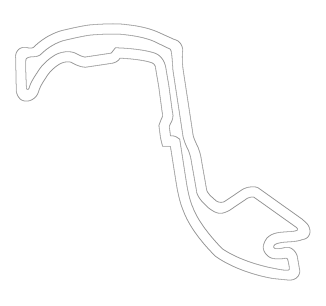
\includegraphics[interpolate=true,width=3.260000in,height=3.060000in]{contents/chapt5/figs/racing/mco-img0.png}}%
\end{pgfscope}%
\begin{pgfscope}%
\pgfpathrectangle{\pgfqpoint{0.527644in}{0.235000in}}{\pgfqpoint{3.258333in}{3.060000in}}%
\pgfusepath{clip}%
\pgfsetrectcap%
\pgfsetroundjoin%
\pgfsetlinewidth{1.003750pt}%
\definecolor{currentstroke}{rgb}{0.421569,0.122888,0.998103}%
\pgfsetstrokecolor{currentstroke}%
\pgfsetstrokeopacity{0.800000}%
\pgfsetdash{}{0pt}%
\pgfpathmoveto{\pgfqpoint{1.547644in}{2.994667in}}%
\pgfpathlineto{\pgfqpoint{1.549344in}{2.994667in}}%
\pgfusepath{stroke}%
\end{pgfscope}%
\begin{pgfscope}%
\pgfpathrectangle{\pgfqpoint{0.527644in}{0.235000in}}{\pgfqpoint{3.258333in}{3.060000in}}%
\pgfusepath{clip}%
\pgfsetrectcap%
\pgfsetroundjoin%
\pgfsetlinewidth{1.003750pt}%
\definecolor{currentstroke}{rgb}{0.335294,0.255843,0.991645}%
\pgfsetstrokecolor{currentstroke}%
\pgfsetstrokeopacity{0.800000}%
\pgfsetdash{}{0pt}%
\pgfpathmoveto{\pgfqpoint{1.549344in}{2.994667in}}%
\pgfpathlineto{\pgfqpoint{1.551092in}{2.994667in}}%
\pgfusepath{stroke}%
\end{pgfscope}%
\begin{pgfscope}%
\pgfpathrectangle{\pgfqpoint{0.527644in}{0.235000in}}{\pgfqpoint{3.258333in}{3.060000in}}%
\pgfusepath{clip}%
\pgfsetrectcap%
\pgfsetroundjoin%
\pgfsetlinewidth{1.003750pt}%
\definecolor{currentstroke}{rgb}{0.249020,0.384106,0.980635}%
\pgfsetstrokecolor{currentstroke}%
\pgfsetstrokeopacity{0.800000}%
\pgfsetdash{}{0pt}%
\pgfpathmoveto{\pgfqpoint{1.551092in}{2.994667in}}%
\pgfpathlineto{\pgfqpoint{1.552888in}{2.994670in}}%
\pgfusepath{stroke}%
\end{pgfscope}%
\begin{pgfscope}%
\pgfpathrectangle{\pgfqpoint{0.527644in}{0.235000in}}{\pgfqpoint{3.258333in}{3.060000in}}%
\pgfusepath{clip}%
\pgfsetrectcap%
\pgfsetroundjoin%
\pgfsetlinewidth{1.003750pt}%
\definecolor{currentstroke}{rgb}{0.162745,0.505325,0.965124}%
\pgfsetstrokecolor{currentstroke}%
\pgfsetstrokeopacity{0.800000}%
\pgfsetdash{}{0pt}%
\pgfpathmoveto{\pgfqpoint{1.552888in}{2.994670in}}%
\pgfpathlineto{\pgfqpoint{1.554732in}{2.994678in}}%
\pgfusepath{stroke}%
\end{pgfscope}%
\begin{pgfscope}%
\pgfpathrectangle{\pgfqpoint{0.527644in}{0.235000in}}{\pgfqpoint{3.258333in}{3.060000in}}%
\pgfusepath{clip}%
\pgfsetrectcap%
\pgfsetroundjoin%
\pgfsetlinewidth{1.003750pt}%
\definecolor{currentstroke}{rgb}{0.076471,0.617278,0.945184}%
\pgfsetstrokecolor{currentstroke}%
\pgfsetstrokeopacity{0.800000}%
\pgfsetdash{}{0pt}%
\pgfpathmoveto{\pgfqpoint{1.554732in}{2.994678in}}%
\pgfpathlineto{\pgfqpoint{1.556624in}{2.994696in}}%
\pgfusepath{stroke}%
\end{pgfscope}%
\begin{pgfscope}%
\pgfpathrectangle{\pgfqpoint{0.527644in}{0.235000in}}{\pgfqpoint{3.258333in}{3.060000in}}%
\pgfusepath{clip}%
\pgfsetrectcap%
\pgfsetroundjoin%
\pgfsetlinewidth{1.003750pt}%
\definecolor{currentstroke}{rgb}{0.001961,0.709281,0.923289}%
\pgfsetstrokecolor{currentstroke}%
\pgfsetstrokeopacity{0.800000}%
\pgfsetdash{}{0pt}%
\pgfpathmoveto{\pgfqpoint{1.556624in}{2.994696in}}%
\pgfpathlineto{\pgfqpoint{1.558563in}{2.994721in}}%
\pgfusepath{stroke}%
\end{pgfscope}%
\begin{pgfscope}%
\pgfpathrectangle{\pgfqpoint{0.527644in}{0.235000in}}{\pgfqpoint{3.258333in}{3.060000in}}%
\pgfusepath{clip}%
\pgfsetrectcap%
\pgfsetroundjoin%
\pgfsetlinewidth{1.003750pt}%
\definecolor{currentstroke}{rgb}{0.088235,0.798017,0.895163}%
\pgfsetstrokecolor{currentstroke}%
\pgfsetstrokeopacity{0.800000}%
\pgfsetdash{}{0pt}%
\pgfpathmoveto{\pgfqpoint{1.558563in}{2.994721in}}%
\pgfpathlineto{\pgfqpoint{1.560550in}{2.994754in}}%
\pgfusepath{stroke}%
\end{pgfscope}%
\begin{pgfscope}%
\pgfpathrectangle{\pgfqpoint{0.527644in}{0.235000in}}{\pgfqpoint{3.258333in}{3.060000in}}%
\pgfusepath{clip}%
\pgfsetrectcap%
\pgfsetroundjoin%
\pgfsetlinewidth{1.003750pt}%
\definecolor{currentstroke}{rgb}{0.174510,0.872120,0.862929}%
\pgfsetstrokecolor{currentstroke}%
\pgfsetstrokeopacity{0.800000}%
\pgfsetdash{}{0pt}%
\pgfpathmoveto{\pgfqpoint{1.560550in}{2.994754in}}%
\pgfpathlineto{\pgfqpoint{1.562585in}{2.994795in}}%
\pgfusepath{stroke}%
\end{pgfscope}%
\begin{pgfscope}%
\pgfpathrectangle{\pgfqpoint{0.527644in}{0.235000in}}{\pgfqpoint{3.258333in}{3.060000in}}%
\pgfusepath{clip}%
\pgfsetrectcap%
\pgfsetroundjoin%
\pgfsetlinewidth{1.003750pt}%
\definecolor{currentstroke}{rgb}{0.260784,0.930229,0.826734}%
\pgfsetstrokecolor{currentstroke}%
\pgfsetstrokeopacity{0.800000}%
\pgfsetdash{}{0pt}%
\pgfpathmoveto{\pgfqpoint{1.562585in}{2.994795in}}%
\pgfpathlineto{\pgfqpoint{1.564668in}{2.994847in}}%
\pgfusepath{stroke}%
\end{pgfscope}%
\begin{pgfscope}%
\pgfpathrectangle{\pgfqpoint{0.527644in}{0.235000in}}{\pgfqpoint{3.258333in}{3.060000in}}%
\pgfusepath{clip}%
\pgfsetrectcap%
\pgfsetroundjoin%
\pgfsetlinewidth{1.003750pt}%
\definecolor{currentstroke}{rgb}{0.347059,0.971281,0.786745}%
\pgfsetstrokecolor{currentstroke}%
\pgfsetstrokeopacity{0.800000}%
\pgfsetdash{}{0pt}%
\pgfpathmoveto{\pgfqpoint{1.564668in}{2.994847in}}%
\pgfpathlineto{\pgfqpoint{1.566798in}{2.994906in}}%
\pgfusepath{stroke}%
\end{pgfscope}%
\begin{pgfscope}%
\pgfpathrectangle{\pgfqpoint{0.527644in}{0.235000in}}{\pgfqpoint{3.258333in}{3.060000in}}%
\pgfusepath{clip}%
\pgfsetrectcap%
\pgfsetroundjoin%
\pgfsetlinewidth{1.003750pt}%
\definecolor{currentstroke}{rgb}{0.433333,0.994522,0.743145}%
\pgfsetstrokecolor{currentstroke}%
\pgfsetstrokeopacity{0.800000}%
\pgfsetdash{}{0pt}%
\pgfpathmoveto{\pgfqpoint{1.566798in}{2.994906in}}%
\pgfpathlineto{\pgfqpoint{1.568977in}{2.994977in}}%
\pgfusepath{stroke}%
\end{pgfscope}%
\begin{pgfscope}%
\pgfpathrectangle{\pgfqpoint{0.527644in}{0.235000in}}{\pgfqpoint{3.258333in}{3.060000in}}%
\pgfusepath{clip}%
\pgfsetrectcap%
\pgfsetroundjoin%
\pgfsetlinewidth{1.003750pt}%
\definecolor{currentstroke}{rgb}{0.519608,0.999526,0.696134}%
\pgfsetstrokecolor{currentstroke}%
\pgfsetstrokeopacity{0.800000}%
\pgfsetdash{}{0pt}%
\pgfpathmoveto{\pgfqpoint{1.568977in}{2.994977in}}%
\pgfpathlineto{\pgfqpoint{1.571204in}{2.995058in}}%
\pgfusepath{stroke}%
\end{pgfscope}%
\begin{pgfscope}%
\pgfpathrectangle{\pgfqpoint{0.527644in}{0.235000in}}{\pgfqpoint{3.258333in}{3.060000in}}%
\pgfusepath{clip}%
\pgfsetrectcap%
\pgfsetroundjoin%
\pgfsetlinewidth{1.003750pt}%
\definecolor{currentstroke}{rgb}{0.613725,0.984086,0.641213}%
\pgfsetstrokecolor{currentstroke}%
\pgfsetstrokeopacity{0.800000}%
\pgfsetdash{}{0pt}%
\pgfpathmoveto{\pgfqpoint{1.571204in}{2.995058in}}%
\pgfpathlineto{\pgfqpoint{1.573481in}{2.995145in}}%
\pgfusepath{stroke}%
\end{pgfscope}%
\begin{pgfscope}%
\pgfpathrectangle{\pgfqpoint{0.527644in}{0.235000in}}{\pgfqpoint{3.258333in}{3.060000in}}%
\pgfusepath{clip}%
\pgfsetrectcap%
\pgfsetroundjoin%
\pgfsetlinewidth{1.003750pt}%
\definecolor{currentstroke}{rgb}{0.700000,0.951057,0.587785}%
\pgfsetstrokecolor{currentstroke}%
\pgfsetstrokeopacity{0.800000}%
\pgfsetdash{}{0pt}%
\pgfpathmoveto{\pgfqpoint{1.573481in}{2.995145in}}%
\pgfpathlineto{\pgfqpoint{1.575808in}{2.995242in}}%
\pgfusepath{stroke}%
\end{pgfscope}%
\begin{pgfscope}%
\pgfpathrectangle{\pgfqpoint{0.527644in}{0.235000in}}{\pgfqpoint{3.258333in}{3.060000in}}%
\pgfusepath{clip}%
\pgfsetrectcap%
\pgfsetroundjoin%
\pgfsetlinewidth{1.003750pt}%
\definecolor{currentstroke}{rgb}{0.786275,0.900587,0.531659}%
\pgfsetstrokecolor{currentstroke}%
\pgfsetstrokeopacity{0.800000}%
\pgfsetdash{}{0pt}%
\pgfpathmoveto{\pgfqpoint{1.575808in}{2.995242in}}%
\pgfpathlineto{\pgfqpoint{1.578185in}{2.995347in}}%
\pgfusepath{stroke}%
\end{pgfscope}%
\begin{pgfscope}%
\pgfpathrectangle{\pgfqpoint{0.527644in}{0.235000in}}{\pgfqpoint{3.258333in}{3.060000in}}%
\pgfusepath{clip}%
\pgfsetrectcap%
\pgfsetroundjoin%
\pgfsetlinewidth{1.003750pt}%
\definecolor{currentstroke}{rgb}{0.872549,0.833602,0.473094}%
\pgfsetstrokecolor{currentstroke}%
\pgfsetstrokeopacity{0.800000}%
\pgfsetdash{}{0pt}%
\pgfpathmoveto{\pgfqpoint{1.578185in}{2.995347in}}%
\pgfpathlineto{\pgfqpoint{1.580611in}{2.995463in}}%
\pgfusepath{stroke}%
\end{pgfscope}%
\begin{pgfscope}%
\pgfpathrectangle{\pgfqpoint{0.527644in}{0.235000in}}{\pgfqpoint{3.258333in}{3.060000in}}%
\pgfusepath{clip}%
\pgfsetrectcap%
\pgfsetroundjoin%
\pgfsetlinewidth{1.003750pt}%
\definecolor{currentstroke}{rgb}{0.966667,0.743145,0.406737}%
\pgfsetstrokecolor{currentstroke}%
\pgfsetstrokeopacity{0.800000}%
\pgfsetdash{}{0pt}%
\pgfpathmoveto{\pgfqpoint{1.580611in}{2.995463in}}%
\pgfpathlineto{\pgfqpoint{1.583086in}{2.995587in}}%
\pgfusepath{stroke}%
\end{pgfscope}%
\begin{pgfscope}%
\pgfpathrectangle{\pgfqpoint{0.527644in}{0.235000in}}{\pgfqpoint{3.258333in}{3.060000in}}%
\pgfusepath{clip}%
\pgfsetrectcap%
\pgfsetroundjoin%
\pgfsetlinewidth{1.003750pt}%
\definecolor{currentstroke}{rgb}{1.000000,0.645928,0.343949}%
\pgfsetstrokecolor{currentstroke}%
\pgfsetstrokeopacity{0.800000}%
\pgfsetdash{}{0pt}%
\pgfpathmoveto{\pgfqpoint{1.583086in}{2.995587in}}%
\pgfpathlineto{\pgfqpoint{1.585611in}{2.995722in}}%
\pgfusepath{stroke}%
\end{pgfscope}%
\begin{pgfscope}%
\pgfpathrectangle{\pgfqpoint{0.527644in}{0.235000in}}{\pgfqpoint{3.258333in}{3.060000in}}%
\pgfusepath{clip}%
\pgfsetrectcap%
\pgfsetroundjoin%
\pgfsetlinewidth{1.003750pt}%
\definecolor{currentstroke}{rgb}{1.000000,0.536867,0.279583}%
\pgfsetstrokecolor{currentstroke}%
\pgfsetstrokeopacity{0.800000}%
\pgfsetdash{}{0pt}%
\pgfpathmoveto{\pgfqpoint{1.585611in}{2.995722in}}%
\pgfpathlineto{\pgfqpoint{1.588185in}{2.995866in}}%
\pgfusepath{stroke}%
\end{pgfscope}%
\begin{pgfscope}%
\pgfpathrectangle{\pgfqpoint{0.527644in}{0.235000in}}{\pgfqpoint{3.258333in}{3.060000in}}%
\pgfusepath{clip}%
\pgfsetrectcap%
\pgfsetroundjoin%
\pgfsetlinewidth{1.003750pt}%
\definecolor{currentstroke}{rgb}{1.000000,0.417960,0.213933}%
\pgfsetstrokecolor{currentstroke}%
\pgfsetstrokeopacity{0.800000}%
\pgfsetdash{}{0pt}%
\pgfpathmoveto{\pgfqpoint{1.588185in}{2.995866in}}%
\pgfpathlineto{\pgfqpoint{1.590809in}{2.996022in}}%
\pgfusepath{stroke}%
\end{pgfscope}%
\begin{pgfscope}%
\pgfpathrectangle{\pgfqpoint{0.527644in}{0.235000in}}{\pgfqpoint{3.258333in}{3.060000in}}%
\pgfusepath{clip}%
\pgfsetrectcap%
\pgfsetroundjoin%
\pgfsetlinewidth{1.003750pt}%
\definecolor{currentstroke}{rgb}{1.000000,0.291390,0.147302}%
\pgfsetstrokecolor{currentstroke}%
\pgfsetstrokeopacity{0.800000}%
\pgfsetdash{}{0pt}%
\pgfpathmoveto{\pgfqpoint{1.590809in}{2.996022in}}%
\pgfpathlineto{\pgfqpoint{1.593482in}{2.996186in}}%
\pgfusepath{stroke}%
\end{pgfscope}%
\begin{pgfscope}%
\pgfpathrectangle{\pgfqpoint{0.527644in}{0.235000in}}{\pgfqpoint{3.258333in}{3.060000in}}%
\pgfusepath{clip}%
\pgfsetrectcap%
\pgfsetroundjoin%
\pgfsetlinewidth{1.003750pt}%
\definecolor{currentstroke}{rgb}{1.000000,0.159476,0.079994}%
\pgfsetstrokecolor{currentstroke}%
\pgfsetstrokeopacity{0.800000}%
\pgfsetdash{}{0pt}%
\pgfpathmoveto{\pgfqpoint{1.593482in}{2.996186in}}%
\pgfpathlineto{\pgfqpoint{1.596202in}{2.996362in}}%
\pgfusepath{stroke}%
\end{pgfscope}%
\begin{pgfscope}%
\pgfpathrectangle{\pgfqpoint{0.527644in}{0.235000in}}{\pgfqpoint{3.258333in}{3.060000in}}%
\pgfusepath{clip}%
\pgfsetrectcap%
\pgfsetroundjoin%
\pgfsetlinewidth{1.003750pt}%
\definecolor{currentstroke}{rgb}{1.000000,0.024637,0.012320}%
\pgfsetstrokecolor{currentstroke}%
\pgfsetstrokeopacity{0.800000}%
\pgfsetdash{}{0pt}%
\pgfpathmoveto{\pgfqpoint{1.596202in}{2.996362in}}%
\pgfpathlineto{\pgfqpoint{1.598970in}{2.996548in}}%
\pgfusepath{stroke}%
\end{pgfscope}%
\begin{pgfscope}%
\pgfpathrectangle{\pgfqpoint{0.527644in}{0.235000in}}{\pgfqpoint{3.258333in}{3.060000in}}%
\pgfusepath{clip}%
\pgfsetrectcap%
\pgfsetroundjoin%
\pgfsetlinewidth{1.003750pt}%
\definecolor{currentstroke}{rgb}{1.000000,0.000000,0.000000}%
\pgfsetstrokecolor{currentstroke}%
\pgfsetstrokeopacity{0.800000}%
\pgfsetdash{}{0pt}%
\pgfpathmoveto{\pgfqpoint{1.598970in}{2.996548in}}%
\pgfpathlineto{\pgfqpoint{1.601784in}{2.996740in}}%
\pgfusepath{stroke}%
\end{pgfscope}%
\begin{pgfscope}%
\pgfpathrectangle{\pgfqpoint{0.527644in}{0.235000in}}{\pgfqpoint{3.258333in}{3.060000in}}%
\pgfusepath{clip}%
\pgfsetrectcap%
\pgfsetroundjoin%
\pgfsetlinewidth{1.003750pt}%
\definecolor{currentstroke}{rgb}{1.000000,0.000000,0.000000}%
\pgfsetstrokecolor{currentstroke}%
\pgfsetstrokeopacity{0.800000}%
\pgfsetdash{}{0pt}%
\pgfpathmoveto{\pgfqpoint{1.601784in}{2.996740in}}%
\pgfpathlineto{\pgfqpoint{1.604646in}{2.996936in}}%
\pgfusepath{stroke}%
\end{pgfscope}%
\begin{pgfscope}%
\pgfpathrectangle{\pgfqpoint{0.527644in}{0.235000in}}{\pgfqpoint{3.258333in}{3.060000in}}%
\pgfusepath{clip}%
\pgfsetrectcap%
\pgfsetroundjoin%
\pgfsetlinewidth{1.003750pt}%
\definecolor{currentstroke}{rgb}{1.000000,0.000000,0.000000}%
\pgfsetstrokecolor{currentstroke}%
\pgfsetstrokeopacity{0.800000}%
\pgfsetdash{}{0pt}%
\pgfpathmoveto{\pgfqpoint{1.604646in}{2.996936in}}%
\pgfpathlineto{\pgfqpoint{1.607509in}{2.997125in}}%
\pgfusepath{stroke}%
\end{pgfscope}%
\begin{pgfscope}%
\pgfpathrectangle{\pgfqpoint{0.527644in}{0.235000in}}{\pgfqpoint{3.258333in}{3.060000in}}%
\pgfusepath{clip}%
\pgfsetrectcap%
\pgfsetroundjoin%
\pgfsetlinewidth{1.003750pt}%
\definecolor{currentstroke}{rgb}{1.000000,0.000000,0.000000}%
\pgfsetstrokecolor{currentstroke}%
\pgfsetstrokeopacity{0.800000}%
\pgfsetdash{}{0pt}%
\pgfpathmoveto{\pgfqpoint{1.607509in}{2.997125in}}%
\pgfpathlineto{\pgfqpoint{1.610372in}{2.997305in}}%
\pgfusepath{stroke}%
\end{pgfscope}%
\begin{pgfscope}%
\pgfpathrectangle{\pgfqpoint{0.527644in}{0.235000in}}{\pgfqpoint{3.258333in}{3.060000in}}%
\pgfusepath{clip}%
\pgfsetrectcap%
\pgfsetroundjoin%
\pgfsetlinewidth{1.003750pt}%
\definecolor{currentstroke}{rgb}{1.000000,0.000000,0.000000}%
\pgfsetstrokecolor{currentstroke}%
\pgfsetstrokeopacity{0.800000}%
\pgfsetdash{}{0pt}%
\pgfpathmoveto{\pgfqpoint{1.610372in}{2.997305in}}%
\pgfpathlineto{\pgfqpoint{1.613235in}{2.997480in}}%
\pgfusepath{stroke}%
\end{pgfscope}%
\begin{pgfscope}%
\pgfpathrectangle{\pgfqpoint{0.527644in}{0.235000in}}{\pgfqpoint{3.258333in}{3.060000in}}%
\pgfusepath{clip}%
\pgfsetrectcap%
\pgfsetroundjoin%
\pgfsetlinewidth{1.003750pt}%
\definecolor{currentstroke}{rgb}{1.000000,0.000000,0.000000}%
\pgfsetstrokecolor{currentstroke}%
\pgfsetstrokeopacity{0.800000}%
\pgfsetdash{}{0pt}%
\pgfpathmoveto{\pgfqpoint{1.613235in}{2.997480in}}%
\pgfpathlineto{\pgfqpoint{1.616100in}{2.997644in}}%
\pgfusepath{stroke}%
\end{pgfscope}%
\begin{pgfscope}%
\pgfpathrectangle{\pgfqpoint{0.527644in}{0.235000in}}{\pgfqpoint{3.258333in}{3.060000in}}%
\pgfusepath{clip}%
\pgfsetrectcap%
\pgfsetroundjoin%
\pgfsetlinewidth{1.003750pt}%
\definecolor{currentstroke}{rgb}{1.000000,0.000000,0.000000}%
\pgfsetstrokecolor{currentstroke}%
\pgfsetstrokeopacity{0.800000}%
\pgfsetdash{}{0pt}%
\pgfpathmoveto{\pgfqpoint{1.616100in}{2.997644in}}%
\pgfpathlineto{\pgfqpoint{1.618964in}{2.997801in}}%
\pgfusepath{stroke}%
\end{pgfscope}%
\begin{pgfscope}%
\pgfpathrectangle{\pgfqpoint{0.527644in}{0.235000in}}{\pgfqpoint{3.258333in}{3.060000in}}%
\pgfusepath{clip}%
\pgfsetrectcap%
\pgfsetroundjoin%
\pgfsetlinewidth{1.003750pt}%
\definecolor{currentstroke}{rgb}{1.000000,0.000000,0.000000}%
\pgfsetstrokecolor{currentstroke}%
\pgfsetstrokeopacity{0.800000}%
\pgfsetdash{}{0pt}%
\pgfpathmoveto{\pgfqpoint{1.618964in}{2.997801in}}%
\pgfpathlineto{\pgfqpoint{1.621829in}{2.997946in}}%
\pgfusepath{stroke}%
\end{pgfscope}%
\begin{pgfscope}%
\pgfpathrectangle{\pgfqpoint{0.527644in}{0.235000in}}{\pgfqpoint{3.258333in}{3.060000in}}%
\pgfusepath{clip}%
\pgfsetrectcap%
\pgfsetroundjoin%
\pgfsetlinewidth{1.003750pt}%
\definecolor{currentstroke}{rgb}{1.000000,0.000000,0.000000}%
\pgfsetstrokecolor{currentstroke}%
\pgfsetstrokeopacity{0.800000}%
\pgfsetdash{}{0pt}%
\pgfpathmoveto{\pgfqpoint{1.621829in}{2.997946in}}%
\pgfpathlineto{\pgfqpoint{1.624695in}{2.998081in}}%
\pgfusepath{stroke}%
\end{pgfscope}%
\begin{pgfscope}%
\pgfpathrectangle{\pgfqpoint{0.527644in}{0.235000in}}{\pgfqpoint{3.258333in}{3.060000in}}%
\pgfusepath{clip}%
\pgfsetrectcap%
\pgfsetroundjoin%
\pgfsetlinewidth{1.003750pt}%
\definecolor{currentstroke}{rgb}{1.000000,0.000000,0.000000}%
\pgfsetstrokecolor{currentstroke}%
\pgfsetstrokeopacity{0.800000}%
\pgfsetdash{}{0pt}%
\pgfpathmoveto{\pgfqpoint{1.624695in}{2.998081in}}%
\pgfpathlineto{\pgfqpoint{1.627561in}{2.998201in}}%
\pgfusepath{stroke}%
\end{pgfscope}%
\begin{pgfscope}%
\pgfpathrectangle{\pgfqpoint{0.527644in}{0.235000in}}{\pgfqpoint{3.258333in}{3.060000in}}%
\pgfusepath{clip}%
\pgfsetrectcap%
\pgfsetroundjoin%
\pgfsetlinewidth{1.003750pt}%
\definecolor{currentstroke}{rgb}{1.000000,0.000000,0.000000}%
\pgfsetstrokecolor{currentstroke}%
\pgfsetstrokeopacity{0.800000}%
\pgfsetdash{}{0pt}%
\pgfpathmoveto{\pgfqpoint{1.627561in}{2.998201in}}%
\pgfpathlineto{\pgfqpoint{1.630428in}{2.998309in}}%
\pgfusepath{stroke}%
\end{pgfscope}%
\begin{pgfscope}%
\pgfpathrectangle{\pgfqpoint{0.527644in}{0.235000in}}{\pgfqpoint{3.258333in}{3.060000in}}%
\pgfusepath{clip}%
\pgfsetrectcap%
\pgfsetroundjoin%
\pgfsetlinewidth{1.003750pt}%
\definecolor{currentstroke}{rgb}{1.000000,0.000000,0.000000}%
\pgfsetstrokecolor{currentstroke}%
\pgfsetstrokeopacity{0.800000}%
\pgfsetdash{}{0pt}%
\pgfpathmoveto{\pgfqpoint{1.630428in}{2.998309in}}%
\pgfpathlineto{\pgfqpoint{1.633295in}{2.998399in}}%
\pgfusepath{stroke}%
\end{pgfscope}%
\begin{pgfscope}%
\pgfpathrectangle{\pgfqpoint{0.527644in}{0.235000in}}{\pgfqpoint{3.258333in}{3.060000in}}%
\pgfusepath{clip}%
\pgfsetrectcap%
\pgfsetroundjoin%
\pgfsetlinewidth{1.003750pt}%
\definecolor{currentstroke}{rgb}{1.000000,0.000000,0.000000}%
\pgfsetstrokecolor{currentstroke}%
\pgfsetstrokeopacity{0.800000}%
\pgfsetdash{}{0pt}%
\pgfpathmoveto{\pgfqpoint{1.633295in}{2.998399in}}%
\pgfpathlineto{\pgfqpoint{1.636163in}{2.998473in}}%
\pgfusepath{stroke}%
\end{pgfscope}%
\begin{pgfscope}%
\pgfpathrectangle{\pgfqpoint{0.527644in}{0.235000in}}{\pgfqpoint{3.258333in}{3.060000in}}%
\pgfusepath{clip}%
\pgfsetrectcap%
\pgfsetroundjoin%
\pgfsetlinewidth{1.003750pt}%
\definecolor{currentstroke}{rgb}{1.000000,0.000000,0.000000}%
\pgfsetstrokecolor{currentstroke}%
\pgfsetstrokeopacity{0.800000}%
\pgfsetdash{}{0pt}%
\pgfpathmoveto{\pgfqpoint{1.636163in}{2.998473in}}%
\pgfpathlineto{\pgfqpoint{1.639031in}{2.998526in}}%
\pgfusepath{stroke}%
\end{pgfscope}%
\begin{pgfscope}%
\pgfpathrectangle{\pgfqpoint{0.527644in}{0.235000in}}{\pgfqpoint{3.258333in}{3.060000in}}%
\pgfusepath{clip}%
\pgfsetrectcap%
\pgfsetroundjoin%
\pgfsetlinewidth{1.003750pt}%
\definecolor{currentstroke}{rgb}{1.000000,0.000000,0.000000}%
\pgfsetstrokecolor{currentstroke}%
\pgfsetstrokeopacity{0.800000}%
\pgfsetdash{}{0pt}%
\pgfpathmoveto{\pgfqpoint{1.639031in}{2.998526in}}%
\pgfpathlineto{\pgfqpoint{1.641900in}{2.998563in}}%
\pgfusepath{stroke}%
\end{pgfscope}%
\begin{pgfscope}%
\pgfpathrectangle{\pgfqpoint{0.527644in}{0.235000in}}{\pgfqpoint{3.258333in}{3.060000in}}%
\pgfusepath{clip}%
\pgfsetrectcap%
\pgfsetroundjoin%
\pgfsetlinewidth{1.003750pt}%
\definecolor{currentstroke}{rgb}{1.000000,0.000000,0.000000}%
\pgfsetstrokecolor{currentstroke}%
\pgfsetstrokeopacity{0.800000}%
\pgfsetdash{}{0pt}%
\pgfpathmoveto{\pgfqpoint{1.641900in}{2.998563in}}%
\pgfpathlineto{\pgfqpoint{1.644768in}{2.998575in}}%
\pgfusepath{stroke}%
\end{pgfscope}%
\begin{pgfscope}%
\pgfpathrectangle{\pgfqpoint{0.527644in}{0.235000in}}{\pgfqpoint{3.258333in}{3.060000in}}%
\pgfusepath{clip}%
\pgfsetrectcap%
\pgfsetroundjoin%
\pgfsetlinewidth{1.003750pt}%
\definecolor{currentstroke}{rgb}{1.000000,0.000000,0.000000}%
\pgfsetstrokecolor{currentstroke}%
\pgfsetstrokeopacity{0.800000}%
\pgfsetdash{}{0pt}%
\pgfpathmoveto{\pgfqpoint{1.644768in}{2.998575in}}%
\pgfpathlineto{\pgfqpoint{1.647637in}{2.998569in}}%
\pgfusepath{stroke}%
\end{pgfscope}%
\begin{pgfscope}%
\pgfpathrectangle{\pgfqpoint{0.527644in}{0.235000in}}{\pgfqpoint{3.258333in}{3.060000in}}%
\pgfusepath{clip}%
\pgfsetrectcap%
\pgfsetroundjoin%
\pgfsetlinewidth{1.003750pt}%
\definecolor{currentstroke}{rgb}{1.000000,0.000000,0.000000}%
\pgfsetstrokecolor{currentstroke}%
\pgfsetstrokeopacity{0.800000}%
\pgfsetdash{}{0pt}%
\pgfpathmoveto{\pgfqpoint{1.647637in}{2.998569in}}%
\pgfpathlineto{\pgfqpoint{1.650506in}{2.998537in}}%
\pgfusepath{stroke}%
\end{pgfscope}%
\begin{pgfscope}%
\pgfpathrectangle{\pgfqpoint{0.527644in}{0.235000in}}{\pgfqpoint{3.258333in}{3.060000in}}%
\pgfusepath{clip}%
\pgfsetrectcap%
\pgfsetroundjoin%
\pgfsetlinewidth{1.003750pt}%
\definecolor{currentstroke}{rgb}{1.000000,0.000000,0.000000}%
\pgfsetstrokecolor{currentstroke}%
\pgfsetstrokeopacity{0.800000}%
\pgfsetdash{}{0pt}%
\pgfpathmoveto{\pgfqpoint{1.650506in}{2.998537in}}%
\pgfpathlineto{\pgfqpoint{1.653374in}{2.998484in}}%
\pgfusepath{stroke}%
\end{pgfscope}%
\begin{pgfscope}%
\pgfpathrectangle{\pgfqpoint{0.527644in}{0.235000in}}{\pgfqpoint{3.258333in}{3.060000in}}%
\pgfusepath{clip}%
\pgfsetrectcap%
\pgfsetroundjoin%
\pgfsetlinewidth{1.003750pt}%
\definecolor{currentstroke}{rgb}{1.000000,0.000000,0.000000}%
\pgfsetstrokecolor{currentstroke}%
\pgfsetstrokeopacity{0.800000}%
\pgfsetdash{}{0pt}%
\pgfpathmoveto{\pgfqpoint{1.653374in}{2.998484in}}%
\pgfpathlineto{\pgfqpoint{1.656242in}{2.998413in}}%
\pgfusepath{stroke}%
\end{pgfscope}%
\begin{pgfscope}%
\pgfpathrectangle{\pgfqpoint{0.527644in}{0.235000in}}{\pgfqpoint{3.258333in}{3.060000in}}%
\pgfusepath{clip}%
\pgfsetrectcap%
\pgfsetroundjoin%
\pgfsetlinewidth{1.003750pt}%
\definecolor{currentstroke}{rgb}{1.000000,0.000000,0.000000}%
\pgfsetstrokecolor{currentstroke}%
\pgfsetstrokeopacity{0.800000}%
\pgfsetdash{}{0pt}%
\pgfpathmoveto{\pgfqpoint{1.656242in}{2.998413in}}%
\pgfpathlineto{\pgfqpoint{1.659110in}{2.998328in}}%
\pgfusepath{stroke}%
\end{pgfscope}%
\begin{pgfscope}%
\pgfpathrectangle{\pgfqpoint{0.527644in}{0.235000in}}{\pgfqpoint{3.258333in}{3.060000in}}%
\pgfusepath{clip}%
\pgfsetrectcap%
\pgfsetroundjoin%
\pgfsetlinewidth{1.003750pt}%
\definecolor{currentstroke}{rgb}{1.000000,0.000000,0.000000}%
\pgfsetstrokecolor{currentstroke}%
\pgfsetstrokeopacity{0.800000}%
\pgfsetdash{}{0pt}%
\pgfpathmoveto{\pgfqpoint{1.659110in}{2.998328in}}%
\pgfpathlineto{\pgfqpoint{1.661977in}{2.998233in}}%
\pgfusepath{stroke}%
\end{pgfscope}%
\begin{pgfscope}%
\pgfpathrectangle{\pgfqpoint{0.527644in}{0.235000in}}{\pgfqpoint{3.258333in}{3.060000in}}%
\pgfusepath{clip}%
\pgfsetrectcap%
\pgfsetroundjoin%
\pgfsetlinewidth{1.003750pt}%
\definecolor{currentstroke}{rgb}{1.000000,0.000000,0.000000}%
\pgfsetstrokecolor{currentstroke}%
\pgfsetstrokeopacity{0.800000}%
\pgfsetdash{}{0pt}%
\pgfpathmoveto{\pgfqpoint{1.661977in}{2.998233in}}%
\pgfpathlineto{\pgfqpoint{1.664843in}{2.998122in}}%
\pgfusepath{stroke}%
\end{pgfscope}%
\begin{pgfscope}%
\pgfpathrectangle{\pgfqpoint{0.527644in}{0.235000in}}{\pgfqpoint{3.258333in}{3.060000in}}%
\pgfusepath{clip}%
\pgfsetrectcap%
\pgfsetroundjoin%
\pgfsetlinewidth{1.003750pt}%
\definecolor{currentstroke}{rgb}{1.000000,0.000000,0.000000}%
\pgfsetstrokecolor{currentstroke}%
\pgfsetstrokeopacity{0.800000}%
\pgfsetdash{}{0pt}%
\pgfpathmoveto{\pgfqpoint{1.664843in}{2.998122in}}%
\pgfpathlineto{\pgfqpoint{1.667710in}{2.998000in}}%
\pgfusepath{stroke}%
\end{pgfscope}%
\begin{pgfscope}%
\pgfpathrectangle{\pgfqpoint{0.527644in}{0.235000in}}{\pgfqpoint{3.258333in}{3.060000in}}%
\pgfusepath{clip}%
\pgfsetrectcap%
\pgfsetroundjoin%
\pgfsetlinewidth{1.003750pt}%
\definecolor{currentstroke}{rgb}{1.000000,0.000000,0.000000}%
\pgfsetstrokecolor{currentstroke}%
\pgfsetstrokeopacity{0.800000}%
\pgfsetdash{}{0pt}%
\pgfpathmoveto{\pgfqpoint{1.667710in}{2.998000in}}%
\pgfpathlineto{\pgfqpoint{1.670575in}{2.997864in}}%
\pgfusepath{stroke}%
\end{pgfscope}%
\begin{pgfscope}%
\pgfpathrectangle{\pgfqpoint{0.527644in}{0.235000in}}{\pgfqpoint{3.258333in}{3.060000in}}%
\pgfusepath{clip}%
\pgfsetrectcap%
\pgfsetroundjoin%
\pgfsetlinewidth{1.003750pt}%
\definecolor{currentstroke}{rgb}{1.000000,0.000000,0.000000}%
\pgfsetstrokecolor{currentstroke}%
\pgfsetstrokeopacity{0.800000}%
\pgfsetdash{}{0pt}%
\pgfpathmoveto{\pgfqpoint{1.670575in}{2.997864in}}%
\pgfpathlineto{\pgfqpoint{1.673440in}{2.997718in}}%
\pgfusepath{stroke}%
\end{pgfscope}%
\begin{pgfscope}%
\pgfpathrectangle{\pgfqpoint{0.527644in}{0.235000in}}{\pgfqpoint{3.258333in}{3.060000in}}%
\pgfusepath{clip}%
\pgfsetrectcap%
\pgfsetroundjoin%
\pgfsetlinewidth{1.003750pt}%
\definecolor{currentstroke}{rgb}{1.000000,0.000000,0.000000}%
\pgfsetstrokecolor{currentstroke}%
\pgfsetstrokeopacity{0.800000}%
\pgfsetdash{}{0pt}%
\pgfpathmoveto{\pgfqpoint{1.673440in}{2.997718in}}%
\pgfpathlineto{\pgfqpoint{1.676305in}{2.997560in}}%
\pgfusepath{stroke}%
\end{pgfscope}%
\begin{pgfscope}%
\pgfpathrectangle{\pgfqpoint{0.527644in}{0.235000in}}{\pgfqpoint{3.258333in}{3.060000in}}%
\pgfusepath{clip}%
\pgfsetrectcap%
\pgfsetroundjoin%
\pgfsetlinewidth{1.003750pt}%
\definecolor{currentstroke}{rgb}{1.000000,0.000000,0.000000}%
\pgfsetstrokecolor{currentstroke}%
\pgfsetstrokeopacity{0.800000}%
\pgfsetdash{}{0pt}%
\pgfpathmoveto{\pgfqpoint{1.676305in}{2.997560in}}%
\pgfpathlineto{\pgfqpoint{1.679169in}{2.997396in}}%
\pgfusepath{stroke}%
\end{pgfscope}%
\begin{pgfscope}%
\pgfpathrectangle{\pgfqpoint{0.527644in}{0.235000in}}{\pgfqpoint{3.258333in}{3.060000in}}%
\pgfusepath{clip}%
\pgfsetrectcap%
\pgfsetroundjoin%
\pgfsetlinewidth{1.003750pt}%
\definecolor{currentstroke}{rgb}{1.000000,0.000000,0.000000}%
\pgfsetstrokecolor{currentstroke}%
\pgfsetstrokeopacity{0.800000}%
\pgfsetdash{}{0pt}%
\pgfpathmoveto{\pgfqpoint{1.679169in}{2.997396in}}%
\pgfpathlineto{\pgfqpoint{1.682032in}{2.997221in}}%
\pgfusepath{stroke}%
\end{pgfscope}%
\begin{pgfscope}%
\pgfpathrectangle{\pgfqpoint{0.527644in}{0.235000in}}{\pgfqpoint{3.258333in}{3.060000in}}%
\pgfusepath{clip}%
\pgfsetrectcap%
\pgfsetroundjoin%
\pgfsetlinewidth{1.003750pt}%
\definecolor{currentstroke}{rgb}{1.000000,0.000000,0.000000}%
\pgfsetstrokecolor{currentstroke}%
\pgfsetstrokeopacity{0.800000}%
\pgfsetdash{}{0pt}%
\pgfpathmoveto{\pgfqpoint{1.682032in}{2.997221in}}%
\pgfpathlineto{\pgfqpoint{1.684895in}{2.997043in}}%
\pgfusepath{stroke}%
\end{pgfscope}%
\begin{pgfscope}%
\pgfpathrectangle{\pgfqpoint{0.527644in}{0.235000in}}{\pgfqpoint{3.258333in}{3.060000in}}%
\pgfusepath{clip}%
\pgfsetrectcap%
\pgfsetroundjoin%
\pgfsetlinewidth{1.003750pt}%
\definecolor{currentstroke}{rgb}{1.000000,0.000000,0.000000}%
\pgfsetstrokecolor{currentstroke}%
\pgfsetstrokeopacity{0.800000}%
\pgfsetdash{}{0pt}%
\pgfpathmoveto{\pgfqpoint{1.684895in}{2.997043in}}%
\pgfpathlineto{\pgfqpoint{1.687758in}{2.996857in}}%
\pgfusepath{stroke}%
\end{pgfscope}%
\begin{pgfscope}%
\pgfpathrectangle{\pgfqpoint{0.527644in}{0.235000in}}{\pgfqpoint{3.258333in}{3.060000in}}%
\pgfusepath{clip}%
\pgfsetrectcap%
\pgfsetroundjoin%
\pgfsetlinewidth{1.003750pt}%
\definecolor{currentstroke}{rgb}{1.000000,0.000000,0.000000}%
\pgfsetstrokecolor{currentstroke}%
\pgfsetstrokeopacity{0.800000}%
\pgfsetdash{}{0pt}%
\pgfpathmoveto{\pgfqpoint{1.687758in}{2.996857in}}%
\pgfpathlineto{\pgfqpoint{1.690621in}{2.996670in}}%
\pgfusepath{stroke}%
\end{pgfscope}%
\begin{pgfscope}%
\pgfpathrectangle{\pgfqpoint{0.527644in}{0.235000in}}{\pgfqpoint{3.258333in}{3.060000in}}%
\pgfusepath{clip}%
\pgfsetrectcap%
\pgfsetroundjoin%
\pgfsetlinewidth{1.003750pt}%
\definecolor{currentstroke}{rgb}{1.000000,0.000000,0.000000}%
\pgfsetstrokecolor{currentstroke}%
\pgfsetstrokeopacity{0.800000}%
\pgfsetdash{}{0pt}%
\pgfpathmoveto{\pgfqpoint{1.690621in}{2.996670in}}%
\pgfpathlineto{\pgfqpoint{1.693483in}{2.996478in}}%
\pgfusepath{stroke}%
\end{pgfscope}%
\begin{pgfscope}%
\pgfpathrectangle{\pgfqpoint{0.527644in}{0.235000in}}{\pgfqpoint{3.258333in}{3.060000in}}%
\pgfusepath{clip}%
\pgfsetrectcap%
\pgfsetroundjoin%
\pgfsetlinewidth{1.003750pt}%
\definecolor{currentstroke}{rgb}{1.000000,0.000000,0.000000}%
\pgfsetstrokecolor{currentstroke}%
\pgfsetstrokeopacity{0.800000}%
\pgfsetdash{}{0pt}%
\pgfpathmoveto{\pgfqpoint{1.693483in}{2.996478in}}%
\pgfpathlineto{\pgfqpoint{1.696346in}{2.996286in}}%
\pgfusepath{stroke}%
\end{pgfscope}%
\begin{pgfscope}%
\pgfpathrectangle{\pgfqpoint{0.527644in}{0.235000in}}{\pgfqpoint{3.258333in}{3.060000in}}%
\pgfusepath{clip}%
\pgfsetrectcap%
\pgfsetroundjoin%
\pgfsetlinewidth{1.003750pt}%
\definecolor{currentstroke}{rgb}{1.000000,0.000000,0.000000}%
\pgfsetstrokecolor{currentstroke}%
\pgfsetstrokeopacity{0.800000}%
\pgfsetdash{}{0pt}%
\pgfpathmoveto{\pgfqpoint{1.696346in}{2.996286in}}%
\pgfpathlineto{\pgfqpoint{1.699208in}{2.996091in}}%
\pgfusepath{stroke}%
\end{pgfscope}%
\begin{pgfscope}%
\pgfpathrectangle{\pgfqpoint{0.527644in}{0.235000in}}{\pgfqpoint{3.258333in}{3.060000in}}%
\pgfusepath{clip}%
\pgfsetrectcap%
\pgfsetroundjoin%
\pgfsetlinewidth{1.003750pt}%
\definecolor{currentstroke}{rgb}{1.000000,0.000000,0.000000}%
\pgfsetstrokecolor{currentstroke}%
\pgfsetstrokeopacity{0.800000}%
\pgfsetdash{}{0pt}%
\pgfpathmoveto{\pgfqpoint{1.699208in}{2.996091in}}%
\pgfpathlineto{\pgfqpoint{1.702070in}{2.995898in}}%
\pgfusepath{stroke}%
\end{pgfscope}%
\begin{pgfscope}%
\pgfpathrectangle{\pgfqpoint{0.527644in}{0.235000in}}{\pgfqpoint{3.258333in}{3.060000in}}%
\pgfusepath{clip}%
\pgfsetrectcap%
\pgfsetroundjoin%
\pgfsetlinewidth{1.003750pt}%
\definecolor{currentstroke}{rgb}{1.000000,0.000000,0.000000}%
\pgfsetstrokecolor{currentstroke}%
\pgfsetstrokeopacity{0.800000}%
\pgfsetdash{}{0pt}%
\pgfpathmoveto{\pgfqpoint{1.702070in}{2.995898in}}%
\pgfpathlineto{\pgfqpoint{1.704932in}{2.995704in}}%
\pgfusepath{stroke}%
\end{pgfscope}%
\begin{pgfscope}%
\pgfpathrectangle{\pgfqpoint{0.527644in}{0.235000in}}{\pgfqpoint{3.258333in}{3.060000in}}%
\pgfusepath{clip}%
\pgfsetrectcap%
\pgfsetroundjoin%
\pgfsetlinewidth{1.003750pt}%
\definecolor{currentstroke}{rgb}{1.000000,0.000000,0.000000}%
\pgfsetstrokecolor{currentstroke}%
\pgfsetstrokeopacity{0.800000}%
\pgfsetdash{}{0pt}%
\pgfpathmoveto{\pgfqpoint{1.704932in}{2.995704in}}%
\pgfpathlineto{\pgfqpoint{1.707795in}{2.995513in}}%
\pgfusepath{stroke}%
\end{pgfscope}%
\begin{pgfscope}%
\pgfpathrectangle{\pgfqpoint{0.527644in}{0.235000in}}{\pgfqpoint{3.258333in}{3.060000in}}%
\pgfusepath{clip}%
\pgfsetrectcap%
\pgfsetroundjoin%
\pgfsetlinewidth{1.003750pt}%
\definecolor{currentstroke}{rgb}{1.000000,0.000000,0.000000}%
\pgfsetstrokecolor{currentstroke}%
\pgfsetstrokeopacity{0.800000}%
\pgfsetdash{}{0pt}%
\pgfpathmoveto{\pgfqpoint{1.707795in}{2.995513in}}%
\pgfpathlineto{\pgfqpoint{1.710657in}{2.995322in}}%
\pgfusepath{stroke}%
\end{pgfscope}%
\begin{pgfscope}%
\pgfpathrectangle{\pgfqpoint{0.527644in}{0.235000in}}{\pgfqpoint{3.258333in}{3.060000in}}%
\pgfusepath{clip}%
\pgfsetrectcap%
\pgfsetroundjoin%
\pgfsetlinewidth{1.003750pt}%
\definecolor{currentstroke}{rgb}{1.000000,0.000000,0.000000}%
\pgfsetstrokecolor{currentstroke}%
\pgfsetstrokeopacity{0.800000}%
\pgfsetdash{}{0pt}%
\pgfpathmoveto{\pgfqpoint{1.710657in}{2.995322in}}%
\pgfpathlineto{\pgfqpoint{1.713520in}{2.995136in}}%
\pgfusepath{stroke}%
\end{pgfscope}%
\begin{pgfscope}%
\pgfpathrectangle{\pgfqpoint{0.527644in}{0.235000in}}{\pgfqpoint{3.258333in}{3.060000in}}%
\pgfusepath{clip}%
\pgfsetrectcap%
\pgfsetroundjoin%
\pgfsetlinewidth{1.003750pt}%
\definecolor{currentstroke}{rgb}{1.000000,0.000000,0.000000}%
\pgfsetstrokecolor{currentstroke}%
\pgfsetstrokeopacity{0.800000}%
\pgfsetdash{}{0pt}%
\pgfpathmoveto{\pgfqpoint{1.713520in}{2.995136in}}%
\pgfpathlineto{\pgfqpoint{1.716382in}{2.994950in}}%
\pgfusepath{stroke}%
\end{pgfscope}%
\begin{pgfscope}%
\pgfpathrectangle{\pgfqpoint{0.527644in}{0.235000in}}{\pgfqpoint{3.258333in}{3.060000in}}%
\pgfusepath{clip}%
\pgfsetrectcap%
\pgfsetroundjoin%
\pgfsetlinewidth{1.003750pt}%
\definecolor{currentstroke}{rgb}{1.000000,0.000000,0.000000}%
\pgfsetstrokecolor{currentstroke}%
\pgfsetstrokeopacity{0.800000}%
\pgfsetdash{}{0pt}%
\pgfpathmoveto{\pgfqpoint{1.716382in}{2.994950in}}%
\pgfpathlineto{\pgfqpoint{1.719246in}{2.994770in}}%
\pgfusepath{stroke}%
\end{pgfscope}%
\begin{pgfscope}%
\pgfpathrectangle{\pgfqpoint{0.527644in}{0.235000in}}{\pgfqpoint{3.258333in}{3.060000in}}%
\pgfusepath{clip}%
\pgfsetrectcap%
\pgfsetroundjoin%
\pgfsetlinewidth{1.003750pt}%
\definecolor{currentstroke}{rgb}{1.000000,0.000000,0.000000}%
\pgfsetstrokecolor{currentstroke}%
\pgfsetstrokeopacity{0.800000}%
\pgfsetdash{}{0pt}%
\pgfpathmoveto{\pgfqpoint{1.719246in}{2.994770in}}%
\pgfpathlineto{\pgfqpoint{1.722109in}{2.994591in}}%
\pgfusepath{stroke}%
\end{pgfscope}%
\begin{pgfscope}%
\pgfpathrectangle{\pgfqpoint{0.527644in}{0.235000in}}{\pgfqpoint{3.258333in}{3.060000in}}%
\pgfusepath{clip}%
\pgfsetrectcap%
\pgfsetroundjoin%
\pgfsetlinewidth{1.003750pt}%
\definecolor{currentstroke}{rgb}{1.000000,0.000000,0.000000}%
\pgfsetstrokecolor{currentstroke}%
\pgfsetstrokeopacity{0.800000}%
\pgfsetdash{}{0pt}%
\pgfpathmoveto{\pgfqpoint{1.722109in}{2.994591in}}%
\pgfpathlineto{\pgfqpoint{1.724972in}{2.994419in}}%
\pgfusepath{stroke}%
\end{pgfscope}%
\begin{pgfscope}%
\pgfpathrectangle{\pgfqpoint{0.527644in}{0.235000in}}{\pgfqpoint{3.258333in}{3.060000in}}%
\pgfusepath{clip}%
\pgfsetrectcap%
\pgfsetroundjoin%
\pgfsetlinewidth{1.003750pt}%
\definecolor{currentstroke}{rgb}{1.000000,0.000000,0.000000}%
\pgfsetstrokecolor{currentstroke}%
\pgfsetstrokeopacity{0.800000}%
\pgfsetdash{}{0pt}%
\pgfpathmoveto{\pgfqpoint{1.724972in}{2.994419in}}%
\pgfpathlineto{\pgfqpoint{1.727836in}{2.994248in}}%
\pgfusepath{stroke}%
\end{pgfscope}%
\begin{pgfscope}%
\pgfpathrectangle{\pgfqpoint{0.527644in}{0.235000in}}{\pgfqpoint{3.258333in}{3.060000in}}%
\pgfusepath{clip}%
\pgfsetrectcap%
\pgfsetroundjoin%
\pgfsetlinewidth{1.003750pt}%
\definecolor{currentstroke}{rgb}{1.000000,0.000000,0.000000}%
\pgfsetstrokecolor{currentstroke}%
\pgfsetstrokeopacity{0.800000}%
\pgfsetdash{}{0pt}%
\pgfpathmoveto{\pgfqpoint{1.727836in}{2.994248in}}%
\pgfpathlineto{\pgfqpoint{1.730700in}{2.994085in}}%
\pgfusepath{stroke}%
\end{pgfscope}%
\begin{pgfscope}%
\pgfpathrectangle{\pgfqpoint{0.527644in}{0.235000in}}{\pgfqpoint{3.258333in}{3.060000in}}%
\pgfusepath{clip}%
\pgfsetrectcap%
\pgfsetroundjoin%
\pgfsetlinewidth{1.003750pt}%
\definecolor{currentstroke}{rgb}{1.000000,0.000000,0.000000}%
\pgfsetstrokecolor{currentstroke}%
\pgfsetstrokeopacity{0.800000}%
\pgfsetdash{}{0pt}%
\pgfpathmoveto{\pgfqpoint{1.730700in}{2.994085in}}%
\pgfpathlineto{\pgfqpoint{1.733564in}{2.993923in}}%
\pgfusepath{stroke}%
\end{pgfscope}%
\begin{pgfscope}%
\pgfpathrectangle{\pgfqpoint{0.527644in}{0.235000in}}{\pgfqpoint{3.258333in}{3.060000in}}%
\pgfusepath{clip}%
\pgfsetrectcap%
\pgfsetroundjoin%
\pgfsetlinewidth{1.003750pt}%
\definecolor{currentstroke}{rgb}{1.000000,0.000000,0.000000}%
\pgfsetstrokecolor{currentstroke}%
\pgfsetstrokeopacity{0.800000}%
\pgfsetdash{}{0pt}%
\pgfpathmoveto{\pgfqpoint{1.733564in}{2.993923in}}%
\pgfpathlineto{\pgfqpoint{1.736429in}{2.993769in}}%
\pgfusepath{stroke}%
\end{pgfscope}%
\begin{pgfscope}%
\pgfpathrectangle{\pgfqpoint{0.527644in}{0.235000in}}{\pgfqpoint{3.258333in}{3.060000in}}%
\pgfusepath{clip}%
\pgfsetrectcap%
\pgfsetroundjoin%
\pgfsetlinewidth{1.003750pt}%
\definecolor{currentstroke}{rgb}{1.000000,0.000000,0.000000}%
\pgfsetstrokecolor{currentstroke}%
\pgfsetstrokeopacity{0.800000}%
\pgfsetdash{}{0pt}%
\pgfpathmoveto{\pgfqpoint{1.736429in}{2.993769in}}%
\pgfpathlineto{\pgfqpoint{1.739294in}{2.993617in}}%
\pgfusepath{stroke}%
\end{pgfscope}%
\begin{pgfscope}%
\pgfpathrectangle{\pgfqpoint{0.527644in}{0.235000in}}{\pgfqpoint{3.258333in}{3.060000in}}%
\pgfusepath{clip}%
\pgfsetrectcap%
\pgfsetroundjoin%
\pgfsetlinewidth{1.003750pt}%
\definecolor{currentstroke}{rgb}{1.000000,0.000000,0.000000}%
\pgfsetstrokecolor{currentstroke}%
\pgfsetstrokeopacity{0.800000}%
\pgfsetdash{}{0pt}%
\pgfpathmoveto{\pgfqpoint{1.739294in}{2.993617in}}%
\pgfpathlineto{\pgfqpoint{1.742159in}{2.993473in}}%
\pgfusepath{stroke}%
\end{pgfscope}%
\begin{pgfscope}%
\pgfpathrectangle{\pgfqpoint{0.527644in}{0.235000in}}{\pgfqpoint{3.258333in}{3.060000in}}%
\pgfusepath{clip}%
\pgfsetrectcap%
\pgfsetroundjoin%
\pgfsetlinewidth{1.003750pt}%
\definecolor{currentstroke}{rgb}{1.000000,0.000000,0.000000}%
\pgfsetstrokecolor{currentstroke}%
\pgfsetstrokeopacity{0.800000}%
\pgfsetdash{}{0pt}%
\pgfpathmoveto{\pgfqpoint{1.742159in}{2.993473in}}%
\pgfpathlineto{\pgfqpoint{1.745025in}{2.993341in}}%
\pgfusepath{stroke}%
\end{pgfscope}%
\begin{pgfscope}%
\pgfpathrectangle{\pgfqpoint{0.527644in}{0.235000in}}{\pgfqpoint{3.258333in}{3.060000in}}%
\pgfusepath{clip}%
\pgfsetrectcap%
\pgfsetroundjoin%
\pgfsetlinewidth{1.003750pt}%
\definecolor{currentstroke}{rgb}{1.000000,0.000000,0.000000}%
\pgfsetstrokecolor{currentstroke}%
\pgfsetstrokeopacity{0.800000}%
\pgfsetdash{}{0pt}%
\pgfpathmoveto{\pgfqpoint{1.745025in}{2.993341in}}%
\pgfpathlineto{\pgfqpoint{1.747891in}{2.993216in}}%
\pgfusepath{stroke}%
\end{pgfscope}%
\begin{pgfscope}%
\pgfpathrectangle{\pgfqpoint{0.527644in}{0.235000in}}{\pgfqpoint{3.258333in}{3.060000in}}%
\pgfusepath{clip}%
\pgfsetrectcap%
\pgfsetroundjoin%
\pgfsetlinewidth{1.003750pt}%
\definecolor{currentstroke}{rgb}{1.000000,0.000000,0.000000}%
\pgfsetstrokecolor{currentstroke}%
\pgfsetstrokeopacity{0.800000}%
\pgfsetdash{}{0pt}%
\pgfpathmoveto{\pgfqpoint{1.747891in}{2.993216in}}%
\pgfpathlineto{\pgfqpoint{1.750757in}{2.993103in}}%
\pgfusepath{stroke}%
\end{pgfscope}%
\begin{pgfscope}%
\pgfpathrectangle{\pgfqpoint{0.527644in}{0.235000in}}{\pgfqpoint{3.258333in}{3.060000in}}%
\pgfusepath{clip}%
\pgfsetrectcap%
\pgfsetroundjoin%
\pgfsetlinewidth{1.003750pt}%
\definecolor{currentstroke}{rgb}{1.000000,0.000000,0.000000}%
\pgfsetstrokecolor{currentstroke}%
\pgfsetstrokeopacity{0.800000}%
\pgfsetdash{}{0pt}%
\pgfpathmoveto{\pgfqpoint{1.750757in}{2.993103in}}%
\pgfpathlineto{\pgfqpoint{1.753624in}{2.992997in}}%
\pgfusepath{stroke}%
\end{pgfscope}%
\begin{pgfscope}%
\pgfpathrectangle{\pgfqpoint{0.527644in}{0.235000in}}{\pgfqpoint{3.258333in}{3.060000in}}%
\pgfusepath{clip}%
\pgfsetrectcap%
\pgfsetroundjoin%
\pgfsetlinewidth{1.003750pt}%
\definecolor{currentstroke}{rgb}{1.000000,0.000000,0.000000}%
\pgfsetstrokecolor{currentstroke}%
\pgfsetstrokeopacity{0.800000}%
\pgfsetdash{}{0pt}%
\pgfpathmoveto{\pgfqpoint{1.753624in}{2.992997in}}%
\pgfpathlineto{\pgfqpoint{1.756491in}{2.992903in}}%
\pgfusepath{stroke}%
\end{pgfscope}%
\begin{pgfscope}%
\pgfpathrectangle{\pgfqpoint{0.527644in}{0.235000in}}{\pgfqpoint{3.258333in}{3.060000in}}%
\pgfusepath{clip}%
\pgfsetrectcap%
\pgfsetroundjoin%
\pgfsetlinewidth{1.003750pt}%
\definecolor{currentstroke}{rgb}{1.000000,0.000000,0.000000}%
\pgfsetstrokecolor{currentstroke}%
\pgfsetstrokeopacity{0.800000}%
\pgfsetdash{}{0pt}%
\pgfpathmoveto{\pgfqpoint{1.756491in}{2.992903in}}%
\pgfpathlineto{\pgfqpoint{1.759359in}{2.992818in}}%
\pgfusepath{stroke}%
\end{pgfscope}%
\begin{pgfscope}%
\pgfpathrectangle{\pgfqpoint{0.527644in}{0.235000in}}{\pgfqpoint{3.258333in}{3.060000in}}%
\pgfusepath{clip}%
\pgfsetrectcap%
\pgfsetroundjoin%
\pgfsetlinewidth{1.003750pt}%
\definecolor{currentstroke}{rgb}{1.000000,0.000000,0.000000}%
\pgfsetstrokecolor{currentstroke}%
\pgfsetstrokeopacity{0.800000}%
\pgfsetdash{}{0pt}%
\pgfpathmoveto{\pgfqpoint{1.759359in}{2.992818in}}%
\pgfpathlineto{\pgfqpoint{1.762227in}{2.992747in}}%
\pgfusepath{stroke}%
\end{pgfscope}%
\begin{pgfscope}%
\pgfpathrectangle{\pgfqpoint{0.527644in}{0.235000in}}{\pgfqpoint{3.258333in}{3.060000in}}%
\pgfusepath{clip}%
\pgfsetrectcap%
\pgfsetroundjoin%
\pgfsetlinewidth{1.003750pt}%
\definecolor{currentstroke}{rgb}{1.000000,0.000000,0.000000}%
\pgfsetstrokecolor{currentstroke}%
\pgfsetstrokeopacity{0.800000}%
\pgfsetdash{}{0pt}%
\pgfpathmoveto{\pgfqpoint{1.762227in}{2.992747in}}%
\pgfpathlineto{\pgfqpoint{1.765095in}{2.992685in}}%
\pgfusepath{stroke}%
\end{pgfscope}%
\begin{pgfscope}%
\pgfpathrectangle{\pgfqpoint{0.527644in}{0.235000in}}{\pgfqpoint{3.258333in}{3.060000in}}%
\pgfusepath{clip}%
\pgfsetrectcap%
\pgfsetroundjoin%
\pgfsetlinewidth{1.003750pt}%
\definecolor{currentstroke}{rgb}{1.000000,0.000000,0.000000}%
\pgfsetstrokecolor{currentstroke}%
\pgfsetstrokeopacity{0.800000}%
\pgfsetdash{}{0pt}%
\pgfpathmoveto{\pgfqpoint{1.765095in}{2.992685in}}%
\pgfpathlineto{\pgfqpoint{1.767963in}{2.992638in}}%
\pgfusepath{stroke}%
\end{pgfscope}%
\begin{pgfscope}%
\pgfpathrectangle{\pgfqpoint{0.527644in}{0.235000in}}{\pgfqpoint{3.258333in}{3.060000in}}%
\pgfusepath{clip}%
\pgfsetrectcap%
\pgfsetroundjoin%
\pgfsetlinewidth{1.003750pt}%
\definecolor{currentstroke}{rgb}{1.000000,0.000000,0.000000}%
\pgfsetstrokecolor{currentstroke}%
\pgfsetstrokeopacity{0.800000}%
\pgfsetdash{}{0pt}%
\pgfpathmoveto{\pgfqpoint{1.767963in}{2.992638in}}%
\pgfpathlineto{\pgfqpoint{1.770832in}{2.992602in}}%
\pgfusepath{stroke}%
\end{pgfscope}%
\begin{pgfscope}%
\pgfpathrectangle{\pgfqpoint{0.527644in}{0.235000in}}{\pgfqpoint{3.258333in}{3.060000in}}%
\pgfusepath{clip}%
\pgfsetrectcap%
\pgfsetroundjoin%
\pgfsetlinewidth{1.003750pt}%
\definecolor{currentstroke}{rgb}{1.000000,0.000000,0.000000}%
\pgfsetstrokecolor{currentstroke}%
\pgfsetstrokeopacity{0.800000}%
\pgfsetdash{}{0pt}%
\pgfpathmoveto{\pgfqpoint{1.770832in}{2.992602in}}%
\pgfpathlineto{\pgfqpoint{1.773701in}{2.992581in}}%
\pgfusepath{stroke}%
\end{pgfscope}%
\begin{pgfscope}%
\pgfpathrectangle{\pgfqpoint{0.527644in}{0.235000in}}{\pgfqpoint{3.258333in}{3.060000in}}%
\pgfusepath{clip}%
\pgfsetrectcap%
\pgfsetroundjoin%
\pgfsetlinewidth{1.003750pt}%
\definecolor{currentstroke}{rgb}{1.000000,0.000000,0.000000}%
\pgfsetstrokecolor{currentstroke}%
\pgfsetstrokeopacity{0.800000}%
\pgfsetdash{}{0pt}%
\pgfpathmoveto{\pgfqpoint{1.773701in}{2.992581in}}%
\pgfpathlineto{\pgfqpoint{1.776569in}{2.992572in}}%
\pgfusepath{stroke}%
\end{pgfscope}%
\begin{pgfscope}%
\pgfpathrectangle{\pgfqpoint{0.527644in}{0.235000in}}{\pgfqpoint{3.258333in}{3.060000in}}%
\pgfusepath{clip}%
\pgfsetrectcap%
\pgfsetroundjoin%
\pgfsetlinewidth{1.003750pt}%
\definecolor{currentstroke}{rgb}{1.000000,0.000000,0.000000}%
\pgfsetstrokecolor{currentstroke}%
\pgfsetstrokeopacity{0.800000}%
\pgfsetdash{}{0pt}%
\pgfpathmoveto{\pgfqpoint{1.776569in}{2.992572in}}%
\pgfpathlineto{\pgfqpoint{1.779438in}{2.992579in}}%
\pgfusepath{stroke}%
\end{pgfscope}%
\begin{pgfscope}%
\pgfpathrectangle{\pgfqpoint{0.527644in}{0.235000in}}{\pgfqpoint{3.258333in}{3.060000in}}%
\pgfusepath{clip}%
\pgfsetrectcap%
\pgfsetroundjoin%
\pgfsetlinewidth{1.003750pt}%
\definecolor{currentstroke}{rgb}{1.000000,0.000000,0.000000}%
\pgfsetstrokecolor{currentstroke}%
\pgfsetstrokeopacity{0.800000}%
\pgfsetdash{}{0pt}%
\pgfpathmoveto{\pgfqpoint{1.779438in}{2.992579in}}%
\pgfpathlineto{\pgfqpoint{1.782307in}{2.992598in}}%
\pgfusepath{stroke}%
\end{pgfscope}%
\begin{pgfscope}%
\pgfpathrectangle{\pgfqpoint{0.527644in}{0.235000in}}{\pgfqpoint{3.258333in}{3.060000in}}%
\pgfusepath{clip}%
\pgfsetrectcap%
\pgfsetroundjoin%
\pgfsetlinewidth{1.003750pt}%
\definecolor{currentstroke}{rgb}{1.000000,0.000000,0.000000}%
\pgfsetstrokecolor{currentstroke}%
\pgfsetstrokeopacity{0.800000}%
\pgfsetdash{}{0pt}%
\pgfpathmoveto{\pgfqpoint{1.782307in}{2.992598in}}%
\pgfpathlineto{\pgfqpoint{1.785175in}{2.992635in}}%
\pgfusepath{stroke}%
\end{pgfscope}%
\begin{pgfscope}%
\pgfpathrectangle{\pgfqpoint{0.527644in}{0.235000in}}{\pgfqpoint{3.258333in}{3.060000in}}%
\pgfusepath{clip}%
\pgfsetrectcap%
\pgfsetroundjoin%
\pgfsetlinewidth{1.003750pt}%
\definecolor{currentstroke}{rgb}{1.000000,0.000000,0.000000}%
\pgfsetstrokecolor{currentstroke}%
\pgfsetstrokeopacity{0.800000}%
\pgfsetdash{}{0pt}%
\pgfpathmoveto{\pgfqpoint{1.785175in}{2.992635in}}%
\pgfpathlineto{\pgfqpoint{1.788044in}{2.992685in}}%
\pgfusepath{stroke}%
\end{pgfscope}%
\begin{pgfscope}%
\pgfpathrectangle{\pgfqpoint{0.527644in}{0.235000in}}{\pgfqpoint{3.258333in}{3.060000in}}%
\pgfusepath{clip}%
\pgfsetrectcap%
\pgfsetroundjoin%
\pgfsetlinewidth{1.003750pt}%
\definecolor{currentstroke}{rgb}{1.000000,0.000000,0.000000}%
\pgfsetstrokecolor{currentstroke}%
\pgfsetstrokeopacity{0.800000}%
\pgfsetdash{}{0pt}%
\pgfpathmoveto{\pgfqpoint{1.788044in}{2.992685in}}%
\pgfpathlineto{\pgfqpoint{1.790912in}{2.992753in}}%
\pgfusepath{stroke}%
\end{pgfscope}%
\begin{pgfscope}%
\pgfpathrectangle{\pgfqpoint{0.527644in}{0.235000in}}{\pgfqpoint{3.258333in}{3.060000in}}%
\pgfusepath{clip}%
\pgfsetrectcap%
\pgfsetroundjoin%
\pgfsetlinewidth{1.003750pt}%
\definecolor{currentstroke}{rgb}{1.000000,0.000000,0.000000}%
\pgfsetstrokecolor{currentstroke}%
\pgfsetstrokeopacity{0.800000}%
\pgfsetdash{}{0pt}%
\pgfpathmoveto{\pgfqpoint{1.790912in}{2.992753in}}%
\pgfpathlineto{\pgfqpoint{1.793779in}{2.992834in}}%
\pgfusepath{stroke}%
\end{pgfscope}%
\begin{pgfscope}%
\pgfpathrectangle{\pgfqpoint{0.527644in}{0.235000in}}{\pgfqpoint{3.258333in}{3.060000in}}%
\pgfusepath{clip}%
\pgfsetrectcap%
\pgfsetroundjoin%
\pgfsetlinewidth{1.003750pt}%
\definecolor{currentstroke}{rgb}{1.000000,0.000000,0.000000}%
\pgfsetstrokecolor{currentstroke}%
\pgfsetstrokeopacity{0.800000}%
\pgfsetdash{}{0pt}%
\pgfpathmoveto{\pgfqpoint{1.793779in}{2.992834in}}%
\pgfpathlineto{\pgfqpoint{1.796646in}{2.992933in}}%
\pgfusepath{stroke}%
\end{pgfscope}%
\begin{pgfscope}%
\pgfpathrectangle{\pgfqpoint{0.527644in}{0.235000in}}{\pgfqpoint{3.258333in}{3.060000in}}%
\pgfusepath{clip}%
\pgfsetrectcap%
\pgfsetroundjoin%
\pgfsetlinewidth{1.003750pt}%
\definecolor{currentstroke}{rgb}{1.000000,0.000000,0.000000}%
\pgfsetstrokecolor{currentstroke}%
\pgfsetstrokeopacity{0.800000}%
\pgfsetdash{}{0pt}%
\pgfpathmoveto{\pgfqpoint{1.796646in}{2.992933in}}%
\pgfpathlineto{\pgfqpoint{1.799513in}{2.993046in}}%
\pgfusepath{stroke}%
\end{pgfscope}%
\begin{pgfscope}%
\pgfpathrectangle{\pgfqpoint{0.527644in}{0.235000in}}{\pgfqpoint{3.258333in}{3.060000in}}%
\pgfusepath{clip}%
\pgfsetrectcap%
\pgfsetroundjoin%
\pgfsetlinewidth{1.003750pt}%
\definecolor{currentstroke}{rgb}{1.000000,0.000000,0.000000}%
\pgfsetstrokecolor{currentstroke}%
\pgfsetstrokeopacity{0.800000}%
\pgfsetdash{}{0pt}%
\pgfpathmoveto{\pgfqpoint{1.799513in}{2.993046in}}%
\pgfpathlineto{\pgfqpoint{1.802379in}{2.993169in}}%
\pgfusepath{stroke}%
\end{pgfscope}%
\begin{pgfscope}%
\pgfpathrectangle{\pgfqpoint{0.527644in}{0.235000in}}{\pgfqpoint{3.258333in}{3.060000in}}%
\pgfusepath{clip}%
\pgfsetrectcap%
\pgfsetroundjoin%
\pgfsetlinewidth{1.003750pt}%
\definecolor{currentstroke}{rgb}{1.000000,0.000000,0.000000}%
\pgfsetstrokecolor{currentstroke}%
\pgfsetstrokeopacity{0.800000}%
\pgfsetdash{}{0pt}%
\pgfpathmoveto{\pgfqpoint{1.802379in}{2.993169in}}%
\pgfpathlineto{\pgfqpoint{1.805245in}{2.993298in}}%
\pgfusepath{stroke}%
\end{pgfscope}%
\begin{pgfscope}%
\pgfpathrectangle{\pgfqpoint{0.527644in}{0.235000in}}{\pgfqpoint{3.258333in}{3.060000in}}%
\pgfusepath{clip}%
\pgfsetrectcap%
\pgfsetroundjoin%
\pgfsetlinewidth{1.003750pt}%
\definecolor{currentstroke}{rgb}{1.000000,0.000000,0.000000}%
\pgfsetstrokecolor{currentstroke}%
\pgfsetstrokeopacity{0.800000}%
\pgfsetdash{}{0pt}%
\pgfpathmoveto{\pgfqpoint{1.805245in}{2.993298in}}%
\pgfpathlineto{\pgfqpoint{1.808111in}{2.993428in}}%
\pgfusepath{stroke}%
\end{pgfscope}%
\begin{pgfscope}%
\pgfpathrectangle{\pgfqpoint{0.527644in}{0.235000in}}{\pgfqpoint{3.258333in}{3.060000in}}%
\pgfusepath{clip}%
\pgfsetrectcap%
\pgfsetroundjoin%
\pgfsetlinewidth{1.003750pt}%
\definecolor{currentstroke}{rgb}{1.000000,0.000000,0.000000}%
\pgfsetstrokecolor{currentstroke}%
\pgfsetstrokeopacity{0.800000}%
\pgfsetdash{}{0pt}%
\pgfpathmoveto{\pgfqpoint{1.808111in}{2.993428in}}%
\pgfpathlineto{\pgfqpoint{1.810977in}{2.993556in}}%
\pgfusepath{stroke}%
\end{pgfscope}%
\begin{pgfscope}%
\pgfpathrectangle{\pgfqpoint{0.527644in}{0.235000in}}{\pgfqpoint{3.258333in}{3.060000in}}%
\pgfusepath{clip}%
\pgfsetrectcap%
\pgfsetroundjoin%
\pgfsetlinewidth{1.003750pt}%
\definecolor{currentstroke}{rgb}{1.000000,0.000000,0.000000}%
\pgfsetstrokecolor{currentstroke}%
\pgfsetstrokeopacity{0.800000}%
\pgfsetdash{}{0pt}%
\pgfpathmoveto{\pgfqpoint{1.810977in}{2.993556in}}%
\pgfpathlineto{\pgfqpoint{1.813843in}{2.993676in}}%
\pgfusepath{stroke}%
\end{pgfscope}%
\begin{pgfscope}%
\pgfpathrectangle{\pgfqpoint{0.527644in}{0.235000in}}{\pgfqpoint{3.258333in}{3.060000in}}%
\pgfusepath{clip}%
\pgfsetrectcap%
\pgfsetroundjoin%
\pgfsetlinewidth{1.003750pt}%
\definecolor{currentstroke}{rgb}{1.000000,0.000000,0.000000}%
\pgfsetstrokecolor{currentstroke}%
\pgfsetstrokeopacity{0.800000}%
\pgfsetdash{}{0pt}%
\pgfpathmoveto{\pgfqpoint{1.813843in}{2.993676in}}%
\pgfpathlineto{\pgfqpoint{1.816710in}{2.993784in}}%
\pgfusepath{stroke}%
\end{pgfscope}%
\begin{pgfscope}%
\pgfpathrectangle{\pgfqpoint{0.527644in}{0.235000in}}{\pgfqpoint{3.258333in}{3.060000in}}%
\pgfusepath{clip}%
\pgfsetrectcap%
\pgfsetroundjoin%
\pgfsetlinewidth{1.003750pt}%
\definecolor{currentstroke}{rgb}{1.000000,0.000000,0.000000}%
\pgfsetstrokecolor{currentstroke}%
\pgfsetstrokeopacity{0.800000}%
\pgfsetdash{}{0pt}%
\pgfpathmoveto{\pgfqpoint{1.816710in}{2.993784in}}%
\pgfpathlineto{\pgfqpoint{1.819577in}{2.993875in}}%
\pgfusepath{stroke}%
\end{pgfscope}%
\begin{pgfscope}%
\pgfpathrectangle{\pgfqpoint{0.527644in}{0.235000in}}{\pgfqpoint{3.258333in}{3.060000in}}%
\pgfusepath{clip}%
\pgfsetrectcap%
\pgfsetroundjoin%
\pgfsetlinewidth{1.003750pt}%
\definecolor{currentstroke}{rgb}{1.000000,0.000000,0.000000}%
\pgfsetstrokecolor{currentstroke}%
\pgfsetstrokeopacity{0.800000}%
\pgfsetdash{}{0pt}%
\pgfpathmoveto{\pgfqpoint{1.819577in}{2.993875in}}%
\pgfpathlineto{\pgfqpoint{1.822445in}{2.993941in}}%
\pgfusepath{stroke}%
\end{pgfscope}%
\begin{pgfscope}%
\pgfpathrectangle{\pgfqpoint{0.527644in}{0.235000in}}{\pgfqpoint{3.258333in}{3.060000in}}%
\pgfusepath{clip}%
\pgfsetrectcap%
\pgfsetroundjoin%
\pgfsetlinewidth{1.003750pt}%
\definecolor{currentstroke}{rgb}{1.000000,0.000000,0.000000}%
\pgfsetstrokecolor{currentstroke}%
\pgfsetstrokeopacity{0.800000}%
\pgfsetdash{}{0pt}%
\pgfpathmoveto{\pgfqpoint{1.822445in}{2.993941in}}%
\pgfpathlineto{\pgfqpoint{1.825314in}{2.993976in}}%
\pgfusepath{stroke}%
\end{pgfscope}%
\begin{pgfscope}%
\pgfpathrectangle{\pgfqpoint{0.527644in}{0.235000in}}{\pgfqpoint{3.258333in}{3.060000in}}%
\pgfusepath{clip}%
\pgfsetrectcap%
\pgfsetroundjoin%
\pgfsetlinewidth{1.003750pt}%
\definecolor{currentstroke}{rgb}{1.000000,0.000000,0.000000}%
\pgfsetstrokecolor{currentstroke}%
\pgfsetstrokeopacity{0.800000}%
\pgfsetdash{}{0pt}%
\pgfpathmoveto{\pgfqpoint{1.825314in}{2.993976in}}%
\pgfpathlineto{\pgfqpoint{1.828182in}{2.993973in}}%
\pgfusepath{stroke}%
\end{pgfscope}%
\begin{pgfscope}%
\pgfpathrectangle{\pgfqpoint{0.527644in}{0.235000in}}{\pgfqpoint{3.258333in}{3.060000in}}%
\pgfusepath{clip}%
\pgfsetrectcap%
\pgfsetroundjoin%
\pgfsetlinewidth{1.003750pt}%
\definecolor{currentstroke}{rgb}{1.000000,0.000000,0.000000}%
\pgfsetstrokecolor{currentstroke}%
\pgfsetstrokeopacity{0.800000}%
\pgfsetdash{}{0pt}%
\pgfpathmoveto{\pgfqpoint{1.828182in}{2.993973in}}%
\pgfpathlineto{\pgfqpoint{1.831051in}{2.993924in}}%
\pgfusepath{stroke}%
\end{pgfscope}%
\begin{pgfscope}%
\pgfpathrectangle{\pgfqpoint{0.527644in}{0.235000in}}{\pgfqpoint{3.258333in}{3.060000in}}%
\pgfusepath{clip}%
\pgfsetrectcap%
\pgfsetroundjoin%
\pgfsetlinewidth{1.003750pt}%
\definecolor{currentstroke}{rgb}{1.000000,0.000000,0.000000}%
\pgfsetstrokecolor{currentstroke}%
\pgfsetstrokeopacity{0.800000}%
\pgfsetdash{}{0pt}%
\pgfpathmoveto{\pgfqpoint{1.831051in}{2.993924in}}%
\pgfpathlineto{\pgfqpoint{1.833918in}{2.993822in}}%
\pgfusepath{stroke}%
\end{pgfscope}%
\begin{pgfscope}%
\pgfpathrectangle{\pgfqpoint{0.527644in}{0.235000in}}{\pgfqpoint{3.258333in}{3.060000in}}%
\pgfusepath{clip}%
\pgfsetrectcap%
\pgfsetroundjoin%
\pgfsetlinewidth{1.003750pt}%
\definecolor{currentstroke}{rgb}{1.000000,0.000000,0.000000}%
\pgfsetstrokecolor{currentstroke}%
\pgfsetstrokeopacity{0.800000}%
\pgfsetdash{}{0pt}%
\pgfpathmoveto{\pgfqpoint{1.833918in}{2.993822in}}%
\pgfpathlineto{\pgfqpoint{1.836782in}{2.993658in}}%
\pgfusepath{stroke}%
\end{pgfscope}%
\begin{pgfscope}%
\pgfpathrectangle{\pgfqpoint{0.527644in}{0.235000in}}{\pgfqpoint{3.258333in}{3.060000in}}%
\pgfusepath{clip}%
\pgfsetrectcap%
\pgfsetroundjoin%
\pgfsetlinewidth{1.003750pt}%
\definecolor{currentstroke}{rgb}{1.000000,0.000000,0.000000}%
\pgfsetstrokecolor{currentstroke}%
\pgfsetstrokeopacity{0.800000}%
\pgfsetdash{}{0pt}%
\pgfpathmoveto{\pgfqpoint{1.836782in}{2.993658in}}%
\pgfpathlineto{\pgfqpoint{1.839641in}{2.993422in}}%
\pgfusepath{stroke}%
\end{pgfscope}%
\begin{pgfscope}%
\pgfpathrectangle{\pgfqpoint{0.527644in}{0.235000in}}{\pgfqpoint{3.258333in}{3.060000in}}%
\pgfusepath{clip}%
\pgfsetrectcap%
\pgfsetroundjoin%
\pgfsetlinewidth{1.003750pt}%
\definecolor{currentstroke}{rgb}{1.000000,0.000000,0.000000}%
\pgfsetstrokecolor{currentstroke}%
\pgfsetstrokeopacity{0.800000}%
\pgfsetdash{}{0pt}%
\pgfpathmoveto{\pgfqpoint{1.839641in}{2.993422in}}%
\pgfpathlineto{\pgfqpoint{1.842492in}{2.993107in}}%
\pgfusepath{stroke}%
\end{pgfscope}%
\begin{pgfscope}%
\pgfpathrectangle{\pgfqpoint{0.527644in}{0.235000in}}{\pgfqpoint{3.258333in}{3.060000in}}%
\pgfusepath{clip}%
\pgfsetrectcap%
\pgfsetroundjoin%
\pgfsetlinewidth{1.003750pt}%
\definecolor{currentstroke}{rgb}{1.000000,0.000000,0.000000}%
\pgfsetstrokecolor{currentstroke}%
\pgfsetstrokeopacity{0.800000}%
\pgfsetdash{}{0pt}%
\pgfpathmoveto{\pgfqpoint{1.842492in}{2.993107in}}%
\pgfpathlineto{\pgfqpoint{1.845334in}{2.992712in}}%
\pgfusepath{stroke}%
\end{pgfscope}%
\begin{pgfscope}%
\pgfpathrectangle{\pgfqpoint{0.527644in}{0.235000in}}{\pgfqpoint{3.258333in}{3.060000in}}%
\pgfusepath{clip}%
\pgfsetrectcap%
\pgfsetroundjoin%
\pgfsetlinewidth{1.003750pt}%
\definecolor{currentstroke}{rgb}{1.000000,0.000000,0.000000}%
\pgfsetstrokecolor{currentstroke}%
\pgfsetstrokeopacity{0.800000}%
\pgfsetdash{}{0pt}%
\pgfpathmoveto{\pgfqpoint{1.845334in}{2.992712in}}%
\pgfpathlineto{\pgfqpoint{1.848161in}{2.992226in}}%
\pgfusepath{stroke}%
\end{pgfscope}%
\begin{pgfscope}%
\pgfpathrectangle{\pgfqpoint{0.527644in}{0.235000in}}{\pgfqpoint{3.258333in}{3.060000in}}%
\pgfusepath{clip}%
\pgfsetrectcap%
\pgfsetroundjoin%
\pgfsetlinewidth{1.003750pt}%
\definecolor{currentstroke}{rgb}{1.000000,0.000000,0.000000}%
\pgfsetstrokecolor{currentstroke}%
\pgfsetstrokeopacity{0.800000}%
\pgfsetdash{}{0pt}%
\pgfpathmoveto{\pgfqpoint{1.848161in}{2.992226in}}%
\pgfpathlineto{\pgfqpoint{1.850971in}{2.991650in}}%
\pgfusepath{stroke}%
\end{pgfscope}%
\begin{pgfscope}%
\pgfpathrectangle{\pgfqpoint{0.527644in}{0.235000in}}{\pgfqpoint{3.258333in}{3.060000in}}%
\pgfusepath{clip}%
\pgfsetrectcap%
\pgfsetroundjoin%
\pgfsetlinewidth{1.003750pt}%
\definecolor{currentstroke}{rgb}{1.000000,0.000000,0.000000}%
\pgfsetstrokecolor{currentstroke}%
\pgfsetstrokeopacity{0.800000}%
\pgfsetdash{}{0pt}%
\pgfpathmoveto{\pgfqpoint{1.850971in}{2.991650in}}%
\pgfpathlineto{\pgfqpoint{1.853759in}{2.990973in}}%
\pgfusepath{stroke}%
\end{pgfscope}%
\begin{pgfscope}%
\pgfpathrectangle{\pgfqpoint{0.527644in}{0.235000in}}{\pgfqpoint{3.258333in}{3.060000in}}%
\pgfusepath{clip}%
\pgfsetrectcap%
\pgfsetroundjoin%
\pgfsetlinewidth{1.003750pt}%
\definecolor{currentstroke}{rgb}{1.000000,0.000000,0.000000}%
\pgfsetstrokecolor{currentstroke}%
\pgfsetstrokeopacity{0.800000}%
\pgfsetdash{}{0pt}%
\pgfpathmoveto{\pgfqpoint{1.853759in}{2.990973in}}%
\pgfpathlineto{\pgfqpoint{1.856521in}{2.990196in}}%
\pgfusepath{stroke}%
\end{pgfscope}%
\begin{pgfscope}%
\pgfpathrectangle{\pgfqpoint{0.527644in}{0.235000in}}{\pgfqpoint{3.258333in}{3.060000in}}%
\pgfusepath{clip}%
\pgfsetrectcap%
\pgfsetroundjoin%
\pgfsetlinewidth{1.003750pt}%
\definecolor{currentstroke}{rgb}{1.000000,0.000000,0.000000}%
\pgfsetstrokecolor{currentstroke}%
\pgfsetstrokeopacity{0.800000}%
\pgfsetdash{}{0pt}%
\pgfpathmoveto{\pgfqpoint{1.856521in}{2.990196in}}%
\pgfpathlineto{\pgfqpoint{1.859252in}{2.989319in}}%
\pgfusepath{stroke}%
\end{pgfscope}%
\begin{pgfscope}%
\pgfpathrectangle{\pgfqpoint{0.527644in}{0.235000in}}{\pgfqpoint{3.258333in}{3.060000in}}%
\pgfusepath{clip}%
\pgfsetrectcap%
\pgfsetroundjoin%
\pgfsetlinewidth{1.003750pt}%
\definecolor{currentstroke}{rgb}{1.000000,0.000000,0.000000}%
\pgfsetstrokecolor{currentstroke}%
\pgfsetstrokeopacity{0.800000}%
\pgfsetdash{}{0pt}%
\pgfpathmoveto{\pgfqpoint{1.859252in}{2.989319in}}%
\pgfpathlineto{\pgfqpoint{1.861949in}{2.988341in}}%
\pgfusepath{stroke}%
\end{pgfscope}%
\begin{pgfscope}%
\pgfpathrectangle{\pgfqpoint{0.527644in}{0.235000in}}{\pgfqpoint{3.258333in}{3.060000in}}%
\pgfusepath{clip}%
\pgfsetrectcap%
\pgfsetroundjoin%
\pgfsetlinewidth{1.003750pt}%
\definecolor{currentstroke}{rgb}{1.000000,0.000000,0.000000}%
\pgfsetstrokecolor{currentstroke}%
\pgfsetstrokeopacity{0.800000}%
\pgfsetdash{}{0pt}%
\pgfpathmoveto{\pgfqpoint{1.861949in}{2.988341in}}%
\pgfpathlineto{\pgfqpoint{1.864608in}{2.987265in}}%
\pgfusepath{stroke}%
\end{pgfscope}%
\begin{pgfscope}%
\pgfpathrectangle{\pgfqpoint{0.527644in}{0.235000in}}{\pgfqpoint{3.258333in}{3.060000in}}%
\pgfusepath{clip}%
\pgfsetrectcap%
\pgfsetroundjoin%
\pgfsetlinewidth{1.003750pt}%
\definecolor{currentstroke}{rgb}{1.000000,0.000000,0.000000}%
\pgfsetstrokecolor{currentstroke}%
\pgfsetstrokeopacity{0.800000}%
\pgfsetdash{}{0pt}%
\pgfpathmoveto{\pgfqpoint{1.864608in}{2.987265in}}%
\pgfpathlineto{\pgfqpoint{1.867226in}{2.986090in}}%
\pgfusepath{stroke}%
\end{pgfscope}%
\begin{pgfscope}%
\pgfpathrectangle{\pgfqpoint{0.527644in}{0.235000in}}{\pgfqpoint{3.258333in}{3.060000in}}%
\pgfusepath{clip}%
\pgfsetrectcap%
\pgfsetroundjoin%
\pgfsetlinewidth{1.003750pt}%
\definecolor{currentstroke}{rgb}{1.000000,0.000000,0.000000}%
\pgfsetstrokecolor{currentstroke}%
\pgfsetstrokeopacity{0.800000}%
\pgfsetdash{}{0pt}%
\pgfpathmoveto{\pgfqpoint{1.867226in}{2.986090in}}%
\pgfpathlineto{\pgfqpoint{1.869798in}{2.984821in}}%
\pgfusepath{stroke}%
\end{pgfscope}%
\begin{pgfscope}%
\pgfpathrectangle{\pgfqpoint{0.527644in}{0.235000in}}{\pgfqpoint{3.258333in}{3.060000in}}%
\pgfusepath{clip}%
\pgfsetrectcap%
\pgfsetroundjoin%
\pgfsetlinewidth{1.003750pt}%
\definecolor{currentstroke}{rgb}{1.000000,0.000000,0.000000}%
\pgfsetstrokecolor{currentstroke}%
\pgfsetstrokeopacity{0.800000}%
\pgfsetdash{}{0pt}%
\pgfpathmoveto{\pgfqpoint{1.869798in}{2.984821in}}%
\pgfpathlineto{\pgfqpoint{1.872323in}{2.983459in}}%
\pgfusepath{stroke}%
\end{pgfscope}%
\begin{pgfscope}%
\pgfpathrectangle{\pgfqpoint{0.527644in}{0.235000in}}{\pgfqpoint{3.258333in}{3.060000in}}%
\pgfusepath{clip}%
\pgfsetrectcap%
\pgfsetroundjoin%
\pgfsetlinewidth{1.003750pt}%
\definecolor{currentstroke}{rgb}{1.000000,0.000000,0.000000}%
\pgfsetstrokecolor{currentstroke}%
\pgfsetstrokeopacity{0.800000}%
\pgfsetdash{}{0pt}%
\pgfpathmoveto{\pgfqpoint{1.872323in}{2.983459in}}%
\pgfpathlineto{\pgfqpoint{1.874799in}{2.982010in}}%
\pgfusepath{stroke}%
\end{pgfscope}%
\begin{pgfscope}%
\pgfpathrectangle{\pgfqpoint{0.527644in}{0.235000in}}{\pgfqpoint{3.258333in}{3.060000in}}%
\pgfusepath{clip}%
\pgfsetrectcap%
\pgfsetroundjoin%
\pgfsetlinewidth{1.003750pt}%
\definecolor{currentstroke}{rgb}{1.000000,0.012320,0.006160}%
\pgfsetstrokecolor{currentstroke}%
\pgfsetstrokeopacity{0.800000}%
\pgfsetdash{}{0pt}%
\pgfpathmoveto{\pgfqpoint{1.874799in}{2.982010in}}%
\pgfpathlineto{\pgfqpoint{1.877225in}{2.980478in}}%
\pgfusepath{stroke}%
\end{pgfscope}%
\begin{pgfscope}%
\pgfpathrectangle{\pgfqpoint{0.527644in}{0.235000in}}{\pgfqpoint{3.258333in}{3.060000in}}%
\pgfusepath{clip}%
\pgfsetrectcap%
\pgfsetroundjoin%
\pgfsetlinewidth{1.003750pt}%
\definecolor{currentstroke}{rgb}{1.000000,0.135105,0.067708}%
\pgfsetstrokecolor{currentstroke}%
\pgfsetstrokeopacity{0.800000}%
\pgfsetdash{}{0pt}%
\pgfpathmoveto{\pgfqpoint{1.877225in}{2.980478in}}%
\pgfpathlineto{\pgfqpoint{1.879567in}{2.978897in}}%
\pgfusepath{stroke}%
\end{pgfscope}%
\begin{pgfscope}%
\pgfpathrectangle{\pgfqpoint{0.527644in}{0.235000in}}{\pgfqpoint{3.258333in}{3.060000in}}%
\pgfusepath{clip}%
\pgfsetrectcap%
\pgfsetroundjoin%
\pgfsetlinewidth{1.003750pt}%
\definecolor{currentstroke}{rgb}{1.000000,0.255843,0.128999}%
\pgfsetstrokecolor{currentstroke}%
\pgfsetstrokeopacity{0.800000}%
\pgfsetdash{}{0pt}%
\pgfpathmoveto{\pgfqpoint{1.879567in}{2.978897in}}%
\pgfpathlineto{\pgfqpoint{1.881829in}{2.977276in}}%
\pgfusepath{stroke}%
\end{pgfscope}%
\begin{pgfscope}%
\pgfpathrectangle{\pgfqpoint{0.527644in}{0.235000in}}{\pgfqpoint{3.258333in}{3.060000in}}%
\pgfusepath{clip}%
\pgfsetrectcap%
\pgfsetroundjoin%
\pgfsetlinewidth{1.003750pt}%
\definecolor{currentstroke}{rgb}{1.000000,0.361242,0.183750}%
\pgfsetstrokecolor{currentstroke}%
\pgfsetstrokeopacity{0.800000}%
\pgfsetdash{}{0pt}%
\pgfpathmoveto{\pgfqpoint{1.881829in}{2.977276in}}%
\pgfpathlineto{\pgfqpoint{1.884012in}{2.975621in}}%
\pgfusepath{stroke}%
\end{pgfscope}%
\begin{pgfscope}%
\pgfpathrectangle{\pgfqpoint{0.527644in}{0.235000in}}{\pgfqpoint{3.258333in}{3.060000in}}%
\pgfusepath{clip}%
\pgfsetrectcap%
\pgfsetroundjoin%
\pgfsetlinewidth{1.003750pt}%
\definecolor{currentstroke}{rgb}{1.000000,0.473094,0.243914}%
\pgfsetstrokecolor{currentstroke}%
\pgfsetstrokeopacity{0.800000}%
\pgfsetdash{}{0pt}%
\pgfpathmoveto{\pgfqpoint{1.884012in}{2.975621in}}%
\pgfpathlineto{\pgfqpoint{1.886117in}{2.973936in}}%
\pgfusepath{stroke}%
\end{pgfscope}%
\begin{pgfscope}%
\pgfpathrectangle{\pgfqpoint{0.527644in}{0.235000in}}{\pgfqpoint{3.258333in}{3.060000in}}%
\pgfusepath{clip}%
\pgfsetrectcap%
\pgfsetroundjoin%
\pgfsetlinewidth{1.003750pt}%
\definecolor{currentstroke}{rgb}{1.000000,0.577774,0.303153}%
\pgfsetstrokecolor{currentstroke}%
\pgfsetstrokeopacity{0.800000}%
\pgfsetdash{}{0pt}%
\pgfpathmoveto{\pgfqpoint{1.886117in}{2.973936in}}%
\pgfpathlineto{\pgfqpoint{1.888146in}{2.972225in}}%
\pgfusepath{stroke}%
\end{pgfscope}%
\begin{pgfscope}%
\pgfpathrectangle{\pgfqpoint{0.527644in}{0.235000in}}{\pgfqpoint{3.258333in}{3.060000in}}%
\pgfusepath{clip}%
\pgfsetrectcap%
\pgfsetroundjoin%
\pgfsetlinewidth{1.003750pt}%
\definecolor{currentstroke}{rgb}{1.000000,0.673696,0.361242}%
\pgfsetstrokecolor{currentstroke}%
\pgfsetstrokeopacity{0.800000}%
\pgfsetdash{}{0pt}%
\pgfpathmoveto{\pgfqpoint{1.888146in}{2.972225in}}%
\pgfpathlineto{\pgfqpoint{1.890099in}{2.970494in}}%
\pgfusepath{stroke}%
\end{pgfscope}%
\begin{pgfscope}%
\pgfpathrectangle{\pgfqpoint{0.527644in}{0.235000in}}{\pgfqpoint{3.258333in}{3.060000in}}%
\pgfusepath{clip}%
\pgfsetrectcap%
\pgfsetroundjoin%
\pgfsetlinewidth{1.003750pt}%
\definecolor{currentstroke}{rgb}{0.958824,0.751332,0.412356}%
\pgfsetstrokecolor{currentstroke}%
\pgfsetstrokeopacity{0.800000}%
\pgfsetdash{}{0pt}%
\pgfpathmoveto{\pgfqpoint{1.890099in}{2.970494in}}%
\pgfpathlineto{\pgfqpoint{1.891980in}{2.968745in}}%
\pgfusepath{stroke}%
\end{pgfscope}%
\begin{pgfscope}%
\pgfpathrectangle{\pgfqpoint{0.527644in}{0.235000in}}{\pgfqpoint{3.258333in}{3.060000in}}%
\pgfusepath{clip}%
\pgfsetrectcap%
\pgfsetroundjoin%
\pgfsetlinewidth{1.003750pt}%
\definecolor{currentstroke}{rgb}{0.880392,0.826734,0.467658}%
\pgfsetstrokecolor{currentstroke}%
\pgfsetstrokeopacity{0.800000}%
\pgfsetdash{}{0pt}%
\pgfpathmoveto{\pgfqpoint{1.891980in}{2.968745in}}%
\pgfpathlineto{\pgfqpoint{1.893789in}{2.966985in}}%
\pgfusepath{stroke}%
\end{pgfscope}%
\begin{pgfscope}%
\pgfpathrectangle{\pgfqpoint{0.527644in}{0.235000in}}{\pgfqpoint{3.258333in}{3.060000in}}%
\pgfusepath{clip}%
\pgfsetrectcap%
\pgfsetroundjoin%
\pgfsetlinewidth{1.003750pt}%
\definecolor{currentstroke}{rgb}{0.801961,0.889604,0.521185}%
\pgfsetstrokecolor{currentstroke}%
\pgfsetstrokeopacity{0.800000}%
\pgfsetdash{}{0pt}%
\pgfpathmoveto{\pgfqpoint{1.893789in}{2.966985in}}%
\pgfpathlineto{\pgfqpoint{1.895530in}{2.965216in}}%
\pgfusepath{stroke}%
\end{pgfscope}%
\begin{pgfscope}%
\pgfpathrectangle{\pgfqpoint{0.527644in}{0.235000in}}{\pgfqpoint{3.258333in}{3.060000in}}%
\pgfusepath{clip}%
\pgfsetrectcap%
\pgfsetroundjoin%
\pgfsetlinewidth{1.003750pt}%
\definecolor{currentstroke}{rgb}{0.723529,0.938988,0.572735}%
\pgfsetstrokecolor{currentstroke}%
\pgfsetstrokeopacity{0.800000}%
\pgfsetdash{}{0pt}%
\pgfpathmoveto{\pgfqpoint{1.895530in}{2.965216in}}%
\pgfpathlineto{\pgfqpoint{1.897206in}{2.963445in}}%
\pgfusepath{stroke}%
\end{pgfscope}%
\begin{pgfscope}%
\pgfpathrectangle{\pgfqpoint{0.527644in}{0.235000in}}{\pgfqpoint{3.258333in}{3.060000in}}%
\pgfusepath{clip}%
\pgfsetrectcap%
\pgfsetroundjoin%
\pgfsetlinewidth{1.003750pt}%
\definecolor{currentstroke}{rgb}{0.645098,0.974139,0.622113}%
\pgfsetstrokecolor{currentstroke}%
\pgfsetstrokeopacity{0.800000}%
\pgfsetdash{}{0pt}%
\pgfpathmoveto{\pgfqpoint{1.897206in}{2.963445in}}%
\pgfpathlineto{\pgfqpoint{1.898821in}{2.961680in}}%
\pgfusepath{stroke}%
\end{pgfscope}%
\begin{pgfscope}%
\pgfpathrectangle{\pgfqpoint{0.527644in}{0.235000in}}{\pgfqpoint{3.258333in}{3.060000in}}%
\pgfusepath{clip}%
\pgfsetrectcap%
\pgfsetroundjoin%
\pgfsetlinewidth{1.003750pt}%
\definecolor{currentstroke}{rgb}{0.558824,0.995734,0.673696}%
\pgfsetstrokecolor{currentstroke}%
\pgfsetstrokeopacity{0.800000}%
\pgfsetdash{}{0pt}%
\pgfpathmoveto{\pgfqpoint{1.898821in}{2.961680in}}%
\pgfpathlineto{\pgfqpoint{1.900379in}{2.959924in}}%
\pgfusepath{stroke}%
\end{pgfscope}%
\begin{pgfscope}%
\pgfpathrectangle{\pgfqpoint{0.527644in}{0.235000in}}{\pgfqpoint{3.258333in}{3.060000in}}%
\pgfusepath{clip}%
\pgfsetrectcap%
\pgfsetroundjoin%
\pgfsetlinewidth{1.003750pt}%
\definecolor{currentstroke}{rgb}{0.480392,0.999526,0.717912}%
\pgfsetstrokecolor{currentstroke}%
\pgfsetstrokeopacity{0.800000}%
\pgfsetdash{}{0pt}%
\pgfpathmoveto{\pgfqpoint{1.900379in}{2.959924in}}%
\pgfpathlineto{\pgfqpoint{1.901886in}{2.958185in}}%
\pgfusepath{stroke}%
\end{pgfscope}%
\begin{pgfscope}%
\pgfpathrectangle{\pgfqpoint{0.527644in}{0.235000in}}{\pgfqpoint{3.258333in}{3.060000in}}%
\pgfusepath{clip}%
\pgfsetrectcap%
\pgfsetroundjoin%
\pgfsetlinewidth{1.003750pt}%
\definecolor{currentstroke}{rgb}{0.401961,0.988165,0.759405}%
\pgfsetstrokecolor{currentstroke}%
\pgfsetstrokeopacity{0.800000}%
\pgfsetdash{}{0pt}%
\pgfpathmoveto{\pgfqpoint{1.901886in}{2.958185in}}%
\pgfpathlineto{\pgfqpoint{1.903348in}{2.956466in}}%
\pgfusepath{stroke}%
\end{pgfscope}%
\begin{pgfscope}%
\pgfpathrectangle{\pgfqpoint{0.527644in}{0.235000in}}{\pgfqpoint{3.258333in}{3.060000in}}%
\pgfusepath{clip}%
\pgfsetrectcap%
\pgfsetroundjoin%
\pgfsetlinewidth{1.003750pt}%
\definecolor{currentstroke}{rgb}{0.315686,0.958381,0.801714}%
\pgfsetstrokecolor{currentstroke}%
\pgfsetstrokeopacity{0.800000}%
\pgfsetdash{}{0pt}%
\pgfpathmoveto{\pgfqpoint{1.903348in}{2.956466in}}%
\pgfpathlineto{\pgfqpoint{1.904771in}{2.954775in}}%
\pgfusepath{stroke}%
\end{pgfscope}%
\begin{pgfscope}%
\pgfpathrectangle{\pgfqpoint{0.527644in}{0.235000in}}{\pgfqpoint{3.258333in}{3.060000in}}%
\pgfusepath{clip}%
\pgfsetrectcap%
\pgfsetroundjoin%
\pgfsetlinewidth{1.003750pt}%
\definecolor{currentstroke}{rgb}{0.237255,0.916034,0.836989}%
\pgfsetstrokecolor{currentstroke}%
\pgfsetstrokeopacity{0.800000}%
\pgfsetdash{}{0pt}%
\pgfpathmoveto{\pgfqpoint{1.904771in}{2.954775in}}%
\pgfpathlineto{\pgfqpoint{1.906161in}{2.953117in}}%
\pgfusepath{stroke}%
\end{pgfscope}%
\begin{pgfscope}%
\pgfpathrectangle{\pgfqpoint{0.527644in}{0.235000in}}{\pgfqpoint{3.258333in}{3.060000in}}%
\pgfusepath{clip}%
\pgfsetrectcap%
\pgfsetroundjoin%
\pgfsetlinewidth{1.003750pt}%
\definecolor{currentstroke}{rgb}{0.158824,0.859800,0.869089}%
\pgfsetstrokecolor{currentstroke}%
\pgfsetstrokeopacity{0.800000}%
\pgfsetdash{}{0pt}%
\pgfpathmoveto{\pgfqpoint{1.906161in}{2.953117in}}%
\pgfpathlineto{\pgfqpoint{1.907527in}{2.951496in}}%
\pgfusepath{stroke}%
\end{pgfscope}%
\begin{pgfscope}%
\pgfpathrectangle{\pgfqpoint{0.527644in}{0.235000in}}{\pgfqpoint{3.258333in}{3.060000in}}%
\pgfusepath{clip}%
\pgfsetrectcap%
\pgfsetroundjoin%
\pgfsetlinewidth{1.003750pt}%
\definecolor{currentstroke}{rgb}{0.072549,0.782928,0.900587}%
\pgfsetstrokecolor{currentstroke}%
\pgfsetstrokeopacity{0.800000}%
\pgfsetdash{}{0pt}%
\pgfpathmoveto{\pgfqpoint{1.907527in}{2.951496in}}%
\pgfpathlineto{\pgfqpoint{1.908874in}{2.949921in}}%
\pgfusepath{stroke}%
\end{pgfscope}%
\begin{pgfscope}%
\pgfpathrectangle{\pgfqpoint{0.527644in}{0.235000in}}{\pgfqpoint{3.258333in}{3.060000in}}%
\pgfusepath{clip}%
\pgfsetrectcap%
\pgfsetroundjoin%
\pgfsetlinewidth{1.003750pt}%
\definecolor{currentstroke}{rgb}{0.005882,0.700543,0.925638}%
\pgfsetstrokecolor{currentstroke}%
\pgfsetstrokeopacity{0.800000}%
\pgfsetdash{}{0pt}%
\pgfpathmoveto{\pgfqpoint{1.908874in}{2.949921in}}%
\pgfpathlineto{\pgfqpoint{1.910210in}{2.948396in}}%
\pgfusepath{stroke}%
\end{pgfscope}%
\begin{pgfscope}%
\pgfpathrectangle{\pgfqpoint{0.527644in}{0.235000in}}{\pgfqpoint{3.258333in}{3.060000in}}%
\pgfusepath{clip}%
\pgfsetrectcap%
\pgfsetroundjoin%
\pgfsetlinewidth{1.003750pt}%
\definecolor{currentstroke}{rgb}{0.052941,0.645928,0.938988}%
\pgfsetstrokecolor{currentstroke}%
\pgfsetstrokeopacity{0.800000}%
\pgfsetdash{}{0pt}%
\pgfpathmoveto{\pgfqpoint{1.910210in}{2.948396in}}%
\pgfpathlineto{\pgfqpoint{1.911532in}{2.946920in}}%
\pgfusepath{stroke}%
\end{pgfscope}%
\begin{pgfscope}%
\pgfpathrectangle{\pgfqpoint{0.527644in}{0.235000in}}{\pgfqpoint{3.258333in}{3.060000in}}%
\pgfusepath{clip}%
\pgfsetrectcap%
\pgfsetroundjoin%
\pgfsetlinewidth{1.003750pt}%
\definecolor{currentstroke}{rgb}{0.100000,0.587785,0.951057}%
\pgfsetstrokecolor{currentstroke}%
\pgfsetstrokeopacity{0.800000}%
\pgfsetdash{}{0pt}%
\pgfpathmoveto{\pgfqpoint{1.911532in}{2.946920in}}%
\pgfpathlineto{\pgfqpoint{1.912863in}{2.945487in}}%
\pgfusepath{stroke}%
\end{pgfscope}%
\begin{pgfscope}%
\pgfpathrectangle{\pgfqpoint{0.527644in}{0.235000in}}{\pgfqpoint{3.258333in}{3.060000in}}%
\pgfusepath{clip}%
\pgfsetrectcap%
\pgfsetroundjoin%
\pgfsetlinewidth{1.003750pt}%
\definecolor{currentstroke}{rgb}{0.147059,0.526432,0.961826}%
\pgfsetstrokecolor{currentstroke}%
\pgfsetstrokeopacity{0.800000}%
\pgfsetdash{}{0pt}%
\pgfpathmoveto{\pgfqpoint{1.912863in}{2.945487in}}%
\pgfpathlineto{\pgfqpoint{1.914201in}{2.944099in}}%
\pgfusepath{stroke}%
\end{pgfscope}%
\begin{pgfscope}%
\pgfpathrectangle{\pgfqpoint{0.527644in}{0.235000in}}{\pgfqpoint{3.258333in}{3.060000in}}%
\pgfusepath{clip}%
\pgfsetrectcap%
\pgfsetroundjoin%
\pgfsetlinewidth{1.003750pt}%
\definecolor{currentstroke}{rgb}{0.194118,0.462204,0.971281}%
\pgfsetstrokecolor{currentstroke}%
\pgfsetstrokeopacity{0.800000}%
\pgfsetdash{}{0pt}%
\pgfpathmoveto{\pgfqpoint{1.914201in}{2.944099in}}%
\pgfpathlineto{\pgfqpoint{1.915555in}{2.942764in}}%
\pgfusepath{stroke}%
\end{pgfscope}%
\begin{pgfscope}%
\pgfpathrectangle{\pgfqpoint{0.527644in}{0.235000in}}{\pgfqpoint{3.258333in}{3.060000in}}%
\pgfusepath{clip}%
\pgfsetrectcap%
\pgfsetroundjoin%
\pgfsetlinewidth{1.003750pt}%
\definecolor{currentstroke}{rgb}{0.241176,0.395451,0.979410}%
\pgfsetstrokecolor{currentstroke}%
\pgfsetstrokeopacity{0.800000}%
\pgfsetdash{}{0pt}%
\pgfpathmoveto{\pgfqpoint{1.915555in}{2.942764in}}%
\pgfpathlineto{\pgfqpoint{1.916923in}{2.941483in}}%
\pgfusepath{stroke}%
\end{pgfscope}%
\begin{pgfscope}%
\pgfpathrectangle{\pgfqpoint{0.527644in}{0.235000in}}{\pgfqpoint{3.258333in}{3.060000in}}%
\pgfusepath{clip}%
\pgfsetrectcap%
\pgfsetroundjoin%
\pgfsetlinewidth{1.003750pt}%
\definecolor{currentstroke}{rgb}{0.288235,0.326539,0.986201}%
\pgfsetstrokecolor{currentstroke}%
\pgfsetstrokeopacity{0.800000}%
\pgfsetdash{}{0pt}%
\pgfpathmoveto{\pgfqpoint{1.916923in}{2.941483in}}%
\pgfpathlineto{\pgfqpoint{1.918313in}{2.940265in}}%
\pgfusepath{stroke}%
\end{pgfscope}%
\begin{pgfscope}%
\pgfpathrectangle{\pgfqpoint{0.527644in}{0.235000in}}{\pgfqpoint{3.258333in}{3.060000in}}%
\pgfusepath{clip}%
\pgfsetrectcap%
\pgfsetroundjoin%
\pgfsetlinewidth{1.003750pt}%
\definecolor{currentstroke}{rgb}{0.335294,0.255843,0.991645}%
\pgfsetstrokecolor{currentstroke}%
\pgfsetstrokeopacity{0.800000}%
\pgfsetdash{}{0pt}%
\pgfpathmoveto{\pgfqpoint{1.918313in}{2.940265in}}%
\pgfpathlineto{\pgfqpoint{1.919721in}{2.939110in}}%
\pgfusepath{stroke}%
\end{pgfscope}%
\begin{pgfscope}%
\pgfpathrectangle{\pgfqpoint{0.527644in}{0.235000in}}{\pgfqpoint{3.258333in}{3.060000in}}%
\pgfusepath{clip}%
\pgfsetrectcap%
\pgfsetroundjoin%
\pgfsetlinewidth{1.003750pt}%
\definecolor{currentstroke}{rgb}{0.382353,0.183750,0.995734}%
\pgfsetstrokecolor{currentstroke}%
\pgfsetstrokeopacity{0.800000}%
\pgfsetdash{}{0pt}%
\pgfpathmoveto{\pgfqpoint{1.919721in}{2.939110in}}%
\pgfpathlineto{\pgfqpoint{1.921151in}{2.938026in}}%
\pgfusepath{stroke}%
\end{pgfscope}%
\begin{pgfscope}%
\pgfpathrectangle{\pgfqpoint{0.527644in}{0.235000in}}{\pgfqpoint{3.258333in}{3.060000in}}%
\pgfusepath{clip}%
\pgfsetrectcap%
\pgfsetroundjoin%
\pgfsetlinewidth{1.003750pt}%
\definecolor{currentstroke}{rgb}{0.429412,0.110653,0.998464}%
\pgfsetstrokecolor{currentstroke}%
\pgfsetstrokeopacity{0.800000}%
\pgfsetdash{}{0pt}%
\pgfpathmoveto{\pgfqpoint{1.921151in}{2.938026in}}%
\pgfpathlineto{\pgfqpoint{1.922598in}{2.937011in}}%
\pgfusepath{stroke}%
\end{pgfscope}%
\begin{pgfscope}%
\pgfpathrectangle{\pgfqpoint{0.527644in}{0.235000in}}{\pgfqpoint{3.258333in}{3.060000in}}%
\pgfusepath{clip}%
\pgfsetrectcap%
\pgfsetroundjoin%
\pgfsetlinewidth{1.003750pt}%
\definecolor{currentstroke}{rgb}{0.476471,0.036951,0.999829}%
\pgfsetstrokecolor{currentstroke}%
\pgfsetstrokeopacity{0.800000}%
\pgfsetdash{}{0pt}%
\pgfpathmoveto{\pgfqpoint{1.922598in}{2.937011in}}%
\pgfpathlineto{\pgfqpoint{1.924065in}{2.936074in}}%
\pgfusepath{stroke}%
\end{pgfscope}%
\begin{pgfscope}%
\pgfpathrectangle{\pgfqpoint{0.527644in}{0.235000in}}{\pgfqpoint{3.258333in}{3.060000in}}%
\pgfusepath{clip}%
\pgfsetrectcap%
\pgfsetroundjoin%
\pgfsetlinewidth{1.003750pt}%
\definecolor{currentstroke}{rgb}{0.468627,0.049260,0.999696}%
\pgfsetstrokecolor{currentstroke}%
\pgfsetstrokeopacity{0.800000}%
\pgfsetdash{}{0pt}%
\pgfpathmoveto{\pgfqpoint{1.924065in}{2.936074in}}%
\pgfpathlineto{\pgfqpoint{1.925547in}{2.935212in}}%
\pgfusepath{stroke}%
\end{pgfscope}%
\begin{pgfscope}%
\pgfpathrectangle{\pgfqpoint{0.527644in}{0.235000in}}{\pgfqpoint{3.258333in}{3.060000in}}%
\pgfusepath{clip}%
\pgfsetrectcap%
\pgfsetroundjoin%
\pgfsetlinewidth{1.003750pt}%
\definecolor{currentstroke}{rgb}{0.460784,0.061561,0.999526}%
\pgfsetstrokecolor{currentstroke}%
\pgfsetstrokeopacity{0.800000}%
\pgfsetdash{}{0pt}%
\pgfpathmoveto{\pgfqpoint{1.925547in}{2.935212in}}%
\pgfpathlineto{\pgfqpoint{1.927074in}{2.934421in}}%
\pgfusepath{stroke}%
\end{pgfscope}%
\begin{pgfscope}%
\pgfpathrectangle{\pgfqpoint{0.527644in}{0.235000in}}{\pgfqpoint{3.258333in}{3.060000in}}%
\pgfusepath{clip}%
\pgfsetrectcap%
\pgfsetroundjoin%
\pgfsetlinewidth{1.003750pt}%
\definecolor{currentstroke}{rgb}{0.445098,0.086133,0.999070}%
\pgfsetstrokecolor{currentstroke}%
\pgfsetstrokeopacity{0.800000}%
\pgfsetdash{}{0pt}%
\pgfpathmoveto{\pgfqpoint{1.927074in}{2.934421in}}%
\pgfpathlineto{\pgfqpoint{1.928641in}{2.933697in}}%
\pgfusepath{stroke}%
\end{pgfscope}%
\begin{pgfscope}%
\pgfpathrectangle{\pgfqpoint{0.527644in}{0.235000in}}{\pgfqpoint{3.258333in}{3.060000in}}%
\pgfusepath{clip}%
\pgfsetrectcap%
\pgfsetroundjoin%
\pgfsetlinewidth{1.003750pt}%
\definecolor{currentstroke}{rgb}{0.437255,0.098400,0.998786}%
\pgfsetstrokecolor{currentstroke}%
\pgfsetstrokeopacity{0.800000}%
\pgfsetdash{}{0pt}%
\pgfpathmoveto{\pgfqpoint{1.928641in}{2.933697in}}%
\pgfpathlineto{\pgfqpoint{1.930242in}{2.933038in}}%
\pgfusepath{stroke}%
\end{pgfscope}%
\begin{pgfscope}%
\pgfpathrectangle{\pgfqpoint{0.527644in}{0.235000in}}{\pgfqpoint{3.258333in}{3.060000in}}%
\pgfusepath{clip}%
\pgfsetrectcap%
\pgfsetroundjoin%
\pgfsetlinewidth{1.003750pt}%
\definecolor{currentstroke}{rgb}{0.429412,0.110653,0.998464}%
\pgfsetstrokecolor{currentstroke}%
\pgfsetstrokeopacity{0.800000}%
\pgfsetdash{}{0pt}%
\pgfpathmoveto{\pgfqpoint{1.930242in}{2.933038in}}%
\pgfpathlineto{\pgfqpoint{1.931873in}{2.932438in}}%
\pgfusepath{stroke}%
\end{pgfscope}%
\begin{pgfscope}%
\pgfpathrectangle{\pgfqpoint{0.527644in}{0.235000in}}{\pgfqpoint{3.258333in}{3.060000in}}%
\pgfusepath{clip}%
\pgfsetrectcap%
\pgfsetroundjoin%
\pgfsetlinewidth{1.003750pt}%
\definecolor{currentstroke}{rgb}{0.413725,0.135105,0.997705}%
\pgfsetstrokecolor{currentstroke}%
\pgfsetstrokeopacity{0.800000}%
\pgfsetdash{}{0pt}%
\pgfpathmoveto{\pgfqpoint{1.931873in}{2.932438in}}%
\pgfpathlineto{\pgfqpoint{1.933530in}{2.931894in}}%
\pgfusepath{stroke}%
\end{pgfscope}%
\begin{pgfscope}%
\pgfpathrectangle{\pgfqpoint{0.527644in}{0.235000in}}{\pgfqpoint{3.258333in}{3.060000in}}%
\pgfusepath{clip}%
\pgfsetrectcap%
\pgfsetroundjoin%
\pgfsetlinewidth{1.003750pt}%
\definecolor{currentstroke}{rgb}{0.405882,0.147302,0.997269}%
\pgfsetstrokecolor{currentstroke}%
\pgfsetstrokeopacity{0.800000}%
\pgfsetdash{}{0pt}%
\pgfpathmoveto{\pgfqpoint{1.933530in}{2.931894in}}%
\pgfpathlineto{\pgfqpoint{1.935209in}{2.931401in}}%
\pgfusepath{stroke}%
\end{pgfscope}%
\begin{pgfscope}%
\pgfpathrectangle{\pgfqpoint{0.527644in}{0.235000in}}{\pgfqpoint{3.258333in}{3.060000in}}%
\pgfusepath{clip}%
\pgfsetrectcap%
\pgfsetroundjoin%
\pgfsetlinewidth{1.003750pt}%
\definecolor{currentstroke}{rgb}{0.398039,0.159476,0.996795}%
\pgfsetstrokecolor{currentstroke}%
\pgfsetstrokeopacity{0.800000}%
\pgfsetdash{}{0pt}%
\pgfpathmoveto{\pgfqpoint{1.935209in}{2.931401in}}%
\pgfpathlineto{\pgfqpoint{1.936907in}{2.930954in}}%
\pgfusepath{stroke}%
\end{pgfscope}%
\begin{pgfscope}%
\pgfpathrectangle{\pgfqpoint{0.527644in}{0.235000in}}{\pgfqpoint{3.258333in}{3.060000in}}%
\pgfusepath{clip}%
\pgfsetrectcap%
\pgfsetroundjoin%
\pgfsetlinewidth{1.003750pt}%
\definecolor{currentstroke}{rgb}{0.382353,0.183750,0.995734}%
\pgfsetstrokecolor{currentstroke}%
\pgfsetstrokeopacity{0.800000}%
\pgfsetdash{}{0pt}%
\pgfpathmoveto{\pgfqpoint{1.936907in}{2.930954in}}%
\pgfpathlineto{\pgfqpoint{1.938621in}{2.930549in}}%
\pgfusepath{stroke}%
\end{pgfscope}%
\begin{pgfscope}%
\pgfpathrectangle{\pgfqpoint{0.527644in}{0.235000in}}{\pgfqpoint{3.258333in}{3.060000in}}%
\pgfusepath{clip}%
\pgfsetrectcap%
\pgfsetroundjoin%
\pgfsetlinewidth{1.003750pt}%
\definecolor{currentstroke}{rgb}{0.374510,0.195845,0.995147}%
\pgfsetstrokecolor{currentstroke}%
\pgfsetstrokeopacity{0.800000}%
\pgfsetdash{}{0pt}%
\pgfpathmoveto{\pgfqpoint{1.938621in}{2.930549in}}%
\pgfpathlineto{\pgfqpoint{1.940352in}{2.930190in}}%
\pgfusepath{stroke}%
\end{pgfscope}%
\begin{pgfscope}%
\pgfpathrectangle{\pgfqpoint{0.527644in}{0.235000in}}{\pgfqpoint{3.258333in}{3.060000in}}%
\pgfusepath{clip}%
\pgfsetrectcap%
\pgfsetroundjoin%
\pgfsetlinewidth{1.003750pt}%
\definecolor{currentstroke}{rgb}{0.280392,0.338158,0.985162}%
\pgfsetstrokecolor{currentstroke}%
\pgfsetstrokeopacity{0.800000}%
\pgfsetdash{}{0pt}%
\pgfpathmoveto{\pgfqpoint{1.940352in}{2.930190in}}%
\pgfpathlineto{\pgfqpoint{1.942097in}{2.929871in}}%
\pgfusepath{stroke}%
\end{pgfscope}%
\begin{pgfscope}%
\pgfpathrectangle{\pgfqpoint{0.527644in}{0.235000in}}{\pgfqpoint{3.258333in}{3.060000in}}%
\pgfusepath{clip}%
\pgfsetrectcap%
\pgfsetroundjoin%
\pgfsetlinewidth{1.003750pt}%
\definecolor{currentstroke}{rgb}{0.186275,0.473094,0.969797}%
\pgfsetstrokecolor{currentstroke}%
\pgfsetstrokeopacity{0.800000}%
\pgfsetdash{}{0pt}%
\pgfpathmoveto{\pgfqpoint{1.942097in}{2.929871in}}%
\pgfpathlineto{\pgfqpoint{1.943900in}{2.929588in}}%
\pgfusepath{stroke}%
\end{pgfscope}%
\begin{pgfscope}%
\pgfpathrectangle{\pgfqpoint{0.527644in}{0.235000in}}{\pgfqpoint{3.258333in}{3.060000in}}%
\pgfusepath{clip}%
\pgfsetrectcap%
\pgfsetroundjoin%
\pgfsetlinewidth{1.003750pt}%
\definecolor{currentstroke}{rgb}{0.100000,0.587785,0.951057}%
\pgfsetstrokecolor{currentstroke}%
\pgfsetstrokeopacity{0.800000}%
\pgfsetdash{}{0pt}%
\pgfpathmoveto{\pgfqpoint{1.943900in}{2.929588in}}%
\pgfpathlineto{\pgfqpoint{1.945760in}{2.929334in}}%
\pgfusepath{stroke}%
\end{pgfscope}%
\begin{pgfscope}%
\pgfpathrectangle{\pgfqpoint{0.527644in}{0.235000in}}{\pgfqpoint{3.258333in}{3.060000in}}%
\pgfusepath{clip}%
\pgfsetrectcap%
\pgfsetroundjoin%
\pgfsetlinewidth{1.003750pt}%
\definecolor{currentstroke}{rgb}{0.005882,0.700543,0.925638}%
\pgfsetstrokecolor{currentstroke}%
\pgfsetstrokeopacity{0.800000}%
\pgfsetdash{}{0pt}%
\pgfpathmoveto{\pgfqpoint{1.945760in}{2.929334in}}%
\pgfpathlineto{\pgfqpoint{1.947676in}{2.929105in}}%
\pgfusepath{stroke}%
\end{pgfscope}%
\begin{pgfscope}%
\pgfpathrectangle{\pgfqpoint{0.527644in}{0.235000in}}{\pgfqpoint{3.258333in}{3.060000in}}%
\pgfusepath{clip}%
\pgfsetrectcap%
\pgfsetroundjoin%
\pgfsetlinewidth{1.003750pt}%
\definecolor{currentstroke}{rgb}{0.088235,0.798017,0.895163}%
\pgfsetstrokecolor{currentstroke}%
\pgfsetstrokeopacity{0.800000}%
\pgfsetdash{}{0pt}%
\pgfpathmoveto{\pgfqpoint{1.947676in}{2.929105in}}%
\pgfpathlineto{\pgfqpoint{1.949646in}{2.928902in}}%
\pgfusepath{stroke}%
\end{pgfscope}%
\begin{pgfscope}%
\pgfpathrectangle{\pgfqpoint{0.527644in}{0.235000in}}{\pgfqpoint{3.258333in}{3.060000in}}%
\pgfusepath{clip}%
\pgfsetrectcap%
\pgfsetroundjoin%
\pgfsetlinewidth{1.003750pt}%
\definecolor{currentstroke}{rgb}{0.174510,0.872120,0.862929}%
\pgfsetstrokecolor{currentstroke}%
\pgfsetstrokeopacity{0.800000}%
\pgfsetdash{}{0pt}%
\pgfpathmoveto{\pgfqpoint{1.949646in}{2.928902in}}%
\pgfpathlineto{\pgfqpoint{1.951671in}{2.928720in}}%
\pgfusepath{stroke}%
\end{pgfscope}%
\begin{pgfscope}%
\pgfpathrectangle{\pgfqpoint{0.527644in}{0.235000in}}{\pgfqpoint{3.258333in}{3.060000in}}%
\pgfusepath{clip}%
\pgfsetrectcap%
\pgfsetroundjoin%
\pgfsetlinewidth{1.003750pt}%
\definecolor{currentstroke}{rgb}{0.268627,0.934680,0.823253}%
\pgfsetstrokecolor{currentstroke}%
\pgfsetstrokeopacity{0.800000}%
\pgfsetdash{}{0pt}%
\pgfpathmoveto{\pgfqpoint{1.951671in}{2.928720in}}%
\pgfpathlineto{\pgfqpoint{1.953750in}{2.928563in}}%
\pgfusepath{stroke}%
\end{pgfscope}%
\begin{pgfscope}%
\pgfpathrectangle{\pgfqpoint{0.527644in}{0.235000in}}{\pgfqpoint{3.258333in}{3.060000in}}%
\pgfusepath{clip}%
\pgfsetrectcap%
\pgfsetroundjoin%
\pgfsetlinewidth{1.003750pt}%
\definecolor{currentstroke}{rgb}{0.362745,0.976848,0.779081}%
\pgfsetstrokecolor{currentstroke}%
\pgfsetstrokeopacity{0.800000}%
\pgfsetdash{}{0pt}%
\pgfpathmoveto{\pgfqpoint{1.953750in}{2.928563in}}%
\pgfpathlineto{\pgfqpoint{1.955883in}{2.928427in}}%
\pgfusepath{stroke}%
\end{pgfscope}%
\begin{pgfscope}%
\pgfpathrectangle{\pgfqpoint{0.527644in}{0.235000in}}{\pgfqpoint{3.258333in}{3.060000in}}%
\pgfusepath{clip}%
\pgfsetrectcap%
\pgfsetroundjoin%
\pgfsetlinewidth{1.003750pt}%
\definecolor{currentstroke}{rgb}{0.456863,0.997705,0.730653}%
\pgfsetstrokecolor{currentstroke}%
\pgfsetstrokeopacity{0.800000}%
\pgfsetdash{}{0pt}%
\pgfpathmoveto{\pgfqpoint{1.955883in}{2.928427in}}%
\pgfpathlineto{\pgfqpoint{1.958069in}{2.928316in}}%
\pgfusepath{stroke}%
\end{pgfscope}%
\begin{pgfscope}%
\pgfpathrectangle{\pgfqpoint{0.527644in}{0.235000in}}{\pgfqpoint{3.258333in}{3.060000in}}%
\pgfusepath{clip}%
\pgfsetrectcap%
\pgfsetroundjoin%
\pgfsetlinewidth{1.003750pt}%
\definecolor{currentstroke}{rgb}{0.543137,0.997705,0.682749}%
\pgfsetstrokecolor{currentstroke}%
\pgfsetstrokeopacity{0.800000}%
\pgfsetdash{}{0pt}%
\pgfpathmoveto{\pgfqpoint{1.958069in}{2.928316in}}%
\pgfpathlineto{\pgfqpoint{1.960308in}{2.928226in}}%
\pgfusepath{stroke}%
\end{pgfscope}%
\begin{pgfscope}%
\pgfpathrectangle{\pgfqpoint{0.527644in}{0.235000in}}{\pgfqpoint{3.258333in}{3.060000in}}%
\pgfusepath{clip}%
\pgfsetrectcap%
\pgfsetroundjoin%
\pgfsetlinewidth{1.003750pt}%
\definecolor{currentstroke}{rgb}{0.629412,0.979410,0.631711}%
\pgfsetstrokecolor{currentstroke}%
\pgfsetstrokeopacity{0.800000}%
\pgfsetdash{}{0pt}%
\pgfpathmoveto{\pgfqpoint{1.960308in}{2.928226in}}%
\pgfpathlineto{\pgfqpoint{1.962599in}{2.928162in}}%
\pgfusepath{stroke}%
\end{pgfscope}%
\begin{pgfscope}%
\pgfpathrectangle{\pgfqpoint{0.527644in}{0.235000in}}{\pgfqpoint{3.258333in}{3.060000in}}%
\pgfusepath{clip}%
\pgfsetrectcap%
\pgfsetroundjoin%
\pgfsetlinewidth{1.003750pt}%
\definecolor{currentstroke}{rgb}{0.715686,0.943154,0.577774}%
\pgfsetstrokecolor{currentstroke}%
\pgfsetstrokeopacity{0.800000}%
\pgfsetdash{}{0pt}%
\pgfpathmoveto{\pgfqpoint{1.962599in}{2.928162in}}%
\pgfpathlineto{\pgfqpoint{1.964940in}{2.928121in}}%
\pgfusepath{stroke}%
\end{pgfscope}%
\begin{pgfscope}%
\pgfpathrectangle{\pgfqpoint{0.527644in}{0.235000in}}{\pgfqpoint{3.258333in}{3.060000in}}%
\pgfusepath{clip}%
\pgfsetrectcap%
\pgfsetroundjoin%
\pgfsetlinewidth{1.003750pt}%
\definecolor{currentstroke}{rgb}{0.801961,0.889604,0.521185}%
\pgfsetstrokecolor{currentstroke}%
\pgfsetstrokeopacity{0.800000}%
\pgfsetdash{}{0pt}%
\pgfpathmoveto{\pgfqpoint{1.964940in}{2.928121in}}%
\pgfpathlineto{\pgfqpoint{1.967328in}{2.928102in}}%
\pgfusepath{stroke}%
\end{pgfscope}%
\begin{pgfscope}%
\pgfpathrectangle{\pgfqpoint{0.527644in}{0.235000in}}{\pgfqpoint{3.258333in}{3.060000in}}%
\pgfusepath{clip}%
\pgfsetrectcap%
\pgfsetroundjoin%
\pgfsetlinewidth{1.003750pt}%
\definecolor{currentstroke}{rgb}{0.888235,0.819740,0.462204}%
\pgfsetstrokecolor{currentstroke}%
\pgfsetstrokeopacity{0.800000}%
\pgfsetdash{}{0pt}%
\pgfpathmoveto{\pgfqpoint{1.967328in}{2.928102in}}%
\pgfpathlineto{\pgfqpoint{1.969765in}{2.928103in}}%
\pgfusepath{stroke}%
\end{pgfscope}%
\begin{pgfscope}%
\pgfpathrectangle{\pgfqpoint{0.527644in}{0.235000in}}{\pgfqpoint{3.258333in}{3.060000in}}%
\pgfusepath{clip}%
\pgfsetrectcap%
\pgfsetroundjoin%
\pgfsetlinewidth{1.003750pt}%
\definecolor{currentstroke}{rgb}{0.974510,0.734845,0.401102}%
\pgfsetstrokecolor{currentstroke}%
\pgfsetstrokeopacity{0.800000}%
\pgfsetdash{}{0pt}%
\pgfpathmoveto{\pgfqpoint{1.969765in}{2.928103in}}%
\pgfpathlineto{\pgfqpoint{1.972250in}{2.928122in}}%
\pgfusepath{stroke}%
\end{pgfscope}%
\begin{pgfscope}%
\pgfpathrectangle{\pgfqpoint{0.527644in}{0.235000in}}{\pgfqpoint{3.258333in}{3.060000in}}%
\pgfusepath{clip}%
\pgfsetrectcap%
\pgfsetroundjoin%
\pgfsetlinewidth{1.003750pt}%
\definecolor{currentstroke}{rgb}{1.000000,0.636474,0.338158}%
\pgfsetstrokecolor{currentstroke}%
\pgfsetstrokeopacity{0.800000}%
\pgfsetdash{}{0pt}%
\pgfpathmoveto{\pgfqpoint{1.972250in}{2.928122in}}%
\pgfpathlineto{\pgfqpoint{1.974783in}{2.928156in}}%
\pgfusepath{stroke}%
\end{pgfscope}%
\begin{pgfscope}%
\pgfpathrectangle{\pgfqpoint{0.527644in}{0.235000in}}{\pgfqpoint{3.258333in}{3.060000in}}%
\pgfusepath{clip}%
\pgfsetrectcap%
\pgfsetroundjoin%
\pgfsetlinewidth{1.003750pt}%
\definecolor{currentstroke}{rgb}{1.000000,0.536867,0.279583}%
\pgfsetstrokecolor{currentstroke}%
\pgfsetstrokeopacity{0.800000}%
\pgfsetdash{}{0pt}%
\pgfpathmoveto{\pgfqpoint{1.974783in}{2.928156in}}%
\pgfpathlineto{\pgfqpoint{1.977364in}{2.928208in}}%
\pgfusepath{stroke}%
\end{pgfscope}%
\begin{pgfscope}%
\pgfpathrectangle{\pgfqpoint{0.527644in}{0.235000in}}{\pgfqpoint{3.258333in}{3.060000in}}%
\pgfusepath{clip}%
\pgfsetrectcap%
\pgfsetroundjoin%
\pgfsetlinewidth{1.003750pt}%
\definecolor{currentstroke}{rgb}{1.000000,0.417960,0.213933}%
\pgfsetstrokecolor{currentstroke}%
\pgfsetstrokeopacity{0.800000}%
\pgfsetdash{}{0pt}%
\pgfpathmoveto{\pgfqpoint{1.977364in}{2.928208in}}%
\pgfpathlineto{\pgfqpoint{1.979993in}{2.928277in}}%
\pgfusepath{stroke}%
\end{pgfscope}%
\begin{pgfscope}%
\pgfpathrectangle{\pgfqpoint{0.527644in}{0.235000in}}{\pgfqpoint{3.258333in}{3.060000in}}%
\pgfusepath{clip}%
\pgfsetrectcap%
\pgfsetroundjoin%
\pgfsetlinewidth{1.003750pt}%
\definecolor{currentstroke}{rgb}{1.000000,0.291390,0.147302}%
\pgfsetstrokecolor{currentstroke}%
\pgfsetstrokeopacity{0.800000}%
\pgfsetdash{}{0pt}%
\pgfpathmoveto{\pgfqpoint{1.979993in}{2.928277in}}%
\pgfpathlineto{\pgfqpoint{1.982669in}{2.928364in}}%
\pgfusepath{stroke}%
\end{pgfscope}%
\begin{pgfscope}%
\pgfpathrectangle{\pgfqpoint{0.527644in}{0.235000in}}{\pgfqpoint{3.258333in}{3.060000in}}%
\pgfusepath{clip}%
\pgfsetrectcap%
\pgfsetroundjoin%
\pgfsetlinewidth{1.003750pt}%
\definecolor{currentstroke}{rgb}{1.000000,0.159476,0.079994}%
\pgfsetstrokecolor{currentstroke}%
\pgfsetstrokeopacity{0.800000}%
\pgfsetdash{}{0pt}%
\pgfpathmoveto{\pgfqpoint{1.982669in}{2.928364in}}%
\pgfpathlineto{\pgfqpoint{1.985393in}{2.928467in}}%
\pgfusepath{stroke}%
\end{pgfscope}%
\begin{pgfscope}%
\pgfpathrectangle{\pgfqpoint{0.527644in}{0.235000in}}{\pgfqpoint{3.258333in}{3.060000in}}%
\pgfusepath{clip}%
\pgfsetrectcap%
\pgfsetroundjoin%
\pgfsetlinewidth{1.003750pt}%
\definecolor{currentstroke}{rgb}{1.000000,0.036951,0.018479}%
\pgfsetstrokecolor{currentstroke}%
\pgfsetstrokeopacity{0.800000}%
\pgfsetdash{}{0pt}%
\pgfpathmoveto{\pgfqpoint{1.985393in}{2.928467in}}%
\pgfpathlineto{\pgfqpoint{1.988164in}{2.928589in}}%
\pgfusepath{stroke}%
\end{pgfscope}%
\begin{pgfscope}%
\pgfpathrectangle{\pgfqpoint{0.527644in}{0.235000in}}{\pgfqpoint{3.258333in}{3.060000in}}%
\pgfusepath{clip}%
\pgfsetrectcap%
\pgfsetroundjoin%
\pgfsetlinewidth{1.003750pt}%
\definecolor{currentstroke}{rgb}{1.000000,0.000000,0.000000}%
\pgfsetstrokecolor{currentstroke}%
\pgfsetstrokeopacity{0.800000}%
\pgfsetdash{}{0pt}%
\pgfpathmoveto{\pgfqpoint{1.988164in}{2.928589in}}%
\pgfpathlineto{\pgfqpoint{1.990978in}{2.928726in}}%
\pgfusepath{stroke}%
\end{pgfscope}%
\begin{pgfscope}%
\pgfpathrectangle{\pgfqpoint{0.527644in}{0.235000in}}{\pgfqpoint{3.258333in}{3.060000in}}%
\pgfusepath{clip}%
\pgfsetrectcap%
\pgfsetroundjoin%
\pgfsetlinewidth{1.003750pt}%
\definecolor{currentstroke}{rgb}{1.000000,0.000000,0.000000}%
\pgfsetstrokecolor{currentstroke}%
\pgfsetstrokeopacity{0.800000}%
\pgfsetdash{}{0pt}%
\pgfpathmoveto{\pgfqpoint{1.990978in}{2.928726in}}%
\pgfpathlineto{\pgfqpoint{1.993833in}{2.928877in}}%
\pgfusepath{stroke}%
\end{pgfscope}%
\begin{pgfscope}%
\pgfpathrectangle{\pgfqpoint{0.527644in}{0.235000in}}{\pgfqpoint{3.258333in}{3.060000in}}%
\pgfusepath{clip}%
\pgfsetrectcap%
\pgfsetroundjoin%
\pgfsetlinewidth{1.003750pt}%
\definecolor{currentstroke}{rgb}{1.000000,0.000000,0.000000}%
\pgfsetstrokecolor{currentstroke}%
\pgfsetstrokeopacity{0.800000}%
\pgfsetdash{}{0pt}%
\pgfpathmoveto{\pgfqpoint{1.993833in}{2.928877in}}%
\pgfpathlineto{\pgfqpoint{1.996688in}{2.929032in}}%
\pgfusepath{stroke}%
\end{pgfscope}%
\begin{pgfscope}%
\pgfpathrectangle{\pgfqpoint{0.527644in}{0.235000in}}{\pgfqpoint{3.258333in}{3.060000in}}%
\pgfusepath{clip}%
\pgfsetrectcap%
\pgfsetroundjoin%
\pgfsetlinewidth{1.003750pt}%
\definecolor{currentstroke}{rgb}{1.000000,0.000000,0.000000}%
\pgfsetstrokecolor{currentstroke}%
\pgfsetstrokeopacity{0.800000}%
\pgfsetdash{}{0pt}%
\pgfpathmoveto{\pgfqpoint{1.996688in}{2.929032in}}%
\pgfpathlineto{\pgfqpoint{1.999542in}{2.929190in}}%
\pgfusepath{stroke}%
\end{pgfscope}%
\begin{pgfscope}%
\pgfpathrectangle{\pgfqpoint{0.527644in}{0.235000in}}{\pgfqpoint{3.258333in}{3.060000in}}%
\pgfusepath{clip}%
\pgfsetrectcap%
\pgfsetroundjoin%
\pgfsetlinewidth{1.003750pt}%
\definecolor{currentstroke}{rgb}{1.000000,0.000000,0.000000}%
\pgfsetstrokecolor{currentstroke}%
\pgfsetstrokeopacity{0.800000}%
\pgfsetdash{}{0pt}%
\pgfpathmoveto{\pgfqpoint{1.999542in}{2.929190in}}%
\pgfpathlineto{\pgfqpoint{2.002397in}{2.929345in}}%
\pgfusepath{stroke}%
\end{pgfscope}%
\begin{pgfscope}%
\pgfpathrectangle{\pgfqpoint{0.527644in}{0.235000in}}{\pgfqpoint{3.258333in}{3.060000in}}%
\pgfusepath{clip}%
\pgfsetrectcap%
\pgfsetroundjoin%
\pgfsetlinewidth{1.003750pt}%
\definecolor{currentstroke}{rgb}{1.000000,0.000000,0.000000}%
\pgfsetstrokecolor{currentstroke}%
\pgfsetstrokeopacity{0.800000}%
\pgfsetdash{}{0pt}%
\pgfpathmoveto{\pgfqpoint{2.002397in}{2.929345in}}%
\pgfpathlineto{\pgfqpoint{2.005252in}{2.929493in}}%
\pgfusepath{stroke}%
\end{pgfscope}%
\begin{pgfscope}%
\pgfpathrectangle{\pgfqpoint{0.527644in}{0.235000in}}{\pgfqpoint{3.258333in}{3.060000in}}%
\pgfusepath{clip}%
\pgfsetrectcap%
\pgfsetroundjoin%
\pgfsetlinewidth{1.003750pt}%
\definecolor{currentstroke}{rgb}{1.000000,0.000000,0.000000}%
\pgfsetstrokecolor{currentstroke}%
\pgfsetstrokeopacity{0.800000}%
\pgfsetdash{}{0pt}%
\pgfpathmoveto{\pgfqpoint{2.005252in}{2.929493in}}%
\pgfpathlineto{\pgfqpoint{2.008108in}{2.929631in}}%
\pgfusepath{stroke}%
\end{pgfscope}%
\begin{pgfscope}%
\pgfpathrectangle{\pgfqpoint{0.527644in}{0.235000in}}{\pgfqpoint{3.258333in}{3.060000in}}%
\pgfusepath{clip}%
\pgfsetrectcap%
\pgfsetroundjoin%
\pgfsetlinewidth{1.003750pt}%
\definecolor{currentstroke}{rgb}{1.000000,0.000000,0.000000}%
\pgfsetstrokecolor{currentstroke}%
\pgfsetstrokeopacity{0.800000}%
\pgfsetdash{}{0pt}%
\pgfpathmoveto{\pgfqpoint{2.008108in}{2.929631in}}%
\pgfpathlineto{\pgfqpoint{2.010965in}{2.929753in}}%
\pgfusepath{stroke}%
\end{pgfscope}%
\begin{pgfscope}%
\pgfpathrectangle{\pgfqpoint{0.527644in}{0.235000in}}{\pgfqpoint{3.258333in}{3.060000in}}%
\pgfusepath{clip}%
\pgfsetrectcap%
\pgfsetroundjoin%
\pgfsetlinewidth{1.003750pt}%
\definecolor{currentstroke}{rgb}{1.000000,0.000000,0.000000}%
\pgfsetstrokecolor{currentstroke}%
\pgfsetstrokeopacity{0.800000}%
\pgfsetdash{}{0pt}%
\pgfpathmoveto{\pgfqpoint{2.010965in}{2.929753in}}%
\pgfpathlineto{\pgfqpoint{2.013822in}{2.929853in}}%
\pgfusepath{stroke}%
\end{pgfscope}%
\begin{pgfscope}%
\pgfpathrectangle{\pgfqpoint{0.527644in}{0.235000in}}{\pgfqpoint{3.258333in}{3.060000in}}%
\pgfusepath{clip}%
\pgfsetrectcap%
\pgfsetroundjoin%
\pgfsetlinewidth{1.003750pt}%
\definecolor{currentstroke}{rgb}{1.000000,0.000000,0.000000}%
\pgfsetstrokecolor{currentstroke}%
\pgfsetstrokeopacity{0.800000}%
\pgfsetdash{}{0pt}%
\pgfpathmoveto{\pgfqpoint{2.013822in}{2.929853in}}%
\pgfpathlineto{\pgfqpoint{2.016680in}{2.929926in}}%
\pgfusepath{stroke}%
\end{pgfscope}%
\begin{pgfscope}%
\pgfpathrectangle{\pgfqpoint{0.527644in}{0.235000in}}{\pgfqpoint{3.258333in}{3.060000in}}%
\pgfusepath{clip}%
\pgfsetrectcap%
\pgfsetroundjoin%
\pgfsetlinewidth{1.003750pt}%
\definecolor{currentstroke}{rgb}{1.000000,0.000000,0.000000}%
\pgfsetstrokecolor{currentstroke}%
\pgfsetstrokeopacity{0.800000}%
\pgfsetdash{}{0pt}%
\pgfpathmoveto{\pgfqpoint{2.016680in}{2.929926in}}%
\pgfpathlineto{\pgfqpoint{2.019539in}{2.929965in}}%
\pgfusepath{stroke}%
\end{pgfscope}%
\begin{pgfscope}%
\pgfpathrectangle{\pgfqpoint{0.527644in}{0.235000in}}{\pgfqpoint{3.258333in}{3.060000in}}%
\pgfusepath{clip}%
\pgfsetrectcap%
\pgfsetroundjoin%
\pgfsetlinewidth{1.003750pt}%
\definecolor{currentstroke}{rgb}{1.000000,0.000000,0.000000}%
\pgfsetstrokecolor{currentstroke}%
\pgfsetstrokeopacity{0.800000}%
\pgfsetdash{}{0pt}%
\pgfpathmoveto{\pgfqpoint{2.019539in}{2.929965in}}%
\pgfpathlineto{\pgfqpoint{2.022398in}{2.929964in}}%
\pgfusepath{stroke}%
\end{pgfscope}%
\begin{pgfscope}%
\pgfpathrectangle{\pgfqpoint{0.527644in}{0.235000in}}{\pgfqpoint{3.258333in}{3.060000in}}%
\pgfusepath{clip}%
\pgfsetrectcap%
\pgfsetroundjoin%
\pgfsetlinewidth{1.003750pt}%
\definecolor{currentstroke}{rgb}{1.000000,0.000000,0.000000}%
\pgfsetstrokecolor{currentstroke}%
\pgfsetstrokeopacity{0.800000}%
\pgfsetdash{}{0pt}%
\pgfpathmoveto{\pgfqpoint{2.022398in}{2.929964in}}%
\pgfpathlineto{\pgfqpoint{2.025257in}{2.929915in}}%
\pgfusepath{stroke}%
\end{pgfscope}%
\begin{pgfscope}%
\pgfpathrectangle{\pgfqpoint{0.527644in}{0.235000in}}{\pgfqpoint{3.258333in}{3.060000in}}%
\pgfusepath{clip}%
\pgfsetrectcap%
\pgfsetroundjoin%
\pgfsetlinewidth{1.003750pt}%
\definecolor{currentstroke}{rgb}{1.000000,0.000000,0.000000}%
\pgfsetstrokecolor{currentstroke}%
\pgfsetstrokeopacity{0.800000}%
\pgfsetdash{}{0pt}%
\pgfpathmoveto{\pgfqpoint{2.025257in}{2.929915in}}%
\pgfpathlineto{\pgfqpoint{2.028114in}{2.929811in}}%
\pgfusepath{stroke}%
\end{pgfscope}%
\begin{pgfscope}%
\pgfpathrectangle{\pgfqpoint{0.527644in}{0.235000in}}{\pgfqpoint{3.258333in}{3.060000in}}%
\pgfusepath{clip}%
\pgfsetrectcap%
\pgfsetroundjoin%
\pgfsetlinewidth{1.003750pt}%
\definecolor{currentstroke}{rgb}{1.000000,0.000000,0.000000}%
\pgfsetstrokecolor{currentstroke}%
\pgfsetstrokeopacity{0.800000}%
\pgfsetdash{}{0pt}%
\pgfpathmoveto{\pgfqpoint{2.028114in}{2.929811in}}%
\pgfpathlineto{\pgfqpoint{2.030968in}{2.929642in}}%
\pgfusepath{stroke}%
\end{pgfscope}%
\begin{pgfscope}%
\pgfpathrectangle{\pgfqpoint{0.527644in}{0.235000in}}{\pgfqpoint{3.258333in}{3.060000in}}%
\pgfusepath{clip}%
\pgfsetrectcap%
\pgfsetroundjoin%
\pgfsetlinewidth{1.003750pt}%
\definecolor{currentstroke}{rgb}{1.000000,0.000000,0.000000}%
\pgfsetstrokecolor{currentstroke}%
\pgfsetstrokeopacity{0.800000}%
\pgfsetdash{}{0pt}%
\pgfpathmoveto{\pgfqpoint{2.030968in}{2.929642in}}%
\pgfpathlineto{\pgfqpoint{2.033817in}{2.929401in}}%
\pgfusepath{stroke}%
\end{pgfscope}%
\begin{pgfscope}%
\pgfpathrectangle{\pgfqpoint{0.527644in}{0.235000in}}{\pgfqpoint{3.258333in}{3.060000in}}%
\pgfusepath{clip}%
\pgfsetrectcap%
\pgfsetroundjoin%
\pgfsetlinewidth{1.003750pt}%
\definecolor{currentstroke}{rgb}{1.000000,0.000000,0.000000}%
\pgfsetstrokecolor{currentstroke}%
\pgfsetstrokeopacity{0.800000}%
\pgfsetdash{}{0pt}%
\pgfpathmoveto{\pgfqpoint{2.033817in}{2.929401in}}%
\pgfpathlineto{\pgfqpoint{2.036658in}{2.929079in}}%
\pgfusepath{stroke}%
\end{pgfscope}%
\begin{pgfscope}%
\pgfpathrectangle{\pgfqpoint{0.527644in}{0.235000in}}{\pgfqpoint{3.258333in}{3.060000in}}%
\pgfusepath{clip}%
\pgfsetrectcap%
\pgfsetroundjoin%
\pgfsetlinewidth{1.003750pt}%
\definecolor{currentstroke}{rgb}{1.000000,0.000000,0.000000}%
\pgfsetstrokecolor{currentstroke}%
\pgfsetstrokeopacity{0.800000}%
\pgfsetdash{}{0pt}%
\pgfpathmoveto{\pgfqpoint{2.036658in}{2.929079in}}%
\pgfpathlineto{\pgfqpoint{2.039489in}{2.928676in}}%
\pgfusepath{stroke}%
\end{pgfscope}%
\begin{pgfscope}%
\pgfpathrectangle{\pgfqpoint{0.527644in}{0.235000in}}{\pgfqpoint{3.258333in}{3.060000in}}%
\pgfusepath{clip}%
\pgfsetrectcap%
\pgfsetroundjoin%
\pgfsetlinewidth{1.003750pt}%
\definecolor{currentstroke}{rgb}{1.000000,0.000000,0.000000}%
\pgfsetstrokecolor{currentstroke}%
\pgfsetstrokeopacity{0.800000}%
\pgfsetdash{}{0pt}%
\pgfpathmoveto{\pgfqpoint{2.039489in}{2.928676in}}%
\pgfpathlineto{\pgfqpoint{2.042305in}{2.928183in}}%
\pgfusepath{stroke}%
\end{pgfscope}%
\begin{pgfscope}%
\pgfpathrectangle{\pgfqpoint{0.527644in}{0.235000in}}{\pgfqpoint{3.258333in}{3.060000in}}%
\pgfusepath{clip}%
\pgfsetrectcap%
\pgfsetroundjoin%
\pgfsetlinewidth{1.003750pt}%
\definecolor{currentstroke}{rgb}{1.000000,0.000000,0.000000}%
\pgfsetstrokecolor{currentstroke}%
\pgfsetstrokeopacity{0.800000}%
\pgfsetdash{}{0pt}%
\pgfpathmoveto{\pgfqpoint{2.042305in}{2.928183in}}%
\pgfpathlineto{\pgfqpoint{2.045103in}{2.927597in}}%
\pgfusepath{stroke}%
\end{pgfscope}%
\begin{pgfscope}%
\pgfpathrectangle{\pgfqpoint{0.527644in}{0.235000in}}{\pgfqpoint{3.258333in}{3.060000in}}%
\pgfusepath{clip}%
\pgfsetrectcap%
\pgfsetroundjoin%
\pgfsetlinewidth{1.003750pt}%
\definecolor{currentstroke}{rgb}{1.000000,0.000000,0.000000}%
\pgfsetstrokecolor{currentstroke}%
\pgfsetstrokeopacity{0.800000}%
\pgfsetdash{}{0pt}%
\pgfpathmoveto{\pgfqpoint{2.045103in}{2.927597in}}%
\pgfpathlineto{\pgfqpoint{2.047879in}{2.926911in}}%
\pgfusepath{stroke}%
\end{pgfscope}%
\begin{pgfscope}%
\pgfpathrectangle{\pgfqpoint{0.527644in}{0.235000in}}{\pgfqpoint{3.258333in}{3.060000in}}%
\pgfusepath{clip}%
\pgfsetrectcap%
\pgfsetroundjoin%
\pgfsetlinewidth{1.003750pt}%
\definecolor{currentstroke}{rgb}{1.000000,0.000000,0.000000}%
\pgfsetstrokecolor{currentstroke}%
\pgfsetstrokeopacity{0.800000}%
\pgfsetdash{}{0pt}%
\pgfpathmoveto{\pgfqpoint{2.047879in}{2.926911in}}%
\pgfpathlineto{\pgfqpoint{2.050628in}{2.926125in}}%
\pgfusepath{stroke}%
\end{pgfscope}%
\begin{pgfscope}%
\pgfpathrectangle{\pgfqpoint{0.527644in}{0.235000in}}{\pgfqpoint{3.258333in}{3.060000in}}%
\pgfusepath{clip}%
\pgfsetrectcap%
\pgfsetroundjoin%
\pgfsetlinewidth{1.003750pt}%
\definecolor{currentstroke}{rgb}{1.000000,0.000000,0.000000}%
\pgfsetstrokecolor{currentstroke}%
\pgfsetstrokeopacity{0.800000}%
\pgfsetdash{}{0pt}%
\pgfpathmoveto{\pgfqpoint{2.050628in}{2.926125in}}%
\pgfpathlineto{\pgfqpoint{2.053346in}{2.925238in}}%
\pgfusepath{stroke}%
\end{pgfscope}%
\begin{pgfscope}%
\pgfpathrectangle{\pgfqpoint{0.527644in}{0.235000in}}{\pgfqpoint{3.258333in}{3.060000in}}%
\pgfusepath{clip}%
\pgfsetrectcap%
\pgfsetroundjoin%
\pgfsetlinewidth{1.003750pt}%
\definecolor{currentstroke}{rgb}{1.000000,0.000000,0.000000}%
\pgfsetstrokecolor{currentstroke}%
\pgfsetstrokeopacity{0.800000}%
\pgfsetdash{}{0pt}%
\pgfpathmoveto{\pgfqpoint{2.053346in}{2.925238in}}%
\pgfpathlineto{\pgfqpoint{2.056029in}{2.924251in}}%
\pgfusepath{stroke}%
\end{pgfscope}%
\begin{pgfscope}%
\pgfpathrectangle{\pgfqpoint{0.527644in}{0.235000in}}{\pgfqpoint{3.258333in}{3.060000in}}%
\pgfusepath{clip}%
\pgfsetrectcap%
\pgfsetroundjoin%
\pgfsetlinewidth{1.003750pt}%
\definecolor{currentstroke}{rgb}{1.000000,0.000000,0.000000}%
\pgfsetstrokecolor{currentstroke}%
\pgfsetstrokeopacity{0.800000}%
\pgfsetdash{}{0pt}%
\pgfpathmoveto{\pgfqpoint{2.056029in}{2.924251in}}%
\pgfpathlineto{\pgfqpoint{2.058674in}{2.923165in}}%
\pgfusepath{stroke}%
\end{pgfscope}%
\begin{pgfscope}%
\pgfpathrectangle{\pgfqpoint{0.527644in}{0.235000in}}{\pgfqpoint{3.258333in}{3.060000in}}%
\pgfusepath{clip}%
\pgfsetrectcap%
\pgfsetroundjoin%
\pgfsetlinewidth{1.003750pt}%
\definecolor{currentstroke}{rgb}{1.000000,0.000000,0.000000}%
\pgfsetstrokecolor{currentstroke}%
\pgfsetstrokeopacity{0.800000}%
\pgfsetdash{}{0pt}%
\pgfpathmoveto{\pgfqpoint{2.058674in}{2.923165in}}%
\pgfpathlineto{\pgfqpoint{2.061277in}{2.921982in}}%
\pgfusepath{stroke}%
\end{pgfscope}%
\begin{pgfscope}%
\pgfpathrectangle{\pgfqpoint{0.527644in}{0.235000in}}{\pgfqpoint{3.258333in}{3.060000in}}%
\pgfusepath{clip}%
\pgfsetrectcap%
\pgfsetroundjoin%
\pgfsetlinewidth{1.003750pt}%
\definecolor{currentstroke}{rgb}{1.000000,0.000000,0.000000}%
\pgfsetstrokecolor{currentstroke}%
\pgfsetstrokeopacity{0.800000}%
\pgfsetdash{}{0pt}%
\pgfpathmoveto{\pgfqpoint{2.061277in}{2.921982in}}%
\pgfpathlineto{\pgfqpoint{2.063834in}{2.920704in}}%
\pgfusepath{stroke}%
\end{pgfscope}%
\begin{pgfscope}%
\pgfpathrectangle{\pgfqpoint{0.527644in}{0.235000in}}{\pgfqpoint{3.258333in}{3.060000in}}%
\pgfusepath{clip}%
\pgfsetrectcap%
\pgfsetroundjoin%
\pgfsetlinewidth{1.003750pt}%
\definecolor{currentstroke}{rgb}{1.000000,0.000000,0.000000}%
\pgfsetstrokecolor{currentstroke}%
\pgfsetstrokeopacity{0.800000}%
\pgfsetdash{}{0pt}%
\pgfpathmoveto{\pgfqpoint{2.063834in}{2.920704in}}%
\pgfpathlineto{\pgfqpoint{2.066344in}{2.919334in}}%
\pgfusepath{stroke}%
\end{pgfscope}%
\begin{pgfscope}%
\pgfpathrectangle{\pgfqpoint{0.527644in}{0.235000in}}{\pgfqpoint{3.258333in}{3.060000in}}%
\pgfusepath{clip}%
\pgfsetrectcap%
\pgfsetroundjoin%
\pgfsetlinewidth{1.003750pt}%
\definecolor{currentstroke}{rgb}{1.000000,0.000000,0.000000}%
\pgfsetstrokecolor{currentstroke}%
\pgfsetstrokeopacity{0.800000}%
\pgfsetdash{}{0pt}%
\pgfpathmoveto{\pgfqpoint{2.066344in}{2.919334in}}%
\pgfpathlineto{\pgfqpoint{2.068805in}{2.917878in}}%
\pgfusepath{stroke}%
\end{pgfscope}%
\begin{pgfscope}%
\pgfpathrectangle{\pgfqpoint{0.527644in}{0.235000in}}{\pgfqpoint{3.258333in}{3.060000in}}%
\pgfusepath{clip}%
\pgfsetrectcap%
\pgfsetroundjoin%
\pgfsetlinewidth{1.003750pt}%
\definecolor{currentstroke}{rgb}{1.000000,0.000000,0.000000}%
\pgfsetstrokecolor{currentstroke}%
\pgfsetstrokeopacity{0.800000}%
\pgfsetdash{}{0pt}%
\pgfpathmoveto{\pgfqpoint{2.068805in}{2.917878in}}%
\pgfpathlineto{\pgfqpoint{2.071214in}{2.916339in}}%
\pgfusepath{stroke}%
\end{pgfscope}%
\begin{pgfscope}%
\pgfpathrectangle{\pgfqpoint{0.527644in}{0.235000in}}{\pgfqpoint{3.258333in}{3.060000in}}%
\pgfusepath{clip}%
\pgfsetrectcap%
\pgfsetroundjoin%
\pgfsetlinewidth{1.003750pt}%
\definecolor{currentstroke}{rgb}{1.000000,0.000000,0.000000}%
\pgfsetstrokecolor{currentstroke}%
\pgfsetstrokeopacity{0.800000}%
\pgfsetdash{}{0pt}%
\pgfpathmoveto{\pgfqpoint{2.071214in}{2.916339in}}%
\pgfpathlineto{\pgfqpoint{2.073573in}{2.914723in}}%
\pgfusepath{stroke}%
\end{pgfscope}%
\begin{pgfscope}%
\pgfpathrectangle{\pgfqpoint{0.527644in}{0.235000in}}{\pgfqpoint{3.258333in}{3.060000in}}%
\pgfusepath{clip}%
\pgfsetrectcap%
\pgfsetroundjoin%
\pgfsetlinewidth{1.003750pt}%
\definecolor{currentstroke}{rgb}{1.000000,0.000000,0.000000}%
\pgfsetstrokecolor{currentstroke}%
\pgfsetstrokeopacity{0.800000}%
\pgfsetdash{}{0pt}%
\pgfpathmoveto{\pgfqpoint{2.073573in}{2.914723in}}%
\pgfpathlineto{\pgfqpoint{2.075881in}{2.913035in}}%
\pgfusepath{stroke}%
\end{pgfscope}%
\begin{pgfscope}%
\pgfpathrectangle{\pgfqpoint{0.527644in}{0.235000in}}{\pgfqpoint{3.258333in}{3.060000in}}%
\pgfusepath{clip}%
\pgfsetrectcap%
\pgfsetroundjoin%
\pgfsetlinewidth{1.003750pt}%
\definecolor{currentstroke}{rgb}{1.000000,0.000000,0.000000}%
\pgfsetstrokecolor{currentstroke}%
\pgfsetstrokeopacity{0.800000}%
\pgfsetdash{}{0pt}%
\pgfpathmoveto{\pgfqpoint{2.075881in}{2.913035in}}%
\pgfpathlineto{\pgfqpoint{2.078140in}{2.911283in}}%
\pgfusepath{stroke}%
\end{pgfscope}%
\begin{pgfscope}%
\pgfpathrectangle{\pgfqpoint{0.527644in}{0.235000in}}{\pgfqpoint{3.258333in}{3.060000in}}%
\pgfusepath{clip}%
\pgfsetrectcap%
\pgfsetroundjoin%
\pgfsetlinewidth{1.003750pt}%
\definecolor{currentstroke}{rgb}{1.000000,0.000000,0.000000}%
\pgfsetstrokecolor{currentstroke}%
\pgfsetstrokeopacity{0.800000}%
\pgfsetdash{}{0pt}%
\pgfpathmoveto{\pgfqpoint{2.078140in}{2.911283in}}%
\pgfpathlineto{\pgfqpoint{2.080352in}{2.909471in}}%
\pgfusepath{stroke}%
\end{pgfscope}%
\begin{pgfscope}%
\pgfpathrectangle{\pgfqpoint{0.527644in}{0.235000in}}{\pgfqpoint{3.258333in}{3.060000in}}%
\pgfusepath{clip}%
\pgfsetrectcap%
\pgfsetroundjoin%
\pgfsetlinewidth{1.003750pt}%
\definecolor{currentstroke}{rgb}{1.000000,0.000000,0.000000}%
\pgfsetstrokecolor{currentstroke}%
\pgfsetstrokeopacity{0.800000}%
\pgfsetdash{}{0pt}%
\pgfpathmoveto{\pgfqpoint{2.080352in}{2.909471in}}%
\pgfpathlineto{\pgfqpoint{2.082521in}{2.907608in}}%
\pgfusepath{stroke}%
\end{pgfscope}%
\begin{pgfscope}%
\pgfpathrectangle{\pgfqpoint{0.527644in}{0.235000in}}{\pgfqpoint{3.258333in}{3.060000in}}%
\pgfusepath{clip}%
\pgfsetrectcap%
\pgfsetroundjoin%
\pgfsetlinewidth{1.003750pt}%
\definecolor{currentstroke}{rgb}{1.000000,0.000000,0.000000}%
\pgfsetstrokecolor{currentstroke}%
\pgfsetstrokeopacity{0.800000}%
\pgfsetdash{}{0pt}%
\pgfpathmoveto{\pgfqpoint{2.082521in}{2.907608in}}%
\pgfpathlineto{\pgfqpoint{2.084650in}{2.905700in}}%
\pgfusepath{stroke}%
\end{pgfscope}%
\begin{pgfscope}%
\pgfpathrectangle{\pgfqpoint{0.527644in}{0.235000in}}{\pgfqpoint{3.258333in}{3.060000in}}%
\pgfusepath{clip}%
\pgfsetrectcap%
\pgfsetroundjoin%
\pgfsetlinewidth{1.003750pt}%
\definecolor{currentstroke}{rgb}{1.000000,0.000000,0.000000}%
\pgfsetstrokecolor{currentstroke}%
\pgfsetstrokeopacity{0.800000}%
\pgfsetdash{}{0pt}%
\pgfpathmoveto{\pgfqpoint{2.084650in}{2.905700in}}%
\pgfpathlineto{\pgfqpoint{2.086744in}{2.903753in}}%
\pgfusepath{stroke}%
\end{pgfscope}%
\begin{pgfscope}%
\pgfpathrectangle{\pgfqpoint{0.527644in}{0.235000in}}{\pgfqpoint{3.258333in}{3.060000in}}%
\pgfusepath{clip}%
\pgfsetrectcap%
\pgfsetroundjoin%
\pgfsetlinewidth{1.003750pt}%
\definecolor{currentstroke}{rgb}{1.000000,0.000000,0.000000}%
\pgfsetstrokecolor{currentstroke}%
\pgfsetstrokeopacity{0.800000}%
\pgfsetdash{}{0pt}%
\pgfpathmoveto{\pgfqpoint{2.086744in}{2.903753in}}%
\pgfpathlineto{\pgfqpoint{2.088808in}{2.901775in}}%
\pgfusepath{stroke}%
\end{pgfscope}%
\begin{pgfscope}%
\pgfpathrectangle{\pgfqpoint{0.527644in}{0.235000in}}{\pgfqpoint{3.258333in}{3.060000in}}%
\pgfusepath{clip}%
\pgfsetrectcap%
\pgfsetroundjoin%
\pgfsetlinewidth{1.003750pt}%
\definecolor{currentstroke}{rgb}{1.000000,0.000000,0.000000}%
\pgfsetstrokecolor{currentstroke}%
\pgfsetstrokeopacity{0.800000}%
\pgfsetdash{}{0pt}%
\pgfpathmoveto{\pgfqpoint{2.088808in}{2.901775in}}%
\pgfpathlineto{\pgfqpoint{2.090848in}{2.899772in}}%
\pgfusepath{stroke}%
\end{pgfscope}%
\begin{pgfscope}%
\pgfpathrectangle{\pgfqpoint{0.527644in}{0.235000in}}{\pgfqpoint{3.258333in}{3.060000in}}%
\pgfusepath{clip}%
\pgfsetrectcap%
\pgfsetroundjoin%
\pgfsetlinewidth{1.003750pt}%
\definecolor{currentstroke}{rgb}{1.000000,0.000000,0.000000}%
\pgfsetstrokecolor{currentstroke}%
\pgfsetstrokeopacity{0.800000}%
\pgfsetdash{}{0pt}%
\pgfpathmoveto{\pgfqpoint{2.090848in}{2.899772in}}%
\pgfpathlineto{\pgfqpoint{2.092870in}{2.897751in}}%
\pgfusepath{stroke}%
\end{pgfscope}%
\begin{pgfscope}%
\pgfpathrectangle{\pgfqpoint{0.527644in}{0.235000in}}{\pgfqpoint{3.258333in}{3.060000in}}%
\pgfusepath{clip}%
\pgfsetrectcap%
\pgfsetroundjoin%
\pgfsetlinewidth{1.003750pt}%
\definecolor{currentstroke}{rgb}{1.000000,0.073853,0.036951}%
\pgfsetstrokecolor{currentstroke}%
\pgfsetstrokeopacity{0.800000}%
\pgfsetdash{}{0pt}%
\pgfpathmoveto{\pgfqpoint{2.092870in}{2.897751in}}%
\pgfpathlineto{\pgfqpoint{2.094865in}{2.895742in}}%
\pgfusepath{stroke}%
\end{pgfscope}%
\begin{pgfscope}%
\pgfpathrectangle{\pgfqpoint{0.527644in}{0.235000in}}{\pgfqpoint{3.258333in}{3.060000in}}%
\pgfusepath{clip}%
\pgfsetrectcap%
\pgfsetroundjoin%
\pgfsetlinewidth{1.003750pt}%
\definecolor{currentstroke}{rgb}{1.000000,0.159476,0.079994}%
\pgfsetstrokecolor{currentstroke}%
\pgfsetstrokeopacity{0.800000}%
\pgfsetdash{}{0pt}%
\pgfpathmoveto{\pgfqpoint{2.094865in}{2.895742in}}%
\pgfpathlineto{\pgfqpoint{2.096838in}{2.893751in}}%
\pgfusepath{stroke}%
\end{pgfscope}%
\begin{pgfscope}%
\pgfpathrectangle{\pgfqpoint{0.527644in}{0.235000in}}{\pgfqpoint{3.258333in}{3.060000in}}%
\pgfusepath{clip}%
\pgfsetrectcap%
\pgfsetroundjoin%
\pgfsetlinewidth{1.003750pt}%
\definecolor{currentstroke}{rgb}{1.000000,0.231948,0.116773}%
\pgfsetstrokecolor{currentstroke}%
\pgfsetstrokeopacity{0.800000}%
\pgfsetdash{}{0pt}%
\pgfpathmoveto{\pgfqpoint{2.096838in}{2.893751in}}%
\pgfpathlineto{\pgfqpoint{2.098797in}{2.891786in}}%
\pgfusepath{stroke}%
\end{pgfscope}%
\begin{pgfscope}%
\pgfpathrectangle{\pgfqpoint{0.527644in}{0.235000in}}{\pgfqpoint{3.258333in}{3.060000in}}%
\pgfusepath{clip}%
\pgfsetrectcap%
\pgfsetroundjoin%
\pgfsetlinewidth{1.003750pt}%
\definecolor{currentstroke}{rgb}{1.000000,0.303153,0.153392}%
\pgfsetstrokecolor{currentstroke}%
\pgfsetstrokeopacity{0.800000}%
\pgfsetdash{}{0pt}%
\pgfpathmoveto{\pgfqpoint{2.098797in}{2.891786in}}%
\pgfpathlineto{\pgfqpoint{2.100749in}{2.889853in}}%
\pgfusepath{stroke}%
\end{pgfscope}%
\begin{pgfscope}%
\pgfpathrectangle{\pgfqpoint{0.527644in}{0.235000in}}{\pgfqpoint{3.258333in}{3.060000in}}%
\pgfusepath{clip}%
\pgfsetrectcap%
\pgfsetroundjoin%
\pgfsetlinewidth{1.003750pt}%
\definecolor{currentstroke}{rgb}{1.000000,0.384106,0.195845}%
\pgfsetstrokecolor{currentstroke}%
\pgfsetstrokeopacity{0.800000}%
\pgfsetdash{}{0pt}%
\pgfpathmoveto{\pgfqpoint{2.100749in}{2.889853in}}%
\pgfpathlineto{\pgfqpoint{2.102699in}{2.887959in}}%
\pgfusepath{stroke}%
\end{pgfscope}%
\begin{pgfscope}%
\pgfpathrectangle{\pgfqpoint{0.527644in}{0.235000in}}{\pgfqpoint{3.258333in}{3.060000in}}%
\pgfusepath{clip}%
\pgfsetrectcap%
\pgfsetroundjoin%
\pgfsetlinewidth{1.003750pt}%
\definecolor{currentstroke}{rgb}{1.000000,0.451244,0.231948}%
\pgfsetstrokecolor{currentstroke}%
\pgfsetstrokeopacity{0.800000}%
\pgfsetdash{}{0pt}%
\pgfpathmoveto{\pgfqpoint{2.102699in}{2.887959in}}%
\pgfpathlineto{\pgfqpoint{2.104654in}{2.886111in}}%
\pgfusepath{stroke}%
\end{pgfscope}%
\begin{pgfscope}%
\pgfpathrectangle{\pgfqpoint{0.527644in}{0.235000in}}{\pgfqpoint{3.258333in}{3.060000in}}%
\pgfusepath{clip}%
\pgfsetrectcap%
\pgfsetroundjoin%
\pgfsetlinewidth{1.003750pt}%
\definecolor{currentstroke}{rgb}{1.000000,0.515918,0.267733}%
\pgfsetstrokecolor{currentstroke}%
\pgfsetstrokeopacity{0.800000}%
\pgfsetdash{}{0pt}%
\pgfpathmoveto{\pgfqpoint{2.104654in}{2.886111in}}%
\pgfpathlineto{\pgfqpoint{2.106613in}{2.884308in}}%
\pgfusepath{stroke}%
\end{pgfscope}%
\begin{pgfscope}%
\pgfpathrectangle{\pgfqpoint{0.527644in}{0.235000in}}{\pgfqpoint{3.258333in}{3.060000in}}%
\pgfusepath{clip}%
\pgfsetrectcap%
\pgfsetroundjoin%
\pgfsetlinewidth{1.003750pt}%
\definecolor{currentstroke}{rgb}{1.000000,0.587785,0.309017}%
\pgfsetstrokecolor{currentstroke}%
\pgfsetstrokeopacity{0.800000}%
\pgfsetdash{}{0pt}%
\pgfpathmoveto{\pgfqpoint{2.106613in}{2.884308in}}%
\pgfpathlineto{\pgfqpoint{2.108584in}{2.882561in}}%
\pgfusepath{stroke}%
\end{pgfscope}%
\begin{pgfscope}%
\pgfpathrectangle{\pgfqpoint{0.527644in}{0.235000in}}{\pgfqpoint{3.258333in}{3.060000in}}%
\pgfusepath{clip}%
\pgfsetrectcap%
\pgfsetroundjoin%
\pgfsetlinewidth{1.003750pt}%
\definecolor{currentstroke}{rgb}{1.000000,0.645928,0.343949}%
\pgfsetstrokecolor{currentstroke}%
\pgfsetstrokeopacity{0.800000}%
\pgfsetdash{}{0pt}%
\pgfpathmoveto{\pgfqpoint{2.108584in}{2.882561in}}%
\pgfpathlineto{\pgfqpoint{2.110565in}{2.880868in}}%
\pgfusepath{stroke}%
\end{pgfscope}%
\begin{pgfscope}%
\pgfpathrectangle{\pgfqpoint{0.527644in}{0.235000in}}{\pgfqpoint{3.258333in}{3.060000in}}%
\pgfusepath{clip}%
\pgfsetrectcap%
\pgfsetroundjoin%
\pgfsetlinewidth{1.003750pt}%
\definecolor{currentstroke}{rgb}{1.000000,0.587785,0.309017}%
\pgfsetstrokecolor{currentstroke}%
\pgfsetstrokeopacity{0.800000}%
\pgfsetdash{}{0pt}%
\pgfpathmoveto{\pgfqpoint{2.110565in}{2.880868in}}%
\pgfpathlineto{\pgfqpoint{2.112565in}{2.879241in}}%
\pgfusepath{stroke}%
\end{pgfscope}%
\begin{pgfscope}%
\pgfpathrectangle{\pgfqpoint{0.527644in}{0.235000in}}{\pgfqpoint{3.258333in}{3.060000in}}%
\pgfusepath{clip}%
\pgfsetrectcap%
\pgfsetroundjoin%
\pgfsetlinewidth{1.003750pt}%
\definecolor{currentstroke}{rgb}{1.000000,0.526432,0.273663}%
\pgfsetstrokecolor{currentstroke}%
\pgfsetstrokeopacity{0.800000}%
\pgfsetdash{}{0pt}%
\pgfpathmoveto{\pgfqpoint{2.112565in}{2.879241in}}%
\pgfpathlineto{\pgfqpoint{2.114629in}{2.877650in}}%
\pgfusepath{stroke}%
\end{pgfscope}%
\begin{pgfscope}%
\pgfpathrectangle{\pgfqpoint{0.527644in}{0.235000in}}{\pgfqpoint{3.258333in}{3.060000in}}%
\pgfusepath{clip}%
\pgfsetrectcap%
\pgfsetroundjoin%
\pgfsetlinewidth{1.003750pt}%
\definecolor{currentstroke}{rgb}{1.000000,0.462204,0.237935}%
\pgfsetstrokecolor{currentstroke}%
\pgfsetstrokeopacity{0.800000}%
\pgfsetdash{}{0pt}%
\pgfpathmoveto{\pgfqpoint{2.114629in}{2.877650in}}%
\pgfpathlineto{\pgfqpoint{2.116756in}{2.876099in}}%
\pgfusepath{stroke}%
\end{pgfscope}%
\begin{pgfscope}%
\pgfpathrectangle{\pgfqpoint{0.527644in}{0.235000in}}{\pgfqpoint{3.258333in}{3.060000in}}%
\pgfusepath{clip}%
\pgfsetrectcap%
\pgfsetroundjoin%
\pgfsetlinewidth{1.003750pt}%
\definecolor{currentstroke}{rgb}{1.000000,0.384106,0.195845}%
\pgfsetstrokecolor{currentstroke}%
\pgfsetstrokeopacity{0.800000}%
\pgfsetdash{}{0pt}%
\pgfpathmoveto{\pgfqpoint{2.116756in}{2.876099in}}%
\pgfpathlineto{\pgfqpoint{2.118945in}{2.874588in}}%
\pgfusepath{stroke}%
\end{pgfscope}%
\begin{pgfscope}%
\pgfpathrectangle{\pgfqpoint{0.527644in}{0.235000in}}{\pgfqpoint{3.258333in}{3.060000in}}%
\pgfusepath{clip}%
\pgfsetrectcap%
\pgfsetroundjoin%
\pgfsetlinewidth{1.003750pt}%
\definecolor{currentstroke}{rgb}{1.000000,0.314870,0.159476}%
\pgfsetstrokecolor{currentstroke}%
\pgfsetstrokeopacity{0.800000}%
\pgfsetdash{}{0pt}%
\pgfpathmoveto{\pgfqpoint{2.118945in}{2.874588in}}%
\pgfpathlineto{\pgfqpoint{2.121195in}{2.873117in}}%
\pgfusepath{stroke}%
\end{pgfscope}%
\begin{pgfscope}%
\pgfpathrectangle{\pgfqpoint{0.527644in}{0.235000in}}{\pgfqpoint{3.258333in}{3.060000in}}%
\pgfusepath{clip}%
\pgfsetrectcap%
\pgfsetroundjoin%
\pgfsetlinewidth{1.003750pt}%
\definecolor{currentstroke}{rgb}{1.000000,0.243914,0.122888}%
\pgfsetstrokecolor{currentstroke}%
\pgfsetstrokeopacity{0.800000}%
\pgfsetdash{}{0pt}%
\pgfpathmoveto{\pgfqpoint{2.121195in}{2.873117in}}%
\pgfpathlineto{\pgfqpoint{2.123503in}{2.871687in}}%
\pgfusepath{stroke}%
\end{pgfscope}%
\begin{pgfscope}%
\pgfpathrectangle{\pgfqpoint{0.527644in}{0.235000in}}{\pgfqpoint{3.258333in}{3.060000in}}%
\pgfusepath{clip}%
\pgfsetrectcap%
\pgfsetroundjoin%
\pgfsetlinewidth{1.003750pt}%
\definecolor{currentstroke}{rgb}{1.000000,0.171626,0.086133}%
\pgfsetstrokecolor{currentstroke}%
\pgfsetstrokeopacity{0.800000}%
\pgfsetdash{}{0pt}%
\pgfpathmoveto{\pgfqpoint{2.123503in}{2.871687in}}%
\pgfpathlineto{\pgfqpoint{2.125869in}{2.870301in}}%
\pgfusepath{stroke}%
\end{pgfscope}%
\begin{pgfscope}%
\pgfpathrectangle{\pgfqpoint{0.527644in}{0.235000in}}{\pgfqpoint{3.258333in}{3.060000in}}%
\pgfusepath{clip}%
\pgfsetrectcap%
\pgfsetroundjoin%
\pgfsetlinewidth{1.003750pt}%
\definecolor{currentstroke}{rgb}{1.000000,0.098400,0.049260}%
\pgfsetstrokecolor{currentstroke}%
\pgfsetstrokeopacity{0.800000}%
\pgfsetdash{}{0pt}%
\pgfpathmoveto{\pgfqpoint{2.125869in}{2.870301in}}%
\pgfpathlineto{\pgfqpoint{2.128291in}{2.868957in}}%
\pgfusepath{stroke}%
\end{pgfscope}%
\begin{pgfscope}%
\pgfpathrectangle{\pgfqpoint{0.527644in}{0.235000in}}{\pgfqpoint{3.258333in}{3.060000in}}%
\pgfusepath{clip}%
\pgfsetrectcap%
\pgfsetroundjoin%
\pgfsetlinewidth{1.003750pt}%
\definecolor{currentstroke}{rgb}{1.000000,0.012320,0.006160}%
\pgfsetstrokecolor{currentstroke}%
\pgfsetstrokeopacity{0.800000}%
\pgfsetdash{}{0pt}%
\pgfpathmoveto{\pgfqpoint{2.128291in}{2.868957in}}%
\pgfpathlineto{\pgfqpoint{2.130768in}{2.867657in}}%
\pgfusepath{stroke}%
\end{pgfscope}%
\begin{pgfscope}%
\pgfpathrectangle{\pgfqpoint{0.527644in}{0.235000in}}{\pgfqpoint{3.258333in}{3.060000in}}%
\pgfusepath{clip}%
\pgfsetrectcap%
\pgfsetroundjoin%
\pgfsetlinewidth{1.003750pt}%
\definecolor{currentstroke}{rgb}{1.000000,0.000000,0.000000}%
\pgfsetstrokecolor{currentstroke}%
\pgfsetstrokeopacity{0.800000}%
\pgfsetdash{}{0pt}%
\pgfpathmoveto{\pgfqpoint{2.130768in}{2.867657in}}%
\pgfpathlineto{\pgfqpoint{2.133297in}{2.866399in}}%
\pgfusepath{stroke}%
\end{pgfscope}%
\begin{pgfscope}%
\pgfpathrectangle{\pgfqpoint{0.527644in}{0.235000in}}{\pgfqpoint{3.258333in}{3.060000in}}%
\pgfusepath{clip}%
\pgfsetrectcap%
\pgfsetroundjoin%
\pgfsetlinewidth{1.003750pt}%
\definecolor{currentstroke}{rgb}{1.000000,0.000000,0.000000}%
\pgfsetstrokecolor{currentstroke}%
\pgfsetstrokeopacity{0.800000}%
\pgfsetdash{}{0pt}%
\pgfpathmoveto{\pgfqpoint{2.133297in}{2.866399in}}%
\pgfpathlineto{\pgfqpoint{2.135878in}{2.865184in}}%
\pgfusepath{stroke}%
\end{pgfscope}%
\begin{pgfscope}%
\pgfpathrectangle{\pgfqpoint{0.527644in}{0.235000in}}{\pgfqpoint{3.258333in}{3.060000in}}%
\pgfusepath{clip}%
\pgfsetrectcap%
\pgfsetroundjoin%
\pgfsetlinewidth{1.003750pt}%
\definecolor{currentstroke}{rgb}{1.000000,0.000000,0.000000}%
\pgfsetstrokecolor{currentstroke}%
\pgfsetstrokeopacity{0.800000}%
\pgfsetdash{}{0pt}%
\pgfpathmoveto{\pgfqpoint{2.135878in}{2.865184in}}%
\pgfpathlineto{\pgfqpoint{2.138483in}{2.864022in}}%
\pgfusepath{stroke}%
\end{pgfscope}%
\begin{pgfscope}%
\pgfpathrectangle{\pgfqpoint{0.527644in}{0.235000in}}{\pgfqpoint{3.258333in}{3.060000in}}%
\pgfusepath{clip}%
\pgfsetrectcap%
\pgfsetroundjoin%
\pgfsetlinewidth{1.003750pt}%
\definecolor{currentstroke}{rgb}{1.000000,0.000000,0.000000}%
\pgfsetstrokecolor{currentstroke}%
\pgfsetstrokeopacity{0.800000}%
\pgfsetdash{}{0pt}%
\pgfpathmoveto{\pgfqpoint{2.138483in}{2.864022in}}%
\pgfpathlineto{\pgfqpoint{2.141109in}{2.862908in}}%
\pgfusepath{stroke}%
\end{pgfscope}%
\begin{pgfscope}%
\pgfpathrectangle{\pgfqpoint{0.527644in}{0.235000in}}{\pgfqpoint{3.258333in}{3.060000in}}%
\pgfusepath{clip}%
\pgfsetrectcap%
\pgfsetroundjoin%
\pgfsetlinewidth{1.003750pt}%
\definecolor{currentstroke}{rgb}{1.000000,0.000000,0.000000}%
\pgfsetstrokecolor{currentstroke}%
\pgfsetstrokeopacity{0.800000}%
\pgfsetdash{}{0pt}%
\pgfpathmoveto{\pgfqpoint{2.141109in}{2.862908in}}%
\pgfpathlineto{\pgfqpoint{2.143752in}{2.861838in}}%
\pgfusepath{stroke}%
\end{pgfscope}%
\begin{pgfscope}%
\pgfpathrectangle{\pgfqpoint{0.527644in}{0.235000in}}{\pgfqpoint{3.258333in}{3.060000in}}%
\pgfusepath{clip}%
\pgfsetrectcap%
\pgfsetroundjoin%
\pgfsetlinewidth{1.003750pt}%
\definecolor{currentstroke}{rgb}{1.000000,0.000000,0.000000}%
\pgfsetstrokecolor{currentstroke}%
\pgfsetstrokeopacity{0.800000}%
\pgfsetdash{}{0pt}%
\pgfpathmoveto{\pgfqpoint{2.143752in}{2.861838in}}%
\pgfpathlineto{\pgfqpoint{2.146412in}{2.860809in}}%
\pgfusepath{stroke}%
\end{pgfscope}%
\begin{pgfscope}%
\pgfpathrectangle{\pgfqpoint{0.527644in}{0.235000in}}{\pgfqpoint{3.258333in}{3.060000in}}%
\pgfusepath{clip}%
\pgfsetrectcap%
\pgfsetroundjoin%
\pgfsetlinewidth{1.003750pt}%
\definecolor{currentstroke}{rgb}{1.000000,0.000000,0.000000}%
\pgfsetstrokecolor{currentstroke}%
\pgfsetstrokeopacity{0.800000}%
\pgfsetdash{}{0pt}%
\pgfpathmoveto{\pgfqpoint{2.146412in}{2.860809in}}%
\pgfpathlineto{\pgfqpoint{2.149086in}{2.859816in}}%
\pgfusepath{stroke}%
\end{pgfscope}%
\begin{pgfscope}%
\pgfpathrectangle{\pgfqpoint{0.527644in}{0.235000in}}{\pgfqpoint{3.258333in}{3.060000in}}%
\pgfusepath{clip}%
\pgfsetrectcap%
\pgfsetroundjoin%
\pgfsetlinewidth{1.003750pt}%
\definecolor{currentstroke}{rgb}{1.000000,0.000000,0.000000}%
\pgfsetstrokecolor{currentstroke}%
\pgfsetstrokeopacity{0.800000}%
\pgfsetdash{}{0pt}%
\pgfpathmoveto{\pgfqpoint{2.149086in}{2.859816in}}%
\pgfpathlineto{\pgfqpoint{2.151773in}{2.858857in}}%
\pgfusepath{stroke}%
\end{pgfscope}%
\begin{pgfscope}%
\pgfpathrectangle{\pgfqpoint{0.527644in}{0.235000in}}{\pgfqpoint{3.258333in}{3.060000in}}%
\pgfusepath{clip}%
\pgfsetrectcap%
\pgfsetroundjoin%
\pgfsetlinewidth{1.003750pt}%
\definecolor{currentstroke}{rgb}{1.000000,0.000000,0.000000}%
\pgfsetstrokecolor{currentstroke}%
\pgfsetstrokeopacity{0.800000}%
\pgfsetdash{}{0pt}%
\pgfpathmoveto{\pgfqpoint{2.151773in}{2.858857in}}%
\pgfpathlineto{\pgfqpoint{2.154469in}{2.857928in}}%
\pgfusepath{stroke}%
\end{pgfscope}%
\begin{pgfscope}%
\pgfpathrectangle{\pgfqpoint{0.527644in}{0.235000in}}{\pgfqpoint{3.258333in}{3.060000in}}%
\pgfusepath{clip}%
\pgfsetrectcap%
\pgfsetroundjoin%
\pgfsetlinewidth{1.003750pt}%
\definecolor{currentstroke}{rgb}{1.000000,0.000000,0.000000}%
\pgfsetstrokecolor{currentstroke}%
\pgfsetstrokeopacity{0.800000}%
\pgfsetdash{}{0pt}%
\pgfpathmoveto{\pgfqpoint{2.154469in}{2.857928in}}%
\pgfpathlineto{\pgfqpoint{2.157174in}{2.857023in}}%
\pgfusepath{stroke}%
\end{pgfscope}%
\begin{pgfscope}%
\pgfpathrectangle{\pgfqpoint{0.527644in}{0.235000in}}{\pgfqpoint{3.258333in}{3.060000in}}%
\pgfusepath{clip}%
\pgfsetrectcap%
\pgfsetroundjoin%
\pgfsetlinewidth{1.003750pt}%
\definecolor{currentstroke}{rgb}{1.000000,0.000000,0.000000}%
\pgfsetstrokecolor{currentstroke}%
\pgfsetstrokeopacity{0.800000}%
\pgfsetdash{}{0pt}%
\pgfpathmoveto{\pgfqpoint{2.157174in}{2.857023in}}%
\pgfpathlineto{\pgfqpoint{2.159889in}{2.856148in}}%
\pgfusepath{stroke}%
\end{pgfscope}%
\begin{pgfscope}%
\pgfpathrectangle{\pgfqpoint{0.527644in}{0.235000in}}{\pgfqpoint{3.258333in}{3.060000in}}%
\pgfusepath{clip}%
\pgfsetrectcap%
\pgfsetroundjoin%
\pgfsetlinewidth{1.003750pt}%
\definecolor{currentstroke}{rgb}{1.000000,0.000000,0.000000}%
\pgfsetstrokecolor{currentstroke}%
\pgfsetstrokeopacity{0.800000}%
\pgfsetdash{}{0pt}%
\pgfpathmoveto{\pgfqpoint{2.159889in}{2.856148in}}%
\pgfpathlineto{\pgfqpoint{2.162611in}{2.855296in}}%
\pgfusepath{stroke}%
\end{pgfscope}%
\begin{pgfscope}%
\pgfpathrectangle{\pgfqpoint{0.527644in}{0.235000in}}{\pgfqpoint{3.258333in}{3.060000in}}%
\pgfusepath{clip}%
\pgfsetrectcap%
\pgfsetroundjoin%
\pgfsetlinewidth{1.003750pt}%
\definecolor{currentstroke}{rgb}{1.000000,0.000000,0.000000}%
\pgfsetstrokecolor{currentstroke}%
\pgfsetstrokeopacity{0.800000}%
\pgfsetdash{}{0pt}%
\pgfpathmoveto{\pgfqpoint{2.162611in}{2.855296in}}%
\pgfpathlineto{\pgfqpoint{2.165341in}{2.854471in}}%
\pgfusepath{stroke}%
\end{pgfscope}%
\begin{pgfscope}%
\pgfpathrectangle{\pgfqpoint{0.527644in}{0.235000in}}{\pgfqpoint{3.258333in}{3.060000in}}%
\pgfusepath{clip}%
\pgfsetrectcap%
\pgfsetroundjoin%
\pgfsetlinewidth{1.003750pt}%
\definecolor{currentstroke}{rgb}{1.000000,0.000000,0.000000}%
\pgfsetstrokecolor{currentstroke}%
\pgfsetstrokeopacity{0.800000}%
\pgfsetdash{}{0pt}%
\pgfpathmoveto{\pgfqpoint{2.165341in}{2.854471in}}%
\pgfpathlineto{\pgfqpoint{2.168077in}{2.853664in}}%
\pgfusepath{stroke}%
\end{pgfscope}%
\begin{pgfscope}%
\pgfpathrectangle{\pgfqpoint{0.527644in}{0.235000in}}{\pgfqpoint{3.258333in}{3.060000in}}%
\pgfusepath{clip}%
\pgfsetrectcap%
\pgfsetroundjoin%
\pgfsetlinewidth{1.003750pt}%
\definecolor{currentstroke}{rgb}{1.000000,0.000000,0.000000}%
\pgfsetstrokecolor{currentstroke}%
\pgfsetstrokeopacity{0.800000}%
\pgfsetdash{}{0pt}%
\pgfpathmoveto{\pgfqpoint{2.168077in}{2.853664in}}%
\pgfpathlineto{\pgfqpoint{2.170816in}{2.852870in}}%
\pgfusepath{stroke}%
\end{pgfscope}%
\begin{pgfscope}%
\pgfpathrectangle{\pgfqpoint{0.527644in}{0.235000in}}{\pgfqpoint{3.258333in}{3.060000in}}%
\pgfusepath{clip}%
\pgfsetrectcap%
\pgfsetroundjoin%
\pgfsetlinewidth{1.003750pt}%
\definecolor{currentstroke}{rgb}{1.000000,0.000000,0.000000}%
\pgfsetstrokecolor{currentstroke}%
\pgfsetstrokeopacity{0.800000}%
\pgfsetdash{}{0pt}%
\pgfpathmoveto{\pgfqpoint{2.170816in}{2.852870in}}%
\pgfpathlineto{\pgfqpoint{2.173558in}{2.852083in}}%
\pgfusepath{stroke}%
\end{pgfscope}%
\begin{pgfscope}%
\pgfpathrectangle{\pgfqpoint{0.527644in}{0.235000in}}{\pgfqpoint{3.258333in}{3.060000in}}%
\pgfusepath{clip}%
\pgfsetrectcap%
\pgfsetroundjoin%
\pgfsetlinewidth{1.003750pt}%
\definecolor{currentstroke}{rgb}{1.000000,0.000000,0.000000}%
\pgfsetstrokecolor{currentstroke}%
\pgfsetstrokeopacity{0.800000}%
\pgfsetdash{}{0pt}%
\pgfpathmoveto{\pgfqpoint{2.173558in}{2.852083in}}%
\pgfpathlineto{\pgfqpoint{2.176299in}{2.851296in}}%
\pgfusepath{stroke}%
\end{pgfscope}%
\begin{pgfscope}%
\pgfpathrectangle{\pgfqpoint{0.527644in}{0.235000in}}{\pgfqpoint{3.258333in}{3.060000in}}%
\pgfusepath{clip}%
\pgfsetrectcap%
\pgfsetroundjoin%
\pgfsetlinewidth{1.003750pt}%
\definecolor{currentstroke}{rgb}{1.000000,0.000000,0.000000}%
\pgfsetstrokecolor{currentstroke}%
\pgfsetstrokeopacity{0.800000}%
\pgfsetdash{}{0pt}%
\pgfpathmoveto{\pgfqpoint{2.176299in}{2.851296in}}%
\pgfpathlineto{\pgfqpoint{2.179042in}{2.850513in}}%
\pgfusepath{stroke}%
\end{pgfscope}%
\begin{pgfscope}%
\pgfpathrectangle{\pgfqpoint{0.527644in}{0.235000in}}{\pgfqpoint{3.258333in}{3.060000in}}%
\pgfusepath{clip}%
\pgfsetrectcap%
\pgfsetroundjoin%
\pgfsetlinewidth{1.003750pt}%
\definecolor{currentstroke}{rgb}{1.000000,0.000000,0.000000}%
\pgfsetstrokecolor{currentstroke}%
\pgfsetstrokeopacity{0.800000}%
\pgfsetdash{}{0pt}%
\pgfpathmoveto{\pgfqpoint{2.179042in}{2.850513in}}%
\pgfpathlineto{\pgfqpoint{2.181783in}{2.849725in}}%
\pgfusepath{stroke}%
\end{pgfscope}%
\begin{pgfscope}%
\pgfpathrectangle{\pgfqpoint{0.527644in}{0.235000in}}{\pgfqpoint{3.258333in}{3.060000in}}%
\pgfusepath{clip}%
\pgfsetrectcap%
\pgfsetroundjoin%
\pgfsetlinewidth{1.003750pt}%
\definecolor{currentstroke}{rgb}{1.000000,0.000000,0.000000}%
\pgfsetstrokecolor{currentstroke}%
\pgfsetstrokeopacity{0.800000}%
\pgfsetdash{}{0pt}%
\pgfpathmoveto{\pgfqpoint{2.181783in}{2.849725in}}%
\pgfpathlineto{\pgfqpoint{2.184523in}{2.848934in}}%
\pgfusepath{stroke}%
\end{pgfscope}%
\begin{pgfscope}%
\pgfpathrectangle{\pgfqpoint{0.527644in}{0.235000in}}{\pgfqpoint{3.258333in}{3.060000in}}%
\pgfusepath{clip}%
\pgfsetrectcap%
\pgfsetroundjoin%
\pgfsetlinewidth{1.003750pt}%
\definecolor{currentstroke}{rgb}{1.000000,0.000000,0.000000}%
\pgfsetstrokecolor{currentstroke}%
\pgfsetstrokeopacity{0.800000}%
\pgfsetdash{}{0pt}%
\pgfpathmoveto{\pgfqpoint{2.184523in}{2.848934in}}%
\pgfpathlineto{\pgfqpoint{2.187261in}{2.848133in}}%
\pgfusepath{stroke}%
\end{pgfscope}%
\begin{pgfscope}%
\pgfpathrectangle{\pgfqpoint{0.527644in}{0.235000in}}{\pgfqpoint{3.258333in}{3.060000in}}%
\pgfusepath{clip}%
\pgfsetrectcap%
\pgfsetroundjoin%
\pgfsetlinewidth{1.003750pt}%
\definecolor{currentstroke}{rgb}{1.000000,0.000000,0.000000}%
\pgfsetstrokecolor{currentstroke}%
\pgfsetstrokeopacity{0.800000}%
\pgfsetdash{}{0pt}%
\pgfpathmoveto{\pgfqpoint{2.187261in}{2.848133in}}%
\pgfpathlineto{\pgfqpoint{2.189996in}{2.847324in}}%
\pgfusepath{stroke}%
\end{pgfscope}%
\begin{pgfscope}%
\pgfpathrectangle{\pgfqpoint{0.527644in}{0.235000in}}{\pgfqpoint{3.258333in}{3.060000in}}%
\pgfusepath{clip}%
\pgfsetrectcap%
\pgfsetroundjoin%
\pgfsetlinewidth{1.003750pt}%
\definecolor{currentstroke}{rgb}{1.000000,0.000000,0.000000}%
\pgfsetstrokecolor{currentstroke}%
\pgfsetstrokeopacity{0.800000}%
\pgfsetdash{}{0pt}%
\pgfpathmoveto{\pgfqpoint{2.189996in}{2.847324in}}%
\pgfpathlineto{\pgfqpoint{2.192726in}{2.846498in}}%
\pgfusepath{stroke}%
\end{pgfscope}%
\begin{pgfscope}%
\pgfpathrectangle{\pgfqpoint{0.527644in}{0.235000in}}{\pgfqpoint{3.258333in}{3.060000in}}%
\pgfusepath{clip}%
\pgfsetrectcap%
\pgfsetroundjoin%
\pgfsetlinewidth{1.003750pt}%
\definecolor{currentstroke}{rgb}{1.000000,0.000000,0.000000}%
\pgfsetstrokecolor{currentstroke}%
\pgfsetstrokeopacity{0.800000}%
\pgfsetdash{}{0pt}%
\pgfpathmoveto{\pgfqpoint{2.192726in}{2.846498in}}%
\pgfpathlineto{\pgfqpoint{2.195449in}{2.845650in}}%
\pgfusepath{stroke}%
\end{pgfscope}%
\begin{pgfscope}%
\pgfpathrectangle{\pgfqpoint{0.527644in}{0.235000in}}{\pgfqpoint{3.258333in}{3.060000in}}%
\pgfusepath{clip}%
\pgfsetrectcap%
\pgfsetroundjoin%
\pgfsetlinewidth{1.003750pt}%
\definecolor{currentstroke}{rgb}{1.000000,0.000000,0.000000}%
\pgfsetstrokecolor{currentstroke}%
\pgfsetstrokeopacity{0.800000}%
\pgfsetdash{}{0pt}%
\pgfpathmoveto{\pgfqpoint{2.195449in}{2.845650in}}%
\pgfpathlineto{\pgfqpoint{2.198163in}{2.844773in}}%
\pgfusepath{stroke}%
\end{pgfscope}%
\begin{pgfscope}%
\pgfpathrectangle{\pgfqpoint{0.527644in}{0.235000in}}{\pgfqpoint{3.258333in}{3.060000in}}%
\pgfusepath{clip}%
\pgfsetrectcap%
\pgfsetroundjoin%
\pgfsetlinewidth{1.003750pt}%
\definecolor{currentstroke}{rgb}{1.000000,0.000000,0.000000}%
\pgfsetstrokecolor{currentstroke}%
\pgfsetstrokeopacity{0.800000}%
\pgfsetdash{}{0pt}%
\pgfpathmoveto{\pgfqpoint{2.198163in}{2.844773in}}%
\pgfpathlineto{\pgfqpoint{2.200866in}{2.843861in}}%
\pgfusepath{stroke}%
\end{pgfscope}%
\begin{pgfscope}%
\pgfpathrectangle{\pgfqpoint{0.527644in}{0.235000in}}{\pgfqpoint{3.258333in}{3.060000in}}%
\pgfusepath{clip}%
\pgfsetrectcap%
\pgfsetroundjoin%
\pgfsetlinewidth{1.003750pt}%
\definecolor{currentstroke}{rgb}{1.000000,0.000000,0.000000}%
\pgfsetstrokecolor{currentstroke}%
\pgfsetstrokeopacity{0.800000}%
\pgfsetdash{}{0pt}%
\pgfpathmoveto{\pgfqpoint{2.200866in}{2.843861in}}%
\pgfpathlineto{\pgfqpoint{2.203554in}{2.842908in}}%
\pgfusepath{stroke}%
\end{pgfscope}%
\begin{pgfscope}%
\pgfpathrectangle{\pgfqpoint{0.527644in}{0.235000in}}{\pgfqpoint{3.258333in}{3.060000in}}%
\pgfusepath{clip}%
\pgfsetrectcap%
\pgfsetroundjoin%
\pgfsetlinewidth{1.003750pt}%
\definecolor{currentstroke}{rgb}{1.000000,0.000000,0.000000}%
\pgfsetstrokecolor{currentstroke}%
\pgfsetstrokeopacity{0.800000}%
\pgfsetdash{}{0pt}%
\pgfpathmoveto{\pgfqpoint{2.203554in}{2.842908in}}%
\pgfpathlineto{\pgfqpoint{2.206225in}{2.841907in}}%
\pgfusepath{stroke}%
\end{pgfscope}%
\begin{pgfscope}%
\pgfpathrectangle{\pgfqpoint{0.527644in}{0.235000in}}{\pgfqpoint{3.258333in}{3.060000in}}%
\pgfusepath{clip}%
\pgfsetrectcap%
\pgfsetroundjoin%
\pgfsetlinewidth{1.003750pt}%
\definecolor{currentstroke}{rgb}{1.000000,0.000000,0.000000}%
\pgfsetstrokecolor{currentstroke}%
\pgfsetstrokeopacity{0.800000}%
\pgfsetdash{}{0pt}%
\pgfpathmoveto{\pgfqpoint{2.206225in}{2.841907in}}%
\pgfpathlineto{\pgfqpoint{2.208875in}{2.840853in}}%
\pgfusepath{stroke}%
\end{pgfscope}%
\begin{pgfscope}%
\pgfpathrectangle{\pgfqpoint{0.527644in}{0.235000in}}{\pgfqpoint{3.258333in}{3.060000in}}%
\pgfusepath{clip}%
\pgfsetrectcap%
\pgfsetroundjoin%
\pgfsetlinewidth{1.003750pt}%
\definecolor{currentstroke}{rgb}{1.000000,0.000000,0.000000}%
\pgfsetstrokecolor{currentstroke}%
\pgfsetstrokeopacity{0.800000}%
\pgfsetdash{}{0pt}%
\pgfpathmoveto{\pgfqpoint{2.208875in}{2.840853in}}%
\pgfpathlineto{\pgfqpoint{2.211501in}{2.839740in}}%
\pgfusepath{stroke}%
\end{pgfscope}%
\begin{pgfscope}%
\pgfpathrectangle{\pgfqpoint{0.527644in}{0.235000in}}{\pgfqpoint{3.258333in}{3.060000in}}%
\pgfusepath{clip}%
\pgfsetrectcap%
\pgfsetroundjoin%
\pgfsetlinewidth{1.003750pt}%
\definecolor{currentstroke}{rgb}{1.000000,0.000000,0.000000}%
\pgfsetstrokecolor{currentstroke}%
\pgfsetstrokeopacity{0.800000}%
\pgfsetdash{}{0pt}%
\pgfpathmoveto{\pgfqpoint{2.211501in}{2.839740in}}%
\pgfpathlineto{\pgfqpoint{2.214098in}{2.838560in}}%
\pgfusepath{stroke}%
\end{pgfscope}%
\begin{pgfscope}%
\pgfpathrectangle{\pgfqpoint{0.527644in}{0.235000in}}{\pgfqpoint{3.258333in}{3.060000in}}%
\pgfusepath{clip}%
\pgfsetrectcap%
\pgfsetroundjoin%
\pgfsetlinewidth{1.003750pt}%
\definecolor{currentstroke}{rgb}{1.000000,0.000000,0.000000}%
\pgfsetstrokecolor{currentstroke}%
\pgfsetstrokeopacity{0.800000}%
\pgfsetdash{}{0pt}%
\pgfpathmoveto{\pgfqpoint{2.214098in}{2.838560in}}%
\pgfpathlineto{\pgfqpoint{2.216661in}{2.837308in}}%
\pgfusepath{stroke}%
\end{pgfscope}%
\begin{pgfscope}%
\pgfpathrectangle{\pgfqpoint{0.527644in}{0.235000in}}{\pgfqpoint{3.258333in}{3.060000in}}%
\pgfusepath{clip}%
\pgfsetrectcap%
\pgfsetroundjoin%
\pgfsetlinewidth{1.003750pt}%
\definecolor{currentstroke}{rgb}{1.000000,0.000000,0.000000}%
\pgfsetstrokecolor{currentstroke}%
\pgfsetstrokeopacity{0.800000}%
\pgfsetdash{}{0pt}%
\pgfpathmoveto{\pgfqpoint{2.216661in}{2.837308in}}%
\pgfpathlineto{\pgfqpoint{2.219184in}{2.835978in}}%
\pgfusepath{stroke}%
\end{pgfscope}%
\begin{pgfscope}%
\pgfpathrectangle{\pgfqpoint{0.527644in}{0.235000in}}{\pgfqpoint{3.258333in}{3.060000in}}%
\pgfusepath{clip}%
\pgfsetrectcap%
\pgfsetroundjoin%
\pgfsetlinewidth{1.003750pt}%
\definecolor{currentstroke}{rgb}{1.000000,0.000000,0.000000}%
\pgfsetstrokecolor{currentstroke}%
\pgfsetstrokeopacity{0.800000}%
\pgfsetdash{}{0pt}%
\pgfpathmoveto{\pgfqpoint{2.219184in}{2.835978in}}%
\pgfpathlineto{\pgfqpoint{2.221665in}{2.834570in}}%
\pgfusepath{stroke}%
\end{pgfscope}%
\begin{pgfscope}%
\pgfpathrectangle{\pgfqpoint{0.527644in}{0.235000in}}{\pgfqpoint{3.258333in}{3.060000in}}%
\pgfusepath{clip}%
\pgfsetrectcap%
\pgfsetroundjoin%
\pgfsetlinewidth{1.003750pt}%
\definecolor{currentstroke}{rgb}{1.000000,0.000000,0.000000}%
\pgfsetstrokecolor{currentstroke}%
\pgfsetstrokeopacity{0.800000}%
\pgfsetdash{}{0pt}%
\pgfpathmoveto{\pgfqpoint{2.221665in}{2.834570in}}%
\pgfpathlineto{\pgfqpoint{2.224096in}{2.833079in}}%
\pgfusepath{stroke}%
\end{pgfscope}%
\begin{pgfscope}%
\pgfpathrectangle{\pgfqpoint{0.527644in}{0.235000in}}{\pgfqpoint{3.258333in}{3.060000in}}%
\pgfusepath{clip}%
\pgfsetrectcap%
\pgfsetroundjoin%
\pgfsetlinewidth{1.003750pt}%
\definecolor{currentstroke}{rgb}{1.000000,0.000000,0.000000}%
\pgfsetstrokecolor{currentstroke}%
\pgfsetstrokeopacity{0.800000}%
\pgfsetdash{}{0pt}%
\pgfpathmoveto{\pgfqpoint{2.224096in}{2.833079in}}%
\pgfpathlineto{\pgfqpoint{2.226474in}{2.831505in}}%
\pgfusepath{stroke}%
\end{pgfscope}%
\begin{pgfscope}%
\pgfpathrectangle{\pgfqpoint{0.527644in}{0.235000in}}{\pgfqpoint{3.258333in}{3.060000in}}%
\pgfusepath{clip}%
\pgfsetrectcap%
\pgfsetroundjoin%
\pgfsetlinewidth{1.003750pt}%
\definecolor{currentstroke}{rgb}{1.000000,0.000000,0.000000}%
\pgfsetstrokecolor{currentstroke}%
\pgfsetstrokeopacity{0.800000}%
\pgfsetdash{}{0pt}%
\pgfpathmoveto{\pgfqpoint{2.226474in}{2.831505in}}%
\pgfpathlineto{\pgfqpoint{2.228792in}{2.829842in}}%
\pgfusepath{stroke}%
\end{pgfscope}%
\begin{pgfscope}%
\pgfpathrectangle{\pgfqpoint{0.527644in}{0.235000in}}{\pgfqpoint{3.258333in}{3.060000in}}%
\pgfusepath{clip}%
\pgfsetrectcap%
\pgfsetroundjoin%
\pgfsetlinewidth{1.003750pt}%
\definecolor{currentstroke}{rgb}{1.000000,0.000000,0.000000}%
\pgfsetstrokecolor{currentstroke}%
\pgfsetstrokeopacity{0.800000}%
\pgfsetdash{}{0pt}%
\pgfpathmoveto{\pgfqpoint{2.228792in}{2.829842in}}%
\pgfpathlineto{\pgfqpoint{2.231045in}{2.828094in}}%
\pgfusepath{stroke}%
\end{pgfscope}%
\begin{pgfscope}%
\pgfpathrectangle{\pgfqpoint{0.527644in}{0.235000in}}{\pgfqpoint{3.258333in}{3.060000in}}%
\pgfusepath{clip}%
\pgfsetrectcap%
\pgfsetroundjoin%
\pgfsetlinewidth{1.003750pt}%
\definecolor{currentstroke}{rgb}{1.000000,0.000000,0.000000}%
\pgfsetstrokecolor{currentstroke}%
\pgfsetstrokeopacity{0.800000}%
\pgfsetdash{}{0pt}%
\pgfpathmoveto{\pgfqpoint{2.231045in}{2.828094in}}%
\pgfpathlineto{\pgfqpoint{2.233225in}{2.826254in}}%
\pgfusepath{stroke}%
\end{pgfscope}%
\begin{pgfscope}%
\pgfpathrectangle{\pgfqpoint{0.527644in}{0.235000in}}{\pgfqpoint{3.258333in}{3.060000in}}%
\pgfusepath{clip}%
\pgfsetrectcap%
\pgfsetroundjoin%
\pgfsetlinewidth{1.003750pt}%
\definecolor{currentstroke}{rgb}{1.000000,0.000000,0.000000}%
\pgfsetstrokecolor{currentstroke}%
\pgfsetstrokeopacity{0.800000}%
\pgfsetdash{}{0pt}%
\pgfpathmoveto{\pgfqpoint{2.233225in}{2.826254in}}%
\pgfpathlineto{\pgfqpoint{2.235327in}{2.824326in}}%
\pgfusepath{stroke}%
\end{pgfscope}%
\begin{pgfscope}%
\pgfpathrectangle{\pgfqpoint{0.527644in}{0.235000in}}{\pgfqpoint{3.258333in}{3.060000in}}%
\pgfusepath{clip}%
\pgfsetrectcap%
\pgfsetroundjoin%
\pgfsetlinewidth{1.003750pt}%
\definecolor{currentstroke}{rgb}{1.000000,0.000000,0.000000}%
\pgfsetstrokecolor{currentstroke}%
\pgfsetstrokeopacity{0.800000}%
\pgfsetdash{}{0pt}%
\pgfpathmoveto{\pgfqpoint{2.235327in}{2.824326in}}%
\pgfpathlineto{\pgfqpoint{2.237342in}{2.822307in}}%
\pgfusepath{stroke}%
\end{pgfscope}%
\begin{pgfscope}%
\pgfpathrectangle{\pgfqpoint{0.527644in}{0.235000in}}{\pgfqpoint{3.258333in}{3.060000in}}%
\pgfusepath{clip}%
\pgfsetrectcap%
\pgfsetroundjoin%
\pgfsetlinewidth{1.003750pt}%
\definecolor{currentstroke}{rgb}{1.000000,0.000000,0.000000}%
\pgfsetstrokecolor{currentstroke}%
\pgfsetstrokeopacity{0.800000}%
\pgfsetdash{}{0pt}%
\pgfpathmoveto{\pgfqpoint{2.237342in}{2.822307in}}%
\pgfpathlineto{\pgfqpoint{2.239267in}{2.820203in}}%
\pgfusepath{stroke}%
\end{pgfscope}%
\begin{pgfscope}%
\pgfpathrectangle{\pgfqpoint{0.527644in}{0.235000in}}{\pgfqpoint{3.258333in}{3.060000in}}%
\pgfusepath{clip}%
\pgfsetrectcap%
\pgfsetroundjoin%
\pgfsetlinewidth{1.003750pt}%
\definecolor{currentstroke}{rgb}{1.000000,0.000000,0.000000}%
\pgfsetstrokecolor{currentstroke}%
\pgfsetstrokeopacity{0.800000}%
\pgfsetdash{}{0pt}%
\pgfpathmoveto{\pgfqpoint{2.239267in}{2.820203in}}%
\pgfpathlineto{\pgfqpoint{2.241092in}{2.818011in}}%
\pgfusepath{stroke}%
\end{pgfscope}%
\begin{pgfscope}%
\pgfpathrectangle{\pgfqpoint{0.527644in}{0.235000in}}{\pgfqpoint{3.258333in}{3.060000in}}%
\pgfusepath{clip}%
\pgfsetrectcap%
\pgfsetroundjoin%
\pgfsetlinewidth{1.003750pt}%
\definecolor{currentstroke}{rgb}{1.000000,0.000000,0.000000}%
\pgfsetstrokecolor{currentstroke}%
\pgfsetstrokeopacity{0.800000}%
\pgfsetdash{}{0pt}%
\pgfpathmoveto{\pgfqpoint{2.241092in}{2.818011in}}%
\pgfpathlineto{\pgfqpoint{2.242814in}{2.815737in}}%
\pgfusepath{stroke}%
\end{pgfscope}%
\begin{pgfscope}%
\pgfpathrectangle{\pgfqpoint{0.527644in}{0.235000in}}{\pgfqpoint{3.258333in}{3.060000in}}%
\pgfusepath{clip}%
\pgfsetrectcap%
\pgfsetroundjoin%
\pgfsetlinewidth{1.003750pt}%
\definecolor{currentstroke}{rgb}{1.000000,0.000000,0.000000}%
\pgfsetstrokecolor{currentstroke}%
\pgfsetstrokeopacity{0.800000}%
\pgfsetdash{}{0pt}%
\pgfpathmoveto{\pgfqpoint{2.242814in}{2.815737in}}%
\pgfpathlineto{\pgfqpoint{2.244431in}{2.813387in}}%
\pgfusepath{stroke}%
\end{pgfscope}%
\begin{pgfscope}%
\pgfpathrectangle{\pgfqpoint{0.527644in}{0.235000in}}{\pgfqpoint{3.258333in}{3.060000in}}%
\pgfusepath{clip}%
\pgfsetrectcap%
\pgfsetroundjoin%
\pgfsetlinewidth{1.003750pt}%
\definecolor{currentstroke}{rgb}{1.000000,0.000000,0.000000}%
\pgfsetstrokecolor{currentstroke}%
\pgfsetstrokeopacity{0.800000}%
\pgfsetdash{}{0pt}%
\pgfpathmoveto{\pgfqpoint{2.244431in}{2.813387in}}%
\pgfpathlineto{\pgfqpoint{2.245941in}{2.810968in}}%
\pgfusepath{stroke}%
\end{pgfscope}%
\begin{pgfscope}%
\pgfpathrectangle{\pgfqpoint{0.527644in}{0.235000in}}{\pgfqpoint{3.258333in}{3.060000in}}%
\pgfusepath{clip}%
\pgfsetrectcap%
\pgfsetroundjoin%
\pgfsetlinewidth{1.003750pt}%
\definecolor{currentstroke}{rgb}{1.000000,0.000000,0.000000}%
\pgfsetstrokecolor{currentstroke}%
\pgfsetstrokeopacity{0.800000}%
\pgfsetdash{}{0pt}%
\pgfpathmoveto{\pgfqpoint{2.245941in}{2.810968in}}%
\pgfpathlineto{\pgfqpoint{2.247342in}{2.808484in}}%
\pgfusepath{stroke}%
\end{pgfscope}%
\begin{pgfscope}%
\pgfpathrectangle{\pgfqpoint{0.527644in}{0.235000in}}{\pgfqpoint{3.258333in}{3.060000in}}%
\pgfusepath{clip}%
\pgfsetrectcap%
\pgfsetroundjoin%
\pgfsetlinewidth{1.003750pt}%
\definecolor{currentstroke}{rgb}{1.000000,0.000000,0.000000}%
\pgfsetstrokecolor{currentstroke}%
\pgfsetstrokeopacity{0.800000}%
\pgfsetdash{}{0pt}%
\pgfpathmoveto{\pgfqpoint{2.247342in}{2.808484in}}%
\pgfpathlineto{\pgfqpoint{2.248635in}{2.805941in}}%
\pgfusepath{stroke}%
\end{pgfscope}%
\begin{pgfscope}%
\pgfpathrectangle{\pgfqpoint{0.527644in}{0.235000in}}{\pgfqpoint{3.258333in}{3.060000in}}%
\pgfusepath{clip}%
\pgfsetrectcap%
\pgfsetroundjoin%
\pgfsetlinewidth{1.003750pt}%
\definecolor{currentstroke}{rgb}{1.000000,0.000000,0.000000}%
\pgfsetstrokecolor{currentstroke}%
\pgfsetstrokeopacity{0.800000}%
\pgfsetdash{}{0pt}%
\pgfpathmoveto{\pgfqpoint{2.248635in}{2.805941in}}%
\pgfpathlineto{\pgfqpoint{2.249819in}{2.803346in}}%
\pgfusepath{stroke}%
\end{pgfscope}%
\begin{pgfscope}%
\pgfpathrectangle{\pgfqpoint{0.527644in}{0.235000in}}{\pgfqpoint{3.258333in}{3.060000in}}%
\pgfusepath{clip}%
\pgfsetrectcap%
\pgfsetroundjoin%
\pgfsetlinewidth{1.003750pt}%
\definecolor{currentstroke}{rgb}{1.000000,0.000000,0.000000}%
\pgfsetstrokecolor{currentstroke}%
\pgfsetstrokeopacity{0.800000}%
\pgfsetdash{}{0pt}%
\pgfpathmoveto{\pgfqpoint{2.249819in}{2.803346in}}%
\pgfpathlineto{\pgfqpoint{2.250897in}{2.800705in}}%
\pgfusepath{stroke}%
\end{pgfscope}%
\begin{pgfscope}%
\pgfpathrectangle{\pgfqpoint{0.527644in}{0.235000in}}{\pgfqpoint{3.258333in}{3.060000in}}%
\pgfusepath{clip}%
\pgfsetrectcap%
\pgfsetroundjoin%
\pgfsetlinewidth{1.003750pt}%
\definecolor{currentstroke}{rgb}{1.000000,0.000000,0.000000}%
\pgfsetstrokecolor{currentstroke}%
\pgfsetstrokeopacity{0.800000}%
\pgfsetdash{}{0pt}%
\pgfpathmoveto{\pgfqpoint{2.250897in}{2.800705in}}%
\pgfpathlineto{\pgfqpoint{2.251869in}{2.798024in}}%
\pgfusepath{stroke}%
\end{pgfscope}%
\begin{pgfscope}%
\pgfpathrectangle{\pgfqpoint{0.527644in}{0.235000in}}{\pgfqpoint{3.258333in}{3.060000in}}%
\pgfusepath{clip}%
\pgfsetrectcap%
\pgfsetroundjoin%
\pgfsetlinewidth{1.003750pt}%
\definecolor{currentstroke}{rgb}{1.000000,0.000000,0.000000}%
\pgfsetstrokecolor{currentstroke}%
\pgfsetstrokeopacity{0.800000}%
\pgfsetdash{}{0pt}%
\pgfpathmoveto{\pgfqpoint{2.251869in}{2.798024in}}%
\pgfpathlineto{\pgfqpoint{2.252740in}{2.795308in}}%
\pgfusepath{stroke}%
\end{pgfscope}%
\begin{pgfscope}%
\pgfpathrectangle{\pgfqpoint{0.527644in}{0.235000in}}{\pgfqpoint{3.258333in}{3.060000in}}%
\pgfusepath{clip}%
\pgfsetrectcap%
\pgfsetroundjoin%
\pgfsetlinewidth{1.003750pt}%
\definecolor{currentstroke}{rgb}{1.000000,0.000000,0.000000}%
\pgfsetstrokecolor{currentstroke}%
\pgfsetstrokeopacity{0.800000}%
\pgfsetdash{}{0pt}%
\pgfpathmoveto{\pgfqpoint{2.252740in}{2.795308in}}%
\pgfpathlineto{\pgfqpoint{2.253514in}{2.792563in}}%
\pgfusepath{stroke}%
\end{pgfscope}%
\begin{pgfscope}%
\pgfpathrectangle{\pgfqpoint{0.527644in}{0.235000in}}{\pgfqpoint{3.258333in}{3.060000in}}%
\pgfusepath{clip}%
\pgfsetrectcap%
\pgfsetroundjoin%
\pgfsetlinewidth{1.003750pt}%
\definecolor{currentstroke}{rgb}{1.000000,0.000000,0.000000}%
\pgfsetstrokecolor{currentstroke}%
\pgfsetstrokeopacity{0.800000}%
\pgfsetdash{}{0pt}%
\pgfpathmoveto{\pgfqpoint{2.253514in}{2.792563in}}%
\pgfpathlineto{\pgfqpoint{2.254196in}{2.789793in}}%
\pgfusepath{stroke}%
\end{pgfscope}%
\begin{pgfscope}%
\pgfpathrectangle{\pgfqpoint{0.527644in}{0.235000in}}{\pgfqpoint{3.258333in}{3.060000in}}%
\pgfusepath{clip}%
\pgfsetrectcap%
\pgfsetroundjoin%
\pgfsetlinewidth{1.003750pt}%
\definecolor{currentstroke}{rgb}{1.000000,0.000000,0.000000}%
\pgfsetstrokecolor{currentstroke}%
\pgfsetstrokeopacity{0.800000}%
\pgfsetdash{}{0pt}%
\pgfpathmoveto{\pgfqpoint{2.254196in}{2.789793in}}%
\pgfpathlineto{\pgfqpoint{2.254792in}{2.787004in}}%
\pgfusepath{stroke}%
\end{pgfscope}%
\begin{pgfscope}%
\pgfpathrectangle{\pgfqpoint{0.527644in}{0.235000in}}{\pgfqpoint{3.258333in}{3.060000in}}%
\pgfusepath{clip}%
\pgfsetrectcap%
\pgfsetroundjoin%
\pgfsetlinewidth{1.003750pt}%
\definecolor{currentstroke}{rgb}{1.000000,0.000000,0.000000}%
\pgfsetstrokecolor{currentstroke}%
\pgfsetstrokeopacity{0.800000}%
\pgfsetdash{}{0pt}%
\pgfpathmoveto{\pgfqpoint{2.254792in}{2.787004in}}%
\pgfpathlineto{\pgfqpoint{2.255309in}{2.784199in}}%
\pgfusepath{stroke}%
\end{pgfscope}%
\begin{pgfscope}%
\pgfpathrectangle{\pgfqpoint{0.527644in}{0.235000in}}{\pgfqpoint{3.258333in}{3.060000in}}%
\pgfusepath{clip}%
\pgfsetrectcap%
\pgfsetroundjoin%
\pgfsetlinewidth{1.003750pt}%
\definecolor{currentstroke}{rgb}{1.000000,0.000000,0.000000}%
\pgfsetstrokecolor{currentstroke}%
\pgfsetstrokeopacity{0.800000}%
\pgfsetdash{}{0pt}%
\pgfpathmoveto{\pgfqpoint{2.255309in}{2.784199in}}%
\pgfpathlineto{\pgfqpoint{2.255754in}{2.781382in}}%
\pgfusepath{stroke}%
\end{pgfscope}%
\begin{pgfscope}%
\pgfpathrectangle{\pgfqpoint{0.527644in}{0.235000in}}{\pgfqpoint{3.258333in}{3.060000in}}%
\pgfusepath{clip}%
\pgfsetrectcap%
\pgfsetroundjoin%
\pgfsetlinewidth{1.003750pt}%
\definecolor{currentstroke}{rgb}{1.000000,0.000000,0.000000}%
\pgfsetstrokecolor{currentstroke}%
\pgfsetstrokeopacity{0.800000}%
\pgfsetdash{}{0pt}%
\pgfpathmoveto{\pgfqpoint{2.255754in}{2.781382in}}%
\pgfpathlineto{\pgfqpoint{2.256135in}{2.778555in}}%
\pgfusepath{stroke}%
\end{pgfscope}%
\begin{pgfscope}%
\pgfpathrectangle{\pgfqpoint{0.527644in}{0.235000in}}{\pgfqpoint{3.258333in}{3.060000in}}%
\pgfusepath{clip}%
\pgfsetrectcap%
\pgfsetroundjoin%
\pgfsetlinewidth{1.003750pt}%
\definecolor{currentstroke}{rgb}{1.000000,0.000000,0.000000}%
\pgfsetstrokecolor{currentstroke}%
\pgfsetstrokeopacity{0.800000}%
\pgfsetdash{}{0pt}%
\pgfpathmoveto{\pgfqpoint{2.256135in}{2.778555in}}%
\pgfpathlineto{\pgfqpoint{2.256462in}{2.775722in}}%
\pgfusepath{stroke}%
\end{pgfscope}%
\begin{pgfscope}%
\pgfpathrectangle{\pgfqpoint{0.527644in}{0.235000in}}{\pgfqpoint{3.258333in}{3.060000in}}%
\pgfusepath{clip}%
\pgfsetrectcap%
\pgfsetroundjoin%
\pgfsetlinewidth{1.003750pt}%
\definecolor{currentstroke}{rgb}{1.000000,0.000000,0.000000}%
\pgfsetstrokecolor{currentstroke}%
\pgfsetstrokeopacity{0.800000}%
\pgfsetdash{}{0pt}%
\pgfpathmoveto{\pgfqpoint{2.256462in}{2.775722in}}%
\pgfpathlineto{\pgfqpoint{2.256742in}{2.772883in}}%
\pgfusepath{stroke}%
\end{pgfscope}%
\begin{pgfscope}%
\pgfpathrectangle{\pgfqpoint{0.527644in}{0.235000in}}{\pgfqpoint{3.258333in}{3.060000in}}%
\pgfusepath{clip}%
\pgfsetrectcap%
\pgfsetroundjoin%
\pgfsetlinewidth{1.003750pt}%
\definecolor{currentstroke}{rgb}{1.000000,0.000000,0.000000}%
\pgfsetstrokecolor{currentstroke}%
\pgfsetstrokeopacity{0.800000}%
\pgfsetdash{}{0pt}%
\pgfpathmoveto{\pgfqpoint{2.256742in}{2.772883in}}%
\pgfpathlineto{\pgfqpoint{2.256986in}{2.770041in}}%
\pgfusepath{stroke}%
\end{pgfscope}%
\begin{pgfscope}%
\pgfpathrectangle{\pgfqpoint{0.527644in}{0.235000in}}{\pgfqpoint{3.258333in}{3.060000in}}%
\pgfusepath{clip}%
\pgfsetrectcap%
\pgfsetroundjoin%
\pgfsetlinewidth{1.003750pt}%
\definecolor{currentstroke}{rgb}{1.000000,0.000000,0.000000}%
\pgfsetstrokecolor{currentstroke}%
\pgfsetstrokeopacity{0.800000}%
\pgfsetdash{}{0pt}%
\pgfpathmoveto{\pgfqpoint{2.256986in}{2.770041in}}%
\pgfpathlineto{\pgfqpoint{2.257203in}{2.767197in}}%
\pgfusepath{stroke}%
\end{pgfscope}%
\begin{pgfscope}%
\pgfpathrectangle{\pgfqpoint{0.527644in}{0.235000in}}{\pgfqpoint{3.258333in}{3.060000in}}%
\pgfusepath{clip}%
\pgfsetrectcap%
\pgfsetroundjoin%
\pgfsetlinewidth{1.003750pt}%
\definecolor{currentstroke}{rgb}{1.000000,0.000000,0.000000}%
\pgfsetstrokecolor{currentstroke}%
\pgfsetstrokeopacity{0.800000}%
\pgfsetdash{}{0pt}%
\pgfpathmoveto{\pgfqpoint{2.257203in}{2.767197in}}%
\pgfpathlineto{\pgfqpoint{2.257402in}{2.764352in}}%
\pgfusepath{stroke}%
\end{pgfscope}%
\begin{pgfscope}%
\pgfpathrectangle{\pgfqpoint{0.527644in}{0.235000in}}{\pgfqpoint{3.258333in}{3.060000in}}%
\pgfusepath{clip}%
\pgfsetrectcap%
\pgfsetroundjoin%
\pgfsetlinewidth{1.003750pt}%
\definecolor{currentstroke}{rgb}{1.000000,0.000000,0.000000}%
\pgfsetstrokecolor{currentstroke}%
\pgfsetstrokeopacity{0.800000}%
\pgfsetdash{}{0pt}%
\pgfpathmoveto{\pgfqpoint{2.257402in}{2.764352in}}%
\pgfpathlineto{\pgfqpoint{2.257594in}{2.761506in}}%
\pgfusepath{stroke}%
\end{pgfscope}%
\begin{pgfscope}%
\pgfpathrectangle{\pgfqpoint{0.527644in}{0.235000in}}{\pgfqpoint{3.258333in}{3.060000in}}%
\pgfusepath{clip}%
\pgfsetrectcap%
\pgfsetroundjoin%
\pgfsetlinewidth{1.003750pt}%
\definecolor{currentstroke}{rgb}{1.000000,0.000000,0.000000}%
\pgfsetstrokecolor{currentstroke}%
\pgfsetstrokeopacity{0.800000}%
\pgfsetdash{}{0pt}%
\pgfpathmoveto{\pgfqpoint{2.257594in}{2.761506in}}%
\pgfpathlineto{\pgfqpoint{2.257790in}{2.758661in}}%
\pgfusepath{stroke}%
\end{pgfscope}%
\begin{pgfscope}%
\pgfpathrectangle{\pgfqpoint{0.527644in}{0.235000in}}{\pgfqpoint{3.258333in}{3.060000in}}%
\pgfusepath{clip}%
\pgfsetrectcap%
\pgfsetroundjoin%
\pgfsetlinewidth{1.003750pt}%
\definecolor{currentstroke}{rgb}{1.000000,0.000000,0.000000}%
\pgfsetstrokecolor{currentstroke}%
\pgfsetstrokeopacity{0.800000}%
\pgfsetdash{}{0pt}%
\pgfpathmoveto{\pgfqpoint{2.257790in}{2.758661in}}%
\pgfpathlineto{\pgfqpoint{2.257999in}{2.755816in}}%
\pgfusepath{stroke}%
\end{pgfscope}%
\begin{pgfscope}%
\pgfpathrectangle{\pgfqpoint{0.527644in}{0.235000in}}{\pgfqpoint{3.258333in}{3.060000in}}%
\pgfusepath{clip}%
\pgfsetrectcap%
\pgfsetroundjoin%
\pgfsetlinewidth{1.003750pt}%
\definecolor{currentstroke}{rgb}{1.000000,0.000000,0.000000}%
\pgfsetstrokecolor{currentstroke}%
\pgfsetstrokeopacity{0.800000}%
\pgfsetdash{}{0pt}%
\pgfpathmoveto{\pgfqpoint{2.257999in}{2.755816in}}%
\pgfpathlineto{\pgfqpoint{2.258232in}{2.752974in}}%
\pgfusepath{stroke}%
\end{pgfscope}%
\begin{pgfscope}%
\pgfpathrectangle{\pgfqpoint{0.527644in}{0.235000in}}{\pgfqpoint{3.258333in}{3.060000in}}%
\pgfusepath{clip}%
\pgfsetrectcap%
\pgfsetroundjoin%
\pgfsetlinewidth{1.003750pt}%
\definecolor{currentstroke}{rgb}{1.000000,0.000000,0.000000}%
\pgfsetstrokecolor{currentstroke}%
\pgfsetstrokeopacity{0.800000}%
\pgfsetdash{}{0pt}%
\pgfpathmoveto{\pgfqpoint{2.258232in}{2.752974in}}%
\pgfpathlineto{\pgfqpoint{2.258501in}{2.750134in}}%
\pgfusepath{stroke}%
\end{pgfscope}%
\begin{pgfscope}%
\pgfpathrectangle{\pgfqpoint{0.527644in}{0.235000in}}{\pgfqpoint{3.258333in}{3.060000in}}%
\pgfusepath{clip}%
\pgfsetrectcap%
\pgfsetroundjoin%
\pgfsetlinewidth{1.003750pt}%
\definecolor{currentstroke}{rgb}{1.000000,0.000000,0.000000}%
\pgfsetstrokecolor{currentstroke}%
\pgfsetstrokeopacity{0.800000}%
\pgfsetdash{}{0pt}%
\pgfpathmoveto{\pgfqpoint{2.258501in}{2.750134in}}%
\pgfpathlineto{\pgfqpoint{2.258815in}{2.747299in}}%
\pgfusepath{stroke}%
\end{pgfscope}%
\begin{pgfscope}%
\pgfpathrectangle{\pgfqpoint{0.527644in}{0.235000in}}{\pgfqpoint{3.258333in}{3.060000in}}%
\pgfusepath{clip}%
\pgfsetrectcap%
\pgfsetroundjoin%
\pgfsetlinewidth{1.003750pt}%
\definecolor{currentstroke}{rgb}{1.000000,0.000000,0.000000}%
\pgfsetstrokecolor{currentstroke}%
\pgfsetstrokeopacity{0.800000}%
\pgfsetdash{}{0pt}%
\pgfpathmoveto{\pgfqpoint{2.258815in}{2.747299in}}%
\pgfpathlineto{\pgfqpoint{2.259186in}{2.744471in}}%
\pgfusepath{stroke}%
\end{pgfscope}%
\begin{pgfscope}%
\pgfpathrectangle{\pgfqpoint{0.527644in}{0.235000in}}{\pgfqpoint{3.258333in}{3.060000in}}%
\pgfusepath{clip}%
\pgfsetrectcap%
\pgfsetroundjoin%
\pgfsetlinewidth{1.003750pt}%
\definecolor{currentstroke}{rgb}{1.000000,0.000000,0.000000}%
\pgfsetstrokecolor{currentstroke}%
\pgfsetstrokeopacity{0.800000}%
\pgfsetdash{}{0pt}%
\pgfpathmoveto{\pgfqpoint{2.259186in}{2.744471in}}%
\pgfpathlineto{\pgfqpoint{2.259615in}{2.741652in}}%
\pgfusepath{stroke}%
\end{pgfscope}%
\begin{pgfscope}%
\pgfpathrectangle{\pgfqpoint{0.527644in}{0.235000in}}{\pgfqpoint{3.258333in}{3.060000in}}%
\pgfusepath{clip}%
\pgfsetrectcap%
\pgfsetroundjoin%
\pgfsetlinewidth{1.003750pt}%
\definecolor{currentstroke}{rgb}{1.000000,0.000000,0.000000}%
\pgfsetstrokecolor{currentstroke}%
\pgfsetstrokeopacity{0.800000}%
\pgfsetdash{}{0pt}%
\pgfpathmoveto{\pgfqpoint{2.259615in}{2.741652in}}%
\pgfpathlineto{\pgfqpoint{2.260114in}{2.738843in}}%
\pgfusepath{stroke}%
\end{pgfscope}%
\begin{pgfscope}%
\pgfpathrectangle{\pgfqpoint{0.527644in}{0.235000in}}{\pgfqpoint{3.258333in}{3.060000in}}%
\pgfusepath{clip}%
\pgfsetrectcap%
\pgfsetroundjoin%
\pgfsetlinewidth{1.003750pt}%
\definecolor{currentstroke}{rgb}{1.000000,0.000000,0.000000}%
\pgfsetstrokecolor{currentstroke}%
\pgfsetstrokeopacity{0.800000}%
\pgfsetdash{}{0pt}%
\pgfpathmoveto{\pgfqpoint{2.260114in}{2.738843in}}%
\pgfpathlineto{\pgfqpoint{2.260685in}{2.736049in}}%
\pgfusepath{stroke}%
\end{pgfscope}%
\begin{pgfscope}%
\pgfpathrectangle{\pgfqpoint{0.527644in}{0.235000in}}{\pgfqpoint{3.258333in}{3.060000in}}%
\pgfusepath{clip}%
\pgfsetrectcap%
\pgfsetroundjoin%
\pgfsetlinewidth{1.003750pt}%
\definecolor{currentstroke}{rgb}{1.000000,0.000000,0.000000}%
\pgfsetstrokecolor{currentstroke}%
\pgfsetstrokeopacity{0.800000}%
\pgfsetdash{}{0pt}%
\pgfpathmoveto{\pgfqpoint{2.260685in}{2.736049in}}%
\pgfpathlineto{\pgfqpoint{2.261330in}{2.733270in}}%
\pgfusepath{stroke}%
\end{pgfscope}%
\begin{pgfscope}%
\pgfpathrectangle{\pgfqpoint{0.527644in}{0.235000in}}{\pgfqpoint{3.258333in}{3.060000in}}%
\pgfusepath{clip}%
\pgfsetrectcap%
\pgfsetroundjoin%
\pgfsetlinewidth{1.003750pt}%
\definecolor{currentstroke}{rgb}{1.000000,0.000000,0.000000}%
\pgfsetstrokecolor{currentstroke}%
\pgfsetstrokeopacity{0.800000}%
\pgfsetdash{}{0pt}%
\pgfpathmoveto{\pgfqpoint{2.261330in}{2.733270in}}%
\pgfpathlineto{\pgfqpoint{2.262050in}{2.730511in}}%
\pgfusepath{stroke}%
\end{pgfscope}%
\begin{pgfscope}%
\pgfpathrectangle{\pgfqpoint{0.527644in}{0.235000in}}{\pgfqpoint{3.258333in}{3.060000in}}%
\pgfusepath{clip}%
\pgfsetrectcap%
\pgfsetroundjoin%
\pgfsetlinewidth{1.003750pt}%
\definecolor{currentstroke}{rgb}{1.000000,0.000000,0.000000}%
\pgfsetstrokecolor{currentstroke}%
\pgfsetstrokeopacity{0.800000}%
\pgfsetdash{}{0pt}%
\pgfpathmoveto{\pgfqpoint{2.262050in}{2.730511in}}%
\pgfpathlineto{\pgfqpoint{2.262847in}{2.727772in}}%
\pgfusepath{stroke}%
\end{pgfscope}%
\begin{pgfscope}%
\pgfpathrectangle{\pgfqpoint{0.527644in}{0.235000in}}{\pgfqpoint{3.258333in}{3.060000in}}%
\pgfusepath{clip}%
\pgfsetrectcap%
\pgfsetroundjoin%
\pgfsetlinewidth{1.003750pt}%
\definecolor{currentstroke}{rgb}{1.000000,0.000000,0.000000}%
\pgfsetstrokecolor{currentstroke}%
\pgfsetstrokeopacity{0.800000}%
\pgfsetdash{}{0pt}%
\pgfpathmoveto{\pgfqpoint{2.262847in}{2.727772in}}%
\pgfpathlineto{\pgfqpoint{2.263722in}{2.725057in}}%
\pgfusepath{stroke}%
\end{pgfscope}%
\begin{pgfscope}%
\pgfpathrectangle{\pgfqpoint{0.527644in}{0.235000in}}{\pgfqpoint{3.258333in}{3.060000in}}%
\pgfusepath{clip}%
\pgfsetrectcap%
\pgfsetroundjoin%
\pgfsetlinewidth{1.003750pt}%
\definecolor{currentstroke}{rgb}{1.000000,0.000000,0.000000}%
\pgfsetstrokecolor{currentstroke}%
\pgfsetstrokeopacity{0.800000}%
\pgfsetdash{}{0pt}%
\pgfpathmoveto{\pgfqpoint{2.263722in}{2.725057in}}%
\pgfpathlineto{\pgfqpoint{2.264674in}{2.722369in}}%
\pgfusepath{stroke}%
\end{pgfscope}%
\begin{pgfscope}%
\pgfpathrectangle{\pgfqpoint{0.527644in}{0.235000in}}{\pgfqpoint{3.258333in}{3.060000in}}%
\pgfusepath{clip}%
\pgfsetrectcap%
\pgfsetroundjoin%
\pgfsetlinewidth{1.003750pt}%
\definecolor{currentstroke}{rgb}{1.000000,0.000000,0.000000}%
\pgfsetstrokecolor{currentstroke}%
\pgfsetstrokeopacity{0.800000}%
\pgfsetdash{}{0pt}%
\pgfpathmoveto{\pgfqpoint{2.264674in}{2.722369in}}%
\pgfpathlineto{\pgfqpoint{2.265703in}{2.719708in}}%
\pgfusepath{stroke}%
\end{pgfscope}%
\begin{pgfscope}%
\pgfpathrectangle{\pgfqpoint{0.527644in}{0.235000in}}{\pgfqpoint{3.258333in}{3.060000in}}%
\pgfusepath{clip}%
\pgfsetrectcap%
\pgfsetroundjoin%
\pgfsetlinewidth{1.003750pt}%
\definecolor{currentstroke}{rgb}{1.000000,0.000000,0.000000}%
\pgfsetstrokecolor{currentstroke}%
\pgfsetstrokeopacity{0.800000}%
\pgfsetdash{}{0pt}%
\pgfpathmoveto{\pgfqpoint{2.265703in}{2.719708in}}%
\pgfpathlineto{\pgfqpoint{2.266805in}{2.717078in}}%
\pgfusepath{stroke}%
\end{pgfscope}%
\begin{pgfscope}%
\pgfpathrectangle{\pgfqpoint{0.527644in}{0.235000in}}{\pgfqpoint{3.258333in}{3.060000in}}%
\pgfusepath{clip}%
\pgfsetrectcap%
\pgfsetroundjoin%
\pgfsetlinewidth{1.003750pt}%
\definecolor{currentstroke}{rgb}{1.000000,0.000000,0.000000}%
\pgfsetstrokecolor{currentstroke}%
\pgfsetstrokeopacity{0.800000}%
\pgfsetdash{}{0pt}%
\pgfpathmoveto{\pgfqpoint{2.266805in}{2.717078in}}%
\pgfpathlineto{\pgfqpoint{2.267986in}{2.714481in}}%
\pgfusepath{stroke}%
\end{pgfscope}%
\begin{pgfscope}%
\pgfpathrectangle{\pgfqpoint{0.527644in}{0.235000in}}{\pgfqpoint{3.258333in}{3.060000in}}%
\pgfusepath{clip}%
\pgfsetrectcap%
\pgfsetroundjoin%
\pgfsetlinewidth{1.003750pt}%
\definecolor{currentstroke}{rgb}{1.000000,0.000000,0.000000}%
\pgfsetstrokecolor{currentstroke}%
\pgfsetstrokeopacity{0.800000}%
\pgfsetdash{}{0pt}%
\pgfpathmoveto{\pgfqpoint{2.267986in}{2.714481in}}%
\pgfpathlineto{\pgfqpoint{2.269241in}{2.711920in}}%
\pgfusepath{stroke}%
\end{pgfscope}%
\begin{pgfscope}%
\pgfpathrectangle{\pgfqpoint{0.527644in}{0.235000in}}{\pgfqpoint{3.258333in}{3.060000in}}%
\pgfusepath{clip}%
\pgfsetrectcap%
\pgfsetroundjoin%
\pgfsetlinewidth{1.003750pt}%
\definecolor{currentstroke}{rgb}{1.000000,0.000000,0.000000}%
\pgfsetstrokecolor{currentstroke}%
\pgfsetstrokeopacity{0.800000}%
\pgfsetdash{}{0pt}%
\pgfpathmoveto{\pgfqpoint{2.269241in}{2.711920in}}%
\pgfpathlineto{\pgfqpoint{2.270573in}{2.709398in}}%
\pgfusepath{stroke}%
\end{pgfscope}%
\begin{pgfscope}%
\pgfpathrectangle{\pgfqpoint{0.527644in}{0.235000in}}{\pgfqpoint{3.258333in}{3.060000in}}%
\pgfusepath{clip}%
\pgfsetrectcap%
\pgfsetroundjoin%
\pgfsetlinewidth{1.003750pt}%
\definecolor{currentstroke}{rgb}{1.000000,0.000000,0.000000}%
\pgfsetstrokecolor{currentstroke}%
\pgfsetstrokeopacity{0.800000}%
\pgfsetdash{}{0pt}%
\pgfpathmoveto{\pgfqpoint{2.270573in}{2.709398in}}%
\pgfpathlineto{\pgfqpoint{2.271977in}{2.706915in}}%
\pgfusepath{stroke}%
\end{pgfscope}%
\begin{pgfscope}%
\pgfpathrectangle{\pgfqpoint{0.527644in}{0.235000in}}{\pgfqpoint{3.258333in}{3.060000in}}%
\pgfusepath{clip}%
\pgfsetrectcap%
\pgfsetroundjoin%
\pgfsetlinewidth{1.003750pt}%
\definecolor{currentstroke}{rgb}{1.000000,0.000000,0.000000}%
\pgfsetstrokecolor{currentstroke}%
\pgfsetstrokeopacity{0.800000}%
\pgfsetdash{}{0pt}%
\pgfpathmoveto{\pgfqpoint{2.271977in}{2.706915in}}%
\pgfpathlineto{\pgfqpoint{2.273446in}{2.704471in}}%
\pgfusepath{stroke}%
\end{pgfscope}%
\begin{pgfscope}%
\pgfpathrectangle{\pgfqpoint{0.527644in}{0.235000in}}{\pgfqpoint{3.258333in}{3.060000in}}%
\pgfusepath{clip}%
\pgfsetrectcap%
\pgfsetroundjoin%
\pgfsetlinewidth{1.003750pt}%
\definecolor{currentstroke}{rgb}{1.000000,0.000000,0.000000}%
\pgfsetstrokecolor{currentstroke}%
\pgfsetstrokeopacity{0.800000}%
\pgfsetdash{}{0pt}%
\pgfpathmoveto{\pgfqpoint{2.273446in}{2.704471in}}%
\pgfpathlineto{\pgfqpoint{2.274976in}{2.702063in}}%
\pgfusepath{stroke}%
\end{pgfscope}%
\begin{pgfscope}%
\pgfpathrectangle{\pgfqpoint{0.527644in}{0.235000in}}{\pgfqpoint{3.258333in}{3.060000in}}%
\pgfusepath{clip}%
\pgfsetrectcap%
\pgfsetroundjoin%
\pgfsetlinewidth{1.003750pt}%
\definecolor{currentstroke}{rgb}{1.000000,0.000000,0.000000}%
\pgfsetstrokecolor{currentstroke}%
\pgfsetstrokeopacity{0.800000}%
\pgfsetdash{}{0pt}%
\pgfpathmoveto{\pgfqpoint{2.274976in}{2.702063in}}%
\pgfpathlineto{\pgfqpoint{2.276559in}{2.699691in}}%
\pgfusepath{stroke}%
\end{pgfscope}%
\begin{pgfscope}%
\pgfpathrectangle{\pgfqpoint{0.527644in}{0.235000in}}{\pgfqpoint{3.258333in}{3.060000in}}%
\pgfusepath{clip}%
\pgfsetrectcap%
\pgfsetroundjoin%
\pgfsetlinewidth{1.003750pt}%
\definecolor{currentstroke}{rgb}{1.000000,0.000000,0.000000}%
\pgfsetstrokecolor{currentstroke}%
\pgfsetstrokeopacity{0.800000}%
\pgfsetdash{}{0pt}%
\pgfpathmoveto{\pgfqpoint{2.276559in}{2.699691in}}%
\pgfpathlineto{\pgfqpoint{2.278192in}{2.697352in}}%
\pgfusepath{stroke}%
\end{pgfscope}%
\begin{pgfscope}%
\pgfpathrectangle{\pgfqpoint{0.527644in}{0.235000in}}{\pgfqpoint{3.258333in}{3.060000in}}%
\pgfusepath{clip}%
\pgfsetrectcap%
\pgfsetroundjoin%
\pgfsetlinewidth{1.003750pt}%
\definecolor{currentstroke}{rgb}{1.000000,0.000000,0.000000}%
\pgfsetstrokecolor{currentstroke}%
\pgfsetstrokeopacity{0.800000}%
\pgfsetdash{}{0pt}%
\pgfpathmoveto{\pgfqpoint{2.278192in}{2.697352in}}%
\pgfpathlineto{\pgfqpoint{2.279868in}{2.695044in}}%
\pgfusepath{stroke}%
\end{pgfscope}%
\begin{pgfscope}%
\pgfpathrectangle{\pgfqpoint{0.527644in}{0.235000in}}{\pgfqpoint{3.258333in}{3.060000in}}%
\pgfusepath{clip}%
\pgfsetrectcap%
\pgfsetroundjoin%
\pgfsetlinewidth{1.003750pt}%
\definecolor{currentstroke}{rgb}{1.000000,0.000000,0.000000}%
\pgfsetstrokecolor{currentstroke}%
\pgfsetstrokeopacity{0.800000}%
\pgfsetdash{}{0pt}%
\pgfpathmoveto{\pgfqpoint{2.279868in}{2.695044in}}%
\pgfpathlineto{\pgfqpoint{2.281581in}{2.692764in}}%
\pgfusepath{stroke}%
\end{pgfscope}%
\begin{pgfscope}%
\pgfpathrectangle{\pgfqpoint{0.527644in}{0.235000in}}{\pgfqpoint{3.258333in}{3.060000in}}%
\pgfusepath{clip}%
\pgfsetrectcap%
\pgfsetroundjoin%
\pgfsetlinewidth{1.003750pt}%
\definecolor{currentstroke}{rgb}{1.000000,0.000000,0.000000}%
\pgfsetstrokecolor{currentstroke}%
\pgfsetstrokeopacity{0.800000}%
\pgfsetdash{}{0pt}%
\pgfpathmoveto{\pgfqpoint{2.281581in}{2.692764in}}%
\pgfpathlineto{\pgfqpoint{2.283325in}{2.690507in}}%
\pgfusepath{stroke}%
\end{pgfscope}%
\begin{pgfscope}%
\pgfpathrectangle{\pgfqpoint{0.527644in}{0.235000in}}{\pgfqpoint{3.258333in}{3.060000in}}%
\pgfusepath{clip}%
\pgfsetrectcap%
\pgfsetroundjoin%
\pgfsetlinewidth{1.003750pt}%
\definecolor{currentstroke}{rgb}{1.000000,0.000000,0.000000}%
\pgfsetstrokecolor{currentstroke}%
\pgfsetstrokeopacity{0.800000}%
\pgfsetdash{}{0pt}%
\pgfpathmoveto{\pgfqpoint{2.283325in}{2.690507in}}%
\pgfpathlineto{\pgfqpoint{2.285094in}{2.688270in}}%
\pgfusepath{stroke}%
\end{pgfscope}%
\begin{pgfscope}%
\pgfpathrectangle{\pgfqpoint{0.527644in}{0.235000in}}{\pgfqpoint{3.258333in}{3.060000in}}%
\pgfusepath{clip}%
\pgfsetrectcap%
\pgfsetroundjoin%
\pgfsetlinewidth{1.003750pt}%
\definecolor{currentstroke}{rgb}{1.000000,0.000000,0.000000}%
\pgfsetstrokecolor{currentstroke}%
\pgfsetstrokeopacity{0.800000}%
\pgfsetdash{}{0pt}%
\pgfpathmoveto{\pgfqpoint{2.285094in}{2.688270in}}%
\pgfpathlineto{\pgfqpoint{2.286882in}{2.686048in}}%
\pgfusepath{stroke}%
\end{pgfscope}%
\begin{pgfscope}%
\pgfpathrectangle{\pgfqpoint{0.527644in}{0.235000in}}{\pgfqpoint{3.258333in}{3.060000in}}%
\pgfusepath{clip}%
\pgfsetrectcap%
\pgfsetroundjoin%
\pgfsetlinewidth{1.003750pt}%
\definecolor{currentstroke}{rgb}{1.000000,0.000000,0.000000}%
\pgfsetstrokecolor{currentstroke}%
\pgfsetstrokeopacity{0.800000}%
\pgfsetdash{}{0pt}%
\pgfpathmoveto{\pgfqpoint{2.286882in}{2.686048in}}%
\pgfpathlineto{\pgfqpoint{2.288683in}{2.683835in}}%
\pgfusepath{stroke}%
\end{pgfscope}%
\begin{pgfscope}%
\pgfpathrectangle{\pgfqpoint{0.527644in}{0.235000in}}{\pgfqpoint{3.258333in}{3.060000in}}%
\pgfusepath{clip}%
\pgfsetrectcap%
\pgfsetroundjoin%
\pgfsetlinewidth{1.003750pt}%
\definecolor{currentstroke}{rgb}{1.000000,0.000000,0.000000}%
\pgfsetstrokecolor{currentstroke}%
\pgfsetstrokeopacity{0.800000}%
\pgfsetdash{}{0pt}%
\pgfpathmoveto{\pgfqpoint{2.288683in}{2.683835in}}%
\pgfpathlineto{\pgfqpoint{2.290488in}{2.681628in}}%
\pgfusepath{stroke}%
\end{pgfscope}%
\begin{pgfscope}%
\pgfpathrectangle{\pgfqpoint{0.527644in}{0.235000in}}{\pgfqpoint{3.258333in}{3.060000in}}%
\pgfusepath{clip}%
\pgfsetrectcap%
\pgfsetroundjoin%
\pgfsetlinewidth{1.003750pt}%
\definecolor{currentstroke}{rgb}{1.000000,0.000000,0.000000}%
\pgfsetstrokecolor{currentstroke}%
\pgfsetstrokeopacity{0.800000}%
\pgfsetdash{}{0pt}%
\pgfpathmoveto{\pgfqpoint{2.290488in}{2.681628in}}%
\pgfpathlineto{\pgfqpoint{2.292300in}{2.679425in}}%
\pgfusepath{stroke}%
\end{pgfscope}%
\begin{pgfscope}%
\pgfpathrectangle{\pgfqpoint{0.527644in}{0.235000in}}{\pgfqpoint{3.258333in}{3.060000in}}%
\pgfusepath{clip}%
\pgfsetrectcap%
\pgfsetroundjoin%
\pgfsetlinewidth{1.003750pt}%
\definecolor{currentstroke}{rgb}{1.000000,0.000000,0.000000}%
\pgfsetstrokecolor{currentstroke}%
\pgfsetstrokeopacity{0.800000}%
\pgfsetdash{}{0pt}%
\pgfpathmoveto{\pgfqpoint{2.292300in}{2.679425in}}%
\pgfpathlineto{\pgfqpoint{2.294109in}{2.677220in}}%
\pgfusepath{stroke}%
\end{pgfscope}%
\begin{pgfscope}%
\pgfpathrectangle{\pgfqpoint{0.527644in}{0.235000in}}{\pgfqpoint{3.258333in}{3.060000in}}%
\pgfusepath{clip}%
\pgfsetrectcap%
\pgfsetroundjoin%
\pgfsetlinewidth{1.003750pt}%
\definecolor{currentstroke}{rgb}{1.000000,0.000000,0.000000}%
\pgfsetstrokecolor{currentstroke}%
\pgfsetstrokeopacity{0.800000}%
\pgfsetdash{}{0pt}%
\pgfpathmoveto{\pgfqpoint{2.294109in}{2.677220in}}%
\pgfpathlineto{\pgfqpoint{2.295916in}{2.675013in}}%
\pgfusepath{stroke}%
\end{pgfscope}%
\begin{pgfscope}%
\pgfpathrectangle{\pgfqpoint{0.527644in}{0.235000in}}{\pgfqpoint{3.258333in}{3.060000in}}%
\pgfusepath{clip}%
\pgfsetrectcap%
\pgfsetroundjoin%
\pgfsetlinewidth{1.003750pt}%
\definecolor{currentstroke}{rgb}{1.000000,0.000000,0.000000}%
\pgfsetstrokecolor{currentstroke}%
\pgfsetstrokeopacity{0.800000}%
\pgfsetdash{}{0pt}%
\pgfpathmoveto{\pgfqpoint{2.295916in}{2.675013in}}%
\pgfpathlineto{\pgfqpoint{2.297713in}{2.672798in}}%
\pgfusepath{stroke}%
\end{pgfscope}%
\begin{pgfscope}%
\pgfpathrectangle{\pgfqpoint{0.527644in}{0.235000in}}{\pgfqpoint{3.258333in}{3.060000in}}%
\pgfusepath{clip}%
\pgfsetrectcap%
\pgfsetroundjoin%
\pgfsetlinewidth{1.003750pt}%
\definecolor{currentstroke}{rgb}{1.000000,0.000000,0.000000}%
\pgfsetstrokecolor{currentstroke}%
\pgfsetstrokeopacity{0.800000}%
\pgfsetdash{}{0pt}%
\pgfpathmoveto{\pgfqpoint{2.297713in}{2.672798in}}%
\pgfpathlineto{\pgfqpoint{2.299499in}{2.670574in}}%
\pgfusepath{stroke}%
\end{pgfscope}%
\begin{pgfscope}%
\pgfpathrectangle{\pgfqpoint{0.527644in}{0.235000in}}{\pgfqpoint{3.258333in}{3.060000in}}%
\pgfusepath{clip}%
\pgfsetrectcap%
\pgfsetroundjoin%
\pgfsetlinewidth{1.003750pt}%
\definecolor{currentstroke}{rgb}{1.000000,0.000000,0.000000}%
\pgfsetstrokecolor{currentstroke}%
\pgfsetstrokeopacity{0.800000}%
\pgfsetdash{}{0pt}%
\pgfpathmoveto{\pgfqpoint{2.299499in}{2.670574in}}%
\pgfpathlineto{\pgfqpoint{2.301266in}{2.668335in}}%
\pgfusepath{stroke}%
\end{pgfscope}%
\begin{pgfscope}%
\pgfpathrectangle{\pgfqpoint{0.527644in}{0.235000in}}{\pgfqpoint{3.258333in}{3.060000in}}%
\pgfusepath{clip}%
\pgfsetrectcap%
\pgfsetroundjoin%
\pgfsetlinewidth{1.003750pt}%
\definecolor{currentstroke}{rgb}{1.000000,0.000000,0.000000}%
\pgfsetstrokecolor{currentstroke}%
\pgfsetstrokeopacity{0.800000}%
\pgfsetdash{}{0pt}%
\pgfpathmoveto{\pgfqpoint{2.301266in}{2.668335in}}%
\pgfpathlineto{\pgfqpoint{2.303015in}{2.666082in}}%
\pgfusepath{stroke}%
\end{pgfscope}%
\begin{pgfscope}%
\pgfpathrectangle{\pgfqpoint{0.527644in}{0.235000in}}{\pgfqpoint{3.258333in}{3.060000in}}%
\pgfusepath{clip}%
\pgfsetrectcap%
\pgfsetroundjoin%
\pgfsetlinewidth{1.003750pt}%
\definecolor{currentstroke}{rgb}{1.000000,0.000000,0.000000}%
\pgfsetstrokecolor{currentstroke}%
\pgfsetstrokeopacity{0.800000}%
\pgfsetdash{}{0pt}%
\pgfpathmoveto{\pgfqpoint{2.303015in}{2.666082in}}%
\pgfpathlineto{\pgfqpoint{2.304738in}{2.663809in}}%
\pgfusepath{stroke}%
\end{pgfscope}%
\begin{pgfscope}%
\pgfpathrectangle{\pgfqpoint{0.527644in}{0.235000in}}{\pgfqpoint{3.258333in}{3.060000in}}%
\pgfusepath{clip}%
\pgfsetrectcap%
\pgfsetroundjoin%
\pgfsetlinewidth{1.003750pt}%
\definecolor{currentstroke}{rgb}{1.000000,0.000000,0.000000}%
\pgfsetstrokecolor{currentstroke}%
\pgfsetstrokeopacity{0.800000}%
\pgfsetdash{}{0pt}%
\pgfpathmoveto{\pgfqpoint{2.304738in}{2.663809in}}%
\pgfpathlineto{\pgfqpoint{2.306428in}{2.661511in}}%
\pgfusepath{stroke}%
\end{pgfscope}%
\begin{pgfscope}%
\pgfpathrectangle{\pgfqpoint{0.527644in}{0.235000in}}{\pgfqpoint{3.258333in}{3.060000in}}%
\pgfusepath{clip}%
\pgfsetrectcap%
\pgfsetroundjoin%
\pgfsetlinewidth{1.003750pt}%
\definecolor{currentstroke}{rgb}{1.000000,0.000000,0.000000}%
\pgfsetstrokecolor{currentstroke}%
\pgfsetstrokeopacity{0.800000}%
\pgfsetdash{}{0pt}%
\pgfpathmoveto{\pgfqpoint{2.306428in}{2.661511in}}%
\pgfpathlineto{\pgfqpoint{2.308079in}{2.659185in}}%
\pgfusepath{stroke}%
\end{pgfscope}%
\begin{pgfscope}%
\pgfpathrectangle{\pgfqpoint{0.527644in}{0.235000in}}{\pgfqpoint{3.258333in}{3.060000in}}%
\pgfusepath{clip}%
\pgfsetrectcap%
\pgfsetroundjoin%
\pgfsetlinewidth{1.003750pt}%
\definecolor{currentstroke}{rgb}{1.000000,0.000000,0.000000}%
\pgfsetstrokecolor{currentstroke}%
\pgfsetstrokeopacity{0.800000}%
\pgfsetdash{}{0pt}%
\pgfpathmoveto{\pgfqpoint{2.308079in}{2.659185in}}%
\pgfpathlineto{\pgfqpoint{2.309684in}{2.656827in}}%
\pgfusepath{stroke}%
\end{pgfscope}%
\begin{pgfscope}%
\pgfpathrectangle{\pgfqpoint{0.527644in}{0.235000in}}{\pgfqpoint{3.258333in}{3.060000in}}%
\pgfusepath{clip}%
\pgfsetrectcap%
\pgfsetroundjoin%
\pgfsetlinewidth{1.003750pt}%
\definecolor{currentstroke}{rgb}{1.000000,0.000000,0.000000}%
\pgfsetstrokecolor{currentstroke}%
\pgfsetstrokeopacity{0.800000}%
\pgfsetdash{}{0pt}%
\pgfpathmoveto{\pgfqpoint{2.309684in}{2.656827in}}%
\pgfpathlineto{\pgfqpoint{2.311236in}{2.654435in}}%
\pgfusepath{stroke}%
\end{pgfscope}%
\begin{pgfscope}%
\pgfpathrectangle{\pgfqpoint{0.527644in}{0.235000in}}{\pgfqpoint{3.258333in}{3.060000in}}%
\pgfusepath{clip}%
\pgfsetrectcap%
\pgfsetroundjoin%
\pgfsetlinewidth{1.003750pt}%
\definecolor{currentstroke}{rgb}{1.000000,0.000000,0.000000}%
\pgfsetstrokecolor{currentstroke}%
\pgfsetstrokeopacity{0.800000}%
\pgfsetdash{}{0pt}%
\pgfpathmoveto{\pgfqpoint{2.311236in}{2.654435in}}%
\pgfpathlineto{\pgfqpoint{2.312729in}{2.652004in}}%
\pgfusepath{stroke}%
\end{pgfscope}%
\begin{pgfscope}%
\pgfpathrectangle{\pgfqpoint{0.527644in}{0.235000in}}{\pgfqpoint{3.258333in}{3.060000in}}%
\pgfusepath{clip}%
\pgfsetrectcap%
\pgfsetroundjoin%
\pgfsetlinewidth{1.003750pt}%
\definecolor{currentstroke}{rgb}{1.000000,0.000000,0.000000}%
\pgfsetstrokecolor{currentstroke}%
\pgfsetstrokeopacity{0.800000}%
\pgfsetdash{}{0pt}%
\pgfpathmoveto{\pgfqpoint{2.312729in}{2.652004in}}%
\pgfpathlineto{\pgfqpoint{2.314155in}{2.649534in}}%
\pgfusepath{stroke}%
\end{pgfscope}%
\begin{pgfscope}%
\pgfpathrectangle{\pgfqpoint{0.527644in}{0.235000in}}{\pgfqpoint{3.258333in}{3.060000in}}%
\pgfusepath{clip}%
\pgfsetrectcap%
\pgfsetroundjoin%
\pgfsetlinewidth{1.003750pt}%
\definecolor{currentstroke}{rgb}{1.000000,0.000000,0.000000}%
\pgfsetstrokecolor{currentstroke}%
\pgfsetstrokeopacity{0.800000}%
\pgfsetdash{}{0pt}%
\pgfpathmoveto{\pgfqpoint{2.314155in}{2.649534in}}%
\pgfpathlineto{\pgfqpoint{2.315507in}{2.647022in}}%
\pgfusepath{stroke}%
\end{pgfscope}%
\begin{pgfscope}%
\pgfpathrectangle{\pgfqpoint{0.527644in}{0.235000in}}{\pgfqpoint{3.258333in}{3.060000in}}%
\pgfusepath{clip}%
\pgfsetrectcap%
\pgfsetroundjoin%
\pgfsetlinewidth{1.003750pt}%
\definecolor{currentstroke}{rgb}{1.000000,0.000000,0.000000}%
\pgfsetstrokecolor{currentstroke}%
\pgfsetstrokeopacity{0.800000}%
\pgfsetdash{}{0pt}%
\pgfpathmoveto{\pgfqpoint{2.315507in}{2.647022in}}%
\pgfpathlineto{\pgfqpoint{2.316775in}{2.644468in}}%
\pgfusepath{stroke}%
\end{pgfscope}%
\begin{pgfscope}%
\pgfpathrectangle{\pgfqpoint{0.527644in}{0.235000in}}{\pgfqpoint{3.258333in}{3.060000in}}%
\pgfusepath{clip}%
\pgfsetrectcap%
\pgfsetroundjoin%
\pgfsetlinewidth{1.003750pt}%
\definecolor{currentstroke}{rgb}{1.000000,0.000000,0.000000}%
\pgfsetstrokecolor{currentstroke}%
\pgfsetstrokeopacity{0.800000}%
\pgfsetdash{}{0pt}%
\pgfpathmoveto{\pgfqpoint{2.316775in}{2.644468in}}%
\pgfpathlineto{\pgfqpoint{2.317960in}{2.641873in}}%
\pgfusepath{stroke}%
\end{pgfscope}%
\begin{pgfscope}%
\pgfpathrectangle{\pgfqpoint{0.527644in}{0.235000in}}{\pgfqpoint{3.258333in}{3.060000in}}%
\pgfusepath{clip}%
\pgfsetrectcap%
\pgfsetroundjoin%
\pgfsetlinewidth{1.003750pt}%
\definecolor{currentstroke}{rgb}{1.000000,0.000000,0.000000}%
\pgfsetstrokecolor{currentstroke}%
\pgfsetstrokeopacity{0.800000}%
\pgfsetdash{}{0pt}%
\pgfpathmoveto{\pgfqpoint{2.317960in}{2.641873in}}%
\pgfpathlineto{\pgfqpoint{2.319052in}{2.639238in}}%
\pgfusepath{stroke}%
\end{pgfscope}%
\begin{pgfscope}%
\pgfpathrectangle{\pgfqpoint{0.527644in}{0.235000in}}{\pgfqpoint{3.258333in}{3.060000in}}%
\pgfusepath{clip}%
\pgfsetrectcap%
\pgfsetroundjoin%
\pgfsetlinewidth{1.003750pt}%
\definecolor{currentstroke}{rgb}{1.000000,0.000000,0.000000}%
\pgfsetstrokecolor{currentstroke}%
\pgfsetstrokeopacity{0.800000}%
\pgfsetdash{}{0pt}%
\pgfpathmoveto{\pgfqpoint{2.319052in}{2.639238in}}%
\pgfpathlineto{\pgfqpoint{2.320049in}{2.636566in}}%
\pgfusepath{stroke}%
\end{pgfscope}%
\begin{pgfscope}%
\pgfpathrectangle{\pgfqpoint{0.527644in}{0.235000in}}{\pgfqpoint{3.258333in}{3.060000in}}%
\pgfusepath{clip}%
\pgfsetrectcap%
\pgfsetroundjoin%
\pgfsetlinewidth{1.003750pt}%
\definecolor{currentstroke}{rgb}{1.000000,0.000000,0.000000}%
\pgfsetstrokecolor{currentstroke}%
\pgfsetstrokeopacity{0.800000}%
\pgfsetdash{}{0pt}%
\pgfpathmoveto{\pgfqpoint{2.320049in}{2.636566in}}%
\pgfpathlineto{\pgfqpoint{2.320950in}{2.633860in}}%
\pgfusepath{stroke}%
\end{pgfscope}%
\begin{pgfscope}%
\pgfpathrectangle{\pgfqpoint{0.527644in}{0.235000in}}{\pgfqpoint{3.258333in}{3.060000in}}%
\pgfusepath{clip}%
\pgfsetrectcap%
\pgfsetroundjoin%
\pgfsetlinewidth{1.003750pt}%
\definecolor{currentstroke}{rgb}{1.000000,0.000000,0.000000}%
\pgfsetstrokecolor{currentstroke}%
\pgfsetstrokeopacity{0.800000}%
\pgfsetdash{}{0pt}%
\pgfpathmoveto{\pgfqpoint{2.320950in}{2.633860in}}%
\pgfpathlineto{\pgfqpoint{2.321753in}{2.631123in}}%
\pgfusepath{stroke}%
\end{pgfscope}%
\begin{pgfscope}%
\pgfpathrectangle{\pgfqpoint{0.527644in}{0.235000in}}{\pgfqpoint{3.258333in}{3.060000in}}%
\pgfusepath{clip}%
\pgfsetrectcap%
\pgfsetroundjoin%
\pgfsetlinewidth{1.003750pt}%
\definecolor{currentstroke}{rgb}{1.000000,0.000000,0.000000}%
\pgfsetstrokecolor{currentstroke}%
\pgfsetstrokeopacity{0.800000}%
\pgfsetdash{}{0pt}%
\pgfpathmoveto{\pgfqpoint{2.321753in}{2.631123in}}%
\pgfpathlineto{\pgfqpoint{2.322457in}{2.628359in}}%
\pgfusepath{stroke}%
\end{pgfscope}%
\begin{pgfscope}%
\pgfpathrectangle{\pgfqpoint{0.527644in}{0.235000in}}{\pgfqpoint{3.258333in}{3.060000in}}%
\pgfusepath{clip}%
\pgfsetrectcap%
\pgfsetroundjoin%
\pgfsetlinewidth{1.003750pt}%
\definecolor{currentstroke}{rgb}{1.000000,0.000000,0.000000}%
\pgfsetstrokecolor{currentstroke}%
\pgfsetstrokeopacity{0.800000}%
\pgfsetdash{}{0pt}%
\pgfpathmoveto{\pgfqpoint{2.322457in}{2.628359in}}%
\pgfpathlineto{\pgfqpoint{2.323061in}{2.625572in}}%
\pgfusepath{stroke}%
\end{pgfscope}%
\begin{pgfscope}%
\pgfpathrectangle{\pgfqpoint{0.527644in}{0.235000in}}{\pgfqpoint{3.258333in}{3.060000in}}%
\pgfusepath{clip}%
\pgfsetrectcap%
\pgfsetroundjoin%
\pgfsetlinewidth{1.003750pt}%
\definecolor{currentstroke}{rgb}{1.000000,0.000000,0.000000}%
\pgfsetstrokecolor{currentstroke}%
\pgfsetstrokeopacity{0.800000}%
\pgfsetdash{}{0pt}%
\pgfpathmoveto{\pgfqpoint{2.323061in}{2.625572in}}%
\pgfpathlineto{\pgfqpoint{2.323566in}{2.622764in}}%
\pgfusepath{stroke}%
\end{pgfscope}%
\begin{pgfscope}%
\pgfpathrectangle{\pgfqpoint{0.527644in}{0.235000in}}{\pgfqpoint{3.258333in}{3.060000in}}%
\pgfusepath{clip}%
\pgfsetrectcap%
\pgfsetroundjoin%
\pgfsetlinewidth{1.003750pt}%
\definecolor{currentstroke}{rgb}{1.000000,0.000000,0.000000}%
\pgfsetstrokecolor{currentstroke}%
\pgfsetstrokeopacity{0.800000}%
\pgfsetdash{}{0pt}%
\pgfpathmoveto{\pgfqpoint{2.323566in}{2.622764in}}%
\pgfpathlineto{\pgfqpoint{2.323971in}{2.619941in}}%
\pgfusepath{stroke}%
\end{pgfscope}%
\begin{pgfscope}%
\pgfpathrectangle{\pgfqpoint{0.527644in}{0.235000in}}{\pgfqpoint{3.258333in}{3.060000in}}%
\pgfusepath{clip}%
\pgfsetrectcap%
\pgfsetroundjoin%
\pgfsetlinewidth{1.003750pt}%
\definecolor{currentstroke}{rgb}{1.000000,0.000000,0.000000}%
\pgfsetstrokecolor{currentstroke}%
\pgfsetstrokeopacity{0.800000}%
\pgfsetdash{}{0pt}%
\pgfpathmoveto{\pgfqpoint{2.323971in}{2.619941in}}%
\pgfpathlineto{\pgfqpoint{2.324281in}{2.617106in}}%
\pgfusepath{stroke}%
\end{pgfscope}%
\begin{pgfscope}%
\pgfpathrectangle{\pgfqpoint{0.527644in}{0.235000in}}{\pgfqpoint{3.258333in}{3.060000in}}%
\pgfusepath{clip}%
\pgfsetrectcap%
\pgfsetroundjoin%
\pgfsetlinewidth{1.003750pt}%
\definecolor{currentstroke}{rgb}{1.000000,0.000000,0.000000}%
\pgfsetstrokecolor{currentstroke}%
\pgfsetstrokeopacity{0.800000}%
\pgfsetdash{}{0pt}%
\pgfpathmoveto{\pgfqpoint{2.324281in}{2.617106in}}%
\pgfpathlineto{\pgfqpoint{2.324497in}{2.614262in}}%
\pgfusepath{stroke}%
\end{pgfscope}%
\begin{pgfscope}%
\pgfpathrectangle{\pgfqpoint{0.527644in}{0.235000in}}{\pgfqpoint{3.258333in}{3.060000in}}%
\pgfusepath{clip}%
\pgfsetrectcap%
\pgfsetroundjoin%
\pgfsetlinewidth{1.003750pt}%
\definecolor{currentstroke}{rgb}{1.000000,0.000000,0.000000}%
\pgfsetstrokecolor{currentstroke}%
\pgfsetstrokeopacity{0.800000}%
\pgfsetdash{}{0pt}%
\pgfpathmoveto{\pgfqpoint{2.324497in}{2.614262in}}%
\pgfpathlineto{\pgfqpoint{2.324623in}{2.611412in}}%
\pgfusepath{stroke}%
\end{pgfscope}%
\begin{pgfscope}%
\pgfpathrectangle{\pgfqpoint{0.527644in}{0.235000in}}{\pgfqpoint{3.258333in}{3.060000in}}%
\pgfusepath{clip}%
\pgfsetrectcap%
\pgfsetroundjoin%
\pgfsetlinewidth{1.003750pt}%
\definecolor{currentstroke}{rgb}{1.000000,0.000000,0.000000}%
\pgfsetstrokecolor{currentstroke}%
\pgfsetstrokeopacity{0.800000}%
\pgfsetdash{}{0pt}%
\pgfpathmoveto{\pgfqpoint{2.324623in}{2.611412in}}%
\pgfpathlineto{\pgfqpoint{2.324664in}{2.608560in}}%
\pgfusepath{stroke}%
\end{pgfscope}%
\begin{pgfscope}%
\pgfpathrectangle{\pgfqpoint{0.527644in}{0.235000in}}{\pgfqpoint{3.258333in}{3.060000in}}%
\pgfusepath{clip}%
\pgfsetrectcap%
\pgfsetroundjoin%
\pgfsetlinewidth{1.003750pt}%
\definecolor{currentstroke}{rgb}{1.000000,0.000000,0.000000}%
\pgfsetstrokecolor{currentstroke}%
\pgfsetstrokeopacity{0.800000}%
\pgfsetdash{}{0pt}%
\pgfpathmoveto{\pgfqpoint{2.324664in}{2.608560in}}%
\pgfpathlineto{\pgfqpoint{2.324626in}{2.605708in}}%
\pgfusepath{stroke}%
\end{pgfscope}%
\begin{pgfscope}%
\pgfpathrectangle{\pgfqpoint{0.527644in}{0.235000in}}{\pgfqpoint{3.258333in}{3.060000in}}%
\pgfusepath{clip}%
\pgfsetrectcap%
\pgfsetroundjoin%
\pgfsetlinewidth{1.003750pt}%
\definecolor{currentstroke}{rgb}{1.000000,0.000000,0.000000}%
\pgfsetstrokecolor{currentstroke}%
\pgfsetstrokeopacity{0.800000}%
\pgfsetdash{}{0pt}%
\pgfpathmoveto{\pgfqpoint{2.324626in}{2.605708in}}%
\pgfpathlineto{\pgfqpoint{2.324516in}{2.602858in}}%
\pgfusepath{stroke}%
\end{pgfscope}%
\begin{pgfscope}%
\pgfpathrectangle{\pgfqpoint{0.527644in}{0.235000in}}{\pgfqpoint{3.258333in}{3.060000in}}%
\pgfusepath{clip}%
\pgfsetrectcap%
\pgfsetroundjoin%
\pgfsetlinewidth{1.003750pt}%
\definecolor{currentstroke}{rgb}{1.000000,0.000000,0.000000}%
\pgfsetstrokecolor{currentstroke}%
\pgfsetstrokeopacity{0.800000}%
\pgfsetdash{}{0pt}%
\pgfpathmoveto{\pgfqpoint{2.324516in}{2.602858in}}%
\pgfpathlineto{\pgfqpoint{2.324339in}{2.600012in}}%
\pgfusepath{stroke}%
\end{pgfscope}%
\begin{pgfscope}%
\pgfpathrectangle{\pgfqpoint{0.527644in}{0.235000in}}{\pgfqpoint{3.258333in}{3.060000in}}%
\pgfusepath{clip}%
\pgfsetrectcap%
\pgfsetroundjoin%
\pgfsetlinewidth{1.003750pt}%
\definecolor{currentstroke}{rgb}{1.000000,0.000000,0.000000}%
\pgfsetstrokecolor{currentstroke}%
\pgfsetstrokeopacity{0.800000}%
\pgfsetdash{}{0pt}%
\pgfpathmoveto{\pgfqpoint{2.324339in}{2.600012in}}%
\pgfpathlineto{\pgfqpoint{2.324104in}{2.597169in}}%
\pgfusepath{stroke}%
\end{pgfscope}%
\begin{pgfscope}%
\pgfpathrectangle{\pgfqpoint{0.527644in}{0.235000in}}{\pgfqpoint{3.258333in}{3.060000in}}%
\pgfusepath{clip}%
\pgfsetrectcap%
\pgfsetroundjoin%
\pgfsetlinewidth{1.003750pt}%
\definecolor{currentstroke}{rgb}{1.000000,0.000000,0.000000}%
\pgfsetstrokecolor{currentstroke}%
\pgfsetstrokeopacity{0.800000}%
\pgfsetdash{}{0pt}%
\pgfpathmoveto{\pgfqpoint{2.324104in}{2.597169in}}%
\pgfpathlineto{\pgfqpoint{2.323819in}{2.594331in}}%
\pgfusepath{stroke}%
\end{pgfscope}%
\begin{pgfscope}%
\pgfpathrectangle{\pgfqpoint{0.527644in}{0.235000in}}{\pgfqpoint{3.258333in}{3.060000in}}%
\pgfusepath{clip}%
\pgfsetrectcap%
\pgfsetroundjoin%
\pgfsetlinewidth{1.003750pt}%
\definecolor{currentstroke}{rgb}{1.000000,0.000000,0.000000}%
\pgfsetstrokecolor{currentstroke}%
\pgfsetstrokeopacity{0.800000}%
\pgfsetdash{}{0pt}%
\pgfpathmoveto{\pgfqpoint{2.323819in}{2.594331in}}%
\pgfpathlineto{\pgfqpoint{2.323492in}{2.591498in}}%
\pgfusepath{stroke}%
\end{pgfscope}%
\begin{pgfscope}%
\pgfpathrectangle{\pgfqpoint{0.527644in}{0.235000in}}{\pgfqpoint{3.258333in}{3.060000in}}%
\pgfusepath{clip}%
\pgfsetrectcap%
\pgfsetroundjoin%
\pgfsetlinewidth{1.003750pt}%
\definecolor{currentstroke}{rgb}{1.000000,0.000000,0.000000}%
\pgfsetstrokecolor{currentstroke}%
\pgfsetstrokeopacity{0.800000}%
\pgfsetdash{}{0pt}%
\pgfpathmoveto{\pgfqpoint{2.323492in}{2.591498in}}%
\pgfpathlineto{\pgfqpoint{2.323131in}{2.588668in}}%
\pgfusepath{stroke}%
\end{pgfscope}%
\begin{pgfscope}%
\pgfpathrectangle{\pgfqpoint{0.527644in}{0.235000in}}{\pgfqpoint{3.258333in}{3.060000in}}%
\pgfusepath{clip}%
\pgfsetrectcap%
\pgfsetroundjoin%
\pgfsetlinewidth{1.003750pt}%
\definecolor{currentstroke}{rgb}{1.000000,0.000000,0.000000}%
\pgfsetstrokecolor{currentstroke}%
\pgfsetstrokeopacity{0.800000}%
\pgfsetdash{}{0pt}%
\pgfpathmoveto{\pgfqpoint{2.323131in}{2.588668in}}%
\pgfpathlineto{\pgfqpoint{2.322747in}{2.585842in}}%
\pgfusepath{stroke}%
\end{pgfscope}%
\begin{pgfscope}%
\pgfpathrectangle{\pgfqpoint{0.527644in}{0.235000in}}{\pgfqpoint{3.258333in}{3.060000in}}%
\pgfusepath{clip}%
\pgfsetrectcap%
\pgfsetroundjoin%
\pgfsetlinewidth{1.003750pt}%
\definecolor{currentstroke}{rgb}{1.000000,0.000000,0.000000}%
\pgfsetstrokecolor{currentstroke}%
\pgfsetstrokeopacity{0.800000}%
\pgfsetdash{}{0pt}%
\pgfpathmoveto{\pgfqpoint{2.322747in}{2.585842in}}%
\pgfpathlineto{\pgfqpoint{2.322340in}{2.583019in}}%
\pgfusepath{stroke}%
\end{pgfscope}%
\begin{pgfscope}%
\pgfpathrectangle{\pgfqpoint{0.527644in}{0.235000in}}{\pgfqpoint{3.258333in}{3.060000in}}%
\pgfusepath{clip}%
\pgfsetrectcap%
\pgfsetroundjoin%
\pgfsetlinewidth{1.003750pt}%
\definecolor{currentstroke}{rgb}{1.000000,0.000000,0.000000}%
\pgfsetstrokecolor{currentstroke}%
\pgfsetstrokeopacity{0.800000}%
\pgfsetdash{}{0pt}%
\pgfpathmoveto{\pgfqpoint{2.322340in}{2.583019in}}%
\pgfpathlineto{\pgfqpoint{2.321910in}{2.580199in}}%
\pgfusepath{stroke}%
\end{pgfscope}%
\begin{pgfscope}%
\pgfpathrectangle{\pgfqpoint{0.527644in}{0.235000in}}{\pgfqpoint{3.258333in}{3.060000in}}%
\pgfusepath{clip}%
\pgfsetrectcap%
\pgfsetroundjoin%
\pgfsetlinewidth{1.003750pt}%
\definecolor{currentstroke}{rgb}{1.000000,0.000000,0.000000}%
\pgfsetstrokecolor{currentstroke}%
\pgfsetstrokeopacity{0.800000}%
\pgfsetdash{}{0pt}%
\pgfpathmoveto{\pgfqpoint{2.321910in}{2.580199in}}%
\pgfpathlineto{\pgfqpoint{2.321460in}{2.577383in}}%
\pgfusepath{stroke}%
\end{pgfscope}%
\begin{pgfscope}%
\pgfpathrectangle{\pgfqpoint{0.527644in}{0.235000in}}{\pgfqpoint{3.258333in}{3.060000in}}%
\pgfusepath{clip}%
\pgfsetrectcap%
\pgfsetroundjoin%
\pgfsetlinewidth{1.003750pt}%
\definecolor{currentstroke}{rgb}{1.000000,0.000000,0.000000}%
\pgfsetstrokecolor{currentstroke}%
\pgfsetstrokeopacity{0.800000}%
\pgfsetdash{}{0pt}%
\pgfpathmoveto{\pgfqpoint{2.321460in}{2.577383in}}%
\pgfpathlineto{\pgfqpoint{2.321001in}{2.574568in}}%
\pgfusepath{stroke}%
\end{pgfscope}%
\begin{pgfscope}%
\pgfpathrectangle{\pgfqpoint{0.527644in}{0.235000in}}{\pgfqpoint{3.258333in}{3.060000in}}%
\pgfusepath{clip}%
\pgfsetrectcap%
\pgfsetroundjoin%
\pgfsetlinewidth{1.003750pt}%
\definecolor{currentstroke}{rgb}{1.000000,0.000000,0.000000}%
\pgfsetstrokecolor{currentstroke}%
\pgfsetstrokeopacity{0.800000}%
\pgfsetdash{}{0pt}%
\pgfpathmoveto{\pgfqpoint{2.321001in}{2.574568in}}%
\pgfpathlineto{\pgfqpoint{2.320533in}{2.571754in}}%
\pgfusepath{stroke}%
\end{pgfscope}%
\begin{pgfscope}%
\pgfpathrectangle{\pgfqpoint{0.527644in}{0.235000in}}{\pgfqpoint{3.258333in}{3.060000in}}%
\pgfusepath{clip}%
\pgfsetrectcap%
\pgfsetroundjoin%
\pgfsetlinewidth{1.003750pt}%
\definecolor{currentstroke}{rgb}{1.000000,0.000000,0.000000}%
\pgfsetstrokecolor{currentstroke}%
\pgfsetstrokeopacity{0.800000}%
\pgfsetdash{}{0pt}%
\pgfpathmoveto{\pgfqpoint{2.320533in}{2.571754in}}%
\pgfpathlineto{\pgfqpoint{2.320065in}{2.568941in}}%
\pgfusepath{stroke}%
\end{pgfscope}%
\begin{pgfscope}%
\pgfpathrectangle{\pgfqpoint{0.527644in}{0.235000in}}{\pgfqpoint{3.258333in}{3.060000in}}%
\pgfusepath{clip}%
\pgfsetrectcap%
\pgfsetroundjoin%
\pgfsetlinewidth{1.003750pt}%
\definecolor{currentstroke}{rgb}{1.000000,0.000000,0.000000}%
\pgfsetstrokecolor{currentstroke}%
\pgfsetstrokeopacity{0.800000}%
\pgfsetdash{}{0pt}%
\pgfpathmoveto{\pgfqpoint{2.320065in}{2.568941in}}%
\pgfpathlineto{\pgfqpoint{2.319597in}{2.566127in}}%
\pgfusepath{stroke}%
\end{pgfscope}%
\begin{pgfscope}%
\pgfpathrectangle{\pgfqpoint{0.527644in}{0.235000in}}{\pgfqpoint{3.258333in}{3.060000in}}%
\pgfusepath{clip}%
\pgfsetrectcap%
\pgfsetroundjoin%
\pgfsetlinewidth{1.003750pt}%
\definecolor{currentstroke}{rgb}{1.000000,0.000000,0.000000}%
\pgfsetstrokecolor{currentstroke}%
\pgfsetstrokeopacity{0.800000}%
\pgfsetdash{}{0pt}%
\pgfpathmoveto{\pgfqpoint{2.319597in}{2.566127in}}%
\pgfpathlineto{\pgfqpoint{2.319137in}{2.563312in}}%
\pgfusepath{stroke}%
\end{pgfscope}%
\begin{pgfscope}%
\pgfpathrectangle{\pgfqpoint{0.527644in}{0.235000in}}{\pgfqpoint{3.258333in}{3.060000in}}%
\pgfusepath{clip}%
\pgfsetrectcap%
\pgfsetroundjoin%
\pgfsetlinewidth{1.003750pt}%
\definecolor{currentstroke}{rgb}{1.000000,0.000000,0.000000}%
\pgfsetstrokecolor{currentstroke}%
\pgfsetstrokeopacity{0.800000}%
\pgfsetdash{}{0pt}%
\pgfpathmoveto{\pgfqpoint{2.319137in}{2.563312in}}%
\pgfpathlineto{\pgfqpoint{2.318684in}{2.560496in}}%
\pgfusepath{stroke}%
\end{pgfscope}%
\begin{pgfscope}%
\pgfpathrectangle{\pgfqpoint{0.527644in}{0.235000in}}{\pgfqpoint{3.258333in}{3.060000in}}%
\pgfusepath{clip}%
\pgfsetrectcap%
\pgfsetroundjoin%
\pgfsetlinewidth{1.003750pt}%
\definecolor{currentstroke}{rgb}{1.000000,0.000000,0.000000}%
\pgfsetstrokecolor{currentstroke}%
\pgfsetstrokeopacity{0.800000}%
\pgfsetdash{}{0pt}%
\pgfpathmoveto{\pgfqpoint{2.318684in}{2.560496in}}%
\pgfpathlineto{\pgfqpoint{2.318245in}{2.557678in}}%
\pgfusepath{stroke}%
\end{pgfscope}%
\begin{pgfscope}%
\pgfpathrectangle{\pgfqpoint{0.527644in}{0.235000in}}{\pgfqpoint{3.258333in}{3.060000in}}%
\pgfusepath{clip}%
\pgfsetrectcap%
\pgfsetroundjoin%
\pgfsetlinewidth{1.003750pt}%
\definecolor{currentstroke}{rgb}{1.000000,0.000000,0.000000}%
\pgfsetstrokecolor{currentstroke}%
\pgfsetstrokeopacity{0.800000}%
\pgfsetdash{}{0pt}%
\pgfpathmoveto{\pgfqpoint{2.318245in}{2.557678in}}%
\pgfpathlineto{\pgfqpoint{2.317817in}{2.554858in}}%
\pgfusepath{stroke}%
\end{pgfscope}%
\begin{pgfscope}%
\pgfpathrectangle{\pgfqpoint{0.527644in}{0.235000in}}{\pgfqpoint{3.258333in}{3.060000in}}%
\pgfusepath{clip}%
\pgfsetrectcap%
\pgfsetroundjoin%
\pgfsetlinewidth{1.003750pt}%
\definecolor{currentstroke}{rgb}{1.000000,0.000000,0.000000}%
\pgfsetstrokecolor{currentstroke}%
\pgfsetstrokeopacity{0.800000}%
\pgfsetdash{}{0pt}%
\pgfpathmoveto{\pgfqpoint{2.317817in}{2.554858in}}%
\pgfpathlineto{\pgfqpoint{2.317408in}{2.552035in}}%
\pgfusepath{stroke}%
\end{pgfscope}%
\begin{pgfscope}%
\pgfpathrectangle{\pgfqpoint{0.527644in}{0.235000in}}{\pgfqpoint{3.258333in}{3.060000in}}%
\pgfusepath{clip}%
\pgfsetrectcap%
\pgfsetroundjoin%
\pgfsetlinewidth{1.003750pt}%
\definecolor{currentstroke}{rgb}{1.000000,0.000000,0.000000}%
\pgfsetstrokecolor{currentstroke}%
\pgfsetstrokeopacity{0.800000}%
\pgfsetdash{}{0pt}%
\pgfpathmoveto{\pgfqpoint{2.317408in}{2.552035in}}%
\pgfpathlineto{\pgfqpoint{2.317024in}{2.549209in}}%
\pgfusepath{stroke}%
\end{pgfscope}%
\begin{pgfscope}%
\pgfpathrectangle{\pgfqpoint{0.527644in}{0.235000in}}{\pgfqpoint{3.258333in}{3.060000in}}%
\pgfusepath{clip}%
\pgfsetrectcap%
\pgfsetroundjoin%
\pgfsetlinewidth{1.003750pt}%
\definecolor{currentstroke}{rgb}{1.000000,0.000000,0.000000}%
\pgfsetstrokecolor{currentstroke}%
\pgfsetstrokeopacity{0.800000}%
\pgfsetdash{}{0pt}%
\pgfpathmoveto{\pgfqpoint{2.317024in}{2.549209in}}%
\pgfpathlineto{\pgfqpoint{2.316670in}{2.546379in}}%
\pgfusepath{stroke}%
\end{pgfscope}%
\begin{pgfscope}%
\pgfpathrectangle{\pgfqpoint{0.527644in}{0.235000in}}{\pgfqpoint{3.258333in}{3.060000in}}%
\pgfusepath{clip}%
\pgfsetrectcap%
\pgfsetroundjoin%
\pgfsetlinewidth{1.003750pt}%
\definecolor{currentstroke}{rgb}{1.000000,0.000000,0.000000}%
\pgfsetstrokecolor{currentstroke}%
\pgfsetstrokeopacity{0.800000}%
\pgfsetdash{}{0pt}%
\pgfpathmoveto{\pgfqpoint{2.316670in}{2.546379in}}%
\pgfpathlineto{\pgfqpoint{2.316352in}{2.543544in}}%
\pgfusepath{stroke}%
\end{pgfscope}%
\begin{pgfscope}%
\pgfpathrectangle{\pgfqpoint{0.527644in}{0.235000in}}{\pgfqpoint{3.258333in}{3.060000in}}%
\pgfusepath{clip}%
\pgfsetrectcap%
\pgfsetroundjoin%
\pgfsetlinewidth{1.003750pt}%
\definecolor{currentstroke}{rgb}{1.000000,0.000000,0.000000}%
\pgfsetstrokecolor{currentstroke}%
\pgfsetstrokeopacity{0.800000}%
\pgfsetdash{}{0pt}%
\pgfpathmoveto{\pgfqpoint{2.316352in}{2.543544in}}%
\pgfpathlineto{\pgfqpoint{2.316075in}{2.540706in}}%
\pgfusepath{stroke}%
\end{pgfscope}%
\begin{pgfscope}%
\pgfpathrectangle{\pgfqpoint{0.527644in}{0.235000in}}{\pgfqpoint{3.258333in}{3.060000in}}%
\pgfusepath{clip}%
\pgfsetrectcap%
\pgfsetroundjoin%
\pgfsetlinewidth{1.003750pt}%
\definecolor{currentstroke}{rgb}{1.000000,0.000000,0.000000}%
\pgfsetstrokecolor{currentstroke}%
\pgfsetstrokeopacity{0.800000}%
\pgfsetdash{}{0pt}%
\pgfpathmoveto{\pgfqpoint{2.316075in}{2.540706in}}%
\pgfpathlineto{\pgfqpoint{2.315846in}{2.537863in}}%
\pgfusepath{stroke}%
\end{pgfscope}%
\begin{pgfscope}%
\pgfpathrectangle{\pgfqpoint{0.527644in}{0.235000in}}{\pgfqpoint{3.258333in}{3.060000in}}%
\pgfusepath{clip}%
\pgfsetrectcap%
\pgfsetroundjoin%
\pgfsetlinewidth{1.003750pt}%
\definecolor{currentstroke}{rgb}{1.000000,0.000000,0.000000}%
\pgfsetstrokecolor{currentstroke}%
\pgfsetstrokeopacity{0.800000}%
\pgfsetdash{}{0pt}%
\pgfpathmoveto{\pgfqpoint{2.315846in}{2.537863in}}%
\pgfpathlineto{\pgfqpoint{2.315669in}{2.535016in}}%
\pgfusepath{stroke}%
\end{pgfscope}%
\begin{pgfscope}%
\pgfpathrectangle{\pgfqpoint{0.527644in}{0.235000in}}{\pgfqpoint{3.258333in}{3.060000in}}%
\pgfusepath{clip}%
\pgfsetrectcap%
\pgfsetroundjoin%
\pgfsetlinewidth{1.003750pt}%
\definecolor{currentstroke}{rgb}{1.000000,0.000000,0.000000}%
\pgfsetstrokecolor{currentstroke}%
\pgfsetstrokeopacity{0.800000}%
\pgfsetdash{}{0pt}%
\pgfpathmoveto{\pgfqpoint{2.315669in}{2.535016in}}%
\pgfpathlineto{\pgfqpoint{2.315543in}{2.532166in}}%
\pgfusepath{stroke}%
\end{pgfscope}%
\begin{pgfscope}%
\pgfpathrectangle{\pgfqpoint{0.527644in}{0.235000in}}{\pgfqpoint{3.258333in}{3.060000in}}%
\pgfusepath{clip}%
\pgfsetrectcap%
\pgfsetroundjoin%
\pgfsetlinewidth{1.003750pt}%
\definecolor{currentstroke}{rgb}{1.000000,0.000000,0.000000}%
\pgfsetstrokecolor{currentstroke}%
\pgfsetstrokeopacity{0.800000}%
\pgfsetdash{}{0pt}%
\pgfpathmoveto{\pgfqpoint{2.315543in}{2.532166in}}%
\pgfpathlineto{\pgfqpoint{2.315475in}{2.529315in}}%
\pgfusepath{stroke}%
\end{pgfscope}%
\begin{pgfscope}%
\pgfpathrectangle{\pgfqpoint{0.527644in}{0.235000in}}{\pgfqpoint{3.258333in}{3.060000in}}%
\pgfusepath{clip}%
\pgfsetrectcap%
\pgfsetroundjoin%
\pgfsetlinewidth{1.003750pt}%
\definecolor{currentstroke}{rgb}{1.000000,0.000000,0.000000}%
\pgfsetstrokecolor{currentstroke}%
\pgfsetstrokeopacity{0.800000}%
\pgfsetdash{}{0pt}%
\pgfpathmoveto{\pgfqpoint{2.315475in}{2.529315in}}%
\pgfpathlineto{\pgfqpoint{2.315464in}{2.526469in}}%
\pgfusepath{stroke}%
\end{pgfscope}%
\begin{pgfscope}%
\pgfpathrectangle{\pgfqpoint{0.527644in}{0.235000in}}{\pgfqpoint{3.258333in}{3.060000in}}%
\pgfusepath{clip}%
\pgfsetrectcap%
\pgfsetroundjoin%
\pgfsetlinewidth{1.003750pt}%
\definecolor{currentstroke}{rgb}{1.000000,0.000000,0.000000}%
\pgfsetstrokecolor{currentstroke}%
\pgfsetstrokeopacity{0.800000}%
\pgfsetdash{}{0pt}%
\pgfpathmoveto{\pgfqpoint{2.315464in}{2.526469in}}%
\pgfpathlineto{\pgfqpoint{2.315508in}{2.523631in}}%
\pgfusepath{stroke}%
\end{pgfscope}%
\begin{pgfscope}%
\pgfpathrectangle{\pgfqpoint{0.527644in}{0.235000in}}{\pgfqpoint{3.258333in}{3.060000in}}%
\pgfusepath{clip}%
\pgfsetrectcap%
\pgfsetroundjoin%
\pgfsetlinewidth{1.003750pt}%
\definecolor{currentstroke}{rgb}{1.000000,0.012320,0.006160}%
\pgfsetstrokecolor{currentstroke}%
\pgfsetstrokeopacity{0.800000}%
\pgfsetdash{}{0pt}%
\pgfpathmoveto{\pgfqpoint{2.315508in}{2.523631in}}%
\pgfpathlineto{\pgfqpoint{2.315606in}{2.520800in}}%
\pgfusepath{stroke}%
\end{pgfscope}%
\begin{pgfscope}%
\pgfpathrectangle{\pgfqpoint{0.527644in}{0.235000in}}{\pgfqpoint{3.258333in}{3.060000in}}%
\pgfusepath{clip}%
\pgfsetrectcap%
\pgfsetroundjoin%
\pgfsetlinewidth{1.003750pt}%
\definecolor{currentstroke}{rgb}{1.000000,0.036951,0.018479}%
\pgfsetstrokecolor{currentstroke}%
\pgfsetstrokeopacity{0.800000}%
\pgfsetdash{}{0pt}%
\pgfpathmoveto{\pgfqpoint{2.315606in}{2.520800in}}%
\pgfpathlineto{\pgfqpoint{2.315757in}{2.517979in}}%
\pgfusepath{stroke}%
\end{pgfscope}%
\begin{pgfscope}%
\pgfpathrectangle{\pgfqpoint{0.527644in}{0.235000in}}{\pgfqpoint{3.258333in}{3.060000in}}%
\pgfusepath{clip}%
\pgfsetrectcap%
\pgfsetroundjoin%
\pgfsetlinewidth{1.003750pt}%
\definecolor{currentstroke}{rgb}{1.000000,0.049260,0.024637}%
\pgfsetstrokecolor{currentstroke}%
\pgfsetstrokeopacity{0.800000}%
\pgfsetdash{}{0pt}%
\pgfpathmoveto{\pgfqpoint{2.315757in}{2.517979in}}%
\pgfpathlineto{\pgfqpoint{2.315970in}{2.515168in}}%
\pgfusepath{stroke}%
\end{pgfscope}%
\begin{pgfscope}%
\pgfpathrectangle{\pgfqpoint{0.527644in}{0.235000in}}{\pgfqpoint{3.258333in}{3.060000in}}%
\pgfusepath{clip}%
\pgfsetrectcap%
\pgfsetroundjoin%
\pgfsetlinewidth{1.003750pt}%
\definecolor{currentstroke}{rgb}{1.000000,0.073853,0.036951}%
\pgfsetstrokecolor{currentstroke}%
\pgfsetstrokeopacity{0.800000}%
\pgfsetdash{}{0pt}%
\pgfpathmoveto{\pgfqpoint{2.315970in}{2.515168in}}%
\pgfpathlineto{\pgfqpoint{2.316242in}{2.512368in}}%
\pgfusepath{stroke}%
\end{pgfscope}%
\begin{pgfscope}%
\pgfpathrectangle{\pgfqpoint{0.527644in}{0.235000in}}{\pgfqpoint{3.258333in}{3.060000in}}%
\pgfusepath{clip}%
\pgfsetrectcap%
\pgfsetroundjoin%
\pgfsetlinewidth{1.003750pt}%
\definecolor{currentstroke}{rgb}{1.000000,0.086133,0.043107}%
\pgfsetstrokecolor{currentstroke}%
\pgfsetstrokeopacity{0.800000}%
\pgfsetdash{}{0pt}%
\pgfpathmoveto{\pgfqpoint{2.316242in}{2.512368in}}%
\pgfpathlineto{\pgfqpoint{2.316580in}{2.509583in}}%
\pgfusepath{stroke}%
\end{pgfscope}%
\begin{pgfscope}%
\pgfpathrectangle{\pgfqpoint{0.527644in}{0.235000in}}{\pgfqpoint{3.258333in}{3.060000in}}%
\pgfusepath{clip}%
\pgfsetrectcap%
\pgfsetroundjoin%
\pgfsetlinewidth{1.003750pt}%
\definecolor{currentstroke}{rgb}{1.000000,0.110653,0.055411}%
\pgfsetstrokecolor{currentstroke}%
\pgfsetstrokeopacity{0.800000}%
\pgfsetdash{}{0pt}%
\pgfpathmoveto{\pgfqpoint{2.316580in}{2.509583in}}%
\pgfpathlineto{\pgfqpoint{2.316980in}{2.506813in}}%
\pgfusepath{stroke}%
\end{pgfscope}%
\begin{pgfscope}%
\pgfpathrectangle{\pgfqpoint{0.527644in}{0.235000in}}{\pgfqpoint{3.258333in}{3.060000in}}%
\pgfusepath{clip}%
\pgfsetrectcap%
\pgfsetroundjoin%
\pgfsetlinewidth{1.003750pt}%
\definecolor{currentstroke}{rgb}{1.000000,0.122888,0.061561}%
\pgfsetstrokecolor{currentstroke}%
\pgfsetstrokeopacity{0.800000}%
\pgfsetdash{}{0pt}%
\pgfpathmoveto{\pgfqpoint{2.316980in}{2.506813in}}%
\pgfpathlineto{\pgfqpoint{2.317447in}{2.504060in}}%
\pgfusepath{stroke}%
\end{pgfscope}%
\begin{pgfscope}%
\pgfpathrectangle{\pgfqpoint{0.527644in}{0.235000in}}{\pgfqpoint{3.258333in}{3.060000in}}%
\pgfusepath{clip}%
\pgfsetrectcap%
\pgfsetroundjoin%
\pgfsetlinewidth{1.003750pt}%
\definecolor{currentstroke}{rgb}{1.000000,0.012320,0.006160}%
\pgfsetstrokecolor{currentstroke}%
\pgfsetstrokeopacity{0.800000}%
\pgfsetdash{}{0pt}%
\pgfpathmoveto{\pgfqpoint{2.317447in}{2.504060in}}%
\pgfpathlineto{\pgfqpoint{2.317978in}{2.501325in}}%
\pgfusepath{stroke}%
\end{pgfscope}%
\begin{pgfscope}%
\pgfpathrectangle{\pgfqpoint{0.527644in}{0.235000in}}{\pgfqpoint{3.258333in}{3.060000in}}%
\pgfusepath{clip}%
\pgfsetrectcap%
\pgfsetroundjoin%
\pgfsetlinewidth{1.003750pt}%
\definecolor{currentstroke}{rgb}{1.000000,0.000000,0.000000}%
\pgfsetstrokecolor{currentstroke}%
\pgfsetstrokeopacity{0.800000}%
\pgfsetdash{}{0pt}%
\pgfpathmoveto{\pgfqpoint{2.317978in}{2.501325in}}%
\pgfpathlineto{\pgfqpoint{2.318588in}{2.498565in}}%
\pgfusepath{stroke}%
\end{pgfscope}%
\begin{pgfscope}%
\pgfpathrectangle{\pgfqpoint{0.527644in}{0.235000in}}{\pgfqpoint{3.258333in}{3.060000in}}%
\pgfusepath{clip}%
\pgfsetrectcap%
\pgfsetroundjoin%
\pgfsetlinewidth{1.003750pt}%
\definecolor{currentstroke}{rgb}{1.000000,0.000000,0.000000}%
\pgfsetstrokecolor{currentstroke}%
\pgfsetstrokeopacity{0.800000}%
\pgfsetdash{}{0pt}%
\pgfpathmoveto{\pgfqpoint{2.318588in}{2.498565in}}%
\pgfpathlineto{\pgfqpoint{2.319273in}{2.495781in}}%
\pgfusepath{stroke}%
\end{pgfscope}%
\begin{pgfscope}%
\pgfpathrectangle{\pgfqpoint{0.527644in}{0.235000in}}{\pgfqpoint{3.258333in}{3.060000in}}%
\pgfusepath{clip}%
\pgfsetrectcap%
\pgfsetroundjoin%
\pgfsetlinewidth{1.003750pt}%
\definecolor{currentstroke}{rgb}{1.000000,0.000000,0.000000}%
\pgfsetstrokecolor{currentstroke}%
\pgfsetstrokeopacity{0.800000}%
\pgfsetdash{}{0pt}%
\pgfpathmoveto{\pgfqpoint{2.319273in}{2.495781in}}%
\pgfpathlineto{\pgfqpoint{2.320017in}{2.493012in}}%
\pgfusepath{stroke}%
\end{pgfscope}%
\begin{pgfscope}%
\pgfpathrectangle{\pgfqpoint{0.527644in}{0.235000in}}{\pgfqpoint{3.258333in}{3.060000in}}%
\pgfusepath{clip}%
\pgfsetrectcap%
\pgfsetroundjoin%
\pgfsetlinewidth{1.003750pt}%
\definecolor{currentstroke}{rgb}{1.000000,0.000000,0.000000}%
\pgfsetstrokecolor{currentstroke}%
\pgfsetstrokeopacity{0.800000}%
\pgfsetdash{}{0pt}%
\pgfpathmoveto{\pgfqpoint{2.320017in}{2.493012in}}%
\pgfpathlineto{\pgfqpoint{2.320812in}{2.490257in}}%
\pgfusepath{stroke}%
\end{pgfscope}%
\begin{pgfscope}%
\pgfpathrectangle{\pgfqpoint{0.527644in}{0.235000in}}{\pgfqpoint{3.258333in}{3.060000in}}%
\pgfusepath{clip}%
\pgfsetrectcap%
\pgfsetroundjoin%
\pgfsetlinewidth{1.003750pt}%
\definecolor{currentstroke}{rgb}{1.000000,0.000000,0.000000}%
\pgfsetstrokecolor{currentstroke}%
\pgfsetstrokeopacity{0.800000}%
\pgfsetdash{}{0pt}%
\pgfpathmoveto{\pgfqpoint{2.320812in}{2.490257in}}%
\pgfpathlineto{\pgfqpoint{2.321653in}{2.487517in}}%
\pgfusepath{stroke}%
\end{pgfscope}%
\begin{pgfscope}%
\pgfpathrectangle{\pgfqpoint{0.527644in}{0.235000in}}{\pgfqpoint{3.258333in}{3.060000in}}%
\pgfusepath{clip}%
\pgfsetrectcap%
\pgfsetroundjoin%
\pgfsetlinewidth{1.003750pt}%
\definecolor{currentstroke}{rgb}{1.000000,0.000000,0.000000}%
\pgfsetstrokecolor{currentstroke}%
\pgfsetstrokeopacity{0.800000}%
\pgfsetdash{}{0pt}%
\pgfpathmoveto{\pgfqpoint{2.321653in}{2.487517in}}%
\pgfpathlineto{\pgfqpoint{2.322535in}{2.484789in}}%
\pgfusepath{stroke}%
\end{pgfscope}%
\begin{pgfscope}%
\pgfpathrectangle{\pgfqpoint{0.527644in}{0.235000in}}{\pgfqpoint{3.258333in}{3.060000in}}%
\pgfusepath{clip}%
\pgfsetrectcap%
\pgfsetroundjoin%
\pgfsetlinewidth{1.003750pt}%
\definecolor{currentstroke}{rgb}{1.000000,0.000000,0.000000}%
\pgfsetstrokecolor{currentstroke}%
\pgfsetstrokeopacity{0.800000}%
\pgfsetdash{}{0pt}%
\pgfpathmoveto{\pgfqpoint{2.322535in}{2.484789in}}%
\pgfpathlineto{\pgfqpoint{2.323452in}{2.482072in}}%
\pgfusepath{stroke}%
\end{pgfscope}%
\begin{pgfscope}%
\pgfpathrectangle{\pgfqpoint{0.527644in}{0.235000in}}{\pgfqpoint{3.258333in}{3.060000in}}%
\pgfusepath{clip}%
\pgfsetrectcap%
\pgfsetroundjoin%
\pgfsetlinewidth{1.003750pt}%
\definecolor{currentstroke}{rgb}{1.000000,0.000000,0.000000}%
\pgfsetstrokecolor{currentstroke}%
\pgfsetstrokeopacity{0.800000}%
\pgfsetdash{}{0pt}%
\pgfpathmoveto{\pgfqpoint{2.323452in}{2.482072in}}%
\pgfpathlineto{\pgfqpoint{2.324399in}{2.479366in}}%
\pgfusepath{stroke}%
\end{pgfscope}%
\begin{pgfscope}%
\pgfpathrectangle{\pgfqpoint{0.527644in}{0.235000in}}{\pgfqpoint{3.258333in}{3.060000in}}%
\pgfusepath{clip}%
\pgfsetrectcap%
\pgfsetroundjoin%
\pgfsetlinewidth{1.003750pt}%
\definecolor{currentstroke}{rgb}{1.000000,0.000000,0.000000}%
\pgfsetstrokecolor{currentstroke}%
\pgfsetstrokeopacity{0.800000}%
\pgfsetdash{}{0pt}%
\pgfpathmoveto{\pgfqpoint{2.324399in}{2.479366in}}%
\pgfpathlineto{\pgfqpoint{2.325369in}{2.476668in}}%
\pgfusepath{stroke}%
\end{pgfscope}%
\begin{pgfscope}%
\pgfpathrectangle{\pgfqpoint{0.527644in}{0.235000in}}{\pgfqpoint{3.258333in}{3.060000in}}%
\pgfusepath{clip}%
\pgfsetrectcap%
\pgfsetroundjoin%
\pgfsetlinewidth{1.003750pt}%
\definecolor{currentstroke}{rgb}{1.000000,0.000000,0.000000}%
\pgfsetstrokecolor{currentstroke}%
\pgfsetstrokeopacity{0.800000}%
\pgfsetdash{}{0pt}%
\pgfpathmoveto{\pgfqpoint{2.325369in}{2.476668in}}%
\pgfpathlineto{\pgfqpoint{2.326358in}{2.473977in}}%
\pgfusepath{stroke}%
\end{pgfscope}%
\begin{pgfscope}%
\pgfpathrectangle{\pgfqpoint{0.527644in}{0.235000in}}{\pgfqpoint{3.258333in}{3.060000in}}%
\pgfusepath{clip}%
\pgfsetrectcap%
\pgfsetroundjoin%
\pgfsetlinewidth{1.003750pt}%
\definecolor{currentstroke}{rgb}{1.000000,0.024637,0.012320}%
\pgfsetstrokecolor{currentstroke}%
\pgfsetstrokeopacity{0.800000}%
\pgfsetdash{}{0pt}%
\pgfpathmoveto{\pgfqpoint{2.326358in}{2.473977in}}%
\pgfpathlineto{\pgfqpoint{2.327347in}{2.471311in}}%
\pgfusepath{stroke}%
\end{pgfscope}%
\begin{pgfscope}%
\pgfpathrectangle{\pgfqpoint{0.527644in}{0.235000in}}{\pgfqpoint{3.258333in}{3.060000in}}%
\pgfusepath{clip}%
\pgfsetrectcap%
\pgfsetroundjoin%
\pgfsetlinewidth{1.003750pt}%
\definecolor{currentstroke}{rgb}{1.000000,0.098400,0.049260}%
\pgfsetstrokecolor{currentstroke}%
\pgfsetstrokeopacity{0.800000}%
\pgfsetdash{}{0pt}%
\pgfpathmoveto{\pgfqpoint{2.327347in}{2.471311in}}%
\pgfpathlineto{\pgfqpoint{2.328330in}{2.468668in}}%
\pgfusepath{stroke}%
\end{pgfscope}%
\begin{pgfscope}%
\pgfpathrectangle{\pgfqpoint{0.527644in}{0.235000in}}{\pgfqpoint{3.258333in}{3.060000in}}%
\pgfusepath{clip}%
\pgfsetrectcap%
\pgfsetroundjoin%
\pgfsetlinewidth{1.003750pt}%
\definecolor{currentstroke}{rgb}{1.000000,0.159476,0.079994}%
\pgfsetstrokecolor{currentstroke}%
\pgfsetstrokeopacity{0.800000}%
\pgfsetdash{}{0pt}%
\pgfpathmoveto{\pgfqpoint{2.328330in}{2.468668in}}%
\pgfpathlineto{\pgfqpoint{2.329301in}{2.466045in}}%
\pgfusepath{stroke}%
\end{pgfscope}%
\begin{pgfscope}%
\pgfpathrectangle{\pgfqpoint{0.527644in}{0.235000in}}{\pgfqpoint{3.258333in}{3.060000in}}%
\pgfusepath{clip}%
\pgfsetrectcap%
\pgfsetroundjoin%
\pgfsetlinewidth{1.003750pt}%
\definecolor{currentstroke}{rgb}{1.000000,0.219946,0.110653}%
\pgfsetstrokecolor{currentstroke}%
\pgfsetstrokeopacity{0.800000}%
\pgfsetdash{}{0pt}%
\pgfpathmoveto{\pgfqpoint{2.329301in}{2.466045in}}%
\pgfpathlineto{\pgfqpoint{2.330252in}{2.463440in}}%
\pgfusepath{stroke}%
\end{pgfscope}%
\begin{pgfscope}%
\pgfpathrectangle{\pgfqpoint{0.527644in}{0.235000in}}{\pgfqpoint{3.258333in}{3.060000in}}%
\pgfusepath{clip}%
\pgfsetrectcap%
\pgfsetroundjoin%
\pgfsetlinewidth{1.003750pt}%
\definecolor{currentstroke}{rgb}{1.000000,0.291390,0.147302}%
\pgfsetstrokecolor{currentstroke}%
\pgfsetstrokeopacity{0.800000}%
\pgfsetdash{}{0pt}%
\pgfpathmoveto{\pgfqpoint{2.330252in}{2.463440in}}%
\pgfpathlineto{\pgfqpoint{2.331176in}{2.460850in}}%
\pgfusepath{stroke}%
\end{pgfscope}%
\begin{pgfscope}%
\pgfpathrectangle{\pgfqpoint{0.527644in}{0.235000in}}{\pgfqpoint{3.258333in}{3.060000in}}%
\pgfusepath{clip}%
\pgfsetrectcap%
\pgfsetroundjoin%
\pgfsetlinewidth{1.003750pt}%
\definecolor{currentstroke}{rgb}{1.000000,0.349727,0.177691}%
\pgfsetstrokecolor{currentstroke}%
\pgfsetstrokeopacity{0.800000}%
\pgfsetdash{}{0pt}%
\pgfpathmoveto{\pgfqpoint{2.331176in}{2.460850in}}%
\pgfpathlineto{\pgfqpoint{2.332066in}{2.458273in}}%
\pgfusepath{stroke}%
\end{pgfscope}%
\begin{pgfscope}%
\pgfpathrectangle{\pgfqpoint{0.527644in}{0.235000in}}{\pgfqpoint{3.258333in}{3.060000in}}%
\pgfusepath{clip}%
\pgfsetrectcap%
\pgfsetroundjoin%
\pgfsetlinewidth{1.003750pt}%
\definecolor{currentstroke}{rgb}{1.000000,0.406737,0.207912}%
\pgfsetstrokecolor{currentstroke}%
\pgfsetstrokeopacity{0.800000}%
\pgfsetdash{}{0pt}%
\pgfpathmoveto{\pgfqpoint{2.332066in}{2.458273in}}%
\pgfpathlineto{\pgfqpoint{2.332913in}{2.455706in}}%
\pgfusepath{stroke}%
\end{pgfscope}%
\begin{pgfscope}%
\pgfpathrectangle{\pgfqpoint{0.527644in}{0.235000in}}{\pgfqpoint{3.258333in}{3.060000in}}%
\pgfusepath{clip}%
\pgfsetrectcap%
\pgfsetroundjoin%
\pgfsetlinewidth{1.003750pt}%
\definecolor{currentstroke}{rgb}{1.000000,0.473094,0.243914}%
\pgfsetstrokecolor{currentstroke}%
\pgfsetstrokeopacity{0.800000}%
\pgfsetdash{}{0pt}%
\pgfpathmoveto{\pgfqpoint{2.332913in}{2.455706in}}%
\pgfpathlineto{\pgfqpoint{2.333709in}{2.453148in}}%
\pgfusepath{stroke}%
\end{pgfscope}%
\begin{pgfscope}%
\pgfpathrectangle{\pgfqpoint{0.527644in}{0.235000in}}{\pgfqpoint{3.258333in}{3.060000in}}%
\pgfusepath{clip}%
\pgfsetrectcap%
\pgfsetroundjoin%
\pgfsetlinewidth{1.003750pt}%
\definecolor{currentstroke}{rgb}{1.000000,0.526432,0.273663}%
\pgfsetstrokecolor{currentstroke}%
\pgfsetstrokeopacity{0.800000}%
\pgfsetdash{}{0pt}%
\pgfpathmoveto{\pgfqpoint{2.333709in}{2.453148in}}%
\pgfpathlineto{\pgfqpoint{2.334446in}{2.450596in}}%
\pgfusepath{stroke}%
\end{pgfscope}%
\begin{pgfscope}%
\pgfpathrectangle{\pgfqpoint{0.527644in}{0.235000in}}{\pgfqpoint{3.258333in}{3.060000in}}%
\pgfusepath{clip}%
\pgfsetrectcap%
\pgfsetroundjoin%
\pgfsetlinewidth{1.003750pt}%
\definecolor{currentstroke}{rgb}{1.000000,0.536867,0.279583}%
\pgfsetstrokecolor{currentstroke}%
\pgfsetstrokeopacity{0.800000}%
\pgfsetdash{}{0pt}%
\pgfpathmoveto{\pgfqpoint{2.334446in}{2.450596in}}%
\pgfpathlineto{\pgfqpoint{2.335123in}{2.448052in}}%
\pgfusepath{stroke}%
\end{pgfscope}%
\begin{pgfscope}%
\pgfpathrectangle{\pgfqpoint{0.527644in}{0.235000in}}{\pgfqpoint{3.258333in}{3.060000in}}%
\pgfusepath{clip}%
\pgfsetrectcap%
\pgfsetroundjoin%
\pgfsetlinewidth{1.003750pt}%
\definecolor{currentstroke}{rgb}{1.000000,0.547220,0.285492}%
\pgfsetstrokecolor{currentstroke}%
\pgfsetstrokeopacity{0.800000}%
\pgfsetdash{}{0pt}%
\pgfpathmoveto{\pgfqpoint{2.335123in}{2.448052in}}%
\pgfpathlineto{\pgfqpoint{2.335735in}{2.445496in}}%
\pgfusepath{stroke}%
\end{pgfscope}%
\begin{pgfscope}%
\pgfpathrectangle{\pgfqpoint{0.527644in}{0.235000in}}{\pgfqpoint{3.258333in}{3.060000in}}%
\pgfusepath{clip}%
\pgfsetrectcap%
\pgfsetroundjoin%
\pgfsetlinewidth{1.003750pt}%
\definecolor{currentstroke}{rgb}{1.000000,0.557489,0.291390}%
\pgfsetstrokecolor{currentstroke}%
\pgfsetstrokeopacity{0.800000}%
\pgfsetdash{}{0pt}%
\pgfpathmoveto{\pgfqpoint{2.335735in}{2.445496in}}%
\pgfpathlineto{\pgfqpoint{2.336280in}{2.442928in}}%
\pgfusepath{stroke}%
\end{pgfscope}%
\begin{pgfscope}%
\pgfpathrectangle{\pgfqpoint{0.527644in}{0.235000in}}{\pgfqpoint{3.258333in}{3.060000in}}%
\pgfusepath{clip}%
\pgfsetrectcap%
\pgfsetroundjoin%
\pgfsetlinewidth{1.003750pt}%
\definecolor{currentstroke}{rgb}{1.000000,0.557489,0.291390}%
\pgfsetstrokecolor{currentstroke}%
\pgfsetstrokeopacity{0.800000}%
\pgfsetdash{}{0pt}%
\pgfpathmoveto{\pgfqpoint{2.336280in}{2.442928in}}%
\pgfpathlineto{\pgfqpoint{2.336755in}{2.440351in}}%
\pgfusepath{stroke}%
\end{pgfscope}%
\begin{pgfscope}%
\pgfpathrectangle{\pgfqpoint{0.527644in}{0.235000in}}{\pgfqpoint{3.258333in}{3.060000in}}%
\pgfusepath{clip}%
\pgfsetrectcap%
\pgfsetroundjoin%
\pgfsetlinewidth{1.003750pt}%
\definecolor{currentstroke}{rgb}{1.000000,0.567675,0.297277}%
\pgfsetstrokecolor{currentstroke}%
\pgfsetstrokeopacity{0.800000}%
\pgfsetdash{}{0pt}%
\pgfpathmoveto{\pgfqpoint{2.336755in}{2.440351in}}%
\pgfpathlineto{\pgfqpoint{2.337159in}{2.437766in}}%
\pgfusepath{stroke}%
\end{pgfscope}%
\begin{pgfscope}%
\pgfpathrectangle{\pgfqpoint{0.527644in}{0.235000in}}{\pgfqpoint{3.258333in}{3.060000in}}%
\pgfusepath{clip}%
\pgfsetrectcap%
\pgfsetroundjoin%
\pgfsetlinewidth{1.003750pt}%
\definecolor{currentstroke}{rgb}{1.000000,0.577774,0.303153}%
\pgfsetstrokecolor{currentstroke}%
\pgfsetstrokeopacity{0.800000}%
\pgfsetdash{}{0pt}%
\pgfpathmoveto{\pgfqpoint{2.337159in}{2.437766in}}%
\pgfpathlineto{\pgfqpoint{2.337491in}{2.435174in}}%
\pgfusepath{stroke}%
\end{pgfscope}%
\begin{pgfscope}%
\pgfpathrectangle{\pgfqpoint{0.527644in}{0.235000in}}{\pgfqpoint{3.258333in}{3.060000in}}%
\pgfusepath{clip}%
\pgfsetrectcap%
\pgfsetroundjoin%
\pgfsetlinewidth{1.003750pt}%
\definecolor{currentstroke}{rgb}{1.000000,0.587785,0.309017}%
\pgfsetstrokecolor{currentstroke}%
\pgfsetstrokeopacity{0.800000}%
\pgfsetdash{}{0pt}%
\pgfpathmoveto{\pgfqpoint{2.337491in}{2.435174in}}%
\pgfpathlineto{\pgfqpoint{2.337751in}{2.432578in}}%
\pgfusepath{stroke}%
\end{pgfscope}%
\begin{pgfscope}%
\pgfpathrectangle{\pgfqpoint{0.527644in}{0.235000in}}{\pgfqpoint{3.258333in}{3.060000in}}%
\pgfusepath{clip}%
\pgfsetrectcap%
\pgfsetroundjoin%
\pgfsetlinewidth{1.003750pt}%
\definecolor{currentstroke}{rgb}{1.000000,0.597707,0.314870}%
\pgfsetstrokecolor{currentstroke}%
\pgfsetstrokeopacity{0.800000}%
\pgfsetdash{}{0pt}%
\pgfpathmoveto{\pgfqpoint{2.337751in}{2.432578in}}%
\pgfpathlineto{\pgfqpoint{2.337939in}{2.429980in}}%
\pgfusepath{stroke}%
\end{pgfscope}%
\begin{pgfscope}%
\pgfpathrectangle{\pgfqpoint{0.527644in}{0.235000in}}{\pgfqpoint{3.258333in}{3.060000in}}%
\pgfusepath{clip}%
\pgfsetrectcap%
\pgfsetroundjoin%
\pgfsetlinewidth{1.003750pt}%
\definecolor{currentstroke}{rgb}{1.000000,0.607539,0.320710}%
\pgfsetstrokecolor{currentstroke}%
\pgfsetstrokeopacity{0.800000}%
\pgfsetdash{}{0pt}%
\pgfpathmoveto{\pgfqpoint{2.337939in}{2.429980in}}%
\pgfpathlineto{\pgfqpoint{2.338056in}{2.427382in}}%
\pgfusepath{stroke}%
\end{pgfscope}%
\begin{pgfscope}%
\pgfpathrectangle{\pgfqpoint{0.527644in}{0.235000in}}{\pgfqpoint{3.258333in}{3.060000in}}%
\pgfusepath{clip}%
\pgfsetrectcap%
\pgfsetroundjoin%
\pgfsetlinewidth{1.003750pt}%
\definecolor{currentstroke}{rgb}{1.000000,0.617278,0.326539}%
\pgfsetstrokecolor{currentstroke}%
\pgfsetstrokeopacity{0.800000}%
\pgfsetdash{}{0pt}%
\pgfpathmoveto{\pgfqpoint{2.338056in}{2.427382in}}%
\pgfpathlineto{\pgfqpoint{2.338107in}{2.424786in}}%
\pgfusepath{stroke}%
\end{pgfscope}%
\begin{pgfscope}%
\pgfpathrectangle{\pgfqpoint{0.527644in}{0.235000in}}{\pgfqpoint{3.258333in}{3.060000in}}%
\pgfusepath{clip}%
\pgfsetrectcap%
\pgfsetroundjoin%
\pgfsetlinewidth{1.003750pt}%
\definecolor{currentstroke}{rgb}{1.000000,0.567675,0.297277}%
\pgfsetstrokecolor{currentstroke}%
\pgfsetstrokeopacity{0.800000}%
\pgfsetdash{}{0pt}%
\pgfpathmoveto{\pgfqpoint{2.338107in}{2.424786in}}%
\pgfpathlineto{\pgfqpoint{2.338093in}{2.422193in}}%
\pgfusepath{stroke}%
\end{pgfscope}%
\begin{pgfscope}%
\pgfpathrectangle{\pgfqpoint{0.527644in}{0.235000in}}{\pgfqpoint{3.258333in}{3.060000in}}%
\pgfusepath{clip}%
\pgfsetrectcap%
\pgfsetroundjoin%
\pgfsetlinewidth{1.003750pt}%
\definecolor{currentstroke}{rgb}{1.000000,0.515918,0.267733}%
\pgfsetstrokecolor{currentstroke}%
\pgfsetstrokeopacity{0.800000}%
\pgfsetdash{}{0pt}%
\pgfpathmoveto{\pgfqpoint{2.338093in}{2.422193in}}%
\pgfpathlineto{\pgfqpoint{2.338007in}{2.419581in}}%
\pgfusepath{stroke}%
\end{pgfscope}%
\begin{pgfscope}%
\pgfpathrectangle{\pgfqpoint{0.527644in}{0.235000in}}{\pgfqpoint{3.258333in}{3.060000in}}%
\pgfusepath{clip}%
\pgfsetrectcap%
\pgfsetroundjoin%
\pgfsetlinewidth{1.003750pt}%
\definecolor{currentstroke}{rgb}{1.000000,0.462204,0.237935}%
\pgfsetstrokecolor{currentstroke}%
\pgfsetstrokeopacity{0.800000}%
\pgfsetdash{}{0pt}%
\pgfpathmoveto{\pgfqpoint{2.338007in}{2.419581in}}%
\pgfpathlineto{\pgfqpoint{2.337855in}{2.416950in}}%
\pgfusepath{stroke}%
\end{pgfscope}%
\begin{pgfscope}%
\pgfpathrectangle{\pgfqpoint{0.527644in}{0.235000in}}{\pgfqpoint{3.258333in}{3.060000in}}%
\pgfusepath{clip}%
\pgfsetrectcap%
\pgfsetroundjoin%
\pgfsetlinewidth{1.003750pt}%
\definecolor{currentstroke}{rgb}{1.000000,0.417960,0.213933}%
\pgfsetstrokecolor{currentstroke}%
\pgfsetstrokeopacity{0.800000}%
\pgfsetdash{}{0pt}%
\pgfpathmoveto{\pgfqpoint{2.337855in}{2.416950in}}%
\pgfpathlineto{\pgfqpoint{2.337643in}{2.414302in}}%
\pgfusepath{stroke}%
\end{pgfscope}%
\begin{pgfscope}%
\pgfpathrectangle{\pgfqpoint{0.527644in}{0.235000in}}{\pgfqpoint{3.258333in}{3.060000in}}%
\pgfusepath{clip}%
\pgfsetrectcap%
\pgfsetroundjoin%
\pgfsetlinewidth{1.003750pt}%
\definecolor{currentstroke}{rgb}{1.000000,0.361242,0.183750}%
\pgfsetstrokecolor{currentstroke}%
\pgfsetstrokeopacity{0.800000}%
\pgfsetdash{}{0pt}%
\pgfpathmoveto{\pgfqpoint{2.337643in}{2.414302in}}%
\pgfpathlineto{\pgfqpoint{2.337379in}{2.411637in}}%
\pgfusepath{stroke}%
\end{pgfscope}%
\begin{pgfscope}%
\pgfpathrectangle{\pgfqpoint{0.527644in}{0.235000in}}{\pgfqpoint{3.258333in}{3.060000in}}%
\pgfusepath{clip}%
\pgfsetrectcap%
\pgfsetroundjoin%
\pgfsetlinewidth{1.003750pt}%
\definecolor{currentstroke}{rgb}{1.000000,0.303153,0.153392}%
\pgfsetstrokecolor{currentstroke}%
\pgfsetstrokeopacity{0.800000}%
\pgfsetdash{}{0pt}%
\pgfpathmoveto{\pgfqpoint{2.337379in}{2.411637in}}%
\pgfpathlineto{\pgfqpoint{2.337070in}{2.408955in}}%
\pgfusepath{stroke}%
\end{pgfscope}%
\begin{pgfscope}%
\pgfpathrectangle{\pgfqpoint{0.527644in}{0.235000in}}{\pgfqpoint{3.258333in}{3.060000in}}%
\pgfusepath{clip}%
\pgfsetrectcap%
\pgfsetroundjoin%
\pgfsetlinewidth{1.003750pt}%
\definecolor{currentstroke}{rgb}{1.000000,0.243914,0.122888}%
\pgfsetstrokecolor{currentstroke}%
\pgfsetstrokeopacity{0.800000}%
\pgfsetdash{}{0pt}%
\pgfpathmoveto{\pgfqpoint{2.337070in}{2.408955in}}%
\pgfpathlineto{\pgfqpoint{2.336724in}{2.406257in}}%
\pgfusepath{stroke}%
\end{pgfscope}%
\begin{pgfscope}%
\pgfpathrectangle{\pgfqpoint{0.527644in}{0.235000in}}{\pgfqpoint{3.258333in}{3.060000in}}%
\pgfusepath{clip}%
\pgfsetrectcap%
\pgfsetroundjoin%
\pgfsetlinewidth{1.003750pt}%
\definecolor{currentstroke}{rgb}{1.000000,0.183750,0.092268}%
\pgfsetstrokecolor{currentstroke}%
\pgfsetstrokeopacity{0.800000}%
\pgfsetdash{}{0pt}%
\pgfpathmoveto{\pgfqpoint{2.336724in}{2.406257in}}%
\pgfpathlineto{\pgfqpoint{2.336349in}{2.403541in}}%
\pgfusepath{stroke}%
\end{pgfscope}%
\begin{pgfscope}%
\pgfpathrectangle{\pgfqpoint{0.527644in}{0.235000in}}{\pgfqpoint{3.258333in}{3.060000in}}%
\pgfusepath{clip}%
\pgfsetrectcap%
\pgfsetroundjoin%
\pgfsetlinewidth{1.003750pt}%
\definecolor{currentstroke}{rgb}{1.000000,0.135105,0.067708}%
\pgfsetstrokecolor{currentstroke}%
\pgfsetstrokeopacity{0.800000}%
\pgfsetdash{}{0pt}%
\pgfpathmoveto{\pgfqpoint{2.336349in}{2.403541in}}%
\pgfpathlineto{\pgfqpoint{2.335953in}{2.400807in}}%
\pgfusepath{stroke}%
\end{pgfscope}%
\begin{pgfscope}%
\pgfpathrectangle{\pgfqpoint{0.527644in}{0.235000in}}{\pgfqpoint{3.258333in}{3.060000in}}%
\pgfusepath{clip}%
\pgfsetrectcap%
\pgfsetroundjoin%
\pgfsetlinewidth{1.003750pt}%
\definecolor{currentstroke}{rgb}{1.000000,0.073853,0.036951}%
\pgfsetstrokecolor{currentstroke}%
\pgfsetstrokeopacity{0.800000}%
\pgfsetdash{}{0pt}%
\pgfpathmoveto{\pgfqpoint{2.335953in}{2.400807in}}%
\pgfpathlineto{\pgfqpoint{2.335543in}{2.398053in}}%
\pgfusepath{stroke}%
\end{pgfscope}%
\begin{pgfscope}%
\pgfpathrectangle{\pgfqpoint{0.527644in}{0.235000in}}{\pgfqpoint{3.258333in}{3.060000in}}%
\pgfusepath{clip}%
\pgfsetrectcap%
\pgfsetroundjoin%
\pgfsetlinewidth{1.003750pt}%
\definecolor{currentstroke}{rgb}{1.000000,0.000000,0.000000}%
\pgfsetstrokecolor{currentstroke}%
\pgfsetstrokeopacity{0.800000}%
\pgfsetdash{}{0pt}%
\pgfpathmoveto{\pgfqpoint{2.335543in}{2.398053in}}%
\pgfpathlineto{\pgfqpoint{2.335128in}{2.395279in}}%
\pgfusepath{stroke}%
\end{pgfscope}%
\begin{pgfscope}%
\pgfpathrectangle{\pgfqpoint{0.527644in}{0.235000in}}{\pgfqpoint{3.258333in}{3.060000in}}%
\pgfusepath{clip}%
\pgfsetrectcap%
\pgfsetroundjoin%
\pgfsetlinewidth{1.003750pt}%
\definecolor{currentstroke}{rgb}{1.000000,0.000000,0.000000}%
\pgfsetstrokecolor{currentstroke}%
\pgfsetstrokeopacity{0.800000}%
\pgfsetdash{}{0pt}%
\pgfpathmoveto{\pgfqpoint{2.335128in}{2.395279in}}%
\pgfpathlineto{\pgfqpoint{2.334711in}{2.392466in}}%
\pgfusepath{stroke}%
\end{pgfscope}%
\begin{pgfscope}%
\pgfpathrectangle{\pgfqpoint{0.527644in}{0.235000in}}{\pgfqpoint{3.258333in}{3.060000in}}%
\pgfusepath{clip}%
\pgfsetrectcap%
\pgfsetroundjoin%
\pgfsetlinewidth{1.003750pt}%
\definecolor{currentstroke}{rgb}{1.000000,0.000000,0.000000}%
\pgfsetstrokecolor{currentstroke}%
\pgfsetstrokeopacity{0.800000}%
\pgfsetdash{}{0pt}%
\pgfpathmoveto{\pgfqpoint{2.334711in}{2.392466in}}%
\pgfpathlineto{\pgfqpoint{2.334310in}{2.389650in}}%
\pgfusepath{stroke}%
\end{pgfscope}%
\begin{pgfscope}%
\pgfpathrectangle{\pgfqpoint{0.527644in}{0.235000in}}{\pgfqpoint{3.258333in}{3.060000in}}%
\pgfusepath{clip}%
\pgfsetrectcap%
\pgfsetroundjoin%
\pgfsetlinewidth{1.003750pt}%
\definecolor{currentstroke}{rgb}{1.000000,0.000000,0.000000}%
\pgfsetstrokecolor{currentstroke}%
\pgfsetstrokeopacity{0.800000}%
\pgfsetdash{}{0pt}%
\pgfpathmoveto{\pgfqpoint{2.334310in}{2.389650in}}%
\pgfpathlineto{\pgfqpoint{2.333934in}{2.386831in}}%
\pgfusepath{stroke}%
\end{pgfscope}%
\begin{pgfscope}%
\pgfpathrectangle{\pgfqpoint{0.527644in}{0.235000in}}{\pgfqpoint{3.258333in}{3.060000in}}%
\pgfusepath{clip}%
\pgfsetrectcap%
\pgfsetroundjoin%
\pgfsetlinewidth{1.003750pt}%
\definecolor{currentstroke}{rgb}{1.000000,0.000000,0.000000}%
\pgfsetstrokecolor{currentstroke}%
\pgfsetstrokeopacity{0.800000}%
\pgfsetdash{}{0pt}%
\pgfpathmoveto{\pgfqpoint{2.333934in}{2.386831in}}%
\pgfpathlineto{\pgfqpoint{2.333591in}{2.384007in}}%
\pgfusepath{stroke}%
\end{pgfscope}%
\begin{pgfscope}%
\pgfpathrectangle{\pgfqpoint{0.527644in}{0.235000in}}{\pgfqpoint{3.258333in}{3.060000in}}%
\pgfusepath{clip}%
\pgfsetrectcap%
\pgfsetroundjoin%
\pgfsetlinewidth{1.003750pt}%
\definecolor{currentstroke}{rgb}{1.000000,0.000000,0.000000}%
\pgfsetstrokecolor{currentstroke}%
\pgfsetstrokeopacity{0.800000}%
\pgfsetdash{}{0pt}%
\pgfpathmoveto{\pgfqpoint{2.333591in}{2.384007in}}%
\pgfpathlineto{\pgfqpoint{2.333279in}{2.381180in}}%
\pgfusepath{stroke}%
\end{pgfscope}%
\begin{pgfscope}%
\pgfpathrectangle{\pgfqpoint{0.527644in}{0.235000in}}{\pgfqpoint{3.258333in}{3.060000in}}%
\pgfusepath{clip}%
\pgfsetrectcap%
\pgfsetroundjoin%
\pgfsetlinewidth{1.003750pt}%
\definecolor{currentstroke}{rgb}{1.000000,0.000000,0.000000}%
\pgfsetstrokecolor{currentstroke}%
\pgfsetstrokeopacity{0.800000}%
\pgfsetdash{}{0pt}%
\pgfpathmoveto{\pgfqpoint{2.333279in}{2.381180in}}%
\pgfpathlineto{\pgfqpoint{2.333010in}{2.378349in}}%
\pgfusepath{stroke}%
\end{pgfscope}%
\begin{pgfscope}%
\pgfpathrectangle{\pgfqpoint{0.527644in}{0.235000in}}{\pgfqpoint{3.258333in}{3.060000in}}%
\pgfusepath{clip}%
\pgfsetrectcap%
\pgfsetroundjoin%
\pgfsetlinewidth{1.003750pt}%
\definecolor{currentstroke}{rgb}{1.000000,0.000000,0.000000}%
\pgfsetstrokecolor{currentstroke}%
\pgfsetstrokeopacity{0.800000}%
\pgfsetdash{}{0pt}%
\pgfpathmoveto{\pgfqpoint{2.333010in}{2.378349in}}%
\pgfpathlineto{\pgfqpoint{2.332783in}{2.375514in}}%
\pgfusepath{stroke}%
\end{pgfscope}%
\begin{pgfscope}%
\pgfpathrectangle{\pgfqpoint{0.527644in}{0.235000in}}{\pgfqpoint{3.258333in}{3.060000in}}%
\pgfusepath{clip}%
\pgfsetrectcap%
\pgfsetroundjoin%
\pgfsetlinewidth{1.003750pt}%
\definecolor{currentstroke}{rgb}{1.000000,0.000000,0.000000}%
\pgfsetstrokecolor{currentstroke}%
\pgfsetstrokeopacity{0.800000}%
\pgfsetdash{}{0pt}%
\pgfpathmoveto{\pgfqpoint{2.332783in}{2.375514in}}%
\pgfpathlineto{\pgfqpoint{2.332607in}{2.372675in}}%
\pgfusepath{stroke}%
\end{pgfscope}%
\begin{pgfscope}%
\pgfpathrectangle{\pgfqpoint{0.527644in}{0.235000in}}{\pgfqpoint{3.258333in}{3.060000in}}%
\pgfusepath{clip}%
\pgfsetrectcap%
\pgfsetroundjoin%
\pgfsetlinewidth{1.003750pt}%
\definecolor{currentstroke}{rgb}{1.000000,0.000000,0.000000}%
\pgfsetstrokecolor{currentstroke}%
\pgfsetstrokeopacity{0.800000}%
\pgfsetdash{}{0pt}%
\pgfpathmoveto{\pgfqpoint{2.332607in}{2.372675in}}%
\pgfpathlineto{\pgfqpoint{2.332483in}{2.369833in}}%
\pgfusepath{stroke}%
\end{pgfscope}%
\begin{pgfscope}%
\pgfpathrectangle{\pgfqpoint{0.527644in}{0.235000in}}{\pgfqpoint{3.258333in}{3.060000in}}%
\pgfusepath{clip}%
\pgfsetrectcap%
\pgfsetroundjoin%
\pgfsetlinewidth{1.003750pt}%
\definecolor{currentstroke}{rgb}{1.000000,0.000000,0.000000}%
\pgfsetstrokecolor{currentstroke}%
\pgfsetstrokeopacity{0.800000}%
\pgfsetdash{}{0pt}%
\pgfpathmoveto{\pgfqpoint{2.332483in}{2.369833in}}%
\pgfpathlineto{\pgfqpoint{2.332420in}{2.366990in}}%
\pgfusepath{stroke}%
\end{pgfscope}%
\begin{pgfscope}%
\pgfpathrectangle{\pgfqpoint{0.527644in}{0.235000in}}{\pgfqpoint{3.258333in}{3.060000in}}%
\pgfusepath{clip}%
\pgfsetrectcap%
\pgfsetroundjoin%
\pgfsetlinewidth{1.003750pt}%
\definecolor{currentstroke}{rgb}{1.000000,0.000000,0.000000}%
\pgfsetstrokecolor{currentstroke}%
\pgfsetstrokeopacity{0.800000}%
\pgfsetdash{}{0pt}%
\pgfpathmoveto{\pgfqpoint{2.332420in}{2.366990in}}%
\pgfpathlineto{\pgfqpoint{2.332418in}{2.364151in}}%
\pgfusepath{stroke}%
\end{pgfscope}%
\begin{pgfscope}%
\pgfpathrectangle{\pgfqpoint{0.527644in}{0.235000in}}{\pgfqpoint{3.258333in}{3.060000in}}%
\pgfusepath{clip}%
\pgfsetrectcap%
\pgfsetroundjoin%
\pgfsetlinewidth{1.003750pt}%
\definecolor{currentstroke}{rgb}{1.000000,0.012320,0.006160}%
\pgfsetstrokecolor{currentstroke}%
\pgfsetstrokeopacity{0.800000}%
\pgfsetdash{}{0pt}%
\pgfpathmoveto{\pgfqpoint{2.332418in}{2.364151in}}%
\pgfpathlineto{\pgfqpoint{2.332476in}{2.361318in}}%
\pgfusepath{stroke}%
\end{pgfscope}%
\begin{pgfscope}%
\pgfpathrectangle{\pgfqpoint{0.527644in}{0.235000in}}{\pgfqpoint{3.258333in}{3.060000in}}%
\pgfusepath{clip}%
\pgfsetrectcap%
\pgfsetroundjoin%
\pgfsetlinewidth{1.003750pt}%
\definecolor{currentstroke}{rgb}{1.000000,0.024637,0.012320}%
\pgfsetstrokecolor{currentstroke}%
\pgfsetstrokeopacity{0.800000}%
\pgfsetdash{}{0pt}%
\pgfpathmoveto{\pgfqpoint{2.332476in}{2.361318in}}%
\pgfpathlineto{\pgfqpoint{2.332593in}{2.358492in}}%
\pgfusepath{stroke}%
\end{pgfscope}%
\begin{pgfscope}%
\pgfpathrectangle{\pgfqpoint{0.527644in}{0.235000in}}{\pgfqpoint{3.258333in}{3.060000in}}%
\pgfusepath{clip}%
\pgfsetrectcap%
\pgfsetroundjoin%
\pgfsetlinewidth{1.003750pt}%
\definecolor{currentstroke}{rgb}{1.000000,0.036951,0.018479}%
\pgfsetstrokecolor{currentstroke}%
\pgfsetstrokeopacity{0.800000}%
\pgfsetdash{}{0pt}%
\pgfpathmoveto{\pgfqpoint{2.332593in}{2.358492in}}%
\pgfpathlineto{\pgfqpoint{2.332769in}{2.355674in}}%
\pgfusepath{stroke}%
\end{pgfscope}%
\begin{pgfscope}%
\pgfpathrectangle{\pgfqpoint{0.527644in}{0.235000in}}{\pgfqpoint{3.258333in}{3.060000in}}%
\pgfusepath{clip}%
\pgfsetrectcap%
\pgfsetroundjoin%
\pgfsetlinewidth{1.003750pt}%
\definecolor{currentstroke}{rgb}{1.000000,0.049260,0.024637}%
\pgfsetstrokecolor{currentstroke}%
\pgfsetstrokeopacity{0.800000}%
\pgfsetdash{}{0pt}%
\pgfpathmoveto{\pgfqpoint{2.332769in}{2.355674in}}%
\pgfpathlineto{\pgfqpoint{2.333002in}{2.352866in}}%
\pgfusepath{stroke}%
\end{pgfscope}%
\begin{pgfscope}%
\pgfpathrectangle{\pgfqpoint{0.527644in}{0.235000in}}{\pgfqpoint{3.258333in}{3.060000in}}%
\pgfusepath{clip}%
\pgfsetrectcap%
\pgfsetroundjoin%
\pgfsetlinewidth{1.003750pt}%
\definecolor{currentstroke}{rgb}{1.000000,0.061561,0.030795}%
\pgfsetstrokecolor{currentstroke}%
\pgfsetstrokeopacity{0.800000}%
\pgfsetdash{}{0pt}%
\pgfpathmoveto{\pgfqpoint{2.333002in}{2.352866in}}%
\pgfpathlineto{\pgfqpoint{2.333300in}{2.350069in}}%
\pgfusepath{stroke}%
\end{pgfscope}%
\begin{pgfscope}%
\pgfpathrectangle{\pgfqpoint{0.527644in}{0.235000in}}{\pgfqpoint{3.258333in}{3.060000in}}%
\pgfusepath{clip}%
\pgfsetrectcap%
\pgfsetroundjoin%
\pgfsetlinewidth{1.003750pt}%
\definecolor{currentstroke}{rgb}{1.000000,0.086133,0.043107}%
\pgfsetstrokecolor{currentstroke}%
\pgfsetstrokeopacity{0.800000}%
\pgfsetdash{}{0pt}%
\pgfpathmoveto{\pgfqpoint{2.333300in}{2.350069in}}%
\pgfpathlineto{\pgfqpoint{2.333660in}{2.347285in}}%
\pgfusepath{stroke}%
\end{pgfscope}%
\begin{pgfscope}%
\pgfpathrectangle{\pgfqpoint{0.527644in}{0.235000in}}{\pgfqpoint{3.258333in}{3.060000in}}%
\pgfusepath{clip}%
\pgfsetrectcap%
\pgfsetroundjoin%
\pgfsetlinewidth{1.003750pt}%
\definecolor{currentstroke}{rgb}{1.000000,0.098400,0.049260}%
\pgfsetstrokecolor{currentstroke}%
\pgfsetstrokeopacity{0.800000}%
\pgfsetdash{}{0pt}%
\pgfpathmoveto{\pgfqpoint{2.333660in}{2.347285in}}%
\pgfpathlineto{\pgfqpoint{2.334085in}{2.344516in}}%
\pgfusepath{stroke}%
\end{pgfscope}%
\begin{pgfscope}%
\pgfpathrectangle{\pgfqpoint{0.527644in}{0.235000in}}{\pgfqpoint{3.258333in}{3.060000in}}%
\pgfusepath{clip}%
\pgfsetrectcap%
\pgfsetroundjoin%
\pgfsetlinewidth{1.003750pt}%
\definecolor{currentstroke}{rgb}{1.000000,0.110653,0.055411}%
\pgfsetstrokecolor{currentstroke}%
\pgfsetstrokeopacity{0.800000}%
\pgfsetdash{}{0pt}%
\pgfpathmoveto{\pgfqpoint{2.334085in}{2.344516in}}%
\pgfpathlineto{\pgfqpoint{2.334573in}{2.341762in}}%
\pgfusepath{stroke}%
\end{pgfscope}%
\begin{pgfscope}%
\pgfpathrectangle{\pgfqpoint{0.527644in}{0.235000in}}{\pgfqpoint{3.258333in}{3.060000in}}%
\pgfusepath{clip}%
\pgfsetrectcap%
\pgfsetroundjoin%
\pgfsetlinewidth{1.003750pt}%
\definecolor{currentstroke}{rgb}{1.000000,0.012320,0.006160}%
\pgfsetstrokecolor{currentstroke}%
\pgfsetstrokeopacity{0.800000}%
\pgfsetdash{}{0pt}%
\pgfpathmoveto{\pgfqpoint{2.334573in}{2.341762in}}%
\pgfpathlineto{\pgfqpoint{2.335127in}{2.339026in}}%
\pgfusepath{stroke}%
\end{pgfscope}%
\begin{pgfscope}%
\pgfpathrectangle{\pgfqpoint{0.527644in}{0.235000in}}{\pgfqpoint{3.258333in}{3.060000in}}%
\pgfusepath{clip}%
\pgfsetrectcap%
\pgfsetroundjoin%
\pgfsetlinewidth{1.003750pt}%
\definecolor{currentstroke}{rgb}{1.000000,0.000000,0.000000}%
\pgfsetstrokecolor{currentstroke}%
\pgfsetstrokeopacity{0.800000}%
\pgfsetdash{}{0pt}%
\pgfpathmoveto{\pgfqpoint{2.335127in}{2.339026in}}%
\pgfpathlineto{\pgfqpoint{2.335752in}{2.336270in}}%
\pgfusepath{stroke}%
\end{pgfscope}%
\begin{pgfscope}%
\pgfpathrectangle{\pgfqpoint{0.527644in}{0.235000in}}{\pgfqpoint{3.258333in}{3.060000in}}%
\pgfusepath{clip}%
\pgfsetrectcap%
\pgfsetroundjoin%
\pgfsetlinewidth{1.003750pt}%
\definecolor{currentstroke}{rgb}{1.000000,0.000000,0.000000}%
\pgfsetstrokecolor{currentstroke}%
\pgfsetstrokeopacity{0.800000}%
\pgfsetdash{}{0pt}%
\pgfpathmoveto{\pgfqpoint{2.335752in}{2.336270in}}%
\pgfpathlineto{\pgfqpoint{2.336445in}{2.333494in}}%
\pgfusepath{stroke}%
\end{pgfscope}%
\begin{pgfscope}%
\pgfpathrectangle{\pgfqpoint{0.527644in}{0.235000in}}{\pgfqpoint{3.258333in}{3.060000in}}%
\pgfusepath{clip}%
\pgfsetrectcap%
\pgfsetroundjoin%
\pgfsetlinewidth{1.003750pt}%
\definecolor{currentstroke}{rgb}{1.000000,0.000000,0.000000}%
\pgfsetstrokecolor{currentstroke}%
\pgfsetstrokeopacity{0.800000}%
\pgfsetdash{}{0pt}%
\pgfpathmoveto{\pgfqpoint{2.336445in}{2.333494in}}%
\pgfpathlineto{\pgfqpoint{2.337187in}{2.330731in}}%
\pgfusepath{stroke}%
\end{pgfscope}%
\begin{pgfscope}%
\pgfpathrectangle{\pgfqpoint{0.527644in}{0.235000in}}{\pgfqpoint{3.258333in}{3.060000in}}%
\pgfusepath{clip}%
\pgfsetrectcap%
\pgfsetroundjoin%
\pgfsetlinewidth{1.003750pt}%
\definecolor{currentstroke}{rgb}{1.000000,0.000000,0.000000}%
\pgfsetstrokecolor{currentstroke}%
\pgfsetstrokeopacity{0.800000}%
\pgfsetdash{}{0pt}%
\pgfpathmoveto{\pgfqpoint{2.337187in}{2.330731in}}%
\pgfpathlineto{\pgfqpoint{2.337973in}{2.327979in}}%
\pgfusepath{stroke}%
\end{pgfscope}%
\begin{pgfscope}%
\pgfpathrectangle{\pgfqpoint{0.527644in}{0.235000in}}{\pgfqpoint{3.258333in}{3.060000in}}%
\pgfusepath{clip}%
\pgfsetrectcap%
\pgfsetroundjoin%
\pgfsetlinewidth{1.003750pt}%
\definecolor{currentstroke}{rgb}{1.000000,0.000000,0.000000}%
\pgfsetstrokecolor{currentstroke}%
\pgfsetstrokeopacity{0.800000}%
\pgfsetdash{}{0pt}%
\pgfpathmoveto{\pgfqpoint{2.337973in}{2.327979in}}%
\pgfpathlineto{\pgfqpoint{2.338796in}{2.325239in}}%
\pgfusepath{stroke}%
\end{pgfscope}%
\begin{pgfscope}%
\pgfpathrectangle{\pgfqpoint{0.527644in}{0.235000in}}{\pgfqpoint{3.258333in}{3.060000in}}%
\pgfusepath{clip}%
\pgfsetrectcap%
\pgfsetroundjoin%
\pgfsetlinewidth{1.003750pt}%
\definecolor{currentstroke}{rgb}{1.000000,0.000000,0.000000}%
\pgfsetstrokecolor{currentstroke}%
\pgfsetstrokeopacity{0.800000}%
\pgfsetdash{}{0pt}%
\pgfpathmoveto{\pgfqpoint{2.338796in}{2.325239in}}%
\pgfpathlineto{\pgfqpoint{2.339650in}{2.322508in}}%
\pgfusepath{stroke}%
\end{pgfscope}%
\begin{pgfscope}%
\pgfpathrectangle{\pgfqpoint{0.527644in}{0.235000in}}{\pgfqpoint{3.258333in}{3.060000in}}%
\pgfusepath{clip}%
\pgfsetrectcap%
\pgfsetroundjoin%
\pgfsetlinewidth{1.003750pt}%
\definecolor{currentstroke}{rgb}{1.000000,0.000000,0.000000}%
\pgfsetstrokecolor{currentstroke}%
\pgfsetstrokeopacity{0.800000}%
\pgfsetdash{}{0pt}%
\pgfpathmoveto{\pgfqpoint{2.339650in}{2.322508in}}%
\pgfpathlineto{\pgfqpoint{2.340528in}{2.319785in}}%
\pgfusepath{stroke}%
\end{pgfscope}%
\begin{pgfscope}%
\pgfpathrectangle{\pgfqpoint{0.527644in}{0.235000in}}{\pgfqpoint{3.258333in}{3.060000in}}%
\pgfusepath{clip}%
\pgfsetrectcap%
\pgfsetroundjoin%
\pgfsetlinewidth{1.003750pt}%
\definecolor{currentstroke}{rgb}{1.000000,0.000000,0.000000}%
\pgfsetstrokecolor{currentstroke}%
\pgfsetstrokeopacity{0.800000}%
\pgfsetdash{}{0pt}%
\pgfpathmoveto{\pgfqpoint{2.340528in}{2.319785in}}%
\pgfpathlineto{\pgfqpoint{2.341424in}{2.317068in}}%
\pgfusepath{stroke}%
\end{pgfscope}%
\begin{pgfscope}%
\pgfpathrectangle{\pgfqpoint{0.527644in}{0.235000in}}{\pgfqpoint{3.258333in}{3.060000in}}%
\pgfusepath{clip}%
\pgfsetrectcap%
\pgfsetroundjoin%
\pgfsetlinewidth{1.003750pt}%
\definecolor{currentstroke}{rgb}{1.000000,0.000000,0.000000}%
\pgfsetstrokecolor{currentstroke}%
\pgfsetstrokeopacity{0.800000}%
\pgfsetdash{}{0pt}%
\pgfpathmoveto{\pgfqpoint{2.341424in}{2.317068in}}%
\pgfpathlineto{\pgfqpoint{2.342341in}{2.314357in}}%
\pgfusepath{stroke}%
\end{pgfscope}%
\begin{pgfscope}%
\pgfpathrectangle{\pgfqpoint{0.527644in}{0.235000in}}{\pgfqpoint{3.258333in}{3.060000in}}%
\pgfusepath{clip}%
\pgfsetrectcap%
\pgfsetroundjoin%
\pgfsetlinewidth{1.003750pt}%
\definecolor{currentstroke}{rgb}{1.000000,0.000000,0.000000}%
\pgfsetstrokecolor{currentstroke}%
\pgfsetstrokeopacity{0.800000}%
\pgfsetdash{}{0pt}%
\pgfpathmoveto{\pgfqpoint{2.342341in}{2.314357in}}%
\pgfpathlineto{\pgfqpoint{2.343270in}{2.311651in}}%
\pgfusepath{stroke}%
\end{pgfscope}%
\begin{pgfscope}%
\pgfpathrectangle{\pgfqpoint{0.527644in}{0.235000in}}{\pgfqpoint{3.258333in}{3.060000in}}%
\pgfusepath{clip}%
\pgfsetrectcap%
\pgfsetroundjoin%
\pgfsetlinewidth{1.003750pt}%
\definecolor{currentstroke}{rgb}{1.000000,0.049260,0.024637}%
\pgfsetstrokecolor{currentstroke}%
\pgfsetstrokeopacity{0.800000}%
\pgfsetdash{}{0pt}%
\pgfpathmoveto{\pgfqpoint{2.343270in}{2.311651in}}%
\pgfpathlineto{\pgfqpoint{2.344204in}{2.308973in}}%
\pgfusepath{stroke}%
\end{pgfscope}%
\begin{pgfscope}%
\pgfpathrectangle{\pgfqpoint{0.527644in}{0.235000in}}{\pgfqpoint{3.258333in}{3.060000in}}%
\pgfusepath{clip}%
\pgfsetrectcap%
\pgfsetroundjoin%
\pgfsetlinewidth{1.003750pt}%
\definecolor{currentstroke}{rgb}{1.000000,0.122888,0.061561}%
\pgfsetstrokecolor{currentstroke}%
\pgfsetstrokeopacity{0.800000}%
\pgfsetdash{}{0pt}%
\pgfpathmoveto{\pgfqpoint{2.344204in}{2.308973in}}%
\pgfpathlineto{\pgfqpoint{2.345135in}{2.306319in}}%
\pgfusepath{stroke}%
\end{pgfscope}%
\begin{pgfscope}%
\pgfpathrectangle{\pgfqpoint{0.527644in}{0.235000in}}{\pgfqpoint{3.258333in}{3.060000in}}%
\pgfusepath{clip}%
\pgfsetrectcap%
\pgfsetroundjoin%
\pgfsetlinewidth{1.003750pt}%
\definecolor{currentstroke}{rgb}{1.000000,0.183750,0.092268}%
\pgfsetstrokecolor{currentstroke}%
\pgfsetstrokeopacity{0.800000}%
\pgfsetdash{}{0pt}%
\pgfpathmoveto{\pgfqpoint{2.345135in}{2.306319in}}%
\pgfpathlineto{\pgfqpoint{2.346055in}{2.303687in}}%
\pgfusepath{stroke}%
\end{pgfscope}%
\begin{pgfscope}%
\pgfpathrectangle{\pgfqpoint{0.527644in}{0.235000in}}{\pgfqpoint{3.258333in}{3.060000in}}%
\pgfusepath{clip}%
\pgfsetrectcap%
\pgfsetroundjoin%
\pgfsetlinewidth{1.003750pt}%
\definecolor{currentstroke}{rgb}{1.000000,0.255843,0.128999}%
\pgfsetstrokecolor{currentstroke}%
\pgfsetstrokeopacity{0.800000}%
\pgfsetdash{}{0pt}%
\pgfpathmoveto{\pgfqpoint{2.346055in}{2.303687in}}%
\pgfpathlineto{\pgfqpoint{2.346957in}{2.301074in}}%
\pgfusepath{stroke}%
\end{pgfscope}%
\begin{pgfscope}%
\pgfpathrectangle{\pgfqpoint{0.527644in}{0.235000in}}{\pgfqpoint{3.258333in}{3.060000in}}%
\pgfusepath{clip}%
\pgfsetrectcap%
\pgfsetroundjoin%
\pgfsetlinewidth{1.003750pt}%
\definecolor{currentstroke}{rgb}{1.000000,0.314870,0.159476}%
\pgfsetstrokecolor{currentstroke}%
\pgfsetstrokeopacity{0.800000}%
\pgfsetdash{}{0pt}%
\pgfpathmoveto{\pgfqpoint{2.346957in}{2.301074in}}%
\pgfpathlineto{\pgfqpoint{2.347834in}{2.298479in}}%
\pgfusepath{stroke}%
\end{pgfscope}%
\begin{pgfscope}%
\pgfpathrectangle{\pgfqpoint{0.527644in}{0.235000in}}{\pgfqpoint{3.258333in}{3.060000in}}%
\pgfusepath{clip}%
\pgfsetrectcap%
\pgfsetroundjoin%
\pgfsetlinewidth{1.003750pt}%
\definecolor{currentstroke}{rgb}{1.000000,0.384106,0.195845}%
\pgfsetstrokecolor{currentstroke}%
\pgfsetstrokeopacity{0.800000}%
\pgfsetdash{}{0pt}%
\pgfpathmoveto{\pgfqpoint{2.347834in}{2.298479in}}%
\pgfpathlineto{\pgfqpoint{2.348680in}{2.295899in}}%
\pgfusepath{stroke}%
\end{pgfscope}%
\begin{pgfscope}%
\pgfpathrectangle{\pgfqpoint{0.527644in}{0.235000in}}{\pgfqpoint{3.258333in}{3.060000in}}%
\pgfusepath{clip}%
\pgfsetrectcap%
\pgfsetroundjoin%
\pgfsetlinewidth{1.003750pt}%
\definecolor{currentstroke}{rgb}{1.000000,0.440216,0.225951}%
\pgfsetstrokecolor{currentstroke}%
\pgfsetstrokeopacity{0.800000}%
\pgfsetdash{}{0pt}%
\pgfpathmoveto{\pgfqpoint{2.348680in}{2.295899in}}%
\pgfpathlineto{\pgfqpoint{2.349487in}{2.293333in}}%
\pgfusepath{stroke}%
\end{pgfscope}%
\begin{pgfscope}%
\pgfpathrectangle{\pgfqpoint{0.527644in}{0.235000in}}{\pgfqpoint{3.258333in}{3.060000in}}%
\pgfusepath{clip}%
\pgfsetrectcap%
\pgfsetroundjoin%
\pgfsetlinewidth{1.003750pt}%
\definecolor{currentstroke}{rgb}{1.000000,0.505325,0.261793}%
\pgfsetstrokecolor{currentstroke}%
\pgfsetstrokeopacity{0.800000}%
\pgfsetdash{}{0pt}%
\pgfpathmoveto{\pgfqpoint{2.349487in}{2.293333in}}%
\pgfpathlineto{\pgfqpoint{2.350248in}{2.290777in}}%
\pgfusepath{stroke}%
\end{pgfscope}%
\begin{pgfscope}%
\pgfpathrectangle{\pgfqpoint{0.527644in}{0.235000in}}{\pgfqpoint{3.258333in}{3.060000in}}%
\pgfusepath{clip}%
\pgfsetrectcap%
\pgfsetroundjoin%
\pgfsetlinewidth{1.003750pt}%
\definecolor{currentstroke}{rgb}{1.000000,0.557489,0.291390}%
\pgfsetstrokecolor{currentstroke}%
\pgfsetstrokeopacity{0.800000}%
\pgfsetdash{}{0pt}%
\pgfpathmoveto{\pgfqpoint{2.350248in}{2.290777in}}%
\pgfpathlineto{\pgfqpoint{2.350956in}{2.288232in}}%
\pgfusepath{stroke}%
\end{pgfscope}%
\begin{pgfscope}%
\pgfpathrectangle{\pgfqpoint{0.527644in}{0.235000in}}{\pgfqpoint{3.258333in}{3.060000in}}%
\pgfusepath{clip}%
\pgfsetrectcap%
\pgfsetroundjoin%
\pgfsetlinewidth{1.003750pt}%
\definecolor{currentstroke}{rgb}{1.000000,0.429121,0.219946}%
\pgfsetstrokecolor{currentstroke}%
\pgfsetstrokeopacity{0.800000}%
\pgfsetdash{}{0pt}%
\pgfpathmoveto{\pgfqpoint{2.350956in}{2.288232in}}%
\pgfpathlineto{\pgfqpoint{2.351603in}{2.285696in}}%
\pgfusepath{stroke}%
\end{pgfscope}%
\begin{pgfscope}%
\pgfpathrectangle{\pgfqpoint{0.527644in}{0.235000in}}{\pgfqpoint{3.258333in}{3.060000in}}%
\pgfusepath{clip}%
\pgfsetrectcap%
\pgfsetroundjoin%
\pgfsetlinewidth{1.003750pt}%
\definecolor{currentstroke}{rgb}{1.000000,0.291390,0.147302}%
\pgfsetstrokecolor{currentstroke}%
\pgfsetstrokeopacity{0.800000}%
\pgfsetdash{}{0pt}%
\pgfpathmoveto{\pgfqpoint{2.351603in}{2.285696in}}%
\pgfpathlineto{\pgfqpoint{2.352209in}{2.283094in}}%
\pgfusepath{stroke}%
\end{pgfscope}%
\begin{pgfscope}%
\pgfpathrectangle{\pgfqpoint{0.527644in}{0.235000in}}{\pgfqpoint{3.258333in}{3.060000in}}%
\pgfusepath{clip}%
\pgfsetrectcap%
\pgfsetroundjoin%
\pgfsetlinewidth{1.003750pt}%
\definecolor{currentstroke}{rgb}{1.000000,0.147302,0.073853}%
\pgfsetstrokecolor{currentstroke}%
\pgfsetstrokeopacity{0.800000}%
\pgfsetdash{}{0pt}%
\pgfpathmoveto{\pgfqpoint{2.352209in}{2.283094in}}%
\pgfpathlineto{\pgfqpoint{2.352772in}{2.280428in}}%
\pgfusepath{stroke}%
\end{pgfscope}%
\begin{pgfscope}%
\pgfpathrectangle{\pgfqpoint{0.527644in}{0.235000in}}{\pgfqpoint{3.258333in}{3.060000in}}%
\pgfusepath{clip}%
\pgfsetrectcap%
\pgfsetroundjoin%
\pgfsetlinewidth{1.003750pt}%
\definecolor{currentstroke}{rgb}{1.000000,0.000000,0.000000}%
\pgfsetstrokecolor{currentstroke}%
\pgfsetstrokeopacity{0.800000}%
\pgfsetdash{}{0pt}%
\pgfpathmoveto{\pgfqpoint{2.352772in}{2.280428in}}%
\pgfpathlineto{\pgfqpoint{2.353292in}{2.277698in}}%
\pgfusepath{stroke}%
\end{pgfscope}%
\begin{pgfscope}%
\pgfpathrectangle{\pgfqpoint{0.527644in}{0.235000in}}{\pgfqpoint{3.258333in}{3.060000in}}%
\pgfusepath{clip}%
\pgfsetrectcap%
\pgfsetroundjoin%
\pgfsetlinewidth{1.003750pt}%
\definecolor{currentstroke}{rgb}{1.000000,0.000000,0.000000}%
\pgfsetstrokecolor{currentstroke}%
\pgfsetstrokeopacity{0.800000}%
\pgfsetdash{}{0pt}%
\pgfpathmoveto{\pgfqpoint{2.353292in}{2.277698in}}%
\pgfpathlineto{\pgfqpoint{2.353771in}{2.274905in}}%
\pgfusepath{stroke}%
\end{pgfscope}%
\begin{pgfscope}%
\pgfpathrectangle{\pgfqpoint{0.527644in}{0.235000in}}{\pgfqpoint{3.258333in}{3.060000in}}%
\pgfusepath{clip}%
\pgfsetrectcap%
\pgfsetroundjoin%
\pgfsetlinewidth{1.003750pt}%
\definecolor{currentstroke}{rgb}{1.000000,0.000000,0.000000}%
\pgfsetstrokecolor{currentstroke}%
\pgfsetstrokeopacity{0.800000}%
\pgfsetdash{}{0pt}%
\pgfpathmoveto{\pgfqpoint{2.353771in}{2.274905in}}%
\pgfpathlineto{\pgfqpoint{2.354209in}{2.272052in}}%
\pgfusepath{stroke}%
\end{pgfscope}%
\begin{pgfscope}%
\pgfpathrectangle{\pgfqpoint{0.527644in}{0.235000in}}{\pgfqpoint{3.258333in}{3.060000in}}%
\pgfusepath{clip}%
\pgfsetrectcap%
\pgfsetroundjoin%
\pgfsetlinewidth{1.003750pt}%
\definecolor{currentstroke}{rgb}{1.000000,0.000000,0.000000}%
\pgfsetstrokecolor{currentstroke}%
\pgfsetstrokeopacity{0.800000}%
\pgfsetdash{}{0pt}%
\pgfpathmoveto{\pgfqpoint{2.354209in}{2.272052in}}%
\pgfpathlineto{\pgfqpoint{2.354602in}{2.269192in}}%
\pgfusepath{stroke}%
\end{pgfscope}%
\begin{pgfscope}%
\pgfpathrectangle{\pgfqpoint{0.527644in}{0.235000in}}{\pgfqpoint{3.258333in}{3.060000in}}%
\pgfusepath{clip}%
\pgfsetrectcap%
\pgfsetroundjoin%
\pgfsetlinewidth{1.003750pt}%
\definecolor{currentstroke}{rgb}{1.000000,0.000000,0.000000}%
\pgfsetstrokecolor{currentstroke}%
\pgfsetstrokeopacity{0.800000}%
\pgfsetdash{}{0pt}%
\pgfpathmoveto{\pgfqpoint{2.354602in}{2.269192in}}%
\pgfpathlineto{\pgfqpoint{2.354952in}{2.266326in}}%
\pgfusepath{stroke}%
\end{pgfscope}%
\begin{pgfscope}%
\pgfpathrectangle{\pgfqpoint{0.527644in}{0.235000in}}{\pgfqpoint{3.258333in}{3.060000in}}%
\pgfusepath{clip}%
\pgfsetrectcap%
\pgfsetroundjoin%
\pgfsetlinewidth{1.003750pt}%
\definecolor{currentstroke}{rgb}{1.000000,0.000000,0.000000}%
\pgfsetstrokecolor{currentstroke}%
\pgfsetstrokeopacity{0.800000}%
\pgfsetdash{}{0pt}%
\pgfpathmoveto{\pgfqpoint{2.354952in}{2.266326in}}%
\pgfpathlineto{\pgfqpoint{2.355264in}{2.263456in}}%
\pgfusepath{stroke}%
\end{pgfscope}%
\begin{pgfscope}%
\pgfpathrectangle{\pgfqpoint{0.527644in}{0.235000in}}{\pgfqpoint{3.258333in}{3.060000in}}%
\pgfusepath{clip}%
\pgfsetrectcap%
\pgfsetroundjoin%
\pgfsetlinewidth{1.003750pt}%
\definecolor{currentstroke}{rgb}{1.000000,0.000000,0.000000}%
\pgfsetstrokecolor{currentstroke}%
\pgfsetstrokeopacity{0.800000}%
\pgfsetdash{}{0pt}%
\pgfpathmoveto{\pgfqpoint{2.355264in}{2.263456in}}%
\pgfpathlineto{\pgfqpoint{2.355541in}{2.260583in}}%
\pgfusepath{stroke}%
\end{pgfscope}%
\begin{pgfscope}%
\pgfpathrectangle{\pgfqpoint{0.527644in}{0.235000in}}{\pgfqpoint{3.258333in}{3.060000in}}%
\pgfusepath{clip}%
\pgfsetrectcap%
\pgfsetroundjoin%
\pgfsetlinewidth{1.003750pt}%
\definecolor{currentstroke}{rgb}{1.000000,0.000000,0.000000}%
\pgfsetstrokecolor{currentstroke}%
\pgfsetstrokeopacity{0.800000}%
\pgfsetdash{}{0pt}%
\pgfpathmoveto{\pgfqpoint{2.355541in}{2.260583in}}%
\pgfpathlineto{\pgfqpoint{2.355787in}{2.257706in}}%
\pgfusepath{stroke}%
\end{pgfscope}%
\begin{pgfscope}%
\pgfpathrectangle{\pgfqpoint{0.527644in}{0.235000in}}{\pgfqpoint{3.258333in}{3.060000in}}%
\pgfusepath{clip}%
\pgfsetrectcap%
\pgfsetroundjoin%
\pgfsetlinewidth{1.003750pt}%
\definecolor{currentstroke}{rgb}{1.000000,0.000000,0.000000}%
\pgfsetstrokecolor{currentstroke}%
\pgfsetstrokeopacity{0.800000}%
\pgfsetdash{}{0pt}%
\pgfpathmoveto{\pgfqpoint{2.355787in}{2.257706in}}%
\pgfpathlineto{\pgfqpoint{2.355995in}{2.254827in}}%
\pgfusepath{stroke}%
\end{pgfscope}%
\begin{pgfscope}%
\pgfpathrectangle{\pgfqpoint{0.527644in}{0.235000in}}{\pgfqpoint{3.258333in}{3.060000in}}%
\pgfusepath{clip}%
\pgfsetrectcap%
\pgfsetroundjoin%
\pgfsetlinewidth{1.003750pt}%
\definecolor{currentstroke}{rgb}{1.000000,0.000000,0.000000}%
\pgfsetstrokecolor{currentstroke}%
\pgfsetstrokeopacity{0.800000}%
\pgfsetdash{}{0pt}%
\pgfpathmoveto{\pgfqpoint{2.355995in}{2.254827in}}%
\pgfpathlineto{\pgfqpoint{2.356171in}{2.251945in}}%
\pgfusepath{stroke}%
\end{pgfscope}%
\begin{pgfscope}%
\pgfpathrectangle{\pgfqpoint{0.527644in}{0.235000in}}{\pgfqpoint{3.258333in}{3.060000in}}%
\pgfusepath{clip}%
\pgfsetrectcap%
\pgfsetroundjoin%
\pgfsetlinewidth{1.003750pt}%
\definecolor{currentstroke}{rgb}{1.000000,0.000000,0.000000}%
\pgfsetstrokecolor{currentstroke}%
\pgfsetstrokeopacity{0.800000}%
\pgfsetdash{}{0pt}%
\pgfpathmoveto{\pgfqpoint{2.356171in}{2.251945in}}%
\pgfpathlineto{\pgfqpoint{2.356320in}{2.249062in}}%
\pgfusepath{stroke}%
\end{pgfscope}%
\begin{pgfscope}%
\pgfpathrectangle{\pgfqpoint{0.527644in}{0.235000in}}{\pgfqpoint{3.258333in}{3.060000in}}%
\pgfusepath{clip}%
\pgfsetrectcap%
\pgfsetroundjoin%
\pgfsetlinewidth{1.003750pt}%
\definecolor{currentstroke}{rgb}{1.000000,0.000000,0.000000}%
\pgfsetstrokecolor{currentstroke}%
\pgfsetstrokeopacity{0.800000}%
\pgfsetdash{}{0pt}%
\pgfpathmoveto{\pgfqpoint{2.356320in}{2.249062in}}%
\pgfpathlineto{\pgfqpoint{2.356447in}{2.246178in}}%
\pgfusepath{stroke}%
\end{pgfscope}%
\begin{pgfscope}%
\pgfpathrectangle{\pgfqpoint{0.527644in}{0.235000in}}{\pgfqpoint{3.258333in}{3.060000in}}%
\pgfusepath{clip}%
\pgfsetrectcap%
\pgfsetroundjoin%
\pgfsetlinewidth{1.003750pt}%
\definecolor{currentstroke}{rgb}{1.000000,0.000000,0.000000}%
\pgfsetstrokecolor{currentstroke}%
\pgfsetstrokeopacity{0.800000}%
\pgfsetdash{}{0pt}%
\pgfpathmoveto{\pgfqpoint{2.356447in}{2.246178in}}%
\pgfpathlineto{\pgfqpoint{2.356556in}{2.243293in}}%
\pgfusepath{stroke}%
\end{pgfscope}%
\begin{pgfscope}%
\pgfpathrectangle{\pgfqpoint{0.527644in}{0.235000in}}{\pgfqpoint{3.258333in}{3.060000in}}%
\pgfusepath{clip}%
\pgfsetrectcap%
\pgfsetroundjoin%
\pgfsetlinewidth{1.003750pt}%
\definecolor{currentstroke}{rgb}{1.000000,0.000000,0.000000}%
\pgfsetstrokecolor{currentstroke}%
\pgfsetstrokeopacity{0.800000}%
\pgfsetdash{}{0pt}%
\pgfpathmoveto{\pgfqpoint{2.356556in}{2.243293in}}%
\pgfpathlineto{\pgfqpoint{2.356654in}{2.240408in}}%
\pgfusepath{stroke}%
\end{pgfscope}%
\begin{pgfscope}%
\pgfpathrectangle{\pgfqpoint{0.527644in}{0.235000in}}{\pgfqpoint{3.258333in}{3.060000in}}%
\pgfusepath{clip}%
\pgfsetrectcap%
\pgfsetroundjoin%
\pgfsetlinewidth{1.003750pt}%
\definecolor{currentstroke}{rgb}{1.000000,0.000000,0.000000}%
\pgfsetstrokecolor{currentstroke}%
\pgfsetstrokeopacity{0.800000}%
\pgfsetdash{}{0pt}%
\pgfpathmoveto{\pgfqpoint{2.356654in}{2.240408in}}%
\pgfpathlineto{\pgfqpoint{2.356746in}{2.237522in}}%
\pgfusepath{stroke}%
\end{pgfscope}%
\begin{pgfscope}%
\pgfpathrectangle{\pgfqpoint{0.527644in}{0.235000in}}{\pgfqpoint{3.258333in}{3.060000in}}%
\pgfusepath{clip}%
\pgfsetrectcap%
\pgfsetroundjoin%
\pgfsetlinewidth{1.003750pt}%
\definecolor{currentstroke}{rgb}{1.000000,0.000000,0.000000}%
\pgfsetstrokecolor{currentstroke}%
\pgfsetstrokeopacity{0.800000}%
\pgfsetdash{}{0pt}%
\pgfpathmoveto{\pgfqpoint{2.356746in}{2.237522in}}%
\pgfpathlineto{\pgfqpoint{2.356838in}{2.234637in}}%
\pgfusepath{stroke}%
\end{pgfscope}%
\begin{pgfscope}%
\pgfpathrectangle{\pgfqpoint{0.527644in}{0.235000in}}{\pgfqpoint{3.258333in}{3.060000in}}%
\pgfusepath{clip}%
\pgfsetrectcap%
\pgfsetroundjoin%
\pgfsetlinewidth{1.003750pt}%
\definecolor{currentstroke}{rgb}{1.000000,0.000000,0.000000}%
\pgfsetstrokecolor{currentstroke}%
\pgfsetstrokeopacity{0.800000}%
\pgfsetdash{}{0pt}%
\pgfpathmoveto{\pgfqpoint{2.356838in}{2.234637in}}%
\pgfpathlineto{\pgfqpoint{2.356938in}{2.231752in}}%
\pgfusepath{stroke}%
\end{pgfscope}%
\begin{pgfscope}%
\pgfpathrectangle{\pgfqpoint{0.527644in}{0.235000in}}{\pgfqpoint{3.258333in}{3.060000in}}%
\pgfusepath{clip}%
\pgfsetrectcap%
\pgfsetroundjoin%
\pgfsetlinewidth{1.003750pt}%
\definecolor{currentstroke}{rgb}{1.000000,0.000000,0.000000}%
\pgfsetstrokecolor{currentstroke}%
\pgfsetstrokeopacity{0.800000}%
\pgfsetdash{}{0pt}%
\pgfpathmoveto{\pgfqpoint{2.356938in}{2.231752in}}%
\pgfpathlineto{\pgfqpoint{2.357044in}{2.228867in}}%
\pgfusepath{stroke}%
\end{pgfscope}%
\begin{pgfscope}%
\pgfpathrectangle{\pgfqpoint{0.527644in}{0.235000in}}{\pgfqpoint{3.258333in}{3.060000in}}%
\pgfusepath{clip}%
\pgfsetrectcap%
\pgfsetroundjoin%
\pgfsetlinewidth{1.003750pt}%
\definecolor{currentstroke}{rgb}{1.000000,0.000000,0.000000}%
\pgfsetstrokecolor{currentstroke}%
\pgfsetstrokeopacity{0.800000}%
\pgfsetdash{}{0pt}%
\pgfpathmoveto{\pgfqpoint{2.357044in}{2.228867in}}%
\pgfpathlineto{\pgfqpoint{2.357163in}{2.225982in}}%
\pgfusepath{stroke}%
\end{pgfscope}%
\begin{pgfscope}%
\pgfpathrectangle{\pgfqpoint{0.527644in}{0.235000in}}{\pgfqpoint{3.258333in}{3.060000in}}%
\pgfusepath{clip}%
\pgfsetrectcap%
\pgfsetroundjoin%
\pgfsetlinewidth{1.003750pt}%
\definecolor{currentstroke}{rgb}{1.000000,0.000000,0.000000}%
\pgfsetstrokecolor{currentstroke}%
\pgfsetstrokeopacity{0.800000}%
\pgfsetdash{}{0pt}%
\pgfpathmoveto{\pgfqpoint{2.357163in}{2.225982in}}%
\pgfpathlineto{\pgfqpoint{2.357297in}{2.223098in}}%
\pgfusepath{stroke}%
\end{pgfscope}%
\begin{pgfscope}%
\pgfpathrectangle{\pgfqpoint{0.527644in}{0.235000in}}{\pgfqpoint{3.258333in}{3.060000in}}%
\pgfusepath{clip}%
\pgfsetrectcap%
\pgfsetroundjoin%
\pgfsetlinewidth{1.003750pt}%
\definecolor{currentstroke}{rgb}{1.000000,0.000000,0.000000}%
\pgfsetstrokecolor{currentstroke}%
\pgfsetstrokeopacity{0.800000}%
\pgfsetdash{}{0pt}%
\pgfpathmoveto{\pgfqpoint{2.357297in}{2.223098in}}%
\pgfpathlineto{\pgfqpoint{2.357452in}{2.220216in}}%
\pgfusepath{stroke}%
\end{pgfscope}%
\begin{pgfscope}%
\pgfpathrectangle{\pgfqpoint{0.527644in}{0.235000in}}{\pgfqpoint{3.258333in}{3.060000in}}%
\pgfusepath{clip}%
\pgfsetrectcap%
\pgfsetroundjoin%
\pgfsetlinewidth{1.003750pt}%
\definecolor{currentstroke}{rgb}{1.000000,0.000000,0.000000}%
\pgfsetstrokecolor{currentstroke}%
\pgfsetstrokeopacity{0.800000}%
\pgfsetdash{}{0pt}%
\pgfpathmoveto{\pgfqpoint{2.357452in}{2.220216in}}%
\pgfpathlineto{\pgfqpoint{2.357629in}{2.217334in}}%
\pgfusepath{stroke}%
\end{pgfscope}%
\begin{pgfscope}%
\pgfpathrectangle{\pgfqpoint{0.527644in}{0.235000in}}{\pgfqpoint{3.258333in}{3.060000in}}%
\pgfusepath{clip}%
\pgfsetrectcap%
\pgfsetroundjoin%
\pgfsetlinewidth{1.003750pt}%
\definecolor{currentstroke}{rgb}{1.000000,0.000000,0.000000}%
\pgfsetstrokecolor{currentstroke}%
\pgfsetstrokeopacity{0.800000}%
\pgfsetdash{}{0pt}%
\pgfpathmoveto{\pgfqpoint{2.357629in}{2.217334in}}%
\pgfpathlineto{\pgfqpoint{2.357837in}{2.214455in}}%
\pgfusepath{stroke}%
\end{pgfscope}%
\begin{pgfscope}%
\pgfpathrectangle{\pgfqpoint{0.527644in}{0.235000in}}{\pgfqpoint{3.258333in}{3.060000in}}%
\pgfusepath{clip}%
\pgfsetrectcap%
\pgfsetroundjoin%
\pgfsetlinewidth{1.003750pt}%
\definecolor{currentstroke}{rgb}{1.000000,0.000000,0.000000}%
\pgfsetstrokecolor{currentstroke}%
\pgfsetstrokeopacity{0.800000}%
\pgfsetdash{}{0pt}%
\pgfpathmoveto{\pgfqpoint{2.357837in}{2.214455in}}%
\pgfpathlineto{\pgfqpoint{2.358074in}{2.211578in}}%
\pgfusepath{stroke}%
\end{pgfscope}%
\begin{pgfscope}%
\pgfpathrectangle{\pgfqpoint{0.527644in}{0.235000in}}{\pgfqpoint{3.258333in}{3.060000in}}%
\pgfusepath{clip}%
\pgfsetrectcap%
\pgfsetroundjoin%
\pgfsetlinewidth{1.003750pt}%
\definecolor{currentstroke}{rgb}{1.000000,0.000000,0.000000}%
\pgfsetstrokecolor{currentstroke}%
\pgfsetstrokeopacity{0.800000}%
\pgfsetdash{}{0pt}%
\pgfpathmoveto{\pgfqpoint{2.358074in}{2.211578in}}%
\pgfpathlineto{\pgfqpoint{2.358350in}{2.208704in}}%
\pgfusepath{stroke}%
\end{pgfscope}%
\begin{pgfscope}%
\pgfpathrectangle{\pgfqpoint{0.527644in}{0.235000in}}{\pgfqpoint{3.258333in}{3.060000in}}%
\pgfusepath{clip}%
\pgfsetrectcap%
\pgfsetroundjoin%
\pgfsetlinewidth{1.003750pt}%
\definecolor{currentstroke}{rgb}{1.000000,0.000000,0.000000}%
\pgfsetstrokecolor{currentstroke}%
\pgfsetstrokeopacity{0.800000}%
\pgfsetdash{}{0pt}%
\pgfpathmoveto{\pgfqpoint{2.358350in}{2.208704in}}%
\pgfpathlineto{\pgfqpoint{2.358661in}{2.205834in}}%
\pgfusepath{stroke}%
\end{pgfscope}%
\begin{pgfscope}%
\pgfpathrectangle{\pgfqpoint{0.527644in}{0.235000in}}{\pgfqpoint{3.258333in}{3.060000in}}%
\pgfusepath{clip}%
\pgfsetrectcap%
\pgfsetroundjoin%
\pgfsetlinewidth{1.003750pt}%
\definecolor{currentstroke}{rgb}{1.000000,0.000000,0.000000}%
\pgfsetstrokecolor{currentstroke}%
\pgfsetstrokeopacity{0.800000}%
\pgfsetdash{}{0pt}%
\pgfpathmoveto{\pgfqpoint{2.358661in}{2.205834in}}%
\pgfpathlineto{\pgfqpoint{2.359017in}{2.202969in}}%
\pgfusepath{stroke}%
\end{pgfscope}%
\begin{pgfscope}%
\pgfpathrectangle{\pgfqpoint{0.527644in}{0.235000in}}{\pgfqpoint{3.258333in}{3.060000in}}%
\pgfusepath{clip}%
\pgfsetrectcap%
\pgfsetroundjoin%
\pgfsetlinewidth{1.003750pt}%
\definecolor{currentstroke}{rgb}{1.000000,0.000000,0.000000}%
\pgfsetstrokecolor{currentstroke}%
\pgfsetstrokeopacity{0.800000}%
\pgfsetdash{}{0pt}%
\pgfpathmoveto{\pgfqpoint{2.359017in}{2.202969in}}%
\pgfpathlineto{\pgfqpoint{2.359414in}{2.200109in}}%
\pgfusepath{stroke}%
\end{pgfscope}%
\begin{pgfscope}%
\pgfpathrectangle{\pgfqpoint{0.527644in}{0.235000in}}{\pgfqpoint{3.258333in}{3.060000in}}%
\pgfusepath{clip}%
\pgfsetrectcap%
\pgfsetroundjoin%
\pgfsetlinewidth{1.003750pt}%
\definecolor{currentstroke}{rgb}{1.000000,0.000000,0.000000}%
\pgfsetstrokecolor{currentstroke}%
\pgfsetstrokeopacity{0.800000}%
\pgfsetdash{}{0pt}%
\pgfpathmoveto{\pgfqpoint{2.359414in}{2.200109in}}%
\pgfpathlineto{\pgfqpoint{2.359861in}{2.197257in}}%
\pgfusepath{stroke}%
\end{pgfscope}%
\begin{pgfscope}%
\pgfpathrectangle{\pgfqpoint{0.527644in}{0.235000in}}{\pgfqpoint{3.258333in}{3.060000in}}%
\pgfusepath{clip}%
\pgfsetrectcap%
\pgfsetroundjoin%
\pgfsetlinewidth{1.003750pt}%
\definecolor{currentstroke}{rgb}{1.000000,0.000000,0.000000}%
\pgfsetstrokecolor{currentstroke}%
\pgfsetstrokeopacity{0.800000}%
\pgfsetdash{}{0pt}%
\pgfpathmoveto{\pgfqpoint{2.359861in}{2.197257in}}%
\pgfpathlineto{\pgfqpoint{2.360354in}{2.194413in}}%
\pgfusepath{stroke}%
\end{pgfscope}%
\begin{pgfscope}%
\pgfpathrectangle{\pgfqpoint{0.527644in}{0.235000in}}{\pgfqpoint{3.258333in}{3.060000in}}%
\pgfusepath{clip}%
\pgfsetrectcap%
\pgfsetroundjoin%
\pgfsetlinewidth{1.003750pt}%
\definecolor{currentstroke}{rgb}{1.000000,0.000000,0.000000}%
\pgfsetstrokecolor{currentstroke}%
\pgfsetstrokeopacity{0.800000}%
\pgfsetdash{}{0pt}%
\pgfpathmoveto{\pgfqpoint{2.360354in}{2.194413in}}%
\pgfpathlineto{\pgfqpoint{2.360890in}{2.191576in}}%
\pgfusepath{stroke}%
\end{pgfscope}%
\begin{pgfscope}%
\pgfpathrectangle{\pgfqpoint{0.527644in}{0.235000in}}{\pgfqpoint{3.258333in}{3.060000in}}%
\pgfusepath{clip}%
\pgfsetrectcap%
\pgfsetroundjoin%
\pgfsetlinewidth{1.003750pt}%
\definecolor{currentstroke}{rgb}{1.000000,0.000000,0.000000}%
\pgfsetstrokecolor{currentstroke}%
\pgfsetstrokeopacity{0.800000}%
\pgfsetdash{}{0pt}%
\pgfpathmoveto{\pgfqpoint{2.360890in}{2.191576in}}%
\pgfpathlineto{\pgfqpoint{2.361478in}{2.188749in}}%
\pgfusepath{stroke}%
\end{pgfscope}%
\begin{pgfscope}%
\pgfpathrectangle{\pgfqpoint{0.527644in}{0.235000in}}{\pgfqpoint{3.258333in}{3.060000in}}%
\pgfusepath{clip}%
\pgfsetrectcap%
\pgfsetroundjoin%
\pgfsetlinewidth{1.003750pt}%
\definecolor{currentstroke}{rgb}{1.000000,0.000000,0.000000}%
\pgfsetstrokecolor{currentstroke}%
\pgfsetstrokeopacity{0.800000}%
\pgfsetdash{}{0pt}%
\pgfpathmoveto{\pgfqpoint{2.361478in}{2.188749in}}%
\pgfpathlineto{\pgfqpoint{2.362112in}{2.185933in}}%
\pgfusepath{stroke}%
\end{pgfscope}%
\begin{pgfscope}%
\pgfpathrectangle{\pgfqpoint{0.527644in}{0.235000in}}{\pgfqpoint{3.258333in}{3.060000in}}%
\pgfusepath{clip}%
\pgfsetrectcap%
\pgfsetroundjoin%
\pgfsetlinewidth{1.003750pt}%
\definecolor{currentstroke}{rgb}{1.000000,0.000000,0.000000}%
\pgfsetstrokecolor{currentstroke}%
\pgfsetstrokeopacity{0.800000}%
\pgfsetdash{}{0pt}%
\pgfpathmoveto{\pgfqpoint{2.362112in}{2.185933in}}%
\pgfpathlineto{\pgfqpoint{2.362799in}{2.183129in}}%
\pgfusepath{stroke}%
\end{pgfscope}%
\begin{pgfscope}%
\pgfpathrectangle{\pgfqpoint{0.527644in}{0.235000in}}{\pgfqpoint{3.258333in}{3.060000in}}%
\pgfusepath{clip}%
\pgfsetrectcap%
\pgfsetroundjoin%
\pgfsetlinewidth{1.003750pt}%
\definecolor{currentstroke}{rgb}{1.000000,0.000000,0.000000}%
\pgfsetstrokecolor{currentstroke}%
\pgfsetstrokeopacity{0.800000}%
\pgfsetdash{}{0pt}%
\pgfpathmoveto{\pgfqpoint{2.362799in}{2.183129in}}%
\pgfpathlineto{\pgfqpoint{2.363534in}{2.180337in}}%
\pgfusepath{stroke}%
\end{pgfscope}%
\begin{pgfscope}%
\pgfpathrectangle{\pgfqpoint{0.527644in}{0.235000in}}{\pgfqpoint{3.258333in}{3.060000in}}%
\pgfusepath{clip}%
\pgfsetrectcap%
\pgfsetroundjoin%
\pgfsetlinewidth{1.003750pt}%
\definecolor{currentstroke}{rgb}{1.000000,0.000000,0.000000}%
\pgfsetstrokecolor{currentstroke}%
\pgfsetstrokeopacity{0.800000}%
\pgfsetdash{}{0pt}%
\pgfpathmoveto{\pgfqpoint{2.363534in}{2.180337in}}%
\pgfpathlineto{\pgfqpoint{2.364323in}{2.177560in}}%
\pgfusepath{stroke}%
\end{pgfscope}%
\begin{pgfscope}%
\pgfpathrectangle{\pgfqpoint{0.527644in}{0.235000in}}{\pgfqpoint{3.258333in}{3.060000in}}%
\pgfusepath{clip}%
\pgfsetrectcap%
\pgfsetroundjoin%
\pgfsetlinewidth{1.003750pt}%
\definecolor{currentstroke}{rgb}{1.000000,0.000000,0.000000}%
\pgfsetstrokecolor{currentstroke}%
\pgfsetstrokeopacity{0.800000}%
\pgfsetdash{}{0pt}%
\pgfpathmoveto{\pgfqpoint{2.364323in}{2.177560in}}%
\pgfpathlineto{\pgfqpoint{2.365160in}{2.174797in}}%
\pgfusepath{stroke}%
\end{pgfscope}%
\begin{pgfscope}%
\pgfpathrectangle{\pgfqpoint{0.527644in}{0.235000in}}{\pgfqpoint{3.258333in}{3.060000in}}%
\pgfusepath{clip}%
\pgfsetrectcap%
\pgfsetroundjoin%
\pgfsetlinewidth{1.003750pt}%
\definecolor{currentstroke}{rgb}{1.000000,0.000000,0.000000}%
\pgfsetstrokecolor{currentstroke}%
\pgfsetstrokeopacity{0.800000}%
\pgfsetdash{}{0pt}%
\pgfpathmoveto{\pgfqpoint{2.365160in}{2.174797in}}%
\pgfpathlineto{\pgfqpoint{2.366051in}{2.172051in}}%
\pgfusepath{stroke}%
\end{pgfscope}%
\begin{pgfscope}%
\pgfpathrectangle{\pgfqpoint{0.527644in}{0.235000in}}{\pgfqpoint{3.258333in}{3.060000in}}%
\pgfusepath{clip}%
\pgfsetrectcap%
\pgfsetroundjoin%
\pgfsetlinewidth{1.003750pt}%
\definecolor{currentstroke}{rgb}{1.000000,0.000000,0.000000}%
\pgfsetstrokecolor{currentstroke}%
\pgfsetstrokeopacity{0.800000}%
\pgfsetdash{}{0pt}%
\pgfpathmoveto{\pgfqpoint{2.366051in}{2.172051in}}%
\pgfpathlineto{\pgfqpoint{2.366991in}{2.169322in}}%
\pgfusepath{stroke}%
\end{pgfscope}%
\begin{pgfscope}%
\pgfpathrectangle{\pgfqpoint{0.527644in}{0.235000in}}{\pgfqpoint{3.258333in}{3.060000in}}%
\pgfusepath{clip}%
\pgfsetrectcap%
\pgfsetroundjoin%
\pgfsetlinewidth{1.003750pt}%
\definecolor{currentstroke}{rgb}{1.000000,0.000000,0.000000}%
\pgfsetstrokecolor{currentstroke}%
\pgfsetstrokeopacity{0.800000}%
\pgfsetdash{}{0pt}%
\pgfpathmoveto{\pgfqpoint{2.366991in}{2.169322in}}%
\pgfpathlineto{\pgfqpoint{2.367975in}{2.166608in}}%
\pgfusepath{stroke}%
\end{pgfscope}%
\begin{pgfscope}%
\pgfpathrectangle{\pgfqpoint{0.527644in}{0.235000in}}{\pgfqpoint{3.258333in}{3.060000in}}%
\pgfusepath{clip}%
\pgfsetrectcap%
\pgfsetroundjoin%
\pgfsetlinewidth{1.003750pt}%
\definecolor{currentstroke}{rgb}{1.000000,0.000000,0.000000}%
\pgfsetstrokecolor{currentstroke}%
\pgfsetstrokeopacity{0.800000}%
\pgfsetdash{}{0pt}%
\pgfpathmoveto{\pgfqpoint{2.367975in}{2.166608in}}%
\pgfpathlineto{\pgfqpoint{2.368999in}{2.163908in}}%
\pgfusepath{stroke}%
\end{pgfscope}%
\begin{pgfscope}%
\pgfpathrectangle{\pgfqpoint{0.527644in}{0.235000in}}{\pgfqpoint{3.258333in}{3.060000in}}%
\pgfusepath{clip}%
\pgfsetrectcap%
\pgfsetroundjoin%
\pgfsetlinewidth{1.003750pt}%
\definecolor{currentstroke}{rgb}{1.000000,0.000000,0.000000}%
\pgfsetstrokecolor{currentstroke}%
\pgfsetstrokeopacity{0.800000}%
\pgfsetdash{}{0pt}%
\pgfpathmoveto{\pgfqpoint{2.368999in}{2.163908in}}%
\pgfpathlineto{\pgfqpoint{2.370060in}{2.161223in}}%
\pgfusepath{stroke}%
\end{pgfscope}%
\begin{pgfscope}%
\pgfpathrectangle{\pgfqpoint{0.527644in}{0.235000in}}{\pgfqpoint{3.258333in}{3.060000in}}%
\pgfusepath{clip}%
\pgfsetrectcap%
\pgfsetroundjoin%
\pgfsetlinewidth{1.003750pt}%
\definecolor{currentstroke}{rgb}{1.000000,0.000000,0.000000}%
\pgfsetstrokecolor{currentstroke}%
\pgfsetstrokeopacity{0.800000}%
\pgfsetdash{}{0pt}%
\pgfpathmoveto{\pgfqpoint{2.370060in}{2.161223in}}%
\pgfpathlineto{\pgfqpoint{2.371152in}{2.158551in}}%
\pgfusepath{stroke}%
\end{pgfscope}%
\begin{pgfscope}%
\pgfpathrectangle{\pgfqpoint{0.527644in}{0.235000in}}{\pgfqpoint{3.258333in}{3.060000in}}%
\pgfusepath{clip}%
\pgfsetrectcap%
\pgfsetroundjoin%
\pgfsetlinewidth{1.003750pt}%
\definecolor{currentstroke}{rgb}{1.000000,0.000000,0.000000}%
\pgfsetstrokecolor{currentstroke}%
\pgfsetstrokeopacity{0.800000}%
\pgfsetdash{}{0pt}%
\pgfpathmoveto{\pgfqpoint{2.371152in}{2.158551in}}%
\pgfpathlineto{\pgfqpoint{2.372272in}{2.155890in}}%
\pgfusepath{stroke}%
\end{pgfscope}%
\begin{pgfscope}%
\pgfpathrectangle{\pgfqpoint{0.527644in}{0.235000in}}{\pgfqpoint{3.258333in}{3.060000in}}%
\pgfusepath{clip}%
\pgfsetrectcap%
\pgfsetroundjoin%
\pgfsetlinewidth{1.003750pt}%
\definecolor{currentstroke}{rgb}{1.000000,0.000000,0.000000}%
\pgfsetstrokecolor{currentstroke}%
\pgfsetstrokeopacity{0.800000}%
\pgfsetdash{}{0pt}%
\pgfpathmoveto{\pgfqpoint{2.372272in}{2.155890in}}%
\pgfpathlineto{\pgfqpoint{2.373414in}{2.153239in}}%
\pgfusepath{stroke}%
\end{pgfscope}%
\begin{pgfscope}%
\pgfpathrectangle{\pgfqpoint{0.527644in}{0.235000in}}{\pgfqpoint{3.258333in}{3.060000in}}%
\pgfusepath{clip}%
\pgfsetrectcap%
\pgfsetroundjoin%
\pgfsetlinewidth{1.003750pt}%
\definecolor{currentstroke}{rgb}{1.000000,0.000000,0.000000}%
\pgfsetstrokecolor{currentstroke}%
\pgfsetstrokeopacity{0.800000}%
\pgfsetdash{}{0pt}%
\pgfpathmoveto{\pgfqpoint{2.373414in}{2.153239in}}%
\pgfpathlineto{\pgfqpoint{2.374574in}{2.150595in}}%
\pgfusepath{stroke}%
\end{pgfscope}%
\begin{pgfscope}%
\pgfpathrectangle{\pgfqpoint{0.527644in}{0.235000in}}{\pgfqpoint{3.258333in}{3.060000in}}%
\pgfusepath{clip}%
\pgfsetrectcap%
\pgfsetroundjoin%
\pgfsetlinewidth{1.003750pt}%
\definecolor{currentstroke}{rgb}{1.000000,0.000000,0.000000}%
\pgfsetstrokecolor{currentstroke}%
\pgfsetstrokeopacity{0.800000}%
\pgfsetdash{}{0pt}%
\pgfpathmoveto{\pgfqpoint{2.374574in}{2.150595in}}%
\pgfpathlineto{\pgfqpoint{2.375744in}{2.147956in}}%
\pgfusepath{stroke}%
\end{pgfscope}%
\begin{pgfscope}%
\pgfpathrectangle{\pgfqpoint{0.527644in}{0.235000in}}{\pgfqpoint{3.258333in}{3.060000in}}%
\pgfusepath{clip}%
\pgfsetrectcap%
\pgfsetroundjoin%
\pgfsetlinewidth{1.003750pt}%
\definecolor{currentstroke}{rgb}{1.000000,0.000000,0.000000}%
\pgfsetstrokecolor{currentstroke}%
\pgfsetstrokeopacity{0.800000}%
\pgfsetdash{}{0pt}%
\pgfpathmoveto{\pgfqpoint{2.375744in}{2.147956in}}%
\pgfpathlineto{\pgfqpoint{2.376920in}{2.145319in}}%
\pgfusepath{stroke}%
\end{pgfscope}%
\begin{pgfscope}%
\pgfpathrectangle{\pgfqpoint{0.527644in}{0.235000in}}{\pgfqpoint{3.258333in}{3.060000in}}%
\pgfusepath{clip}%
\pgfsetrectcap%
\pgfsetroundjoin%
\pgfsetlinewidth{1.003750pt}%
\definecolor{currentstroke}{rgb}{1.000000,0.000000,0.000000}%
\pgfsetstrokecolor{currentstroke}%
\pgfsetstrokeopacity{0.800000}%
\pgfsetdash{}{0pt}%
\pgfpathmoveto{\pgfqpoint{2.376920in}{2.145319in}}%
\pgfpathlineto{\pgfqpoint{2.378083in}{2.142697in}}%
\pgfusepath{stroke}%
\end{pgfscope}%
\begin{pgfscope}%
\pgfpathrectangle{\pgfqpoint{0.527644in}{0.235000in}}{\pgfqpoint{3.258333in}{3.060000in}}%
\pgfusepath{clip}%
\pgfsetrectcap%
\pgfsetroundjoin%
\pgfsetlinewidth{1.003750pt}%
\definecolor{currentstroke}{rgb}{1.000000,0.000000,0.000000}%
\pgfsetstrokecolor{currentstroke}%
\pgfsetstrokeopacity{0.800000}%
\pgfsetdash{}{0pt}%
\pgfpathmoveto{\pgfqpoint{2.378083in}{2.142697in}}%
\pgfpathlineto{\pgfqpoint{2.379228in}{2.140087in}}%
\pgfusepath{stroke}%
\end{pgfscope}%
\begin{pgfscope}%
\pgfpathrectangle{\pgfqpoint{0.527644in}{0.235000in}}{\pgfqpoint{3.258333in}{3.060000in}}%
\pgfusepath{clip}%
\pgfsetrectcap%
\pgfsetroundjoin%
\pgfsetlinewidth{1.003750pt}%
\definecolor{currentstroke}{rgb}{1.000000,0.049260,0.024637}%
\pgfsetstrokecolor{currentstroke}%
\pgfsetstrokeopacity{0.800000}%
\pgfsetdash{}{0pt}%
\pgfpathmoveto{\pgfqpoint{2.379228in}{2.140087in}}%
\pgfpathlineto{\pgfqpoint{2.380347in}{2.137486in}}%
\pgfusepath{stroke}%
\end{pgfscope}%
\begin{pgfscope}%
\pgfpathrectangle{\pgfqpoint{0.527644in}{0.235000in}}{\pgfqpoint{3.258333in}{3.060000in}}%
\pgfusepath{clip}%
\pgfsetrectcap%
\pgfsetroundjoin%
\pgfsetlinewidth{1.003750pt}%
\definecolor{currentstroke}{rgb}{1.000000,0.098400,0.049260}%
\pgfsetstrokecolor{currentstroke}%
\pgfsetstrokeopacity{0.800000}%
\pgfsetdash{}{0pt}%
\pgfpathmoveto{\pgfqpoint{2.380347in}{2.137486in}}%
\pgfpathlineto{\pgfqpoint{2.381443in}{2.134894in}}%
\pgfusepath{stroke}%
\end{pgfscope}%
\begin{pgfscope}%
\pgfpathrectangle{\pgfqpoint{0.527644in}{0.235000in}}{\pgfqpoint{3.258333in}{3.060000in}}%
\pgfusepath{clip}%
\pgfsetrectcap%
\pgfsetroundjoin%
\pgfsetlinewidth{1.003750pt}%
\definecolor{currentstroke}{rgb}{1.000000,0.147302,0.073853}%
\pgfsetstrokecolor{currentstroke}%
\pgfsetstrokeopacity{0.800000}%
\pgfsetdash{}{0pt}%
\pgfpathmoveto{\pgfqpoint{2.381443in}{2.134894in}}%
\pgfpathlineto{\pgfqpoint{2.382505in}{2.132309in}}%
\pgfusepath{stroke}%
\end{pgfscope}%
\begin{pgfscope}%
\pgfpathrectangle{\pgfqpoint{0.527644in}{0.235000in}}{\pgfqpoint{3.258333in}{3.060000in}}%
\pgfusepath{clip}%
\pgfsetrectcap%
\pgfsetroundjoin%
\pgfsetlinewidth{1.003750pt}%
\definecolor{currentstroke}{rgb}{1.000000,0.195845,0.098400}%
\pgfsetstrokecolor{currentstroke}%
\pgfsetstrokeopacity{0.800000}%
\pgfsetdash{}{0pt}%
\pgfpathmoveto{\pgfqpoint{2.382505in}{2.132309in}}%
\pgfpathlineto{\pgfqpoint{2.383535in}{2.129730in}}%
\pgfusepath{stroke}%
\end{pgfscope}%
\begin{pgfscope}%
\pgfpathrectangle{\pgfqpoint{0.527644in}{0.235000in}}{\pgfqpoint{3.258333in}{3.060000in}}%
\pgfusepath{clip}%
\pgfsetrectcap%
\pgfsetroundjoin%
\pgfsetlinewidth{1.003750pt}%
\definecolor{currentstroke}{rgb}{1.000000,0.255843,0.128999}%
\pgfsetstrokecolor{currentstroke}%
\pgfsetstrokeopacity{0.800000}%
\pgfsetdash{}{0pt}%
\pgfpathmoveto{\pgfqpoint{2.383535in}{2.129730in}}%
\pgfpathlineto{\pgfqpoint{2.384522in}{2.127154in}}%
\pgfusepath{stroke}%
\end{pgfscope}%
\begin{pgfscope}%
\pgfpathrectangle{\pgfqpoint{0.527644in}{0.235000in}}{\pgfqpoint{3.258333in}{3.060000in}}%
\pgfusepath{clip}%
\pgfsetrectcap%
\pgfsetroundjoin%
\pgfsetlinewidth{1.003750pt}%
\definecolor{currentstroke}{rgb}{1.000000,0.303153,0.153392}%
\pgfsetstrokecolor{currentstroke}%
\pgfsetstrokeopacity{0.800000}%
\pgfsetdash{}{0pt}%
\pgfpathmoveto{\pgfqpoint{2.384522in}{2.127154in}}%
\pgfpathlineto{\pgfqpoint{2.385467in}{2.124583in}}%
\pgfusepath{stroke}%
\end{pgfscope}%
\begin{pgfscope}%
\pgfpathrectangle{\pgfqpoint{0.527644in}{0.235000in}}{\pgfqpoint{3.258333in}{3.060000in}}%
\pgfusepath{clip}%
\pgfsetrectcap%
\pgfsetroundjoin%
\pgfsetlinewidth{1.003750pt}%
\definecolor{currentstroke}{rgb}{1.000000,0.349727,0.177691}%
\pgfsetstrokecolor{currentstroke}%
\pgfsetstrokeopacity{0.800000}%
\pgfsetdash{}{0pt}%
\pgfpathmoveto{\pgfqpoint{2.385467in}{2.124583in}}%
\pgfpathlineto{\pgfqpoint{2.386360in}{2.122011in}}%
\pgfusepath{stroke}%
\end{pgfscope}%
\begin{pgfscope}%
\pgfpathrectangle{\pgfqpoint{0.527644in}{0.235000in}}{\pgfqpoint{3.258333in}{3.060000in}}%
\pgfusepath{clip}%
\pgfsetrectcap%
\pgfsetroundjoin%
\pgfsetlinewidth{1.003750pt}%
\definecolor{currentstroke}{rgb}{1.000000,0.279583,0.141206}%
\pgfsetstrokecolor{currentstroke}%
\pgfsetstrokeopacity{0.800000}%
\pgfsetdash{}{0pt}%
\pgfpathmoveto{\pgfqpoint{2.386360in}{2.122011in}}%
\pgfpathlineto{\pgfqpoint{2.387202in}{2.119442in}}%
\pgfusepath{stroke}%
\end{pgfscope}%
\begin{pgfscope}%
\pgfpathrectangle{\pgfqpoint{0.527644in}{0.235000in}}{\pgfqpoint{3.258333in}{3.060000in}}%
\pgfusepath{clip}%
\pgfsetrectcap%
\pgfsetroundjoin%
\pgfsetlinewidth{1.003750pt}%
\definecolor{currentstroke}{rgb}{1.000000,0.219946,0.110653}%
\pgfsetstrokecolor{currentstroke}%
\pgfsetstrokeopacity{0.800000}%
\pgfsetdash{}{0pt}%
\pgfpathmoveto{\pgfqpoint{2.387202in}{2.119442in}}%
\pgfpathlineto{\pgfqpoint{2.387994in}{2.116832in}}%
\pgfusepath{stroke}%
\end{pgfscope}%
\begin{pgfscope}%
\pgfpathrectangle{\pgfqpoint{0.527644in}{0.235000in}}{\pgfqpoint{3.258333in}{3.060000in}}%
\pgfusepath{clip}%
\pgfsetrectcap%
\pgfsetroundjoin%
\pgfsetlinewidth{1.003750pt}%
\definecolor{currentstroke}{rgb}{1.000000,0.147302,0.073853}%
\pgfsetstrokecolor{currentstroke}%
\pgfsetstrokeopacity{0.800000}%
\pgfsetdash{}{0pt}%
\pgfpathmoveto{\pgfqpoint{2.387994in}{2.116832in}}%
\pgfpathlineto{\pgfqpoint{2.388735in}{2.114181in}}%
\pgfusepath{stroke}%
\end{pgfscope}%
\begin{pgfscope}%
\pgfpathrectangle{\pgfqpoint{0.527644in}{0.235000in}}{\pgfqpoint{3.258333in}{3.060000in}}%
\pgfusepath{clip}%
\pgfsetrectcap%
\pgfsetroundjoin%
\pgfsetlinewidth{1.003750pt}%
\definecolor{currentstroke}{rgb}{1.000000,0.073853,0.036951}%
\pgfsetstrokecolor{currentstroke}%
\pgfsetstrokeopacity{0.800000}%
\pgfsetdash{}{0pt}%
\pgfpathmoveto{\pgfqpoint{2.388735in}{2.114181in}}%
\pgfpathlineto{\pgfqpoint{2.389428in}{2.111491in}}%
\pgfusepath{stroke}%
\end{pgfscope}%
\begin{pgfscope}%
\pgfpathrectangle{\pgfqpoint{0.527644in}{0.235000in}}{\pgfqpoint{3.258333in}{3.060000in}}%
\pgfusepath{clip}%
\pgfsetrectcap%
\pgfsetroundjoin%
\pgfsetlinewidth{1.003750pt}%
\definecolor{currentstroke}{rgb}{1.000000,0.012320,0.006160}%
\pgfsetstrokecolor{currentstroke}%
\pgfsetstrokeopacity{0.800000}%
\pgfsetdash{}{0pt}%
\pgfpathmoveto{\pgfqpoint{2.389428in}{2.111491in}}%
\pgfpathlineto{\pgfqpoint{2.390072in}{2.108763in}}%
\pgfusepath{stroke}%
\end{pgfscope}%
\begin{pgfscope}%
\pgfpathrectangle{\pgfqpoint{0.527644in}{0.235000in}}{\pgfqpoint{3.258333in}{3.060000in}}%
\pgfusepath{clip}%
\pgfsetrectcap%
\pgfsetroundjoin%
\pgfsetlinewidth{1.003750pt}%
\definecolor{currentstroke}{rgb}{1.000000,0.000000,0.000000}%
\pgfsetstrokecolor{currentstroke}%
\pgfsetstrokeopacity{0.800000}%
\pgfsetdash{}{0pt}%
\pgfpathmoveto{\pgfqpoint{2.390072in}{2.108763in}}%
\pgfpathlineto{\pgfqpoint{2.390671in}{2.106000in}}%
\pgfusepath{stroke}%
\end{pgfscope}%
\begin{pgfscope}%
\pgfpathrectangle{\pgfqpoint{0.527644in}{0.235000in}}{\pgfqpoint{3.258333in}{3.060000in}}%
\pgfusepath{clip}%
\pgfsetrectcap%
\pgfsetroundjoin%
\pgfsetlinewidth{1.003750pt}%
\definecolor{currentstroke}{rgb}{1.000000,0.000000,0.000000}%
\pgfsetstrokecolor{currentstroke}%
\pgfsetstrokeopacity{0.800000}%
\pgfsetdash{}{0pt}%
\pgfpathmoveto{\pgfqpoint{2.390671in}{2.106000in}}%
\pgfpathlineto{\pgfqpoint{2.391228in}{2.103203in}}%
\pgfusepath{stroke}%
\end{pgfscope}%
\begin{pgfscope}%
\pgfpathrectangle{\pgfqpoint{0.527644in}{0.235000in}}{\pgfqpoint{3.258333in}{3.060000in}}%
\pgfusepath{clip}%
\pgfsetrectcap%
\pgfsetroundjoin%
\pgfsetlinewidth{1.003750pt}%
\definecolor{currentstroke}{rgb}{1.000000,0.000000,0.000000}%
\pgfsetstrokecolor{currentstroke}%
\pgfsetstrokeopacity{0.800000}%
\pgfsetdash{}{0pt}%
\pgfpathmoveto{\pgfqpoint{2.391228in}{2.103203in}}%
\pgfpathlineto{\pgfqpoint{2.391734in}{2.100396in}}%
\pgfusepath{stroke}%
\end{pgfscope}%
\begin{pgfscope}%
\pgfpathrectangle{\pgfqpoint{0.527644in}{0.235000in}}{\pgfqpoint{3.258333in}{3.060000in}}%
\pgfusepath{clip}%
\pgfsetrectcap%
\pgfsetroundjoin%
\pgfsetlinewidth{1.003750pt}%
\definecolor{currentstroke}{rgb}{1.000000,0.000000,0.000000}%
\pgfsetstrokecolor{currentstroke}%
\pgfsetstrokeopacity{0.800000}%
\pgfsetdash{}{0pt}%
\pgfpathmoveto{\pgfqpoint{2.391734in}{2.100396in}}%
\pgfpathlineto{\pgfqpoint{2.392196in}{2.097582in}}%
\pgfusepath{stroke}%
\end{pgfscope}%
\begin{pgfscope}%
\pgfpathrectangle{\pgfqpoint{0.527644in}{0.235000in}}{\pgfqpoint{3.258333in}{3.060000in}}%
\pgfusepath{clip}%
\pgfsetrectcap%
\pgfsetroundjoin%
\pgfsetlinewidth{1.003750pt}%
\definecolor{currentstroke}{rgb}{1.000000,0.000000,0.000000}%
\pgfsetstrokecolor{currentstroke}%
\pgfsetstrokeopacity{0.800000}%
\pgfsetdash{}{0pt}%
\pgfpathmoveto{\pgfqpoint{2.392196in}{2.097582in}}%
\pgfpathlineto{\pgfqpoint{2.392609in}{2.094760in}}%
\pgfusepath{stroke}%
\end{pgfscope}%
\begin{pgfscope}%
\pgfpathrectangle{\pgfqpoint{0.527644in}{0.235000in}}{\pgfqpoint{3.258333in}{3.060000in}}%
\pgfusepath{clip}%
\pgfsetrectcap%
\pgfsetroundjoin%
\pgfsetlinewidth{1.003750pt}%
\definecolor{currentstroke}{rgb}{1.000000,0.000000,0.000000}%
\pgfsetstrokecolor{currentstroke}%
\pgfsetstrokeopacity{0.800000}%
\pgfsetdash{}{0pt}%
\pgfpathmoveto{\pgfqpoint{2.392609in}{2.094760in}}%
\pgfpathlineto{\pgfqpoint{2.392978in}{2.091932in}}%
\pgfusepath{stroke}%
\end{pgfscope}%
\begin{pgfscope}%
\pgfpathrectangle{\pgfqpoint{0.527644in}{0.235000in}}{\pgfqpoint{3.258333in}{3.060000in}}%
\pgfusepath{clip}%
\pgfsetrectcap%
\pgfsetroundjoin%
\pgfsetlinewidth{1.003750pt}%
\definecolor{currentstroke}{rgb}{1.000000,0.000000,0.000000}%
\pgfsetstrokecolor{currentstroke}%
\pgfsetstrokeopacity{0.800000}%
\pgfsetdash{}{0pt}%
\pgfpathmoveto{\pgfqpoint{2.392978in}{2.091932in}}%
\pgfpathlineto{\pgfqpoint{2.393300in}{2.089098in}}%
\pgfusepath{stroke}%
\end{pgfscope}%
\begin{pgfscope}%
\pgfpathrectangle{\pgfqpoint{0.527644in}{0.235000in}}{\pgfqpoint{3.258333in}{3.060000in}}%
\pgfusepath{clip}%
\pgfsetrectcap%
\pgfsetroundjoin%
\pgfsetlinewidth{1.003750pt}%
\definecolor{currentstroke}{rgb}{1.000000,0.000000,0.000000}%
\pgfsetstrokecolor{currentstroke}%
\pgfsetstrokeopacity{0.800000}%
\pgfsetdash{}{0pt}%
\pgfpathmoveto{\pgfqpoint{2.393300in}{2.089098in}}%
\pgfpathlineto{\pgfqpoint{2.393579in}{2.086260in}}%
\pgfusepath{stroke}%
\end{pgfscope}%
\begin{pgfscope}%
\pgfpathrectangle{\pgfqpoint{0.527644in}{0.235000in}}{\pgfqpoint{3.258333in}{3.060000in}}%
\pgfusepath{clip}%
\pgfsetrectcap%
\pgfsetroundjoin%
\pgfsetlinewidth{1.003750pt}%
\definecolor{currentstroke}{rgb}{1.000000,0.000000,0.000000}%
\pgfsetstrokecolor{currentstroke}%
\pgfsetstrokeopacity{0.800000}%
\pgfsetdash{}{0pt}%
\pgfpathmoveto{\pgfqpoint{2.393579in}{2.086260in}}%
\pgfpathlineto{\pgfqpoint{2.393821in}{2.083419in}}%
\pgfusepath{stroke}%
\end{pgfscope}%
\begin{pgfscope}%
\pgfpathrectangle{\pgfqpoint{0.527644in}{0.235000in}}{\pgfqpoint{3.258333in}{3.060000in}}%
\pgfusepath{clip}%
\pgfsetrectcap%
\pgfsetroundjoin%
\pgfsetlinewidth{1.003750pt}%
\definecolor{currentstroke}{rgb}{1.000000,0.000000,0.000000}%
\pgfsetstrokecolor{currentstroke}%
\pgfsetstrokeopacity{0.800000}%
\pgfsetdash{}{0pt}%
\pgfpathmoveto{\pgfqpoint{2.393821in}{2.083419in}}%
\pgfpathlineto{\pgfqpoint{2.394030in}{2.080574in}}%
\pgfusepath{stroke}%
\end{pgfscope}%
\begin{pgfscope}%
\pgfpathrectangle{\pgfqpoint{0.527644in}{0.235000in}}{\pgfqpoint{3.258333in}{3.060000in}}%
\pgfusepath{clip}%
\pgfsetrectcap%
\pgfsetroundjoin%
\pgfsetlinewidth{1.003750pt}%
\definecolor{currentstroke}{rgb}{1.000000,0.000000,0.000000}%
\pgfsetstrokecolor{currentstroke}%
\pgfsetstrokeopacity{0.800000}%
\pgfsetdash{}{0pt}%
\pgfpathmoveto{\pgfqpoint{2.394030in}{2.080574in}}%
\pgfpathlineto{\pgfqpoint{2.394210in}{2.077728in}}%
\pgfusepath{stroke}%
\end{pgfscope}%
\begin{pgfscope}%
\pgfpathrectangle{\pgfqpoint{0.527644in}{0.235000in}}{\pgfqpoint{3.258333in}{3.060000in}}%
\pgfusepath{clip}%
\pgfsetrectcap%
\pgfsetroundjoin%
\pgfsetlinewidth{1.003750pt}%
\definecolor{currentstroke}{rgb}{1.000000,0.000000,0.000000}%
\pgfsetstrokecolor{currentstroke}%
\pgfsetstrokeopacity{0.800000}%
\pgfsetdash{}{0pt}%
\pgfpathmoveto{\pgfqpoint{2.394210in}{2.077728in}}%
\pgfpathlineto{\pgfqpoint{2.394367in}{2.074880in}}%
\pgfusepath{stroke}%
\end{pgfscope}%
\begin{pgfscope}%
\pgfpathrectangle{\pgfqpoint{0.527644in}{0.235000in}}{\pgfqpoint{3.258333in}{3.060000in}}%
\pgfusepath{clip}%
\pgfsetrectcap%
\pgfsetroundjoin%
\pgfsetlinewidth{1.003750pt}%
\definecolor{currentstroke}{rgb}{1.000000,0.000000,0.000000}%
\pgfsetstrokecolor{currentstroke}%
\pgfsetstrokeopacity{0.800000}%
\pgfsetdash{}{0pt}%
\pgfpathmoveto{\pgfqpoint{2.394367in}{2.074880in}}%
\pgfpathlineto{\pgfqpoint{2.394505in}{2.072032in}}%
\pgfusepath{stroke}%
\end{pgfscope}%
\begin{pgfscope}%
\pgfpathrectangle{\pgfqpoint{0.527644in}{0.235000in}}{\pgfqpoint{3.258333in}{3.060000in}}%
\pgfusepath{clip}%
\pgfsetrectcap%
\pgfsetroundjoin%
\pgfsetlinewidth{1.003750pt}%
\definecolor{currentstroke}{rgb}{1.000000,0.000000,0.000000}%
\pgfsetstrokecolor{currentstroke}%
\pgfsetstrokeopacity{0.800000}%
\pgfsetdash{}{0pt}%
\pgfpathmoveto{\pgfqpoint{2.394505in}{2.072032in}}%
\pgfpathlineto{\pgfqpoint{2.394631in}{2.069183in}}%
\pgfusepath{stroke}%
\end{pgfscope}%
\begin{pgfscope}%
\pgfpathrectangle{\pgfqpoint{0.527644in}{0.235000in}}{\pgfqpoint{3.258333in}{3.060000in}}%
\pgfusepath{clip}%
\pgfsetrectcap%
\pgfsetroundjoin%
\pgfsetlinewidth{1.003750pt}%
\definecolor{currentstroke}{rgb}{1.000000,0.000000,0.000000}%
\pgfsetstrokecolor{currentstroke}%
\pgfsetstrokeopacity{0.800000}%
\pgfsetdash{}{0pt}%
\pgfpathmoveto{\pgfqpoint{2.394631in}{2.069183in}}%
\pgfpathlineto{\pgfqpoint{2.394749in}{2.066333in}}%
\pgfusepath{stroke}%
\end{pgfscope}%
\begin{pgfscope}%
\pgfpathrectangle{\pgfqpoint{0.527644in}{0.235000in}}{\pgfqpoint{3.258333in}{3.060000in}}%
\pgfusepath{clip}%
\pgfsetrectcap%
\pgfsetroundjoin%
\pgfsetlinewidth{1.003750pt}%
\definecolor{currentstroke}{rgb}{1.000000,0.000000,0.000000}%
\pgfsetstrokecolor{currentstroke}%
\pgfsetstrokeopacity{0.800000}%
\pgfsetdash{}{0pt}%
\pgfpathmoveto{\pgfqpoint{2.394749in}{2.066333in}}%
\pgfpathlineto{\pgfqpoint{2.394867in}{2.063484in}}%
\pgfusepath{stroke}%
\end{pgfscope}%
\begin{pgfscope}%
\pgfpathrectangle{\pgfqpoint{0.527644in}{0.235000in}}{\pgfqpoint{3.258333in}{3.060000in}}%
\pgfusepath{clip}%
\pgfsetrectcap%
\pgfsetroundjoin%
\pgfsetlinewidth{1.003750pt}%
\definecolor{currentstroke}{rgb}{1.000000,0.000000,0.000000}%
\pgfsetstrokecolor{currentstroke}%
\pgfsetstrokeopacity{0.800000}%
\pgfsetdash{}{0pt}%
\pgfpathmoveto{\pgfqpoint{2.394867in}{2.063484in}}%
\pgfpathlineto{\pgfqpoint{2.394992in}{2.060634in}}%
\pgfusepath{stroke}%
\end{pgfscope}%
\begin{pgfscope}%
\pgfpathrectangle{\pgfqpoint{0.527644in}{0.235000in}}{\pgfqpoint{3.258333in}{3.060000in}}%
\pgfusepath{clip}%
\pgfsetrectcap%
\pgfsetroundjoin%
\pgfsetlinewidth{1.003750pt}%
\definecolor{currentstroke}{rgb}{1.000000,0.000000,0.000000}%
\pgfsetstrokecolor{currentstroke}%
\pgfsetstrokeopacity{0.800000}%
\pgfsetdash{}{0pt}%
\pgfpathmoveto{\pgfqpoint{2.394992in}{2.060634in}}%
\pgfpathlineto{\pgfqpoint{2.395130in}{2.057786in}}%
\pgfusepath{stroke}%
\end{pgfscope}%
\begin{pgfscope}%
\pgfpathrectangle{\pgfqpoint{0.527644in}{0.235000in}}{\pgfqpoint{3.258333in}{3.060000in}}%
\pgfusepath{clip}%
\pgfsetrectcap%
\pgfsetroundjoin%
\pgfsetlinewidth{1.003750pt}%
\definecolor{currentstroke}{rgb}{1.000000,0.000000,0.000000}%
\pgfsetstrokecolor{currentstroke}%
\pgfsetstrokeopacity{0.800000}%
\pgfsetdash{}{0pt}%
\pgfpathmoveto{\pgfqpoint{2.395130in}{2.057786in}}%
\pgfpathlineto{\pgfqpoint{2.395289in}{2.054938in}}%
\pgfusepath{stroke}%
\end{pgfscope}%
\begin{pgfscope}%
\pgfpathrectangle{\pgfqpoint{0.527644in}{0.235000in}}{\pgfqpoint{3.258333in}{3.060000in}}%
\pgfusepath{clip}%
\pgfsetrectcap%
\pgfsetroundjoin%
\pgfsetlinewidth{1.003750pt}%
\definecolor{currentstroke}{rgb}{1.000000,0.000000,0.000000}%
\pgfsetstrokecolor{currentstroke}%
\pgfsetstrokeopacity{0.800000}%
\pgfsetdash{}{0pt}%
\pgfpathmoveto{\pgfqpoint{2.395289in}{2.054938in}}%
\pgfpathlineto{\pgfqpoint{2.395469in}{2.052092in}}%
\pgfusepath{stroke}%
\end{pgfscope}%
\begin{pgfscope}%
\pgfpathrectangle{\pgfqpoint{0.527644in}{0.235000in}}{\pgfqpoint{3.258333in}{3.060000in}}%
\pgfusepath{clip}%
\pgfsetrectcap%
\pgfsetroundjoin%
\pgfsetlinewidth{1.003750pt}%
\definecolor{currentstroke}{rgb}{1.000000,0.000000,0.000000}%
\pgfsetstrokecolor{currentstroke}%
\pgfsetstrokeopacity{0.800000}%
\pgfsetdash{}{0pt}%
\pgfpathmoveto{\pgfqpoint{2.395469in}{2.052092in}}%
\pgfpathlineto{\pgfqpoint{2.395679in}{2.049248in}}%
\pgfusepath{stroke}%
\end{pgfscope}%
\begin{pgfscope}%
\pgfpathrectangle{\pgfqpoint{0.527644in}{0.235000in}}{\pgfqpoint{3.258333in}{3.060000in}}%
\pgfusepath{clip}%
\pgfsetrectcap%
\pgfsetroundjoin%
\pgfsetlinewidth{1.003750pt}%
\definecolor{currentstroke}{rgb}{1.000000,0.000000,0.000000}%
\pgfsetstrokecolor{currentstroke}%
\pgfsetstrokeopacity{0.800000}%
\pgfsetdash{}{0pt}%
\pgfpathmoveto{\pgfqpoint{2.395679in}{2.049248in}}%
\pgfpathlineto{\pgfqpoint{2.395919in}{2.046406in}}%
\pgfusepath{stroke}%
\end{pgfscope}%
\begin{pgfscope}%
\pgfpathrectangle{\pgfqpoint{0.527644in}{0.235000in}}{\pgfqpoint{3.258333in}{3.060000in}}%
\pgfusepath{clip}%
\pgfsetrectcap%
\pgfsetroundjoin%
\pgfsetlinewidth{1.003750pt}%
\definecolor{currentstroke}{rgb}{1.000000,0.000000,0.000000}%
\pgfsetstrokecolor{currentstroke}%
\pgfsetstrokeopacity{0.800000}%
\pgfsetdash{}{0pt}%
\pgfpathmoveto{\pgfqpoint{2.395919in}{2.046406in}}%
\pgfpathlineto{\pgfqpoint{2.396199in}{2.043568in}}%
\pgfusepath{stroke}%
\end{pgfscope}%
\begin{pgfscope}%
\pgfpathrectangle{\pgfqpoint{0.527644in}{0.235000in}}{\pgfqpoint{3.258333in}{3.060000in}}%
\pgfusepath{clip}%
\pgfsetrectcap%
\pgfsetroundjoin%
\pgfsetlinewidth{1.003750pt}%
\definecolor{currentstroke}{rgb}{1.000000,0.000000,0.000000}%
\pgfsetstrokecolor{currentstroke}%
\pgfsetstrokeopacity{0.800000}%
\pgfsetdash{}{0pt}%
\pgfpathmoveto{\pgfqpoint{2.396199in}{2.043568in}}%
\pgfpathlineto{\pgfqpoint{2.396518in}{2.040733in}}%
\pgfusepath{stroke}%
\end{pgfscope}%
\begin{pgfscope}%
\pgfpathrectangle{\pgfqpoint{0.527644in}{0.235000in}}{\pgfqpoint{3.258333in}{3.060000in}}%
\pgfusepath{clip}%
\pgfsetrectcap%
\pgfsetroundjoin%
\pgfsetlinewidth{1.003750pt}%
\definecolor{currentstroke}{rgb}{1.000000,0.000000,0.000000}%
\pgfsetstrokecolor{currentstroke}%
\pgfsetstrokeopacity{0.800000}%
\pgfsetdash{}{0pt}%
\pgfpathmoveto{\pgfqpoint{2.396518in}{2.040733in}}%
\pgfpathlineto{\pgfqpoint{2.396885in}{2.037905in}}%
\pgfusepath{stroke}%
\end{pgfscope}%
\begin{pgfscope}%
\pgfpathrectangle{\pgfqpoint{0.527644in}{0.235000in}}{\pgfqpoint{3.258333in}{3.060000in}}%
\pgfusepath{clip}%
\pgfsetrectcap%
\pgfsetroundjoin%
\pgfsetlinewidth{1.003750pt}%
\definecolor{currentstroke}{rgb}{1.000000,0.000000,0.000000}%
\pgfsetstrokecolor{currentstroke}%
\pgfsetstrokeopacity{0.800000}%
\pgfsetdash{}{0pt}%
\pgfpathmoveto{\pgfqpoint{2.396885in}{2.037905in}}%
\pgfpathlineto{\pgfqpoint{2.397301in}{2.035084in}}%
\pgfusepath{stroke}%
\end{pgfscope}%
\begin{pgfscope}%
\pgfpathrectangle{\pgfqpoint{0.527644in}{0.235000in}}{\pgfqpoint{3.258333in}{3.060000in}}%
\pgfusepath{clip}%
\pgfsetrectcap%
\pgfsetroundjoin%
\pgfsetlinewidth{1.003750pt}%
\definecolor{currentstroke}{rgb}{1.000000,0.000000,0.000000}%
\pgfsetstrokecolor{currentstroke}%
\pgfsetstrokeopacity{0.800000}%
\pgfsetdash{}{0pt}%
\pgfpathmoveto{\pgfqpoint{2.397301in}{2.035084in}}%
\pgfpathlineto{\pgfqpoint{2.397774in}{2.032271in}}%
\pgfusepath{stroke}%
\end{pgfscope}%
\begin{pgfscope}%
\pgfpathrectangle{\pgfqpoint{0.527644in}{0.235000in}}{\pgfqpoint{3.258333in}{3.060000in}}%
\pgfusepath{clip}%
\pgfsetrectcap%
\pgfsetroundjoin%
\pgfsetlinewidth{1.003750pt}%
\definecolor{currentstroke}{rgb}{1.000000,0.000000,0.000000}%
\pgfsetstrokecolor{currentstroke}%
\pgfsetstrokeopacity{0.800000}%
\pgfsetdash{}{0pt}%
\pgfpathmoveto{\pgfqpoint{2.397774in}{2.032271in}}%
\pgfpathlineto{\pgfqpoint{2.398301in}{2.029469in}}%
\pgfusepath{stroke}%
\end{pgfscope}%
\begin{pgfscope}%
\pgfpathrectangle{\pgfqpoint{0.527644in}{0.235000in}}{\pgfqpoint{3.258333in}{3.060000in}}%
\pgfusepath{clip}%
\pgfsetrectcap%
\pgfsetroundjoin%
\pgfsetlinewidth{1.003750pt}%
\definecolor{currentstroke}{rgb}{1.000000,0.000000,0.000000}%
\pgfsetstrokecolor{currentstroke}%
\pgfsetstrokeopacity{0.800000}%
\pgfsetdash{}{0pt}%
\pgfpathmoveto{\pgfqpoint{2.398301in}{2.029469in}}%
\pgfpathlineto{\pgfqpoint{2.398883in}{2.026677in}}%
\pgfusepath{stroke}%
\end{pgfscope}%
\begin{pgfscope}%
\pgfpathrectangle{\pgfqpoint{0.527644in}{0.235000in}}{\pgfqpoint{3.258333in}{3.060000in}}%
\pgfusepath{clip}%
\pgfsetrectcap%
\pgfsetroundjoin%
\pgfsetlinewidth{1.003750pt}%
\definecolor{currentstroke}{rgb}{1.000000,0.000000,0.000000}%
\pgfsetstrokecolor{currentstroke}%
\pgfsetstrokeopacity{0.800000}%
\pgfsetdash{}{0pt}%
\pgfpathmoveto{\pgfqpoint{2.398883in}{2.026677in}}%
\pgfpathlineto{\pgfqpoint{2.399518in}{2.023896in}}%
\pgfusepath{stroke}%
\end{pgfscope}%
\begin{pgfscope}%
\pgfpathrectangle{\pgfqpoint{0.527644in}{0.235000in}}{\pgfqpoint{3.258333in}{3.060000in}}%
\pgfusepath{clip}%
\pgfsetrectcap%
\pgfsetroundjoin%
\pgfsetlinewidth{1.003750pt}%
\definecolor{currentstroke}{rgb}{1.000000,0.000000,0.000000}%
\pgfsetstrokecolor{currentstroke}%
\pgfsetstrokeopacity{0.800000}%
\pgfsetdash{}{0pt}%
\pgfpathmoveto{\pgfqpoint{2.399518in}{2.023896in}}%
\pgfpathlineto{\pgfqpoint{2.400205in}{2.021128in}}%
\pgfusepath{stroke}%
\end{pgfscope}%
\begin{pgfscope}%
\pgfpathrectangle{\pgfqpoint{0.527644in}{0.235000in}}{\pgfqpoint{3.258333in}{3.060000in}}%
\pgfusepath{clip}%
\pgfsetrectcap%
\pgfsetroundjoin%
\pgfsetlinewidth{1.003750pt}%
\definecolor{currentstroke}{rgb}{1.000000,0.000000,0.000000}%
\pgfsetstrokecolor{currentstroke}%
\pgfsetstrokeopacity{0.800000}%
\pgfsetdash{}{0pt}%
\pgfpathmoveto{\pgfqpoint{2.400205in}{2.021128in}}%
\pgfpathlineto{\pgfqpoint{2.400940in}{2.018373in}}%
\pgfusepath{stroke}%
\end{pgfscope}%
\begin{pgfscope}%
\pgfpathrectangle{\pgfqpoint{0.527644in}{0.235000in}}{\pgfqpoint{3.258333in}{3.060000in}}%
\pgfusepath{clip}%
\pgfsetrectcap%
\pgfsetroundjoin%
\pgfsetlinewidth{1.003750pt}%
\definecolor{currentstroke}{rgb}{1.000000,0.000000,0.000000}%
\pgfsetstrokecolor{currentstroke}%
\pgfsetstrokeopacity{0.800000}%
\pgfsetdash{}{0pt}%
\pgfpathmoveto{\pgfqpoint{2.400940in}{2.018373in}}%
\pgfpathlineto{\pgfqpoint{2.401722in}{2.015630in}}%
\pgfusepath{stroke}%
\end{pgfscope}%
\begin{pgfscope}%
\pgfpathrectangle{\pgfqpoint{0.527644in}{0.235000in}}{\pgfqpoint{3.258333in}{3.060000in}}%
\pgfusepath{clip}%
\pgfsetrectcap%
\pgfsetroundjoin%
\pgfsetlinewidth{1.003750pt}%
\definecolor{currentstroke}{rgb}{1.000000,0.000000,0.000000}%
\pgfsetstrokecolor{currentstroke}%
\pgfsetstrokeopacity{0.800000}%
\pgfsetdash{}{0pt}%
\pgfpathmoveto{\pgfqpoint{2.401722in}{2.015630in}}%
\pgfpathlineto{\pgfqpoint{2.402556in}{2.012903in}}%
\pgfusepath{stroke}%
\end{pgfscope}%
\begin{pgfscope}%
\pgfpathrectangle{\pgfqpoint{0.527644in}{0.235000in}}{\pgfqpoint{3.258333in}{3.060000in}}%
\pgfusepath{clip}%
\pgfsetrectcap%
\pgfsetroundjoin%
\pgfsetlinewidth{1.003750pt}%
\definecolor{currentstroke}{rgb}{1.000000,0.000000,0.000000}%
\pgfsetstrokecolor{currentstroke}%
\pgfsetstrokeopacity{0.800000}%
\pgfsetdash{}{0pt}%
\pgfpathmoveto{\pgfqpoint{2.402556in}{2.012903in}}%
\pgfpathlineto{\pgfqpoint{2.403437in}{2.010190in}}%
\pgfusepath{stroke}%
\end{pgfscope}%
\begin{pgfscope}%
\pgfpathrectangle{\pgfqpoint{0.527644in}{0.235000in}}{\pgfqpoint{3.258333in}{3.060000in}}%
\pgfusepath{clip}%
\pgfsetrectcap%
\pgfsetroundjoin%
\pgfsetlinewidth{1.003750pt}%
\definecolor{currentstroke}{rgb}{1.000000,0.000000,0.000000}%
\pgfsetstrokecolor{currentstroke}%
\pgfsetstrokeopacity{0.800000}%
\pgfsetdash{}{0pt}%
\pgfpathmoveto{\pgfqpoint{2.403437in}{2.010190in}}%
\pgfpathlineto{\pgfqpoint{2.404368in}{2.007494in}}%
\pgfusepath{stroke}%
\end{pgfscope}%
\begin{pgfscope}%
\pgfpathrectangle{\pgfqpoint{0.527644in}{0.235000in}}{\pgfqpoint{3.258333in}{3.060000in}}%
\pgfusepath{clip}%
\pgfsetrectcap%
\pgfsetroundjoin%
\pgfsetlinewidth{1.003750pt}%
\definecolor{currentstroke}{rgb}{1.000000,0.000000,0.000000}%
\pgfsetstrokecolor{currentstroke}%
\pgfsetstrokeopacity{0.800000}%
\pgfsetdash{}{0pt}%
\pgfpathmoveto{\pgfqpoint{2.404368in}{2.007494in}}%
\pgfpathlineto{\pgfqpoint{2.405344in}{2.004815in}}%
\pgfusepath{stroke}%
\end{pgfscope}%
\begin{pgfscope}%
\pgfpathrectangle{\pgfqpoint{0.527644in}{0.235000in}}{\pgfqpoint{3.258333in}{3.060000in}}%
\pgfusepath{clip}%
\pgfsetrectcap%
\pgfsetroundjoin%
\pgfsetlinewidth{1.003750pt}%
\definecolor{currentstroke}{rgb}{1.000000,0.000000,0.000000}%
\pgfsetstrokecolor{currentstroke}%
\pgfsetstrokeopacity{0.800000}%
\pgfsetdash{}{0pt}%
\pgfpathmoveto{\pgfqpoint{2.405344in}{2.004815in}}%
\pgfpathlineto{\pgfqpoint{2.406360in}{2.002150in}}%
\pgfusepath{stroke}%
\end{pgfscope}%
\begin{pgfscope}%
\pgfpathrectangle{\pgfqpoint{0.527644in}{0.235000in}}{\pgfqpoint{3.258333in}{3.060000in}}%
\pgfusepath{clip}%
\pgfsetrectcap%
\pgfsetroundjoin%
\pgfsetlinewidth{1.003750pt}%
\definecolor{currentstroke}{rgb}{1.000000,0.000000,0.000000}%
\pgfsetstrokecolor{currentstroke}%
\pgfsetstrokeopacity{0.800000}%
\pgfsetdash{}{0pt}%
\pgfpathmoveto{\pgfqpoint{2.406360in}{2.002150in}}%
\pgfpathlineto{\pgfqpoint{2.407409in}{1.999498in}}%
\pgfusepath{stroke}%
\end{pgfscope}%
\begin{pgfscope}%
\pgfpathrectangle{\pgfqpoint{0.527644in}{0.235000in}}{\pgfqpoint{3.258333in}{3.060000in}}%
\pgfusepath{clip}%
\pgfsetrectcap%
\pgfsetroundjoin%
\pgfsetlinewidth{1.003750pt}%
\definecolor{currentstroke}{rgb}{1.000000,0.000000,0.000000}%
\pgfsetstrokecolor{currentstroke}%
\pgfsetstrokeopacity{0.800000}%
\pgfsetdash{}{0pt}%
\pgfpathmoveto{\pgfqpoint{2.407409in}{1.999498in}}%
\pgfpathlineto{\pgfqpoint{2.408486in}{1.996857in}}%
\pgfusepath{stroke}%
\end{pgfscope}%
\begin{pgfscope}%
\pgfpathrectangle{\pgfqpoint{0.527644in}{0.235000in}}{\pgfqpoint{3.258333in}{3.060000in}}%
\pgfusepath{clip}%
\pgfsetrectcap%
\pgfsetroundjoin%
\pgfsetlinewidth{1.003750pt}%
\definecolor{currentstroke}{rgb}{1.000000,0.000000,0.000000}%
\pgfsetstrokecolor{currentstroke}%
\pgfsetstrokeopacity{0.800000}%
\pgfsetdash{}{0pt}%
\pgfpathmoveto{\pgfqpoint{2.408486in}{1.996857in}}%
\pgfpathlineto{\pgfqpoint{2.409586in}{1.994226in}}%
\pgfusepath{stroke}%
\end{pgfscope}%
\begin{pgfscope}%
\pgfpathrectangle{\pgfqpoint{0.527644in}{0.235000in}}{\pgfqpoint{3.258333in}{3.060000in}}%
\pgfusepath{clip}%
\pgfsetrectcap%
\pgfsetroundjoin%
\pgfsetlinewidth{1.003750pt}%
\definecolor{currentstroke}{rgb}{1.000000,0.000000,0.000000}%
\pgfsetstrokecolor{currentstroke}%
\pgfsetstrokeopacity{0.800000}%
\pgfsetdash{}{0pt}%
\pgfpathmoveto{\pgfqpoint{2.409586in}{1.994226in}}%
\pgfpathlineto{\pgfqpoint{2.410704in}{1.991602in}}%
\pgfusepath{stroke}%
\end{pgfscope}%
\begin{pgfscope}%
\pgfpathrectangle{\pgfqpoint{0.527644in}{0.235000in}}{\pgfqpoint{3.258333in}{3.060000in}}%
\pgfusepath{clip}%
\pgfsetrectcap%
\pgfsetroundjoin%
\pgfsetlinewidth{1.003750pt}%
\definecolor{currentstroke}{rgb}{1.000000,0.000000,0.000000}%
\pgfsetstrokecolor{currentstroke}%
\pgfsetstrokeopacity{0.800000}%
\pgfsetdash{}{0pt}%
\pgfpathmoveto{\pgfqpoint{2.410704in}{1.991602in}}%
\pgfpathlineto{\pgfqpoint{2.411831in}{1.988982in}}%
\pgfusepath{stroke}%
\end{pgfscope}%
\begin{pgfscope}%
\pgfpathrectangle{\pgfqpoint{0.527644in}{0.235000in}}{\pgfqpoint{3.258333in}{3.060000in}}%
\pgfusepath{clip}%
\pgfsetrectcap%
\pgfsetroundjoin%
\pgfsetlinewidth{1.003750pt}%
\definecolor{currentstroke}{rgb}{1.000000,0.000000,0.000000}%
\pgfsetstrokecolor{currentstroke}%
\pgfsetstrokeopacity{0.800000}%
\pgfsetdash{}{0pt}%
\pgfpathmoveto{\pgfqpoint{2.411831in}{1.988982in}}%
\pgfpathlineto{\pgfqpoint{2.412972in}{1.986368in}}%
\pgfusepath{stroke}%
\end{pgfscope}%
\begin{pgfscope}%
\pgfpathrectangle{\pgfqpoint{0.527644in}{0.235000in}}{\pgfqpoint{3.258333in}{3.060000in}}%
\pgfusepath{clip}%
\pgfsetrectcap%
\pgfsetroundjoin%
\pgfsetlinewidth{1.003750pt}%
\definecolor{currentstroke}{rgb}{1.000000,0.000000,0.000000}%
\pgfsetstrokecolor{currentstroke}%
\pgfsetstrokeopacity{0.800000}%
\pgfsetdash{}{0pt}%
\pgfpathmoveto{\pgfqpoint{2.412972in}{1.986368in}}%
\pgfpathlineto{\pgfqpoint{2.414118in}{1.983757in}}%
\pgfusepath{stroke}%
\end{pgfscope}%
\begin{pgfscope}%
\pgfpathrectangle{\pgfqpoint{0.527644in}{0.235000in}}{\pgfqpoint{3.258333in}{3.060000in}}%
\pgfusepath{clip}%
\pgfsetrectcap%
\pgfsetroundjoin%
\pgfsetlinewidth{1.003750pt}%
\definecolor{currentstroke}{rgb}{1.000000,0.000000,0.000000}%
\pgfsetstrokecolor{currentstroke}%
\pgfsetstrokeopacity{0.800000}%
\pgfsetdash{}{0pt}%
\pgfpathmoveto{\pgfqpoint{2.414118in}{1.983757in}}%
\pgfpathlineto{\pgfqpoint{2.415269in}{1.981147in}}%
\pgfusepath{stroke}%
\end{pgfscope}%
\begin{pgfscope}%
\pgfpathrectangle{\pgfqpoint{0.527644in}{0.235000in}}{\pgfqpoint{3.258333in}{3.060000in}}%
\pgfusepath{clip}%
\pgfsetrectcap%
\pgfsetroundjoin%
\pgfsetlinewidth{1.003750pt}%
\definecolor{currentstroke}{rgb}{1.000000,0.000000,0.000000}%
\pgfsetstrokecolor{currentstroke}%
\pgfsetstrokeopacity{0.800000}%
\pgfsetdash{}{0pt}%
\pgfpathmoveto{\pgfqpoint{2.415269in}{1.981147in}}%
\pgfpathlineto{\pgfqpoint{2.416419in}{1.978538in}}%
\pgfusepath{stroke}%
\end{pgfscope}%
\begin{pgfscope}%
\pgfpathrectangle{\pgfqpoint{0.527644in}{0.235000in}}{\pgfqpoint{3.258333in}{3.060000in}}%
\pgfusepath{clip}%
\pgfsetrectcap%
\pgfsetroundjoin%
\pgfsetlinewidth{1.003750pt}%
\definecolor{currentstroke}{rgb}{1.000000,0.000000,0.000000}%
\pgfsetstrokecolor{currentstroke}%
\pgfsetstrokeopacity{0.800000}%
\pgfsetdash{}{0pt}%
\pgfpathmoveto{\pgfqpoint{2.416419in}{1.978538in}}%
\pgfpathlineto{\pgfqpoint{2.417568in}{1.975927in}}%
\pgfusepath{stroke}%
\end{pgfscope}%
\begin{pgfscope}%
\pgfpathrectangle{\pgfqpoint{0.527644in}{0.235000in}}{\pgfqpoint{3.258333in}{3.060000in}}%
\pgfusepath{clip}%
\pgfsetrectcap%
\pgfsetroundjoin%
\pgfsetlinewidth{1.003750pt}%
\definecolor{currentstroke}{rgb}{1.000000,0.000000,0.000000}%
\pgfsetstrokecolor{currentstroke}%
\pgfsetstrokeopacity{0.800000}%
\pgfsetdash{}{0pt}%
\pgfpathmoveto{\pgfqpoint{2.417568in}{1.975927in}}%
\pgfpathlineto{\pgfqpoint{2.418708in}{1.973313in}}%
\pgfusepath{stroke}%
\end{pgfscope}%
\begin{pgfscope}%
\pgfpathrectangle{\pgfqpoint{0.527644in}{0.235000in}}{\pgfqpoint{3.258333in}{3.060000in}}%
\pgfusepath{clip}%
\pgfsetrectcap%
\pgfsetroundjoin%
\pgfsetlinewidth{1.003750pt}%
\definecolor{currentstroke}{rgb}{1.000000,0.000000,0.000000}%
\pgfsetstrokecolor{currentstroke}%
\pgfsetstrokeopacity{0.800000}%
\pgfsetdash{}{0pt}%
\pgfpathmoveto{\pgfqpoint{2.418708in}{1.973313in}}%
\pgfpathlineto{\pgfqpoint{2.419840in}{1.970696in}}%
\pgfusepath{stroke}%
\end{pgfscope}%
\begin{pgfscope}%
\pgfpathrectangle{\pgfqpoint{0.527644in}{0.235000in}}{\pgfqpoint{3.258333in}{3.060000in}}%
\pgfusepath{clip}%
\pgfsetrectcap%
\pgfsetroundjoin%
\pgfsetlinewidth{1.003750pt}%
\definecolor{currentstroke}{rgb}{1.000000,0.000000,0.000000}%
\pgfsetstrokecolor{currentstroke}%
\pgfsetstrokeopacity{0.800000}%
\pgfsetdash{}{0pt}%
\pgfpathmoveto{\pgfqpoint{2.419840in}{1.970696in}}%
\pgfpathlineto{\pgfqpoint{2.420958in}{1.968072in}}%
\pgfusepath{stroke}%
\end{pgfscope}%
\begin{pgfscope}%
\pgfpathrectangle{\pgfqpoint{0.527644in}{0.235000in}}{\pgfqpoint{3.258333in}{3.060000in}}%
\pgfusepath{clip}%
\pgfsetrectcap%
\pgfsetroundjoin%
\pgfsetlinewidth{1.003750pt}%
\definecolor{currentstroke}{rgb}{1.000000,0.000000,0.000000}%
\pgfsetstrokecolor{currentstroke}%
\pgfsetstrokeopacity{0.800000}%
\pgfsetdash{}{0pt}%
\pgfpathmoveto{\pgfqpoint{2.420958in}{1.968072in}}%
\pgfpathlineto{\pgfqpoint{2.422061in}{1.965442in}}%
\pgfusepath{stroke}%
\end{pgfscope}%
\begin{pgfscope}%
\pgfpathrectangle{\pgfqpoint{0.527644in}{0.235000in}}{\pgfqpoint{3.258333in}{3.060000in}}%
\pgfusepath{clip}%
\pgfsetrectcap%
\pgfsetroundjoin%
\pgfsetlinewidth{1.003750pt}%
\definecolor{currentstroke}{rgb}{1.000000,0.000000,0.000000}%
\pgfsetstrokecolor{currentstroke}%
\pgfsetstrokeopacity{0.800000}%
\pgfsetdash{}{0pt}%
\pgfpathmoveto{\pgfqpoint{2.422061in}{1.965442in}}%
\pgfpathlineto{\pgfqpoint{2.423145in}{1.962804in}}%
\pgfusepath{stroke}%
\end{pgfscope}%
\begin{pgfscope}%
\pgfpathrectangle{\pgfqpoint{0.527644in}{0.235000in}}{\pgfqpoint{3.258333in}{3.060000in}}%
\pgfusepath{clip}%
\pgfsetrectcap%
\pgfsetroundjoin%
\pgfsetlinewidth{1.003750pt}%
\definecolor{currentstroke}{rgb}{1.000000,0.000000,0.000000}%
\pgfsetstrokecolor{currentstroke}%
\pgfsetstrokeopacity{0.800000}%
\pgfsetdash{}{0pt}%
\pgfpathmoveto{\pgfqpoint{2.423145in}{1.962804in}}%
\pgfpathlineto{\pgfqpoint{2.424209in}{1.960158in}}%
\pgfusepath{stroke}%
\end{pgfscope}%
\begin{pgfscope}%
\pgfpathrectangle{\pgfqpoint{0.527644in}{0.235000in}}{\pgfqpoint{3.258333in}{3.060000in}}%
\pgfusepath{clip}%
\pgfsetrectcap%
\pgfsetroundjoin%
\pgfsetlinewidth{1.003750pt}%
\definecolor{currentstroke}{rgb}{1.000000,0.000000,0.000000}%
\pgfsetstrokecolor{currentstroke}%
\pgfsetstrokeopacity{0.800000}%
\pgfsetdash{}{0pt}%
\pgfpathmoveto{\pgfqpoint{2.424209in}{1.960158in}}%
\pgfpathlineto{\pgfqpoint{2.425249in}{1.957502in}}%
\pgfusepath{stroke}%
\end{pgfscope}%
\begin{pgfscope}%
\pgfpathrectangle{\pgfqpoint{0.527644in}{0.235000in}}{\pgfqpoint{3.258333in}{3.060000in}}%
\pgfusepath{clip}%
\pgfsetrectcap%
\pgfsetroundjoin%
\pgfsetlinewidth{1.003750pt}%
\definecolor{currentstroke}{rgb}{1.000000,0.000000,0.000000}%
\pgfsetstrokecolor{currentstroke}%
\pgfsetstrokeopacity{0.800000}%
\pgfsetdash{}{0pt}%
\pgfpathmoveto{\pgfqpoint{2.425249in}{1.957502in}}%
\pgfpathlineto{\pgfqpoint{2.426266in}{1.954838in}}%
\pgfusepath{stroke}%
\end{pgfscope}%
\begin{pgfscope}%
\pgfpathrectangle{\pgfqpoint{0.527644in}{0.235000in}}{\pgfqpoint{3.258333in}{3.060000in}}%
\pgfusepath{clip}%
\pgfsetrectcap%
\pgfsetroundjoin%
\pgfsetlinewidth{1.003750pt}%
\definecolor{currentstroke}{rgb}{1.000000,0.000000,0.000000}%
\pgfsetstrokecolor{currentstroke}%
\pgfsetstrokeopacity{0.800000}%
\pgfsetdash{}{0pt}%
\pgfpathmoveto{\pgfqpoint{2.426266in}{1.954838in}}%
\pgfpathlineto{\pgfqpoint{2.427253in}{1.952167in}}%
\pgfusepath{stroke}%
\end{pgfscope}%
\begin{pgfscope}%
\pgfpathrectangle{\pgfqpoint{0.527644in}{0.235000in}}{\pgfqpoint{3.258333in}{3.060000in}}%
\pgfusepath{clip}%
\pgfsetrectcap%
\pgfsetroundjoin%
\pgfsetlinewidth{1.003750pt}%
\definecolor{currentstroke}{rgb}{1.000000,0.000000,0.000000}%
\pgfsetstrokecolor{currentstroke}%
\pgfsetstrokeopacity{0.800000}%
\pgfsetdash{}{0pt}%
\pgfpathmoveto{\pgfqpoint{2.427253in}{1.952167in}}%
\pgfpathlineto{\pgfqpoint{2.428203in}{1.949488in}}%
\pgfusepath{stroke}%
\end{pgfscope}%
\begin{pgfscope}%
\pgfpathrectangle{\pgfqpoint{0.527644in}{0.235000in}}{\pgfqpoint{3.258333in}{3.060000in}}%
\pgfusepath{clip}%
\pgfsetrectcap%
\pgfsetroundjoin%
\pgfsetlinewidth{1.003750pt}%
\definecolor{currentstroke}{rgb}{1.000000,0.000000,0.000000}%
\pgfsetstrokecolor{currentstroke}%
\pgfsetstrokeopacity{0.800000}%
\pgfsetdash{}{0pt}%
\pgfpathmoveto{\pgfqpoint{2.428203in}{1.949488in}}%
\pgfpathlineto{\pgfqpoint{2.429111in}{1.946800in}}%
\pgfusepath{stroke}%
\end{pgfscope}%
\begin{pgfscope}%
\pgfpathrectangle{\pgfqpoint{0.527644in}{0.235000in}}{\pgfqpoint{3.258333in}{3.060000in}}%
\pgfusepath{clip}%
\pgfsetrectcap%
\pgfsetroundjoin%
\pgfsetlinewidth{1.003750pt}%
\definecolor{currentstroke}{rgb}{1.000000,0.012320,0.006160}%
\pgfsetstrokecolor{currentstroke}%
\pgfsetstrokeopacity{0.800000}%
\pgfsetdash{}{0pt}%
\pgfpathmoveto{\pgfqpoint{2.429111in}{1.946800in}}%
\pgfpathlineto{\pgfqpoint{2.429982in}{1.944104in}}%
\pgfusepath{stroke}%
\end{pgfscope}%
\begin{pgfscope}%
\pgfpathrectangle{\pgfqpoint{0.527644in}{0.235000in}}{\pgfqpoint{3.258333in}{3.060000in}}%
\pgfusepath{clip}%
\pgfsetrectcap%
\pgfsetroundjoin%
\pgfsetlinewidth{1.003750pt}%
\definecolor{currentstroke}{rgb}{1.000000,0.024637,0.012320}%
\pgfsetstrokecolor{currentstroke}%
\pgfsetstrokeopacity{0.800000}%
\pgfsetdash{}{0pt}%
\pgfpathmoveto{\pgfqpoint{2.429982in}{1.944104in}}%
\pgfpathlineto{\pgfqpoint{2.430807in}{1.941399in}}%
\pgfusepath{stroke}%
\end{pgfscope}%
\begin{pgfscope}%
\pgfpathrectangle{\pgfqpoint{0.527644in}{0.235000in}}{\pgfqpoint{3.258333in}{3.060000in}}%
\pgfusepath{clip}%
\pgfsetrectcap%
\pgfsetroundjoin%
\pgfsetlinewidth{1.003750pt}%
\definecolor{currentstroke}{rgb}{1.000000,0.036951,0.018479}%
\pgfsetstrokecolor{currentstroke}%
\pgfsetstrokeopacity{0.800000}%
\pgfsetdash{}{0pt}%
\pgfpathmoveto{\pgfqpoint{2.430807in}{1.941399in}}%
\pgfpathlineto{\pgfqpoint{2.431592in}{1.938687in}}%
\pgfusepath{stroke}%
\end{pgfscope}%
\begin{pgfscope}%
\pgfpathrectangle{\pgfqpoint{0.527644in}{0.235000in}}{\pgfqpoint{3.258333in}{3.060000in}}%
\pgfusepath{clip}%
\pgfsetrectcap%
\pgfsetroundjoin%
\pgfsetlinewidth{1.003750pt}%
\definecolor{currentstroke}{rgb}{1.000000,0.049260,0.024637}%
\pgfsetstrokecolor{currentstroke}%
\pgfsetstrokeopacity{0.800000}%
\pgfsetdash{}{0pt}%
\pgfpathmoveto{\pgfqpoint{2.431592in}{1.938687in}}%
\pgfpathlineto{\pgfqpoint{2.432328in}{1.935966in}}%
\pgfusepath{stroke}%
\end{pgfscope}%
\begin{pgfscope}%
\pgfpathrectangle{\pgfqpoint{0.527644in}{0.235000in}}{\pgfqpoint{3.258333in}{3.060000in}}%
\pgfusepath{clip}%
\pgfsetrectcap%
\pgfsetroundjoin%
\pgfsetlinewidth{1.003750pt}%
\definecolor{currentstroke}{rgb}{1.000000,0.061561,0.030795}%
\pgfsetstrokecolor{currentstroke}%
\pgfsetstrokeopacity{0.800000}%
\pgfsetdash{}{0pt}%
\pgfpathmoveto{\pgfqpoint{2.432328in}{1.935966in}}%
\pgfpathlineto{\pgfqpoint{2.433019in}{1.933239in}}%
\pgfusepath{stroke}%
\end{pgfscope}%
\begin{pgfscope}%
\pgfpathrectangle{\pgfqpoint{0.527644in}{0.235000in}}{\pgfqpoint{3.258333in}{3.060000in}}%
\pgfusepath{clip}%
\pgfsetrectcap%
\pgfsetroundjoin%
\pgfsetlinewidth{1.003750pt}%
\definecolor{currentstroke}{rgb}{1.000000,0.073853,0.036951}%
\pgfsetstrokecolor{currentstroke}%
\pgfsetstrokeopacity{0.800000}%
\pgfsetdash{}{0pt}%
\pgfpathmoveto{\pgfqpoint{2.433019in}{1.933239in}}%
\pgfpathlineto{\pgfqpoint{2.433658in}{1.930504in}}%
\pgfusepath{stroke}%
\end{pgfscope}%
\begin{pgfscope}%
\pgfpathrectangle{\pgfqpoint{0.527644in}{0.235000in}}{\pgfqpoint{3.258333in}{3.060000in}}%
\pgfusepath{clip}%
\pgfsetrectcap%
\pgfsetroundjoin%
\pgfsetlinewidth{1.003750pt}%
\definecolor{currentstroke}{rgb}{1.000000,0.061561,0.030795}%
\pgfsetstrokecolor{currentstroke}%
\pgfsetstrokeopacity{0.800000}%
\pgfsetdash{}{0pt}%
\pgfpathmoveto{\pgfqpoint{2.433658in}{1.930504in}}%
\pgfpathlineto{\pgfqpoint{2.434248in}{1.927762in}}%
\pgfusepath{stroke}%
\end{pgfscope}%
\begin{pgfscope}%
\pgfpathrectangle{\pgfqpoint{0.527644in}{0.235000in}}{\pgfqpoint{3.258333in}{3.060000in}}%
\pgfusepath{clip}%
\pgfsetrectcap%
\pgfsetroundjoin%
\pgfsetlinewidth{1.003750pt}%
\definecolor{currentstroke}{rgb}{1.000000,0.036951,0.018479}%
\pgfsetstrokecolor{currentstroke}%
\pgfsetstrokeopacity{0.800000}%
\pgfsetdash{}{0pt}%
\pgfpathmoveto{\pgfqpoint{2.434248in}{1.927762in}}%
\pgfpathlineto{\pgfqpoint{2.434785in}{1.925003in}}%
\pgfusepath{stroke}%
\end{pgfscope}%
\begin{pgfscope}%
\pgfpathrectangle{\pgfqpoint{0.527644in}{0.235000in}}{\pgfqpoint{3.258333in}{3.060000in}}%
\pgfusepath{clip}%
\pgfsetrectcap%
\pgfsetroundjoin%
\pgfsetlinewidth{1.003750pt}%
\definecolor{currentstroke}{rgb}{1.000000,0.024637,0.012320}%
\pgfsetstrokecolor{currentstroke}%
\pgfsetstrokeopacity{0.800000}%
\pgfsetdash{}{0pt}%
\pgfpathmoveto{\pgfqpoint{2.434785in}{1.925003in}}%
\pgfpathlineto{\pgfqpoint{2.435272in}{1.922228in}}%
\pgfusepath{stroke}%
\end{pgfscope}%
\begin{pgfscope}%
\pgfpathrectangle{\pgfqpoint{0.527644in}{0.235000in}}{\pgfqpoint{3.258333in}{3.060000in}}%
\pgfusepath{clip}%
\pgfsetrectcap%
\pgfsetroundjoin%
\pgfsetlinewidth{1.003750pt}%
\definecolor{currentstroke}{rgb}{1.000000,0.000000,0.000000}%
\pgfsetstrokecolor{currentstroke}%
\pgfsetstrokeopacity{0.800000}%
\pgfsetdash{}{0pt}%
\pgfpathmoveto{\pgfqpoint{2.435272in}{1.922228in}}%
\pgfpathlineto{\pgfqpoint{2.435712in}{1.919439in}}%
\pgfusepath{stroke}%
\end{pgfscope}%
\begin{pgfscope}%
\pgfpathrectangle{\pgfqpoint{0.527644in}{0.235000in}}{\pgfqpoint{3.258333in}{3.060000in}}%
\pgfusepath{clip}%
\pgfsetrectcap%
\pgfsetroundjoin%
\pgfsetlinewidth{1.003750pt}%
\definecolor{currentstroke}{rgb}{1.000000,0.000000,0.000000}%
\pgfsetstrokecolor{currentstroke}%
\pgfsetstrokeopacity{0.800000}%
\pgfsetdash{}{0pt}%
\pgfpathmoveto{\pgfqpoint{2.435712in}{1.919439in}}%
\pgfpathlineto{\pgfqpoint{2.436106in}{1.916636in}}%
\pgfusepath{stroke}%
\end{pgfscope}%
\begin{pgfscope}%
\pgfpathrectangle{\pgfqpoint{0.527644in}{0.235000in}}{\pgfqpoint{3.258333in}{3.060000in}}%
\pgfusepath{clip}%
\pgfsetrectcap%
\pgfsetroundjoin%
\pgfsetlinewidth{1.003750pt}%
\definecolor{currentstroke}{rgb}{1.000000,0.000000,0.000000}%
\pgfsetstrokecolor{currentstroke}%
\pgfsetstrokeopacity{0.800000}%
\pgfsetdash{}{0pt}%
\pgfpathmoveto{\pgfqpoint{2.436106in}{1.916636in}}%
\pgfpathlineto{\pgfqpoint{2.436460in}{1.913821in}}%
\pgfusepath{stroke}%
\end{pgfscope}%
\begin{pgfscope}%
\pgfpathrectangle{\pgfqpoint{0.527644in}{0.235000in}}{\pgfqpoint{3.258333in}{3.060000in}}%
\pgfusepath{clip}%
\pgfsetrectcap%
\pgfsetroundjoin%
\pgfsetlinewidth{1.003750pt}%
\definecolor{currentstroke}{rgb}{1.000000,0.000000,0.000000}%
\pgfsetstrokecolor{currentstroke}%
\pgfsetstrokeopacity{0.800000}%
\pgfsetdash{}{0pt}%
\pgfpathmoveto{\pgfqpoint{2.436460in}{1.913821in}}%
\pgfpathlineto{\pgfqpoint{2.436777in}{1.911002in}}%
\pgfusepath{stroke}%
\end{pgfscope}%
\begin{pgfscope}%
\pgfpathrectangle{\pgfqpoint{0.527644in}{0.235000in}}{\pgfqpoint{3.258333in}{3.060000in}}%
\pgfusepath{clip}%
\pgfsetrectcap%
\pgfsetroundjoin%
\pgfsetlinewidth{1.003750pt}%
\definecolor{currentstroke}{rgb}{1.000000,0.000000,0.000000}%
\pgfsetstrokecolor{currentstroke}%
\pgfsetstrokeopacity{0.800000}%
\pgfsetdash{}{0pt}%
\pgfpathmoveto{\pgfqpoint{2.436777in}{1.911002in}}%
\pgfpathlineto{\pgfqpoint{2.437060in}{1.908179in}}%
\pgfusepath{stroke}%
\end{pgfscope}%
\begin{pgfscope}%
\pgfpathrectangle{\pgfqpoint{0.527644in}{0.235000in}}{\pgfqpoint{3.258333in}{3.060000in}}%
\pgfusepath{clip}%
\pgfsetrectcap%
\pgfsetroundjoin%
\pgfsetlinewidth{1.003750pt}%
\definecolor{currentstroke}{rgb}{1.000000,0.000000,0.000000}%
\pgfsetstrokecolor{currentstroke}%
\pgfsetstrokeopacity{0.800000}%
\pgfsetdash{}{0pt}%
\pgfpathmoveto{\pgfqpoint{2.437060in}{1.908179in}}%
\pgfpathlineto{\pgfqpoint{2.437315in}{1.905353in}}%
\pgfusepath{stroke}%
\end{pgfscope}%
\begin{pgfscope}%
\pgfpathrectangle{\pgfqpoint{0.527644in}{0.235000in}}{\pgfqpoint{3.258333in}{3.060000in}}%
\pgfusepath{clip}%
\pgfsetrectcap%
\pgfsetroundjoin%
\pgfsetlinewidth{1.003750pt}%
\definecolor{currentstroke}{rgb}{1.000000,0.000000,0.000000}%
\pgfsetstrokecolor{currentstroke}%
\pgfsetstrokeopacity{0.800000}%
\pgfsetdash{}{0pt}%
\pgfpathmoveto{\pgfqpoint{2.437315in}{1.905353in}}%
\pgfpathlineto{\pgfqpoint{2.437548in}{1.902525in}}%
\pgfusepath{stroke}%
\end{pgfscope}%
\begin{pgfscope}%
\pgfpathrectangle{\pgfqpoint{0.527644in}{0.235000in}}{\pgfqpoint{3.258333in}{3.060000in}}%
\pgfusepath{clip}%
\pgfsetrectcap%
\pgfsetroundjoin%
\pgfsetlinewidth{1.003750pt}%
\definecolor{currentstroke}{rgb}{1.000000,0.000000,0.000000}%
\pgfsetstrokecolor{currentstroke}%
\pgfsetstrokeopacity{0.800000}%
\pgfsetdash{}{0pt}%
\pgfpathmoveto{\pgfqpoint{2.437548in}{1.902525in}}%
\pgfpathlineto{\pgfqpoint{2.437763in}{1.899697in}}%
\pgfusepath{stroke}%
\end{pgfscope}%
\begin{pgfscope}%
\pgfpathrectangle{\pgfqpoint{0.527644in}{0.235000in}}{\pgfqpoint{3.258333in}{3.060000in}}%
\pgfusepath{clip}%
\pgfsetrectcap%
\pgfsetroundjoin%
\pgfsetlinewidth{1.003750pt}%
\definecolor{currentstroke}{rgb}{1.000000,0.000000,0.000000}%
\pgfsetstrokecolor{currentstroke}%
\pgfsetstrokeopacity{0.800000}%
\pgfsetdash{}{0pt}%
\pgfpathmoveto{\pgfqpoint{2.437763in}{1.899697in}}%
\pgfpathlineto{\pgfqpoint{2.437967in}{1.896867in}}%
\pgfusepath{stroke}%
\end{pgfscope}%
\begin{pgfscope}%
\pgfpathrectangle{\pgfqpoint{0.527644in}{0.235000in}}{\pgfqpoint{3.258333in}{3.060000in}}%
\pgfusepath{clip}%
\pgfsetrectcap%
\pgfsetroundjoin%
\pgfsetlinewidth{1.003750pt}%
\definecolor{currentstroke}{rgb}{1.000000,0.000000,0.000000}%
\pgfsetstrokecolor{currentstroke}%
\pgfsetstrokeopacity{0.800000}%
\pgfsetdash{}{0pt}%
\pgfpathmoveto{\pgfqpoint{2.437967in}{1.896867in}}%
\pgfpathlineto{\pgfqpoint{2.438166in}{1.894037in}}%
\pgfusepath{stroke}%
\end{pgfscope}%
\begin{pgfscope}%
\pgfpathrectangle{\pgfqpoint{0.527644in}{0.235000in}}{\pgfqpoint{3.258333in}{3.060000in}}%
\pgfusepath{clip}%
\pgfsetrectcap%
\pgfsetroundjoin%
\pgfsetlinewidth{1.003750pt}%
\definecolor{currentstroke}{rgb}{1.000000,0.000000,0.000000}%
\pgfsetstrokecolor{currentstroke}%
\pgfsetstrokeopacity{0.800000}%
\pgfsetdash{}{0pt}%
\pgfpathmoveto{\pgfqpoint{2.438166in}{1.894037in}}%
\pgfpathlineto{\pgfqpoint{2.438369in}{1.891207in}}%
\pgfusepath{stroke}%
\end{pgfscope}%
\begin{pgfscope}%
\pgfpathrectangle{\pgfqpoint{0.527644in}{0.235000in}}{\pgfqpoint{3.258333in}{3.060000in}}%
\pgfusepath{clip}%
\pgfsetrectcap%
\pgfsetroundjoin%
\pgfsetlinewidth{1.003750pt}%
\definecolor{currentstroke}{rgb}{1.000000,0.000000,0.000000}%
\pgfsetstrokecolor{currentstroke}%
\pgfsetstrokeopacity{0.800000}%
\pgfsetdash{}{0pt}%
\pgfpathmoveto{\pgfqpoint{2.438369in}{1.891207in}}%
\pgfpathlineto{\pgfqpoint{2.438582in}{1.888378in}}%
\pgfusepath{stroke}%
\end{pgfscope}%
\begin{pgfscope}%
\pgfpathrectangle{\pgfqpoint{0.527644in}{0.235000in}}{\pgfqpoint{3.258333in}{3.060000in}}%
\pgfusepath{clip}%
\pgfsetrectcap%
\pgfsetroundjoin%
\pgfsetlinewidth{1.003750pt}%
\definecolor{currentstroke}{rgb}{1.000000,0.000000,0.000000}%
\pgfsetstrokecolor{currentstroke}%
\pgfsetstrokeopacity{0.800000}%
\pgfsetdash{}{0pt}%
\pgfpathmoveto{\pgfqpoint{2.438582in}{1.888378in}}%
\pgfpathlineto{\pgfqpoint{2.438814in}{1.885550in}}%
\pgfusepath{stroke}%
\end{pgfscope}%
\begin{pgfscope}%
\pgfpathrectangle{\pgfqpoint{0.527644in}{0.235000in}}{\pgfqpoint{3.258333in}{3.060000in}}%
\pgfusepath{clip}%
\pgfsetrectcap%
\pgfsetroundjoin%
\pgfsetlinewidth{1.003750pt}%
\definecolor{currentstroke}{rgb}{1.000000,0.000000,0.000000}%
\pgfsetstrokecolor{currentstroke}%
\pgfsetstrokeopacity{0.800000}%
\pgfsetdash{}{0pt}%
\pgfpathmoveto{\pgfqpoint{2.438814in}{1.885550in}}%
\pgfpathlineto{\pgfqpoint{2.439073in}{1.882725in}}%
\pgfusepath{stroke}%
\end{pgfscope}%
\begin{pgfscope}%
\pgfpathrectangle{\pgfqpoint{0.527644in}{0.235000in}}{\pgfqpoint{3.258333in}{3.060000in}}%
\pgfusepath{clip}%
\pgfsetrectcap%
\pgfsetroundjoin%
\pgfsetlinewidth{1.003750pt}%
\definecolor{currentstroke}{rgb}{1.000000,0.000000,0.000000}%
\pgfsetstrokecolor{currentstroke}%
\pgfsetstrokeopacity{0.800000}%
\pgfsetdash{}{0pt}%
\pgfpathmoveto{\pgfqpoint{2.439073in}{1.882725in}}%
\pgfpathlineto{\pgfqpoint{2.439369in}{1.879903in}}%
\pgfusepath{stroke}%
\end{pgfscope}%
\begin{pgfscope}%
\pgfpathrectangle{\pgfqpoint{0.527644in}{0.235000in}}{\pgfqpoint{3.258333in}{3.060000in}}%
\pgfusepath{clip}%
\pgfsetrectcap%
\pgfsetroundjoin%
\pgfsetlinewidth{1.003750pt}%
\definecolor{currentstroke}{rgb}{1.000000,0.000000,0.000000}%
\pgfsetstrokecolor{currentstroke}%
\pgfsetstrokeopacity{0.800000}%
\pgfsetdash{}{0pt}%
\pgfpathmoveto{\pgfqpoint{2.439369in}{1.879903in}}%
\pgfpathlineto{\pgfqpoint{2.439700in}{1.877085in}}%
\pgfusepath{stroke}%
\end{pgfscope}%
\begin{pgfscope}%
\pgfpathrectangle{\pgfqpoint{0.527644in}{0.235000in}}{\pgfqpoint{3.258333in}{3.060000in}}%
\pgfusepath{clip}%
\pgfsetrectcap%
\pgfsetroundjoin%
\pgfsetlinewidth{1.003750pt}%
\definecolor{currentstroke}{rgb}{1.000000,0.000000,0.000000}%
\pgfsetstrokecolor{currentstroke}%
\pgfsetstrokeopacity{0.800000}%
\pgfsetdash{}{0pt}%
\pgfpathmoveto{\pgfqpoint{2.439700in}{1.877085in}}%
\pgfpathlineto{\pgfqpoint{2.440077in}{1.874273in}}%
\pgfusepath{stroke}%
\end{pgfscope}%
\begin{pgfscope}%
\pgfpathrectangle{\pgfqpoint{0.527644in}{0.235000in}}{\pgfqpoint{3.258333in}{3.060000in}}%
\pgfusepath{clip}%
\pgfsetrectcap%
\pgfsetroundjoin%
\pgfsetlinewidth{1.003750pt}%
\definecolor{currentstroke}{rgb}{1.000000,0.000000,0.000000}%
\pgfsetstrokecolor{currentstroke}%
\pgfsetstrokeopacity{0.800000}%
\pgfsetdash{}{0pt}%
\pgfpathmoveto{\pgfqpoint{2.440077in}{1.874273in}}%
\pgfpathlineto{\pgfqpoint{2.440500in}{1.871468in}}%
\pgfusepath{stroke}%
\end{pgfscope}%
\begin{pgfscope}%
\pgfpathrectangle{\pgfqpoint{0.527644in}{0.235000in}}{\pgfqpoint{3.258333in}{3.060000in}}%
\pgfusepath{clip}%
\pgfsetrectcap%
\pgfsetroundjoin%
\pgfsetlinewidth{1.003750pt}%
\definecolor{currentstroke}{rgb}{1.000000,0.000000,0.000000}%
\pgfsetstrokecolor{currentstroke}%
\pgfsetstrokeopacity{0.800000}%
\pgfsetdash{}{0pt}%
\pgfpathmoveto{\pgfqpoint{2.440500in}{1.871468in}}%
\pgfpathlineto{\pgfqpoint{2.440981in}{1.868672in}}%
\pgfusepath{stroke}%
\end{pgfscope}%
\begin{pgfscope}%
\pgfpathrectangle{\pgfqpoint{0.527644in}{0.235000in}}{\pgfqpoint{3.258333in}{3.060000in}}%
\pgfusepath{clip}%
\pgfsetrectcap%
\pgfsetroundjoin%
\pgfsetlinewidth{1.003750pt}%
\definecolor{currentstroke}{rgb}{1.000000,0.000000,0.000000}%
\pgfsetstrokecolor{currentstroke}%
\pgfsetstrokeopacity{0.800000}%
\pgfsetdash{}{0pt}%
\pgfpathmoveto{\pgfqpoint{2.440981in}{1.868672in}}%
\pgfpathlineto{\pgfqpoint{2.441519in}{1.865886in}}%
\pgfusepath{stroke}%
\end{pgfscope}%
\begin{pgfscope}%
\pgfpathrectangle{\pgfqpoint{0.527644in}{0.235000in}}{\pgfqpoint{3.258333in}{3.060000in}}%
\pgfusepath{clip}%
\pgfsetrectcap%
\pgfsetroundjoin%
\pgfsetlinewidth{1.003750pt}%
\definecolor{currentstroke}{rgb}{1.000000,0.000000,0.000000}%
\pgfsetstrokecolor{currentstroke}%
\pgfsetstrokeopacity{0.800000}%
\pgfsetdash{}{0pt}%
\pgfpathmoveto{\pgfqpoint{2.441519in}{1.865886in}}%
\pgfpathlineto{\pgfqpoint{2.442114in}{1.863112in}}%
\pgfusepath{stroke}%
\end{pgfscope}%
\begin{pgfscope}%
\pgfpathrectangle{\pgfqpoint{0.527644in}{0.235000in}}{\pgfqpoint{3.258333in}{3.060000in}}%
\pgfusepath{clip}%
\pgfsetrectcap%
\pgfsetroundjoin%
\pgfsetlinewidth{1.003750pt}%
\definecolor{currentstroke}{rgb}{1.000000,0.000000,0.000000}%
\pgfsetstrokecolor{currentstroke}%
\pgfsetstrokeopacity{0.800000}%
\pgfsetdash{}{0pt}%
\pgfpathmoveto{\pgfqpoint{2.442114in}{1.863112in}}%
\pgfpathlineto{\pgfqpoint{2.442767in}{1.860352in}}%
\pgfusepath{stroke}%
\end{pgfscope}%
\begin{pgfscope}%
\pgfpathrectangle{\pgfqpoint{0.527644in}{0.235000in}}{\pgfqpoint{3.258333in}{3.060000in}}%
\pgfusepath{clip}%
\pgfsetrectcap%
\pgfsetroundjoin%
\pgfsetlinewidth{1.003750pt}%
\definecolor{currentstroke}{rgb}{1.000000,0.000000,0.000000}%
\pgfsetstrokecolor{currentstroke}%
\pgfsetstrokeopacity{0.800000}%
\pgfsetdash{}{0pt}%
\pgfpathmoveto{\pgfqpoint{2.442767in}{1.860352in}}%
\pgfpathlineto{\pgfqpoint{2.443479in}{1.857605in}}%
\pgfusepath{stroke}%
\end{pgfscope}%
\begin{pgfscope}%
\pgfpathrectangle{\pgfqpoint{0.527644in}{0.235000in}}{\pgfqpoint{3.258333in}{3.060000in}}%
\pgfusepath{clip}%
\pgfsetrectcap%
\pgfsetroundjoin%
\pgfsetlinewidth{1.003750pt}%
\definecolor{currentstroke}{rgb}{1.000000,0.000000,0.000000}%
\pgfsetstrokecolor{currentstroke}%
\pgfsetstrokeopacity{0.800000}%
\pgfsetdash{}{0pt}%
\pgfpathmoveto{\pgfqpoint{2.443479in}{1.857605in}}%
\pgfpathlineto{\pgfqpoint{2.444248in}{1.854874in}}%
\pgfusepath{stroke}%
\end{pgfscope}%
\begin{pgfscope}%
\pgfpathrectangle{\pgfqpoint{0.527644in}{0.235000in}}{\pgfqpoint{3.258333in}{3.060000in}}%
\pgfusepath{clip}%
\pgfsetrectcap%
\pgfsetroundjoin%
\pgfsetlinewidth{1.003750pt}%
\definecolor{currentstroke}{rgb}{1.000000,0.000000,0.000000}%
\pgfsetstrokecolor{currentstroke}%
\pgfsetstrokeopacity{0.800000}%
\pgfsetdash{}{0pt}%
\pgfpathmoveto{\pgfqpoint{2.444248in}{1.854874in}}%
\pgfpathlineto{\pgfqpoint{2.445073in}{1.852160in}}%
\pgfusepath{stroke}%
\end{pgfscope}%
\begin{pgfscope}%
\pgfpathrectangle{\pgfqpoint{0.527644in}{0.235000in}}{\pgfqpoint{3.258333in}{3.060000in}}%
\pgfusepath{clip}%
\pgfsetrectcap%
\pgfsetroundjoin%
\pgfsetlinewidth{1.003750pt}%
\definecolor{currentstroke}{rgb}{1.000000,0.000000,0.000000}%
\pgfsetstrokecolor{currentstroke}%
\pgfsetstrokeopacity{0.800000}%
\pgfsetdash{}{0pt}%
\pgfpathmoveto{\pgfqpoint{2.445073in}{1.852160in}}%
\pgfpathlineto{\pgfqpoint{2.445952in}{1.849462in}}%
\pgfusepath{stroke}%
\end{pgfscope}%
\begin{pgfscope}%
\pgfpathrectangle{\pgfqpoint{0.527644in}{0.235000in}}{\pgfqpoint{3.258333in}{3.060000in}}%
\pgfusepath{clip}%
\pgfsetrectcap%
\pgfsetroundjoin%
\pgfsetlinewidth{1.003750pt}%
\definecolor{currentstroke}{rgb}{1.000000,0.000000,0.000000}%
\pgfsetstrokecolor{currentstroke}%
\pgfsetstrokeopacity{0.800000}%
\pgfsetdash{}{0pt}%
\pgfpathmoveto{\pgfqpoint{2.445952in}{1.849462in}}%
\pgfpathlineto{\pgfqpoint{2.446890in}{1.846785in}}%
\pgfusepath{stroke}%
\end{pgfscope}%
\begin{pgfscope}%
\pgfpathrectangle{\pgfqpoint{0.527644in}{0.235000in}}{\pgfqpoint{3.258333in}{3.060000in}}%
\pgfusepath{clip}%
\pgfsetrectcap%
\pgfsetroundjoin%
\pgfsetlinewidth{1.003750pt}%
\definecolor{currentstroke}{rgb}{1.000000,0.000000,0.000000}%
\pgfsetstrokecolor{currentstroke}%
\pgfsetstrokeopacity{0.800000}%
\pgfsetdash{}{0pt}%
\pgfpathmoveto{\pgfqpoint{2.446890in}{1.846785in}}%
\pgfpathlineto{\pgfqpoint{2.447883in}{1.844127in}}%
\pgfusepath{stroke}%
\end{pgfscope}%
\begin{pgfscope}%
\pgfpathrectangle{\pgfqpoint{0.527644in}{0.235000in}}{\pgfqpoint{3.258333in}{3.060000in}}%
\pgfusepath{clip}%
\pgfsetrectcap%
\pgfsetroundjoin%
\pgfsetlinewidth{1.003750pt}%
\definecolor{currentstroke}{rgb}{1.000000,0.000000,0.000000}%
\pgfsetstrokecolor{currentstroke}%
\pgfsetstrokeopacity{0.800000}%
\pgfsetdash{}{0pt}%
\pgfpathmoveto{\pgfqpoint{2.447883in}{1.844127in}}%
\pgfpathlineto{\pgfqpoint{2.448936in}{1.841492in}}%
\pgfusepath{stroke}%
\end{pgfscope}%
\begin{pgfscope}%
\pgfpathrectangle{\pgfqpoint{0.527644in}{0.235000in}}{\pgfqpoint{3.258333in}{3.060000in}}%
\pgfusepath{clip}%
\pgfsetrectcap%
\pgfsetroundjoin%
\pgfsetlinewidth{1.003750pt}%
\definecolor{currentstroke}{rgb}{1.000000,0.000000,0.000000}%
\pgfsetstrokecolor{currentstroke}%
\pgfsetstrokeopacity{0.800000}%
\pgfsetdash{}{0pt}%
\pgfpathmoveto{\pgfqpoint{2.448936in}{1.841492in}}%
\pgfpathlineto{\pgfqpoint{2.450041in}{1.838879in}}%
\pgfusepath{stroke}%
\end{pgfscope}%
\begin{pgfscope}%
\pgfpathrectangle{\pgfqpoint{0.527644in}{0.235000in}}{\pgfqpoint{3.258333in}{3.060000in}}%
\pgfusepath{clip}%
\pgfsetrectcap%
\pgfsetroundjoin%
\pgfsetlinewidth{1.003750pt}%
\definecolor{currentstroke}{rgb}{1.000000,0.000000,0.000000}%
\pgfsetstrokecolor{currentstroke}%
\pgfsetstrokeopacity{0.800000}%
\pgfsetdash{}{0pt}%
\pgfpathmoveto{\pgfqpoint{2.450041in}{1.838879in}}%
\pgfpathlineto{\pgfqpoint{2.451194in}{1.836287in}}%
\pgfusepath{stroke}%
\end{pgfscope}%
\begin{pgfscope}%
\pgfpathrectangle{\pgfqpoint{0.527644in}{0.235000in}}{\pgfqpoint{3.258333in}{3.060000in}}%
\pgfusepath{clip}%
\pgfsetrectcap%
\pgfsetroundjoin%
\pgfsetlinewidth{1.003750pt}%
\definecolor{currentstroke}{rgb}{1.000000,0.000000,0.000000}%
\pgfsetstrokecolor{currentstroke}%
\pgfsetstrokeopacity{0.800000}%
\pgfsetdash{}{0pt}%
\pgfpathmoveto{\pgfqpoint{2.451194in}{1.836287in}}%
\pgfpathlineto{\pgfqpoint{2.452389in}{1.833714in}}%
\pgfusepath{stroke}%
\end{pgfscope}%
\begin{pgfscope}%
\pgfpathrectangle{\pgfqpoint{0.527644in}{0.235000in}}{\pgfqpoint{3.258333in}{3.060000in}}%
\pgfusepath{clip}%
\pgfsetrectcap%
\pgfsetroundjoin%
\pgfsetlinewidth{1.003750pt}%
\definecolor{currentstroke}{rgb}{1.000000,0.000000,0.000000}%
\pgfsetstrokecolor{currentstroke}%
\pgfsetstrokeopacity{0.800000}%
\pgfsetdash{}{0pt}%
\pgfpathmoveto{\pgfqpoint{2.452389in}{1.833714in}}%
\pgfpathlineto{\pgfqpoint{2.453621in}{1.831159in}}%
\pgfusepath{stroke}%
\end{pgfscope}%
\begin{pgfscope}%
\pgfpathrectangle{\pgfqpoint{0.527644in}{0.235000in}}{\pgfqpoint{3.258333in}{3.060000in}}%
\pgfusepath{clip}%
\pgfsetrectcap%
\pgfsetroundjoin%
\pgfsetlinewidth{1.003750pt}%
\definecolor{currentstroke}{rgb}{1.000000,0.000000,0.000000}%
\pgfsetstrokecolor{currentstroke}%
\pgfsetstrokeopacity{0.800000}%
\pgfsetdash{}{0pt}%
\pgfpathmoveto{\pgfqpoint{2.453621in}{1.831159in}}%
\pgfpathlineto{\pgfqpoint{2.454885in}{1.828619in}}%
\pgfusepath{stroke}%
\end{pgfscope}%
\begin{pgfscope}%
\pgfpathrectangle{\pgfqpoint{0.527644in}{0.235000in}}{\pgfqpoint{3.258333in}{3.060000in}}%
\pgfusepath{clip}%
\pgfsetrectcap%
\pgfsetroundjoin%
\pgfsetlinewidth{1.003750pt}%
\definecolor{currentstroke}{rgb}{1.000000,0.000000,0.000000}%
\pgfsetstrokecolor{currentstroke}%
\pgfsetstrokeopacity{0.800000}%
\pgfsetdash{}{0pt}%
\pgfpathmoveto{\pgfqpoint{2.454885in}{1.828619in}}%
\pgfpathlineto{\pgfqpoint{2.456176in}{1.826092in}}%
\pgfusepath{stroke}%
\end{pgfscope}%
\begin{pgfscope}%
\pgfpathrectangle{\pgfqpoint{0.527644in}{0.235000in}}{\pgfqpoint{3.258333in}{3.060000in}}%
\pgfusepath{clip}%
\pgfsetrectcap%
\pgfsetroundjoin%
\pgfsetlinewidth{1.003750pt}%
\definecolor{currentstroke}{rgb}{1.000000,0.000000,0.000000}%
\pgfsetstrokecolor{currentstroke}%
\pgfsetstrokeopacity{0.800000}%
\pgfsetdash{}{0pt}%
\pgfpathmoveto{\pgfqpoint{2.456176in}{1.826092in}}%
\pgfpathlineto{\pgfqpoint{2.457486in}{1.823575in}}%
\pgfusepath{stroke}%
\end{pgfscope}%
\begin{pgfscope}%
\pgfpathrectangle{\pgfqpoint{0.527644in}{0.235000in}}{\pgfqpoint{3.258333in}{3.060000in}}%
\pgfusepath{clip}%
\pgfsetrectcap%
\pgfsetroundjoin%
\pgfsetlinewidth{1.003750pt}%
\definecolor{currentstroke}{rgb}{1.000000,0.000000,0.000000}%
\pgfsetstrokecolor{currentstroke}%
\pgfsetstrokeopacity{0.800000}%
\pgfsetdash{}{0pt}%
\pgfpathmoveto{\pgfqpoint{2.457486in}{1.823575in}}%
\pgfpathlineto{\pgfqpoint{2.458818in}{1.821070in}}%
\pgfusepath{stroke}%
\end{pgfscope}%
\begin{pgfscope}%
\pgfpathrectangle{\pgfqpoint{0.527644in}{0.235000in}}{\pgfqpoint{3.258333in}{3.060000in}}%
\pgfusepath{clip}%
\pgfsetrectcap%
\pgfsetroundjoin%
\pgfsetlinewidth{1.003750pt}%
\definecolor{currentstroke}{rgb}{1.000000,0.000000,0.000000}%
\pgfsetstrokecolor{currentstroke}%
\pgfsetstrokeopacity{0.800000}%
\pgfsetdash{}{0pt}%
\pgfpathmoveto{\pgfqpoint{2.458818in}{1.821070in}}%
\pgfpathlineto{\pgfqpoint{2.460164in}{1.818573in}}%
\pgfusepath{stroke}%
\end{pgfscope}%
\begin{pgfscope}%
\pgfpathrectangle{\pgfqpoint{0.527644in}{0.235000in}}{\pgfqpoint{3.258333in}{3.060000in}}%
\pgfusepath{clip}%
\pgfsetrectcap%
\pgfsetroundjoin%
\pgfsetlinewidth{1.003750pt}%
\definecolor{currentstroke}{rgb}{1.000000,0.000000,0.000000}%
\pgfsetstrokecolor{currentstroke}%
\pgfsetstrokeopacity{0.800000}%
\pgfsetdash{}{0pt}%
\pgfpathmoveto{\pgfqpoint{2.460164in}{1.818573in}}%
\pgfpathlineto{\pgfqpoint{2.461525in}{1.816086in}}%
\pgfusepath{stroke}%
\end{pgfscope}%
\begin{pgfscope}%
\pgfpathrectangle{\pgfqpoint{0.527644in}{0.235000in}}{\pgfqpoint{3.258333in}{3.060000in}}%
\pgfusepath{clip}%
\pgfsetrectcap%
\pgfsetroundjoin%
\pgfsetlinewidth{1.003750pt}%
\definecolor{currentstroke}{rgb}{1.000000,0.000000,0.000000}%
\pgfsetstrokecolor{currentstroke}%
\pgfsetstrokeopacity{0.800000}%
\pgfsetdash{}{0pt}%
\pgfpathmoveto{\pgfqpoint{2.461525in}{1.816086in}}%
\pgfpathlineto{\pgfqpoint{2.462892in}{1.813606in}}%
\pgfusepath{stroke}%
\end{pgfscope}%
\begin{pgfscope}%
\pgfpathrectangle{\pgfqpoint{0.527644in}{0.235000in}}{\pgfqpoint{3.258333in}{3.060000in}}%
\pgfusepath{clip}%
\pgfsetrectcap%
\pgfsetroundjoin%
\pgfsetlinewidth{1.003750pt}%
\definecolor{currentstroke}{rgb}{1.000000,0.012320,0.006160}%
\pgfsetstrokecolor{currentstroke}%
\pgfsetstrokeopacity{0.800000}%
\pgfsetdash{}{0pt}%
\pgfpathmoveto{\pgfqpoint{2.462892in}{1.813606in}}%
\pgfpathlineto{\pgfqpoint{2.464259in}{1.811128in}}%
\pgfusepath{stroke}%
\end{pgfscope}%
\begin{pgfscope}%
\pgfpathrectangle{\pgfqpoint{0.527644in}{0.235000in}}{\pgfqpoint{3.258333in}{3.060000in}}%
\pgfusepath{clip}%
\pgfsetrectcap%
\pgfsetroundjoin%
\pgfsetlinewidth{1.003750pt}%
\definecolor{currentstroke}{rgb}{1.000000,0.012320,0.006160}%
\pgfsetstrokecolor{currentstroke}%
\pgfsetstrokeopacity{0.800000}%
\pgfsetdash{}{0pt}%
\pgfpathmoveto{\pgfqpoint{2.464259in}{1.811128in}}%
\pgfpathlineto{\pgfqpoint{2.465619in}{1.808649in}}%
\pgfusepath{stroke}%
\end{pgfscope}%
\begin{pgfscope}%
\pgfpathrectangle{\pgfqpoint{0.527644in}{0.235000in}}{\pgfqpoint{3.258333in}{3.060000in}}%
\pgfusepath{clip}%
\pgfsetrectcap%
\pgfsetroundjoin%
\pgfsetlinewidth{1.003750pt}%
\definecolor{currentstroke}{rgb}{1.000000,0.024637,0.012320}%
\pgfsetstrokecolor{currentstroke}%
\pgfsetstrokeopacity{0.800000}%
\pgfsetdash{}{0pt}%
\pgfpathmoveto{\pgfqpoint{2.465619in}{1.808649in}}%
\pgfpathlineto{\pgfqpoint{2.466965in}{1.806166in}}%
\pgfusepath{stroke}%
\end{pgfscope}%
\begin{pgfscope}%
\pgfpathrectangle{\pgfqpoint{0.527644in}{0.235000in}}{\pgfqpoint{3.258333in}{3.060000in}}%
\pgfusepath{clip}%
\pgfsetrectcap%
\pgfsetroundjoin%
\pgfsetlinewidth{1.003750pt}%
\definecolor{currentstroke}{rgb}{1.000000,0.036951,0.018479}%
\pgfsetstrokecolor{currentstroke}%
\pgfsetstrokeopacity{0.800000}%
\pgfsetdash{}{0pt}%
\pgfpathmoveto{\pgfqpoint{2.466965in}{1.806166in}}%
\pgfpathlineto{\pgfqpoint{2.468290in}{1.803674in}}%
\pgfusepath{stroke}%
\end{pgfscope}%
\begin{pgfscope}%
\pgfpathrectangle{\pgfqpoint{0.527644in}{0.235000in}}{\pgfqpoint{3.258333in}{3.060000in}}%
\pgfusepath{clip}%
\pgfsetrectcap%
\pgfsetroundjoin%
\pgfsetlinewidth{1.003750pt}%
\definecolor{currentstroke}{rgb}{1.000000,0.036951,0.018479}%
\pgfsetstrokecolor{currentstroke}%
\pgfsetstrokeopacity{0.800000}%
\pgfsetdash{}{0pt}%
\pgfpathmoveto{\pgfqpoint{2.468290in}{1.803674in}}%
\pgfpathlineto{\pgfqpoint{2.469596in}{1.801175in}}%
\pgfusepath{stroke}%
\end{pgfscope}%
\begin{pgfscope}%
\pgfpathrectangle{\pgfqpoint{0.527644in}{0.235000in}}{\pgfqpoint{3.258333in}{3.060000in}}%
\pgfusepath{clip}%
\pgfsetrectcap%
\pgfsetroundjoin%
\pgfsetlinewidth{1.003750pt}%
\definecolor{currentstroke}{rgb}{1.000000,0.049260,0.024637}%
\pgfsetstrokecolor{currentstroke}%
\pgfsetstrokeopacity{0.800000}%
\pgfsetdash{}{0pt}%
\pgfpathmoveto{\pgfqpoint{2.469596in}{1.801175in}}%
\pgfpathlineto{\pgfqpoint{2.470874in}{1.798664in}}%
\pgfusepath{stroke}%
\end{pgfscope}%
\begin{pgfscope}%
\pgfpathrectangle{\pgfqpoint{0.527644in}{0.235000in}}{\pgfqpoint{3.258333in}{3.060000in}}%
\pgfusepath{clip}%
\pgfsetrectcap%
\pgfsetroundjoin%
\pgfsetlinewidth{1.003750pt}%
\definecolor{currentstroke}{rgb}{1.000000,0.049260,0.024637}%
\pgfsetstrokecolor{currentstroke}%
\pgfsetstrokeopacity{0.800000}%
\pgfsetdash{}{0pt}%
\pgfpathmoveto{\pgfqpoint{2.470874in}{1.798664in}}%
\pgfpathlineto{\pgfqpoint{2.472127in}{1.796143in}}%
\pgfusepath{stroke}%
\end{pgfscope}%
\begin{pgfscope}%
\pgfpathrectangle{\pgfqpoint{0.527644in}{0.235000in}}{\pgfqpoint{3.258333in}{3.060000in}}%
\pgfusepath{clip}%
\pgfsetrectcap%
\pgfsetroundjoin%
\pgfsetlinewidth{1.003750pt}%
\definecolor{currentstroke}{rgb}{1.000000,0.000000,0.000000}%
\pgfsetstrokecolor{currentstroke}%
\pgfsetstrokeopacity{0.800000}%
\pgfsetdash{}{0pt}%
\pgfpathmoveto{\pgfqpoint{2.472127in}{1.796143in}}%
\pgfpathlineto{\pgfqpoint{2.473344in}{1.793608in}}%
\pgfusepath{stroke}%
\end{pgfscope}%
\begin{pgfscope}%
\pgfpathrectangle{\pgfqpoint{0.527644in}{0.235000in}}{\pgfqpoint{3.258333in}{3.060000in}}%
\pgfusepath{clip}%
\pgfsetrectcap%
\pgfsetroundjoin%
\pgfsetlinewidth{1.003750pt}%
\definecolor{currentstroke}{rgb}{1.000000,0.000000,0.000000}%
\pgfsetstrokecolor{currentstroke}%
\pgfsetstrokeopacity{0.800000}%
\pgfsetdash{}{0pt}%
\pgfpathmoveto{\pgfqpoint{2.473344in}{1.793608in}}%
\pgfpathlineto{\pgfqpoint{2.474537in}{1.791039in}}%
\pgfusepath{stroke}%
\end{pgfscope}%
\begin{pgfscope}%
\pgfpathrectangle{\pgfqpoint{0.527644in}{0.235000in}}{\pgfqpoint{3.258333in}{3.060000in}}%
\pgfusepath{clip}%
\pgfsetrectcap%
\pgfsetroundjoin%
\pgfsetlinewidth{1.003750pt}%
\definecolor{currentstroke}{rgb}{1.000000,0.000000,0.000000}%
\pgfsetstrokecolor{currentstroke}%
\pgfsetstrokeopacity{0.800000}%
\pgfsetdash{}{0pt}%
\pgfpathmoveto{\pgfqpoint{2.474537in}{1.791039in}}%
\pgfpathlineto{\pgfqpoint{2.475704in}{1.788439in}}%
\pgfusepath{stroke}%
\end{pgfscope}%
\begin{pgfscope}%
\pgfpathrectangle{\pgfqpoint{0.527644in}{0.235000in}}{\pgfqpoint{3.258333in}{3.060000in}}%
\pgfusepath{clip}%
\pgfsetrectcap%
\pgfsetroundjoin%
\pgfsetlinewidth{1.003750pt}%
\definecolor{currentstroke}{rgb}{1.000000,0.000000,0.000000}%
\pgfsetstrokecolor{currentstroke}%
\pgfsetstrokeopacity{0.800000}%
\pgfsetdash{}{0pt}%
\pgfpathmoveto{\pgfqpoint{2.475704in}{1.788439in}}%
\pgfpathlineto{\pgfqpoint{2.476839in}{1.785824in}}%
\pgfusepath{stroke}%
\end{pgfscope}%
\begin{pgfscope}%
\pgfpathrectangle{\pgfqpoint{0.527644in}{0.235000in}}{\pgfqpoint{3.258333in}{3.060000in}}%
\pgfusepath{clip}%
\pgfsetrectcap%
\pgfsetroundjoin%
\pgfsetlinewidth{1.003750pt}%
\definecolor{currentstroke}{rgb}{1.000000,0.000000,0.000000}%
\pgfsetstrokecolor{currentstroke}%
\pgfsetstrokeopacity{0.800000}%
\pgfsetdash{}{0pt}%
\pgfpathmoveto{\pgfqpoint{2.476839in}{1.785824in}}%
\pgfpathlineto{\pgfqpoint{2.477944in}{1.783197in}}%
\pgfusepath{stroke}%
\end{pgfscope}%
\begin{pgfscope}%
\pgfpathrectangle{\pgfqpoint{0.527644in}{0.235000in}}{\pgfqpoint{3.258333in}{3.060000in}}%
\pgfusepath{clip}%
\pgfsetrectcap%
\pgfsetroundjoin%
\pgfsetlinewidth{1.003750pt}%
\definecolor{currentstroke}{rgb}{1.000000,0.000000,0.000000}%
\pgfsetstrokecolor{currentstroke}%
\pgfsetstrokeopacity{0.800000}%
\pgfsetdash{}{0pt}%
\pgfpathmoveto{\pgfqpoint{2.477944in}{1.783197in}}%
\pgfpathlineto{\pgfqpoint{2.479019in}{1.780557in}}%
\pgfusepath{stroke}%
\end{pgfscope}%
\begin{pgfscope}%
\pgfpathrectangle{\pgfqpoint{0.527644in}{0.235000in}}{\pgfqpoint{3.258333in}{3.060000in}}%
\pgfusepath{clip}%
\pgfsetrectcap%
\pgfsetroundjoin%
\pgfsetlinewidth{1.003750pt}%
\definecolor{currentstroke}{rgb}{1.000000,0.000000,0.000000}%
\pgfsetstrokecolor{currentstroke}%
\pgfsetstrokeopacity{0.800000}%
\pgfsetdash{}{0pt}%
\pgfpathmoveto{\pgfqpoint{2.479019in}{1.780557in}}%
\pgfpathlineto{\pgfqpoint{2.480059in}{1.777903in}}%
\pgfusepath{stroke}%
\end{pgfscope}%
\begin{pgfscope}%
\pgfpathrectangle{\pgfqpoint{0.527644in}{0.235000in}}{\pgfqpoint{3.258333in}{3.060000in}}%
\pgfusepath{clip}%
\pgfsetrectcap%
\pgfsetroundjoin%
\pgfsetlinewidth{1.003750pt}%
\definecolor{currentstroke}{rgb}{1.000000,0.000000,0.000000}%
\pgfsetstrokecolor{currentstroke}%
\pgfsetstrokeopacity{0.800000}%
\pgfsetdash{}{0pt}%
\pgfpathmoveto{\pgfqpoint{2.480059in}{1.777903in}}%
\pgfpathlineto{\pgfqpoint{2.481066in}{1.775236in}}%
\pgfusepath{stroke}%
\end{pgfscope}%
\begin{pgfscope}%
\pgfpathrectangle{\pgfqpoint{0.527644in}{0.235000in}}{\pgfqpoint{3.258333in}{3.060000in}}%
\pgfusepath{clip}%
\pgfsetrectcap%
\pgfsetroundjoin%
\pgfsetlinewidth{1.003750pt}%
\definecolor{currentstroke}{rgb}{1.000000,0.000000,0.000000}%
\pgfsetstrokecolor{currentstroke}%
\pgfsetstrokeopacity{0.800000}%
\pgfsetdash{}{0pt}%
\pgfpathmoveto{\pgfqpoint{2.481066in}{1.775236in}}%
\pgfpathlineto{\pgfqpoint{2.482036in}{1.772555in}}%
\pgfusepath{stroke}%
\end{pgfscope}%
\begin{pgfscope}%
\pgfpathrectangle{\pgfqpoint{0.527644in}{0.235000in}}{\pgfqpoint{3.258333in}{3.060000in}}%
\pgfusepath{clip}%
\pgfsetrectcap%
\pgfsetroundjoin%
\pgfsetlinewidth{1.003750pt}%
\definecolor{currentstroke}{rgb}{1.000000,0.000000,0.000000}%
\pgfsetstrokecolor{currentstroke}%
\pgfsetstrokeopacity{0.800000}%
\pgfsetdash{}{0pt}%
\pgfpathmoveto{\pgfqpoint{2.482036in}{1.772555in}}%
\pgfpathlineto{\pgfqpoint{2.482971in}{1.769863in}}%
\pgfusepath{stroke}%
\end{pgfscope}%
\begin{pgfscope}%
\pgfpathrectangle{\pgfqpoint{0.527644in}{0.235000in}}{\pgfqpoint{3.258333in}{3.060000in}}%
\pgfusepath{clip}%
\pgfsetrectcap%
\pgfsetroundjoin%
\pgfsetlinewidth{1.003750pt}%
\definecolor{currentstroke}{rgb}{1.000000,0.000000,0.000000}%
\pgfsetstrokecolor{currentstroke}%
\pgfsetstrokeopacity{0.800000}%
\pgfsetdash{}{0pt}%
\pgfpathmoveto{\pgfqpoint{2.482971in}{1.769863in}}%
\pgfpathlineto{\pgfqpoint{2.483869in}{1.767157in}}%
\pgfusepath{stroke}%
\end{pgfscope}%
\begin{pgfscope}%
\pgfpathrectangle{\pgfqpoint{0.527644in}{0.235000in}}{\pgfqpoint{3.258333in}{3.060000in}}%
\pgfusepath{clip}%
\pgfsetrectcap%
\pgfsetroundjoin%
\pgfsetlinewidth{1.003750pt}%
\definecolor{currentstroke}{rgb}{1.000000,0.000000,0.000000}%
\pgfsetstrokecolor{currentstroke}%
\pgfsetstrokeopacity{0.800000}%
\pgfsetdash{}{0pt}%
\pgfpathmoveto{\pgfqpoint{2.483869in}{1.767157in}}%
\pgfpathlineto{\pgfqpoint{2.484733in}{1.764441in}}%
\pgfusepath{stroke}%
\end{pgfscope}%
\begin{pgfscope}%
\pgfpathrectangle{\pgfqpoint{0.527644in}{0.235000in}}{\pgfqpoint{3.258333in}{3.060000in}}%
\pgfusepath{clip}%
\pgfsetrectcap%
\pgfsetroundjoin%
\pgfsetlinewidth{1.003750pt}%
\definecolor{currentstroke}{rgb}{1.000000,0.000000,0.000000}%
\pgfsetstrokecolor{currentstroke}%
\pgfsetstrokeopacity{0.800000}%
\pgfsetdash{}{0pt}%
\pgfpathmoveto{\pgfqpoint{2.484733in}{1.764441in}}%
\pgfpathlineto{\pgfqpoint{2.485568in}{1.761715in}}%
\pgfusepath{stroke}%
\end{pgfscope}%
\begin{pgfscope}%
\pgfpathrectangle{\pgfqpoint{0.527644in}{0.235000in}}{\pgfqpoint{3.258333in}{3.060000in}}%
\pgfusepath{clip}%
\pgfsetrectcap%
\pgfsetroundjoin%
\pgfsetlinewidth{1.003750pt}%
\definecolor{currentstroke}{rgb}{1.000000,0.000000,0.000000}%
\pgfsetstrokecolor{currentstroke}%
\pgfsetstrokeopacity{0.800000}%
\pgfsetdash{}{0pt}%
\pgfpathmoveto{\pgfqpoint{2.485568in}{1.761715in}}%
\pgfpathlineto{\pgfqpoint{2.486370in}{1.758980in}}%
\pgfusepath{stroke}%
\end{pgfscope}%
\begin{pgfscope}%
\pgfpathrectangle{\pgfqpoint{0.527644in}{0.235000in}}{\pgfqpoint{3.258333in}{3.060000in}}%
\pgfusepath{clip}%
\pgfsetrectcap%
\pgfsetroundjoin%
\pgfsetlinewidth{1.003750pt}%
\definecolor{currentstroke}{rgb}{1.000000,0.000000,0.000000}%
\pgfsetstrokecolor{currentstroke}%
\pgfsetstrokeopacity{0.800000}%
\pgfsetdash{}{0pt}%
\pgfpathmoveto{\pgfqpoint{2.486370in}{1.758980in}}%
\pgfpathlineto{\pgfqpoint{2.487144in}{1.756236in}}%
\pgfusepath{stroke}%
\end{pgfscope}%
\begin{pgfscope}%
\pgfpathrectangle{\pgfqpoint{0.527644in}{0.235000in}}{\pgfqpoint{3.258333in}{3.060000in}}%
\pgfusepath{clip}%
\pgfsetrectcap%
\pgfsetroundjoin%
\pgfsetlinewidth{1.003750pt}%
\definecolor{currentstroke}{rgb}{1.000000,0.000000,0.000000}%
\pgfsetstrokecolor{currentstroke}%
\pgfsetstrokeopacity{0.800000}%
\pgfsetdash{}{0pt}%
\pgfpathmoveto{\pgfqpoint{2.487144in}{1.756236in}}%
\pgfpathlineto{\pgfqpoint{2.487885in}{1.753484in}}%
\pgfusepath{stroke}%
\end{pgfscope}%
\begin{pgfscope}%
\pgfpathrectangle{\pgfqpoint{0.527644in}{0.235000in}}{\pgfqpoint{3.258333in}{3.060000in}}%
\pgfusepath{clip}%
\pgfsetrectcap%
\pgfsetroundjoin%
\pgfsetlinewidth{1.003750pt}%
\definecolor{currentstroke}{rgb}{1.000000,0.000000,0.000000}%
\pgfsetstrokecolor{currentstroke}%
\pgfsetstrokeopacity{0.800000}%
\pgfsetdash{}{0pt}%
\pgfpathmoveto{\pgfqpoint{2.487885in}{1.753484in}}%
\pgfpathlineto{\pgfqpoint{2.488601in}{1.750725in}}%
\pgfusepath{stroke}%
\end{pgfscope}%
\begin{pgfscope}%
\pgfpathrectangle{\pgfqpoint{0.527644in}{0.235000in}}{\pgfqpoint{3.258333in}{3.060000in}}%
\pgfusepath{clip}%
\pgfsetrectcap%
\pgfsetroundjoin%
\pgfsetlinewidth{1.003750pt}%
\definecolor{currentstroke}{rgb}{1.000000,0.000000,0.000000}%
\pgfsetstrokecolor{currentstroke}%
\pgfsetstrokeopacity{0.800000}%
\pgfsetdash{}{0pt}%
\pgfpathmoveto{\pgfqpoint{2.488601in}{1.750725in}}%
\pgfpathlineto{\pgfqpoint{2.489286in}{1.747958in}}%
\pgfusepath{stroke}%
\end{pgfscope}%
\begin{pgfscope}%
\pgfpathrectangle{\pgfqpoint{0.527644in}{0.235000in}}{\pgfqpoint{3.258333in}{3.060000in}}%
\pgfusepath{clip}%
\pgfsetrectcap%
\pgfsetroundjoin%
\pgfsetlinewidth{1.003750pt}%
\definecolor{currentstroke}{rgb}{1.000000,0.000000,0.000000}%
\pgfsetstrokecolor{currentstroke}%
\pgfsetstrokeopacity{0.800000}%
\pgfsetdash{}{0pt}%
\pgfpathmoveto{\pgfqpoint{2.489286in}{1.747958in}}%
\pgfpathlineto{\pgfqpoint{2.489946in}{1.745185in}}%
\pgfusepath{stroke}%
\end{pgfscope}%
\begin{pgfscope}%
\pgfpathrectangle{\pgfqpoint{0.527644in}{0.235000in}}{\pgfqpoint{3.258333in}{3.060000in}}%
\pgfusepath{clip}%
\pgfsetrectcap%
\pgfsetroundjoin%
\pgfsetlinewidth{1.003750pt}%
\definecolor{currentstroke}{rgb}{1.000000,0.000000,0.000000}%
\pgfsetstrokecolor{currentstroke}%
\pgfsetstrokeopacity{0.800000}%
\pgfsetdash{}{0pt}%
\pgfpathmoveto{\pgfqpoint{2.489946in}{1.745185in}}%
\pgfpathlineto{\pgfqpoint{2.490579in}{1.742405in}}%
\pgfusepath{stroke}%
\end{pgfscope}%
\begin{pgfscope}%
\pgfpathrectangle{\pgfqpoint{0.527644in}{0.235000in}}{\pgfqpoint{3.258333in}{3.060000in}}%
\pgfusepath{clip}%
\pgfsetrectcap%
\pgfsetroundjoin%
\pgfsetlinewidth{1.003750pt}%
\definecolor{currentstroke}{rgb}{1.000000,0.000000,0.000000}%
\pgfsetstrokecolor{currentstroke}%
\pgfsetstrokeopacity{0.800000}%
\pgfsetdash{}{0pt}%
\pgfpathmoveto{\pgfqpoint{2.490579in}{1.742405in}}%
\pgfpathlineto{\pgfqpoint{2.491188in}{1.739621in}}%
\pgfusepath{stroke}%
\end{pgfscope}%
\begin{pgfscope}%
\pgfpathrectangle{\pgfqpoint{0.527644in}{0.235000in}}{\pgfqpoint{3.258333in}{3.060000in}}%
\pgfusepath{clip}%
\pgfsetrectcap%
\pgfsetroundjoin%
\pgfsetlinewidth{1.003750pt}%
\definecolor{currentstroke}{rgb}{1.000000,0.000000,0.000000}%
\pgfsetstrokecolor{currentstroke}%
\pgfsetstrokeopacity{0.800000}%
\pgfsetdash{}{0pt}%
\pgfpathmoveto{\pgfqpoint{2.491188in}{1.739621in}}%
\pgfpathlineto{\pgfqpoint{2.491772in}{1.736831in}}%
\pgfusepath{stroke}%
\end{pgfscope}%
\begin{pgfscope}%
\pgfpathrectangle{\pgfqpoint{0.527644in}{0.235000in}}{\pgfqpoint{3.258333in}{3.060000in}}%
\pgfusepath{clip}%
\pgfsetrectcap%
\pgfsetroundjoin%
\pgfsetlinewidth{1.003750pt}%
\definecolor{currentstroke}{rgb}{1.000000,0.000000,0.000000}%
\pgfsetstrokecolor{currentstroke}%
\pgfsetstrokeopacity{0.800000}%
\pgfsetdash{}{0pt}%
\pgfpathmoveto{\pgfqpoint{2.491772in}{1.736831in}}%
\pgfpathlineto{\pgfqpoint{2.492334in}{1.734036in}}%
\pgfusepath{stroke}%
\end{pgfscope}%
\begin{pgfscope}%
\pgfpathrectangle{\pgfqpoint{0.527644in}{0.235000in}}{\pgfqpoint{3.258333in}{3.060000in}}%
\pgfusepath{clip}%
\pgfsetrectcap%
\pgfsetroundjoin%
\pgfsetlinewidth{1.003750pt}%
\definecolor{currentstroke}{rgb}{1.000000,0.000000,0.000000}%
\pgfsetstrokecolor{currentstroke}%
\pgfsetstrokeopacity{0.800000}%
\pgfsetdash{}{0pt}%
\pgfpathmoveto{\pgfqpoint{2.492334in}{1.734036in}}%
\pgfpathlineto{\pgfqpoint{2.492880in}{1.731239in}}%
\pgfusepath{stroke}%
\end{pgfscope}%
\begin{pgfscope}%
\pgfpathrectangle{\pgfqpoint{0.527644in}{0.235000in}}{\pgfqpoint{3.258333in}{3.060000in}}%
\pgfusepath{clip}%
\pgfsetrectcap%
\pgfsetroundjoin%
\pgfsetlinewidth{1.003750pt}%
\definecolor{currentstroke}{rgb}{1.000000,0.000000,0.000000}%
\pgfsetstrokecolor{currentstroke}%
\pgfsetstrokeopacity{0.800000}%
\pgfsetdash{}{0pt}%
\pgfpathmoveto{\pgfqpoint{2.492880in}{1.731239in}}%
\pgfpathlineto{\pgfqpoint{2.493415in}{1.728439in}}%
\pgfusepath{stroke}%
\end{pgfscope}%
\begin{pgfscope}%
\pgfpathrectangle{\pgfqpoint{0.527644in}{0.235000in}}{\pgfqpoint{3.258333in}{3.060000in}}%
\pgfusepath{clip}%
\pgfsetrectcap%
\pgfsetroundjoin%
\pgfsetlinewidth{1.003750pt}%
\definecolor{currentstroke}{rgb}{1.000000,0.000000,0.000000}%
\pgfsetstrokecolor{currentstroke}%
\pgfsetstrokeopacity{0.800000}%
\pgfsetdash{}{0pt}%
\pgfpathmoveto{\pgfqpoint{2.493415in}{1.728439in}}%
\pgfpathlineto{\pgfqpoint{2.493943in}{1.725638in}}%
\pgfusepath{stroke}%
\end{pgfscope}%
\begin{pgfscope}%
\pgfpathrectangle{\pgfqpoint{0.527644in}{0.235000in}}{\pgfqpoint{3.258333in}{3.060000in}}%
\pgfusepath{clip}%
\pgfsetrectcap%
\pgfsetroundjoin%
\pgfsetlinewidth{1.003750pt}%
\definecolor{currentstroke}{rgb}{1.000000,0.000000,0.000000}%
\pgfsetstrokecolor{currentstroke}%
\pgfsetstrokeopacity{0.800000}%
\pgfsetdash{}{0pt}%
\pgfpathmoveto{\pgfqpoint{2.493943in}{1.725638in}}%
\pgfpathlineto{\pgfqpoint{2.494461in}{1.722834in}}%
\pgfusepath{stroke}%
\end{pgfscope}%
\begin{pgfscope}%
\pgfpathrectangle{\pgfqpoint{0.527644in}{0.235000in}}{\pgfqpoint{3.258333in}{3.060000in}}%
\pgfusepath{clip}%
\pgfsetrectcap%
\pgfsetroundjoin%
\pgfsetlinewidth{1.003750pt}%
\definecolor{currentstroke}{rgb}{1.000000,0.000000,0.000000}%
\pgfsetstrokecolor{currentstroke}%
\pgfsetstrokeopacity{0.800000}%
\pgfsetdash{}{0pt}%
\pgfpathmoveto{\pgfqpoint{2.494461in}{1.722834in}}%
\pgfpathlineto{\pgfqpoint{2.494974in}{1.720030in}}%
\pgfusepath{stroke}%
\end{pgfscope}%
\begin{pgfscope}%
\pgfpathrectangle{\pgfqpoint{0.527644in}{0.235000in}}{\pgfqpoint{3.258333in}{3.060000in}}%
\pgfusepath{clip}%
\pgfsetrectcap%
\pgfsetroundjoin%
\pgfsetlinewidth{1.003750pt}%
\definecolor{currentstroke}{rgb}{1.000000,0.000000,0.000000}%
\pgfsetstrokecolor{currentstroke}%
\pgfsetstrokeopacity{0.800000}%
\pgfsetdash{}{0pt}%
\pgfpathmoveto{\pgfqpoint{2.494974in}{1.720030in}}%
\pgfpathlineto{\pgfqpoint{2.495478in}{1.717225in}}%
\pgfusepath{stroke}%
\end{pgfscope}%
\begin{pgfscope}%
\pgfpathrectangle{\pgfqpoint{0.527644in}{0.235000in}}{\pgfqpoint{3.258333in}{3.060000in}}%
\pgfusepath{clip}%
\pgfsetrectcap%
\pgfsetroundjoin%
\pgfsetlinewidth{1.003750pt}%
\definecolor{currentstroke}{rgb}{1.000000,0.000000,0.000000}%
\pgfsetstrokecolor{currentstroke}%
\pgfsetstrokeopacity{0.800000}%
\pgfsetdash{}{0pt}%
\pgfpathmoveto{\pgfqpoint{2.495478in}{1.717225in}}%
\pgfpathlineto{\pgfqpoint{2.495981in}{1.714419in}}%
\pgfusepath{stroke}%
\end{pgfscope}%
\begin{pgfscope}%
\pgfpathrectangle{\pgfqpoint{0.527644in}{0.235000in}}{\pgfqpoint{3.258333in}{3.060000in}}%
\pgfusepath{clip}%
\pgfsetrectcap%
\pgfsetroundjoin%
\pgfsetlinewidth{1.003750pt}%
\definecolor{currentstroke}{rgb}{1.000000,0.000000,0.000000}%
\pgfsetstrokecolor{currentstroke}%
\pgfsetstrokeopacity{0.800000}%
\pgfsetdash{}{0pt}%
\pgfpathmoveto{\pgfqpoint{2.495981in}{1.714419in}}%
\pgfpathlineto{\pgfqpoint{2.496480in}{1.711613in}}%
\pgfusepath{stroke}%
\end{pgfscope}%
\begin{pgfscope}%
\pgfpathrectangle{\pgfqpoint{0.527644in}{0.235000in}}{\pgfqpoint{3.258333in}{3.060000in}}%
\pgfusepath{clip}%
\pgfsetrectcap%
\pgfsetroundjoin%
\pgfsetlinewidth{1.003750pt}%
\definecolor{currentstroke}{rgb}{1.000000,0.000000,0.000000}%
\pgfsetstrokecolor{currentstroke}%
\pgfsetstrokeopacity{0.800000}%
\pgfsetdash{}{0pt}%
\pgfpathmoveto{\pgfqpoint{2.496480in}{1.711613in}}%
\pgfpathlineto{\pgfqpoint{2.496980in}{1.708806in}}%
\pgfusepath{stroke}%
\end{pgfscope}%
\begin{pgfscope}%
\pgfpathrectangle{\pgfqpoint{0.527644in}{0.235000in}}{\pgfqpoint{3.258333in}{3.060000in}}%
\pgfusepath{clip}%
\pgfsetrectcap%
\pgfsetroundjoin%
\pgfsetlinewidth{1.003750pt}%
\definecolor{currentstroke}{rgb}{1.000000,0.000000,0.000000}%
\pgfsetstrokecolor{currentstroke}%
\pgfsetstrokeopacity{0.800000}%
\pgfsetdash{}{0pt}%
\pgfpathmoveto{\pgfqpoint{2.496980in}{1.708806in}}%
\pgfpathlineto{\pgfqpoint{2.497479in}{1.706000in}}%
\pgfusepath{stroke}%
\end{pgfscope}%
\begin{pgfscope}%
\pgfpathrectangle{\pgfqpoint{0.527644in}{0.235000in}}{\pgfqpoint{3.258333in}{3.060000in}}%
\pgfusepath{clip}%
\pgfsetrectcap%
\pgfsetroundjoin%
\pgfsetlinewidth{1.003750pt}%
\definecolor{currentstroke}{rgb}{1.000000,0.000000,0.000000}%
\pgfsetstrokecolor{currentstroke}%
\pgfsetstrokeopacity{0.800000}%
\pgfsetdash{}{0pt}%
\pgfpathmoveto{\pgfqpoint{2.497479in}{1.706000in}}%
\pgfpathlineto{\pgfqpoint{2.497984in}{1.703194in}}%
\pgfusepath{stroke}%
\end{pgfscope}%
\begin{pgfscope}%
\pgfpathrectangle{\pgfqpoint{0.527644in}{0.235000in}}{\pgfqpoint{3.258333in}{3.060000in}}%
\pgfusepath{clip}%
\pgfsetrectcap%
\pgfsetroundjoin%
\pgfsetlinewidth{1.003750pt}%
\definecolor{currentstroke}{rgb}{1.000000,0.000000,0.000000}%
\pgfsetstrokecolor{currentstroke}%
\pgfsetstrokeopacity{0.800000}%
\pgfsetdash{}{0pt}%
\pgfpathmoveto{\pgfqpoint{2.497984in}{1.703194in}}%
\pgfpathlineto{\pgfqpoint{2.498491in}{1.700389in}}%
\pgfusepath{stroke}%
\end{pgfscope}%
\begin{pgfscope}%
\pgfpathrectangle{\pgfqpoint{0.527644in}{0.235000in}}{\pgfqpoint{3.258333in}{3.060000in}}%
\pgfusepath{clip}%
\pgfsetrectcap%
\pgfsetroundjoin%
\pgfsetlinewidth{1.003750pt}%
\definecolor{currentstroke}{rgb}{1.000000,0.000000,0.000000}%
\pgfsetstrokecolor{currentstroke}%
\pgfsetstrokeopacity{0.800000}%
\pgfsetdash{}{0pt}%
\pgfpathmoveto{\pgfqpoint{2.498491in}{1.700389in}}%
\pgfpathlineto{\pgfqpoint{2.499006in}{1.697586in}}%
\pgfusepath{stroke}%
\end{pgfscope}%
\begin{pgfscope}%
\pgfpathrectangle{\pgfqpoint{0.527644in}{0.235000in}}{\pgfqpoint{3.258333in}{3.060000in}}%
\pgfusepath{clip}%
\pgfsetrectcap%
\pgfsetroundjoin%
\pgfsetlinewidth{1.003750pt}%
\definecolor{currentstroke}{rgb}{1.000000,0.000000,0.000000}%
\pgfsetstrokecolor{currentstroke}%
\pgfsetstrokeopacity{0.800000}%
\pgfsetdash{}{0pt}%
\pgfpathmoveto{\pgfqpoint{2.499006in}{1.697586in}}%
\pgfpathlineto{\pgfqpoint{2.499525in}{1.694783in}}%
\pgfusepath{stroke}%
\end{pgfscope}%
\begin{pgfscope}%
\pgfpathrectangle{\pgfqpoint{0.527644in}{0.235000in}}{\pgfqpoint{3.258333in}{3.060000in}}%
\pgfusepath{clip}%
\pgfsetrectcap%
\pgfsetroundjoin%
\pgfsetlinewidth{1.003750pt}%
\definecolor{currentstroke}{rgb}{1.000000,0.000000,0.000000}%
\pgfsetstrokecolor{currentstroke}%
\pgfsetstrokeopacity{0.800000}%
\pgfsetdash{}{0pt}%
\pgfpathmoveto{\pgfqpoint{2.499525in}{1.694783in}}%
\pgfpathlineto{\pgfqpoint{2.500056in}{1.691982in}}%
\pgfusepath{stroke}%
\end{pgfscope}%
\begin{pgfscope}%
\pgfpathrectangle{\pgfqpoint{0.527644in}{0.235000in}}{\pgfqpoint{3.258333in}{3.060000in}}%
\pgfusepath{clip}%
\pgfsetrectcap%
\pgfsetroundjoin%
\pgfsetlinewidth{1.003750pt}%
\definecolor{currentstroke}{rgb}{1.000000,0.000000,0.000000}%
\pgfsetstrokecolor{currentstroke}%
\pgfsetstrokeopacity{0.800000}%
\pgfsetdash{}{0pt}%
\pgfpathmoveto{\pgfqpoint{2.500056in}{1.691982in}}%
\pgfpathlineto{\pgfqpoint{2.500594in}{1.689183in}}%
\pgfusepath{stroke}%
\end{pgfscope}%
\begin{pgfscope}%
\pgfpathrectangle{\pgfqpoint{0.527644in}{0.235000in}}{\pgfqpoint{3.258333in}{3.060000in}}%
\pgfusepath{clip}%
\pgfsetrectcap%
\pgfsetroundjoin%
\pgfsetlinewidth{1.003750pt}%
\definecolor{currentstroke}{rgb}{1.000000,0.000000,0.000000}%
\pgfsetstrokecolor{currentstroke}%
\pgfsetstrokeopacity{0.800000}%
\pgfsetdash{}{0pt}%
\pgfpathmoveto{\pgfqpoint{2.500594in}{1.689183in}}%
\pgfpathlineto{\pgfqpoint{2.501144in}{1.686386in}}%
\pgfusepath{stroke}%
\end{pgfscope}%
\begin{pgfscope}%
\pgfpathrectangle{\pgfqpoint{0.527644in}{0.235000in}}{\pgfqpoint{3.258333in}{3.060000in}}%
\pgfusepath{clip}%
\pgfsetrectcap%
\pgfsetroundjoin%
\pgfsetlinewidth{1.003750pt}%
\definecolor{currentstroke}{rgb}{1.000000,0.000000,0.000000}%
\pgfsetstrokecolor{currentstroke}%
\pgfsetstrokeopacity{0.800000}%
\pgfsetdash{}{0pt}%
\pgfpathmoveto{\pgfqpoint{2.501144in}{1.686386in}}%
\pgfpathlineto{\pgfqpoint{2.501704in}{1.683591in}}%
\pgfusepath{stroke}%
\end{pgfscope}%
\begin{pgfscope}%
\pgfpathrectangle{\pgfqpoint{0.527644in}{0.235000in}}{\pgfqpoint{3.258333in}{3.060000in}}%
\pgfusepath{clip}%
\pgfsetrectcap%
\pgfsetroundjoin%
\pgfsetlinewidth{1.003750pt}%
\definecolor{currentstroke}{rgb}{1.000000,0.000000,0.000000}%
\pgfsetstrokecolor{currentstroke}%
\pgfsetstrokeopacity{0.800000}%
\pgfsetdash{}{0pt}%
\pgfpathmoveto{\pgfqpoint{2.501704in}{1.683591in}}%
\pgfpathlineto{\pgfqpoint{2.502277in}{1.680799in}}%
\pgfusepath{stroke}%
\end{pgfscope}%
\begin{pgfscope}%
\pgfpathrectangle{\pgfqpoint{0.527644in}{0.235000in}}{\pgfqpoint{3.258333in}{3.060000in}}%
\pgfusepath{clip}%
\pgfsetrectcap%
\pgfsetroundjoin%
\pgfsetlinewidth{1.003750pt}%
\definecolor{currentstroke}{rgb}{1.000000,0.000000,0.000000}%
\pgfsetstrokecolor{currentstroke}%
\pgfsetstrokeopacity{0.800000}%
\pgfsetdash{}{0pt}%
\pgfpathmoveto{\pgfqpoint{2.502277in}{1.680799in}}%
\pgfpathlineto{\pgfqpoint{2.502861in}{1.678009in}}%
\pgfusepath{stroke}%
\end{pgfscope}%
\begin{pgfscope}%
\pgfpathrectangle{\pgfqpoint{0.527644in}{0.235000in}}{\pgfqpoint{3.258333in}{3.060000in}}%
\pgfusepath{clip}%
\pgfsetrectcap%
\pgfsetroundjoin%
\pgfsetlinewidth{1.003750pt}%
\definecolor{currentstroke}{rgb}{1.000000,0.000000,0.000000}%
\pgfsetstrokecolor{currentstroke}%
\pgfsetstrokeopacity{0.800000}%
\pgfsetdash{}{0pt}%
\pgfpathmoveto{\pgfqpoint{2.502861in}{1.678009in}}%
\pgfpathlineto{\pgfqpoint{2.503452in}{1.675220in}}%
\pgfusepath{stroke}%
\end{pgfscope}%
\begin{pgfscope}%
\pgfpathrectangle{\pgfqpoint{0.527644in}{0.235000in}}{\pgfqpoint{3.258333in}{3.060000in}}%
\pgfusepath{clip}%
\pgfsetrectcap%
\pgfsetroundjoin%
\pgfsetlinewidth{1.003750pt}%
\definecolor{currentstroke}{rgb}{1.000000,0.000000,0.000000}%
\pgfsetstrokecolor{currentstroke}%
\pgfsetstrokeopacity{0.800000}%
\pgfsetdash{}{0pt}%
\pgfpathmoveto{\pgfqpoint{2.503452in}{1.675220in}}%
\pgfpathlineto{\pgfqpoint{2.504046in}{1.672432in}}%
\pgfusepath{stroke}%
\end{pgfscope}%
\begin{pgfscope}%
\pgfpathrectangle{\pgfqpoint{0.527644in}{0.235000in}}{\pgfqpoint{3.258333in}{3.060000in}}%
\pgfusepath{clip}%
\pgfsetrectcap%
\pgfsetroundjoin%
\pgfsetlinewidth{1.003750pt}%
\definecolor{currentstroke}{rgb}{1.000000,0.000000,0.000000}%
\pgfsetstrokecolor{currentstroke}%
\pgfsetstrokeopacity{0.800000}%
\pgfsetdash{}{0pt}%
\pgfpathmoveto{\pgfqpoint{2.504046in}{1.672432in}}%
\pgfpathlineto{\pgfqpoint{2.504648in}{1.669646in}}%
\pgfusepath{stroke}%
\end{pgfscope}%
\begin{pgfscope}%
\pgfpathrectangle{\pgfqpoint{0.527644in}{0.235000in}}{\pgfqpoint{3.258333in}{3.060000in}}%
\pgfusepath{clip}%
\pgfsetrectcap%
\pgfsetroundjoin%
\pgfsetlinewidth{1.003750pt}%
\definecolor{currentstroke}{rgb}{1.000000,0.000000,0.000000}%
\pgfsetstrokecolor{currentstroke}%
\pgfsetstrokeopacity{0.800000}%
\pgfsetdash{}{0pt}%
\pgfpathmoveto{\pgfqpoint{2.504648in}{1.669646in}}%
\pgfpathlineto{\pgfqpoint{2.505255in}{1.666861in}}%
\pgfusepath{stroke}%
\end{pgfscope}%
\begin{pgfscope}%
\pgfpathrectangle{\pgfqpoint{0.527644in}{0.235000in}}{\pgfqpoint{3.258333in}{3.060000in}}%
\pgfusepath{clip}%
\pgfsetrectcap%
\pgfsetroundjoin%
\pgfsetlinewidth{1.003750pt}%
\definecolor{currentstroke}{rgb}{1.000000,0.000000,0.000000}%
\pgfsetstrokecolor{currentstroke}%
\pgfsetstrokeopacity{0.800000}%
\pgfsetdash{}{0pt}%
\pgfpathmoveto{\pgfqpoint{2.505255in}{1.666861in}}%
\pgfpathlineto{\pgfqpoint{2.505869in}{1.664077in}}%
\pgfusepath{stroke}%
\end{pgfscope}%
\begin{pgfscope}%
\pgfpathrectangle{\pgfqpoint{0.527644in}{0.235000in}}{\pgfqpoint{3.258333in}{3.060000in}}%
\pgfusepath{clip}%
\pgfsetrectcap%
\pgfsetroundjoin%
\pgfsetlinewidth{1.003750pt}%
\definecolor{currentstroke}{rgb}{1.000000,0.000000,0.000000}%
\pgfsetstrokecolor{currentstroke}%
\pgfsetstrokeopacity{0.800000}%
\pgfsetdash{}{0pt}%
\pgfpathmoveto{\pgfqpoint{2.505869in}{1.664077in}}%
\pgfpathlineto{\pgfqpoint{2.506487in}{1.661295in}}%
\pgfusepath{stroke}%
\end{pgfscope}%
\begin{pgfscope}%
\pgfpathrectangle{\pgfqpoint{0.527644in}{0.235000in}}{\pgfqpoint{3.258333in}{3.060000in}}%
\pgfusepath{clip}%
\pgfsetrectcap%
\pgfsetroundjoin%
\pgfsetlinewidth{1.003750pt}%
\definecolor{currentstroke}{rgb}{1.000000,0.000000,0.000000}%
\pgfsetstrokecolor{currentstroke}%
\pgfsetstrokeopacity{0.800000}%
\pgfsetdash{}{0pt}%
\pgfpathmoveto{\pgfqpoint{2.506487in}{1.661295in}}%
\pgfpathlineto{\pgfqpoint{2.507112in}{1.658513in}}%
\pgfusepath{stroke}%
\end{pgfscope}%
\begin{pgfscope}%
\pgfpathrectangle{\pgfqpoint{0.527644in}{0.235000in}}{\pgfqpoint{3.258333in}{3.060000in}}%
\pgfusepath{clip}%
\pgfsetrectcap%
\pgfsetroundjoin%
\pgfsetlinewidth{1.003750pt}%
\definecolor{currentstroke}{rgb}{1.000000,0.000000,0.000000}%
\pgfsetstrokecolor{currentstroke}%
\pgfsetstrokeopacity{0.800000}%
\pgfsetdash{}{0pt}%
\pgfpathmoveto{\pgfqpoint{2.507112in}{1.658513in}}%
\pgfpathlineto{\pgfqpoint{2.507738in}{1.655733in}}%
\pgfusepath{stroke}%
\end{pgfscope}%
\begin{pgfscope}%
\pgfpathrectangle{\pgfqpoint{0.527644in}{0.235000in}}{\pgfqpoint{3.258333in}{3.060000in}}%
\pgfusepath{clip}%
\pgfsetrectcap%
\pgfsetroundjoin%
\pgfsetlinewidth{1.003750pt}%
\definecolor{currentstroke}{rgb}{1.000000,0.000000,0.000000}%
\pgfsetstrokecolor{currentstroke}%
\pgfsetstrokeopacity{0.800000}%
\pgfsetdash{}{0pt}%
\pgfpathmoveto{\pgfqpoint{2.507738in}{1.655733in}}%
\pgfpathlineto{\pgfqpoint{2.508370in}{1.652953in}}%
\pgfusepath{stroke}%
\end{pgfscope}%
\begin{pgfscope}%
\pgfpathrectangle{\pgfqpoint{0.527644in}{0.235000in}}{\pgfqpoint{3.258333in}{3.060000in}}%
\pgfusepath{clip}%
\pgfsetrectcap%
\pgfsetroundjoin%
\pgfsetlinewidth{1.003750pt}%
\definecolor{currentstroke}{rgb}{1.000000,0.000000,0.000000}%
\pgfsetstrokecolor{currentstroke}%
\pgfsetstrokeopacity{0.800000}%
\pgfsetdash{}{0pt}%
\pgfpathmoveto{\pgfqpoint{2.508370in}{1.652953in}}%
\pgfpathlineto{\pgfqpoint{2.509002in}{1.650173in}}%
\pgfusepath{stroke}%
\end{pgfscope}%
\begin{pgfscope}%
\pgfpathrectangle{\pgfqpoint{0.527644in}{0.235000in}}{\pgfqpoint{3.258333in}{3.060000in}}%
\pgfusepath{clip}%
\pgfsetrectcap%
\pgfsetroundjoin%
\pgfsetlinewidth{1.003750pt}%
\definecolor{currentstroke}{rgb}{1.000000,0.000000,0.000000}%
\pgfsetstrokecolor{currentstroke}%
\pgfsetstrokeopacity{0.800000}%
\pgfsetdash{}{0pt}%
\pgfpathmoveto{\pgfqpoint{2.509002in}{1.650173in}}%
\pgfpathlineto{\pgfqpoint{2.509629in}{1.647393in}}%
\pgfusepath{stroke}%
\end{pgfscope}%
\begin{pgfscope}%
\pgfpathrectangle{\pgfqpoint{0.527644in}{0.235000in}}{\pgfqpoint{3.258333in}{3.060000in}}%
\pgfusepath{clip}%
\pgfsetrectcap%
\pgfsetroundjoin%
\pgfsetlinewidth{1.003750pt}%
\definecolor{currentstroke}{rgb}{1.000000,0.000000,0.000000}%
\pgfsetstrokecolor{currentstroke}%
\pgfsetstrokeopacity{0.800000}%
\pgfsetdash{}{0pt}%
\pgfpathmoveto{\pgfqpoint{2.509629in}{1.647393in}}%
\pgfpathlineto{\pgfqpoint{2.510247in}{1.644610in}}%
\pgfusepath{stroke}%
\end{pgfscope}%
\begin{pgfscope}%
\pgfpathrectangle{\pgfqpoint{0.527644in}{0.235000in}}{\pgfqpoint{3.258333in}{3.060000in}}%
\pgfusepath{clip}%
\pgfsetrectcap%
\pgfsetroundjoin%
\pgfsetlinewidth{1.003750pt}%
\definecolor{currentstroke}{rgb}{1.000000,0.000000,0.000000}%
\pgfsetstrokecolor{currentstroke}%
\pgfsetstrokeopacity{0.800000}%
\pgfsetdash{}{0pt}%
\pgfpathmoveto{\pgfqpoint{2.510247in}{1.644610in}}%
\pgfpathlineto{\pgfqpoint{2.510858in}{1.641826in}}%
\pgfusepath{stroke}%
\end{pgfscope}%
\begin{pgfscope}%
\pgfpathrectangle{\pgfqpoint{0.527644in}{0.235000in}}{\pgfqpoint{3.258333in}{3.060000in}}%
\pgfusepath{clip}%
\pgfsetrectcap%
\pgfsetroundjoin%
\pgfsetlinewidth{1.003750pt}%
\definecolor{currentstroke}{rgb}{1.000000,0.000000,0.000000}%
\pgfsetstrokecolor{currentstroke}%
\pgfsetstrokeopacity{0.800000}%
\pgfsetdash{}{0pt}%
\pgfpathmoveto{\pgfqpoint{2.510858in}{1.641826in}}%
\pgfpathlineto{\pgfqpoint{2.511459in}{1.639039in}}%
\pgfusepath{stroke}%
\end{pgfscope}%
\begin{pgfscope}%
\pgfpathrectangle{\pgfqpoint{0.527644in}{0.235000in}}{\pgfqpoint{3.258333in}{3.060000in}}%
\pgfusepath{clip}%
\pgfsetrectcap%
\pgfsetroundjoin%
\pgfsetlinewidth{1.003750pt}%
\definecolor{currentstroke}{rgb}{1.000000,0.000000,0.000000}%
\pgfsetstrokecolor{currentstroke}%
\pgfsetstrokeopacity{0.800000}%
\pgfsetdash{}{0pt}%
\pgfpathmoveto{\pgfqpoint{2.511459in}{1.639039in}}%
\pgfpathlineto{\pgfqpoint{2.512052in}{1.636251in}}%
\pgfusepath{stroke}%
\end{pgfscope}%
\begin{pgfscope}%
\pgfpathrectangle{\pgfqpoint{0.527644in}{0.235000in}}{\pgfqpoint{3.258333in}{3.060000in}}%
\pgfusepath{clip}%
\pgfsetrectcap%
\pgfsetroundjoin%
\pgfsetlinewidth{1.003750pt}%
\definecolor{currentstroke}{rgb}{1.000000,0.000000,0.000000}%
\pgfsetstrokecolor{currentstroke}%
\pgfsetstrokeopacity{0.800000}%
\pgfsetdash{}{0pt}%
\pgfpathmoveto{\pgfqpoint{2.512052in}{1.636251in}}%
\pgfpathlineto{\pgfqpoint{2.512631in}{1.633460in}}%
\pgfusepath{stroke}%
\end{pgfscope}%
\begin{pgfscope}%
\pgfpathrectangle{\pgfqpoint{0.527644in}{0.235000in}}{\pgfqpoint{3.258333in}{3.060000in}}%
\pgfusepath{clip}%
\pgfsetrectcap%
\pgfsetroundjoin%
\pgfsetlinewidth{1.003750pt}%
\definecolor{currentstroke}{rgb}{1.000000,0.000000,0.000000}%
\pgfsetstrokecolor{currentstroke}%
\pgfsetstrokeopacity{0.800000}%
\pgfsetdash{}{0pt}%
\pgfpathmoveto{\pgfqpoint{2.512631in}{1.633460in}}%
\pgfpathlineto{\pgfqpoint{2.513200in}{1.630667in}}%
\pgfusepath{stroke}%
\end{pgfscope}%
\begin{pgfscope}%
\pgfpathrectangle{\pgfqpoint{0.527644in}{0.235000in}}{\pgfqpoint{3.258333in}{3.060000in}}%
\pgfusepath{clip}%
\pgfsetrectcap%
\pgfsetroundjoin%
\pgfsetlinewidth{1.003750pt}%
\definecolor{currentstroke}{rgb}{1.000000,0.000000,0.000000}%
\pgfsetstrokecolor{currentstroke}%
\pgfsetstrokeopacity{0.800000}%
\pgfsetdash{}{0pt}%
\pgfpathmoveto{\pgfqpoint{2.513200in}{1.630667in}}%
\pgfpathlineto{\pgfqpoint{2.513752in}{1.627870in}}%
\pgfusepath{stroke}%
\end{pgfscope}%
\begin{pgfscope}%
\pgfpathrectangle{\pgfqpoint{0.527644in}{0.235000in}}{\pgfqpoint{3.258333in}{3.060000in}}%
\pgfusepath{clip}%
\pgfsetrectcap%
\pgfsetroundjoin%
\pgfsetlinewidth{1.003750pt}%
\definecolor{currentstroke}{rgb}{1.000000,0.000000,0.000000}%
\pgfsetstrokecolor{currentstroke}%
\pgfsetstrokeopacity{0.800000}%
\pgfsetdash{}{0pt}%
\pgfpathmoveto{\pgfqpoint{2.513752in}{1.627870in}}%
\pgfpathlineto{\pgfqpoint{2.514291in}{1.625071in}}%
\pgfusepath{stroke}%
\end{pgfscope}%
\begin{pgfscope}%
\pgfpathrectangle{\pgfqpoint{0.527644in}{0.235000in}}{\pgfqpoint{3.258333in}{3.060000in}}%
\pgfusepath{clip}%
\pgfsetrectcap%
\pgfsetroundjoin%
\pgfsetlinewidth{1.003750pt}%
\definecolor{currentstroke}{rgb}{1.000000,0.000000,0.000000}%
\pgfsetstrokecolor{currentstroke}%
\pgfsetstrokeopacity{0.800000}%
\pgfsetdash{}{0pt}%
\pgfpathmoveto{\pgfqpoint{2.514291in}{1.625071in}}%
\pgfpathlineto{\pgfqpoint{2.514819in}{1.622270in}}%
\pgfusepath{stroke}%
\end{pgfscope}%
\begin{pgfscope}%
\pgfpathrectangle{\pgfqpoint{0.527644in}{0.235000in}}{\pgfqpoint{3.258333in}{3.060000in}}%
\pgfusepath{clip}%
\pgfsetrectcap%
\pgfsetroundjoin%
\pgfsetlinewidth{1.003750pt}%
\definecolor{currentstroke}{rgb}{1.000000,0.000000,0.000000}%
\pgfsetstrokecolor{currentstroke}%
\pgfsetstrokeopacity{0.800000}%
\pgfsetdash{}{0pt}%
\pgfpathmoveto{\pgfqpoint{2.514819in}{1.622270in}}%
\pgfpathlineto{\pgfqpoint{2.515331in}{1.619466in}}%
\pgfusepath{stroke}%
\end{pgfscope}%
\begin{pgfscope}%
\pgfpathrectangle{\pgfqpoint{0.527644in}{0.235000in}}{\pgfqpoint{3.258333in}{3.060000in}}%
\pgfusepath{clip}%
\pgfsetrectcap%
\pgfsetroundjoin%
\pgfsetlinewidth{1.003750pt}%
\definecolor{currentstroke}{rgb}{1.000000,0.000000,0.000000}%
\pgfsetstrokecolor{currentstroke}%
\pgfsetstrokeopacity{0.800000}%
\pgfsetdash{}{0pt}%
\pgfpathmoveto{\pgfqpoint{2.515331in}{1.619466in}}%
\pgfpathlineto{\pgfqpoint{2.515829in}{1.616659in}}%
\pgfusepath{stroke}%
\end{pgfscope}%
\begin{pgfscope}%
\pgfpathrectangle{\pgfqpoint{0.527644in}{0.235000in}}{\pgfqpoint{3.258333in}{3.060000in}}%
\pgfusepath{clip}%
\pgfsetrectcap%
\pgfsetroundjoin%
\pgfsetlinewidth{1.003750pt}%
\definecolor{currentstroke}{rgb}{1.000000,0.000000,0.000000}%
\pgfsetstrokecolor{currentstroke}%
\pgfsetstrokeopacity{0.800000}%
\pgfsetdash{}{0pt}%
\pgfpathmoveto{\pgfqpoint{2.515829in}{1.616659in}}%
\pgfpathlineto{\pgfqpoint{2.516309in}{1.613850in}}%
\pgfusepath{stroke}%
\end{pgfscope}%
\begin{pgfscope}%
\pgfpathrectangle{\pgfqpoint{0.527644in}{0.235000in}}{\pgfqpoint{3.258333in}{3.060000in}}%
\pgfusepath{clip}%
\pgfsetrectcap%
\pgfsetroundjoin%
\pgfsetlinewidth{1.003750pt}%
\definecolor{currentstroke}{rgb}{1.000000,0.000000,0.000000}%
\pgfsetstrokecolor{currentstroke}%
\pgfsetstrokeopacity{0.800000}%
\pgfsetdash{}{0pt}%
\pgfpathmoveto{\pgfqpoint{2.516309in}{1.613850in}}%
\pgfpathlineto{\pgfqpoint{2.516775in}{1.611037in}}%
\pgfusepath{stroke}%
\end{pgfscope}%
\begin{pgfscope}%
\pgfpathrectangle{\pgfqpoint{0.527644in}{0.235000in}}{\pgfqpoint{3.258333in}{3.060000in}}%
\pgfusepath{clip}%
\pgfsetrectcap%
\pgfsetroundjoin%
\pgfsetlinewidth{1.003750pt}%
\definecolor{currentstroke}{rgb}{1.000000,0.000000,0.000000}%
\pgfsetstrokecolor{currentstroke}%
\pgfsetstrokeopacity{0.800000}%
\pgfsetdash{}{0pt}%
\pgfpathmoveto{\pgfqpoint{2.516775in}{1.611037in}}%
\pgfpathlineto{\pgfqpoint{2.517221in}{1.608222in}}%
\pgfusepath{stroke}%
\end{pgfscope}%
\begin{pgfscope}%
\pgfpathrectangle{\pgfqpoint{0.527644in}{0.235000in}}{\pgfqpoint{3.258333in}{3.060000in}}%
\pgfusepath{clip}%
\pgfsetrectcap%
\pgfsetroundjoin%
\pgfsetlinewidth{1.003750pt}%
\definecolor{currentstroke}{rgb}{1.000000,0.000000,0.000000}%
\pgfsetstrokecolor{currentstroke}%
\pgfsetstrokeopacity{0.800000}%
\pgfsetdash{}{0pt}%
\pgfpathmoveto{\pgfqpoint{2.517221in}{1.608222in}}%
\pgfpathlineto{\pgfqpoint{2.517652in}{1.605404in}}%
\pgfusepath{stroke}%
\end{pgfscope}%
\begin{pgfscope}%
\pgfpathrectangle{\pgfqpoint{0.527644in}{0.235000in}}{\pgfqpoint{3.258333in}{3.060000in}}%
\pgfusepath{clip}%
\pgfsetrectcap%
\pgfsetroundjoin%
\pgfsetlinewidth{1.003750pt}%
\definecolor{currentstroke}{rgb}{1.000000,0.000000,0.000000}%
\pgfsetstrokecolor{currentstroke}%
\pgfsetstrokeopacity{0.800000}%
\pgfsetdash{}{0pt}%
\pgfpathmoveto{\pgfqpoint{2.517652in}{1.605404in}}%
\pgfpathlineto{\pgfqpoint{2.518063in}{1.602583in}}%
\pgfusepath{stroke}%
\end{pgfscope}%
\begin{pgfscope}%
\pgfpathrectangle{\pgfqpoint{0.527644in}{0.235000in}}{\pgfqpoint{3.258333in}{3.060000in}}%
\pgfusepath{clip}%
\pgfsetrectcap%
\pgfsetroundjoin%
\pgfsetlinewidth{1.003750pt}%
\definecolor{currentstroke}{rgb}{1.000000,0.000000,0.000000}%
\pgfsetstrokecolor{currentstroke}%
\pgfsetstrokeopacity{0.800000}%
\pgfsetdash{}{0pt}%
\pgfpathmoveto{\pgfqpoint{2.518063in}{1.602583in}}%
\pgfpathlineto{\pgfqpoint{2.518458in}{1.599761in}}%
\pgfusepath{stroke}%
\end{pgfscope}%
\begin{pgfscope}%
\pgfpathrectangle{\pgfqpoint{0.527644in}{0.235000in}}{\pgfqpoint{3.258333in}{3.060000in}}%
\pgfusepath{clip}%
\pgfsetrectcap%
\pgfsetroundjoin%
\pgfsetlinewidth{1.003750pt}%
\definecolor{currentstroke}{rgb}{1.000000,0.000000,0.000000}%
\pgfsetstrokecolor{currentstroke}%
\pgfsetstrokeopacity{0.800000}%
\pgfsetdash{}{0pt}%
\pgfpathmoveto{\pgfqpoint{2.518458in}{1.599761in}}%
\pgfpathlineto{\pgfqpoint{2.518833in}{1.596935in}}%
\pgfusepath{stroke}%
\end{pgfscope}%
\begin{pgfscope}%
\pgfpathrectangle{\pgfqpoint{0.527644in}{0.235000in}}{\pgfqpoint{3.258333in}{3.060000in}}%
\pgfusepath{clip}%
\pgfsetrectcap%
\pgfsetroundjoin%
\pgfsetlinewidth{1.003750pt}%
\definecolor{currentstroke}{rgb}{1.000000,0.000000,0.000000}%
\pgfsetstrokecolor{currentstroke}%
\pgfsetstrokeopacity{0.800000}%
\pgfsetdash{}{0pt}%
\pgfpathmoveto{\pgfqpoint{2.518833in}{1.596935in}}%
\pgfpathlineto{\pgfqpoint{2.519193in}{1.594107in}}%
\pgfusepath{stroke}%
\end{pgfscope}%
\begin{pgfscope}%
\pgfpathrectangle{\pgfqpoint{0.527644in}{0.235000in}}{\pgfqpoint{3.258333in}{3.060000in}}%
\pgfusepath{clip}%
\pgfsetrectcap%
\pgfsetroundjoin%
\pgfsetlinewidth{1.003750pt}%
\definecolor{currentstroke}{rgb}{1.000000,0.000000,0.000000}%
\pgfsetstrokecolor{currentstroke}%
\pgfsetstrokeopacity{0.800000}%
\pgfsetdash{}{0pt}%
\pgfpathmoveto{\pgfqpoint{2.519193in}{1.594107in}}%
\pgfpathlineto{\pgfqpoint{2.519541in}{1.591278in}}%
\pgfusepath{stroke}%
\end{pgfscope}%
\begin{pgfscope}%
\pgfpathrectangle{\pgfqpoint{0.527644in}{0.235000in}}{\pgfqpoint{3.258333in}{3.060000in}}%
\pgfusepath{clip}%
\pgfsetrectcap%
\pgfsetroundjoin%
\pgfsetlinewidth{1.003750pt}%
\definecolor{currentstroke}{rgb}{1.000000,0.000000,0.000000}%
\pgfsetstrokecolor{currentstroke}%
\pgfsetstrokeopacity{0.800000}%
\pgfsetdash{}{0pt}%
\pgfpathmoveto{\pgfqpoint{2.519541in}{1.591278in}}%
\pgfpathlineto{\pgfqpoint{2.519882in}{1.588448in}}%
\pgfusepath{stroke}%
\end{pgfscope}%
\begin{pgfscope}%
\pgfpathrectangle{\pgfqpoint{0.527644in}{0.235000in}}{\pgfqpoint{3.258333in}{3.060000in}}%
\pgfusepath{clip}%
\pgfsetrectcap%
\pgfsetroundjoin%
\pgfsetlinewidth{1.003750pt}%
\definecolor{currentstroke}{rgb}{1.000000,0.000000,0.000000}%
\pgfsetstrokecolor{currentstroke}%
\pgfsetstrokeopacity{0.800000}%
\pgfsetdash{}{0pt}%
\pgfpathmoveto{\pgfqpoint{2.519882in}{1.588448in}}%
\pgfpathlineto{\pgfqpoint{2.520221in}{1.585618in}}%
\pgfusepath{stroke}%
\end{pgfscope}%
\begin{pgfscope}%
\pgfpathrectangle{\pgfqpoint{0.527644in}{0.235000in}}{\pgfqpoint{3.258333in}{3.060000in}}%
\pgfusepath{clip}%
\pgfsetrectcap%
\pgfsetroundjoin%
\pgfsetlinewidth{1.003750pt}%
\definecolor{currentstroke}{rgb}{1.000000,0.000000,0.000000}%
\pgfsetstrokecolor{currentstroke}%
\pgfsetstrokeopacity{0.800000}%
\pgfsetdash{}{0pt}%
\pgfpathmoveto{\pgfqpoint{2.520221in}{1.585618in}}%
\pgfpathlineto{\pgfqpoint{2.520560in}{1.582787in}}%
\pgfusepath{stroke}%
\end{pgfscope}%
\begin{pgfscope}%
\pgfpathrectangle{\pgfqpoint{0.527644in}{0.235000in}}{\pgfqpoint{3.258333in}{3.060000in}}%
\pgfusepath{clip}%
\pgfsetrectcap%
\pgfsetroundjoin%
\pgfsetlinewidth{1.003750pt}%
\definecolor{currentstroke}{rgb}{1.000000,0.000000,0.000000}%
\pgfsetstrokecolor{currentstroke}%
\pgfsetstrokeopacity{0.800000}%
\pgfsetdash{}{0pt}%
\pgfpathmoveto{\pgfqpoint{2.520560in}{1.582787in}}%
\pgfpathlineto{\pgfqpoint{2.520905in}{1.579958in}}%
\pgfusepath{stroke}%
\end{pgfscope}%
\begin{pgfscope}%
\pgfpathrectangle{\pgfqpoint{0.527644in}{0.235000in}}{\pgfqpoint{3.258333in}{3.060000in}}%
\pgfusepath{clip}%
\pgfsetrectcap%
\pgfsetroundjoin%
\pgfsetlinewidth{1.003750pt}%
\definecolor{currentstroke}{rgb}{1.000000,0.000000,0.000000}%
\pgfsetstrokecolor{currentstroke}%
\pgfsetstrokeopacity{0.800000}%
\pgfsetdash{}{0pt}%
\pgfpathmoveto{\pgfqpoint{2.520905in}{1.579958in}}%
\pgfpathlineto{\pgfqpoint{2.521253in}{1.577129in}}%
\pgfusepath{stroke}%
\end{pgfscope}%
\begin{pgfscope}%
\pgfpathrectangle{\pgfqpoint{0.527644in}{0.235000in}}{\pgfqpoint{3.258333in}{3.060000in}}%
\pgfusepath{clip}%
\pgfsetrectcap%
\pgfsetroundjoin%
\pgfsetlinewidth{1.003750pt}%
\definecolor{currentstroke}{rgb}{1.000000,0.000000,0.000000}%
\pgfsetstrokecolor{currentstroke}%
\pgfsetstrokeopacity{0.800000}%
\pgfsetdash{}{0pt}%
\pgfpathmoveto{\pgfqpoint{2.521253in}{1.577129in}}%
\pgfpathlineto{\pgfqpoint{2.521610in}{1.574300in}}%
\pgfusepath{stroke}%
\end{pgfscope}%
\begin{pgfscope}%
\pgfpathrectangle{\pgfqpoint{0.527644in}{0.235000in}}{\pgfqpoint{3.258333in}{3.060000in}}%
\pgfusepath{clip}%
\pgfsetrectcap%
\pgfsetroundjoin%
\pgfsetlinewidth{1.003750pt}%
\definecolor{currentstroke}{rgb}{1.000000,0.000000,0.000000}%
\pgfsetstrokecolor{currentstroke}%
\pgfsetstrokeopacity{0.800000}%
\pgfsetdash{}{0pt}%
\pgfpathmoveto{\pgfqpoint{2.521610in}{1.574300in}}%
\pgfpathlineto{\pgfqpoint{2.521972in}{1.571473in}}%
\pgfusepath{stroke}%
\end{pgfscope}%
\begin{pgfscope}%
\pgfpathrectangle{\pgfqpoint{0.527644in}{0.235000in}}{\pgfqpoint{3.258333in}{3.060000in}}%
\pgfusepath{clip}%
\pgfsetrectcap%
\pgfsetroundjoin%
\pgfsetlinewidth{1.003750pt}%
\definecolor{currentstroke}{rgb}{1.000000,0.000000,0.000000}%
\pgfsetstrokecolor{currentstroke}%
\pgfsetstrokeopacity{0.800000}%
\pgfsetdash{}{0pt}%
\pgfpathmoveto{\pgfqpoint{2.521972in}{1.571473in}}%
\pgfpathlineto{\pgfqpoint{2.522348in}{1.568647in}}%
\pgfusepath{stroke}%
\end{pgfscope}%
\begin{pgfscope}%
\pgfpathrectangle{\pgfqpoint{0.527644in}{0.235000in}}{\pgfqpoint{3.258333in}{3.060000in}}%
\pgfusepath{clip}%
\pgfsetrectcap%
\pgfsetroundjoin%
\pgfsetlinewidth{1.003750pt}%
\definecolor{currentstroke}{rgb}{1.000000,0.000000,0.000000}%
\pgfsetstrokecolor{currentstroke}%
\pgfsetstrokeopacity{0.800000}%
\pgfsetdash{}{0pt}%
\pgfpathmoveto{\pgfqpoint{2.522348in}{1.568647in}}%
\pgfpathlineto{\pgfqpoint{2.522735in}{1.565823in}}%
\pgfusepath{stroke}%
\end{pgfscope}%
\begin{pgfscope}%
\pgfpathrectangle{\pgfqpoint{0.527644in}{0.235000in}}{\pgfqpoint{3.258333in}{3.060000in}}%
\pgfusepath{clip}%
\pgfsetrectcap%
\pgfsetroundjoin%
\pgfsetlinewidth{1.003750pt}%
\definecolor{currentstroke}{rgb}{1.000000,0.000000,0.000000}%
\pgfsetstrokecolor{currentstroke}%
\pgfsetstrokeopacity{0.800000}%
\pgfsetdash{}{0pt}%
\pgfpathmoveto{\pgfqpoint{2.522735in}{1.565823in}}%
\pgfpathlineto{\pgfqpoint{2.523131in}{1.563000in}}%
\pgfusepath{stroke}%
\end{pgfscope}%
\begin{pgfscope}%
\pgfpathrectangle{\pgfqpoint{0.527644in}{0.235000in}}{\pgfqpoint{3.258333in}{3.060000in}}%
\pgfusepath{clip}%
\pgfsetrectcap%
\pgfsetroundjoin%
\pgfsetlinewidth{1.003750pt}%
\definecolor{currentstroke}{rgb}{1.000000,0.000000,0.000000}%
\pgfsetstrokecolor{currentstroke}%
\pgfsetstrokeopacity{0.800000}%
\pgfsetdash{}{0pt}%
\pgfpathmoveto{\pgfqpoint{2.523131in}{1.563000in}}%
\pgfpathlineto{\pgfqpoint{2.523543in}{1.560180in}}%
\pgfusepath{stroke}%
\end{pgfscope}%
\begin{pgfscope}%
\pgfpathrectangle{\pgfqpoint{0.527644in}{0.235000in}}{\pgfqpoint{3.258333in}{3.060000in}}%
\pgfusepath{clip}%
\pgfsetrectcap%
\pgfsetroundjoin%
\pgfsetlinewidth{1.003750pt}%
\definecolor{currentstroke}{rgb}{1.000000,0.000000,0.000000}%
\pgfsetstrokecolor{currentstroke}%
\pgfsetstrokeopacity{0.800000}%
\pgfsetdash{}{0pt}%
\pgfpathmoveto{\pgfqpoint{2.523543in}{1.560180in}}%
\pgfpathlineto{\pgfqpoint{2.523969in}{1.557361in}}%
\pgfusepath{stroke}%
\end{pgfscope}%
\begin{pgfscope}%
\pgfpathrectangle{\pgfqpoint{0.527644in}{0.235000in}}{\pgfqpoint{3.258333in}{3.060000in}}%
\pgfusepath{clip}%
\pgfsetrectcap%
\pgfsetroundjoin%
\pgfsetlinewidth{1.003750pt}%
\definecolor{currentstroke}{rgb}{1.000000,0.000000,0.000000}%
\pgfsetstrokecolor{currentstroke}%
\pgfsetstrokeopacity{0.800000}%
\pgfsetdash{}{0pt}%
\pgfpathmoveto{\pgfqpoint{2.523969in}{1.557361in}}%
\pgfpathlineto{\pgfqpoint{2.524416in}{1.554546in}}%
\pgfusepath{stroke}%
\end{pgfscope}%
\begin{pgfscope}%
\pgfpathrectangle{\pgfqpoint{0.527644in}{0.235000in}}{\pgfqpoint{3.258333in}{3.060000in}}%
\pgfusepath{clip}%
\pgfsetrectcap%
\pgfsetroundjoin%
\pgfsetlinewidth{1.003750pt}%
\definecolor{currentstroke}{rgb}{1.000000,0.000000,0.000000}%
\pgfsetstrokecolor{currentstroke}%
\pgfsetstrokeopacity{0.800000}%
\pgfsetdash{}{0pt}%
\pgfpathmoveto{\pgfqpoint{2.524416in}{1.554546in}}%
\pgfpathlineto{\pgfqpoint{2.524880in}{1.551734in}}%
\pgfusepath{stroke}%
\end{pgfscope}%
\begin{pgfscope}%
\pgfpathrectangle{\pgfqpoint{0.527644in}{0.235000in}}{\pgfqpoint{3.258333in}{3.060000in}}%
\pgfusepath{clip}%
\pgfsetrectcap%
\pgfsetroundjoin%
\pgfsetlinewidth{1.003750pt}%
\definecolor{currentstroke}{rgb}{1.000000,0.000000,0.000000}%
\pgfsetstrokecolor{currentstroke}%
\pgfsetstrokeopacity{0.800000}%
\pgfsetdash{}{0pt}%
\pgfpathmoveto{\pgfqpoint{2.524880in}{1.551734in}}%
\pgfpathlineto{\pgfqpoint{2.525368in}{1.548925in}}%
\pgfusepath{stroke}%
\end{pgfscope}%
\begin{pgfscope}%
\pgfpathrectangle{\pgfqpoint{0.527644in}{0.235000in}}{\pgfqpoint{3.258333in}{3.060000in}}%
\pgfusepath{clip}%
\pgfsetrectcap%
\pgfsetroundjoin%
\pgfsetlinewidth{1.003750pt}%
\definecolor{currentstroke}{rgb}{1.000000,0.000000,0.000000}%
\pgfsetstrokecolor{currentstroke}%
\pgfsetstrokeopacity{0.800000}%
\pgfsetdash{}{0pt}%
\pgfpathmoveto{\pgfqpoint{2.525368in}{1.548925in}}%
\pgfpathlineto{\pgfqpoint{2.525875in}{1.546120in}}%
\pgfusepath{stroke}%
\end{pgfscope}%
\begin{pgfscope}%
\pgfpathrectangle{\pgfqpoint{0.527644in}{0.235000in}}{\pgfqpoint{3.258333in}{3.060000in}}%
\pgfusepath{clip}%
\pgfsetrectcap%
\pgfsetroundjoin%
\pgfsetlinewidth{1.003750pt}%
\definecolor{currentstroke}{rgb}{1.000000,0.000000,0.000000}%
\pgfsetstrokecolor{currentstroke}%
\pgfsetstrokeopacity{0.800000}%
\pgfsetdash{}{0pt}%
\pgfpathmoveto{\pgfqpoint{2.525875in}{1.546120in}}%
\pgfpathlineto{\pgfqpoint{2.526408in}{1.543320in}}%
\pgfusepath{stroke}%
\end{pgfscope}%
\begin{pgfscope}%
\pgfpathrectangle{\pgfqpoint{0.527644in}{0.235000in}}{\pgfqpoint{3.258333in}{3.060000in}}%
\pgfusepath{clip}%
\pgfsetrectcap%
\pgfsetroundjoin%
\pgfsetlinewidth{1.003750pt}%
\definecolor{currentstroke}{rgb}{1.000000,0.000000,0.000000}%
\pgfsetstrokecolor{currentstroke}%
\pgfsetstrokeopacity{0.800000}%
\pgfsetdash{}{0pt}%
\pgfpathmoveto{\pgfqpoint{2.526408in}{1.543320in}}%
\pgfpathlineto{\pgfqpoint{2.526963in}{1.540524in}}%
\pgfusepath{stroke}%
\end{pgfscope}%
\begin{pgfscope}%
\pgfpathrectangle{\pgfqpoint{0.527644in}{0.235000in}}{\pgfqpoint{3.258333in}{3.060000in}}%
\pgfusepath{clip}%
\pgfsetrectcap%
\pgfsetroundjoin%
\pgfsetlinewidth{1.003750pt}%
\definecolor{currentstroke}{rgb}{1.000000,0.000000,0.000000}%
\pgfsetstrokecolor{currentstroke}%
\pgfsetstrokeopacity{0.800000}%
\pgfsetdash{}{0pt}%
\pgfpathmoveto{\pgfqpoint{2.526963in}{1.540524in}}%
\pgfpathlineto{\pgfqpoint{2.527536in}{1.537732in}}%
\pgfusepath{stroke}%
\end{pgfscope}%
\begin{pgfscope}%
\pgfpathrectangle{\pgfqpoint{0.527644in}{0.235000in}}{\pgfqpoint{3.258333in}{3.060000in}}%
\pgfusepath{clip}%
\pgfsetrectcap%
\pgfsetroundjoin%
\pgfsetlinewidth{1.003750pt}%
\definecolor{currentstroke}{rgb}{1.000000,0.000000,0.000000}%
\pgfsetstrokecolor{currentstroke}%
\pgfsetstrokeopacity{0.800000}%
\pgfsetdash{}{0pt}%
\pgfpathmoveto{\pgfqpoint{2.527536in}{1.537732in}}%
\pgfpathlineto{\pgfqpoint{2.528123in}{1.534942in}}%
\pgfusepath{stroke}%
\end{pgfscope}%
\begin{pgfscope}%
\pgfpathrectangle{\pgfqpoint{0.527644in}{0.235000in}}{\pgfqpoint{3.258333in}{3.060000in}}%
\pgfusepath{clip}%
\pgfsetrectcap%
\pgfsetroundjoin%
\pgfsetlinewidth{1.003750pt}%
\definecolor{currentstroke}{rgb}{1.000000,0.000000,0.000000}%
\pgfsetstrokecolor{currentstroke}%
\pgfsetstrokeopacity{0.800000}%
\pgfsetdash{}{0pt}%
\pgfpathmoveto{\pgfqpoint{2.528123in}{1.534942in}}%
\pgfpathlineto{\pgfqpoint{2.528722in}{1.532155in}}%
\pgfusepath{stroke}%
\end{pgfscope}%
\begin{pgfscope}%
\pgfpathrectangle{\pgfqpoint{0.527644in}{0.235000in}}{\pgfqpoint{3.258333in}{3.060000in}}%
\pgfusepath{clip}%
\pgfsetrectcap%
\pgfsetroundjoin%
\pgfsetlinewidth{1.003750pt}%
\definecolor{currentstroke}{rgb}{1.000000,0.000000,0.000000}%
\pgfsetstrokecolor{currentstroke}%
\pgfsetstrokeopacity{0.800000}%
\pgfsetdash{}{0pt}%
\pgfpathmoveto{\pgfqpoint{2.528722in}{1.532155in}}%
\pgfpathlineto{\pgfqpoint{2.529327in}{1.529370in}}%
\pgfusepath{stroke}%
\end{pgfscope}%
\begin{pgfscope}%
\pgfpathrectangle{\pgfqpoint{0.527644in}{0.235000in}}{\pgfqpoint{3.258333in}{3.060000in}}%
\pgfusepath{clip}%
\pgfsetrectcap%
\pgfsetroundjoin%
\pgfsetlinewidth{1.003750pt}%
\definecolor{currentstroke}{rgb}{1.000000,0.000000,0.000000}%
\pgfsetstrokecolor{currentstroke}%
\pgfsetstrokeopacity{0.800000}%
\pgfsetdash{}{0pt}%
\pgfpathmoveto{\pgfqpoint{2.529327in}{1.529370in}}%
\pgfpathlineto{\pgfqpoint{2.529945in}{1.526587in}}%
\pgfusepath{stroke}%
\end{pgfscope}%
\begin{pgfscope}%
\pgfpathrectangle{\pgfqpoint{0.527644in}{0.235000in}}{\pgfqpoint{3.258333in}{3.060000in}}%
\pgfusepath{clip}%
\pgfsetrectcap%
\pgfsetroundjoin%
\pgfsetlinewidth{1.003750pt}%
\definecolor{currentstroke}{rgb}{1.000000,0.000000,0.000000}%
\pgfsetstrokecolor{currentstroke}%
\pgfsetstrokeopacity{0.800000}%
\pgfsetdash{}{0pt}%
\pgfpathmoveto{\pgfqpoint{2.529945in}{1.526587in}}%
\pgfpathlineto{\pgfqpoint{2.530568in}{1.523806in}}%
\pgfusepath{stroke}%
\end{pgfscope}%
\begin{pgfscope}%
\pgfpathrectangle{\pgfqpoint{0.527644in}{0.235000in}}{\pgfqpoint{3.258333in}{3.060000in}}%
\pgfusepath{clip}%
\pgfsetrectcap%
\pgfsetroundjoin%
\pgfsetlinewidth{1.003750pt}%
\definecolor{currentstroke}{rgb}{1.000000,0.000000,0.000000}%
\pgfsetstrokecolor{currentstroke}%
\pgfsetstrokeopacity{0.800000}%
\pgfsetdash{}{0pt}%
\pgfpathmoveto{\pgfqpoint{2.530568in}{1.523806in}}%
\pgfpathlineto{\pgfqpoint{2.531201in}{1.521026in}}%
\pgfusepath{stroke}%
\end{pgfscope}%
\begin{pgfscope}%
\pgfpathrectangle{\pgfqpoint{0.527644in}{0.235000in}}{\pgfqpoint{3.258333in}{3.060000in}}%
\pgfusepath{clip}%
\pgfsetrectcap%
\pgfsetroundjoin%
\pgfsetlinewidth{1.003750pt}%
\definecolor{currentstroke}{rgb}{1.000000,0.000000,0.000000}%
\pgfsetstrokecolor{currentstroke}%
\pgfsetstrokeopacity{0.800000}%
\pgfsetdash{}{0pt}%
\pgfpathmoveto{\pgfqpoint{2.531201in}{1.521026in}}%
\pgfpathlineto{\pgfqpoint{2.531838in}{1.518248in}}%
\pgfusepath{stroke}%
\end{pgfscope}%
\begin{pgfscope}%
\pgfpathrectangle{\pgfqpoint{0.527644in}{0.235000in}}{\pgfqpoint{3.258333in}{3.060000in}}%
\pgfusepath{clip}%
\pgfsetrectcap%
\pgfsetroundjoin%
\pgfsetlinewidth{1.003750pt}%
\definecolor{currentstroke}{rgb}{1.000000,0.000000,0.000000}%
\pgfsetstrokecolor{currentstroke}%
\pgfsetstrokeopacity{0.800000}%
\pgfsetdash{}{0pt}%
\pgfpathmoveto{\pgfqpoint{2.531838in}{1.518248in}}%
\pgfpathlineto{\pgfqpoint{2.532481in}{1.515471in}}%
\pgfusepath{stroke}%
\end{pgfscope}%
\begin{pgfscope}%
\pgfpathrectangle{\pgfqpoint{0.527644in}{0.235000in}}{\pgfqpoint{3.258333in}{3.060000in}}%
\pgfusepath{clip}%
\pgfsetrectcap%
\pgfsetroundjoin%
\pgfsetlinewidth{1.003750pt}%
\definecolor{currentstroke}{rgb}{1.000000,0.000000,0.000000}%
\pgfsetstrokecolor{currentstroke}%
\pgfsetstrokeopacity{0.800000}%
\pgfsetdash{}{0pt}%
\pgfpathmoveto{\pgfqpoint{2.532481in}{1.515471in}}%
\pgfpathlineto{\pgfqpoint{2.533124in}{1.512694in}}%
\pgfusepath{stroke}%
\end{pgfscope}%
\begin{pgfscope}%
\pgfpathrectangle{\pgfqpoint{0.527644in}{0.235000in}}{\pgfqpoint{3.258333in}{3.060000in}}%
\pgfusepath{clip}%
\pgfsetrectcap%
\pgfsetroundjoin%
\pgfsetlinewidth{1.003750pt}%
\definecolor{currentstroke}{rgb}{1.000000,0.000000,0.000000}%
\pgfsetstrokecolor{currentstroke}%
\pgfsetstrokeopacity{0.800000}%
\pgfsetdash{}{0pt}%
\pgfpathmoveto{\pgfqpoint{2.533124in}{1.512694in}}%
\pgfpathlineto{\pgfqpoint{2.533769in}{1.509917in}}%
\pgfusepath{stroke}%
\end{pgfscope}%
\begin{pgfscope}%
\pgfpathrectangle{\pgfqpoint{0.527644in}{0.235000in}}{\pgfqpoint{3.258333in}{3.060000in}}%
\pgfusepath{clip}%
\pgfsetrectcap%
\pgfsetroundjoin%
\pgfsetlinewidth{1.003750pt}%
\definecolor{currentstroke}{rgb}{1.000000,0.000000,0.000000}%
\pgfsetstrokecolor{currentstroke}%
\pgfsetstrokeopacity{0.800000}%
\pgfsetdash{}{0pt}%
\pgfpathmoveto{\pgfqpoint{2.533769in}{1.509917in}}%
\pgfpathlineto{\pgfqpoint{2.534411in}{1.507140in}}%
\pgfusepath{stroke}%
\end{pgfscope}%
\begin{pgfscope}%
\pgfpathrectangle{\pgfqpoint{0.527644in}{0.235000in}}{\pgfqpoint{3.258333in}{3.060000in}}%
\pgfusepath{clip}%
\pgfsetrectcap%
\pgfsetroundjoin%
\pgfsetlinewidth{1.003750pt}%
\definecolor{currentstroke}{rgb}{1.000000,0.000000,0.000000}%
\pgfsetstrokecolor{currentstroke}%
\pgfsetstrokeopacity{0.800000}%
\pgfsetdash{}{0pt}%
\pgfpathmoveto{\pgfqpoint{2.534411in}{1.507140in}}%
\pgfpathlineto{\pgfqpoint{2.535052in}{1.504362in}}%
\pgfusepath{stroke}%
\end{pgfscope}%
\begin{pgfscope}%
\pgfpathrectangle{\pgfqpoint{0.527644in}{0.235000in}}{\pgfqpoint{3.258333in}{3.060000in}}%
\pgfusepath{clip}%
\pgfsetrectcap%
\pgfsetroundjoin%
\pgfsetlinewidth{1.003750pt}%
\definecolor{currentstroke}{rgb}{1.000000,0.000000,0.000000}%
\pgfsetstrokecolor{currentstroke}%
\pgfsetstrokeopacity{0.800000}%
\pgfsetdash{}{0pt}%
\pgfpathmoveto{\pgfqpoint{2.535052in}{1.504362in}}%
\pgfpathlineto{\pgfqpoint{2.535686in}{1.501583in}}%
\pgfusepath{stroke}%
\end{pgfscope}%
\begin{pgfscope}%
\pgfpathrectangle{\pgfqpoint{0.527644in}{0.235000in}}{\pgfqpoint{3.258333in}{3.060000in}}%
\pgfusepath{clip}%
\pgfsetrectcap%
\pgfsetroundjoin%
\pgfsetlinewidth{1.003750pt}%
\definecolor{currentstroke}{rgb}{1.000000,0.000000,0.000000}%
\pgfsetstrokecolor{currentstroke}%
\pgfsetstrokeopacity{0.800000}%
\pgfsetdash{}{0pt}%
\pgfpathmoveto{\pgfqpoint{2.535686in}{1.501583in}}%
\pgfpathlineto{\pgfqpoint{2.536317in}{1.498803in}}%
\pgfusepath{stroke}%
\end{pgfscope}%
\begin{pgfscope}%
\pgfpathrectangle{\pgfqpoint{0.527644in}{0.235000in}}{\pgfqpoint{3.258333in}{3.060000in}}%
\pgfusepath{clip}%
\pgfsetrectcap%
\pgfsetroundjoin%
\pgfsetlinewidth{1.003750pt}%
\definecolor{currentstroke}{rgb}{1.000000,0.000000,0.000000}%
\pgfsetstrokecolor{currentstroke}%
\pgfsetstrokeopacity{0.800000}%
\pgfsetdash{}{0pt}%
\pgfpathmoveto{\pgfqpoint{2.536317in}{1.498803in}}%
\pgfpathlineto{\pgfqpoint{2.536938in}{1.496021in}}%
\pgfusepath{stroke}%
\end{pgfscope}%
\begin{pgfscope}%
\pgfpathrectangle{\pgfqpoint{0.527644in}{0.235000in}}{\pgfqpoint{3.258333in}{3.060000in}}%
\pgfusepath{clip}%
\pgfsetrectcap%
\pgfsetroundjoin%
\pgfsetlinewidth{1.003750pt}%
\definecolor{currentstroke}{rgb}{1.000000,0.000000,0.000000}%
\pgfsetstrokecolor{currentstroke}%
\pgfsetstrokeopacity{0.800000}%
\pgfsetdash{}{0pt}%
\pgfpathmoveto{\pgfqpoint{2.536938in}{1.496021in}}%
\pgfpathlineto{\pgfqpoint{2.537553in}{1.493238in}}%
\pgfusepath{stroke}%
\end{pgfscope}%
\begin{pgfscope}%
\pgfpathrectangle{\pgfqpoint{0.527644in}{0.235000in}}{\pgfqpoint{3.258333in}{3.060000in}}%
\pgfusepath{clip}%
\pgfsetrectcap%
\pgfsetroundjoin%
\pgfsetlinewidth{1.003750pt}%
\definecolor{currentstroke}{rgb}{1.000000,0.000000,0.000000}%
\pgfsetstrokecolor{currentstroke}%
\pgfsetstrokeopacity{0.800000}%
\pgfsetdash{}{0pt}%
\pgfpathmoveto{\pgfqpoint{2.537553in}{1.493238in}}%
\pgfpathlineto{\pgfqpoint{2.538156in}{1.490452in}}%
\pgfusepath{stroke}%
\end{pgfscope}%
\begin{pgfscope}%
\pgfpathrectangle{\pgfqpoint{0.527644in}{0.235000in}}{\pgfqpoint{3.258333in}{3.060000in}}%
\pgfusepath{clip}%
\pgfsetrectcap%
\pgfsetroundjoin%
\pgfsetlinewidth{1.003750pt}%
\definecolor{currentstroke}{rgb}{1.000000,0.000000,0.000000}%
\pgfsetstrokecolor{currentstroke}%
\pgfsetstrokeopacity{0.800000}%
\pgfsetdash{}{0pt}%
\pgfpathmoveto{\pgfqpoint{2.538156in}{1.490452in}}%
\pgfpathlineto{\pgfqpoint{2.538751in}{1.487664in}}%
\pgfusepath{stroke}%
\end{pgfscope}%
\begin{pgfscope}%
\pgfpathrectangle{\pgfqpoint{0.527644in}{0.235000in}}{\pgfqpoint{3.258333in}{3.060000in}}%
\pgfusepath{clip}%
\pgfsetrectcap%
\pgfsetroundjoin%
\pgfsetlinewidth{1.003750pt}%
\definecolor{currentstroke}{rgb}{1.000000,0.000000,0.000000}%
\pgfsetstrokecolor{currentstroke}%
\pgfsetstrokeopacity{0.800000}%
\pgfsetdash{}{0pt}%
\pgfpathmoveto{\pgfqpoint{2.538751in}{1.487664in}}%
\pgfpathlineto{\pgfqpoint{2.539331in}{1.484877in}}%
\pgfusepath{stroke}%
\end{pgfscope}%
\begin{pgfscope}%
\pgfpathrectangle{\pgfqpoint{0.527644in}{0.235000in}}{\pgfqpoint{3.258333in}{3.060000in}}%
\pgfusepath{clip}%
\pgfsetrectcap%
\pgfsetroundjoin%
\pgfsetlinewidth{1.003750pt}%
\definecolor{currentstroke}{rgb}{1.000000,0.000000,0.000000}%
\pgfsetstrokecolor{currentstroke}%
\pgfsetstrokeopacity{0.800000}%
\pgfsetdash{}{0pt}%
\pgfpathmoveto{\pgfqpoint{2.539331in}{1.484877in}}%
\pgfpathlineto{\pgfqpoint{2.539902in}{1.482091in}}%
\pgfusepath{stroke}%
\end{pgfscope}%
\begin{pgfscope}%
\pgfpathrectangle{\pgfqpoint{0.527644in}{0.235000in}}{\pgfqpoint{3.258333in}{3.060000in}}%
\pgfusepath{clip}%
\pgfsetrectcap%
\pgfsetroundjoin%
\pgfsetlinewidth{1.003750pt}%
\definecolor{currentstroke}{rgb}{1.000000,0.000000,0.000000}%
\pgfsetstrokecolor{currentstroke}%
\pgfsetstrokeopacity{0.800000}%
\pgfsetdash{}{0pt}%
\pgfpathmoveto{\pgfqpoint{2.539902in}{1.482091in}}%
\pgfpathlineto{\pgfqpoint{2.540465in}{1.479306in}}%
\pgfusepath{stroke}%
\end{pgfscope}%
\begin{pgfscope}%
\pgfpathrectangle{\pgfqpoint{0.527644in}{0.235000in}}{\pgfqpoint{3.258333in}{3.060000in}}%
\pgfusepath{clip}%
\pgfsetrectcap%
\pgfsetroundjoin%
\pgfsetlinewidth{1.003750pt}%
\definecolor{currentstroke}{rgb}{1.000000,0.000000,0.000000}%
\pgfsetstrokecolor{currentstroke}%
\pgfsetstrokeopacity{0.800000}%
\pgfsetdash{}{0pt}%
\pgfpathmoveto{\pgfqpoint{2.540465in}{1.479306in}}%
\pgfpathlineto{\pgfqpoint{2.541025in}{1.476525in}}%
\pgfusepath{stroke}%
\end{pgfscope}%
\begin{pgfscope}%
\pgfpathrectangle{\pgfqpoint{0.527644in}{0.235000in}}{\pgfqpoint{3.258333in}{3.060000in}}%
\pgfusepath{clip}%
\pgfsetrectcap%
\pgfsetroundjoin%
\pgfsetlinewidth{1.003750pt}%
\definecolor{currentstroke}{rgb}{1.000000,0.000000,0.000000}%
\pgfsetstrokecolor{currentstroke}%
\pgfsetstrokeopacity{0.800000}%
\pgfsetdash{}{0pt}%
\pgfpathmoveto{\pgfqpoint{2.541025in}{1.476525in}}%
\pgfpathlineto{\pgfqpoint{2.541577in}{1.473745in}}%
\pgfusepath{stroke}%
\end{pgfscope}%
\begin{pgfscope}%
\pgfpathrectangle{\pgfqpoint{0.527644in}{0.235000in}}{\pgfqpoint{3.258333in}{3.060000in}}%
\pgfusepath{clip}%
\pgfsetrectcap%
\pgfsetroundjoin%
\pgfsetlinewidth{1.003750pt}%
\definecolor{currentstroke}{rgb}{1.000000,0.012320,0.006160}%
\pgfsetstrokecolor{currentstroke}%
\pgfsetstrokeopacity{0.800000}%
\pgfsetdash{}{0pt}%
\pgfpathmoveto{\pgfqpoint{2.541577in}{1.473745in}}%
\pgfpathlineto{\pgfqpoint{2.542124in}{1.470967in}}%
\pgfusepath{stroke}%
\end{pgfscope}%
\begin{pgfscope}%
\pgfpathrectangle{\pgfqpoint{0.527644in}{0.235000in}}{\pgfqpoint{3.258333in}{3.060000in}}%
\pgfusepath{clip}%
\pgfsetrectcap%
\pgfsetroundjoin%
\pgfsetlinewidth{1.003750pt}%
\definecolor{currentstroke}{rgb}{1.000000,0.024637,0.012320}%
\pgfsetstrokecolor{currentstroke}%
\pgfsetstrokeopacity{0.800000}%
\pgfsetdash{}{0pt}%
\pgfpathmoveto{\pgfqpoint{2.542124in}{1.470967in}}%
\pgfpathlineto{\pgfqpoint{2.542663in}{1.468192in}}%
\pgfusepath{stroke}%
\end{pgfscope}%
\begin{pgfscope}%
\pgfpathrectangle{\pgfqpoint{0.527644in}{0.235000in}}{\pgfqpoint{3.258333in}{3.060000in}}%
\pgfusepath{clip}%
\pgfsetrectcap%
\pgfsetroundjoin%
\pgfsetlinewidth{1.003750pt}%
\definecolor{currentstroke}{rgb}{1.000000,0.024637,0.012320}%
\pgfsetstrokecolor{currentstroke}%
\pgfsetstrokeopacity{0.800000}%
\pgfsetdash{}{0pt}%
\pgfpathmoveto{\pgfqpoint{2.542663in}{1.468192in}}%
\pgfpathlineto{\pgfqpoint{2.543197in}{1.465418in}}%
\pgfusepath{stroke}%
\end{pgfscope}%
\begin{pgfscope}%
\pgfpathrectangle{\pgfqpoint{0.527644in}{0.235000in}}{\pgfqpoint{3.258333in}{3.060000in}}%
\pgfusepath{clip}%
\pgfsetrectcap%
\pgfsetroundjoin%
\pgfsetlinewidth{1.003750pt}%
\definecolor{currentstroke}{rgb}{1.000000,0.036951,0.018479}%
\pgfsetstrokecolor{currentstroke}%
\pgfsetstrokeopacity{0.800000}%
\pgfsetdash{}{0pt}%
\pgfpathmoveto{\pgfqpoint{2.543197in}{1.465418in}}%
\pgfpathlineto{\pgfqpoint{2.543725in}{1.462647in}}%
\pgfusepath{stroke}%
\end{pgfscope}%
\begin{pgfscope}%
\pgfpathrectangle{\pgfqpoint{0.527644in}{0.235000in}}{\pgfqpoint{3.258333in}{3.060000in}}%
\pgfusepath{clip}%
\pgfsetrectcap%
\pgfsetroundjoin%
\pgfsetlinewidth{1.003750pt}%
\definecolor{currentstroke}{rgb}{1.000000,0.000000,0.000000}%
\pgfsetstrokecolor{currentstroke}%
\pgfsetstrokeopacity{0.800000}%
\pgfsetdash{}{0pt}%
\pgfpathmoveto{\pgfqpoint{2.543725in}{1.462647in}}%
\pgfpathlineto{\pgfqpoint{2.544249in}{1.459878in}}%
\pgfusepath{stroke}%
\end{pgfscope}%
\begin{pgfscope}%
\pgfpathrectangle{\pgfqpoint{0.527644in}{0.235000in}}{\pgfqpoint{3.258333in}{3.060000in}}%
\pgfusepath{clip}%
\pgfsetrectcap%
\pgfsetroundjoin%
\pgfsetlinewidth{1.003750pt}%
\definecolor{currentstroke}{rgb}{1.000000,0.000000,0.000000}%
\pgfsetstrokecolor{currentstroke}%
\pgfsetstrokeopacity{0.800000}%
\pgfsetdash{}{0pt}%
\pgfpathmoveto{\pgfqpoint{2.544249in}{1.459878in}}%
\pgfpathlineto{\pgfqpoint{2.544775in}{1.457076in}}%
\pgfusepath{stroke}%
\end{pgfscope}%
\begin{pgfscope}%
\pgfpathrectangle{\pgfqpoint{0.527644in}{0.235000in}}{\pgfqpoint{3.258333in}{3.060000in}}%
\pgfusepath{clip}%
\pgfsetrectcap%
\pgfsetroundjoin%
\pgfsetlinewidth{1.003750pt}%
\definecolor{currentstroke}{rgb}{1.000000,0.000000,0.000000}%
\pgfsetstrokecolor{currentstroke}%
\pgfsetstrokeopacity{0.800000}%
\pgfsetdash{}{0pt}%
\pgfpathmoveto{\pgfqpoint{2.544775in}{1.457076in}}%
\pgfpathlineto{\pgfqpoint{2.545300in}{1.454274in}}%
\pgfusepath{stroke}%
\end{pgfscope}%
\begin{pgfscope}%
\pgfpathrectangle{\pgfqpoint{0.527644in}{0.235000in}}{\pgfqpoint{3.258333in}{3.060000in}}%
\pgfusepath{clip}%
\pgfsetrectcap%
\pgfsetroundjoin%
\pgfsetlinewidth{1.003750pt}%
\definecolor{currentstroke}{rgb}{1.000000,0.000000,0.000000}%
\pgfsetstrokecolor{currentstroke}%
\pgfsetstrokeopacity{0.800000}%
\pgfsetdash{}{0pt}%
\pgfpathmoveto{\pgfqpoint{2.545300in}{1.454274in}}%
\pgfpathlineto{\pgfqpoint{2.545822in}{1.451471in}}%
\pgfusepath{stroke}%
\end{pgfscope}%
\begin{pgfscope}%
\pgfpathrectangle{\pgfqpoint{0.527644in}{0.235000in}}{\pgfqpoint{3.258333in}{3.060000in}}%
\pgfusepath{clip}%
\pgfsetrectcap%
\pgfsetroundjoin%
\pgfsetlinewidth{1.003750pt}%
\definecolor{currentstroke}{rgb}{1.000000,0.000000,0.000000}%
\pgfsetstrokecolor{currentstroke}%
\pgfsetstrokeopacity{0.800000}%
\pgfsetdash{}{0pt}%
\pgfpathmoveto{\pgfqpoint{2.545822in}{1.451471in}}%
\pgfpathlineto{\pgfqpoint{2.546345in}{1.448669in}}%
\pgfusepath{stroke}%
\end{pgfscope}%
\begin{pgfscope}%
\pgfpathrectangle{\pgfqpoint{0.527644in}{0.235000in}}{\pgfqpoint{3.258333in}{3.060000in}}%
\pgfusepath{clip}%
\pgfsetrectcap%
\pgfsetroundjoin%
\pgfsetlinewidth{1.003750pt}%
\definecolor{currentstroke}{rgb}{1.000000,0.000000,0.000000}%
\pgfsetstrokecolor{currentstroke}%
\pgfsetstrokeopacity{0.800000}%
\pgfsetdash{}{0pt}%
\pgfpathmoveto{\pgfqpoint{2.546345in}{1.448669in}}%
\pgfpathlineto{\pgfqpoint{2.546865in}{1.445866in}}%
\pgfusepath{stroke}%
\end{pgfscope}%
\begin{pgfscope}%
\pgfpathrectangle{\pgfqpoint{0.527644in}{0.235000in}}{\pgfqpoint{3.258333in}{3.060000in}}%
\pgfusepath{clip}%
\pgfsetrectcap%
\pgfsetroundjoin%
\pgfsetlinewidth{1.003750pt}%
\definecolor{currentstroke}{rgb}{1.000000,0.000000,0.000000}%
\pgfsetstrokecolor{currentstroke}%
\pgfsetstrokeopacity{0.800000}%
\pgfsetdash{}{0pt}%
\pgfpathmoveto{\pgfqpoint{2.546865in}{1.445866in}}%
\pgfpathlineto{\pgfqpoint{2.547389in}{1.443063in}}%
\pgfusepath{stroke}%
\end{pgfscope}%
\begin{pgfscope}%
\pgfpathrectangle{\pgfqpoint{0.527644in}{0.235000in}}{\pgfqpoint{3.258333in}{3.060000in}}%
\pgfusepath{clip}%
\pgfsetrectcap%
\pgfsetroundjoin%
\pgfsetlinewidth{1.003750pt}%
\definecolor{currentstroke}{rgb}{1.000000,0.000000,0.000000}%
\pgfsetstrokecolor{currentstroke}%
\pgfsetstrokeopacity{0.800000}%
\pgfsetdash{}{0pt}%
\pgfpathmoveto{\pgfqpoint{2.547389in}{1.443063in}}%
\pgfpathlineto{\pgfqpoint{2.547911in}{1.440261in}}%
\pgfusepath{stroke}%
\end{pgfscope}%
\begin{pgfscope}%
\pgfpathrectangle{\pgfqpoint{0.527644in}{0.235000in}}{\pgfqpoint{3.258333in}{3.060000in}}%
\pgfusepath{clip}%
\pgfsetrectcap%
\pgfsetroundjoin%
\pgfsetlinewidth{1.003750pt}%
\definecolor{currentstroke}{rgb}{1.000000,0.000000,0.000000}%
\pgfsetstrokecolor{currentstroke}%
\pgfsetstrokeopacity{0.800000}%
\pgfsetdash{}{0pt}%
\pgfpathmoveto{\pgfqpoint{2.547911in}{1.440261in}}%
\pgfpathlineto{\pgfqpoint{2.548437in}{1.437459in}}%
\pgfusepath{stroke}%
\end{pgfscope}%
\begin{pgfscope}%
\pgfpathrectangle{\pgfqpoint{0.527644in}{0.235000in}}{\pgfqpoint{3.258333in}{3.060000in}}%
\pgfusepath{clip}%
\pgfsetrectcap%
\pgfsetroundjoin%
\pgfsetlinewidth{1.003750pt}%
\definecolor{currentstroke}{rgb}{1.000000,0.000000,0.000000}%
\pgfsetstrokecolor{currentstroke}%
\pgfsetstrokeopacity{0.800000}%
\pgfsetdash{}{0pt}%
\pgfpathmoveto{\pgfqpoint{2.548437in}{1.437459in}}%
\pgfpathlineto{\pgfqpoint{2.548964in}{1.434657in}}%
\pgfusepath{stroke}%
\end{pgfscope}%
\begin{pgfscope}%
\pgfpathrectangle{\pgfqpoint{0.527644in}{0.235000in}}{\pgfqpoint{3.258333in}{3.060000in}}%
\pgfusepath{clip}%
\pgfsetrectcap%
\pgfsetroundjoin%
\pgfsetlinewidth{1.003750pt}%
\definecolor{currentstroke}{rgb}{1.000000,0.000000,0.000000}%
\pgfsetstrokecolor{currentstroke}%
\pgfsetstrokeopacity{0.800000}%
\pgfsetdash{}{0pt}%
\pgfpathmoveto{\pgfqpoint{2.548964in}{1.434657in}}%
\pgfpathlineto{\pgfqpoint{2.549495in}{1.431856in}}%
\pgfusepath{stroke}%
\end{pgfscope}%
\begin{pgfscope}%
\pgfpathrectangle{\pgfqpoint{0.527644in}{0.235000in}}{\pgfqpoint{3.258333in}{3.060000in}}%
\pgfusepath{clip}%
\pgfsetrectcap%
\pgfsetroundjoin%
\pgfsetlinewidth{1.003750pt}%
\definecolor{currentstroke}{rgb}{1.000000,0.000000,0.000000}%
\pgfsetstrokecolor{currentstroke}%
\pgfsetstrokeopacity{0.800000}%
\pgfsetdash{}{0pt}%
\pgfpathmoveto{\pgfqpoint{2.549495in}{1.431856in}}%
\pgfpathlineto{\pgfqpoint{2.550027in}{1.429055in}}%
\pgfusepath{stroke}%
\end{pgfscope}%
\begin{pgfscope}%
\pgfpathrectangle{\pgfqpoint{0.527644in}{0.235000in}}{\pgfqpoint{3.258333in}{3.060000in}}%
\pgfusepath{clip}%
\pgfsetrectcap%
\pgfsetroundjoin%
\pgfsetlinewidth{1.003750pt}%
\definecolor{currentstroke}{rgb}{1.000000,0.000000,0.000000}%
\pgfsetstrokecolor{currentstroke}%
\pgfsetstrokeopacity{0.800000}%
\pgfsetdash{}{0pt}%
\pgfpathmoveto{\pgfqpoint{2.550027in}{1.429055in}}%
\pgfpathlineto{\pgfqpoint{2.550565in}{1.426255in}}%
\pgfusepath{stroke}%
\end{pgfscope}%
\begin{pgfscope}%
\pgfpathrectangle{\pgfqpoint{0.527644in}{0.235000in}}{\pgfqpoint{3.258333in}{3.060000in}}%
\pgfusepath{clip}%
\pgfsetrectcap%
\pgfsetroundjoin%
\pgfsetlinewidth{1.003750pt}%
\definecolor{currentstroke}{rgb}{1.000000,0.000000,0.000000}%
\pgfsetstrokecolor{currentstroke}%
\pgfsetstrokeopacity{0.800000}%
\pgfsetdash{}{0pt}%
\pgfpathmoveto{\pgfqpoint{2.550565in}{1.426255in}}%
\pgfpathlineto{\pgfqpoint{2.551114in}{1.423458in}}%
\pgfusepath{stroke}%
\end{pgfscope}%
\begin{pgfscope}%
\pgfpathrectangle{\pgfqpoint{0.527644in}{0.235000in}}{\pgfqpoint{3.258333in}{3.060000in}}%
\pgfusepath{clip}%
\pgfsetrectcap%
\pgfsetroundjoin%
\pgfsetlinewidth{1.003750pt}%
\definecolor{currentstroke}{rgb}{1.000000,0.000000,0.000000}%
\pgfsetstrokecolor{currentstroke}%
\pgfsetstrokeopacity{0.800000}%
\pgfsetdash{}{0pt}%
\pgfpathmoveto{\pgfqpoint{2.551114in}{1.423458in}}%
\pgfpathlineto{\pgfqpoint{2.551668in}{1.420661in}}%
\pgfusepath{stroke}%
\end{pgfscope}%
\begin{pgfscope}%
\pgfpathrectangle{\pgfqpoint{0.527644in}{0.235000in}}{\pgfqpoint{3.258333in}{3.060000in}}%
\pgfusepath{clip}%
\pgfsetrectcap%
\pgfsetroundjoin%
\pgfsetlinewidth{1.003750pt}%
\definecolor{currentstroke}{rgb}{1.000000,0.000000,0.000000}%
\pgfsetstrokecolor{currentstroke}%
\pgfsetstrokeopacity{0.800000}%
\pgfsetdash{}{0pt}%
\pgfpathmoveto{\pgfqpoint{2.551668in}{1.420661in}}%
\pgfpathlineto{\pgfqpoint{2.552232in}{1.417867in}}%
\pgfusepath{stroke}%
\end{pgfscope}%
\begin{pgfscope}%
\pgfpathrectangle{\pgfqpoint{0.527644in}{0.235000in}}{\pgfqpoint{3.258333in}{3.060000in}}%
\pgfusepath{clip}%
\pgfsetrectcap%
\pgfsetroundjoin%
\pgfsetlinewidth{1.003750pt}%
\definecolor{currentstroke}{rgb}{1.000000,0.000000,0.000000}%
\pgfsetstrokecolor{currentstroke}%
\pgfsetstrokeopacity{0.800000}%
\pgfsetdash{}{0pt}%
\pgfpathmoveto{\pgfqpoint{2.552232in}{1.417867in}}%
\pgfpathlineto{\pgfqpoint{2.552803in}{1.415073in}}%
\pgfusepath{stroke}%
\end{pgfscope}%
\begin{pgfscope}%
\pgfpathrectangle{\pgfqpoint{0.527644in}{0.235000in}}{\pgfqpoint{3.258333in}{3.060000in}}%
\pgfusepath{clip}%
\pgfsetrectcap%
\pgfsetroundjoin%
\pgfsetlinewidth{1.003750pt}%
\definecolor{currentstroke}{rgb}{1.000000,0.000000,0.000000}%
\pgfsetstrokecolor{currentstroke}%
\pgfsetstrokeopacity{0.800000}%
\pgfsetdash{}{0pt}%
\pgfpathmoveto{\pgfqpoint{2.552803in}{1.415073in}}%
\pgfpathlineto{\pgfqpoint{2.553386in}{1.412283in}}%
\pgfusepath{stroke}%
\end{pgfscope}%
\begin{pgfscope}%
\pgfpathrectangle{\pgfqpoint{0.527644in}{0.235000in}}{\pgfqpoint{3.258333in}{3.060000in}}%
\pgfusepath{clip}%
\pgfsetrectcap%
\pgfsetroundjoin%
\pgfsetlinewidth{1.003750pt}%
\definecolor{currentstroke}{rgb}{1.000000,0.000000,0.000000}%
\pgfsetstrokecolor{currentstroke}%
\pgfsetstrokeopacity{0.800000}%
\pgfsetdash{}{0pt}%
\pgfpathmoveto{\pgfqpoint{2.553386in}{1.412283in}}%
\pgfpathlineto{\pgfqpoint{2.553976in}{1.409493in}}%
\pgfusepath{stroke}%
\end{pgfscope}%
\begin{pgfscope}%
\pgfpathrectangle{\pgfqpoint{0.527644in}{0.235000in}}{\pgfqpoint{3.258333in}{3.060000in}}%
\pgfusepath{clip}%
\pgfsetrectcap%
\pgfsetroundjoin%
\pgfsetlinewidth{1.003750pt}%
\definecolor{currentstroke}{rgb}{1.000000,0.000000,0.000000}%
\pgfsetstrokecolor{currentstroke}%
\pgfsetstrokeopacity{0.800000}%
\pgfsetdash{}{0pt}%
\pgfpathmoveto{\pgfqpoint{2.553976in}{1.409493in}}%
\pgfpathlineto{\pgfqpoint{2.554579in}{1.406707in}}%
\pgfusepath{stroke}%
\end{pgfscope}%
\begin{pgfscope}%
\pgfpathrectangle{\pgfqpoint{0.527644in}{0.235000in}}{\pgfqpoint{3.258333in}{3.060000in}}%
\pgfusepath{clip}%
\pgfsetrectcap%
\pgfsetroundjoin%
\pgfsetlinewidth{1.003750pt}%
\definecolor{currentstroke}{rgb}{1.000000,0.000000,0.000000}%
\pgfsetstrokecolor{currentstroke}%
\pgfsetstrokeopacity{0.800000}%
\pgfsetdash{}{0pt}%
\pgfpathmoveto{\pgfqpoint{2.554579in}{1.406707in}}%
\pgfpathlineto{\pgfqpoint{2.555191in}{1.403922in}}%
\pgfusepath{stroke}%
\end{pgfscope}%
\begin{pgfscope}%
\pgfpathrectangle{\pgfqpoint{0.527644in}{0.235000in}}{\pgfqpoint{3.258333in}{3.060000in}}%
\pgfusepath{clip}%
\pgfsetrectcap%
\pgfsetroundjoin%
\pgfsetlinewidth{1.003750pt}%
\definecolor{currentstroke}{rgb}{1.000000,0.000000,0.000000}%
\pgfsetstrokecolor{currentstroke}%
\pgfsetstrokeopacity{0.800000}%
\pgfsetdash{}{0pt}%
\pgfpathmoveto{\pgfqpoint{2.555191in}{1.403922in}}%
\pgfpathlineto{\pgfqpoint{2.555816in}{1.401141in}}%
\pgfusepath{stroke}%
\end{pgfscope}%
\begin{pgfscope}%
\pgfpathrectangle{\pgfqpoint{0.527644in}{0.235000in}}{\pgfqpoint{3.258333in}{3.060000in}}%
\pgfusepath{clip}%
\pgfsetrectcap%
\pgfsetroundjoin%
\pgfsetlinewidth{1.003750pt}%
\definecolor{currentstroke}{rgb}{1.000000,0.000000,0.000000}%
\pgfsetstrokecolor{currentstroke}%
\pgfsetstrokeopacity{0.800000}%
\pgfsetdash{}{0pt}%
\pgfpathmoveto{\pgfqpoint{2.555816in}{1.401141in}}%
\pgfpathlineto{\pgfqpoint{2.556461in}{1.398364in}}%
\pgfusepath{stroke}%
\end{pgfscope}%
\begin{pgfscope}%
\pgfpathrectangle{\pgfqpoint{0.527644in}{0.235000in}}{\pgfqpoint{3.258333in}{3.060000in}}%
\pgfusepath{clip}%
\pgfsetrectcap%
\pgfsetroundjoin%
\pgfsetlinewidth{1.003750pt}%
\definecolor{currentstroke}{rgb}{1.000000,0.000000,0.000000}%
\pgfsetstrokecolor{currentstroke}%
\pgfsetstrokeopacity{0.800000}%
\pgfsetdash{}{0pt}%
\pgfpathmoveto{\pgfqpoint{2.556461in}{1.398364in}}%
\pgfpathlineto{\pgfqpoint{2.557128in}{1.395592in}}%
\pgfusepath{stroke}%
\end{pgfscope}%
\begin{pgfscope}%
\pgfpathrectangle{\pgfqpoint{0.527644in}{0.235000in}}{\pgfqpoint{3.258333in}{3.060000in}}%
\pgfusepath{clip}%
\pgfsetrectcap%
\pgfsetroundjoin%
\pgfsetlinewidth{1.003750pt}%
\definecolor{currentstroke}{rgb}{1.000000,0.000000,0.000000}%
\pgfsetstrokecolor{currentstroke}%
\pgfsetstrokeopacity{0.800000}%
\pgfsetdash{}{0pt}%
\pgfpathmoveto{\pgfqpoint{2.557128in}{1.395592in}}%
\pgfpathlineto{\pgfqpoint{2.557823in}{1.392827in}}%
\pgfusepath{stroke}%
\end{pgfscope}%
\begin{pgfscope}%
\pgfpathrectangle{\pgfqpoint{0.527644in}{0.235000in}}{\pgfqpoint{3.258333in}{3.060000in}}%
\pgfusepath{clip}%
\pgfsetrectcap%
\pgfsetroundjoin%
\pgfsetlinewidth{1.003750pt}%
\definecolor{currentstroke}{rgb}{1.000000,0.000000,0.000000}%
\pgfsetstrokecolor{currentstroke}%
\pgfsetstrokeopacity{0.800000}%
\pgfsetdash{}{0pt}%
\pgfpathmoveto{\pgfqpoint{2.557823in}{1.392827in}}%
\pgfpathlineto{\pgfqpoint{2.558550in}{1.390071in}}%
\pgfusepath{stroke}%
\end{pgfscope}%
\begin{pgfscope}%
\pgfpathrectangle{\pgfqpoint{0.527644in}{0.235000in}}{\pgfqpoint{3.258333in}{3.060000in}}%
\pgfusepath{clip}%
\pgfsetrectcap%
\pgfsetroundjoin%
\pgfsetlinewidth{1.003750pt}%
\definecolor{currentstroke}{rgb}{1.000000,0.000000,0.000000}%
\pgfsetstrokecolor{currentstroke}%
\pgfsetstrokeopacity{0.800000}%
\pgfsetdash{}{0pt}%
\pgfpathmoveto{\pgfqpoint{2.558550in}{1.390071in}}%
\pgfpathlineto{\pgfqpoint{2.559314in}{1.387324in}}%
\pgfusepath{stroke}%
\end{pgfscope}%
\begin{pgfscope}%
\pgfpathrectangle{\pgfqpoint{0.527644in}{0.235000in}}{\pgfqpoint{3.258333in}{3.060000in}}%
\pgfusepath{clip}%
\pgfsetrectcap%
\pgfsetroundjoin%
\pgfsetlinewidth{1.003750pt}%
\definecolor{currentstroke}{rgb}{1.000000,0.000000,0.000000}%
\pgfsetstrokecolor{currentstroke}%
\pgfsetstrokeopacity{0.800000}%
\pgfsetdash{}{0pt}%
\pgfpathmoveto{\pgfqpoint{2.559314in}{1.387324in}}%
\pgfpathlineto{\pgfqpoint{2.560121in}{1.384589in}}%
\pgfusepath{stroke}%
\end{pgfscope}%
\begin{pgfscope}%
\pgfpathrectangle{\pgfqpoint{0.527644in}{0.235000in}}{\pgfqpoint{3.258333in}{3.060000in}}%
\pgfusepath{clip}%
\pgfsetrectcap%
\pgfsetroundjoin%
\pgfsetlinewidth{1.003750pt}%
\definecolor{currentstroke}{rgb}{1.000000,0.000000,0.000000}%
\pgfsetstrokecolor{currentstroke}%
\pgfsetstrokeopacity{0.800000}%
\pgfsetdash{}{0pt}%
\pgfpathmoveto{\pgfqpoint{2.560121in}{1.384589in}}%
\pgfpathlineto{\pgfqpoint{2.560975in}{1.381869in}}%
\pgfusepath{stroke}%
\end{pgfscope}%
\begin{pgfscope}%
\pgfpathrectangle{\pgfqpoint{0.527644in}{0.235000in}}{\pgfqpoint{3.258333in}{3.060000in}}%
\pgfusepath{clip}%
\pgfsetrectcap%
\pgfsetroundjoin%
\pgfsetlinewidth{1.003750pt}%
\definecolor{currentstroke}{rgb}{1.000000,0.000000,0.000000}%
\pgfsetstrokecolor{currentstroke}%
\pgfsetstrokeopacity{0.800000}%
\pgfsetdash{}{0pt}%
\pgfpathmoveto{\pgfqpoint{2.560975in}{1.381869in}}%
\pgfpathlineto{\pgfqpoint{2.561882in}{1.379167in}}%
\pgfusepath{stroke}%
\end{pgfscope}%
\begin{pgfscope}%
\pgfpathrectangle{\pgfqpoint{0.527644in}{0.235000in}}{\pgfqpoint{3.258333in}{3.060000in}}%
\pgfusepath{clip}%
\pgfsetrectcap%
\pgfsetroundjoin%
\pgfsetlinewidth{1.003750pt}%
\definecolor{currentstroke}{rgb}{1.000000,0.000000,0.000000}%
\pgfsetstrokecolor{currentstroke}%
\pgfsetstrokeopacity{0.800000}%
\pgfsetdash{}{0pt}%
\pgfpathmoveto{\pgfqpoint{2.561882in}{1.379167in}}%
\pgfpathlineto{\pgfqpoint{2.562850in}{1.376485in}}%
\pgfusepath{stroke}%
\end{pgfscope}%
\begin{pgfscope}%
\pgfpathrectangle{\pgfqpoint{0.527644in}{0.235000in}}{\pgfqpoint{3.258333in}{3.060000in}}%
\pgfusepath{clip}%
\pgfsetrectcap%
\pgfsetroundjoin%
\pgfsetlinewidth{1.003750pt}%
\definecolor{currentstroke}{rgb}{1.000000,0.000000,0.000000}%
\pgfsetstrokecolor{currentstroke}%
\pgfsetstrokeopacity{0.800000}%
\pgfsetdash{}{0pt}%
\pgfpathmoveto{\pgfqpoint{2.562850in}{1.376485in}}%
\pgfpathlineto{\pgfqpoint{2.563875in}{1.373825in}}%
\pgfusepath{stroke}%
\end{pgfscope}%
\begin{pgfscope}%
\pgfpathrectangle{\pgfqpoint{0.527644in}{0.235000in}}{\pgfqpoint{3.258333in}{3.060000in}}%
\pgfusepath{clip}%
\pgfsetrectcap%
\pgfsetroundjoin%
\pgfsetlinewidth{1.003750pt}%
\definecolor{currentstroke}{rgb}{1.000000,0.000000,0.000000}%
\pgfsetstrokecolor{currentstroke}%
\pgfsetstrokeopacity{0.800000}%
\pgfsetdash{}{0pt}%
\pgfpathmoveto{\pgfqpoint{2.563875in}{1.373825in}}%
\pgfpathlineto{\pgfqpoint{2.564957in}{1.371187in}}%
\pgfusepath{stroke}%
\end{pgfscope}%
\begin{pgfscope}%
\pgfpathrectangle{\pgfqpoint{0.527644in}{0.235000in}}{\pgfqpoint{3.258333in}{3.060000in}}%
\pgfusepath{clip}%
\pgfsetrectcap%
\pgfsetroundjoin%
\pgfsetlinewidth{1.003750pt}%
\definecolor{currentstroke}{rgb}{1.000000,0.000000,0.000000}%
\pgfsetstrokecolor{currentstroke}%
\pgfsetstrokeopacity{0.800000}%
\pgfsetdash{}{0pt}%
\pgfpathmoveto{\pgfqpoint{2.564957in}{1.371187in}}%
\pgfpathlineto{\pgfqpoint{2.566096in}{1.368574in}}%
\pgfusepath{stroke}%
\end{pgfscope}%
\begin{pgfscope}%
\pgfpathrectangle{\pgfqpoint{0.527644in}{0.235000in}}{\pgfqpoint{3.258333in}{3.060000in}}%
\pgfusepath{clip}%
\pgfsetrectcap%
\pgfsetroundjoin%
\pgfsetlinewidth{1.003750pt}%
\definecolor{currentstroke}{rgb}{1.000000,0.000000,0.000000}%
\pgfsetstrokecolor{currentstroke}%
\pgfsetstrokeopacity{0.800000}%
\pgfsetdash{}{0pt}%
\pgfpathmoveto{\pgfqpoint{2.566096in}{1.368574in}}%
\pgfpathlineto{\pgfqpoint{2.567290in}{1.365985in}}%
\pgfusepath{stroke}%
\end{pgfscope}%
\begin{pgfscope}%
\pgfpathrectangle{\pgfqpoint{0.527644in}{0.235000in}}{\pgfqpoint{3.258333in}{3.060000in}}%
\pgfusepath{clip}%
\pgfsetrectcap%
\pgfsetroundjoin%
\pgfsetlinewidth{1.003750pt}%
\definecolor{currentstroke}{rgb}{1.000000,0.000000,0.000000}%
\pgfsetstrokecolor{currentstroke}%
\pgfsetstrokeopacity{0.800000}%
\pgfsetdash{}{0pt}%
\pgfpathmoveto{\pgfqpoint{2.567290in}{1.365985in}}%
\pgfpathlineto{\pgfqpoint{2.568540in}{1.363422in}}%
\pgfusepath{stroke}%
\end{pgfscope}%
\begin{pgfscope}%
\pgfpathrectangle{\pgfqpoint{0.527644in}{0.235000in}}{\pgfqpoint{3.258333in}{3.060000in}}%
\pgfusepath{clip}%
\pgfsetrectcap%
\pgfsetroundjoin%
\pgfsetlinewidth{1.003750pt}%
\definecolor{currentstroke}{rgb}{1.000000,0.000000,0.000000}%
\pgfsetstrokecolor{currentstroke}%
\pgfsetstrokeopacity{0.800000}%
\pgfsetdash{}{0pt}%
\pgfpathmoveto{\pgfqpoint{2.568540in}{1.363422in}}%
\pgfpathlineto{\pgfqpoint{2.569844in}{1.360887in}}%
\pgfusepath{stroke}%
\end{pgfscope}%
\begin{pgfscope}%
\pgfpathrectangle{\pgfqpoint{0.527644in}{0.235000in}}{\pgfqpoint{3.258333in}{3.060000in}}%
\pgfusepath{clip}%
\pgfsetrectcap%
\pgfsetroundjoin%
\pgfsetlinewidth{1.003750pt}%
\definecolor{currentstroke}{rgb}{1.000000,0.000000,0.000000}%
\pgfsetstrokecolor{currentstroke}%
\pgfsetstrokeopacity{0.800000}%
\pgfsetdash{}{0pt}%
\pgfpathmoveto{\pgfqpoint{2.569844in}{1.360887in}}%
\pgfpathlineto{\pgfqpoint{2.571199in}{1.358379in}}%
\pgfusepath{stroke}%
\end{pgfscope}%
\begin{pgfscope}%
\pgfpathrectangle{\pgfqpoint{0.527644in}{0.235000in}}{\pgfqpoint{3.258333in}{3.060000in}}%
\pgfusepath{clip}%
\pgfsetrectcap%
\pgfsetroundjoin%
\pgfsetlinewidth{1.003750pt}%
\definecolor{currentstroke}{rgb}{1.000000,0.000000,0.000000}%
\pgfsetstrokecolor{currentstroke}%
\pgfsetstrokeopacity{0.800000}%
\pgfsetdash{}{0pt}%
\pgfpathmoveto{\pgfqpoint{2.571199in}{1.358379in}}%
\pgfpathlineto{\pgfqpoint{2.572605in}{1.355899in}}%
\pgfusepath{stroke}%
\end{pgfscope}%
\begin{pgfscope}%
\pgfpathrectangle{\pgfqpoint{0.527644in}{0.235000in}}{\pgfqpoint{3.258333in}{3.060000in}}%
\pgfusepath{clip}%
\pgfsetrectcap%
\pgfsetroundjoin%
\pgfsetlinewidth{1.003750pt}%
\definecolor{currentstroke}{rgb}{1.000000,0.000000,0.000000}%
\pgfsetstrokecolor{currentstroke}%
\pgfsetstrokeopacity{0.800000}%
\pgfsetdash{}{0pt}%
\pgfpathmoveto{\pgfqpoint{2.572605in}{1.355899in}}%
\pgfpathlineto{\pgfqpoint{2.574058in}{1.353446in}}%
\pgfusepath{stroke}%
\end{pgfscope}%
\begin{pgfscope}%
\pgfpathrectangle{\pgfqpoint{0.527644in}{0.235000in}}{\pgfqpoint{3.258333in}{3.060000in}}%
\pgfusepath{clip}%
\pgfsetrectcap%
\pgfsetroundjoin%
\pgfsetlinewidth{1.003750pt}%
\definecolor{currentstroke}{rgb}{1.000000,0.000000,0.000000}%
\pgfsetstrokecolor{currentstroke}%
\pgfsetstrokeopacity{0.800000}%
\pgfsetdash{}{0pt}%
\pgfpathmoveto{\pgfqpoint{2.574058in}{1.353446in}}%
\pgfpathlineto{\pgfqpoint{2.575562in}{1.351024in}}%
\pgfusepath{stroke}%
\end{pgfscope}%
\begin{pgfscope}%
\pgfpathrectangle{\pgfqpoint{0.527644in}{0.235000in}}{\pgfqpoint{3.258333in}{3.060000in}}%
\pgfusepath{clip}%
\pgfsetrectcap%
\pgfsetroundjoin%
\pgfsetlinewidth{1.003750pt}%
\definecolor{currentstroke}{rgb}{1.000000,0.000000,0.000000}%
\pgfsetstrokecolor{currentstroke}%
\pgfsetstrokeopacity{0.800000}%
\pgfsetdash{}{0pt}%
\pgfpathmoveto{\pgfqpoint{2.575562in}{1.351024in}}%
\pgfpathlineto{\pgfqpoint{2.577111in}{1.348631in}}%
\pgfusepath{stroke}%
\end{pgfscope}%
\begin{pgfscope}%
\pgfpathrectangle{\pgfqpoint{0.527644in}{0.235000in}}{\pgfqpoint{3.258333in}{3.060000in}}%
\pgfusepath{clip}%
\pgfsetrectcap%
\pgfsetroundjoin%
\pgfsetlinewidth{1.003750pt}%
\definecolor{currentstroke}{rgb}{1.000000,0.000000,0.000000}%
\pgfsetstrokecolor{currentstroke}%
\pgfsetstrokeopacity{0.800000}%
\pgfsetdash{}{0pt}%
\pgfpathmoveto{\pgfqpoint{2.577111in}{1.348631in}}%
\pgfpathlineto{\pgfqpoint{2.578702in}{1.346265in}}%
\pgfusepath{stroke}%
\end{pgfscope}%
\begin{pgfscope}%
\pgfpathrectangle{\pgfqpoint{0.527644in}{0.235000in}}{\pgfqpoint{3.258333in}{3.060000in}}%
\pgfusepath{clip}%
\pgfsetrectcap%
\pgfsetroundjoin%
\pgfsetlinewidth{1.003750pt}%
\definecolor{currentstroke}{rgb}{1.000000,0.000000,0.000000}%
\pgfsetstrokecolor{currentstroke}%
\pgfsetstrokeopacity{0.800000}%
\pgfsetdash{}{0pt}%
\pgfpathmoveto{\pgfqpoint{2.578702in}{1.346265in}}%
\pgfpathlineto{\pgfqpoint{2.580328in}{1.343923in}}%
\pgfusepath{stroke}%
\end{pgfscope}%
\begin{pgfscope}%
\pgfpathrectangle{\pgfqpoint{0.527644in}{0.235000in}}{\pgfqpoint{3.258333in}{3.060000in}}%
\pgfusepath{clip}%
\pgfsetrectcap%
\pgfsetroundjoin%
\pgfsetlinewidth{1.003750pt}%
\definecolor{currentstroke}{rgb}{1.000000,0.000000,0.000000}%
\pgfsetstrokecolor{currentstroke}%
\pgfsetstrokeopacity{0.800000}%
\pgfsetdash{}{0pt}%
\pgfpathmoveto{\pgfqpoint{2.580328in}{1.343923in}}%
\pgfpathlineto{\pgfqpoint{2.581985in}{1.341603in}}%
\pgfusepath{stroke}%
\end{pgfscope}%
\begin{pgfscope}%
\pgfpathrectangle{\pgfqpoint{0.527644in}{0.235000in}}{\pgfqpoint{3.258333in}{3.060000in}}%
\pgfusepath{clip}%
\pgfsetrectcap%
\pgfsetroundjoin%
\pgfsetlinewidth{1.003750pt}%
\definecolor{currentstroke}{rgb}{1.000000,0.000000,0.000000}%
\pgfsetstrokecolor{currentstroke}%
\pgfsetstrokeopacity{0.800000}%
\pgfsetdash{}{0pt}%
\pgfpathmoveto{\pgfqpoint{2.581985in}{1.341603in}}%
\pgfpathlineto{\pgfqpoint{2.583668in}{1.339302in}}%
\pgfusepath{stroke}%
\end{pgfscope}%
\begin{pgfscope}%
\pgfpathrectangle{\pgfqpoint{0.527644in}{0.235000in}}{\pgfqpoint{3.258333in}{3.060000in}}%
\pgfusepath{clip}%
\pgfsetrectcap%
\pgfsetroundjoin%
\pgfsetlinewidth{1.003750pt}%
\definecolor{currentstroke}{rgb}{1.000000,0.000000,0.000000}%
\pgfsetstrokecolor{currentstroke}%
\pgfsetstrokeopacity{0.800000}%
\pgfsetdash{}{0pt}%
\pgfpathmoveto{\pgfqpoint{2.583668in}{1.339302in}}%
\pgfpathlineto{\pgfqpoint{2.585370in}{1.337015in}}%
\pgfusepath{stroke}%
\end{pgfscope}%
\begin{pgfscope}%
\pgfpathrectangle{\pgfqpoint{0.527644in}{0.235000in}}{\pgfqpoint{3.258333in}{3.060000in}}%
\pgfusepath{clip}%
\pgfsetrectcap%
\pgfsetroundjoin%
\pgfsetlinewidth{1.003750pt}%
\definecolor{currentstroke}{rgb}{1.000000,0.000000,0.000000}%
\pgfsetstrokecolor{currentstroke}%
\pgfsetstrokeopacity{0.800000}%
\pgfsetdash{}{0pt}%
\pgfpathmoveto{\pgfqpoint{2.585370in}{1.337015in}}%
\pgfpathlineto{\pgfqpoint{2.587093in}{1.334744in}}%
\pgfusepath{stroke}%
\end{pgfscope}%
\begin{pgfscope}%
\pgfpathrectangle{\pgfqpoint{0.527644in}{0.235000in}}{\pgfqpoint{3.258333in}{3.060000in}}%
\pgfusepath{clip}%
\pgfsetrectcap%
\pgfsetroundjoin%
\pgfsetlinewidth{1.003750pt}%
\definecolor{currentstroke}{rgb}{1.000000,0.000000,0.000000}%
\pgfsetstrokecolor{currentstroke}%
\pgfsetstrokeopacity{0.800000}%
\pgfsetdash{}{0pt}%
\pgfpathmoveto{\pgfqpoint{2.587093in}{1.334744in}}%
\pgfpathlineto{\pgfqpoint{2.588831in}{1.332484in}}%
\pgfusepath{stroke}%
\end{pgfscope}%
\begin{pgfscope}%
\pgfpathrectangle{\pgfqpoint{0.527644in}{0.235000in}}{\pgfqpoint{3.258333in}{3.060000in}}%
\pgfusepath{clip}%
\pgfsetrectcap%
\pgfsetroundjoin%
\pgfsetlinewidth{1.003750pt}%
\definecolor{currentstroke}{rgb}{1.000000,0.000000,0.000000}%
\pgfsetstrokecolor{currentstroke}%
\pgfsetstrokeopacity{0.800000}%
\pgfsetdash{}{0pt}%
\pgfpathmoveto{\pgfqpoint{2.588831in}{1.332484in}}%
\pgfpathlineto{\pgfqpoint{2.590584in}{1.330235in}}%
\pgfusepath{stroke}%
\end{pgfscope}%
\begin{pgfscope}%
\pgfpathrectangle{\pgfqpoint{0.527644in}{0.235000in}}{\pgfqpoint{3.258333in}{3.060000in}}%
\pgfusepath{clip}%
\pgfsetrectcap%
\pgfsetroundjoin%
\pgfsetlinewidth{1.003750pt}%
\definecolor{currentstroke}{rgb}{1.000000,0.000000,0.000000}%
\pgfsetstrokecolor{currentstroke}%
\pgfsetstrokeopacity{0.800000}%
\pgfsetdash{}{0pt}%
\pgfpathmoveto{\pgfqpoint{2.590584in}{1.330235in}}%
\pgfpathlineto{\pgfqpoint{2.592345in}{1.327994in}}%
\pgfusepath{stroke}%
\end{pgfscope}%
\begin{pgfscope}%
\pgfpathrectangle{\pgfqpoint{0.527644in}{0.235000in}}{\pgfqpoint{3.258333in}{3.060000in}}%
\pgfusepath{clip}%
\pgfsetrectcap%
\pgfsetroundjoin%
\pgfsetlinewidth{1.003750pt}%
\definecolor{currentstroke}{rgb}{1.000000,0.000000,0.000000}%
\pgfsetstrokecolor{currentstroke}%
\pgfsetstrokeopacity{0.800000}%
\pgfsetdash{}{0pt}%
\pgfpathmoveto{\pgfqpoint{2.592345in}{1.327994in}}%
\pgfpathlineto{\pgfqpoint{2.594116in}{1.325759in}}%
\pgfusepath{stroke}%
\end{pgfscope}%
\begin{pgfscope}%
\pgfpathrectangle{\pgfqpoint{0.527644in}{0.235000in}}{\pgfqpoint{3.258333in}{3.060000in}}%
\pgfusepath{clip}%
\pgfsetrectcap%
\pgfsetroundjoin%
\pgfsetlinewidth{1.003750pt}%
\definecolor{currentstroke}{rgb}{1.000000,0.000000,0.000000}%
\pgfsetstrokecolor{currentstroke}%
\pgfsetstrokeopacity{0.800000}%
\pgfsetdash{}{0pt}%
\pgfpathmoveto{\pgfqpoint{2.594116in}{1.325759in}}%
\pgfpathlineto{\pgfqpoint{2.595895in}{1.323531in}}%
\pgfusepath{stroke}%
\end{pgfscope}%
\begin{pgfscope}%
\pgfpathrectangle{\pgfqpoint{0.527644in}{0.235000in}}{\pgfqpoint{3.258333in}{3.060000in}}%
\pgfusepath{clip}%
\pgfsetrectcap%
\pgfsetroundjoin%
\pgfsetlinewidth{1.003750pt}%
\definecolor{currentstroke}{rgb}{1.000000,0.000000,0.000000}%
\pgfsetstrokecolor{currentstroke}%
\pgfsetstrokeopacity{0.800000}%
\pgfsetdash{}{0pt}%
\pgfpathmoveto{\pgfqpoint{2.595895in}{1.323531in}}%
\pgfpathlineto{\pgfqpoint{2.597677in}{1.321306in}}%
\pgfusepath{stroke}%
\end{pgfscope}%
\begin{pgfscope}%
\pgfpathrectangle{\pgfqpoint{0.527644in}{0.235000in}}{\pgfqpoint{3.258333in}{3.060000in}}%
\pgfusepath{clip}%
\pgfsetrectcap%
\pgfsetroundjoin%
\pgfsetlinewidth{1.003750pt}%
\definecolor{currentstroke}{rgb}{1.000000,0.000000,0.000000}%
\pgfsetstrokecolor{currentstroke}%
\pgfsetstrokeopacity{0.800000}%
\pgfsetdash{}{0pt}%
\pgfpathmoveto{\pgfqpoint{2.597677in}{1.321306in}}%
\pgfpathlineto{\pgfqpoint{2.599463in}{1.319083in}}%
\pgfusepath{stroke}%
\end{pgfscope}%
\begin{pgfscope}%
\pgfpathrectangle{\pgfqpoint{0.527644in}{0.235000in}}{\pgfqpoint{3.258333in}{3.060000in}}%
\pgfusepath{clip}%
\pgfsetrectcap%
\pgfsetroundjoin%
\pgfsetlinewidth{1.003750pt}%
\definecolor{currentstroke}{rgb}{1.000000,0.000000,0.000000}%
\pgfsetstrokecolor{currentstroke}%
\pgfsetstrokeopacity{0.800000}%
\pgfsetdash{}{0pt}%
\pgfpathmoveto{\pgfqpoint{2.599463in}{1.319083in}}%
\pgfpathlineto{\pgfqpoint{2.601246in}{1.316859in}}%
\pgfusepath{stroke}%
\end{pgfscope}%
\begin{pgfscope}%
\pgfpathrectangle{\pgfqpoint{0.527644in}{0.235000in}}{\pgfqpoint{3.258333in}{3.060000in}}%
\pgfusepath{clip}%
\pgfsetrectcap%
\pgfsetroundjoin%
\pgfsetlinewidth{1.003750pt}%
\definecolor{currentstroke}{rgb}{1.000000,0.000000,0.000000}%
\pgfsetstrokecolor{currentstroke}%
\pgfsetstrokeopacity{0.800000}%
\pgfsetdash{}{0pt}%
\pgfpathmoveto{\pgfqpoint{2.601246in}{1.316859in}}%
\pgfpathlineto{\pgfqpoint{2.603028in}{1.314634in}}%
\pgfusepath{stroke}%
\end{pgfscope}%
\begin{pgfscope}%
\pgfpathrectangle{\pgfqpoint{0.527644in}{0.235000in}}{\pgfqpoint{3.258333in}{3.060000in}}%
\pgfusepath{clip}%
\pgfsetrectcap%
\pgfsetroundjoin%
\pgfsetlinewidth{1.003750pt}%
\definecolor{currentstroke}{rgb}{1.000000,0.000000,0.000000}%
\pgfsetstrokecolor{currentstroke}%
\pgfsetstrokeopacity{0.800000}%
\pgfsetdash{}{0pt}%
\pgfpathmoveto{\pgfqpoint{2.603028in}{1.314634in}}%
\pgfpathlineto{\pgfqpoint{2.604805in}{1.312405in}}%
\pgfusepath{stroke}%
\end{pgfscope}%
\begin{pgfscope}%
\pgfpathrectangle{\pgfqpoint{0.527644in}{0.235000in}}{\pgfqpoint{3.258333in}{3.060000in}}%
\pgfusepath{clip}%
\pgfsetrectcap%
\pgfsetroundjoin%
\pgfsetlinewidth{1.003750pt}%
\definecolor{currentstroke}{rgb}{1.000000,0.000000,0.000000}%
\pgfsetstrokecolor{currentstroke}%
\pgfsetstrokeopacity{0.800000}%
\pgfsetdash{}{0pt}%
\pgfpathmoveto{\pgfqpoint{2.604805in}{1.312405in}}%
\pgfpathlineto{\pgfqpoint{2.606578in}{1.310172in}}%
\pgfusepath{stroke}%
\end{pgfscope}%
\begin{pgfscope}%
\pgfpathrectangle{\pgfqpoint{0.527644in}{0.235000in}}{\pgfqpoint{3.258333in}{3.060000in}}%
\pgfusepath{clip}%
\pgfsetrectcap%
\pgfsetroundjoin%
\pgfsetlinewidth{1.003750pt}%
\definecolor{currentstroke}{rgb}{1.000000,0.000000,0.000000}%
\pgfsetstrokecolor{currentstroke}%
\pgfsetstrokeopacity{0.800000}%
\pgfsetdash{}{0pt}%
\pgfpathmoveto{\pgfqpoint{2.606578in}{1.310172in}}%
\pgfpathlineto{\pgfqpoint{2.608343in}{1.307933in}}%
\pgfusepath{stroke}%
\end{pgfscope}%
\begin{pgfscope}%
\pgfpathrectangle{\pgfqpoint{0.527644in}{0.235000in}}{\pgfqpoint{3.258333in}{3.060000in}}%
\pgfusepath{clip}%
\pgfsetrectcap%
\pgfsetroundjoin%
\pgfsetlinewidth{1.003750pt}%
\definecolor{currentstroke}{rgb}{1.000000,0.000000,0.000000}%
\pgfsetstrokecolor{currentstroke}%
\pgfsetstrokeopacity{0.800000}%
\pgfsetdash{}{0pt}%
\pgfpathmoveto{\pgfqpoint{2.608343in}{1.307933in}}%
\pgfpathlineto{\pgfqpoint{2.610101in}{1.305689in}}%
\pgfusepath{stroke}%
\end{pgfscope}%
\begin{pgfscope}%
\pgfpathrectangle{\pgfqpoint{0.527644in}{0.235000in}}{\pgfqpoint{3.258333in}{3.060000in}}%
\pgfusepath{clip}%
\pgfsetrectcap%
\pgfsetroundjoin%
\pgfsetlinewidth{1.003750pt}%
\definecolor{currentstroke}{rgb}{1.000000,0.000000,0.000000}%
\pgfsetstrokecolor{currentstroke}%
\pgfsetstrokeopacity{0.800000}%
\pgfsetdash{}{0pt}%
\pgfpathmoveto{\pgfqpoint{2.610101in}{1.305689in}}%
\pgfpathlineto{\pgfqpoint{2.611849in}{1.303436in}}%
\pgfusepath{stroke}%
\end{pgfscope}%
\begin{pgfscope}%
\pgfpathrectangle{\pgfqpoint{0.527644in}{0.235000in}}{\pgfqpoint{3.258333in}{3.060000in}}%
\pgfusepath{clip}%
\pgfsetrectcap%
\pgfsetroundjoin%
\pgfsetlinewidth{1.003750pt}%
\definecolor{currentstroke}{rgb}{1.000000,0.000000,0.000000}%
\pgfsetstrokecolor{currentstroke}%
\pgfsetstrokeopacity{0.800000}%
\pgfsetdash{}{0pt}%
\pgfpathmoveto{\pgfqpoint{2.611849in}{1.303436in}}%
\pgfpathlineto{\pgfqpoint{2.613589in}{1.301178in}}%
\pgfusepath{stroke}%
\end{pgfscope}%
\begin{pgfscope}%
\pgfpathrectangle{\pgfqpoint{0.527644in}{0.235000in}}{\pgfqpoint{3.258333in}{3.060000in}}%
\pgfusepath{clip}%
\pgfsetrectcap%
\pgfsetroundjoin%
\pgfsetlinewidth{1.003750pt}%
\definecolor{currentstroke}{rgb}{1.000000,0.000000,0.000000}%
\pgfsetstrokecolor{currentstroke}%
\pgfsetstrokeopacity{0.800000}%
\pgfsetdash{}{0pt}%
\pgfpathmoveto{\pgfqpoint{2.613589in}{1.301178in}}%
\pgfpathlineto{\pgfqpoint{2.615324in}{1.298916in}}%
\pgfusepath{stroke}%
\end{pgfscope}%
\begin{pgfscope}%
\pgfpathrectangle{\pgfqpoint{0.527644in}{0.235000in}}{\pgfqpoint{3.258333in}{3.060000in}}%
\pgfusepath{clip}%
\pgfsetrectcap%
\pgfsetroundjoin%
\pgfsetlinewidth{1.003750pt}%
\definecolor{currentstroke}{rgb}{1.000000,0.000000,0.000000}%
\pgfsetstrokecolor{currentstroke}%
\pgfsetstrokeopacity{0.800000}%
\pgfsetdash{}{0pt}%
\pgfpathmoveto{\pgfqpoint{2.615324in}{1.298916in}}%
\pgfpathlineto{\pgfqpoint{2.617057in}{1.296652in}}%
\pgfusepath{stroke}%
\end{pgfscope}%
\begin{pgfscope}%
\pgfpathrectangle{\pgfqpoint{0.527644in}{0.235000in}}{\pgfqpoint{3.258333in}{3.060000in}}%
\pgfusepath{clip}%
\pgfsetrectcap%
\pgfsetroundjoin%
\pgfsetlinewidth{1.003750pt}%
\definecolor{currentstroke}{rgb}{1.000000,0.000000,0.000000}%
\pgfsetstrokecolor{currentstroke}%
\pgfsetstrokeopacity{0.800000}%
\pgfsetdash{}{0pt}%
\pgfpathmoveto{\pgfqpoint{2.617057in}{1.296652in}}%
\pgfpathlineto{\pgfqpoint{2.618791in}{1.294389in}}%
\pgfusepath{stroke}%
\end{pgfscope}%
\begin{pgfscope}%
\pgfpathrectangle{\pgfqpoint{0.527644in}{0.235000in}}{\pgfqpoint{3.258333in}{3.060000in}}%
\pgfusepath{clip}%
\pgfsetrectcap%
\pgfsetroundjoin%
\pgfsetlinewidth{1.003750pt}%
\definecolor{currentstroke}{rgb}{1.000000,0.000000,0.000000}%
\pgfsetstrokecolor{currentstroke}%
\pgfsetstrokeopacity{0.800000}%
\pgfsetdash{}{0pt}%
\pgfpathmoveto{\pgfqpoint{2.618791in}{1.294389in}}%
\pgfpathlineto{\pgfqpoint{2.620528in}{1.292129in}}%
\pgfusepath{stroke}%
\end{pgfscope}%
\begin{pgfscope}%
\pgfpathrectangle{\pgfqpoint{0.527644in}{0.235000in}}{\pgfqpoint{3.258333in}{3.060000in}}%
\pgfusepath{clip}%
\pgfsetrectcap%
\pgfsetroundjoin%
\pgfsetlinewidth{1.003750pt}%
\definecolor{currentstroke}{rgb}{1.000000,0.000000,0.000000}%
\pgfsetstrokecolor{currentstroke}%
\pgfsetstrokeopacity{0.800000}%
\pgfsetdash{}{0pt}%
\pgfpathmoveto{\pgfqpoint{2.620528in}{1.292129in}}%
\pgfpathlineto{\pgfqpoint{2.622273in}{1.289874in}}%
\pgfusepath{stroke}%
\end{pgfscope}%
\begin{pgfscope}%
\pgfpathrectangle{\pgfqpoint{0.527644in}{0.235000in}}{\pgfqpoint{3.258333in}{3.060000in}}%
\pgfusepath{clip}%
\pgfsetrectcap%
\pgfsetroundjoin%
\pgfsetlinewidth{1.003750pt}%
\definecolor{currentstroke}{rgb}{1.000000,0.000000,0.000000}%
\pgfsetstrokecolor{currentstroke}%
\pgfsetstrokeopacity{0.800000}%
\pgfsetdash{}{0pt}%
\pgfpathmoveto{\pgfqpoint{2.622273in}{1.289874in}}%
\pgfpathlineto{\pgfqpoint{2.624028in}{1.287627in}}%
\pgfusepath{stroke}%
\end{pgfscope}%
\begin{pgfscope}%
\pgfpathrectangle{\pgfqpoint{0.527644in}{0.235000in}}{\pgfqpoint{3.258333in}{3.060000in}}%
\pgfusepath{clip}%
\pgfsetrectcap%
\pgfsetroundjoin%
\pgfsetlinewidth{1.003750pt}%
\definecolor{currentstroke}{rgb}{1.000000,0.000000,0.000000}%
\pgfsetstrokecolor{currentstroke}%
\pgfsetstrokeopacity{0.800000}%
\pgfsetdash{}{0pt}%
\pgfpathmoveto{\pgfqpoint{2.624028in}{1.287627in}}%
\pgfpathlineto{\pgfqpoint{2.625798in}{1.285393in}}%
\pgfusepath{stroke}%
\end{pgfscope}%
\begin{pgfscope}%
\pgfpathrectangle{\pgfqpoint{0.527644in}{0.235000in}}{\pgfqpoint{3.258333in}{3.060000in}}%
\pgfusepath{clip}%
\pgfsetrectcap%
\pgfsetroundjoin%
\pgfsetlinewidth{1.003750pt}%
\definecolor{currentstroke}{rgb}{1.000000,0.000000,0.000000}%
\pgfsetstrokecolor{currentstroke}%
\pgfsetstrokeopacity{0.800000}%
\pgfsetdash{}{0pt}%
\pgfpathmoveto{\pgfqpoint{2.625798in}{1.285393in}}%
\pgfpathlineto{\pgfqpoint{2.627588in}{1.283174in}}%
\pgfusepath{stroke}%
\end{pgfscope}%
\begin{pgfscope}%
\pgfpathrectangle{\pgfqpoint{0.527644in}{0.235000in}}{\pgfqpoint{3.258333in}{3.060000in}}%
\pgfusepath{clip}%
\pgfsetrectcap%
\pgfsetroundjoin%
\pgfsetlinewidth{1.003750pt}%
\definecolor{currentstroke}{rgb}{1.000000,0.000000,0.000000}%
\pgfsetstrokecolor{currentstroke}%
\pgfsetstrokeopacity{0.800000}%
\pgfsetdash{}{0pt}%
\pgfpathmoveto{\pgfqpoint{2.627588in}{1.283174in}}%
\pgfpathlineto{\pgfqpoint{2.629403in}{1.280975in}}%
\pgfusepath{stroke}%
\end{pgfscope}%
\begin{pgfscope}%
\pgfpathrectangle{\pgfqpoint{0.527644in}{0.235000in}}{\pgfqpoint{3.258333in}{3.060000in}}%
\pgfusepath{clip}%
\pgfsetrectcap%
\pgfsetroundjoin%
\pgfsetlinewidth{1.003750pt}%
\definecolor{currentstroke}{rgb}{1.000000,0.000000,0.000000}%
\pgfsetstrokecolor{currentstroke}%
\pgfsetstrokeopacity{0.800000}%
\pgfsetdash{}{0pt}%
\pgfpathmoveto{\pgfqpoint{2.629403in}{1.280975in}}%
\pgfpathlineto{\pgfqpoint{2.631247in}{1.278801in}}%
\pgfusepath{stroke}%
\end{pgfscope}%
\begin{pgfscope}%
\pgfpathrectangle{\pgfqpoint{0.527644in}{0.235000in}}{\pgfqpoint{3.258333in}{3.060000in}}%
\pgfusepath{clip}%
\pgfsetrectcap%
\pgfsetroundjoin%
\pgfsetlinewidth{1.003750pt}%
\definecolor{currentstroke}{rgb}{1.000000,0.000000,0.000000}%
\pgfsetstrokecolor{currentstroke}%
\pgfsetstrokeopacity{0.800000}%
\pgfsetdash{}{0pt}%
\pgfpathmoveto{\pgfqpoint{2.631247in}{1.278801in}}%
\pgfpathlineto{\pgfqpoint{2.633126in}{1.276657in}}%
\pgfusepath{stroke}%
\end{pgfscope}%
\begin{pgfscope}%
\pgfpathrectangle{\pgfqpoint{0.527644in}{0.235000in}}{\pgfqpoint{3.258333in}{3.060000in}}%
\pgfusepath{clip}%
\pgfsetrectcap%
\pgfsetroundjoin%
\pgfsetlinewidth{1.003750pt}%
\definecolor{currentstroke}{rgb}{1.000000,0.000000,0.000000}%
\pgfsetstrokecolor{currentstroke}%
\pgfsetstrokeopacity{0.800000}%
\pgfsetdash{}{0pt}%
\pgfpathmoveto{\pgfqpoint{2.633126in}{1.276657in}}%
\pgfpathlineto{\pgfqpoint{2.635046in}{1.274548in}}%
\pgfusepath{stroke}%
\end{pgfscope}%
\begin{pgfscope}%
\pgfpathrectangle{\pgfqpoint{0.527644in}{0.235000in}}{\pgfqpoint{3.258333in}{3.060000in}}%
\pgfusepath{clip}%
\pgfsetrectcap%
\pgfsetroundjoin%
\pgfsetlinewidth{1.003750pt}%
\definecolor{currentstroke}{rgb}{1.000000,0.000000,0.000000}%
\pgfsetstrokecolor{currentstroke}%
\pgfsetstrokeopacity{0.800000}%
\pgfsetdash{}{0pt}%
\pgfpathmoveto{\pgfqpoint{2.635046in}{1.274548in}}%
\pgfpathlineto{\pgfqpoint{2.637011in}{1.272483in}}%
\pgfusepath{stroke}%
\end{pgfscope}%
\begin{pgfscope}%
\pgfpathrectangle{\pgfqpoint{0.527644in}{0.235000in}}{\pgfqpoint{3.258333in}{3.060000in}}%
\pgfusepath{clip}%
\pgfsetrectcap%
\pgfsetroundjoin%
\pgfsetlinewidth{1.003750pt}%
\definecolor{currentstroke}{rgb}{1.000000,0.000000,0.000000}%
\pgfsetstrokecolor{currentstroke}%
\pgfsetstrokeopacity{0.800000}%
\pgfsetdash{}{0pt}%
\pgfpathmoveto{\pgfqpoint{2.637011in}{1.272483in}}%
\pgfpathlineto{\pgfqpoint{2.639027in}{1.270467in}}%
\pgfusepath{stroke}%
\end{pgfscope}%
\begin{pgfscope}%
\pgfpathrectangle{\pgfqpoint{0.527644in}{0.235000in}}{\pgfqpoint{3.258333in}{3.060000in}}%
\pgfusepath{clip}%
\pgfsetrectcap%
\pgfsetroundjoin%
\pgfsetlinewidth{1.003750pt}%
\definecolor{currentstroke}{rgb}{1.000000,0.000000,0.000000}%
\pgfsetstrokecolor{currentstroke}%
\pgfsetstrokeopacity{0.800000}%
\pgfsetdash{}{0pt}%
\pgfpathmoveto{\pgfqpoint{2.639027in}{1.270467in}}%
\pgfpathlineto{\pgfqpoint{2.641092in}{1.268502in}}%
\pgfusepath{stroke}%
\end{pgfscope}%
\begin{pgfscope}%
\pgfpathrectangle{\pgfqpoint{0.527644in}{0.235000in}}{\pgfqpoint{3.258333in}{3.060000in}}%
\pgfusepath{clip}%
\pgfsetrectcap%
\pgfsetroundjoin%
\pgfsetlinewidth{1.003750pt}%
\definecolor{currentstroke}{rgb}{1.000000,0.000000,0.000000}%
\pgfsetstrokecolor{currentstroke}%
\pgfsetstrokeopacity{0.800000}%
\pgfsetdash{}{0pt}%
\pgfpathmoveto{\pgfqpoint{2.641092in}{1.268502in}}%
\pgfpathlineto{\pgfqpoint{2.643213in}{1.266597in}}%
\pgfusepath{stroke}%
\end{pgfscope}%
\begin{pgfscope}%
\pgfpathrectangle{\pgfqpoint{0.527644in}{0.235000in}}{\pgfqpoint{3.258333in}{3.060000in}}%
\pgfusepath{clip}%
\pgfsetrectcap%
\pgfsetroundjoin%
\pgfsetlinewidth{1.003750pt}%
\definecolor{currentstroke}{rgb}{1.000000,0.000000,0.000000}%
\pgfsetstrokecolor{currentstroke}%
\pgfsetstrokeopacity{0.800000}%
\pgfsetdash{}{0pt}%
\pgfpathmoveto{\pgfqpoint{2.643213in}{1.266597in}}%
\pgfpathlineto{\pgfqpoint{2.645388in}{1.264754in}}%
\pgfusepath{stroke}%
\end{pgfscope}%
\begin{pgfscope}%
\pgfpathrectangle{\pgfqpoint{0.527644in}{0.235000in}}{\pgfqpoint{3.258333in}{3.060000in}}%
\pgfusepath{clip}%
\pgfsetrectcap%
\pgfsetroundjoin%
\pgfsetlinewidth{1.003750pt}%
\definecolor{currentstroke}{rgb}{1.000000,0.000000,0.000000}%
\pgfsetstrokecolor{currentstroke}%
\pgfsetstrokeopacity{0.800000}%
\pgfsetdash{}{0pt}%
\pgfpathmoveto{\pgfqpoint{2.645388in}{1.264754in}}%
\pgfpathlineto{\pgfqpoint{2.647622in}{1.262982in}}%
\pgfusepath{stroke}%
\end{pgfscope}%
\begin{pgfscope}%
\pgfpathrectangle{\pgfqpoint{0.527644in}{0.235000in}}{\pgfqpoint{3.258333in}{3.060000in}}%
\pgfusepath{clip}%
\pgfsetrectcap%
\pgfsetroundjoin%
\pgfsetlinewidth{1.003750pt}%
\definecolor{currentstroke}{rgb}{1.000000,0.000000,0.000000}%
\pgfsetstrokecolor{currentstroke}%
\pgfsetstrokeopacity{0.800000}%
\pgfsetdash{}{0pt}%
\pgfpathmoveto{\pgfqpoint{2.647622in}{1.262982in}}%
\pgfpathlineto{\pgfqpoint{2.649912in}{1.261284in}}%
\pgfusepath{stroke}%
\end{pgfscope}%
\begin{pgfscope}%
\pgfpathrectangle{\pgfqpoint{0.527644in}{0.235000in}}{\pgfqpoint{3.258333in}{3.060000in}}%
\pgfusepath{clip}%
\pgfsetrectcap%
\pgfsetroundjoin%
\pgfsetlinewidth{1.003750pt}%
\definecolor{currentstroke}{rgb}{1.000000,0.000000,0.000000}%
\pgfsetstrokecolor{currentstroke}%
\pgfsetstrokeopacity{0.800000}%
\pgfsetdash{}{0pt}%
\pgfpathmoveto{\pgfqpoint{2.649912in}{1.261284in}}%
\pgfpathlineto{\pgfqpoint{2.652256in}{1.259662in}}%
\pgfusepath{stroke}%
\end{pgfscope}%
\begin{pgfscope}%
\pgfpathrectangle{\pgfqpoint{0.527644in}{0.235000in}}{\pgfqpoint{3.258333in}{3.060000in}}%
\pgfusepath{clip}%
\pgfsetrectcap%
\pgfsetroundjoin%
\pgfsetlinewidth{1.003750pt}%
\definecolor{currentstroke}{rgb}{1.000000,0.000000,0.000000}%
\pgfsetstrokecolor{currentstroke}%
\pgfsetstrokeopacity{0.800000}%
\pgfsetdash{}{0pt}%
\pgfpathmoveto{\pgfqpoint{2.652256in}{1.259662in}}%
\pgfpathlineto{\pgfqpoint{2.654653in}{1.258118in}}%
\pgfusepath{stroke}%
\end{pgfscope}%
\begin{pgfscope}%
\pgfpathrectangle{\pgfqpoint{0.527644in}{0.235000in}}{\pgfqpoint{3.258333in}{3.060000in}}%
\pgfusepath{clip}%
\pgfsetrectcap%
\pgfsetroundjoin%
\pgfsetlinewidth{1.003750pt}%
\definecolor{currentstroke}{rgb}{1.000000,0.000000,0.000000}%
\pgfsetstrokecolor{currentstroke}%
\pgfsetstrokeopacity{0.800000}%
\pgfsetdash{}{0pt}%
\pgfpathmoveto{\pgfqpoint{2.654653in}{1.258118in}}%
\pgfpathlineto{\pgfqpoint{2.657100in}{1.256655in}}%
\pgfusepath{stroke}%
\end{pgfscope}%
\begin{pgfscope}%
\pgfpathrectangle{\pgfqpoint{0.527644in}{0.235000in}}{\pgfqpoint{3.258333in}{3.060000in}}%
\pgfusepath{clip}%
\pgfsetrectcap%
\pgfsetroundjoin%
\pgfsetlinewidth{1.003750pt}%
\definecolor{currentstroke}{rgb}{1.000000,0.000000,0.000000}%
\pgfsetstrokecolor{currentstroke}%
\pgfsetstrokeopacity{0.800000}%
\pgfsetdash{}{0pt}%
\pgfpathmoveto{\pgfqpoint{2.657100in}{1.256655in}}%
\pgfpathlineto{\pgfqpoint{2.659594in}{1.255274in}}%
\pgfusepath{stroke}%
\end{pgfscope}%
\begin{pgfscope}%
\pgfpathrectangle{\pgfqpoint{0.527644in}{0.235000in}}{\pgfqpoint{3.258333in}{3.060000in}}%
\pgfusepath{clip}%
\pgfsetrectcap%
\pgfsetroundjoin%
\pgfsetlinewidth{1.003750pt}%
\definecolor{currentstroke}{rgb}{1.000000,0.000000,0.000000}%
\pgfsetstrokecolor{currentstroke}%
\pgfsetstrokeopacity{0.800000}%
\pgfsetdash{}{0pt}%
\pgfpathmoveto{\pgfqpoint{2.659594in}{1.255274in}}%
\pgfpathlineto{\pgfqpoint{2.662132in}{1.253975in}}%
\pgfusepath{stroke}%
\end{pgfscope}%
\begin{pgfscope}%
\pgfpathrectangle{\pgfqpoint{0.527644in}{0.235000in}}{\pgfqpoint{3.258333in}{3.060000in}}%
\pgfusepath{clip}%
\pgfsetrectcap%
\pgfsetroundjoin%
\pgfsetlinewidth{1.003750pt}%
\definecolor{currentstroke}{rgb}{1.000000,0.000000,0.000000}%
\pgfsetstrokecolor{currentstroke}%
\pgfsetstrokeopacity{0.800000}%
\pgfsetdash{}{0pt}%
\pgfpathmoveto{\pgfqpoint{2.662132in}{1.253975in}}%
\pgfpathlineto{\pgfqpoint{2.664710in}{1.252759in}}%
\pgfusepath{stroke}%
\end{pgfscope}%
\begin{pgfscope}%
\pgfpathrectangle{\pgfqpoint{0.527644in}{0.235000in}}{\pgfqpoint{3.258333in}{3.060000in}}%
\pgfusepath{clip}%
\pgfsetrectcap%
\pgfsetroundjoin%
\pgfsetlinewidth{1.003750pt}%
\definecolor{currentstroke}{rgb}{1.000000,0.000000,0.000000}%
\pgfsetstrokecolor{currentstroke}%
\pgfsetstrokeopacity{0.800000}%
\pgfsetdash{}{0pt}%
\pgfpathmoveto{\pgfqpoint{2.664710in}{1.252759in}}%
\pgfpathlineto{\pgfqpoint{2.667325in}{1.251623in}}%
\pgfusepath{stroke}%
\end{pgfscope}%
\begin{pgfscope}%
\pgfpathrectangle{\pgfqpoint{0.527644in}{0.235000in}}{\pgfqpoint{3.258333in}{3.060000in}}%
\pgfusepath{clip}%
\pgfsetrectcap%
\pgfsetroundjoin%
\pgfsetlinewidth{1.003750pt}%
\definecolor{currentstroke}{rgb}{1.000000,0.000000,0.000000}%
\pgfsetstrokecolor{currentstroke}%
\pgfsetstrokeopacity{0.800000}%
\pgfsetdash{}{0pt}%
\pgfpathmoveto{\pgfqpoint{2.667325in}{1.251623in}}%
\pgfpathlineto{\pgfqpoint{2.669976in}{1.250573in}}%
\pgfusepath{stroke}%
\end{pgfscope}%
\begin{pgfscope}%
\pgfpathrectangle{\pgfqpoint{0.527644in}{0.235000in}}{\pgfqpoint{3.258333in}{3.060000in}}%
\pgfusepath{clip}%
\pgfsetrectcap%
\pgfsetroundjoin%
\pgfsetlinewidth{1.003750pt}%
\definecolor{currentstroke}{rgb}{1.000000,0.000000,0.000000}%
\pgfsetstrokecolor{currentstroke}%
\pgfsetstrokeopacity{0.800000}%
\pgfsetdash{}{0pt}%
\pgfpathmoveto{\pgfqpoint{2.669976in}{1.250573in}}%
\pgfpathlineto{\pgfqpoint{2.672658in}{1.249608in}}%
\pgfusepath{stroke}%
\end{pgfscope}%
\begin{pgfscope}%
\pgfpathrectangle{\pgfqpoint{0.527644in}{0.235000in}}{\pgfqpoint{3.258333in}{3.060000in}}%
\pgfusepath{clip}%
\pgfsetrectcap%
\pgfsetroundjoin%
\pgfsetlinewidth{1.003750pt}%
\definecolor{currentstroke}{rgb}{1.000000,0.000000,0.000000}%
\pgfsetstrokecolor{currentstroke}%
\pgfsetstrokeopacity{0.800000}%
\pgfsetdash{}{0pt}%
\pgfpathmoveto{\pgfqpoint{2.672658in}{1.249608in}}%
\pgfpathlineto{\pgfqpoint{2.675371in}{1.248729in}}%
\pgfusepath{stroke}%
\end{pgfscope}%
\begin{pgfscope}%
\pgfpathrectangle{\pgfqpoint{0.527644in}{0.235000in}}{\pgfqpoint{3.258333in}{3.060000in}}%
\pgfusepath{clip}%
\pgfsetrectcap%
\pgfsetroundjoin%
\pgfsetlinewidth{1.003750pt}%
\definecolor{currentstroke}{rgb}{1.000000,0.000000,0.000000}%
\pgfsetstrokecolor{currentstroke}%
\pgfsetstrokeopacity{0.800000}%
\pgfsetdash{}{0pt}%
\pgfpathmoveto{\pgfqpoint{2.675371in}{1.248729in}}%
\pgfpathlineto{\pgfqpoint{2.678108in}{1.247934in}}%
\pgfusepath{stroke}%
\end{pgfscope}%
\begin{pgfscope}%
\pgfpathrectangle{\pgfqpoint{0.527644in}{0.235000in}}{\pgfqpoint{3.258333in}{3.060000in}}%
\pgfusepath{clip}%
\pgfsetrectcap%
\pgfsetroundjoin%
\pgfsetlinewidth{1.003750pt}%
\definecolor{currentstroke}{rgb}{1.000000,0.000000,0.000000}%
\pgfsetstrokecolor{currentstroke}%
\pgfsetstrokeopacity{0.800000}%
\pgfsetdash{}{0pt}%
\pgfpathmoveto{\pgfqpoint{2.678108in}{1.247934in}}%
\pgfpathlineto{\pgfqpoint{2.680867in}{1.247216in}}%
\pgfusepath{stroke}%
\end{pgfscope}%
\begin{pgfscope}%
\pgfpathrectangle{\pgfqpoint{0.527644in}{0.235000in}}{\pgfqpoint{3.258333in}{3.060000in}}%
\pgfusepath{clip}%
\pgfsetrectcap%
\pgfsetroundjoin%
\pgfsetlinewidth{1.003750pt}%
\definecolor{currentstroke}{rgb}{1.000000,0.000000,0.000000}%
\pgfsetstrokecolor{currentstroke}%
\pgfsetstrokeopacity{0.800000}%
\pgfsetdash{}{0pt}%
\pgfpathmoveto{\pgfqpoint{2.680867in}{1.247216in}}%
\pgfpathlineto{\pgfqpoint{2.683644in}{1.246570in}}%
\pgfusepath{stroke}%
\end{pgfscope}%
\begin{pgfscope}%
\pgfpathrectangle{\pgfqpoint{0.527644in}{0.235000in}}{\pgfqpoint{3.258333in}{3.060000in}}%
\pgfusepath{clip}%
\pgfsetrectcap%
\pgfsetroundjoin%
\pgfsetlinewidth{1.003750pt}%
\definecolor{currentstroke}{rgb}{1.000000,0.000000,0.000000}%
\pgfsetstrokecolor{currentstroke}%
\pgfsetstrokeopacity{0.800000}%
\pgfsetdash{}{0pt}%
\pgfpathmoveto{\pgfqpoint{2.683644in}{1.246570in}}%
\pgfpathlineto{\pgfqpoint{2.686436in}{1.245991in}}%
\pgfusepath{stroke}%
\end{pgfscope}%
\begin{pgfscope}%
\pgfpathrectangle{\pgfqpoint{0.527644in}{0.235000in}}{\pgfqpoint{3.258333in}{3.060000in}}%
\pgfusepath{clip}%
\pgfsetrectcap%
\pgfsetroundjoin%
\pgfsetlinewidth{1.003750pt}%
\definecolor{currentstroke}{rgb}{1.000000,0.000000,0.000000}%
\pgfsetstrokecolor{currentstroke}%
\pgfsetstrokeopacity{0.800000}%
\pgfsetdash{}{0pt}%
\pgfpathmoveto{\pgfqpoint{2.686436in}{1.245991in}}%
\pgfpathlineto{\pgfqpoint{2.689239in}{1.245473in}}%
\pgfusepath{stroke}%
\end{pgfscope}%
\begin{pgfscope}%
\pgfpathrectangle{\pgfqpoint{0.527644in}{0.235000in}}{\pgfqpoint{3.258333in}{3.060000in}}%
\pgfusepath{clip}%
\pgfsetrectcap%
\pgfsetroundjoin%
\pgfsetlinewidth{1.003750pt}%
\definecolor{currentstroke}{rgb}{1.000000,0.000000,0.000000}%
\pgfsetstrokecolor{currentstroke}%
\pgfsetstrokeopacity{0.800000}%
\pgfsetdash{}{0pt}%
\pgfpathmoveto{\pgfqpoint{2.689239in}{1.245473in}}%
\pgfpathlineto{\pgfqpoint{2.692052in}{1.245009in}}%
\pgfusepath{stroke}%
\end{pgfscope}%
\begin{pgfscope}%
\pgfpathrectangle{\pgfqpoint{0.527644in}{0.235000in}}{\pgfqpoint{3.258333in}{3.060000in}}%
\pgfusepath{clip}%
\pgfsetrectcap%
\pgfsetroundjoin%
\pgfsetlinewidth{1.003750pt}%
\definecolor{currentstroke}{rgb}{1.000000,0.000000,0.000000}%
\pgfsetstrokecolor{currentstroke}%
\pgfsetstrokeopacity{0.800000}%
\pgfsetdash{}{0pt}%
\pgfpathmoveto{\pgfqpoint{2.692052in}{1.245009in}}%
\pgfpathlineto{\pgfqpoint{2.694873in}{1.244593in}}%
\pgfusepath{stroke}%
\end{pgfscope}%
\begin{pgfscope}%
\pgfpathrectangle{\pgfqpoint{0.527644in}{0.235000in}}{\pgfqpoint{3.258333in}{3.060000in}}%
\pgfusepath{clip}%
\pgfsetrectcap%
\pgfsetroundjoin%
\pgfsetlinewidth{1.003750pt}%
\definecolor{currentstroke}{rgb}{1.000000,0.000000,0.000000}%
\pgfsetstrokecolor{currentstroke}%
\pgfsetstrokeopacity{0.800000}%
\pgfsetdash{}{0pt}%
\pgfpathmoveto{\pgfqpoint{2.694873in}{1.244593in}}%
\pgfpathlineto{\pgfqpoint{2.697699in}{1.244218in}}%
\pgfusepath{stroke}%
\end{pgfscope}%
\begin{pgfscope}%
\pgfpathrectangle{\pgfqpoint{0.527644in}{0.235000in}}{\pgfqpoint{3.258333in}{3.060000in}}%
\pgfusepath{clip}%
\pgfsetrectcap%
\pgfsetroundjoin%
\pgfsetlinewidth{1.003750pt}%
\definecolor{currentstroke}{rgb}{1.000000,0.000000,0.000000}%
\pgfsetstrokecolor{currentstroke}%
\pgfsetstrokeopacity{0.800000}%
\pgfsetdash{}{0pt}%
\pgfpathmoveto{\pgfqpoint{2.697699in}{1.244218in}}%
\pgfpathlineto{\pgfqpoint{2.700530in}{1.243885in}}%
\pgfusepath{stroke}%
\end{pgfscope}%
\begin{pgfscope}%
\pgfpathrectangle{\pgfqpoint{0.527644in}{0.235000in}}{\pgfqpoint{3.258333in}{3.060000in}}%
\pgfusepath{clip}%
\pgfsetrectcap%
\pgfsetroundjoin%
\pgfsetlinewidth{1.003750pt}%
\definecolor{currentstroke}{rgb}{1.000000,0.000000,0.000000}%
\pgfsetstrokecolor{currentstroke}%
\pgfsetstrokeopacity{0.800000}%
\pgfsetdash{}{0pt}%
\pgfpathmoveto{\pgfqpoint{2.700530in}{1.243885in}}%
\pgfpathlineto{\pgfqpoint{2.703365in}{1.243586in}}%
\pgfusepath{stroke}%
\end{pgfscope}%
\begin{pgfscope}%
\pgfpathrectangle{\pgfqpoint{0.527644in}{0.235000in}}{\pgfqpoint{3.258333in}{3.060000in}}%
\pgfusepath{clip}%
\pgfsetrectcap%
\pgfsetroundjoin%
\pgfsetlinewidth{1.003750pt}%
\definecolor{currentstroke}{rgb}{1.000000,0.000000,0.000000}%
\pgfsetstrokecolor{currentstroke}%
\pgfsetstrokeopacity{0.800000}%
\pgfsetdash{}{0pt}%
\pgfpathmoveto{\pgfqpoint{2.703365in}{1.243586in}}%
\pgfpathlineto{\pgfqpoint{2.706204in}{1.243320in}}%
\pgfusepath{stroke}%
\end{pgfscope}%
\begin{pgfscope}%
\pgfpathrectangle{\pgfqpoint{0.527644in}{0.235000in}}{\pgfqpoint{3.258333in}{3.060000in}}%
\pgfusepath{clip}%
\pgfsetrectcap%
\pgfsetroundjoin%
\pgfsetlinewidth{1.003750pt}%
\definecolor{currentstroke}{rgb}{1.000000,0.000000,0.000000}%
\pgfsetstrokecolor{currentstroke}%
\pgfsetstrokeopacity{0.800000}%
\pgfsetdash{}{0pt}%
\pgfpathmoveto{\pgfqpoint{2.706204in}{1.243320in}}%
\pgfpathlineto{\pgfqpoint{2.709045in}{1.243088in}}%
\pgfusepath{stroke}%
\end{pgfscope}%
\begin{pgfscope}%
\pgfpathrectangle{\pgfqpoint{0.527644in}{0.235000in}}{\pgfqpoint{3.258333in}{3.060000in}}%
\pgfusepath{clip}%
\pgfsetrectcap%
\pgfsetroundjoin%
\pgfsetlinewidth{1.003750pt}%
\definecolor{currentstroke}{rgb}{1.000000,0.000000,0.000000}%
\pgfsetstrokecolor{currentstroke}%
\pgfsetstrokeopacity{0.800000}%
\pgfsetdash{}{0pt}%
\pgfpathmoveto{\pgfqpoint{2.709045in}{1.243088in}}%
\pgfpathlineto{\pgfqpoint{2.711889in}{1.242890in}}%
\pgfusepath{stroke}%
\end{pgfscope}%
\begin{pgfscope}%
\pgfpathrectangle{\pgfqpoint{0.527644in}{0.235000in}}{\pgfqpoint{3.258333in}{3.060000in}}%
\pgfusepath{clip}%
\pgfsetrectcap%
\pgfsetroundjoin%
\pgfsetlinewidth{1.003750pt}%
\definecolor{currentstroke}{rgb}{1.000000,0.000000,0.000000}%
\pgfsetstrokecolor{currentstroke}%
\pgfsetstrokeopacity{0.800000}%
\pgfsetdash{}{0pt}%
\pgfpathmoveto{\pgfqpoint{2.711889in}{1.242890in}}%
\pgfpathlineto{\pgfqpoint{2.714735in}{1.242725in}}%
\pgfusepath{stroke}%
\end{pgfscope}%
\begin{pgfscope}%
\pgfpathrectangle{\pgfqpoint{0.527644in}{0.235000in}}{\pgfqpoint{3.258333in}{3.060000in}}%
\pgfusepath{clip}%
\pgfsetrectcap%
\pgfsetroundjoin%
\pgfsetlinewidth{1.003750pt}%
\definecolor{currentstroke}{rgb}{1.000000,0.000000,0.000000}%
\pgfsetstrokecolor{currentstroke}%
\pgfsetstrokeopacity{0.800000}%
\pgfsetdash{}{0pt}%
\pgfpathmoveto{\pgfqpoint{2.714735in}{1.242725in}}%
\pgfpathlineto{\pgfqpoint{2.717583in}{1.242595in}}%
\pgfusepath{stroke}%
\end{pgfscope}%
\begin{pgfscope}%
\pgfpathrectangle{\pgfqpoint{0.527644in}{0.235000in}}{\pgfqpoint{3.258333in}{3.060000in}}%
\pgfusepath{clip}%
\pgfsetrectcap%
\pgfsetroundjoin%
\pgfsetlinewidth{1.003750pt}%
\definecolor{currentstroke}{rgb}{1.000000,0.000000,0.000000}%
\pgfsetstrokecolor{currentstroke}%
\pgfsetstrokeopacity{0.800000}%
\pgfsetdash{}{0pt}%
\pgfpathmoveto{\pgfqpoint{2.717583in}{1.242595in}}%
\pgfpathlineto{\pgfqpoint{2.720433in}{1.242500in}}%
\pgfusepath{stroke}%
\end{pgfscope}%
\begin{pgfscope}%
\pgfpathrectangle{\pgfqpoint{0.527644in}{0.235000in}}{\pgfqpoint{3.258333in}{3.060000in}}%
\pgfusepath{clip}%
\pgfsetrectcap%
\pgfsetroundjoin%
\pgfsetlinewidth{1.003750pt}%
\definecolor{currentstroke}{rgb}{1.000000,0.000000,0.000000}%
\pgfsetstrokecolor{currentstroke}%
\pgfsetstrokeopacity{0.800000}%
\pgfsetdash{}{0pt}%
\pgfpathmoveto{\pgfqpoint{2.720433in}{1.242500in}}%
\pgfpathlineto{\pgfqpoint{2.723283in}{1.242442in}}%
\pgfusepath{stroke}%
\end{pgfscope}%
\begin{pgfscope}%
\pgfpathrectangle{\pgfqpoint{0.527644in}{0.235000in}}{\pgfqpoint{3.258333in}{3.060000in}}%
\pgfusepath{clip}%
\pgfsetrectcap%
\pgfsetroundjoin%
\pgfsetlinewidth{1.003750pt}%
\definecolor{currentstroke}{rgb}{1.000000,0.000000,0.000000}%
\pgfsetstrokecolor{currentstroke}%
\pgfsetstrokeopacity{0.800000}%
\pgfsetdash{}{0pt}%
\pgfpathmoveto{\pgfqpoint{2.723283in}{1.242442in}}%
\pgfpathlineto{\pgfqpoint{2.726134in}{1.242423in}}%
\pgfusepath{stroke}%
\end{pgfscope}%
\begin{pgfscope}%
\pgfpathrectangle{\pgfqpoint{0.527644in}{0.235000in}}{\pgfqpoint{3.258333in}{3.060000in}}%
\pgfusepath{clip}%
\pgfsetrectcap%
\pgfsetroundjoin%
\pgfsetlinewidth{1.003750pt}%
\definecolor{currentstroke}{rgb}{1.000000,0.000000,0.000000}%
\pgfsetstrokecolor{currentstroke}%
\pgfsetstrokeopacity{0.800000}%
\pgfsetdash{}{0pt}%
\pgfpathmoveto{\pgfqpoint{2.726134in}{1.242423in}}%
\pgfpathlineto{\pgfqpoint{2.728985in}{1.242448in}}%
\pgfusepath{stroke}%
\end{pgfscope}%
\begin{pgfscope}%
\pgfpathrectangle{\pgfqpoint{0.527644in}{0.235000in}}{\pgfqpoint{3.258333in}{3.060000in}}%
\pgfusepath{clip}%
\pgfsetrectcap%
\pgfsetroundjoin%
\pgfsetlinewidth{1.003750pt}%
\definecolor{currentstroke}{rgb}{1.000000,0.000000,0.000000}%
\pgfsetstrokecolor{currentstroke}%
\pgfsetstrokeopacity{0.800000}%
\pgfsetdash{}{0pt}%
\pgfpathmoveto{\pgfqpoint{2.728985in}{1.242448in}}%
\pgfpathlineto{\pgfqpoint{2.731835in}{1.242520in}}%
\pgfusepath{stroke}%
\end{pgfscope}%
\begin{pgfscope}%
\pgfpathrectangle{\pgfqpoint{0.527644in}{0.235000in}}{\pgfqpoint{3.258333in}{3.060000in}}%
\pgfusepath{clip}%
\pgfsetrectcap%
\pgfsetroundjoin%
\pgfsetlinewidth{1.003750pt}%
\definecolor{currentstroke}{rgb}{1.000000,0.000000,0.000000}%
\pgfsetstrokecolor{currentstroke}%
\pgfsetstrokeopacity{0.800000}%
\pgfsetdash{}{0pt}%
\pgfpathmoveto{\pgfqpoint{2.731835in}{1.242520in}}%
\pgfpathlineto{\pgfqpoint{2.734683in}{1.242645in}}%
\pgfusepath{stroke}%
\end{pgfscope}%
\begin{pgfscope}%
\pgfpathrectangle{\pgfqpoint{0.527644in}{0.235000in}}{\pgfqpoint{3.258333in}{3.060000in}}%
\pgfusepath{clip}%
\pgfsetrectcap%
\pgfsetroundjoin%
\pgfsetlinewidth{1.003750pt}%
\definecolor{currentstroke}{rgb}{1.000000,0.000000,0.000000}%
\pgfsetstrokecolor{currentstroke}%
\pgfsetstrokeopacity{0.800000}%
\pgfsetdash{}{0pt}%
\pgfpathmoveto{\pgfqpoint{2.734683in}{1.242645in}}%
\pgfpathlineto{\pgfqpoint{2.737529in}{1.242818in}}%
\pgfusepath{stroke}%
\end{pgfscope}%
\begin{pgfscope}%
\pgfpathrectangle{\pgfqpoint{0.527644in}{0.235000in}}{\pgfqpoint{3.258333in}{3.060000in}}%
\pgfusepath{clip}%
\pgfsetrectcap%
\pgfsetroundjoin%
\pgfsetlinewidth{1.003750pt}%
\definecolor{currentstroke}{rgb}{1.000000,0.000000,0.000000}%
\pgfsetstrokecolor{currentstroke}%
\pgfsetstrokeopacity{0.800000}%
\pgfsetdash{}{0pt}%
\pgfpathmoveto{\pgfqpoint{2.737529in}{1.242818in}}%
\pgfpathlineto{\pgfqpoint{2.740370in}{1.243048in}}%
\pgfusepath{stroke}%
\end{pgfscope}%
\begin{pgfscope}%
\pgfpathrectangle{\pgfqpoint{0.527644in}{0.235000in}}{\pgfqpoint{3.258333in}{3.060000in}}%
\pgfusepath{clip}%
\pgfsetrectcap%
\pgfsetroundjoin%
\pgfsetlinewidth{1.003750pt}%
\definecolor{currentstroke}{rgb}{1.000000,0.000000,0.000000}%
\pgfsetstrokecolor{currentstroke}%
\pgfsetstrokeopacity{0.800000}%
\pgfsetdash{}{0pt}%
\pgfpathmoveto{\pgfqpoint{2.740370in}{1.243048in}}%
\pgfpathlineto{\pgfqpoint{2.743207in}{1.243331in}}%
\pgfusepath{stroke}%
\end{pgfscope}%
\begin{pgfscope}%
\pgfpathrectangle{\pgfqpoint{0.527644in}{0.235000in}}{\pgfqpoint{3.258333in}{3.060000in}}%
\pgfusepath{clip}%
\pgfsetrectcap%
\pgfsetroundjoin%
\pgfsetlinewidth{1.003750pt}%
\definecolor{currentstroke}{rgb}{1.000000,0.000000,0.000000}%
\pgfsetstrokecolor{currentstroke}%
\pgfsetstrokeopacity{0.800000}%
\pgfsetdash{}{0pt}%
\pgfpathmoveto{\pgfqpoint{2.743207in}{1.243331in}}%
\pgfpathlineto{\pgfqpoint{2.746037in}{1.243676in}}%
\pgfusepath{stroke}%
\end{pgfscope}%
\begin{pgfscope}%
\pgfpathrectangle{\pgfqpoint{0.527644in}{0.235000in}}{\pgfqpoint{3.258333in}{3.060000in}}%
\pgfusepath{clip}%
\pgfsetrectcap%
\pgfsetroundjoin%
\pgfsetlinewidth{1.003750pt}%
\definecolor{currentstroke}{rgb}{1.000000,0.000000,0.000000}%
\pgfsetstrokecolor{currentstroke}%
\pgfsetstrokeopacity{0.800000}%
\pgfsetdash{}{0pt}%
\pgfpathmoveto{\pgfqpoint{2.746037in}{1.243676in}}%
\pgfpathlineto{\pgfqpoint{2.748859in}{1.244081in}}%
\pgfusepath{stroke}%
\end{pgfscope}%
\begin{pgfscope}%
\pgfpathrectangle{\pgfqpoint{0.527644in}{0.235000in}}{\pgfqpoint{3.258333in}{3.060000in}}%
\pgfusepath{clip}%
\pgfsetrectcap%
\pgfsetroundjoin%
\pgfsetlinewidth{1.003750pt}%
\definecolor{currentstroke}{rgb}{1.000000,0.000000,0.000000}%
\pgfsetstrokecolor{currentstroke}%
\pgfsetstrokeopacity{0.800000}%
\pgfsetdash{}{0pt}%
\pgfpathmoveto{\pgfqpoint{2.748859in}{1.244081in}}%
\pgfpathlineto{\pgfqpoint{2.751671in}{1.244553in}}%
\pgfusepath{stroke}%
\end{pgfscope}%
\begin{pgfscope}%
\pgfpathrectangle{\pgfqpoint{0.527644in}{0.235000in}}{\pgfqpoint{3.258333in}{3.060000in}}%
\pgfusepath{clip}%
\pgfsetrectcap%
\pgfsetroundjoin%
\pgfsetlinewidth{1.003750pt}%
\definecolor{currentstroke}{rgb}{1.000000,0.000000,0.000000}%
\pgfsetstrokecolor{currentstroke}%
\pgfsetstrokeopacity{0.800000}%
\pgfsetdash{}{0pt}%
\pgfpathmoveto{\pgfqpoint{2.751671in}{1.244553in}}%
\pgfpathlineto{\pgfqpoint{2.754470in}{1.245092in}}%
\pgfusepath{stroke}%
\end{pgfscope}%
\begin{pgfscope}%
\pgfpathrectangle{\pgfqpoint{0.527644in}{0.235000in}}{\pgfqpoint{3.258333in}{3.060000in}}%
\pgfusepath{clip}%
\pgfsetrectcap%
\pgfsetroundjoin%
\pgfsetlinewidth{1.003750pt}%
\definecolor{currentstroke}{rgb}{1.000000,0.000000,0.000000}%
\pgfsetstrokecolor{currentstroke}%
\pgfsetstrokeopacity{0.800000}%
\pgfsetdash{}{0pt}%
\pgfpathmoveto{\pgfqpoint{2.754470in}{1.245092in}}%
\pgfpathlineto{\pgfqpoint{2.757255in}{1.245703in}}%
\pgfusepath{stroke}%
\end{pgfscope}%
\begin{pgfscope}%
\pgfpathrectangle{\pgfqpoint{0.527644in}{0.235000in}}{\pgfqpoint{3.258333in}{3.060000in}}%
\pgfusepath{clip}%
\pgfsetrectcap%
\pgfsetroundjoin%
\pgfsetlinewidth{1.003750pt}%
\definecolor{currentstroke}{rgb}{1.000000,0.000000,0.000000}%
\pgfsetstrokecolor{currentstroke}%
\pgfsetstrokeopacity{0.800000}%
\pgfsetdash{}{0pt}%
\pgfpathmoveto{\pgfqpoint{2.757255in}{1.245703in}}%
\pgfpathlineto{\pgfqpoint{2.760023in}{1.246386in}}%
\pgfusepath{stroke}%
\end{pgfscope}%
\begin{pgfscope}%
\pgfpathrectangle{\pgfqpoint{0.527644in}{0.235000in}}{\pgfqpoint{3.258333in}{3.060000in}}%
\pgfusepath{clip}%
\pgfsetrectcap%
\pgfsetroundjoin%
\pgfsetlinewidth{1.003750pt}%
\definecolor{currentstroke}{rgb}{1.000000,0.000000,0.000000}%
\pgfsetstrokecolor{currentstroke}%
\pgfsetstrokeopacity{0.800000}%
\pgfsetdash{}{0pt}%
\pgfpathmoveto{\pgfqpoint{2.760023in}{1.246386in}}%
\pgfpathlineto{\pgfqpoint{2.762773in}{1.247137in}}%
\pgfusepath{stroke}%
\end{pgfscope}%
\begin{pgfscope}%
\pgfpathrectangle{\pgfqpoint{0.527644in}{0.235000in}}{\pgfqpoint{3.258333in}{3.060000in}}%
\pgfusepath{clip}%
\pgfsetrectcap%
\pgfsetroundjoin%
\pgfsetlinewidth{1.003750pt}%
\definecolor{currentstroke}{rgb}{1.000000,0.000000,0.000000}%
\pgfsetstrokecolor{currentstroke}%
\pgfsetstrokeopacity{0.800000}%
\pgfsetdash{}{0pt}%
\pgfpathmoveto{\pgfqpoint{2.762773in}{1.247137in}}%
\pgfpathlineto{\pgfqpoint{2.765504in}{1.247954in}}%
\pgfusepath{stroke}%
\end{pgfscope}%
\begin{pgfscope}%
\pgfpathrectangle{\pgfqpoint{0.527644in}{0.235000in}}{\pgfqpoint{3.258333in}{3.060000in}}%
\pgfusepath{clip}%
\pgfsetrectcap%
\pgfsetroundjoin%
\pgfsetlinewidth{1.003750pt}%
\definecolor{currentstroke}{rgb}{1.000000,0.000000,0.000000}%
\pgfsetstrokecolor{currentstroke}%
\pgfsetstrokeopacity{0.800000}%
\pgfsetdash{}{0pt}%
\pgfpathmoveto{\pgfqpoint{2.765504in}{1.247954in}}%
\pgfpathlineto{\pgfqpoint{2.768215in}{1.248836in}}%
\pgfusepath{stroke}%
\end{pgfscope}%
\begin{pgfscope}%
\pgfpathrectangle{\pgfqpoint{0.527644in}{0.235000in}}{\pgfqpoint{3.258333in}{3.060000in}}%
\pgfusepath{clip}%
\pgfsetrectcap%
\pgfsetroundjoin%
\pgfsetlinewidth{1.003750pt}%
\definecolor{currentstroke}{rgb}{1.000000,0.000000,0.000000}%
\pgfsetstrokecolor{currentstroke}%
\pgfsetstrokeopacity{0.800000}%
\pgfsetdash{}{0pt}%
\pgfpathmoveto{\pgfqpoint{2.768215in}{1.248836in}}%
\pgfpathlineto{\pgfqpoint{2.770903in}{1.249788in}}%
\pgfusepath{stroke}%
\end{pgfscope}%
\begin{pgfscope}%
\pgfpathrectangle{\pgfqpoint{0.527644in}{0.235000in}}{\pgfqpoint{3.258333in}{3.060000in}}%
\pgfusepath{clip}%
\pgfsetrectcap%
\pgfsetroundjoin%
\pgfsetlinewidth{1.003750pt}%
\definecolor{currentstroke}{rgb}{1.000000,0.000000,0.000000}%
\pgfsetstrokecolor{currentstroke}%
\pgfsetstrokeopacity{0.800000}%
\pgfsetdash{}{0pt}%
\pgfpathmoveto{\pgfqpoint{2.770903in}{1.249788in}}%
\pgfpathlineto{\pgfqpoint{2.773566in}{1.250806in}}%
\pgfusepath{stroke}%
\end{pgfscope}%
\begin{pgfscope}%
\pgfpathrectangle{\pgfqpoint{0.527644in}{0.235000in}}{\pgfqpoint{3.258333in}{3.060000in}}%
\pgfusepath{clip}%
\pgfsetrectcap%
\pgfsetroundjoin%
\pgfsetlinewidth{1.003750pt}%
\definecolor{currentstroke}{rgb}{1.000000,0.000000,0.000000}%
\pgfsetstrokecolor{currentstroke}%
\pgfsetstrokeopacity{0.800000}%
\pgfsetdash{}{0pt}%
\pgfpathmoveto{\pgfqpoint{2.773566in}{1.250806in}}%
\pgfpathlineto{\pgfqpoint{2.776201in}{1.251894in}}%
\pgfusepath{stroke}%
\end{pgfscope}%
\begin{pgfscope}%
\pgfpathrectangle{\pgfqpoint{0.527644in}{0.235000in}}{\pgfqpoint{3.258333in}{3.060000in}}%
\pgfusepath{clip}%
\pgfsetrectcap%
\pgfsetroundjoin%
\pgfsetlinewidth{1.003750pt}%
\definecolor{currentstroke}{rgb}{1.000000,0.000000,0.000000}%
\pgfsetstrokecolor{currentstroke}%
\pgfsetstrokeopacity{0.800000}%
\pgfsetdash{}{0pt}%
\pgfpathmoveto{\pgfqpoint{2.776201in}{1.251894in}}%
\pgfpathlineto{\pgfqpoint{2.778809in}{1.253047in}}%
\pgfusepath{stroke}%
\end{pgfscope}%
\begin{pgfscope}%
\pgfpathrectangle{\pgfqpoint{0.527644in}{0.235000in}}{\pgfqpoint{3.258333in}{3.060000in}}%
\pgfusepath{clip}%
\pgfsetrectcap%
\pgfsetroundjoin%
\pgfsetlinewidth{1.003750pt}%
\definecolor{currentstroke}{rgb}{1.000000,0.000000,0.000000}%
\pgfsetstrokecolor{currentstroke}%
\pgfsetstrokeopacity{0.800000}%
\pgfsetdash{}{0pt}%
\pgfpathmoveto{\pgfqpoint{2.778809in}{1.253047in}}%
\pgfpathlineto{\pgfqpoint{2.781385in}{1.254268in}}%
\pgfusepath{stroke}%
\end{pgfscope}%
\begin{pgfscope}%
\pgfpathrectangle{\pgfqpoint{0.527644in}{0.235000in}}{\pgfqpoint{3.258333in}{3.060000in}}%
\pgfusepath{clip}%
\pgfsetrectcap%
\pgfsetroundjoin%
\pgfsetlinewidth{1.003750pt}%
\definecolor{currentstroke}{rgb}{1.000000,0.000000,0.000000}%
\pgfsetstrokecolor{currentstroke}%
\pgfsetstrokeopacity{0.800000}%
\pgfsetdash{}{0pt}%
\pgfpathmoveto{\pgfqpoint{2.781385in}{1.254268in}}%
\pgfpathlineto{\pgfqpoint{2.783930in}{1.255552in}}%
\pgfusepath{stroke}%
\end{pgfscope}%
\begin{pgfscope}%
\pgfpathrectangle{\pgfqpoint{0.527644in}{0.235000in}}{\pgfqpoint{3.258333in}{3.060000in}}%
\pgfusepath{clip}%
\pgfsetrectcap%
\pgfsetroundjoin%
\pgfsetlinewidth{1.003750pt}%
\definecolor{currentstroke}{rgb}{1.000000,0.000000,0.000000}%
\pgfsetstrokecolor{currentstroke}%
\pgfsetstrokeopacity{0.800000}%
\pgfsetdash{}{0pt}%
\pgfpathmoveto{\pgfqpoint{2.783930in}{1.255552in}}%
\pgfpathlineto{\pgfqpoint{2.786441in}{1.256902in}}%
\pgfusepath{stroke}%
\end{pgfscope}%
\begin{pgfscope}%
\pgfpathrectangle{\pgfqpoint{0.527644in}{0.235000in}}{\pgfqpoint{3.258333in}{3.060000in}}%
\pgfusepath{clip}%
\pgfsetrectcap%
\pgfsetroundjoin%
\pgfsetlinewidth{1.003750pt}%
\definecolor{currentstroke}{rgb}{1.000000,0.000000,0.000000}%
\pgfsetstrokecolor{currentstroke}%
\pgfsetstrokeopacity{0.800000}%
\pgfsetdash{}{0pt}%
\pgfpathmoveto{\pgfqpoint{2.786441in}{1.256902in}}%
\pgfpathlineto{\pgfqpoint{2.788919in}{1.258312in}}%
\pgfusepath{stroke}%
\end{pgfscope}%
\begin{pgfscope}%
\pgfpathrectangle{\pgfqpoint{0.527644in}{0.235000in}}{\pgfqpoint{3.258333in}{3.060000in}}%
\pgfusepath{clip}%
\pgfsetrectcap%
\pgfsetroundjoin%
\pgfsetlinewidth{1.003750pt}%
\definecolor{currentstroke}{rgb}{1.000000,0.000000,0.000000}%
\pgfsetstrokecolor{currentstroke}%
\pgfsetstrokeopacity{0.800000}%
\pgfsetdash{}{0pt}%
\pgfpathmoveto{\pgfqpoint{2.788919in}{1.258312in}}%
\pgfpathlineto{\pgfqpoint{2.791365in}{1.259777in}}%
\pgfusepath{stroke}%
\end{pgfscope}%
\begin{pgfscope}%
\pgfpathrectangle{\pgfqpoint{0.527644in}{0.235000in}}{\pgfqpoint{3.258333in}{3.060000in}}%
\pgfusepath{clip}%
\pgfsetrectcap%
\pgfsetroundjoin%
\pgfsetlinewidth{1.003750pt}%
\definecolor{currentstroke}{rgb}{1.000000,0.000000,0.000000}%
\pgfsetstrokecolor{currentstroke}%
\pgfsetstrokeopacity{0.800000}%
\pgfsetdash{}{0pt}%
\pgfpathmoveto{\pgfqpoint{2.791365in}{1.259777in}}%
\pgfpathlineto{\pgfqpoint{2.793780in}{1.261292in}}%
\pgfusepath{stroke}%
\end{pgfscope}%
\begin{pgfscope}%
\pgfpathrectangle{\pgfqpoint{0.527644in}{0.235000in}}{\pgfqpoint{3.258333in}{3.060000in}}%
\pgfusepath{clip}%
\pgfsetrectcap%
\pgfsetroundjoin%
\pgfsetlinewidth{1.003750pt}%
\definecolor{currentstroke}{rgb}{1.000000,0.000000,0.000000}%
\pgfsetstrokecolor{currentstroke}%
\pgfsetstrokeopacity{0.800000}%
\pgfsetdash{}{0pt}%
\pgfpathmoveto{\pgfqpoint{2.793780in}{1.261292in}}%
\pgfpathlineto{\pgfqpoint{2.796165in}{1.262853in}}%
\pgfusepath{stroke}%
\end{pgfscope}%
\begin{pgfscope}%
\pgfpathrectangle{\pgfqpoint{0.527644in}{0.235000in}}{\pgfqpoint{3.258333in}{3.060000in}}%
\pgfusepath{clip}%
\pgfsetrectcap%
\pgfsetroundjoin%
\pgfsetlinewidth{1.003750pt}%
\definecolor{currentstroke}{rgb}{1.000000,0.000000,0.000000}%
\pgfsetstrokecolor{currentstroke}%
\pgfsetstrokeopacity{0.800000}%
\pgfsetdash{}{0pt}%
\pgfpathmoveto{\pgfqpoint{2.796165in}{1.262853in}}%
\pgfpathlineto{\pgfqpoint{2.798524in}{1.264455in}}%
\pgfusepath{stroke}%
\end{pgfscope}%
\begin{pgfscope}%
\pgfpathrectangle{\pgfqpoint{0.527644in}{0.235000in}}{\pgfqpoint{3.258333in}{3.060000in}}%
\pgfusepath{clip}%
\pgfsetrectcap%
\pgfsetroundjoin%
\pgfsetlinewidth{1.003750pt}%
\definecolor{currentstroke}{rgb}{1.000000,0.000000,0.000000}%
\pgfsetstrokecolor{currentstroke}%
\pgfsetstrokeopacity{0.800000}%
\pgfsetdash{}{0pt}%
\pgfpathmoveto{\pgfqpoint{2.798524in}{1.264455in}}%
\pgfpathlineto{\pgfqpoint{2.800857in}{1.266093in}}%
\pgfusepath{stroke}%
\end{pgfscope}%
\begin{pgfscope}%
\pgfpathrectangle{\pgfqpoint{0.527644in}{0.235000in}}{\pgfqpoint{3.258333in}{3.060000in}}%
\pgfusepath{clip}%
\pgfsetrectcap%
\pgfsetroundjoin%
\pgfsetlinewidth{1.003750pt}%
\definecolor{currentstroke}{rgb}{1.000000,0.000000,0.000000}%
\pgfsetstrokecolor{currentstroke}%
\pgfsetstrokeopacity{0.800000}%
\pgfsetdash{}{0pt}%
\pgfpathmoveto{\pgfqpoint{2.800857in}{1.266093in}}%
\pgfpathlineto{\pgfqpoint{2.803169in}{1.267761in}}%
\pgfusepath{stroke}%
\end{pgfscope}%
\begin{pgfscope}%
\pgfpathrectangle{\pgfqpoint{0.527644in}{0.235000in}}{\pgfqpoint{3.258333in}{3.060000in}}%
\pgfusepath{clip}%
\pgfsetrectcap%
\pgfsetroundjoin%
\pgfsetlinewidth{1.003750pt}%
\definecolor{currentstroke}{rgb}{1.000000,0.000000,0.000000}%
\pgfsetstrokecolor{currentstroke}%
\pgfsetstrokeopacity{0.800000}%
\pgfsetdash{}{0pt}%
\pgfpathmoveto{\pgfqpoint{2.803169in}{1.267761in}}%
\pgfpathlineto{\pgfqpoint{2.805461in}{1.269456in}}%
\pgfusepath{stroke}%
\end{pgfscope}%
\begin{pgfscope}%
\pgfpathrectangle{\pgfqpoint{0.527644in}{0.235000in}}{\pgfqpoint{3.258333in}{3.060000in}}%
\pgfusepath{clip}%
\pgfsetrectcap%
\pgfsetroundjoin%
\pgfsetlinewidth{1.003750pt}%
\definecolor{currentstroke}{rgb}{1.000000,0.000000,0.000000}%
\pgfsetstrokecolor{currentstroke}%
\pgfsetstrokeopacity{0.800000}%
\pgfsetdash{}{0pt}%
\pgfpathmoveto{\pgfqpoint{2.805461in}{1.269456in}}%
\pgfpathlineto{\pgfqpoint{2.807739in}{1.271171in}}%
\pgfusepath{stroke}%
\end{pgfscope}%
\begin{pgfscope}%
\pgfpathrectangle{\pgfqpoint{0.527644in}{0.235000in}}{\pgfqpoint{3.258333in}{3.060000in}}%
\pgfusepath{clip}%
\pgfsetrectcap%
\pgfsetroundjoin%
\pgfsetlinewidth{1.003750pt}%
\definecolor{currentstroke}{rgb}{1.000000,0.000000,0.000000}%
\pgfsetstrokecolor{currentstroke}%
\pgfsetstrokeopacity{0.800000}%
\pgfsetdash{}{0pt}%
\pgfpathmoveto{\pgfqpoint{2.807739in}{1.271171in}}%
\pgfpathlineto{\pgfqpoint{2.810006in}{1.272900in}}%
\pgfusepath{stroke}%
\end{pgfscope}%
\begin{pgfscope}%
\pgfpathrectangle{\pgfqpoint{0.527644in}{0.235000in}}{\pgfqpoint{3.258333in}{3.060000in}}%
\pgfusepath{clip}%
\pgfsetrectcap%
\pgfsetroundjoin%
\pgfsetlinewidth{1.003750pt}%
\definecolor{currentstroke}{rgb}{1.000000,0.000000,0.000000}%
\pgfsetstrokecolor{currentstroke}%
\pgfsetstrokeopacity{0.800000}%
\pgfsetdash{}{0pt}%
\pgfpathmoveto{\pgfqpoint{2.810006in}{1.272900in}}%
\pgfpathlineto{\pgfqpoint{2.812266in}{1.274637in}}%
\pgfusepath{stroke}%
\end{pgfscope}%
\begin{pgfscope}%
\pgfpathrectangle{\pgfqpoint{0.527644in}{0.235000in}}{\pgfqpoint{3.258333in}{3.060000in}}%
\pgfusepath{clip}%
\pgfsetrectcap%
\pgfsetroundjoin%
\pgfsetlinewidth{1.003750pt}%
\definecolor{currentstroke}{rgb}{1.000000,0.000000,0.000000}%
\pgfsetstrokecolor{currentstroke}%
\pgfsetstrokeopacity{0.800000}%
\pgfsetdash{}{0pt}%
\pgfpathmoveto{\pgfqpoint{2.812266in}{1.274637in}}%
\pgfpathlineto{\pgfqpoint{2.814525in}{1.276377in}}%
\pgfusepath{stroke}%
\end{pgfscope}%
\begin{pgfscope}%
\pgfpathrectangle{\pgfqpoint{0.527644in}{0.235000in}}{\pgfqpoint{3.258333in}{3.060000in}}%
\pgfusepath{clip}%
\pgfsetrectcap%
\pgfsetroundjoin%
\pgfsetlinewidth{1.003750pt}%
\definecolor{currentstroke}{rgb}{1.000000,0.000000,0.000000}%
\pgfsetstrokecolor{currentstroke}%
\pgfsetstrokeopacity{0.800000}%
\pgfsetdash{}{0pt}%
\pgfpathmoveto{\pgfqpoint{2.814525in}{1.276377in}}%
\pgfpathlineto{\pgfqpoint{2.816787in}{1.278112in}}%
\pgfusepath{stroke}%
\end{pgfscope}%
\begin{pgfscope}%
\pgfpathrectangle{\pgfqpoint{0.527644in}{0.235000in}}{\pgfqpoint{3.258333in}{3.060000in}}%
\pgfusepath{clip}%
\pgfsetrectcap%
\pgfsetroundjoin%
\pgfsetlinewidth{1.003750pt}%
\definecolor{currentstroke}{rgb}{1.000000,0.000000,0.000000}%
\pgfsetstrokecolor{currentstroke}%
\pgfsetstrokeopacity{0.800000}%
\pgfsetdash{}{0pt}%
\pgfpathmoveto{\pgfqpoint{2.816787in}{1.278112in}}%
\pgfpathlineto{\pgfqpoint{2.819058in}{1.279835in}}%
\pgfusepath{stroke}%
\end{pgfscope}%
\begin{pgfscope}%
\pgfpathrectangle{\pgfqpoint{0.527644in}{0.235000in}}{\pgfqpoint{3.258333in}{3.060000in}}%
\pgfusepath{clip}%
\pgfsetrectcap%
\pgfsetroundjoin%
\pgfsetlinewidth{1.003750pt}%
\definecolor{currentstroke}{rgb}{1.000000,0.000000,0.000000}%
\pgfsetstrokecolor{currentstroke}%
\pgfsetstrokeopacity{0.800000}%
\pgfsetdash{}{0pt}%
\pgfpathmoveto{\pgfqpoint{2.819058in}{1.279835in}}%
\pgfpathlineto{\pgfqpoint{2.821338in}{1.281547in}}%
\pgfusepath{stroke}%
\end{pgfscope}%
\begin{pgfscope}%
\pgfpathrectangle{\pgfqpoint{0.527644in}{0.235000in}}{\pgfqpoint{3.258333in}{3.060000in}}%
\pgfusepath{clip}%
\pgfsetrectcap%
\pgfsetroundjoin%
\pgfsetlinewidth{1.003750pt}%
\definecolor{currentstroke}{rgb}{1.000000,0.000000,0.000000}%
\pgfsetstrokecolor{currentstroke}%
\pgfsetstrokeopacity{0.800000}%
\pgfsetdash{}{0pt}%
\pgfpathmoveto{\pgfqpoint{2.821338in}{1.281547in}}%
\pgfpathlineto{\pgfqpoint{2.823633in}{1.283239in}}%
\pgfusepath{stroke}%
\end{pgfscope}%
\begin{pgfscope}%
\pgfpathrectangle{\pgfqpoint{0.527644in}{0.235000in}}{\pgfqpoint{3.258333in}{3.060000in}}%
\pgfusepath{clip}%
\pgfsetrectcap%
\pgfsetroundjoin%
\pgfsetlinewidth{1.003750pt}%
\definecolor{currentstroke}{rgb}{1.000000,0.000000,0.000000}%
\pgfsetstrokecolor{currentstroke}%
\pgfsetstrokeopacity{0.800000}%
\pgfsetdash{}{0pt}%
\pgfpathmoveto{\pgfqpoint{2.823633in}{1.283239in}}%
\pgfpathlineto{\pgfqpoint{2.825942in}{1.284910in}}%
\pgfusepath{stroke}%
\end{pgfscope}%
\begin{pgfscope}%
\pgfpathrectangle{\pgfqpoint{0.527644in}{0.235000in}}{\pgfqpoint{3.258333in}{3.060000in}}%
\pgfusepath{clip}%
\pgfsetrectcap%
\pgfsetroundjoin%
\pgfsetlinewidth{1.003750pt}%
\definecolor{currentstroke}{rgb}{1.000000,0.000000,0.000000}%
\pgfsetstrokecolor{currentstroke}%
\pgfsetstrokeopacity{0.800000}%
\pgfsetdash{}{0pt}%
\pgfpathmoveto{\pgfqpoint{2.825942in}{1.284910in}}%
\pgfpathlineto{\pgfqpoint{2.828272in}{1.286553in}}%
\pgfusepath{stroke}%
\end{pgfscope}%
\begin{pgfscope}%
\pgfpathrectangle{\pgfqpoint{0.527644in}{0.235000in}}{\pgfqpoint{3.258333in}{3.060000in}}%
\pgfusepath{clip}%
\pgfsetrectcap%
\pgfsetroundjoin%
\pgfsetlinewidth{1.003750pt}%
\definecolor{currentstroke}{rgb}{1.000000,0.000000,0.000000}%
\pgfsetstrokecolor{currentstroke}%
\pgfsetstrokeopacity{0.800000}%
\pgfsetdash{}{0pt}%
\pgfpathmoveto{\pgfqpoint{2.828272in}{1.286553in}}%
\pgfpathlineto{\pgfqpoint{2.830623in}{1.288166in}}%
\pgfusepath{stroke}%
\end{pgfscope}%
\begin{pgfscope}%
\pgfpathrectangle{\pgfqpoint{0.527644in}{0.235000in}}{\pgfqpoint{3.258333in}{3.060000in}}%
\pgfusepath{clip}%
\pgfsetrectcap%
\pgfsetroundjoin%
\pgfsetlinewidth{1.003750pt}%
\definecolor{currentstroke}{rgb}{1.000000,0.000000,0.000000}%
\pgfsetstrokecolor{currentstroke}%
\pgfsetstrokeopacity{0.800000}%
\pgfsetdash{}{0pt}%
\pgfpathmoveto{\pgfqpoint{2.830623in}{1.288166in}}%
\pgfpathlineto{\pgfqpoint{2.832999in}{1.289741in}}%
\pgfusepath{stroke}%
\end{pgfscope}%
\begin{pgfscope}%
\pgfpathrectangle{\pgfqpoint{0.527644in}{0.235000in}}{\pgfqpoint{3.258333in}{3.060000in}}%
\pgfusepath{clip}%
\pgfsetrectcap%
\pgfsetroundjoin%
\pgfsetlinewidth{1.003750pt}%
\definecolor{currentstroke}{rgb}{1.000000,0.000000,0.000000}%
\pgfsetstrokecolor{currentstroke}%
\pgfsetstrokeopacity{0.800000}%
\pgfsetdash{}{0pt}%
\pgfpathmoveto{\pgfqpoint{2.832999in}{1.289741in}}%
\pgfpathlineto{\pgfqpoint{2.835401in}{1.291278in}}%
\pgfusepath{stroke}%
\end{pgfscope}%
\begin{pgfscope}%
\pgfpathrectangle{\pgfqpoint{0.527644in}{0.235000in}}{\pgfqpoint{3.258333in}{3.060000in}}%
\pgfusepath{clip}%
\pgfsetrectcap%
\pgfsetroundjoin%
\pgfsetlinewidth{1.003750pt}%
\definecolor{currentstroke}{rgb}{1.000000,0.000000,0.000000}%
\pgfsetstrokecolor{currentstroke}%
\pgfsetstrokeopacity{0.800000}%
\pgfsetdash{}{0pt}%
\pgfpathmoveto{\pgfqpoint{2.835401in}{1.291278in}}%
\pgfpathlineto{\pgfqpoint{2.837827in}{1.292775in}}%
\pgfusepath{stroke}%
\end{pgfscope}%
\begin{pgfscope}%
\pgfpathrectangle{\pgfqpoint{0.527644in}{0.235000in}}{\pgfqpoint{3.258333in}{3.060000in}}%
\pgfusepath{clip}%
\pgfsetrectcap%
\pgfsetroundjoin%
\pgfsetlinewidth{1.003750pt}%
\definecolor{currentstroke}{rgb}{1.000000,0.000000,0.000000}%
\pgfsetstrokecolor{currentstroke}%
\pgfsetstrokeopacity{0.800000}%
\pgfsetdash{}{0pt}%
\pgfpathmoveto{\pgfqpoint{2.837827in}{1.292775in}}%
\pgfpathlineto{\pgfqpoint{2.840276in}{1.294234in}}%
\pgfusepath{stroke}%
\end{pgfscope}%
\begin{pgfscope}%
\pgfpathrectangle{\pgfqpoint{0.527644in}{0.235000in}}{\pgfqpoint{3.258333in}{3.060000in}}%
\pgfusepath{clip}%
\pgfsetrectcap%
\pgfsetroundjoin%
\pgfsetlinewidth{1.003750pt}%
\definecolor{currentstroke}{rgb}{1.000000,0.000000,0.000000}%
\pgfsetstrokecolor{currentstroke}%
\pgfsetstrokeopacity{0.800000}%
\pgfsetdash{}{0pt}%
\pgfpathmoveto{\pgfqpoint{2.840276in}{1.294234in}}%
\pgfpathlineto{\pgfqpoint{2.842749in}{1.295653in}}%
\pgfusepath{stroke}%
\end{pgfscope}%
\begin{pgfscope}%
\pgfpathrectangle{\pgfqpoint{0.527644in}{0.235000in}}{\pgfqpoint{3.258333in}{3.060000in}}%
\pgfusepath{clip}%
\pgfsetrectcap%
\pgfsetroundjoin%
\pgfsetlinewidth{1.003750pt}%
\definecolor{currentstroke}{rgb}{1.000000,0.000000,0.000000}%
\pgfsetstrokecolor{currentstroke}%
\pgfsetstrokeopacity{0.800000}%
\pgfsetdash{}{0pt}%
\pgfpathmoveto{\pgfqpoint{2.842749in}{1.295653in}}%
\pgfpathlineto{\pgfqpoint{2.845243in}{1.297034in}}%
\pgfusepath{stroke}%
\end{pgfscope}%
\begin{pgfscope}%
\pgfpathrectangle{\pgfqpoint{0.527644in}{0.235000in}}{\pgfqpoint{3.258333in}{3.060000in}}%
\pgfusepath{clip}%
\pgfsetrectcap%
\pgfsetroundjoin%
\pgfsetlinewidth{1.003750pt}%
\definecolor{currentstroke}{rgb}{1.000000,0.000000,0.000000}%
\pgfsetstrokecolor{currentstroke}%
\pgfsetstrokeopacity{0.800000}%
\pgfsetdash{}{0pt}%
\pgfpathmoveto{\pgfqpoint{2.845243in}{1.297034in}}%
\pgfpathlineto{\pgfqpoint{2.847762in}{1.298369in}}%
\pgfusepath{stroke}%
\end{pgfscope}%
\begin{pgfscope}%
\pgfpathrectangle{\pgfqpoint{0.527644in}{0.235000in}}{\pgfqpoint{3.258333in}{3.060000in}}%
\pgfusepath{clip}%
\pgfsetrectcap%
\pgfsetroundjoin%
\pgfsetlinewidth{1.003750pt}%
\definecolor{currentstroke}{rgb}{1.000000,0.000000,0.000000}%
\pgfsetstrokecolor{currentstroke}%
\pgfsetstrokeopacity{0.800000}%
\pgfsetdash{}{0pt}%
\pgfpathmoveto{\pgfqpoint{2.847762in}{1.298369in}}%
\pgfpathlineto{\pgfqpoint{2.850303in}{1.299662in}}%
\pgfusepath{stroke}%
\end{pgfscope}%
\begin{pgfscope}%
\pgfpathrectangle{\pgfqpoint{0.527644in}{0.235000in}}{\pgfqpoint{3.258333in}{3.060000in}}%
\pgfusepath{clip}%
\pgfsetrectcap%
\pgfsetroundjoin%
\pgfsetlinewidth{1.003750pt}%
\definecolor{currentstroke}{rgb}{1.000000,0.000000,0.000000}%
\pgfsetstrokecolor{currentstroke}%
\pgfsetstrokeopacity{0.800000}%
\pgfsetdash{}{0pt}%
\pgfpathmoveto{\pgfqpoint{2.850303in}{1.299662in}}%
\pgfpathlineto{\pgfqpoint{2.852868in}{1.300906in}}%
\pgfusepath{stroke}%
\end{pgfscope}%
\begin{pgfscope}%
\pgfpathrectangle{\pgfqpoint{0.527644in}{0.235000in}}{\pgfqpoint{3.258333in}{3.060000in}}%
\pgfusepath{clip}%
\pgfsetrectcap%
\pgfsetroundjoin%
\pgfsetlinewidth{1.003750pt}%
\definecolor{currentstroke}{rgb}{1.000000,0.000000,0.000000}%
\pgfsetstrokecolor{currentstroke}%
\pgfsetstrokeopacity{0.800000}%
\pgfsetdash{}{0pt}%
\pgfpathmoveto{\pgfqpoint{2.852868in}{1.300906in}}%
\pgfpathlineto{\pgfqpoint{2.855454in}{1.302106in}}%
\pgfusepath{stroke}%
\end{pgfscope}%
\begin{pgfscope}%
\pgfpathrectangle{\pgfqpoint{0.527644in}{0.235000in}}{\pgfqpoint{3.258333in}{3.060000in}}%
\pgfusepath{clip}%
\pgfsetrectcap%
\pgfsetroundjoin%
\pgfsetlinewidth{1.003750pt}%
\definecolor{currentstroke}{rgb}{1.000000,0.000000,0.000000}%
\pgfsetstrokecolor{currentstroke}%
\pgfsetstrokeopacity{0.800000}%
\pgfsetdash{}{0pt}%
\pgfpathmoveto{\pgfqpoint{2.855454in}{1.302106in}}%
\pgfpathlineto{\pgfqpoint{2.858062in}{1.303258in}}%
\pgfusepath{stroke}%
\end{pgfscope}%
\begin{pgfscope}%
\pgfpathrectangle{\pgfqpoint{0.527644in}{0.235000in}}{\pgfqpoint{3.258333in}{3.060000in}}%
\pgfusepath{clip}%
\pgfsetrectcap%
\pgfsetroundjoin%
\pgfsetlinewidth{1.003750pt}%
\definecolor{currentstroke}{rgb}{1.000000,0.000000,0.000000}%
\pgfsetstrokecolor{currentstroke}%
\pgfsetstrokeopacity{0.800000}%
\pgfsetdash{}{0pt}%
\pgfpathmoveto{\pgfqpoint{2.858062in}{1.303258in}}%
\pgfpathlineto{\pgfqpoint{2.860689in}{1.304365in}}%
\pgfusepath{stroke}%
\end{pgfscope}%
\begin{pgfscope}%
\pgfpathrectangle{\pgfqpoint{0.527644in}{0.235000in}}{\pgfqpoint{3.258333in}{3.060000in}}%
\pgfusepath{clip}%
\pgfsetrectcap%
\pgfsetroundjoin%
\pgfsetlinewidth{1.003750pt}%
\definecolor{currentstroke}{rgb}{1.000000,0.000000,0.000000}%
\pgfsetstrokecolor{currentstroke}%
\pgfsetstrokeopacity{0.800000}%
\pgfsetdash{}{0pt}%
\pgfpathmoveto{\pgfqpoint{2.860689in}{1.304365in}}%
\pgfpathlineto{\pgfqpoint{2.863333in}{1.305431in}}%
\pgfusepath{stroke}%
\end{pgfscope}%
\begin{pgfscope}%
\pgfpathrectangle{\pgfqpoint{0.527644in}{0.235000in}}{\pgfqpoint{3.258333in}{3.060000in}}%
\pgfusepath{clip}%
\pgfsetrectcap%
\pgfsetroundjoin%
\pgfsetlinewidth{1.003750pt}%
\definecolor{currentstroke}{rgb}{1.000000,0.000000,0.000000}%
\pgfsetstrokecolor{currentstroke}%
\pgfsetstrokeopacity{0.800000}%
\pgfsetdash{}{0pt}%
\pgfpathmoveto{\pgfqpoint{2.863333in}{1.305431in}}%
\pgfpathlineto{\pgfqpoint{2.865991in}{1.306462in}}%
\pgfusepath{stroke}%
\end{pgfscope}%
\begin{pgfscope}%
\pgfpathrectangle{\pgfqpoint{0.527644in}{0.235000in}}{\pgfqpoint{3.258333in}{3.060000in}}%
\pgfusepath{clip}%
\pgfsetrectcap%
\pgfsetroundjoin%
\pgfsetlinewidth{1.003750pt}%
\definecolor{currentstroke}{rgb}{1.000000,0.000000,0.000000}%
\pgfsetstrokecolor{currentstroke}%
\pgfsetstrokeopacity{0.800000}%
\pgfsetdash{}{0pt}%
\pgfpathmoveto{\pgfqpoint{2.865991in}{1.306462in}}%
\pgfpathlineto{\pgfqpoint{2.868662in}{1.307461in}}%
\pgfusepath{stroke}%
\end{pgfscope}%
\begin{pgfscope}%
\pgfpathrectangle{\pgfqpoint{0.527644in}{0.235000in}}{\pgfqpoint{3.258333in}{3.060000in}}%
\pgfusepath{clip}%
\pgfsetrectcap%
\pgfsetroundjoin%
\pgfsetlinewidth{1.003750pt}%
\definecolor{currentstroke}{rgb}{1.000000,0.000000,0.000000}%
\pgfsetstrokecolor{currentstroke}%
\pgfsetstrokeopacity{0.800000}%
\pgfsetdash{}{0pt}%
\pgfpathmoveto{\pgfqpoint{2.868662in}{1.307461in}}%
\pgfpathlineto{\pgfqpoint{2.871342in}{1.308433in}}%
\pgfusepath{stroke}%
\end{pgfscope}%
\begin{pgfscope}%
\pgfpathrectangle{\pgfqpoint{0.527644in}{0.235000in}}{\pgfqpoint{3.258333in}{3.060000in}}%
\pgfusepath{clip}%
\pgfsetrectcap%
\pgfsetroundjoin%
\pgfsetlinewidth{1.003750pt}%
\definecolor{currentstroke}{rgb}{1.000000,0.000000,0.000000}%
\pgfsetstrokecolor{currentstroke}%
\pgfsetstrokeopacity{0.800000}%
\pgfsetdash{}{0pt}%
\pgfpathmoveto{\pgfqpoint{2.871342in}{1.308433in}}%
\pgfpathlineto{\pgfqpoint{2.874030in}{1.309383in}}%
\pgfusepath{stroke}%
\end{pgfscope}%
\begin{pgfscope}%
\pgfpathrectangle{\pgfqpoint{0.527644in}{0.235000in}}{\pgfqpoint{3.258333in}{3.060000in}}%
\pgfusepath{clip}%
\pgfsetrectcap%
\pgfsetroundjoin%
\pgfsetlinewidth{1.003750pt}%
\definecolor{currentstroke}{rgb}{1.000000,0.000000,0.000000}%
\pgfsetstrokecolor{currentstroke}%
\pgfsetstrokeopacity{0.800000}%
\pgfsetdash{}{0pt}%
\pgfpathmoveto{\pgfqpoint{2.874030in}{1.309383in}}%
\pgfpathlineto{\pgfqpoint{2.876723in}{1.310317in}}%
\pgfusepath{stroke}%
\end{pgfscope}%
\begin{pgfscope}%
\pgfpathrectangle{\pgfqpoint{0.527644in}{0.235000in}}{\pgfqpoint{3.258333in}{3.060000in}}%
\pgfusepath{clip}%
\pgfsetrectcap%
\pgfsetroundjoin%
\pgfsetlinewidth{1.003750pt}%
\definecolor{currentstroke}{rgb}{1.000000,0.000000,0.000000}%
\pgfsetstrokecolor{currentstroke}%
\pgfsetstrokeopacity{0.800000}%
\pgfsetdash{}{0pt}%
\pgfpathmoveto{\pgfqpoint{2.876723in}{1.310317in}}%
\pgfpathlineto{\pgfqpoint{2.879420in}{1.311241in}}%
\pgfusepath{stroke}%
\end{pgfscope}%
\begin{pgfscope}%
\pgfpathrectangle{\pgfqpoint{0.527644in}{0.235000in}}{\pgfqpoint{3.258333in}{3.060000in}}%
\pgfusepath{clip}%
\pgfsetrectcap%
\pgfsetroundjoin%
\pgfsetlinewidth{1.003750pt}%
\definecolor{currentstroke}{rgb}{1.000000,0.000000,0.000000}%
\pgfsetstrokecolor{currentstroke}%
\pgfsetstrokeopacity{0.800000}%
\pgfsetdash{}{0pt}%
\pgfpathmoveto{\pgfqpoint{2.879420in}{1.311241in}}%
\pgfpathlineto{\pgfqpoint{2.882119in}{1.312161in}}%
\pgfusepath{stroke}%
\end{pgfscope}%
\begin{pgfscope}%
\pgfpathrectangle{\pgfqpoint{0.527644in}{0.235000in}}{\pgfqpoint{3.258333in}{3.060000in}}%
\pgfusepath{clip}%
\pgfsetrectcap%
\pgfsetroundjoin%
\pgfsetlinewidth{1.003750pt}%
\definecolor{currentstroke}{rgb}{1.000000,0.000000,0.000000}%
\pgfsetstrokecolor{currentstroke}%
\pgfsetstrokeopacity{0.800000}%
\pgfsetdash{}{0pt}%
\pgfpathmoveto{\pgfqpoint{2.882119in}{1.312161in}}%
\pgfpathlineto{\pgfqpoint{2.884816in}{1.313084in}}%
\pgfusepath{stroke}%
\end{pgfscope}%
\begin{pgfscope}%
\pgfpathrectangle{\pgfqpoint{0.527644in}{0.235000in}}{\pgfqpoint{3.258333in}{3.060000in}}%
\pgfusepath{clip}%
\pgfsetrectcap%
\pgfsetroundjoin%
\pgfsetlinewidth{1.003750pt}%
\definecolor{currentstroke}{rgb}{1.000000,0.000000,0.000000}%
\pgfsetstrokecolor{currentstroke}%
\pgfsetstrokeopacity{0.800000}%
\pgfsetdash{}{0pt}%
\pgfpathmoveto{\pgfqpoint{2.884816in}{1.313084in}}%
\pgfpathlineto{\pgfqpoint{2.887510in}{1.314018in}}%
\pgfusepath{stroke}%
\end{pgfscope}%
\begin{pgfscope}%
\pgfpathrectangle{\pgfqpoint{0.527644in}{0.235000in}}{\pgfqpoint{3.258333in}{3.060000in}}%
\pgfusepath{clip}%
\pgfsetrectcap%
\pgfsetroundjoin%
\pgfsetlinewidth{1.003750pt}%
\definecolor{currentstroke}{rgb}{1.000000,0.000000,0.000000}%
\pgfsetstrokecolor{currentstroke}%
\pgfsetstrokeopacity{0.800000}%
\pgfsetdash{}{0pt}%
\pgfpathmoveto{\pgfqpoint{2.887510in}{1.314018in}}%
\pgfpathlineto{\pgfqpoint{2.890197in}{1.314969in}}%
\pgfusepath{stroke}%
\end{pgfscope}%
\begin{pgfscope}%
\pgfpathrectangle{\pgfqpoint{0.527644in}{0.235000in}}{\pgfqpoint{3.258333in}{3.060000in}}%
\pgfusepath{clip}%
\pgfsetrectcap%
\pgfsetroundjoin%
\pgfsetlinewidth{1.003750pt}%
\definecolor{currentstroke}{rgb}{1.000000,0.000000,0.000000}%
\pgfsetstrokecolor{currentstroke}%
\pgfsetstrokeopacity{0.800000}%
\pgfsetdash{}{0pt}%
\pgfpathmoveto{\pgfqpoint{2.890197in}{1.314969in}}%
\pgfpathlineto{\pgfqpoint{2.892875in}{1.315947in}}%
\pgfusepath{stroke}%
\end{pgfscope}%
\begin{pgfscope}%
\pgfpathrectangle{\pgfqpoint{0.527644in}{0.235000in}}{\pgfqpoint{3.258333in}{3.060000in}}%
\pgfusepath{clip}%
\pgfsetrectcap%
\pgfsetroundjoin%
\pgfsetlinewidth{1.003750pt}%
\definecolor{currentstroke}{rgb}{1.000000,0.000000,0.000000}%
\pgfsetstrokecolor{currentstroke}%
\pgfsetstrokeopacity{0.800000}%
\pgfsetdash{}{0pt}%
\pgfpathmoveto{\pgfqpoint{2.892875in}{1.315947in}}%
\pgfpathlineto{\pgfqpoint{2.895544in}{1.316950in}}%
\pgfusepath{stroke}%
\end{pgfscope}%
\begin{pgfscope}%
\pgfpathrectangle{\pgfqpoint{0.527644in}{0.235000in}}{\pgfqpoint{3.258333in}{3.060000in}}%
\pgfusepath{clip}%
\pgfsetrectcap%
\pgfsetroundjoin%
\pgfsetlinewidth{1.003750pt}%
\definecolor{currentstroke}{rgb}{1.000000,0.000000,0.000000}%
\pgfsetstrokecolor{currentstroke}%
\pgfsetstrokeopacity{0.800000}%
\pgfsetdash{}{0pt}%
\pgfpathmoveto{\pgfqpoint{2.895544in}{1.316950in}}%
\pgfpathlineto{\pgfqpoint{2.898199in}{1.317988in}}%
\pgfusepath{stroke}%
\end{pgfscope}%
\begin{pgfscope}%
\pgfpathrectangle{\pgfqpoint{0.527644in}{0.235000in}}{\pgfqpoint{3.258333in}{3.060000in}}%
\pgfusepath{clip}%
\pgfsetrectcap%
\pgfsetroundjoin%
\pgfsetlinewidth{1.003750pt}%
\definecolor{currentstroke}{rgb}{1.000000,0.000000,0.000000}%
\pgfsetstrokecolor{currentstroke}%
\pgfsetstrokeopacity{0.800000}%
\pgfsetdash{}{0pt}%
\pgfpathmoveto{\pgfqpoint{2.898199in}{1.317988in}}%
\pgfpathlineto{\pgfqpoint{2.900840in}{1.319062in}}%
\pgfusepath{stroke}%
\end{pgfscope}%
\begin{pgfscope}%
\pgfpathrectangle{\pgfqpoint{0.527644in}{0.235000in}}{\pgfqpoint{3.258333in}{3.060000in}}%
\pgfusepath{clip}%
\pgfsetrectcap%
\pgfsetroundjoin%
\pgfsetlinewidth{1.003750pt}%
\definecolor{currentstroke}{rgb}{1.000000,0.000000,0.000000}%
\pgfsetstrokecolor{currentstroke}%
\pgfsetstrokeopacity{0.800000}%
\pgfsetdash{}{0pt}%
\pgfpathmoveto{\pgfqpoint{2.900840in}{1.319062in}}%
\pgfpathlineto{\pgfqpoint{2.903463in}{1.320179in}}%
\pgfusepath{stroke}%
\end{pgfscope}%
\begin{pgfscope}%
\pgfpathrectangle{\pgfqpoint{0.527644in}{0.235000in}}{\pgfqpoint{3.258333in}{3.060000in}}%
\pgfusepath{clip}%
\pgfsetrectcap%
\pgfsetroundjoin%
\pgfsetlinewidth{1.003750pt}%
\definecolor{currentstroke}{rgb}{1.000000,0.000000,0.000000}%
\pgfsetstrokecolor{currentstroke}%
\pgfsetstrokeopacity{0.800000}%
\pgfsetdash{}{0pt}%
\pgfpathmoveto{\pgfqpoint{2.903463in}{1.320179in}}%
\pgfpathlineto{\pgfqpoint{2.906067in}{1.321341in}}%
\pgfusepath{stroke}%
\end{pgfscope}%
\begin{pgfscope}%
\pgfpathrectangle{\pgfqpoint{0.527644in}{0.235000in}}{\pgfqpoint{3.258333in}{3.060000in}}%
\pgfusepath{clip}%
\pgfsetrectcap%
\pgfsetroundjoin%
\pgfsetlinewidth{1.003750pt}%
\definecolor{currentstroke}{rgb}{1.000000,0.000000,0.000000}%
\pgfsetstrokecolor{currentstroke}%
\pgfsetstrokeopacity{0.800000}%
\pgfsetdash{}{0pt}%
\pgfpathmoveto{\pgfqpoint{2.906067in}{1.321341in}}%
\pgfpathlineto{\pgfqpoint{2.908646in}{1.322556in}}%
\pgfusepath{stroke}%
\end{pgfscope}%
\begin{pgfscope}%
\pgfpathrectangle{\pgfqpoint{0.527644in}{0.235000in}}{\pgfqpoint{3.258333in}{3.060000in}}%
\pgfusepath{clip}%
\pgfsetrectcap%
\pgfsetroundjoin%
\pgfsetlinewidth{1.003750pt}%
\definecolor{currentstroke}{rgb}{1.000000,0.000000,0.000000}%
\pgfsetstrokecolor{currentstroke}%
\pgfsetstrokeopacity{0.800000}%
\pgfsetdash{}{0pt}%
\pgfpathmoveto{\pgfqpoint{2.908646in}{1.322556in}}%
\pgfpathlineto{\pgfqpoint{2.911200in}{1.323823in}}%
\pgfusepath{stroke}%
\end{pgfscope}%
\begin{pgfscope}%
\pgfpathrectangle{\pgfqpoint{0.527644in}{0.235000in}}{\pgfqpoint{3.258333in}{3.060000in}}%
\pgfusepath{clip}%
\pgfsetrectcap%
\pgfsetroundjoin%
\pgfsetlinewidth{1.003750pt}%
\definecolor{currentstroke}{rgb}{1.000000,0.000000,0.000000}%
\pgfsetstrokecolor{currentstroke}%
\pgfsetstrokeopacity{0.800000}%
\pgfsetdash{}{0pt}%
\pgfpathmoveto{\pgfqpoint{2.911200in}{1.323823in}}%
\pgfpathlineto{\pgfqpoint{2.913727in}{1.325141in}}%
\pgfusepath{stroke}%
\end{pgfscope}%
\begin{pgfscope}%
\pgfpathrectangle{\pgfqpoint{0.527644in}{0.235000in}}{\pgfqpoint{3.258333in}{3.060000in}}%
\pgfusepath{clip}%
\pgfsetrectcap%
\pgfsetroundjoin%
\pgfsetlinewidth{1.003750pt}%
\definecolor{currentstroke}{rgb}{1.000000,0.000000,0.000000}%
\pgfsetstrokecolor{currentstroke}%
\pgfsetstrokeopacity{0.800000}%
\pgfsetdash{}{0pt}%
\pgfpathmoveto{\pgfqpoint{2.913727in}{1.325141in}}%
\pgfpathlineto{\pgfqpoint{2.916228in}{1.326511in}}%
\pgfusepath{stroke}%
\end{pgfscope}%
\begin{pgfscope}%
\pgfpathrectangle{\pgfqpoint{0.527644in}{0.235000in}}{\pgfqpoint{3.258333in}{3.060000in}}%
\pgfusepath{clip}%
\pgfsetrectcap%
\pgfsetroundjoin%
\pgfsetlinewidth{1.003750pt}%
\definecolor{currentstroke}{rgb}{1.000000,0.000000,0.000000}%
\pgfsetstrokecolor{currentstroke}%
\pgfsetstrokeopacity{0.800000}%
\pgfsetdash{}{0pt}%
\pgfpathmoveto{\pgfqpoint{2.916228in}{1.326511in}}%
\pgfpathlineto{\pgfqpoint{2.918700in}{1.327930in}}%
\pgfusepath{stroke}%
\end{pgfscope}%
\begin{pgfscope}%
\pgfpathrectangle{\pgfqpoint{0.527644in}{0.235000in}}{\pgfqpoint{3.258333in}{3.060000in}}%
\pgfusepath{clip}%
\pgfsetrectcap%
\pgfsetroundjoin%
\pgfsetlinewidth{1.003750pt}%
\definecolor{currentstroke}{rgb}{1.000000,0.000000,0.000000}%
\pgfsetstrokecolor{currentstroke}%
\pgfsetstrokeopacity{0.800000}%
\pgfsetdash{}{0pt}%
\pgfpathmoveto{\pgfqpoint{2.918700in}{1.327930in}}%
\pgfpathlineto{\pgfqpoint{2.921144in}{1.329398in}}%
\pgfusepath{stroke}%
\end{pgfscope}%
\begin{pgfscope}%
\pgfpathrectangle{\pgfqpoint{0.527644in}{0.235000in}}{\pgfqpoint{3.258333in}{3.060000in}}%
\pgfusepath{clip}%
\pgfsetrectcap%
\pgfsetroundjoin%
\pgfsetlinewidth{1.003750pt}%
\definecolor{currentstroke}{rgb}{1.000000,0.000000,0.000000}%
\pgfsetstrokecolor{currentstroke}%
\pgfsetstrokeopacity{0.800000}%
\pgfsetdash{}{0pt}%
\pgfpathmoveto{\pgfqpoint{2.921144in}{1.329398in}}%
\pgfpathlineto{\pgfqpoint{2.923560in}{1.330912in}}%
\pgfusepath{stroke}%
\end{pgfscope}%
\begin{pgfscope}%
\pgfpathrectangle{\pgfqpoint{0.527644in}{0.235000in}}{\pgfqpoint{3.258333in}{3.060000in}}%
\pgfusepath{clip}%
\pgfsetrectcap%
\pgfsetroundjoin%
\pgfsetlinewidth{1.003750pt}%
\definecolor{currentstroke}{rgb}{1.000000,0.000000,0.000000}%
\pgfsetstrokecolor{currentstroke}%
\pgfsetstrokeopacity{0.800000}%
\pgfsetdash{}{0pt}%
\pgfpathmoveto{\pgfqpoint{2.923560in}{1.330912in}}%
\pgfpathlineto{\pgfqpoint{2.925948in}{1.332469in}}%
\pgfusepath{stroke}%
\end{pgfscope}%
\begin{pgfscope}%
\pgfpathrectangle{\pgfqpoint{0.527644in}{0.235000in}}{\pgfqpoint{3.258333in}{3.060000in}}%
\pgfusepath{clip}%
\pgfsetrectcap%
\pgfsetroundjoin%
\pgfsetlinewidth{1.003750pt}%
\definecolor{currentstroke}{rgb}{1.000000,0.000000,0.000000}%
\pgfsetstrokecolor{currentstroke}%
\pgfsetstrokeopacity{0.800000}%
\pgfsetdash{}{0pt}%
\pgfpathmoveto{\pgfqpoint{2.925948in}{1.332469in}}%
\pgfpathlineto{\pgfqpoint{2.928310in}{1.334066in}}%
\pgfusepath{stroke}%
\end{pgfscope}%
\begin{pgfscope}%
\pgfpathrectangle{\pgfqpoint{0.527644in}{0.235000in}}{\pgfqpoint{3.258333in}{3.060000in}}%
\pgfusepath{clip}%
\pgfsetrectcap%
\pgfsetroundjoin%
\pgfsetlinewidth{1.003750pt}%
\definecolor{currentstroke}{rgb}{1.000000,0.000000,0.000000}%
\pgfsetstrokecolor{currentstroke}%
\pgfsetstrokeopacity{0.800000}%
\pgfsetdash{}{0pt}%
\pgfpathmoveto{\pgfqpoint{2.928310in}{1.334066in}}%
\pgfpathlineto{\pgfqpoint{2.930646in}{1.335700in}}%
\pgfusepath{stroke}%
\end{pgfscope}%
\begin{pgfscope}%
\pgfpathrectangle{\pgfqpoint{0.527644in}{0.235000in}}{\pgfqpoint{3.258333in}{3.060000in}}%
\pgfusepath{clip}%
\pgfsetrectcap%
\pgfsetroundjoin%
\pgfsetlinewidth{1.003750pt}%
\definecolor{currentstroke}{rgb}{1.000000,0.000000,0.000000}%
\pgfsetstrokecolor{currentstroke}%
\pgfsetstrokeopacity{0.800000}%
\pgfsetdash{}{0pt}%
\pgfpathmoveto{\pgfqpoint{2.930646in}{1.335700in}}%
\pgfpathlineto{\pgfqpoint{2.932960in}{1.337365in}}%
\pgfusepath{stroke}%
\end{pgfscope}%
\begin{pgfscope}%
\pgfpathrectangle{\pgfqpoint{0.527644in}{0.235000in}}{\pgfqpoint{3.258333in}{3.060000in}}%
\pgfusepath{clip}%
\pgfsetrectcap%
\pgfsetroundjoin%
\pgfsetlinewidth{1.003750pt}%
\definecolor{currentstroke}{rgb}{1.000000,0.000000,0.000000}%
\pgfsetstrokecolor{currentstroke}%
\pgfsetstrokeopacity{0.800000}%
\pgfsetdash{}{0pt}%
\pgfpathmoveto{\pgfqpoint{2.932960in}{1.337365in}}%
\pgfpathlineto{\pgfqpoint{2.935255in}{1.339057in}}%
\pgfusepath{stroke}%
\end{pgfscope}%
\begin{pgfscope}%
\pgfpathrectangle{\pgfqpoint{0.527644in}{0.235000in}}{\pgfqpoint{3.258333in}{3.060000in}}%
\pgfusepath{clip}%
\pgfsetrectcap%
\pgfsetroundjoin%
\pgfsetlinewidth{1.003750pt}%
\definecolor{currentstroke}{rgb}{1.000000,0.000000,0.000000}%
\pgfsetstrokecolor{currentstroke}%
\pgfsetstrokeopacity{0.800000}%
\pgfsetdash{}{0pt}%
\pgfpathmoveto{\pgfqpoint{2.935255in}{1.339057in}}%
\pgfpathlineto{\pgfqpoint{2.937533in}{1.340770in}}%
\pgfusepath{stroke}%
\end{pgfscope}%
\begin{pgfscope}%
\pgfpathrectangle{\pgfqpoint{0.527644in}{0.235000in}}{\pgfqpoint{3.258333in}{3.060000in}}%
\pgfusepath{clip}%
\pgfsetrectcap%
\pgfsetroundjoin%
\pgfsetlinewidth{1.003750pt}%
\definecolor{currentstroke}{rgb}{1.000000,0.000000,0.000000}%
\pgfsetstrokecolor{currentstroke}%
\pgfsetstrokeopacity{0.800000}%
\pgfsetdash{}{0pt}%
\pgfpathmoveto{\pgfqpoint{2.937533in}{1.340770in}}%
\pgfpathlineto{\pgfqpoint{2.939800in}{1.342500in}}%
\pgfusepath{stroke}%
\end{pgfscope}%
\begin{pgfscope}%
\pgfpathrectangle{\pgfqpoint{0.527644in}{0.235000in}}{\pgfqpoint{3.258333in}{3.060000in}}%
\pgfusepath{clip}%
\pgfsetrectcap%
\pgfsetroundjoin%
\pgfsetlinewidth{1.003750pt}%
\definecolor{currentstroke}{rgb}{1.000000,0.000000,0.000000}%
\pgfsetstrokecolor{currentstroke}%
\pgfsetstrokeopacity{0.800000}%
\pgfsetdash{}{0pt}%
\pgfpathmoveto{\pgfqpoint{2.939800in}{1.342500in}}%
\pgfpathlineto{\pgfqpoint{2.942059in}{1.344239in}}%
\pgfusepath{stroke}%
\end{pgfscope}%
\begin{pgfscope}%
\pgfpathrectangle{\pgfqpoint{0.527644in}{0.235000in}}{\pgfqpoint{3.258333in}{3.060000in}}%
\pgfusepath{clip}%
\pgfsetrectcap%
\pgfsetroundjoin%
\pgfsetlinewidth{1.003750pt}%
\definecolor{currentstroke}{rgb}{1.000000,0.000000,0.000000}%
\pgfsetstrokecolor{currentstroke}%
\pgfsetstrokeopacity{0.800000}%
\pgfsetdash{}{0pt}%
\pgfpathmoveto{\pgfqpoint{2.942059in}{1.344239in}}%
\pgfpathlineto{\pgfqpoint{2.944315in}{1.345982in}}%
\pgfusepath{stroke}%
\end{pgfscope}%
\begin{pgfscope}%
\pgfpathrectangle{\pgfqpoint{0.527644in}{0.235000in}}{\pgfqpoint{3.258333in}{3.060000in}}%
\pgfusepath{clip}%
\pgfsetrectcap%
\pgfsetroundjoin%
\pgfsetlinewidth{1.003750pt}%
\definecolor{currentstroke}{rgb}{1.000000,0.000000,0.000000}%
\pgfsetstrokecolor{currentstroke}%
\pgfsetstrokeopacity{0.800000}%
\pgfsetdash{}{0pt}%
\pgfpathmoveto{\pgfqpoint{2.944315in}{1.345982in}}%
\pgfpathlineto{\pgfqpoint{2.946574in}{1.347722in}}%
\pgfusepath{stroke}%
\end{pgfscope}%
\begin{pgfscope}%
\pgfpathrectangle{\pgfqpoint{0.527644in}{0.235000in}}{\pgfqpoint{3.258333in}{3.060000in}}%
\pgfusepath{clip}%
\pgfsetrectcap%
\pgfsetroundjoin%
\pgfsetlinewidth{1.003750pt}%
\definecolor{currentstroke}{rgb}{1.000000,0.000000,0.000000}%
\pgfsetstrokecolor{currentstroke}%
\pgfsetstrokeopacity{0.800000}%
\pgfsetdash{}{0pt}%
\pgfpathmoveto{\pgfqpoint{2.946574in}{1.347722in}}%
\pgfpathlineto{\pgfqpoint{2.948840in}{1.349451in}}%
\pgfusepath{stroke}%
\end{pgfscope}%
\begin{pgfscope}%
\pgfpathrectangle{\pgfqpoint{0.527644in}{0.235000in}}{\pgfqpoint{3.258333in}{3.060000in}}%
\pgfusepath{clip}%
\pgfsetrectcap%
\pgfsetroundjoin%
\pgfsetlinewidth{1.003750pt}%
\definecolor{currentstroke}{rgb}{1.000000,0.000000,0.000000}%
\pgfsetstrokecolor{currentstroke}%
\pgfsetstrokeopacity{0.800000}%
\pgfsetdash{}{0pt}%
\pgfpathmoveto{\pgfqpoint{2.948840in}{1.349451in}}%
\pgfpathlineto{\pgfqpoint{2.951119in}{1.351164in}}%
\pgfusepath{stroke}%
\end{pgfscope}%
\begin{pgfscope}%
\pgfpathrectangle{\pgfqpoint{0.527644in}{0.235000in}}{\pgfqpoint{3.258333in}{3.060000in}}%
\pgfusepath{clip}%
\pgfsetrectcap%
\pgfsetroundjoin%
\pgfsetlinewidth{1.003750pt}%
\definecolor{currentstroke}{rgb}{1.000000,0.000000,0.000000}%
\pgfsetstrokecolor{currentstroke}%
\pgfsetstrokeopacity{0.800000}%
\pgfsetdash{}{0pt}%
\pgfpathmoveto{\pgfqpoint{2.951119in}{1.351164in}}%
\pgfpathlineto{\pgfqpoint{2.953418in}{1.352850in}}%
\pgfusepath{stroke}%
\end{pgfscope}%
\begin{pgfscope}%
\pgfpathrectangle{\pgfqpoint{0.527644in}{0.235000in}}{\pgfqpoint{3.258333in}{3.060000in}}%
\pgfusepath{clip}%
\pgfsetrectcap%
\pgfsetroundjoin%
\pgfsetlinewidth{1.003750pt}%
\definecolor{currentstroke}{rgb}{1.000000,0.000000,0.000000}%
\pgfsetstrokecolor{currentstroke}%
\pgfsetstrokeopacity{0.800000}%
\pgfsetdash{}{0pt}%
\pgfpathmoveto{\pgfqpoint{2.953418in}{1.352850in}}%
\pgfpathlineto{\pgfqpoint{2.955740in}{1.354504in}}%
\pgfusepath{stroke}%
\end{pgfscope}%
\begin{pgfscope}%
\pgfpathrectangle{\pgfqpoint{0.527644in}{0.235000in}}{\pgfqpoint{3.258333in}{3.060000in}}%
\pgfusepath{clip}%
\pgfsetrectcap%
\pgfsetroundjoin%
\pgfsetlinewidth{1.003750pt}%
\definecolor{currentstroke}{rgb}{1.000000,0.000000,0.000000}%
\pgfsetstrokecolor{currentstroke}%
\pgfsetstrokeopacity{0.800000}%
\pgfsetdash{}{0pt}%
\pgfpathmoveto{\pgfqpoint{2.955740in}{1.354504in}}%
\pgfpathlineto{\pgfqpoint{2.958092in}{1.356116in}}%
\pgfusepath{stroke}%
\end{pgfscope}%
\begin{pgfscope}%
\pgfpathrectangle{\pgfqpoint{0.527644in}{0.235000in}}{\pgfqpoint{3.258333in}{3.060000in}}%
\pgfusepath{clip}%
\pgfsetrectcap%
\pgfsetroundjoin%
\pgfsetlinewidth{1.003750pt}%
\definecolor{currentstroke}{rgb}{1.000000,0.000000,0.000000}%
\pgfsetstrokecolor{currentstroke}%
\pgfsetstrokeopacity{0.800000}%
\pgfsetdash{}{0pt}%
\pgfpathmoveto{\pgfqpoint{2.958092in}{1.356116in}}%
\pgfpathlineto{\pgfqpoint{2.960478in}{1.357676in}}%
\pgfusepath{stroke}%
\end{pgfscope}%
\begin{pgfscope}%
\pgfpathrectangle{\pgfqpoint{0.527644in}{0.235000in}}{\pgfqpoint{3.258333in}{3.060000in}}%
\pgfusepath{clip}%
\pgfsetrectcap%
\pgfsetroundjoin%
\pgfsetlinewidth{1.003750pt}%
\definecolor{currentstroke}{rgb}{1.000000,0.000000,0.000000}%
\pgfsetstrokecolor{currentstroke}%
\pgfsetstrokeopacity{0.800000}%
\pgfsetdash{}{0pt}%
\pgfpathmoveto{\pgfqpoint{2.960478in}{1.357676in}}%
\pgfpathlineto{\pgfqpoint{2.962902in}{1.359176in}}%
\pgfusepath{stroke}%
\end{pgfscope}%
\begin{pgfscope}%
\pgfpathrectangle{\pgfqpoint{0.527644in}{0.235000in}}{\pgfqpoint{3.258333in}{3.060000in}}%
\pgfusepath{clip}%
\pgfsetrectcap%
\pgfsetroundjoin%
\pgfsetlinewidth{1.003750pt}%
\definecolor{currentstroke}{rgb}{1.000000,0.000000,0.000000}%
\pgfsetstrokecolor{currentstroke}%
\pgfsetstrokeopacity{0.800000}%
\pgfsetdash{}{0pt}%
\pgfpathmoveto{\pgfqpoint{2.962902in}{1.359176in}}%
\pgfpathlineto{\pgfqpoint{2.965364in}{1.360614in}}%
\pgfusepath{stroke}%
\end{pgfscope}%
\begin{pgfscope}%
\pgfpathrectangle{\pgfqpoint{0.527644in}{0.235000in}}{\pgfqpoint{3.258333in}{3.060000in}}%
\pgfusepath{clip}%
\pgfsetrectcap%
\pgfsetroundjoin%
\pgfsetlinewidth{1.003750pt}%
\definecolor{currentstroke}{rgb}{1.000000,0.000000,0.000000}%
\pgfsetstrokecolor{currentstroke}%
\pgfsetstrokeopacity{0.800000}%
\pgfsetdash{}{0pt}%
\pgfpathmoveto{\pgfqpoint{2.965364in}{1.360614in}}%
\pgfpathlineto{\pgfqpoint{2.967868in}{1.361978in}}%
\pgfusepath{stroke}%
\end{pgfscope}%
\begin{pgfscope}%
\pgfpathrectangle{\pgfqpoint{0.527644in}{0.235000in}}{\pgfqpoint{3.258333in}{3.060000in}}%
\pgfusepath{clip}%
\pgfsetrectcap%
\pgfsetroundjoin%
\pgfsetlinewidth{1.003750pt}%
\definecolor{currentstroke}{rgb}{1.000000,0.000000,0.000000}%
\pgfsetstrokecolor{currentstroke}%
\pgfsetstrokeopacity{0.800000}%
\pgfsetdash{}{0pt}%
\pgfpathmoveto{\pgfqpoint{2.967868in}{1.361978in}}%
\pgfpathlineto{\pgfqpoint{2.970411in}{1.363265in}}%
\pgfusepath{stroke}%
\end{pgfscope}%
\begin{pgfscope}%
\pgfpathrectangle{\pgfqpoint{0.527644in}{0.235000in}}{\pgfqpoint{3.258333in}{3.060000in}}%
\pgfusepath{clip}%
\pgfsetrectcap%
\pgfsetroundjoin%
\pgfsetlinewidth{1.003750pt}%
\definecolor{currentstroke}{rgb}{1.000000,0.000000,0.000000}%
\pgfsetstrokecolor{currentstroke}%
\pgfsetstrokeopacity{0.800000}%
\pgfsetdash{}{0pt}%
\pgfpathmoveto{\pgfqpoint{2.970411in}{1.363265in}}%
\pgfpathlineto{\pgfqpoint{2.972998in}{1.364464in}}%
\pgfusepath{stroke}%
\end{pgfscope}%
\begin{pgfscope}%
\pgfpathrectangle{\pgfqpoint{0.527644in}{0.235000in}}{\pgfqpoint{3.258333in}{3.060000in}}%
\pgfusepath{clip}%
\pgfsetrectcap%
\pgfsetroundjoin%
\pgfsetlinewidth{1.003750pt}%
\definecolor{currentstroke}{rgb}{1.000000,0.000000,0.000000}%
\pgfsetstrokecolor{currentstroke}%
\pgfsetstrokeopacity{0.800000}%
\pgfsetdash{}{0pt}%
\pgfpathmoveto{\pgfqpoint{2.972998in}{1.364464in}}%
\pgfpathlineto{\pgfqpoint{2.975624in}{1.365573in}}%
\pgfusepath{stroke}%
\end{pgfscope}%
\begin{pgfscope}%
\pgfpathrectangle{\pgfqpoint{0.527644in}{0.235000in}}{\pgfqpoint{3.258333in}{3.060000in}}%
\pgfusepath{clip}%
\pgfsetrectcap%
\pgfsetroundjoin%
\pgfsetlinewidth{1.003750pt}%
\definecolor{currentstroke}{rgb}{1.000000,0.000000,0.000000}%
\pgfsetstrokecolor{currentstroke}%
\pgfsetstrokeopacity{0.800000}%
\pgfsetdash{}{0pt}%
\pgfpathmoveto{\pgfqpoint{2.975624in}{1.365573in}}%
\pgfpathlineto{\pgfqpoint{2.978292in}{1.366580in}}%
\pgfusepath{stroke}%
\end{pgfscope}%
\begin{pgfscope}%
\pgfpathrectangle{\pgfqpoint{0.527644in}{0.235000in}}{\pgfqpoint{3.258333in}{3.060000in}}%
\pgfusepath{clip}%
\pgfsetrectcap%
\pgfsetroundjoin%
\pgfsetlinewidth{1.003750pt}%
\definecolor{currentstroke}{rgb}{1.000000,0.000000,0.000000}%
\pgfsetstrokecolor{currentstroke}%
\pgfsetstrokeopacity{0.800000}%
\pgfsetdash{}{0pt}%
\pgfpathmoveto{\pgfqpoint{2.978292in}{1.366580in}}%
\pgfpathlineto{\pgfqpoint{2.980996in}{1.367482in}}%
\pgfusepath{stroke}%
\end{pgfscope}%
\begin{pgfscope}%
\pgfpathrectangle{\pgfqpoint{0.527644in}{0.235000in}}{\pgfqpoint{3.258333in}{3.060000in}}%
\pgfusepath{clip}%
\pgfsetrectcap%
\pgfsetroundjoin%
\pgfsetlinewidth{1.003750pt}%
\definecolor{currentstroke}{rgb}{1.000000,0.000000,0.000000}%
\pgfsetstrokecolor{currentstroke}%
\pgfsetstrokeopacity{0.800000}%
\pgfsetdash{}{0pt}%
\pgfpathmoveto{\pgfqpoint{2.980996in}{1.367482in}}%
\pgfpathlineto{\pgfqpoint{2.983736in}{1.368270in}}%
\pgfusepath{stroke}%
\end{pgfscope}%
\begin{pgfscope}%
\pgfpathrectangle{\pgfqpoint{0.527644in}{0.235000in}}{\pgfqpoint{3.258333in}{3.060000in}}%
\pgfusepath{clip}%
\pgfsetrectcap%
\pgfsetroundjoin%
\pgfsetlinewidth{1.003750pt}%
\definecolor{currentstroke}{rgb}{1.000000,0.000000,0.000000}%
\pgfsetstrokecolor{currentstroke}%
\pgfsetstrokeopacity{0.800000}%
\pgfsetdash{}{0pt}%
\pgfpathmoveto{\pgfqpoint{2.983736in}{1.368270in}}%
\pgfpathlineto{\pgfqpoint{2.986507in}{1.368942in}}%
\pgfusepath{stroke}%
\end{pgfscope}%
\begin{pgfscope}%
\pgfpathrectangle{\pgfqpoint{0.527644in}{0.235000in}}{\pgfqpoint{3.258333in}{3.060000in}}%
\pgfusepath{clip}%
\pgfsetrectcap%
\pgfsetroundjoin%
\pgfsetlinewidth{1.003750pt}%
\definecolor{currentstroke}{rgb}{1.000000,0.000000,0.000000}%
\pgfsetstrokecolor{currentstroke}%
\pgfsetstrokeopacity{0.800000}%
\pgfsetdash{}{0pt}%
\pgfpathmoveto{\pgfqpoint{2.986507in}{1.368942in}}%
\pgfpathlineto{\pgfqpoint{2.989303in}{1.369497in}}%
\pgfusepath{stroke}%
\end{pgfscope}%
\begin{pgfscope}%
\pgfpathrectangle{\pgfqpoint{0.527644in}{0.235000in}}{\pgfqpoint{3.258333in}{3.060000in}}%
\pgfusepath{clip}%
\pgfsetrectcap%
\pgfsetroundjoin%
\pgfsetlinewidth{1.003750pt}%
\definecolor{currentstroke}{rgb}{1.000000,0.000000,0.000000}%
\pgfsetstrokecolor{currentstroke}%
\pgfsetstrokeopacity{0.800000}%
\pgfsetdash{}{0pt}%
\pgfpathmoveto{\pgfqpoint{2.989303in}{1.369497in}}%
\pgfpathlineto{\pgfqpoint{2.992120in}{1.369934in}}%
\pgfusepath{stroke}%
\end{pgfscope}%
\begin{pgfscope}%
\pgfpathrectangle{\pgfqpoint{0.527644in}{0.235000in}}{\pgfqpoint{3.258333in}{3.060000in}}%
\pgfusepath{clip}%
\pgfsetrectcap%
\pgfsetroundjoin%
\pgfsetlinewidth{1.003750pt}%
\definecolor{currentstroke}{rgb}{1.000000,0.000000,0.000000}%
\pgfsetstrokecolor{currentstroke}%
\pgfsetstrokeopacity{0.800000}%
\pgfsetdash{}{0pt}%
\pgfpathmoveto{\pgfqpoint{2.992120in}{1.369934in}}%
\pgfpathlineto{\pgfqpoint{2.994953in}{1.370254in}}%
\pgfusepath{stroke}%
\end{pgfscope}%
\begin{pgfscope}%
\pgfpathrectangle{\pgfqpoint{0.527644in}{0.235000in}}{\pgfqpoint{3.258333in}{3.060000in}}%
\pgfusepath{clip}%
\pgfsetrectcap%
\pgfsetroundjoin%
\pgfsetlinewidth{1.003750pt}%
\definecolor{currentstroke}{rgb}{1.000000,0.000000,0.000000}%
\pgfsetstrokecolor{currentstroke}%
\pgfsetstrokeopacity{0.800000}%
\pgfsetdash{}{0pt}%
\pgfpathmoveto{\pgfqpoint{2.994953in}{1.370254in}}%
\pgfpathlineto{\pgfqpoint{2.997797in}{1.370458in}}%
\pgfusepath{stroke}%
\end{pgfscope}%
\begin{pgfscope}%
\pgfpathrectangle{\pgfqpoint{0.527644in}{0.235000in}}{\pgfqpoint{3.258333in}{3.060000in}}%
\pgfusepath{clip}%
\pgfsetrectcap%
\pgfsetroundjoin%
\pgfsetlinewidth{1.003750pt}%
\definecolor{currentstroke}{rgb}{1.000000,0.000000,0.000000}%
\pgfsetstrokecolor{currentstroke}%
\pgfsetstrokeopacity{0.800000}%
\pgfsetdash{}{0pt}%
\pgfpathmoveto{\pgfqpoint{2.997797in}{1.370458in}}%
\pgfpathlineto{\pgfqpoint{3.000646in}{1.370547in}}%
\pgfusepath{stroke}%
\end{pgfscope}%
\begin{pgfscope}%
\pgfpathrectangle{\pgfqpoint{0.527644in}{0.235000in}}{\pgfqpoint{3.258333in}{3.060000in}}%
\pgfusepath{clip}%
\pgfsetrectcap%
\pgfsetroundjoin%
\pgfsetlinewidth{1.003750pt}%
\definecolor{currentstroke}{rgb}{1.000000,0.000000,0.000000}%
\pgfsetstrokecolor{currentstroke}%
\pgfsetstrokeopacity{0.800000}%
\pgfsetdash{}{0pt}%
\pgfpathmoveto{\pgfqpoint{3.000646in}{1.370547in}}%
\pgfpathlineto{\pgfqpoint{3.003497in}{1.370516in}}%
\pgfusepath{stroke}%
\end{pgfscope}%
\begin{pgfscope}%
\pgfpathrectangle{\pgfqpoint{0.527644in}{0.235000in}}{\pgfqpoint{3.258333in}{3.060000in}}%
\pgfusepath{clip}%
\pgfsetrectcap%
\pgfsetroundjoin%
\pgfsetlinewidth{1.003750pt}%
\definecolor{currentstroke}{rgb}{1.000000,0.000000,0.000000}%
\pgfsetstrokecolor{currentstroke}%
\pgfsetstrokeopacity{0.800000}%
\pgfsetdash{}{0pt}%
\pgfpathmoveto{\pgfqpoint{3.003497in}{1.370516in}}%
\pgfpathlineto{\pgfqpoint{3.006344in}{1.370368in}}%
\pgfusepath{stroke}%
\end{pgfscope}%
\begin{pgfscope}%
\pgfpathrectangle{\pgfqpoint{0.527644in}{0.235000in}}{\pgfqpoint{3.258333in}{3.060000in}}%
\pgfusepath{clip}%
\pgfsetrectcap%
\pgfsetroundjoin%
\pgfsetlinewidth{1.003750pt}%
\definecolor{currentstroke}{rgb}{1.000000,0.000000,0.000000}%
\pgfsetstrokecolor{currentstroke}%
\pgfsetstrokeopacity{0.800000}%
\pgfsetdash{}{0pt}%
\pgfpathmoveto{\pgfqpoint{3.006344in}{1.370368in}}%
\pgfpathlineto{\pgfqpoint{3.009182in}{1.370100in}}%
\pgfusepath{stroke}%
\end{pgfscope}%
\begin{pgfscope}%
\pgfpathrectangle{\pgfqpoint{0.527644in}{0.235000in}}{\pgfqpoint{3.258333in}{3.060000in}}%
\pgfusepath{clip}%
\pgfsetrectcap%
\pgfsetroundjoin%
\pgfsetlinewidth{1.003750pt}%
\definecolor{currentstroke}{rgb}{1.000000,0.000000,0.000000}%
\pgfsetstrokecolor{currentstroke}%
\pgfsetstrokeopacity{0.800000}%
\pgfsetdash{}{0pt}%
\pgfpathmoveto{\pgfqpoint{3.009182in}{1.370100in}}%
\pgfpathlineto{\pgfqpoint{3.012008in}{1.369718in}}%
\pgfusepath{stroke}%
\end{pgfscope}%
\begin{pgfscope}%
\pgfpathrectangle{\pgfqpoint{0.527644in}{0.235000in}}{\pgfqpoint{3.258333in}{3.060000in}}%
\pgfusepath{clip}%
\pgfsetrectcap%
\pgfsetroundjoin%
\pgfsetlinewidth{1.003750pt}%
\definecolor{currentstroke}{rgb}{1.000000,0.000000,0.000000}%
\pgfsetstrokecolor{currentstroke}%
\pgfsetstrokeopacity{0.800000}%
\pgfsetdash{}{0pt}%
\pgfpathmoveto{\pgfqpoint{3.012008in}{1.369718in}}%
\pgfpathlineto{\pgfqpoint{3.014816in}{1.369227in}}%
\pgfusepath{stroke}%
\end{pgfscope}%
\begin{pgfscope}%
\pgfpathrectangle{\pgfqpoint{0.527644in}{0.235000in}}{\pgfqpoint{3.258333in}{3.060000in}}%
\pgfusepath{clip}%
\pgfsetrectcap%
\pgfsetroundjoin%
\pgfsetlinewidth{1.003750pt}%
\definecolor{currentstroke}{rgb}{1.000000,0.000000,0.000000}%
\pgfsetstrokecolor{currentstroke}%
\pgfsetstrokeopacity{0.800000}%
\pgfsetdash{}{0pt}%
\pgfpathmoveto{\pgfqpoint{3.014816in}{1.369227in}}%
\pgfpathlineto{\pgfqpoint{3.017604in}{1.368634in}}%
\pgfusepath{stroke}%
\end{pgfscope}%
\begin{pgfscope}%
\pgfpathrectangle{\pgfqpoint{0.527644in}{0.235000in}}{\pgfqpoint{3.258333in}{3.060000in}}%
\pgfusepath{clip}%
\pgfsetrectcap%
\pgfsetroundjoin%
\pgfsetlinewidth{1.003750pt}%
\definecolor{currentstroke}{rgb}{1.000000,0.000000,0.000000}%
\pgfsetstrokecolor{currentstroke}%
\pgfsetstrokeopacity{0.800000}%
\pgfsetdash{}{0pt}%
\pgfpathmoveto{\pgfqpoint{3.017604in}{1.368634in}}%
\pgfpathlineto{\pgfqpoint{3.020371in}{1.367945in}}%
\pgfusepath{stroke}%
\end{pgfscope}%
\begin{pgfscope}%
\pgfpathrectangle{\pgfqpoint{0.527644in}{0.235000in}}{\pgfqpoint{3.258333in}{3.060000in}}%
\pgfusepath{clip}%
\pgfsetrectcap%
\pgfsetroundjoin%
\pgfsetlinewidth{1.003750pt}%
\definecolor{currentstroke}{rgb}{1.000000,0.000000,0.000000}%
\pgfsetstrokecolor{currentstroke}%
\pgfsetstrokeopacity{0.800000}%
\pgfsetdash{}{0pt}%
\pgfpathmoveto{\pgfqpoint{3.020371in}{1.367945in}}%
\pgfpathlineto{\pgfqpoint{3.023113in}{1.367166in}}%
\pgfusepath{stroke}%
\end{pgfscope}%
\begin{pgfscope}%
\pgfpathrectangle{\pgfqpoint{0.527644in}{0.235000in}}{\pgfqpoint{3.258333in}{3.060000in}}%
\pgfusepath{clip}%
\pgfsetrectcap%
\pgfsetroundjoin%
\pgfsetlinewidth{1.003750pt}%
\definecolor{currentstroke}{rgb}{1.000000,0.000000,0.000000}%
\pgfsetstrokecolor{currentstroke}%
\pgfsetstrokeopacity{0.800000}%
\pgfsetdash{}{0pt}%
\pgfpathmoveto{\pgfqpoint{3.023113in}{1.367166in}}%
\pgfpathlineto{\pgfqpoint{3.025831in}{1.366305in}}%
\pgfusepath{stroke}%
\end{pgfscope}%
\begin{pgfscope}%
\pgfpathrectangle{\pgfqpoint{0.527644in}{0.235000in}}{\pgfqpoint{3.258333in}{3.060000in}}%
\pgfusepath{clip}%
\pgfsetrectcap%
\pgfsetroundjoin%
\pgfsetlinewidth{1.003750pt}%
\definecolor{currentstroke}{rgb}{1.000000,0.000000,0.000000}%
\pgfsetstrokecolor{currentstroke}%
\pgfsetstrokeopacity{0.800000}%
\pgfsetdash{}{0pt}%
\pgfpathmoveto{\pgfqpoint{3.025831in}{1.366305in}}%
\pgfpathlineto{\pgfqpoint{3.028523in}{1.365367in}}%
\pgfusepath{stroke}%
\end{pgfscope}%
\begin{pgfscope}%
\pgfpathrectangle{\pgfqpoint{0.527644in}{0.235000in}}{\pgfqpoint{3.258333in}{3.060000in}}%
\pgfusepath{clip}%
\pgfsetrectcap%
\pgfsetroundjoin%
\pgfsetlinewidth{1.003750pt}%
\definecolor{currentstroke}{rgb}{1.000000,0.000000,0.000000}%
\pgfsetstrokecolor{currentstroke}%
\pgfsetstrokeopacity{0.800000}%
\pgfsetdash{}{0pt}%
\pgfpathmoveto{\pgfqpoint{3.028523in}{1.365367in}}%
\pgfpathlineto{\pgfqpoint{3.031191in}{1.364361in}}%
\pgfusepath{stroke}%
\end{pgfscope}%
\begin{pgfscope}%
\pgfpathrectangle{\pgfqpoint{0.527644in}{0.235000in}}{\pgfqpoint{3.258333in}{3.060000in}}%
\pgfusepath{clip}%
\pgfsetrectcap%
\pgfsetroundjoin%
\pgfsetlinewidth{1.003750pt}%
\definecolor{currentstroke}{rgb}{1.000000,0.000000,0.000000}%
\pgfsetstrokecolor{currentstroke}%
\pgfsetstrokeopacity{0.800000}%
\pgfsetdash{}{0pt}%
\pgfpathmoveto{\pgfqpoint{3.031191in}{1.364361in}}%
\pgfpathlineto{\pgfqpoint{3.033835in}{1.363294in}}%
\pgfusepath{stroke}%
\end{pgfscope}%
\begin{pgfscope}%
\pgfpathrectangle{\pgfqpoint{0.527644in}{0.235000in}}{\pgfqpoint{3.258333in}{3.060000in}}%
\pgfusepath{clip}%
\pgfsetrectcap%
\pgfsetroundjoin%
\pgfsetlinewidth{1.003750pt}%
\definecolor{currentstroke}{rgb}{1.000000,0.000000,0.000000}%
\pgfsetstrokecolor{currentstroke}%
\pgfsetstrokeopacity{0.800000}%
\pgfsetdash{}{0pt}%
\pgfpathmoveto{\pgfqpoint{3.033835in}{1.363294in}}%
\pgfpathlineto{\pgfqpoint{3.036456in}{1.362173in}}%
\pgfusepath{stroke}%
\end{pgfscope}%
\begin{pgfscope}%
\pgfpathrectangle{\pgfqpoint{0.527644in}{0.235000in}}{\pgfqpoint{3.258333in}{3.060000in}}%
\pgfusepath{clip}%
\pgfsetrectcap%
\pgfsetroundjoin%
\pgfsetlinewidth{1.003750pt}%
\definecolor{currentstroke}{rgb}{1.000000,0.000000,0.000000}%
\pgfsetstrokecolor{currentstroke}%
\pgfsetstrokeopacity{0.800000}%
\pgfsetdash{}{0pt}%
\pgfpathmoveto{\pgfqpoint{3.036456in}{1.362173in}}%
\pgfpathlineto{\pgfqpoint{3.039058in}{1.361007in}}%
\pgfusepath{stroke}%
\end{pgfscope}%
\begin{pgfscope}%
\pgfpathrectangle{\pgfqpoint{0.527644in}{0.235000in}}{\pgfqpoint{3.258333in}{3.060000in}}%
\pgfusepath{clip}%
\pgfsetrectcap%
\pgfsetroundjoin%
\pgfsetlinewidth{1.003750pt}%
\definecolor{currentstroke}{rgb}{1.000000,0.000000,0.000000}%
\pgfsetstrokecolor{currentstroke}%
\pgfsetstrokeopacity{0.800000}%
\pgfsetdash{}{0pt}%
\pgfpathmoveto{\pgfqpoint{3.039058in}{1.361007in}}%
\pgfpathlineto{\pgfqpoint{3.041642in}{1.359804in}}%
\pgfusepath{stroke}%
\end{pgfscope}%
\begin{pgfscope}%
\pgfpathrectangle{\pgfqpoint{0.527644in}{0.235000in}}{\pgfqpoint{3.258333in}{3.060000in}}%
\pgfusepath{clip}%
\pgfsetrectcap%
\pgfsetroundjoin%
\pgfsetlinewidth{1.003750pt}%
\definecolor{currentstroke}{rgb}{1.000000,0.000000,0.000000}%
\pgfsetstrokecolor{currentstroke}%
\pgfsetstrokeopacity{0.800000}%
\pgfsetdash{}{0pt}%
\pgfpathmoveto{\pgfqpoint{3.041642in}{1.359804in}}%
\pgfpathlineto{\pgfqpoint{3.044213in}{1.358571in}}%
\pgfusepath{stroke}%
\end{pgfscope}%
\begin{pgfscope}%
\pgfpathrectangle{\pgfqpoint{0.527644in}{0.235000in}}{\pgfqpoint{3.258333in}{3.060000in}}%
\pgfusepath{clip}%
\pgfsetrectcap%
\pgfsetroundjoin%
\pgfsetlinewidth{1.003750pt}%
\definecolor{currentstroke}{rgb}{1.000000,0.000000,0.000000}%
\pgfsetstrokecolor{currentstroke}%
\pgfsetstrokeopacity{0.800000}%
\pgfsetdash{}{0pt}%
\pgfpathmoveto{\pgfqpoint{3.044213in}{1.358571in}}%
\pgfpathlineto{\pgfqpoint{3.046774in}{1.357318in}}%
\pgfusepath{stroke}%
\end{pgfscope}%
\begin{pgfscope}%
\pgfpathrectangle{\pgfqpoint{0.527644in}{0.235000in}}{\pgfqpoint{3.258333in}{3.060000in}}%
\pgfusepath{clip}%
\pgfsetrectcap%
\pgfsetroundjoin%
\pgfsetlinewidth{1.003750pt}%
\definecolor{currentstroke}{rgb}{1.000000,0.000000,0.000000}%
\pgfsetstrokecolor{currentstroke}%
\pgfsetstrokeopacity{0.800000}%
\pgfsetdash{}{0pt}%
\pgfpathmoveto{\pgfqpoint{3.046774in}{1.357318in}}%
\pgfpathlineto{\pgfqpoint{3.049328in}{1.356053in}}%
\pgfusepath{stroke}%
\end{pgfscope}%
\begin{pgfscope}%
\pgfpathrectangle{\pgfqpoint{0.527644in}{0.235000in}}{\pgfqpoint{3.258333in}{3.060000in}}%
\pgfusepath{clip}%
\pgfsetrectcap%
\pgfsetroundjoin%
\pgfsetlinewidth{1.003750pt}%
\definecolor{currentstroke}{rgb}{1.000000,0.000000,0.000000}%
\pgfsetstrokecolor{currentstroke}%
\pgfsetstrokeopacity{0.800000}%
\pgfsetdash{}{0pt}%
\pgfpathmoveto{\pgfqpoint{3.049328in}{1.356053in}}%
\pgfpathlineto{\pgfqpoint{3.051881in}{1.354784in}}%
\pgfusepath{stroke}%
\end{pgfscope}%
\begin{pgfscope}%
\pgfpathrectangle{\pgfqpoint{0.527644in}{0.235000in}}{\pgfqpoint{3.258333in}{3.060000in}}%
\pgfusepath{clip}%
\pgfsetrectcap%
\pgfsetroundjoin%
\pgfsetlinewidth{1.003750pt}%
\definecolor{currentstroke}{rgb}{1.000000,0.000000,0.000000}%
\pgfsetstrokecolor{currentstroke}%
\pgfsetstrokeopacity{0.800000}%
\pgfsetdash{}{0pt}%
\pgfpathmoveto{\pgfqpoint{3.051881in}{1.354784in}}%
\pgfpathlineto{\pgfqpoint{3.054433in}{1.353512in}}%
\pgfusepath{stroke}%
\end{pgfscope}%
\begin{pgfscope}%
\pgfpathrectangle{\pgfqpoint{0.527644in}{0.235000in}}{\pgfqpoint{3.258333in}{3.060000in}}%
\pgfusepath{clip}%
\pgfsetrectcap%
\pgfsetroundjoin%
\pgfsetlinewidth{1.003750pt}%
\definecolor{currentstroke}{rgb}{1.000000,0.000000,0.000000}%
\pgfsetstrokecolor{currentstroke}%
\pgfsetstrokeopacity{0.800000}%
\pgfsetdash{}{0pt}%
\pgfpathmoveto{\pgfqpoint{3.054433in}{1.353512in}}%
\pgfpathlineto{\pgfqpoint{3.056988in}{1.352248in}}%
\pgfusepath{stroke}%
\end{pgfscope}%
\begin{pgfscope}%
\pgfpathrectangle{\pgfqpoint{0.527644in}{0.235000in}}{\pgfqpoint{3.258333in}{3.060000in}}%
\pgfusepath{clip}%
\pgfsetrectcap%
\pgfsetroundjoin%
\pgfsetlinewidth{1.003750pt}%
\definecolor{currentstroke}{rgb}{1.000000,0.000000,0.000000}%
\pgfsetstrokecolor{currentstroke}%
\pgfsetstrokeopacity{0.800000}%
\pgfsetdash{}{0pt}%
\pgfpathmoveto{\pgfqpoint{3.056988in}{1.352248in}}%
\pgfpathlineto{\pgfqpoint{3.059548in}{1.350992in}}%
\pgfusepath{stroke}%
\end{pgfscope}%
\begin{pgfscope}%
\pgfpathrectangle{\pgfqpoint{0.527644in}{0.235000in}}{\pgfqpoint{3.258333in}{3.060000in}}%
\pgfusepath{clip}%
\pgfsetrectcap%
\pgfsetroundjoin%
\pgfsetlinewidth{1.003750pt}%
\definecolor{currentstroke}{rgb}{1.000000,0.000000,0.000000}%
\pgfsetstrokecolor{currentstroke}%
\pgfsetstrokeopacity{0.800000}%
\pgfsetdash{}{0pt}%
\pgfpathmoveto{\pgfqpoint{3.059548in}{1.350992in}}%
\pgfpathlineto{\pgfqpoint{3.062116in}{1.349755in}}%
\pgfusepath{stroke}%
\end{pgfscope}%
\begin{pgfscope}%
\pgfpathrectangle{\pgfqpoint{0.527644in}{0.235000in}}{\pgfqpoint{3.258333in}{3.060000in}}%
\pgfusepath{clip}%
\pgfsetrectcap%
\pgfsetroundjoin%
\pgfsetlinewidth{1.003750pt}%
\definecolor{currentstroke}{rgb}{1.000000,0.000000,0.000000}%
\pgfsetstrokecolor{currentstroke}%
\pgfsetstrokeopacity{0.800000}%
\pgfsetdash{}{0pt}%
\pgfpathmoveto{\pgfqpoint{3.062116in}{1.349755in}}%
\pgfpathlineto{\pgfqpoint{3.064693in}{1.348536in}}%
\pgfusepath{stroke}%
\end{pgfscope}%
\begin{pgfscope}%
\pgfpathrectangle{\pgfqpoint{0.527644in}{0.235000in}}{\pgfqpoint{3.258333in}{3.060000in}}%
\pgfusepath{clip}%
\pgfsetrectcap%
\pgfsetroundjoin%
\pgfsetlinewidth{1.003750pt}%
\definecolor{currentstroke}{rgb}{1.000000,0.000000,0.000000}%
\pgfsetstrokecolor{currentstroke}%
\pgfsetstrokeopacity{0.800000}%
\pgfsetdash{}{0pt}%
\pgfpathmoveto{\pgfqpoint{3.064693in}{1.348536in}}%
\pgfpathlineto{\pgfqpoint{3.067280in}{1.347338in}}%
\pgfusepath{stroke}%
\end{pgfscope}%
\begin{pgfscope}%
\pgfpathrectangle{\pgfqpoint{0.527644in}{0.235000in}}{\pgfqpoint{3.258333in}{3.060000in}}%
\pgfusepath{clip}%
\pgfsetrectcap%
\pgfsetroundjoin%
\pgfsetlinewidth{1.003750pt}%
\definecolor{currentstroke}{rgb}{1.000000,0.000000,0.000000}%
\pgfsetstrokecolor{currentstroke}%
\pgfsetstrokeopacity{0.800000}%
\pgfsetdash{}{0pt}%
\pgfpathmoveto{\pgfqpoint{3.067280in}{1.347338in}}%
\pgfpathlineto{\pgfqpoint{3.069877in}{1.346161in}}%
\pgfusepath{stroke}%
\end{pgfscope}%
\begin{pgfscope}%
\pgfpathrectangle{\pgfqpoint{0.527644in}{0.235000in}}{\pgfqpoint{3.258333in}{3.060000in}}%
\pgfusepath{clip}%
\pgfsetrectcap%
\pgfsetroundjoin%
\pgfsetlinewidth{1.003750pt}%
\definecolor{currentstroke}{rgb}{1.000000,0.000000,0.000000}%
\pgfsetstrokecolor{currentstroke}%
\pgfsetstrokeopacity{0.800000}%
\pgfsetdash{}{0pt}%
\pgfpathmoveto{\pgfqpoint{3.069877in}{1.346161in}}%
\pgfpathlineto{\pgfqpoint{3.072484in}{1.345007in}}%
\pgfusepath{stroke}%
\end{pgfscope}%
\begin{pgfscope}%
\pgfpathrectangle{\pgfqpoint{0.527644in}{0.235000in}}{\pgfqpoint{3.258333in}{3.060000in}}%
\pgfusepath{clip}%
\pgfsetrectcap%
\pgfsetroundjoin%
\pgfsetlinewidth{1.003750pt}%
\definecolor{currentstroke}{rgb}{1.000000,0.000000,0.000000}%
\pgfsetstrokecolor{currentstroke}%
\pgfsetstrokeopacity{0.800000}%
\pgfsetdash{}{0pt}%
\pgfpathmoveto{\pgfqpoint{3.072484in}{1.345007in}}%
\pgfpathlineto{\pgfqpoint{3.075100in}{1.343874in}}%
\pgfusepath{stroke}%
\end{pgfscope}%
\begin{pgfscope}%
\pgfpathrectangle{\pgfqpoint{0.527644in}{0.235000in}}{\pgfqpoint{3.258333in}{3.060000in}}%
\pgfusepath{clip}%
\pgfsetrectcap%
\pgfsetroundjoin%
\pgfsetlinewidth{1.003750pt}%
\definecolor{currentstroke}{rgb}{1.000000,0.000000,0.000000}%
\pgfsetstrokecolor{currentstroke}%
\pgfsetstrokeopacity{0.800000}%
\pgfsetdash{}{0pt}%
\pgfpathmoveto{\pgfqpoint{3.075100in}{1.343874in}}%
\pgfpathlineto{\pgfqpoint{3.077726in}{1.342763in}}%
\pgfusepath{stroke}%
\end{pgfscope}%
\begin{pgfscope}%
\pgfpathrectangle{\pgfqpoint{0.527644in}{0.235000in}}{\pgfqpoint{3.258333in}{3.060000in}}%
\pgfusepath{clip}%
\pgfsetrectcap%
\pgfsetroundjoin%
\pgfsetlinewidth{1.003750pt}%
\definecolor{currentstroke}{rgb}{1.000000,0.000000,0.000000}%
\pgfsetstrokecolor{currentstroke}%
\pgfsetstrokeopacity{0.800000}%
\pgfsetdash{}{0pt}%
\pgfpathmoveto{\pgfqpoint{3.077726in}{1.342763in}}%
\pgfpathlineto{\pgfqpoint{3.080359in}{1.341672in}}%
\pgfusepath{stroke}%
\end{pgfscope}%
\begin{pgfscope}%
\pgfpathrectangle{\pgfqpoint{0.527644in}{0.235000in}}{\pgfqpoint{3.258333in}{3.060000in}}%
\pgfusepath{clip}%
\pgfsetrectcap%
\pgfsetroundjoin%
\pgfsetlinewidth{1.003750pt}%
\definecolor{currentstroke}{rgb}{1.000000,0.000000,0.000000}%
\pgfsetstrokecolor{currentstroke}%
\pgfsetstrokeopacity{0.800000}%
\pgfsetdash{}{0pt}%
\pgfpathmoveto{\pgfqpoint{3.080359in}{1.341672in}}%
\pgfpathlineto{\pgfqpoint{3.083001in}{1.340598in}}%
\pgfusepath{stroke}%
\end{pgfscope}%
\begin{pgfscope}%
\pgfpathrectangle{\pgfqpoint{0.527644in}{0.235000in}}{\pgfqpoint{3.258333in}{3.060000in}}%
\pgfusepath{clip}%
\pgfsetrectcap%
\pgfsetroundjoin%
\pgfsetlinewidth{1.003750pt}%
\definecolor{currentstroke}{rgb}{1.000000,0.000000,0.000000}%
\pgfsetstrokecolor{currentstroke}%
\pgfsetstrokeopacity{0.800000}%
\pgfsetdash{}{0pt}%
\pgfpathmoveto{\pgfqpoint{3.083001in}{1.340598in}}%
\pgfpathlineto{\pgfqpoint{3.085647in}{1.339539in}}%
\pgfusepath{stroke}%
\end{pgfscope}%
\begin{pgfscope}%
\pgfpathrectangle{\pgfqpoint{0.527644in}{0.235000in}}{\pgfqpoint{3.258333in}{3.060000in}}%
\pgfusepath{clip}%
\pgfsetrectcap%
\pgfsetroundjoin%
\pgfsetlinewidth{1.003750pt}%
\definecolor{currentstroke}{rgb}{1.000000,0.000000,0.000000}%
\pgfsetstrokecolor{currentstroke}%
\pgfsetstrokeopacity{0.800000}%
\pgfsetdash{}{0pt}%
\pgfpathmoveto{\pgfqpoint{3.085647in}{1.339539in}}%
\pgfpathlineto{\pgfqpoint{3.088298in}{1.338490in}}%
\pgfusepath{stroke}%
\end{pgfscope}%
\begin{pgfscope}%
\pgfpathrectangle{\pgfqpoint{0.527644in}{0.235000in}}{\pgfqpoint{3.258333in}{3.060000in}}%
\pgfusepath{clip}%
\pgfsetrectcap%
\pgfsetroundjoin%
\pgfsetlinewidth{1.003750pt}%
\definecolor{currentstroke}{rgb}{1.000000,0.000000,0.000000}%
\pgfsetstrokecolor{currentstroke}%
\pgfsetstrokeopacity{0.800000}%
\pgfsetdash{}{0pt}%
\pgfpathmoveto{\pgfqpoint{3.088298in}{1.338490in}}%
\pgfpathlineto{\pgfqpoint{3.090952in}{1.337447in}}%
\pgfusepath{stroke}%
\end{pgfscope}%
\begin{pgfscope}%
\pgfpathrectangle{\pgfqpoint{0.527644in}{0.235000in}}{\pgfqpoint{3.258333in}{3.060000in}}%
\pgfusepath{clip}%
\pgfsetrectcap%
\pgfsetroundjoin%
\pgfsetlinewidth{1.003750pt}%
\definecolor{currentstroke}{rgb}{1.000000,0.000000,0.000000}%
\pgfsetstrokecolor{currentstroke}%
\pgfsetstrokeopacity{0.800000}%
\pgfsetdash{}{0pt}%
\pgfpathmoveto{\pgfqpoint{3.090952in}{1.337447in}}%
\pgfpathlineto{\pgfqpoint{3.093608in}{1.336413in}}%
\pgfusepath{stroke}%
\end{pgfscope}%
\begin{pgfscope}%
\pgfpathrectangle{\pgfqpoint{0.527644in}{0.235000in}}{\pgfqpoint{3.258333in}{3.060000in}}%
\pgfusepath{clip}%
\pgfsetrectcap%
\pgfsetroundjoin%
\pgfsetlinewidth{1.003750pt}%
\definecolor{currentstroke}{rgb}{1.000000,0.000000,0.000000}%
\pgfsetstrokecolor{currentstroke}%
\pgfsetstrokeopacity{0.800000}%
\pgfsetdash{}{0pt}%
\pgfpathmoveto{\pgfqpoint{3.093608in}{1.336413in}}%
\pgfpathlineto{\pgfqpoint{3.096269in}{1.335389in}}%
\pgfusepath{stroke}%
\end{pgfscope}%
\begin{pgfscope}%
\pgfpathrectangle{\pgfqpoint{0.527644in}{0.235000in}}{\pgfqpoint{3.258333in}{3.060000in}}%
\pgfusepath{clip}%
\pgfsetrectcap%
\pgfsetroundjoin%
\pgfsetlinewidth{1.003750pt}%
\definecolor{currentstroke}{rgb}{1.000000,0.000000,0.000000}%
\pgfsetstrokecolor{currentstroke}%
\pgfsetstrokeopacity{0.800000}%
\pgfsetdash{}{0pt}%
\pgfpathmoveto{\pgfqpoint{3.096269in}{1.335389in}}%
\pgfpathlineto{\pgfqpoint{3.098931in}{1.334369in}}%
\pgfusepath{stroke}%
\end{pgfscope}%
\begin{pgfscope}%
\pgfpathrectangle{\pgfqpoint{0.527644in}{0.235000in}}{\pgfqpoint{3.258333in}{3.060000in}}%
\pgfusepath{clip}%
\pgfsetrectcap%
\pgfsetroundjoin%
\pgfsetlinewidth{1.003750pt}%
\definecolor{currentstroke}{rgb}{1.000000,0.000000,0.000000}%
\pgfsetstrokecolor{currentstroke}%
\pgfsetstrokeopacity{0.800000}%
\pgfsetdash{}{0pt}%
\pgfpathmoveto{\pgfqpoint{3.098931in}{1.334369in}}%
\pgfpathlineto{\pgfqpoint{3.101595in}{1.333354in}}%
\pgfusepath{stroke}%
\end{pgfscope}%
\begin{pgfscope}%
\pgfpathrectangle{\pgfqpoint{0.527644in}{0.235000in}}{\pgfqpoint{3.258333in}{3.060000in}}%
\pgfusepath{clip}%
\pgfsetrectcap%
\pgfsetroundjoin%
\pgfsetlinewidth{1.003750pt}%
\definecolor{currentstroke}{rgb}{1.000000,0.000000,0.000000}%
\pgfsetstrokecolor{currentstroke}%
\pgfsetstrokeopacity{0.800000}%
\pgfsetdash{}{0pt}%
\pgfpathmoveto{\pgfqpoint{3.101595in}{1.333354in}}%
\pgfpathlineto{\pgfqpoint{3.104258in}{1.332336in}}%
\pgfusepath{stroke}%
\end{pgfscope}%
\begin{pgfscope}%
\pgfpathrectangle{\pgfqpoint{0.527644in}{0.235000in}}{\pgfqpoint{3.258333in}{3.060000in}}%
\pgfusepath{clip}%
\pgfsetrectcap%
\pgfsetroundjoin%
\pgfsetlinewidth{1.003750pt}%
\definecolor{currentstroke}{rgb}{1.000000,0.000000,0.000000}%
\pgfsetstrokecolor{currentstroke}%
\pgfsetstrokeopacity{0.800000}%
\pgfsetdash{}{0pt}%
\pgfpathmoveto{\pgfqpoint{3.104258in}{1.332336in}}%
\pgfpathlineto{\pgfqpoint{3.106921in}{1.331317in}}%
\pgfusepath{stroke}%
\end{pgfscope}%
\begin{pgfscope}%
\pgfpathrectangle{\pgfqpoint{0.527644in}{0.235000in}}{\pgfqpoint{3.258333in}{3.060000in}}%
\pgfusepath{clip}%
\pgfsetrectcap%
\pgfsetroundjoin%
\pgfsetlinewidth{1.003750pt}%
\definecolor{currentstroke}{rgb}{1.000000,0.000000,0.000000}%
\pgfsetstrokecolor{currentstroke}%
\pgfsetstrokeopacity{0.800000}%
\pgfsetdash{}{0pt}%
\pgfpathmoveto{\pgfqpoint{3.106921in}{1.331317in}}%
\pgfpathlineto{\pgfqpoint{3.109581in}{1.330290in}}%
\pgfusepath{stroke}%
\end{pgfscope}%
\begin{pgfscope}%
\pgfpathrectangle{\pgfqpoint{0.527644in}{0.235000in}}{\pgfqpoint{3.258333in}{3.060000in}}%
\pgfusepath{clip}%
\pgfsetrectcap%
\pgfsetroundjoin%
\pgfsetlinewidth{1.003750pt}%
\definecolor{currentstroke}{rgb}{1.000000,0.000000,0.000000}%
\pgfsetstrokecolor{currentstroke}%
\pgfsetstrokeopacity{0.800000}%
\pgfsetdash{}{0pt}%
\pgfpathmoveto{\pgfqpoint{3.109581in}{1.330290in}}%
\pgfpathlineto{\pgfqpoint{3.112238in}{1.329257in}}%
\pgfusepath{stroke}%
\end{pgfscope}%
\begin{pgfscope}%
\pgfpathrectangle{\pgfqpoint{0.527644in}{0.235000in}}{\pgfqpoint{3.258333in}{3.060000in}}%
\pgfusepath{clip}%
\pgfsetrectcap%
\pgfsetroundjoin%
\pgfsetlinewidth{1.003750pt}%
\definecolor{currentstroke}{rgb}{1.000000,0.000000,0.000000}%
\pgfsetstrokecolor{currentstroke}%
\pgfsetstrokeopacity{0.800000}%
\pgfsetdash{}{0pt}%
\pgfpathmoveto{\pgfqpoint{3.112238in}{1.329257in}}%
\pgfpathlineto{\pgfqpoint{3.114890in}{1.328211in}}%
\pgfusepath{stroke}%
\end{pgfscope}%
\begin{pgfscope}%
\pgfpathrectangle{\pgfqpoint{0.527644in}{0.235000in}}{\pgfqpoint{3.258333in}{3.060000in}}%
\pgfusepath{clip}%
\pgfsetrectcap%
\pgfsetroundjoin%
\pgfsetlinewidth{1.003750pt}%
\definecolor{currentstroke}{rgb}{1.000000,0.000000,0.000000}%
\pgfsetstrokecolor{currentstroke}%
\pgfsetstrokeopacity{0.800000}%
\pgfsetdash{}{0pt}%
\pgfpathmoveto{\pgfqpoint{3.114890in}{1.328211in}}%
\pgfpathlineto{\pgfqpoint{3.117538in}{1.327156in}}%
\pgfusepath{stroke}%
\end{pgfscope}%
\begin{pgfscope}%
\pgfpathrectangle{\pgfqpoint{0.527644in}{0.235000in}}{\pgfqpoint{3.258333in}{3.060000in}}%
\pgfusepath{clip}%
\pgfsetrectcap%
\pgfsetroundjoin%
\pgfsetlinewidth{1.003750pt}%
\definecolor{currentstroke}{rgb}{1.000000,0.000000,0.000000}%
\pgfsetstrokecolor{currentstroke}%
\pgfsetstrokeopacity{0.800000}%
\pgfsetdash{}{0pt}%
\pgfpathmoveto{\pgfqpoint{3.117538in}{1.327156in}}%
\pgfpathlineto{\pgfqpoint{3.120184in}{1.326092in}}%
\pgfusepath{stroke}%
\end{pgfscope}%
\begin{pgfscope}%
\pgfpathrectangle{\pgfqpoint{0.527644in}{0.235000in}}{\pgfqpoint{3.258333in}{3.060000in}}%
\pgfusepath{clip}%
\pgfsetrectcap%
\pgfsetroundjoin%
\pgfsetlinewidth{1.003750pt}%
\definecolor{currentstroke}{rgb}{1.000000,0.000000,0.000000}%
\pgfsetstrokecolor{currentstroke}%
\pgfsetstrokeopacity{0.800000}%
\pgfsetdash{}{0pt}%
\pgfpathmoveto{\pgfqpoint{3.120184in}{1.326092in}}%
\pgfpathlineto{\pgfqpoint{3.122827in}{1.325023in}}%
\pgfusepath{stroke}%
\end{pgfscope}%
\begin{pgfscope}%
\pgfpathrectangle{\pgfqpoint{0.527644in}{0.235000in}}{\pgfqpoint{3.258333in}{3.060000in}}%
\pgfusepath{clip}%
\pgfsetrectcap%
\pgfsetroundjoin%
\pgfsetlinewidth{1.003750pt}%
\definecolor{currentstroke}{rgb}{1.000000,0.000000,0.000000}%
\pgfsetstrokecolor{currentstroke}%
\pgfsetstrokeopacity{0.800000}%
\pgfsetdash{}{0pt}%
\pgfpathmoveto{\pgfqpoint{3.122827in}{1.325023in}}%
\pgfpathlineto{\pgfqpoint{3.125468in}{1.323951in}}%
\pgfusepath{stroke}%
\end{pgfscope}%
\begin{pgfscope}%
\pgfpathrectangle{\pgfqpoint{0.527644in}{0.235000in}}{\pgfqpoint{3.258333in}{3.060000in}}%
\pgfusepath{clip}%
\pgfsetrectcap%
\pgfsetroundjoin%
\pgfsetlinewidth{1.003750pt}%
\definecolor{currentstroke}{rgb}{1.000000,0.000000,0.000000}%
\pgfsetstrokecolor{currentstroke}%
\pgfsetstrokeopacity{0.800000}%
\pgfsetdash{}{0pt}%
\pgfpathmoveto{\pgfqpoint{3.125468in}{1.323951in}}%
\pgfpathlineto{\pgfqpoint{3.128106in}{1.322870in}}%
\pgfusepath{stroke}%
\end{pgfscope}%
\begin{pgfscope}%
\pgfpathrectangle{\pgfqpoint{0.527644in}{0.235000in}}{\pgfqpoint{3.258333in}{3.060000in}}%
\pgfusepath{clip}%
\pgfsetrectcap%
\pgfsetroundjoin%
\pgfsetlinewidth{1.003750pt}%
\definecolor{currentstroke}{rgb}{1.000000,0.000000,0.000000}%
\pgfsetstrokecolor{currentstroke}%
\pgfsetstrokeopacity{0.800000}%
\pgfsetdash{}{0pt}%
\pgfpathmoveto{\pgfqpoint{3.128106in}{1.322870in}}%
\pgfpathlineto{\pgfqpoint{3.130742in}{1.321783in}}%
\pgfusepath{stroke}%
\end{pgfscope}%
\begin{pgfscope}%
\pgfpathrectangle{\pgfqpoint{0.527644in}{0.235000in}}{\pgfqpoint{3.258333in}{3.060000in}}%
\pgfusepath{clip}%
\pgfsetrectcap%
\pgfsetroundjoin%
\pgfsetlinewidth{1.003750pt}%
\definecolor{currentstroke}{rgb}{1.000000,0.000000,0.000000}%
\pgfsetstrokecolor{currentstroke}%
\pgfsetstrokeopacity{0.800000}%
\pgfsetdash{}{0pt}%
\pgfpathmoveto{\pgfqpoint{3.130742in}{1.321783in}}%
\pgfpathlineto{\pgfqpoint{3.133374in}{1.320687in}}%
\pgfusepath{stroke}%
\end{pgfscope}%
\begin{pgfscope}%
\pgfpathrectangle{\pgfqpoint{0.527644in}{0.235000in}}{\pgfqpoint{3.258333in}{3.060000in}}%
\pgfusepath{clip}%
\pgfsetrectcap%
\pgfsetroundjoin%
\pgfsetlinewidth{1.003750pt}%
\definecolor{currentstroke}{rgb}{1.000000,0.000000,0.000000}%
\pgfsetstrokecolor{currentstroke}%
\pgfsetstrokeopacity{0.800000}%
\pgfsetdash{}{0pt}%
\pgfpathmoveto{\pgfqpoint{3.133374in}{1.320687in}}%
\pgfpathlineto{\pgfqpoint{3.136004in}{1.319587in}}%
\pgfusepath{stroke}%
\end{pgfscope}%
\begin{pgfscope}%
\pgfpathrectangle{\pgfqpoint{0.527644in}{0.235000in}}{\pgfqpoint{3.258333in}{3.060000in}}%
\pgfusepath{clip}%
\pgfsetrectcap%
\pgfsetroundjoin%
\pgfsetlinewidth{1.003750pt}%
\definecolor{currentstroke}{rgb}{1.000000,0.000000,0.000000}%
\pgfsetstrokecolor{currentstroke}%
\pgfsetstrokeopacity{0.800000}%
\pgfsetdash{}{0pt}%
\pgfpathmoveto{\pgfqpoint{3.136004in}{1.319587in}}%
\pgfpathlineto{\pgfqpoint{3.138630in}{1.318478in}}%
\pgfusepath{stroke}%
\end{pgfscope}%
\begin{pgfscope}%
\pgfpathrectangle{\pgfqpoint{0.527644in}{0.235000in}}{\pgfqpoint{3.258333in}{3.060000in}}%
\pgfusepath{clip}%
\pgfsetrectcap%
\pgfsetroundjoin%
\pgfsetlinewidth{1.003750pt}%
\definecolor{currentstroke}{rgb}{1.000000,0.000000,0.000000}%
\pgfsetstrokecolor{currentstroke}%
\pgfsetstrokeopacity{0.800000}%
\pgfsetdash{}{0pt}%
\pgfpathmoveto{\pgfqpoint{3.138630in}{1.318478in}}%
\pgfpathlineto{\pgfqpoint{3.141255in}{1.317366in}}%
\pgfusepath{stroke}%
\end{pgfscope}%
\begin{pgfscope}%
\pgfpathrectangle{\pgfqpoint{0.527644in}{0.235000in}}{\pgfqpoint{3.258333in}{3.060000in}}%
\pgfusepath{clip}%
\pgfsetrectcap%
\pgfsetroundjoin%
\pgfsetlinewidth{1.003750pt}%
\definecolor{currentstroke}{rgb}{1.000000,0.000000,0.000000}%
\pgfsetstrokecolor{currentstroke}%
\pgfsetstrokeopacity{0.800000}%
\pgfsetdash{}{0pt}%
\pgfpathmoveto{\pgfqpoint{3.141255in}{1.317366in}}%
\pgfpathlineto{\pgfqpoint{3.143878in}{1.316247in}}%
\pgfusepath{stroke}%
\end{pgfscope}%
\begin{pgfscope}%
\pgfpathrectangle{\pgfqpoint{0.527644in}{0.235000in}}{\pgfqpoint{3.258333in}{3.060000in}}%
\pgfusepath{clip}%
\pgfsetrectcap%
\pgfsetroundjoin%
\pgfsetlinewidth{1.003750pt}%
\definecolor{currentstroke}{rgb}{1.000000,0.000000,0.000000}%
\pgfsetstrokecolor{currentstroke}%
\pgfsetstrokeopacity{0.800000}%
\pgfsetdash{}{0pt}%
\pgfpathmoveto{\pgfqpoint{3.143878in}{1.316247in}}%
\pgfpathlineto{\pgfqpoint{3.146499in}{1.315127in}}%
\pgfusepath{stroke}%
\end{pgfscope}%
\begin{pgfscope}%
\pgfpathrectangle{\pgfqpoint{0.527644in}{0.235000in}}{\pgfqpoint{3.258333in}{3.060000in}}%
\pgfusepath{clip}%
\pgfsetrectcap%
\pgfsetroundjoin%
\pgfsetlinewidth{1.003750pt}%
\definecolor{currentstroke}{rgb}{1.000000,0.000000,0.000000}%
\pgfsetstrokecolor{currentstroke}%
\pgfsetstrokeopacity{0.800000}%
\pgfsetdash{}{0pt}%
\pgfpathmoveto{\pgfqpoint{3.146499in}{1.315127in}}%
\pgfpathlineto{\pgfqpoint{3.149122in}{1.314010in}}%
\pgfusepath{stroke}%
\end{pgfscope}%
\begin{pgfscope}%
\pgfpathrectangle{\pgfqpoint{0.527644in}{0.235000in}}{\pgfqpoint{3.258333in}{3.060000in}}%
\pgfusepath{clip}%
\pgfsetrectcap%
\pgfsetroundjoin%
\pgfsetlinewidth{1.003750pt}%
\definecolor{currentstroke}{rgb}{1.000000,0.000000,0.000000}%
\pgfsetstrokecolor{currentstroke}%
\pgfsetstrokeopacity{0.800000}%
\pgfsetdash{}{0pt}%
\pgfpathmoveto{\pgfqpoint{3.149122in}{1.314010in}}%
\pgfpathlineto{\pgfqpoint{3.151745in}{1.312892in}}%
\pgfusepath{stroke}%
\end{pgfscope}%
\begin{pgfscope}%
\pgfpathrectangle{\pgfqpoint{0.527644in}{0.235000in}}{\pgfqpoint{3.258333in}{3.060000in}}%
\pgfusepath{clip}%
\pgfsetrectcap%
\pgfsetroundjoin%
\pgfsetlinewidth{1.003750pt}%
\definecolor{currentstroke}{rgb}{1.000000,0.000000,0.000000}%
\pgfsetstrokecolor{currentstroke}%
\pgfsetstrokeopacity{0.800000}%
\pgfsetdash{}{0pt}%
\pgfpathmoveto{\pgfqpoint{3.151745in}{1.312892in}}%
\pgfpathlineto{\pgfqpoint{3.154369in}{1.311779in}}%
\pgfusepath{stroke}%
\end{pgfscope}%
\begin{pgfscope}%
\pgfpathrectangle{\pgfqpoint{0.527644in}{0.235000in}}{\pgfqpoint{3.258333in}{3.060000in}}%
\pgfusepath{clip}%
\pgfsetrectcap%
\pgfsetroundjoin%
\pgfsetlinewidth{1.003750pt}%
\definecolor{currentstroke}{rgb}{1.000000,0.000000,0.000000}%
\pgfsetstrokecolor{currentstroke}%
\pgfsetstrokeopacity{0.800000}%
\pgfsetdash{}{0pt}%
\pgfpathmoveto{\pgfqpoint{3.154369in}{1.311779in}}%
\pgfpathlineto{\pgfqpoint{3.156994in}{1.310667in}}%
\pgfusepath{stroke}%
\end{pgfscope}%
\begin{pgfscope}%
\pgfpathrectangle{\pgfqpoint{0.527644in}{0.235000in}}{\pgfqpoint{3.258333in}{3.060000in}}%
\pgfusepath{clip}%
\pgfsetrectcap%
\pgfsetroundjoin%
\pgfsetlinewidth{1.003750pt}%
\definecolor{currentstroke}{rgb}{1.000000,0.000000,0.000000}%
\pgfsetstrokecolor{currentstroke}%
\pgfsetstrokeopacity{0.800000}%
\pgfsetdash{}{0pt}%
\pgfpathmoveto{\pgfqpoint{3.156994in}{1.310667in}}%
\pgfpathlineto{\pgfqpoint{3.159622in}{1.309562in}}%
\pgfusepath{stroke}%
\end{pgfscope}%
\begin{pgfscope}%
\pgfpathrectangle{\pgfqpoint{0.527644in}{0.235000in}}{\pgfqpoint{3.258333in}{3.060000in}}%
\pgfusepath{clip}%
\pgfsetrectcap%
\pgfsetroundjoin%
\pgfsetlinewidth{1.003750pt}%
\definecolor{currentstroke}{rgb}{1.000000,0.000000,0.000000}%
\pgfsetstrokecolor{currentstroke}%
\pgfsetstrokeopacity{0.800000}%
\pgfsetdash{}{0pt}%
\pgfpathmoveto{\pgfqpoint{3.159622in}{1.309562in}}%
\pgfpathlineto{\pgfqpoint{3.162252in}{1.308460in}}%
\pgfusepath{stroke}%
\end{pgfscope}%
\begin{pgfscope}%
\pgfpathrectangle{\pgfqpoint{0.527644in}{0.235000in}}{\pgfqpoint{3.258333in}{3.060000in}}%
\pgfusepath{clip}%
\pgfsetrectcap%
\pgfsetroundjoin%
\pgfsetlinewidth{1.003750pt}%
\definecolor{currentstroke}{rgb}{1.000000,0.000000,0.000000}%
\pgfsetstrokecolor{currentstroke}%
\pgfsetstrokeopacity{0.800000}%
\pgfsetdash{}{0pt}%
\pgfpathmoveto{\pgfqpoint{3.162252in}{1.308460in}}%
\pgfpathlineto{\pgfqpoint{3.164885in}{1.307366in}}%
\pgfusepath{stroke}%
\end{pgfscope}%
\begin{pgfscope}%
\pgfpathrectangle{\pgfqpoint{0.527644in}{0.235000in}}{\pgfqpoint{3.258333in}{3.060000in}}%
\pgfusepath{clip}%
\pgfsetrectcap%
\pgfsetroundjoin%
\pgfsetlinewidth{1.003750pt}%
\definecolor{currentstroke}{rgb}{1.000000,0.000000,0.000000}%
\pgfsetstrokecolor{currentstroke}%
\pgfsetstrokeopacity{0.800000}%
\pgfsetdash{}{0pt}%
\pgfpathmoveto{\pgfqpoint{3.164885in}{1.307366in}}%
\pgfpathlineto{\pgfqpoint{3.167520in}{1.306279in}}%
\pgfusepath{stroke}%
\end{pgfscope}%
\begin{pgfscope}%
\pgfpathrectangle{\pgfqpoint{0.527644in}{0.235000in}}{\pgfqpoint{3.258333in}{3.060000in}}%
\pgfusepath{clip}%
\pgfsetrectcap%
\pgfsetroundjoin%
\pgfsetlinewidth{1.003750pt}%
\definecolor{currentstroke}{rgb}{1.000000,0.000000,0.000000}%
\pgfsetstrokecolor{currentstroke}%
\pgfsetstrokeopacity{0.800000}%
\pgfsetdash{}{0pt}%
\pgfpathmoveto{\pgfqpoint{3.167520in}{1.306279in}}%
\pgfpathlineto{\pgfqpoint{3.170160in}{1.305201in}}%
\pgfusepath{stroke}%
\end{pgfscope}%
\begin{pgfscope}%
\pgfpathrectangle{\pgfqpoint{0.527644in}{0.235000in}}{\pgfqpoint{3.258333in}{3.060000in}}%
\pgfusepath{clip}%
\pgfsetrectcap%
\pgfsetroundjoin%
\pgfsetlinewidth{1.003750pt}%
\definecolor{currentstroke}{rgb}{1.000000,0.000000,0.000000}%
\pgfsetstrokecolor{currentstroke}%
\pgfsetstrokeopacity{0.800000}%
\pgfsetdash{}{0pt}%
\pgfpathmoveto{\pgfqpoint{3.170160in}{1.305201in}}%
\pgfpathlineto{\pgfqpoint{3.172802in}{1.304131in}}%
\pgfusepath{stroke}%
\end{pgfscope}%
\begin{pgfscope}%
\pgfpathrectangle{\pgfqpoint{0.527644in}{0.235000in}}{\pgfqpoint{3.258333in}{3.060000in}}%
\pgfusepath{clip}%
\pgfsetrectcap%
\pgfsetroundjoin%
\pgfsetlinewidth{1.003750pt}%
\definecolor{currentstroke}{rgb}{1.000000,0.000000,0.000000}%
\pgfsetstrokecolor{currentstroke}%
\pgfsetstrokeopacity{0.800000}%
\pgfsetdash{}{0pt}%
\pgfpathmoveto{\pgfqpoint{3.172802in}{1.304131in}}%
\pgfpathlineto{\pgfqpoint{3.175446in}{1.303065in}}%
\pgfusepath{stroke}%
\end{pgfscope}%
\begin{pgfscope}%
\pgfpathrectangle{\pgfqpoint{0.527644in}{0.235000in}}{\pgfqpoint{3.258333in}{3.060000in}}%
\pgfusepath{clip}%
\pgfsetrectcap%
\pgfsetroundjoin%
\pgfsetlinewidth{1.003750pt}%
\definecolor{currentstroke}{rgb}{1.000000,0.000000,0.000000}%
\pgfsetstrokecolor{currentstroke}%
\pgfsetstrokeopacity{0.800000}%
\pgfsetdash{}{0pt}%
\pgfpathmoveto{\pgfqpoint{3.175446in}{1.303065in}}%
\pgfpathlineto{\pgfqpoint{3.178091in}{1.302000in}}%
\pgfusepath{stroke}%
\end{pgfscope}%
\begin{pgfscope}%
\pgfpathrectangle{\pgfqpoint{0.527644in}{0.235000in}}{\pgfqpoint{3.258333in}{3.060000in}}%
\pgfusepath{clip}%
\pgfsetrectcap%
\pgfsetroundjoin%
\pgfsetlinewidth{1.003750pt}%
\definecolor{currentstroke}{rgb}{1.000000,0.000000,0.000000}%
\pgfsetstrokecolor{currentstroke}%
\pgfsetstrokeopacity{0.800000}%
\pgfsetdash{}{0pt}%
\pgfpathmoveto{\pgfqpoint{3.178091in}{1.302000in}}%
\pgfpathlineto{\pgfqpoint{3.180737in}{1.300940in}}%
\pgfusepath{stroke}%
\end{pgfscope}%
\begin{pgfscope}%
\pgfpathrectangle{\pgfqpoint{0.527644in}{0.235000in}}{\pgfqpoint{3.258333in}{3.060000in}}%
\pgfusepath{clip}%
\pgfsetrectcap%
\pgfsetroundjoin%
\pgfsetlinewidth{1.003750pt}%
\definecolor{currentstroke}{rgb}{1.000000,0.000000,0.000000}%
\pgfsetstrokecolor{currentstroke}%
\pgfsetstrokeopacity{0.800000}%
\pgfsetdash{}{0pt}%
\pgfpathmoveto{\pgfqpoint{3.180737in}{1.300940in}}%
\pgfpathlineto{\pgfqpoint{3.183385in}{1.299883in}}%
\pgfusepath{stroke}%
\end{pgfscope}%
\begin{pgfscope}%
\pgfpathrectangle{\pgfqpoint{0.527644in}{0.235000in}}{\pgfqpoint{3.258333in}{3.060000in}}%
\pgfusepath{clip}%
\pgfsetrectcap%
\pgfsetroundjoin%
\pgfsetlinewidth{1.003750pt}%
\definecolor{currentstroke}{rgb}{1.000000,0.000000,0.000000}%
\pgfsetstrokecolor{currentstroke}%
\pgfsetstrokeopacity{0.800000}%
\pgfsetdash{}{0pt}%
\pgfpathmoveto{\pgfqpoint{3.183385in}{1.299883in}}%
\pgfpathlineto{\pgfqpoint{3.186035in}{1.298832in}}%
\pgfusepath{stroke}%
\end{pgfscope}%
\begin{pgfscope}%
\pgfpathrectangle{\pgfqpoint{0.527644in}{0.235000in}}{\pgfqpoint{3.258333in}{3.060000in}}%
\pgfusepath{clip}%
\pgfsetrectcap%
\pgfsetroundjoin%
\pgfsetlinewidth{1.003750pt}%
\definecolor{currentstroke}{rgb}{1.000000,0.000000,0.000000}%
\pgfsetstrokecolor{currentstroke}%
\pgfsetstrokeopacity{0.800000}%
\pgfsetdash{}{0pt}%
\pgfpathmoveto{\pgfqpoint{3.186035in}{1.298832in}}%
\pgfpathlineto{\pgfqpoint{3.188686in}{1.297782in}}%
\pgfusepath{stroke}%
\end{pgfscope}%
\begin{pgfscope}%
\pgfpathrectangle{\pgfqpoint{0.527644in}{0.235000in}}{\pgfqpoint{3.258333in}{3.060000in}}%
\pgfusepath{clip}%
\pgfsetrectcap%
\pgfsetroundjoin%
\pgfsetlinewidth{1.003750pt}%
\definecolor{currentstroke}{rgb}{1.000000,0.000000,0.000000}%
\pgfsetstrokecolor{currentstroke}%
\pgfsetstrokeopacity{0.800000}%
\pgfsetdash{}{0pt}%
\pgfpathmoveto{\pgfqpoint{3.188686in}{1.297782in}}%
\pgfpathlineto{\pgfqpoint{3.191339in}{1.296738in}}%
\pgfusepath{stroke}%
\end{pgfscope}%
\begin{pgfscope}%
\pgfpathrectangle{\pgfqpoint{0.527644in}{0.235000in}}{\pgfqpoint{3.258333in}{3.060000in}}%
\pgfusepath{clip}%
\pgfsetrectcap%
\pgfsetroundjoin%
\pgfsetlinewidth{1.003750pt}%
\definecolor{currentstroke}{rgb}{1.000000,0.000000,0.000000}%
\pgfsetstrokecolor{currentstroke}%
\pgfsetstrokeopacity{0.800000}%
\pgfsetdash{}{0pt}%
\pgfpathmoveto{\pgfqpoint{3.191339in}{1.296738in}}%
\pgfpathlineto{\pgfqpoint{3.193992in}{1.295695in}}%
\pgfusepath{stroke}%
\end{pgfscope}%
\begin{pgfscope}%
\pgfpathrectangle{\pgfqpoint{0.527644in}{0.235000in}}{\pgfqpoint{3.258333in}{3.060000in}}%
\pgfusepath{clip}%
\pgfsetrectcap%
\pgfsetroundjoin%
\pgfsetlinewidth{1.003750pt}%
\definecolor{currentstroke}{rgb}{1.000000,0.000000,0.000000}%
\pgfsetstrokecolor{currentstroke}%
\pgfsetstrokeopacity{0.800000}%
\pgfsetdash{}{0pt}%
\pgfpathmoveto{\pgfqpoint{3.193992in}{1.295695in}}%
\pgfpathlineto{\pgfqpoint{3.196647in}{1.294656in}}%
\pgfusepath{stroke}%
\end{pgfscope}%
\begin{pgfscope}%
\pgfpathrectangle{\pgfqpoint{0.527644in}{0.235000in}}{\pgfqpoint{3.258333in}{3.060000in}}%
\pgfusepath{clip}%
\pgfsetrectcap%
\pgfsetroundjoin%
\pgfsetlinewidth{1.003750pt}%
\definecolor{currentstroke}{rgb}{1.000000,0.000000,0.000000}%
\pgfsetstrokecolor{currentstroke}%
\pgfsetstrokeopacity{0.800000}%
\pgfsetdash{}{0pt}%
\pgfpathmoveto{\pgfqpoint{3.196647in}{1.294656in}}%
\pgfpathlineto{\pgfqpoint{3.199305in}{1.293625in}}%
\pgfusepath{stroke}%
\end{pgfscope}%
\begin{pgfscope}%
\pgfpathrectangle{\pgfqpoint{0.527644in}{0.235000in}}{\pgfqpoint{3.258333in}{3.060000in}}%
\pgfusepath{clip}%
\pgfsetrectcap%
\pgfsetroundjoin%
\pgfsetlinewidth{1.003750pt}%
\definecolor{currentstroke}{rgb}{1.000000,0.000000,0.000000}%
\pgfsetstrokecolor{currentstroke}%
\pgfsetstrokeopacity{0.800000}%
\pgfsetdash{}{0pt}%
\pgfpathmoveto{\pgfqpoint{3.199305in}{1.293625in}}%
\pgfpathlineto{\pgfqpoint{3.201963in}{1.292596in}}%
\pgfusepath{stroke}%
\end{pgfscope}%
\begin{pgfscope}%
\pgfpathrectangle{\pgfqpoint{0.527644in}{0.235000in}}{\pgfqpoint{3.258333in}{3.060000in}}%
\pgfusepath{clip}%
\pgfsetrectcap%
\pgfsetroundjoin%
\pgfsetlinewidth{1.003750pt}%
\definecolor{currentstroke}{rgb}{1.000000,0.000000,0.000000}%
\pgfsetstrokecolor{currentstroke}%
\pgfsetstrokeopacity{0.800000}%
\pgfsetdash{}{0pt}%
\pgfpathmoveto{\pgfqpoint{3.201963in}{1.292596in}}%
\pgfpathlineto{\pgfqpoint{3.204624in}{1.291573in}}%
\pgfusepath{stroke}%
\end{pgfscope}%
\begin{pgfscope}%
\pgfpathrectangle{\pgfqpoint{0.527644in}{0.235000in}}{\pgfqpoint{3.258333in}{3.060000in}}%
\pgfusepath{clip}%
\pgfsetrectcap%
\pgfsetroundjoin%
\pgfsetlinewidth{1.003750pt}%
\definecolor{currentstroke}{rgb}{1.000000,0.000000,0.000000}%
\pgfsetstrokecolor{currentstroke}%
\pgfsetstrokeopacity{0.800000}%
\pgfsetdash{}{0pt}%
\pgfpathmoveto{\pgfqpoint{3.204624in}{1.291573in}}%
\pgfpathlineto{\pgfqpoint{3.207286in}{1.290552in}}%
\pgfusepath{stroke}%
\end{pgfscope}%
\begin{pgfscope}%
\pgfpathrectangle{\pgfqpoint{0.527644in}{0.235000in}}{\pgfqpoint{3.258333in}{3.060000in}}%
\pgfusepath{clip}%
\pgfsetrectcap%
\pgfsetroundjoin%
\pgfsetlinewidth{1.003750pt}%
\definecolor{currentstroke}{rgb}{1.000000,0.000000,0.000000}%
\pgfsetstrokecolor{currentstroke}%
\pgfsetstrokeopacity{0.800000}%
\pgfsetdash{}{0pt}%
\pgfpathmoveto{\pgfqpoint{3.207286in}{1.290552in}}%
\pgfpathlineto{\pgfqpoint{3.209950in}{1.289536in}}%
\pgfusepath{stroke}%
\end{pgfscope}%
\begin{pgfscope}%
\pgfpathrectangle{\pgfqpoint{0.527644in}{0.235000in}}{\pgfqpoint{3.258333in}{3.060000in}}%
\pgfusepath{clip}%
\pgfsetrectcap%
\pgfsetroundjoin%
\pgfsetlinewidth{1.003750pt}%
\definecolor{currentstroke}{rgb}{1.000000,0.000000,0.000000}%
\pgfsetstrokecolor{currentstroke}%
\pgfsetstrokeopacity{0.800000}%
\pgfsetdash{}{0pt}%
\pgfpathmoveto{\pgfqpoint{3.209950in}{1.289536in}}%
\pgfpathlineto{\pgfqpoint{3.212614in}{1.288521in}}%
\pgfusepath{stroke}%
\end{pgfscope}%
\begin{pgfscope}%
\pgfpathrectangle{\pgfqpoint{0.527644in}{0.235000in}}{\pgfqpoint{3.258333in}{3.060000in}}%
\pgfusepath{clip}%
\pgfsetrectcap%
\pgfsetroundjoin%
\pgfsetlinewidth{1.003750pt}%
\definecolor{currentstroke}{rgb}{1.000000,0.000000,0.000000}%
\pgfsetstrokecolor{currentstroke}%
\pgfsetstrokeopacity{0.800000}%
\pgfsetdash{}{0pt}%
\pgfpathmoveto{\pgfqpoint{3.212614in}{1.288521in}}%
\pgfpathlineto{\pgfqpoint{3.215281in}{1.287513in}}%
\pgfusepath{stroke}%
\end{pgfscope}%
\begin{pgfscope}%
\pgfpathrectangle{\pgfqpoint{0.527644in}{0.235000in}}{\pgfqpoint{3.258333in}{3.060000in}}%
\pgfusepath{clip}%
\pgfsetrectcap%
\pgfsetroundjoin%
\pgfsetlinewidth{1.003750pt}%
\definecolor{currentstroke}{rgb}{1.000000,0.000000,0.000000}%
\pgfsetstrokecolor{currentstroke}%
\pgfsetstrokeopacity{0.800000}%
\pgfsetdash{}{0pt}%
\pgfpathmoveto{\pgfqpoint{3.215281in}{1.287513in}}%
\pgfpathlineto{\pgfqpoint{3.217948in}{1.286505in}}%
\pgfusepath{stroke}%
\end{pgfscope}%
\begin{pgfscope}%
\pgfpathrectangle{\pgfqpoint{0.527644in}{0.235000in}}{\pgfqpoint{3.258333in}{3.060000in}}%
\pgfusepath{clip}%
\pgfsetrectcap%
\pgfsetroundjoin%
\pgfsetlinewidth{1.003750pt}%
\definecolor{currentstroke}{rgb}{1.000000,0.000000,0.000000}%
\pgfsetstrokecolor{currentstroke}%
\pgfsetstrokeopacity{0.800000}%
\pgfsetdash{}{0pt}%
\pgfpathmoveto{\pgfqpoint{3.217948in}{1.286505in}}%
\pgfpathlineto{\pgfqpoint{3.220617in}{1.285503in}}%
\pgfusepath{stroke}%
\end{pgfscope}%
\begin{pgfscope}%
\pgfpathrectangle{\pgfqpoint{0.527644in}{0.235000in}}{\pgfqpoint{3.258333in}{3.060000in}}%
\pgfusepath{clip}%
\pgfsetrectcap%
\pgfsetroundjoin%
\pgfsetlinewidth{1.003750pt}%
\definecolor{currentstroke}{rgb}{1.000000,0.000000,0.000000}%
\pgfsetstrokecolor{currentstroke}%
\pgfsetstrokeopacity{0.800000}%
\pgfsetdash{}{0pt}%
\pgfpathmoveto{\pgfqpoint{3.220617in}{1.285503in}}%
\pgfpathlineto{\pgfqpoint{3.223287in}{1.284503in}}%
\pgfusepath{stroke}%
\end{pgfscope}%
\begin{pgfscope}%
\pgfpathrectangle{\pgfqpoint{0.527644in}{0.235000in}}{\pgfqpoint{3.258333in}{3.060000in}}%
\pgfusepath{clip}%
\pgfsetrectcap%
\pgfsetroundjoin%
\pgfsetlinewidth{1.003750pt}%
\definecolor{currentstroke}{rgb}{1.000000,0.000000,0.000000}%
\pgfsetstrokecolor{currentstroke}%
\pgfsetstrokeopacity{0.800000}%
\pgfsetdash{}{0pt}%
\pgfpathmoveto{\pgfqpoint{3.223287in}{1.284503in}}%
\pgfpathlineto{\pgfqpoint{3.225958in}{1.283508in}}%
\pgfusepath{stroke}%
\end{pgfscope}%
\begin{pgfscope}%
\pgfpathrectangle{\pgfqpoint{0.527644in}{0.235000in}}{\pgfqpoint{3.258333in}{3.060000in}}%
\pgfusepath{clip}%
\pgfsetrectcap%
\pgfsetroundjoin%
\pgfsetlinewidth{1.003750pt}%
\definecolor{currentstroke}{rgb}{1.000000,0.000000,0.000000}%
\pgfsetstrokecolor{currentstroke}%
\pgfsetstrokeopacity{0.800000}%
\pgfsetdash{}{0pt}%
\pgfpathmoveto{\pgfqpoint{3.225958in}{1.283508in}}%
\pgfpathlineto{\pgfqpoint{3.228631in}{1.282515in}}%
\pgfusepath{stroke}%
\end{pgfscope}%
\begin{pgfscope}%
\pgfpathrectangle{\pgfqpoint{0.527644in}{0.235000in}}{\pgfqpoint{3.258333in}{3.060000in}}%
\pgfusepath{clip}%
\pgfsetrectcap%
\pgfsetroundjoin%
\pgfsetlinewidth{1.003750pt}%
\definecolor{currentstroke}{rgb}{1.000000,0.000000,0.000000}%
\pgfsetstrokecolor{currentstroke}%
\pgfsetstrokeopacity{0.800000}%
\pgfsetdash{}{0pt}%
\pgfpathmoveto{\pgfqpoint{3.228631in}{1.282515in}}%
\pgfpathlineto{\pgfqpoint{3.231306in}{1.281529in}}%
\pgfusepath{stroke}%
\end{pgfscope}%
\begin{pgfscope}%
\pgfpathrectangle{\pgfqpoint{0.527644in}{0.235000in}}{\pgfqpoint{3.258333in}{3.060000in}}%
\pgfusepath{clip}%
\pgfsetrectcap%
\pgfsetroundjoin%
\pgfsetlinewidth{1.003750pt}%
\definecolor{currentstroke}{rgb}{1.000000,0.000000,0.000000}%
\pgfsetstrokecolor{currentstroke}%
\pgfsetstrokeopacity{0.800000}%
\pgfsetdash{}{0pt}%
\pgfpathmoveto{\pgfqpoint{3.231306in}{1.281529in}}%
\pgfpathlineto{\pgfqpoint{3.233981in}{1.280544in}}%
\pgfusepath{stroke}%
\end{pgfscope}%
\begin{pgfscope}%
\pgfpathrectangle{\pgfqpoint{0.527644in}{0.235000in}}{\pgfqpoint{3.258333in}{3.060000in}}%
\pgfusepath{clip}%
\pgfsetrectcap%
\pgfsetroundjoin%
\pgfsetlinewidth{1.003750pt}%
\definecolor{currentstroke}{rgb}{1.000000,0.000000,0.000000}%
\pgfsetstrokecolor{currentstroke}%
\pgfsetstrokeopacity{0.800000}%
\pgfsetdash{}{0pt}%
\pgfpathmoveto{\pgfqpoint{3.233981in}{1.280544in}}%
\pgfpathlineto{\pgfqpoint{3.236659in}{1.279566in}}%
\pgfusepath{stroke}%
\end{pgfscope}%
\begin{pgfscope}%
\pgfpathrectangle{\pgfqpoint{0.527644in}{0.235000in}}{\pgfqpoint{3.258333in}{3.060000in}}%
\pgfusepath{clip}%
\pgfsetrectcap%
\pgfsetroundjoin%
\pgfsetlinewidth{1.003750pt}%
\definecolor{currentstroke}{rgb}{1.000000,0.000000,0.000000}%
\pgfsetstrokecolor{currentstroke}%
\pgfsetstrokeopacity{0.800000}%
\pgfsetdash{}{0pt}%
\pgfpathmoveto{\pgfqpoint{3.236659in}{1.279566in}}%
\pgfpathlineto{\pgfqpoint{3.239338in}{1.278590in}}%
\pgfusepath{stroke}%
\end{pgfscope}%
\begin{pgfscope}%
\pgfpathrectangle{\pgfqpoint{0.527644in}{0.235000in}}{\pgfqpoint{3.258333in}{3.060000in}}%
\pgfusepath{clip}%
\pgfsetrectcap%
\pgfsetroundjoin%
\pgfsetlinewidth{1.003750pt}%
\definecolor{currentstroke}{rgb}{1.000000,0.000000,0.000000}%
\pgfsetstrokecolor{currentstroke}%
\pgfsetstrokeopacity{0.800000}%
\pgfsetdash{}{0pt}%
\pgfpathmoveto{\pgfqpoint{3.239338in}{1.278590in}}%
\pgfpathlineto{\pgfqpoint{3.242019in}{1.277621in}}%
\pgfusepath{stroke}%
\end{pgfscope}%
\begin{pgfscope}%
\pgfpathrectangle{\pgfqpoint{0.527644in}{0.235000in}}{\pgfqpoint{3.258333in}{3.060000in}}%
\pgfusepath{clip}%
\pgfsetrectcap%
\pgfsetroundjoin%
\pgfsetlinewidth{1.003750pt}%
\definecolor{currentstroke}{rgb}{1.000000,0.000000,0.000000}%
\pgfsetstrokecolor{currentstroke}%
\pgfsetstrokeopacity{0.800000}%
\pgfsetdash{}{0pt}%
\pgfpathmoveto{\pgfqpoint{3.242019in}{1.277621in}}%
\pgfpathlineto{\pgfqpoint{3.244701in}{1.276654in}}%
\pgfusepath{stroke}%
\end{pgfscope}%
\begin{pgfscope}%
\pgfpathrectangle{\pgfqpoint{0.527644in}{0.235000in}}{\pgfqpoint{3.258333in}{3.060000in}}%
\pgfusepath{clip}%
\pgfsetrectcap%
\pgfsetroundjoin%
\pgfsetlinewidth{1.003750pt}%
\definecolor{currentstroke}{rgb}{1.000000,0.000000,0.000000}%
\pgfsetstrokecolor{currentstroke}%
\pgfsetstrokeopacity{0.800000}%
\pgfsetdash{}{0pt}%
\pgfpathmoveto{\pgfqpoint{3.244701in}{1.276654in}}%
\pgfpathlineto{\pgfqpoint{3.247386in}{1.275695in}}%
\pgfusepath{stroke}%
\end{pgfscope}%
\begin{pgfscope}%
\pgfpathrectangle{\pgfqpoint{0.527644in}{0.235000in}}{\pgfqpoint{3.258333in}{3.060000in}}%
\pgfusepath{clip}%
\pgfsetrectcap%
\pgfsetroundjoin%
\pgfsetlinewidth{1.003750pt}%
\definecolor{currentstroke}{rgb}{1.000000,0.000000,0.000000}%
\pgfsetstrokecolor{currentstroke}%
\pgfsetstrokeopacity{0.800000}%
\pgfsetdash{}{0pt}%
\pgfpathmoveto{\pgfqpoint{3.247386in}{1.275695in}}%
\pgfpathlineto{\pgfqpoint{3.250071in}{1.274737in}}%
\pgfusepath{stroke}%
\end{pgfscope}%
\begin{pgfscope}%
\pgfpathrectangle{\pgfqpoint{0.527644in}{0.235000in}}{\pgfqpoint{3.258333in}{3.060000in}}%
\pgfusepath{clip}%
\pgfsetrectcap%
\pgfsetroundjoin%
\pgfsetlinewidth{1.003750pt}%
\definecolor{currentstroke}{rgb}{1.000000,0.000000,0.000000}%
\pgfsetstrokecolor{currentstroke}%
\pgfsetstrokeopacity{0.800000}%
\pgfsetdash{}{0pt}%
\pgfpathmoveto{\pgfqpoint{3.250071in}{1.274737in}}%
\pgfpathlineto{\pgfqpoint{3.252756in}{1.273779in}}%
\pgfusepath{stroke}%
\end{pgfscope}%
\begin{pgfscope}%
\pgfpathrectangle{\pgfqpoint{0.527644in}{0.235000in}}{\pgfqpoint{3.258333in}{3.060000in}}%
\pgfusepath{clip}%
\pgfsetrectcap%
\pgfsetroundjoin%
\pgfsetlinewidth{1.003750pt}%
\definecolor{currentstroke}{rgb}{1.000000,0.000000,0.000000}%
\pgfsetstrokecolor{currentstroke}%
\pgfsetstrokeopacity{0.800000}%
\pgfsetdash{}{0pt}%
\pgfpathmoveto{\pgfqpoint{3.252756in}{1.273779in}}%
\pgfpathlineto{\pgfqpoint{3.255439in}{1.272815in}}%
\pgfusepath{stroke}%
\end{pgfscope}%
\begin{pgfscope}%
\pgfpathrectangle{\pgfqpoint{0.527644in}{0.235000in}}{\pgfqpoint{3.258333in}{3.060000in}}%
\pgfusepath{clip}%
\pgfsetrectcap%
\pgfsetroundjoin%
\pgfsetlinewidth{1.003750pt}%
\definecolor{currentstroke}{rgb}{1.000000,0.000000,0.000000}%
\pgfsetstrokecolor{currentstroke}%
\pgfsetstrokeopacity{0.800000}%
\pgfsetdash{}{0pt}%
\pgfpathmoveto{\pgfqpoint{3.255439in}{1.272815in}}%
\pgfpathlineto{\pgfqpoint{3.258119in}{1.271842in}}%
\pgfusepath{stroke}%
\end{pgfscope}%
\begin{pgfscope}%
\pgfpathrectangle{\pgfqpoint{0.527644in}{0.235000in}}{\pgfqpoint{3.258333in}{3.060000in}}%
\pgfusepath{clip}%
\pgfsetrectcap%
\pgfsetroundjoin%
\pgfsetlinewidth{1.003750pt}%
\definecolor{currentstroke}{rgb}{1.000000,0.000000,0.000000}%
\pgfsetstrokecolor{currentstroke}%
\pgfsetstrokeopacity{0.800000}%
\pgfsetdash{}{0pt}%
\pgfpathmoveto{\pgfqpoint{3.258119in}{1.271842in}}%
\pgfpathlineto{\pgfqpoint{3.260797in}{1.270865in}}%
\pgfusepath{stroke}%
\end{pgfscope}%
\begin{pgfscope}%
\pgfpathrectangle{\pgfqpoint{0.527644in}{0.235000in}}{\pgfqpoint{3.258333in}{3.060000in}}%
\pgfusepath{clip}%
\pgfsetrectcap%
\pgfsetroundjoin%
\pgfsetlinewidth{1.003750pt}%
\definecolor{currentstroke}{rgb}{1.000000,0.000000,0.000000}%
\pgfsetstrokecolor{currentstroke}%
\pgfsetstrokeopacity{0.800000}%
\pgfsetdash{}{0pt}%
\pgfpathmoveto{\pgfqpoint{3.260797in}{1.270865in}}%
\pgfpathlineto{\pgfqpoint{3.263472in}{1.269878in}}%
\pgfusepath{stroke}%
\end{pgfscope}%
\begin{pgfscope}%
\pgfpathrectangle{\pgfqpoint{0.527644in}{0.235000in}}{\pgfqpoint{3.258333in}{3.060000in}}%
\pgfusepath{clip}%
\pgfsetrectcap%
\pgfsetroundjoin%
\pgfsetlinewidth{1.003750pt}%
\definecolor{currentstroke}{rgb}{1.000000,0.000000,0.000000}%
\pgfsetstrokecolor{currentstroke}%
\pgfsetstrokeopacity{0.800000}%
\pgfsetdash{}{0pt}%
\pgfpathmoveto{\pgfqpoint{3.263472in}{1.269878in}}%
\pgfpathlineto{\pgfqpoint{3.266144in}{1.268885in}}%
\pgfusepath{stroke}%
\end{pgfscope}%
\begin{pgfscope}%
\pgfpathrectangle{\pgfqpoint{0.527644in}{0.235000in}}{\pgfqpoint{3.258333in}{3.060000in}}%
\pgfusepath{clip}%
\pgfsetrectcap%
\pgfsetroundjoin%
\pgfsetlinewidth{1.003750pt}%
\definecolor{currentstroke}{rgb}{1.000000,0.000000,0.000000}%
\pgfsetstrokecolor{currentstroke}%
\pgfsetstrokeopacity{0.800000}%
\pgfsetdash{}{0pt}%
\pgfpathmoveto{\pgfqpoint{3.266144in}{1.268885in}}%
\pgfpathlineto{\pgfqpoint{3.268812in}{1.267881in}}%
\pgfusepath{stroke}%
\end{pgfscope}%
\begin{pgfscope}%
\pgfpathrectangle{\pgfqpoint{0.527644in}{0.235000in}}{\pgfqpoint{3.258333in}{3.060000in}}%
\pgfusepath{clip}%
\pgfsetrectcap%
\pgfsetroundjoin%
\pgfsetlinewidth{1.003750pt}%
\definecolor{currentstroke}{rgb}{1.000000,0.000000,0.000000}%
\pgfsetstrokecolor{currentstroke}%
\pgfsetstrokeopacity{0.800000}%
\pgfsetdash{}{0pt}%
\pgfpathmoveto{\pgfqpoint{3.268812in}{1.267881in}}%
\pgfpathlineto{\pgfqpoint{3.271477in}{1.266868in}}%
\pgfusepath{stroke}%
\end{pgfscope}%
\begin{pgfscope}%
\pgfpathrectangle{\pgfqpoint{0.527644in}{0.235000in}}{\pgfqpoint{3.258333in}{3.060000in}}%
\pgfusepath{clip}%
\pgfsetrectcap%
\pgfsetroundjoin%
\pgfsetlinewidth{1.003750pt}%
\definecolor{currentstroke}{rgb}{1.000000,0.000000,0.000000}%
\pgfsetstrokecolor{currentstroke}%
\pgfsetstrokeopacity{0.800000}%
\pgfsetdash{}{0pt}%
\pgfpathmoveto{\pgfqpoint{3.271477in}{1.266868in}}%
\pgfpathlineto{\pgfqpoint{3.274137in}{1.265840in}}%
\pgfusepath{stroke}%
\end{pgfscope}%
\begin{pgfscope}%
\pgfpathrectangle{\pgfqpoint{0.527644in}{0.235000in}}{\pgfqpoint{3.258333in}{3.060000in}}%
\pgfusepath{clip}%
\pgfsetrectcap%
\pgfsetroundjoin%
\pgfsetlinewidth{1.003750pt}%
\definecolor{currentstroke}{rgb}{1.000000,0.000000,0.000000}%
\pgfsetstrokecolor{currentstroke}%
\pgfsetstrokeopacity{0.800000}%
\pgfsetdash{}{0pt}%
\pgfpathmoveto{\pgfqpoint{3.274137in}{1.265840in}}%
\pgfpathlineto{\pgfqpoint{3.276791in}{1.264801in}}%
\pgfusepath{stroke}%
\end{pgfscope}%
\begin{pgfscope}%
\pgfpathrectangle{\pgfqpoint{0.527644in}{0.235000in}}{\pgfqpoint{3.258333in}{3.060000in}}%
\pgfusepath{clip}%
\pgfsetrectcap%
\pgfsetroundjoin%
\pgfsetlinewidth{1.003750pt}%
\definecolor{currentstroke}{rgb}{1.000000,0.000000,0.000000}%
\pgfsetstrokecolor{currentstroke}%
\pgfsetstrokeopacity{0.800000}%
\pgfsetdash{}{0pt}%
\pgfpathmoveto{\pgfqpoint{3.276791in}{1.264801in}}%
\pgfpathlineto{\pgfqpoint{3.279440in}{1.263746in}}%
\pgfusepath{stroke}%
\end{pgfscope}%
\begin{pgfscope}%
\pgfpathrectangle{\pgfqpoint{0.527644in}{0.235000in}}{\pgfqpoint{3.258333in}{3.060000in}}%
\pgfusepath{clip}%
\pgfsetrectcap%
\pgfsetroundjoin%
\pgfsetlinewidth{1.003750pt}%
\definecolor{currentstroke}{rgb}{1.000000,0.000000,0.000000}%
\pgfsetstrokecolor{currentstroke}%
\pgfsetstrokeopacity{0.800000}%
\pgfsetdash{}{0pt}%
\pgfpathmoveto{\pgfqpoint{3.279440in}{1.263746in}}%
\pgfpathlineto{\pgfqpoint{3.282082in}{1.262676in}}%
\pgfusepath{stroke}%
\end{pgfscope}%
\begin{pgfscope}%
\pgfpathrectangle{\pgfqpoint{0.527644in}{0.235000in}}{\pgfqpoint{3.258333in}{3.060000in}}%
\pgfusepath{clip}%
\pgfsetrectcap%
\pgfsetroundjoin%
\pgfsetlinewidth{1.003750pt}%
\definecolor{currentstroke}{rgb}{1.000000,0.000000,0.000000}%
\pgfsetstrokecolor{currentstroke}%
\pgfsetstrokeopacity{0.800000}%
\pgfsetdash{}{0pt}%
\pgfpathmoveto{\pgfqpoint{3.282082in}{1.262676in}}%
\pgfpathlineto{\pgfqpoint{3.284717in}{1.261587in}}%
\pgfusepath{stroke}%
\end{pgfscope}%
\begin{pgfscope}%
\pgfpathrectangle{\pgfqpoint{0.527644in}{0.235000in}}{\pgfqpoint{3.258333in}{3.060000in}}%
\pgfusepath{clip}%
\pgfsetrectcap%
\pgfsetroundjoin%
\pgfsetlinewidth{1.003750pt}%
\definecolor{currentstroke}{rgb}{1.000000,0.000000,0.000000}%
\pgfsetstrokecolor{currentstroke}%
\pgfsetstrokeopacity{0.800000}%
\pgfsetdash{}{0pt}%
\pgfpathmoveto{\pgfqpoint{3.284717in}{1.261587in}}%
\pgfpathlineto{\pgfqpoint{3.287345in}{1.260482in}}%
\pgfusepath{stroke}%
\end{pgfscope}%
\begin{pgfscope}%
\pgfpathrectangle{\pgfqpoint{0.527644in}{0.235000in}}{\pgfqpoint{3.258333in}{3.060000in}}%
\pgfusepath{clip}%
\pgfsetrectcap%
\pgfsetroundjoin%
\pgfsetlinewidth{1.003750pt}%
\definecolor{currentstroke}{rgb}{1.000000,0.000000,0.000000}%
\pgfsetstrokecolor{currentstroke}%
\pgfsetstrokeopacity{0.800000}%
\pgfsetdash{}{0pt}%
\pgfpathmoveto{\pgfqpoint{3.287345in}{1.260482in}}%
\pgfpathlineto{\pgfqpoint{3.289964in}{1.259356in}}%
\pgfusepath{stroke}%
\end{pgfscope}%
\begin{pgfscope}%
\pgfpathrectangle{\pgfqpoint{0.527644in}{0.235000in}}{\pgfqpoint{3.258333in}{3.060000in}}%
\pgfusepath{clip}%
\pgfsetrectcap%
\pgfsetroundjoin%
\pgfsetlinewidth{1.003750pt}%
\definecolor{currentstroke}{rgb}{1.000000,0.000000,0.000000}%
\pgfsetstrokecolor{currentstroke}%
\pgfsetstrokeopacity{0.800000}%
\pgfsetdash{}{0pt}%
\pgfpathmoveto{\pgfqpoint{3.289964in}{1.259356in}}%
\pgfpathlineto{\pgfqpoint{3.292576in}{1.258212in}}%
\pgfusepath{stroke}%
\end{pgfscope}%
\begin{pgfscope}%
\pgfpathrectangle{\pgfqpoint{0.527644in}{0.235000in}}{\pgfqpoint{3.258333in}{3.060000in}}%
\pgfusepath{clip}%
\pgfsetrectcap%
\pgfsetroundjoin%
\pgfsetlinewidth{1.003750pt}%
\definecolor{currentstroke}{rgb}{1.000000,0.000000,0.000000}%
\pgfsetstrokecolor{currentstroke}%
\pgfsetstrokeopacity{0.800000}%
\pgfsetdash{}{0pt}%
\pgfpathmoveto{\pgfqpoint{3.292576in}{1.258212in}}%
\pgfpathlineto{\pgfqpoint{3.295177in}{1.257045in}}%
\pgfusepath{stroke}%
\end{pgfscope}%
\begin{pgfscope}%
\pgfpathrectangle{\pgfqpoint{0.527644in}{0.235000in}}{\pgfqpoint{3.258333in}{3.060000in}}%
\pgfusepath{clip}%
\pgfsetrectcap%
\pgfsetroundjoin%
\pgfsetlinewidth{1.003750pt}%
\definecolor{currentstroke}{rgb}{1.000000,0.000000,0.000000}%
\pgfsetstrokecolor{currentstroke}%
\pgfsetstrokeopacity{0.800000}%
\pgfsetdash{}{0pt}%
\pgfpathmoveto{\pgfqpoint{3.295177in}{1.257045in}}%
\pgfpathlineto{\pgfqpoint{3.297769in}{1.255859in}}%
\pgfusepath{stroke}%
\end{pgfscope}%
\begin{pgfscope}%
\pgfpathrectangle{\pgfqpoint{0.527644in}{0.235000in}}{\pgfqpoint{3.258333in}{3.060000in}}%
\pgfusepath{clip}%
\pgfsetrectcap%
\pgfsetroundjoin%
\pgfsetlinewidth{1.003750pt}%
\definecolor{currentstroke}{rgb}{1.000000,0.000000,0.000000}%
\pgfsetstrokecolor{currentstroke}%
\pgfsetstrokeopacity{0.800000}%
\pgfsetdash{}{0pt}%
\pgfpathmoveto{\pgfqpoint{3.297769in}{1.255859in}}%
\pgfpathlineto{\pgfqpoint{3.300351in}{1.254648in}}%
\pgfusepath{stroke}%
\end{pgfscope}%
\begin{pgfscope}%
\pgfpathrectangle{\pgfqpoint{0.527644in}{0.235000in}}{\pgfqpoint{3.258333in}{3.060000in}}%
\pgfusepath{clip}%
\pgfsetrectcap%
\pgfsetroundjoin%
\pgfsetlinewidth{1.003750pt}%
\definecolor{currentstroke}{rgb}{1.000000,0.000000,0.000000}%
\pgfsetstrokecolor{currentstroke}%
\pgfsetstrokeopacity{0.800000}%
\pgfsetdash{}{0pt}%
\pgfpathmoveto{\pgfqpoint{3.300351in}{1.254648in}}%
\pgfpathlineto{\pgfqpoint{3.302922in}{1.253418in}}%
\pgfusepath{stroke}%
\end{pgfscope}%
\begin{pgfscope}%
\pgfpathrectangle{\pgfqpoint{0.527644in}{0.235000in}}{\pgfqpoint{3.258333in}{3.060000in}}%
\pgfusepath{clip}%
\pgfsetrectcap%
\pgfsetroundjoin%
\pgfsetlinewidth{1.003750pt}%
\definecolor{currentstroke}{rgb}{1.000000,0.000000,0.000000}%
\pgfsetstrokecolor{currentstroke}%
\pgfsetstrokeopacity{0.800000}%
\pgfsetdash{}{0pt}%
\pgfpathmoveto{\pgfqpoint{3.302922in}{1.253418in}}%
\pgfpathlineto{\pgfqpoint{3.305486in}{1.252171in}}%
\pgfusepath{stroke}%
\end{pgfscope}%
\begin{pgfscope}%
\pgfpathrectangle{\pgfqpoint{0.527644in}{0.235000in}}{\pgfqpoint{3.258333in}{3.060000in}}%
\pgfusepath{clip}%
\pgfsetrectcap%
\pgfsetroundjoin%
\pgfsetlinewidth{1.003750pt}%
\definecolor{currentstroke}{rgb}{1.000000,0.000000,0.000000}%
\pgfsetstrokecolor{currentstroke}%
\pgfsetstrokeopacity{0.800000}%
\pgfsetdash{}{0pt}%
\pgfpathmoveto{\pgfqpoint{3.305486in}{1.252171in}}%
\pgfpathlineto{\pgfqpoint{3.308039in}{1.250903in}}%
\pgfusepath{stroke}%
\end{pgfscope}%
\begin{pgfscope}%
\pgfpathrectangle{\pgfqpoint{0.527644in}{0.235000in}}{\pgfqpoint{3.258333in}{3.060000in}}%
\pgfusepath{clip}%
\pgfsetrectcap%
\pgfsetroundjoin%
\pgfsetlinewidth{1.003750pt}%
\definecolor{currentstroke}{rgb}{1.000000,0.000000,0.000000}%
\pgfsetstrokecolor{currentstroke}%
\pgfsetstrokeopacity{0.800000}%
\pgfsetdash{}{0pt}%
\pgfpathmoveto{\pgfqpoint{3.308039in}{1.250903in}}%
\pgfpathlineto{\pgfqpoint{3.310584in}{1.249616in}}%
\pgfusepath{stroke}%
\end{pgfscope}%
\begin{pgfscope}%
\pgfpathrectangle{\pgfqpoint{0.527644in}{0.235000in}}{\pgfqpoint{3.258333in}{3.060000in}}%
\pgfusepath{clip}%
\pgfsetrectcap%
\pgfsetroundjoin%
\pgfsetlinewidth{1.003750pt}%
\definecolor{currentstroke}{rgb}{1.000000,0.000000,0.000000}%
\pgfsetstrokecolor{currentstroke}%
\pgfsetstrokeopacity{0.800000}%
\pgfsetdash{}{0pt}%
\pgfpathmoveto{\pgfqpoint{3.310584in}{1.249616in}}%
\pgfpathlineto{\pgfqpoint{3.313117in}{1.248308in}}%
\pgfusepath{stroke}%
\end{pgfscope}%
\begin{pgfscope}%
\pgfpathrectangle{\pgfqpoint{0.527644in}{0.235000in}}{\pgfqpoint{3.258333in}{3.060000in}}%
\pgfusepath{clip}%
\pgfsetrectcap%
\pgfsetroundjoin%
\pgfsetlinewidth{1.003750pt}%
\definecolor{currentstroke}{rgb}{1.000000,0.000000,0.000000}%
\pgfsetstrokecolor{currentstroke}%
\pgfsetstrokeopacity{0.800000}%
\pgfsetdash{}{0pt}%
\pgfpathmoveto{\pgfqpoint{3.313117in}{1.248308in}}%
\pgfpathlineto{\pgfqpoint{3.315641in}{1.246983in}}%
\pgfusepath{stroke}%
\end{pgfscope}%
\begin{pgfscope}%
\pgfpathrectangle{\pgfqpoint{0.527644in}{0.235000in}}{\pgfqpoint{3.258333in}{3.060000in}}%
\pgfusepath{clip}%
\pgfsetrectcap%
\pgfsetroundjoin%
\pgfsetlinewidth{1.003750pt}%
\definecolor{currentstroke}{rgb}{1.000000,0.000000,0.000000}%
\pgfsetstrokecolor{currentstroke}%
\pgfsetstrokeopacity{0.800000}%
\pgfsetdash{}{0pt}%
\pgfpathmoveto{\pgfqpoint{3.315641in}{1.246983in}}%
\pgfpathlineto{\pgfqpoint{3.318154in}{1.245636in}}%
\pgfusepath{stroke}%
\end{pgfscope}%
\begin{pgfscope}%
\pgfpathrectangle{\pgfqpoint{0.527644in}{0.235000in}}{\pgfqpoint{3.258333in}{3.060000in}}%
\pgfusepath{clip}%
\pgfsetrectcap%
\pgfsetroundjoin%
\pgfsetlinewidth{1.003750pt}%
\definecolor{currentstroke}{rgb}{1.000000,0.000000,0.000000}%
\pgfsetstrokecolor{currentstroke}%
\pgfsetstrokeopacity{0.800000}%
\pgfsetdash{}{0pt}%
\pgfpathmoveto{\pgfqpoint{3.318154in}{1.245636in}}%
\pgfpathlineto{\pgfqpoint{3.320657in}{1.244272in}}%
\pgfusepath{stroke}%
\end{pgfscope}%
\begin{pgfscope}%
\pgfpathrectangle{\pgfqpoint{0.527644in}{0.235000in}}{\pgfqpoint{3.258333in}{3.060000in}}%
\pgfusepath{clip}%
\pgfsetrectcap%
\pgfsetroundjoin%
\pgfsetlinewidth{1.003750pt}%
\definecolor{currentstroke}{rgb}{1.000000,0.000000,0.000000}%
\pgfsetstrokecolor{currentstroke}%
\pgfsetstrokeopacity{0.800000}%
\pgfsetdash{}{0pt}%
\pgfpathmoveto{\pgfqpoint{3.320657in}{1.244272in}}%
\pgfpathlineto{\pgfqpoint{3.323149in}{1.242888in}}%
\pgfusepath{stroke}%
\end{pgfscope}%
\begin{pgfscope}%
\pgfpathrectangle{\pgfqpoint{0.527644in}{0.235000in}}{\pgfqpoint{3.258333in}{3.060000in}}%
\pgfusepath{clip}%
\pgfsetrectcap%
\pgfsetroundjoin%
\pgfsetlinewidth{1.003750pt}%
\definecolor{currentstroke}{rgb}{1.000000,0.000000,0.000000}%
\pgfsetstrokecolor{currentstroke}%
\pgfsetstrokeopacity{0.800000}%
\pgfsetdash{}{0pt}%
\pgfpathmoveto{\pgfqpoint{3.323149in}{1.242888in}}%
\pgfpathlineto{\pgfqpoint{3.325632in}{1.241487in}}%
\pgfusepath{stroke}%
\end{pgfscope}%
\begin{pgfscope}%
\pgfpathrectangle{\pgfqpoint{0.527644in}{0.235000in}}{\pgfqpoint{3.258333in}{3.060000in}}%
\pgfusepath{clip}%
\pgfsetrectcap%
\pgfsetroundjoin%
\pgfsetlinewidth{1.003750pt}%
\definecolor{currentstroke}{rgb}{1.000000,0.000000,0.000000}%
\pgfsetstrokecolor{currentstroke}%
\pgfsetstrokeopacity{0.800000}%
\pgfsetdash{}{0pt}%
\pgfpathmoveto{\pgfqpoint{3.325632in}{1.241487in}}%
\pgfpathlineto{\pgfqpoint{3.328104in}{1.240066in}}%
\pgfusepath{stroke}%
\end{pgfscope}%
\begin{pgfscope}%
\pgfpathrectangle{\pgfqpoint{0.527644in}{0.235000in}}{\pgfqpoint{3.258333in}{3.060000in}}%
\pgfusepath{clip}%
\pgfsetrectcap%
\pgfsetroundjoin%
\pgfsetlinewidth{1.003750pt}%
\definecolor{currentstroke}{rgb}{1.000000,0.000000,0.000000}%
\pgfsetstrokecolor{currentstroke}%
\pgfsetstrokeopacity{0.800000}%
\pgfsetdash{}{0pt}%
\pgfpathmoveto{\pgfqpoint{3.328104in}{1.240066in}}%
\pgfpathlineto{\pgfqpoint{3.330567in}{1.238630in}}%
\pgfusepath{stroke}%
\end{pgfscope}%
\begin{pgfscope}%
\pgfpathrectangle{\pgfqpoint{0.527644in}{0.235000in}}{\pgfqpoint{3.258333in}{3.060000in}}%
\pgfusepath{clip}%
\pgfsetrectcap%
\pgfsetroundjoin%
\pgfsetlinewidth{1.003750pt}%
\definecolor{currentstroke}{rgb}{1.000000,0.000000,0.000000}%
\pgfsetstrokecolor{currentstroke}%
\pgfsetstrokeopacity{0.800000}%
\pgfsetdash{}{0pt}%
\pgfpathmoveto{\pgfqpoint{3.330567in}{1.238630in}}%
\pgfpathlineto{\pgfqpoint{3.333023in}{1.237182in}}%
\pgfusepath{stroke}%
\end{pgfscope}%
\begin{pgfscope}%
\pgfpathrectangle{\pgfqpoint{0.527644in}{0.235000in}}{\pgfqpoint{3.258333in}{3.060000in}}%
\pgfusepath{clip}%
\pgfsetrectcap%
\pgfsetroundjoin%
\pgfsetlinewidth{1.003750pt}%
\definecolor{currentstroke}{rgb}{1.000000,0.000000,0.000000}%
\pgfsetstrokecolor{currentstroke}%
\pgfsetstrokeopacity{0.800000}%
\pgfsetdash{}{0pt}%
\pgfpathmoveto{\pgfqpoint{3.333023in}{1.237182in}}%
\pgfpathlineto{\pgfqpoint{3.335470in}{1.235719in}}%
\pgfusepath{stroke}%
\end{pgfscope}%
\begin{pgfscope}%
\pgfpathrectangle{\pgfqpoint{0.527644in}{0.235000in}}{\pgfqpoint{3.258333in}{3.060000in}}%
\pgfusepath{clip}%
\pgfsetrectcap%
\pgfsetroundjoin%
\pgfsetlinewidth{1.003750pt}%
\definecolor{currentstroke}{rgb}{1.000000,0.000000,0.000000}%
\pgfsetstrokecolor{currentstroke}%
\pgfsetstrokeopacity{0.800000}%
\pgfsetdash{}{0pt}%
\pgfpathmoveto{\pgfqpoint{3.335470in}{1.235719in}}%
\pgfpathlineto{\pgfqpoint{3.337910in}{1.234245in}}%
\pgfusepath{stroke}%
\end{pgfscope}%
\begin{pgfscope}%
\pgfpathrectangle{\pgfqpoint{0.527644in}{0.235000in}}{\pgfqpoint{3.258333in}{3.060000in}}%
\pgfusepath{clip}%
\pgfsetrectcap%
\pgfsetroundjoin%
\pgfsetlinewidth{1.003750pt}%
\definecolor{currentstroke}{rgb}{1.000000,0.000000,0.000000}%
\pgfsetstrokecolor{currentstroke}%
\pgfsetstrokeopacity{0.800000}%
\pgfsetdash{}{0pt}%
\pgfpathmoveto{\pgfqpoint{3.337910in}{1.234245in}}%
\pgfpathlineto{\pgfqpoint{3.340341in}{1.232756in}}%
\pgfusepath{stroke}%
\end{pgfscope}%
\begin{pgfscope}%
\pgfpathrectangle{\pgfqpoint{0.527644in}{0.235000in}}{\pgfqpoint{3.258333in}{3.060000in}}%
\pgfusepath{clip}%
\pgfsetrectcap%
\pgfsetroundjoin%
\pgfsetlinewidth{1.003750pt}%
\definecolor{currentstroke}{rgb}{1.000000,0.000000,0.000000}%
\pgfsetstrokecolor{currentstroke}%
\pgfsetstrokeopacity{0.800000}%
\pgfsetdash{}{0pt}%
\pgfpathmoveto{\pgfqpoint{3.340341in}{1.232756in}}%
\pgfpathlineto{\pgfqpoint{3.342766in}{1.231257in}}%
\pgfusepath{stroke}%
\end{pgfscope}%
\begin{pgfscope}%
\pgfpathrectangle{\pgfqpoint{0.527644in}{0.235000in}}{\pgfqpoint{3.258333in}{3.060000in}}%
\pgfusepath{clip}%
\pgfsetrectcap%
\pgfsetroundjoin%
\pgfsetlinewidth{1.003750pt}%
\definecolor{currentstroke}{rgb}{1.000000,0.000000,0.000000}%
\pgfsetstrokecolor{currentstroke}%
\pgfsetstrokeopacity{0.800000}%
\pgfsetdash{}{0pt}%
\pgfpathmoveto{\pgfqpoint{3.342766in}{1.231257in}}%
\pgfpathlineto{\pgfqpoint{3.345183in}{1.229745in}}%
\pgfusepath{stroke}%
\end{pgfscope}%
\begin{pgfscope}%
\pgfpathrectangle{\pgfqpoint{0.527644in}{0.235000in}}{\pgfqpoint{3.258333in}{3.060000in}}%
\pgfusepath{clip}%
\pgfsetrectcap%
\pgfsetroundjoin%
\pgfsetlinewidth{1.003750pt}%
\definecolor{currentstroke}{rgb}{1.000000,0.000000,0.000000}%
\pgfsetstrokecolor{currentstroke}%
\pgfsetstrokeopacity{0.800000}%
\pgfsetdash{}{0pt}%
\pgfpathmoveto{\pgfqpoint{3.345183in}{1.229745in}}%
\pgfpathlineto{\pgfqpoint{3.347594in}{1.228224in}}%
\pgfusepath{stroke}%
\end{pgfscope}%
\begin{pgfscope}%
\pgfpathrectangle{\pgfqpoint{0.527644in}{0.235000in}}{\pgfqpoint{3.258333in}{3.060000in}}%
\pgfusepath{clip}%
\pgfsetrectcap%
\pgfsetroundjoin%
\pgfsetlinewidth{1.003750pt}%
\definecolor{currentstroke}{rgb}{1.000000,0.000000,0.000000}%
\pgfsetstrokecolor{currentstroke}%
\pgfsetstrokeopacity{0.800000}%
\pgfsetdash{}{0pt}%
\pgfpathmoveto{\pgfqpoint{3.347594in}{1.228224in}}%
\pgfpathlineto{\pgfqpoint{3.349997in}{1.226690in}}%
\pgfusepath{stroke}%
\end{pgfscope}%
\begin{pgfscope}%
\pgfpathrectangle{\pgfqpoint{0.527644in}{0.235000in}}{\pgfqpoint{3.258333in}{3.060000in}}%
\pgfusepath{clip}%
\pgfsetrectcap%
\pgfsetroundjoin%
\pgfsetlinewidth{1.003750pt}%
\definecolor{currentstroke}{rgb}{1.000000,0.000000,0.000000}%
\pgfsetstrokecolor{currentstroke}%
\pgfsetstrokeopacity{0.800000}%
\pgfsetdash{}{0pt}%
\pgfpathmoveto{\pgfqpoint{3.349997in}{1.226690in}}%
\pgfpathlineto{\pgfqpoint{3.352396in}{1.225149in}}%
\pgfusepath{stroke}%
\end{pgfscope}%
\begin{pgfscope}%
\pgfpathrectangle{\pgfqpoint{0.527644in}{0.235000in}}{\pgfqpoint{3.258333in}{3.060000in}}%
\pgfusepath{clip}%
\pgfsetrectcap%
\pgfsetroundjoin%
\pgfsetlinewidth{1.003750pt}%
\definecolor{currentstroke}{rgb}{1.000000,0.000000,0.000000}%
\pgfsetstrokecolor{currentstroke}%
\pgfsetstrokeopacity{0.800000}%
\pgfsetdash{}{0pt}%
\pgfpathmoveto{\pgfqpoint{3.352396in}{1.225149in}}%
\pgfpathlineto{\pgfqpoint{3.354792in}{1.223604in}}%
\pgfusepath{stroke}%
\end{pgfscope}%
\begin{pgfscope}%
\pgfpathrectangle{\pgfqpoint{0.527644in}{0.235000in}}{\pgfqpoint{3.258333in}{3.060000in}}%
\pgfusepath{clip}%
\pgfsetrectcap%
\pgfsetroundjoin%
\pgfsetlinewidth{1.003750pt}%
\definecolor{currentstroke}{rgb}{1.000000,0.000000,0.000000}%
\pgfsetstrokecolor{currentstroke}%
\pgfsetstrokeopacity{0.800000}%
\pgfsetdash{}{0pt}%
\pgfpathmoveto{\pgfqpoint{3.354792in}{1.223604in}}%
\pgfpathlineto{\pgfqpoint{3.357184in}{1.222053in}}%
\pgfusepath{stroke}%
\end{pgfscope}%
\begin{pgfscope}%
\pgfpathrectangle{\pgfqpoint{0.527644in}{0.235000in}}{\pgfqpoint{3.258333in}{3.060000in}}%
\pgfusepath{clip}%
\pgfsetrectcap%
\pgfsetroundjoin%
\pgfsetlinewidth{1.003750pt}%
\definecolor{currentstroke}{rgb}{1.000000,0.000000,0.000000}%
\pgfsetstrokecolor{currentstroke}%
\pgfsetstrokeopacity{0.800000}%
\pgfsetdash{}{0pt}%
\pgfpathmoveto{\pgfqpoint{3.357184in}{1.222053in}}%
\pgfpathlineto{\pgfqpoint{3.359574in}{1.220498in}}%
\pgfusepath{stroke}%
\end{pgfscope}%
\begin{pgfscope}%
\pgfpathrectangle{\pgfqpoint{0.527644in}{0.235000in}}{\pgfqpoint{3.258333in}{3.060000in}}%
\pgfusepath{clip}%
\pgfsetrectcap%
\pgfsetroundjoin%
\pgfsetlinewidth{1.003750pt}%
\definecolor{currentstroke}{rgb}{1.000000,0.000000,0.000000}%
\pgfsetstrokecolor{currentstroke}%
\pgfsetstrokeopacity{0.800000}%
\pgfsetdash{}{0pt}%
\pgfpathmoveto{\pgfqpoint{3.359574in}{1.220498in}}%
\pgfpathlineto{\pgfqpoint{3.361960in}{1.218937in}}%
\pgfusepath{stroke}%
\end{pgfscope}%
\begin{pgfscope}%
\pgfpathrectangle{\pgfqpoint{0.527644in}{0.235000in}}{\pgfqpoint{3.258333in}{3.060000in}}%
\pgfusepath{clip}%
\pgfsetrectcap%
\pgfsetroundjoin%
\pgfsetlinewidth{1.003750pt}%
\definecolor{currentstroke}{rgb}{1.000000,0.000000,0.000000}%
\pgfsetstrokecolor{currentstroke}%
\pgfsetstrokeopacity{0.800000}%
\pgfsetdash{}{0pt}%
\pgfpathmoveto{\pgfqpoint{3.361960in}{1.218937in}}%
\pgfpathlineto{\pgfqpoint{3.364344in}{1.217375in}}%
\pgfusepath{stroke}%
\end{pgfscope}%
\begin{pgfscope}%
\pgfpathrectangle{\pgfqpoint{0.527644in}{0.235000in}}{\pgfqpoint{3.258333in}{3.060000in}}%
\pgfusepath{clip}%
\pgfsetrectcap%
\pgfsetroundjoin%
\pgfsetlinewidth{1.003750pt}%
\definecolor{currentstroke}{rgb}{1.000000,0.000000,0.000000}%
\pgfsetstrokecolor{currentstroke}%
\pgfsetstrokeopacity{0.800000}%
\pgfsetdash{}{0pt}%
\pgfpathmoveto{\pgfqpoint{3.364344in}{1.217375in}}%
\pgfpathlineto{\pgfqpoint{3.366726in}{1.215809in}}%
\pgfusepath{stroke}%
\end{pgfscope}%
\begin{pgfscope}%
\pgfpathrectangle{\pgfqpoint{0.527644in}{0.235000in}}{\pgfqpoint{3.258333in}{3.060000in}}%
\pgfusepath{clip}%
\pgfsetrectcap%
\pgfsetroundjoin%
\pgfsetlinewidth{1.003750pt}%
\definecolor{currentstroke}{rgb}{1.000000,0.000000,0.000000}%
\pgfsetstrokecolor{currentstroke}%
\pgfsetstrokeopacity{0.800000}%
\pgfsetdash{}{0pt}%
\pgfpathmoveto{\pgfqpoint{3.366726in}{1.215809in}}%
\pgfpathlineto{\pgfqpoint{3.369108in}{1.214242in}}%
\pgfusepath{stroke}%
\end{pgfscope}%
\begin{pgfscope}%
\pgfpathrectangle{\pgfqpoint{0.527644in}{0.235000in}}{\pgfqpoint{3.258333in}{3.060000in}}%
\pgfusepath{clip}%
\pgfsetrectcap%
\pgfsetroundjoin%
\pgfsetlinewidth{1.003750pt}%
\definecolor{currentstroke}{rgb}{1.000000,0.000000,0.000000}%
\pgfsetstrokecolor{currentstroke}%
\pgfsetstrokeopacity{0.800000}%
\pgfsetdash{}{0pt}%
\pgfpathmoveto{\pgfqpoint{3.369108in}{1.214242in}}%
\pgfpathlineto{\pgfqpoint{3.371488in}{1.212672in}}%
\pgfusepath{stroke}%
\end{pgfscope}%
\begin{pgfscope}%
\pgfpathrectangle{\pgfqpoint{0.527644in}{0.235000in}}{\pgfqpoint{3.258333in}{3.060000in}}%
\pgfusepath{clip}%
\pgfsetrectcap%
\pgfsetroundjoin%
\pgfsetlinewidth{1.003750pt}%
\definecolor{currentstroke}{rgb}{1.000000,0.000000,0.000000}%
\pgfsetstrokecolor{currentstroke}%
\pgfsetstrokeopacity{0.800000}%
\pgfsetdash{}{0pt}%
\pgfpathmoveto{\pgfqpoint{3.371488in}{1.212672in}}%
\pgfpathlineto{\pgfqpoint{3.373868in}{1.211103in}}%
\pgfusepath{stroke}%
\end{pgfscope}%
\begin{pgfscope}%
\pgfpathrectangle{\pgfqpoint{0.527644in}{0.235000in}}{\pgfqpoint{3.258333in}{3.060000in}}%
\pgfusepath{clip}%
\pgfsetrectcap%
\pgfsetroundjoin%
\pgfsetlinewidth{1.003750pt}%
\definecolor{currentstroke}{rgb}{1.000000,0.000000,0.000000}%
\pgfsetstrokecolor{currentstroke}%
\pgfsetstrokeopacity{0.800000}%
\pgfsetdash{}{0pt}%
\pgfpathmoveto{\pgfqpoint{3.373868in}{1.211103in}}%
\pgfpathlineto{\pgfqpoint{3.376248in}{1.209533in}}%
\pgfusepath{stroke}%
\end{pgfscope}%
\begin{pgfscope}%
\pgfpathrectangle{\pgfqpoint{0.527644in}{0.235000in}}{\pgfqpoint{3.258333in}{3.060000in}}%
\pgfusepath{clip}%
\pgfsetrectcap%
\pgfsetroundjoin%
\pgfsetlinewidth{1.003750pt}%
\definecolor{currentstroke}{rgb}{1.000000,0.000000,0.000000}%
\pgfsetstrokecolor{currentstroke}%
\pgfsetstrokeopacity{0.800000}%
\pgfsetdash{}{0pt}%
\pgfpathmoveto{\pgfqpoint{3.376248in}{1.209533in}}%
\pgfpathlineto{\pgfqpoint{3.378626in}{1.207961in}}%
\pgfusepath{stroke}%
\end{pgfscope}%
\begin{pgfscope}%
\pgfpathrectangle{\pgfqpoint{0.527644in}{0.235000in}}{\pgfqpoint{3.258333in}{3.060000in}}%
\pgfusepath{clip}%
\pgfsetrectcap%
\pgfsetroundjoin%
\pgfsetlinewidth{1.003750pt}%
\definecolor{currentstroke}{rgb}{1.000000,0.000000,0.000000}%
\pgfsetstrokecolor{currentstroke}%
\pgfsetstrokeopacity{0.800000}%
\pgfsetdash{}{0pt}%
\pgfpathmoveto{\pgfqpoint{3.378626in}{1.207961in}}%
\pgfpathlineto{\pgfqpoint{3.381004in}{1.206388in}}%
\pgfusepath{stroke}%
\end{pgfscope}%
\begin{pgfscope}%
\pgfpathrectangle{\pgfqpoint{0.527644in}{0.235000in}}{\pgfqpoint{3.258333in}{3.060000in}}%
\pgfusepath{clip}%
\pgfsetrectcap%
\pgfsetroundjoin%
\pgfsetlinewidth{1.003750pt}%
\definecolor{currentstroke}{rgb}{1.000000,0.000000,0.000000}%
\pgfsetstrokecolor{currentstroke}%
\pgfsetstrokeopacity{0.800000}%
\pgfsetdash{}{0pt}%
\pgfpathmoveto{\pgfqpoint{3.381004in}{1.206388in}}%
\pgfpathlineto{\pgfqpoint{3.383382in}{1.204815in}}%
\pgfusepath{stroke}%
\end{pgfscope}%
\begin{pgfscope}%
\pgfpathrectangle{\pgfqpoint{0.527644in}{0.235000in}}{\pgfqpoint{3.258333in}{3.060000in}}%
\pgfusepath{clip}%
\pgfsetrectcap%
\pgfsetroundjoin%
\pgfsetlinewidth{1.003750pt}%
\definecolor{currentstroke}{rgb}{1.000000,0.000000,0.000000}%
\pgfsetstrokecolor{currentstroke}%
\pgfsetstrokeopacity{0.800000}%
\pgfsetdash{}{0pt}%
\pgfpathmoveto{\pgfqpoint{3.383382in}{1.204815in}}%
\pgfpathlineto{\pgfqpoint{3.385760in}{1.203242in}}%
\pgfusepath{stroke}%
\end{pgfscope}%
\begin{pgfscope}%
\pgfpathrectangle{\pgfqpoint{0.527644in}{0.235000in}}{\pgfqpoint{3.258333in}{3.060000in}}%
\pgfusepath{clip}%
\pgfsetrectcap%
\pgfsetroundjoin%
\pgfsetlinewidth{1.003750pt}%
\definecolor{currentstroke}{rgb}{1.000000,0.000000,0.000000}%
\pgfsetstrokecolor{currentstroke}%
\pgfsetstrokeopacity{0.800000}%
\pgfsetdash{}{0pt}%
\pgfpathmoveto{\pgfqpoint{3.385760in}{1.203242in}}%
\pgfpathlineto{\pgfqpoint{3.388138in}{1.201670in}}%
\pgfusepath{stroke}%
\end{pgfscope}%
\begin{pgfscope}%
\pgfpathrectangle{\pgfqpoint{0.527644in}{0.235000in}}{\pgfqpoint{3.258333in}{3.060000in}}%
\pgfusepath{clip}%
\pgfsetrectcap%
\pgfsetroundjoin%
\pgfsetlinewidth{1.003750pt}%
\definecolor{currentstroke}{rgb}{1.000000,0.000000,0.000000}%
\pgfsetstrokecolor{currentstroke}%
\pgfsetstrokeopacity{0.800000}%
\pgfsetdash{}{0pt}%
\pgfpathmoveto{\pgfqpoint{3.388138in}{1.201670in}}%
\pgfpathlineto{\pgfqpoint{3.390516in}{1.200098in}}%
\pgfusepath{stroke}%
\end{pgfscope}%
\begin{pgfscope}%
\pgfpathrectangle{\pgfqpoint{0.527644in}{0.235000in}}{\pgfqpoint{3.258333in}{3.060000in}}%
\pgfusepath{clip}%
\pgfsetrectcap%
\pgfsetroundjoin%
\pgfsetlinewidth{1.003750pt}%
\definecolor{currentstroke}{rgb}{1.000000,0.000000,0.000000}%
\pgfsetstrokecolor{currentstroke}%
\pgfsetstrokeopacity{0.800000}%
\pgfsetdash{}{0pt}%
\pgfpathmoveto{\pgfqpoint{3.390516in}{1.200098in}}%
\pgfpathlineto{\pgfqpoint{3.392895in}{1.198526in}}%
\pgfusepath{stroke}%
\end{pgfscope}%
\begin{pgfscope}%
\pgfpathrectangle{\pgfqpoint{0.527644in}{0.235000in}}{\pgfqpoint{3.258333in}{3.060000in}}%
\pgfusepath{clip}%
\pgfsetrectcap%
\pgfsetroundjoin%
\pgfsetlinewidth{1.003750pt}%
\definecolor{currentstroke}{rgb}{1.000000,0.000000,0.000000}%
\pgfsetstrokecolor{currentstroke}%
\pgfsetstrokeopacity{0.800000}%
\pgfsetdash{}{0pt}%
\pgfpathmoveto{\pgfqpoint{3.392895in}{1.198526in}}%
\pgfpathlineto{\pgfqpoint{3.395274in}{1.196955in}}%
\pgfusepath{stroke}%
\end{pgfscope}%
\begin{pgfscope}%
\pgfpathrectangle{\pgfqpoint{0.527644in}{0.235000in}}{\pgfqpoint{3.258333in}{3.060000in}}%
\pgfusepath{clip}%
\pgfsetrectcap%
\pgfsetroundjoin%
\pgfsetlinewidth{1.003750pt}%
\definecolor{currentstroke}{rgb}{1.000000,0.000000,0.000000}%
\pgfsetstrokecolor{currentstroke}%
\pgfsetstrokeopacity{0.800000}%
\pgfsetdash{}{0pt}%
\pgfpathmoveto{\pgfqpoint{3.395274in}{1.196955in}}%
\pgfpathlineto{\pgfqpoint{3.397653in}{1.195385in}}%
\pgfusepath{stroke}%
\end{pgfscope}%
\begin{pgfscope}%
\pgfpathrectangle{\pgfqpoint{0.527644in}{0.235000in}}{\pgfqpoint{3.258333in}{3.060000in}}%
\pgfusepath{clip}%
\pgfsetrectcap%
\pgfsetroundjoin%
\pgfsetlinewidth{1.003750pt}%
\definecolor{currentstroke}{rgb}{1.000000,0.000000,0.000000}%
\pgfsetstrokecolor{currentstroke}%
\pgfsetstrokeopacity{0.800000}%
\pgfsetdash{}{0pt}%
\pgfpathmoveto{\pgfqpoint{3.397653in}{1.195385in}}%
\pgfpathlineto{\pgfqpoint{3.400033in}{1.193815in}}%
\pgfusepath{stroke}%
\end{pgfscope}%
\begin{pgfscope}%
\pgfpathrectangle{\pgfqpoint{0.527644in}{0.235000in}}{\pgfqpoint{3.258333in}{3.060000in}}%
\pgfusepath{clip}%
\pgfsetrectcap%
\pgfsetroundjoin%
\pgfsetlinewidth{1.003750pt}%
\definecolor{currentstroke}{rgb}{1.000000,0.000000,0.000000}%
\pgfsetstrokecolor{currentstroke}%
\pgfsetstrokeopacity{0.800000}%
\pgfsetdash{}{0pt}%
\pgfpathmoveto{\pgfqpoint{3.400033in}{1.193815in}}%
\pgfpathlineto{\pgfqpoint{3.402411in}{1.192242in}}%
\pgfusepath{stroke}%
\end{pgfscope}%
\begin{pgfscope}%
\pgfpathrectangle{\pgfqpoint{0.527644in}{0.235000in}}{\pgfqpoint{3.258333in}{3.060000in}}%
\pgfusepath{clip}%
\pgfsetrectcap%
\pgfsetroundjoin%
\pgfsetlinewidth{1.003750pt}%
\definecolor{currentstroke}{rgb}{1.000000,0.000000,0.000000}%
\pgfsetstrokecolor{currentstroke}%
\pgfsetstrokeopacity{0.800000}%
\pgfsetdash{}{0pt}%
\pgfpathmoveto{\pgfqpoint{3.402411in}{1.192242in}}%
\pgfpathlineto{\pgfqpoint{3.404789in}{1.190670in}}%
\pgfusepath{stroke}%
\end{pgfscope}%
\begin{pgfscope}%
\pgfpathrectangle{\pgfqpoint{0.527644in}{0.235000in}}{\pgfqpoint{3.258333in}{3.060000in}}%
\pgfusepath{clip}%
\pgfsetrectcap%
\pgfsetroundjoin%
\pgfsetlinewidth{1.003750pt}%
\definecolor{currentstroke}{rgb}{1.000000,0.000000,0.000000}%
\pgfsetstrokecolor{currentstroke}%
\pgfsetstrokeopacity{0.800000}%
\pgfsetdash{}{0pt}%
\pgfpathmoveto{\pgfqpoint{3.404789in}{1.190670in}}%
\pgfpathlineto{\pgfqpoint{3.407165in}{1.189094in}}%
\pgfusepath{stroke}%
\end{pgfscope}%
\begin{pgfscope}%
\pgfpathrectangle{\pgfqpoint{0.527644in}{0.235000in}}{\pgfqpoint{3.258333in}{3.060000in}}%
\pgfusepath{clip}%
\pgfsetrectcap%
\pgfsetroundjoin%
\pgfsetlinewidth{1.003750pt}%
\definecolor{currentstroke}{rgb}{1.000000,0.000000,0.000000}%
\pgfsetstrokecolor{currentstroke}%
\pgfsetstrokeopacity{0.800000}%
\pgfsetdash{}{0pt}%
\pgfpathmoveto{\pgfqpoint{3.407165in}{1.189094in}}%
\pgfpathlineto{\pgfqpoint{3.409542in}{1.187520in}}%
\pgfusepath{stroke}%
\end{pgfscope}%
\begin{pgfscope}%
\pgfpathrectangle{\pgfqpoint{0.527644in}{0.235000in}}{\pgfqpoint{3.258333in}{3.060000in}}%
\pgfusepath{clip}%
\pgfsetrectcap%
\pgfsetroundjoin%
\pgfsetlinewidth{1.003750pt}%
\definecolor{currentstroke}{rgb}{1.000000,0.000000,0.000000}%
\pgfsetstrokecolor{currentstroke}%
\pgfsetstrokeopacity{0.800000}%
\pgfsetdash{}{0pt}%
\pgfpathmoveto{\pgfqpoint{3.409542in}{1.187520in}}%
\pgfpathlineto{\pgfqpoint{3.411916in}{1.185941in}}%
\pgfusepath{stroke}%
\end{pgfscope}%
\begin{pgfscope}%
\pgfpathrectangle{\pgfqpoint{0.527644in}{0.235000in}}{\pgfqpoint{3.258333in}{3.060000in}}%
\pgfusepath{clip}%
\pgfsetrectcap%
\pgfsetroundjoin%
\pgfsetlinewidth{1.003750pt}%
\definecolor{currentstroke}{rgb}{1.000000,0.000000,0.000000}%
\pgfsetstrokecolor{currentstroke}%
\pgfsetstrokeopacity{0.800000}%
\pgfsetdash{}{0pt}%
\pgfpathmoveto{\pgfqpoint{3.411916in}{1.185941in}}%
\pgfpathlineto{\pgfqpoint{3.414290in}{1.184363in}}%
\pgfusepath{stroke}%
\end{pgfscope}%
\begin{pgfscope}%
\pgfpathrectangle{\pgfqpoint{0.527644in}{0.235000in}}{\pgfqpoint{3.258333in}{3.060000in}}%
\pgfusepath{clip}%
\pgfsetrectcap%
\pgfsetroundjoin%
\pgfsetlinewidth{1.003750pt}%
\definecolor{currentstroke}{rgb}{1.000000,0.000000,0.000000}%
\pgfsetstrokecolor{currentstroke}%
\pgfsetstrokeopacity{0.800000}%
\pgfsetdash{}{0pt}%
\pgfpathmoveto{\pgfqpoint{3.414290in}{1.184363in}}%
\pgfpathlineto{\pgfqpoint{3.416662in}{1.182781in}}%
\pgfusepath{stroke}%
\end{pgfscope}%
\begin{pgfscope}%
\pgfpathrectangle{\pgfqpoint{0.527644in}{0.235000in}}{\pgfqpoint{3.258333in}{3.060000in}}%
\pgfusepath{clip}%
\pgfsetrectcap%
\pgfsetroundjoin%
\pgfsetlinewidth{1.003750pt}%
\definecolor{currentstroke}{rgb}{1.000000,0.000000,0.000000}%
\pgfsetstrokecolor{currentstroke}%
\pgfsetstrokeopacity{0.800000}%
\pgfsetdash{}{0pt}%
\pgfpathmoveto{\pgfqpoint{3.416662in}{1.182781in}}%
\pgfpathlineto{\pgfqpoint{3.419033in}{1.181199in}}%
\pgfusepath{stroke}%
\end{pgfscope}%
\begin{pgfscope}%
\pgfpathrectangle{\pgfqpoint{0.527644in}{0.235000in}}{\pgfqpoint{3.258333in}{3.060000in}}%
\pgfusepath{clip}%
\pgfsetrectcap%
\pgfsetroundjoin%
\pgfsetlinewidth{1.003750pt}%
\definecolor{currentstroke}{rgb}{1.000000,0.000000,0.000000}%
\pgfsetstrokecolor{currentstroke}%
\pgfsetstrokeopacity{0.800000}%
\pgfsetdash{}{0pt}%
\pgfpathmoveto{\pgfqpoint{3.419033in}{1.181199in}}%
\pgfpathlineto{\pgfqpoint{3.421402in}{1.179612in}}%
\pgfusepath{stroke}%
\end{pgfscope}%
\begin{pgfscope}%
\pgfpathrectangle{\pgfqpoint{0.527644in}{0.235000in}}{\pgfqpoint{3.258333in}{3.060000in}}%
\pgfusepath{clip}%
\pgfsetrectcap%
\pgfsetroundjoin%
\pgfsetlinewidth{1.003750pt}%
\definecolor{currentstroke}{rgb}{1.000000,0.000000,0.000000}%
\pgfsetstrokecolor{currentstroke}%
\pgfsetstrokeopacity{0.800000}%
\pgfsetdash{}{0pt}%
\pgfpathmoveto{\pgfqpoint{3.421402in}{1.179612in}}%
\pgfpathlineto{\pgfqpoint{3.423770in}{1.178024in}}%
\pgfusepath{stroke}%
\end{pgfscope}%
\begin{pgfscope}%
\pgfpathrectangle{\pgfqpoint{0.527644in}{0.235000in}}{\pgfqpoint{3.258333in}{3.060000in}}%
\pgfusepath{clip}%
\pgfsetrectcap%
\pgfsetroundjoin%
\pgfsetlinewidth{1.003750pt}%
\definecolor{currentstroke}{rgb}{1.000000,0.000000,0.000000}%
\pgfsetstrokecolor{currentstroke}%
\pgfsetstrokeopacity{0.800000}%
\pgfsetdash{}{0pt}%
\pgfpathmoveto{\pgfqpoint{3.423770in}{1.178024in}}%
\pgfpathlineto{\pgfqpoint{3.426134in}{1.176431in}}%
\pgfusepath{stroke}%
\end{pgfscope}%
\begin{pgfscope}%
\pgfpathrectangle{\pgfqpoint{0.527644in}{0.235000in}}{\pgfqpoint{3.258333in}{3.060000in}}%
\pgfusepath{clip}%
\pgfsetrectcap%
\pgfsetroundjoin%
\pgfsetlinewidth{1.003750pt}%
\definecolor{currentstroke}{rgb}{1.000000,0.000000,0.000000}%
\pgfsetstrokecolor{currentstroke}%
\pgfsetstrokeopacity{0.800000}%
\pgfsetdash{}{0pt}%
\pgfpathmoveto{\pgfqpoint{3.426134in}{1.176431in}}%
\pgfpathlineto{\pgfqpoint{3.428493in}{1.174830in}}%
\pgfusepath{stroke}%
\end{pgfscope}%
\begin{pgfscope}%
\pgfpathrectangle{\pgfqpoint{0.527644in}{0.235000in}}{\pgfqpoint{3.258333in}{3.060000in}}%
\pgfusepath{clip}%
\pgfsetrectcap%
\pgfsetroundjoin%
\pgfsetlinewidth{1.003750pt}%
\definecolor{currentstroke}{rgb}{1.000000,0.000000,0.000000}%
\pgfsetstrokecolor{currentstroke}%
\pgfsetstrokeopacity{0.800000}%
\pgfsetdash{}{0pt}%
\pgfpathmoveto{\pgfqpoint{3.428493in}{1.174830in}}%
\pgfpathlineto{\pgfqpoint{3.430848in}{1.173224in}}%
\pgfusepath{stroke}%
\end{pgfscope}%
\begin{pgfscope}%
\pgfpathrectangle{\pgfqpoint{0.527644in}{0.235000in}}{\pgfqpoint{3.258333in}{3.060000in}}%
\pgfusepath{clip}%
\pgfsetrectcap%
\pgfsetroundjoin%
\pgfsetlinewidth{1.003750pt}%
\definecolor{currentstroke}{rgb}{1.000000,0.000000,0.000000}%
\pgfsetstrokecolor{currentstroke}%
\pgfsetstrokeopacity{0.800000}%
\pgfsetdash{}{0pt}%
\pgfpathmoveto{\pgfqpoint{3.430848in}{1.173224in}}%
\pgfpathlineto{\pgfqpoint{3.433198in}{1.171609in}}%
\pgfusepath{stroke}%
\end{pgfscope}%
\begin{pgfscope}%
\pgfpathrectangle{\pgfqpoint{0.527644in}{0.235000in}}{\pgfqpoint{3.258333in}{3.060000in}}%
\pgfusepath{clip}%
\pgfsetrectcap%
\pgfsetroundjoin%
\pgfsetlinewidth{1.003750pt}%
\definecolor{currentstroke}{rgb}{1.000000,0.000000,0.000000}%
\pgfsetstrokecolor{currentstroke}%
\pgfsetstrokeopacity{0.800000}%
\pgfsetdash{}{0pt}%
\pgfpathmoveto{\pgfqpoint{3.433198in}{1.171609in}}%
\pgfpathlineto{\pgfqpoint{3.435544in}{1.169989in}}%
\pgfusepath{stroke}%
\end{pgfscope}%
\begin{pgfscope}%
\pgfpathrectangle{\pgfqpoint{0.527644in}{0.235000in}}{\pgfqpoint{3.258333in}{3.060000in}}%
\pgfusepath{clip}%
\pgfsetrectcap%
\pgfsetroundjoin%
\pgfsetlinewidth{1.003750pt}%
\definecolor{currentstroke}{rgb}{1.000000,0.000000,0.000000}%
\pgfsetstrokecolor{currentstroke}%
\pgfsetstrokeopacity{0.800000}%
\pgfsetdash{}{0pt}%
\pgfpathmoveto{\pgfqpoint{3.435544in}{1.169989in}}%
\pgfpathlineto{\pgfqpoint{3.437883in}{1.168359in}}%
\pgfusepath{stroke}%
\end{pgfscope}%
\begin{pgfscope}%
\pgfpathrectangle{\pgfqpoint{0.527644in}{0.235000in}}{\pgfqpoint{3.258333in}{3.060000in}}%
\pgfusepath{clip}%
\pgfsetrectcap%
\pgfsetroundjoin%
\pgfsetlinewidth{1.003750pt}%
\definecolor{currentstroke}{rgb}{1.000000,0.000000,0.000000}%
\pgfsetstrokecolor{currentstroke}%
\pgfsetstrokeopacity{0.800000}%
\pgfsetdash{}{0pt}%
\pgfpathmoveto{\pgfqpoint{3.437883in}{1.168359in}}%
\pgfpathlineto{\pgfqpoint{3.440217in}{1.166723in}}%
\pgfusepath{stroke}%
\end{pgfscope}%
\begin{pgfscope}%
\pgfpathrectangle{\pgfqpoint{0.527644in}{0.235000in}}{\pgfqpoint{3.258333in}{3.060000in}}%
\pgfusepath{clip}%
\pgfsetrectcap%
\pgfsetroundjoin%
\pgfsetlinewidth{1.003750pt}%
\definecolor{currentstroke}{rgb}{1.000000,0.000000,0.000000}%
\pgfsetstrokecolor{currentstroke}%
\pgfsetstrokeopacity{0.800000}%
\pgfsetdash{}{0pt}%
\pgfpathmoveto{\pgfqpoint{3.440217in}{1.166723in}}%
\pgfpathlineto{\pgfqpoint{3.442545in}{1.165076in}}%
\pgfusepath{stroke}%
\end{pgfscope}%
\begin{pgfscope}%
\pgfpathrectangle{\pgfqpoint{0.527644in}{0.235000in}}{\pgfqpoint{3.258333in}{3.060000in}}%
\pgfusepath{clip}%
\pgfsetrectcap%
\pgfsetroundjoin%
\pgfsetlinewidth{1.003750pt}%
\definecolor{currentstroke}{rgb}{1.000000,0.000000,0.000000}%
\pgfsetstrokecolor{currentstroke}%
\pgfsetstrokeopacity{0.800000}%
\pgfsetdash{}{0pt}%
\pgfpathmoveto{\pgfqpoint{3.442545in}{1.165076in}}%
\pgfpathlineto{\pgfqpoint{3.444867in}{1.163423in}}%
\pgfusepath{stroke}%
\end{pgfscope}%
\begin{pgfscope}%
\pgfpathrectangle{\pgfqpoint{0.527644in}{0.235000in}}{\pgfqpoint{3.258333in}{3.060000in}}%
\pgfusepath{clip}%
\pgfsetrectcap%
\pgfsetroundjoin%
\pgfsetlinewidth{1.003750pt}%
\definecolor{currentstroke}{rgb}{1.000000,0.000000,0.000000}%
\pgfsetstrokecolor{currentstroke}%
\pgfsetstrokeopacity{0.800000}%
\pgfsetdash{}{0pt}%
\pgfpathmoveto{\pgfqpoint{3.444867in}{1.163423in}}%
\pgfpathlineto{\pgfqpoint{3.447181in}{1.161757in}}%
\pgfusepath{stroke}%
\end{pgfscope}%
\begin{pgfscope}%
\pgfpathrectangle{\pgfqpoint{0.527644in}{0.235000in}}{\pgfqpoint{3.258333in}{3.060000in}}%
\pgfusepath{clip}%
\pgfsetrectcap%
\pgfsetroundjoin%
\pgfsetlinewidth{1.003750pt}%
\definecolor{currentstroke}{rgb}{1.000000,0.000000,0.000000}%
\pgfsetstrokecolor{currentstroke}%
\pgfsetstrokeopacity{0.800000}%
\pgfsetdash{}{0pt}%
\pgfpathmoveto{\pgfqpoint{3.447181in}{1.161757in}}%
\pgfpathlineto{\pgfqpoint{3.449484in}{1.160076in}}%
\pgfusepath{stroke}%
\end{pgfscope}%
\begin{pgfscope}%
\pgfpathrectangle{\pgfqpoint{0.527644in}{0.235000in}}{\pgfqpoint{3.258333in}{3.060000in}}%
\pgfusepath{clip}%
\pgfsetrectcap%
\pgfsetroundjoin%
\pgfsetlinewidth{1.003750pt}%
\definecolor{currentstroke}{rgb}{1.000000,0.000000,0.000000}%
\pgfsetstrokecolor{currentstroke}%
\pgfsetstrokeopacity{0.800000}%
\pgfsetdash{}{0pt}%
\pgfpathmoveto{\pgfqpoint{3.449484in}{1.160076in}}%
\pgfpathlineto{\pgfqpoint{3.451772in}{1.158376in}}%
\pgfusepath{stroke}%
\end{pgfscope}%
\begin{pgfscope}%
\pgfpathrectangle{\pgfqpoint{0.527644in}{0.235000in}}{\pgfqpoint{3.258333in}{3.060000in}}%
\pgfusepath{clip}%
\pgfsetrectcap%
\pgfsetroundjoin%
\pgfsetlinewidth{1.003750pt}%
\definecolor{currentstroke}{rgb}{1.000000,0.000000,0.000000}%
\pgfsetstrokecolor{currentstroke}%
\pgfsetstrokeopacity{0.800000}%
\pgfsetdash{}{0pt}%
\pgfpathmoveto{\pgfqpoint{3.451772in}{1.158376in}}%
\pgfpathlineto{\pgfqpoint{3.454044in}{1.156654in}}%
\pgfusepath{stroke}%
\end{pgfscope}%
\begin{pgfscope}%
\pgfpathrectangle{\pgfqpoint{0.527644in}{0.235000in}}{\pgfqpoint{3.258333in}{3.060000in}}%
\pgfusepath{clip}%
\pgfsetrectcap%
\pgfsetroundjoin%
\pgfsetlinewidth{1.003750pt}%
\definecolor{currentstroke}{rgb}{1.000000,0.000000,0.000000}%
\pgfsetstrokecolor{currentstroke}%
\pgfsetstrokeopacity{0.800000}%
\pgfsetdash{}{0pt}%
\pgfpathmoveto{\pgfqpoint{3.454044in}{1.156654in}}%
\pgfpathlineto{\pgfqpoint{3.456301in}{1.154912in}}%
\pgfusepath{stroke}%
\end{pgfscope}%
\begin{pgfscope}%
\pgfpathrectangle{\pgfqpoint{0.527644in}{0.235000in}}{\pgfqpoint{3.258333in}{3.060000in}}%
\pgfusepath{clip}%
\pgfsetrectcap%
\pgfsetroundjoin%
\pgfsetlinewidth{1.003750pt}%
\definecolor{currentstroke}{rgb}{1.000000,0.000000,0.000000}%
\pgfsetstrokecolor{currentstroke}%
\pgfsetstrokeopacity{0.800000}%
\pgfsetdash{}{0pt}%
\pgfpathmoveto{\pgfqpoint{3.456301in}{1.154912in}}%
\pgfpathlineto{\pgfqpoint{3.458540in}{1.153147in}}%
\pgfusepath{stroke}%
\end{pgfscope}%
\begin{pgfscope}%
\pgfpathrectangle{\pgfqpoint{0.527644in}{0.235000in}}{\pgfqpoint{3.258333in}{3.060000in}}%
\pgfusepath{clip}%
\pgfsetrectcap%
\pgfsetroundjoin%
\pgfsetlinewidth{1.003750pt}%
\definecolor{currentstroke}{rgb}{1.000000,0.000000,0.000000}%
\pgfsetstrokecolor{currentstroke}%
\pgfsetstrokeopacity{0.800000}%
\pgfsetdash{}{0pt}%
\pgfpathmoveto{\pgfqpoint{3.458540in}{1.153147in}}%
\pgfpathlineto{\pgfqpoint{3.460762in}{1.151361in}}%
\pgfusepath{stroke}%
\end{pgfscope}%
\begin{pgfscope}%
\pgfpathrectangle{\pgfqpoint{0.527644in}{0.235000in}}{\pgfqpoint{3.258333in}{3.060000in}}%
\pgfusepath{clip}%
\pgfsetrectcap%
\pgfsetroundjoin%
\pgfsetlinewidth{1.003750pt}%
\definecolor{currentstroke}{rgb}{1.000000,0.000000,0.000000}%
\pgfsetstrokecolor{currentstroke}%
\pgfsetstrokeopacity{0.800000}%
\pgfsetdash{}{0pt}%
\pgfpathmoveto{\pgfqpoint{3.460762in}{1.151361in}}%
\pgfpathlineto{\pgfqpoint{3.462964in}{1.149550in}}%
\pgfusepath{stroke}%
\end{pgfscope}%
\begin{pgfscope}%
\pgfpathrectangle{\pgfqpoint{0.527644in}{0.235000in}}{\pgfqpoint{3.258333in}{3.060000in}}%
\pgfusepath{clip}%
\pgfsetrectcap%
\pgfsetroundjoin%
\pgfsetlinewidth{1.003750pt}%
\definecolor{currentstroke}{rgb}{1.000000,0.000000,0.000000}%
\pgfsetstrokecolor{currentstroke}%
\pgfsetstrokeopacity{0.800000}%
\pgfsetdash{}{0pt}%
\pgfpathmoveto{\pgfqpoint{3.462964in}{1.149550in}}%
\pgfpathlineto{\pgfqpoint{3.465146in}{1.147715in}}%
\pgfusepath{stroke}%
\end{pgfscope}%
\begin{pgfscope}%
\pgfpathrectangle{\pgfqpoint{0.527644in}{0.235000in}}{\pgfqpoint{3.258333in}{3.060000in}}%
\pgfusepath{clip}%
\pgfsetrectcap%
\pgfsetroundjoin%
\pgfsetlinewidth{1.003750pt}%
\definecolor{currentstroke}{rgb}{1.000000,0.000000,0.000000}%
\pgfsetstrokecolor{currentstroke}%
\pgfsetstrokeopacity{0.800000}%
\pgfsetdash{}{0pt}%
\pgfpathmoveto{\pgfqpoint{3.465146in}{1.147715in}}%
\pgfpathlineto{\pgfqpoint{3.467305in}{1.145853in}}%
\pgfusepath{stroke}%
\end{pgfscope}%
\begin{pgfscope}%
\pgfpathrectangle{\pgfqpoint{0.527644in}{0.235000in}}{\pgfqpoint{3.258333in}{3.060000in}}%
\pgfusepath{clip}%
\pgfsetrectcap%
\pgfsetroundjoin%
\pgfsetlinewidth{1.003750pt}%
\definecolor{currentstroke}{rgb}{1.000000,0.000000,0.000000}%
\pgfsetstrokecolor{currentstroke}%
\pgfsetstrokeopacity{0.800000}%
\pgfsetdash{}{0pt}%
\pgfpathmoveto{\pgfqpoint{3.467305in}{1.145853in}}%
\pgfpathlineto{\pgfqpoint{3.469441in}{1.143965in}}%
\pgfusepath{stroke}%
\end{pgfscope}%
\begin{pgfscope}%
\pgfpathrectangle{\pgfqpoint{0.527644in}{0.235000in}}{\pgfqpoint{3.258333in}{3.060000in}}%
\pgfusepath{clip}%
\pgfsetrectcap%
\pgfsetroundjoin%
\pgfsetlinewidth{1.003750pt}%
\definecolor{currentstroke}{rgb}{1.000000,0.000000,0.000000}%
\pgfsetstrokecolor{currentstroke}%
\pgfsetstrokeopacity{0.800000}%
\pgfsetdash{}{0pt}%
\pgfpathmoveto{\pgfqpoint{3.469441in}{1.143965in}}%
\pgfpathlineto{\pgfqpoint{3.471557in}{1.142055in}}%
\pgfusepath{stroke}%
\end{pgfscope}%
\begin{pgfscope}%
\pgfpathrectangle{\pgfqpoint{0.527644in}{0.235000in}}{\pgfqpoint{3.258333in}{3.060000in}}%
\pgfusepath{clip}%
\pgfsetrectcap%
\pgfsetroundjoin%
\pgfsetlinewidth{1.003750pt}%
\definecolor{currentstroke}{rgb}{1.000000,0.000000,0.000000}%
\pgfsetstrokecolor{currentstroke}%
\pgfsetstrokeopacity{0.800000}%
\pgfsetdash{}{0pt}%
\pgfpathmoveto{\pgfqpoint{3.471557in}{1.142055in}}%
\pgfpathlineto{\pgfqpoint{3.473654in}{1.140124in}}%
\pgfusepath{stroke}%
\end{pgfscope}%
\begin{pgfscope}%
\pgfpathrectangle{\pgfqpoint{0.527644in}{0.235000in}}{\pgfqpoint{3.258333in}{3.060000in}}%
\pgfusepath{clip}%
\pgfsetrectcap%
\pgfsetroundjoin%
\pgfsetlinewidth{1.003750pt}%
\definecolor{currentstroke}{rgb}{1.000000,0.000000,0.000000}%
\pgfsetstrokecolor{currentstroke}%
\pgfsetstrokeopacity{0.800000}%
\pgfsetdash{}{0pt}%
\pgfpathmoveto{\pgfqpoint{3.473654in}{1.140124in}}%
\pgfpathlineto{\pgfqpoint{3.475734in}{1.138173in}}%
\pgfusepath{stroke}%
\end{pgfscope}%
\begin{pgfscope}%
\pgfpathrectangle{\pgfqpoint{0.527644in}{0.235000in}}{\pgfqpoint{3.258333in}{3.060000in}}%
\pgfusepath{clip}%
\pgfsetrectcap%
\pgfsetroundjoin%
\pgfsetlinewidth{1.003750pt}%
\definecolor{currentstroke}{rgb}{1.000000,0.000000,0.000000}%
\pgfsetstrokecolor{currentstroke}%
\pgfsetstrokeopacity{0.800000}%
\pgfsetdash{}{0pt}%
\pgfpathmoveto{\pgfqpoint{3.475734in}{1.138173in}}%
\pgfpathlineto{\pgfqpoint{3.477798in}{1.136207in}}%
\pgfusepath{stroke}%
\end{pgfscope}%
\begin{pgfscope}%
\pgfpathrectangle{\pgfqpoint{0.527644in}{0.235000in}}{\pgfqpoint{3.258333in}{3.060000in}}%
\pgfusepath{clip}%
\pgfsetrectcap%
\pgfsetroundjoin%
\pgfsetlinewidth{1.003750pt}%
\definecolor{currentstroke}{rgb}{1.000000,0.000000,0.000000}%
\pgfsetstrokecolor{currentstroke}%
\pgfsetstrokeopacity{0.800000}%
\pgfsetdash{}{0pt}%
\pgfpathmoveto{\pgfqpoint{3.477798in}{1.136207in}}%
\pgfpathlineto{\pgfqpoint{3.479849in}{1.134227in}}%
\pgfusepath{stroke}%
\end{pgfscope}%
\begin{pgfscope}%
\pgfpathrectangle{\pgfqpoint{0.527644in}{0.235000in}}{\pgfqpoint{3.258333in}{3.060000in}}%
\pgfusepath{clip}%
\pgfsetrectcap%
\pgfsetroundjoin%
\pgfsetlinewidth{1.003750pt}%
\definecolor{currentstroke}{rgb}{1.000000,0.000000,0.000000}%
\pgfsetstrokecolor{currentstroke}%
\pgfsetstrokeopacity{0.800000}%
\pgfsetdash{}{0pt}%
\pgfpathmoveto{\pgfqpoint{3.479849in}{1.134227in}}%
\pgfpathlineto{\pgfqpoint{3.481884in}{1.132230in}}%
\pgfusepath{stroke}%
\end{pgfscope}%
\begin{pgfscope}%
\pgfpathrectangle{\pgfqpoint{0.527644in}{0.235000in}}{\pgfqpoint{3.258333in}{3.060000in}}%
\pgfusepath{clip}%
\pgfsetrectcap%
\pgfsetroundjoin%
\pgfsetlinewidth{1.003750pt}%
\definecolor{currentstroke}{rgb}{1.000000,0.000000,0.000000}%
\pgfsetstrokecolor{currentstroke}%
\pgfsetstrokeopacity{0.800000}%
\pgfsetdash{}{0pt}%
\pgfpathmoveto{\pgfqpoint{3.481884in}{1.132230in}}%
\pgfpathlineto{\pgfqpoint{3.483905in}{1.130219in}}%
\pgfusepath{stroke}%
\end{pgfscope}%
\begin{pgfscope}%
\pgfpathrectangle{\pgfqpoint{0.527644in}{0.235000in}}{\pgfqpoint{3.258333in}{3.060000in}}%
\pgfusepath{clip}%
\pgfsetrectcap%
\pgfsetroundjoin%
\pgfsetlinewidth{1.003750pt}%
\definecolor{currentstroke}{rgb}{1.000000,0.000000,0.000000}%
\pgfsetstrokecolor{currentstroke}%
\pgfsetstrokeopacity{0.800000}%
\pgfsetdash{}{0pt}%
\pgfpathmoveto{\pgfqpoint{3.483905in}{1.130219in}}%
\pgfpathlineto{\pgfqpoint{3.485911in}{1.128193in}}%
\pgfusepath{stroke}%
\end{pgfscope}%
\begin{pgfscope}%
\pgfpathrectangle{\pgfqpoint{0.527644in}{0.235000in}}{\pgfqpoint{3.258333in}{3.060000in}}%
\pgfusepath{clip}%
\pgfsetrectcap%
\pgfsetroundjoin%
\pgfsetlinewidth{1.003750pt}%
\definecolor{currentstroke}{rgb}{1.000000,0.000000,0.000000}%
\pgfsetstrokecolor{currentstroke}%
\pgfsetstrokeopacity{0.800000}%
\pgfsetdash{}{0pt}%
\pgfpathmoveto{\pgfqpoint{3.485911in}{1.128193in}}%
\pgfpathlineto{\pgfqpoint{3.487905in}{1.126156in}}%
\pgfusepath{stroke}%
\end{pgfscope}%
\begin{pgfscope}%
\pgfpathrectangle{\pgfqpoint{0.527644in}{0.235000in}}{\pgfqpoint{3.258333in}{3.060000in}}%
\pgfusepath{clip}%
\pgfsetrectcap%
\pgfsetroundjoin%
\pgfsetlinewidth{1.003750pt}%
\definecolor{currentstroke}{rgb}{1.000000,0.000000,0.000000}%
\pgfsetstrokecolor{currentstroke}%
\pgfsetstrokeopacity{0.800000}%
\pgfsetdash{}{0pt}%
\pgfpathmoveto{\pgfqpoint{3.487905in}{1.126156in}}%
\pgfpathlineto{\pgfqpoint{3.489887in}{1.124106in}}%
\pgfusepath{stroke}%
\end{pgfscope}%
\begin{pgfscope}%
\pgfpathrectangle{\pgfqpoint{0.527644in}{0.235000in}}{\pgfqpoint{3.258333in}{3.060000in}}%
\pgfusepath{clip}%
\pgfsetrectcap%
\pgfsetroundjoin%
\pgfsetlinewidth{1.003750pt}%
\definecolor{currentstroke}{rgb}{1.000000,0.000000,0.000000}%
\pgfsetstrokecolor{currentstroke}%
\pgfsetstrokeopacity{0.800000}%
\pgfsetdash{}{0pt}%
\pgfpathmoveto{\pgfqpoint{3.489887in}{1.124106in}}%
\pgfpathlineto{\pgfqpoint{3.491852in}{1.122041in}}%
\pgfusepath{stroke}%
\end{pgfscope}%
\begin{pgfscope}%
\pgfpathrectangle{\pgfqpoint{0.527644in}{0.235000in}}{\pgfqpoint{3.258333in}{3.060000in}}%
\pgfusepath{clip}%
\pgfsetrectcap%
\pgfsetroundjoin%
\pgfsetlinewidth{1.003750pt}%
\definecolor{currentstroke}{rgb}{1.000000,0.000000,0.000000}%
\pgfsetstrokecolor{currentstroke}%
\pgfsetstrokeopacity{0.800000}%
\pgfsetdash{}{0pt}%
\pgfpathmoveto{\pgfqpoint{3.491852in}{1.122041in}}%
\pgfpathlineto{\pgfqpoint{3.493808in}{1.119967in}}%
\pgfusepath{stroke}%
\end{pgfscope}%
\begin{pgfscope}%
\pgfpathrectangle{\pgfqpoint{0.527644in}{0.235000in}}{\pgfqpoint{3.258333in}{3.060000in}}%
\pgfusepath{clip}%
\pgfsetrectcap%
\pgfsetroundjoin%
\pgfsetlinewidth{1.003750pt}%
\definecolor{currentstroke}{rgb}{1.000000,0.000000,0.000000}%
\pgfsetstrokecolor{currentstroke}%
\pgfsetstrokeopacity{0.800000}%
\pgfsetdash{}{0pt}%
\pgfpathmoveto{\pgfqpoint{3.493808in}{1.119967in}}%
\pgfpathlineto{\pgfqpoint{3.495751in}{1.117880in}}%
\pgfusepath{stroke}%
\end{pgfscope}%
\begin{pgfscope}%
\pgfpathrectangle{\pgfqpoint{0.527644in}{0.235000in}}{\pgfqpoint{3.258333in}{3.060000in}}%
\pgfusepath{clip}%
\pgfsetrectcap%
\pgfsetroundjoin%
\pgfsetlinewidth{1.003750pt}%
\definecolor{currentstroke}{rgb}{1.000000,0.000000,0.000000}%
\pgfsetstrokecolor{currentstroke}%
\pgfsetstrokeopacity{0.800000}%
\pgfsetdash{}{0pt}%
\pgfpathmoveto{\pgfqpoint{3.495751in}{1.117880in}}%
\pgfpathlineto{\pgfqpoint{3.497686in}{1.115786in}}%
\pgfusepath{stroke}%
\end{pgfscope}%
\begin{pgfscope}%
\pgfpathrectangle{\pgfqpoint{0.527644in}{0.235000in}}{\pgfqpoint{3.258333in}{3.060000in}}%
\pgfusepath{clip}%
\pgfsetrectcap%
\pgfsetroundjoin%
\pgfsetlinewidth{1.003750pt}%
\definecolor{currentstroke}{rgb}{1.000000,0.000000,0.000000}%
\pgfsetstrokecolor{currentstroke}%
\pgfsetstrokeopacity{0.800000}%
\pgfsetdash{}{0pt}%
\pgfpathmoveto{\pgfqpoint{3.497686in}{1.115786in}}%
\pgfpathlineto{\pgfqpoint{3.499610in}{1.113683in}}%
\pgfusepath{stroke}%
\end{pgfscope}%
\begin{pgfscope}%
\pgfpathrectangle{\pgfqpoint{0.527644in}{0.235000in}}{\pgfqpoint{3.258333in}{3.060000in}}%
\pgfusepath{clip}%
\pgfsetrectcap%
\pgfsetroundjoin%
\pgfsetlinewidth{1.003750pt}%
\definecolor{currentstroke}{rgb}{1.000000,0.000000,0.000000}%
\pgfsetstrokecolor{currentstroke}%
\pgfsetstrokeopacity{0.800000}%
\pgfsetdash{}{0pt}%
\pgfpathmoveto{\pgfqpoint{3.499610in}{1.113683in}}%
\pgfpathlineto{\pgfqpoint{3.501527in}{1.111573in}}%
\pgfusepath{stroke}%
\end{pgfscope}%
\begin{pgfscope}%
\pgfpathrectangle{\pgfqpoint{0.527644in}{0.235000in}}{\pgfqpoint{3.258333in}{3.060000in}}%
\pgfusepath{clip}%
\pgfsetrectcap%
\pgfsetroundjoin%
\pgfsetlinewidth{1.003750pt}%
\definecolor{currentstroke}{rgb}{1.000000,0.000000,0.000000}%
\pgfsetstrokecolor{currentstroke}%
\pgfsetstrokeopacity{0.800000}%
\pgfsetdash{}{0pt}%
\pgfpathmoveto{\pgfqpoint{3.501527in}{1.111573in}}%
\pgfpathlineto{\pgfqpoint{3.503435in}{1.109455in}}%
\pgfusepath{stroke}%
\end{pgfscope}%
\begin{pgfscope}%
\pgfpathrectangle{\pgfqpoint{0.527644in}{0.235000in}}{\pgfqpoint{3.258333in}{3.060000in}}%
\pgfusepath{clip}%
\pgfsetrectcap%
\pgfsetroundjoin%
\pgfsetlinewidth{1.003750pt}%
\definecolor{currentstroke}{rgb}{1.000000,0.000000,0.000000}%
\pgfsetstrokecolor{currentstroke}%
\pgfsetstrokeopacity{0.800000}%
\pgfsetdash{}{0pt}%
\pgfpathmoveto{\pgfqpoint{3.503435in}{1.109455in}}%
\pgfpathlineto{\pgfqpoint{3.505339in}{1.107332in}}%
\pgfusepath{stroke}%
\end{pgfscope}%
\begin{pgfscope}%
\pgfpathrectangle{\pgfqpoint{0.527644in}{0.235000in}}{\pgfqpoint{3.258333in}{3.060000in}}%
\pgfusepath{clip}%
\pgfsetrectcap%
\pgfsetroundjoin%
\pgfsetlinewidth{1.003750pt}%
\definecolor{currentstroke}{rgb}{1.000000,0.000000,0.000000}%
\pgfsetstrokecolor{currentstroke}%
\pgfsetstrokeopacity{0.800000}%
\pgfsetdash{}{0pt}%
\pgfpathmoveto{\pgfqpoint{3.505339in}{1.107332in}}%
\pgfpathlineto{\pgfqpoint{3.507233in}{1.105202in}}%
\pgfusepath{stroke}%
\end{pgfscope}%
\begin{pgfscope}%
\pgfpathrectangle{\pgfqpoint{0.527644in}{0.235000in}}{\pgfqpoint{3.258333in}{3.060000in}}%
\pgfusepath{clip}%
\pgfsetrectcap%
\pgfsetroundjoin%
\pgfsetlinewidth{1.003750pt}%
\definecolor{currentstroke}{rgb}{1.000000,0.000000,0.000000}%
\pgfsetstrokecolor{currentstroke}%
\pgfsetstrokeopacity{0.800000}%
\pgfsetdash{}{0pt}%
\pgfpathmoveto{\pgfqpoint{3.507233in}{1.105202in}}%
\pgfpathlineto{\pgfqpoint{3.509123in}{1.103068in}}%
\pgfusepath{stroke}%
\end{pgfscope}%
\begin{pgfscope}%
\pgfpathrectangle{\pgfqpoint{0.527644in}{0.235000in}}{\pgfqpoint{3.258333in}{3.060000in}}%
\pgfusepath{clip}%
\pgfsetrectcap%
\pgfsetroundjoin%
\pgfsetlinewidth{1.003750pt}%
\definecolor{currentstroke}{rgb}{1.000000,0.000000,0.000000}%
\pgfsetstrokecolor{currentstroke}%
\pgfsetstrokeopacity{0.800000}%
\pgfsetdash{}{0pt}%
\pgfpathmoveto{\pgfqpoint{3.509123in}{1.103068in}}%
\pgfpathlineto{\pgfqpoint{3.511006in}{1.100927in}}%
\pgfusepath{stroke}%
\end{pgfscope}%
\begin{pgfscope}%
\pgfpathrectangle{\pgfqpoint{0.527644in}{0.235000in}}{\pgfqpoint{3.258333in}{3.060000in}}%
\pgfusepath{clip}%
\pgfsetrectcap%
\pgfsetroundjoin%
\pgfsetlinewidth{1.003750pt}%
\definecolor{currentstroke}{rgb}{1.000000,0.000000,0.000000}%
\pgfsetstrokecolor{currentstroke}%
\pgfsetstrokeopacity{0.800000}%
\pgfsetdash{}{0pt}%
\pgfpathmoveto{\pgfqpoint{3.511006in}{1.100927in}}%
\pgfpathlineto{\pgfqpoint{3.512878in}{1.098776in}}%
\pgfusepath{stroke}%
\end{pgfscope}%
\begin{pgfscope}%
\pgfpathrectangle{\pgfqpoint{0.527644in}{0.235000in}}{\pgfqpoint{3.258333in}{3.060000in}}%
\pgfusepath{clip}%
\pgfsetrectcap%
\pgfsetroundjoin%
\pgfsetlinewidth{1.003750pt}%
\definecolor{currentstroke}{rgb}{1.000000,0.000000,0.000000}%
\pgfsetstrokecolor{currentstroke}%
\pgfsetstrokeopacity{0.800000}%
\pgfsetdash{}{0pt}%
\pgfpathmoveto{\pgfqpoint{3.512878in}{1.098776in}}%
\pgfpathlineto{\pgfqpoint{3.514736in}{1.096614in}}%
\pgfusepath{stroke}%
\end{pgfscope}%
\begin{pgfscope}%
\pgfpathrectangle{\pgfqpoint{0.527644in}{0.235000in}}{\pgfqpoint{3.258333in}{3.060000in}}%
\pgfusepath{clip}%
\pgfsetrectcap%
\pgfsetroundjoin%
\pgfsetlinewidth{1.003750pt}%
\definecolor{currentstroke}{rgb}{1.000000,0.000000,0.000000}%
\pgfsetstrokecolor{currentstroke}%
\pgfsetstrokeopacity{0.800000}%
\pgfsetdash{}{0pt}%
\pgfpathmoveto{\pgfqpoint{3.514736in}{1.096614in}}%
\pgfpathlineto{\pgfqpoint{3.516578in}{1.094438in}}%
\pgfusepath{stroke}%
\end{pgfscope}%
\begin{pgfscope}%
\pgfpathrectangle{\pgfqpoint{0.527644in}{0.235000in}}{\pgfqpoint{3.258333in}{3.060000in}}%
\pgfusepath{clip}%
\pgfsetrectcap%
\pgfsetroundjoin%
\pgfsetlinewidth{1.003750pt}%
\definecolor{currentstroke}{rgb}{1.000000,0.000000,0.000000}%
\pgfsetstrokecolor{currentstroke}%
\pgfsetstrokeopacity{0.800000}%
\pgfsetdash{}{0pt}%
\pgfpathmoveto{\pgfqpoint{3.516578in}{1.094438in}}%
\pgfpathlineto{\pgfqpoint{3.518400in}{1.092245in}}%
\pgfusepath{stroke}%
\end{pgfscope}%
\begin{pgfscope}%
\pgfpathrectangle{\pgfqpoint{0.527644in}{0.235000in}}{\pgfqpoint{3.258333in}{3.060000in}}%
\pgfusepath{clip}%
\pgfsetrectcap%
\pgfsetroundjoin%
\pgfsetlinewidth{1.003750pt}%
\definecolor{currentstroke}{rgb}{1.000000,0.000000,0.000000}%
\pgfsetstrokecolor{currentstroke}%
\pgfsetstrokeopacity{0.800000}%
\pgfsetdash{}{0pt}%
\pgfpathmoveto{\pgfqpoint{3.518400in}{1.092245in}}%
\pgfpathlineto{\pgfqpoint{3.520198in}{1.090033in}}%
\pgfusepath{stroke}%
\end{pgfscope}%
\begin{pgfscope}%
\pgfpathrectangle{\pgfqpoint{0.527644in}{0.235000in}}{\pgfqpoint{3.258333in}{3.060000in}}%
\pgfusepath{clip}%
\pgfsetrectcap%
\pgfsetroundjoin%
\pgfsetlinewidth{1.003750pt}%
\definecolor{currentstroke}{rgb}{1.000000,0.000000,0.000000}%
\pgfsetstrokecolor{currentstroke}%
\pgfsetstrokeopacity{0.800000}%
\pgfsetdash{}{0pt}%
\pgfpathmoveto{\pgfqpoint{3.520198in}{1.090033in}}%
\pgfpathlineto{\pgfqpoint{3.521969in}{1.087798in}}%
\pgfusepath{stroke}%
\end{pgfscope}%
\begin{pgfscope}%
\pgfpathrectangle{\pgfqpoint{0.527644in}{0.235000in}}{\pgfqpoint{3.258333in}{3.060000in}}%
\pgfusepath{clip}%
\pgfsetrectcap%
\pgfsetroundjoin%
\pgfsetlinewidth{1.003750pt}%
\definecolor{currentstroke}{rgb}{1.000000,0.000000,0.000000}%
\pgfsetstrokecolor{currentstroke}%
\pgfsetstrokeopacity{0.800000}%
\pgfsetdash{}{0pt}%
\pgfpathmoveto{\pgfqpoint{3.521969in}{1.087798in}}%
\pgfpathlineto{\pgfqpoint{3.523707in}{1.085538in}}%
\pgfusepath{stroke}%
\end{pgfscope}%
\begin{pgfscope}%
\pgfpathrectangle{\pgfqpoint{0.527644in}{0.235000in}}{\pgfqpoint{3.258333in}{3.060000in}}%
\pgfusepath{clip}%
\pgfsetrectcap%
\pgfsetroundjoin%
\pgfsetlinewidth{1.003750pt}%
\definecolor{currentstroke}{rgb}{1.000000,0.000000,0.000000}%
\pgfsetstrokecolor{currentstroke}%
\pgfsetstrokeopacity{0.800000}%
\pgfsetdash{}{0pt}%
\pgfpathmoveto{\pgfqpoint{3.523707in}{1.085538in}}%
\pgfpathlineto{\pgfqpoint{3.525407in}{1.083250in}}%
\pgfusepath{stroke}%
\end{pgfscope}%
\begin{pgfscope}%
\pgfpathrectangle{\pgfqpoint{0.527644in}{0.235000in}}{\pgfqpoint{3.258333in}{3.060000in}}%
\pgfusepath{clip}%
\pgfsetrectcap%
\pgfsetroundjoin%
\pgfsetlinewidth{1.003750pt}%
\definecolor{currentstroke}{rgb}{1.000000,0.000000,0.000000}%
\pgfsetstrokecolor{currentstroke}%
\pgfsetstrokeopacity{0.800000}%
\pgfsetdash{}{0pt}%
\pgfpathmoveto{\pgfqpoint{3.525407in}{1.083250in}}%
\pgfpathlineto{\pgfqpoint{3.527064in}{1.080930in}}%
\pgfusepath{stroke}%
\end{pgfscope}%
\begin{pgfscope}%
\pgfpathrectangle{\pgfqpoint{0.527644in}{0.235000in}}{\pgfqpoint{3.258333in}{3.060000in}}%
\pgfusepath{clip}%
\pgfsetrectcap%
\pgfsetroundjoin%
\pgfsetlinewidth{1.003750pt}%
\definecolor{currentstroke}{rgb}{1.000000,0.000000,0.000000}%
\pgfsetstrokecolor{currentstroke}%
\pgfsetstrokeopacity{0.800000}%
\pgfsetdash{}{0pt}%
\pgfpathmoveto{\pgfqpoint{3.527064in}{1.080930in}}%
\pgfpathlineto{\pgfqpoint{3.528670in}{1.078575in}}%
\pgfusepath{stroke}%
\end{pgfscope}%
\begin{pgfscope}%
\pgfpathrectangle{\pgfqpoint{0.527644in}{0.235000in}}{\pgfqpoint{3.258333in}{3.060000in}}%
\pgfusepath{clip}%
\pgfsetrectcap%
\pgfsetroundjoin%
\pgfsetlinewidth{1.003750pt}%
\definecolor{currentstroke}{rgb}{1.000000,0.000000,0.000000}%
\pgfsetstrokecolor{currentstroke}%
\pgfsetstrokeopacity{0.800000}%
\pgfsetdash{}{0pt}%
\pgfpathmoveto{\pgfqpoint{3.528670in}{1.078575in}}%
\pgfpathlineto{\pgfqpoint{3.530220in}{1.076182in}}%
\pgfusepath{stroke}%
\end{pgfscope}%
\begin{pgfscope}%
\pgfpathrectangle{\pgfqpoint{0.527644in}{0.235000in}}{\pgfqpoint{3.258333in}{3.060000in}}%
\pgfusepath{clip}%
\pgfsetrectcap%
\pgfsetroundjoin%
\pgfsetlinewidth{1.003750pt}%
\definecolor{currentstroke}{rgb}{1.000000,0.000000,0.000000}%
\pgfsetstrokecolor{currentstroke}%
\pgfsetstrokeopacity{0.800000}%
\pgfsetdash{}{0pt}%
\pgfpathmoveto{\pgfqpoint{3.530220in}{1.076182in}}%
\pgfpathlineto{\pgfqpoint{3.531705in}{1.073748in}}%
\pgfusepath{stroke}%
\end{pgfscope}%
\begin{pgfscope}%
\pgfpathrectangle{\pgfqpoint{0.527644in}{0.235000in}}{\pgfqpoint{3.258333in}{3.060000in}}%
\pgfusepath{clip}%
\pgfsetrectcap%
\pgfsetroundjoin%
\pgfsetlinewidth{1.003750pt}%
\definecolor{currentstroke}{rgb}{1.000000,0.000000,0.000000}%
\pgfsetstrokecolor{currentstroke}%
\pgfsetstrokeopacity{0.800000}%
\pgfsetdash{}{0pt}%
\pgfpathmoveto{\pgfqpoint{3.531705in}{1.073748in}}%
\pgfpathlineto{\pgfqpoint{3.533125in}{1.071276in}}%
\pgfusepath{stroke}%
\end{pgfscope}%
\begin{pgfscope}%
\pgfpathrectangle{\pgfqpoint{0.527644in}{0.235000in}}{\pgfqpoint{3.258333in}{3.060000in}}%
\pgfusepath{clip}%
\pgfsetrectcap%
\pgfsetroundjoin%
\pgfsetlinewidth{1.003750pt}%
\definecolor{currentstroke}{rgb}{1.000000,0.000000,0.000000}%
\pgfsetstrokecolor{currentstroke}%
\pgfsetstrokeopacity{0.800000}%
\pgfsetdash{}{0pt}%
\pgfpathmoveto{\pgfqpoint{3.533125in}{1.071276in}}%
\pgfpathlineto{\pgfqpoint{3.534469in}{1.068762in}}%
\pgfusepath{stroke}%
\end{pgfscope}%
\begin{pgfscope}%
\pgfpathrectangle{\pgfqpoint{0.527644in}{0.235000in}}{\pgfqpoint{3.258333in}{3.060000in}}%
\pgfusepath{clip}%
\pgfsetrectcap%
\pgfsetroundjoin%
\pgfsetlinewidth{1.003750pt}%
\definecolor{currentstroke}{rgb}{1.000000,0.000000,0.000000}%
\pgfsetstrokecolor{currentstroke}%
\pgfsetstrokeopacity{0.800000}%
\pgfsetdash{}{0pt}%
\pgfpathmoveto{\pgfqpoint{3.534469in}{1.068762in}}%
\pgfpathlineto{\pgfqpoint{3.535738in}{1.066209in}}%
\pgfusepath{stroke}%
\end{pgfscope}%
\begin{pgfscope}%
\pgfpathrectangle{\pgfqpoint{0.527644in}{0.235000in}}{\pgfqpoint{3.258333in}{3.060000in}}%
\pgfusepath{clip}%
\pgfsetrectcap%
\pgfsetroundjoin%
\pgfsetlinewidth{1.003750pt}%
\definecolor{currentstroke}{rgb}{1.000000,0.000000,0.000000}%
\pgfsetstrokecolor{currentstroke}%
\pgfsetstrokeopacity{0.800000}%
\pgfsetdash{}{0pt}%
\pgfpathmoveto{\pgfqpoint{3.535738in}{1.066209in}}%
\pgfpathlineto{\pgfqpoint{3.536920in}{1.063615in}}%
\pgfusepath{stroke}%
\end{pgfscope}%
\begin{pgfscope}%
\pgfpathrectangle{\pgfqpoint{0.527644in}{0.235000in}}{\pgfqpoint{3.258333in}{3.060000in}}%
\pgfusepath{clip}%
\pgfsetrectcap%
\pgfsetroundjoin%
\pgfsetlinewidth{1.003750pt}%
\definecolor{currentstroke}{rgb}{1.000000,0.000000,0.000000}%
\pgfsetstrokecolor{currentstroke}%
\pgfsetstrokeopacity{0.800000}%
\pgfsetdash{}{0pt}%
\pgfpathmoveto{\pgfqpoint{3.536920in}{1.063615in}}%
\pgfpathlineto{\pgfqpoint{3.538015in}{1.060982in}}%
\pgfusepath{stroke}%
\end{pgfscope}%
\begin{pgfscope}%
\pgfpathrectangle{\pgfqpoint{0.527644in}{0.235000in}}{\pgfqpoint{3.258333in}{3.060000in}}%
\pgfusepath{clip}%
\pgfsetrectcap%
\pgfsetroundjoin%
\pgfsetlinewidth{1.003750pt}%
\definecolor{currentstroke}{rgb}{1.000000,0.000000,0.000000}%
\pgfsetstrokecolor{currentstroke}%
\pgfsetstrokeopacity{0.800000}%
\pgfsetdash{}{0pt}%
\pgfpathmoveto{\pgfqpoint{3.538015in}{1.060982in}}%
\pgfpathlineto{\pgfqpoint{3.539012in}{1.058311in}}%
\pgfusepath{stroke}%
\end{pgfscope}%
\begin{pgfscope}%
\pgfpathrectangle{\pgfqpoint{0.527644in}{0.235000in}}{\pgfqpoint{3.258333in}{3.060000in}}%
\pgfusepath{clip}%
\pgfsetrectcap%
\pgfsetroundjoin%
\pgfsetlinewidth{1.003750pt}%
\definecolor{currentstroke}{rgb}{1.000000,0.000000,0.000000}%
\pgfsetstrokecolor{currentstroke}%
\pgfsetstrokeopacity{0.800000}%
\pgfsetdash{}{0pt}%
\pgfpathmoveto{\pgfqpoint{3.539012in}{1.058311in}}%
\pgfpathlineto{\pgfqpoint{3.539910in}{1.055605in}}%
\pgfusepath{stroke}%
\end{pgfscope}%
\begin{pgfscope}%
\pgfpathrectangle{\pgfqpoint{0.527644in}{0.235000in}}{\pgfqpoint{3.258333in}{3.060000in}}%
\pgfusepath{clip}%
\pgfsetrectcap%
\pgfsetroundjoin%
\pgfsetlinewidth{1.003750pt}%
\definecolor{currentstroke}{rgb}{1.000000,0.000000,0.000000}%
\pgfsetstrokecolor{currentstroke}%
\pgfsetstrokeopacity{0.800000}%
\pgfsetdash{}{0pt}%
\pgfpathmoveto{\pgfqpoint{3.539910in}{1.055605in}}%
\pgfpathlineto{\pgfqpoint{3.540699in}{1.052866in}}%
\pgfusepath{stroke}%
\end{pgfscope}%
\begin{pgfscope}%
\pgfpathrectangle{\pgfqpoint{0.527644in}{0.235000in}}{\pgfqpoint{3.258333in}{3.060000in}}%
\pgfusepath{clip}%
\pgfsetrectcap%
\pgfsetroundjoin%
\pgfsetlinewidth{1.003750pt}%
\definecolor{currentstroke}{rgb}{1.000000,0.000000,0.000000}%
\pgfsetstrokecolor{currentstroke}%
\pgfsetstrokeopacity{0.800000}%
\pgfsetdash{}{0pt}%
\pgfpathmoveto{\pgfqpoint{3.540699in}{1.052866in}}%
\pgfpathlineto{\pgfqpoint{3.541379in}{1.050097in}}%
\pgfusepath{stroke}%
\end{pgfscope}%
\begin{pgfscope}%
\pgfpathrectangle{\pgfqpoint{0.527644in}{0.235000in}}{\pgfqpoint{3.258333in}{3.060000in}}%
\pgfusepath{clip}%
\pgfsetrectcap%
\pgfsetroundjoin%
\pgfsetlinewidth{1.003750pt}%
\definecolor{currentstroke}{rgb}{1.000000,0.000000,0.000000}%
\pgfsetstrokecolor{currentstroke}%
\pgfsetstrokeopacity{0.800000}%
\pgfsetdash{}{0pt}%
\pgfpathmoveto{\pgfqpoint{3.541379in}{1.050097in}}%
\pgfpathlineto{\pgfqpoint{3.541941in}{1.047302in}}%
\pgfusepath{stroke}%
\end{pgfscope}%
\begin{pgfscope}%
\pgfpathrectangle{\pgfqpoint{0.527644in}{0.235000in}}{\pgfqpoint{3.258333in}{3.060000in}}%
\pgfusepath{clip}%
\pgfsetrectcap%
\pgfsetroundjoin%
\pgfsetlinewidth{1.003750pt}%
\definecolor{currentstroke}{rgb}{1.000000,0.000000,0.000000}%
\pgfsetstrokecolor{currentstroke}%
\pgfsetstrokeopacity{0.800000}%
\pgfsetdash{}{0pt}%
\pgfpathmoveto{\pgfqpoint{3.541941in}{1.047302in}}%
\pgfpathlineto{\pgfqpoint{3.542386in}{1.044486in}}%
\pgfusepath{stroke}%
\end{pgfscope}%
\begin{pgfscope}%
\pgfpathrectangle{\pgfqpoint{0.527644in}{0.235000in}}{\pgfqpoint{3.258333in}{3.060000in}}%
\pgfusepath{clip}%
\pgfsetrectcap%
\pgfsetroundjoin%
\pgfsetlinewidth{1.003750pt}%
\definecolor{currentstroke}{rgb}{1.000000,0.000000,0.000000}%
\pgfsetstrokecolor{currentstroke}%
\pgfsetstrokeopacity{0.800000}%
\pgfsetdash{}{0pt}%
\pgfpathmoveto{\pgfqpoint{3.542386in}{1.044486in}}%
\pgfpathlineto{\pgfqpoint{3.542705in}{1.041653in}}%
\pgfusepath{stroke}%
\end{pgfscope}%
\begin{pgfscope}%
\pgfpathrectangle{\pgfqpoint{0.527644in}{0.235000in}}{\pgfqpoint{3.258333in}{3.060000in}}%
\pgfusepath{clip}%
\pgfsetrectcap%
\pgfsetroundjoin%
\pgfsetlinewidth{1.003750pt}%
\definecolor{currentstroke}{rgb}{1.000000,0.000000,0.000000}%
\pgfsetstrokecolor{currentstroke}%
\pgfsetstrokeopacity{0.800000}%
\pgfsetdash{}{0pt}%
\pgfpathmoveto{\pgfqpoint{3.542705in}{1.041653in}}%
\pgfpathlineto{\pgfqpoint{3.542900in}{1.038809in}}%
\pgfusepath{stroke}%
\end{pgfscope}%
\begin{pgfscope}%
\pgfpathrectangle{\pgfqpoint{0.527644in}{0.235000in}}{\pgfqpoint{3.258333in}{3.060000in}}%
\pgfusepath{clip}%
\pgfsetrectcap%
\pgfsetroundjoin%
\pgfsetlinewidth{1.003750pt}%
\definecolor{currentstroke}{rgb}{1.000000,0.000000,0.000000}%
\pgfsetstrokecolor{currentstroke}%
\pgfsetstrokeopacity{0.800000}%
\pgfsetdash{}{0pt}%
\pgfpathmoveto{\pgfqpoint{3.542900in}{1.038809in}}%
\pgfpathlineto{\pgfqpoint{3.542964in}{1.035959in}}%
\pgfusepath{stroke}%
\end{pgfscope}%
\begin{pgfscope}%
\pgfpathrectangle{\pgfqpoint{0.527644in}{0.235000in}}{\pgfqpoint{3.258333in}{3.060000in}}%
\pgfusepath{clip}%
\pgfsetrectcap%
\pgfsetroundjoin%
\pgfsetlinewidth{1.003750pt}%
\definecolor{currentstroke}{rgb}{1.000000,0.000000,0.000000}%
\pgfsetstrokecolor{currentstroke}%
\pgfsetstrokeopacity{0.800000}%
\pgfsetdash{}{0pt}%
\pgfpathmoveto{\pgfqpoint{3.542964in}{1.035959in}}%
\pgfpathlineto{\pgfqpoint{3.542899in}{1.033109in}}%
\pgfusepath{stroke}%
\end{pgfscope}%
\begin{pgfscope}%
\pgfpathrectangle{\pgfqpoint{0.527644in}{0.235000in}}{\pgfqpoint{3.258333in}{3.060000in}}%
\pgfusepath{clip}%
\pgfsetrectcap%
\pgfsetroundjoin%
\pgfsetlinewidth{1.003750pt}%
\definecolor{currentstroke}{rgb}{1.000000,0.000000,0.000000}%
\pgfsetstrokecolor{currentstroke}%
\pgfsetstrokeopacity{0.800000}%
\pgfsetdash{}{0pt}%
\pgfpathmoveto{\pgfqpoint{3.542899in}{1.033109in}}%
\pgfpathlineto{\pgfqpoint{3.542699in}{1.030265in}}%
\pgfusepath{stroke}%
\end{pgfscope}%
\begin{pgfscope}%
\pgfpathrectangle{\pgfqpoint{0.527644in}{0.235000in}}{\pgfqpoint{3.258333in}{3.060000in}}%
\pgfusepath{clip}%
\pgfsetrectcap%
\pgfsetroundjoin%
\pgfsetlinewidth{1.003750pt}%
\definecolor{currentstroke}{rgb}{1.000000,0.000000,0.000000}%
\pgfsetstrokecolor{currentstroke}%
\pgfsetstrokeopacity{0.800000}%
\pgfsetdash{}{0pt}%
\pgfpathmoveto{\pgfqpoint{3.542699in}{1.030265in}}%
\pgfpathlineto{\pgfqpoint{3.542368in}{1.027433in}}%
\pgfusepath{stroke}%
\end{pgfscope}%
\begin{pgfscope}%
\pgfpathrectangle{\pgfqpoint{0.527644in}{0.235000in}}{\pgfqpoint{3.258333in}{3.060000in}}%
\pgfusepath{clip}%
\pgfsetrectcap%
\pgfsetroundjoin%
\pgfsetlinewidth{1.003750pt}%
\definecolor{currentstroke}{rgb}{1.000000,0.000000,0.000000}%
\pgfsetstrokecolor{currentstroke}%
\pgfsetstrokeopacity{0.800000}%
\pgfsetdash{}{0pt}%
\pgfpathmoveto{\pgfqpoint{3.542368in}{1.027433in}}%
\pgfpathlineto{\pgfqpoint{3.541910in}{1.024619in}}%
\pgfusepath{stroke}%
\end{pgfscope}%
\begin{pgfscope}%
\pgfpathrectangle{\pgfqpoint{0.527644in}{0.235000in}}{\pgfqpoint{3.258333in}{3.060000in}}%
\pgfusepath{clip}%
\pgfsetrectcap%
\pgfsetroundjoin%
\pgfsetlinewidth{1.003750pt}%
\definecolor{currentstroke}{rgb}{1.000000,0.000000,0.000000}%
\pgfsetstrokecolor{currentstroke}%
\pgfsetstrokeopacity{0.800000}%
\pgfsetdash{}{0pt}%
\pgfpathmoveto{\pgfqpoint{3.541910in}{1.024619in}}%
\pgfpathlineto{\pgfqpoint{3.541328in}{1.021828in}}%
\pgfusepath{stroke}%
\end{pgfscope}%
\begin{pgfscope}%
\pgfpathrectangle{\pgfqpoint{0.527644in}{0.235000in}}{\pgfqpoint{3.258333in}{3.060000in}}%
\pgfusepath{clip}%
\pgfsetrectcap%
\pgfsetroundjoin%
\pgfsetlinewidth{1.003750pt}%
\definecolor{currentstroke}{rgb}{1.000000,0.000000,0.000000}%
\pgfsetstrokecolor{currentstroke}%
\pgfsetstrokeopacity{0.800000}%
\pgfsetdash{}{0pt}%
\pgfpathmoveto{\pgfqpoint{3.541328in}{1.021828in}}%
\pgfpathlineto{\pgfqpoint{3.540626in}{1.019065in}}%
\pgfusepath{stroke}%
\end{pgfscope}%
\begin{pgfscope}%
\pgfpathrectangle{\pgfqpoint{0.527644in}{0.235000in}}{\pgfqpoint{3.258333in}{3.060000in}}%
\pgfusepath{clip}%
\pgfsetrectcap%
\pgfsetroundjoin%
\pgfsetlinewidth{1.003750pt}%
\definecolor{currentstroke}{rgb}{1.000000,0.000000,0.000000}%
\pgfsetstrokecolor{currentstroke}%
\pgfsetstrokeopacity{0.800000}%
\pgfsetdash{}{0pt}%
\pgfpathmoveto{\pgfqpoint{3.540626in}{1.019065in}}%
\pgfpathlineto{\pgfqpoint{3.539810in}{1.016334in}}%
\pgfusepath{stroke}%
\end{pgfscope}%
\begin{pgfscope}%
\pgfpathrectangle{\pgfqpoint{0.527644in}{0.235000in}}{\pgfqpoint{3.258333in}{3.060000in}}%
\pgfusepath{clip}%
\pgfsetrectcap%
\pgfsetroundjoin%
\pgfsetlinewidth{1.003750pt}%
\definecolor{currentstroke}{rgb}{1.000000,0.000000,0.000000}%
\pgfsetstrokecolor{currentstroke}%
\pgfsetstrokeopacity{0.800000}%
\pgfsetdash{}{0pt}%
\pgfpathmoveto{\pgfqpoint{3.539810in}{1.016334in}}%
\pgfpathlineto{\pgfqpoint{3.538883in}{1.013637in}}%
\pgfusepath{stroke}%
\end{pgfscope}%
\begin{pgfscope}%
\pgfpathrectangle{\pgfqpoint{0.527644in}{0.235000in}}{\pgfqpoint{3.258333in}{3.060000in}}%
\pgfusepath{clip}%
\pgfsetrectcap%
\pgfsetroundjoin%
\pgfsetlinewidth{1.003750pt}%
\definecolor{currentstroke}{rgb}{1.000000,0.000000,0.000000}%
\pgfsetstrokecolor{currentstroke}%
\pgfsetstrokeopacity{0.800000}%
\pgfsetdash{}{0pt}%
\pgfpathmoveto{\pgfqpoint{3.538883in}{1.013637in}}%
\pgfpathlineto{\pgfqpoint{3.537854in}{1.010979in}}%
\pgfusepath{stroke}%
\end{pgfscope}%
\begin{pgfscope}%
\pgfpathrectangle{\pgfqpoint{0.527644in}{0.235000in}}{\pgfqpoint{3.258333in}{3.060000in}}%
\pgfusepath{clip}%
\pgfsetrectcap%
\pgfsetroundjoin%
\pgfsetlinewidth{1.003750pt}%
\definecolor{currentstroke}{rgb}{1.000000,0.000000,0.000000}%
\pgfsetstrokecolor{currentstroke}%
\pgfsetstrokeopacity{0.800000}%
\pgfsetdash{}{0pt}%
\pgfpathmoveto{\pgfqpoint{3.537854in}{1.010979in}}%
\pgfpathlineto{\pgfqpoint{3.536726in}{1.008360in}}%
\pgfusepath{stroke}%
\end{pgfscope}%
\begin{pgfscope}%
\pgfpathrectangle{\pgfqpoint{0.527644in}{0.235000in}}{\pgfqpoint{3.258333in}{3.060000in}}%
\pgfusepath{clip}%
\pgfsetrectcap%
\pgfsetroundjoin%
\pgfsetlinewidth{1.003750pt}%
\definecolor{currentstroke}{rgb}{1.000000,0.000000,0.000000}%
\pgfsetstrokecolor{currentstroke}%
\pgfsetstrokeopacity{0.800000}%
\pgfsetdash{}{0pt}%
\pgfpathmoveto{\pgfqpoint{3.536726in}{1.008360in}}%
\pgfpathlineto{\pgfqpoint{3.535508in}{1.005783in}}%
\pgfusepath{stroke}%
\end{pgfscope}%
\begin{pgfscope}%
\pgfpathrectangle{\pgfqpoint{0.527644in}{0.235000in}}{\pgfqpoint{3.258333in}{3.060000in}}%
\pgfusepath{clip}%
\pgfsetrectcap%
\pgfsetroundjoin%
\pgfsetlinewidth{1.003750pt}%
\definecolor{currentstroke}{rgb}{1.000000,0.000000,0.000000}%
\pgfsetstrokecolor{currentstroke}%
\pgfsetstrokeopacity{0.800000}%
\pgfsetdash{}{0pt}%
\pgfpathmoveto{\pgfqpoint{3.535508in}{1.005783in}}%
\pgfpathlineto{\pgfqpoint{3.534206in}{1.003246in}}%
\pgfusepath{stroke}%
\end{pgfscope}%
\begin{pgfscope}%
\pgfpathrectangle{\pgfqpoint{0.527644in}{0.235000in}}{\pgfqpoint{3.258333in}{3.060000in}}%
\pgfusepath{clip}%
\pgfsetrectcap%
\pgfsetroundjoin%
\pgfsetlinewidth{1.003750pt}%
\definecolor{currentstroke}{rgb}{1.000000,0.000000,0.000000}%
\pgfsetstrokecolor{currentstroke}%
\pgfsetstrokeopacity{0.800000}%
\pgfsetdash{}{0pt}%
\pgfpathmoveto{\pgfqpoint{3.534206in}{1.003246in}}%
\pgfpathlineto{\pgfqpoint{3.532820in}{1.000755in}}%
\pgfusepath{stroke}%
\end{pgfscope}%
\begin{pgfscope}%
\pgfpathrectangle{\pgfqpoint{0.527644in}{0.235000in}}{\pgfqpoint{3.258333in}{3.060000in}}%
\pgfusepath{clip}%
\pgfsetrectcap%
\pgfsetroundjoin%
\pgfsetlinewidth{1.003750pt}%
\definecolor{currentstroke}{rgb}{1.000000,0.000000,0.000000}%
\pgfsetstrokecolor{currentstroke}%
\pgfsetstrokeopacity{0.800000}%
\pgfsetdash{}{0pt}%
\pgfpathmoveto{\pgfqpoint{3.532820in}{1.000755in}}%
\pgfpathlineto{\pgfqpoint{3.531358in}{0.998308in}}%
\pgfusepath{stroke}%
\end{pgfscope}%
\begin{pgfscope}%
\pgfpathrectangle{\pgfqpoint{0.527644in}{0.235000in}}{\pgfqpoint{3.258333in}{3.060000in}}%
\pgfusepath{clip}%
\pgfsetrectcap%
\pgfsetroundjoin%
\pgfsetlinewidth{1.003750pt}%
\definecolor{currentstroke}{rgb}{1.000000,0.000000,0.000000}%
\pgfsetstrokecolor{currentstroke}%
\pgfsetstrokeopacity{0.800000}%
\pgfsetdash{}{0pt}%
\pgfpathmoveto{\pgfqpoint{3.531358in}{0.998308in}}%
\pgfpathlineto{\pgfqpoint{3.529829in}{0.995902in}}%
\pgfusepath{stroke}%
\end{pgfscope}%
\begin{pgfscope}%
\pgfpathrectangle{\pgfqpoint{0.527644in}{0.235000in}}{\pgfqpoint{3.258333in}{3.060000in}}%
\pgfusepath{clip}%
\pgfsetrectcap%
\pgfsetroundjoin%
\pgfsetlinewidth{1.003750pt}%
\definecolor{currentstroke}{rgb}{1.000000,0.000000,0.000000}%
\pgfsetstrokecolor{currentstroke}%
\pgfsetstrokeopacity{0.800000}%
\pgfsetdash{}{0pt}%
\pgfpathmoveto{\pgfqpoint{3.529829in}{0.995902in}}%
\pgfpathlineto{\pgfqpoint{3.528240in}{0.993535in}}%
\pgfusepath{stroke}%
\end{pgfscope}%
\begin{pgfscope}%
\pgfpathrectangle{\pgfqpoint{0.527644in}{0.235000in}}{\pgfqpoint{3.258333in}{3.060000in}}%
\pgfusepath{clip}%
\pgfsetrectcap%
\pgfsetroundjoin%
\pgfsetlinewidth{1.003750pt}%
\definecolor{currentstroke}{rgb}{1.000000,0.000000,0.000000}%
\pgfsetstrokecolor{currentstroke}%
\pgfsetstrokeopacity{0.800000}%
\pgfsetdash{}{0pt}%
\pgfpathmoveto{\pgfqpoint{3.528240in}{0.993535in}}%
\pgfpathlineto{\pgfqpoint{3.526598in}{0.991204in}}%
\pgfusepath{stroke}%
\end{pgfscope}%
\begin{pgfscope}%
\pgfpathrectangle{\pgfqpoint{0.527644in}{0.235000in}}{\pgfqpoint{3.258333in}{3.060000in}}%
\pgfusepath{clip}%
\pgfsetrectcap%
\pgfsetroundjoin%
\pgfsetlinewidth{1.003750pt}%
\definecolor{currentstroke}{rgb}{1.000000,0.000000,0.000000}%
\pgfsetstrokecolor{currentstroke}%
\pgfsetstrokeopacity{0.800000}%
\pgfsetdash{}{0pt}%
\pgfpathmoveto{\pgfqpoint{3.526598in}{0.991204in}}%
\pgfpathlineto{\pgfqpoint{3.524912in}{0.988905in}}%
\pgfusepath{stroke}%
\end{pgfscope}%
\begin{pgfscope}%
\pgfpathrectangle{\pgfqpoint{0.527644in}{0.235000in}}{\pgfqpoint{3.258333in}{3.060000in}}%
\pgfusepath{clip}%
\pgfsetrectcap%
\pgfsetroundjoin%
\pgfsetlinewidth{1.003750pt}%
\definecolor{currentstroke}{rgb}{1.000000,0.000000,0.000000}%
\pgfsetstrokecolor{currentstroke}%
\pgfsetstrokeopacity{0.800000}%
\pgfsetdash{}{0pt}%
\pgfpathmoveto{\pgfqpoint{3.524912in}{0.988905in}}%
\pgfpathlineto{\pgfqpoint{3.523188in}{0.986634in}}%
\pgfusepath{stroke}%
\end{pgfscope}%
\begin{pgfscope}%
\pgfpathrectangle{\pgfqpoint{0.527644in}{0.235000in}}{\pgfqpoint{3.258333in}{3.060000in}}%
\pgfusepath{clip}%
\pgfsetrectcap%
\pgfsetroundjoin%
\pgfsetlinewidth{1.003750pt}%
\definecolor{currentstroke}{rgb}{1.000000,0.000000,0.000000}%
\pgfsetstrokecolor{currentstroke}%
\pgfsetstrokeopacity{0.800000}%
\pgfsetdash{}{0pt}%
\pgfpathmoveto{\pgfqpoint{3.523188in}{0.986634in}}%
\pgfpathlineto{\pgfqpoint{3.521434in}{0.984387in}}%
\pgfusepath{stroke}%
\end{pgfscope}%
\begin{pgfscope}%
\pgfpathrectangle{\pgfqpoint{0.527644in}{0.235000in}}{\pgfqpoint{3.258333in}{3.060000in}}%
\pgfusepath{clip}%
\pgfsetrectcap%
\pgfsetroundjoin%
\pgfsetlinewidth{1.003750pt}%
\definecolor{currentstroke}{rgb}{1.000000,0.000000,0.000000}%
\pgfsetstrokecolor{currentstroke}%
\pgfsetstrokeopacity{0.800000}%
\pgfsetdash{}{0pt}%
\pgfpathmoveto{\pgfqpoint{3.521434in}{0.984387in}}%
\pgfpathlineto{\pgfqpoint{3.519656in}{0.982158in}}%
\pgfusepath{stroke}%
\end{pgfscope}%
\begin{pgfscope}%
\pgfpathrectangle{\pgfqpoint{0.527644in}{0.235000in}}{\pgfqpoint{3.258333in}{3.060000in}}%
\pgfusepath{clip}%
\pgfsetrectcap%
\pgfsetroundjoin%
\pgfsetlinewidth{1.003750pt}%
\definecolor{currentstroke}{rgb}{1.000000,0.000000,0.000000}%
\pgfsetstrokecolor{currentstroke}%
\pgfsetstrokeopacity{0.800000}%
\pgfsetdash{}{0pt}%
\pgfpathmoveto{\pgfqpoint{3.519656in}{0.982158in}}%
\pgfpathlineto{\pgfqpoint{3.517863in}{0.979942in}}%
\pgfusepath{stroke}%
\end{pgfscope}%
\begin{pgfscope}%
\pgfpathrectangle{\pgfqpoint{0.527644in}{0.235000in}}{\pgfqpoint{3.258333in}{3.060000in}}%
\pgfusepath{clip}%
\pgfsetrectcap%
\pgfsetroundjoin%
\pgfsetlinewidth{1.003750pt}%
\definecolor{currentstroke}{rgb}{1.000000,0.000000,0.000000}%
\pgfsetstrokecolor{currentstroke}%
\pgfsetstrokeopacity{0.800000}%
\pgfsetdash{}{0pt}%
\pgfpathmoveto{\pgfqpoint{3.517863in}{0.979942in}}%
\pgfpathlineto{\pgfqpoint{3.516061in}{0.977732in}}%
\pgfusepath{stroke}%
\end{pgfscope}%
\begin{pgfscope}%
\pgfpathrectangle{\pgfqpoint{0.527644in}{0.235000in}}{\pgfqpoint{3.258333in}{3.060000in}}%
\pgfusepath{clip}%
\pgfsetrectcap%
\pgfsetroundjoin%
\pgfsetlinewidth{1.003750pt}%
\definecolor{currentstroke}{rgb}{1.000000,0.000000,0.000000}%
\pgfsetstrokecolor{currentstroke}%
\pgfsetstrokeopacity{0.800000}%
\pgfsetdash{}{0pt}%
\pgfpathmoveto{\pgfqpoint{3.516061in}{0.977732in}}%
\pgfpathlineto{\pgfqpoint{3.514252in}{0.975529in}}%
\pgfusepath{stroke}%
\end{pgfscope}%
\begin{pgfscope}%
\pgfpathrectangle{\pgfqpoint{0.527644in}{0.235000in}}{\pgfqpoint{3.258333in}{3.060000in}}%
\pgfusepath{clip}%
\pgfsetrectcap%
\pgfsetroundjoin%
\pgfsetlinewidth{1.003750pt}%
\definecolor{currentstroke}{rgb}{1.000000,0.000000,0.000000}%
\pgfsetstrokecolor{currentstroke}%
\pgfsetstrokeopacity{0.800000}%
\pgfsetdash{}{0pt}%
\pgfpathmoveto{\pgfqpoint{3.514252in}{0.975529in}}%
\pgfpathlineto{\pgfqpoint{3.512435in}{0.973332in}}%
\pgfusepath{stroke}%
\end{pgfscope}%
\begin{pgfscope}%
\pgfpathrectangle{\pgfqpoint{0.527644in}{0.235000in}}{\pgfqpoint{3.258333in}{3.060000in}}%
\pgfusepath{clip}%
\pgfsetrectcap%
\pgfsetroundjoin%
\pgfsetlinewidth{1.003750pt}%
\definecolor{currentstroke}{rgb}{1.000000,0.000000,0.000000}%
\pgfsetstrokecolor{currentstroke}%
\pgfsetstrokeopacity{0.800000}%
\pgfsetdash{}{0pt}%
\pgfpathmoveto{\pgfqpoint{3.512435in}{0.973332in}}%
\pgfpathlineto{\pgfqpoint{3.510612in}{0.971140in}}%
\pgfusepath{stroke}%
\end{pgfscope}%
\begin{pgfscope}%
\pgfpathrectangle{\pgfqpoint{0.527644in}{0.235000in}}{\pgfqpoint{3.258333in}{3.060000in}}%
\pgfusepath{clip}%
\pgfsetrectcap%
\pgfsetroundjoin%
\pgfsetlinewidth{1.003750pt}%
\definecolor{currentstroke}{rgb}{1.000000,0.000000,0.000000}%
\pgfsetstrokecolor{currentstroke}%
\pgfsetstrokeopacity{0.800000}%
\pgfsetdash{}{0pt}%
\pgfpathmoveto{\pgfqpoint{3.510612in}{0.971140in}}%
\pgfpathlineto{\pgfqpoint{3.508785in}{0.968952in}}%
\pgfusepath{stroke}%
\end{pgfscope}%
\begin{pgfscope}%
\pgfpathrectangle{\pgfqpoint{0.527644in}{0.235000in}}{\pgfqpoint{3.258333in}{3.060000in}}%
\pgfusepath{clip}%
\pgfsetrectcap%
\pgfsetroundjoin%
\pgfsetlinewidth{1.003750pt}%
\definecolor{currentstroke}{rgb}{1.000000,0.000000,0.000000}%
\pgfsetstrokecolor{currentstroke}%
\pgfsetstrokeopacity{0.800000}%
\pgfsetdash{}{0pt}%
\pgfpathmoveto{\pgfqpoint{3.508785in}{0.968952in}}%
\pgfpathlineto{\pgfqpoint{3.506954in}{0.966766in}}%
\pgfusepath{stroke}%
\end{pgfscope}%
\begin{pgfscope}%
\pgfpathrectangle{\pgfqpoint{0.527644in}{0.235000in}}{\pgfqpoint{3.258333in}{3.060000in}}%
\pgfusepath{clip}%
\pgfsetrectcap%
\pgfsetroundjoin%
\pgfsetlinewidth{1.003750pt}%
\definecolor{currentstroke}{rgb}{1.000000,0.000000,0.000000}%
\pgfsetstrokecolor{currentstroke}%
\pgfsetstrokeopacity{0.800000}%
\pgfsetdash{}{0pt}%
\pgfpathmoveto{\pgfqpoint{3.506954in}{0.966766in}}%
\pgfpathlineto{\pgfqpoint{3.505121in}{0.964583in}}%
\pgfusepath{stroke}%
\end{pgfscope}%
\begin{pgfscope}%
\pgfpathrectangle{\pgfqpoint{0.527644in}{0.235000in}}{\pgfqpoint{3.258333in}{3.060000in}}%
\pgfusepath{clip}%
\pgfsetrectcap%
\pgfsetroundjoin%
\pgfsetlinewidth{1.003750pt}%
\definecolor{currentstroke}{rgb}{1.000000,0.000000,0.000000}%
\pgfsetstrokecolor{currentstroke}%
\pgfsetstrokeopacity{0.800000}%
\pgfsetdash{}{0pt}%
\pgfpathmoveto{\pgfqpoint{3.505121in}{0.964583in}}%
\pgfpathlineto{\pgfqpoint{3.503283in}{0.962403in}}%
\pgfusepath{stroke}%
\end{pgfscope}%
\begin{pgfscope}%
\pgfpathrectangle{\pgfqpoint{0.527644in}{0.235000in}}{\pgfqpoint{3.258333in}{3.060000in}}%
\pgfusepath{clip}%
\pgfsetrectcap%
\pgfsetroundjoin%
\pgfsetlinewidth{1.003750pt}%
\definecolor{currentstroke}{rgb}{1.000000,0.000000,0.000000}%
\pgfsetstrokecolor{currentstroke}%
\pgfsetstrokeopacity{0.800000}%
\pgfsetdash{}{0pt}%
\pgfpathmoveto{\pgfqpoint{3.503283in}{0.962403in}}%
\pgfpathlineto{\pgfqpoint{3.501442in}{0.960226in}}%
\pgfusepath{stroke}%
\end{pgfscope}%
\begin{pgfscope}%
\pgfpathrectangle{\pgfqpoint{0.527644in}{0.235000in}}{\pgfqpoint{3.258333in}{3.060000in}}%
\pgfusepath{clip}%
\pgfsetrectcap%
\pgfsetroundjoin%
\pgfsetlinewidth{1.003750pt}%
\definecolor{currentstroke}{rgb}{1.000000,0.024637,0.012320}%
\pgfsetstrokecolor{currentstroke}%
\pgfsetstrokeopacity{0.800000}%
\pgfsetdash{}{0pt}%
\pgfpathmoveto{\pgfqpoint{3.501442in}{0.960226in}}%
\pgfpathlineto{\pgfqpoint{3.499595in}{0.958055in}}%
\pgfusepath{stroke}%
\end{pgfscope}%
\begin{pgfscope}%
\pgfpathrectangle{\pgfqpoint{0.527644in}{0.235000in}}{\pgfqpoint{3.258333in}{3.060000in}}%
\pgfusepath{clip}%
\pgfsetrectcap%
\pgfsetroundjoin%
\pgfsetlinewidth{1.003750pt}%
\definecolor{currentstroke}{rgb}{1.000000,0.110653,0.055411}%
\pgfsetstrokecolor{currentstroke}%
\pgfsetstrokeopacity{0.800000}%
\pgfsetdash{}{0pt}%
\pgfpathmoveto{\pgfqpoint{3.499595in}{0.958055in}}%
\pgfpathlineto{\pgfqpoint{3.497755in}{0.955915in}}%
\pgfusepath{stroke}%
\end{pgfscope}%
\begin{pgfscope}%
\pgfpathrectangle{\pgfqpoint{0.527644in}{0.235000in}}{\pgfqpoint{3.258333in}{3.060000in}}%
\pgfusepath{clip}%
\pgfsetrectcap%
\pgfsetroundjoin%
\pgfsetlinewidth{1.003750pt}%
\definecolor{currentstroke}{rgb}{1.000000,0.183750,0.092268}%
\pgfsetstrokecolor{currentstroke}%
\pgfsetstrokeopacity{0.800000}%
\pgfsetdash{}{0pt}%
\pgfpathmoveto{\pgfqpoint{3.497755in}{0.955915in}}%
\pgfpathlineto{\pgfqpoint{3.495921in}{0.953809in}}%
\pgfusepath{stroke}%
\end{pgfscope}%
\begin{pgfscope}%
\pgfpathrectangle{\pgfqpoint{0.527644in}{0.235000in}}{\pgfqpoint{3.258333in}{3.060000in}}%
\pgfusepath{clip}%
\pgfsetrectcap%
\pgfsetroundjoin%
\pgfsetlinewidth{1.003750pt}%
\definecolor{currentstroke}{rgb}{1.000000,0.267733,0.135105}%
\pgfsetstrokecolor{currentstroke}%
\pgfsetstrokeopacity{0.800000}%
\pgfsetdash{}{0pt}%
\pgfpathmoveto{\pgfqpoint{3.495921in}{0.953809in}}%
\pgfpathlineto{\pgfqpoint{3.494088in}{0.951740in}}%
\pgfusepath{stroke}%
\end{pgfscope}%
\begin{pgfscope}%
\pgfpathrectangle{\pgfqpoint{0.527644in}{0.235000in}}{\pgfqpoint{3.258333in}{3.060000in}}%
\pgfusepath{clip}%
\pgfsetrectcap%
\pgfsetroundjoin%
\pgfsetlinewidth{1.003750pt}%
\definecolor{currentstroke}{rgb}{1.000000,0.338158,0.171626}%
\pgfsetstrokecolor{currentstroke}%
\pgfsetstrokeopacity{0.800000}%
\pgfsetdash{}{0pt}%
\pgfpathmoveto{\pgfqpoint{3.494088in}{0.951740in}}%
\pgfpathlineto{\pgfqpoint{3.492254in}{0.949711in}}%
\pgfusepath{stroke}%
\end{pgfscope}%
\begin{pgfscope}%
\pgfpathrectangle{\pgfqpoint{0.527644in}{0.235000in}}{\pgfqpoint{3.258333in}{3.060000in}}%
\pgfusepath{clip}%
\pgfsetrectcap%
\pgfsetroundjoin%
\pgfsetlinewidth{1.003750pt}%
\definecolor{currentstroke}{rgb}{1.000000,0.417960,0.213933}%
\pgfsetstrokecolor{currentstroke}%
\pgfsetstrokeopacity{0.800000}%
\pgfsetdash{}{0pt}%
\pgfpathmoveto{\pgfqpoint{3.492254in}{0.949711in}}%
\pgfpathlineto{\pgfqpoint{3.490415in}{0.947726in}}%
\pgfusepath{stroke}%
\end{pgfscope}%
\begin{pgfscope}%
\pgfpathrectangle{\pgfqpoint{0.527644in}{0.235000in}}{\pgfqpoint{3.258333in}{3.060000in}}%
\pgfusepath{clip}%
\pgfsetrectcap%
\pgfsetroundjoin%
\pgfsetlinewidth{1.003750pt}%
\definecolor{currentstroke}{rgb}{1.000000,0.483911,0.249883}%
\pgfsetstrokecolor{currentstroke}%
\pgfsetstrokeopacity{0.800000}%
\pgfsetdash{}{0pt}%
\pgfpathmoveto{\pgfqpoint{3.490415in}{0.947726in}}%
\pgfpathlineto{\pgfqpoint{3.488566in}{0.945790in}}%
\pgfusepath{stroke}%
\end{pgfscope}%
\begin{pgfscope}%
\pgfpathrectangle{\pgfqpoint{0.527644in}{0.235000in}}{\pgfqpoint{3.258333in}{3.060000in}}%
\pgfusepath{clip}%
\pgfsetrectcap%
\pgfsetroundjoin%
\pgfsetlinewidth{1.003750pt}%
\definecolor{currentstroke}{rgb}{1.000000,0.557489,0.291390}%
\pgfsetstrokecolor{currentstroke}%
\pgfsetstrokeopacity{0.800000}%
\pgfsetdash{}{0pt}%
\pgfpathmoveto{\pgfqpoint{3.488566in}{0.945790in}}%
\pgfpathlineto{\pgfqpoint{3.486703in}{0.943908in}}%
\pgfusepath{stroke}%
\end{pgfscope}%
\begin{pgfscope}%
\pgfpathrectangle{\pgfqpoint{0.527644in}{0.235000in}}{\pgfqpoint{3.258333in}{3.060000in}}%
\pgfusepath{clip}%
\pgfsetrectcap%
\pgfsetroundjoin%
\pgfsetlinewidth{1.003750pt}%
\definecolor{currentstroke}{rgb}{1.000000,0.617278,0.326539}%
\pgfsetstrokecolor{currentstroke}%
\pgfsetstrokeopacity{0.800000}%
\pgfsetdash{}{0pt}%
\pgfpathmoveto{\pgfqpoint{3.486703in}{0.943908in}}%
\pgfpathlineto{\pgfqpoint{3.484820in}{0.942087in}}%
\pgfusepath{stroke}%
\end{pgfscope}%
\begin{pgfscope}%
\pgfpathrectangle{\pgfqpoint{0.527644in}{0.235000in}}{\pgfqpoint{3.258333in}{3.060000in}}%
\pgfusepath{clip}%
\pgfsetrectcap%
\pgfsetroundjoin%
\pgfsetlinewidth{1.003750pt}%
\definecolor{currentstroke}{rgb}{1.000000,0.682749,0.366979}%
\pgfsetstrokecolor{currentstroke}%
\pgfsetstrokeopacity{0.800000}%
\pgfsetdash{}{0pt}%
\pgfpathmoveto{\pgfqpoint{3.484820in}{0.942087in}}%
\pgfpathlineto{\pgfqpoint{3.482914in}{0.940333in}}%
\pgfusepath{stroke}%
\end{pgfscope}%
\begin{pgfscope}%
\pgfpathrectangle{\pgfqpoint{0.527644in}{0.235000in}}{\pgfqpoint{3.258333in}{3.060000in}}%
\pgfusepath{clip}%
\pgfsetrectcap%
\pgfsetroundjoin%
\pgfsetlinewidth{1.003750pt}%
\definecolor{currentstroke}{rgb}{1.000000,0.597707,0.314870}%
\pgfsetstrokecolor{currentstroke}%
\pgfsetstrokeopacity{0.800000}%
\pgfsetdash{}{0pt}%
\pgfpathmoveto{\pgfqpoint{3.482914in}{0.940333in}}%
\pgfpathlineto{\pgfqpoint{3.480980in}{0.938654in}}%
\pgfusepath{stroke}%
\end{pgfscope}%
\begin{pgfscope}%
\pgfpathrectangle{\pgfqpoint{0.527644in}{0.235000in}}{\pgfqpoint{3.258333in}{3.060000in}}%
\pgfusepath{clip}%
\pgfsetrectcap%
\pgfsetroundjoin%
\pgfsetlinewidth{1.003750pt}%
\definecolor{currentstroke}{rgb}{1.000000,0.505325,0.261793}%
\pgfsetstrokecolor{currentstroke}%
\pgfsetstrokeopacity{0.800000}%
\pgfsetdash{}{0pt}%
\pgfpathmoveto{\pgfqpoint{3.480980in}{0.938654in}}%
\pgfpathlineto{\pgfqpoint{3.478964in}{0.937013in}}%
\pgfusepath{stroke}%
\end{pgfscope}%
\begin{pgfscope}%
\pgfpathrectangle{\pgfqpoint{0.527644in}{0.235000in}}{\pgfqpoint{3.258333in}{3.060000in}}%
\pgfusepath{clip}%
\pgfsetrectcap%
\pgfsetroundjoin%
\pgfsetlinewidth{1.003750pt}%
\definecolor{currentstroke}{rgb}{1.000000,0.406737,0.207912}%
\pgfsetstrokecolor{currentstroke}%
\pgfsetstrokeopacity{0.800000}%
\pgfsetdash{}{0pt}%
\pgfpathmoveto{\pgfqpoint{3.478964in}{0.937013in}}%
\pgfpathlineto{\pgfqpoint{3.476865in}{0.935412in}}%
\pgfusepath{stroke}%
\end{pgfscope}%
\begin{pgfscope}%
\pgfpathrectangle{\pgfqpoint{0.527644in}{0.235000in}}{\pgfqpoint{3.258333in}{3.060000in}}%
\pgfusepath{clip}%
\pgfsetrectcap%
\pgfsetroundjoin%
\pgfsetlinewidth{1.003750pt}%
\definecolor{currentstroke}{rgb}{1.000000,0.314870,0.159476}%
\pgfsetstrokecolor{currentstroke}%
\pgfsetstrokeopacity{0.800000}%
\pgfsetdash{}{0pt}%
\pgfpathmoveto{\pgfqpoint{3.476865in}{0.935412in}}%
\pgfpathlineto{\pgfqpoint{3.474682in}{0.933860in}}%
\pgfusepath{stroke}%
\end{pgfscope}%
\begin{pgfscope}%
\pgfpathrectangle{\pgfqpoint{0.527644in}{0.235000in}}{\pgfqpoint{3.258333in}{3.060000in}}%
\pgfusepath{clip}%
\pgfsetrectcap%
\pgfsetroundjoin%
\pgfsetlinewidth{1.003750pt}%
\definecolor{currentstroke}{rgb}{1.000000,0.207912,0.104528}%
\pgfsetstrokecolor{currentstroke}%
\pgfsetstrokeopacity{0.800000}%
\pgfsetdash{}{0pt}%
\pgfpathmoveto{\pgfqpoint{3.474682in}{0.933860in}}%
\pgfpathlineto{\pgfqpoint{3.472418in}{0.932358in}}%
\pgfusepath{stroke}%
\end{pgfscope}%
\begin{pgfscope}%
\pgfpathrectangle{\pgfqpoint{0.527644in}{0.235000in}}{\pgfqpoint{3.258333in}{3.060000in}}%
\pgfusepath{clip}%
\pgfsetrectcap%
\pgfsetroundjoin%
\pgfsetlinewidth{1.003750pt}%
\definecolor{currentstroke}{rgb}{1.000000,0.098400,0.049260}%
\pgfsetstrokecolor{currentstroke}%
\pgfsetstrokeopacity{0.800000}%
\pgfsetdash{}{0pt}%
\pgfpathmoveto{\pgfqpoint{3.472418in}{0.932358in}}%
\pgfpathlineto{\pgfqpoint{3.470072in}{0.930910in}}%
\pgfusepath{stroke}%
\end{pgfscope}%
\begin{pgfscope}%
\pgfpathrectangle{\pgfqpoint{0.527644in}{0.235000in}}{\pgfqpoint{3.258333in}{3.060000in}}%
\pgfusepath{clip}%
\pgfsetrectcap%
\pgfsetroundjoin%
\pgfsetlinewidth{1.003750pt}%
\definecolor{currentstroke}{rgb}{1.000000,0.000000,0.000000}%
\pgfsetstrokecolor{currentstroke}%
\pgfsetstrokeopacity{0.800000}%
\pgfsetdash{}{0pt}%
\pgfpathmoveto{\pgfqpoint{3.470072in}{0.930910in}}%
\pgfpathlineto{\pgfqpoint{3.467648in}{0.929517in}}%
\pgfusepath{stroke}%
\end{pgfscope}%
\begin{pgfscope}%
\pgfpathrectangle{\pgfqpoint{0.527644in}{0.235000in}}{\pgfqpoint{3.258333in}{3.060000in}}%
\pgfusepath{clip}%
\pgfsetrectcap%
\pgfsetroundjoin%
\pgfsetlinewidth{1.003750pt}%
\definecolor{currentstroke}{rgb}{1.000000,0.000000,0.000000}%
\pgfsetstrokecolor{currentstroke}%
\pgfsetstrokeopacity{0.800000}%
\pgfsetdash{}{0pt}%
\pgfpathmoveto{\pgfqpoint{3.467648in}{0.929517in}}%
\pgfpathlineto{\pgfqpoint{3.465147in}{0.928183in}}%
\pgfusepath{stroke}%
\end{pgfscope}%
\begin{pgfscope}%
\pgfpathrectangle{\pgfqpoint{0.527644in}{0.235000in}}{\pgfqpoint{3.258333in}{3.060000in}}%
\pgfusepath{clip}%
\pgfsetrectcap%
\pgfsetroundjoin%
\pgfsetlinewidth{1.003750pt}%
\definecolor{currentstroke}{rgb}{1.000000,0.000000,0.000000}%
\pgfsetstrokecolor{currentstroke}%
\pgfsetstrokeopacity{0.800000}%
\pgfsetdash{}{0pt}%
\pgfpathmoveto{\pgfqpoint{3.465147in}{0.928183in}}%
\pgfpathlineto{\pgfqpoint{3.462602in}{0.926934in}}%
\pgfusepath{stroke}%
\end{pgfscope}%
\begin{pgfscope}%
\pgfpathrectangle{\pgfqpoint{0.527644in}{0.235000in}}{\pgfqpoint{3.258333in}{3.060000in}}%
\pgfusepath{clip}%
\pgfsetrectcap%
\pgfsetroundjoin%
\pgfsetlinewidth{1.003750pt}%
\definecolor{currentstroke}{rgb}{1.000000,0.000000,0.000000}%
\pgfsetstrokecolor{currentstroke}%
\pgfsetstrokeopacity{0.800000}%
\pgfsetdash{}{0pt}%
\pgfpathmoveto{\pgfqpoint{3.462602in}{0.926934in}}%
\pgfpathlineto{\pgfqpoint{3.460016in}{0.925773in}}%
\pgfusepath{stroke}%
\end{pgfscope}%
\begin{pgfscope}%
\pgfpathrectangle{\pgfqpoint{0.527644in}{0.235000in}}{\pgfqpoint{3.258333in}{3.060000in}}%
\pgfusepath{clip}%
\pgfsetrectcap%
\pgfsetroundjoin%
\pgfsetlinewidth{1.003750pt}%
\definecolor{currentstroke}{rgb}{1.000000,0.000000,0.000000}%
\pgfsetstrokecolor{currentstroke}%
\pgfsetstrokeopacity{0.800000}%
\pgfsetdash{}{0pt}%
\pgfpathmoveto{\pgfqpoint{3.460016in}{0.925773in}}%
\pgfpathlineto{\pgfqpoint{3.457393in}{0.924698in}}%
\pgfusepath{stroke}%
\end{pgfscope}%
\begin{pgfscope}%
\pgfpathrectangle{\pgfqpoint{0.527644in}{0.235000in}}{\pgfqpoint{3.258333in}{3.060000in}}%
\pgfusepath{clip}%
\pgfsetrectcap%
\pgfsetroundjoin%
\pgfsetlinewidth{1.003750pt}%
\definecolor{currentstroke}{rgb}{1.000000,0.000000,0.000000}%
\pgfsetstrokecolor{currentstroke}%
\pgfsetstrokeopacity{0.800000}%
\pgfsetdash{}{0pt}%
\pgfpathmoveto{\pgfqpoint{3.457393in}{0.924698in}}%
\pgfpathlineto{\pgfqpoint{3.454733in}{0.923719in}}%
\pgfusepath{stroke}%
\end{pgfscope}%
\begin{pgfscope}%
\pgfpathrectangle{\pgfqpoint{0.527644in}{0.235000in}}{\pgfqpoint{3.258333in}{3.060000in}}%
\pgfusepath{clip}%
\pgfsetrectcap%
\pgfsetroundjoin%
\pgfsetlinewidth{1.003750pt}%
\definecolor{currentstroke}{rgb}{1.000000,0.000000,0.000000}%
\pgfsetstrokecolor{currentstroke}%
\pgfsetstrokeopacity{0.800000}%
\pgfsetdash{}{0pt}%
\pgfpathmoveto{\pgfqpoint{3.454733in}{0.923719in}}%
\pgfpathlineto{\pgfqpoint{3.452040in}{0.922835in}}%
\pgfusepath{stroke}%
\end{pgfscope}%
\begin{pgfscope}%
\pgfpathrectangle{\pgfqpoint{0.527644in}{0.235000in}}{\pgfqpoint{3.258333in}{3.060000in}}%
\pgfusepath{clip}%
\pgfsetrectcap%
\pgfsetroundjoin%
\pgfsetlinewidth{1.003750pt}%
\definecolor{currentstroke}{rgb}{1.000000,0.000000,0.000000}%
\pgfsetstrokecolor{currentstroke}%
\pgfsetstrokeopacity{0.800000}%
\pgfsetdash{}{0pt}%
\pgfpathmoveto{\pgfqpoint{3.452040in}{0.922835in}}%
\pgfpathlineto{\pgfqpoint{3.449317in}{0.922047in}}%
\pgfusepath{stroke}%
\end{pgfscope}%
\begin{pgfscope}%
\pgfpathrectangle{\pgfqpoint{0.527644in}{0.235000in}}{\pgfqpoint{3.258333in}{3.060000in}}%
\pgfusepath{clip}%
\pgfsetrectcap%
\pgfsetroundjoin%
\pgfsetlinewidth{1.003750pt}%
\definecolor{currentstroke}{rgb}{1.000000,0.000000,0.000000}%
\pgfsetstrokecolor{currentstroke}%
\pgfsetstrokeopacity{0.800000}%
\pgfsetdash{}{0pt}%
\pgfpathmoveto{\pgfqpoint{3.449317in}{0.922047in}}%
\pgfpathlineto{\pgfqpoint{3.446566in}{0.921363in}}%
\pgfusepath{stroke}%
\end{pgfscope}%
\begin{pgfscope}%
\pgfpathrectangle{\pgfqpoint{0.527644in}{0.235000in}}{\pgfqpoint{3.258333in}{3.060000in}}%
\pgfusepath{clip}%
\pgfsetrectcap%
\pgfsetroundjoin%
\pgfsetlinewidth{1.003750pt}%
\definecolor{currentstroke}{rgb}{1.000000,0.000000,0.000000}%
\pgfsetstrokecolor{currentstroke}%
\pgfsetstrokeopacity{0.800000}%
\pgfsetdash{}{0pt}%
\pgfpathmoveto{\pgfqpoint{3.446566in}{0.921363in}}%
\pgfpathlineto{\pgfqpoint{3.443791in}{0.920785in}}%
\pgfusepath{stroke}%
\end{pgfscope}%
\begin{pgfscope}%
\pgfpathrectangle{\pgfqpoint{0.527644in}{0.235000in}}{\pgfqpoint{3.258333in}{3.060000in}}%
\pgfusepath{clip}%
\pgfsetrectcap%
\pgfsetroundjoin%
\pgfsetlinewidth{1.003750pt}%
\definecolor{currentstroke}{rgb}{1.000000,0.000000,0.000000}%
\pgfsetstrokecolor{currentstroke}%
\pgfsetstrokeopacity{0.800000}%
\pgfsetdash{}{0pt}%
\pgfpathmoveto{\pgfqpoint{3.443791in}{0.920785in}}%
\pgfpathlineto{\pgfqpoint{3.440994in}{0.920321in}}%
\pgfusepath{stroke}%
\end{pgfscope}%
\begin{pgfscope}%
\pgfpathrectangle{\pgfqpoint{0.527644in}{0.235000in}}{\pgfqpoint{3.258333in}{3.060000in}}%
\pgfusepath{clip}%
\pgfsetrectcap%
\pgfsetroundjoin%
\pgfsetlinewidth{1.003750pt}%
\definecolor{currentstroke}{rgb}{1.000000,0.000000,0.000000}%
\pgfsetstrokecolor{currentstroke}%
\pgfsetstrokeopacity{0.800000}%
\pgfsetdash{}{0pt}%
\pgfpathmoveto{\pgfqpoint{3.440994in}{0.920321in}}%
\pgfpathlineto{\pgfqpoint{3.438181in}{0.919971in}}%
\pgfusepath{stroke}%
\end{pgfscope}%
\begin{pgfscope}%
\pgfpathrectangle{\pgfqpoint{0.527644in}{0.235000in}}{\pgfqpoint{3.258333in}{3.060000in}}%
\pgfusepath{clip}%
\pgfsetrectcap%
\pgfsetroundjoin%
\pgfsetlinewidth{1.003750pt}%
\definecolor{currentstroke}{rgb}{1.000000,0.000000,0.000000}%
\pgfsetstrokecolor{currentstroke}%
\pgfsetstrokeopacity{0.800000}%
\pgfsetdash{}{0pt}%
\pgfpathmoveto{\pgfqpoint{3.438181in}{0.919971in}}%
\pgfpathlineto{\pgfqpoint{3.435356in}{0.919744in}}%
\pgfusepath{stroke}%
\end{pgfscope}%
\begin{pgfscope}%
\pgfpathrectangle{\pgfqpoint{0.527644in}{0.235000in}}{\pgfqpoint{3.258333in}{3.060000in}}%
\pgfusepath{clip}%
\pgfsetrectcap%
\pgfsetroundjoin%
\pgfsetlinewidth{1.003750pt}%
\definecolor{currentstroke}{rgb}{1.000000,0.000000,0.000000}%
\pgfsetstrokecolor{currentstroke}%
\pgfsetstrokeopacity{0.800000}%
\pgfsetdash{}{0pt}%
\pgfpathmoveto{\pgfqpoint{3.435356in}{0.919744in}}%
\pgfpathlineto{\pgfqpoint{3.432523in}{0.919637in}}%
\pgfusepath{stroke}%
\end{pgfscope}%
\begin{pgfscope}%
\pgfpathrectangle{\pgfqpoint{0.527644in}{0.235000in}}{\pgfqpoint{3.258333in}{3.060000in}}%
\pgfusepath{clip}%
\pgfsetrectcap%
\pgfsetroundjoin%
\pgfsetlinewidth{1.003750pt}%
\definecolor{currentstroke}{rgb}{1.000000,0.000000,0.000000}%
\pgfsetstrokecolor{currentstroke}%
\pgfsetstrokeopacity{0.800000}%
\pgfsetdash{}{0pt}%
\pgfpathmoveto{\pgfqpoint{3.432523in}{0.919637in}}%
\pgfpathlineto{\pgfqpoint{3.429689in}{0.919657in}}%
\pgfusepath{stroke}%
\end{pgfscope}%
\begin{pgfscope}%
\pgfpathrectangle{\pgfqpoint{0.527644in}{0.235000in}}{\pgfqpoint{3.258333in}{3.060000in}}%
\pgfusepath{clip}%
\pgfsetrectcap%
\pgfsetroundjoin%
\pgfsetlinewidth{1.003750pt}%
\definecolor{currentstroke}{rgb}{1.000000,0.000000,0.000000}%
\pgfsetstrokecolor{currentstroke}%
\pgfsetstrokeopacity{0.800000}%
\pgfsetdash{}{0pt}%
\pgfpathmoveto{\pgfqpoint{3.429689in}{0.919657in}}%
\pgfpathlineto{\pgfqpoint{3.426858in}{0.919803in}}%
\pgfusepath{stroke}%
\end{pgfscope}%
\begin{pgfscope}%
\pgfpathrectangle{\pgfqpoint{0.527644in}{0.235000in}}{\pgfqpoint{3.258333in}{3.060000in}}%
\pgfusepath{clip}%
\pgfsetrectcap%
\pgfsetroundjoin%
\pgfsetlinewidth{1.003750pt}%
\definecolor{currentstroke}{rgb}{1.000000,0.000000,0.000000}%
\pgfsetstrokecolor{currentstroke}%
\pgfsetstrokeopacity{0.800000}%
\pgfsetdash{}{0pt}%
\pgfpathmoveto{\pgfqpoint{3.426858in}{0.919803in}}%
\pgfpathlineto{\pgfqpoint{3.424036in}{0.920071in}}%
\pgfusepath{stroke}%
\end{pgfscope}%
\begin{pgfscope}%
\pgfpathrectangle{\pgfqpoint{0.527644in}{0.235000in}}{\pgfqpoint{3.258333in}{3.060000in}}%
\pgfusepath{clip}%
\pgfsetrectcap%
\pgfsetroundjoin%
\pgfsetlinewidth{1.003750pt}%
\definecolor{currentstroke}{rgb}{1.000000,0.000000,0.000000}%
\pgfsetstrokecolor{currentstroke}%
\pgfsetstrokeopacity{0.800000}%
\pgfsetdash{}{0pt}%
\pgfpathmoveto{\pgfqpoint{3.424036in}{0.920071in}}%
\pgfpathlineto{\pgfqpoint{3.421228in}{0.920459in}}%
\pgfusepath{stroke}%
\end{pgfscope}%
\begin{pgfscope}%
\pgfpathrectangle{\pgfqpoint{0.527644in}{0.235000in}}{\pgfqpoint{3.258333in}{3.060000in}}%
\pgfusepath{clip}%
\pgfsetrectcap%
\pgfsetroundjoin%
\pgfsetlinewidth{1.003750pt}%
\definecolor{currentstroke}{rgb}{1.000000,0.000000,0.000000}%
\pgfsetstrokecolor{currentstroke}%
\pgfsetstrokeopacity{0.800000}%
\pgfsetdash{}{0pt}%
\pgfpathmoveto{\pgfqpoint{3.421228in}{0.920459in}}%
\pgfpathlineto{\pgfqpoint{3.418438in}{0.920964in}}%
\pgfusepath{stroke}%
\end{pgfscope}%
\begin{pgfscope}%
\pgfpathrectangle{\pgfqpoint{0.527644in}{0.235000in}}{\pgfqpoint{3.258333in}{3.060000in}}%
\pgfusepath{clip}%
\pgfsetrectcap%
\pgfsetroundjoin%
\pgfsetlinewidth{1.003750pt}%
\definecolor{currentstroke}{rgb}{1.000000,0.000000,0.000000}%
\pgfsetstrokecolor{currentstroke}%
\pgfsetstrokeopacity{0.800000}%
\pgfsetdash{}{0pt}%
\pgfpathmoveto{\pgfqpoint{3.418438in}{0.920964in}}%
\pgfpathlineto{\pgfqpoint{3.415672in}{0.921581in}}%
\pgfusepath{stroke}%
\end{pgfscope}%
\begin{pgfscope}%
\pgfpathrectangle{\pgfqpoint{0.527644in}{0.235000in}}{\pgfqpoint{3.258333in}{3.060000in}}%
\pgfusepath{clip}%
\pgfsetrectcap%
\pgfsetroundjoin%
\pgfsetlinewidth{1.003750pt}%
\definecolor{currentstroke}{rgb}{1.000000,0.000000,0.000000}%
\pgfsetstrokecolor{currentstroke}%
\pgfsetstrokeopacity{0.800000}%
\pgfsetdash{}{0pt}%
\pgfpathmoveto{\pgfqpoint{3.415672in}{0.921581in}}%
\pgfpathlineto{\pgfqpoint{3.412931in}{0.922306in}}%
\pgfusepath{stroke}%
\end{pgfscope}%
\begin{pgfscope}%
\pgfpathrectangle{\pgfqpoint{0.527644in}{0.235000in}}{\pgfqpoint{3.258333in}{3.060000in}}%
\pgfusepath{clip}%
\pgfsetrectcap%
\pgfsetroundjoin%
\pgfsetlinewidth{1.003750pt}%
\definecolor{currentstroke}{rgb}{1.000000,0.000000,0.000000}%
\pgfsetstrokecolor{currentstroke}%
\pgfsetstrokeopacity{0.800000}%
\pgfsetdash{}{0pt}%
\pgfpathmoveto{\pgfqpoint{3.412931in}{0.922306in}}%
\pgfpathlineto{\pgfqpoint{3.410220in}{0.923133in}}%
\pgfusepath{stroke}%
\end{pgfscope}%
\begin{pgfscope}%
\pgfpathrectangle{\pgfqpoint{0.527644in}{0.235000in}}{\pgfqpoint{3.258333in}{3.060000in}}%
\pgfusepath{clip}%
\pgfsetrectcap%
\pgfsetroundjoin%
\pgfsetlinewidth{1.003750pt}%
\definecolor{currentstroke}{rgb}{1.000000,0.000000,0.000000}%
\pgfsetstrokecolor{currentstroke}%
\pgfsetstrokeopacity{0.800000}%
\pgfsetdash{}{0pt}%
\pgfpathmoveto{\pgfqpoint{3.410220in}{0.923133in}}%
\pgfpathlineto{\pgfqpoint{3.407540in}{0.924058in}}%
\pgfusepath{stroke}%
\end{pgfscope}%
\begin{pgfscope}%
\pgfpathrectangle{\pgfqpoint{0.527644in}{0.235000in}}{\pgfqpoint{3.258333in}{3.060000in}}%
\pgfusepath{clip}%
\pgfsetrectcap%
\pgfsetroundjoin%
\pgfsetlinewidth{1.003750pt}%
\definecolor{currentstroke}{rgb}{1.000000,0.000000,0.000000}%
\pgfsetstrokecolor{currentstroke}%
\pgfsetstrokeopacity{0.800000}%
\pgfsetdash{}{0pt}%
\pgfpathmoveto{\pgfqpoint{3.407540in}{0.924058in}}%
\pgfpathlineto{\pgfqpoint{3.404894in}{0.925074in}}%
\pgfusepath{stroke}%
\end{pgfscope}%
\begin{pgfscope}%
\pgfpathrectangle{\pgfqpoint{0.527644in}{0.235000in}}{\pgfqpoint{3.258333in}{3.060000in}}%
\pgfusepath{clip}%
\pgfsetrectcap%
\pgfsetroundjoin%
\pgfsetlinewidth{1.003750pt}%
\definecolor{currentstroke}{rgb}{1.000000,0.000000,0.000000}%
\pgfsetstrokecolor{currentstroke}%
\pgfsetstrokeopacity{0.800000}%
\pgfsetdash{}{0pt}%
\pgfpathmoveto{\pgfqpoint{3.404894in}{0.925074in}}%
\pgfpathlineto{\pgfqpoint{3.402281in}{0.926174in}}%
\pgfusepath{stroke}%
\end{pgfscope}%
\begin{pgfscope}%
\pgfpathrectangle{\pgfqpoint{0.527644in}{0.235000in}}{\pgfqpoint{3.258333in}{3.060000in}}%
\pgfusepath{clip}%
\pgfsetrectcap%
\pgfsetroundjoin%
\pgfsetlinewidth{1.003750pt}%
\definecolor{currentstroke}{rgb}{1.000000,0.000000,0.000000}%
\pgfsetstrokecolor{currentstroke}%
\pgfsetstrokeopacity{0.800000}%
\pgfsetdash{}{0pt}%
\pgfpathmoveto{\pgfqpoint{3.402281in}{0.926174in}}%
\pgfpathlineto{\pgfqpoint{3.399702in}{0.927350in}}%
\pgfusepath{stroke}%
\end{pgfscope}%
\begin{pgfscope}%
\pgfpathrectangle{\pgfqpoint{0.527644in}{0.235000in}}{\pgfqpoint{3.258333in}{3.060000in}}%
\pgfusepath{clip}%
\pgfsetrectcap%
\pgfsetroundjoin%
\pgfsetlinewidth{1.003750pt}%
\definecolor{currentstroke}{rgb}{1.000000,0.000000,0.000000}%
\pgfsetstrokecolor{currentstroke}%
\pgfsetstrokeopacity{0.800000}%
\pgfsetdash{}{0pt}%
\pgfpathmoveto{\pgfqpoint{3.399702in}{0.927350in}}%
\pgfpathlineto{\pgfqpoint{3.397156in}{0.928596in}}%
\pgfusepath{stroke}%
\end{pgfscope}%
\begin{pgfscope}%
\pgfpathrectangle{\pgfqpoint{0.527644in}{0.235000in}}{\pgfqpoint{3.258333in}{3.060000in}}%
\pgfusepath{clip}%
\pgfsetrectcap%
\pgfsetroundjoin%
\pgfsetlinewidth{1.003750pt}%
\definecolor{currentstroke}{rgb}{1.000000,0.000000,0.000000}%
\pgfsetstrokecolor{currentstroke}%
\pgfsetstrokeopacity{0.800000}%
\pgfsetdash{}{0pt}%
\pgfpathmoveto{\pgfqpoint{3.397156in}{0.928596in}}%
\pgfpathlineto{\pgfqpoint{3.394641in}{0.929904in}}%
\pgfusepath{stroke}%
\end{pgfscope}%
\begin{pgfscope}%
\pgfpathrectangle{\pgfqpoint{0.527644in}{0.235000in}}{\pgfqpoint{3.258333in}{3.060000in}}%
\pgfusepath{clip}%
\pgfsetrectcap%
\pgfsetroundjoin%
\pgfsetlinewidth{1.003750pt}%
\definecolor{currentstroke}{rgb}{1.000000,0.000000,0.000000}%
\pgfsetstrokecolor{currentstroke}%
\pgfsetstrokeopacity{0.800000}%
\pgfsetdash{}{0pt}%
\pgfpathmoveto{\pgfqpoint{3.394641in}{0.929904in}}%
\pgfpathlineto{\pgfqpoint{3.392155in}{0.931266in}}%
\pgfusepath{stroke}%
\end{pgfscope}%
\begin{pgfscope}%
\pgfpathrectangle{\pgfqpoint{0.527644in}{0.235000in}}{\pgfqpoint{3.258333in}{3.060000in}}%
\pgfusepath{clip}%
\pgfsetrectcap%
\pgfsetroundjoin%
\pgfsetlinewidth{1.003750pt}%
\definecolor{currentstroke}{rgb}{1.000000,0.000000,0.000000}%
\pgfsetstrokecolor{currentstroke}%
\pgfsetstrokeopacity{0.800000}%
\pgfsetdash{}{0pt}%
\pgfpathmoveto{\pgfqpoint{3.392155in}{0.931266in}}%
\pgfpathlineto{\pgfqpoint{3.389695in}{0.932674in}}%
\pgfusepath{stroke}%
\end{pgfscope}%
\begin{pgfscope}%
\pgfpathrectangle{\pgfqpoint{0.527644in}{0.235000in}}{\pgfqpoint{3.258333in}{3.060000in}}%
\pgfusepath{clip}%
\pgfsetrectcap%
\pgfsetroundjoin%
\pgfsetlinewidth{1.003750pt}%
\definecolor{currentstroke}{rgb}{1.000000,0.000000,0.000000}%
\pgfsetstrokecolor{currentstroke}%
\pgfsetstrokeopacity{0.800000}%
\pgfsetdash{}{0pt}%
\pgfpathmoveto{\pgfqpoint{3.389695in}{0.932674in}}%
\pgfpathlineto{\pgfqpoint{3.387257in}{0.934120in}}%
\pgfusepath{stroke}%
\end{pgfscope}%
\begin{pgfscope}%
\pgfpathrectangle{\pgfqpoint{0.527644in}{0.235000in}}{\pgfqpoint{3.258333in}{3.060000in}}%
\pgfusepath{clip}%
\pgfsetrectcap%
\pgfsetroundjoin%
\pgfsetlinewidth{1.003750pt}%
\definecolor{currentstroke}{rgb}{1.000000,0.000000,0.000000}%
\pgfsetstrokecolor{currentstroke}%
\pgfsetstrokeopacity{0.800000}%
\pgfsetdash{}{0pt}%
\pgfpathmoveto{\pgfqpoint{3.387257in}{0.934120in}}%
\pgfpathlineto{\pgfqpoint{3.384836in}{0.935595in}}%
\pgfusepath{stroke}%
\end{pgfscope}%
\begin{pgfscope}%
\pgfpathrectangle{\pgfqpoint{0.527644in}{0.235000in}}{\pgfqpoint{3.258333in}{3.060000in}}%
\pgfusepath{clip}%
\pgfsetrectcap%
\pgfsetroundjoin%
\pgfsetlinewidth{1.003750pt}%
\definecolor{currentstroke}{rgb}{1.000000,0.000000,0.000000}%
\pgfsetstrokecolor{currentstroke}%
\pgfsetstrokeopacity{0.800000}%
\pgfsetdash{}{0pt}%
\pgfpathmoveto{\pgfqpoint{3.384836in}{0.935595in}}%
\pgfpathlineto{\pgfqpoint{3.382429in}{0.937092in}}%
\pgfusepath{stroke}%
\end{pgfscope}%
\begin{pgfscope}%
\pgfpathrectangle{\pgfqpoint{0.527644in}{0.235000in}}{\pgfqpoint{3.258333in}{3.060000in}}%
\pgfusepath{clip}%
\pgfsetrectcap%
\pgfsetroundjoin%
\pgfsetlinewidth{1.003750pt}%
\definecolor{currentstroke}{rgb}{1.000000,0.000000,0.000000}%
\pgfsetstrokecolor{currentstroke}%
\pgfsetstrokeopacity{0.800000}%
\pgfsetdash{}{0pt}%
\pgfpathmoveto{\pgfqpoint{3.382429in}{0.937092in}}%
\pgfpathlineto{\pgfqpoint{3.380030in}{0.938602in}}%
\pgfusepath{stroke}%
\end{pgfscope}%
\begin{pgfscope}%
\pgfpathrectangle{\pgfqpoint{0.527644in}{0.235000in}}{\pgfqpoint{3.258333in}{3.060000in}}%
\pgfusepath{clip}%
\pgfsetrectcap%
\pgfsetroundjoin%
\pgfsetlinewidth{1.003750pt}%
\definecolor{currentstroke}{rgb}{1.000000,0.049260,0.024637}%
\pgfsetstrokecolor{currentstroke}%
\pgfsetstrokeopacity{0.800000}%
\pgfsetdash{}{0pt}%
\pgfpathmoveto{\pgfqpoint{3.380030in}{0.938602in}}%
\pgfpathlineto{\pgfqpoint{3.377634in}{0.940116in}}%
\pgfusepath{stroke}%
\end{pgfscope}%
\begin{pgfscope}%
\pgfpathrectangle{\pgfqpoint{0.527644in}{0.235000in}}{\pgfqpoint{3.258333in}{3.060000in}}%
\pgfusepath{clip}%
\pgfsetrectcap%
\pgfsetroundjoin%
\pgfsetlinewidth{1.003750pt}%
\definecolor{currentstroke}{rgb}{1.000000,0.098400,0.049260}%
\pgfsetstrokecolor{currentstroke}%
\pgfsetstrokeopacity{0.800000}%
\pgfsetdash{}{0pt}%
\pgfpathmoveto{\pgfqpoint{3.377634in}{0.940116in}}%
\pgfpathlineto{\pgfqpoint{3.375250in}{0.941614in}}%
\pgfusepath{stroke}%
\end{pgfscope}%
\begin{pgfscope}%
\pgfpathrectangle{\pgfqpoint{0.527644in}{0.235000in}}{\pgfqpoint{3.258333in}{3.060000in}}%
\pgfusepath{clip}%
\pgfsetrectcap%
\pgfsetroundjoin%
\pgfsetlinewidth{1.003750pt}%
\definecolor{currentstroke}{rgb}{1.000000,0.159476,0.079994}%
\pgfsetstrokecolor{currentstroke}%
\pgfsetstrokeopacity{0.800000}%
\pgfsetdash{}{0pt}%
\pgfpathmoveto{\pgfqpoint{3.375250in}{0.941614in}}%
\pgfpathlineto{\pgfqpoint{3.372880in}{0.943095in}}%
\pgfusepath{stroke}%
\end{pgfscope}%
\begin{pgfscope}%
\pgfpathrectangle{\pgfqpoint{0.527644in}{0.235000in}}{\pgfqpoint{3.258333in}{3.060000in}}%
\pgfusepath{clip}%
\pgfsetrectcap%
\pgfsetroundjoin%
\pgfsetlinewidth{1.003750pt}%
\definecolor{currentstroke}{rgb}{1.000000,0.207912,0.104528}%
\pgfsetstrokecolor{currentstroke}%
\pgfsetstrokeopacity{0.800000}%
\pgfsetdash{}{0pt}%
\pgfpathmoveto{\pgfqpoint{3.372880in}{0.943095in}}%
\pgfpathlineto{\pgfqpoint{3.370517in}{0.944550in}}%
\pgfusepath{stroke}%
\end{pgfscope}%
\begin{pgfscope}%
\pgfpathrectangle{\pgfqpoint{0.527644in}{0.235000in}}{\pgfqpoint{3.258333in}{3.060000in}}%
\pgfusepath{clip}%
\pgfsetrectcap%
\pgfsetroundjoin%
\pgfsetlinewidth{1.003750pt}%
\definecolor{currentstroke}{rgb}{1.000000,0.267733,0.135105}%
\pgfsetstrokecolor{currentstroke}%
\pgfsetstrokeopacity{0.800000}%
\pgfsetdash{}{0pt}%
\pgfpathmoveto{\pgfqpoint{3.370517in}{0.944550in}}%
\pgfpathlineto{\pgfqpoint{3.368162in}{0.945978in}}%
\pgfusepath{stroke}%
\end{pgfscope}%
\begin{pgfscope}%
\pgfpathrectangle{\pgfqpoint{0.527644in}{0.235000in}}{\pgfqpoint{3.258333in}{3.060000in}}%
\pgfusepath{clip}%
\pgfsetrectcap%
\pgfsetroundjoin%
\pgfsetlinewidth{1.003750pt}%
\definecolor{currentstroke}{rgb}{1.000000,0.314870,0.159476}%
\pgfsetstrokecolor{currentstroke}%
\pgfsetstrokeopacity{0.800000}%
\pgfsetdash{}{0pt}%
\pgfpathmoveto{\pgfqpoint{3.368162in}{0.945978in}}%
\pgfpathlineto{\pgfqpoint{3.365807in}{0.947371in}}%
\pgfusepath{stroke}%
\end{pgfscope}%
\begin{pgfscope}%
\pgfpathrectangle{\pgfqpoint{0.527644in}{0.235000in}}{\pgfqpoint{3.258333in}{3.060000in}}%
\pgfusepath{clip}%
\pgfsetrectcap%
\pgfsetroundjoin%
\pgfsetlinewidth{1.003750pt}%
\definecolor{currentstroke}{rgb}{1.000000,0.372702,0.189801}%
\pgfsetstrokecolor{currentstroke}%
\pgfsetstrokeopacity{0.800000}%
\pgfsetdash{}{0pt}%
\pgfpathmoveto{\pgfqpoint{3.365807in}{0.947371in}}%
\pgfpathlineto{\pgfqpoint{3.363455in}{0.948727in}}%
\pgfusepath{stroke}%
\end{pgfscope}%
\begin{pgfscope}%
\pgfpathrectangle{\pgfqpoint{0.527644in}{0.235000in}}{\pgfqpoint{3.258333in}{3.060000in}}%
\pgfusepath{clip}%
\pgfsetrectcap%
\pgfsetroundjoin%
\pgfsetlinewidth{1.003750pt}%
\definecolor{currentstroke}{rgb}{1.000000,0.417960,0.213933}%
\pgfsetstrokecolor{currentstroke}%
\pgfsetstrokeopacity{0.800000}%
\pgfsetdash{}{0pt}%
\pgfpathmoveto{\pgfqpoint{3.363455in}{0.948727in}}%
\pgfpathlineto{\pgfqpoint{3.361099in}{0.950036in}}%
\pgfusepath{stroke}%
\end{pgfscope}%
\begin{pgfscope}%
\pgfpathrectangle{\pgfqpoint{0.527644in}{0.235000in}}{\pgfqpoint{3.258333in}{3.060000in}}%
\pgfusepath{clip}%
\pgfsetrectcap%
\pgfsetroundjoin%
\pgfsetlinewidth{1.003750pt}%
\definecolor{currentstroke}{rgb}{1.000000,0.473094,0.243914}%
\pgfsetstrokecolor{currentstroke}%
\pgfsetstrokeopacity{0.800000}%
\pgfsetdash{}{0pt}%
\pgfpathmoveto{\pgfqpoint{3.361099in}{0.950036in}}%
\pgfpathlineto{\pgfqpoint{3.358741in}{0.951299in}}%
\pgfusepath{stroke}%
\end{pgfscope}%
\begin{pgfscope}%
\pgfpathrectangle{\pgfqpoint{0.527644in}{0.235000in}}{\pgfqpoint{3.258333in}{3.060000in}}%
\pgfusepath{clip}%
\pgfsetrectcap%
\pgfsetroundjoin%
\pgfsetlinewidth{1.003750pt}%
\definecolor{currentstroke}{rgb}{1.000000,0.515918,0.267733}%
\pgfsetstrokecolor{currentstroke}%
\pgfsetstrokeopacity{0.800000}%
\pgfsetdash{}{0pt}%
\pgfpathmoveto{\pgfqpoint{3.358741in}{0.951299in}}%
\pgfpathlineto{\pgfqpoint{3.356375in}{0.952506in}}%
\pgfusepath{stroke}%
\end{pgfscope}%
\begin{pgfscope}%
\pgfpathrectangle{\pgfqpoint{0.527644in}{0.235000in}}{\pgfqpoint{3.258333in}{3.060000in}}%
\pgfusepath{clip}%
\pgfsetrectcap%
\pgfsetroundjoin%
\pgfsetlinewidth{1.003750pt}%
\definecolor{currentstroke}{rgb}{1.000000,0.557489,0.291390}%
\pgfsetstrokecolor{currentstroke}%
\pgfsetstrokeopacity{0.800000}%
\pgfsetdash{}{0pt}%
\pgfpathmoveto{\pgfqpoint{3.356375in}{0.952506in}}%
\pgfpathlineto{\pgfqpoint{3.354005in}{0.953658in}}%
\pgfusepath{stroke}%
\end{pgfscope}%
\begin{pgfscope}%
\pgfpathrectangle{\pgfqpoint{0.527644in}{0.235000in}}{\pgfqpoint{3.258333in}{3.060000in}}%
\pgfusepath{clip}%
\pgfsetrectcap%
\pgfsetroundjoin%
\pgfsetlinewidth{1.003750pt}%
\definecolor{currentstroke}{rgb}{1.000000,0.607539,0.320710}%
\pgfsetstrokecolor{currentstroke}%
\pgfsetstrokeopacity{0.800000}%
\pgfsetdash{}{0pt}%
\pgfpathmoveto{\pgfqpoint{3.354005in}{0.953658in}}%
\pgfpathlineto{\pgfqpoint{3.351624in}{0.954745in}}%
\pgfusepath{stroke}%
\end{pgfscope}%
\begin{pgfscope}%
\pgfpathrectangle{\pgfqpoint{0.527644in}{0.235000in}}{\pgfqpoint{3.258333in}{3.060000in}}%
\pgfusepath{clip}%
\pgfsetrectcap%
\pgfsetroundjoin%
\pgfsetlinewidth{1.003750pt}%
\definecolor{currentstroke}{rgb}{1.000000,0.645928,0.343949}%
\pgfsetstrokecolor{currentstroke}%
\pgfsetstrokeopacity{0.800000}%
\pgfsetdash{}{0pt}%
\pgfpathmoveto{\pgfqpoint{3.351624in}{0.954745in}}%
\pgfpathlineto{\pgfqpoint{3.349232in}{0.955760in}}%
\pgfusepath{stroke}%
\end{pgfscope}%
\begin{pgfscope}%
\pgfpathrectangle{\pgfqpoint{0.527644in}{0.235000in}}{\pgfqpoint{3.258333in}{3.060000in}}%
\pgfusepath{clip}%
\pgfsetrectcap%
\pgfsetroundjoin%
\pgfsetlinewidth{1.003750pt}%
\definecolor{currentstroke}{rgb}{1.000000,0.682749,0.366979}%
\pgfsetstrokecolor{currentstroke}%
\pgfsetstrokeopacity{0.800000}%
\pgfsetdash{}{0pt}%
\pgfpathmoveto{\pgfqpoint{3.349232in}{0.955760in}}%
\pgfpathlineto{\pgfqpoint{3.346827in}{0.956694in}}%
\pgfusepath{stroke}%
\end{pgfscope}%
\begin{pgfscope}%
\pgfpathrectangle{\pgfqpoint{0.527644in}{0.235000in}}{\pgfqpoint{3.258333in}{3.060000in}}%
\pgfusepath{clip}%
\pgfsetrectcap%
\pgfsetroundjoin%
\pgfsetlinewidth{1.003750pt}%
\definecolor{currentstroke}{rgb}{0.990196,0.717912,0.389786}%
\pgfsetstrokecolor{currentstroke}%
\pgfsetstrokeopacity{0.800000}%
\pgfsetdash{}{0pt}%
\pgfpathmoveto{\pgfqpoint{3.346827in}{0.956694in}}%
\pgfpathlineto{\pgfqpoint{3.344410in}{0.957540in}}%
\pgfusepath{stroke}%
\end{pgfscope}%
\begin{pgfscope}%
\pgfpathrectangle{\pgfqpoint{0.527644in}{0.235000in}}{\pgfqpoint{3.258333in}{3.060000in}}%
\pgfusepath{clip}%
\pgfsetrectcap%
\pgfsetroundjoin%
\pgfsetlinewidth{1.003750pt}%
\definecolor{currentstroke}{rgb}{0.958824,0.751332,0.412356}%
\pgfsetstrokecolor{currentstroke}%
\pgfsetstrokeopacity{0.800000}%
\pgfsetdash{}{0pt}%
\pgfpathmoveto{\pgfqpoint{3.344410in}{0.957540in}}%
\pgfpathlineto{\pgfqpoint{3.341984in}{0.958301in}}%
\pgfusepath{stroke}%
\end{pgfscope}%
\begin{pgfscope}%
\pgfpathrectangle{\pgfqpoint{0.527644in}{0.235000in}}{\pgfqpoint{3.258333in}{3.060000in}}%
\pgfusepath{clip}%
\pgfsetrectcap%
\pgfsetroundjoin%
\pgfsetlinewidth{1.003750pt}%
\definecolor{currentstroke}{rgb}{0.919608,0.790532,0.440216}%
\pgfsetstrokecolor{currentstroke}%
\pgfsetstrokeopacity{0.800000}%
\pgfsetdash{}{0pt}%
\pgfpathmoveto{\pgfqpoint{3.341984in}{0.958301in}}%
\pgfpathlineto{\pgfqpoint{3.339549in}{0.958968in}}%
\pgfusepath{stroke}%
\end{pgfscope}%
\begin{pgfscope}%
\pgfpathrectangle{\pgfqpoint{0.527644in}{0.235000in}}{\pgfqpoint{3.258333in}{3.060000in}}%
\pgfusepath{clip}%
\pgfsetrectcap%
\pgfsetroundjoin%
\pgfsetlinewidth{1.003750pt}%
\definecolor{currentstroke}{rgb}{0.888235,0.819740,0.462204}%
\pgfsetstrokecolor{currentstroke}%
\pgfsetstrokeopacity{0.800000}%
\pgfsetdash{}{0pt}%
\pgfpathmoveto{\pgfqpoint{3.339549in}{0.958968in}}%
\pgfpathlineto{\pgfqpoint{3.337111in}{0.959543in}}%
\pgfusepath{stroke}%
\end{pgfscope}%
\begin{pgfscope}%
\pgfpathrectangle{\pgfqpoint{0.527644in}{0.235000in}}{\pgfqpoint{3.258333in}{3.060000in}}%
\pgfusepath{clip}%
\pgfsetrectcap%
\pgfsetroundjoin%
\pgfsetlinewidth{1.003750pt}%
\definecolor{currentstroke}{rgb}{0.856863,0.846958,0.483911}%
\pgfsetstrokecolor{currentstroke}%
\pgfsetstrokeopacity{0.800000}%
\pgfsetdash{}{0pt}%
\pgfpathmoveto{\pgfqpoint{3.337111in}{0.959543in}}%
\pgfpathlineto{\pgfqpoint{3.334670in}{0.960018in}}%
\pgfusepath{stroke}%
\end{pgfscope}%
\begin{pgfscope}%
\pgfpathrectangle{\pgfqpoint{0.527644in}{0.235000in}}{\pgfqpoint{3.258333in}{3.060000in}}%
\pgfusepath{clip}%
\pgfsetrectcap%
\pgfsetroundjoin%
\pgfsetlinewidth{1.003750pt}%
\definecolor{currentstroke}{rgb}{0.825490,0.872120,0.505325}%
\pgfsetstrokecolor{currentstroke}%
\pgfsetstrokeopacity{0.800000}%
\pgfsetdash{}{0pt}%
\pgfpathmoveto{\pgfqpoint{3.334670in}{0.960018in}}%
\pgfpathlineto{\pgfqpoint{3.332230in}{0.960394in}}%
\pgfusepath{stroke}%
\end{pgfscope}%
\begin{pgfscope}%
\pgfpathrectangle{\pgfqpoint{0.527644in}{0.235000in}}{\pgfqpoint{3.258333in}{3.060000in}}%
\pgfusepath{clip}%
\pgfsetrectcap%
\pgfsetroundjoin%
\pgfsetlinewidth{1.003750pt}%
\definecolor{currentstroke}{rgb}{0.794118,0.895163,0.526432}%
\pgfsetstrokecolor{currentstroke}%
\pgfsetstrokeopacity{0.800000}%
\pgfsetdash{}{0pt}%
\pgfpathmoveto{\pgfqpoint{3.332230in}{0.960394in}}%
\pgfpathlineto{\pgfqpoint{3.329796in}{0.960664in}}%
\pgfusepath{stroke}%
\end{pgfscope}%
\begin{pgfscope}%
\pgfpathrectangle{\pgfqpoint{0.527644in}{0.235000in}}{\pgfqpoint{3.258333in}{3.060000in}}%
\pgfusepath{clip}%
\pgfsetrectcap%
\pgfsetroundjoin%
\pgfsetlinewidth{1.003750pt}%
\definecolor{currentstroke}{rgb}{0.762745,0.916034,0.547220}%
\pgfsetstrokecolor{currentstroke}%
\pgfsetstrokeopacity{0.800000}%
\pgfsetdash{}{0pt}%
\pgfpathmoveto{\pgfqpoint{3.329796in}{0.960664in}}%
\pgfpathlineto{\pgfqpoint{3.327370in}{0.960832in}}%
\pgfusepath{stroke}%
\end{pgfscope}%
\begin{pgfscope}%
\pgfpathrectangle{\pgfqpoint{0.527644in}{0.235000in}}{\pgfqpoint{3.258333in}{3.060000in}}%
\pgfusepath{clip}%
\pgfsetrectcap%
\pgfsetroundjoin%
\pgfsetlinewidth{1.003750pt}%
\definecolor{currentstroke}{rgb}{0.731373,0.934680,0.567675}%
\pgfsetstrokecolor{currentstroke}%
\pgfsetstrokeopacity{0.800000}%
\pgfsetdash{}{0pt}%
\pgfpathmoveto{\pgfqpoint{3.327370in}{0.960832in}}%
\pgfpathlineto{\pgfqpoint{3.324957in}{0.960899in}}%
\pgfusepath{stroke}%
\end{pgfscope}%
\begin{pgfscope}%
\pgfpathrectangle{\pgfqpoint{0.527644in}{0.235000in}}{\pgfqpoint{3.258333in}{3.060000in}}%
\pgfusepath{clip}%
\pgfsetrectcap%
\pgfsetroundjoin%
\pgfsetlinewidth{1.003750pt}%
\definecolor{currentstroke}{rgb}{0.692157,0.954791,0.592758}%
\pgfsetstrokecolor{currentstroke}%
\pgfsetstrokeopacity{0.800000}%
\pgfsetdash{}{0pt}%
\pgfpathmoveto{\pgfqpoint{3.324957in}{0.960899in}}%
\pgfpathlineto{\pgfqpoint{3.322562in}{0.960859in}}%
\pgfusepath{stroke}%
\end{pgfscope}%
\begin{pgfscope}%
\pgfpathrectangle{\pgfqpoint{0.527644in}{0.235000in}}{\pgfqpoint{3.258333in}{3.060000in}}%
\pgfusepath{clip}%
\pgfsetrectcap%
\pgfsetroundjoin%
\pgfsetlinewidth{1.003750pt}%
\definecolor{currentstroke}{rgb}{0.660784,0.968276,0.612420}%
\pgfsetstrokecolor{currentstroke}%
\pgfsetstrokeopacity{0.800000}%
\pgfsetdash{}{0pt}%
\pgfpathmoveto{\pgfqpoint{3.322562in}{0.960859in}}%
\pgfpathlineto{\pgfqpoint{3.320189in}{0.960717in}}%
\pgfusepath{stroke}%
\end{pgfscope}%
\begin{pgfscope}%
\pgfpathrectangle{\pgfqpoint{0.527644in}{0.235000in}}{\pgfqpoint{3.258333in}{3.060000in}}%
\pgfusepath{clip}%
\pgfsetrectcap%
\pgfsetroundjoin%
\pgfsetlinewidth{1.003750pt}%
\definecolor{currentstroke}{rgb}{0.629412,0.979410,0.631711}%
\pgfsetstrokecolor{currentstroke}%
\pgfsetstrokeopacity{0.800000}%
\pgfsetdash{}{0pt}%
\pgfpathmoveto{\pgfqpoint{3.320189in}{0.960717in}}%
\pgfpathlineto{\pgfqpoint{3.317844in}{0.960466in}}%
\pgfusepath{stroke}%
\end{pgfscope}%
\begin{pgfscope}%
\pgfpathrectangle{\pgfqpoint{0.527644in}{0.235000in}}{\pgfqpoint{3.258333in}{3.060000in}}%
\pgfusepath{clip}%
\pgfsetrectcap%
\pgfsetroundjoin%
\pgfsetlinewidth{1.003750pt}%
\definecolor{currentstroke}{rgb}{0.598039,0.988165,0.650618}%
\pgfsetstrokecolor{currentstroke}%
\pgfsetstrokeopacity{0.800000}%
\pgfsetdash{}{0pt}%
\pgfpathmoveto{\pgfqpoint{3.317844in}{0.960466in}}%
\pgfpathlineto{\pgfqpoint{3.315529in}{0.960113in}}%
\pgfusepath{stroke}%
\end{pgfscope}%
\begin{pgfscope}%
\pgfpathrectangle{\pgfqpoint{0.527644in}{0.235000in}}{\pgfqpoint{3.258333in}{3.060000in}}%
\pgfusepath{clip}%
\pgfsetrectcap%
\pgfsetroundjoin%
\pgfsetlinewidth{1.003750pt}%
\definecolor{currentstroke}{rgb}{0.566667,0.994522,0.669131}%
\pgfsetstrokecolor{currentstroke}%
\pgfsetstrokeopacity{0.800000}%
\pgfsetdash{}{0pt}%
\pgfpathmoveto{\pgfqpoint{3.315529in}{0.960113in}}%
\pgfpathlineto{\pgfqpoint{3.313252in}{0.959654in}}%
\pgfusepath{stroke}%
\end{pgfscope}%
\begin{pgfscope}%
\pgfpathrectangle{\pgfqpoint{0.527644in}{0.235000in}}{\pgfqpoint{3.258333in}{3.060000in}}%
\pgfusepath{clip}%
\pgfsetrectcap%
\pgfsetroundjoin%
\pgfsetlinewidth{1.003750pt}%
\definecolor{currentstroke}{rgb}{0.535294,0.998464,0.687237}%
\pgfsetstrokecolor{currentstroke}%
\pgfsetstrokeopacity{0.800000}%
\pgfsetdash{}{0pt}%
\pgfpathmoveto{\pgfqpoint{3.313252in}{0.959654in}}%
\pgfpathlineto{\pgfqpoint{3.311016in}{0.959095in}}%
\pgfusepath{stroke}%
\end{pgfscope}%
\begin{pgfscope}%
\pgfpathrectangle{\pgfqpoint{0.527644in}{0.235000in}}{\pgfqpoint{3.258333in}{3.060000in}}%
\pgfusepath{clip}%
\pgfsetrectcap%
\pgfsetroundjoin%
\pgfsetlinewidth{1.003750pt}%
\definecolor{currentstroke}{rgb}{0.503922,0.999981,0.704926}%
\pgfsetstrokecolor{currentstroke}%
\pgfsetstrokeopacity{0.800000}%
\pgfsetdash{}{0pt}%
\pgfpathmoveto{\pgfqpoint{3.311016in}{0.959095in}}%
\pgfpathlineto{\pgfqpoint{3.308827in}{0.958435in}}%
\pgfusepath{stroke}%
\end{pgfscope}%
\begin{pgfscope}%
\pgfpathrectangle{\pgfqpoint{0.527644in}{0.235000in}}{\pgfqpoint{3.258333in}{3.060000in}}%
\pgfusepath{clip}%
\pgfsetrectcap%
\pgfsetroundjoin%
\pgfsetlinewidth{1.003750pt}%
\definecolor{currentstroke}{rgb}{0.519608,0.999526,0.696134}%
\pgfsetstrokecolor{currentstroke}%
\pgfsetstrokeopacity{0.800000}%
\pgfsetdash{}{0pt}%
\pgfpathmoveto{\pgfqpoint{3.308827in}{0.958435in}}%
\pgfpathlineto{\pgfqpoint{3.306688in}{0.957680in}}%
\pgfusepath{stroke}%
\end{pgfscope}%
\begin{pgfscope}%
\pgfpathrectangle{\pgfqpoint{0.527644in}{0.235000in}}{\pgfqpoint{3.258333in}{3.060000in}}%
\pgfusepath{clip}%
\pgfsetrectcap%
\pgfsetroundjoin%
\pgfsetlinewidth{1.003750pt}%
\definecolor{currentstroke}{rgb}{0.535294,0.998464,0.687237}%
\pgfsetstrokecolor{currentstroke}%
\pgfsetstrokeopacity{0.800000}%
\pgfsetdash{}{0pt}%
\pgfpathmoveto{\pgfqpoint{3.306688in}{0.957680in}}%
\pgfpathlineto{\pgfqpoint{3.304580in}{0.956814in}}%
\pgfusepath{stroke}%
\end{pgfscope}%
\begin{pgfscope}%
\pgfpathrectangle{\pgfqpoint{0.527644in}{0.235000in}}{\pgfqpoint{3.258333in}{3.060000in}}%
\pgfusepath{clip}%
\pgfsetrectcap%
\pgfsetroundjoin%
\pgfsetlinewidth{1.003750pt}%
\definecolor{currentstroke}{rgb}{0.550980,0.996795,0.678235}%
\pgfsetstrokecolor{currentstroke}%
\pgfsetstrokeopacity{0.800000}%
\pgfsetdash{}{0pt}%
\pgfpathmoveto{\pgfqpoint{3.304580in}{0.956814in}}%
\pgfpathlineto{\pgfqpoint{3.302507in}{0.955847in}}%
\pgfusepath{stroke}%
\end{pgfscope}%
\begin{pgfscope}%
\pgfpathrectangle{\pgfqpoint{0.527644in}{0.235000in}}{\pgfqpoint{3.258333in}{3.060000in}}%
\pgfusepath{clip}%
\pgfsetrectcap%
\pgfsetroundjoin%
\pgfsetlinewidth{1.003750pt}%
\definecolor{currentstroke}{rgb}{0.574510,0.993159,0.664540}%
\pgfsetstrokecolor{currentstroke}%
\pgfsetstrokeopacity{0.800000}%
\pgfsetdash{}{0pt}%
\pgfpathmoveto{\pgfqpoint{3.302507in}{0.955847in}}%
\pgfpathlineto{\pgfqpoint{3.300470in}{0.954785in}}%
\pgfusepath{stroke}%
\end{pgfscope}%
\begin{pgfscope}%
\pgfpathrectangle{\pgfqpoint{0.527644in}{0.235000in}}{\pgfqpoint{3.258333in}{3.060000in}}%
\pgfusepath{clip}%
\pgfsetrectcap%
\pgfsetroundjoin%
\pgfsetlinewidth{1.003750pt}%
\definecolor{currentstroke}{rgb}{0.590196,0.989980,0.655284}%
\pgfsetstrokecolor{currentstroke}%
\pgfsetstrokeopacity{0.800000}%
\pgfsetdash{}{0pt}%
\pgfpathmoveto{\pgfqpoint{3.300470in}{0.954785in}}%
\pgfpathlineto{\pgfqpoint{3.298468in}{0.953639in}}%
\pgfusepath{stroke}%
\end{pgfscope}%
\begin{pgfscope}%
\pgfpathrectangle{\pgfqpoint{0.527644in}{0.235000in}}{\pgfqpoint{3.258333in}{3.060000in}}%
\pgfusepath{clip}%
\pgfsetrectcap%
\pgfsetroundjoin%
\pgfsetlinewidth{1.003750pt}%
\definecolor{currentstroke}{rgb}{0.605882,0.986201,0.645928}%
\pgfsetstrokecolor{currentstroke}%
\pgfsetstrokeopacity{0.800000}%
\pgfsetdash{}{0pt}%
\pgfpathmoveto{\pgfqpoint{3.298468in}{0.953639in}}%
\pgfpathlineto{\pgfqpoint{3.296501in}{0.952415in}}%
\pgfusepath{stroke}%
\end{pgfscope}%
\begin{pgfscope}%
\pgfpathrectangle{\pgfqpoint{0.527644in}{0.235000in}}{\pgfqpoint{3.258333in}{3.060000in}}%
\pgfusepath{clip}%
\pgfsetrectcap%
\pgfsetroundjoin%
\pgfsetlinewidth{1.003750pt}%
\definecolor{currentstroke}{rgb}{0.621569,0.981823,0.636474}%
\pgfsetstrokecolor{currentstroke}%
\pgfsetstrokeopacity{0.800000}%
\pgfsetdash{}{0pt}%
\pgfpathmoveto{\pgfqpoint{3.296501in}{0.952415in}}%
\pgfpathlineto{\pgfqpoint{3.294568in}{0.951121in}}%
\pgfusepath{stroke}%
\end{pgfscope}%
\begin{pgfscope}%
\pgfpathrectangle{\pgfqpoint{0.527644in}{0.235000in}}{\pgfqpoint{3.258333in}{3.060000in}}%
\pgfusepath{clip}%
\pgfsetrectcap%
\pgfsetroundjoin%
\pgfsetlinewidth{1.003750pt}%
\definecolor{currentstroke}{rgb}{0.637255,0.976848,0.626924}%
\pgfsetstrokecolor{currentstroke}%
\pgfsetstrokeopacity{0.800000}%
\pgfsetdash{}{0pt}%
\pgfpathmoveto{\pgfqpoint{3.294568in}{0.951121in}}%
\pgfpathlineto{\pgfqpoint{3.292666in}{0.949767in}}%
\pgfusepath{stroke}%
\end{pgfscope}%
\begin{pgfscope}%
\pgfpathrectangle{\pgfqpoint{0.527644in}{0.235000in}}{\pgfqpoint{3.258333in}{3.060000in}}%
\pgfusepath{clip}%
\pgfsetrectcap%
\pgfsetroundjoin%
\pgfsetlinewidth{1.003750pt}%
\definecolor{currentstroke}{rgb}{0.652941,0.971281,0.617278}%
\pgfsetstrokecolor{currentstroke}%
\pgfsetstrokeopacity{0.800000}%
\pgfsetdash{}{0pt}%
\pgfpathmoveto{\pgfqpoint{3.292666in}{0.949767in}}%
\pgfpathlineto{\pgfqpoint{3.290792in}{0.948357in}}%
\pgfusepath{stroke}%
\end{pgfscope}%
\begin{pgfscope}%
\pgfpathrectangle{\pgfqpoint{0.527644in}{0.235000in}}{\pgfqpoint{3.258333in}{3.060000in}}%
\pgfusepath{clip}%
\pgfsetrectcap%
\pgfsetroundjoin%
\pgfsetlinewidth{1.003750pt}%
\definecolor{currentstroke}{rgb}{0.676471,0.961826,0.602635}%
\pgfsetstrokecolor{currentstroke}%
\pgfsetstrokeopacity{0.800000}%
\pgfsetdash{}{0pt}%
\pgfpathmoveto{\pgfqpoint{3.290792in}{0.948357in}}%
\pgfpathlineto{\pgfqpoint{3.288942in}{0.946901in}}%
\pgfusepath{stroke}%
\end{pgfscope}%
\begin{pgfscope}%
\pgfpathrectangle{\pgfqpoint{0.527644in}{0.235000in}}{\pgfqpoint{3.258333in}{3.060000in}}%
\pgfusepath{clip}%
\pgfsetrectcap%
\pgfsetroundjoin%
\pgfsetlinewidth{1.003750pt}%
\definecolor{currentstroke}{rgb}{0.692157,0.954791,0.592758}%
\pgfsetstrokecolor{currentstroke}%
\pgfsetstrokeopacity{0.800000}%
\pgfsetdash{}{0pt}%
\pgfpathmoveto{\pgfqpoint{3.288942in}{0.946901in}}%
\pgfpathlineto{\pgfqpoint{3.287118in}{0.945396in}}%
\pgfusepath{stroke}%
\end{pgfscope}%
\begin{pgfscope}%
\pgfpathrectangle{\pgfqpoint{0.527644in}{0.235000in}}{\pgfqpoint{3.258333in}{3.060000in}}%
\pgfusepath{clip}%
\pgfsetrectcap%
\pgfsetroundjoin%
\pgfsetlinewidth{1.003750pt}%
\definecolor{currentstroke}{rgb}{0.707843,0.947177,0.582791}%
\pgfsetstrokecolor{currentstroke}%
\pgfsetstrokeopacity{0.800000}%
\pgfsetdash{}{0pt}%
\pgfpathmoveto{\pgfqpoint{3.287118in}{0.945396in}}%
\pgfpathlineto{\pgfqpoint{3.285316in}{0.943851in}}%
\pgfusepath{stroke}%
\end{pgfscope}%
\begin{pgfscope}%
\pgfpathrectangle{\pgfqpoint{0.527644in}{0.235000in}}{\pgfqpoint{3.258333in}{3.060000in}}%
\pgfusepath{clip}%
\pgfsetrectcap%
\pgfsetroundjoin%
\pgfsetlinewidth{1.003750pt}%
\definecolor{currentstroke}{rgb}{0.723529,0.938988,0.572735}%
\pgfsetstrokecolor{currentstroke}%
\pgfsetstrokeopacity{0.800000}%
\pgfsetdash{}{0pt}%
\pgfpathmoveto{\pgfqpoint{3.285316in}{0.943851in}}%
\pgfpathlineto{\pgfqpoint{3.283531in}{0.942271in}}%
\pgfusepath{stroke}%
\end{pgfscope}%
\begin{pgfscope}%
\pgfpathrectangle{\pgfqpoint{0.527644in}{0.235000in}}{\pgfqpoint{3.258333in}{3.060000in}}%
\pgfusepath{clip}%
\pgfsetrectcap%
\pgfsetroundjoin%
\pgfsetlinewidth{1.003750pt}%
\definecolor{currentstroke}{rgb}{0.739216,0.930229,0.562593}%
\pgfsetstrokecolor{currentstroke}%
\pgfsetstrokeopacity{0.800000}%
\pgfsetdash{}{0pt}%
\pgfpathmoveto{\pgfqpoint{3.283531in}{0.942271in}}%
\pgfpathlineto{\pgfqpoint{3.281759in}{0.940662in}}%
\pgfusepath{stroke}%
\end{pgfscope}%
\begin{pgfscope}%
\pgfpathrectangle{\pgfqpoint{0.527644in}{0.235000in}}{\pgfqpoint{3.258333in}{3.060000in}}%
\pgfusepath{clip}%
\pgfsetrectcap%
\pgfsetroundjoin%
\pgfsetlinewidth{1.003750pt}%
\definecolor{currentstroke}{rgb}{0.762745,0.916034,0.547220}%
\pgfsetstrokecolor{currentstroke}%
\pgfsetstrokeopacity{0.800000}%
\pgfsetdash{}{0pt}%
\pgfpathmoveto{\pgfqpoint{3.281759in}{0.940662in}}%
\pgfpathlineto{\pgfqpoint{3.279996in}{0.939029in}}%
\pgfusepath{stroke}%
\end{pgfscope}%
\begin{pgfscope}%
\pgfpathrectangle{\pgfqpoint{0.527644in}{0.235000in}}{\pgfqpoint{3.258333in}{3.060000in}}%
\pgfusepath{clip}%
\pgfsetrectcap%
\pgfsetroundjoin%
\pgfsetlinewidth{1.003750pt}%
\definecolor{currentstroke}{rgb}{0.778431,0.905873,0.536867}%
\pgfsetstrokecolor{currentstroke}%
\pgfsetstrokeopacity{0.800000}%
\pgfsetdash{}{0pt}%
\pgfpathmoveto{\pgfqpoint{3.279996in}{0.939029in}}%
\pgfpathlineto{\pgfqpoint{3.278237in}{0.937378in}}%
\pgfusepath{stroke}%
\end{pgfscope}%
\begin{pgfscope}%
\pgfpathrectangle{\pgfqpoint{0.527644in}{0.235000in}}{\pgfqpoint{3.258333in}{3.060000in}}%
\pgfusepath{clip}%
\pgfsetrectcap%
\pgfsetroundjoin%
\pgfsetlinewidth{1.003750pt}%
\definecolor{currentstroke}{rgb}{0.794118,0.895163,0.526432}%
\pgfsetstrokecolor{currentstroke}%
\pgfsetstrokeopacity{0.800000}%
\pgfsetdash{}{0pt}%
\pgfpathmoveto{\pgfqpoint{3.278237in}{0.937378in}}%
\pgfpathlineto{\pgfqpoint{3.276477in}{0.935713in}}%
\pgfusepath{stroke}%
\end{pgfscope}%
\begin{pgfscope}%
\pgfpathrectangle{\pgfqpoint{0.527644in}{0.235000in}}{\pgfqpoint{3.258333in}{3.060000in}}%
\pgfusepath{clip}%
\pgfsetrectcap%
\pgfsetroundjoin%
\pgfsetlinewidth{1.003750pt}%
\definecolor{currentstroke}{rgb}{0.809804,0.883910,0.515918}%
\pgfsetstrokecolor{currentstroke}%
\pgfsetstrokeopacity{0.800000}%
\pgfsetdash{}{0pt}%
\pgfpathmoveto{\pgfqpoint{3.276477in}{0.935713in}}%
\pgfpathlineto{\pgfqpoint{3.274717in}{0.934032in}}%
\pgfusepath{stroke}%
\end{pgfscope}%
\begin{pgfscope}%
\pgfpathrectangle{\pgfqpoint{0.527644in}{0.235000in}}{\pgfqpoint{3.258333in}{3.060000in}}%
\pgfusepath{clip}%
\pgfsetrectcap%
\pgfsetroundjoin%
\pgfsetlinewidth{1.003750pt}%
\definecolor{currentstroke}{rgb}{0.825490,0.872120,0.505325}%
\pgfsetstrokecolor{currentstroke}%
\pgfsetstrokeopacity{0.800000}%
\pgfsetdash{}{0pt}%
\pgfpathmoveto{\pgfqpoint{3.274717in}{0.934032in}}%
\pgfpathlineto{\pgfqpoint{3.272953in}{0.932343in}}%
\pgfusepath{stroke}%
\end{pgfscope}%
\begin{pgfscope}%
\pgfpathrectangle{\pgfqpoint{0.527644in}{0.235000in}}{\pgfqpoint{3.258333in}{3.060000in}}%
\pgfusepath{clip}%
\pgfsetrectcap%
\pgfsetroundjoin%
\pgfsetlinewidth{1.003750pt}%
\definecolor{currentstroke}{rgb}{0.849020,0.853444,0.489293}%
\pgfsetstrokecolor{currentstroke}%
\pgfsetstrokeopacity{0.800000}%
\pgfsetdash{}{0pt}%
\pgfpathmoveto{\pgfqpoint{3.272953in}{0.932343in}}%
\pgfpathlineto{\pgfqpoint{3.271186in}{0.930642in}}%
\pgfusepath{stroke}%
\end{pgfscope}%
\begin{pgfscope}%
\pgfpathrectangle{\pgfqpoint{0.527644in}{0.235000in}}{\pgfqpoint{3.258333in}{3.060000in}}%
\pgfusepath{clip}%
\pgfsetrectcap%
\pgfsetroundjoin%
\pgfsetlinewidth{1.003750pt}%
\definecolor{currentstroke}{rgb}{0.864706,0.840344,0.478512}%
\pgfsetstrokecolor{currentstroke}%
\pgfsetstrokeopacity{0.800000}%
\pgfsetdash{}{0pt}%
\pgfpathmoveto{\pgfqpoint{3.271186in}{0.930642in}}%
\pgfpathlineto{\pgfqpoint{3.269411in}{0.928937in}}%
\pgfusepath{stroke}%
\end{pgfscope}%
\begin{pgfscope}%
\pgfpathrectangle{\pgfqpoint{0.527644in}{0.235000in}}{\pgfqpoint{3.258333in}{3.060000in}}%
\pgfusepath{clip}%
\pgfsetrectcap%
\pgfsetroundjoin%
\pgfsetlinewidth{1.003750pt}%
\definecolor{currentstroke}{rgb}{0.888235,0.819740,0.462204}%
\pgfsetstrokecolor{currentstroke}%
\pgfsetstrokeopacity{0.800000}%
\pgfsetdash{}{0pt}%
\pgfpathmoveto{\pgfqpoint{3.269411in}{0.928937in}}%
\pgfpathlineto{\pgfqpoint{3.267627in}{0.927224in}}%
\pgfusepath{stroke}%
\end{pgfscope}%
\begin{pgfscope}%
\pgfpathrectangle{\pgfqpoint{0.527644in}{0.235000in}}{\pgfqpoint{3.258333in}{3.060000in}}%
\pgfusepath{clip}%
\pgfsetrectcap%
\pgfsetroundjoin%
\pgfsetlinewidth{1.003750pt}%
\definecolor{currentstroke}{rgb}{0.903922,0.805381,0.451244}%
\pgfsetstrokecolor{currentstroke}%
\pgfsetstrokeopacity{0.800000}%
\pgfsetdash{}{0pt}%
\pgfpathmoveto{\pgfqpoint{3.267627in}{0.927224in}}%
\pgfpathlineto{\pgfqpoint{3.265829in}{0.925508in}}%
\pgfusepath{stroke}%
\end{pgfscope}%
\begin{pgfscope}%
\pgfpathrectangle{\pgfqpoint{0.527644in}{0.235000in}}{\pgfqpoint{3.258333in}{3.060000in}}%
\pgfusepath{clip}%
\pgfsetrectcap%
\pgfsetroundjoin%
\pgfsetlinewidth{1.003750pt}%
\definecolor{currentstroke}{rgb}{0.927451,0.782928,0.434676}%
\pgfsetstrokecolor{currentstroke}%
\pgfsetstrokeopacity{0.800000}%
\pgfsetdash{}{0pt}%
\pgfpathmoveto{\pgfqpoint{3.265829in}{0.925508in}}%
\pgfpathlineto{\pgfqpoint{3.264021in}{0.923788in}}%
\pgfusepath{stroke}%
\end{pgfscope}%
\begin{pgfscope}%
\pgfpathrectangle{\pgfqpoint{0.527644in}{0.235000in}}{\pgfqpoint{3.258333in}{3.060000in}}%
\pgfusepath{clip}%
\pgfsetrectcap%
\pgfsetroundjoin%
\pgfsetlinewidth{1.003750pt}%
\definecolor{currentstroke}{rgb}{0.943137,0.767363,0.423549}%
\pgfsetstrokecolor{currentstroke}%
\pgfsetstrokeopacity{0.800000}%
\pgfsetdash{}{0pt}%
\pgfpathmoveto{\pgfqpoint{3.264021in}{0.923788in}}%
\pgfpathlineto{\pgfqpoint{3.262196in}{0.922069in}}%
\pgfusepath{stroke}%
\end{pgfscope}%
\begin{pgfscope}%
\pgfpathrectangle{\pgfqpoint{0.527644in}{0.235000in}}{\pgfqpoint{3.258333in}{3.060000in}}%
\pgfusepath{clip}%
\pgfsetrectcap%
\pgfsetroundjoin%
\pgfsetlinewidth{1.003750pt}%
\definecolor{currentstroke}{rgb}{0.966667,0.743145,0.406737}%
\pgfsetstrokecolor{currentstroke}%
\pgfsetstrokeopacity{0.800000}%
\pgfsetdash{}{0pt}%
\pgfpathmoveto{\pgfqpoint{3.262196in}{0.922069in}}%
\pgfpathlineto{\pgfqpoint{3.260356in}{0.920349in}}%
\pgfusepath{stroke}%
\end{pgfscope}%
\begin{pgfscope}%
\pgfpathrectangle{\pgfqpoint{0.527644in}{0.235000in}}{\pgfqpoint{3.258333in}{3.060000in}}%
\pgfusepath{clip}%
\pgfsetrectcap%
\pgfsetroundjoin%
\pgfsetlinewidth{1.003750pt}%
\definecolor{currentstroke}{rgb}{0.982353,0.726434,0.395451}%
\pgfsetstrokecolor{currentstroke}%
\pgfsetstrokeopacity{0.800000}%
\pgfsetdash{}{0pt}%
\pgfpathmoveto{\pgfqpoint{3.260356in}{0.920349in}}%
\pgfpathlineto{\pgfqpoint{3.258499in}{0.918631in}}%
\pgfusepath{stroke}%
\end{pgfscope}%
\begin{pgfscope}%
\pgfpathrectangle{\pgfqpoint{0.527644in}{0.235000in}}{\pgfqpoint{3.258333in}{3.060000in}}%
\pgfusepath{clip}%
\pgfsetrectcap%
\pgfsetroundjoin%
\pgfsetlinewidth{1.003750pt}%
\definecolor{currentstroke}{rgb}{1.000000,0.700543,0.378411}%
\pgfsetstrokecolor{currentstroke}%
\pgfsetstrokeopacity{0.800000}%
\pgfsetdash{}{0pt}%
\pgfpathmoveto{\pgfqpoint{3.258499in}{0.918631in}}%
\pgfpathlineto{\pgfqpoint{3.256625in}{0.916915in}}%
\pgfusepath{stroke}%
\end{pgfscope}%
\begin{pgfscope}%
\pgfpathrectangle{\pgfqpoint{0.527644in}{0.235000in}}{\pgfqpoint{3.258333in}{3.060000in}}%
\pgfusepath{clip}%
\pgfsetrectcap%
\pgfsetroundjoin%
\pgfsetlinewidth{1.003750pt}%
\definecolor{currentstroke}{rgb}{1.000000,0.673696,0.361242}%
\pgfsetstrokecolor{currentstroke}%
\pgfsetstrokeopacity{0.800000}%
\pgfsetdash{}{0pt}%
\pgfpathmoveto{\pgfqpoint{3.256625in}{0.916915in}}%
\pgfpathlineto{\pgfqpoint{3.254732in}{0.915203in}}%
\pgfusepath{stroke}%
\end{pgfscope}%
\begin{pgfscope}%
\pgfpathrectangle{\pgfqpoint{0.527644in}{0.235000in}}{\pgfqpoint{3.258333in}{3.060000in}}%
\pgfusepath{clip}%
\pgfsetrectcap%
\pgfsetroundjoin%
\pgfsetlinewidth{1.003750pt}%
\definecolor{currentstroke}{rgb}{1.000000,0.655284,0.349727}%
\pgfsetstrokecolor{currentstroke}%
\pgfsetstrokeopacity{0.800000}%
\pgfsetdash{}{0pt}%
\pgfpathmoveto{\pgfqpoint{3.254732in}{0.915203in}}%
\pgfpathlineto{\pgfqpoint{3.252821in}{0.913495in}}%
\pgfusepath{stroke}%
\end{pgfscope}%
\begin{pgfscope}%
\pgfpathrectangle{\pgfqpoint{0.527644in}{0.235000in}}{\pgfqpoint{3.258333in}{3.060000in}}%
\pgfusepath{clip}%
\pgfsetrectcap%
\pgfsetroundjoin%
\pgfsetlinewidth{1.003750pt}%
\definecolor{currentstroke}{rgb}{1.000000,0.626924,0.332355}%
\pgfsetstrokecolor{currentstroke}%
\pgfsetstrokeopacity{0.800000}%
\pgfsetdash{}{0pt}%
\pgfpathmoveto{\pgfqpoint{3.252821in}{0.913495in}}%
\pgfpathlineto{\pgfqpoint{3.250889in}{0.911793in}}%
\pgfusepath{stroke}%
\end{pgfscope}%
\begin{pgfscope}%
\pgfpathrectangle{\pgfqpoint{0.527644in}{0.235000in}}{\pgfqpoint{3.258333in}{3.060000in}}%
\pgfusepath{clip}%
\pgfsetrectcap%
\pgfsetroundjoin%
\pgfsetlinewidth{1.003750pt}%
\definecolor{currentstroke}{rgb}{1.000000,0.607539,0.320710}%
\pgfsetstrokecolor{currentstroke}%
\pgfsetstrokeopacity{0.800000}%
\pgfsetdash{}{0pt}%
\pgfpathmoveto{\pgfqpoint{3.250889in}{0.911793in}}%
\pgfpathlineto{\pgfqpoint{3.248938in}{0.910094in}}%
\pgfusepath{stroke}%
\end{pgfscope}%
\begin{pgfscope}%
\pgfpathrectangle{\pgfqpoint{0.527644in}{0.235000in}}{\pgfqpoint{3.258333in}{3.060000in}}%
\pgfusepath{clip}%
\pgfsetrectcap%
\pgfsetroundjoin%
\pgfsetlinewidth{1.003750pt}%
\definecolor{currentstroke}{rgb}{1.000000,0.577774,0.303153}%
\pgfsetstrokecolor{currentstroke}%
\pgfsetstrokeopacity{0.800000}%
\pgfsetdash{}{0pt}%
\pgfpathmoveto{\pgfqpoint{3.248938in}{0.910094in}}%
\pgfpathlineto{\pgfqpoint{3.246971in}{0.908396in}}%
\pgfusepath{stroke}%
\end{pgfscope}%
\begin{pgfscope}%
\pgfpathrectangle{\pgfqpoint{0.527644in}{0.235000in}}{\pgfqpoint{3.258333in}{3.060000in}}%
\pgfusepath{clip}%
\pgfsetrectcap%
\pgfsetroundjoin%
\pgfsetlinewidth{1.003750pt}%
\definecolor{currentstroke}{rgb}{1.000000,0.547220,0.285492}%
\pgfsetstrokecolor{currentstroke}%
\pgfsetstrokeopacity{0.800000}%
\pgfsetdash{}{0pt}%
\pgfpathmoveto{\pgfqpoint{3.246971in}{0.908396in}}%
\pgfpathlineto{\pgfqpoint{3.244989in}{0.906697in}}%
\pgfusepath{stroke}%
\end{pgfscope}%
\begin{pgfscope}%
\pgfpathrectangle{\pgfqpoint{0.527644in}{0.235000in}}{\pgfqpoint{3.258333in}{3.060000in}}%
\pgfusepath{clip}%
\pgfsetrectcap%
\pgfsetroundjoin%
\pgfsetlinewidth{1.003750pt}%
\definecolor{currentstroke}{rgb}{1.000000,0.515918,0.267733}%
\pgfsetstrokecolor{currentstroke}%
\pgfsetstrokeopacity{0.800000}%
\pgfsetdash{}{0pt}%
\pgfpathmoveto{\pgfqpoint{3.244989in}{0.906697in}}%
\pgfpathlineto{\pgfqpoint{3.242994in}{0.904995in}}%
\pgfusepath{stroke}%
\end{pgfscope}%
\begin{pgfscope}%
\pgfpathrectangle{\pgfqpoint{0.527644in}{0.235000in}}{\pgfqpoint{3.258333in}{3.060000in}}%
\pgfusepath{clip}%
\pgfsetrectcap%
\pgfsetroundjoin%
\pgfsetlinewidth{1.003750pt}%
\definecolor{currentstroke}{rgb}{1.000000,0.494656,0.255843}%
\pgfsetstrokecolor{currentstroke}%
\pgfsetstrokeopacity{0.800000}%
\pgfsetdash{}{0pt}%
\pgfpathmoveto{\pgfqpoint{3.242994in}{0.904995in}}%
\pgfpathlineto{\pgfqpoint{3.240989in}{0.903285in}}%
\pgfusepath{stroke}%
\end{pgfscope}%
\begin{pgfscope}%
\pgfpathrectangle{\pgfqpoint{0.527644in}{0.235000in}}{\pgfqpoint{3.258333in}{3.060000in}}%
\pgfusepath{clip}%
\pgfsetrectcap%
\pgfsetroundjoin%
\pgfsetlinewidth{1.003750pt}%
\definecolor{currentstroke}{rgb}{1.000000,0.462204,0.237935}%
\pgfsetstrokecolor{currentstroke}%
\pgfsetstrokeopacity{0.800000}%
\pgfsetdash{}{0pt}%
\pgfpathmoveto{\pgfqpoint{3.240989in}{0.903285in}}%
\pgfpathlineto{\pgfqpoint{3.238977in}{0.901566in}}%
\pgfusepath{stroke}%
\end{pgfscope}%
\begin{pgfscope}%
\pgfpathrectangle{\pgfqpoint{0.527644in}{0.235000in}}{\pgfqpoint{3.258333in}{3.060000in}}%
\pgfusepath{clip}%
\pgfsetrectcap%
\pgfsetroundjoin%
\pgfsetlinewidth{1.003750pt}%
\definecolor{currentstroke}{rgb}{1.000000,0.429121,0.219946}%
\pgfsetstrokecolor{currentstroke}%
\pgfsetstrokeopacity{0.800000}%
\pgfsetdash{}{0pt}%
\pgfpathmoveto{\pgfqpoint{3.238977in}{0.901566in}}%
\pgfpathlineto{\pgfqpoint{3.236961in}{0.899833in}}%
\pgfusepath{stroke}%
\end{pgfscope}%
\begin{pgfscope}%
\pgfpathrectangle{\pgfqpoint{0.527644in}{0.235000in}}{\pgfqpoint{3.258333in}{3.060000in}}%
\pgfusepath{clip}%
\pgfsetrectcap%
\pgfsetroundjoin%
\pgfsetlinewidth{1.003750pt}%
\definecolor{currentstroke}{rgb}{1.000000,0.406737,0.207912}%
\pgfsetstrokecolor{currentstroke}%
\pgfsetstrokeopacity{0.800000}%
\pgfsetdash{}{0pt}%
\pgfpathmoveto{\pgfqpoint{3.236961in}{0.899833in}}%
\pgfpathlineto{\pgfqpoint{3.234943in}{0.898084in}}%
\pgfusepath{stroke}%
\end{pgfscope}%
\begin{pgfscope}%
\pgfpathrectangle{\pgfqpoint{0.527644in}{0.235000in}}{\pgfqpoint{3.258333in}{3.060000in}}%
\pgfusepath{clip}%
\pgfsetrectcap%
\pgfsetroundjoin%
\pgfsetlinewidth{1.003750pt}%
\definecolor{currentstroke}{rgb}{1.000000,0.372702,0.189801}%
\pgfsetstrokecolor{currentstroke}%
\pgfsetstrokeopacity{0.800000}%
\pgfsetdash{}{0pt}%
\pgfpathmoveto{\pgfqpoint{3.234943in}{0.898084in}}%
\pgfpathlineto{\pgfqpoint{3.232928in}{0.896313in}}%
\pgfusepath{stroke}%
\end{pgfscope}%
\begin{pgfscope}%
\pgfpathrectangle{\pgfqpoint{0.527644in}{0.235000in}}{\pgfqpoint{3.258333in}{3.060000in}}%
\pgfusepath{clip}%
\pgfsetrectcap%
\pgfsetroundjoin%
\pgfsetlinewidth{1.003750pt}%
\definecolor{currentstroke}{rgb}{1.000000,0.314870,0.159476}%
\pgfsetstrokecolor{currentstroke}%
\pgfsetstrokeopacity{0.800000}%
\pgfsetdash{}{0pt}%
\pgfpathmoveto{\pgfqpoint{3.232928in}{0.896313in}}%
\pgfpathlineto{\pgfqpoint{3.230919in}{0.894517in}}%
\pgfusepath{stroke}%
\end{pgfscope}%
\begin{pgfscope}%
\pgfpathrectangle{\pgfqpoint{0.527644in}{0.235000in}}{\pgfqpoint{3.258333in}{3.060000in}}%
\pgfusepath{clip}%
\pgfsetrectcap%
\pgfsetroundjoin%
\pgfsetlinewidth{1.003750pt}%
\definecolor{currentstroke}{rgb}{1.000000,0.243914,0.122888}%
\pgfsetstrokecolor{currentstroke}%
\pgfsetstrokeopacity{0.800000}%
\pgfsetdash{}{0pt}%
\pgfpathmoveto{\pgfqpoint{3.230919in}{0.894517in}}%
\pgfpathlineto{\pgfqpoint{3.228912in}{0.892685in}}%
\pgfusepath{stroke}%
\end{pgfscope}%
\begin{pgfscope}%
\pgfpathrectangle{\pgfqpoint{0.527644in}{0.235000in}}{\pgfqpoint{3.258333in}{3.060000in}}%
\pgfusepath{clip}%
\pgfsetrectcap%
\pgfsetroundjoin%
\pgfsetlinewidth{1.003750pt}%
\definecolor{currentstroke}{rgb}{1.000000,0.183750,0.092268}%
\pgfsetstrokecolor{currentstroke}%
\pgfsetstrokeopacity{0.800000}%
\pgfsetdash{}{0pt}%
\pgfpathmoveto{\pgfqpoint{3.228912in}{0.892685in}}%
\pgfpathlineto{\pgfqpoint{3.226911in}{0.890811in}}%
\pgfusepath{stroke}%
\end{pgfscope}%
\begin{pgfscope}%
\pgfpathrectangle{\pgfqpoint{0.527644in}{0.235000in}}{\pgfqpoint{3.258333in}{3.060000in}}%
\pgfusepath{clip}%
\pgfsetrectcap%
\pgfsetroundjoin%
\pgfsetlinewidth{1.003750pt}%
\definecolor{currentstroke}{rgb}{1.000000,0.122888,0.061561}%
\pgfsetstrokecolor{currentstroke}%
\pgfsetstrokeopacity{0.800000}%
\pgfsetdash{}{0pt}%
\pgfpathmoveto{\pgfqpoint{3.226911in}{0.890811in}}%
\pgfpathlineto{\pgfqpoint{3.224921in}{0.888892in}}%
\pgfusepath{stroke}%
\end{pgfscope}%
\begin{pgfscope}%
\pgfpathrectangle{\pgfqpoint{0.527644in}{0.235000in}}{\pgfqpoint{3.258333in}{3.060000in}}%
\pgfusepath{clip}%
\pgfsetrectcap%
\pgfsetroundjoin%
\pgfsetlinewidth{1.003750pt}%
\definecolor{currentstroke}{rgb}{1.000000,0.049260,0.024637}%
\pgfsetstrokecolor{currentstroke}%
\pgfsetstrokeopacity{0.800000}%
\pgfsetdash{}{0pt}%
\pgfpathmoveto{\pgfqpoint{3.224921in}{0.888892in}}%
\pgfpathlineto{\pgfqpoint{3.222948in}{0.886922in}}%
\pgfusepath{stroke}%
\end{pgfscope}%
\begin{pgfscope}%
\pgfpathrectangle{\pgfqpoint{0.527644in}{0.235000in}}{\pgfqpoint{3.258333in}{3.060000in}}%
\pgfusepath{clip}%
\pgfsetrectcap%
\pgfsetroundjoin%
\pgfsetlinewidth{1.003750pt}%
\definecolor{currentstroke}{rgb}{1.000000,0.000000,0.000000}%
\pgfsetstrokecolor{currentstroke}%
\pgfsetstrokeopacity{0.800000}%
\pgfsetdash{}{0pt}%
\pgfpathmoveto{\pgfqpoint{3.222948in}{0.886922in}}%
\pgfpathlineto{\pgfqpoint{3.220998in}{0.884897in}}%
\pgfusepath{stroke}%
\end{pgfscope}%
\begin{pgfscope}%
\pgfpathrectangle{\pgfqpoint{0.527644in}{0.235000in}}{\pgfqpoint{3.258333in}{3.060000in}}%
\pgfusepath{clip}%
\pgfsetrectcap%
\pgfsetroundjoin%
\pgfsetlinewidth{1.003750pt}%
\definecolor{currentstroke}{rgb}{1.000000,0.000000,0.000000}%
\pgfsetstrokecolor{currentstroke}%
\pgfsetstrokeopacity{0.800000}%
\pgfsetdash{}{0pt}%
\pgfpathmoveto{\pgfqpoint{3.220998in}{0.884897in}}%
\pgfpathlineto{\pgfqpoint{3.219077in}{0.882812in}}%
\pgfusepath{stroke}%
\end{pgfscope}%
\begin{pgfscope}%
\pgfpathrectangle{\pgfqpoint{0.527644in}{0.235000in}}{\pgfqpoint{3.258333in}{3.060000in}}%
\pgfusepath{clip}%
\pgfsetrectcap%
\pgfsetroundjoin%
\pgfsetlinewidth{1.003750pt}%
\definecolor{currentstroke}{rgb}{1.000000,0.000000,0.000000}%
\pgfsetstrokecolor{currentstroke}%
\pgfsetstrokeopacity{0.800000}%
\pgfsetdash{}{0pt}%
\pgfpathmoveto{\pgfqpoint{3.219077in}{0.882812in}}%
\pgfpathlineto{\pgfqpoint{3.217204in}{0.880684in}}%
\pgfusepath{stroke}%
\end{pgfscope}%
\begin{pgfscope}%
\pgfpathrectangle{\pgfqpoint{0.527644in}{0.235000in}}{\pgfqpoint{3.258333in}{3.060000in}}%
\pgfusepath{clip}%
\pgfsetrectcap%
\pgfsetroundjoin%
\pgfsetlinewidth{1.003750pt}%
\definecolor{currentstroke}{rgb}{1.000000,0.000000,0.000000}%
\pgfsetstrokecolor{currentstroke}%
\pgfsetstrokeopacity{0.800000}%
\pgfsetdash{}{0pt}%
\pgfpathmoveto{\pgfqpoint{3.217204in}{0.880684in}}%
\pgfpathlineto{\pgfqpoint{3.215388in}{0.878508in}}%
\pgfusepath{stroke}%
\end{pgfscope}%
\begin{pgfscope}%
\pgfpathrectangle{\pgfqpoint{0.527644in}{0.235000in}}{\pgfqpoint{3.258333in}{3.060000in}}%
\pgfusepath{clip}%
\pgfsetrectcap%
\pgfsetroundjoin%
\pgfsetlinewidth{1.003750pt}%
\definecolor{currentstroke}{rgb}{1.000000,0.000000,0.000000}%
\pgfsetstrokecolor{currentstroke}%
\pgfsetstrokeopacity{0.800000}%
\pgfsetdash{}{0pt}%
\pgfpathmoveto{\pgfqpoint{3.215388in}{0.878508in}}%
\pgfpathlineto{\pgfqpoint{3.213628in}{0.876285in}}%
\pgfusepath{stroke}%
\end{pgfscope}%
\begin{pgfscope}%
\pgfpathrectangle{\pgfqpoint{0.527644in}{0.235000in}}{\pgfqpoint{3.258333in}{3.060000in}}%
\pgfusepath{clip}%
\pgfsetrectcap%
\pgfsetroundjoin%
\pgfsetlinewidth{1.003750pt}%
\definecolor{currentstroke}{rgb}{1.000000,0.000000,0.000000}%
\pgfsetstrokecolor{currentstroke}%
\pgfsetstrokeopacity{0.800000}%
\pgfsetdash{}{0pt}%
\pgfpathmoveto{\pgfqpoint{3.213628in}{0.876285in}}%
\pgfpathlineto{\pgfqpoint{3.211934in}{0.874012in}}%
\pgfusepath{stroke}%
\end{pgfscope}%
\begin{pgfscope}%
\pgfpathrectangle{\pgfqpoint{0.527644in}{0.235000in}}{\pgfqpoint{3.258333in}{3.060000in}}%
\pgfusepath{clip}%
\pgfsetrectcap%
\pgfsetroundjoin%
\pgfsetlinewidth{1.003750pt}%
\definecolor{currentstroke}{rgb}{1.000000,0.000000,0.000000}%
\pgfsetstrokecolor{currentstroke}%
\pgfsetstrokeopacity{0.800000}%
\pgfsetdash{}{0pt}%
\pgfpathmoveto{\pgfqpoint{3.211934in}{0.874012in}}%
\pgfpathlineto{\pgfqpoint{3.210308in}{0.871691in}}%
\pgfusepath{stroke}%
\end{pgfscope}%
\begin{pgfscope}%
\pgfpathrectangle{\pgfqpoint{0.527644in}{0.235000in}}{\pgfqpoint{3.258333in}{3.060000in}}%
\pgfusepath{clip}%
\pgfsetrectcap%
\pgfsetroundjoin%
\pgfsetlinewidth{1.003750pt}%
\definecolor{currentstroke}{rgb}{1.000000,0.000000,0.000000}%
\pgfsetstrokecolor{currentstroke}%
\pgfsetstrokeopacity{0.800000}%
\pgfsetdash{}{0pt}%
\pgfpathmoveto{\pgfqpoint{3.210308in}{0.871691in}}%
\pgfpathlineto{\pgfqpoint{3.208759in}{0.869316in}}%
\pgfusepath{stroke}%
\end{pgfscope}%
\begin{pgfscope}%
\pgfpathrectangle{\pgfqpoint{0.527644in}{0.235000in}}{\pgfqpoint{3.258333in}{3.060000in}}%
\pgfusepath{clip}%
\pgfsetrectcap%
\pgfsetroundjoin%
\pgfsetlinewidth{1.003750pt}%
\definecolor{currentstroke}{rgb}{1.000000,0.000000,0.000000}%
\pgfsetstrokecolor{currentstroke}%
\pgfsetstrokeopacity{0.800000}%
\pgfsetdash{}{0pt}%
\pgfpathmoveto{\pgfqpoint{3.208759in}{0.869316in}}%
\pgfpathlineto{\pgfqpoint{3.207289in}{0.866892in}}%
\pgfusepath{stroke}%
\end{pgfscope}%
\begin{pgfscope}%
\pgfpathrectangle{\pgfqpoint{0.527644in}{0.235000in}}{\pgfqpoint{3.258333in}{3.060000in}}%
\pgfusepath{clip}%
\pgfsetrectcap%
\pgfsetroundjoin%
\pgfsetlinewidth{1.003750pt}%
\definecolor{currentstroke}{rgb}{1.000000,0.000000,0.000000}%
\pgfsetstrokecolor{currentstroke}%
\pgfsetstrokeopacity{0.800000}%
\pgfsetdash{}{0pt}%
\pgfpathmoveto{\pgfqpoint{3.207289in}{0.866892in}}%
\pgfpathlineto{\pgfqpoint{3.205909in}{0.864416in}}%
\pgfusepath{stroke}%
\end{pgfscope}%
\begin{pgfscope}%
\pgfpathrectangle{\pgfqpoint{0.527644in}{0.235000in}}{\pgfqpoint{3.258333in}{3.060000in}}%
\pgfusepath{clip}%
\pgfsetrectcap%
\pgfsetroundjoin%
\pgfsetlinewidth{1.003750pt}%
\definecolor{currentstroke}{rgb}{1.000000,0.000000,0.000000}%
\pgfsetstrokecolor{currentstroke}%
\pgfsetstrokeopacity{0.800000}%
\pgfsetdash{}{0pt}%
\pgfpathmoveto{\pgfqpoint{3.205909in}{0.864416in}}%
\pgfpathlineto{\pgfqpoint{3.204620in}{0.861891in}}%
\pgfusepath{stroke}%
\end{pgfscope}%
\begin{pgfscope}%
\pgfpathrectangle{\pgfqpoint{0.527644in}{0.235000in}}{\pgfqpoint{3.258333in}{3.060000in}}%
\pgfusepath{clip}%
\pgfsetrectcap%
\pgfsetroundjoin%
\pgfsetlinewidth{1.003750pt}%
\definecolor{currentstroke}{rgb}{1.000000,0.000000,0.000000}%
\pgfsetstrokecolor{currentstroke}%
\pgfsetstrokeopacity{0.800000}%
\pgfsetdash{}{0pt}%
\pgfpathmoveto{\pgfqpoint{3.204620in}{0.861891in}}%
\pgfpathlineto{\pgfqpoint{3.203432in}{0.859317in}}%
\pgfusepath{stroke}%
\end{pgfscope}%
\begin{pgfscope}%
\pgfpathrectangle{\pgfqpoint{0.527644in}{0.235000in}}{\pgfqpoint{3.258333in}{3.060000in}}%
\pgfusepath{clip}%
\pgfsetrectcap%
\pgfsetroundjoin%
\pgfsetlinewidth{1.003750pt}%
\definecolor{currentstroke}{rgb}{1.000000,0.000000,0.000000}%
\pgfsetstrokecolor{currentstroke}%
\pgfsetstrokeopacity{0.800000}%
\pgfsetdash{}{0pt}%
\pgfpathmoveto{\pgfqpoint{3.203432in}{0.859317in}}%
\pgfpathlineto{\pgfqpoint{3.202346in}{0.856699in}}%
\pgfusepath{stroke}%
\end{pgfscope}%
\begin{pgfscope}%
\pgfpathrectangle{\pgfqpoint{0.527644in}{0.235000in}}{\pgfqpoint{3.258333in}{3.060000in}}%
\pgfusepath{clip}%
\pgfsetrectcap%
\pgfsetroundjoin%
\pgfsetlinewidth{1.003750pt}%
\definecolor{currentstroke}{rgb}{1.000000,0.000000,0.000000}%
\pgfsetstrokecolor{currentstroke}%
\pgfsetstrokeopacity{0.800000}%
\pgfsetdash{}{0pt}%
\pgfpathmoveto{\pgfqpoint{3.202346in}{0.856699in}}%
\pgfpathlineto{\pgfqpoint{3.201371in}{0.854037in}}%
\pgfusepath{stroke}%
\end{pgfscope}%
\begin{pgfscope}%
\pgfpathrectangle{\pgfqpoint{0.527644in}{0.235000in}}{\pgfqpoint{3.258333in}{3.060000in}}%
\pgfusepath{clip}%
\pgfsetrectcap%
\pgfsetroundjoin%
\pgfsetlinewidth{1.003750pt}%
\definecolor{currentstroke}{rgb}{1.000000,0.000000,0.000000}%
\pgfsetstrokecolor{currentstroke}%
\pgfsetstrokeopacity{0.800000}%
\pgfsetdash{}{0pt}%
\pgfpathmoveto{\pgfqpoint{3.201371in}{0.854037in}}%
\pgfpathlineto{\pgfqpoint{3.200507in}{0.851337in}}%
\pgfusepath{stroke}%
\end{pgfscope}%
\begin{pgfscope}%
\pgfpathrectangle{\pgfqpoint{0.527644in}{0.235000in}}{\pgfqpoint{3.258333in}{3.060000in}}%
\pgfusepath{clip}%
\pgfsetrectcap%
\pgfsetroundjoin%
\pgfsetlinewidth{1.003750pt}%
\definecolor{currentstroke}{rgb}{1.000000,0.000000,0.000000}%
\pgfsetstrokecolor{currentstroke}%
\pgfsetstrokeopacity{0.800000}%
\pgfsetdash{}{0pt}%
\pgfpathmoveto{\pgfqpoint{3.200507in}{0.851337in}}%
\pgfpathlineto{\pgfqpoint{3.199764in}{0.848601in}}%
\pgfusepath{stroke}%
\end{pgfscope}%
\begin{pgfscope}%
\pgfpathrectangle{\pgfqpoint{0.527644in}{0.235000in}}{\pgfqpoint{3.258333in}{3.060000in}}%
\pgfusepath{clip}%
\pgfsetrectcap%
\pgfsetroundjoin%
\pgfsetlinewidth{1.003750pt}%
\definecolor{currentstroke}{rgb}{1.000000,0.000000,0.000000}%
\pgfsetstrokecolor{currentstroke}%
\pgfsetstrokeopacity{0.800000}%
\pgfsetdash{}{0pt}%
\pgfpathmoveto{\pgfqpoint{3.199764in}{0.848601in}}%
\pgfpathlineto{\pgfqpoint{3.199141in}{0.845836in}}%
\pgfusepath{stroke}%
\end{pgfscope}%
\begin{pgfscope}%
\pgfpathrectangle{\pgfqpoint{0.527644in}{0.235000in}}{\pgfqpoint{3.258333in}{3.060000in}}%
\pgfusepath{clip}%
\pgfsetrectcap%
\pgfsetroundjoin%
\pgfsetlinewidth{1.003750pt}%
\definecolor{currentstroke}{rgb}{1.000000,0.000000,0.000000}%
\pgfsetstrokecolor{currentstroke}%
\pgfsetstrokeopacity{0.800000}%
\pgfsetdash{}{0pt}%
\pgfpathmoveto{\pgfqpoint{3.199141in}{0.845836in}}%
\pgfpathlineto{\pgfqpoint{3.198645in}{0.843045in}}%
\pgfusepath{stroke}%
\end{pgfscope}%
\begin{pgfscope}%
\pgfpathrectangle{\pgfqpoint{0.527644in}{0.235000in}}{\pgfqpoint{3.258333in}{3.060000in}}%
\pgfusepath{clip}%
\pgfsetrectcap%
\pgfsetroundjoin%
\pgfsetlinewidth{1.003750pt}%
\definecolor{currentstroke}{rgb}{1.000000,0.000000,0.000000}%
\pgfsetstrokecolor{currentstroke}%
\pgfsetstrokeopacity{0.800000}%
\pgfsetdash{}{0pt}%
\pgfpathmoveto{\pgfqpoint{3.198645in}{0.843045in}}%
\pgfpathlineto{\pgfqpoint{3.198284in}{0.840233in}}%
\pgfusepath{stroke}%
\end{pgfscope}%
\begin{pgfscope}%
\pgfpathrectangle{\pgfqpoint{0.527644in}{0.235000in}}{\pgfqpoint{3.258333in}{3.060000in}}%
\pgfusepath{clip}%
\pgfsetrectcap%
\pgfsetroundjoin%
\pgfsetlinewidth{1.003750pt}%
\definecolor{currentstroke}{rgb}{1.000000,0.000000,0.000000}%
\pgfsetstrokecolor{currentstroke}%
\pgfsetstrokeopacity{0.800000}%
\pgfsetdash{}{0pt}%
\pgfpathmoveto{\pgfqpoint{3.198284in}{0.840233in}}%
\pgfpathlineto{\pgfqpoint{3.198055in}{0.837408in}}%
\pgfusepath{stroke}%
\end{pgfscope}%
\begin{pgfscope}%
\pgfpathrectangle{\pgfqpoint{0.527644in}{0.235000in}}{\pgfqpoint{3.258333in}{3.060000in}}%
\pgfusepath{clip}%
\pgfsetrectcap%
\pgfsetroundjoin%
\pgfsetlinewidth{1.003750pt}%
\definecolor{currentstroke}{rgb}{1.000000,0.000000,0.000000}%
\pgfsetstrokecolor{currentstroke}%
\pgfsetstrokeopacity{0.800000}%
\pgfsetdash{}{0pt}%
\pgfpathmoveto{\pgfqpoint{3.198055in}{0.837408in}}%
\pgfpathlineto{\pgfqpoint{3.197965in}{0.834574in}}%
\pgfusepath{stroke}%
\end{pgfscope}%
\begin{pgfscope}%
\pgfpathrectangle{\pgfqpoint{0.527644in}{0.235000in}}{\pgfqpoint{3.258333in}{3.060000in}}%
\pgfusepath{clip}%
\pgfsetrectcap%
\pgfsetroundjoin%
\pgfsetlinewidth{1.003750pt}%
\definecolor{currentstroke}{rgb}{1.000000,0.000000,0.000000}%
\pgfsetstrokecolor{currentstroke}%
\pgfsetstrokeopacity{0.800000}%
\pgfsetdash{}{0pt}%
\pgfpathmoveto{\pgfqpoint{3.197965in}{0.834574in}}%
\pgfpathlineto{\pgfqpoint{3.198011in}{0.831740in}}%
\pgfusepath{stroke}%
\end{pgfscope}%
\begin{pgfscope}%
\pgfpathrectangle{\pgfqpoint{0.527644in}{0.235000in}}{\pgfqpoint{3.258333in}{3.060000in}}%
\pgfusepath{clip}%
\pgfsetrectcap%
\pgfsetroundjoin%
\pgfsetlinewidth{1.003750pt}%
\definecolor{currentstroke}{rgb}{1.000000,0.000000,0.000000}%
\pgfsetstrokecolor{currentstroke}%
\pgfsetstrokeopacity{0.800000}%
\pgfsetdash{}{0pt}%
\pgfpathmoveto{\pgfqpoint{3.198011in}{0.831740in}}%
\pgfpathlineto{\pgfqpoint{3.198200in}{0.828912in}}%
\pgfusepath{stroke}%
\end{pgfscope}%
\begin{pgfscope}%
\pgfpathrectangle{\pgfqpoint{0.527644in}{0.235000in}}{\pgfqpoint{3.258333in}{3.060000in}}%
\pgfusepath{clip}%
\pgfsetrectcap%
\pgfsetroundjoin%
\pgfsetlinewidth{1.003750pt}%
\definecolor{currentstroke}{rgb}{1.000000,0.000000,0.000000}%
\pgfsetstrokecolor{currentstroke}%
\pgfsetstrokeopacity{0.800000}%
\pgfsetdash{}{0pt}%
\pgfpathmoveto{\pgfqpoint{3.198200in}{0.828912in}}%
\pgfpathlineto{\pgfqpoint{3.198527in}{0.826096in}}%
\pgfusepath{stroke}%
\end{pgfscope}%
\begin{pgfscope}%
\pgfpathrectangle{\pgfqpoint{0.527644in}{0.235000in}}{\pgfqpoint{3.258333in}{3.060000in}}%
\pgfusepath{clip}%
\pgfsetrectcap%
\pgfsetroundjoin%
\pgfsetlinewidth{1.003750pt}%
\definecolor{currentstroke}{rgb}{1.000000,0.000000,0.000000}%
\pgfsetstrokecolor{currentstroke}%
\pgfsetstrokeopacity{0.800000}%
\pgfsetdash{}{0pt}%
\pgfpathmoveto{\pgfqpoint{3.198527in}{0.826096in}}%
\pgfpathlineto{\pgfqpoint{3.198998in}{0.823300in}}%
\pgfusepath{stroke}%
\end{pgfscope}%
\begin{pgfscope}%
\pgfpathrectangle{\pgfqpoint{0.527644in}{0.235000in}}{\pgfqpoint{3.258333in}{3.060000in}}%
\pgfusepath{clip}%
\pgfsetrectcap%
\pgfsetroundjoin%
\pgfsetlinewidth{1.003750pt}%
\definecolor{currentstroke}{rgb}{1.000000,0.000000,0.000000}%
\pgfsetstrokecolor{currentstroke}%
\pgfsetstrokeopacity{0.800000}%
\pgfsetdash{}{0pt}%
\pgfpathmoveto{\pgfqpoint{3.198998in}{0.823300in}}%
\pgfpathlineto{\pgfqpoint{3.199607in}{0.820532in}}%
\pgfusepath{stroke}%
\end{pgfscope}%
\begin{pgfscope}%
\pgfpathrectangle{\pgfqpoint{0.527644in}{0.235000in}}{\pgfqpoint{3.258333in}{3.060000in}}%
\pgfusepath{clip}%
\pgfsetrectcap%
\pgfsetroundjoin%
\pgfsetlinewidth{1.003750pt}%
\definecolor{currentstroke}{rgb}{1.000000,0.000000,0.000000}%
\pgfsetstrokecolor{currentstroke}%
\pgfsetstrokeopacity{0.800000}%
\pgfsetdash{}{0pt}%
\pgfpathmoveto{\pgfqpoint{3.199607in}{0.820532in}}%
\pgfpathlineto{\pgfqpoint{3.200360in}{0.817799in}}%
\pgfusepath{stroke}%
\end{pgfscope}%
\begin{pgfscope}%
\pgfpathrectangle{\pgfqpoint{0.527644in}{0.235000in}}{\pgfqpoint{3.258333in}{3.060000in}}%
\pgfusepath{clip}%
\pgfsetrectcap%
\pgfsetroundjoin%
\pgfsetlinewidth{1.003750pt}%
\definecolor{currentstroke}{rgb}{1.000000,0.000000,0.000000}%
\pgfsetstrokecolor{currentstroke}%
\pgfsetstrokeopacity{0.800000}%
\pgfsetdash{}{0pt}%
\pgfpathmoveto{\pgfqpoint{3.200360in}{0.817799in}}%
\pgfpathlineto{\pgfqpoint{3.201251in}{0.815108in}}%
\pgfusepath{stroke}%
\end{pgfscope}%
\begin{pgfscope}%
\pgfpathrectangle{\pgfqpoint{0.527644in}{0.235000in}}{\pgfqpoint{3.258333in}{3.060000in}}%
\pgfusepath{clip}%
\pgfsetrectcap%
\pgfsetroundjoin%
\pgfsetlinewidth{1.003750pt}%
\definecolor{currentstroke}{rgb}{1.000000,0.000000,0.000000}%
\pgfsetstrokecolor{currentstroke}%
\pgfsetstrokeopacity{0.800000}%
\pgfsetdash{}{0pt}%
\pgfpathmoveto{\pgfqpoint{3.201251in}{0.815108in}}%
\pgfpathlineto{\pgfqpoint{3.202282in}{0.812467in}}%
\pgfusepath{stroke}%
\end{pgfscope}%
\begin{pgfscope}%
\pgfpathrectangle{\pgfqpoint{0.527644in}{0.235000in}}{\pgfqpoint{3.258333in}{3.060000in}}%
\pgfusepath{clip}%
\pgfsetrectcap%
\pgfsetroundjoin%
\pgfsetlinewidth{1.003750pt}%
\definecolor{currentstroke}{rgb}{1.000000,0.000000,0.000000}%
\pgfsetstrokecolor{currentstroke}%
\pgfsetstrokeopacity{0.800000}%
\pgfsetdash{}{0pt}%
\pgfpathmoveto{\pgfqpoint{3.202282in}{0.812467in}}%
\pgfpathlineto{\pgfqpoint{3.203446in}{0.809882in}}%
\pgfusepath{stroke}%
\end{pgfscope}%
\begin{pgfscope}%
\pgfpathrectangle{\pgfqpoint{0.527644in}{0.235000in}}{\pgfqpoint{3.258333in}{3.060000in}}%
\pgfusepath{clip}%
\pgfsetrectcap%
\pgfsetroundjoin%
\pgfsetlinewidth{1.003750pt}%
\definecolor{currentstroke}{rgb}{1.000000,0.000000,0.000000}%
\pgfsetstrokecolor{currentstroke}%
\pgfsetstrokeopacity{0.800000}%
\pgfsetdash{}{0pt}%
\pgfpathmoveto{\pgfqpoint{3.203446in}{0.809882in}}%
\pgfpathlineto{\pgfqpoint{3.204747in}{0.807364in}}%
\pgfusepath{stroke}%
\end{pgfscope}%
\begin{pgfscope}%
\pgfpathrectangle{\pgfqpoint{0.527644in}{0.235000in}}{\pgfqpoint{3.258333in}{3.060000in}}%
\pgfusepath{clip}%
\pgfsetrectcap%
\pgfsetroundjoin%
\pgfsetlinewidth{1.003750pt}%
\definecolor{currentstroke}{rgb}{1.000000,0.000000,0.000000}%
\pgfsetstrokecolor{currentstroke}%
\pgfsetstrokeopacity{0.800000}%
\pgfsetdash{}{0pt}%
\pgfpathmoveto{\pgfqpoint{3.204747in}{0.807364in}}%
\pgfpathlineto{\pgfqpoint{3.206176in}{0.804916in}}%
\pgfusepath{stroke}%
\end{pgfscope}%
\begin{pgfscope}%
\pgfpathrectangle{\pgfqpoint{0.527644in}{0.235000in}}{\pgfqpoint{3.258333in}{3.060000in}}%
\pgfusepath{clip}%
\pgfsetrectcap%
\pgfsetroundjoin%
\pgfsetlinewidth{1.003750pt}%
\definecolor{currentstroke}{rgb}{1.000000,0.000000,0.000000}%
\pgfsetstrokecolor{currentstroke}%
\pgfsetstrokeopacity{0.800000}%
\pgfsetdash{}{0pt}%
\pgfpathmoveto{\pgfqpoint{3.206176in}{0.804916in}}%
\pgfpathlineto{\pgfqpoint{3.207735in}{0.802548in}}%
\pgfusepath{stroke}%
\end{pgfscope}%
\begin{pgfscope}%
\pgfpathrectangle{\pgfqpoint{0.527644in}{0.235000in}}{\pgfqpoint{3.258333in}{3.060000in}}%
\pgfusepath{clip}%
\pgfsetrectcap%
\pgfsetroundjoin%
\pgfsetlinewidth{1.003750pt}%
\definecolor{currentstroke}{rgb}{1.000000,0.000000,0.000000}%
\pgfsetstrokecolor{currentstroke}%
\pgfsetstrokeopacity{0.800000}%
\pgfsetdash{}{0pt}%
\pgfpathmoveto{\pgfqpoint{3.207735in}{0.802548in}}%
\pgfpathlineto{\pgfqpoint{3.209415in}{0.800264in}}%
\pgfusepath{stroke}%
\end{pgfscope}%
\begin{pgfscope}%
\pgfpathrectangle{\pgfqpoint{0.527644in}{0.235000in}}{\pgfqpoint{3.258333in}{3.060000in}}%
\pgfusepath{clip}%
\pgfsetrectcap%
\pgfsetroundjoin%
\pgfsetlinewidth{1.003750pt}%
\definecolor{currentstroke}{rgb}{1.000000,0.000000,0.000000}%
\pgfsetstrokecolor{currentstroke}%
\pgfsetstrokeopacity{0.800000}%
\pgfsetdash{}{0pt}%
\pgfpathmoveto{\pgfqpoint{3.209415in}{0.800264in}}%
\pgfpathlineto{\pgfqpoint{3.211215in}{0.798075in}}%
\pgfusepath{stroke}%
\end{pgfscope}%
\begin{pgfscope}%
\pgfpathrectangle{\pgfqpoint{0.527644in}{0.235000in}}{\pgfqpoint{3.258333in}{3.060000in}}%
\pgfusepath{clip}%
\pgfsetrectcap%
\pgfsetroundjoin%
\pgfsetlinewidth{1.003750pt}%
\definecolor{currentstroke}{rgb}{1.000000,0.000000,0.000000}%
\pgfsetstrokecolor{currentstroke}%
\pgfsetstrokeopacity{0.800000}%
\pgfsetdash{}{0pt}%
\pgfpathmoveto{\pgfqpoint{3.211215in}{0.798075in}}%
\pgfpathlineto{\pgfqpoint{3.213128in}{0.795983in}}%
\pgfusepath{stroke}%
\end{pgfscope}%
\begin{pgfscope}%
\pgfpathrectangle{\pgfqpoint{0.527644in}{0.235000in}}{\pgfqpoint{3.258333in}{3.060000in}}%
\pgfusepath{clip}%
\pgfsetrectcap%
\pgfsetroundjoin%
\pgfsetlinewidth{1.003750pt}%
\definecolor{currentstroke}{rgb}{1.000000,0.000000,0.000000}%
\pgfsetstrokecolor{currentstroke}%
\pgfsetstrokeopacity{0.800000}%
\pgfsetdash{}{0pt}%
\pgfpathmoveto{\pgfqpoint{3.213128in}{0.795983in}}%
\pgfpathlineto{\pgfqpoint{3.215152in}{0.793997in}}%
\pgfusepath{stroke}%
\end{pgfscope}%
\begin{pgfscope}%
\pgfpathrectangle{\pgfqpoint{0.527644in}{0.235000in}}{\pgfqpoint{3.258333in}{3.060000in}}%
\pgfusepath{clip}%
\pgfsetrectcap%
\pgfsetroundjoin%
\pgfsetlinewidth{1.003750pt}%
\definecolor{currentstroke}{rgb}{1.000000,0.000000,0.000000}%
\pgfsetstrokecolor{currentstroke}%
\pgfsetstrokeopacity{0.800000}%
\pgfsetdash{}{0pt}%
\pgfpathmoveto{\pgfqpoint{3.215152in}{0.793997in}}%
\pgfpathlineto{\pgfqpoint{3.217277in}{0.792121in}}%
\pgfusepath{stroke}%
\end{pgfscope}%
\begin{pgfscope}%
\pgfpathrectangle{\pgfqpoint{0.527644in}{0.235000in}}{\pgfqpoint{3.258333in}{3.060000in}}%
\pgfusepath{clip}%
\pgfsetrectcap%
\pgfsetroundjoin%
\pgfsetlinewidth{1.003750pt}%
\definecolor{currentstroke}{rgb}{1.000000,0.000000,0.000000}%
\pgfsetstrokecolor{currentstroke}%
\pgfsetstrokeopacity{0.800000}%
\pgfsetdash{}{0pt}%
\pgfpathmoveto{\pgfqpoint{3.217277in}{0.792121in}}%
\pgfpathlineto{\pgfqpoint{3.219495in}{0.790356in}}%
\pgfusepath{stroke}%
\end{pgfscope}%
\begin{pgfscope}%
\pgfpathrectangle{\pgfqpoint{0.527644in}{0.235000in}}{\pgfqpoint{3.258333in}{3.060000in}}%
\pgfusepath{clip}%
\pgfsetrectcap%
\pgfsetroundjoin%
\pgfsetlinewidth{1.003750pt}%
\definecolor{currentstroke}{rgb}{1.000000,0.000000,0.000000}%
\pgfsetstrokecolor{currentstroke}%
\pgfsetstrokeopacity{0.800000}%
\pgfsetdash{}{0pt}%
\pgfpathmoveto{\pgfqpoint{3.219495in}{0.790356in}}%
\pgfpathlineto{\pgfqpoint{3.221798in}{0.788704in}}%
\pgfusepath{stroke}%
\end{pgfscope}%
\begin{pgfscope}%
\pgfpathrectangle{\pgfqpoint{0.527644in}{0.235000in}}{\pgfqpoint{3.258333in}{3.060000in}}%
\pgfusepath{clip}%
\pgfsetrectcap%
\pgfsetroundjoin%
\pgfsetlinewidth{1.003750pt}%
\definecolor{currentstroke}{rgb}{1.000000,0.000000,0.000000}%
\pgfsetstrokecolor{currentstroke}%
\pgfsetstrokeopacity{0.800000}%
\pgfsetdash{}{0pt}%
\pgfpathmoveto{\pgfqpoint{3.221798in}{0.788704in}}%
\pgfpathlineto{\pgfqpoint{3.224179in}{0.787165in}}%
\pgfusepath{stroke}%
\end{pgfscope}%
\begin{pgfscope}%
\pgfpathrectangle{\pgfqpoint{0.527644in}{0.235000in}}{\pgfqpoint{3.258333in}{3.060000in}}%
\pgfusepath{clip}%
\pgfsetrectcap%
\pgfsetroundjoin%
\pgfsetlinewidth{1.003750pt}%
\definecolor{currentstroke}{rgb}{1.000000,0.000000,0.000000}%
\pgfsetstrokecolor{currentstroke}%
\pgfsetstrokeopacity{0.800000}%
\pgfsetdash{}{0pt}%
\pgfpathmoveto{\pgfqpoint{3.224179in}{0.787165in}}%
\pgfpathlineto{\pgfqpoint{3.226629in}{0.785739in}}%
\pgfusepath{stroke}%
\end{pgfscope}%
\begin{pgfscope}%
\pgfpathrectangle{\pgfqpoint{0.527644in}{0.235000in}}{\pgfqpoint{3.258333in}{3.060000in}}%
\pgfusepath{clip}%
\pgfsetrectcap%
\pgfsetroundjoin%
\pgfsetlinewidth{1.003750pt}%
\definecolor{currentstroke}{rgb}{1.000000,0.000000,0.000000}%
\pgfsetstrokecolor{currentstroke}%
\pgfsetstrokeopacity{0.800000}%
\pgfsetdash{}{0pt}%
\pgfpathmoveto{\pgfqpoint{3.226629in}{0.785739in}}%
\pgfpathlineto{\pgfqpoint{3.229142in}{0.784426in}}%
\pgfusepath{stroke}%
\end{pgfscope}%
\begin{pgfscope}%
\pgfpathrectangle{\pgfqpoint{0.527644in}{0.235000in}}{\pgfqpoint{3.258333in}{3.060000in}}%
\pgfusepath{clip}%
\pgfsetrectcap%
\pgfsetroundjoin%
\pgfsetlinewidth{1.003750pt}%
\definecolor{currentstroke}{rgb}{1.000000,0.000000,0.000000}%
\pgfsetstrokecolor{currentstroke}%
\pgfsetstrokeopacity{0.800000}%
\pgfsetdash{}{0pt}%
\pgfpathmoveto{\pgfqpoint{3.229142in}{0.784426in}}%
\pgfpathlineto{\pgfqpoint{3.231709in}{0.783224in}}%
\pgfusepath{stroke}%
\end{pgfscope}%
\begin{pgfscope}%
\pgfpathrectangle{\pgfqpoint{0.527644in}{0.235000in}}{\pgfqpoint{3.258333in}{3.060000in}}%
\pgfusepath{clip}%
\pgfsetrectcap%
\pgfsetroundjoin%
\pgfsetlinewidth{1.003750pt}%
\definecolor{currentstroke}{rgb}{1.000000,0.000000,0.000000}%
\pgfsetstrokecolor{currentstroke}%
\pgfsetstrokeopacity{0.800000}%
\pgfsetdash{}{0pt}%
\pgfpathmoveto{\pgfqpoint{3.231709in}{0.783224in}}%
\pgfpathlineto{\pgfqpoint{3.234324in}{0.782129in}}%
\pgfusepath{stroke}%
\end{pgfscope}%
\begin{pgfscope}%
\pgfpathrectangle{\pgfqpoint{0.527644in}{0.235000in}}{\pgfqpoint{3.258333in}{3.060000in}}%
\pgfusepath{clip}%
\pgfsetrectcap%
\pgfsetroundjoin%
\pgfsetlinewidth{1.003750pt}%
\definecolor{currentstroke}{rgb}{1.000000,0.000000,0.000000}%
\pgfsetstrokecolor{currentstroke}%
\pgfsetstrokeopacity{0.800000}%
\pgfsetdash{}{0pt}%
\pgfpathmoveto{\pgfqpoint{3.234324in}{0.782129in}}%
\pgfpathlineto{\pgfqpoint{3.236980in}{0.781138in}}%
\pgfusepath{stroke}%
\end{pgfscope}%
\begin{pgfscope}%
\pgfpathrectangle{\pgfqpoint{0.527644in}{0.235000in}}{\pgfqpoint{3.258333in}{3.060000in}}%
\pgfusepath{clip}%
\pgfsetrectcap%
\pgfsetroundjoin%
\pgfsetlinewidth{1.003750pt}%
\definecolor{currentstroke}{rgb}{1.000000,0.000000,0.000000}%
\pgfsetstrokecolor{currentstroke}%
\pgfsetstrokeopacity{0.800000}%
\pgfsetdash{}{0pt}%
\pgfpathmoveto{\pgfqpoint{3.236980in}{0.781138in}}%
\pgfpathlineto{\pgfqpoint{3.239671in}{0.780247in}}%
\pgfusepath{stroke}%
\end{pgfscope}%
\begin{pgfscope}%
\pgfpathrectangle{\pgfqpoint{0.527644in}{0.235000in}}{\pgfqpoint{3.258333in}{3.060000in}}%
\pgfusepath{clip}%
\pgfsetrectcap%
\pgfsetroundjoin%
\pgfsetlinewidth{1.003750pt}%
\definecolor{currentstroke}{rgb}{1.000000,0.000000,0.000000}%
\pgfsetstrokecolor{currentstroke}%
\pgfsetstrokeopacity{0.800000}%
\pgfsetdash{}{0pt}%
\pgfpathmoveto{\pgfqpoint{3.239671in}{0.780247in}}%
\pgfpathlineto{\pgfqpoint{3.242391in}{0.779449in}}%
\pgfusepath{stroke}%
\end{pgfscope}%
\begin{pgfscope}%
\pgfpathrectangle{\pgfqpoint{0.527644in}{0.235000in}}{\pgfqpoint{3.258333in}{3.060000in}}%
\pgfusepath{clip}%
\pgfsetrectcap%
\pgfsetroundjoin%
\pgfsetlinewidth{1.003750pt}%
\definecolor{currentstroke}{rgb}{1.000000,0.000000,0.000000}%
\pgfsetstrokecolor{currentstroke}%
\pgfsetstrokeopacity{0.800000}%
\pgfsetdash{}{0pt}%
\pgfpathmoveto{\pgfqpoint{3.242391in}{0.779449in}}%
\pgfpathlineto{\pgfqpoint{3.245135in}{0.778738in}}%
\pgfusepath{stroke}%
\end{pgfscope}%
\begin{pgfscope}%
\pgfpathrectangle{\pgfqpoint{0.527644in}{0.235000in}}{\pgfqpoint{3.258333in}{3.060000in}}%
\pgfusepath{clip}%
\pgfsetrectcap%
\pgfsetroundjoin%
\pgfsetlinewidth{1.003750pt}%
\definecolor{currentstroke}{rgb}{1.000000,0.000000,0.000000}%
\pgfsetstrokecolor{currentstroke}%
\pgfsetstrokeopacity{0.800000}%
\pgfsetdash{}{0pt}%
\pgfpathmoveto{\pgfqpoint{3.245135in}{0.778738in}}%
\pgfpathlineto{\pgfqpoint{3.247899in}{0.778107in}}%
\pgfusepath{stroke}%
\end{pgfscope}%
\begin{pgfscope}%
\pgfpathrectangle{\pgfqpoint{0.527644in}{0.235000in}}{\pgfqpoint{3.258333in}{3.060000in}}%
\pgfusepath{clip}%
\pgfsetrectcap%
\pgfsetroundjoin%
\pgfsetlinewidth{1.003750pt}%
\definecolor{currentstroke}{rgb}{1.000000,0.000000,0.000000}%
\pgfsetstrokecolor{currentstroke}%
\pgfsetstrokeopacity{0.800000}%
\pgfsetdash{}{0pt}%
\pgfpathmoveto{\pgfqpoint{3.247899in}{0.778107in}}%
\pgfpathlineto{\pgfqpoint{3.250678in}{0.777549in}}%
\pgfusepath{stroke}%
\end{pgfscope}%
\begin{pgfscope}%
\pgfpathrectangle{\pgfqpoint{0.527644in}{0.235000in}}{\pgfqpoint{3.258333in}{3.060000in}}%
\pgfusepath{clip}%
\pgfsetrectcap%
\pgfsetroundjoin%
\pgfsetlinewidth{1.003750pt}%
\definecolor{currentstroke}{rgb}{1.000000,0.000000,0.000000}%
\pgfsetstrokecolor{currentstroke}%
\pgfsetstrokeopacity{0.800000}%
\pgfsetdash{}{0pt}%
\pgfpathmoveto{\pgfqpoint{3.250678in}{0.777549in}}%
\pgfpathlineto{\pgfqpoint{3.253470in}{0.777055in}}%
\pgfusepath{stroke}%
\end{pgfscope}%
\begin{pgfscope}%
\pgfpathrectangle{\pgfqpoint{0.527644in}{0.235000in}}{\pgfqpoint{3.258333in}{3.060000in}}%
\pgfusepath{clip}%
\pgfsetrectcap%
\pgfsetroundjoin%
\pgfsetlinewidth{1.003750pt}%
\definecolor{currentstroke}{rgb}{1.000000,0.000000,0.000000}%
\pgfsetstrokecolor{currentstroke}%
\pgfsetstrokeopacity{0.800000}%
\pgfsetdash{}{0pt}%
\pgfpathmoveto{\pgfqpoint{3.253470in}{0.777055in}}%
\pgfpathlineto{\pgfqpoint{3.256270in}{0.776617in}}%
\pgfusepath{stroke}%
\end{pgfscope}%
\begin{pgfscope}%
\pgfpathrectangle{\pgfqpoint{0.527644in}{0.235000in}}{\pgfqpoint{3.258333in}{3.060000in}}%
\pgfusepath{clip}%
\pgfsetrectcap%
\pgfsetroundjoin%
\pgfsetlinewidth{1.003750pt}%
\definecolor{currentstroke}{rgb}{1.000000,0.000000,0.000000}%
\pgfsetstrokecolor{currentstroke}%
\pgfsetstrokeopacity{0.800000}%
\pgfsetdash{}{0pt}%
\pgfpathmoveto{\pgfqpoint{3.256270in}{0.776617in}}%
\pgfpathlineto{\pgfqpoint{3.259078in}{0.776225in}}%
\pgfusepath{stroke}%
\end{pgfscope}%
\begin{pgfscope}%
\pgfpathrectangle{\pgfqpoint{0.527644in}{0.235000in}}{\pgfqpoint{3.258333in}{3.060000in}}%
\pgfusepath{clip}%
\pgfsetrectcap%
\pgfsetroundjoin%
\pgfsetlinewidth{1.003750pt}%
\definecolor{currentstroke}{rgb}{1.000000,0.000000,0.000000}%
\pgfsetstrokecolor{currentstroke}%
\pgfsetstrokeopacity{0.800000}%
\pgfsetdash{}{0pt}%
\pgfpathmoveto{\pgfqpoint{3.259078in}{0.776225in}}%
\pgfpathlineto{\pgfqpoint{3.261890in}{0.775870in}}%
\pgfusepath{stroke}%
\end{pgfscope}%
\begin{pgfscope}%
\pgfpathrectangle{\pgfqpoint{0.527644in}{0.235000in}}{\pgfqpoint{3.258333in}{3.060000in}}%
\pgfusepath{clip}%
\pgfsetrectcap%
\pgfsetroundjoin%
\pgfsetlinewidth{1.003750pt}%
\definecolor{currentstroke}{rgb}{1.000000,0.000000,0.000000}%
\pgfsetstrokecolor{currentstroke}%
\pgfsetstrokeopacity{0.800000}%
\pgfsetdash{}{0pt}%
\pgfpathmoveto{\pgfqpoint{3.261890in}{0.775870in}}%
\pgfpathlineto{\pgfqpoint{3.264706in}{0.775543in}}%
\pgfusepath{stroke}%
\end{pgfscope}%
\begin{pgfscope}%
\pgfpathrectangle{\pgfqpoint{0.527644in}{0.235000in}}{\pgfqpoint{3.258333in}{3.060000in}}%
\pgfusepath{clip}%
\pgfsetrectcap%
\pgfsetroundjoin%
\pgfsetlinewidth{1.003750pt}%
\definecolor{currentstroke}{rgb}{1.000000,0.000000,0.000000}%
\pgfsetstrokecolor{currentstroke}%
\pgfsetstrokeopacity{0.800000}%
\pgfsetdash{}{0pt}%
\pgfpathmoveto{\pgfqpoint{3.264706in}{0.775543in}}%
\pgfpathlineto{\pgfqpoint{3.267524in}{0.775232in}}%
\pgfusepath{stroke}%
\end{pgfscope}%
\begin{pgfscope}%
\pgfpathrectangle{\pgfqpoint{0.527644in}{0.235000in}}{\pgfqpoint{3.258333in}{3.060000in}}%
\pgfusepath{clip}%
\pgfsetrectcap%
\pgfsetroundjoin%
\pgfsetlinewidth{1.003750pt}%
\definecolor{currentstroke}{rgb}{1.000000,0.000000,0.000000}%
\pgfsetstrokecolor{currentstroke}%
\pgfsetstrokeopacity{0.800000}%
\pgfsetdash{}{0pt}%
\pgfpathmoveto{\pgfqpoint{3.267524in}{0.775232in}}%
\pgfpathlineto{\pgfqpoint{3.270343in}{0.774938in}}%
\pgfusepath{stroke}%
\end{pgfscope}%
\begin{pgfscope}%
\pgfpathrectangle{\pgfqpoint{0.527644in}{0.235000in}}{\pgfqpoint{3.258333in}{3.060000in}}%
\pgfusepath{clip}%
\pgfsetrectcap%
\pgfsetroundjoin%
\pgfsetlinewidth{1.003750pt}%
\definecolor{currentstroke}{rgb}{1.000000,0.000000,0.000000}%
\pgfsetstrokecolor{currentstroke}%
\pgfsetstrokeopacity{0.800000}%
\pgfsetdash{}{0pt}%
\pgfpathmoveto{\pgfqpoint{3.270343in}{0.774938in}}%
\pgfpathlineto{\pgfqpoint{3.273164in}{0.774658in}}%
\pgfusepath{stroke}%
\end{pgfscope}%
\begin{pgfscope}%
\pgfpathrectangle{\pgfqpoint{0.527644in}{0.235000in}}{\pgfqpoint{3.258333in}{3.060000in}}%
\pgfusepath{clip}%
\pgfsetrectcap%
\pgfsetroundjoin%
\pgfsetlinewidth{1.003750pt}%
\definecolor{currentstroke}{rgb}{1.000000,0.000000,0.000000}%
\pgfsetstrokecolor{currentstroke}%
\pgfsetstrokeopacity{0.800000}%
\pgfsetdash{}{0pt}%
\pgfpathmoveto{\pgfqpoint{3.273164in}{0.774658in}}%
\pgfpathlineto{\pgfqpoint{3.275986in}{0.774390in}}%
\pgfusepath{stroke}%
\end{pgfscope}%
\begin{pgfscope}%
\pgfpathrectangle{\pgfqpoint{0.527644in}{0.235000in}}{\pgfqpoint{3.258333in}{3.060000in}}%
\pgfusepath{clip}%
\pgfsetrectcap%
\pgfsetroundjoin%
\pgfsetlinewidth{1.003750pt}%
\definecolor{currentstroke}{rgb}{1.000000,0.000000,0.000000}%
\pgfsetstrokecolor{currentstroke}%
\pgfsetstrokeopacity{0.800000}%
\pgfsetdash{}{0pt}%
\pgfpathmoveto{\pgfqpoint{3.275986in}{0.774390in}}%
\pgfpathlineto{\pgfqpoint{3.278809in}{0.774132in}}%
\pgfusepath{stroke}%
\end{pgfscope}%
\begin{pgfscope}%
\pgfpathrectangle{\pgfqpoint{0.527644in}{0.235000in}}{\pgfqpoint{3.258333in}{3.060000in}}%
\pgfusepath{clip}%
\pgfsetrectcap%
\pgfsetroundjoin%
\pgfsetlinewidth{1.003750pt}%
\definecolor{currentstroke}{rgb}{1.000000,0.000000,0.000000}%
\pgfsetstrokecolor{currentstroke}%
\pgfsetstrokeopacity{0.800000}%
\pgfsetdash{}{0pt}%
\pgfpathmoveto{\pgfqpoint{3.278809in}{0.774132in}}%
\pgfpathlineto{\pgfqpoint{3.281633in}{0.773882in}}%
\pgfusepath{stroke}%
\end{pgfscope}%
\begin{pgfscope}%
\pgfpathrectangle{\pgfqpoint{0.527644in}{0.235000in}}{\pgfqpoint{3.258333in}{3.060000in}}%
\pgfusepath{clip}%
\pgfsetrectcap%
\pgfsetroundjoin%
\pgfsetlinewidth{1.003750pt}%
\definecolor{currentstroke}{rgb}{1.000000,0.000000,0.000000}%
\pgfsetstrokecolor{currentstroke}%
\pgfsetstrokeopacity{0.800000}%
\pgfsetdash{}{0pt}%
\pgfpathmoveto{\pgfqpoint{3.281633in}{0.773882in}}%
\pgfpathlineto{\pgfqpoint{3.284457in}{0.773639in}}%
\pgfusepath{stroke}%
\end{pgfscope}%
\begin{pgfscope}%
\pgfpathrectangle{\pgfqpoint{0.527644in}{0.235000in}}{\pgfqpoint{3.258333in}{3.060000in}}%
\pgfusepath{clip}%
\pgfsetrectcap%
\pgfsetroundjoin%
\pgfsetlinewidth{1.003750pt}%
\definecolor{currentstroke}{rgb}{1.000000,0.000000,0.000000}%
\pgfsetstrokecolor{currentstroke}%
\pgfsetstrokeopacity{0.800000}%
\pgfsetdash{}{0pt}%
\pgfpathmoveto{\pgfqpoint{3.284457in}{0.773639in}}%
\pgfpathlineto{\pgfqpoint{3.287282in}{0.773403in}}%
\pgfusepath{stroke}%
\end{pgfscope}%
\begin{pgfscope}%
\pgfpathrectangle{\pgfqpoint{0.527644in}{0.235000in}}{\pgfqpoint{3.258333in}{3.060000in}}%
\pgfusepath{clip}%
\pgfsetrectcap%
\pgfsetroundjoin%
\pgfsetlinewidth{1.003750pt}%
\definecolor{currentstroke}{rgb}{1.000000,0.000000,0.000000}%
\pgfsetstrokecolor{currentstroke}%
\pgfsetstrokeopacity{0.800000}%
\pgfsetdash{}{0pt}%
\pgfpathmoveto{\pgfqpoint{3.287282in}{0.773403in}}%
\pgfpathlineto{\pgfqpoint{3.290107in}{0.773165in}}%
\pgfusepath{stroke}%
\end{pgfscope}%
\begin{pgfscope}%
\pgfpathrectangle{\pgfqpoint{0.527644in}{0.235000in}}{\pgfqpoint{3.258333in}{3.060000in}}%
\pgfusepath{clip}%
\pgfsetrectcap%
\pgfsetroundjoin%
\pgfsetlinewidth{1.003750pt}%
\definecolor{currentstroke}{rgb}{1.000000,0.000000,0.000000}%
\pgfsetstrokecolor{currentstroke}%
\pgfsetstrokeopacity{0.800000}%
\pgfsetdash{}{0pt}%
\pgfpathmoveto{\pgfqpoint{3.290107in}{0.773165in}}%
\pgfpathlineto{\pgfqpoint{3.292932in}{0.772930in}}%
\pgfusepath{stroke}%
\end{pgfscope}%
\begin{pgfscope}%
\pgfpathrectangle{\pgfqpoint{0.527644in}{0.235000in}}{\pgfqpoint{3.258333in}{3.060000in}}%
\pgfusepath{clip}%
\pgfsetrectcap%
\pgfsetroundjoin%
\pgfsetlinewidth{1.003750pt}%
\definecolor{currentstroke}{rgb}{1.000000,0.000000,0.000000}%
\pgfsetstrokecolor{currentstroke}%
\pgfsetstrokeopacity{0.800000}%
\pgfsetdash{}{0pt}%
\pgfpathmoveto{\pgfqpoint{3.292932in}{0.772930in}}%
\pgfpathlineto{\pgfqpoint{3.295757in}{0.772689in}}%
\pgfusepath{stroke}%
\end{pgfscope}%
\begin{pgfscope}%
\pgfpathrectangle{\pgfqpoint{0.527644in}{0.235000in}}{\pgfqpoint{3.258333in}{3.060000in}}%
\pgfusepath{clip}%
\pgfsetrectcap%
\pgfsetroundjoin%
\pgfsetlinewidth{1.003750pt}%
\definecolor{currentstroke}{rgb}{1.000000,0.000000,0.000000}%
\pgfsetstrokecolor{currentstroke}%
\pgfsetstrokeopacity{0.800000}%
\pgfsetdash{}{0pt}%
\pgfpathmoveto{\pgfqpoint{3.295757in}{0.772689in}}%
\pgfpathlineto{\pgfqpoint{3.298580in}{0.772439in}}%
\pgfusepath{stroke}%
\end{pgfscope}%
\begin{pgfscope}%
\pgfpathrectangle{\pgfqpoint{0.527644in}{0.235000in}}{\pgfqpoint{3.258333in}{3.060000in}}%
\pgfusepath{clip}%
\pgfsetrectcap%
\pgfsetroundjoin%
\pgfsetlinewidth{1.003750pt}%
\definecolor{currentstroke}{rgb}{1.000000,0.000000,0.000000}%
\pgfsetstrokecolor{currentstroke}%
\pgfsetstrokeopacity{0.800000}%
\pgfsetdash{}{0pt}%
\pgfpathmoveto{\pgfqpoint{3.298580in}{0.772439in}}%
\pgfpathlineto{\pgfqpoint{3.301403in}{0.772174in}}%
\pgfusepath{stroke}%
\end{pgfscope}%
\begin{pgfscope}%
\pgfpathrectangle{\pgfqpoint{0.527644in}{0.235000in}}{\pgfqpoint{3.258333in}{3.060000in}}%
\pgfusepath{clip}%
\pgfsetrectcap%
\pgfsetroundjoin%
\pgfsetlinewidth{1.003750pt}%
\definecolor{currentstroke}{rgb}{1.000000,0.000000,0.000000}%
\pgfsetstrokecolor{currentstroke}%
\pgfsetstrokeopacity{0.800000}%
\pgfsetdash{}{0pt}%
\pgfpathmoveto{\pgfqpoint{3.301403in}{0.772174in}}%
\pgfpathlineto{\pgfqpoint{3.304224in}{0.771901in}}%
\pgfusepath{stroke}%
\end{pgfscope}%
\begin{pgfscope}%
\pgfpathrectangle{\pgfqpoint{0.527644in}{0.235000in}}{\pgfqpoint{3.258333in}{3.060000in}}%
\pgfusepath{clip}%
\pgfsetrectcap%
\pgfsetroundjoin%
\pgfsetlinewidth{1.003750pt}%
\definecolor{currentstroke}{rgb}{1.000000,0.000000,0.000000}%
\pgfsetstrokecolor{currentstroke}%
\pgfsetstrokeopacity{0.800000}%
\pgfsetdash{}{0pt}%
\pgfpathmoveto{\pgfqpoint{3.304224in}{0.771901in}}%
\pgfpathlineto{\pgfqpoint{3.307045in}{0.771614in}}%
\pgfusepath{stroke}%
\end{pgfscope}%
\begin{pgfscope}%
\pgfpathrectangle{\pgfqpoint{0.527644in}{0.235000in}}{\pgfqpoint{3.258333in}{3.060000in}}%
\pgfusepath{clip}%
\pgfsetrectcap%
\pgfsetroundjoin%
\pgfsetlinewidth{1.003750pt}%
\definecolor{currentstroke}{rgb}{1.000000,0.000000,0.000000}%
\pgfsetstrokecolor{currentstroke}%
\pgfsetstrokeopacity{0.800000}%
\pgfsetdash{}{0pt}%
\pgfpathmoveto{\pgfqpoint{3.307045in}{0.771614in}}%
\pgfpathlineto{\pgfqpoint{3.309864in}{0.771318in}}%
\pgfusepath{stroke}%
\end{pgfscope}%
\begin{pgfscope}%
\pgfpathrectangle{\pgfqpoint{0.527644in}{0.235000in}}{\pgfqpoint{3.258333in}{3.060000in}}%
\pgfusepath{clip}%
\pgfsetrectcap%
\pgfsetroundjoin%
\pgfsetlinewidth{1.003750pt}%
\definecolor{currentstroke}{rgb}{1.000000,0.000000,0.000000}%
\pgfsetstrokecolor{currentstroke}%
\pgfsetstrokeopacity{0.800000}%
\pgfsetdash{}{0pt}%
\pgfpathmoveto{\pgfqpoint{3.309864in}{0.771318in}}%
\pgfpathlineto{\pgfqpoint{3.312682in}{0.771007in}}%
\pgfusepath{stroke}%
\end{pgfscope}%
\begin{pgfscope}%
\pgfpathrectangle{\pgfqpoint{0.527644in}{0.235000in}}{\pgfqpoint{3.258333in}{3.060000in}}%
\pgfusepath{clip}%
\pgfsetrectcap%
\pgfsetroundjoin%
\pgfsetlinewidth{1.003750pt}%
\definecolor{currentstroke}{rgb}{1.000000,0.000000,0.000000}%
\pgfsetstrokecolor{currentstroke}%
\pgfsetstrokeopacity{0.800000}%
\pgfsetdash{}{0pt}%
\pgfpathmoveto{\pgfqpoint{3.312682in}{0.771007in}}%
\pgfpathlineto{\pgfqpoint{3.315498in}{0.770687in}}%
\pgfusepath{stroke}%
\end{pgfscope}%
\begin{pgfscope}%
\pgfpathrectangle{\pgfqpoint{0.527644in}{0.235000in}}{\pgfqpoint{3.258333in}{3.060000in}}%
\pgfusepath{clip}%
\pgfsetrectcap%
\pgfsetroundjoin%
\pgfsetlinewidth{1.003750pt}%
\definecolor{currentstroke}{rgb}{1.000000,0.000000,0.000000}%
\pgfsetstrokecolor{currentstroke}%
\pgfsetstrokeopacity{0.800000}%
\pgfsetdash{}{0pt}%
\pgfpathmoveto{\pgfqpoint{3.315498in}{0.770687in}}%
\pgfpathlineto{\pgfqpoint{3.318313in}{0.770352in}}%
\pgfusepath{stroke}%
\end{pgfscope}%
\begin{pgfscope}%
\pgfpathrectangle{\pgfqpoint{0.527644in}{0.235000in}}{\pgfqpoint{3.258333in}{3.060000in}}%
\pgfusepath{clip}%
\pgfsetrectcap%
\pgfsetroundjoin%
\pgfsetlinewidth{1.003750pt}%
\definecolor{currentstroke}{rgb}{1.000000,0.000000,0.000000}%
\pgfsetstrokecolor{currentstroke}%
\pgfsetstrokeopacity{0.800000}%
\pgfsetdash{}{0pt}%
\pgfpathmoveto{\pgfqpoint{3.318313in}{0.770352in}}%
\pgfpathlineto{\pgfqpoint{3.321127in}{0.770006in}}%
\pgfusepath{stroke}%
\end{pgfscope}%
\begin{pgfscope}%
\pgfpathrectangle{\pgfqpoint{0.527644in}{0.235000in}}{\pgfqpoint{3.258333in}{3.060000in}}%
\pgfusepath{clip}%
\pgfsetrectcap%
\pgfsetroundjoin%
\pgfsetlinewidth{1.003750pt}%
\definecolor{currentstroke}{rgb}{1.000000,0.000000,0.000000}%
\pgfsetstrokecolor{currentstroke}%
\pgfsetstrokeopacity{0.800000}%
\pgfsetdash{}{0pt}%
\pgfpathmoveto{\pgfqpoint{3.321127in}{0.770006in}}%
\pgfpathlineto{\pgfqpoint{3.323938in}{0.769645in}}%
\pgfusepath{stroke}%
\end{pgfscope}%
\begin{pgfscope}%
\pgfpathrectangle{\pgfqpoint{0.527644in}{0.235000in}}{\pgfqpoint{3.258333in}{3.060000in}}%
\pgfusepath{clip}%
\pgfsetrectcap%
\pgfsetroundjoin%
\pgfsetlinewidth{1.003750pt}%
\definecolor{currentstroke}{rgb}{1.000000,0.000000,0.000000}%
\pgfsetstrokecolor{currentstroke}%
\pgfsetstrokeopacity{0.800000}%
\pgfsetdash{}{0pt}%
\pgfpathmoveto{\pgfqpoint{3.323938in}{0.769645in}}%
\pgfpathlineto{\pgfqpoint{3.326749in}{0.769272in}}%
\pgfusepath{stroke}%
\end{pgfscope}%
\begin{pgfscope}%
\pgfpathrectangle{\pgfqpoint{0.527644in}{0.235000in}}{\pgfqpoint{3.258333in}{3.060000in}}%
\pgfusepath{clip}%
\pgfsetrectcap%
\pgfsetroundjoin%
\pgfsetlinewidth{1.003750pt}%
\definecolor{currentstroke}{rgb}{1.000000,0.000000,0.000000}%
\pgfsetstrokecolor{currentstroke}%
\pgfsetstrokeopacity{0.800000}%
\pgfsetdash{}{0pt}%
\pgfpathmoveto{\pgfqpoint{3.326749in}{0.769272in}}%
\pgfpathlineto{\pgfqpoint{3.329558in}{0.768892in}}%
\pgfusepath{stroke}%
\end{pgfscope}%
\begin{pgfscope}%
\pgfpathrectangle{\pgfqpoint{0.527644in}{0.235000in}}{\pgfqpoint{3.258333in}{3.060000in}}%
\pgfusepath{clip}%
\pgfsetrectcap%
\pgfsetroundjoin%
\pgfsetlinewidth{1.003750pt}%
\definecolor{currentstroke}{rgb}{1.000000,0.000000,0.000000}%
\pgfsetstrokecolor{currentstroke}%
\pgfsetstrokeopacity{0.800000}%
\pgfsetdash{}{0pt}%
\pgfpathmoveto{\pgfqpoint{3.329558in}{0.768892in}}%
\pgfpathlineto{\pgfqpoint{3.332365in}{0.768500in}}%
\pgfusepath{stroke}%
\end{pgfscope}%
\begin{pgfscope}%
\pgfpathrectangle{\pgfqpoint{0.527644in}{0.235000in}}{\pgfqpoint{3.258333in}{3.060000in}}%
\pgfusepath{clip}%
\pgfsetrectcap%
\pgfsetroundjoin%
\pgfsetlinewidth{1.003750pt}%
\definecolor{currentstroke}{rgb}{1.000000,0.000000,0.000000}%
\pgfsetstrokecolor{currentstroke}%
\pgfsetstrokeopacity{0.800000}%
\pgfsetdash{}{0pt}%
\pgfpathmoveto{\pgfqpoint{3.332365in}{0.768500in}}%
\pgfpathlineto{\pgfqpoint{3.335172in}{0.768099in}}%
\pgfusepath{stroke}%
\end{pgfscope}%
\begin{pgfscope}%
\pgfpathrectangle{\pgfqpoint{0.527644in}{0.235000in}}{\pgfqpoint{3.258333in}{3.060000in}}%
\pgfusepath{clip}%
\pgfsetrectcap%
\pgfsetroundjoin%
\pgfsetlinewidth{1.003750pt}%
\definecolor{currentstroke}{rgb}{1.000000,0.000000,0.000000}%
\pgfsetstrokecolor{currentstroke}%
\pgfsetstrokeopacity{0.800000}%
\pgfsetdash{}{0pt}%
\pgfpathmoveto{\pgfqpoint{3.335172in}{0.768099in}}%
\pgfpathlineto{\pgfqpoint{3.337976in}{0.767686in}}%
\pgfusepath{stroke}%
\end{pgfscope}%
\begin{pgfscope}%
\pgfpathrectangle{\pgfqpoint{0.527644in}{0.235000in}}{\pgfqpoint{3.258333in}{3.060000in}}%
\pgfusepath{clip}%
\pgfsetrectcap%
\pgfsetroundjoin%
\pgfsetlinewidth{1.003750pt}%
\definecolor{currentstroke}{rgb}{1.000000,0.000000,0.000000}%
\pgfsetstrokecolor{currentstroke}%
\pgfsetstrokeopacity{0.800000}%
\pgfsetdash{}{0pt}%
\pgfpathmoveto{\pgfqpoint{3.337976in}{0.767686in}}%
\pgfpathlineto{\pgfqpoint{3.340779in}{0.767264in}}%
\pgfusepath{stroke}%
\end{pgfscope}%
\begin{pgfscope}%
\pgfpathrectangle{\pgfqpoint{0.527644in}{0.235000in}}{\pgfqpoint{3.258333in}{3.060000in}}%
\pgfusepath{clip}%
\pgfsetrectcap%
\pgfsetroundjoin%
\pgfsetlinewidth{1.003750pt}%
\definecolor{currentstroke}{rgb}{1.000000,0.000000,0.000000}%
\pgfsetstrokecolor{currentstroke}%
\pgfsetstrokeopacity{0.800000}%
\pgfsetdash{}{0pt}%
\pgfpathmoveto{\pgfqpoint{3.340779in}{0.767264in}}%
\pgfpathlineto{\pgfqpoint{3.343581in}{0.766830in}}%
\pgfusepath{stroke}%
\end{pgfscope}%
\begin{pgfscope}%
\pgfpathrectangle{\pgfqpoint{0.527644in}{0.235000in}}{\pgfqpoint{3.258333in}{3.060000in}}%
\pgfusepath{clip}%
\pgfsetrectcap%
\pgfsetroundjoin%
\pgfsetlinewidth{1.003750pt}%
\definecolor{currentstroke}{rgb}{1.000000,0.000000,0.000000}%
\pgfsetstrokecolor{currentstroke}%
\pgfsetstrokeopacity{0.800000}%
\pgfsetdash{}{0pt}%
\pgfpathmoveto{\pgfqpoint{3.343581in}{0.766830in}}%
\pgfpathlineto{\pgfqpoint{3.346381in}{0.766389in}}%
\pgfusepath{stroke}%
\end{pgfscope}%
\begin{pgfscope}%
\pgfpathrectangle{\pgfqpoint{0.527644in}{0.235000in}}{\pgfqpoint{3.258333in}{3.060000in}}%
\pgfusepath{clip}%
\pgfsetrectcap%
\pgfsetroundjoin%
\pgfsetlinewidth{1.003750pt}%
\definecolor{currentstroke}{rgb}{1.000000,0.000000,0.000000}%
\pgfsetstrokecolor{currentstroke}%
\pgfsetstrokeopacity{0.800000}%
\pgfsetdash{}{0pt}%
\pgfpathmoveto{\pgfqpoint{3.346381in}{0.766389in}}%
\pgfpathlineto{\pgfqpoint{3.349179in}{0.765936in}}%
\pgfusepath{stroke}%
\end{pgfscope}%
\begin{pgfscope}%
\pgfpathrectangle{\pgfqpoint{0.527644in}{0.235000in}}{\pgfqpoint{3.258333in}{3.060000in}}%
\pgfusepath{clip}%
\pgfsetrectcap%
\pgfsetroundjoin%
\pgfsetlinewidth{1.003750pt}%
\definecolor{currentstroke}{rgb}{1.000000,0.000000,0.000000}%
\pgfsetstrokecolor{currentstroke}%
\pgfsetstrokeopacity{0.800000}%
\pgfsetdash{}{0pt}%
\pgfpathmoveto{\pgfqpoint{3.349179in}{0.765936in}}%
\pgfpathlineto{\pgfqpoint{3.351976in}{0.765475in}}%
\pgfusepath{stroke}%
\end{pgfscope}%
\begin{pgfscope}%
\pgfpathrectangle{\pgfqpoint{0.527644in}{0.235000in}}{\pgfqpoint{3.258333in}{3.060000in}}%
\pgfusepath{clip}%
\pgfsetrectcap%
\pgfsetroundjoin%
\pgfsetlinewidth{1.003750pt}%
\definecolor{currentstroke}{rgb}{1.000000,0.000000,0.000000}%
\pgfsetstrokecolor{currentstroke}%
\pgfsetstrokeopacity{0.800000}%
\pgfsetdash{}{0pt}%
\pgfpathmoveto{\pgfqpoint{3.351976in}{0.765475in}}%
\pgfpathlineto{\pgfqpoint{3.354772in}{0.765004in}}%
\pgfusepath{stroke}%
\end{pgfscope}%
\begin{pgfscope}%
\pgfpathrectangle{\pgfqpoint{0.527644in}{0.235000in}}{\pgfqpoint{3.258333in}{3.060000in}}%
\pgfusepath{clip}%
\pgfsetrectcap%
\pgfsetroundjoin%
\pgfsetlinewidth{1.003750pt}%
\definecolor{currentstroke}{rgb}{1.000000,0.000000,0.000000}%
\pgfsetstrokecolor{currentstroke}%
\pgfsetstrokeopacity{0.800000}%
\pgfsetdash{}{0pt}%
\pgfpathmoveto{\pgfqpoint{3.354772in}{0.765004in}}%
\pgfpathlineto{\pgfqpoint{3.357564in}{0.764517in}}%
\pgfusepath{stroke}%
\end{pgfscope}%
\begin{pgfscope}%
\pgfpathrectangle{\pgfqpoint{0.527644in}{0.235000in}}{\pgfqpoint{3.258333in}{3.060000in}}%
\pgfusepath{clip}%
\pgfsetrectcap%
\pgfsetroundjoin%
\pgfsetlinewidth{1.003750pt}%
\definecolor{currentstroke}{rgb}{1.000000,0.000000,0.000000}%
\pgfsetstrokecolor{currentstroke}%
\pgfsetstrokeopacity{0.800000}%
\pgfsetdash{}{0pt}%
\pgfpathmoveto{\pgfqpoint{3.357564in}{0.764517in}}%
\pgfpathlineto{\pgfqpoint{3.360354in}{0.764012in}}%
\pgfusepath{stroke}%
\end{pgfscope}%
\begin{pgfscope}%
\pgfpathrectangle{\pgfqpoint{0.527644in}{0.235000in}}{\pgfqpoint{3.258333in}{3.060000in}}%
\pgfusepath{clip}%
\pgfsetrectcap%
\pgfsetroundjoin%
\pgfsetlinewidth{1.003750pt}%
\definecolor{currentstroke}{rgb}{1.000000,0.000000,0.000000}%
\pgfsetstrokecolor{currentstroke}%
\pgfsetstrokeopacity{0.800000}%
\pgfsetdash{}{0pt}%
\pgfpathmoveto{\pgfqpoint{3.360354in}{0.764012in}}%
\pgfpathlineto{\pgfqpoint{3.363139in}{0.763484in}}%
\pgfusepath{stroke}%
\end{pgfscope}%
\begin{pgfscope}%
\pgfpathrectangle{\pgfqpoint{0.527644in}{0.235000in}}{\pgfqpoint{3.258333in}{3.060000in}}%
\pgfusepath{clip}%
\pgfsetrectcap%
\pgfsetroundjoin%
\pgfsetlinewidth{1.003750pt}%
\definecolor{currentstroke}{rgb}{1.000000,0.000000,0.000000}%
\pgfsetstrokecolor{currentstroke}%
\pgfsetstrokeopacity{0.800000}%
\pgfsetdash{}{0pt}%
\pgfpathmoveto{\pgfqpoint{3.363139in}{0.763484in}}%
\pgfpathlineto{\pgfqpoint{3.365919in}{0.762929in}}%
\pgfusepath{stroke}%
\end{pgfscope}%
\begin{pgfscope}%
\pgfpathrectangle{\pgfqpoint{0.527644in}{0.235000in}}{\pgfqpoint{3.258333in}{3.060000in}}%
\pgfusepath{clip}%
\pgfsetrectcap%
\pgfsetroundjoin%
\pgfsetlinewidth{1.003750pt}%
\definecolor{currentstroke}{rgb}{1.000000,0.000000,0.000000}%
\pgfsetstrokecolor{currentstroke}%
\pgfsetstrokeopacity{0.800000}%
\pgfsetdash{}{0pt}%
\pgfpathmoveto{\pgfqpoint{3.365919in}{0.762929in}}%
\pgfpathlineto{\pgfqpoint{3.368693in}{0.762344in}}%
\pgfusepath{stroke}%
\end{pgfscope}%
\begin{pgfscope}%
\pgfpathrectangle{\pgfqpoint{0.527644in}{0.235000in}}{\pgfqpoint{3.258333in}{3.060000in}}%
\pgfusepath{clip}%
\pgfsetrectcap%
\pgfsetroundjoin%
\pgfsetlinewidth{1.003750pt}%
\definecolor{currentstroke}{rgb}{1.000000,0.000000,0.000000}%
\pgfsetstrokecolor{currentstroke}%
\pgfsetstrokeopacity{0.800000}%
\pgfsetdash{}{0pt}%
\pgfpathmoveto{\pgfqpoint{3.368693in}{0.762344in}}%
\pgfpathlineto{\pgfqpoint{3.371461in}{0.761732in}}%
\pgfusepath{stroke}%
\end{pgfscope}%
\begin{pgfscope}%
\pgfpathrectangle{\pgfqpoint{0.527644in}{0.235000in}}{\pgfqpoint{3.258333in}{3.060000in}}%
\pgfusepath{clip}%
\pgfsetrectcap%
\pgfsetroundjoin%
\pgfsetlinewidth{1.003750pt}%
\definecolor{currentstroke}{rgb}{1.000000,0.000000,0.000000}%
\pgfsetstrokecolor{currentstroke}%
\pgfsetstrokeopacity{0.800000}%
\pgfsetdash{}{0pt}%
\pgfpathmoveto{\pgfqpoint{3.371461in}{0.761732in}}%
\pgfpathlineto{\pgfqpoint{3.374221in}{0.761087in}}%
\pgfusepath{stroke}%
\end{pgfscope}%
\begin{pgfscope}%
\pgfpathrectangle{\pgfqpoint{0.527644in}{0.235000in}}{\pgfqpoint{3.258333in}{3.060000in}}%
\pgfusepath{clip}%
\pgfsetrectcap%
\pgfsetroundjoin%
\pgfsetlinewidth{1.003750pt}%
\definecolor{currentstroke}{rgb}{1.000000,0.000000,0.000000}%
\pgfsetstrokecolor{currentstroke}%
\pgfsetstrokeopacity{0.800000}%
\pgfsetdash{}{0pt}%
\pgfpathmoveto{\pgfqpoint{3.374221in}{0.761087in}}%
\pgfpathlineto{\pgfqpoint{3.376974in}{0.760412in}}%
\pgfusepath{stroke}%
\end{pgfscope}%
\begin{pgfscope}%
\pgfpathrectangle{\pgfqpoint{0.527644in}{0.235000in}}{\pgfqpoint{3.258333in}{3.060000in}}%
\pgfusepath{clip}%
\pgfsetrectcap%
\pgfsetroundjoin%
\pgfsetlinewidth{1.003750pt}%
\definecolor{currentstroke}{rgb}{1.000000,0.000000,0.000000}%
\pgfsetstrokecolor{currentstroke}%
\pgfsetstrokeopacity{0.800000}%
\pgfsetdash{}{0pt}%
\pgfpathmoveto{\pgfqpoint{3.376974in}{0.760412in}}%
\pgfpathlineto{\pgfqpoint{3.379716in}{0.759702in}}%
\pgfusepath{stroke}%
\end{pgfscope}%
\begin{pgfscope}%
\pgfpathrectangle{\pgfqpoint{0.527644in}{0.235000in}}{\pgfqpoint{3.258333in}{3.060000in}}%
\pgfusepath{clip}%
\pgfsetrectcap%
\pgfsetroundjoin%
\pgfsetlinewidth{1.003750pt}%
\definecolor{currentstroke}{rgb}{1.000000,0.012320,0.006160}%
\pgfsetstrokecolor{currentstroke}%
\pgfsetstrokeopacity{0.800000}%
\pgfsetdash{}{0pt}%
\pgfpathmoveto{\pgfqpoint{3.379716in}{0.759702in}}%
\pgfpathlineto{\pgfqpoint{3.382444in}{0.758949in}}%
\pgfusepath{stroke}%
\end{pgfscope}%
\begin{pgfscope}%
\pgfpathrectangle{\pgfqpoint{0.527644in}{0.235000in}}{\pgfqpoint{3.258333in}{3.060000in}}%
\pgfusepath{clip}%
\pgfsetrectcap%
\pgfsetroundjoin%
\pgfsetlinewidth{1.003750pt}%
\definecolor{currentstroke}{rgb}{1.000000,0.024637,0.012320}%
\pgfsetstrokecolor{currentstroke}%
\pgfsetstrokeopacity{0.800000}%
\pgfsetdash{}{0pt}%
\pgfpathmoveto{\pgfqpoint{3.382444in}{0.758949in}}%
\pgfpathlineto{\pgfqpoint{3.385155in}{0.758148in}}%
\pgfusepath{stroke}%
\end{pgfscope}%
\begin{pgfscope}%
\pgfpathrectangle{\pgfqpoint{0.527644in}{0.235000in}}{\pgfqpoint{3.258333in}{3.060000in}}%
\pgfusepath{clip}%
\pgfsetrectcap%
\pgfsetroundjoin%
\pgfsetlinewidth{1.003750pt}%
\definecolor{currentstroke}{rgb}{1.000000,0.024637,0.012320}%
\pgfsetstrokecolor{currentstroke}%
\pgfsetstrokeopacity{0.800000}%
\pgfsetdash{}{0pt}%
\pgfpathmoveto{\pgfqpoint{3.385155in}{0.758148in}}%
\pgfpathlineto{\pgfqpoint{3.387847in}{0.757293in}}%
\pgfusepath{stroke}%
\end{pgfscope}%
\begin{pgfscope}%
\pgfpathrectangle{\pgfqpoint{0.527644in}{0.235000in}}{\pgfqpoint{3.258333in}{3.060000in}}%
\pgfusepath{clip}%
\pgfsetrectcap%
\pgfsetroundjoin%
\pgfsetlinewidth{1.003750pt}%
\definecolor{currentstroke}{rgb}{1.000000,0.036951,0.018479}%
\pgfsetstrokecolor{currentstroke}%
\pgfsetstrokeopacity{0.800000}%
\pgfsetdash{}{0pt}%
\pgfpathmoveto{\pgfqpoint{3.387847in}{0.757293in}}%
\pgfpathlineto{\pgfqpoint{3.390516in}{0.756379in}}%
\pgfusepath{stroke}%
\end{pgfscope}%
\begin{pgfscope}%
\pgfpathrectangle{\pgfqpoint{0.527644in}{0.235000in}}{\pgfqpoint{3.258333in}{3.060000in}}%
\pgfusepath{clip}%
\pgfsetrectcap%
\pgfsetroundjoin%
\pgfsetlinewidth{1.003750pt}%
\definecolor{currentstroke}{rgb}{1.000000,0.036951,0.018479}%
\pgfsetstrokecolor{currentstroke}%
\pgfsetstrokeopacity{0.800000}%
\pgfsetdash{}{0pt}%
\pgfpathmoveto{\pgfqpoint{3.390516in}{0.756379in}}%
\pgfpathlineto{\pgfqpoint{3.393159in}{0.755399in}}%
\pgfusepath{stroke}%
\end{pgfscope}%
\begin{pgfscope}%
\pgfpathrectangle{\pgfqpoint{0.527644in}{0.235000in}}{\pgfqpoint{3.258333in}{3.060000in}}%
\pgfusepath{clip}%
\pgfsetrectcap%
\pgfsetroundjoin%
\pgfsetlinewidth{1.003750pt}%
\definecolor{currentstroke}{rgb}{1.000000,0.049260,0.024637}%
\pgfsetstrokecolor{currentstroke}%
\pgfsetstrokeopacity{0.800000}%
\pgfsetdash{}{0pt}%
\pgfpathmoveto{\pgfqpoint{3.393159in}{0.755399in}}%
\pgfpathlineto{\pgfqpoint{3.395772in}{0.754347in}}%
\pgfusepath{stroke}%
\end{pgfscope}%
\begin{pgfscope}%
\pgfpathrectangle{\pgfqpoint{0.527644in}{0.235000in}}{\pgfqpoint{3.258333in}{3.060000in}}%
\pgfusepath{clip}%
\pgfsetrectcap%
\pgfsetroundjoin%
\pgfsetlinewidth{1.003750pt}%
\definecolor{currentstroke}{rgb}{1.000000,0.049260,0.024637}%
\pgfsetstrokecolor{currentstroke}%
\pgfsetstrokeopacity{0.800000}%
\pgfsetdash{}{0pt}%
\pgfpathmoveto{\pgfqpoint{3.395772in}{0.754347in}}%
\pgfpathlineto{\pgfqpoint{3.398353in}{0.753225in}}%
\pgfusepath{stroke}%
\end{pgfscope}%
\begin{pgfscope}%
\pgfpathrectangle{\pgfqpoint{0.527644in}{0.235000in}}{\pgfqpoint{3.258333in}{3.060000in}}%
\pgfusepath{clip}%
\pgfsetrectcap%
\pgfsetroundjoin%
\pgfsetlinewidth{1.003750pt}%
\definecolor{currentstroke}{rgb}{1.000000,0.061561,0.030795}%
\pgfsetstrokecolor{currentstroke}%
\pgfsetstrokeopacity{0.800000}%
\pgfsetdash{}{0pt}%
\pgfpathmoveto{\pgfqpoint{3.398353in}{0.753225in}}%
\pgfpathlineto{\pgfqpoint{3.400896in}{0.752028in}}%
\pgfusepath{stroke}%
\end{pgfscope}%
\begin{pgfscope}%
\pgfpathrectangle{\pgfqpoint{0.527644in}{0.235000in}}{\pgfqpoint{3.258333in}{3.060000in}}%
\pgfusepath{clip}%
\pgfsetrectcap%
\pgfsetroundjoin%
\pgfsetlinewidth{1.003750pt}%
\definecolor{currentstroke}{rgb}{1.000000,0.036951,0.018479}%
\pgfsetstrokecolor{currentstroke}%
\pgfsetstrokeopacity{0.800000}%
\pgfsetdash{}{0pt}%
\pgfpathmoveto{\pgfqpoint{3.400896in}{0.752028in}}%
\pgfpathlineto{\pgfqpoint{3.403400in}{0.750756in}}%
\pgfusepath{stroke}%
\end{pgfscope}%
\begin{pgfscope}%
\pgfpathrectangle{\pgfqpoint{0.527644in}{0.235000in}}{\pgfqpoint{3.258333in}{3.060000in}}%
\pgfusepath{clip}%
\pgfsetrectcap%
\pgfsetroundjoin%
\pgfsetlinewidth{1.003750pt}%
\definecolor{currentstroke}{rgb}{1.000000,0.024637,0.012320}%
\pgfsetstrokecolor{currentstroke}%
\pgfsetstrokeopacity{0.800000}%
\pgfsetdash{}{0pt}%
\pgfpathmoveto{\pgfqpoint{3.403400in}{0.750756in}}%
\pgfpathlineto{\pgfqpoint{3.405868in}{0.749398in}}%
\pgfusepath{stroke}%
\end{pgfscope}%
\begin{pgfscope}%
\pgfpathrectangle{\pgfqpoint{0.527644in}{0.235000in}}{\pgfqpoint{3.258333in}{3.060000in}}%
\pgfusepath{clip}%
\pgfsetrectcap%
\pgfsetroundjoin%
\pgfsetlinewidth{1.003750pt}%
\definecolor{currentstroke}{rgb}{1.000000,0.000000,0.000000}%
\pgfsetstrokecolor{currentstroke}%
\pgfsetstrokeopacity{0.800000}%
\pgfsetdash{}{0pt}%
\pgfpathmoveto{\pgfqpoint{3.405868in}{0.749398in}}%
\pgfpathlineto{\pgfqpoint{3.408296in}{0.747956in}}%
\pgfusepath{stroke}%
\end{pgfscope}%
\begin{pgfscope}%
\pgfpathrectangle{\pgfqpoint{0.527644in}{0.235000in}}{\pgfqpoint{3.258333in}{3.060000in}}%
\pgfusepath{clip}%
\pgfsetrectcap%
\pgfsetroundjoin%
\pgfsetlinewidth{1.003750pt}%
\definecolor{currentstroke}{rgb}{1.000000,0.000000,0.000000}%
\pgfsetstrokecolor{currentstroke}%
\pgfsetstrokeopacity{0.800000}%
\pgfsetdash{}{0pt}%
\pgfpathmoveto{\pgfqpoint{3.408296in}{0.747956in}}%
\pgfpathlineto{\pgfqpoint{3.410678in}{0.746425in}}%
\pgfusepath{stroke}%
\end{pgfscope}%
\begin{pgfscope}%
\pgfpathrectangle{\pgfqpoint{0.527644in}{0.235000in}}{\pgfqpoint{3.258333in}{3.060000in}}%
\pgfusepath{clip}%
\pgfsetrectcap%
\pgfsetroundjoin%
\pgfsetlinewidth{1.003750pt}%
\definecolor{currentstroke}{rgb}{1.000000,0.000000,0.000000}%
\pgfsetstrokecolor{currentstroke}%
\pgfsetstrokeopacity{0.800000}%
\pgfsetdash{}{0pt}%
\pgfpathmoveto{\pgfqpoint{3.410678in}{0.746425in}}%
\pgfpathlineto{\pgfqpoint{3.413011in}{0.744808in}}%
\pgfusepath{stroke}%
\end{pgfscope}%
\begin{pgfscope}%
\pgfpathrectangle{\pgfqpoint{0.527644in}{0.235000in}}{\pgfqpoint{3.258333in}{3.060000in}}%
\pgfusepath{clip}%
\pgfsetrectcap%
\pgfsetroundjoin%
\pgfsetlinewidth{1.003750pt}%
\definecolor{currentstroke}{rgb}{1.000000,0.000000,0.000000}%
\pgfsetstrokecolor{currentstroke}%
\pgfsetstrokeopacity{0.800000}%
\pgfsetdash{}{0pt}%
\pgfpathmoveto{\pgfqpoint{3.413011in}{0.744808in}}%
\pgfpathlineto{\pgfqpoint{3.415282in}{0.743105in}}%
\pgfusepath{stroke}%
\end{pgfscope}%
\begin{pgfscope}%
\pgfpathrectangle{\pgfqpoint{0.527644in}{0.235000in}}{\pgfqpoint{3.258333in}{3.060000in}}%
\pgfusepath{clip}%
\pgfsetrectcap%
\pgfsetroundjoin%
\pgfsetlinewidth{1.003750pt}%
\definecolor{currentstroke}{rgb}{1.000000,0.000000,0.000000}%
\pgfsetstrokecolor{currentstroke}%
\pgfsetstrokeopacity{0.800000}%
\pgfsetdash{}{0pt}%
\pgfpathmoveto{\pgfqpoint{3.415282in}{0.743105in}}%
\pgfpathlineto{\pgfqpoint{3.417490in}{0.741321in}}%
\pgfusepath{stroke}%
\end{pgfscope}%
\begin{pgfscope}%
\pgfpathrectangle{\pgfqpoint{0.527644in}{0.235000in}}{\pgfqpoint{3.258333in}{3.060000in}}%
\pgfusepath{clip}%
\pgfsetrectcap%
\pgfsetroundjoin%
\pgfsetlinewidth{1.003750pt}%
\definecolor{currentstroke}{rgb}{1.000000,0.000000,0.000000}%
\pgfsetstrokecolor{currentstroke}%
\pgfsetstrokeopacity{0.800000}%
\pgfsetdash{}{0pt}%
\pgfpathmoveto{\pgfqpoint{3.417490in}{0.741321in}}%
\pgfpathlineto{\pgfqpoint{3.419627in}{0.739452in}}%
\pgfusepath{stroke}%
\end{pgfscope}%
\begin{pgfscope}%
\pgfpathrectangle{\pgfqpoint{0.527644in}{0.235000in}}{\pgfqpoint{3.258333in}{3.060000in}}%
\pgfusepath{clip}%
\pgfsetrectcap%
\pgfsetroundjoin%
\pgfsetlinewidth{1.003750pt}%
\definecolor{currentstroke}{rgb}{1.000000,0.000000,0.000000}%
\pgfsetstrokecolor{currentstroke}%
\pgfsetstrokeopacity{0.800000}%
\pgfsetdash{}{0pt}%
\pgfpathmoveto{\pgfqpoint{3.419627in}{0.739452in}}%
\pgfpathlineto{\pgfqpoint{3.421692in}{0.737503in}}%
\pgfusepath{stroke}%
\end{pgfscope}%
\begin{pgfscope}%
\pgfpathrectangle{\pgfqpoint{0.527644in}{0.235000in}}{\pgfqpoint{3.258333in}{3.060000in}}%
\pgfusepath{clip}%
\pgfsetrectcap%
\pgfsetroundjoin%
\pgfsetlinewidth{1.003750pt}%
\definecolor{currentstroke}{rgb}{1.000000,0.000000,0.000000}%
\pgfsetstrokecolor{currentstroke}%
\pgfsetstrokeopacity{0.800000}%
\pgfsetdash{}{0pt}%
\pgfpathmoveto{\pgfqpoint{3.421692in}{0.737503in}}%
\pgfpathlineto{\pgfqpoint{3.423676in}{0.735472in}}%
\pgfusepath{stroke}%
\end{pgfscope}%
\begin{pgfscope}%
\pgfpathrectangle{\pgfqpoint{0.527644in}{0.235000in}}{\pgfqpoint{3.258333in}{3.060000in}}%
\pgfusepath{clip}%
\pgfsetrectcap%
\pgfsetroundjoin%
\pgfsetlinewidth{1.003750pt}%
\definecolor{currentstroke}{rgb}{1.000000,0.000000,0.000000}%
\pgfsetstrokecolor{currentstroke}%
\pgfsetstrokeopacity{0.800000}%
\pgfsetdash{}{0pt}%
\pgfpathmoveto{\pgfqpoint{3.423676in}{0.735472in}}%
\pgfpathlineto{\pgfqpoint{3.425578in}{0.733365in}}%
\pgfusepath{stroke}%
\end{pgfscope}%
\begin{pgfscope}%
\pgfpathrectangle{\pgfqpoint{0.527644in}{0.235000in}}{\pgfqpoint{3.258333in}{3.060000in}}%
\pgfusepath{clip}%
\pgfsetrectcap%
\pgfsetroundjoin%
\pgfsetlinewidth{1.003750pt}%
\definecolor{currentstroke}{rgb}{1.000000,0.000000,0.000000}%
\pgfsetstrokecolor{currentstroke}%
\pgfsetstrokeopacity{0.800000}%
\pgfsetdash{}{0pt}%
\pgfpathmoveto{\pgfqpoint{3.425578in}{0.733365in}}%
\pgfpathlineto{\pgfqpoint{3.427391in}{0.731181in}}%
\pgfusepath{stroke}%
\end{pgfscope}%
\begin{pgfscope}%
\pgfpathrectangle{\pgfqpoint{0.527644in}{0.235000in}}{\pgfqpoint{3.258333in}{3.060000in}}%
\pgfusepath{clip}%
\pgfsetrectcap%
\pgfsetroundjoin%
\pgfsetlinewidth{1.003750pt}%
\definecolor{currentstroke}{rgb}{1.000000,0.000000,0.000000}%
\pgfsetstrokecolor{currentstroke}%
\pgfsetstrokeopacity{0.800000}%
\pgfsetdash{}{0pt}%
\pgfpathmoveto{\pgfqpoint{3.427391in}{0.731181in}}%
\pgfpathlineto{\pgfqpoint{3.429114in}{0.728924in}}%
\pgfusepath{stroke}%
\end{pgfscope}%
\begin{pgfscope}%
\pgfpathrectangle{\pgfqpoint{0.527644in}{0.235000in}}{\pgfqpoint{3.258333in}{3.060000in}}%
\pgfusepath{clip}%
\pgfsetrectcap%
\pgfsetroundjoin%
\pgfsetlinewidth{1.003750pt}%
\definecolor{currentstroke}{rgb}{1.000000,0.000000,0.000000}%
\pgfsetstrokecolor{currentstroke}%
\pgfsetstrokeopacity{0.800000}%
\pgfsetdash{}{0pt}%
\pgfpathmoveto{\pgfqpoint{3.429114in}{0.728924in}}%
\pgfpathlineto{\pgfqpoint{3.430745in}{0.726601in}}%
\pgfusepath{stroke}%
\end{pgfscope}%
\begin{pgfscope}%
\pgfpathrectangle{\pgfqpoint{0.527644in}{0.235000in}}{\pgfqpoint{3.258333in}{3.060000in}}%
\pgfusepath{clip}%
\pgfsetrectcap%
\pgfsetroundjoin%
\pgfsetlinewidth{1.003750pt}%
\definecolor{currentstroke}{rgb}{1.000000,0.000000,0.000000}%
\pgfsetstrokecolor{currentstroke}%
\pgfsetstrokeopacity{0.800000}%
\pgfsetdash{}{0pt}%
\pgfpathmoveto{\pgfqpoint{3.430745in}{0.726601in}}%
\pgfpathlineto{\pgfqpoint{3.432286in}{0.724216in}}%
\pgfusepath{stroke}%
\end{pgfscope}%
\begin{pgfscope}%
\pgfpathrectangle{\pgfqpoint{0.527644in}{0.235000in}}{\pgfqpoint{3.258333in}{3.060000in}}%
\pgfusepath{clip}%
\pgfsetrectcap%
\pgfsetroundjoin%
\pgfsetlinewidth{1.003750pt}%
\definecolor{currentstroke}{rgb}{1.000000,0.000000,0.000000}%
\pgfsetstrokecolor{currentstroke}%
\pgfsetstrokeopacity{0.800000}%
\pgfsetdash{}{0pt}%
\pgfpathmoveto{\pgfqpoint{3.432286in}{0.724216in}}%
\pgfpathlineto{\pgfqpoint{3.433735in}{0.721775in}}%
\pgfusepath{stroke}%
\end{pgfscope}%
\begin{pgfscope}%
\pgfpathrectangle{\pgfqpoint{0.527644in}{0.235000in}}{\pgfqpoint{3.258333in}{3.060000in}}%
\pgfusepath{clip}%
\pgfsetrectcap%
\pgfsetroundjoin%
\pgfsetlinewidth{1.003750pt}%
\definecolor{currentstroke}{rgb}{1.000000,0.000000,0.000000}%
\pgfsetstrokecolor{currentstroke}%
\pgfsetstrokeopacity{0.800000}%
\pgfsetdash{}{0pt}%
\pgfpathmoveto{\pgfqpoint{3.433735in}{0.721775in}}%
\pgfpathlineto{\pgfqpoint{3.435094in}{0.719282in}}%
\pgfusepath{stroke}%
\end{pgfscope}%
\begin{pgfscope}%
\pgfpathrectangle{\pgfqpoint{0.527644in}{0.235000in}}{\pgfqpoint{3.258333in}{3.060000in}}%
\pgfusepath{clip}%
\pgfsetrectcap%
\pgfsetroundjoin%
\pgfsetlinewidth{1.003750pt}%
\definecolor{currentstroke}{rgb}{1.000000,0.000000,0.000000}%
\pgfsetstrokecolor{currentstroke}%
\pgfsetstrokeopacity{0.800000}%
\pgfsetdash{}{0pt}%
\pgfpathmoveto{\pgfqpoint{3.435094in}{0.719282in}}%
\pgfpathlineto{\pgfqpoint{3.436363in}{0.716743in}}%
\pgfusepath{stroke}%
\end{pgfscope}%
\begin{pgfscope}%
\pgfpathrectangle{\pgfqpoint{0.527644in}{0.235000in}}{\pgfqpoint{3.258333in}{3.060000in}}%
\pgfusepath{clip}%
\pgfsetrectcap%
\pgfsetroundjoin%
\pgfsetlinewidth{1.003750pt}%
\definecolor{currentstroke}{rgb}{1.000000,0.000000,0.000000}%
\pgfsetstrokecolor{currentstroke}%
\pgfsetstrokeopacity{0.800000}%
\pgfsetdash{}{0pt}%
\pgfpathmoveto{\pgfqpoint{3.436363in}{0.716743in}}%
\pgfpathlineto{\pgfqpoint{3.437547in}{0.714162in}}%
\pgfusepath{stroke}%
\end{pgfscope}%
\begin{pgfscope}%
\pgfpathrectangle{\pgfqpoint{0.527644in}{0.235000in}}{\pgfqpoint{3.258333in}{3.060000in}}%
\pgfusepath{clip}%
\pgfsetrectcap%
\pgfsetroundjoin%
\pgfsetlinewidth{1.003750pt}%
\definecolor{currentstroke}{rgb}{1.000000,0.000000,0.000000}%
\pgfsetstrokecolor{currentstroke}%
\pgfsetstrokeopacity{0.800000}%
\pgfsetdash{}{0pt}%
\pgfpathmoveto{\pgfqpoint{3.437547in}{0.714162in}}%
\pgfpathlineto{\pgfqpoint{3.438646in}{0.711545in}}%
\pgfusepath{stroke}%
\end{pgfscope}%
\begin{pgfscope}%
\pgfpathrectangle{\pgfqpoint{0.527644in}{0.235000in}}{\pgfqpoint{3.258333in}{3.060000in}}%
\pgfusepath{clip}%
\pgfsetrectcap%
\pgfsetroundjoin%
\pgfsetlinewidth{1.003750pt}%
\definecolor{currentstroke}{rgb}{1.000000,0.000000,0.000000}%
\pgfsetstrokecolor{currentstroke}%
\pgfsetstrokeopacity{0.800000}%
\pgfsetdash{}{0pt}%
\pgfpathmoveto{\pgfqpoint{3.438646in}{0.711545in}}%
\pgfpathlineto{\pgfqpoint{3.439658in}{0.708892in}}%
\pgfusepath{stroke}%
\end{pgfscope}%
\begin{pgfscope}%
\pgfpathrectangle{\pgfqpoint{0.527644in}{0.235000in}}{\pgfqpoint{3.258333in}{3.060000in}}%
\pgfusepath{clip}%
\pgfsetrectcap%
\pgfsetroundjoin%
\pgfsetlinewidth{1.003750pt}%
\definecolor{currentstroke}{rgb}{1.000000,0.000000,0.000000}%
\pgfsetstrokecolor{currentstroke}%
\pgfsetstrokeopacity{0.800000}%
\pgfsetdash{}{0pt}%
\pgfpathmoveto{\pgfqpoint{3.439658in}{0.708892in}}%
\pgfpathlineto{\pgfqpoint{3.440588in}{0.706210in}}%
\pgfusepath{stroke}%
\end{pgfscope}%
\begin{pgfscope}%
\pgfpathrectangle{\pgfqpoint{0.527644in}{0.235000in}}{\pgfqpoint{3.258333in}{3.060000in}}%
\pgfusepath{clip}%
\pgfsetrectcap%
\pgfsetroundjoin%
\pgfsetlinewidth{1.003750pt}%
\definecolor{currentstroke}{rgb}{1.000000,0.000000,0.000000}%
\pgfsetstrokecolor{currentstroke}%
\pgfsetstrokeopacity{0.800000}%
\pgfsetdash{}{0pt}%
\pgfpathmoveto{\pgfqpoint{3.440588in}{0.706210in}}%
\pgfpathlineto{\pgfqpoint{3.441440in}{0.703502in}}%
\pgfusepath{stroke}%
\end{pgfscope}%
\begin{pgfscope}%
\pgfpathrectangle{\pgfqpoint{0.527644in}{0.235000in}}{\pgfqpoint{3.258333in}{3.060000in}}%
\pgfusepath{clip}%
\pgfsetrectcap%
\pgfsetroundjoin%
\pgfsetlinewidth{1.003750pt}%
\definecolor{currentstroke}{rgb}{1.000000,0.000000,0.000000}%
\pgfsetstrokecolor{currentstroke}%
\pgfsetstrokeopacity{0.800000}%
\pgfsetdash{}{0pt}%
\pgfpathmoveto{\pgfqpoint{3.441440in}{0.703502in}}%
\pgfpathlineto{\pgfqpoint{3.442221in}{0.700772in}}%
\pgfusepath{stroke}%
\end{pgfscope}%
\begin{pgfscope}%
\pgfpathrectangle{\pgfqpoint{0.527644in}{0.235000in}}{\pgfqpoint{3.258333in}{3.060000in}}%
\pgfusepath{clip}%
\pgfsetrectcap%
\pgfsetroundjoin%
\pgfsetlinewidth{1.003750pt}%
\definecolor{currentstroke}{rgb}{1.000000,0.000000,0.000000}%
\pgfsetstrokecolor{currentstroke}%
\pgfsetstrokeopacity{0.800000}%
\pgfsetdash{}{0pt}%
\pgfpathmoveto{\pgfqpoint{3.442221in}{0.700772in}}%
\pgfpathlineto{\pgfqpoint{3.442938in}{0.698025in}}%
\pgfusepath{stroke}%
\end{pgfscope}%
\begin{pgfscope}%
\pgfpathrectangle{\pgfqpoint{0.527644in}{0.235000in}}{\pgfqpoint{3.258333in}{3.060000in}}%
\pgfusepath{clip}%
\pgfsetrectcap%
\pgfsetroundjoin%
\pgfsetlinewidth{1.003750pt}%
\definecolor{currentstroke}{rgb}{1.000000,0.000000,0.000000}%
\pgfsetstrokecolor{currentstroke}%
\pgfsetstrokeopacity{0.800000}%
\pgfsetdash{}{0pt}%
\pgfpathmoveto{\pgfqpoint{3.442938in}{0.698025in}}%
\pgfpathlineto{\pgfqpoint{3.443596in}{0.695264in}}%
\pgfusepath{stroke}%
\end{pgfscope}%
\begin{pgfscope}%
\pgfpathrectangle{\pgfqpoint{0.527644in}{0.235000in}}{\pgfqpoint{3.258333in}{3.060000in}}%
\pgfusepath{clip}%
\pgfsetrectcap%
\pgfsetroundjoin%
\pgfsetlinewidth{1.003750pt}%
\definecolor{currentstroke}{rgb}{1.000000,0.000000,0.000000}%
\pgfsetstrokecolor{currentstroke}%
\pgfsetstrokeopacity{0.800000}%
\pgfsetdash{}{0pt}%
\pgfpathmoveto{\pgfqpoint{3.443596in}{0.695264in}}%
\pgfpathlineto{\pgfqpoint{3.444204in}{0.692491in}}%
\pgfusepath{stroke}%
\end{pgfscope}%
\begin{pgfscope}%
\pgfpathrectangle{\pgfqpoint{0.527644in}{0.235000in}}{\pgfqpoint{3.258333in}{3.060000in}}%
\pgfusepath{clip}%
\pgfsetrectcap%
\pgfsetroundjoin%
\pgfsetlinewidth{1.003750pt}%
\definecolor{currentstroke}{rgb}{1.000000,0.000000,0.000000}%
\pgfsetstrokecolor{currentstroke}%
\pgfsetstrokeopacity{0.800000}%
\pgfsetdash{}{0pt}%
\pgfpathmoveto{\pgfqpoint{3.444204in}{0.692491in}}%
\pgfpathlineto{\pgfqpoint{3.444767in}{0.689708in}}%
\pgfusepath{stroke}%
\end{pgfscope}%
\begin{pgfscope}%
\pgfpathrectangle{\pgfqpoint{0.527644in}{0.235000in}}{\pgfqpoint{3.258333in}{3.060000in}}%
\pgfusepath{clip}%
\pgfsetrectcap%
\pgfsetroundjoin%
\pgfsetlinewidth{1.003750pt}%
\definecolor{currentstroke}{rgb}{1.000000,0.000000,0.000000}%
\pgfsetstrokecolor{currentstroke}%
\pgfsetstrokeopacity{0.800000}%
\pgfsetdash{}{0pt}%
\pgfpathmoveto{\pgfqpoint{3.444767in}{0.689708in}}%
\pgfpathlineto{\pgfqpoint{3.445287in}{0.686917in}}%
\pgfusepath{stroke}%
\end{pgfscope}%
\begin{pgfscope}%
\pgfpathrectangle{\pgfqpoint{0.527644in}{0.235000in}}{\pgfqpoint{3.258333in}{3.060000in}}%
\pgfusepath{clip}%
\pgfsetrectcap%
\pgfsetroundjoin%
\pgfsetlinewidth{1.003750pt}%
\definecolor{currentstroke}{rgb}{1.000000,0.000000,0.000000}%
\pgfsetstrokecolor{currentstroke}%
\pgfsetstrokeopacity{0.800000}%
\pgfsetdash{}{0pt}%
\pgfpathmoveto{\pgfqpoint{3.445287in}{0.686917in}}%
\pgfpathlineto{\pgfqpoint{3.445771in}{0.684120in}}%
\pgfusepath{stroke}%
\end{pgfscope}%
\begin{pgfscope}%
\pgfpathrectangle{\pgfqpoint{0.527644in}{0.235000in}}{\pgfqpoint{3.258333in}{3.060000in}}%
\pgfusepath{clip}%
\pgfsetrectcap%
\pgfsetroundjoin%
\pgfsetlinewidth{1.003750pt}%
\definecolor{currentstroke}{rgb}{1.000000,0.000000,0.000000}%
\pgfsetstrokecolor{currentstroke}%
\pgfsetstrokeopacity{0.800000}%
\pgfsetdash{}{0pt}%
\pgfpathmoveto{\pgfqpoint{3.445771in}{0.684120in}}%
\pgfpathlineto{\pgfqpoint{3.446219in}{0.681316in}}%
\pgfusepath{stroke}%
\end{pgfscope}%
\begin{pgfscope}%
\pgfpathrectangle{\pgfqpoint{0.527644in}{0.235000in}}{\pgfqpoint{3.258333in}{3.060000in}}%
\pgfusepath{clip}%
\pgfsetrectcap%
\pgfsetroundjoin%
\pgfsetlinewidth{1.003750pt}%
\definecolor{currentstroke}{rgb}{1.000000,0.000000,0.000000}%
\pgfsetstrokecolor{currentstroke}%
\pgfsetstrokeopacity{0.800000}%
\pgfsetdash{}{0pt}%
\pgfpathmoveto{\pgfqpoint{3.446219in}{0.681316in}}%
\pgfpathlineto{\pgfqpoint{3.446640in}{0.678509in}}%
\pgfusepath{stroke}%
\end{pgfscope}%
\begin{pgfscope}%
\pgfpathrectangle{\pgfqpoint{0.527644in}{0.235000in}}{\pgfqpoint{3.258333in}{3.060000in}}%
\pgfusepath{clip}%
\pgfsetrectcap%
\pgfsetroundjoin%
\pgfsetlinewidth{1.003750pt}%
\definecolor{currentstroke}{rgb}{1.000000,0.000000,0.000000}%
\pgfsetstrokecolor{currentstroke}%
\pgfsetstrokeopacity{0.800000}%
\pgfsetdash{}{0pt}%
\pgfpathmoveto{\pgfqpoint{3.446640in}{0.678509in}}%
\pgfpathlineto{\pgfqpoint{3.447044in}{0.675699in}}%
\pgfusepath{stroke}%
\end{pgfscope}%
\begin{pgfscope}%
\pgfpathrectangle{\pgfqpoint{0.527644in}{0.235000in}}{\pgfqpoint{3.258333in}{3.060000in}}%
\pgfusepath{clip}%
\pgfsetrectcap%
\pgfsetroundjoin%
\pgfsetlinewidth{1.003750pt}%
\definecolor{currentstroke}{rgb}{1.000000,0.000000,0.000000}%
\pgfsetstrokecolor{currentstroke}%
\pgfsetstrokeopacity{0.800000}%
\pgfsetdash{}{0pt}%
\pgfpathmoveto{\pgfqpoint{3.447044in}{0.675699in}}%
\pgfpathlineto{\pgfqpoint{3.447439in}{0.672887in}}%
\pgfusepath{stroke}%
\end{pgfscope}%
\begin{pgfscope}%
\pgfpathrectangle{\pgfqpoint{0.527644in}{0.235000in}}{\pgfqpoint{3.258333in}{3.060000in}}%
\pgfusepath{clip}%
\pgfsetrectcap%
\pgfsetroundjoin%
\pgfsetlinewidth{1.003750pt}%
\definecolor{currentstroke}{rgb}{1.000000,0.000000,0.000000}%
\pgfsetstrokecolor{currentstroke}%
\pgfsetstrokeopacity{0.800000}%
\pgfsetdash{}{0pt}%
\pgfpathmoveto{\pgfqpoint{3.447439in}{0.672887in}}%
\pgfpathlineto{\pgfqpoint{3.447823in}{0.670075in}}%
\pgfusepath{stroke}%
\end{pgfscope}%
\begin{pgfscope}%
\pgfpathrectangle{\pgfqpoint{0.527644in}{0.235000in}}{\pgfqpoint{3.258333in}{3.060000in}}%
\pgfusepath{clip}%
\pgfsetrectcap%
\pgfsetroundjoin%
\pgfsetlinewidth{1.003750pt}%
\definecolor{currentstroke}{rgb}{1.000000,0.000000,0.000000}%
\pgfsetstrokecolor{currentstroke}%
\pgfsetstrokeopacity{0.800000}%
\pgfsetdash{}{0pt}%
\pgfpathmoveto{\pgfqpoint{3.447823in}{0.670075in}}%
\pgfpathlineto{\pgfqpoint{3.448207in}{0.667262in}}%
\pgfusepath{stroke}%
\end{pgfscope}%
\begin{pgfscope}%
\pgfpathrectangle{\pgfqpoint{0.527644in}{0.235000in}}{\pgfqpoint{3.258333in}{3.060000in}}%
\pgfusepath{clip}%
\pgfsetrectcap%
\pgfsetroundjoin%
\pgfsetlinewidth{1.003750pt}%
\definecolor{currentstroke}{rgb}{1.000000,0.000000,0.000000}%
\pgfsetstrokecolor{currentstroke}%
\pgfsetstrokeopacity{0.800000}%
\pgfsetdash{}{0pt}%
\pgfpathmoveto{\pgfqpoint{3.448207in}{0.667262in}}%
\pgfpathlineto{\pgfqpoint{3.448588in}{0.664448in}}%
\pgfusepath{stroke}%
\end{pgfscope}%
\begin{pgfscope}%
\pgfpathrectangle{\pgfqpoint{0.527644in}{0.235000in}}{\pgfqpoint{3.258333in}{3.060000in}}%
\pgfusepath{clip}%
\pgfsetrectcap%
\pgfsetroundjoin%
\pgfsetlinewidth{1.003750pt}%
\definecolor{currentstroke}{rgb}{1.000000,0.000000,0.000000}%
\pgfsetstrokecolor{currentstroke}%
\pgfsetstrokeopacity{0.800000}%
\pgfsetdash{}{0pt}%
\pgfpathmoveto{\pgfqpoint{3.448588in}{0.664448in}}%
\pgfpathlineto{\pgfqpoint{3.448976in}{0.661636in}}%
\pgfusepath{stroke}%
\end{pgfscope}%
\begin{pgfscope}%
\pgfpathrectangle{\pgfqpoint{0.527644in}{0.235000in}}{\pgfqpoint{3.258333in}{3.060000in}}%
\pgfusepath{clip}%
\pgfsetrectcap%
\pgfsetroundjoin%
\pgfsetlinewidth{1.003750pt}%
\definecolor{currentstroke}{rgb}{1.000000,0.000000,0.000000}%
\pgfsetstrokecolor{currentstroke}%
\pgfsetstrokeopacity{0.800000}%
\pgfsetdash{}{0pt}%
\pgfpathmoveto{\pgfqpoint{3.448976in}{0.661636in}}%
\pgfpathlineto{\pgfqpoint{3.449370in}{0.658825in}}%
\pgfusepath{stroke}%
\end{pgfscope}%
\begin{pgfscope}%
\pgfpathrectangle{\pgfqpoint{0.527644in}{0.235000in}}{\pgfqpoint{3.258333in}{3.060000in}}%
\pgfusepath{clip}%
\pgfsetrectcap%
\pgfsetroundjoin%
\pgfsetlinewidth{1.003750pt}%
\definecolor{currentstroke}{rgb}{1.000000,0.000000,0.000000}%
\pgfsetstrokecolor{currentstroke}%
\pgfsetstrokeopacity{0.800000}%
\pgfsetdash{}{0pt}%
\pgfpathmoveto{\pgfqpoint{3.449370in}{0.658825in}}%
\pgfpathlineto{\pgfqpoint{3.449777in}{0.656015in}}%
\pgfusepath{stroke}%
\end{pgfscope}%
\begin{pgfscope}%
\pgfpathrectangle{\pgfqpoint{0.527644in}{0.235000in}}{\pgfqpoint{3.258333in}{3.060000in}}%
\pgfusepath{clip}%
\pgfsetrectcap%
\pgfsetroundjoin%
\pgfsetlinewidth{1.003750pt}%
\definecolor{currentstroke}{rgb}{1.000000,0.000000,0.000000}%
\pgfsetstrokecolor{currentstroke}%
\pgfsetstrokeopacity{0.800000}%
\pgfsetdash{}{0pt}%
\pgfpathmoveto{\pgfqpoint{3.449777in}{0.656015in}}%
\pgfpathlineto{\pgfqpoint{3.450198in}{0.653207in}}%
\pgfusepath{stroke}%
\end{pgfscope}%
\begin{pgfscope}%
\pgfpathrectangle{\pgfqpoint{0.527644in}{0.235000in}}{\pgfqpoint{3.258333in}{3.060000in}}%
\pgfusepath{clip}%
\pgfsetrectcap%
\pgfsetroundjoin%
\pgfsetlinewidth{1.003750pt}%
\definecolor{currentstroke}{rgb}{1.000000,0.000000,0.000000}%
\pgfsetstrokecolor{currentstroke}%
\pgfsetstrokeopacity{0.800000}%
\pgfsetdash{}{0pt}%
\pgfpathmoveto{\pgfqpoint{3.450198in}{0.653207in}}%
\pgfpathlineto{\pgfqpoint{3.450638in}{0.650403in}}%
\pgfusepath{stroke}%
\end{pgfscope}%
\begin{pgfscope}%
\pgfpathrectangle{\pgfqpoint{0.527644in}{0.235000in}}{\pgfqpoint{3.258333in}{3.060000in}}%
\pgfusepath{clip}%
\pgfsetrectcap%
\pgfsetroundjoin%
\pgfsetlinewidth{1.003750pt}%
\definecolor{currentstroke}{rgb}{1.000000,0.000000,0.000000}%
\pgfsetstrokecolor{currentstroke}%
\pgfsetstrokeopacity{0.800000}%
\pgfsetdash{}{0pt}%
\pgfpathmoveto{\pgfqpoint{3.450638in}{0.650403in}}%
\pgfpathlineto{\pgfqpoint{3.451097in}{0.647601in}}%
\pgfusepath{stroke}%
\end{pgfscope}%
\begin{pgfscope}%
\pgfpathrectangle{\pgfqpoint{0.527644in}{0.235000in}}{\pgfqpoint{3.258333in}{3.060000in}}%
\pgfusepath{clip}%
\pgfsetrectcap%
\pgfsetroundjoin%
\pgfsetlinewidth{1.003750pt}%
\definecolor{currentstroke}{rgb}{1.000000,0.000000,0.000000}%
\pgfsetstrokecolor{currentstroke}%
\pgfsetstrokeopacity{0.800000}%
\pgfsetdash{}{0pt}%
\pgfpathmoveto{\pgfqpoint{3.451097in}{0.647601in}}%
\pgfpathlineto{\pgfqpoint{3.451571in}{0.644802in}}%
\pgfusepath{stroke}%
\end{pgfscope}%
\begin{pgfscope}%
\pgfpathrectangle{\pgfqpoint{0.527644in}{0.235000in}}{\pgfqpoint{3.258333in}{3.060000in}}%
\pgfusepath{clip}%
\pgfsetrectcap%
\pgfsetroundjoin%
\pgfsetlinewidth{1.003750pt}%
\definecolor{currentstroke}{rgb}{1.000000,0.000000,0.000000}%
\pgfsetstrokecolor{currentstroke}%
\pgfsetstrokeopacity{0.800000}%
\pgfsetdash{}{0pt}%
\pgfpathmoveto{\pgfqpoint{3.451571in}{0.644802in}}%
\pgfpathlineto{\pgfqpoint{3.452060in}{0.642006in}}%
\pgfusepath{stroke}%
\end{pgfscope}%
\begin{pgfscope}%
\pgfpathrectangle{\pgfqpoint{0.527644in}{0.235000in}}{\pgfqpoint{3.258333in}{3.060000in}}%
\pgfusepath{clip}%
\pgfsetrectcap%
\pgfsetroundjoin%
\pgfsetlinewidth{1.003750pt}%
\definecolor{currentstroke}{rgb}{1.000000,0.000000,0.000000}%
\pgfsetstrokecolor{currentstroke}%
\pgfsetstrokeopacity{0.800000}%
\pgfsetdash{}{0pt}%
\pgfpathmoveto{\pgfqpoint{3.452060in}{0.642006in}}%
\pgfpathlineto{\pgfqpoint{3.452561in}{0.639211in}}%
\pgfusepath{stroke}%
\end{pgfscope}%
\begin{pgfscope}%
\pgfpathrectangle{\pgfqpoint{0.527644in}{0.235000in}}{\pgfqpoint{3.258333in}{3.060000in}}%
\pgfusepath{clip}%
\pgfsetrectcap%
\pgfsetroundjoin%
\pgfsetlinewidth{1.003750pt}%
\definecolor{currentstroke}{rgb}{1.000000,0.000000,0.000000}%
\pgfsetstrokecolor{currentstroke}%
\pgfsetstrokeopacity{0.800000}%
\pgfsetdash{}{0pt}%
\pgfpathmoveto{\pgfqpoint{3.452561in}{0.639211in}}%
\pgfpathlineto{\pgfqpoint{3.453072in}{0.636419in}}%
\pgfusepath{stroke}%
\end{pgfscope}%
\begin{pgfscope}%
\pgfpathrectangle{\pgfqpoint{0.527644in}{0.235000in}}{\pgfqpoint{3.258333in}{3.060000in}}%
\pgfusepath{clip}%
\pgfsetrectcap%
\pgfsetroundjoin%
\pgfsetlinewidth{1.003750pt}%
\definecolor{currentstroke}{rgb}{1.000000,0.000000,0.000000}%
\pgfsetstrokecolor{currentstroke}%
\pgfsetstrokeopacity{0.800000}%
\pgfsetdash{}{0pt}%
\pgfpathmoveto{\pgfqpoint{3.453072in}{0.636419in}}%
\pgfpathlineto{\pgfqpoint{3.453589in}{0.633627in}}%
\pgfusepath{stroke}%
\end{pgfscope}%
\begin{pgfscope}%
\pgfpathrectangle{\pgfqpoint{0.527644in}{0.235000in}}{\pgfqpoint{3.258333in}{3.060000in}}%
\pgfusepath{clip}%
\pgfsetrectcap%
\pgfsetroundjoin%
\pgfsetlinewidth{1.003750pt}%
\definecolor{currentstroke}{rgb}{1.000000,0.000000,0.000000}%
\pgfsetstrokecolor{currentstroke}%
\pgfsetstrokeopacity{0.800000}%
\pgfsetdash{}{0pt}%
\pgfpathmoveto{\pgfqpoint{3.453589in}{0.633627in}}%
\pgfpathlineto{\pgfqpoint{3.454108in}{0.630836in}}%
\pgfusepath{stroke}%
\end{pgfscope}%
\begin{pgfscope}%
\pgfpathrectangle{\pgfqpoint{0.527644in}{0.235000in}}{\pgfqpoint{3.258333in}{3.060000in}}%
\pgfusepath{clip}%
\pgfsetrectcap%
\pgfsetroundjoin%
\pgfsetlinewidth{1.003750pt}%
\definecolor{currentstroke}{rgb}{1.000000,0.000000,0.000000}%
\pgfsetstrokecolor{currentstroke}%
\pgfsetstrokeopacity{0.800000}%
\pgfsetdash{}{0pt}%
\pgfpathmoveto{\pgfqpoint{3.454108in}{0.630836in}}%
\pgfpathlineto{\pgfqpoint{3.454626in}{0.628045in}}%
\pgfusepath{stroke}%
\end{pgfscope}%
\begin{pgfscope}%
\pgfpathrectangle{\pgfqpoint{0.527644in}{0.235000in}}{\pgfqpoint{3.258333in}{3.060000in}}%
\pgfusepath{clip}%
\pgfsetrectcap%
\pgfsetroundjoin%
\pgfsetlinewidth{1.003750pt}%
\definecolor{currentstroke}{rgb}{1.000000,0.000000,0.000000}%
\pgfsetstrokecolor{currentstroke}%
\pgfsetstrokeopacity{0.800000}%
\pgfsetdash{}{0pt}%
\pgfpathmoveto{\pgfqpoint{3.454626in}{0.628045in}}%
\pgfpathlineto{\pgfqpoint{3.455137in}{0.625252in}}%
\pgfusepath{stroke}%
\end{pgfscope}%
\begin{pgfscope}%
\pgfpathrectangle{\pgfqpoint{0.527644in}{0.235000in}}{\pgfqpoint{3.258333in}{3.060000in}}%
\pgfusepath{clip}%
\pgfsetrectcap%
\pgfsetroundjoin%
\pgfsetlinewidth{1.003750pt}%
\definecolor{currentstroke}{rgb}{1.000000,0.000000,0.000000}%
\pgfsetstrokecolor{currentstroke}%
\pgfsetstrokeopacity{0.800000}%
\pgfsetdash{}{0pt}%
\pgfpathmoveto{\pgfqpoint{3.455137in}{0.625252in}}%
\pgfpathlineto{\pgfqpoint{3.455634in}{0.622457in}}%
\pgfusepath{stroke}%
\end{pgfscope}%
\begin{pgfscope}%
\pgfpathrectangle{\pgfqpoint{0.527644in}{0.235000in}}{\pgfqpoint{3.258333in}{3.060000in}}%
\pgfusepath{clip}%
\pgfsetrectcap%
\pgfsetroundjoin%
\pgfsetlinewidth{1.003750pt}%
\definecolor{currentstroke}{rgb}{1.000000,0.000000,0.000000}%
\pgfsetstrokecolor{currentstroke}%
\pgfsetstrokeopacity{0.800000}%
\pgfsetdash{}{0pt}%
\pgfpathmoveto{\pgfqpoint{3.455634in}{0.622457in}}%
\pgfpathlineto{\pgfqpoint{3.456113in}{0.619659in}}%
\pgfusepath{stroke}%
\end{pgfscope}%
\begin{pgfscope}%
\pgfpathrectangle{\pgfqpoint{0.527644in}{0.235000in}}{\pgfqpoint{3.258333in}{3.060000in}}%
\pgfusepath{clip}%
\pgfsetrectcap%
\pgfsetroundjoin%
\pgfsetlinewidth{1.003750pt}%
\definecolor{currentstroke}{rgb}{1.000000,0.000000,0.000000}%
\pgfsetstrokecolor{currentstroke}%
\pgfsetstrokeopacity{0.800000}%
\pgfsetdash{}{0pt}%
\pgfpathmoveto{\pgfqpoint{3.456113in}{0.619659in}}%
\pgfpathlineto{\pgfqpoint{3.456566in}{0.616856in}}%
\pgfusepath{stroke}%
\end{pgfscope}%
\begin{pgfscope}%
\pgfpathrectangle{\pgfqpoint{0.527644in}{0.235000in}}{\pgfqpoint{3.258333in}{3.060000in}}%
\pgfusepath{clip}%
\pgfsetrectcap%
\pgfsetroundjoin%
\pgfsetlinewidth{1.003750pt}%
\definecolor{currentstroke}{rgb}{1.000000,0.000000,0.000000}%
\pgfsetstrokecolor{currentstroke}%
\pgfsetstrokeopacity{0.800000}%
\pgfsetdash{}{0pt}%
\pgfpathmoveto{\pgfqpoint{3.456566in}{0.616856in}}%
\pgfpathlineto{\pgfqpoint{3.456985in}{0.614048in}}%
\pgfusepath{stroke}%
\end{pgfscope}%
\begin{pgfscope}%
\pgfpathrectangle{\pgfqpoint{0.527644in}{0.235000in}}{\pgfqpoint{3.258333in}{3.060000in}}%
\pgfusepath{clip}%
\pgfsetrectcap%
\pgfsetroundjoin%
\pgfsetlinewidth{1.003750pt}%
\definecolor{currentstroke}{rgb}{1.000000,0.000000,0.000000}%
\pgfsetstrokecolor{currentstroke}%
\pgfsetstrokeopacity{0.800000}%
\pgfsetdash{}{0pt}%
\pgfpathmoveto{\pgfqpoint{3.456985in}{0.614048in}}%
\pgfpathlineto{\pgfqpoint{3.457363in}{0.611235in}}%
\pgfusepath{stroke}%
\end{pgfscope}%
\begin{pgfscope}%
\pgfpathrectangle{\pgfqpoint{0.527644in}{0.235000in}}{\pgfqpoint{3.258333in}{3.060000in}}%
\pgfusepath{clip}%
\pgfsetrectcap%
\pgfsetroundjoin%
\pgfsetlinewidth{1.003750pt}%
\definecolor{currentstroke}{rgb}{1.000000,0.000000,0.000000}%
\pgfsetstrokecolor{currentstroke}%
\pgfsetstrokeopacity{0.800000}%
\pgfsetdash{}{0pt}%
\pgfpathmoveto{\pgfqpoint{3.457363in}{0.611235in}}%
\pgfpathlineto{\pgfqpoint{3.457691in}{0.608415in}}%
\pgfusepath{stroke}%
\end{pgfscope}%
\begin{pgfscope}%
\pgfpathrectangle{\pgfqpoint{0.527644in}{0.235000in}}{\pgfqpoint{3.258333in}{3.060000in}}%
\pgfusepath{clip}%
\pgfsetrectcap%
\pgfsetroundjoin%
\pgfsetlinewidth{1.003750pt}%
\definecolor{currentstroke}{rgb}{1.000000,0.000000,0.000000}%
\pgfsetstrokecolor{currentstroke}%
\pgfsetstrokeopacity{0.800000}%
\pgfsetdash{}{0pt}%
\pgfpathmoveto{\pgfqpoint{3.457691in}{0.608415in}}%
\pgfpathlineto{\pgfqpoint{3.457961in}{0.605589in}}%
\pgfusepath{stroke}%
\end{pgfscope}%
\begin{pgfscope}%
\pgfpathrectangle{\pgfqpoint{0.527644in}{0.235000in}}{\pgfqpoint{3.258333in}{3.060000in}}%
\pgfusepath{clip}%
\pgfsetrectcap%
\pgfsetroundjoin%
\pgfsetlinewidth{1.003750pt}%
\definecolor{currentstroke}{rgb}{1.000000,0.000000,0.000000}%
\pgfsetstrokecolor{currentstroke}%
\pgfsetstrokeopacity{0.800000}%
\pgfsetdash{}{0pt}%
\pgfpathmoveto{\pgfqpoint{3.457961in}{0.605589in}}%
\pgfpathlineto{\pgfqpoint{3.458163in}{0.602757in}}%
\pgfusepath{stroke}%
\end{pgfscope}%
\begin{pgfscope}%
\pgfpathrectangle{\pgfqpoint{0.527644in}{0.235000in}}{\pgfqpoint{3.258333in}{3.060000in}}%
\pgfusepath{clip}%
\pgfsetrectcap%
\pgfsetroundjoin%
\pgfsetlinewidth{1.003750pt}%
\definecolor{currentstroke}{rgb}{1.000000,0.000000,0.000000}%
\pgfsetstrokecolor{currentstroke}%
\pgfsetstrokeopacity{0.800000}%
\pgfsetdash{}{0pt}%
\pgfpathmoveto{\pgfqpoint{3.458163in}{0.602757in}}%
\pgfpathlineto{\pgfqpoint{3.458287in}{0.599921in}}%
\pgfusepath{stroke}%
\end{pgfscope}%
\begin{pgfscope}%
\pgfpathrectangle{\pgfqpoint{0.527644in}{0.235000in}}{\pgfqpoint{3.258333in}{3.060000in}}%
\pgfusepath{clip}%
\pgfsetrectcap%
\pgfsetroundjoin%
\pgfsetlinewidth{1.003750pt}%
\definecolor{currentstroke}{rgb}{1.000000,0.122888,0.061561}%
\pgfsetstrokecolor{currentstroke}%
\pgfsetstrokeopacity{0.800000}%
\pgfsetdash{}{0pt}%
\pgfpathmoveto{\pgfqpoint{3.458287in}{0.599921in}}%
\pgfpathlineto{\pgfqpoint{3.458334in}{0.597082in}}%
\pgfusepath{stroke}%
\end{pgfscope}%
\begin{pgfscope}%
\pgfpathrectangle{\pgfqpoint{0.527644in}{0.235000in}}{\pgfqpoint{3.258333in}{3.060000in}}%
\pgfusepath{clip}%
\pgfsetrectcap%
\pgfsetroundjoin%
\pgfsetlinewidth{1.003750pt}%
\definecolor{currentstroke}{rgb}{1.000000,0.255843,0.128999}%
\pgfsetstrokecolor{currentstroke}%
\pgfsetstrokeopacity{0.800000}%
\pgfsetdash{}{0pt}%
\pgfpathmoveto{\pgfqpoint{3.458334in}{0.597082in}}%
\pgfpathlineto{\pgfqpoint{3.458288in}{0.594294in}}%
\pgfusepath{stroke}%
\end{pgfscope}%
\begin{pgfscope}%
\pgfpathrectangle{\pgfqpoint{0.527644in}{0.235000in}}{\pgfqpoint{3.258333in}{3.060000in}}%
\pgfusepath{clip}%
\pgfsetrectcap%
\pgfsetroundjoin%
\pgfsetlinewidth{1.003750pt}%
\definecolor{currentstroke}{rgb}{1.000000,0.384106,0.195845}%
\pgfsetstrokecolor{currentstroke}%
\pgfsetstrokeopacity{0.800000}%
\pgfsetdash{}{0pt}%
\pgfpathmoveto{\pgfqpoint{3.458288in}{0.594294in}}%
\pgfpathlineto{\pgfqpoint{3.458156in}{0.591558in}}%
\pgfusepath{stroke}%
\end{pgfscope}%
\begin{pgfscope}%
\pgfpathrectangle{\pgfqpoint{0.527644in}{0.235000in}}{\pgfqpoint{3.258333in}{3.060000in}}%
\pgfusepath{clip}%
\pgfsetrectcap%
\pgfsetroundjoin%
\pgfsetlinewidth{1.003750pt}%
\definecolor{currentstroke}{rgb}{1.000000,0.515918,0.267733}%
\pgfsetstrokecolor{currentstroke}%
\pgfsetstrokeopacity{0.800000}%
\pgfsetdash{}{0pt}%
\pgfpathmoveto{\pgfqpoint{3.458156in}{0.591558in}}%
\pgfpathlineto{\pgfqpoint{3.457930in}{0.588879in}}%
\pgfusepath{stroke}%
\end{pgfscope}%
\begin{pgfscope}%
\pgfpathrectangle{\pgfqpoint{0.527644in}{0.235000in}}{\pgfqpoint{3.258333in}{3.060000in}}%
\pgfusepath{clip}%
\pgfsetrectcap%
\pgfsetroundjoin%
\pgfsetlinewidth{1.003750pt}%
\definecolor{currentstroke}{rgb}{1.000000,0.626924,0.332355}%
\pgfsetstrokecolor{currentstroke}%
\pgfsetstrokeopacity{0.800000}%
\pgfsetdash{}{0pt}%
\pgfpathmoveto{\pgfqpoint{3.457930in}{0.588879in}}%
\pgfpathlineto{\pgfqpoint{3.457610in}{0.586261in}}%
\pgfusepath{stroke}%
\end{pgfscope}%
\begin{pgfscope}%
\pgfpathrectangle{\pgfqpoint{0.527644in}{0.235000in}}{\pgfqpoint{3.258333in}{3.060000in}}%
\pgfusepath{clip}%
\pgfsetrectcap%
\pgfsetroundjoin%
\pgfsetlinewidth{1.003750pt}%
\definecolor{currentstroke}{rgb}{0.982353,0.726434,0.395451}%
\pgfsetstrokecolor{currentstroke}%
\pgfsetstrokeopacity{0.800000}%
\pgfsetdash{}{0pt}%
\pgfpathmoveto{\pgfqpoint{3.457610in}{0.586261in}}%
\pgfpathlineto{\pgfqpoint{3.457186in}{0.583708in}}%
\pgfusepath{stroke}%
\end{pgfscope}%
\begin{pgfscope}%
\pgfpathrectangle{\pgfqpoint{0.527644in}{0.235000in}}{\pgfqpoint{3.258333in}{3.060000in}}%
\pgfusepath{clip}%
\pgfsetrectcap%
\pgfsetroundjoin%
\pgfsetlinewidth{1.003750pt}%
\definecolor{currentstroke}{rgb}{0.888235,0.819740,0.462204}%
\pgfsetstrokecolor{currentstroke}%
\pgfsetstrokeopacity{0.800000}%
\pgfsetdash{}{0pt}%
\pgfpathmoveto{\pgfqpoint{3.457186in}{0.583708in}}%
\pgfpathlineto{\pgfqpoint{3.456657in}{0.581226in}}%
\pgfusepath{stroke}%
\end{pgfscope}%
\begin{pgfscope}%
\pgfpathrectangle{\pgfqpoint{0.527644in}{0.235000in}}{\pgfqpoint{3.258333in}{3.060000in}}%
\pgfusepath{clip}%
\pgfsetrectcap%
\pgfsetroundjoin%
\pgfsetlinewidth{1.003750pt}%
\definecolor{currentstroke}{rgb}{0.801961,0.889604,0.521185}%
\pgfsetstrokecolor{currentstroke}%
\pgfsetstrokeopacity{0.800000}%
\pgfsetdash{}{0pt}%
\pgfpathmoveto{\pgfqpoint{3.456657in}{0.581226in}}%
\pgfpathlineto{\pgfqpoint{3.456013in}{0.578823in}}%
\pgfusepath{stroke}%
\end{pgfscope}%
\begin{pgfscope}%
\pgfpathrectangle{\pgfqpoint{0.527644in}{0.235000in}}{\pgfqpoint{3.258333in}{3.060000in}}%
\pgfusepath{clip}%
\pgfsetrectcap%
\pgfsetroundjoin%
\pgfsetlinewidth{1.003750pt}%
\definecolor{currentstroke}{rgb}{0.715686,0.943154,0.577774}%
\pgfsetstrokecolor{currentstroke}%
\pgfsetstrokeopacity{0.800000}%
\pgfsetdash{}{0pt}%
\pgfpathmoveto{\pgfqpoint{3.456013in}{0.578823in}}%
\pgfpathlineto{\pgfqpoint{3.455255in}{0.576507in}}%
\pgfusepath{stroke}%
\end{pgfscope}%
\begin{pgfscope}%
\pgfpathrectangle{\pgfqpoint{0.527644in}{0.235000in}}{\pgfqpoint{3.258333in}{3.060000in}}%
\pgfusepath{clip}%
\pgfsetrectcap%
\pgfsetroundjoin%
\pgfsetlinewidth{1.003750pt}%
\definecolor{currentstroke}{rgb}{0.621569,0.981823,0.636474}%
\pgfsetstrokecolor{currentstroke}%
\pgfsetstrokeopacity{0.800000}%
\pgfsetdash{}{0pt}%
\pgfpathmoveto{\pgfqpoint{3.455255in}{0.576507in}}%
\pgfpathlineto{\pgfqpoint{3.454374in}{0.574288in}}%
\pgfusepath{stroke}%
\end{pgfscope}%
\begin{pgfscope}%
\pgfpathrectangle{\pgfqpoint{0.527644in}{0.235000in}}{\pgfqpoint{3.258333in}{3.060000in}}%
\pgfusepath{clip}%
\pgfsetrectcap%
\pgfsetroundjoin%
\pgfsetlinewidth{1.003750pt}%
\definecolor{currentstroke}{rgb}{0.707843,0.947177,0.582791}%
\pgfsetstrokecolor{currentstroke}%
\pgfsetstrokeopacity{0.800000}%
\pgfsetdash{}{0pt}%
\pgfpathmoveto{\pgfqpoint{3.454374in}{0.574288in}}%
\pgfpathlineto{\pgfqpoint{3.453376in}{0.572175in}}%
\pgfusepath{stroke}%
\end{pgfscope}%
\begin{pgfscope}%
\pgfpathrectangle{\pgfqpoint{0.527644in}{0.235000in}}{\pgfqpoint{3.258333in}{3.060000in}}%
\pgfusepath{clip}%
\pgfsetrectcap%
\pgfsetroundjoin%
\pgfsetlinewidth{1.003750pt}%
\definecolor{currentstroke}{rgb}{0.794118,0.895163,0.526432}%
\pgfsetstrokecolor{currentstroke}%
\pgfsetstrokeopacity{0.800000}%
\pgfsetdash{}{0pt}%
\pgfpathmoveto{\pgfqpoint{3.453376in}{0.572175in}}%
\pgfpathlineto{\pgfqpoint{3.452156in}{0.570125in}}%
\pgfusepath{stroke}%
\end{pgfscope}%
\begin{pgfscope}%
\pgfpathrectangle{\pgfqpoint{0.527644in}{0.235000in}}{\pgfqpoint{3.258333in}{3.060000in}}%
\pgfusepath{clip}%
\pgfsetrectcap%
\pgfsetroundjoin%
\pgfsetlinewidth{1.003750pt}%
\definecolor{currentstroke}{rgb}{0.880392,0.826734,0.467658}%
\pgfsetstrokecolor{currentstroke}%
\pgfsetstrokeopacity{0.800000}%
\pgfsetdash{}{0pt}%
\pgfpathmoveto{\pgfqpoint{3.452156in}{0.570125in}}%
\pgfpathlineto{\pgfqpoint{3.450740in}{0.568146in}}%
\pgfusepath{stroke}%
\end{pgfscope}%
\begin{pgfscope}%
\pgfpathrectangle{\pgfqpoint{0.527644in}{0.235000in}}{\pgfqpoint{3.258333in}{3.060000in}}%
\pgfusepath{clip}%
\pgfsetrectcap%
\pgfsetroundjoin%
\pgfsetlinewidth{1.003750pt}%
\definecolor{currentstroke}{rgb}{0.966667,0.743145,0.406737}%
\pgfsetstrokecolor{currentstroke}%
\pgfsetstrokeopacity{0.800000}%
\pgfsetdash{}{0pt}%
\pgfpathmoveto{\pgfqpoint{3.450740in}{0.568146in}}%
\pgfpathlineto{\pgfqpoint{3.449146in}{0.566244in}}%
\pgfusepath{stroke}%
\end{pgfscope}%
\begin{pgfscope}%
\pgfpathrectangle{\pgfqpoint{0.527644in}{0.235000in}}{\pgfqpoint{3.258333in}{3.060000in}}%
\pgfusepath{clip}%
\pgfsetrectcap%
\pgfsetroundjoin%
\pgfsetlinewidth{1.003750pt}%
\definecolor{currentstroke}{rgb}{1.000000,0.645928,0.343949}%
\pgfsetstrokecolor{currentstroke}%
\pgfsetstrokeopacity{0.800000}%
\pgfsetdash{}{0pt}%
\pgfpathmoveto{\pgfqpoint{3.449146in}{0.566244in}}%
\pgfpathlineto{\pgfqpoint{3.447396in}{0.564416in}}%
\pgfusepath{stroke}%
\end{pgfscope}%
\begin{pgfscope}%
\pgfpathrectangle{\pgfqpoint{0.527644in}{0.235000in}}{\pgfqpoint{3.258333in}{3.060000in}}%
\pgfusepath{clip}%
\pgfsetrectcap%
\pgfsetroundjoin%
\pgfsetlinewidth{1.003750pt}%
\definecolor{currentstroke}{rgb}{1.000000,0.536867,0.279583}%
\pgfsetstrokecolor{currentstroke}%
\pgfsetstrokeopacity{0.800000}%
\pgfsetdash{}{0pt}%
\pgfpathmoveto{\pgfqpoint{3.447396in}{0.564416in}}%
\pgfpathlineto{\pgfqpoint{3.445505in}{0.562661in}}%
\pgfusepath{stroke}%
\end{pgfscope}%
\begin{pgfscope}%
\pgfpathrectangle{\pgfqpoint{0.527644in}{0.235000in}}{\pgfqpoint{3.258333in}{3.060000in}}%
\pgfusepath{clip}%
\pgfsetrectcap%
\pgfsetroundjoin%
\pgfsetlinewidth{1.003750pt}%
\definecolor{currentstroke}{rgb}{1.000000,0.417960,0.213933}%
\pgfsetstrokecolor{currentstroke}%
\pgfsetstrokeopacity{0.800000}%
\pgfsetdash{}{0pt}%
\pgfpathmoveto{\pgfqpoint{3.445505in}{0.562661in}}%
\pgfpathlineto{\pgfqpoint{3.443492in}{0.560973in}}%
\pgfusepath{stroke}%
\end{pgfscope}%
\begin{pgfscope}%
\pgfpathrectangle{\pgfqpoint{0.527644in}{0.235000in}}{\pgfqpoint{3.258333in}{3.060000in}}%
\pgfusepath{clip}%
\pgfsetrectcap%
\pgfsetroundjoin%
\pgfsetlinewidth{1.003750pt}%
\definecolor{currentstroke}{rgb}{1.000000,0.291390,0.147302}%
\pgfsetstrokecolor{currentstroke}%
\pgfsetstrokeopacity{0.800000}%
\pgfsetdash{}{0pt}%
\pgfpathmoveto{\pgfqpoint{3.443492in}{0.560973in}}%
\pgfpathlineto{\pgfqpoint{3.441366in}{0.559349in}}%
\pgfusepath{stroke}%
\end{pgfscope}%
\begin{pgfscope}%
\pgfpathrectangle{\pgfqpoint{0.527644in}{0.235000in}}{\pgfqpoint{3.258333in}{3.060000in}}%
\pgfusepath{clip}%
\pgfsetrectcap%
\pgfsetroundjoin%
\pgfsetlinewidth{1.003750pt}%
\definecolor{currentstroke}{rgb}{1.000000,0.159476,0.079994}%
\pgfsetstrokecolor{currentstroke}%
\pgfsetstrokeopacity{0.800000}%
\pgfsetdash{}{0pt}%
\pgfpathmoveto{\pgfqpoint{3.441366in}{0.559349in}}%
\pgfpathlineto{\pgfqpoint{3.439138in}{0.557780in}}%
\pgfusepath{stroke}%
\end{pgfscope}%
\begin{pgfscope}%
\pgfpathrectangle{\pgfqpoint{0.527644in}{0.235000in}}{\pgfqpoint{3.258333in}{3.060000in}}%
\pgfusepath{clip}%
\pgfsetrectcap%
\pgfsetroundjoin%
\pgfsetlinewidth{1.003750pt}%
\definecolor{currentstroke}{rgb}{1.000000,0.024637,0.012320}%
\pgfsetstrokecolor{currentstroke}%
\pgfsetstrokeopacity{0.800000}%
\pgfsetdash{}{0pt}%
\pgfpathmoveto{\pgfqpoint{3.439138in}{0.557780in}}%
\pgfpathlineto{\pgfqpoint{3.436816in}{0.556265in}}%
\pgfusepath{stroke}%
\end{pgfscope}%
\begin{pgfscope}%
\pgfpathrectangle{\pgfqpoint{0.527644in}{0.235000in}}{\pgfqpoint{3.258333in}{3.060000in}}%
\pgfusepath{clip}%
\pgfsetrectcap%
\pgfsetroundjoin%
\pgfsetlinewidth{1.003750pt}%
\definecolor{currentstroke}{rgb}{1.000000,0.000000,0.000000}%
\pgfsetstrokecolor{currentstroke}%
\pgfsetstrokeopacity{0.800000}%
\pgfsetdash{}{0pt}%
\pgfpathmoveto{\pgfqpoint{3.436816in}{0.556265in}}%
\pgfpathlineto{\pgfqpoint{3.434407in}{0.554797in}}%
\pgfusepath{stroke}%
\end{pgfscope}%
\begin{pgfscope}%
\pgfpathrectangle{\pgfqpoint{0.527644in}{0.235000in}}{\pgfqpoint{3.258333in}{3.060000in}}%
\pgfusepath{clip}%
\pgfsetrectcap%
\pgfsetroundjoin%
\pgfsetlinewidth{1.003750pt}%
\definecolor{currentstroke}{rgb}{1.000000,0.000000,0.000000}%
\pgfsetstrokecolor{currentstroke}%
\pgfsetstrokeopacity{0.800000}%
\pgfsetdash{}{0pt}%
\pgfpathmoveto{\pgfqpoint{3.434407in}{0.554797in}}%
\pgfpathlineto{\pgfqpoint{3.431931in}{0.553397in}}%
\pgfusepath{stroke}%
\end{pgfscope}%
\begin{pgfscope}%
\pgfpathrectangle{\pgfqpoint{0.527644in}{0.235000in}}{\pgfqpoint{3.258333in}{3.060000in}}%
\pgfusepath{clip}%
\pgfsetrectcap%
\pgfsetroundjoin%
\pgfsetlinewidth{1.003750pt}%
\definecolor{currentstroke}{rgb}{1.000000,0.000000,0.000000}%
\pgfsetstrokecolor{currentstroke}%
\pgfsetstrokeopacity{0.800000}%
\pgfsetdash{}{0pt}%
\pgfpathmoveto{\pgfqpoint{3.431931in}{0.553397in}}%
\pgfpathlineto{\pgfqpoint{3.429411in}{0.552077in}}%
\pgfusepath{stroke}%
\end{pgfscope}%
\begin{pgfscope}%
\pgfpathrectangle{\pgfqpoint{0.527644in}{0.235000in}}{\pgfqpoint{3.258333in}{3.060000in}}%
\pgfusepath{clip}%
\pgfsetrectcap%
\pgfsetroundjoin%
\pgfsetlinewidth{1.003750pt}%
\definecolor{currentstroke}{rgb}{1.000000,0.000000,0.000000}%
\pgfsetstrokecolor{currentstroke}%
\pgfsetstrokeopacity{0.800000}%
\pgfsetdash{}{0pt}%
\pgfpathmoveto{\pgfqpoint{3.429411in}{0.552077in}}%
\pgfpathlineto{\pgfqpoint{3.426855in}{0.550829in}}%
\pgfusepath{stroke}%
\end{pgfscope}%
\begin{pgfscope}%
\pgfpathrectangle{\pgfqpoint{0.527644in}{0.235000in}}{\pgfqpoint{3.258333in}{3.060000in}}%
\pgfusepath{clip}%
\pgfsetrectcap%
\pgfsetroundjoin%
\pgfsetlinewidth{1.003750pt}%
\definecolor{currentstroke}{rgb}{1.000000,0.000000,0.000000}%
\pgfsetstrokecolor{currentstroke}%
\pgfsetstrokeopacity{0.800000}%
\pgfsetdash{}{0pt}%
\pgfpathmoveto{\pgfqpoint{3.426855in}{0.550829in}}%
\pgfpathlineto{\pgfqpoint{3.424265in}{0.549652in}}%
\pgfusepath{stroke}%
\end{pgfscope}%
\begin{pgfscope}%
\pgfpathrectangle{\pgfqpoint{0.527644in}{0.235000in}}{\pgfqpoint{3.258333in}{3.060000in}}%
\pgfusepath{clip}%
\pgfsetrectcap%
\pgfsetroundjoin%
\pgfsetlinewidth{1.003750pt}%
\definecolor{currentstroke}{rgb}{1.000000,0.000000,0.000000}%
\pgfsetstrokecolor{currentstroke}%
\pgfsetstrokeopacity{0.800000}%
\pgfsetdash{}{0pt}%
\pgfpathmoveto{\pgfqpoint{3.424265in}{0.549652in}}%
\pgfpathlineto{\pgfqpoint{3.421643in}{0.548550in}}%
\pgfusepath{stroke}%
\end{pgfscope}%
\begin{pgfscope}%
\pgfpathrectangle{\pgfqpoint{0.527644in}{0.235000in}}{\pgfqpoint{3.258333in}{3.060000in}}%
\pgfusepath{clip}%
\pgfsetrectcap%
\pgfsetroundjoin%
\pgfsetlinewidth{1.003750pt}%
\definecolor{currentstroke}{rgb}{1.000000,0.000000,0.000000}%
\pgfsetstrokecolor{currentstroke}%
\pgfsetstrokeopacity{0.800000}%
\pgfsetdash{}{0pt}%
\pgfpathmoveto{\pgfqpoint{3.421643in}{0.548550in}}%
\pgfpathlineto{\pgfqpoint{3.418990in}{0.547523in}}%
\pgfusepath{stroke}%
\end{pgfscope}%
\begin{pgfscope}%
\pgfpathrectangle{\pgfqpoint{0.527644in}{0.235000in}}{\pgfqpoint{3.258333in}{3.060000in}}%
\pgfusepath{clip}%
\pgfsetrectcap%
\pgfsetroundjoin%
\pgfsetlinewidth{1.003750pt}%
\definecolor{currentstroke}{rgb}{1.000000,0.000000,0.000000}%
\pgfsetstrokecolor{currentstroke}%
\pgfsetstrokeopacity{0.800000}%
\pgfsetdash{}{0pt}%
\pgfpathmoveto{\pgfqpoint{3.418990in}{0.547523in}}%
\pgfpathlineto{\pgfqpoint{3.416306in}{0.546579in}}%
\pgfusepath{stroke}%
\end{pgfscope}%
\begin{pgfscope}%
\pgfpathrectangle{\pgfqpoint{0.527644in}{0.235000in}}{\pgfqpoint{3.258333in}{3.060000in}}%
\pgfusepath{clip}%
\pgfsetrectcap%
\pgfsetroundjoin%
\pgfsetlinewidth{1.003750pt}%
\definecolor{currentstroke}{rgb}{1.000000,0.000000,0.000000}%
\pgfsetstrokecolor{currentstroke}%
\pgfsetstrokeopacity{0.800000}%
\pgfsetdash{}{0pt}%
\pgfpathmoveto{\pgfqpoint{3.416306in}{0.546579in}}%
\pgfpathlineto{\pgfqpoint{3.413595in}{0.545718in}}%
\pgfusepath{stroke}%
\end{pgfscope}%
\begin{pgfscope}%
\pgfpathrectangle{\pgfqpoint{0.527644in}{0.235000in}}{\pgfqpoint{3.258333in}{3.060000in}}%
\pgfusepath{clip}%
\pgfsetrectcap%
\pgfsetroundjoin%
\pgfsetlinewidth{1.003750pt}%
\definecolor{currentstroke}{rgb}{1.000000,0.000000,0.000000}%
\pgfsetstrokecolor{currentstroke}%
\pgfsetstrokeopacity{0.800000}%
\pgfsetdash{}{0pt}%
\pgfpathmoveto{\pgfqpoint{3.413595in}{0.545718in}}%
\pgfpathlineto{\pgfqpoint{3.410857in}{0.544947in}}%
\pgfusepath{stroke}%
\end{pgfscope}%
\begin{pgfscope}%
\pgfpathrectangle{\pgfqpoint{0.527644in}{0.235000in}}{\pgfqpoint{3.258333in}{3.060000in}}%
\pgfusepath{clip}%
\pgfsetrectcap%
\pgfsetroundjoin%
\pgfsetlinewidth{1.003750pt}%
\definecolor{currentstroke}{rgb}{1.000000,0.000000,0.000000}%
\pgfsetstrokecolor{currentstroke}%
\pgfsetstrokeopacity{0.800000}%
\pgfsetdash{}{0pt}%
\pgfpathmoveto{\pgfqpoint{3.410857in}{0.544947in}}%
\pgfpathlineto{\pgfqpoint{3.408095in}{0.544268in}}%
\pgfusepath{stroke}%
\end{pgfscope}%
\begin{pgfscope}%
\pgfpathrectangle{\pgfqpoint{0.527644in}{0.235000in}}{\pgfqpoint{3.258333in}{3.060000in}}%
\pgfusepath{clip}%
\pgfsetrectcap%
\pgfsetroundjoin%
\pgfsetlinewidth{1.003750pt}%
\definecolor{currentstroke}{rgb}{1.000000,0.000000,0.000000}%
\pgfsetstrokecolor{currentstroke}%
\pgfsetstrokeopacity{0.800000}%
\pgfsetdash{}{0pt}%
\pgfpathmoveto{\pgfqpoint{3.408095in}{0.544268in}}%
\pgfpathlineto{\pgfqpoint{3.405310in}{0.543688in}}%
\pgfusepath{stroke}%
\end{pgfscope}%
\begin{pgfscope}%
\pgfpathrectangle{\pgfqpoint{0.527644in}{0.235000in}}{\pgfqpoint{3.258333in}{3.060000in}}%
\pgfusepath{clip}%
\pgfsetrectcap%
\pgfsetroundjoin%
\pgfsetlinewidth{1.003750pt}%
\definecolor{currentstroke}{rgb}{1.000000,0.000000,0.000000}%
\pgfsetstrokecolor{currentstroke}%
\pgfsetstrokeopacity{0.800000}%
\pgfsetdash{}{0pt}%
\pgfpathmoveto{\pgfqpoint{3.405310in}{0.543688in}}%
\pgfpathlineto{\pgfqpoint{3.402506in}{0.543208in}}%
\pgfusepath{stroke}%
\end{pgfscope}%
\begin{pgfscope}%
\pgfpathrectangle{\pgfqpoint{0.527644in}{0.235000in}}{\pgfqpoint{3.258333in}{3.060000in}}%
\pgfusepath{clip}%
\pgfsetrectcap%
\pgfsetroundjoin%
\pgfsetlinewidth{1.003750pt}%
\definecolor{currentstroke}{rgb}{1.000000,0.000000,0.000000}%
\pgfsetstrokecolor{currentstroke}%
\pgfsetstrokeopacity{0.800000}%
\pgfsetdash{}{0pt}%
\pgfpathmoveto{\pgfqpoint{3.402506in}{0.543208in}}%
\pgfpathlineto{\pgfqpoint{3.399687in}{0.542826in}}%
\pgfusepath{stroke}%
\end{pgfscope}%
\begin{pgfscope}%
\pgfpathrectangle{\pgfqpoint{0.527644in}{0.235000in}}{\pgfqpoint{3.258333in}{3.060000in}}%
\pgfusepath{clip}%
\pgfsetrectcap%
\pgfsetroundjoin%
\pgfsetlinewidth{1.003750pt}%
\definecolor{currentstroke}{rgb}{1.000000,0.000000,0.000000}%
\pgfsetstrokecolor{currentstroke}%
\pgfsetstrokeopacity{0.800000}%
\pgfsetdash{}{0pt}%
\pgfpathmoveto{\pgfqpoint{3.399687in}{0.542826in}}%
\pgfpathlineto{\pgfqpoint{3.396857in}{0.542541in}}%
\pgfusepath{stroke}%
\end{pgfscope}%
\begin{pgfscope}%
\pgfpathrectangle{\pgfqpoint{0.527644in}{0.235000in}}{\pgfqpoint{3.258333in}{3.060000in}}%
\pgfusepath{clip}%
\pgfsetrectcap%
\pgfsetroundjoin%
\pgfsetlinewidth{1.003750pt}%
\definecolor{currentstroke}{rgb}{1.000000,0.000000,0.000000}%
\pgfsetstrokecolor{currentstroke}%
\pgfsetstrokeopacity{0.800000}%
\pgfsetdash{}{0pt}%
\pgfpathmoveto{\pgfqpoint{3.396857in}{0.542541in}}%
\pgfpathlineto{\pgfqpoint{3.394018in}{0.542354in}}%
\pgfusepath{stroke}%
\end{pgfscope}%
\begin{pgfscope}%
\pgfpathrectangle{\pgfqpoint{0.527644in}{0.235000in}}{\pgfqpoint{3.258333in}{3.060000in}}%
\pgfusepath{clip}%
\pgfsetrectcap%
\pgfsetroundjoin%
\pgfsetlinewidth{1.003750pt}%
\definecolor{currentstroke}{rgb}{1.000000,0.000000,0.000000}%
\pgfsetstrokecolor{currentstroke}%
\pgfsetstrokeopacity{0.800000}%
\pgfsetdash{}{0pt}%
\pgfpathmoveto{\pgfqpoint{3.394018in}{0.542354in}}%
\pgfpathlineto{\pgfqpoint{3.391175in}{0.542261in}}%
\pgfusepath{stroke}%
\end{pgfscope}%
\begin{pgfscope}%
\pgfpathrectangle{\pgfqpoint{0.527644in}{0.235000in}}{\pgfqpoint{3.258333in}{3.060000in}}%
\pgfusepath{clip}%
\pgfsetrectcap%
\pgfsetroundjoin%
\pgfsetlinewidth{1.003750pt}%
\definecolor{currentstroke}{rgb}{1.000000,0.000000,0.000000}%
\pgfsetstrokecolor{currentstroke}%
\pgfsetstrokeopacity{0.800000}%
\pgfsetdash{}{0pt}%
\pgfpathmoveto{\pgfqpoint{3.391175in}{0.542261in}}%
\pgfpathlineto{\pgfqpoint{3.388331in}{0.542260in}}%
\pgfusepath{stroke}%
\end{pgfscope}%
\begin{pgfscope}%
\pgfpathrectangle{\pgfqpoint{0.527644in}{0.235000in}}{\pgfqpoint{3.258333in}{3.060000in}}%
\pgfusepath{clip}%
\pgfsetrectcap%
\pgfsetroundjoin%
\pgfsetlinewidth{1.003750pt}%
\definecolor{currentstroke}{rgb}{1.000000,0.000000,0.000000}%
\pgfsetstrokecolor{currentstroke}%
\pgfsetstrokeopacity{0.800000}%
\pgfsetdash{}{0pt}%
\pgfpathmoveto{\pgfqpoint{3.388331in}{0.542260in}}%
\pgfpathlineto{\pgfqpoint{3.385487in}{0.542349in}}%
\pgfusepath{stroke}%
\end{pgfscope}%
\begin{pgfscope}%
\pgfpathrectangle{\pgfqpoint{0.527644in}{0.235000in}}{\pgfqpoint{3.258333in}{3.060000in}}%
\pgfusepath{clip}%
\pgfsetrectcap%
\pgfsetroundjoin%
\pgfsetlinewidth{1.003750pt}%
\definecolor{currentstroke}{rgb}{1.000000,0.000000,0.000000}%
\pgfsetstrokecolor{currentstroke}%
\pgfsetstrokeopacity{0.800000}%
\pgfsetdash{}{0pt}%
\pgfpathmoveto{\pgfqpoint{3.385487in}{0.542349in}}%
\pgfpathlineto{\pgfqpoint{3.382648in}{0.542522in}}%
\pgfusepath{stroke}%
\end{pgfscope}%
\begin{pgfscope}%
\pgfpathrectangle{\pgfqpoint{0.527644in}{0.235000in}}{\pgfqpoint{3.258333in}{3.060000in}}%
\pgfusepath{clip}%
\pgfsetrectcap%
\pgfsetroundjoin%
\pgfsetlinewidth{1.003750pt}%
\definecolor{currentstroke}{rgb}{1.000000,0.000000,0.000000}%
\pgfsetstrokecolor{currentstroke}%
\pgfsetstrokeopacity{0.800000}%
\pgfsetdash{}{0pt}%
\pgfpathmoveto{\pgfqpoint{3.382648in}{0.542522in}}%
\pgfpathlineto{\pgfqpoint{3.379815in}{0.542785in}}%
\pgfusepath{stroke}%
\end{pgfscope}%
\begin{pgfscope}%
\pgfpathrectangle{\pgfqpoint{0.527644in}{0.235000in}}{\pgfqpoint{3.258333in}{3.060000in}}%
\pgfusepath{clip}%
\pgfsetrectcap%
\pgfsetroundjoin%
\pgfsetlinewidth{1.003750pt}%
\definecolor{currentstroke}{rgb}{1.000000,0.000000,0.000000}%
\pgfsetstrokecolor{currentstroke}%
\pgfsetstrokeopacity{0.800000}%
\pgfsetdash{}{0pt}%
\pgfpathmoveto{\pgfqpoint{3.379815in}{0.542785in}}%
\pgfpathlineto{\pgfqpoint{3.376992in}{0.543131in}}%
\pgfusepath{stroke}%
\end{pgfscope}%
\begin{pgfscope}%
\pgfpathrectangle{\pgfqpoint{0.527644in}{0.235000in}}{\pgfqpoint{3.258333in}{3.060000in}}%
\pgfusepath{clip}%
\pgfsetrectcap%
\pgfsetroundjoin%
\pgfsetlinewidth{1.003750pt}%
\definecolor{currentstroke}{rgb}{1.000000,0.000000,0.000000}%
\pgfsetstrokecolor{currentstroke}%
\pgfsetstrokeopacity{0.800000}%
\pgfsetdash{}{0pt}%
\pgfpathmoveto{\pgfqpoint{3.376992in}{0.543131in}}%
\pgfpathlineto{\pgfqpoint{3.374179in}{0.543554in}}%
\pgfusepath{stroke}%
\end{pgfscope}%
\begin{pgfscope}%
\pgfpathrectangle{\pgfqpoint{0.527644in}{0.235000in}}{\pgfqpoint{3.258333in}{3.060000in}}%
\pgfusepath{clip}%
\pgfsetrectcap%
\pgfsetroundjoin%
\pgfsetlinewidth{1.003750pt}%
\definecolor{currentstroke}{rgb}{1.000000,0.000000,0.000000}%
\pgfsetstrokecolor{currentstroke}%
\pgfsetstrokeopacity{0.800000}%
\pgfsetdash{}{0pt}%
\pgfpathmoveto{\pgfqpoint{3.374179in}{0.543554in}}%
\pgfpathlineto{\pgfqpoint{3.371377in}{0.544046in}}%
\pgfusepath{stroke}%
\end{pgfscope}%
\begin{pgfscope}%
\pgfpathrectangle{\pgfqpoint{0.527644in}{0.235000in}}{\pgfqpoint{3.258333in}{3.060000in}}%
\pgfusepath{clip}%
\pgfsetrectcap%
\pgfsetroundjoin%
\pgfsetlinewidth{1.003750pt}%
\definecolor{currentstroke}{rgb}{1.000000,0.000000,0.000000}%
\pgfsetstrokecolor{currentstroke}%
\pgfsetstrokeopacity{0.800000}%
\pgfsetdash{}{0pt}%
\pgfpathmoveto{\pgfqpoint{3.371377in}{0.544046in}}%
\pgfpathlineto{\pgfqpoint{3.368587in}{0.544602in}}%
\pgfusepath{stroke}%
\end{pgfscope}%
\begin{pgfscope}%
\pgfpathrectangle{\pgfqpoint{0.527644in}{0.235000in}}{\pgfqpoint{3.258333in}{3.060000in}}%
\pgfusepath{clip}%
\pgfsetrectcap%
\pgfsetroundjoin%
\pgfsetlinewidth{1.003750pt}%
\definecolor{currentstroke}{rgb}{1.000000,0.000000,0.000000}%
\pgfsetstrokecolor{currentstroke}%
\pgfsetstrokeopacity{0.800000}%
\pgfsetdash{}{0pt}%
\pgfpathmoveto{\pgfqpoint{3.368587in}{0.544602in}}%
\pgfpathlineto{\pgfqpoint{3.365809in}{0.545215in}}%
\pgfusepath{stroke}%
\end{pgfscope}%
\begin{pgfscope}%
\pgfpathrectangle{\pgfqpoint{0.527644in}{0.235000in}}{\pgfqpoint{3.258333in}{3.060000in}}%
\pgfusepath{clip}%
\pgfsetrectcap%
\pgfsetroundjoin%
\pgfsetlinewidth{1.003750pt}%
\definecolor{currentstroke}{rgb}{1.000000,0.000000,0.000000}%
\pgfsetstrokecolor{currentstroke}%
\pgfsetstrokeopacity{0.800000}%
\pgfsetdash{}{0pt}%
\pgfpathmoveto{\pgfqpoint{3.365809in}{0.545215in}}%
\pgfpathlineto{\pgfqpoint{3.363043in}{0.545876in}}%
\pgfusepath{stroke}%
\end{pgfscope}%
\begin{pgfscope}%
\pgfpathrectangle{\pgfqpoint{0.527644in}{0.235000in}}{\pgfqpoint{3.258333in}{3.060000in}}%
\pgfusepath{clip}%
\pgfsetrectcap%
\pgfsetroundjoin%
\pgfsetlinewidth{1.003750pt}%
\definecolor{currentstroke}{rgb}{1.000000,0.000000,0.000000}%
\pgfsetstrokecolor{currentstroke}%
\pgfsetstrokeopacity{0.800000}%
\pgfsetdash{}{0pt}%
\pgfpathmoveto{\pgfqpoint{3.363043in}{0.545876in}}%
\pgfpathlineto{\pgfqpoint{3.360286in}{0.546579in}}%
\pgfusepath{stroke}%
\end{pgfscope}%
\begin{pgfscope}%
\pgfpathrectangle{\pgfqpoint{0.527644in}{0.235000in}}{\pgfqpoint{3.258333in}{3.060000in}}%
\pgfusepath{clip}%
\pgfsetrectcap%
\pgfsetroundjoin%
\pgfsetlinewidth{1.003750pt}%
\definecolor{currentstroke}{rgb}{1.000000,0.000000,0.000000}%
\pgfsetstrokecolor{currentstroke}%
\pgfsetstrokeopacity{0.800000}%
\pgfsetdash{}{0pt}%
\pgfpathmoveto{\pgfqpoint{3.360286in}{0.546579in}}%
\pgfpathlineto{\pgfqpoint{3.357539in}{0.547316in}}%
\pgfusepath{stroke}%
\end{pgfscope}%
\begin{pgfscope}%
\pgfpathrectangle{\pgfqpoint{0.527644in}{0.235000in}}{\pgfqpoint{3.258333in}{3.060000in}}%
\pgfusepath{clip}%
\pgfsetrectcap%
\pgfsetroundjoin%
\pgfsetlinewidth{1.003750pt}%
\definecolor{currentstroke}{rgb}{1.000000,0.000000,0.000000}%
\pgfsetstrokecolor{currentstroke}%
\pgfsetstrokeopacity{0.800000}%
\pgfsetdash{}{0pt}%
\pgfpathmoveto{\pgfqpoint{3.357539in}{0.547316in}}%
\pgfpathlineto{\pgfqpoint{3.354798in}{0.548078in}}%
\pgfusepath{stroke}%
\end{pgfscope}%
\begin{pgfscope}%
\pgfpathrectangle{\pgfqpoint{0.527644in}{0.235000in}}{\pgfqpoint{3.258333in}{3.060000in}}%
\pgfusepath{clip}%
\pgfsetrectcap%
\pgfsetroundjoin%
\pgfsetlinewidth{1.003750pt}%
\definecolor{currentstroke}{rgb}{1.000000,0.000000,0.000000}%
\pgfsetstrokecolor{currentstroke}%
\pgfsetstrokeopacity{0.800000}%
\pgfsetdash{}{0pt}%
\pgfpathmoveto{\pgfqpoint{3.354798in}{0.548078in}}%
\pgfpathlineto{\pgfqpoint{3.352062in}{0.548858in}}%
\pgfusepath{stroke}%
\end{pgfscope}%
\begin{pgfscope}%
\pgfpathrectangle{\pgfqpoint{0.527644in}{0.235000in}}{\pgfqpoint{3.258333in}{3.060000in}}%
\pgfusepath{clip}%
\pgfsetrectcap%
\pgfsetroundjoin%
\pgfsetlinewidth{1.003750pt}%
\definecolor{currentstroke}{rgb}{1.000000,0.000000,0.000000}%
\pgfsetstrokecolor{currentstroke}%
\pgfsetstrokeopacity{0.800000}%
\pgfsetdash{}{0pt}%
\pgfpathmoveto{\pgfqpoint{3.352062in}{0.548858in}}%
\pgfpathlineto{\pgfqpoint{3.349329in}{0.549646in}}%
\pgfusepath{stroke}%
\end{pgfscope}%
\begin{pgfscope}%
\pgfpathrectangle{\pgfqpoint{0.527644in}{0.235000in}}{\pgfqpoint{3.258333in}{3.060000in}}%
\pgfusepath{clip}%
\pgfsetrectcap%
\pgfsetroundjoin%
\pgfsetlinewidth{1.003750pt}%
\definecolor{currentstroke}{rgb}{1.000000,0.000000,0.000000}%
\pgfsetstrokecolor{currentstroke}%
\pgfsetstrokeopacity{0.800000}%
\pgfsetdash{}{0pt}%
\pgfpathmoveto{\pgfqpoint{3.349329in}{0.549646in}}%
\pgfpathlineto{\pgfqpoint{3.346596in}{0.550435in}}%
\pgfusepath{stroke}%
\end{pgfscope}%
\begin{pgfscope}%
\pgfpathrectangle{\pgfqpoint{0.527644in}{0.235000in}}{\pgfqpoint{3.258333in}{3.060000in}}%
\pgfusepath{clip}%
\pgfsetrectcap%
\pgfsetroundjoin%
\pgfsetlinewidth{1.003750pt}%
\definecolor{currentstroke}{rgb}{1.000000,0.000000,0.000000}%
\pgfsetstrokecolor{currentstroke}%
\pgfsetstrokeopacity{0.800000}%
\pgfsetdash{}{0pt}%
\pgfpathmoveto{\pgfqpoint{3.346596in}{0.550435in}}%
\pgfpathlineto{\pgfqpoint{3.343860in}{0.551214in}}%
\pgfusepath{stroke}%
\end{pgfscope}%
\begin{pgfscope}%
\pgfpathrectangle{\pgfqpoint{0.527644in}{0.235000in}}{\pgfqpoint{3.258333in}{3.060000in}}%
\pgfusepath{clip}%
\pgfsetrectcap%
\pgfsetroundjoin%
\pgfsetlinewidth{1.003750pt}%
\definecolor{currentstroke}{rgb}{1.000000,0.000000,0.000000}%
\pgfsetstrokecolor{currentstroke}%
\pgfsetstrokeopacity{0.800000}%
\pgfsetdash{}{0pt}%
\pgfpathmoveto{\pgfqpoint{3.343860in}{0.551214in}}%
\pgfpathlineto{\pgfqpoint{3.341119in}{0.551974in}}%
\pgfusepath{stroke}%
\end{pgfscope}%
\begin{pgfscope}%
\pgfpathrectangle{\pgfqpoint{0.527644in}{0.235000in}}{\pgfqpoint{3.258333in}{3.060000in}}%
\pgfusepath{clip}%
\pgfsetrectcap%
\pgfsetroundjoin%
\pgfsetlinewidth{1.003750pt}%
\definecolor{currentstroke}{rgb}{1.000000,0.000000,0.000000}%
\pgfsetstrokecolor{currentstroke}%
\pgfsetstrokeopacity{0.800000}%
\pgfsetdash{}{0pt}%
\pgfpathmoveto{\pgfqpoint{3.341119in}{0.551974in}}%
\pgfpathlineto{\pgfqpoint{3.338370in}{0.552707in}}%
\pgfusepath{stroke}%
\end{pgfscope}%
\begin{pgfscope}%
\pgfpathrectangle{\pgfqpoint{0.527644in}{0.235000in}}{\pgfqpoint{3.258333in}{3.060000in}}%
\pgfusepath{clip}%
\pgfsetrectcap%
\pgfsetroundjoin%
\pgfsetlinewidth{1.003750pt}%
\definecolor{currentstroke}{rgb}{1.000000,0.000000,0.000000}%
\pgfsetstrokecolor{currentstroke}%
\pgfsetstrokeopacity{0.800000}%
\pgfsetdash{}{0pt}%
\pgfpathmoveto{\pgfqpoint{3.338370in}{0.552707in}}%
\pgfpathlineto{\pgfqpoint{3.335612in}{0.553401in}}%
\pgfusepath{stroke}%
\end{pgfscope}%
\begin{pgfscope}%
\pgfpathrectangle{\pgfqpoint{0.527644in}{0.235000in}}{\pgfqpoint{3.258333in}{3.060000in}}%
\pgfusepath{clip}%
\pgfsetrectcap%
\pgfsetroundjoin%
\pgfsetlinewidth{1.003750pt}%
\definecolor{currentstroke}{rgb}{1.000000,0.000000,0.000000}%
\pgfsetstrokecolor{currentstroke}%
\pgfsetstrokeopacity{0.800000}%
\pgfsetdash{}{0pt}%
\pgfpathmoveto{\pgfqpoint{3.335612in}{0.553401in}}%
\pgfpathlineto{\pgfqpoint{3.332841in}{0.554047in}}%
\pgfusepath{stroke}%
\end{pgfscope}%
\begin{pgfscope}%
\pgfpathrectangle{\pgfqpoint{0.527644in}{0.235000in}}{\pgfqpoint{3.258333in}{3.060000in}}%
\pgfusepath{clip}%
\pgfsetrectcap%
\pgfsetroundjoin%
\pgfsetlinewidth{1.003750pt}%
\definecolor{currentstroke}{rgb}{1.000000,0.000000,0.000000}%
\pgfsetstrokecolor{currentstroke}%
\pgfsetstrokeopacity{0.800000}%
\pgfsetdash{}{0pt}%
\pgfpathmoveto{\pgfqpoint{3.332841in}{0.554047in}}%
\pgfpathlineto{\pgfqpoint{3.330058in}{0.554634in}}%
\pgfusepath{stroke}%
\end{pgfscope}%
\begin{pgfscope}%
\pgfpathrectangle{\pgfqpoint{0.527644in}{0.235000in}}{\pgfqpoint{3.258333in}{3.060000in}}%
\pgfusepath{clip}%
\pgfsetrectcap%
\pgfsetroundjoin%
\pgfsetlinewidth{1.003750pt}%
\definecolor{currentstroke}{rgb}{1.000000,0.000000,0.000000}%
\pgfsetstrokecolor{currentstroke}%
\pgfsetstrokeopacity{0.800000}%
\pgfsetdash{}{0pt}%
\pgfpathmoveto{\pgfqpoint{3.330058in}{0.554634in}}%
\pgfpathlineto{\pgfqpoint{3.327263in}{0.555161in}}%
\pgfusepath{stroke}%
\end{pgfscope}%
\begin{pgfscope}%
\pgfpathrectangle{\pgfqpoint{0.527644in}{0.235000in}}{\pgfqpoint{3.258333in}{3.060000in}}%
\pgfusepath{clip}%
\pgfsetrectcap%
\pgfsetroundjoin%
\pgfsetlinewidth{1.003750pt}%
\definecolor{currentstroke}{rgb}{1.000000,0.000000,0.000000}%
\pgfsetstrokecolor{currentstroke}%
\pgfsetstrokeopacity{0.800000}%
\pgfsetdash{}{0pt}%
\pgfpathmoveto{\pgfqpoint{3.327263in}{0.555161in}}%
\pgfpathlineto{\pgfqpoint{3.324455in}{0.555617in}}%
\pgfusepath{stroke}%
\end{pgfscope}%
\begin{pgfscope}%
\pgfpathrectangle{\pgfqpoint{0.527644in}{0.235000in}}{\pgfqpoint{3.258333in}{3.060000in}}%
\pgfusepath{clip}%
\pgfsetrectcap%
\pgfsetroundjoin%
\pgfsetlinewidth{1.003750pt}%
\definecolor{currentstroke}{rgb}{1.000000,0.000000,0.000000}%
\pgfsetstrokecolor{currentstroke}%
\pgfsetstrokeopacity{0.800000}%
\pgfsetdash{}{0pt}%
\pgfpathmoveto{\pgfqpoint{3.324455in}{0.555617in}}%
\pgfpathlineto{\pgfqpoint{3.321636in}{0.555998in}}%
\pgfusepath{stroke}%
\end{pgfscope}%
\begin{pgfscope}%
\pgfpathrectangle{\pgfqpoint{0.527644in}{0.235000in}}{\pgfqpoint{3.258333in}{3.060000in}}%
\pgfusepath{clip}%
\pgfsetrectcap%
\pgfsetroundjoin%
\pgfsetlinewidth{1.003750pt}%
\definecolor{currentstroke}{rgb}{1.000000,0.000000,0.000000}%
\pgfsetstrokecolor{currentstroke}%
\pgfsetstrokeopacity{0.800000}%
\pgfsetdash{}{0pt}%
\pgfpathmoveto{\pgfqpoint{3.321636in}{0.555998in}}%
\pgfpathlineto{\pgfqpoint{3.318807in}{0.556302in}}%
\pgfusepath{stroke}%
\end{pgfscope}%
\begin{pgfscope}%
\pgfpathrectangle{\pgfqpoint{0.527644in}{0.235000in}}{\pgfqpoint{3.258333in}{3.060000in}}%
\pgfusepath{clip}%
\pgfsetrectcap%
\pgfsetroundjoin%
\pgfsetlinewidth{1.003750pt}%
\definecolor{currentstroke}{rgb}{1.000000,0.000000,0.000000}%
\pgfsetstrokecolor{currentstroke}%
\pgfsetstrokeopacity{0.800000}%
\pgfsetdash{}{0pt}%
\pgfpathmoveto{\pgfqpoint{3.318807in}{0.556302in}}%
\pgfpathlineto{\pgfqpoint{3.315972in}{0.556528in}}%
\pgfusepath{stroke}%
\end{pgfscope}%
\begin{pgfscope}%
\pgfpathrectangle{\pgfqpoint{0.527644in}{0.235000in}}{\pgfqpoint{3.258333in}{3.060000in}}%
\pgfusepath{clip}%
\pgfsetrectcap%
\pgfsetroundjoin%
\pgfsetlinewidth{1.003750pt}%
\definecolor{currentstroke}{rgb}{1.000000,0.000000,0.000000}%
\pgfsetstrokecolor{currentstroke}%
\pgfsetstrokeopacity{0.800000}%
\pgfsetdash{}{0pt}%
\pgfpathmoveto{\pgfqpoint{3.315972in}{0.556528in}}%
\pgfpathlineto{\pgfqpoint{3.313131in}{0.556673in}}%
\pgfusepath{stroke}%
\end{pgfscope}%
\begin{pgfscope}%
\pgfpathrectangle{\pgfqpoint{0.527644in}{0.235000in}}{\pgfqpoint{3.258333in}{3.060000in}}%
\pgfusepath{clip}%
\pgfsetrectcap%
\pgfsetroundjoin%
\pgfsetlinewidth{1.003750pt}%
\definecolor{currentstroke}{rgb}{1.000000,0.000000,0.000000}%
\pgfsetstrokecolor{currentstroke}%
\pgfsetstrokeopacity{0.800000}%
\pgfsetdash{}{0pt}%
\pgfpathmoveto{\pgfqpoint{3.313131in}{0.556673in}}%
\pgfpathlineto{\pgfqpoint{3.310287in}{0.556736in}}%
\pgfusepath{stroke}%
\end{pgfscope}%
\begin{pgfscope}%
\pgfpathrectangle{\pgfqpoint{0.527644in}{0.235000in}}{\pgfqpoint{3.258333in}{3.060000in}}%
\pgfusepath{clip}%
\pgfsetrectcap%
\pgfsetroundjoin%
\pgfsetlinewidth{1.003750pt}%
\definecolor{currentstroke}{rgb}{1.000000,0.000000,0.000000}%
\pgfsetstrokecolor{currentstroke}%
\pgfsetstrokeopacity{0.800000}%
\pgfsetdash{}{0pt}%
\pgfpathmoveto{\pgfqpoint{3.310287in}{0.556736in}}%
\pgfpathlineto{\pgfqpoint{3.307442in}{0.556717in}}%
\pgfusepath{stroke}%
\end{pgfscope}%
\begin{pgfscope}%
\pgfpathrectangle{\pgfqpoint{0.527644in}{0.235000in}}{\pgfqpoint{3.258333in}{3.060000in}}%
\pgfusepath{clip}%
\pgfsetrectcap%
\pgfsetroundjoin%
\pgfsetlinewidth{1.003750pt}%
\definecolor{currentstroke}{rgb}{1.000000,0.000000,0.000000}%
\pgfsetstrokecolor{currentstroke}%
\pgfsetstrokeopacity{0.800000}%
\pgfsetdash{}{0pt}%
\pgfpathmoveto{\pgfqpoint{3.307442in}{0.556717in}}%
\pgfpathlineto{\pgfqpoint{3.304599in}{0.556617in}}%
\pgfusepath{stroke}%
\end{pgfscope}%
\begin{pgfscope}%
\pgfpathrectangle{\pgfqpoint{0.527644in}{0.235000in}}{\pgfqpoint{3.258333in}{3.060000in}}%
\pgfusepath{clip}%
\pgfsetrectcap%
\pgfsetroundjoin%
\pgfsetlinewidth{1.003750pt}%
\definecolor{currentstroke}{rgb}{1.000000,0.000000,0.000000}%
\pgfsetstrokecolor{currentstroke}%
\pgfsetstrokeopacity{0.800000}%
\pgfsetdash{}{0pt}%
\pgfpathmoveto{\pgfqpoint{3.304599in}{0.556617in}}%
\pgfpathlineto{\pgfqpoint{3.301760in}{0.556436in}}%
\pgfusepath{stroke}%
\end{pgfscope}%
\begin{pgfscope}%
\pgfpathrectangle{\pgfqpoint{0.527644in}{0.235000in}}{\pgfqpoint{3.258333in}{3.060000in}}%
\pgfusepath{clip}%
\pgfsetrectcap%
\pgfsetroundjoin%
\pgfsetlinewidth{1.003750pt}%
\definecolor{currentstroke}{rgb}{1.000000,0.000000,0.000000}%
\pgfsetstrokecolor{currentstroke}%
\pgfsetstrokeopacity{0.800000}%
\pgfsetdash{}{0pt}%
\pgfpathmoveto{\pgfqpoint{3.301760in}{0.556436in}}%
\pgfpathlineto{\pgfqpoint{3.298927in}{0.556179in}}%
\pgfusepath{stroke}%
\end{pgfscope}%
\begin{pgfscope}%
\pgfpathrectangle{\pgfqpoint{0.527644in}{0.235000in}}{\pgfqpoint{3.258333in}{3.060000in}}%
\pgfusepath{clip}%
\pgfsetrectcap%
\pgfsetroundjoin%
\pgfsetlinewidth{1.003750pt}%
\definecolor{currentstroke}{rgb}{1.000000,0.000000,0.000000}%
\pgfsetstrokecolor{currentstroke}%
\pgfsetstrokeopacity{0.800000}%
\pgfsetdash{}{0pt}%
\pgfpathmoveto{\pgfqpoint{3.298927in}{0.556179in}}%
\pgfpathlineto{\pgfqpoint{3.296102in}{0.555848in}}%
\pgfusepath{stroke}%
\end{pgfscope}%
\begin{pgfscope}%
\pgfpathrectangle{\pgfqpoint{0.527644in}{0.235000in}}{\pgfqpoint{3.258333in}{3.060000in}}%
\pgfusepath{clip}%
\pgfsetrectcap%
\pgfsetroundjoin%
\pgfsetlinewidth{1.003750pt}%
\definecolor{currentstroke}{rgb}{1.000000,0.000000,0.000000}%
\pgfsetstrokecolor{currentstroke}%
\pgfsetstrokeopacity{0.800000}%
\pgfsetdash{}{0pt}%
\pgfpathmoveto{\pgfqpoint{3.296102in}{0.555848in}}%
\pgfpathlineto{\pgfqpoint{3.293286in}{0.555449in}}%
\pgfusepath{stroke}%
\end{pgfscope}%
\begin{pgfscope}%
\pgfpathrectangle{\pgfqpoint{0.527644in}{0.235000in}}{\pgfqpoint{3.258333in}{3.060000in}}%
\pgfusepath{clip}%
\pgfsetrectcap%
\pgfsetroundjoin%
\pgfsetlinewidth{1.003750pt}%
\definecolor{currentstroke}{rgb}{1.000000,0.000000,0.000000}%
\pgfsetstrokecolor{currentstroke}%
\pgfsetstrokeopacity{0.800000}%
\pgfsetdash{}{0pt}%
\pgfpathmoveto{\pgfqpoint{3.293286in}{0.555449in}}%
\pgfpathlineto{\pgfqpoint{3.290479in}{0.554986in}}%
\pgfusepath{stroke}%
\end{pgfscope}%
\begin{pgfscope}%
\pgfpathrectangle{\pgfqpoint{0.527644in}{0.235000in}}{\pgfqpoint{3.258333in}{3.060000in}}%
\pgfusepath{clip}%
\pgfsetrectcap%
\pgfsetroundjoin%
\pgfsetlinewidth{1.003750pt}%
\definecolor{currentstroke}{rgb}{1.000000,0.000000,0.000000}%
\pgfsetstrokecolor{currentstroke}%
\pgfsetstrokeopacity{0.800000}%
\pgfsetdash{}{0pt}%
\pgfpathmoveto{\pgfqpoint{3.290479in}{0.554986in}}%
\pgfpathlineto{\pgfqpoint{3.287682in}{0.554465in}}%
\pgfusepath{stroke}%
\end{pgfscope}%
\begin{pgfscope}%
\pgfpathrectangle{\pgfqpoint{0.527644in}{0.235000in}}{\pgfqpoint{3.258333in}{3.060000in}}%
\pgfusepath{clip}%
\pgfsetrectcap%
\pgfsetroundjoin%
\pgfsetlinewidth{1.003750pt}%
\definecolor{currentstroke}{rgb}{1.000000,0.000000,0.000000}%
\pgfsetstrokecolor{currentstroke}%
\pgfsetstrokeopacity{0.800000}%
\pgfsetdash{}{0pt}%
\pgfpathmoveto{\pgfqpoint{3.287682in}{0.554465in}}%
\pgfpathlineto{\pgfqpoint{3.284896in}{0.553893in}}%
\pgfusepath{stroke}%
\end{pgfscope}%
\begin{pgfscope}%
\pgfpathrectangle{\pgfqpoint{0.527644in}{0.235000in}}{\pgfqpoint{3.258333in}{3.060000in}}%
\pgfusepath{clip}%
\pgfsetrectcap%
\pgfsetroundjoin%
\pgfsetlinewidth{1.003750pt}%
\definecolor{currentstroke}{rgb}{1.000000,0.000000,0.000000}%
\pgfsetstrokecolor{currentstroke}%
\pgfsetstrokeopacity{0.800000}%
\pgfsetdash{}{0pt}%
\pgfpathmoveto{\pgfqpoint{3.284896in}{0.553893in}}%
\pgfpathlineto{\pgfqpoint{3.282119in}{0.553278in}}%
\pgfusepath{stroke}%
\end{pgfscope}%
\begin{pgfscope}%
\pgfpathrectangle{\pgfqpoint{0.527644in}{0.235000in}}{\pgfqpoint{3.258333in}{3.060000in}}%
\pgfusepath{clip}%
\pgfsetrectcap%
\pgfsetroundjoin%
\pgfsetlinewidth{1.003750pt}%
\definecolor{currentstroke}{rgb}{1.000000,0.000000,0.000000}%
\pgfsetstrokecolor{currentstroke}%
\pgfsetstrokeopacity{0.800000}%
\pgfsetdash{}{0pt}%
\pgfpathmoveto{\pgfqpoint{3.282119in}{0.553278in}}%
\pgfpathlineto{\pgfqpoint{3.279350in}{0.552626in}}%
\pgfusepath{stroke}%
\end{pgfscope}%
\begin{pgfscope}%
\pgfpathrectangle{\pgfqpoint{0.527644in}{0.235000in}}{\pgfqpoint{3.258333in}{3.060000in}}%
\pgfusepath{clip}%
\pgfsetrectcap%
\pgfsetroundjoin%
\pgfsetlinewidth{1.003750pt}%
\definecolor{currentstroke}{rgb}{1.000000,0.000000,0.000000}%
\pgfsetstrokecolor{currentstroke}%
\pgfsetstrokeopacity{0.800000}%
\pgfsetdash{}{0pt}%
\pgfpathmoveto{\pgfqpoint{3.279350in}{0.552626in}}%
\pgfpathlineto{\pgfqpoint{3.276587in}{0.551946in}}%
\pgfusepath{stroke}%
\end{pgfscope}%
\begin{pgfscope}%
\pgfpathrectangle{\pgfqpoint{0.527644in}{0.235000in}}{\pgfqpoint{3.258333in}{3.060000in}}%
\pgfusepath{clip}%
\pgfsetrectcap%
\pgfsetroundjoin%
\pgfsetlinewidth{1.003750pt}%
\definecolor{currentstroke}{rgb}{1.000000,0.000000,0.000000}%
\pgfsetstrokecolor{currentstroke}%
\pgfsetstrokeopacity{0.800000}%
\pgfsetdash{}{0pt}%
\pgfpathmoveto{\pgfqpoint{3.276587in}{0.551946in}}%
\pgfpathlineto{\pgfqpoint{3.273830in}{0.551246in}}%
\pgfusepath{stroke}%
\end{pgfscope}%
\begin{pgfscope}%
\pgfpathrectangle{\pgfqpoint{0.527644in}{0.235000in}}{\pgfqpoint{3.258333in}{3.060000in}}%
\pgfusepath{clip}%
\pgfsetrectcap%
\pgfsetroundjoin%
\pgfsetlinewidth{1.003750pt}%
\definecolor{currentstroke}{rgb}{1.000000,0.000000,0.000000}%
\pgfsetstrokecolor{currentstroke}%
\pgfsetstrokeopacity{0.800000}%
\pgfsetdash{}{0pt}%
\pgfpathmoveto{\pgfqpoint{3.273830in}{0.551246in}}%
\pgfpathlineto{\pgfqpoint{3.271076in}{0.550536in}}%
\pgfusepath{stroke}%
\end{pgfscope}%
\begin{pgfscope}%
\pgfpathrectangle{\pgfqpoint{0.527644in}{0.235000in}}{\pgfqpoint{3.258333in}{3.060000in}}%
\pgfusepath{clip}%
\pgfsetrectcap%
\pgfsetroundjoin%
\pgfsetlinewidth{1.003750pt}%
\definecolor{currentstroke}{rgb}{1.000000,0.000000,0.000000}%
\pgfsetstrokecolor{currentstroke}%
\pgfsetstrokeopacity{0.800000}%
\pgfsetdash{}{0pt}%
\pgfpathmoveto{\pgfqpoint{3.271076in}{0.550536in}}%
\pgfpathlineto{\pgfqpoint{3.268322in}{0.549823in}}%
\pgfusepath{stroke}%
\end{pgfscope}%
\begin{pgfscope}%
\pgfpathrectangle{\pgfqpoint{0.527644in}{0.235000in}}{\pgfqpoint{3.258333in}{3.060000in}}%
\pgfusepath{clip}%
\pgfsetrectcap%
\pgfsetroundjoin%
\pgfsetlinewidth{1.003750pt}%
\definecolor{currentstroke}{rgb}{1.000000,0.000000,0.000000}%
\pgfsetstrokecolor{currentstroke}%
\pgfsetstrokeopacity{0.800000}%
\pgfsetdash{}{0pt}%
\pgfpathmoveto{\pgfqpoint{3.268322in}{0.549823in}}%
\pgfpathlineto{\pgfqpoint{3.265566in}{0.549118in}}%
\pgfusepath{stroke}%
\end{pgfscope}%
\begin{pgfscope}%
\pgfpathrectangle{\pgfqpoint{0.527644in}{0.235000in}}{\pgfqpoint{3.258333in}{3.060000in}}%
\pgfusepath{clip}%
\pgfsetrectcap%
\pgfsetroundjoin%
\pgfsetlinewidth{1.003750pt}%
\definecolor{currentstroke}{rgb}{1.000000,0.000000,0.000000}%
\pgfsetstrokecolor{currentstroke}%
\pgfsetstrokeopacity{0.800000}%
\pgfsetdash{}{0pt}%
\pgfpathmoveto{\pgfqpoint{3.265566in}{0.549118in}}%
\pgfpathlineto{\pgfqpoint{3.262806in}{0.548429in}}%
\pgfusepath{stroke}%
\end{pgfscope}%
\begin{pgfscope}%
\pgfpathrectangle{\pgfqpoint{0.527644in}{0.235000in}}{\pgfqpoint{3.258333in}{3.060000in}}%
\pgfusepath{clip}%
\pgfsetrectcap%
\pgfsetroundjoin%
\pgfsetlinewidth{1.003750pt}%
\definecolor{currentstroke}{rgb}{1.000000,0.000000,0.000000}%
\pgfsetstrokecolor{currentstroke}%
\pgfsetstrokeopacity{0.800000}%
\pgfsetdash{}{0pt}%
\pgfpathmoveto{\pgfqpoint{3.262806in}{0.548429in}}%
\pgfpathlineto{\pgfqpoint{3.260039in}{0.547768in}}%
\pgfusepath{stroke}%
\end{pgfscope}%
\begin{pgfscope}%
\pgfpathrectangle{\pgfqpoint{0.527644in}{0.235000in}}{\pgfqpoint{3.258333in}{3.060000in}}%
\pgfusepath{clip}%
\pgfsetrectcap%
\pgfsetroundjoin%
\pgfsetlinewidth{1.003750pt}%
\definecolor{currentstroke}{rgb}{1.000000,0.000000,0.000000}%
\pgfsetstrokecolor{currentstroke}%
\pgfsetstrokeopacity{0.800000}%
\pgfsetdash{}{0pt}%
\pgfpathmoveto{\pgfqpoint{3.260039in}{0.547768in}}%
\pgfpathlineto{\pgfqpoint{3.257264in}{0.547143in}}%
\pgfusepath{stroke}%
\end{pgfscope}%
\begin{pgfscope}%
\pgfpathrectangle{\pgfqpoint{0.527644in}{0.235000in}}{\pgfqpoint{3.258333in}{3.060000in}}%
\pgfusepath{clip}%
\pgfsetrectcap%
\pgfsetroundjoin%
\pgfsetlinewidth{1.003750pt}%
\definecolor{currentstroke}{rgb}{1.000000,0.000000,0.000000}%
\pgfsetstrokecolor{currentstroke}%
\pgfsetstrokeopacity{0.800000}%
\pgfsetdash{}{0pt}%
\pgfpathmoveto{\pgfqpoint{3.257264in}{0.547143in}}%
\pgfpathlineto{\pgfqpoint{3.254479in}{0.546565in}}%
\pgfusepath{stroke}%
\end{pgfscope}%
\begin{pgfscope}%
\pgfpathrectangle{\pgfqpoint{0.527644in}{0.235000in}}{\pgfqpoint{3.258333in}{3.060000in}}%
\pgfusepath{clip}%
\pgfsetrectcap%
\pgfsetroundjoin%
\pgfsetlinewidth{1.003750pt}%
\definecolor{currentstroke}{rgb}{1.000000,0.000000,0.000000}%
\pgfsetstrokecolor{currentstroke}%
\pgfsetstrokeopacity{0.800000}%
\pgfsetdash{}{0pt}%
\pgfpathmoveto{\pgfqpoint{3.254479in}{0.546565in}}%
\pgfpathlineto{\pgfqpoint{3.251682in}{0.546045in}}%
\pgfusepath{stroke}%
\end{pgfscope}%
\begin{pgfscope}%
\pgfpathrectangle{\pgfqpoint{0.527644in}{0.235000in}}{\pgfqpoint{3.258333in}{3.060000in}}%
\pgfusepath{clip}%
\pgfsetrectcap%
\pgfsetroundjoin%
\pgfsetlinewidth{1.003750pt}%
\definecolor{currentstroke}{rgb}{1.000000,0.000000,0.000000}%
\pgfsetstrokecolor{currentstroke}%
\pgfsetstrokeopacity{0.800000}%
\pgfsetdash{}{0pt}%
\pgfpathmoveto{\pgfqpoint{3.251682in}{0.546045in}}%
\pgfpathlineto{\pgfqpoint{3.248873in}{0.545593in}}%
\pgfusepath{stroke}%
\end{pgfscope}%
\begin{pgfscope}%
\pgfpathrectangle{\pgfqpoint{0.527644in}{0.235000in}}{\pgfqpoint{3.258333in}{3.060000in}}%
\pgfusepath{clip}%
\pgfsetrectcap%
\pgfsetroundjoin%
\pgfsetlinewidth{1.003750pt}%
\definecolor{currentstroke}{rgb}{1.000000,0.000000,0.000000}%
\pgfsetstrokecolor{currentstroke}%
\pgfsetstrokeopacity{0.800000}%
\pgfsetdash{}{0pt}%
\pgfpathmoveto{\pgfqpoint{3.248873in}{0.545593in}}%
\pgfpathlineto{\pgfqpoint{3.246054in}{0.545212in}}%
\pgfusepath{stroke}%
\end{pgfscope}%
\begin{pgfscope}%
\pgfpathrectangle{\pgfqpoint{0.527644in}{0.235000in}}{\pgfqpoint{3.258333in}{3.060000in}}%
\pgfusepath{clip}%
\pgfsetrectcap%
\pgfsetroundjoin%
\pgfsetlinewidth{1.003750pt}%
\definecolor{currentstroke}{rgb}{1.000000,0.000000,0.000000}%
\pgfsetstrokecolor{currentstroke}%
\pgfsetstrokeopacity{0.800000}%
\pgfsetdash{}{0pt}%
\pgfpathmoveto{\pgfqpoint{3.246054in}{0.545212in}}%
\pgfpathlineto{\pgfqpoint{3.243225in}{0.544914in}}%
\pgfusepath{stroke}%
\end{pgfscope}%
\begin{pgfscope}%
\pgfpathrectangle{\pgfqpoint{0.527644in}{0.235000in}}{\pgfqpoint{3.258333in}{3.060000in}}%
\pgfusepath{clip}%
\pgfsetrectcap%
\pgfsetroundjoin%
\pgfsetlinewidth{1.003750pt}%
\definecolor{currentstroke}{rgb}{1.000000,0.000000,0.000000}%
\pgfsetstrokecolor{currentstroke}%
\pgfsetstrokeopacity{0.800000}%
\pgfsetdash{}{0pt}%
\pgfpathmoveto{\pgfqpoint{3.243225in}{0.544914in}}%
\pgfpathlineto{\pgfqpoint{3.240389in}{0.544700in}}%
\pgfusepath{stroke}%
\end{pgfscope}%
\begin{pgfscope}%
\pgfpathrectangle{\pgfqpoint{0.527644in}{0.235000in}}{\pgfqpoint{3.258333in}{3.060000in}}%
\pgfusepath{clip}%
\pgfsetrectcap%
\pgfsetroundjoin%
\pgfsetlinewidth{1.003750pt}%
\definecolor{currentstroke}{rgb}{1.000000,0.000000,0.000000}%
\pgfsetstrokecolor{currentstroke}%
\pgfsetstrokeopacity{0.800000}%
\pgfsetdash{}{0pt}%
\pgfpathmoveto{\pgfqpoint{3.240389in}{0.544700in}}%
\pgfpathlineto{\pgfqpoint{3.237547in}{0.544582in}}%
\pgfusepath{stroke}%
\end{pgfscope}%
\begin{pgfscope}%
\pgfpathrectangle{\pgfqpoint{0.527644in}{0.235000in}}{\pgfqpoint{3.258333in}{3.060000in}}%
\pgfusepath{clip}%
\pgfsetrectcap%
\pgfsetroundjoin%
\pgfsetlinewidth{1.003750pt}%
\definecolor{currentstroke}{rgb}{1.000000,0.000000,0.000000}%
\pgfsetstrokecolor{currentstroke}%
\pgfsetstrokeopacity{0.800000}%
\pgfsetdash{}{0pt}%
\pgfpathmoveto{\pgfqpoint{3.237547in}{0.544582in}}%
\pgfpathlineto{\pgfqpoint{3.234702in}{0.544562in}}%
\pgfusepath{stroke}%
\end{pgfscope}%
\begin{pgfscope}%
\pgfpathrectangle{\pgfqpoint{0.527644in}{0.235000in}}{\pgfqpoint{3.258333in}{3.060000in}}%
\pgfusepath{clip}%
\pgfsetrectcap%
\pgfsetroundjoin%
\pgfsetlinewidth{1.003750pt}%
\definecolor{currentstroke}{rgb}{1.000000,0.000000,0.000000}%
\pgfsetstrokecolor{currentstroke}%
\pgfsetstrokeopacity{0.800000}%
\pgfsetdash{}{0pt}%
\pgfpathmoveto{\pgfqpoint{3.234702in}{0.544562in}}%
\pgfpathlineto{\pgfqpoint{3.231859in}{0.544642in}}%
\pgfusepath{stroke}%
\end{pgfscope}%
\begin{pgfscope}%
\pgfpathrectangle{\pgfqpoint{0.527644in}{0.235000in}}{\pgfqpoint{3.258333in}{3.060000in}}%
\pgfusepath{clip}%
\pgfsetrectcap%
\pgfsetroundjoin%
\pgfsetlinewidth{1.003750pt}%
\definecolor{currentstroke}{rgb}{1.000000,0.000000,0.000000}%
\pgfsetstrokecolor{currentstroke}%
\pgfsetstrokeopacity{0.800000}%
\pgfsetdash{}{0pt}%
\pgfpathmoveto{\pgfqpoint{3.231859in}{0.544642in}}%
\pgfpathlineto{\pgfqpoint{3.229020in}{0.544823in}}%
\pgfusepath{stroke}%
\end{pgfscope}%
\begin{pgfscope}%
\pgfpathrectangle{\pgfqpoint{0.527644in}{0.235000in}}{\pgfqpoint{3.258333in}{3.060000in}}%
\pgfusepath{clip}%
\pgfsetrectcap%
\pgfsetroundjoin%
\pgfsetlinewidth{1.003750pt}%
\definecolor{currentstroke}{rgb}{1.000000,0.000000,0.000000}%
\pgfsetstrokecolor{currentstroke}%
\pgfsetstrokeopacity{0.800000}%
\pgfsetdash{}{0pt}%
\pgfpathmoveto{\pgfqpoint{3.229020in}{0.544823in}}%
\pgfpathlineto{\pgfqpoint{3.226189in}{0.545106in}}%
\pgfusepath{stroke}%
\end{pgfscope}%
\begin{pgfscope}%
\pgfpathrectangle{\pgfqpoint{0.527644in}{0.235000in}}{\pgfqpoint{3.258333in}{3.060000in}}%
\pgfusepath{clip}%
\pgfsetrectcap%
\pgfsetroundjoin%
\pgfsetlinewidth{1.003750pt}%
\definecolor{currentstroke}{rgb}{1.000000,0.000000,0.000000}%
\pgfsetstrokecolor{currentstroke}%
\pgfsetstrokeopacity{0.800000}%
\pgfsetdash{}{0pt}%
\pgfpathmoveto{\pgfqpoint{3.226189in}{0.545106in}}%
\pgfpathlineto{\pgfqpoint{3.223371in}{0.545490in}}%
\pgfusepath{stroke}%
\end{pgfscope}%
\begin{pgfscope}%
\pgfpathrectangle{\pgfqpoint{0.527644in}{0.235000in}}{\pgfqpoint{3.258333in}{3.060000in}}%
\pgfusepath{clip}%
\pgfsetrectcap%
\pgfsetroundjoin%
\pgfsetlinewidth{1.003750pt}%
\definecolor{currentstroke}{rgb}{1.000000,0.000000,0.000000}%
\pgfsetstrokecolor{currentstroke}%
\pgfsetstrokeopacity{0.800000}%
\pgfsetdash{}{0pt}%
\pgfpathmoveto{\pgfqpoint{3.223371in}{0.545490in}}%
\pgfpathlineto{\pgfqpoint{3.220568in}{0.545975in}}%
\pgfusepath{stroke}%
\end{pgfscope}%
\begin{pgfscope}%
\pgfpathrectangle{\pgfqpoint{0.527644in}{0.235000in}}{\pgfqpoint{3.258333in}{3.060000in}}%
\pgfusepath{clip}%
\pgfsetrectcap%
\pgfsetroundjoin%
\pgfsetlinewidth{1.003750pt}%
\definecolor{currentstroke}{rgb}{1.000000,0.000000,0.000000}%
\pgfsetstrokecolor{currentstroke}%
\pgfsetstrokeopacity{0.800000}%
\pgfsetdash{}{0pt}%
\pgfpathmoveto{\pgfqpoint{3.220568in}{0.545975in}}%
\pgfpathlineto{\pgfqpoint{3.217785in}{0.546567in}}%
\pgfusepath{stroke}%
\end{pgfscope}%
\begin{pgfscope}%
\pgfpathrectangle{\pgfqpoint{0.527644in}{0.235000in}}{\pgfqpoint{3.258333in}{3.060000in}}%
\pgfusepath{clip}%
\pgfsetrectcap%
\pgfsetroundjoin%
\pgfsetlinewidth{1.003750pt}%
\definecolor{currentstroke}{rgb}{1.000000,0.000000,0.000000}%
\pgfsetstrokecolor{currentstroke}%
\pgfsetstrokeopacity{0.800000}%
\pgfsetdash{}{0pt}%
\pgfpathmoveto{\pgfqpoint{3.217785in}{0.546567in}}%
\pgfpathlineto{\pgfqpoint{3.215027in}{0.547262in}}%
\pgfusepath{stroke}%
\end{pgfscope}%
\begin{pgfscope}%
\pgfpathrectangle{\pgfqpoint{0.527644in}{0.235000in}}{\pgfqpoint{3.258333in}{3.060000in}}%
\pgfusepath{clip}%
\pgfsetrectcap%
\pgfsetroundjoin%
\pgfsetlinewidth{1.003750pt}%
\definecolor{currentstroke}{rgb}{1.000000,0.000000,0.000000}%
\pgfsetstrokecolor{currentstroke}%
\pgfsetstrokeopacity{0.800000}%
\pgfsetdash{}{0pt}%
\pgfpathmoveto{\pgfqpoint{3.215027in}{0.547262in}}%
\pgfpathlineto{\pgfqpoint{3.212298in}{0.548065in}}%
\pgfusepath{stroke}%
\end{pgfscope}%
\begin{pgfscope}%
\pgfpathrectangle{\pgfqpoint{0.527644in}{0.235000in}}{\pgfqpoint{3.258333in}{3.060000in}}%
\pgfusepath{clip}%
\pgfsetrectcap%
\pgfsetroundjoin%
\pgfsetlinewidth{1.003750pt}%
\definecolor{currentstroke}{rgb}{1.000000,0.000000,0.000000}%
\pgfsetstrokecolor{currentstroke}%
\pgfsetstrokeopacity{0.800000}%
\pgfsetdash{}{0pt}%
\pgfpathmoveto{\pgfqpoint{3.212298in}{0.548065in}}%
\pgfpathlineto{\pgfqpoint{3.209601in}{0.548971in}}%
\pgfusepath{stroke}%
\end{pgfscope}%
\begin{pgfscope}%
\pgfpathrectangle{\pgfqpoint{0.527644in}{0.235000in}}{\pgfqpoint{3.258333in}{3.060000in}}%
\pgfusepath{clip}%
\pgfsetrectcap%
\pgfsetroundjoin%
\pgfsetlinewidth{1.003750pt}%
\definecolor{currentstroke}{rgb}{1.000000,0.000000,0.000000}%
\pgfsetstrokecolor{currentstroke}%
\pgfsetstrokeopacity{0.800000}%
\pgfsetdash{}{0pt}%
\pgfpathmoveto{\pgfqpoint{3.209601in}{0.548971in}}%
\pgfpathlineto{\pgfqpoint{3.206939in}{0.549973in}}%
\pgfusepath{stroke}%
\end{pgfscope}%
\begin{pgfscope}%
\pgfpathrectangle{\pgfqpoint{0.527644in}{0.235000in}}{\pgfqpoint{3.258333in}{3.060000in}}%
\pgfusepath{clip}%
\pgfsetrectcap%
\pgfsetroundjoin%
\pgfsetlinewidth{1.003750pt}%
\definecolor{currentstroke}{rgb}{1.000000,0.000000,0.000000}%
\pgfsetstrokecolor{currentstroke}%
\pgfsetstrokeopacity{0.800000}%
\pgfsetdash{}{0pt}%
\pgfpathmoveto{\pgfqpoint{3.206939in}{0.549973in}}%
\pgfpathlineto{\pgfqpoint{3.204313in}{0.551066in}}%
\pgfusepath{stroke}%
\end{pgfscope}%
\begin{pgfscope}%
\pgfpathrectangle{\pgfqpoint{0.527644in}{0.235000in}}{\pgfqpoint{3.258333in}{3.060000in}}%
\pgfusepath{clip}%
\pgfsetrectcap%
\pgfsetroundjoin%
\pgfsetlinewidth{1.003750pt}%
\definecolor{currentstroke}{rgb}{1.000000,0.000000,0.000000}%
\pgfsetstrokecolor{currentstroke}%
\pgfsetstrokeopacity{0.800000}%
\pgfsetdash{}{0pt}%
\pgfpathmoveto{\pgfqpoint{3.204313in}{0.551066in}}%
\pgfpathlineto{\pgfqpoint{3.201724in}{0.552245in}}%
\pgfusepath{stroke}%
\end{pgfscope}%
\begin{pgfscope}%
\pgfpathrectangle{\pgfqpoint{0.527644in}{0.235000in}}{\pgfqpoint{3.258333in}{3.060000in}}%
\pgfusepath{clip}%
\pgfsetrectcap%
\pgfsetroundjoin%
\pgfsetlinewidth{1.003750pt}%
\definecolor{currentstroke}{rgb}{1.000000,0.000000,0.000000}%
\pgfsetstrokecolor{currentstroke}%
\pgfsetstrokeopacity{0.800000}%
\pgfsetdash{}{0pt}%
\pgfpathmoveto{\pgfqpoint{3.201724in}{0.552245in}}%
\pgfpathlineto{\pgfqpoint{3.199173in}{0.553504in}}%
\pgfusepath{stroke}%
\end{pgfscope}%
\begin{pgfscope}%
\pgfpathrectangle{\pgfqpoint{0.527644in}{0.235000in}}{\pgfqpoint{3.258333in}{3.060000in}}%
\pgfusepath{clip}%
\pgfsetrectcap%
\pgfsetroundjoin%
\pgfsetlinewidth{1.003750pt}%
\definecolor{currentstroke}{rgb}{1.000000,0.000000,0.000000}%
\pgfsetstrokecolor{currentstroke}%
\pgfsetstrokeopacity{0.800000}%
\pgfsetdash{}{0pt}%
\pgfpathmoveto{\pgfqpoint{3.199173in}{0.553504in}}%
\pgfpathlineto{\pgfqpoint{3.196659in}{0.554836in}}%
\pgfusepath{stroke}%
\end{pgfscope}%
\begin{pgfscope}%
\pgfpathrectangle{\pgfqpoint{0.527644in}{0.235000in}}{\pgfqpoint{3.258333in}{3.060000in}}%
\pgfusepath{clip}%
\pgfsetrectcap%
\pgfsetroundjoin%
\pgfsetlinewidth{1.003750pt}%
\definecolor{currentstroke}{rgb}{1.000000,0.000000,0.000000}%
\pgfsetstrokecolor{currentstroke}%
\pgfsetstrokeopacity{0.800000}%
\pgfsetdash{}{0pt}%
\pgfpathmoveto{\pgfqpoint{3.196659in}{0.554836in}}%
\pgfpathlineto{\pgfqpoint{3.194183in}{0.556235in}}%
\pgfusepath{stroke}%
\end{pgfscope}%
\begin{pgfscope}%
\pgfpathrectangle{\pgfqpoint{0.527644in}{0.235000in}}{\pgfqpoint{3.258333in}{3.060000in}}%
\pgfusepath{clip}%
\pgfsetrectcap%
\pgfsetroundjoin%
\pgfsetlinewidth{1.003750pt}%
\definecolor{currentstroke}{rgb}{1.000000,0.000000,0.000000}%
\pgfsetstrokecolor{currentstroke}%
\pgfsetstrokeopacity{0.800000}%
\pgfsetdash{}{0pt}%
\pgfpathmoveto{\pgfqpoint{3.194183in}{0.556235in}}%
\pgfpathlineto{\pgfqpoint{3.191741in}{0.557695in}}%
\pgfusepath{stroke}%
\end{pgfscope}%
\begin{pgfscope}%
\pgfpathrectangle{\pgfqpoint{0.527644in}{0.235000in}}{\pgfqpoint{3.258333in}{3.060000in}}%
\pgfusepath{clip}%
\pgfsetrectcap%
\pgfsetroundjoin%
\pgfsetlinewidth{1.003750pt}%
\definecolor{currentstroke}{rgb}{1.000000,0.000000,0.000000}%
\pgfsetstrokecolor{currentstroke}%
\pgfsetstrokeopacity{0.800000}%
\pgfsetdash{}{0pt}%
\pgfpathmoveto{\pgfqpoint{3.191741in}{0.557695in}}%
\pgfpathlineto{\pgfqpoint{3.189332in}{0.559208in}}%
\pgfusepath{stroke}%
\end{pgfscope}%
\begin{pgfscope}%
\pgfpathrectangle{\pgfqpoint{0.527644in}{0.235000in}}{\pgfqpoint{3.258333in}{3.060000in}}%
\pgfusepath{clip}%
\pgfsetrectcap%
\pgfsetroundjoin%
\pgfsetlinewidth{1.003750pt}%
\definecolor{currentstroke}{rgb}{1.000000,0.000000,0.000000}%
\pgfsetstrokecolor{currentstroke}%
\pgfsetstrokeopacity{0.800000}%
\pgfsetdash{}{0pt}%
\pgfpathmoveto{\pgfqpoint{3.189332in}{0.559208in}}%
\pgfpathlineto{\pgfqpoint{3.186954in}{0.560768in}}%
\pgfusepath{stroke}%
\end{pgfscope}%
\begin{pgfscope}%
\pgfpathrectangle{\pgfqpoint{0.527644in}{0.235000in}}{\pgfqpoint{3.258333in}{3.060000in}}%
\pgfusepath{clip}%
\pgfsetrectcap%
\pgfsetroundjoin%
\pgfsetlinewidth{1.003750pt}%
\definecolor{currentstroke}{rgb}{1.000000,0.000000,0.000000}%
\pgfsetstrokecolor{currentstroke}%
\pgfsetstrokeopacity{0.800000}%
\pgfsetdash{}{0pt}%
\pgfpathmoveto{\pgfqpoint{3.186954in}{0.560768in}}%
\pgfpathlineto{\pgfqpoint{3.184601in}{0.562368in}}%
\pgfusepath{stroke}%
\end{pgfscope}%
\begin{pgfscope}%
\pgfpathrectangle{\pgfqpoint{0.527644in}{0.235000in}}{\pgfqpoint{3.258333in}{3.060000in}}%
\pgfusepath{clip}%
\pgfsetrectcap%
\pgfsetroundjoin%
\pgfsetlinewidth{1.003750pt}%
\definecolor{currentstroke}{rgb}{1.000000,0.000000,0.000000}%
\pgfsetstrokecolor{currentstroke}%
\pgfsetstrokeopacity{0.800000}%
\pgfsetdash{}{0pt}%
\pgfpathmoveto{\pgfqpoint{3.184601in}{0.562368in}}%
\pgfpathlineto{\pgfqpoint{3.182271in}{0.564000in}}%
\pgfusepath{stroke}%
\end{pgfscope}%
\begin{pgfscope}%
\pgfpathrectangle{\pgfqpoint{0.527644in}{0.235000in}}{\pgfqpoint{3.258333in}{3.060000in}}%
\pgfusepath{clip}%
\pgfsetrectcap%
\pgfsetroundjoin%
\pgfsetlinewidth{1.003750pt}%
\definecolor{currentstroke}{rgb}{1.000000,0.000000,0.000000}%
\pgfsetstrokecolor{currentstroke}%
\pgfsetstrokeopacity{0.800000}%
\pgfsetdash{}{0pt}%
\pgfpathmoveto{\pgfqpoint{3.182271in}{0.564000in}}%
\pgfpathlineto{\pgfqpoint{3.179959in}{0.565657in}}%
\pgfusepath{stroke}%
\end{pgfscope}%
\begin{pgfscope}%
\pgfpathrectangle{\pgfqpoint{0.527644in}{0.235000in}}{\pgfqpoint{3.258333in}{3.060000in}}%
\pgfusepath{clip}%
\pgfsetrectcap%
\pgfsetroundjoin%
\pgfsetlinewidth{1.003750pt}%
\definecolor{currentstroke}{rgb}{1.000000,0.000000,0.000000}%
\pgfsetstrokecolor{currentstroke}%
\pgfsetstrokeopacity{0.800000}%
\pgfsetdash{}{0pt}%
\pgfpathmoveto{\pgfqpoint{3.179959in}{0.565657in}}%
\pgfpathlineto{\pgfqpoint{3.177660in}{0.567332in}}%
\pgfusepath{stroke}%
\end{pgfscope}%
\begin{pgfscope}%
\pgfpathrectangle{\pgfqpoint{0.527644in}{0.235000in}}{\pgfqpoint{3.258333in}{3.060000in}}%
\pgfusepath{clip}%
\pgfsetrectcap%
\pgfsetroundjoin%
\pgfsetlinewidth{1.003750pt}%
\definecolor{currentstroke}{rgb}{1.000000,0.000000,0.000000}%
\pgfsetstrokecolor{currentstroke}%
\pgfsetstrokeopacity{0.800000}%
\pgfsetdash{}{0pt}%
\pgfpathmoveto{\pgfqpoint{3.177660in}{0.567332in}}%
\pgfpathlineto{\pgfqpoint{3.175368in}{0.569016in}}%
\pgfusepath{stroke}%
\end{pgfscope}%
\begin{pgfscope}%
\pgfpathrectangle{\pgfqpoint{0.527644in}{0.235000in}}{\pgfqpoint{3.258333in}{3.060000in}}%
\pgfusepath{clip}%
\pgfsetrectcap%
\pgfsetroundjoin%
\pgfsetlinewidth{1.003750pt}%
\definecolor{currentstroke}{rgb}{1.000000,0.000000,0.000000}%
\pgfsetstrokecolor{currentstroke}%
\pgfsetstrokeopacity{0.800000}%
\pgfsetdash{}{0pt}%
\pgfpathmoveto{\pgfqpoint{3.175368in}{0.569016in}}%
\pgfpathlineto{\pgfqpoint{3.173077in}{0.570703in}}%
\pgfusepath{stroke}%
\end{pgfscope}%
\begin{pgfscope}%
\pgfpathrectangle{\pgfqpoint{0.527644in}{0.235000in}}{\pgfqpoint{3.258333in}{3.060000in}}%
\pgfusepath{clip}%
\pgfsetrectcap%
\pgfsetroundjoin%
\pgfsetlinewidth{1.003750pt}%
\definecolor{currentstroke}{rgb}{1.000000,0.000000,0.000000}%
\pgfsetstrokecolor{currentstroke}%
\pgfsetstrokeopacity{0.800000}%
\pgfsetdash{}{0pt}%
\pgfpathmoveto{\pgfqpoint{3.173077in}{0.570703in}}%
\pgfpathlineto{\pgfqpoint{3.170783in}{0.572385in}}%
\pgfusepath{stroke}%
\end{pgfscope}%
\begin{pgfscope}%
\pgfpathrectangle{\pgfqpoint{0.527644in}{0.235000in}}{\pgfqpoint{3.258333in}{3.060000in}}%
\pgfusepath{clip}%
\pgfsetrectcap%
\pgfsetroundjoin%
\pgfsetlinewidth{1.003750pt}%
\definecolor{currentstroke}{rgb}{1.000000,0.000000,0.000000}%
\pgfsetstrokecolor{currentstroke}%
\pgfsetstrokeopacity{0.800000}%
\pgfsetdash{}{0pt}%
\pgfpathmoveto{\pgfqpoint{3.170783in}{0.572385in}}%
\pgfpathlineto{\pgfqpoint{3.168478in}{0.574053in}}%
\pgfusepath{stroke}%
\end{pgfscope}%
\begin{pgfscope}%
\pgfpathrectangle{\pgfqpoint{0.527644in}{0.235000in}}{\pgfqpoint{3.258333in}{3.060000in}}%
\pgfusepath{clip}%
\pgfsetrectcap%
\pgfsetroundjoin%
\pgfsetlinewidth{1.003750pt}%
\definecolor{currentstroke}{rgb}{1.000000,0.000000,0.000000}%
\pgfsetstrokecolor{currentstroke}%
\pgfsetstrokeopacity{0.800000}%
\pgfsetdash{}{0pt}%
\pgfpathmoveto{\pgfqpoint{3.168478in}{0.574053in}}%
\pgfpathlineto{\pgfqpoint{3.166158in}{0.575698in}}%
\pgfusepath{stroke}%
\end{pgfscope}%
\begin{pgfscope}%
\pgfpathrectangle{\pgfqpoint{0.527644in}{0.235000in}}{\pgfqpoint{3.258333in}{3.060000in}}%
\pgfusepath{clip}%
\pgfsetrectcap%
\pgfsetroundjoin%
\pgfsetlinewidth{1.003750pt}%
\definecolor{currentstroke}{rgb}{1.000000,0.000000,0.000000}%
\pgfsetstrokecolor{currentstroke}%
\pgfsetstrokeopacity{0.800000}%
\pgfsetdash{}{0pt}%
\pgfpathmoveto{\pgfqpoint{3.166158in}{0.575698in}}%
\pgfpathlineto{\pgfqpoint{3.163816in}{0.577313in}}%
\pgfusepath{stroke}%
\end{pgfscope}%
\begin{pgfscope}%
\pgfpathrectangle{\pgfqpoint{0.527644in}{0.235000in}}{\pgfqpoint{3.258333in}{3.060000in}}%
\pgfusepath{clip}%
\pgfsetrectcap%
\pgfsetroundjoin%
\pgfsetlinewidth{1.003750pt}%
\definecolor{currentstroke}{rgb}{1.000000,0.000000,0.000000}%
\pgfsetstrokecolor{currentstroke}%
\pgfsetstrokeopacity{0.800000}%
\pgfsetdash{}{0pt}%
\pgfpathmoveto{\pgfqpoint{3.163816in}{0.577313in}}%
\pgfpathlineto{\pgfqpoint{3.161453in}{0.578896in}}%
\pgfusepath{stroke}%
\end{pgfscope}%
\begin{pgfscope}%
\pgfpathrectangle{\pgfqpoint{0.527644in}{0.235000in}}{\pgfqpoint{3.258333in}{3.060000in}}%
\pgfusepath{clip}%
\pgfsetrectcap%
\pgfsetroundjoin%
\pgfsetlinewidth{1.003750pt}%
\definecolor{currentstroke}{rgb}{1.000000,0.000000,0.000000}%
\pgfsetstrokecolor{currentstroke}%
\pgfsetstrokeopacity{0.800000}%
\pgfsetdash{}{0pt}%
\pgfpathmoveto{\pgfqpoint{3.161453in}{0.578896in}}%
\pgfpathlineto{\pgfqpoint{3.159061in}{0.580436in}}%
\pgfusepath{stroke}%
\end{pgfscope}%
\begin{pgfscope}%
\pgfpathrectangle{\pgfqpoint{0.527644in}{0.235000in}}{\pgfqpoint{3.258333in}{3.060000in}}%
\pgfusepath{clip}%
\pgfsetrectcap%
\pgfsetroundjoin%
\pgfsetlinewidth{1.003750pt}%
\definecolor{currentstroke}{rgb}{1.000000,0.000000,0.000000}%
\pgfsetstrokecolor{currentstroke}%
\pgfsetstrokeopacity{0.800000}%
\pgfsetdash{}{0pt}%
\pgfpathmoveto{\pgfqpoint{3.159061in}{0.580436in}}%
\pgfpathlineto{\pgfqpoint{3.156637in}{0.581925in}}%
\pgfusepath{stroke}%
\end{pgfscope}%
\begin{pgfscope}%
\pgfpathrectangle{\pgfqpoint{0.527644in}{0.235000in}}{\pgfqpoint{3.258333in}{3.060000in}}%
\pgfusepath{clip}%
\pgfsetrectcap%
\pgfsetroundjoin%
\pgfsetlinewidth{1.003750pt}%
\definecolor{currentstroke}{rgb}{1.000000,0.000000,0.000000}%
\pgfsetstrokecolor{currentstroke}%
\pgfsetstrokeopacity{0.800000}%
\pgfsetdash{}{0pt}%
\pgfpathmoveto{\pgfqpoint{3.156637in}{0.581925in}}%
\pgfpathlineto{\pgfqpoint{3.154176in}{0.583352in}}%
\pgfusepath{stroke}%
\end{pgfscope}%
\begin{pgfscope}%
\pgfpathrectangle{\pgfqpoint{0.527644in}{0.235000in}}{\pgfqpoint{3.258333in}{3.060000in}}%
\pgfusepath{clip}%
\pgfsetrectcap%
\pgfsetroundjoin%
\pgfsetlinewidth{1.003750pt}%
\definecolor{currentstroke}{rgb}{1.000000,0.000000,0.000000}%
\pgfsetstrokecolor{currentstroke}%
\pgfsetstrokeopacity{0.800000}%
\pgfsetdash{}{0pt}%
\pgfpathmoveto{\pgfqpoint{3.154176in}{0.583352in}}%
\pgfpathlineto{\pgfqpoint{3.151680in}{0.584715in}}%
\pgfusepath{stroke}%
\end{pgfscope}%
\begin{pgfscope}%
\pgfpathrectangle{\pgfqpoint{0.527644in}{0.235000in}}{\pgfqpoint{3.258333in}{3.060000in}}%
\pgfusepath{clip}%
\pgfsetrectcap%
\pgfsetroundjoin%
\pgfsetlinewidth{1.003750pt}%
\definecolor{currentstroke}{rgb}{1.000000,0.000000,0.000000}%
\pgfsetstrokecolor{currentstroke}%
\pgfsetstrokeopacity{0.800000}%
\pgfsetdash{}{0pt}%
\pgfpathmoveto{\pgfqpoint{3.151680in}{0.584715in}}%
\pgfpathlineto{\pgfqpoint{3.149144in}{0.586005in}}%
\pgfusepath{stroke}%
\end{pgfscope}%
\begin{pgfscope}%
\pgfpathrectangle{\pgfqpoint{0.527644in}{0.235000in}}{\pgfqpoint{3.258333in}{3.060000in}}%
\pgfusepath{clip}%
\pgfsetrectcap%
\pgfsetroundjoin%
\pgfsetlinewidth{1.003750pt}%
\definecolor{currentstroke}{rgb}{1.000000,0.000000,0.000000}%
\pgfsetstrokecolor{currentstroke}%
\pgfsetstrokeopacity{0.800000}%
\pgfsetdash{}{0pt}%
\pgfpathmoveto{\pgfqpoint{3.149144in}{0.586005in}}%
\pgfpathlineto{\pgfqpoint{3.146571in}{0.587217in}}%
\pgfusepath{stroke}%
\end{pgfscope}%
\begin{pgfscope}%
\pgfpathrectangle{\pgfqpoint{0.527644in}{0.235000in}}{\pgfqpoint{3.258333in}{3.060000in}}%
\pgfusepath{clip}%
\pgfsetrectcap%
\pgfsetroundjoin%
\pgfsetlinewidth{1.003750pt}%
\definecolor{currentstroke}{rgb}{1.000000,0.000000,0.000000}%
\pgfsetstrokecolor{currentstroke}%
\pgfsetstrokeopacity{0.800000}%
\pgfsetdash{}{0pt}%
\pgfpathmoveto{\pgfqpoint{3.146571in}{0.587217in}}%
\pgfpathlineto{\pgfqpoint{3.143958in}{0.588342in}}%
\pgfusepath{stroke}%
\end{pgfscope}%
\begin{pgfscope}%
\pgfpathrectangle{\pgfqpoint{0.527644in}{0.235000in}}{\pgfqpoint{3.258333in}{3.060000in}}%
\pgfusepath{clip}%
\pgfsetrectcap%
\pgfsetroundjoin%
\pgfsetlinewidth{1.003750pt}%
\definecolor{currentstroke}{rgb}{1.000000,0.000000,0.000000}%
\pgfsetstrokecolor{currentstroke}%
\pgfsetstrokeopacity{0.800000}%
\pgfsetdash{}{0pt}%
\pgfpathmoveto{\pgfqpoint{3.143958in}{0.588342in}}%
\pgfpathlineto{\pgfqpoint{3.141309in}{0.589379in}}%
\pgfusepath{stroke}%
\end{pgfscope}%
\begin{pgfscope}%
\pgfpathrectangle{\pgfqpoint{0.527644in}{0.235000in}}{\pgfqpoint{3.258333in}{3.060000in}}%
\pgfusepath{clip}%
\pgfsetrectcap%
\pgfsetroundjoin%
\pgfsetlinewidth{1.003750pt}%
\definecolor{currentstroke}{rgb}{1.000000,0.000000,0.000000}%
\pgfsetstrokecolor{currentstroke}%
\pgfsetstrokeopacity{0.800000}%
\pgfsetdash{}{0pt}%
\pgfpathmoveto{\pgfqpoint{3.141309in}{0.589379in}}%
\pgfpathlineto{\pgfqpoint{3.138623in}{0.590315in}}%
\pgfusepath{stroke}%
\end{pgfscope}%
\begin{pgfscope}%
\pgfpathrectangle{\pgfqpoint{0.527644in}{0.235000in}}{\pgfqpoint{3.258333in}{3.060000in}}%
\pgfusepath{clip}%
\pgfsetrectcap%
\pgfsetroundjoin%
\pgfsetlinewidth{1.003750pt}%
\definecolor{currentstroke}{rgb}{1.000000,0.000000,0.000000}%
\pgfsetstrokecolor{currentstroke}%
\pgfsetstrokeopacity{0.800000}%
\pgfsetdash{}{0pt}%
\pgfpathmoveto{\pgfqpoint{3.138623in}{0.590315in}}%
\pgfpathlineto{\pgfqpoint{3.135904in}{0.591151in}}%
\pgfusepath{stroke}%
\end{pgfscope}%
\begin{pgfscope}%
\pgfpathrectangle{\pgfqpoint{0.527644in}{0.235000in}}{\pgfqpoint{3.258333in}{3.060000in}}%
\pgfusepath{clip}%
\pgfsetrectcap%
\pgfsetroundjoin%
\pgfsetlinewidth{1.003750pt}%
\definecolor{currentstroke}{rgb}{1.000000,0.000000,0.000000}%
\pgfsetstrokecolor{currentstroke}%
\pgfsetstrokeopacity{0.800000}%
\pgfsetdash{}{0pt}%
\pgfpathmoveto{\pgfqpoint{3.135904in}{0.591151in}}%
\pgfpathlineto{\pgfqpoint{3.133156in}{0.591885in}}%
\pgfusepath{stroke}%
\end{pgfscope}%
\begin{pgfscope}%
\pgfpathrectangle{\pgfqpoint{0.527644in}{0.235000in}}{\pgfqpoint{3.258333in}{3.060000in}}%
\pgfusepath{clip}%
\pgfsetrectcap%
\pgfsetroundjoin%
\pgfsetlinewidth{1.003750pt}%
\definecolor{currentstroke}{rgb}{1.000000,0.000000,0.000000}%
\pgfsetstrokecolor{currentstroke}%
\pgfsetstrokeopacity{0.800000}%
\pgfsetdash{}{0pt}%
\pgfpathmoveto{\pgfqpoint{3.133156in}{0.591885in}}%
\pgfpathlineto{\pgfqpoint{3.130382in}{0.592517in}}%
\pgfusepath{stroke}%
\end{pgfscope}%
\begin{pgfscope}%
\pgfpathrectangle{\pgfqpoint{0.527644in}{0.235000in}}{\pgfqpoint{3.258333in}{3.060000in}}%
\pgfusepath{clip}%
\pgfsetrectcap%
\pgfsetroundjoin%
\pgfsetlinewidth{1.003750pt}%
\definecolor{currentstroke}{rgb}{1.000000,0.000000,0.000000}%
\pgfsetstrokecolor{currentstroke}%
\pgfsetstrokeopacity{0.800000}%
\pgfsetdash{}{0pt}%
\pgfpathmoveto{\pgfqpoint{3.130382in}{0.592517in}}%
\pgfpathlineto{\pgfqpoint{3.127587in}{0.593046in}}%
\pgfusepath{stroke}%
\end{pgfscope}%
\begin{pgfscope}%
\pgfpathrectangle{\pgfqpoint{0.527644in}{0.235000in}}{\pgfqpoint{3.258333in}{3.060000in}}%
\pgfusepath{clip}%
\pgfsetrectcap%
\pgfsetroundjoin%
\pgfsetlinewidth{1.003750pt}%
\definecolor{currentstroke}{rgb}{1.000000,0.000000,0.000000}%
\pgfsetstrokecolor{currentstroke}%
\pgfsetstrokeopacity{0.800000}%
\pgfsetdash{}{0pt}%
\pgfpathmoveto{\pgfqpoint{3.127587in}{0.593046in}}%
\pgfpathlineto{\pgfqpoint{3.124775in}{0.593473in}}%
\pgfusepath{stroke}%
\end{pgfscope}%
\begin{pgfscope}%
\pgfpathrectangle{\pgfqpoint{0.527644in}{0.235000in}}{\pgfqpoint{3.258333in}{3.060000in}}%
\pgfusepath{clip}%
\pgfsetrectcap%
\pgfsetroundjoin%
\pgfsetlinewidth{1.003750pt}%
\definecolor{currentstroke}{rgb}{1.000000,0.000000,0.000000}%
\pgfsetstrokecolor{currentstroke}%
\pgfsetstrokeopacity{0.800000}%
\pgfsetdash{}{0pt}%
\pgfpathmoveto{\pgfqpoint{3.124775in}{0.593473in}}%
\pgfpathlineto{\pgfqpoint{3.121949in}{0.593800in}}%
\pgfusepath{stroke}%
\end{pgfscope}%
\begin{pgfscope}%
\pgfpathrectangle{\pgfqpoint{0.527644in}{0.235000in}}{\pgfqpoint{3.258333in}{3.060000in}}%
\pgfusepath{clip}%
\pgfsetrectcap%
\pgfsetroundjoin%
\pgfsetlinewidth{1.003750pt}%
\definecolor{currentstroke}{rgb}{1.000000,0.000000,0.000000}%
\pgfsetstrokecolor{currentstroke}%
\pgfsetstrokeopacity{0.800000}%
\pgfsetdash{}{0pt}%
\pgfpathmoveto{\pgfqpoint{3.121949in}{0.593800in}}%
\pgfpathlineto{\pgfqpoint{3.119113in}{0.594028in}}%
\pgfusepath{stroke}%
\end{pgfscope}%
\begin{pgfscope}%
\pgfpathrectangle{\pgfqpoint{0.527644in}{0.235000in}}{\pgfqpoint{3.258333in}{3.060000in}}%
\pgfusepath{clip}%
\pgfsetrectcap%
\pgfsetroundjoin%
\pgfsetlinewidth{1.003750pt}%
\definecolor{currentstroke}{rgb}{1.000000,0.000000,0.000000}%
\pgfsetstrokecolor{currentstroke}%
\pgfsetstrokeopacity{0.800000}%
\pgfsetdash{}{0pt}%
\pgfpathmoveto{\pgfqpoint{3.119113in}{0.594028in}}%
\pgfpathlineto{\pgfqpoint{3.116272in}{0.594162in}}%
\pgfusepath{stroke}%
\end{pgfscope}%
\begin{pgfscope}%
\pgfpathrectangle{\pgfqpoint{0.527644in}{0.235000in}}{\pgfqpoint{3.258333in}{3.060000in}}%
\pgfusepath{clip}%
\pgfsetrectcap%
\pgfsetroundjoin%
\pgfsetlinewidth{1.003750pt}%
\definecolor{currentstroke}{rgb}{1.000000,0.000000,0.000000}%
\pgfsetstrokecolor{currentstroke}%
\pgfsetstrokeopacity{0.800000}%
\pgfsetdash{}{0pt}%
\pgfpathmoveto{\pgfqpoint{3.116272in}{0.594162in}}%
\pgfpathlineto{\pgfqpoint{3.113427in}{0.594205in}}%
\pgfusepath{stroke}%
\end{pgfscope}%
\begin{pgfscope}%
\pgfpathrectangle{\pgfqpoint{0.527644in}{0.235000in}}{\pgfqpoint{3.258333in}{3.060000in}}%
\pgfusepath{clip}%
\pgfsetrectcap%
\pgfsetroundjoin%
\pgfsetlinewidth{1.003750pt}%
\definecolor{currentstroke}{rgb}{1.000000,0.000000,0.000000}%
\pgfsetstrokecolor{currentstroke}%
\pgfsetstrokeopacity{0.800000}%
\pgfsetdash{}{0pt}%
\pgfpathmoveto{\pgfqpoint{3.113427in}{0.594205in}}%
\pgfpathlineto{\pgfqpoint{3.110583in}{0.594162in}}%
\pgfusepath{stroke}%
\end{pgfscope}%
\begin{pgfscope}%
\pgfpathrectangle{\pgfqpoint{0.527644in}{0.235000in}}{\pgfqpoint{3.258333in}{3.060000in}}%
\pgfusepath{clip}%
\pgfsetrectcap%
\pgfsetroundjoin%
\pgfsetlinewidth{1.003750pt}%
\definecolor{currentstroke}{rgb}{1.000000,0.000000,0.000000}%
\pgfsetstrokecolor{currentstroke}%
\pgfsetstrokeopacity{0.800000}%
\pgfsetdash{}{0pt}%
\pgfpathmoveto{\pgfqpoint{3.110583in}{0.594162in}}%
\pgfpathlineto{\pgfqpoint{3.107743in}{0.594041in}}%
\pgfusepath{stroke}%
\end{pgfscope}%
\begin{pgfscope}%
\pgfpathrectangle{\pgfqpoint{0.527644in}{0.235000in}}{\pgfqpoint{3.258333in}{3.060000in}}%
\pgfusepath{clip}%
\pgfsetrectcap%
\pgfsetroundjoin%
\pgfsetlinewidth{1.003750pt}%
\definecolor{currentstroke}{rgb}{1.000000,0.000000,0.000000}%
\pgfsetstrokecolor{currentstroke}%
\pgfsetstrokeopacity{0.800000}%
\pgfsetdash{}{0pt}%
\pgfpathmoveto{\pgfqpoint{3.107743in}{0.594041in}}%
\pgfpathlineto{\pgfqpoint{3.104910in}{0.593847in}}%
\pgfusepath{stroke}%
\end{pgfscope}%
\begin{pgfscope}%
\pgfpathrectangle{\pgfqpoint{0.527644in}{0.235000in}}{\pgfqpoint{3.258333in}{3.060000in}}%
\pgfusepath{clip}%
\pgfsetrectcap%
\pgfsetroundjoin%
\pgfsetlinewidth{1.003750pt}%
\definecolor{currentstroke}{rgb}{1.000000,0.000000,0.000000}%
\pgfsetstrokecolor{currentstroke}%
\pgfsetstrokeopacity{0.800000}%
\pgfsetdash{}{0pt}%
\pgfpathmoveto{\pgfqpoint{3.104910in}{0.593847in}}%
\pgfpathlineto{\pgfqpoint{3.102084in}{0.593587in}}%
\pgfusepath{stroke}%
\end{pgfscope}%
\begin{pgfscope}%
\pgfpathrectangle{\pgfqpoint{0.527644in}{0.235000in}}{\pgfqpoint{3.258333in}{3.060000in}}%
\pgfusepath{clip}%
\pgfsetrectcap%
\pgfsetroundjoin%
\pgfsetlinewidth{1.003750pt}%
\definecolor{currentstroke}{rgb}{1.000000,0.000000,0.000000}%
\pgfsetstrokecolor{currentstroke}%
\pgfsetstrokeopacity{0.800000}%
\pgfsetdash{}{0pt}%
\pgfpathmoveto{\pgfqpoint{3.102084in}{0.593587in}}%
\pgfpathlineto{\pgfqpoint{3.099266in}{0.593269in}}%
\pgfusepath{stroke}%
\end{pgfscope}%
\begin{pgfscope}%
\pgfpathrectangle{\pgfqpoint{0.527644in}{0.235000in}}{\pgfqpoint{3.258333in}{3.060000in}}%
\pgfusepath{clip}%
\pgfsetrectcap%
\pgfsetroundjoin%
\pgfsetlinewidth{1.003750pt}%
\definecolor{currentstroke}{rgb}{1.000000,0.000000,0.000000}%
\pgfsetstrokecolor{currentstroke}%
\pgfsetstrokeopacity{0.800000}%
\pgfsetdash{}{0pt}%
\pgfpathmoveto{\pgfqpoint{3.099266in}{0.593269in}}%
\pgfpathlineto{\pgfqpoint{3.096457in}{0.592901in}}%
\pgfusepath{stroke}%
\end{pgfscope}%
\begin{pgfscope}%
\pgfpathrectangle{\pgfqpoint{0.527644in}{0.235000in}}{\pgfqpoint{3.258333in}{3.060000in}}%
\pgfusepath{clip}%
\pgfsetrectcap%
\pgfsetroundjoin%
\pgfsetlinewidth{1.003750pt}%
\definecolor{currentstroke}{rgb}{1.000000,0.012320,0.006160}%
\pgfsetstrokecolor{currentstroke}%
\pgfsetstrokeopacity{0.800000}%
\pgfsetdash{}{0pt}%
\pgfpathmoveto{\pgfqpoint{3.096457in}{0.592901in}}%
\pgfpathlineto{\pgfqpoint{3.093656in}{0.592491in}}%
\pgfusepath{stroke}%
\end{pgfscope}%
\begin{pgfscope}%
\pgfpathrectangle{\pgfqpoint{0.527644in}{0.235000in}}{\pgfqpoint{3.258333in}{3.060000in}}%
\pgfusepath{clip}%
\pgfsetrectcap%
\pgfsetroundjoin%
\pgfsetlinewidth{1.003750pt}%
\definecolor{currentstroke}{rgb}{1.000000,0.012320,0.006160}%
\pgfsetstrokecolor{currentstroke}%
\pgfsetstrokeopacity{0.800000}%
\pgfsetdash{}{0pt}%
\pgfpathmoveto{\pgfqpoint{3.093656in}{0.592491in}}%
\pgfpathlineto{\pgfqpoint{3.090862in}{0.592048in}}%
\pgfusepath{stroke}%
\end{pgfscope}%
\begin{pgfscope}%
\pgfpathrectangle{\pgfqpoint{0.527644in}{0.235000in}}{\pgfqpoint{3.258333in}{3.060000in}}%
\pgfusepath{clip}%
\pgfsetrectcap%
\pgfsetroundjoin%
\pgfsetlinewidth{1.003750pt}%
\definecolor{currentstroke}{rgb}{1.000000,0.024637,0.012320}%
\pgfsetstrokecolor{currentstroke}%
\pgfsetstrokeopacity{0.800000}%
\pgfsetdash{}{0pt}%
\pgfpathmoveto{\pgfqpoint{3.090862in}{0.592048in}}%
\pgfpathlineto{\pgfqpoint{3.088075in}{0.591581in}}%
\pgfusepath{stroke}%
\end{pgfscope}%
\begin{pgfscope}%
\pgfpathrectangle{\pgfqpoint{0.527644in}{0.235000in}}{\pgfqpoint{3.258333in}{3.060000in}}%
\pgfusepath{clip}%
\pgfsetrectcap%
\pgfsetroundjoin%
\pgfsetlinewidth{1.003750pt}%
\definecolor{currentstroke}{rgb}{1.000000,0.024637,0.012320}%
\pgfsetstrokecolor{currentstroke}%
\pgfsetstrokeopacity{0.800000}%
\pgfsetdash{}{0pt}%
\pgfpathmoveto{\pgfqpoint{3.088075in}{0.591581in}}%
\pgfpathlineto{\pgfqpoint{3.085292in}{0.591099in}}%
\pgfusepath{stroke}%
\end{pgfscope}%
\begin{pgfscope}%
\pgfpathrectangle{\pgfqpoint{0.527644in}{0.235000in}}{\pgfqpoint{3.258333in}{3.060000in}}%
\pgfusepath{clip}%
\pgfsetrectcap%
\pgfsetroundjoin%
\pgfsetlinewidth{1.003750pt}%
\definecolor{currentstroke}{rgb}{1.000000,0.000000,0.000000}%
\pgfsetstrokecolor{currentstroke}%
\pgfsetstrokeopacity{0.800000}%
\pgfsetdash{}{0pt}%
\pgfpathmoveto{\pgfqpoint{3.085292in}{0.591099in}}%
\pgfpathlineto{\pgfqpoint{3.082513in}{0.590612in}}%
\pgfusepath{stroke}%
\end{pgfscope}%
\begin{pgfscope}%
\pgfpathrectangle{\pgfqpoint{0.527644in}{0.235000in}}{\pgfqpoint{3.258333in}{3.060000in}}%
\pgfusepath{clip}%
\pgfsetrectcap%
\pgfsetroundjoin%
\pgfsetlinewidth{1.003750pt}%
\definecolor{currentstroke}{rgb}{1.000000,0.000000,0.000000}%
\pgfsetstrokecolor{currentstroke}%
\pgfsetstrokeopacity{0.800000}%
\pgfsetdash{}{0pt}%
\pgfpathmoveto{\pgfqpoint{3.082513in}{0.590612in}}%
\pgfpathlineto{\pgfqpoint{3.079726in}{0.590126in}}%
\pgfusepath{stroke}%
\end{pgfscope}%
\begin{pgfscope}%
\pgfpathrectangle{\pgfqpoint{0.527644in}{0.235000in}}{\pgfqpoint{3.258333in}{3.060000in}}%
\pgfusepath{clip}%
\pgfsetrectcap%
\pgfsetroundjoin%
\pgfsetlinewidth{1.003750pt}%
\definecolor{currentstroke}{rgb}{1.000000,0.000000,0.000000}%
\pgfsetstrokecolor{currentstroke}%
\pgfsetstrokeopacity{0.800000}%
\pgfsetdash{}{0pt}%
\pgfpathmoveto{\pgfqpoint{3.079726in}{0.590126in}}%
\pgfpathlineto{\pgfqpoint{3.076929in}{0.589652in}}%
\pgfusepath{stroke}%
\end{pgfscope}%
\begin{pgfscope}%
\pgfpathrectangle{\pgfqpoint{0.527644in}{0.235000in}}{\pgfqpoint{3.258333in}{3.060000in}}%
\pgfusepath{clip}%
\pgfsetrectcap%
\pgfsetroundjoin%
\pgfsetlinewidth{1.003750pt}%
\definecolor{currentstroke}{rgb}{1.000000,0.000000,0.000000}%
\pgfsetstrokecolor{currentstroke}%
\pgfsetstrokeopacity{0.800000}%
\pgfsetdash{}{0pt}%
\pgfpathmoveto{\pgfqpoint{3.076929in}{0.589652in}}%
\pgfpathlineto{\pgfqpoint{3.074128in}{0.589203in}}%
\pgfusepath{stroke}%
\end{pgfscope}%
\begin{pgfscope}%
\pgfpathrectangle{\pgfqpoint{0.527644in}{0.235000in}}{\pgfqpoint{3.258333in}{3.060000in}}%
\pgfusepath{clip}%
\pgfsetrectcap%
\pgfsetroundjoin%
\pgfsetlinewidth{1.003750pt}%
\definecolor{currentstroke}{rgb}{1.000000,0.000000,0.000000}%
\pgfsetstrokecolor{currentstroke}%
\pgfsetstrokeopacity{0.800000}%
\pgfsetdash{}{0pt}%
\pgfpathmoveto{\pgfqpoint{3.074128in}{0.589203in}}%
\pgfpathlineto{\pgfqpoint{3.071322in}{0.588788in}}%
\pgfusepath{stroke}%
\end{pgfscope}%
\begin{pgfscope}%
\pgfpathrectangle{\pgfqpoint{0.527644in}{0.235000in}}{\pgfqpoint{3.258333in}{3.060000in}}%
\pgfusepath{clip}%
\pgfsetrectcap%
\pgfsetroundjoin%
\pgfsetlinewidth{1.003750pt}%
\definecolor{currentstroke}{rgb}{1.000000,0.000000,0.000000}%
\pgfsetstrokecolor{currentstroke}%
\pgfsetstrokeopacity{0.800000}%
\pgfsetdash{}{0pt}%
\pgfpathmoveto{\pgfqpoint{3.071322in}{0.588788in}}%
\pgfpathlineto{\pgfqpoint{3.068510in}{0.588418in}}%
\pgfusepath{stroke}%
\end{pgfscope}%
\begin{pgfscope}%
\pgfpathrectangle{\pgfqpoint{0.527644in}{0.235000in}}{\pgfqpoint{3.258333in}{3.060000in}}%
\pgfusepath{clip}%
\pgfsetrectcap%
\pgfsetroundjoin%
\pgfsetlinewidth{1.003750pt}%
\definecolor{currentstroke}{rgb}{1.000000,0.000000,0.000000}%
\pgfsetstrokecolor{currentstroke}%
\pgfsetstrokeopacity{0.800000}%
\pgfsetdash{}{0pt}%
\pgfpathmoveto{\pgfqpoint{3.068510in}{0.588418in}}%
\pgfpathlineto{\pgfqpoint{3.065690in}{0.588105in}}%
\pgfusepath{stroke}%
\end{pgfscope}%
\begin{pgfscope}%
\pgfpathrectangle{\pgfqpoint{0.527644in}{0.235000in}}{\pgfqpoint{3.258333in}{3.060000in}}%
\pgfusepath{clip}%
\pgfsetrectcap%
\pgfsetroundjoin%
\pgfsetlinewidth{1.003750pt}%
\definecolor{currentstroke}{rgb}{1.000000,0.000000,0.000000}%
\pgfsetstrokecolor{currentstroke}%
\pgfsetstrokeopacity{0.800000}%
\pgfsetdash{}{0pt}%
\pgfpathmoveto{\pgfqpoint{3.065690in}{0.588105in}}%
\pgfpathlineto{\pgfqpoint{3.062865in}{0.587859in}}%
\pgfusepath{stroke}%
\end{pgfscope}%
\begin{pgfscope}%
\pgfpathrectangle{\pgfqpoint{0.527644in}{0.235000in}}{\pgfqpoint{3.258333in}{3.060000in}}%
\pgfusepath{clip}%
\pgfsetrectcap%
\pgfsetroundjoin%
\pgfsetlinewidth{1.003750pt}%
\definecolor{currentstroke}{rgb}{1.000000,0.000000,0.000000}%
\pgfsetstrokecolor{currentstroke}%
\pgfsetstrokeopacity{0.800000}%
\pgfsetdash{}{0pt}%
\pgfpathmoveto{\pgfqpoint{3.062865in}{0.587859in}}%
\pgfpathlineto{\pgfqpoint{3.060033in}{0.587683in}}%
\pgfusepath{stroke}%
\end{pgfscope}%
\begin{pgfscope}%
\pgfpathrectangle{\pgfqpoint{0.527644in}{0.235000in}}{\pgfqpoint{3.258333in}{3.060000in}}%
\pgfusepath{clip}%
\pgfsetrectcap%
\pgfsetroundjoin%
\pgfsetlinewidth{1.003750pt}%
\definecolor{currentstroke}{rgb}{1.000000,0.000000,0.000000}%
\pgfsetstrokecolor{currentstroke}%
\pgfsetstrokeopacity{0.800000}%
\pgfsetdash{}{0pt}%
\pgfpathmoveto{\pgfqpoint{3.060033in}{0.587683in}}%
\pgfpathlineto{\pgfqpoint{3.057199in}{0.587587in}}%
\pgfusepath{stroke}%
\end{pgfscope}%
\begin{pgfscope}%
\pgfpathrectangle{\pgfqpoint{0.527644in}{0.235000in}}{\pgfqpoint{3.258333in}{3.060000in}}%
\pgfusepath{clip}%
\pgfsetrectcap%
\pgfsetroundjoin%
\pgfsetlinewidth{1.003750pt}%
\definecolor{currentstroke}{rgb}{1.000000,0.000000,0.000000}%
\pgfsetstrokecolor{currentstroke}%
\pgfsetstrokeopacity{0.800000}%
\pgfsetdash{}{0pt}%
\pgfpathmoveto{\pgfqpoint{3.057199in}{0.587587in}}%
\pgfpathlineto{\pgfqpoint{3.054362in}{0.587575in}}%
\pgfusepath{stroke}%
\end{pgfscope}%
\begin{pgfscope}%
\pgfpathrectangle{\pgfqpoint{0.527644in}{0.235000in}}{\pgfqpoint{3.258333in}{3.060000in}}%
\pgfusepath{clip}%
\pgfsetrectcap%
\pgfsetroundjoin%
\pgfsetlinewidth{1.003750pt}%
\definecolor{currentstroke}{rgb}{1.000000,0.000000,0.000000}%
\pgfsetstrokecolor{currentstroke}%
\pgfsetstrokeopacity{0.800000}%
\pgfsetdash{}{0pt}%
\pgfpathmoveto{\pgfqpoint{3.054362in}{0.587575in}}%
\pgfpathlineto{\pgfqpoint{3.051527in}{0.587658in}}%
\pgfusepath{stroke}%
\end{pgfscope}%
\begin{pgfscope}%
\pgfpathrectangle{\pgfqpoint{0.527644in}{0.235000in}}{\pgfqpoint{3.258333in}{3.060000in}}%
\pgfusepath{clip}%
\pgfsetrectcap%
\pgfsetroundjoin%
\pgfsetlinewidth{1.003750pt}%
\definecolor{currentstroke}{rgb}{1.000000,0.000000,0.000000}%
\pgfsetstrokecolor{currentstroke}%
\pgfsetstrokeopacity{0.800000}%
\pgfsetdash{}{0pt}%
\pgfpathmoveto{\pgfqpoint{3.051527in}{0.587658in}}%
\pgfpathlineto{\pgfqpoint{3.048696in}{0.587838in}}%
\pgfusepath{stroke}%
\end{pgfscope}%
\begin{pgfscope}%
\pgfpathrectangle{\pgfqpoint{0.527644in}{0.235000in}}{\pgfqpoint{3.258333in}{3.060000in}}%
\pgfusepath{clip}%
\pgfsetrectcap%
\pgfsetroundjoin%
\pgfsetlinewidth{1.003750pt}%
\definecolor{currentstroke}{rgb}{1.000000,0.000000,0.000000}%
\pgfsetstrokecolor{currentstroke}%
\pgfsetstrokeopacity{0.800000}%
\pgfsetdash{}{0pt}%
\pgfpathmoveto{\pgfqpoint{3.048696in}{0.587838in}}%
\pgfpathlineto{\pgfqpoint{3.045873in}{0.588115in}}%
\pgfusepath{stroke}%
\end{pgfscope}%
\begin{pgfscope}%
\pgfpathrectangle{\pgfqpoint{0.527644in}{0.235000in}}{\pgfqpoint{3.258333in}{3.060000in}}%
\pgfusepath{clip}%
\pgfsetrectcap%
\pgfsetroundjoin%
\pgfsetlinewidth{1.003750pt}%
\definecolor{currentstroke}{rgb}{1.000000,0.000000,0.000000}%
\pgfsetstrokecolor{currentstroke}%
\pgfsetstrokeopacity{0.800000}%
\pgfsetdash{}{0pt}%
\pgfpathmoveto{\pgfqpoint{3.045873in}{0.588115in}}%
\pgfpathlineto{\pgfqpoint{3.043063in}{0.588502in}}%
\pgfusepath{stroke}%
\end{pgfscope}%
\begin{pgfscope}%
\pgfpathrectangle{\pgfqpoint{0.527644in}{0.235000in}}{\pgfqpoint{3.258333in}{3.060000in}}%
\pgfusepath{clip}%
\pgfsetrectcap%
\pgfsetroundjoin%
\pgfsetlinewidth{1.003750pt}%
\definecolor{currentstroke}{rgb}{1.000000,0.000000,0.000000}%
\pgfsetstrokecolor{currentstroke}%
\pgfsetstrokeopacity{0.800000}%
\pgfsetdash{}{0pt}%
\pgfpathmoveto{\pgfqpoint{3.043063in}{0.588502in}}%
\pgfpathlineto{\pgfqpoint{3.040269in}{0.588996in}}%
\pgfusepath{stroke}%
\end{pgfscope}%
\begin{pgfscope}%
\pgfpathrectangle{\pgfqpoint{0.527644in}{0.235000in}}{\pgfqpoint{3.258333in}{3.060000in}}%
\pgfusepath{clip}%
\pgfsetrectcap%
\pgfsetroundjoin%
\pgfsetlinewidth{1.003750pt}%
\definecolor{currentstroke}{rgb}{1.000000,0.000000,0.000000}%
\pgfsetstrokecolor{currentstroke}%
\pgfsetstrokeopacity{0.800000}%
\pgfsetdash{}{0pt}%
\pgfpathmoveto{\pgfqpoint{3.040269in}{0.588996in}}%
\pgfpathlineto{\pgfqpoint{3.037499in}{0.589607in}}%
\pgfusepath{stroke}%
\end{pgfscope}%
\begin{pgfscope}%
\pgfpathrectangle{\pgfqpoint{0.527644in}{0.235000in}}{\pgfqpoint{3.258333in}{3.060000in}}%
\pgfusepath{clip}%
\pgfsetrectcap%
\pgfsetroundjoin%
\pgfsetlinewidth{1.003750pt}%
\definecolor{currentstroke}{rgb}{1.000000,0.000000,0.000000}%
\pgfsetstrokecolor{currentstroke}%
\pgfsetstrokeopacity{0.800000}%
\pgfsetdash{}{0pt}%
\pgfpathmoveto{\pgfqpoint{3.037499in}{0.589607in}}%
\pgfpathlineto{\pgfqpoint{3.034757in}{0.590332in}}%
\pgfusepath{stroke}%
\end{pgfscope}%
\begin{pgfscope}%
\pgfpathrectangle{\pgfqpoint{0.527644in}{0.235000in}}{\pgfqpoint{3.258333in}{3.060000in}}%
\pgfusepath{clip}%
\pgfsetrectcap%
\pgfsetroundjoin%
\pgfsetlinewidth{1.003750pt}%
\definecolor{currentstroke}{rgb}{1.000000,0.000000,0.000000}%
\pgfsetstrokecolor{currentstroke}%
\pgfsetstrokeopacity{0.800000}%
\pgfsetdash{}{0pt}%
\pgfpathmoveto{\pgfqpoint{3.034757in}{0.590332in}}%
\pgfpathlineto{\pgfqpoint{3.032049in}{0.591177in}}%
\pgfusepath{stroke}%
\end{pgfscope}%
\begin{pgfscope}%
\pgfpathrectangle{\pgfqpoint{0.527644in}{0.235000in}}{\pgfqpoint{3.258333in}{3.060000in}}%
\pgfusepath{clip}%
\pgfsetrectcap%
\pgfsetroundjoin%
\pgfsetlinewidth{1.003750pt}%
\definecolor{currentstroke}{rgb}{1.000000,0.000000,0.000000}%
\pgfsetstrokecolor{currentstroke}%
\pgfsetstrokeopacity{0.800000}%
\pgfsetdash{}{0pt}%
\pgfpathmoveto{\pgfqpoint{3.032049in}{0.591177in}}%
\pgfpathlineto{\pgfqpoint{3.029381in}{0.592140in}}%
\pgfusepath{stroke}%
\end{pgfscope}%
\begin{pgfscope}%
\pgfpathrectangle{\pgfqpoint{0.527644in}{0.235000in}}{\pgfqpoint{3.258333in}{3.060000in}}%
\pgfusepath{clip}%
\pgfsetrectcap%
\pgfsetroundjoin%
\pgfsetlinewidth{1.003750pt}%
\definecolor{currentstroke}{rgb}{1.000000,0.000000,0.000000}%
\pgfsetstrokecolor{currentstroke}%
\pgfsetstrokeopacity{0.800000}%
\pgfsetdash{}{0pt}%
\pgfpathmoveto{\pgfqpoint{3.029381in}{0.592140in}}%
\pgfpathlineto{\pgfqpoint{3.026760in}{0.593225in}}%
\pgfusepath{stroke}%
\end{pgfscope}%
\begin{pgfscope}%
\pgfpathrectangle{\pgfqpoint{0.527644in}{0.235000in}}{\pgfqpoint{3.258333in}{3.060000in}}%
\pgfusepath{clip}%
\pgfsetrectcap%
\pgfsetroundjoin%
\pgfsetlinewidth{1.003750pt}%
\definecolor{currentstroke}{rgb}{1.000000,0.000000,0.000000}%
\pgfsetstrokecolor{currentstroke}%
\pgfsetstrokeopacity{0.800000}%
\pgfsetdash{}{0pt}%
\pgfpathmoveto{\pgfqpoint{3.026760in}{0.593225in}}%
\pgfpathlineto{\pgfqpoint{3.024191in}{0.594428in}}%
\pgfusepath{stroke}%
\end{pgfscope}%
\begin{pgfscope}%
\pgfpathrectangle{\pgfqpoint{0.527644in}{0.235000in}}{\pgfqpoint{3.258333in}{3.060000in}}%
\pgfusepath{clip}%
\pgfsetrectcap%
\pgfsetroundjoin%
\pgfsetlinewidth{1.003750pt}%
\definecolor{currentstroke}{rgb}{1.000000,0.000000,0.000000}%
\pgfsetstrokecolor{currentstroke}%
\pgfsetstrokeopacity{0.800000}%
\pgfsetdash{}{0pt}%
\pgfpathmoveto{\pgfqpoint{3.024191in}{0.594428in}}%
\pgfpathlineto{\pgfqpoint{3.021678in}{0.595743in}}%
\pgfusepath{stroke}%
\end{pgfscope}%
\begin{pgfscope}%
\pgfpathrectangle{\pgfqpoint{0.527644in}{0.235000in}}{\pgfqpoint{3.258333in}{3.060000in}}%
\pgfusepath{clip}%
\pgfsetrectcap%
\pgfsetroundjoin%
\pgfsetlinewidth{1.003750pt}%
\definecolor{currentstroke}{rgb}{1.000000,0.000000,0.000000}%
\pgfsetstrokecolor{currentstroke}%
\pgfsetstrokeopacity{0.800000}%
\pgfsetdash{}{0pt}%
\pgfpathmoveto{\pgfqpoint{3.021678in}{0.595743in}}%
\pgfpathlineto{\pgfqpoint{3.019224in}{0.597165in}}%
\pgfusepath{stroke}%
\end{pgfscope}%
\begin{pgfscope}%
\pgfpathrectangle{\pgfqpoint{0.527644in}{0.235000in}}{\pgfqpoint{3.258333in}{3.060000in}}%
\pgfusepath{clip}%
\pgfsetrectcap%
\pgfsetroundjoin%
\pgfsetlinewidth{1.003750pt}%
\definecolor{currentstroke}{rgb}{1.000000,0.000000,0.000000}%
\pgfsetstrokecolor{currentstroke}%
\pgfsetstrokeopacity{0.800000}%
\pgfsetdash{}{0pt}%
\pgfpathmoveto{\pgfqpoint{3.019224in}{0.597165in}}%
\pgfpathlineto{\pgfqpoint{3.016832in}{0.598691in}}%
\pgfusepath{stroke}%
\end{pgfscope}%
\begin{pgfscope}%
\pgfpathrectangle{\pgfqpoint{0.527644in}{0.235000in}}{\pgfqpoint{3.258333in}{3.060000in}}%
\pgfusepath{clip}%
\pgfsetrectcap%
\pgfsetroundjoin%
\pgfsetlinewidth{1.003750pt}%
\definecolor{currentstroke}{rgb}{1.000000,0.000000,0.000000}%
\pgfsetstrokecolor{currentstroke}%
\pgfsetstrokeopacity{0.800000}%
\pgfsetdash{}{0pt}%
\pgfpathmoveto{\pgfqpoint{3.016832in}{0.598691in}}%
\pgfpathlineto{\pgfqpoint{3.014506in}{0.600313in}}%
\pgfusepath{stroke}%
\end{pgfscope}%
\begin{pgfscope}%
\pgfpathrectangle{\pgfqpoint{0.527644in}{0.235000in}}{\pgfqpoint{3.258333in}{3.060000in}}%
\pgfusepath{clip}%
\pgfsetrectcap%
\pgfsetroundjoin%
\pgfsetlinewidth{1.003750pt}%
\definecolor{currentstroke}{rgb}{1.000000,0.000000,0.000000}%
\pgfsetstrokecolor{currentstroke}%
\pgfsetstrokeopacity{0.800000}%
\pgfsetdash{}{0pt}%
\pgfpathmoveto{\pgfqpoint{3.014506in}{0.600313in}}%
\pgfpathlineto{\pgfqpoint{3.012246in}{0.602028in}}%
\pgfusepath{stroke}%
\end{pgfscope}%
\begin{pgfscope}%
\pgfpathrectangle{\pgfqpoint{0.527644in}{0.235000in}}{\pgfqpoint{3.258333in}{3.060000in}}%
\pgfusepath{clip}%
\pgfsetrectcap%
\pgfsetroundjoin%
\pgfsetlinewidth{1.003750pt}%
\definecolor{currentstroke}{rgb}{1.000000,0.000000,0.000000}%
\pgfsetstrokecolor{currentstroke}%
\pgfsetstrokeopacity{0.800000}%
\pgfsetdash{}{0pt}%
\pgfpathmoveto{\pgfqpoint{3.012246in}{0.602028in}}%
\pgfpathlineto{\pgfqpoint{3.010053in}{0.603827in}}%
\pgfusepath{stroke}%
\end{pgfscope}%
\begin{pgfscope}%
\pgfpathrectangle{\pgfqpoint{0.527644in}{0.235000in}}{\pgfqpoint{3.258333in}{3.060000in}}%
\pgfusepath{clip}%
\pgfsetrectcap%
\pgfsetroundjoin%
\pgfsetlinewidth{1.003750pt}%
\definecolor{currentstroke}{rgb}{1.000000,0.000000,0.000000}%
\pgfsetstrokecolor{currentstroke}%
\pgfsetstrokeopacity{0.800000}%
\pgfsetdash{}{0pt}%
\pgfpathmoveto{\pgfqpoint{3.010053in}{0.603827in}}%
\pgfpathlineto{\pgfqpoint{3.007928in}{0.605706in}}%
\pgfusepath{stroke}%
\end{pgfscope}%
\begin{pgfscope}%
\pgfpathrectangle{\pgfqpoint{0.527644in}{0.235000in}}{\pgfqpoint{3.258333in}{3.060000in}}%
\pgfusepath{clip}%
\pgfsetrectcap%
\pgfsetroundjoin%
\pgfsetlinewidth{1.003750pt}%
\definecolor{currentstroke}{rgb}{1.000000,0.000000,0.000000}%
\pgfsetstrokecolor{currentstroke}%
\pgfsetstrokeopacity{0.800000}%
\pgfsetdash{}{0pt}%
\pgfpathmoveto{\pgfqpoint{3.007928in}{0.605706in}}%
\pgfpathlineto{\pgfqpoint{3.005869in}{0.607657in}}%
\pgfusepath{stroke}%
\end{pgfscope}%
\begin{pgfscope}%
\pgfpathrectangle{\pgfqpoint{0.527644in}{0.235000in}}{\pgfqpoint{3.258333in}{3.060000in}}%
\pgfusepath{clip}%
\pgfsetrectcap%
\pgfsetroundjoin%
\pgfsetlinewidth{1.003750pt}%
\definecolor{currentstroke}{rgb}{1.000000,0.000000,0.000000}%
\pgfsetstrokecolor{currentstroke}%
\pgfsetstrokeopacity{0.800000}%
\pgfsetdash{}{0pt}%
\pgfpathmoveto{\pgfqpoint{3.005869in}{0.607657in}}%
\pgfpathlineto{\pgfqpoint{3.003874in}{0.609673in}}%
\pgfusepath{stroke}%
\end{pgfscope}%
\begin{pgfscope}%
\pgfpathrectangle{\pgfqpoint{0.527644in}{0.235000in}}{\pgfqpoint{3.258333in}{3.060000in}}%
\pgfusepath{clip}%
\pgfsetrectcap%
\pgfsetroundjoin%
\pgfsetlinewidth{1.003750pt}%
\definecolor{currentstroke}{rgb}{1.000000,0.000000,0.000000}%
\pgfsetstrokecolor{currentstroke}%
\pgfsetstrokeopacity{0.800000}%
\pgfsetdash{}{0pt}%
\pgfpathmoveto{\pgfqpoint{3.003874in}{0.609673in}}%
\pgfpathlineto{\pgfqpoint{3.001941in}{0.611749in}}%
\pgfusepath{stroke}%
\end{pgfscope}%
\begin{pgfscope}%
\pgfpathrectangle{\pgfqpoint{0.527644in}{0.235000in}}{\pgfqpoint{3.258333in}{3.060000in}}%
\pgfusepath{clip}%
\pgfsetrectcap%
\pgfsetroundjoin%
\pgfsetlinewidth{1.003750pt}%
\definecolor{currentstroke}{rgb}{1.000000,0.000000,0.000000}%
\pgfsetstrokecolor{currentstroke}%
\pgfsetstrokeopacity{0.800000}%
\pgfsetdash{}{0pt}%
\pgfpathmoveto{\pgfqpoint{3.001941in}{0.611749in}}%
\pgfpathlineto{\pgfqpoint{3.000065in}{0.613877in}}%
\pgfusepath{stroke}%
\end{pgfscope}%
\begin{pgfscope}%
\pgfpathrectangle{\pgfqpoint{0.527644in}{0.235000in}}{\pgfqpoint{3.258333in}{3.060000in}}%
\pgfusepath{clip}%
\pgfsetrectcap%
\pgfsetroundjoin%
\pgfsetlinewidth{1.003750pt}%
\definecolor{currentstroke}{rgb}{1.000000,0.000000,0.000000}%
\pgfsetstrokecolor{currentstroke}%
\pgfsetstrokeopacity{0.800000}%
\pgfsetdash{}{0pt}%
\pgfpathmoveto{\pgfqpoint{3.000065in}{0.613877in}}%
\pgfpathlineto{\pgfqpoint{2.998242in}{0.616051in}}%
\pgfusepath{stroke}%
\end{pgfscope}%
\begin{pgfscope}%
\pgfpathrectangle{\pgfqpoint{0.527644in}{0.235000in}}{\pgfqpoint{3.258333in}{3.060000in}}%
\pgfusepath{clip}%
\pgfsetrectcap%
\pgfsetroundjoin%
\pgfsetlinewidth{1.003750pt}%
\definecolor{currentstroke}{rgb}{1.000000,0.000000,0.000000}%
\pgfsetstrokecolor{currentstroke}%
\pgfsetstrokeopacity{0.800000}%
\pgfsetdash{}{0pt}%
\pgfpathmoveto{\pgfqpoint{2.998242in}{0.616051in}}%
\pgfpathlineto{\pgfqpoint{2.996468in}{0.618264in}}%
\pgfusepath{stroke}%
\end{pgfscope}%
\begin{pgfscope}%
\pgfpathrectangle{\pgfqpoint{0.527644in}{0.235000in}}{\pgfqpoint{3.258333in}{3.060000in}}%
\pgfusepath{clip}%
\pgfsetrectcap%
\pgfsetroundjoin%
\pgfsetlinewidth{1.003750pt}%
\definecolor{currentstroke}{rgb}{1.000000,0.000000,0.000000}%
\pgfsetstrokecolor{currentstroke}%
\pgfsetstrokeopacity{0.800000}%
\pgfsetdash{}{0pt}%
\pgfpathmoveto{\pgfqpoint{2.996468in}{0.618264in}}%
\pgfpathlineto{\pgfqpoint{2.994735in}{0.620510in}}%
\pgfusepath{stroke}%
\end{pgfscope}%
\begin{pgfscope}%
\pgfpathrectangle{\pgfqpoint{0.527644in}{0.235000in}}{\pgfqpoint{3.258333in}{3.060000in}}%
\pgfusepath{clip}%
\pgfsetrectcap%
\pgfsetroundjoin%
\pgfsetlinewidth{1.003750pt}%
\definecolor{currentstroke}{rgb}{1.000000,0.000000,0.000000}%
\pgfsetstrokecolor{currentstroke}%
\pgfsetstrokeopacity{0.800000}%
\pgfsetdash{}{0pt}%
\pgfpathmoveto{\pgfqpoint{2.994735in}{0.620510in}}%
\pgfpathlineto{\pgfqpoint{2.993038in}{0.622782in}}%
\pgfusepath{stroke}%
\end{pgfscope}%
\begin{pgfscope}%
\pgfpathrectangle{\pgfqpoint{0.527644in}{0.235000in}}{\pgfqpoint{3.258333in}{3.060000in}}%
\pgfusepath{clip}%
\pgfsetrectcap%
\pgfsetroundjoin%
\pgfsetlinewidth{1.003750pt}%
\definecolor{currentstroke}{rgb}{1.000000,0.000000,0.000000}%
\pgfsetstrokecolor{currentstroke}%
\pgfsetstrokeopacity{0.800000}%
\pgfsetdash{}{0pt}%
\pgfpathmoveto{\pgfqpoint{2.993038in}{0.622782in}}%
\pgfpathlineto{\pgfqpoint{2.991369in}{0.625076in}}%
\pgfusepath{stroke}%
\end{pgfscope}%
\begin{pgfscope}%
\pgfpathrectangle{\pgfqpoint{0.527644in}{0.235000in}}{\pgfqpoint{3.258333in}{3.060000in}}%
\pgfusepath{clip}%
\pgfsetrectcap%
\pgfsetroundjoin%
\pgfsetlinewidth{1.003750pt}%
\definecolor{currentstroke}{rgb}{1.000000,0.000000,0.000000}%
\pgfsetstrokecolor{currentstroke}%
\pgfsetstrokeopacity{0.800000}%
\pgfsetdash{}{0pt}%
\pgfpathmoveto{\pgfqpoint{2.991369in}{0.625076in}}%
\pgfpathlineto{\pgfqpoint{2.989721in}{0.627385in}}%
\pgfusepath{stroke}%
\end{pgfscope}%
\begin{pgfscope}%
\pgfpathrectangle{\pgfqpoint{0.527644in}{0.235000in}}{\pgfqpoint{3.258333in}{3.060000in}}%
\pgfusepath{clip}%
\pgfsetrectcap%
\pgfsetroundjoin%
\pgfsetlinewidth{1.003750pt}%
\definecolor{currentstroke}{rgb}{1.000000,0.000000,0.000000}%
\pgfsetstrokecolor{currentstroke}%
\pgfsetstrokeopacity{0.800000}%
\pgfsetdash{}{0pt}%
\pgfpathmoveto{\pgfqpoint{2.989721in}{0.627385in}}%
\pgfpathlineto{\pgfqpoint{2.988086in}{0.629702in}}%
\pgfusepath{stroke}%
\end{pgfscope}%
\begin{pgfscope}%
\pgfpathrectangle{\pgfqpoint{0.527644in}{0.235000in}}{\pgfqpoint{3.258333in}{3.060000in}}%
\pgfusepath{clip}%
\pgfsetrectcap%
\pgfsetroundjoin%
\pgfsetlinewidth{1.003750pt}%
\definecolor{currentstroke}{rgb}{1.000000,0.000000,0.000000}%
\pgfsetstrokecolor{currentstroke}%
\pgfsetstrokeopacity{0.800000}%
\pgfsetdash{}{0pt}%
\pgfpathmoveto{\pgfqpoint{2.988086in}{0.629702in}}%
\pgfpathlineto{\pgfqpoint{2.986455in}{0.632024in}}%
\pgfusepath{stroke}%
\end{pgfscope}%
\begin{pgfscope}%
\pgfpathrectangle{\pgfqpoint{0.527644in}{0.235000in}}{\pgfqpoint{3.258333in}{3.060000in}}%
\pgfusepath{clip}%
\pgfsetrectcap%
\pgfsetroundjoin%
\pgfsetlinewidth{1.003750pt}%
\definecolor{currentstroke}{rgb}{1.000000,0.000000,0.000000}%
\pgfsetstrokecolor{currentstroke}%
\pgfsetstrokeopacity{0.800000}%
\pgfsetdash{}{0pt}%
\pgfpathmoveto{\pgfqpoint{2.986455in}{0.632024in}}%
\pgfpathlineto{\pgfqpoint{2.984821in}{0.634342in}}%
\pgfusepath{stroke}%
\end{pgfscope}%
\begin{pgfscope}%
\pgfpathrectangle{\pgfqpoint{0.527644in}{0.235000in}}{\pgfqpoint{3.258333in}{3.060000in}}%
\pgfusepath{clip}%
\pgfsetrectcap%
\pgfsetroundjoin%
\pgfsetlinewidth{1.003750pt}%
\definecolor{currentstroke}{rgb}{1.000000,0.000000,0.000000}%
\pgfsetstrokecolor{currentstroke}%
\pgfsetstrokeopacity{0.800000}%
\pgfsetdash{}{0pt}%
\pgfpathmoveto{\pgfqpoint{2.984821in}{0.634342in}}%
\pgfpathlineto{\pgfqpoint{2.983175in}{0.636653in}}%
\pgfusepath{stroke}%
\end{pgfscope}%
\begin{pgfscope}%
\pgfpathrectangle{\pgfqpoint{0.527644in}{0.235000in}}{\pgfqpoint{3.258333in}{3.060000in}}%
\pgfusepath{clip}%
\pgfsetrectcap%
\pgfsetroundjoin%
\pgfsetlinewidth{1.003750pt}%
\definecolor{currentstroke}{rgb}{1.000000,0.000000,0.000000}%
\pgfsetstrokecolor{currentstroke}%
\pgfsetstrokeopacity{0.800000}%
\pgfsetdash{}{0pt}%
\pgfpathmoveto{\pgfqpoint{2.983175in}{0.636653in}}%
\pgfpathlineto{\pgfqpoint{2.981509in}{0.638948in}}%
\pgfusepath{stroke}%
\end{pgfscope}%
\begin{pgfscope}%
\pgfpathrectangle{\pgfqpoint{0.527644in}{0.235000in}}{\pgfqpoint{3.258333in}{3.060000in}}%
\pgfusepath{clip}%
\pgfsetrectcap%
\pgfsetroundjoin%
\pgfsetlinewidth{1.003750pt}%
\definecolor{currentstroke}{rgb}{1.000000,0.000000,0.000000}%
\pgfsetstrokecolor{currentstroke}%
\pgfsetstrokeopacity{0.800000}%
\pgfsetdash{}{0pt}%
\pgfpathmoveto{\pgfqpoint{2.981509in}{0.638948in}}%
\pgfpathlineto{\pgfqpoint{2.979814in}{0.641222in}}%
\pgfusepath{stroke}%
\end{pgfscope}%
\begin{pgfscope}%
\pgfpathrectangle{\pgfqpoint{0.527644in}{0.235000in}}{\pgfqpoint{3.258333in}{3.060000in}}%
\pgfusepath{clip}%
\pgfsetrectcap%
\pgfsetroundjoin%
\pgfsetlinewidth{1.003750pt}%
\definecolor{currentstroke}{rgb}{1.000000,0.000000,0.000000}%
\pgfsetstrokecolor{currentstroke}%
\pgfsetstrokeopacity{0.800000}%
\pgfsetdash{}{0pt}%
\pgfpathmoveto{\pgfqpoint{2.979814in}{0.641222in}}%
\pgfpathlineto{\pgfqpoint{2.978089in}{0.643474in}}%
\pgfusepath{stroke}%
\end{pgfscope}%
\begin{pgfscope}%
\pgfpathrectangle{\pgfqpoint{0.527644in}{0.235000in}}{\pgfqpoint{3.258333in}{3.060000in}}%
\pgfusepath{clip}%
\pgfsetrectcap%
\pgfsetroundjoin%
\pgfsetlinewidth{1.003750pt}%
\definecolor{currentstroke}{rgb}{1.000000,0.000000,0.000000}%
\pgfsetstrokecolor{currentstroke}%
\pgfsetstrokeopacity{0.800000}%
\pgfsetdash{}{0pt}%
\pgfpathmoveto{\pgfqpoint{2.978089in}{0.643474in}}%
\pgfpathlineto{\pgfqpoint{2.976325in}{0.645695in}}%
\pgfusepath{stroke}%
\end{pgfscope}%
\begin{pgfscope}%
\pgfpathrectangle{\pgfqpoint{0.527644in}{0.235000in}}{\pgfqpoint{3.258333in}{3.060000in}}%
\pgfusepath{clip}%
\pgfsetrectcap%
\pgfsetroundjoin%
\pgfsetlinewidth{1.003750pt}%
\definecolor{currentstroke}{rgb}{1.000000,0.000000,0.000000}%
\pgfsetstrokecolor{currentstroke}%
\pgfsetstrokeopacity{0.800000}%
\pgfsetdash{}{0pt}%
\pgfpathmoveto{\pgfqpoint{2.976325in}{0.645695in}}%
\pgfpathlineto{\pgfqpoint{2.974521in}{0.647885in}}%
\pgfusepath{stroke}%
\end{pgfscope}%
\begin{pgfscope}%
\pgfpathrectangle{\pgfqpoint{0.527644in}{0.235000in}}{\pgfqpoint{3.258333in}{3.060000in}}%
\pgfusepath{clip}%
\pgfsetrectcap%
\pgfsetroundjoin%
\pgfsetlinewidth{1.003750pt}%
\definecolor{currentstroke}{rgb}{1.000000,0.000000,0.000000}%
\pgfsetstrokecolor{currentstroke}%
\pgfsetstrokeopacity{0.800000}%
\pgfsetdash{}{0pt}%
\pgfpathmoveto{\pgfqpoint{2.974521in}{0.647885in}}%
\pgfpathlineto{\pgfqpoint{2.972670in}{0.650034in}}%
\pgfusepath{stroke}%
\end{pgfscope}%
\begin{pgfscope}%
\pgfpathrectangle{\pgfqpoint{0.527644in}{0.235000in}}{\pgfqpoint{3.258333in}{3.060000in}}%
\pgfusepath{clip}%
\pgfsetrectcap%
\pgfsetroundjoin%
\pgfsetlinewidth{1.003750pt}%
\definecolor{currentstroke}{rgb}{1.000000,0.000000,0.000000}%
\pgfsetstrokecolor{currentstroke}%
\pgfsetstrokeopacity{0.800000}%
\pgfsetdash{}{0pt}%
\pgfpathmoveto{\pgfqpoint{2.972670in}{0.650034in}}%
\pgfpathlineto{\pgfqpoint{2.970771in}{0.652141in}}%
\pgfusepath{stroke}%
\end{pgfscope}%
\begin{pgfscope}%
\pgfpathrectangle{\pgfqpoint{0.527644in}{0.235000in}}{\pgfqpoint{3.258333in}{3.060000in}}%
\pgfusepath{clip}%
\pgfsetrectcap%
\pgfsetroundjoin%
\pgfsetlinewidth{1.003750pt}%
\definecolor{currentstroke}{rgb}{1.000000,0.000000,0.000000}%
\pgfsetstrokecolor{currentstroke}%
\pgfsetstrokeopacity{0.800000}%
\pgfsetdash{}{0pt}%
\pgfpathmoveto{\pgfqpoint{2.970771in}{0.652141in}}%
\pgfpathlineto{\pgfqpoint{2.968817in}{0.654197in}}%
\pgfusepath{stroke}%
\end{pgfscope}%
\begin{pgfscope}%
\pgfpathrectangle{\pgfqpoint{0.527644in}{0.235000in}}{\pgfqpoint{3.258333in}{3.060000in}}%
\pgfusepath{clip}%
\pgfsetrectcap%
\pgfsetroundjoin%
\pgfsetlinewidth{1.003750pt}%
\definecolor{currentstroke}{rgb}{1.000000,0.000000,0.000000}%
\pgfsetstrokecolor{currentstroke}%
\pgfsetstrokeopacity{0.800000}%
\pgfsetdash{}{0pt}%
\pgfpathmoveto{\pgfqpoint{2.968817in}{0.654197in}}%
\pgfpathlineto{\pgfqpoint{2.966809in}{0.656201in}}%
\pgfusepath{stroke}%
\end{pgfscope}%
\begin{pgfscope}%
\pgfpathrectangle{\pgfqpoint{0.527644in}{0.235000in}}{\pgfqpoint{3.258333in}{3.060000in}}%
\pgfusepath{clip}%
\pgfsetrectcap%
\pgfsetroundjoin%
\pgfsetlinewidth{1.003750pt}%
\definecolor{currentstroke}{rgb}{1.000000,0.000000,0.000000}%
\pgfsetstrokecolor{currentstroke}%
\pgfsetstrokeopacity{0.800000}%
\pgfsetdash{}{0pt}%
\pgfpathmoveto{\pgfqpoint{2.966809in}{0.656201in}}%
\pgfpathlineto{\pgfqpoint{2.964742in}{0.658144in}}%
\pgfusepath{stroke}%
\end{pgfscope}%
\begin{pgfscope}%
\pgfpathrectangle{\pgfqpoint{0.527644in}{0.235000in}}{\pgfqpoint{3.258333in}{3.060000in}}%
\pgfusepath{clip}%
\pgfsetrectcap%
\pgfsetroundjoin%
\pgfsetlinewidth{1.003750pt}%
\definecolor{currentstroke}{rgb}{1.000000,0.000000,0.000000}%
\pgfsetstrokecolor{currentstroke}%
\pgfsetstrokeopacity{0.800000}%
\pgfsetdash{}{0pt}%
\pgfpathmoveto{\pgfqpoint{2.964742in}{0.658144in}}%
\pgfpathlineto{\pgfqpoint{2.962612in}{0.660017in}}%
\pgfusepath{stroke}%
\end{pgfscope}%
\begin{pgfscope}%
\pgfpathrectangle{\pgfqpoint{0.527644in}{0.235000in}}{\pgfqpoint{3.258333in}{3.060000in}}%
\pgfusepath{clip}%
\pgfsetrectcap%
\pgfsetroundjoin%
\pgfsetlinewidth{1.003750pt}%
\definecolor{currentstroke}{rgb}{1.000000,0.000000,0.000000}%
\pgfsetstrokecolor{currentstroke}%
\pgfsetstrokeopacity{0.800000}%
\pgfsetdash{}{0pt}%
\pgfpathmoveto{\pgfqpoint{2.962612in}{0.660017in}}%
\pgfpathlineto{\pgfqpoint{2.960416in}{0.661812in}}%
\pgfusepath{stroke}%
\end{pgfscope}%
\begin{pgfscope}%
\pgfpathrectangle{\pgfqpoint{0.527644in}{0.235000in}}{\pgfqpoint{3.258333in}{3.060000in}}%
\pgfusepath{clip}%
\pgfsetrectcap%
\pgfsetroundjoin%
\pgfsetlinewidth{1.003750pt}%
\definecolor{currentstroke}{rgb}{1.000000,0.000000,0.000000}%
\pgfsetstrokecolor{currentstroke}%
\pgfsetstrokeopacity{0.800000}%
\pgfsetdash{}{0pt}%
\pgfpathmoveto{\pgfqpoint{2.960416in}{0.661812in}}%
\pgfpathlineto{\pgfqpoint{2.958157in}{0.663528in}}%
\pgfusepath{stroke}%
\end{pgfscope}%
\begin{pgfscope}%
\pgfpathrectangle{\pgfqpoint{0.527644in}{0.235000in}}{\pgfqpoint{3.258333in}{3.060000in}}%
\pgfusepath{clip}%
\pgfsetrectcap%
\pgfsetroundjoin%
\pgfsetlinewidth{1.003750pt}%
\definecolor{currentstroke}{rgb}{1.000000,0.000000,0.000000}%
\pgfsetstrokecolor{currentstroke}%
\pgfsetstrokeopacity{0.800000}%
\pgfsetdash{}{0pt}%
\pgfpathmoveto{\pgfqpoint{2.958157in}{0.663528in}}%
\pgfpathlineto{\pgfqpoint{2.955834in}{0.665156in}}%
\pgfusepath{stroke}%
\end{pgfscope}%
\begin{pgfscope}%
\pgfpathrectangle{\pgfqpoint{0.527644in}{0.235000in}}{\pgfqpoint{3.258333in}{3.060000in}}%
\pgfusepath{clip}%
\pgfsetrectcap%
\pgfsetroundjoin%
\pgfsetlinewidth{1.003750pt}%
\definecolor{currentstroke}{rgb}{1.000000,0.000000,0.000000}%
\pgfsetstrokecolor{currentstroke}%
\pgfsetstrokeopacity{0.800000}%
\pgfsetdash{}{0pt}%
\pgfpathmoveto{\pgfqpoint{2.955834in}{0.665156in}}%
\pgfpathlineto{\pgfqpoint{2.953451in}{0.666695in}}%
\pgfusepath{stroke}%
\end{pgfscope}%
\begin{pgfscope}%
\pgfpathrectangle{\pgfqpoint{0.527644in}{0.235000in}}{\pgfqpoint{3.258333in}{3.060000in}}%
\pgfusepath{clip}%
\pgfsetrectcap%
\pgfsetroundjoin%
\pgfsetlinewidth{1.003750pt}%
\definecolor{currentstroke}{rgb}{1.000000,0.000000,0.000000}%
\pgfsetstrokecolor{currentstroke}%
\pgfsetstrokeopacity{0.800000}%
\pgfsetdash{}{0pt}%
\pgfpathmoveto{\pgfqpoint{2.953451in}{0.666695in}}%
\pgfpathlineto{\pgfqpoint{2.951008in}{0.668135in}}%
\pgfusepath{stroke}%
\end{pgfscope}%
\begin{pgfscope}%
\pgfpathrectangle{\pgfqpoint{0.527644in}{0.235000in}}{\pgfqpoint{3.258333in}{3.060000in}}%
\pgfusepath{clip}%
\pgfsetrectcap%
\pgfsetroundjoin%
\pgfsetlinewidth{1.003750pt}%
\definecolor{currentstroke}{rgb}{1.000000,0.000000,0.000000}%
\pgfsetstrokecolor{currentstroke}%
\pgfsetstrokeopacity{0.800000}%
\pgfsetdash{}{0pt}%
\pgfpathmoveto{\pgfqpoint{2.951008in}{0.668135in}}%
\pgfpathlineto{\pgfqpoint{2.948508in}{0.669476in}}%
\pgfusepath{stroke}%
\end{pgfscope}%
\begin{pgfscope}%
\pgfpathrectangle{\pgfqpoint{0.527644in}{0.235000in}}{\pgfqpoint{3.258333in}{3.060000in}}%
\pgfusepath{clip}%
\pgfsetrectcap%
\pgfsetroundjoin%
\pgfsetlinewidth{1.003750pt}%
\definecolor{currentstroke}{rgb}{1.000000,0.000000,0.000000}%
\pgfsetstrokecolor{currentstroke}%
\pgfsetstrokeopacity{0.800000}%
\pgfsetdash{}{0pt}%
\pgfpathmoveto{\pgfqpoint{2.948508in}{0.669476in}}%
\pgfpathlineto{\pgfqpoint{2.945953in}{0.670708in}}%
\pgfusepath{stroke}%
\end{pgfscope}%
\begin{pgfscope}%
\pgfpathrectangle{\pgfqpoint{0.527644in}{0.235000in}}{\pgfqpoint{3.258333in}{3.060000in}}%
\pgfusepath{clip}%
\pgfsetrectcap%
\pgfsetroundjoin%
\pgfsetlinewidth{1.003750pt}%
\definecolor{currentstroke}{rgb}{1.000000,0.000000,0.000000}%
\pgfsetstrokecolor{currentstroke}%
\pgfsetstrokeopacity{0.800000}%
\pgfsetdash{}{0pt}%
\pgfpathmoveto{\pgfqpoint{2.945953in}{0.670708in}}%
\pgfpathlineto{\pgfqpoint{2.943348in}{0.671832in}}%
\pgfusepath{stroke}%
\end{pgfscope}%
\begin{pgfscope}%
\pgfpathrectangle{\pgfqpoint{0.527644in}{0.235000in}}{\pgfqpoint{3.258333in}{3.060000in}}%
\pgfusepath{clip}%
\pgfsetrectcap%
\pgfsetroundjoin%
\pgfsetlinewidth{1.003750pt}%
\definecolor{currentstroke}{rgb}{1.000000,0.000000,0.000000}%
\pgfsetstrokecolor{currentstroke}%
\pgfsetstrokeopacity{0.800000}%
\pgfsetdash{}{0pt}%
\pgfpathmoveto{\pgfqpoint{2.943348in}{0.671832in}}%
\pgfpathlineto{\pgfqpoint{2.940699in}{0.672846in}}%
\pgfusepath{stroke}%
\end{pgfscope}%
\begin{pgfscope}%
\pgfpathrectangle{\pgfqpoint{0.527644in}{0.235000in}}{\pgfqpoint{3.258333in}{3.060000in}}%
\pgfusepath{clip}%
\pgfsetrectcap%
\pgfsetroundjoin%
\pgfsetlinewidth{1.003750pt}%
\definecolor{currentstroke}{rgb}{1.000000,0.000000,0.000000}%
\pgfsetstrokecolor{currentstroke}%
\pgfsetstrokeopacity{0.800000}%
\pgfsetdash{}{0pt}%
\pgfpathmoveto{\pgfqpoint{2.940699in}{0.672846in}}%
\pgfpathlineto{\pgfqpoint{2.938011in}{0.673751in}}%
\pgfusepath{stroke}%
\end{pgfscope}%
\begin{pgfscope}%
\pgfpathrectangle{\pgfqpoint{0.527644in}{0.235000in}}{\pgfqpoint{3.258333in}{3.060000in}}%
\pgfusepath{clip}%
\pgfsetrectcap%
\pgfsetroundjoin%
\pgfsetlinewidth{1.003750pt}%
\definecolor{currentstroke}{rgb}{1.000000,0.000000,0.000000}%
\pgfsetstrokecolor{currentstroke}%
\pgfsetstrokeopacity{0.800000}%
\pgfsetdash{}{0pt}%
\pgfpathmoveto{\pgfqpoint{2.938011in}{0.673751in}}%
\pgfpathlineto{\pgfqpoint{2.935289in}{0.674547in}}%
\pgfusepath{stroke}%
\end{pgfscope}%
\begin{pgfscope}%
\pgfpathrectangle{\pgfqpoint{0.527644in}{0.235000in}}{\pgfqpoint{3.258333in}{3.060000in}}%
\pgfusepath{clip}%
\pgfsetrectcap%
\pgfsetroundjoin%
\pgfsetlinewidth{1.003750pt}%
\definecolor{currentstroke}{rgb}{1.000000,0.000000,0.000000}%
\pgfsetstrokecolor{currentstroke}%
\pgfsetstrokeopacity{0.800000}%
\pgfsetdash{}{0pt}%
\pgfpathmoveto{\pgfqpoint{2.935289in}{0.674547in}}%
\pgfpathlineto{\pgfqpoint{2.932537in}{0.675236in}}%
\pgfusepath{stroke}%
\end{pgfscope}%
\begin{pgfscope}%
\pgfpathrectangle{\pgfqpoint{0.527644in}{0.235000in}}{\pgfqpoint{3.258333in}{3.060000in}}%
\pgfusepath{clip}%
\pgfsetrectcap%
\pgfsetroundjoin%
\pgfsetlinewidth{1.003750pt}%
\definecolor{currentstroke}{rgb}{1.000000,0.000000,0.000000}%
\pgfsetstrokecolor{currentstroke}%
\pgfsetstrokeopacity{0.800000}%
\pgfsetdash{}{0pt}%
\pgfpathmoveto{\pgfqpoint{2.932537in}{0.675236in}}%
\pgfpathlineto{\pgfqpoint{2.929761in}{0.675820in}}%
\pgfusepath{stroke}%
\end{pgfscope}%
\begin{pgfscope}%
\pgfpathrectangle{\pgfqpoint{0.527644in}{0.235000in}}{\pgfqpoint{3.258333in}{3.060000in}}%
\pgfusepath{clip}%
\pgfsetrectcap%
\pgfsetroundjoin%
\pgfsetlinewidth{1.003750pt}%
\definecolor{currentstroke}{rgb}{1.000000,0.000000,0.000000}%
\pgfsetstrokecolor{currentstroke}%
\pgfsetstrokeopacity{0.800000}%
\pgfsetdash{}{0pt}%
\pgfpathmoveto{\pgfqpoint{2.929761in}{0.675820in}}%
\pgfpathlineto{\pgfqpoint{2.926966in}{0.676302in}}%
\pgfusepath{stroke}%
\end{pgfscope}%
\begin{pgfscope}%
\pgfpathrectangle{\pgfqpoint{0.527644in}{0.235000in}}{\pgfqpoint{3.258333in}{3.060000in}}%
\pgfusepath{clip}%
\pgfsetrectcap%
\pgfsetroundjoin%
\pgfsetlinewidth{1.003750pt}%
\definecolor{currentstroke}{rgb}{1.000000,0.000000,0.000000}%
\pgfsetstrokecolor{currentstroke}%
\pgfsetstrokeopacity{0.800000}%
\pgfsetdash{}{0pt}%
\pgfpathmoveto{\pgfqpoint{2.926966in}{0.676302in}}%
\pgfpathlineto{\pgfqpoint{2.924155in}{0.676685in}}%
\pgfusepath{stroke}%
\end{pgfscope}%
\begin{pgfscope}%
\pgfpathrectangle{\pgfqpoint{0.527644in}{0.235000in}}{\pgfqpoint{3.258333in}{3.060000in}}%
\pgfusepath{clip}%
\pgfsetrectcap%
\pgfsetroundjoin%
\pgfsetlinewidth{1.003750pt}%
\definecolor{currentstroke}{rgb}{1.000000,0.000000,0.000000}%
\pgfsetstrokecolor{currentstroke}%
\pgfsetstrokeopacity{0.800000}%
\pgfsetdash{}{0pt}%
\pgfpathmoveto{\pgfqpoint{2.924155in}{0.676685in}}%
\pgfpathlineto{\pgfqpoint{2.921333in}{0.676974in}}%
\pgfusepath{stroke}%
\end{pgfscope}%
\begin{pgfscope}%
\pgfpathrectangle{\pgfqpoint{0.527644in}{0.235000in}}{\pgfqpoint{3.258333in}{3.060000in}}%
\pgfusepath{clip}%
\pgfsetrectcap%
\pgfsetroundjoin%
\pgfsetlinewidth{1.003750pt}%
\definecolor{currentstroke}{rgb}{1.000000,0.000000,0.000000}%
\pgfsetstrokecolor{currentstroke}%
\pgfsetstrokeopacity{0.800000}%
\pgfsetdash{}{0pt}%
\pgfpathmoveto{\pgfqpoint{2.921333in}{0.676974in}}%
\pgfpathlineto{\pgfqpoint{2.918504in}{0.677174in}}%
\pgfusepath{stroke}%
\end{pgfscope}%
\begin{pgfscope}%
\pgfpathrectangle{\pgfqpoint{0.527644in}{0.235000in}}{\pgfqpoint{3.258333in}{3.060000in}}%
\pgfusepath{clip}%
\pgfsetrectcap%
\pgfsetroundjoin%
\pgfsetlinewidth{1.003750pt}%
\definecolor{currentstroke}{rgb}{1.000000,0.000000,0.000000}%
\pgfsetstrokecolor{currentstroke}%
\pgfsetstrokeopacity{0.800000}%
\pgfsetdash{}{0pt}%
\pgfpathmoveto{\pgfqpoint{2.918504in}{0.677174in}}%
\pgfpathlineto{\pgfqpoint{2.915670in}{0.677292in}}%
\pgfusepath{stroke}%
\end{pgfscope}%
\begin{pgfscope}%
\pgfpathrectangle{\pgfqpoint{0.527644in}{0.235000in}}{\pgfqpoint{3.258333in}{3.060000in}}%
\pgfusepath{clip}%
\pgfsetrectcap%
\pgfsetroundjoin%
\pgfsetlinewidth{1.003750pt}%
\definecolor{currentstroke}{rgb}{1.000000,0.000000,0.000000}%
\pgfsetstrokecolor{currentstroke}%
\pgfsetstrokeopacity{0.800000}%
\pgfsetdash{}{0pt}%
\pgfpathmoveto{\pgfqpoint{2.915670in}{0.677292in}}%
\pgfpathlineto{\pgfqpoint{2.912833in}{0.677335in}}%
\pgfusepath{stroke}%
\end{pgfscope}%
\begin{pgfscope}%
\pgfpathrectangle{\pgfqpoint{0.527644in}{0.235000in}}{\pgfqpoint{3.258333in}{3.060000in}}%
\pgfusepath{clip}%
\pgfsetrectcap%
\pgfsetroundjoin%
\pgfsetlinewidth{1.003750pt}%
\definecolor{currentstroke}{rgb}{1.000000,0.000000,0.000000}%
\pgfsetstrokecolor{currentstroke}%
\pgfsetstrokeopacity{0.800000}%
\pgfsetdash{}{0pt}%
\pgfpathmoveto{\pgfqpoint{2.912833in}{0.677335in}}%
\pgfpathlineto{\pgfqpoint{2.909997in}{0.677309in}}%
\pgfusepath{stroke}%
\end{pgfscope}%
\begin{pgfscope}%
\pgfpathrectangle{\pgfqpoint{0.527644in}{0.235000in}}{\pgfqpoint{3.258333in}{3.060000in}}%
\pgfusepath{clip}%
\pgfsetrectcap%
\pgfsetroundjoin%
\pgfsetlinewidth{1.003750pt}%
\definecolor{currentstroke}{rgb}{1.000000,0.000000,0.000000}%
\pgfsetstrokecolor{currentstroke}%
\pgfsetstrokeopacity{0.800000}%
\pgfsetdash{}{0pt}%
\pgfpathmoveto{\pgfqpoint{2.909997in}{0.677309in}}%
\pgfpathlineto{\pgfqpoint{2.907162in}{0.677224in}}%
\pgfusepath{stroke}%
\end{pgfscope}%
\begin{pgfscope}%
\pgfpathrectangle{\pgfqpoint{0.527644in}{0.235000in}}{\pgfqpoint{3.258333in}{3.060000in}}%
\pgfusepath{clip}%
\pgfsetrectcap%
\pgfsetroundjoin%
\pgfsetlinewidth{1.003750pt}%
\definecolor{currentstroke}{rgb}{1.000000,0.000000,0.000000}%
\pgfsetstrokecolor{currentstroke}%
\pgfsetstrokeopacity{0.800000}%
\pgfsetdash{}{0pt}%
\pgfpathmoveto{\pgfqpoint{2.907162in}{0.677224in}}%
\pgfpathlineto{\pgfqpoint{2.904328in}{0.677086in}}%
\pgfusepath{stroke}%
\end{pgfscope}%
\begin{pgfscope}%
\pgfpathrectangle{\pgfqpoint{0.527644in}{0.235000in}}{\pgfqpoint{3.258333in}{3.060000in}}%
\pgfusepath{clip}%
\pgfsetrectcap%
\pgfsetroundjoin%
\pgfsetlinewidth{1.003750pt}%
\definecolor{currentstroke}{rgb}{1.000000,0.000000,0.000000}%
\pgfsetstrokecolor{currentstroke}%
\pgfsetstrokeopacity{0.800000}%
\pgfsetdash{}{0pt}%
\pgfpathmoveto{\pgfqpoint{2.904328in}{0.677086in}}%
\pgfpathlineto{\pgfqpoint{2.901498in}{0.676906in}}%
\pgfusepath{stroke}%
\end{pgfscope}%
\begin{pgfscope}%
\pgfpathrectangle{\pgfqpoint{0.527644in}{0.235000in}}{\pgfqpoint{3.258333in}{3.060000in}}%
\pgfusepath{clip}%
\pgfsetrectcap%
\pgfsetroundjoin%
\pgfsetlinewidth{1.003750pt}%
\definecolor{currentstroke}{rgb}{1.000000,0.000000,0.000000}%
\pgfsetstrokecolor{currentstroke}%
\pgfsetstrokeopacity{0.800000}%
\pgfsetdash{}{0pt}%
\pgfpathmoveto{\pgfqpoint{2.901498in}{0.676906in}}%
\pgfpathlineto{\pgfqpoint{2.898669in}{0.676691in}}%
\pgfusepath{stroke}%
\end{pgfscope}%
\begin{pgfscope}%
\pgfpathrectangle{\pgfqpoint{0.527644in}{0.235000in}}{\pgfqpoint{3.258333in}{3.060000in}}%
\pgfusepath{clip}%
\pgfsetrectcap%
\pgfsetroundjoin%
\pgfsetlinewidth{1.003750pt}%
\definecolor{currentstroke}{rgb}{1.000000,0.000000,0.000000}%
\pgfsetstrokecolor{currentstroke}%
\pgfsetstrokeopacity{0.800000}%
\pgfsetdash{}{0pt}%
\pgfpathmoveto{\pgfqpoint{2.898669in}{0.676691in}}%
\pgfpathlineto{\pgfqpoint{2.895843in}{0.676452in}}%
\pgfusepath{stroke}%
\end{pgfscope}%
\begin{pgfscope}%
\pgfpathrectangle{\pgfqpoint{0.527644in}{0.235000in}}{\pgfqpoint{3.258333in}{3.060000in}}%
\pgfusepath{clip}%
\pgfsetrectcap%
\pgfsetroundjoin%
\pgfsetlinewidth{1.003750pt}%
\definecolor{currentstroke}{rgb}{1.000000,0.000000,0.000000}%
\pgfsetstrokecolor{currentstroke}%
\pgfsetstrokeopacity{0.800000}%
\pgfsetdash{}{0pt}%
\pgfpathmoveto{\pgfqpoint{2.895843in}{0.676452in}}%
\pgfpathlineto{\pgfqpoint{2.893017in}{0.676198in}}%
\pgfusepath{stroke}%
\end{pgfscope}%
\begin{pgfscope}%
\pgfpathrectangle{\pgfqpoint{0.527644in}{0.235000in}}{\pgfqpoint{3.258333in}{3.060000in}}%
\pgfusepath{clip}%
\pgfsetrectcap%
\pgfsetroundjoin%
\pgfsetlinewidth{1.003750pt}%
\definecolor{currentstroke}{rgb}{1.000000,0.000000,0.000000}%
\pgfsetstrokecolor{currentstroke}%
\pgfsetstrokeopacity{0.800000}%
\pgfsetdash{}{0pt}%
\pgfpathmoveto{\pgfqpoint{2.893017in}{0.676198in}}%
\pgfpathlineto{\pgfqpoint{2.890193in}{0.675939in}}%
\pgfusepath{stroke}%
\end{pgfscope}%
\begin{pgfscope}%
\pgfpathrectangle{\pgfqpoint{0.527644in}{0.235000in}}{\pgfqpoint{3.258333in}{3.060000in}}%
\pgfusepath{clip}%
\pgfsetrectcap%
\pgfsetroundjoin%
\pgfsetlinewidth{1.003750pt}%
\definecolor{currentstroke}{rgb}{1.000000,0.000000,0.000000}%
\pgfsetstrokecolor{currentstroke}%
\pgfsetstrokeopacity{0.800000}%
\pgfsetdash{}{0pt}%
\pgfpathmoveto{\pgfqpoint{2.890193in}{0.675939in}}%
\pgfpathlineto{\pgfqpoint{2.887368in}{0.675685in}}%
\pgfusepath{stroke}%
\end{pgfscope}%
\begin{pgfscope}%
\pgfpathrectangle{\pgfqpoint{0.527644in}{0.235000in}}{\pgfqpoint{3.258333in}{3.060000in}}%
\pgfusepath{clip}%
\pgfsetrectcap%
\pgfsetroundjoin%
\pgfsetlinewidth{1.003750pt}%
\definecolor{currentstroke}{rgb}{1.000000,0.000000,0.000000}%
\pgfsetstrokecolor{currentstroke}%
\pgfsetstrokeopacity{0.800000}%
\pgfsetdash{}{0pt}%
\pgfpathmoveto{\pgfqpoint{2.887368in}{0.675685in}}%
\pgfpathlineto{\pgfqpoint{2.884541in}{0.675446in}}%
\pgfusepath{stroke}%
\end{pgfscope}%
\begin{pgfscope}%
\pgfpathrectangle{\pgfqpoint{0.527644in}{0.235000in}}{\pgfqpoint{3.258333in}{3.060000in}}%
\pgfusepath{clip}%
\pgfsetrectcap%
\pgfsetroundjoin%
\pgfsetlinewidth{1.003750pt}%
\definecolor{currentstroke}{rgb}{1.000000,0.000000,0.000000}%
\pgfsetstrokecolor{currentstroke}%
\pgfsetstrokeopacity{0.800000}%
\pgfsetdash{}{0pt}%
\pgfpathmoveto{\pgfqpoint{2.884541in}{0.675446in}}%
\pgfpathlineto{\pgfqpoint{2.881713in}{0.675232in}}%
\pgfusepath{stroke}%
\end{pgfscope}%
\begin{pgfscope}%
\pgfpathrectangle{\pgfqpoint{0.527644in}{0.235000in}}{\pgfqpoint{3.258333in}{3.060000in}}%
\pgfusepath{clip}%
\pgfsetrectcap%
\pgfsetroundjoin%
\pgfsetlinewidth{1.003750pt}%
\definecolor{currentstroke}{rgb}{1.000000,0.000000,0.000000}%
\pgfsetstrokecolor{currentstroke}%
\pgfsetstrokeopacity{0.800000}%
\pgfsetdash{}{0pt}%
\pgfpathmoveto{\pgfqpoint{2.881713in}{0.675232in}}%
\pgfpathlineto{\pgfqpoint{2.878881in}{0.675055in}}%
\pgfusepath{stroke}%
\end{pgfscope}%
\begin{pgfscope}%
\pgfpathrectangle{\pgfqpoint{0.527644in}{0.235000in}}{\pgfqpoint{3.258333in}{3.060000in}}%
\pgfusepath{clip}%
\pgfsetrectcap%
\pgfsetroundjoin%
\pgfsetlinewidth{1.003750pt}%
\definecolor{currentstroke}{rgb}{1.000000,0.000000,0.000000}%
\pgfsetstrokecolor{currentstroke}%
\pgfsetstrokeopacity{0.800000}%
\pgfsetdash{}{0pt}%
\pgfpathmoveto{\pgfqpoint{2.878881in}{0.675055in}}%
\pgfpathlineto{\pgfqpoint{2.876048in}{0.674924in}}%
\pgfusepath{stroke}%
\end{pgfscope}%
\begin{pgfscope}%
\pgfpathrectangle{\pgfqpoint{0.527644in}{0.235000in}}{\pgfqpoint{3.258333in}{3.060000in}}%
\pgfusepath{clip}%
\pgfsetrectcap%
\pgfsetroundjoin%
\pgfsetlinewidth{1.003750pt}%
\definecolor{currentstroke}{rgb}{1.000000,0.000000,0.000000}%
\pgfsetstrokecolor{currentstroke}%
\pgfsetstrokeopacity{0.800000}%
\pgfsetdash{}{0pt}%
\pgfpathmoveto{\pgfqpoint{2.876048in}{0.674924in}}%
\pgfpathlineto{\pgfqpoint{2.873212in}{0.674851in}}%
\pgfusepath{stroke}%
\end{pgfscope}%
\begin{pgfscope}%
\pgfpathrectangle{\pgfqpoint{0.527644in}{0.235000in}}{\pgfqpoint{3.258333in}{3.060000in}}%
\pgfusepath{clip}%
\pgfsetrectcap%
\pgfsetroundjoin%
\pgfsetlinewidth{1.003750pt}%
\definecolor{currentstroke}{rgb}{1.000000,0.000000,0.000000}%
\pgfsetstrokecolor{currentstroke}%
\pgfsetstrokeopacity{0.800000}%
\pgfsetdash{}{0pt}%
\pgfpathmoveto{\pgfqpoint{2.873212in}{0.674851in}}%
\pgfpathlineto{\pgfqpoint{2.870376in}{0.674837in}}%
\pgfusepath{stroke}%
\end{pgfscope}%
\begin{pgfscope}%
\pgfpathrectangle{\pgfqpoint{0.527644in}{0.235000in}}{\pgfqpoint{3.258333in}{3.060000in}}%
\pgfusepath{clip}%
\pgfsetrectcap%
\pgfsetroundjoin%
\pgfsetlinewidth{1.003750pt}%
\definecolor{currentstroke}{rgb}{1.000000,0.000000,0.000000}%
\pgfsetstrokecolor{currentstroke}%
\pgfsetstrokeopacity{0.800000}%
\pgfsetdash{}{0pt}%
\pgfpathmoveto{\pgfqpoint{2.870376in}{0.674837in}}%
\pgfpathlineto{\pgfqpoint{2.867540in}{0.674895in}}%
\pgfusepath{stroke}%
\end{pgfscope}%
\begin{pgfscope}%
\pgfpathrectangle{\pgfqpoint{0.527644in}{0.235000in}}{\pgfqpoint{3.258333in}{3.060000in}}%
\pgfusepath{clip}%
\pgfsetrectcap%
\pgfsetroundjoin%
\pgfsetlinewidth{1.003750pt}%
\definecolor{currentstroke}{rgb}{1.000000,0.000000,0.000000}%
\pgfsetstrokecolor{currentstroke}%
\pgfsetstrokeopacity{0.800000}%
\pgfsetdash{}{0pt}%
\pgfpathmoveto{\pgfqpoint{2.867540in}{0.674895in}}%
\pgfpathlineto{\pgfqpoint{2.864706in}{0.675025in}}%
\pgfusepath{stroke}%
\end{pgfscope}%
\begin{pgfscope}%
\pgfpathrectangle{\pgfqpoint{0.527644in}{0.235000in}}{\pgfqpoint{3.258333in}{3.060000in}}%
\pgfusepath{clip}%
\pgfsetrectcap%
\pgfsetroundjoin%
\pgfsetlinewidth{1.003750pt}%
\definecolor{currentstroke}{rgb}{1.000000,0.000000,0.000000}%
\pgfsetstrokecolor{currentstroke}%
\pgfsetstrokeopacity{0.800000}%
\pgfsetdash{}{0pt}%
\pgfpathmoveto{\pgfqpoint{2.864706in}{0.675025in}}%
\pgfpathlineto{\pgfqpoint{2.861878in}{0.675240in}}%
\pgfusepath{stroke}%
\end{pgfscope}%
\begin{pgfscope}%
\pgfpathrectangle{\pgfqpoint{0.527644in}{0.235000in}}{\pgfqpoint{3.258333in}{3.060000in}}%
\pgfusepath{clip}%
\pgfsetrectcap%
\pgfsetroundjoin%
\pgfsetlinewidth{1.003750pt}%
\definecolor{currentstroke}{rgb}{1.000000,0.000000,0.000000}%
\pgfsetstrokecolor{currentstroke}%
\pgfsetstrokeopacity{0.800000}%
\pgfsetdash{}{0pt}%
\pgfpathmoveto{\pgfqpoint{2.861878in}{0.675240in}}%
\pgfpathlineto{\pgfqpoint{2.859057in}{0.675541in}}%
\pgfusepath{stroke}%
\end{pgfscope}%
\begin{pgfscope}%
\pgfpathrectangle{\pgfqpoint{0.527644in}{0.235000in}}{\pgfqpoint{3.258333in}{3.060000in}}%
\pgfusepath{clip}%
\pgfsetrectcap%
\pgfsetroundjoin%
\pgfsetlinewidth{1.003750pt}%
\definecolor{currentstroke}{rgb}{1.000000,0.000000,0.000000}%
\pgfsetstrokecolor{currentstroke}%
\pgfsetstrokeopacity{0.800000}%
\pgfsetdash{}{0pt}%
\pgfpathmoveto{\pgfqpoint{2.859057in}{0.675541in}}%
\pgfpathlineto{\pgfqpoint{2.856249in}{0.675939in}}%
\pgfusepath{stroke}%
\end{pgfscope}%
\begin{pgfscope}%
\pgfpathrectangle{\pgfqpoint{0.527644in}{0.235000in}}{\pgfqpoint{3.258333in}{3.060000in}}%
\pgfusepath{clip}%
\pgfsetrectcap%
\pgfsetroundjoin%
\pgfsetlinewidth{1.003750pt}%
\definecolor{currentstroke}{rgb}{1.000000,0.000000,0.000000}%
\pgfsetstrokecolor{currentstroke}%
\pgfsetstrokeopacity{0.800000}%
\pgfsetdash{}{0pt}%
\pgfpathmoveto{\pgfqpoint{2.856249in}{0.675939in}}%
\pgfpathlineto{\pgfqpoint{2.853457in}{0.676441in}}%
\pgfusepath{stroke}%
\end{pgfscope}%
\begin{pgfscope}%
\pgfpathrectangle{\pgfqpoint{0.527644in}{0.235000in}}{\pgfqpoint{3.258333in}{3.060000in}}%
\pgfusepath{clip}%
\pgfsetrectcap%
\pgfsetroundjoin%
\pgfsetlinewidth{1.003750pt}%
\definecolor{currentstroke}{rgb}{1.000000,0.000000,0.000000}%
\pgfsetstrokecolor{currentstroke}%
\pgfsetstrokeopacity{0.800000}%
\pgfsetdash{}{0pt}%
\pgfpathmoveto{\pgfqpoint{2.853457in}{0.676441in}}%
\pgfpathlineto{\pgfqpoint{2.850686in}{0.677049in}}%
\pgfusepath{stroke}%
\end{pgfscope}%
\begin{pgfscope}%
\pgfpathrectangle{\pgfqpoint{0.527644in}{0.235000in}}{\pgfqpoint{3.258333in}{3.060000in}}%
\pgfusepath{clip}%
\pgfsetrectcap%
\pgfsetroundjoin%
\pgfsetlinewidth{1.003750pt}%
\definecolor{currentstroke}{rgb}{1.000000,0.000000,0.000000}%
\pgfsetstrokecolor{currentstroke}%
\pgfsetstrokeopacity{0.800000}%
\pgfsetdash{}{0pt}%
\pgfpathmoveto{\pgfqpoint{2.850686in}{0.677049in}}%
\pgfpathlineto{\pgfqpoint{2.847943in}{0.677769in}}%
\pgfusepath{stroke}%
\end{pgfscope}%
\begin{pgfscope}%
\pgfpathrectangle{\pgfqpoint{0.527644in}{0.235000in}}{\pgfqpoint{3.258333in}{3.060000in}}%
\pgfusepath{clip}%
\pgfsetrectcap%
\pgfsetroundjoin%
\pgfsetlinewidth{1.003750pt}%
\definecolor{currentstroke}{rgb}{1.000000,0.000000,0.000000}%
\pgfsetstrokecolor{currentstroke}%
\pgfsetstrokeopacity{0.800000}%
\pgfsetdash{}{0pt}%
\pgfpathmoveto{\pgfqpoint{2.847943in}{0.677769in}}%
\pgfpathlineto{\pgfqpoint{2.845231in}{0.678601in}}%
\pgfusepath{stroke}%
\end{pgfscope}%
\begin{pgfscope}%
\pgfpathrectangle{\pgfqpoint{0.527644in}{0.235000in}}{\pgfqpoint{3.258333in}{3.060000in}}%
\pgfusepath{clip}%
\pgfsetrectcap%
\pgfsetroundjoin%
\pgfsetlinewidth{1.003750pt}%
\definecolor{currentstroke}{rgb}{1.000000,0.000000,0.000000}%
\pgfsetstrokecolor{currentstroke}%
\pgfsetstrokeopacity{0.800000}%
\pgfsetdash{}{0pt}%
\pgfpathmoveto{\pgfqpoint{2.845231in}{0.678601in}}%
\pgfpathlineto{\pgfqpoint{2.842558in}{0.679551in}}%
\pgfusepath{stroke}%
\end{pgfscope}%
\begin{pgfscope}%
\pgfpathrectangle{\pgfqpoint{0.527644in}{0.235000in}}{\pgfqpoint{3.258333in}{3.060000in}}%
\pgfusepath{clip}%
\pgfsetrectcap%
\pgfsetroundjoin%
\pgfsetlinewidth{1.003750pt}%
\definecolor{currentstroke}{rgb}{1.000000,0.000000,0.000000}%
\pgfsetstrokecolor{currentstroke}%
\pgfsetstrokeopacity{0.800000}%
\pgfsetdash{}{0pt}%
\pgfpathmoveto{\pgfqpoint{2.842558in}{0.679551in}}%
\pgfpathlineto{\pgfqpoint{2.839929in}{0.680617in}}%
\pgfusepath{stroke}%
\end{pgfscope}%
\begin{pgfscope}%
\pgfpathrectangle{\pgfqpoint{0.527644in}{0.235000in}}{\pgfqpoint{3.258333in}{3.060000in}}%
\pgfusepath{clip}%
\pgfsetrectcap%
\pgfsetroundjoin%
\pgfsetlinewidth{1.003750pt}%
\definecolor{currentstroke}{rgb}{1.000000,0.000000,0.000000}%
\pgfsetstrokecolor{currentstroke}%
\pgfsetstrokeopacity{0.800000}%
\pgfsetdash{}{0pt}%
\pgfpathmoveto{\pgfqpoint{2.839929in}{0.680617in}}%
\pgfpathlineto{\pgfqpoint{2.837353in}{0.681803in}}%
\pgfusepath{stroke}%
\end{pgfscope}%
\begin{pgfscope}%
\pgfpathrectangle{\pgfqpoint{0.527644in}{0.235000in}}{\pgfqpoint{3.258333in}{3.060000in}}%
\pgfusepath{clip}%
\pgfsetrectcap%
\pgfsetroundjoin%
\pgfsetlinewidth{1.003750pt}%
\definecolor{currentstroke}{rgb}{1.000000,0.000000,0.000000}%
\pgfsetstrokecolor{currentstroke}%
\pgfsetstrokeopacity{0.800000}%
\pgfsetdash{}{0pt}%
\pgfpathmoveto{\pgfqpoint{2.837353in}{0.681803in}}%
\pgfpathlineto{\pgfqpoint{2.834833in}{0.683106in}}%
\pgfusepath{stroke}%
\end{pgfscope}%
\begin{pgfscope}%
\pgfpathrectangle{\pgfqpoint{0.527644in}{0.235000in}}{\pgfqpoint{3.258333in}{3.060000in}}%
\pgfusepath{clip}%
\pgfsetrectcap%
\pgfsetroundjoin%
\pgfsetlinewidth{1.003750pt}%
\definecolor{currentstroke}{rgb}{1.000000,0.000000,0.000000}%
\pgfsetstrokecolor{currentstroke}%
\pgfsetstrokeopacity{0.800000}%
\pgfsetdash{}{0pt}%
\pgfpathmoveto{\pgfqpoint{2.834833in}{0.683106in}}%
\pgfpathlineto{\pgfqpoint{2.832379in}{0.684530in}}%
\pgfusepath{stroke}%
\end{pgfscope}%
\begin{pgfscope}%
\pgfpathrectangle{\pgfqpoint{0.527644in}{0.235000in}}{\pgfqpoint{3.258333in}{3.060000in}}%
\pgfusepath{clip}%
\pgfsetrectcap%
\pgfsetroundjoin%
\pgfsetlinewidth{1.003750pt}%
\definecolor{currentstroke}{rgb}{1.000000,0.000000,0.000000}%
\pgfsetstrokecolor{currentstroke}%
\pgfsetstrokeopacity{0.800000}%
\pgfsetdash{}{0pt}%
\pgfpathmoveto{\pgfqpoint{2.832379in}{0.684530in}}%
\pgfpathlineto{\pgfqpoint{2.829997in}{0.686068in}}%
\pgfusepath{stroke}%
\end{pgfscope}%
\begin{pgfscope}%
\pgfpathrectangle{\pgfqpoint{0.527644in}{0.235000in}}{\pgfqpoint{3.258333in}{3.060000in}}%
\pgfusepath{clip}%
\pgfsetrectcap%
\pgfsetroundjoin%
\pgfsetlinewidth{1.003750pt}%
\definecolor{currentstroke}{rgb}{1.000000,0.000000,0.000000}%
\pgfsetstrokecolor{currentstroke}%
\pgfsetstrokeopacity{0.800000}%
\pgfsetdash{}{0pt}%
\pgfpathmoveto{\pgfqpoint{2.829997in}{0.686068in}}%
\pgfpathlineto{\pgfqpoint{2.827688in}{0.687717in}}%
\pgfusepath{stroke}%
\end{pgfscope}%
\begin{pgfscope}%
\pgfpathrectangle{\pgfqpoint{0.527644in}{0.235000in}}{\pgfqpoint{3.258333in}{3.060000in}}%
\pgfusepath{clip}%
\pgfsetrectcap%
\pgfsetroundjoin%
\pgfsetlinewidth{1.003750pt}%
\definecolor{currentstroke}{rgb}{1.000000,0.000000,0.000000}%
\pgfsetstrokecolor{currentstroke}%
\pgfsetstrokeopacity{0.800000}%
\pgfsetdash{}{0pt}%
\pgfpathmoveto{\pgfqpoint{2.827688in}{0.687717in}}%
\pgfpathlineto{\pgfqpoint{2.825458in}{0.689470in}}%
\pgfusepath{stroke}%
\end{pgfscope}%
\begin{pgfscope}%
\pgfpathrectangle{\pgfqpoint{0.527644in}{0.235000in}}{\pgfqpoint{3.258333in}{3.060000in}}%
\pgfusepath{clip}%
\pgfsetrectcap%
\pgfsetroundjoin%
\pgfsetlinewidth{1.003750pt}%
\definecolor{currentstroke}{rgb}{1.000000,0.000000,0.000000}%
\pgfsetstrokecolor{currentstroke}%
\pgfsetstrokeopacity{0.800000}%
\pgfsetdash{}{0pt}%
\pgfpathmoveto{\pgfqpoint{2.825458in}{0.689470in}}%
\pgfpathlineto{\pgfqpoint{2.823310in}{0.691322in}}%
\pgfusepath{stroke}%
\end{pgfscope}%
\begin{pgfscope}%
\pgfpathrectangle{\pgfqpoint{0.527644in}{0.235000in}}{\pgfqpoint{3.258333in}{3.060000in}}%
\pgfusepath{clip}%
\pgfsetrectcap%
\pgfsetroundjoin%
\pgfsetlinewidth{1.003750pt}%
\definecolor{currentstroke}{rgb}{1.000000,0.000000,0.000000}%
\pgfsetstrokecolor{currentstroke}%
\pgfsetstrokeopacity{0.800000}%
\pgfsetdash{}{0pt}%
\pgfpathmoveto{\pgfqpoint{2.823310in}{0.691322in}}%
\pgfpathlineto{\pgfqpoint{2.821245in}{0.693267in}}%
\pgfusepath{stroke}%
\end{pgfscope}%
\begin{pgfscope}%
\pgfpathrectangle{\pgfqpoint{0.527644in}{0.235000in}}{\pgfqpoint{3.258333in}{3.060000in}}%
\pgfusepath{clip}%
\pgfsetrectcap%
\pgfsetroundjoin%
\pgfsetlinewidth{1.003750pt}%
\definecolor{currentstroke}{rgb}{1.000000,0.000000,0.000000}%
\pgfsetstrokecolor{currentstroke}%
\pgfsetstrokeopacity{0.800000}%
\pgfsetdash{}{0pt}%
\pgfpathmoveto{\pgfqpoint{2.821245in}{0.693267in}}%
\pgfpathlineto{\pgfqpoint{2.819266in}{0.695299in}}%
\pgfusepath{stroke}%
\end{pgfscope}%
\begin{pgfscope}%
\pgfpathrectangle{\pgfqpoint{0.527644in}{0.235000in}}{\pgfqpoint{3.258333in}{3.060000in}}%
\pgfusepath{clip}%
\pgfsetrectcap%
\pgfsetroundjoin%
\pgfsetlinewidth{1.003750pt}%
\definecolor{currentstroke}{rgb}{1.000000,0.000000,0.000000}%
\pgfsetstrokecolor{currentstroke}%
\pgfsetstrokeopacity{0.800000}%
\pgfsetdash{}{0pt}%
\pgfpathmoveto{\pgfqpoint{2.819266in}{0.695299in}}%
\pgfpathlineto{\pgfqpoint{2.817373in}{0.697412in}}%
\pgfusepath{stroke}%
\end{pgfscope}%
\begin{pgfscope}%
\pgfpathrectangle{\pgfqpoint{0.527644in}{0.235000in}}{\pgfqpoint{3.258333in}{3.060000in}}%
\pgfusepath{clip}%
\pgfsetrectcap%
\pgfsetroundjoin%
\pgfsetlinewidth{1.003750pt}%
\definecolor{currentstroke}{rgb}{1.000000,0.000000,0.000000}%
\pgfsetstrokecolor{currentstroke}%
\pgfsetstrokeopacity{0.800000}%
\pgfsetdash{}{0pt}%
\pgfpathmoveto{\pgfqpoint{2.817373in}{0.697412in}}%
\pgfpathlineto{\pgfqpoint{2.815565in}{0.699598in}}%
\pgfusepath{stroke}%
\end{pgfscope}%
\begin{pgfscope}%
\pgfpathrectangle{\pgfqpoint{0.527644in}{0.235000in}}{\pgfqpoint{3.258333in}{3.060000in}}%
\pgfusepath{clip}%
\pgfsetrectcap%
\pgfsetroundjoin%
\pgfsetlinewidth{1.003750pt}%
\definecolor{currentstroke}{rgb}{1.000000,0.000000,0.000000}%
\pgfsetstrokecolor{currentstroke}%
\pgfsetstrokeopacity{0.800000}%
\pgfsetdash{}{0pt}%
\pgfpathmoveto{\pgfqpoint{2.815565in}{0.699598in}}%
\pgfpathlineto{\pgfqpoint{2.813842in}{0.701851in}}%
\pgfusepath{stroke}%
\end{pgfscope}%
\begin{pgfscope}%
\pgfpathrectangle{\pgfqpoint{0.527644in}{0.235000in}}{\pgfqpoint{3.258333in}{3.060000in}}%
\pgfusepath{clip}%
\pgfsetrectcap%
\pgfsetroundjoin%
\pgfsetlinewidth{1.003750pt}%
\definecolor{currentstroke}{rgb}{1.000000,0.000000,0.000000}%
\pgfsetstrokecolor{currentstroke}%
\pgfsetstrokeopacity{0.800000}%
\pgfsetdash{}{0pt}%
\pgfpathmoveto{\pgfqpoint{2.813842in}{0.701851in}}%
\pgfpathlineto{\pgfqpoint{2.812201in}{0.704164in}}%
\pgfusepath{stroke}%
\end{pgfscope}%
\begin{pgfscope}%
\pgfpathrectangle{\pgfqpoint{0.527644in}{0.235000in}}{\pgfqpoint{3.258333in}{3.060000in}}%
\pgfusepath{clip}%
\pgfsetrectcap%
\pgfsetroundjoin%
\pgfsetlinewidth{1.003750pt}%
\definecolor{currentstroke}{rgb}{1.000000,0.000000,0.000000}%
\pgfsetstrokecolor{currentstroke}%
\pgfsetstrokeopacity{0.800000}%
\pgfsetdash{}{0pt}%
\pgfpathmoveto{\pgfqpoint{2.812201in}{0.704164in}}%
\pgfpathlineto{\pgfqpoint{2.810638in}{0.706532in}}%
\pgfusepath{stroke}%
\end{pgfscope}%
\begin{pgfscope}%
\pgfpathrectangle{\pgfqpoint{0.527644in}{0.235000in}}{\pgfqpoint{3.258333in}{3.060000in}}%
\pgfusepath{clip}%
\pgfsetrectcap%
\pgfsetroundjoin%
\pgfsetlinewidth{1.003750pt}%
\definecolor{currentstroke}{rgb}{1.000000,0.000000,0.000000}%
\pgfsetstrokecolor{currentstroke}%
\pgfsetstrokeopacity{0.800000}%
\pgfsetdash{}{0pt}%
\pgfpathmoveto{\pgfqpoint{2.810638in}{0.706532in}}%
\pgfpathlineto{\pgfqpoint{2.809149in}{0.708946in}}%
\pgfusepath{stroke}%
\end{pgfscope}%
\begin{pgfscope}%
\pgfpathrectangle{\pgfqpoint{0.527644in}{0.235000in}}{\pgfqpoint{3.258333in}{3.060000in}}%
\pgfusepath{clip}%
\pgfsetrectcap%
\pgfsetroundjoin%
\pgfsetlinewidth{1.003750pt}%
\definecolor{currentstroke}{rgb}{1.000000,0.000000,0.000000}%
\pgfsetstrokecolor{currentstroke}%
\pgfsetstrokeopacity{0.800000}%
\pgfsetdash{}{0pt}%
\pgfpathmoveto{\pgfqpoint{2.809149in}{0.708946in}}%
\pgfpathlineto{\pgfqpoint{2.807730in}{0.711402in}}%
\pgfusepath{stroke}%
\end{pgfscope}%
\begin{pgfscope}%
\pgfpathrectangle{\pgfqpoint{0.527644in}{0.235000in}}{\pgfqpoint{3.258333in}{3.060000in}}%
\pgfusepath{clip}%
\pgfsetrectcap%
\pgfsetroundjoin%
\pgfsetlinewidth{1.003750pt}%
\definecolor{currentstroke}{rgb}{1.000000,0.000000,0.000000}%
\pgfsetstrokecolor{currentstroke}%
\pgfsetstrokeopacity{0.800000}%
\pgfsetdash{}{0pt}%
\pgfpathmoveto{\pgfqpoint{2.807730in}{0.711402in}}%
\pgfpathlineto{\pgfqpoint{2.806373in}{0.713893in}}%
\pgfusepath{stroke}%
\end{pgfscope}%
\begin{pgfscope}%
\pgfpathrectangle{\pgfqpoint{0.527644in}{0.235000in}}{\pgfqpoint{3.258333in}{3.060000in}}%
\pgfusepath{clip}%
\pgfsetrectcap%
\pgfsetroundjoin%
\pgfsetlinewidth{1.003750pt}%
\definecolor{currentstroke}{rgb}{1.000000,0.000000,0.000000}%
\pgfsetstrokecolor{currentstroke}%
\pgfsetstrokeopacity{0.800000}%
\pgfsetdash{}{0pt}%
\pgfpathmoveto{\pgfqpoint{2.806373in}{0.713893in}}%
\pgfpathlineto{\pgfqpoint{2.805073in}{0.716414in}}%
\pgfusepath{stroke}%
\end{pgfscope}%
\begin{pgfscope}%
\pgfpathrectangle{\pgfqpoint{0.527644in}{0.235000in}}{\pgfqpoint{3.258333in}{3.060000in}}%
\pgfusepath{clip}%
\pgfsetrectcap%
\pgfsetroundjoin%
\pgfsetlinewidth{1.003750pt}%
\definecolor{currentstroke}{rgb}{1.000000,0.000000,0.000000}%
\pgfsetstrokecolor{currentstroke}%
\pgfsetstrokeopacity{0.800000}%
\pgfsetdash{}{0pt}%
\pgfpathmoveto{\pgfqpoint{2.805073in}{0.716414in}}%
\pgfpathlineto{\pgfqpoint{2.803822in}{0.718960in}}%
\pgfusepath{stroke}%
\end{pgfscope}%
\begin{pgfscope}%
\pgfpathrectangle{\pgfqpoint{0.527644in}{0.235000in}}{\pgfqpoint{3.258333in}{3.060000in}}%
\pgfusepath{clip}%
\pgfsetrectcap%
\pgfsetroundjoin%
\pgfsetlinewidth{1.003750pt}%
\definecolor{currentstroke}{rgb}{1.000000,0.000000,0.000000}%
\pgfsetstrokecolor{currentstroke}%
\pgfsetstrokeopacity{0.800000}%
\pgfsetdash{}{0pt}%
\pgfpathmoveto{\pgfqpoint{2.803822in}{0.718960in}}%
\pgfpathlineto{\pgfqpoint{2.802613in}{0.721526in}}%
\pgfusepath{stroke}%
\end{pgfscope}%
\begin{pgfscope}%
\pgfpathrectangle{\pgfqpoint{0.527644in}{0.235000in}}{\pgfqpoint{3.258333in}{3.060000in}}%
\pgfusepath{clip}%
\pgfsetrectcap%
\pgfsetroundjoin%
\pgfsetlinewidth{1.003750pt}%
\definecolor{currentstroke}{rgb}{1.000000,0.000000,0.000000}%
\pgfsetstrokecolor{currentstroke}%
\pgfsetstrokeopacity{0.800000}%
\pgfsetdash{}{0pt}%
\pgfpathmoveto{\pgfqpoint{2.802613in}{0.721526in}}%
\pgfpathlineto{\pgfqpoint{2.801436in}{0.724107in}}%
\pgfusepath{stroke}%
\end{pgfscope}%
\begin{pgfscope}%
\pgfpathrectangle{\pgfqpoint{0.527644in}{0.235000in}}{\pgfqpoint{3.258333in}{3.060000in}}%
\pgfusepath{clip}%
\pgfsetrectcap%
\pgfsetroundjoin%
\pgfsetlinewidth{1.003750pt}%
\definecolor{currentstroke}{rgb}{1.000000,0.000000,0.000000}%
\pgfsetstrokecolor{currentstroke}%
\pgfsetstrokeopacity{0.800000}%
\pgfsetdash{}{0pt}%
\pgfpathmoveto{\pgfqpoint{2.801436in}{0.724107in}}%
\pgfpathlineto{\pgfqpoint{2.800284in}{0.726699in}}%
\pgfusepath{stroke}%
\end{pgfscope}%
\begin{pgfscope}%
\pgfpathrectangle{\pgfqpoint{0.527644in}{0.235000in}}{\pgfqpoint{3.258333in}{3.060000in}}%
\pgfusepath{clip}%
\pgfsetrectcap%
\pgfsetroundjoin%
\pgfsetlinewidth{1.003750pt}%
\definecolor{currentstroke}{rgb}{1.000000,0.000000,0.000000}%
\pgfsetstrokecolor{currentstroke}%
\pgfsetstrokeopacity{0.800000}%
\pgfsetdash{}{0pt}%
\pgfpathmoveto{\pgfqpoint{2.800284in}{0.726699in}}%
\pgfpathlineto{\pgfqpoint{2.799148in}{0.729298in}}%
\pgfusepath{stroke}%
\end{pgfscope}%
\begin{pgfscope}%
\pgfpathrectangle{\pgfqpoint{0.527644in}{0.235000in}}{\pgfqpoint{3.258333in}{3.060000in}}%
\pgfusepath{clip}%
\pgfsetrectcap%
\pgfsetroundjoin%
\pgfsetlinewidth{1.003750pt}%
\definecolor{currentstroke}{rgb}{1.000000,0.000000,0.000000}%
\pgfsetstrokecolor{currentstroke}%
\pgfsetstrokeopacity{0.800000}%
\pgfsetdash{}{0pt}%
\pgfpathmoveto{\pgfqpoint{2.799148in}{0.729298in}}%
\pgfpathlineto{\pgfqpoint{2.798018in}{0.731900in}}%
\pgfusepath{stroke}%
\end{pgfscope}%
\begin{pgfscope}%
\pgfpathrectangle{\pgfqpoint{0.527644in}{0.235000in}}{\pgfqpoint{3.258333in}{3.060000in}}%
\pgfusepath{clip}%
\pgfsetrectcap%
\pgfsetroundjoin%
\pgfsetlinewidth{1.003750pt}%
\definecolor{currentstroke}{rgb}{1.000000,0.000000,0.000000}%
\pgfsetstrokecolor{currentstroke}%
\pgfsetstrokeopacity{0.800000}%
\pgfsetdash{}{0pt}%
\pgfpathmoveto{\pgfqpoint{2.798018in}{0.731900in}}%
\pgfpathlineto{\pgfqpoint{2.796884in}{0.734500in}}%
\pgfusepath{stroke}%
\end{pgfscope}%
\begin{pgfscope}%
\pgfpathrectangle{\pgfqpoint{0.527644in}{0.235000in}}{\pgfqpoint{3.258333in}{3.060000in}}%
\pgfusepath{clip}%
\pgfsetrectcap%
\pgfsetroundjoin%
\pgfsetlinewidth{1.003750pt}%
\definecolor{currentstroke}{rgb}{1.000000,0.000000,0.000000}%
\pgfsetstrokecolor{currentstroke}%
\pgfsetstrokeopacity{0.800000}%
\pgfsetdash{}{0pt}%
\pgfpathmoveto{\pgfqpoint{2.796884in}{0.734500in}}%
\pgfpathlineto{\pgfqpoint{2.795738in}{0.737095in}}%
\pgfusepath{stroke}%
\end{pgfscope}%
\begin{pgfscope}%
\pgfpathrectangle{\pgfqpoint{0.527644in}{0.235000in}}{\pgfqpoint{3.258333in}{3.060000in}}%
\pgfusepath{clip}%
\pgfsetrectcap%
\pgfsetroundjoin%
\pgfsetlinewidth{1.003750pt}%
\definecolor{currentstroke}{rgb}{1.000000,0.000000,0.000000}%
\pgfsetstrokecolor{currentstroke}%
\pgfsetstrokeopacity{0.800000}%
\pgfsetdash{}{0pt}%
\pgfpathmoveto{\pgfqpoint{2.795738in}{0.737095in}}%
\pgfpathlineto{\pgfqpoint{2.794568in}{0.739679in}}%
\pgfusepath{stroke}%
\end{pgfscope}%
\begin{pgfscope}%
\pgfpathrectangle{\pgfqpoint{0.527644in}{0.235000in}}{\pgfqpoint{3.258333in}{3.060000in}}%
\pgfusepath{clip}%
\pgfsetrectcap%
\pgfsetroundjoin%
\pgfsetlinewidth{1.003750pt}%
\definecolor{currentstroke}{rgb}{1.000000,0.000000,0.000000}%
\pgfsetstrokecolor{currentstroke}%
\pgfsetstrokeopacity{0.800000}%
\pgfsetdash{}{0pt}%
\pgfpathmoveto{\pgfqpoint{2.794568in}{0.739679in}}%
\pgfpathlineto{\pgfqpoint{2.793367in}{0.742249in}}%
\pgfusepath{stroke}%
\end{pgfscope}%
\begin{pgfscope}%
\pgfpathrectangle{\pgfqpoint{0.527644in}{0.235000in}}{\pgfqpoint{3.258333in}{3.060000in}}%
\pgfusepath{clip}%
\pgfsetrectcap%
\pgfsetroundjoin%
\pgfsetlinewidth{1.003750pt}%
\definecolor{currentstroke}{rgb}{1.000000,0.000000,0.000000}%
\pgfsetstrokecolor{currentstroke}%
\pgfsetstrokeopacity{0.800000}%
\pgfsetdash{}{0pt}%
\pgfpathmoveto{\pgfqpoint{2.793367in}{0.742249in}}%
\pgfpathlineto{\pgfqpoint{2.792125in}{0.744799in}}%
\pgfusepath{stroke}%
\end{pgfscope}%
\begin{pgfscope}%
\pgfpathrectangle{\pgfqpoint{0.527644in}{0.235000in}}{\pgfqpoint{3.258333in}{3.060000in}}%
\pgfusepath{clip}%
\pgfsetrectcap%
\pgfsetroundjoin%
\pgfsetlinewidth{1.003750pt}%
\definecolor{currentstroke}{rgb}{1.000000,0.000000,0.000000}%
\pgfsetstrokecolor{currentstroke}%
\pgfsetstrokeopacity{0.800000}%
\pgfsetdash{}{0pt}%
\pgfpathmoveto{\pgfqpoint{2.792125in}{0.744799in}}%
\pgfpathlineto{\pgfqpoint{2.790831in}{0.747323in}}%
\pgfusepath{stroke}%
\end{pgfscope}%
\begin{pgfscope}%
\pgfpathrectangle{\pgfqpoint{0.527644in}{0.235000in}}{\pgfqpoint{3.258333in}{3.060000in}}%
\pgfusepath{clip}%
\pgfsetrectcap%
\pgfsetroundjoin%
\pgfsetlinewidth{1.003750pt}%
\definecolor{currentstroke}{rgb}{1.000000,0.000000,0.000000}%
\pgfsetstrokecolor{currentstroke}%
\pgfsetstrokeopacity{0.800000}%
\pgfsetdash{}{0pt}%
\pgfpathmoveto{\pgfqpoint{2.790831in}{0.747323in}}%
\pgfpathlineto{\pgfqpoint{2.789477in}{0.749815in}}%
\pgfusepath{stroke}%
\end{pgfscope}%
\begin{pgfscope}%
\pgfpathrectangle{\pgfqpoint{0.527644in}{0.235000in}}{\pgfqpoint{3.258333in}{3.060000in}}%
\pgfusepath{clip}%
\pgfsetrectcap%
\pgfsetroundjoin%
\pgfsetlinewidth{1.003750pt}%
\definecolor{currentstroke}{rgb}{1.000000,0.000000,0.000000}%
\pgfsetstrokecolor{currentstroke}%
\pgfsetstrokeopacity{0.800000}%
\pgfsetdash{}{0pt}%
\pgfpathmoveto{\pgfqpoint{2.789477in}{0.749815in}}%
\pgfpathlineto{\pgfqpoint{2.788062in}{0.752274in}}%
\pgfusepath{stroke}%
\end{pgfscope}%
\begin{pgfscope}%
\pgfpathrectangle{\pgfqpoint{0.527644in}{0.235000in}}{\pgfqpoint{3.258333in}{3.060000in}}%
\pgfusepath{clip}%
\pgfsetrectcap%
\pgfsetroundjoin%
\pgfsetlinewidth{1.003750pt}%
\definecolor{currentstroke}{rgb}{1.000000,0.000000,0.000000}%
\pgfsetstrokecolor{currentstroke}%
\pgfsetstrokeopacity{0.800000}%
\pgfsetdash{}{0pt}%
\pgfpathmoveto{\pgfqpoint{2.788062in}{0.752274in}}%
\pgfpathlineto{\pgfqpoint{2.786576in}{0.754691in}}%
\pgfusepath{stroke}%
\end{pgfscope}%
\begin{pgfscope}%
\pgfpathrectangle{\pgfqpoint{0.527644in}{0.235000in}}{\pgfqpoint{3.258333in}{3.060000in}}%
\pgfusepath{clip}%
\pgfsetrectcap%
\pgfsetroundjoin%
\pgfsetlinewidth{1.003750pt}%
\definecolor{currentstroke}{rgb}{1.000000,0.000000,0.000000}%
\pgfsetstrokecolor{currentstroke}%
\pgfsetstrokeopacity{0.800000}%
\pgfsetdash{}{0pt}%
\pgfpathmoveto{\pgfqpoint{2.786576in}{0.754691in}}%
\pgfpathlineto{\pgfqpoint{2.785020in}{0.757062in}}%
\pgfusepath{stroke}%
\end{pgfscope}%
\begin{pgfscope}%
\pgfpathrectangle{\pgfqpoint{0.527644in}{0.235000in}}{\pgfqpoint{3.258333in}{3.060000in}}%
\pgfusepath{clip}%
\pgfsetrectcap%
\pgfsetroundjoin%
\pgfsetlinewidth{1.003750pt}%
\definecolor{currentstroke}{rgb}{1.000000,0.000000,0.000000}%
\pgfsetstrokecolor{currentstroke}%
\pgfsetstrokeopacity{0.800000}%
\pgfsetdash{}{0pt}%
\pgfpathmoveto{\pgfqpoint{2.785020in}{0.757062in}}%
\pgfpathlineto{\pgfqpoint{2.783393in}{0.759385in}}%
\pgfusepath{stroke}%
\end{pgfscope}%
\begin{pgfscope}%
\pgfpathrectangle{\pgfqpoint{0.527644in}{0.235000in}}{\pgfqpoint{3.258333in}{3.060000in}}%
\pgfusepath{clip}%
\pgfsetrectcap%
\pgfsetroundjoin%
\pgfsetlinewidth{1.003750pt}%
\definecolor{currentstroke}{rgb}{1.000000,0.000000,0.000000}%
\pgfsetstrokecolor{currentstroke}%
\pgfsetstrokeopacity{0.800000}%
\pgfsetdash{}{0pt}%
\pgfpathmoveto{\pgfqpoint{2.783393in}{0.759385in}}%
\pgfpathlineto{\pgfqpoint{2.781686in}{0.761651in}}%
\pgfusepath{stroke}%
\end{pgfscope}%
\begin{pgfscope}%
\pgfpathrectangle{\pgfqpoint{0.527644in}{0.235000in}}{\pgfqpoint{3.258333in}{3.060000in}}%
\pgfusepath{clip}%
\pgfsetrectcap%
\pgfsetroundjoin%
\pgfsetlinewidth{1.003750pt}%
\definecolor{currentstroke}{rgb}{1.000000,0.000000,0.000000}%
\pgfsetstrokecolor{currentstroke}%
\pgfsetstrokeopacity{0.800000}%
\pgfsetdash{}{0pt}%
\pgfpathmoveto{\pgfqpoint{2.781686in}{0.761651in}}%
\pgfpathlineto{\pgfqpoint{2.779901in}{0.763856in}}%
\pgfusepath{stroke}%
\end{pgfscope}%
\begin{pgfscope}%
\pgfpathrectangle{\pgfqpoint{0.527644in}{0.235000in}}{\pgfqpoint{3.258333in}{3.060000in}}%
\pgfusepath{clip}%
\pgfsetrectcap%
\pgfsetroundjoin%
\pgfsetlinewidth{1.003750pt}%
\definecolor{currentstroke}{rgb}{1.000000,0.000000,0.000000}%
\pgfsetstrokecolor{currentstroke}%
\pgfsetstrokeopacity{0.800000}%
\pgfsetdash{}{0pt}%
\pgfpathmoveto{\pgfqpoint{2.779901in}{0.763856in}}%
\pgfpathlineto{\pgfqpoint{2.778032in}{0.765990in}}%
\pgfusepath{stroke}%
\end{pgfscope}%
\begin{pgfscope}%
\pgfpathrectangle{\pgfqpoint{0.527644in}{0.235000in}}{\pgfqpoint{3.258333in}{3.060000in}}%
\pgfusepath{clip}%
\pgfsetrectcap%
\pgfsetroundjoin%
\pgfsetlinewidth{1.003750pt}%
\definecolor{currentstroke}{rgb}{1.000000,0.000000,0.000000}%
\pgfsetstrokecolor{currentstroke}%
\pgfsetstrokeopacity{0.800000}%
\pgfsetdash{}{0pt}%
\pgfpathmoveto{\pgfqpoint{2.778032in}{0.765990in}}%
\pgfpathlineto{\pgfqpoint{2.776083in}{0.768051in}}%
\pgfusepath{stroke}%
\end{pgfscope}%
\begin{pgfscope}%
\pgfpathrectangle{\pgfqpoint{0.527644in}{0.235000in}}{\pgfqpoint{3.258333in}{3.060000in}}%
\pgfusepath{clip}%
\pgfsetrectcap%
\pgfsetroundjoin%
\pgfsetlinewidth{1.003750pt}%
\definecolor{currentstroke}{rgb}{1.000000,0.000000,0.000000}%
\pgfsetstrokecolor{currentstroke}%
\pgfsetstrokeopacity{0.800000}%
\pgfsetdash{}{0pt}%
\pgfpathmoveto{\pgfqpoint{2.776083in}{0.768051in}}%
\pgfpathlineto{\pgfqpoint{2.774050in}{0.770028in}}%
\pgfusepath{stroke}%
\end{pgfscope}%
\begin{pgfscope}%
\pgfpathrectangle{\pgfqpoint{0.527644in}{0.235000in}}{\pgfqpoint{3.258333in}{3.060000in}}%
\pgfusepath{clip}%
\pgfsetrectcap%
\pgfsetroundjoin%
\pgfsetlinewidth{1.003750pt}%
\definecolor{currentstroke}{rgb}{1.000000,0.000000,0.000000}%
\pgfsetstrokecolor{currentstroke}%
\pgfsetstrokeopacity{0.800000}%
\pgfsetdash{}{0pt}%
\pgfpathmoveto{\pgfqpoint{2.774050in}{0.770028in}}%
\pgfpathlineto{\pgfqpoint{2.771937in}{0.771921in}}%
\pgfusepath{stroke}%
\end{pgfscope}%
\begin{pgfscope}%
\pgfpathrectangle{\pgfqpoint{0.527644in}{0.235000in}}{\pgfqpoint{3.258333in}{3.060000in}}%
\pgfusepath{clip}%
\pgfsetrectcap%
\pgfsetroundjoin%
\pgfsetlinewidth{1.003750pt}%
\definecolor{currentstroke}{rgb}{1.000000,0.000000,0.000000}%
\pgfsetstrokecolor{currentstroke}%
\pgfsetstrokeopacity{0.800000}%
\pgfsetdash{}{0pt}%
\pgfpathmoveto{\pgfqpoint{2.771937in}{0.771921in}}%
\pgfpathlineto{\pgfqpoint{2.769743in}{0.773718in}}%
\pgfusepath{stroke}%
\end{pgfscope}%
\begin{pgfscope}%
\pgfpathrectangle{\pgfqpoint{0.527644in}{0.235000in}}{\pgfqpoint{3.258333in}{3.060000in}}%
\pgfusepath{clip}%
\pgfsetrectcap%
\pgfsetroundjoin%
\pgfsetlinewidth{1.003750pt}%
\definecolor{currentstroke}{rgb}{1.000000,0.000000,0.000000}%
\pgfsetstrokecolor{currentstroke}%
\pgfsetstrokeopacity{0.800000}%
\pgfsetdash{}{0pt}%
\pgfpathmoveto{\pgfqpoint{2.769743in}{0.773718in}}%
\pgfpathlineto{\pgfqpoint{2.767473in}{0.775419in}}%
\pgfusepath{stroke}%
\end{pgfscope}%
\begin{pgfscope}%
\pgfpathrectangle{\pgfqpoint{0.527644in}{0.235000in}}{\pgfqpoint{3.258333in}{3.060000in}}%
\pgfusepath{clip}%
\pgfsetrectcap%
\pgfsetroundjoin%
\pgfsetlinewidth{1.003750pt}%
\definecolor{currentstroke}{rgb}{1.000000,0.000000,0.000000}%
\pgfsetstrokecolor{currentstroke}%
\pgfsetstrokeopacity{0.800000}%
\pgfsetdash{}{0pt}%
\pgfpathmoveto{\pgfqpoint{2.767473in}{0.775419in}}%
\pgfpathlineto{\pgfqpoint{2.765132in}{0.777022in}}%
\pgfusepath{stroke}%
\end{pgfscope}%
\begin{pgfscope}%
\pgfpathrectangle{\pgfqpoint{0.527644in}{0.235000in}}{\pgfqpoint{3.258333in}{3.060000in}}%
\pgfusepath{clip}%
\pgfsetrectcap%
\pgfsetroundjoin%
\pgfsetlinewidth{1.003750pt}%
\definecolor{currentstroke}{rgb}{1.000000,0.000000,0.000000}%
\pgfsetstrokecolor{currentstroke}%
\pgfsetstrokeopacity{0.800000}%
\pgfsetdash{}{0pt}%
\pgfpathmoveto{\pgfqpoint{2.765132in}{0.777022in}}%
\pgfpathlineto{\pgfqpoint{2.762726in}{0.778525in}}%
\pgfusepath{stroke}%
\end{pgfscope}%
\begin{pgfscope}%
\pgfpathrectangle{\pgfqpoint{0.527644in}{0.235000in}}{\pgfqpoint{3.258333in}{3.060000in}}%
\pgfusepath{clip}%
\pgfsetrectcap%
\pgfsetroundjoin%
\pgfsetlinewidth{1.003750pt}%
\definecolor{currentstroke}{rgb}{1.000000,0.000000,0.000000}%
\pgfsetstrokecolor{currentstroke}%
\pgfsetstrokeopacity{0.800000}%
\pgfsetdash{}{0pt}%
\pgfpathmoveto{\pgfqpoint{2.762726in}{0.778525in}}%
\pgfpathlineto{\pgfqpoint{2.760261in}{0.779927in}}%
\pgfusepath{stroke}%
\end{pgfscope}%
\begin{pgfscope}%
\pgfpathrectangle{\pgfqpoint{0.527644in}{0.235000in}}{\pgfqpoint{3.258333in}{3.060000in}}%
\pgfusepath{clip}%
\pgfsetrectcap%
\pgfsetroundjoin%
\pgfsetlinewidth{1.003750pt}%
\definecolor{currentstroke}{rgb}{1.000000,0.000000,0.000000}%
\pgfsetstrokecolor{currentstroke}%
\pgfsetstrokeopacity{0.800000}%
\pgfsetdash{}{0pt}%
\pgfpathmoveto{\pgfqpoint{2.760261in}{0.779927in}}%
\pgfpathlineto{\pgfqpoint{2.757741in}{0.781230in}}%
\pgfusepath{stroke}%
\end{pgfscope}%
\begin{pgfscope}%
\pgfpathrectangle{\pgfqpoint{0.527644in}{0.235000in}}{\pgfqpoint{3.258333in}{3.060000in}}%
\pgfusepath{clip}%
\pgfsetrectcap%
\pgfsetroundjoin%
\pgfsetlinewidth{1.003750pt}%
\definecolor{currentstroke}{rgb}{1.000000,0.000000,0.000000}%
\pgfsetstrokecolor{currentstroke}%
\pgfsetstrokeopacity{0.800000}%
\pgfsetdash{}{0pt}%
\pgfpathmoveto{\pgfqpoint{2.757741in}{0.781230in}}%
\pgfpathlineto{\pgfqpoint{2.755172in}{0.782433in}}%
\pgfusepath{stroke}%
\end{pgfscope}%
\begin{pgfscope}%
\pgfpathrectangle{\pgfqpoint{0.527644in}{0.235000in}}{\pgfqpoint{3.258333in}{3.060000in}}%
\pgfusepath{clip}%
\pgfsetrectcap%
\pgfsetroundjoin%
\pgfsetlinewidth{1.003750pt}%
\definecolor{currentstroke}{rgb}{1.000000,0.000000,0.000000}%
\pgfsetstrokecolor{currentstroke}%
\pgfsetstrokeopacity{0.800000}%
\pgfsetdash{}{0pt}%
\pgfpathmoveto{\pgfqpoint{2.755172in}{0.782433in}}%
\pgfpathlineto{\pgfqpoint{2.752560in}{0.783540in}}%
\pgfusepath{stroke}%
\end{pgfscope}%
\begin{pgfscope}%
\pgfpathrectangle{\pgfqpoint{0.527644in}{0.235000in}}{\pgfqpoint{3.258333in}{3.060000in}}%
\pgfusepath{clip}%
\pgfsetrectcap%
\pgfsetroundjoin%
\pgfsetlinewidth{1.003750pt}%
\definecolor{currentstroke}{rgb}{1.000000,0.000000,0.000000}%
\pgfsetstrokecolor{currentstroke}%
\pgfsetstrokeopacity{0.800000}%
\pgfsetdash{}{0pt}%
\pgfpathmoveto{\pgfqpoint{2.752560in}{0.783540in}}%
\pgfpathlineto{\pgfqpoint{2.749910in}{0.784551in}}%
\pgfusepath{stroke}%
\end{pgfscope}%
\begin{pgfscope}%
\pgfpathrectangle{\pgfqpoint{0.527644in}{0.235000in}}{\pgfqpoint{3.258333in}{3.060000in}}%
\pgfusepath{clip}%
\pgfsetrectcap%
\pgfsetroundjoin%
\pgfsetlinewidth{1.003750pt}%
\definecolor{currentstroke}{rgb}{1.000000,0.000000,0.000000}%
\pgfsetstrokecolor{currentstroke}%
\pgfsetstrokeopacity{0.800000}%
\pgfsetdash{}{0pt}%
\pgfpathmoveto{\pgfqpoint{2.749910in}{0.784551in}}%
\pgfpathlineto{\pgfqpoint{2.747228in}{0.785473in}}%
\pgfusepath{stroke}%
\end{pgfscope}%
\begin{pgfscope}%
\pgfpathrectangle{\pgfqpoint{0.527644in}{0.235000in}}{\pgfqpoint{3.258333in}{3.060000in}}%
\pgfusepath{clip}%
\pgfsetrectcap%
\pgfsetroundjoin%
\pgfsetlinewidth{1.003750pt}%
\definecolor{currentstroke}{rgb}{1.000000,0.000000,0.000000}%
\pgfsetstrokecolor{currentstroke}%
\pgfsetstrokeopacity{0.800000}%
\pgfsetdash{}{0pt}%
\pgfpathmoveto{\pgfqpoint{2.747228in}{0.785473in}}%
\pgfpathlineto{\pgfqpoint{2.744517in}{0.786308in}}%
\pgfusepath{stroke}%
\end{pgfscope}%
\begin{pgfscope}%
\pgfpathrectangle{\pgfqpoint{0.527644in}{0.235000in}}{\pgfqpoint{3.258333in}{3.060000in}}%
\pgfusepath{clip}%
\pgfsetrectcap%
\pgfsetroundjoin%
\pgfsetlinewidth{1.003750pt}%
\definecolor{currentstroke}{rgb}{1.000000,0.000000,0.000000}%
\pgfsetstrokecolor{currentstroke}%
\pgfsetstrokeopacity{0.800000}%
\pgfsetdash{}{0pt}%
\pgfpathmoveto{\pgfqpoint{2.744517in}{0.786308in}}%
\pgfpathlineto{\pgfqpoint{2.741782in}{0.787062in}}%
\pgfusepath{stroke}%
\end{pgfscope}%
\begin{pgfscope}%
\pgfpathrectangle{\pgfqpoint{0.527644in}{0.235000in}}{\pgfqpoint{3.258333in}{3.060000in}}%
\pgfusepath{clip}%
\pgfsetrectcap%
\pgfsetroundjoin%
\pgfsetlinewidth{1.003750pt}%
\definecolor{currentstroke}{rgb}{1.000000,0.000000,0.000000}%
\pgfsetstrokecolor{currentstroke}%
\pgfsetstrokeopacity{0.800000}%
\pgfsetdash{}{0pt}%
\pgfpathmoveto{\pgfqpoint{2.741782in}{0.787062in}}%
\pgfpathlineto{\pgfqpoint{2.739028in}{0.787742in}}%
\pgfusepath{stroke}%
\end{pgfscope}%
\begin{pgfscope}%
\pgfpathrectangle{\pgfqpoint{0.527644in}{0.235000in}}{\pgfqpoint{3.258333in}{3.060000in}}%
\pgfusepath{clip}%
\pgfsetrectcap%
\pgfsetroundjoin%
\pgfsetlinewidth{1.003750pt}%
\definecolor{currentstroke}{rgb}{1.000000,0.000000,0.000000}%
\pgfsetstrokecolor{currentstroke}%
\pgfsetstrokeopacity{0.800000}%
\pgfsetdash{}{0pt}%
\pgfpathmoveto{\pgfqpoint{2.739028in}{0.787742in}}%
\pgfpathlineto{\pgfqpoint{2.736259in}{0.788355in}}%
\pgfusepath{stroke}%
\end{pgfscope}%
\begin{pgfscope}%
\pgfpathrectangle{\pgfqpoint{0.527644in}{0.235000in}}{\pgfqpoint{3.258333in}{3.060000in}}%
\pgfusepath{clip}%
\pgfsetrectcap%
\pgfsetroundjoin%
\pgfsetlinewidth{1.003750pt}%
\definecolor{currentstroke}{rgb}{1.000000,0.000000,0.000000}%
\pgfsetstrokecolor{currentstroke}%
\pgfsetstrokeopacity{0.800000}%
\pgfsetdash{}{0pt}%
\pgfpathmoveto{\pgfqpoint{2.736259in}{0.788355in}}%
\pgfpathlineto{\pgfqpoint{2.733477in}{0.788908in}}%
\pgfusepath{stroke}%
\end{pgfscope}%
\begin{pgfscope}%
\pgfpathrectangle{\pgfqpoint{0.527644in}{0.235000in}}{\pgfqpoint{3.258333in}{3.060000in}}%
\pgfusepath{clip}%
\pgfsetrectcap%
\pgfsetroundjoin%
\pgfsetlinewidth{1.003750pt}%
\definecolor{currentstroke}{rgb}{1.000000,0.000000,0.000000}%
\pgfsetstrokecolor{currentstroke}%
\pgfsetstrokeopacity{0.800000}%
\pgfsetdash{}{0pt}%
\pgfpathmoveto{\pgfqpoint{2.733477in}{0.788908in}}%
\pgfpathlineto{\pgfqpoint{2.730685in}{0.789409in}}%
\pgfusepath{stroke}%
\end{pgfscope}%
\begin{pgfscope}%
\pgfpathrectangle{\pgfqpoint{0.527644in}{0.235000in}}{\pgfqpoint{3.258333in}{3.060000in}}%
\pgfusepath{clip}%
\pgfsetrectcap%
\pgfsetroundjoin%
\pgfsetlinewidth{1.003750pt}%
\definecolor{currentstroke}{rgb}{1.000000,0.000000,0.000000}%
\pgfsetstrokecolor{currentstroke}%
\pgfsetstrokeopacity{0.800000}%
\pgfsetdash{}{0pt}%
\pgfpathmoveto{\pgfqpoint{2.730685in}{0.789409in}}%
\pgfpathlineto{\pgfqpoint{2.727885in}{0.789867in}}%
\pgfusepath{stroke}%
\end{pgfscope}%
\begin{pgfscope}%
\pgfpathrectangle{\pgfqpoint{0.527644in}{0.235000in}}{\pgfqpoint{3.258333in}{3.060000in}}%
\pgfusepath{clip}%
\pgfsetrectcap%
\pgfsetroundjoin%
\pgfsetlinewidth{1.003750pt}%
\definecolor{currentstroke}{rgb}{1.000000,0.000000,0.000000}%
\pgfsetstrokecolor{currentstroke}%
\pgfsetstrokeopacity{0.800000}%
\pgfsetdash{}{0pt}%
\pgfpathmoveto{\pgfqpoint{2.727885in}{0.789867in}}%
\pgfpathlineto{\pgfqpoint{2.725081in}{0.790291in}}%
\pgfusepath{stroke}%
\end{pgfscope}%
\begin{pgfscope}%
\pgfpathrectangle{\pgfqpoint{0.527644in}{0.235000in}}{\pgfqpoint{3.258333in}{3.060000in}}%
\pgfusepath{clip}%
\pgfsetrectcap%
\pgfsetroundjoin%
\pgfsetlinewidth{1.003750pt}%
\definecolor{currentstroke}{rgb}{1.000000,0.000000,0.000000}%
\pgfsetstrokecolor{currentstroke}%
\pgfsetstrokeopacity{0.800000}%
\pgfsetdash{}{0pt}%
\pgfpathmoveto{\pgfqpoint{2.725081in}{0.790291in}}%
\pgfpathlineto{\pgfqpoint{2.722272in}{0.790689in}}%
\pgfusepath{stroke}%
\end{pgfscope}%
\begin{pgfscope}%
\pgfpathrectangle{\pgfqpoint{0.527644in}{0.235000in}}{\pgfqpoint{3.258333in}{3.060000in}}%
\pgfusepath{clip}%
\pgfsetrectcap%
\pgfsetroundjoin%
\pgfsetlinewidth{1.003750pt}%
\definecolor{currentstroke}{rgb}{1.000000,0.000000,0.000000}%
\pgfsetstrokecolor{currentstroke}%
\pgfsetstrokeopacity{0.800000}%
\pgfsetdash{}{0pt}%
\pgfpathmoveto{\pgfqpoint{2.722272in}{0.790689in}}%
\pgfpathlineto{\pgfqpoint{2.719462in}{0.791073in}}%
\pgfusepath{stroke}%
\end{pgfscope}%
\begin{pgfscope}%
\pgfpathrectangle{\pgfqpoint{0.527644in}{0.235000in}}{\pgfqpoint{3.258333in}{3.060000in}}%
\pgfusepath{clip}%
\pgfsetrectcap%
\pgfsetroundjoin%
\pgfsetlinewidth{1.003750pt}%
\definecolor{currentstroke}{rgb}{1.000000,0.000000,0.000000}%
\pgfsetstrokecolor{currentstroke}%
\pgfsetstrokeopacity{0.800000}%
\pgfsetdash{}{0pt}%
\pgfpathmoveto{\pgfqpoint{2.719462in}{0.791073in}}%
\pgfpathlineto{\pgfqpoint{2.716650in}{0.791450in}}%
\pgfusepath{stroke}%
\end{pgfscope}%
\begin{pgfscope}%
\pgfpathrectangle{\pgfqpoint{0.527644in}{0.235000in}}{\pgfqpoint{3.258333in}{3.060000in}}%
\pgfusepath{clip}%
\pgfsetrectcap%
\pgfsetroundjoin%
\pgfsetlinewidth{1.003750pt}%
\definecolor{currentstroke}{rgb}{1.000000,0.000000,0.000000}%
\pgfsetstrokecolor{currentstroke}%
\pgfsetstrokeopacity{0.800000}%
\pgfsetdash{}{0pt}%
\pgfpathmoveto{\pgfqpoint{2.716650in}{0.791450in}}%
\pgfpathlineto{\pgfqpoint{2.713840in}{0.791833in}}%
\pgfusepath{stroke}%
\end{pgfscope}%
\begin{pgfscope}%
\pgfpathrectangle{\pgfqpoint{0.527644in}{0.235000in}}{\pgfqpoint{3.258333in}{3.060000in}}%
\pgfusepath{clip}%
\pgfsetrectcap%
\pgfsetroundjoin%
\pgfsetlinewidth{1.003750pt}%
\definecolor{currentstroke}{rgb}{1.000000,0.000000,0.000000}%
\pgfsetstrokecolor{currentstroke}%
\pgfsetstrokeopacity{0.800000}%
\pgfsetdash{}{0pt}%
\pgfpathmoveto{\pgfqpoint{2.713840in}{0.791833in}}%
\pgfpathlineto{\pgfqpoint{2.711031in}{0.792230in}}%
\pgfusepath{stroke}%
\end{pgfscope}%
\begin{pgfscope}%
\pgfpathrectangle{\pgfqpoint{0.527644in}{0.235000in}}{\pgfqpoint{3.258333in}{3.060000in}}%
\pgfusepath{clip}%
\pgfsetrectcap%
\pgfsetroundjoin%
\pgfsetlinewidth{1.003750pt}%
\definecolor{currentstroke}{rgb}{1.000000,0.000000,0.000000}%
\pgfsetstrokecolor{currentstroke}%
\pgfsetstrokeopacity{0.800000}%
\pgfsetdash{}{0pt}%
\pgfpathmoveto{\pgfqpoint{2.711031in}{0.792230in}}%
\pgfpathlineto{\pgfqpoint{2.708226in}{0.792652in}}%
\pgfusepath{stroke}%
\end{pgfscope}%
\begin{pgfscope}%
\pgfpathrectangle{\pgfqpoint{0.527644in}{0.235000in}}{\pgfqpoint{3.258333in}{3.060000in}}%
\pgfusepath{clip}%
\pgfsetrectcap%
\pgfsetroundjoin%
\pgfsetlinewidth{1.003750pt}%
\definecolor{currentstroke}{rgb}{1.000000,0.000000,0.000000}%
\pgfsetstrokecolor{currentstroke}%
\pgfsetstrokeopacity{0.800000}%
\pgfsetdash{}{0pt}%
\pgfpathmoveto{\pgfqpoint{2.708226in}{0.792652in}}%
\pgfpathlineto{\pgfqpoint{2.705427in}{0.793110in}}%
\pgfusepath{stroke}%
\end{pgfscope}%
\begin{pgfscope}%
\pgfpathrectangle{\pgfqpoint{0.527644in}{0.235000in}}{\pgfqpoint{3.258333in}{3.060000in}}%
\pgfusepath{clip}%
\pgfsetrectcap%
\pgfsetroundjoin%
\pgfsetlinewidth{1.003750pt}%
\definecolor{currentstroke}{rgb}{1.000000,0.000000,0.000000}%
\pgfsetstrokecolor{currentstroke}%
\pgfsetstrokeopacity{0.800000}%
\pgfsetdash{}{0pt}%
\pgfpathmoveto{\pgfqpoint{2.705427in}{0.793110in}}%
\pgfpathlineto{\pgfqpoint{2.702635in}{0.793613in}}%
\pgfusepath{stroke}%
\end{pgfscope}%
\begin{pgfscope}%
\pgfpathrectangle{\pgfqpoint{0.527644in}{0.235000in}}{\pgfqpoint{3.258333in}{3.060000in}}%
\pgfusepath{clip}%
\pgfsetrectcap%
\pgfsetroundjoin%
\pgfsetlinewidth{1.003750pt}%
\definecolor{currentstroke}{rgb}{1.000000,0.000000,0.000000}%
\pgfsetstrokecolor{currentstroke}%
\pgfsetstrokeopacity{0.800000}%
\pgfsetdash{}{0pt}%
\pgfpathmoveto{\pgfqpoint{2.702635in}{0.793613in}}%
\pgfpathlineto{\pgfqpoint{2.699854in}{0.794173in}}%
\pgfusepath{stroke}%
\end{pgfscope}%
\begin{pgfscope}%
\pgfpathrectangle{\pgfqpoint{0.527644in}{0.235000in}}{\pgfqpoint{3.258333in}{3.060000in}}%
\pgfusepath{clip}%
\pgfsetrectcap%
\pgfsetroundjoin%
\pgfsetlinewidth{1.003750pt}%
\definecolor{currentstroke}{rgb}{1.000000,0.000000,0.000000}%
\pgfsetstrokecolor{currentstroke}%
\pgfsetstrokeopacity{0.800000}%
\pgfsetdash{}{0pt}%
\pgfpathmoveto{\pgfqpoint{2.699854in}{0.794173in}}%
\pgfpathlineto{\pgfqpoint{2.697086in}{0.794791in}}%
\pgfusepath{stroke}%
\end{pgfscope}%
\begin{pgfscope}%
\pgfpathrectangle{\pgfqpoint{0.527644in}{0.235000in}}{\pgfqpoint{3.258333in}{3.060000in}}%
\pgfusepath{clip}%
\pgfsetrectcap%
\pgfsetroundjoin%
\pgfsetlinewidth{1.003750pt}%
\definecolor{currentstroke}{rgb}{1.000000,0.000000,0.000000}%
\pgfsetstrokecolor{currentstroke}%
\pgfsetstrokeopacity{0.800000}%
\pgfsetdash{}{0pt}%
\pgfpathmoveto{\pgfqpoint{2.697086in}{0.794791in}}%
\pgfpathlineto{\pgfqpoint{2.694334in}{0.795479in}}%
\pgfusepath{stroke}%
\end{pgfscope}%
\begin{pgfscope}%
\pgfpathrectangle{\pgfqpoint{0.527644in}{0.235000in}}{\pgfqpoint{3.258333in}{3.060000in}}%
\pgfusepath{clip}%
\pgfsetrectcap%
\pgfsetroundjoin%
\pgfsetlinewidth{1.003750pt}%
\definecolor{currentstroke}{rgb}{1.000000,0.000000,0.000000}%
\pgfsetstrokecolor{currentstroke}%
\pgfsetstrokeopacity{0.800000}%
\pgfsetdash{}{0pt}%
\pgfpathmoveto{\pgfqpoint{2.694334in}{0.795479in}}%
\pgfpathlineto{\pgfqpoint{2.691600in}{0.796237in}}%
\pgfusepath{stroke}%
\end{pgfscope}%
\begin{pgfscope}%
\pgfpathrectangle{\pgfqpoint{0.527644in}{0.235000in}}{\pgfqpoint{3.258333in}{3.060000in}}%
\pgfusepath{clip}%
\pgfsetrectcap%
\pgfsetroundjoin%
\pgfsetlinewidth{1.003750pt}%
\definecolor{currentstroke}{rgb}{1.000000,0.000000,0.000000}%
\pgfsetstrokecolor{currentstroke}%
\pgfsetstrokeopacity{0.800000}%
\pgfsetdash{}{0pt}%
\pgfpathmoveto{\pgfqpoint{2.691600in}{0.796237in}}%
\pgfpathlineto{\pgfqpoint{2.688891in}{0.797076in}}%
\pgfusepath{stroke}%
\end{pgfscope}%
\begin{pgfscope}%
\pgfpathrectangle{\pgfqpoint{0.527644in}{0.235000in}}{\pgfqpoint{3.258333in}{3.060000in}}%
\pgfusepath{clip}%
\pgfsetrectcap%
\pgfsetroundjoin%
\pgfsetlinewidth{1.003750pt}%
\definecolor{currentstroke}{rgb}{1.000000,0.000000,0.000000}%
\pgfsetstrokecolor{currentstroke}%
\pgfsetstrokeopacity{0.800000}%
\pgfsetdash{}{0pt}%
\pgfpathmoveto{\pgfqpoint{2.688891in}{0.797076in}}%
\pgfpathlineto{\pgfqpoint{2.686208in}{0.797997in}}%
\pgfusepath{stroke}%
\end{pgfscope}%
\begin{pgfscope}%
\pgfpathrectangle{\pgfqpoint{0.527644in}{0.235000in}}{\pgfqpoint{3.258333in}{3.060000in}}%
\pgfusepath{clip}%
\pgfsetrectcap%
\pgfsetroundjoin%
\pgfsetlinewidth{1.003750pt}%
\definecolor{currentstroke}{rgb}{1.000000,0.000000,0.000000}%
\pgfsetstrokecolor{currentstroke}%
\pgfsetstrokeopacity{0.800000}%
\pgfsetdash{}{0pt}%
\pgfpathmoveto{\pgfqpoint{2.686208in}{0.797997in}}%
\pgfpathlineto{\pgfqpoint{2.683558in}{0.799009in}}%
\pgfusepath{stroke}%
\end{pgfscope}%
\begin{pgfscope}%
\pgfpathrectangle{\pgfqpoint{0.527644in}{0.235000in}}{\pgfqpoint{3.258333in}{3.060000in}}%
\pgfusepath{clip}%
\pgfsetrectcap%
\pgfsetroundjoin%
\pgfsetlinewidth{1.003750pt}%
\definecolor{currentstroke}{rgb}{1.000000,0.000000,0.000000}%
\pgfsetstrokecolor{currentstroke}%
\pgfsetstrokeopacity{0.800000}%
\pgfsetdash{}{0pt}%
\pgfpathmoveto{\pgfqpoint{2.683558in}{0.799009in}}%
\pgfpathlineto{\pgfqpoint{2.680944in}{0.800111in}}%
\pgfusepath{stroke}%
\end{pgfscope}%
\begin{pgfscope}%
\pgfpathrectangle{\pgfqpoint{0.527644in}{0.235000in}}{\pgfqpoint{3.258333in}{3.060000in}}%
\pgfusepath{clip}%
\pgfsetrectcap%
\pgfsetroundjoin%
\pgfsetlinewidth{1.003750pt}%
\definecolor{currentstroke}{rgb}{1.000000,0.000000,0.000000}%
\pgfsetstrokecolor{currentstroke}%
\pgfsetstrokeopacity{0.800000}%
\pgfsetdash{}{0pt}%
\pgfpathmoveto{\pgfqpoint{2.680944in}{0.800111in}}%
\pgfpathlineto{\pgfqpoint{2.678375in}{0.801312in}}%
\pgfusepath{stroke}%
\end{pgfscope}%
\begin{pgfscope}%
\pgfpathrectangle{\pgfqpoint{0.527644in}{0.235000in}}{\pgfqpoint{3.258333in}{3.060000in}}%
\pgfusepath{clip}%
\pgfsetrectcap%
\pgfsetroundjoin%
\pgfsetlinewidth{1.003750pt}%
\definecolor{currentstroke}{rgb}{1.000000,0.000000,0.000000}%
\pgfsetstrokecolor{currentstroke}%
\pgfsetstrokeopacity{0.800000}%
\pgfsetdash{}{0pt}%
\pgfpathmoveto{\pgfqpoint{2.678375in}{0.801312in}}%
\pgfpathlineto{\pgfqpoint{2.675852in}{0.802610in}}%
\pgfusepath{stroke}%
\end{pgfscope}%
\begin{pgfscope}%
\pgfpathrectangle{\pgfqpoint{0.527644in}{0.235000in}}{\pgfqpoint{3.258333in}{3.060000in}}%
\pgfusepath{clip}%
\pgfsetrectcap%
\pgfsetroundjoin%
\pgfsetlinewidth{1.003750pt}%
\definecolor{currentstroke}{rgb}{1.000000,0.000000,0.000000}%
\pgfsetstrokecolor{currentstroke}%
\pgfsetstrokeopacity{0.800000}%
\pgfsetdash{}{0pt}%
\pgfpathmoveto{\pgfqpoint{2.675852in}{0.802610in}}%
\pgfpathlineto{\pgfqpoint{2.673385in}{0.804009in}}%
\pgfusepath{stroke}%
\end{pgfscope}%
\begin{pgfscope}%
\pgfpathrectangle{\pgfqpoint{0.527644in}{0.235000in}}{\pgfqpoint{3.258333in}{3.060000in}}%
\pgfusepath{clip}%
\pgfsetrectcap%
\pgfsetroundjoin%
\pgfsetlinewidth{1.003750pt}%
\definecolor{currentstroke}{rgb}{1.000000,0.000000,0.000000}%
\pgfsetstrokecolor{currentstroke}%
\pgfsetstrokeopacity{0.800000}%
\pgfsetdash{}{0pt}%
\pgfpathmoveto{\pgfqpoint{2.673385in}{0.804009in}}%
\pgfpathlineto{\pgfqpoint{2.670976in}{0.805507in}}%
\pgfusepath{stroke}%
\end{pgfscope}%
\begin{pgfscope}%
\pgfpathrectangle{\pgfqpoint{0.527644in}{0.235000in}}{\pgfqpoint{3.258333in}{3.060000in}}%
\pgfusepath{clip}%
\pgfsetrectcap%
\pgfsetroundjoin%
\pgfsetlinewidth{1.003750pt}%
\definecolor{currentstroke}{rgb}{1.000000,0.000000,0.000000}%
\pgfsetstrokecolor{currentstroke}%
\pgfsetstrokeopacity{0.800000}%
\pgfsetdash{}{0pt}%
\pgfpathmoveto{\pgfqpoint{2.670976in}{0.805507in}}%
\pgfpathlineto{\pgfqpoint{2.668635in}{0.807109in}}%
\pgfusepath{stroke}%
\end{pgfscope}%
\begin{pgfscope}%
\pgfpathrectangle{\pgfqpoint{0.527644in}{0.235000in}}{\pgfqpoint{3.258333in}{3.060000in}}%
\pgfusepath{clip}%
\pgfsetrectcap%
\pgfsetroundjoin%
\pgfsetlinewidth{1.003750pt}%
\definecolor{currentstroke}{rgb}{1.000000,0.000000,0.000000}%
\pgfsetstrokecolor{currentstroke}%
\pgfsetstrokeopacity{0.800000}%
\pgfsetdash{}{0pt}%
\pgfpathmoveto{\pgfqpoint{2.668635in}{0.807109in}}%
\pgfpathlineto{\pgfqpoint{2.666364in}{0.808809in}}%
\pgfusepath{stroke}%
\end{pgfscope}%
\begin{pgfscope}%
\pgfpathrectangle{\pgfqpoint{0.527644in}{0.235000in}}{\pgfqpoint{3.258333in}{3.060000in}}%
\pgfusepath{clip}%
\pgfsetrectcap%
\pgfsetroundjoin%
\pgfsetlinewidth{1.003750pt}%
\definecolor{currentstroke}{rgb}{1.000000,0.000000,0.000000}%
\pgfsetstrokecolor{currentstroke}%
\pgfsetstrokeopacity{0.800000}%
\pgfsetdash{}{0pt}%
\pgfpathmoveto{\pgfqpoint{2.666364in}{0.808809in}}%
\pgfpathlineto{\pgfqpoint{2.664173in}{0.810610in}}%
\pgfusepath{stroke}%
\end{pgfscope}%
\begin{pgfscope}%
\pgfpathrectangle{\pgfqpoint{0.527644in}{0.235000in}}{\pgfqpoint{3.258333in}{3.060000in}}%
\pgfusepath{clip}%
\pgfsetrectcap%
\pgfsetroundjoin%
\pgfsetlinewidth{1.003750pt}%
\definecolor{currentstroke}{rgb}{1.000000,0.000000,0.000000}%
\pgfsetstrokecolor{currentstroke}%
\pgfsetstrokeopacity{0.800000}%
\pgfsetdash{}{0pt}%
\pgfpathmoveto{\pgfqpoint{2.664173in}{0.810610in}}%
\pgfpathlineto{\pgfqpoint{2.662064in}{0.812507in}}%
\pgfusepath{stroke}%
\end{pgfscope}%
\begin{pgfscope}%
\pgfpathrectangle{\pgfqpoint{0.527644in}{0.235000in}}{\pgfqpoint{3.258333in}{3.060000in}}%
\pgfusepath{clip}%
\pgfsetrectcap%
\pgfsetroundjoin%
\pgfsetlinewidth{1.003750pt}%
\definecolor{currentstroke}{rgb}{1.000000,0.000000,0.000000}%
\pgfsetstrokecolor{currentstroke}%
\pgfsetstrokeopacity{0.800000}%
\pgfsetdash{}{0pt}%
\pgfpathmoveto{\pgfqpoint{2.662064in}{0.812507in}}%
\pgfpathlineto{\pgfqpoint{2.660039in}{0.814493in}}%
\pgfusepath{stroke}%
\end{pgfscope}%
\begin{pgfscope}%
\pgfpathrectangle{\pgfqpoint{0.527644in}{0.235000in}}{\pgfqpoint{3.258333in}{3.060000in}}%
\pgfusepath{clip}%
\pgfsetrectcap%
\pgfsetroundjoin%
\pgfsetlinewidth{1.003750pt}%
\definecolor{currentstroke}{rgb}{1.000000,0.000000,0.000000}%
\pgfsetstrokecolor{currentstroke}%
\pgfsetstrokeopacity{0.800000}%
\pgfsetdash{}{0pt}%
\pgfpathmoveto{\pgfqpoint{2.660039in}{0.814493in}}%
\pgfpathlineto{\pgfqpoint{2.658101in}{0.816565in}}%
\pgfusepath{stroke}%
\end{pgfscope}%
\begin{pgfscope}%
\pgfpathrectangle{\pgfqpoint{0.527644in}{0.235000in}}{\pgfqpoint{3.258333in}{3.060000in}}%
\pgfusepath{clip}%
\pgfsetrectcap%
\pgfsetroundjoin%
\pgfsetlinewidth{1.003750pt}%
\definecolor{currentstroke}{rgb}{1.000000,0.000000,0.000000}%
\pgfsetstrokecolor{currentstroke}%
\pgfsetstrokeopacity{0.800000}%
\pgfsetdash{}{0pt}%
\pgfpathmoveto{\pgfqpoint{2.658101in}{0.816565in}}%
\pgfpathlineto{\pgfqpoint{2.656251in}{0.818715in}}%
\pgfusepath{stroke}%
\end{pgfscope}%
\begin{pgfscope}%
\pgfpathrectangle{\pgfqpoint{0.527644in}{0.235000in}}{\pgfqpoint{3.258333in}{3.060000in}}%
\pgfusepath{clip}%
\pgfsetrectcap%
\pgfsetroundjoin%
\pgfsetlinewidth{1.003750pt}%
\definecolor{currentstroke}{rgb}{1.000000,0.000000,0.000000}%
\pgfsetstrokecolor{currentstroke}%
\pgfsetstrokeopacity{0.800000}%
\pgfsetdash{}{0pt}%
\pgfpathmoveto{\pgfqpoint{2.656251in}{0.818715in}}%
\pgfpathlineto{\pgfqpoint{2.654490in}{0.820939in}}%
\pgfusepath{stroke}%
\end{pgfscope}%
\begin{pgfscope}%
\pgfpathrectangle{\pgfqpoint{0.527644in}{0.235000in}}{\pgfqpoint{3.258333in}{3.060000in}}%
\pgfusepath{clip}%
\pgfsetrectcap%
\pgfsetroundjoin%
\pgfsetlinewidth{1.003750pt}%
\definecolor{currentstroke}{rgb}{1.000000,0.000000,0.000000}%
\pgfsetstrokecolor{currentstroke}%
\pgfsetstrokeopacity{0.800000}%
\pgfsetdash{}{0pt}%
\pgfpathmoveto{\pgfqpoint{2.654490in}{0.820939in}}%
\pgfpathlineto{\pgfqpoint{2.652818in}{0.823230in}}%
\pgfusepath{stroke}%
\end{pgfscope}%
\begin{pgfscope}%
\pgfpathrectangle{\pgfqpoint{0.527644in}{0.235000in}}{\pgfqpoint{3.258333in}{3.060000in}}%
\pgfusepath{clip}%
\pgfsetrectcap%
\pgfsetroundjoin%
\pgfsetlinewidth{1.003750pt}%
\definecolor{currentstroke}{rgb}{1.000000,0.000000,0.000000}%
\pgfsetstrokecolor{currentstroke}%
\pgfsetstrokeopacity{0.800000}%
\pgfsetdash{}{0pt}%
\pgfpathmoveto{\pgfqpoint{2.652818in}{0.823230in}}%
\pgfpathlineto{\pgfqpoint{2.651235in}{0.825584in}}%
\pgfusepath{stroke}%
\end{pgfscope}%
\begin{pgfscope}%
\pgfpathrectangle{\pgfqpoint{0.527644in}{0.235000in}}{\pgfqpoint{3.258333in}{3.060000in}}%
\pgfusepath{clip}%
\pgfsetrectcap%
\pgfsetroundjoin%
\pgfsetlinewidth{1.003750pt}%
\definecolor{currentstroke}{rgb}{1.000000,0.000000,0.000000}%
\pgfsetstrokecolor{currentstroke}%
\pgfsetstrokeopacity{0.800000}%
\pgfsetdash{}{0pt}%
\pgfpathmoveto{\pgfqpoint{2.651235in}{0.825584in}}%
\pgfpathlineto{\pgfqpoint{2.649737in}{0.827993in}}%
\pgfusepath{stroke}%
\end{pgfscope}%
\begin{pgfscope}%
\pgfpathrectangle{\pgfqpoint{0.527644in}{0.235000in}}{\pgfqpoint{3.258333in}{3.060000in}}%
\pgfusepath{clip}%
\pgfsetrectcap%
\pgfsetroundjoin%
\pgfsetlinewidth{1.003750pt}%
\definecolor{currentstroke}{rgb}{1.000000,0.000000,0.000000}%
\pgfsetstrokecolor{currentstroke}%
\pgfsetstrokeopacity{0.800000}%
\pgfsetdash{}{0pt}%
\pgfpathmoveto{\pgfqpoint{2.649737in}{0.827993in}}%
\pgfpathlineto{\pgfqpoint{2.648323in}{0.830452in}}%
\pgfusepath{stroke}%
\end{pgfscope}%
\begin{pgfscope}%
\pgfpathrectangle{\pgfqpoint{0.527644in}{0.235000in}}{\pgfqpoint{3.258333in}{3.060000in}}%
\pgfusepath{clip}%
\pgfsetrectcap%
\pgfsetroundjoin%
\pgfsetlinewidth{1.003750pt}%
\definecolor{currentstroke}{rgb}{1.000000,0.000000,0.000000}%
\pgfsetstrokecolor{currentstroke}%
\pgfsetstrokeopacity{0.800000}%
\pgfsetdash{}{0pt}%
\pgfpathmoveto{\pgfqpoint{2.648323in}{0.830452in}}%
\pgfpathlineto{\pgfqpoint{2.646988in}{0.832955in}}%
\pgfusepath{stroke}%
\end{pgfscope}%
\begin{pgfscope}%
\pgfpathrectangle{\pgfqpoint{0.527644in}{0.235000in}}{\pgfqpoint{3.258333in}{3.060000in}}%
\pgfusepath{clip}%
\pgfsetrectcap%
\pgfsetroundjoin%
\pgfsetlinewidth{1.003750pt}%
\definecolor{currentstroke}{rgb}{1.000000,0.000000,0.000000}%
\pgfsetstrokecolor{currentstroke}%
\pgfsetstrokeopacity{0.800000}%
\pgfsetdash{}{0pt}%
\pgfpathmoveto{\pgfqpoint{2.646988in}{0.832955in}}%
\pgfpathlineto{\pgfqpoint{2.645729in}{0.835496in}}%
\pgfusepath{stroke}%
\end{pgfscope}%
\begin{pgfscope}%
\pgfpathrectangle{\pgfqpoint{0.527644in}{0.235000in}}{\pgfqpoint{3.258333in}{3.060000in}}%
\pgfusepath{clip}%
\pgfsetrectcap%
\pgfsetroundjoin%
\pgfsetlinewidth{1.003750pt}%
\definecolor{currentstroke}{rgb}{1.000000,0.000000,0.000000}%
\pgfsetstrokecolor{currentstroke}%
\pgfsetstrokeopacity{0.800000}%
\pgfsetdash{}{0pt}%
\pgfpathmoveto{\pgfqpoint{2.645729in}{0.835496in}}%
\pgfpathlineto{\pgfqpoint{2.644539in}{0.838071in}}%
\pgfusepath{stroke}%
\end{pgfscope}%
\begin{pgfscope}%
\pgfpathrectangle{\pgfqpoint{0.527644in}{0.235000in}}{\pgfqpoint{3.258333in}{3.060000in}}%
\pgfusepath{clip}%
\pgfsetrectcap%
\pgfsetroundjoin%
\pgfsetlinewidth{1.003750pt}%
\definecolor{currentstroke}{rgb}{1.000000,0.000000,0.000000}%
\pgfsetstrokecolor{currentstroke}%
\pgfsetstrokeopacity{0.800000}%
\pgfsetdash{}{0pt}%
\pgfpathmoveto{\pgfqpoint{2.644539in}{0.838071in}}%
\pgfpathlineto{\pgfqpoint{2.643413in}{0.840675in}}%
\pgfusepath{stroke}%
\end{pgfscope}%
\begin{pgfscope}%
\pgfpathrectangle{\pgfqpoint{0.527644in}{0.235000in}}{\pgfqpoint{3.258333in}{3.060000in}}%
\pgfusepath{clip}%
\pgfsetrectcap%
\pgfsetroundjoin%
\pgfsetlinewidth{1.003750pt}%
\definecolor{currentstroke}{rgb}{1.000000,0.000000,0.000000}%
\pgfsetstrokecolor{currentstroke}%
\pgfsetstrokeopacity{0.800000}%
\pgfsetdash{}{0pt}%
\pgfpathmoveto{\pgfqpoint{2.643413in}{0.840675in}}%
\pgfpathlineto{\pgfqpoint{2.642344in}{0.843302in}}%
\pgfusepath{stroke}%
\end{pgfscope}%
\begin{pgfscope}%
\pgfpathrectangle{\pgfqpoint{0.527644in}{0.235000in}}{\pgfqpoint{3.258333in}{3.060000in}}%
\pgfusepath{clip}%
\pgfsetrectcap%
\pgfsetroundjoin%
\pgfsetlinewidth{1.003750pt}%
\definecolor{currentstroke}{rgb}{1.000000,0.000000,0.000000}%
\pgfsetstrokecolor{currentstroke}%
\pgfsetstrokeopacity{0.800000}%
\pgfsetdash{}{0pt}%
\pgfpathmoveto{\pgfqpoint{2.642344in}{0.843302in}}%
\pgfpathlineto{\pgfqpoint{2.641323in}{0.845949in}}%
\pgfusepath{stroke}%
\end{pgfscope}%
\begin{pgfscope}%
\pgfpathrectangle{\pgfqpoint{0.527644in}{0.235000in}}{\pgfqpoint{3.258333in}{3.060000in}}%
\pgfusepath{clip}%
\pgfsetrectcap%
\pgfsetroundjoin%
\pgfsetlinewidth{1.003750pt}%
\definecolor{currentstroke}{rgb}{1.000000,0.000000,0.000000}%
\pgfsetstrokecolor{currentstroke}%
\pgfsetstrokeopacity{0.800000}%
\pgfsetdash{}{0pt}%
\pgfpathmoveto{\pgfqpoint{2.641323in}{0.845949in}}%
\pgfpathlineto{\pgfqpoint{2.640344in}{0.848611in}}%
\pgfusepath{stroke}%
\end{pgfscope}%
\begin{pgfscope}%
\pgfpathrectangle{\pgfqpoint{0.527644in}{0.235000in}}{\pgfqpoint{3.258333in}{3.060000in}}%
\pgfusepath{clip}%
\pgfsetrectcap%
\pgfsetroundjoin%
\pgfsetlinewidth{1.003750pt}%
\definecolor{currentstroke}{rgb}{1.000000,0.000000,0.000000}%
\pgfsetstrokecolor{currentstroke}%
\pgfsetstrokeopacity{0.800000}%
\pgfsetdash{}{0pt}%
\pgfpathmoveto{\pgfqpoint{2.640344in}{0.848611in}}%
\pgfpathlineto{\pgfqpoint{2.639398in}{0.851285in}}%
\pgfusepath{stroke}%
\end{pgfscope}%
\begin{pgfscope}%
\pgfpathrectangle{\pgfqpoint{0.527644in}{0.235000in}}{\pgfqpoint{3.258333in}{3.060000in}}%
\pgfusepath{clip}%
\pgfsetrectcap%
\pgfsetroundjoin%
\pgfsetlinewidth{1.003750pt}%
\definecolor{currentstroke}{rgb}{1.000000,0.000000,0.000000}%
\pgfsetstrokecolor{currentstroke}%
\pgfsetstrokeopacity{0.800000}%
\pgfsetdash{}{0pt}%
\pgfpathmoveto{\pgfqpoint{2.639398in}{0.851285in}}%
\pgfpathlineto{\pgfqpoint{2.638476in}{0.853968in}}%
\pgfusepath{stroke}%
\end{pgfscope}%
\begin{pgfscope}%
\pgfpathrectangle{\pgfqpoint{0.527644in}{0.235000in}}{\pgfqpoint{3.258333in}{3.060000in}}%
\pgfusepath{clip}%
\pgfsetrectcap%
\pgfsetroundjoin%
\pgfsetlinewidth{1.003750pt}%
\definecolor{currentstroke}{rgb}{1.000000,0.000000,0.000000}%
\pgfsetstrokecolor{currentstroke}%
\pgfsetstrokeopacity{0.800000}%
\pgfsetdash{}{0pt}%
\pgfpathmoveto{\pgfqpoint{2.638476in}{0.853968in}}%
\pgfpathlineto{\pgfqpoint{2.637568in}{0.856655in}}%
\pgfusepath{stroke}%
\end{pgfscope}%
\begin{pgfscope}%
\pgfpathrectangle{\pgfqpoint{0.527644in}{0.235000in}}{\pgfqpoint{3.258333in}{3.060000in}}%
\pgfusepath{clip}%
\pgfsetrectcap%
\pgfsetroundjoin%
\pgfsetlinewidth{1.003750pt}%
\definecolor{currentstroke}{rgb}{1.000000,0.000000,0.000000}%
\pgfsetstrokecolor{currentstroke}%
\pgfsetstrokeopacity{0.800000}%
\pgfsetdash{}{0pt}%
\pgfpathmoveto{\pgfqpoint{2.637568in}{0.856655in}}%
\pgfpathlineto{\pgfqpoint{2.636666in}{0.859344in}}%
\pgfusepath{stroke}%
\end{pgfscope}%
\begin{pgfscope}%
\pgfpathrectangle{\pgfqpoint{0.527644in}{0.235000in}}{\pgfqpoint{3.258333in}{3.060000in}}%
\pgfusepath{clip}%
\pgfsetrectcap%
\pgfsetroundjoin%
\pgfsetlinewidth{1.003750pt}%
\definecolor{currentstroke}{rgb}{1.000000,0.000000,0.000000}%
\pgfsetstrokecolor{currentstroke}%
\pgfsetstrokeopacity{0.800000}%
\pgfsetdash{}{0pt}%
\pgfpathmoveto{\pgfqpoint{2.636666in}{0.859344in}}%
\pgfpathlineto{\pgfqpoint{2.635760in}{0.862032in}}%
\pgfusepath{stroke}%
\end{pgfscope}%
\begin{pgfscope}%
\pgfpathrectangle{\pgfqpoint{0.527644in}{0.235000in}}{\pgfqpoint{3.258333in}{3.060000in}}%
\pgfusepath{clip}%
\pgfsetrectcap%
\pgfsetroundjoin%
\pgfsetlinewidth{1.003750pt}%
\definecolor{currentstroke}{rgb}{1.000000,0.000000,0.000000}%
\pgfsetstrokecolor{currentstroke}%
\pgfsetstrokeopacity{0.800000}%
\pgfsetdash{}{0pt}%
\pgfpathmoveto{\pgfqpoint{2.635760in}{0.862032in}}%
\pgfpathlineto{\pgfqpoint{2.634839in}{0.864715in}}%
\pgfusepath{stroke}%
\end{pgfscope}%
\begin{pgfscope}%
\pgfpathrectangle{\pgfqpoint{0.527644in}{0.235000in}}{\pgfqpoint{3.258333in}{3.060000in}}%
\pgfusepath{clip}%
\pgfsetrectcap%
\pgfsetroundjoin%
\pgfsetlinewidth{1.003750pt}%
\definecolor{currentstroke}{rgb}{1.000000,0.000000,0.000000}%
\pgfsetstrokecolor{currentstroke}%
\pgfsetstrokeopacity{0.800000}%
\pgfsetdash{}{0pt}%
\pgfpathmoveto{\pgfqpoint{2.634839in}{0.864715in}}%
\pgfpathlineto{\pgfqpoint{2.633895in}{0.867390in}}%
\pgfusepath{stroke}%
\end{pgfscope}%
\begin{pgfscope}%
\pgfpathrectangle{\pgfqpoint{0.527644in}{0.235000in}}{\pgfqpoint{3.258333in}{3.060000in}}%
\pgfusepath{clip}%
\pgfsetrectcap%
\pgfsetroundjoin%
\pgfsetlinewidth{1.003750pt}%
\definecolor{currentstroke}{rgb}{1.000000,0.000000,0.000000}%
\pgfsetstrokecolor{currentstroke}%
\pgfsetstrokeopacity{0.800000}%
\pgfsetdash{}{0pt}%
\pgfpathmoveto{\pgfqpoint{2.633895in}{0.867390in}}%
\pgfpathlineto{\pgfqpoint{2.632916in}{0.870053in}}%
\pgfusepath{stroke}%
\end{pgfscope}%
\begin{pgfscope}%
\pgfpathrectangle{\pgfqpoint{0.527644in}{0.235000in}}{\pgfqpoint{3.258333in}{3.060000in}}%
\pgfusepath{clip}%
\pgfsetrectcap%
\pgfsetroundjoin%
\pgfsetlinewidth{1.003750pt}%
\definecolor{currentstroke}{rgb}{1.000000,0.000000,0.000000}%
\pgfsetstrokecolor{currentstroke}%
\pgfsetstrokeopacity{0.800000}%
\pgfsetdash{}{0pt}%
\pgfpathmoveto{\pgfqpoint{2.632916in}{0.870053in}}%
\pgfpathlineto{\pgfqpoint{2.631895in}{0.872699in}}%
\pgfusepath{stroke}%
\end{pgfscope}%
\begin{pgfscope}%
\pgfpathrectangle{\pgfqpoint{0.527644in}{0.235000in}}{\pgfqpoint{3.258333in}{3.060000in}}%
\pgfusepath{clip}%
\pgfsetrectcap%
\pgfsetroundjoin%
\pgfsetlinewidth{1.003750pt}%
\definecolor{currentstroke}{rgb}{1.000000,0.000000,0.000000}%
\pgfsetstrokecolor{currentstroke}%
\pgfsetstrokeopacity{0.800000}%
\pgfsetdash{}{0pt}%
\pgfpathmoveto{\pgfqpoint{2.631895in}{0.872699in}}%
\pgfpathlineto{\pgfqpoint{2.630819in}{0.875324in}}%
\pgfusepath{stroke}%
\end{pgfscope}%
\begin{pgfscope}%
\pgfpathrectangle{\pgfqpoint{0.527644in}{0.235000in}}{\pgfqpoint{3.258333in}{3.060000in}}%
\pgfusepath{clip}%
\pgfsetrectcap%
\pgfsetroundjoin%
\pgfsetlinewidth{1.003750pt}%
\definecolor{currentstroke}{rgb}{1.000000,0.000000,0.000000}%
\pgfsetstrokecolor{currentstroke}%
\pgfsetstrokeopacity{0.800000}%
\pgfsetdash{}{0pt}%
\pgfpathmoveto{\pgfqpoint{2.630819in}{0.875324in}}%
\pgfpathlineto{\pgfqpoint{2.629681in}{0.877922in}}%
\pgfusepath{stroke}%
\end{pgfscope}%
\begin{pgfscope}%
\pgfpathrectangle{\pgfqpoint{0.527644in}{0.235000in}}{\pgfqpoint{3.258333in}{3.060000in}}%
\pgfusepath{clip}%
\pgfsetrectcap%
\pgfsetroundjoin%
\pgfsetlinewidth{1.003750pt}%
\definecolor{currentstroke}{rgb}{1.000000,0.000000,0.000000}%
\pgfsetstrokecolor{currentstroke}%
\pgfsetstrokeopacity{0.800000}%
\pgfsetdash{}{0pt}%
\pgfpathmoveto{\pgfqpoint{2.629681in}{0.877922in}}%
\pgfpathlineto{\pgfqpoint{2.628479in}{0.880491in}}%
\pgfusepath{stroke}%
\end{pgfscope}%
\begin{pgfscope}%
\pgfpathrectangle{\pgfqpoint{0.527644in}{0.235000in}}{\pgfqpoint{3.258333in}{3.060000in}}%
\pgfusepath{clip}%
\pgfsetrectcap%
\pgfsetroundjoin%
\pgfsetlinewidth{1.003750pt}%
\definecolor{currentstroke}{rgb}{1.000000,0.000000,0.000000}%
\pgfsetstrokecolor{currentstroke}%
\pgfsetstrokeopacity{0.800000}%
\pgfsetdash{}{0pt}%
\pgfpathmoveto{\pgfqpoint{2.628479in}{0.880491in}}%
\pgfpathlineto{\pgfqpoint{2.627203in}{0.883025in}}%
\pgfusepath{stroke}%
\end{pgfscope}%
\begin{pgfscope}%
\pgfpathrectangle{\pgfqpoint{0.527644in}{0.235000in}}{\pgfqpoint{3.258333in}{3.060000in}}%
\pgfusepath{clip}%
\pgfsetrectcap%
\pgfsetroundjoin%
\pgfsetlinewidth{1.003750pt}%
\definecolor{currentstroke}{rgb}{1.000000,0.000000,0.000000}%
\pgfsetstrokecolor{currentstroke}%
\pgfsetstrokeopacity{0.800000}%
\pgfsetdash{}{0pt}%
\pgfpathmoveto{\pgfqpoint{2.627203in}{0.883025in}}%
\pgfpathlineto{\pgfqpoint{2.625853in}{0.885519in}}%
\pgfusepath{stroke}%
\end{pgfscope}%
\begin{pgfscope}%
\pgfpathrectangle{\pgfqpoint{0.527644in}{0.235000in}}{\pgfqpoint{3.258333in}{3.060000in}}%
\pgfusepath{clip}%
\pgfsetrectcap%
\pgfsetroundjoin%
\pgfsetlinewidth{1.003750pt}%
\definecolor{currentstroke}{rgb}{1.000000,0.000000,0.000000}%
\pgfsetstrokecolor{currentstroke}%
\pgfsetstrokeopacity{0.800000}%
\pgfsetdash{}{0pt}%
\pgfpathmoveto{\pgfqpoint{2.625853in}{0.885519in}}%
\pgfpathlineto{\pgfqpoint{2.624419in}{0.887966in}}%
\pgfusepath{stroke}%
\end{pgfscope}%
\begin{pgfscope}%
\pgfpathrectangle{\pgfqpoint{0.527644in}{0.235000in}}{\pgfqpoint{3.258333in}{3.060000in}}%
\pgfusepath{clip}%
\pgfsetrectcap%
\pgfsetroundjoin%
\pgfsetlinewidth{1.003750pt}%
\definecolor{currentstroke}{rgb}{1.000000,0.000000,0.000000}%
\pgfsetstrokecolor{currentstroke}%
\pgfsetstrokeopacity{0.800000}%
\pgfsetdash{}{0pt}%
\pgfpathmoveto{\pgfqpoint{2.624419in}{0.887966in}}%
\pgfpathlineto{\pgfqpoint{2.622902in}{0.890363in}}%
\pgfusepath{stroke}%
\end{pgfscope}%
\begin{pgfscope}%
\pgfpathrectangle{\pgfqpoint{0.527644in}{0.235000in}}{\pgfqpoint{3.258333in}{3.060000in}}%
\pgfusepath{clip}%
\pgfsetrectcap%
\pgfsetroundjoin%
\pgfsetlinewidth{1.003750pt}%
\definecolor{currentstroke}{rgb}{1.000000,0.000000,0.000000}%
\pgfsetstrokecolor{currentstroke}%
\pgfsetstrokeopacity{0.800000}%
\pgfsetdash{}{0pt}%
\pgfpathmoveto{\pgfqpoint{2.622902in}{0.890363in}}%
\pgfpathlineto{\pgfqpoint{2.621302in}{0.892706in}}%
\pgfusepath{stroke}%
\end{pgfscope}%
\begin{pgfscope}%
\pgfpathrectangle{\pgfqpoint{0.527644in}{0.235000in}}{\pgfqpoint{3.258333in}{3.060000in}}%
\pgfusepath{clip}%
\pgfsetrectcap%
\pgfsetroundjoin%
\pgfsetlinewidth{1.003750pt}%
\definecolor{currentstroke}{rgb}{1.000000,0.000000,0.000000}%
\pgfsetstrokecolor{currentstroke}%
\pgfsetstrokeopacity{0.800000}%
\pgfsetdash{}{0pt}%
\pgfpathmoveto{\pgfqpoint{2.621302in}{0.892706in}}%
\pgfpathlineto{\pgfqpoint{2.619620in}{0.894990in}}%
\pgfusepath{stroke}%
\end{pgfscope}%
\begin{pgfscope}%
\pgfpathrectangle{\pgfqpoint{0.527644in}{0.235000in}}{\pgfqpoint{3.258333in}{3.060000in}}%
\pgfusepath{clip}%
\pgfsetrectcap%
\pgfsetroundjoin%
\pgfsetlinewidth{1.003750pt}%
\definecolor{currentstroke}{rgb}{1.000000,0.000000,0.000000}%
\pgfsetstrokecolor{currentstroke}%
\pgfsetstrokeopacity{0.800000}%
\pgfsetdash{}{0pt}%
\pgfpathmoveto{\pgfqpoint{2.619620in}{0.894990in}}%
\pgfpathlineto{\pgfqpoint{2.617858in}{0.897213in}}%
\pgfusepath{stroke}%
\end{pgfscope}%
\begin{pgfscope}%
\pgfpathrectangle{\pgfqpoint{0.527644in}{0.235000in}}{\pgfqpoint{3.258333in}{3.060000in}}%
\pgfusepath{clip}%
\pgfsetrectcap%
\pgfsetroundjoin%
\pgfsetlinewidth{1.003750pt}%
\definecolor{currentstroke}{rgb}{1.000000,0.000000,0.000000}%
\pgfsetstrokecolor{currentstroke}%
\pgfsetstrokeopacity{0.800000}%
\pgfsetdash{}{0pt}%
\pgfpathmoveto{\pgfqpoint{2.617858in}{0.897213in}}%
\pgfpathlineto{\pgfqpoint{2.616017in}{0.899371in}}%
\pgfusepath{stroke}%
\end{pgfscope}%
\begin{pgfscope}%
\pgfpathrectangle{\pgfqpoint{0.527644in}{0.235000in}}{\pgfqpoint{3.258333in}{3.060000in}}%
\pgfusepath{clip}%
\pgfsetrectcap%
\pgfsetroundjoin%
\pgfsetlinewidth{1.003750pt}%
\definecolor{currentstroke}{rgb}{1.000000,0.000000,0.000000}%
\pgfsetstrokecolor{currentstroke}%
\pgfsetstrokeopacity{0.800000}%
\pgfsetdash{}{0pt}%
\pgfpathmoveto{\pgfqpoint{2.616017in}{0.899371in}}%
\pgfpathlineto{\pgfqpoint{2.614101in}{0.901462in}}%
\pgfusepath{stroke}%
\end{pgfscope}%
\begin{pgfscope}%
\pgfpathrectangle{\pgfqpoint{0.527644in}{0.235000in}}{\pgfqpoint{3.258333in}{3.060000in}}%
\pgfusepath{clip}%
\pgfsetrectcap%
\pgfsetroundjoin%
\pgfsetlinewidth{1.003750pt}%
\definecolor{currentstroke}{rgb}{1.000000,0.000000,0.000000}%
\pgfsetstrokecolor{currentstroke}%
\pgfsetstrokeopacity{0.800000}%
\pgfsetdash{}{0pt}%
\pgfpathmoveto{\pgfqpoint{2.614101in}{0.901462in}}%
\pgfpathlineto{\pgfqpoint{2.612112in}{0.903485in}}%
\pgfusepath{stroke}%
\end{pgfscope}%
\begin{pgfscope}%
\pgfpathrectangle{\pgfqpoint{0.527644in}{0.235000in}}{\pgfqpoint{3.258333in}{3.060000in}}%
\pgfusepath{clip}%
\pgfsetrectcap%
\pgfsetroundjoin%
\pgfsetlinewidth{1.003750pt}%
\definecolor{currentstroke}{rgb}{1.000000,0.000000,0.000000}%
\pgfsetstrokecolor{currentstroke}%
\pgfsetstrokeopacity{0.800000}%
\pgfsetdash{}{0pt}%
\pgfpathmoveto{\pgfqpoint{2.612112in}{0.903485in}}%
\pgfpathlineto{\pgfqpoint{2.610055in}{0.905438in}}%
\pgfusepath{stroke}%
\end{pgfscope}%
\begin{pgfscope}%
\pgfpathrectangle{\pgfqpoint{0.527644in}{0.235000in}}{\pgfqpoint{3.258333in}{3.060000in}}%
\pgfusepath{clip}%
\pgfsetrectcap%
\pgfsetroundjoin%
\pgfsetlinewidth{1.003750pt}%
\definecolor{currentstroke}{rgb}{1.000000,0.000000,0.000000}%
\pgfsetstrokecolor{currentstroke}%
\pgfsetstrokeopacity{0.800000}%
\pgfsetdash{}{0pt}%
\pgfpathmoveto{\pgfqpoint{2.610055in}{0.905438in}}%
\pgfpathlineto{\pgfqpoint{2.607935in}{0.907322in}}%
\pgfusepath{stroke}%
\end{pgfscope}%
\begin{pgfscope}%
\pgfpathrectangle{\pgfqpoint{0.527644in}{0.235000in}}{\pgfqpoint{3.258333in}{3.060000in}}%
\pgfusepath{clip}%
\pgfsetrectcap%
\pgfsetroundjoin%
\pgfsetlinewidth{1.003750pt}%
\definecolor{currentstroke}{rgb}{1.000000,0.000000,0.000000}%
\pgfsetstrokecolor{currentstroke}%
\pgfsetstrokeopacity{0.800000}%
\pgfsetdash{}{0pt}%
\pgfpathmoveto{\pgfqpoint{2.607935in}{0.907322in}}%
\pgfpathlineto{\pgfqpoint{2.605756in}{0.909139in}}%
\pgfusepath{stroke}%
\end{pgfscope}%
\begin{pgfscope}%
\pgfpathrectangle{\pgfqpoint{0.527644in}{0.235000in}}{\pgfqpoint{3.258333in}{3.060000in}}%
\pgfusepath{clip}%
\pgfsetrectcap%
\pgfsetroundjoin%
\pgfsetlinewidth{1.003750pt}%
\definecolor{currentstroke}{rgb}{1.000000,0.000000,0.000000}%
\pgfsetstrokecolor{currentstroke}%
\pgfsetstrokeopacity{0.800000}%
\pgfsetdash{}{0pt}%
\pgfpathmoveto{\pgfqpoint{2.605756in}{0.909139in}}%
\pgfpathlineto{\pgfqpoint{2.603524in}{0.910889in}}%
\pgfusepath{stroke}%
\end{pgfscope}%
\begin{pgfscope}%
\pgfpathrectangle{\pgfqpoint{0.527644in}{0.235000in}}{\pgfqpoint{3.258333in}{3.060000in}}%
\pgfusepath{clip}%
\pgfsetrectcap%
\pgfsetroundjoin%
\pgfsetlinewidth{1.003750pt}%
\definecolor{currentstroke}{rgb}{1.000000,0.000000,0.000000}%
\pgfsetstrokecolor{currentstroke}%
\pgfsetstrokeopacity{0.800000}%
\pgfsetdash{}{0pt}%
\pgfpathmoveto{\pgfqpoint{2.603524in}{0.910889in}}%
\pgfpathlineto{\pgfqpoint{2.601243in}{0.912576in}}%
\pgfusepath{stroke}%
\end{pgfscope}%
\begin{pgfscope}%
\pgfpathrectangle{\pgfqpoint{0.527644in}{0.235000in}}{\pgfqpoint{3.258333in}{3.060000in}}%
\pgfusepath{clip}%
\pgfsetrectcap%
\pgfsetroundjoin%
\pgfsetlinewidth{1.003750pt}%
\definecolor{currentstroke}{rgb}{1.000000,0.000000,0.000000}%
\pgfsetstrokecolor{currentstroke}%
\pgfsetstrokeopacity{0.800000}%
\pgfsetdash{}{0pt}%
\pgfpathmoveto{\pgfqpoint{2.601243in}{0.912576in}}%
\pgfpathlineto{\pgfqpoint{2.598921in}{0.914204in}}%
\pgfusepath{stroke}%
\end{pgfscope}%
\begin{pgfscope}%
\pgfpathrectangle{\pgfqpoint{0.527644in}{0.235000in}}{\pgfqpoint{3.258333in}{3.060000in}}%
\pgfusepath{clip}%
\pgfsetrectcap%
\pgfsetroundjoin%
\pgfsetlinewidth{1.003750pt}%
\definecolor{currentstroke}{rgb}{1.000000,0.000000,0.000000}%
\pgfsetstrokecolor{currentstroke}%
\pgfsetstrokeopacity{0.800000}%
\pgfsetdash{}{0pt}%
\pgfpathmoveto{\pgfqpoint{2.598921in}{0.914204in}}%
\pgfpathlineto{\pgfqpoint{2.596561in}{0.915778in}}%
\pgfusepath{stroke}%
\end{pgfscope}%
\begin{pgfscope}%
\pgfpathrectangle{\pgfqpoint{0.527644in}{0.235000in}}{\pgfqpoint{3.258333in}{3.060000in}}%
\pgfusepath{clip}%
\pgfsetrectcap%
\pgfsetroundjoin%
\pgfsetlinewidth{1.003750pt}%
\definecolor{currentstroke}{rgb}{1.000000,0.000000,0.000000}%
\pgfsetstrokecolor{currentstroke}%
\pgfsetstrokeopacity{0.800000}%
\pgfsetdash{}{0pt}%
\pgfpathmoveto{\pgfqpoint{2.596561in}{0.915778in}}%
\pgfpathlineto{\pgfqpoint{2.594169in}{0.917303in}}%
\pgfusepath{stroke}%
\end{pgfscope}%
\begin{pgfscope}%
\pgfpathrectangle{\pgfqpoint{0.527644in}{0.235000in}}{\pgfqpoint{3.258333in}{3.060000in}}%
\pgfusepath{clip}%
\pgfsetrectcap%
\pgfsetroundjoin%
\pgfsetlinewidth{1.003750pt}%
\definecolor{currentstroke}{rgb}{1.000000,0.000000,0.000000}%
\pgfsetstrokecolor{currentstroke}%
\pgfsetstrokeopacity{0.800000}%
\pgfsetdash{}{0pt}%
\pgfpathmoveto{\pgfqpoint{2.594169in}{0.917303in}}%
\pgfpathlineto{\pgfqpoint{2.591750in}{0.918785in}}%
\pgfusepath{stroke}%
\end{pgfscope}%
\begin{pgfscope}%
\pgfpathrectangle{\pgfqpoint{0.527644in}{0.235000in}}{\pgfqpoint{3.258333in}{3.060000in}}%
\pgfusepath{clip}%
\pgfsetrectcap%
\pgfsetroundjoin%
\pgfsetlinewidth{1.003750pt}%
\definecolor{currentstroke}{rgb}{1.000000,0.000000,0.000000}%
\pgfsetstrokecolor{currentstroke}%
\pgfsetstrokeopacity{0.800000}%
\pgfsetdash{}{0pt}%
\pgfpathmoveto{\pgfqpoint{2.591750in}{0.918785in}}%
\pgfpathlineto{\pgfqpoint{2.589310in}{0.920232in}}%
\pgfusepath{stroke}%
\end{pgfscope}%
\begin{pgfscope}%
\pgfpathrectangle{\pgfqpoint{0.527644in}{0.235000in}}{\pgfqpoint{3.258333in}{3.060000in}}%
\pgfusepath{clip}%
\pgfsetrectcap%
\pgfsetroundjoin%
\pgfsetlinewidth{1.003750pt}%
\definecolor{currentstroke}{rgb}{1.000000,0.000000,0.000000}%
\pgfsetstrokecolor{currentstroke}%
\pgfsetstrokeopacity{0.800000}%
\pgfsetdash{}{0pt}%
\pgfpathmoveto{\pgfqpoint{2.589310in}{0.920232in}}%
\pgfpathlineto{\pgfqpoint{2.586854in}{0.921650in}}%
\pgfusepath{stroke}%
\end{pgfscope}%
\begin{pgfscope}%
\pgfpathrectangle{\pgfqpoint{0.527644in}{0.235000in}}{\pgfqpoint{3.258333in}{3.060000in}}%
\pgfusepath{clip}%
\pgfsetrectcap%
\pgfsetroundjoin%
\pgfsetlinewidth{1.003750pt}%
\definecolor{currentstroke}{rgb}{1.000000,0.000000,0.000000}%
\pgfsetstrokecolor{currentstroke}%
\pgfsetstrokeopacity{0.800000}%
\pgfsetdash{}{0pt}%
\pgfpathmoveto{\pgfqpoint{2.586854in}{0.921650in}}%
\pgfpathlineto{\pgfqpoint{2.584385in}{0.923047in}}%
\pgfusepath{stroke}%
\end{pgfscope}%
\begin{pgfscope}%
\pgfpathrectangle{\pgfqpoint{0.527644in}{0.235000in}}{\pgfqpoint{3.258333in}{3.060000in}}%
\pgfusepath{clip}%
\pgfsetrectcap%
\pgfsetroundjoin%
\pgfsetlinewidth{1.003750pt}%
\definecolor{currentstroke}{rgb}{1.000000,0.000000,0.000000}%
\pgfsetstrokecolor{currentstroke}%
\pgfsetstrokeopacity{0.800000}%
\pgfsetdash{}{0pt}%
\pgfpathmoveto{\pgfqpoint{2.584385in}{0.923047in}}%
\pgfpathlineto{\pgfqpoint{2.581909in}{0.924432in}}%
\pgfusepath{stroke}%
\end{pgfscope}%
\begin{pgfscope}%
\pgfpathrectangle{\pgfqpoint{0.527644in}{0.235000in}}{\pgfqpoint{3.258333in}{3.060000in}}%
\pgfusepath{clip}%
\pgfsetrectcap%
\pgfsetroundjoin%
\pgfsetlinewidth{1.003750pt}%
\definecolor{currentstroke}{rgb}{1.000000,0.000000,0.000000}%
\pgfsetstrokecolor{currentstroke}%
\pgfsetstrokeopacity{0.800000}%
\pgfsetdash{}{0pt}%
\pgfpathmoveto{\pgfqpoint{2.581909in}{0.924432in}}%
\pgfpathlineto{\pgfqpoint{2.579432in}{0.925812in}}%
\pgfusepath{stroke}%
\end{pgfscope}%
\begin{pgfscope}%
\pgfpathrectangle{\pgfqpoint{0.527644in}{0.235000in}}{\pgfqpoint{3.258333in}{3.060000in}}%
\pgfusepath{clip}%
\pgfsetrectcap%
\pgfsetroundjoin%
\pgfsetlinewidth{1.003750pt}%
\definecolor{currentstroke}{rgb}{1.000000,0.000000,0.000000}%
\pgfsetstrokecolor{currentstroke}%
\pgfsetstrokeopacity{0.800000}%
\pgfsetdash{}{0pt}%
\pgfpathmoveto{\pgfqpoint{2.579432in}{0.925812in}}%
\pgfpathlineto{\pgfqpoint{2.576956in}{0.927198in}}%
\pgfusepath{stroke}%
\end{pgfscope}%
\begin{pgfscope}%
\pgfpathrectangle{\pgfqpoint{0.527644in}{0.235000in}}{\pgfqpoint{3.258333in}{3.060000in}}%
\pgfusepath{clip}%
\pgfsetrectcap%
\pgfsetroundjoin%
\pgfsetlinewidth{1.003750pt}%
\definecolor{currentstroke}{rgb}{1.000000,0.000000,0.000000}%
\pgfsetstrokecolor{currentstroke}%
\pgfsetstrokeopacity{0.800000}%
\pgfsetdash{}{0pt}%
\pgfpathmoveto{\pgfqpoint{2.576956in}{0.927198in}}%
\pgfpathlineto{\pgfqpoint{2.574489in}{0.928597in}}%
\pgfusepath{stroke}%
\end{pgfscope}%
\begin{pgfscope}%
\pgfpathrectangle{\pgfqpoint{0.527644in}{0.235000in}}{\pgfqpoint{3.258333in}{3.060000in}}%
\pgfusepath{clip}%
\pgfsetrectcap%
\pgfsetroundjoin%
\pgfsetlinewidth{1.003750pt}%
\definecolor{currentstroke}{rgb}{1.000000,0.000000,0.000000}%
\pgfsetstrokecolor{currentstroke}%
\pgfsetstrokeopacity{0.800000}%
\pgfsetdash{}{0pt}%
\pgfpathmoveto{\pgfqpoint{2.574489in}{0.928597in}}%
\pgfpathlineto{\pgfqpoint{2.572034in}{0.930018in}}%
\pgfusepath{stroke}%
\end{pgfscope}%
\begin{pgfscope}%
\pgfpathrectangle{\pgfqpoint{0.527644in}{0.235000in}}{\pgfqpoint{3.258333in}{3.060000in}}%
\pgfusepath{clip}%
\pgfsetrectcap%
\pgfsetroundjoin%
\pgfsetlinewidth{1.003750pt}%
\definecolor{currentstroke}{rgb}{1.000000,0.000000,0.000000}%
\pgfsetstrokecolor{currentstroke}%
\pgfsetstrokeopacity{0.800000}%
\pgfsetdash{}{0pt}%
\pgfpathmoveto{\pgfqpoint{2.572034in}{0.930018in}}%
\pgfpathlineto{\pgfqpoint{2.569598in}{0.931471in}}%
\pgfusepath{stroke}%
\end{pgfscope}%
\begin{pgfscope}%
\pgfpathrectangle{\pgfqpoint{0.527644in}{0.235000in}}{\pgfqpoint{3.258333in}{3.060000in}}%
\pgfusepath{clip}%
\pgfsetrectcap%
\pgfsetroundjoin%
\pgfsetlinewidth{1.003750pt}%
\definecolor{currentstroke}{rgb}{1.000000,0.000000,0.000000}%
\pgfsetstrokecolor{currentstroke}%
\pgfsetstrokeopacity{0.800000}%
\pgfsetdash{}{0pt}%
\pgfpathmoveto{\pgfqpoint{2.569598in}{0.931471in}}%
\pgfpathlineto{\pgfqpoint{2.567186in}{0.932964in}}%
\pgfusepath{stroke}%
\end{pgfscope}%
\begin{pgfscope}%
\pgfpathrectangle{\pgfqpoint{0.527644in}{0.235000in}}{\pgfqpoint{3.258333in}{3.060000in}}%
\pgfusepath{clip}%
\pgfsetrectcap%
\pgfsetroundjoin%
\pgfsetlinewidth{1.003750pt}%
\definecolor{currentstroke}{rgb}{1.000000,0.000000,0.000000}%
\pgfsetstrokecolor{currentstroke}%
\pgfsetstrokeopacity{0.800000}%
\pgfsetdash{}{0pt}%
\pgfpathmoveto{\pgfqpoint{2.567186in}{0.932964in}}%
\pgfpathlineto{\pgfqpoint{2.564800in}{0.934499in}}%
\pgfusepath{stroke}%
\end{pgfscope}%
\begin{pgfscope}%
\pgfpathrectangle{\pgfqpoint{0.527644in}{0.235000in}}{\pgfqpoint{3.258333in}{3.060000in}}%
\pgfusepath{clip}%
\pgfsetrectcap%
\pgfsetroundjoin%
\pgfsetlinewidth{1.003750pt}%
\definecolor{currentstroke}{rgb}{1.000000,0.000000,0.000000}%
\pgfsetstrokecolor{currentstroke}%
\pgfsetstrokeopacity{0.800000}%
\pgfsetdash{}{0pt}%
\pgfpathmoveto{\pgfqpoint{2.564800in}{0.934499in}}%
\pgfpathlineto{\pgfqpoint{2.562447in}{0.936083in}}%
\pgfusepath{stroke}%
\end{pgfscope}%
\begin{pgfscope}%
\pgfpathrectangle{\pgfqpoint{0.527644in}{0.235000in}}{\pgfqpoint{3.258333in}{3.060000in}}%
\pgfusepath{clip}%
\pgfsetrectcap%
\pgfsetroundjoin%
\pgfsetlinewidth{1.003750pt}%
\definecolor{currentstroke}{rgb}{1.000000,0.000000,0.000000}%
\pgfsetstrokecolor{currentstroke}%
\pgfsetstrokeopacity{0.800000}%
\pgfsetdash{}{0pt}%
\pgfpathmoveto{\pgfqpoint{2.562447in}{0.936083in}}%
\pgfpathlineto{\pgfqpoint{2.560130in}{0.937719in}}%
\pgfusepath{stroke}%
\end{pgfscope}%
\begin{pgfscope}%
\pgfpathrectangle{\pgfqpoint{0.527644in}{0.235000in}}{\pgfqpoint{3.258333in}{3.060000in}}%
\pgfusepath{clip}%
\pgfsetrectcap%
\pgfsetroundjoin%
\pgfsetlinewidth{1.003750pt}%
\definecolor{currentstroke}{rgb}{1.000000,0.000000,0.000000}%
\pgfsetstrokecolor{currentstroke}%
\pgfsetstrokeopacity{0.800000}%
\pgfsetdash{}{0pt}%
\pgfpathmoveto{\pgfqpoint{2.560130in}{0.937719in}}%
\pgfpathlineto{\pgfqpoint{2.557856in}{0.939415in}}%
\pgfusepath{stroke}%
\end{pgfscope}%
\begin{pgfscope}%
\pgfpathrectangle{\pgfqpoint{0.527644in}{0.235000in}}{\pgfqpoint{3.258333in}{3.060000in}}%
\pgfusepath{clip}%
\pgfsetrectcap%
\pgfsetroundjoin%
\pgfsetlinewidth{1.003750pt}%
\definecolor{currentstroke}{rgb}{1.000000,0.000000,0.000000}%
\pgfsetstrokecolor{currentstroke}%
\pgfsetstrokeopacity{0.800000}%
\pgfsetdash{}{0pt}%
\pgfpathmoveto{\pgfqpoint{2.557856in}{0.939415in}}%
\pgfpathlineto{\pgfqpoint{2.555628in}{0.941170in}}%
\pgfusepath{stroke}%
\end{pgfscope}%
\begin{pgfscope}%
\pgfpathrectangle{\pgfqpoint{0.527644in}{0.235000in}}{\pgfqpoint{3.258333in}{3.060000in}}%
\pgfusepath{clip}%
\pgfsetrectcap%
\pgfsetroundjoin%
\pgfsetlinewidth{1.003750pt}%
\definecolor{currentstroke}{rgb}{1.000000,0.000000,0.000000}%
\pgfsetstrokecolor{currentstroke}%
\pgfsetstrokeopacity{0.800000}%
\pgfsetdash{}{0pt}%
\pgfpathmoveto{\pgfqpoint{2.555628in}{0.941170in}}%
\pgfpathlineto{\pgfqpoint{2.553448in}{0.942985in}}%
\pgfusepath{stroke}%
\end{pgfscope}%
\begin{pgfscope}%
\pgfpathrectangle{\pgfqpoint{0.527644in}{0.235000in}}{\pgfqpoint{3.258333in}{3.060000in}}%
\pgfusepath{clip}%
\pgfsetrectcap%
\pgfsetroundjoin%
\pgfsetlinewidth{1.003750pt}%
\definecolor{currentstroke}{rgb}{1.000000,0.000000,0.000000}%
\pgfsetstrokecolor{currentstroke}%
\pgfsetstrokeopacity{0.800000}%
\pgfsetdash{}{0pt}%
\pgfpathmoveto{\pgfqpoint{2.553448in}{0.942985in}}%
\pgfpathlineto{\pgfqpoint{2.551319in}{0.944859in}}%
\pgfusepath{stroke}%
\end{pgfscope}%
\begin{pgfscope}%
\pgfpathrectangle{\pgfqpoint{0.527644in}{0.235000in}}{\pgfqpoint{3.258333in}{3.060000in}}%
\pgfusepath{clip}%
\pgfsetrectcap%
\pgfsetroundjoin%
\pgfsetlinewidth{1.003750pt}%
\definecolor{currentstroke}{rgb}{1.000000,0.000000,0.000000}%
\pgfsetstrokecolor{currentstroke}%
\pgfsetstrokeopacity{0.800000}%
\pgfsetdash{}{0pt}%
\pgfpathmoveto{\pgfqpoint{2.551319in}{0.944859in}}%
\pgfpathlineto{\pgfqpoint{2.549242in}{0.946792in}}%
\pgfusepath{stroke}%
\end{pgfscope}%
\begin{pgfscope}%
\pgfpathrectangle{\pgfqpoint{0.527644in}{0.235000in}}{\pgfqpoint{3.258333in}{3.060000in}}%
\pgfusepath{clip}%
\pgfsetrectcap%
\pgfsetroundjoin%
\pgfsetlinewidth{1.003750pt}%
\definecolor{currentstroke}{rgb}{1.000000,0.000000,0.000000}%
\pgfsetstrokecolor{currentstroke}%
\pgfsetstrokeopacity{0.800000}%
\pgfsetdash{}{0pt}%
\pgfpathmoveto{\pgfqpoint{2.549242in}{0.946792in}}%
\pgfpathlineto{\pgfqpoint{2.547228in}{0.948788in}}%
\pgfusepath{stroke}%
\end{pgfscope}%
\begin{pgfscope}%
\pgfpathrectangle{\pgfqpoint{0.527644in}{0.235000in}}{\pgfqpoint{3.258333in}{3.060000in}}%
\pgfusepath{clip}%
\pgfsetrectcap%
\pgfsetroundjoin%
\pgfsetlinewidth{1.003750pt}%
\definecolor{currentstroke}{rgb}{1.000000,0.000000,0.000000}%
\pgfsetstrokecolor{currentstroke}%
\pgfsetstrokeopacity{0.800000}%
\pgfsetdash{}{0pt}%
\pgfpathmoveto{\pgfqpoint{2.547228in}{0.948788in}}%
\pgfpathlineto{\pgfqpoint{2.545275in}{0.950846in}}%
\pgfusepath{stroke}%
\end{pgfscope}%
\begin{pgfscope}%
\pgfpathrectangle{\pgfqpoint{0.527644in}{0.235000in}}{\pgfqpoint{3.258333in}{3.060000in}}%
\pgfusepath{clip}%
\pgfsetrectcap%
\pgfsetroundjoin%
\pgfsetlinewidth{1.003750pt}%
\definecolor{currentstroke}{rgb}{1.000000,0.000000,0.000000}%
\pgfsetstrokecolor{currentstroke}%
\pgfsetstrokeopacity{0.800000}%
\pgfsetdash{}{0pt}%
\pgfpathmoveto{\pgfqpoint{2.545275in}{0.950846in}}%
\pgfpathlineto{\pgfqpoint{2.543392in}{0.952967in}}%
\pgfusepath{stroke}%
\end{pgfscope}%
\begin{pgfscope}%
\pgfpathrectangle{\pgfqpoint{0.527644in}{0.235000in}}{\pgfqpoint{3.258333in}{3.060000in}}%
\pgfusepath{clip}%
\pgfsetrectcap%
\pgfsetroundjoin%
\pgfsetlinewidth{1.003750pt}%
\definecolor{currentstroke}{rgb}{1.000000,0.000000,0.000000}%
\pgfsetstrokecolor{currentstroke}%
\pgfsetstrokeopacity{0.800000}%
\pgfsetdash{}{0pt}%
\pgfpathmoveto{\pgfqpoint{2.543392in}{0.952967in}}%
\pgfpathlineto{\pgfqpoint{2.541578in}{0.955148in}}%
\pgfusepath{stroke}%
\end{pgfscope}%
\begin{pgfscope}%
\pgfpathrectangle{\pgfqpoint{0.527644in}{0.235000in}}{\pgfqpoint{3.258333in}{3.060000in}}%
\pgfusepath{clip}%
\pgfsetrectcap%
\pgfsetroundjoin%
\pgfsetlinewidth{1.003750pt}%
\definecolor{currentstroke}{rgb}{1.000000,0.000000,0.000000}%
\pgfsetstrokecolor{currentstroke}%
\pgfsetstrokeopacity{0.800000}%
\pgfsetdash{}{0pt}%
\pgfpathmoveto{\pgfqpoint{2.541578in}{0.955148in}}%
\pgfpathlineto{\pgfqpoint{2.539840in}{0.957390in}}%
\pgfusepath{stroke}%
\end{pgfscope}%
\begin{pgfscope}%
\pgfpathrectangle{\pgfqpoint{0.527644in}{0.235000in}}{\pgfqpoint{3.258333in}{3.060000in}}%
\pgfusepath{clip}%
\pgfsetrectcap%
\pgfsetroundjoin%
\pgfsetlinewidth{1.003750pt}%
\definecolor{currentstroke}{rgb}{1.000000,0.000000,0.000000}%
\pgfsetstrokecolor{currentstroke}%
\pgfsetstrokeopacity{0.800000}%
\pgfsetdash{}{0pt}%
\pgfpathmoveto{\pgfqpoint{2.539840in}{0.957390in}}%
\pgfpathlineto{\pgfqpoint{2.538177in}{0.959688in}}%
\pgfusepath{stroke}%
\end{pgfscope}%
\begin{pgfscope}%
\pgfpathrectangle{\pgfqpoint{0.527644in}{0.235000in}}{\pgfqpoint{3.258333in}{3.060000in}}%
\pgfusepath{clip}%
\pgfsetrectcap%
\pgfsetroundjoin%
\pgfsetlinewidth{1.003750pt}%
\definecolor{currentstroke}{rgb}{1.000000,0.000000,0.000000}%
\pgfsetstrokecolor{currentstroke}%
\pgfsetstrokeopacity{0.800000}%
\pgfsetdash{}{0pt}%
\pgfpathmoveto{\pgfqpoint{2.538177in}{0.959688in}}%
\pgfpathlineto{\pgfqpoint{2.536589in}{0.962038in}}%
\pgfusepath{stroke}%
\end{pgfscope}%
\begin{pgfscope}%
\pgfpathrectangle{\pgfqpoint{0.527644in}{0.235000in}}{\pgfqpoint{3.258333in}{3.060000in}}%
\pgfusepath{clip}%
\pgfsetrectcap%
\pgfsetroundjoin%
\pgfsetlinewidth{1.003750pt}%
\definecolor{currentstroke}{rgb}{1.000000,0.000000,0.000000}%
\pgfsetstrokecolor{currentstroke}%
\pgfsetstrokeopacity{0.800000}%
\pgfsetdash{}{0pt}%
\pgfpathmoveto{\pgfqpoint{2.536589in}{0.962038in}}%
\pgfpathlineto{\pgfqpoint{2.535073in}{0.964436in}}%
\pgfusepath{stroke}%
\end{pgfscope}%
\begin{pgfscope}%
\pgfpathrectangle{\pgfqpoint{0.527644in}{0.235000in}}{\pgfqpoint{3.258333in}{3.060000in}}%
\pgfusepath{clip}%
\pgfsetrectcap%
\pgfsetroundjoin%
\pgfsetlinewidth{1.003750pt}%
\definecolor{currentstroke}{rgb}{1.000000,0.000000,0.000000}%
\pgfsetstrokecolor{currentstroke}%
\pgfsetstrokeopacity{0.800000}%
\pgfsetdash{}{0pt}%
\pgfpathmoveto{\pgfqpoint{2.535073in}{0.964436in}}%
\pgfpathlineto{\pgfqpoint{2.533628in}{0.966877in}}%
\pgfusepath{stroke}%
\end{pgfscope}%
\begin{pgfscope}%
\pgfpathrectangle{\pgfqpoint{0.527644in}{0.235000in}}{\pgfqpoint{3.258333in}{3.060000in}}%
\pgfusepath{clip}%
\pgfsetrectcap%
\pgfsetroundjoin%
\pgfsetlinewidth{1.003750pt}%
\definecolor{currentstroke}{rgb}{1.000000,0.000000,0.000000}%
\pgfsetstrokecolor{currentstroke}%
\pgfsetstrokeopacity{0.800000}%
\pgfsetdash{}{0pt}%
\pgfpathmoveto{\pgfqpoint{2.533628in}{0.966877in}}%
\pgfpathlineto{\pgfqpoint{2.532251in}{0.969357in}}%
\pgfusepath{stroke}%
\end{pgfscope}%
\begin{pgfscope}%
\pgfpathrectangle{\pgfqpoint{0.527644in}{0.235000in}}{\pgfqpoint{3.258333in}{3.060000in}}%
\pgfusepath{clip}%
\pgfsetrectcap%
\pgfsetroundjoin%
\pgfsetlinewidth{1.003750pt}%
\definecolor{currentstroke}{rgb}{1.000000,0.000000,0.000000}%
\pgfsetstrokecolor{currentstroke}%
\pgfsetstrokeopacity{0.800000}%
\pgfsetdash{}{0pt}%
\pgfpathmoveto{\pgfqpoint{2.532251in}{0.969357in}}%
\pgfpathlineto{\pgfqpoint{2.530939in}{0.971872in}}%
\pgfusepath{stroke}%
\end{pgfscope}%
\begin{pgfscope}%
\pgfpathrectangle{\pgfqpoint{0.527644in}{0.235000in}}{\pgfqpoint{3.258333in}{3.060000in}}%
\pgfusepath{clip}%
\pgfsetrectcap%
\pgfsetroundjoin%
\pgfsetlinewidth{1.003750pt}%
\definecolor{currentstroke}{rgb}{1.000000,0.000000,0.000000}%
\pgfsetstrokecolor{currentstroke}%
\pgfsetstrokeopacity{0.800000}%
\pgfsetdash{}{0pt}%
\pgfpathmoveto{\pgfqpoint{2.530939in}{0.971872in}}%
\pgfpathlineto{\pgfqpoint{2.529689in}{0.974418in}}%
\pgfusepath{stroke}%
\end{pgfscope}%
\begin{pgfscope}%
\pgfpathrectangle{\pgfqpoint{0.527644in}{0.235000in}}{\pgfqpoint{3.258333in}{3.060000in}}%
\pgfusepath{clip}%
\pgfsetrectcap%
\pgfsetroundjoin%
\pgfsetlinewidth{1.003750pt}%
\definecolor{currentstroke}{rgb}{1.000000,0.000000,0.000000}%
\pgfsetstrokecolor{currentstroke}%
\pgfsetstrokeopacity{0.800000}%
\pgfsetdash{}{0pt}%
\pgfpathmoveto{\pgfqpoint{2.529689in}{0.974418in}}%
\pgfpathlineto{\pgfqpoint{2.528496in}{0.976991in}}%
\pgfusepath{stroke}%
\end{pgfscope}%
\begin{pgfscope}%
\pgfpathrectangle{\pgfqpoint{0.527644in}{0.235000in}}{\pgfqpoint{3.258333in}{3.060000in}}%
\pgfusepath{clip}%
\pgfsetrectcap%
\pgfsetroundjoin%
\pgfsetlinewidth{1.003750pt}%
\definecolor{currentstroke}{rgb}{1.000000,0.000000,0.000000}%
\pgfsetstrokecolor{currentstroke}%
\pgfsetstrokeopacity{0.800000}%
\pgfsetdash{}{0pt}%
\pgfpathmoveto{\pgfqpoint{2.528496in}{0.976991in}}%
\pgfpathlineto{\pgfqpoint{2.527355in}{0.979588in}}%
\pgfusepath{stroke}%
\end{pgfscope}%
\begin{pgfscope}%
\pgfpathrectangle{\pgfqpoint{0.527644in}{0.235000in}}{\pgfqpoint{3.258333in}{3.060000in}}%
\pgfusepath{clip}%
\pgfsetrectcap%
\pgfsetroundjoin%
\pgfsetlinewidth{1.003750pt}%
\definecolor{currentstroke}{rgb}{1.000000,0.000000,0.000000}%
\pgfsetstrokecolor{currentstroke}%
\pgfsetstrokeopacity{0.800000}%
\pgfsetdash{}{0pt}%
\pgfpathmoveto{\pgfqpoint{2.527355in}{0.979588in}}%
\pgfpathlineto{\pgfqpoint{2.526260in}{0.982205in}}%
\pgfusepath{stroke}%
\end{pgfscope}%
\begin{pgfscope}%
\pgfpathrectangle{\pgfqpoint{0.527644in}{0.235000in}}{\pgfqpoint{3.258333in}{3.060000in}}%
\pgfusepath{clip}%
\pgfsetrectcap%
\pgfsetroundjoin%
\pgfsetlinewidth{1.003750pt}%
\definecolor{currentstroke}{rgb}{1.000000,0.000000,0.000000}%
\pgfsetstrokecolor{currentstroke}%
\pgfsetstrokeopacity{0.800000}%
\pgfsetdash{}{0pt}%
\pgfpathmoveto{\pgfqpoint{2.526260in}{0.982205in}}%
\pgfpathlineto{\pgfqpoint{2.525214in}{0.984842in}}%
\pgfusepath{stroke}%
\end{pgfscope}%
\begin{pgfscope}%
\pgfpathrectangle{\pgfqpoint{0.527644in}{0.235000in}}{\pgfqpoint{3.258333in}{3.060000in}}%
\pgfusepath{clip}%
\pgfsetrectcap%
\pgfsetroundjoin%
\pgfsetlinewidth{1.003750pt}%
\definecolor{currentstroke}{rgb}{1.000000,0.000000,0.000000}%
\pgfsetstrokecolor{currentstroke}%
\pgfsetstrokeopacity{0.800000}%
\pgfsetdash{}{0pt}%
\pgfpathmoveto{\pgfqpoint{2.525214in}{0.984842in}}%
\pgfpathlineto{\pgfqpoint{2.524208in}{0.987494in}}%
\pgfusepath{stroke}%
\end{pgfscope}%
\begin{pgfscope}%
\pgfpathrectangle{\pgfqpoint{0.527644in}{0.235000in}}{\pgfqpoint{3.258333in}{3.060000in}}%
\pgfusepath{clip}%
\pgfsetrectcap%
\pgfsetroundjoin%
\pgfsetlinewidth{1.003750pt}%
\definecolor{currentstroke}{rgb}{1.000000,0.000000,0.000000}%
\pgfsetstrokecolor{currentstroke}%
\pgfsetstrokeopacity{0.800000}%
\pgfsetdash{}{0pt}%
\pgfpathmoveto{\pgfqpoint{2.524208in}{0.987494in}}%
\pgfpathlineto{\pgfqpoint{2.523235in}{0.990158in}}%
\pgfusepath{stroke}%
\end{pgfscope}%
\begin{pgfscope}%
\pgfpathrectangle{\pgfqpoint{0.527644in}{0.235000in}}{\pgfqpoint{3.258333in}{3.060000in}}%
\pgfusepath{clip}%
\pgfsetrectcap%
\pgfsetroundjoin%
\pgfsetlinewidth{1.003750pt}%
\definecolor{currentstroke}{rgb}{1.000000,0.000000,0.000000}%
\pgfsetstrokecolor{currentstroke}%
\pgfsetstrokeopacity{0.800000}%
\pgfsetdash{}{0pt}%
\pgfpathmoveto{\pgfqpoint{2.523235in}{0.990158in}}%
\pgfpathlineto{\pgfqpoint{2.522288in}{0.992832in}}%
\pgfusepath{stroke}%
\end{pgfscope}%
\begin{pgfscope}%
\pgfpathrectangle{\pgfqpoint{0.527644in}{0.235000in}}{\pgfqpoint{3.258333in}{3.060000in}}%
\pgfusepath{clip}%
\pgfsetrectcap%
\pgfsetroundjoin%
\pgfsetlinewidth{1.003750pt}%
\definecolor{currentstroke}{rgb}{1.000000,0.000000,0.000000}%
\pgfsetstrokecolor{currentstroke}%
\pgfsetstrokeopacity{0.800000}%
\pgfsetdash{}{0pt}%
\pgfpathmoveto{\pgfqpoint{2.522288in}{0.992832in}}%
\pgfpathlineto{\pgfqpoint{2.521358in}{0.995512in}}%
\pgfusepath{stroke}%
\end{pgfscope}%
\begin{pgfscope}%
\pgfpathrectangle{\pgfqpoint{0.527644in}{0.235000in}}{\pgfqpoint{3.258333in}{3.060000in}}%
\pgfusepath{clip}%
\pgfsetrectcap%
\pgfsetroundjoin%
\pgfsetlinewidth{1.003750pt}%
\definecolor{currentstroke}{rgb}{1.000000,0.000000,0.000000}%
\pgfsetstrokecolor{currentstroke}%
\pgfsetstrokeopacity{0.800000}%
\pgfsetdash{}{0pt}%
\pgfpathmoveto{\pgfqpoint{2.521358in}{0.995512in}}%
\pgfpathlineto{\pgfqpoint{2.520438in}{0.998195in}}%
\pgfusepath{stroke}%
\end{pgfscope}%
\begin{pgfscope}%
\pgfpathrectangle{\pgfqpoint{0.527644in}{0.235000in}}{\pgfqpoint{3.258333in}{3.060000in}}%
\pgfusepath{clip}%
\pgfsetrectcap%
\pgfsetroundjoin%
\pgfsetlinewidth{1.003750pt}%
\definecolor{currentstroke}{rgb}{1.000000,0.000000,0.000000}%
\pgfsetstrokecolor{currentstroke}%
\pgfsetstrokeopacity{0.800000}%
\pgfsetdash{}{0pt}%
\pgfpathmoveto{\pgfqpoint{2.520438in}{0.998195in}}%
\pgfpathlineto{\pgfqpoint{2.519520in}{1.000879in}}%
\pgfusepath{stroke}%
\end{pgfscope}%
\begin{pgfscope}%
\pgfpathrectangle{\pgfqpoint{0.527644in}{0.235000in}}{\pgfqpoint{3.258333in}{3.060000in}}%
\pgfusepath{clip}%
\pgfsetrectcap%
\pgfsetroundjoin%
\pgfsetlinewidth{1.003750pt}%
\definecolor{currentstroke}{rgb}{1.000000,0.000000,0.000000}%
\pgfsetstrokecolor{currentstroke}%
\pgfsetstrokeopacity{0.800000}%
\pgfsetdash{}{0pt}%
\pgfpathmoveto{\pgfqpoint{2.519520in}{1.000879in}}%
\pgfpathlineto{\pgfqpoint{2.518596in}{1.003561in}}%
\pgfusepath{stroke}%
\end{pgfscope}%
\begin{pgfscope}%
\pgfpathrectangle{\pgfqpoint{0.527644in}{0.235000in}}{\pgfqpoint{3.258333in}{3.060000in}}%
\pgfusepath{clip}%
\pgfsetrectcap%
\pgfsetroundjoin%
\pgfsetlinewidth{1.003750pt}%
\definecolor{currentstroke}{rgb}{1.000000,0.000000,0.000000}%
\pgfsetstrokecolor{currentstroke}%
\pgfsetstrokeopacity{0.800000}%
\pgfsetdash{}{0pt}%
\pgfpathmoveto{\pgfqpoint{2.518596in}{1.003561in}}%
\pgfpathlineto{\pgfqpoint{2.517657in}{1.006238in}}%
\pgfusepath{stroke}%
\end{pgfscope}%
\begin{pgfscope}%
\pgfpathrectangle{\pgfqpoint{0.527644in}{0.235000in}}{\pgfqpoint{3.258333in}{3.060000in}}%
\pgfusepath{clip}%
\pgfsetrectcap%
\pgfsetroundjoin%
\pgfsetlinewidth{1.003750pt}%
\definecolor{currentstroke}{rgb}{1.000000,0.000000,0.000000}%
\pgfsetstrokecolor{currentstroke}%
\pgfsetstrokeopacity{0.800000}%
\pgfsetdash{}{0pt}%
\pgfpathmoveto{\pgfqpoint{2.517657in}{1.006238in}}%
\pgfpathlineto{\pgfqpoint{2.516694in}{1.008906in}}%
\pgfusepath{stroke}%
\end{pgfscope}%
\begin{pgfscope}%
\pgfpathrectangle{\pgfqpoint{0.527644in}{0.235000in}}{\pgfqpoint{3.258333in}{3.060000in}}%
\pgfusepath{clip}%
\pgfsetrectcap%
\pgfsetroundjoin%
\pgfsetlinewidth{1.003750pt}%
\definecolor{currentstroke}{rgb}{1.000000,0.000000,0.000000}%
\pgfsetstrokecolor{currentstroke}%
\pgfsetstrokeopacity{0.800000}%
\pgfsetdash{}{0pt}%
\pgfpathmoveto{\pgfqpoint{2.516694in}{1.008906in}}%
\pgfpathlineto{\pgfqpoint{2.515699in}{1.011560in}}%
\pgfusepath{stroke}%
\end{pgfscope}%
\begin{pgfscope}%
\pgfpathrectangle{\pgfqpoint{0.527644in}{0.235000in}}{\pgfqpoint{3.258333in}{3.060000in}}%
\pgfusepath{clip}%
\pgfsetrectcap%
\pgfsetroundjoin%
\pgfsetlinewidth{1.003750pt}%
\definecolor{currentstroke}{rgb}{1.000000,0.000000,0.000000}%
\pgfsetstrokecolor{currentstroke}%
\pgfsetstrokeopacity{0.800000}%
\pgfsetdash{}{0pt}%
\pgfpathmoveto{\pgfqpoint{2.515699in}{1.011560in}}%
\pgfpathlineto{\pgfqpoint{2.514673in}{1.014199in}}%
\pgfusepath{stroke}%
\end{pgfscope}%
\begin{pgfscope}%
\pgfpathrectangle{\pgfqpoint{0.527644in}{0.235000in}}{\pgfqpoint{3.258333in}{3.060000in}}%
\pgfusepath{clip}%
\pgfsetrectcap%
\pgfsetroundjoin%
\pgfsetlinewidth{1.003750pt}%
\definecolor{currentstroke}{rgb}{1.000000,0.012320,0.006160}%
\pgfsetstrokecolor{currentstroke}%
\pgfsetstrokeopacity{0.800000}%
\pgfsetdash{}{0pt}%
\pgfpathmoveto{\pgfqpoint{2.514673in}{1.014199in}}%
\pgfpathlineto{\pgfqpoint{2.513614in}{1.016823in}}%
\pgfusepath{stroke}%
\end{pgfscope}%
\begin{pgfscope}%
\pgfpathrectangle{\pgfqpoint{0.527644in}{0.235000in}}{\pgfqpoint{3.258333in}{3.060000in}}%
\pgfusepath{clip}%
\pgfsetrectcap%
\pgfsetroundjoin%
\pgfsetlinewidth{1.003750pt}%
\definecolor{currentstroke}{rgb}{1.000000,0.012320,0.006160}%
\pgfsetstrokecolor{currentstroke}%
\pgfsetstrokeopacity{0.800000}%
\pgfsetdash{}{0pt}%
\pgfpathmoveto{\pgfqpoint{2.513614in}{1.016823in}}%
\pgfpathlineto{\pgfqpoint{2.512520in}{1.019431in}}%
\pgfusepath{stroke}%
\end{pgfscope}%
\begin{pgfscope}%
\pgfpathrectangle{\pgfqpoint{0.527644in}{0.235000in}}{\pgfqpoint{3.258333in}{3.060000in}}%
\pgfusepath{clip}%
\pgfsetrectcap%
\pgfsetroundjoin%
\pgfsetlinewidth{1.003750pt}%
\definecolor{currentstroke}{rgb}{1.000000,0.024637,0.012320}%
\pgfsetstrokecolor{currentstroke}%
\pgfsetstrokeopacity{0.800000}%
\pgfsetdash{}{0pt}%
\pgfpathmoveto{\pgfqpoint{2.512520in}{1.019431in}}%
\pgfpathlineto{\pgfqpoint{2.511383in}{1.022016in}}%
\pgfusepath{stroke}%
\end{pgfscope}%
\begin{pgfscope}%
\pgfpathrectangle{\pgfqpoint{0.527644in}{0.235000in}}{\pgfqpoint{3.258333in}{3.060000in}}%
\pgfusepath{clip}%
\pgfsetrectcap%
\pgfsetroundjoin%
\pgfsetlinewidth{1.003750pt}%
\definecolor{currentstroke}{rgb}{1.000000,0.024637,0.012320}%
\pgfsetstrokecolor{currentstroke}%
\pgfsetstrokeopacity{0.800000}%
\pgfsetdash{}{0pt}%
\pgfpathmoveto{\pgfqpoint{2.511383in}{1.022016in}}%
\pgfpathlineto{\pgfqpoint{2.510201in}{1.024580in}}%
\pgfusepath{stroke}%
\end{pgfscope}%
\begin{pgfscope}%
\pgfpathrectangle{\pgfqpoint{0.527644in}{0.235000in}}{\pgfqpoint{3.258333in}{3.060000in}}%
\pgfusepath{clip}%
\pgfsetrectcap%
\pgfsetroundjoin%
\pgfsetlinewidth{1.003750pt}%
\definecolor{currentstroke}{rgb}{1.000000,0.036951,0.018479}%
\pgfsetstrokecolor{currentstroke}%
\pgfsetstrokeopacity{0.800000}%
\pgfsetdash{}{0pt}%
\pgfpathmoveto{\pgfqpoint{2.510201in}{1.024580in}}%
\pgfpathlineto{\pgfqpoint{2.508967in}{1.027116in}}%
\pgfusepath{stroke}%
\end{pgfscope}%
\begin{pgfscope}%
\pgfpathrectangle{\pgfqpoint{0.527644in}{0.235000in}}{\pgfqpoint{3.258333in}{3.060000in}}%
\pgfusepath{clip}%
\pgfsetrectcap%
\pgfsetroundjoin%
\pgfsetlinewidth{1.003750pt}%
\definecolor{currentstroke}{rgb}{1.000000,0.036951,0.018479}%
\pgfsetstrokecolor{currentstroke}%
\pgfsetstrokeopacity{0.800000}%
\pgfsetdash{}{0pt}%
\pgfpathmoveto{\pgfqpoint{2.508967in}{1.027116in}}%
\pgfpathlineto{\pgfqpoint{2.507683in}{1.029624in}}%
\pgfusepath{stroke}%
\end{pgfscope}%
\begin{pgfscope}%
\pgfpathrectangle{\pgfqpoint{0.527644in}{0.235000in}}{\pgfqpoint{3.258333in}{3.060000in}}%
\pgfusepath{clip}%
\pgfsetrectcap%
\pgfsetroundjoin%
\pgfsetlinewidth{1.003750pt}%
\definecolor{currentstroke}{rgb}{1.000000,0.049260,0.024637}%
\pgfsetstrokecolor{currentstroke}%
\pgfsetstrokeopacity{0.800000}%
\pgfsetdash{}{0pt}%
\pgfpathmoveto{\pgfqpoint{2.507683in}{1.029624in}}%
\pgfpathlineto{\pgfqpoint{2.506340in}{1.032099in}}%
\pgfusepath{stroke}%
\end{pgfscope}%
\begin{pgfscope}%
\pgfpathrectangle{\pgfqpoint{0.527644in}{0.235000in}}{\pgfqpoint{3.258333in}{3.060000in}}%
\pgfusepath{clip}%
\pgfsetrectcap%
\pgfsetroundjoin%
\pgfsetlinewidth{1.003750pt}%
\definecolor{currentstroke}{rgb}{1.000000,0.000000,0.000000}%
\pgfsetstrokecolor{currentstroke}%
\pgfsetstrokeopacity{0.800000}%
\pgfsetdash{}{0pt}%
\pgfpathmoveto{\pgfqpoint{2.506340in}{1.032099in}}%
\pgfpathlineto{\pgfqpoint{2.504941in}{1.034541in}}%
\pgfusepath{stroke}%
\end{pgfscope}%
\begin{pgfscope}%
\pgfpathrectangle{\pgfqpoint{0.527644in}{0.235000in}}{\pgfqpoint{3.258333in}{3.060000in}}%
\pgfusepath{clip}%
\pgfsetrectcap%
\pgfsetroundjoin%
\pgfsetlinewidth{1.003750pt}%
\definecolor{currentstroke}{rgb}{1.000000,0.000000,0.000000}%
\pgfsetstrokecolor{currentstroke}%
\pgfsetstrokeopacity{0.800000}%
\pgfsetdash{}{0pt}%
\pgfpathmoveto{\pgfqpoint{2.504941in}{1.034541in}}%
\pgfpathlineto{\pgfqpoint{2.503452in}{1.036991in}}%
\pgfusepath{stroke}%
\end{pgfscope}%
\begin{pgfscope}%
\pgfpathrectangle{\pgfqpoint{0.527644in}{0.235000in}}{\pgfqpoint{3.258333in}{3.060000in}}%
\pgfusepath{clip}%
\pgfsetrectcap%
\pgfsetroundjoin%
\pgfsetlinewidth{1.003750pt}%
\definecolor{currentstroke}{rgb}{1.000000,0.000000,0.000000}%
\pgfsetstrokecolor{currentstroke}%
\pgfsetstrokeopacity{0.800000}%
\pgfsetdash{}{0pt}%
\pgfpathmoveto{\pgfqpoint{2.503452in}{1.036991in}}%
\pgfpathlineto{\pgfqpoint{2.501904in}{1.039405in}}%
\pgfusepath{stroke}%
\end{pgfscope}%
\begin{pgfscope}%
\pgfpathrectangle{\pgfqpoint{0.527644in}{0.235000in}}{\pgfqpoint{3.258333in}{3.060000in}}%
\pgfusepath{clip}%
\pgfsetrectcap%
\pgfsetroundjoin%
\pgfsetlinewidth{1.003750pt}%
\definecolor{currentstroke}{rgb}{1.000000,0.000000,0.000000}%
\pgfsetstrokecolor{currentstroke}%
\pgfsetstrokeopacity{0.800000}%
\pgfsetdash{}{0pt}%
\pgfpathmoveto{\pgfqpoint{2.501904in}{1.039405in}}%
\pgfpathlineto{\pgfqpoint{2.500301in}{1.041782in}}%
\pgfusepath{stroke}%
\end{pgfscope}%
\begin{pgfscope}%
\pgfpathrectangle{\pgfqpoint{0.527644in}{0.235000in}}{\pgfqpoint{3.258333in}{3.060000in}}%
\pgfusepath{clip}%
\pgfsetrectcap%
\pgfsetroundjoin%
\pgfsetlinewidth{1.003750pt}%
\definecolor{currentstroke}{rgb}{1.000000,0.000000,0.000000}%
\pgfsetstrokecolor{currentstroke}%
\pgfsetstrokeopacity{0.800000}%
\pgfsetdash{}{0pt}%
\pgfpathmoveto{\pgfqpoint{2.500301in}{1.041782in}}%
\pgfpathlineto{\pgfqpoint{2.498647in}{1.044125in}}%
\pgfusepath{stroke}%
\end{pgfscope}%
\begin{pgfscope}%
\pgfpathrectangle{\pgfqpoint{0.527644in}{0.235000in}}{\pgfqpoint{3.258333in}{3.060000in}}%
\pgfusepath{clip}%
\pgfsetrectcap%
\pgfsetroundjoin%
\pgfsetlinewidth{1.003750pt}%
\definecolor{currentstroke}{rgb}{1.000000,0.000000,0.000000}%
\pgfsetstrokecolor{currentstroke}%
\pgfsetstrokeopacity{0.800000}%
\pgfsetdash{}{0pt}%
\pgfpathmoveto{\pgfqpoint{2.498647in}{1.044125in}}%
\pgfpathlineto{\pgfqpoint{2.496946in}{1.046433in}}%
\pgfusepath{stroke}%
\end{pgfscope}%
\begin{pgfscope}%
\pgfpathrectangle{\pgfqpoint{0.527644in}{0.235000in}}{\pgfqpoint{3.258333in}{3.060000in}}%
\pgfusepath{clip}%
\pgfsetrectcap%
\pgfsetroundjoin%
\pgfsetlinewidth{1.003750pt}%
\definecolor{currentstroke}{rgb}{1.000000,0.000000,0.000000}%
\pgfsetstrokecolor{currentstroke}%
\pgfsetstrokeopacity{0.800000}%
\pgfsetdash{}{0pt}%
\pgfpathmoveto{\pgfqpoint{2.496946in}{1.046433in}}%
\pgfpathlineto{\pgfqpoint{2.495200in}{1.048707in}}%
\pgfusepath{stroke}%
\end{pgfscope}%
\begin{pgfscope}%
\pgfpathrectangle{\pgfqpoint{0.527644in}{0.235000in}}{\pgfqpoint{3.258333in}{3.060000in}}%
\pgfusepath{clip}%
\pgfsetrectcap%
\pgfsetroundjoin%
\pgfsetlinewidth{1.003750pt}%
\definecolor{currentstroke}{rgb}{1.000000,0.000000,0.000000}%
\pgfsetstrokecolor{currentstroke}%
\pgfsetstrokeopacity{0.800000}%
\pgfsetdash{}{0pt}%
\pgfpathmoveto{\pgfqpoint{2.495200in}{1.048707in}}%
\pgfpathlineto{\pgfqpoint{2.493414in}{1.050951in}}%
\pgfusepath{stroke}%
\end{pgfscope}%
\begin{pgfscope}%
\pgfpathrectangle{\pgfqpoint{0.527644in}{0.235000in}}{\pgfqpoint{3.258333in}{3.060000in}}%
\pgfusepath{clip}%
\pgfsetrectcap%
\pgfsetroundjoin%
\pgfsetlinewidth{1.003750pt}%
\definecolor{currentstroke}{rgb}{1.000000,0.000000,0.000000}%
\pgfsetstrokecolor{currentstroke}%
\pgfsetstrokeopacity{0.800000}%
\pgfsetdash{}{0pt}%
\pgfpathmoveto{\pgfqpoint{2.493414in}{1.050951in}}%
\pgfpathlineto{\pgfqpoint{2.491591in}{1.053164in}}%
\pgfusepath{stroke}%
\end{pgfscope}%
\begin{pgfscope}%
\pgfpathrectangle{\pgfqpoint{0.527644in}{0.235000in}}{\pgfqpoint{3.258333in}{3.060000in}}%
\pgfusepath{clip}%
\pgfsetrectcap%
\pgfsetroundjoin%
\pgfsetlinewidth{1.003750pt}%
\definecolor{currentstroke}{rgb}{1.000000,0.000000,0.000000}%
\pgfsetstrokecolor{currentstroke}%
\pgfsetstrokeopacity{0.800000}%
\pgfsetdash{}{0pt}%
\pgfpathmoveto{\pgfqpoint{2.491591in}{1.053164in}}%
\pgfpathlineto{\pgfqpoint{2.489736in}{1.055350in}}%
\pgfusepath{stroke}%
\end{pgfscope}%
\begin{pgfscope}%
\pgfpathrectangle{\pgfqpoint{0.527644in}{0.235000in}}{\pgfqpoint{3.258333in}{3.060000in}}%
\pgfusepath{clip}%
\pgfsetrectcap%
\pgfsetroundjoin%
\pgfsetlinewidth{1.003750pt}%
\definecolor{currentstroke}{rgb}{1.000000,0.000000,0.000000}%
\pgfsetstrokecolor{currentstroke}%
\pgfsetstrokeopacity{0.800000}%
\pgfsetdash{}{0pt}%
\pgfpathmoveto{\pgfqpoint{2.489736in}{1.055350in}}%
\pgfpathlineto{\pgfqpoint{2.487853in}{1.057513in}}%
\pgfusepath{stroke}%
\end{pgfscope}%
\begin{pgfscope}%
\pgfpathrectangle{\pgfqpoint{0.527644in}{0.235000in}}{\pgfqpoint{3.258333in}{3.060000in}}%
\pgfusepath{clip}%
\pgfsetrectcap%
\pgfsetroundjoin%
\pgfsetlinewidth{1.003750pt}%
\definecolor{currentstroke}{rgb}{1.000000,0.000000,0.000000}%
\pgfsetstrokecolor{currentstroke}%
\pgfsetstrokeopacity{0.800000}%
\pgfsetdash{}{0pt}%
\pgfpathmoveto{\pgfqpoint{2.487853in}{1.057513in}}%
\pgfpathlineto{\pgfqpoint{2.485946in}{1.059654in}}%
\pgfusepath{stroke}%
\end{pgfscope}%
\begin{pgfscope}%
\pgfpathrectangle{\pgfqpoint{0.527644in}{0.235000in}}{\pgfqpoint{3.258333in}{3.060000in}}%
\pgfusepath{clip}%
\pgfsetrectcap%
\pgfsetroundjoin%
\pgfsetlinewidth{1.003750pt}%
\definecolor{currentstroke}{rgb}{1.000000,0.000000,0.000000}%
\pgfsetstrokecolor{currentstroke}%
\pgfsetstrokeopacity{0.800000}%
\pgfsetdash{}{0pt}%
\pgfpathmoveto{\pgfqpoint{2.485946in}{1.059654in}}%
\pgfpathlineto{\pgfqpoint{2.484020in}{1.061779in}}%
\pgfusepath{stroke}%
\end{pgfscope}%
\begin{pgfscope}%
\pgfpathrectangle{\pgfqpoint{0.527644in}{0.235000in}}{\pgfqpoint{3.258333in}{3.060000in}}%
\pgfusepath{clip}%
\pgfsetrectcap%
\pgfsetroundjoin%
\pgfsetlinewidth{1.003750pt}%
\definecolor{currentstroke}{rgb}{1.000000,0.000000,0.000000}%
\pgfsetstrokecolor{currentstroke}%
\pgfsetstrokeopacity{0.800000}%
\pgfsetdash{}{0pt}%
\pgfpathmoveto{\pgfqpoint{2.484020in}{1.061779in}}%
\pgfpathlineto{\pgfqpoint{2.482081in}{1.063891in}}%
\pgfusepath{stroke}%
\end{pgfscope}%
\begin{pgfscope}%
\pgfpathrectangle{\pgfqpoint{0.527644in}{0.235000in}}{\pgfqpoint{3.258333in}{3.060000in}}%
\pgfusepath{clip}%
\pgfsetrectcap%
\pgfsetroundjoin%
\pgfsetlinewidth{1.003750pt}%
\definecolor{currentstroke}{rgb}{1.000000,0.000000,0.000000}%
\pgfsetstrokecolor{currentstroke}%
\pgfsetstrokeopacity{0.800000}%
\pgfsetdash{}{0pt}%
\pgfpathmoveto{\pgfqpoint{2.482081in}{1.063891in}}%
\pgfpathlineto{\pgfqpoint{2.480135in}{1.065997in}}%
\pgfusepath{stroke}%
\end{pgfscope}%
\begin{pgfscope}%
\pgfpathrectangle{\pgfqpoint{0.527644in}{0.235000in}}{\pgfqpoint{3.258333in}{3.060000in}}%
\pgfusepath{clip}%
\pgfsetrectcap%
\pgfsetroundjoin%
\pgfsetlinewidth{1.003750pt}%
\definecolor{currentstroke}{rgb}{1.000000,0.000000,0.000000}%
\pgfsetstrokecolor{currentstroke}%
\pgfsetstrokeopacity{0.800000}%
\pgfsetdash{}{0pt}%
\pgfpathmoveto{\pgfqpoint{2.480135in}{1.065997in}}%
\pgfpathlineto{\pgfqpoint{2.478186in}{1.068100in}}%
\pgfusepath{stroke}%
\end{pgfscope}%
\begin{pgfscope}%
\pgfpathrectangle{\pgfqpoint{0.527644in}{0.235000in}}{\pgfqpoint{3.258333in}{3.060000in}}%
\pgfusepath{clip}%
\pgfsetrectcap%
\pgfsetroundjoin%
\pgfsetlinewidth{1.003750pt}%
\definecolor{currentstroke}{rgb}{1.000000,0.000000,0.000000}%
\pgfsetstrokecolor{currentstroke}%
\pgfsetstrokeopacity{0.800000}%
\pgfsetdash{}{0pt}%
\pgfpathmoveto{\pgfqpoint{2.478186in}{1.068100in}}%
\pgfpathlineto{\pgfqpoint{2.476241in}{1.070207in}}%
\pgfusepath{stroke}%
\end{pgfscope}%
\begin{pgfscope}%
\pgfpathrectangle{\pgfqpoint{0.527644in}{0.235000in}}{\pgfqpoint{3.258333in}{3.060000in}}%
\pgfusepath{clip}%
\pgfsetrectcap%
\pgfsetroundjoin%
\pgfsetlinewidth{1.003750pt}%
\definecolor{currentstroke}{rgb}{1.000000,0.000000,0.000000}%
\pgfsetstrokecolor{currentstroke}%
\pgfsetstrokeopacity{0.800000}%
\pgfsetdash{}{0pt}%
\pgfpathmoveto{\pgfqpoint{2.476241in}{1.070207in}}%
\pgfpathlineto{\pgfqpoint{2.474301in}{1.072318in}}%
\pgfusepath{stroke}%
\end{pgfscope}%
\begin{pgfscope}%
\pgfpathrectangle{\pgfqpoint{0.527644in}{0.235000in}}{\pgfqpoint{3.258333in}{3.060000in}}%
\pgfusepath{clip}%
\pgfsetrectcap%
\pgfsetroundjoin%
\pgfsetlinewidth{1.003750pt}%
\definecolor{currentstroke}{rgb}{1.000000,0.000000,0.000000}%
\pgfsetstrokecolor{currentstroke}%
\pgfsetstrokeopacity{0.800000}%
\pgfsetdash{}{0pt}%
\pgfpathmoveto{\pgfqpoint{2.474301in}{1.072318in}}%
\pgfpathlineto{\pgfqpoint{2.472371in}{1.074439in}}%
\pgfusepath{stroke}%
\end{pgfscope}%
\begin{pgfscope}%
\pgfpathrectangle{\pgfqpoint{0.527644in}{0.235000in}}{\pgfqpoint{3.258333in}{3.060000in}}%
\pgfusepath{clip}%
\pgfsetrectcap%
\pgfsetroundjoin%
\pgfsetlinewidth{1.003750pt}%
\definecolor{currentstroke}{rgb}{1.000000,0.000000,0.000000}%
\pgfsetstrokecolor{currentstroke}%
\pgfsetstrokeopacity{0.800000}%
\pgfsetdash{}{0pt}%
\pgfpathmoveto{\pgfqpoint{2.472371in}{1.074439in}}%
\pgfpathlineto{\pgfqpoint{2.470452in}{1.076570in}}%
\pgfusepath{stroke}%
\end{pgfscope}%
\begin{pgfscope}%
\pgfpathrectangle{\pgfqpoint{0.527644in}{0.235000in}}{\pgfqpoint{3.258333in}{3.060000in}}%
\pgfusepath{clip}%
\pgfsetrectcap%
\pgfsetroundjoin%
\pgfsetlinewidth{1.003750pt}%
\definecolor{currentstroke}{rgb}{1.000000,0.000000,0.000000}%
\pgfsetstrokecolor{currentstroke}%
\pgfsetstrokeopacity{0.800000}%
\pgfsetdash{}{0pt}%
\pgfpathmoveto{\pgfqpoint{2.470452in}{1.076570in}}%
\pgfpathlineto{\pgfqpoint{2.468553in}{1.078718in}}%
\pgfusepath{stroke}%
\end{pgfscope}%
\begin{pgfscope}%
\pgfpathrectangle{\pgfqpoint{0.527644in}{0.235000in}}{\pgfqpoint{3.258333in}{3.060000in}}%
\pgfusepath{clip}%
\pgfsetrectcap%
\pgfsetroundjoin%
\pgfsetlinewidth{1.003750pt}%
\definecolor{currentstroke}{rgb}{1.000000,0.000000,0.000000}%
\pgfsetstrokecolor{currentstroke}%
\pgfsetstrokeopacity{0.800000}%
\pgfsetdash{}{0pt}%
\pgfpathmoveto{\pgfqpoint{2.468553in}{1.078718in}}%
\pgfpathlineto{\pgfqpoint{2.466673in}{1.080883in}}%
\pgfusepath{stroke}%
\end{pgfscope}%
\begin{pgfscope}%
\pgfpathrectangle{\pgfqpoint{0.527644in}{0.235000in}}{\pgfqpoint{3.258333in}{3.060000in}}%
\pgfusepath{clip}%
\pgfsetrectcap%
\pgfsetroundjoin%
\pgfsetlinewidth{1.003750pt}%
\definecolor{currentstroke}{rgb}{1.000000,0.000000,0.000000}%
\pgfsetstrokecolor{currentstroke}%
\pgfsetstrokeopacity{0.800000}%
\pgfsetdash{}{0pt}%
\pgfpathmoveto{\pgfqpoint{2.466673in}{1.080883in}}%
\pgfpathlineto{\pgfqpoint{2.464820in}{1.083071in}}%
\pgfusepath{stroke}%
\end{pgfscope}%
\begin{pgfscope}%
\pgfpathrectangle{\pgfqpoint{0.527644in}{0.235000in}}{\pgfqpoint{3.258333in}{3.060000in}}%
\pgfusepath{clip}%
\pgfsetrectcap%
\pgfsetroundjoin%
\pgfsetlinewidth{1.003750pt}%
\definecolor{currentstroke}{rgb}{1.000000,0.000000,0.000000}%
\pgfsetstrokecolor{currentstroke}%
\pgfsetstrokeopacity{0.800000}%
\pgfsetdash{}{0pt}%
\pgfpathmoveto{\pgfqpoint{2.464820in}{1.083071in}}%
\pgfpathlineto{\pgfqpoint{2.463001in}{1.085288in}}%
\pgfusepath{stroke}%
\end{pgfscope}%
\begin{pgfscope}%
\pgfpathrectangle{\pgfqpoint{0.527644in}{0.235000in}}{\pgfqpoint{3.258333in}{3.060000in}}%
\pgfusepath{clip}%
\pgfsetrectcap%
\pgfsetroundjoin%
\pgfsetlinewidth{1.003750pt}%
\definecolor{currentstroke}{rgb}{1.000000,0.000000,0.000000}%
\pgfsetstrokecolor{currentstroke}%
\pgfsetstrokeopacity{0.800000}%
\pgfsetdash{}{0pt}%
\pgfpathmoveto{\pgfqpoint{2.463001in}{1.085288in}}%
\pgfpathlineto{\pgfqpoint{2.461224in}{1.087538in}}%
\pgfusepath{stroke}%
\end{pgfscope}%
\begin{pgfscope}%
\pgfpathrectangle{\pgfqpoint{0.527644in}{0.235000in}}{\pgfqpoint{3.258333in}{3.060000in}}%
\pgfusepath{clip}%
\pgfsetrectcap%
\pgfsetroundjoin%
\pgfsetlinewidth{1.003750pt}%
\definecolor{currentstroke}{rgb}{1.000000,0.000000,0.000000}%
\pgfsetstrokecolor{currentstroke}%
\pgfsetstrokeopacity{0.800000}%
\pgfsetdash{}{0pt}%
\pgfpathmoveto{\pgfqpoint{2.461224in}{1.087538in}}%
\pgfpathlineto{\pgfqpoint{2.459487in}{1.089820in}}%
\pgfusepath{stroke}%
\end{pgfscope}%
\begin{pgfscope}%
\pgfpathrectangle{\pgfqpoint{0.527644in}{0.235000in}}{\pgfqpoint{3.258333in}{3.060000in}}%
\pgfusepath{clip}%
\pgfsetrectcap%
\pgfsetroundjoin%
\pgfsetlinewidth{1.003750pt}%
\definecolor{currentstroke}{rgb}{1.000000,0.000000,0.000000}%
\pgfsetstrokecolor{currentstroke}%
\pgfsetstrokeopacity{0.800000}%
\pgfsetdash{}{0pt}%
\pgfpathmoveto{\pgfqpoint{2.459487in}{1.089820in}}%
\pgfpathlineto{\pgfqpoint{2.457799in}{1.092137in}}%
\pgfusepath{stroke}%
\end{pgfscope}%
\begin{pgfscope}%
\pgfpathrectangle{\pgfqpoint{0.527644in}{0.235000in}}{\pgfqpoint{3.258333in}{3.060000in}}%
\pgfusepath{clip}%
\pgfsetrectcap%
\pgfsetroundjoin%
\pgfsetlinewidth{1.003750pt}%
\definecolor{currentstroke}{rgb}{1.000000,0.000000,0.000000}%
\pgfsetstrokecolor{currentstroke}%
\pgfsetstrokeopacity{0.800000}%
\pgfsetdash{}{0pt}%
\pgfpathmoveto{\pgfqpoint{2.457799in}{1.092137in}}%
\pgfpathlineto{\pgfqpoint{2.456159in}{1.094490in}}%
\pgfusepath{stroke}%
\end{pgfscope}%
\begin{pgfscope}%
\pgfpathrectangle{\pgfqpoint{0.527644in}{0.235000in}}{\pgfqpoint{3.258333in}{3.060000in}}%
\pgfusepath{clip}%
\pgfsetrectcap%
\pgfsetroundjoin%
\pgfsetlinewidth{1.003750pt}%
\definecolor{currentstroke}{rgb}{1.000000,0.000000,0.000000}%
\pgfsetstrokecolor{currentstroke}%
\pgfsetstrokeopacity{0.800000}%
\pgfsetdash{}{0pt}%
\pgfpathmoveto{\pgfqpoint{2.456159in}{1.094490in}}%
\pgfpathlineto{\pgfqpoint{2.454576in}{1.096880in}}%
\pgfusepath{stroke}%
\end{pgfscope}%
\begin{pgfscope}%
\pgfpathrectangle{\pgfqpoint{0.527644in}{0.235000in}}{\pgfqpoint{3.258333in}{3.060000in}}%
\pgfusepath{clip}%
\pgfsetrectcap%
\pgfsetroundjoin%
\pgfsetlinewidth{1.003750pt}%
\definecolor{currentstroke}{rgb}{1.000000,0.000000,0.000000}%
\pgfsetstrokecolor{currentstroke}%
\pgfsetstrokeopacity{0.800000}%
\pgfsetdash{}{0pt}%
\pgfpathmoveto{\pgfqpoint{2.454576in}{1.096880in}}%
\pgfpathlineto{\pgfqpoint{2.453049in}{1.099307in}}%
\pgfusepath{stroke}%
\end{pgfscope}%
\begin{pgfscope}%
\pgfpathrectangle{\pgfqpoint{0.527644in}{0.235000in}}{\pgfqpoint{3.258333in}{3.060000in}}%
\pgfusepath{clip}%
\pgfsetrectcap%
\pgfsetroundjoin%
\pgfsetlinewidth{1.003750pt}%
\definecolor{currentstroke}{rgb}{1.000000,0.000000,0.000000}%
\pgfsetstrokecolor{currentstroke}%
\pgfsetstrokeopacity{0.800000}%
\pgfsetdash{}{0pt}%
\pgfpathmoveto{\pgfqpoint{2.453049in}{1.099307in}}%
\pgfpathlineto{\pgfqpoint{2.451585in}{1.101773in}}%
\pgfusepath{stroke}%
\end{pgfscope}%
\begin{pgfscope}%
\pgfpathrectangle{\pgfqpoint{0.527644in}{0.235000in}}{\pgfqpoint{3.258333in}{3.060000in}}%
\pgfusepath{clip}%
\pgfsetrectcap%
\pgfsetroundjoin%
\pgfsetlinewidth{1.003750pt}%
\definecolor{currentstroke}{rgb}{1.000000,0.000000,0.000000}%
\pgfsetstrokecolor{currentstroke}%
\pgfsetstrokeopacity{0.800000}%
\pgfsetdash{}{0pt}%
\pgfpathmoveto{\pgfqpoint{2.451585in}{1.101773in}}%
\pgfpathlineto{\pgfqpoint{2.450185in}{1.104275in}}%
\pgfusepath{stroke}%
\end{pgfscope}%
\begin{pgfscope}%
\pgfpathrectangle{\pgfqpoint{0.527644in}{0.235000in}}{\pgfqpoint{3.258333in}{3.060000in}}%
\pgfusepath{clip}%
\pgfsetrectcap%
\pgfsetroundjoin%
\pgfsetlinewidth{1.003750pt}%
\definecolor{currentstroke}{rgb}{1.000000,0.000000,0.000000}%
\pgfsetstrokecolor{currentstroke}%
\pgfsetstrokeopacity{0.800000}%
\pgfsetdash{}{0pt}%
\pgfpathmoveto{\pgfqpoint{2.450185in}{1.104275in}}%
\pgfpathlineto{\pgfqpoint{2.448847in}{1.106812in}}%
\pgfusepath{stroke}%
\end{pgfscope}%
\begin{pgfscope}%
\pgfpathrectangle{\pgfqpoint{0.527644in}{0.235000in}}{\pgfqpoint{3.258333in}{3.060000in}}%
\pgfusepath{clip}%
\pgfsetrectcap%
\pgfsetroundjoin%
\pgfsetlinewidth{1.003750pt}%
\definecolor{currentstroke}{rgb}{1.000000,0.000000,0.000000}%
\pgfsetstrokecolor{currentstroke}%
\pgfsetstrokeopacity{0.800000}%
\pgfsetdash{}{0pt}%
\pgfpathmoveto{\pgfqpoint{2.448847in}{1.106812in}}%
\pgfpathlineto{\pgfqpoint{2.447572in}{1.109380in}}%
\pgfusepath{stroke}%
\end{pgfscope}%
\begin{pgfscope}%
\pgfpathrectangle{\pgfqpoint{0.527644in}{0.235000in}}{\pgfqpoint{3.258333in}{3.060000in}}%
\pgfusepath{clip}%
\pgfsetrectcap%
\pgfsetroundjoin%
\pgfsetlinewidth{1.003750pt}%
\definecolor{currentstroke}{rgb}{1.000000,0.000000,0.000000}%
\pgfsetstrokecolor{currentstroke}%
\pgfsetstrokeopacity{0.800000}%
\pgfsetdash{}{0pt}%
\pgfpathmoveto{\pgfqpoint{2.447572in}{1.109380in}}%
\pgfpathlineto{\pgfqpoint{2.446358in}{1.111978in}}%
\pgfusepath{stroke}%
\end{pgfscope}%
\begin{pgfscope}%
\pgfpathrectangle{\pgfqpoint{0.527644in}{0.235000in}}{\pgfqpoint{3.258333in}{3.060000in}}%
\pgfusepath{clip}%
\pgfsetrectcap%
\pgfsetroundjoin%
\pgfsetlinewidth{1.003750pt}%
\definecolor{currentstroke}{rgb}{1.000000,0.000000,0.000000}%
\pgfsetstrokecolor{currentstroke}%
\pgfsetstrokeopacity{0.800000}%
\pgfsetdash{}{0pt}%
\pgfpathmoveto{\pgfqpoint{2.446358in}{1.111978in}}%
\pgfpathlineto{\pgfqpoint{2.445204in}{1.114602in}}%
\pgfusepath{stroke}%
\end{pgfscope}%
\begin{pgfscope}%
\pgfpathrectangle{\pgfqpoint{0.527644in}{0.235000in}}{\pgfqpoint{3.258333in}{3.060000in}}%
\pgfusepath{clip}%
\pgfsetrectcap%
\pgfsetroundjoin%
\pgfsetlinewidth{1.003750pt}%
\definecolor{currentstroke}{rgb}{1.000000,0.000000,0.000000}%
\pgfsetstrokecolor{currentstroke}%
\pgfsetstrokeopacity{0.800000}%
\pgfsetdash{}{0pt}%
\pgfpathmoveto{\pgfqpoint{2.445204in}{1.114602in}}%
\pgfpathlineto{\pgfqpoint{2.444108in}{1.117252in}}%
\pgfusepath{stroke}%
\end{pgfscope}%
\begin{pgfscope}%
\pgfpathrectangle{\pgfqpoint{0.527644in}{0.235000in}}{\pgfqpoint{3.258333in}{3.060000in}}%
\pgfusepath{clip}%
\pgfsetrectcap%
\pgfsetroundjoin%
\pgfsetlinewidth{1.003750pt}%
\definecolor{currentstroke}{rgb}{1.000000,0.000000,0.000000}%
\pgfsetstrokecolor{currentstroke}%
\pgfsetstrokeopacity{0.800000}%
\pgfsetdash{}{0pt}%
\pgfpathmoveto{\pgfqpoint{2.444108in}{1.117252in}}%
\pgfpathlineto{\pgfqpoint{2.443066in}{1.119923in}}%
\pgfusepath{stroke}%
\end{pgfscope}%
\begin{pgfscope}%
\pgfpathrectangle{\pgfqpoint{0.527644in}{0.235000in}}{\pgfqpoint{3.258333in}{3.060000in}}%
\pgfusepath{clip}%
\pgfsetrectcap%
\pgfsetroundjoin%
\pgfsetlinewidth{1.003750pt}%
\definecolor{currentstroke}{rgb}{1.000000,0.000000,0.000000}%
\pgfsetstrokecolor{currentstroke}%
\pgfsetstrokeopacity{0.800000}%
\pgfsetdash{}{0pt}%
\pgfpathmoveto{\pgfqpoint{2.443066in}{1.119923in}}%
\pgfpathlineto{\pgfqpoint{2.442075in}{1.122614in}}%
\pgfusepath{stroke}%
\end{pgfscope}%
\begin{pgfscope}%
\pgfpathrectangle{\pgfqpoint{0.527644in}{0.235000in}}{\pgfqpoint{3.258333in}{3.060000in}}%
\pgfusepath{clip}%
\pgfsetrectcap%
\pgfsetroundjoin%
\pgfsetlinewidth{1.003750pt}%
\definecolor{currentstroke}{rgb}{1.000000,0.000000,0.000000}%
\pgfsetstrokecolor{currentstroke}%
\pgfsetstrokeopacity{0.800000}%
\pgfsetdash{}{0pt}%
\pgfpathmoveto{\pgfqpoint{2.442075in}{1.122614in}}%
\pgfpathlineto{\pgfqpoint{2.441132in}{1.125322in}}%
\pgfusepath{stroke}%
\end{pgfscope}%
\begin{pgfscope}%
\pgfpathrectangle{\pgfqpoint{0.527644in}{0.235000in}}{\pgfqpoint{3.258333in}{3.060000in}}%
\pgfusepath{clip}%
\pgfsetrectcap%
\pgfsetroundjoin%
\pgfsetlinewidth{1.003750pt}%
\definecolor{currentstroke}{rgb}{1.000000,0.000000,0.000000}%
\pgfsetstrokecolor{currentstroke}%
\pgfsetstrokeopacity{0.800000}%
\pgfsetdash{}{0pt}%
\pgfpathmoveto{\pgfqpoint{2.441132in}{1.125322in}}%
\pgfpathlineto{\pgfqpoint{2.440229in}{1.128043in}}%
\pgfusepath{stroke}%
\end{pgfscope}%
\begin{pgfscope}%
\pgfpathrectangle{\pgfqpoint{0.527644in}{0.235000in}}{\pgfqpoint{3.258333in}{3.060000in}}%
\pgfusepath{clip}%
\pgfsetrectcap%
\pgfsetroundjoin%
\pgfsetlinewidth{1.003750pt}%
\definecolor{currentstroke}{rgb}{1.000000,0.000000,0.000000}%
\pgfsetstrokecolor{currentstroke}%
\pgfsetstrokeopacity{0.800000}%
\pgfsetdash{}{0pt}%
\pgfpathmoveto{\pgfqpoint{2.440229in}{1.128043in}}%
\pgfpathlineto{\pgfqpoint{2.439363in}{1.130777in}}%
\pgfusepath{stroke}%
\end{pgfscope}%
\begin{pgfscope}%
\pgfpathrectangle{\pgfqpoint{0.527644in}{0.235000in}}{\pgfqpoint{3.258333in}{3.060000in}}%
\pgfusepath{clip}%
\pgfsetrectcap%
\pgfsetroundjoin%
\pgfsetlinewidth{1.003750pt}%
\definecolor{currentstroke}{rgb}{1.000000,0.000000,0.000000}%
\pgfsetstrokecolor{currentstroke}%
\pgfsetstrokeopacity{0.800000}%
\pgfsetdash{}{0pt}%
\pgfpathmoveto{\pgfqpoint{2.439363in}{1.130777in}}%
\pgfpathlineto{\pgfqpoint{2.438526in}{1.133519in}}%
\pgfusepath{stroke}%
\end{pgfscope}%
\begin{pgfscope}%
\pgfpathrectangle{\pgfqpoint{0.527644in}{0.235000in}}{\pgfqpoint{3.258333in}{3.060000in}}%
\pgfusepath{clip}%
\pgfsetrectcap%
\pgfsetroundjoin%
\pgfsetlinewidth{1.003750pt}%
\definecolor{currentstroke}{rgb}{1.000000,0.000000,0.000000}%
\pgfsetstrokecolor{currentstroke}%
\pgfsetstrokeopacity{0.800000}%
\pgfsetdash{}{0pt}%
\pgfpathmoveto{\pgfqpoint{2.438526in}{1.133519in}}%
\pgfpathlineto{\pgfqpoint{2.437712in}{1.136269in}}%
\pgfusepath{stroke}%
\end{pgfscope}%
\begin{pgfscope}%
\pgfpathrectangle{\pgfqpoint{0.527644in}{0.235000in}}{\pgfqpoint{3.258333in}{3.060000in}}%
\pgfusepath{clip}%
\pgfsetrectcap%
\pgfsetroundjoin%
\pgfsetlinewidth{1.003750pt}%
\definecolor{currentstroke}{rgb}{1.000000,0.000000,0.000000}%
\pgfsetstrokecolor{currentstroke}%
\pgfsetstrokeopacity{0.800000}%
\pgfsetdash{}{0pt}%
\pgfpathmoveto{\pgfqpoint{2.437712in}{1.136269in}}%
\pgfpathlineto{\pgfqpoint{2.436912in}{1.139022in}}%
\pgfusepath{stroke}%
\end{pgfscope}%
\begin{pgfscope}%
\pgfpathrectangle{\pgfqpoint{0.527644in}{0.235000in}}{\pgfqpoint{3.258333in}{3.060000in}}%
\pgfusepath{clip}%
\pgfsetrectcap%
\pgfsetroundjoin%
\pgfsetlinewidth{1.003750pt}%
\definecolor{currentstroke}{rgb}{1.000000,0.000000,0.000000}%
\pgfsetstrokecolor{currentstroke}%
\pgfsetstrokeopacity{0.800000}%
\pgfsetdash{}{0pt}%
\pgfpathmoveto{\pgfqpoint{2.436912in}{1.139022in}}%
\pgfpathlineto{\pgfqpoint{2.436119in}{1.141778in}}%
\pgfusepath{stroke}%
\end{pgfscope}%
\begin{pgfscope}%
\pgfpathrectangle{\pgfqpoint{0.527644in}{0.235000in}}{\pgfqpoint{3.258333in}{3.060000in}}%
\pgfusepath{clip}%
\pgfsetrectcap%
\pgfsetroundjoin%
\pgfsetlinewidth{1.003750pt}%
\definecolor{currentstroke}{rgb}{1.000000,0.000000,0.000000}%
\pgfsetstrokecolor{currentstroke}%
\pgfsetstrokeopacity{0.800000}%
\pgfsetdash{}{0pt}%
\pgfpathmoveto{\pgfqpoint{2.436119in}{1.141778in}}%
\pgfpathlineto{\pgfqpoint{2.435324in}{1.144533in}}%
\pgfusepath{stroke}%
\end{pgfscope}%
\begin{pgfscope}%
\pgfpathrectangle{\pgfqpoint{0.527644in}{0.235000in}}{\pgfqpoint{3.258333in}{3.060000in}}%
\pgfusepath{clip}%
\pgfsetrectcap%
\pgfsetroundjoin%
\pgfsetlinewidth{1.003750pt}%
\definecolor{currentstroke}{rgb}{1.000000,0.000000,0.000000}%
\pgfsetstrokecolor{currentstroke}%
\pgfsetstrokeopacity{0.800000}%
\pgfsetdash{}{0pt}%
\pgfpathmoveto{\pgfqpoint{2.435324in}{1.144533in}}%
\pgfpathlineto{\pgfqpoint{2.434520in}{1.147285in}}%
\pgfusepath{stroke}%
\end{pgfscope}%
\begin{pgfscope}%
\pgfpathrectangle{\pgfqpoint{0.527644in}{0.235000in}}{\pgfqpoint{3.258333in}{3.060000in}}%
\pgfusepath{clip}%
\pgfsetrectcap%
\pgfsetroundjoin%
\pgfsetlinewidth{1.003750pt}%
\definecolor{currentstroke}{rgb}{1.000000,0.000000,0.000000}%
\pgfsetstrokecolor{currentstroke}%
\pgfsetstrokeopacity{0.800000}%
\pgfsetdash{}{0pt}%
\pgfpathmoveto{\pgfqpoint{2.434520in}{1.147285in}}%
\pgfpathlineto{\pgfqpoint{2.433704in}{1.150034in}}%
\pgfusepath{stroke}%
\end{pgfscope}%
\begin{pgfscope}%
\pgfpathrectangle{\pgfqpoint{0.527644in}{0.235000in}}{\pgfqpoint{3.258333in}{3.060000in}}%
\pgfusepath{clip}%
\pgfsetrectcap%
\pgfsetroundjoin%
\pgfsetlinewidth{1.003750pt}%
\definecolor{currentstroke}{rgb}{1.000000,0.000000,0.000000}%
\pgfsetstrokecolor{currentstroke}%
\pgfsetstrokeopacity{0.800000}%
\pgfsetdash{}{0pt}%
\pgfpathmoveto{\pgfqpoint{2.433704in}{1.150034in}}%
\pgfpathlineto{\pgfqpoint{2.432867in}{1.152777in}}%
\pgfusepath{stroke}%
\end{pgfscope}%
\begin{pgfscope}%
\pgfpathrectangle{\pgfqpoint{0.527644in}{0.235000in}}{\pgfqpoint{3.258333in}{3.060000in}}%
\pgfusepath{clip}%
\pgfsetrectcap%
\pgfsetroundjoin%
\pgfsetlinewidth{1.003750pt}%
\definecolor{currentstroke}{rgb}{1.000000,0.000000,0.000000}%
\pgfsetstrokecolor{currentstroke}%
\pgfsetstrokeopacity{0.800000}%
\pgfsetdash{}{0pt}%
\pgfpathmoveto{\pgfqpoint{2.432867in}{1.152777in}}%
\pgfpathlineto{\pgfqpoint{2.432009in}{1.155513in}}%
\pgfusepath{stroke}%
\end{pgfscope}%
\begin{pgfscope}%
\pgfpathrectangle{\pgfqpoint{0.527644in}{0.235000in}}{\pgfqpoint{3.258333in}{3.060000in}}%
\pgfusepath{clip}%
\pgfsetrectcap%
\pgfsetroundjoin%
\pgfsetlinewidth{1.003750pt}%
\definecolor{currentstroke}{rgb}{1.000000,0.000000,0.000000}%
\pgfsetstrokecolor{currentstroke}%
\pgfsetstrokeopacity{0.800000}%
\pgfsetdash{}{0pt}%
\pgfpathmoveto{\pgfqpoint{2.432009in}{1.155513in}}%
\pgfpathlineto{\pgfqpoint{2.431119in}{1.158238in}}%
\pgfusepath{stroke}%
\end{pgfscope}%
\begin{pgfscope}%
\pgfpathrectangle{\pgfqpoint{0.527644in}{0.235000in}}{\pgfqpoint{3.258333in}{3.060000in}}%
\pgfusepath{clip}%
\pgfsetrectcap%
\pgfsetroundjoin%
\pgfsetlinewidth{1.003750pt}%
\definecolor{currentstroke}{rgb}{1.000000,0.000000,0.000000}%
\pgfsetstrokecolor{currentstroke}%
\pgfsetstrokeopacity{0.800000}%
\pgfsetdash{}{0pt}%
\pgfpathmoveto{\pgfqpoint{2.431119in}{1.158238in}}%
\pgfpathlineto{\pgfqpoint{2.430197in}{1.160953in}}%
\pgfusepath{stroke}%
\end{pgfscope}%
\begin{pgfscope}%
\pgfpathrectangle{\pgfqpoint{0.527644in}{0.235000in}}{\pgfqpoint{3.258333in}{3.060000in}}%
\pgfusepath{clip}%
\pgfsetrectcap%
\pgfsetroundjoin%
\pgfsetlinewidth{1.003750pt}%
\definecolor{currentstroke}{rgb}{1.000000,0.000000,0.000000}%
\pgfsetstrokecolor{currentstroke}%
\pgfsetstrokeopacity{0.800000}%
\pgfsetdash{}{0pt}%
\pgfpathmoveto{\pgfqpoint{2.430197in}{1.160953in}}%
\pgfpathlineto{\pgfqpoint{2.429241in}{1.163657in}}%
\pgfusepath{stroke}%
\end{pgfscope}%
\begin{pgfscope}%
\pgfpathrectangle{\pgfqpoint{0.527644in}{0.235000in}}{\pgfqpoint{3.258333in}{3.060000in}}%
\pgfusepath{clip}%
\pgfsetrectcap%
\pgfsetroundjoin%
\pgfsetlinewidth{1.003750pt}%
\definecolor{currentstroke}{rgb}{1.000000,0.000000,0.000000}%
\pgfsetstrokecolor{currentstroke}%
\pgfsetstrokeopacity{0.800000}%
\pgfsetdash{}{0pt}%
\pgfpathmoveto{\pgfqpoint{2.429241in}{1.163657in}}%
\pgfpathlineto{\pgfqpoint{2.428251in}{1.166348in}}%
\pgfusepath{stroke}%
\end{pgfscope}%
\begin{pgfscope}%
\pgfpathrectangle{\pgfqpoint{0.527644in}{0.235000in}}{\pgfqpoint{3.258333in}{3.060000in}}%
\pgfusepath{clip}%
\pgfsetrectcap%
\pgfsetroundjoin%
\pgfsetlinewidth{1.003750pt}%
\definecolor{currentstroke}{rgb}{1.000000,0.000000,0.000000}%
\pgfsetstrokecolor{currentstroke}%
\pgfsetstrokeopacity{0.800000}%
\pgfsetdash{}{0pt}%
\pgfpathmoveto{\pgfqpoint{2.428251in}{1.166348in}}%
\pgfpathlineto{\pgfqpoint{2.427227in}{1.169026in}}%
\pgfusepath{stroke}%
\end{pgfscope}%
\begin{pgfscope}%
\pgfpathrectangle{\pgfqpoint{0.527644in}{0.235000in}}{\pgfqpoint{3.258333in}{3.060000in}}%
\pgfusepath{clip}%
\pgfsetrectcap%
\pgfsetroundjoin%
\pgfsetlinewidth{1.003750pt}%
\definecolor{currentstroke}{rgb}{1.000000,0.000000,0.000000}%
\pgfsetstrokecolor{currentstroke}%
\pgfsetstrokeopacity{0.800000}%
\pgfsetdash{}{0pt}%
\pgfpathmoveto{\pgfqpoint{2.427227in}{1.169026in}}%
\pgfpathlineto{\pgfqpoint{2.426169in}{1.171691in}}%
\pgfusepath{stroke}%
\end{pgfscope}%
\begin{pgfscope}%
\pgfpathrectangle{\pgfqpoint{0.527644in}{0.235000in}}{\pgfqpoint{3.258333in}{3.060000in}}%
\pgfusepath{clip}%
\pgfsetrectcap%
\pgfsetroundjoin%
\pgfsetlinewidth{1.003750pt}%
\definecolor{currentstroke}{rgb}{1.000000,0.000000,0.000000}%
\pgfsetstrokecolor{currentstroke}%
\pgfsetstrokeopacity{0.800000}%
\pgfsetdash{}{0pt}%
\pgfpathmoveto{\pgfqpoint{2.426169in}{1.171691in}}%
\pgfpathlineto{\pgfqpoint{2.425078in}{1.174343in}}%
\pgfusepath{stroke}%
\end{pgfscope}%
\begin{pgfscope}%
\pgfpathrectangle{\pgfqpoint{0.527644in}{0.235000in}}{\pgfqpoint{3.258333in}{3.060000in}}%
\pgfusepath{clip}%
\pgfsetrectcap%
\pgfsetroundjoin%
\pgfsetlinewidth{1.003750pt}%
\definecolor{currentstroke}{rgb}{1.000000,0.000000,0.000000}%
\pgfsetstrokecolor{currentstroke}%
\pgfsetstrokeopacity{0.800000}%
\pgfsetdash{}{0pt}%
\pgfpathmoveto{\pgfqpoint{2.425078in}{1.174343in}}%
\pgfpathlineto{\pgfqpoint{2.423956in}{1.176982in}}%
\pgfusepath{stroke}%
\end{pgfscope}%
\begin{pgfscope}%
\pgfpathrectangle{\pgfqpoint{0.527644in}{0.235000in}}{\pgfqpoint{3.258333in}{3.060000in}}%
\pgfusepath{clip}%
\pgfsetrectcap%
\pgfsetroundjoin%
\pgfsetlinewidth{1.003750pt}%
\definecolor{currentstroke}{rgb}{1.000000,0.000000,0.000000}%
\pgfsetstrokecolor{currentstroke}%
\pgfsetstrokeopacity{0.800000}%
\pgfsetdash{}{0pt}%
\pgfpathmoveto{\pgfqpoint{2.423956in}{1.176982in}}%
\pgfpathlineto{\pgfqpoint{2.422805in}{1.179608in}}%
\pgfusepath{stroke}%
\end{pgfscope}%
\begin{pgfscope}%
\pgfpathrectangle{\pgfqpoint{0.527644in}{0.235000in}}{\pgfqpoint{3.258333in}{3.060000in}}%
\pgfusepath{clip}%
\pgfsetrectcap%
\pgfsetroundjoin%
\pgfsetlinewidth{1.003750pt}%
\definecolor{currentstroke}{rgb}{1.000000,0.000000,0.000000}%
\pgfsetstrokecolor{currentstroke}%
\pgfsetstrokeopacity{0.800000}%
\pgfsetdash{}{0pt}%
\pgfpathmoveto{\pgfqpoint{2.422805in}{1.179608in}}%
\pgfpathlineto{\pgfqpoint{2.421620in}{1.182219in}}%
\pgfusepath{stroke}%
\end{pgfscope}%
\begin{pgfscope}%
\pgfpathrectangle{\pgfqpoint{0.527644in}{0.235000in}}{\pgfqpoint{3.258333in}{3.060000in}}%
\pgfusepath{clip}%
\pgfsetrectcap%
\pgfsetroundjoin%
\pgfsetlinewidth{1.003750pt}%
\definecolor{currentstroke}{rgb}{1.000000,0.000000,0.000000}%
\pgfsetstrokecolor{currentstroke}%
\pgfsetstrokeopacity{0.800000}%
\pgfsetdash{}{0pt}%
\pgfpathmoveto{\pgfqpoint{2.421620in}{1.182219in}}%
\pgfpathlineto{\pgfqpoint{2.420407in}{1.184817in}}%
\pgfusepath{stroke}%
\end{pgfscope}%
\begin{pgfscope}%
\pgfpathrectangle{\pgfqpoint{0.527644in}{0.235000in}}{\pgfqpoint{3.258333in}{3.060000in}}%
\pgfusepath{clip}%
\pgfsetrectcap%
\pgfsetroundjoin%
\pgfsetlinewidth{1.003750pt}%
\definecolor{currentstroke}{rgb}{1.000000,0.000000,0.000000}%
\pgfsetstrokecolor{currentstroke}%
\pgfsetstrokeopacity{0.800000}%
\pgfsetdash{}{0pt}%
\pgfpathmoveto{\pgfqpoint{2.420407in}{1.184817in}}%
\pgfpathlineto{\pgfqpoint{2.419161in}{1.187400in}}%
\pgfusepath{stroke}%
\end{pgfscope}%
\begin{pgfscope}%
\pgfpathrectangle{\pgfqpoint{0.527644in}{0.235000in}}{\pgfqpoint{3.258333in}{3.060000in}}%
\pgfusepath{clip}%
\pgfsetrectcap%
\pgfsetroundjoin%
\pgfsetlinewidth{1.003750pt}%
\definecolor{currentstroke}{rgb}{1.000000,0.000000,0.000000}%
\pgfsetstrokecolor{currentstroke}%
\pgfsetstrokeopacity{0.800000}%
\pgfsetdash{}{0pt}%
\pgfpathmoveto{\pgfqpoint{2.419161in}{1.187400in}}%
\pgfpathlineto{\pgfqpoint{2.417881in}{1.189966in}}%
\pgfusepath{stroke}%
\end{pgfscope}%
\begin{pgfscope}%
\pgfpathrectangle{\pgfqpoint{0.527644in}{0.235000in}}{\pgfqpoint{3.258333in}{3.060000in}}%
\pgfusepath{clip}%
\pgfsetrectcap%
\pgfsetroundjoin%
\pgfsetlinewidth{1.003750pt}%
\definecolor{currentstroke}{rgb}{1.000000,0.000000,0.000000}%
\pgfsetstrokecolor{currentstroke}%
\pgfsetstrokeopacity{0.800000}%
\pgfsetdash{}{0pt}%
\pgfpathmoveto{\pgfqpoint{2.417881in}{1.189966in}}%
\pgfpathlineto{\pgfqpoint{2.416565in}{1.192513in}}%
\pgfusepath{stroke}%
\end{pgfscope}%
\begin{pgfscope}%
\pgfpathrectangle{\pgfqpoint{0.527644in}{0.235000in}}{\pgfqpoint{3.258333in}{3.060000in}}%
\pgfusepath{clip}%
\pgfsetrectcap%
\pgfsetroundjoin%
\pgfsetlinewidth{1.003750pt}%
\definecolor{currentstroke}{rgb}{1.000000,0.000000,0.000000}%
\pgfsetstrokecolor{currentstroke}%
\pgfsetstrokeopacity{0.800000}%
\pgfsetdash{}{0pt}%
\pgfpathmoveto{\pgfqpoint{2.416565in}{1.192513in}}%
\pgfpathlineto{\pgfqpoint{2.415210in}{1.195040in}}%
\pgfusepath{stroke}%
\end{pgfscope}%
\begin{pgfscope}%
\pgfpathrectangle{\pgfqpoint{0.527644in}{0.235000in}}{\pgfqpoint{3.258333in}{3.060000in}}%
\pgfusepath{clip}%
\pgfsetrectcap%
\pgfsetroundjoin%
\pgfsetlinewidth{1.003750pt}%
\definecolor{currentstroke}{rgb}{1.000000,0.000000,0.000000}%
\pgfsetstrokecolor{currentstroke}%
\pgfsetstrokeopacity{0.800000}%
\pgfsetdash{}{0pt}%
\pgfpathmoveto{\pgfqpoint{2.415210in}{1.195040in}}%
\pgfpathlineto{\pgfqpoint{2.413824in}{1.197550in}}%
\pgfusepath{stroke}%
\end{pgfscope}%
\begin{pgfscope}%
\pgfpathrectangle{\pgfqpoint{0.527644in}{0.235000in}}{\pgfqpoint{3.258333in}{3.060000in}}%
\pgfusepath{clip}%
\pgfsetrectcap%
\pgfsetroundjoin%
\pgfsetlinewidth{1.003750pt}%
\definecolor{currentstroke}{rgb}{1.000000,0.000000,0.000000}%
\pgfsetstrokecolor{currentstroke}%
\pgfsetstrokeopacity{0.800000}%
\pgfsetdash{}{0pt}%
\pgfpathmoveto{\pgfqpoint{2.413824in}{1.197550in}}%
\pgfpathlineto{\pgfqpoint{2.412403in}{1.200041in}}%
\pgfusepath{stroke}%
\end{pgfscope}%
\begin{pgfscope}%
\pgfpathrectangle{\pgfqpoint{0.527644in}{0.235000in}}{\pgfqpoint{3.258333in}{3.060000in}}%
\pgfusepath{clip}%
\pgfsetrectcap%
\pgfsetroundjoin%
\pgfsetlinewidth{1.003750pt}%
\definecolor{currentstroke}{rgb}{1.000000,0.000000,0.000000}%
\pgfsetstrokecolor{currentstroke}%
\pgfsetstrokeopacity{0.800000}%
\pgfsetdash{}{0pt}%
\pgfpathmoveto{\pgfqpoint{2.412403in}{1.200041in}}%
\pgfpathlineto{\pgfqpoint{2.410952in}{1.202514in}}%
\pgfusepath{stroke}%
\end{pgfscope}%
\begin{pgfscope}%
\pgfpathrectangle{\pgfqpoint{0.527644in}{0.235000in}}{\pgfqpoint{3.258333in}{3.060000in}}%
\pgfusepath{clip}%
\pgfsetrectcap%
\pgfsetroundjoin%
\pgfsetlinewidth{1.003750pt}%
\definecolor{currentstroke}{rgb}{1.000000,0.000000,0.000000}%
\pgfsetstrokecolor{currentstroke}%
\pgfsetstrokeopacity{0.800000}%
\pgfsetdash{}{0pt}%
\pgfpathmoveto{\pgfqpoint{2.410952in}{1.202514in}}%
\pgfpathlineto{\pgfqpoint{2.409468in}{1.204968in}}%
\pgfusepath{stroke}%
\end{pgfscope}%
\begin{pgfscope}%
\pgfpathrectangle{\pgfqpoint{0.527644in}{0.235000in}}{\pgfqpoint{3.258333in}{3.060000in}}%
\pgfusepath{clip}%
\pgfsetrectcap%
\pgfsetroundjoin%
\pgfsetlinewidth{1.003750pt}%
\definecolor{currentstroke}{rgb}{1.000000,0.000000,0.000000}%
\pgfsetstrokecolor{currentstroke}%
\pgfsetstrokeopacity{0.800000}%
\pgfsetdash{}{0pt}%
\pgfpathmoveto{\pgfqpoint{2.409468in}{1.204968in}}%
\pgfpathlineto{\pgfqpoint{2.407956in}{1.207404in}}%
\pgfusepath{stroke}%
\end{pgfscope}%
\begin{pgfscope}%
\pgfpathrectangle{\pgfqpoint{0.527644in}{0.235000in}}{\pgfqpoint{3.258333in}{3.060000in}}%
\pgfusepath{clip}%
\pgfsetrectcap%
\pgfsetroundjoin%
\pgfsetlinewidth{1.003750pt}%
\definecolor{currentstroke}{rgb}{1.000000,0.000000,0.000000}%
\pgfsetstrokecolor{currentstroke}%
\pgfsetstrokeopacity{0.800000}%
\pgfsetdash{}{0pt}%
\pgfpathmoveto{\pgfqpoint{2.407956in}{1.207404in}}%
\pgfpathlineto{\pgfqpoint{2.406411in}{1.209819in}}%
\pgfusepath{stroke}%
\end{pgfscope}%
\begin{pgfscope}%
\pgfpathrectangle{\pgfqpoint{0.527644in}{0.235000in}}{\pgfqpoint{3.258333in}{3.060000in}}%
\pgfusepath{clip}%
\pgfsetrectcap%
\pgfsetroundjoin%
\pgfsetlinewidth{1.003750pt}%
\definecolor{currentstroke}{rgb}{1.000000,0.000000,0.000000}%
\pgfsetstrokecolor{currentstroke}%
\pgfsetstrokeopacity{0.800000}%
\pgfsetdash{}{0pt}%
\pgfpathmoveto{\pgfqpoint{2.406411in}{1.209819in}}%
\pgfpathlineto{\pgfqpoint{2.404837in}{1.212216in}}%
\pgfusepath{stroke}%
\end{pgfscope}%
\begin{pgfscope}%
\pgfpathrectangle{\pgfqpoint{0.527644in}{0.235000in}}{\pgfqpoint{3.258333in}{3.060000in}}%
\pgfusepath{clip}%
\pgfsetrectcap%
\pgfsetroundjoin%
\pgfsetlinewidth{1.003750pt}%
\definecolor{currentstroke}{rgb}{1.000000,0.000000,0.000000}%
\pgfsetstrokecolor{currentstroke}%
\pgfsetstrokeopacity{0.800000}%
\pgfsetdash{}{0pt}%
\pgfpathmoveto{\pgfqpoint{2.404837in}{1.212216in}}%
\pgfpathlineto{\pgfqpoint{2.403239in}{1.214597in}}%
\pgfusepath{stroke}%
\end{pgfscope}%
\begin{pgfscope}%
\pgfpathrectangle{\pgfqpoint{0.527644in}{0.235000in}}{\pgfqpoint{3.258333in}{3.060000in}}%
\pgfusepath{clip}%
\pgfsetrectcap%
\pgfsetroundjoin%
\pgfsetlinewidth{1.003750pt}%
\definecolor{currentstroke}{rgb}{1.000000,0.000000,0.000000}%
\pgfsetstrokecolor{currentstroke}%
\pgfsetstrokeopacity{0.800000}%
\pgfsetdash{}{0pt}%
\pgfpathmoveto{\pgfqpoint{2.403239in}{1.214597in}}%
\pgfpathlineto{\pgfqpoint{2.401620in}{1.216963in}}%
\pgfusepath{stroke}%
\end{pgfscope}%
\begin{pgfscope}%
\pgfpathrectangle{\pgfqpoint{0.527644in}{0.235000in}}{\pgfqpoint{3.258333in}{3.060000in}}%
\pgfusepath{clip}%
\pgfsetrectcap%
\pgfsetroundjoin%
\pgfsetlinewidth{1.003750pt}%
\definecolor{currentstroke}{rgb}{1.000000,0.000000,0.000000}%
\pgfsetstrokecolor{currentstroke}%
\pgfsetstrokeopacity{0.800000}%
\pgfsetdash{}{0pt}%
\pgfpathmoveto{\pgfqpoint{2.401620in}{1.216963in}}%
\pgfpathlineto{\pgfqpoint{2.399982in}{1.219317in}}%
\pgfusepath{stroke}%
\end{pgfscope}%
\begin{pgfscope}%
\pgfpathrectangle{\pgfqpoint{0.527644in}{0.235000in}}{\pgfqpoint{3.258333in}{3.060000in}}%
\pgfusepath{clip}%
\pgfsetrectcap%
\pgfsetroundjoin%
\pgfsetlinewidth{1.003750pt}%
\definecolor{currentstroke}{rgb}{1.000000,0.000000,0.000000}%
\pgfsetstrokecolor{currentstroke}%
\pgfsetstrokeopacity{0.800000}%
\pgfsetdash{}{0pt}%
\pgfpathmoveto{\pgfqpoint{2.399982in}{1.219317in}}%
\pgfpathlineto{\pgfqpoint{2.398330in}{1.221660in}}%
\pgfusepath{stroke}%
\end{pgfscope}%
\begin{pgfscope}%
\pgfpathrectangle{\pgfqpoint{0.527644in}{0.235000in}}{\pgfqpoint{3.258333in}{3.060000in}}%
\pgfusepath{clip}%
\pgfsetrectcap%
\pgfsetroundjoin%
\pgfsetlinewidth{1.003750pt}%
\definecolor{currentstroke}{rgb}{1.000000,0.000000,0.000000}%
\pgfsetstrokecolor{currentstroke}%
\pgfsetstrokeopacity{0.800000}%
\pgfsetdash{}{0pt}%
\pgfpathmoveto{\pgfqpoint{2.398330in}{1.221660in}}%
\pgfpathlineto{\pgfqpoint{2.396666in}{1.223996in}}%
\pgfusepath{stroke}%
\end{pgfscope}%
\begin{pgfscope}%
\pgfpathrectangle{\pgfqpoint{0.527644in}{0.235000in}}{\pgfqpoint{3.258333in}{3.060000in}}%
\pgfusepath{clip}%
\pgfsetrectcap%
\pgfsetroundjoin%
\pgfsetlinewidth{1.003750pt}%
\definecolor{currentstroke}{rgb}{1.000000,0.000000,0.000000}%
\pgfsetstrokecolor{currentstroke}%
\pgfsetstrokeopacity{0.800000}%
\pgfsetdash{}{0pt}%
\pgfpathmoveto{\pgfqpoint{2.396666in}{1.223996in}}%
\pgfpathlineto{\pgfqpoint{2.394996in}{1.226327in}}%
\pgfusepath{stroke}%
\end{pgfscope}%
\begin{pgfscope}%
\pgfpathrectangle{\pgfqpoint{0.527644in}{0.235000in}}{\pgfqpoint{3.258333in}{3.060000in}}%
\pgfusepath{clip}%
\pgfsetrectcap%
\pgfsetroundjoin%
\pgfsetlinewidth{1.003750pt}%
\definecolor{currentstroke}{rgb}{1.000000,0.000000,0.000000}%
\pgfsetstrokecolor{currentstroke}%
\pgfsetstrokeopacity{0.800000}%
\pgfsetdash{}{0pt}%
\pgfpathmoveto{\pgfqpoint{2.394996in}{1.226327in}}%
\pgfpathlineto{\pgfqpoint{2.393324in}{1.228656in}}%
\pgfusepath{stroke}%
\end{pgfscope}%
\begin{pgfscope}%
\pgfpathrectangle{\pgfqpoint{0.527644in}{0.235000in}}{\pgfqpoint{3.258333in}{3.060000in}}%
\pgfusepath{clip}%
\pgfsetrectcap%
\pgfsetroundjoin%
\pgfsetlinewidth{1.003750pt}%
\definecolor{currentstroke}{rgb}{1.000000,0.000000,0.000000}%
\pgfsetstrokecolor{currentstroke}%
\pgfsetstrokeopacity{0.800000}%
\pgfsetdash{}{0pt}%
\pgfpathmoveto{\pgfqpoint{2.393324in}{1.228656in}}%
\pgfpathlineto{\pgfqpoint{2.391653in}{1.230986in}}%
\pgfusepath{stroke}%
\end{pgfscope}%
\begin{pgfscope}%
\pgfpathrectangle{\pgfqpoint{0.527644in}{0.235000in}}{\pgfqpoint{3.258333in}{3.060000in}}%
\pgfusepath{clip}%
\pgfsetrectcap%
\pgfsetroundjoin%
\pgfsetlinewidth{1.003750pt}%
\definecolor{currentstroke}{rgb}{1.000000,0.000000,0.000000}%
\pgfsetstrokecolor{currentstroke}%
\pgfsetstrokeopacity{0.800000}%
\pgfsetdash{}{0pt}%
\pgfpathmoveto{\pgfqpoint{2.391653in}{1.230986in}}%
\pgfpathlineto{\pgfqpoint{2.389990in}{1.233322in}}%
\pgfusepath{stroke}%
\end{pgfscope}%
\begin{pgfscope}%
\pgfpathrectangle{\pgfqpoint{0.527644in}{0.235000in}}{\pgfqpoint{3.258333in}{3.060000in}}%
\pgfusepath{clip}%
\pgfsetrectcap%
\pgfsetroundjoin%
\pgfsetlinewidth{1.003750pt}%
\definecolor{currentstroke}{rgb}{1.000000,0.000000,0.000000}%
\pgfsetstrokecolor{currentstroke}%
\pgfsetstrokeopacity{0.800000}%
\pgfsetdash{}{0pt}%
\pgfpathmoveto{\pgfqpoint{2.389990in}{1.233322in}}%
\pgfpathlineto{\pgfqpoint{2.388341in}{1.235668in}}%
\pgfusepath{stroke}%
\end{pgfscope}%
\begin{pgfscope}%
\pgfpathrectangle{\pgfqpoint{0.527644in}{0.235000in}}{\pgfqpoint{3.258333in}{3.060000in}}%
\pgfusepath{clip}%
\pgfsetrectcap%
\pgfsetroundjoin%
\pgfsetlinewidth{1.003750pt}%
\definecolor{currentstroke}{rgb}{1.000000,0.000000,0.000000}%
\pgfsetstrokecolor{currentstroke}%
\pgfsetstrokeopacity{0.800000}%
\pgfsetdash{}{0pt}%
\pgfpathmoveto{\pgfqpoint{2.388341in}{1.235668in}}%
\pgfpathlineto{\pgfqpoint{2.386711in}{1.238027in}}%
\pgfusepath{stroke}%
\end{pgfscope}%
\begin{pgfscope}%
\pgfpathrectangle{\pgfqpoint{0.527644in}{0.235000in}}{\pgfqpoint{3.258333in}{3.060000in}}%
\pgfusepath{clip}%
\pgfsetrectcap%
\pgfsetroundjoin%
\pgfsetlinewidth{1.003750pt}%
\definecolor{currentstroke}{rgb}{1.000000,0.000000,0.000000}%
\pgfsetstrokecolor{currentstroke}%
\pgfsetstrokeopacity{0.800000}%
\pgfsetdash{}{0pt}%
\pgfpathmoveto{\pgfqpoint{2.386711in}{1.238027in}}%
\pgfpathlineto{\pgfqpoint{2.385107in}{1.240404in}}%
\pgfusepath{stroke}%
\end{pgfscope}%
\begin{pgfscope}%
\pgfpathrectangle{\pgfqpoint{0.527644in}{0.235000in}}{\pgfqpoint{3.258333in}{3.060000in}}%
\pgfusepath{clip}%
\pgfsetrectcap%
\pgfsetroundjoin%
\pgfsetlinewidth{1.003750pt}%
\definecolor{currentstroke}{rgb}{1.000000,0.000000,0.000000}%
\pgfsetstrokecolor{currentstroke}%
\pgfsetstrokeopacity{0.800000}%
\pgfsetdash{}{0pt}%
\pgfpathmoveto{\pgfqpoint{2.385107in}{1.240404in}}%
\pgfpathlineto{\pgfqpoint{2.383537in}{1.242803in}}%
\pgfusepath{stroke}%
\end{pgfscope}%
\begin{pgfscope}%
\pgfpathrectangle{\pgfqpoint{0.527644in}{0.235000in}}{\pgfqpoint{3.258333in}{3.060000in}}%
\pgfusepath{clip}%
\pgfsetrectcap%
\pgfsetroundjoin%
\pgfsetlinewidth{1.003750pt}%
\definecolor{currentstroke}{rgb}{1.000000,0.000000,0.000000}%
\pgfsetstrokecolor{currentstroke}%
\pgfsetstrokeopacity{0.800000}%
\pgfsetdash{}{0pt}%
\pgfpathmoveto{\pgfqpoint{2.383537in}{1.242803in}}%
\pgfpathlineto{\pgfqpoint{2.382008in}{1.245229in}}%
\pgfusepath{stroke}%
\end{pgfscope}%
\begin{pgfscope}%
\pgfpathrectangle{\pgfqpoint{0.527644in}{0.235000in}}{\pgfqpoint{3.258333in}{3.060000in}}%
\pgfusepath{clip}%
\pgfsetrectcap%
\pgfsetroundjoin%
\pgfsetlinewidth{1.003750pt}%
\definecolor{currentstroke}{rgb}{1.000000,0.000000,0.000000}%
\pgfsetstrokecolor{currentstroke}%
\pgfsetstrokeopacity{0.800000}%
\pgfsetdash{}{0pt}%
\pgfpathmoveto{\pgfqpoint{2.382008in}{1.245229in}}%
\pgfpathlineto{\pgfqpoint{2.380520in}{1.247680in}}%
\pgfusepath{stroke}%
\end{pgfscope}%
\begin{pgfscope}%
\pgfpathrectangle{\pgfqpoint{0.527644in}{0.235000in}}{\pgfqpoint{3.258333in}{3.060000in}}%
\pgfusepath{clip}%
\pgfsetrectcap%
\pgfsetroundjoin%
\pgfsetlinewidth{1.003750pt}%
\definecolor{currentstroke}{rgb}{1.000000,0.000000,0.000000}%
\pgfsetstrokecolor{currentstroke}%
\pgfsetstrokeopacity{0.800000}%
\pgfsetdash{}{0pt}%
\pgfpathmoveto{\pgfqpoint{2.380520in}{1.247680in}}%
\pgfpathlineto{\pgfqpoint{2.379083in}{1.250161in}}%
\pgfusepath{stroke}%
\end{pgfscope}%
\begin{pgfscope}%
\pgfpathrectangle{\pgfqpoint{0.527644in}{0.235000in}}{\pgfqpoint{3.258333in}{3.060000in}}%
\pgfusepath{clip}%
\pgfsetrectcap%
\pgfsetroundjoin%
\pgfsetlinewidth{1.003750pt}%
\definecolor{currentstroke}{rgb}{1.000000,0.000000,0.000000}%
\pgfsetstrokecolor{currentstroke}%
\pgfsetstrokeopacity{0.800000}%
\pgfsetdash{}{0pt}%
\pgfpathmoveto{\pgfqpoint{2.379083in}{1.250161in}}%
\pgfpathlineto{\pgfqpoint{2.377697in}{1.252672in}}%
\pgfusepath{stroke}%
\end{pgfscope}%
\begin{pgfscope}%
\pgfpathrectangle{\pgfqpoint{0.527644in}{0.235000in}}{\pgfqpoint{3.258333in}{3.060000in}}%
\pgfusepath{clip}%
\pgfsetrectcap%
\pgfsetroundjoin%
\pgfsetlinewidth{1.003750pt}%
\definecolor{currentstroke}{rgb}{1.000000,0.000000,0.000000}%
\pgfsetstrokecolor{currentstroke}%
\pgfsetstrokeopacity{0.800000}%
\pgfsetdash{}{0pt}%
\pgfpathmoveto{\pgfqpoint{2.377697in}{1.252672in}}%
\pgfpathlineto{\pgfqpoint{2.376374in}{1.255215in}}%
\pgfusepath{stroke}%
\end{pgfscope}%
\begin{pgfscope}%
\pgfpathrectangle{\pgfqpoint{0.527644in}{0.235000in}}{\pgfqpoint{3.258333in}{3.060000in}}%
\pgfusepath{clip}%
\pgfsetrectcap%
\pgfsetroundjoin%
\pgfsetlinewidth{1.003750pt}%
\definecolor{currentstroke}{rgb}{1.000000,0.000000,0.000000}%
\pgfsetstrokecolor{currentstroke}%
\pgfsetstrokeopacity{0.800000}%
\pgfsetdash{}{0pt}%
\pgfpathmoveto{\pgfqpoint{2.376374in}{1.255215in}}%
\pgfpathlineto{\pgfqpoint{2.375114in}{1.257791in}}%
\pgfusepath{stroke}%
\end{pgfscope}%
\begin{pgfscope}%
\pgfpathrectangle{\pgfqpoint{0.527644in}{0.235000in}}{\pgfqpoint{3.258333in}{3.060000in}}%
\pgfusepath{clip}%
\pgfsetrectcap%
\pgfsetroundjoin%
\pgfsetlinewidth{1.003750pt}%
\definecolor{currentstroke}{rgb}{1.000000,0.000000,0.000000}%
\pgfsetstrokecolor{currentstroke}%
\pgfsetstrokeopacity{0.800000}%
\pgfsetdash{}{0pt}%
\pgfpathmoveto{\pgfqpoint{2.375114in}{1.257791in}}%
\pgfpathlineto{\pgfqpoint{2.373918in}{1.260397in}}%
\pgfusepath{stroke}%
\end{pgfscope}%
\begin{pgfscope}%
\pgfpathrectangle{\pgfqpoint{0.527644in}{0.235000in}}{\pgfqpoint{3.258333in}{3.060000in}}%
\pgfusepath{clip}%
\pgfsetrectcap%
\pgfsetroundjoin%
\pgfsetlinewidth{1.003750pt}%
\definecolor{currentstroke}{rgb}{1.000000,0.000000,0.000000}%
\pgfsetstrokecolor{currentstroke}%
\pgfsetstrokeopacity{0.800000}%
\pgfsetdash{}{0pt}%
\pgfpathmoveto{\pgfqpoint{2.373918in}{1.260397in}}%
\pgfpathlineto{\pgfqpoint{2.372788in}{1.263032in}}%
\pgfusepath{stroke}%
\end{pgfscope}%
\begin{pgfscope}%
\pgfpathrectangle{\pgfqpoint{0.527644in}{0.235000in}}{\pgfqpoint{3.258333in}{3.060000in}}%
\pgfusepath{clip}%
\pgfsetrectcap%
\pgfsetroundjoin%
\pgfsetlinewidth{1.003750pt}%
\definecolor{currentstroke}{rgb}{1.000000,0.000000,0.000000}%
\pgfsetstrokecolor{currentstroke}%
\pgfsetstrokeopacity{0.800000}%
\pgfsetdash{}{0pt}%
\pgfpathmoveto{\pgfqpoint{2.372788in}{1.263032in}}%
\pgfpathlineto{\pgfqpoint{2.371725in}{1.265696in}}%
\pgfusepath{stroke}%
\end{pgfscope}%
\begin{pgfscope}%
\pgfpathrectangle{\pgfqpoint{0.527644in}{0.235000in}}{\pgfqpoint{3.258333in}{3.060000in}}%
\pgfusepath{clip}%
\pgfsetrectcap%
\pgfsetroundjoin%
\pgfsetlinewidth{1.003750pt}%
\definecolor{currentstroke}{rgb}{1.000000,0.000000,0.000000}%
\pgfsetstrokecolor{currentstroke}%
\pgfsetstrokeopacity{0.800000}%
\pgfsetdash{}{0pt}%
\pgfpathmoveto{\pgfqpoint{2.371725in}{1.265696in}}%
\pgfpathlineto{\pgfqpoint{2.370730in}{1.268385in}}%
\pgfusepath{stroke}%
\end{pgfscope}%
\begin{pgfscope}%
\pgfpathrectangle{\pgfqpoint{0.527644in}{0.235000in}}{\pgfqpoint{3.258333in}{3.060000in}}%
\pgfusepath{clip}%
\pgfsetrectcap%
\pgfsetroundjoin%
\pgfsetlinewidth{1.003750pt}%
\definecolor{currentstroke}{rgb}{1.000000,0.000000,0.000000}%
\pgfsetstrokecolor{currentstroke}%
\pgfsetstrokeopacity{0.800000}%
\pgfsetdash{}{0pt}%
\pgfpathmoveto{\pgfqpoint{2.370730in}{1.268385in}}%
\pgfpathlineto{\pgfqpoint{2.369801in}{1.271098in}}%
\pgfusepath{stroke}%
\end{pgfscope}%
\begin{pgfscope}%
\pgfpathrectangle{\pgfqpoint{0.527644in}{0.235000in}}{\pgfqpoint{3.258333in}{3.060000in}}%
\pgfusepath{clip}%
\pgfsetrectcap%
\pgfsetroundjoin%
\pgfsetlinewidth{1.003750pt}%
\definecolor{currentstroke}{rgb}{1.000000,0.000000,0.000000}%
\pgfsetstrokecolor{currentstroke}%
\pgfsetstrokeopacity{0.800000}%
\pgfsetdash{}{0pt}%
\pgfpathmoveto{\pgfqpoint{2.369801in}{1.271098in}}%
\pgfpathlineto{\pgfqpoint{2.368939in}{1.273832in}}%
\pgfusepath{stroke}%
\end{pgfscope}%
\begin{pgfscope}%
\pgfpathrectangle{\pgfqpoint{0.527644in}{0.235000in}}{\pgfqpoint{3.258333in}{3.060000in}}%
\pgfusepath{clip}%
\pgfsetrectcap%
\pgfsetroundjoin%
\pgfsetlinewidth{1.003750pt}%
\definecolor{currentstroke}{rgb}{1.000000,0.000000,0.000000}%
\pgfsetstrokecolor{currentstroke}%
\pgfsetstrokeopacity{0.800000}%
\pgfsetdash{}{0pt}%
\pgfpathmoveto{\pgfqpoint{2.368939in}{1.273832in}}%
\pgfpathlineto{\pgfqpoint{2.368140in}{1.276586in}}%
\pgfusepath{stroke}%
\end{pgfscope}%
\begin{pgfscope}%
\pgfpathrectangle{\pgfqpoint{0.527644in}{0.235000in}}{\pgfqpoint{3.258333in}{3.060000in}}%
\pgfusepath{clip}%
\pgfsetrectcap%
\pgfsetroundjoin%
\pgfsetlinewidth{1.003750pt}%
\definecolor{currentstroke}{rgb}{1.000000,0.000000,0.000000}%
\pgfsetstrokecolor{currentstroke}%
\pgfsetstrokeopacity{0.800000}%
\pgfsetdash{}{0pt}%
\pgfpathmoveto{\pgfqpoint{2.368140in}{1.276586in}}%
\pgfpathlineto{\pgfqpoint{2.367410in}{1.279359in}}%
\pgfusepath{stroke}%
\end{pgfscope}%
\begin{pgfscope}%
\pgfpathrectangle{\pgfqpoint{0.527644in}{0.235000in}}{\pgfqpoint{3.258333in}{3.060000in}}%
\pgfusepath{clip}%
\pgfsetrectcap%
\pgfsetroundjoin%
\pgfsetlinewidth{1.003750pt}%
\definecolor{currentstroke}{rgb}{1.000000,0.000000,0.000000}%
\pgfsetstrokecolor{currentstroke}%
\pgfsetstrokeopacity{0.800000}%
\pgfsetdash{}{0pt}%
\pgfpathmoveto{\pgfqpoint{2.367410in}{1.279359in}}%
\pgfpathlineto{\pgfqpoint{2.366745in}{1.282148in}}%
\pgfusepath{stroke}%
\end{pgfscope}%
\begin{pgfscope}%
\pgfpathrectangle{\pgfqpoint{0.527644in}{0.235000in}}{\pgfqpoint{3.258333in}{3.060000in}}%
\pgfusepath{clip}%
\pgfsetrectcap%
\pgfsetroundjoin%
\pgfsetlinewidth{1.003750pt}%
\definecolor{currentstroke}{rgb}{1.000000,0.000000,0.000000}%
\pgfsetstrokecolor{currentstroke}%
\pgfsetstrokeopacity{0.800000}%
\pgfsetdash{}{0pt}%
\pgfpathmoveto{\pgfqpoint{2.366745in}{1.282148in}}%
\pgfpathlineto{\pgfqpoint{2.366149in}{1.284953in}}%
\pgfusepath{stroke}%
\end{pgfscope}%
\begin{pgfscope}%
\pgfpathrectangle{\pgfqpoint{0.527644in}{0.235000in}}{\pgfqpoint{3.258333in}{3.060000in}}%
\pgfusepath{clip}%
\pgfsetrectcap%
\pgfsetroundjoin%
\pgfsetlinewidth{1.003750pt}%
\definecolor{currentstroke}{rgb}{1.000000,0.000000,0.000000}%
\pgfsetstrokecolor{currentstroke}%
\pgfsetstrokeopacity{0.800000}%
\pgfsetdash{}{0pt}%
\pgfpathmoveto{\pgfqpoint{2.366149in}{1.284953in}}%
\pgfpathlineto{\pgfqpoint{2.365616in}{1.287770in}}%
\pgfusepath{stroke}%
\end{pgfscope}%
\begin{pgfscope}%
\pgfpathrectangle{\pgfqpoint{0.527644in}{0.235000in}}{\pgfqpoint{3.258333in}{3.060000in}}%
\pgfusepath{clip}%
\pgfsetrectcap%
\pgfsetroundjoin%
\pgfsetlinewidth{1.003750pt}%
\definecolor{currentstroke}{rgb}{1.000000,0.000000,0.000000}%
\pgfsetstrokecolor{currentstroke}%
\pgfsetstrokeopacity{0.800000}%
\pgfsetdash{}{0pt}%
\pgfpathmoveto{\pgfqpoint{2.365616in}{1.287770in}}%
\pgfpathlineto{\pgfqpoint{2.365141in}{1.290598in}}%
\pgfusepath{stroke}%
\end{pgfscope}%
\begin{pgfscope}%
\pgfpathrectangle{\pgfqpoint{0.527644in}{0.235000in}}{\pgfqpoint{3.258333in}{3.060000in}}%
\pgfusepath{clip}%
\pgfsetrectcap%
\pgfsetroundjoin%
\pgfsetlinewidth{1.003750pt}%
\definecolor{currentstroke}{rgb}{1.000000,0.000000,0.000000}%
\pgfsetstrokecolor{currentstroke}%
\pgfsetstrokeopacity{0.800000}%
\pgfsetdash{}{0pt}%
\pgfpathmoveto{\pgfqpoint{2.365141in}{1.290598in}}%
\pgfpathlineto{\pgfqpoint{2.364717in}{1.293434in}}%
\pgfusepath{stroke}%
\end{pgfscope}%
\begin{pgfscope}%
\pgfpathrectangle{\pgfqpoint{0.527644in}{0.235000in}}{\pgfqpoint{3.258333in}{3.060000in}}%
\pgfusepath{clip}%
\pgfsetrectcap%
\pgfsetroundjoin%
\pgfsetlinewidth{1.003750pt}%
\definecolor{currentstroke}{rgb}{1.000000,0.000000,0.000000}%
\pgfsetstrokecolor{currentstroke}%
\pgfsetstrokeopacity{0.800000}%
\pgfsetdash{}{0pt}%
\pgfpathmoveto{\pgfqpoint{2.364717in}{1.293434in}}%
\pgfpathlineto{\pgfqpoint{2.364339in}{1.296276in}}%
\pgfusepath{stroke}%
\end{pgfscope}%
\begin{pgfscope}%
\pgfpathrectangle{\pgfqpoint{0.527644in}{0.235000in}}{\pgfqpoint{3.258333in}{3.060000in}}%
\pgfusepath{clip}%
\pgfsetrectcap%
\pgfsetroundjoin%
\pgfsetlinewidth{1.003750pt}%
\definecolor{currentstroke}{rgb}{1.000000,0.000000,0.000000}%
\pgfsetstrokecolor{currentstroke}%
\pgfsetstrokeopacity{0.800000}%
\pgfsetdash{}{0pt}%
\pgfpathmoveto{\pgfqpoint{2.364339in}{1.296276in}}%
\pgfpathlineto{\pgfqpoint{2.364000in}{1.299124in}}%
\pgfusepath{stroke}%
\end{pgfscope}%
\begin{pgfscope}%
\pgfpathrectangle{\pgfqpoint{0.527644in}{0.235000in}}{\pgfqpoint{3.258333in}{3.060000in}}%
\pgfusepath{clip}%
\pgfsetrectcap%
\pgfsetroundjoin%
\pgfsetlinewidth{1.003750pt}%
\definecolor{currentstroke}{rgb}{1.000000,0.000000,0.000000}%
\pgfsetstrokecolor{currentstroke}%
\pgfsetstrokeopacity{0.800000}%
\pgfsetdash{}{0pt}%
\pgfpathmoveto{\pgfqpoint{2.364000in}{1.299124in}}%
\pgfpathlineto{\pgfqpoint{2.363694in}{1.301975in}}%
\pgfusepath{stroke}%
\end{pgfscope}%
\begin{pgfscope}%
\pgfpathrectangle{\pgfqpoint{0.527644in}{0.235000in}}{\pgfqpoint{3.258333in}{3.060000in}}%
\pgfusepath{clip}%
\pgfsetrectcap%
\pgfsetroundjoin%
\pgfsetlinewidth{1.003750pt}%
\definecolor{currentstroke}{rgb}{1.000000,0.000000,0.000000}%
\pgfsetstrokecolor{currentstroke}%
\pgfsetstrokeopacity{0.800000}%
\pgfsetdash{}{0pt}%
\pgfpathmoveto{\pgfqpoint{2.363694in}{1.301975in}}%
\pgfpathlineto{\pgfqpoint{2.363414in}{1.304828in}}%
\pgfusepath{stroke}%
\end{pgfscope}%
\begin{pgfscope}%
\pgfpathrectangle{\pgfqpoint{0.527644in}{0.235000in}}{\pgfqpoint{3.258333in}{3.060000in}}%
\pgfusepath{clip}%
\pgfsetrectcap%
\pgfsetroundjoin%
\pgfsetlinewidth{1.003750pt}%
\definecolor{currentstroke}{rgb}{1.000000,0.000000,0.000000}%
\pgfsetstrokecolor{currentstroke}%
\pgfsetstrokeopacity{0.800000}%
\pgfsetdash{}{0pt}%
\pgfpathmoveto{\pgfqpoint{2.363414in}{1.304828in}}%
\pgfpathlineto{\pgfqpoint{2.363153in}{1.307684in}}%
\pgfusepath{stroke}%
\end{pgfscope}%
\begin{pgfscope}%
\pgfpathrectangle{\pgfqpoint{0.527644in}{0.235000in}}{\pgfqpoint{3.258333in}{3.060000in}}%
\pgfusepath{clip}%
\pgfsetrectcap%
\pgfsetroundjoin%
\pgfsetlinewidth{1.003750pt}%
\definecolor{currentstroke}{rgb}{1.000000,0.000000,0.000000}%
\pgfsetstrokecolor{currentstroke}%
\pgfsetstrokeopacity{0.800000}%
\pgfsetdash{}{0pt}%
\pgfpathmoveto{\pgfqpoint{2.363153in}{1.307684in}}%
\pgfpathlineto{\pgfqpoint{2.362902in}{1.310540in}}%
\pgfusepath{stroke}%
\end{pgfscope}%
\begin{pgfscope}%
\pgfpathrectangle{\pgfqpoint{0.527644in}{0.235000in}}{\pgfqpoint{3.258333in}{3.060000in}}%
\pgfusepath{clip}%
\pgfsetrectcap%
\pgfsetroundjoin%
\pgfsetlinewidth{1.003750pt}%
\definecolor{currentstroke}{rgb}{1.000000,0.000000,0.000000}%
\pgfsetstrokecolor{currentstroke}%
\pgfsetstrokeopacity{0.800000}%
\pgfsetdash{}{0pt}%
\pgfpathmoveto{\pgfqpoint{2.362902in}{1.310540in}}%
\pgfpathlineto{\pgfqpoint{2.362655in}{1.313397in}}%
\pgfusepath{stroke}%
\end{pgfscope}%
\begin{pgfscope}%
\pgfpathrectangle{\pgfqpoint{0.527644in}{0.235000in}}{\pgfqpoint{3.258333in}{3.060000in}}%
\pgfusepath{clip}%
\pgfsetrectcap%
\pgfsetroundjoin%
\pgfsetlinewidth{1.003750pt}%
\definecolor{currentstroke}{rgb}{1.000000,0.000000,0.000000}%
\pgfsetstrokecolor{currentstroke}%
\pgfsetstrokeopacity{0.800000}%
\pgfsetdash{}{0pt}%
\pgfpathmoveto{\pgfqpoint{2.362655in}{1.313397in}}%
\pgfpathlineto{\pgfqpoint{2.362402in}{1.316253in}}%
\pgfusepath{stroke}%
\end{pgfscope}%
\begin{pgfscope}%
\pgfpathrectangle{\pgfqpoint{0.527644in}{0.235000in}}{\pgfqpoint{3.258333in}{3.060000in}}%
\pgfusepath{clip}%
\pgfsetrectcap%
\pgfsetroundjoin%
\pgfsetlinewidth{1.003750pt}%
\definecolor{currentstroke}{rgb}{1.000000,0.000000,0.000000}%
\pgfsetstrokecolor{currentstroke}%
\pgfsetstrokeopacity{0.800000}%
\pgfsetdash{}{0pt}%
\pgfpathmoveto{\pgfqpoint{2.362402in}{1.316253in}}%
\pgfpathlineto{\pgfqpoint{2.362134in}{1.319108in}}%
\pgfusepath{stroke}%
\end{pgfscope}%
\begin{pgfscope}%
\pgfpathrectangle{\pgfqpoint{0.527644in}{0.235000in}}{\pgfqpoint{3.258333in}{3.060000in}}%
\pgfusepath{clip}%
\pgfsetrectcap%
\pgfsetroundjoin%
\pgfsetlinewidth{1.003750pt}%
\definecolor{currentstroke}{rgb}{1.000000,0.000000,0.000000}%
\pgfsetstrokecolor{currentstroke}%
\pgfsetstrokeopacity{0.800000}%
\pgfsetdash{}{0pt}%
\pgfpathmoveto{\pgfqpoint{2.362134in}{1.319108in}}%
\pgfpathlineto{\pgfqpoint{2.361843in}{1.321960in}}%
\pgfusepath{stroke}%
\end{pgfscope}%
\begin{pgfscope}%
\pgfpathrectangle{\pgfqpoint{0.527644in}{0.235000in}}{\pgfqpoint{3.258333in}{3.060000in}}%
\pgfusepath{clip}%
\pgfsetrectcap%
\pgfsetroundjoin%
\pgfsetlinewidth{1.003750pt}%
\definecolor{currentstroke}{rgb}{1.000000,0.000000,0.000000}%
\pgfsetstrokecolor{currentstroke}%
\pgfsetstrokeopacity{0.800000}%
\pgfsetdash{}{0pt}%
\pgfpathmoveto{\pgfqpoint{2.361843in}{1.321960in}}%
\pgfpathlineto{\pgfqpoint{2.361519in}{1.324810in}}%
\pgfusepath{stroke}%
\end{pgfscope}%
\begin{pgfscope}%
\pgfpathrectangle{\pgfqpoint{0.527644in}{0.235000in}}{\pgfqpoint{3.258333in}{3.060000in}}%
\pgfusepath{clip}%
\pgfsetrectcap%
\pgfsetroundjoin%
\pgfsetlinewidth{1.003750pt}%
\definecolor{currentstroke}{rgb}{1.000000,0.000000,0.000000}%
\pgfsetstrokecolor{currentstroke}%
\pgfsetstrokeopacity{0.800000}%
\pgfsetdash{}{0pt}%
\pgfpathmoveto{\pgfqpoint{2.361519in}{1.324810in}}%
\pgfpathlineto{\pgfqpoint{2.361152in}{1.327653in}}%
\pgfusepath{stroke}%
\end{pgfscope}%
\begin{pgfscope}%
\pgfpathrectangle{\pgfqpoint{0.527644in}{0.235000in}}{\pgfqpoint{3.258333in}{3.060000in}}%
\pgfusepath{clip}%
\pgfsetrectcap%
\pgfsetroundjoin%
\pgfsetlinewidth{1.003750pt}%
\definecolor{currentstroke}{rgb}{1.000000,0.000000,0.000000}%
\pgfsetstrokecolor{currentstroke}%
\pgfsetstrokeopacity{0.800000}%
\pgfsetdash{}{0pt}%
\pgfpathmoveto{\pgfqpoint{2.361152in}{1.327653in}}%
\pgfpathlineto{\pgfqpoint{2.360734in}{1.330490in}}%
\pgfusepath{stroke}%
\end{pgfscope}%
\begin{pgfscope}%
\pgfpathrectangle{\pgfqpoint{0.527644in}{0.235000in}}{\pgfqpoint{3.258333in}{3.060000in}}%
\pgfusepath{clip}%
\pgfsetrectcap%
\pgfsetroundjoin%
\pgfsetlinewidth{1.003750pt}%
\definecolor{currentstroke}{rgb}{1.000000,0.000000,0.000000}%
\pgfsetstrokecolor{currentstroke}%
\pgfsetstrokeopacity{0.800000}%
\pgfsetdash{}{0pt}%
\pgfpathmoveto{\pgfqpoint{2.360734in}{1.330490in}}%
\pgfpathlineto{\pgfqpoint{2.360253in}{1.333317in}}%
\pgfusepath{stroke}%
\end{pgfscope}%
\begin{pgfscope}%
\pgfpathrectangle{\pgfqpoint{0.527644in}{0.235000in}}{\pgfqpoint{3.258333in}{3.060000in}}%
\pgfusepath{clip}%
\pgfsetrectcap%
\pgfsetroundjoin%
\pgfsetlinewidth{1.003750pt}%
\definecolor{currentstroke}{rgb}{1.000000,0.000000,0.000000}%
\pgfsetstrokecolor{currentstroke}%
\pgfsetstrokeopacity{0.800000}%
\pgfsetdash{}{0pt}%
\pgfpathmoveto{\pgfqpoint{2.360253in}{1.333317in}}%
\pgfpathlineto{\pgfqpoint{2.359701in}{1.336131in}}%
\pgfusepath{stroke}%
\end{pgfscope}%
\begin{pgfscope}%
\pgfpathrectangle{\pgfqpoint{0.527644in}{0.235000in}}{\pgfqpoint{3.258333in}{3.060000in}}%
\pgfusepath{clip}%
\pgfsetrectcap%
\pgfsetroundjoin%
\pgfsetlinewidth{1.003750pt}%
\definecolor{currentstroke}{rgb}{1.000000,0.000000,0.000000}%
\pgfsetstrokecolor{currentstroke}%
\pgfsetstrokeopacity{0.800000}%
\pgfsetdash{}{0pt}%
\pgfpathmoveto{\pgfqpoint{2.359701in}{1.336131in}}%
\pgfpathlineto{\pgfqpoint{2.359075in}{1.338929in}}%
\pgfusepath{stroke}%
\end{pgfscope}%
\begin{pgfscope}%
\pgfpathrectangle{\pgfqpoint{0.527644in}{0.235000in}}{\pgfqpoint{3.258333in}{3.060000in}}%
\pgfusepath{clip}%
\pgfsetrectcap%
\pgfsetroundjoin%
\pgfsetlinewidth{1.003750pt}%
\definecolor{currentstroke}{rgb}{1.000000,0.000000,0.000000}%
\pgfsetstrokecolor{currentstroke}%
\pgfsetstrokeopacity{0.800000}%
\pgfsetdash{}{0pt}%
\pgfpathmoveto{\pgfqpoint{2.359075in}{1.338929in}}%
\pgfpathlineto{\pgfqpoint{2.358366in}{1.341707in}}%
\pgfusepath{stroke}%
\end{pgfscope}%
\begin{pgfscope}%
\pgfpathrectangle{\pgfqpoint{0.527644in}{0.235000in}}{\pgfqpoint{3.258333in}{3.060000in}}%
\pgfusepath{clip}%
\pgfsetrectcap%
\pgfsetroundjoin%
\pgfsetlinewidth{1.003750pt}%
\definecolor{currentstroke}{rgb}{1.000000,0.000000,0.000000}%
\pgfsetstrokecolor{currentstroke}%
\pgfsetstrokeopacity{0.800000}%
\pgfsetdash{}{0pt}%
\pgfpathmoveto{\pgfqpoint{2.358366in}{1.341707in}}%
\pgfpathlineto{\pgfqpoint{2.357573in}{1.344463in}}%
\pgfusepath{stroke}%
\end{pgfscope}%
\begin{pgfscope}%
\pgfpathrectangle{\pgfqpoint{0.527644in}{0.235000in}}{\pgfqpoint{3.258333in}{3.060000in}}%
\pgfusepath{clip}%
\pgfsetrectcap%
\pgfsetroundjoin%
\pgfsetlinewidth{1.003750pt}%
\definecolor{currentstroke}{rgb}{1.000000,0.000000,0.000000}%
\pgfsetstrokecolor{currentstroke}%
\pgfsetstrokeopacity{0.800000}%
\pgfsetdash{}{0pt}%
\pgfpathmoveto{\pgfqpoint{2.357573in}{1.344463in}}%
\pgfpathlineto{\pgfqpoint{2.356693in}{1.347192in}}%
\pgfusepath{stroke}%
\end{pgfscope}%
\begin{pgfscope}%
\pgfpathrectangle{\pgfqpoint{0.527644in}{0.235000in}}{\pgfqpoint{3.258333in}{3.060000in}}%
\pgfusepath{clip}%
\pgfsetrectcap%
\pgfsetroundjoin%
\pgfsetlinewidth{1.003750pt}%
\definecolor{currentstroke}{rgb}{1.000000,0.000000,0.000000}%
\pgfsetstrokecolor{currentstroke}%
\pgfsetstrokeopacity{0.800000}%
\pgfsetdash{}{0pt}%
\pgfpathmoveto{\pgfqpoint{2.356693in}{1.347192in}}%
\pgfpathlineto{\pgfqpoint{2.355727in}{1.349891in}}%
\pgfusepath{stroke}%
\end{pgfscope}%
\begin{pgfscope}%
\pgfpathrectangle{\pgfqpoint{0.527644in}{0.235000in}}{\pgfqpoint{3.258333in}{3.060000in}}%
\pgfusepath{clip}%
\pgfsetrectcap%
\pgfsetroundjoin%
\pgfsetlinewidth{1.003750pt}%
\definecolor{currentstroke}{rgb}{1.000000,0.000000,0.000000}%
\pgfsetstrokecolor{currentstroke}%
\pgfsetstrokeopacity{0.800000}%
\pgfsetdash{}{0pt}%
\pgfpathmoveto{\pgfqpoint{2.355727in}{1.349891in}}%
\pgfpathlineto{\pgfqpoint{2.354672in}{1.352558in}}%
\pgfusepath{stroke}%
\end{pgfscope}%
\begin{pgfscope}%
\pgfpathrectangle{\pgfqpoint{0.527644in}{0.235000in}}{\pgfqpoint{3.258333in}{3.060000in}}%
\pgfusepath{clip}%
\pgfsetrectcap%
\pgfsetroundjoin%
\pgfsetlinewidth{1.003750pt}%
\definecolor{currentstroke}{rgb}{1.000000,0.000000,0.000000}%
\pgfsetstrokecolor{currentstroke}%
\pgfsetstrokeopacity{0.800000}%
\pgfsetdash{}{0pt}%
\pgfpathmoveto{\pgfqpoint{2.354672in}{1.352558in}}%
\pgfpathlineto{\pgfqpoint{2.353530in}{1.355188in}}%
\pgfusepath{stroke}%
\end{pgfscope}%
\begin{pgfscope}%
\pgfpathrectangle{\pgfqpoint{0.527644in}{0.235000in}}{\pgfqpoint{3.258333in}{3.060000in}}%
\pgfusepath{clip}%
\pgfsetrectcap%
\pgfsetroundjoin%
\pgfsetlinewidth{1.003750pt}%
\definecolor{currentstroke}{rgb}{1.000000,0.000000,0.000000}%
\pgfsetstrokecolor{currentstroke}%
\pgfsetstrokeopacity{0.800000}%
\pgfsetdash{}{0pt}%
\pgfpathmoveto{\pgfqpoint{2.353530in}{1.355188in}}%
\pgfpathlineto{\pgfqpoint{2.352302in}{1.357779in}}%
\pgfusepath{stroke}%
\end{pgfscope}%
\begin{pgfscope}%
\pgfpathrectangle{\pgfqpoint{0.527644in}{0.235000in}}{\pgfqpoint{3.258333in}{3.060000in}}%
\pgfusepath{clip}%
\pgfsetrectcap%
\pgfsetroundjoin%
\pgfsetlinewidth{1.003750pt}%
\definecolor{currentstroke}{rgb}{1.000000,0.000000,0.000000}%
\pgfsetstrokecolor{currentstroke}%
\pgfsetstrokeopacity{0.800000}%
\pgfsetdash{}{0pt}%
\pgfpathmoveto{\pgfqpoint{2.352302in}{1.357779in}}%
\pgfpathlineto{\pgfqpoint{2.350989in}{1.360328in}}%
\pgfusepath{stroke}%
\end{pgfscope}%
\begin{pgfscope}%
\pgfpathrectangle{\pgfqpoint{0.527644in}{0.235000in}}{\pgfqpoint{3.258333in}{3.060000in}}%
\pgfusepath{clip}%
\pgfsetrectcap%
\pgfsetroundjoin%
\pgfsetlinewidth{1.003750pt}%
\definecolor{currentstroke}{rgb}{1.000000,0.000000,0.000000}%
\pgfsetstrokecolor{currentstroke}%
\pgfsetstrokeopacity{0.800000}%
\pgfsetdash{}{0pt}%
\pgfpathmoveto{\pgfqpoint{2.350989in}{1.360328in}}%
\pgfpathlineto{\pgfqpoint{2.349594in}{1.362834in}}%
\pgfusepath{stroke}%
\end{pgfscope}%
\begin{pgfscope}%
\pgfpathrectangle{\pgfqpoint{0.527644in}{0.235000in}}{\pgfqpoint{3.258333in}{3.060000in}}%
\pgfusepath{clip}%
\pgfsetrectcap%
\pgfsetroundjoin%
\pgfsetlinewidth{1.003750pt}%
\definecolor{currentstroke}{rgb}{1.000000,0.000000,0.000000}%
\pgfsetstrokecolor{currentstroke}%
\pgfsetstrokeopacity{0.800000}%
\pgfsetdash{}{0pt}%
\pgfpathmoveto{\pgfqpoint{2.349594in}{1.362834in}}%
\pgfpathlineto{\pgfqpoint{2.348122in}{1.365294in}}%
\pgfusepath{stroke}%
\end{pgfscope}%
\begin{pgfscope}%
\pgfpathrectangle{\pgfqpoint{0.527644in}{0.235000in}}{\pgfqpoint{3.258333in}{3.060000in}}%
\pgfusepath{clip}%
\pgfsetrectcap%
\pgfsetroundjoin%
\pgfsetlinewidth{1.003750pt}%
\definecolor{currentstroke}{rgb}{1.000000,0.000000,0.000000}%
\pgfsetstrokecolor{currentstroke}%
\pgfsetstrokeopacity{0.800000}%
\pgfsetdash{}{0pt}%
\pgfpathmoveto{\pgfqpoint{2.348122in}{1.365294in}}%
\pgfpathlineto{\pgfqpoint{2.346576in}{1.367709in}}%
\pgfusepath{stroke}%
\end{pgfscope}%
\begin{pgfscope}%
\pgfpathrectangle{\pgfqpoint{0.527644in}{0.235000in}}{\pgfqpoint{3.258333in}{3.060000in}}%
\pgfusepath{clip}%
\pgfsetrectcap%
\pgfsetroundjoin%
\pgfsetlinewidth{1.003750pt}%
\definecolor{currentstroke}{rgb}{1.000000,0.000000,0.000000}%
\pgfsetstrokecolor{currentstroke}%
\pgfsetstrokeopacity{0.800000}%
\pgfsetdash{}{0pt}%
\pgfpathmoveto{\pgfqpoint{2.346576in}{1.367709in}}%
\pgfpathlineto{\pgfqpoint{2.344961in}{1.370078in}}%
\pgfusepath{stroke}%
\end{pgfscope}%
\begin{pgfscope}%
\pgfpathrectangle{\pgfqpoint{0.527644in}{0.235000in}}{\pgfqpoint{3.258333in}{3.060000in}}%
\pgfusepath{clip}%
\pgfsetrectcap%
\pgfsetroundjoin%
\pgfsetlinewidth{1.003750pt}%
\definecolor{currentstroke}{rgb}{1.000000,0.000000,0.000000}%
\pgfsetstrokecolor{currentstroke}%
\pgfsetstrokeopacity{0.800000}%
\pgfsetdash{}{0pt}%
\pgfpathmoveto{\pgfqpoint{2.344961in}{1.370078in}}%
\pgfpathlineto{\pgfqpoint{2.343282in}{1.372403in}}%
\pgfusepath{stroke}%
\end{pgfscope}%
\begin{pgfscope}%
\pgfpathrectangle{\pgfqpoint{0.527644in}{0.235000in}}{\pgfqpoint{3.258333in}{3.060000in}}%
\pgfusepath{clip}%
\pgfsetrectcap%
\pgfsetroundjoin%
\pgfsetlinewidth{1.003750pt}%
\definecolor{currentstroke}{rgb}{1.000000,0.000000,0.000000}%
\pgfsetstrokecolor{currentstroke}%
\pgfsetstrokeopacity{0.800000}%
\pgfsetdash{}{0pt}%
\pgfpathmoveto{\pgfqpoint{2.343282in}{1.372403in}}%
\pgfpathlineto{\pgfqpoint{2.341547in}{1.374686in}}%
\pgfusepath{stroke}%
\end{pgfscope}%
\begin{pgfscope}%
\pgfpathrectangle{\pgfqpoint{0.527644in}{0.235000in}}{\pgfqpoint{3.258333in}{3.060000in}}%
\pgfusepath{clip}%
\pgfsetrectcap%
\pgfsetroundjoin%
\pgfsetlinewidth{1.003750pt}%
\definecolor{currentstroke}{rgb}{1.000000,0.000000,0.000000}%
\pgfsetstrokecolor{currentstroke}%
\pgfsetstrokeopacity{0.800000}%
\pgfsetdash{}{0pt}%
\pgfpathmoveto{\pgfqpoint{2.341547in}{1.374686in}}%
\pgfpathlineto{\pgfqpoint{2.339761in}{1.376929in}}%
\pgfusepath{stroke}%
\end{pgfscope}%
\begin{pgfscope}%
\pgfpathrectangle{\pgfqpoint{0.527644in}{0.235000in}}{\pgfqpoint{3.258333in}{3.060000in}}%
\pgfusepath{clip}%
\pgfsetrectcap%
\pgfsetroundjoin%
\pgfsetlinewidth{1.003750pt}%
\definecolor{currentstroke}{rgb}{1.000000,0.000000,0.000000}%
\pgfsetstrokecolor{currentstroke}%
\pgfsetstrokeopacity{0.800000}%
\pgfsetdash{}{0pt}%
\pgfpathmoveto{\pgfqpoint{2.339761in}{1.376929in}}%
\pgfpathlineto{\pgfqpoint{2.337930in}{1.379135in}}%
\pgfusepath{stroke}%
\end{pgfscope}%
\begin{pgfscope}%
\pgfpathrectangle{\pgfqpoint{0.527644in}{0.235000in}}{\pgfqpoint{3.258333in}{3.060000in}}%
\pgfusepath{clip}%
\pgfsetrectcap%
\pgfsetroundjoin%
\pgfsetlinewidth{1.003750pt}%
\definecolor{currentstroke}{rgb}{1.000000,0.000000,0.000000}%
\pgfsetstrokecolor{currentstroke}%
\pgfsetstrokeopacity{0.800000}%
\pgfsetdash{}{0pt}%
\pgfpathmoveto{\pgfqpoint{2.337930in}{1.379135in}}%
\pgfpathlineto{\pgfqpoint{2.336060in}{1.381310in}}%
\pgfusepath{stroke}%
\end{pgfscope}%
\begin{pgfscope}%
\pgfpathrectangle{\pgfqpoint{0.527644in}{0.235000in}}{\pgfqpoint{3.258333in}{3.060000in}}%
\pgfusepath{clip}%
\pgfsetrectcap%
\pgfsetroundjoin%
\pgfsetlinewidth{1.003750pt}%
\definecolor{currentstroke}{rgb}{1.000000,0.000000,0.000000}%
\pgfsetstrokecolor{currentstroke}%
\pgfsetstrokeopacity{0.800000}%
\pgfsetdash{}{0pt}%
\pgfpathmoveto{\pgfqpoint{2.336060in}{1.381310in}}%
\pgfpathlineto{\pgfqpoint{2.334160in}{1.383457in}}%
\pgfusepath{stroke}%
\end{pgfscope}%
\begin{pgfscope}%
\pgfpathrectangle{\pgfqpoint{0.527644in}{0.235000in}}{\pgfqpoint{3.258333in}{3.060000in}}%
\pgfusepath{clip}%
\pgfsetrectcap%
\pgfsetroundjoin%
\pgfsetlinewidth{1.003750pt}%
\definecolor{currentstroke}{rgb}{1.000000,0.000000,0.000000}%
\pgfsetstrokecolor{currentstroke}%
\pgfsetstrokeopacity{0.800000}%
\pgfsetdash{}{0pt}%
\pgfpathmoveto{\pgfqpoint{2.334160in}{1.383457in}}%
\pgfpathlineto{\pgfqpoint{2.332235in}{1.385582in}}%
\pgfusepath{stroke}%
\end{pgfscope}%
\begin{pgfscope}%
\pgfpathrectangle{\pgfqpoint{0.527644in}{0.235000in}}{\pgfqpoint{3.258333in}{3.060000in}}%
\pgfusepath{clip}%
\pgfsetrectcap%
\pgfsetroundjoin%
\pgfsetlinewidth{1.003750pt}%
\definecolor{currentstroke}{rgb}{1.000000,0.000000,0.000000}%
\pgfsetstrokecolor{currentstroke}%
\pgfsetstrokeopacity{0.800000}%
\pgfsetdash{}{0pt}%
\pgfpathmoveto{\pgfqpoint{2.332235in}{1.385582in}}%
\pgfpathlineto{\pgfqpoint{2.330292in}{1.387691in}}%
\pgfusepath{stroke}%
\end{pgfscope}%
\begin{pgfscope}%
\pgfpathrectangle{\pgfqpoint{0.527644in}{0.235000in}}{\pgfqpoint{3.258333in}{3.060000in}}%
\pgfusepath{clip}%
\pgfsetrectcap%
\pgfsetroundjoin%
\pgfsetlinewidth{1.003750pt}%
\definecolor{currentstroke}{rgb}{1.000000,0.000000,0.000000}%
\pgfsetstrokecolor{currentstroke}%
\pgfsetstrokeopacity{0.800000}%
\pgfsetdash{}{0pt}%
\pgfpathmoveto{\pgfqpoint{2.330292in}{1.387691in}}%
\pgfpathlineto{\pgfqpoint{2.328339in}{1.389790in}}%
\pgfusepath{stroke}%
\end{pgfscope}%
\begin{pgfscope}%
\pgfpathrectangle{\pgfqpoint{0.527644in}{0.235000in}}{\pgfqpoint{3.258333in}{3.060000in}}%
\pgfusepath{clip}%
\pgfsetrectcap%
\pgfsetroundjoin%
\pgfsetlinewidth{1.003750pt}%
\definecolor{currentstroke}{rgb}{1.000000,0.000000,0.000000}%
\pgfsetstrokecolor{currentstroke}%
\pgfsetstrokeopacity{0.800000}%
\pgfsetdash{}{0pt}%
\pgfpathmoveto{\pgfqpoint{2.328339in}{1.389790in}}%
\pgfpathlineto{\pgfqpoint{2.326383in}{1.391887in}}%
\pgfusepath{stroke}%
\end{pgfscope}%
\begin{pgfscope}%
\pgfpathrectangle{\pgfqpoint{0.527644in}{0.235000in}}{\pgfqpoint{3.258333in}{3.060000in}}%
\pgfusepath{clip}%
\pgfsetrectcap%
\pgfsetroundjoin%
\pgfsetlinewidth{1.003750pt}%
\definecolor{currentstroke}{rgb}{1.000000,0.000000,0.000000}%
\pgfsetstrokecolor{currentstroke}%
\pgfsetstrokeopacity{0.800000}%
\pgfsetdash{}{0pt}%
\pgfpathmoveto{\pgfqpoint{2.326383in}{1.391887in}}%
\pgfpathlineto{\pgfqpoint{2.324430in}{1.393986in}}%
\pgfusepath{stroke}%
\end{pgfscope}%
\begin{pgfscope}%
\pgfpathrectangle{\pgfqpoint{0.527644in}{0.235000in}}{\pgfqpoint{3.258333in}{3.060000in}}%
\pgfusepath{clip}%
\pgfsetrectcap%
\pgfsetroundjoin%
\pgfsetlinewidth{1.003750pt}%
\definecolor{currentstroke}{rgb}{1.000000,0.000000,0.000000}%
\pgfsetstrokecolor{currentstroke}%
\pgfsetstrokeopacity{0.800000}%
\pgfsetdash{}{0pt}%
\pgfpathmoveto{\pgfqpoint{2.324430in}{1.393986in}}%
\pgfpathlineto{\pgfqpoint{2.322489in}{1.396096in}}%
\pgfusepath{stroke}%
\end{pgfscope}%
\begin{pgfscope}%
\pgfpathrectangle{\pgfqpoint{0.527644in}{0.235000in}}{\pgfqpoint{3.258333in}{3.060000in}}%
\pgfusepath{clip}%
\pgfsetrectcap%
\pgfsetroundjoin%
\pgfsetlinewidth{1.003750pt}%
\definecolor{currentstroke}{rgb}{1.000000,0.000000,0.000000}%
\pgfsetstrokecolor{currentstroke}%
\pgfsetstrokeopacity{0.800000}%
\pgfsetdash{}{0pt}%
\pgfpathmoveto{\pgfqpoint{2.322489in}{1.396096in}}%
\pgfpathlineto{\pgfqpoint{2.320566in}{1.398224in}}%
\pgfusepath{stroke}%
\end{pgfscope}%
\begin{pgfscope}%
\pgfpathrectangle{\pgfqpoint{0.527644in}{0.235000in}}{\pgfqpoint{3.258333in}{3.060000in}}%
\pgfusepath{clip}%
\pgfsetrectcap%
\pgfsetroundjoin%
\pgfsetlinewidth{1.003750pt}%
\definecolor{currentstroke}{rgb}{1.000000,0.000000,0.000000}%
\pgfsetstrokecolor{currentstroke}%
\pgfsetstrokeopacity{0.800000}%
\pgfsetdash{}{0pt}%
\pgfpathmoveto{\pgfqpoint{2.320566in}{1.398224in}}%
\pgfpathlineto{\pgfqpoint{2.318671in}{1.400376in}}%
\pgfusepath{stroke}%
\end{pgfscope}%
\begin{pgfscope}%
\pgfpathrectangle{\pgfqpoint{0.527644in}{0.235000in}}{\pgfqpoint{3.258333in}{3.060000in}}%
\pgfusepath{clip}%
\pgfsetrectcap%
\pgfsetroundjoin%
\pgfsetlinewidth{1.003750pt}%
\definecolor{currentstroke}{rgb}{1.000000,0.000000,0.000000}%
\pgfsetstrokecolor{currentstroke}%
\pgfsetstrokeopacity{0.800000}%
\pgfsetdash{}{0pt}%
\pgfpathmoveto{\pgfqpoint{2.318671in}{1.400376in}}%
\pgfpathlineto{\pgfqpoint{2.316812in}{1.402559in}}%
\pgfusepath{stroke}%
\end{pgfscope}%
\begin{pgfscope}%
\pgfpathrectangle{\pgfqpoint{0.527644in}{0.235000in}}{\pgfqpoint{3.258333in}{3.060000in}}%
\pgfusepath{clip}%
\pgfsetrectcap%
\pgfsetroundjoin%
\pgfsetlinewidth{1.003750pt}%
\definecolor{currentstroke}{rgb}{1.000000,0.000000,0.000000}%
\pgfsetstrokecolor{currentstroke}%
\pgfsetstrokeopacity{0.800000}%
\pgfsetdash{}{0pt}%
\pgfpathmoveto{\pgfqpoint{2.316812in}{1.402559in}}%
\pgfpathlineto{\pgfqpoint{2.314990in}{1.404773in}}%
\pgfusepath{stroke}%
\end{pgfscope}%
\begin{pgfscope}%
\pgfpathrectangle{\pgfqpoint{0.527644in}{0.235000in}}{\pgfqpoint{3.258333in}{3.060000in}}%
\pgfusepath{clip}%
\pgfsetrectcap%
\pgfsetroundjoin%
\pgfsetlinewidth{1.003750pt}%
\definecolor{currentstroke}{rgb}{1.000000,0.000000,0.000000}%
\pgfsetstrokecolor{currentstroke}%
\pgfsetstrokeopacity{0.800000}%
\pgfsetdash{}{0pt}%
\pgfpathmoveto{\pgfqpoint{2.314990in}{1.404773in}}%
\pgfpathlineto{\pgfqpoint{2.313215in}{1.407025in}}%
\pgfusepath{stroke}%
\end{pgfscope}%
\begin{pgfscope}%
\pgfpathrectangle{\pgfqpoint{0.527644in}{0.235000in}}{\pgfqpoint{3.258333in}{3.060000in}}%
\pgfusepath{clip}%
\pgfsetrectcap%
\pgfsetroundjoin%
\pgfsetlinewidth{1.003750pt}%
\definecolor{currentstroke}{rgb}{1.000000,0.024637,0.012320}%
\pgfsetstrokecolor{currentstroke}%
\pgfsetstrokeopacity{0.800000}%
\pgfsetdash{}{0pt}%
\pgfpathmoveto{\pgfqpoint{2.313215in}{1.407025in}}%
\pgfpathlineto{\pgfqpoint{2.311490in}{1.409315in}}%
\pgfusepath{stroke}%
\end{pgfscope}%
\begin{pgfscope}%
\pgfpathrectangle{\pgfqpoint{0.527644in}{0.235000in}}{\pgfqpoint{3.258333in}{3.060000in}}%
\pgfusepath{clip}%
\pgfsetrectcap%
\pgfsetroundjoin%
\pgfsetlinewidth{1.003750pt}%
\definecolor{currentstroke}{rgb}{1.000000,0.147302,0.073853}%
\pgfsetstrokecolor{currentstroke}%
\pgfsetstrokeopacity{0.800000}%
\pgfsetdash{}{0pt}%
\pgfpathmoveto{\pgfqpoint{2.311490in}{1.409315in}}%
\pgfpathlineto{\pgfqpoint{2.309852in}{1.411615in}}%
\pgfusepath{stroke}%
\end{pgfscope}%
\begin{pgfscope}%
\pgfpathrectangle{\pgfqpoint{0.527644in}{0.235000in}}{\pgfqpoint{3.258333in}{3.060000in}}%
\pgfusepath{clip}%
\pgfsetrectcap%
\pgfsetroundjoin%
\pgfsetlinewidth{1.003750pt}%
\definecolor{currentstroke}{rgb}{1.000000,0.267733,0.135105}%
\pgfsetstrokecolor{currentstroke}%
\pgfsetstrokeopacity{0.800000}%
\pgfsetdash{}{0pt}%
\pgfpathmoveto{\pgfqpoint{2.309852in}{1.411615in}}%
\pgfpathlineto{\pgfqpoint{2.308311in}{1.413926in}}%
\pgfusepath{stroke}%
\end{pgfscope}%
\begin{pgfscope}%
\pgfpathrectangle{\pgfqpoint{0.527644in}{0.235000in}}{\pgfqpoint{3.258333in}{3.060000in}}%
\pgfusepath{clip}%
\pgfsetrectcap%
\pgfsetroundjoin%
\pgfsetlinewidth{1.003750pt}%
\definecolor{currentstroke}{rgb}{1.000000,0.384106,0.195845}%
\pgfsetstrokecolor{currentstroke}%
\pgfsetstrokeopacity{0.800000}%
\pgfsetdash{}{0pt}%
\pgfpathmoveto{\pgfqpoint{2.308311in}{1.413926in}}%
\pgfpathlineto{\pgfqpoint{2.306874in}{1.416251in}}%
\pgfusepath{stroke}%
\end{pgfscope}%
\begin{pgfscope}%
\pgfpathrectangle{\pgfqpoint{0.527644in}{0.235000in}}{\pgfqpoint{3.258333in}{3.060000in}}%
\pgfusepath{clip}%
\pgfsetrectcap%
\pgfsetroundjoin%
\pgfsetlinewidth{1.003750pt}%
\definecolor{currentstroke}{rgb}{1.000000,0.494656,0.255843}%
\pgfsetstrokecolor{currentstroke}%
\pgfsetstrokeopacity{0.800000}%
\pgfsetdash{}{0pt}%
\pgfpathmoveto{\pgfqpoint{2.306874in}{1.416251in}}%
\pgfpathlineto{\pgfqpoint{2.305541in}{1.418586in}}%
\pgfusepath{stroke}%
\end{pgfscope}%
\begin{pgfscope}%
\pgfpathrectangle{\pgfqpoint{0.527644in}{0.235000in}}{\pgfqpoint{3.258333in}{3.060000in}}%
\pgfusepath{clip}%
\pgfsetrectcap%
\pgfsetroundjoin%
\pgfsetlinewidth{1.003750pt}%
\definecolor{currentstroke}{rgb}{1.000000,0.597707,0.314870}%
\pgfsetstrokecolor{currentstroke}%
\pgfsetstrokeopacity{0.800000}%
\pgfsetdash{}{0pt}%
\pgfpathmoveto{\pgfqpoint{2.305541in}{1.418586in}}%
\pgfpathlineto{\pgfqpoint{2.304325in}{1.420934in}}%
\pgfusepath{stroke}%
\end{pgfscope}%
\begin{pgfscope}%
\pgfpathrectangle{\pgfqpoint{0.527644in}{0.235000in}}{\pgfqpoint{3.258333in}{3.060000in}}%
\pgfusepath{clip}%
\pgfsetrectcap%
\pgfsetroundjoin%
\pgfsetlinewidth{1.003750pt}%
\definecolor{currentstroke}{rgb}{1.000000,0.691698,0.372702}%
\pgfsetstrokecolor{currentstroke}%
\pgfsetstrokeopacity{0.800000}%
\pgfsetdash{}{0pt}%
\pgfpathmoveto{\pgfqpoint{2.304325in}{1.420934in}}%
\pgfpathlineto{\pgfqpoint{2.303228in}{1.423291in}}%
\pgfusepath{stroke}%
\end{pgfscope}%
\begin{pgfscope}%
\pgfpathrectangle{\pgfqpoint{0.527644in}{0.235000in}}{\pgfqpoint{3.258333in}{3.060000in}}%
\pgfusepath{clip}%
\pgfsetrectcap%
\pgfsetroundjoin%
\pgfsetlinewidth{1.003750pt}%
\definecolor{currentstroke}{rgb}{0.935294,0.775204,0.429121}%
\pgfsetstrokecolor{currentstroke}%
\pgfsetstrokeopacity{0.800000}%
\pgfsetdash{}{0pt}%
\pgfpathmoveto{\pgfqpoint{2.303228in}{1.423291in}}%
\pgfpathlineto{\pgfqpoint{2.302264in}{1.425657in}}%
\pgfusepath{stroke}%
\end{pgfscope}%
\begin{pgfscope}%
\pgfpathrectangle{\pgfqpoint{0.527644in}{0.235000in}}{\pgfqpoint{3.258333in}{3.060000in}}%
\pgfusepath{clip}%
\pgfsetrectcap%
\pgfsetroundjoin%
\pgfsetlinewidth{1.003750pt}%
\definecolor{currentstroke}{rgb}{0.849020,0.853444,0.489293}%
\pgfsetstrokecolor{currentstroke}%
\pgfsetstrokeopacity{0.800000}%
\pgfsetdash{}{0pt}%
\pgfpathmoveto{\pgfqpoint{2.302264in}{1.425657in}}%
\pgfpathlineto{\pgfqpoint{2.301434in}{1.428026in}}%
\pgfusepath{stroke}%
\end{pgfscope}%
\begin{pgfscope}%
\pgfpathrectangle{\pgfqpoint{0.527644in}{0.235000in}}{\pgfqpoint{3.258333in}{3.060000in}}%
\pgfusepath{clip}%
\pgfsetrectcap%
\pgfsetroundjoin%
\pgfsetlinewidth{1.003750pt}%
\definecolor{currentstroke}{rgb}{0.770588,0.911023,0.542053}%
\pgfsetstrokecolor{currentstroke}%
\pgfsetstrokeopacity{0.800000}%
\pgfsetdash{}{0pt}%
\pgfpathmoveto{\pgfqpoint{2.301434in}{1.428026in}}%
\pgfpathlineto{\pgfqpoint{2.300755in}{1.430396in}}%
\pgfusepath{stroke}%
\end{pgfscope}%
\begin{pgfscope}%
\pgfpathrectangle{\pgfqpoint{0.527644in}{0.235000in}}{\pgfqpoint{3.258333in}{3.060000in}}%
\pgfusepath{clip}%
\pgfsetrectcap%
\pgfsetroundjoin%
\pgfsetlinewidth{1.003750pt}%
\definecolor{currentstroke}{rgb}{0.794118,0.895163,0.526432}%
\pgfsetstrokecolor{currentstroke}%
\pgfsetstrokeopacity{0.800000}%
\pgfsetdash{}{0pt}%
\pgfpathmoveto{\pgfqpoint{2.300755in}{1.430396in}}%
\pgfpathlineto{\pgfqpoint{2.300227in}{1.432759in}}%
\pgfusepath{stroke}%
\end{pgfscope}%
\begin{pgfscope}%
\pgfpathrectangle{\pgfqpoint{0.527644in}{0.235000in}}{\pgfqpoint{3.258333in}{3.060000in}}%
\pgfusepath{clip}%
\pgfsetrectcap%
\pgfsetroundjoin%
\pgfsetlinewidth{1.003750pt}%
\definecolor{currentstroke}{rgb}{0.809804,0.883910,0.515918}%
\pgfsetstrokecolor{currentstroke}%
\pgfsetstrokeopacity{0.800000}%
\pgfsetdash{}{0pt}%
\pgfpathmoveto{\pgfqpoint{2.300227in}{1.432759in}}%
\pgfpathlineto{\pgfqpoint{2.299878in}{1.435166in}}%
\pgfusepath{stroke}%
\end{pgfscope}%
\begin{pgfscope}%
\pgfpathrectangle{\pgfqpoint{0.527644in}{0.235000in}}{\pgfqpoint{3.258333in}{3.060000in}}%
\pgfusepath{clip}%
\pgfsetrectcap%
\pgfsetroundjoin%
\pgfsetlinewidth{1.003750pt}%
\definecolor{currentstroke}{rgb}{0.833333,0.866025,0.500000}%
\pgfsetstrokecolor{currentstroke}%
\pgfsetstrokeopacity{0.800000}%
\pgfsetdash{}{0pt}%
\pgfpathmoveto{\pgfqpoint{2.299878in}{1.435166in}}%
\pgfpathlineto{\pgfqpoint{2.299711in}{1.437602in}}%
\pgfusepath{stroke}%
\end{pgfscope}%
\begin{pgfscope}%
\pgfpathrectangle{\pgfqpoint{0.527644in}{0.235000in}}{\pgfqpoint{3.258333in}{3.060000in}}%
\pgfusepath{clip}%
\pgfsetrectcap%
\pgfsetroundjoin%
\pgfsetlinewidth{1.003750pt}%
\definecolor{currentstroke}{rgb}{0.849020,0.853444,0.489293}%
\pgfsetstrokecolor{currentstroke}%
\pgfsetstrokeopacity{0.800000}%
\pgfsetdash{}{0pt}%
\pgfpathmoveto{\pgfqpoint{2.299711in}{1.437602in}}%
\pgfpathlineto{\pgfqpoint{2.299721in}{1.440055in}}%
\pgfusepath{stroke}%
\end{pgfscope}%
\begin{pgfscope}%
\pgfpathrectangle{\pgfqpoint{0.527644in}{0.235000in}}{\pgfqpoint{3.258333in}{3.060000in}}%
\pgfusepath{clip}%
\pgfsetrectcap%
\pgfsetroundjoin%
\pgfsetlinewidth{1.003750pt}%
\definecolor{currentstroke}{rgb}{0.864706,0.840344,0.478512}%
\pgfsetstrokecolor{currentstroke}%
\pgfsetstrokeopacity{0.800000}%
\pgfsetdash{}{0pt}%
\pgfpathmoveto{\pgfqpoint{2.299721in}{1.440055in}}%
\pgfpathlineto{\pgfqpoint{2.299901in}{1.442511in}}%
\pgfusepath{stroke}%
\end{pgfscope}%
\begin{pgfscope}%
\pgfpathrectangle{\pgfqpoint{0.527644in}{0.235000in}}{\pgfqpoint{3.258333in}{3.060000in}}%
\pgfusepath{clip}%
\pgfsetrectcap%
\pgfsetroundjoin%
\pgfsetlinewidth{1.003750pt}%
\definecolor{currentstroke}{rgb}{0.888235,0.819740,0.462204}%
\pgfsetstrokecolor{currentstroke}%
\pgfsetstrokeopacity{0.800000}%
\pgfsetdash{}{0pt}%
\pgfpathmoveto{\pgfqpoint{2.299901in}{1.442511in}}%
\pgfpathlineto{\pgfqpoint{2.300241in}{1.444962in}}%
\pgfusepath{stroke}%
\end{pgfscope}%
\begin{pgfscope}%
\pgfpathrectangle{\pgfqpoint{0.527644in}{0.235000in}}{\pgfqpoint{3.258333in}{3.060000in}}%
\pgfusepath{clip}%
\pgfsetrectcap%
\pgfsetroundjoin%
\pgfsetlinewidth{1.003750pt}%
\definecolor{currentstroke}{rgb}{0.903922,0.805381,0.451244}%
\pgfsetstrokecolor{currentstroke}%
\pgfsetstrokeopacity{0.800000}%
\pgfsetdash{}{0pt}%
\pgfpathmoveto{\pgfqpoint{2.300241in}{1.444962in}}%
\pgfpathlineto{\pgfqpoint{2.300728in}{1.447398in}}%
\pgfusepath{stroke}%
\end{pgfscope}%
\begin{pgfscope}%
\pgfpathrectangle{\pgfqpoint{0.527644in}{0.235000in}}{\pgfqpoint{3.258333in}{3.060000in}}%
\pgfusepath{clip}%
\pgfsetrectcap%
\pgfsetroundjoin%
\pgfsetlinewidth{1.003750pt}%
\definecolor{currentstroke}{rgb}{0.919608,0.790532,0.440216}%
\pgfsetstrokecolor{currentstroke}%
\pgfsetstrokeopacity{0.800000}%
\pgfsetdash{}{0pt}%
\pgfpathmoveto{\pgfqpoint{2.300728in}{1.447398in}}%
\pgfpathlineto{\pgfqpoint{2.301352in}{1.449814in}}%
\pgfusepath{stroke}%
\end{pgfscope}%
\begin{pgfscope}%
\pgfpathrectangle{\pgfqpoint{0.527644in}{0.235000in}}{\pgfqpoint{3.258333in}{3.060000in}}%
\pgfusepath{clip}%
\pgfsetrectcap%
\pgfsetroundjoin%
\pgfsetlinewidth{1.003750pt}%
\definecolor{currentstroke}{rgb}{0.943137,0.767363,0.423549}%
\pgfsetstrokecolor{currentstroke}%
\pgfsetstrokeopacity{0.800000}%
\pgfsetdash{}{0pt}%
\pgfpathmoveto{\pgfqpoint{2.301352in}{1.449814in}}%
\pgfpathlineto{\pgfqpoint{2.302099in}{1.452205in}}%
\pgfusepath{stroke}%
\end{pgfscope}%
\begin{pgfscope}%
\pgfpathrectangle{\pgfqpoint{0.527644in}{0.235000in}}{\pgfqpoint{3.258333in}{3.060000in}}%
\pgfusepath{clip}%
\pgfsetrectcap%
\pgfsetroundjoin%
\pgfsetlinewidth{1.003750pt}%
\definecolor{currentstroke}{rgb}{0.958824,0.751332,0.412356}%
\pgfsetstrokecolor{currentstroke}%
\pgfsetstrokeopacity{0.800000}%
\pgfsetdash{}{0pt}%
\pgfpathmoveto{\pgfqpoint{2.302099in}{1.452205in}}%
\pgfpathlineto{\pgfqpoint{2.302958in}{1.454570in}}%
\pgfusepath{stroke}%
\end{pgfscope}%
\begin{pgfscope}%
\pgfpathrectangle{\pgfqpoint{0.527644in}{0.235000in}}{\pgfqpoint{3.258333in}{3.060000in}}%
\pgfusepath{clip}%
\pgfsetrectcap%
\pgfsetroundjoin%
\pgfsetlinewidth{1.003750pt}%
\definecolor{currentstroke}{rgb}{1.000000,0.691698,0.372702}%
\pgfsetstrokecolor{currentstroke}%
\pgfsetstrokeopacity{0.800000}%
\pgfsetdash{}{0pt}%
\pgfpathmoveto{\pgfqpoint{2.302958in}{1.454570in}}%
\pgfpathlineto{\pgfqpoint{2.303918in}{1.456908in}}%
\pgfusepath{stroke}%
\end{pgfscope}%
\begin{pgfscope}%
\pgfpathrectangle{\pgfqpoint{0.527644in}{0.235000in}}{\pgfqpoint{3.258333in}{3.060000in}}%
\pgfusepath{clip}%
\pgfsetrectcap%
\pgfsetroundjoin%
\pgfsetlinewidth{1.003750pt}%
\definecolor{currentstroke}{rgb}{1.000000,0.617278,0.326539}%
\pgfsetstrokecolor{currentstroke}%
\pgfsetstrokeopacity{0.800000}%
\pgfsetdash{}{0pt}%
\pgfpathmoveto{\pgfqpoint{2.303918in}{1.456908in}}%
\pgfpathlineto{\pgfqpoint{2.304975in}{1.459237in}}%
\pgfusepath{stroke}%
\end{pgfscope}%
\begin{pgfscope}%
\pgfpathrectangle{\pgfqpoint{0.527644in}{0.235000in}}{\pgfqpoint{3.258333in}{3.060000in}}%
\pgfusepath{clip}%
\pgfsetrectcap%
\pgfsetroundjoin%
\pgfsetlinewidth{1.003750pt}%
\definecolor{currentstroke}{rgb}{1.000000,0.547220,0.285492}%
\pgfsetstrokecolor{currentstroke}%
\pgfsetstrokeopacity{0.800000}%
\pgfsetdash{}{0pt}%
\pgfpathmoveto{\pgfqpoint{2.304975in}{1.459237in}}%
\pgfpathlineto{\pgfqpoint{2.306121in}{1.461560in}}%
\pgfusepath{stroke}%
\end{pgfscope}%
\begin{pgfscope}%
\pgfpathrectangle{\pgfqpoint{0.527644in}{0.235000in}}{\pgfqpoint{3.258333in}{3.060000in}}%
\pgfusepath{clip}%
\pgfsetrectcap%
\pgfsetroundjoin%
\pgfsetlinewidth{1.003750pt}%
\definecolor{currentstroke}{rgb}{1.000000,0.473094,0.243914}%
\pgfsetstrokecolor{currentstroke}%
\pgfsetstrokeopacity{0.800000}%
\pgfsetdash{}{0pt}%
\pgfpathmoveto{\pgfqpoint{2.306121in}{1.461560in}}%
\pgfpathlineto{\pgfqpoint{2.307342in}{1.463879in}}%
\pgfusepath{stroke}%
\end{pgfscope}%
\begin{pgfscope}%
\pgfpathrectangle{\pgfqpoint{0.527644in}{0.235000in}}{\pgfqpoint{3.258333in}{3.060000in}}%
\pgfusepath{clip}%
\pgfsetrectcap%
\pgfsetroundjoin%
\pgfsetlinewidth{1.003750pt}%
\definecolor{currentstroke}{rgb}{1.000000,0.395451,0.201882}%
\pgfsetstrokecolor{currentstroke}%
\pgfsetstrokeopacity{0.800000}%
\pgfsetdash{}{0pt}%
\pgfpathmoveto{\pgfqpoint{2.307342in}{1.463879in}}%
\pgfpathlineto{\pgfqpoint{2.308631in}{1.466199in}}%
\pgfusepath{stroke}%
\end{pgfscope}%
\begin{pgfscope}%
\pgfpathrectangle{\pgfqpoint{0.527644in}{0.235000in}}{\pgfqpoint{3.258333in}{3.060000in}}%
\pgfusepath{clip}%
\pgfsetrectcap%
\pgfsetroundjoin%
\pgfsetlinewidth{1.003750pt}%
\definecolor{currentstroke}{rgb}{1.000000,0.314870,0.159476}%
\pgfsetstrokecolor{currentstroke}%
\pgfsetstrokeopacity{0.800000}%
\pgfsetdash{}{0pt}%
\pgfpathmoveto{\pgfqpoint{2.308631in}{1.466199in}}%
\pgfpathlineto{\pgfqpoint{2.309975in}{1.468523in}}%
\pgfusepath{stroke}%
\end{pgfscope}%
\begin{pgfscope}%
\pgfpathrectangle{\pgfqpoint{0.527644in}{0.235000in}}{\pgfqpoint{3.258333in}{3.060000in}}%
\pgfusepath{clip}%
\pgfsetrectcap%
\pgfsetroundjoin%
\pgfsetlinewidth{1.003750pt}%
\definecolor{currentstroke}{rgb}{1.000000,0.231948,0.116773}%
\pgfsetstrokecolor{currentstroke}%
\pgfsetstrokeopacity{0.800000}%
\pgfsetdash{}{0pt}%
\pgfpathmoveto{\pgfqpoint{2.309975in}{1.468523in}}%
\pgfpathlineto{\pgfqpoint{2.311367in}{1.470856in}}%
\pgfusepath{stroke}%
\end{pgfscope}%
\begin{pgfscope}%
\pgfpathrectangle{\pgfqpoint{0.527644in}{0.235000in}}{\pgfqpoint{3.258333in}{3.060000in}}%
\pgfusepath{clip}%
\pgfsetrectcap%
\pgfsetroundjoin%
\pgfsetlinewidth{1.003750pt}%
\definecolor{currentstroke}{rgb}{1.000000,0.147302,0.073853}%
\pgfsetstrokecolor{currentstroke}%
\pgfsetstrokeopacity{0.800000}%
\pgfsetdash{}{0pt}%
\pgfpathmoveto{\pgfqpoint{2.311367in}{1.470856in}}%
\pgfpathlineto{\pgfqpoint{2.312798in}{1.473202in}}%
\pgfusepath{stroke}%
\end{pgfscope}%
\begin{pgfscope}%
\pgfpathrectangle{\pgfqpoint{0.527644in}{0.235000in}}{\pgfqpoint{3.258333in}{3.060000in}}%
\pgfusepath{clip}%
\pgfsetrectcap%
\pgfsetroundjoin%
\pgfsetlinewidth{1.003750pt}%
\definecolor{currentstroke}{rgb}{1.000000,0.049260,0.024637}%
\pgfsetstrokecolor{currentstroke}%
\pgfsetstrokeopacity{0.800000}%
\pgfsetdash{}{0pt}%
\pgfpathmoveto{\pgfqpoint{2.312798in}{1.473202in}}%
\pgfpathlineto{\pgfqpoint{2.314259in}{1.475566in}}%
\pgfusepath{stroke}%
\end{pgfscope}%
\begin{pgfscope}%
\pgfpathrectangle{\pgfqpoint{0.527644in}{0.235000in}}{\pgfqpoint{3.258333in}{3.060000in}}%
\pgfusepath{clip}%
\pgfsetrectcap%
\pgfsetroundjoin%
\pgfsetlinewidth{1.003750pt}%
\definecolor{currentstroke}{rgb}{1.000000,0.000000,0.000000}%
\pgfsetstrokecolor{currentstroke}%
\pgfsetstrokeopacity{0.800000}%
\pgfsetdash{}{0pt}%
\pgfpathmoveto{\pgfqpoint{2.314259in}{1.475566in}}%
\pgfpathlineto{\pgfqpoint{2.315744in}{1.477954in}}%
\pgfusepath{stroke}%
\end{pgfscope}%
\begin{pgfscope}%
\pgfpathrectangle{\pgfqpoint{0.527644in}{0.235000in}}{\pgfqpoint{3.258333in}{3.060000in}}%
\pgfusepath{clip}%
\pgfsetrectcap%
\pgfsetroundjoin%
\pgfsetlinewidth{1.003750pt}%
\definecolor{currentstroke}{rgb}{1.000000,0.000000,0.000000}%
\pgfsetstrokecolor{currentstroke}%
\pgfsetstrokeopacity{0.800000}%
\pgfsetdash{}{0pt}%
\pgfpathmoveto{\pgfqpoint{2.315744in}{1.477954in}}%
\pgfpathlineto{\pgfqpoint{2.317245in}{1.480368in}}%
\pgfusepath{stroke}%
\end{pgfscope}%
\begin{pgfscope}%
\pgfpathrectangle{\pgfqpoint{0.527644in}{0.235000in}}{\pgfqpoint{3.258333in}{3.060000in}}%
\pgfusepath{clip}%
\pgfsetrectcap%
\pgfsetroundjoin%
\pgfsetlinewidth{1.003750pt}%
\definecolor{currentstroke}{rgb}{1.000000,0.000000,0.000000}%
\pgfsetstrokecolor{currentstroke}%
\pgfsetstrokeopacity{0.800000}%
\pgfsetdash{}{0pt}%
\pgfpathmoveto{\pgfqpoint{2.317245in}{1.480368in}}%
\pgfpathlineto{\pgfqpoint{2.318735in}{1.482789in}}%
\pgfusepath{stroke}%
\end{pgfscope}%
\begin{pgfscope}%
\pgfpathrectangle{\pgfqpoint{0.527644in}{0.235000in}}{\pgfqpoint{3.258333in}{3.060000in}}%
\pgfusepath{clip}%
\pgfsetrectcap%
\pgfsetroundjoin%
\pgfsetlinewidth{1.003750pt}%
\definecolor{currentstroke}{rgb}{1.000000,0.000000,0.000000}%
\pgfsetstrokecolor{currentstroke}%
\pgfsetstrokeopacity{0.800000}%
\pgfsetdash{}{0pt}%
\pgfpathmoveto{\pgfqpoint{2.318735in}{1.482789in}}%
\pgfpathlineto{\pgfqpoint{2.320207in}{1.485221in}}%
\pgfusepath{stroke}%
\end{pgfscope}%
\begin{pgfscope}%
\pgfpathrectangle{\pgfqpoint{0.527644in}{0.235000in}}{\pgfqpoint{3.258333in}{3.060000in}}%
\pgfusepath{clip}%
\pgfsetrectcap%
\pgfsetroundjoin%
\pgfsetlinewidth{1.003750pt}%
\definecolor{currentstroke}{rgb}{1.000000,0.000000,0.000000}%
\pgfsetstrokecolor{currentstroke}%
\pgfsetstrokeopacity{0.800000}%
\pgfsetdash{}{0pt}%
\pgfpathmoveto{\pgfqpoint{2.320207in}{1.485221in}}%
\pgfpathlineto{\pgfqpoint{2.321655in}{1.487668in}}%
\pgfusepath{stroke}%
\end{pgfscope}%
\begin{pgfscope}%
\pgfpathrectangle{\pgfqpoint{0.527644in}{0.235000in}}{\pgfqpoint{3.258333in}{3.060000in}}%
\pgfusepath{clip}%
\pgfsetrectcap%
\pgfsetroundjoin%
\pgfsetlinewidth{1.003750pt}%
\definecolor{currentstroke}{rgb}{1.000000,0.000000,0.000000}%
\pgfsetstrokecolor{currentstroke}%
\pgfsetstrokeopacity{0.800000}%
\pgfsetdash{}{0pt}%
\pgfpathmoveto{\pgfqpoint{2.321655in}{1.487668in}}%
\pgfpathlineto{\pgfqpoint{2.323071in}{1.490133in}}%
\pgfusepath{stroke}%
\end{pgfscope}%
\begin{pgfscope}%
\pgfpathrectangle{\pgfqpoint{0.527644in}{0.235000in}}{\pgfqpoint{3.258333in}{3.060000in}}%
\pgfusepath{clip}%
\pgfsetrectcap%
\pgfsetroundjoin%
\pgfsetlinewidth{1.003750pt}%
\definecolor{currentstroke}{rgb}{1.000000,0.000000,0.000000}%
\pgfsetstrokecolor{currentstroke}%
\pgfsetstrokeopacity{0.800000}%
\pgfsetdash{}{0pt}%
\pgfpathmoveto{\pgfqpoint{2.323071in}{1.490133in}}%
\pgfpathlineto{\pgfqpoint{2.324447in}{1.492621in}}%
\pgfusepath{stroke}%
\end{pgfscope}%
\begin{pgfscope}%
\pgfpathrectangle{\pgfqpoint{0.527644in}{0.235000in}}{\pgfqpoint{3.258333in}{3.060000in}}%
\pgfusepath{clip}%
\pgfsetrectcap%
\pgfsetroundjoin%
\pgfsetlinewidth{1.003750pt}%
\definecolor{currentstroke}{rgb}{1.000000,0.000000,0.000000}%
\pgfsetstrokecolor{currentstroke}%
\pgfsetstrokeopacity{0.800000}%
\pgfsetdash{}{0pt}%
\pgfpathmoveto{\pgfqpoint{2.324447in}{1.492621in}}%
\pgfpathlineto{\pgfqpoint{2.325783in}{1.495130in}}%
\pgfusepath{stroke}%
\end{pgfscope}%
\begin{pgfscope}%
\pgfpathrectangle{\pgfqpoint{0.527644in}{0.235000in}}{\pgfqpoint{3.258333in}{3.060000in}}%
\pgfusepath{clip}%
\pgfsetrectcap%
\pgfsetroundjoin%
\pgfsetlinewidth{1.003750pt}%
\definecolor{currentstroke}{rgb}{1.000000,0.000000,0.000000}%
\pgfsetstrokecolor{currentstroke}%
\pgfsetstrokeopacity{0.800000}%
\pgfsetdash{}{0pt}%
\pgfpathmoveto{\pgfqpoint{2.325783in}{1.495130in}}%
\pgfpathlineto{\pgfqpoint{2.327071in}{1.497665in}}%
\pgfusepath{stroke}%
\end{pgfscope}%
\begin{pgfscope}%
\pgfpathrectangle{\pgfqpoint{0.527644in}{0.235000in}}{\pgfqpoint{3.258333in}{3.060000in}}%
\pgfusepath{clip}%
\pgfsetrectcap%
\pgfsetroundjoin%
\pgfsetlinewidth{1.003750pt}%
\definecolor{currentstroke}{rgb}{1.000000,0.000000,0.000000}%
\pgfsetstrokecolor{currentstroke}%
\pgfsetstrokeopacity{0.800000}%
\pgfsetdash{}{0pt}%
\pgfpathmoveto{\pgfqpoint{2.327071in}{1.497665in}}%
\pgfpathlineto{\pgfqpoint{2.328310in}{1.500224in}}%
\pgfusepath{stroke}%
\end{pgfscope}%
\begin{pgfscope}%
\pgfpathrectangle{\pgfqpoint{0.527644in}{0.235000in}}{\pgfqpoint{3.258333in}{3.060000in}}%
\pgfusepath{clip}%
\pgfsetrectcap%
\pgfsetroundjoin%
\pgfsetlinewidth{1.003750pt}%
\definecolor{currentstroke}{rgb}{1.000000,0.000000,0.000000}%
\pgfsetstrokecolor{currentstroke}%
\pgfsetstrokeopacity{0.800000}%
\pgfsetdash{}{0pt}%
\pgfpathmoveto{\pgfqpoint{2.328310in}{1.500224in}}%
\pgfpathlineto{\pgfqpoint{2.329490in}{1.502810in}}%
\pgfusepath{stroke}%
\end{pgfscope}%
\begin{pgfscope}%
\pgfpathrectangle{\pgfqpoint{0.527644in}{0.235000in}}{\pgfqpoint{3.258333in}{3.060000in}}%
\pgfusepath{clip}%
\pgfsetrectcap%
\pgfsetroundjoin%
\pgfsetlinewidth{1.003750pt}%
\definecolor{currentstroke}{rgb}{1.000000,0.000000,0.000000}%
\pgfsetstrokecolor{currentstroke}%
\pgfsetstrokeopacity{0.800000}%
\pgfsetdash{}{0pt}%
\pgfpathmoveto{\pgfqpoint{2.329490in}{1.502810in}}%
\pgfpathlineto{\pgfqpoint{2.330612in}{1.505422in}}%
\pgfusepath{stroke}%
\end{pgfscope}%
\begin{pgfscope}%
\pgfpathrectangle{\pgfqpoint{0.527644in}{0.235000in}}{\pgfqpoint{3.258333in}{3.060000in}}%
\pgfusepath{clip}%
\pgfsetrectcap%
\pgfsetroundjoin%
\pgfsetlinewidth{1.003750pt}%
\definecolor{currentstroke}{rgb}{1.000000,0.000000,0.000000}%
\pgfsetstrokecolor{currentstroke}%
\pgfsetstrokeopacity{0.800000}%
\pgfsetdash{}{0pt}%
\pgfpathmoveto{\pgfqpoint{2.330612in}{1.505422in}}%
\pgfpathlineto{\pgfqpoint{2.331665in}{1.508062in}}%
\pgfusepath{stroke}%
\end{pgfscope}%
\begin{pgfscope}%
\pgfpathrectangle{\pgfqpoint{0.527644in}{0.235000in}}{\pgfqpoint{3.258333in}{3.060000in}}%
\pgfusepath{clip}%
\pgfsetrectcap%
\pgfsetroundjoin%
\pgfsetlinewidth{1.003750pt}%
\definecolor{currentstroke}{rgb}{1.000000,0.000000,0.000000}%
\pgfsetstrokecolor{currentstroke}%
\pgfsetstrokeopacity{0.800000}%
\pgfsetdash{}{0pt}%
\pgfpathmoveto{\pgfqpoint{2.331665in}{1.508062in}}%
\pgfpathlineto{\pgfqpoint{2.332649in}{1.510726in}}%
\pgfusepath{stroke}%
\end{pgfscope}%
\begin{pgfscope}%
\pgfpathrectangle{\pgfqpoint{0.527644in}{0.235000in}}{\pgfqpoint{3.258333in}{3.060000in}}%
\pgfusepath{clip}%
\pgfsetrectcap%
\pgfsetroundjoin%
\pgfsetlinewidth{1.003750pt}%
\definecolor{currentstroke}{rgb}{1.000000,0.000000,0.000000}%
\pgfsetstrokecolor{currentstroke}%
\pgfsetstrokeopacity{0.800000}%
\pgfsetdash{}{0pt}%
\pgfpathmoveto{\pgfqpoint{2.332649in}{1.510726in}}%
\pgfpathlineto{\pgfqpoint{2.333555in}{1.513416in}}%
\pgfusepath{stroke}%
\end{pgfscope}%
\begin{pgfscope}%
\pgfpathrectangle{\pgfqpoint{0.527644in}{0.235000in}}{\pgfqpoint{3.258333in}{3.060000in}}%
\pgfusepath{clip}%
\pgfsetrectcap%
\pgfsetroundjoin%
\pgfsetlinewidth{1.003750pt}%
\definecolor{currentstroke}{rgb}{1.000000,0.000000,0.000000}%
\pgfsetstrokecolor{currentstroke}%
\pgfsetstrokeopacity{0.800000}%
\pgfsetdash{}{0pt}%
\pgfpathmoveto{\pgfqpoint{2.333555in}{1.513416in}}%
\pgfpathlineto{\pgfqpoint{2.334384in}{1.516129in}}%
\pgfusepath{stroke}%
\end{pgfscope}%
\begin{pgfscope}%
\pgfpathrectangle{\pgfqpoint{0.527644in}{0.235000in}}{\pgfqpoint{3.258333in}{3.060000in}}%
\pgfusepath{clip}%
\pgfsetrectcap%
\pgfsetroundjoin%
\pgfsetlinewidth{1.003750pt}%
\definecolor{currentstroke}{rgb}{1.000000,0.000000,0.000000}%
\pgfsetstrokecolor{currentstroke}%
\pgfsetstrokeopacity{0.800000}%
\pgfsetdash{}{0pt}%
\pgfpathmoveto{\pgfqpoint{2.334384in}{1.516129in}}%
\pgfpathlineto{\pgfqpoint{2.335128in}{1.518865in}}%
\pgfusepath{stroke}%
\end{pgfscope}%
\begin{pgfscope}%
\pgfpathrectangle{\pgfqpoint{0.527644in}{0.235000in}}{\pgfqpoint{3.258333in}{3.060000in}}%
\pgfusepath{clip}%
\pgfsetrectcap%
\pgfsetroundjoin%
\pgfsetlinewidth{1.003750pt}%
\definecolor{currentstroke}{rgb}{1.000000,0.000000,0.000000}%
\pgfsetstrokecolor{currentstroke}%
\pgfsetstrokeopacity{0.800000}%
\pgfsetdash{}{0pt}%
\pgfpathmoveto{\pgfqpoint{2.335128in}{1.518865in}}%
\pgfpathlineto{\pgfqpoint{2.335787in}{1.521621in}}%
\pgfusepath{stroke}%
\end{pgfscope}%
\begin{pgfscope}%
\pgfpathrectangle{\pgfqpoint{0.527644in}{0.235000in}}{\pgfqpoint{3.258333in}{3.060000in}}%
\pgfusepath{clip}%
\pgfsetrectcap%
\pgfsetroundjoin%
\pgfsetlinewidth{1.003750pt}%
\definecolor{currentstroke}{rgb}{1.000000,0.000000,0.000000}%
\pgfsetstrokecolor{currentstroke}%
\pgfsetstrokeopacity{0.800000}%
\pgfsetdash{}{0pt}%
\pgfpathmoveto{\pgfqpoint{2.335787in}{1.521621in}}%
\pgfpathlineto{\pgfqpoint{2.336354in}{1.524397in}}%
\pgfusepath{stroke}%
\end{pgfscope}%
\begin{pgfscope}%
\pgfpathrectangle{\pgfqpoint{0.527644in}{0.235000in}}{\pgfqpoint{3.258333in}{3.060000in}}%
\pgfusepath{clip}%
\pgfsetrectcap%
\pgfsetroundjoin%
\pgfsetlinewidth{1.003750pt}%
\definecolor{currentstroke}{rgb}{1.000000,0.000000,0.000000}%
\pgfsetstrokecolor{currentstroke}%
\pgfsetstrokeopacity{0.800000}%
\pgfsetdash{}{0pt}%
\pgfpathmoveto{\pgfqpoint{2.336354in}{1.524397in}}%
\pgfpathlineto{\pgfqpoint{2.336830in}{1.527187in}}%
\pgfusepath{stroke}%
\end{pgfscope}%
\begin{pgfscope}%
\pgfpathrectangle{\pgfqpoint{0.527644in}{0.235000in}}{\pgfqpoint{3.258333in}{3.060000in}}%
\pgfusepath{clip}%
\pgfsetrectcap%
\pgfsetroundjoin%
\pgfsetlinewidth{1.003750pt}%
\definecolor{currentstroke}{rgb}{1.000000,0.012320,0.006160}%
\pgfsetstrokecolor{currentstroke}%
\pgfsetstrokeopacity{0.800000}%
\pgfsetdash{}{0pt}%
\pgfpathmoveto{\pgfqpoint{2.336830in}{1.527187in}}%
\pgfpathlineto{\pgfqpoint{2.337209in}{1.529992in}}%
\pgfusepath{stroke}%
\end{pgfscope}%
\begin{pgfscope}%
\pgfpathrectangle{\pgfqpoint{0.527644in}{0.235000in}}{\pgfqpoint{3.258333in}{3.060000in}}%
\pgfusepath{clip}%
\pgfsetrectcap%
\pgfsetroundjoin%
\pgfsetlinewidth{1.003750pt}%
\definecolor{currentstroke}{rgb}{1.000000,0.000000,0.000000}%
\pgfsetstrokecolor{currentstroke}%
\pgfsetstrokeopacity{0.800000}%
\pgfsetdash{}{0pt}%
\pgfpathmoveto{\pgfqpoint{2.337209in}{1.529992in}}%
\pgfpathlineto{\pgfqpoint{2.337492in}{1.532806in}}%
\pgfusepath{stroke}%
\end{pgfscope}%
\begin{pgfscope}%
\pgfpathrectangle{\pgfqpoint{0.527644in}{0.235000in}}{\pgfqpoint{3.258333in}{3.060000in}}%
\pgfusepath{clip}%
\pgfsetrectcap%
\pgfsetroundjoin%
\pgfsetlinewidth{1.003750pt}%
\definecolor{currentstroke}{rgb}{1.000000,0.000000,0.000000}%
\pgfsetstrokecolor{currentstroke}%
\pgfsetstrokeopacity{0.800000}%
\pgfsetdash{}{0pt}%
\pgfpathmoveto{\pgfqpoint{2.337492in}{1.532806in}}%
\pgfpathlineto{\pgfqpoint{2.337676in}{1.535679in}}%
\pgfusepath{stroke}%
\end{pgfscope}%
\begin{pgfscope}%
\pgfpathrectangle{\pgfqpoint{0.527644in}{0.235000in}}{\pgfqpoint{3.258333in}{3.060000in}}%
\pgfusepath{clip}%
\pgfsetrectcap%
\pgfsetroundjoin%
\pgfsetlinewidth{1.003750pt}%
\definecolor{currentstroke}{rgb}{1.000000,0.000000,0.000000}%
\pgfsetstrokecolor{currentstroke}%
\pgfsetstrokeopacity{0.800000}%
\pgfsetdash{}{0pt}%
\pgfpathmoveto{\pgfqpoint{2.337676in}{1.535679in}}%
\pgfpathlineto{\pgfqpoint{2.337762in}{1.538556in}}%
\pgfusepath{stroke}%
\end{pgfscope}%
\begin{pgfscope}%
\pgfpathrectangle{\pgfqpoint{0.527644in}{0.235000in}}{\pgfqpoint{3.258333in}{3.060000in}}%
\pgfusepath{clip}%
\pgfsetrectcap%
\pgfsetroundjoin%
\pgfsetlinewidth{1.003750pt}%
\definecolor{currentstroke}{rgb}{1.000000,0.000000,0.000000}%
\pgfsetstrokecolor{currentstroke}%
\pgfsetstrokeopacity{0.800000}%
\pgfsetdash{}{0pt}%
\pgfpathmoveto{\pgfqpoint{2.337762in}{1.538556in}}%
\pgfpathlineto{\pgfqpoint{2.337747in}{1.541435in}}%
\pgfusepath{stroke}%
\end{pgfscope}%
\begin{pgfscope}%
\pgfpathrectangle{\pgfqpoint{0.527644in}{0.235000in}}{\pgfqpoint{3.258333in}{3.060000in}}%
\pgfusepath{clip}%
\pgfsetrectcap%
\pgfsetroundjoin%
\pgfsetlinewidth{1.003750pt}%
\definecolor{currentstroke}{rgb}{1.000000,0.000000,0.000000}%
\pgfsetstrokecolor{currentstroke}%
\pgfsetstrokeopacity{0.800000}%
\pgfsetdash{}{0pt}%
\pgfpathmoveto{\pgfqpoint{2.337747in}{1.541435in}}%
\pgfpathlineto{\pgfqpoint{2.337635in}{1.544312in}}%
\pgfusepath{stroke}%
\end{pgfscope}%
\begin{pgfscope}%
\pgfpathrectangle{\pgfqpoint{0.527644in}{0.235000in}}{\pgfqpoint{3.258333in}{3.060000in}}%
\pgfusepath{clip}%
\pgfsetrectcap%
\pgfsetroundjoin%
\pgfsetlinewidth{1.003750pt}%
\definecolor{currentstroke}{rgb}{1.000000,0.000000,0.000000}%
\pgfsetstrokecolor{currentstroke}%
\pgfsetstrokeopacity{0.800000}%
\pgfsetdash{}{0pt}%
\pgfpathmoveto{\pgfqpoint{2.337635in}{1.544312in}}%
\pgfpathlineto{\pgfqpoint{2.337422in}{1.547183in}}%
\pgfusepath{stroke}%
\end{pgfscope}%
\begin{pgfscope}%
\pgfpathrectangle{\pgfqpoint{0.527644in}{0.235000in}}{\pgfqpoint{3.258333in}{3.060000in}}%
\pgfusepath{clip}%
\pgfsetrectcap%
\pgfsetroundjoin%
\pgfsetlinewidth{1.003750pt}%
\definecolor{currentstroke}{rgb}{1.000000,0.000000,0.000000}%
\pgfsetstrokecolor{currentstroke}%
\pgfsetstrokeopacity{0.800000}%
\pgfsetdash{}{0pt}%
\pgfpathmoveto{\pgfqpoint{2.337422in}{1.547183in}}%
\pgfpathlineto{\pgfqpoint{2.337113in}{1.550045in}}%
\pgfusepath{stroke}%
\end{pgfscope}%
\begin{pgfscope}%
\pgfpathrectangle{\pgfqpoint{0.527644in}{0.235000in}}{\pgfqpoint{3.258333in}{3.060000in}}%
\pgfusepath{clip}%
\pgfsetrectcap%
\pgfsetroundjoin%
\pgfsetlinewidth{1.003750pt}%
\definecolor{currentstroke}{rgb}{1.000000,0.000000,0.000000}%
\pgfsetstrokecolor{currentstroke}%
\pgfsetstrokeopacity{0.800000}%
\pgfsetdash{}{0pt}%
\pgfpathmoveto{\pgfqpoint{2.337113in}{1.550045in}}%
\pgfpathlineto{\pgfqpoint{2.336703in}{1.552895in}}%
\pgfusepath{stroke}%
\end{pgfscope}%
\begin{pgfscope}%
\pgfpathrectangle{\pgfqpoint{0.527644in}{0.235000in}}{\pgfqpoint{3.258333in}{3.060000in}}%
\pgfusepath{clip}%
\pgfsetrectcap%
\pgfsetroundjoin%
\pgfsetlinewidth{1.003750pt}%
\definecolor{currentstroke}{rgb}{1.000000,0.000000,0.000000}%
\pgfsetstrokecolor{currentstroke}%
\pgfsetstrokeopacity{0.800000}%
\pgfsetdash{}{0pt}%
\pgfpathmoveto{\pgfqpoint{2.336703in}{1.552895in}}%
\pgfpathlineto{\pgfqpoint{2.336197in}{1.555729in}}%
\pgfusepath{stroke}%
\end{pgfscope}%
\begin{pgfscope}%
\pgfpathrectangle{\pgfqpoint{0.527644in}{0.235000in}}{\pgfqpoint{3.258333in}{3.060000in}}%
\pgfusepath{clip}%
\pgfsetrectcap%
\pgfsetroundjoin%
\pgfsetlinewidth{1.003750pt}%
\definecolor{currentstroke}{rgb}{1.000000,0.000000,0.000000}%
\pgfsetstrokecolor{currentstroke}%
\pgfsetstrokeopacity{0.800000}%
\pgfsetdash{}{0pt}%
\pgfpathmoveto{\pgfqpoint{2.336197in}{1.555729in}}%
\pgfpathlineto{\pgfqpoint{2.335589in}{1.558543in}}%
\pgfusepath{stroke}%
\end{pgfscope}%
\begin{pgfscope}%
\pgfpathrectangle{\pgfqpoint{0.527644in}{0.235000in}}{\pgfqpoint{3.258333in}{3.060000in}}%
\pgfusepath{clip}%
\pgfsetrectcap%
\pgfsetroundjoin%
\pgfsetlinewidth{1.003750pt}%
\definecolor{currentstroke}{rgb}{1.000000,0.000000,0.000000}%
\pgfsetstrokecolor{currentstroke}%
\pgfsetstrokeopacity{0.800000}%
\pgfsetdash{}{0pt}%
\pgfpathmoveto{\pgfqpoint{2.335589in}{1.558543in}}%
\pgfpathlineto{\pgfqpoint{2.334884in}{1.561334in}}%
\pgfusepath{stroke}%
\end{pgfscope}%
\begin{pgfscope}%
\pgfpathrectangle{\pgfqpoint{0.527644in}{0.235000in}}{\pgfqpoint{3.258333in}{3.060000in}}%
\pgfusepath{clip}%
\pgfsetrectcap%
\pgfsetroundjoin%
\pgfsetlinewidth{1.003750pt}%
\definecolor{currentstroke}{rgb}{1.000000,0.000000,0.000000}%
\pgfsetstrokecolor{currentstroke}%
\pgfsetstrokeopacity{0.800000}%
\pgfsetdash{}{0pt}%
\pgfpathmoveto{\pgfqpoint{2.334884in}{1.561334in}}%
\pgfpathlineto{\pgfqpoint{2.334079in}{1.564098in}}%
\pgfusepath{stroke}%
\end{pgfscope}%
\begin{pgfscope}%
\pgfpathrectangle{\pgfqpoint{0.527644in}{0.235000in}}{\pgfqpoint{3.258333in}{3.060000in}}%
\pgfusepath{clip}%
\pgfsetrectcap%
\pgfsetroundjoin%
\pgfsetlinewidth{1.003750pt}%
\definecolor{currentstroke}{rgb}{1.000000,0.000000,0.000000}%
\pgfsetstrokecolor{currentstroke}%
\pgfsetstrokeopacity{0.800000}%
\pgfsetdash{}{0pt}%
\pgfpathmoveto{\pgfqpoint{2.334079in}{1.564098in}}%
\pgfpathlineto{\pgfqpoint{2.333177in}{1.566832in}}%
\pgfusepath{stroke}%
\end{pgfscope}%
\begin{pgfscope}%
\pgfpathrectangle{\pgfqpoint{0.527644in}{0.235000in}}{\pgfqpoint{3.258333in}{3.060000in}}%
\pgfusepath{clip}%
\pgfsetrectcap%
\pgfsetroundjoin%
\pgfsetlinewidth{1.003750pt}%
\definecolor{currentstroke}{rgb}{1.000000,0.000000,0.000000}%
\pgfsetstrokecolor{currentstroke}%
\pgfsetstrokeopacity{0.800000}%
\pgfsetdash{}{0pt}%
\pgfpathmoveto{\pgfqpoint{2.333177in}{1.566832in}}%
\pgfpathlineto{\pgfqpoint{2.332183in}{1.569534in}}%
\pgfusepath{stroke}%
\end{pgfscope}%
\begin{pgfscope}%
\pgfpathrectangle{\pgfqpoint{0.527644in}{0.235000in}}{\pgfqpoint{3.258333in}{3.060000in}}%
\pgfusepath{clip}%
\pgfsetrectcap%
\pgfsetroundjoin%
\pgfsetlinewidth{1.003750pt}%
\definecolor{currentstroke}{rgb}{1.000000,0.000000,0.000000}%
\pgfsetstrokecolor{currentstroke}%
\pgfsetstrokeopacity{0.800000}%
\pgfsetdash{}{0pt}%
\pgfpathmoveto{\pgfqpoint{2.332183in}{1.569534in}}%
\pgfpathlineto{\pgfqpoint{2.331101in}{1.572202in}}%
\pgfusepath{stroke}%
\end{pgfscope}%
\begin{pgfscope}%
\pgfpathrectangle{\pgfqpoint{0.527644in}{0.235000in}}{\pgfqpoint{3.258333in}{3.060000in}}%
\pgfusepath{clip}%
\pgfsetrectcap%
\pgfsetroundjoin%
\pgfsetlinewidth{1.003750pt}%
\definecolor{currentstroke}{rgb}{1.000000,0.000000,0.000000}%
\pgfsetstrokecolor{currentstroke}%
\pgfsetstrokeopacity{0.800000}%
\pgfsetdash{}{0pt}%
\pgfpathmoveto{\pgfqpoint{2.331101in}{1.572202in}}%
\pgfpathlineto{\pgfqpoint{2.329936in}{1.574835in}}%
\pgfusepath{stroke}%
\end{pgfscope}%
\begin{pgfscope}%
\pgfpathrectangle{\pgfqpoint{0.527644in}{0.235000in}}{\pgfqpoint{3.258333in}{3.060000in}}%
\pgfusepath{clip}%
\pgfsetrectcap%
\pgfsetroundjoin%
\pgfsetlinewidth{1.003750pt}%
\definecolor{currentstroke}{rgb}{1.000000,0.000000,0.000000}%
\pgfsetstrokecolor{currentstroke}%
\pgfsetstrokeopacity{0.800000}%
\pgfsetdash{}{0pt}%
\pgfpathmoveto{\pgfqpoint{2.329936in}{1.574835in}}%
\pgfpathlineto{\pgfqpoint{2.328692in}{1.577431in}}%
\pgfusepath{stroke}%
\end{pgfscope}%
\begin{pgfscope}%
\pgfpathrectangle{\pgfqpoint{0.527644in}{0.235000in}}{\pgfqpoint{3.258333in}{3.060000in}}%
\pgfusepath{clip}%
\pgfsetrectcap%
\pgfsetroundjoin%
\pgfsetlinewidth{1.003750pt}%
\definecolor{currentstroke}{rgb}{1.000000,0.000000,0.000000}%
\pgfsetstrokecolor{currentstroke}%
\pgfsetstrokeopacity{0.800000}%
\pgfsetdash{}{0pt}%
\pgfpathmoveto{\pgfqpoint{2.328692in}{1.577431in}}%
\pgfpathlineto{\pgfqpoint{2.327374in}{1.579991in}}%
\pgfusepath{stroke}%
\end{pgfscope}%
\begin{pgfscope}%
\pgfpathrectangle{\pgfqpoint{0.527644in}{0.235000in}}{\pgfqpoint{3.258333in}{3.060000in}}%
\pgfusepath{clip}%
\pgfsetrectcap%
\pgfsetroundjoin%
\pgfsetlinewidth{1.003750pt}%
\definecolor{currentstroke}{rgb}{1.000000,0.000000,0.000000}%
\pgfsetstrokecolor{currentstroke}%
\pgfsetstrokeopacity{0.800000}%
\pgfsetdash{}{0pt}%
\pgfpathmoveto{\pgfqpoint{2.327374in}{1.579991in}}%
\pgfpathlineto{\pgfqpoint{2.325988in}{1.582514in}}%
\pgfusepath{stroke}%
\end{pgfscope}%
\begin{pgfscope}%
\pgfpathrectangle{\pgfqpoint{0.527644in}{0.235000in}}{\pgfqpoint{3.258333in}{3.060000in}}%
\pgfusepath{clip}%
\pgfsetrectcap%
\pgfsetroundjoin%
\pgfsetlinewidth{1.003750pt}%
\definecolor{currentstroke}{rgb}{1.000000,0.000000,0.000000}%
\pgfsetstrokecolor{currentstroke}%
\pgfsetstrokeopacity{0.800000}%
\pgfsetdash{}{0pt}%
\pgfpathmoveto{\pgfqpoint{2.325988in}{1.582514in}}%
\pgfpathlineto{\pgfqpoint{2.324538in}{1.585001in}}%
\pgfusepath{stroke}%
\end{pgfscope}%
\begin{pgfscope}%
\pgfpathrectangle{\pgfqpoint{0.527644in}{0.235000in}}{\pgfqpoint{3.258333in}{3.060000in}}%
\pgfusepath{clip}%
\pgfsetrectcap%
\pgfsetroundjoin%
\pgfsetlinewidth{1.003750pt}%
\definecolor{currentstroke}{rgb}{1.000000,0.000000,0.000000}%
\pgfsetstrokecolor{currentstroke}%
\pgfsetstrokeopacity{0.800000}%
\pgfsetdash{}{0pt}%
\pgfpathmoveto{\pgfqpoint{2.324538in}{1.585001in}}%
\pgfpathlineto{\pgfqpoint{2.323032in}{1.587455in}}%
\pgfusepath{stroke}%
\end{pgfscope}%
\begin{pgfscope}%
\pgfpathrectangle{\pgfqpoint{0.527644in}{0.235000in}}{\pgfqpoint{3.258333in}{3.060000in}}%
\pgfusepath{clip}%
\pgfsetrectcap%
\pgfsetroundjoin%
\pgfsetlinewidth{1.003750pt}%
\definecolor{currentstroke}{rgb}{1.000000,0.000000,0.000000}%
\pgfsetstrokecolor{currentstroke}%
\pgfsetstrokeopacity{0.800000}%
\pgfsetdash{}{0pt}%
\pgfpathmoveto{\pgfqpoint{2.323032in}{1.587455in}}%
\pgfpathlineto{\pgfqpoint{2.321474in}{1.589876in}}%
\pgfusepath{stroke}%
\end{pgfscope}%
\begin{pgfscope}%
\pgfpathrectangle{\pgfqpoint{0.527644in}{0.235000in}}{\pgfqpoint{3.258333in}{3.060000in}}%
\pgfusepath{clip}%
\pgfsetrectcap%
\pgfsetroundjoin%
\pgfsetlinewidth{1.003750pt}%
\definecolor{currentstroke}{rgb}{1.000000,0.000000,0.000000}%
\pgfsetstrokecolor{currentstroke}%
\pgfsetstrokeopacity{0.800000}%
\pgfsetdash{}{0pt}%
\pgfpathmoveto{\pgfqpoint{2.321474in}{1.589876in}}%
\pgfpathlineto{\pgfqpoint{2.319872in}{1.592267in}}%
\pgfusepath{stroke}%
\end{pgfscope}%
\begin{pgfscope}%
\pgfpathrectangle{\pgfqpoint{0.527644in}{0.235000in}}{\pgfqpoint{3.258333in}{3.060000in}}%
\pgfusepath{clip}%
\pgfsetrectcap%
\pgfsetroundjoin%
\pgfsetlinewidth{1.003750pt}%
\definecolor{currentstroke}{rgb}{1.000000,0.000000,0.000000}%
\pgfsetstrokecolor{currentstroke}%
\pgfsetstrokeopacity{0.800000}%
\pgfsetdash{}{0pt}%
\pgfpathmoveto{\pgfqpoint{2.319872in}{1.592267in}}%
\pgfpathlineto{\pgfqpoint{2.318231in}{1.594633in}}%
\pgfusepath{stroke}%
\end{pgfscope}%
\begin{pgfscope}%
\pgfpathrectangle{\pgfqpoint{0.527644in}{0.235000in}}{\pgfqpoint{3.258333in}{3.060000in}}%
\pgfusepath{clip}%
\pgfsetrectcap%
\pgfsetroundjoin%
\pgfsetlinewidth{1.003750pt}%
\definecolor{currentstroke}{rgb}{1.000000,0.000000,0.000000}%
\pgfsetstrokecolor{currentstroke}%
\pgfsetstrokeopacity{0.800000}%
\pgfsetdash{}{0pt}%
\pgfpathmoveto{\pgfqpoint{2.318231in}{1.594633in}}%
\pgfpathlineto{\pgfqpoint{2.316560in}{1.596977in}}%
\pgfusepath{stroke}%
\end{pgfscope}%
\begin{pgfscope}%
\pgfpathrectangle{\pgfqpoint{0.527644in}{0.235000in}}{\pgfqpoint{3.258333in}{3.060000in}}%
\pgfusepath{clip}%
\pgfsetrectcap%
\pgfsetroundjoin%
\pgfsetlinewidth{1.003750pt}%
\definecolor{currentstroke}{rgb}{1.000000,0.000000,0.000000}%
\pgfsetstrokecolor{currentstroke}%
\pgfsetstrokeopacity{0.800000}%
\pgfsetdash{}{0pt}%
\pgfpathmoveto{\pgfqpoint{2.316560in}{1.596977in}}%
\pgfpathlineto{\pgfqpoint{2.314864in}{1.599304in}}%
\pgfusepath{stroke}%
\end{pgfscope}%
\begin{pgfscope}%
\pgfpathrectangle{\pgfqpoint{0.527644in}{0.235000in}}{\pgfqpoint{3.258333in}{3.060000in}}%
\pgfusepath{clip}%
\pgfsetrectcap%
\pgfsetroundjoin%
\pgfsetlinewidth{1.003750pt}%
\definecolor{currentstroke}{rgb}{1.000000,0.000000,0.000000}%
\pgfsetstrokecolor{currentstroke}%
\pgfsetstrokeopacity{0.800000}%
\pgfsetdash{}{0pt}%
\pgfpathmoveto{\pgfqpoint{2.314864in}{1.599304in}}%
\pgfpathlineto{\pgfqpoint{2.313152in}{1.601618in}}%
\pgfusepath{stroke}%
\end{pgfscope}%
\begin{pgfscope}%
\pgfpathrectangle{\pgfqpoint{0.527644in}{0.235000in}}{\pgfqpoint{3.258333in}{3.060000in}}%
\pgfusepath{clip}%
\pgfsetrectcap%
\pgfsetroundjoin%
\pgfsetlinewidth{1.003750pt}%
\definecolor{currentstroke}{rgb}{1.000000,0.000000,0.000000}%
\pgfsetstrokecolor{currentstroke}%
\pgfsetstrokeopacity{0.800000}%
\pgfsetdash{}{0pt}%
\pgfpathmoveto{\pgfqpoint{2.313152in}{1.601618in}}%
\pgfpathlineto{\pgfqpoint{2.311430in}{1.603926in}}%
\pgfusepath{stroke}%
\end{pgfscope}%
\begin{pgfscope}%
\pgfpathrectangle{\pgfqpoint{0.527644in}{0.235000in}}{\pgfqpoint{3.258333in}{3.060000in}}%
\pgfusepath{clip}%
\pgfsetrectcap%
\pgfsetroundjoin%
\pgfsetlinewidth{1.003750pt}%
\definecolor{currentstroke}{rgb}{1.000000,0.000000,0.000000}%
\pgfsetstrokecolor{currentstroke}%
\pgfsetstrokeopacity{0.800000}%
\pgfsetdash{}{0pt}%
\pgfpathmoveto{\pgfqpoint{2.311430in}{1.603926in}}%
\pgfpathlineto{\pgfqpoint{2.309706in}{1.606232in}}%
\pgfusepath{stroke}%
\end{pgfscope}%
\begin{pgfscope}%
\pgfpathrectangle{\pgfqpoint{0.527644in}{0.235000in}}{\pgfqpoint{3.258333in}{3.060000in}}%
\pgfusepath{clip}%
\pgfsetrectcap%
\pgfsetroundjoin%
\pgfsetlinewidth{1.003750pt}%
\definecolor{currentstroke}{rgb}{1.000000,0.000000,0.000000}%
\pgfsetstrokecolor{currentstroke}%
\pgfsetstrokeopacity{0.800000}%
\pgfsetdash{}{0pt}%
\pgfpathmoveto{\pgfqpoint{2.309706in}{1.606232in}}%
\pgfpathlineto{\pgfqpoint{2.307981in}{1.608536in}}%
\pgfusepath{stroke}%
\end{pgfscope}%
\begin{pgfscope}%
\pgfpathrectangle{\pgfqpoint{0.527644in}{0.235000in}}{\pgfqpoint{3.258333in}{3.060000in}}%
\pgfusepath{clip}%
\pgfsetrectcap%
\pgfsetroundjoin%
\pgfsetlinewidth{1.003750pt}%
\definecolor{currentstroke}{rgb}{1.000000,0.000000,0.000000}%
\pgfsetstrokecolor{currentstroke}%
\pgfsetstrokeopacity{0.800000}%
\pgfsetdash{}{0pt}%
\pgfpathmoveto{\pgfqpoint{2.307981in}{1.608536in}}%
\pgfpathlineto{\pgfqpoint{2.306263in}{1.610846in}}%
\pgfusepath{stroke}%
\end{pgfscope}%
\begin{pgfscope}%
\pgfpathrectangle{\pgfqpoint{0.527644in}{0.235000in}}{\pgfqpoint{3.258333in}{3.060000in}}%
\pgfusepath{clip}%
\pgfsetrectcap%
\pgfsetroundjoin%
\pgfsetlinewidth{1.003750pt}%
\definecolor{currentstroke}{rgb}{1.000000,0.000000,0.000000}%
\pgfsetstrokecolor{currentstroke}%
\pgfsetstrokeopacity{0.800000}%
\pgfsetdash{}{0pt}%
\pgfpathmoveto{\pgfqpoint{2.306263in}{1.610846in}}%
\pgfpathlineto{\pgfqpoint{2.304553in}{1.613162in}}%
\pgfusepath{stroke}%
\end{pgfscope}%
\begin{pgfscope}%
\pgfpathrectangle{\pgfqpoint{0.527644in}{0.235000in}}{\pgfqpoint{3.258333in}{3.060000in}}%
\pgfusepath{clip}%
\pgfsetrectcap%
\pgfsetroundjoin%
\pgfsetlinewidth{1.003750pt}%
\definecolor{currentstroke}{rgb}{1.000000,0.000000,0.000000}%
\pgfsetstrokecolor{currentstroke}%
\pgfsetstrokeopacity{0.800000}%
\pgfsetdash{}{0pt}%
\pgfpathmoveto{\pgfqpoint{2.304553in}{1.613162in}}%
\pgfpathlineto{\pgfqpoint{2.302860in}{1.615491in}}%
\pgfusepath{stroke}%
\end{pgfscope}%
\begin{pgfscope}%
\pgfpathrectangle{\pgfqpoint{0.527644in}{0.235000in}}{\pgfqpoint{3.258333in}{3.060000in}}%
\pgfusepath{clip}%
\pgfsetrectcap%
\pgfsetroundjoin%
\pgfsetlinewidth{1.003750pt}%
\definecolor{currentstroke}{rgb}{1.000000,0.000000,0.000000}%
\pgfsetstrokecolor{currentstroke}%
\pgfsetstrokeopacity{0.800000}%
\pgfsetdash{}{0pt}%
\pgfpathmoveto{\pgfqpoint{2.302860in}{1.615491in}}%
\pgfpathlineto{\pgfqpoint{2.301192in}{1.617838in}}%
\pgfusepath{stroke}%
\end{pgfscope}%
\begin{pgfscope}%
\pgfpathrectangle{\pgfqpoint{0.527644in}{0.235000in}}{\pgfqpoint{3.258333in}{3.060000in}}%
\pgfusepath{clip}%
\pgfsetrectcap%
\pgfsetroundjoin%
\pgfsetlinewidth{1.003750pt}%
\definecolor{currentstroke}{rgb}{1.000000,0.000000,0.000000}%
\pgfsetstrokecolor{currentstroke}%
\pgfsetstrokeopacity{0.800000}%
\pgfsetdash{}{0pt}%
\pgfpathmoveto{\pgfqpoint{2.301192in}{1.617838in}}%
\pgfpathlineto{\pgfqpoint{2.299558in}{1.620208in}}%
\pgfusepath{stroke}%
\end{pgfscope}%
\begin{pgfscope}%
\pgfpathrectangle{\pgfqpoint{0.527644in}{0.235000in}}{\pgfqpoint{3.258333in}{3.060000in}}%
\pgfusepath{clip}%
\pgfsetrectcap%
\pgfsetroundjoin%
\pgfsetlinewidth{1.003750pt}%
\definecolor{currentstroke}{rgb}{1.000000,0.000000,0.000000}%
\pgfsetstrokecolor{currentstroke}%
\pgfsetstrokeopacity{0.800000}%
\pgfsetdash{}{0pt}%
\pgfpathmoveto{\pgfqpoint{2.299558in}{1.620208in}}%
\pgfpathlineto{\pgfqpoint{2.297957in}{1.622601in}}%
\pgfusepath{stroke}%
\end{pgfscope}%
\begin{pgfscope}%
\pgfpathrectangle{\pgfqpoint{0.527644in}{0.235000in}}{\pgfqpoint{3.258333in}{3.060000in}}%
\pgfusepath{clip}%
\pgfsetrectcap%
\pgfsetroundjoin%
\pgfsetlinewidth{1.003750pt}%
\definecolor{currentstroke}{rgb}{1.000000,0.000000,0.000000}%
\pgfsetstrokecolor{currentstroke}%
\pgfsetstrokeopacity{0.800000}%
\pgfsetdash{}{0pt}%
\pgfpathmoveto{\pgfqpoint{2.297957in}{1.622601in}}%
\pgfpathlineto{\pgfqpoint{2.296399in}{1.625021in}}%
\pgfusepath{stroke}%
\end{pgfscope}%
\begin{pgfscope}%
\pgfpathrectangle{\pgfqpoint{0.527644in}{0.235000in}}{\pgfqpoint{3.258333in}{3.060000in}}%
\pgfusepath{clip}%
\pgfsetrectcap%
\pgfsetroundjoin%
\pgfsetlinewidth{1.003750pt}%
\definecolor{currentstroke}{rgb}{1.000000,0.000000,0.000000}%
\pgfsetstrokecolor{currentstroke}%
\pgfsetstrokeopacity{0.800000}%
\pgfsetdash{}{0pt}%
\pgfpathmoveto{\pgfqpoint{2.296399in}{1.625021in}}%
\pgfpathlineto{\pgfqpoint{2.294883in}{1.627469in}}%
\pgfusepath{stroke}%
\end{pgfscope}%
\begin{pgfscope}%
\pgfpathrectangle{\pgfqpoint{0.527644in}{0.235000in}}{\pgfqpoint{3.258333in}{3.060000in}}%
\pgfusepath{clip}%
\pgfsetrectcap%
\pgfsetroundjoin%
\pgfsetlinewidth{1.003750pt}%
\definecolor{currentstroke}{rgb}{1.000000,0.000000,0.000000}%
\pgfsetstrokecolor{currentstroke}%
\pgfsetstrokeopacity{0.800000}%
\pgfsetdash{}{0pt}%
\pgfpathmoveto{\pgfqpoint{2.294883in}{1.627469in}}%
\pgfpathlineto{\pgfqpoint{2.293419in}{1.629948in}}%
\pgfusepath{stroke}%
\end{pgfscope}%
\begin{pgfscope}%
\pgfpathrectangle{\pgfqpoint{0.527644in}{0.235000in}}{\pgfqpoint{3.258333in}{3.060000in}}%
\pgfusepath{clip}%
\pgfsetrectcap%
\pgfsetroundjoin%
\pgfsetlinewidth{1.003750pt}%
\definecolor{currentstroke}{rgb}{1.000000,0.000000,0.000000}%
\pgfsetstrokecolor{currentstroke}%
\pgfsetstrokeopacity{0.800000}%
\pgfsetdash{}{0pt}%
\pgfpathmoveto{\pgfqpoint{2.293419in}{1.629948in}}%
\pgfpathlineto{\pgfqpoint{2.292008in}{1.632457in}}%
\pgfusepath{stroke}%
\end{pgfscope}%
\begin{pgfscope}%
\pgfpathrectangle{\pgfqpoint{0.527644in}{0.235000in}}{\pgfqpoint{3.258333in}{3.060000in}}%
\pgfusepath{clip}%
\pgfsetrectcap%
\pgfsetroundjoin%
\pgfsetlinewidth{1.003750pt}%
\definecolor{currentstroke}{rgb}{1.000000,0.000000,0.000000}%
\pgfsetstrokecolor{currentstroke}%
\pgfsetstrokeopacity{0.800000}%
\pgfsetdash{}{0pt}%
\pgfpathmoveto{\pgfqpoint{2.292008in}{1.632457in}}%
\pgfpathlineto{\pgfqpoint{2.290656in}{1.634999in}}%
\pgfusepath{stroke}%
\end{pgfscope}%
\begin{pgfscope}%
\pgfpathrectangle{\pgfqpoint{0.527644in}{0.235000in}}{\pgfqpoint{3.258333in}{3.060000in}}%
\pgfusepath{clip}%
\pgfsetrectcap%
\pgfsetroundjoin%
\pgfsetlinewidth{1.003750pt}%
\definecolor{currentstroke}{rgb}{1.000000,0.000000,0.000000}%
\pgfsetstrokecolor{currentstroke}%
\pgfsetstrokeopacity{0.800000}%
\pgfsetdash{}{0pt}%
\pgfpathmoveto{\pgfqpoint{2.290656in}{1.634999in}}%
\pgfpathlineto{\pgfqpoint{2.289365in}{1.637572in}}%
\pgfusepath{stroke}%
\end{pgfscope}%
\begin{pgfscope}%
\pgfpathrectangle{\pgfqpoint{0.527644in}{0.235000in}}{\pgfqpoint{3.258333in}{3.060000in}}%
\pgfusepath{clip}%
\pgfsetrectcap%
\pgfsetroundjoin%
\pgfsetlinewidth{1.003750pt}%
\definecolor{currentstroke}{rgb}{1.000000,0.000000,0.000000}%
\pgfsetstrokecolor{currentstroke}%
\pgfsetstrokeopacity{0.800000}%
\pgfsetdash{}{0pt}%
\pgfpathmoveto{\pgfqpoint{2.289365in}{1.637572in}}%
\pgfpathlineto{\pgfqpoint{2.288143in}{1.640179in}}%
\pgfusepath{stroke}%
\end{pgfscope}%
\begin{pgfscope}%
\pgfpathrectangle{\pgfqpoint{0.527644in}{0.235000in}}{\pgfqpoint{3.258333in}{3.060000in}}%
\pgfusepath{clip}%
\pgfsetrectcap%
\pgfsetroundjoin%
\pgfsetlinewidth{1.003750pt}%
\definecolor{currentstroke}{rgb}{1.000000,0.000000,0.000000}%
\pgfsetstrokecolor{currentstroke}%
\pgfsetstrokeopacity{0.800000}%
\pgfsetdash{}{0pt}%
\pgfpathmoveto{\pgfqpoint{2.288143in}{1.640179in}}%
\pgfpathlineto{\pgfqpoint{2.286997in}{1.642820in}}%
\pgfusepath{stroke}%
\end{pgfscope}%
\begin{pgfscope}%
\pgfpathrectangle{\pgfqpoint{0.527644in}{0.235000in}}{\pgfqpoint{3.258333in}{3.060000in}}%
\pgfusepath{clip}%
\pgfsetrectcap%
\pgfsetroundjoin%
\pgfsetlinewidth{1.003750pt}%
\definecolor{currentstroke}{rgb}{1.000000,0.000000,0.000000}%
\pgfsetstrokecolor{currentstroke}%
\pgfsetstrokeopacity{0.800000}%
\pgfsetdash{}{0pt}%
\pgfpathmoveto{\pgfqpoint{2.286997in}{1.642820in}}%
\pgfpathlineto{\pgfqpoint{2.285935in}{1.645496in}}%
\pgfusepath{stroke}%
\end{pgfscope}%
\begin{pgfscope}%
\pgfpathrectangle{\pgfqpoint{0.527644in}{0.235000in}}{\pgfqpoint{3.258333in}{3.060000in}}%
\pgfusepath{clip}%
\pgfsetrectcap%
\pgfsetroundjoin%
\pgfsetlinewidth{1.003750pt}%
\definecolor{currentstroke}{rgb}{1.000000,0.000000,0.000000}%
\pgfsetstrokecolor{currentstroke}%
\pgfsetstrokeopacity{0.800000}%
\pgfsetdash{}{0pt}%
\pgfpathmoveto{\pgfqpoint{2.285935in}{1.645496in}}%
\pgfpathlineto{\pgfqpoint{2.284963in}{1.648206in}}%
\pgfusepath{stroke}%
\end{pgfscope}%
\begin{pgfscope}%
\pgfpathrectangle{\pgfqpoint{0.527644in}{0.235000in}}{\pgfqpoint{3.258333in}{3.060000in}}%
\pgfusepath{clip}%
\pgfsetrectcap%
\pgfsetroundjoin%
\pgfsetlinewidth{1.003750pt}%
\definecolor{currentstroke}{rgb}{1.000000,0.000000,0.000000}%
\pgfsetstrokecolor{currentstroke}%
\pgfsetstrokeopacity{0.800000}%
\pgfsetdash{}{0pt}%
\pgfpathmoveto{\pgfqpoint{2.284963in}{1.648206in}}%
\pgfpathlineto{\pgfqpoint{2.284090in}{1.650949in}}%
\pgfusepath{stroke}%
\end{pgfscope}%
\begin{pgfscope}%
\pgfpathrectangle{\pgfqpoint{0.527644in}{0.235000in}}{\pgfqpoint{3.258333in}{3.060000in}}%
\pgfusepath{clip}%
\pgfsetrectcap%
\pgfsetroundjoin%
\pgfsetlinewidth{1.003750pt}%
\definecolor{currentstroke}{rgb}{1.000000,0.000000,0.000000}%
\pgfsetstrokecolor{currentstroke}%
\pgfsetstrokeopacity{0.800000}%
\pgfsetdash{}{0pt}%
\pgfpathmoveto{\pgfqpoint{2.284090in}{1.650949in}}%
\pgfpathlineto{\pgfqpoint{2.283323in}{1.653724in}}%
\pgfusepath{stroke}%
\end{pgfscope}%
\begin{pgfscope}%
\pgfpathrectangle{\pgfqpoint{0.527644in}{0.235000in}}{\pgfqpoint{3.258333in}{3.060000in}}%
\pgfusepath{clip}%
\pgfsetrectcap%
\pgfsetroundjoin%
\pgfsetlinewidth{1.003750pt}%
\definecolor{currentstroke}{rgb}{1.000000,0.000000,0.000000}%
\pgfsetstrokecolor{currentstroke}%
\pgfsetstrokeopacity{0.800000}%
\pgfsetdash{}{0pt}%
\pgfpathmoveto{\pgfqpoint{2.283323in}{1.653724in}}%
\pgfpathlineto{\pgfqpoint{2.282661in}{1.656526in}}%
\pgfusepath{stroke}%
\end{pgfscope}%
\begin{pgfscope}%
\pgfpathrectangle{\pgfqpoint{0.527644in}{0.235000in}}{\pgfqpoint{3.258333in}{3.060000in}}%
\pgfusepath{clip}%
\pgfsetrectcap%
\pgfsetroundjoin%
\pgfsetlinewidth{1.003750pt}%
\definecolor{currentstroke}{rgb}{1.000000,0.000000,0.000000}%
\pgfsetstrokecolor{currentstroke}%
\pgfsetstrokeopacity{0.800000}%
\pgfsetdash{}{0pt}%
\pgfpathmoveto{\pgfqpoint{2.282661in}{1.656526in}}%
\pgfpathlineto{\pgfqpoint{2.282112in}{1.659352in}}%
\pgfusepath{stroke}%
\end{pgfscope}%
\begin{pgfscope}%
\pgfpathrectangle{\pgfqpoint{0.527644in}{0.235000in}}{\pgfqpoint{3.258333in}{3.060000in}}%
\pgfusepath{clip}%
\pgfsetrectcap%
\pgfsetroundjoin%
\pgfsetlinewidth{1.003750pt}%
\definecolor{currentstroke}{rgb}{1.000000,0.000000,0.000000}%
\pgfsetstrokecolor{currentstroke}%
\pgfsetstrokeopacity{0.800000}%
\pgfsetdash{}{0pt}%
\pgfpathmoveto{\pgfqpoint{2.282112in}{1.659352in}}%
\pgfpathlineto{\pgfqpoint{2.281677in}{1.662198in}}%
\pgfusepath{stroke}%
\end{pgfscope}%
\begin{pgfscope}%
\pgfpathrectangle{\pgfqpoint{0.527644in}{0.235000in}}{\pgfqpoint{3.258333in}{3.060000in}}%
\pgfusepath{clip}%
\pgfsetrectcap%
\pgfsetroundjoin%
\pgfsetlinewidth{1.003750pt}%
\definecolor{currentstroke}{rgb}{1.000000,0.000000,0.000000}%
\pgfsetstrokecolor{currentstroke}%
\pgfsetstrokeopacity{0.800000}%
\pgfsetdash{}{0pt}%
\pgfpathmoveto{\pgfqpoint{2.281677in}{1.662198in}}%
\pgfpathlineto{\pgfqpoint{2.281363in}{1.665060in}}%
\pgfusepath{stroke}%
\end{pgfscope}%
\begin{pgfscope}%
\pgfpathrectangle{\pgfqpoint{0.527644in}{0.235000in}}{\pgfqpoint{3.258333in}{3.060000in}}%
\pgfusepath{clip}%
\pgfsetrectcap%
\pgfsetroundjoin%
\pgfsetlinewidth{1.003750pt}%
\definecolor{currentstroke}{rgb}{1.000000,0.000000,0.000000}%
\pgfsetstrokecolor{currentstroke}%
\pgfsetstrokeopacity{0.800000}%
\pgfsetdash{}{0pt}%
\pgfpathmoveto{\pgfqpoint{2.281363in}{1.665060in}}%
\pgfpathlineto{\pgfqpoint{2.281172in}{1.667932in}}%
\pgfusepath{stroke}%
\end{pgfscope}%
\begin{pgfscope}%
\pgfpathrectangle{\pgfqpoint{0.527644in}{0.235000in}}{\pgfqpoint{3.258333in}{3.060000in}}%
\pgfusepath{clip}%
\pgfsetrectcap%
\pgfsetroundjoin%
\pgfsetlinewidth{1.003750pt}%
\definecolor{currentstroke}{rgb}{1.000000,0.000000,0.000000}%
\pgfsetstrokecolor{currentstroke}%
\pgfsetstrokeopacity{0.800000}%
\pgfsetdash{}{0pt}%
\pgfpathmoveto{\pgfqpoint{2.281172in}{1.667932in}}%
\pgfpathlineto{\pgfqpoint{2.281101in}{1.670810in}}%
\pgfusepath{stroke}%
\end{pgfscope}%
\begin{pgfscope}%
\pgfpathrectangle{\pgfqpoint{0.527644in}{0.235000in}}{\pgfqpoint{3.258333in}{3.060000in}}%
\pgfusepath{clip}%
\pgfsetrectcap%
\pgfsetroundjoin%
\pgfsetlinewidth{1.003750pt}%
\definecolor{currentstroke}{rgb}{1.000000,0.000000,0.000000}%
\pgfsetstrokecolor{currentstroke}%
\pgfsetstrokeopacity{0.800000}%
\pgfsetdash{}{0pt}%
\pgfpathmoveto{\pgfqpoint{2.281101in}{1.670810in}}%
\pgfpathlineto{\pgfqpoint{2.281150in}{1.673689in}}%
\pgfusepath{stroke}%
\end{pgfscope}%
\begin{pgfscope}%
\pgfpathrectangle{\pgfqpoint{0.527644in}{0.235000in}}{\pgfqpoint{3.258333in}{3.060000in}}%
\pgfusepath{clip}%
\pgfsetrectcap%
\pgfsetroundjoin%
\pgfsetlinewidth{1.003750pt}%
\definecolor{currentstroke}{rgb}{1.000000,0.000000,0.000000}%
\pgfsetstrokecolor{currentstroke}%
\pgfsetstrokeopacity{0.800000}%
\pgfsetdash{}{0pt}%
\pgfpathmoveto{\pgfqpoint{2.281150in}{1.673689in}}%
\pgfpathlineto{\pgfqpoint{2.281318in}{1.676563in}}%
\pgfusepath{stroke}%
\end{pgfscope}%
\begin{pgfscope}%
\pgfpathrectangle{\pgfqpoint{0.527644in}{0.235000in}}{\pgfqpoint{3.258333in}{3.060000in}}%
\pgfusepath{clip}%
\pgfsetrectcap%
\pgfsetroundjoin%
\pgfsetlinewidth{1.003750pt}%
\definecolor{currentstroke}{rgb}{1.000000,0.000000,0.000000}%
\pgfsetstrokecolor{currentstroke}%
\pgfsetstrokeopacity{0.800000}%
\pgfsetdash{}{0pt}%
\pgfpathmoveto{\pgfqpoint{2.281318in}{1.676563in}}%
\pgfpathlineto{\pgfqpoint{2.281602in}{1.679428in}}%
\pgfusepath{stroke}%
\end{pgfscope}%
\begin{pgfscope}%
\pgfpathrectangle{\pgfqpoint{0.527644in}{0.235000in}}{\pgfqpoint{3.258333in}{3.060000in}}%
\pgfusepath{clip}%
\pgfsetrectcap%
\pgfsetroundjoin%
\pgfsetlinewidth{1.003750pt}%
\definecolor{currentstroke}{rgb}{1.000000,0.000000,0.000000}%
\pgfsetstrokecolor{currentstroke}%
\pgfsetstrokeopacity{0.800000}%
\pgfsetdash{}{0pt}%
\pgfpathmoveto{\pgfqpoint{2.281602in}{1.679428in}}%
\pgfpathlineto{\pgfqpoint{2.282001in}{1.682279in}}%
\pgfusepath{stroke}%
\end{pgfscope}%
\begin{pgfscope}%
\pgfpathrectangle{\pgfqpoint{0.527644in}{0.235000in}}{\pgfqpoint{3.258333in}{3.060000in}}%
\pgfusepath{clip}%
\pgfsetrectcap%
\pgfsetroundjoin%
\pgfsetlinewidth{1.003750pt}%
\definecolor{currentstroke}{rgb}{1.000000,0.000000,0.000000}%
\pgfsetstrokecolor{currentstroke}%
\pgfsetstrokeopacity{0.800000}%
\pgfsetdash{}{0pt}%
\pgfpathmoveto{\pgfqpoint{2.282001in}{1.682279in}}%
\pgfpathlineto{\pgfqpoint{2.282510in}{1.685112in}}%
\pgfusepath{stroke}%
\end{pgfscope}%
\begin{pgfscope}%
\pgfpathrectangle{\pgfqpoint{0.527644in}{0.235000in}}{\pgfqpoint{3.258333in}{3.060000in}}%
\pgfusepath{clip}%
\pgfsetrectcap%
\pgfsetroundjoin%
\pgfsetlinewidth{1.003750pt}%
\definecolor{currentstroke}{rgb}{1.000000,0.000000,0.000000}%
\pgfsetstrokecolor{currentstroke}%
\pgfsetstrokeopacity{0.800000}%
\pgfsetdash{}{0pt}%
\pgfpathmoveto{\pgfqpoint{2.282510in}{1.685112in}}%
\pgfpathlineto{\pgfqpoint{2.283126in}{1.687925in}}%
\pgfusepath{stroke}%
\end{pgfscope}%
\begin{pgfscope}%
\pgfpathrectangle{\pgfqpoint{0.527644in}{0.235000in}}{\pgfqpoint{3.258333in}{3.060000in}}%
\pgfusepath{clip}%
\pgfsetrectcap%
\pgfsetroundjoin%
\pgfsetlinewidth{1.003750pt}%
\definecolor{currentstroke}{rgb}{1.000000,0.000000,0.000000}%
\pgfsetstrokecolor{currentstroke}%
\pgfsetstrokeopacity{0.800000}%
\pgfsetdash{}{0pt}%
\pgfpathmoveto{\pgfqpoint{2.283126in}{1.687925in}}%
\pgfpathlineto{\pgfqpoint{2.283842in}{1.690713in}}%
\pgfusepath{stroke}%
\end{pgfscope}%
\begin{pgfscope}%
\pgfpathrectangle{\pgfqpoint{0.527644in}{0.235000in}}{\pgfqpoint{3.258333in}{3.060000in}}%
\pgfusepath{clip}%
\pgfsetrectcap%
\pgfsetroundjoin%
\pgfsetlinewidth{1.003750pt}%
\definecolor{currentstroke}{rgb}{1.000000,0.000000,0.000000}%
\pgfsetstrokecolor{currentstroke}%
\pgfsetstrokeopacity{0.800000}%
\pgfsetdash{}{0pt}%
\pgfpathmoveto{\pgfqpoint{2.283842in}{1.690713in}}%
\pgfpathlineto{\pgfqpoint{2.284654in}{1.693475in}}%
\pgfusepath{stroke}%
\end{pgfscope}%
\begin{pgfscope}%
\pgfpathrectangle{\pgfqpoint{0.527644in}{0.235000in}}{\pgfqpoint{3.258333in}{3.060000in}}%
\pgfusepath{clip}%
\pgfsetrectcap%
\pgfsetroundjoin%
\pgfsetlinewidth{1.003750pt}%
\definecolor{currentstroke}{rgb}{1.000000,0.000000,0.000000}%
\pgfsetstrokecolor{currentstroke}%
\pgfsetstrokeopacity{0.800000}%
\pgfsetdash{}{0pt}%
\pgfpathmoveto{\pgfqpoint{2.284654in}{1.693475in}}%
\pgfpathlineto{\pgfqpoint{2.285554in}{1.696210in}}%
\pgfusepath{stroke}%
\end{pgfscope}%
\begin{pgfscope}%
\pgfpathrectangle{\pgfqpoint{0.527644in}{0.235000in}}{\pgfqpoint{3.258333in}{3.060000in}}%
\pgfusepath{clip}%
\pgfsetrectcap%
\pgfsetroundjoin%
\pgfsetlinewidth{1.003750pt}%
\definecolor{currentstroke}{rgb}{1.000000,0.000000,0.000000}%
\pgfsetstrokecolor{currentstroke}%
\pgfsetstrokeopacity{0.800000}%
\pgfsetdash{}{0pt}%
\pgfpathmoveto{\pgfqpoint{2.285554in}{1.696210in}}%
\pgfpathlineto{\pgfqpoint{2.286536in}{1.698916in}}%
\pgfusepath{stroke}%
\end{pgfscope}%
\begin{pgfscope}%
\pgfpathrectangle{\pgfqpoint{0.527644in}{0.235000in}}{\pgfqpoint{3.258333in}{3.060000in}}%
\pgfusepath{clip}%
\pgfsetrectcap%
\pgfsetroundjoin%
\pgfsetlinewidth{1.003750pt}%
\definecolor{currentstroke}{rgb}{1.000000,0.000000,0.000000}%
\pgfsetstrokecolor{currentstroke}%
\pgfsetstrokeopacity{0.800000}%
\pgfsetdash{}{0pt}%
\pgfpathmoveto{\pgfqpoint{2.286536in}{1.698916in}}%
\pgfpathlineto{\pgfqpoint{2.287592in}{1.701595in}}%
\pgfusepath{stroke}%
\end{pgfscope}%
\begin{pgfscope}%
\pgfpathrectangle{\pgfqpoint{0.527644in}{0.235000in}}{\pgfqpoint{3.258333in}{3.060000in}}%
\pgfusepath{clip}%
\pgfsetrectcap%
\pgfsetroundjoin%
\pgfsetlinewidth{1.003750pt}%
\definecolor{currentstroke}{rgb}{1.000000,0.000000,0.000000}%
\pgfsetstrokecolor{currentstroke}%
\pgfsetstrokeopacity{0.800000}%
\pgfsetdash{}{0pt}%
\pgfpathmoveto{\pgfqpoint{2.287592in}{1.701595in}}%
\pgfpathlineto{\pgfqpoint{2.288714in}{1.704246in}}%
\pgfusepath{stroke}%
\end{pgfscope}%
\begin{pgfscope}%
\pgfpathrectangle{\pgfqpoint{0.527644in}{0.235000in}}{\pgfqpoint{3.258333in}{3.060000in}}%
\pgfusepath{clip}%
\pgfsetrectcap%
\pgfsetroundjoin%
\pgfsetlinewidth{1.003750pt}%
\definecolor{currentstroke}{rgb}{1.000000,0.000000,0.000000}%
\pgfsetstrokecolor{currentstroke}%
\pgfsetstrokeopacity{0.800000}%
\pgfsetdash{}{0pt}%
\pgfpathmoveto{\pgfqpoint{2.288714in}{1.704246in}}%
\pgfpathlineto{\pgfqpoint{2.289895in}{1.706871in}}%
\pgfusepath{stroke}%
\end{pgfscope}%
\begin{pgfscope}%
\pgfpathrectangle{\pgfqpoint{0.527644in}{0.235000in}}{\pgfqpoint{3.258333in}{3.060000in}}%
\pgfusepath{clip}%
\pgfsetrectcap%
\pgfsetroundjoin%
\pgfsetlinewidth{1.003750pt}%
\definecolor{currentstroke}{rgb}{1.000000,0.000000,0.000000}%
\pgfsetstrokecolor{currentstroke}%
\pgfsetstrokeopacity{0.800000}%
\pgfsetdash{}{0pt}%
\pgfpathmoveto{\pgfqpoint{2.289895in}{1.706871in}}%
\pgfpathlineto{\pgfqpoint{2.291126in}{1.709474in}}%
\pgfusepath{stroke}%
\end{pgfscope}%
\begin{pgfscope}%
\pgfpathrectangle{\pgfqpoint{0.527644in}{0.235000in}}{\pgfqpoint{3.258333in}{3.060000in}}%
\pgfusepath{clip}%
\pgfsetrectcap%
\pgfsetroundjoin%
\pgfsetlinewidth{1.003750pt}%
\definecolor{currentstroke}{rgb}{1.000000,0.000000,0.000000}%
\pgfsetstrokecolor{currentstroke}%
\pgfsetstrokeopacity{0.800000}%
\pgfsetdash{}{0pt}%
\pgfpathmoveto{\pgfqpoint{2.291126in}{1.709474in}}%
\pgfpathlineto{\pgfqpoint{2.292398in}{1.712057in}}%
\pgfusepath{stroke}%
\end{pgfscope}%
\begin{pgfscope}%
\pgfpathrectangle{\pgfqpoint{0.527644in}{0.235000in}}{\pgfqpoint{3.258333in}{3.060000in}}%
\pgfusepath{clip}%
\pgfsetrectcap%
\pgfsetroundjoin%
\pgfsetlinewidth{1.003750pt}%
\definecolor{currentstroke}{rgb}{1.000000,0.000000,0.000000}%
\pgfsetstrokecolor{currentstroke}%
\pgfsetstrokeopacity{0.800000}%
\pgfsetdash{}{0pt}%
\pgfpathmoveto{\pgfqpoint{2.292398in}{1.712057in}}%
\pgfpathlineto{\pgfqpoint{2.293703in}{1.714623in}}%
\pgfusepath{stroke}%
\end{pgfscope}%
\begin{pgfscope}%
\pgfpathrectangle{\pgfqpoint{0.527644in}{0.235000in}}{\pgfqpoint{3.258333in}{3.060000in}}%
\pgfusepath{clip}%
\pgfsetrectcap%
\pgfsetroundjoin%
\pgfsetlinewidth{1.003750pt}%
\definecolor{currentstroke}{rgb}{1.000000,0.000000,0.000000}%
\pgfsetstrokecolor{currentstroke}%
\pgfsetstrokeopacity{0.800000}%
\pgfsetdash{}{0pt}%
\pgfpathmoveto{\pgfqpoint{2.293703in}{1.714623in}}%
\pgfpathlineto{\pgfqpoint{2.295032in}{1.717176in}}%
\pgfusepath{stroke}%
\end{pgfscope}%
\begin{pgfscope}%
\pgfpathrectangle{\pgfqpoint{0.527644in}{0.235000in}}{\pgfqpoint{3.258333in}{3.060000in}}%
\pgfusepath{clip}%
\pgfsetrectcap%
\pgfsetroundjoin%
\pgfsetlinewidth{1.003750pt}%
\definecolor{currentstroke}{rgb}{1.000000,0.000000,0.000000}%
\pgfsetstrokecolor{currentstroke}%
\pgfsetstrokeopacity{0.800000}%
\pgfsetdash{}{0pt}%
\pgfpathmoveto{\pgfqpoint{2.295032in}{1.717176in}}%
\pgfpathlineto{\pgfqpoint{2.296374in}{1.719718in}}%
\pgfusepath{stroke}%
\end{pgfscope}%
\begin{pgfscope}%
\pgfpathrectangle{\pgfqpoint{0.527644in}{0.235000in}}{\pgfqpoint{3.258333in}{3.060000in}}%
\pgfusepath{clip}%
\pgfsetrectcap%
\pgfsetroundjoin%
\pgfsetlinewidth{1.003750pt}%
\definecolor{currentstroke}{rgb}{1.000000,0.000000,0.000000}%
\pgfsetstrokecolor{currentstroke}%
\pgfsetstrokeopacity{0.800000}%
\pgfsetdash{}{0pt}%
\pgfpathmoveto{\pgfqpoint{2.296374in}{1.719718in}}%
\pgfpathlineto{\pgfqpoint{2.297719in}{1.722251in}}%
\pgfusepath{stroke}%
\end{pgfscope}%
\begin{pgfscope}%
\pgfpathrectangle{\pgfqpoint{0.527644in}{0.235000in}}{\pgfqpoint{3.258333in}{3.060000in}}%
\pgfusepath{clip}%
\pgfsetrectcap%
\pgfsetroundjoin%
\pgfsetlinewidth{1.003750pt}%
\definecolor{currentstroke}{rgb}{1.000000,0.000000,0.000000}%
\pgfsetstrokecolor{currentstroke}%
\pgfsetstrokeopacity{0.800000}%
\pgfsetdash{}{0pt}%
\pgfpathmoveto{\pgfqpoint{2.297719in}{1.722251in}}%
\pgfpathlineto{\pgfqpoint{2.299058in}{1.724782in}}%
\pgfusepath{stroke}%
\end{pgfscope}%
\begin{pgfscope}%
\pgfpathrectangle{\pgfqpoint{0.527644in}{0.235000in}}{\pgfqpoint{3.258333in}{3.060000in}}%
\pgfusepath{clip}%
\pgfsetrectcap%
\pgfsetroundjoin%
\pgfsetlinewidth{1.003750pt}%
\definecolor{currentstroke}{rgb}{1.000000,0.000000,0.000000}%
\pgfsetstrokecolor{currentstroke}%
\pgfsetstrokeopacity{0.800000}%
\pgfsetdash{}{0pt}%
\pgfpathmoveto{\pgfqpoint{2.299058in}{1.724782in}}%
\pgfpathlineto{\pgfqpoint{2.300383in}{1.727315in}}%
\pgfusepath{stroke}%
\end{pgfscope}%
\begin{pgfscope}%
\pgfpathrectangle{\pgfqpoint{0.527644in}{0.235000in}}{\pgfqpoint{3.258333in}{3.060000in}}%
\pgfusepath{clip}%
\pgfsetrectcap%
\pgfsetroundjoin%
\pgfsetlinewidth{1.003750pt}%
\definecolor{currentstroke}{rgb}{1.000000,0.000000,0.000000}%
\pgfsetstrokecolor{currentstroke}%
\pgfsetstrokeopacity{0.800000}%
\pgfsetdash{}{0pt}%
\pgfpathmoveto{\pgfqpoint{2.300383in}{1.727315in}}%
\pgfpathlineto{\pgfqpoint{2.301683in}{1.729854in}}%
\pgfusepath{stroke}%
\end{pgfscope}%
\begin{pgfscope}%
\pgfpathrectangle{\pgfqpoint{0.527644in}{0.235000in}}{\pgfqpoint{3.258333in}{3.060000in}}%
\pgfusepath{clip}%
\pgfsetrectcap%
\pgfsetroundjoin%
\pgfsetlinewidth{1.003750pt}%
\definecolor{currentstroke}{rgb}{1.000000,0.000000,0.000000}%
\pgfsetstrokecolor{currentstroke}%
\pgfsetstrokeopacity{0.800000}%
\pgfsetdash{}{0pt}%
\pgfpathmoveto{\pgfqpoint{2.301683in}{1.729854in}}%
\pgfpathlineto{\pgfqpoint{2.302949in}{1.732405in}}%
\pgfusepath{stroke}%
\end{pgfscope}%
\begin{pgfscope}%
\pgfpathrectangle{\pgfqpoint{0.527644in}{0.235000in}}{\pgfqpoint{3.258333in}{3.060000in}}%
\pgfusepath{clip}%
\pgfsetrectcap%
\pgfsetroundjoin%
\pgfsetlinewidth{1.003750pt}%
\definecolor{currentstroke}{rgb}{1.000000,0.000000,0.000000}%
\pgfsetstrokecolor{currentstroke}%
\pgfsetstrokeopacity{0.800000}%
\pgfsetdash{}{0pt}%
\pgfpathmoveto{\pgfqpoint{2.302949in}{1.732405in}}%
\pgfpathlineto{\pgfqpoint{2.304171in}{1.734971in}}%
\pgfusepath{stroke}%
\end{pgfscope}%
\begin{pgfscope}%
\pgfpathrectangle{\pgfqpoint{0.527644in}{0.235000in}}{\pgfqpoint{3.258333in}{3.060000in}}%
\pgfusepath{clip}%
\pgfsetrectcap%
\pgfsetroundjoin%
\pgfsetlinewidth{1.003750pt}%
\definecolor{currentstroke}{rgb}{1.000000,0.000000,0.000000}%
\pgfsetstrokecolor{currentstroke}%
\pgfsetstrokeopacity{0.800000}%
\pgfsetdash{}{0pt}%
\pgfpathmoveto{\pgfqpoint{2.304171in}{1.734971in}}%
\pgfpathlineto{\pgfqpoint{2.305339in}{1.737557in}}%
\pgfusepath{stroke}%
\end{pgfscope}%
\begin{pgfscope}%
\pgfpathrectangle{\pgfqpoint{0.527644in}{0.235000in}}{\pgfqpoint{3.258333in}{3.060000in}}%
\pgfusepath{clip}%
\pgfsetrectcap%
\pgfsetroundjoin%
\pgfsetlinewidth{1.003750pt}%
\definecolor{currentstroke}{rgb}{1.000000,0.012320,0.006160}%
\pgfsetstrokecolor{currentstroke}%
\pgfsetstrokeopacity{0.800000}%
\pgfsetdash{}{0pt}%
\pgfpathmoveto{\pgfqpoint{2.305339in}{1.737557in}}%
\pgfpathlineto{\pgfqpoint{2.306443in}{1.740166in}}%
\pgfusepath{stroke}%
\end{pgfscope}%
\begin{pgfscope}%
\pgfpathrectangle{\pgfqpoint{0.527644in}{0.235000in}}{\pgfqpoint{3.258333in}{3.060000in}}%
\pgfusepath{clip}%
\pgfsetrectcap%
\pgfsetroundjoin%
\pgfsetlinewidth{1.003750pt}%
\definecolor{currentstroke}{rgb}{1.000000,0.000000,0.000000}%
\pgfsetstrokecolor{currentstroke}%
\pgfsetstrokeopacity{0.800000}%
\pgfsetdash{}{0pt}%
\pgfpathmoveto{\pgfqpoint{2.306443in}{1.740166in}}%
\pgfpathlineto{\pgfqpoint{2.307478in}{1.742796in}}%
\pgfusepath{stroke}%
\end{pgfscope}%
\begin{pgfscope}%
\pgfpathrectangle{\pgfqpoint{0.527644in}{0.235000in}}{\pgfqpoint{3.258333in}{3.060000in}}%
\pgfusepath{clip}%
\pgfsetrectcap%
\pgfsetroundjoin%
\pgfsetlinewidth{1.003750pt}%
\definecolor{currentstroke}{rgb}{1.000000,0.000000,0.000000}%
\pgfsetstrokecolor{currentstroke}%
\pgfsetstrokeopacity{0.800000}%
\pgfsetdash{}{0pt}%
\pgfpathmoveto{\pgfqpoint{2.307478in}{1.742796in}}%
\pgfpathlineto{\pgfqpoint{2.308440in}{1.745462in}}%
\pgfusepath{stroke}%
\end{pgfscope}%
\begin{pgfscope}%
\pgfpathrectangle{\pgfqpoint{0.527644in}{0.235000in}}{\pgfqpoint{3.258333in}{3.060000in}}%
\pgfusepath{clip}%
\pgfsetrectcap%
\pgfsetroundjoin%
\pgfsetlinewidth{1.003750pt}%
\definecolor{currentstroke}{rgb}{1.000000,0.000000,0.000000}%
\pgfsetstrokecolor{currentstroke}%
\pgfsetstrokeopacity{0.800000}%
\pgfsetdash{}{0pt}%
\pgfpathmoveto{\pgfqpoint{2.308440in}{1.745462in}}%
\pgfpathlineto{\pgfqpoint{2.309321in}{1.748155in}}%
\pgfusepath{stroke}%
\end{pgfscope}%
\begin{pgfscope}%
\pgfpathrectangle{\pgfqpoint{0.527644in}{0.235000in}}{\pgfqpoint{3.258333in}{3.060000in}}%
\pgfusepath{clip}%
\pgfsetrectcap%
\pgfsetroundjoin%
\pgfsetlinewidth{1.003750pt}%
\definecolor{currentstroke}{rgb}{1.000000,0.000000,0.000000}%
\pgfsetstrokecolor{currentstroke}%
\pgfsetstrokeopacity{0.800000}%
\pgfsetdash{}{0pt}%
\pgfpathmoveto{\pgfqpoint{2.309321in}{1.748155in}}%
\pgfpathlineto{\pgfqpoint{2.310118in}{1.750874in}}%
\pgfusepath{stroke}%
\end{pgfscope}%
\begin{pgfscope}%
\pgfpathrectangle{\pgfqpoint{0.527644in}{0.235000in}}{\pgfqpoint{3.258333in}{3.060000in}}%
\pgfusepath{clip}%
\pgfsetrectcap%
\pgfsetroundjoin%
\pgfsetlinewidth{1.003750pt}%
\definecolor{currentstroke}{rgb}{1.000000,0.000000,0.000000}%
\pgfsetstrokecolor{currentstroke}%
\pgfsetstrokeopacity{0.800000}%
\pgfsetdash{}{0pt}%
\pgfpathmoveto{\pgfqpoint{2.310118in}{1.750874in}}%
\pgfpathlineto{\pgfqpoint{2.310829in}{1.753617in}}%
\pgfusepath{stroke}%
\end{pgfscope}%
\begin{pgfscope}%
\pgfpathrectangle{\pgfqpoint{0.527644in}{0.235000in}}{\pgfqpoint{3.258333in}{3.060000in}}%
\pgfusepath{clip}%
\pgfsetrectcap%
\pgfsetroundjoin%
\pgfsetlinewidth{1.003750pt}%
\definecolor{currentstroke}{rgb}{1.000000,0.000000,0.000000}%
\pgfsetstrokecolor{currentstroke}%
\pgfsetstrokeopacity{0.800000}%
\pgfsetdash{}{0pt}%
\pgfpathmoveto{\pgfqpoint{2.310829in}{1.753617in}}%
\pgfpathlineto{\pgfqpoint{2.311450in}{1.756382in}}%
\pgfusepath{stroke}%
\end{pgfscope}%
\begin{pgfscope}%
\pgfpathrectangle{\pgfqpoint{0.527644in}{0.235000in}}{\pgfqpoint{3.258333in}{3.060000in}}%
\pgfusepath{clip}%
\pgfsetrectcap%
\pgfsetroundjoin%
\pgfsetlinewidth{1.003750pt}%
\definecolor{currentstroke}{rgb}{1.000000,0.000000,0.000000}%
\pgfsetstrokecolor{currentstroke}%
\pgfsetstrokeopacity{0.800000}%
\pgfsetdash{}{0pt}%
\pgfpathmoveto{\pgfqpoint{2.311450in}{1.756382in}}%
\pgfpathlineto{\pgfqpoint{2.311981in}{1.759166in}}%
\pgfusepath{stroke}%
\end{pgfscope}%
\begin{pgfscope}%
\pgfpathrectangle{\pgfqpoint{0.527644in}{0.235000in}}{\pgfqpoint{3.258333in}{3.060000in}}%
\pgfusepath{clip}%
\pgfsetrectcap%
\pgfsetroundjoin%
\pgfsetlinewidth{1.003750pt}%
\definecolor{currentstroke}{rgb}{1.000000,0.000000,0.000000}%
\pgfsetstrokecolor{currentstroke}%
\pgfsetstrokeopacity{0.800000}%
\pgfsetdash{}{0pt}%
\pgfpathmoveto{\pgfqpoint{2.311981in}{1.759166in}}%
\pgfpathlineto{\pgfqpoint{2.312419in}{1.761965in}}%
\pgfusepath{stroke}%
\end{pgfscope}%
\begin{pgfscope}%
\pgfpathrectangle{\pgfqpoint{0.527644in}{0.235000in}}{\pgfqpoint{3.258333in}{3.060000in}}%
\pgfusepath{clip}%
\pgfsetrectcap%
\pgfsetroundjoin%
\pgfsetlinewidth{1.003750pt}%
\definecolor{currentstroke}{rgb}{1.000000,0.000000,0.000000}%
\pgfsetstrokecolor{currentstroke}%
\pgfsetstrokeopacity{0.800000}%
\pgfsetdash{}{0pt}%
\pgfpathmoveto{\pgfqpoint{2.312419in}{1.761965in}}%
\pgfpathlineto{\pgfqpoint{2.312767in}{1.764778in}}%
\pgfusepath{stroke}%
\end{pgfscope}%
\begin{pgfscope}%
\pgfpathrectangle{\pgfqpoint{0.527644in}{0.235000in}}{\pgfqpoint{3.258333in}{3.060000in}}%
\pgfusepath{clip}%
\pgfsetrectcap%
\pgfsetroundjoin%
\pgfsetlinewidth{1.003750pt}%
\definecolor{currentstroke}{rgb}{1.000000,0.000000,0.000000}%
\pgfsetstrokecolor{currentstroke}%
\pgfsetstrokeopacity{0.800000}%
\pgfsetdash{}{0pt}%
\pgfpathmoveto{\pgfqpoint{2.312767in}{1.764778in}}%
\pgfpathlineto{\pgfqpoint{2.313024in}{1.767600in}}%
\pgfusepath{stroke}%
\end{pgfscope}%
\begin{pgfscope}%
\pgfpathrectangle{\pgfqpoint{0.527644in}{0.235000in}}{\pgfqpoint{3.258333in}{3.060000in}}%
\pgfusepath{clip}%
\pgfsetrectcap%
\pgfsetroundjoin%
\pgfsetlinewidth{1.003750pt}%
\definecolor{currentstroke}{rgb}{1.000000,0.000000,0.000000}%
\pgfsetstrokecolor{currentstroke}%
\pgfsetstrokeopacity{0.800000}%
\pgfsetdash{}{0pt}%
\pgfpathmoveto{\pgfqpoint{2.313024in}{1.767600in}}%
\pgfpathlineto{\pgfqpoint{2.313183in}{1.770429in}}%
\pgfusepath{stroke}%
\end{pgfscope}%
\begin{pgfscope}%
\pgfpathrectangle{\pgfqpoint{0.527644in}{0.235000in}}{\pgfqpoint{3.258333in}{3.060000in}}%
\pgfusepath{clip}%
\pgfsetrectcap%
\pgfsetroundjoin%
\pgfsetlinewidth{1.003750pt}%
\definecolor{currentstroke}{rgb}{1.000000,0.000000,0.000000}%
\pgfsetstrokecolor{currentstroke}%
\pgfsetstrokeopacity{0.800000}%
\pgfsetdash{}{0pt}%
\pgfpathmoveto{\pgfqpoint{2.313183in}{1.770429in}}%
\pgfpathlineto{\pgfqpoint{2.313250in}{1.773262in}}%
\pgfusepath{stroke}%
\end{pgfscope}%
\begin{pgfscope}%
\pgfpathrectangle{\pgfqpoint{0.527644in}{0.235000in}}{\pgfqpoint{3.258333in}{3.060000in}}%
\pgfusepath{clip}%
\pgfsetrectcap%
\pgfsetroundjoin%
\pgfsetlinewidth{1.003750pt}%
\definecolor{currentstroke}{rgb}{1.000000,0.000000,0.000000}%
\pgfsetstrokecolor{currentstroke}%
\pgfsetstrokeopacity{0.800000}%
\pgfsetdash{}{0pt}%
\pgfpathmoveto{\pgfqpoint{2.313250in}{1.773262in}}%
\pgfpathlineto{\pgfqpoint{2.313219in}{1.776096in}}%
\pgfusepath{stroke}%
\end{pgfscope}%
\begin{pgfscope}%
\pgfpathrectangle{\pgfqpoint{0.527644in}{0.235000in}}{\pgfqpoint{3.258333in}{3.060000in}}%
\pgfusepath{clip}%
\pgfsetrectcap%
\pgfsetroundjoin%
\pgfsetlinewidth{1.003750pt}%
\definecolor{currentstroke}{rgb}{1.000000,0.000000,0.000000}%
\pgfsetstrokecolor{currentstroke}%
\pgfsetstrokeopacity{0.800000}%
\pgfsetdash{}{0pt}%
\pgfpathmoveto{\pgfqpoint{2.313219in}{1.776096in}}%
\pgfpathlineto{\pgfqpoint{2.313087in}{1.778926in}}%
\pgfusepath{stroke}%
\end{pgfscope}%
\begin{pgfscope}%
\pgfpathrectangle{\pgfqpoint{0.527644in}{0.235000in}}{\pgfqpoint{3.258333in}{3.060000in}}%
\pgfusepath{clip}%
\pgfsetrectcap%
\pgfsetroundjoin%
\pgfsetlinewidth{1.003750pt}%
\definecolor{currentstroke}{rgb}{1.000000,0.000000,0.000000}%
\pgfsetstrokecolor{currentstroke}%
\pgfsetstrokeopacity{0.800000}%
\pgfsetdash{}{0pt}%
\pgfpathmoveto{\pgfqpoint{2.313087in}{1.778926in}}%
\pgfpathlineto{\pgfqpoint{2.312851in}{1.781750in}}%
\pgfusepath{stroke}%
\end{pgfscope}%
\begin{pgfscope}%
\pgfpathrectangle{\pgfqpoint{0.527644in}{0.235000in}}{\pgfqpoint{3.258333in}{3.060000in}}%
\pgfusepath{clip}%
\pgfsetrectcap%
\pgfsetroundjoin%
\pgfsetlinewidth{1.003750pt}%
\definecolor{currentstroke}{rgb}{1.000000,0.000000,0.000000}%
\pgfsetstrokecolor{currentstroke}%
\pgfsetstrokeopacity{0.800000}%
\pgfsetdash{}{0pt}%
\pgfpathmoveto{\pgfqpoint{2.312851in}{1.781750in}}%
\pgfpathlineto{\pgfqpoint{2.312517in}{1.784564in}}%
\pgfusepath{stroke}%
\end{pgfscope}%
\begin{pgfscope}%
\pgfpathrectangle{\pgfqpoint{0.527644in}{0.235000in}}{\pgfqpoint{3.258333in}{3.060000in}}%
\pgfusepath{clip}%
\pgfsetrectcap%
\pgfsetroundjoin%
\pgfsetlinewidth{1.003750pt}%
\definecolor{currentstroke}{rgb}{1.000000,0.000000,0.000000}%
\pgfsetstrokecolor{currentstroke}%
\pgfsetstrokeopacity{0.800000}%
\pgfsetdash{}{0pt}%
\pgfpathmoveto{\pgfqpoint{2.312517in}{1.784564in}}%
\pgfpathlineto{\pgfqpoint{2.312083in}{1.787365in}}%
\pgfusepath{stroke}%
\end{pgfscope}%
\begin{pgfscope}%
\pgfpathrectangle{\pgfqpoint{0.527644in}{0.235000in}}{\pgfqpoint{3.258333in}{3.060000in}}%
\pgfusepath{clip}%
\pgfsetrectcap%
\pgfsetroundjoin%
\pgfsetlinewidth{1.003750pt}%
\definecolor{currentstroke}{rgb}{1.000000,0.000000,0.000000}%
\pgfsetstrokecolor{currentstroke}%
\pgfsetstrokeopacity{0.800000}%
\pgfsetdash{}{0pt}%
\pgfpathmoveto{\pgfqpoint{2.312083in}{1.787365in}}%
\pgfpathlineto{\pgfqpoint{2.311555in}{1.790149in}}%
\pgfusepath{stroke}%
\end{pgfscope}%
\begin{pgfscope}%
\pgfpathrectangle{\pgfqpoint{0.527644in}{0.235000in}}{\pgfqpoint{3.258333in}{3.060000in}}%
\pgfusepath{clip}%
\pgfsetrectcap%
\pgfsetroundjoin%
\pgfsetlinewidth{1.003750pt}%
\definecolor{currentstroke}{rgb}{1.000000,0.000000,0.000000}%
\pgfsetstrokecolor{currentstroke}%
\pgfsetstrokeopacity{0.800000}%
\pgfsetdash{}{0pt}%
\pgfpathmoveto{\pgfqpoint{2.311555in}{1.790149in}}%
\pgfpathlineto{\pgfqpoint{2.310928in}{1.792912in}}%
\pgfusepath{stroke}%
\end{pgfscope}%
\begin{pgfscope}%
\pgfpathrectangle{\pgfqpoint{0.527644in}{0.235000in}}{\pgfqpoint{3.258333in}{3.060000in}}%
\pgfusepath{clip}%
\pgfsetrectcap%
\pgfsetroundjoin%
\pgfsetlinewidth{1.003750pt}%
\definecolor{currentstroke}{rgb}{1.000000,0.000000,0.000000}%
\pgfsetstrokecolor{currentstroke}%
\pgfsetstrokeopacity{0.800000}%
\pgfsetdash{}{0pt}%
\pgfpathmoveto{\pgfqpoint{2.310928in}{1.792912in}}%
\pgfpathlineto{\pgfqpoint{2.310210in}{1.795654in}}%
\pgfusepath{stroke}%
\end{pgfscope}%
\begin{pgfscope}%
\pgfpathrectangle{\pgfqpoint{0.527644in}{0.235000in}}{\pgfqpoint{3.258333in}{3.060000in}}%
\pgfusepath{clip}%
\pgfsetrectcap%
\pgfsetroundjoin%
\pgfsetlinewidth{1.003750pt}%
\definecolor{currentstroke}{rgb}{1.000000,0.000000,0.000000}%
\pgfsetstrokecolor{currentstroke}%
\pgfsetstrokeopacity{0.800000}%
\pgfsetdash{}{0pt}%
\pgfpathmoveto{\pgfqpoint{2.310210in}{1.795654in}}%
\pgfpathlineto{\pgfqpoint{2.309396in}{1.798368in}}%
\pgfusepath{stroke}%
\end{pgfscope}%
\begin{pgfscope}%
\pgfpathrectangle{\pgfqpoint{0.527644in}{0.235000in}}{\pgfqpoint{3.258333in}{3.060000in}}%
\pgfusepath{clip}%
\pgfsetrectcap%
\pgfsetroundjoin%
\pgfsetlinewidth{1.003750pt}%
\definecolor{currentstroke}{rgb}{1.000000,0.000000,0.000000}%
\pgfsetstrokecolor{currentstroke}%
\pgfsetstrokeopacity{0.800000}%
\pgfsetdash{}{0pt}%
\pgfpathmoveto{\pgfqpoint{2.309396in}{1.798368in}}%
\pgfpathlineto{\pgfqpoint{2.308493in}{1.801054in}}%
\pgfusepath{stroke}%
\end{pgfscope}%
\begin{pgfscope}%
\pgfpathrectangle{\pgfqpoint{0.527644in}{0.235000in}}{\pgfqpoint{3.258333in}{3.060000in}}%
\pgfusepath{clip}%
\pgfsetrectcap%
\pgfsetroundjoin%
\pgfsetlinewidth{1.003750pt}%
\definecolor{currentstroke}{rgb}{1.000000,0.000000,0.000000}%
\pgfsetstrokecolor{currentstroke}%
\pgfsetstrokeopacity{0.800000}%
\pgfsetdash{}{0pt}%
\pgfpathmoveto{\pgfqpoint{2.308493in}{1.801054in}}%
\pgfpathlineto{\pgfqpoint{2.307506in}{1.803710in}}%
\pgfusepath{stroke}%
\end{pgfscope}%
\begin{pgfscope}%
\pgfpathrectangle{\pgfqpoint{0.527644in}{0.235000in}}{\pgfqpoint{3.258333in}{3.060000in}}%
\pgfusepath{clip}%
\pgfsetrectcap%
\pgfsetroundjoin%
\pgfsetlinewidth{1.003750pt}%
\definecolor{currentstroke}{rgb}{1.000000,0.000000,0.000000}%
\pgfsetstrokecolor{currentstroke}%
\pgfsetstrokeopacity{0.800000}%
\pgfsetdash{}{0pt}%
\pgfpathmoveto{\pgfqpoint{2.307506in}{1.803710in}}%
\pgfpathlineto{\pgfqpoint{2.306439in}{1.806335in}}%
\pgfusepath{stroke}%
\end{pgfscope}%
\begin{pgfscope}%
\pgfpathrectangle{\pgfqpoint{0.527644in}{0.235000in}}{\pgfqpoint{3.258333in}{3.060000in}}%
\pgfusepath{clip}%
\pgfsetrectcap%
\pgfsetroundjoin%
\pgfsetlinewidth{1.003750pt}%
\definecolor{currentstroke}{rgb}{1.000000,0.000000,0.000000}%
\pgfsetstrokecolor{currentstroke}%
\pgfsetstrokeopacity{0.800000}%
\pgfsetdash{}{0pt}%
\pgfpathmoveto{\pgfqpoint{2.306439in}{1.806335in}}%
\pgfpathlineto{\pgfqpoint{2.305297in}{1.808929in}}%
\pgfusepath{stroke}%
\end{pgfscope}%
\begin{pgfscope}%
\pgfpathrectangle{\pgfqpoint{0.527644in}{0.235000in}}{\pgfqpoint{3.258333in}{3.060000in}}%
\pgfusepath{clip}%
\pgfsetrectcap%
\pgfsetroundjoin%
\pgfsetlinewidth{1.003750pt}%
\definecolor{currentstroke}{rgb}{1.000000,0.000000,0.000000}%
\pgfsetstrokecolor{currentstroke}%
\pgfsetstrokeopacity{0.800000}%
\pgfsetdash{}{0pt}%
\pgfpathmoveto{\pgfqpoint{2.305297in}{1.808929in}}%
\pgfpathlineto{\pgfqpoint{2.304085in}{1.811491in}}%
\pgfusepath{stroke}%
\end{pgfscope}%
\begin{pgfscope}%
\pgfpathrectangle{\pgfqpoint{0.527644in}{0.235000in}}{\pgfqpoint{3.258333in}{3.060000in}}%
\pgfusepath{clip}%
\pgfsetrectcap%
\pgfsetroundjoin%
\pgfsetlinewidth{1.003750pt}%
\definecolor{currentstroke}{rgb}{1.000000,0.000000,0.000000}%
\pgfsetstrokecolor{currentstroke}%
\pgfsetstrokeopacity{0.800000}%
\pgfsetdash{}{0pt}%
\pgfpathmoveto{\pgfqpoint{2.304085in}{1.811491in}}%
\pgfpathlineto{\pgfqpoint{2.302809in}{1.814021in}}%
\pgfusepath{stroke}%
\end{pgfscope}%
\begin{pgfscope}%
\pgfpathrectangle{\pgfqpoint{0.527644in}{0.235000in}}{\pgfqpoint{3.258333in}{3.060000in}}%
\pgfusepath{clip}%
\pgfsetrectcap%
\pgfsetroundjoin%
\pgfsetlinewidth{1.003750pt}%
\definecolor{currentstroke}{rgb}{1.000000,0.000000,0.000000}%
\pgfsetstrokecolor{currentstroke}%
\pgfsetstrokeopacity{0.800000}%
\pgfsetdash{}{0pt}%
\pgfpathmoveto{\pgfqpoint{2.302809in}{1.814021in}}%
\pgfpathlineto{\pgfqpoint{2.301466in}{1.816516in}}%
\pgfusepath{stroke}%
\end{pgfscope}%
\begin{pgfscope}%
\pgfpathrectangle{\pgfqpoint{0.527644in}{0.235000in}}{\pgfqpoint{3.258333in}{3.060000in}}%
\pgfusepath{clip}%
\pgfsetrectcap%
\pgfsetroundjoin%
\pgfsetlinewidth{1.003750pt}%
\definecolor{currentstroke}{rgb}{1.000000,0.000000,0.000000}%
\pgfsetstrokecolor{currentstroke}%
\pgfsetstrokeopacity{0.800000}%
\pgfsetdash{}{0pt}%
\pgfpathmoveto{\pgfqpoint{2.301466in}{1.816516in}}%
\pgfpathlineto{\pgfqpoint{2.300061in}{1.818977in}}%
\pgfusepath{stroke}%
\end{pgfscope}%
\begin{pgfscope}%
\pgfpathrectangle{\pgfqpoint{0.527644in}{0.235000in}}{\pgfqpoint{3.258333in}{3.060000in}}%
\pgfusepath{clip}%
\pgfsetrectcap%
\pgfsetroundjoin%
\pgfsetlinewidth{1.003750pt}%
\definecolor{currentstroke}{rgb}{1.000000,0.000000,0.000000}%
\pgfsetstrokecolor{currentstroke}%
\pgfsetstrokeopacity{0.800000}%
\pgfsetdash{}{0pt}%
\pgfpathmoveto{\pgfqpoint{2.300061in}{1.818977in}}%
\pgfpathlineto{\pgfqpoint{2.298595in}{1.821402in}}%
\pgfusepath{stroke}%
\end{pgfscope}%
\begin{pgfscope}%
\pgfpathrectangle{\pgfqpoint{0.527644in}{0.235000in}}{\pgfqpoint{3.258333in}{3.060000in}}%
\pgfusepath{clip}%
\pgfsetrectcap%
\pgfsetroundjoin%
\pgfsetlinewidth{1.003750pt}%
\definecolor{currentstroke}{rgb}{1.000000,0.000000,0.000000}%
\pgfsetstrokecolor{currentstroke}%
\pgfsetstrokeopacity{0.800000}%
\pgfsetdash{}{0pt}%
\pgfpathmoveto{\pgfqpoint{2.298595in}{1.821402in}}%
\pgfpathlineto{\pgfqpoint{2.297073in}{1.823792in}}%
\pgfusepath{stroke}%
\end{pgfscope}%
\begin{pgfscope}%
\pgfpathrectangle{\pgfqpoint{0.527644in}{0.235000in}}{\pgfqpoint{3.258333in}{3.060000in}}%
\pgfusepath{clip}%
\pgfsetrectcap%
\pgfsetroundjoin%
\pgfsetlinewidth{1.003750pt}%
\definecolor{currentstroke}{rgb}{1.000000,0.000000,0.000000}%
\pgfsetstrokecolor{currentstroke}%
\pgfsetstrokeopacity{0.800000}%
\pgfsetdash{}{0pt}%
\pgfpathmoveto{\pgfqpoint{2.297073in}{1.823792in}}%
\pgfpathlineto{\pgfqpoint{2.295494in}{1.826145in}}%
\pgfusepath{stroke}%
\end{pgfscope}%
\begin{pgfscope}%
\pgfpathrectangle{\pgfqpoint{0.527644in}{0.235000in}}{\pgfqpoint{3.258333in}{3.060000in}}%
\pgfusepath{clip}%
\pgfsetrectcap%
\pgfsetroundjoin%
\pgfsetlinewidth{1.003750pt}%
\definecolor{currentstroke}{rgb}{1.000000,0.000000,0.000000}%
\pgfsetstrokecolor{currentstroke}%
\pgfsetstrokeopacity{0.800000}%
\pgfsetdash{}{0pt}%
\pgfpathmoveto{\pgfqpoint{2.295494in}{1.826145in}}%
\pgfpathlineto{\pgfqpoint{2.293866in}{1.828465in}}%
\pgfusepath{stroke}%
\end{pgfscope}%
\begin{pgfscope}%
\pgfpathrectangle{\pgfqpoint{0.527644in}{0.235000in}}{\pgfqpoint{3.258333in}{3.060000in}}%
\pgfusepath{clip}%
\pgfsetrectcap%
\pgfsetroundjoin%
\pgfsetlinewidth{1.003750pt}%
\definecolor{currentstroke}{rgb}{1.000000,0.000000,0.000000}%
\pgfsetstrokecolor{currentstroke}%
\pgfsetstrokeopacity{0.800000}%
\pgfsetdash{}{0pt}%
\pgfpathmoveto{\pgfqpoint{2.293866in}{1.828465in}}%
\pgfpathlineto{\pgfqpoint{2.292193in}{1.830752in}}%
\pgfusepath{stroke}%
\end{pgfscope}%
\begin{pgfscope}%
\pgfpathrectangle{\pgfqpoint{0.527644in}{0.235000in}}{\pgfqpoint{3.258333in}{3.060000in}}%
\pgfusepath{clip}%
\pgfsetrectcap%
\pgfsetroundjoin%
\pgfsetlinewidth{1.003750pt}%
\definecolor{currentstroke}{rgb}{1.000000,0.000000,0.000000}%
\pgfsetstrokecolor{currentstroke}%
\pgfsetstrokeopacity{0.800000}%
\pgfsetdash{}{0pt}%
\pgfpathmoveto{\pgfqpoint{2.292193in}{1.830752in}}%
\pgfpathlineto{\pgfqpoint{2.290476in}{1.833006in}}%
\pgfusepath{stroke}%
\end{pgfscope}%
\begin{pgfscope}%
\pgfpathrectangle{\pgfqpoint{0.527644in}{0.235000in}}{\pgfqpoint{3.258333in}{3.060000in}}%
\pgfusepath{clip}%
\pgfsetrectcap%
\pgfsetroundjoin%
\pgfsetlinewidth{1.003750pt}%
\definecolor{currentstroke}{rgb}{1.000000,0.000000,0.000000}%
\pgfsetstrokecolor{currentstroke}%
\pgfsetstrokeopacity{0.800000}%
\pgfsetdash{}{0pt}%
\pgfpathmoveto{\pgfqpoint{2.290476in}{1.833006in}}%
\pgfpathlineto{\pgfqpoint{2.288719in}{1.835230in}}%
\pgfusepath{stroke}%
\end{pgfscope}%
\begin{pgfscope}%
\pgfpathrectangle{\pgfqpoint{0.527644in}{0.235000in}}{\pgfqpoint{3.258333in}{3.060000in}}%
\pgfusepath{clip}%
\pgfsetrectcap%
\pgfsetroundjoin%
\pgfsetlinewidth{1.003750pt}%
\definecolor{currentstroke}{rgb}{1.000000,0.000000,0.000000}%
\pgfsetstrokecolor{currentstroke}%
\pgfsetstrokeopacity{0.800000}%
\pgfsetdash{}{0pt}%
\pgfpathmoveto{\pgfqpoint{2.288719in}{1.835230in}}%
\pgfpathlineto{\pgfqpoint{2.286922in}{1.837421in}}%
\pgfusepath{stroke}%
\end{pgfscope}%
\begin{pgfscope}%
\pgfpathrectangle{\pgfqpoint{0.527644in}{0.235000in}}{\pgfqpoint{3.258333in}{3.060000in}}%
\pgfusepath{clip}%
\pgfsetrectcap%
\pgfsetroundjoin%
\pgfsetlinewidth{1.003750pt}%
\definecolor{currentstroke}{rgb}{1.000000,0.000000,0.000000}%
\pgfsetstrokecolor{currentstroke}%
\pgfsetstrokeopacity{0.800000}%
\pgfsetdash{}{0pt}%
\pgfpathmoveto{\pgfqpoint{2.286922in}{1.837421in}}%
\pgfpathlineto{\pgfqpoint{2.285089in}{1.839582in}}%
\pgfusepath{stroke}%
\end{pgfscope}%
\begin{pgfscope}%
\pgfpathrectangle{\pgfqpoint{0.527644in}{0.235000in}}{\pgfqpoint{3.258333in}{3.060000in}}%
\pgfusepath{clip}%
\pgfsetrectcap%
\pgfsetroundjoin%
\pgfsetlinewidth{1.003750pt}%
\definecolor{currentstroke}{rgb}{1.000000,0.000000,0.000000}%
\pgfsetstrokecolor{currentstroke}%
\pgfsetstrokeopacity{0.800000}%
\pgfsetdash{}{0pt}%
\pgfpathmoveto{\pgfqpoint{2.285089in}{1.839582in}}%
\pgfpathlineto{\pgfqpoint{2.283221in}{1.841712in}}%
\pgfusepath{stroke}%
\end{pgfscope}%
\begin{pgfscope}%
\pgfpathrectangle{\pgfqpoint{0.527644in}{0.235000in}}{\pgfqpoint{3.258333in}{3.060000in}}%
\pgfusepath{clip}%
\pgfsetrectcap%
\pgfsetroundjoin%
\pgfsetlinewidth{1.003750pt}%
\definecolor{currentstroke}{rgb}{1.000000,0.000000,0.000000}%
\pgfsetstrokecolor{currentstroke}%
\pgfsetstrokeopacity{0.800000}%
\pgfsetdash{}{0pt}%
\pgfpathmoveto{\pgfqpoint{2.283221in}{1.841712in}}%
\pgfpathlineto{\pgfqpoint{2.281321in}{1.843815in}}%
\pgfusepath{stroke}%
\end{pgfscope}%
\begin{pgfscope}%
\pgfpathrectangle{\pgfqpoint{0.527644in}{0.235000in}}{\pgfqpoint{3.258333in}{3.060000in}}%
\pgfusepath{clip}%
\pgfsetrectcap%
\pgfsetroundjoin%
\pgfsetlinewidth{1.003750pt}%
\definecolor{currentstroke}{rgb}{1.000000,0.000000,0.000000}%
\pgfsetstrokecolor{currentstroke}%
\pgfsetstrokeopacity{0.800000}%
\pgfsetdash{}{0pt}%
\pgfpathmoveto{\pgfqpoint{2.281321in}{1.843815in}}%
\pgfpathlineto{\pgfqpoint{2.279388in}{1.845888in}}%
\pgfusepath{stroke}%
\end{pgfscope}%
\begin{pgfscope}%
\pgfpathrectangle{\pgfqpoint{0.527644in}{0.235000in}}{\pgfqpoint{3.258333in}{3.060000in}}%
\pgfusepath{clip}%
\pgfsetrectcap%
\pgfsetroundjoin%
\pgfsetlinewidth{1.003750pt}%
\definecolor{currentstroke}{rgb}{1.000000,0.000000,0.000000}%
\pgfsetstrokecolor{currentstroke}%
\pgfsetstrokeopacity{0.800000}%
\pgfsetdash{}{0pt}%
\pgfpathmoveto{\pgfqpoint{2.279388in}{1.845888in}}%
\pgfpathlineto{\pgfqpoint{2.277428in}{1.847934in}}%
\pgfusepath{stroke}%
\end{pgfscope}%
\begin{pgfscope}%
\pgfpathrectangle{\pgfqpoint{0.527644in}{0.235000in}}{\pgfqpoint{3.258333in}{3.060000in}}%
\pgfusepath{clip}%
\pgfsetrectcap%
\pgfsetroundjoin%
\pgfsetlinewidth{1.003750pt}%
\definecolor{currentstroke}{rgb}{1.000000,0.000000,0.000000}%
\pgfsetstrokecolor{currentstroke}%
\pgfsetstrokeopacity{0.800000}%
\pgfsetdash{}{0pt}%
\pgfpathmoveto{\pgfqpoint{2.277428in}{1.847934in}}%
\pgfpathlineto{\pgfqpoint{2.275438in}{1.849952in}}%
\pgfusepath{stroke}%
\end{pgfscope}%
\begin{pgfscope}%
\pgfpathrectangle{\pgfqpoint{0.527644in}{0.235000in}}{\pgfqpoint{3.258333in}{3.060000in}}%
\pgfusepath{clip}%
\pgfsetrectcap%
\pgfsetroundjoin%
\pgfsetlinewidth{1.003750pt}%
\definecolor{currentstroke}{rgb}{1.000000,0.000000,0.000000}%
\pgfsetstrokecolor{currentstroke}%
\pgfsetstrokeopacity{0.800000}%
\pgfsetdash{}{0pt}%
\pgfpathmoveto{\pgfqpoint{2.275438in}{1.849952in}}%
\pgfpathlineto{\pgfqpoint{2.273417in}{1.851938in}}%
\pgfusepath{stroke}%
\end{pgfscope}%
\begin{pgfscope}%
\pgfpathrectangle{\pgfqpoint{0.527644in}{0.235000in}}{\pgfqpoint{3.258333in}{3.060000in}}%
\pgfusepath{clip}%
\pgfsetrectcap%
\pgfsetroundjoin%
\pgfsetlinewidth{1.003750pt}%
\definecolor{currentstroke}{rgb}{1.000000,0.000000,0.000000}%
\pgfsetstrokecolor{currentstroke}%
\pgfsetstrokeopacity{0.800000}%
\pgfsetdash{}{0pt}%
\pgfpathmoveto{\pgfqpoint{2.273417in}{1.851938in}}%
\pgfpathlineto{\pgfqpoint{2.271363in}{1.853890in}}%
\pgfusepath{stroke}%
\end{pgfscope}%
\begin{pgfscope}%
\pgfpathrectangle{\pgfqpoint{0.527644in}{0.235000in}}{\pgfqpoint{3.258333in}{3.060000in}}%
\pgfusepath{clip}%
\pgfsetrectcap%
\pgfsetroundjoin%
\pgfsetlinewidth{1.003750pt}%
\definecolor{currentstroke}{rgb}{1.000000,0.000000,0.000000}%
\pgfsetstrokecolor{currentstroke}%
\pgfsetstrokeopacity{0.800000}%
\pgfsetdash{}{0pt}%
\pgfpathmoveto{\pgfqpoint{2.271363in}{1.853890in}}%
\pgfpathlineto{\pgfqpoint{2.269281in}{1.855813in}}%
\pgfusepath{stroke}%
\end{pgfscope}%
\begin{pgfscope}%
\pgfpathrectangle{\pgfqpoint{0.527644in}{0.235000in}}{\pgfqpoint{3.258333in}{3.060000in}}%
\pgfusepath{clip}%
\pgfsetrectcap%
\pgfsetroundjoin%
\pgfsetlinewidth{1.003750pt}%
\definecolor{currentstroke}{rgb}{1.000000,0.000000,0.000000}%
\pgfsetstrokecolor{currentstroke}%
\pgfsetstrokeopacity{0.800000}%
\pgfsetdash{}{0pt}%
\pgfpathmoveto{\pgfqpoint{2.269281in}{1.855813in}}%
\pgfpathlineto{\pgfqpoint{2.267169in}{1.857701in}}%
\pgfusepath{stroke}%
\end{pgfscope}%
\begin{pgfscope}%
\pgfpathrectangle{\pgfqpoint{0.527644in}{0.235000in}}{\pgfqpoint{3.258333in}{3.060000in}}%
\pgfusepath{clip}%
\pgfsetrectcap%
\pgfsetroundjoin%
\pgfsetlinewidth{1.003750pt}%
\definecolor{currentstroke}{rgb}{1.000000,0.000000,0.000000}%
\pgfsetstrokecolor{currentstroke}%
\pgfsetstrokeopacity{0.800000}%
\pgfsetdash{}{0pt}%
\pgfpathmoveto{\pgfqpoint{2.267169in}{1.857701in}}%
\pgfpathlineto{\pgfqpoint{2.265030in}{1.859560in}}%
\pgfusepath{stroke}%
\end{pgfscope}%
\begin{pgfscope}%
\pgfpathrectangle{\pgfqpoint{0.527644in}{0.235000in}}{\pgfqpoint{3.258333in}{3.060000in}}%
\pgfusepath{clip}%
\pgfsetrectcap%
\pgfsetroundjoin%
\pgfsetlinewidth{1.003750pt}%
\definecolor{currentstroke}{rgb}{1.000000,0.000000,0.000000}%
\pgfsetstrokecolor{currentstroke}%
\pgfsetstrokeopacity{0.800000}%
\pgfsetdash{}{0pt}%
\pgfpathmoveto{\pgfqpoint{2.265030in}{1.859560in}}%
\pgfpathlineto{\pgfqpoint{2.262861in}{1.861384in}}%
\pgfusepath{stroke}%
\end{pgfscope}%
\begin{pgfscope}%
\pgfpathrectangle{\pgfqpoint{0.527644in}{0.235000in}}{\pgfqpoint{3.258333in}{3.060000in}}%
\pgfusepath{clip}%
\pgfsetrectcap%
\pgfsetroundjoin%
\pgfsetlinewidth{1.003750pt}%
\definecolor{currentstroke}{rgb}{1.000000,0.000000,0.000000}%
\pgfsetstrokecolor{currentstroke}%
\pgfsetstrokeopacity{0.800000}%
\pgfsetdash{}{0pt}%
\pgfpathmoveto{\pgfqpoint{2.262861in}{1.861384in}}%
\pgfpathlineto{\pgfqpoint{2.260667in}{1.863177in}}%
\pgfusepath{stroke}%
\end{pgfscope}%
\begin{pgfscope}%
\pgfpathrectangle{\pgfqpoint{0.527644in}{0.235000in}}{\pgfqpoint{3.258333in}{3.060000in}}%
\pgfusepath{clip}%
\pgfsetrectcap%
\pgfsetroundjoin%
\pgfsetlinewidth{1.003750pt}%
\definecolor{currentstroke}{rgb}{1.000000,0.000000,0.000000}%
\pgfsetstrokecolor{currentstroke}%
\pgfsetstrokeopacity{0.800000}%
\pgfsetdash{}{0pt}%
\pgfpathmoveto{\pgfqpoint{2.260667in}{1.863177in}}%
\pgfpathlineto{\pgfqpoint{2.258443in}{1.864934in}}%
\pgfusepath{stroke}%
\end{pgfscope}%
\begin{pgfscope}%
\pgfpathrectangle{\pgfqpoint{0.527644in}{0.235000in}}{\pgfqpoint{3.258333in}{3.060000in}}%
\pgfusepath{clip}%
\pgfsetrectcap%
\pgfsetroundjoin%
\pgfsetlinewidth{1.003750pt}%
\definecolor{currentstroke}{rgb}{1.000000,0.000000,0.000000}%
\pgfsetstrokecolor{currentstroke}%
\pgfsetstrokeopacity{0.800000}%
\pgfsetdash{}{0pt}%
\pgfpathmoveto{\pgfqpoint{2.258443in}{1.864934in}}%
\pgfpathlineto{\pgfqpoint{2.256195in}{1.866659in}}%
\pgfusepath{stroke}%
\end{pgfscope}%
\begin{pgfscope}%
\pgfpathrectangle{\pgfqpoint{0.527644in}{0.235000in}}{\pgfqpoint{3.258333in}{3.060000in}}%
\pgfusepath{clip}%
\pgfsetrectcap%
\pgfsetroundjoin%
\pgfsetlinewidth{1.003750pt}%
\definecolor{currentstroke}{rgb}{1.000000,0.000000,0.000000}%
\pgfsetstrokecolor{currentstroke}%
\pgfsetstrokeopacity{0.800000}%
\pgfsetdash{}{0pt}%
\pgfpathmoveto{\pgfqpoint{2.256195in}{1.866659in}}%
\pgfpathlineto{\pgfqpoint{2.253923in}{1.868353in}}%
\pgfusepath{stroke}%
\end{pgfscope}%
\begin{pgfscope}%
\pgfpathrectangle{\pgfqpoint{0.527644in}{0.235000in}}{\pgfqpoint{3.258333in}{3.060000in}}%
\pgfusepath{clip}%
\pgfsetrectcap%
\pgfsetroundjoin%
\pgfsetlinewidth{1.003750pt}%
\definecolor{currentstroke}{rgb}{1.000000,0.000000,0.000000}%
\pgfsetstrokecolor{currentstroke}%
\pgfsetstrokeopacity{0.800000}%
\pgfsetdash{}{0pt}%
\pgfpathmoveto{\pgfqpoint{2.253923in}{1.868353in}}%
\pgfpathlineto{\pgfqpoint{2.251631in}{1.870019in}}%
\pgfusepath{stroke}%
\end{pgfscope}%
\begin{pgfscope}%
\pgfpathrectangle{\pgfqpoint{0.527644in}{0.235000in}}{\pgfqpoint{3.258333in}{3.060000in}}%
\pgfusepath{clip}%
\pgfsetrectcap%
\pgfsetroundjoin%
\pgfsetlinewidth{1.003750pt}%
\definecolor{currentstroke}{rgb}{1.000000,0.000000,0.000000}%
\pgfsetstrokecolor{currentstroke}%
\pgfsetstrokeopacity{0.800000}%
\pgfsetdash{}{0pt}%
\pgfpathmoveto{\pgfqpoint{2.251631in}{1.870019in}}%
\pgfpathlineto{\pgfqpoint{2.249321in}{1.871660in}}%
\pgfusepath{stroke}%
\end{pgfscope}%
\begin{pgfscope}%
\pgfpathrectangle{\pgfqpoint{0.527644in}{0.235000in}}{\pgfqpoint{3.258333in}{3.060000in}}%
\pgfusepath{clip}%
\pgfsetrectcap%
\pgfsetroundjoin%
\pgfsetlinewidth{1.003750pt}%
\definecolor{currentstroke}{rgb}{1.000000,0.000000,0.000000}%
\pgfsetstrokecolor{currentstroke}%
\pgfsetstrokeopacity{0.800000}%
\pgfsetdash{}{0pt}%
\pgfpathmoveto{\pgfqpoint{2.249321in}{1.871660in}}%
\pgfpathlineto{\pgfqpoint{2.246996in}{1.873280in}}%
\pgfusepath{stroke}%
\end{pgfscope}%
\begin{pgfscope}%
\pgfpathrectangle{\pgfqpoint{0.527644in}{0.235000in}}{\pgfqpoint{3.258333in}{3.060000in}}%
\pgfusepath{clip}%
\pgfsetrectcap%
\pgfsetroundjoin%
\pgfsetlinewidth{1.003750pt}%
\definecolor{currentstroke}{rgb}{1.000000,0.000000,0.000000}%
\pgfsetstrokecolor{currentstroke}%
\pgfsetstrokeopacity{0.800000}%
\pgfsetdash{}{0pt}%
\pgfpathmoveto{\pgfqpoint{2.246996in}{1.873280in}}%
\pgfpathlineto{\pgfqpoint{2.244652in}{1.874873in}}%
\pgfusepath{stroke}%
\end{pgfscope}%
\begin{pgfscope}%
\pgfpathrectangle{\pgfqpoint{0.527644in}{0.235000in}}{\pgfqpoint{3.258333in}{3.060000in}}%
\pgfusepath{clip}%
\pgfsetrectcap%
\pgfsetroundjoin%
\pgfsetlinewidth{1.003750pt}%
\definecolor{currentstroke}{rgb}{1.000000,0.000000,0.000000}%
\pgfsetstrokecolor{currentstroke}%
\pgfsetstrokeopacity{0.800000}%
\pgfsetdash{}{0pt}%
\pgfpathmoveto{\pgfqpoint{2.244652in}{1.874873in}}%
\pgfpathlineto{\pgfqpoint{2.242293in}{1.876444in}}%
\pgfusepath{stroke}%
\end{pgfscope}%
\begin{pgfscope}%
\pgfpathrectangle{\pgfqpoint{0.527644in}{0.235000in}}{\pgfqpoint{3.258333in}{3.060000in}}%
\pgfusepath{clip}%
\pgfsetrectcap%
\pgfsetroundjoin%
\pgfsetlinewidth{1.003750pt}%
\definecolor{currentstroke}{rgb}{1.000000,0.000000,0.000000}%
\pgfsetstrokecolor{currentstroke}%
\pgfsetstrokeopacity{0.800000}%
\pgfsetdash{}{0pt}%
\pgfpathmoveto{\pgfqpoint{2.242293in}{1.876444in}}%
\pgfpathlineto{\pgfqpoint{2.239918in}{1.877989in}}%
\pgfusepath{stroke}%
\end{pgfscope}%
\begin{pgfscope}%
\pgfpathrectangle{\pgfqpoint{0.527644in}{0.235000in}}{\pgfqpoint{3.258333in}{3.060000in}}%
\pgfusepath{clip}%
\pgfsetrectcap%
\pgfsetroundjoin%
\pgfsetlinewidth{1.003750pt}%
\definecolor{currentstroke}{rgb}{1.000000,0.000000,0.000000}%
\pgfsetstrokecolor{currentstroke}%
\pgfsetstrokeopacity{0.800000}%
\pgfsetdash{}{0pt}%
\pgfpathmoveto{\pgfqpoint{2.239918in}{1.877989in}}%
\pgfpathlineto{\pgfqpoint{2.237530in}{1.879515in}}%
\pgfusepath{stroke}%
\end{pgfscope}%
\begin{pgfscope}%
\pgfpathrectangle{\pgfqpoint{0.527644in}{0.235000in}}{\pgfqpoint{3.258333in}{3.060000in}}%
\pgfusepath{clip}%
\pgfsetrectcap%
\pgfsetroundjoin%
\pgfsetlinewidth{1.003750pt}%
\definecolor{currentstroke}{rgb}{1.000000,0.012320,0.006160}%
\pgfsetstrokecolor{currentstroke}%
\pgfsetstrokeopacity{0.800000}%
\pgfsetdash{}{0pt}%
\pgfpathmoveto{\pgfqpoint{2.237530in}{1.879515in}}%
\pgfpathlineto{\pgfqpoint{2.235128in}{1.881018in}}%
\pgfusepath{stroke}%
\end{pgfscope}%
\begin{pgfscope}%
\pgfpathrectangle{\pgfqpoint{0.527644in}{0.235000in}}{\pgfqpoint{3.258333in}{3.060000in}}%
\pgfusepath{clip}%
\pgfsetrectcap%
\pgfsetroundjoin%
\pgfsetlinewidth{1.003750pt}%
\definecolor{currentstroke}{rgb}{1.000000,0.036951,0.018479}%
\pgfsetstrokecolor{currentstroke}%
\pgfsetstrokeopacity{0.800000}%
\pgfsetdash{}{0pt}%
\pgfpathmoveto{\pgfqpoint{2.235128in}{1.881018in}}%
\pgfpathlineto{\pgfqpoint{2.232721in}{1.882499in}}%
\pgfusepath{stroke}%
\end{pgfscope}%
\begin{pgfscope}%
\pgfpathrectangle{\pgfqpoint{0.527644in}{0.235000in}}{\pgfqpoint{3.258333in}{3.060000in}}%
\pgfusepath{clip}%
\pgfsetrectcap%
\pgfsetroundjoin%
\pgfsetlinewidth{1.003750pt}%
\definecolor{currentstroke}{rgb}{1.000000,0.061561,0.030795}%
\pgfsetstrokecolor{currentstroke}%
\pgfsetstrokeopacity{0.800000}%
\pgfsetdash{}{0pt}%
\pgfpathmoveto{\pgfqpoint{2.232721in}{1.882499in}}%
\pgfpathlineto{\pgfqpoint{2.230313in}{1.883964in}}%
\pgfusepath{stroke}%
\end{pgfscope}%
\begin{pgfscope}%
\pgfpathrectangle{\pgfqpoint{0.527644in}{0.235000in}}{\pgfqpoint{3.258333in}{3.060000in}}%
\pgfusepath{clip}%
\pgfsetrectcap%
\pgfsetroundjoin%
\pgfsetlinewidth{1.003750pt}%
\definecolor{currentstroke}{rgb}{1.000000,0.073853,0.036951}%
\pgfsetstrokecolor{currentstroke}%
\pgfsetstrokeopacity{0.800000}%
\pgfsetdash{}{0pt}%
\pgfpathmoveto{\pgfqpoint{2.230313in}{1.883964in}}%
\pgfpathlineto{\pgfqpoint{2.227907in}{1.885418in}}%
\pgfusepath{stroke}%
\end{pgfscope}%
\begin{pgfscope}%
\pgfpathrectangle{\pgfqpoint{0.527644in}{0.235000in}}{\pgfqpoint{3.258333in}{3.060000in}}%
\pgfusepath{clip}%
\pgfsetrectcap%
\pgfsetroundjoin%
\pgfsetlinewidth{1.003750pt}%
\definecolor{currentstroke}{rgb}{1.000000,0.098400,0.049260}%
\pgfsetstrokecolor{currentstroke}%
\pgfsetstrokeopacity{0.800000}%
\pgfsetdash{}{0pt}%
\pgfpathmoveto{\pgfqpoint{2.227907in}{1.885418in}}%
\pgfpathlineto{\pgfqpoint{2.225506in}{1.886865in}}%
\pgfusepath{stroke}%
\end{pgfscope}%
\begin{pgfscope}%
\pgfpathrectangle{\pgfqpoint{0.527644in}{0.235000in}}{\pgfqpoint{3.258333in}{3.060000in}}%
\pgfusepath{clip}%
\pgfsetrectcap%
\pgfsetroundjoin%
\pgfsetlinewidth{1.003750pt}%
\definecolor{currentstroke}{rgb}{1.000000,0.122888,0.061561}%
\pgfsetstrokecolor{currentstroke}%
\pgfsetstrokeopacity{0.800000}%
\pgfsetdash{}{0pt}%
\pgfpathmoveto{\pgfqpoint{2.225506in}{1.886865in}}%
\pgfpathlineto{\pgfqpoint{2.223113in}{1.888311in}}%
\pgfusepath{stroke}%
\end{pgfscope}%
\begin{pgfscope}%
\pgfpathrectangle{\pgfqpoint{0.527644in}{0.235000in}}{\pgfqpoint{3.258333in}{3.060000in}}%
\pgfusepath{clip}%
\pgfsetrectcap%
\pgfsetroundjoin%
\pgfsetlinewidth{1.003750pt}%
\definecolor{currentstroke}{rgb}{1.000000,0.135105,0.067708}%
\pgfsetstrokecolor{currentstroke}%
\pgfsetstrokeopacity{0.800000}%
\pgfsetdash{}{0pt}%
\pgfpathmoveto{\pgfqpoint{2.223113in}{1.888311in}}%
\pgfpathlineto{\pgfqpoint{2.220731in}{1.889759in}}%
\pgfusepath{stroke}%
\end{pgfscope}%
\begin{pgfscope}%
\pgfpathrectangle{\pgfqpoint{0.527644in}{0.235000in}}{\pgfqpoint{3.258333in}{3.060000in}}%
\pgfusepath{clip}%
\pgfsetrectcap%
\pgfsetroundjoin%
\pgfsetlinewidth{1.003750pt}%
\definecolor{currentstroke}{rgb}{1.000000,0.159476,0.079994}%
\pgfsetstrokecolor{currentstroke}%
\pgfsetstrokeopacity{0.800000}%
\pgfsetdash{}{0pt}%
\pgfpathmoveto{\pgfqpoint{2.220731in}{1.889759in}}%
\pgfpathlineto{\pgfqpoint{2.218363in}{1.891217in}}%
\pgfusepath{stroke}%
\end{pgfscope}%
\begin{pgfscope}%
\pgfpathrectangle{\pgfqpoint{0.527644in}{0.235000in}}{\pgfqpoint{3.258333in}{3.060000in}}%
\pgfusepath{clip}%
\pgfsetrectcap%
\pgfsetroundjoin%
\pgfsetlinewidth{1.003750pt}%
\definecolor{currentstroke}{rgb}{1.000000,0.183750,0.092268}%
\pgfsetstrokecolor{currentstroke}%
\pgfsetstrokeopacity{0.800000}%
\pgfsetdash{}{0pt}%
\pgfpathmoveto{\pgfqpoint{2.218363in}{1.891217in}}%
\pgfpathlineto{\pgfqpoint{2.216013in}{1.892689in}}%
\pgfusepath{stroke}%
\end{pgfscope}%
\begin{pgfscope}%
\pgfpathrectangle{\pgfqpoint{0.527644in}{0.235000in}}{\pgfqpoint{3.258333in}{3.060000in}}%
\pgfusepath{clip}%
\pgfsetrectcap%
\pgfsetroundjoin%
\pgfsetlinewidth{1.003750pt}%
\definecolor{currentstroke}{rgb}{1.000000,0.207912,0.104528}%
\pgfsetstrokecolor{currentstroke}%
\pgfsetstrokeopacity{0.800000}%
\pgfsetdash{}{0pt}%
\pgfpathmoveto{\pgfqpoint{2.216013in}{1.892689in}}%
\pgfpathlineto{\pgfqpoint{2.213684in}{1.894181in}}%
\pgfusepath{stroke}%
\end{pgfscope}%
\begin{pgfscope}%
\pgfpathrectangle{\pgfqpoint{0.527644in}{0.235000in}}{\pgfqpoint{3.258333in}{3.060000in}}%
\pgfusepath{clip}%
\pgfsetrectcap%
\pgfsetroundjoin%
\pgfsetlinewidth{1.003750pt}%
\definecolor{currentstroke}{rgb}{1.000000,0.183750,0.092268}%
\pgfsetstrokecolor{currentstroke}%
\pgfsetstrokeopacity{0.800000}%
\pgfsetdash{}{0pt}%
\pgfpathmoveto{\pgfqpoint{2.213684in}{1.894181in}}%
\pgfpathlineto{\pgfqpoint{2.211382in}{1.895699in}}%
\pgfusepath{stroke}%
\end{pgfscope}%
\begin{pgfscope}%
\pgfpathrectangle{\pgfqpoint{0.527644in}{0.235000in}}{\pgfqpoint{3.258333in}{3.060000in}}%
\pgfusepath{clip}%
\pgfsetrectcap%
\pgfsetroundjoin%
\pgfsetlinewidth{1.003750pt}%
\definecolor{currentstroke}{rgb}{1.000000,0.159476,0.079994}%
\pgfsetstrokecolor{currentstroke}%
\pgfsetstrokeopacity{0.800000}%
\pgfsetdash{}{0pt}%
\pgfpathmoveto{\pgfqpoint{2.211382in}{1.895699in}}%
\pgfpathlineto{\pgfqpoint{2.209097in}{1.897256in}}%
\pgfusepath{stroke}%
\end{pgfscope}%
\begin{pgfscope}%
\pgfpathrectangle{\pgfqpoint{0.527644in}{0.235000in}}{\pgfqpoint{3.258333in}{3.060000in}}%
\pgfusepath{clip}%
\pgfsetrectcap%
\pgfsetroundjoin%
\pgfsetlinewidth{1.003750pt}%
\definecolor{currentstroke}{rgb}{1.000000,0.147302,0.073853}%
\pgfsetstrokecolor{currentstroke}%
\pgfsetstrokeopacity{0.800000}%
\pgfsetdash{}{0pt}%
\pgfpathmoveto{\pgfqpoint{2.209097in}{1.897256in}}%
\pgfpathlineto{\pgfqpoint{2.206836in}{1.898860in}}%
\pgfusepath{stroke}%
\end{pgfscope}%
\begin{pgfscope}%
\pgfpathrectangle{\pgfqpoint{0.527644in}{0.235000in}}{\pgfqpoint{3.258333in}{3.060000in}}%
\pgfusepath{clip}%
\pgfsetrectcap%
\pgfsetroundjoin%
\pgfsetlinewidth{1.003750pt}%
\definecolor{currentstroke}{rgb}{1.000000,0.122888,0.061561}%
\pgfsetstrokecolor{currentstroke}%
\pgfsetstrokeopacity{0.800000}%
\pgfsetdash{}{0pt}%
\pgfpathmoveto{\pgfqpoint{2.206836in}{1.898860in}}%
\pgfpathlineto{\pgfqpoint{2.204603in}{1.900515in}}%
\pgfusepath{stroke}%
\end{pgfscope}%
\begin{pgfscope}%
\pgfpathrectangle{\pgfqpoint{0.527644in}{0.235000in}}{\pgfqpoint{3.258333in}{3.060000in}}%
\pgfusepath{clip}%
\pgfsetrectcap%
\pgfsetroundjoin%
\pgfsetlinewidth{1.003750pt}%
\definecolor{currentstroke}{rgb}{1.000000,0.098400,0.049260}%
\pgfsetstrokecolor{currentstroke}%
\pgfsetstrokeopacity{0.800000}%
\pgfsetdash{}{0pt}%
\pgfpathmoveto{\pgfqpoint{2.204603in}{1.900515in}}%
\pgfpathlineto{\pgfqpoint{2.202406in}{1.902229in}}%
\pgfusepath{stroke}%
\end{pgfscope}%
\begin{pgfscope}%
\pgfpathrectangle{\pgfqpoint{0.527644in}{0.235000in}}{\pgfqpoint{3.258333in}{3.060000in}}%
\pgfusepath{clip}%
\pgfsetrectcap%
\pgfsetroundjoin%
\pgfsetlinewidth{1.003750pt}%
\definecolor{currentstroke}{rgb}{1.000000,0.086133,0.043107}%
\pgfsetstrokecolor{currentstroke}%
\pgfsetstrokeopacity{0.800000}%
\pgfsetdash{}{0pt}%
\pgfpathmoveto{\pgfqpoint{2.202406in}{1.902229in}}%
\pgfpathlineto{\pgfqpoint{2.200251in}{1.904007in}}%
\pgfusepath{stroke}%
\end{pgfscope}%
\begin{pgfscope}%
\pgfpathrectangle{\pgfqpoint{0.527644in}{0.235000in}}{\pgfqpoint{3.258333in}{3.060000in}}%
\pgfusepath{clip}%
\pgfsetrectcap%
\pgfsetroundjoin%
\pgfsetlinewidth{1.003750pt}%
\definecolor{currentstroke}{rgb}{1.000000,0.061561,0.030795}%
\pgfsetstrokecolor{currentstroke}%
\pgfsetstrokeopacity{0.800000}%
\pgfsetdash{}{0pt}%
\pgfpathmoveto{\pgfqpoint{2.200251in}{1.904007in}}%
\pgfpathlineto{\pgfqpoint{2.198140in}{1.905849in}}%
\pgfusepath{stroke}%
\end{pgfscope}%
\begin{pgfscope}%
\pgfpathrectangle{\pgfqpoint{0.527644in}{0.235000in}}{\pgfqpoint{3.258333in}{3.060000in}}%
\pgfusepath{clip}%
\pgfsetrectcap%
\pgfsetroundjoin%
\pgfsetlinewidth{1.003750pt}%
\definecolor{currentstroke}{rgb}{1.000000,0.036951,0.018479}%
\pgfsetstrokecolor{currentstroke}%
\pgfsetstrokeopacity{0.800000}%
\pgfsetdash{}{0pt}%
\pgfpathmoveto{\pgfqpoint{2.198140in}{1.905849in}}%
\pgfpathlineto{\pgfqpoint{2.196081in}{1.907760in}}%
\pgfusepath{stroke}%
\end{pgfscope}%
\begin{pgfscope}%
\pgfpathrectangle{\pgfqpoint{0.527644in}{0.235000in}}{\pgfqpoint{3.258333in}{3.060000in}}%
\pgfusepath{clip}%
\pgfsetrectcap%
\pgfsetroundjoin%
\pgfsetlinewidth{1.003750pt}%
\definecolor{currentstroke}{rgb}{1.000000,0.024637,0.012320}%
\pgfsetstrokecolor{currentstroke}%
\pgfsetstrokeopacity{0.800000}%
\pgfsetdash{}{0pt}%
\pgfpathmoveto{\pgfqpoint{2.196081in}{1.907760in}}%
\pgfpathlineto{\pgfqpoint{2.194078in}{1.909738in}}%
\pgfusepath{stroke}%
\end{pgfscope}%
\begin{pgfscope}%
\pgfpathrectangle{\pgfqpoint{0.527644in}{0.235000in}}{\pgfqpoint{3.258333in}{3.060000in}}%
\pgfusepath{clip}%
\pgfsetrectcap%
\pgfsetroundjoin%
\pgfsetlinewidth{1.003750pt}%
\definecolor{currentstroke}{rgb}{1.000000,0.000000,0.000000}%
\pgfsetstrokecolor{currentstroke}%
\pgfsetstrokeopacity{0.800000}%
\pgfsetdash{}{0pt}%
\pgfpathmoveto{\pgfqpoint{2.194078in}{1.909738in}}%
\pgfpathlineto{\pgfqpoint{2.192139in}{1.911790in}}%
\pgfusepath{stroke}%
\end{pgfscope}%
\begin{pgfscope}%
\pgfpathrectangle{\pgfqpoint{0.527644in}{0.235000in}}{\pgfqpoint{3.258333in}{3.060000in}}%
\pgfusepath{clip}%
\pgfsetrectcap%
\pgfsetroundjoin%
\pgfsetlinewidth{1.003750pt}%
\definecolor{currentstroke}{rgb}{1.000000,0.049260,0.024637}%
\pgfsetstrokecolor{currentstroke}%
\pgfsetstrokeopacity{0.800000}%
\pgfsetdash{}{0pt}%
\pgfpathmoveto{\pgfqpoint{2.192139in}{1.911790in}}%
\pgfpathlineto{\pgfqpoint{2.190266in}{1.913912in}}%
\pgfusepath{stroke}%
\end{pgfscope}%
\begin{pgfscope}%
\pgfpathrectangle{\pgfqpoint{0.527644in}{0.235000in}}{\pgfqpoint{3.258333in}{3.060000in}}%
\pgfusepath{clip}%
\pgfsetrectcap%
\pgfsetroundjoin%
\pgfsetlinewidth{1.003750pt}%
\definecolor{currentstroke}{rgb}{1.000000,0.098400,0.049260}%
\pgfsetstrokecolor{currentstroke}%
\pgfsetstrokeopacity{0.800000}%
\pgfsetdash{}{0pt}%
\pgfpathmoveto{\pgfqpoint{2.190266in}{1.913912in}}%
\pgfpathlineto{\pgfqpoint{2.188486in}{1.916091in}}%
\pgfusepath{stroke}%
\end{pgfscope}%
\begin{pgfscope}%
\pgfpathrectangle{\pgfqpoint{0.527644in}{0.235000in}}{\pgfqpoint{3.258333in}{3.060000in}}%
\pgfusepath{clip}%
\pgfsetrectcap%
\pgfsetroundjoin%
\pgfsetlinewidth{1.003750pt}%
\definecolor{currentstroke}{rgb}{1.000000,0.147302,0.073853}%
\pgfsetstrokecolor{currentstroke}%
\pgfsetstrokeopacity{0.800000}%
\pgfsetdash{}{0pt}%
\pgfpathmoveto{\pgfqpoint{2.188486in}{1.916091in}}%
\pgfpathlineto{\pgfqpoint{2.186799in}{1.918321in}}%
\pgfusepath{stroke}%
\end{pgfscope}%
\begin{pgfscope}%
\pgfpathrectangle{\pgfqpoint{0.527644in}{0.235000in}}{\pgfqpoint{3.258333in}{3.060000in}}%
\pgfusepath{clip}%
\pgfsetrectcap%
\pgfsetroundjoin%
\pgfsetlinewidth{1.003750pt}%
\definecolor{currentstroke}{rgb}{1.000000,0.183750,0.092268}%
\pgfsetstrokecolor{currentstroke}%
\pgfsetstrokeopacity{0.800000}%
\pgfsetdash{}{0pt}%
\pgfpathmoveto{\pgfqpoint{2.186799in}{1.918321in}}%
\pgfpathlineto{\pgfqpoint{2.185207in}{1.920600in}}%
\pgfusepath{stroke}%
\end{pgfscope}%
\begin{pgfscope}%
\pgfpathrectangle{\pgfqpoint{0.527644in}{0.235000in}}{\pgfqpoint{3.258333in}{3.060000in}}%
\pgfusepath{clip}%
\pgfsetrectcap%
\pgfsetroundjoin%
\pgfsetlinewidth{1.003750pt}%
\definecolor{currentstroke}{rgb}{1.000000,0.231948,0.116773}%
\pgfsetstrokecolor{currentstroke}%
\pgfsetstrokeopacity{0.800000}%
\pgfsetdash{}{0pt}%
\pgfpathmoveto{\pgfqpoint{2.185207in}{1.920600in}}%
\pgfpathlineto{\pgfqpoint{2.183713in}{1.922924in}}%
\pgfusepath{stroke}%
\end{pgfscope}%
\begin{pgfscope}%
\pgfpathrectangle{\pgfqpoint{0.527644in}{0.235000in}}{\pgfqpoint{3.258333in}{3.060000in}}%
\pgfusepath{clip}%
\pgfsetrectcap%
\pgfsetroundjoin%
\pgfsetlinewidth{1.003750pt}%
\definecolor{currentstroke}{rgb}{1.000000,0.279583,0.141206}%
\pgfsetstrokecolor{currentstroke}%
\pgfsetstrokeopacity{0.800000}%
\pgfsetdash{}{0pt}%
\pgfpathmoveto{\pgfqpoint{2.183713in}{1.922924in}}%
\pgfpathlineto{\pgfqpoint{2.182319in}{1.925290in}}%
\pgfusepath{stroke}%
\end{pgfscope}%
\begin{pgfscope}%
\pgfpathrectangle{\pgfqpoint{0.527644in}{0.235000in}}{\pgfqpoint{3.258333in}{3.060000in}}%
\pgfusepath{clip}%
\pgfsetrectcap%
\pgfsetroundjoin%
\pgfsetlinewidth{1.003750pt}%
\definecolor{currentstroke}{rgb}{1.000000,0.326539,0.165554}%
\pgfsetstrokecolor{currentstroke}%
\pgfsetstrokeopacity{0.800000}%
\pgfsetdash{}{0pt}%
\pgfpathmoveto{\pgfqpoint{2.182319in}{1.925290in}}%
\pgfpathlineto{\pgfqpoint{2.181027in}{1.927694in}}%
\pgfusepath{stroke}%
\end{pgfscope}%
\begin{pgfscope}%
\pgfpathrectangle{\pgfqpoint{0.527644in}{0.235000in}}{\pgfqpoint{3.258333in}{3.060000in}}%
\pgfusepath{clip}%
\pgfsetrectcap%
\pgfsetroundjoin%
\pgfsetlinewidth{1.003750pt}%
\definecolor{currentstroke}{rgb}{1.000000,0.372702,0.189801}%
\pgfsetstrokecolor{currentstroke}%
\pgfsetstrokeopacity{0.800000}%
\pgfsetdash{}{0pt}%
\pgfpathmoveto{\pgfqpoint{2.181027in}{1.927694in}}%
\pgfpathlineto{\pgfqpoint{2.179840in}{1.930133in}}%
\pgfusepath{stroke}%
\end{pgfscope}%
\begin{pgfscope}%
\pgfpathrectangle{\pgfqpoint{0.527644in}{0.235000in}}{\pgfqpoint{3.258333in}{3.060000in}}%
\pgfusepath{clip}%
\pgfsetrectcap%
\pgfsetroundjoin%
\pgfsetlinewidth{1.003750pt}%
\definecolor{currentstroke}{rgb}{1.000000,0.406737,0.207912}%
\pgfsetstrokecolor{currentstroke}%
\pgfsetstrokeopacity{0.800000}%
\pgfsetdash{}{0pt}%
\pgfpathmoveto{\pgfqpoint{2.179840in}{1.930133in}}%
\pgfpathlineto{\pgfqpoint{2.178759in}{1.932602in}}%
\pgfusepath{stroke}%
\end{pgfscope}%
\begin{pgfscope}%
\pgfpathrectangle{\pgfqpoint{0.527644in}{0.235000in}}{\pgfqpoint{3.258333in}{3.060000in}}%
\pgfusepath{clip}%
\pgfsetrectcap%
\pgfsetroundjoin%
\pgfsetlinewidth{1.003750pt}%
\definecolor{currentstroke}{rgb}{1.000000,0.451244,0.231948}%
\pgfsetstrokecolor{currentstroke}%
\pgfsetstrokeopacity{0.800000}%
\pgfsetdash{}{0pt}%
\pgfpathmoveto{\pgfqpoint{2.178759in}{1.932602in}}%
\pgfpathlineto{\pgfqpoint{2.177783in}{1.935096in}}%
\pgfusepath{stroke}%
\end{pgfscope}%
\begin{pgfscope}%
\pgfpathrectangle{\pgfqpoint{0.527644in}{0.235000in}}{\pgfqpoint{3.258333in}{3.060000in}}%
\pgfusepath{clip}%
\pgfsetrectcap%
\pgfsetroundjoin%
\pgfsetlinewidth{1.003750pt}%
\definecolor{currentstroke}{rgb}{1.000000,0.349727,0.177691}%
\pgfsetstrokecolor{currentstroke}%
\pgfsetstrokeopacity{0.800000}%
\pgfsetdash{}{0pt}%
\pgfpathmoveto{\pgfqpoint{2.177783in}{1.935096in}}%
\pgfpathlineto{\pgfqpoint{2.176913in}{1.937612in}}%
\pgfusepath{stroke}%
\end{pgfscope}%
\begin{pgfscope}%
\pgfpathrectangle{\pgfqpoint{0.527644in}{0.235000in}}{\pgfqpoint{3.258333in}{3.060000in}}%
\pgfusepath{clip}%
\pgfsetrectcap%
\pgfsetroundjoin%
\pgfsetlinewidth{1.003750pt}%
\definecolor{currentstroke}{rgb}{1.000000,0.243914,0.122888}%
\pgfsetstrokecolor{currentstroke}%
\pgfsetstrokeopacity{0.800000}%
\pgfsetdash{}{0pt}%
\pgfpathmoveto{\pgfqpoint{2.176913in}{1.937612in}}%
\pgfpathlineto{\pgfqpoint{2.176144in}{1.940202in}}%
\pgfusepath{stroke}%
\end{pgfscope}%
\begin{pgfscope}%
\pgfpathrectangle{\pgfqpoint{0.527644in}{0.235000in}}{\pgfqpoint{3.258333in}{3.060000in}}%
\pgfusepath{clip}%
\pgfsetrectcap%
\pgfsetroundjoin%
\pgfsetlinewidth{1.003750pt}%
\definecolor{currentstroke}{rgb}{1.000000,0.135105,0.067708}%
\pgfsetstrokecolor{currentstroke}%
\pgfsetstrokeopacity{0.800000}%
\pgfsetdash{}{0pt}%
\pgfpathmoveto{\pgfqpoint{2.176144in}{1.940202in}}%
\pgfpathlineto{\pgfqpoint{2.175470in}{1.942859in}}%
\pgfusepath{stroke}%
\end{pgfscope}%
\begin{pgfscope}%
\pgfpathrectangle{\pgfqpoint{0.527644in}{0.235000in}}{\pgfqpoint{3.258333in}{3.060000in}}%
\pgfusepath{clip}%
\pgfsetrectcap%
\pgfsetroundjoin%
\pgfsetlinewidth{1.003750pt}%
\definecolor{currentstroke}{rgb}{1.000000,0.024637,0.012320}%
\pgfsetstrokecolor{currentstroke}%
\pgfsetstrokeopacity{0.800000}%
\pgfsetdash{}{0pt}%
\pgfpathmoveto{\pgfqpoint{2.175470in}{1.942859in}}%
\pgfpathlineto{\pgfqpoint{2.174886in}{1.945578in}}%
\pgfusepath{stroke}%
\end{pgfscope}%
\begin{pgfscope}%
\pgfpathrectangle{\pgfqpoint{0.527644in}{0.235000in}}{\pgfqpoint{3.258333in}{3.060000in}}%
\pgfusepath{clip}%
\pgfsetrectcap%
\pgfsetroundjoin%
\pgfsetlinewidth{1.003750pt}%
\definecolor{currentstroke}{rgb}{1.000000,0.000000,0.000000}%
\pgfsetstrokecolor{currentstroke}%
\pgfsetstrokeopacity{0.800000}%
\pgfsetdash{}{0pt}%
\pgfpathmoveto{\pgfqpoint{2.174886in}{1.945578in}}%
\pgfpathlineto{\pgfqpoint{2.174383in}{1.948354in}}%
\pgfusepath{stroke}%
\end{pgfscope}%
\begin{pgfscope}%
\pgfpathrectangle{\pgfqpoint{0.527644in}{0.235000in}}{\pgfqpoint{3.258333in}{3.060000in}}%
\pgfusepath{clip}%
\pgfsetrectcap%
\pgfsetroundjoin%
\pgfsetlinewidth{1.003750pt}%
\definecolor{currentstroke}{rgb}{1.000000,0.000000,0.000000}%
\pgfsetstrokecolor{currentstroke}%
\pgfsetstrokeopacity{0.800000}%
\pgfsetdash{}{0pt}%
\pgfpathmoveto{\pgfqpoint{2.174383in}{1.948354in}}%
\pgfpathlineto{\pgfqpoint{2.173954in}{1.951182in}}%
\pgfusepath{stroke}%
\end{pgfscope}%
\begin{pgfscope}%
\pgfpathrectangle{\pgfqpoint{0.527644in}{0.235000in}}{\pgfqpoint{3.258333in}{3.060000in}}%
\pgfusepath{clip}%
\pgfsetrectcap%
\pgfsetroundjoin%
\pgfsetlinewidth{1.003750pt}%
\definecolor{currentstroke}{rgb}{1.000000,0.000000,0.000000}%
\pgfsetstrokecolor{currentstroke}%
\pgfsetstrokeopacity{0.800000}%
\pgfsetdash{}{0pt}%
\pgfpathmoveto{\pgfqpoint{2.173954in}{1.951182in}}%
\pgfpathlineto{\pgfqpoint{2.173597in}{1.954020in}}%
\pgfusepath{stroke}%
\end{pgfscope}%
\begin{pgfscope}%
\pgfpathrectangle{\pgfqpoint{0.527644in}{0.235000in}}{\pgfqpoint{3.258333in}{3.060000in}}%
\pgfusepath{clip}%
\pgfsetrectcap%
\pgfsetroundjoin%
\pgfsetlinewidth{1.003750pt}%
\definecolor{currentstroke}{rgb}{1.000000,0.000000,0.000000}%
\pgfsetstrokecolor{currentstroke}%
\pgfsetstrokeopacity{0.800000}%
\pgfsetdash{}{0pt}%
\pgfpathmoveto{\pgfqpoint{2.173597in}{1.954020in}}%
\pgfpathlineto{\pgfqpoint{2.173309in}{1.956866in}}%
\pgfusepath{stroke}%
\end{pgfscope}%
\begin{pgfscope}%
\pgfpathrectangle{\pgfqpoint{0.527644in}{0.235000in}}{\pgfqpoint{3.258333in}{3.060000in}}%
\pgfusepath{clip}%
\pgfsetrectcap%
\pgfsetroundjoin%
\pgfsetlinewidth{1.003750pt}%
\definecolor{currentstroke}{rgb}{1.000000,0.000000,0.000000}%
\pgfsetstrokecolor{currentstroke}%
\pgfsetstrokeopacity{0.800000}%
\pgfsetdash{}{0pt}%
\pgfpathmoveto{\pgfqpoint{2.173309in}{1.956866in}}%
\pgfpathlineto{\pgfqpoint{2.173077in}{1.959717in}}%
\pgfusepath{stroke}%
\end{pgfscope}%
\begin{pgfscope}%
\pgfpathrectangle{\pgfqpoint{0.527644in}{0.235000in}}{\pgfqpoint{3.258333in}{3.060000in}}%
\pgfusepath{clip}%
\pgfsetrectcap%
\pgfsetroundjoin%
\pgfsetlinewidth{1.003750pt}%
\definecolor{currentstroke}{rgb}{1.000000,0.000000,0.000000}%
\pgfsetstrokecolor{currentstroke}%
\pgfsetstrokeopacity{0.800000}%
\pgfsetdash{}{0pt}%
\pgfpathmoveto{\pgfqpoint{2.173077in}{1.959717in}}%
\pgfpathlineto{\pgfqpoint{2.172901in}{1.962572in}}%
\pgfusepath{stroke}%
\end{pgfscope}%
\begin{pgfscope}%
\pgfpathrectangle{\pgfqpoint{0.527644in}{0.235000in}}{\pgfqpoint{3.258333in}{3.060000in}}%
\pgfusepath{clip}%
\pgfsetrectcap%
\pgfsetroundjoin%
\pgfsetlinewidth{1.003750pt}%
\definecolor{currentstroke}{rgb}{1.000000,0.000000,0.000000}%
\pgfsetstrokecolor{currentstroke}%
\pgfsetstrokeopacity{0.800000}%
\pgfsetdash{}{0pt}%
\pgfpathmoveto{\pgfqpoint{2.172901in}{1.962572in}}%
\pgfpathlineto{\pgfqpoint{2.172774in}{1.965430in}}%
\pgfusepath{stroke}%
\end{pgfscope}%
\begin{pgfscope}%
\pgfpathrectangle{\pgfqpoint{0.527644in}{0.235000in}}{\pgfqpoint{3.258333in}{3.060000in}}%
\pgfusepath{clip}%
\pgfsetrectcap%
\pgfsetroundjoin%
\pgfsetlinewidth{1.003750pt}%
\definecolor{currentstroke}{rgb}{1.000000,0.000000,0.000000}%
\pgfsetstrokecolor{currentstroke}%
\pgfsetstrokeopacity{0.800000}%
\pgfsetdash{}{0pt}%
\pgfpathmoveto{\pgfqpoint{2.172774in}{1.965430in}}%
\pgfpathlineto{\pgfqpoint{2.172696in}{1.968290in}}%
\pgfusepath{stroke}%
\end{pgfscope}%
\begin{pgfscope}%
\pgfpathrectangle{\pgfqpoint{0.527644in}{0.235000in}}{\pgfqpoint{3.258333in}{3.060000in}}%
\pgfusepath{clip}%
\pgfsetrectcap%
\pgfsetroundjoin%
\pgfsetlinewidth{1.003750pt}%
\definecolor{currentstroke}{rgb}{1.000000,0.000000,0.000000}%
\pgfsetstrokecolor{currentstroke}%
\pgfsetstrokeopacity{0.800000}%
\pgfsetdash{}{0pt}%
\pgfpathmoveto{\pgfqpoint{2.172696in}{1.968290in}}%
\pgfpathlineto{\pgfqpoint{2.172660in}{1.971150in}}%
\pgfusepath{stroke}%
\end{pgfscope}%
\begin{pgfscope}%
\pgfpathrectangle{\pgfqpoint{0.527644in}{0.235000in}}{\pgfqpoint{3.258333in}{3.060000in}}%
\pgfusepath{clip}%
\pgfsetrectcap%
\pgfsetroundjoin%
\pgfsetlinewidth{1.003750pt}%
\definecolor{currentstroke}{rgb}{1.000000,0.000000,0.000000}%
\pgfsetstrokecolor{currentstroke}%
\pgfsetstrokeopacity{0.800000}%
\pgfsetdash{}{0pt}%
\pgfpathmoveto{\pgfqpoint{2.172660in}{1.971150in}}%
\pgfpathlineto{\pgfqpoint{2.172660in}{1.974010in}}%
\pgfusepath{stroke}%
\end{pgfscope}%
\begin{pgfscope}%
\pgfpathrectangle{\pgfqpoint{0.527644in}{0.235000in}}{\pgfqpoint{3.258333in}{3.060000in}}%
\pgfusepath{clip}%
\pgfsetrectcap%
\pgfsetroundjoin%
\pgfsetlinewidth{1.003750pt}%
\definecolor{currentstroke}{rgb}{1.000000,0.000000,0.000000}%
\pgfsetstrokecolor{currentstroke}%
\pgfsetstrokeopacity{0.800000}%
\pgfsetdash{}{0pt}%
\pgfpathmoveto{\pgfqpoint{2.172660in}{1.974010in}}%
\pgfpathlineto{\pgfqpoint{2.172691in}{1.976871in}}%
\pgfusepath{stroke}%
\end{pgfscope}%
\begin{pgfscope}%
\pgfpathrectangle{\pgfqpoint{0.527644in}{0.235000in}}{\pgfqpoint{3.258333in}{3.060000in}}%
\pgfusepath{clip}%
\pgfsetrectcap%
\pgfsetroundjoin%
\pgfsetlinewidth{1.003750pt}%
\definecolor{currentstroke}{rgb}{1.000000,0.000000,0.000000}%
\pgfsetstrokecolor{currentstroke}%
\pgfsetstrokeopacity{0.800000}%
\pgfsetdash{}{0pt}%
\pgfpathmoveto{\pgfqpoint{2.172691in}{1.976871in}}%
\pgfpathlineto{\pgfqpoint{2.172757in}{1.979731in}}%
\pgfusepath{stroke}%
\end{pgfscope}%
\begin{pgfscope}%
\pgfpathrectangle{\pgfqpoint{0.527644in}{0.235000in}}{\pgfqpoint{3.258333in}{3.060000in}}%
\pgfusepath{clip}%
\pgfsetrectcap%
\pgfsetroundjoin%
\pgfsetlinewidth{1.003750pt}%
\definecolor{currentstroke}{rgb}{1.000000,0.000000,0.000000}%
\pgfsetstrokecolor{currentstroke}%
\pgfsetstrokeopacity{0.800000}%
\pgfsetdash{}{0pt}%
\pgfpathmoveto{\pgfqpoint{2.172757in}{1.979731in}}%
\pgfpathlineto{\pgfqpoint{2.172852in}{1.982590in}}%
\pgfusepath{stroke}%
\end{pgfscope}%
\begin{pgfscope}%
\pgfpathrectangle{\pgfqpoint{0.527644in}{0.235000in}}{\pgfqpoint{3.258333in}{3.060000in}}%
\pgfusepath{clip}%
\pgfsetrectcap%
\pgfsetroundjoin%
\pgfsetlinewidth{1.003750pt}%
\definecolor{currentstroke}{rgb}{1.000000,0.000000,0.000000}%
\pgfsetstrokecolor{currentstroke}%
\pgfsetstrokeopacity{0.800000}%
\pgfsetdash{}{0pt}%
\pgfpathmoveto{\pgfqpoint{2.172852in}{1.982590in}}%
\pgfpathlineto{\pgfqpoint{2.172980in}{1.985447in}}%
\pgfusepath{stroke}%
\end{pgfscope}%
\begin{pgfscope}%
\pgfpathrectangle{\pgfqpoint{0.527644in}{0.235000in}}{\pgfqpoint{3.258333in}{3.060000in}}%
\pgfusepath{clip}%
\pgfsetrectcap%
\pgfsetroundjoin%
\pgfsetlinewidth{1.003750pt}%
\definecolor{currentstroke}{rgb}{1.000000,0.000000,0.000000}%
\pgfsetstrokecolor{currentstroke}%
\pgfsetstrokeopacity{0.800000}%
\pgfsetdash{}{0pt}%
\pgfpathmoveto{\pgfqpoint{2.172980in}{1.985447in}}%
\pgfpathlineto{\pgfqpoint{2.173134in}{1.988304in}}%
\pgfusepath{stroke}%
\end{pgfscope}%
\begin{pgfscope}%
\pgfpathrectangle{\pgfqpoint{0.527644in}{0.235000in}}{\pgfqpoint{3.258333in}{3.060000in}}%
\pgfusepath{clip}%
\pgfsetrectcap%
\pgfsetroundjoin%
\pgfsetlinewidth{1.003750pt}%
\definecolor{currentstroke}{rgb}{1.000000,0.000000,0.000000}%
\pgfsetstrokecolor{currentstroke}%
\pgfsetstrokeopacity{0.800000}%
\pgfsetdash{}{0pt}%
\pgfpathmoveto{\pgfqpoint{2.173134in}{1.988304in}}%
\pgfpathlineto{\pgfqpoint{2.173319in}{1.991158in}}%
\pgfusepath{stroke}%
\end{pgfscope}%
\begin{pgfscope}%
\pgfpathrectangle{\pgfqpoint{0.527644in}{0.235000in}}{\pgfqpoint{3.258333in}{3.060000in}}%
\pgfusepath{clip}%
\pgfsetrectcap%
\pgfsetroundjoin%
\pgfsetlinewidth{1.003750pt}%
\definecolor{currentstroke}{rgb}{1.000000,0.000000,0.000000}%
\pgfsetstrokecolor{currentstroke}%
\pgfsetstrokeopacity{0.800000}%
\pgfsetdash{}{0pt}%
\pgfpathmoveto{\pgfqpoint{2.173319in}{1.991158in}}%
\pgfpathlineto{\pgfqpoint{2.173528in}{1.994011in}}%
\pgfusepath{stroke}%
\end{pgfscope}%
\begin{pgfscope}%
\pgfpathrectangle{\pgfqpoint{0.527644in}{0.235000in}}{\pgfqpoint{3.258333in}{3.060000in}}%
\pgfusepath{clip}%
\pgfsetrectcap%
\pgfsetroundjoin%
\pgfsetlinewidth{1.003750pt}%
\definecolor{currentstroke}{rgb}{1.000000,0.000000,0.000000}%
\pgfsetstrokecolor{currentstroke}%
\pgfsetstrokeopacity{0.800000}%
\pgfsetdash{}{0pt}%
\pgfpathmoveto{\pgfqpoint{2.173528in}{1.994011in}}%
\pgfpathlineto{\pgfqpoint{2.173766in}{1.996862in}}%
\pgfusepath{stroke}%
\end{pgfscope}%
\begin{pgfscope}%
\pgfpathrectangle{\pgfqpoint{0.527644in}{0.235000in}}{\pgfqpoint{3.258333in}{3.060000in}}%
\pgfusepath{clip}%
\pgfsetrectcap%
\pgfsetroundjoin%
\pgfsetlinewidth{1.003750pt}%
\definecolor{currentstroke}{rgb}{1.000000,0.000000,0.000000}%
\pgfsetstrokecolor{currentstroke}%
\pgfsetstrokeopacity{0.800000}%
\pgfsetdash{}{0pt}%
\pgfpathmoveto{\pgfqpoint{2.173766in}{1.996862in}}%
\pgfpathlineto{\pgfqpoint{2.174026in}{1.999711in}}%
\pgfusepath{stroke}%
\end{pgfscope}%
\begin{pgfscope}%
\pgfpathrectangle{\pgfqpoint{0.527644in}{0.235000in}}{\pgfqpoint{3.258333in}{3.060000in}}%
\pgfusepath{clip}%
\pgfsetrectcap%
\pgfsetroundjoin%
\pgfsetlinewidth{1.003750pt}%
\definecolor{currentstroke}{rgb}{1.000000,0.000000,0.000000}%
\pgfsetstrokecolor{currentstroke}%
\pgfsetstrokeopacity{0.800000}%
\pgfsetdash{}{0pt}%
\pgfpathmoveto{\pgfqpoint{2.174026in}{1.999711in}}%
\pgfpathlineto{\pgfqpoint{2.174313in}{2.002557in}}%
\pgfusepath{stroke}%
\end{pgfscope}%
\begin{pgfscope}%
\pgfpathrectangle{\pgfqpoint{0.527644in}{0.235000in}}{\pgfqpoint{3.258333in}{3.060000in}}%
\pgfusepath{clip}%
\pgfsetrectcap%
\pgfsetroundjoin%
\pgfsetlinewidth{1.003750pt}%
\definecolor{currentstroke}{rgb}{1.000000,0.000000,0.000000}%
\pgfsetstrokecolor{currentstroke}%
\pgfsetstrokeopacity{0.800000}%
\pgfsetdash{}{0pt}%
\pgfpathmoveto{\pgfqpoint{2.174313in}{2.002557in}}%
\pgfpathlineto{\pgfqpoint{2.174620in}{2.005401in}}%
\pgfusepath{stroke}%
\end{pgfscope}%
\begin{pgfscope}%
\pgfpathrectangle{\pgfqpoint{0.527644in}{0.235000in}}{\pgfqpoint{3.258333in}{3.060000in}}%
\pgfusepath{clip}%
\pgfsetrectcap%
\pgfsetroundjoin%
\pgfsetlinewidth{1.003750pt}%
\definecolor{currentstroke}{rgb}{1.000000,0.000000,0.000000}%
\pgfsetstrokecolor{currentstroke}%
\pgfsetstrokeopacity{0.800000}%
\pgfsetdash{}{0pt}%
\pgfpathmoveto{\pgfqpoint{2.174620in}{2.005401in}}%
\pgfpathlineto{\pgfqpoint{2.174952in}{2.008242in}}%
\pgfusepath{stroke}%
\end{pgfscope}%
\begin{pgfscope}%
\pgfpathrectangle{\pgfqpoint{0.527644in}{0.235000in}}{\pgfqpoint{3.258333in}{3.060000in}}%
\pgfusepath{clip}%
\pgfsetrectcap%
\pgfsetroundjoin%
\pgfsetlinewidth{1.003750pt}%
\definecolor{currentstroke}{rgb}{1.000000,0.000000,0.000000}%
\pgfsetstrokecolor{currentstroke}%
\pgfsetstrokeopacity{0.800000}%
\pgfsetdash{}{0pt}%
\pgfpathmoveto{\pgfqpoint{2.174952in}{2.008242in}}%
\pgfpathlineto{\pgfqpoint{2.175303in}{2.011081in}}%
\pgfusepath{stroke}%
\end{pgfscope}%
\begin{pgfscope}%
\pgfpathrectangle{\pgfqpoint{0.527644in}{0.235000in}}{\pgfqpoint{3.258333in}{3.060000in}}%
\pgfusepath{clip}%
\pgfsetrectcap%
\pgfsetroundjoin%
\pgfsetlinewidth{1.003750pt}%
\definecolor{currentstroke}{rgb}{1.000000,0.000000,0.000000}%
\pgfsetstrokecolor{currentstroke}%
\pgfsetstrokeopacity{0.800000}%
\pgfsetdash{}{0pt}%
\pgfpathmoveto{\pgfqpoint{2.175303in}{2.011081in}}%
\pgfpathlineto{\pgfqpoint{2.175678in}{2.013917in}}%
\pgfusepath{stroke}%
\end{pgfscope}%
\begin{pgfscope}%
\pgfpathrectangle{\pgfqpoint{0.527644in}{0.235000in}}{\pgfqpoint{3.258333in}{3.060000in}}%
\pgfusepath{clip}%
\pgfsetrectcap%
\pgfsetroundjoin%
\pgfsetlinewidth{1.003750pt}%
\definecolor{currentstroke}{rgb}{1.000000,0.000000,0.000000}%
\pgfsetstrokecolor{currentstroke}%
\pgfsetstrokeopacity{0.800000}%
\pgfsetdash{}{0pt}%
\pgfpathmoveto{\pgfqpoint{2.175678in}{2.013917in}}%
\pgfpathlineto{\pgfqpoint{2.176071in}{2.016750in}}%
\pgfusepath{stroke}%
\end{pgfscope}%
\begin{pgfscope}%
\pgfpathrectangle{\pgfqpoint{0.527644in}{0.235000in}}{\pgfqpoint{3.258333in}{3.060000in}}%
\pgfusepath{clip}%
\pgfsetrectcap%
\pgfsetroundjoin%
\pgfsetlinewidth{1.003750pt}%
\definecolor{currentstroke}{rgb}{1.000000,0.000000,0.000000}%
\pgfsetstrokecolor{currentstroke}%
\pgfsetstrokeopacity{0.800000}%
\pgfsetdash{}{0pt}%
\pgfpathmoveto{\pgfqpoint{2.176071in}{2.016750in}}%
\pgfpathlineto{\pgfqpoint{2.176486in}{2.019581in}}%
\pgfusepath{stroke}%
\end{pgfscope}%
\begin{pgfscope}%
\pgfpathrectangle{\pgfqpoint{0.527644in}{0.235000in}}{\pgfqpoint{3.258333in}{3.060000in}}%
\pgfusepath{clip}%
\pgfsetrectcap%
\pgfsetroundjoin%
\pgfsetlinewidth{1.003750pt}%
\definecolor{currentstroke}{rgb}{1.000000,0.000000,0.000000}%
\pgfsetstrokecolor{currentstroke}%
\pgfsetstrokeopacity{0.800000}%
\pgfsetdash{}{0pt}%
\pgfpathmoveto{\pgfqpoint{2.176486in}{2.019581in}}%
\pgfpathlineto{\pgfqpoint{2.176919in}{2.022408in}}%
\pgfusepath{stroke}%
\end{pgfscope}%
\begin{pgfscope}%
\pgfpathrectangle{\pgfqpoint{0.527644in}{0.235000in}}{\pgfqpoint{3.258333in}{3.060000in}}%
\pgfusepath{clip}%
\pgfsetrectcap%
\pgfsetroundjoin%
\pgfsetlinewidth{1.003750pt}%
\definecolor{currentstroke}{rgb}{1.000000,0.000000,0.000000}%
\pgfsetstrokecolor{currentstroke}%
\pgfsetstrokeopacity{0.800000}%
\pgfsetdash{}{0pt}%
\pgfpathmoveto{\pgfqpoint{2.176919in}{2.022408in}}%
\pgfpathlineto{\pgfqpoint{2.177373in}{2.025233in}}%
\pgfusepath{stroke}%
\end{pgfscope}%
\begin{pgfscope}%
\pgfpathrectangle{\pgfqpoint{0.527644in}{0.235000in}}{\pgfqpoint{3.258333in}{3.060000in}}%
\pgfusepath{clip}%
\pgfsetrectcap%
\pgfsetroundjoin%
\pgfsetlinewidth{1.003750pt}%
\definecolor{currentstroke}{rgb}{1.000000,0.000000,0.000000}%
\pgfsetstrokecolor{currentstroke}%
\pgfsetstrokeopacity{0.800000}%
\pgfsetdash{}{0pt}%
\pgfpathmoveto{\pgfqpoint{2.177373in}{2.025233in}}%
\pgfpathlineto{\pgfqpoint{2.177844in}{2.028054in}}%
\pgfusepath{stroke}%
\end{pgfscope}%
\begin{pgfscope}%
\pgfpathrectangle{\pgfqpoint{0.527644in}{0.235000in}}{\pgfqpoint{3.258333in}{3.060000in}}%
\pgfusepath{clip}%
\pgfsetrectcap%
\pgfsetroundjoin%
\pgfsetlinewidth{1.003750pt}%
\definecolor{currentstroke}{rgb}{1.000000,0.000000,0.000000}%
\pgfsetstrokecolor{currentstroke}%
\pgfsetstrokeopacity{0.800000}%
\pgfsetdash{}{0pt}%
\pgfpathmoveto{\pgfqpoint{2.177844in}{2.028054in}}%
\pgfpathlineto{\pgfqpoint{2.178327in}{2.030874in}}%
\pgfusepath{stroke}%
\end{pgfscope}%
\begin{pgfscope}%
\pgfpathrectangle{\pgfqpoint{0.527644in}{0.235000in}}{\pgfqpoint{3.258333in}{3.060000in}}%
\pgfusepath{clip}%
\pgfsetrectcap%
\pgfsetroundjoin%
\pgfsetlinewidth{1.003750pt}%
\definecolor{currentstroke}{rgb}{1.000000,0.000000,0.000000}%
\pgfsetstrokecolor{currentstroke}%
\pgfsetstrokeopacity{0.800000}%
\pgfsetdash{}{0pt}%
\pgfpathmoveto{\pgfqpoint{2.178327in}{2.030874in}}%
\pgfpathlineto{\pgfqpoint{2.178818in}{2.033692in}}%
\pgfusepath{stroke}%
\end{pgfscope}%
\begin{pgfscope}%
\pgfpathrectangle{\pgfqpoint{0.527644in}{0.235000in}}{\pgfqpoint{3.258333in}{3.060000in}}%
\pgfusepath{clip}%
\pgfsetrectcap%
\pgfsetroundjoin%
\pgfsetlinewidth{1.003750pt}%
\definecolor{currentstroke}{rgb}{1.000000,0.000000,0.000000}%
\pgfsetstrokecolor{currentstroke}%
\pgfsetstrokeopacity{0.800000}%
\pgfsetdash{}{0pt}%
\pgfpathmoveto{\pgfqpoint{2.178818in}{2.033692in}}%
\pgfpathlineto{\pgfqpoint{2.179321in}{2.036508in}}%
\pgfusepath{stroke}%
\end{pgfscope}%
\begin{pgfscope}%
\pgfpathrectangle{\pgfqpoint{0.527644in}{0.235000in}}{\pgfqpoint{3.258333in}{3.060000in}}%
\pgfusepath{clip}%
\pgfsetrectcap%
\pgfsetroundjoin%
\pgfsetlinewidth{1.003750pt}%
\definecolor{currentstroke}{rgb}{1.000000,0.000000,0.000000}%
\pgfsetstrokecolor{currentstroke}%
\pgfsetstrokeopacity{0.800000}%
\pgfsetdash{}{0pt}%
\pgfpathmoveto{\pgfqpoint{2.179321in}{2.036508in}}%
\pgfpathlineto{\pgfqpoint{2.179831in}{2.039322in}}%
\pgfusepath{stroke}%
\end{pgfscope}%
\begin{pgfscope}%
\pgfpathrectangle{\pgfqpoint{0.527644in}{0.235000in}}{\pgfqpoint{3.258333in}{3.060000in}}%
\pgfusepath{clip}%
\pgfsetrectcap%
\pgfsetroundjoin%
\pgfsetlinewidth{1.003750pt}%
\definecolor{currentstroke}{rgb}{1.000000,0.000000,0.000000}%
\pgfsetstrokecolor{currentstroke}%
\pgfsetstrokeopacity{0.800000}%
\pgfsetdash{}{0pt}%
\pgfpathmoveto{\pgfqpoint{2.179831in}{2.039322in}}%
\pgfpathlineto{\pgfqpoint{2.180353in}{2.042135in}}%
\pgfusepath{stroke}%
\end{pgfscope}%
\begin{pgfscope}%
\pgfpathrectangle{\pgfqpoint{0.527644in}{0.235000in}}{\pgfqpoint{3.258333in}{3.060000in}}%
\pgfusepath{clip}%
\pgfsetrectcap%
\pgfsetroundjoin%
\pgfsetlinewidth{1.003750pt}%
\definecolor{currentstroke}{rgb}{1.000000,0.000000,0.000000}%
\pgfsetstrokecolor{currentstroke}%
\pgfsetstrokeopacity{0.800000}%
\pgfsetdash{}{0pt}%
\pgfpathmoveto{\pgfqpoint{2.180353in}{2.042135in}}%
\pgfpathlineto{\pgfqpoint{2.180880in}{2.044947in}}%
\pgfusepath{stroke}%
\end{pgfscope}%
\begin{pgfscope}%
\pgfpathrectangle{\pgfqpoint{0.527644in}{0.235000in}}{\pgfqpoint{3.258333in}{3.060000in}}%
\pgfusepath{clip}%
\pgfsetrectcap%
\pgfsetroundjoin%
\pgfsetlinewidth{1.003750pt}%
\definecolor{currentstroke}{rgb}{1.000000,0.000000,0.000000}%
\pgfsetstrokecolor{currentstroke}%
\pgfsetstrokeopacity{0.800000}%
\pgfsetdash{}{0pt}%
\pgfpathmoveto{\pgfqpoint{2.180880in}{2.044947in}}%
\pgfpathlineto{\pgfqpoint{2.181416in}{2.047756in}}%
\pgfusepath{stroke}%
\end{pgfscope}%
\begin{pgfscope}%
\pgfpathrectangle{\pgfqpoint{0.527644in}{0.235000in}}{\pgfqpoint{3.258333in}{3.060000in}}%
\pgfusepath{clip}%
\pgfsetrectcap%
\pgfsetroundjoin%
\pgfsetlinewidth{1.003750pt}%
\definecolor{currentstroke}{rgb}{1.000000,0.000000,0.000000}%
\pgfsetstrokecolor{currentstroke}%
\pgfsetstrokeopacity{0.800000}%
\pgfsetdash{}{0pt}%
\pgfpathmoveto{\pgfqpoint{2.181416in}{2.047756in}}%
\pgfpathlineto{\pgfqpoint{2.181956in}{2.050566in}}%
\pgfusepath{stroke}%
\end{pgfscope}%
\begin{pgfscope}%
\pgfpathrectangle{\pgfqpoint{0.527644in}{0.235000in}}{\pgfqpoint{3.258333in}{3.060000in}}%
\pgfusepath{clip}%
\pgfsetrectcap%
\pgfsetroundjoin%
\pgfsetlinewidth{1.003750pt}%
\definecolor{currentstroke}{rgb}{1.000000,0.000000,0.000000}%
\pgfsetstrokecolor{currentstroke}%
\pgfsetstrokeopacity{0.800000}%
\pgfsetdash{}{0pt}%
\pgfpathmoveto{\pgfqpoint{2.181956in}{2.050566in}}%
\pgfpathlineto{\pgfqpoint{2.182502in}{2.053365in}}%
\pgfusepath{stroke}%
\end{pgfscope}%
\begin{pgfscope}%
\pgfpathrectangle{\pgfqpoint{0.527644in}{0.235000in}}{\pgfqpoint{3.258333in}{3.060000in}}%
\pgfusepath{clip}%
\pgfsetrectcap%
\pgfsetroundjoin%
\pgfsetlinewidth{1.003750pt}%
\definecolor{currentstroke}{rgb}{1.000000,0.000000,0.000000}%
\pgfsetstrokecolor{currentstroke}%
\pgfsetstrokeopacity{0.800000}%
\pgfsetdash{}{0pt}%
\pgfpathmoveto{\pgfqpoint{2.182502in}{2.053365in}}%
\pgfpathlineto{\pgfqpoint{2.183047in}{2.056157in}}%
\pgfusepath{stroke}%
\end{pgfscope}%
\begin{pgfscope}%
\pgfpathrectangle{\pgfqpoint{0.527644in}{0.235000in}}{\pgfqpoint{3.258333in}{3.060000in}}%
\pgfusepath{clip}%
\pgfsetrectcap%
\pgfsetroundjoin%
\pgfsetlinewidth{1.003750pt}%
\definecolor{currentstroke}{rgb}{1.000000,0.012320,0.006160}%
\pgfsetstrokecolor{currentstroke}%
\pgfsetstrokeopacity{0.800000}%
\pgfsetdash{}{0pt}%
\pgfpathmoveto{\pgfqpoint{2.183047in}{2.056157in}}%
\pgfpathlineto{\pgfqpoint{2.183586in}{2.058941in}}%
\pgfusepath{stroke}%
\end{pgfscope}%
\begin{pgfscope}%
\pgfpathrectangle{\pgfqpoint{0.527644in}{0.235000in}}{\pgfqpoint{3.258333in}{3.060000in}}%
\pgfusepath{clip}%
\pgfsetrectcap%
\pgfsetroundjoin%
\pgfsetlinewidth{1.003750pt}%
\definecolor{currentstroke}{rgb}{1.000000,0.036951,0.018479}%
\pgfsetstrokecolor{currentstroke}%
\pgfsetstrokeopacity{0.800000}%
\pgfsetdash{}{0pt}%
\pgfpathmoveto{\pgfqpoint{2.183586in}{2.058941in}}%
\pgfpathlineto{\pgfqpoint{2.184114in}{2.061719in}}%
\pgfusepath{stroke}%
\end{pgfscope}%
\begin{pgfscope}%
\pgfpathrectangle{\pgfqpoint{0.527644in}{0.235000in}}{\pgfqpoint{3.258333in}{3.060000in}}%
\pgfusepath{clip}%
\pgfsetrectcap%
\pgfsetroundjoin%
\pgfsetlinewidth{1.003750pt}%
\definecolor{currentstroke}{rgb}{1.000000,0.049260,0.024637}%
\pgfsetstrokecolor{currentstroke}%
\pgfsetstrokeopacity{0.800000}%
\pgfsetdash{}{0pt}%
\pgfpathmoveto{\pgfqpoint{2.184114in}{2.061719in}}%
\pgfpathlineto{\pgfqpoint{2.184626in}{2.064492in}}%
\pgfusepath{stroke}%
\end{pgfscope}%
\begin{pgfscope}%
\pgfpathrectangle{\pgfqpoint{0.527644in}{0.235000in}}{\pgfqpoint{3.258333in}{3.060000in}}%
\pgfusepath{clip}%
\pgfsetrectcap%
\pgfsetroundjoin%
\pgfsetlinewidth{1.003750pt}%
\definecolor{currentstroke}{rgb}{1.000000,0.073853,0.036951}%
\pgfsetstrokecolor{currentstroke}%
\pgfsetstrokeopacity{0.800000}%
\pgfsetdash{}{0pt}%
\pgfpathmoveto{\pgfqpoint{2.184626in}{2.064492in}}%
\pgfpathlineto{\pgfqpoint{2.185118in}{2.067260in}}%
\pgfusepath{stroke}%
\end{pgfscope}%
\begin{pgfscope}%
\pgfpathrectangle{\pgfqpoint{0.527644in}{0.235000in}}{\pgfqpoint{3.258333in}{3.060000in}}%
\pgfusepath{clip}%
\pgfsetrectcap%
\pgfsetroundjoin%
\pgfsetlinewidth{1.003750pt}%
\definecolor{currentstroke}{rgb}{1.000000,0.098400,0.049260}%
\pgfsetstrokecolor{currentstroke}%
\pgfsetstrokeopacity{0.800000}%
\pgfsetdash{}{0pt}%
\pgfpathmoveto{\pgfqpoint{2.185118in}{2.067260in}}%
\pgfpathlineto{\pgfqpoint{2.185592in}{2.070022in}}%
\pgfusepath{stroke}%
\end{pgfscope}%
\begin{pgfscope}%
\pgfpathrectangle{\pgfqpoint{0.527644in}{0.235000in}}{\pgfqpoint{3.258333in}{3.060000in}}%
\pgfusepath{clip}%
\pgfsetrectcap%
\pgfsetroundjoin%
\pgfsetlinewidth{1.003750pt}%
\definecolor{currentstroke}{rgb}{1.000000,0.122888,0.061561}%
\pgfsetstrokecolor{currentstroke}%
\pgfsetstrokeopacity{0.800000}%
\pgfsetdash{}{0pt}%
\pgfpathmoveto{\pgfqpoint{2.185592in}{2.070022in}}%
\pgfpathlineto{\pgfqpoint{2.186043in}{2.072780in}}%
\pgfusepath{stroke}%
\end{pgfscope}%
\begin{pgfscope}%
\pgfpathrectangle{\pgfqpoint{0.527644in}{0.235000in}}{\pgfqpoint{3.258333in}{3.060000in}}%
\pgfusepath{clip}%
\pgfsetrectcap%
\pgfsetroundjoin%
\pgfsetlinewidth{1.003750pt}%
\definecolor{currentstroke}{rgb}{1.000000,0.147302,0.073853}%
\pgfsetstrokecolor{currentstroke}%
\pgfsetstrokeopacity{0.800000}%
\pgfsetdash{}{0pt}%
\pgfpathmoveto{\pgfqpoint{2.186043in}{2.072780in}}%
\pgfpathlineto{\pgfqpoint{2.186474in}{2.075534in}}%
\pgfusepath{stroke}%
\end{pgfscope}%
\begin{pgfscope}%
\pgfpathrectangle{\pgfqpoint{0.527644in}{0.235000in}}{\pgfqpoint{3.258333in}{3.060000in}}%
\pgfusepath{clip}%
\pgfsetrectcap%
\pgfsetroundjoin%
\pgfsetlinewidth{1.003750pt}%
\definecolor{currentstroke}{rgb}{1.000000,0.147302,0.073853}%
\pgfsetstrokecolor{currentstroke}%
\pgfsetstrokeopacity{0.800000}%
\pgfsetdash{}{0pt}%
\pgfpathmoveto{\pgfqpoint{2.186474in}{2.075534in}}%
\pgfpathlineto{\pgfqpoint{2.186876in}{2.078283in}}%
\pgfusepath{stroke}%
\end{pgfscope}%
\begin{pgfscope}%
\pgfpathrectangle{\pgfqpoint{0.527644in}{0.235000in}}{\pgfqpoint{3.258333in}{3.060000in}}%
\pgfusepath{clip}%
\pgfsetrectcap%
\pgfsetroundjoin%
\pgfsetlinewidth{1.003750pt}%
\definecolor{currentstroke}{rgb}{1.000000,0.147302,0.073853}%
\pgfsetstrokecolor{currentstroke}%
\pgfsetstrokeopacity{0.800000}%
\pgfsetdash{}{0pt}%
\pgfpathmoveto{\pgfqpoint{2.186876in}{2.078283in}}%
\pgfpathlineto{\pgfqpoint{2.187254in}{2.081035in}}%
\pgfusepath{stroke}%
\end{pgfscope}%
\begin{pgfscope}%
\pgfpathrectangle{\pgfqpoint{0.527644in}{0.235000in}}{\pgfqpoint{3.258333in}{3.060000in}}%
\pgfusepath{clip}%
\pgfsetrectcap%
\pgfsetroundjoin%
\pgfsetlinewidth{1.003750pt}%
\definecolor{currentstroke}{rgb}{1.000000,0.147302,0.073853}%
\pgfsetstrokecolor{currentstroke}%
\pgfsetstrokeopacity{0.800000}%
\pgfsetdash{}{0pt}%
\pgfpathmoveto{\pgfqpoint{2.187254in}{2.081035in}}%
\pgfpathlineto{\pgfqpoint{2.187610in}{2.083790in}}%
\pgfusepath{stroke}%
\end{pgfscope}%
\begin{pgfscope}%
\pgfpathrectangle{\pgfqpoint{0.527644in}{0.235000in}}{\pgfqpoint{3.258333in}{3.060000in}}%
\pgfusepath{clip}%
\pgfsetrectcap%
\pgfsetroundjoin%
\pgfsetlinewidth{1.003750pt}%
\definecolor{currentstroke}{rgb}{1.000000,0.147302,0.073853}%
\pgfsetstrokecolor{currentstroke}%
\pgfsetstrokeopacity{0.800000}%
\pgfsetdash{}{0pt}%
\pgfpathmoveto{\pgfqpoint{2.187610in}{2.083790in}}%
\pgfpathlineto{\pgfqpoint{2.187945in}{2.086547in}}%
\pgfusepath{stroke}%
\end{pgfscope}%
\begin{pgfscope}%
\pgfpathrectangle{\pgfqpoint{0.527644in}{0.235000in}}{\pgfqpoint{3.258333in}{3.060000in}}%
\pgfusepath{clip}%
\pgfsetrectcap%
\pgfsetroundjoin%
\pgfsetlinewidth{1.003750pt}%
\definecolor{currentstroke}{rgb}{1.000000,0.147302,0.073853}%
\pgfsetstrokecolor{currentstroke}%
\pgfsetstrokeopacity{0.800000}%
\pgfsetdash{}{0pt}%
\pgfpathmoveto{\pgfqpoint{2.187945in}{2.086547in}}%
\pgfpathlineto{\pgfqpoint{2.188251in}{2.089308in}}%
\pgfusepath{stroke}%
\end{pgfscope}%
\begin{pgfscope}%
\pgfpathrectangle{\pgfqpoint{0.527644in}{0.235000in}}{\pgfqpoint{3.258333in}{3.060000in}}%
\pgfusepath{clip}%
\pgfsetrectcap%
\pgfsetroundjoin%
\pgfsetlinewidth{1.003750pt}%
\definecolor{currentstroke}{rgb}{1.000000,0.147302,0.073853}%
\pgfsetstrokecolor{currentstroke}%
\pgfsetstrokeopacity{0.800000}%
\pgfsetdash{}{0pt}%
\pgfpathmoveto{\pgfqpoint{2.188251in}{2.089308in}}%
\pgfpathlineto{\pgfqpoint{2.188533in}{2.092071in}}%
\pgfusepath{stroke}%
\end{pgfscope}%
\begin{pgfscope}%
\pgfpathrectangle{\pgfqpoint{0.527644in}{0.235000in}}{\pgfqpoint{3.258333in}{3.060000in}}%
\pgfusepath{clip}%
\pgfsetrectcap%
\pgfsetroundjoin%
\pgfsetlinewidth{1.003750pt}%
\definecolor{currentstroke}{rgb}{1.000000,0.147302,0.073853}%
\pgfsetstrokecolor{currentstroke}%
\pgfsetstrokeopacity{0.800000}%
\pgfsetdash{}{0pt}%
\pgfpathmoveto{\pgfqpoint{2.188533in}{2.092071in}}%
\pgfpathlineto{\pgfqpoint{2.188784in}{2.094836in}}%
\pgfusepath{stroke}%
\end{pgfscope}%
\begin{pgfscope}%
\pgfpathrectangle{\pgfqpoint{0.527644in}{0.235000in}}{\pgfqpoint{3.258333in}{3.060000in}}%
\pgfusepath{clip}%
\pgfsetrectcap%
\pgfsetroundjoin%
\pgfsetlinewidth{1.003750pt}%
\definecolor{currentstroke}{rgb}{1.000000,0.147302,0.073853}%
\pgfsetstrokecolor{currentstroke}%
\pgfsetstrokeopacity{0.800000}%
\pgfsetdash{}{0pt}%
\pgfpathmoveto{\pgfqpoint{2.188784in}{2.094836in}}%
\pgfpathlineto{\pgfqpoint{2.189008in}{2.097604in}}%
\pgfusepath{stroke}%
\end{pgfscope}%
\begin{pgfscope}%
\pgfpathrectangle{\pgfqpoint{0.527644in}{0.235000in}}{\pgfqpoint{3.258333in}{3.060000in}}%
\pgfusepath{clip}%
\pgfsetrectcap%
\pgfsetroundjoin%
\pgfsetlinewidth{1.003750pt}%
\definecolor{currentstroke}{rgb}{1.000000,0.147302,0.073853}%
\pgfsetstrokecolor{currentstroke}%
\pgfsetstrokeopacity{0.800000}%
\pgfsetdash{}{0pt}%
\pgfpathmoveto{\pgfqpoint{2.189008in}{2.097604in}}%
\pgfpathlineto{\pgfqpoint{2.189200in}{2.100373in}}%
\pgfusepath{stroke}%
\end{pgfscope}%
\begin{pgfscope}%
\pgfpathrectangle{\pgfqpoint{0.527644in}{0.235000in}}{\pgfqpoint{3.258333in}{3.060000in}}%
\pgfusepath{clip}%
\pgfsetrectcap%
\pgfsetroundjoin%
\pgfsetlinewidth{1.003750pt}%
\definecolor{currentstroke}{rgb}{1.000000,0.147302,0.073853}%
\pgfsetstrokecolor{currentstroke}%
\pgfsetstrokeopacity{0.800000}%
\pgfsetdash{}{0pt}%
\pgfpathmoveto{\pgfqpoint{2.189200in}{2.100373in}}%
\pgfpathlineto{\pgfqpoint{2.189365in}{2.103145in}}%
\pgfusepath{stroke}%
\end{pgfscope}%
\begin{pgfscope}%
\pgfpathrectangle{\pgfqpoint{0.527644in}{0.235000in}}{\pgfqpoint{3.258333in}{3.060000in}}%
\pgfusepath{clip}%
\pgfsetrectcap%
\pgfsetroundjoin%
\pgfsetlinewidth{1.003750pt}%
\definecolor{currentstroke}{rgb}{1.000000,0.049260,0.024637}%
\pgfsetstrokecolor{currentstroke}%
\pgfsetstrokeopacity{0.800000}%
\pgfsetdash{}{0pt}%
\pgfpathmoveto{\pgfqpoint{2.189365in}{2.103145in}}%
\pgfpathlineto{\pgfqpoint{2.189497in}{2.105917in}}%
\pgfusepath{stroke}%
\end{pgfscope}%
\begin{pgfscope}%
\pgfpathrectangle{\pgfqpoint{0.527644in}{0.235000in}}{\pgfqpoint{3.258333in}{3.060000in}}%
\pgfusepath{clip}%
\pgfsetrectcap%
\pgfsetroundjoin%
\pgfsetlinewidth{1.003750pt}%
\definecolor{currentstroke}{rgb}{1.000000,0.000000,0.000000}%
\pgfsetstrokecolor{currentstroke}%
\pgfsetstrokeopacity{0.800000}%
\pgfsetdash{}{0pt}%
\pgfpathmoveto{\pgfqpoint{2.189497in}{2.105917in}}%
\pgfpathlineto{\pgfqpoint{2.189601in}{2.108729in}}%
\pgfusepath{stroke}%
\end{pgfscope}%
\begin{pgfscope}%
\pgfpathrectangle{\pgfqpoint{0.527644in}{0.235000in}}{\pgfqpoint{3.258333in}{3.060000in}}%
\pgfusepath{clip}%
\pgfsetrectcap%
\pgfsetroundjoin%
\pgfsetlinewidth{1.003750pt}%
\definecolor{currentstroke}{rgb}{1.000000,0.000000,0.000000}%
\pgfsetstrokecolor{currentstroke}%
\pgfsetstrokeopacity{0.800000}%
\pgfsetdash{}{0pt}%
\pgfpathmoveto{\pgfqpoint{2.189601in}{2.108729in}}%
\pgfpathlineto{\pgfqpoint{2.189676in}{2.111580in}}%
\pgfusepath{stroke}%
\end{pgfscope}%
\begin{pgfscope}%
\pgfpathrectangle{\pgfqpoint{0.527644in}{0.235000in}}{\pgfqpoint{3.258333in}{3.060000in}}%
\pgfusepath{clip}%
\pgfsetrectcap%
\pgfsetroundjoin%
\pgfsetlinewidth{1.003750pt}%
\definecolor{currentstroke}{rgb}{1.000000,0.000000,0.000000}%
\pgfsetstrokecolor{currentstroke}%
\pgfsetstrokeopacity{0.800000}%
\pgfsetdash{}{0pt}%
\pgfpathmoveto{\pgfqpoint{2.189676in}{2.111580in}}%
\pgfpathlineto{\pgfqpoint{2.189723in}{2.114432in}}%
\pgfusepath{stroke}%
\end{pgfscope}%
\begin{pgfscope}%
\pgfpathrectangle{\pgfqpoint{0.527644in}{0.235000in}}{\pgfqpoint{3.258333in}{3.060000in}}%
\pgfusepath{clip}%
\pgfsetrectcap%
\pgfsetroundjoin%
\pgfsetlinewidth{1.003750pt}%
\definecolor{currentstroke}{rgb}{1.000000,0.000000,0.000000}%
\pgfsetstrokecolor{currentstroke}%
\pgfsetstrokeopacity{0.800000}%
\pgfsetdash{}{0pt}%
\pgfpathmoveto{\pgfqpoint{2.189723in}{2.114432in}}%
\pgfpathlineto{\pgfqpoint{2.189741in}{2.117284in}}%
\pgfusepath{stroke}%
\end{pgfscope}%
\begin{pgfscope}%
\pgfpathrectangle{\pgfqpoint{0.527644in}{0.235000in}}{\pgfqpoint{3.258333in}{3.060000in}}%
\pgfusepath{clip}%
\pgfsetrectcap%
\pgfsetroundjoin%
\pgfsetlinewidth{1.003750pt}%
\definecolor{currentstroke}{rgb}{1.000000,0.000000,0.000000}%
\pgfsetstrokecolor{currentstroke}%
\pgfsetstrokeopacity{0.800000}%
\pgfsetdash{}{0pt}%
\pgfpathmoveto{\pgfqpoint{2.189741in}{2.117284in}}%
\pgfpathlineto{\pgfqpoint{2.189733in}{2.120135in}}%
\pgfusepath{stroke}%
\end{pgfscope}%
\begin{pgfscope}%
\pgfpathrectangle{\pgfqpoint{0.527644in}{0.235000in}}{\pgfqpoint{3.258333in}{3.060000in}}%
\pgfusepath{clip}%
\pgfsetrectcap%
\pgfsetroundjoin%
\pgfsetlinewidth{1.003750pt}%
\definecolor{currentstroke}{rgb}{1.000000,0.000000,0.000000}%
\pgfsetstrokecolor{currentstroke}%
\pgfsetstrokeopacity{0.800000}%
\pgfsetdash{}{0pt}%
\pgfpathmoveto{\pgfqpoint{2.189733in}{2.120135in}}%
\pgfpathlineto{\pgfqpoint{2.189696in}{2.122987in}}%
\pgfusepath{stroke}%
\end{pgfscope}%
\begin{pgfscope}%
\pgfpathrectangle{\pgfqpoint{0.527644in}{0.235000in}}{\pgfqpoint{3.258333in}{3.060000in}}%
\pgfusepath{clip}%
\pgfsetrectcap%
\pgfsetroundjoin%
\pgfsetlinewidth{1.003750pt}%
\definecolor{currentstroke}{rgb}{1.000000,0.000000,0.000000}%
\pgfsetstrokecolor{currentstroke}%
\pgfsetstrokeopacity{0.800000}%
\pgfsetdash{}{0pt}%
\pgfpathmoveto{\pgfqpoint{2.189696in}{2.122987in}}%
\pgfpathlineto{\pgfqpoint{2.189634in}{2.125838in}}%
\pgfusepath{stroke}%
\end{pgfscope}%
\begin{pgfscope}%
\pgfpathrectangle{\pgfqpoint{0.527644in}{0.235000in}}{\pgfqpoint{3.258333in}{3.060000in}}%
\pgfusepath{clip}%
\pgfsetrectcap%
\pgfsetroundjoin%
\pgfsetlinewidth{1.003750pt}%
\definecolor{currentstroke}{rgb}{1.000000,0.000000,0.000000}%
\pgfsetstrokecolor{currentstroke}%
\pgfsetstrokeopacity{0.800000}%
\pgfsetdash{}{0pt}%
\pgfpathmoveto{\pgfqpoint{2.189634in}{2.125838in}}%
\pgfpathlineto{\pgfqpoint{2.189544in}{2.128689in}}%
\pgfusepath{stroke}%
\end{pgfscope}%
\begin{pgfscope}%
\pgfpathrectangle{\pgfqpoint{0.527644in}{0.235000in}}{\pgfqpoint{3.258333in}{3.060000in}}%
\pgfusepath{clip}%
\pgfsetrectcap%
\pgfsetroundjoin%
\pgfsetlinewidth{1.003750pt}%
\definecolor{currentstroke}{rgb}{1.000000,0.000000,0.000000}%
\pgfsetstrokecolor{currentstroke}%
\pgfsetstrokeopacity{0.800000}%
\pgfsetdash{}{0pt}%
\pgfpathmoveto{\pgfqpoint{2.189544in}{2.128689in}}%
\pgfpathlineto{\pgfqpoint{2.189430in}{2.131538in}}%
\pgfusepath{stroke}%
\end{pgfscope}%
\begin{pgfscope}%
\pgfpathrectangle{\pgfqpoint{0.527644in}{0.235000in}}{\pgfqpoint{3.258333in}{3.060000in}}%
\pgfusepath{clip}%
\pgfsetrectcap%
\pgfsetroundjoin%
\pgfsetlinewidth{1.003750pt}%
\definecolor{currentstroke}{rgb}{1.000000,0.000000,0.000000}%
\pgfsetstrokecolor{currentstroke}%
\pgfsetstrokeopacity{0.800000}%
\pgfsetdash{}{0pt}%
\pgfpathmoveto{\pgfqpoint{2.189430in}{2.131538in}}%
\pgfpathlineto{\pgfqpoint{2.189287in}{2.134387in}}%
\pgfusepath{stroke}%
\end{pgfscope}%
\begin{pgfscope}%
\pgfpathrectangle{\pgfqpoint{0.527644in}{0.235000in}}{\pgfqpoint{3.258333in}{3.060000in}}%
\pgfusepath{clip}%
\pgfsetrectcap%
\pgfsetroundjoin%
\pgfsetlinewidth{1.003750pt}%
\definecolor{currentstroke}{rgb}{1.000000,0.000000,0.000000}%
\pgfsetstrokecolor{currentstroke}%
\pgfsetstrokeopacity{0.800000}%
\pgfsetdash{}{0pt}%
\pgfpathmoveto{\pgfqpoint{2.189287in}{2.134387in}}%
\pgfpathlineto{\pgfqpoint{2.189119in}{2.137234in}}%
\pgfusepath{stroke}%
\end{pgfscope}%
\begin{pgfscope}%
\pgfpathrectangle{\pgfqpoint{0.527644in}{0.235000in}}{\pgfqpoint{3.258333in}{3.060000in}}%
\pgfusepath{clip}%
\pgfsetrectcap%
\pgfsetroundjoin%
\pgfsetlinewidth{1.003750pt}%
\definecolor{currentstroke}{rgb}{1.000000,0.000000,0.000000}%
\pgfsetstrokecolor{currentstroke}%
\pgfsetstrokeopacity{0.800000}%
\pgfsetdash{}{0pt}%
\pgfpathmoveto{\pgfqpoint{2.189119in}{2.137234in}}%
\pgfpathlineto{\pgfqpoint{2.188932in}{2.140079in}}%
\pgfusepath{stroke}%
\end{pgfscope}%
\begin{pgfscope}%
\pgfpathrectangle{\pgfqpoint{0.527644in}{0.235000in}}{\pgfqpoint{3.258333in}{3.060000in}}%
\pgfusepath{clip}%
\pgfsetrectcap%
\pgfsetroundjoin%
\pgfsetlinewidth{1.003750pt}%
\definecolor{currentstroke}{rgb}{1.000000,0.000000,0.000000}%
\pgfsetstrokecolor{currentstroke}%
\pgfsetstrokeopacity{0.800000}%
\pgfsetdash{}{0pt}%
\pgfpathmoveto{\pgfqpoint{2.188932in}{2.140079in}}%
\pgfpathlineto{\pgfqpoint{2.188729in}{2.142924in}}%
\pgfusepath{stroke}%
\end{pgfscope}%
\begin{pgfscope}%
\pgfpathrectangle{\pgfqpoint{0.527644in}{0.235000in}}{\pgfqpoint{3.258333in}{3.060000in}}%
\pgfusepath{clip}%
\pgfsetrectcap%
\pgfsetroundjoin%
\pgfsetlinewidth{1.003750pt}%
\definecolor{currentstroke}{rgb}{1.000000,0.000000,0.000000}%
\pgfsetstrokecolor{currentstroke}%
\pgfsetstrokeopacity{0.800000}%
\pgfsetdash{}{0pt}%
\pgfpathmoveto{\pgfqpoint{2.188729in}{2.142924in}}%
\pgfpathlineto{\pgfqpoint{2.188504in}{2.145767in}}%
\pgfusepath{stroke}%
\end{pgfscope}%
\begin{pgfscope}%
\pgfpathrectangle{\pgfqpoint{0.527644in}{0.235000in}}{\pgfqpoint{3.258333in}{3.060000in}}%
\pgfusepath{clip}%
\pgfsetrectcap%
\pgfsetroundjoin%
\pgfsetlinewidth{1.003750pt}%
\definecolor{currentstroke}{rgb}{1.000000,0.000000,0.000000}%
\pgfsetstrokecolor{currentstroke}%
\pgfsetstrokeopacity{0.800000}%
\pgfsetdash{}{0pt}%
\pgfpathmoveto{\pgfqpoint{2.188504in}{2.145767in}}%
\pgfpathlineto{\pgfqpoint{2.188263in}{2.148609in}}%
\pgfusepath{stroke}%
\end{pgfscope}%
\begin{pgfscope}%
\pgfpathrectangle{\pgfqpoint{0.527644in}{0.235000in}}{\pgfqpoint{3.258333in}{3.060000in}}%
\pgfusepath{clip}%
\pgfsetrectcap%
\pgfsetroundjoin%
\pgfsetlinewidth{1.003750pt}%
\definecolor{currentstroke}{rgb}{1.000000,0.000000,0.000000}%
\pgfsetstrokecolor{currentstroke}%
\pgfsetstrokeopacity{0.800000}%
\pgfsetdash{}{0pt}%
\pgfpathmoveto{\pgfqpoint{2.188263in}{2.148609in}}%
\pgfpathlineto{\pgfqpoint{2.188002in}{2.151449in}}%
\pgfusepath{stroke}%
\end{pgfscope}%
\begin{pgfscope}%
\pgfpathrectangle{\pgfqpoint{0.527644in}{0.235000in}}{\pgfqpoint{3.258333in}{3.060000in}}%
\pgfusepath{clip}%
\pgfsetrectcap%
\pgfsetroundjoin%
\pgfsetlinewidth{1.003750pt}%
\definecolor{currentstroke}{rgb}{1.000000,0.000000,0.000000}%
\pgfsetstrokecolor{currentstroke}%
\pgfsetstrokeopacity{0.800000}%
\pgfsetdash{}{0pt}%
\pgfpathmoveto{\pgfqpoint{2.188002in}{2.151449in}}%
\pgfpathlineto{\pgfqpoint{2.187726in}{2.154287in}}%
\pgfusepath{stroke}%
\end{pgfscope}%
\begin{pgfscope}%
\pgfpathrectangle{\pgfqpoint{0.527644in}{0.235000in}}{\pgfqpoint{3.258333in}{3.060000in}}%
\pgfusepath{clip}%
\pgfsetrectcap%
\pgfsetroundjoin%
\pgfsetlinewidth{1.003750pt}%
\definecolor{currentstroke}{rgb}{1.000000,0.000000,0.000000}%
\pgfsetstrokecolor{currentstroke}%
\pgfsetstrokeopacity{0.800000}%
\pgfsetdash{}{0pt}%
\pgfpathmoveto{\pgfqpoint{2.187726in}{2.154287in}}%
\pgfpathlineto{\pgfqpoint{2.187431in}{2.157124in}}%
\pgfusepath{stroke}%
\end{pgfscope}%
\begin{pgfscope}%
\pgfpathrectangle{\pgfqpoint{0.527644in}{0.235000in}}{\pgfqpoint{3.258333in}{3.060000in}}%
\pgfusepath{clip}%
\pgfsetrectcap%
\pgfsetroundjoin%
\pgfsetlinewidth{1.003750pt}%
\definecolor{currentstroke}{rgb}{1.000000,0.000000,0.000000}%
\pgfsetstrokecolor{currentstroke}%
\pgfsetstrokeopacity{0.800000}%
\pgfsetdash{}{0pt}%
\pgfpathmoveto{\pgfqpoint{2.187431in}{2.157124in}}%
\pgfpathlineto{\pgfqpoint{2.187122in}{2.159959in}}%
\pgfusepath{stroke}%
\end{pgfscope}%
\begin{pgfscope}%
\pgfpathrectangle{\pgfqpoint{0.527644in}{0.235000in}}{\pgfqpoint{3.258333in}{3.060000in}}%
\pgfusepath{clip}%
\pgfsetrectcap%
\pgfsetroundjoin%
\pgfsetlinewidth{1.003750pt}%
\definecolor{currentstroke}{rgb}{1.000000,0.000000,0.000000}%
\pgfsetstrokecolor{currentstroke}%
\pgfsetstrokeopacity{0.800000}%
\pgfsetdash{}{0pt}%
\pgfpathmoveto{\pgfqpoint{2.187122in}{2.159959in}}%
\pgfpathlineto{\pgfqpoint{2.186797in}{2.162792in}}%
\pgfusepath{stroke}%
\end{pgfscope}%
\begin{pgfscope}%
\pgfpathrectangle{\pgfqpoint{0.527644in}{0.235000in}}{\pgfqpoint{3.258333in}{3.060000in}}%
\pgfusepath{clip}%
\pgfsetrectcap%
\pgfsetroundjoin%
\pgfsetlinewidth{1.003750pt}%
\definecolor{currentstroke}{rgb}{1.000000,0.000000,0.000000}%
\pgfsetstrokecolor{currentstroke}%
\pgfsetstrokeopacity{0.800000}%
\pgfsetdash{}{0pt}%
\pgfpathmoveto{\pgfqpoint{2.186797in}{2.162792in}}%
\pgfpathlineto{\pgfqpoint{2.186459in}{2.165624in}}%
\pgfusepath{stroke}%
\end{pgfscope}%
\begin{pgfscope}%
\pgfpathrectangle{\pgfqpoint{0.527644in}{0.235000in}}{\pgfqpoint{3.258333in}{3.060000in}}%
\pgfusepath{clip}%
\pgfsetrectcap%
\pgfsetroundjoin%
\pgfsetlinewidth{1.003750pt}%
\definecolor{currentstroke}{rgb}{1.000000,0.000000,0.000000}%
\pgfsetstrokecolor{currentstroke}%
\pgfsetstrokeopacity{0.800000}%
\pgfsetdash{}{0pt}%
\pgfpathmoveto{\pgfqpoint{2.186459in}{2.165624in}}%
\pgfpathlineto{\pgfqpoint{2.186116in}{2.168455in}}%
\pgfusepath{stroke}%
\end{pgfscope}%
\begin{pgfscope}%
\pgfpathrectangle{\pgfqpoint{0.527644in}{0.235000in}}{\pgfqpoint{3.258333in}{3.060000in}}%
\pgfusepath{clip}%
\pgfsetrectcap%
\pgfsetroundjoin%
\pgfsetlinewidth{1.003750pt}%
\definecolor{currentstroke}{rgb}{1.000000,0.000000,0.000000}%
\pgfsetstrokecolor{currentstroke}%
\pgfsetstrokeopacity{0.800000}%
\pgfsetdash{}{0pt}%
\pgfpathmoveto{\pgfqpoint{2.186116in}{2.168455in}}%
\pgfpathlineto{\pgfqpoint{2.185761in}{2.171285in}}%
\pgfusepath{stroke}%
\end{pgfscope}%
\begin{pgfscope}%
\pgfpathrectangle{\pgfqpoint{0.527644in}{0.235000in}}{\pgfqpoint{3.258333in}{3.060000in}}%
\pgfusepath{clip}%
\pgfsetrectcap%
\pgfsetroundjoin%
\pgfsetlinewidth{1.003750pt}%
\definecolor{currentstroke}{rgb}{1.000000,0.000000,0.000000}%
\pgfsetstrokecolor{currentstroke}%
\pgfsetstrokeopacity{0.800000}%
\pgfsetdash{}{0pt}%
\pgfpathmoveto{\pgfqpoint{2.185761in}{2.171285in}}%
\pgfpathlineto{\pgfqpoint{2.185402in}{2.174114in}}%
\pgfusepath{stroke}%
\end{pgfscope}%
\begin{pgfscope}%
\pgfpathrectangle{\pgfqpoint{0.527644in}{0.235000in}}{\pgfqpoint{3.258333in}{3.060000in}}%
\pgfusepath{clip}%
\pgfsetrectcap%
\pgfsetroundjoin%
\pgfsetlinewidth{1.003750pt}%
\definecolor{currentstroke}{rgb}{1.000000,0.000000,0.000000}%
\pgfsetstrokecolor{currentstroke}%
\pgfsetstrokeopacity{0.800000}%
\pgfsetdash{}{0pt}%
\pgfpathmoveto{\pgfqpoint{2.185402in}{2.174114in}}%
\pgfpathlineto{\pgfqpoint{2.185034in}{2.176942in}}%
\pgfusepath{stroke}%
\end{pgfscope}%
\begin{pgfscope}%
\pgfpathrectangle{\pgfqpoint{0.527644in}{0.235000in}}{\pgfqpoint{3.258333in}{3.060000in}}%
\pgfusepath{clip}%
\pgfsetrectcap%
\pgfsetroundjoin%
\pgfsetlinewidth{1.003750pt}%
\definecolor{currentstroke}{rgb}{1.000000,0.000000,0.000000}%
\pgfsetstrokecolor{currentstroke}%
\pgfsetstrokeopacity{0.800000}%
\pgfsetdash{}{0pt}%
\pgfpathmoveto{\pgfqpoint{2.185034in}{2.176942in}}%
\pgfpathlineto{\pgfqpoint{2.184663in}{2.179770in}}%
\pgfusepath{stroke}%
\end{pgfscope}%
\begin{pgfscope}%
\pgfpathrectangle{\pgfqpoint{0.527644in}{0.235000in}}{\pgfqpoint{3.258333in}{3.060000in}}%
\pgfusepath{clip}%
\pgfsetrectcap%
\pgfsetroundjoin%
\pgfsetlinewidth{1.003750pt}%
\definecolor{currentstroke}{rgb}{1.000000,0.000000,0.000000}%
\pgfsetstrokecolor{currentstroke}%
\pgfsetstrokeopacity{0.800000}%
\pgfsetdash{}{0pt}%
\pgfpathmoveto{\pgfqpoint{2.184663in}{2.179770in}}%
\pgfpathlineto{\pgfqpoint{2.184284in}{2.182596in}}%
\pgfusepath{stroke}%
\end{pgfscope}%
\begin{pgfscope}%
\pgfpathrectangle{\pgfqpoint{0.527644in}{0.235000in}}{\pgfqpoint{3.258333in}{3.060000in}}%
\pgfusepath{clip}%
\pgfsetrectcap%
\pgfsetroundjoin%
\pgfsetlinewidth{1.003750pt}%
\definecolor{currentstroke}{rgb}{1.000000,0.000000,0.000000}%
\pgfsetstrokecolor{currentstroke}%
\pgfsetstrokeopacity{0.800000}%
\pgfsetdash{}{0pt}%
\pgfpathmoveto{\pgfqpoint{2.184284in}{2.182596in}}%
\pgfpathlineto{\pgfqpoint{2.183905in}{2.185423in}}%
\pgfusepath{stroke}%
\end{pgfscope}%
\begin{pgfscope}%
\pgfpathrectangle{\pgfqpoint{0.527644in}{0.235000in}}{\pgfqpoint{3.258333in}{3.060000in}}%
\pgfusepath{clip}%
\pgfsetrectcap%
\pgfsetroundjoin%
\pgfsetlinewidth{1.003750pt}%
\definecolor{currentstroke}{rgb}{1.000000,0.000000,0.000000}%
\pgfsetstrokecolor{currentstroke}%
\pgfsetstrokeopacity{0.800000}%
\pgfsetdash{}{0pt}%
\pgfpathmoveto{\pgfqpoint{2.183905in}{2.185423in}}%
\pgfpathlineto{\pgfqpoint{2.183521in}{2.188249in}}%
\pgfusepath{stroke}%
\end{pgfscope}%
\begin{pgfscope}%
\pgfpathrectangle{\pgfqpoint{0.527644in}{0.235000in}}{\pgfqpoint{3.258333in}{3.060000in}}%
\pgfusepath{clip}%
\pgfsetrectcap%
\pgfsetroundjoin%
\pgfsetlinewidth{1.003750pt}%
\definecolor{currentstroke}{rgb}{1.000000,0.000000,0.000000}%
\pgfsetstrokecolor{currentstroke}%
\pgfsetstrokeopacity{0.800000}%
\pgfsetdash{}{0pt}%
\pgfpathmoveto{\pgfqpoint{2.183521in}{2.188249in}}%
\pgfpathlineto{\pgfqpoint{2.183137in}{2.191075in}}%
\pgfusepath{stroke}%
\end{pgfscope}%
\begin{pgfscope}%
\pgfpathrectangle{\pgfqpoint{0.527644in}{0.235000in}}{\pgfqpoint{3.258333in}{3.060000in}}%
\pgfusepath{clip}%
\pgfsetrectcap%
\pgfsetroundjoin%
\pgfsetlinewidth{1.003750pt}%
\definecolor{currentstroke}{rgb}{1.000000,0.000000,0.000000}%
\pgfsetstrokecolor{currentstroke}%
\pgfsetstrokeopacity{0.800000}%
\pgfsetdash{}{0pt}%
\pgfpathmoveto{\pgfqpoint{2.183137in}{2.191075in}}%
\pgfpathlineto{\pgfqpoint{2.182751in}{2.193900in}}%
\pgfusepath{stroke}%
\end{pgfscope}%
\begin{pgfscope}%
\pgfpathrectangle{\pgfqpoint{0.527644in}{0.235000in}}{\pgfqpoint{3.258333in}{3.060000in}}%
\pgfusepath{clip}%
\pgfsetrectcap%
\pgfsetroundjoin%
\pgfsetlinewidth{1.003750pt}%
\definecolor{currentstroke}{rgb}{1.000000,0.000000,0.000000}%
\pgfsetstrokecolor{currentstroke}%
\pgfsetstrokeopacity{0.800000}%
\pgfsetdash{}{0pt}%
\pgfpathmoveto{\pgfqpoint{2.182751in}{2.193900in}}%
\pgfpathlineto{\pgfqpoint{2.182357in}{2.196725in}}%
\pgfusepath{stroke}%
\end{pgfscope}%
\begin{pgfscope}%
\pgfpathrectangle{\pgfqpoint{0.527644in}{0.235000in}}{\pgfqpoint{3.258333in}{3.060000in}}%
\pgfusepath{clip}%
\pgfsetrectcap%
\pgfsetroundjoin%
\pgfsetlinewidth{1.003750pt}%
\definecolor{currentstroke}{rgb}{1.000000,0.000000,0.000000}%
\pgfsetstrokecolor{currentstroke}%
\pgfsetstrokeopacity{0.800000}%
\pgfsetdash{}{0pt}%
\pgfpathmoveto{\pgfqpoint{2.182357in}{2.196725in}}%
\pgfpathlineto{\pgfqpoint{2.181963in}{2.199550in}}%
\pgfusepath{stroke}%
\end{pgfscope}%
\begin{pgfscope}%
\pgfpathrectangle{\pgfqpoint{0.527644in}{0.235000in}}{\pgfqpoint{3.258333in}{3.060000in}}%
\pgfusepath{clip}%
\pgfsetrectcap%
\pgfsetroundjoin%
\pgfsetlinewidth{1.003750pt}%
\definecolor{currentstroke}{rgb}{1.000000,0.000000,0.000000}%
\pgfsetstrokecolor{currentstroke}%
\pgfsetstrokeopacity{0.800000}%
\pgfsetdash{}{0pt}%
\pgfpathmoveto{\pgfqpoint{2.181963in}{2.199550in}}%
\pgfpathlineto{\pgfqpoint{2.181564in}{2.202373in}}%
\pgfusepath{stroke}%
\end{pgfscope}%
\begin{pgfscope}%
\pgfpathrectangle{\pgfqpoint{0.527644in}{0.235000in}}{\pgfqpoint{3.258333in}{3.060000in}}%
\pgfusepath{clip}%
\pgfsetrectcap%
\pgfsetroundjoin%
\pgfsetlinewidth{1.003750pt}%
\definecolor{currentstroke}{rgb}{1.000000,0.000000,0.000000}%
\pgfsetstrokecolor{currentstroke}%
\pgfsetstrokeopacity{0.800000}%
\pgfsetdash{}{0pt}%
\pgfpathmoveto{\pgfqpoint{2.181564in}{2.202373in}}%
\pgfpathlineto{\pgfqpoint{2.181164in}{2.205197in}}%
\pgfusepath{stroke}%
\end{pgfscope}%
\begin{pgfscope}%
\pgfpathrectangle{\pgfqpoint{0.527644in}{0.235000in}}{\pgfqpoint{3.258333in}{3.060000in}}%
\pgfusepath{clip}%
\pgfsetrectcap%
\pgfsetroundjoin%
\pgfsetlinewidth{1.003750pt}%
\definecolor{currentstroke}{rgb}{1.000000,0.000000,0.000000}%
\pgfsetstrokecolor{currentstroke}%
\pgfsetstrokeopacity{0.800000}%
\pgfsetdash{}{0pt}%
\pgfpathmoveto{\pgfqpoint{2.181164in}{2.205197in}}%
\pgfpathlineto{\pgfqpoint{2.180760in}{2.208020in}}%
\pgfusepath{stroke}%
\end{pgfscope}%
\begin{pgfscope}%
\pgfpathrectangle{\pgfqpoint{0.527644in}{0.235000in}}{\pgfqpoint{3.258333in}{3.060000in}}%
\pgfusepath{clip}%
\pgfsetrectcap%
\pgfsetroundjoin%
\pgfsetlinewidth{1.003750pt}%
\definecolor{currentstroke}{rgb}{1.000000,0.000000,0.000000}%
\pgfsetstrokecolor{currentstroke}%
\pgfsetstrokeopacity{0.800000}%
\pgfsetdash{}{0pt}%
\pgfpathmoveto{\pgfqpoint{2.180760in}{2.208020in}}%
\pgfpathlineto{\pgfqpoint{2.180355in}{2.210843in}}%
\pgfusepath{stroke}%
\end{pgfscope}%
\begin{pgfscope}%
\pgfpathrectangle{\pgfqpoint{0.527644in}{0.235000in}}{\pgfqpoint{3.258333in}{3.060000in}}%
\pgfusepath{clip}%
\pgfsetrectcap%
\pgfsetroundjoin%
\pgfsetlinewidth{1.003750pt}%
\definecolor{currentstroke}{rgb}{1.000000,0.000000,0.000000}%
\pgfsetstrokecolor{currentstroke}%
\pgfsetstrokeopacity{0.800000}%
\pgfsetdash{}{0pt}%
\pgfpathmoveto{\pgfqpoint{2.180355in}{2.210843in}}%
\pgfpathlineto{\pgfqpoint{2.179946in}{2.213666in}}%
\pgfusepath{stroke}%
\end{pgfscope}%
\begin{pgfscope}%
\pgfpathrectangle{\pgfqpoint{0.527644in}{0.235000in}}{\pgfqpoint{3.258333in}{3.060000in}}%
\pgfusepath{clip}%
\pgfsetrectcap%
\pgfsetroundjoin%
\pgfsetlinewidth{1.003750pt}%
\definecolor{currentstroke}{rgb}{1.000000,0.000000,0.000000}%
\pgfsetstrokecolor{currentstroke}%
\pgfsetstrokeopacity{0.800000}%
\pgfsetdash{}{0pt}%
\pgfpathmoveto{\pgfqpoint{2.179946in}{2.213666in}}%
\pgfpathlineto{\pgfqpoint{2.179537in}{2.216488in}}%
\pgfusepath{stroke}%
\end{pgfscope}%
\begin{pgfscope}%
\pgfpathrectangle{\pgfqpoint{0.527644in}{0.235000in}}{\pgfqpoint{3.258333in}{3.060000in}}%
\pgfusepath{clip}%
\pgfsetrectcap%
\pgfsetroundjoin%
\pgfsetlinewidth{1.003750pt}%
\definecolor{currentstroke}{rgb}{1.000000,0.000000,0.000000}%
\pgfsetstrokecolor{currentstroke}%
\pgfsetstrokeopacity{0.800000}%
\pgfsetdash{}{0pt}%
\pgfpathmoveto{\pgfqpoint{2.179537in}{2.216488in}}%
\pgfpathlineto{\pgfqpoint{2.179122in}{2.219310in}}%
\pgfusepath{stroke}%
\end{pgfscope}%
\begin{pgfscope}%
\pgfpathrectangle{\pgfqpoint{0.527644in}{0.235000in}}{\pgfqpoint{3.258333in}{3.060000in}}%
\pgfusepath{clip}%
\pgfsetrectcap%
\pgfsetroundjoin%
\pgfsetlinewidth{1.003750pt}%
\definecolor{currentstroke}{rgb}{1.000000,0.000000,0.000000}%
\pgfsetstrokecolor{currentstroke}%
\pgfsetstrokeopacity{0.800000}%
\pgfsetdash{}{0pt}%
\pgfpathmoveto{\pgfqpoint{2.179122in}{2.219310in}}%
\pgfpathlineto{\pgfqpoint{2.178707in}{2.222131in}}%
\pgfusepath{stroke}%
\end{pgfscope}%
\begin{pgfscope}%
\pgfpathrectangle{\pgfqpoint{0.527644in}{0.235000in}}{\pgfqpoint{3.258333in}{3.060000in}}%
\pgfusepath{clip}%
\pgfsetrectcap%
\pgfsetroundjoin%
\pgfsetlinewidth{1.003750pt}%
\definecolor{currentstroke}{rgb}{1.000000,0.000000,0.000000}%
\pgfsetstrokecolor{currentstroke}%
\pgfsetstrokeopacity{0.800000}%
\pgfsetdash{}{0pt}%
\pgfpathmoveto{\pgfqpoint{2.178707in}{2.222131in}}%
\pgfpathlineto{\pgfqpoint{2.178296in}{2.224953in}}%
\pgfusepath{stroke}%
\end{pgfscope}%
\begin{pgfscope}%
\pgfpathrectangle{\pgfqpoint{0.527644in}{0.235000in}}{\pgfqpoint{3.258333in}{3.060000in}}%
\pgfusepath{clip}%
\pgfsetrectcap%
\pgfsetroundjoin%
\pgfsetlinewidth{1.003750pt}%
\definecolor{currentstroke}{rgb}{1.000000,0.000000,0.000000}%
\pgfsetstrokecolor{currentstroke}%
\pgfsetstrokeopacity{0.800000}%
\pgfsetdash{}{0pt}%
\pgfpathmoveto{\pgfqpoint{2.178296in}{2.224953in}}%
\pgfpathlineto{\pgfqpoint{2.177882in}{2.227775in}}%
\pgfusepath{stroke}%
\end{pgfscope}%
\begin{pgfscope}%
\pgfpathrectangle{\pgfqpoint{0.527644in}{0.235000in}}{\pgfqpoint{3.258333in}{3.060000in}}%
\pgfusepath{clip}%
\pgfsetrectcap%
\pgfsetroundjoin%
\pgfsetlinewidth{1.003750pt}%
\definecolor{currentstroke}{rgb}{1.000000,0.000000,0.000000}%
\pgfsetstrokecolor{currentstroke}%
\pgfsetstrokeopacity{0.800000}%
\pgfsetdash{}{0pt}%
\pgfpathmoveto{\pgfqpoint{2.177882in}{2.227775in}}%
\pgfpathlineto{\pgfqpoint{2.177471in}{2.230597in}}%
\pgfusepath{stroke}%
\end{pgfscope}%
\begin{pgfscope}%
\pgfpathrectangle{\pgfqpoint{0.527644in}{0.235000in}}{\pgfqpoint{3.258333in}{3.060000in}}%
\pgfusepath{clip}%
\pgfsetrectcap%
\pgfsetroundjoin%
\pgfsetlinewidth{1.003750pt}%
\definecolor{currentstroke}{rgb}{1.000000,0.000000,0.000000}%
\pgfsetstrokecolor{currentstroke}%
\pgfsetstrokeopacity{0.800000}%
\pgfsetdash{}{0pt}%
\pgfpathmoveto{\pgfqpoint{2.177471in}{2.230597in}}%
\pgfpathlineto{\pgfqpoint{2.177058in}{2.233419in}}%
\pgfusepath{stroke}%
\end{pgfscope}%
\begin{pgfscope}%
\pgfpathrectangle{\pgfqpoint{0.527644in}{0.235000in}}{\pgfqpoint{3.258333in}{3.060000in}}%
\pgfusepath{clip}%
\pgfsetrectcap%
\pgfsetroundjoin%
\pgfsetlinewidth{1.003750pt}%
\definecolor{currentstroke}{rgb}{1.000000,0.000000,0.000000}%
\pgfsetstrokecolor{currentstroke}%
\pgfsetstrokeopacity{0.800000}%
\pgfsetdash{}{0pt}%
\pgfpathmoveto{\pgfqpoint{2.177058in}{2.233419in}}%
\pgfpathlineto{\pgfqpoint{2.176649in}{2.236241in}}%
\pgfusepath{stroke}%
\end{pgfscope}%
\begin{pgfscope}%
\pgfpathrectangle{\pgfqpoint{0.527644in}{0.235000in}}{\pgfqpoint{3.258333in}{3.060000in}}%
\pgfusepath{clip}%
\pgfsetrectcap%
\pgfsetroundjoin%
\pgfsetlinewidth{1.003750pt}%
\definecolor{currentstroke}{rgb}{1.000000,0.000000,0.000000}%
\pgfsetstrokecolor{currentstroke}%
\pgfsetstrokeopacity{0.800000}%
\pgfsetdash{}{0pt}%
\pgfpathmoveto{\pgfqpoint{2.176649in}{2.236241in}}%
\pgfpathlineto{\pgfqpoint{2.176237in}{2.239063in}}%
\pgfusepath{stroke}%
\end{pgfscope}%
\begin{pgfscope}%
\pgfpathrectangle{\pgfqpoint{0.527644in}{0.235000in}}{\pgfqpoint{3.258333in}{3.060000in}}%
\pgfusepath{clip}%
\pgfsetrectcap%
\pgfsetroundjoin%
\pgfsetlinewidth{1.003750pt}%
\definecolor{currentstroke}{rgb}{1.000000,0.000000,0.000000}%
\pgfsetstrokecolor{currentstroke}%
\pgfsetstrokeopacity{0.800000}%
\pgfsetdash{}{0pt}%
\pgfpathmoveto{\pgfqpoint{2.176237in}{2.239063in}}%
\pgfpathlineto{\pgfqpoint{2.175829in}{2.241886in}}%
\pgfusepath{stroke}%
\end{pgfscope}%
\begin{pgfscope}%
\pgfpathrectangle{\pgfqpoint{0.527644in}{0.235000in}}{\pgfqpoint{3.258333in}{3.060000in}}%
\pgfusepath{clip}%
\pgfsetrectcap%
\pgfsetroundjoin%
\pgfsetlinewidth{1.003750pt}%
\definecolor{currentstroke}{rgb}{1.000000,0.000000,0.000000}%
\pgfsetstrokecolor{currentstroke}%
\pgfsetstrokeopacity{0.800000}%
\pgfsetdash{}{0pt}%
\pgfpathmoveto{\pgfqpoint{2.175829in}{2.241886in}}%
\pgfpathlineto{\pgfqpoint{2.175421in}{2.244708in}}%
\pgfusepath{stroke}%
\end{pgfscope}%
\begin{pgfscope}%
\pgfpathrectangle{\pgfqpoint{0.527644in}{0.235000in}}{\pgfqpoint{3.258333in}{3.060000in}}%
\pgfusepath{clip}%
\pgfsetrectcap%
\pgfsetroundjoin%
\pgfsetlinewidth{1.003750pt}%
\definecolor{currentstroke}{rgb}{1.000000,0.000000,0.000000}%
\pgfsetstrokecolor{currentstroke}%
\pgfsetstrokeopacity{0.800000}%
\pgfsetdash{}{0pt}%
\pgfpathmoveto{\pgfqpoint{2.175421in}{2.244708in}}%
\pgfpathlineto{\pgfqpoint{2.175017in}{2.247532in}}%
\pgfusepath{stroke}%
\end{pgfscope}%
\begin{pgfscope}%
\pgfpathrectangle{\pgfqpoint{0.527644in}{0.235000in}}{\pgfqpoint{3.258333in}{3.060000in}}%
\pgfusepath{clip}%
\pgfsetrectcap%
\pgfsetroundjoin%
\pgfsetlinewidth{1.003750pt}%
\definecolor{currentstroke}{rgb}{1.000000,0.000000,0.000000}%
\pgfsetstrokecolor{currentstroke}%
\pgfsetstrokeopacity{0.800000}%
\pgfsetdash{}{0pt}%
\pgfpathmoveto{\pgfqpoint{2.175017in}{2.247532in}}%
\pgfpathlineto{\pgfqpoint{2.174612in}{2.250355in}}%
\pgfusepath{stroke}%
\end{pgfscope}%
\begin{pgfscope}%
\pgfpathrectangle{\pgfqpoint{0.527644in}{0.235000in}}{\pgfqpoint{3.258333in}{3.060000in}}%
\pgfusepath{clip}%
\pgfsetrectcap%
\pgfsetroundjoin%
\pgfsetlinewidth{1.003750pt}%
\definecolor{currentstroke}{rgb}{1.000000,0.000000,0.000000}%
\pgfsetstrokecolor{currentstroke}%
\pgfsetstrokeopacity{0.800000}%
\pgfsetdash{}{0pt}%
\pgfpathmoveto{\pgfqpoint{2.174612in}{2.250355in}}%
\pgfpathlineto{\pgfqpoint{2.174213in}{2.253178in}}%
\pgfusepath{stroke}%
\end{pgfscope}%
\begin{pgfscope}%
\pgfpathrectangle{\pgfqpoint{0.527644in}{0.235000in}}{\pgfqpoint{3.258333in}{3.060000in}}%
\pgfusepath{clip}%
\pgfsetrectcap%
\pgfsetroundjoin%
\pgfsetlinewidth{1.003750pt}%
\definecolor{currentstroke}{rgb}{1.000000,0.000000,0.000000}%
\pgfsetstrokecolor{currentstroke}%
\pgfsetstrokeopacity{0.800000}%
\pgfsetdash{}{0pt}%
\pgfpathmoveto{\pgfqpoint{2.174213in}{2.253178in}}%
\pgfpathlineto{\pgfqpoint{2.173814in}{2.256002in}}%
\pgfusepath{stroke}%
\end{pgfscope}%
\begin{pgfscope}%
\pgfpathrectangle{\pgfqpoint{0.527644in}{0.235000in}}{\pgfqpoint{3.258333in}{3.060000in}}%
\pgfusepath{clip}%
\pgfsetrectcap%
\pgfsetroundjoin%
\pgfsetlinewidth{1.003750pt}%
\definecolor{currentstroke}{rgb}{1.000000,0.000000,0.000000}%
\pgfsetstrokecolor{currentstroke}%
\pgfsetstrokeopacity{0.800000}%
\pgfsetdash{}{0pt}%
\pgfpathmoveto{\pgfqpoint{2.173814in}{2.256002in}}%
\pgfpathlineto{\pgfqpoint{2.173420in}{2.258827in}}%
\pgfusepath{stroke}%
\end{pgfscope}%
\begin{pgfscope}%
\pgfpathrectangle{\pgfqpoint{0.527644in}{0.235000in}}{\pgfqpoint{3.258333in}{3.060000in}}%
\pgfusepath{clip}%
\pgfsetrectcap%
\pgfsetroundjoin%
\pgfsetlinewidth{1.003750pt}%
\definecolor{currentstroke}{rgb}{1.000000,0.000000,0.000000}%
\pgfsetstrokecolor{currentstroke}%
\pgfsetstrokeopacity{0.800000}%
\pgfsetdash{}{0pt}%
\pgfpathmoveto{\pgfqpoint{2.173420in}{2.258827in}}%
\pgfpathlineto{\pgfqpoint{2.173028in}{2.261652in}}%
\pgfusepath{stroke}%
\end{pgfscope}%
\begin{pgfscope}%
\pgfpathrectangle{\pgfqpoint{0.527644in}{0.235000in}}{\pgfqpoint{3.258333in}{3.060000in}}%
\pgfusepath{clip}%
\pgfsetrectcap%
\pgfsetroundjoin%
\pgfsetlinewidth{1.003750pt}%
\definecolor{currentstroke}{rgb}{1.000000,0.000000,0.000000}%
\pgfsetstrokecolor{currentstroke}%
\pgfsetstrokeopacity{0.800000}%
\pgfsetdash{}{0pt}%
\pgfpathmoveto{\pgfqpoint{2.173028in}{2.261652in}}%
\pgfpathlineto{\pgfqpoint{2.172642in}{2.264477in}}%
\pgfusepath{stroke}%
\end{pgfscope}%
\begin{pgfscope}%
\pgfpathrectangle{\pgfqpoint{0.527644in}{0.235000in}}{\pgfqpoint{3.258333in}{3.060000in}}%
\pgfusepath{clip}%
\pgfsetrectcap%
\pgfsetroundjoin%
\pgfsetlinewidth{1.003750pt}%
\definecolor{currentstroke}{rgb}{1.000000,0.000000,0.000000}%
\pgfsetstrokecolor{currentstroke}%
\pgfsetstrokeopacity{0.800000}%
\pgfsetdash{}{0pt}%
\pgfpathmoveto{\pgfqpoint{2.172642in}{2.264477in}}%
\pgfpathlineto{\pgfqpoint{2.172258in}{2.267303in}}%
\pgfusepath{stroke}%
\end{pgfscope}%
\begin{pgfscope}%
\pgfpathrectangle{\pgfqpoint{0.527644in}{0.235000in}}{\pgfqpoint{3.258333in}{3.060000in}}%
\pgfusepath{clip}%
\pgfsetrectcap%
\pgfsetroundjoin%
\pgfsetlinewidth{1.003750pt}%
\definecolor{currentstroke}{rgb}{1.000000,0.000000,0.000000}%
\pgfsetstrokecolor{currentstroke}%
\pgfsetstrokeopacity{0.800000}%
\pgfsetdash{}{0pt}%
\pgfpathmoveto{\pgfqpoint{2.172258in}{2.267303in}}%
\pgfpathlineto{\pgfqpoint{2.171880in}{2.270130in}}%
\pgfusepath{stroke}%
\end{pgfscope}%
\begin{pgfscope}%
\pgfpathrectangle{\pgfqpoint{0.527644in}{0.235000in}}{\pgfqpoint{3.258333in}{3.060000in}}%
\pgfusepath{clip}%
\pgfsetrectcap%
\pgfsetroundjoin%
\pgfsetlinewidth{1.003750pt}%
\definecolor{currentstroke}{rgb}{1.000000,0.000000,0.000000}%
\pgfsetstrokecolor{currentstroke}%
\pgfsetstrokeopacity{0.800000}%
\pgfsetdash{}{0pt}%
\pgfpathmoveto{\pgfqpoint{2.171880in}{2.270130in}}%
\pgfpathlineto{\pgfqpoint{2.171505in}{2.272957in}}%
\pgfusepath{stroke}%
\end{pgfscope}%
\begin{pgfscope}%
\pgfpathrectangle{\pgfqpoint{0.527644in}{0.235000in}}{\pgfqpoint{3.258333in}{3.060000in}}%
\pgfusepath{clip}%
\pgfsetrectcap%
\pgfsetroundjoin%
\pgfsetlinewidth{1.003750pt}%
\definecolor{currentstroke}{rgb}{1.000000,0.000000,0.000000}%
\pgfsetstrokecolor{currentstroke}%
\pgfsetstrokeopacity{0.800000}%
\pgfsetdash{}{0pt}%
\pgfpathmoveto{\pgfqpoint{2.171505in}{2.272957in}}%
\pgfpathlineto{\pgfqpoint{2.171136in}{2.275785in}}%
\pgfusepath{stroke}%
\end{pgfscope}%
\begin{pgfscope}%
\pgfpathrectangle{\pgfqpoint{0.527644in}{0.235000in}}{\pgfqpoint{3.258333in}{3.060000in}}%
\pgfusepath{clip}%
\pgfsetrectcap%
\pgfsetroundjoin%
\pgfsetlinewidth{1.003750pt}%
\definecolor{currentstroke}{rgb}{1.000000,0.000000,0.000000}%
\pgfsetstrokecolor{currentstroke}%
\pgfsetstrokeopacity{0.800000}%
\pgfsetdash{}{0pt}%
\pgfpathmoveto{\pgfqpoint{2.171136in}{2.275785in}}%
\pgfpathlineto{\pgfqpoint{2.170769in}{2.278613in}}%
\pgfusepath{stroke}%
\end{pgfscope}%
\begin{pgfscope}%
\pgfpathrectangle{\pgfqpoint{0.527644in}{0.235000in}}{\pgfqpoint{3.258333in}{3.060000in}}%
\pgfusepath{clip}%
\pgfsetrectcap%
\pgfsetroundjoin%
\pgfsetlinewidth{1.003750pt}%
\definecolor{currentstroke}{rgb}{1.000000,0.000000,0.000000}%
\pgfsetstrokecolor{currentstroke}%
\pgfsetstrokeopacity{0.800000}%
\pgfsetdash{}{0pt}%
\pgfpathmoveto{\pgfqpoint{2.170769in}{2.278613in}}%
\pgfpathlineto{\pgfqpoint{2.170401in}{2.281441in}}%
\pgfusepath{stroke}%
\end{pgfscope}%
\begin{pgfscope}%
\pgfpathrectangle{\pgfqpoint{0.527644in}{0.235000in}}{\pgfqpoint{3.258333in}{3.060000in}}%
\pgfusepath{clip}%
\pgfsetrectcap%
\pgfsetroundjoin%
\pgfsetlinewidth{1.003750pt}%
\definecolor{currentstroke}{rgb}{1.000000,0.000000,0.000000}%
\pgfsetstrokecolor{currentstroke}%
\pgfsetstrokeopacity{0.800000}%
\pgfsetdash{}{0pt}%
\pgfpathmoveto{\pgfqpoint{2.170401in}{2.281441in}}%
\pgfpathlineto{\pgfqpoint{2.170037in}{2.284270in}}%
\pgfusepath{stroke}%
\end{pgfscope}%
\begin{pgfscope}%
\pgfpathrectangle{\pgfqpoint{0.527644in}{0.235000in}}{\pgfqpoint{3.258333in}{3.060000in}}%
\pgfusepath{clip}%
\pgfsetrectcap%
\pgfsetroundjoin%
\pgfsetlinewidth{1.003750pt}%
\definecolor{currentstroke}{rgb}{1.000000,0.000000,0.000000}%
\pgfsetstrokecolor{currentstroke}%
\pgfsetstrokeopacity{0.800000}%
\pgfsetdash{}{0pt}%
\pgfpathmoveto{\pgfqpoint{2.170037in}{2.284270in}}%
\pgfpathlineto{\pgfqpoint{2.169670in}{2.287098in}}%
\pgfusepath{stroke}%
\end{pgfscope}%
\begin{pgfscope}%
\pgfpathrectangle{\pgfqpoint{0.527644in}{0.235000in}}{\pgfqpoint{3.258333in}{3.060000in}}%
\pgfusepath{clip}%
\pgfsetrectcap%
\pgfsetroundjoin%
\pgfsetlinewidth{1.003750pt}%
\definecolor{currentstroke}{rgb}{1.000000,0.000000,0.000000}%
\pgfsetstrokecolor{currentstroke}%
\pgfsetstrokeopacity{0.800000}%
\pgfsetdash{}{0pt}%
\pgfpathmoveto{\pgfqpoint{2.169670in}{2.287098in}}%
\pgfpathlineto{\pgfqpoint{2.169307in}{2.289927in}}%
\pgfusepath{stroke}%
\end{pgfscope}%
\begin{pgfscope}%
\pgfpathrectangle{\pgfqpoint{0.527644in}{0.235000in}}{\pgfqpoint{3.258333in}{3.060000in}}%
\pgfusepath{clip}%
\pgfsetrectcap%
\pgfsetroundjoin%
\pgfsetlinewidth{1.003750pt}%
\definecolor{currentstroke}{rgb}{1.000000,0.000000,0.000000}%
\pgfsetstrokecolor{currentstroke}%
\pgfsetstrokeopacity{0.800000}%
\pgfsetdash{}{0pt}%
\pgfpathmoveto{\pgfqpoint{2.169307in}{2.289927in}}%
\pgfpathlineto{\pgfqpoint{2.168943in}{2.292755in}}%
\pgfusepath{stroke}%
\end{pgfscope}%
\begin{pgfscope}%
\pgfpathrectangle{\pgfqpoint{0.527644in}{0.235000in}}{\pgfqpoint{3.258333in}{3.060000in}}%
\pgfusepath{clip}%
\pgfsetrectcap%
\pgfsetroundjoin%
\pgfsetlinewidth{1.003750pt}%
\definecolor{currentstroke}{rgb}{1.000000,0.000000,0.000000}%
\pgfsetstrokecolor{currentstroke}%
\pgfsetstrokeopacity{0.800000}%
\pgfsetdash{}{0pt}%
\pgfpathmoveto{\pgfqpoint{2.168943in}{2.292755in}}%
\pgfpathlineto{\pgfqpoint{2.168580in}{2.295584in}}%
\pgfusepath{stroke}%
\end{pgfscope}%
\begin{pgfscope}%
\pgfpathrectangle{\pgfqpoint{0.527644in}{0.235000in}}{\pgfqpoint{3.258333in}{3.060000in}}%
\pgfusepath{clip}%
\pgfsetrectcap%
\pgfsetroundjoin%
\pgfsetlinewidth{1.003750pt}%
\definecolor{currentstroke}{rgb}{1.000000,0.000000,0.000000}%
\pgfsetstrokecolor{currentstroke}%
\pgfsetstrokeopacity{0.800000}%
\pgfsetdash{}{0pt}%
\pgfpathmoveto{\pgfqpoint{2.168580in}{2.295584in}}%
\pgfpathlineto{\pgfqpoint{2.168215in}{2.298412in}}%
\pgfusepath{stroke}%
\end{pgfscope}%
\begin{pgfscope}%
\pgfpathrectangle{\pgfqpoint{0.527644in}{0.235000in}}{\pgfqpoint{3.258333in}{3.060000in}}%
\pgfusepath{clip}%
\pgfsetrectcap%
\pgfsetroundjoin%
\pgfsetlinewidth{1.003750pt}%
\definecolor{currentstroke}{rgb}{1.000000,0.000000,0.000000}%
\pgfsetstrokecolor{currentstroke}%
\pgfsetstrokeopacity{0.800000}%
\pgfsetdash{}{0pt}%
\pgfpathmoveto{\pgfqpoint{2.168215in}{2.298412in}}%
\pgfpathlineto{\pgfqpoint{2.167852in}{2.301241in}}%
\pgfusepath{stroke}%
\end{pgfscope}%
\begin{pgfscope}%
\pgfpathrectangle{\pgfqpoint{0.527644in}{0.235000in}}{\pgfqpoint{3.258333in}{3.060000in}}%
\pgfusepath{clip}%
\pgfsetrectcap%
\pgfsetroundjoin%
\pgfsetlinewidth{1.003750pt}%
\definecolor{currentstroke}{rgb}{1.000000,0.000000,0.000000}%
\pgfsetstrokecolor{currentstroke}%
\pgfsetstrokeopacity{0.800000}%
\pgfsetdash{}{0pt}%
\pgfpathmoveto{\pgfqpoint{2.167852in}{2.301241in}}%
\pgfpathlineto{\pgfqpoint{2.167485in}{2.304069in}}%
\pgfusepath{stroke}%
\end{pgfscope}%
\begin{pgfscope}%
\pgfpathrectangle{\pgfqpoint{0.527644in}{0.235000in}}{\pgfqpoint{3.258333in}{3.060000in}}%
\pgfusepath{clip}%
\pgfsetrectcap%
\pgfsetroundjoin%
\pgfsetlinewidth{1.003750pt}%
\definecolor{currentstroke}{rgb}{1.000000,0.000000,0.000000}%
\pgfsetstrokecolor{currentstroke}%
\pgfsetstrokeopacity{0.800000}%
\pgfsetdash{}{0pt}%
\pgfpathmoveto{\pgfqpoint{2.167485in}{2.304069in}}%
\pgfpathlineto{\pgfqpoint{2.167119in}{2.306898in}}%
\pgfusepath{stroke}%
\end{pgfscope}%
\begin{pgfscope}%
\pgfpathrectangle{\pgfqpoint{0.527644in}{0.235000in}}{\pgfqpoint{3.258333in}{3.060000in}}%
\pgfusepath{clip}%
\pgfsetrectcap%
\pgfsetroundjoin%
\pgfsetlinewidth{1.003750pt}%
\definecolor{currentstroke}{rgb}{1.000000,0.000000,0.000000}%
\pgfsetstrokecolor{currentstroke}%
\pgfsetstrokeopacity{0.800000}%
\pgfsetdash{}{0pt}%
\pgfpathmoveto{\pgfqpoint{2.167119in}{2.306898in}}%
\pgfpathlineto{\pgfqpoint{2.166748in}{2.309725in}}%
\pgfusepath{stroke}%
\end{pgfscope}%
\begin{pgfscope}%
\pgfpathrectangle{\pgfqpoint{0.527644in}{0.235000in}}{\pgfqpoint{3.258333in}{3.060000in}}%
\pgfusepath{clip}%
\pgfsetrectcap%
\pgfsetroundjoin%
\pgfsetlinewidth{1.003750pt}%
\definecolor{currentstroke}{rgb}{1.000000,0.000000,0.000000}%
\pgfsetstrokecolor{currentstroke}%
\pgfsetstrokeopacity{0.800000}%
\pgfsetdash{}{0pt}%
\pgfpathmoveto{\pgfqpoint{2.166748in}{2.309725in}}%
\pgfpathlineto{\pgfqpoint{2.166378in}{2.312553in}}%
\pgfusepath{stroke}%
\end{pgfscope}%
\begin{pgfscope}%
\pgfpathrectangle{\pgfqpoint{0.527644in}{0.235000in}}{\pgfqpoint{3.258333in}{3.060000in}}%
\pgfusepath{clip}%
\pgfsetrectcap%
\pgfsetroundjoin%
\pgfsetlinewidth{1.003750pt}%
\definecolor{currentstroke}{rgb}{1.000000,0.000000,0.000000}%
\pgfsetstrokecolor{currentstroke}%
\pgfsetstrokeopacity{0.800000}%
\pgfsetdash{}{0pt}%
\pgfpathmoveto{\pgfqpoint{2.166378in}{2.312553in}}%
\pgfpathlineto{\pgfqpoint{2.166002in}{2.315380in}}%
\pgfusepath{stroke}%
\end{pgfscope}%
\begin{pgfscope}%
\pgfpathrectangle{\pgfqpoint{0.527644in}{0.235000in}}{\pgfqpoint{3.258333in}{3.060000in}}%
\pgfusepath{clip}%
\pgfsetrectcap%
\pgfsetroundjoin%
\pgfsetlinewidth{1.003750pt}%
\definecolor{currentstroke}{rgb}{1.000000,0.000000,0.000000}%
\pgfsetstrokecolor{currentstroke}%
\pgfsetstrokeopacity{0.800000}%
\pgfsetdash{}{0pt}%
\pgfpathmoveto{\pgfqpoint{2.166002in}{2.315380in}}%
\pgfpathlineto{\pgfqpoint{2.165625in}{2.318207in}}%
\pgfusepath{stroke}%
\end{pgfscope}%
\begin{pgfscope}%
\pgfpathrectangle{\pgfqpoint{0.527644in}{0.235000in}}{\pgfqpoint{3.258333in}{3.060000in}}%
\pgfusepath{clip}%
\pgfsetrectcap%
\pgfsetroundjoin%
\pgfsetlinewidth{1.003750pt}%
\definecolor{currentstroke}{rgb}{1.000000,0.000000,0.000000}%
\pgfsetstrokecolor{currentstroke}%
\pgfsetstrokeopacity{0.800000}%
\pgfsetdash{}{0pt}%
\pgfpathmoveto{\pgfqpoint{2.165625in}{2.318207in}}%
\pgfpathlineto{\pgfqpoint{2.165243in}{2.321033in}}%
\pgfusepath{stroke}%
\end{pgfscope}%
\begin{pgfscope}%
\pgfpathrectangle{\pgfqpoint{0.527644in}{0.235000in}}{\pgfqpoint{3.258333in}{3.060000in}}%
\pgfusepath{clip}%
\pgfsetrectcap%
\pgfsetroundjoin%
\pgfsetlinewidth{1.003750pt}%
\definecolor{currentstroke}{rgb}{1.000000,0.000000,0.000000}%
\pgfsetstrokecolor{currentstroke}%
\pgfsetstrokeopacity{0.800000}%
\pgfsetdash{}{0pt}%
\pgfpathmoveto{\pgfqpoint{2.165243in}{2.321033in}}%
\pgfpathlineto{\pgfqpoint{2.164859in}{2.323859in}}%
\pgfusepath{stroke}%
\end{pgfscope}%
\begin{pgfscope}%
\pgfpathrectangle{\pgfqpoint{0.527644in}{0.235000in}}{\pgfqpoint{3.258333in}{3.060000in}}%
\pgfusepath{clip}%
\pgfsetrectcap%
\pgfsetroundjoin%
\pgfsetlinewidth{1.003750pt}%
\definecolor{currentstroke}{rgb}{1.000000,0.000000,0.000000}%
\pgfsetstrokecolor{currentstroke}%
\pgfsetstrokeopacity{0.800000}%
\pgfsetdash{}{0pt}%
\pgfpathmoveto{\pgfqpoint{2.164859in}{2.323859in}}%
\pgfpathlineto{\pgfqpoint{2.164468in}{2.326684in}}%
\pgfusepath{stroke}%
\end{pgfscope}%
\begin{pgfscope}%
\pgfpathrectangle{\pgfqpoint{0.527644in}{0.235000in}}{\pgfqpoint{3.258333in}{3.060000in}}%
\pgfusepath{clip}%
\pgfsetrectcap%
\pgfsetroundjoin%
\pgfsetlinewidth{1.003750pt}%
\definecolor{currentstroke}{rgb}{1.000000,0.000000,0.000000}%
\pgfsetstrokecolor{currentstroke}%
\pgfsetstrokeopacity{0.800000}%
\pgfsetdash{}{0pt}%
\pgfpathmoveto{\pgfqpoint{2.164468in}{2.326684in}}%
\pgfpathlineto{\pgfqpoint{2.164076in}{2.329509in}}%
\pgfusepath{stroke}%
\end{pgfscope}%
\begin{pgfscope}%
\pgfpathrectangle{\pgfqpoint{0.527644in}{0.235000in}}{\pgfqpoint{3.258333in}{3.060000in}}%
\pgfusepath{clip}%
\pgfsetrectcap%
\pgfsetroundjoin%
\pgfsetlinewidth{1.003750pt}%
\definecolor{currentstroke}{rgb}{1.000000,0.000000,0.000000}%
\pgfsetstrokecolor{currentstroke}%
\pgfsetstrokeopacity{0.800000}%
\pgfsetdash{}{0pt}%
\pgfpathmoveto{\pgfqpoint{2.164076in}{2.329509in}}%
\pgfpathlineto{\pgfqpoint{2.163677in}{2.332333in}}%
\pgfusepath{stroke}%
\end{pgfscope}%
\begin{pgfscope}%
\pgfpathrectangle{\pgfqpoint{0.527644in}{0.235000in}}{\pgfqpoint{3.258333in}{3.060000in}}%
\pgfusepath{clip}%
\pgfsetrectcap%
\pgfsetroundjoin%
\pgfsetlinewidth{1.003750pt}%
\definecolor{currentstroke}{rgb}{1.000000,0.000000,0.000000}%
\pgfsetstrokecolor{currentstroke}%
\pgfsetstrokeopacity{0.800000}%
\pgfsetdash{}{0pt}%
\pgfpathmoveto{\pgfqpoint{2.163677in}{2.332333in}}%
\pgfpathlineto{\pgfqpoint{2.163276in}{2.335156in}}%
\pgfusepath{stroke}%
\end{pgfscope}%
\begin{pgfscope}%
\pgfpathrectangle{\pgfqpoint{0.527644in}{0.235000in}}{\pgfqpoint{3.258333in}{3.060000in}}%
\pgfusepath{clip}%
\pgfsetrectcap%
\pgfsetroundjoin%
\pgfsetlinewidth{1.003750pt}%
\definecolor{currentstroke}{rgb}{1.000000,0.000000,0.000000}%
\pgfsetstrokecolor{currentstroke}%
\pgfsetstrokeopacity{0.800000}%
\pgfsetdash{}{0pt}%
\pgfpathmoveto{\pgfqpoint{2.163276in}{2.335156in}}%
\pgfpathlineto{\pgfqpoint{2.162877in}{2.337980in}}%
\pgfusepath{stroke}%
\end{pgfscope}%
\begin{pgfscope}%
\pgfpathrectangle{\pgfqpoint{0.527644in}{0.235000in}}{\pgfqpoint{3.258333in}{3.060000in}}%
\pgfusepath{clip}%
\pgfsetrectcap%
\pgfsetroundjoin%
\pgfsetlinewidth{1.003750pt}%
\definecolor{currentstroke}{rgb}{1.000000,0.000000,0.000000}%
\pgfsetstrokecolor{currentstroke}%
\pgfsetstrokeopacity{0.800000}%
\pgfsetdash{}{0pt}%
\pgfpathmoveto{\pgfqpoint{2.162877in}{2.337980in}}%
\pgfpathlineto{\pgfqpoint{2.162484in}{2.340805in}}%
\pgfusepath{stroke}%
\end{pgfscope}%
\begin{pgfscope}%
\pgfpathrectangle{\pgfqpoint{0.527644in}{0.235000in}}{\pgfqpoint{3.258333in}{3.060000in}}%
\pgfusepath{clip}%
\pgfsetrectcap%
\pgfsetroundjoin%
\pgfsetlinewidth{1.003750pt}%
\definecolor{currentstroke}{rgb}{1.000000,0.000000,0.000000}%
\pgfsetstrokecolor{currentstroke}%
\pgfsetstrokeopacity{0.800000}%
\pgfsetdash{}{0pt}%
\pgfpathmoveto{\pgfqpoint{2.162484in}{2.340805in}}%
\pgfpathlineto{\pgfqpoint{2.162091in}{2.343629in}}%
\pgfusepath{stroke}%
\end{pgfscope}%
\begin{pgfscope}%
\pgfpathrectangle{\pgfqpoint{0.527644in}{0.235000in}}{\pgfqpoint{3.258333in}{3.060000in}}%
\pgfusepath{clip}%
\pgfsetrectcap%
\pgfsetroundjoin%
\pgfsetlinewidth{1.003750pt}%
\definecolor{currentstroke}{rgb}{1.000000,0.000000,0.000000}%
\pgfsetstrokecolor{currentstroke}%
\pgfsetstrokeopacity{0.800000}%
\pgfsetdash{}{0pt}%
\pgfpathmoveto{\pgfqpoint{2.162091in}{2.343629in}}%
\pgfpathlineto{\pgfqpoint{2.161704in}{2.346455in}}%
\pgfusepath{stroke}%
\end{pgfscope}%
\begin{pgfscope}%
\pgfpathrectangle{\pgfqpoint{0.527644in}{0.235000in}}{\pgfqpoint{3.258333in}{3.060000in}}%
\pgfusepath{clip}%
\pgfsetrectcap%
\pgfsetroundjoin%
\pgfsetlinewidth{1.003750pt}%
\definecolor{currentstroke}{rgb}{1.000000,0.000000,0.000000}%
\pgfsetstrokecolor{currentstroke}%
\pgfsetstrokeopacity{0.800000}%
\pgfsetdash{}{0pt}%
\pgfpathmoveto{\pgfqpoint{2.161704in}{2.346455in}}%
\pgfpathlineto{\pgfqpoint{2.161318in}{2.349281in}}%
\pgfusepath{stroke}%
\end{pgfscope}%
\begin{pgfscope}%
\pgfpathrectangle{\pgfqpoint{0.527644in}{0.235000in}}{\pgfqpoint{3.258333in}{3.060000in}}%
\pgfusepath{clip}%
\pgfsetrectcap%
\pgfsetroundjoin%
\pgfsetlinewidth{1.003750pt}%
\definecolor{currentstroke}{rgb}{1.000000,0.000000,0.000000}%
\pgfsetstrokecolor{currentstroke}%
\pgfsetstrokeopacity{0.800000}%
\pgfsetdash{}{0pt}%
\pgfpathmoveto{\pgfqpoint{2.161318in}{2.349281in}}%
\pgfpathlineto{\pgfqpoint{2.160940in}{2.352107in}}%
\pgfusepath{stroke}%
\end{pgfscope}%
\begin{pgfscope}%
\pgfpathrectangle{\pgfqpoint{0.527644in}{0.235000in}}{\pgfqpoint{3.258333in}{3.060000in}}%
\pgfusepath{clip}%
\pgfsetrectcap%
\pgfsetroundjoin%
\pgfsetlinewidth{1.003750pt}%
\definecolor{currentstroke}{rgb}{1.000000,0.000000,0.000000}%
\pgfsetstrokecolor{currentstroke}%
\pgfsetstrokeopacity{0.800000}%
\pgfsetdash{}{0pt}%
\pgfpathmoveto{\pgfqpoint{2.160940in}{2.352107in}}%
\pgfpathlineto{\pgfqpoint{2.160564in}{2.354934in}}%
\pgfusepath{stroke}%
\end{pgfscope}%
\begin{pgfscope}%
\pgfpathrectangle{\pgfqpoint{0.527644in}{0.235000in}}{\pgfqpoint{3.258333in}{3.060000in}}%
\pgfusepath{clip}%
\pgfsetrectcap%
\pgfsetroundjoin%
\pgfsetlinewidth{1.003750pt}%
\definecolor{currentstroke}{rgb}{1.000000,0.000000,0.000000}%
\pgfsetstrokecolor{currentstroke}%
\pgfsetstrokeopacity{0.800000}%
\pgfsetdash{}{0pt}%
\pgfpathmoveto{\pgfqpoint{2.160564in}{2.354934in}}%
\pgfpathlineto{\pgfqpoint{2.160198in}{2.357763in}}%
\pgfusepath{stroke}%
\end{pgfscope}%
\begin{pgfscope}%
\pgfpathrectangle{\pgfqpoint{0.527644in}{0.235000in}}{\pgfqpoint{3.258333in}{3.060000in}}%
\pgfusepath{clip}%
\pgfsetrectcap%
\pgfsetroundjoin%
\pgfsetlinewidth{1.003750pt}%
\definecolor{currentstroke}{rgb}{1.000000,0.000000,0.000000}%
\pgfsetstrokecolor{currentstroke}%
\pgfsetstrokeopacity{0.800000}%
\pgfsetdash{}{0pt}%
\pgfpathmoveto{\pgfqpoint{2.160198in}{2.357763in}}%
\pgfpathlineto{\pgfqpoint{2.159836in}{2.360592in}}%
\pgfusepath{stroke}%
\end{pgfscope}%
\begin{pgfscope}%
\pgfpathrectangle{\pgfqpoint{0.527644in}{0.235000in}}{\pgfqpoint{3.258333in}{3.060000in}}%
\pgfusepath{clip}%
\pgfsetrectcap%
\pgfsetroundjoin%
\pgfsetlinewidth{1.003750pt}%
\definecolor{currentstroke}{rgb}{1.000000,0.000000,0.000000}%
\pgfsetstrokecolor{currentstroke}%
\pgfsetstrokeopacity{0.800000}%
\pgfsetdash{}{0pt}%
\pgfpathmoveto{\pgfqpoint{2.159836in}{2.360592in}}%
\pgfpathlineto{\pgfqpoint{2.159485in}{2.363422in}}%
\pgfusepath{stroke}%
\end{pgfscope}%
\begin{pgfscope}%
\pgfpathrectangle{\pgfqpoint{0.527644in}{0.235000in}}{\pgfqpoint{3.258333in}{3.060000in}}%
\pgfusepath{clip}%
\pgfsetrectcap%
\pgfsetroundjoin%
\pgfsetlinewidth{1.003750pt}%
\definecolor{currentstroke}{rgb}{1.000000,0.000000,0.000000}%
\pgfsetstrokecolor{currentstroke}%
\pgfsetstrokeopacity{0.800000}%
\pgfsetdash{}{0pt}%
\pgfpathmoveto{\pgfqpoint{2.159485in}{2.363422in}}%
\pgfpathlineto{\pgfqpoint{2.159141in}{2.366253in}}%
\pgfusepath{stroke}%
\end{pgfscope}%
\begin{pgfscope}%
\pgfpathrectangle{\pgfqpoint{0.527644in}{0.235000in}}{\pgfqpoint{3.258333in}{3.060000in}}%
\pgfusepath{clip}%
\pgfsetrectcap%
\pgfsetroundjoin%
\pgfsetlinewidth{1.003750pt}%
\definecolor{currentstroke}{rgb}{1.000000,0.000000,0.000000}%
\pgfsetstrokecolor{currentstroke}%
\pgfsetstrokeopacity{0.800000}%
\pgfsetdash{}{0pt}%
\pgfpathmoveto{\pgfqpoint{2.159141in}{2.366253in}}%
\pgfpathlineto{\pgfqpoint{2.158809in}{2.369085in}}%
\pgfusepath{stroke}%
\end{pgfscope}%
\begin{pgfscope}%
\pgfpathrectangle{\pgfqpoint{0.527644in}{0.235000in}}{\pgfqpoint{3.258333in}{3.060000in}}%
\pgfusepath{clip}%
\pgfsetrectcap%
\pgfsetroundjoin%
\pgfsetlinewidth{1.003750pt}%
\definecolor{currentstroke}{rgb}{1.000000,0.000000,0.000000}%
\pgfsetstrokecolor{currentstroke}%
\pgfsetstrokeopacity{0.800000}%
\pgfsetdash{}{0pt}%
\pgfpathmoveto{\pgfqpoint{2.158809in}{2.369085in}}%
\pgfpathlineto{\pgfqpoint{2.158486in}{2.371919in}}%
\pgfusepath{stroke}%
\end{pgfscope}%
\begin{pgfscope}%
\pgfpathrectangle{\pgfqpoint{0.527644in}{0.235000in}}{\pgfqpoint{3.258333in}{3.060000in}}%
\pgfusepath{clip}%
\pgfsetrectcap%
\pgfsetroundjoin%
\pgfsetlinewidth{1.003750pt}%
\definecolor{currentstroke}{rgb}{1.000000,0.000000,0.000000}%
\pgfsetstrokecolor{currentstroke}%
\pgfsetstrokeopacity{0.800000}%
\pgfsetdash{}{0pt}%
\pgfpathmoveto{\pgfqpoint{2.158486in}{2.371919in}}%
\pgfpathlineto{\pgfqpoint{2.158177in}{2.374754in}}%
\pgfusepath{stroke}%
\end{pgfscope}%
\begin{pgfscope}%
\pgfpathrectangle{\pgfqpoint{0.527644in}{0.235000in}}{\pgfqpoint{3.258333in}{3.060000in}}%
\pgfusepath{clip}%
\pgfsetrectcap%
\pgfsetroundjoin%
\pgfsetlinewidth{1.003750pt}%
\definecolor{currentstroke}{rgb}{1.000000,0.000000,0.000000}%
\pgfsetstrokecolor{currentstroke}%
\pgfsetstrokeopacity{0.800000}%
\pgfsetdash{}{0pt}%
\pgfpathmoveto{\pgfqpoint{2.158177in}{2.374754in}}%
\pgfpathlineto{\pgfqpoint{2.157878in}{2.377590in}}%
\pgfusepath{stroke}%
\end{pgfscope}%
\begin{pgfscope}%
\pgfpathrectangle{\pgfqpoint{0.527644in}{0.235000in}}{\pgfqpoint{3.258333in}{3.060000in}}%
\pgfusepath{clip}%
\pgfsetrectcap%
\pgfsetroundjoin%
\pgfsetlinewidth{1.003750pt}%
\definecolor{currentstroke}{rgb}{1.000000,0.000000,0.000000}%
\pgfsetstrokecolor{currentstroke}%
\pgfsetstrokeopacity{0.800000}%
\pgfsetdash{}{0pt}%
\pgfpathmoveto{\pgfqpoint{2.157878in}{2.377590in}}%
\pgfpathlineto{\pgfqpoint{2.157594in}{2.380428in}}%
\pgfusepath{stroke}%
\end{pgfscope}%
\begin{pgfscope}%
\pgfpathrectangle{\pgfqpoint{0.527644in}{0.235000in}}{\pgfqpoint{3.258333in}{3.060000in}}%
\pgfusepath{clip}%
\pgfsetrectcap%
\pgfsetroundjoin%
\pgfsetlinewidth{1.003750pt}%
\definecolor{currentstroke}{rgb}{1.000000,0.000000,0.000000}%
\pgfsetstrokecolor{currentstroke}%
\pgfsetstrokeopacity{0.800000}%
\pgfsetdash{}{0pt}%
\pgfpathmoveto{\pgfqpoint{2.157594in}{2.380428in}}%
\pgfpathlineto{\pgfqpoint{2.157321in}{2.383267in}}%
\pgfusepath{stroke}%
\end{pgfscope}%
\begin{pgfscope}%
\pgfpathrectangle{\pgfqpoint{0.527644in}{0.235000in}}{\pgfqpoint{3.258333in}{3.060000in}}%
\pgfusepath{clip}%
\pgfsetrectcap%
\pgfsetroundjoin%
\pgfsetlinewidth{1.003750pt}%
\definecolor{currentstroke}{rgb}{1.000000,0.000000,0.000000}%
\pgfsetstrokecolor{currentstroke}%
\pgfsetstrokeopacity{0.800000}%
\pgfsetdash{}{0pt}%
\pgfpathmoveto{\pgfqpoint{2.157321in}{2.383267in}}%
\pgfpathlineto{\pgfqpoint{2.157064in}{2.386107in}}%
\pgfusepath{stroke}%
\end{pgfscope}%
\begin{pgfscope}%
\pgfpathrectangle{\pgfqpoint{0.527644in}{0.235000in}}{\pgfqpoint{3.258333in}{3.060000in}}%
\pgfusepath{clip}%
\pgfsetrectcap%
\pgfsetroundjoin%
\pgfsetlinewidth{1.003750pt}%
\definecolor{currentstroke}{rgb}{1.000000,0.000000,0.000000}%
\pgfsetstrokecolor{currentstroke}%
\pgfsetstrokeopacity{0.800000}%
\pgfsetdash{}{0pt}%
\pgfpathmoveto{\pgfqpoint{2.157064in}{2.386107in}}%
\pgfpathlineto{\pgfqpoint{2.156820in}{2.388948in}}%
\pgfusepath{stroke}%
\end{pgfscope}%
\begin{pgfscope}%
\pgfpathrectangle{\pgfqpoint{0.527644in}{0.235000in}}{\pgfqpoint{3.258333in}{3.060000in}}%
\pgfusepath{clip}%
\pgfsetrectcap%
\pgfsetroundjoin%
\pgfsetlinewidth{1.003750pt}%
\definecolor{currentstroke}{rgb}{1.000000,0.000000,0.000000}%
\pgfsetstrokecolor{currentstroke}%
\pgfsetstrokeopacity{0.800000}%
\pgfsetdash{}{0pt}%
\pgfpathmoveto{\pgfqpoint{2.156820in}{2.388948in}}%
\pgfpathlineto{\pgfqpoint{2.156592in}{2.391791in}}%
\pgfusepath{stroke}%
\end{pgfscope}%
\begin{pgfscope}%
\pgfpathrectangle{\pgfqpoint{0.527644in}{0.235000in}}{\pgfqpoint{3.258333in}{3.060000in}}%
\pgfusepath{clip}%
\pgfsetrectcap%
\pgfsetroundjoin%
\pgfsetlinewidth{1.003750pt}%
\definecolor{currentstroke}{rgb}{1.000000,0.000000,0.000000}%
\pgfsetstrokecolor{currentstroke}%
\pgfsetstrokeopacity{0.800000}%
\pgfsetdash{}{0pt}%
\pgfpathmoveto{\pgfqpoint{2.156592in}{2.391791in}}%
\pgfpathlineto{\pgfqpoint{2.156377in}{2.394635in}}%
\pgfusepath{stroke}%
\end{pgfscope}%
\begin{pgfscope}%
\pgfpathrectangle{\pgfqpoint{0.527644in}{0.235000in}}{\pgfqpoint{3.258333in}{3.060000in}}%
\pgfusepath{clip}%
\pgfsetrectcap%
\pgfsetroundjoin%
\pgfsetlinewidth{1.003750pt}%
\definecolor{currentstroke}{rgb}{1.000000,0.000000,0.000000}%
\pgfsetstrokecolor{currentstroke}%
\pgfsetstrokeopacity{0.800000}%
\pgfsetdash{}{0pt}%
\pgfpathmoveto{\pgfqpoint{2.156377in}{2.394635in}}%
\pgfpathlineto{\pgfqpoint{2.156171in}{2.397479in}}%
\pgfusepath{stroke}%
\end{pgfscope}%
\begin{pgfscope}%
\pgfpathrectangle{\pgfqpoint{0.527644in}{0.235000in}}{\pgfqpoint{3.258333in}{3.060000in}}%
\pgfusepath{clip}%
\pgfsetrectcap%
\pgfsetroundjoin%
\pgfsetlinewidth{1.003750pt}%
\definecolor{currentstroke}{rgb}{1.000000,0.000000,0.000000}%
\pgfsetstrokecolor{currentstroke}%
\pgfsetstrokeopacity{0.800000}%
\pgfsetdash{}{0pt}%
\pgfpathmoveto{\pgfqpoint{2.156171in}{2.397479in}}%
\pgfpathlineto{\pgfqpoint{2.155970in}{2.400324in}}%
\pgfusepath{stroke}%
\end{pgfscope}%
\begin{pgfscope}%
\pgfpathrectangle{\pgfqpoint{0.527644in}{0.235000in}}{\pgfqpoint{3.258333in}{3.060000in}}%
\pgfusepath{clip}%
\pgfsetrectcap%
\pgfsetroundjoin%
\pgfsetlinewidth{1.003750pt}%
\definecolor{currentstroke}{rgb}{1.000000,0.000000,0.000000}%
\pgfsetstrokecolor{currentstroke}%
\pgfsetstrokeopacity{0.800000}%
\pgfsetdash{}{0pt}%
\pgfpathmoveto{\pgfqpoint{2.155970in}{2.400324in}}%
\pgfpathlineto{\pgfqpoint{2.155769in}{2.403169in}}%
\pgfusepath{stroke}%
\end{pgfscope}%
\begin{pgfscope}%
\pgfpathrectangle{\pgfqpoint{0.527644in}{0.235000in}}{\pgfqpoint{3.258333in}{3.060000in}}%
\pgfusepath{clip}%
\pgfsetrectcap%
\pgfsetroundjoin%
\pgfsetlinewidth{1.003750pt}%
\definecolor{currentstroke}{rgb}{1.000000,0.000000,0.000000}%
\pgfsetstrokecolor{currentstroke}%
\pgfsetstrokeopacity{0.800000}%
\pgfsetdash{}{0pt}%
\pgfpathmoveto{\pgfqpoint{2.155769in}{2.403169in}}%
\pgfpathlineto{\pgfqpoint{2.155566in}{2.406014in}}%
\pgfusepath{stroke}%
\end{pgfscope}%
\begin{pgfscope}%
\pgfpathrectangle{\pgfqpoint{0.527644in}{0.235000in}}{\pgfqpoint{3.258333in}{3.060000in}}%
\pgfusepath{clip}%
\pgfsetrectcap%
\pgfsetroundjoin%
\pgfsetlinewidth{1.003750pt}%
\definecolor{currentstroke}{rgb}{1.000000,0.000000,0.000000}%
\pgfsetstrokecolor{currentstroke}%
\pgfsetstrokeopacity{0.800000}%
\pgfsetdash{}{0pt}%
\pgfpathmoveto{\pgfqpoint{2.155566in}{2.406014in}}%
\pgfpathlineto{\pgfqpoint{2.155355in}{2.408858in}}%
\pgfusepath{stroke}%
\end{pgfscope}%
\begin{pgfscope}%
\pgfpathrectangle{\pgfqpoint{0.527644in}{0.235000in}}{\pgfqpoint{3.258333in}{3.060000in}}%
\pgfusepath{clip}%
\pgfsetrectcap%
\pgfsetroundjoin%
\pgfsetlinewidth{1.003750pt}%
\definecolor{currentstroke}{rgb}{1.000000,0.000000,0.000000}%
\pgfsetstrokecolor{currentstroke}%
\pgfsetstrokeopacity{0.800000}%
\pgfsetdash{}{0pt}%
\pgfpathmoveto{\pgfqpoint{2.155355in}{2.408858in}}%
\pgfpathlineto{\pgfqpoint{2.155131in}{2.411701in}}%
\pgfusepath{stroke}%
\end{pgfscope}%
\begin{pgfscope}%
\pgfpathrectangle{\pgfqpoint{0.527644in}{0.235000in}}{\pgfqpoint{3.258333in}{3.060000in}}%
\pgfusepath{clip}%
\pgfsetrectcap%
\pgfsetroundjoin%
\pgfsetlinewidth{1.003750pt}%
\definecolor{currentstroke}{rgb}{1.000000,0.000000,0.000000}%
\pgfsetstrokecolor{currentstroke}%
\pgfsetstrokeopacity{0.800000}%
\pgfsetdash{}{0pt}%
\pgfpathmoveto{\pgfqpoint{2.155131in}{2.411701in}}%
\pgfpathlineto{\pgfqpoint{2.154888in}{2.414542in}}%
\pgfusepath{stroke}%
\end{pgfscope}%
\begin{pgfscope}%
\pgfpathrectangle{\pgfqpoint{0.527644in}{0.235000in}}{\pgfqpoint{3.258333in}{3.060000in}}%
\pgfusepath{clip}%
\pgfsetrectcap%
\pgfsetroundjoin%
\pgfsetlinewidth{1.003750pt}%
\definecolor{currentstroke}{rgb}{1.000000,0.000000,0.000000}%
\pgfsetstrokecolor{currentstroke}%
\pgfsetstrokeopacity{0.800000}%
\pgfsetdash{}{0pt}%
\pgfpathmoveto{\pgfqpoint{2.154888in}{2.414542in}}%
\pgfpathlineto{\pgfqpoint{2.154621in}{2.417382in}}%
\pgfusepath{stroke}%
\end{pgfscope}%
\begin{pgfscope}%
\pgfpathrectangle{\pgfqpoint{0.527644in}{0.235000in}}{\pgfqpoint{3.258333in}{3.060000in}}%
\pgfusepath{clip}%
\pgfsetrectcap%
\pgfsetroundjoin%
\pgfsetlinewidth{1.003750pt}%
\definecolor{currentstroke}{rgb}{1.000000,0.000000,0.000000}%
\pgfsetstrokecolor{currentstroke}%
\pgfsetstrokeopacity{0.800000}%
\pgfsetdash{}{0pt}%
\pgfpathmoveto{\pgfqpoint{2.154621in}{2.417382in}}%
\pgfpathlineto{\pgfqpoint{2.154324in}{2.420218in}}%
\pgfusepath{stroke}%
\end{pgfscope}%
\begin{pgfscope}%
\pgfpathrectangle{\pgfqpoint{0.527644in}{0.235000in}}{\pgfqpoint{3.258333in}{3.060000in}}%
\pgfusepath{clip}%
\pgfsetrectcap%
\pgfsetroundjoin%
\pgfsetlinewidth{1.003750pt}%
\definecolor{currentstroke}{rgb}{1.000000,0.000000,0.000000}%
\pgfsetstrokecolor{currentstroke}%
\pgfsetstrokeopacity{0.800000}%
\pgfsetdash{}{0pt}%
\pgfpathmoveto{\pgfqpoint{2.154324in}{2.420218in}}%
\pgfpathlineto{\pgfqpoint{2.153988in}{2.423050in}}%
\pgfusepath{stroke}%
\end{pgfscope}%
\begin{pgfscope}%
\pgfpathrectangle{\pgfqpoint{0.527644in}{0.235000in}}{\pgfqpoint{3.258333in}{3.060000in}}%
\pgfusepath{clip}%
\pgfsetrectcap%
\pgfsetroundjoin%
\pgfsetlinewidth{1.003750pt}%
\definecolor{currentstroke}{rgb}{1.000000,0.000000,0.000000}%
\pgfsetstrokecolor{currentstroke}%
\pgfsetstrokeopacity{0.800000}%
\pgfsetdash{}{0pt}%
\pgfpathmoveto{\pgfqpoint{2.153988in}{2.423050in}}%
\pgfpathlineto{\pgfqpoint{2.153616in}{2.425878in}}%
\pgfusepath{stroke}%
\end{pgfscope}%
\begin{pgfscope}%
\pgfpathrectangle{\pgfqpoint{0.527644in}{0.235000in}}{\pgfqpoint{3.258333in}{3.060000in}}%
\pgfusepath{clip}%
\pgfsetrectcap%
\pgfsetroundjoin%
\pgfsetlinewidth{1.003750pt}%
\definecolor{currentstroke}{rgb}{1.000000,0.000000,0.000000}%
\pgfsetstrokecolor{currentstroke}%
\pgfsetstrokeopacity{0.800000}%
\pgfsetdash{}{0pt}%
\pgfpathmoveto{\pgfqpoint{2.153616in}{2.425878in}}%
\pgfpathlineto{\pgfqpoint{2.153199in}{2.428699in}}%
\pgfusepath{stroke}%
\end{pgfscope}%
\begin{pgfscope}%
\pgfpathrectangle{\pgfqpoint{0.527644in}{0.235000in}}{\pgfqpoint{3.258333in}{3.060000in}}%
\pgfusepath{clip}%
\pgfsetrectcap%
\pgfsetroundjoin%
\pgfsetlinewidth{1.003750pt}%
\definecolor{currentstroke}{rgb}{1.000000,0.000000,0.000000}%
\pgfsetstrokecolor{currentstroke}%
\pgfsetstrokeopacity{0.800000}%
\pgfsetdash{}{0pt}%
\pgfpathmoveto{\pgfqpoint{2.153199in}{2.428699in}}%
\pgfpathlineto{\pgfqpoint{2.152737in}{2.431513in}}%
\pgfusepath{stroke}%
\end{pgfscope}%
\begin{pgfscope}%
\pgfpathrectangle{\pgfqpoint{0.527644in}{0.235000in}}{\pgfqpoint{3.258333in}{3.060000in}}%
\pgfusepath{clip}%
\pgfsetrectcap%
\pgfsetroundjoin%
\pgfsetlinewidth{1.003750pt}%
\definecolor{currentstroke}{rgb}{1.000000,0.000000,0.000000}%
\pgfsetstrokecolor{currentstroke}%
\pgfsetstrokeopacity{0.800000}%
\pgfsetdash{}{0pt}%
\pgfpathmoveto{\pgfqpoint{2.152737in}{2.431513in}}%
\pgfpathlineto{\pgfqpoint{2.152223in}{2.434318in}}%
\pgfusepath{stroke}%
\end{pgfscope}%
\begin{pgfscope}%
\pgfpathrectangle{\pgfqpoint{0.527644in}{0.235000in}}{\pgfqpoint{3.258333in}{3.060000in}}%
\pgfusepath{clip}%
\pgfsetrectcap%
\pgfsetroundjoin%
\pgfsetlinewidth{1.003750pt}%
\definecolor{currentstroke}{rgb}{1.000000,0.000000,0.000000}%
\pgfsetstrokecolor{currentstroke}%
\pgfsetstrokeopacity{0.800000}%
\pgfsetdash{}{0pt}%
\pgfpathmoveto{\pgfqpoint{2.152223in}{2.434318in}}%
\pgfpathlineto{\pgfqpoint{2.151655in}{2.437113in}}%
\pgfusepath{stroke}%
\end{pgfscope}%
\begin{pgfscope}%
\pgfpathrectangle{\pgfqpoint{0.527644in}{0.235000in}}{\pgfqpoint{3.258333in}{3.060000in}}%
\pgfusepath{clip}%
\pgfsetrectcap%
\pgfsetroundjoin%
\pgfsetlinewidth{1.003750pt}%
\definecolor{currentstroke}{rgb}{1.000000,0.000000,0.000000}%
\pgfsetstrokecolor{currentstroke}%
\pgfsetstrokeopacity{0.800000}%
\pgfsetdash{}{0pt}%
\pgfpathmoveto{\pgfqpoint{2.151655in}{2.437113in}}%
\pgfpathlineto{\pgfqpoint{2.151026in}{2.439895in}}%
\pgfusepath{stroke}%
\end{pgfscope}%
\begin{pgfscope}%
\pgfpathrectangle{\pgfqpoint{0.527644in}{0.235000in}}{\pgfqpoint{3.258333in}{3.060000in}}%
\pgfusepath{clip}%
\pgfsetrectcap%
\pgfsetroundjoin%
\pgfsetlinewidth{1.003750pt}%
\definecolor{currentstroke}{rgb}{1.000000,0.000000,0.000000}%
\pgfsetstrokecolor{currentstroke}%
\pgfsetstrokeopacity{0.800000}%
\pgfsetdash{}{0pt}%
\pgfpathmoveto{\pgfqpoint{2.151026in}{2.439895in}}%
\pgfpathlineto{\pgfqpoint{2.150337in}{2.442662in}}%
\pgfusepath{stroke}%
\end{pgfscope}%
\begin{pgfscope}%
\pgfpathrectangle{\pgfqpoint{0.527644in}{0.235000in}}{\pgfqpoint{3.258333in}{3.060000in}}%
\pgfusepath{clip}%
\pgfsetrectcap%
\pgfsetroundjoin%
\pgfsetlinewidth{1.003750pt}%
\definecolor{currentstroke}{rgb}{1.000000,0.000000,0.000000}%
\pgfsetstrokecolor{currentstroke}%
\pgfsetstrokeopacity{0.800000}%
\pgfsetdash{}{0pt}%
\pgfpathmoveto{\pgfqpoint{2.150337in}{2.442662in}}%
\pgfpathlineto{\pgfqpoint{2.149579in}{2.445412in}}%
\pgfusepath{stroke}%
\end{pgfscope}%
\begin{pgfscope}%
\pgfpathrectangle{\pgfqpoint{0.527644in}{0.235000in}}{\pgfqpoint{3.258333in}{3.060000in}}%
\pgfusepath{clip}%
\pgfsetrectcap%
\pgfsetroundjoin%
\pgfsetlinewidth{1.003750pt}%
\definecolor{currentstroke}{rgb}{1.000000,0.000000,0.000000}%
\pgfsetstrokecolor{currentstroke}%
\pgfsetstrokeopacity{0.800000}%
\pgfsetdash{}{0pt}%
\pgfpathmoveto{\pgfqpoint{2.149579in}{2.445412in}}%
\pgfpathlineto{\pgfqpoint{2.148756in}{2.448142in}}%
\pgfusepath{stroke}%
\end{pgfscope}%
\begin{pgfscope}%
\pgfpathrectangle{\pgfqpoint{0.527644in}{0.235000in}}{\pgfqpoint{3.258333in}{3.060000in}}%
\pgfusepath{clip}%
\pgfsetrectcap%
\pgfsetroundjoin%
\pgfsetlinewidth{1.003750pt}%
\definecolor{currentstroke}{rgb}{1.000000,0.000000,0.000000}%
\pgfsetstrokecolor{currentstroke}%
\pgfsetstrokeopacity{0.800000}%
\pgfsetdash{}{0pt}%
\pgfpathmoveto{\pgfqpoint{2.148756in}{2.448142in}}%
\pgfpathlineto{\pgfqpoint{2.147867in}{2.450852in}}%
\pgfusepath{stroke}%
\end{pgfscope}%
\begin{pgfscope}%
\pgfpathrectangle{\pgfqpoint{0.527644in}{0.235000in}}{\pgfqpoint{3.258333in}{3.060000in}}%
\pgfusepath{clip}%
\pgfsetrectcap%
\pgfsetroundjoin%
\pgfsetlinewidth{1.003750pt}%
\definecolor{currentstroke}{rgb}{1.000000,0.000000,0.000000}%
\pgfsetstrokecolor{currentstroke}%
\pgfsetstrokeopacity{0.800000}%
\pgfsetdash{}{0pt}%
\pgfpathmoveto{\pgfqpoint{2.147867in}{2.450852in}}%
\pgfpathlineto{\pgfqpoint{2.146915in}{2.453540in}}%
\pgfusepath{stroke}%
\end{pgfscope}%
\begin{pgfscope}%
\pgfpathrectangle{\pgfqpoint{0.527644in}{0.235000in}}{\pgfqpoint{3.258333in}{3.060000in}}%
\pgfusepath{clip}%
\pgfsetrectcap%
\pgfsetroundjoin%
\pgfsetlinewidth{1.003750pt}%
\definecolor{currentstroke}{rgb}{1.000000,0.000000,0.000000}%
\pgfsetstrokecolor{currentstroke}%
\pgfsetstrokeopacity{0.800000}%
\pgfsetdash{}{0pt}%
\pgfpathmoveto{\pgfqpoint{2.146915in}{2.453540in}}%
\pgfpathlineto{\pgfqpoint{2.145902in}{2.456206in}}%
\pgfusepath{stroke}%
\end{pgfscope}%
\begin{pgfscope}%
\pgfpathrectangle{\pgfqpoint{0.527644in}{0.235000in}}{\pgfqpoint{3.258333in}{3.060000in}}%
\pgfusepath{clip}%
\pgfsetrectcap%
\pgfsetroundjoin%
\pgfsetlinewidth{1.003750pt}%
\definecolor{currentstroke}{rgb}{1.000000,0.000000,0.000000}%
\pgfsetstrokecolor{currentstroke}%
\pgfsetstrokeopacity{0.800000}%
\pgfsetdash{}{0pt}%
\pgfpathmoveto{\pgfqpoint{2.145902in}{2.456206in}}%
\pgfpathlineto{\pgfqpoint{2.144831in}{2.458849in}}%
\pgfusepath{stroke}%
\end{pgfscope}%
\begin{pgfscope}%
\pgfpathrectangle{\pgfqpoint{0.527644in}{0.235000in}}{\pgfqpoint{3.258333in}{3.060000in}}%
\pgfusepath{clip}%
\pgfsetrectcap%
\pgfsetroundjoin%
\pgfsetlinewidth{1.003750pt}%
\definecolor{currentstroke}{rgb}{1.000000,0.000000,0.000000}%
\pgfsetstrokecolor{currentstroke}%
\pgfsetstrokeopacity{0.800000}%
\pgfsetdash{}{0pt}%
\pgfpathmoveto{\pgfqpoint{2.144831in}{2.458849in}}%
\pgfpathlineto{\pgfqpoint{2.143703in}{2.461469in}}%
\pgfusepath{stroke}%
\end{pgfscope}%
\begin{pgfscope}%
\pgfpathrectangle{\pgfqpoint{0.527644in}{0.235000in}}{\pgfqpoint{3.258333in}{3.060000in}}%
\pgfusepath{clip}%
\pgfsetrectcap%
\pgfsetroundjoin%
\pgfsetlinewidth{1.003750pt}%
\definecolor{currentstroke}{rgb}{1.000000,0.000000,0.000000}%
\pgfsetstrokecolor{currentstroke}%
\pgfsetstrokeopacity{0.800000}%
\pgfsetdash{}{0pt}%
\pgfpathmoveto{\pgfqpoint{2.143703in}{2.461469in}}%
\pgfpathlineto{\pgfqpoint{2.142524in}{2.464065in}}%
\pgfusepath{stroke}%
\end{pgfscope}%
\begin{pgfscope}%
\pgfpathrectangle{\pgfqpoint{0.527644in}{0.235000in}}{\pgfqpoint{3.258333in}{3.060000in}}%
\pgfusepath{clip}%
\pgfsetrectcap%
\pgfsetroundjoin%
\pgfsetlinewidth{1.003750pt}%
\definecolor{currentstroke}{rgb}{1.000000,0.000000,0.000000}%
\pgfsetstrokecolor{currentstroke}%
\pgfsetstrokeopacity{0.800000}%
\pgfsetdash{}{0pt}%
\pgfpathmoveto{\pgfqpoint{2.142524in}{2.464065in}}%
\pgfpathlineto{\pgfqpoint{2.141297in}{2.466640in}}%
\pgfusepath{stroke}%
\end{pgfscope}%
\begin{pgfscope}%
\pgfpathrectangle{\pgfqpoint{0.527644in}{0.235000in}}{\pgfqpoint{3.258333in}{3.060000in}}%
\pgfusepath{clip}%
\pgfsetrectcap%
\pgfsetroundjoin%
\pgfsetlinewidth{1.003750pt}%
\definecolor{currentstroke}{rgb}{1.000000,0.000000,0.000000}%
\pgfsetstrokecolor{currentstroke}%
\pgfsetstrokeopacity{0.800000}%
\pgfsetdash{}{0pt}%
\pgfpathmoveto{\pgfqpoint{2.141297in}{2.466640in}}%
\pgfpathlineto{\pgfqpoint{2.140027in}{2.469193in}}%
\pgfusepath{stroke}%
\end{pgfscope}%
\begin{pgfscope}%
\pgfpathrectangle{\pgfqpoint{0.527644in}{0.235000in}}{\pgfqpoint{3.258333in}{3.060000in}}%
\pgfusepath{clip}%
\pgfsetrectcap%
\pgfsetroundjoin%
\pgfsetlinewidth{1.003750pt}%
\definecolor{currentstroke}{rgb}{1.000000,0.000000,0.000000}%
\pgfsetstrokecolor{currentstroke}%
\pgfsetstrokeopacity{0.800000}%
\pgfsetdash{}{0pt}%
\pgfpathmoveto{\pgfqpoint{2.140027in}{2.469193in}}%
\pgfpathlineto{\pgfqpoint{2.138719in}{2.471728in}}%
\pgfusepath{stroke}%
\end{pgfscope}%
\begin{pgfscope}%
\pgfpathrectangle{\pgfqpoint{0.527644in}{0.235000in}}{\pgfqpoint{3.258333in}{3.060000in}}%
\pgfusepath{clip}%
\pgfsetrectcap%
\pgfsetroundjoin%
\pgfsetlinewidth{1.003750pt}%
\definecolor{currentstroke}{rgb}{1.000000,0.000000,0.000000}%
\pgfsetstrokecolor{currentstroke}%
\pgfsetstrokeopacity{0.800000}%
\pgfsetdash{}{0pt}%
\pgfpathmoveto{\pgfqpoint{2.138719in}{2.471728in}}%
\pgfpathlineto{\pgfqpoint{2.137379in}{2.474245in}}%
\pgfusepath{stroke}%
\end{pgfscope}%
\begin{pgfscope}%
\pgfpathrectangle{\pgfqpoint{0.527644in}{0.235000in}}{\pgfqpoint{3.258333in}{3.060000in}}%
\pgfusepath{clip}%
\pgfsetrectcap%
\pgfsetroundjoin%
\pgfsetlinewidth{1.003750pt}%
\definecolor{currentstroke}{rgb}{1.000000,0.000000,0.000000}%
\pgfsetstrokecolor{currentstroke}%
\pgfsetstrokeopacity{0.800000}%
\pgfsetdash{}{0pt}%
\pgfpathmoveto{\pgfqpoint{2.137379in}{2.474245in}}%
\pgfpathlineto{\pgfqpoint{2.136013in}{2.476748in}}%
\pgfusepath{stroke}%
\end{pgfscope}%
\begin{pgfscope}%
\pgfpathrectangle{\pgfqpoint{0.527644in}{0.235000in}}{\pgfqpoint{3.258333in}{3.060000in}}%
\pgfusepath{clip}%
\pgfsetrectcap%
\pgfsetroundjoin%
\pgfsetlinewidth{1.003750pt}%
\definecolor{currentstroke}{rgb}{1.000000,0.000000,0.000000}%
\pgfsetstrokecolor{currentstroke}%
\pgfsetstrokeopacity{0.800000}%
\pgfsetdash{}{0pt}%
\pgfpathmoveto{\pgfqpoint{2.136013in}{2.476748in}}%
\pgfpathlineto{\pgfqpoint{2.134627in}{2.479241in}}%
\pgfusepath{stroke}%
\end{pgfscope}%
\begin{pgfscope}%
\pgfpathrectangle{\pgfqpoint{0.527644in}{0.235000in}}{\pgfqpoint{3.258333in}{3.060000in}}%
\pgfusepath{clip}%
\pgfsetrectcap%
\pgfsetroundjoin%
\pgfsetlinewidth{1.003750pt}%
\definecolor{currentstroke}{rgb}{1.000000,0.000000,0.000000}%
\pgfsetstrokecolor{currentstroke}%
\pgfsetstrokeopacity{0.800000}%
\pgfsetdash{}{0pt}%
\pgfpathmoveto{\pgfqpoint{2.134627in}{2.479241in}}%
\pgfpathlineto{\pgfqpoint{2.133229in}{2.481727in}}%
\pgfusepath{stroke}%
\end{pgfscope}%
\begin{pgfscope}%
\pgfpathrectangle{\pgfqpoint{0.527644in}{0.235000in}}{\pgfqpoint{3.258333in}{3.060000in}}%
\pgfusepath{clip}%
\pgfsetrectcap%
\pgfsetroundjoin%
\pgfsetlinewidth{1.003750pt}%
\definecolor{currentstroke}{rgb}{1.000000,0.000000,0.000000}%
\pgfsetstrokecolor{currentstroke}%
\pgfsetstrokeopacity{0.800000}%
\pgfsetdash{}{0pt}%
\pgfpathmoveto{\pgfqpoint{2.133229in}{2.481727in}}%
\pgfpathlineto{\pgfqpoint{2.131826in}{2.484209in}}%
\pgfusepath{stroke}%
\end{pgfscope}%
\begin{pgfscope}%
\pgfpathrectangle{\pgfqpoint{0.527644in}{0.235000in}}{\pgfqpoint{3.258333in}{3.060000in}}%
\pgfusepath{clip}%
\pgfsetrectcap%
\pgfsetroundjoin%
\pgfsetlinewidth{1.003750pt}%
\definecolor{currentstroke}{rgb}{1.000000,0.000000,0.000000}%
\pgfsetstrokecolor{currentstroke}%
\pgfsetstrokeopacity{0.800000}%
\pgfsetdash{}{0pt}%
\pgfpathmoveto{\pgfqpoint{2.131826in}{2.484209in}}%
\pgfpathlineto{\pgfqpoint{2.130424in}{2.486693in}}%
\pgfusepath{stroke}%
\end{pgfscope}%
\begin{pgfscope}%
\pgfpathrectangle{\pgfqpoint{0.527644in}{0.235000in}}{\pgfqpoint{3.258333in}{3.060000in}}%
\pgfusepath{clip}%
\pgfsetrectcap%
\pgfsetroundjoin%
\pgfsetlinewidth{1.003750pt}%
\definecolor{currentstroke}{rgb}{1.000000,0.000000,0.000000}%
\pgfsetstrokecolor{currentstroke}%
\pgfsetstrokeopacity{0.800000}%
\pgfsetdash{}{0pt}%
\pgfpathmoveto{\pgfqpoint{2.130424in}{2.486693in}}%
\pgfpathlineto{\pgfqpoint{2.129033in}{2.489183in}}%
\pgfusepath{stroke}%
\end{pgfscope}%
\begin{pgfscope}%
\pgfpathrectangle{\pgfqpoint{0.527644in}{0.235000in}}{\pgfqpoint{3.258333in}{3.060000in}}%
\pgfusepath{clip}%
\pgfsetrectcap%
\pgfsetroundjoin%
\pgfsetlinewidth{1.003750pt}%
\definecolor{currentstroke}{rgb}{1.000000,0.000000,0.000000}%
\pgfsetstrokecolor{currentstroke}%
\pgfsetstrokeopacity{0.800000}%
\pgfsetdash{}{0pt}%
\pgfpathmoveto{\pgfqpoint{2.129033in}{2.489183in}}%
\pgfpathlineto{\pgfqpoint{2.127660in}{2.491682in}}%
\pgfusepath{stroke}%
\end{pgfscope}%
\begin{pgfscope}%
\pgfpathrectangle{\pgfqpoint{0.527644in}{0.235000in}}{\pgfqpoint{3.258333in}{3.060000in}}%
\pgfusepath{clip}%
\pgfsetrectcap%
\pgfsetroundjoin%
\pgfsetlinewidth{1.003750pt}%
\definecolor{currentstroke}{rgb}{1.000000,0.000000,0.000000}%
\pgfsetstrokecolor{currentstroke}%
\pgfsetstrokeopacity{0.800000}%
\pgfsetdash{}{0pt}%
\pgfpathmoveto{\pgfqpoint{2.127660in}{2.491682in}}%
\pgfpathlineto{\pgfqpoint{2.126314in}{2.494197in}}%
\pgfusepath{stroke}%
\end{pgfscope}%
\begin{pgfscope}%
\pgfpathrectangle{\pgfqpoint{0.527644in}{0.235000in}}{\pgfqpoint{3.258333in}{3.060000in}}%
\pgfusepath{clip}%
\pgfsetrectcap%
\pgfsetroundjoin%
\pgfsetlinewidth{1.003750pt}%
\definecolor{currentstroke}{rgb}{1.000000,0.000000,0.000000}%
\pgfsetstrokecolor{currentstroke}%
\pgfsetstrokeopacity{0.800000}%
\pgfsetdash{}{0pt}%
\pgfpathmoveto{\pgfqpoint{2.126314in}{2.494197in}}%
\pgfpathlineto{\pgfqpoint{2.125004in}{2.496730in}}%
\pgfusepath{stroke}%
\end{pgfscope}%
\begin{pgfscope}%
\pgfpathrectangle{\pgfqpoint{0.527644in}{0.235000in}}{\pgfqpoint{3.258333in}{3.060000in}}%
\pgfusepath{clip}%
\pgfsetrectcap%
\pgfsetroundjoin%
\pgfsetlinewidth{1.003750pt}%
\definecolor{currentstroke}{rgb}{1.000000,0.000000,0.000000}%
\pgfsetstrokecolor{currentstroke}%
\pgfsetstrokeopacity{0.800000}%
\pgfsetdash{}{0pt}%
\pgfpathmoveto{\pgfqpoint{2.125004in}{2.496730in}}%
\pgfpathlineto{\pgfqpoint{2.123738in}{2.499285in}}%
\pgfusepath{stroke}%
\end{pgfscope}%
\begin{pgfscope}%
\pgfpathrectangle{\pgfqpoint{0.527644in}{0.235000in}}{\pgfqpoint{3.258333in}{3.060000in}}%
\pgfusepath{clip}%
\pgfsetrectcap%
\pgfsetroundjoin%
\pgfsetlinewidth{1.003750pt}%
\definecolor{currentstroke}{rgb}{1.000000,0.000000,0.000000}%
\pgfsetstrokecolor{currentstroke}%
\pgfsetstrokeopacity{0.800000}%
\pgfsetdash{}{0pt}%
\pgfpathmoveto{\pgfqpoint{2.123738in}{2.499285in}}%
\pgfpathlineto{\pgfqpoint{2.122519in}{2.501864in}}%
\pgfusepath{stroke}%
\end{pgfscope}%
\begin{pgfscope}%
\pgfpathrectangle{\pgfqpoint{0.527644in}{0.235000in}}{\pgfqpoint{3.258333in}{3.060000in}}%
\pgfusepath{clip}%
\pgfsetrectcap%
\pgfsetroundjoin%
\pgfsetlinewidth{1.003750pt}%
\definecolor{currentstroke}{rgb}{1.000000,0.000000,0.000000}%
\pgfsetstrokecolor{currentstroke}%
\pgfsetstrokeopacity{0.800000}%
\pgfsetdash{}{0pt}%
\pgfpathmoveto{\pgfqpoint{2.122519in}{2.501864in}}%
\pgfpathlineto{\pgfqpoint{2.121358in}{2.504468in}}%
\pgfusepath{stroke}%
\end{pgfscope}%
\begin{pgfscope}%
\pgfpathrectangle{\pgfqpoint{0.527644in}{0.235000in}}{\pgfqpoint{3.258333in}{3.060000in}}%
\pgfusepath{clip}%
\pgfsetrectcap%
\pgfsetroundjoin%
\pgfsetlinewidth{1.003750pt}%
\definecolor{currentstroke}{rgb}{1.000000,0.000000,0.000000}%
\pgfsetstrokecolor{currentstroke}%
\pgfsetstrokeopacity{0.800000}%
\pgfsetdash{}{0pt}%
\pgfpathmoveto{\pgfqpoint{2.121358in}{2.504468in}}%
\pgfpathlineto{\pgfqpoint{2.120256in}{2.507099in}}%
\pgfusepath{stroke}%
\end{pgfscope}%
\begin{pgfscope}%
\pgfpathrectangle{\pgfqpoint{0.527644in}{0.235000in}}{\pgfqpoint{3.258333in}{3.060000in}}%
\pgfusepath{clip}%
\pgfsetrectcap%
\pgfsetroundjoin%
\pgfsetlinewidth{1.003750pt}%
\definecolor{currentstroke}{rgb}{1.000000,0.000000,0.000000}%
\pgfsetstrokecolor{currentstroke}%
\pgfsetstrokeopacity{0.800000}%
\pgfsetdash{}{0pt}%
\pgfpathmoveto{\pgfqpoint{2.120256in}{2.507099in}}%
\pgfpathlineto{\pgfqpoint{2.119224in}{2.509757in}}%
\pgfusepath{stroke}%
\end{pgfscope}%
\begin{pgfscope}%
\pgfpathrectangle{\pgfqpoint{0.527644in}{0.235000in}}{\pgfqpoint{3.258333in}{3.060000in}}%
\pgfusepath{clip}%
\pgfsetrectcap%
\pgfsetroundjoin%
\pgfsetlinewidth{1.003750pt}%
\definecolor{currentstroke}{rgb}{1.000000,0.000000,0.000000}%
\pgfsetstrokecolor{currentstroke}%
\pgfsetstrokeopacity{0.800000}%
\pgfsetdash{}{0pt}%
\pgfpathmoveto{\pgfqpoint{2.119224in}{2.509757in}}%
\pgfpathlineto{\pgfqpoint{2.118264in}{2.512443in}}%
\pgfusepath{stroke}%
\end{pgfscope}%
\begin{pgfscope}%
\pgfpathrectangle{\pgfqpoint{0.527644in}{0.235000in}}{\pgfqpoint{3.258333in}{3.060000in}}%
\pgfusepath{clip}%
\pgfsetrectcap%
\pgfsetroundjoin%
\pgfsetlinewidth{1.003750pt}%
\definecolor{currentstroke}{rgb}{1.000000,0.000000,0.000000}%
\pgfsetstrokecolor{currentstroke}%
\pgfsetstrokeopacity{0.800000}%
\pgfsetdash{}{0pt}%
\pgfpathmoveto{\pgfqpoint{2.118264in}{2.512443in}}%
\pgfpathlineto{\pgfqpoint{2.117387in}{2.515157in}}%
\pgfusepath{stroke}%
\end{pgfscope}%
\begin{pgfscope}%
\pgfpathrectangle{\pgfqpoint{0.527644in}{0.235000in}}{\pgfqpoint{3.258333in}{3.060000in}}%
\pgfusepath{clip}%
\pgfsetrectcap%
\pgfsetroundjoin%
\pgfsetlinewidth{1.003750pt}%
\definecolor{currentstroke}{rgb}{1.000000,0.000000,0.000000}%
\pgfsetstrokecolor{currentstroke}%
\pgfsetstrokeopacity{0.800000}%
\pgfsetdash{}{0pt}%
\pgfpathmoveto{\pgfqpoint{2.117387in}{2.515157in}}%
\pgfpathlineto{\pgfqpoint{2.116594in}{2.517896in}}%
\pgfusepath{stroke}%
\end{pgfscope}%
\begin{pgfscope}%
\pgfpathrectangle{\pgfqpoint{0.527644in}{0.235000in}}{\pgfqpoint{3.258333in}{3.060000in}}%
\pgfusepath{clip}%
\pgfsetrectcap%
\pgfsetroundjoin%
\pgfsetlinewidth{1.003750pt}%
\definecolor{currentstroke}{rgb}{1.000000,0.000000,0.000000}%
\pgfsetstrokecolor{currentstroke}%
\pgfsetstrokeopacity{0.800000}%
\pgfsetdash{}{0pt}%
\pgfpathmoveto{\pgfqpoint{2.116594in}{2.517896in}}%
\pgfpathlineto{\pgfqpoint{2.115896in}{2.520661in}}%
\pgfusepath{stroke}%
\end{pgfscope}%
\begin{pgfscope}%
\pgfpathrectangle{\pgfqpoint{0.527644in}{0.235000in}}{\pgfqpoint{3.258333in}{3.060000in}}%
\pgfusepath{clip}%
\pgfsetrectcap%
\pgfsetroundjoin%
\pgfsetlinewidth{1.003750pt}%
\definecolor{currentstroke}{rgb}{1.000000,0.000000,0.000000}%
\pgfsetstrokecolor{currentstroke}%
\pgfsetstrokeopacity{0.800000}%
\pgfsetdash{}{0pt}%
\pgfpathmoveto{\pgfqpoint{2.115896in}{2.520661in}}%
\pgfpathlineto{\pgfqpoint{2.115293in}{2.523449in}}%
\pgfusepath{stroke}%
\end{pgfscope}%
\begin{pgfscope}%
\pgfpathrectangle{\pgfqpoint{0.527644in}{0.235000in}}{\pgfqpoint{3.258333in}{3.060000in}}%
\pgfusepath{clip}%
\pgfsetrectcap%
\pgfsetroundjoin%
\pgfsetlinewidth{1.003750pt}%
\definecolor{currentstroke}{rgb}{1.000000,0.000000,0.000000}%
\pgfsetstrokecolor{currentstroke}%
\pgfsetstrokeopacity{0.800000}%
\pgfsetdash{}{0pt}%
\pgfpathmoveto{\pgfqpoint{2.115293in}{2.523449in}}%
\pgfpathlineto{\pgfqpoint{2.114794in}{2.526257in}}%
\pgfusepath{stroke}%
\end{pgfscope}%
\begin{pgfscope}%
\pgfpathrectangle{\pgfqpoint{0.527644in}{0.235000in}}{\pgfqpoint{3.258333in}{3.060000in}}%
\pgfusepath{clip}%
\pgfsetrectcap%
\pgfsetroundjoin%
\pgfsetlinewidth{1.003750pt}%
\definecolor{currentstroke}{rgb}{1.000000,0.000000,0.000000}%
\pgfsetstrokecolor{currentstroke}%
\pgfsetstrokeopacity{0.800000}%
\pgfsetdash{}{0pt}%
\pgfpathmoveto{\pgfqpoint{2.114794in}{2.526257in}}%
\pgfpathlineto{\pgfqpoint{2.114399in}{2.529081in}}%
\pgfusepath{stroke}%
\end{pgfscope}%
\begin{pgfscope}%
\pgfpathrectangle{\pgfqpoint{0.527644in}{0.235000in}}{\pgfqpoint{3.258333in}{3.060000in}}%
\pgfusepath{clip}%
\pgfsetrectcap%
\pgfsetroundjoin%
\pgfsetlinewidth{1.003750pt}%
\definecolor{currentstroke}{rgb}{1.000000,0.000000,0.000000}%
\pgfsetstrokecolor{currentstroke}%
\pgfsetstrokeopacity{0.800000}%
\pgfsetdash{}{0pt}%
\pgfpathmoveto{\pgfqpoint{2.114399in}{2.529081in}}%
\pgfpathlineto{\pgfqpoint{2.114107in}{2.531918in}}%
\pgfusepath{stroke}%
\end{pgfscope}%
\begin{pgfscope}%
\pgfpathrectangle{\pgfqpoint{0.527644in}{0.235000in}}{\pgfqpoint{3.258333in}{3.060000in}}%
\pgfusepath{clip}%
\pgfsetrectcap%
\pgfsetroundjoin%
\pgfsetlinewidth{1.003750pt}%
\definecolor{currentstroke}{rgb}{1.000000,0.000000,0.000000}%
\pgfsetstrokecolor{currentstroke}%
\pgfsetstrokeopacity{0.800000}%
\pgfsetdash{}{0pt}%
\pgfpathmoveto{\pgfqpoint{2.114107in}{2.531918in}}%
\pgfpathlineto{\pgfqpoint{2.113917in}{2.534763in}}%
\pgfusepath{stroke}%
\end{pgfscope}%
\begin{pgfscope}%
\pgfpathrectangle{\pgfqpoint{0.527644in}{0.235000in}}{\pgfqpoint{3.258333in}{3.060000in}}%
\pgfusepath{clip}%
\pgfsetrectcap%
\pgfsetroundjoin%
\pgfsetlinewidth{1.003750pt}%
\definecolor{currentstroke}{rgb}{1.000000,0.000000,0.000000}%
\pgfsetstrokecolor{currentstroke}%
\pgfsetstrokeopacity{0.800000}%
\pgfsetdash{}{0pt}%
\pgfpathmoveto{\pgfqpoint{2.113917in}{2.534763in}}%
\pgfpathlineto{\pgfqpoint{2.113828in}{2.537614in}}%
\pgfusepath{stroke}%
\end{pgfscope}%
\begin{pgfscope}%
\pgfpathrectangle{\pgfqpoint{0.527644in}{0.235000in}}{\pgfqpoint{3.258333in}{3.060000in}}%
\pgfusepath{clip}%
\pgfsetrectcap%
\pgfsetroundjoin%
\pgfsetlinewidth{1.003750pt}%
\definecolor{currentstroke}{rgb}{1.000000,0.000000,0.000000}%
\pgfsetstrokecolor{currentstroke}%
\pgfsetstrokeopacity{0.800000}%
\pgfsetdash{}{0pt}%
\pgfpathmoveto{\pgfqpoint{2.113828in}{2.537614in}}%
\pgfpathlineto{\pgfqpoint{2.113839in}{2.540466in}}%
\pgfusepath{stroke}%
\end{pgfscope}%
\begin{pgfscope}%
\pgfpathrectangle{\pgfqpoint{0.527644in}{0.235000in}}{\pgfqpoint{3.258333in}{3.060000in}}%
\pgfusepath{clip}%
\pgfsetrectcap%
\pgfsetroundjoin%
\pgfsetlinewidth{1.003750pt}%
\definecolor{currentstroke}{rgb}{1.000000,0.000000,0.000000}%
\pgfsetstrokecolor{currentstroke}%
\pgfsetstrokeopacity{0.800000}%
\pgfsetdash{}{0pt}%
\pgfpathmoveto{\pgfqpoint{2.113839in}{2.540466in}}%
\pgfpathlineto{\pgfqpoint{2.113945in}{2.543316in}}%
\pgfusepath{stroke}%
\end{pgfscope}%
\begin{pgfscope}%
\pgfpathrectangle{\pgfqpoint{0.527644in}{0.235000in}}{\pgfqpoint{3.258333in}{3.060000in}}%
\pgfusepath{clip}%
\pgfsetrectcap%
\pgfsetroundjoin%
\pgfsetlinewidth{1.003750pt}%
\definecolor{currentstroke}{rgb}{1.000000,0.000000,0.000000}%
\pgfsetstrokecolor{currentstroke}%
\pgfsetstrokeopacity{0.800000}%
\pgfsetdash{}{0pt}%
\pgfpathmoveto{\pgfqpoint{2.113945in}{2.543316in}}%
\pgfpathlineto{\pgfqpoint{2.114144in}{2.546161in}}%
\pgfusepath{stroke}%
\end{pgfscope}%
\begin{pgfscope}%
\pgfpathrectangle{\pgfqpoint{0.527644in}{0.235000in}}{\pgfqpoint{3.258333in}{3.060000in}}%
\pgfusepath{clip}%
\pgfsetrectcap%
\pgfsetroundjoin%
\pgfsetlinewidth{1.003750pt}%
\definecolor{currentstroke}{rgb}{1.000000,0.000000,0.000000}%
\pgfsetstrokecolor{currentstroke}%
\pgfsetstrokeopacity{0.800000}%
\pgfsetdash{}{0pt}%
\pgfpathmoveto{\pgfqpoint{2.114144in}{2.546161in}}%
\pgfpathlineto{\pgfqpoint{2.114430in}{2.548998in}}%
\pgfusepath{stroke}%
\end{pgfscope}%
\begin{pgfscope}%
\pgfpathrectangle{\pgfqpoint{0.527644in}{0.235000in}}{\pgfqpoint{3.258333in}{3.060000in}}%
\pgfusepath{clip}%
\pgfsetrectcap%
\pgfsetroundjoin%
\pgfsetlinewidth{1.003750pt}%
\definecolor{currentstroke}{rgb}{1.000000,0.000000,0.000000}%
\pgfsetstrokecolor{currentstroke}%
\pgfsetstrokeopacity{0.800000}%
\pgfsetdash{}{0pt}%
\pgfpathmoveto{\pgfqpoint{2.114430in}{2.548998in}}%
\pgfpathlineto{\pgfqpoint{2.114800in}{2.551826in}}%
\pgfusepath{stroke}%
\end{pgfscope}%
\begin{pgfscope}%
\pgfpathrectangle{\pgfqpoint{0.527644in}{0.235000in}}{\pgfqpoint{3.258333in}{3.060000in}}%
\pgfusepath{clip}%
\pgfsetrectcap%
\pgfsetroundjoin%
\pgfsetlinewidth{1.003750pt}%
\definecolor{currentstroke}{rgb}{1.000000,0.000000,0.000000}%
\pgfsetstrokecolor{currentstroke}%
\pgfsetstrokeopacity{0.800000}%
\pgfsetdash{}{0pt}%
\pgfpathmoveto{\pgfqpoint{2.114800in}{2.551826in}}%
\pgfpathlineto{\pgfqpoint{2.115246in}{2.554643in}}%
\pgfusepath{stroke}%
\end{pgfscope}%
\begin{pgfscope}%
\pgfpathrectangle{\pgfqpoint{0.527644in}{0.235000in}}{\pgfqpoint{3.258333in}{3.060000in}}%
\pgfusepath{clip}%
\pgfsetrectcap%
\pgfsetroundjoin%
\pgfsetlinewidth{1.003750pt}%
\definecolor{currentstroke}{rgb}{1.000000,0.000000,0.000000}%
\pgfsetstrokecolor{currentstroke}%
\pgfsetstrokeopacity{0.800000}%
\pgfsetdash{}{0pt}%
\pgfpathmoveto{\pgfqpoint{2.115246in}{2.554643in}}%
\pgfpathlineto{\pgfqpoint{2.115763in}{2.557447in}}%
\pgfusepath{stroke}%
\end{pgfscope}%
\begin{pgfscope}%
\pgfpathrectangle{\pgfqpoint{0.527644in}{0.235000in}}{\pgfqpoint{3.258333in}{3.060000in}}%
\pgfusepath{clip}%
\pgfsetrectcap%
\pgfsetroundjoin%
\pgfsetlinewidth{1.003750pt}%
\definecolor{currentstroke}{rgb}{1.000000,0.000000,0.000000}%
\pgfsetstrokecolor{currentstroke}%
\pgfsetstrokeopacity{0.800000}%
\pgfsetdash{}{0pt}%
\pgfpathmoveto{\pgfqpoint{2.115763in}{2.557447in}}%
\pgfpathlineto{\pgfqpoint{2.116343in}{2.560240in}}%
\pgfusepath{stroke}%
\end{pgfscope}%
\begin{pgfscope}%
\pgfpathrectangle{\pgfqpoint{0.527644in}{0.235000in}}{\pgfqpoint{3.258333in}{3.060000in}}%
\pgfusepath{clip}%
\pgfsetrectcap%
\pgfsetroundjoin%
\pgfsetlinewidth{1.003750pt}%
\definecolor{currentstroke}{rgb}{1.000000,0.000000,0.000000}%
\pgfsetstrokecolor{currentstroke}%
\pgfsetstrokeopacity{0.800000}%
\pgfsetdash{}{0pt}%
\pgfpathmoveto{\pgfqpoint{2.116343in}{2.560240in}}%
\pgfpathlineto{\pgfqpoint{2.116980in}{2.563020in}}%
\pgfusepath{stroke}%
\end{pgfscope}%
\begin{pgfscope}%
\pgfpathrectangle{\pgfqpoint{0.527644in}{0.235000in}}{\pgfqpoint{3.258333in}{3.060000in}}%
\pgfusepath{clip}%
\pgfsetrectcap%
\pgfsetroundjoin%
\pgfsetlinewidth{1.003750pt}%
\definecolor{currentstroke}{rgb}{1.000000,0.000000,0.000000}%
\pgfsetstrokecolor{currentstroke}%
\pgfsetstrokeopacity{0.800000}%
\pgfsetdash{}{0pt}%
\pgfpathmoveto{\pgfqpoint{2.116980in}{2.563020in}}%
\pgfpathlineto{\pgfqpoint{2.117664in}{2.565788in}}%
\pgfusepath{stroke}%
\end{pgfscope}%
\begin{pgfscope}%
\pgfpathrectangle{\pgfqpoint{0.527644in}{0.235000in}}{\pgfqpoint{3.258333in}{3.060000in}}%
\pgfusepath{clip}%
\pgfsetrectcap%
\pgfsetroundjoin%
\pgfsetlinewidth{1.003750pt}%
\definecolor{currentstroke}{rgb}{1.000000,0.000000,0.000000}%
\pgfsetstrokecolor{currentstroke}%
\pgfsetstrokeopacity{0.800000}%
\pgfsetdash{}{0pt}%
\pgfpathmoveto{\pgfqpoint{2.117664in}{2.565788in}}%
\pgfpathlineto{\pgfqpoint{2.118388in}{2.568547in}}%
\pgfusepath{stroke}%
\end{pgfscope}%
\begin{pgfscope}%
\pgfpathrectangle{\pgfqpoint{0.527644in}{0.235000in}}{\pgfqpoint{3.258333in}{3.060000in}}%
\pgfusepath{clip}%
\pgfsetrectcap%
\pgfsetroundjoin%
\pgfsetlinewidth{1.003750pt}%
\definecolor{currentstroke}{rgb}{1.000000,0.000000,0.000000}%
\pgfsetstrokecolor{currentstroke}%
\pgfsetstrokeopacity{0.800000}%
\pgfsetdash{}{0pt}%
\pgfpathmoveto{\pgfqpoint{2.118388in}{2.568547in}}%
\pgfpathlineto{\pgfqpoint{2.119144in}{2.571297in}}%
\pgfusepath{stroke}%
\end{pgfscope}%
\begin{pgfscope}%
\pgfpathrectangle{\pgfqpoint{0.527644in}{0.235000in}}{\pgfqpoint{3.258333in}{3.060000in}}%
\pgfusepath{clip}%
\pgfsetrectcap%
\pgfsetroundjoin%
\pgfsetlinewidth{1.003750pt}%
\definecolor{currentstroke}{rgb}{1.000000,0.000000,0.000000}%
\pgfsetstrokecolor{currentstroke}%
\pgfsetstrokeopacity{0.800000}%
\pgfsetdash{}{0pt}%
\pgfpathmoveto{\pgfqpoint{2.119144in}{2.571297in}}%
\pgfpathlineto{\pgfqpoint{2.119921in}{2.574040in}}%
\pgfusepath{stroke}%
\end{pgfscope}%
\begin{pgfscope}%
\pgfpathrectangle{\pgfqpoint{0.527644in}{0.235000in}}{\pgfqpoint{3.258333in}{3.060000in}}%
\pgfusepath{clip}%
\pgfsetrectcap%
\pgfsetroundjoin%
\pgfsetlinewidth{1.003750pt}%
\definecolor{currentstroke}{rgb}{1.000000,0.000000,0.000000}%
\pgfsetstrokecolor{currentstroke}%
\pgfsetstrokeopacity{0.800000}%
\pgfsetdash{}{0pt}%
\pgfpathmoveto{\pgfqpoint{2.119921in}{2.574040in}}%
\pgfpathlineto{\pgfqpoint{2.120712in}{2.576780in}}%
\pgfusepath{stroke}%
\end{pgfscope}%
\begin{pgfscope}%
\pgfpathrectangle{\pgfqpoint{0.527644in}{0.235000in}}{\pgfqpoint{3.258333in}{3.060000in}}%
\pgfusepath{clip}%
\pgfsetrectcap%
\pgfsetroundjoin%
\pgfsetlinewidth{1.003750pt}%
\definecolor{currentstroke}{rgb}{1.000000,0.000000,0.000000}%
\pgfsetstrokecolor{currentstroke}%
\pgfsetstrokeopacity{0.800000}%
\pgfsetdash{}{0pt}%
\pgfpathmoveto{\pgfqpoint{2.120712in}{2.576780in}}%
\pgfpathlineto{\pgfqpoint{2.121507in}{2.579519in}}%
\pgfusepath{stroke}%
\end{pgfscope}%
\begin{pgfscope}%
\pgfpathrectangle{\pgfqpoint{0.527644in}{0.235000in}}{\pgfqpoint{3.258333in}{3.060000in}}%
\pgfusepath{clip}%
\pgfsetrectcap%
\pgfsetroundjoin%
\pgfsetlinewidth{1.003750pt}%
\definecolor{currentstroke}{rgb}{1.000000,0.000000,0.000000}%
\pgfsetstrokecolor{currentstroke}%
\pgfsetstrokeopacity{0.800000}%
\pgfsetdash{}{0pt}%
\pgfpathmoveto{\pgfqpoint{2.121507in}{2.579519in}}%
\pgfpathlineto{\pgfqpoint{2.122297in}{2.582260in}}%
\pgfusepath{stroke}%
\end{pgfscope}%
\begin{pgfscope}%
\pgfpathrectangle{\pgfqpoint{0.527644in}{0.235000in}}{\pgfqpoint{3.258333in}{3.060000in}}%
\pgfusepath{clip}%
\pgfsetrectcap%
\pgfsetroundjoin%
\pgfsetlinewidth{1.003750pt}%
\definecolor{currentstroke}{rgb}{1.000000,0.000000,0.000000}%
\pgfsetstrokecolor{currentstroke}%
\pgfsetstrokeopacity{0.800000}%
\pgfsetdash{}{0pt}%
\pgfpathmoveto{\pgfqpoint{2.122297in}{2.582260in}}%
\pgfpathlineto{\pgfqpoint{2.123071in}{2.585005in}}%
\pgfusepath{stroke}%
\end{pgfscope}%
\begin{pgfscope}%
\pgfpathrectangle{\pgfqpoint{0.527644in}{0.235000in}}{\pgfqpoint{3.258333in}{3.060000in}}%
\pgfusepath{clip}%
\pgfsetrectcap%
\pgfsetroundjoin%
\pgfsetlinewidth{1.003750pt}%
\definecolor{currentstroke}{rgb}{1.000000,0.000000,0.000000}%
\pgfsetstrokecolor{currentstroke}%
\pgfsetstrokeopacity{0.800000}%
\pgfsetdash{}{0pt}%
\pgfpathmoveto{\pgfqpoint{2.123071in}{2.585005in}}%
\pgfpathlineto{\pgfqpoint{2.123820in}{2.587756in}}%
\pgfusepath{stroke}%
\end{pgfscope}%
\begin{pgfscope}%
\pgfpathrectangle{\pgfqpoint{0.527644in}{0.235000in}}{\pgfqpoint{3.258333in}{3.060000in}}%
\pgfusepath{clip}%
\pgfsetrectcap%
\pgfsetroundjoin%
\pgfsetlinewidth{1.003750pt}%
\definecolor{currentstroke}{rgb}{1.000000,0.000000,0.000000}%
\pgfsetstrokecolor{currentstroke}%
\pgfsetstrokeopacity{0.800000}%
\pgfsetdash{}{0pt}%
\pgfpathmoveto{\pgfqpoint{2.123820in}{2.587756in}}%
\pgfpathlineto{\pgfqpoint{2.124533in}{2.590518in}}%
\pgfusepath{stroke}%
\end{pgfscope}%
\begin{pgfscope}%
\pgfpathrectangle{\pgfqpoint{0.527644in}{0.235000in}}{\pgfqpoint{3.258333in}{3.060000in}}%
\pgfusepath{clip}%
\pgfsetrectcap%
\pgfsetroundjoin%
\pgfsetlinewidth{1.003750pt}%
\definecolor{currentstroke}{rgb}{1.000000,0.000000,0.000000}%
\pgfsetstrokecolor{currentstroke}%
\pgfsetstrokeopacity{0.800000}%
\pgfsetdash{}{0pt}%
\pgfpathmoveto{\pgfqpoint{2.124533in}{2.590518in}}%
\pgfpathlineto{\pgfqpoint{2.125210in}{2.593288in}}%
\pgfusepath{stroke}%
\end{pgfscope}%
\begin{pgfscope}%
\pgfpathrectangle{\pgfqpoint{0.527644in}{0.235000in}}{\pgfqpoint{3.258333in}{3.060000in}}%
\pgfusepath{clip}%
\pgfsetrectcap%
\pgfsetroundjoin%
\pgfsetlinewidth{1.003750pt}%
\definecolor{currentstroke}{rgb}{1.000000,0.000000,0.000000}%
\pgfsetstrokecolor{currentstroke}%
\pgfsetstrokeopacity{0.800000}%
\pgfsetdash{}{0pt}%
\pgfpathmoveto{\pgfqpoint{2.125210in}{2.593288in}}%
\pgfpathlineto{\pgfqpoint{2.125837in}{2.596070in}}%
\pgfusepath{stroke}%
\end{pgfscope}%
\begin{pgfscope}%
\pgfpathrectangle{\pgfqpoint{0.527644in}{0.235000in}}{\pgfqpoint{3.258333in}{3.060000in}}%
\pgfusepath{clip}%
\pgfsetrectcap%
\pgfsetroundjoin%
\pgfsetlinewidth{1.003750pt}%
\definecolor{currentstroke}{rgb}{1.000000,0.000000,0.000000}%
\pgfsetstrokecolor{currentstroke}%
\pgfsetstrokeopacity{0.800000}%
\pgfsetdash{}{0pt}%
\pgfpathmoveto{\pgfqpoint{2.125837in}{2.596070in}}%
\pgfpathlineto{\pgfqpoint{2.126415in}{2.598863in}}%
\pgfusepath{stroke}%
\end{pgfscope}%
\begin{pgfscope}%
\pgfpathrectangle{\pgfqpoint{0.527644in}{0.235000in}}{\pgfqpoint{3.258333in}{3.060000in}}%
\pgfusepath{clip}%
\pgfsetrectcap%
\pgfsetroundjoin%
\pgfsetlinewidth{1.003750pt}%
\definecolor{currentstroke}{rgb}{1.000000,0.000000,0.000000}%
\pgfsetstrokecolor{currentstroke}%
\pgfsetstrokeopacity{0.800000}%
\pgfsetdash{}{0pt}%
\pgfpathmoveto{\pgfqpoint{2.126415in}{2.598863in}}%
\pgfpathlineto{\pgfqpoint{2.126930in}{2.601668in}}%
\pgfusepath{stroke}%
\end{pgfscope}%
\begin{pgfscope}%
\pgfpathrectangle{\pgfqpoint{0.527644in}{0.235000in}}{\pgfqpoint{3.258333in}{3.060000in}}%
\pgfusepath{clip}%
\pgfsetrectcap%
\pgfsetroundjoin%
\pgfsetlinewidth{1.003750pt}%
\definecolor{currentstroke}{rgb}{1.000000,0.000000,0.000000}%
\pgfsetstrokecolor{currentstroke}%
\pgfsetstrokeopacity{0.800000}%
\pgfsetdash{}{0pt}%
\pgfpathmoveto{\pgfqpoint{2.126930in}{2.601668in}}%
\pgfpathlineto{\pgfqpoint{2.127382in}{2.604484in}}%
\pgfusepath{stroke}%
\end{pgfscope}%
\begin{pgfscope}%
\pgfpathrectangle{\pgfqpoint{0.527644in}{0.235000in}}{\pgfqpoint{3.258333in}{3.060000in}}%
\pgfusepath{clip}%
\pgfsetrectcap%
\pgfsetroundjoin%
\pgfsetlinewidth{1.003750pt}%
\definecolor{currentstroke}{rgb}{1.000000,0.000000,0.000000}%
\pgfsetstrokecolor{currentstroke}%
\pgfsetstrokeopacity{0.800000}%
\pgfsetdash{}{0pt}%
\pgfpathmoveto{\pgfqpoint{2.127382in}{2.604484in}}%
\pgfpathlineto{\pgfqpoint{2.127759in}{2.607311in}}%
\pgfusepath{stroke}%
\end{pgfscope}%
\begin{pgfscope}%
\pgfpathrectangle{\pgfqpoint{0.527644in}{0.235000in}}{\pgfqpoint{3.258333in}{3.060000in}}%
\pgfusepath{clip}%
\pgfsetrectcap%
\pgfsetroundjoin%
\pgfsetlinewidth{1.003750pt}%
\definecolor{currentstroke}{rgb}{1.000000,0.000000,0.000000}%
\pgfsetstrokecolor{currentstroke}%
\pgfsetstrokeopacity{0.800000}%
\pgfsetdash{}{0pt}%
\pgfpathmoveto{\pgfqpoint{2.127759in}{2.607311in}}%
\pgfpathlineto{\pgfqpoint{2.128061in}{2.610146in}}%
\pgfusepath{stroke}%
\end{pgfscope}%
\begin{pgfscope}%
\pgfpathrectangle{\pgfqpoint{0.527644in}{0.235000in}}{\pgfqpoint{3.258333in}{3.060000in}}%
\pgfusepath{clip}%
\pgfsetrectcap%
\pgfsetroundjoin%
\pgfsetlinewidth{1.003750pt}%
\definecolor{currentstroke}{rgb}{1.000000,0.000000,0.000000}%
\pgfsetstrokecolor{currentstroke}%
\pgfsetstrokeopacity{0.800000}%
\pgfsetdash{}{0pt}%
\pgfpathmoveto{\pgfqpoint{2.128061in}{2.610146in}}%
\pgfpathlineto{\pgfqpoint{2.128277in}{2.612990in}}%
\pgfusepath{stroke}%
\end{pgfscope}%
\begin{pgfscope}%
\pgfpathrectangle{\pgfqpoint{0.527644in}{0.235000in}}{\pgfqpoint{3.258333in}{3.060000in}}%
\pgfusepath{clip}%
\pgfsetrectcap%
\pgfsetroundjoin%
\pgfsetlinewidth{1.003750pt}%
\definecolor{currentstroke}{rgb}{1.000000,0.000000,0.000000}%
\pgfsetstrokecolor{currentstroke}%
\pgfsetstrokeopacity{0.800000}%
\pgfsetdash{}{0pt}%
\pgfpathmoveto{\pgfqpoint{2.128277in}{2.612990in}}%
\pgfpathlineto{\pgfqpoint{2.128399in}{2.615839in}}%
\pgfusepath{stroke}%
\end{pgfscope}%
\begin{pgfscope}%
\pgfpathrectangle{\pgfqpoint{0.527644in}{0.235000in}}{\pgfqpoint{3.258333in}{3.060000in}}%
\pgfusepath{clip}%
\pgfsetrectcap%
\pgfsetroundjoin%
\pgfsetlinewidth{1.003750pt}%
\definecolor{currentstroke}{rgb}{1.000000,0.000000,0.000000}%
\pgfsetstrokecolor{currentstroke}%
\pgfsetstrokeopacity{0.800000}%
\pgfsetdash{}{0pt}%
\pgfpathmoveto{\pgfqpoint{2.128399in}{2.615839in}}%
\pgfpathlineto{\pgfqpoint{2.128428in}{2.618691in}}%
\pgfusepath{stroke}%
\end{pgfscope}%
\begin{pgfscope}%
\pgfpathrectangle{\pgfqpoint{0.527644in}{0.235000in}}{\pgfqpoint{3.258333in}{3.060000in}}%
\pgfusepath{clip}%
\pgfsetrectcap%
\pgfsetroundjoin%
\pgfsetlinewidth{1.003750pt}%
\definecolor{currentstroke}{rgb}{1.000000,0.000000,0.000000}%
\pgfsetstrokecolor{currentstroke}%
\pgfsetstrokeopacity{0.800000}%
\pgfsetdash{}{0pt}%
\pgfpathmoveto{\pgfqpoint{2.128428in}{2.618691in}}%
\pgfpathlineto{\pgfqpoint{2.128354in}{2.621542in}}%
\pgfusepath{stroke}%
\end{pgfscope}%
\begin{pgfscope}%
\pgfpathrectangle{\pgfqpoint{0.527644in}{0.235000in}}{\pgfqpoint{3.258333in}{3.060000in}}%
\pgfusepath{clip}%
\pgfsetrectcap%
\pgfsetroundjoin%
\pgfsetlinewidth{1.003750pt}%
\definecolor{currentstroke}{rgb}{1.000000,0.000000,0.000000}%
\pgfsetstrokecolor{currentstroke}%
\pgfsetstrokeopacity{0.800000}%
\pgfsetdash{}{0pt}%
\pgfpathmoveto{\pgfqpoint{2.128354in}{2.621542in}}%
\pgfpathlineto{\pgfqpoint{2.128179in}{2.624389in}}%
\pgfusepath{stroke}%
\end{pgfscope}%
\begin{pgfscope}%
\pgfpathrectangle{\pgfqpoint{0.527644in}{0.235000in}}{\pgfqpoint{3.258333in}{3.060000in}}%
\pgfusepath{clip}%
\pgfsetrectcap%
\pgfsetroundjoin%
\pgfsetlinewidth{1.003750pt}%
\definecolor{currentstroke}{rgb}{1.000000,0.000000,0.000000}%
\pgfsetstrokecolor{currentstroke}%
\pgfsetstrokeopacity{0.800000}%
\pgfsetdash{}{0pt}%
\pgfpathmoveto{\pgfqpoint{2.128179in}{2.624389in}}%
\pgfpathlineto{\pgfqpoint{2.127896in}{2.627226in}}%
\pgfusepath{stroke}%
\end{pgfscope}%
\begin{pgfscope}%
\pgfpathrectangle{\pgfqpoint{0.527644in}{0.235000in}}{\pgfqpoint{3.258333in}{3.060000in}}%
\pgfusepath{clip}%
\pgfsetrectcap%
\pgfsetroundjoin%
\pgfsetlinewidth{1.003750pt}%
\definecolor{currentstroke}{rgb}{1.000000,0.000000,0.000000}%
\pgfsetstrokecolor{currentstroke}%
\pgfsetstrokeopacity{0.800000}%
\pgfsetdash{}{0pt}%
\pgfpathmoveto{\pgfqpoint{2.127896in}{2.627226in}}%
\pgfpathlineto{\pgfqpoint{2.127507in}{2.630052in}}%
\pgfusepath{stroke}%
\end{pgfscope}%
\begin{pgfscope}%
\pgfpathrectangle{\pgfqpoint{0.527644in}{0.235000in}}{\pgfqpoint{3.258333in}{3.060000in}}%
\pgfusepath{clip}%
\pgfsetrectcap%
\pgfsetroundjoin%
\pgfsetlinewidth{1.003750pt}%
\definecolor{currentstroke}{rgb}{1.000000,0.000000,0.000000}%
\pgfsetstrokecolor{currentstroke}%
\pgfsetstrokeopacity{0.800000}%
\pgfsetdash{}{0pt}%
\pgfpathmoveto{\pgfqpoint{2.127507in}{2.630052in}}%
\pgfpathlineto{\pgfqpoint{2.127004in}{2.632859in}}%
\pgfusepath{stroke}%
\end{pgfscope}%
\begin{pgfscope}%
\pgfpathrectangle{\pgfqpoint{0.527644in}{0.235000in}}{\pgfqpoint{3.258333in}{3.060000in}}%
\pgfusepath{clip}%
\pgfsetrectcap%
\pgfsetroundjoin%
\pgfsetlinewidth{1.003750pt}%
\definecolor{currentstroke}{rgb}{1.000000,0.000000,0.000000}%
\pgfsetstrokecolor{currentstroke}%
\pgfsetstrokeopacity{0.800000}%
\pgfsetdash{}{0pt}%
\pgfpathmoveto{\pgfqpoint{2.127004in}{2.632859in}}%
\pgfpathlineto{\pgfqpoint{2.126392in}{2.635644in}}%
\pgfusepath{stroke}%
\end{pgfscope}%
\begin{pgfscope}%
\pgfpathrectangle{\pgfqpoint{0.527644in}{0.235000in}}{\pgfqpoint{3.258333in}{3.060000in}}%
\pgfusepath{clip}%
\pgfsetrectcap%
\pgfsetroundjoin%
\pgfsetlinewidth{1.003750pt}%
\definecolor{currentstroke}{rgb}{1.000000,0.000000,0.000000}%
\pgfsetstrokecolor{currentstroke}%
\pgfsetstrokeopacity{0.800000}%
\pgfsetdash{}{0pt}%
\pgfpathmoveto{\pgfqpoint{2.126392in}{2.635644in}}%
\pgfpathlineto{\pgfqpoint{2.125663in}{2.638401in}}%
\pgfusepath{stroke}%
\end{pgfscope}%
\begin{pgfscope}%
\pgfpathrectangle{\pgfqpoint{0.527644in}{0.235000in}}{\pgfqpoint{3.258333in}{3.060000in}}%
\pgfusepath{clip}%
\pgfsetrectcap%
\pgfsetroundjoin%
\pgfsetlinewidth{1.003750pt}%
\definecolor{currentstroke}{rgb}{1.000000,0.000000,0.000000}%
\pgfsetstrokecolor{currentstroke}%
\pgfsetstrokeopacity{0.800000}%
\pgfsetdash{}{0pt}%
\pgfpathmoveto{\pgfqpoint{2.125663in}{2.638401in}}%
\pgfpathlineto{\pgfqpoint{2.124814in}{2.641124in}}%
\pgfusepath{stroke}%
\end{pgfscope}%
\begin{pgfscope}%
\pgfpathrectangle{\pgfqpoint{0.527644in}{0.235000in}}{\pgfqpoint{3.258333in}{3.060000in}}%
\pgfusepath{clip}%
\pgfsetrectcap%
\pgfsetroundjoin%
\pgfsetlinewidth{1.003750pt}%
\definecolor{currentstroke}{rgb}{1.000000,0.000000,0.000000}%
\pgfsetstrokecolor{currentstroke}%
\pgfsetstrokeopacity{0.800000}%
\pgfsetdash{}{0pt}%
\pgfpathmoveto{\pgfqpoint{2.124814in}{2.641124in}}%
\pgfpathlineto{\pgfqpoint{2.123848in}{2.643808in}}%
\pgfusepath{stroke}%
\end{pgfscope}%
\begin{pgfscope}%
\pgfpathrectangle{\pgfqpoint{0.527644in}{0.235000in}}{\pgfqpoint{3.258333in}{3.060000in}}%
\pgfusepath{clip}%
\pgfsetrectcap%
\pgfsetroundjoin%
\pgfsetlinewidth{1.003750pt}%
\definecolor{currentstroke}{rgb}{1.000000,0.000000,0.000000}%
\pgfsetstrokecolor{currentstroke}%
\pgfsetstrokeopacity{0.800000}%
\pgfsetdash{}{0pt}%
\pgfpathmoveto{\pgfqpoint{2.123848in}{2.643808in}}%
\pgfpathlineto{\pgfqpoint{2.122763in}{2.646445in}}%
\pgfusepath{stroke}%
\end{pgfscope}%
\begin{pgfscope}%
\pgfpathrectangle{\pgfqpoint{0.527644in}{0.235000in}}{\pgfqpoint{3.258333in}{3.060000in}}%
\pgfusepath{clip}%
\pgfsetrectcap%
\pgfsetroundjoin%
\pgfsetlinewidth{1.003750pt}%
\definecolor{currentstroke}{rgb}{1.000000,0.000000,0.000000}%
\pgfsetstrokecolor{currentstroke}%
\pgfsetstrokeopacity{0.800000}%
\pgfsetdash{}{0pt}%
\pgfpathmoveto{\pgfqpoint{2.122763in}{2.646445in}}%
\pgfpathlineto{\pgfqpoint{2.121563in}{2.649032in}}%
\pgfusepath{stroke}%
\end{pgfscope}%
\begin{pgfscope}%
\pgfpathrectangle{\pgfqpoint{0.527644in}{0.235000in}}{\pgfqpoint{3.258333in}{3.060000in}}%
\pgfusepath{clip}%
\pgfsetrectcap%
\pgfsetroundjoin%
\pgfsetlinewidth{1.003750pt}%
\definecolor{currentstroke}{rgb}{1.000000,0.000000,0.000000}%
\pgfsetstrokecolor{currentstroke}%
\pgfsetstrokeopacity{0.800000}%
\pgfsetdash{}{0pt}%
\pgfpathmoveto{\pgfqpoint{2.121563in}{2.649032in}}%
\pgfpathlineto{\pgfqpoint{2.120245in}{2.651561in}}%
\pgfusepath{stroke}%
\end{pgfscope}%
\begin{pgfscope}%
\pgfpathrectangle{\pgfqpoint{0.527644in}{0.235000in}}{\pgfqpoint{3.258333in}{3.060000in}}%
\pgfusepath{clip}%
\pgfsetrectcap%
\pgfsetroundjoin%
\pgfsetlinewidth{1.003750pt}%
\definecolor{currentstroke}{rgb}{1.000000,0.000000,0.000000}%
\pgfsetstrokecolor{currentstroke}%
\pgfsetstrokeopacity{0.800000}%
\pgfsetdash{}{0pt}%
\pgfpathmoveto{\pgfqpoint{2.120245in}{2.651561in}}%
\pgfpathlineto{\pgfqpoint{2.118814in}{2.654028in}}%
\pgfusepath{stroke}%
\end{pgfscope}%
\begin{pgfscope}%
\pgfpathrectangle{\pgfqpoint{0.527644in}{0.235000in}}{\pgfqpoint{3.258333in}{3.060000in}}%
\pgfusepath{clip}%
\pgfsetrectcap%
\pgfsetroundjoin%
\pgfsetlinewidth{1.003750pt}%
\definecolor{currentstroke}{rgb}{1.000000,0.000000,0.000000}%
\pgfsetstrokecolor{currentstroke}%
\pgfsetstrokeopacity{0.800000}%
\pgfsetdash{}{0pt}%
\pgfpathmoveto{\pgfqpoint{2.118814in}{2.654028in}}%
\pgfpathlineto{\pgfqpoint{2.117268in}{2.656425in}}%
\pgfusepath{stroke}%
\end{pgfscope}%
\begin{pgfscope}%
\pgfpathrectangle{\pgfqpoint{0.527644in}{0.235000in}}{\pgfqpoint{3.258333in}{3.060000in}}%
\pgfusepath{clip}%
\pgfsetrectcap%
\pgfsetroundjoin%
\pgfsetlinewidth{1.003750pt}%
\definecolor{currentstroke}{rgb}{1.000000,0.000000,0.000000}%
\pgfsetstrokecolor{currentstroke}%
\pgfsetstrokeopacity{0.800000}%
\pgfsetdash{}{0pt}%
\pgfpathmoveto{\pgfqpoint{2.117268in}{2.656425in}}%
\pgfpathlineto{\pgfqpoint{2.115614in}{2.658748in}}%
\pgfusepath{stroke}%
\end{pgfscope}%
\begin{pgfscope}%
\pgfpathrectangle{\pgfqpoint{0.527644in}{0.235000in}}{\pgfqpoint{3.258333in}{3.060000in}}%
\pgfusepath{clip}%
\pgfsetrectcap%
\pgfsetroundjoin%
\pgfsetlinewidth{1.003750pt}%
\definecolor{currentstroke}{rgb}{1.000000,0.000000,0.000000}%
\pgfsetstrokecolor{currentstroke}%
\pgfsetstrokeopacity{0.800000}%
\pgfsetdash{}{0pt}%
\pgfpathmoveto{\pgfqpoint{2.115614in}{2.658748in}}%
\pgfpathlineto{\pgfqpoint{2.113850in}{2.660989in}}%
\pgfusepath{stroke}%
\end{pgfscope}%
\begin{pgfscope}%
\pgfpathrectangle{\pgfqpoint{0.527644in}{0.235000in}}{\pgfqpoint{3.258333in}{3.060000in}}%
\pgfusepath{clip}%
\pgfsetrectcap%
\pgfsetroundjoin%
\pgfsetlinewidth{1.003750pt}%
\definecolor{currentstroke}{rgb}{1.000000,0.000000,0.000000}%
\pgfsetstrokecolor{currentstroke}%
\pgfsetstrokeopacity{0.800000}%
\pgfsetdash{}{0pt}%
\pgfpathmoveto{\pgfqpoint{2.113850in}{2.660989in}}%
\pgfpathlineto{\pgfqpoint{2.111984in}{2.663145in}}%
\pgfusepath{stroke}%
\end{pgfscope}%
\begin{pgfscope}%
\pgfpathrectangle{\pgfqpoint{0.527644in}{0.235000in}}{\pgfqpoint{3.258333in}{3.060000in}}%
\pgfusepath{clip}%
\pgfsetrectcap%
\pgfsetroundjoin%
\pgfsetlinewidth{1.003750pt}%
\definecolor{currentstroke}{rgb}{1.000000,0.000000,0.000000}%
\pgfsetstrokecolor{currentstroke}%
\pgfsetstrokeopacity{0.800000}%
\pgfsetdash{}{0pt}%
\pgfpathmoveto{\pgfqpoint{2.111984in}{2.663145in}}%
\pgfpathlineto{\pgfqpoint{2.110021in}{2.665214in}}%
\pgfusepath{stroke}%
\end{pgfscope}%
\begin{pgfscope}%
\pgfpathrectangle{\pgfqpoint{0.527644in}{0.235000in}}{\pgfqpoint{3.258333in}{3.060000in}}%
\pgfusepath{clip}%
\pgfsetrectcap%
\pgfsetroundjoin%
\pgfsetlinewidth{1.003750pt}%
\definecolor{currentstroke}{rgb}{1.000000,0.000000,0.000000}%
\pgfsetstrokecolor{currentstroke}%
\pgfsetstrokeopacity{0.800000}%
\pgfsetdash{}{0pt}%
\pgfpathmoveto{\pgfqpoint{2.110021in}{2.665214in}}%
\pgfpathlineto{\pgfqpoint{2.107968in}{2.667194in}}%
\pgfusepath{stroke}%
\end{pgfscope}%
\begin{pgfscope}%
\pgfpathrectangle{\pgfqpoint{0.527644in}{0.235000in}}{\pgfqpoint{3.258333in}{3.060000in}}%
\pgfusepath{clip}%
\pgfsetrectcap%
\pgfsetroundjoin%
\pgfsetlinewidth{1.003750pt}%
\definecolor{currentstroke}{rgb}{1.000000,0.000000,0.000000}%
\pgfsetstrokecolor{currentstroke}%
\pgfsetstrokeopacity{0.800000}%
\pgfsetdash{}{0pt}%
\pgfpathmoveto{\pgfqpoint{2.107968in}{2.667194in}}%
\pgfpathlineto{\pgfqpoint{2.105832in}{2.669083in}}%
\pgfusepath{stroke}%
\end{pgfscope}%
\begin{pgfscope}%
\pgfpathrectangle{\pgfqpoint{0.527644in}{0.235000in}}{\pgfqpoint{3.258333in}{3.060000in}}%
\pgfusepath{clip}%
\pgfsetrectcap%
\pgfsetroundjoin%
\pgfsetlinewidth{1.003750pt}%
\definecolor{currentstroke}{rgb}{1.000000,0.000000,0.000000}%
\pgfsetstrokecolor{currentstroke}%
\pgfsetstrokeopacity{0.800000}%
\pgfsetdash{}{0pt}%
\pgfpathmoveto{\pgfqpoint{2.105832in}{2.669083in}}%
\pgfpathlineto{\pgfqpoint{2.103618in}{2.670880in}}%
\pgfusepath{stroke}%
\end{pgfscope}%
\begin{pgfscope}%
\pgfpathrectangle{\pgfqpoint{0.527644in}{0.235000in}}{\pgfqpoint{3.258333in}{3.060000in}}%
\pgfusepath{clip}%
\pgfsetrectcap%
\pgfsetroundjoin%
\pgfsetlinewidth{1.003750pt}%
\definecolor{currentstroke}{rgb}{1.000000,0.000000,0.000000}%
\pgfsetstrokecolor{currentstroke}%
\pgfsetstrokeopacity{0.800000}%
\pgfsetdash{}{0pt}%
\pgfpathmoveto{\pgfqpoint{2.103618in}{2.670880in}}%
\pgfpathlineto{\pgfqpoint{2.101333in}{2.672587in}}%
\pgfusepath{stroke}%
\end{pgfscope}%
\begin{pgfscope}%
\pgfpathrectangle{\pgfqpoint{0.527644in}{0.235000in}}{\pgfqpoint{3.258333in}{3.060000in}}%
\pgfusepath{clip}%
\pgfsetrectcap%
\pgfsetroundjoin%
\pgfsetlinewidth{1.003750pt}%
\definecolor{currentstroke}{rgb}{1.000000,0.000000,0.000000}%
\pgfsetstrokecolor{currentstroke}%
\pgfsetstrokeopacity{0.800000}%
\pgfsetdash{}{0pt}%
\pgfpathmoveto{\pgfqpoint{2.101333in}{2.672587in}}%
\pgfpathlineto{\pgfqpoint{2.098983in}{2.674203in}}%
\pgfusepath{stroke}%
\end{pgfscope}%
\begin{pgfscope}%
\pgfpathrectangle{\pgfqpoint{0.527644in}{0.235000in}}{\pgfqpoint{3.258333in}{3.060000in}}%
\pgfusepath{clip}%
\pgfsetrectcap%
\pgfsetroundjoin%
\pgfsetlinewidth{1.003750pt}%
\definecolor{currentstroke}{rgb}{1.000000,0.000000,0.000000}%
\pgfsetstrokecolor{currentstroke}%
\pgfsetstrokeopacity{0.800000}%
\pgfsetdash{}{0pt}%
\pgfpathmoveto{\pgfqpoint{2.098983in}{2.674203in}}%
\pgfpathlineto{\pgfqpoint{2.096575in}{2.675732in}}%
\pgfusepath{stroke}%
\end{pgfscope}%
\begin{pgfscope}%
\pgfpathrectangle{\pgfqpoint{0.527644in}{0.235000in}}{\pgfqpoint{3.258333in}{3.060000in}}%
\pgfusepath{clip}%
\pgfsetrectcap%
\pgfsetroundjoin%
\pgfsetlinewidth{1.003750pt}%
\definecolor{currentstroke}{rgb}{1.000000,0.000000,0.000000}%
\pgfsetstrokecolor{currentstroke}%
\pgfsetstrokeopacity{0.800000}%
\pgfsetdash{}{0pt}%
\pgfpathmoveto{\pgfqpoint{2.096575in}{2.675732in}}%
\pgfpathlineto{\pgfqpoint{2.094116in}{2.677175in}}%
\pgfusepath{stroke}%
\end{pgfscope}%
\begin{pgfscope}%
\pgfpathrectangle{\pgfqpoint{0.527644in}{0.235000in}}{\pgfqpoint{3.258333in}{3.060000in}}%
\pgfusepath{clip}%
\pgfsetrectcap%
\pgfsetroundjoin%
\pgfsetlinewidth{1.003750pt}%
\definecolor{currentstroke}{rgb}{1.000000,0.000000,0.000000}%
\pgfsetstrokecolor{currentstroke}%
\pgfsetstrokeopacity{0.800000}%
\pgfsetdash{}{0pt}%
\pgfpathmoveto{\pgfqpoint{2.094116in}{2.677175in}}%
\pgfpathlineto{\pgfqpoint{2.091610in}{2.678537in}}%
\pgfusepath{stroke}%
\end{pgfscope}%
\begin{pgfscope}%
\pgfpathrectangle{\pgfqpoint{0.527644in}{0.235000in}}{\pgfqpoint{3.258333in}{3.060000in}}%
\pgfusepath{clip}%
\pgfsetrectcap%
\pgfsetroundjoin%
\pgfsetlinewidth{1.003750pt}%
\definecolor{currentstroke}{rgb}{1.000000,0.000000,0.000000}%
\pgfsetstrokecolor{currentstroke}%
\pgfsetstrokeopacity{0.800000}%
\pgfsetdash{}{0pt}%
\pgfpathmoveto{\pgfqpoint{2.091610in}{2.678537in}}%
\pgfpathlineto{\pgfqpoint{2.089060in}{2.679814in}}%
\pgfusepath{stroke}%
\end{pgfscope}%
\begin{pgfscope}%
\pgfpathrectangle{\pgfqpoint{0.527644in}{0.235000in}}{\pgfqpoint{3.258333in}{3.060000in}}%
\pgfusepath{clip}%
\pgfsetrectcap%
\pgfsetroundjoin%
\pgfsetlinewidth{1.003750pt}%
\definecolor{currentstroke}{rgb}{1.000000,0.000000,0.000000}%
\pgfsetstrokecolor{currentstroke}%
\pgfsetstrokeopacity{0.800000}%
\pgfsetdash{}{0pt}%
\pgfpathmoveto{\pgfqpoint{2.089060in}{2.679814in}}%
\pgfpathlineto{\pgfqpoint{2.086472in}{2.681012in}}%
\pgfusepath{stroke}%
\end{pgfscope}%
\begin{pgfscope}%
\pgfpathrectangle{\pgfqpoint{0.527644in}{0.235000in}}{\pgfqpoint{3.258333in}{3.060000in}}%
\pgfusepath{clip}%
\pgfsetrectcap%
\pgfsetroundjoin%
\pgfsetlinewidth{1.003750pt}%
\definecolor{currentstroke}{rgb}{1.000000,0.000000,0.000000}%
\pgfsetstrokecolor{currentstroke}%
\pgfsetstrokeopacity{0.800000}%
\pgfsetdash{}{0pt}%
\pgfpathmoveto{\pgfqpoint{2.086472in}{2.681012in}}%
\pgfpathlineto{\pgfqpoint{2.083852in}{2.682138in}}%
\pgfusepath{stroke}%
\end{pgfscope}%
\begin{pgfscope}%
\pgfpathrectangle{\pgfqpoint{0.527644in}{0.235000in}}{\pgfqpoint{3.258333in}{3.060000in}}%
\pgfusepath{clip}%
\pgfsetrectcap%
\pgfsetroundjoin%
\pgfsetlinewidth{1.003750pt}%
\definecolor{currentstroke}{rgb}{1.000000,0.000000,0.000000}%
\pgfsetstrokecolor{currentstroke}%
\pgfsetstrokeopacity{0.800000}%
\pgfsetdash{}{0pt}%
\pgfpathmoveto{\pgfqpoint{2.083852in}{2.682138in}}%
\pgfpathlineto{\pgfqpoint{2.081204in}{2.683197in}}%
\pgfusepath{stroke}%
\end{pgfscope}%
\begin{pgfscope}%
\pgfpathrectangle{\pgfqpoint{0.527644in}{0.235000in}}{\pgfqpoint{3.258333in}{3.060000in}}%
\pgfusepath{clip}%
\pgfsetrectcap%
\pgfsetroundjoin%
\pgfsetlinewidth{1.003750pt}%
\definecolor{currentstroke}{rgb}{1.000000,0.000000,0.000000}%
\pgfsetstrokecolor{currentstroke}%
\pgfsetstrokeopacity{0.800000}%
\pgfsetdash{}{0pt}%
\pgfpathmoveto{\pgfqpoint{2.081204in}{2.683197in}}%
\pgfpathlineto{\pgfqpoint{2.078533in}{2.684198in}}%
\pgfusepath{stroke}%
\end{pgfscope}%
\begin{pgfscope}%
\pgfpathrectangle{\pgfqpoint{0.527644in}{0.235000in}}{\pgfqpoint{3.258333in}{3.060000in}}%
\pgfusepath{clip}%
\pgfsetrectcap%
\pgfsetroundjoin%
\pgfsetlinewidth{1.003750pt}%
\definecolor{currentstroke}{rgb}{1.000000,0.000000,0.000000}%
\pgfsetstrokecolor{currentstroke}%
\pgfsetstrokeopacity{0.800000}%
\pgfsetdash{}{0pt}%
\pgfpathmoveto{\pgfqpoint{2.078533in}{2.684198in}}%
\pgfpathlineto{\pgfqpoint{2.075844in}{2.685146in}}%
\pgfusepath{stroke}%
\end{pgfscope}%
\begin{pgfscope}%
\pgfpathrectangle{\pgfqpoint{0.527644in}{0.235000in}}{\pgfqpoint{3.258333in}{3.060000in}}%
\pgfusepath{clip}%
\pgfsetrectcap%
\pgfsetroundjoin%
\pgfsetlinewidth{1.003750pt}%
\definecolor{currentstroke}{rgb}{1.000000,0.000000,0.000000}%
\pgfsetstrokecolor{currentstroke}%
\pgfsetstrokeopacity{0.800000}%
\pgfsetdash{}{0pt}%
\pgfpathmoveto{\pgfqpoint{2.075844in}{2.685146in}}%
\pgfpathlineto{\pgfqpoint{2.073139in}{2.686050in}}%
\pgfusepath{stroke}%
\end{pgfscope}%
\begin{pgfscope}%
\pgfpathrectangle{\pgfqpoint{0.527644in}{0.235000in}}{\pgfqpoint{3.258333in}{3.060000in}}%
\pgfusepath{clip}%
\pgfsetrectcap%
\pgfsetroundjoin%
\pgfsetlinewidth{1.003750pt}%
\definecolor{currentstroke}{rgb}{1.000000,0.000000,0.000000}%
\pgfsetstrokecolor{currentstroke}%
\pgfsetstrokeopacity{0.800000}%
\pgfsetdash{}{0pt}%
\pgfpathmoveto{\pgfqpoint{2.073139in}{2.686050in}}%
\pgfpathlineto{\pgfqpoint{2.070422in}{2.686918in}}%
\pgfusepath{stroke}%
\end{pgfscope}%
\begin{pgfscope}%
\pgfpathrectangle{\pgfqpoint{0.527644in}{0.235000in}}{\pgfqpoint{3.258333in}{3.060000in}}%
\pgfusepath{clip}%
\pgfsetrectcap%
\pgfsetroundjoin%
\pgfsetlinewidth{1.003750pt}%
\definecolor{currentstroke}{rgb}{1.000000,0.000000,0.000000}%
\pgfsetstrokecolor{currentstroke}%
\pgfsetstrokeopacity{0.800000}%
\pgfsetdash{}{0pt}%
\pgfpathmoveto{\pgfqpoint{2.070422in}{2.686918in}}%
\pgfpathlineto{\pgfqpoint{2.067694in}{2.687749in}}%
\pgfusepath{stroke}%
\end{pgfscope}%
\begin{pgfscope}%
\pgfpathrectangle{\pgfqpoint{0.527644in}{0.235000in}}{\pgfqpoint{3.258333in}{3.060000in}}%
\pgfusepath{clip}%
\pgfsetrectcap%
\pgfsetroundjoin%
\pgfsetlinewidth{1.003750pt}%
\definecolor{currentstroke}{rgb}{1.000000,0.000000,0.000000}%
\pgfsetstrokecolor{currentstroke}%
\pgfsetstrokeopacity{0.800000}%
\pgfsetdash{}{0pt}%
\pgfpathmoveto{\pgfqpoint{2.067694in}{2.687749in}}%
\pgfpathlineto{\pgfqpoint{2.064958in}{2.688552in}}%
\pgfusepath{stroke}%
\end{pgfscope}%
\begin{pgfscope}%
\pgfpathrectangle{\pgfqpoint{0.527644in}{0.235000in}}{\pgfqpoint{3.258333in}{3.060000in}}%
\pgfusepath{clip}%
\pgfsetrectcap%
\pgfsetroundjoin%
\pgfsetlinewidth{1.003750pt}%
\definecolor{currentstroke}{rgb}{1.000000,0.000000,0.000000}%
\pgfsetstrokecolor{currentstroke}%
\pgfsetstrokeopacity{0.800000}%
\pgfsetdash{}{0pt}%
\pgfpathmoveto{\pgfqpoint{2.064958in}{2.688552in}}%
\pgfpathlineto{\pgfqpoint{2.062213in}{2.689329in}}%
\pgfusepath{stroke}%
\end{pgfscope}%
\begin{pgfscope}%
\pgfpathrectangle{\pgfqpoint{0.527644in}{0.235000in}}{\pgfqpoint{3.258333in}{3.060000in}}%
\pgfusepath{clip}%
\pgfsetrectcap%
\pgfsetroundjoin%
\pgfsetlinewidth{1.003750pt}%
\definecolor{currentstroke}{rgb}{1.000000,0.000000,0.000000}%
\pgfsetstrokecolor{currentstroke}%
\pgfsetstrokeopacity{0.800000}%
\pgfsetdash{}{0pt}%
\pgfpathmoveto{\pgfqpoint{2.062213in}{2.689329in}}%
\pgfpathlineto{\pgfqpoint{2.059464in}{2.690087in}}%
\pgfusepath{stroke}%
\end{pgfscope}%
\begin{pgfscope}%
\pgfpathrectangle{\pgfqpoint{0.527644in}{0.235000in}}{\pgfqpoint{3.258333in}{3.060000in}}%
\pgfusepath{clip}%
\pgfsetrectcap%
\pgfsetroundjoin%
\pgfsetlinewidth{1.003750pt}%
\definecolor{currentstroke}{rgb}{1.000000,0.000000,0.000000}%
\pgfsetstrokecolor{currentstroke}%
\pgfsetstrokeopacity{0.800000}%
\pgfsetdash{}{0pt}%
\pgfpathmoveto{\pgfqpoint{2.059464in}{2.690087in}}%
\pgfpathlineto{\pgfqpoint{2.056713in}{2.690837in}}%
\pgfusepath{stroke}%
\end{pgfscope}%
\begin{pgfscope}%
\pgfpathrectangle{\pgfqpoint{0.527644in}{0.235000in}}{\pgfqpoint{3.258333in}{3.060000in}}%
\pgfusepath{clip}%
\pgfsetrectcap%
\pgfsetroundjoin%
\pgfsetlinewidth{1.003750pt}%
\definecolor{currentstroke}{rgb}{1.000000,0.000000,0.000000}%
\pgfsetstrokecolor{currentstroke}%
\pgfsetstrokeopacity{0.800000}%
\pgfsetdash{}{0pt}%
\pgfpathmoveto{\pgfqpoint{2.056713in}{2.690837in}}%
\pgfpathlineto{\pgfqpoint{2.053961in}{2.691587in}}%
\pgfusepath{stroke}%
\end{pgfscope}%
\begin{pgfscope}%
\pgfpathrectangle{\pgfqpoint{0.527644in}{0.235000in}}{\pgfqpoint{3.258333in}{3.060000in}}%
\pgfusepath{clip}%
\pgfsetrectcap%
\pgfsetroundjoin%
\pgfsetlinewidth{1.003750pt}%
\definecolor{currentstroke}{rgb}{1.000000,0.000000,0.000000}%
\pgfsetstrokecolor{currentstroke}%
\pgfsetstrokeopacity{0.800000}%
\pgfsetdash{}{0pt}%
\pgfpathmoveto{\pgfqpoint{2.053961in}{2.691587in}}%
\pgfpathlineto{\pgfqpoint{2.051212in}{2.692345in}}%
\pgfusepath{stroke}%
\end{pgfscope}%
\begin{pgfscope}%
\pgfpathrectangle{\pgfqpoint{0.527644in}{0.235000in}}{\pgfqpoint{3.258333in}{3.060000in}}%
\pgfusepath{clip}%
\pgfsetrectcap%
\pgfsetroundjoin%
\pgfsetlinewidth{1.003750pt}%
\definecolor{currentstroke}{rgb}{1.000000,0.000000,0.000000}%
\pgfsetstrokecolor{currentstroke}%
\pgfsetstrokeopacity{0.800000}%
\pgfsetdash{}{0pt}%
\pgfpathmoveto{\pgfqpoint{2.051212in}{2.692345in}}%
\pgfpathlineto{\pgfqpoint{2.048467in}{2.693119in}}%
\pgfusepath{stroke}%
\end{pgfscope}%
\begin{pgfscope}%
\pgfpathrectangle{\pgfqpoint{0.527644in}{0.235000in}}{\pgfqpoint{3.258333in}{3.060000in}}%
\pgfusepath{clip}%
\pgfsetrectcap%
\pgfsetroundjoin%
\pgfsetlinewidth{1.003750pt}%
\definecolor{currentstroke}{rgb}{1.000000,0.000000,0.000000}%
\pgfsetstrokecolor{currentstroke}%
\pgfsetstrokeopacity{0.800000}%
\pgfsetdash{}{0pt}%
\pgfpathmoveto{\pgfqpoint{2.048467in}{2.693119in}}%
\pgfpathlineto{\pgfqpoint{2.045727in}{2.693909in}}%
\pgfusepath{stroke}%
\end{pgfscope}%
\begin{pgfscope}%
\pgfpathrectangle{\pgfqpoint{0.527644in}{0.235000in}}{\pgfqpoint{3.258333in}{3.060000in}}%
\pgfusepath{clip}%
\pgfsetrectcap%
\pgfsetroundjoin%
\pgfsetlinewidth{1.003750pt}%
\definecolor{currentstroke}{rgb}{1.000000,0.000000,0.000000}%
\pgfsetstrokecolor{currentstroke}%
\pgfsetstrokeopacity{0.800000}%
\pgfsetdash{}{0pt}%
\pgfpathmoveto{\pgfqpoint{2.045727in}{2.693909in}}%
\pgfpathlineto{\pgfqpoint{2.042993in}{2.694723in}}%
\pgfusepath{stroke}%
\end{pgfscope}%
\begin{pgfscope}%
\pgfpathrectangle{\pgfqpoint{0.527644in}{0.235000in}}{\pgfqpoint{3.258333in}{3.060000in}}%
\pgfusepath{clip}%
\pgfsetrectcap%
\pgfsetroundjoin%
\pgfsetlinewidth{1.003750pt}%
\definecolor{currentstroke}{rgb}{1.000000,0.000000,0.000000}%
\pgfsetstrokecolor{currentstroke}%
\pgfsetstrokeopacity{0.800000}%
\pgfsetdash{}{0pt}%
\pgfpathmoveto{\pgfqpoint{2.042993in}{2.694723in}}%
\pgfpathlineto{\pgfqpoint{2.040267in}{2.695561in}}%
\pgfusepath{stroke}%
\end{pgfscope}%
\begin{pgfscope}%
\pgfpathrectangle{\pgfqpoint{0.527644in}{0.235000in}}{\pgfqpoint{3.258333in}{3.060000in}}%
\pgfusepath{clip}%
\pgfsetrectcap%
\pgfsetroundjoin%
\pgfsetlinewidth{1.003750pt}%
\definecolor{currentstroke}{rgb}{1.000000,0.000000,0.000000}%
\pgfsetstrokecolor{currentstroke}%
\pgfsetstrokeopacity{0.800000}%
\pgfsetdash{}{0pt}%
\pgfpathmoveto{\pgfqpoint{2.040267in}{2.695561in}}%
\pgfpathlineto{\pgfqpoint{2.037552in}{2.696433in}}%
\pgfusepath{stroke}%
\end{pgfscope}%
\begin{pgfscope}%
\pgfpathrectangle{\pgfqpoint{0.527644in}{0.235000in}}{\pgfqpoint{3.258333in}{3.060000in}}%
\pgfusepath{clip}%
\pgfsetrectcap%
\pgfsetroundjoin%
\pgfsetlinewidth{1.003750pt}%
\definecolor{currentstroke}{rgb}{1.000000,0.000000,0.000000}%
\pgfsetstrokecolor{currentstroke}%
\pgfsetstrokeopacity{0.800000}%
\pgfsetdash{}{0pt}%
\pgfpathmoveto{\pgfqpoint{2.037552in}{2.696433in}}%
\pgfpathlineto{\pgfqpoint{2.034847in}{2.697337in}}%
\pgfusepath{stroke}%
\end{pgfscope}%
\begin{pgfscope}%
\pgfpathrectangle{\pgfqpoint{0.527644in}{0.235000in}}{\pgfqpoint{3.258333in}{3.060000in}}%
\pgfusepath{clip}%
\pgfsetrectcap%
\pgfsetroundjoin%
\pgfsetlinewidth{1.003750pt}%
\definecolor{currentstroke}{rgb}{1.000000,0.000000,0.000000}%
\pgfsetstrokecolor{currentstroke}%
\pgfsetstrokeopacity{0.800000}%
\pgfsetdash{}{0pt}%
\pgfpathmoveto{\pgfqpoint{2.034847in}{2.697337in}}%
\pgfpathlineto{\pgfqpoint{2.032154in}{2.698274in}}%
\pgfusepath{stroke}%
\end{pgfscope}%
\begin{pgfscope}%
\pgfpathrectangle{\pgfqpoint{0.527644in}{0.235000in}}{\pgfqpoint{3.258333in}{3.060000in}}%
\pgfusepath{clip}%
\pgfsetrectcap%
\pgfsetroundjoin%
\pgfsetlinewidth{1.003750pt}%
\definecolor{currentstroke}{rgb}{1.000000,0.000000,0.000000}%
\pgfsetstrokecolor{currentstroke}%
\pgfsetstrokeopacity{0.800000}%
\pgfsetdash{}{0pt}%
\pgfpathmoveto{\pgfqpoint{2.032154in}{2.698274in}}%
\pgfpathlineto{\pgfqpoint{2.029471in}{2.699242in}}%
\pgfusepath{stroke}%
\end{pgfscope}%
\begin{pgfscope}%
\pgfpathrectangle{\pgfqpoint{0.527644in}{0.235000in}}{\pgfqpoint{3.258333in}{3.060000in}}%
\pgfusepath{clip}%
\pgfsetrectcap%
\pgfsetroundjoin%
\pgfsetlinewidth{1.003750pt}%
\definecolor{currentstroke}{rgb}{1.000000,0.000000,0.000000}%
\pgfsetstrokecolor{currentstroke}%
\pgfsetstrokeopacity{0.800000}%
\pgfsetdash{}{0pt}%
\pgfpathmoveto{\pgfqpoint{2.029471in}{2.699242in}}%
\pgfpathlineto{\pgfqpoint{2.026800in}{2.700242in}}%
\pgfusepath{stroke}%
\end{pgfscope}%
\begin{pgfscope}%
\pgfpathrectangle{\pgfqpoint{0.527644in}{0.235000in}}{\pgfqpoint{3.258333in}{3.060000in}}%
\pgfusepath{clip}%
\pgfsetrectcap%
\pgfsetroundjoin%
\pgfsetlinewidth{1.003750pt}%
\definecolor{currentstroke}{rgb}{1.000000,0.000000,0.000000}%
\pgfsetstrokecolor{currentstroke}%
\pgfsetstrokeopacity{0.800000}%
\pgfsetdash{}{0pt}%
\pgfpathmoveto{\pgfqpoint{2.026800in}{2.700242in}}%
\pgfpathlineto{\pgfqpoint{2.024140in}{2.701271in}}%
\pgfusepath{stroke}%
\end{pgfscope}%
\begin{pgfscope}%
\pgfpathrectangle{\pgfqpoint{0.527644in}{0.235000in}}{\pgfqpoint{3.258333in}{3.060000in}}%
\pgfusepath{clip}%
\pgfsetrectcap%
\pgfsetroundjoin%
\pgfsetlinewidth{1.003750pt}%
\definecolor{currentstroke}{rgb}{1.000000,0.000000,0.000000}%
\pgfsetstrokecolor{currentstroke}%
\pgfsetstrokeopacity{0.800000}%
\pgfsetdash{}{0pt}%
\pgfpathmoveto{\pgfqpoint{2.024140in}{2.701271in}}%
\pgfpathlineto{\pgfqpoint{2.021492in}{2.702329in}}%
\pgfusepath{stroke}%
\end{pgfscope}%
\begin{pgfscope}%
\pgfpathrectangle{\pgfqpoint{0.527644in}{0.235000in}}{\pgfqpoint{3.258333in}{3.060000in}}%
\pgfusepath{clip}%
\pgfsetrectcap%
\pgfsetroundjoin%
\pgfsetlinewidth{1.003750pt}%
\definecolor{currentstroke}{rgb}{1.000000,0.000000,0.000000}%
\pgfsetstrokecolor{currentstroke}%
\pgfsetstrokeopacity{0.800000}%
\pgfsetdash{}{0pt}%
\pgfpathmoveto{\pgfqpoint{2.021492in}{2.702329in}}%
\pgfpathlineto{\pgfqpoint{2.018854in}{2.703412in}}%
\pgfusepath{stroke}%
\end{pgfscope}%
\begin{pgfscope}%
\pgfpathrectangle{\pgfqpoint{0.527644in}{0.235000in}}{\pgfqpoint{3.258333in}{3.060000in}}%
\pgfusepath{clip}%
\pgfsetrectcap%
\pgfsetroundjoin%
\pgfsetlinewidth{1.003750pt}%
\definecolor{currentstroke}{rgb}{1.000000,0.000000,0.000000}%
\pgfsetstrokecolor{currentstroke}%
\pgfsetstrokeopacity{0.800000}%
\pgfsetdash{}{0pt}%
\pgfpathmoveto{\pgfqpoint{2.018854in}{2.703412in}}%
\pgfpathlineto{\pgfqpoint{2.016225in}{2.704518in}}%
\pgfusepath{stroke}%
\end{pgfscope}%
\begin{pgfscope}%
\pgfpathrectangle{\pgfqpoint{0.527644in}{0.235000in}}{\pgfqpoint{3.258333in}{3.060000in}}%
\pgfusepath{clip}%
\pgfsetrectcap%
\pgfsetroundjoin%
\pgfsetlinewidth{1.003750pt}%
\definecolor{currentstroke}{rgb}{1.000000,0.000000,0.000000}%
\pgfsetstrokecolor{currentstroke}%
\pgfsetstrokeopacity{0.800000}%
\pgfsetdash{}{0pt}%
\pgfpathmoveto{\pgfqpoint{2.016225in}{2.704518in}}%
\pgfpathlineto{\pgfqpoint{2.013604in}{2.705642in}}%
\pgfusepath{stroke}%
\end{pgfscope}%
\begin{pgfscope}%
\pgfpathrectangle{\pgfqpoint{0.527644in}{0.235000in}}{\pgfqpoint{3.258333in}{3.060000in}}%
\pgfusepath{clip}%
\pgfsetrectcap%
\pgfsetroundjoin%
\pgfsetlinewidth{1.003750pt}%
\definecolor{currentstroke}{rgb}{1.000000,0.000000,0.000000}%
\pgfsetstrokecolor{currentstroke}%
\pgfsetstrokeopacity{0.800000}%
\pgfsetdash{}{0pt}%
\pgfpathmoveto{\pgfqpoint{2.013604in}{2.705642in}}%
\pgfpathlineto{\pgfqpoint{2.010993in}{2.706788in}}%
\pgfusepath{stroke}%
\end{pgfscope}%
\begin{pgfscope}%
\pgfpathrectangle{\pgfqpoint{0.527644in}{0.235000in}}{\pgfqpoint{3.258333in}{3.060000in}}%
\pgfusepath{clip}%
\pgfsetrectcap%
\pgfsetroundjoin%
\pgfsetlinewidth{1.003750pt}%
\definecolor{currentstroke}{rgb}{1.000000,0.000000,0.000000}%
\pgfsetstrokecolor{currentstroke}%
\pgfsetstrokeopacity{0.800000}%
\pgfsetdash{}{0pt}%
\pgfpathmoveto{\pgfqpoint{2.010993in}{2.706788in}}%
\pgfpathlineto{\pgfqpoint{2.008389in}{2.707951in}}%
\pgfusepath{stroke}%
\end{pgfscope}%
\begin{pgfscope}%
\pgfpathrectangle{\pgfqpoint{0.527644in}{0.235000in}}{\pgfqpoint{3.258333in}{3.060000in}}%
\pgfusepath{clip}%
\pgfsetrectcap%
\pgfsetroundjoin%
\pgfsetlinewidth{1.003750pt}%
\definecolor{currentstroke}{rgb}{1.000000,0.000000,0.000000}%
\pgfsetstrokecolor{currentstroke}%
\pgfsetstrokeopacity{0.800000}%
\pgfsetdash{}{0pt}%
\pgfpathmoveto{\pgfqpoint{2.008389in}{2.707951in}}%
\pgfpathlineto{\pgfqpoint{2.005789in}{2.709125in}}%
\pgfusepath{stroke}%
\end{pgfscope}%
\begin{pgfscope}%
\pgfpathrectangle{\pgfqpoint{0.527644in}{0.235000in}}{\pgfqpoint{3.258333in}{3.060000in}}%
\pgfusepath{clip}%
\pgfsetrectcap%
\pgfsetroundjoin%
\pgfsetlinewidth{1.003750pt}%
\definecolor{currentstroke}{rgb}{1.000000,0.000000,0.000000}%
\pgfsetstrokecolor{currentstroke}%
\pgfsetstrokeopacity{0.800000}%
\pgfsetdash{}{0pt}%
\pgfpathmoveto{\pgfqpoint{2.005789in}{2.709125in}}%
\pgfpathlineto{\pgfqpoint{2.003192in}{2.710303in}}%
\pgfusepath{stroke}%
\end{pgfscope}%
\begin{pgfscope}%
\pgfpathrectangle{\pgfqpoint{0.527644in}{0.235000in}}{\pgfqpoint{3.258333in}{3.060000in}}%
\pgfusepath{clip}%
\pgfsetrectcap%
\pgfsetroundjoin%
\pgfsetlinewidth{1.003750pt}%
\definecolor{currentstroke}{rgb}{1.000000,0.000000,0.000000}%
\pgfsetstrokecolor{currentstroke}%
\pgfsetstrokeopacity{0.800000}%
\pgfsetdash{}{0pt}%
\pgfpathmoveto{\pgfqpoint{2.003192in}{2.710303in}}%
\pgfpathlineto{\pgfqpoint{2.000594in}{2.711479in}}%
\pgfusepath{stroke}%
\end{pgfscope}%
\begin{pgfscope}%
\pgfpathrectangle{\pgfqpoint{0.527644in}{0.235000in}}{\pgfqpoint{3.258333in}{3.060000in}}%
\pgfusepath{clip}%
\pgfsetrectcap%
\pgfsetroundjoin%
\pgfsetlinewidth{1.003750pt}%
\definecolor{currentstroke}{rgb}{1.000000,0.000000,0.000000}%
\pgfsetstrokecolor{currentstroke}%
\pgfsetstrokeopacity{0.800000}%
\pgfsetdash{}{0pt}%
\pgfpathmoveto{\pgfqpoint{2.000594in}{2.711479in}}%
\pgfpathlineto{\pgfqpoint{1.997993in}{2.712647in}}%
\pgfusepath{stroke}%
\end{pgfscope}%
\begin{pgfscope}%
\pgfpathrectangle{\pgfqpoint{0.527644in}{0.235000in}}{\pgfqpoint{3.258333in}{3.060000in}}%
\pgfusepath{clip}%
\pgfsetrectcap%
\pgfsetroundjoin%
\pgfsetlinewidth{1.003750pt}%
\definecolor{currentstroke}{rgb}{1.000000,0.000000,0.000000}%
\pgfsetstrokecolor{currentstroke}%
\pgfsetstrokeopacity{0.800000}%
\pgfsetdash{}{0pt}%
\pgfpathmoveto{\pgfqpoint{1.997993in}{2.712647in}}%
\pgfpathlineto{\pgfqpoint{1.995384in}{2.713801in}}%
\pgfusepath{stroke}%
\end{pgfscope}%
\begin{pgfscope}%
\pgfpathrectangle{\pgfqpoint{0.527644in}{0.235000in}}{\pgfqpoint{3.258333in}{3.060000in}}%
\pgfusepath{clip}%
\pgfsetrectcap%
\pgfsetroundjoin%
\pgfsetlinewidth{1.003750pt}%
\definecolor{currentstroke}{rgb}{1.000000,0.000000,0.000000}%
\pgfsetstrokecolor{currentstroke}%
\pgfsetstrokeopacity{0.800000}%
\pgfsetdash{}{0pt}%
\pgfpathmoveto{\pgfqpoint{1.995384in}{2.713801in}}%
\pgfpathlineto{\pgfqpoint{1.992770in}{2.714940in}}%
\pgfusepath{stroke}%
\end{pgfscope}%
\begin{pgfscope}%
\pgfpathrectangle{\pgfqpoint{0.527644in}{0.235000in}}{\pgfqpoint{3.258333in}{3.060000in}}%
\pgfusepath{clip}%
\pgfsetrectcap%
\pgfsetroundjoin%
\pgfsetlinewidth{1.003750pt}%
\definecolor{currentstroke}{rgb}{1.000000,0.000000,0.000000}%
\pgfsetstrokecolor{currentstroke}%
\pgfsetstrokeopacity{0.800000}%
\pgfsetdash{}{0pt}%
\pgfpathmoveto{\pgfqpoint{1.992770in}{2.714940in}}%
\pgfpathlineto{\pgfqpoint{1.990146in}{2.716058in}}%
\pgfusepath{stroke}%
\end{pgfscope}%
\begin{pgfscope}%
\pgfpathrectangle{\pgfqpoint{0.527644in}{0.235000in}}{\pgfqpoint{3.258333in}{3.060000in}}%
\pgfusepath{clip}%
\pgfsetrectcap%
\pgfsetroundjoin%
\pgfsetlinewidth{1.003750pt}%
\definecolor{currentstroke}{rgb}{1.000000,0.000000,0.000000}%
\pgfsetstrokecolor{currentstroke}%
\pgfsetstrokeopacity{0.800000}%
\pgfsetdash{}{0pt}%
\pgfpathmoveto{\pgfqpoint{1.990146in}{2.716058in}}%
\pgfpathlineto{\pgfqpoint{1.987513in}{2.717154in}}%
\pgfusepath{stroke}%
\end{pgfscope}%
\begin{pgfscope}%
\pgfpathrectangle{\pgfqpoint{0.527644in}{0.235000in}}{\pgfqpoint{3.258333in}{3.060000in}}%
\pgfusepath{clip}%
\pgfsetrectcap%
\pgfsetroundjoin%
\pgfsetlinewidth{1.003750pt}%
\definecolor{currentstroke}{rgb}{1.000000,0.000000,0.000000}%
\pgfsetstrokecolor{currentstroke}%
\pgfsetstrokeopacity{0.800000}%
\pgfsetdash{}{0pt}%
\pgfpathmoveto{\pgfqpoint{1.987513in}{2.717154in}}%
\pgfpathlineto{\pgfqpoint{1.984868in}{2.718220in}}%
\pgfusepath{stroke}%
\end{pgfscope}%
\begin{pgfscope}%
\pgfpathrectangle{\pgfqpoint{0.527644in}{0.235000in}}{\pgfqpoint{3.258333in}{3.060000in}}%
\pgfusepath{clip}%
\pgfsetrectcap%
\pgfsetroundjoin%
\pgfsetlinewidth{1.003750pt}%
\definecolor{currentstroke}{rgb}{1.000000,0.000000,0.000000}%
\pgfsetstrokecolor{currentstroke}%
\pgfsetstrokeopacity{0.800000}%
\pgfsetdash{}{0pt}%
\pgfpathmoveto{\pgfqpoint{1.984868in}{2.718220in}}%
\pgfpathlineto{\pgfqpoint{1.982211in}{2.719256in}}%
\pgfusepath{stroke}%
\end{pgfscope}%
\begin{pgfscope}%
\pgfpathrectangle{\pgfqpoint{0.527644in}{0.235000in}}{\pgfqpoint{3.258333in}{3.060000in}}%
\pgfusepath{clip}%
\pgfsetrectcap%
\pgfsetroundjoin%
\pgfsetlinewidth{1.003750pt}%
\definecolor{currentstroke}{rgb}{1.000000,0.000000,0.000000}%
\pgfsetstrokecolor{currentstroke}%
\pgfsetstrokeopacity{0.800000}%
\pgfsetdash{}{0pt}%
\pgfpathmoveto{\pgfqpoint{1.982211in}{2.719256in}}%
\pgfpathlineto{\pgfqpoint{1.979543in}{2.720263in}}%
\pgfusepath{stroke}%
\end{pgfscope}%
\begin{pgfscope}%
\pgfpathrectangle{\pgfqpoint{0.527644in}{0.235000in}}{\pgfqpoint{3.258333in}{3.060000in}}%
\pgfusepath{clip}%
\pgfsetrectcap%
\pgfsetroundjoin%
\pgfsetlinewidth{1.003750pt}%
\definecolor{currentstroke}{rgb}{1.000000,0.000000,0.000000}%
\pgfsetstrokecolor{currentstroke}%
\pgfsetstrokeopacity{0.800000}%
\pgfsetdash{}{0pt}%
\pgfpathmoveto{\pgfqpoint{1.979543in}{2.720263in}}%
\pgfpathlineto{\pgfqpoint{1.976860in}{2.721231in}}%
\pgfusepath{stroke}%
\end{pgfscope}%
\begin{pgfscope}%
\pgfpathrectangle{\pgfqpoint{0.527644in}{0.235000in}}{\pgfqpoint{3.258333in}{3.060000in}}%
\pgfusepath{clip}%
\pgfsetrectcap%
\pgfsetroundjoin%
\pgfsetlinewidth{1.003750pt}%
\definecolor{currentstroke}{rgb}{1.000000,0.000000,0.000000}%
\pgfsetstrokecolor{currentstroke}%
\pgfsetstrokeopacity{0.800000}%
\pgfsetdash{}{0pt}%
\pgfpathmoveto{\pgfqpoint{1.976860in}{2.721231in}}%
\pgfpathlineto{\pgfqpoint{1.974164in}{2.722161in}}%
\pgfusepath{stroke}%
\end{pgfscope}%
\begin{pgfscope}%
\pgfpathrectangle{\pgfqpoint{0.527644in}{0.235000in}}{\pgfqpoint{3.258333in}{3.060000in}}%
\pgfusepath{clip}%
\pgfsetrectcap%
\pgfsetroundjoin%
\pgfsetlinewidth{1.003750pt}%
\definecolor{currentstroke}{rgb}{1.000000,0.000000,0.000000}%
\pgfsetstrokecolor{currentstroke}%
\pgfsetstrokeopacity{0.800000}%
\pgfsetdash{}{0pt}%
\pgfpathmoveto{\pgfqpoint{1.974164in}{2.722161in}}%
\pgfpathlineto{\pgfqpoint{1.971453in}{2.723046in}}%
\pgfusepath{stroke}%
\end{pgfscope}%
\begin{pgfscope}%
\pgfpathrectangle{\pgfqpoint{0.527644in}{0.235000in}}{\pgfqpoint{3.258333in}{3.060000in}}%
\pgfusepath{clip}%
\pgfsetrectcap%
\pgfsetroundjoin%
\pgfsetlinewidth{1.003750pt}%
\definecolor{currentstroke}{rgb}{1.000000,0.000000,0.000000}%
\pgfsetstrokecolor{currentstroke}%
\pgfsetstrokeopacity{0.800000}%
\pgfsetdash{}{0pt}%
\pgfpathmoveto{\pgfqpoint{1.971453in}{2.723046in}}%
\pgfpathlineto{\pgfqpoint{1.968729in}{2.723888in}}%
\pgfusepath{stroke}%
\end{pgfscope}%
\begin{pgfscope}%
\pgfpathrectangle{\pgfqpoint{0.527644in}{0.235000in}}{\pgfqpoint{3.258333in}{3.060000in}}%
\pgfusepath{clip}%
\pgfsetrectcap%
\pgfsetroundjoin%
\pgfsetlinewidth{1.003750pt}%
\definecolor{currentstroke}{rgb}{1.000000,0.000000,0.000000}%
\pgfsetstrokecolor{currentstroke}%
\pgfsetstrokeopacity{0.800000}%
\pgfsetdash{}{0pt}%
\pgfpathmoveto{\pgfqpoint{1.968729in}{2.723888in}}%
\pgfpathlineto{\pgfqpoint{1.965989in}{2.724680in}}%
\pgfusepath{stroke}%
\end{pgfscope}%
\begin{pgfscope}%
\pgfpathrectangle{\pgfqpoint{0.527644in}{0.235000in}}{\pgfqpoint{3.258333in}{3.060000in}}%
\pgfusepath{clip}%
\pgfsetrectcap%
\pgfsetroundjoin%
\pgfsetlinewidth{1.003750pt}%
\definecolor{currentstroke}{rgb}{1.000000,0.000000,0.000000}%
\pgfsetstrokecolor{currentstroke}%
\pgfsetstrokeopacity{0.800000}%
\pgfsetdash{}{0pt}%
\pgfpathmoveto{\pgfqpoint{1.965989in}{2.724680in}}%
\pgfpathlineto{\pgfqpoint{1.963236in}{2.725424in}}%
\pgfusepath{stroke}%
\end{pgfscope}%
\begin{pgfscope}%
\pgfpathrectangle{\pgfqpoint{0.527644in}{0.235000in}}{\pgfqpoint{3.258333in}{3.060000in}}%
\pgfusepath{clip}%
\pgfsetrectcap%
\pgfsetroundjoin%
\pgfsetlinewidth{1.003750pt}%
\definecolor{currentstroke}{rgb}{1.000000,0.000000,0.000000}%
\pgfsetstrokecolor{currentstroke}%
\pgfsetstrokeopacity{0.800000}%
\pgfsetdash{}{0pt}%
\pgfpathmoveto{\pgfqpoint{1.963236in}{2.725424in}}%
\pgfpathlineto{\pgfqpoint{1.960468in}{2.726113in}}%
\pgfusepath{stroke}%
\end{pgfscope}%
\begin{pgfscope}%
\pgfpathrectangle{\pgfqpoint{0.527644in}{0.235000in}}{\pgfqpoint{3.258333in}{3.060000in}}%
\pgfusepath{clip}%
\pgfsetrectcap%
\pgfsetroundjoin%
\pgfsetlinewidth{1.003750pt}%
\definecolor{currentstroke}{rgb}{1.000000,0.000000,0.000000}%
\pgfsetstrokecolor{currentstroke}%
\pgfsetstrokeopacity{0.800000}%
\pgfsetdash{}{0pt}%
\pgfpathmoveto{\pgfqpoint{1.960468in}{2.726113in}}%
\pgfpathlineto{\pgfqpoint{1.957689in}{2.726751in}}%
\pgfusepath{stroke}%
\end{pgfscope}%
\begin{pgfscope}%
\pgfpathrectangle{\pgfqpoint{0.527644in}{0.235000in}}{\pgfqpoint{3.258333in}{3.060000in}}%
\pgfusepath{clip}%
\pgfsetrectcap%
\pgfsetroundjoin%
\pgfsetlinewidth{1.003750pt}%
\definecolor{currentstroke}{rgb}{1.000000,0.000000,0.000000}%
\pgfsetstrokecolor{currentstroke}%
\pgfsetstrokeopacity{0.800000}%
\pgfsetdash{}{0pt}%
\pgfpathmoveto{\pgfqpoint{1.957689in}{2.726751in}}%
\pgfpathlineto{\pgfqpoint{1.954899in}{2.727331in}}%
\pgfusepath{stroke}%
\end{pgfscope}%
\begin{pgfscope}%
\pgfpathrectangle{\pgfqpoint{0.527644in}{0.235000in}}{\pgfqpoint{3.258333in}{3.060000in}}%
\pgfusepath{clip}%
\pgfsetrectcap%
\pgfsetroundjoin%
\pgfsetlinewidth{1.003750pt}%
\definecolor{currentstroke}{rgb}{1.000000,0.000000,0.000000}%
\pgfsetstrokecolor{currentstroke}%
\pgfsetstrokeopacity{0.800000}%
\pgfsetdash{}{0pt}%
\pgfpathmoveto{\pgfqpoint{1.954899in}{2.727331in}}%
\pgfpathlineto{\pgfqpoint{1.952100in}{2.727857in}}%
\pgfusepath{stroke}%
\end{pgfscope}%
\begin{pgfscope}%
\pgfpathrectangle{\pgfqpoint{0.527644in}{0.235000in}}{\pgfqpoint{3.258333in}{3.060000in}}%
\pgfusepath{clip}%
\pgfsetrectcap%
\pgfsetroundjoin%
\pgfsetlinewidth{1.003750pt}%
\definecolor{currentstroke}{rgb}{1.000000,0.000000,0.000000}%
\pgfsetstrokecolor{currentstroke}%
\pgfsetstrokeopacity{0.800000}%
\pgfsetdash{}{0pt}%
\pgfpathmoveto{\pgfqpoint{1.952100in}{2.727857in}}%
\pgfpathlineto{\pgfqpoint{1.949294in}{2.728331in}}%
\pgfusepath{stroke}%
\end{pgfscope}%
\begin{pgfscope}%
\pgfpathrectangle{\pgfqpoint{0.527644in}{0.235000in}}{\pgfqpoint{3.258333in}{3.060000in}}%
\pgfusepath{clip}%
\pgfsetrectcap%
\pgfsetroundjoin%
\pgfsetlinewidth{1.003750pt}%
\definecolor{currentstroke}{rgb}{1.000000,0.000000,0.000000}%
\pgfsetstrokecolor{currentstroke}%
\pgfsetstrokeopacity{0.800000}%
\pgfsetdash{}{0pt}%
\pgfpathmoveto{\pgfqpoint{1.949294in}{2.728331in}}%
\pgfpathlineto{\pgfqpoint{1.946483in}{2.728758in}}%
\pgfusepath{stroke}%
\end{pgfscope}%
\begin{pgfscope}%
\pgfpathrectangle{\pgfqpoint{0.527644in}{0.235000in}}{\pgfqpoint{3.258333in}{3.060000in}}%
\pgfusepath{clip}%
\pgfsetrectcap%
\pgfsetroundjoin%
\pgfsetlinewidth{1.003750pt}%
\definecolor{currentstroke}{rgb}{1.000000,0.000000,0.000000}%
\pgfsetstrokecolor{currentstroke}%
\pgfsetstrokeopacity{0.800000}%
\pgfsetdash{}{0pt}%
\pgfpathmoveto{\pgfqpoint{1.946483in}{2.728758in}}%
\pgfpathlineto{\pgfqpoint{1.943668in}{2.729139in}}%
\pgfusepath{stroke}%
\end{pgfscope}%
\begin{pgfscope}%
\pgfpathrectangle{\pgfqpoint{0.527644in}{0.235000in}}{\pgfqpoint{3.258333in}{3.060000in}}%
\pgfusepath{clip}%
\pgfsetrectcap%
\pgfsetroundjoin%
\pgfsetlinewidth{1.003750pt}%
\definecolor{currentstroke}{rgb}{1.000000,0.000000,0.000000}%
\pgfsetstrokecolor{currentstroke}%
\pgfsetstrokeopacity{0.800000}%
\pgfsetdash{}{0pt}%
\pgfpathmoveto{\pgfqpoint{1.943668in}{2.729139in}}%
\pgfpathlineto{\pgfqpoint{1.940850in}{2.729479in}}%
\pgfusepath{stroke}%
\end{pgfscope}%
\begin{pgfscope}%
\pgfpathrectangle{\pgfqpoint{0.527644in}{0.235000in}}{\pgfqpoint{3.258333in}{3.060000in}}%
\pgfusepath{clip}%
\pgfsetrectcap%
\pgfsetroundjoin%
\pgfsetlinewidth{1.003750pt}%
\definecolor{currentstroke}{rgb}{1.000000,0.000000,0.000000}%
\pgfsetstrokecolor{currentstroke}%
\pgfsetstrokeopacity{0.800000}%
\pgfsetdash{}{0pt}%
\pgfpathmoveto{\pgfqpoint{1.940850in}{2.729479in}}%
\pgfpathlineto{\pgfqpoint{1.938030in}{2.729782in}}%
\pgfusepath{stroke}%
\end{pgfscope}%
\begin{pgfscope}%
\pgfpathrectangle{\pgfqpoint{0.527644in}{0.235000in}}{\pgfqpoint{3.258333in}{3.060000in}}%
\pgfusepath{clip}%
\pgfsetrectcap%
\pgfsetroundjoin%
\pgfsetlinewidth{1.003750pt}%
\definecolor{currentstroke}{rgb}{1.000000,0.000000,0.000000}%
\pgfsetstrokecolor{currentstroke}%
\pgfsetstrokeopacity{0.800000}%
\pgfsetdash{}{0pt}%
\pgfpathmoveto{\pgfqpoint{1.938030in}{2.729782in}}%
\pgfpathlineto{\pgfqpoint{1.935208in}{2.730053in}}%
\pgfusepath{stroke}%
\end{pgfscope}%
\begin{pgfscope}%
\pgfpathrectangle{\pgfqpoint{0.527644in}{0.235000in}}{\pgfqpoint{3.258333in}{3.060000in}}%
\pgfusepath{clip}%
\pgfsetrectcap%
\pgfsetroundjoin%
\pgfsetlinewidth{1.003750pt}%
\definecolor{currentstroke}{rgb}{1.000000,0.000000,0.000000}%
\pgfsetstrokecolor{currentstroke}%
\pgfsetstrokeopacity{0.800000}%
\pgfsetdash{}{0pt}%
\pgfpathmoveto{\pgfqpoint{1.935208in}{2.730053in}}%
\pgfpathlineto{\pgfqpoint{1.932386in}{2.730296in}}%
\pgfusepath{stroke}%
\end{pgfscope}%
\begin{pgfscope}%
\pgfpathrectangle{\pgfqpoint{0.527644in}{0.235000in}}{\pgfqpoint{3.258333in}{3.060000in}}%
\pgfusepath{clip}%
\pgfsetrectcap%
\pgfsetroundjoin%
\pgfsetlinewidth{1.003750pt}%
\definecolor{currentstroke}{rgb}{1.000000,0.000000,0.000000}%
\pgfsetstrokecolor{currentstroke}%
\pgfsetstrokeopacity{0.800000}%
\pgfsetdash{}{0pt}%
\pgfpathmoveto{\pgfqpoint{1.932386in}{2.730296in}}%
\pgfpathlineto{\pgfqpoint{1.929565in}{2.730518in}}%
\pgfusepath{stroke}%
\end{pgfscope}%
\begin{pgfscope}%
\pgfpathrectangle{\pgfqpoint{0.527644in}{0.235000in}}{\pgfqpoint{3.258333in}{3.060000in}}%
\pgfusepath{clip}%
\pgfsetrectcap%
\pgfsetroundjoin%
\pgfsetlinewidth{1.003750pt}%
\definecolor{currentstroke}{rgb}{1.000000,0.000000,0.000000}%
\pgfsetstrokecolor{currentstroke}%
\pgfsetstrokeopacity{0.800000}%
\pgfsetdash{}{0pt}%
\pgfpathmoveto{\pgfqpoint{1.929565in}{2.730518in}}%
\pgfpathlineto{\pgfqpoint{1.926688in}{2.730716in}}%
\pgfusepath{stroke}%
\end{pgfscope}%
\begin{pgfscope}%
\pgfpathrectangle{\pgfqpoint{0.527644in}{0.235000in}}{\pgfqpoint{3.258333in}{3.060000in}}%
\pgfusepath{clip}%
\pgfsetrectcap%
\pgfsetroundjoin%
\pgfsetlinewidth{1.003750pt}%
\definecolor{currentstroke}{rgb}{1.000000,0.000000,0.000000}%
\pgfsetstrokecolor{currentstroke}%
\pgfsetstrokeopacity{0.800000}%
\pgfsetdash{}{0pt}%
\pgfpathmoveto{\pgfqpoint{1.926688in}{2.730716in}}%
\pgfpathlineto{\pgfqpoint{1.923810in}{2.730897in}}%
\pgfusepath{stroke}%
\end{pgfscope}%
\begin{pgfscope}%
\pgfpathrectangle{\pgfqpoint{0.527644in}{0.235000in}}{\pgfqpoint{3.258333in}{3.060000in}}%
\pgfusepath{clip}%
\pgfsetrectcap%
\pgfsetroundjoin%
\pgfsetlinewidth{1.003750pt}%
\definecolor{currentstroke}{rgb}{1.000000,0.000000,0.000000}%
\pgfsetstrokecolor{currentstroke}%
\pgfsetstrokeopacity{0.800000}%
\pgfsetdash{}{0pt}%
\pgfpathmoveto{\pgfqpoint{1.923810in}{2.730897in}}%
\pgfpathlineto{\pgfqpoint{1.920932in}{2.731071in}}%
\pgfusepath{stroke}%
\end{pgfscope}%
\begin{pgfscope}%
\pgfpathrectangle{\pgfqpoint{0.527644in}{0.235000in}}{\pgfqpoint{3.258333in}{3.060000in}}%
\pgfusepath{clip}%
\pgfsetrectcap%
\pgfsetroundjoin%
\pgfsetlinewidth{1.003750pt}%
\definecolor{currentstroke}{rgb}{1.000000,0.000000,0.000000}%
\pgfsetstrokecolor{currentstroke}%
\pgfsetstrokeopacity{0.800000}%
\pgfsetdash{}{0pt}%
\pgfpathmoveto{\pgfqpoint{1.920932in}{2.731071in}}%
\pgfpathlineto{\pgfqpoint{1.918053in}{2.731245in}}%
\pgfusepath{stroke}%
\end{pgfscope}%
\begin{pgfscope}%
\pgfpathrectangle{\pgfqpoint{0.527644in}{0.235000in}}{\pgfqpoint{3.258333in}{3.060000in}}%
\pgfusepath{clip}%
\pgfsetrectcap%
\pgfsetroundjoin%
\pgfsetlinewidth{1.003750pt}%
\definecolor{currentstroke}{rgb}{1.000000,0.000000,0.000000}%
\pgfsetstrokecolor{currentstroke}%
\pgfsetstrokeopacity{0.800000}%
\pgfsetdash{}{0pt}%
\pgfpathmoveto{\pgfqpoint{1.918053in}{2.731245in}}%
\pgfpathlineto{\pgfqpoint{1.915175in}{2.731427in}}%
\pgfusepath{stroke}%
\end{pgfscope}%
\begin{pgfscope}%
\pgfpathrectangle{\pgfqpoint{0.527644in}{0.235000in}}{\pgfqpoint{3.258333in}{3.060000in}}%
\pgfusepath{clip}%
\pgfsetrectcap%
\pgfsetroundjoin%
\pgfsetlinewidth{1.003750pt}%
\definecolor{currentstroke}{rgb}{1.000000,0.000000,0.000000}%
\pgfsetstrokecolor{currentstroke}%
\pgfsetstrokeopacity{0.800000}%
\pgfsetdash{}{0pt}%
\pgfpathmoveto{\pgfqpoint{1.915175in}{2.731427in}}%
\pgfpathlineto{\pgfqpoint{1.912298in}{2.731626in}}%
\pgfusepath{stroke}%
\end{pgfscope}%
\begin{pgfscope}%
\pgfpathrectangle{\pgfqpoint{0.527644in}{0.235000in}}{\pgfqpoint{3.258333in}{3.060000in}}%
\pgfusepath{clip}%
\pgfsetrectcap%
\pgfsetroundjoin%
\pgfsetlinewidth{1.003750pt}%
\definecolor{currentstroke}{rgb}{1.000000,0.000000,0.000000}%
\pgfsetstrokecolor{currentstroke}%
\pgfsetstrokeopacity{0.800000}%
\pgfsetdash{}{0pt}%
\pgfpathmoveto{\pgfqpoint{1.912298in}{2.731626in}}%
\pgfpathlineto{\pgfqpoint{1.909423in}{2.731850in}}%
\pgfusepath{stroke}%
\end{pgfscope}%
\begin{pgfscope}%
\pgfpathrectangle{\pgfqpoint{0.527644in}{0.235000in}}{\pgfqpoint{3.258333in}{3.060000in}}%
\pgfusepath{clip}%
\pgfsetrectcap%
\pgfsetroundjoin%
\pgfsetlinewidth{1.003750pt}%
\definecolor{currentstroke}{rgb}{1.000000,0.000000,0.000000}%
\pgfsetstrokecolor{currentstroke}%
\pgfsetstrokeopacity{0.800000}%
\pgfsetdash{}{0pt}%
\pgfpathmoveto{\pgfqpoint{1.909423in}{2.731850in}}%
\pgfpathlineto{\pgfqpoint{1.906550in}{2.732098in}}%
\pgfusepath{stroke}%
\end{pgfscope}%
\begin{pgfscope}%
\pgfpathrectangle{\pgfqpoint{0.527644in}{0.235000in}}{\pgfqpoint{3.258333in}{3.060000in}}%
\pgfusepath{clip}%
\pgfsetrectcap%
\pgfsetroundjoin%
\pgfsetlinewidth{1.003750pt}%
\definecolor{currentstroke}{rgb}{1.000000,0.000000,0.000000}%
\pgfsetstrokecolor{currentstroke}%
\pgfsetstrokeopacity{0.800000}%
\pgfsetdash{}{0pt}%
\pgfpathmoveto{\pgfqpoint{1.906550in}{2.732098in}}%
\pgfpathlineto{\pgfqpoint{1.903680in}{2.732379in}}%
\pgfusepath{stroke}%
\end{pgfscope}%
\begin{pgfscope}%
\pgfpathrectangle{\pgfqpoint{0.527644in}{0.235000in}}{\pgfqpoint{3.258333in}{3.060000in}}%
\pgfusepath{clip}%
\pgfsetrectcap%
\pgfsetroundjoin%
\pgfsetlinewidth{1.003750pt}%
\definecolor{currentstroke}{rgb}{1.000000,0.000000,0.000000}%
\pgfsetstrokecolor{currentstroke}%
\pgfsetstrokeopacity{0.800000}%
\pgfsetdash{}{0pt}%
\pgfpathmoveto{\pgfqpoint{1.903680in}{2.732379in}}%
\pgfpathlineto{\pgfqpoint{1.900814in}{2.732694in}}%
\pgfusepath{stroke}%
\end{pgfscope}%
\begin{pgfscope}%
\pgfpathrectangle{\pgfqpoint{0.527644in}{0.235000in}}{\pgfqpoint{3.258333in}{3.060000in}}%
\pgfusepath{clip}%
\pgfsetrectcap%
\pgfsetroundjoin%
\pgfsetlinewidth{1.003750pt}%
\definecolor{currentstroke}{rgb}{1.000000,0.000000,0.000000}%
\pgfsetstrokecolor{currentstroke}%
\pgfsetstrokeopacity{0.800000}%
\pgfsetdash{}{0pt}%
\pgfpathmoveto{\pgfqpoint{1.900814in}{2.732694in}}%
\pgfpathlineto{\pgfqpoint{1.897952in}{2.733052in}}%
\pgfusepath{stroke}%
\end{pgfscope}%
\begin{pgfscope}%
\pgfpathrectangle{\pgfqpoint{0.527644in}{0.235000in}}{\pgfqpoint{3.258333in}{3.060000in}}%
\pgfusepath{clip}%
\pgfsetrectcap%
\pgfsetroundjoin%
\pgfsetlinewidth{1.003750pt}%
\definecolor{currentstroke}{rgb}{1.000000,0.000000,0.000000}%
\pgfsetstrokecolor{currentstroke}%
\pgfsetstrokeopacity{0.800000}%
\pgfsetdash{}{0pt}%
\pgfpathmoveto{\pgfqpoint{1.897952in}{2.733052in}}%
\pgfpathlineto{\pgfqpoint{1.895096in}{2.733453in}}%
\pgfusepath{stroke}%
\end{pgfscope}%
\begin{pgfscope}%
\pgfpathrectangle{\pgfqpoint{0.527644in}{0.235000in}}{\pgfqpoint{3.258333in}{3.060000in}}%
\pgfusepath{clip}%
\pgfsetrectcap%
\pgfsetroundjoin%
\pgfsetlinewidth{1.003750pt}%
\definecolor{currentstroke}{rgb}{1.000000,0.000000,0.000000}%
\pgfsetstrokecolor{currentstroke}%
\pgfsetstrokeopacity{0.800000}%
\pgfsetdash{}{0pt}%
\pgfpathmoveto{\pgfqpoint{1.895096in}{2.733453in}}%
\pgfpathlineto{\pgfqpoint{1.892247in}{2.733896in}}%
\pgfusepath{stroke}%
\end{pgfscope}%
\begin{pgfscope}%
\pgfpathrectangle{\pgfqpoint{0.527644in}{0.235000in}}{\pgfqpoint{3.258333in}{3.060000in}}%
\pgfusepath{clip}%
\pgfsetrectcap%
\pgfsetroundjoin%
\pgfsetlinewidth{1.003750pt}%
\definecolor{currentstroke}{rgb}{1.000000,0.000000,0.000000}%
\pgfsetstrokecolor{currentstroke}%
\pgfsetstrokeopacity{0.800000}%
\pgfsetdash{}{0pt}%
\pgfpathmoveto{\pgfqpoint{1.892247in}{2.733896in}}%
\pgfpathlineto{\pgfqpoint{1.889405in}{2.734382in}}%
\pgfusepath{stroke}%
\end{pgfscope}%
\begin{pgfscope}%
\pgfpathrectangle{\pgfqpoint{0.527644in}{0.235000in}}{\pgfqpoint{3.258333in}{3.060000in}}%
\pgfusepath{clip}%
\pgfsetrectcap%
\pgfsetroundjoin%
\pgfsetlinewidth{1.003750pt}%
\definecolor{currentstroke}{rgb}{1.000000,0.000000,0.000000}%
\pgfsetstrokecolor{currentstroke}%
\pgfsetstrokeopacity{0.800000}%
\pgfsetdash{}{0pt}%
\pgfpathmoveto{\pgfqpoint{1.889405in}{2.734382in}}%
\pgfpathlineto{\pgfqpoint{1.886570in}{2.734911in}}%
\pgfusepath{stroke}%
\end{pgfscope}%
\begin{pgfscope}%
\pgfpathrectangle{\pgfqpoint{0.527644in}{0.235000in}}{\pgfqpoint{3.258333in}{3.060000in}}%
\pgfusepath{clip}%
\pgfsetrectcap%
\pgfsetroundjoin%
\pgfsetlinewidth{1.003750pt}%
\definecolor{currentstroke}{rgb}{1.000000,0.000000,0.000000}%
\pgfsetstrokecolor{currentstroke}%
\pgfsetstrokeopacity{0.800000}%
\pgfsetdash{}{0pt}%
\pgfpathmoveto{\pgfqpoint{1.886570in}{2.734911in}}%
\pgfpathlineto{\pgfqpoint{1.883743in}{2.735481in}}%
\pgfusepath{stroke}%
\end{pgfscope}%
\begin{pgfscope}%
\pgfpathrectangle{\pgfqpoint{0.527644in}{0.235000in}}{\pgfqpoint{3.258333in}{3.060000in}}%
\pgfusepath{clip}%
\pgfsetrectcap%
\pgfsetroundjoin%
\pgfsetlinewidth{1.003750pt}%
\definecolor{currentstroke}{rgb}{1.000000,0.000000,0.000000}%
\pgfsetstrokecolor{currentstroke}%
\pgfsetstrokeopacity{0.800000}%
\pgfsetdash{}{0pt}%
\pgfpathmoveto{\pgfqpoint{1.883743in}{2.735481in}}%
\pgfpathlineto{\pgfqpoint{1.880924in}{2.736091in}}%
\pgfusepath{stroke}%
\end{pgfscope}%
\begin{pgfscope}%
\pgfpathrectangle{\pgfqpoint{0.527644in}{0.235000in}}{\pgfqpoint{3.258333in}{3.060000in}}%
\pgfusepath{clip}%
\pgfsetrectcap%
\pgfsetroundjoin%
\pgfsetlinewidth{1.003750pt}%
\definecolor{currentstroke}{rgb}{1.000000,0.000000,0.000000}%
\pgfsetstrokecolor{currentstroke}%
\pgfsetstrokeopacity{0.800000}%
\pgfsetdash{}{0pt}%
\pgfpathmoveto{\pgfqpoint{1.880924in}{2.736091in}}%
\pgfpathlineto{\pgfqpoint{1.878114in}{2.736738in}}%
\pgfusepath{stroke}%
\end{pgfscope}%
\begin{pgfscope}%
\pgfpathrectangle{\pgfqpoint{0.527644in}{0.235000in}}{\pgfqpoint{3.258333in}{3.060000in}}%
\pgfusepath{clip}%
\pgfsetrectcap%
\pgfsetroundjoin%
\pgfsetlinewidth{1.003750pt}%
\definecolor{currentstroke}{rgb}{1.000000,0.000000,0.000000}%
\pgfsetstrokecolor{currentstroke}%
\pgfsetstrokeopacity{0.800000}%
\pgfsetdash{}{0pt}%
\pgfpathmoveto{\pgfqpoint{1.878114in}{2.736738in}}%
\pgfpathlineto{\pgfqpoint{1.875312in}{2.737420in}}%
\pgfusepath{stroke}%
\end{pgfscope}%
\begin{pgfscope}%
\pgfpathrectangle{\pgfqpoint{0.527644in}{0.235000in}}{\pgfqpoint{3.258333in}{3.060000in}}%
\pgfusepath{clip}%
\pgfsetrectcap%
\pgfsetroundjoin%
\pgfsetlinewidth{1.003750pt}%
\definecolor{currentstroke}{rgb}{1.000000,0.000000,0.000000}%
\pgfsetstrokecolor{currentstroke}%
\pgfsetstrokeopacity{0.800000}%
\pgfsetdash{}{0pt}%
\pgfpathmoveto{\pgfqpoint{1.875312in}{2.737420in}}%
\pgfpathlineto{\pgfqpoint{1.872520in}{2.738140in}}%
\pgfusepath{stroke}%
\end{pgfscope}%
\begin{pgfscope}%
\pgfpathrectangle{\pgfqpoint{0.527644in}{0.235000in}}{\pgfqpoint{3.258333in}{3.060000in}}%
\pgfusepath{clip}%
\pgfsetrectcap%
\pgfsetroundjoin%
\pgfsetlinewidth{1.003750pt}%
\definecolor{currentstroke}{rgb}{1.000000,0.000000,0.000000}%
\pgfsetstrokecolor{currentstroke}%
\pgfsetstrokeopacity{0.800000}%
\pgfsetdash{}{0pt}%
\pgfpathmoveto{\pgfqpoint{1.872520in}{2.738140in}}%
\pgfpathlineto{\pgfqpoint{1.869736in}{2.738894in}}%
\pgfusepath{stroke}%
\end{pgfscope}%
\begin{pgfscope}%
\pgfpathrectangle{\pgfqpoint{0.527644in}{0.235000in}}{\pgfqpoint{3.258333in}{3.060000in}}%
\pgfusepath{clip}%
\pgfsetrectcap%
\pgfsetroundjoin%
\pgfsetlinewidth{1.003750pt}%
\definecolor{currentstroke}{rgb}{1.000000,0.000000,0.000000}%
\pgfsetstrokecolor{currentstroke}%
\pgfsetstrokeopacity{0.800000}%
\pgfsetdash{}{0pt}%
\pgfpathmoveto{\pgfqpoint{1.869736in}{2.738894in}}%
\pgfpathlineto{\pgfqpoint{1.866961in}{2.739676in}}%
\pgfusepath{stroke}%
\end{pgfscope}%
\begin{pgfscope}%
\pgfpathrectangle{\pgfqpoint{0.527644in}{0.235000in}}{\pgfqpoint{3.258333in}{3.060000in}}%
\pgfusepath{clip}%
\pgfsetrectcap%
\pgfsetroundjoin%
\pgfsetlinewidth{1.003750pt}%
\definecolor{currentstroke}{rgb}{1.000000,0.000000,0.000000}%
\pgfsetstrokecolor{currentstroke}%
\pgfsetstrokeopacity{0.800000}%
\pgfsetdash{}{0pt}%
\pgfpathmoveto{\pgfqpoint{1.866961in}{2.739676in}}%
\pgfpathlineto{\pgfqpoint{1.864191in}{2.740481in}}%
\pgfusepath{stroke}%
\end{pgfscope}%
\begin{pgfscope}%
\pgfpathrectangle{\pgfqpoint{0.527644in}{0.235000in}}{\pgfqpoint{3.258333in}{3.060000in}}%
\pgfusepath{clip}%
\pgfsetrectcap%
\pgfsetroundjoin%
\pgfsetlinewidth{1.003750pt}%
\definecolor{currentstroke}{rgb}{1.000000,0.000000,0.000000}%
\pgfsetstrokecolor{currentstroke}%
\pgfsetstrokeopacity{0.800000}%
\pgfsetdash{}{0pt}%
\pgfpathmoveto{\pgfqpoint{1.864191in}{2.740481in}}%
\pgfpathlineto{\pgfqpoint{1.861427in}{2.741302in}}%
\pgfusepath{stroke}%
\end{pgfscope}%
\begin{pgfscope}%
\pgfpathrectangle{\pgfqpoint{0.527644in}{0.235000in}}{\pgfqpoint{3.258333in}{3.060000in}}%
\pgfusepath{clip}%
\pgfsetrectcap%
\pgfsetroundjoin%
\pgfsetlinewidth{1.003750pt}%
\definecolor{currentstroke}{rgb}{1.000000,0.000000,0.000000}%
\pgfsetstrokecolor{currentstroke}%
\pgfsetstrokeopacity{0.800000}%
\pgfsetdash{}{0pt}%
\pgfpathmoveto{\pgfqpoint{1.861427in}{2.741302in}}%
\pgfpathlineto{\pgfqpoint{1.858666in}{2.742134in}}%
\pgfusepath{stroke}%
\end{pgfscope}%
\begin{pgfscope}%
\pgfpathrectangle{\pgfqpoint{0.527644in}{0.235000in}}{\pgfqpoint{3.258333in}{3.060000in}}%
\pgfusepath{clip}%
\pgfsetrectcap%
\pgfsetroundjoin%
\pgfsetlinewidth{1.003750pt}%
\definecolor{currentstroke}{rgb}{1.000000,0.000000,0.000000}%
\pgfsetstrokecolor{currentstroke}%
\pgfsetstrokeopacity{0.800000}%
\pgfsetdash{}{0pt}%
\pgfpathmoveto{\pgfqpoint{1.858666in}{2.742134in}}%
\pgfpathlineto{\pgfqpoint{1.855906in}{2.742969in}}%
\pgfusepath{stroke}%
\end{pgfscope}%
\begin{pgfscope}%
\pgfpathrectangle{\pgfqpoint{0.527644in}{0.235000in}}{\pgfqpoint{3.258333in}{3.060000in}}%
\pgfusepath{clip}%
\pgfsetrectcap%
\pgfsetroundjoin%
\pgfsetlinewidth{1.003750pt}%
\definecolor{currentstroke}{rgb}{1.000000,0.000000,0.000000}%
\pgfsetstrokecolor{currentstroke}%
\pgfsetstrokeopacity{0.800000}%
\pgfsetdash{}{0pt}%
\pgfpathmoveto{\pgfqpoint{1.855906in}{2.742969in}}%
\pgfpathlineto{\pgfqpoint{1.853144in}{2.743800in}}%
\pgfusepath{stroke}%
\end{pgfscope}%
\begin{pgfscope}%
\pgfpathrectangle{\pgfqpoint{0.527644in}{0.235000in}}{\pgfqpoint{3.258333in}{3.060000in}}%
\pgfusepath{clip}%
\pgfsetrectcap%
\pgfsetroundjoin%
\pgfsetlinewidth{1.003750pt}%
\definecolor{currentstroke}{rgb}{1.000000,0.000000,0.000000}%
\pgfsetstrokecolor{currentstroke}%
\pgfsetstrokeopacity{0.800000}%
\pgfsetdash{}{0pt}%
\pgfpathmoveto{\pgfqpoint{1.853144in}{2.743800in}}%
\pgfpathlineto{\pgfqpoint{1.850380in}{2.744620in}}%
\pgfusepath{stroke}%
\end{pgfscope}%
\begin{pgfscope}%
\pgfpathrectangle{\pgfqpoint{0.527644in}{0.235000in}}{\pgfqpoint{3.258333in}{3.060000in}}%
\pgfusepath{clip}%
\pgfsetrectcap%
\pgfsetroundjoin%
\pgfsetlinewidth{1.003750pt}%
\definecolor{currentstroke}{rgb}{1.000000,0.000000,0.000000}%
\pgfsetstrokecolor{currentstroke}%
\pgfsetstrokeopacity{0.800000}%
\pgfsetdash{}{0pt}%
\pgfpathmoveto{\pgfqpoint{1.850380in}{2.744620in}}%
\pgfpathlineto{\pgfqpoint{1.847610in}{2.745422in}}%
\pgfusepath{stroke}%
\end{pgfscope}%
\begin{pgfscope}%
\pgfpathrectangle{\pgfqpoint{0.527644in}{0.235000in}}{\pgfqpoint{3.258333in}{3.060000in}}%
\pgfusepath{clip}%
\pgfsetrectcap%
\pgfsetroundjoin%
\pgfsetlinewidth{1.003750pt}%
\definecolor{currentstroke}{rgb}{1.000000,0.000000,0.000000}%
\pgfsetstrokecolor{currentstroke}%
\pgfsetstrokeopacity{0.800000}%
\pgfsetdash{}{0pt}%
\pgfpathmoveto{\pgfqpoint{1.847610in}{2.745422in}}%
\pgfpathlineto{\pgfqpoint{1.844832in}{2.746196in}}%
\pgfusepath{stroke}%
\end{pgfscope}%
\begin{pgfscope}%
\pgfpathrectangle{\pgfqpoint{0.527644in}{0.235000in}}{\pgfqpoint{3.258333in}{3.060000in}}%
\pgfusepath{clip}%
\pgfsetrectcap%
\pgfsetroundjoin%
\pgfsetlinewidth{1.003750pt}%
\definecolor{currentstroke}{rgb}{1.000000,0.000000,0.000000}%
\pgfsetstrokecolor{currentstroke}%
\pgfsetstrokeopacity{0.800000}%
\pgfsetdash{}{0pt}%
\pgfpathmoveto{\pgfqpoint{1.844832in}{2.746196in}}%
\pgfpathlineto{\pgfqpoint{1.842047in}{2.746944in}}%
\pgfusepath{stroke}%
\end{pgfscope}%
\begin{pgfscope}%
\pgfpathrectangle{\pgfqpoint{0.527644in}{0.235000in}}{\pgfqpoint{3.258333in}{3.060000in}}%
\pgfusepath{clip}%
\pgfsetrectcap%
\pgfsetroundjoin%
\pgfsetlinewidth{1.003750pt}%
\definecolor{currentstroke}{rgb}{1.000000,0.000000,0.000000}%
\pgfsetstrokecolor{currentstroke}%
\pgfsetstrokeopacity{0.800000}%
\pgfsetdash{}{0pt}%
\pgfpathmoveto{\pgfqpoint{1.842047in}{2.746944in}}%
\pgfpathlineto{\pgfqpoint{1.839252in}{2.747655in}}%
\pgfusepath{stroke}%
\end{pgfscope}%
\begin{pgfscope}%
\pgfpathrectangle{\pgfqpoint{0.527644in}{0.235000in}}{\pgfqpoint{3.258333in}{3.060000in}}%
\pgfusepath{clip}%
\pgfsetrectcap%
\pgfsetroundjoin%
\pgfsetlinewidth{1.003750pt}%
\definecolor{currentstroke}{rgb}{1.000000,0.000000,0.000000}%
\pgfsetstrokecolor{currentstroke}%
\pgfsetstrokeopacity{0.800000}%
\pgfsetdash{}{0pt}%
\pgfpathmoveto{\pgfqpoint{1.839252in}{2.747655in}}%
\pgfpathlineto{\pgfqpoint{1.836446in}{2.748320in}}%
\pgfusepath{stroke}%
\end{pgfscope}%
\begin{pgfscope}%
\pgfpathrectangle{\pgfqpoint{0.527644in}{0.235000in}}{\pgfqpoint{3.258333in}{3.060000in}}%
\pgfusepath{clip}%
\pgfsetrectcap%
\pgfsetroundjoin%
\pgfsetlinewidth{1.003750pt}%
\definecolor{currentstroke}{rgb}{1.000000,0.000000,0.000000}%
\pgfsetstrokecolor{currentstroke}%
\pgfsetstrokeopacity{0.800000}%
\pgfsetdash{}{0pt}%
\pgfpathmoveto{\pgfqpoint{1.836446in}{2.748320in}}%
\pgfpathlineto{\pgfqpoint{1.833627in}{2.748929in}}%
\pgfusepath{stroke}%
\end{pgfscope}%
\begin{pgfscope}%
\pgfpathrectangle{\pgfqpoint{0.527644in}{0.235000in}}{\pgfqpoint{3.258333in}{3.060000in}}%
\pgfusepath{clip}%
\pgfsetrectcap%
\pgfsetroundjoin%
\pgfsetlinewidth{1.003750pt}%
\definecolor{currentstroke}{rgb}{1.000000,0.000000,0.000000}%
\pgfsetstrokecolor{currentstroke}%
\pgfsetstrokeopacity{0.800000}%
\pgfsetdash{}{0pt}%
\pgfpathmoveto{\pgfqpoint{1.833627in}{2.748929in}}%
\pgfpathlineto{\pgfqpoint{1.830795in}{2.749472in}}%
\pgfusepath{stroke}%
\end{pgfscope}%
\begin{pgfscope}%
\pgfpathrectangle{\pgfqpoint{0.527644in}{0.235000in}}{\pgfqpoint{3.258333in}{3.060000in}}%
\pgfusepath{clip}%
\pgfsetrectcap%
\pgfsetroundjoin%
\pgfsetlinewidth{1.003750pt}%
\definecolor{currentstroke}{rgb}{1.000000,0.000000,0.000000}%
\pgfsetstrokecolor{currentstroke}%
\pgfsetstrokeopacity{0.800000}%
\pgfsetdash{}{0pt}%
\pgfpathmoveto{\pgfqpoint{1.830795in}{2.749472in}}%
\pgfpathlineto{\pgfqpoint{1.827951in}{2.749951in}}%
\pgfusepath{stroke}%
\end{pgfscope}%
\begin{pgfscope}%
\pgfpathrectangle{\pgfqpoint{0.527644in}{0.235000in}}{\pgfqpoint{3.258333in}{3.060000in}}%
\pgfusepath{clip}%
\pgfsetrectcap%
\pgfsetroundjoin%
\pgfsetlinewidth{1.003750pt}%
\definecolor{currentstroke}{rgb}{1.000000,0.000000,0.000000}%
\pgfsetstrokecolor{currentstroke}%
\pgfsetstrokeopacity{0.800000}%
\pgfsetdash{}{0pt}%
\pgfpathmoveto{\pgfqpoint{1.827951in}{2.749951in}}%
\pgfpathlineto{\pgfqpoint{1.825096in}{2.750353in}}%
\pgfusepath{stroke}%
\end{pgfscope}%
\begin{pgfscope}%
\pgfpathrectangle{\pgfqpoint{0.527644in}{0.235000in}}{\pgfqpoint{3.258333in}{3.060000in}}%
\pgfusepath{clip}%
\pgfsetrectcap%
\pgfsetroundjoin%
\pgfsetlinewidth{1.003750pt}%
\definecolor{currentstroke}{rgb}{1.000000,0.000000,0.000000}%
\pgfsetstrokecolor{currentstroke}%
\pgfsetstrokeopacity{0.800000}%
\pgfsetdash{}{0pt}%
\pgfpathmoveto{\pgfqpoint{1.825096in}{2.750353in}}%
\pgfpathlineto{\pgfqpoint{1.822230in}{2.750678in}}%
\pgfusepath{stroke}%
\end{pgfscope}%
\begin{pgfscope}%
\pgfpathrectangle{\pgfqpoint{0.527644in}{0.235000in}}{\pgfqpoint{3.258333in}{3.060000in}}%
\pgfusepath{clip}%
\pgfsetrectcap%
\pgfsetroundjoin%
\pgfsetlinewidth{1.003750pt}%
\definecolor{currentstroke}{rgb}{1.000000,0.000000,0.000000}%
\pgfsetstrokecolor{currentstroke}%
\pgfsetstrokeopacity{0.800000}%
\pgfsetdash{}{0pt}%
\pgfpathmoveto{\pgfqpoint{1.822230in}{2.750678in}}%
\pgfpathlineto{\pgfqpoint{1.819356in}{2.750916in}}%
\pgfusepath{stroke}%
\end{pgfscope}%
\begin{pgfscope}%
\pgfpathrectangle{\pgfqpoint{0.527644in}{0.235000in}}{\pgfqpoint{3.258333in}{3.060000in}}%
\pgfusepath{clip}%
\pgfsetrectcap%
\pgfsetroundjoin%
\pgfsetlinewidth{1.003750pt}%
\definecolor{currentstroke}{rgb}{1.000000,0.000000,0.000000}%
\pgfsetstrokecolor{currentstroke}%
\pgfsetstrokeopacity{0.800000}%
\pgfsetdash{}{0pt}%
\pgfpathmoveto{\pgfqpoint{1.819356in}{2.750916in}}%
\pgfpathlineto{\pgfqpoint{1.816476in}{2.751066in}}%
\pgfusepath{stroke}%
\end{pgfscope}%
\begin{pgfscope}%
\pgfpathrectangle{\pgfqpoint{0.527644in}{0.235000in}}{\pgfqpoint{3.258333in}{3.060000in}}%
\pgfusepath{clip}%
\pgfsetrectcap%
\pgfsetroundjoin%
\pgfsetlinewidth{1.003750pt}%
\definecolor{currentstroke}{rgb}{1.000000,0.000000,0.000000}%
\pgfsetstrokecolor{currentstroke}%
\pgfsetstrokeopacity{0.800000}%
\pgfsetdash{}{0pt}%
\pgfpathmoveto{\pgfqpoint{1.816476in}{2.751066in}}%
\pgfpathlineto{\pgfqpoint{1.813593in}{2.751118in}}%
\pgfusepath{stroke}%
\end{pgfscope}%
\begin{pgfscope}%
\pgfpathrectangle{\pgfqpoint{0.527644in}{0.235000in}}{\pgfqpoint{3.258333in}{3.060000in}}%
\pgfusepath{clip}%
\pgfsetrectcap%
\pgfsetroundjoin%
\pgfsetlinewidth{1.003750pt}%
\definecolor{currentstroke}{rgb}{1.000000,0.000000,0.000000}%
\pgfsetstrokecolor{currentstroke}%
\pgfsetstrokeopacity{0.800000}%
\pgfsetdash{}{0pt}%
\pgfpathmoveto{\pgfqpoint{1.813593in}{2.751118in}}%
\pgfpathlineto{\pgfqpoint{1.810710in}{2.751074in}}%
\pgfusepath{stroke}%
\end{pgfscope}%
\begin{pgfscope}%
\pgfpathrectangle{\pgfqpoint{0.527644in}{0.235000in}}{\pgfqpoint{3.258333in}{3.060000in}}%
\pgfusepath{clip}%
\pgfsetrectcap%
\pgfsetroundjoin%
\pgfsetlinewidth{1.003750pt}%
\definecolor{currentstroke}{rgb}{1.000000,0.000000,0.000000}%
\pgfsetstrokecolor{currentstroke}%
\pgfsetstrokeopacity{0.800000}%
\pgfsetdash{}{0pt}%
\pgfpathmoveto{\pgfqpoint{1.810710in}{2.751074in}}%
\pgfpathlineto{\pgfqpoint{1.807830in}{2.750932in}}%
\pgfusepath{stroke}%
\end{pgfscope}%
\begin{pgfscope}%
\pgfpathrectangle{\pgfqpoint{0.527644in}{0.235000in}}{\pgfqpoint{3.258333in}{3.060000in}}%
\pgfusepath{clip}%
\pgfsetrectcap%
\pgfsetroundjoin%
\pgfsetlinewidth{1.003750pt}%
\definecolor{currentstroke}{rgb}{1.000000,0.000000,0.000000}%
\pgfsetstrokecolor{currentstroke}%
\pgfsetstrokeopacity{0.800000}%
\pgfsetdash{}{0pt}%
\pgfpathmoveto{\pgfqpoint{1.807830in}{2.750932in}}%
\pgfpathlineto{\pgfqpoint{1.804956in}{2.750694in}}%
\pgfusepath{stroke}%
\end{pgfscope}%
\begin{pgfscope}%
\pgfpathrectangle{\pgfqpoint{0.527644in}{0.235000in}}{\pgfqpoint{3.258333in}{3.060000in}}%
\pgfusepath{clip}%
\pgfsetrectcap%
\pgfsetroundjoin%
\pgfsetlinewidth{1.003750pt}%
\definecolor{currentstroke}{rgb}{1.000000,0.000000,0.000000}%
\pgfsetstrokecolor{currentstroke}%
\pgfsetstrokeopacity{0.800000}%
\pgfsetdash{}{0pt}%
\pgfpathmoveto{\pgfqpoint{1.804956in}{2.750694in}}%
\pgfpathlineto{\pgfqpoint{1.802091in}{2.750360in}}%
\pgfusepath{stroke}%
\end{pgfscope}%
\begin{pgfscope}%
\pgfpathrectangle{\pgfqpoint{0.527644in}{0.235000in}}{\pgfqpoint{3.258333in}{3.060000in}}%
\pgfusepath{clip}%
\pgfsetrectcap%
\pgfsetroundjoin%
\pgfsetlinewidth{1.003750pt}%
\definecolor{currentstroke}{rgb}{1.000000,0.000000,0.000000}%
\pgfsetstrokecolor{currentstroke}%
\pgfsetstrokeopacity{0.800000}%
\pgfsetdash{}{0pt}%
\pgfpathmoveto{\pgfqpoint{1.802091in}{2.750360in}}%
\pgfpathlineto{\pgfqpoint{1.799239in}{2.749933in}}%
\pgfusepath{stroke}%
\end{pgfscope}%
\begin{pgfscope}%
\pgfpathrectangle{\pgfqpoint{0.527644in}{0.235000in}}{\pgfqpoint{3.258333in}{3.060000in}}%
\pgfusepath{clip}%
\pgfsetrectcap%
\pgfsetroundjoin%
\pgfsetlinewidth{1.003750pt}%
\definecolor{currentstroke}{rgb}{1.000000,0.000000,0.000000}%
\pgfsetstrokecolor{currentstroke}%
\pgfsetstrokeopacity{0.800000}%
\pgfsetdash{}{0pt}%
\pgfpathmoveto{\pgfqpoint{1.799239in}{2.749933in}}%
\pgfpathlineto{\pgfqpoint{1.796403in}{2.749415in}}%
\pgfusepath{stroke}%
\end{pgfscope}%
\begin{pgfscope}%
\pgfpathrectangle{\pgfqpoint{0.527644in}{0.235000in}}{\pgfqpoint{3.258333in}{3.060000in}}%
\pgfusepath{clip}%
\pgfsetrectcap%
\pgfsetroundjoin%
\pgfsetlinewidth{1.003750pt}%
\definecolor{currentstroke}{rgb}{1.000000,0.000000,0.000000}%
\pgfsetstrokecolor{currentstroke}%
\pgfsetstrokeopacity{0.800000}%
\pgfsetdash{}{0pt}%
\pgfpathmoveto{\pgfqpoint{1.796403in}{2.749415in}}%
\pgfpathlineto{\pgfqpoint{1.793583in}{2.748808in}}%
\pgfusepath{stroke}%
\end{pgfscope}%
\begin{pgfscope}%
\pgfpathrectangle{\pgfqpoint{0.527644in}{0.235000in}}{\pgfqpoint{3.258333in}{3.060000in}}%
\pgfusepath{clip}%
\pgfsetrectcap%
\pgfsetroundjoin%
\pgfsetlinewidth{1.003750pt}%
\definecolor{currentstroke}{rgb}{1.000000,0.000000,0.000000}%
\pgfsetstrokecolor{currentstroke}%
\pgfsetstrokeopacity{0.800000}%
\pgfsetdash{}{0pt}%
\pgfpathmoveto{\pgfqpoint{1.793583in}{2.748808in}}%
\pgfpathlineto{\pgfqpoint{1.790783in}{2.748119in}}%
\pgfusepath{stroke}%
\end{pgfscope}%
\begin{pgfscope}%
\pgfpathrectangle{\pgfqpoint{0.527644in}{0.235000in}}{\pgfqpoint{3.258333in}{3.060000in}}%
\pgfusepath{clip}%
\pgfsetrectcap%
\pgfsetroundjoin%
\pgfsetlinewidth{1.003750pt}%
\definecolor{currentstroke}{rgb}{1.000000,0.000000,0.000000}%
\pgfsetstrokecolor{currentstroke}%
\pgfsetstrokeopacity{0.800000}%
\pgfsetdash{}{0pt}%
\pgfpathmoveto{\pgfqpoint{1.790783in}{2.748119in}}%
\pgfpathlineto{\pgfqpoint{1.788004in}{2.747350in}}%
\pgfusepath{stroke}%
\end{pgfscope}%
\begin{pgfscope}%
\pgfpathrectangle{\pgfqpoint{0.527644in}{0.235000in}}{\pgfqpoint{3.258333in}{3.060000in}}%
\pgfusepath{clip}%
\pgfsetrectcap%
\pgfsetroundjoin%
\pgfsetlinewidth{1.003750pt}%
\definecolor{currentstroke}{rgb}{1.000000,0.000000,0.000000}%
\pgfsetstrokecolor{currentstroke}%
\pgfsetstrokeopacity{0.800000}%
\pgfsetdash{}{0pt}%
\pgfpathmoveto{\pgfqpoint{1.788004in}{2.747350in}}%
\pgfpathlineto{\pgfqpoint{1.785246in}{2.746508in}}%
\pgfusepath{stroke}%
\end{pgfscope}%
\begin{pgfscope}%
\pgfpathrectangle{\pgfqpoint{0.527644in}{0.235000in}}{\pgfqpoint{3.258333in}{3.060000in}}%
\pgfusepath{clip}%
\pgfsetrectcap%
\pgfsetroundjoin%
\pgfsetlinewidth{1.003750pt}%
\definecolor{currentstroke}{rgb}{1.000000,0.000000,0.000000}%
\pgfsetstrokecolor{currentstroke}%
\pgfsetstrokeopacity{0.800000}%
\pgfsetdash{}{0pt}%
\pgfpathmoveto{\pgfqpoint{1.785246in}{2.746508in}}%
\pgfpathlineto{\pgfqpoint{1.782509in}{2.745599in}}%
\pgfusepath{stroke}%
\end{pgfscope}%
\begin{pgfscope}%
\pgfpathrectangle{\pgfqpoint{0.527644in}{0.235000in}}{\pgfqpoint{3.258333in}{3.060000in}}%
\pgfusepath{clip}%
\pgfsetrectcap%
\pgfsetroundjoin%
\pgfsetlinewidth{1.003750pt}%
\definecolor{currentstroke}{rgb}{1.000000,0.000000,0.000000}%
\pgfsetstrokecolor{currentstroke}%
\pgfsetstrokeopacity{0.800000}%
\pgfsetdash{}{0pt}%
\pgfpathmoveto{\pgfqpoint{1.782509in}{2.745599in}}%
\pgfpathlineto{\pgfqpoint{1.779793in}{2.744629in}}%
\pgfusepath{stroke}%
\end{pgfscope}%
\begin{pgfscope}%
\pgfpathrectangle{\pgfqpoint{0.527644in}{0.235000in}}{\pgfqpoint{3.258333in}{3.060000in}}%
\pgfusepath{clip}%
\pgfsetrectcap%
\pgfsetroundjoin%
\pgfsetlinewidth{1.003750pt}%
\definecolor{currentstroke}{rgb}{1.000000,0.000000,0.000000}%
\pgfsetstrokecolor{currentstroke}%
\pgfsetstrokeopacity{0.800000}%
\pgfsetdash{}{0pt}%
\pgfpathmoveto{\pgfqpoint{1.779793in}{2.744629in}}%
\pgfpathlineto{\pgfqpoint{1.777097in}{2.743606in}}%
\pgfusepath{stroke}%
\end{pgfscope}%
\begin{pgfscope}%
\pgfpathrectangle{\pgfqpoint{0.527644in}{0.235000in}}{\pgfqpoint{3.258333in}{3.060000in}}%
\pgfusepath{clip}%
\pgfsetrectcap%
\pgfsetroundjoin%
\pgfsetlinewidth{1.003750pt}%
\definecolor{currentstroke}{rgb}{1.000000,0.000000,0.000000}%
\pgfsetstrokecolor{currentstroke}%
\pgfsetstrokeopacity{0.800000}%
\pgfsetdash{}{0pt}%
\pgfpathmoveto{\pgfqpoint{1.777097in}{2.743606in}}%
\pgfpathlineto{\pgfqpoint{1.774419in}{2.742537in}}%
\pgfusepath{stroke}%
\end{pgfscope}%
\begin{pgfscope}%
\pgfpathrectangle{\pgfqpoint{0.527644in}{0.235000in}}{\pgfqpoint{3.258333in}{3.060000in}}%
\pgfusepath{clip}%
\pgfsetrectcap%
\pgfsetroundjoin%
\pgfsetlinewidth{1.003750pt}%
\definecolor{currentstroke}{rgb}{1.000000,0.000000,0.000000}%
\pgfsetstrokecolor{currentstroke}%
\pgfsetstrokeopacity{0.800000}%
\pgfsetdash{}{0pt}%
\pgfpathmoveto{\pgfqpoint{1.774419in}{2.742537in}}%
\pgfpathlineto{\pgfqpoint{1.771756in}{2.741430in}}%
\pgfusepath{stroke}%
\end{pgfscope}%
\begin{pgfscope}%
\pgfpathrectangle{\pgfqpoint{0.527644in}{0.235000in}}{\pgfqpoint{3.258333in}{3.060000in}}%
\pgfusepath{clip}%
\pgfsetrectcap%
\pgfsetroundjoin%
\pgfsetlinewidth{1.003750pt}%
\definecolor{currentstroke}{rgb}{1.000000,0.000000,0.000000}%
\pgfsetstrokecolor{currentstroke}%
\pgfsetstrokeopacity{0.800000}%
\pgfsetdash{}{0pt}%
\pgfpathmoveto{\pgfqpoint{1.771756in}{2.741430in}}%
\pgfpathlineto{\pgfqpoint{1.769106in}{2.740293in}}%
\pgfusepath{stroke}%
\end{pgfscope}%
\begin{pgfscope}%
\pgfpathrectangle{\pgfqpoint{0.527644in}{0.235000in}}{\pgfqpoint{3.258333in}{3.060000in}}%
\pgfusepath{clip}%
\pgfsetrectcap%
\pgfsetroundjoin%
\pgfsetlinewidth{1.003750pt}%
\definecolor{currentstroke}{rgb}{1.000000,0.000000,0.000000}%
\pgfsetstrokecolor{currentstroke}%
\pgfsetstrokeopacity{0.800000}%
\pgfsetdash{}{0pt}%
\pgfpathmoveto{\pgfqpoint{1.769106in}{2.740293in}}%
\pgfpathlineto{\pgfqpoint{1.766465in}{2.739134in}}%
\pgfusepath{stroke}%
\end{pgfscope}%
\begin{pgfscope}%
\pgfpathrectangle{\pgfqpoint{0.527644in}{0.235000in}}{\pgfqpoint{3.258333in}{3.060000in}}%
\pgfusepath{clip}%
\pgfsetrectcap%
\pgfsetroundjoin%
\pgfsetlinewidth{1.003750pt}%
\definecolor{currentstroke}{rgb}{1.000000,0.000000,0.000000}%
\pgfsetstrokecolor{currentstroke}%
\pgfsetstrokeopacity{0.800000}%
\pgfsetdash{}{0pt}%
\pgfpathmoveto{\pgfqpoint{1.766465in}{2.739134in}}%
\pgfpathlineto{\pgfqpoint{1.763830in}{2.737963in}}%
\pgfusepath{stroke}%
\end{pgfscope}%
\begin{pgfscope}%
\pgfpathrectangle{\pgfqpoint{0.527644in}{0.235000in}}{\pgfqpoint{3.258333in}{3.060000in}}%
\pgfusepath{clip}%
\pgfsetrectcap%
\pgfsetroundjoin%
\pgfsetlinewidth{1.003750pt}%
\definecolor{currentstroke}{rgb}{1.000000,0.000000,0.000000}%
\pgfsetstrokecolor{currentstroke}%
\pgfsetstrokeopacity{0.800000}%
\pgfsetdash{}{0pt}%
\pgfpathmoveto{\pgfqpoint{1.763830in}{2.737963in}}%
\pgfpathlineto{\pgfqpoint{1.761197in}{2.736788in}}%
\pgfusepath{stroke}%
\end{pgfscope}%
\begin{pgfscope}%
\pgfpathrectangle{\pgfqpoint{0.527644in}{0.235000in}}{\pgfqpoint{3.258333in}{3.060000in}}%
\pgfusepath{clip}%
\pgfsetrectcap%
\pgfsetroundjoin%
\pgfsetlinewidth{1.003750pt}%
\definecolor{currentstroke}{rgb}{1.000000,0.000000,0.000000}%
\pgfsetstrokecolor{currentstroke}%
\pgfsetstrokeopacity{0.800000}%
\pgfsetdash{}{0pt}%
\pgfpathmoveto{\pgfqpoint{1.761197in}{2.736788in}}%
\pgfpathlineto{\pgfqpoint{1.758561in}{2.735617in}}%
\pgfusepath{stroke}%
\end{pgfscope}%
\begin{pgfscope}%
\pgfpathrectangle{\pgfqpoint{0.527644in}{0.235000in}}{\pgfqpoint{3.258333in}{3.060000in}}%
\pgfusepath{clip}%
\pgfsetrectcap%
\pgfsetroundjoin%
\pgfsetlinewidth{1.003750pt}%
\definecolor{currentstroke}{rgb}{1.000000,0.000000,0.000000}%
\pgfsetstrokecolor{currentstroke}%
\pgfsetstrokeopacity{0.800000}%
\pgfsetdash{}{0pt}%
\pgfpathmoveto{\pgfqpoint{1.758561in}{2.735617in}}%
\pgfpathlineto{\pgfqpoint{1.755923in}{2.734453in}}%
\pgfusepath{stroke}%
\end{pgfscope}%
\begin{pgfscope}%
\pgfpathrectangle{\pgfqpoint{0.527644in}{0.235000in}}{\pgfqpoint{3.258333in}{3.060000in}}%
\pgfusepath{clip}%
\pgfsetrectcap%
\pgfsetroundjoin%
\pgfsetlinewidth{1.003750pt}%
\definecolor{currentstroke}{rgb}{1.000000,0.000000,0.000000}%
\pgfsetstrokecolor{currentstroke}%
\pgfsetstrokeopacity{0.800000}%
\pgfsetdash{}{0pt}%
\pgfpathmoveto{\pgfqpoint{1.755923in}{2.734453in}}%
\pgfpathlineto{\pgfqpoint{1.753281in}{2.733296in}}%
\pgfusepath{stroke}%
\end{pgfscope}%
\begin{pgfscope}%
\pgfpathrectangle{\pgfqpoint{0.527644in}{0.235000in}}{\pgfqpoint{3.258333in}{3.060000in}}%
\pgfusepath{clip}%
\pgfsetrectcap%
\pgfsetroundjoin%
\pgfsetlinewidth{1.003750pt}%
\definecolor{currentstroke}{rgb}{1.000000,0.000000,0.000000}%
\pgfsetstrokecolor{currentstroke}%
\pgfsetstrokeopacity{0.800000}%
\pgfsetdash{}{0pt}%
\pgfpathmoveto{\pgfqpoint{1.753281in}{2.733296in}}%
\pgfpathlineto{\pgfqpoint{1.750632in}{2.732158in}}%
\pgfusepath{stroke}%
\end{pgfscope}%
\begin{pgfscope}%
\pgfpathrectangle{\pgfqpoint{0.527644in}{0.235000in}}{\pgfqpoint{3.258333in}{3.060000in}}%
\pgfusepath{clip}%
\pgfsetrectcap%
\pgfsetroundjoin%
\pgfsetlinewidth{1.003750pt}%
\definecolor{currentstroke}{rgb}{1.000000,0.000000,0.000000}%
\pgfsetstrokecolor{currentstroke}%
\pgfsetstrokeopacity{0.800000}%
\pgfsetdash{}{0pt}%
\pgfpathmoveto{\pgfqpoint{1.750632in}{2.732158in}}%
\pgfpathlineto{\pgfqpoint{1.747973in}{2.731040in}}%
\pgfusepath{stroke}%
\end{pgfscope}%
\begin{pgfscope}%
\pgfpathrectangle{\pgfqpoint{0.527644in}{0.235000in}}{\pgfqpoint{3.258333in}{3.060000in}}%
\pgfusepath{clip}%
\pgfsetrectcap%
\pgfsetroundjoin%
\pgfsetlinewidth{1.003750pt}%
\definecolor{currentstroke}{rgb}{1.000000,0.000000,0.000000}%
\pgfsetstrokecolor{currentstroke}%
\pgfsetstrokeopacity{0.800000}%
\pgfsetdash{}{0pt}%
\pgfpathmoveto{\pgfqpoint{1.747973in}{2.731040in}}%
\pgfpathlineto{\pgfqpoint{1.745303in}{2.729951in}}%
\pgfusepath{stroke}%
\end{pgfscope}%
\begin{pgfscope}%
\pgfpathrectangle{\pgfqpoint{0.527644in}{0.235000in}}{\pgfqpoint{3.258333in}{3.060000in}}%
\pgfusepath{clip}%
\pgfsetrectcap%
\pgfsetroundjoin%
\pgfsetlinewidth{1.003750pt}%
\definecolor{currentstroke}{rgb}{1.000000,0.000000,0.000000}%
\pgfsetstrokecolor{currentstroke}%
\pgfsetstrokeopacity{0.800000}%
\pgfsetdash{}{0pt}%
\pgfpathmoveto{\pgfqpoint{1.745303in}{2.729951in}}%
\pgfpathlineto{\pgfqpoint{1.742620in}{2.728893in}}%
\pgfusepath{stroke}%
\end{pgfscope}%
\begin{pgfscope}%
\pgfpathrectangle{\pgfqpoint{0.527644in}{0.235000in}}{\pgfqpoint{3.258333in}{3.060000in}}%
\pgfusepath{clip}%
\pgfsetrectcap%
\pgfsetroundjoin%
\pgfsetlinewidth{1.003750pt}%
\definecolor{currentstroke}{rgb}{1.000000,0.000000,0.000000}%
\pgfsetstrokecolor{currentstroke}%
\pgfsetstrokeopacity{0.800000}%
\pgfsetdash{}{0pt}%
\pgfpathmoveto{\pgfqpoint{1.742620in}{2.728893in}}%
\pgfpathlineto{\pgfqpoint{1.739923in}{2.727874in}}%
\pgfusepath{stroke}%
\end{pgfscope}%
\begin{pgfscope}%
\pgfpathrectangle{\pgfqpoint{0.527644in}{0.235000in}}{\pgfqpoint{3.258333in}{3.060000in}}%
\pgfusepath{clip}%
\pgfsetrectcap%
\pgfsetroundjoin%
\pgfsetlinewidth{1.003750pt}%
\definecolor{currentstroke}{rgb}{1.000000,0.000000,0.000000}%
\pgfsetstrokecolor{currentstroke}%
\pgfsetstrokeopacity{0.800000}%
\pgfsetdash{}{0pt}%
\pgfpathmoveto{\pgfqpoint{1.739923in}{2.727874in}}%
\pgfpathlineto{\pgfqpoint{1.737210in}{2.726895in}}%
\pgfusepath{stroke}%
\end{pgfscope}%
\begin{pgfscope}%
\pgfpathrectangle{\pgfqpoint{0.527644in}{0.235000in}}{\pgfqpoint{3.258333in}{3.060000in}}%
\pgfusepath{clip}%
\pgfsetrectcap%
\pgfsetroundjoin%
\pgfsetlinewidth{1.003750pt}%
\definecolor{currentstroke}{rgb}{1.000000,0.000000,0.000000}%
\pgfsetstrokecolor{currentstroke}%
\pgfsetstrokeopacity{0.800000}%
\pgfsetdash{}{0pt}%
\pgfpathmoveto{\pgfqpoint{1.737210in}{2.726895in}}%
\pgfpathlineto{\pgfqpoint{1.734481in}{2.725964in}}%
\pgfusepath{stroke}%
\end{pgfscope}%
\begin{pgfscope}%
\pgfpathrectangle{\pgfqpoint{0.527644in}{0.235000in}}{\pgfqpoint{3.258333in}{3.060000in}}%
\pgfusepath{clip}%
\pgfsetrectcap%
\pgfsetroundjoin%
\pgfsetlinewidth{1.003750pt}%
\definecolor{currentstroke}{rgb}{1.000000,0.000000,0.000000}%
\pgfsetstrokecolor{currentstroke}%
\pgfsetstrokeopacity{0.800000}%
\pgfsetdash{}{0pt}%
\pgfpathmoveto{\pgfqpoint{1.734481in}{2.725964in}}%
\pgfpathlineto{\pgfqpoint{1.731736in}{2.725080in}}%
\pgfusepath{stroke}%
\end{pgfscope}%
\begin{pgfscope}%
\pgfpathrectangle{\pgfqpoint{0.527644in}{0.235000in}}{\pgfqpoint{3.258333in}{3.060000in}}%
\pgfusepath{clip}%
\pgfsetrectcap%
\pgfsetroundjoin%
\pgfsetlinewidth{1.003750pt}%
\definecolor{currentstroke}{rgb}{1.000000,0.000000,0.000000}%
\pgfsetstrokecolor{currentstroke}%
\pgfsetstrokeopacity{0.800000}%
\pgfsetdash{}{0pt}%
\pgfpathmoveto{\pgfqpoint{1.731736in}{2.725080in}}%
\pgfpathlineto{\pgfqpoint{1.728974in}{2.724251in}}%
\pgfusepath{stroke}%
\end{pgfscope}%
\begin{pgfscope}%
\pgfpathrectangle{\pgfqpoint{0.527644in}{0.235000in}}{\pgfqpoint{3.258333in}{3.060000in}}%
\pgfusepath{clip}%
\pgfsetrectcap%
\pgfsetroundjoin%
\pgfsetlinewidth{1.003750pt}%
\definecolor{currentstroke}{rgb}{1.000000,0.000000,0.000000}%
\pgfsetstrokecolor{currentstroke}%
\pgfsetstrokeopacity{0.800000}%
\pgfsetdash{}{0pt}%
\pgfpathmoveto{\pgfqpoint{1.728974in}{2.724251in}}%
\pgfpathlineto{\pgfqpoint{1.726194in}{2.723485in}}%
\pgfusepath{stroke}%
\end{pgfscope}%
\begin{pgfscope}%
\pgfpathrectangle{\pgfqpoint{0.527644in}{0.235000in}}{\pgfqpoint{3.258333in}{3.060000in}}%
\pgfusepath{clip}%
\pgfsetrectcap%
\pgfsetroundjoin%
\pgfsetlinewidth{1.003750pt}%
\definecolor{currentstroke}{rgb}{1.000000,0.000000,0.000000}%
\pgfsetstrokecolor{currentstroke}%
\pgfsetstrokeopacity{0.800000}%
\pgfsetdash{}{0pt}%
\pgfpathmoveto{\pgfqpoint{1.726194in}{2.723485in}}%
\pgfpathlineto{\pgfqpoint{1.723398in}{2.722778in}}%
\pgfusepath{stroke}%
\end{pgfscope}%
\begin{pgfscope}%
\pgfpathrectangle{\pgfqpoint{0.527644in}{0.235000in}}{\pgfqpoint{3.258333in}{3.060000in}}%
\pgfusepath{clip}%
\pgfsetrectcap%
\pgfsetroundjoin%
\pgfsetlinewidth{1.003750pt}%
\definecolor{currentstroke}{rgb}{1.000000,0.000000,0.000000}%
\pgfsetstrokecolor{currentstroke}%
\pgfsetstrokeopacity{0.800000}%
\pgfsetdash{}{0pt}%
\pgfpathmoveto{\pgfqpoint{1.723398in}{2.722778in}}%
\pgfpathlineto{\pgfqpoint{1.720586in}{2.722139in}}%
\pgfusepath{stroke}%
\end{pgfscope}%
\begin{pgfscope}%
\pgfpathrectangle{\pgfqpoint{0.527644in}{0.235000in}}{\pgfqpoint{3.258333in}{3.060000in}}%
\pgfusepath{clip}%
\pgfsetrectcap%
\pgfsetroundjoin%
\pgfsetlinewidth{1.003750pt}%
\definecolor{currentstroke}{rgb}{1.000000,0.000000,0.000000}%
\pgfsetstrokecolor{currentstroke}%
\pgfsetstrokeopacity{0.800000}%
\pgfsetdash{}{0pt}%
\pgfpathmoveto{\pgfqpoint{1.720586in}{2.722139in}}%
\pgfpathlineto{\pgfqpoint{1.717760in}{2.721565in}}%
\pgfusepath{stroke}%
\end{pgfscope}%
\begin{pgfscope}%
\pgfpathrectangle{\pgfqpoint{0.527644in}{0.235000in}}{\pgfqpoint{3.258333in}{3.060000in}}%
\pgfusepath{clip}%
\pgfsetrectcap%
\pgfsetroundjoin%
\pgfsetlinewidth{1.003750pt}%
\definecolor{currentstroke}{rgb}{1.000000,0.000000,0.000000}%
\pgfsetstrokecolor{currentstroke}%
\pgfsetstrokeopacity{0.800000}%
\pgfsetdash{}{0pt}%
\pgfpathmoveto{\pgfqpoint{1.717760in}{2.721565in}}%
\pgfpathlineto{\pgfqpoint{1.714920in}{2.721062in}}%
\pgfusepath{stroke}%
\end{pgfscope}%
\begin{pgfscope}%
\pgfpathrectangle{\pgfqpoint{0.527644in}{0.235000in}}{\pgfqpoint{3.258333in}{3.060000in}}%
\pgfusepath{clip}%
\pgfsetrectcap%
\pgfsetroundjoin%
\pgfsetlinewidth{1.003750pt}%
\definecolor{currentstroke}{rgb}{1.000000,0.000000,0.000000}%
\pgfsetstrokecolor{currentstroke}%
\pgfsetstrokeopacity{0.800000}%
\pgfsetdash{}{0pt}%
\pgfpathmoveto{\pgfqpoint{1.714920in}{2.721062in}}%
\pgfpathlineto{\pgfqpoint{1.712069in}{2.720630in}}%
\pgfusepath{stroke}%
\end{pgfscope}%
\begin{pgfscope}%
\pgfpathrectangle{\pgfqpoint{0.527644in}{0.235000in}}{\pgfqpoint{3.258333in}{3.060000in}}%
\pgfusepath{clip}%
\pgfsetrectcap%
\pgfsetroundjoin%
\pgfsetlinewidth{1.003750pt}%
\definecolor{currentstroke}{rgb}{1.000000,0.000000,0.000000}%
\pgfsetstrokecolor{currentstroke}%
\pgfsetstrokeopacity{0.800000}%
\pgfsetdash{}{0pt}%
\pgfpathmoveto{\pgfqpoint{1.712069in}{2.720630in}}%
\pgfpathlineto{\pgfqpoint{1.709208in}{2.720273in}}%
\pgfusepath{stroke}%
\end{pgfscope}%
\begin{pgfscope}%
\pgfpathrectangle{\pgfqpoint{0.527644in}{0.235000in}}{\pgfqpoint{3.258333in}{3.060000in}}%
\pgfusepath{clip}%
\pgfsetrectcap%
\pgfsetroundjoin%
\pgfsetlinewidth{1.003750pt}%
\definecolor{currentstroke}{rgb}{1.000000,0.000000,0.000000}%
\pgfsetstrokecolor{currentstroke}%
\pgfsetstrokeopacity{0.800000}%
\pgfsetdash{}{0pt}%
\pgfpathmoveto{\pgfqpoint{1.709208in}{2.720273in}}%
\pgfpathlineto{\pgfqpoint{1.706338in}{2.719989in}}%
\pgfusepath{stroke}%
\end{pgfscope}%
\begin{pgfscope}%
\pgfpathrectangle{\pgfqpoint{0.527644in}{0.235000in}}{\pgfqpoint{3.258333in}{3.060000in}}%
\pgfusepath{clip}%
\pgfsetrectcap%
\pgfsetroundjoin%
\pgfsetlinewidth{1.003750pt}%
\definecolor{currentstroke}{rgb}{1.000000,0.000000,0.000000}%
\pgfsetstrokecolor{currentstroke}%
\pgfsetstrokeopacity{0.800000}%
\pgfsetdash{}{0pt}%
\pgfpathmoveto{\pgfqpoint{1.706338in}{2.719989in}}%
\pgfpathlineto{\pgfqpoint{1.703461in}{2.719785in}}%
\pgfusepath{stroke}%
\end{pgfscope}%
\begin{pgfscope}%
\pgfpathrectangle{\pgfqpoint{0.527644in}{0.235000in}}{\pgfqpoint{3.258333in}{3.060000in}}%
\pgfusepath{clip}%
\pgfsetrectcap%
\pgfsetroundjoin%
\pgfsetlinewidth{1.003750pt}%
\definecolor{currentstroke}{rgb}{1.000000,0.000000,0.000000}%
\pgfsetstrokecolor{currentstroke}%
\pgfsetstrokeopacity{0.800000}%
\pgfsetdash{}{0pt}%
\pgfpathmoveto{\pgfqpoint{1.703461in}{2.719785in}}%
\pgfpathlineto{\pgfqpoint{1.700580in}{2.719658in}}%
\pgfusepath{stroke}%
\end{pgfscope}%
\begin{pgfscope}%
\pgfpathrectangle{\pgfqpoint{0.527644in}{0.235000in}}{\pgfqpoint{3.258333in}{3.060000in}}%
\pgfusepath{clip}%
\pgfsetrectcap%
\pgfsetroundjoin%
\pgfsetlinewidth{1.003750pt}%
\definecolor{currentstroke}{rgb}{1.000000,0.000000,0.000000}%
\pgfsetstrokecolor{currentstroke}%
\pgfsetstrokeopacity{0.800000}%
\pgfsetdash{}{0pt}%
\pgfpathmoveto{\pgfqpoint{1.700580in}{2.719658in}}%
\pgfpathlineto{\pgfqpoint{1.697697in}{2.719603in}}%
\pgfusepath{stroke}%
\end{pgfscope}%
\begin{pgfscope}%
\pgfpathrectangle{\pgfqpoint{0.527644in}{0.235000in}}{\pgfqpoint{3.258333in}{3.060000in}}%
\pgfusepath{clip}%
\pgfsetrectcap%
\pgfsetroundjoin%
\pgfsetlinewidth{1.003750pt}%
\definecolor{currentstroke}{rgb}{1.000000,0.000000,0.000000}%
\pgfsetstrokecolor{currentstroke}%
\pgfsetstrokeopacity{0.800000}%
\pgfsetdash{}{0pt}%
\pgfpathmoveto{\pgfqpoint{1.697697in}{2.719603in}}%
\pgfpathlineto{\pgfqpoint{1.694813in}{2.719619in}}%
\pgfusepath{stroke}%
\end{pgfscope}%
\begin{pgfscope}%
\pgfpathrectangle{\pgfqpoint{0.527644in}{0.235000in}}{\pgfqpoint{3.258333in}{3.060000in}}%
\pgfusepath{clip}%
\pgfsetrectcap%
\pgfsetroundjoin%
\pgfsetlinewidth{1.003750pt}%
\definecolor{currentstroke}{rgb}{1.000000,0.000000,0.000000}%
\pgfsetstrokecolor{currentstroke}%
\pgfsetstrokeopacity{0.800000}%
\pgfsetdash{}{0pt}%
\pgfpathmoveto{\pgfqpoint{1.694813in}{2.719619in}}%
\pgfpathlineto{\pgfqpoint{1.691931in}{2.719702in}}%
\pgfusepath{stroke}%
\end{pgfscope}%
\begin{pgfscope}%
\pgfpathrectangle{\pgfqpoint{0.527644in}{0.235000in}}{\pgfqpoint{3.258333in}{3.060000in}}%
\pgfusepath{clip}%
\pgfsetrectcap%
\pgfsetroundjoin%
\pgfsetlinewidth{1.003750pt}%
\definecolor{currentstroke}{rgb}{1.000000,0.000000,0.000000}%
\pgfsetstrokecolor{currentstroke}%
\pgfsetstrokeopacity{0.800000}%
\pgfsetdash{}{0pt}%
\pgfpathmoveto{\pgfqpoint{1.691931in}{2.719702in}}%
\pgfpathlineto{\pgfqpoint{1.689051in}{2.719847in}}%
\pgfusepath{stroke}%
\end{pgfscope}%
\begin{pgfscope}%
\pgfpathrectangle{\pgfqpoint{0.527644in}{0.235000in}}{\pgfqpoint{3.258333in}{3.060000in}}%
\pgfusepath{clip}%
\pgfsetrectcap%
\pgfsetroundjoin%
\pgfsetlinewidth{1.003750pt}%
\definecolor{currentstroke}{rgb}{1.000000,0.000000,0.000000}%
\pgfsetstrokecolor{currentstroke}%
\pgfsetstrokeopacity{0.800000}%
\pgfsetdash{}{0pt}%
\pgfpathmoveto{\pgfqpoint{1.689051in}{2.719847in}}%
\pgfpathlineto{\pgfqpoint{1.686174in}{2.720052in}}%
\pgfusepath{stroke}%
\end{pgfscope}%
\begin{pgfscope}%
\pgfpathrectangle{\pgfqpoint{0.527644in}{0.235000in}}{\pgfqpoint{3.258333in}{3.060000in}}%
\pgfusepath{clip}%
\pgfsetrectcap%
\pgfsetroundjoin%
\pgfsetlinewidth{1.003750pt}%
\definecolor{currentstroke}{rgb}{1.000000,0.000000,0.000000}%
\pgfsetstrokecolor{currentstroke}%
\pgfsetstrokeopacity{0.800000}%
\pgfsetdash{}{0pt}%
\pgfpathmoveto{\pgfqpoint{1.686174in}{2.720052in}}%
\pgfpathlineto{\pgfqpoint{1.683302in}{2.720312in}}%
\pgfusepath{stroke}%
\end{pgfscope}%
\begin{pgfscope}%
\pgfpathrectangle{\pgfqpoint{0.527644in}{0.235000in}}{\pgfqpoint{3.258333in}{3.060000in}}%
\pgfusepath{clip}%
\pgfsetrectcap%
\pgfsetroundjoin%
\pgfsetlinewidth{1.003750pt}%
\definecolor{currentstroke}{rgb}{1.000000,0.000000,0.000000}%
\pgfsetstrokecolor{currentstroke}%
\pgfsetstrokeopacity{0.800000}%
\pgfsetdash{}{0pt}%
\pgfpathmoveto{\pgfqpoint{1.683302in}{2.720312in}}%
\pgfpathlineto{\pgfqpoint{1.680435in}{2.720620in}}%
\pgfusepath{stroke}%
\end{pgfscope}%
\begin{pgfscope}%
\pgfpathrectangle{\pgfqpoint{0.527644in}{0.235000in}}{\pgfqpoint{3.258333in}{3.060000in}}%
\pgfusepath{clip}%
\pgfsetrectcap%
\pgfsetroundjoin%
\pgfsetlinewidth{1.003750pt}%
\definecolor{currentstroke}{rgb}{1.000000,0.000000,0.000000}%
\pgfsetstrokecolor{currentstroke}%
\pgfsetstrokeopacity{0.800000}%
\pgfsetdash{}{0pt}%
\pgfpathmoveto{\pgfqpoint{1.680435in}{2.720620in}}%
\pgfpathlineto{\pgfqpoint{1.677573in}{2.720972in}}%
\pgfusepath{stroke}%
\end{pgfscope}%
\begin{pgfscope}%
\pgfpathrectangle{\pgfqpoint{0.527644in}{0.235000in}}{\pgfqpoint{3.258333in}{3.060000in}}%
\pgfusepath{clip}%
\pgfsetrectcap%
\pgfsetroundjoin%
\pgfsetlinewidth{1.003750pt}%
\definecolor{currentstroke}{rgb}{1.000000,0.000000,0.000000}%
\pgfsetstrokecolor{currentstroke}%
\pgfsetstrokeopacity{0.800000}%
\pgfsetdash{}{0pt}%
\pgfpathmoveto{\pgfqpoint{1.677573in}{2.720972in}}%
\pgfpathlineto{\pgfqpoint{1.674717in}{2.721370in}}%
\pgfusepath{stroke}%
\end{pgfscope}%
\begin{pgfscope}%
\pgfpathrectangle{\pgfqpoint{0.527644in}{0.235000in}}{\pgfqpoint{3.258333in}{3.060000in}}%
\pgfusepath{clip}%
\pgfsetrectcap%
\pgfsetroundjoin%
\pgfsetlinewidth{1.003750pt}%
\definecolor{currentstroke}{rgb}{1.000000,0.000000,0.000000}%
\pgfsetstrokecolor{currentstroke}%
\pgfsetstrokeopacity{0.800000}%
\pgfsetdash{}{0pt}%
\pgfpathmoveto{\pgfqpoint{1.674717in}{2.721370in}}%
\pgfpathlineto{\pgfqpoint{1.671866in}{2.721806in}}%
\pgfusepath{stroke}%
\end{pgfscope}%
\begin{pgfscope}%
\pgfpathrectangle{\pgfqpoint{0.527644in}{0.235000in}}{\pgfqpoint{3.258333in}{3.060000in}}%
\pgfusepath{clip}%
\pgfsetrectcap%
\pgfsetroundjoin%
\pgfsetlinewidth{1.003750pt}%
\definecolor{currentstroke}{rgb}{1.000000,0.000000,0.000000}%
\pgfsetstrokecolor{currentstroke}%
\pgfsetstrokeopacity{0.800000}%
\pgfsetdash{}{0pt}%
\pgfpathmoveto{\pgfqpoint{1.671866in}{2.721806in}}%
\pgfpathlineto{\pgfqpoint{1.669020in}{2.722272in}}%
\pgfusepath{stroke}%
\end{pgfscope}%
\begin{pgfscope}%
\pgfpathrectangle{\pgfqpoint{0.527644in}{0.235000in}}{\pgfqpoint{3.258333in}{3.060000in}}%
\pgfusepath{clip}%
\pgfsetrectcap%
\pgfsetroundjoin%
\pgfsetlinewidth{1.003750pt}%
\definecolor{currentstroke}{rgb}{1.000000,0.000000,0.000000}%
\pgfsetstrokecolor{currentstroke}%
\pgfsetstrokeopacity{0.800000}%
\pgfsetdash{}{0pt}%
\pgfpathmoveto{\pgfqpoint{1.669020in}{2.722272in}}%
\pgfpathlineto{\pgfqpoint{1.666178in}{2.722762in}}%
\pgfusepath{stroke}%
\end{pgfscope}%
\begin{pgfscope}%
\pgfpathrectangle{\pgfqpoint{0.527644in}{0.235000in}}{\pgfqpoint{3.258333in}{3.060000in}}%
\pgfusepath{clip}%
\pgfsetrectcap%
\pgfsetroundjoin%
\pgfsetlinewidth{1.003750pt}%
\definecolor{currentstroke}{rgb}{1.000000,0.000000,0.000000}%
\pgfsetstrokecolor{currentstroke}%
\pgfsetstrokeopacity{0.800000}%
\pgfsetdash{}{0pt}%
\pgfpathmoveto{\pgfqpoint{1.666178in}{2.722762in}}%
\pgfpathlineto{\pgfqpoint{1.663339in}{2.723268in}}%
\pgfusepath{stroke}%
\end{pgfscope}%
\begin{pgfscope}%
\pgfpathrectangle{\pgfqpoint{0.527644in}{0.235000in}}{\pgfqpoint{3.258333in}{3.060000in}}%
\pgfusepath{clip}%
\pgfsetrectcap%
\pgfsetroundjoin%
\pgfsetlinewidth{1.003750pt}%
\definecolor{currentstroke}{rgb}{1.000000,0.000000,0.000000}%
\pgfsetstrokecolor{currentstroke}%
\pgfsetstrokeopacity{0.800000}%
\pgfsetdash{}{0pt}%
\pgfpathmoveto{\pgfqpoint{1.663339in}{2.723268in}}%
\pgfpathlineto{\pgfqpoint{1.660502in}{2.723781in}}%
\pgfusepath{stroke}%
\end{pgfscope}%
\begin{pgfscope}%
\pgfpathrectangle{\pgfqpoint{0.527644in}{0.235000in}}{\pgfqpoint{3.258333in}{3.060000in}}%
\pgfusepath{clip}%
\pgfsetrectcap%
\pgfsetroundjoin%
\pgfsetlinewidth{1.003750pt}%
\definecolor{currentstroke}{rgb}{1.000000,0.000000,0.000000}%
\pgfsetstrokecolor{currentstroke}%
\pgfsetstrokeopacity{0.800000}%
\pgfsetdash{}{0pt}%
\pgfpathmoveto{\pgfqpoint{1.660502in}{2.723781in}}%
\pgfpathlineto{\pgfqpoint{1.657664in}{2.724294in}}%
\pgfusepath{stroke}%
\end{pgfscope}%
\begin{pgfscope}%
\pgfpathrectangle{\pgfqpoint{0.527644in}{0.235000in}}{\pgfqpoint{3.258333in}{3.060000in}}%
\pgfusepath{clip}%
\pgfsetrectcap%
\pgfsetroundjoin%
\pgfsetlinewidth{1.003750pt}%
\definecolor{currentstroke}{rgb}{1.000000,0.000000,0.000000}%
\pgfsetstrokecolor{currentstroke}%
\pgfsetstrokeopacity{0.800000}%
\pgfsetdash{}{0pt}%
\pgfpathmoveto{\pgfqpoint{1.657664in}{2.724294in}}%
\pgfpathlineto{\pgfqpoint{1.654825in}{2.724798in}}%
\pgfusepath{stroke}%
\end{pgfscope}%
\begin{pgfscope}%
\pgfpathrectangle{\pgfqpoint{0.527644in}{0.235000in}}{\pgfqpoint{3.258333in}{3.060000in}}%
\pgfusepath{clip}%
\pgfsetrectcap%
\pgfsetroundjoin%
\pgfsetlinewidth{1.003750pt}%
\definecolor{currentstroke}{rgb}{1.000000,0.000000,0.000000}%
\pgfsetstrokecolor{currentstroke}%
\pgfsetstrokeopacity{0.800000}%
\pgfsetdash{}{0pt}%
\pgfpathmoveto{\pgfqpoint{1.654825in}{2.724798in}}%
\pgfpathlineto{\pgfqpoint{1.651982in}{2.725285in}}%
\pgfusepath{stroke}%
\end{pgfscope}%
\begin{pgfscope}%
\pgfpathrectangle{\pgfqpoint{0.527644in}{0.235000in}}{\pgfqpoint{3.258333in}{3.060000in}}%
\pgfusepath{clip}%
\pgfsetrectcap%
\pgfsetroundjoin%
\pgfsetlinewidth{1.003750pt}%
\definecolor{currentstroke}{rgb}{1.000000,0.000000,0.000000}%
\pgfsetstrokecolor{currentstroke}%
\pgfsetstrokeopacity{0.800000}%
\pgfsetdash{}{0pt}%
\pgfpathmoveto{\pgfqpoint{1.651982in}{2.725285in}}%
\pgfpathlineto{\pgfqpoint{1.649137in}{2.725756in}}%
\pgfusepath{stroke}%
\end{pgfscope}%
\begin{pgfscope}%
\pgfpathrectangle{\pgfqpoint{0.527644in}{0.235000in}}{\pgfqpoint{3.258333in}{3.060000in}}%
\pgfusepath{clip}%
\pgfsetrectcap%
\pgfsetroundjoin%
\pgfsetlinewidth{1.003750pt}%
\definecolor{currentstroke}{rgb}{1.000000,0.000000,0.000000}%
\pgfsetstrokecolor{currentstroke}%
\pgfsetstrokeopacity{0.800000}%
\pgfsetdash{}{0pt}%
\pgfpathmoveto{\pgfqpoint{1.649137in}{2.725756in}}%
\pgfpathlineto{\pgfqpoint{1.646288in}{2.726199in}}%
\pgfusepath{stroke}%
\end{pgfscope}%
\begin{pgfscope}%
\pgfpathrectangle{\pgfqpoint{0.527644in}{0.235000in}}{\pgfqpoint{3.258333in}{3.060000in}}%
\pgfusepath{clip}%
\pgfsetrectcap%
\pgfsetroundjoin%
\pgfsetlinewidth{1.003750pt}%
\definecolor{currentstroke}{rgb}{1.000000,0.000000,0.000000}%
\pgfsetstrokecolor{currentstroke}%
\pgfsetstrokeopacity{0.800000}%
\pgfsetdash{}{0pt}%
\pgfpathmoveto{\pgfqpoint{1.646288in}{2.726199in}}%
\pgfpathlineto{\pgfqpoint{1.643434in}{2.726614in}}%
\pgfusepath{stroke}%
\end{pgfscope}%
\begin{pgfscope}%
\pgfpathrectangle{\pgfqpoint{0.527644in}{0.235000in}}{\pgfqpoint{3.258333in}{3.060000in}}%
\pgfusepath{clip}%
\pgfsetrectcap%
\pgfsetroundjoin%
\pgfsetlinewidth{1.003750pt}%
\definecolor{currentstroke}{rgb}{1.000000,0.000000,0.000000}%
\pgfsetstrokecolor{currentstroke}%
\pgfsetstrokeopacity{0.800000}%
\pgfsetdash{}{0pt}%
\pgfpathmoveto{\pgfqpoint{1.643434in}{2.726614in}}%
\pgfpathlineto{\pgfqpoint{1.640575in}{2.726992in}}%
\pgfusepath{stroke}%
\end{pgfscope}%
\begin{pgfscope}%
\pgfpathrectangle{\pgfqpoint{0.527644in}{0.235000in}}{\pgfqpoint{3.258333in}{3.060000in}}%
\pgfusepath{clip}%
\pgfsetrectcap%
\pgfsetroundjoin%
\pgfsetlinewidth{1.003750pt}%
\definecolor{currentstroke}{rgb}{1.000000,0.000000,0.000000}%
\pgfsetstrokecolor{currentstroke}%
\pgfsetstrokeopacity{0.800000}%
\pgfsetdash{}{0pt}%
\pgfpathmoveto{\pgfqpoint{1.640575in}{2.726992in}}%
\pgfpathlineto{\pgfqpoint{1.637711in}{2.727332in}}%
\pgfusepath{stroke}%
\end{pgfscope}%
\begin{pgfscope}%
\pgfpathrectangle{\pgfqpoint{0.527644in}{0.235000in}}{\pgfqpoint{3.258333in}{3.060000in}}%
\pgfusepath{clip}%
\pgfsetrectcap%
\pgfsetroundjoin%
\pgfsetlinewidth{1.003750pt}%
\definecolor{currentstroke}{rgb}{1.000000,0.000000,0.000000}%
\pgfsetstrokecolor{currentstroke}%
\pgfsetstrokeopacity{0.800000}%
\pgfsetdash{}{0pt}%
\pgfpathmoveto{\pgfqpoint{1.637711in}{2.727332in}}%
\pgfpathlineto{\pgfqpoint{1.634842in}{2.727624in}}%
\pgfusepath{stroke}%
\end{pgfscope}%
\begin{pgfscope}%
\pgfpathrectangle{\pgfqpoint{0.527644in}{0.235000in}}{\pgfqpoint{3.258333in}{3.060000in}}%
\pgfusepath{clip}%
\pgfsetrectcap%
\pgfsetroundjoin%
\pgfsetlinewidth{1.003750pt}%
\definecolor{currentstroke}{rgb}{1.000000,0.000000,0.000000}%
\pgfsetstrokecolor{currentstroke}%
\pgfsetstrokeopacity{0.800000}%
\pgfsetdash{}{0pt}%
\pgfpathmoveto{\pgfqpoint{1.634842in}{2.727624in}}%
\pgfpathlineto{\pgfqpoint{1.631969in}{2.727868in}}%
\pgfusepath{stroke}%
\end{pgfscope}%
\begin{pgfscope}%
\pgfpathrectangle{\pgfqpoint{0.527644in}{0.235000in}}{\pgfqpoint{3.258333in}{3.060000in}}%
\pgfusepath{clip}%
\pgfsetrectcap%
\pgfsetroundjoin%
\pgfsetlinewidth{1.003750pt}%
\definecolor{currentstroke}{rgb}{1.000000,0.000000,0.000000}%
\pgfsetstrokecolor{currentstroke}%
\pgfsetstrokeopacity{0.800000}%
\pgfsetdash{}{0pt}%
\pgfpathmoveto{\pgfqpoint{1.631969in}{2.727868in}}%
\pgfpathlineto{\pgfqpoint{1.629091in}{2.728055in}}%
\pgfusepath{stroke}%
\end{pgfscope}%
\begin{pgfscope}%
\pgfpathrectangle{\pgfqpoint{0.527644in}{0.235000in}}{\pgfqpoint{3.258333in}{3.060000in}}%
\pgfusepath{clip}%
\pgfsetrectcap%
\pgfsetroundjoin%
\pgfsetlinewidth{1.003750pt}%
\definecolor{currentstroke}{rgb}{1.000000,0.000000,0.000000}%
\pgfsetstrokecolor{currentstroke}%
\pgfsetstrokeopacity{0.800000}%
\pgfsetdash{}{0pt}%
\pgfpathmoveto{\pgfqpoint{1.629091in}{2.728055in}}%
\pgfpathlineto{\pgfqpoint{1.626211in}{2.728186in}}%
\pgfusepath{stroke}%
\end{pgfscope}%
\begin{pgfscope}%
\pgfpathrectangle{\pgfqpoint{0.527644in}{0.235000in}}{\pgfqpoint{3.258333in}{3.060000in}}%
\pgfusepath{clip}%
\pgfsetrectcap%
\pgfsetroundjoin%
\pgfsetlinewidth{1.003750pt}%
\definecolor{currentstroke}{rgb}{1.000000,0.000000,0.000000}%
\pgfsetstrokecolor{currentstroke}%
\pgfsetstrokeopacity{0.800000}%
\pgfsetdash{}{0pt}%
\pgfpathmoveto{\pgfqpoint{1.626211in}{2.728186in}}%
\pgfpathlineto{\pgfqpoint{1.623328in}{2.728252in}}%
\pgfusepath{stroke}%
\end{pgfscope}%
\begin{pgfscope}%
\pgfpathrectangle{\pgfqpoint{0.527644in}{0.235000in}}{\pgfqpoint{3.258333in}{3.060000in}}%
\pgfusepath{clip}%
\pgfsetrectcap%
\pgfsetroundjoin%
\pgfsetlinewidth{1.003750pt}%
\definecolor{currentstroke}{rgb}{1.000000,0.000000,0.000000}%
\pgfsetstrokecolor{currentstroke}%
\pgfsetstrokeopacity{0.800000}%
\pgfsetdash{}{0pt}%
\pgfpathmoveto{\pgfqpoint{1.623328in}{2.728252in}}%
\pgfpathlineto{\pgfqpoint{1.620444in}{2.728256in}}%
\pgfusepath{stroke}%
\end{pgfscope}%
\begin{pgfscope}%
\pgfpathrectangle{\pgfqpoint{0.527644in}{0.235000in}}{\pgfqpoint{3.258333in}{3.060000in}}%
\pgfusepath{clip}%
\pgfsetrectcap%
\pgfsetroundjoin%
\pgfsetlinewidth{1.003750pt}%
\definecolor{currentstroke}{rgb}{1.000000,0.000000,0.000000}%
\pgfsetstrokecolor{currentstroke}%
\pgfsetstrokeopacity{0.800000}%
\pgfsetdash{}{0pt}%
\pgfpathmoveto{\pgfqpoint{1.620444in}{2.728256in}}%
\pgfpathlineto{\pgfqpoint{1.617561in}{2.728189in}}%
\pgfusepath{stroke}%
\end{pgfscope}%
\begin{pgfscope}%
\pgfpathrectangle{\pgfqpoint{0.527644in}{0.235000in}}{\pgfqpoint{3.258333in}{3.060000in}}%
\pgfusepath{clip}%
\pgfsetrectcap%
\pgfsetroundjoin%
\pgfsetlinewidth{1.003750pt}%
\definecolor{currentstroke}{rgb}{1.000000,0.000000,0.000000}%
\pgfsetstrokecolor{currentstroke}%
\pgfsetstrokeopacity{0.800000}%
\pgfsetdash{}{0pt}%
\pgfpathmoveto{\pgfqpoint{1.617561in}{2.728189in}}%
\pgfpathlineto{\pgfqpoint{1.614680in}{2.728053in}}%
\pgfusepath{stroke}%
\end{pgfscope}%
\begin{pgfscope}%
\pgfpathrectangle{\pgfqpoint{0.527644in}{0.235000in}}{\pgfqpoint{3.258333in}{3.060000in}}%
\pgfusepath{clip}%
\pgfsetrectcap%
\pgfsetroundjoin%
\pgfsetlinewidth{1.003750pt}%
\definecolor{currentstroke}{rgb}{1.000000,0.000000,0.000000}%
\pgfsetstrokecolor{currentstroke}%
\pgfsetstrokeopacity{0.800000}%
\pgfsetdash{}{0pt}%
\pgfpathmoveto{\pgfqpoint{1.614680in}{2.728053in}}%
\pgfpathlineto{\pgfqpoint{1.611804in}{2.727852in}}%
\pgfusepath{stroke}%
\end{pgfscope}%
\begin{pgfscope}%
\pgfpathrectangle{\pgfqpoint{0.527644in}{0.235000in}}{\pgfqpoint{3.258333in}{3.060000in}}%
\pgfusepath{clip}%
\pgfsetrectcap%
\pgfsetroundjoin%
\pgfsetlinewidth{1.003750pt}%
\definecolor{currentstroke}{rgb}{1.000000,0.000000,0.000000}%
\pgfsetstrokecolor{currentstroke}%
\pgfsetstrokeopacity{0.800000}%
\pgfsetdash{}{0pt}%
\pgfpathmoveto{\pgfqpoint{1.611804in}{2.727852in}}%
\pgfpathlineto{\pgfqpoint{1.608932in}{2.727586in}}%
\pgfusepath{stroke}%
\end{pgfscope}%
\begin{pgfscope}%
\pgfpathrectangle{\pgfqpoint{0.527644in}{0.235000in}}{\pgfqpoint{3.258333in}{3.060000in}}%
\pgfusepath{clip}%
\pgfsetrectcap%
\pgfsetroundjoin%
\pgfsetlinewidth{1.003750pt}%
\definecolor{currentstroke}{rgb}{1.000000,0.000000,0.000000}%
\pgfsetstrokecolor{currentstroke}%
\pgfsetstrokeopacity{0.800000}%
\pgfsetdash{}{0pt}%
\pgfpathmoveto{\pgfqpoint{1.608932in}{2.727586in}}%
\pgfpathlineto{\pgfqpoint{1.606067in}{2.727259in}}%
\pgfusepath{stroke}%
\end{pgfscope}%
\begin{pgfscope}%
\pgfpathrectangle{\pgfqpoint{0.527644in}{0.235000in}}{\pgfqpoint{3.258333in}{3.060000in}}%
\pgfusepath{clip}%
\pgfsetrectcap%
\pgfsetroundjoin%
\pgfsetlinewidth{1.003750pt}%
\definecolor{currentstroke}{rgb}{1.000000,0.000000,0.000000}%
\pgfsetstrokecolor{currentstroke}%
\pgfsetstrokeopacity{0.800000}%
\pgfsetdash{}{0pt}%
\pgfpathmoveto{\pgfqpoint{1.606067in}{2.727259in}}%
\pgfpathlineto{\pgfqpoint{1.603209in}{2.726873in}}%
\pgfusepath{stroke}%
\end{pgfscope}%
\begin{pgfscope}%
\pgfpathrectangle{\pgfqpoint{0.527644in}{0.235000in}}{\pgfqpoint{3.258333in}{3.060000in}}%
\pgfusepath{clip}%
\pgfsetrectcap%
\pgfsetroundjoin%
\pgfsetlinewidth{1.003750pt}%
\definecolor{currentstroke}{rgb}{1.000000,0.000000,0.000000}%
\pgfsetstrokecolor{currentstroke}%
\pgfsetstrokeopacity{0.800000}%
\pgfsetdash{}{0pt}%
\pgfpathmoveto{\pgfqpoint{1.603209in}{2.726873in}}%
\pgfpathlineto{\pgfqpoint{1.600359in}{2.726433in}}%
\pgfusepath{stroke}%
\end{pgfscope}%
\begin{pgfscope}%
\pgfpathrectangle{\pgfqpoint{0.527644in}{0.235000in}}{\pgfqpoint{3.258333in}{3.060000in}}%
\pgfusepath{clip}%
\pgfsetrectcap%
\pgfsetroundjoin%
\pgfsetlinewidth{1.003750pt}%
\definecolor{currentstroke}{rgb}{1.000000,0.000000,0.000000}%
\pgfsetstrokecolor{currentstroke}%
\pgfsetstrokeopacity{0.800000}%
\pgfsetdash{}{0pt}%
\pgfpathmoveto{\pgfqpoint{1.600359in}{2.726433in}}%
\pgfpathlineto{\pgfqpoint{1.597518in}{2.725941in}}%
\pgfusepath{stroke}%
\end{pgfscope}%
\begin{pgfscope}%
\pgfpathrectangle{\pgfqpoint{0.527644in}{0.235000in}}{\pgfqpoint{3.258333in}{3.060000in}}%
\pgfusepath{clip}%
\pgfsetrectcap%
\pgfsetroundjoin%
\pgfsetlinewidth{1.003750pt}%
\definecolor{currentstroke}{rgb}{1.000000,0.000000,0.000000}%
\pgfsetstrokecolor{currentstroke}%
\pgfsetstrokeopacity{0.800000}%
\pgfsetdash{}{0pt}%
\pgfpathmoveto{\pgfqpoint{1.597518in}{2.725941in}}%
\pgfpathlineto{\pgfqpoint{1.594684in}{2.725404in}}%
\pgfusepath{stroke}%
\end{pgfscope}%
\begin{pgfscope}%
\pgfpathrectangle{\pgfqpoint{0.527644in}{0.235000in}}{\pgfqpoint{3.258333in}{3.060000in}}%
\pgfusepath{clip}%
\pgfsetrectcap%
\pgfsetroundjoin%
\pgfsetlinewidth{1.003750pt}%
\definecolor{currentstroke}{rgb}{1.000000,0.000000,0.000000}%
\pgfsetstrokecolor{currentstroke}%
\pgfsetstrokeopacity{0.800000}%
\pgfsetdash{}{0pt}%
\pgfpathmoveto{\pgfqpoint{1.594684in}{2.725404in}}%
\pgfpathlineto{\pgfqpoint{1.591861in}{2.724817in}}%
\pgfusepath{stroke}%
\end{pgfscope}%
\begin{pgfscope}%
\pgfpathrectangle{\pgfqpoint{0.527644in}{0.235000in}}{\pgfqpoint{3.258333in}{3.060000in}}%
\pgfusepath{clip}%
\pgfsetrectcap%
\pgfsetroundjoin%
\pgfsetlinewidth{1.003750pt}%
\definecolor{currentstroke}{rgb}{1.000000,0.000000,0.000000}%
\pgfsetstrokecolor{currentstroke}%
\pgfsetstrokeopacity{0.800000}%
\pgfsetdash{}{0pt}%
\pgfpathmoveto{\pgfqpoint{1.591861in}{2.724817in}}%
\pgfpathlineto{\pgfqpoint{1.589047in}{2.724188in}}%
\pgfusepath{stroke}%
\end{pgfscope}%
\begin{pgfscope}%
\pgfpathrectangle{\pgfqpoint{0.527644in}{0.235000in}}{\pgfqpoint{3.258333in}{3.060000in}}%
\pgfusepath{clip}%
\pgfsetrectcap%
\pgfsetroundjoin%
\pgfsetlinewidth{1.003750pt}%
\definecolor{currentstroke}{rgb}{1.000000,0.000000,0.000000}%
\pgfsetstrokecolor{currentstroke}%
\pgfsetstrokeopacity{0.800000}%
\pgfsetdash{}{0pt}%
\pgfpathmoveto{\pgfqpoint{1.589047in}{2.724188in}}%
\pgfpathlineto{\pgfqpoint{1.586241in}{2.723522in}}%
\pgfusepath{stroke}%
\end{pgfscope}%
\begin{pgfscope}%
\pgfpathrectangle{\pgfqpoint{0.527644in}{0.235000in}}{\pgfqpoint{3.258333in}{3.060000in}}%
\pgfusepath{clip}%
\pgfsetrectcap%
\pgfsetroundjoin%
\pgfsetlinewidth{1.003750pt}%
\definecolor{currentstroke}{rgb}{1.000000,0.000000,0.000000}%
\pgfsetstrokecolor{currentstroke}%
\pgfsetstrokeopacity{0.800000}%
\pgfsetdash{}{0pt}%
\pgfpathmoveto{\pgfqpoint{1.586241in}{2.723522in}}%
\pgfpathlineto{\pgfqpoint{1.583442in}{2.722827in}}%
\pgfusepath{stroke}%
\end{pgfscope}%
\begin{pgfscope}%
\pgfpathrectangle{\pgfqpoint{0.527644in}{0.235000in}}{\pgfqpoint{3.258333in}{3.060000in}}%
\pgfusepath{clip}%
\pgfsetrectcap%
\pgfsetroundjoin%
\pgfsetlinewidth{1.003750pt}%
\definecolor{currentstroke}{rgb}{1.000000,0.000000,0.000000}%
\pgfsetstrokecolor{currentstroke}%
\pgfsetstrokeopacity{0.800000}%
\pgfsetdash{}{0pt}%
\pgfpathmoveto{\pgfqpoint{1.583442in}{2.722827in}}%
\pgfpathlineto{\pgfqpoint{1.580651in}{2.722101in}}%
\pgfusepath{stroke}%
\end{pgfscope}%
\begin{pgfscope}%
\pgfpathrectangle{\pgfqpoint{0.527644in}{0.235000in}}{\pgfqpoint{3.258333in}{3.060000in}}%
\pgfusepath{clip}%
\pgfsetrectcap%
\pgfsetroundjoin%
\pgfsetlinewidth{1.003750pt}%
\definecolor{currentstroke}{rgb}{1.000000,0.000000,0.000000}%
\pgfsetstrokecolor{currentstroke}%
\pgfsetstrokeopacity{0.800000}%
\pgfsetdash{}{0pt}%
\pgfpathmoveto{\pgfqpoint{1.580651in}{2.722101in}}%
\pgfpathlineto{\pgfqpoint{1.577866in}{2.721352in}}%
\pgfusepath{stroke}%
\end{pgfscope}%
\begin{pgfscope}%
\pgfpathrectangle{\pgfqpoint{0.527644in}{0.235000in}}{\pgfqpoint{3.258333in}{3.060000in}}%
\pgfusepath{clip}%
\pgfsetrectcap%
\pgfsetroundjoin%
\pgfsetlinewidth{1.003750pt}%
\definecolor{currentstroke}{rgb}{1.000000,0.000000,0.000000}%
\pgfsetstrokecolor{currentstroke}%
\pgfsetstrokeopacity{0.800000}%
\pgfsetdash{}{0pt}%
\pgfpathmoveto{\pgfqpoint{1.577866in}{2.721352in}}%
\pgfpathlineto{\pgfqpoint{1.575088in}{2.720579in}}%
\pgfusepath{stroke}%
\end{pgfscope}%
\begin{pgfscope}%
\pgfpathrectangle{\pgfqpoint{0.527644in}{0.235000in}}{\pgfqpoint{3.258333in}{3.060000in}}%
\pgfusepath{clip}%
\pgfsetrectcap%
\pgfsetroundjoin%
\pgfsetlinewidth{1.003750pt}%
\definecolor{currentstroke}{rgb}{1.000000,0.000000,0.000000}%
\pgfsetstrokecolor{currentstroke}%
\pgfsetstrokeopacity{0.800000}%
\pgfsetdash{}{0pt}%
\pgfpathmoveto{\pgfqpoint{1.575088in}{2.720579in}}%
\pgfpathlineto{\pgfqpoint{1.572315in}{2.719789in}}%
\pgfusepath{stroke}%
\end{pgfscope}%
\begin{pgfscope}%
\pgfpathrectangle{\pgfqpoint{0.527644in}{0.235000in}}{\pgfqpoint{3.258333in}{3.060000in}}%
\pgfusepath{clip}%
\pgfsetrectcap%
\pgfsetroundjoin%
\pgfsetlinewidth{1.003750pt}%
\definecolor{currentstroke}{rgb}{1.000000,0.000000,0.000000}%
\pgfsetstrokecolor{currentstroke}%
\pgfsetstrokeopacity{0.800000}%
\pgfsetdash{}{0pt}%
\pgfpathmoveto{\pgfqpoint{1.572315in}{2.719789in}}%
\pgfpathlineto{\pgfqpoint{1.569546in}{2.718982in}}%
\pgfusepath{stroke}%
\end{pgfscope}%
\begin{pgfscope}%
\pgfpathrectangle{\pgfqpoint{0.527644in}{0.235000in}}{\pgfqpoint{3.258333in}{3.060000in}}%
\pgfusepath{clip}%
\pgfsetrectcap%
\pgfsetroundjoin%
\pgfsetlinewidth{1.003750pt}%
\definecolor{currentstroke}{rgb}{1.000000,0.000000,0.000000}%
\pgfsetstrokecolor{currentstroke}%
\pgfsetstrokeopacity{0.800000}%
\pgfsetdash{}{0pt}%
\pgfpathmoveto{\pgfqpoint{1.569546in}{2.718982in}}%
\pgfpathlineto{\pgfqpoint{1.566781in}{2.718165in}}%
\pgfusepath{stroke}%
\end{pgfscope}%
\begin{pgfscope}%
\pgfpathrectangle{\pgfqpoint{0.527644in}{0.235000in}}{\pgfqpoint{3.258333in}{3.060000in}}%
\pgfusepath{clip}%
\pgfsetrectcap%
\pgfsetroundjoin%
\pgfsetlinewidth{1.003750pt}%
\definecolor{currentstroke}{rgb}{1.000000,0.000000,0.000000}%
\pgfsetstrokecolor{currentstroke}%
\pgfsetstrokeopacity{0.800000}%
\pgfsetdash{}{0pt}%
\pgfpathmoveto{\pgfqpoint{1.566781in}{2.718165in}}%
\pgfpathlineto{\pgfqpoint{1.564018in}{2.717337in}}%
\pgfusepath{stroke}%
\end{pgfscope}%
\begin{pgfscope}%
\pgfpathrectangle{\pgfqpoint{0.527644in}{0.235000in}}{\pgfqpoint{3.258333in}{3.060000in}}%
\pgfusepath{clip}%
\pgfsetrectcap%
\pgfsetroundjoin%
\pgfsetlinewidth{1.003750pt}%
\definecolor{currentstroke}{rgb}{1.000000,0.000000,0.000000}%
\pgfsetstrokecolor{currentstroke}%
\pgfsetstrokeopacity{0.800000}%
\pgfsetdash{}{0pt}%
\pgfpathmoveto{\pgfqpoint{1.564018in}{2.717337in}}%
\pgfpathlineto{\pgfqpoint{1.561257in}{2.716506in}}%
\pgfusepath{stroke}%
\end{pgfscope}%
\begin{pgfscope}%
\pgfpathrectangle{\pgfqpoint{0.527644in}{0.235000in}}{\pgfqpoint{3.258333in}{3.060000in}}%
\pgfusepath{clip}%
\pgfsetrectcap%
\pgfsetroundjoin%
\pgfsetlinewidth{1.003750pt}%
\definecolor{currentstroke}{rgb}{1.000000,0.000000,0.000000}%
\pgfsetstrokecolor{currentstroke}%
\pgfsetstrokeopacity{0.800000}%
\pgfsetdash{}{0pt}%
\pgfpathmoveto{\pgfqpoint{1.561257in}{2.716506in}}%
\pgfpathlineto{\pgfqpoint{1.558498in}{2.715669in}}%
\pgfusepath{stroke}%
\end{pgfscope}%
\begin{pgfscope}%
\pgfpathrectangle{\pgfqpoint{0.527644in}{0.235000in}}{\pgfqpoint{3.258333in}{3.060000in}}%
\pgfusepath{clip}%
\pgfsetrectcap%
\pgfsetroundjoin%
\pgfsetlinewidth{1.003750pt}%
\definecolor{currentstroke}{rgb}{1.000000,0.000000,0.000000}%
\pgfsetstrokecolor{currentstroke}%
\pgfsetstrokeopacity{0.800000}%
\pgfsetdash{}{0pt}%
\pgfpathmoveto{\pgfqpoint{1.558498in}{2.715669in}}%
\pgfpathlineto{\pgfqpoint{1.555738in}{2.714833in}}%
\pgfusepath{stroke}%
\end{pgfscope}%
\begin{pgfscope}%
\pgfpathrectangle{\pgfqpoint{0.527644in}{0.235000in}}{\pgfqpoint{3.258333in}{3.060000in}}%
\pgfusepath{clip}%
\pgfsetrectcap%
\pgfsetroundjoin%
\pgfsetlinewidth{1.003750pt}%
\definecolor{currentstroke}{rgb}{1.000000,0.000000,0.000000}%
\pgfsetstrokecolor{currentstroke}%
\pgfsetstrokeopacity{0.800000}%
\pgfsetdash{}{0pt}%
\pgfpathmoveto{\pgfqpoint{1.555738in}{2.714833in}}%
\pgfpathlineto{\pgfqpoint{1.552978in}{2.713996in}}%
\pgfusepath{stroke}%
\end{pgfscope}%
\begin{pgfscope}%
\pgfpathrectangle{\pgfqpoint{0.527644in}{0.235000in}}{\pgfqpoint{3.258333in}{3.060000in}}%
\pgfusepath{clip}%
\pgfsetrectcap%
\pgfsetroundjoin%
\pgfsetlinewidth{1.003750pt}%
\definecolor{currentstroke}{rgb}{1.000000,0.000000,0.000000}%
\pgfsetstrokecolor{currentstroke}%
\pgfsetstrokeopacity{0.800000}%
\pgfsetdash{}{0pt}%
\pgfpathmoveto{\pgfqpoint{1.552978in}{2.713996in}}%
\pgfpathlineto{\pgfqpoint{1.550216in}{2.713165in}}%
\pgfusepath{stroke}%
\end{pgfscope}%
\begin{pgfscope}%
\pgfpathrectangle{\pgfqpoint{0.527644in}{0.235000in}}{\pgfqpoint{3.258333in}{3.060000in}}%
\pgfusepath{clip}%
\pgfsetrectcap%
\pgfsetroundjoin%
\pgfsetlinewidth{1.003750pt}%
\definecolor{currentstroke}{rgb}{1.000000,0.000000,0.000000}%
\pgfsetstrokecolor{currentstroke}%
\pgfsetstrokeopacity{0.800000}%
\pgfsetdash{}{0pt}%
\pgfpathmoveto{\pgfqpoint{1.550216in}{2.713165in}}%
\pgfpathlineto{\pgfqpoint{1.547454in}{2.712337in}}%
\pgfusepath{stroke}%
\end{pgfscope}%
\begin{pgfscope}%
\pgfpathrectangle{\pgfqpoint{0.527644in}{0.235000in}}{\pgfqpoint{3.258333in}{3.060000in}}%
\pgfusepath{clip}%
\pgfsetrectcap%
\pgfsetroundjoin%
\pgfsetlinewidth{1.003750pt}%
\definecolor{currentstroke}{rgb}{1.000000,0.000000,0.000000}%
\pgfsetstrokecolor{currentstroke}%
\pgfsetstrokeopacity{0.800000}%
\pgfsetdash{}{0pt}%
\pgfpathmoveto{\pgfqpoint{1.547454in}{2.712337in}}%
\pgfpathlineto{\pgfqpoint{1.544689in}{2.711518in}}%
\pgfusepath{stroke}%
\end{pgfscope}%
\begin{pgfscope}%
\pgfpathrectangle{\pgfqpoint{0.527644in}{0.235000in}}{\pgfqpoint{3.258333in}{3.060000in}}%
\pgfusepath{clip}%
\pgfsetrectcap%
\pgfsetroundjoin%
\pgfsetlinewidth{1.003750pt}%
\definecolor{currentstroke}{rgb}{1.000000,0.000000,0.000000}%
\pgfsetstrokecolor{currentstroke}%
\pgfsetstrokeopacity{0.800000}%
\pgfsetdash{}{0pt}%
\pgfpathmoveto{\pgfqpoint{1.544689in}{2.711518in}}%
\pgfpathlineto{\pgfqpoint{1.541923in}{2.710704in}}%
\pgfusepath{stroke}%
\end{pgfscope}%
\begin{pgfscope}%
\pgfpathrectangle{\pgfqpoint{0.527644in}{0.235000in}}{\pgfqpoint{3.258333in}{3.060000in}}%
\pgfusepath{clip}%
\pgfsetrectcap%
\pgfsetroundjoin%
\pgfsetlinewidth{1.003750pt}%
\definecolor{currentstroke}{rgb}{1.000000,0.000000,0.000000}%
\pgfsetstrokecolor{currentstroke}%
\pgfsetstrokeopacity{0.800000}%
\pgfsetdash{}{0pt}%
\pgfpathmoveto{\pgfqpoint{1.541923in}{2.710704in}}%
\pgfpathlineto{\pgfqpoint{1.539153in}{2.709902in}}%
\pgfusepath{stroke}%
\end{pgfscope}%
\begin{pgfscope}%
\pgfpathrectangle{\pgfqpoint{0.527644in}{0.235000in}}{\pgfqpoint{3.258333in}{3.060000in}}%
\pgfusepath{clip}%
\pgfsetrectcap%
\pgfsetroundjoin%
\pgfsetlinewidth{1.003750pt}%
\definecolor{currentstroke}{rgb}{1.000000,0.000000,0.000000}%
\pgfsetstrokecolor{currentstroke}%
\pgfsetstrokeopacity{0.800000}%
\pgfsetdash{}{0pt}%
\pgfpathmoveto{\pgfqpoint{1.539153in}{2.709902in}}%
\pgfpathlineto{\pgfqpoint{1.536381in}{2.709108in}}%
\pgfusepath{stroke}%
\end{pgfscope}%
\begin{pgfscope}%
\pgfpathrectangle{\pgfqpoint{0.527644in}{0.235000in}}{\pgfqpoint{3.258333in}{3.060000in}}%
\pgfusepath{clip}%
\pgfsetrectcap%
\pgfsetroundjoin%
\pgfsetlinewidth{1.003750pt}%
\definecolor{currentstroke}{rgb}{1.000000,0.000000,0.000000}%
\pgfsetstrokecolor{currentstroke}%
\pgfsetstrokeopacity{0.800000}%
\pgfsetdash{}{0pt}%
\pgfpathmoveto{\pgfqpoint{1.536381in}{2.709108in}}%
\pgfpathlineto{\pgfqpoint{1.533604in}{2.708327in}}%
\pgfusepath{stroke}%
\end{pgfscope}%
\begin{pgfscope}%
\pgfpathrectangle{\pgfqpoint{0.527644in}{0.235000in}}{\pgfqpoint{3.258333in}{3.060000in}}%
\pgfusepath{clip}%
\pgfsetrectcap%
\pgfsetroundjoin%
\pgfsetlinewidth{1.003750pt}%
\definecolor{currentstroke}{rgb}{1.000000,0.000000,0.000000}%
\pgfsetstrokecolor{currentstroke}%
\pgfsetstrokeopacity{0.800000}%
\pgfsetdash{}{0pt}%
\pgfpathmoveto{\pgfqpoint{1.533604in}{2.708327in}}%
\pgfpathlineto{\pgfqpoint{1.530826in}{2.707556in}}%
\pgfusepath{stroke}%
\end{pgfscope}%
\begin{pgfscope}%
\pgfpathrectangle{\pgfqpoint{0.527644in}{0.235000in}}{\pgfqpoint{3.258333in}{3.060000in}}%
\pgfusepath{clip}%
\pgfsetrectcap%
\pgfsetroundjoin%
\pgfsetlinewidth{1.003750pt}%
\definecolor{currentstroke}{rgb}{1.000000,0.000000,0.000000}%
\pgfsetstrokecolor{currentstroke}%
\pgfsetstrokeopacity{0.800000}%
\pgfsetdash{}{0pt}%
\pgfpathmoveto{\pgfqpoint{1.530826in}{2.707556in}}%
\pgfpathlineto{\pgfqpoint{1.528045in}{2.706791in}}%
\pgfusepath{stroke}%
\end{pgfscope}%
\begin{pgfscope}%
\pgfpathrectangle{\pgfqpoint{0.527644in}{0.235000in}}{\pgfqpoint{3.258333in}{3.060000in}}%
\pgfusepath{clip}%
\pgfsetrectcap%
\pgfsetroundjoin%
\pgfsetlinewidth{1.003750pt}%
\definecolor{currentstroke}{rgb}{1.000000,0.000000,0.000000}%
\pgfsetstrokecolor{currentstroke}%
\pgfsetstrokeopacity{0.800000}%
\pgfsetdash{}{0pt}%
\pgfpathmoveto{\pgfqpoint{1.528045in}{2.706791in}}%
\pgfpathlineto{\pgfqpoint{1.525264in}{2.706030in}}%
\pgfusepath{stroke}%
\end{pgfscope}%
\begin{pgfscope}%
\pgfpathrectangle{\pgfqpoint{0.527644in}{0.235000in}}{\pgfqpoint{3.258333in}{3.060000in}}%
\pgfusepath{clip}%
\pgfsetrectcap%
\pgfsetroundjoin%
\pgfsetlinewidth{1.003750pt}%
\definecolor{currentstroke}{rgb}{1.000000,0.000000,0.000000}%
\pgfsetstrokecolor{currentstroke}%
\pgfsetstrokeopacity{0.800000}%
\pgfsetdash{}{0pt}%
\pgfpathmoveto{\pgfqpoint{1.525264in}{2.706030in}}%
\pgfpathlineto{\pgfqpoint{1.522480in}{2.705276in}}%
\pgfusepath{stroke}%
\end{pgfscope}%
\begin{pgfscope}%
\pgfpathrectangle{\pgfqpoint{0.527644in}{0.235000in}}{\pgfqpoint{3.258333in}{3.060000in}}%
\pgfusepath{clip}%
\pgfsetrectcap%
\pgfsetroundjoin%
\pgfsetlinewidth{1.003750pt}%
\definecolor{currentstroke}{rgb}{1.000000,0.000000,0.000000}%
\pgfsetstrokecolor{currentstroke}%
\pgfsetstrokeopacity{0.800000}%
\pgfsetdash{}{0pt}%
\pgfpathmoveto{\pgfqpoint{1.522480in}{2.705276in}}%
\pgfpathlineto{\pgfqpoint{1.519696in}{2.704527in}}%
\pgfusepath{stroke}%
\end{pgfscope}%
\begin{pgfscope}%
\pgfpathrectangle{\pgfqpoint{0.527644in}{0.235000in}}{\pgfqpoint{3.258333in}{3.060000in}}%
\pgfusepath{clip}%
\pgfsetrectcap%
\pgfsetroundjoin%
\pgfsetlinewidth{1.003750pt}%
\definecolor{currentstroke}{rgb}{1.000000,0.000000,0.000000}%
\pgfsetstrokecolor{currentstroke}%
\pgfsetstrokeopacity{0.800000}%
\pgfsetdash{}{0pt}%
\pgfpathmoveto{\pgfqpoint{1.519696in}{2.704527in}}%
\pgfpathlineto{\pgfqpoint{1.516909in}{2.703785in}}%
\pgfusepath{stroke}%
\end{pgfscope}%
\begin{pgfscope}%
\pgfpathrectangle{\pgfqpoint{0.527644in}{0.235000in}}{\pgfqpoint{3.258333in}{3.060000in}}%
\pgfusepath{clip}%
\pgfsetrectcap%
\pgfsetroundjoin%
\pgfsetlinewidth{1.003750pt}%
\definecolor{currentstroke}{rgb}{1.000000,0.000000,0.000000}%
\pgfsetstrokecolor{currentstroke}%
\pgfsetstrokeopacity{0.800000}%
\pgfsetdash{}{0pt}%
\pgfpathmoveto{\pgfqpoint{1.516909in}{2.703785in}}%
\pgfpathlineto{\pgfqpoint{1.514121in}{2.703047in}}%
\pgfusepath{stroke}%
\end{pgfscope}%
\begin{pgfscope}%
\pgfpathrectangle{\pgfqpoint{0.527644in}{0.235000in}}{\pgfqpoint{3.258333in}{3.060000in}}%
\pgfusepath{clip}%
\pgfsetrectcap%
\pgfsetroundjoin%
\pgfsetlinewidth{1.003750pt}%
\definecolor{currentstroke}{rgb}{1.000000,0.000000,0.000000}%
\pgfsetstrokecolor{currentstroke}%
\pgfsetstrokeopacity{0.800000}%
\pgfsetdash{}{0pt}%
\pgfpathmoveto{\pgfqpoint{1.514121in}{2.703047in}}%
\pgfpathlineto{\pgfqpoint{1.511332in}{2.702316in}}%
\pgfusepath{stroke}%
\end{pgfscope}%
\begin{pgfscope}%
\pgfpathrectangle{\pgfqpoint{0.527644in}{0.235000in}}{\pgfqpoint{3.258333in}{3.060000in}}%
\pgfusepath{clip}%
\pgfsetrectcap%
\pgfsetroundjoin%
\pgfsetlinewidth{1.003750pt}%
\definecolor{currentstroke}{rgb}{1.000000,0.000000,0.000000}%
\pgfsetstrokecolor{currentstroke}%
\pgfsetstrokeopacity{0.800000}%
\pgfsetdash{}{0pt}%
\pgfpathmoveto{\pgfqpoint{1.511332in}{2.702316in}}%
\pgfpathlineto{\pgfqpoint{1.508542in}{2.701587in}}%
\pgfusepath{stroke}%
\end{pgfscope}%
\begin{pgfscope}%
\pgfpathrectangle{\pgfqpoint{0.527644in}{0.235000in}}{\pgfqpoint{3.258333in}{3.060000in}}%
\pgfusepath{clip}%
\pgfsetrectcap%
\pgfsetroundjoin%
\pgfsetlinewidth{1.003750pt}%
\definecolor{currentstroke}{rgb}{1.000000,0.000000,0.000000}%
\pgfsetstrokecolor{currentstroke}%
\pgfsetstrokeopacity{0.800000}%
\pgfsetdash{}{0pt}%
\pgfpathmoveto{\pgfqpoint{1.508542in}{2.701587in}}%
\pgfpathlineto{\pgfqpoint{1.505750in}{2.700863in}}%
\pgfusepath{stroke}%
\end{pgfscope}%
\begin{pgfscope}%
\pgfpathrectangle{\pgfqpoint{0.527644in}{0.235000in}}{\pgfqpoint{3.258333in}{3.060000in}}%
\pgfusepath{clip}%
\pgfsetrectcap%
\pgfsetroundjoin%
\pgfsetlinewidth{1.003750pt}%
\definecolor{currentstroke}{rgb}{1.000000,0.000000,0.000000}%
\pgfsetstrokecolor{currentstroke}%
\pgfsetstrokeopacity{0.800000}%
\pgfsetdash{}{0pt}%
\pgfpathmoveto{\pgfqpoint{1.505750in}{2.700863in}}%
\pgfpathlineto{\pgfqpoint{1.502959in}{2.700139in}}%
\pgfusepath{stroke}%
\end{pgfscope}%
\begin{pgfscope}%
\pgfpathrectangle{\pgfqpoint{0.527644in}{0.235000in}}{\pgfqpoint{3.258333in}{3.060000in}}%
\pgfusepath{clip}%
\pgfsetrectcap%
\pgfsetroundjoin%
\pgfsetlinewidth{1.003750pt}%
\definecolor{currentstroke}{rgb}{1.000000,0.000000,0.000000}%
\pgfsetstrokecolor{currentstroke}%
\pgfsetstrokeopacity{0.800000}%
\pgfsetdash{}{0pt}%
\pgfpathmoveto{\pgfqpoint{1.502959in}{2.700139in}}%
\pgfpathlineto{\pgfqpoint{1.500166in}{2.699419in}}%
\pgfusepath{stroke}%
\end{pgfscope}%
\begin{pgfscope}%
\pgfpathrectangle{\pgfqpoint{0.527644in}{0.235000in}}{\pgfqpoint{3.258333in}{3.060000in}}%
\pgfusepath{clip}%
\pgfsetrectcap%
\pgfsetroundjoin%
\pgfsetlinewidth{1.003750pt}%
\definecolor{currentstroke}{rgb}{1.000000,0.000000,0.000000}%
\pgfsetstrokecolor{currentstroke}%
\pgfsetstrokeopacity{0.800000}%
\pgfsetdash{}{0pt}%
\pgfpathmoveto{\pgfqpoint{1.500166in}{2.699419in}}%
\pgfpathlineto{\pgfqpoint{1.497374in}{2.698698in}}%
\pgfusepath{stroke}%
\end{pgfscope}%
\begin{pgfscope}%
\pgfpathrectangle{\pgfqpoint{0.527644in}{0.235000in}}{\pgfqpoint{3.258333in}{3.060000in}}%
\pgfusepath{clip}%
\pgfsetrectcap%
\pgfsetroundjoin%
\pgfsetlinewidth{1.003750pt}%
\definecolor{currentstroke}{rgb}{1.000000,0.000000,0.000000}%
\pgfsetstrokecolor{currentstroke}%
\pgfsetstrokeopacity{0.800000}%
\pgfsetdash{}{0pt}%
\pgfpathmoveto{\pgfqpoint{1.497374in}{2.698698in}}%
\pgfpathlineto{\pgfqpoint{1.494581in}{2.697980in}}%
\pgfusepath{stroke}%
\end{pgfscope}%
\begin{pgfscope}%
\pgfpathrectangle{\pgfqpoint{0.527644in}{0.235000in}}{\pgfqpoint{3.258333in}{3.060000in}}%
\pgfusepath{clip}%
\pgfsetrectcap%
\pgfsetroundjoin%
\pgfsetlinewidth{1.003750pt}%
\definecolor{currentstroke}{rgb}{1.000000,0.000000,0.000000}%
\pgfsetstrokecolor{currentstroke}%
\pgfsetstrokeopacity{0.800000}%
\pgfsetdash{}{0pt}%
\pgfpathmoveto{\pgfqpoint{1.494581in}{2.697980in}}%
\pgfpathlineto{\pgfqpoint{1.491789in}{2.697259in}}%
\pgfusepath{stroke}%
\end{pgfscope}%
\begin{pgfscope}%
\pgfpathrectangle{\pgfqpoint{0.527644in}{0.235000in}}{\pgfqpoint{3.258333in}{3.060000in}}%
\pgfusepath{clip}%
\pgfsetrectcap%
\pgfsetroundjoin%
\pgfsetlinewidth{1.003750pt}%
\definecolor{currentstroke}{rgb}{1.000000,0.000000,0.000000}%
\pgfsetstrokecolor{currentstroke}%
\pgfsetstrokeopacity{0.800000}%
\pgfsetdash{}{0pt}%
\pgfpathmoveto{\pgfqpoint{1.491789in}{2.697259in}}%
\pgfpathlineto{\pgfqpoint{1.488997in}{2.696539in}}%
\pgfusepath{stroke}%
\end{pgfscope}%
\begin{pgfscope}%
\pgfpathrectangle{\pgfqpoint{0.527644in}{0.235000in}}{\pgfqpoint{3.258333in}{3.060000in}}%
\pgfusepath{clip}%
\pgfsetrectcap%
\pgfsetroundjoin%
\pgfsetlinewidth{1.003750pt}%
\definecolor{currentstroke}{rgb}{1.000000,0.000000,0.000000}%
\pgfsetstrokecolor{currentstroke}%
\pgfsetstrokeopacity{0.800000}%
\pgfsetdash{}{0pt}%
\pgfpathmoveto{\pgfqpoint{1.488997in}{2.696539in}}%
\pgfpathlineto{\pgfqpoint{1.486205in}{2.695814in}}%
\pgfusepath{stroke}%
\end{pgfscope}%
\begin{pgfscope}%
\pgfpathrectangle{\pgfqpoint{0.527644in}{0.235000in}}{\pgfqpoint{3.258333in}{3.060000in}}%
\pgfusepath{clip}%
\pgfsetrectcap%
\pgfsetroundjoin%
\pgfsetlinewidth{1.003750pt}%
\definecolor{currentstroke}{rgb}{1.000000,0.000000,0.000000}%
\pgfsetstrokecolor{currentstroke}%
\pgfsetstrokeopacity{0.800000}%
\pgfsetdash{}{0pt}%
\pgfpathmoveto{\pgfqpoint{1.486205in}{2.695814in}}%
\pgfpathlineto{\pgfqpoint{1.483414in}{2.695091in}}%
\pgfusepath{stroke}%
\end{pgfscope}%
\begin{pgfscope}%
\pgfpathrectangle{\pgfqpoint{0.527644in}{0.235000in}}{\pgfqpoint{3.258333in}{3.060000in}}%
\pgfusepath{clip}%
\pgfsetrectcap%
\pgfsetroundjoin%
\pgfsetlinewidth{1.003750pt}%
\definecolor{currentstroke}{rgb}{1.000000,0.000000,0.000000}%
\pgfsetstrokecolor{currentstroke}%
\pgfsetstrokeopacity{0.800000}%
\pgfsetdash{}{0pt}%
\pgfpathmoveto{\pgfqpoint{1.483414in}{2.695091in}}%
\pgfpathlineto{\pgfqpoint{1.480624in}{2.694362in}}%
\pgfusepath{stroke}%
\end{pgfscope}%
\begin{pgfscope}%
\pgfpathrectangle{\pgfqpoint{0.527644in}{0.235000in}}{\pgfqpoint{3.258333in}{3.060000in}}%
\pgfusepath{clip}%
\pgfsetrectcap%
\pgfsetroundjoin%
\pgfsetlinewidth{1.003750pt}%
\definecolor{currentstroke}{rgb}{1.000000,0.000000,0.000000}%
\pgfsetstrokecolor{currentstroke}%
\pgfsetstrokeopacity{0.800000}%
\pgfsetdash{}{0pt}%
\pgfpathmoveto{\pgfqpoint{1.480624in}{2.694362in}}%
\pgfpathlineto{\pgfqpoint{1.477834in}{2.693633in}}%
\pgfusepath{stroke}%
\end{pgfscope}%
\begin{pgfscope}%
\pgfpathrectangle{\pgfqpoint{0.527644in}{0.235000in}}{\pgfqpoint{3.258333in}{3.060000in}}%
\pgfusepath{clip}%
\pgfsetrectcap%
\pgfsetroundjoin%
\pgfsetlinewidth{1.003750pt}%
\definecolor{currentstroke}{rgb}{1.000000,0.000000,0.000000}%
\pgfsetstrokecolor{currentstroke}%
\pgfsetstrokeopacity{0.800000}%
\pgfsetdash{}{0pt}%
\pgfpathmoveto{\pgfqpoint{1.477834in}{2.693633in}}%
\pgfpathlineto{\pgfqpoint{1.475043in}{2.692906in}}%
\pgfusepath{stroke}%
\end{pgfscope}%
\begin{pgfscope}%
\pgfpathrectangle{\pgfqpoint{0.527644in}{0.235000in}}{\pgfqpoint{3.258333in}{3.060000in}}%
\pgfusepath{clip}%
\pgfsetrectcap%
\pgfsetroundjoin%
\pgfsetlinewidth{1.003750pt}%
\definecolor{currentstroke}{rgb}{1.000000,0.000000,0.000000}%
\pgfsetstrokecolor{currentstroke}%
\pgfsetstrokeopacity{0.800000}%
\pgfsetdash{}{0pt}%
\pgfpathmoveto{\pgfqpoint{1.475043in}{2.692906in}}%
\pgfpathlineto{\pgfqpoint{1.472250in}{2.692187in}}%
\pgfusepath{stroke}%
\end{pgfscope}%
\begin{pgfscope}%
\pgfpathrectangle{\pgfqpoint{0.527644in}{0.235000in}}{\pgfqpoint{3.258333in}{3.060000in}}%
\pgfusepath{clip}%
\pgfsetrectcap%
\pgfsetroundjoin%
\pgfsetlinewidth{1.003750pt}%
\definecolor{currentstroke}{rgb}{1.000000,0.000000,0.000000}%
\pgfsetstrokecolor{currentstroke}%
\pgfsetstrokeopacity{0.800000}%
\pgfsetdash{}{0pt}%
\pgfpathmoveto{\pgfqpoint{1.472250in}{2.692187in}}%
\pgfpathlineto{\pgfqpoint{1.469455in}{2.691478in}}%
\pgfusepath{stroke}%
\end{pgfscope}%
\begin{pgfscope}%
\pgfpathrectangle{\pgfqpoint{0.527644in}{0.235000in}}{\pgfqpoint{3.258333in}{3.060000in}}%
\pgfusepath{clip}%
\pgfsetrectcap%
\pgfsetroundjoin%
\pgfsetlinewidth{1.003750pt}%
\definecolor{currentstroke}{rgb}{1.000000,0.000000,0.000000}%
\pgfsetstrokecolor{currentstroke}%
\pgfsetstrokeopacity{0.800000}%
\pgfsetdash{}{0pt}%
\pgfpathmoveto{\pgfqpoint{1.469455in}{2.691478in}}%
\pgfpathlineto{\pgfqpoint{1.466658in}{2.690775in}}%
\pgfusepath{stroke}%
\end{pgfscope}%
\begin{pgfscope}%
\pgfpathrectangle{\pgfqpoint{0.527644in}{0.235000in}}{\pgfqpoint{3.258333in}{3.060000in}}%
\pgfusepath{clip}%
\pgfsetrectcap%
\pgfsetroundjoin%
\pgfsetlinewidth{1.003750pt}%
\definecolor{currentstroke}{rgb}{1.000000,0.000000,0.000000}%
\pgfsetstrokecolor{currentstroke}%
\pgfsetstrokeopacity{0.800000}%
\pgfsetdash{}{0pt}%
\pgfpathmoveto{\pgfqpoint{1.466658in}{2.690775in}}%
\pgfpathlineto{\pgfqpoint{1.463859in}{2.690083in}}%
\pgfusepath{stroke}%
\end{pgfscope}%
\begin{pgfscope}%
\pgfpathrectangle{\pgfqpoint{0.527644in}{0.235000in}}{\pgfqpoint{3.258333in}{3.060000in}}%
\pgfusepath{clip}%
\pgfsetrectcap%
\pgfsetroundjoin%
\pgfsetlinewidth{1.003750pt}%
\definecolor{currentstroke}{rgb}{1.000000,0.000000,0.000000}%
\pgfsetstrokecolor{currentstroke}%
\pgfsetstrokeopacity{0.800000}%
\pgfsetdash{}{0pt}%
\pgfpathmoveto{\pgfqpoint{1.463859in}{2.690083in}}%
\pgfpathlineto{\pgfqpoint{1.461058in}{2.689398in}}%
\pgfusepath{stroke}%
\end{pgfscope}%
\begin{pgfscope}%
\pgfpathrectangle{\pgfqpoint{0.527644in}{0.235000in}}{\pgfqpoint{3.258333in}{3.060000in}}%
\pgfusepath{clip}%
\pgfsetrectcap%
\pgfsetroundjoin%
\pgfsetlinewidth{1.003750pt}%
\definecolor{currentstroke}{rgb}{1.000000,0.000000,0.000000}%
\pgfsetstrokecolor{currentstroke}%
\pgfsetstrokeopacity{0.800000}%
\pgfsetdash{}{0pt}%
\pgfpathmoveto{\pgfqpoint{1.461058in}{2.689398in}}%
\pgfpathlineto{\pgfqpoint{1.458254in}{2.688725in}}%
\pgfusepath{stroke}%
\end{pgfscope}%
\begin{pgfscope}%
\pgfpathrectangle{\pgfqpoint{0.527644in}{0.235000in}}{\pgfqpoint{3.258333in}{3.060000in}}%
\pgfusepath{clip}%
\pgfsetrectcap%
\pgfsetroundjoin%
\pgfsetlinewidth{1.003750pt}%
\definecolor{currentstroke}{rgb}{1.000000,0.000000,0.000000}%
\pgfsetstrokecolor{currentstroke}%
\pgfsetstrokeopacity{0.800000}%
\pgfsetdash{}{0pt}%
\pgfpathmoveto{\pgfqpoint{1.458254in}{2.688725in}}%
\pgfpathlineto{\pgfqpoint{1.455447in}{2.688062in}}%
\pgfusepath{stroke}%
\end{pgfscope}%
\begin{pgfscope}%
\pgfpathrectangle{\pgfqpoint{0.527644in}{0.235000in}}{\pgfqpoint{3.258333in}{3.060000in}}%
\pgfusepath{clip}%
\pgfsetrectcap%
\pgfsetroundjoin%
\pgfsetlinewidth{1.003750pt}%
\definecolor{currentstroke}{rgb}{1.000000,0.000000,0.000000}%
\pgfsetstrokecolor{currentstroke}%
\pgfsetstrokeopacity{0.800000}%
\pgfsetdash{}{0pt}%
\pgfpathmoveto{\pgfqpoint{1.455447in}{2.688062in}}%
\pgfpathlineto{\pgfqpoint{1.452637in}{2.687415in}}%
\pgfusepath{stroke}%
\end{pgfscope}%
\begin{pgfscope}%
\pgfpathrectangle{\pgfqpoint{0.527644in}{0.235000in}}{\pgfqpoint{3.258333in}{3.060000in}}%
\pgfusepath{clip}%
\pgfsetrectcap%
\pgfsetroundjoin%
\pgfsetlinewidth{1.003750pt}%
\definecolor{currentstroke}{rgb}{1.000000,0.000000,0.000000}%
\pgfsetstrokecolor{currentstroke}%
\pgfsetstrokeopacity{0.800000}%
\pgfsetdash{}{0pt}%
\pgfpathmoveto{\pgfqpoint{1.452637in}{2.687415in}}%
\pgfpathlineto{\pgfqpoint{1.449824in}{2.686780in}}%
\pgfusepath{stroke}%
\end{pgfscope}%
\begin{pgfscope}%
\pgfpathrectangle{\pgfqpoint{0.527644in}{0.235000in}}{\pgfqpoint{3.258333in}{3.060000in}}%
\pgfusepath{clip}%
\pgfsetrectcap%
\pgfsetroundjoin%
\pgfsetlinewidth{1.003750pt}%
\definecolor{currentstroke}{rgb}{1.000000,0.000000,0.000000}%
\pgfsetstrokecolor{currentstroke}%
\pgfsetstrokeopacity{0.800000}%
\pgfsetdash{}{0pt}%
\pgfpathmoveto{\pgfqpoint{1.449824in}{2.686780in}}%
\pgfpathlineto{\pgfqpoint{1.447007in}{2.686163in}}%
\pgfusepath{stroke}%
\end{pgfscope}%
\begin{pgfscope}%
\pgfpathrectangle{\pgfqpoint{0.527644in}{0.235000in}}{\pgfqpoint{3.258333in}{3.060000in}}%
\pgfusepath{clip}%
\pgfsetrectcap%
\pgfsetroundjoin%
\pgfsetlinewidth{1.003750pt}%
\definecolor{currentstroke}{rgb}{1.000000,0.000000,0.000000}%
\pgfsetstrokecolor{currentstroke}%
\pgfsetstrokeopacity{0.800000}%
\pgfsetdash{}{0pt}%
\pgfpathmoveto{\pgfqpoint{1.447007in}{2.686163in}}%
\pgfpathlineto{\pgfqpoint{1.444185in}{2.685571in}}%
\pgfusepath{stroke}%
\end{pgfscope}%
\begin{pgfscope}%
\pgfpathrectangle{\pgfqpoint{0.527644in}{0.235000in}}{\pgfqpoint{3.258333in}{3.060000in}}%
\pgfusepath{clip}%
\pgfsetrectcap%
\pgfsetroundjoin%
\pgfsetlinewidth{1.003750pt}%
\definecolor{currentstroke}{rgb}{1.000000,0.000000,0.000000}%
\pgfsetstrokecolor{currentstroke}%
\pgfsetstrokeopacity{0.800000}%
\pgfsetdash{}{0pt}%
\pgfpathmoveto{\pgfqpoint{1.444185in}{2.685571in}}%
\pgfpathlineto{\pgfqpoint{1.441356in}{2.685007in}}%
\pgfusepath{stroke}%
\end{pgfscope}%
\begin{pgfscope}%
\pgfpathrectangle{\pgfqpoint{0.527644in}{0.235000in}}{\pgfqpoint{3.258333in}{3.060000in}}%
\pgfusepath{clip}%
\pgfsetrectcap%
\pgfsetroundjoin%
\pgfsetlinewidth{1.003750pt}%
\definecolor{currentstroke}{rgb}{1.000000,0.000000,0.000000}%
\pgfsetstrokecolor{currentstroke}%
\pgfsetstrokeopacity{0.800000}%
\pgfsetdash{}{0pt}%
\pgfpathmoveto{\pgfqpoint{1.441356in}{2.685007in}}%
\pgfpathlineto{\pgfqpoint{1.438522in}{2.684478in}}%
\pgfusepath{stroke}%
\end{pgfscope}%
\begin{pgfscope}%
\pgfpathrectangle{\pgfqpoint{0.527644in}{0.235000in}}{\pgfqpoint{3.258333in}{3.060000in}}%
\pgfusepath{clip}%
\pgfsetrectcap%
\pgfsetroundjoin%
\pgfsetlinewidth{1.003750pt}%
\definecolor{currentstroke}{rgb}{1.000000,0.000000,0.000000}%
\pgfsetstrokecolor{currentstroke}%
\pgfsetstrokeopacity{0.800000}%
\pgfsetdash{}{0pt}%
\pgfpathmoveto{\pgfqpoint{1.438522in}{2.684478in}}%
\pgfpathlineto{\pgfqpoint{1.435680in}{2.683989in}}%
\pgfusepath{stroke}%
\end{pgfscope}%
\begin{pgfscope}%
\pgfpathrectangle{\pgfqpoint{0.527644in}{0.235000in}}{\pgfqpoint{3.258333in}{3.060000in}}%
\pgfusepath{clip}%
\pgfsetrectcap%
\pgfsetroundjoin%
\pgfsetlinewidth{1.003750pt}%
\definecolor{currentstroke}{rgb}{1.000000,0.000000,0.000000}%
\pgfsetstrokecolor{currentstroke}%
\pgfsetstrokeopacity{0.800000}%
\pgfsetdash{}{0pt}%
\pgfpathmoveto{\pgfqpoint{1.435680in}{2.683989in}}%
\pgfpathlineto{\pgfqpoint{1.432830in}{2.683545in}}%
\pgfusepath{stroke}%
\end{pgfscope}%
\begin{pgfscope}%
\pgfpathrectangle{\pgfqpoint{0.527644in}{0.235000in}}{\pgfqpoint{3.258333in}{3.060000in}}%
\pgfusepath{clip}%
\pgfsetrectcap%
\pgfsetroundjoin%
\pgfsetlinewidth{1.003750pt}%
\definecolor{currentstroke}{rgb}{1.000000,0.000000,0.000000}%
\pgfsetstrokecolor{currentstroke}%
\pgfsetstrokeopacity{0.800000}%
\pgfsetdash{}{0pt}%
\pgfpathmoveto{\pgfqpoint{1.432830in}{2.683545in}}%
\pgfpathlineto{\pgfqpoint{1.429973in}{2.683153in}}%
\pgfusepath{stroke}%
\end{pgfscope}%
\begin{pgfscope}%
\pgfpathrectangle{\pgfqpoint{0.527644in}{0.235000in}}{\pgfqpoint{3.258333in}{3.060000in}}%
\pgfusepath{clip}%
\pgfsetrectcap%
\pgfsetroundjoin%
\pgfsetlinewidth{1.003750pt}%
\definecolor{currentstroke}{rgb}{1.000000,0.000000,0.000000}%
\pgfsetstrokecolor{currentstroke}%
\pgfsetstrokeopacity{0.800000}%
\pgfsetdash{}{0pt}%
\pgfpathmoveto{\pgfqpoint{1.429973in}{2.683153in}}%
\pgfpathlineto{\pgfqpoint{1.427109in}{2.682820in}}%
\pgfusepath{stroke}%
\end{pgfscope}%
\begin{pgfscope}%
\pgfpathrectangle{\pgfqpoint{0.527644in}{0.235000in}}{\pgfqpoint{3.258333in}{3.060000in}}%
\pgfusepath{clip}%
\pgfsetrectcap%
\pgfsetroundjoin%
\pgfsetlinewidth{1.003750pt}%
\definecolor{currentstroke}{rgb}{1.000000,0.000000,0.000000}%
\pgfsetstrokecolor{currentstroke}%
\pgfsetstrokeopacity{0.800000}%
\pgfsetdash{}{0pt}%
\pgfpathmoveto{\pgfqpoint{1.427109in}{2.682820in}}%
\pgfpathlineto{\pgfqpoint{1.424238in}{2.682552in}}%
\pgfusepath{stroke}%
\end{pgfscope}%
\begin{pgfscope}%
\pgfpathrectangle{\pgfqpoint{0.527644in}{0.235000in}}{\pgfqpoint{3.258333in}{3.060000in}}%
\pgfusepath{clip}%
\pgfsetrectcap%
\pgfsetroundjoin%
\pgfsetlinewidth{1.003750pt}%
\definecolor{currentstroke}{rgb}{1.000000,0.000000,0.000000}%
\pgfsetstrokecolor{currentstroke}%
\pgfsetstrokeopacity{0.800000}%
\pgfsetdash{}{0pt}%
\pgfpathmoveto{\pgfqpoint{1.424238in}{2.682552in}}%
\pgfpathlineto{\pgfqpoint{1.421360in}{2.682357in}}%
\pgfusepath{stroke}%
\end{pgfscope}%
\begin{pgfscope}%
\pgfpathrectangle{\pgfqpoint{0.527644in}{0.235000in}}{\pgfqpoint{3.258333in}{3.060000in}}%
\pgfusepath{clip}%
\pgfsetrectcap%
\pgfsetroundjoin%
\pgfsetlinewidth{1.003750pt}%
\definecolor{currentstroke}{rgb}{1.000000,0.000000,0.000000}%
\pgfsetstrokecolor{currentstroke}%
\pgfsetstrokeopacity{0.800000}%
\pgfsetdash{}{0pt}%
\pgfpathmoveto{\pgfqpoint{1.421360in}{2.682357in}}%
\pgfpathlineto{\pgfqpoint{1.418479in}{2.682233in}}%
\pgfusepath{stroke}%
\end{pgfscope}%
\begin{pgfscope}%
\pgfpathrectangle{\pgfqpoint{0.527644in}{0.235000in}}{\pgfqpoint{3.258333in}{3.060000in}}%
\pgfusepath{clip}%
\pgfsetrectcap%
\pgfsetroundjoin%
\pgfsetlinewidth{1.003750pt}%
\definecolor{currentstroke}{rgb}{1.000000,0.000000,0.000000}%
\pgfsetstrokecolor{currentstroke}%
\pgfsetstrokeopacity{0.800000}%
\pgfsetdash{}{0pt}%
\pgfpathmoveto{\pgfqpoint{1.418479in}{2.682233in}}%
\pgfpathlineto{\pgfqpoint{1.415596in}{2.682181in}}%
\pgfusepath{stroke}%
\end{pgfscope}%
\begin{pgfscope}%
\pgfpathrectangle{\pgfqpoint{0.527644in}{0.235000in}}{\pgfqpoint{3.258333in}{3.060000in}}%
\pgfusepath{clip}%
\pgfsetrectcap%
\pgfsetroundjoin%
\pgfsetlinewidth{1.003750pt}%
\definecolor{currentstroke}{rgb}{1.000000,0.000000,0.000000}%
\pgfsetstrokecolor{currentstroke}%
\pgfsetstrokeopacity{0.800000}%
\pgfsetdash{}{0pt}%
\pgfpathmoveto{\pgfqpoint{1.415596in}{2.682181in}}%
\pgfpathlineto{\pgfqpoint{1.412712in}{2.682202in}}%
\pgfusepath{stroke}%
\end{pgfscope}%
\begin{pgfscope}%
\pgfpathrectangle{\pgfqpoint{0.527644in}{0.235000in}}{\pgfqpoint{3.258333in}{3.060000in}}%
\pgfusepath{clip}%
\pgfsetrectcap%
\pgfsetroundjoin%
\pgfsetlinewidth{1.003750pt}%
\definecolor{currentstroke}{rgb}{1.000000,0.000000,0.000000}%
\pgfsetstrokecolor{currentstroke}%
\pgfsetstrokeopacity{0.800000}%
\pgfsetdash{}{0pt}%
\pgfpathmoveto{\pgfqpoint{1.412712in}{2.682202in}}%
\pgfpathlineto{\pgfqpoint{1.409830in}{2.682295in}}%
\pgfusepath{stroke}%
\end{pgfscope}%
\begin{pgfscope}%
\pgfpathrectangle{\pgfqpoint{0.527644in}{0.235000in}}{\pgfqpoint{3.258333in}{3.060000in}}%
\pgfusepath{clip}%
\pgfsetrectcap%
\pgfsetroundjoin%
\pgfsetlinewidth{1.003750pt}%
\definecolor{currentstroke}{rgb}{1.000000,0.000000,0.000000}%
\pgfsetstrokecolor{currentstroke}%
\pgfsetstrokeopacity{0.800000}%
\pgfsetdash{}{0pt}%
\pgfpathmoveto{\pgfqpoint{1.409830in}{2.682295in}}%
\pgfpathlineto{\pgfqpoint{1.406951in}{2.682460in}}%
\pgfusepath{stroke}%
\end{pgfscope}%
\begin{pgfscope}%
\pgfpathrectangle{\pgfqpoint{0.527644in}{0.235000in}}{\pgfqpoint{3.258333in}{3.060000in}}%
\pgfusepath{clip}%
\pgfsetrectcap%
\pgfsetroundjoin%
\pgfsetlinewidth{1.003750pt}%
\definecolor{currentstroke}{rgb}{1.000000,0.000000,0.000000}%
\pgfsetstrokecolor{currentstroke}%
\pgfsetstrokeopacity{0.800000}%
\pgfsetdash{}{0pt}%
\pgfpathmoveto{\pgfqpoint{1.406951in}{2.682460in}}%
\pgfpathlineto{\pgfqpoint{1.404077in}{2.682697in}}%
\pgfusepath{stroke}%
\end{pgfscope}%
\begin{pgfscope}%
\pgfpathrectangle{\pgfqpoint{0.527644in}{0.235000in}}{\pgfqpoint{3.258333in}{3.060000in}}%
\pgfusepath{clip}%
\pgfsetrectcap%
\pgfsetroundjoin%
\pgfsetlinewidth{1.003750pt}%
\definecolor{currentstroke}{rgb}{1.000000,0.000000,0.000000}%
\pgfsetstrokecolor{currentstroke}%
\pgfsetstrokeopacity{0.800000}%
\pgfsetdash{}{0pt}%
\pgfpathmoveto{\pgfqpoint{1.404077in}{2.682697in}}%
\pgfpathlineto{\pgfqpoint{1.401210in}{2.683005in}}%
\pgfusepath{stroke}%
\end{pgfscope}%
\begin{pgfscope}%
\pgfpathrectangle{\pgfqpoint{0.527644in}{0.235000in}}{\pgfqpoint{3.258333in}{3.060000in}}%
\pgfusepath{clip}%
\pgfsetrectcap%
\pgfsetroundjoin%
\pgfsetlinewidth{1.003750pt}%
\definecolor{currentstroke}{rgb}{1.000000,0.000000,0.000000}%
\pgfsetstrokecolor{currentstroke}%
\pgfsetstrokeopacity{0.800000}%
\pgfsetdash{}{0pt}%
\pgfpathmoveto{\pgfqpoint{1.401210in}{2.683005in}}%
\pgfpathlineto{\pgfqpoint{1.398351in}{2.683382in}}%
\pgfusepath{stroke}%
\end{pgfscope}%
\begin{pgfscope}%
\pgfpathrectangle{\pgfqpoint{0.527644in}{0.235000in}}{\pgfqpoint{3.258333in}{3.060000in}}%
\pgfusepath{clip}%
\pgfsetrectcap%
\pgfsetroundjoin%
\pgfsetlinewidth{1.003750pt}%
\definecolor{currentstroke}{rgb}{1.000000,0.000000,0.000000}%
\pgfsetstrokecolor{currentstroke}%
\pgfsetstrokeopacity{0.800000}%
\pgfsetdash{}{0pt}%
\pgfpathmoveto{\pgfqpoint{1.398351in}{2.683382in}}%
\pgfpathlineto{\pgfqpoint{1.395501in}{2.683824in}}%
\pgfusepath{stroke}%
\end{pgfscope}%
\begin{pgfscope}%
\pgfpathrectangle{\pgfqpoint{0.527644in}{0.235000in}}{\pgfqpoint{3.258333in}{3.060000in}}%
\pgfusepath{clip}%
\pgfsetrectcap%
\pgfsetroundjoin%
\pgfsetlinewidth{1.003750pt}%
\definecolor{currentstroke}{rgb}{1.000000,0.000000,0.000000}%
\pgfsetstrokecolor{currentstroke}%
\pgfsetstrokeopacity{0.800000}%
\pgfsetdash{}{0pt}%
\pgfpathmoveto{\pgfqpoint{1.395501in}{2.683824in}}%
\pgfpathlineto{\pgfqpoint{1.392662in}{2.684328in}}%
\pgfusepath{stroke}%
\end{pgfscope}%
\begin{pgfscope}%
\pgfpathrectangle{\pgfqpoint{0.527644in}{0.235000in}}{\pgfqpoint{3.258333in}{3.060000in}}%
\pgfusepath{clip}%
\pgfsetrectcap%
\pgfsetroundjoin%
\pgfsetlinewidth{1.003750pt}%
\definecolor{currentstroke}{rgb}{1.000000,0.000000,0.000000}%
\pgfsetstrokecolor{currentstroke}%
\pgfsetstrokeopacity{0.800000}%
\pgfsetdash{}{0pt}%
\pgfpathmoveto{\pgfqpoint{1.392662in}{2.684328in}}%
\pgfpathlineto{\pgfqpoint{1.389833in}{2.684890in}}%
\pgfusepath{stroke}%
\end{pgfscope}%
\begin{pgfscope}%
\pgfpathrectangle{\pgfqpoint{0.527644in}{0.235000in}}{\pgfqpoint{3.258333in}{3.060000in}}%
\pgfusepath{clip}%
\pgfsetrectcap%
\pgfsetroundjoin%
\pgfsetlinewidth{1.003750pt}%
\definecolor{currentstroke}{rgb}{1.000000,0.000000,0.000000}%
\pgfsetstrokecolor{currentstroke}%
\pgfsetstrokeopacity{0.800000}%
\pgfsetdash{}{0pt}%
\pgfpathmoveto{\pgfqpoint{1.389833in}{2.684890in}}%
\pgfpathlineto{\pgfqpoint{1.387016in}{2.685504in}}%
\pgfusepath{stroke}%
\end{pgfscope}%
\begin{pgfscope}%
\pgfpathrectangle{\pgfqpoint{0.527644in}{0.235000in}}{\pgfqpoint{3.258333in}{3.060000in}}%
\pgfusepath{clip}%
\pgfsetrectcap%
\pgfsetroundjoin%
\pgfsetlinewidth{1.003750pt}%
\definecolor{currentstroke}{rgb}{1.000000,0.000000,0.000000}%
\pgfsetstrokecolor{currentstroke}%
\pgfsetstrokeopacity{0.800000}%
\pgfsetdash{}{0pt}%
\pgfpathmoveto{\pgfqpoint{1.387016in}{2.685504in}}%
\pgfpathlineto{\pgfqpoint{1.384209in}{2.686164in}}%
\pgfusepath{stroke}%
\end{pgfscope}%
\begin{pgfscope}%
\pgfpathrectangle{\pgfqpoint{0.527644in}{0.235000in}}{\pgfqpoint{3.258333in}{3.060000in}}%
\pgfusepath{clip}%
\pgfsetrectcap%
\pgfsetroundjoin%
\pgfsetlinewidth{1.003750pt}%
\definecolor{currentstroke}{rgb}{1.000000,0.000000,0.000000}%
\pgfsetstrokecolor{currentstroke}%
\pgfsetstrokeopacity{0.800000}%
\pgfsetdash{}{0pt}%
\pgfpathmoveto{\pgfqpoint{1.384209in}{2.686164in}}%
\pgfpathlineto{\pgfqpoint{1.381411in}{2.686864in}}%
\pgfusepath{stroke}%
\end{pgfscope}%
\begin{pgfscope}%
\pgfpathrectangle{\pgfqpoint{0.527644in}{0.235000in}}{\pgfqpoint{3.258333in}{3.060000in}}%
\pgfusepath{clip}%
\pgfsetrectcap%
\pgfsetroundjoin%
\pgfsetlinewidth{1.003750pt}%
\definecolor{currentstroke}{rgb}{1.000000,0.000000,0.000000}%
\pgfsetstrokecolor{currentstroke}%
\pgfsetstrokeopacity{0.800000}%
\pgfsetdash{}{0pt}%
\pgfpathmoveto{\pgfqpoint{1.381411in}{2.686864in}}%
\pgfpathlineto{\pgfqpoint{1.378622in}{2.687597in}}%
\pgfusepath{stroke}%
\end{pgfscope}%
\begin{pgfscope}%
\pgfpathrectangle{\pgfqpoint{0.527644in}{0.235000in}}{\pgfqpoint{3.258333in}{3.060000in}}%
\pgfusepath{clip}%
\pgfsetrectcap%
\pgfsetroundjoin%
\pgfsetlinewidth{1.003750pt}%
\definecolor{currentstroke}{rgb}{1.000000,0.000000,0.000000}%
\pgfsetstrokecolor{currentstroke}%
\pgfsetstrokeopacity{0.800000}%
\pgfsetdash{}{0pt}%
\pgfpathmoveto{\pgfqpoint{1.378622in}{2.687597in}}%
\pgfpathlineto{\pgfqpoint{1.375840in}{2.688355in}}%
\pgfusepath{stroke}%
\end{pgfscope}%
\begin{pgfscope}%
\pgfpathrectangle{\pgfqpoint{0.527644in}{0.235000in}}{\pgfqpoint{3.258333in}{3.060000in}}%
\pgfusepath{clip}%
\pgfsetrectcap%
\pgfsetroundjoin%
\pgfsetlinewidth{1.003750pt}%
\definecolor{currentstroke}{rgb}{1.000000,0.000000,0.000000}%
\pgfsetstrokecolor{currentstroke}%
\pgfsetstrokeopacity{0.800000}%
\pgfsetdash{}{0pt}%
\pgfpathmoveto{\pgfqpoint{1.375840in}{2.688355in}}%
\pgfpathlineto{\pgfqpoint{1.373065in}{2.689139in}}%
\pgfusepath{stroke}%
\end{pgfscope}%
\begin{pgfscope}%
\pgfpathrectangle{\pgfqpoint{0.527644in}{0.235000in}}{\pgfqpoint{3.258333in}{3.060000in}}%
\pgfusepath{clip}%
\pgfsetrectcap%
\pgfsetroundjoin%
\pgfsetlinewidth{1.003750pt}%
\definecolor{currentstroke}{rgb}{1.000000,0.000000,0.000000}%
\pgfsetstrokecolor{currentstroke}%
\pgfsetstrokeopacity{0.800000}%
\pgfsetdash{}{0pt}%
\pgfpathmoveto{\pgfqpoint{1.373065in}{2.689139in}}%
\pgfpathlineto{\pgfqpoint{1.370295in}{2.689941in}}%
\pgfusepath{stroke}%
\end{pgfscope}%
\begin{pgfscope}%
\pgfpathrectangle{\pgfqpoint{0.527644in}{0.235000in}}{\pgfqpoint{3.258333in}{3.060000in}}%
\pgfusepath{clip}%
\pgfsetrectcap%
\pgfsetroundjoin%
\pgfsetlinewidth{1.003750pt}%
\definecolor{currentstroke}{rgb}{1.000000,0.000000,0.000000}%
\pgfsetstrokecolor{currentstroke}%
\pgfsetstrokeopacity{0.800000}%
\pgfsetdash{}{0pt}%
\pgfpathmoveto{\pgfqpoint{1.370295in}{2.689941in}}%
\pgfpathlineto{\pgfqpoint{1.367529in}{2.690759in}}%
\pgfusepath{stroke}%
\end{pgfscope}%
\begin{pgfscope}%
\pgfpathrectangle{\pgfqpoint{0.527644in}{0.235000in}}{\pgfqpoint{3.258333in}{3.060000in}}%
\pgfusepath{clip}%
\pgfsetrectcap%
\pgfsetroundjoin%
\pgfsetlinewidth{1.003750pt}%
\definecolor{currentstroke}{rgb}{1.000000,0.000000,0.000000}%
\pgfsetstrokecolor{currentstroke}%
\pgfsetstrokeopacity{0.800000}%
\pgfsetdash{}{0pt}%
\pgfpathmoveto{\pgfqpoint{1.367529in}{2.690759in}}%
\pgfpathlineto{\pgfqpoint{1.364766in}{2.691585in}}%
\pgfusepath{stroke}%
\end{pgfscope}%
\begin{pgfscope}%
\pgfpathrectangle{\pgfqpoint{0.527644in}{0.235000in}}{\pgfqpoint{3.258333in}{3.060000in}}%
\pgfusepath{clip}%
\pgfsetrectcap%
\pgfsetroundjoin%
\pgfsetlinewidth{1.003750pt}%
\definecolor{currentstroke}{rgb}{1.000000,0.000000,0.000000}%
\pgfsetstrokecolor{currentstroke}%
\pgfsetstrokeopacity{0.800000}%
\pgfsetdash{}{0pt}%
\pgfpathmoveto{\pgfqpoint{1.364766in}{2.691585in}}%
\pgfpathlineto{\pgfqpoint{1.362003in}{2.692410in}}%
\pgfusepath{stroke}%
\end{pgfscope}%
\begin{pgfscope}%
\pgfpathrectangle{\pgfqpoint{0.527644in}{0.235000in}}{\pgfqpoint{3.258333in}{3.060000in}}%
\pgfusepath{clip}%
\pgfsetrectcap%
\pgfsetroundjoin%
\pgfsetlinewidth{1.003750pt}%
\definecolor{currentstroke}{rgb}{1.000000,0.000000,0.000000}%
\pgfsetstrokecolor{currentstroke}%
\pgfsetstrokeopacity{0.800000}%
\pgfsetdash{}{0pt}%
\pgfpathmoveto{\pgfqpoint{1.362003in}{2.692410in}}%
\pgfpathlineto{\pgfqpoint{1.359237in}{2.693225in}}%
\pgfusepath{stroke}%
\end{pgfscope}%
\begin{pgfscope}%
\pgfpathrectangle{\pgfqpoint{0.527644in}{0.235000in}}{\pgfqpoint{3.258333in}{3.060000in}}%
\pgfusepath{clip}%
\pgfsetrectcap%
\pgfsetroundjoin%
\pgfsetlinewidth{1.003750pt}%
\definecolor{currentstroke}{rgb}{1.000000,0.000000,0.000000}%
\pgfsetstrokecolor{currentstroke}%
\pgfsetstrokeopacity{0.800000}%
\pgfsetdash{}{0pt}%
\pgfpathmoveto{\pgfqpoint{1.359237in}{2.693225in}}%
\pgfpathlineto{\pgfqpoint{1.356468in}{2.694031in}}%
\pgfusepath{stroke}%
\end{pgfscope}%
\begin{pgfscope}%
\pgfpathrectangle{\pgfqpoint{0.527644in}{0.235000in}}{\pgfqpoint{3.258333in}{3.060000in}}%
\pgfusepath{clip}%
\pgfsetrectcap%
\pgfsetroundjoin%
\pgfsetlinewidth{1.003750pt}%
\definecolor{currentstroke}{rgb}{1.000000,0.000000,0.000000}%
\pgfsetstrokecolor{currentstroke}%
\pgfsetstrokeopacity{0.800000}%
\pgfsetdash{}{0pt}%
\pgfpathmoveto{\pgfqpoint{1.356468in}{2.694031in}}%
\pgfpathlineto{\pgfqpoint{1.353694in}{2.694818in}}%
\pgfusepath{stroke}%
\end{pgfscope}%
\begin{pgfscope}%
\pgfpathrectangle{\pgfqpoint{0.527644in}{0.235000in}}{\pgfqpoint{3.258333in}{3.060000in}}%
\pgfusepath{clip}%
\pgfsetrectcap%
\pgfsetroundjoin%
\pgfsetlinewidth{1.003750pt}%
\definecolor{currentstroke}{rgb}{1.000000,0.000000,0.000000}%
\pgfsetstrokecolor{currentstroke}%
\pgfsetstrokeopacity{0.800000}%
\pgfsetdash{}{0pt}%
\pgfpathmoveto{\pgfqpoint{1.353694in}{2.694818in}}%
\pgfpathlineto{\pgfqpoint{1.350915in}{2.695588in}}%
\pgfusepath{stroke}%
\end{pgfscope}%
\begin{pgfscope}%
\pgfpathrectangle{\pgfqpoint{0.527644in}{0.235000in}}{\pgfqpoint{3.258333in}{3.060000in}}%
\pgfusepath{clip}%
\pgfsetrectcap%
\pgfsetroundjoin%
\pgfsetlinewidth{1.003750pt}%
\definecolor{currentstroke}{rgb}{1.000000,0.000000,0.000000}%
\pgfsetstrokecolor{currentstroke}%
\pgfsetstrokeopacity{0.800000}%
\pgfsetdash{}{0pt}%
\pgfpathmoveto{\pgfqpoint{1.350915in}{2.695588in}}%
\pgfpathlineto{\pgfqpoint{1.348128in}{2.696331in}}%
\pgfusepath{stroke}%
\end{pgfscope}%
\begin{pgfscope}%
\pgfpathrectangle{\pgfqpoint{0.527644in}{0.235000in}}{\pgfqpoint{3.258333in}{3.060000in}}%
\pgfusepath{clip}%
\pgfsetrectcap%
\pgfsetroundjoin%
\pgfsetlinewidth{1.003750pt}%
\definecolor{currentstroke}{rgb}{1.000000,0.000000,0.000000}%
\pgfsetstrokecolor{currentstroke}%
\pgfsetstrokeopacity{0.800000}%
\pgfsetdash{}{0pt}%
\pgfpathmoveto{\pgfqpoint{1.348128in}{2.696331in}}%
\pgfpathlineto{\pgfqpoint{1.345335in}{2.697048in}}%
\pgfusepath{stroke}%
\end{pgfscope}%
\begin{pgfscope}%
\pgfpathrectangle{\pgfqpoint{0.527644in}{0.235000in}}{\pgfqpoint{3.258333in}{3.060000in}}%
\pgfusepath{clip}%
\pgfsetrectcap%
\pgfsetroundjoin%
\pgfsetlinewidth{1.003750pt}%
\definecolor{currentstroke}{rgb}{1.000000,0.000000,0.000000}%
\pgfsetstrokecolor{currentstroke}%
\pgfsetstrokeopacity{0.800000}%
\pgfsetdash{}{0pt}%
\pgfpathmoveto{\pgfqpoint{1.345335in}{2.697048in}}%
\pgfpathlineto{\pgfqpoint{1.342533in}{2.697730in}}%
\pgfusepath{stroke}%
\end{pgfscope}%
\begin{pgfscope}%
\pgfpathrectangle{\pgfqpoint{0.527644in}{0.235000in}}{\pgfqpoint{3.258333in}{3.060000in}}%
\pgfusepath{clip}%
\pgfsetrectcap%
\pgfsetroundjoin%
\pgfsetlinewidth{1.003750pt}%
\definecolor{currentstroke}{rgb}{1.000000,0.000000,0.000000}%
\pgfsetstrokecolor{currentstroke}%
\pgfsetstrokeopacity{0.800000}%
\pgfsetdash{}{0pt}%
\pgfpathmoveto{\pgfqpoint{1.342533in}{2.697730in}}%
\pgfpathlineto{\pgfqpoint{1.339723in}{2.698378in}}%
\pgfusepath{stroke}%
\end{pgfscope}%
\begin{pgfscope}%
\pgfpathrectangle{\pgfqpoint{0.527644in}{0.235000in}}{\pgfqpoint{3.258333in}{3.060000in}}%
\pgfusepath{clip}%
\pgfsetrectcap%
\pgfsetroundjoin%
\pgfsetlinewidth{1.003750pt}%
\definecolor{currentstroke}{rgb}{1.000000,0.000000,0.000000}%
\pgfsetstrokecolor{currentstroke}%
\pgfsetstrokeopacity{0.800000}%
\pgfsetdash{}{0pt}%
\pgfpathmoveto{\pgfqpoint{1.339723in}{2.698378in}}%
\pgfpathlineto{\pgfqpoint{1.336904in}{2.698985in}}%
\pgfusepath{stroke}%
\end{pgfscope}%
\begin{pgfscope}%
\pgfpathrectangle{\pgfqpoint{0.527644in}{0.235000in}}{\pgfqpoint{3.258333in}{3.060000in}}%
\pgfusepath{clip}%
\pgfsetrectcap%
\pgfsetroundjoin%
\pgfsetlinewidth{1.003750pt}%
\definecolor{currentstroke}{rgb}{1.000000,0.000000,0.000000}%
\pgfsetstrokecolor{currentstroke}%
\pgfsetstrokeopacity{0.800000}%
\pgfsetdash{}{0pt}%
\pgfpathmoveto{\pgfqpoint{1.336904in}{2.698985in}}%
\pgfpathlineto{\pgfqpoint{1.334077in}{2.699553in}}%
\pgfusepath{stroke}%
\end{pgfscope}%
\begin{pgfscope}%
\pgfpathrectangle{\pgfqpoint{0.527644in}{0.235000in}}{\pgfqpoint{3.258333in}{3.060000in}}%
\pgfusepath{clip}%
\pgfsetrectcap%
\pgfsetroundjoin%
\pgfsetlinewidth{1.003750pt}%
\definecolor{currentstroke}{rgb}{1.000000,0.000000,0.000000}%
\pgfsetstrokecolor{currentstroke}%
\pgfsetstrokeopacity{0.800000}%
\pgfsetdash{}{0pt}%
\pgfpathmoveto{\pgfqpoint{1.334077in}{2.699553in}}%
\pgfpathlineto{\pgfqpoint{1.331242in}{2.700081in}}%
\pgfusepath{stroke}%
\end{pgfscope}%
\begin{pgfscope}%
\pgfpathrectangle{\pgfqpoint{0.527644in}{0.235000in}}{\pgfqpoint{3.258333in}{3.060000in}}%
\pgfusepath{clip}%
\pgfsetrectcap%
\pgfsetroundjoin%
\pgfsetlinewidth{1.003750pt}%
\definecolor{currentstroke}{rgb}{1.000000,0.000000,0.000000}%
\pgfsetstrokecolor{currentstroke}%
\pgfsetstrokeopacity{0.800000}%
\pgfsetdash{}{0pt}%
\pgfpathmoveto{\pgfqpoint{1.331242in}{2.700081in}}%
\pgfpathlineto{\pgfqpoint{1.328400in}{2.700573in}}%
\pgfusepath{stroke}%
\end{pgfscope}%
\begin{pgfscope}%
\pgfpathrectangle{\pgfqpoint{0.527644in}{0.235000in}}{\pgfqpoint{3.258333in}{3.060000in}}%
\pgfusepath{clip}%
\pgfsetrectcap%
\pgfsetroundjoin%
\pgfsetlinewidth{1.003750pt}%
\definecolor{currentstroke}{rgb}{1.000000,0.000000,0.000000}%
\pgfsetstrokecolor{currentstroke}%
\pgfsetstrokeopacity{0.800000}%
\pgfsetdash{}{0pt}%
\pgfpathmoveto{\pgfqpoint{1.328400in}{2.700573in}}%
\pgfpathlineto{\pgfqpoint{1.325553in}{2.701031in}}%
\pgfusepath{stroke}%
\end{pgfscope}%
\begin{pgfscope}%
\pgfpathrectangle{\pgfqpoint{0.527644in}{0.235000in}}{\pgfqpoint{3.258333in}{3.060000in}}%
\pgfusepath{clip}%
\pgfsetrectcap%
\pgfsetroundjoin%
\pgfsetlinewidth{1.003750pt}%
\definecolor{currentstroke}{rgb}{1.000000,0.000000,0.000000}%
\pgfsetstrokecolor{currentstroke}%
\pgfsetstrokeopacity{0.800000}%
\pgfsetdash{}{0pt}%
\pgfpathmoveto{\pgfqpoint{1.325553in}{2.701031in}}%
\pgfpathlineto{\pgfqpoint{1.322701in}{2.701455in}}%
\pgfusepath{stroke}%
\end{pgfscope}%
\begin{pgfscope}%
\pgfpathrectangle{\pgfqpoint{0.527644in}{0.235000in}}{\pgfqpoint{3.258333in}{3.060000in}}%
\pgfusepath{clip}%
\pgfsetrectcap%
\pgfsetroundjoin%
\pgfsetlinewidth{1.003750pt}%
\definecolor{currentstroke}{rgb}{1.000000,0.000000,0.000000}%
\pgfsetstrokecolor{currentstroke}%
\pgfsetstrokeopacity{0.800000}%
\pgfsetdash{}{0pt}%
\pgfpathmoveto{\pgfqpoint{1.322701in}{2.701455in}}%
\pgfpathlineto{\pgfqpoint{1.319844in}{2.701851in}}%
\pgfusepath{stroke}%
\end{pgfscope}%
\begin{pgfscope}%
\pgfpathrectangle{\pgfqpoint{0.527644in}{0.235000in}}{\pgfqpoint{3.258333in}{3.060000in}}%
\pgfusepath{clip}%
\pgfsetrectcap%
\pgfsetroundjoin%
\pgfsetlinewidth{1.003750pt}%
\definecolor{currentstroke}{rgb}{1.000000,0.000000,0.000000}%
\pgfsetstrokecolor{currentstroke}%
\pgfsetstrokeopacity{0.800000}%
\pgfsetdash{}{0pt}%
\pgfpathmoveto{\pgfqpoint{1.319844in}{2.701851in}}%
\pgfpathlineto{\pgfqpoint{1.316984in}{2.702221in}}%
\pgfusepath{stroke}%
\end{pgfscope}%
\begin{pgfscope}%
\pgfpathrectangle{\pgfqpoint{0.527644in}{0.235000in}}{\pgfqpoint{3.258333in}{3.060000in}}%
\pgfusepath{clip}%
\pgfsetrectcap%
\pgfsetroundjoin%
\pgfsetlinewidth{1.003750pt}%
\definecolor{currentstroke}{rgb}{1.000000,0.000000,0.000000}%
\pgfsetstrokecolor{currentstroke}%
\pgfsetstrokeopacity{0.800000}%
\pgfsetdash{}{0pt}%
\pgfpathmoveto{\pgfqpoint{1.316984in}{2.702221in}}%
\pgfpathlineto{\pgfqpoint{1.314122in}{2.702569in}}%
\pgfusepath{stroke}%
\end{pgfscope}%
\begin{pgfscope}%
\pgfpathrectangle{\pgfqpoint{0.527644in}{0.235000in}}{\pgfqpoint{3.258333in}{3.060000in}}%
\pgfusepath{clip}%
\pgfsetrectcap%
\pgfsetroundjoin%
\pgfsetlinewidth{1.003750pt}%
\definecolor{currentstroke}{rgb}{1.000000,0.000000,0.000000}%
\pgfsetstrokecolor{currentstroke}%
\pgfsetstrokeopacity{0.800000}%
\pgfsetdash{}{0pt}%
\pgfpathmoveto{\pgfqpoint{1.314122in}{2.702569in}}%
\pgfpathlineto{\pgfqpoint{1.311257in}{2.702901in}}%
\pgfusepath{stroke}%
\end{pgfscope}%
\begin{pgfscope}%
\pgfpathrectangle{\pgfqpoint{0.527644in}{0.235000in}}{\pgfqpoint{3.258333in}{3.060000in}}%
\pgfusepath{clip}%
\pgfsetrectcap%
\pgfsetroundjoin%
\pgfsetlinewidth{1.003750pt}%
\definecolor{currentstroke}{rgb}{1.000000,0.000000,0.000000}%
\pgfsetstrokecolor{currentstroke}%
\pgfsetstrokeopacity{0.800000}%
\pgfsetdash{}{0pt}%
\pgfpathmoveto{\pgfqpoint{1.311257in}{2.702901in}}%
\pgfpathlineto{\pgfqpoint{1.308403in}{2.703223in}}%
\pgfusepath{stroke}%
\end{pgfscope}%
\begin{pgfscope}%
\pgfpathrectangle{\pgfqpoint{0.527644in}{0.235000in}}{\pgfqpoint{3.258333in}{3.060000in}}%
\pgfusepath{clip}%
\pgfsetrectcap%
\pgfsetroundjoin%
\pgfsetlinewidth{1.003750pt}%
\definecolor{currentstroke}{rgb}{1.000000,0.000000,0.000000}%
\pgfsetstrokecolor{currentstroke}%
\pgfsetstrokeopacity{0.800000}%
\pgfsetdash{}{0pt}%
\pgfpathmoveto{\pgfqpoint{1.308403in}{2.703223in}}%
\pgfpathlineto{\pgfqpoint{1.305560in}{2.703542in}}%
\pgfusepath{stroke}%
\end{pgfscope}%
\begin{pgfscope}%
\pgfpathrectangle{\pgfqpoint{0.527644in}{0.235000in}}{\pgfqpoint{3.258333in}{3.060000in}}%
\pgfusepath{clip}%
\pgfsetrectcap%
\pgfsetroundjoin%
\pgfsetlinewidth{1.003750pt}%
\definecolor{currentstroke}{rgb}{1.000000,0.000000,0.000000}%
\pgfsetstrokecolor{currentstroke}%
\pgfsetstrokeopacity{0.800000}%
\pgfsetdash{}{0pt}%
\pgfpathmoveto{\pgfqpoint{1.305560in}{2.703542in}}%
\pgfpathlineto{\pgfqpoint{1.302727in}{2.703853in}}%
\pgfusepath{stroke}%
\end{pgfscope}%
\begin{pgfscope}%
\pgfpathrectangle{\pgfqpoint{0.527644in}{0.235000in}}{\pgfqpoint{3.258333in}{3.060000in}}%
\pgfusepath{clip}%
\pgfsetrectcap%
\pgfsetroundjoin%
\pgfsetlinewidth{1.003750pt}%
\definecolor{currentstroke}{rgb}{1.000000,0.012320,0.006160}%
\pgfsetstrokecolor{currentstroke}%
\pgfsetstrokeopacity{0.800000}%
\pgfsetdash{}{0pt}%
\pgfpathmoveto{\pgfqpoint{1.302727in}{2.703853in}}%
\pgfpathlineto{\pgfqpoint{1.299906in}{2.704166in}}%
\pgfusepath{stroke}%
\end{pgfscope}%
\begin{pgfscope}%
\pgfpathrectangle{\pgfqpoint{0.527644in}{0.235000in}}{\pgfqpoint{3.258333in}{3.060000in}}%
\pgfusepath{clip}%
\pgfsetrectcap%
\pgfsetroundjoin%
\pgfsetlinewidth{1.003750pt}%
\definecolor{currentstroke}{rgb}{1.000000,0.049260,0.024637}%
\pgfsetstrokecolor{currentstroke}%
\pgfsetstrokeopacity{0.800000}%
\pgfsetdash{}{0pt}%
\pgfpathmoveto{\pgfqpoint{1.299906in}{2.704166in}}%
\pgfpathlineto{\pgfqpoint{1.297097in}{2.704478in}}%
\pgfusepath{stroke}%
\end{pgfscope}%
\begin{pgfscope}%
\pgfpathrectangle{\pgfqpoint{0.527644in}{0.235000in}}{\pgfqpoint{3.258333in}{3.060000in}}%
\pgfusepath{clip}%
\pgfsetrectcap%
\pgfsetroundjoin%
\pgfsetlinewidth{1.003750pt}%
\definecolor{currentstroke}{rgb}{1.000000,0.073853,0.036951}%
\pgfsetstrokecolor{currentstroke}%
\pgfsetstrokeopacity{0.800000}%
\pgfsetdash{}{0pt}%
\pgfpathmoveto{\pgfqpoint{1.297097in}{2.704478in}}%
\pgfpathlineto{\pgfqpoint{1.294299in}{2.704799in}}%
\pgfusepath{stroke}%
\end{pgfscope}%
\begin{pgfscope}%
\pgfpathrectangle{\pgfqpoint{0.527644in}{0.235000in}}{\pgfqpoint{3.258333in}{3.060000in}}%
\pgfusepath{clip}%
\pgfsetrectcap%
\pgfsetroundjoin%
\pgfsetlinewidth{1.003750pt}%
\definecolor{currentstroke}{rgb}{1.000000,0.110653,0.055411}%
\pgfsetstrokecolor{currentstroke}%
\pgfsetstrokeopacity{0.800000}%
\pgfsetdash{}{0pt}%
\pgfpathmoveto{\pgfqpoint{1.294299in}{2.704799in}}%
\pgfpathlineto{\pgfqpoint{1.291514in}{2.705127in}}%
\pgfusepath{stroke}%
\end{pgfscope}%
\begin{pgfscope}%
\pgfpathrectangle{\pgfqpoint{0.527644in}{0.235000in}}{\pgfqpoint{3.258333in}{3.060000in}}%
\pgfusepath{clip}%
\pgfsetrectcap%
\pgfsetroundjoin%
\pgfsetlinewidth{1.003750pt}%
\definecolor{currentstroke}{rgb}{1.000000,0.135105,0.067708}%
\pgfsetstrokecolor{currentstroke}%
\pgfsetstrokeopacity{0.800000}%
\pgfsetdash{}{0pt}%
\pgfpathmoveto{\pgfqpoint{1.291514in}{2.705127in}}%
\pgfpathlineto{\pgfqpoint{1.288743in}{2.705472in}}%
\pgfusepath{stroke}%
\end{pgfscope}%
\begin{pgfscope}%
\pgfpathrectangle{\pgfqpoint{0.527644in}{0.235000in}}{\pgfqpoint{3.258333in}{3.060000in}}%
\pgfusepath{clip}%
\pgfsetrectcap%
\pgfsetroundjoin%
\pgfsetlinewidth{1.003750pt}%
\definecolor{currentstroke}{rgb}{1.000000,0.171626,0.086133}%
\pgfsetstrokecolor{currentstroke}%
\pgfsetstrokeopacity{0.800000}%
\pgfsetdash{}{0pt}%
\pgfpathmoveto{\pgfqpoint{1.288743in}{2.705472in}}%
\pgfpathlineto{\pgfqpoint{1.285985in}{2.705831in}}%
\pgfusepath{stroke}%
\end{pgfscope}%
\begin{pgfscope}%
\pgfpathrectangle{\pgfqpoint{0.527644in}{0.235000in}}{\pgfqpoint{3.258333in}{3.060000in}}%
\pgfusepath{clip}%
\pgfsetrectcap%
\pgfsetroundjoin%
\pgfsetlinewidth{1.003750pt}%
\definecolor{currentstroke}{rgb}{1.000000,0.036951,0.018479}%
\pgfsetstrokecolor{currentstroke}%
\pgfsetstrokeopacity{0.800000}%
\pgfsetdash{}{0pt}%
\pgfpathmoveto{\pgfqpoint{1.285985in}{2.705831in}}%
\pgfpathlineto{\pgfqpoint{1.283241in}{2.706213in}}%
\pgfusepath{stroke}%
\end{pgfscope}%
\begin{pgfscope}%
\pgfpathrectangle{\pgfqpoint{0.527644in}{0.235000in}}{\pgfqpoint{3.258333in}{3.060000in}}%
\pgfusepath{clip}%
\pgfsetrectcap%
\pgfsetroundjoin%
\pgfsetlinewidth{1.003750pt}%
\definecolor{currentstroke}{rgb}{1.000000,0.000000,0.000000}%
\pgfsetstrokecolor{currentstroke}%
\pgfsetstrokeopacity{0.800000}%
\pgfsetdash{}{0pt}%
\pgfpathmoveto{\pgfqpoint{1.283241in}{2.706213in}}%
\pgfpathlineto{\pgfqpoint{1.280453in}{2.706628in}}%
\pgfusepath{stroke}%
\end{pgfscope}%
\begin{pgfscope}%
\pgfpathrectangle{\pgfqpoint{0.527644in}{0.235000in}}{\pgfqpoint{3.258333in}{3.060000in}}%
\pgfusepath{clip}%
\pgfsetrectcap%
\pgfsetroundjoin%
\pgfsetlinewidth{1.003750pt}%
\definecolor{currentstroke}{rgb}{1.000000,0.000000,0.000000}%
\pgfsetstrokecolor{currentstroke}%
\pgfsetstrokeopacity{0.800000}%
\pgfsetdash{}{0pt}%
\pgfpathmoveto{\pgfqpoint{1.280453in}{2.706628in}}%
\pgfpathlineto{\pgfqpoint{1.277619in}{2.707074in}}%
\pgfusepath{stroke}%
\end{pgfscope}%
\begin{pgfscope}%
\pgfpathrectangle{\pgfqpoint{0.527644in}{0.235000in}}{\pgfqpoint{3.258333in}{3.060000in}}%
\pgfusepath{clip}%
\pgfsetrectcap%
\pgfsetroundjoin%
\pgfsetlinewidth{1.003750pt}%
\definecolor{currentstroke}{rgb}{1.000000,0.000000,0.000000}%
\pgfsetstrokecolor{currentstroke}%
\pgfsetstrokeopacity{0.800000}%
\pgfsetdash{}{0pt}%
\pgfpathmoveto{\pgfqpoint{1.277619in}{2.707074in}}%
\pgfpathlineto{\pgfqpoint{1.274789in}{2.707540in}}%
\pgfusepath{stroke}%
\end{pgfscope}%
\begin{pgfscope}%
\pgfpathrectangle{\pgfqpoint{0.527644in}{0.235000in}}{\pgfqpoint{3.258333in}{3.060000in}}%
\pgfusepath{clip}%
\pgfsetrectcap%
\pgfsetroundjoin%
\pgfsetlinewidth{1.003750pt}%
\definecolor{currentstroke}{rgb}{1.000000,0.000000,0.000000}%
\pgfsetstrokecolor{currentstroke}%
\pgfsetstrokeopacity{0.800000}%
\pgfsetdash{}{0pt}%
\pgfpathmoveto{\pgfqpoint{1.274789in}{2.707540in}}%
\pgfpathlineto{\pgfqpoint{1.271961in}{2.708023in}}%
\pgfusepath{stroke}%
\end{pgfscope}%
\begin{pgfscope}%
\pgfpathrectangle{\pgfqpoint{0.527644in}{0.235000in}}{\pgfqpoint{3.258333in}{3.060000in}}%
\pgfusepath{clip}%
\pgfsetrectcap%
\pgfsetroundjoin%
\pgfsetlinewidth{1.003750pt}%
\definecolor{currentstroke}{rgb}{1.000000,0.000000,0.000000}%
\pgfsetstrokecolor{currentstroke}%
\pgfsetstrokeopacity{0.800000}%
\pgfsetdash{}{0pt}%
\pgfpathmoveto{\pgfqpoint{1.271961in}{2.708023in}}%
\pgfpathlineto{\pgfqpoint{1.269136in}{2.708521in}}%
\pgfusepath{stroke}%
\end{pgfscope}%
\begin{pgfscope}%
\pgfpathrectangle{\pgfqpoint{0.527644in}{0.235000in}}{\pgfqpoint{3.258333in}{3.060000in}}%
\pgfusepath{clip}%
\pgfsetrectcap%
\pgfsetroundjoin%
\pgfsetlinewidth{1.003750pt}%
\definecolor{currentstroke}{rgb}{1.000000,0.000000,0.000000}%
\pgfsetstrokecolor{currentstroke}%
\pgfsetstrokeopacity{0.800000}%
\pgfsetdash{}{0pt}%
\pgfpathmoveto{\pgfqpoint{1.269136in}{2.708521in}}%
\pgfpathlineto{\pgfqpoint{1.266313in}{2.709031in}}%
\pgfusepath{stroke}%
\end{pgfscope}%
\begin{pgfscope}%
\pgfpathrectangle{\pgfqpoint{0.527644in}{0.235000in}}{\pgfqpoint{3.258333in}{3.060000in}}%
\pgfusepath{clip}%
\pgfsetrectcap%
\pgfsetroundjoin%
\pgfsetlinewidth{1.003750pt}%
\definecolor{currentstroke}{rgb}{1.000000,0.000000,0.000000}%
\pgfsetstrokecolor{currentstroke}%
\pgfsetstrokeopacity{0.800000}%
\pgfsetdash{}{0pt}%
\pgfpathmoveto{\pgfqpoint{1.266313in}{2.709031in}}%
\pgfpathlineto{\pgfqpoint{1.263492in}{2.709549in}}%
\pgfusepath{stroke}%
\end{pgfscope}%
\begin{pgfscope}%
\pgfpathrectangle{\pgfqpoint{0.527644in}{0.235000in}}{\pgfqpoint{3.258333in}{3.060000in}}%
\pgfusepath{clip}%
\pgfsetrectcap%
\pgfsetroundjoin%
\pgfsetlinewidth{1.003750pt}%
\definecolor{currentstroke}{rgb}{1.000000,0.000000,0.000000}%
\pgfsetstrokecolor{currentstroke}%
\pgfsetstrokeopacity{0.800000}%
\pgfsetdash{}{0pt}%
\pgfpathmoveto{\pgfqpoint{1.263492in}{2.709549in}}%
\pgfpathlineto{\pgfqpoint{1.260671in}{2.710071in}}%
\pgfusepath{stroke}%
\end{pgfscope}%
\begin{pgfscope}%
\pgfpathrectangle{\pgfqpoint{0.527644in}{0.235000in}}{\pgfqpoint{3.258333in}{3.060000in}}%
\pgfusepath{clip}%
\pgfsetrectcap%
\pgfsetroundjoin%
\pgfsetlinewidth{1.003750pt}%
\definecolor{currentstroke}{rgb}{1.000000,0.000000,0.000000}%
\pgfsetstrokecolor{currentstroke}%
\pgfsetstrokeopacity{0.800000}%
\pgfsetdash{}{0pt}%
\pgfpathmoveto{\pgfqpoint{1.260671in}{2.710071in}}%
\pgfpathlineto{\pgfqpoint{1.257851in}{2.710593in}}%
\pgfusepath{stroke}%
\end{pgfscope}%
\begin{pgfscope}%
\pgfpathrectangle{\pgfqpoint{0.527644in}{0.235000in}}{\pgfqpoint{3.258333in}{3.060000in}}%
\pgfusepath{clip}%
\pgfsetrectcap%
\pgfsetroundjoin%
\pgfsetlinewidth{1.003750pt}%
\definecolor{currentstroke}{rgb}{1.000000,0.000000,0.000000}%
\pgfsetstrokecolor{currentstroke}%
\pgfsetstrokeopacity{0.800000}%
\pgfsetdash{}{0pt}%
\pgfpathmoveto{\pgfqpoint{1.257851in}{2.710593in}}%
\pgfpathlineto{\pgfqpoint{1.255031in}{2.711118in}}%
\pgfusepath{stroke}%
\end{pgfscope}%
\begin{pgfscope}%
\pgfpathrectangle{\pgfqpoint{0.527644in}{0.235000in}}{\pgfqpoint{3.258333in}{3.060000in}}%
\pgfusepath{clip}%
\pgfsetrectcap%
\pgfsetroundjoin%
\pgfsetlinewidth{1.003750pt}%
\definecolor{currentstroke}{rgb}{1.000000,0.000000,0.000000}%
\pgfsetstrokecolor{currentstroke}%
\pgfsetstrokeopacity{0.800000}%
\pgfsetdash{}{0pt}%
\pgfpathmoveto{\pgfqpoint{1.255031in}{2.711118in}}%
\pgfpathlineto{\pgfqpoint{1.252210in}{2.711639in}}%
\pgfusepath{stroke}%
\end{pgfscope}%
\begin{pgfscope}%
\pgfpathrectangle{\pgfqpoint{0.527644in}{0.235000in}}{\pgfqpoint{3.258333in}{3.060000in}}%
\pgfusepath{clip}%
\pgfsetrectcap%
\pgfsetroundjoin%
\pgfsetlinewidth{1.003750pt}%
\definecolor{currentstroke}{rgb}{1.000000,0.000000,0.000000}%
\pgfsetstrokecolor{currentstroke}%
\pgfsetstrokeopacity{0.800000}%
\pgfsetdash{}{0pt}%
\pgfpathmoveto{\pgfqpoint{1.252210in}{2.711639in}}%
\pgfpathlineto{\pgfqpoint{1.249387in}{2.712150in}}%
\pgfusepath{stroke}%
\end{pgfscope}%
\begin{pgfscope}%
\pgfpathrectangle{\pgfqpoint{0.527644in}{0.235000in}}{\pgfqpoint{3.258333in}{3.060000in}}%
\pgfusepath{clip}%
\pgfsetrectcap%
\pgfsetroundjoin%
\pgfsetlinewidth{1.003750pt}%
\definecolor{currentstroke}{rgb}{1.000000,0.000000,0.000000}%
\pgfsetstrokecolor{currentstroke}%
\pgfsetstrokeopacity{0.800000}%
\pgfsetdash{}{0pt}%
\pgfpathmoveto{\pgfqpoint{1.249387in}{2.712150in}}%
\pgfpathlineto{\pgfqpoint{1.246562in}{2.712643in}}%
\pgfusepath{stroke}%
\end{pgfscope}%
\begin{pgfscope}%
\pgfpathrectangle{\pgfqpoint{0.527644in}{0.235000in}}{\pgfqpoint{3.258333in}{3.060000in}}%
\pgfusepath{clip}%
\pgfsetrectcap%
\pgfsetroundjoin%
\pgfsetlinewidth{1.003750pt}%
\definecolor{currentstroke}{rgb}{1.000000,0.000000,0.000000}%
\pgfsetstrokecolor{currentstroke}%
\pgfsetstrokeopacity{0.800000}%
\pgfsetdash{}{0pt}%
\pgfpathmoveto{\pgfqpoint{1.246562in}{2.712643in}}%
\pgfpathlineto{\pgfqpoint{1.243732in}{2.713114in}}%
\pgfusepath{stroke}%
\end{pgfscope}%
\begin{pgfscope}%
\pgfpathrectangle{\pgfqpoint{0.527644in}{0.235000in}}{\pgfqpoint{3.258333in}{3.060000in}}%
\pgfusepath{clip}%
\pgfsetrectcap%
\pgfsetroundjoin%
\pgfsetlinewidth{1.003750pt}%
\definecolor{currentstroke}{rgb}{1.000000,0.000000,0.000000}%
\pgfsetstrokecolor{currentstroke}%
\pgfsetstrokeopacity{0.800000}%
\pgfsetdash{}{0pt}%
\pgfpathmoveto{\pgfqpoint{1.243732in}{2.713114in}}%
\pgfpathlineto{\pgfqpoint{1.240897in}{2.713553in}}%
\pgfusepath{stroke}%
\end{pgfscope}%
\begin{pgfscope}%
\pgfpathrectangle{\pgfqpoint{0.527644in}{0.235000in}}{\pgfqpoint{3.258333in}{3.060000in}}%
\pgfusepath{clip}%
\pgfsetrectcap%
\pgfsetroundjoin%
\pgfsetlinewidth{1.003750pt}%
\definecolor{currentstroke}{rgb}{1.000000,0.000000,0.000000}%
\pgfsetstrokecolor{currentstroke}%
\pgfsetstrokeopacity{0.800000}%
\pgfsetdash{}{0pt}%
\pgfpathmoveto{\pgfqpoint{1.240897in}{2.713553in}}%
\pgfpathlineto{\pgfqpoint{1.238057in}{2.713953in}}%
\pgfusepath{stroke}%
\end{pgfscope}%
\begin{pgfscope}%
\pgfpathrectangle{\pgfqpoint{0.527644in}{0.235000in}}{\pgfqpoint{3.258333in}{3.060000in}}%
\pgfusepath{clip}%
\pgfsetrectcap%
\pgfsetroundjoin%
\pgfsetlinewidth{1.003750pt}%
\definecolor{currentstroke}{rgb}{1.000000,0.000000,0.000000}%
\pgfsetstrokecolor{currentstroke}%
\pgfsetstrokeopacity{0.800000}%
\pgfsetdash{}{0pt}%
\pgfpathmoveto{\pgfqpoint{1.238057in}{2.713953in}}%
\pgfpathlineto{\pgfqpoint{1.235210in}{2.714307in}}%
\pgfusepath{stroke}%
\end{pgfscope}%
\begin{pgfscope}%
\pgfpathrectangle{\pgfqpoint{0.527644in}{0.235000in}}{\pgfqpoint{3.258333in}{3.060000in}}%
\pgfusepath{clip}%
\pgfsetrectcap%
\pgfsetroundjoin%
\pgfsetlinewidth{1.003750pt}%
\definecolor{currentstroke}{rgb}{1.000000,0.000000,0.000000}%
\pgfsetstrokecolor{currentstroke}%
\pgfsetstrokeopacity{0.800000}%
\pgfsetdash{}{0pt}%
\pgfpathmoveto{\pgfqpoint{1.235210in}{2.714307in}}%
\pgfpathlineto{\pgfqpoint{1.232358in}{2.714615in}}%
\pgfusepath{stroke}%
\end{pgfscope}%
\begin{pgfscope}%
\pgfpathrectangle{\pgfqpoint{0.527644in}{0.235000in}}{\pgfqpoint{3.258333in}{3.060000in}}%
\pgfusepath{clip}%
\pgfsetrectcap%
\pgfsetroundjoin%
\pgfsetlinewidth{1.003750pt}%
\definecolor{currentstroke}{rgb}{1.000000,0.000000,0.000000}%
\pgfsetstrokecolor{currentstroke}%
\pgfsetstrokeopacity{0.800000}%
\pgfsetdash{}{0pt}%
\pgfpathmoveto{\pgfqpoint{1.232358in}{2.714615in}}%
\pgfpathlineto{\pgfqpoint{1.229501in}{2.714868in}}%
\pgfusepath{stroke}%
\end{pgfscope}%
\begin{pgfscope}%
\pgfpathrectangle{\pgfqpoint{0.527644in}{0.235000in}}{\pgfqpoint{3.258333in}{3.060000in}}%
\pgfusepath{clip}%
\pgfsetrectcap%
\pgfsetroundjoin%
\pgfsetlinewidth{1.003750pt}%
\definecolor{currentstroke}{rgb}{1.000000,0.000000,0.000000}%
\pgfsetstrokecolor{currentstroke}%
\pgfsetstrokeopacity{0.800000}%
\pgfsetdash{}{0pt}%
\pgfpathmoveto{\pgfqpoint{1.229501in}{2.714868in}}%
\pgfpathlineto{\pgfqpoint{1.226639in}{2.715066in}}%
\pgfusepath{stroke}%
\end{pgfscope}%
\begin{pgfscope}%
\pgfpathrectangle{\pgfqpoint{0.527644in}{0.235000in}}{\pgfqpoint{3.258333in}{3.060000in}}%
\pgfusepath{clip}%
\pgfsetrectcap%
\pgfsetroundjoin%
\pgfsetlinewidth{1.003750pt}%
\definecolor{currentstroke}{rgb}{1.000000,0.000000,0.000000}%
\pgfsetstrokecolor{currentstroke}%
\pgfsetstrokeopacity{0.800000}%
\pgfsetdash{}{0pt}%
\pgfpathmoveto{\pgfqpoint{1.226639in}{2.715066in}}%
\pgfpathlineto{\pgfqpoint{1.223774in}{2.715199in}}%
\pgfusepath{stroke}%
\end{pgfscope}%
\begin{pgfscope}%
\pgfpathrectangle{\pgfqpoint{0.527644in}{0.235000in}}{\pgfqpoint{3.258333in}{3.060000in}}%
\pgfusepath{clip}%
\pgfsetrectcap%
\pgfsetroundjoin%
\pgfsetlinewidth{1.003750pt}%
\definecolor{currentstroke}{rgb}{1.000000,0.000000,0.000000}%
\pgfsetstrokecolor{currentstroke}%
\pgfsetstrokeopacity{0.800000}%
\pgfsetdash{}{0pt}%
\pgfpathmoveto{\pgfqpoint{1.223774in}{2.715199in}}%
\pgfpathlineto{\pgfqpoint{1.220906in}{2.715268in}}%
\pgfusepath{stroke}%
\end{pgfscope}%
\begin{pgfscope}%
\pgfpathrectangle{\pgfqpoint{0.527644in}{0.235000in}}{\pgfqpoint{3.258333in}{3.060000in}}%
\pgfusepath{clip}%
\pgfsetrectcap%
\pgfsetroundjoin%
\pgfsetlinewidth{1.003750pt}%
\definecolor{currentstroke}{rgb}{1.000000,0.000000,0.000000}%
\pgfsetstrokecolor{currentstroke}%
\pgfsetstrokeopacity{0.800000}%
\pgfsetdash{}{0pt}%
\pgfpathmoveto{\pgfqpoint{1.220906in}{2.715268in}}%
\pgfpathlineto{\pgfqpoint{1.218038in}{2.715271in}}%
\pgfusepath{stroke}%
\end{pgfscope}%
\begin{pgfscope}%
\pgfpathrectangle{\pgfqpoint{0.527644in}{0.235000in}}{\pgfqpoint{3.258333in}{3.060000in}}%
\pgfusepath{clip}%
\pgfsetrectcap%
\pgfsetroundjoin%
\pgfsetlinewidth{1.003750pt}%
\definecolor{currentstroke}{rgb}{1.000000,0.000000,0.000000}%
\pgfsetstrokecolor{currentstroke}%
\pgfsetstrokeopacity{0.800000}%
\pgfsetdash{}{0pt}%
\pgfpathmoveto{\pgfqpoint{1.218038in}{2.715271in}}%
\pgfpathlineto{\pgfqpoint{1.215170in}{2.715210in}}%
\pgfusepath{stroke}%
\end{pgfscope}%
\begin{pgfscope}%
\pgfpathrectangle{\pgfqpoint{0.527644in}{0.235000in}}{\pgfqpoint{3.258333in}{3.060000in}}%
\pgfusepath{clip}%
\pgfsetrectcap%
\pgfsetroundjoin%
\pgfsetlinewidth{1.003750pt}%
\definecolor{currentstroke}{rgb}{1.000000,0.000000,0.000000}%
\pgfsetstrokecolor{currentstroke}%
\pgfsetstrokeopacity{0.800000}%
\pgfsetdash{}{0pt}%
\pgfpathmoveto{\pgfqpoint{1.215170in}{2.715210in}}%
\pgfpathlineto{\pgfqpoint{1.212304in}{2.715084in}}%
\pgfusepath{stroke}%
\end{pgfscope}%
\begin{pgfscope}%
\pgfpathrectangle{\pgfqpoint{0.527644in}{0.235000in}}{\pgfqpoint{3.258333in}{3.060000in}}%
\pgfusepath{clip}%
\pgfsetrectcap%
\pgfsetroundjoin%
\pgfsetlinewidth{1.003750pt}%
\definecolor{currentstroke}{rgb}{1.000000,0.000000,0.000000}%
\pgfsetstrokecolor{currentstroke}%
\pgfsetstrokeopacity{0.800000}%
\pgfsetdash{}{0pt}%
\pgfpathmoveto{\pgfqpoint{1.212304in}{2.715084in}}%
\pgfpathlineto{\pgfqpoint{1.209442in}{2.714894in}}%
\pgfusepath{stroke}%
\end{pgfscope}%
\begin{pgfscope}%
\pgfpathrectangle{\pgfqpoint{0.527644in}{0.235000in}}{\pgfqpoint{3.258333in}{3.060000in}}%
\pgfusepath{clip}%
\pgfsetrectcap%
\pgfsetroundjoin%
\pgfsetlinewidth{1.003750pt}%
\definecolor{currentstroke}{rgb}{1.000000,0.000000,0.000000}%
\pgfsetstrokecolor{currentstroke}%
\pgfsetstrokeopacity{0.800000}%
\pgfsetdash{}{0pt}%
\pgfpathmoveto{\pgfqpoint{1.209442in}{2.714894in}}%
\pgfpathlineto{\pgfqpoint{1.206585in}{2.714632in}}%
\pgfusepath{stroke}%
\end{pgfscope}%
\begin{pgfscope}%
\pgfpathrectangle{\pgfqpoint{0.527644in}{0.235000in}}{\pgfqpoint{3.258333in}{3.060000in}}%
\pgfusepath{clip}%
\pgfsetrectcap%
\pgfsetroundjoin%
\pgfsetlinewidth{1.003750pt}%
\definecolor{currentstroke}{rgb}{1.000000,0.000000,0.000000}%
\pgfsetstrokecolor{currentstroke}%
\pgfsetstrokeopacity{0.800000}%
\pgfsetdash{}{0pt}%
\pgfpathmoveto{\pgfqpoint{1.206585in}{2.714632in}}%
\pgfpathlineto{\pgfqpoint{1.203736in}{2.714302in}}%
\pgfusepath{stroke}%
\end{pgfscope}%
\begin{pgfscope}%
\pgfpathrectangle{\pgfqpoint{0.527644in}{0.235000in}}{\pgfqpoint{3.258333in}{3.060000in}}%
\pgfusepath{clip}%
\pgfsetrectcap%
\pgfsetroundjoin%
\pgfsetlinewidth{1.003750pt}%
\definecolor{currentstroke}{rgb}{1.000000,0.000000,0.000000}%
\pgfsetstrokecolor{currentstroke}%
\pgfsetstrokeopacity{0.800000}%
\pgfsetdash{}{0pt}%
\pgfpathmoveto{\pgfqpoint{1.203736in}{2.714302in}}%
\pgfpathlineto{\pgfqpoint{1.200896in}{2.713899in}}%
\pgfusepath{stroke}%
\end{pgfscope}%
\begin{pgfscope}%
\pgfpathrectangle{\pgfqpoint{0.527644in}{0.235000in}}{\pgfqpoint{3.258333in}{3.060000in}}%
\pgfusepath{clip}%
\pgfsetrectcap%
\pgfsetroundjoin%
\pgfsetlinewidth{1.003750pt}%
\definecolor{currentstroke}{rgb}{1.000000,0.000000,0.000000}%
\pgfsetstrokecolor{currentstroke}%
\pgfsetstrokeopacity{0.800000}%
\pgfsetdash{}{0pt}%
\pgfpathmoveto{\pgfqpoint{1.200896in}{2.713899in}}%
\pgfpathlineto{\pgfqpoint{1.198067in}{2.713426in}}%
\pgfusepath{stroke}%
\end{pgfscope}%
\begin{pgfscope}%
\pgfpathrectangle{\pgfqpoint{0.527644in}{0.235000in}}{\pgfqpoint{3.258333in}{3.060000in}}%
\pgfusepath{clip}%
\pgfsetrectcap%
\pgfsetroundjoin%
\pgfsetlinewidth{1.003750pt}%
\definecolor{currentstroke}{rgb}{1.000000,0.000000,0.000000}%
\pgfsetstrokecolor{currentstroke}%
\pgfsetstrokeopacity{0.800000}%
\pgfsetdash{}{0pt}%
\pgfpathmoveto{\pgfqpoint{1.198067in}{2.713426in}}%
\pgfpathlineto{\pgfqpoint{1.195251in}{2.712879in}}%
\pgfusepath{stroke}%
\end{pgfscope}%
\begin{pgfscope}%
\pgfpathrectangle{\pgfqpoint{0.527644in}{0.235000in}}{\pgfqpoint{3.258333in}{3.060000in}}%
\pgfusepath{clip}%
\pgfsetrectcap%
\pgfsetroundjoin%
\pgfsetlinewidth{1.003750pt}%
\definecolor{currentstroke}{rgb}{1.000000,0.000000,0.000000}%
\pgfsetstrokecolor{currentstroke}%
\pgfsetstrokeopacity{0.800000}%
\pgfsetdash{}{0pt}%
\pgfpathmoveto{\pgfqpoint{1.195251in}{2.712879in}}%
\pgfpathlineto{\pgfqpoint{1.192449in}{2.712264in}}%
\pgfusepath{stroke}%
\end{pgfscope}%
\begin{pgfscope}%
\pgfpathrectangle{\pgfqpoint{0.527644in}{0.235000in}}{\pgfqpoint{3.258333in}{3.060000in}}%
\pgfusepath{clip}%
\pgfsetrectcap%
\pgfsetroundjoin%
\pgfsetlinewidth{1.003750pt}%
\definecolor{currentstroke}{rgb}{1.000000,0.000000,0.000000}%
\pgfsetstrokecolor{currentstroke}%
\pgfsetstrokeopacity{0.800000}%
\pgfsetdash{}{0pt}%
\pgfpathmoveto{\pgfqpoint{1.192449in}{2.712264in}}%
\pgfpathlineto{\pgfqpoint{1.189662in}{2.711585in}}%
\pgfusepath{stroke}%
\end{pgfscope}%
\begin{pgfscope}%
\pgfpathrectangle{\pgfqpoint{0.527644in}{0.235000in}}{\pgfqpoint{3.258333in}{3.060000in}}%
\pgfusepath{clip}%
\pgfsetrectcap%
\pgfsetroundjoin%
\pgfsetlinewidth{1.003750pt}%
\definecolor{currentstroke}{rgb}{1.000000,0.000000,0.000000}%
\pgfsetstrokecolor{currentstroke}%
\pgfsetstrokeopacity{0.800000}%
\pgfsetdash{}{0pt}%
\pgfpathmoveto{\pgfqpoint{1.189662in}{2.711585in}}%
\pgfpathlineto{\pgfqpoint{1.186890in}{2.710847in}}%
\pgfusepath{stroke}%
\end{pgfscope}%
\begin{pgfscope}%
\pgfpathrectangle{\pgfqpoint{0.527644in}{0.235000in}}{\pgfqpoint{3.258333in}{3.060000in}}%
\pgfusepath{clip}%
\pgfsetrectcap%
\pgfsetroundjoin%
\pgfsetlinewidth{1.003750pt}%
\definecolor{currentstroke}{rgb}{1.000000,0.000000,0.000000}%
\pgfsetstrokecolor{currentstroke}%
\pgfsetstrokeopacity{0.800000}%
\pgfsetdash{}{0pt}%
\pgfpathmoveto{\pgfqpoint{1.186890in}{2.710847in}}%
\pgfpathlineto{\pgfqpoint{1.184133in}{2.710055in}}%
\pgfusepath{stroke}%
\end{pgfscope}%
\begin{pgfscope}%
\pgfpathrectangle{\pgfqpoint{0.527644in}{0.235000in}}{\pgfqpoint{3.258333in}{3.060000in}}%
\pgfusepath{clip}%
\pgfsetrectcap%
\pgfsetroundjoin%
\pgfsetlinewidth{1.003750pt}%
\definecolor{currentstroke}{rgb}{1.000000,0.000000,0.000000}%
\pgfsetstrokecolor{currentstroke}%
\pgfsetstrokeopacity{0.800000}%
\pgfsetdash{}{0pt}%
\pgfpathmoveto{\pgfqpoint{1.184133in}{2.710055in}}%
\pgfpathlineto{\pgfqpoint{1.181391in}{2.709214in}}%
\pgfusepath{stroke}%
\end{pgfscope}%
\begin{pgfscope}%
\pgfpathrectangle{\pgfqpoint{0.527644in}{0.235000in}}{\pgfqpoint{3.258333in}{3.060000in}}%
\pgfusepath{clip}%
\pgfsetrectcap%
\pgfsetroundjoin%
\pgfsetlinewidth{1.003750pt}%
\definecolor{currentstroke}{rgb}{1.000000,0.000000,0.000000}%
\pgfsetstrokecolor{currentstroke}%
\pgfsetstrokeopacity{0.800000}%
\pgfsetdash{}{0pt}%
\pgfpathmoveto{\pgfqpoint{1.181391in}{2.709214in}}%
\pgfpathlineto{\pgfqpoint{1.178662in}{2.708329in}}%
\pgfusepath{stroke}%
\end{pgfscope}%
\begin{pgfscope}%
\pgfpathrectangle{\pgfqpoint{0.527644in}{0.235000in}}{\pgfqpoint{3.258333in}{3.060000in}}%
\pgfusepath{clip}%
\pgfsetrectcap%
\pgfsetroundjoin%
\pgfsetlinewidth{1.003750pt}%
\definecolor{currentstroke}{rgb}{1.000000,0.000000,0.000000}%
\pgfsetstrokecolor{currentstroke}%
\pgfsetstrokeopacity{0.800000}%
\pgfsetdash{}{0pt}%
\pgfpathmoveto{\pgfqpoint{1.178662in}{2.708329in}}%
\pgfpathlineto{\pgfqpoint{1.175946in}{2.707407in}}%
\pgfusepath{stroke}%
\end{pgfscope}%
\begin{pgfscope}%
\pgfpathrectangle{\pgfqpoint{0.527644in}{0.235000in}}{\pgfqpoint{3.258333in}{3.060000in}}%
\pgfusepath{clip}%
\pgfsetrectcap%
\pgfsetroundjoin%
\pgfsetlinewidth{1.003750pt}%
\definecolor{currentstroke}{rgb}{1.000000,0.000000,0.000000}%
\pgfsetstrokecolor{currentstroke}%
\pgfsetstrokeopacity{0.800000}%
\pgfsetdash{}{0pt}%
\pgfpathmoveto{\pgfqpoint{1.175946in}{2.707407in}}%
\pgfpathlineto{\pgfqpoint{1.173241in}{2.706452in}}%
\pgfusepath{stroke}%
\end{pgfscope}%
\begin{pgfscope}%
\pgfpathrectangle{\pgfqpoint{0.527644in}{0.235000in}}{\pgfqpoint{3.258333in}{3.060000in}}%
\pgfusepath{clip}%
\pgfsetrectcap%
\pgfsetroundjoin%
\pgfsetlinewidth{1.003750pt}%
\definecolor{currentstroke}{rgb}{1.000000,0.000000,0.000000}%
\pgfsetstrokecolor{currentstroke}%
\pgfsetstrokeopacity{0.800000}%
\pgfsetdash{}{0pt}%
\pgfpathmoveto{\pgfqpoint{1.173241in}{2.706452in}}%
\pgfpathlineto{\pgfqpoint{1.170548in}{2.705464in}}%
\pgfusepath{stroke}%
\end{pgfscope}%
\begin{pgfscope}%
\pgfpathrectangle{\pgfqpoint{0.527644in}{0.235000in}}{\pgfqpoint{3.258333in}{3.060000in}}%
\pgfusepath{clip}%
\pgfsetrectcap%
\pgfsetroundjoin%
\pgfsetlinewidth{1.003750pt}%
\definecolor{currentstroke}{rgb}{1.000000,0.000000,0.000000}%
\pgfsetstrokecolor{currentstroke}%
\pgfsetstrokeopacity{0.800000}%
\pgfsetdash{}{0pt}%
\pgfpathmoveto{\pgfqpoint{1.170548in}{2.705464in}}%
\pgfpathlineto{\pgfqpoint{1.167865in}{2.704450in}}%
\pgfusepath{stroke}%
\end{pgfscope}%
\begin{pgfscope}%
\pgfpathrectangle{\pgfqpoint{0.527644in}{0.235000in}}{\pgfqpoint{3.258333in}{3.060000in}}%
\pgfusepath{clip}%
\pgfsetrectcap%
\pgfsetroundjoin%
\pgfsetlinewidth{1.003750pt}%
\definecolor{currentstroke}{rgb}{1.000000,0.000000,0.000000}%
\pgfsetstrokecolor{currentstroke}%
\pgfsetstrokeopacity{0.800000}%
\pgfsetdash{}{0pt}%
\pgfpathmoveto{\pgfqpoint{1.167865in}{2.704450in}}%
\pgfpathlineto{\pgfqpoint{1.165192in}{2.703408in}}%
\pgfusepath{stroke}%
\end{pgfscope}%
\begin{pgfscope}%
\pgfpathrectangle{\pgfqpoint{0.527644in}{0.235000in}}{\pgfqpoint{3.258333in}{3.060000in}}%
\pgfusepath{clip}%
\pgfsetrectcap%
\pgfsetroundjoin%
\pgfsetlinewidth{1.003750pt}%
\definecolor{currentstroke}{rgb}{1.000000,0.000000,0.000000}%
\pgfsetstrokecolor{currentstroke}%
\pgfsetstrokeopacity{0.800000}%
\pgfsetdash{}{0pt}%
\pgfpathmoveto{\pgfqpoint{1.165192in}{2.703408in}}%
\pgfpathlineto{\pgfqpoint{1.162531in}{2.702338in}}%
\pgfusepath{stroke}%
\end{pgfscope}%
\begin{pgfscope}%
\pgfpathrectangle{\pgfqpoint{0.527644in}{0.235000in}}{\pgfqpoint{3.258333in}{3.060000in}}%
\pgfusepath{clip}%
\pgfsetrectcap%
\pgfsetroundjoin%
\pgfsetlinewidth{1.003750pt}%
\definecolor{currentstroke}{rgb}{1.000000,0.000000,0.000000}%
\pgfsetstrokecolor{currentstroke}%
\pgfsetstrokeopacity{0.800000}%
\pgfsetdash{}{0pt}%
\pgfpathmoveto{\pgfqpoint{1.162531in}{2.702338in}}%
\pgfpathlineto{\pgfqpoint{1.159880in}{2.701241in}}%
\pgfusepath{stroke}%
\end{pgfscope}%
\begin{pgfscope}%
\pgfpathrectangle{\pgfqpoint{0.527644in}{0.235000in}}{\pgfqpoint{3.258333in}{3.060000in}}%
\pgfusepath{clip}%
\pgfsetrectcap%
\pgfsetroundjoin%
\pgfsetlinewidth{1.003750pt}%
\definecolor{currentstroke}{rgb}{1.000000,0.000000,0.000000}%
\pgfsetstrokecolor{currentstroke}%
\pgfsetstrokeopacity{0.800000}%
\pgfsetdash{}{0pt}%
\pgfpathmoveto{\pgfqpoint{1.159880in}{2.701241in}}%
\pgfpathlineto{\pgfqpoint{1.157242in}{2.700115in}}%
\pgfusepath{stroke}%
\end{pgfscope}%
\begin{pgfscope}%
\pgfpathrectangle{\pgfqpoint{0.527644in}{0.235000in}}{\pgfqpoint{3.258333in}{3.060000in}}%
\pgfusepath{clip}%
\pgfsetrectcap%
\pgfsetroundjoin%
\pgfsetlinewidth{1.003750pt}%
\definecolor{currentstroke}{rgb}{1.000000,0.000000,0.000000}%
\pgfsetstrokecolor{currentstroke}%
\pgfsetstrokeopacity{0.800000}%
\pgfsetdash{}{0pt}%
\pgfpathmoveto{\pgfqpoint{1.157242in}{2.700115in}}%
\pgfpathlineto{\pgfqpoint{1.154616in}{2.698960in}}%
\pgfusepath{stroke}%
\end{pgfscope}%
\begin{pgfscope}%
\pgfpathrectangle{\pgfqpoint{0.527644in}{0.235000in}}{\pgfqpoint{3.258333in}{3.060000in}}%
\pgfusepath{clip}%
\pgfsetrectcap%
\pgfsetroundjoin%
\pgfsetlinewidth{1.003750pt}%
\definecolor{currentstroke}{rgb}{1.000000,0.000000,0.000000}%
\pgfsetstrokecolor{currentstroke}%
\pgfsetstrokeopacity{0.800000}%
\pgfsetdash{}{0pt}%
\pgfpathmoveto{\pgfqpoint{1.154616in}{2.698960in}}%
\pgfpathlineto{\pgfqpoint{1.152004in}{2.697776in}}%
\pgfusepath{stroke}%
\end{pgfscope}%
\begin{pgfscope}%
\pgfpathrectangle{\pgfqpoint{0.527644in}{0.235000in}}{\pgfqpoint{3.258333in}{3.060000in}}%
\pgfusepath{clip}%
\pgfsetrectcap%
\pgfsetroundjoin%
\pgfsetlinewidth{1.003750pt}%
\definecolor{currentstroke}{rgb}{1.000000,0.000000,0.000000}%
\pgfsetstrokecolor{currentstroke}%
\pgfsetstrokeopacity{0.800000}%
\pgfsetdash{}{0pt}%
\pgfpathmoveto{\pgfqpoint{1.152004in}{2.697776in}}%
\pgfpathlineto{\pgfqpoint{1.149406in}{2.696559in}}%
\pgfusepath{stroke}%
\end{pgfscope}%
\begin{pgfscope}%
\pgfpathrectangle{\pgfqpoint{0.527644in}{0.235000in}}{\pgfqpoint{3.258333in}{3.060000in}}%
\pgfusepath{clip}%
\pgfsetrectcap%
\pgfsetroundjoin%
\pgfsetlinewidth{1.003750pt}%
\definecolor{currentstroke}{rgb}{1.000000,0.000000,0.000000}%
\pgfsetstrokecolor{currentstroke}%
\pgfsetstrokeopacity{0.800000}%
\pgfsetdash{}{0pt}%
\pgfpathmoveto{\pgfqpoint{1.149406in}{2.696559in}}%
\pgfpathlineto{\pgfqpoint{1.146825in}{2.695307in}}%
\pgfusepath{stroke}%
\end{pgfscope}%
\begin{pgfscope}%
\pgfpathrectangle{\pgfqpoint{0.527644in}{0.235000in}}{\pgfqpoint{3.258333in}{3.060000in}}%
\pgfusepath{clip}%
\pgfsetrectcap%
\pgfsetroundjoin%
\pgfsetlinewidth{1.003750pt}%
\definecolor{currentstroke}{rgb}{1.000000,0.000000,0.000000}%
\pgfsetstrokecolor{currentstroke}%
\pgfsetstrokeopacity{0.800000}%
\pgfsetdash{}{0pt}%
\pgfpathmoveto{\pgfqpoint{1.146825in}{2.695307in}}%
\pgfpathlineto{\pgfqpoint{1.144258in}{2.694027in}}%
\pgfusepath{stroke}%
\end{pgfscope}%
\begin{pgfscope}%
\pgfpathrectangle{\pgfqpoint{0.527644in}{0.235000in}}{\pgfqpoint{3.258333in}{3.060000in}}%
\pgfusepath{clip}%
\pgfsetrectcap%
\pgfsetroundjoin%
\pgfsetlinewidth{1.003750pt}%
\definecolor{currentstroke}{rgb}{1.000000,0.000000,0.000000}%
\pgfsetstrokecolor{currentstroke}%
\pgfsetstrokeopacity{0.800000}%
\pgfsetdash{}{0pt}%
\pgfpathmoveto{\pgfqpoint{1.144258in}{2.694027in}}%
\pgfpathlineto{\pgfqpoint{1.141709in}{2.692712in}}%
\pgfusepath{stroke}%
\end{pgfscope}%
\begin{pgfscope}%
\pgfpathrectangle{\pgfqpoint{0.527644in}{0.235000in}}{\pgfqpoint{3.258333in}{3.060000in}}%
\pgfusepath{clip}%
\pgfsetrectcap%
\pgfsetroundjoin%
\pgfsetlinewidth{1.003750pt}%
\definecolor{currentstroke}{rgb}{1.000000,0.000000,0.000000}%
\pgfsetstrokecolor{currentstroke}%
\pgfsetstrokeopacity{0.800000}%
\pgfsetdash{}{0pt}%
\pgfpathmoveto{\pgfqpoint{1.141709in}{2.692712in}}%
\pgfpathlineto{\pgfqpoint{1.139175in}{2.691367in}}%
\pgfusepath{stroke}%
\end{pgfscope}%
\begin{pgfscope}%
\pgfpathrectangle{\pgfqpoint{0.527644in}{0.235000in}}{\pgfqpoint{3.258333in}{3.060000in}}%
\pgfusepath{clip}%
\pgfsetrectcap%
\pgfsetroundjoin%
\pgfsetlinewidth{1.003750pt}%
\definecolor{currentstroke}{rgb}{1.000000,0.000000,0.000000}%
\pgfsetstrokecolor{currentstroke}%
\pgfsetstrokeopacity{0.800000}%
\pgfsetdash{}{0pt}%
\pgfpathmoveto{\pgfqpoint{1.139175in}{2.691367in}}%
\pgfpathlineto{\pgfqpoint{1.136656in}{2.689995in}}%
\pgfusepath{stroke}%
\end{pgfscope}%
\begin{pgfscope}%
\pgfpathrectangle{\pgfqpoint{0.527644in}{0.235000in}}{\pgfqpoint{3.258333in}{3.060000in}}%
\pgfusepath{clip}%
\pgfsetrectcap%
\pgfsetroundjoin%
\pgfsetlinewidth{1.003750pt}%
\definecolor{currentstroke}{rgb}{1.000000,0.000000,0.000000}%
\pgfsetstrokecolor{currentstroke}%
\pgfsetstrokeopacity{0.800000}%
\pgfsetdash{}{0pt}%
\pgfpathmoveto{\pgfqpoint{1.136656in}{2.689995in}}%
\pgfpathlineto{\pgfqpoint{1.134156in}{2.688589in}}%
\pgfusepath{stroke}%
\end{pgfscope}%
\begin{pgfscope}%
\pgfpathrectangle{\pgfqpoint{0.527644in}{0.235000in}}{\pgfqpoint{3.258333in}{3.060000in}}%
\pgfusepath{clip}%
\pgfsetrectcap%
\pgfsetroundjoin%
\pgfsetlinewidth{1.003750pt}%
\definecolor{currentstroke}{rgb}{1.000000,0.000000,0.000000}%
\pgfsetstrokecolor{currentstroke}%
\pgfsetstrokeopacity{0.800000}%
\pgfsetdash{}{0pt}%
\pgfpathmoveto{\pgfqpoint{1.134156in}{2.688589in}}%
\pgfpathlineto{\pgfqpoint{1.131673in}{2.687153in}}%
\pgfusepath{stroke}%
\end{pgfscope}%
\begin{pgfscope}%
\pgfpathrectangle{\pgfqpoint{0.527644in}{0.235000in}}{\pgfqpoint{3.258333in}{3.060000in}}%
\pgfusepath{clip}%
\pgfsetrectcap%
\pgfsetroundjoin%
\pgfsetlinewidth{1.003750pt}%
\definecolor{currentstroke}{rgb}{1.000000,0.000000,0.000000}%
\pgfsetstrokecolor{currentstroke}%
\pgfsetstrokeopacity{0.800000}%
\pgfsetdash{}{0pt}%
\pgfpathmoveto{\pgfqpoint{1.131673in}{2.687153in}}%
\pgfpathlineto{\pgfqpoint{1.129211in}{2.685680in}}%
\pgfusepath{stroke}%
\end{pgfscope}%
\begin{pgfscope}%
\pgfpathrectangle{\pgfqpoint{0.527644in}{0.235000in}}{\pgfqpoint{3.258333in}{3.060000in}}%
\pgfusepath{clip}%
\pgfsetrectcap%
\pgfsetroundjoin%
\pgfsetlinewidth{1.003750pt}%
\definecolor{currentstroke}{rgb}{1.000000,0.000000,0.000000}%
\pgfsetstrokecolor{currentstroke}%
\pgfsetstrokeopacity{0.800000}%
\pgfsetdash{}{0pt}%
\pgfpathmoveto{\pgfqpoint{1.129211in}{2.685680in}}%
\pgfpathlineto{\pgfqpoint{1.126769in}{2.684175in}}%
\pgfusepath{stroke}%
\end{pgfscope}%
\begin{pgfscope}%
\pgfpathrectangle{\pgfqpoint{0.527644in}{0.235000in}}{\pgfqpoint{3.258333in}{3.060000in}}%
\pgfusepath{clip}%
\pgfsetrectcap%
\pgfsetroundjoin%
\pgfsetlinewidth{1.003750pt}%
\definecolor{currentstroke}{rgb}{1.000000,0.000000,0.000000}%
\pgfsetstrokecolor{currentstroke}%
\pgfsetstrokeopacity{0.800000}%
\pgfsetdash{}{0pt}%
\pgfpathmoveto{\pgfqpoint{1.126769in}{2.684175in}}%
\pgfpathlineto{\pgfqpoint{1.124351in}{2.682632in}}%
\pgfusepath{stroke}%
\end{pgfscope}%
\begin{pgfscope}%
\pgfpathrectangle{\pgfqpoint{0.527644in}{0.235000in}}{\pgfqpoint{3.258333in}{3.060000in}}%
\pgfusepath{clip}%
\pgfsetrectcap%
\pgfsetroundjoin%
\pgfsetlinewidth{1.003750pt}%
\definecolor{currentstroke}{rgb}{1.000000,0.000000,0.000000}%
\pgfsetstrokecolor{currentstroke}%
\pgfsetstrokeopacity{0.800000}%
\pgfsetdash{}{0pt}%
\pgfpathmoveto{\pgfqpoint{1.124351in}{2.682632in}}%
\pgfpathlineto{\pgfqpoint{1.121956in}{2.681054in}}%
\pgfusepath{stroke}%
\end{pgfscope}%
\begin{pgfscope}%
\pgfpathrectangle{\pgfqpoint{0.527644in}{0.235000in}}{\pgfqpoint{3.258333in}{3.060000in}}%
\pgfusepath{clip}%
\pgfsetrectcap%
\pgfsetroundjoin%
\pgfsetlinewidth{1.003750pt}%
\definecolor{currentstroke}{rgb}{1.000000,0.000000,0.000000}%
\pgfsetstrokecolor{currentstroke}%
\pgfsetstrokeopacity{0.800000}%
\pgfsetdash{}{0pt}%
\pgfpathmoveto{\pgfqpoint{1.121956in}{2.681054in}}%
\pgfpathlineto{\pgfqpoint{1.119586in}{2.679437in}}%
\pgfusepath{stroke}%
\end{pgfscope}%
\begin{pgfscope}%
\pgfpathrectangle{\pgfqpoint{0.527644in}{0.235000in}}{\pgfqpoint{3.258333in}{3.060000in}}%
\pgfusepath{clip}%
\pgfsetrectcap%
\pgfsetroundjoin%
\pgfsetlinewidth{1.003750pt}%
\definecolor{currentstroke}{rgb}{1.000000,0.000000,0.000000}%
\pgfsetstrokecolor{currentstroke}%
\pgfsetstrokeopacity{0.800000}%
\pgfsetdash{}{0pt}%
\pgfpathmoveto{\pgfqpoint{1.119586in}{2.679437in}}%
\pgfpathlineto{\pgfqpoint{1.117241in}{2.677785in}}%
\pgfusepath{stroke}%
\end{pgfscope}%
\begin{pgfscope}%
\pgfpathrectangle{\pgfqpoint{0.527644in}{0.235000in}}{\pgfqpoint{3.258333in}{3.060000in}}%
\pgfusepath{clip}%
\pgfsetrectcap%
\pgfsetroundjoin%
\pgfsetlinewidth{1.003750pt}%
\definecolor{currentstroke}{rgb}{1.000000,0.000000,0.000000}%
\pgfsetstrokecolor{currentstroke}%
\pgfsetstrokeopacity{0.800000}%
\pgfsetdash{}{0pt}%
\pgfpathmoveto{\pgfqpoint{1.117241in}{2.677785in}}%
\pgfpathlineto{\pgfqpoint{1.114920in}{2.676100in}}%
\pgfusepath{stroke}%
\end{pgfscope}%
\begin{pgfscope}%
\pgfpathrectangle{\pgfqpoint{0.527644in}{0.235000in}}{\pgfqpoint{3.258333in}{3.060000in}}%
\pgfusepath{clip}%
\pgfsetrectcap%
\pgfsetroundjoin%
\pgfsetlinewidth{1.003750pt}%
\definecolor{currentstroke}{rgb}{1.000000,0.000000,0.000000}%
\pgfsetstrokecolor{currentstroke}%
\pgfsetstrokeopacity{0.800000}%
\pgfsetdash{}{0pt}%
\pgfpathmoveto{\pgfqpoint{1.114920in}{2.676100in}}%
\pgfpathlineto{\pgfqpoint{1.112619in}{2.674386in}}%
\pgfusepath{stroke}%
\end{pgfscope}%
\begin{pgfscope}%
\pgfpathrectangle{\pgfqpoint{0.527644in}{0.235000in}}{\pgfqpoint{3.258333in}{3.060000in}}%
\pgfusepath{clip}%
\pgfsetrectcap%
\pgfsetroundjoin%
\pgfsetlinewidth{1.003750pt}%
\definecolor{currentstroke}{rgb}{1.000000,0.000000,0.000000}%
\pgfsetstrokecolor{currentstroke}%
\pgfsetstrokeopacity{0.800000}%
\pgfsetdash{}{0pt}%
\pgfpathmoveto{\pgfqpoint{1.112619in}{2.674386in}}%
\pgfpathlineto{\pgfqpoint{1.110339in}{2.672646in}}%
\pgfusepath{stroke}%
\end{pgfscope}%
\begin{pgfscope}%
\pgfpathrectangle{\pgfqpoint{0.527644in}{0.235000in}}{\pgfqpoint{3.258333in}{3.060000in}}%
\pgfusepath{clip}%
\pgfsetrectcap%
\pgfsetroundjoin%
\pgfsetlinewidth{1.003750pt}%
\definecolor{currentstroke}{rgb}{1.000000,0.000000,0.000000}%
\pgfsetstrokecolor{currentstroke}%
\pgfsetstrokeopacity{0.800000}%
\pgfsetdash{}{0pt}%
\pgfpathmoveto{\pgfqpoint{1.110339in}{2.672646in}}%
\pgfpathlineto{\pgfqpoint{1.108077in}{2.670883in}}%
\pgfusepath{stroke}%
\end{pgfscope}%
\begin{pgfscope}%
\pgfpathrectangle{\pgfqpoint{0.527644in}{0.235000in}}{\pgfqpoint{3.258333in}{3.060000in}}%
\pgfusepath{clip}%
\pgfsetrectcap%
\pgfsetroundjoin%
\pgfsetlinewidth{1.003750pt}%
\definecolor{currentstroke}{rgb}{1.000000,0.000000,0.000000}%
\pgfsetstrokecolor{currentstroke}%
\pgfsetstrokeopacity{0.800000}%
\pgfsetdash{}{0pt}%
\pgfpathmoveto{\pgfqpoint{1.108077in}{2.670883in}}%
\pgfpathlineto{\pgfqpoint{1.105836in}{2.669092in}}%
\pgfusepath{stroke}%
\end{pgfscope}%
\begin{pgfscope}%
\pgfpathrectangle{\pgfqpoint{0.527644in}{0.235000in}}{\pgfqpoint{3.258333in}{3.060000in}}%
\pgfusepath{clip}%
\pgfsetrectcap%
\pgfsetroundjoin%
\pgfsetlinewidth{1.003750pt}%
\definecolor{currentstroke}{rgb}{1.000000,0.000000,0.000000}%
\pgfsetstrokecolor{currentstroke}%
\pgfsetstrokeopacity{0.800000}%
\pgfsetdash{}{0pt}%
\pgfpathmoveto{\pgfqpoint{1.105836in}{2.669092in}}%
\pgfpathlineto{\pgfqpoint{1.103612in}{2.667280in}}%
\pgfusepath{stroke}%
\end{pgfscope}%
\begin{pgfscope}%
\pgfpathrectangle{\pgfqpoint{0.527644in}{0.235000in}}{\pgfqpoint{3.258333in}{3.060000in}}%
\pgfusepath{clip}%
\pgfsetrectcap%
\pgfsetroundjoin%
\pgfsetlinewidth{1.003750pt}%
\definecolor{currentstroke}{rgb}{1.000000,0.000000,0.000000}%
\pgfsetstrokecolor{currentstroke}%
\pgfsetstrokeopacity{0.800000}%
\pgfsetdash{}{0pt}%
\pgfpathmoveto{\pgfqpoint{1.103612in}{2.667280in}}%
\pgfpathlineto{\pgfqpoint{1.101410in}{2.665442in}}%
\pgfusepath{stroke}%
\end{pgfscope}%
\begin{pgfscope}%
\pgfpathrectangle{\pgfqpoint{0.527644in}{0.235000in}}{\pgfqpoint{3.258333in}{3.060000in}}%
\pgfusepath{clip}%
\pgfsetrectcap%
\pgfsetroundjoin%
\pgfsetlinewidth{1.003750pt}%
\definecolor{currentstroke}{rgb}{1.000000,0.000000,0.000000}%
\pgfsetstrokecolor{currentstroke}%
\pgfsetstrokeopacity{0.800000}%
\pgfsetdash{}{0pt}%
\pgfpathmoveto{\pgfqpoint{1.101410in}{2.665442in}}%
\pgfpathlineto{\pgfqpoint{1.099223in}{2.663585in}}%
\pgfusepath{stroke}%
\end{pgfscope}%
\begin{pgfscope}%
\pgfpathrectangle{\pgfqpoint{0.527644in}{0.235000in}}{\pgfqpoint{3.258333in}{3.060000in}}%
\pgfusepath{clip}%
\pgfsetrectcap%
\pgfsetroundjoin%
\pgfsetlinewidth{1.003750pt}%
\definecolor{currentstroke}{rgb}{1.000000,0.000000,0.000000}%
\pgfsetstrokecolor{currentstroke}%
\pgfsetstrokeopacity{0.800000}%
\pgfsetdash{}{0pt}%
\pgfpathmoveto{\pgfqpoint{1.099223in}{2.663585in}}%
\pgfpathlineto{\pgfqpoint{1.097056in}{2.661706in}}%
\pgfusepath{stroke}%
\end{pgfscope}%
\begin{pgfscope}%
\pgfpathrectangle{\pgfqpoint{0.527644in}{0.235000in}}{\pgfqpoint{3.258333in}{3.060000in}}%
\pgfusepath{clip}%
\pgfsetrectcap%
\pgfsetroundjoin%
\pgfsetlinewidth{1.003750pt}%
\definecolor{currentstroke}{rgb}{1.000000,0.000000,0.000000}%
\pgfsetstrokecolor{currentstroke}%
\pgfsetstrokeopacity{0.800000}%
\pgfsetdash{}{0pt}%
\pgfpathmoveto{\pgfqpoint{1.097056in}{2.661706in}}%
\pgfpathlineto{\pgfqpoint{1.094904in}{2.659810in}}%
\pgfusepath{stroke}%
\end{pgfscope}%
\begin{pgfscope}%
\pgfpathrectangle{\pgfqpoint{0.527644in}{0.235000in}}{\pgfqpoint{3.258333in}{3.060000in}}%
\pgfusepath{clip}%
\pgfsetrectcap%
\pgfsetroundjoin%
\pgfsetlinewidth{1.003750pt}%
\definecolor{currentstroke}{rgb}{1.000000,0.000000,0.000000}%
\pgfsetstrokecolor{currentstroke}%
\pgfsetstrokeopacity{0.800000}%
\pgfsetdash{}{0pt}%
\pgfpathmoveto{\pgfqpoint{1.094904in}{2.659810in}}%
\pgfpathlineto{\pgfqpoint{1.092768in}{2.657895in}}%
\pgfusepath{stroke}%
\end{pgfscope}%
\begin{pgfscope}%
\pgfpathrectangle{\pgfqpoint{0.527644in}{0.235000in}}{\pgfqpoint{3.258333in}{3.060000in}}%
\pgfusepath{clip}%
\pgfsetrectcap%
\pgfsetroundjoin%
\pgfsetlinewidth{1.003750pt}%
\definecolor{currentstroke}{rgb}{1.000000,0.000000,0.000000}%
\pgfsetstrokecolor{currentstroke}%
\pgfsetstrokeopacity{0.800000}%
\pgfsetdash{}{0pt}%
\pgfpathmoveto{\pgfqpoint{1.092768in}{2.657895in}}%
\pgfpathlineto{\pgfqpoint{1.090645in}{2.655966in}}%
\pgfusepath{stroke}%
\end{pgfscope}%
\begin{pgfscope}%
\pgfpathrectangle{\pgfqpoint{0.527644in}{0.235000in}}{\pgfqpoint{3.258333in}{3.060000in}}%
\pgfusepath{clip}%
\pgfsetrectcap%
\pgfsetroundjoin%
\pgfsetlinewidth{1.003750pt}%
\definecolor{currentstroke}{rgb}{1.000000,0.000000,0.000000}%
\pgfsetstrokecolor{currentstroke}%
\pgfsetstrokeopacity{0.800000}%
\pgfsetdash{}{0pt}%
\pgfpathmoveto{\pgfqpoint{1.090645in}{2.655966in}}%
\pgfpathlineto{\pgfqpoint{1.088537in}{2.654020in}}%
\pgfusepath{stroke}%
\end{pgfscope}%
\begin{pgfscope}%
\pgfpathrectangle{\pgfqpoint{0.527644in}{0.235000in}}{\pgfqpoint{3.258333in}{3.060000in}}%
\pgfusepath{clip}%
\pgfsetrectcap%
\pgfsetroundjoin%
\pgfsetlinewidth{1.003750pt}%
\definecolor{currentstroke}{rgb}{1.000000,0.000000,0.000000}%
\pgfsetstrokecolor{currentstroke}%
\pgfsetstrokeopacity{0.800000}%
\pgfsetdash{}{0pt}%
\pgfpathmoveto{\pgfqpoint{1.088537in}{2.654020in}}%
\pgfpathlineto{\pgfqpoint{1.086440in}{2.652063in}}%
\pgfusepath{stroke}%
\end{pgfscope}%
\begin{pgfscope}%
\pgfpathrectangle{\pgfqpoint{0.527644in}{0.235000in}}{\pgfqpoint{3.258333in}{3.060000in}}%
\pgfusepath{clip}%
\pgfsetrectcap%
\pgfsetroundjoin%
\pgfsetlinewidth{1.003750pt}%
\definecolor{currentstroke}{rgb}{1.000000,0.000000,0.000000}%
\pgfsetstrokecolor{currentstroke}%
\pgfsetstrokeopacity{0.800000}%
\pgfsetdash{}{0pt}%
\pgfpathmoveto{\pgfqpoint{1.086440in}{2.652063in}}%
\pgfpathlineto{\pgfqpoint{1.084356in}{2.650092in}}%
\pgfusepath{stroke}%
\end{pgfscope}%
\begin{pgfscope}%
\pgfpathrectangle{\pgfqpoint{0.527644in}{0.235000in}}{\pgfqpoint{3.258333in}{3.060000in}}%
\pgfusepath{clip}%
\pgfsetrectcap%
\pgfsetroundjoin%
\pgfsetlinewidth{1.003750pt}%
\definecolor{currentstroke}{rgb}{1.000000,0.000000,0.000000}%
\pgfsetstrokecolor{currentstroke}%
\pgfsetstrokeopacity{0.800000}%
\pgfsetdash{}{0pt}%
\pgfpathmoveto{\pgfqpoint{1.084356in}{2.650092in}}%
\pgfpathlineto{\pgfqpoint{1.082281in}{2.648112in}}%
\pgfusepath{stroke}%
\end{pgfscope}%
\begin{pgfscope}%
\pgfpathrectangle{\pgfqpoint{0.527644in}{0.235000in}}{\pgfqpoint{3.258333in}{3.060000in}}%
\pgfusepath{clip}%
\pgfsetrectcap%
\pgfsetroundjoin%
\pgfsetlinewidth{1.003750pt}%
\definecolor{currentstroke}{rgb}{1.000000,0.000000,0.000000}%
\pgfsetstrokecolor{currentstroke}%
\pgfsetstrokeopacity{0.800000}%
\pgfsetdash{}{0pt}%
\pgfpathmoveto{\pgfqpoint{1.082281in}{2.648112in}}%
\pgfpathlineto{\pgfqpoint{1.080217in}{2.646119in}}%
\pgfusepath{stroke}%
\end{pgfscope}%
\begin{pgfscope}%
\pgfpathrectangle{\pgfqpoint{0.527644in}{0.235000in}}{\pgfqpoint{3.258333in}{3.060000in}}%
\pgfusepath{clip}%
\pgfsetrectcap%
\pgfsetroundjoin%
\pgfsetlinewidth{1.003750pt}%
\definecolor{currentstroke}{rgb}{1.000000,0.000000,0.000000}%
\pgfsetstrokecolor{currentstroke}%
\pgfsetstrokeopacity{0.800000}%
\pgfsetdash{}{0pt}%
\pgfpathmoveto{\pgfqpoint{1.080217in}{2.646119in}}%
\pgfpathlineto{\pgfqpoint{1.078161in}{2.644119in}}%
\pgfusepath{stroke}%
\end{pgfscope}%
\begin{pgfscope}%
\pgfpathrectangle{\pgfqpoint{0.527644in}{0.235000in}}{\pgfqpoint{3.258333in}{3.060000in}}%
\pgfusepath{clip}%
\pgfsetrectcap%
\pgfsetroundjoin%
\pgfsetlinewidth{1.003750pt}%
\definecolor{currentstroke}{rgb}{1.000000,0.000000,0.000000}%
\pgfsetstrokecolor{currentstroke}%
\pgfsetstrokeopacity{0.800000}%
\pgfsetdash{}{0pt}%
\pgfpathmoveto{\pgfqpoint{1.078161in}{2.644119in}}%
\pgfpathlineto{\pgfqpoint{1.076115in}{2.642109in}}%
\pgfusepath{stroke}%
\end{pgfscope}%
\begin{pgfscope}%
\pgfpathrectangle{\pgfqpoint{0.527644in}{0.235000in}}{\pgfqpoint{3.258333in}{3.060000in}}%
\pgfusepath{clip}%
\pgfsetrectcap%
\pgfsetroundjoin%
\pgfsetlinewidth{1.003750pt}%
\definecolor{currentstroke}{rgb}{1.000000,0.000000,0.000000}%
\pgfsetstrokecolor{currentstroke}%
\pgfsetstrokeopacity{0.800000}%
\pgfsetdash{}{0pt}%
\pgfpathmoveto{\pgfqpoint{1.076115in}{2.642109in}}%
\pgfpathlineto{\pgfqpoint{1.074076in}{2.640092in}}%
\pgfusepath{stroke}%
\end{pgfscope}%
\begin{pgfscope}%
\pgfpathrectangle{\pgfqpoint{0.527644in}{0.235000in}}{\pgfqpoint{3.258333in}{3.060000in}}%
\pgfusepath{clip}%
\pgfsetrectcap%
\pgfsetroundjoin%
\pgfsetlinewidth{1.003750pt}%
\definecolor{currentstroke}{rgb}{1.000000,0.000000,0.000000}%
\pgfsetstrokecolor{currentstroke}%
\pgfsetstrokeopacity{0.800000}%
\pgfsetdash{}{0pt}%
\pgfpathmoveto{\pgfqpoint{1.074076in}{2.640092in}}%
\pgfpathlineto{\pgfqpoint{1.072045in}{2.638065in}}%
\pgfusepath{stroke}%
\end{pgfscope}%
\begin{pgfscope}%
\pgfpathrectangle{\pgfqpoint{0.527644in}{0.235000in}}{\pgfqpoint{3.258333in}{3.060000in}}%
\pgfusepath{clip}%
\pgfsetrectcap%
\pgfsetroundjoin%
\pgfsetlinewidth{1.003750pt}%
\definecolor{currentstroke}{rgb}{1.000000,0.000000,0.000000}%
\pgfsetstrokecolor{currentstroke}%
\pgfsetstrokeopacity{0.800000}%
\pgfsetdash{}{0pt}%
\pgfpathmoveto{\pgfqpoint{1.072045in}{2.638065in}}%
\pgfpathlineto{\pgfqpoint{1.070020in}{2.636034in}}%
\pgfusepath{stroke}%
\end{pgfscope}%
\begin{pgfscope}%
\pgfpathrectangle{\pgfqpoint{0.527644in}{0.235000in}}{\pgfqpoint{3.258333in}{3.060000in}}%
\pgfusepath{clip}%
\pgfsetrectcap%
\pgfsetroundjoin%
\pgfsetlinewidth{1.003750pt}%
\definecolor{currentstroke}{rgb}{1.000000,0.000000,0.000000}%
\pgfsetstrokecolor{currentstroke}%
\pgfsetstrokeopacity{0.800000}%
\pgfsetdash{}{0pt}%
\pgfpathmoveto{\pgfqpoint{1.070020in}{2.636034in}}%
\pgfpathlineto{\pgfqpoint{1.068003in}{2.633994in}}%
\pgfusepath{stroke}%
\end{pgfscope}%
\begin{pgfscope}%
\pgfpathrectangle{\pgfqpoint{0.527644in}{0.235000in}}{\pgfqpoint{3.258333in}{3.060000in}}%
\pgfusepath{clip}%
\pgfsetrectcap%
\pgfsetroundjoin%
\pgfsetlinewidth{1.003750pt}%
\definecolor{currentstroke}{rgb}{1.000000,0.000000,0.000000}%
\pgfsetstrokecolor{currentstroke}%
\pgfsetstrokeopacity{0.800000}%
\pgfsetdash{}{0pt}%
\pgfpathmoveto{\pgfqpoint{1.068003in}{2.633994in}}%
\pgfpathlineto{\pgfqpoint{1.065991in}{2.631949in}}%
\pgfusepath{stroke}%
\end{pgfscope}%
\begin{pgfscope}%
\pgfpathrectangle{\pgfqpoint{0.527644in}{0.235000in}}{\pgfqpoint{3.258333in}{3.060000in}}%
\pgfusepath{clip}%
\pgfsetrectcap%
\pgfsetroundjoin%
\pgfsetlinewidth{1.003750pt}%
\definecolor{currentstroke}{rgb}{1.000000,0.000000,0.000000}%
\pgfsetstrokecolor{currentstroke}%
\pgfsetstrokeopacity{0.800000}%
\pgfsetdash{}{0pt}%
\pgfpathmoveto{\pgfqpoint{1.065991in}{2.631949in}}%
\pgfpathlineto{\pgfqpoint{1.063987in}{2.629897in}}%
\pgfusepath{stroke}%
\end{pgfscope}%
\begin{pgfscope}%
\pgfpathrectangle{\pgfqpoint{0.527644in}{0.235000in}}{\pgfqpoint{3.258333in}{3.060000in}}%
\pgfusepath{clip}%
\pgfsetrectcap%
\pgfsetroundjoin%
\pgfsetlinewidth{1.003750pt}%
\definecolor{currentstroke}{rgb}{1.000000,0.000000,0.000000}%
\pgfsetstrokecolor{currentstroke}%
\pgfsetstrokeopacity{0.800000}%
\pgfsetdash{}{0pt}%
\pgfpathmoveto{\pgfqpoint{1.063987in}{2.629897in}}%
\pgfpathlineto{\pgfqpoint{1.061987in}{2.627841in}}%
\pgfusepath{stroke}%
\end{pgfscope}%
\begin{pgfscope}%
\pgfpathrectangle{\pgfqpoint{0.527644in}{0.235000in}}{\pgfqpoint{3.258333in}{3.060000in}}%
\pgfusepath{clip}%
\pgfsetrectcap%
\pgfsetroundjoin%
\pgfsetlinewidth{1.003750pt}%
\definecolor{currentstroke}{rgb}{1.000000,0.000000,0.000000}%
\pgfsetstrokecolor{currentstroke}%
\pgfsetstrokeopacity{0.800000}%
\pgfsetdash{}{0pt}%
\pgfpathmoveto{\pgfqpoint{1.061987in}{2.627841in}}%
\pgfpathlineto{\pgfqpoint{1.059994in}{2.625778in}}%
\pgfusepath{stroke}%
\end{pgfscope}%
\begin{pgfscope}%
\pgfpathrectangle{\pgfqpoint{0.527644in}{0.235000in}}{\pgfqpoint{3.258333in}{3.060000in}}%
\pgfusepath{clip}%
\pgfsetrectcap%
\pgfsetroundjoin%
\pgfsetlinewidth{1.003750pt}%
\definecolor{currentstroke}{rgb}{1.000000,0.000000,0.000000}%
\pgfsetstrokecolor{currentstroke}%
\pgfsetstrokeopacity{0.800000}%
\pgfsetdash{}{0pt}%
\pgfpathmoveto{\pgfqpoint{1.059994in}{2.625778in}}%
\pgfpathlineto{\pgfqpoint{1.058004in}{2.623712in}}%
\pgfusepath{stroke}%
\end{pgfscope}%
\begin{pgfscope}%
\pgfpathrectangle{\pgfqpoint{0.527644in}{0.235000in}}{\pgfqpoint{3.258333in}{3.060000in}}%
\pgfusepath{clip}%
\pgfsetrectcap%
\pgfsetroundjoin%
\pgfsetlinewidth{1.003750pt}%
\definecolor{currentstroke}{rgb}{1.000000,0.000000,0.000000}%
\pgfsetstrokecolor{currentstroke}%
\pgfsetstrokeopacity{0.800000}%
\pgfsetdash{}{0pt}%
\pgfpathmoveto{\pgfqpoint{1.058004in}{2.623712in}}%
\pgfpathlineto{\pgfqpoint{1.056022in}{2.621639in}}%
\pgfusepath{stroke}%
\end{pgfscope}%
\begin{pgfscope}%
\pgfpathrectangle{\pgfqpoint{0.527644in}{0.235000in}}{\pgfqpoint{3.258333in}{3.060000in}}%
\pgfusepath{clip}%
\pgfsetrectcap%
\pgfsetroundjoin%
\pgfsetlinewidth{1.003750pt}%
\definecolor{currentstroke}{rgb}{1.000000,0.000000,0.000000}%
\pgfsetstrokecolor{currentstroke}%
\pgfsetstrokeopacity{0.800000}%
\pgfsetdash{}{0pt}%
\pgfpathmoveto{\pgfqpoint{1.056022in}{2.621639in}}%
\pgfpathlineto{\pgfqpoint{1.054043in}{2.619562in}}%
\pgfusepath{stroke}%
\end{pgfscope}%
\begin{pgfscope}%
\pgfpathrectangle{\pgfqpoint{0.527644in}{0.235000in}}{\pgfqpoint{3.258333in}{3.060000in}}%
\pgfusepath{clip}%
\pgfsetrectcap%
\pgfsetroundjoin%
\pgfsetlinewidth{1.003750pt}%
\definecolor{currentstroke}{rgb}{1.000000,0.000000,0.000000}%
\pgfsetstrokecolor{currentstroke}%
\pgfsetstrokeopacity{0.800000}%
\pgfsetdash{}{0pt}%
\pgfpathmoveto{\pgfqpoint{1.054043in}{2.619562in}}%
\pgfpathlineto{\pgfqpoint{1.052070in}{2.617480in}}%
\pgfusepath{stroke}%
\end{pgfscope}%
\begin{pgfscope}%
\pgfpathrectangle{\pgfqpoint{0.527644in}{0.235000in}}{\pgfqpoint{3.258333in}{3.060000in}}%
\pgfusepath{clip}%
\pgfsetrectcap%
\pgfsetroundjoin%
\pgfsetlinewidth{1.003750pt}%
\definecolor{currentstroke}{rgb}{1.000000,0.000000,0.000000}%
\pgfsetstrokecolor{currentstroke}%
\pgfsetstrokeopacity{0.800000}%
\pgfsetdash{}{0pt}%
\pgfpathmoveto{\pgfqpoint{1.052070in}{2.617480in}}%
\pgfpathlineto{\pgfqpoint{1.050107in}{2.615388in}}%
\pgfusepath{stroke}%
\end{pgfscope}%
\begin{pgfscope}%
\pgfpathrectangle{\pgfqpoint{0.527644in}{0.235000in}}{\pgfqpoint{3.258333in}{3.060000in}}%
\pgfusepath{clip}%
\pgfsetrectcap%
\pgfsetroundjoin%
\pgfsetlinewidth{1.003750pt}%
\definecolor{currentstroke}{rgb}{1.000000,0.000000,0.000000}%
\pgfsetstrokecolor{currentstroke}%
\pgfsetstrokeopacity{0.800000}%
\pgfsetdash{}{0pt}%
\pgfpathmoveto{\pgfqpoint{1.050107in}{2.615388in}}%
\pgfpathlineto{\pgfqpoint{1.048150in}{2.613290in}}%
\pgfusepath{stroke}%
\end{pgfscope}%
\begin{pgfscope}%
\pgfpathrectangle{\pgfqpoint{0.527644in}{0.235000in}}{\pgfqpoint{3.258333in}{3.060000in}}%
\pgfusepath{clip}%
\pgfsetrectcap%
\pgfsetroundjoin%
\pgfsetlinewidth{1.003750pt}%
\definecolor{currentstroke}{rgb}{1.000000,0.000000,0.000000}%
\pgfsetstrokecolor{currentstroke}%
\pgfsetstrokeopacity{0.800000}%
\pgfsetdash{}{0pt}%
\pgfpathmoveto{\pgfqpoint{1.048150in}{2.613290in}}%
\pgfpathlineto{\pgfqpoint{1.046203in}{2.611184in}}%
\pgfusepath{stroke}%
\end{pgfscope}%
\begin{pgfscope}%
\pgfpathrectangle{\pgfqpoint{0.527644in}{0.235000in}}{\pgfqpoint{3.258333in}{3.060000in}}%
\pgfusepath{clip}%
\pgfsetrectcap%
\pgfsetroundjoin%
\pgfsetlinewidth{1.003750pt}%
\definecolor{currentstroke}{rgb}{1.000000,0.000000,0.000000}%
\pgfsetstrokecolor{currentstroke}%
\pgfsetstrokeopacity{0.800000}%
\pgfsetdash{}{0pt}%
\pgfpathmoveto{\pgfqpoint{1.046203in}{2.611184in}}%
\pgfpathlineto{\pgfqpoint{1.044262in}{2.609072in}}%
\pgfusepath{stroke}%
\end{pgfscope}%
\begin{pgfscope}%
\pgfpathrectangle{\pgfqpoint{0.527644in}{0.235000in}}{\pgfqpoint{3.258333in}{3.060000in}}%
\pgfusepath{clip}%
\pgfsetrectcap%
\pgfsetroundjoin%
\pgfsetlinewidth{1.003750pt}%
\definecolor{currentstroke}{rgb}{1.000000,0.000000,0.000000}%
\pgfsetstrokecolor{currentstroke}%
\pgfsetstrokeopacity{0.800000}%
\pgfsetdash{}{0pt}%
\pgfpathmoveto{\pgfqpoint{1.044262in}{2.609072in}}%
\pgfpathlineto{\pgfqpoint{1.042330in}{2.606952in}}%
\pgfusepath{stroke}%
\end{pgfscope}%
\begin{pgfscope}%
\pgfpathrectangle{\pgfqpoint{0.527644in}{0.235000in}}{\pgfqpoint{3.258333in}{3.060000in}}%
\pgfusepath{clip}%
\pgfsetrectcap%
\pgfsetroundjoin%
\pgfsetlinewidth{1.003750pt}%
\definecolor{currentstroke}{rgb}{1.000000,0.000000,0.000000}%
\pgfsetstrokecolor{currentstroke}%
\pgfsetstrokeopacity{0.800000}%
\pgfsetdash{}{0pt}%
\pgfpathmoveto{\pgfqpoint{1.042330in}{2.606952in}}%
\pgfpathlineto{\pgfqpoint{1.040405in}{2.604825in}}%
\pgfusepath{stroke}%
\end{pgfscope}%
\begin{pgfscope}%
\pgfpathrectangle{\pgfqpoint{0.527644in}{0.235000in}}{\pgfqpoint{3.258333in}{3.060000in}}%
\pgfusepath{clip}%
\pgfsetrectcap%
\pgfsetroundjoin%
\pgfsetlinewidth{1.003750pt}%
\definecolor{currentstroke}{rgb}{1.000000,0.000000,0.000000}%
\pgfsetstrokecolor{currentstroke}%
\pgfsetstrokeopacity{0.800000}%
\pgfsetdash{}{0pt}%
\pgfpathmoveto{\pgfqpoint{1.040405in}{2.604825in}}%
\pgfpathlineto{\pgfqpoint{1.038491in}{2.602689in}}%
\pgfusepath{stroke}%
\end{pgfscope}%
\begin{pgfscope}%
\pgfpathrectangle{\pgfqpoint{0.527644in}{0.235000in}}{\pgfqpoint{3.258333in}{3.060000in}}%
\pgfusepath{clip}%
\pgfsetrectcap%
\pgfsetroundjoin%
\pgfsetlinewidth{1.003750pt}%
\definecolor{currentstroke}{rgb}{1.000000,0.000000,0.000000}%
\pgfsetstrokecolor{currentstroke}%
\pgfsetstrokeopacity{0.800000}%
\pgfsetdash{}{0pt}%
\pgfpathmoveto{\pgfqpoint{1.038491in}{2.602689in}}%
\pgfpathlineto{\pgfqpoint{1.036584in}{2.600546in}}%
\pgfusepath{stroke}%
\end{pgfscope}%
\begin{pgfscope}%
\pgfpathrectangle{\pgfqpoint{0.527644in}{0.235000in}}{\pgfqpoint{3.258333in}{3.060000in}}%
\pgfusepath{clip}%
\pgfsetrectcap%
\pgfsetroundjoin%
\pgfsetlinewidth{1.003750pt}%
\definecolor{currentstroke}{rgb}{1.000000,0.000000,0.000000}%
\pgfsetstrokecolor{currentstroke}%
\pgfsetstrokeopacity{0.800000}%
\pgfsetdash{}{0pt}%
\pgfpathmoveto{\pgfqpoint{1.036584in}{2.600546in}}%
\pgfpathlineto{\pgfqpoint{1.034689in}{2.598393in}}%
\pgfusepath{stroke}%
\end{pgfscope}%
\begin{pgfscope}%
\pgfpathrectangle{\pgfqpoint{0.527644in}{0.235000in}}{\pgfqpoint{3.258333in}{3.060000in}}%
\pgfusepath{clip}%
\pgfsetrectcap%
\pgfsetroundjoin%
\pgfsetlinewidth{1.003750pt}%
\definecolor{currentstroke}{rgb}{1.000000,0.000000,0.000000}%
\pgfsetstrokecolor{currentstroke}%
\pgfsetstrokeopacity{0.800000}%
\pgfsetdash{}{0pt}%
\pgfpathmoveto{\pgfqpoint{1.034689in}{2.598393in}}%
\pgfpathlineto{\pgfqpoint{1.032801in}{2.596233in}}%
\pgfusepath{stroke}%
\end{pgfscope}%
\begin{pgfscope}%
\pgfpathrectangle{\pgfqpoint{0.527644in}{0.235000in}}{\pgfqpoint{3.258333in}{3.060000in}}%
\pgfusepath{clip}%
\pgfsetrectcap%
\pgfsetroundjoin%
\pgfsetlinewidth{1.003750pt}%
\definecolor{currentstroke}{rgb}{1.000000,0.000000,0.000000}%
\pgfsetstrokecolor{currentstroke}%
\pgfsetstrokeopacity{0.800000}%
\pgfsetdash{}{0pt}%
\pgfpathmoveto{\pgfqpoint{1.032801in}{2.596233in}}%
\pgfpathlineto{\pgfqpoint{1.030926in}{2.594062in}}%
\pgfusepath{stroke}%
\end{pgfscope}%
\begin{pgfscope}%
\pgfpathrectangle{\pgfqpoint{0.527644in}{0.235000in}}{\pgfqpoint{3.258333in}{3.060000in}}%
\pgfusepath{clip}%
\pgfsetrectcap%
\pgfsetroundjoin%
\pgfsetlinewidth{1.003750pt}%
\definecolor{currentstroke}{rgb}{1.000000,0.000000,0.000000}%
\pgfsetstrokecolor{currentstroke}%
\pgfsetstrokeopacity{0.800000}%
\pgfsetdash{}{0pt}%
\pgfpathmoveto{\pgfqpoint{1.030926in}{2.594062in}}%
\pgfpathlineto{\pgfqpoint{1.029059in}{2.591884in}}%
\pgfusepath{stroke}%
\end{pgfscope}%
\begin{pgfscope}%
\pgfpathrectangle{\pgfqpoint{0.527644in}{0.235000in}}{\pgfqpoint{3.258333in}{3.060000in}}%
\pgfusepath{clip}%
\pgfsetrectcap%
\pgfsetroundjoin%
\pgfsetlinewidth{1.003750pt}%
\definecolor{currentstroke}{rgb}{1.000000,0.000000,0.000000}%
\pgfsetstrokecolor{currentstroke}%
\pgfsetstrokeopacity{0.800000}%
\pgfsetdash{}{0pt}%
\pgfpathmoveto{\pgfqpoint{1.029059in}{2.591884in}}%
\pgfpathlineto{\pgfqpoint{1.027205in}{2.589695in}}%
\pgfusepath{stroke}%
\end{pgfscope}%
\begin{pgfscope}%
\pgfpathrectangle{\pgfqpoint{0.527644in}{0.235000in}}{\pgfqpoint{3.258333in}{3.060000in}}%
\pgfusepath{clip}%
\pgfsetrectcap%
\pgfsetroundjoin%
\pgfsetlinewidth{1.003750pt}%
\definecolor{currentstroke}{rgb}{1.000000,0.000000,0.000000}%
\pgfsetstrokecolor{currentstroke}%
\pgfsetstrokeopacity{0.800000}%
\pgfsetdash{}{0pt}%
\pgfpathmoveto{\pgfqpoint{1.027205in}{2.589695in}}%
\pgfpathlineto{\pgfqpoint{1.025361in}{2.587498in}}%
\pgfusepath{stroke}%
\end{pgfscope}%
\begin{pgfscope}%
\pgfpathrectangle{\pgfqpoint{0.527644in}{0.235000in}}{\pgfqpoint{3.258333in}{3.060000in}}%
\pgfusepath{clip}%
\pgfsetrectcap%
\pgfsetroundjoin%
\pgfsetlinewidth{1.003750pt}%
\definecolor{currentstroke}{rgb}{1.000000,0.000000,0.000000}%
\pgfsetstrokecolor{currentstroke}%
\pgfsetstrokeopacity{0.800000}%
\pgfsetdash{}{0pt}%
\pgfpathmoveto{\pgfqpoint{1.025361in}{2.587498in}}%
\pgfpathlineto{\pgfqpoint{1.023530in}{2.585290in}}%
\pgfusepath{stroke}%
\end{pgfscope}%
\begin{pgfscope}%
\pgfpathrectangle{\pgfqpoint{0.527644in}{0.235000in}}{\pgfqpoint{3.258333in}{3.060000in}}%
\pgfusepath{clip}%
\pgfsetrectcap%
\pgfsetroundjoin%
\pgfsetlinewidth{1.003750pt}%
\definecolor{currentstroke}{rgb}{1.000000,0.000000,0.000000}%
\pgfsetstrokecolor{currentstroke}%
\pgfsetstrokeopacity{0.800000}%
\pgfsetdash{}{0pt}%
\pgfpathmoveto{\pgfqpoint{1.023530in}{2.585290in}}%
\pgfpathlineto{\pgfqpoint{1.021709in}{2.583074in}}%
\pgfusepath{stroke}%
\end{pgfscope}%
\begin{pgfscope}%
\pgfpathrectangle{\pgfqpoint{0.527644in}{0.235000in}}{\pgfqpoint{3.258333in}{3.060000in}}%
\pgfusepath{clip}%
\pgfsetrectcap%
\pgfsetroundjoin%
\pgfsetlinewidth{1.003750pt}%
\definecolor{currentstroke}{rgb}{1.000000,0.000000,0.000000}%
\pgfsetstrokecolor{currentstroke}%
\pgfsetstrokeopacity{0.800000}%
\pgfsetdash{}{0pt}%
\pgfpathmoveto{\pgfqpoint{1.021709in}{2.583074in}}%
\pgfpathlineto{\pgfqpoint{1.019902in}{2.580846in}}%
\pgfusepath{stroke}%
\end{pgfscope}%
\begin{pgfscope}%
\pgfpathrectangle{\pgfqpoint{0.527644in}{0.235000in}}{\pgfqpoint{3.258333in}{3.060000in}}%
\pgfusepath{clip}%
\pgfsetrectcap%
\pgfsetroundjoin%
\pgfsetlinewidth{1.003750pt}%
\definecolor{currentstroke}{rgb}{1.000000,0.000000,0.000000}%
\pgfsetstrokecolor{currentstroke}%
\pgfsetstrokeopacity{0.800000}%
\pgfsetdash{}{0pt}%
\pgfpathmoveto{\pgfqpoint{1.019902in}{2.580846in}}%
\pgfpathlineto{\pgfqpoint{1.018106in}{2.578610in}}%
\pgfusepath{stroke}%
\end{pgfscope}%
\begin{pgfscope}%
\pgfpathrectangle{\pgfqpoint{0.527644in}{0.235000in}}{\pgfqpoint{3.258333in}{3.060000in}}%
\pgfusepath{clip}%
\pgfsetrectcap%
\pgfsetroundjoin%
\pgfsetlinewidth{1.003750pt}%
\definecolor{currentstroke}{rgb}{1.000000,0.000000,0.000000}%
\pgfsetstrokecolor{currentstroke}%
\pgfsetstrokeopacity{0.800000}%
\pgfsetdash{}{0pt}%
\pgfpathmoveto{\pgfqpoint{1.018106in}{2.578610in}}%
\pgfpathlineto{\pgfqpoint{1.016324in}{2.576362in}}%
\pgfusepath{stroke}%
\end{pgfscope}%
\begin{pgfscope}%
\pgfpathrectangle{\pgfqpoint{0.527644in}{0.235000in}}{\pgfqpoint{3.258333in}{3.060000in}}%
\pgfusepath{clip}%
\pgfsetrectcap%
\pgfsetroundjoin%
\pgfsetlinewidth{1.003750pt}%
\definecolor{currentstroke}{rgb}{1.000000,0.000000,0.000000}%
\pgfsetstrokecolor{currentstroke}%
\pgfsetstrokeopacity{0.800000}%
\pgfsetdash{}{0pt}%
\pgfpathmoveto{\pgfqpoint{1.016324in}{2.576362in}}%
\pgfpathlineto{\pgfqpoint{1.014552in}{2.574105in}}%
\pgfusepath{stroke}%
\end{pgfscope}%
\begin{pgfscope}%
\pgfpathrectangle{\pgfqpoint{0.527644in}{0.235000in}}{\pgfqpoint{3.258333in}{3.060000in}}%
\pgfusepath{clip}%
\pgfsetrectcap%
\pgfsetroundjoin%
\pgfsetlinewidth{1.003750pt}%
\definecolor{currentstroke}{rgb}{1.000000,0.000000,0.000000}%
\pgfsetstrokecolor{currentstroke}%
\pgfsetstrokeopacity{0.800000}%
\pgfsetdash{}{0pt}%
\pgfpathmoveto{\pgfqpoint{1.014552in}{2.574105in}}%
\pgfpathlineto{\pgfqpoint{1.012789in}{2.571843in}}%
\pgfusepath{stroke}%
\end{pgfscope}%
\begin{pgfscope}%
\pgfpathrectangle{\pgfqpoint{0.527644in}{0.235000in}}{\pgfqpoint{3.258333in}{3.060000in}}%
\pgfusepath{clip}%
\pgfsetrectcap%
\pgfsetroundjoin%
\pgfsetlinewidth{1.003750pt}%
\definecolor{currentstroke}{rgb}{1.000000,0.000000,0.000000}%
\pgfsetstrokecolor{currentstroke}%
\pgfsetstrokeopacity{0.800000}%
\pgfsetdash{}{0pt}%
\pgfpathmoveto{\pgfqpoint{1.012789in}{2.571843in}}%
\pgfpathlineto{\pgfqpoint{1.011037in}{2.569572in}}%
\pgfusepath{stroke}%
\end{pgfscope}%
\begin{pgfscope}%
\pgfpathrectangle{\pgfqpoint{0.527644in}{0.235000in}}{\pgfqpoint{3.258333in}{3.060000in}}%
\pgfusepath{clip}%
\pgfsetrectcap%
\pgfsetroundjoin%
\pgfsetlinewidth{1.003750pt}%
\definecolor{currentstroke}{rgb}{1.000000,0.000000,0.000000}%
\pgfsetstrokecolor{currentstroke}%
\pgfsetstrokeopacity{0.800000}%
\pgfsetdash{}{0pt}%
\pgfpathmoveto{\pgfqpoint{1.011037in}{2.569572in}}%
\pgfpathlineto{\pgfqpoint{1.009293in}{2.567294in}}%
\pgfusepath{stroke}%
\end{pgfscope}%
\begin{pgfscope}%
\pgfpathrectangle{\pgfqpoint{0.527644in}{0.235000in}}{\pgfqpoint{3.258333in}{3.060000in}}%
\pgfusepath{clip}%
\pgfsetrectcap%
\pgfsetroundjoin%
\pgfsetlinewidth{1.003750pt}%
\definecolor{currentstroke}{rgb}{1.000000,0.000000,0.000000}%
\pgfsetstrokecolor{currentstroke}%
\pgfsetstrokeopacity{0.800000}%
\pgfsetdash{}{0pt}%
\pgfpathmoveto{\pgfqpoint{1.009293in}{2.567294in}}%
\pgfpathlineto{\pgfqpoint{1.007561in}{2.565008in}}%
\pgfusepath{stroke}%
\end{pgfscope}%
\begin{pgfscope}%
\pgfpathrectangle{\pgfqpoint{0.527644in}{0.235000in}}{\pgfqpoint{3.258333in}{3.060000in}}%
\pgfusepath{clip}%
\pgfsetrectcap%
\pgfsetroundjoin%
\pgfsetlinewidth{1.003750pt}%
\definecolor{currentstroke}{rgb}{1.000000,0.000000,0.000000}%
\pgfsetstrokecolor{currentstroke}%
\pgfsetstrokeopacity{0.800000}%
\pgfsetdash{}{0pt}%
\pgfpathmoveto{\pgfqpoint{1.007561in}{2.565008in}}%
\pgfpathlineto{\pgfqpoint{1.005836in}{2.562716in}}%
\pgfusepath{stroke}%
\end{pgfscope}%
\begin{pgfscope}%
\pgfpathrectangle{\pgfqpoint{0.527644in}{0.235000in}}{\pgfqpoint{3.258333in}{3.060000in}}%
\pgfusepath{clip}%
\pgfsetrectcap%
\pgfsetroundjoin%
\pgfsetlinewidth{1.003750pt}%
\definecolor{currentstroke}{rgb}{1.000000,0.000000,0.000000}%
\pgfsetstrokecolor{currentstroke}%
\pgfsetstrokeopacity{0.800000}%
\pgfsetdash{}{0pt}%
\pgfpathmoveto{\pgfqpoint{1.005836in}{2.562716in}}%
\pgfpathlineto{\pgfqpoint{1.004123in}{2.560415in}}%
\pgfusepath{stroke}%
\end{pgfscope}%
\begin{pgfscope}%
\pgfpathrectangle{\pgfqpoint{0.527644in}{0.235000in}}{\pgfqpoint{3.258333in}{3.060000in}}%
\pgfusepath{clip}%
\pgfsetrectcap%
\pgfsetroundjoin%
\pgfsetlinewidth{1.003750pt}%
\definecolor{currentstroke}{rgb}{1.000000,0.000000,0.000000}%
\pgfsetstrokecolor{currentstroke}%
\pgfsetstrokeopacity{0.800000}%
\pgfsetdash{}{0pt}%
\pgfpathmoveto{\pgfqpoint{1.004123in}{2.560415in}}%
\pgfpathlineto{\pgfqpoint{1.002417in}{2.558109in}}%
\pgfusepath{stroke}%
\end{pgfscope}%
\begin{pgfscope}%
\pgfpathrectangle{\pgfqpoint{0.527644in}{0.235000in}}{\pgfqpoint{3.258333in}{3.060000in}}%
\pgfusepath{clip}%
\pgfsetrectcap%
\pgfsetroundjoin%
\pgfsetlinewidth{1.003750pt}%
\definecolor{currentstroke}{rgb}{1.000000,0.000000,0.000000}%
\pgfsetstrokecolor{currentstroke}%
\pgfsetstrokeopacity{0.800000}%
\pgfsetdash{}{0pt}%
\pgfpathmoveto{\pgfqpoint{1.002417in}{2.558109in}}%
\pgfpathlineto{\pgfqpoint{1.000722in}{2.555795in}}%
\pgfusepath{stroke}%
\end{pgfscope}%
\begin{pgfscope}%
\pgfpathrectangle{\pgfqpoint{0.527644in}{0.235000in}}{\pgfqpoint{3.258333in}{3.060000in}}%
\pgfusepath{clip}%
\pgfsetrectcap%
\pgfsetroundjoin%
\pgfsetlinewidth{1.003750pt}%
\definecolor{currentstroke}{rgb}{1.000000,0.000000,0.000000}%
\pgfsetstrokecolor{currentstroke}%
\pgfsetstrokeopacity{0.800000}%
\pgfsetdash{}{0pt}%
\pgfpathmoveto{\pgfqpoint{1.000722in}{2.555795in}}%
\pgfpathlineto{\pgfqpoint{0.999033in}{2.553476in}}%
\pgfusepath{stroke}%
\end{pgfscope}%
\begin{pgfscope}%
\pgfpathrectangle{\pgfqpoint{0.527644in}{0.235000in}}{\pgfqpoint{3.258333in}{3.060000in}}%
\pgfusepath{clip}%
\pgfsetrectcap%
\pgfsetroundjoin%
\pgfsetlinewidth{1.003750pt}%
\definecolor{currentstroke}{rgb}{1.000000,0.000000,0.000000}%
\pgfsetstrokecolor{currentstroke}%
\pgfsetstrokeopacity{0.800000}%
\pgfsetdash{}{0pt}%
\pgfpathmoveto{\pgfqpoint{0.999033in}{2.553476in}}%
\pgfpathlineto{\pgfqpoint{0.997347in}{2.551156in}}%
\pgfusepath{stroke}%
\end{pgfscope}%
\begin{pgfscope}%
\pgfpathrectangle{\pgfqpoint{0.527644in}{0.235000in}}{\pgfqpoint{3.258333in}{3.060000in}}%
\pgfusepath{clip}%
\pgfsetrectcap%
\pgfsetroundjoin%
\pgfsetlinewidth{1.003750pt}%
\definecolor{currentstroke}{rgb}{1.000000,0.000000,0.000000}%
\pgfsetstrokecolor{currentstroke}%
\pgfsetstrokeopacity{0.800000}%
\pgfsetdash{}{0pt}%
\pgfpathmoveto{\pgfqpoint{0.997347in}{2.551156in}}%
\pgfpathlineto{\pgfqpoint{0.995659in}{2.548836in}}%
\pgfusepath{stroke}%
\end{pgfscope}%
\begin{pgfscope}%
\pgfpathrectangle{\pgfqpoint{0.527644in}{0.235000in}}{\pgfqpoint{3.258333in}{3.060000in}}%
\pgfusepath{clip}%
\pgfsetrectcap%
\pgfsetroundjoin%
\pgfsetlinewidth{1.003750pt}%
\definecolor{currentstroke}{rgb}{1.000000,0.000000,0.000000}%
\pgfsetstrokecolor{currentstroke}%
\pgfsetstrokeopacity{0.800000}%
\pgfsetdash{}{0pt}%
\pgfpathmoveto{\pgfqpoint{0.995659in}{2.548836in}}%
\pgfpathlineto{\pgfqpoint{0.993967in}{2.546520in}}%
\pgfusepath{stroke}%
\end{pgfscope}%
\begin{pgfscope}%
\pgfpathrectangle{\pgfqpoint{0.527644in}{0.235000in}}{\pgfqpoint{3.258333in}{3.060000in}}%
\pgfusepath{clip}%
\pgfsetrectcap%
\pgfsetroundjoin%
\pgfsetlinewidth{1.003750pt}%
\definecolor{currentstroke}{rgb}{1.000000,0.000000,0.000000}%
\pgfsetstrokecolor{currentstroke}%
\pgfsetstrokeopacity{0.800000}%
\pgfsetdash{}{0pt}%
\pgfpathmoveto{\pgfqpoint{0.993967in}{2.546520in}}%
\pgfpathlineto{\pgfqpoint{0.992266in}{2.544210in}}%
\pgfusepath{stroke}%
\end{pgfscope}%
\begin{pgfscope}%
\pgfpathrectangle{\pgfqpoint{0.527644in}{0.235000in}}{\pgfqpoint{3.258333in}{3.060000in}}%
\pgfusepath{clip}%
\pgfsetrectcap%
\pgfsetroundjoin%
\pgfsetlinewidth{1.003750pt}%
\definecolor{currentstroke}{rgb}{1.000000,0.000000,0.000000}%
\pgfsetstrokecolor{currentstroke}%
\pgfsetstrokeopacity{0.800000}%
\pgfsetdash{}{0pt}%
\pgfpathmoveto{\pgfqpoint{0.992266in}{2.544210in}}%
\pgfpathlineto{\pgfqpoint{0.990560in}{2.541904in}}%
\pgfusepath{stroke}%
\end{pgfscope}%
\begin{pgfscope}%
\pgfpathrectangle{\pgfqpoint{0.527644in}{0.235000in}}{\pgfqpoint{3.258333in}{3.060000in}}%
\pgfusepath{clip}%
\pgfsetrectcap%
\pgfsetroundjoin%
\pgfsetlinewidth{1.003750pt}%
\definecolor{currentstroke}{rgb}{1.000000,0.000000,0.000000}%
\pgfsetstrokecolor{currentstroke}%
\pgfsetstrokeopacity{0.800000}%
\pgfsetdash{}{0pt}%
\pgfpathmoveto{\pgfqpoint{0.990560in}{2.541904in}}%
\pgfpathlineto{\pgfqpoint{0.988844in}{2.539606in}}%
\pgfusepath{stroke}%
\end{pgfscope}%
\begin{pgfscope}%
\pgfpathrectangle{\pgfqpoint{0.527644in}{0.235000in}}{\pgfqpoint{3.258333in}{3.060000in}}%
\pgfusepath{clip}%
\pgfsetrectcap%
\pgfsetroundjoin%
\pgfsetlinewidth{1.003750pt}%
\definecolor{currentstroke}{rgb}{1.000000,0.000000,0.000000}%
\pgfsetstrokecolor{currentstroke}%
\pgfsetstrokeopacity{0.800000}%
\pgfsetdash{}{0pt}%
\pgfpathmoveto{\pgfqpoint{0.988844in}{2.539606in}}%
\pgfpathlineto{\pgfqpoint{0.987120in}{2.537313in}}%
\pgfusepath{stroke}%
\end{pgfscope}%
\begin{pgfscope}%
\pgfpathrectangle{\pgfqpoint{0.527644in}{0.235000in}}{\pgfqpoint{3.258333in}{3.060000in}}%
\pgfusepath{clip}%
\pgfsetrectcap%
\pgfsetroundjoin%
\pgfsetlinewidth{1.003750pt}%
\definecolor{currentstroke}{rgb}{1.000000,0.000000,0.000000}%
\pgfsetstrokecolor{currentstroke}%
\pgfsetstrokeopacity{0.800000}%
\pgfsetdash{}{0pt}%
\pgfpathmoveto{\pgfqpoint{0.987120in}{2.537313in}}%
\pgfpathlineto{\pgfqpoint{0.985382in}{2.535031in}}%
\pgfusepath{stroke}%
\end{pgfscope}%
\begin{pgfscope}%
\pgfpathrectangle{\pgfqpoint{0.527644in}{0.235000in}}{\pgfqpoint{3.258333in}{3.060000in}}%
\pgfusepath{clip}%
\pgfsetrectcap%
\pgfsetroundjoin%
\pgfsetlinewidth{1.003750pt}%
\definecolor{currentstroke}{rgb}{1.000000,0.000000,0.000000}%
\pgfsetstrokecolor{currentstroke}%
\pgfsetstrokeopacity{0.800000}%
\pgfsetdash{}{0pt}%
\pgfpathmoveto{\pgfqpoint{0.985382in}{2.535031in}}%
\pgfpathlineto{\pgfqpoint{0.983633in}{2.532757in}}%
\pgfusepath{stroke}%
\end{pgfscope}%
\begin{pgfscope}%
\pgfpathrectangle{\pgfqpoint{0.527644in}{0.235000in}}{\pgfqpoint{3.258333in}{3.060000in}}%
\pgfusepath{clip}%
\pgfsetrectcap%
\pgfsetroundjoin%
\pgfsetlinewidth{1.003750pt}%
\definecolor{currentstroke}{rgb}{1.000000,0.000000,0.000000}%
\pgfsetstrokecolor{currentstroke}%
\pgfsetstrokeopacity{0.800000}%
\pgfsetdash{}{0pt}%
\pgfpathmoveto{\pgfqpoint{0.983633in}{2.532757in}}%
\pgfpathlineto{\pgfqpoint{0.981868in}{2.530496in}}%
\pgfusepath{stroke}%
\end{pgfscope}%
\begin{pgfscope}%
\pgfpathrectangle{\pgfqpoint{0.527644in}{0.235000in}}{\pgfqpoint{3.258333in}{3.060000in}}%
\pgfusepath{clip}%
\pgfsetrectcap%
\pgfsetroundjoin%
\pgfsetlinewidth{1.003750pt}%
\definecolor{currentstroke}{rgb}{1.000000,0.000000,0.000000}%
\pgfsetstrokecolor{currentstroke}%
\pgfsetstrokeopacity{0.800000}%
\pgfsetdash{}{0pt}%
\pgfpathmoveto{\pgfqpoint{0.981868in}{2.530496in}}%
\pgfpathlineto{\pgfqpoint{0.980087in}{2.528247in}}%
\pgfusepath{stroke}%
\end{pgfscope}%
\begin{pgfscope}%
\pgfpathrectangle{\pgfqpoint{0.527644in}{0.235000in}}{\pgfqpoint{3.258333in}{3.060000in}}%
\pgfusepath{clip}%
\pgfsetrectcap%
\pgfsetroundjoin%
\pgfsetlinewidth{1.003750pt}%
\definecolor{currentstroke}{rgb}{1.000000,0.000000,0.000000}%
\pgfsetstrokecolor{currentstroke}%
\pgfsetstrokeopacity{0.800000}%
\pgfsetdash{}{0pt}%
\pgfpathmoveto{\pgfqpoint{0.980087in}{2.528247in}}%
\pgfpathlineto{\pgfqpoint{0.978295in}{2.526008in}}%
\pgfusepath{stroke}%
\end{pgfscope}%
\begin{pgfscope}%
\pgfpathrectangle{\pgfqpoint{0.527644in}{0.235000in}}{\pgfqpoint{3.258333in}{3.060000in}}%
\pgfusepath{clip}%
\pgfsetrectcap%
\pgfsetroundjoin%
\pgfsetlinewidth{1.003750pt}%
\definecolor{currentstroke}{rgb}{1.000000,0.000000,0.000000}%
\pgfsetstrokecolor{currentstroke}%
\pgfsetstrokeopacity{0.800000}%
\pgfsetdash{}{0pt}%
\pgfpathmoveto{\pgfqpoint{0.978295in}{2.526008in}}%
\pgfpathlineto{\pgfqpoint{0.976491in}{2.523778in}}%
\pgfusepath{stroke}%
\end{pgfscope}%
\begin{pgfscope}%
\pgfpathrectangle{\pgfqpoint{0.527644in}{0.235000in}}{\pgfqpoint{3.258333in}{3.060000in}}%
\pgfusepath{clip}%
\pgfsetrectcap%
\pgfsetroundjoin%
\pgfsetlinewidth{1.003750pt}%
\definecolor{currentstroke}{rgb}{1.000000,0.000000,0.000000}%
\pgfsetstrokecolor{currentstroke}%
\pgfsetstrokeopacity{0.800000}%
\pgfsetdash{}{0pt}%
\pgfpathmoveto{\pgfqpoint{0.976491in}{2.523778in}}%
\pgfpathlineto{\pgfqpoint{0.974677in}{2.521555in}}%
\pgfusepath{stroke}%
\end{pgfscope}%
\begin{pgfscope}%
\pgfpathrectangle{\pgfqpoint{0.527644in}{0.235000in}}{\pgfqpoint{3.258333in}{3.060000in}}%
\pgfusepath{clip}%
\pgfsetrectcap%
\pgfsetroundjoin%
\pgfsetlinewidth{1.003750pt}%
\definecolor{currentstroke}{rgb}{1.000000,0.000000,0.000000}%
\pgfsetstrokecolor{currentstroke}%
\pgfsetstrokeopacity{0.800000}%
\pgfsetdash{}{0pt}%
\pgfpathmoveto{\pgfqpoint{0.974677in}{2.521555in}}%
\pgfpathlineto{\pgfqpoint{0.972850in}{2.519344in}}%
\pgfusepath{stroke}%
\end{pgfscope}%
\begin{pgfscope}%
\pgfpathrectangle{\pgfqpoint{0.527644in}{0.235000in}}{\pgfqpoint{3.258333in}{3.060000in}}%
\pgfusepath{clip}%
\pgfsetrectcap%
\pgfsetroundjoin%
\pgfsetlinewidth{1.003750pt}%
\definecolor{currentstroke}{rgb}{1.000000,0.000000,0.000000}%
\pgfsetstrokecolor{currentstroke}%
\pgfsetstrokeopacity{0.800000}%
\pgfsetdash{}{0pt}%
\pgfpathmoveto{\pgfqpoint{0.972850in}{2.519344in}}%
\pgfpathlineto{\pgfqpoint{0.971012in}{2.517142in}}%
\pgfusepath{stroke}%
\end{pgfscope}%
\begin{pgfscope}%
\pgfpathrectangle{\pgfqpoint{0.527644in}{0.235000in}}{\pgfqpoint{3.258333in}{3.060000in}}%
\pgfusepath{clip}%
\pgfsetrectcap%
\pgfsetroundjoin%
\pgfsetlinewidth{1.003750pt}%
\definecolor{currentstroke}{rgb}{1.000000,0.000000,0.000000}%
\pgfsetstrokecolor{currentstroke}%
\pgfsetstrokeopacity{0.800000}%
\pgfsetdash{}{0pt}%
\pgfpathmoveto{\pgfqpoint{0.971012in}{2.517142in}}%
\pgfpathlineto{\pgfqpoint{0.969159in}{2.514952in}}%
\pgfusepath{stroke}%
\end{pgfscope}%
\begin{pgfscope}%
\pgfpathrectangle{\pgfqpoint{0.527644in}{0.235000in}}{\pgfqpoint{3.258333in}{3.060000in}}%
\pgfusepath{clip}%
\pgfsetrectcap%
\pgfsetroundjoin%
\pgfsetlinewidth{1.003750pt}%
\definecolor{currentstroke}{rgb}{1.000000,0.000000,0.000000}%
\pgfsetstrokecolor{currentstroke}%
\pgfsetstrokeopacity{0.800000}%
\pgfsetdash{}{0pt}%
\pgfpathmoveto{\pgfqpoint{0.969159in}{2.514952in}}%
\pgfpathlineto{\pgfqpoint{0.967295in}{2.512771in}}%
\pgfusepath{stroke}%
\end{pgfscope}%
\begin{pgfscope}%
\pgfpathrectangle{\pgfqpoint{0.527644in}{0.235000in}}{\pgfqpoint{3.258333in}{3.060000in}}%
\pgfusepath{clip}%
\pgfsetrectcap%
\pgfsetroundjoin%
\pgfsetlinewidth{1.003750pt}%
\definecolor{currentstroke}{rgb}{1.000000,0.000000,0.000000}%
\pgfsetstrokecolor{currentstroke}%
\pgfsetstrokeopacity{0.800000}%
\pgfsetdash{}{0pt}%
\pgfpathmoveto{\pgfqpoint{0.967295in}{2.512771in}}%
\pgfpathlineto{\pgfqpoint{0.965417in}{2.510603in}}%
\pgfusepath{stroke}%
\end{pgfscope}%
\begin{pgfscope}%
\pgfpathrectangle{\pgfqpoint{0.527644in}{0.235000in}}{\pgfqpoint{3.258333in}{3.060000in}}%
\pgfusepath{clip}%
\pgfsetrectcap%
\pgfsetroundjoin%
\pgfsetlinewidth{1.003750pt}%
\definecolor{currentstroke}{rgb}{1.000000,0.000000,0.000000}%
\pgfsetstrokecolor{currentstroke}%
\pgfsetstrokeopacity{0.800000}%
\pgfsetdash{}{0pt}%
\pgfpathmoveto{\pgfqpoint{0.965417in}{2.510603in}}%
\pgfpathlineto{\pgfqpoint{0.963535in}{2.508449in}}%
\pgfusepath{stroke}%
\end{pgfscope}%
\begin{pgfscope}%
\pgfpathrectangle{\pgfqpoint{0.527644in}{0.235000in}}{\pgfqpoint{3.258333in}{3.060000in}}%
\pgfusepath{clip}%
\pgfsetrectcap%
\pgfsetroundjoin%
\pgfsetlinewidth{1.003750pt}%
\definecolor{currentstroke}{rgb}{1.000000,0.000000,0.000000}%
\pgfsetstrokecolor{currentstroke}%
\pgfsetstrokeopacity{0.800000}%
\pgfsetdash{}{0pt}%
\pgfpathmoveto{\pgfqpoint{0.963535in}{2.508449in}}%
\pgfpathlineto{\pgfqpoint{0.961644in}{2.506313in}}%
\pgfusepath{stroke}%
\end{pgfscope}%
\begin{pgfscope}%
\pgfpathrectangle{\pgfqpoint{0.527644in}{0.235000in}}{\pgfqpoint{3.258333in}{3.060000in}}%
\pgfusepath{clip}%
\pgfsetrectcap%
\pgfsetroundjoin%
\pgfsetlinewidth{1.003750pt}%
\definecolor{currentstroke}{rgb}{1.000000,0.000000,0.000000}%
\pgfsetstrokecolor{currentstroke}%
\pgfsetstrokeopacity{0.800000}%
\pgfsetdash{}{0pt}%
\pgfpathmoveto{\pgfqpoint{0.961644in}{2.506313in}}%
\pgfpathlineto{\pgfqpoint{0.959751in}{2.504191in}}%
\pgfusepath{stroke}%
\end{pgfscope}%
\begin{pgfscope}%
\pgfpathrectangle{\pgfqpoint{0.527644in}{0.235000in}}{\pgfqpoint{3.258333in}{3.060000in}}%
\pgfusepath{clip}%
\pgfsetrectcap%
\pgfsetroundjoin%
\pgfsetlinewidth{1.003750pt}%
\definecolor{currentstroke}{rgb}{1.000000,0.012320,0.006160}%
\pgfsetstrokecolor{currentstroke}%
\pgfsetstrokeopacity{0.800000}%
\pgfsetdash{}{0pt}%
\pgfpathmoveto{\pgfqpoint{0.959751in}{2.504191in}}%
\pgfpathlineto{\pgfqpoint{0.957850in}{2.502086in}}%
\pgfusepath{stroke}%
\end{pgfscope}%
\begin{pgfscope}%
\pgfpathrectangle{\pgfqpoint{0.527644in}{0.235000in}}{\pgfqpoint{3.258333in}{3.060000in}}%
\pgfusepath{clip}%
\pgfsetrectcap%
\pgfsetroundjoin%
\pgfsetlinewidth{1.003750pt}%
\definecolor{currentstroke}{rgb}{1.000000,0.024637,0.012320}%
\pgfsetstrokecolor{currentstroke}%
\pgfsetstrokeopacity{0.800000}%
\pgfsetdash{}{0pt}%
\pgfpathmoveto{\pgfqpoint{0.957850in}{2.502086in}}%
\pgfpathlineto{\pgfqpoint{0.955947in}{2.499994in}}%
\pgfusepath{stroke}%
\end{pgfscope}%
\begin{pgfscope}%
\pgfpathrectangle{\pgfqpoint{0.527644in}{0.235000in}}{\pgfqpoint{3.258333in}{3.060000in}}%
\pgfusepath{clip}%
\pgfsetrectcap%
\pgfsetroundjoin%
\pgfsetlinewidth{1.003750pt}%
\definecolor{currentstroke}{rgb}{1.000000,0.049260,0.024637}%
\pgfsetstrokecolor{currentstroke}%
\pgfsetstrokeopacity{0.800000}%
\pgfsetdash{}{0pt}%
\pgfpathmoveto{\pgfqpoint{0.955947in}{2.499994in}}%
\pgfpathlineto{\pgfqpoint{0.954039in}{2.497917in}}%
\pgfusepath{stroke}%
\end{pgfscope}%
\begin{pgfscope}%
\pgfpathrectangle{\pgfqpoint{0.527644in}{0.235000in}}{\pgfqpoint{3.258333in}{3.060000in}}%
\pgfusepath{clip}%
\pgfsetrectcap%
\pgfsetroundjoin%
\pgfsetlinewidth{1.003750pt}%
\definecolor{currentstroke}{rgb}{1.000000,0.073853,0.036951}%
\pgfsetstrokecolor{currentstroke}%
\pgfsetstrokeopacity{0.800000}%
\pgfsetdash{}{0pt}%
\pgfpathmoveto{\pgfqpoint{0.954039in}{2.497917in}}%
\pgfpathlineto{\pgfqpoint{0.952129in}{2.495853in}}%
\pgfusepath{stroke}%
\end{pgfscope}%
\begin{pgfscope}%
\pgfpathrectangle{\pgfqpoint{0.527644in}{0.235000in}}{\pgfqpoint{3.258333in}{3.060000in}}%
\pgfusepath{clip}%
\pgfsetrectcap%
\pgfsetroundjoin%
\pgfsetlinewidth{1.003750pt}%
\definecolor{currentstroke}{rgb}{1.000000,0.098400,0.049260}%
\pgfsetstrokecolor{currentstroke}%
\pgfsetstrokeopacity{0.800000}%
\pgfsetdash{}{0pt}%
\pgfpathmoveto{\pgfqpoint{0.952129in}{2.495853in}}%
\pgfpathlineto{\pgfqpoint{0.950214in}{2.493805in}}%
\pgfusepath{stroke}%
\end{pgfscope}%
\begin{pgfscope}%
\pgfpathrectangle{\pgfqpoint{0.527644in}{0.235000in}}{\pgfqpoint{3.258333in}{3.060000in}}%
\pgfusepath{clip}%
\pgfsetrectcap%
\pgfsetroundjoin%
\pgfsetlinewidth{1.003750pt}%
\definecolor{currentstroke}{rgb}{1.000000,0.122888,0.061561}%
\pgfsetstrokecolor{currentstroke}%
\pgfsetstrokeopacity{0.800000}%
\pgfsetdash{}{0pt}%
\pgfpathmoveto{\pgfqpoint{0.950214in}{2.493805in}}%
\pgfpathlineto{\pgfqpoint{0.948298in}{2.491768in}}%
\pgfusepath{stroke}%
\end{pgfscope}%
\begin{pgfscope}%
\pgfpathrectangle{\pgfqpoint{0.527644in}{0.235000in}}{\pgfqpoint{3.258333in}{3.060000in}}%
\pgfusepath{clip}%
\pgfsetrectcap%
\pgfsetroundjoin%
\pgfsetlinewidth{1.003750pt}%
\definecolor{currentstroke}{rgb}{1.000000,0.000000,0.000000}%
\pgfsetstrokecolor{currentstroke}%
\pgfsetstrokeopacity{0.800000}%
\pgfsetdash{}{0pt}%
\pgfpathmoveto{\pgfqpoint{0.948298in}{2.491768in}}%
\pgfpathlineto{\pgfqpoint{0.946379in}{2.489746in}}%
\pgfusepath{stroke}%
\end{pgfscope}%
\begin{pgfscope}%
\pgfpathrectangle{\pgfqpoint{0.527644in}{0.235000in}}{\pgfqpoint{3.258333in}{3.060000in}}%
\pgfusepath{clip}%
\pgfsetrectcap%
\pgfsetroundjoin%
\pgfsetlinewidth{1.003750pt}%
\definecolor{currentstroke}{rgb}{1.000000,0.000000,0.000000}%
\pgfsetstrokecolor{currentstroke}%
\pgfsetstrokeopacity{0.800000}%
\pgfsetdash{}{0pt}%
\pgfpathmoveto{\pgfqpoint{0.946379in}{2.489746in}}%
\pgfpathlineto{\pgfqpoint{0.944415in}{2.487692in}}%
\pgfusepath{stroke}%
\end{pgfscope}%
\begin{pgfscope}%
\pgfpathrectangle{\pgfqpoint{0.527644in}{0.235000in}}{\pgfqpoint{3.258333in}{3.060000in}}%
\pgfusepath{clip}%
\pgfsetrectcap%
\pgfsetroundjoin%
\pgfsetlinewidth{1.003750pt}%
\definecolor{currentstroke}{rgb}{1.000000,0.000000,0.000000}%
\pgfsetstrokecolor{currentstroke}%
\pgfsetstrokeopacity{0.800000}%
\pgfsetdash{}{0pt}%
\pgfpathmoveto{\pgfqpoint{0.944415in}{2.487692in}}%
\pgfpathlineto{\pgfqpoint{0.942450in}{2.485639in}}%
\pgfusepath{stroke}%
\end{pgfscope}%
\begin{pgfscope}%
\pgfpathrectangle{\pgfqpoint{0.527644in}{0.235000in}}{\pgfqpoint{3.258333in}{3.060000in}}%
\pgfusepath{clip}%
\pgfsetrectcap%
\pgfsetroundjoin%
\pgfsetlinewidth{1.003750pt}%
\definecolor{currentstroke}{rgb}{1.000000,0.000000,0.000000}%
\pgfsetstrokecolor{currentstroke}%
\pgfsetstrokeopacity{0.800000}%
\pgfsetdash{}{0pt}%
\pgfpathmoveto{\pgfqpoint{0.942450in}{2.485639in}}%
\pgfpathlineto{\pgfqpoint{0.940485in}{2.483586in}}%
\pgfusepath{stroke}%
\end{pgfscope}%
\begin{pgfscope}%
\pgfpathrectangle{\pgfqpoint{0.527644in}{0.235000in}}{\pgfqpoint{3.258333in}{3.060000in}}%
\pgfusepath{clip}%
\pgfsetrectcap%
\pgfsetroundjoin%
\pgfsetlinewidth{1.003750pt}%
\definecolor{currentstroke}{rgb}{1.000000,0.000000,0.000000}%
\pgfsetstrokecolor{currentstroke}%
\pgfsetstrokeopacity{0.800000}%
\pgfsetdash{}{0pt}%
\pgfpathmoveto{\pgfqpoint{0.940485in}{2.483586in}}%
\pgfpathlineto{\pgfqpoint{0.938519in}{2.481534in}}%
\pgfusepath{stroke}%
\end{pgfscope}%
\begin{pgfscope}%
\pgfpathrectangle{\pgfqpoint{0.527644in}{0.235000in}}{\pgfqpoint{3.258333in}{3.060000in}}%
\pgfusepath{clip}%
\pgfsetrectcap%
\pgfsetroundjoin%
\pgfsetlinewidth{1.003750pt}%
\definecolor{currentstroke}{rgb}{1.000000,0.000000,0.000000}%
\pgfsetstrokecolor{currentstroke}%
\pgfsetstrokeopacity{0.800000}%
\pgfsetdash{}{0pt}%
\pgfpathmoveto{\pgfqpoint{0.938519in}{2.481534in}}%
\pgfpathlineto{\pgfqpoint{0.936555in}{2.479480in}}%
\pgfusepath{stroke}%
\end{pgfscope}%
\begin{pgfscope}%
\pgfpathrectangle{\pgfqpoint{0.527644in}{0.235000in}}{\pgfqpoint{3.258333in}{3.060000in}}%
\pgfusepath{clip}%
\pgfsetrectcap%
\pgfsetroundjoin%
\pgfsetlinewidth{1.003750pt}%
\definecolor{currentstroke}{rgb}{1.000000,0.000000,0.000000}%
\pgfsetstrokecolor{currentstroke}%
\pgfsetstrokeopacity{0.800000}%
\pgfsetdash{}{0pt}%
\pgfpathmoveto{\pgfqpoint{0.936555in}{2.479480in}}%
\pgfpathlineto{\pgfqpoint{0.934590in}{2.477427in}}%
\pgfusepath{stroke}%
\end{pgfscope}%
\begin{pgfscope}%
\pgfpathrectangle{\pgfqpoint{0.527644in}{0.235000in}}{\pgfqpoint{3.258333in}{3.060000in}}%
\pgfusepath{clip}%
\pgfsetrectcap%
\pgfsetroundjoin%
\pgfsetlinewidth{1.003750pt}%
\definecolor{currentstroke}{rgb}{1.000000,0.000000,0.000000}%
\pgfsetstrokecolor{currentstroke}%
\pgfsetstrokeopacity{0.800000}%
\pgfsetdash{}{0pt}%
\pgfpathmoveto{\pgfqpoint{0.934590in}{2.477427in}}%
\pgfpathlineto{\pgfqpoint{0.932628in}{2.475371in}}%
\pgfusepath{stroke}%
\end{pgfscope}%
\begin{pgfscope}%
\pgfpathrectangle{\pgfqpoint{0.527644in}{0.235000in}}{\pgfqpoint{3.258333in}{3.060000in}}%
\pgfusepath{clip}%
\pgfsetrectcap%
\pgfsetroundjoin%
\pgfsetlinewidth{1.003750pt}%
\definecolor{currentstroke}{rgb}{1.000000,0.000000,0.000000}%
\pgfsetstrokecolor{currentstroke}%
\pgfsetstrokeopacity{0.800000}%
\pgfsetdash{}{0pt}%
\pgfpathmoveto{\pgfqpoint{0.932628in}{2.475371in}}%
\pgfpathlineto{\pgfqpoint{0.930667in}{2.473314in}}%
\pgfusepath{stroke}%
\end{pgfscope}%
\begin{pgfscope}%
\pgfpathrectangle{\pgfqpoint{0.527644in}{0.235000in}}{\pgfqpoint{3.258333in}{3.060000in}}%
\pgfusepath{clip}%
\pgfsetrectcap%
\pgfsetroundjoin%
\pgfsetlinewidth{1.003750pt}%
\definecolor{currentstroke}{rgb}{1.000000,0.000000,0.000000}%
\pgfsetstrokecolor{currentstroke}%
\pgfsetstrokeopacity{0.800000}%
\pgfsetdash{}{0pt}%
\pgfpathmoveto{\pgfqpoint{0.930667in}{2.473314in}}%
\pgfpathlineto{\pgfqpoint{0.928712in}{2.471251in}}%
\pgfusepath{stroke}%
\end{pgfscope}%
\begin{pgfscope}%
\pgfpathrectangle{\pgfqpoint{0.527644in}{0.235000in}}{\pgfqpoint{3.258333in}{3.060000in}}%
\pgfusepath{clip}%
\pgfsetrectcap%
\pgfsetroundjoin%
\pgfsetlinewidth{1.003750pt}%
\definecolor{currentstroke}{rgb}{1.000000,0.000000,0.000000}%
\pgfsetstrokecolor{currentstroke}%
\pgfsetstrokeopacity{0.800000}%
\pgfsetdash{}{0pt}%
\pgfpathmoveto{\pgfqpoint{0.928712in}{2.471251in}}%
\pgfpathlineto{\pgfqpoint{0.926759in}{2.469187in}}%
\pgfusepath{stroke}%
\end{pgfscope}%
\begin{pgfscope}%
\pgfpathrectangle{\pgfqpoint{0.527644in}{0.235000in}}{\pgfqpoint{3.258333in}{3.060000in}}%
\pgfusepath{clip}%
\pgfsetrectcap%
\pgfsetroundjoin%
\pgfsetlinewidth{1.003750pt}%
\definecolor{currentstroke}{rgb}{1.000000,0.000000,0.000000}%
\pgfsetstrokecolor{currentstroke}%
\pgfsetstrokeopacity{0.800000}%
\pgfsetdash{}{0pt}%
\pgfpathmoveto{\pgfqpoint{0.926759in}{2.469187in}}%
\pgfpathlineto{\pgfqpoint{0.924814in}{2.467115in}}%
\pgfusepath{stroke}%
\end{pgfscope}%
\begin{pgfscope}%
\pgfpathrectangle{\pgfqpoint{0.527644in}{0.235000in}}{\pgfqpoint{3.258333in}{3.060000in}}%
\pgfusepath{clip}%
\pgfsetrectcap%
\pgfsetroundjoin%
\pgfsetlinewidth{1.003750pt}%
\definecolor{currentstroke}{rgb}{1.000000,0.000000,0.000000}%
\pgfsetstrokecolor{currentstroke}%
\pgfsetstrokeopacity{0.800000}%
\pgfsetdash{}{0pt}%
\pgfpathmoveto{\pgfqpoint{0.924814in}{2.467115in}}%
\pgfpathlineto{\pgfqpoint{0.922873in}{2.465040in}}%
\pgfusepath{stroke}%
\end{pgfscope}%
\begin{pgfscope}%
\pgfpathrectangle{\pgfqpoint{0.527644in}{0.235000in}}{\pgfqpoint{3.258333in}{3.060000in}}%
\pgfusepath{clip}%
\pgfsetrectcap%
\pgfsetroundjoin%
\pgfsetlinewidth{1.003750pt}%
\definecolor{currentstroke}{rgb}{1.000000,0.000000,0.000000}%
\pgfsetstrokecolor{currentstroke}%
\pgfsetstrokeopacity{0.800000}%
\pgfsetdash{}{0pt}%
\pgfpathmoveto{\pgfqpoint{0.922873in}{2.465040in}}%
\pgfpathlineto{\pgfqpoint{0.920940in}{2.462956in}}%
\pgfusepath{stroke}%
\end{pgfscope}%
\begin{pgfscope}%
\pgfpathrectangle{\pgfqpoint{0.527644in}{0.235000in}}{\pgfqpoint{3.258333in}{3.060000in}}%
\pgfusepath{clip}%
\pgfsetrectcap%
\pgfsetroundjoin%
\pgfsetlinewidth{1.003750pt}%
\definecolor{currentstroke}{rgb}{1.000000,0.000000,0.000000}%
\pgfsetstrokecolor{currentstroke}%
\pgfsetstrokeopacity{0.800000}%
\pgfsetdash{}{0pt}%
\pgfpathmoveto{\pgfqpoint{0.920940in}{2.462956in}}%
\pgfpathlineto{\pgfqpoint{0.919013in}{2.460867in}}%
\pgfusepath{stroke}%
\end{pgfscope}%
\begin{pgfscope}%
\pgfpathrectangle{\pgfqpoint{0.527644in}{0.235000in}}{\pgfqpoint{3.258333in}{3.060000in}}%
\pgfusepath{clip}%
\pgfsetrectcap%
\pgfsetroundjoin%
\pgfsetlinewidth{1.003750pt}%
\definecolor{currentstroke}{rgb}{1.000000,0.000000,0.000000}%
\pgfsetstrokecolor{currentstroke}%
\pgfsetstrokeopacity{0.800000}%
\pgfsetdash{}{0pt}%
\pgfpathmoveto{\pgfqpoint{0.919013in}{2.460867in}}%
\pgfpathlineto{\pgfqpoint{0.917096in}{2.458769in}}%
\pgfusepath{stroke}%
\end{pgfscope}%
\begin{pgfscope}%
\pgfpathrectangle{\pgfqpoint{0.527644in}{0.235000in}}{\pgfqpoint{3.258333in}{3.060000in}}%
\pgfusepath{clip}%
\pgfsetrectcap%
\pgfsetroundjoin%
\pgfsetlinewidth{1.003750pt}%
\definecolor{currentstroke}{rgb}{1.000000,0.000000,0.000000}%
\pgfsetstrokecolor{currentstroke}%
\pgfsetstrokeopacity{0.800000}%
\pgfsetdash{}{0pt}%
\pgfpathmoveto{\pgfqpoint{0.917096in}{2.458769in}}%
\pgfpathlineto{\pgfqpoint{0.915186in}{2.456665in}}%
\pgfusepath{stroke}%
\end{pgfscope}%
\begin{pgfscope}%
\pgfpathrectangle{\pgfqpoint{0.527644in}{0.235000in}}{\pgfqpoint{3.258333in}{3.060000in}}%
\pgfusepath{clip}%
\pgfsetrectcap%
\pgfsetroundjoin%
\pgfsetlinewidth{1.003750pt}%
\definecolor{currentstroke}{rgb}{1.000000,0.000000,0.000000}%
\pgfsetstrokecolor{currentstroke}%
\pgfsetstrokeopacity{0.800000}%
\pgfsetdash{}{0pt}%
\pgfpathmoveto{\pgfqpoint{0.915186in}{2.456665in}}%
\pgfpathlineto{\pgfqpoint{0.913287in}{2.454551in}}%
\pgfusepath{stroke}%
\end{pgfscope}%
\begin{pgfscope}%
\pgfpathrectangle{\pgfqpoint{0.527644in}{0.235000in}}{\pgfqpoint{3.258333in}{3.060000in}}%
\pgfusepath{clip}%
\pgfsetrectcap%
\pgfsetroundjoin%
\pgfsetlinewidth{1.003750pt}%
\definecolor{currentstroke}{rgb}{1.000000,0.000000,0.000000}%
\pgfsetstrokecolor{currentstroke}%
\pgfsetstrokeopacity{0.800000}%
\pgfsetdash{}{0pt}%
\pgfpathmoveto{\pgfqpoint{0.913287in}{2.454551in}}%
\pgfpathlineto{\pgfqpoint{0.911396in}{2.452429in}}%
\pgfusepath{stroke}%
\end{pgfscope}%
\begin{pgfscope}%
\pgfpathrectangle{\pgfqpoint{0.527644in}{0.235000in}}{\pgfqpoint{3.258333in}{3.060000in}}%
\pgfusepath{clip}%
\pgfsetrectcap%
\pgfsetroundjoin%
\pgfsetlinewidth{1.003750pt}%
\definecolor{currentstroke}{rgb}{1.000000,0.000000,0.000000}%
\pgfsetstrokecolor{currentstroke}%
\pgfsetstrokeopacity{0.800000}%
\pgfsetdash{}{0pt}%
\pgfpathmoveto{\pgfqpoint{0.911396in}{2.452429in}}%
\pgfpathlineto{\pgfqpoint{0.909518in}{2.450297in}}%
\pgfusepath{stroke}%
\end{pgfscope}%
\begin{pgfscope}%
\pgfpathrectangle{\pgfqpoint{0.527644in}{0.235000in}}{\pgfqpoint{3.258333in}{3.060000in}}%
\pgfusepath{clip}%
\pgfsetrectcap%
\pgfsetroundjoin%
\pgfsetlinewidth{1.003750pt}%
\definecolor{currentstroke}{rgb}{1.000000,0.000000,0.000000}%
\pgfsetstrokecolor{currentstroke}%
\pgfsetstrokeopacity{0.800000}%
\pgfsetdash{}{0pt}%
\pgfpathmoveto{\pgfqpoint{0.909518in}{2.450297in}}%
\pgfpathlineto{\pgfqpoint{0.907648in}{2.448157in}}%
\pgfusepath{stroke}%
\end{pgfscope}%
\begin{pgfscope}%
\pgfpathrectangle{\pgfqpoint{0.527644in}{0.235000in}}{\pgfqpoint{3.258333in}{3.060000in}}%
\pgfusepath{clip}%
\pgfsetrectcap%
\pgfsetroundjoin%
\pgfsetlinewidth{1.003750pt}%
\definecolor{currentstroke}{rgb}{1.000000,0.000000,0.000000}%
\pgfsetstrokecolor{currentstroke}%
\pgfsetstrokeopacity{0.800000}%
\pgfsetdash{}{0pt}%
\pgfpathmoveto{\pgfqpoint{0.907648in}{2.448157in}}%
\pgfpathlineto{\pgfqpoint{0.905790in}{2.446006in}}%
\pgfusepath{stroke}%
\end{pgfscope}%
\begin{pgfscope}%
\pgfpathrectangle{\pgfqpoint{0.527644in}{0.235000in}}{\pgfqpoint{3.258333in}{3.060000in}}%
\pgfusepath{clip}%
\pgfsetrectcap%
\pgfsetroundjoin%
\pgfsetlinewidth{1.003750pt}%
\definecolor{currentstroke}{rgb}{1.000000,0.000000,0.000000}%
\pgfsetstrokecolor{currentstroke}%
\pgfsetstrokeopacity{0.800000}%
\pgfsetdash{}{0pt}%
\pgfpathmoveto{\pgfqpoint{0.905790in}{2.446006in}}%
\pgfpathlineto{\pgfqpoint{0.903943in}{2.443847in}}%
\pgfusepath{stroke}%
\end{pgfscope}%
\begin{pgfscope}%
\pgfpathrectangle{\pgfqpoint{0.527644in}{0.235000in}}{\pgfqpoint{3.258333in}{3.060000in}}%
\pgfusepath{clip}%
\pgfsetrectcap%
\pgfsetroundjoin%
\pgfsetlinewidth{1.003750pt}%
\definecolor{currentstroke}{rgb}{1.000000,0.000000,0.000000}%
\pgfsetstrokecolor{currentstroke}%
\pgfsetstrokeopacity{0.800000}%
\pgfsetdash{}{0pt}%
\pgfpathmoveto{\pgfqpoint{0.903943in}{2.443847in}}%
\pgfpathlineto{\pgfqpoint{0.902108in}{2.441676in}}%
\pgfusepath{stroke}%
\end{pgfscope}%
\begin{pgfscope}%
\pgfpathrectangle{\pgfqpoint{0.527644in}{0.235000in}}{\pgfqpoint{3.258333in}{3.060000in}}%
\pgfusepath{clip}%
\pgfsetrectcap%
\pgfsetroundjoin%
\pgfsetlinewidth{1.003750pt}%
\definecolor{currentstroke}{rgb}{1.000000,0.000000,0.000000}%
\pgfsetstrokecolor{currentstroke}%
\pgfsetstrokeopacity{0.800000}%
\pgfsetdash{}{0pt}%
\pgfpathmoveto{\pgfqpoint{0.902108in}{2.441676in}}%
\pgfpathlineto{\pgfqpoint{0.900284in}{2.439497in}}%
\pgfusepath{stroke}%
\end{pgfscope}%
\begin{pgfscope}%
\pgfpathrectangle{\pgfqpoint{0.527644in}{0.235000in}}{\pgfqpoint{3.258333in}{3.060000in}}%
\pgfusepath{clip}%
\pgfsetrectcap%
\pgfsetroundjoin%
\pgfsetlinewidth{1.003750pt}%
\definecolor{currentstroke}{rgb}{1.000000,0.000000,0.000000}%
\pgfsetstrokecolor{currentstroke}%
\pgfsetstrokeopacity{0.800000}%
\pgfsetdash{}{0pt}%
\pgfpathmoveto{\pgfqpoint{0.900284in}{2.439497in}}%
\pgfpathlineto{\pgfqpoint{0.898474in}{2.437307in}}%
\pgfusepath{stroke}%
\end{pgfscope}%
\begin{pgfscope}%
\pgfpathrectangle{\pgfqpoint{0.527644in}{0.235000in}}{\pgfqpoint{3.258333in}{3.060000in}}%
\pgfusepath{clip}%
\pgfsetrectcap%
\pgfsetroundjoin%
\pgfsetlinewidth{1.003750pt}%
\definecolor{currentstroke}{rgb}{1.000000,0.000000,0.000000}%
\pgfsetstrokecolor{currentstroke}%
\pgfsetstrokeopacity{0.800000}%
\pgfsetdash{}{0pt}%
\pgfpathmoveto{\pgfqpoint{0.898474in}{2.437307in}}%
\pgfpathlineto{\pgfqpoint{0.896674in}{2.435107in}}%
\pgfusepath{stroke}%
\end{pgfscope}%
\begin{pgfscope}%
\pgfpathrectangle{\pgfqpoint{0.527644in}{0.235000in}}{\pgfqpoint{3.258333in}{3.060000in}}%
\pgfusepath{clip}%
\pgfsetrectcap%
\pgfsetroundjoin%
\pgfsetlinewidth{1.003750pt}%
\definecolor{currentstroke}{rgb}{1.000000,0.000000,0.000000}%
\pgfsetstrokecolor{currentstroke}%
\pgfsetstrokeopacity{0.800000}%
\pgfsetdash{}{0pt}%
\pgfpathmoveto{\pgfqpoint{0.896674in}{2.435107in}}%
\pgfpathlineto{\pgfqpoint{0.894888in}{2.432897in}}%
\pgfusepath{stroke}%
\end{pgfscope}%
\begin{pgfscope}%
\pgfpathrectangle{\pgfqpoint{0.527644in}{0.235000in}}{\pgfqpoint{3.258333in}{3.060000in}}%
\pgfusepath{clip}%
\pgfsetrectcap%
\pgfsetroundjoin%
\pgfsetlinewidth{1.003750pt}%
\definecolor{currentstroke}{rgb}{1.000000,0.000000,0.000000}%
\pgfsetstrokecolor{currentstroke}%
\pgfsetstrokeopacity{0.800000}%
\pgfsetdash{}{0pt}%
\pgfpathmoveto{\pgfqpoint{0.894888in}{2.432897in}}%
\pgfpathlineto{\pgfqpoint{0.893113in}{2.430677in}}%
\pgfusepath{stroke}%
\end{pgfscope}%
\begin{pgfscope}%
\pgfpathrectangle{\pgfqpoint{0.527644in}{0.235000in}}{\pgfqpoint{3.258333in}{3.060000in}}%
\pgfusepath{clip}%
\pgfsetrectcap%
\pgfsetroundjoin%
\pgfsetlinewidth{1.003750pt}%
\definecolor{currentstroke}{rgb}{1.000000,0.000000,0.000000}%
\pgfsetstrokecolor{currentstroke}%
\pgfsetstrokeopacity{0.800000}%
\pgfsetdash{}{0pt}%
\pgfpathmoveto{\pgfqpoint{0.893113in}{2.430677in}}%
\pgfpathlineto{\pgfqpoint{0.891353in}{2.428446in}}%
\pgfusepath{stroke}%
\end{pgfscope}%
\begin{pgfscope}%
\pgfpathrectangle{\pgfqpoint{0.527644in}{0.235000in}}{\pgfqpoint{3.258333in}{3.060000in}}%
\pgfusepath{clip}%
\pgfsetrectcap%
\pgfsetroundjoin%
\pgfsetlinewidth{1.003750pt}%
\definecolor{currentstroke}{rgb}{1.000000,0.000000,0.000000}%
\pgfsetstrokecolor{currentstroke}%
\pgfsetstrokeopacity{0.800000}%
\pgfsetdash{}{0pt}%
\pgfpathmoveto{\pgfqpoint{0.891353in}{2.428446in}}%
\pgfpathlineto{\pgfqpoint{0.889604in}{2.426206in}}%
\pgfusepath{stroke}%
\end{pgfscope}%
\begin{pgfscope}%
\pgfpathrectangle{\pgfqpoint{0.527644in}{0.235000in}}{\pgfqpoint{3.258333in}{3.060000in}}%
\pgfusepath{clip}%
\pgfsetrectcap%
\pgfsetroundjoin%
\pgfsetlinewidth{1.003750pt}%
\definecolor{currentstroke}{rgb}{1.000000,0.000000,0.000000}%
\pgfsetstrokecolor{currentstroke}%
\pgfsetstrokeopacity{0.800000}%
\pgfsetdash{}{0pt}%
\pgfpathmoveto{\pgfqpoint{0.889604in}{2.426206in}}%
\pgfpathlineto{\pgfqpoint{0.887870in}{2.423954in}}%
\pgfusepath{stroke}%
\end{pgfscope}%
\begin{pgfscope}%
\pgfpathrectangle{\pgfqpoint{0.527644in}{0.235000in}}{\pgfqpoint{3.258333in}{3.060000in}}%
\pgfusepath{clip}%
\pgfsetrectcap%
\pgfsetroundjoin%
\pgfsetlinewidth{1.003750pt}%
\definecolor{currentstroke}{rgb}{1.000000,0.000000,0.000000}%
\pgfsetstrokecolor{currentstroke}%
\pgfsetstrokeopacity{0.800000}%
\pgfsetdash{}{0pt}%
\pgfpathmoveto{\pgfqpoint{0.887870in}{2.423954in}}%
\pgfpathlineto{\pgfqpoint{0.886148in}{2.421694in}}%
\pgfusepath{stroke}%
\end{pgfscope}%
\begin{pgfscope}%
\pgfpathrectangle{\pgfqpoint{0.527644in}{0.235000in}}{\pgfqpoint{3.258333in}{3.060000in}}%
\pgfusepath{clip}%
\pgfsetrectcap%
\pgfsetroundjoin%
\pgfsetlinewidth{1.003750pt}%
\definecolor{currentstroke}{rgb}{1.000000,0.000000,0.000000}%
\pgfsetstrokecolor{currentstroke}%
\pgfsetstrokeopacity{0.800000}%
\pgfsetdash{}{0pt}%
\pgfpathmoveto{\pgfqpoint{0.886148in}{2.421694in}}%
\pgfpathlineto{\pgfqpoint{0.884433in}{2.419428in}}%
\pgfusepath{stroke}%
\end{pgfscope}%
\begin{pgfscope}%
\pgfpathrectangle{\pgfqpoint{0.527644in}{0.235000in}}{\pgfqpoint{3.258333in}{3.060000in}}%
\pgfusepath{clip}%
\pgfsetrectcap%
\pgfsetroundjoin%
\pgfsetlinewidth{1.003750pt}%
\definecolor{currentstroke}{rgb}{1.000000,0.000000,0.000000}%
\pgfsetstrokecolor{currentstroke}%
\pgfsetstrokeopacity{0.800000}%
\pgfsetdash{}{0pt}%
\pgfpathmoveto{\pgfqpoint{0.884433in}{2.419428in}}%
\pgfpathlineto{\pgfqpoint{0.882723in}{2.417158in}}%
\pgfusepath{stroke}%
\end{pgfscope}%
\begin{pgfscope}%
\pgfpathrectangle{\pgfqpoint{0.527644in}{0.235000in}}{\pgfqpoint{3.258333in}{3.060000in}}%
\pgfusepath{clip}%
\pgfsetrectcap%
\pgfsetroundjoin%
\pgfsetlinewidth{1.003750pt}%
\definecolor{currentstroke}{rgb}{1.000000,0.000000,0.000000}%
\pgfsetstrokecolor{currentstroke}%
\pgfsetstrokeopacity{0.800000}%
\pgfsetdash{}{0pt}%
\pgfpathmoveto{\pgfqpoint{0.882723in}{2.417158in}}%
\pgfpathlineto{\pgfqpoint{0.881022in}{2.414881in}}%
\pgfusepath{stroke}%
\end{pgfscope}%
\begin{pgfscope}%
\pgfpathrectangle{\pgfqpoint{0.527644in}{0.235000in}}{\pgfqpoint{3.258333in}{3.060000in}}%
\pgfusepath{clip}%
\pgfsetrectcap%
\pgfsetroundjoin%
\pgfsetlinewidth{1.003750pt}%
\definecolor{currentstroke}{rgb}{1.000000,0.000000,0.000000}%
\pgfsetstrokecolor{currentstroke}%
\pgfsetstrokeopacity{0.800000}%
\pgfsetdash{}{0pt}%
\pgfpathmoveto{\pgfqpoint{0.881022in}{2.414881in}}%
\pgfpathlineto{\pgfqpoint{0.879326in}{2.412601in}}%
\pgfusepath{stroke}%
\end{pgfscope}%
\begin{pgfscope}%
\pgfpathrectangle{\pgfqpoint{0.527644in}{0.235000in}}{\pgfqpoint{3.258333in}{3.060000in}}%
\pgfusepath{clip}%
\pgfsetrectcap%
\pgfsetroundjoin%
\pgfsetlinewidth{1.003750pt}%
\definecolor{currentstroke}{rgb}{1.000000,0.000000,0.000000}%
\pgfsetstrokecolor{currentstroke}%
\pgfsetstrokeopacity{0.800000}%
\pgfsetdash{}{0pt}%
\pgfpathmoveto{\pgfqpoint{0.879326in}{2.412601in}}%
\pgfpathlineto{\pgfqpoint{0.877638in}{2.410315in}}%
\pgfusepath{stroke}%
\end{pgfscope}%
\begin{pgfscope}%
\pgfpathrectangle{\pgfqpoint{0.527644in}{0.235000in}}{\pgfqpoint{3.258333in}{3.060000in}}%
\pgfusepath{clip}%
\pgfsetrectcap%
\pgfsetroundjoin%
\pgfsetlinewidth{1.003750pt}%
\definecolor{currentstroke}{rgb}{1.000000,0.000000,0.000000}%
\pgfsetstrokecolor{currentstroke}%
\pgfsetstrokeopacity{0.800000}%
\pgfsetdash{}{0pt}%
\pgfpathmoveto{\pgfqpoint{0.877638in}{2.410315in}}%
\pgfpathlineto{\pgfqpoint{0.875953in}{2.408026in}}%
\pgfusepath{stroke}%
\end{pgfscope}%
\begin{pgfscope}%
\pgfpathrectangle{\pgfqpoint{0.527644in}{0.235000in}}{\pgfqpoint{3.258333in}{3.060000in}}%
\pgfusepath{clip}%
\pgfsetrectcap%
\pgfsetroundjoin%
\pgfsetlinewidth{1.003750pt}%
\definecolor{currentstroke}{rgb}{1.000000,0.000000,0.000000}%
\pgfsetstrokecolor{currentstroke}%
\pgfsetstrokeopacity{0.800000}%
\pgfsetdash{}{0pt}%
\pgfpathmoveto{\pgfqpoint{0.875953in}{2.408026in}}%
\pgfpathlineto{\pgfqpoint{0.874276in}{2.405732in}}%
\pgfusepath{stroke}%
\end{pgfscope}%
\begin{pgfscope}%
\pgfpathrectangle{\pgfqpoint{0.527644in}{0.235000in}}{\pgfqpoint{3.258333in}{3.060000in}}%
\pgfusepath{clip}%
\pgfsetrectcap%
\pgfsetroundjoin%
\pgfsetlinewidth{1.003750pt}%
\definecolor{currentstroke}{rgb}{1.000000,0.000000,0.000000}%
\pgfsetstrokecolor{currentstroke}%
\pgfsetstrokeopacity{0.800000}%
\pgfsetdash{}{0pt}%
\pgfpathmoveto{\pgfqpoint{0.874276in}{2.405732in}}%
\pgfpathlineto{\pgfqpoint{0.872601in}{2.403437in}}%
\pgfusepath{stroke}%
\end{pgfscope}%
\begin{pgfscope}%
\pgfpathrectangle{\pgfqpoint{0.527644in}{0.235000in}}{\pgfqpoint{3.258333in}{3.060000in}}%
\pgfusepath{clip}%
\pgfsetrectcap%
\pgfsetroundjoin%
\pgfsetlinewidth{1.003750pt}%
\definecolor{currentstroke}{rgb}{1.000000,0.000000,0.000000}%
\pgfsetstrokecolor{currentstroke}%
\pgfsetstrokeopacity{0.800000}%
\pgfsetdash{}{0pt}%
\pgfpathmoveto{\pgfqpoint{0.872601in}{2.403437in}}%
\pgfpathlineto{\pgfqpoint{0.870931in}{2.401137in}}%
\pgfusepath{stroke}%
\end{pgfscope}%
\begin{pgfscope}%
\pgfpathrectangle{\pgfqpoint{0.527644in}{0.235000in}}{\pgfqpoint{3.258333in}{3.060000in}}%
\pgfusepath{clip}%
\pgfsetrectcap%
\pgfsetroundjoin%
\pgfsetlinewidth{1.003750pt}%
\definecolor{currentstroke}{rgb}{1.000000,0.000000,0.000000}%
\pgfsetstrokecolor{currentstroke}%
\pgfsetstrokeopacity{0.800000}%
\pgfsetdash{}{0pt}%
\pgfpathmoveto{\pgfqpoint{0.870931in}{2.401137in}}%
\pgfpathlineto{\pgfqpoint{0.869261in}{2.398837in}}%
\pgfusepath{stroke}%
\end{pgfscope}%
\begin{pgfscope}%
\pgfpathrectangle{\pgfqpoint{0.527644in}{0.235000in}}{\pgfqpoint{3.258333in}{3.060000in}}%
\pgfusepath{clip}%
\pgfsetrectcap%
\pgfsetroundjoin%
\pgfsetlinewidth{1.003750pt}%
\definecolor{currentstroke}{rgb}{1.000000,0.000000,0.000000}%
\pgfsetstrokecolor{currentstroke}%
\pgfsetstrokeopacity{0.800000}%
\pgfsetdash{}{0pt}%
\pgfpathmoveto{\pgfqpoint{0.869261in}{2.398837in}}%
\pgfpathlineto{\pgfqpoint{0.867588in}{2.396540in}}%
\pgfusepath{stroke}%
\end{pgfscope}%
\begin{pgfscope}%
\pgfpathrectangle{\pgfqpoint{0.527644in}{0.235000in}}{\pgfqpoint{3.258333in}{3.060000in}}%
\pgfusepath{clip}%
\pgfsetrectcap%
\pgfsetroundjoin%
\pgfsetlinewidth{1.003750pt}%
\definecolor{currentstroke}{rgb}{1.000000,0.000000,0.000000}%
\pgfsetstrokecolor{currentstroke}%
\pgfsetstrokeopacity{0.800000}%
\pgfsetdash{}{0pt}%
\pgfpathmoveto{\pgfqpoint{0.867588in}{2.396540in}}%
\pgfpathlineto{\pgfqpoint{0.865908in}{2.394248in}}%
\pgfusepath{stroke}%
\end{pgfscope}%
\begin{pgfscope}%
\pgfpathrectangle{\pgfqpoint{0.527644in}{0.235000in}}{\pgfqpoint{3.258333in}{3.060000in}}%
\pgfusepath{clip}%
\pgfsetrectcap%
\pgfsetroundjoin%
\pgfsetlinewidth{1.003750pt}%
\definecolor{currentstroke}{rgb}{1.000000,0.000000,0.000000}%
\pgfsetstrokecolor{currentstroke}%
\pgfsetstrokeopacity{0.800000}%
\pgfsetdash{}{0pt}%
\pgfpathmoveto{\pgfqpoint{0.865908in}{2.394248in}}%
\pgfpathlineto{\pgfqpoint{0.864216in}{2.391965in}}%
\pgfusepath{stroke}%
\end{pgfscope}%
\begin{pgfscope}%
\pgfpathrectangle{\pgfqpoint{0.527644in}{0.235000in}}{\pgfqpoint{3.258333in}{3.060000in}}%
\pgfusepath{clip}%
\pgfsetrectcap%
\pgfsetroundjoin%
\pgfsetlinewidth{1.003750pt}%
\definecolor{currentstroke}{rgb}{1.000000,0.000000,0.000000}%
\pgfsetstrokecolor{currentstroke}%
\pgfsetstrokeopacity{0.800000}%
\pgfsetdash{}{0pt}%
\pgfpathmoveto{\pgfqpoint{0.864216in}{2.391965in}}%
\pgfpathlineto{\pgfqpoint{0.862508in}{2.389694in}}%
\pgfusepath{stroke}%
\end{pgfscope}%
\begin{pgfscope}%
\pgfpathrectangle{\pgfqpoint{0.527644in}{0.235000in}}{\pgfqpoint{3.258333in}{3.060000in}}%
\pgfusepath{clip}%
\pgfsetrectcap%
\pgfsetroundjoin%
\pgfsetlinewidth{1.003750pt}%
\definecolor{currentstroke}{rgb}{1.000000,0.000000,0.000000}%
\pgfsetstrokecolor{currentstroke}%
\pgfsetstrokeopacity{0.800000}%
\pgfsetdash{}{0pt}%
\pgfpathmoveto{\pgfqpoint{0.862508in}{2.389694in}}%
\pgfpathlineto{\pgfqpoint{0.860780in}{2.387437in}}%
\pgfusepath{stroke}%
\end{pgfscope}%
\begin{pgfscope}%
\pgfpathrectangle{\pgfqpoint{0.527644in}{0.235000in}}{\pgfqpoint{3.258333in}{3.060000in}}%
\pgfusepath{clip}%
\pgfsetrectcap%
\pgfsetroundjoin%
\pgfsetlinewidth{1.003750pt}%
\definecolor{currentstroke}{rgb}{1.000000,0.000000,0.000000}%
\pgfsetstrokecolor{currentstroke}%
\pgfsetstrokeopacity{0.800000}%
\pgfsetdash{}{0pt}%
\pgfpathmoveto{\pgfqpoint{0.860780in}{2.387437in}}%
\pgfpathlineto{\pgfqpoint{0.859029in}{2.385199in}}%
\pgfusepath{stroke}%
\end{pgfscope}%
\begin{pgfscope}%
\pgfpathrectangle{\pgfqpoint{0.527644in}{0.235000in}}{\pgfqpoint{3.258333in}{3.060000in}}%
\pgfusepath{clip}%
\pgfsetrectcap%
\pgfsetroundjoin%
\pgfsetlinewidth{1.003750pt}%
\definecolor{currentstroke}{rgb}{1.000000,0.000000,0.000000}%
\pgfsetstrokecolor{currentstroke}%
\pgfsetstrokeopacity{0.800000}%
\pgfsetdash{}{0pt}%
\pgfpathmoveto{\pgfqpoint{0.859029in}{2.385199in}}%
\pgfpathlineto{\pgfqpoint{0.857248in}{2.382984in}}%
\pgfusepath{stroke}%
\end{pgfscope}%
\begin{pgfscope}%
\pgfpathrectangle{\pgfqpoint{0.527644in}{0.235000in}}{\pgfqpoint{3.258333in}{3.060000in}}%
\pgfusepath{clip}%
\pgfsetrectcap%
\pgfsetroundjoin%
\pgfsetlinewidth{1.003750pt}%
\definecolor{currentstroke}{rgb}{1.000000,0.000000,0.000000}%
\pgfsetstrokecolor{currentstroke}%
\pgfsetstrokeopacity{0.800000}%
\pgfsetdash{}{0pt}%
\pgfpathmoveto{\pgfqpoint{0.857248in}{2.382984in}}%
\pgfpathlineto{\pgfqpoint{0.855434in}{2.380797in}}%
\pgfusepath{stroke}%
\end{pgfscope}%
\begin{pgfscope}%
\pgfpathrectangle{\pgfqpoint{0.527644in}{0.235000in}}{\pgfqpoint{3.258333in}{3.060000in}}%
\pgfusepath{clip}%
\pgfsetrectcap%
\pgfsetroundjoin%
\pgfsetlinewidth{1.003750pt}%
\definecolor{currentstroke}{rgb}{1.000000,0.000000,0.000000}%
\pgfsetstrokecolor{currentstroke}%
\pgfsetstrokeopacity{0.800000}%
\pgfsetdash{}{0pt}%
\pgfpathmoveto{\pgfqpoint{0.855434in}{2.380797in}}%
\pgfpathlineto{\pgfqpoint{0.853581in}{2.378642in}}%
\pgfusepath{stroke}%
\end{pgfscope}%
\begin{pgfscope}%
\pgfpathrectangle{\pgfqpoint{0.527644in}{0.235000in}}{\pgfqpoint{3.258333in}{3.060000in}}%
\pgfusepath{clip}%
\pgfsetrectcap%
\pgfsetroundjoin%
\pgfsetlinewidth{1.003750pt}%
\definecolor{currentstroke}{rgb}{1.000000,0.000000,0.000000}%
\pgfsetstrokecolor{currentstroke}%
\pgfsetstrokeopacity{0.800000}%
\pgfsetdash{}{0pt}%
\pgfpathmoveto{\pgfqpoint{0.853581in}{2.378642in}}%
\pgfpathlineto{\pgfqpoint{0.851684in}{2.376526in}}%
\pgfusepath{stroke}%
\end{pgfscope}%
\begin{pgfscope}%
\pgfpathrectangle{\pgfqpoint{0.527644in}{0.235000in}}{\pgfqpoint{3.258333in}{3.060000in}}%
\pgfusepath{clip}%
\pgfsetrectcap%
\pgfsetroundjoin%
\pgfsetlinewidth{1.003750pt}%
\definecolor{currentstroke}{rgb}{1.000000,0.000000,0.000000}%
\pgfsetstrokecolor{currentstroke}%
\pgfsetstrokeopacity{0.800000}%
\pgfsetdash{}{0pt}%
\pgfpathmoveto{\pgfqpoint{0.851684in}{2.376526in}}%
\pgfpathlineto{\pgfqpoint{0.849739in}{2.374455in}}%
\pgfusepath{stroke}%
\end{pgfscope}%
\begin{pgfscope}%
\pgfpathrectangle{\pgfqpoint{0.527644in}{0.235000in}}{\pgfqpoint{3.258333in}{3.060000in}}%
\pgfusepath{clip}%
\pgfsetrectcap%
\pgfsetroundjoin%
\pgfsetlinewidth{1.003750pt}%
\definecolor{currentstroke}{rgb}{1.000000,0.000000,0.000000}%
\pgfsetstrokecolor{currentstroke}%
\pgfsetstrokeopacity{0.800000}%
\pgfsetdash{}{0pt}%
\pgfpathmoveto{\pgfqpoint{0.849739in}{2.374455in}}%
\pgfpathlineto{\pgfqpoint{0.847740in}{2.372435in}}%
\pgfusepath{stroke}%
\end{pgfscope}%
\begin{pgfscope}%
\pgfpathrectangle{\pgfqpoint{0.527644in}{0.235000in}}{\pgfqpoint{3.258333in}{3.060000in}}%
\pgfusepath{clip}%
\pgfsetrectcap%
\pgfsetroundjoin%
\pgfsetlinewidth{1.003750pt}%
\definecolor{currentstroke}{rgb}{1.000000,0.000000,0.000000}%
\pgfsetstrokecolor{currentstroke}%
\pgfsetstrokeopacity{0.800000}%
\pgfsetdash{}{0pt}%
\pgfpathmoveto{\pgfqpoint{0.847740in}{2.372435in}}%
\pgfpathlineto{\pgfqpoint{0.845682in}{2.370474in}}%
\pgfusepath{stroke}%
\end{pgfscope}%
\begin{pgfscope}%
\pgfpathrectangle{\pgfqpoint{0.527644in}{0.235000in}}{\pgfqpoint{3.258333in}{3.060000in}}%
\pgfusepath{clip}%
\pgfsetrectcap%
\pgfsetroundjoin%
\pgfsetlinewidth{1.003750pt}%
\definecolor{currentstroke}{rgb}{1.000000,0.000000,0.000000}%
\pgfsetstrokecolor{currentstroke}%
\pgfsetstrokeopacity{0.800000}%
\pgfsetdash{}{0pt}%
\pgfpathmoveto{\pgfqpoint{0.845682in}{2.370474in}}%
\pgfpathlineto{\pgfqpoint{0.843568in}{2.368575in}}%
\pgfusepath{stroke}%
\end{pgfscope}%
\begin{pgfscope}%
\pgfpathrectangle{\pgfqpoint{0.527644in}{0.235000in}}{\pgfqpoint{3.258333in}{3.060000in}}%
\pgfusepath{clip}%
\pgfsetrectcap%
\pgfsetroundjoin%
\pgfsetlinewidth{1.003750pt}%
\definecolor{currentstroke}{rgb}{1.000000,0.000000,0.000000}%
\pgfsetstrokecolor{currentstroke}%
\pgfsetstrokeopacity{0.800000}%
\pgfsetdash{}{0pt}%
\pgfpathmoveto{\pgfqpoint{0.843568in}{2.368575in}}%
\pgfpathlineto{\pgfqpoint{0.841393in}{2.366746in}}%
\pgfusepath{stroke}%
\end{pgfscope}%
\begin{pgfscope}%
\pgfpathrectangle{\pgfqpoint{0.527644in}{0.235000in}}{\pgfqpoint{3.258333in}{3.060000in}}%
\pgfusepath{clip}%
\pgfsetrectcap%
\pgfsetroundjoin%
\pgfsetlinewidth{1.003750pt}%
\definecolor{currentstroke}{rgb}{1.000000,0.000000,0.000000}%
\pgfsetstrokecolor{currentstroke}%
\pgfsetstrokeopacity{0.800000}%
\pgfsetdash{}{0pt}%
\pgfpathmoveto{\pgfqpoint{0.841393in}{2.366746in}}%
\pgfpathlineto{\pgfqpoint{0.839159in}{2.364989in}}%
\pgfusepath{stroke}%
\end{pgfscope}%
\begin{pgfscope}%
\pgfpathrectangle{\pgfqpoint{0.527644in}{0.235000in}}{\pgfqpoint{3.258333in}{3.060000in}}%
\pgfusepath{clip}%
\pgfsetrectcap%
\pgfsetroundjoin%
\pgfsetlinewidth{1.003750pt}%
\definecolor{currentstroke}{rgb}{1.000000,0.000000,0.000000}%
\pgfsetstrokecolor{currentstroke}%
\pgfsetstrokeopacity{0.800000}%
\pgfsetdash{}{0pt}%
\pgfpathmoveto{\pgfqpoint{0.839159in}{2.364989in}}%
\pgfpathlineto{\pgfqpoint{0.836863in}{2.363316in}}%
\pgfusepath{stroke}%
\end{pgfscope}%
\begin{pgfscope}%
\pgfpathrectangle{\pgfqpoint{0.527644in}{0.235000in}}{\pgfqpoint{3.258333in}{3.060000in}}%
\pgfusepath{clip}%
\pgfsetrectcap%
\pgfsetroundjoin%
\pgfsetlinewidth{1.003750pt}%
\definecolor{currentstroke}{rgb}{1.000000,0.000000,0.000000}%
\pgfsetstrokecolor{currentstroke}%
\pgfsetstrokeopacity{0.800000}%
\pgfsetdash{}{0pt}%
\pgfpathmoveto{\pgfqpoint{0.836863in}{2.363316in}}%
\pgfpathlineto{\pgfqpoint{0.834506in}{2.361728in}}%
\pgfusepath{stroke}%
\end{pgfscope}%
\begin{pgfscope}%
\pgfpathrectangle{\pgfqpoint{0.527644in}{0.235000in}}{\pgfqpoint{3.258333in}{3.060000in}}%
\pgfusepath{clip}%
\pgfsetrectcap%
\pgfsetroundjoin%
\pgfsetlinewidth{1.003750pt}%
\definecolor{currentstroke}{rgb}{1.000000,0.000000,0.000000}%
\pgfsetstrokecolor{currentstroke}%
\pgfsetstrokeopacity{0.800000}%
\pgfsetdash{}{0pt}%
\pgfpathmoveto{\pgfqpoint{0.834506in}{2.361728in}}%
\pgfpathlineto{\pgfqpoint{0.832087in}{2.360236in}}%
\pgfusepath{stroke}%
\end{pgfscope}%
\begin{pgfscope}%
\pgfpathrectangle{\pgfqpoint{0.527644in}{0.235000in}}{\pgfqpoint{3.258333in}{3.060000in}}%
\pgfusepath{clip}%
\pgfsetrectcap%
\pgfsetroundjoin%
\pgfsetlinewidth{1.003750pt}%
\definecolor{currentstroke}{rgb}{1.000000,0.000000,0.000000}%
\pgfsetstrokecolor{currentstroke}%
\pgfsetstrokeopacity{0.800000}%
\pgfsetdash{}{0pt}%
\pgfpathmoveto{\pgfqpoint{0.832087in}{2.360236in}}%
\pgfpathlineto{\pgfqpoint{0.829610in}{2.358843in}}%
\pgfusepath{stroke}%
\end{pgfscope}%
\begin{pgfscope}%
\pgfpathrectangle{\pgfqpoint{0.527644in}{0.235000in}}{\pgfqpoint{3.258333in}{3.060000in}}%
\pgfusepath{clip}%
\pgfsetrectcap%
\pgfsetroundjoin%
\pgfsetlinewidth{1.003750pt}%
\definecolor{currentstroke}{rgb}{1.000000,0.000000,0.000000}%
\pgfsetstrokecolor{currentstroke}%
\pgfsetstrokeopacity{0.800000}%
\pgfsetdash{}{0pt}%
\pgfpathmoveto{\pgfqpoint{0.829610in}{2.358843in}}%
\pgfpathlineto{\pgfqpoint{0.827075in}{2.357558in}}%
\pgfusepath{stroke}%
\end{pgfscope}%
\begin{pgfscope}%
\pgfpathrectangle{\pgfqpoint{0.527644in}{0.235000in}}{\pgfqpoint{3.258333in}{3.060000in}}%
\pgfusepath{clip}%
\pgfsetrectcap%
\pgfsetroundjoin%
\pgfsetlinewidth{1.003750pt}%
\definecolor{currentstroke}{rgb}{1.000000,0.000000,0.000000}%
\pgfsetstrokecolor{currentstroke}%
\pgfsetstrokeopacity{0.800000}%
\pgfsetdash{}{0pt}%
\pgfpathmoveto{\pgfqpoint{0.827075in}{2.357558in}}%
\pgfpathlineto{\pgfqpoint{0.824487in}{2.356384in}}%
\pgfusepath{stroke}%
\end{pgfscope}%
\begin{pgfscope}%
\pgfpathrectangle{\pgfqpoint{0.527644in}{0.235000in}}{\pgfqpoint{3.258333in}{3.060000in}}%
\pgfusepath{clip}%
\pgfsetrectcap%
\pgfsetroundjoin%
\pgfsetlinewidth{1.003750pt}%
\definecolor{currentstroke}{rgb}{1.000000,0.000000,0.000000}%
\pgfsetstrokecolor{currentstroke}%
\pgfsetstrokeopacity{0.800000}%
\pgfsetdash{}{0pt}%
\pgfpathmoveto{\pgfqpoint{0.824487in}{2.356384in}}%
\pgfpathlineto{\pgfqpoint{0.821848in}{2.355330in}}%
\pgfusepath{stroke}%
\end{pgfscope}%
\begin{pgfscope}%
\pgfpathrectangle{\pgfqpoint{0.527644in}{0.235000in}}{\pgfqpoint{3.258333in}{3.060000in}}%
\pgfusepath{clip}%
\pgfsetrectcap%
\pgfsetroundjoin%
\pgfsetlinewidth{1.003750pt}%
\definecolor{currentstroke}{rgb}{1.000000,0.000000,0.000000}%
\pgfsetstrokecolor{currentstroke}%
\pgfsetstrokeopacity{0.800000}%
\pgfsetdash{}{0pt}%
\pgfpathmoveto{\pgfqpoint{0.821848in}{2.355330in}}%
\pgfpathlineto{\pgfqpoint{0.819163in}{2.354397in}}%
\pgfusepath{stroke}%
\end{pgfscope}%
\begin{pgfscope}%
\pgfpathrectangle{\pgfqpoint{0.527644in}{0.235000in}}{\pgfqpoint{3.258333in}{3.060000in}}%
\pgfusepath{clip}%
\pgfsetrectcap%
\pgfsetroundjoin%
\pgfsetlinewidth{1.003750pt}%
\definecolor{currentstroke}{rgb}{1.000000,0.000000,0.000000}%
\pgfsetstrokecolor{currentstroke}%
\pgfsetstrokeopacity{0.800000}%
\pgfsetdash{}{0pt}%
\pgfpathmoveto{\pgfqpoint{0.819163in}{2.354397in}}%
\pgfpathlineto{\pgfqpoint{0.816437in}{2.353595in}}%
\pgfusepath{stroke}%
\end{pgfscope}%
\begin{pgfscope}%
\pgfpathrectangle{\pgfqpoint{0.527644in}{0.235000in}}{\pgfqpoint{3.258333in}{3.060000in}}%
\pgfusepath{clip}%
\pgfsetrectcap%
\pgfsetroundjoin%
\pgfsetlinewidth{1.003750pt}%
\definecolor{currentstroke}{rgb}{1.000000,0.000000,0.000000}%
\pgfsetstrokecolor{currentstroke}%
\pgfsetstrokeopacity{0.800000}%
\pgfsetdash{}{0pt}%
\pgfpathmoveto{\pgfqpoint{0.816437in}{2.353595in}}%
\pgfpathlineto{\pgfqpoint{0.813676in}{2.352923in}}%
\pgfusepath{stroke}%
\end{pgfscope}%
\begin{pgfscope}%
\pgfpathrectangle{\pgfqpoint{0.527644in}{0.235000in}}{\pgfqpoint{3.258333in}{3.060000in}}%
\pgfusepath{clip}%
\pgfsetrectcap%
\pgfsetroundjoin%
\pgfsetlinewidth{1.003750pt}%
\definecolor{currentstroke}{rgb}{1.000000,0.000000,0.000000}%
\pgfsetstrokecolor{currentstroke}%
\pgfsetstrokeopacity{0.800000}%
\pgfsetdash{}{0pt}%
\pgfpathmoveto{\pgfqpoint{0.813676in}{2.352923in}}%
\pgfpathlineto{\pgfqpoint{0.810884in}{2.352390in}}%
\pgfusepath{stroke}%
\end{pgfscope}%
\begin{pgfscope}%
\pgfpathrectangle{\pgfqpoint{0.527644in}{0.235000in}}{\pgfqpoint{3.258333in}{3.060000in}}%
\pgfusepath{clip}%
\pgfsetrectcap%
\pgfsetroundjoin%
\pgfsetlinewidth{1.003750pt}%
\definecolor{currentstroke}{rgb}{1.000000,0.000000,0.000000}%
\pgfsetstrokecolor{currentstroke}%
\pgfsetstrokeopacity{0.800000}%
\pgfsetdash{}{0pt}%
\pgfpathmoveto{\pgfqpoint{0.810884in}{2.352390in}}%
\pgfpathlineto{\pgfqpoint{0.808070in}{2.351994in}}%
\pgfusepath{stroke}%
\end{pgfscope}%
\begin{pgfscope}%
\pgfpathrectangle{\pgfqpoint{0.527644in}{0.235000in}}{\pgfqpoint{3.258333in}{3.060000in}}%
\pgfusepath{clip}%
\pgfsetrectcap%
\pgfsetroundjoin%
\pgfsetlinewidth{1.003750pt}%
\definecolor{currentstroke}{rgb}{1.000000,0.000000,0.000000}%
\pgfsetstrokecolor{currentstroke}%
\pgfsetstrokeopacity{0.800000}%
\pgfsetdash{}{0pt}%
\pgfpathmoveto{\pgfqpoint{0.808070in}{2.351994in}}%
\pgfpathlineto{\pgfqpoint{0.805240in}{2.351742in}}%
\pgfusepath{stroke}%
\end{pgfscope}%
\begin{pgfscope}%
\pgfpathrectangle{\pgfqpoint{0.527644in}{0.235000in}}{\pgfqpoint{3.258333in}{3.060000in}}%
\pgfusepath{clip}%
\pgfsetrectcap%
\pgfsetroundjoin%
\pgfsetlinewidth{1.003750pt}%
\definecolor{currentstroke}{rgb}{1.000000,0.000000,0.000000}%
\pgfsetstrokecolor{currentstroke}%
\pgfsetstrokeopacity{0.800000}%
\pgfsetdash{}{0pt}%
\pgfpathmoveto{\pgfqpoint{0.805240in}{2.351742in}}%
\pgfpathlineto{\pgfqpoint{0.802400in}{2.351632in}}%
\pgfusepath{stroke}%
\end{pgfscope}%
\begin{pgfscope}%
\pgfpathrectangle{\pgfqpoint{0.527644in}{0.235000in}}{\pgfqpoint{3.258333in}{3.060000in}}%
\pgfusepath{clip}%
\pgfsetrectcap%
\pgfsetroundjoin%
\pgfsetlinewidth{1.003750pt}%
\definecolor{currentstroke}{rgb}{1.000000,0.000000,0.000000}%
\pgfsetstrokecolor{currentstroke}%
\pgfsetstrokeopacity{0.800000}%
\pgfsetdash{}{0pt}%
\pgfpathmoveto{\pgfqpoint{0.802400in}{2.351632in}}%
\pgfpathlineto{\pgfqpoint{0.799558in}{2.351670in}}%
\pgfusepath{stroke}%
\end{pgfscope}%
\begin{pgfscope}%
\pgfpathrectangle{\pgfqpoint{0.527644in}{0.235000in}}{\pgfqpoint{3.258333in}{3.060000in}}%
\pgfusepath{clip}%
\pgfsetrectcap%
\pgfsetroundjoin%
\pgfsetlinewidth{1.003750pt}%
\definecolor{currentstroke}{rgb}{1.000000,0.000000,0.000000}%
\pgfsetstrokecolor{currentstroke}%
\pgfsetstrokeopacity{0.800000}%
\pgfsetdash{}{0pt}%
\pgfpathmoveto{\pgfqpoint{0.799558in}{2.351670in}}%
\pgfpathlineto{\pgfqpoint{0.796722in}{2.351853in}}%
\pgfusepath{stroke}%
\end{pgfscope}%
\begin{pgfscope}%
\pgfpathrectangle{\pgfqpoint{0.527644in}{0.235000in}}{\pgfqpoint{3.258333in}{3.060000in}}%
\pgfusepath{clip}%
\pgfsetrectcap%
\pgfsetroundjoin%
\pgfsetlinewidth{1.003750pt}%
\definecolor{currentstroke}{rgb}{1.000000,0.000000,0.000000}%
\pgfsetstrokecolor{currentstroke}%
\pgfsetstrokeopacity{0.800000}%
\pgfsetdash{}{0pt}%
\pgfpathmoveto{\pgfqpoint{0.796722in}{2.351853in}}%
\pgfpathlineto{\pgfqpoint{0.793900in}{2.352186in}}%
\pgfusepath{stroke}%
\end{pgfscope}%
\begin{pgfscope}%
\pgfpathrectangle{\pgfqpoint{0.527644in}{0.235000in}}{\pgfqpoint{3.258333in}{3.060000in}}%
\pgfusepath{clip}%
\pgfsetrectcap%
\pgfsetroundjoin%
\pgfsetlinewidth{1.003750pt}%
\definecolor{currentstroke}{rgb}{1.000000,0.000000,0.000000}%
\pgfsetstrokecolor{currentstroke}%
\pgfsetstrokeopacity{0.800000}%
\pgfsetdash{}{0pt}%
\pgfpathmoveto{\pgfqpoint{0.793900in}{2.352186in}}%
\pgfpathlineto{\pgfqpoint{0.791099in}{2.352664in}}%
\pgfusepath{stroke}%
\end{pgfscope}%
\begin{pgfscope}%
\pgfpathrectangle{\pgfqpoint{0.527644in}{0.235000in}}{\pgfqpoint{3.258333in}{3.060000in}}%
\pgfusepath{clip}%
\pgfsetrectcap%
\pgfsetroundjoin%
\pgfsetlinewidth{1.003750pt}%
\definecolor{currentstroke}{rgb}{1.000000,0.000000,0.000000}%
\pgfsetstrokecolor{currentstroke}%
\pgfsetstrokeopacity{0.800000}%
\pgfsetdash{}{0pt}%
\pgfpathmoveto{\pgfqpoint{0.791099in}{2.352664in}}%
\pgfpathlineto{\pgfqpoint{0.788327in}{2.353291in}}%
\pgfusepath{stroke}%
\end{pgfscope}%
\begin{pgfscope}%
\pgfpathrectangle{\pgfqpoint{0.527644in}{0.235000in}}{\pgfqpoint{3.258333in}{3.060000in}}%
\pgfusepath{clip}%
\pgfsetrectcap%
\pgfsetroundjoin%
\pgfsetlinewidth{1.003750pt}%
\definecolor{currentstroke}{rgb}{1.000000,0.000000,0.000000}%
\pgfsetstrokecolor{currentstroke}%
\pgfsetstrokeopacity{0.800000}%
\pgfsetdash{}{0pt}%
\pgfpathmoveto{\pgfqpoint{0.788327in}{2.353291in}}%
\pgfpathlineto{\pgfqpoint{0.785591in}{2.354062in}}%
\pgfusepath{stroke}%
\end{pgfscope}%
\begin{pgfscope}%
\pgfpathrectangle{\pgfqpoint{0.527644in}{0.235000in}}{\pgfqpoint{3.258333in}{3.060000in}}%
\pgfusepath{clip}%
\pgfsetrectcap%
\pgfsetroundjoin%
\pgfsetlinewidth{1.003750pt}%
\definecolor{currentstroke}{rgb}{1.000000,0.000000,0.000000}%
\pgfsetstrokecolor{currentstroke}%
\pgfsetstrokeopacity{0.800000}%
\pgfsetdash{}{0pt}%
\pgfpathmoveto{\pgfqpoint{0.785591in}{2.354062in}}%
\pgfpathlineto{\pgfqpoint{0.782901in}{2.354978in}}%
\pgfusepath{stroke}%
\end{pgfscope}%
\begin{pgfscope}%
\pgfpathrectangle{\pgfqpoint{0.527644in}{0.235000in}}{\pgfqpoint{3.258333in}{3.060000in}}%
\pgfusepath{clip}%
\pgfsetrectcap%
\pgfsetroundjoin%
\pgfsetlinewidth{1.003750pt}%
\definecolor{currentstroke}{rgb}{1.000000,0.000000,0.000000}%
\pgfsetstrokecolor{currentstroke}%
\pgfsetstrokeopacity{0.800000}%
\pgfsetdash{}{0pt}%
\pgfpathmoveto{\pgfqpoint{0.782901in}{2.354978in}}%
\pgfpathlineto{\pgfqpoint{0.780263in}{2.356035in}}%
\pgfusepath{stroke}%
\end{pgfscope}%
\begin{pgfscope}%
\pgfpathrectangle{\pgfqpoint{0.527644in}{0.235000in}}{\pgfqpoint{3.258333in}{3.060000in}}%
\pgfusepath{clip}%
\pgfsetrectcap%
\pgfsetroundjoin%
\pgfsetlinewidth{1.003750pt}%
\definecolor{currentstroke}{rgb}{1.000000,0.000000,0.000000}%
\pgfsetstrokecolor{currentstroke}%
\pgfsetstrokeopacity{0.800000}%
\pgfsetdash{}{0pt}%
\pgfpathmoveto{\pgfqpoint{0.780263in}{2.356035in}}%
\pgfpathlineto{\pgfqpoint{0.777686in}{2.357233in}}%
\pgfusepath{stroke}%
\end{pgfscope}%
\begin{pgfscope}%
\pgfpathrectangle{\pgfqpoint{0.527644in}{0.235000in}}{\pgfqpoint{3.258333in}{3.060000in}}%
\pgfusepath{clip}%
\pgfsetrectcap%
\pgfsetroundjoin%
\pgfsetlinewidth{1.003750pt}%
\definecolor{currentstroke}{rgb}{1.000000,0.000000,0.000000}%
\pgfsetstrokecolor{currentstroke}%
\pgfsetstrokeopacity{0.800000}%
\pgfsetdash{}{0pt}%
\pgfpathmoveto{\pgfqpoint{0.777686in}{2.357233in}}%
\pgfpathlineto{\pgfqpoint{0.775176in}{2.358564in}}%
\pgfusepath{stroke}%
\end{pgfscope}%
\begin{pgfscope}%
\pgfpathrectangle{\pgfqpoint{0.527644in}{0.235000in}}{\pgfqpoint{3.258333in}{3.060000in}}%
\pgfusepath{clip}%
\pgfsetrectcap%
\pgfsetroundjoin%
\pgfsetlinewidth{1.003750pt}%
\definecolor{currentstroke}{rgb}{1.000000,0.000000,0.000000}%
\pgfsetstrokecolor{currentstroke}%
\pgfsetstrokeopacity{0.800000}%
\pgfsetdash{}{0pt}%
\pgfpathmoveto{\pgfqpoint{0.775176in}{2.358564in}}%
\pgfpathlineto{\pgfqpoint{0.772741in}{2.360031in}}%
\pgfusepath{stroke}%
\end{pgfscope}%
\begin{pgfscope}%
\pgfpathrectangle{\pgfqpoint{0.527644in}{0.235000in}}{\pgfqpoint{3.258333in}{3.060000in}}%
\pgfusepath{clip}%
\pgfsetrectcap%
\pgfsetroundjoin%
\pgfsetlinewidth{1.003750pt}%
\definecolor{currentstroke}{rgb}{1.000000,0.000000,0.000000}%
\pgfsetstrokecolor{currentstroke}%
\pgfsetstrokeopacity{0.800000}%
\pgfsetdash{}{0pt}%
\pgfpathmoveto{\pgfqpoint{0.772741in}{2.360031in}}%
\pgfpathlineto{\pgfqpoint{0.770388in}{2.361624in}}%
\pgfusepath{stroke}%
\end{pgfscope}%
\begin{pgfscope}%
\pgfpathrectangle{\pgfqpoint{0.527644in}{0.235000in}}{\pgfqpoint{3.258333in}{3.060000in}}%
\pgfusepath{clip}%
\pgfsetrectcap%
\pgfsetroundjoin%
\pgfsetlinewidth{1.003750pt}%
\definecolor{currentstroke}{rgb}{1.000000,0.000000,0.000000}%
\pgfsetstrokecolor{currentstroke}%
\pgfsetstrokeopacity{0.800000}%
\pgfsetdash{}{0pt}%
\pgfpathmoveto{\pgfqpoint{0.770388in}{2.361624in}}%
\pgfpathlineto{\pgfqpoint{0.768125in}{2.363343in}}%
\pgfusepath{stroke}%
\end{pgfscope}%
\begin{pgfscope}%
\pgfpathrectangle{\pgfqpoint{0.527644in}{0.235000in}}{\pgfqpoint{3.258333in}{3.060000in}}%
\pgfusepath{clip}%
\pgfsetrectcap%
\pgfsetroundjoin%
\pgfsetlinewidth{1.003750pt}%
\definecolor{currentstroke}{rgb}{1.000000,0.000000,0.000000}%
\pgfsetstrokecolor{currentstroke}%
\pgfsetstrokeopacity{0.800000}%
\pgfsetdash{}{0pt}%
\pgfpathmoveto{\pgfqpoint{0.768125in}{2.363343in}}%
\pgfpathlineto{\pgfqpoint{0.765956in}{2.365179in}}%
\pgfusepath{stroke}%
\end{pgfscope}%
\begin{pgfscope}%
\pgfpathrectangle{\pgfqpoint{0.527644in}{0.235000in}}{\pgfqpoint{3.258333in}{3.060000in}}%
\pgfusepath{clip}%
\pgfsetrectcap%
\pgfsetroundjoin%
\pgfsetlinewidth{1.003750pt}%
\definecolor{currentstroke}{rgb}{1.000000,0.000000,0.000000}%
\pgfsetstrokecolor{currentstroke}%
\pgfsetstrokeopacity{0.800000}%
\pgfsetdash{}{0pt}%
\pgfpathmoveto{\pgfqpoint{0.765956in}{2.365179in}}%
\pgfpathlineto{\pgfqpoint{0.763891in}{2.367131in}}%
\pgfusepath{stroke}%
\end{pgfscope}%
\begin{pgfscope}%
\pgfpathrectangle{\pgfqpoint{0.527644in}{0.235000in}}{\pgfqpoint{3.258333in}{3.060000in}}%
\pgfusepath{clip}%
\pgfsetrectcap%
\pgfsetroundjoin%
\pgfsetlinewidth{1.003750pt}%
\definecolor{currentstroke}{rgb}{1.000000,0.000000,0.000000}%
\pgfsetstrokecolor{currentstroke}%
\pgfsetstrokeopacity{0.800000}%
\pgfsetdash{}{0pt}%
\pgfpathmoveto{\pgfqpoint{0.763891in}{2.367131in}}%
\pgfpathlineto{\pgfqpoint{0.761932in}{2.369190in}}%
\pgfusepath{stroke}%
\end{pgfscope}%
\begin{pgfscope}%
\pgfpathrectangle{\pgfqpoint{0.527644in}{0.235000in}}{\pgfqpoint{3.258333in}{3.060000in}}%
\pgfusepath{clip}%
\pgfsetrectcap%
\pgfsetroundjoin%
\pgfsetlinewidth{1.003750pt}%
\definecolor{currentstroke}{rgb}{1.000000,0.000000,0.000000}%
\pgfsetstrokecolor{currentstroke}%
\pgfsetstrokeopacity{0.800000}%
\pgfsetdash{}{0pt}%
\pgfpathmoveto{\pgfqpoint{0.761932in}{2.369190in}}%
\pgfpathlineto{\pgfqpoint{0.760089in}{2.371353in}}%
\pgfusepath{stroke}%
\end{pgfscope}%
\begin{pgfscope}%
\pgfpathrectangle{\pgfqpoint{0.527644in}{0.235000in}}{\pgfqpoint{3.258333in}{3.060000in}}%
\pgfusepath{clip}%
\pgfsetrectcap%
\pgfsetroundjoin%
\pgfsetlinewidth{1.003750pt}%
\definecolor{currentstroke}{rgb}{1.000000,0.000000,0.000000}%
\pgfsetstrokecolor{currentstroke}%
\pgfsetstrokeopacity{0.800000}%
\pgfsetdash{}{0pt}%
\pgfpathmoveto{\pgfqpoint{0.760089in}{2.371353in}}%
\pgfpathlineto{\pgfqpoint{0.758363in}{2.373611in}}%
\pgfusepath{stroke}%
\end{pgfscope}%
\begin{pgfscope}%
\pgfpathrectangle{\pgfqpoint{0.527644in}{0.235000in}}{\pgfqpoint{3.258333in}{3.060000in}}%
\pgfusepath{clip}%
\pgfsetrectcap%
\pgfsetroundjoin%
\pgfsetlinewidth{1.003750pt}%
\definecolor{currentstroke}{rgb}{1.000000,0.000000,0.000000}%
\pgfsetstrokecolor{currentstroke}%
\pgfsetstrokeopacity{0.800000}%
\pgfsetdash{}{0pt}%
\pgfpathmoveto{\pgfqpoint{0.758363in}{2.373611in}}%
\pgfpathlineto{\pgfqpoint{0.756764in}{2.375961in}}%
\pgfusepath{stroke}%
\end{pgfscope}%
\begin{pgfscope}%
\pgfpathrectangle{\pgfqpoint{0.527644in}{0.235000in}}{\pgfqpoint{3.258333in}{3.060000in}}%
\pgfusepath{clip}%
\pgfsetrectcap%
\pgfsetroundjoin%
\pgfsetlinewidth{1.003750pt}%
\definecolor{currentstroke}{rgb}{1.000000,0.000000,0.000000}%
\pgfsetstrokecolor{currentstroke}%
\pgfsetstrokeopacity{0.800000}%
\pgfsetdash{}{0pt}%
\pgfpathmoveto{\pgfqpoint{0.756764in}{2.375961in}}%
\pgfpathlineto{\pgfqpoint{0.755292in}{2.378392in}}%
\pgfusepath{stroke}%
\end{pgfscope}%
\begin{pgfscope}%
\pgfpathrectangle{\pgfqpoint{0.527644in}{0.235000in}}{\pgfqpoint{3.258333in}{3.060000in}}%
\pgfusepath{clip}%
\pgfsetrectcap%
\pgfsetroundjoin%
\pgfsetlinewidth{1.003750pt}%
\definecolor{currentstroke}{rgb}{1.000000,0.000000,0.000000}%
\pgfsetstrokecolor{currentstroke}%
\pgfsetstrokeopacity{0.800000}%
\pgfsetdash{}{0pt}%
\pgfpathmoveto{\pgfqpoint{0.755292in}{2.378392in}}%
\pgfpathlineto{\pgfqpoint{0.753948in}{2.380895in}}%
\pgfusepath{stroke}%
\end{pgfscope}%
\begin{pgfscope}%
\pgfpathrectangle{\pgfqpoint{0.527644in}{0.235000in}}{\pgfqpoint{3.258333in}{3.060000in}}%
\pgfusepath{clip}%
\pgfsetrectcap%
\pgfsetroundjoin%
\pgfsetlinewidth{1.003750pt}%
\definecolor{currentstroke}{rgb}{1.000000,0.000000,0.000000}%
\pgfsetstrokecolor{currentstroke}%
\pgfsetstrokeopacity{0.800000}%
\pgfsetdash{}{0pt}%
\pgfpathmoveto{\pgfqpoint{0.753948in}{2.380895in}}%
\pgfpathlineto{\pgfqpoint{0.752731in}{2.383463in}}%
\pgfusepath{stroke}%
\end{pgfscope}%
\begin{pgfscope}%
\pgfpathrectangle{\pgfqpoint{0.527644in}{0.235000in}}{\pgfqpoint{3.258333in}{3.060000in}}%
\pgfusepath{clip}%
\pgfsetrectcap%
\pgfsetroundjoin%
\pgfsetlinewidth{1.003750pt}%
\definecolor{currentstroke}{rgb}{1.000000,0.000000,0.000000}%
\pgfsetstrokecolor{currentstroke}%
\pgfsetstrokeopacity{0.800000}%
\pgfsetdash{}{0pt}%
\pgfpathmoveto{\pgfqpoint{0.752731in}{2.383463in}}%
\pgfpathlineto{\pgfqpoint{0.751640in}{2.386088in}}%
\pgfusepath{stroke}%
\end{pgfscope}%
\begin{pgfscope}%
\pgfpathrectangle{\pgfqpoint{0.527644in}{0.235000in}}{\pgfqpoint{3.258333in}{3.060000in}}%
\pgfusepath{clip}%
\pgfsetrectcap%
\pgfsetroundjoin%
\pgfsetlinewidth{1.003750pt}%
\definecolor{currentstroke}{rgb}{1.000000,0.000000,0.000000}%
\pgfsetstrokecolor{currentstroke}%
\pgfsetstrokeopacity{0.800000}%
\pgfsetdash{}{0pt}%
\pgfpathmoveto{\pgfqpoint{0.751640in}{2.386088in}}%
\pgfpathlineto{\pgfqpoint{0.750675in}{2.388761in}}%
\pgfusepath{stroke}%
\end{pgfscope}%
\begin{pgfscope}%
\pgfpathrectangle{\pgfqpoint{0.527644in}{0.235000in}}{\pgfqpoint{3.258333in}{3.060000in}}%
\pgfusepath{clip}%
\pgfsetrectcap%
\pgfsetroundjoin%
\pgfsetlinewidth{1.003750pt}%
\definecolor{currentstroke}{rgb}{1.000000,0.000000,0.000000}%
\pgfsetstrokecolor{currentstroke}%
\pgfsetstrokeopacity{0.800000}%
\pgfsetdash{}{0pt}%
\pgfpathmoveto{\pgfqpoint{0.750675in}{2.388761in}}%
\pgfpathlineto{\pgfqpoint{0.749833in}{2.391475in}}%
\pgfusepath{stroke}%
\end{pgfscope}%
\begin{pgfscope}%
\pgfpathrectangle{\pgfqpoint{0.527644in}{0.235000in}}{\pgfqpoint{3.258333in}{3.060000in}}%
\pgfusepath{clip}%
\pgfsetrectcap%
\pgfsetroundjoin%
\pgfsetlinewidth{1.003750pt}%
\definecolor{currentstroke}{rgb}{1.000000,0.000000,0.000000}%
\pgfsetstrokecolor{currentstroke}%
\pgfsetstrokeopacity{0.800000}%
\pgfsetdash{}{0pt}%
\pgfpathmoveto{\pgfqpoint{0.749833in}{2.391475in}}%
\pgfpathlineto{\pgfqpoint{0.749111in}{2.394223in}}%
\pgfusepath{stroke}%
\end{pgfscope}%
\begin{pgfscope}%
\pgfpathrectangle{\pgfqpoint{0.527644in}{0.235000in}}{\pgfqpoint{3.258333in}{3.060000in}}%
\pgfusepath{clip}%
\pgfsetrectcap%
\pgfsetroundjoin%
\pgfsetlinewidth{1.003750pt}%
\definecolor{currentstroke}{rgb}{1.000000,0.000000,0.000000}%
\pgfsetstrokecolor{currentstroke}%
\pgfsetstrokeopacity{0.800000}%
\pgfsetdash{}{0pt}%
\pgfpathmoveto{\pgfqpoint{0.749111in}{2.394223in}}%
\pgfpathlineto{\pgfqpoint{0.748504in}{2.397000in}}%
\pgfusepath{stroke}%
\end{pgfscope}%
\begin{pgfscope}%
\pgfpathrectangle{\pgfqpoint{0.527644in}{0.235000in}}{\pgfqpoint{3.258333in}{3.060000in}}%
\pgfusepath{clip}%
\pgfsetrectcap%
\pgfsetroundjoin%
\pgfsetlinewidth{1.003750pt}%
\definecolor{currentstroke}{rgb}{1.000000,0.000000,0.000000}%
\pgfsetstrokecolor{currentstroke}%
\pgfsetstrokeopacity{0.800000}%
\pgfsetdash{}{0pt}%
\pgfpathmoveto{\pgfqpoint{0.748504in}{2.397000in}}%
\pgfpathlineto{\pgfqpoint{0.748008in}{2.399798in}}%
\pgfusepath{stroke}%
\end{pgfscope}%
\begin{pgfscope}%
\pgfpathrectangle{\pgfqpoint{0.527644in}{0.235000in}}{\pgfqpoint{3.258333in}{3.060000in}}%
\pgfusepath{clip}%
\pgfsetrectcap%
\pgfsetroundjoin%
\pgfsetlinewidth{1.003750pt}%
\definecolor{currentstroke}{rgb}{1.000000,0.000000,0.000000}%
\pgfsetstrokecolor{currentstroke}%
\pgfsetstrokeopacity{0.800000}%
\pgfsetdash{}{0pt}%
\pgfpathmoveto{\pgfqpoint{0.748008in}{2.399798in}}%
\pgfpathlineto{\pgfqpoint{0.747617in}{2.402613in}}%
\pgfusepath{stroke}%
\end{pgfscope}%
\begin{pgfscope}%
\pgfpathrectangle{\pgfqpoint{0.527644in}{0.235000in}}{\pgfqpoint{3.258333in}{3.060000in}}%
\pgfusepath{clip}%
\pgfsetrectcap%
\pgfsetroundjoin%
\pgfsetlinewidth{1.003750pt}%
\definecolor{currentstroke}{rgb}{1.000000,0.000000,0.000000}%
\pgfsetstrokecolor{currentstroke}%
\pgfsetstrokeopacity{0.800000}%
\pgfsetdash{}{0pt}%
\pgfpathmoveto{\pgfqpoint{0.747617in}{2.402613in}}%
\pgfpathlineto{\pgfqpoint{0.747323in}{2.405439in}}%
\pgfusepath{stroke}%
\end{pgfscope}%
\begin{pgfscope}%
\pgfpathrectangle{\pgfqpoint{0.527644in}{0.235000in}}{\pgfqpoint{3.258333in}{3.060000in}}%
\pgfusepath{clip}%
\pgfsetrectcap%
\pgfsetroundjoin%
\pgfsetlinewidth{1.003750pt}%
\definecolor{currentstroke}{rgb}{1.000000,0.000000,0.000000}%
\pgfsetstrokecolor{currentstroke}%
\pgfsetstrokeopacity{0.800000}%
\pgfsetdash{}{0pt}%
\pgfpathmoveto{\pgfqpoint{0.747323in}{2.405439in}}%
\pgfpathlineto{\pgfqpoint{0.747121in}{2.408274in}}%
\pgfusepath{stroke}%
\end{pgfscope}%
\begin{pgfscope}%
\pgfpathrectangle{\pgfqpoint{0.527644in}{0.235000in}}{\pgfqpoint{3.258333in}{3.060000in}}%
\pgfusepath{clip}%
\pgfsetrectcap%
\pgfsetroundjoin%
\pgfsetlinewidth{1.003750pt}%
\definecolor{currentstroke}{rgb}{1.000000,0.000000,0.000000}%
\pgfsetstrokecolor{currentstroke}%
\pgfsetstrokeopacity{0.800000}%
\pgfsetdash{}{0pt}%
\pgfpathmoveto{\pgfqpoint{0.747121in}{2.408274in}}%
\pgfpathlineto{\pgfqpoint{0.747002in}{2.411113in}}%
\pgfusepath{stroke}%
\end{pgfscope}%
\begin{pgfscope}%
\pgfpathrectangle{\pgfqpoint{0.527644in}{0.235000in}}{\pgfqpoint{3.258333in}{3.060000in}}%
\pgfusepath{clip}%
\pgfsetrectcap%
\pgfsetroundjoin%
\pgfsetlinewidth{1.003750pt}%
\definecolor{currentstroke}{rgb}{1.000000,0.000000,0.000000}%
\pgfsetstrokecolor{currentstroke}%
\pgfsetstrokeopacity{0.800000}%
\pgfsetdash{}{0pt}%
\pgfpathmoveto{\pgfqpoint{0.747002in}{2.411113in}}%
\pgfpathlineto{\pgfqpoint{0.746957in}{2.413955in}}%
\pgfusepath{stroke}%
\end{pgfscope}%
\begin{pgfscope}%
\pgfpathrectangle{\pgfqpoint{0.527644in}{0.235000in}}{\pgfqpoint{3.258333in}{3.060000in}}%
\pgfusepath{clip}%
\pgfsetrectcap%
\pgfsetroundjoin%
\pgfsetlinewidth{1.003750pt}%
\definecolor{currentstroke}{rgb}{1.000000,0.000000,0.000000}%
\pgfsetstrokecolor{currentstroke}%
\pgfsetstrokeopacity{0.800000}%
\pgfsetdash{}{0pt}%
\pgfpathmoveto{\pgfqpoint{0.746957in}{2.413955in}}%
\pgfpathlineto{\pgfqpoint{0.746979in}{2.416797in}}%
\pgfusepath{stroke}%
\end{pgfscope}%
\begin{pgfscope}%
\pgfpathrectangle{\pgfqpoint{0.527644in}{0.235000in}}{\pgfqpoint{3.258333in}{3.060000in}}%
\pgfusepath{clip}%
\pgfsetrectcap%
\pgfsetroundjoin%
\pgfsetlinewidth{1.003750pt}%
\definecolor{currentstroke}{rgb}{1.000000,0.000000,0.000000}%
\pgfsetstrokecolor{currentstroke}%
\pgfsetstrokeopacity{0.800000}%
\pgfsetdash{}{0pt}%
\pgfpathmoveto{\pgfqpoint{0.746979in}{2.416797in}}%
\pgfpathlineto{\pgfqpoint{0.747057in}{2.419638in}}%
\pgfusepath{stroke}%
\end{pgfscope}%
\begin{pgfscope}%
\pgfpathrectangle{\pgfqpoint{0.527644in}{0.235000in}}{\pgfqpoint{3.258333in}{3.060000in}}%
\pgfusepath{clip}%
\pgfsetrectcap%
\pgfsetroundjoin%
\pgfsetlinewidth{1.003750pt}%
\definecolor{currentstroke}{rgb}{1.000000,0.000000,0.000000}%
\pgfsetstrokecolor{currentstroke}%
\pgfsetstrokeopacity{0.800000}%
\pgfsetdash{}{0pt}%
\pgfpathmoveto{\pgfqpoint{0.747057in}{2.419638in}}%
\pgfpathlineto{\pgfqpoint{0.747183in}{2.422477in}}%
\pgfusepath{stroke}%
\end{pgfscope}%
\begin{pgfscope}%
\pgfpathrectangle{\pgfqpoint{0.527644in}{0.235000in}}{\pgfqpoint{3.258333in}{3.060000in}}%
\pgfusepath{clip}%
\pgfsetrectcap%
\pgfsetroundjoin%
\pgfsetlinewidth{1.003750pt}%
\definecolor{currentstroke}{rgb}{1.000000,0.000000,0.000000}%
\pgfsetstrokecolor{currentstroke}%
\pgfsetstrokeopacity{0.800000}%
\pgfsetdash{}{0pt}%
\pgfpathmoveto{\pgfqpoint{0.747183in}{2.422477in}}%
\pgfpathlineto{\pgfqpoint{0.747346in}{2.425314in}}%
\pgfusepath{stroke}%
\end{pgfscope}%
\begin{pgfscope}%
\pgfpathrectangle{\pgfqpoint{0.527644in}{0.235000in}}{\pgfqpoint{3.258333in}{3.060000in}}%
\pgfusepath{clip}%
\pgfsetrectcap%
\pgfsetroundjoin%
\pgfsetlinewidth{1.003750pt}%
\definecolor{currentstroke}{rgb}{1.000000,0.000000,0.000000}%
\pgfsetstrokecolor{currentstroke}%
\pgfsetstrokeopacity{0.800000}%
\pgfsetdash{}{0pt}%
\pgfpathmoveto{\pgfqpoint{0.747346in}{2.425314in}}%
\pgfpathlineto{\pgfqpoint{0.747537in}{2.428149in}}%
\pgfusepath{stroke}%
\end{pgfscope}%
\begin{pgfscope}%
\pgfpathrectangle{\pgfqpoint{0.527644in}{0.235000in}}{\pgfqpoint{3.258333in}{3.060000in}}%
\pgfusepath{clip}%
\pgfsetrectcap%
\pgfsetroundjoin%
\pgfsetlinewidth{1.003750pt}%
\definecolor{currentstroke}{rgb}{1.000000,0.000000,0.000000}%
\pgfsetstrokecolor{currentstroke}%
\pgfsetstrokeopacity{0.800000}%
\pgfsetdash{}{0pt}%
\pgfpathmoveto{\pgfqpoint{0.747537in}{2.428149in}}%
\pgfpathlineto{\pgfqpoint{0.747746in}{2.430983in}}%
\pgfusepath{stroke}%
\end{pgfscope}%
\begin{pgfscope}%
\pgfpathrectangle{\pgfqpoint{0.527644in}{0.235000in}}{\pgfqpoint{3.258333in}{3.060000in}}%
\pgfusepath{clip}%
\pgfsetrectcap%
\pgfsetroundjoin%
\pgfsetlinewidth{1.003750pt}%
\definecolor{currentstroke}{rgb}{1.000000,0.000000,0.000000}%
\pgfsetstrokecolor{currentstroke}%
\pgfsetstrokeopacity{0.800000}%
\pgfsetdash{}{0pt}%
\pgfpathmoveto{\pgfqpoint{0.747746in}{2.430983in}}%
\pgfpathlineto{\pgfqpoint{0.747963in}{2.433817in}}%
\pgfusepath{stroke}%
\end{pgfscope}%
\begin{pgfscope}%
\pgfpathrectangle{\pgfqpoint{0.527644in}{0.235000in}}{\pgfqpoint{3.258333in}{3.060000in}}%
\pgfusepath{clip}%
\pgfsetrectcap%
\pgfsetroundjoin%
\pgfsetlinewidth{1.003750pt}%
\definecolor{currentstroke}{rgb}{1.000000,0.000000,0.000000}%
\pgfsetstrokecolor{currentstroke}%
\pgfsetstrokeopacity{0.800000}%
\pgfsetdash{}{0pt}%
\pgfpathmoveto{\pgfqpoint{0.747963in}{2.433817in}}%
\pgfpathlineto{\pgfqpoint{0.748177in}{2.436651in}}%
\pgfusepath{stroke}%
\end{pgfscope}%
\begin{pgfscope}%
\pgfpathrectangle{\pgfqpoint{0.527644in}{0.235000in}}{\pgfqpoint{3.258333in}{3.060000in}}%
\pgfusepath{clip}%
\pgfsetrectcap%
\pgfsetroundjoin%
\pgfsetlinewidth{1.003750pt}%
\definecolor{currentstroke}{rgb}{1.000000,0.000000,0.000000}%
\pgfsetstrokecolor{currentstroke}%
\pgfsetstrokeopacity{0.800000}%
\pgfsetdash{}{0pt}%
\pgfpathmoveto{\pgfqpoint{0.748177in}{2.436651in}}%
\pgfpathlineto{\pgfqpoint{0.748377in}{2.439486in}}%
\pgfusepath{stroke}%
\end{pgfscope}%
\begin{pgfscope}%
\pgfpathrectangle{\pgfqpoint{0.527644in}{0.235000in}}{\pgfqpoint{3.258333in}{3.060000in}}%
\pgfusepath{clip}%
\pgfsetrectcap%
\pgfsetroundjoin%
\pgfsetlinewidth{1.003750pt}%
\definecolor{currentstroke}{rgb}{1.000000,0.000000,0.000000}%
\pgfsetstrokecolor{currentstroke}%
\pgfsetstrokeopacity{0.800000}%
\pgfsetdash{}{0pt}%
\pgfpathmoveto{\pgfqpoint{0.748377in}{2.439486in}}%
\pgfpathlineto{\pgfqpoint{0.748553in}{2.442322in}}%
\pgfusepath{stroke}%
\end{pgfscope}%
\begin{pgfscope}%
\pgfpathrectangle{\pgfqpoint{0.527644in}{0.235000in}}{\pgfqpoint{3.258333in}{3.060000in}}%
\pgfusepath{clip}%
\pgfsetrectcap%
\pgfsetroundjoin%
\pgfsetlinewidth{1.003750pt}%
\definecolor{currentstroke}{rgb}{1.000000,0.000000,0.000000}%
\pgfsetstrokecolor{currentstroke}%
\pgfsetstrokeopacity{0.800000}%
\pgfsetdash{}{0pt}%
\pgfpathmoveto{\pgfqpoint{0.748553in}{2.442322in}}%
\pgfpathlineto{\pgfqpoint{0.748694in}{2.445160in}}%
\pgfusepath{stroke}%
\end{pgfscope}%
\begin{pgfscope}%
\pgfpathrectangle{\pgfqpoint{0.527644in}{0.235000in}}{\pgfqpoint{3.258333in}{3.060000in}}%
\pgfusepath{clip}%
\pgfsetrectcap%
\pgfsetroundjoin%
\pgfsetlinewidth{1.003750pt}%
\definecolor{currentstroke}{rgb}{1.000000,0.000000,0.000000}%
\pgfsetstrokecolor{currentstroke}%
\pgfsetstrokeopacity{0.800000}%
\pgfsetdash{}{0pt}%
\pgfpathmoveto{\pgfqpoint{0.748694in}{2.445160in}}%
\pgfpathlineto{\pgfqpoint{0.748790in}{2.448001in}}%
\pgfusepath{stroke}%
\end{pgfscope}%
\begin{pgfscope}%
\pgfpathrectangle{\pgfqpoint{0.527644in}{0.235000in}}{\pgfqpoint{3.258333in}{3.060000in}}%
\pgfusepath{clip}%
\pgfsetrectcap%
\pgfsetroundjoin%
\pgfsetlinewidth{1.003750pt}%
\definecolor{currentstroke}{rgb}{1.000000,0.000000,0.000000}%
\pgfsetstrokecolor{currentstroke}%
\pgfsetstrokeopacity{0.800000}%
\pgfsetdash{}{0pt}%
\pgfpathmoveto{\pgfqpoint{0.748790in}{2.448001in}}%
\pgfpathlineto{\pgfqpoint{0.748837in}{2.450842in}}%
\pgfusepath{stroke}%
\end{pgfscope}%
\begin{pgfscope}%
\pgfpathrectangle{\pgfqpoint{0.527644in}{0.235000in}}{\pgfqpoint{3.258333in}{3.060000in}}%
\pgfusepath{clip}%
\pgfsetrectcap%
\pgfsetroundjoin%
\pgfsetlinewidth{1.003750pt}%
\definecolor{currentstroke}{rgb}{1.000000,0.000000,0.000000}%
\pgfsetstrokecolor{currentstroke}%
\pgfsetstrokeopacity{0.800000}%
\pgfsetdash{}{0pt}%
\pgfpathmoveto{\pgfqpoint{0.748837in}{2.450842in}}%
\pgfpathlineto{\pgfqpoint{0.748825in}{2.453684in}}%
\pgfusepath{stroke}%
\end{pgfscope}%
\begin{pgfscope}%
\pgfpathrectangle{\pgfqpoint{0.527644in}{0.235000in}}{\pgfqpoint{3.258333in}{3.060000in}}%
\pgfusepath{clip}%
\pgfsetrectcap%
\pgfsetroundjoin%
\pgfsetlinewidth{1.003750pt}%
\definecolor{currentstroke}{rgb}{1.000000,0.000000,0.000000}%
\pgfsetstrokecolor{currentstroke}%
\pgfsetstrokeopacity{0.800000}%
\pgfsetdash{}{0pt}%
\pgfpathmoveto{\pgfqpoint{0.748825in}{2.453684in}}%
\pgfpathlineto{\pgfqpoint{0.748752in}{2.456525in}}%
\pgfusepath{stroke}%
\end{pgfscope}%
\begin{pgfscope}%
\pgfpathrectangle{\pgfqpoint{0.527644in}{0.235000in}}{\pgfqpoint{3.258333in}{3.060000in}}%
\pgfusepath{clip}%
\pgfsetrectcap%
\pgfsetroundjoin%
\pgfsetlinewidth{1.003750pt}%
\definecolor{currentstroke}{rgb}{1.000000,0.000000,0.000000}%
\pgfsetstrokecolor{currentstroke}%
\pgfsetstrokeopacity{0.800000}%
\pgfsetdash{}{0pt}%
\pgfpathmoveto{\pgfqpoint{0.748752in}{2.456525in}}%
\pgfpathlineto{\pgfqpoint{0.748605in}{2.459363in}}%
\pgfusepath{stroke}%
\end{pgfscope}%
\begin{pgfscope}%
\pgfpathrectangle{\pgfqpoint{0.527644in}{0.235000in}}{\pgfqpoint{3.258333in}{3.060000in}}%
\pgfusepath{clip}%
\pgfsetrectcap%
\pgfsetroundjoin%
\pgfsetlinewidth{1.003750pt}%
\definecolor{currentstroke}{rgb}{1.000000,0.000000,0.000000}%
\pgfsetstrokecolor{currentstroke}%
\pgfsetstrokeopacity{0.800000}%
\pgfsetdash{}{0pt}%
\pgfpathmoveto{\pgfqpoint{0.748605in}{2.459363in}}%
\pgfpathlineto{\pgfqpoint{0.748384in}{2.462196in}}%
\pgfusepath{stroke}%
\end{pgfscope}%
\begin{pgfscope}%
\pgfpathrectangle{\pgfqpoint{0.527644in}{0.235000in}}{\pgfqpoint{3.258333in}{3.060000in}}%
\pgfusepath{clip}%
\pgfsetrectcap%
\pgfsetroundjoin%
\pgfsetlinewidth{1.003750pt}%
\definecolor{currentstroke}{rgb}{1.000000,0.000000,0.000000}%
\pgfsetstrokecolor{currentstroke}%
\pgfsetstrokeopacity{0.800000}%
\pgfsetdash{}{0pt}%
\pgfpathmoveto{\pgfqpoint{0.748384in}{2.462196in}}%
\pgfpathlineto{\pgfqpoint{0.748087in}{2.465022in}}%
\pgfusepath{stroke}%
\end{pgfscope}%
\begin{pgfscope}%
\pgfpathrectangle{\pgfqpoint{0.527644in}{0.235000in}}{\pgfqpoint{3.258333in}{3.060000in}}%
\pgfusepath{clip}%
\pgfsetrectcap%
\pgfsetroundjoin%
\pgfsetlinewidth{1.003750pt}%
\definecolor{currentstroke}{rgb}{1.000000,0.000000,0.000000}%
\pgfsetstrokecolor{currentstroke}%
\pgfsetstrokeopacity{0.800000}%
\pgfsetdash{}{0pt}%
\pgfpathmoveto{\pgfqpoint{0.748087in}{2.465022in}}%
\pgfpathlineto{\pgfqpoint{0.747712in}{2.467839in}}%
\pgfusepath{stroke}%
\end{pgfscope}%
\begin{pgfscope}%
\pgfpathrectangle{\pgfqpoint{0.527644in}{0.235000in}}{\pgfqpoint{3.258333in}{3.060000in}}%
\pgfusepath{clip}%
\pgfsetrectcap%
\pgfsetroundjoin%
\pgfsetlinewidth{1.003750pt}%
\definecolor{currentstroke}{rgb}{1.000000,0.000000,0.000000}%
\pgfsetstrokecolor{currentstroke}%
\pgfsetstrokeopacity{0.800000}%
\pgfsetdash{}{0pt}%
\pgfpathmoveto{\pgfqpoint{0.747712in}{2.467839in}}%
\pgfpathlineto{\pgfqpoint{0.747259in}{2.470645in}}%
\pgfusepath{stroke}%
\end{pgfscope}%
\begin{pgfscope}%
\pgfpathrectangle{\pgfqpoint{0.527644in}{0.235000in}}{\pgfqpoint{3.258333in}{3.060000in}}%
\pgfusepath{clip}%
\pgfsetrectcap%
\pgfsetroundjoin%
\pgfsetlinewidth{1.003750pt}%
\definecolor{currentstroke}{rgb}{1.000000,0.000000,0.000000}%
\pgfsetstrokecolor{currentstroke}%
\pgfsetstrokeopacity{0.800000}%
\pgfsetdash{}{0pt}%
\pgfpathmoveto{\pgfqpoint{0.747259in}{2.470645in}}%
\pgfpathlineto{\pgfqpoint{0.746719in}{2.473435in}}%
\pgfusepath{stroke}%
\end{pgfscope}%
\begin{pgfscope}%
\pgfpathrectangle{\pgfqpoint{0.527644in}{0.235000in}}{\pgfqpoint{3.258333in}{3.060000in}}%
\pgfusepath{clip}%
\pgfsetrectcap%
\pgfsetroundjoin%
\pgfsetlinewidth{1.003750pt}%
\definecolor{currentstroke}{rgb}{1.000000,0.000000,0.000000}%
\pgfsetstrokecolor{currentstroke}%
\pgfsetstrokeopacity{0.800000}%
\pgfsetdash{}{0pt}%
\pgfpathmoveto{\pgfqpoint{0.746719in}{2.473435in}}%
\pgfpathlineto{\pgfqpoint{0.746094in}{2.476207in}}%
\pgfusepath{stroke}%
\end{pgfscope}%
\begin{pgfscope}%
\pgfpathrectangle{\pgfqpoint{0.527644in}{0.235000in}}{\pgfqpoint{3.258333in}{3.060000in}}%
\pgfusepath{clip}%
\pgfsetrectcap%
\pgfsetroundjoin%
\pgfsetlinewidth{1.003750pt}%
\definecolor{currentstroke}{rgb}{1.000000,0.000000,0.000000}%
\pgfsetstrokecolor{currentstroke}%
\pgfsetstrokeopacity{0.800000}%
\pgfsetdash{}{0pt}%
\pgfpathmoveto{\pgfqpoint{0.746094in}{2.476207in}}%
\pgfpathlineto{\pgfqpoint{0.745377in}{2.478957in}}%
\pgfusepath{stroke}%
\end{pgfscope}%
\begin{pgfscope}%
\pgfpathrectangle{\pgfqpoint{0.527644in}{0.235000in}}{\pgfqpoint{3.258333in}{3.060000in}}%
\pgfusepath{clip}%
\pgfsetrectcap%
\pgfsetroundjoin%
\pgfsetlinewidth{1.003750pt}%
\definecolor{currentstroke}{rgb}{1.000000,0.000000,0.000000}%
\pgfsetstrokecolor{currentstroke}%
\pgfsetstrokeopacity{0.800000}%
\pgfsetdash{}{0pt}%
\pgfpathmoveto{\pgfqpoint{0.745377in}{2.478957in}}%
\pgfpathlineto{\pgfqpoint{0.744572in}{2.481683in}}%
\pgfusepath{stroke}%
\end{pgfscope}%
\begin{pgfscope}%
\pgfpathrectangle{\pgfqpoint{0.527644in}{0.235000in}}{\pgfqpoint{3.258333in}{3.060000in}}%
\pgfusepath{clip}%
\pgfsetrectcap%
\pgfsetroundjoin%
\pgfsetlinewidth{1.003750pt}%
\definecolor{currentstroke}{rgb}{1.000000,0.000000,0.000000}%
\pgfsetstrokecolor{currentstroke}%
\pgfsetstrokeopacity{0.800000}%
\pgfsetdash{}{0pt}%
\pgfpathmoveto{\pgfqpoint{0.744572in}{2.481683in}}%
\pgfpathlineto{\pgfqpoint{0.743673in}{2.484379in}}%
\pgfusepath{stroke}%
\end{pgfscope}%
\begin{pgfscope}%
\pgfpathrectangle{\pgfqpoint{0.527644in}{0.235000in}}{\pgfqpoint{3.258333in}{3.060000in}}%
\pgfusepath{clip}%
\pgfsetrectcap%
\pgfsetroundjoin%
\pgfsetlinewidth{1.003750pt}%
\definecolor{currentstroke}{rgb}{1.000000,0.000000,0.000000}%
\pgfsetstrokecolor{currentstroke}%
\pgfsetstrokeopacity{0.800000}%
\pgfsetdash{}{0pt}%
\pgfpathmoveto{\pgfqpoint{0.743673in}{2.484379in}}%
\pgfpathlineto{\pgfqpoint{0.742686in}{2.487044in}}%
\pgfusepath{stroke}%
\end{pgfscope}%
\begin{pgfscope}%
\pgfpathrectangle{\pgfqpoint{0.527644in}{0.235000in}}{\pgfqpoint{3.258333in}{3.060000in}}%
\pgfusepath{clip}%
\pgfsetrectcap%
\pgfsetroundjoin%
\pgfsetlinewidth{1.003750pt}%
\definecolor{currentstroke}{rgb}{1.000000,0.000000,0.000000}%
\pgfsetstrokecolor{currentstroke}%
\pgfsetstrokeopacity{0.800000}%
\pgfsetdash{}{0pt}%
\pgfpathmoveto{\pgfqpoint{0.742686in}{2.487044in}}%
\pgfpathlineto{\pgfqpoint{0.741615in}{2.489676in}}%
\pgfusepath{stroke}%
\end{pgfscope}%
\begin{pgfscope}%
\pgfpathrectangle{\pgfqpoint{0.527644in}{0.235000in}}{\pgfqpoint{3.258333in}{3.060000in}}%
\pgfusepath{clip}%
\pgfsetrectcap%
\pgfsetroundjoin%
\pgfsetlinewidth{1.003750pt}%
\definecolor{currentstroke}{rgb}{1.000000,0.000000,0.000000}%
\pgfsetstrokecolor{currentstroke}%
\pgfsetstrokeopacity{0.800000}%
\pgfsetdash{}{0pt}%
\pgfpathmoveto{\pgfqpoint{0.741615in}{2.489676in}}%
\pgfpathlineto{\pgfqpoint{0.740463in}{2.492274in}}%
\pgfusepath{stroke}%
\end{pgfscope}%
\begin{pgfscope}%
\pgfpathrectangle{\pgfqpoint{0.527644in}{0.235000in}}{\pgfqpoint{3.258333in}{3.060000in}}%
\pgfusepath{clip}%
\pgfsetrectcap%
\pgfsetroundjoin%
\pgfsetlinewidth{1.003750pt}%
\definecolor{currentstroke}{rgb}{1.000000,0.000000,0.000000}%
\pgfsetstrokecolor{currentstroke}%
\pgfsetstrokeopacity{0.800000}%
\pgfsetdash{}{0pt}%
\pgfpathmoveto{\pgfqpoint{0.740463in}{2.492274in}}%
\pgfpathlineto{\pgfqpoint{0.739236in}{2.494837in}}%
\pgfusepath{stroke}%
\end{pgfscope}%
\begin{pgfscope}%
\pgfpathrectangle{\pgfqpoint{0.527644in}{0.235000in}}{\pgfqpoint{3.258333in}{3.060000in}}%
\pgfusepath{clip}%
\pgfsetrectcap%
\pgfsetroundjoin%
\pgfsetlinewidth{1.003750pt}%
\definecolor{currentstroke}{rgb}{1.000000,0.000000,0.000000}%
\pgfsetstrokecolor{currentstroke}%
\pgfsetstrokeopacity{0.800000}%
\pgfsetdash{}{0pt}%
\pgfpathmoveto{\pgfqpoint{0.739236in}{2.494837in}}%
\pgfpathlineto{\pgfqpoint{0.737938in}{2.497365in}}%
\pgfusepath{stroke}%
\end{pgfscope}%
\begin{pgfscope}%
\pgfpathrectangle{\pgfqpoint{0.527644in}{0.235000in}}{\pgfqpoint{3.258333in}{3.060000in}}%
\pgfusepath{clip}%
\pgfsetrectcap%
\pgfsetroundjoin%
\pgfsetlinewidth{1.003750pt}%
\definecolor{currentstroke}{rgb}{1.000000,0.000000,0.000000}%
\pgfsetstrokecolor{currentstroke}%
\pgfsetstrokeopacity{0.800000}%
\pgfsetdash{}{0pt}%
\pgfpathmoveto{\pgfqpoint{0.737938in}{2.497365in}}%
\pgfpathlineto{\pgfqpoint{0.736574in}{2.499859in}}%
\pgfusepath{stroke}%
\end{pgfscope}%
\begin{pgfscope}%
\pgfpathrectangle{\pgfqpoint{0.527644in}{0.235000in}}{\pgfqpoint{3.258333in}{3.060000in}}%
\pgfusepath{clip}%
\pgfsetrectcap%
\pgfsetroundjoin%
\pgfsetlinewidth{1.003750pt}%
\definecolor{currentstroke}{rgb}{1.000000,0.000000,0.000000}%
\pgfsetstrokecolor{currentstroke}%
\pgfsetstrokeopacity{0.800000}%
\pgfsetdash{}{0pt}%
\pgfpathmoveto{\pgfqpoint{0.736574in}{2.499859in}}%
\pgfpathlineto{\pgfqpoint{0.735150in}{2.502318in}}%
\pgfusepath{stroke}%
\end{pgfscope}%
\begin{pgfscope}%
\pgfpathrectangle{\pgfqpoint{0.527644in}{0.235000in}}{\pgfqpoint{3.258333in}{3.060000in}}%
\pgfusepath{clip}%
\pgfsetrectcap%
\pgfsetroundjoin%
\pgfsetlinewidth{1.003750pt}%
\definecolor{currentstroke}{rgb}{1.000000,0.000000,0.000000}%
\pgfsetstrokecolor{currentstroke}%
\pgfsetstrokeopacity{0.800000}%
\pgfsetdash{}{0pt}%
\pgfpathmoveto{\pgfqpoint{0.735150in}{2.502318in}}%
\pgfpathlineto{\pgfqpoint{0.733672in}{2.504745in}}%
\pgfusepath{stroke}%
\end{pgfscope}%
\begin{pgfscope}%
\pgfpathrectangle{\pgfqpoint{0.527644in}{0.235000in}}{\pgfqpoint{3.258333in}{3.060000in}}%
\pgfusepath{clip}%
\pgfsetrectcap%
\pgfsetroundjoin%
\pgfsetlinewidth{1.003750pt}%
\definecolor{currentstroke}{rgb}{1.000000,0.000000,0.000000}%
\pgfsetstrokecolor{currentstroke}%
\pgfsetstrokeopacity{0.800000}%
\pgfsetdash{}{0pt}%
\pgfpathmoveto{\pgfqpoint{0.733672in}{2.504745in}}%
\pgfpathlineto{\pgfqpoint{0.732145in}{2.507142in}}%
\pgfusepath{stroke}%
\end{pgfscope}%
\begin{pgfscope}%
\pgfpathrectangle{\pgfqpoint{0.527644in}{0.235000in}}{\pgfqpoint{3.258333in}{3.060000in}}%
\pgfusepath{clip}%
\pgfsetrectcap%
\pgfsetroundjoin%
\pgfsetlinewidth{1.003750pt}%
\definecolor{currentstroke}{rgb}{1.000000,0.000000,0.000000}%
\pgfsetstrokecolor{currentstroke}%
\pgfsetstrokeopacity{0.800000}%
\pgfsetdash{}{0pt}%
\pgfpathmoveto{\pgfqpoint{0.732145in}{2.507142in}}%
\pgfpathlineto{\pgfqpoint{0.730575in}{2.509511in}}%
\pgfusepath{stroke}%
\end{pgfscope}%
\begin{pgfscope}%
\pgfpathrectangle{\pgfqpoint{0.527644in}{0.235000in}}{\pgfqpoint{3.258333in}{3.060000in}}%
\pgfusepath{clip}%
\pgfsetrectcap%
\pgfsetroundjoin%
\pgfsetlinewidth{1.003750pt}%
\definecolor{currentstroke}{rgb}{1.000000,0.000000,0.000000}%
\pgfsetstrokecolor{currentstroke}%
\pgfsetstrokeopacity{0.800000}%
\pgfsetdash{}{0pt}%
\pgfpathmoveto{\pgfqpoint{0.730575in}{2.509511in}}%
\pgfpathlineto{\pgfqpoint{0.728970in}{2.511856in}}%
\pgfusepath{stroke}%
\end{pgfscope}%
\begin{pgfscope}%
\pgfpathrectangle{\pgfqpoint{0.527644in}{0.235000in}}{\pgfqpoint{3.258333in}{3.060000in}}%
\pgfusepath{clip}%
\pgfsetrectcap%
\pgfsetroundjoin%
\pgfsetlinewidth{1.003750pt}%
\definecolor{currentstroke}{rgb}{1.000000,0.000000,0.000000}%
\pgfsetstrokecolor{currentstroke}%
\pgfsetstrokeopacity{0.800000}%
\pgfsetdash{}{0pt}%
\pgfpathmoveto{\pgfqpoint{0.728970in}{2.511856in}}%
\pgfpathlineto{\pgfqpoint{0.727335in}{2.514180in}}%
\pgfusepath{stroke}%
\end{pgfscope}%
\begin{pgfscope}%
\pgfpathrectangle{\pgfqpoint{0.527644in}{0.235000in}}{\pgfqpoint{3.258333in}{3.060000in}}%
\pgfusepath{clip}%
\pgfsetrectcap%
\pgfsetroundjoin%
\pgfsetlinewidth{1.003750pt}%
\definecolor{currentstroke}{rgb}{1.000000,0.000000,0.000000}%
\pgfsetstrokecolor{currentstroke}%
\pgfsetstrokeopacity{0.800000}%
\pgfsetdash{}{0pt}%
\pgfpathmoveto{\pgfqpoint{0.727335in}{2.514180in}}%
\pgfpathlineto{\pgfqpoint{0.725678in}{2.516489in}}%
\pgfusepath{stroke}%
\end{pgfscope}%
\begin{pgfscope}%
\pgfpathrectangle{\pgfqpoint{0.527644in}{0.235000in}}{\pgfqpoint{3.258333in}{3.060000in}}%
\pgfusepath{clip}%
\pgfsetrectcap%
\pgfsetroundjoin%
\pgfsetlinewidth{1.003750pt}%
\definecolor{currentstroke}{rgb}{1.000000,0.000000,0.000000}%
\pgfsetstrokecolor{currentstroke}%
\pgfsetstrokeopacity{0.800000}%
\pgfsetdash{}{0pt}%
\pgfpathmoveto{\pgfqpoint{0.725678in}{2.516489in}}%
\pgfpathlineto{\pgfqpoint{0.724006in}{2.518787in}}%
\pgfusepath{stroke}%
\end{pgfscope}%
\begin{pgfscope}%
\pgfpathrectangle{\pgfqpoint{0.527644in}{0.235000in}}{\pgfqpoint{3.258333in}{3.060000in}}%
\pgfusepath{clip}%
\pgfsetrectcap%
\pgfsetroundjoin%
\pgfsetlinewidth{1.003750pt}%
\definecolor{currentstroke}{rgb}{1.000000,0.000000,0.000000}%
\pgfsetstrokecolor{currentstroke}%
\pgfsetstrokeopacity{0.800000}%
\pgfsetdash{}{0pt}%
\pgfpathmoveto{\pgfqpoint{0.724006in}{2.518787in}}%
\pgfpathlineto{\pgfqpoint{0.722326in}{2.521079in}}%
\pgfusepath{stroke}%
\end{pgfscope}%
\begin{pgfscope}%
\pgfpathrectangle{\pgfqpoint{0.527644in}{0.235000in}}{\pgfqpoint{3.258333in}{3.060000in}}%
\pgfusepath{clip}%
\pgfsetrectcap%
\pgfsetroundjoin%
\pgfsetlinewidth{1.003750pt}%
\definecolor{currentstroke}{rgb}{1.000000,0.000000,0.000000}%
\pgfsetstrokecolor{currentstroke}%
\pgfsetstrokeopacity{0.800000}%
\pgfsetdash{}{0pt}%
\pgfpathmoveto{\pgfqpoint{0.722326in}{2.521079in}}%
\pgfpathlineto{\pgfqpoint{0.720646in}{2.523371in}}%
\pgfusepath{stroke}%
\end{pgfscope}%
\begin{pgfscope}%
\pgfpathrectangle{\pgfqpoint{0.527644in}{0.235000in}}{\pgfqpoint{3.258333in}{3.060000in}}%
\pgfusepath{clip}%
\pgfsetrectcap%
\pgfsetroundjoin%
\pgfsetlinewidth{1.003750pt}%
\definecolor{currentstroke}{rgb}{1.000000,0.000000,0.000000}%
\pgfsetstrokecolor{currentstroke}%
\pgfsetstrokeopacity{0.800000}%
\pgfsetdash{}{0pt}%
\pgfpathmoveto{\pgfqpoint{0.720646in}{2.523371in}}%
\pgfpathlineto{\pgfqpoint{0.718972in}{2.525668in}}%
\pgfusepath{stroke}%
\end{pgfscope}%
\begin{pgfscope}%
\pgfpathrectangle{\pgfqpoint{0.527644in}{0.235000in}}{\pgfqpoint{3.258333in}{3.060000in}}%
\pgfusepath{clip}%
\pgfsetrectcap%
\pgfsetroundjoin%
\pgfsetlinewidth{1.003750pt}%
\definecolor{currentstroke}{rgb}{1.000000,0.000000,0.000000}%
\pgfsetstrokecolor{currentstroke}%
\pgfsetstrokeopacity{0.800000}%
\pgfsetdash{}{0pt}%
\pgfpathmoveto{\pgfqpoint{0.718972in}{2.525668in}}%
\pgfpathlineto{\pgfqpoint{0.717314in}{2.527976in}}%
\pgfusepath{stroke}%
\end{pgfscope}%
\begin{pgfscope}%
\pgfpathrectangle{\pgfqpoint{0.527644in}{0.235000in}}{\pgfqpoint{3.258333in}{3.060000in}}%
\pgfusepath{clip}%
\pgfsetrectcap%
\pgfsetroundjoin%
\pgfsetlinewidth{1.003750pt}%
\definecolor{currentstroke}{rgb}{1.000000,0.000000,0.000000}%
\pgfsetstrokecolor{currentstroke}%
\pgfsetstrokeopacity{0.800000}%
\pgfsetdash{}{0pt}%
\pgfpathmoveto{\pgfqpoint{0.717314in}{2.527976in}}%
\pgfpathlineto{\pgfqpoint{0.715679in}{2.530300in}}%
\pgfusepath{stroke}%
\end{pgfscope}%
\begin{pgfscope}%
\pgfpathrectangle{\pgfqpoint{0.527644in}{0.235000in}}{\pgfqpoint{3.258333in}{3.060000in}}%
\pgfusepath{clip}%
\pgfsetrectcap%
\pgfsetroundjoin%
\pgfsetlinewidth{1.003750pt}%
\definecolor{currentstroke}{rgb}{1.000000,0.000000,0.000000}%
\pgfsetstrokecolor{currentstroke}%
\pgfsetstrokeopacity{0.800000}%
\pgfsetdash{}{0pt}%
\pgfpathmoveto{\pgfqpoint{0.715679in}{2.530300in}}%
\pgfpathlineto{\pgfqpoint{0.714075in}{2.532646in}}%
\pgfusepath{stroke}%
\end{pgfscope}%
\begin{pgfscope}%
\pgfpathrectangle{\pgfqpoint{0.527644in}{0.235000in}}{\pgfqpoint{3.258333in}{3.060000in}}%
\pgfusepath{clip}%
\pgfsetrectcap%
\pgfsetroundjoin%
\pgfsetlinewidth{1.003750pt}%
\definecolor{currentstroke}{rgb}{1.000000,0.000000,0.000000}%
\pgfsetstrokecolor{currentstroke}%
\pgfsetstrokeopacity{0.800000}%
\pgfsetdash{}{0pt}%
\pgfpathmoveto{\pgfqpoint{0.714075in}{2.532646in}}%
\pgfpathlineto{\pgfqpoint{0.712512in}{2.535020in}}%
\pgfusepath{stroke}%
\end{pgfscope}%
\begin{pgfscope}%
\pgfpathrectangle{\pgfqpoint{0.527644in}{0.235000in}}{\pgfqpoint{3.258333in}{3.060000in}}%
\pgfusepath{clip}%
\pgfsetrectcap%
\pgfsetroundjoin%
\pgfsetlinewidth{1.003750pt}%
\definecolor{currentstroke}{rgb}{1.000000,0.000000,0.000000}%
\pgfsetstrokecolor{currentstroke}%
\pgfsetstrokeopacity{0.800000}%
\pgfsetdash{}{0pt}%
\pgfpathmoveto{\pgfqpoint{0.712512in}{2.535020in}}%
\pgfpathlineto{\pgfqpoint{0.710992in}{2.537421in}}%
\pgfusepath{stroke}%
\end{pgfscope}%
\begin{pgfscope}%
\pgfpathrectangle{\pgfqpoint{0.527644in}{0.235000in}}{\pgfqpoint{3.258333in}{3.060000in}}%
\pgfusepath{clip}%
\pgfsetrectcap%
\pgfsetroundjoin%
\pgfsetlinewidth{1.003750pt}%
\definecolor{currentstroke}{rgb}{1.000000,0.000000,0.000000}%
\pgfsetstrokecolor{currentstroke}%
\pgfsetstrokeopacity{0.800000}%
\pgfsetdash{}{0pt}%
\pgfpathmoveto{\pgfqpoint{0.710992in}{2.537421in}}%
\pgfpathlineto{\pgfqpoint{0.709517in}{2.539850in}}%
\pgfusepath{stroke}%
\end{pgfscope}%
\begin{pgfscope}%
\pgfpathrectangle{\pgfqpoint{0.527644in}{0.235000in}}{\pgfqpoint{3.258333in}{3.060000in}}%
\pgfusepath{clip}%
\pgfsetrectcap%
\pgfsetroundjoin%
\pgfsetlinewidth{1.003750pt}%
\definecolor{currentstroke}{rgb}{1.000000,0.000000,0.000000}%
\pgfsetstrokecolor{currentstroke}%
\pgfsetstrokeopacity{0.800000}%
\pgfsetdash{}{0pt}%
\pgfpathmoveto{\pgfqpoint{0.709517in}{2.539850in}}%
\pgfpathlineto{\pgfqpoint{0.708089in}{2.542307in}}%
\pgfusepath{stroke}%
\end{pgfscope}%
\begin{pgfscope}%
\pgfpathrectangle{\pgfqpoint{0.527644in}{0.235000in}}{\pgfqpoint{3.258333in}{3.060000in}}%
\pgfusepath{clip}%
\pgfsetrectcap%
\pgfsetroundjoin%
\pgfsetlinewidth{1.003750pt}%
\definecolor{currentstroke}{rgb}{1.000000,0.000000,0.000000}%
\pgfsetstrokecolor{currentstroke}%
\pgfsetstrokeopacity{0.800000}%
\pgfsetdash{}{0pt}%
\pgfpathmoveto{\pgfqpoint{0.708089in}{2.542307in}}%
\pgfpathlineto{\pgfqpoint{0.706718in}{2.544796in}}%
\pgfusepath{stroke}%
\end{pgfscope}%
\begin{pgfscope}%
\pgfpathrectangle{\pgfqpoint{0.527644in}{0.235000in}}{\pgfqpoint{3.258333in}{3.060000in}}%
\pgfusepath{clip}%
\pgfsetrectcap%
\pgfsetroundjoin%
\pgfsetlinewidth{1.003750pt}%
\definecolor{currentstroke}{rgb}{1.000000,0.000000,0.000000}%
\pgfsetstrokecolor{currentstroke}%
\pgfsetstrokeopacity{0.800000}%
\pgfsetdash{}{0pt}%
\pgfpathmoveto{\pgfqpoint{0.706718in}{2.544796in}}%
\pgfpathlineto{\pgfqpoint{0.705408in}{2.547318in}}%
\pgfusepath{stroke}%
\end{pgfscope}%
\begin{pgfscope}%
\pgfpathrectangle{\pgfqpoint{0.527644in}{0.235000in}}{\pgfqpoint{3.258333in}{3.060000in}}%
\pgfusepath{clip}%
\pgfsetrectcap%
\pgfsetroundjoin%
\pgfsetlinewidth{1.003750pt}%
\definecolor{currentstroke}{rgb}{1.000000,0.000000,0.000000}%
\pgfsetstrokecolor{currentstroke}%
\pgfsetstrokeopacity{0.800000}%
\pgfsetdash{}{0pt}%
\pgfpathmoveto{\pgfqpoint{0.705408in}{2.547318in}}%
\pgfpathlineto{\pgfqpoint{0.704167in}{2.549875in}}%
\pgfusepath{stroke}%
\end{pgfscope}%
\begin{pgfscope}%
\pgfpathrectangle{\pgfqpoint{0.527644in}{0.235000in}}{\pgfqpoint{3.258333in}{3.060000in}}%
\pgfusepath{clip}%
\pgfsetrectcap%
\pgfsetroundjoin%
\pgfsetlinewidth{1.003750pt}%
\definecolor{currentstroke}{rgb}{1.000000,0.000000,0.000000}%
\pgfsetstrokecolor{currentstroke}%
\pgfsetstrokeopacity{0.800000}%
\pgfsetdash{}{0pt}%
\pgfpathmoveto{\pgfqpoint{0.704167in}{2.549875in}}%
\pgfpathlineto{\pgfqpoint{0.702997in}{2.552464in}}%
\pgfusepath{stroke}%
\end{pgfscope}%
\begin{pgfscope}%
\pgfpathrectangle{\pgfqpoint{0.527644in}{0.235000in}}{\pgfqpoint{3.258333in}{3.060000in}}%
\pgfusepath{clip}%
\pgfsetrectcap%
\pgfsetroundjoin%
\pgfsetlinewidth{1.003750pt}%
\definecolor{currentstroke}{rgb}{1.000000,0.000000,0.000000}%
\pgfsetstrokecolor{currentstroke}%
\pgfsetstrokeopacity{0.800000}%
\pgfsetdash{}{0pt}%
\pgfpathmoveto{\pgfqpoint{0.702997in}{2.552464in}}%
\pgfpathlineto{\pgfqpoint{0.701905in}{2.555088in}}%
\pgfusepath{stroke}%
\end{pgfscope}%
\begin{pgfscope}%
\pgfpathrectangle{\pgfqpoint{0.527644in}{0.235000in}}{\pgfqpoint{3.258333in}{3.060000in}}%
\pgfusepath{clip}%
\pgfsetrectcap%
\pgfsetroundjoin%
\pgfsetlinewidth{1.003750pt}%
\definecolor{currentstroke}{rgb}{1.000000,0.000000,0.000000}%
\pgfsetstrokecolor{currentstroke}%
\pgfsetstrokeopacity{0.800000}%
\pgfsetdash{}{0pt}%
\pgfpathmoveto{\pgfqpoint{0.701905in}{2.555088in}}%
\pgfpathlineto{\pgfqpoint{0.700892in}{2.557744in}}%
\pgfusepath{stroke}%
\end{pgfscope}%
\begin{pgfscope}%
\pgfpathrectangle{\pgfqpoint{0.527644in}{0.235000in}}{\pgfqpoint{3.258333in}{3.060000in}}%
\pgfusepath{clip}%
\pgfsetrectcap%
\pgfsetroundjoin%
\pgfsetlinewidth{1.003750pt}%
\definecolor{currentstroke}{rgb}{1.000000,0.000000,0.000000}%
\pgfsetstrokecolor{currentstroke}%
\pgfsetstrokeopacity{0.800000}%
\pgfsetdash{}{0pt}%
\pgfpathmoveto{\pgfqpoint{0.700892in}{2.557744in}}%
\pgfpathlineto{\pgfqpoint{0.699967in}{2.560431in}}%
\pgfusepath{stroke}%
\end{pgfscope}%
\begin{pgfscope}%
\pgfpathrectangle{\pgfqpoint{0.527644in}{0.235000in}}{\pgfqpoint{3.258333in}{3.060000in}}%
\pgfusepath{clip}%
\pgfsetrectcap%
\pgfsetroundjoin%
\pgfsetlinewidth{1.003750pt}%
\definecolor{currentstroke}{rgb}{1.000000,0.000000,0.000000}%
\pgfsetstrokecolor{currentstroke}%
\pgfsetstrokeopacity{0.800000}%
\pgfsetdash{}{0pt}%
\pgfpathmoveto{\pgfqpoint{0.699967in}{2.560431in}}%
\pgfpathlineto{\pgfqpoint{0.699136in}{2.563148in}}%
\pgfusepath{stroke}%
\end{pgfscope}%
\begin{pgfscope}%
\pgfpathrectangle{\pgfqpoint{0.527644in}{0.235000in}}{\pgfqpoint{3.258333in}{3.060000in}}%
\pgfusepath{clip}%
\pgfsetrectcap%
\pgfsetroundjoin%
\pgfsetlinewidth{1.003750pt}%
\definecolor{currentstroke}{rgb}{1.000000,0.000000,0.000000}%
\pgfsetstrokecolor{currentstroke}%
\pgfsetstrokeopacity{0.800000}%
\pgfsetdash{}{0pt}%
\pgfpathmoveto{\pgfqpoint{0.699136in}{2.563148in}}%
\pgfpathlineto{\pgfqpoint{0.698407in}{2.565895in}}%
\pgfusepath{stroke}%
\end{pgfscope}%
\begin{pgfscope}%
\pgfpathrectangle{\pgfqpoint{0.527644in}{0.235000in}}{\pgfqpoint{3.258333in}{3.060000in}}%
\pgfusepath{clip}%
\pgfsetrectcap%
\pgfsetroundjoin%
\pgfsetlinewidth{1.003750pt}%
\definecolor{currentstroke}{rgb}{1.000000,0.000000,0.000000}%
\pgfsetstrokecolor{currentstroke}%
\pgfsetstrokeopacity{0.800000}%
\pgfsetdash{}{0pt}%
\pgfpathmoveto{\pgfqpoint{0.698407in}{2.565895in}}%
\pgfpathlineto{\pgfqpoint{0.697787in}{2.568668in}}%
\pgfusepath{stroke}%
\end{pgfscope}%
\begin{pgfscope}%
\pgfpathrectangle{\pgfqpoint{0.527644in}{0.235000in}}{\pgfqpoint{3.258333in}{3.060000in}}%
\pgfusepath{clip}%
\pgfsetrectcap%
\pgfsetroundjoin%
\pgfsetlinewidth{1.003750pt}%
\definecolor{currentstroke}{rgb}{1.000000,0.000000,0.000000}%
\pgfsetstrokecolor{currentstroke}%
\pgfsetstrokeopacity{0.800000}%
\pgfsetdash{}{0pt}%
\pgfpathmoveto{\pgfqpoint{0.697787in}{2.568668in}}%
\pgfpathlineto{\pgfqpoint{0.697283in}{2.571465in}}%
\pgfusepath{stroke}%
\end{pgfscope}%
\begin{pgfscope}%
\pgfpathrectangle{\pgfqpoint{0.527644in}{0.235000in}}{\pgfqpoint{3.258333in}{3.060000in}}%
\pgfusepath{clip}%
\pgfsetrectcap%
\pgfsetroundjoin%
\pgfsetlinewidth{1.003750pt}%
\definecolor{currentstroke}{rgb}{1.000000,0.000000,0.000000}%
\pgfsetstrokecolor{currentstroke}%
\pgfsetstrokeopacity{0.800000}%
\pgfsetdash{}{0pt}%
\pgfpathmoveto{\pgfqpoint{0.697283in}{2.571465in}}%
\pgfpathlineto{\pgfqpoint{0.696893in}{2.574280in}}%
\pgfusepath{stroke}%
\end{pgfscope}%
\begin{pgfscope}%
\pgfpathrectangle{\pgfqpoint{0.527644in}{0.235000in}}{\pgfqpoint{3.258333in}{3.060000in}}%
\pgfusepath{clip}%
\pgfsetrectcap%
\pgfsetroundjoin%
\pgfsetlinewidth{1.003750pt}%
\definecolor{currentstroke}{rgb}{1.000000,0.000000,0.000000}%
\pgfsetstrokecolor{currentstroke}%
\pgfsetstrokeopacity{0.800000}%
\pgfsetdash{}{0pt}%
\pgfpathmoveto{\pgfqpoint{0.696893in}{2.574280in}}%
\pgfpathlineto{\pgfqpoint{0.696624in}{2.577109in}}%
\pgfusepath{stroke}%
\end{pgfscope}%
\begin{pgfscope}%
\pgfpathrectangle{\pgfqpoint{0.527644in}{0.235000in}}{\pgfqpoint{3.258333in}{3.060000in}}%
\pgfusepath{clip}%
\pgfsetrectcap%
\pgfsetroundjoin%
\pgfsetlinewidth{1.003750pt}%
\definecolor{currentstroke}{rgb}{1.000000,0.000000,0.000000}%
\pgfsetstrokecolor{currentstroke}%
\pgfsetstrokeopacity{0.800000}%
\pgfsetdash{}{0pt}%
\pgfpathmoveto{\pgfqpoint{0.696624in}{2.577109in}}%
\pgfpathlineto{\pgfqpoint{0.696474in}{2.579947in}}%
\pgfusepath{stroke}%
\end{pgfscope}%
\begin{pgfscope}%
\pgfpathrectangle{\pgfqpoint{0.527644in}{0.235000in}}{\pgfqpoint{3.258333in}{3.060000in}}%
\pgfusepath{clip}%
\pgfsetrectcap%
\pgfsetroundjoin%
\pgfsetlinewidth{1.003750pt}%
\definecolor{currentstroke}{rgb}{1.000000,0.000000,0.000000}%
\pgfsetstrokecolor{currentstroke}%
\pgfsetstrokeopacity{0.800000}%
\pgfsetdash{}{0pt}%
\pgfpathmoveto{\pgfqpoint{0.696474in}{2.579947in}}%
\pgfpathlineto{\pgfqpoint{0.696453in}{2.582789in}}%
\pgfusepath{stroke}%
\end{pgfscope}%
\begin{pgfscope}%
\pgfpathrectangle{\pgfqpoint{0.527644in}{0.235000in}}{\pgfqpoint{3.258333in}{3.060000in}}%
\pgfusepath{clip}%
\pgfsetrectcap%
\pgfsetroundjoin%
\pgfsetlinewidth{1.003750pt}%
\definecolor{currentstroke}{rgb}{1.000000,0.000000,0.000000}%
\pgfsetstrokecolor{currentstroke}%
\pgfsetstrokeopacity{0.800000}%
\pgfsetdash{}{0pt}%
\pgfpathmoveto{\pgfqpoint{0.696453in}{2.582789in}}%
\pgfpathlineto{\pgfqpoint{0.696556in}{2.585629in}}%
\pgfusepath{stroke}%
\end{pgfscope}%
\begin{pgfscope}%
\pgfpathrectangle{\pgfqpoint{0.527644in}{0.235000in}}{\pgfqpoint{3.258333in}{3.060000in}}%
\pgfusepath{clip}%
\pgfsetrectcap%
\pgfsetroundjoin%
\pgfsetlinewidth{1.003750pt}%
\definecolor{currentstroke}{rgb}{1.000000,0.000000,0.000000}%
\pgfsetstrokecolor{currentstroke}%
\pgfsetstrokeopacity{0.800000}%
\pgfsetdash{}{0pt}%
\pgfpathmoveto{\pgfqpoint{0.696556in}{2.585629in}}%
\pgfpathlineto{\pgfqpoint{0.696793in}{2.588461in}}%
\pgfusepath{stroke}%
\end{pgfscope}%
\begin{pgfscope}%
\pgfpathrectangle{\pgfqpoint{0.527644in}{0.235000in}}{\pgfqpoint{3.258333in}{3.060000in}}%
\pgfusepath{clip}%
\pgfsetrectcap%
\pgfsetroundjoin%
\pgfsetlinewidth{1.003750pt}%
\definecolor{currentstroke}{rgb}{1.000000,0.000000,0.000000}%
\pgfsetstrokecolor{currentstroke}%
\pgfsetstrokeopacity{0.800000}%
\pgfsetdash{}{0pt}%
\pgfpathmoveto{\pgfqpoint{0.696793in}{2.588461in}}%
\pgfpathlineto{\pgfqpoint{0.697159in}{2.591279in}}%
\pgfusepath{stroke}%
\end{pgfscope}%
\begin{pgfscope}%
\pgfpathrectangle{\pgfqpoint{0.527644in}{0.235000in}}{\pgfqpoint{3.258333in}{3.060000in}}%
\pgfusepath{clip}%
\pgfsetrectcap%
\pgfsetroundjoin%
\pgfsetlinewidth{1.003750pt}%
\definecolor{currentstroke}{rgb}{1.000000,0.000000,0.000000}%
\pgfsetstrokecolor{currentstroke}%
\pgfsetstrokeopacity{0.800000}%
\pgfsetdash{}{0pt}%
\pgfpathmoveto{\pgfqpoint{0.697159in}{2.591279in}}%
\pgfpathlineto{\pgfqpoint{0.697653in}{2.594078in}}%
\pgfusepath{stroke}%
\end{pgfscope}%
\begin{pgfscope}%
\pgfpathrectangle{\pgfqpoint{0.527644in}{0.235000in}}{\pgfqpoint{3.258333in}{3.060000in}}%
\pgfusepath{clip}%
\pgfsetrectcap%
\pgfsetroundjoin%
\pgfsetlinewidth{1.003750pt}%
\definecolor{currentstroke}{rgb}{1.000000,0.000000,0.000000}%
\pgfsetstrokecolor{currentstroke}%
\pgfsetstrokeopacity{0.800000}%
\pgfsetdash{}{0pt}%
\pgfpathmoveto{\pgfqpoint{0.697653in}{2.594078in}}%
\pgfpathlineto{\pgfqpoint{0.698271in}{2.596852in}}%
\pgfusepath{stroke}%
\end{pgfscope}%
\begin{pgfscope}%
\pgfpathrectangle{\pgfqpoint{0.527644in}{0.235000in}}{\pgfqpoint{3.258333in}{3.060000in}}%
\pgfusepath{clip}%
\pgfsetrectcap%
\pgfsetroundjoin%
\pgfsetlinewidth{1.003750pt}%
\definecolor{currentstroke}{rgb}{1.000000,0.000000,0.000000}%
\pgfsetstrokecolor{currentstroke}%
\pgfsetstrokeopacity{0.800000}%
\pgfsetdash{}{0pt}%
\pgfpathmoveto{\pgfqpoint{0.698271in}{2.596852in}}%
\pgfpathlineto{\pgfqpoint{0.699010in}{2.599596in}}%
\pgfusepath{stroke}%
\end{pgfscope}%
\begin{pgfscope}%
\pgfpathrectangle{\pgfqpoint{0.527644in}{0.235000in}}{\pgfqpoint{3.258333in}{3.060000in}}%
\pgfusepath{clip}%
\pgfsetrectcap%
\pgfsetroundjoin%
\pgfsetlinewidth{1.003750pt}%
\definecolor{currentstroke}{rgb}{1.000000,0.000000,0.000000}%
\pgfsetstrokecolor{currentstroke}%
\pgfsetstrokeopacity{0.800000}%
\pgfsetdash{}{0pt}%
\pgfpathmoveto{\pgfqpoint{0.699010in}{2.599596in}}%
\pgfpathlineto{\pgfqpoint{0.699866in}{2.602306in}}%
\pgfusepath{stroke}%
\end{pgfscope}%
\begin{pgfscope}%
\pgfpathrectangle{\pgfqpoint{0.527644in}{0.235000in}}{\pgfqpoint{3.258333in}{3.060000in}}%
\pgfusepath{clip}%
\pgfsetrectcap%
\pgfsetroundjoin%
\pgfsetlinewidth{1.003750pt}%
\definecolor{currentstroke}{rgb}{1.000000,0.000000,0.000000}%
\pgfsetstrokecolor{currentstroke}%
\pgfsetstrokeopacity{0.800000}%
\pgfsetdash{}{0pt}%
\pgfpathmoveto{\pgfqpoint{0.699866in}{2.602306in}}%
\pgfpathlineto{\pgfqpoint{0.700834in}{2.604977in}}%
\pgfusepath{stroke}%
\end{pgfscope}%
\begin{pgfscope}%
\pgfpathrectangle{\pgfqpoint{0.527644in}{0.235000in}}{\pgfqpoint{3.258333in}{3.060000in}}%
\pgfusepath{clip}%
\pgfsetrectcap%
\pgfsetroundjoin%
\pgfsetlinewidth{1.003750pt}%
\definecolor{currentstroke}{rgb}{1.000000,0.000000,0.000000}%
\pgfsetstrokecolor{currentstroke}%
\pgfsetstrokeopacity{0.800000}%
\pgfsetdash{}{0pt}%
\pgfpathmoveto{\pgfqpoint{0.700834in}{2.604977in}}%
\pgfpathlineto{\pgfqpoint{0.701910in}{2.607608in}}%
\pgfusepath{stroke}%
\end{pgfscope}%
\begin{pgfscope}%
\pgfpathrectangle{\pgfqpoint{0.527644in}{0.235000in}}{\pgfqpoint{3.258333in}{3.060000in}}%
\pgfusepath{clip}%
\pgfsetrectcap%
\pgfsetroundjoin%
\pgfsetlinewidth{1.003750pt}%
\definecolor{currentstroke}{rgb}{1.000000,0.000000,0.000000}%
\pgfsetstrokecolor{currentstroke}%
\pgfsetstrokeopacity{0.800000}%
\pgfsetdash{}{0pt}%
\pgfpathmoveto{\pgfqpoint{0.701910in}{2.607608in}}%
\pgfpathlineto{\pgfqpoint{0.703088in}{2.610194in}}%
\pgfusepath{stroke}%
\end{pgfscope}%
\begin{pgfscope}%
\pgfpathrectangle{\pgfqpoint{0.527644in}{0.235000in}}{\pgfqpoint{3.258333in}{3.060000in}}%
\pgfusepath{clip}%
\pgfsetrectcap%
\pgfsetroundjoin%
\pgfsetlinewidth{1.003750pt}%
\definecolor{currentstroke}{rgb}{1.000000,0.000000,0.000000}%
\pgfsetstrokecolor{currentstroke}%
\pgfsetstrokeopacity{0.800000}%
\pgfsetdash{}{0pt}%
\pgfpathmoveto{\pgfqpoint{0.703088in}{2.610194in}}%
\pgfpathlineto{\pgfqpoint{0.704360in}{2.612735in}}%
\pgfusepath{stroke}%
\end{pgfscope}%
\begin{pgfscope}%
\pgfpathrectangle{\pgfqpoint{0.527644in}{0.235000in}}{\pgfqpoint{3.258333in}{3.060000in}}%
\pgfusepath{clip}%
\pgfsetrectcap%
\pgfsetroundjoin%
\pgfsetlinewidth{1.003750pt}%
\definecolor{currentstroke}{rgb}{1.000000,0.000000,0.000000}%
\pgfsetstrokecolor{currentstroke}%
\pgfsetstrokeopacity{0.800000}%
\pgfsetdash{}{0pt}%
\pgfpathmoveto{\pgfqpoint{0.704360in}{2.612735in}}%
\pgfpathlineto{\pgfqpoint{0.705722in}{2.615230in}}%
\pgfusepath{stroke}%
\end{pgfscope}%
\begin{pgfscope}%
\pgfpathrectangle{\pgfqpoint{0.527644in}{0.235000in}}{\pgfqpoint{3.258333in}{3.060000in}}%
\pgfusepath{clip}%
\pgfsetrectcap%
\pgfsetroundjoin%
\pgfsetlinewidth{1.003750pt}%
\definecolor{currentstroke}{rgb}{1.000000,0.000000,0.000000}%
\pgfsetstrokecolor{currentstroke}%
\pgfsetstrokeopacity{0.800000}%
\pgfsetdash{}{0pt}%
\pgfpathmoveto{\pgfqpoint{0.705722in}{2.615230in}}%
\pgfpathlineto{\pgfqpoint{0.707164in}{2.617678in}}%
\pgfusepath{stroke}%
\end{pgfscope}%
\begin{pgfscope}%
\pgfpathrectangle{\pgfqpoint{0.527644in}{0.235000in}}{\pgfqpoint{3.258333in}{3.060000in}}%
\pgfusepath{clip}%
\pgfsetrectcap%
\pgfsetroundjoin%
\pgfsetlinewidth{1.003750pt}%
\definecolor{currentstroke}{rgb}{1.000000,0.000000,0.000000}%
\pgfsetstrokecolor{currentstroke}%
\pgfsetstrokeopacity{0.800000}%
\pgfsetdash{}{0pt}%
\pgfpathmoveto{\pgfqpoint{0.707164in}{2.617678in}}%
\pgfpathlineto{\pgfqpoint{0.708681in}{2.620081in}}%
\pgfusepath{stroke}%
\end{pgfscope}%
\begin{pgfscope}%
\pgfpathrectangle{\pgfqpoint{0.527644in}{0.235000in}}{\pgfqpoint{3.258333in}{3.060000in}}%
\pgfusepath{clip}%
\pgfsetrectcap%
\pgfsetroundjoin%
\pgfsetlinewidth{1.003750pt}%
\definecolor{currentstroke}{rgb}{1.000000,0.000000,0.000000}%
\pgfsetstrokecolor{currentstroke}%
\pgfsetstrokeopacity{0.800000}%
\pgfsetdash{}{0pt}%
\pgfpathmoveto{\pgfqpoint{0.708681in}{2.620081in}}%
\pgfpathlineto{\pgfqpoint{0.710264in}{2.622441in}}%
\pgfusepath{stroke}%
\end{pgfscope}%
\begin{pgfscope}%
\pgfpathrectangle{\pgfqpoint{0.527644in}{0.235000in}}{\pgfqpoint{3.258333in}{3.060000in}}%
\pgfusepath{clip}%
\pgfsetrectcap%
\pgfsetroundjoin%
\pgfsetlinewidth{1.003750pt}%
\definecolor{currentstroke}{rgb}{1.000000,0.000000,0.000000}%
\pgfsetstrokecolor{currentstroke}%
\pgfsetstrokeopacity{0.800000}%
\pgfsetdash{}{0pt}%
\pgfpathmoveto{\pgfqpoint{0.710264in}{2.622441in}}%
\pgfpathlineto{\pgfqpoint{0.711907in}{2.624761in}}%
\pgfusepath{stroke}%
\end{pgfscope}%
\begin{pgfscope}%
\pgfpathrectangle{\pgfqpoint{0.527644in}{0.235000in}}{\pgfqpoint{3.258333in}{3.060000in}}%
\pgfusepath{clip}%
\pgfsetrectcap%
\pgfsetroundjoin%
\pgfsetlinewidth{1.003750pt}%
\definecolor{currentstroke}{rgb}{1.000000,0.000000,0.000000}%
\pgfsetstrokecolor{currentstroke}%
\pgfsetstrokeopacity{0.800000}%
\pgfsetdash{}{0pt}%
\pgfpathmoveto{\pgfqpoint{0.711907in}{2.624761in}}%
\pgfpathlineto{\pgfqpoint{0.713600in}{2.627043in}}%
\pgfusepath{stroke}%
\end{pgfscope}%
\begin{pgfscope}%
\pgfpathrectangle{\pgfqpoint{0.527644in}{0.235000in}}{\pgfqpoint{3.258333in}{3.060000in}}%
\pgfusepath{clip}%
\pgfsetrectcap%
\pgfsetroundjoin%
\pgfsetlinewidth{1.003750pt}%
\definecolor{currentstroke}{rgb}{1.000000,0.000000,0.000000}%
\pgfsetstrokecolor{currentstroke}%
\pgfsetstrokeopacity{0.800000}%
\pgfsetdash{}{0pt}%
\pgfpathmoveto{\pgfqpoint{0.713600in}{2.627043in}}%
\pgfpathlineto{\pgfqpoint{0.715337in}{2.629292in}}%
\pgfusepath{stroke}%
\end{pgfscope}%
\begin{pgfscope}%
\pgfpathrectangle{\pgfqpoint{0.527644in}{0.235000in}}{\pgfqpoint{3.258333in}{3.060000in}}%
\pgfusepath{clip}%
\pgfsetrectcap%
\pgfsetroundjoin%
\pgfsetlinewidth{1.003750pt}%
\definecolor{currentstroke}{rgb}{1.000000,0.000000,0.000000}%
\pgfsetstrokecolor{currentstroke}%
\pgfsetstrokeopacity{0.800000}%
\pgfsetdash{}{0pt}%
\pgfpathmoveto{\pgfqpoint{0.715337in}{2.629292in}}%
\pgfpathlineto{\pgfqpoint{0.717109in}{2.631514in}}%
\pgfusepath{stroke}%
\end{pgfscope}%
\begin{pgfscope}%
\pgfpathrectangle{\pgfqpoint{0.527644in}{0.235000in}}{\pgfqpoint{3.258333in}{3.060000in}}%
\pgfusepath{clip}%
\pgfsetrectcap%
\pgfsetroundjoin%
\pgfsetlinewidth{1.003750pt}%
\definecolor{currentstroke}{rgb}{1.000000,0.000000,0.000000}%
\pgfsetstrokecolor{currentstroke}%
\pgfsetstrokeopacity{0.800000}%
\pgfsetdash{}{0pt}%
\pgfpathmoveto{\pgfqpoint{0.717109in}{2.631514in}}%
\pgfpathlineto{\pgfqpoint{0.718910in}{2.633712in}}%
\pgfusepath{stroke}%
\end{pgfscope}%
\begin{pgfscope}%
\pgfpathrectangle{\pgfqpoint{0.527644in}{0.235000in}}{\pgfqpoint{3.258333in}{3.060000in}}%
\pgfusepath{clip}%
\pgfsetrectcap%
\pgfsetroundjoin%
\pgfsetlinewidth{1.003750pt}%
\definecolor{currentstroke}{rgb}{1.000000,0.000000,0.000000}%
\pgfsetstrokecolor{currentstroke}%
\pgfsetstrokeopacity{0.800000}%
\pgfsetdash{}{0pt}%
\pgfpathmoveto{\pgfqpoint{0.718910in}{2.633712in}}%
\pgfpathlineto{\pgfqpoint{0.720731in}{2.635894in}}%
\pgfusepath{stroke}%
\end{pgfscope}%
\begin{pgfscope}%
\pgfpathrectangle{\pgfqpoint{0.527644in}{0.235000in}}{\pgfqpoint{3.258333in}{3.060000in}}%
\pgfusepath{clip}%
\pgfsetrectcap%
\pgfsetroundjoin%
\pgfsetlinewidth{1.003750pt}%
\definecolor{currentstroke}{rgb}{1.000000,0.024637,0.012320}%
\pgfsetstrokecolor{currentstroke}%
\pgfsetstrokeopacity{0.800000}%
\pgfsetdash{}{0pt}%
\pgfpathmoveto{\pgfqpoint{0.720731in}{2.635894in}}%
\pgfpathlineto{\pgfqpoint{0.722557in}{2.638059in}}%
\pgfusepath{stroke}%
\end{pgfscope}%
\begin{pgfscope}%
\pgfpathrectangle{\pgfqpoint{0.527644in}{0.235000in}}{\pgfqpoint{3.258333in}{3.060000in}}%
\pgfusepath{clip}%
\pgfsetrectcap%
\pgfsetroundjoin%
\pgfsetlinewidth{1.003750pt}%
\definecolor{currentstroke}{rgb}{1.000000,0.049260,0.024637}%
\pgfsetstrokecolor{currentstroke}%
\pgfsetstrokeopacity{0.800000}%
\pgfsetdash{}{0pt}%
\pgfpathmoveto{\pgfqpoint{0.722557in}{2.638059in}}%
\pgfpathlineto{\pgfqpoint{0.724388in}{2.640206in}}%
\pgfusepath{stroke}%
\end{pgfscope}%
\begin{pgfscope}%
\pgfpathrectangle{\pgfqpoint{0.527644in}{0.235000in}}{\pgfqpoint{3.258333in}{3.060000in}}%
\pgfusepath{clip}%
\pgfsetrectcap%
\pgfsetroundjoin%
\pgfsetlinewidth{1.003750pt}%
\definecolor{currentstroke}{rgb}{1.000000,0.086133,0.043107}%
\pgfsetstrokecolor{currentstroke}%
\pgfsetstrokeopacity{0.800000}%
\pgfsetdash{}{0pt}%
\pgfpathmoveto{\pgfqpoint{0.724388in}{2.640206in}}%
\pgfpathlineto{\pgfqpoint{0.726215in}{2.642343in}}%
\pgfusepath{stroke}%
\end{pgfscope}%
\begin{pgfscope}%
\pgfpathrectangle{\pgfqpoint{0.527644in}{0.235000in}}{\pgfqpoint{3.258333in}{3.060000in}}%
\pgfusepath{clip}%
\pgfsetrectcap%
\pgfsetroundjoin%
\pgfsetlinewidth{1.003750pt}%
\definecolor{currentstroke}{rgb}{1.000000,0.110653,0.055411}%
\pgfsetstrokecolor{currentstroke}%
\pgfsetstrokeopacity{0.800000}%
\pgfsetdash{}{0pt}%
\pgfpathmoveto{\pgfqpoint{0.726215in}{2.642343in}}%
\pgfpathlineto{\pgfqpoint{0.728039in}{2.644470in}}%
\pgfusepath{stroke}%
\end{pgfscope}%
\begin{pgfscope}%
\pgfpathrectangle{\pgfqpoint{0.527644in}{0.235000in}}{\pgfqpoint{3.258333in}{3.060000in}}%
\pgfusepath{clip}%
\pgfsetrectcap%
\pgfsetroundjoin%
\pgfsetlinewidth{1.003750pt}%
\definecolor{currentstroke}{rgb}{1.000000,0.135105,0.067708}%
\pgfsetstrokecolor{currentstroke}%
\pgfsetstrokeopacity{0.800000}%
\pgfsetdash{}{0pt}%
\pgfpathmoveto{\pgfqpoint{0.728039in}{2.644470in}}%
\pgfpathlineto{\pgfqpoint{0.729850in}{2.646595in}}%
\pgfusepath{stroke}%
\end{pgfscope}%
\begin{pgfscope}%
\pgfpathrectangle{\pgfqpoint{0.527644in}{0.235000in}}{\pgfqpoint{3.258333in}{3.060000in}}%
\pgfusepath{clip}%
\pgfsetrectcap%
\pgfsetroundjoin%
\pgfsetlinewidth{1.003750pt}%
\definecolor{currentstroke}{rgb}{1.000000,0.159476,0.079994}%
\pgfsetstrokecolor{currentstroke}%
\pgfsetstrokeopacity{0.800000}%
\pgfsetdash{}{0pt}%
\pgfpathmoveto{\pgfqpoint{0.729850in}{2.646595in}}%
\pgfpathlineto{\pgfqpoint{0.731648in}{2.648718in}}%
\pgfusepath{stroke}%
\end{pgfscope}%
\begin{pgfscope}%
\pgfpathrectangle{\pgfqpoint{0.527644in}{0.235000in}}{\pgfqpoint{3.258333in}{3.060000in}}%
\pgfusepath{clip}%
\pgfsetrectcap%
\pgfsetroundjoin%
\pgfsetlinewidth{1.003750pt}%
\definecolor{currentstroke}{rgb}{1.000000,0.195845,0.098400}%
\pgfsetstrokecolor{currentstroke}%
\pgfsetstrokeopacity{0.800000}%
\pgfsetdash{}{0pt}%
\pgfpathmoveto{\pgfqpoint{0.731648in}{2.648718in}}%
\pgfpathlineto{\pgfqpoint{0.733426in}{2.650845in}}%
\pgfusepath{stroke}%
\end{pgfscope}%
\begin{pgfscope}%
\pgfpathrectangle{\pgfqpoint{0.527644in}{0.235000in}}{\pgfqpoint{3.258333in}{3.060000in}}%
\pgfusepath{clip}%
\pgfsetrectcap%
\pgfsetroundjoin%
\pgfsetlinewidth{1.003750pt}%
\definecolor{currentstroke}{rgb}{1.000000,0.219946,0.110653}%
\pgfsetstrokecolor{currentstroke}%
\pgfsetstrokeopacity{0.800000}%
\pgfsetdash{}{0pt}%
\pgfpathmoveto{\pgfqpoint{0.733426in}{2.650845in}}%
\pgfpathlineto{\pgfqpoint{0.735182in}{2.652977in}}%
\pgfusepath{stroke}%
\end{pgfscope}%
\begin{pgfscope}%
\pgfpathrectangle{\pgfqpoint{0.527644in}{0.235000in}}{\pgfqpoint{3.258333in}{3.060000in}}%
\pgfusepath{clip}%
\pgfsetrectcap%
\pgfsetroundjoin%
\pgfsetlinewidth{1.003750pt}%
\definecolor{currentstroke}{rgb}{1.000000,0.243914,0.122888}%
\pgfsetstrokecolor{currentstroke}%
\pgfsetstrokeopacity{0.800000}%
\pgfsetdash{}{0pt}%
\pgfpathmoveto{\pgfqpoint{0.735182in}{2.652977in}}%
\pgfpathlineto{\pgfqpoint{0.736910in}{2.655119in}}%
\pgfusepath{stroke}%
\end{pgfscope}%
\begin{pgfscope}%
\pgfpathrectangle{\pgfqpoint{0.527644in}{0.235000in}}{\pgfqpoint{3.258333in}{3.060000in}}%
\pgfusepath{clip}%
\pgfsetrectcap%
\pgfsetroundjoin%
\pgfsetlinewidth{1.003750pt}%
\definecolor{currentstroke}{rgb}{1.000000,0.255843,0.128999}%
\pgfsetstrokecolor{currentstroke}%
\pgfsetstrokeopacity{0.800000}%
\pgfsetdash{}{0pt}%
\pgfpathmoveto{\pgfqpoint{0.736910in}{2.655119in}}%
\pgfpathlineto{\pgfqpoint{0.738610in}{2.657270in}}%
\pgfusepath{stroke}%
\end{pgfscope}%
\begin{pgfscope}%
\pgfpathrectangle{\pgfqpoint{0.527644in}{0.235000in}}{\pgfqpoint{3.258333in}{3.060000in}}%
\pgfusepath{clip}%
\pgfsetrectcap%
\pgfsetroundjoin%
\pgfsetlinewidth{1.003750pt}%
\definecolor{currentstroke}{rgb}{1.000000,0.255843,0.128999}%
\pgfsetstrokecolor{currentstroke}%
\pgfsetstrokeopacity{0.800000}%
\pgfsetdash{}{0pt}%
\pgfpathmoveto{\pgfqpoint{0.738610in}{2.657270in}}%
\pgfpathlineto{\pgfqpoint{0.740279in}{2.659443in}}%
\pgfusepath{stroke}%
\end{pgfscope}%
\begin{pgfscope}%
\pgfpathrectangle{\pgfqpoint{0.527644in}{0.235000in}}{\pgfqpoint{3.258333in}{3.060000in}}%
\pgfusepath{clip}%
\pgfsetrectcap%
\pgfsetroundjoin%
\pgfsetlinewidth{1.003750pt}%
\definecolor{currentstroke}{rgb}{1.000000,0.267733,0.135105}%
\pgfsetstrokecolor{currentstroke}%
\pgfsetstrokeopacity{0.800000}%
\pgfsetdash{}{0pt}%
\pgfpathmoveto{\pgfqpoint{0.740279in}{2.659443in}}%
\pgfpathlineto{\pgfqpoint{0.741918in}{2.661636in}}%
\pgfusepath{stroke}%
\end{pgfscope}%
\begin{pgfscope}%
\pgfpathrectangle{\pgfqpoint{0.527644in}{0.235000in}}{\pgfqpoint{3.258333in}{3.060000in}}%
\pgfusepath{clip}%
\pgfsetrectcap%
\pgfsetroundjoin%
\pgfsetlinewidth{1.003750pt}%
\definecolor{currentstroke}{rgb}{1.000000,0.267733,0.135105}%
\pgfsetstrokecolor{currentstroke}%
\pgfsetstrokeopacity{0.800000}%
\pgfsetdash{}{0pt}%
\pgfpathmoveto{\pgfqpoint{0.741918in}{2.661636in}}%
\pgfpathlineto{\pgfqpoint{0.743527in}{2.663847in}}%
\pgfusepath{stroke}%
\end{pgfscope}%
\begin{pgfscope}%
\pgfpathrectangle{\pgfqpoint{0.527644in}{0.235000in}}{\pgfqpoint{3.258333in}{3.060000in}}%
\pgfusepath{clip}%
\pgfsetrectcap%
\pgfsetroundjoin%
\pgfsetlinewidth{1.003750pt}%
\definecolor{currentstroke}{rgb}{1.000000,0.279583,0.141206}%
\pgfsetstrokecolor{currentstroke}%
\pgfsetstrokeopacity{0.800000}%
\pgfsetdash{}{0pt}%
\pgfpathmoveto{\pgfqpoint{0.743527in}{2.663847in}}%
\pgfpathlineto{\pgfqpoint{0.745108in}{2.666076in}}%
\pgfusepath{stroke}%
\end{pgfscope}%
\begin{pgfscope}%
\pgfpathrectangle{\pgfqpoint{0.527644in}{0.235000in}}{\pgfqpoint{3.258333in}{3.060000in}}%
\pgfusepath{clip}%
\pgfsetrectcap%
\pgfsetroundjoin%
\pgfsetlinewidth{1.003750pt}%
\definecolor{currentstroke}{rgb}{1.000000,0.279583,0.141206}%
\pgfsetstrokecolor{currentstroke}%
\pgfsetstrokeopacity{0.800000}%
\pgfsetdash{}{0pt}%
\pgfpathmoveto{\pgfqpoint{0.745108in}{2.666076in}}%
\pgfpathlineto{\pgfqpoint{0.746661in}{2.668321in}}%
\pgfusepath{stroke}%
\end{pgfscope}%
\begin{pgfscope}%
\pgfpathrectangle{\pgfqpoint{0.527644in}{0.235000in}}{\pgfqpoint{3.258333in}{3.060000in}}%
\pgfusepath{clip}%
\pgfsetrectcap%
\pgfsetroundjoin%
\pgfsetlinewidth{1.003750pt}%
\definecolor{currentstroke}{rgb}{1.000000,0.291390,0.147302}%
\pgfsetstrokecolor{currentstroke}%
\pgfsetstrokeopacity{0.800000}%
\pgfsetdash{}{0pt}%
\pgfpathmoveto{\pgfqpoint{0.746661in}{2.668321in}}%
\pgfpathlineto{\pgfqpoint{0.748188in}{2.670581in}}%
\pgfusepath{stroke}%
\end{pgfscope}%
\begin{pgfscope}%
\pgfpathrectangle{\pgfqpoint{0.527644in}{0.235000in}}{\pgfqpoint{3.258333in}{3.060000in}}%
\pgfusepath{clip}%
\pgfsetrectcap%
\pgfsetroundjoin%
\pgfsetlinewidth{1.003750pt}%
\definecolor{currentstroke}{rgb}{1.000000,0.291390,0.147302}%
\pgfsetstrokecolor{currentstroke}%
\pgfsetstrokeopacity{0.800000}%
\pgfsetdash{}{0pt}%
\pgfpathmoveto{\pgfqpoint{0.748188in}{2.670581in}}%
\pgfpathlineto{\pgfqpoint{0.749692in}{2.672854in}}%
\pgfusepath{stroke}%
\end{pgfscope}%
\begin{pgfscope}%
\pgfpathrectangle{\pgfqpoint{0.527644in}{0.235000in}}{\pgfqpoint{3.258333in}{3.060000in}}%
\pgfusepath{clip}%
\pgfsetrectcap%
\pgfsetroundjoin%
\pgfsetlinewidth{1.003750pt}%
\definecolor{currentstroke}{rgb}{1.000000,0.303153,0.153392}%
\pgfsetstrokecolor{currentstroke}%
\pgfsetstrokeopacity{0.800000}%
\pgfsetdash{}{0pt}%
\pgfpathmoveto{\pgfqpoint{0.749692in}{2.672854in}}%
\pgfpathlineto{\pgfqpoint{0.751176in}{2.675137in}}%
\pgfusepath{stroke}%
\end{pgfscope}%
\begin{pgfscope}%
\pgfpathrectangle{\pgfqpoint{0.527644in}{0.235000in}}{\pgfqpoint{3.258333in}{3.060000in}}%
\pgfusepath{clip}%
\pgfsetrectcap%
\pgfsetroundjoin%
\pgfsetlinewidth{1.003750pt}%
\definecolor{currentstroke}{rgb}{1.000000,0.303153,0.153392}%
\pgfsetstrokecolor{currentstroke}%
\pgfsetstrokeopacity{0.800000}%
\pgfsetdash{}{0pt}%
\pgfpathmoveto{\pgfqpoint{0.751176in}{2.675137in}}%
\pgfpathlineto{\pgfqpoint{0.752642in}{2.677429in}}%
\pgfusepath{stroke}%
\end{pgfscope}%
\begin{pgfscope}%
\pgfpathrectangle{\pgfqpoint{0.527644in}{0.235000in}}{\pgfqpoint{3.258333in}{3.060000in}}%
\pgfusepath{clip}%
\pgfsetrectcap%
\pgfsetroundjoin%
\pgfsetlinewidth{1.003750pt}%
\definecolor{currentstroke}{rgb}{1.000000,0.195845,0.098400}%
\pgfsetstrokecolor{currentstroke}%
\pgfsetstrokeopacity{0.800000}%
\pgfsetdash{}{0pt}%
\pgfpathmoveto{\pgfqpoint{0.752642in}{2.677429in}}%
\pgfpathlineto{\pgfqpoint{0.754096in}{2.679726in}}%
\pgfusepath{stroke}%
\end{pgfscope}%
\begin{pgfscope}%
\pgfpathrectangle{\pgfqpoint{0.527644in}{0.235000in}}{\pgfqpoint{3.258333in}{3.060000in}}%
\pgfusepath{clip}%
\pgfsetrectcap%
\pgfsetroundjoin%
\pgfsetlinewidth{1.003750pt}%
\definecolor{currentstroke}{rgb}{1.000000,0.073853,0.036951}%
\pgfsetstrokecolor{currentstroke}%
\pgfsetstrokeopacity{0.800000}%
\pgfsetdash{}{0pt}%
\pgfpathmoveto{\pgfqpoint{0.754096in}{2.679726in}}%
\pgfpathlineto{\pgfqpoint{0.755561in}{2.682068in}}%
\pgfusepath{stroke}%
\end{pgfscope}%
\begin{pgfscope}%
\pgfpathrectangle{\pgfqpoint{0.527644in}{0.235000in}}{\pgfqpoint{3.258333in}{3.060000in}}%
\pgfusepath{clip}%
\pgfsetrectcap%
\pgfsetroundjoin%
\pgfsetlinewidth{1.003750pt}%
\definecolor{currentstroke}{rgb}{1.000000,0.000000,0.000000}%
\pgfsetstrokecolor{currentstroke}%
\pgfsetstrokeopacity{0.800000}%
\pgfsetdash{}{0pt}%
\pgfpathmoveto{\pgfqpoint{0.755561in}{2.682068in}}%
\pgfpathlineto{\pgfqpoint{0.757041in}{2.684451in}}%
\pgfusepath{stroke}%
\end{pgfscope}%
\begin{pgfscope}%
\pgfpathrectangle{\pgfqpoint{0.527644in}{0.235000in}}{\pgfqpoint{3.258333in}{3.060000in}}%
\pgfusepath{clip}%
\pgfsetrectcap%
\pgfsetroundjoin%
\pgfsetlinewidth{1.003750pt}%
\definecolor{currentstroke}{rgb}{1.000000,0.000000,0.000000}%
\pgfsetstrokecolor{currentstroke}%
\pgfsetstrokeopacity{0.800000}%
\pgfsetdash{}{0pt}%
\pgfpathmoveto{\pgfqpoint{0.757041in}{2.684451in}}%
\pgfpathlineto{\pgfqpoint{0.758540in}{2.686874in}}%
\pgfusepath{stroke}%
\end{pgfscope}%
\begin{pgfscope}%
\pgfpathrectangle{\pgfqpoint{0.527644in}{0.235000in}}{\pgfqpoint{3.258333in}{3.060000in}}%
\pgfusepath{clip}%
\pgfsetrectcap%
\pgfsetroundjoin%
\pgfsetlinewidth{1.003750pt}%
\definecolor{currentstroke}{rgb}{1.000000,0.000000,0.000000}%
\pgfsetstrokecolor{currentstroke}%
\pgfsetstrokeopacity{0.800000}%
\pgfsetdash{}{0pt}%
\pgfpathmoveto{\pgfqpoint{0.758540in}{2.686874in}}%
\pgfpathlineto{\pgfqpoint{0.760044in}{2.689295in}}%
\pgfusepath{stroke}%
\end{pgfscope}%
\begin{pgfscope}%
\pgfpathrectangle{\pgfqpoint{0.527644in}{0.235000in}}{\pgfqpoint{3.258333in}{3.060000in}}%
\pgfusepath{clip}%
\pgfsetrectcap%
\pgfsetroundjoin%
\pgfsetlinewidth{1.003750pt}%
\definecolor{currentstroke}{rgb}{1.000000,0.000000,0.000000}%
\pgfsetstrokecolor{currentstroke}%
\pgfsetstrokeopacity{0.800000}%
\pgfsetdash{}{0pt}%
\pgfpathmoveto{\pgfqpoint{0.760044in}{2.689295in}}%
\pgfpathlineto{\pgfqpoint{0.761551in}{2.691713in}}%
\pgfusepath{stroke}%
\end{pgfscope}%
\begin{pgfscope}%
\pgfpathrectangle{\pgfqpoint{0.527644in}{0.235000in}}{\pgfqpoint{3.258333in}{3.060000in}}%
\pgfusepath{clip}%
\pgfsetrectcap%
\pgfsetroundjoin%
\pgfsetlinewidth{1.003750pt}%
\definecolor{currentstroke}{rgb}{1.000000,0.000000,0.000000}%
\pgfsetstrokecolor{currentstroke}%
\pgfsetstrokeopacity{0.800000}%
\pgfsetdash{}{0pt}%
\pgfpathmoveto{\pgfqpoint{0.761551in}{2.691713in}}%
\pgfpathlineto{\pgfqpoint{0.763069in}{2.694125in}}%
\pgfusepath{stroke}%
\end{pgfscope}%
\begin{pgfscope}%
\pgfpathrectangle{\pgfqpoint{0.527644in}{0.235000in}}{\pgfqpoint{3.258333in}{3.060000in}}%
\pgfusepath{clip}%
\pgfsetrectcap%
\pgfsetroundjoin%
\pgfsetlinewidth{1.003750pt}%
\definecolor{currentstroke}{rgb}{1.000000,0.000000,0.000000}%
\pgfsetstrokecolor{currentstroke}%
\pgfsetstrokeopacity{0.800000}%
\pgfsetdash{}{0pt}%
\pgfpathmoveto{\pgfqpoint{0.763069in}{2.694125in}}%
\pgfpathlineto{\pgfqpoint{0.764598in}{2.696530in}}%
\pgfusepath{stroke}%
\end{pgfscope}%
\begin{pgfscope}%
\pgfpathrectangle{\pgfqpoint{0.527644in}{0.235000in}}{\pgfqpoint{3.258333in}{3.060000in}}%
\pgfusepath{clip}%
\pgfsetrectcap%
\pgfsetroundjoin%
\pgfsetlinewidth{1.003750pt}%
\definecolor{currentstroke}{rgb}{1.000000,0.000000,0.000000}%
\pgfsetstrokecolor{currentstroke}%
\pgfsetstrokeopacity{0.800000}%
\pgfsetdash{}{0pt}%
\pgfpathmoveto{\pgfqpoint{0.764598in}{2.696530in}}%
\pgfpathlineto{\pgfqpoint{0.766144in}{2.698924in}}%
\pgfusepath{stroke}%
\end{pgfscope}%
\begin{pgfscope}%
\pgfpathrectangle{\pgfqpoint{0.527644in}{0.235000in}}{\pgfqpoint{3.258333in}{3.060000in}}%
\pgfusepath{clip}%
\pgfsetrectcap%
\pgfsetroundjoin%
\pgfsetlinewidth{1.003750pt}%
\definecolor{currentstroke}{rgb}{1.000000,0.000000,0.000000}%
\pgfsetstrokecolor{currentstroke}%
\pgfsetstrokeopacity{0.800000}%
\pgfsetdash{}{0pt}%
\pgfpathmoveto{\pgfqpoint{0.766144in}{2.698924in}}%
\pgfpathlineto{\pgfqpoint{0.767706in}{2.701307in}}%
\pgfusepath{stroke}%
\end{pgfscope}%
\begin{pgfscope}%
\pgfpathrectangle{\pgfqpoint{0.527644in}{0.235000in}}{\pgfqpoint{3.258333in}{3.060000in}}%
\pgfusepath{clip}%
\pgfsetrectcap%
\pgfsetroundjoin%
\pgfsetlinewidth{1.003750pt}%
\definecolor{currentstroke}{rgb}{1.000000,0.000000,0.000000}%
\pgfsetstrokecolor{currentstroke}%
\pgfsetstrokeopacity{0.800000}%
\pgfsetdash{}{0pt}%
\pgfpathmoveto{\pgfqpoint{0.767706in}{2.701307in}}%
\pgfpathlineto{\pgfqpoint{0.769291in}{2.703675in}}%
\pgfusepath{stroke}%
\end{pgfscope}%
\begin{pgfscope}%
\pgfpathrectangle{\pgfqpoint{0.527644in}{0.235000in}}{\pgfqpoint{3.258333in}{3.060000in}}%
\pgfusepath{clip}%
\pgfsetrectcap%
\pgfsetroundjoin%
\pgfsetlinewidth{1.003750pt}%
\definecolor{currentstroke}{rgb}{1.000000,0.000000,0.000000}%
\pgfsetstrokecolor{currentstroke}%
\pgfsetstrokeopacity{0.800000}%
\pgfsetdash{}{0pt}%
\pgfpathmoveto{\pgfqpoint{0.769291in}{2.703675in}}%
\pgfpathlineto{\pgfqpoint{0.770897in}{2.706028in}}%
\pgfusepath{stroke}%
\end{pgfscope}%
\begin{pgfscope}%
\pgfpathrectangle{\pgfqpoint{0.527644in}{0.235000in}}{\pgfqpoint{3.258333in}{3.060000in}}%
\pgfusepath{clip}%
\pgfsetrectcap%
\pgfsetroundjoin%
\pgfsetlinewidth{1.003750pt}%
\definecolor{currentstroke}{rgb}{1.000000,0.000000,0.000000}%
\pgfsetstrokecolor{currentstroke}%
\pgfsetstrokeopacity{0.800000}%
\pgfsetdash{}{0pt}%
\pgfpathmoveto{\pgfqpoint{0.770897in}{2.706028in}}%
\pgfpathlineto{\pgfqpoint{0.772531in}{2.708363in}}%
\pgfusepath{stroke}%
\end{pgfscope}%
\begin{pgfscope}%
\pgfpathrectangle{\pgfqpoint{0.527644in}{0.235000in}}{\pgfqpoint{3.258333in}{3.060000in}}%
\pgfusepath{clip}%
\pgfsetrectcap%
\pgfsetroundjoin%
\pgfsetlinewidth{1.003750pt}%
\definecolor{currentstroke}{rgb}{1.000000,0.000000,0.000000}%
\pgfsetstrokecolor{currentstroke}%
\pgfsetstrokeopacity{0.800000}%
\pgfsetdash{}{0pt}%
\pgfpathmoveto{\pgfqpoint{0.772531in}{2.708363in}}%
\pgfpathlineto{\pgfqpoint{0.774198in}{2.710674in}}%
\pgfusepath{stroke}%
\end{pgfscope}%
\begin{pgfscope}%
\pgfpathrectangle{\pgfqpoint{0.527644in}{0.235000in}}{\pgfqpoint{3.258333in}{3.060000in}}%
\pgfusepath{clip}%
\pgfsetrectcap%
\pgfsetroundjoin%
\pgfsetlinewidth{1.003750pt}%
\definecolor{currentstroke}{rgb}{1.000000,0.000000,0.000000}%
\pgfsetstrokecolor{currentstroke}%
\pgfsetstrokeopacity{0.800000}%
\pgfsetdash{}{0pt}%
\pgfpathmoveto{\pgfqpoint{0.774198in}{2.710674in}}%
\pgfpathlineto{\pgfqpoint{0.775902in}{2.712958in}}%
\pgfusepath{stroke}%
\end{pgfscope}%
\begin{pgfscope}%
\pgfpathrectangle{\pgfqpoint{0.527644in}{0.235000in}}{\pgfqpoint{3.258333in}{3.060000in}}%
\pgfusepath{clip}%
\pgfsetrectcap%
\pgfsetroundjoin%
\pgfsetlinewidth{1.003750pt}%
\definecolor{currentstroke}{rgb}{1.000000,0.000000,0.000000}%
\pgfsetstrokecolor{currentstroke}%
\pgfsetstrokeopacity{0.800000}%
\pgfsetdash{}{0pt}%
\pgfpathmoveto{\pgfqpoint{0.775902in}{2.712958in}}%
\pgfpathlineto{\pgfqpoint{0.777649in}{2.715210in}}%
\pgfusepath{stroke}%
\end{pgfscope}%
\begin{pgfscope}%
\pgfpathrectangle{\pgfqpoint{0.527644in}{0.235000in}}{\pgfqpoint{3.258333in}{3.060000in}}%
\pgfusepath{clip}%
\pgfsetrectcap%
\pgfsetroundjoin%
\pgfsetlinewidth{1.003750pt}%
\definecolor{currentstroke}{rgb}{1.000000,0.000000,0.000000}%
\pgfsetstrokecolor{currentstroke}%
\pgfsetstrokeopacity{0.800000}%
\pgfsetdash{}{0pt}%
\pgfpathmoveto{\pgfqpoint{0.777649in}{2.715210in}}%
\pgfpathlineto{\pgfqpoint{0.779441in}{2.717425in}}%
\pgfusepath{stroke}%
\end{pgfscope}%
\begin{pgfscope}%
\pgfpathrectangle{\pgfqpoint{0.527644in}{0.235000in}}{\pgfqpoint{3.258333in}{3.060000in}}%
\pgfusepath{clip}%
\pgfsetrectcap%
\pgfsetroundjoin%
\pgfsetlinewidth{1.003750pt}%
\definecolor{currentstroke}{rgb}{1.000000,0.000000,0.000000}%
\pgfsetstrokecolor{currentstroke}%
\pgfsetstrokeopacity{0.800000}%
\pgfsetdash{}{0pt}%
\pgfpathmoveto{\pgfqpoint{0.779441in}{2.717425in}}%
\pgfpathlineto{\pgfqpoint{0.781277in}{2.719604in}}%
\pgfusepath{stroke}%
\end{pgfscope}%
\begin{pgfscope}%
\pgfpathrectangle{\pgfqpoint{0.527644in}{0.235000in}}{\pgfqpoint{3.258333in}{3.060000in}}%
\pgfusepath{clip}%
\pgfsetrectcap%
\pgfsetroundjoin%
\pgfsetlinewidth{1.003750pt}%
\definecolor{currentstroke}{rgb}{1.000000,0.000000,0.000000}%
\pgfsetstrokecolor{currentstroke}%
\pgfsetstrokeopacity{0.800000}%
\pgfsetdash{}{0pt}%
\pgfpathmoveto{\pgfqpoint{0.781277in}{2.719604in}}%
\pgfpathlineto{\pgfqpoint{0.783161in}{2.721742in}}%
\pgfusepath{stroke}%
\end{pgfscope}%
\begin{pgfscope}%
\pgfpathrectangle{\pgfqpoint{0.527644in}{0.235000in}}{\pgfqpoint{3.258333in}{3.060000in}}%
\pgfusepath{clip}%
\pgfsetrectcap%
\pgfsetroundjoin%
\pgfsetlinewidth{1.003750pt}%
\definecolor{currentstroke}{rgb}{1.000000,0.000000,0.000000}%
\pgfsetstrokecolor{currentstroke}%
\pgfsetstrokeopacity{0.800000}%
\pgfsetdash{}{0pt}%
\pgfpathmoveto{\pgfqpoint{0.783161in}{2.721742in}}%
\pgfpathlineto{\pgfqpoint{0.785091in}{2.723839in}}%
\pgfusepath{stroke}%
\end{pgfscope}%
\begin{pgfscope}%
\pgfpathrectangle{\pgfqpoint{0.527644in}{0.235000in}}{\pgfqpoint{3.258333in}{3.060000in}}%
\pgfusepath{clip}%
\pgfsetrectcap%
\pgfsetroundjoin%
\pgfsetlinewidth{1.003750pt}%
\definecolor{currentstroke}{rgb}{1.000000,0.000000,0.000000}%
\pgfsetstrokecolor{currentstroke}%
\pgfsetstrokeopacity{0.800000}%
\pgfsetdash{}{0pt}%
\pgfpathmoveto{\pgfqpoint{0.785091in}{2.723839in}}%
\pgfpathlineto{\pgfqpoint{0.787071in}{2.725888in}}%
\pgfusepath{stroke}%
\end{pgfscope}%
\begin{pgfscope}%
\pgfpathrectangle{\pgfqpoint{0.527644in}{0.235000in}}{\pgfqpoint{3.258333in}{3.060000in}}%
\pgfusepath{clip}%
\pgfsetrectcap%
\pgfsetroundjoin%
\pgfsetlinewidth{1.003750pt}%
\definecolor{currentstroke}{rgb}{1.000000,0.000000,0.000000}%
\pgfsetstrokecolor{currentstroke}%
\pgfsetstrokeopacity{0.800000}%
\pgfsetdash{}{0pt}%
\pgfpathmoveto{\pgfqpoint{0.787071in}{2.725888in}}%
\pgfpathlineto{\pgfqpoint{0.789099in}{2.727890in}}%
\pgfusepath{stroke}%
\end{pgfscope}%
\begin{pgfscope}%
\pgfpathrectangle{\pgfqpoint{0.527644in}{0.235000in}}{\pgfqpoint{3.258333in}{3.060000in}}%
\pgfusepath{clip}%
\pgfsetrectcap%
\pgfsetroundjoin%
\pgfsetlinewidth{1.003750pt}%
\definecolor{currentstroke}{rgb}{1.000000,0.000000,0.000000}%
\pgfsetstrokecolor{currentstroke}%
\pgfsetstrokeopacity{0.800000}%
\pgfsetdash{}{0pt}%
\pgfpathmoveto{\pgfqpoint{0.789099in}{2.727890in}}%
\pgfpathlineto{\pgfqpoint{0.791172in}{2.729844in}}%
\pgfusepath{stroke}%
\end{pgfscope}%
\begin{pgfscope}%
\pgfpathrectangle{\pgfqpoint{0.527644in}{0.235000in}}{\pgfqpoint{3.258333in}{3.060000in}}%
\pgfusepath{clip}%
\pgfsetrectcap%
\pgfsetroundjoin%
\pgfsetlinewidth{1.003750pt}%
\definecolor{currentstroke}{rgb}{1.000000,0.000000,0.000000}%
\pgfsetstrokecolor{currentstroke}%
\pgfsetstrokeopacity{0.800000}%
\pgfsetdash{}{0pt}%
\pgfpathmoveto{\pgfqpoint{0.791172in}{2.729844in}}%
\pgfpathlineto{\pgfqpoint{0.793290in}{2.731752in}}%
\pgfusepath{stroke}%
\end{pgfscope}%
\begin{pgfscope}%
\pgfpathrectangle{\pgfqpoint{0.527644in}{0.235000in}}{\pgfqpoint{3.258333in}{3.060000in}}%
\pgfusepath{clip}%
\pgfsetrectcap%
\pgfsetroundjoin%
\pgfsetlinewidth{1.003750pt}%
\definecolor{currentstroke}{rgb}{1.000000,0.000000,0.000000}%
\pgfsetstrokecolor{currentstroke}%
\pgfsetstrokeopacity{0.800000}%
\pgfsetdash{}{0pt}%
\pgfpathmoveto{\pgfqpoint{0.793290in}{2.731752in}}%
\pgfpathlineto{\pgfqpoint{0.795448in}{2.733612in}}%
\pgfusepath{stroke}%
\end{pgfscope}%
\begin{pgfscope}%
\pgfpathrectangle{\pgfqpoint{0.527644in}{0.235000in}}{\pgfqpoint{3.258333in}{3.060000in}}%
\pgfusepath{clip}%
\pgfsetrectcap%
\pgfsetroundjoin%
\pgfsetlinewidth{1.003750pt}%
\definecolor{currentstroke}{rgb}{1.000000,0.000000,0.000000}%
\pgfsetstrokecolor{currentstroke}%
\pgfsetstrokeopacity{0.800000}%
\pgfsetdash{}{0pt}%
\pgfpathmoveto{\pgfqpoint{0.795448in}{2.733612in}}%
\pgfpathlineto{\pgfqpoint{0.797646in}{2.735426in}}%
\pgfusepath{stroke}%
\end{pgfscope}%
\begin{pgfscope}%
\pgfpathrectangle{\pgfqpoint{0.527644in}{0.235000in}}{\pgfqpoint{3.258333in}{3.060000in}}%
\pgfusepath{clip}%
\pgfsetrectcap%
\pgfsetroundjoin%
\pgfsetlinewidth{1.003750pt}%
\definecolor{currentstroke}{rgb}{1.000000,0.000000,0.000000}%
\pgfsetstrokecolor{currentstroke}%
\pgfsetstrokeopacity{0.800000}%
\pgfsetdash{}{0pt}%
\pgfpathmoveto{\pgfqpoint{0.797646in}{2.735426in}}%
\pgfpathlineto{\pgfqpoint{0.799886in}{2.737187in}}%
\pgfusepath{stroke}%
\end{pgfscope}%
\begin{pgfscope}%
\pgfpathrectangle{\pgfqpoint{0.527644in}{0.235000in}}{\pgfqpoint{3.258333in}{3.060000in}}%
\pgfusepath{clip}%
\pgfsetrectcap%
\pgfsetroundjoin%
\pgfsetlinewidth{1.003750pt}%
\definecolor{currentstroke}{rgb}{1.000000,0.000000,0.000000}%
\pgfsetstrokecolor{currentstroke}%
\pgfsetstrokeopacity{0.800000}%
\pgfsetdash{}{0pt}%
\pgfpathmoveto{\pgfqpoint{0.799886in}{2.737187in}}%
\pgfpathlineto{\pgfqpoint{0.802164in}{2.738899in}}%
\pgfusepath{stroke}%
\end{pgfscope}%
\begin{pgfscope}%
\pgfpathrectangle{\pgfqpoint{0.527644in}{0.235000in}}{\pgfqpoint{3.258333in}{3.060000in}}%
\pgfusepath{clip}%
\pgfsetrectcap%
\pgfsetroundjoin%
\pgfsetlinewidth{1.003750pt}%
\definecolor{currentstroke}{rgb}{1.000000,0.000000,0.000000}%
\pgfsetstrokecolor{currentstroke}%
\pgfsetstrokeopacity{0.800000}%
\pgfsetdash{}{0pt}%
\pgfpathmoveto{\pgfqpoint{0.802164in}{2.738899in}}%
\pgfpathlineto{\pgfqpoint{0.804483in}{2.740555in}}%
\pgfusepath{stroke}%
\end{pgfscope}%
\begin{pgfscope}%
\pgfpathrectangle{\pgfqpoint{0.527644in}{0.235000in}}{\pgfqpoint{3.258333in}{3.060000in}}%
\pgfusepath{clip}%
\pgfsetrectcap%
\pgfsetroundjoin%
\pgfsetlinewidth{1.003750pt}%
\definecolor{currentstroke}{rgb}{1.000000,0.000000,0.000000}%
\pgfsetstrokecolor{currentstroke}%
\pgfsetstrokeopacity{0.800000}%
\pgfsetdash{}{0pt}%
\pgfpathmoveto{\pgfqpoint{0.804483in}{2.740555in}}%
\pgfpathlineto{\pgfqpoint{0.806837in}{2.742161in}}%
\pgfusepath{stroke}%
\end{pgfscope}%
\begin{pgfscope}%
\pgfpathrectangle{\pgfqpoint{0.527644in}{0.235000in}}{\pgfqpoint{3.258333in}{3.060000in}}%
\pgfusepath{clip}%
\pgfsetrectcap%
\pgfsetroundjoin%
\pgfsetlinewidth{1.003750pt}%
\definecolor{currentstroke}{rgb}{1.000000,0.000000,0.000000}%
\pgfsetstrokecolor{currentstroke}%
\pgfsetstrokeopacity{0.800000}%
\pgfsetdash{}{0pt}%
\pgfpathmoveto{\pgfqpoint{0.806837in}{2.742161in}}%
\pgfpathlineto{\pgfqpoint{0.809229in}{2.743710in}}%
\pgfusepath{stroke}%
\end{pgfscope}%
\begin{pgfscope}%
\pgfpathrectangle{\pgfqpoint{0.527644in}{0.235000in}}{\pgfqpoint{3.258333in}{3.060000in}}%
\pgfusepath{clip}%
\pgfsetrectcap%
\pgfsetroundjoin%
\pgfsetlinewidth{1.003750pt}%
\definecolor{currentstroke}{rgb}{1.000000,0.000000,0.000000}%
\pgfsetstrokecolor{currentstroke}%
\pgfsetstrokeopacity{0.800000}%
\pgfsetdash{}{0pt}%
\pgfpathmoveto{\pgfqpoint{0.809229in}{2.743710in}}%
\pgfpathlineto{\pgfqpoint{0.811653in}{2.745207in}}%
\pgfusepath{stroke}%
\end{pgfscope}%
\begin{pgfscope}%
\pgfpathrectangle{\pgfqpoint{0.527644in}{0.235000in}}{\pgfqpoint{3.258333in}{3.060000in}}%
\pgfusepath{clip}%
\pgfsetrectcap%
\pgfsetroundjoin%
\pgfsetlinewidth{1.003750pt}%
\definecolor{currentstroke}{rgb}{1.000000,0.000000,0.000000}%
\pgfsetstrokecolor{currentstroke}%
\pgfsetstrokeopacity{0.800000}%
\pgfsetdash{}{0pt}%
\pgfpathmoveto{\pgfqpoint{0.811653in}{2.745207in}}%
\pgfpathlineto{\pgfqpoint{0.814107in}{2.746656in}}%
\pgfusepath{stroke}%
\end{pgfscope}%
\begin{pgfscope}%
\pgfpathrectangle{\pgfqpoint{0.527644in}{0.235000in}}{\pgfqpoint{3.258333in}{3.060000in}}%
\pgfusepath{clip}%
\pgfsetrectcap%
\pgfsetroundjoin%
\pgfsetlinewidth{1.003750pt}%
\definecolor{currentstroke}{rgb}{1.000000,0.000000,0.000000}%
\pgfsetstrokecolor{currentstroke}%
\pgfsetstrokeopacity{0.800000}%
\pgfsetdash{}{0pt}%
\pgfpathmoveto{\pgfqpoint{0.814107in}{2.746656in}}%
\pgfpathlineto{\pgfqpoint{0.816586in}{2.748061in}}%
\pgfusepath{stroke}%
\end{pgfscope}%
\begin{pgfscope}%
\pgfpathrectangle{\pgfqpoint{0.527644in}{0.235000in}}{\pgfqpoint{3.258333in}{3.060000in}}%
\pgfusepath{clip}%
\pgfsetrectcap%
\pgfsetroundjoin%
\pgfsetlinewidth{1.003750pt}%
\definecolor{currentstroke}{rgb}{1.000000,0.000000,0.000000}%
\pgfsetstrokecolor{currentstroke}%
\pgfsetstrokeopacity{0.800000}%
\pgfsetdash{}{0pt}%
\pgfpathmoveto{\pgfqpoint{0.816586in}{2.748061in}}%
\pgfpathlineto{\pgfqpoint{0.819088in}{2.749425in}}%
\pgfusepath{stroke}%
\end{pgfscope}%
\begin{pgfscope}%
\pgfpathrectangle{\pgfqpoint{0.527644in}{0.235000in}}{\pgfqpoint{3.258333in}{3.060000in}}%
\pgfusepath{clip}%
\pgfsetrectcap%
\pgfsetroundjoin%
\pgfsetlinewidth{1.003750pt}%
\definecolor{currentstroke}{rgb}{1.000000,0.000000,0.000000}%
\pgfsetstrokecolor{currentstroke}%
\pgfsetstrokeopacity{0.800000}%
\pgfsetdash{}{0pt}%
\pgfpathmoveto{\pgfqpoint{0.819088in}{2.749425in}}%
\pgfpathlineto{\pgfqpoint{0.821609in}{2.750754in}}%
\pgfusepath{stroke}%
\end{pgfscope}%
\begin{pgfscope}%
\pgfpathrectangle{\pgfqpoint{0.527644in}{0.235000in}}{\pgfqpoint{3.258333in}{3.060000in}}%
\pgfusepath{clip}%
\pgfsetrectcap%
\pgfsetroundjoin%
\pgfsetlinewidth{1.003750pt}%
\definecolor{currentstroke}{rgb}{1.000000,0.000000,0.000000}%
\pgfsetstrokecolor{currentstroke}%
\pgfsetstrokeopacity{0.800000}%
\pgfsetdash{}{0pt}%
\pgfpathmoveto{\pgfqpoint{0.821609in}{2.750754in}}%
\pgfpathlineto{\pgfqpoint{0.824146in}{2.752051in}}%
\pgfusepath{stroke}%
\end{pgfscope}%
\begin{pgfscope}%
\pgfpathrectangle{\pgfqpoint{0.527644in}{0.235000in}}{\pgfqpoint{3.258333in}{3.060000in}}%
\pgfusepath{clip}%
\pgfsetrectcap%
\pgfsetroundjoin%
\pgfsetlinewidth{1.003750pt}%
\definecolor{currentstroke}{rgb}{1.000000,0.000000,0.000000}%
\pgfsetstrokecolor{currentstroke}%
\pgfsetstrokeopacity{0.800000}%
\pgfsetdash{}{0pt}%
\pgfpathmoveto{\pgfqpoint{0.824146in}{2.752051in}}%
\pgfpathlineto{\pgfqpoint{0.826696in}{2.753322in}}%
\pgfusepath{stroke}%
\end{pgfscope}%
\begin{pgfscope}%
\pgfpathrectangle{\pgfqpoint{0.527644in}{0.235000in}}{\pgfqpoint{3.258333in}{3.060000in}}%
\pgfusepath{clip}%
\pgfsetrectcap%
\pgfsetroundjoin%
\pgfsetlinewidth{1.003750pt}%
\definecolor{currentstroke}{rgb}{1.000000,0.000000,0.000000}%
\pgfsetstrokecolor{currentstroke}%
\pgfsetstrokeopacity{0.800000}%
\pgfsetdash{}{0pt}%
\pgfpathmoveto{\pgfqpoint{0.826696in}{2.753322in}}%
\pgfpathlineto{\pgfqpoint{0.829257in}{2.754572in}}%
\pgfusepath{stroke}%
\end{pgfscope}%
\begin{pgfscope}%
\pgfpathrectangle{\pgfqpoint{0.527644in}{0.235000in}}{\pgfqpoint{3.258333in}{3.060000in}}%
\pgfusepath{clip}%
\pgfsetrectcap%
\pgfsetroundjoin%
\pgfsetlinewidth{1.003750pt}%
\definecolor{currentstroke}{rgb}{1.000000,0.000000,0.000000}%
\pgfsetstrokecolor{currentstroke}%
\pgfsetstrokeopacity{0.800000}%
\pgfsetdash{}{0pt}%
\pgfpathmoveto{\pgfqpoint{0.829257in}{2.754572in}}%
\pgfpathlineto{\pgfqpoint{0.831828in}{2.755801in}}%
\pgfusepath{stroke}%
\end{pgfscope}%
\begin{pgfscope}%
\pgfpathrectangle{\pgfqpoint{0.527644in}{0.235000in}}{\pgfqpoint{3.258333in}{3.060000in}}%
\pgfusepath{clip}%
\pgfsetrectcap%
\pgfsetroundjoin%
\pgfsetlinewidth{1.003750pt}%
\definecolor{currentstroke}{rgb}{1.000000,0.000000,0.000000}%
\pgfsetstrokecolor{currentstroke}%
\pgfsetstrokeopacity{0.800000}%
\pgfsetdash{}{0pt}%
\pgfpathmoveto{\pgfqpoint{0.831828in}{2.755801in}}%
\pgfpathlineto{\pgfqpoint{0.834407in}{2.757014in}}%
\pgfusepath{stroke}%
\end{pgfscope}%
\begin{pgfscope}%
\pgfpathrectangle{\pgfqpoint{0.527644in}{0.235000in}}{\pgfqpoint{3.258333in}{3.060000in}}%
\pgfusepath{clip}%
\pgfsetrectcap%
\pgfsetroundjoin%
\pgfsetlinewidth{1.003750pt}%
\definecolor{currentstroke}{rgb}{1.000000,0.000000,0.000000}%
\pgfsetstrokecolor{currentstroke}%
\pgfsetstrokeopacity{0.800000}%
\pgfsetdash{}{0pt}%
\pgfpathmoveto{\pgfqpoint{0.834407in}{2.757014in}}%
\pgfpathlineto{\pgfqpoint{0.836993in}{2.758211in}}%
\pgfusepath{stroke}%
\end{pgfscope}%
\begin{pgfscope}%
\pgfpathrectangle{\pgfqpoint{0.527644in}{0.235000in}}{\pgfqpoint{3.258333in}{3.060000in}}%
\pgfusepath{clip}%
\pgfsetrectcap%
\pgfsetroundjoin%
\pgfsetlinewidth{1.003750pt}%
\definecolor{currentstroke}{rgb}{1.000000,0.000000,0.000000}%
\pgfsetstrokecolor{currentstroke}%
\pgfsetstrokeopacity{0.800000}%
\pgfsetdash{}{0pt}%
\pgfpathmoveto{\pgfqpoint{0.836993in}{2.758211in}}%
\pgfpathlineto{\pgfqpoint{0.839582in}{2.759399in}}%
\pgfusepath{stroke}%
\end{pgfscope}%
\begin{pgfscope}%
\pgfpathrectangle{\pgfqpoint{0.527644in}{0.235000in}}{\pgfqpoint{3.258333in}{3.060000in}}%
\pgfusepath{clip}%
\pgfsetrectcap%
\pgfsetroundjoin%
\pgfsetlinewidth{1.003750pt}%
\definecolor{currentstroke}{rgb}{1.000000,0.000000,0.000000}%
\pgfsetstrokecolor{currentstroke}%
\pgfsetstrokeopacity{0.800000}%
\pgfsetdash{}{0pt}%
\pgfpathmoveto{\pgfqpoint{0.839582in}{2.759399in}}%
\pgfpathlineto{\pgfqpoint{0.842173in}{2.760586in}}%
\pgfusepath{stroke}%
\end{pgfscope}%
\begin{pgfscope}%
\pgfpathrectangle{\pgfqpoint{0.527644in}{0.235000in}}{\pgfqpoint{3.258333in}{3.060000in}}%
\pgfusepath{clip}%
\pgfsetrectcap%
\pgfsetroundjoin%
\pgfsetlinewidth{1.003750pt}%
\definecolor{currentstroke}{rgb}{1.000000,0.000000,0.000000}%
\pgfsetstrokecolor{currentstroke}%
\pgfsetstrokeopacity{0.800000}%
\pgfsetdash{}{0pt}%
\pgfpathmoveto{\pgfqpoint{0.842173in}{2.760586in}}%
\pgfpathlineto{\pgfqpoint{0.844761in}{2.761780in}}%
\pgfusepath{stroke}%
\end{pgfscope}%
\begin{pgfscope}%
\pgfpathrectangle{\pgfqpoint{0.527644in}{0.235000in}}{\pgfqpoint{3.258333in}{3.060000in}}%
\pgfusepath{clip}%
\pgfsetrectcap%
\pgfsetroundjoin%
\pgfsetlinewidth{1.003750pt}%
\definecolor{currentstroke}{rgb}{1.000000,0.000000,0.000000}%
\pgfsetstrokecolor{currentstroke}%
\pgfsetstrokeopacity{0.800000}%
\pgfsetdash{}{0pt}%
\pgfpathmoveto{\pgfqpoint{0.844761in}{2.761780in}}%
\pgfpathlineto{\pgfqpoint{0.847342in}{2.762986in}}%
\pgfusepath{stroke}%
\end{pgfscope}%
\begin{pgfscope}%
\pgfpathrectangle{\pgfqpoint{0.527644in}{0.235000in}}{\pgfqpoint{3.258333in}{3.060000in}}%
\pgfusepath{clip}%
\pgfsetrectcap%
\pgfsetroundjoin%
\pgfsetlinewidth{1.003750pt}%
\definecolor{currentstroke}{rgb}{1.000000,0.000000,0.000000}%
\pgfsetstrokecolor{currentstroke}%
\pgfsetstrokeopacity{0.800000}%
\pgfsetdash{}{0pt}%
\pgfpathmoveto{\pgfqpoint{0.847342in}{2.762986in}}%
\pgfpathlineto{\pgfqpoint{0.849915in}{2.764211in}}%
\pgfusepath{stroke}%
\end{pgfscope}%
\begin{pgfscope}%
\pgfpathrectangle{\pgfqpoint{0.527644in}{0.235000in}}{\pgfqpoint{3.258333in}{3.060000in}}%
\pgfusepath{clip}%
\pgfsetrectcap%
\pgfsetroundjoin%
\pgfsetlinewidth{1.003750pt}%
\definecolor{currentstroke}{rgb}{1.000000,0.000000,0.000000}%
\pgfsetstrokecolor{currentstroke}%
\pgfsetstrokeopacity{0.800000}%
\pgfsetdash{}{0pt}%
\pgfpathmoveto{\pgfqpoint{0.849915in}{2.764211in}}%
\pgfpathlineto{\pgfqpoint{0.852475in}{2.765464in}}%
\pgfusepath{stroke}%
\end{pgfscope}%
\begin{pgfscope}%
\pgfpathrectangle{\pgfqpoint{0.527644in}{0.235000in}}{\pgfqpoint{3.258333in}{3.060000in}}%
\pgfusepath{clip}%
\pgfsetrectcap%
\pgfsetroundjoin%
\pgfsetlinewidth{1.003750pt}%
\definecolor{currentstroke}{rgb}{1.000000,0.000000,0.000000}%
\pgfsetstrokecolor{currentstroke}%
\pgfsetstrokeopacity{0.800000}%
\pgfsetdash{}{0pt}%
\pgfpathmoveto{\pgfqpoint{0.852475in}{2.765464in}}%
\pgfpathlineto{\pgfqpoint{0.855017in}{2.766750in}}%
\pgfusepath{stroke}%
\end{pgfscope}%
\begin{pgfscope}%
\pgfpathrectangle{\pgfqpoint{0.527644in}{0.235000in}}{\pgfqpoint{3.258333in}{3.060000in}}%
\pgfusepath{clip}%
\pgfsetrectcap%
\pgfsetroundjoin%
\pgfsetlinewidth{1.003750pt}%
\definecolor{currentstroke}{rgb}{1.000000,0.000000,0.000000}%
\pgfsetstrokecolor{currentstroke}%
\pgfsetstrokeopacity{0.800000}%
\pgfsetdash{}{0pt}%
\pgfpathmoveto{\pgfqpoint{0.855017in}{2.766750in}}%
\pgfpathlineto{\pgfqpoint{0.857539in}{2.768076in}}%
\pgfusepath{stroke}%
\end{pgfscope}%
\begin{pgfscope}%
\pgfpathrectangle{\pgfqpoint{0.527644in}{0.235000in}}{\pgfqpoint{3.258333in}{3.060000in}}%
\pgfusepath{clip}%
\pgfsetrectcap%
\pgfsetroundjoin%
\pgfsetlinewidth{1.003750pt}%
\definecolor{currentstroke}{rgb}{1.000000,0.000000,0.000000}%
\pgfsetstrokecolor{currentstroke}%
\pgfsetstrokeopacity{0.800000}%
\pgfsetdash{}{0pt}%
\pgfpathmoveto{\pgfqpoint{0.857539in}{2.768076in}}%
\pgfpathlineto{\pgfqpoint{0.860040in}{2.769442in}}%
\pgfusepath{stroke}%
\end{pgfscope}%
\begin{pgfscope}%
\pgfpathrectangle{\pgfqpoint{0.527644in}{0.235000in}}{\pgfqpoint{3.258333in}{3.060000in}}%
\pgfusepath{clip}%
\pgfsetrectcap%
\pgfsetroundjoin%
\pgfsetlinewidth{1.003750pt}%
\definecolor{currentstroke}{rgb}{1.000000,0.000000,0.000000}%
\pgfsetstrokecolor{currentstroke}%
\pgfsetstrokeopacity{0.800000}%
\pgfsetdash{}{0pt}%
\pgfpathmoveto{\pgfqpoint{0.860040in}{2.769442in}}%
\pgfpathlineto{\pgfqpoint{0.862514in}{2.770856in}}%
\pgfusepath{stroke}%
\end{pgfscope}%
\begin{pgfscope}%
\pgfpathrectangle{\pgfqpoint{0.527644in}{0.235000in}}{\pgfqpoint{3.258333in}{3.060000in}}%
\pgfusepath{clip}%
\pgfsetrectcap%
\pgfsetroundjoin%
\pgfsetlinewidth{1.003750pt}%
\definecolor{currentstroke}{rgb}{1.000000,0.000000,0.000000}%
\pgfsetstrokecolor{currentstroke}%
\pgfsetstrokeopacity{0.800000}%
\pgfsetdash{}{0pt}%
\pgfpathmoveto{\pgfqpoint{0.862514in}{2.770856in}}%
\pgfpathlineto{\pgfqpoint{0.864961in}{2.772317in}}%
\pgfusepath{stroke}%
\end{pgfscope}%
\begin{pgfscope}%
\pgfpathrectangle{\pgfqpoint{0.527644in}{0.235000in}}{\pgfqpoint{3.258333in}{3.060000in}}%
\pgfusepath{clip}%
\pgfsetrectcap%
\pgfsetroundjoin%
\pgfsetlinewidth{1.003750pt}%
\definecolor{currentstroke}{rgb}{1.000000,0.000000,0.000000}%
\pgfsetstrokecolor{currentstroke}%
\pgfsetstrokeopacity{0.800000}%
\pgfsetdash{}{0pt}%
\pgfpathmoveto{\pgfqpoint{0.864961in}{2.772317in}}%
\pgfpathlineto{\pgfqpoint{0.867379in}{2.773825in}}%
\pgfusepath{stroke}%
\end{pgfscope}%
\begin{pgfscope}%
\pgfpathrectangle{\pgfqpoint{0.527644in}{0.235000in}}{\pgfqpoint{3.258333in}{3.060000in}}%
\pgfusepath{clip}%
\pgfsetrectcap%
\pgfsetroundjoin%
\pgfsetlinewidth{1.003750pt}%
\definecolor{currentstroke}{rgb}{1.000000,0.000000,0.000000}%
\pgfsetstrokecolor{currentstroke}%
\pgfsetstrokeopacity{0.800000}%
\pgfsetdash{}{0pt}%
\pgfpathmoveto{\pgfqpoint{0.867379in}{2.773825in}}%
\pgfpathlineto{\pgfqpoint{0.869766in}{2.775380in}}%
\pgfusepath{stroke}%
\end{pgfscope}%
\begin{pgfscope}%
\pgfpathrectangle{\pgfqpoint{0.527644in}{0.235000in}}{\pgfqpoint{3.258333in}{3.060000in}}%
\pgfusepath{clip}%
\pgfsetrectcap%
\pgfsetroundjoin%
\pgfsetlinewidth{1.003750pt}%
\definecolor{currentstroke}{rgb}{1.000000,0.000000,0.000000}%
\pgfsetstrokecolor{currentstroke}%
\pgfsetstrokeopacity{0.800000}%
\pgfsetdash{}{0pt}%
\pgfpathmoveto{\pgfqpoint{0.869766in}{2.775380in}}%
\pgfpathlineto{\pgfqpoint{0.872123in}{2.776982in}}%
\pgfusepath{stroke}%
\end{pgfscope}%
\begin{pgfscope}%
\pgfpathrectangle{\pgfqpoint{0.527644in}{0.235000in}}{\pgfqpoint{3.258333in}{3.060000in}}%
\pgfusepath{clip}%
\pgfsetrectcap%
\pgfsetroundjoin%
\pgfsetlinewidth{1.003750pt}%
\definecolor{currentstroke}{rgb}{1.000000,0.000000,0.000000}%
\pgfsetstrokecolor{currentstroke}%
\pgfsetstrokeopacity{0.800000}%
\pgfsetdash{}{0pt}%
\pgfpathmoveto{\pgfqpoint{0.872123in}{2.776982in}}%
\pgfpathlineto{\pgfqpoint{0.874448in}{2.778630in}}%
\pgfusepath{stroke}%
\end{pgfscope}%
\begin{pgfscope}%
\pgfpathrectangle{\pgfqpoint{0.527644in}{0.235000in}}{\pgfqpoint{3.258333in}{3.060000in}}%
\pgfusepath{clip}%
\pgfsetrectcap%
\pgfsetroundjoin%
\pgfsetlinewidth{1.003750pt}%
\definecolor{currentstroke}{rgb}{1.000000,0.000000,0.000000}%
\pgfsetstrokecolor{currentstroke}%
\pgfsetstrokeopacity{0.800000}%
\pgfsetdash{}{0pt}%
\pgfpathmoveto{\pgfqpoint{0.874448in}{2.778630in}}%
\pgfpathlineto{\pgfqpoint{0.876741in}{2.780322in}}%
\pgfusepath{stroke}%
\end{pgfscope}%
\begin{pgfscope}%
\pgfpathrectangle{\pgfqpoint{0.527644in}{0.235000in}}{\pgfqpoint{3.258333in}{3.060000in}}%
\pgfusepath{clip}%
\pgfsetrectcap%
\pgfsetroundjoin%
\pgfsetlinewidth{1.003750pt}%
\definecolor{currentstroke}{rgb}{1.000000,0.000000,0.000000}%
\pgfsetstrokecolor{currentstroke}%
\pgfsetstrokeopacity{0.800000}%
\pgfsetdash{}{0pt}%
\pgfpathmoveto{\pgfqpoint{0.876741in}{2.780322in}}%
\pgfpathlineto{\pgfqpoint{0.879001in}{2.782057in}}%
\pgfusepath{stroke}%
\end{pgfscope}%
\begin{pgfscope}%
\pgfpathrectangle{\pgfqpoint{0.527644in}{0.235000in}}{\pgfqpoint{3.258333in}{3.060000in}}%
\pgfusepath{clip}%
\pgfsetrectcap%
\pgfsetroundjoin%
\pgfsetlinewidth{1.003750pt}%
\definecolor{currentstroke}{rgb}{1.000000,0.000000,0.000000}%
\pgfsetstrokecolor{currentstroke}%
\pgfsetstrokeopacity{0.800000}%
\pgfsetdash{}{0pt}%
\pgfpathmoveto{\pgfqpoint{0.879001in}{2.782057in}}%
\pgfpathlineto{\pgfqpoint{0.881224in}{2.783839in}}%
\pgfusepath{stroke}%
\end{pgfscope}%
\begin{pgfscope}%
\pgfpathrectangle{\pgfqpoint{0.527644in}{0.235000in}}{\pgfqpoint{3.258333in}{3.060000in}}%
\pgfusepath{clip}%
\pgfsetrectcap%
\pgfsetroundjoin%
\pgfsetlinewidth{1.003750pt}%
\definecolor{currentstroke}{rgb}{1.000000,0.000000,0.000000}%
\pgfsetstrokecolor{currentstroke}%
\pgfsetstrokeopacity{0.800000}%
\pgfsetdash{}{0pt}%
\pgfpathmoveto{\pgfqpoint{0.881224in}{2.783839in}}%
\pgfpathlineto{\pgfqpoint{0.883412in}{2.785665in}}%
\pgfusepath{stroke}%
\end{pgfscope}%
\begin{pgfscope}%
\pgfpathrectangle{\pgfqpoint{0.527644in}{0.235000in}}{\pgfqpoint{3.258333in}{3.060000in}}%
\pgfusepath{clip}%
\pgfsetrectcap%
\pgfsetroundjoin%
\pgfsetlinewidth{1.003750pt}%
\definecolor{currentstroke}{rgb}{1.000000,0.000000,0.000000}%
\pgfsetstrokecolor{currentstroke}%
\pgfsetstrokeopacity{0.800000}%
\pgfsetdash{}{0pt}%
\pgfpathmoveto{\pgfqpoint{0.883412in}{2.785665in}}%
\pgfpathlineto{\pgfqpoint{0.885561in}{2.787537in}}%
\pgfusepath{stroke}%
\end{pgfscope}%
\begin{pgfscope}%
\pgfpathrectangle{\pgfqpoint{0.527644in}{0.235000in}}{\pgfqpoint{3.258333in}{3.060000in}}%
\pgfusepath{clip}%
\pgfsetrectcap%
\pgfsetroundjoin%
\pgfsetlinewidth{1.003750pt}%
\definecolor{currentstroke}{rgb}{1.000000,0.000000,0.000000}%
\pgfsetstrokecolor{currentstroke}%
\pgfsetstrokeopacity{0.800000}%
\pgfsetdash{}{0pt}%
\pgfpathmoveto{\pgfqpoint{0.885561in}{2.787537in}}%
\pgfpathlineto{\pgfqpoint{0.887672in}{2.789451in}}%
\pgfusepath{stroke}%
\end{pgfscope}%
\begin{pgfscope}%
\pgfpathrectangle{\pgfqpoint{0.527644in}{0.235000in}}{\pgfqpoint{3.258333in}{3.060000in}}%
\pgfusepath{clip}%
\pgfsetrectcap%
\pgfsetroundjoin%
\pgfsetlinewidth{1.003750pt}%
\definecolor{currentstroke}{rgb}{1.000000,0.000000,0.000000}%
\pgfsetstrokecolor{currentstroke}%
\pgfsetstrokeopacity{0.800000}%
\pgfsetdash{}{0pt}%
\pgfpathmoveto{\pgfqpoint{0.887672in}{2.789451in}}%
\pgfpathlineto{\pgfqpoint{0.889749in}{2.791401in}}%
\pgfusepath{stroke}%
\end{pgfscope}%
\begin{pgfscope}%
\pgfpathrectangle{\pgfqpoint{0.527644in}{0.235000in}}{\pgfqpoint{3.258333in}{3.060000in}}%
\pgfusepath{clip}%
\pgfsetrectcap%
\pgfsetroundjoin%
\pgfsetlinewidth{1.003750pt}%
\definecolor{currentstroke}{rgb}{1.000000,0.000000,0.000000}%
\pgfsetstrokecolor{currentstroke}%
\pgfsetstrokeopacity{0.800000}%
\pgfsetdash{}{0pt}%
\pgfpathmoveto{\pgfqpoint{0.889749in}{2.791401in}}%
\pgfpathlineto{\pgfqpoint{0.891796in}{2.793385in}}%
\pgfusepath{stroke}%
\end{pgfscope}%
\begin{pgfscope}%
\pgfpathrectangle{\pgfqpoint{0.527644in}{0.235000in}}{\pgfqpoint{3.258333in}{3.060000in}}%
\pgfusepath{clip}%
\pgfsetrectcap%
\pgfsetroundjoin%
\pgfsetlinewidth{1.003750pt}%
\definecolor{currentstroke}{rgb}{1.000000,0.000000,0.000000}%
\pgfsetstrokecolor{currentstroke}%
\pgfsetstrokeopacity{0.800000}%
\pgfsetdash{}{0pt}%
\pgfpathmoveto{\pgfqpoint{0.891796in}{2.793385in}}%
\pgfpathlineto{\pgfqpoint{0.893814in}{2.795396in}}%
\pgfusepath{stroke}%
\end{pgfscope}%
\begin{pgfscope}%
\pgfpathrectangle{\pgfqpoint{0.527644in}{0.235000in}}{\pgfqpoint{3.258333in}{3.060000in}}%
\pgfusepath{clip}%
\pgfsetrectcap%
\pgfsetroundjoin%
\pgfsetlinewidth{1.003750pt}%
\definecolor{currentstroke}{rgb}{1.000000,0.000000,0.000000}%
\pgfsetstrokecolor{currentstroke}%
\pgfsetstrokeopacity{0.800000}%
\pgfsetdash{}{0pt}%
\pgfpathmoveto{\pgfqpoint{0.893814in}{2.795396in}}%
\pgfpathlineto{\pgfqpoint{0.895807in}{2.797432in}}%
\pgfusepath{stroke}%
\end{pgfscope}%
\begin{pgfscope}%
\pgfpathrectangle{\pgfqpoint{0.527644in}{0.235000in}}{\pgfqpoint{3.258333in}{3.060000in}}%
\pgfusepath{clip}%
\pgfsetrectcap%
\pgfsetroundjoin%
\pgfsetlinewidth{1.003750pt}%
\definecolor{currentstroke}{rgb}{1.000000,0.000000,0.000000}%
\pgfsetstrokecolor{currentstroke}%
\pgfsetstrokeopacity{0.800000}%
\pgfsetdash{}{0pt}%
\pgfpathmoveto{\pgfqpoint{0.895807in}{2.797432in}}%
\pgfpathlineto{\pgfqpoint{0.897781in}{2.799488in}}%
\pgfusepath{stroke}%
\end{pgfscope}%
\begin{pgfscope}%
\pgfpathrectangle{\pgfqpoint{0.527644in}{0.235000in}}{\pgfqpoint{3.258333in}{3.060000in}}%
\pgfusepath{clip}%
\pgfsetrectcap%
\pgfsetroundjoin%
\pgfsetlinewidth{1.003750pt}%
\definecolor{currentstroke}{rgb}{1.000000,0.000000,0.000000}%
\pgfsetstrokecolor{currentstroke}%
\pgfsetstrokeopacity{0.800000}%
\pgfsetdash{}{0pt}%
\pgfpathmoveto{\pgfqpoint{0.897781in}{2.799488in}}%
\pgfpathlineto{\pgfqpoint{0.899739in}{2.801559in}}%
\pgfusepath{stroke}%
\end{pgfscope}%
\begin{pgfscope}%
\pgfpathrectangle{\pgfqpoint{0.527644in}{0.235000in}}{\pgfqpoint{3.258333in}{3.060000in}}%
\pgfusepath{clip}%
\pgfsetrectcap%
\pgfsetroundjoin%
\pgfsetlinewidth{1.003750pt}%
\definecolor{currentstroke}{rgb}{1.000000,0.000000,0.000000}%
\pgfsetstrokecolor{currentstroke}%
\pgfsetstrokeopacity{0.800000}%
\pgfsetdash{}{0pt}%
\pgfpathmoveto{\pgfqpoint{0.899739in}{2.801559in}}%
\pgfpathlineto{\pgfqpoint{0.901685in}{2.803640in}}%
\pgfusepath{stroke}%
\end{pgfscope}%
\begin{pgfscope}%
\pgfpathrectangle{\pgfqpoint{0.527644in}{0.235000in}}{\pgfqpoint{3.258333in}{3.060000in}}%
\pgfusepath{clip}%
\pgfsetrectcap%
\pgfsetroundjoin%
\pgfsetlinewidth{1.003750pt}%
\definecolor{currentstroke}{rgb}{1.000000,0.000000,0.000000}%
\pgfsetstrokecolor{currentstroke}%
\pgfsetstrokeopacity{0.800000}%
\pgfsetdash{}{0pt}%
\pgfpathmoveto{\pgfqpoint{0.901685in}{2.803640in}}%
\pgfpathlineto{\pgfqpoint{0.903626in}{2.805726in}}%
\pgfusepath{stroke}%
\end{pgfscope}%
\begin{pgfscope}%
\pgfpathrectangle{\pgfqpoint{0.527644in}{0.235000in}}{\pgfqpoint{3.258333in}{3.060000in}}%
\pgfusepath{clip}%
\pgfsetrectcap%
\pgfsetroundjoin%
\pgfsetlinewidth{1.003750pt}%
\definecolor{currentstroke}{rgb}{1.000000,0.000000,0.000000}%
\pgfsetstrokecolor{currentstroke}%
\pgfsetstrokeopacity{0.800000}%
\pgfsetdash{}{0pt}%
\pgfpathmoveto{\pgfqpoint{0.903626in}{2.805726in}}%
\pgfpathlineto{\pgfqpoint{0.905567in}{2.807812in}}%
\pgfusepath{stroke}%
\end{pgfscope}%
\begin{pgfscope}%
\pgfpathrectangle{\pgfqpoint{0.527644in}{0.235000in}}{\pgfqpoint{3.258333in}{3.060000in}}%
\pgfusepath{clip}%
\pgfsetrectcap%
\pgfsetroundjoin%
\pgfsetlinewidth{1.003750pt}%
\definecolor{currentstroke}{rgb}{1.000000,0.000000,0.000000}%
\pgfsetstrokecolor{currentstroke}%
\pgfsetstrokeopacity{0.800000}%
\pgfsetdash{}{0pt}%
\pgfpathmoveto{\pgfqpoint{0.905567in}{2.807812in}}%
\pgfpathlineto{\pgfqpoint{0.907514in}{2.809893in}}%
\pgfusepath{stroke}%
\end{pgfscope}%
\begin{pgfscope}%
\pgfpathrectangle{\pgfqpoint{0.527644in}{0.235000in}}{\pgfqpoint{3.258333in}{3.060000in}}%
\pgfusepath{clip}%
\pgfsetrectcap%
\pgfsetroundjoin%
\pgfsetlinewidth{1.003750pt}%
\definecolor{currentstroke}{rgb}{1.000000,0.000000,0.000000}%
\pgfsetstrokecolor{currentstroke}%
\pgfsetstrokeopacity{0.800000}%
\pgfsetdash{}{0pt}%
\pgfpathmoveto{\pgfqpoint{0.907514in}{2.809893in}}%
\pgfpathlineto{\pgfqpoint{0.909474in}{2.811962in}}%
\pgfusepath{stroke}%
\end{pgfscope}%
\begin{pgfscope}%
\pgfpathrectangle{\pgfqpoint{0.527644in}{0.235000in}}{\pgfqpoint{3.258333in}{3.060000in}}%
\pgfusepath{clip}%
\pgfsetrectcap%
\pgfsetroundjoin%
\pgfsetlinewidth{1.003750pt}%
\definecolor{currentstroke}{rgb}{1.000000,0.000000,0.000000}%
\pgfsetstrokecolor{currentstroke}%
\pgfsetstrokeopacity{0.800000}%
\pgfsetdash{}{0pt}%
\pgfpathmoveto{\pgfqpoint{0.909474in}{2.811962in}}%
\pgfpathlineto{\pgfqpoint{0.911451in}{2.814014in}}%
\pgfusepath{stroke}%
\end{pgfscope}%
\begin{pgfscope}%
\pgfpathrectangle{\pgfqpoint{0.527644in}{0.235000in}}{\pgfqpoint{3.258333in}{3.060000in}}%
\pgfusepath{clip}%
\pgfsetrectcap%
\pgfsetroundjoin%
\pgfsetlinewidth{1.003750pt}%
\definecolor{currentstroke}{rgb}{1.000000,0.000000,0.000000}%
\pgfsetstrokecolor{currentstroke}%
\pgfsetstrokeopacity{0.800000}%
\pgfsetdash{}{0pt}%
\pgfpathmoveto{\pgfqpoint{0.911451in}{2.814014in}}%
\pgfpathlineto{\pgfqpoint{0.913453in}{2.816041in}}%
\pgfusepath{stroke}%
\end{pgfscope}%
\begin{pgfscope}%
\pgfpathrectangle{\pgfqpoint{0.527644in}{0.235000in}}{\pgfqpoint{3.258333in}{3.060000in}}%
\pgfusepath{clip}%
\pgfsetrectcap%
\pgfsetroundjoin%
\pgfsetlinewidth{1.003750pt}%
\definecolor{currentstroke}{rgb}{1.000000,0.000000,0.000000}%
\pgfsetstrokecolor{currentstroke}%
\pgfsetstrokeopacity{0.800000}%
\pgfsetdash{}{0pt}%
\pgfpathmoveto{\pgfqpoint{0.913453in}{2.816041in}}%
\pgfpathlineto{\pgfqpoint{0.915487in}{2.818038in}}%
\pgfusepath{stroke}%
\end{pgfscope}%
\begin{pgfscope}%
\pgfpathrectangle{\pgfqpoint{0.527644in}{0.235000in}}{\pgfqpoint{3.258333in}{3.060000in}}%
\pgfusepath{clip}%
\pgfsetrectcap%
\pgfsetroundjoin%
\pgfsetlinewidth{1.003750pt}%
\definecolor{currentstroke}{rgb}{1.000000,0.000000,0.000000}%
\pgfsetstrokecolor{currentstroke}%
\pgfsetstrokeopacity{0.800000}%
\pgfsetdash{}{0pt}%
\pgfpathmoveto{\pgfqpoint{0.915487in}{2.818038in}}%
\pgfpathlineto{\pgfqpoint{0.917557in}{2.819995in}}%
\pgfusepath{stroke}%
\end{pgfscope}%
\begin{pgfscope}%
\pgfpathrectangle{\pgfqpoint{0.527644in}{0.235000in}}{\pgfqpoint{3.258333in}{3.060000in}}%
\pgfusepath{clip}%
\pgfsetrectcap%
\pgfsetroundjoin%
\pgfsetlinewidth{1.003750pt}%
\definecolor{currentstroke}{rgb}{1.000000,0.000000,0.000000}%
\pgfsetstrokecolor{currentstroke}%
\pgfsetstrokeopacity{0.800000}%
\pgfsetdash{}{0pt}%
\pgfpathmoveto{\pgfqpoint{0.917557in}{2.819995in}}%
\pgfpathlineto{\pgfqpoint{0.919671in}{2.821906in}}%
\pgfusepath{stroke}%
\end{pgfscope}%
\begin{pgfscope}%
\pgfpathrectangle{\pgfqpoint{0.527644in}{0.235000in}}{\pgfqpoint{3.258333in}{3.060000in}}%
\pgfusepath{clip}%
\pgfsetrectcap%
\pgfsetroundjoin%
\pgfsetlinewidth{1.003750pt}%
\definecolor{currentstroke}{rgb}{1.000000,0.000000,0.000000}%
\pgfsetstrokecolor{currentstroke}%
\pgfsetstrokeopacity{0.800000}%
\pgfsetdash{}{0pt}%
\pgfpathmoveto{\pgfqpoint{0.919671in}{2.821906in}}%
\pgfpathlineto{\pgfqpoint{0.921833in}{2.823762in}}%
\pgfusepath{stroke}%
\end{pgfscope}%
\begin{pgfscope}%
\pgfpathrectangle{\pgfqpoint{0.527644in}{0.235000in}}{\pgfqpoint{3.258333in}{3.060000in}}%
\pgfusepath{clip}%
\pgfsetrectcap%
\pgfsetroundjoin%
\pgfsetlinewidth{1.003750pt}%
\definecolor{currentstroke}{rgb}{1.000000,0.000000,0.000000}%
\pgfsetstrokecolor{currentstroke}%
\pgfsetstrokeopacity{0.800000}%
\pgfsetdash{}{0pt}%
\pgfpathmoveto{\pgfqpoint{0.921833in}{2.823762in}}%
\pgfpathlineto{\pgfqpoint{0.924044in}{2.825561in}}%
\pgfusepath{stroke}%
\end{pgfscope}%
\begin{pgfscope}%
\pgfpathrectangle{\pgfqpoint{0.527644in}{0.235000in}}{\pgfqpoint{3.258333in}{3.060000in}}%
\pgfusepath{clip}%
\pgfsetrectcap%
\pgfsetroundjoin%
\pgfsetlinewidth{1.003750pt}%
\definecolor{currentstroke}{rgb}{1.000000,0.000000,0.000000}%
\pgfsetstrokecolor{currentstroke}%
\pgfsetstrokeopacity{0.800000}%
\pgfsetdash{}{0pt}%
\pgfpathmoveto{\pgfqpoint{0.924044in}{2.825561in}}%
\pgfpathlineto{\pgfqpoint{0.926307in}{2.827292in}}%
\pgfusepath{stroke}%
\end{pgfscope}%
\begin{pgfscope}%
\pgfpathrectangle{\pgfqpoint{0.527644in}{0.235000in}}{\pgfqpoint{3.258333in}{3.060000in}}%
\pgfusepath{clip}%
\pgfsetrectcap%
\pgfsetroundjoin%
\pgfsetlinewidth{1.003750pt}%
\definecolor{currentstroke}{rgb}{1.000000,0.000000,0.000000}%
\pgfsetstrokecolor{currentstroke}%
\pgfsetstrokeopacity{0.800000}%
\pgfsetdash{}{0pt}%
\pgfpathmoveto{\pgfqpoint{0.926307in}{2.827292in}}%
\pgfpathlineto{\pgfqpoint{0.928623in}{2.828952in}}%
\pgfusepath{stroke}%
\end{pgfscope}%
\begin{pgfscope}%
\pgfpathrectangle{\pgfqpoint{0.527644in}{0.235000in}}{\pgfqpoint{3.258333in}{3.060000in}}%
\pgfusepath{clip}%
\pgfsetrectcap%
\pgfsetroundjoin%
\pgfsetlinewidth{1.003750pt}%
\definecolor{currentstroke}{rgb}{1.000000,0.000000,0.000000}%
\pgfsetstrokecolor{currentstroke}%
\pgfsetstrokeopacity{0.800000}%
\pgfsetdash{}{0pt}%
\pgfpathmoveto{\pgfqpoint{0.928623in}{2.828952in}}%
\pgfpathlineto{\pgfqpoint{0.930990in}{2.830539in}}%
\pgfusepath{stroke}%
\end{pgfscope}%
\begin{pgfscope}%
\pgfpathrectangle{\pgfqpoint{0.527644in}{0.235000in}}{\pgfqpoint{3.258333in}{3.060000in}}%
\pgfusepath{clip}%
\pgfsetrectcap%
\pgfsetroundjoin%
\pgfsetlinewidth{1.003750pt}%
\definecolor{currentstroke}{rgb}{1.000000,0.000000,0.000000}%
\pgfsetstrokecolor{currentstroke}%
\pgfsetstrokeopacity{0.800000}%
\pgfsetdash{}{0pt}%
\pgfpathmoveto{\pgfqpoint{0.930990in}{2.830539in}}%
\pgfpathlineto{\pgfqpoint{0.933407in}{2.832048in}}%
\pgfusepath{stroke}%
\end{pgfscope}%
\begin{pgfscope}%
\pgfpathrectangle{\pgfqpoint{0.527644in}{0.235000in}}{\pgfqpoint{3.258333in}{3.060000in}}%
\pgfusepath{clip}%
\pgfsetrectcap%
\pgfsetroundjoin%
\pgfsetlinewidth{1.003750pt}%
\definecolor{currentstroke}{rgb}{1.000000,0.000000,0.000000}%
\pgfsetstrokecolor{currentstroke}%
\pgfsetstrokeopacity{0.800000}%
\pgfsetdash{}{0pt}%
\pgfpathmoveto{\pgfqpoint{0.933407in}{2.832048in}}%
\pgfpathlineto{\pgfqpoint{0.935872in}{2.833478in}}%
\pgfusepath{stroke}%
\end{pgfscope}%
\begin{pgfscope}%
\pgfpathrectangle{\pgfqpoint{0.527644in}{0.235000in}}{\pgfqpoint{3.258333in}{3.060000in}}%
\pgfusepath{clip}%
\pgfsetrectcap%
\pgfsetroundjoin%
\pgfsetlinewidth{1.003750pt}%
\definecolor{currentstroke}{rgb}{1.000000,0.000000,0.000000}%
\pgfsetstrokecolor{currentstroke}%
\pgfsetstrokeopacity{0.800000}%
\pgfsetdash{}{0pt}%
\pgfpathmoveto{\pgfqpoint{0.935872in}{2.833478in}}%
\pgfpathlineto{\pgfqpoint{0.938383in}{2.834825in}}%
\pgfusepath{stroke}%
\end{pgfscope}%
\begin{pgfscope}%
\pgfpathrectangle{\pgfqpoint{0.527644in}{0.235000in}}{\pgfqpoint{3.258333in}{3.060000in}}%
\pgfusepath{clip}%
\pgfsetrectcap%
\pgfsetroundjoin%
\pgfsetlinewidth{1.003750pt}%
\definecolor{currentstroke}{rgb}{1.000000,0.000000,0.000000}%
\pgfsetstrokecolor{currentstroke}%
\pgfsetstrokeopacity{0.800000}%
\pgfsetdash{}{0pt}%
\pgfpathmoveto{\pgfqpoint{0.938383in}{2.834825in}}%
\pgfpathlineto{\pgfqpoint{0.940937in}{2.836089in}}%
\pgfusepath{stroke}%
\end{pgfscope}%
\begin{pgfscope}%
\pgfpathrectangle{\pgfqpoint{0.527644in}{0.235000in}}{\pgfqpoint{3.258333in}{3.060000in}}%
\pgfusepath{clip}%
\pgfsetrectcap%
\pgfsetroundjoin%
\pgfsetlinewidth{1.003750pt}%
\definecolor{currentstroke}{rgb}{1.000000,0.000000,0.000000}%
\pgfsetstrokecolor{currentstroke}%
\pgfsetstrokeopacity{0.800000}%
\pgfsetdash{}{0pt}%
\pgfpathmoveto{\pgfqpoint{0.940937in}{2.836089in}}%
\pgfpathlineto{\pgfqpoint{0.943531in}{2.837267in}}%
\pgfusepath{stroke}%
\end{pgfscope}%
\begin{pgfscope}%
\pgfpathrectangle{\pgfqpoint{0.527644in}{0.235000in}}{\pgfqpoint{3.258333in}{3.060000in}}%
\pgfusepath{clip}%
\pgfsetrectcap%
\pgfsetroundjoin%
\pgfsetlinewidth{1.003750pt}%
\definecolor{currentstroke}{rgb}{1.000000,0.000000,0.000000}%
\pgfsetstrokecolor{currentstroke}%
\pgfsetstrokeopacity{0.800000}%
\pgfsetdash{}{0pt}%
\pgfpathmoveto{\pgfqpoint{0.943531in}{2.837267in}}%
\pgfpathlineto{\pgfqpoint{0.946162in}{2.838362in}}%
\pgfusepath{stroke}%
\end{pgfscope}%
\begin{pgfscope}%
\pgfpathrectangle{\pgfqpoint{0.527644in}{0.235000in}}{\pgfqpoint{3.258333in}{3.060000in}}%
\pgfusepath{clip}%
\pgfsetrectcap%
\pgfsetroundjoin%
\pgfsetlinewidth{1.003750pt}%
\definecolor{currentstroke}{rgb}{1.000000,0.000000,0.000000}%
\pgfsetstrokecolor{currentstroke}%
\pgfsetstrokeopacity{0.800000}%
\pgfsetdash{}{0pt}%
\pgfpathmoveto{\pgfqpoint{0.946162in}{2.838362in}}%
\pgfpathlineto{\pgfqpoint{0.948826in}{2.839374in}}%
\pgfusepath{stroke}%
\end{pgfscope}%
\begin{pgfscope}%
\pgfpathrectangle{\pgfqpoint{0.527644in}{0.235000in}}{\pgfqpoint{3.258333in}{3.060000in}}%
\pgfusepath{clip}%
\pgfsetrectcap%
\pgfsetroundjoin%
\pgfsetlinewidth{1.003750pt}%
\definecolor{currentstroke}{rgb}{1.000000,0.000000,0.000000}%
\pgfsetstrokecolor{currentstroke}%
\pgfsetstrokeopacity{0.800000}%
\pgfsetdash{}{0pt}%
\pgfpathmoveto{\pgfqpoint{0.948826in}{2.839374in}}%
\pgfpathlineto{\pgfqpoint{0.951519in}{2.840305in}}%
\pgfusepath{stroke}%
\end{pgfscope}%
\begin{pgfscope}%
\pgfpathrectangle{\pgfqpoint{0.527644in}{0.235000in}}{\pgfqpoint{3.258333in}{3.060000in}}%
\pgfusepath{clip}%
\pgfsetrectcap%
\pgfsetroundjoin%
\pgfsetlinewidth{1.003750pt}%
\definecolor{currentstroke}{rgb}{1.000000,0.000000,0.000000}%
\pgfsetstrokecolor{currentstroke}%
\pgfsetstrokeopacity{0.800000}%
\pgfsetdash{}{0pt}%
\pgfpathmoveto{\pgfqpoint{0.951519in}{2.840305in}}%
\pgfpathlineto{\pgfqpoint{0.954238in}{2.841158in}}%
\pgfusepath{stroke}%
\end{pgfscope}%
\begin{pgfscope}%
\pgfpathrectangle{\pgfqpoint{0.527644in}{0.235000in}}{\pgfqpoint{3.258333in}{3.060000in}}%
\pgfusepath{clip}%
\pgfsetrectcap%
\pgfsetroundjoin%
\pgfsetlinewidth{1.003750pt}%
\definecolor{currentstroke}{rgb}{1.000000,0.000000,0.000000}%
\pgfsetstrokecolor{currentstroke}%
\pgfsetstrokeopacity{0.800000}%
\pgfsetdash{}{0pt}%
\pgfpathmoveto{\pgfqpoint{0.954238in}{2.841158in}}%
\pgfpathlineto{\pgfqpoint{0.956979in}{2.841939in}}%
\pgfusepath{stroke}%
\end{pgfscope}%
\begin{pgfscope}%
\pgfpathrectangle{\pgfqpoint{0.527644in}{0.235000in}}{\pgfqpoint{3.258333in}{3.060000in}}%
\pgfusepath{clip}%
\pgfsetrectcap%
\pgfsetroundjoin%
\pgfsetlinewidth{1.003750pt}%
\definecolor{currentstroke}{rgb}{1.000000,0.000000,0.000000}%
\pgfsetstrokecolor{currentstroke}%
\pgfsetstrokeopacity{0.800000}%
\pgfsetdash{}{0pt}%
\pgfpathmoveto{\pgfqpoint{0.956979in}{2.841939in}}%
\pgfpathlineto{\pgfqpoint{0.959738in}{2.842652in}}%
\pgfusepath{stroke}%
\end{pgfscope}%
\begin{pgfscope}%
\pgfpathrectangle{\pgfqpoint{0.527644in}{0.235000in}}{\pgfqpoint{3.258333in}{3.060000in}}%
\pgfusepath{clip}%
\pgfsetrectcap%
\pgfsetroundjoin%
\pgfsetlinewidth{1.003750pt}%
\definecolor{currentstroke}{rgb}{1.000000,0.000000,0.000000}%
\pgfsetstrokecolor{currentstroke}%
\pgfsetstrokeopacity{0.800000}%
\pgfsetdash{}{0pt}%
\pgfpathmoveto{\pgfqpoint{0.959738in}{2.842652in}}%
\pgfpathlineto{\pgfqpoint{0.962512in}{2.843303in}}%
\pgfusepath{stroke}%
\end{pgfscope}%
\begin{pgfscope}%
\pgfpathrectangle{\pgfqpoint{0.527644in}{0.235000in}}{\pgfqpoint{3.258333in}{3.060000in}}%
\pgfusepath{clip}%
\pgfsetrectcap%
\pgfsetroundjoin%
\pgfsetlinewidth{1.003750pt}%
\definecolor{currentstroke}{rgb}{1.000000,0.000000,0.000000}%
\pgfsetstrokecolor{currentstroke}%
\pgfsetstrokeopacity{0.800000}%
\pgfsetdash{}{0pt}%
\pgfpathmoveto{\pgfqpoint{0.962512in}{2.843303in}}%
\pgfpathlineto{\pgfqpoint{0.965298in}{2.843898in}}%
\pgfusepath{stroke}%
\end{pgfscope}%
\begin{pgfscope}%
\pgfpathrectangle{\pgfqpoint{0.527644in}{0.235000in}}{\pgfqpoint{3.258333in}{3.060000in}}%
\pgfusepath{clip}%
\pgfsetrectcap%
\pgfsetroundjoin%
\pgfsetlinewidth{1.003750pt}%
\definecolor{currentstroke}{rgb}{1.000000,0.000000,0.000000}%
\pgfsetstrokecolor{currentstroke}%
\pgfsetstrokeopacity{0.800000}%
\pgfsetdash{}{0pt}%
\pgfpathmoveto{\pgfqpoint{0.965298in}{2.843898in}}%
\pgfpathlineto{\pgfqpoint{0.968095in}{2.844446in}}%
\pgfusepath{stroke}%
\end{pgfscope}%
\begin{pgfscope}%
\pgfpathrectangle{\pgfqpoint{0.527644in}{0.235000in}}{\pgfqpoint{3.258333in}{3.060000in}}%
\pgfusepath{clip}%
\pgfsetrectcap%
\pgfsetroundjoin%
\pgfsetlinewidth{1.003750pt}%
\definecolor{currentstroke}{rgb}{1.000000,0.000000,0.000000}%
\pgfsetstrokecolor{currentstroke}%
\pgfsetstrokeopacity{0.800000}%
\pgfsetdash{}{0pt}%
\pgfpathmoveto{\pgfqpoint{0.968095in}{2.844446in}}%
\pgfpathlineto{\pgfqpoint{0.970899in}{2.844954in}}%
\pgfusepath{stroke}%
\end{pgfscope}%
\begin{pgfscope}%
\pgfpathrectangle{\pgfqpoint{0.527644in}{0.235000in}}{\pgfqpoint{3.258333in}{3.060000in}}%
\pgfusepath{clip}%
\pgfsetrectcap%
\pgfsetroundjoin%
\pgfsetlinewidth{1.003750pt}%
\definecolor{currentstroke}{rgb}{1.000000,0.000000,0.000000}%
\pgfsetstrokecolor{currentstroke}%
\pgfsetstrokeopacity{0.800000}%
\pgfsetdash{}{0pt}%
\pgfpathmoveto{\pgfqpoint{0.970899in}{2.844954in}}%
\pgfpathlineto{\pgfqpoint{0.973708in}{2.845430in}}%
\pgfusepath{stroke}%
\end{pgfscope}%
\begin{pgfscope}%
\pgfpathrectangle{\pgfqpoint{0.527644in}{0.235000in}}{\pgfqpoint{3.258333in}{3.060000in}}%
\pgfusepath{clip}%
\pgfsetrectcap%
\pgfsetroundjoin%
\pgfsetlinewidth{1.003750pt}%
\definecolor{currentstroke}{rgb}{1.000000,0.000000,0.000000}%
\pgfsetstrokecolor{currentstroke}%
\pgfsetstrokeopacity{0.800000}%
\pgfsetdash{}{0pt}%
\pgfpathmoveto{\pgfqpoint{0.973708in}{2.845430in}}%
\pgfpathlineto{\pgfqpoint{0.976522in}{2.845883in}}%
\pgfusepath{stroke}%
\end{pgfscope}%
\begin{pgfscope}%
\pgfpathrectangle{\pgfqpoint{0.527644in}{0.235000in}}{\pgfqpoint{3.258333in}{3.060000in}}%
\pgfusepath{clip}%
\pgfsetrectcap%
\pgfsetroundjoin%
\pgfsetlinewidth{1.003750pt}%
\definecolor{currentstroke}{rgb}{1.000000,0.000000,0.000000}%
\pgfsetstrokecolor{currentstroke}%
\pgfsetstrokeopacity{0.800000}%
\pgfsetdash{}{0pt}%
\pgfpathmoveto{\pgfqpoint{0.976522in}{2.845883in}}%
\pgfpathlineto{\pgfqpoint{0.979337in}{2.846323in}}%
\pgfusepath{stroke}%
\end{pgfscope}%
\begin{pgfscope}%
\pgfpathrectangle{\pgfqpoint{0.527644in}{0.235000in}}{\pgfqpoint{3.258333in}{3.060000in}}%
\pgfusepath{clip}%
\pgfsetrectcap%
\pgfsetroundjoin%
\pgfsetlinewidth{1.003750pt}%
\definecolor{currentstroke}{rgb}{1.000000,0.000000,0.000000}%
\pgfsetstrokecolor{currentstroke}%
\pgfsetstrokeopacity{0.800000}%
\pgfsetdash{}{0pt}%
\pgfpathmoveto{\pgfqpoint{0.979337in}{2.846323in}}%
\pgfpathlineto{\pgfqpoint{0.982153in}{2.846759in}}%
\pgfusepath{stroke}%
\end{pgfscope}%
\begin{pgfscope}%
\pgfpathrectangle{\pgfqpoint{0.527644in}{0.235000in}}{\pgfqpoint{3.258333in}{3.060000in}}%
\pgfusepath{clip}%
\pgfsetrectcap%
\pgfsetroundjoin%
\pgfsetlinewidth{1.003750pt}%
\definecolor{currentstroke}{rgb}{1.000000,0.000000,0.000000}%
\pgfsetstrokecolor{currentstroke}%
\pgfsetstrokeopacity{0.800000}%
\pgfsetdash{}{0pt}%
\pgfpathmoveto{\pgfqpoint{0.982153in}{2.846759in}}%
\pgfpathlineto{\pgfqpoint{0.984968in}{2.847201in}}%
\pgfusepath{stroke}%
\end{pgfscope}%
\begin{pgfscope}%
\pgfpathrectangle{\pgfqpoint{0.527644in}{0.235000in}}{\pgfqpoint{3.258333in}{3.060000in}}%
\pgfusepath{clip}%
\pgfsetrectcap%
\pgfsetroundjoin%
\pgfsetlinewidth{1.003750pt}%
\definecolor{currentstroke}{rgb}{1.000000,0.000000,0.000000}%
\pgfsetstrokecolor{currentstroke}%
\pgfsetstrokeopacity{0.800000}%
\pgfsetdash{}{0pt}%
\pgfpathmoveto{\pgfqpoint{0.984968in}{2.847201in}}%
\pgfpathlineto{\pgfqpoint{0.987781in}{2.847658in}}%
\pgfusepath{stroke}%
\end{pgfscope}%
\begin{pgfscope}%
\pgfpathrectangle{\pgfqpoint{0.527644in}{0.235000in}}{\pgfqpoint{3.258333in}{3.060000in}}%
\pgfusepath{clip}%
\pgfsetrectcap%
\pgfsetroundjoin%
\pgfsetlinewidth{1.003750pt}%
\definecolor{currentstroke}{rgb}{1.000000,0.000000,0.000000}%
\pgfsetstrokecolor{currentstroke}%
\pgfsetstrokeopacity{0.800000}%
\pgfsetdash{}{0pt}%
\pgfpathmoveto{\pgfqpoint{0.987781in}{2.847658in}}%
\pgfpathlineto{\pgfqpoint{0.990589in}{2.848142in}}%
\pgfusepath{stroke}%
\end{pgfscope}%
\begin{pgfscope}%
\pgfpathrectangle{\pgfqpoint{0.527644in}{0.235000in}}{\pgfqpoint{3.258333in}{3.060000in}}%
\pgfusepath{clip}%
\pgfsetrectcap%
\pgfsetroundjoin%
\pgfsetlinewidth{1.003750pt}%
\definecolor{currentstroke}{rgb}{1.000000,0.000000,0.000000}%
\pgfsetstrokecolor{currentstroke}%
\pgfsetstrokeopacity{0.800000}%
\pgfsetdash{}{0pt}%
\pgfpathmoveto{\pgfqpoint{0.990589in}{2.848142in}}%
\pgfpathlineto{\pgfqpoint{0.993391in}{2.848661in}}%
\pgfusepath{stroke}%
\end{pgfscope}%
\begin{pgfscope}%
\pgfpathrectangle{\pgfqpoint{0.527644in}{0.235000in}}{\pgfqpoint{3.258333in}{3.060000in}}%
\pgfusepath{clip}%
\pgfsetrectcap%
\pgfsetroundjoin%
\pgfsetlinewidth{1.003750pt}%
\definecolor{currentstroke}{rgb}{1.000000,0.000000,0.000000}%
\pgfsetstrokecolor{currentstroke}%
\pgfsetstrokeopacity{0.800000}%
\pgfsetdash{}{0pt}%
\pgfpathmoveto{\pgfqpoint{0.993391in}{2.848661in}}%
\pgfpathlineto{\pgfqpoint{0.996184in}{2.849227in}}%
\pgfusepath{stroke}%
\end{pgfscope}%
\begin{pgfscope}%
\pgfpathrectangle{\pgfqpoint{0.527644in}{0.235000in}}{\pgfqpoint{3.258333in}{3.060000in}}%
\pgfusepath{clip}%
\pgfsetrectcap%
\pgfsetroundjoin%
\pgfsetlinewidth{1.003750pt}%
\definecolor{currentstroke}{rgb}{1.000000,0.000000,0.000000}%
\pgfsetstrokecolor{currentstroke}%
\pgfsetstrokeopacity{0.800000}%
\pgfsetdash{}{0pt}%
\pgfpathmoveto{\pgfqpoint{0.996184in}{2.849227in}}%
\pgfpathlineto{\pgfqpoint{0.998964in}{2.849850in}}%
\pgfusepath{stroke}%
\end{pgfscope}%
\begin{pgfscope}%
\pgfpathrectangle{\pgfqpoint{0.527644in}{0.235000in}}{\pgfqpoint{3.258333in}{3.060000in}}%
\pgfusepath{clip}%
\pgfsetrectcap%
\pgfsetroundjoin%
\pgfsetlinewidth{1.003750pt}%
\definecolor{currentstroke}{rgb}{1.000000,0.000000,0.000000}%
\pgfsetstrokecolor{currentstroke}%
\pgfsetstrokeopacity{0.800000}%
\pgfsetdash{}{0pt}%
\pgfpathmoveto{\pgfqpoint{0.998964in}{2.849850in}}%
\pgfpathlineto{\pgfqpoint{1.001731in}{2.850531in}}%
\pgfusepath{stroke}%
\end{pgfscope}%
\begin{pgfscope}%
\pgfpathrectangle{\pgfqpoint{0.527644in}{0.235000in}}{\pgfqpoint{3.258333in}{3.060000in}}%
\pgfusepath{clip}%
\pgfsetrectcap%
\pgfsetroundjoin%
\pgfsetlinewidth{1.003750pt}%
\definecolor{currentstroke}{rgb}{1.000000,0.000000,0.000000}%
\pgfsetstrokecolor{currentstroke}%
\pgfsetstrokeopacity{0.800000}%
\pgfsetdash{}{0pt}%
\pgfpathmoveto{\pgfqpoint{1.001731in}{2.850531in}}%
\pgfpathlineto{\pgfqpoint{1.004480in}{2.851281in}}%
\pgfusepath{stroke}%
\end{pgfscope}%
\begin{pgfscope}%
\pgfpathrectangle{\pgfqpoint{0.527644in}{0.235000in}}{\pgfqpoint{3.258333in}{3.060000in}}%
\pgfusepath{clip}%
\pgfsetrectcap%
\pgfsetroundjoin%
\pgfsetlinewidth{1.003750pt}%
\definecolor{currentstroke}{rgb}{1.000000,0.000000,0.000000}%
\pgfsetstrokecolor{currentstroke}%
\pgfsetstrokeopacity{0.800000}%
\pgfsetdash{}{0pt}%
\pgfpathmoveto{\pgfqpoint{1.004480in}{2.851281in}}%
\pgfpathlineto{\pgfqpoint{1.007209in}{2.852102in}}%
\pgfusepath{stroke}%
\end{pgfscope}%
\begin{pgfscope}%
\pgfpathrectangle{\pgfqpoint{0.527644in}{0.235000in}}{\pgfqpoint{3.258333in}{3.060000in}}%
\pgfusepath{clip}%
\pgfsetrectcap%
\pgfsetroundjoin%
\pgfsetlinewidth{1.003750pt}%
\definecolor{currentstroke}{rgb}{1.000000,0.000000,0.000000}%
\pgfsetstrokecolor{currentstroke}%
\pgfsetstrokeopacity{0.800000}%
\pgfsetdash{}{0pt}%
\pgfpathmoveto{\pgfqpoint{1.007209in}{2.852102in}}%
\pgfpathlineto{\pgfqpoint{1.009915in}{2.852995in}}%
\pgfusepath{stroke}%
\end{pgfscope}%
\begin{pgfscope}%
\pgfpathrectangle{\pgfqpoint{0.527644in}{0.235000in}}{\pgfqpoint{3.258333in}{3.060000in}}%
\pgfusepath{clip}%
\pgfsetrectcap%
\pgfsetroundjoin%
\pgfsetlinewidth{1.003750pt}%
\definecolor{currentstroke}{rgb}{1.000000,0.000000,0.000000}%
\pgfsetstrokecolor{currentstroke}%
\pgfsetstrokeopacity{0.800000}%
\pgfsetdash{}{0pt}%
\pgfpathmoveto{\pgfqpoint{1.009915in}{2.852995in}}%
\pgfpathlineto{\pgfqpoint{1.012595in}{2.853962in}}%
\pgfusepath{stroke}%
\end{pgfscope}%
\begin{pgfscope}%
\pgfpathrectangle{\pgfqpoint{0.527644in}{0.235000in}}{\pgfqpoint{3.258333in}{3.060000in}}%
\pgfusepath{clip}%
\pgfsetrectcap%
\pgfsetroundjoin%
\pgfsetlinewidth{1.003750pt}%
\definecolor{currentstroke}{rgb}{1.000000,0.000000,0.000000}%
\pgfsetstrokecolor{currentstroke}%
\pgfsetstrokeopacity{0.800000}%
\pgfsetdash{}{0pt}%
\pgfpathmoveto{\pgfqpoint{1.012595in}{2.853962in}}%
\pgfpathlineto{\pgfqpoint{1.015247in}{2.855005in}}%
\pgfusepath{stroke}%
\end{pgfscope}%
\begin{pgfscope}%
\pgfpathrectangle{\pgfqpoint{0.527644in}{0.235000in}}{\pgfqpoint{3.258333in}{3.060000in}}%
\pgfusepath{clip}%
\pgfsetrectcap%
\pgfsetroundjoin%
\pgfsetlinewidth{1.003750pt}%
\definecolor{currentstroke}{rgb}{1.000000,0.000000,0.000000}%
\pgfsetstrokecolor{currentstroke}%
\pgfsetstrokeopacity{0.800000}%
\pgfsetdash{}{0pt}%
\pgfpathmoveto{\pgfqpoint{1.015247in}{2.855005in}}%
\pgfpathlineto{\pgfqpoint{1.017868in}{2.856123in}}%
\pgfusepath{stroke}%
\end{pgfscope}%
\begin{pgfscope}%
\pgfpathrectangle{\pgfqpoint{0.527644in}{0.235000in}}{\pgfqpoint{3.258333in}{3.060000in}}%
\pgfusepath{clip}%
\pgfsetrectcap%
\pgfsetroundjoin%
\pgfsetlinewidth{1.003750pt}%
\definecolor{currentstroke}{rgb}{1.000000,0.000000,0.000000}%
\pgfsetstrokecolor{currentstroke}%
\pgfsetstrokeopacity{0.800000}%
\pgfsetdash{}{0pt}%
\pgfpathmoveto{\pgfqpoint{1.017868in}{2.856123in}}%
\pgfpathlineto{\pgfqpoint{1.020456in}{2.857315in}}%
\pgfusepath{stroke}%
\end{pgfscope}%
\begin{pgfscope}%
\pgfpathrectangle{\pgfqpoint{0.527644in}{0.235000in}}{\pgfqpoint{3.258333in}{3.060000in}}%
\pgfusepath{clip}%
\pgfsetrectcap%
\pgfsetroundjoin%
\pgfsetlinewidth{1.003750pt}%
\definecolor{currentstroke}{rgb}{1.000000,0.000000,0.000000}%
\pgfsetstrokecolor{currentstroke}%
\pgfsetstrokeopacity{0.800000}%
\pgfsetdash{}{0pt}%
\pgfpathmoveto{\pgfqpoint{1.020456in}{2.857315in}}%
\pgfpathlineto{\pgfqpoint{1.023009in}{2.858581in}}%
\pgfusepath{stroke}%
\end{pgfscope}%
\begin{pgfscope}%
\pgfpathrectangle{\pgfqpoint{0.527644in}{0.235000in}}{\pgfqpoint{3.258333in}{3.060000in}}%
\pgfusepath{clip}%
\pgfsetrectcap%
\pgfsetroundjoin%
\pgfsetlinewidth{1.003750pt}%
\definecolor{currentstroke}{rgb}{1.000000,0.000000,0.000000}%
\pgfsetstrokecolor{currentstroke}%
\pgfsetstrokeopacity{0.800000}%
\pgfsetdash{}{0pt}%
\pgfpathmoveto{\pgfqpoint{1.023009in}{2.858581in}}%
\pgfpathlineto{\pgfqpoint{1.025522in}{2.859926in}}%
\pgfusepath{stroke}%
\end{pgfscope}%
\begin{pgfscope}%
\pgfpathrectangle{\pgfqpoint{0.527644in}{0.235000in}}{\pgfqpoint{3.258333in}{3.060000in}}%
\pgfusepath{clip}%
\pgfsetrectcap%
\pgfsetroundjoin%
\pgfsetlinewidth{1.003750pt}%
\definecolor{currentstroke}{rgb}{1.000000,0.000000,0.000000}%
\pgfsetstrokecolor{currentstroke}%
\pgfsetstrokeopacity{0.800000}%
\pgfsetdash{}{0pt}%
\pgfpathmoveto{\pgfqpoint{1.025522in}{2.859926in}}%
\pgfpathlineto{\pgfqpoint{1.027993in}{2.861345in}}%
\pgfusepath{stroke}%
\end{pgfscope}%
\begin{pgfscope}%
\pgfpathrectangle{\pgfqpoint{0.527644in}{0.235000in}}{\pgfqpoint{3.258333in}{3.060000in}}%
\pgfusepath{clip}%
\pgfsetrectcap%
\pgfsetroundjoin%
\pgfsetlinewidth{1.003750pt}%
\definecolor{currentstroke}{rgb}{1.000000,0.000000,0.000000}%
\pgfsetstrokecolor{currentstroke}%
\pgfsetstrokeopacity{0.800000}%
\pgfsetdash{}{0pt}%
\pgfpathmoveto{\pgfqpoint{1.027993in}{2.861345in}}%
\pgfpathlineto{\pgfqpoint{1.030417in}{2.862843in}}%
\pgfusepath{stroke}%
\end{pgfscope}%
\begin{pgfscope}%
\pgfpathrectangle{\pgfqpoint{0.527644in}{0.235000in}}{\pgfqpoint{3.258333in}{3.060000in}}%
\pgfusepath{clip}%
\pgfsetrectcap%
\pgfsetroundjoin%
\pgfsetlinewidth{1.003750pt}%
\definecolor{currentstroke}{rgb}{1.000000,0.000000,0.000000}%
\pgfsetstrokecolor{currentstroke}%
\pgfsetstrokeopacity{0.800000}%
\pgfsetdash{}{0pt}%
\pgfpathmoveto{\pgfqpoint{1.030417in}{2.862843in}}%
\pgfpathlineto{\pgfqpoint{1.032795in}{2.864413in}}%
\pgfusepath{stroke}%
\end{pgfscope}%
\begin{pgfscope}%
\pgfpathrectangle{\pgfqpoint{0.527644in}{0.235000in}}{\pgfqpoint{3.258333in}{3.060000in}}%
\pgfusepath{clip}%
\pgfsetrectcap%
\pgfsetroundjoin%
\pgfsetlinewidth{1.003750pt}%
\definecolor{currentstroke}{rgb}{1.000000,0.000000,0.000000}%
\pgfsetstrokecolor{currentstroke}%
\pgfsetstrokeopacity{0.800000}%
\pgfsetdash{}{0pt}%
\pgfpathmoveto{\pgfqpoint{1.032795in}{2.864413in}}%
\pgfpathlineto{\pgfqpoint{1.035127in}{2.866051in}}%
\pgfusepath{stroke}%
\end{pgfscope}%
\begin{pgfscope}%
\pgfpathrectangle{\pgfqpoint{0.527644in}{0.235000in}}{\pgfqpoint{3.258333in}{3.060000in}}%
\pgfusepath{clip}%
\pgfsetrectcap%
\pgfsetroundjoin%
\pgfsetlinewidth{1.003750pt}%
\definecolor{currentstroke}{rgb}{1.000000,0.000000,0.000000}%
\pgfsetstrokecolor{currentstroke}%
\pgfsetstrokeopacity{0.800000}%
\pgfsetdash{}{0pt}%
\pgfpathmoveto{\pgfqpoint{1.035127in}{2.866051in}}%
\pgfpathlineto{\pgfqpoint{1.037414in}{2.867751in}}%
\pgfusepath{stroke}%
\end{pgfscope}%
\begin{pgfscope}%
\pgfpathrectangle{\pgfqpoint{0.527644in}{0.235000in}}{\pgfqpoint{3.258333in}{3.060000in}}%
\pgfusepath{clip}%
\pgfsetrectcap%
\pgfsetroundjoin%
\pgfsetlinewidth{1.003750pt}%
\definecolor{currentstroke}{rgb}{1.000000,0.000000,0.000000}%
\pgfsetstrokecolor{currentstroke}%
\pgfsetstrokeopacity{0.800000}%
\pgfsetdash{}{0pt}%
\pgfpathmoveto{\pgfqpoint{1.037414in}{2.867751in}}%
\pgfpathlineto{\pgfqpoint{1.039657in}{2.869508in}}%
\pgfusepath{stroke}%
\end{pgfscope}%
\begin{pgfscope}%
\pgfpathrectangle{\pgfqpoint{0.527644in}{0.235000in}}{\pgfqpoint{3.258333in}{3.060000in}}%
\pgfusepath{clip}%
\pgfsetrectcap%
\pgfsetroundjoin%
\pgfsetlinewidth{1.003750pt}%
\definecolor{currentstroke}{rgb}{1.000000,0.000000,0.000000}%
\pgfsetstrokecolor{currentstroke}%
\pgfsetstrokeopacity{0.800000}%
\pgfsetdash{}{0pt}%
\pgfpathmoveto{\pgfqpoint{1.039657in}{2.869508in}}%
\pgfpathlineto{\pgfqpoint{1.041858in}{2.871317in}}%
\pgfusepath{stroke}%
\end{pgfscope}%
\begin{pgfscope}%
\pgfpathrectangle{\pgfqpoint{0.527644in}{0.235000in}}{\pgfqpoint{3.258333in}{3.060000in}}%
\pgfusepath{clip}%
\pgfsetrectcap%
\pgfsetroundjoin%
\pgfsetlinewidth{1.003750pt}%
\definecolor{currentstroke}{rgb}{1.000000,0.000000,0.000000}%
\pgfsetstrokecolor{currentstroke}%
\pgfsetstrokeopacity{0.800000}%
\pgfsetdash{}{0pt}%
\pgfpathmoveto{\pgfqpoint{1.041858in}{2.871317in}}%
\pgfpathlineto{\pgfqpoint{1.044021in}{2.873173in}}%
\pgfusepath{stroke}%
\end{pgfscope}%
\begin{pgfscope}%
\pgfpathrectangle{\pgfqpoint{0.527644in}{0.235000in}}{\pgfqpoint{3.258333in}{3.060000in}}%
\pgfusepath{clip}%
\pgfsetrectcap%
\pgfsetroundjoin%
\pgfsetlinewidth{1.003750pt}%
\definecolor{currentstroke}{rgb}{1.000000,0.000000,0.000000}%
\pgfsetstrokecolor{currentstroke}%
\pgfsetstrokeopacity{0.800000}%
\pgfsetdash{}{0pt}%
\pgfpathmoveto{\pgfqpoint{1.044021in}{2.873173in}}%
\pgfpathlineto{\pgfqpoint{1.046147in}{2.875071in}}%
\pgfusepath{stroke}%
\end{pgfscope}%
\begin{pgfscope}%
\pgfpathrectangle{\pgfqpoint{0.527644in}{0.235000in}}{\pgfqpoint{3.258333in}{3.060000in}}%
\pgfusepath{clip}%
\pgfsetrectcap%
\pgfsetroundjoin%
\pgfsetlinewidth{1.003750pt}%
\definecolor{currentstroke}{rgb}{1.000000,0.000000,0.000000}%
\pgfsetstrokecolor{currentstroke}%
\pgfsetstrokeopacity{0.800000}%
\pgfsetdash{}{0pt}%
\pgfpathmoveto{\pgfqpoint{1.046147in}{2.875071in}}%
\pgfpathlineto{\pgfqpoint{1.048234in}{2.877010in}}%
\pgfusepath{stroke}%
\end{pgfscope}%
\begin{pgfscope}%
\pgfpathrectangle{\pgfqpoint{0.527644in}{0.235000in}}{\pgfqpoint{3.258333in}{3.060000in}}%
\pgfusepath{clip}%
\pgfsetrectcap%
\pgfsetroundjoin%
\pgfsetlinewidth{1.003750pt}%
\definecolor{currentstroke}{rgb}{1.000000,0.000000,0.000000}%
\pgfsetstrokecolor{currentstroke}%
\pgfsetstrokeopacity{0.800000}%
\pgfsetdash{}{0pt}%
\pgfpathmoveto{\pgfqpoint{1.048234in}{2.877010in}}%
\pgfpathlineto{\pgfqpoint{1.050288in}{2.878986in}}%
\pgfusepath{stroke}%
\end{pgfscope}%
\begin{pgfscope}%
\pgfpathrectangle{\pgfqpoint{0.527644in}{0.235000in}}{\pgfqpoint{3.258333in}{3.060000in}}%
\pgfusepath{clip}%
\pgfsetrectcap%
\pgfsetroundjoin%
\pgfsetlinewidth{1.003750pt}%
\definecolor{currentstroke}{rgb}{1.000000,0.000000,0.000000}%
\pgfsetstrokecolor{currentstroke}%
\pgfsetstrokeopacity{0.800000}%
\pgfsetdash{}{0pt}%
\pgfpathmoveto{\pgfqpoint{1.050288in}{2.878986in}}%
\pgfpathlineto{\pgfqpoint{1.052306in}{2.880998in}}%
\pgfusepath{stroke}%
\end{pgfscope}%
\begin{pgfscope}%
\pgfpathrectangle{\pgfqpoint{0.527644in}{0.235000in}}{\pgfqpoint{3.258333in}{3.060000in}}%
\pgfusepath{clip}%
\pgfsetrectcap%
\pgfsetroundjoin%
\pgfsetlinewidth{1.003750pt}%
\definecolor{currentstroke}{rgb}{1.000000,0.000000,0.000000}%
\pgfsetstrokecolor{currentstroke}%
\pgfsetstrokeopacity{0.800000}%
\pgfsetdash{}{0pt}%
\pgfpathmoveto{\pgfqpoint{1.052306in}{2.880998in}}%
\pgfpathlineto{\pgfqpoint{1.054294in}{2.883040in}}%
\pgfusepath{stroke}%
\end{pgfscope}%
\begin{pgfscope}%
\pgfpathrectangle{\pgfqpoint{0.527644in}{0.235000in}}{\pgfqpoint{3.258333in}{3.060000in}}%
\pgfusepath{clip}%
\pgfsetrectcap%
\pgfsetroundjoin%
\pgfsetlinewidth{1.003750pt}%
\definecolor{currentstroke}{rgb}{1.000000,0.000000,0.000000}%
\pgfsetstrokecolor{currentstroke}%
\pgfsetstrokeopacity{0.800000}%
\pgfsetdash{}{0pt}%
\pgfpathmoveto{\pgfqpoint{1.054294in}{2.883040in}}%
\pgfpathlineto{\pgfqpoint{1.056257in}{2.885105in}}%
\pgfusepath{stroke}%
\end{pgfscope}%
\begin{pgfscope}%
\pgfpathrectangle{\pgfqpoint{0.527644in}{0.235000in}}{\pgfqpoint{3.258333in}{3.060000in}}%
\pgfusepath{clip}%
\pgfsetrectcap%
\pgfsetroundjoin%
\pgfsetlinewidth{1.003750pt}%
\definecolor{currentstroke}{rgb}{1.000000,0.000000,0.000000}%
\pgfsetstrokecolor{currentstroke}%
\pgfsetstrokeopacity{0.800000}%
\pgfsetdash{}{0pt}%
\pgfpathmoveto{\pgfqpoint{1.056257in}{2.885105in}}%
\pgfpathlineto{\pgfqpoint{1.058200in}{2.887189in}}%
\pgfusepath{stroke}%
\end{pgfscope}%
\begin{pgfscope}%
\pgfpathrectangle{\pgfqpoint{0.527644in}{0.235000in}}{\pgfqpoint{3.258333in}{3.060000in}}%
\pgfusepath{clip}%
\pgfsetrectcap%
\pgfsetroundjoin%
\pgfsetlinewidth{1.003750pt}%
\definecolor{currentstroke}{rgb}{1.000000,0.000000,0.000000}%
\pgfsetstrokecolor{currentstroke}%
\pgfsetstrokeopacity{0.800000}%
\pgfsetdash{}{0pt}%
\pgfpathmoveto{\pgfqpoint{1.058200in}{2.887189in}}%
\pgfpathlineto{\pgfqpoint{1.060129in}{2.889286in}}%
\pgfusepath{stroke}%
\end{pgfscope}%
\begin{pgfscope}%
\pgfpathrectangle{\pgfqpoint{0.527644in}{0.235000in}}{\pgfqpoint{3.258333in}{3.060000in}}%
\pgfusepath{clip}%
\pgfsetrectcap%
\pgfsetroundjoin%
\pgfsetlinewidth{1.003750pt}%
\definecolor{currentstroke}{rgb}{1.000000,0.000000,0.000000}%
\pgfsetstrokecolor{currentstroke}%
\pgfsetstrokeopacity{0.800000}%
\pgfsetdash{}{0pt}%
\pgfpathmoveto{\pgfqpoint{1.060129in}{2.889286in}}%
\pgfpathlineto{\pgfqpoint{1.062050in}{2.891392in}}%
\pgfusepath{stroke}%
\end{pgfscope}%
\begin{pgfscope}%
\pgfpathrectangle{\pgfqpoint{0.527644in}{0.235000in}}{\pgfqpoint{3.258333in}{3.060000in}}%
\pgfusepath{clip}%
\pgfsetrectcap%
\pgfsetroundjoin%
\pgfsetlinewidth{1.003750pt}%
\definecolor{currentstroke}{rgb}{1.000000,0.000000,0.000000}%
\pgfsetstrokecolor{currentstroke}%
\pgfsetstrokeopacity{0.800000}%
\pgfsetdash{}{0pt}%
\pgfpathmoveto{\pgfqpoint{1.062050in}{2.891392in}}%
\pgfpathlineto{\pgfqpoint{1.063967in}{2.893499in}}%
\pgfusepath{stroke}%
\end{pgfscope}%
\begin{pgfscope}%
\pgfpathrectangle{\pgfqpoint{0.527644in}{0.235000in}}{\pgfqpoint{3.258333in}{3.060000in}}%
\pgfusepath{clip}%
\pgfsetrectcap%
\pgfsetroundjoin%
\pgfsetlinewidth{1.003750pt}%
\definecolor{currentstroke}{rgb}{1.000000,0.000000,0.000000}%
\pgfsetstrokecolor{currentstroke}%
\pgfsetstrokeopacity{0.800000}%
\pgfsetdash{}{0pt}%
\pgfpathmoveto{\pgfqpoint{1.063967in}{2.893499in}}%
\pgfpathlineto{\pgfqpoint{1.065887in}{2.895605in}}%
\pgfusepath{stroke}%
\end{pgfscope}%
\begin{pgfscope}%
\pgfpathrectangle{\pgfqpoint{0.527644in}{0.235000in}}{\pgfqpoint{3.258333in}{3.060000in}}%
\pgfusepath{clip}%
\pgfsetrectcap%
\pgfsetroundjoin%
\pgfsetlinewidth{1.003750pt}%
\definecolor{currentstroke}{rgb}{1.000000,0.000000,0.000000}%
\pgfsetstrokecolor{currentstroke}%
\pgfsetstrokeopacity{0.800000}%
\pgfsetdash{}{0pt}%
\pgfpathmoveto{\pgfqpoint{1.065887in}{2.895605in}}%
\pgfpathlineto{\pgfqpoint{1.067816in}{2.897702in}}%
\pgfusepath{stroke}%
\end{pgfscope}%
\begin{pgfscope}%
\pgfpathrectangle{\pgfqpoint{0.527644in}{0.235000in}}{\pgfqpoint{3.258333in}{3.060000in}}%
\pgfusepath{clip}%
\pgfsetrectcap%
\pgfsetroundjoin%
\pgfsetlinewidth{1.003750pt}%
\definecolor{currentstroke}{rgb}{1.000000,0.000000,0.000000}%
\pgfsetstrokecolor{currentstroke}%
\pgfsetstrokeopacity{0.800000}%
\pgfsetdash{}{0pt}%
\pgfpathmoveto{\pgfqpoint{1.067816in}{2.897702in}}%
\pgfpathlineto{\pgfqpoint{1.069760in}{2.899786in}}%
\pgfusepath{stroke}%
\end{pgfscope}%
\begin{pgfscope}%
\pgfpathrectangle{\pgfqpoint{0.527644in}{0.235000in}}{\pgfqpoint{3.258333in}{3.060000in}}%
\pgfusepath{clip}%
\pgfsetrectcap%
\pgfsetroundjoin%
\pgfsetlinewidth{1.003750pt}%
\definecolor{currentstroke}{rgb}{1.000000,0.000000,0.000000}%
\pgfsetstrokecolor{currentstroke}%
\pgfsetstrokeopacity{0.800000}%
\pgfsetdash{}{0pt}%
\pgfpathmoveto{\pgfqpoint{1.069760in}{2.899786in}}%
\pgfpathlineto{\pgfqpoint{1.071725in}{2.901850in}}%
\pgfusepath{stroke}%
\end{pgfscope}%
\begin{pgfscope}%
\pgfpathrectangle{\pgfqpoint{0.527644in}{0.235000in}}{\pgfqpoint{3.258333in}{3.060000in}}%
\pgfusepath{clip}%
\pgfsetrectcap%
\pgfsetroundjoin%
\pgfsetlinewidth{1.003750pt}%
\definecolor{currentstroke}{rgb}{1.000000,0.000000,0.000000}%
\pgfsetstrokecolor{currentstroke}%
\pgfsetstrokeopacity{0.800000}%
\pgfsetdash{}{0pt}%
\pgfpathmoveto{\pgfqpoint{1.071725in}{2.901850in}}%
\pgfpathlineto{\pgfqpoint{1.073717in}{2.903888in}}%
\pgfusepath{stroke}%
\end{pgfscope}%
\begin{pgfscope}%
\pgfpathrectangle{\pgfqpoint{0.527644in}{0.235000in}}{\pgfqpoint{3.258333in}{3.060000in}}%
\pgfusepath{clip}%
\pgfsetrectcap%
\pgfsetroundjoin%
\pgfsetlinewidth{1.003750pt}%
\definecolor{currentstroke}{rgb}{1.000000,0.000000,0.000000}%
\pgfsetstrokecolor{currentstroke}%
\pgfsetstrokeopacity{0.800000}%
\pgfsetdash{}{0pt}%
\pgfpathmoveto{\pgfqpoint{1.073717in}{2.903888in}}%
\pgfpathlineto{\pgfqpoint{1.075742in}{2.905892in}}%
\pgfusepath{stroke}%
\end{pgfscope}%
\begin{pgfscope}%
\pgfpathrectangle{\pgfqpoint{0.527644in}{0.235000in}}{\pgfqpoint{3.258333in}{3.060000in}}%
\pgfusepath{clip}%
\pgfsetrectcap%
\pgfsetroundjoin%
\pgfsetlinewidth{1.003750pt}%
\definecolor{currentstroke}{rgb}{1.000000,0.000000,0.000000}%
\pgfsetstrokecolor{currentstroke}%
\pgfsetstrokeopacity{0.800000}%
\pgfsetdash{}{0pt}%
\pgfpathmoveto{\pgfqpoint{1.075742in}{2.905892in}}%
\pgfpathlineto{\pgfqpoint{1.077806in}{2.907857in}}%
\pgfusepath{stroke}%
\end{pgfscope}%
\begin{pgfscope}%
\pgfpathrectangle{\pgfqpoint{0.527644in}{0.235000in}}{\pgfqpoint{3.258333in}{3.060000in}}%
\pgfusepath{clip}%
\pgfsetrectcap%
\pgfsetroundjoin%
\pgfsetlinewidth{1.003750pt}%
\definecolor{currentstroke}{rgb}{1.000000,0.000000,0.000000}%
\pgfsetstrokecolor{currentstroke}%
\pgfsetstrokeopacity{0.800000}%
\pgfsetdash{}{0pt}%
\pgfpathmoveto{\pgfqpoint{1.077806in}{2.907857in}}%
\pgfpathlineto{\pgfqpoint{1.079916in}{2.909772in}}%
\pgfusepath{stroke}%
\end{pgfscope}%
\begin{pgfscope}%
\pgfpathrectangle{\pgfqpoint{0.527644in}{0.235000in}}{\pgfqpoint{3.258333in}{3.060000in}}%
\pgfusepath{clip}%
\pgfsetrectcap%
\pgfsetroundjoin%
\pgfsetlinewidth{1.003750pt}%
\definecolor{currentstroke}{rgb}{1.000000,0.000000,0.000000}%
\pgfsetstrokecolor{currentstroke}%
\pgfsetstrokeopacity{0.800000}%
\pgfsetdash{}{0pt}%
\pgfpathmoveto{\pgfqpoint{1.079916in}{2.909772in}}%
\pgfpathlineto{\pgfqpoint{1.082076in}{2.911631in}}%
\pgfusepath{stroke}%
\end{pgfscope}%
\begin{pgfscope}%
\pgfpathrectangle{\pgfqpoint{0.527644in}{0.235000in}}{\pgfqpoint{3.258333in}{3.060000in}}%
\pgfusepath{clip}%
\pgfsetrectcap%
\pgfsetroundjoin%
\pgfsetlinewidth{1.003750pt}%
\definecolor{currentstroke}{rgb}{1.000000,0.000000,0.000000}%
\pgfsetstrokecolor{currentstroke}%
\pgfsetstrokeopacity{0.800000}%
\pgfsetdash{}{0pt}%
\pgfpathmoveto{\pgfqpoint{1.082076in}{2.911631in}}%
\pgfpathlineto{\pgfqpoint{1.084285in}{2.913431in}}%
\pgfusepath{stroke}%
\end{pgfscope}%
\begin{pgfscope}%
\pgfpathrectangle{\pgfqpoint{0.527644in}{0.235000in}}{\pgfqpoint{3.258333in}{3.060000in}}%
\pgfusepath{clip}%
\pgfsetrectcap%
\pgfsetroundjoin%
\pgfsetlinewidth{1.003750pt}%
\definecolor{currentstroke}{rgb}{1.000000,0.000000,0.000000}%
\pgfsetstrokecolor{currentstroke}%
\pgfsetstrokeopacity{0.800000}%
\pgfsetdash{}{0pt}%
\pgfpathmoveto{\pgfqpoint{1.084285in}{2.913431in}}%
\pgfpathlineto{\pgfqpoint{1.086548in}{2.915162in}}%
\pgfusepath{stroke}%
\end{pgfscope}%
\begin{pgfscope}%
\pgfpathrectangle{\pgfqpoint{0.527644in}{0.235000in}}{\pgfqpoint{3.258333in}{3.060000in}}%
\pgfusepath{clip}%
\pgfsetrectcap%
\pgfsetroundjoin%
\pgfsetlinewidth{1.003750pt}%
\definecolor{currentstroke}{rgb}{1.000000,0.000000,0.000000}%
\pgfsetstrokecolor{currentstroke}%
\pgfsetstrokeopacity{0.800000}%
\pgfsetdash{}{0pt}%
\pgfpathmoveto{\pgfqpoint{1.086548in}{2.915162in}}%
\pgfpathlineto{\pgfqpoint{1.088865in}{2.916822in}}%
\pgfusepath{stroke}%
\end{pgfscope}%
\begin{pgfscope}%
\pgfpathrectangle{\pgfqpoint{0.527644in}{0.235000in}}{\pgfqpoint{3.258333in}{3.060000in}}%
\pgfusepath{clip}%
\pgfsetrectcap%
\pgfsetroundjoin%
\pgfsetlinewidth{1.003750pt}%
\definecolor{currentstroke}{rgb}{1.000000,0.000000,0.000000}%
\pgfsetstrokecolor{currentstroke}%
\pgfsetstrokeopacity{0.800000}%
\pgfsetdash{}{0pt}%
\pgfpathmoveto{\pgfqpoint{1.088865in}{2.916822in}}%
\pgfpathlineto{\pgfqpoint{1.091238in}{2.918398in}}%
\pgfusepath{stroke}%
\end{pgfscope}%
\begin{pgfscope}%
\pgfpathrectangle{\pgfqpoint{0.527644in}{0.235000in}}{\pgfqpoint{3.258333in}{3.060000in}}%
\pgfusepath{clip}%
\pgfsetrectcap%
\pgfsetroundjoin%
\pgfsetlinewidth{1.003750pt}%
\definecolor{currentstroke}{rgb}{1.000000,0.000000,0.000000}%
\pgfsetstrokecolor{currentstroke}%
\pgfsetstrokeopacity{0.800000}%
\pgfsetdash{}{0pt}%
\pgfpathmoveto{\pgfqpoint{1.091238in}{2.918398in}}%
\pgfpathlineto{\pgfqpoint{1.093667in}{2.919890in}}%
\pgfusepath{stroke}%
\end{pgfscope}%
\begin{pgfscope}%
\pgfpathrectangle{\pgfqpoint{0.527644in}{0.235000in}}{\pgfqpoint{3.258333in}{3.060000in}}%
\pgfusepath{clip}%
\pgfsetrectcap%
\pgfsetroundjoin%
\pgfsetlinewidth{1.003750pt}%
\definecolor{currentstroke}{rgb}{1.000000,0.000000,0.000000}%
\pgfsetstrokecolor{currentstroke}%
\pgfsetstrokeopacity{0.800000}%
\pgfsetdash{}{0pt}%
\pgfpathmoveto{\pgfqpoint{1.093667in}{2.919890in}}%
\pgfpathlineto{\pgfqpoint{1.096151in}{2.921285in}}%
\pgfusepath{stroke}%
\end{pgfscope}%
\begin{pgfscope}%
\pgfpathrectangle{\pgfqpoint{0.527644in}{0.235000in}}{\pgfqpoint{3.258333in}{3.060000in}}%
\pgfusepath{clip}%
\pgfsetrectcap%
\pgfsetroundjoin%
\pgfsetlinewidth{1.003750pt}%
\definecolor{currentstroke}{rgb}{1.000000,0.000000,0.000000}%
\pgfsetstrokecolor{currentstroke}%
\pgfsetstrokeopacity{0.800000}%
\pgfsetdash{}{0pt}%
\pgfpathmoveto{\pgfqpoint{1.096151in}{2.921285in}}%
\pgfpathlineto{\pgfqpoint{1.098689in}{2.922581in}}%
\pgfusepath{stroke}%
\end{pgfscope}%
\begin{pgfscope}%
\pgfpathrectangle{\pgfqpoint{0.527644in}{0.235000in}}{\pgfqpoint{3.258333in}{3.060000in}}%
\pgfusepath{clip}%
\pgfsetrectcap%
\pgfsetroundjoin%
\pgfsetlinewidth{1.003750pt}%
\definecolor{currentstroke}{rgb}{1.000000,0.000000,0.000000}%
\pgfsetstrokecolor{currentstroke}%
\pgfsetstrokeopacity{0.800000}%
\pgfsetdash{}{0pt}%
\pgfpathmoveto{\pgfqpoint{1.098689in}{2.922581in}}%
\pgfpathlineto{\pgfqpoint{1.101276in}{2.923776in}}%
\pgfusepath{stroke}%
\end{pgfscope}%
\begin{pgfscope}%
\pgfpathrectangle{\pgfqpoint{0.527644in}{0.235000in}}{\pgfqpoint{3.258333in}{3.060000in}}%
\pgfusepath{clip}%
\pgfsetrectcap%
\pgfsetroundjoin%
\pgfsetlinewidth{1.003750pt}%
\definecolor{currentstroke}{rgb}{1.000000,0.000000,0.000000}%
\pgfsetstrokecolor{currentstroke}%
\pgfsetstrokeopacity{0.800000}%
\pgfsetdash{}{0pt}%
\pgfpathmoveto{\pgfqpoint{1.101276in}{2.923776in}}%
\pgfpathlineto{\pgfqpoint{1.103908in}{2.924868in}}%
\pgfusepath{stroke}%
\end{pgfscope}%
\begin{pgfscope}%
\pgfpathrectangle{\pgfqpoint{0.527644in}{0.235000in}}{\pgfqpoint{3.258333in}{3.060000in}}%
\pgfusepath{clip}%
\pgfsetrectcap%
\pgfsetroundjoin%
\pgfsetlinewidth{1.003750pt}%
\definecolor{currentstroke}{rgb}{1.000000,0.000000,0.000000}%
\pgfsetstrokecolor{currentstroke}%
\pgfsetstrokeopacity{0.800000}%
\pgfsetdash{}{0pt}%
\pgfpathmoveto{\pgfqpoint{1.103908in}{2.924868in}}%
\pgfpathlineto{\pgfqpoint{1.106581in}{2.925855in}}%
\pgfusepath{stroke}%
\end{pgfscope}%
\begin{pgfscope}%
\pgfpathrectangle{\pgfqpoint{0.527644in}{0.235000in}}{\pgfqpoint{3.258333in}{3.060000in}}%
\pgfusepath{clip}%
\pgfsetrectcap%
\pgfsetroundjoin%
\pgfsetlinewidth{1.003750pt}%
\definecolor{currentstroke}{rgb}{1.000000,0.000000,0.000000}%
\pgfsetstrokecolor{currentstroke}%
\pgfsetstrokeopacity{0.800000}%
\pgfsetdash{}{0pt}%
\pgfpathmoveto{\pgfqpoint{1.106581in}{2.925855in}}%
\pgfpathlineto{\pgfqpoint{1.109291in}{2.926737in}}%
\pgfusepath{stroke}%
\end{pgfscope}%
\begin{pgfscope}%
\pgfpathrectangle{\pgfqpoint{0.527644in}{0.235000in}}{\pgfqpoint{3.258333in}{3.060000in}}%
\pgfusepath{clip}%
\pgfsetrectcap%
\pgfsetroundjoin%
\pgfsetlinewidth{1.003750pt}%
\definecolor{currentstroke}{rgb}{1.000000,0.000000,0.000000}%
\pgfsetstrokecolor{currentstroke}%
\pgfsetstrokeopacity{0.800000}%
\pgfsetdash{}{0pt}%
\pgfpathmoveto{\pgfqpoint{1.109291in}{2.926737in}}%
\pgfpathlineto{\pgfqpoint{1.112032in}{2.927514in}}%
\pgfusepath{stroke}%
\end{pgfscope}%
\begin{pgfscope}%
\pgfpathrectangle{\pgfqpoint{0.527644in}{0.235000in}}{\pgfqpoint{3.258333in}{3.060000in}}%
\pgfusepath{clip}%
\pgfsetrectcap%
\pgfsetroundjoin%
\pgfsetlinewidth{1.003750pt}%
\definecolor{currentstroke}{rgb}{1.000000,0.000000,0.000000}%
\pgfsetstrokecolor{currentstroke}%
\pgfsetstrokeopacity{0.800000}%
\pgfsetdash{}{0pt}%
\pgfpathmoveto{\pgfqpoint{1.112032in}{2.927514in}}%
\pgfpathlineto{\pgfqpoint{1.114801in}{2.928186in}}%
\pgfusepath{stroke}%
\end{pgfscope}%
\begin{pgfscope}%
\pgfpathrectangle{\pgfqpoint{0.527644in}{0.235000in}}{\pgfqpoint{3.258333in}{3.060000in}}%
\pgfusepath{clip}%
\pgfsetrectcap%
\pgfsetroundjoin%
\pgfsetlinewidth{1.003750pt}%
\definecolor{currentstroke}{rgb}{1.000000,0.000000,0.000000}%
\pgfsetstrokecolor{currentstroke}%
\pgfsetstrokeopacity{0.800000}%
\pgfsetdash{}{0pt}%
\pgfpathmoveto{\pgfqpoint{1.114801in}{2.928186in}}%
\pgfpathlineto{\pgfqpoint{1.117593in}{2.928757in}}%
\pgfusepath{stroke}%
\end{pgfscope}%
\begin{pgfscope}%
\pgfpathrectangle{\pgfqpoint{0.527644in}{0.235000in}}{\pgfqpoint{3.258333in}{3.060000in}}%
\pgfusepath{clip}%
\pgfsetrectcap%
\pgfsetroundjoin%
\pgfsetlinewidth{1.003750pt}%
\definecolor{currentstroke}{rgb}{1.000000,0.000000,0.000000}%
\pgfsetstrokecolor{currentstroke}%
\pgfsetstrokeopacity{0.800000}%
\pgfsetdash{}{0pt}%
\pgfpathmoveto{\pgfqpoint{1.117593in}{2.928757in}}%
\pgfpathlineto{\pgfqpoint{1.120403in}{2.929229in}}%
\pgfusepath{stroke}%
\end{pgfscope}%
\begin{pgfscope}%
\pgfpathrectangle{\pgfqpoint{0.527644in}{0.235000in}}{\pgfqpoint{3.258333in}{3.060000in}}%
\pgfusepath{clip}%
\pgfsetrectcap%
\pgfsetroundjoin%
\pgfsetlinewidth{1.003750pt}%
\definecolor{currentstroke}{rgb}{1.000000,0.000000,0.000000}%
\pgfsetstrokecolor{currentstroke}%
\pgfsetstrokeopacity{0.800000}%
\pgfsetdash{}{0pt}%
\pgfpathmoveto{\pgfqpoint{1.120403in}{2.929229in}}%
\pgfpathlineto{\pgfqpoint{1.123228in}{2.929607in}}%
\pgfusepath{stroke}%
\end{pgfscope}%
\begin{pgfscope}%
\pgfpathrectangle{\pgfqpoint{0.527644in}{0.235000in}}{\pgfqpoint{3.258333in}{3.060000in}}%
\pgfusepath{clip}%
\pgfsetrectcap%
\pgfsetroundjoin%
\pgfsetlinewidth{1.003750pt}%
\definecolor{currentstroke}{rgb}{1.000000,0.000000,0.000000}%
\pgfsetstrokecolor{currentstroke}%
\pgfsetstrokeopacity{0.800000}%
\pgfsetdash{}{0pt}%
\pgfpathmoveto{\pgfqpoint{1.123228in}{2.929607in}}%
\pgfpathlineto{\pgfqpoint{1.126063in}{2.929896in}}%
\pgfusepath{stroke}%
\end{pgfscope}%
\begin{pgfscope}%
\pgfpathrectangle{\pgfqpoint{0.527644in}{0.235000in}}{\pgfqpoint{3.258333in}{3.060000in}}%
\pgfusepath{clip}%
\pgfsetrectcap%
\pgfsetroundjoin%
\pgfsetlinewidth{1.003750pt}%
\definecolor{currentstroke}{rgb}{1.000000,0.000000,0.000000}%
\pgfsetstrokecolor{currentstroke}%
\pgfsetstrokeopacity{0.800000}%
\pgfsetdash{}{0pt}%
\pgfpathmoveto{\pgfqpoint{1.126063in}{2.929896in}}%
\pgfpathlineto{\pgfqpoint{1.128905in}{2.930102in}}%
\pgfusepath{stroke}%
\end{pgfscope}%
\begin{pgfscope}%
\pgfpathrectangle{\pgfqpoint{0.527644in}{0.235000in}}{\pgfqpoint{3.258333in}{3.060000in}}%
\pgfusepath{clip}%
\pgfsetrectcap%
\pgfsetroundjoin%
\pgfsetlinewidth{1.003750pt}%
\definecolor{currentstroke}{rgb}{1.000000,0.000000,0.000000}%
\pgfsetstrokecolor{currentstroke}%
\pgfsetstrokeopacity{0.800000}%
\pgfsetdash{}{0pt}%
\pgfpathmoveto{\pgfqpoint{1.128905in}{2.930102in}}%
\pgfpathlineto{\pgfqpoint{1.131751in}{2.930231in}}%
\pgfusepath{stroke}%
\end{pgfscope}%
\begin{pgfscope}%
\pgfpathrectangle{\pgfqpoint{0.527644in}{0.235000in}}{\pgfqpoint{3.258333in}{3.060000in}}%
\pgfusepath{clip}%
\pgfsetrectcap%
\pgfsetroundjoin%
\pgfsetlinewidth{1.003750pt}%
\definecolor{currentstroke}{rgb}{1.000000,0.000000,0.000000}%
\pgfsetstrokecolor{currentstroke}%
\pgfsetstrokeopacity{0.800000}%
\pgfsetdash{}{0pt}%
\pgfpathmoveto{\pgfqpoint{1.131751in}{2.930231in}}%
\pgfpathlineto{\pgfqpoint{1.134600in}{2.930290in}}%
\pgfusepath{stroke}%
\end{pgfscope}%
\begin{pgfscope}%
\pgfpathrectangle{\pgfqpoint{0.527644in}{0.235000in}}{\pgfqpoint{3.258333in}{3.060000in}}%
\pgfusepath{clip}%
\pgfsetrectcap%
\pgfsetroundjoin%
\pgfsetlinewidth{1.003750pt}%
\definecolor{currentstroke}{rgb}{1.000000,0.000000,0.000000}%
\pgfsetstrokecolor{currentstroke}%
\pgfsetstrokeopacity{0.800000}%
\pgfsetdash{}{0pt}%
\pgfpathmoveto{\pgfqpoint{1.134600in}{2.930290in}}%
\pgfpathlineto{\pgfqpoint{1.137450in}{2.930289in}}%
\pgfusepath{stroke}%
\end{pgfscope}%
\begin{pgfscope}%
\pgfpathrectangle{\pgfqpoint{0.527644in}{0.235000in}}{\pgfqpoint{3.258333in}{3.060000in}}%
\pgfusepath{clip}%
\pgfsetrectcap%
\pgfsetroundjoin%
\pgfsetlinewidth{1.003750pt}%
\definecolor{currentstroke}{rgb}{1.000000,0.000000,0.000000}%
\pgfsetstrokecolor{currentstroke}%
\pgfsetstrokeopacity{0.800000}%
\pgfsetdash{}{0pt}%
\pgfpathmoveto{\pgfqpoint{1.137450in}{2.930289in}}%
\pgfpathlineto{\pgfqpoint{1.140299in}{2.930234in}}%
\pgfusepath{stroke}%
\end{pgfscope}%
\begin{pgfscope}%
\pgfpathrectangle{\pgfqpoint{0.527644in}{0.235000in}}{\pgfqpoint{3.258333in}{3.060000in}}%
\pgfusepath{clip}%
\pgfsetrectcap%
\pgfsetroundjoin%
\pgfsetlinewidth{1.003750pt}%
\definecolor{currentstroke}{rgb}{1.000000,0.000000,0.000000}%
\pgfsetstrokecolor{currentstroke}%
\pgfsetstrokeopacity{0.800000}%
\pgfsetdash{}{0pt}%
\pgfpathmoveto{\pgfqpoint{1.140299in}{2.930234in}}%
\pgfpathlineto{\pgfqpoint{1.143147in}{2.930135in}}%
\pgfusepath{stroke}%
\end{pgfscope}%
\begin{pgfscope}%
\pgfpathrectangle{\pgfqpoint{0.527644in}{0.235000in}}{\pgfqpoint{3.258333in}{3.060000in}}%
\pgfusepath{clip}%
\pgfsetrectcap%
\pgfsetroundjoin%
\pgfsetlinewidth{1.003750pt}%
\definecolor{currentstroke}{rgb}{1.000000,0.000000,0.000000}%
\pgfsetstrokecolor{currentstroke}%
\pgfsetstrokeopacity{0.800000}%
\pgfsetdash{}{0pt}%
\pgfpathmoveto{\pgfqpoint{1.143147in}{2.930135in}}%
\pgfpathlineto{\pgfqpoint{1.145993in}{2.930001in}}%
\pgfusepath{stroke}%
\end{pgfscope}%
\begin{pgfscope}%
\pgfpathrectangle{\pgfqpoint{0.527644in}{0.235000in}}{\pgfqpoint{3.258333in}{3.060000in}}%
\pgfusepath{clip}%
\pgfsetrectcap%
\pgfsetroundjoin%
\pgfsetlinewidth{1.003750pt}%
\definecolor{currentstroke}{rgb}{1.000000,0.000000,0.000000}%
\pgfsetstrokecolor{currentstroke}%
\pgfsetstrokeopacity{0.800000}%
\pgfsetdash{}{0pt}%
\pgfpathmoveto{\pgfqpoint{1.145993in}{2.930001in}}%
\pgfpathlineto{\pgfqpoint{1.148838in}{2.929842in}}%
\pgfusepath{stroke}%
\end{pgfscope}%
\begin{pgfscope}%
\pgfpathrectangle{\pgfqpoint{0.527644in}{0.235000in}}{\pgfqpoint{3.258333in}{3.060000in}}%
\pgfusepath{clip}%
\pgfsetrectcap%
\pgfsetroundjoin%
\pgfsetlinewidth{1.003750pt}%
\definecolor{currentstroke}{rgb}{1.000000,0.000000,0.000000}%
\pgfsetstrokecolor{currentstroke}%
\pgfsetstrokeopacity{0.800000}%
\pgfsetdash{}{0pt}%
\pgfpathmoveto{\pgfqpoint{1.148838in}{2.929842in}}%
\pgfpathlineto{\pgfqpoint{1.151682in}{2.929666in}}%
\pgfusepath{stroke}%
\end{pgfscope}%
\begin{pgfscope}%
\pgfpathrectangle{\pgfqpoint{0.527644in}{0.235000in}}{\pgfqpoint{3.258333in}{3.060000in}}%
\pgfusepath{clip}%
\pgfsetrectcap%
\pgfsetroundjoin%
\pgfsetlinewidth{1.003750pt}%
\definecolor{currentstroke}{rgb}{1.000000,0.000000,0.000000}%
\pgfsetstrokecolor{currentstroke}%
\pgfsetstrokeopacity{0.800000}%
\pgfsetdash{}{0pt}%
\pgfpathmoveto{\pgfqpoint{1.151682in}{2.929666in}}%
\pgfpathlineto{\pgfqpoint{1.154526in}{2.929485in}}%
\pgfusepath{stroke}%
\end{pgfscope}%
\begin{pgfscope}%
\pgfpathrectangle{\pgfqpoint{0.527644in}{0.235000in}}{\pgfqpoint{3.258333in}{3.060000in}}%
\pgfusepath{clip}%
\pgfsetrectcap%
\pgfsetroundjoin%
\pgfsetlinewidth{1.003750pt}%
\definecolor{currentstroke}{rgb}{1.000000,0.000000,0.000000}%
\pgfsetstrokecolor{currentstroke}%
\pgfsetstrokeopacity{0.800000}%
\pgfsetdash{}{0pt}%
\pgfpathmoveto{\pgfqpoint{1.154526in}{2.929485in}}%
\pgfpathlineto{\pgfqpoint{1.157370in}{2.929307in}}%
\pgfusepath{stroke}%
\end{pgfscope}%
\begin{pgfscope}%
\pgfpathrectangle{\pgfqpoint{0.527644in}{0.235000in}}{\pgfqpoint{3.258333in}{3.060000in}}%
\pgfusepath{clip}%
\pgfsetrectcap%
\pgfsetroundjoin%
\pgfsetlinewidth{1.003750pt}%
\definecolor{currentstroke}{rgb}{1.000000,0.000000,0.000000}%
\pgfsetstrokecolor{currentstroke}%
\pgfsetstrokeopacity{0.800000}%
\pgfsetdash{}{0pt}%
\pgfpathmoveto{\pgfqpoint{1.157370in}{2.929307in}}%
\pgfpathlineto{\pgfqpoint{1.160215in}{2.929145in}}%
\pgfusepath{stroke}%
\end{pgfscope}%
\begin{pgfscope}%
\pgfpathrectangle{\pgfqpoint{0.527644in}{0.235000in}}{\pgfqpoint{3.258333in}{3.060000in}}%
\pgfusepath{clip}%
\pgfsetrectcap%
\pgfsetroundjoin%
\pgfsetlinewidth{1.003750pt}%
\definecolor{currentstroke}{rgb}{1.000000,0.000000,0.000000}%
\pgfsetstrokecolor{currentstroke}%
\pgfsetstrokeopacity{0.800000}%
\pgfsetdash{}{0pt}%
\pgfpathmoveto{\pgfqpoint{1.160215in}{2.929145in}}%
\pgfpathlineto{\pgfqpoint{1.163061in}{2.929007in}}%
\pgfusepath{stroke}%
\end{pgfscope}%
\begin{pgfscope}%
\pgfpathrectangle{\pgfqpoint{0.527644in}{0.235000in}}{\pgfqpoint{3.258333in}{3.060000in}}%
\pgfusepath{clip}%
\pgfsetrectcap%
\pgfsetroundjoin%
\pgfsetlinewidth{1.003750pt}%
\definecolor{currentstroke}{rgb}{1.000000,0.000000,0.000000}%
\pgfsetstrokecolor{currentstroke}%
\pgfsetstrokeopacity{0.800000}%
\pgfsetdash{}{0pt}%
\pgfpathmoveto{\pgfqpoint{1.163061in}{2.929007in}}%
\pgfpathlineto{\pgfqpoint{1.165909in}{2.928905in}}%
\pgfusepath{stroke}%
\end{pgfscope}%
\begin{pgfscope}%
\pgfpathrectangle{\pgfqpoint{0.527644in}{0.235000in}}{\pgfqpoint{3.258333in}{3.060000in}}%
\pgfusepath{clip}%
\pgfsetrectcap%
\pgfsetroundjoin%
\pgfsetlinewidth{1.003750pt}%
\definecolor{currentstroke}{rgb}{1.000000,0.000000,0.000000}%
\pgfsetstrokecolor{currentstroke}%
\pgfsetstrokeopacity{0.800000}%
\pgfsetdash{}{0pt}%
\pgfpathmoveto{\pgfqpoint{1.165909in}{2.928905in}}%
\pgfpathlineto{\pgfqpoint{1.168758in}{2.928849in}}%
\pgfusepath{stroke}%
\end{pgfscope}%
\begin{pgfscope}%
\pgfpathrectangle{\pgfqpoint{0.527644in}{0.235000in}}{\pgfqpoint{3.258333in}{3.060000in}}%
\pgfusepath{clip}%
\pgfsetrectcap%
\pgfsetroundjoin%
\pgfsetlinewidth{1.003750pt}%
\definecolor{currentstroke}{rgb}{1.000000,0.000000,0.000000}%
\pgfsetstrokecolor{currentstroke}%
\pgfsetstrokeopacity{0.800000}%
\pgfsetdash{}{0pt}%
\pgfpathmoveto{\pgfqpoint{1.168758in}{2.928849in}}%
\pgfpathlineto{\pgfqpoint{1.171608in}{2.928851in}}%
\pgfusepath{stroke}%
\end{pgfscope}%
\begin{pgfscope}%
\pgfpathrectangle{\pgfqpoint{0.527644in}{0.235000in}}{\pgfqpoint{3.258333in}{3.060000in}}%
\pgfusepath{clip}%
\pgfsetrectcap%
\pgfsetroundjoin%
\pgfsetlinewidth{1.003750pt}%
\definecolor{currentstroke}{rgb}{1.000000,0.000000,0.000000}%
\pgfsetstrokecolor{currentstroke}%
\pgfsetstrokeopacity{0.800000}%
\pgfsetdash{}{0pt}%
\pgfpathmoveto{\pgfqpoint{1.171608in}{2.928851in}}%
\pgfpathlineto{\pgfqpoint{1.174456in}{2.928921in}}%
\pgfusepath{stroke}%
\end{pgfscope}%
\begin{pgfscope}%
\pgfpathrectangle{\pgfqpoint{0.527644in}{0.235000in}}{\pgfqpoint{3.258333in}{3.060000in}}%
\pgfusepath{clip}%
\pgfsetrectcap%
\pgfsetroundjoin%
\pgfsetlinewidth{1.003750pt}%
\definecolor{currentstroke}{rgb}{1.000000,0.000000,0.000000}%
\pgfsetstrokecolor{currentstroke}%
\pgfsetstrokeopacity{0.800000}%
\pgfsetdash{}{0pt}%
\pgfpathmoveto{\pgfqpoint{1.174456in}{2.928921in}}%
\pgfpathlineto{\pgfqpoint{1.177303in}{2.929062in}}%
\pgfusepath{stroke}%
\end{pgfscope}%
\begin{pgfscope}%
\pgfpathrectangle{\pgfqpoint{0.527644in}{0.235000in}}{\pgfqpoint{3.258333in}{3.060000in}}%
\pgfusepath{clip}%
\pgfsetrectcap%
\pgfsetroundjoin%
\pgfsetlinewidth{1.003750pt}%
\definecolor{currentstroke}{rgb}{1.000000,0.000000,0.000000}%
\pgfsetstrokecolor{currentstroke}%
\pgfsetstrokeopacity{0.800000}%
\pgfsetdash{}{0pt}%
\pgfpathmoveto{\pgfqpoint{1.177303in}{2.929062in}}%
\pgfpathlineto{\pgfqpoint{1.180143in}{2.929284in}}%
\pgfusepath{stroke}%
\end{pgfscope}%
\begin{pgfscope}%
\pgfpathrectangle{\pgfqpoint{0.527644in}{0.235000in}}{\pgfqpoint{3.258333in}{3.060000in}}%
\pgfusepath{clip}%
\pgfsetrectcap%
\pgfsetroundjoin%
\pgfsetlinewidth{1.003750pt}%
\definecolor{currentstroke}{rgb}{1.000000,0.000000,0.000000}%
\pgfsetstrokecolor{currentstroke}%
\pgfsetstrokeopacity{0.800000}%
\pgfsetdash{}{0pt}%
\pgfpathmoveto{\pgfqpoint{1.180143in}{2.929284in}}%
\pgfpathlineto{\pgfqpoint{1.182976in}{2.929591in}}%
\pgfusepath{stroke}%
\end{pgfscope}%
\begin{pgfscope}%
\pgfpathrectangle{\pgfqpoint{0.527644in}{0.235000in}}{\pgfqpoint{3.258333in}{3.060000in}}%
\pgfusepath{clip}%
\pgfsetrectcap%
\pgfsetroundjoin%
\pgfsetlinewidth{1.003750pt}%
\definecolor{currentstroke}{rgb}{1.000000,0.000000,0.000000}%
\pgfsetstrokecolor{currentstroke}%
\pgfsetstrokeopacity{0.800000}%
\pgfsetdash{}{0pt}%
\pgfpathmoveto{\pgfqpoint{1.182976in}{2.929591in}}%
\pgfpathlineto{\pgfqpoint{1.185799in}{2.929983in}}%
\pgfusepath{stroke}%
\end{pgfscope}%
\begin{pgfscope}%
\pgfpathrectangle{\pgfqpoint{0.527644in}{0.235000in}}{\pgfqpoint{3.258333in}{3.060000in}}%
\pgfusepath{clip}%
\pgfsetrectcap%
\pgfsetroundjoin%
\pgfsetlinewidth{1.003750pt}%
\definecolor{currentstroke}{rgb}{1.000000,0.000000,0.000000}%
\pgfsetstrokecolor{currentstroke}%
\pgfsetstrokeopacity{0.800000}%
\pgfsetdash{}{0pt}%
\pgfpathmoveto{\pgfqpoint{1.185799in}{2.929983in}}%
\pgfpathlineto{\pgfqpoint{1.188608in}{2.930464in}}%
\pgfusepath{stroke}%
\end{pgfscope}%
\begin{pgfscope}%
\pgfpathrectangle{\pgfqpoint{0.527644in}{0.235000in}}{\pgfqpoint{3.258333in}{3.060000in}}%
\pgfusepath{clip}%
\pgfsetrectcap%
\pgfsetroundjoin%
\pgfsetlinewidth{1.003750pt}%
\definecolor{currentstroke}{rgb}{1.000000,0.000000,0.000000}%
\pgfsetstrokecolor{currentstroke}%
\pgfsetstrokeopacity{0.800000}%
\pgfsetdash{}{0pt}%
\pgfpathmoveto{\pgfqpoint{1.188608in}{2.930464in}}%
\pgfpathlineto{\pgfqpoint{1.191399in}{2.931035in}}%
\pgfusepath{stroke}%
\end{pgfscope}%
\begin{pgfscope}%
\pgfpathrectangle{\pgfqpoint{0.527644in}{0.235000in}}{\pgfqpoint{3.258333in}{3.060000in}}%
\pgfusepath{clip}%
\pgfsetrectcap%
\pgfsetroundjoin%
\pgfsetlinewidth{1.003750pt}%
\definecolor{currentstroke}{rgb}{1.000000,0.000000,0.000000}%
\pgfsetstrokecolor{currentstroke}%
\pgfsetstrokeopacity{0.800000}%
\pgfsetdash{}{0pt}%
\pgfpathmoveto{\pgfqpoint{1.191399in}{2.931035in}}%
\pgfpathlineto{\pgfqpoint{1.194169in}{2.931704in}}%
\pgfusepath{stroke}%
\end{pgfscope}%
\begin{pgfscope}%
\pgfpathrectangle{\pgfqpoint{0.527644in}{0.235000in}}{\pgfqpoint{3.258333in}{3.060000in}}%
\pgfusepath{clip}%
\pgfsetrectcap%
\pgfsetroundjoin%
\pgfsetlinewidth{1.003750pt}%
\definecolor{currentstroke}{rgb}{1.000000,0.000000,0.000000}%
\pgfsetstrokecolor{currentstroke}%
\pgfsetstrokeopacity{0.800000}%
\pgfsetdash{}{0pt}%
\pgfpathmoveto{\pgfqpoint{1.194169in}{2.931704in}}%
\pgfpathlineto{\pgfqpoint{1.196913in}{2.932472in}}%
\pgfusepath{stroke}%
\end{pgfscope}%
\begin{pgfscope}%
\pgfpathrectangle{\pgfqpoint{0.527644in}{0.235000in}}{\pgfqpoint{3.258333in}{3.060000in}}%
\pgfusepath{clip}%
\pgfsetrectcap%
\pgfsetroundjoin%
\pgfsetlinewidth{1.003750pt}%
\definecolor{currentstroke}{rgb}{1.000000,0.000000,0.000000}%
\pgfsetstrokecolor{currentstroke}%
\pgfsetstrokeopacity{0.800000}%
\pgfsetdash{}{0pt}%
\pgfpathmoveto{\pgfqpoint{1.196913in}{2.932472in}}%
\pgfpathlineto{\pgfqpoint{1.199626in}{2.933345in}}%
\pgfusepath{stroke}%
\end{pgfscope}%
\begin{pgfscope}%
\pgfpathrectangle{\pgfqpoint{0.527644in}{0.235000in}}{\pgfqpoint{3.258333in}{3.060000in}}%
\pgfusepath{clip}%
\pgfsetrectcap%
\pgfsetroundjoin%
\pgfsetlinewidth{1.003750pt}%
\definecolor{currentstroke}{rgb}{1.000000,0.000000,0.000000}%
\pgfsetstrokecolor{currentstroke}%
\pgfsetstrokeopacity{0.800000}%
\pgfsetdash{}{0pt}%
\pgfpathmoveto{\pgfqpoint{1.199626in}{2.933345in}}%
\pgfpathlineto{\pgfqpoint{1.202304in}{2.934319in}}%
\pgfusepath{stroke}%
\end{pgfscope}%
\begin{pgfscope}%
\pgfpathrectangle{\pgfqpoint{0.527644in}{0.235000in}}{\pgfqpoint{3.258333in}{3.060000in}}%
\pgfusepath{clip}%
\pgfsetrectcap%
\pgfsetroundjoin%
\pgfsetlinewidth{1.003750pt}%
\definecolor{currentstroke}{rgb}{1.000000,0.000000,0.000000}%
\pgfsetstrokecolor{currentstroke}%
\pgfsetstrokeopacity{0.800000}%
\pgfsetdash{}{0pt}%
\pgfpathmoveto{\pgfqpoint{1.202304in}{2.934319in}}%
\pgfpathlineto{\pgfqpoint{1.204940in}{2.935401in}}%
\pgfusepath{stroke}%
\end{pgfscope}%
\begin{pgfscope}%
\pgfpathrectangle{\pgfqpoint{0.527644in}{0.235000in}}{\pgfqpoint{3.258333in}{3.060000in}}%
\pgfusepath{clip}%
\pgfsetrectcap%
\pgfsetroundjoin%
\pgfsetlinewidth{1.003750pt}%
\definecolor{currentstroke}{rgb}{1.000000,0.000000,0.000000}%
\pgfsetstrokecolor{currentstroke}%
\pgfsetstrokeopacity{0.800000}%
\pgfsetdash{}{0pt}%
\pgfpathmoveto{\pgfqpoint{1.204940in}{2.935401in}}%
\pgfpathlineto{\pgfqpoint{1.207532in}{2.936585in}}%
\pgfusepath{stroke}%
\end{pgfscope}%
\begin{pgfscope}%
\pgfpathrectangle{\pgfqpoint{0.527644in}{0.235000in}}{\pgfqpoint{3.258333in}{3.060000in}}%
\pgfusepath{clip}%
\pgfsetrectcap%
\pgfsetroundjoin%
\pgfsetlinewidth{1.003750pt}%
\definecolor{currentstroke}{rgb}{1.000000,0.000000,0.000000}%
\pgfsetstrokecolor{currentstroke}%
\pgfsetstrokeopacity{0.800000}%
\pgfsetdash{}{0pt}%
\pgfpathmoveto{\pgfqpoint{1.207532in}{2.936585in}}%
\pgfpathlineto{\pgfqpoint{1.210077in}{2.937867in}}%
\pgfusepath{stroke}%
\end{pgfscope}%
\begin{pgfscope}%
\pgfpathrectangle{\pgfqpoint{0.527644in}{0.235000in}}{\pgfqpoint{3.258333in}{3.060000in}}%
\pgfusepath{clip}%
\pgfsetrectcap%
\pgfsetroundjoin%
\pgfsetlinewidth{1.003750pt}%
\definecolor{currentstroke}{rgb}{1.000000,0.000000,0.000000}%
\pgfsetstrokecolor{currentstroke}%
\pgfsetstrokeopacity{0.800000}%
\pgfsetdash{}{0pt}%
\pgfpathmoveto{\pgfqpoint{1.210077in}{2.937867in}}%
\pgfpathlineto{\pgfqpoint{1.212572in}{2.939244in}}%
\pgfusepath{stroke}%
\end{pgfscope}%
\begin{pgfscope}%
\pgfpathrectangle{\pgfqpoint{0.527644in}{0.235000in}}{\pgfqpoint{3.258333in}{3.060000in}}%
\pgfusepath{clip}%
\pgfsetrectcap%
\pgfsetroundjoin%
\pgfsetlinewidth{1.003750pt}%
\definecolor{currentstroke}{rgb}{1.000000,0.000000,0.000000}%
\pgfsetstrokecolor{currentstroke}%
\pgfsetstrokeopacity{0.800000}%
\pgfsetdash{}{0pt}%
\pgfpathmoveto{\pgfqpoint{1.212572in}{2.939244in}}%
\pgfpathlineto{\pgfqpoint{1.215016in}{2.940709in}}%
\pgfusepath{stroke}%
\end{pgfscope}%
\begin{pgfscope}%
\pgfpathrectangle{\pgfqpoint{0.527644in}{0.235000in}}{\pgfqpoint{3.258333in}{3.060000in}}%
\pgfusepath{clip}%
\pgfsetrectcap%
\pgfsetroundjoin%
\pgfsetlinewidth{1.003750pt}%
\definecolor{currentstroke}{rgb}{1.000000,0.000000,0.000000}%
\pgfsetstrokecolor{currentstroke}%
\pgfsetstrokeopacity{0.800000}%
\pgfsetdash{}{0pt}%
\pgfpathmoveto{\pgfqpoint{1.215016in}{2.940709in}}%
\pgfpathlineto{\pgfqpoint{1.217408in}{2.942258in}}%
\pgfusepath{stroke}%
\end{pgfscope}%
\begin{pgfscope}%
\pgfpathrectangle{\pgfqpoint{0.527644in}{0.235000in}}{\pgfqpoint{3.258333in}{3.060000in}}%
\pgfusepath{clip}%
\pgfsetrectcap%
\pgfsetroundjoin%
\pgfsetlinewidth{1.003750pt}%
\definecolor{currentstroke}{rgb}{1.000000,0.000000,0.000000}%
\pgfsetstrokecolor{currentstroke}%
\pgfsetstrokeopacity{0.800000}%
\pgfsetdash{}{0pt}%
\pgfpathmoveto{\pgfqpoint{1.217408in}{2.942258in}}%
\pgfpathlineto{\pgfqpoint{1.219746in}{2.943886in}}%
\pgfusepath{stroke}%
\end{pgfscope}%
\begin{pgfscope}%
\pgfpathrectangle{\pgfqpoint{0.527644in}{0.235000in}}{\pgfqpoint{3.258333in}{3.060000in}}%
\pgfusepath{clip}%
\pgfsetrectcap%
\pgfsetroundjoin%
\pgfsetlinewidth{1.003750pt}%
\definecolor{currentstroke}{rgb}{1.000000,0.000000,0.000000}%
\pgfsetstrokecolor{currentstroke}%
\pgfsetstrokeopacity{0.800000}%
\pgfsetdash{}{0pt}%
\pgfpathmoveto{\pgfqpoint{1.219746in}{2.943886in}}%
\pgfpathlineto{\pgfqpoint{1.222032in}{2.945587in}}%
\pgfusepath{stroke}%
\end{pgfscope}%
\begin{pgfscope}%
\pgfpathrectangle{\pgfqpoint{0.527644in}{0.235000in}}{\pgfqpoint{3.258333in}{3.060000in}}%
\pgfusepath{clip}%
\pgfsetrectcap%
\pgfsetroundjoin%
\pgfsetlinewidth{1.003750pt}%
\definecolor{currentstroke}{rgb}{1.000000,0.000000,0.000000}%
\pgfsetstrokecolor{currentstroke}%
\pgfsetstrokeopacity{0.800000}%
\pgfsetdash{}{0pt}%
\pgfpathmoveto{\pgfqpoint{1.222032in}{2.945587in}}%
\pgfpathlineto{\pgfqpoint{1.224267in}{2.947356in}}%
\pgfusepath{stroke}%
\end{pgfscope}%
\begin{pgfscope}%
\pgfpathrectangle{\pgfqpoint{0.527644in}{0.235000in}}{\pgfqpoint{3.258333in}{3.060000in}}%
\pgfusepath{clip}%
\pgfsetrectcap%
\pgfsetroundjoin%
\pgfsetlinewidth{1.003750pt}%
\definecolor{currentstroke}{rgb}{1.000000,0.000000,0.000000}%
\pgfsetstrokecolor{currentstroke}%
\pgfsetstrokeopacity{0.800000}%
\pgfsetdash{}{0pt}%
\pgfpathmoveto{\pgfqpoint{1.224267in}{2.947356in}}%
\pgfpathlineto{\pgfqpoint{1.226452in}{2.949185in}}%
\pgfusepath{stroke}%
\end{pgfscope}%
\begin{pgfscope}%
\pgfpathrectangle{\pgfqpoint{0.527644in}{0.235000in}}{\pgfqpoint{3.258333in}{3.060000in}}%
\pgfusepath{clip}%
\pgfsetrectcap%
\pgfsetroundjoin%
\pgfsetlinewidth{1.003750pt}%
\definecolor{currentstroke}{rgb}{1.000000,0.000000,0.000000}%
\pgfsetstrokecolor{currentstroke}%
\pgfsetstrokeopacity{0.800000}%
\pgfsetdash{}{0pt}%
\pgfpathmoveto{\pgfqpoint{1.226452in}{2.949185in}}%
\pgfpathlineto{\pgfqpoint{1.228583in}{2.951076in}}%
\pgfusepath{stroke}%
\end{pgfscope}%
\begin{pgfscope}%
\pgfpathrectangle{\pgfqpoint{0.527644in}{0.235000in}}{\pgfqpoint{3.258333in}{3.060000in}}%
\pgfusepath{clip}%
\pgfsetrectcap%
\pgfsetroundjoin%
\pgfsetlinewidth{1.003750pt}%
\definecolor{currentstroke}{rgb}{1.000000,0.000000,0.000000}%
\pgfsetstrokecolor{currentstroke}%
\pgfsetstrokeopacity{0.800000}%
\pgfsetdash{}{0pt}%
\pgfpathmoveto{\pgfqpoint{1.228583in}{2.951076in}}%
\pgfpathlineto{\pgfqpoint{1.230665in}{2.953021in}}%
\pgfusepath{stroke}%
\end{pgfscope}%
\begin{pgfscope}%
\pgfpathrectangle{\pgfqpoint{0.527644in}{0.235000in}}{\pgfqpoint{3.258333in}{3.060000in}}%
\pgfusepath{clip}%
\pgfsetrectcap%
\pgfsetroundjoin%
\pgfsetlinewidth{1.003750pt}%
\definecolor{currentstroke}{rgb}{1.000000,0.000000,0.000000}%
\pgfsetstrokecolor{currentstroke}%
\pgfsetstrokeopacity{0.800000}%
\pgfsetdash{}{0pt}%
\pgfpathmoveto{\pgfqpoint{1.230665in}{2.953021in}}%
\pgfpathlineto{\pgfqpoint{1.232702in}{2.955014in}}%
\pgfusepath{stroke}%
\end{pgfscope}%
\begin{pgfscope}%
\pgfpathrectangle{\pgfqpoint{0.527644in}{0.235000in}}{\pgfqpoint{3.258333in}{3.060000in}}%
\pgfusepath{clip}%
\pgfsetrectcap%
\pgfsetroundjoin%
\pgfsetlinewidth{1.003750pt}%
\definecolor{currentstroke}{rgb}{1.000000,0.000000,0.000000}%
\pgfsetstrokecolor{currentstroke}%
\pgfsetstrokeopacity{0.800000}%
\pgfsetdash{}{0pt}%
\pgfpathmoveto{\pgfqpoint{1.232702in}{2.955014in}}%
\pgfpathlineto{\pgfqpoint{1.234698in}{2.957049in}}%
\pgfusepath{stroke}%
\end{pgfscope}%
\begin{pgfscope}%
\pgfpathrectangle{\pgfqpoint{0.527644in}{0.235000in}}{\pgfqpoint{3.258333in}{3.060000in}}%
\pgfusepath{clip}%
\pgfsetrectcap%
\pgfsetroundjoin%
\pgfsetlinewidth{1.003750pt}%
\definecolor{currentstroke}{rgb}{1.000000,0.000000,0.000000}%
\pgfsetstrokecolor{currentstroke}%
\pgfsetstrokeopacity{0.800000}%
\pgfsetdash{}{0pt}%
\pgfpathmoveto{\pgfqpoint{1.234698in}{2.957049in}}%
\pgfpathlineto{\pgfqpoint{1.236657in}{2.959118in}}%
\pgfusepath{stroke}%
\end{pgfscope}%
\begin{pgfscope}%
\pgfpathrectangle{\pgfqpoint{0.527644in}{0.235000in}}{\pgfqpoint{3.258333in}{3.060000in}}%
\pgfusepath{clip}%
\pgfsetrectcap%
\pgfsetroundjoin%
\pgfsetlinewidth{1.003750pt}%
\definecolor{currentstroke}{rgb}{1.000000,0.000000,0.000000}%
\pgfsetstrokecolor{currentstroke}%
\pgfsetstrokeopacity{0.800000}%
\pgfsetdash{}{0pt}%
\pgfpathmoveto{\pgfqpoint{1.236657in}{2.959118in}}%
\pgfpathlineto{\pgfqpoint{1.238586in}{2.961215in}}%
\pgfusepath{stroke}%
\end{pgfscope}%
\begin{pgfscope}%
\pgfpathrectangle{\pgfqpoint{0.527644in}{0.235000in}}{\pgfqpoint{3.258333in}{3.060000in}}%
\pgfusepath{clip}%
\pgfsetrectcap%
\pgfsetroundjoin%
\pgfsetlinewidth{1.003750pt}%
\definecolor{currentstroke}{rgb}{1.000000,0.000000,0.000000}%
\pgfsetstrokecolor{currentstroke}%
\pgfsetstrokeopacity{0.800000}%
\pgfsetdash{}{0pt}%
\pgfpathmoveto{\pgfqpoint{1.238586in}{2.961215in}}%
\pgfpathlineto{\pgfqpoint{1.240489in}{2.963336in}}%
\pgfusepath{stroke}%
\end{pgfscope}%
\begin{pgfscope}%
\pgfpathrectangle{\pgfqpoint{0.527644in}{0.235000in}}{\pgfqpoint{3.258333in}{3.060000in}}%
\pgfusepath{clip}%
\pgfsetrectcap%
\pgfsetroundjoin%
\pgfsetlinewidth{1.003750pt}%
\definecolor{currentstroke}{rgb}{1.000000,0.000000,0.000000}%
\pgfsetstrokecolor{currentstroke}%
\pgfsetstrokeopacity{0.800000}%
\pgfsetdash{}{0pt}%
\pgfpathmoveto{\pgfqpoint{1.240489in}{2.963336in}}%
\pgfpathlineto{\pgfqpoint{1.242373in}{2.965474in}}%
\pgfusepath{stroke}%
\end{pgfscope}%
\begin{pgfscope}%
\pgfpathrectangle{\pgfqpoint{0.527644in}{0.235000in}}{\pgfqpoint{3.258333in}{3.060000in}}%
\pgfusepath{clip}%
\pgfsetrectcap%
\pgfsetroundjoin%
\pgfsetlinewidth{1.003750pt}%
\definecolor{currentstroke}{rgb}{1.000000,0.000000,0.000000}%
\pgfsetstrokecolor{currentstroke}%
\pgfsetstrokeopacity{0.800000}%
\pgfsetdash{}{0pt}%
\pgfpathmoveto{\pgfqpoint{1.242373in}{2.965474in}}%
\pgfpathlineto{\pgfqpoint{1.244244in}{2.967623in}}%
\pgfusepath{stroke}%
\end{pgfscope}%
\begin{pgfscope}%
\pgfpathrectangle{\pgfqpoint{0.527644in}{0.235000in}}{\pgfqpoint{3.258333in}{3.060000in}}%
\pgfusepath{clip}%
\pgfsetrectcap%
\pgfsetroundjoin%
\pgfsetlinewidth{1.003750pt}%
\definecolor{currentstroke}{rgb}{1.000000,0.000000,0.000000}%
\pgfsetstrokecolor{currentstroke}%
\pgfsetstrokeopacity{0.800000}%
\pgfsetdash{}{0pt}%
\pgfpathmoveto{\pgfqpoint{1.244244in}{2.967623in}}%
\pgfpathlineto{\pgfqpoint{1.246109in}{2.969778in}}%
\pgfusepath{stroke}%
\end{pgfscope}%
\begin{pgfscope}%
\pgfpathrectangle{\pgfqpoint{0.527644in}{0.235000in}}{\pgfqpoint{3.258333in}{3.060000in}}%
\pgfusepath{clip}%
\pgfsetrectcap%
\pgfsetroundjoin%
\pgfsetlinewidth{1.003750pt}%
\definecolor{currentstroke}{rgb}{1.000000,0.000000,0.000000}%
\pgfsetstrokecolor{currentstroke}%
\pgfsetstrokeopacity{0.800000}%
\pgfsetdash{}{0pt}%
\pgfpathmoveto{\pgfqpoint{1.246109in}{2.969778in}}%
\pgfpathlineto{\pgfqpoint{1.247975in}{2.971931in}}%
\pgfusepath{stroke}%
\end{pgfscope}%
\begin{pgfscope}%
\pgfpathrectangle{\pgfqpoint{0.527644in}{0.235000in}}{\pgfqpoint{3.258333in}{3.060000in}}%
\pgfusepath{clip}%
\pgfsetrectcap%
\pgfsetroundjoin%
\pgfsetlinewidth{1.003750pt}%
\definecolor{currentstroke}{rgb}{1.000000,0.000000,0.000000}%
\pgfsetstrokecolor{currentstroke}%
\pgfsetstrokeopacity{0.800000}%
\pgfsetdash{}{0pt}%
\pgfpathmoveto{\pgfqpoint{1.247975in}{2.971931in}}%
\pgfpathlineto{\pgfqpoint{1.249849in}{2.974078in}}%
\pgfusepath{stroke}%
\end{pgfscope}%
\begin{pgfscope}%
\pgfpathrectangle{\pgfqpoint{0.527644in}{0.235000in}}{\pgfqpoint{3.258333in}{3.060000in}}%
\pgfusepath{clip}%
\pgfsetrectcap%
\pgfsetroundjoin%
\pgfsetlinewidth{1.003750pt}%
\definecolor{currentstroke}{rgb}{1.000000,0.000000,0.000000}%
\pgfsetstrokecolor{currentstroke}%
\pgfsetstrokeopacity{0.800000}%
\pgfsetdash{}{0pt}%
\pgfpathmoveto{\pgfqpoint{1.249849in}{2.974078in}}%
\pgfpathlineto{\pgfqpoint{1.251738in}{2.976211in}}%
\pgfusepath{stroke}%
\end{pgfscope}%
\begin{pgfscope}%
\pgfpathrectangle{\pgfqpoint{0.527644in}{0.235000in}}{\pgfqpoint{3.258333in}{3.060000in}}%
\pgfusepath{clip}%
\pgfsetrectcap%
\pgfsetroundjoin%
\pgfsetlinewidth{1.003750pt}%
\definecolor{currentstroke}{rgb}{1.000000,0.000000,0.000000}%
\pgfsetstrokecolor{currentstroke}%
\pgfsetstrokeopacity{0.800000}%
\pgfsetdash{}{0pt}%
\pgfpathmoveto{\pgfqpoint{1.251738in}{2.976211in}}%
\pgfpathlineto{\pgfqpoint{1.253650in}{2.978324in}}%
\pgfusepath{stroke}%
\end{pgfscope}%
\begin{pgfscope}%
\pgfpathrectangle{\pgfqpoint{0.527644in}{0.235000in}}{\pgfqpoint{3.258333in}{3.060000in}}%
\pgfusepath{clip}%
\pgfsetrectcap%
\pgfsetroundjoin%
\pgfsetlinewidth{1.003750pt}%
\definecolor{currentstroke}{rgb}{1.000000,0.000000,0.000000}%
\pgfsetstrokecolor{currentstroke}%
\pgfsetstrokeopacity{0.800000}%
\pgfsetdash{}{0pt}%
\pgfpathmoveto{\pgfqpoint{1.253650in}{2.978324in}}%
\pgfpathlineto{\pgfqpoint{1.255592in}{2.980410in}}%
\pgfusepath{stroke}%
\end{pgfscope}%
\begin{pgfscope}%
\pgfpathrectangle{\pgfqpoint{0.527644in}{0.235000in}}{\pgfqpoint{3.258333in}{3.060000in}}%
\pgfusepath{clip}%
\pgfsetrectcap%
\pgfsetroundjoin%
\pgfsetlinewidth{1.003750pt}%
\definecolor{currentstroke}{rgb}{1.000000,0.000000,0.000000}%
\pgfsetstrokecolor{currentstroke}%
\pgfsetstrokeopacity{0.800000}%
\pgfsetdash{}{0pt}%
\pgfpathmoveto{\pgfqpoint{1.255592in}{2.980410in}}%
\pgfpathlineto{\pgfqpoint{1.257570in}{2.982461in}}%
\pgfusepath{stroke}%
\end{pgfscope}%
\begin{pgfscope}%
\pgfpathrectangle{\pgfqpoint{0.527644in}{0.235000in}}{\pgfqpoint{3.258333in}{3.060000in}}%
\pgfusepath{clip}%
\pgfsetrectcap%
\pgfsetroundjoin%
\pgfsetlinewidth{1.003750pt}%
\definecolor{currentstroke}{rgb}{1.000000,0.000000,0.000000}%
\pgfsetstrokecolor{currentstroke}%
\pgfsetstrokeopacity{0.800000}%
\pgfsetdash{}{0pt}%
\pgfpathmoveto{\pgfqpoint{1.257570in}{2.982461in}}%
\pgfpathlineto{\pgfqpoint{1.259591in}{2.984470in}}%
\pgfusepath{stroke}%
\end{pgfscope}%
\begin{pgfscope}%
\pgfpathrectangle{\pgfqpoint{0.527644in}{0.235000in}}{\pgfqpoint{3.258333in}{3.060000in}}%
\pgfusepath{clip}%
\pgfsetrectcap%
\pgfsetroundjoin%
\pgfsetlinewidth{1.003750pt}%
\definecolor{currentstroke}{rgb}{1.000000,0.000000,0.000000}%
\pgfsetstrokecolor{currentstroke}%
\pgfsetstrokeopacity{0.800000}%
\pgfsetdash{}{0pt}%
\pgfpathmoveto{\pgfqpoint{1.259591in}{2.984470in}}%
\pgfpathlineto{\pgfqpoint{1.261662in}{2.986427in}}%
\pgfusepath{stroke}%
\end{pgfscope}%
\begin{pgfscope}%
\pgfpathrectangle{\pgfqpoint{0.527644in}{0.235000in}}{\pgfqpoint{3.258333in}{3.060000in}}%
\pgfusepath{clip}%
\pgfsetrectcap%
\pgfsetroundjoin%
\pgfsetlinewidth{1.003750pt}%
\definecolor{currentstroke}{rgb}{1.000000,0.000000,0.000000}%
\pgfsetstrokecolor{currentstroke}%
\pgfsetstrokeopacity{0.800000}%
\pgfsetdash{}{0pt}%
\pgfpathmoveto{\pgfqpoint{1.261662in}{2.986427in}}%
\pgfpathlineto{\pgfqpoint{1.263782in}{2.988331in}}%
\pgfusepath{stroke}%
\end{pgfscope}%
\begin{pgfscope}%
\pgfpathrectangle{\pgfqpoint{0.527644in}{0.235000in}}{\pgfqpoint{3.258333in}{3.060000in}}%
\pgfusepath{clip}%
\pgfsetrectcap%
\pgfsetroundjoin%
\pgfsetlinewidth{1.003750pt}%
\definecolor{currentstroke}{rgb}{1.000000,0.000000,0.000000}%
\pgfsetstrokecolor{currentstroke}%
\pgfsetstrokeopacity{0.800000}%
\pgfsetdash{}{0pt}%
\pgfpathmoveto{\pgfqpoint{1.263782in}{2.988331in}}%
\pgfpathlineto{\pgfqpoint{1.265958in}{2.990171in}}%
\pgfusepath{stroke}%
\end{pgfscope}%
\begin{pgfscope}%
\pgfpathrectangle{\pgfqpoint{0.527644in}{0.235000in}}{\pgfqpoint{3.258333in}{3.060000in}}%
\pgfusepath{clip}%
\pgfsetrectcap%
\pgfsetroundjoin%
\pgfsetlinewidth{1.003750pt}%
\definecolor{currentstroke}{rgb}{1.000000,0.000000,0.000000}%
\pgfsetstrokecolor{currentstroke}%
\pgfsetstrokeopacity{0.800000}%
\pgfsetdash{}{0pt}%
\pgfpathmoveto{\pgfqpoint{1.265958in}{2.990171in}}%
\pgfpathlineto{\pgfqpoint{1.268189in}{2.991944in}}%
\pgfusepath{stroke}%
\end{pgfscope}%
\begin{pgfscope}%
\pgfpathrectangle{\pgfqpoint{0.527644in}{0.235000in}}{\pgfqpoint{3.258333in}{3.060000in}}%
\pgfusepath{clip}%
\pgfsetrectcap%
\pgfsetroundjoin%
\pgfsetlinewidth{1.003750pt}%
\definecolor{currentstroke}{rgb}{1.000000,0.000000,0.000000}%
\pgfsetstrokecolor{currentstroke}%
\pgfsetstrokeopacity{0.800000}%
\pgfsetdash{}{0pt}%
\pgfpathmoveto{\pgfqpoint{1.268189in}{2.991944in}}%
\pgfpathlineto{\pgfqpoint{1.270479in}{2.993640in}}%
\pgfusepath{stroke}%
\end{pgfscope}%
\begin{pgfscope}%
\pgfpathrectangle{\pgfqpoint{0.527644in}{0.235000in}}{\pgfqpoint{3.258333in}{3.060000in}}%
\pgfusepath{clip}%
\pgfsetrectcap%
\pgfsetroundjoin%
\pgfsetlinewidth{1.003750pt}%
\definecolor{currentstroke}{rgb}{1.000000,0.000000,0.000000}%
\pgfsetstrokecolor{currentstroke}%
\pgfsetstrokeopacity{0.800000}%
\pgfsetdash{}{0pt}%
\pgfpathmoveto{\pgfqpoint{1.270479in}{2.993640in}}%
\pgfpathlineto{\pgfqpoint{1.272826in}{2.995255in}}%
\pgfusepath{stroke}%
\end{pgfscope}%
\begin{pgfscope}%
\pgfpathrectangle{\pgfqpoint{0.527644in}{0.235000in}}{\pgfqpoint{3.258333in}{3.060000in}}%
\pgfusepath{clip}%
\pgfsetrectcap%
\pgfsetroundjoin%
\pgfsetlinewidth{1.003750pt}%
\definecolor{currentstroke}{rgb}{1.000000,0.000000,0.000000}%
\pgfsetstrokecolor{currentstroke}%
\pgfsetstrokeopacity{0.800000}%
\pgfsetdash{}{0pt}%
\pgfpathmoveto{\pgfqpoint{1.272826in}{2.995255in}}%
\pgfpathlineto{\pgfqpoint{1.275234in}{2.996779in}}%
\pgfusepath{stroke}%
\end{pgfscope}%
\begin{pgfscope}%
\pgfpathrectangle{\pgfqpoint{0.527644in}{0.235000in}}{\pgfqpoint{3.258333in}{3.060000in}}%
\pgfusepath{clip}%
\pgfsetrectcap%
\pgfsetroundjoin%
\pgfsetlinewidth{1.003750pt}%
\definecolor{currentstroke}{rgb}{1.000000,0.000000,0.000000}%
\pgfsetstrokecolor{currentstroke}%
\pgfsetstrokeopacity{0.800000}%
\pgfsetdash{}{0pt}%
\pgfpathmoveto{\pgfqpoint{1.275234in}{2.996779in}}%
\pgfpathlineto{\pgfqpoint{1.277700in}{2.998208in}}%
\pgfusepath{stroke}%
\end{pgfscope}%
\begin{pgfscope}%
\pgfpathrectangle{\pgfqpoint{0.527644in}{0.235000in}}{\pgfqpoint{3.258333in}{3.060000in}}%
\pgfusepath{clip}%
\pgfsetrectcap%
\pgfsetroundjoin%
\pgfsetlinewidth{1.003750pt}%
\definecolor{currentstroke}{rgb}{1.000000,0.000000,0.000000}%
\pgfsetstrokecolor{currentstroke}%
\pgfsetstrokeopacity{0.800000}%
\pgfsetdash{}{0pt}%
\pgfpathmoveto{\pgfqpoint{1.277700in}{2.998208in}}%
\pgfpathlineto{\pgfqpoint{1.280223in}{2.999532in}}%
\pgfusepath{stroke}%
\end{pgfscope}%
\begin{pgfscope}%
\pgfpathrectangle{\pgfqpoint{0.527644in}{0.235000in}}{\pgfqpoint{3.258333in}{3.060000in}}%
\pgfusepath{clip}%
\pgfsetrectcap%
\pgfsetroundjoin%
\pgfsetlinewidth{1.003750pt}%
\definecolor{currentstroke}{rgb}{1.000000,0.000000,0.000000}%
\pgfsetstrokecolor{currentstroke}%
\pgfsetstrokeopacity{0.800000}%
\pgfsetdash{}{0pt}%
\pgfpathmoveto{\pgfqpoint{1.280223in}{2.999532in}}%
\pgfpathlineto{\pgfqpoint{1.282800in}{3.000748in}}%
\pgfusepath{stroke}%
\end{pgfscope}%
\begin{pgfscope}%
\pgfpathrectangle{\pgfqpoint{0.527644in}{0.235000in}}{\pgfqpoint{3.258333in}{3.060000in}}%
\pgfusepath{clip}%
\pgfsetrectcap%
\pgfsetroundjoin%
\pgfsetlinewidth{1.003750pt}%
\definecolor{currentstroke}{rgb}{1.000000,0.000000,0.000000}%
\pgfsetstrokecolor{currentstroke}%
\pgfsetstrokeopacity{0.800000}%
\pgfsetdash{}{0pt}%
\pgfpathmoveto{\pgfqpoint{1.282800in}{3.000748in}}%
\pgfpathlineto{\pgfqpoint{1.285429in}{3.001847in}}%
\pgfusepath{stroke}%
\end{pgfscope}%
\begin{pgfscope}%
\pgfpathrectangle{\pgfqpoint{0.527644in}{0.235000in}}{\pgfqpoint{3.258333in}{3.060000in}}%
\pgfusepath{clip}%
\pgfsetrectcap%
\pgfsetroundjoin%
\pgfsetlinewidth{1.003750pt}%
\definecolor{currentstroke}{rgb}{1.000000,0.000000,0.000000}%
\pgfsetstrokecolor{currentstroke}%
\pgfsetstrokeopacity{0.800000}%
\pgfsetdash{}{0pt}%
\pgfpathmoveto{\pgfqpoint{1.285429in}{3.001847in}}%
\pgfpathlineto{\pgfqpoint{1.288105in}{3.002827in}}%
\pgfusepath{stroke}%
\end{pgfscope}%
\begin{pgfscope}%
\pgfpathrectangle{\pgfqpoint{0.527644in}{0.235000in}}{\pgfqpoint{3.258333in}{3.060000in}}%
\pgfusepath{clip}%
\pgfsetrectcap%
\pgfsetroundjoin%
\pgfsetlinewidth{1.003750pt}%
\definecolor{currentstroke}{rgb}{1.000000,0.000000,0.000000}%
\pgfsetstrokecolor{currentstroke}%
\pgfsetstrokeopacity{0.800000}%
\pgfsetdash{}{0pt}%
\pgfpathmoveto{\pgfqpoint{1.288105in}{3.002827in}}%
\pgfpathlineto{\pgfqpoint{1.290824in}{3.003678in}}%
\pgfusepath{stroke}%
\end{pgfscope}%
\begin{pgfscope}%
\pgfpathrectangle{\pgfqpoint{0.527644in}{0.235000in}}{\pgfqpoint{3.258333in}{3.060000in}}%
\pgfusepath{clip}%
\pgfsetrectcap%
\pgfsetroundjoin%
\pgfsetlinewidth{1.003750pt}%
\definecolor{currentstroke}{rgb}{1.000000,0.000000,0.000000}%
\pgfsetstrokecolor{currentstroke}%
\pgfsetstrokeopacity{0.800000}%
\pgfsetdash{}{0pt}%
\pgfpathmoveto{\pgfqpoint{1.290824in}{3.003678in}}%
\pgfpathlineto{\pgfqpoint{1.293581in}{3.004402in}}%
\pgfusepath{stroke}%
\end{pgfscope}%
\begin{pgfscope}%
\pgfpathrectangle{\pgfqpoint{0.527644in}{0.235000in}}{\pgfqpoint{3.258333in}{3.060000in}}%
\pgfusepath{clip}%
\pgfsetrectcap%
\pgfsetroundjoin%
\pgfsetlinewidth{1.003750pt}%
\definecolor{currentstroke}{rgb}{1.000000,0.000000,0.000000}%
\pgfsetstrokecolor{currentstroke}%
\pgfsetstrokeopacity{0.800000}%
\pgfsetdash{}{0pt}%
\pgfpathmoveto{\pgfqpoint{1.293581in}{3.004402in}}%
\pgfpathlineto{\pgfqpoint{1.296369in}{3.004987in}}%
\pgfusepath{stroke}%
\end{pgfscope}%
\begin{pgfscope}%
\pgfpathrectangle{\pgfqpoint{0.527644in}{0.235000in}}{\pgfqpoint{3.258333in}{3.060000in}}%
\pgfusepath{clip}%
\pgfsetrectcap%
\pgfsetroundjoin%
\pgfsetlinewidth{1.003750pt}%
\definecolor{currentstroke}{rgb}{1.000000,0.000000,0.000000}%
\pgfsetstrokecolor{currentstroke}%
\pgfsetstrokeopacity{0.800000}%
\pgfsetdash{}{0pt}%
\pgfpathmoveto{\pgfqpoint{1.296369in}{3.004987in}}%
\pgfpathlineto{\pgfqpoint{1.299183in}{3.005437in}}%
\pgfusepath{stroke}%
\end{pgfscope}%
\begin{pgfscope}%
\pgfpathrectangle{\pgfqpoint{0.527644in}{0.235000in}}{\pgfqpoint{3.258333in}{3.060000in}}%
\pgfusepath{clip}%
\pgfsetrectcap%
\pgfsetroundjoin%
\pgfsetlinewidth{1.003750pt}%
\definecolor{currentstroke}{rgb}{1.000000,0.000000,0.000000}%
\pgfsetstrokecolor{currentstroke}%
\pgfsetstrokeopacity{0.800000}%
\pgfsetdash{}{0pt}%
\pgfpathmoveto{\pgfqpoint{1.299183in}{3.005437in}}%
\pgfpathlineto{\pgfqpoint{1.302015in}{3.005752in}}%
\pgfusepath{stroke}%
\end{pgfscope}%
\begin{pgfscope}%
\pgfpathrectangle{\pgfqpoint{0.527644in}{0.235000in}}{\pgfqpoint{3.258333in}{3.060000in}}%
\pgfusepath{clip}%
\pgfsetrectcap%
\pgfsetroundjoin%
\pgfsetlinewidth{1.003750pt}%
\definecolor{currentstroke}{rgb}{1.000000,0.000000,0.000000}%
\pgfsetstrokecolor{currentstroke}%
\pgfsetstrokeopacity{0.800000}%
\pgfsetdash{}{0pt}%
\pgfpathmoveto{\pgfqpoint{1.302015in}{3.005752in}}%
\pgfpathlineto{\pgfqpoint{1.304859in}{3.005934in}}%
\pgfusepath{stroke}%
\end{pgfscope}%
\begin{pgfscope}%
\pgfpathrectangle{\pgfqpoint{0.527644in}{0.235000in}}{\pgfqpoint{3.258333in}{3.060000in}}%
\pgfusepath{clip}%
\pgfsetrectcap%
\pgfsetroundjoin%
\pgfsetlinewidth{1.003750pt}%
\definecolor{currentstroke}{rgb}{1.000000,0.000000,0.000000}%
\pgfsetstrokecolor{currentstroke}%
\pgfsetstrokeopacity{0.800000}%
\pgfsetdash{}{0pt}%
\pgfpathmoveto{\pgfqpoint{1.304859in}{3.005934in}}%
\pgfpathlineto{\pgfqpoint{1.307708in}{3.005985in}}%
\pgfusepath{stroke}%
\end{pgfscope}%
\begin{pgfscope}%
\pgfpathrectangle{\pgfqpoint{0.527644in}{0.235000in}}{\pgfqpoint{3.258333in}{3.060000in}}%
\pgfusepath{clip}%
\pgfsetrectcap%
\pgfsetroundjoin%
\pgfsetlinewidth{1.003750pt}%
\definecolor{currentstroke}{rgb}{1.000000,0.000000,0.000000}%
\pgfsetstrokecolor{currentstroke}%
\pgfsetstrokeopacity{0.800000}%
\pgfsetdash{}{0pt}%
\pgfpathmoveto{\pgfqpoint{1.307708in}{3.005985in}}%
\pgfpathlineto{\pgfqpoint{1.310557in}{3.005908in}}%
\pgfusepath{stroke}%
\end{pgfscope}%
\begin{pgfscope}%
\pgfpathrectangle{\pgfqpoint{0.527644in}{0.235000in}}{\pgfqpoint{3.258333in}{3.060000in}}%
\pgfusepath{clip}%
\pgfsetrectcap%
\pgfsetroundjoin%
\pgfsetlinewidth{1.003750pt}%
\definecolor{currentstroke}{rgb}{1.000000,0.000000,0.000000}%
\pgfsetstrokecolor{currentstroke}%
\pgfsetstrokeopacity{0.800000}%
\pgfsetdash{}{0pt}%
\pgfpathmoveto{\pgfqpoint{1.310557in}{3.005908in}}%
\pgfpathlineto{\pgfqpoint{1.313399in}{3.005707in}}%
\pgfusepath{stroke}%
\end{pgfscope}%
\begin{pgfscope}%
\pgfpathrectangle{\pgfqpoint{0.527644in}{0.235000in}}{\pgfqpoint{3.258333in}{3.060000in}}%
\pgfusepath{clip}%
\pgfsetrectcap%
\pgfsetroundjoin%
\pgfsetlinewidth{1.003750pt}%
\definecolor{currentstroke}{rgb}{1.000000,0.000000,0.000000}%
\pgfsetstrokecolor{currentstroke}%
\pgfsetstrokeopacity{0.800000}%
\pgfsetdash{}{0pt}%
\pgfpathmoveto{\pgfqpoint{1.313399in}{3.005707in}}%
\pgfpathlineto{\pgfqpoint{1.316230in}{3.005386in}}%
\pgfusepath{stroke}%
\end{pgfscope}%
\begin{pgfscope}%
\pgfpathrectangle{\pgfqpoint{0.527644in}{0.235000in}}{\pgfqpoint{3.258333in}{3.060000in}}%
\pgfusepath{clip}%
\pgfsetrectcap%
\pgfsetroundjoin%
\pgfsetlinewidth{1.003750pt}%
\definecolor{currentstroke}{rgb}{1.000000,0.000000,0.000000}%
\pgfsetstrokecolor{currentstroke}%
\pgfsetstrokeopacity{0.800000}%
\pgfsetdash{}{0pt}%
\pgfpathmoveto{\pgfqpoint{1.316230in}{3.005386in}}%
\pgfpathlineto{\pgfqpoint{1.319047in}{3.004951in}}%
\pgfusepath{stroke}%
\end{pgfscope}%
\begin{pgfscope}%
\pgfpathrectangle{\pgfqpoint{0.527644in}{0.235000in}}{\pgfqpoint{3.258333in}{3.060000in}}%
\pgfusepath{clip}%
\pgfsetrectcap%
\pgfsetroundjoin%
\pgfsetlinewidth{1.003750pt}%
\definecolor{currentstroke}{rgb}{1.000000,0.000000,0.000000}%
\pgfsetstrokecolor{currentstroke}%
\pgfsetstrokeopacity{0.800000}%
\pgfsetdash{}{0pt}%
\pgfpathmoveto{\pgfqpoint{1.319047in}{3.004951in}}%
\pgfpathlineto{\pgfqpoint{1.321844in}{3.004409in}}%
\pgfusepath{stroke}%
\end{pgfscope}%
\begin{pgfscope}%
\pgfpathrectangle{\pgfqpoint{0.527644in}{0.235000in}}{\pgfqpoint{3.258333in}{3.060000in}}%
\pgfusepath{clip}%
\pgfsetrectcap%
\pgfsetroundjoin%
\pgfsetlinewidth{1.003750pt}%
\definecolor{currentstroke}{rgb}{1.000000,0.000000,0.000000}%
\pgfsetstrokecolor{currentstroke}%
\pgfsetstrokeopacity{0.800000}%
\pgfsetdash{}{0pt}%
\pgfpathmoveto{\pgfqpoint{1.321844in}{3.004409in}}%
\pgfpathlineto{\pgfqpoint{1.324620in}{3.003765in}}%
\pgfusepath{stroke}%
\end{pgfscope}%
\begin{pgfscope}%
\pgfpathrectangle{\pgfqpoint{0.527644in}{0.235000in}}{\pgfqpoint{3.258333in}{3.060000in}}%
\pgfusepath{clip}%
\pgfsetrectcap%
\pgfsetroundjoin%
\pgfsetlinewidth{1.003750pt}%
\definecolor{currentstroke}{rgb}{1.000000,0.000000,0.000000}%
\pgfsetstrokecolor{currentstroke}%
\pgfsetstrokeopacity{0.800000}%
\pgfsetdash{}{0pt}%
\pgfpathmoveto{\pgfqpoint{1.324620in}{3.003765in}}%
\pgfpathlineto{\pgfqpoint{1.327372in}{3.003027in}}%
\pgfusepath{stroke}%
\end{pgfscope}%
\begin{pgfscope}%
\pgfpathrectangle{\pgfqpoint{0.527644in}{0.235000in}}{\pgfqpoint{3.258333in}{3.060000in}}%
\pgfusepath{clip}%
\pgfsetrectcap%
\pgfsetroundjoin%
\pgfsetlinewidth{1.003750pt}%
\definecolor{currentstroke}{rgb}{1.000000,0.000000,0.000000}%
\pgfsetstrokecolor{currentstroke}%
\pgfsetstrokeopacity{0.800000}%
\pgfsetdash{}{0pt}%
\pgfpathmoveto{\pgfqpoint{1.327372in}{3.003027in}}%
\pgfpathlineto{\pgfqpoint{1.330100in}{3.002203in}}%
\pgfusepath{stroke}%
\end{pgfscope}%
\begin{pgfscope}%
\pgfpathrectangle{\pgfqpoint{0.527644in}{0.235000in}}{\pgfqpoint{3.258333in}{3.060000in}}%
\pgfusepath{clip}%
\pgfsetrectcap%
\pgfsetroundjoin%
\pgfsetlinewidth{1.003750pt}%
\definecolor{currentstroke}{rgb}{1.000000,0.000000,0.000000}%
\pgfsetstrokecolor{currentstroke}%
\pgfsetstrokeopacity{0.800000}%
\pgfsetdash{}{0pt}%
\pgfpathmoveto{\pgfqpoint{1.330100in}{3.002203in}}%
\pgfpathlineto{\pgfqpoint{1.332803in}{3.001301in}}%
\pgfusepath{stroke}%
\end{pgfscope}%
\begin{pgfscope}%
\pgfpathrectangle{\pgfqpoint{0.527644in}{0.235000in}}{\pgfqpoint{3.258333in}{3.060000in}}%
\pgfusepath{clip}%
\pgfsetrectcap%
\pgfsetroundjoin%
\pgfsetlinewidth{1.003750pt}%
\definecolor{currentstroke}{rgb}{1.000000,0.000000,0.000000}%
\pgfsetstrokecolor{currentstroke}%
\pgfsetstrokeopacity{0.800000}%
\pgfsetdash{}{0pt}%
\pgfpathmoveto{\pgfqpoint{1.332803in}{3.001301in}}%
\pgfpathlineto{\pgfqpoint{1.335482in}{3.000330in}}%
\pgfusepath{stroke}%
\end{pgfscope}%
\begin{pgfscope}%
\pgfpathrectangle{\pgfqpoint{0.527644in}{0.235000in}}{\pgfqpoint{3.258333in}{3.060000in}}%
\pgfusepath{clip}%
\pgfsetrectcap%
\pgfsetroundjoin%
\pgfsetlinewidth{1.003750pt}%
\definecolor{currentstroke}{rgb}{1.000000,0.000000,0.000000}%
\pgfsetstrokecolor{currentstroke}%
\pgfsetstrokeopacity{0.800000}%
\pgfsetdash{}{0pt}%
\pgfpathmoveto{\pgfqpoint{1.335482in}{3.000330in}}%
\pgfpathlineto{\pgfqpoint{1.338138in}{2.999297in}}%
\pgfusepath{stroke}%
\end{pgfscope}%
\begin{pgfscope}%
\pgfpathrectangle{\pgfqpoint{0.527644in}{0.235000in}}{\pgfqpoint{3.258333in}{3.060000in}}%
\pgfusepath{clip}%
\pgfsetrectcap%
\pgfsetroundjoin%
\pgfsetlinewidth{1.003750pt}%
\definecolor{currentstroke}{rgb}{1.000000,0.000000,0.000000}%
\pgfsetstrokecolor{currentstroke}%
\pgfsetstrokeopacity{0.800000}%
\pgfsetdash{}{0pt}%
\pgfpathmoveto{\pgfqpoint{1.338138in}{2.999297in}}%
\pgfpathlineto{\pgfqpoint{1.340773in}{2.998212in}}%
\pgfusepath{stroke}%
\end{pgfscope}%
\begin{pgfscope}%
\pgfpathrectangle{\pgfqpoint{0.527644in}{0.235000in}}{\pgfqpoint{3.258333in}{3.060000in}}%
\pgfusepath{clip}%
\pgfsetrectcap%
\pgfsetroundjoin%
\pgfsetlinewidth{1.003750pt}%
\definecolor{currentstroke}{rgb}{1.000000,0.000000,0.000000}%
\pgfsetstrokecolor{currentstroke}%
\pgfsetstrokeopacity{0.800000}%
\pgfsetdash{}{0pt}%
\pgfpathmoveto{\pgfqpoint{1.340773in}{2.998212in}}%
\pgfpathlineto{\pgfqpoint{1.343390in}{2.997084in}}%
\pgfusepath{stroke}%
\end{pgfscope}%
\begin{pgfscope}%
\pgfpathrectangle{\pgfqpoint{0.527644in}{0.235000in}}{\pgfqpoint{3.258333in}{3.060000in}}%
\pgfusepath{clip}%
\pgfsetrectcap%
\pgfsetroundjoin%
\pgfsetlinewidth{1.003750pt}%
\definecolor{currentstroke}{rgb}{1.000000,0.000000,0.000000}%
\pgfsetstrokecolor{currentstroke}%
\pgfsetstrokeopacity{0.800000}%
\pgfsetdash{}{0pt}%
\pgfpathmoveto{\pgfqpoint{1.343390in}{2.997084in}}%
\pgfpathlineto{\pgfqpoint{1.345991in}{2.995921in}}%
\pgfusepath{stroke}%
\end{pgfscope}%
\begin{pgfscope}%
\pgfpathrectangle{\pgfqpoint{0.527644in}{0.235000in}}{\pgfqpoint{3.258333in}{3.060000in}}%
\pgfusepath{clip}%
\pgfsetrectcap%
\pgfsetroundjoin%
\pgfsetlinewidth{1.003750pt}%
\definecolor{currentstroke}{rgb}{1.000000,0.012320,0.006160}%
\pgfsetstrokecolor{currentstroke}%
\pgfsetstrokeopacity{0.800000}%
\pgfsetdash{}{0pt}%
\pgfpathmoveto{\pgfqpoint{1.345991in}{2.995921in}}%
\pgfpathlineto{\pgfqpoint{1.348581in}{2.994734in}}%
\pgfusepath{stroke}%
\end{pgfscope}%
\begin{pgfscope}%
\pgfpathrectangle{\pgfqpoint{0.527644in}{0.235000in}}{\pgfqpoint{3.258333in}{3.060000in}}%
\pgfusepath{clip}%
\pgfsetrectcap%
\pgfsetroundjoin%
\pgfsetlinewidth{1.003750pt}%
\definecolor{currentstroke}{rgb}{1.000000,0.073853,0.036951}%
\pgfsetstrokecolor{currentstroke}%
\pgfsetstrokeopacity{0.800000}%
\pgfsetdash{}{0pt}%
\pgfpathmoveto{\pgfqpoint{1.348581in}{2.994734in}}%
\pgfpathlineto{\pgfqpoint{1.351146in}{2.993542in}}%
\pgfusepath{stroke}%
\end{pgfscope}%
\begin{pgfscope}%
\pgfpathrectangle{\pgfqpoint{0.527644in}{0.235000in}}{\pgfqpoint{3.258333in}{3.060000in}}%
\pgfusepath{clip}%
\pgfsetrectcap%
\pgfsetroundjoin%
\pgfsetlinewidth{1.003750pt}%
\definecolor{currentstroke}{rgb}{1.000000,0.135105,0.067708}%
\pgfsetstrokecolor{currentstroke}%
\pgfsetstrokeopacity{0.800000}%
\pgfsetdash{}{0pt}%
\pgfpathmoveto{\pgfqpoint{1.351146in}{2.993542in}}%
\pgfpathlineto{\pgfqpoint{1.353683in}{2.992346in}}%
\pgfusepath{stroke}%
\end{pgfscope}%
\begin{pgfscope}%
\pgfpathrectangle{\pgfqpoint{0.527644in}{0.235000in}}{\pgfqpoint{3.258333in}{3.060000in}}%
\pgfusepath{clip}%
\pgfsetrectcap%
\pgfsetroundjoin%
\pgfsetlinewidth{1.003750pt}%
\definecolor{currentstroke}{rgb}{1.000000,0.195845,0.098400}%
\pgfsetstrokecolor{currentstroke}%
\pgfsetstrokeopacity{0.800000}%
\pgfsetdash{}{0pt}%
\pgfpathmoveto{\pgfqpoint{1.353683in}{2.992346in}}%
\pgfpathlineto{\pgfqpoint{1.356194in}{2.991147in}}%
\pgfusepath{stroke}%
\end{pgfscope}%
\begin{pgfscope}%
\pgfpathrectangle{\pgfqpoint{0.527644in}{0.235000in}}{\pgfqpoint{3.258333in}{3.060000in}}%
\pgfusepath{clip}%
\pgfsetrectcap%
\pgfsetroundjoin%
\pgfsetlinewidth{1.003750pt}%
\definecolor{currentstroke}{rgb}{1.000000,0.255843,0.128999}%
\pgfsetstrokecolor{currentstroke}%
\pgfsetstrokeopacity{0.800000}%
\pgfsetdash{}{0pt}%
\pgfpathmoveto{\pgfqpoint{1.356194in}{2.991147in}}%
\pgfpathlineto{\pgfqpoint{1.358685in}{2.989955in}}%
\pgfusepath{stroke}%
\end{pgfscope}%
\begin{pgfscope}%
\pgfpathrectangle{\pgfqpoint{0.527644in}{0.235000in}}{\pgfqpoint{3.258333in}{3.060000in}}%
\pgfusepath{clip}%
\pgfsetrectcap%
\pgfsetroundjoin%
\pgfsetlinewidth{1.003750pt}%
\definecolor{currentstroke}{rgb}{1.000000,0.314870,0.159476}%
\pgfsetstrokecolor{currentstroke}%
\pgfsetstrokeopacity{0.800000}%
\pgfsetdash{}{0pt}%
\pgfpathmoveto{\pgfqpoint{1.358685in}{2.989955in}}%
\pgfpathlineto{\pgfqpoint{1.361153in}{2.988769in}}%
\pgfusepath{stroke}%
\end{pgfscope}%
\begin{pgfscope}%
\pgfpathrectangle{\pgfqpoint{0.527644in}{0.235000in}}{\pgfqpoint{3.258333in}{3.060000in}}%
\pgfusepath{clip}%
\pgfsetrectcap%
\pgfsetroundjoin%
\pgfsetlinewidth{1.003750pt}%
\definecolor{currentstroke}{rgb}{1.000000,0.372702,0.189801}%
\pgfsetstrokecolor{currentstroke}%
\pgfsetstrokeopacity{0.800000}%
\pgfsetdash{}{0pt}%
\pgfpathmoveto{\pgfqpoint{1.361153in}{2.988769in}}%
\pgfpathlineto{\pgfqpoint{1.363605in}{2.987600in}}%
\pgfusepath{stroke}%
\end{pgfscope}%
\begin{pgfscope}%
\pgfpathrectangle{\pgfqpoint{0.527644in}{0.235000in}}{\pgfqpoint{3.258333in}{3.060000in}}%
\pgfusepath{clip}%
\pgfsetrectcap%
\pgfsetroundjoin%
\pgfsetlinewidth{1.003750pt}%
\definecolor{currentstroke}{rgb}{1.000000,0.429121,0.219946}%
\pgfsetstrokecolor{currentstroke}%
\pgfsetstrokeopacity{0.800000}%
\pgfsetdash{}{0pt}%
\pgfpathmoveto{\pgfqpoint{1.363605in}{2.987600in}}%
\pgfpathlineto{\pgfqpoint{1.366040in}{2.986447in}}%
\pgfusepath{stroke}%
\end{pgfscope}%
\begin{pgfscope}%
\pgfpathrectangle{\pgfqpoint{0.527644in}{0.235000in}}{\pgfqpoint{3.258333in}{3.060000in}}%
\pgfusepath{clip}%
\pgfsetrectcap%
\pgfsetroundjoin%
\pgfsetlinewidth{1.003750pt}%
\definecolor{currentstroke}{rgb}{1.000000,0.483911,0.249883}%
\pgfsetstrokecolor{currentstroke}%
\pgfsetstrokeopacity{0.800000}%
\pgfsetdash{}{0pt}%
\pgfpathmoveto{\pgfqpoint{1.366040in}{2.986447in}}%
\pgfpathlineto{\pgfqpoint{1.368463in}{2.985319in}}%
\pgfusepath{stroke}%
\end{pgfscope}%
\begin{pgfscope}%
\pgfpathrectangle{\pgfqpoint{0.527644in}{0.235000in}}{\pgfqpoint{3.258333in}{3.060000in}}%
\pgfusepath{clip}%
\pgfsetrectcap%
\pgfsetroundjoin%
\pgfsetlinewidth{1.003750pt}%
\definecolor{currentstroke}{rgb}{1.000000,0.536867,0.279583}%
\pgfsetstrokecolor{currentstroke}%
\pgfsetstrokeopacity{0.800000}%
\pgfsetdash{}{0pt}%
\pgfpathmoveto{\pgfqpoint{1.368463in}{2.985319in}}%
\pgfpathlineto{\pgfqpoint{1.370871in}{2.984215in}}%
\pgfusepath{stroke}%
\end{pgfscope}%
\begin{pgfscope}%
\pgfpathrectangle{\pgfqpoint{0.527644in}{0.235000in}}{\pgfqpoint{3.258333in}{3.060000in}}%
\pgfusepath{clip}%
\pgfsetbuttcap%
\pgfsetroundjoin%
\pgfsetlinewidth{1.505625pt}%
\definecolor{currentstroke}{rgb}{1.000000,0.000000,0.000000}%
\pgfsetstrokecolor{currentstroke}%
\pgfsetdash{{1.500000pt}{2.475000pt}}{0.000000pt}%
\pgfpathmoveto{\pgfqpoint{1.547063in}{2.945013in}}%
\pgfpathlineto{\pgfqpoint{1.547063in}{3.058347in}}%
\pgfusepath{stroke}%
\end{pgfscope}%
\begin{pgfscope}%
\pgfsetbuttcap%
\pgfsetmiterjoin%
\definecolor{currentfill}{rgb}{1.000000,1.000000,1.000000}%
\pgfsetfillcolor{currentfill}%
\pgfsetlinewidth{0.000000pt}%
\definecolor{currentstroke}{rgb}{0.000000,0.000000,0.000000}%
\pgfsetstrokecolor{currentstroke}%
\pgfsetstrokeopacity{0.000000}%
\pgfsetdash{}{0pt}%
\pgfpathmoveto{\pgfqpoint{4.013226in}{0.235000in}}%
\pgfpathlineto{\pgfqpoint{4.166226in}{0.235000in}}%
\pgfpathlineto{\pgfqpoint{4.166226in}{3.295000in}}%
\pgfpathlineto{\pgfqpoint{4.013226in}{3.295000in}}%
\pgfpathlineto{\pgfqpoint{4.013226in}{0.235000in}}%
\pgfpathclose%
\pgfusepath{fill}%
\end{pgfscope}%
\begin{pgfscope}%
\pgfpathrectangle{\pgfqpoint{4.013226in}{0.235000in}}{\pgfqpoint{0.153000in}{3.060000in}}%
\pgfusepath{clip}%
\pgfsetbuttcap%
\pgfsetmiterjoin%
\definecolor{currentfill}{rgb}{1.000000,1.000000,1.000000}%
\pgfsetfillcolor{currentfill}%
\pgfsetlinewidth{0.010037pt}%
\definecolor{currentstroke}{rgb}{1.000000,1.000000,1.000000}%
\pgfsetstrokecolor{currentstroke}%
\pgfsetdash{}{0pt}%
\pgfusepath{stroke,fill}%
\end{pgfscope}%
\begin{pgfscope}%
\pgfsys@transformshift{4.010000in}{0.230000in}%
\pgftext[left,bottom]{
\includegraphics[interpolate=true,width=0.160000in,height=3.060000in]{contents/chapt5/figs/racing/mco-img1.png}}%
\end{pgfscope}%
\begin{pgfscope}%
\pgfsetbuttcap%
\pgfsetroundjoin%
\definecolor{currentfill}{rgb}{0.000000,0.000000,0.000000}%
\pgfsetfillcolor{currentfill}%
\pgfsetlinewidth{0.803000pt}%
\definecolor{currentstroke}{rgb}{0.000000,0.000000,0.000000}%
\pgfsetstrokecolor{currentstroke}%
\pgfsetdash{}{0pt}%
\pgfsys@defobject{currentmarker}{\pgfqpoint{0.000000in}{0.000000in}}{\pgfqpoint{0.048611in}{0.000000in}}{%
\pgfpathmoveto{\pgfqpoint{0.000000in}{0.000000in}}%
\pgfpathlineto{\pgfqpoint{0.048611in}{0.000000in}}%
\pgfusepath{stroke,fill}%
}%
\begin{pgfscope}%
\pgfsys@transformshift{4.166226in}{0.235000in}%
\pgfsys@useobject{currentmarker}{}%
\end{pgfscope}%
\end{pgfscope}%
\begin{pgfscope}%
\definecolor{textcolor}{rgb}{0.000000,0.000000,0.000000}%
\pgfsetstrokecolor{textcolor}%
\pgfsetfillcolor{textcolor}%
\pgftext[x=4.263449in, y=0.182238in, left, base]{\color{textcolor}\rmfamily\fontsize{10.000000}{12.000000}\selectfont 3.00}%
\end{pgfscope}%
\begin{pgfscope}%
\pgfsetbuttcap%
\pgfsetroundjoin%
\definecolor{currentfill}{rgb}{0.000000,0.000000,0.000000}%
\pgfsetfillcolor{currentfill}%
\pgfsetlinewidth{0.803000pt}%
\definecolor{currentstroke}{rgb}{0.000000,0.000000,0.000000}%
\pgfsetstrokecolor{currentstroke}%
\pgfsetdash{}{0pt}%
\pgfsys@defobject{currentmarker}{\pgfqpoint{0.000000in}{0.000000in}}{\pgfqpoint{0.048611in}{0.000000in}}{%
\pgfpathmoveto{\pgfqpoint{0.000000in}{0.000000in}}%
\pgfpathlineto{\pgfqpoint{0.048611in}{0.000000in}}%
\pgfusepath{stroke,fill}%
}%
\begin{pgfscope}%
\pgfsys@transformshift{4.166226in}{0.617500in}%
\pgfsys@useobject{currentmarker}{}%
\end{pgfscope}%
\end{pgfscope}%
\begin{pgfscope}%
\definecolor{textcolor}{rgb}{0.000000,0.000000,0.000000}%
\pgfsetstrokecolor{textcolor}%
\pgfsetfillcolor{textcolor}%
\pgftext[x=4.263449in, y=0.564738in, left, base]{\color{textcolor}\rmfamily\fontsize{10.000000}{12.000000}\selectfont 3.25}%
\end{pgfscope}%
\begin{pgfscope}%
\pgfsetbuttcap%
\pgfsetroundjoin%
\definecolor{currentfill}{rgb}{0.000000,0.000000,0.000000}%
\pgfsetfillcolor{currentfill}%
\pgfsetlinewidth{0.803000pt}%
\definecolor{currentstroke}{rgb}{0.000000,0.000000,0.000000}%
\pgfsetstrokecolor{currentstroke}%
\pgfsetdash{}{0pt}%
\pgfsys@defobject{currentmarker}{\pgfqpoint{0.000000in}{0.000000in}}{\pgfqpoint{0.048611in}{0.000000in}}{%
\pgfpathmoveto{\pgfqpoint{0.000000in}{0.000000in}}%
\pgfpathlineto{\pgfqpoint{0.048611in}{0.000000in}}%
\pgfusepath{stroke,fill}%
}%
\begin{pgfscope}%
\pgfsys@transformshift{4.166226in}{1.000000in}%
\pgfsys@useobject{currentmarker}{}%
\end{pgfscope}%
\end{pgfscope}%
\begin{pgfscope}%
\definecolor{textcolor}{rgb}{0.000000,0.000000,0.000000}%
\pgfsetstrokecolor{textcolor}%
\pgfsetfillcolor{textcolor}%
\pgftext[x=4.263449in, y=0.947238in, left, base]{\color{textcolor}\rmfamily\fontsize{10.000000}{12.000000}\selectfont 3.50}%
\end{pgfscope}%
\begin{pgfscope}%
\pgfsetbuttcap%
\pgfsetroundjoin%
\definecolor{currentfill}{rgb}{0.000000,0.000000,0.000000}%
\pgfsetfillcolor{currentfill}%
\pgfsetlinewidth{0.803000pt}%
\definecolor{currentstroke}{rgb}{0.000000,0.000000,0.000000}%
\pgfsetstrokecolor{currentstroke}%
\pgfsetdash{}{0pt}%
\pgfsys@defobject{currentmarker}{\pgfqpoint{0.000000in}{0.000000in}}{\pgfqpoint{0.048611in}{0.000000in}}{%
\pgfpathmoveto{\pgfqpoint{0.000000in}{0.000000in}}%
\pgfpathlineto{\pgfqpoint{0.048611in}{0.000000in}}%
\pgfusepath{stroke,fill}%
}%
\begin{pgfscope}%
\pgfsys@transformshift{4.166226in}{1.382500in}%
\pgfsys@useobject{currentmarker}{}%
\end{pgfscope}%
\end{pgfscope}%
\begin{pgfscope}%
\definecolor{textcolor}{rgb}{0.000000,0.000000,0.000000}%
\pgfsetstrokecolor{textcolor}%
\pgfsetfillcolor{textcolor}%
\pgftext[x=4.263449in, y=1.329738in, left, base]{\color{textcolor}\rmfamily\fontsize{10.000000}{12.000000}\selectfont 3.75}%
\end{pgfscope}%
\begin{pgfscope}%
\pgfsetbuttcap%
\pgfsetroundjoin%
\definecolor{currentfill}{rgb}{0.000000,0.000000,0.000000}%
\pgfsetfillcolor{currentfill}%
\pgfsetlinewidth{0.803000pt}%
\definecolor{currentstroke}{rgb}{0.000000,0.000000,0.000000}%
\pgfsetstrokecolor{currentstroke}%
\pgfsetdash{}{0pt}%
\pgfsys@defobject{currentmarker}{\pgfqpoint{0.000000in}{0.000000in}}{\pgfqpoint{0.048611in}{0.000000in}}{%
\pgfpathmoveto{\pgfqpoint{0.000000in}{0.000000in}}%
\pgfpathlineto{\pgfqpoint{0.048611in}{0.000000in}}%
\pgfusepath{stroke,fill}%
}%
\begin{pgfscope}%
\pgfsys@transformshift{4.166226in}{1.765000in}%
\pgfsys@useobject{currentmarker}{}%
\end{pgfscope}%
\end{pgfscope}%
\begin{pgfscope}%
\definecolor{textcolor}{rgb}{0.000000,0.000000,0.000000}%
\pgfsetstrokecolor{textcolor}%
\pgfsetfillcolor{textcolor}%
\pgftext[x=4.263449in, y=1.712238in, left, base]{\color{textcolor}\rmfamily\fontsize{10.000000}{12.000000}\selectfont 4.00}%
\end{pgfscope}%
\begin{pgfscope}%
\pgfsetbuttcap%
\pgfsetroundjoin%
\definecolor{currentfill}{rgb}{0.000000,0.000000,0.000000}%
\pgfsetfillcolor{currentfill}%
\pgfsetlinewidth{0.803000pt}%
\definecolor{currentstroke}{rgb}{0.000000,0.000000,0.000000}%
\pgfsetstrokecolor{currentstroke}%
\pgfsetdash{}{0pt}%
\pgfsys@defobject{currentmarker}{\pgfqpoint{0.000000in}{0.000000in}}{\pgfqpoint{0.048611in}{0.000000in}}{%
\pgfpathmoveto{\pgfqpoint{0.000000in}{0.000000in}}%
\pgfpathlineto{\pgfqpoint{0.048611in}{0.000000in}}%
\pgfusepath{stroke,fill}%
}%
\begin{pgfscope}%
\pgfsys@transformshift{4.166226in}{2.147500in}%
\pgfsys@useobject{currentmarker}{}%
\end{pgfscope}%
\end{pgfscope}%
\begin{pgfscope}%
\definecolor{textcolor}{rgb}{0.000000,0.000000,0.000000}%
\pgfsetstrokecolor{textcolor}%
\pgfsetfillcolor{textcolor}%
\pgftext[x=4.263449in, y=2.094738in, left, base]{\color{textcolor}\rmfamily\fontsize{10.000000}{12.000000}\selectfont 4.25}%
\end{pgfscope}%
\begin{pgfscope}%
\pgfsetbuttcap%
\pgfsetroundjoin%
\definecolor{currentfill}{rgb}{0.000000,0.000000,0.000000}%
\pgfsetfillcolor{currentfill}%
\pgfsetlinewidth{0.803000pt}%
\definecolor{currentstroke}{rgb}{0.000000,0.000000,0.000000}%
\pgfsetstrokecolor{currentstroke}%
\pgfsetdash{}{0pt}%
\pgfsys@defobject{currentmarker}{\pgfqpoint{0.000000in}{0.000000in}}{\pgfqpoint{0.048611in}{0.000000in}}{%
\pgfpathmoveto{\pgfqpoint{0.000000in}{0.000000in}}%
\pgfpathlineto{\pgfqpoint{0.048611in}{0.000000in}}%
\pgfusepath{stroke,fill}%
}%
\begin{pgfscope}%
\pgfsys@transformshift{4.166226in}{2.530000in}%
\pgfsys@useobject{currentmarker}{}%
\end{pgfscope}%
\end{pgfscope}%
\begin{pgfscope}%
\definecolor{textcolor}{rgb}{0.000000,0.000000,0.000000}%
\pgfsetstrokecolor{textcolor}%
\pgfsetfillcolor{textcolor}%
\pgftext[x=4.263449in, y=2.477238in, left, base]{\color{textcolor}\rmfamily\fontsize{10.000000}{12.000000}\selectfont 4.50}%
\end{pgfscope}%
\begin{pgfscope}%
\pgfsetbuttcap%
\pgfsetroundjoin%
\definecolor{currentfill}{rgb}{0.000000,0.000000,0.000000}%
\pgfsetfillcolor{currentfill}%
\pgfsetlinewidth{0.803000pt}%
\definecolor{currentstroke}{rgb}{0.000000,0.000000,0.000000}%
\pgfsetstrokecolor{currentstroke}%
\pgfsetdash{}{0pt}%
\pgfsys@defobject{currentmarker}{\pgfqpoint{0.000000in}{0.000000in}}{\pgfqpoint{0.048611in}{0.000000in}}{%
\pgfpathmoveto{\pgfqpoint{0.000000in}{0.000000in}}%
\pgfpathlineto{\pgfqpoint{0.048611in}{0.000000in}}%
\pgfusepath{stroke,fill}%
}%
\begin{pgfscope}%
\pgfsys@transformshift{4.166226in}{2.912500in}%
\pgfsys@useobject{currentmarker}{}%
\end{pgfscope}%
\end{pgfscope}%
\begin{pgfscope}%
\definecolor{textcolor}{rgb}{0.000000,0.000000,0.000000}%
\pgfsetstrokecolor{textcolor}%
\pgfsetfillcolor{textcolor}%
\pgftext[x=4.263449in, y=2.859738in, left, base]{\color{textcolor}\rmfamily\fontsize{10.000000}{12.000000}\selectfont 4.75}%
\end{pgfscope}%
\begin{pgfscope}%
\pgfsetbuttcap%
\pgfsetroundjoin%
\definecolor{currentfill}{rgb}{0.000000,0.000000,0.000000}%
\pgfsetfillcolor{currentfill}%
\pgfsetlinewidth{0.803000pt}%
\definecolor{currentstroke}{rgb}{0.000000,0.000000,0.000000}%
\pgfsetstrokecolor{currentstroke}%
\pgfsetdash{}{0pt}%
\pgfsys@defobject{currentmarker}{\pgfqpoint{0.000000in}{0.000000in}}{\pgfqpoint{0.048611in}{0.000000in}}{%
\pgfpathmoveto{\pgfqpoint{0.000000in}{0.000000in}}%
\pgfpathlineto{\pgfqpoint{0.048611in}{0.000000in}}%
\pgfusepath{stroke,fill}%
}%
\begin{pgfscope}%
\pgfsys@transformshift{4.166226in}{3.295000in}%
\pgfsys@useobject{currentmarker}{}%
\end{pgfscope}%
\end{pgfscope}%
\begin{pgfscope}%
\definecolor{textcolor}{rgb}{0.000000,0.000000,0.000000}%
\pgfsetstrokecolor{textcolor}%
\pgfsetfillcolor{textcolor}%
\pgftext[x=4.263449in, y=3.242238in, left, base]{\color{textcolor}\rmfamily\fontsize{10.000000}{12.000000}\selectfont 5.00}%
\end{pgfscope}%
\begin{pgfscope}%
\definecolor{textcolor}{rgb}{0.000000,0.000000,0.000000}%
\pgfsetstrokecolor{textcolor}%
\pgfsetfillcolor{textcolor}%
\pgftext[x=4.628249in,y=1.765000in,,top,rotate=90.000000]{\color{textcolor}\rmfamily\fontsize{10.000000}{12.000000}\selectfont Velocity}%
\end{pgfscope}%
\begin{pgfscope}%
\pgfsetrectcap%
\pgfsetmiterjoin%
\pgfsetlinewidth{0.803000pt}%
\definecolor{currentstroke}{rgb}{0.000000,0.000000,0.000000}%
\pgfsetstrokecolor{currentstroke}%
\pgfsetdash{}{0pt}%
\pgfpathmoveto{\pgfqpoint{4.013226in}{0.235000in}}%
\pgfpathlineto{\pgfqpoint{4.089726in}{0.235000in}}%
\pgfpathlineto{\pgfqpoint{4.166226in}{0.235000in}}%
\pgfpathlineto{\pgfqpoint{4.166226in}{3.295000in}}%
\pgfpathlineto{\pgfqpoint{4.089726in}{3.295000in}}%
\pgfpathlineto{\pgfqpoint{4.013226in}{3.295000in}}%
\pgfpathlineto{\pgfqpoint{4.013226in}{0.235000in}}%
\pgfpathclose%
\pgfusepath{stroke}%
\end{pgfscope}%
\end{pgfpicture}%
\makeatother%
\endgroup%

    \caption[The path and velocity profile taken by an end-to-end agent completing Circuit de Monaco]{The path and velocity profile taken by an end-to-end agent completing Circuit de Monaco}
    \label{fig:ete_mco}
\end{figure}





%%%%%%%%%%%%%%%%%%%%%%%%%%%%%%%%%%%%%%%%%%%%%%%%%%%%%%%%%%%%%%%%%%%%%%%%%%%%%%%%%%%%%%%%%%%%%%%%%%%%%%%%%%%%%%%%%%%%%%%%%%%%%%%%%%%%%%%%%%%%%%%%%%%%%%%%%%%%%%%%%

\section{End-to-end racing with model uncertainty}


Up to now, results have been presented for end-to-end agents that were trained and evaluated in identical environments. 
However, it is important to assess the performance of agents tasked with driving in situations where the vehicle model does not match the one utilised during training.
During this initial investigation, we introduced model mismatches by modifying the vehicle model parameters after training, but prior to executing the evaluation process outlined in Algorithm \ref{alg:end_to_end_deploy}. 
This adjustment allows us to gain insights into how the agent performs in a more realistic setting where variations in the vehicle model are present.

\begin{figure}[b]
    \centering
    \begin{subfigure}[htb!]{0.45\textwidth}
        \centering
        % 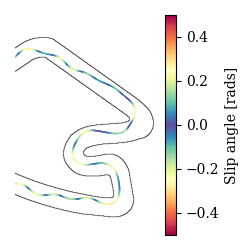
\includegraphics[height=0.85\linewidth]{contents/chapt5/figs/uncertainty/mco_no_error_lap.png}
        %% Creator: Matplotlib, PGF backend
%%
%% To include the figure in your LaTeX document, write
%%   \input{<filename>.pgf}
%%
%% Make sure the required packages are loaded in your preamble
%%   \usepackage{pgf}
%%
%% Also ensure that all the required font packages are loaded; for instance,
%% the lmodern package is sometimes necessary when using math font.
%%   \usepackage{lmodern}
%%
%% Figures using additional raster images can only be included by \input if
%% they are in the same directory as the main LaTeX file. For loading figures
%% from other directories you can use the `import` package
%%   \usepackage{import}
%%
%% and then include the figures with
%%   \import{<path to file>}{<filename>.pgf}
%%
%% Matplotlib used the following preamble
%%   \usepackage{fontspec}
%%   \setmainfont{times.ttf}[Path=\detokenize{C:/Windows/Fonts/}]
%%   \setsansfont{DejaVuSans.ttf}[Path=\detokenize{C:/Users/Andrew/anaconda3/envs/auto_car_env/Lib/site-packages/matplotlib/mpl-data/fonts/ttf/}]
%%   \setmonofont{DejaVuSansMono.ttf}[Path=\detokenize{C:/Users/Andrew/anaconda3/envs/auto_car_env/Lib/site-packages/matplotlib/mpl-data/fonts/ttf/}]
%%
\begingroup%
\makeatletter%
\begin{pgfpicture}%
\pgfpathrectangle{\pgfpointorigin}{\pgfqpoint{2.500000in}{2.500000in}}%
\pgfusepath{use as bounding box, clip}%
\begin{pgfscope}%
\pgfsetbuttcap%
\pgfsetmiterjoin%
\definecolor{currentfill}{rgb}{1.000000,1.000000,1.000000}%
\pgfsetfillcolor{currentfill}%
\pgfsetlinewidth{0.000000pt}%
\definecolor{currentstroke}{rgb}{1.000000,1.000000,1.000000}%
\pgfsetstrokecolor{currentstroke}%
\pgfsetdash{}{0pt}%
\pgfpathmoveto{\pgfqpoint{0.000000in}{0.000000in}}%
\pgfpathlineto{\pgfqpoint{2.500000in}{0.000000in}}%
\pgfpathlineto{\pgfqpoint{2.500000in}{2.500000in}}%
\pgfpathlineto{\pgfqpoint{0.000000in}{2.500000in}}%
\pgfpathlineto{\pgfqpoint{0.000000in}{0.000000in}}%
\pgfpathclose%
\pgfusepath{fill}%
\end{pgfscope}%
\begin{pgfscope}%
\pgfpathrectangle{\pgfqpoint{0.352278in}{0.235000in}}{\pgfqpoint{1.339000in}{2.060000in}}%
\pgfusepath{clip}%
\pgfsys@transformshift{0.352278in}{0.235000in}%
\pgftext[left,bottom]{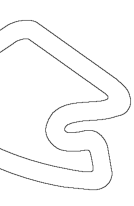
\includegraphics[interpolate=true,width=1.340000in,height=2.060000in]{contents/chapt5/figs/uncertainty/mco_lap_1-img0.png}}%
\end{pgfscope}%
\begin{pgfscope}%
\pgfpathrectangle{\pgfqpoint{0.352278in}{0.235000in}}{\pgfqpoint{1.339000in}{2.060000in}}%
\pgfusepath{clip}%
\pgfsetrectcap%
\pgfsetroundjoin%
\pgfsetlinewidth{1.003750pt}%
\definecolor{currentstroke}{rgb}{0.500000,0.000000,1.000000}%
\pgfsetstrokecolor{currentstroke}%
\pgfsetstrokeopacity{0.800000}%
\pgfsetdash{}{0pt}%
\pgfusepath{stroke}%
\end{pgfscope}%
\begin{pgfscope}%
\pgfpathrectangle{\pgfqpoint{0.352278in}{0.235000in}}{\pgfqpoint{1.339000in}{2.060000in}}%
\pgfusepath{clip}%
\pgfsetrectcap%
\pgfsetroundjoin%
\pgfsetlinewidth{1.003750pt}%
\definecolor{currentstroke}{rgb}{0.500000,0.000000,1.000000}%
\pgfsetstrokecolor{currentstroke}%
\pgfsetstrokeopacity{0.800000}%
\pgfsetdash{}{0pt}%
\pgfusepath{stroke}%
\end{pgfscope}%
\begin{pgfscope}%
\pgfpathrectangle{\pgfqpoint{0.352278in}{0.235000in}}{\pgfqpoint{1.339000in}{2.060000in}}%
\pgfusepath{clip}%
\pgfsetrectcap%
\pgfsetroundjoin%
\pgfsetlinewidth{1.003750pt}%
\definecolor{currentstroke}{rgb}{0.492157,0.012320,0.999981}%
\pgfsetstrokecolor{currentstroke}%
\pgfsetstrokeopacity{0.800000}%
\pgfsetdash{}{0pt}%
\pgfusepath{stroke}%
\end{pgfscope}%
\begin{pgfscope}%
\pgfpathrectangle{\pgfqpoint{0.352278in}{0.235000in}}{\pgfqpoint{1.339000in}{2.060000in}}%
\pgfusepath{clip}%
\pgfsetrectcap%
\pgfsetroundjoin%
\pgfsetlinewidth{1.003750pt}%
\definecolor{currentstroke}{rgb}{0.484314,0.024637,0.999924}%
\pgfsetstrokecolor{currentstroke}%
\pgfsetstrokeopacity{0.800000}%
\pgfsetdash{}{0pt}%
\pgfusepath{stroke}%
\end{pgfscope}%
\begin{pgfscope}%
\pgfpathrectangle{\pgfqpoint{0.352278in}{0.235000in}}{\pgfqpoint{1.339000in}{2.060000in}}%
\pgfusepath{clip}%
\pgfsetrectcap%
\pgfsetroundjoin%
\pgfsetlinewidth{1.003750pt}%
\definecolor{currentstroke}{rgb}{0.484314,0.024637,0.999924}%
\pgfsetstrokecolor{currentstroke}%
\pgfsetstrokeopacity{0.800000}%
\pgfsetdash{}{0pt}%
\pgfusepath{stroke}%
\end{pgfscope}%
\begin{pgfscope}%
\pgfpathrectangle{\pgfqpoint{0.352278in}{0.235000in}}{\pgfqpoint{1.339000in}{2.060000in}}%
\pgfusepath{clip}%
\pgfsetrectcap%
\pgfsetroundjoin%
\pgfsetlinewidth{1.003750pt}%
\definecolor{currentstroke}{rgb}{0.484314,0.024637,0.999924}%
\pgfsetstrokecolor{currentstroke}%
\pgfsetstrokeopacity{0.800000}%
\pgfsetdash{}{0pt}%
\pgfusepath{stroke}%
\end{pgfscope}%
\begin{pgfscope}%
\pgfpathrectangle{\pgfqpoint{0.352278in}{0.235000in}}{\pgfqpoint{1.339000in}{2.060000in}}%
\pgfusepath{clip}%
\pgfsetrectcap%
\pgfsetroundjoin%
\pgfsetlinewidth{1.003750pt}%
\definecolor{currentstroke}{rgb}{0.492157,0.012320,0.999981}%
\pgfsetstrokecolor{currentstroke}%
\pgfsetstrokeopacity{0.800000}%
\pgfsetdash{}{0pt}%
\pgfusepath{stroke}%
\end{pgfscope}%
\begin{pgfscope}%
\pgfpathrectangle{\pgfqpoint{0.352278in}{0.235000in}}{\pgfqpoint{1.339000in}{2.060000in}}%
\pgfusepath{clip}%
\pgfsetrectcap%
\pgfsetroundjoin%
\pgfsetlinewidth{1.003750pt}%
\definecolor{currentstroke}{rgb}{0.492157,0.012320,0.999981}%
\pgfsetstrokecolor{currentstroke}%
\pgfsetstrokeopacity{0.800000}%
\pgfsetdash{}{0pt}%
\pgfusepath{stroke}%
\end{pgfscope}%
\begin{pgfscope}%
\pgfpathrectangle{\pgfqpoint{0.352278in}{0.235000in}}{\pgfqpoint{1.339000in}{2.060000in}}%
\pgfusepath{clip}%
\pgfsetrectcap%
\pgfsetroundjoin%
\pgfsetlinewidth{1.003750pt}%
\definecolor{currentstroke}{rgb}{0.500000,0.000000,1.000000}%
\pgfsetstrokecolor{currentstroke}%
\pgfsetstrokeopacity{0.800000}%
\pgfsetdash{}{0pt}%
\pgfusepath{stroke}%
\end{pgfscope}%
\begin{pgfscope}%
\pgfpathrectangle{\pgfqpoint{0.352278in}{0.235000in}}{\pgfqpoint{1.339000in}{2.060000in}}%
\pgfusepath{clip}%
\pgfsetrectcap%
\pgfsetroundjoin%
\pgfsetlinewidth{1.003750pt}%
\definecolor{currentstroke}{rgb}{0.500000,0.000000,1.000000}%
\pgfsetstrokecolor{currentstroke}%
\pgfsetstrokeopacity{0.800000}%
\pgfsetdash{}{0pt}%
\pgfusepath{stroke}%
\end{pgfscope}%
\begin{pgfscope}%
\pgfpathrectangle{\pgfqpoint{0.352278in}{0.235000in}}{\pgfqpoint{1.339000in}{2.060000in}}%
\pgfusepath{clip}%
\pgfsetrectcap%
\pgfsetroundjoin%
\pgfsetlinewidth{1.003750pt}%
\definecolor{currentstroke}{rgb}{0.492157,0.012320,0.999981}%
\pgfsetstrokecolor{currentstroke}%
\pgfsetstrokeopacity{0.800000}%
\pgfsetdash{}{0pt}%
\pgfusepath{stroke}%
\end{pgfscope}%
\begin{pgfscope}%
\pgfpathrectangle{\pgfqpoint{0.352278in}{0.235000in}}{\pgfqpoint{1.339000in}{2.060000in}}%
\pgfusepath{clip}%
\pgfsetrectcap%
\pgfsetroundjoin%
\pgfsetlinewidth{1.003750pt}%
\definecolor{currentstroke}{rgb}{0.484314,0.024637,0.999924}%
\pgfsetstrokecolor{currentstroke}%
\pgfsetstrokeopacity{0.800000}%
\pgfsetdash{}{0pt}%
\pgfusepath{stroke}%
\end{pgfscope}%
\begin{pgfscope}%
\pgfpathrectangle{\pgfqpoint{0.352278in}{0.235000in}}{\pgfqpoint{1.339000in}{2.060000in}}%
\pgfusepath{clip}%
\pgfsetrectcap%
\pgfsetroundjoin%
\pgfsetlinewidth{1.003750pt}%
\definecolor{currentstroke}{rgb}{0.476471,0.036951,0.999829}%
\pgfsetstrokecolor{currentstroke}%
\pgfsetstrokeopacity{0.800000}%
\pgfsetdash{}{0pt}%
\pgfusepath{stroke}%
\end{pgfscope}%
\begin{pgfscope}%
\pgfpathrectangle{\pgfqpoint{0.352278in}{0.235000in}}{\pgfqpoint{1.339000in}{2.060000in}}%
\pgfusepath{clip}%
\pgfsetrectcap%
\pgfsetroundjoin%
\pgfsetlinewidth{1.003750pt}%
\definecolor{currentstroke}{rgb}{0.468627,0.049260,0.999696}%
\pgfsetstrokecolor{currentstroke}%
\pgfsetstrokeopacity{0.800000}%
\pgfsetdash{}{0pt}%
\pgfusepath{stroke}%
\end{pgfscope}%
\begin{pgfscope}%
\pgfpathrectangle{\pgfqpoint{0.352278in}{0.235000in}}{\pgfqpoint{1.339000in}{2.060000in}}%
\pgfusepath{clip}%
\pgfsetrectcap%
\pgfsetroundjoin%
\pgfsetlinewidth{1.003750pt}%
\definecolor{currentstroke}{rgb}{0.468627,0.049260,0.999696}%
\pgfsetstrokecolor{currentstroke}%
\pgfsetstrokeopacity{0.800000}%
\pgfsetdash{}{0pt}%
\pgfusepath{stroke}%
\end{pgfscope}%
\begin{pgfscope}%
\pgfpathrectangle{\pgfqpoint{0.352278in}{0.235000in}}{\pgfqpoint{1.339000in}{2.060000in}}%
\pgfusepath{clip}%
\pgfsetrectcap%
\pgfsetroundjoin%
\pgfsetlinewidth{1.003750pt}%
\definecolor{currentstroke}{rgb}{0.460784,0.061561,0.999526}%
\pgfsetstrokecolor{currentstroke}%
\pgfsetstrokeopacity{0.800000}%
\pgfsetdash{}{0pt}%
\pgfusepath{stroke}%
\end{pgfscope}%
\begin{pgfscope}%
\pgfpathrectangle{\pgfqpoint{0.352278in}{0.235000in}}{\pgfqpoint{1.339000in}{2.060000in}}%
\pgfusepath{clip}%
\pgfsetrectcap%
\pgfsetroundjoin%
\pgfsetlinewidth{1.003750pt}%
\definecolor{currentstroke}{rgb}{0.460784,0.061561,0.999526}%
\pgfsetstrokecolor{currentstroke}%
\pgfsetstrokeopacity{0.800000}%
\pgfsetdash{}{0pt}%
\pgfusepath{stroke}%
\end{pgfscope}%
\begin{pgfscope}%
\pgfpathrectangle{\pgfqpoint{0.352278in}{0.235000in}}{\pgfqpoint{1.339000in}{2.060000in}}%
\pgfusepath{clip}%
\pgfsetrectcap%
\pgfsetroundjoin%
\pgfsetlinewidth{1.003750pt}%
\definecolor{currentstroke}{rgb}{0.452941,0.073853,0.999317}%
\pgfsetstrokecolor{currentstroke}%
\pgfsetstrokeopacity{0.800000}%
\pgfsetdash{}{0pt}%
\pgfusepath{stroke}%
\end{pgfscope}%
\begin{pgfscope}%
\pgfpathrectangle{\pgfqpoint{0.352278in}{0.235000in}}{\pgfqpoint{1.339000in}{2.060000in}}%
\pgfusepath{clip}%
\pgfsetrectcap%
\pgfsetroundjoin%
\pgfsetlinewidth{1.003750pt}%
\definecolor{currentstroke}{rgb}{0.452941,0.073853,0.999317}%
\pgfsetstrokecolor{currentstroke}%
\pgfsetstrokeopacity{0.800000}%
\pgfsetdash{}{0pt}%
\pgfusepath{stroke}%
\end{pgfscope}%
\begin{pgfscope}%
\pgfpathrectangle{\pgfqpoint{0.352278in}{0.235000in}}{\pgfqpoint{1.339000in}{2.060000in}}%
\pgfusepath{clip}%
\pgfsetrectcap%
\pgfsetroundjoin%
\pgfsetlinewidth{1.003750pt}%
\definecolor{currentstroke}{rgb}{0.452941,0.073853,0.999317}%
\pgfsetstrokecolor{currentstroke}%
\pgfsetstrokeopacity{0.800000}%
\pgfsetdash{}{0pt}%
\pgfusepath{stroke}%
\end{pgfscope}%
\begin{pgfscope}%
\pgfpathrectangle{\pgfqpoint{0.352278in}{0.235000in}}{\pgfqpoint{1.339000in}{2.060000in}}%
\pgfusepath{clip}%
\pgfsetrectcap%
\pgfsetroundjoin%
\pgfsetlinewidth{1.003750pt}%
\definecolor{currentstroke}{rgb}{0.445098,0.086133,0.999070}%
\pgfsetstrokecolor{currentstroke}%
\pgfsetstrokeopacity{0.800000}%
\pgfsetdash{}{0pt}%
\pgfusepath{stroke}%
\end{pgfscope}%
\begin{pgfscope}%
\pgfpathrectangle{\pgfqpoint{0.352278in}{0.235000in}}{\pgfqpoint{1.339000in}{2.060000in}}%
\pgfusepath{clip}%
\pgfsetrectcap%
\pgfsetroundjoin%
\pgfsetlinewidth{1.003750pt}%
\definecolor{currentstroke}{rgb}{0.445098,0.086133,0.999070}%
\pgfsetstrokecolor{currentstroke}%
\pgfsetstrokeopacity{0.800000}%
\pgfsetdash{}{0pt}%
\pgfusepath{stroke}%
\end{pgfscope}%
\begin{pgfscope}%
\pgfpathrectangle{\pgfqpoint{0.352278in}{0.235000in}}{\pgfqpoint{1.339000in}{2.060000in}}%
\pgfusepath{clip}%
\pgfsetrectcap%
\pgfsetroundjoin%
\pgfsetlinewidth{1.003750pt}%
\definecolor{currentstroke}{rgb}{0.437255,0.098400,0.998786}%
\pgfsetstrokecolor{currentstroke}%
\pgfsetstrokeopacity{0.800000}%
\pgfsetdash{}{0pt}%
\pgfusepath{stroke}%
\end{pgfscope}%
\begin{pgfscope}%
\pgfpathrectangle{\pgfqpoint{0.352278in}{0.235000in}}{\pgfqpoint{1.339000in}{2.060000in}}%
\pgfusepath{clip}%
\pgfsetrectcap%
\pgfsetroundjoin%
\pgfsetlinewidth{1.003750pt}%
\definecolor{currentstroke}{rgb}{0.437255,0.098400,0.998786}%
\pgfsetstrokecolor{currentstroke}%
\pgfsetstrokeopacity{0.800000}%
\pgfsetdash{}{0pt}%
\pgfusepath{stroke}%
\end{pgfscope}%
\begin{pgfscope}%
\pgfpathrectangle{\pgfqpoint{0.352278in}{0.235000in}}{\pgfqpoint{1.339000in}{2.060000in}}%
\pgfusepath{clip}%
\pgfsetrectcap%
\pgfsetroundjoin%
\pgfsetlinewidth{1.003750pt}%
\definecolor{currentstroke}{rgb}{0.429412,0.110653,0.998464}%
\pgfsetstrokecolor{currentstroke}%
\pgfsetstrokeopacity{0.800000}%
\pgfsetdash{}{0pt}%
\pgfusepath{stroke}%
\end{pgfscope}%
\begin{pgfscope}%
\pgfpathrectangle{\pgfqpoint{0.352278in}{0.235000in}}{\pgfqpoint{1.339000in}{2.060000in}}%
\pgfusepath{clip}%
\pgfsetrectcap%
\pgfsetroundjoin%
\pgfsetlinewidth{1.003750pt}%
\definecolor{currentstroke}{rgb}{0.421569,0.122888,0.998103}%
\pgfsetstrokecolor{currentstroke}%
\pgfsetstrokeopacity{0.800000}%
\pgfsetdash{}{0pt}%
\pgfusepath{stroke}%
\end{pgfscope}%
\begin{pgfscope}%
\pgfpathrectangle{\pgfqpoint{0.352278in}{0.235000in}}{\pgfqpoint{1.339000in}{2.060000in}}%
\pgfusepath{clip}%
\pgfsetrectcap%
\pgfsetroundjoin%
\pgfsetlinewidth{1.003750pt}%
\definecolor{currentstroke}{rgb}{0.429412,0.110653,0.998464}%
\pgfsetstrokecolor{currentstroke}%
\pgfsetstrokeopacity{0.800000}%
\pgfsetdash{}{0pt}%
\pgfusepath{stroke}%
\end{pgfscope}%
\begin{pgfscope}%
\pgfpathrectangle{\pgfqpoint{0.352278in}{0.235000in}}{\pgfqpoint{1.339000in}{2.060000in}}%
\pgfusepath{clip}%
\pgfsetrectcap%
\pgfsetroundjoin%
\pgfsetlinewidth{1.003750pt}%
\definecolor{currentstroke}{rgb}{0.437255,0.098400,0.998786}%
\pgfsetstrokecolor{currentstroke}%
\pgfsetstrokeopacity{0.800000}%
\pgfsetdash{}{0pt}%
\pgfusepath{stroke}%
\end{pgfscope}%
\begin{pgfscope}%
\pgfpathrectangle{\pgfqpoint{0.352278in}{0.235000in}}{\pgfqpoint{1.339000in}{2.060000in}}%
\pgfusepath{clip}%
\pgfsetrectcap%
\pgfsetroundjoin%
\pgfsetlinewidth{1.003750pt}%
\definecolor{currentstroke}{rgb}{0.452941,0.073853,0.999317}%
\pgfsetstrokecolor{currentstroke}%
\pgfsetstrokeopacity{0.800000}%
\pgfsetdash{}{0pt}%
\pgfusepath{stroke}%
\end{pgfscope}%
\begin{pgfscope}%
\pgfpathrectangle{\pgfqpoint{0.352278in}{0.235000in}}{\pgfqpoint{1.339000in}{2.060000in}}%
\pgfusepath{clip}%
\pgfsetrectcap%
\pgfsetroundjoin%
\pgfsetlinewidth{1.003750pt}%
\definecolor{currentstroke}{rgb}{0.468627,0.049260,0.999696}%
\pgfsetstrokecolor{currentstroke}%
\pgfsetstrokeopacity{0.800000}%
\pgfsetdash{}{0pt}%
\pgfusepath{stroke}%
\end{pgfscope}%
\begin{pgfscope}%
\pgfpathrectangle{\pgfqpoint{0.352278in}{0.235000in}}{\pgfqpoint{1.339000in}{2.060000in}}%
\pgfusepath{clip}%
\pgfsetrectcap%
\pgfsetroundjoin%
\pgfsetlinewidth{1.003750pt}%
\definecolor{currentstroke}{rgb}{0.484314,0.024637,0.999924}%
\pgfsetstrokecolor{currentstroke}%
\pgfsetstrokeopacity{0.800000}%
\pgfsetdash{}{0pt}%
\pgfusepath{stroke}%
\end{pgfscope}%
\begin{pgfscope}%
\pgfpathrectangle{\pgfqpoint{0.352278in}{0.235000in}}{\pgfqpoint{1.339000in}{2.060000in}}%
\pgfusepath{clip}%
\pgfsetrectcap%
\pgfsetroundjoin%
\pgfsetlinewidth{1.003750pt}%
\definecolor{currentstroke}{rgb}{0.500000,0.000000,1.000000}%
\pgfsetstrokecolor{currentstroke}%
\pgfsetstrokeopacity{0.800000}%
\pgfsetdash{}{0pt}%
\pgfusepath{stroke}%
\end{pgfscope}%
\begin{pgfscope}%
\pgfpathrectangle{\pgfqpoint{0.352278in}{0.235000in}}{\pgfqpoint{1.339000in}{2.060000in}}%
\pgfusepath{clip}%
\pgfsetrectcap%
\pgfsetroundjoin%
\pgfsetlinewidth{1.003750pt}%
\definecolor{currentstroke}{rgb}{0.484314,0.024637,0.999924}%
\pgfsetstrokecolor{currentstroke}%
\pgfsetstrokeopacity{0.800000}%
\pgfsetdash{}{0pt}%
\pgfusepath{stroke}%
\end{pgfscope}%
\begin{pgfscope}%
\pgfpathrectangle{\pgfqpoint{0.352278in}{0.235000in}}{\pgfqpoint{1.339000in}{2.060000in}}%
\pgfusepath{clip}%
\pgfsetrectcap%
\pgfsetroundjoin%
\pgfsetlinewidth{1.003750pt}%
\definecolor{currentstroke}{rgb}{0.460784,0.061561,0.999526}%
\pgfsetstrokecolor{currentstroke}%
\pgfsetstrokeopacity{0.800000}%
\pgfsetdash{}{0pt}%
\pgfusepath{stroke}%
\end{pgfscope}%
\begin{pgfscope}%
\pgfpathrectangle{\pgfqpoint{0.352278in}{0.235000in}}{\pgfqpoint{1.339000in}{2.060000in}}%
\pgfusepath{clip}%
\pgfsetrectcap%
\pgfsetroundjoin%
\pgfsetlinewidth{1.003750pt}%
\definecolor{currentstroke}{rgb}{0.437255,0.098400,0.998786}%
\pgfsetstrokecolor{currentstroke}%
\pgfsetstrokeopacity{0.800000}%
\pgfsetdash{}{0pt}%
\pgfusepath{stroke}%
\end{pgfscope}%
\begin{pgfscope}%
\pgfpathrectangle{\pgfqpoint{0.352278in}{0.235000in}}{\pgfqpoint{1.339000in}{2.060000in}}%
\pgfusepath{clip}%
\pgfsetrectcap%
\pgfsetroundjoin%
\pgfsetlinewidth{1.003750pt}%
\definecolor{currentstroke}{rgb}{0.421569,0.122888,0.998103}%
\pgfsetstrokecolor{currentstroke}%
\pgfsetstrokeopacity{0.800000}%
\pgfsetdash{}{0pt}%
\pgfusepath{stroke}%
\end{pgfscope}%
\begin{pgfscope}%
\pgfpathrectangle{\pgfqpoint{0.352278in}{0.235000in}}{\pgfqpoint{1.339000in}{2.060000in}}%
\pgfusepath{clip}%
\pgfsetrectcap%
\pgfsetroundjoin%
\pgfsetlinewidth{1.003750pt}%
\definecolor{currentstroke}{rgb}{0.398039,0.159476,0.996795}%
\pgfsetstrokecolor{currentstroke}%
\pgfsetstrokeopacity{0.800000}%
\pgfsetdash{}{0pt}%
\pgfusepath{stroke}%
\end{pgfscope}%
\begin{pgfscope}%
\pgfpathrectangle{\pgfqpoint{0.352278in}{0.235000in}}{\pgfqpoint{1.339000in}{2.060000in}}%
\pgfusepath{clip}%
\pgfsetrectcap%
\pgfsetroundjoin%
\pgfsetlinewidth{1.003750pt}%
\definecolor{currentstroke}{rgb}{0.374510,0.195845,0.995147}%
\pgfsetstrokecolor{currentstroke}%
\pgfsetstrokeopacity{0.800000}%
\pgfsetdash{}{0pt}%
\pgfusepath{stroke}%
\end{pgfscope}%
\begin{pgfscope}%
\pgfpathrectangle{\pgfqpoint{0.352278in}{0.235000in}}{\pgfqpoint{1.339000in}{2.060000in}}%
\pgfusepath{clip}%
\pgfsetrectcap%
\pgfsetroundjoin%
\pgfsetlinewidth{1.003750pt}%
\definecolor{currentstroke}{rgb}{0.350980,0.231948,0.993159}%
\pgfsetstrokecolor{currentstroke}%
\pgfsetstrokeopacity{0.800000}%
\pgfsetdash{}{0pt}%
\pgfusepath{stroke}%
\end{pgfscope}%
\begin{pgfscope}%
\pgfpathrectangle{\pgfqpoint{0.352278in}{0.235000in}}{\pgfqpoint{1.339000in}{2.060000in}}%
\pgfusepath{clip}%
\pgfsetrectcap%
\pgfsetroundjoin%
\pgfsetlinewidth{1.003750pt}%
\definecolor{currentstroke}{rgb}{0.335294,0.255843,0.991645}%
\pgfsetstrokecolor{currentstroke}%
\pgfsetstrokeopacity{0.800000}%
\pgfsetdash{}{0pt}%
\pgfusepath{stroke}%
\end{pgfscope}%
\begin{pgfscope}%
\pgfpathrectangle{\pgfqpoint{0.352278in}{0.235000in}}{\pgfqpoint{1.339000in}{2.060000in}}%
\pgfusepath{clip}%
\pgfsetrectcap%
\pgfsetroundjoin%
\pgfsetlinewidth{1.003750pt}%
\definecolor{currentstroke}{rgb}{0.319608,0.279583,0.989980}%
\pgfsetstrokecolor{currentstroke}%
\pgfsetstrokeopacity{0.800000}%
\pgfsetdash{}{0pt}%
\pgfusepath{stroke}%
\end{pgfscope}%
\begin{pgfscope}%
\pgfpathrectangle{\pgfqpoint{0.352278in}{0.235000in}}{\pgfqpoint{1.339000in}{2.060000in}}%
\pgfusepath{clip}%
\pgfsetrectcap%
\pgfsetroundjoin%
\pgfsetlinewidth{1.003750pt}%
\definecolor{currentstroke}{rgb}{0.296078,0.314870,0.987202}%
\pgfsetstrokecolor{currentstroke}%
\pgfsetstrokeopacity{0.800000}%
\pgfsetdash{}{0pt}%
\pgfusepath{stroke}%
\end{pgfscope}%
\begin{pgfscope}%
\pgfpathrectangle{\pgfqpoint{0.352278in}{0.235000in}}{\pgfqpoint{1.339000in}{2.060000in}}%
\pgfusepath{clip}%
\pgfsetrectcap%
\pgfsetroundjoin%
\pgfsetlinewidth{1.003750pt}%
\definecolor{currentstroke}{rgb}{0.272549,0.349727,0.984086}%
\pgfsetstrokecolor{currentstroke}%
\pgfsetstrokeopacity{0.800000}%
\pgfsetdash{}{0pt}%
\pgfusepath{stroke}%
\end{pgfscope}%
\begin{pgfscope}%
\pgfpathrectangle{\pgfqpoint{0.352278in}{0.235000in}}{\pgfqpoint{1.339000in}{2.060000in}}%
\pgfusepath{clip}%
\pgfsetrectcap%
\pgfsetroundjoin%
\pgfsetlinewidth{1.003750pt}%
\definecolor{currentstroke}{rgb}{0.249020,0.384106,0.980635}%
\pgfsetstrokecolor{currentstroke}%
\pgfsetstrokeopacity{0.800000}%
\pgfsetdash{}{0pt}%
\pgfusepath{stroke}%
\end{pgfscope}%
\begin{pgfscope}%
\pgfpathrectangle{\pgfqpoint{0.352278in}{0.235000in}}{\pgfqpoint{1.339000in}{2.060000in}}%
\pgfusepath{clip}%
\pgfsetrectcap%
\pgfsetroundjoin%
\pgfsetlinewidth{1.003750pt}%
\definecolor{currentstroke}{rgb}{0.241176,0.395451,0.979410}%
\pgfsetstrokecolor{currentstroke}%
\pgfsetstrokeopacity{0.800000}%
\pgfsetdash{}{0pt}%
\pgfusepath{stroke}%
\end{pgfscope}%
\begin{pgfscope}%
\pgfpathrectangle{\pgfqpoint{0.352278in}{0.235000in}}{\pgfqpoint{1.339000in}{2.060000in}}%
\pgfusepath{clip}%
\pgfsetrectcap%
\pgfsetroundjoin%
\pgfsetlinewidth{1.003750pt}%
\definecolor{currentstroke}{rgb}{0.241176,0.395451,0.979410}%
\pgfsetstrokecolor{currentstroke}%
\pgfsetstrokeopacity{0.800000}%
\pgfsetdash{}{0pt}%
\pgfusepath{stroke}%
\end{pgfscope}%
\begin{pgfscope}%
\pgfpathrectangle{\pgfqpoint{0.352278in}{0.235000in}}{\pgfqpoint{1.339000in}{2.060000in}}%
\pgfusepath{clip}%
\pgfsetrectcap%
\pgfsetroundjoin%
\pgfsetlinewidth{1.003750pt}%
\definecolor{currentstroke}{rgb}{0.241176,0.395451,0.979410}%
\pgfsetstrokecolor{currentstroke}%
\pgfsetstrokeopacity{0.800000}%
\pgfsetdash{}{0pt}%
\pgfusepath{stroke}%
\end{pgfscope}%
\begin{pgfscope}%
\pgfpathrectangle{\pgfqpoint{0.352278in}{0.235000in}}{\pgfqpoint{1.339000in}{2.060000in}}%
\pgfusepath{clip}%
\pgfsetrectcap%
\pgfsetroundjoin%
\pgfsetlinewidth{1.003750pt}%
\definecolor{currentstroke}{rgb}{0.241176,0.395451,0.979410}%
\pgfsetstrokecolor{currentstroke}%
\pgfsetstrokeopacity{0.800000}%
\pgfsetdash{}{0pt}%
\pgfusepath{stroke}%
\end{pgfscope}%
\begin{pgfscope}%
\pgfpathrectangle{\pgfqpoint{0.352278in}{0.235000in}}{\pgfqpoint{1.339000in}{2.060000in}}%
\pgfusepath{clip}%
\pgfsetrectcap%
\pgfsetroundjoin%
\pgfsetlinewidth{1.003750pt}%
\definecolor{currentstroke}{rgb}{0.256863,0.372702,0.981823}%
\pgfsetstrokecolor{currentstroke}%
\pgfsetstrokeopacity{0.800000}%
\pgfsetdash{}{0pt}%
\pgfusepath{stroke}%
\end{pgfscope}%
\begin{pgfscope}%
\pgfpathrectangle{\pgfqpoint{0.352278in}{0.235000in}}{\pgfqpoint{1.339000in}{2.060000in}}%
\pgfusepath{clip}%
\pgfsetrectcap%
\pgfsetroundjoin%
\pgfsetlinewidth{1.003750pt}%
\definecolor{currentstroke}{rgb}{0.264706,0.361242,0.982973}%
\pgfsetstrokecolor{currentstroke}%
\pgfsetstrokeopacity{0.800000}%
\pgfsetdash{}{0pt}%
\pgfusepath{stroke}%
\end{pgfscope}%
\begin{pgfscope}%
\pgfpathrectangle{\pgfqpoint{0.352278in}{0.235000in}}{\pgfqpoint{1.339000in}{2.060000in}}%
\pgfusepath{clip}%
\pgfsetrectcap%
\pgfsetroundjoin%
\pgfsetlinewidth{1.003750pt}%
\definecolor{currentstroke}{rgb}{0.272549,0.349727,0.984086}%
\pgfsetstrokecolor{currentstroke}%
\pgfsetstrokeopacity{0.800000}%
\pgfsetdash{}{0pt}%
\pgfusepath{stroke}%
\end{pgfscope}%
\begin{pgfscope}%
\pgfpathrectangle{\pgfqpoint{0.352278in}{0.235000in}}{\pgfqpoint{1.339000in}{2.060000in}}%
\pgfusepath{clip}%
\pgfsetrectcap%
\pgfsetroundjoin%
\pgfsetlinewidth{1.003750pt}%
\definecolor{currentstroke}{rgb}{0.288235,0.326539,0.986201}%
\pgfsetstrokecolor{currentstroke}%
\pgfsetstrokeopacity{0.800000}%
\pgfsetdash{}{0pt}%
\pgfusepath{stroke}%
\end{pgfscope}%
\begin{pgfscope}%
\pgfpathrectangle{\pgfqpoint{0.352278in}{0.235000in}}{\pgfqpoint{1.339000in}{2.060000in}}%
\pgfusepath{clip}%
\pgfsetrectcap%
\pgfsetroundjoin%
\pgfsetlinewidth{1.003750pt}%
\definecolor{currentstroke}{rgb}{0.296078,0.314870,0.987202}%
\pgfsetstrokecolor{currentstroke}%
\pgfsetstrokeopacity{0.800000}%
\pgfsetdash{}{0pt}%
\pgfusepath{stroke}%
\end{pgfscope}%
\begin{pgfscope}%
\pgfpathrectangle{\pgfqpoint{0.352278in}{0.235000in}}{\pgfqpoint{1.339000in}{2.060000in}}%
\pgfusepath{clip}%
\pgfsetrectcap%
\pgfsetroundjoin%
\pgfsetlinewidth{1.003750pt}%
\definecolor{currentstroke}{rgb}{0.311765,0.291390,0.989092}%
\pgfsetstrokecolor{currentstroke}%
\pgfsetstrokeopacity{0.800000}%
\pgfsetdash{}{0pt}%
\pgfusepath{stroke}%
\end{pgfscope}%
\begin{pgfscope}%
\pgfpathrectangle{\pgfqpoint{0.352278in}{0.235000in}}{\pgfqpoint{1.339000in}{2.060000in}}%
\pgfusepath{clip}%
\pgfsetrectcap%
\pgfsetroundjoin%
\pgfsetlinewidth{1.003750pt}%
\definecolor{currentstroke}{rgb}{0.327451,0.267733,0.990831}%
\pgfsetstrokecolor{currentstroke}%
\pgfsetstrokeopacity{0.800000}%
\pgfsetdash{}{0pt}%
\pgfusepath{stroke}%
\end{pgfscope}%
\begin{pgfscope}%
\pgfpathrectangle{\pgfqpoint{0.352278in}{0.235000in}}{\pgfqpoint{1.339000in}{2.060000in}}%
\pgfusepath{clip}%
\pgfsetrectcap%
\pgfsetroundjoin%
\pgfsetlinewidth{1.003750pt}%
\definecolor{currentstroke}{rgb}{0.350980,0.231948,0.993159}%
\pgfsetstrokecolor{currentstroke}%
\pgfsetstrokeopacity{0.800000}%
\pgfsetdash{}{0pt}%
\pgfusepath{stroke}%
\end{pgfscope}%
\begin{pgfscope}%
\pgfpathrectangle{\pgfqpoint{0.352278in}{0.235000in}}{\pgfqpoint{1.339000in}{2.060000in}}%
\pgfusepath{clip}%
\pgfsetrectcap%
\pgfsetroundjoin%
\pgfsetlinewidth{1.003750pt}%
\definecolor{currentstroke}{rgb}{0.366667,0.207912,0.994522}%
\pgfsetstrokecolor{currentstroke}%
\pgfsetstrokeopacity{0.800000}%
\pgfsetdash{}{0pt}%
\pgfusepath{stroke}%
\end{pgfscope}%
\begin{pgfscope}%
\pgfpathrectangle{\pgfqpoint{0.352278in}{0.235000in}}{\pgfqpoint{1.339000in}{2.060000in}}%
\pgfusepath{clip}%
\pgfsetrectcap%
\pgfsetroundjoin%
\pgfsetlinewidth{1.003750pt}%
\definecolor{currentstroke}{rgb}{0.390196,0.171626,0.996284}%
\pgfsetstrokecolor{currentstroke}%
\pgfsetstrokeopacity{0.800000}%
\pgfsetdash{}{0pt}%
\pgfusepath{stroke}%
\end{pgfscope}%
\begin{pgfscope}%
\pgfpathrectangle{\pgfqpoint{0.352278in}{0.235000in}}{\pgfqpoint{1.339000in}{2.060000in}}%
\pgfusepath{clip}%
\pgfsetrectcap%
\pgfsetroundjoin%
\pgfsetlinewidth{1.003750pt}%
\definecolor{currentstroke}{rgb}{0.405882,0.147302,0.997269}%
\pgfsetstrokecolor{currentstroke}%
\pgfsetstrokeopacity{0.800000}%
\pgfsetdash{}{0pt}%
\pgfusepath{stroke}%
\end{pgfscope}%
\begin{pgfscope}%
\pgfpathrectangle{\pgfqpoint{0.352278in}{0.235000in}}{\pgfqpoint{1.339000in}{2.060000in}}%
\pgfusepath{clip}%
\pgfsetrectcap%
\pgfsetroundjoin%
\pgfsetlinewidth{1.003750pt}%
\definecolor{currentstroke}{rgb}{0.429412,0.110653,0.998464}%
\pgfsetstrokecolor{currentstroke}%
\pgfsetstrokeopacity{0.800000}%
\pgfsetdash{}{0pt}%
\pgfusepath{stroke}%
\end{pgfscope}%
\begin{pgfscope}%
\pgfpathrectangle{\pgfqpoint{0.352278in}{0.235000in}}{\pgfqpoint{1.339000in}{2.060000in}}%
\pgfusepath{clip}%
\pgfsetrectcap%
\pgfsetroundjoin%
\pgfsetlinewidth{1.003750pt}%
\definecolor{currentstroke}{rgb}{0.445098,0.086133,0.999070}%
\pgfsetstrokecolor{currentstroke}%
\pgfsetstrokeopacity{0.800000}%
\pgfsetdash{}{0pt}%
\pgfusepath{stroke}%
\end{pgfscope}%
\begin{pgfscope}%
\pgfpathrectangle{\pgfqpoint{0.352278in}{0.235000in}}{\pgfqpoint{1.339000in}{2.060000in}}%
\pgfusepath{clip}%
\pgfsetrectcap%
\pgfsetroundjoin%
\pgfsetlinewidth{1.003750pt}%
\definecolor{currentstroke}{rgb}{0.468627,0.049260,0.999696}%
\pgfsetstrokecolor{currentstroke}%
\pgfsetstrokeopacity{0.800000}%
\pgfsetdash{}{0pt}%
\pgfusepath{stroke}%
\end{pgfscope}%
\begin{pgfscope}%
\pgfpathrectangle{\pgfqpoint{0.352278in}{0.235000in}}{\pgfqpoint{1.339000in}{2.060000in}}%
\pgfusepath{clip}%
\pgfsetrectcap%
\pgfsetroundjoin%
\pgfsetlinewidth{1.003750pt}%
\definecolor{currentstroke}{rgb}{0.492157,0.012320,0.999981}%
\pgfsetstrokecolor{currentstroke}%
\pgfsetstrokeopacity{0.800000}%
\pgfsetdash{}{0pt}%
\pgfusepath{stroke}%
\end{pgfscope}%
\begin{pgfscope}%
\pgfpathrectangle{\pgfqpoint{0.352278in}{0.235000in}}{\pgfqpoint{1.339000in}{2.060000in}}%
\pgfusepath{clip}%
\pgfsetrectcap%
\pgfsetroundjoin%
\pgfsetlinewidth{1.003750pt}%
\definecolor{currentstroke}{rgb}{0.492157,0.012320,0.999981}%
\pgfsetstrokecolor{currentstroke}%
\pgfsetstrokeopacity{0.800000}%
\pgfsetdash{}{0pt}%
\pgfusepath{stroke}%
\end{pgfscope}%
\begin{pgfscope}%
\pgfpathrectangle{\pgfqpoint{0.352278in}{0.235000in}}{\pgfqpoint{1.339000in}{2.060000in}}%
\pgfusepath{clip}%
\pgfsetrectcap%
\pgfsetroundjoin%
\pgfsetlinewidth{1.003750pt}%
\definecolor{currentstroke}{rgb}{0.476471,0.036951,0.999829}%
\pgfsetstrokecolor{currentstroke}%
\pgfsetstrokeopacity{0.800000}%
\pgfsetdash{}{0pt}%
\pgfusepath{stroke}%
\end{pgfscope}%
\begin{pgfscope}%
\pgfpathrectangle{\pgfqpoint{0.352278in}{0.235000in}}{\pgfqpoint{1.339000in}{2.060000in}}%
\pgfusepath{clip}%
\pgfsetrectcap%
\pgfsetroundjoin%
\pgfsetlinewidth{1.003750pt}%
\definecolor{currentstroke}{rgb}{0.468627,0.049260,0.999696}%
\pgfsetstrokecolor{currentstroke}%
\pgfsetstrokeopacity{0.800000}%
\pgfsetdash{}{0pt}%
\pgfusepath{stroke}%
\end{pgfscope}%
\begin{pgfscope}%
\pgfpathrectangle{\pgfqpoint{0.352278in}{0.235000in}}{\pgfqpoint{1.339000in}{2.060000in}}%
\pgfusepath{clip}%
\pgfsetrectcap%
\pgfsetroundjoin%
\pgfsetlinewidth{1.003750pt}%
\definecolor{currentstroke}{rgb}{0.452941,0.073853,0.999317}%
\pgfsetstrokecolor{currentstroke}%
\pgfsetstrokeopacity{0.800000}%
\pgfsetdash{}{0pt}%
\pgfusepath{stroke}%
\end{pgfscope}%
\begin{pgfscope}%
\pgfpathrectangle{\pgfqpoint{0.352278in}{0.235000in}}{\pgfqpoint{1.339000in}{2.060000in}}%
\pgfusepath{clip}%
\pgfsetrectcap%
\pgfsetroundjoin%
\pgfsetlinewidth{1.003750pt}%
\definecolor{currentstroke}{rgb}{0.445098,0.086133,0.999070}%
\pgfsetstrokecolor{currentstroke}%
\pgfsetstrokeopacity{0.800000}%
\pgfsetdash{}{0pt}%
\pgfusepath{stroke}%
\end{pgfscope}%
\begin{pgfscope}%
\pgfpathrectangle{\pgfqpoint{0.352278in}{0.235000in}}{\pgfqpoint{1.339000in}{2.060000in}}%
\pgfusepath{clip}%
\pgfsetrectcap%
\pgfsetroundjoin%
\pgfsetlinewidth{1.003750pt}%
\definecolor{currentstroke}{rgb}{0.429412,0.110653,0.998464}%
\pgfsetstrokecolor{currentstroke}%
\pgfsetstrokeopacity{0.800000}%
\pgfsetdash{}{0pt}%
\pgfusepath{stroke}%
\end{pgfscope}%
\begin{pgfscope}%
\pgfpathrectangle{\pgfqpoint{0.352278in}{0.235000in}}{\pgfqpoint{1.339000in}{2.060000in}}%
\pgfusepath{clip}%
\pgfsetrectcap%
\pgfsetroundjoin%
\pgfsetlinewidth{1.003750pt}%
\definecolor{currentstroke}{rgb}{0.429412,0.110653,0.998464}%
\pgfsetstrokecolor{currentstroke}%
\pgfsetstrokeopacity{0.800000}%
\pgfsetdash{}{0pt}%
\pgfusepath{stroke}%
\end{pgfscope}%
\begin{pgfscope}%
\pgfpathrectangle{\pgfqpoint{0.352278in}{0.235000in}}{\pgfqpoint{1.339000in}{2.060000in}}%
\pgfusepath{clip}%
\pgfsetrectcap%
\pgfsetroundjoin%
\pgfsetlinewidth{1.003750pt}%
\definecolor{currentstroke}{rgb}{0.421569,0.122888,0.998103}%
\pgfsetstrokecolor{currentstroke}%
\pgfsetstrokeopacity{0.800000}%
\pgfsetdash{}{0pt}%
\pgfusepath{stroke}%
\end{pgfscope}%
\begin{pgfscope}%
\pgfpathrectangle{\pgfqpoint{0.352278in}{0.235000in}}{\pgfqpoint{1.339000in}{2.060000in}}%
\pgfusepath{clip}%
\pgfsetrectcap%
\pgfsetroundjoin%
\pgfsetlinewidth{1.003750pt}%
\definecolor{currentstroke}{rgb}{0.413725,0.135105,0.997705}%
\pgfsetstrokecolor{currentstroke}%
\pgfsetstrokeopacity{0.800000}%
\pgfsetdash{}{0pt}%
\pgfusepath{stroke}%
\end{pgfscope}%
\begin{pgfscope}%
\pgfpathrectangle{\pgfqpoint{0.352278in}{0.235000in}}{\pgfqpoint{1.339000in}{2.060000in}}%
\pgfusepath{clip}%
\pgfsetrectcap%
\pgfsetroundjoin%
\pgfsetlinewidth{1.003750pt}%
\definecolor{currentstroke}{rgb}{0.421569,0.122888,0.998103}%
\pgfsetstrokecolor{currentstroke}%
\pgfsetstrokeopacity{0.800000}%
\pgfsetdash{}{0pt}%
\pgfusepath{stroke}%
\end{pgfscope}%
\begin{pgfscope}%
\pgfpathrectangle{\pgfqpoint{0.352278in}{0.235000in}}{\pgfqpoint{1.339000in}{2.060000in}}%
\pgfusepath{clip}%
\pgfsetrectcap%
\pgfsetroundjoin%
\pgfsetlinewidth{1.003750pt}%
\definecolor{currentstroke}{rgb}{0.413725,0.135105,0.997705}%
\pgfsetstrokecolor{currentstroke}%
\pgfsetstrokeopacity{0.800000}%
\pgfsetdash{}{0pt}%
\pgfusepath{stroke}%
\end{pgfscope}%
\begin{pgfscope}%
\pgfpathrectangle{\pgfqpoint{0.352278in}{0.235000in}}{\pgfqpoint{1.339000in}{2.060000in}}%
\pgfusepath{clip}%
\pgfsetrectcap%
\pgfsetroundjoin%
\pgfsetlinewidth{1.003750pt}%
\definecolor{currentstroke}{rgb}{0.413725,0.135105,0.997705}%
\pgfsetstrokecolor{currentstroke}%
\pgfsetstrokeopacity{0.800000}%
\pgfsetdash{}{0pt}%
\pgfusepath{stroke}%
\end{pgfscope}%
\begin{pgfscope}%
\pgfpathrectangle{\pgfqpoint{0.352278in}{0.235000in}}{\pgfqpoint{1.339000in}{2.060000in}}%
\pgfusepath{clip}%
\pgfsetrectcap%
\pgfsetroundjoin%
\pgfsetlinewidth{1.003750pt}%
\definecolor{currentstroke}{rgb}{0.405882,0.147302,0.997269}%
\pgfsetstrokecolor{currentstroke}%
\pgfsetstrokeopacity{0.800000}%
\pgfsetdash{}{0pt}%
\pgfusepath{stroke}%
\end{pgfscope}%
\begin{pgfscope}%
\pgfpathrectangle{\pgfqpoint{0.352278in}{0.235000in}}{\pgfqpoint{1.339000in}{2.060000in}}%
\pgfusepath{clip}%
\pgfsetrectcap%
\pgfsetroundjoin%
\pgfsetlinewidth{1.003750pt}%
\definecolor{currentstroke}{rgb}{0.398039,0.159476,0.996795}%
\pgfsetstrokecolor{currentstroke}%
\pgfsetstrokeopacity{0.800000}%
\pgfsetdash{}{0pt}%
\pgfusepath{stroke}%
\end{pgfscope}%
\begin{pgfscope}%
\pgfpathrectangle{\pgfqpoint{0.352278in}{0.235000in}}{\pgfqpoint{1.339000in}{2.060000in}}%
\pgfusepath{clip}%
\pgfsetrectcap%
\pgfsetroundjoin%
\pgfsetlinewidth{1.003750pt}%
\definecolor{currentstroke}{rgb}{0.390196,0.171626,0.996284}%
\pgfsetstrokecolor{currentstroke}%
\pgfsetstrokeopacity{0.800000}%
\pgfsetdash{}{0pt}%
\pgfusepath{stroke}%
\end{pgfscope}%
\begin{pgfscope}%
\pgfpathrectangle{\pgfqpoint{0.352278in}{0.235000in}}{\pgfqpoint{1.339000in}{2.060000in}}%
\pgfusepath{clip}%
\pgfsetrectcap%
\pgfsetroundjoin%
\pgfsetlinewidth{1.003750pt}%
\definecolor{currentstroke}{rgb}{0.390196,0.171626,0.996284}%
\pgfsetstrokecolor{currentstroke}%
\pgfsetstrokeopacity{0.800000}%
\pgfsetdash{}{0pt}%
\pgfusepath{stroke}%
\end{pgfscope}%
\begin{pgfscope}%
\pgfpathrectangle{\pgfqpoint{0.352278in}{0.235000in}}{\pgfqpoint{1.339000in}{2.060000in}}%
\pgfusepath{clip}%
\pgfsetrectcap%
\pgfsetroundjoin%
\pgfsetlinewidth{1.003750pt}%
\definecolor{currentstroke}{rgb}{0.374510,0.195845,0.995147}%
\pgfsetstrokecolor{currentstroke}%
\pgfsetstrokeopacity{0.800000}%
\pgfsetdash{}{0pt}%
\pgfusepath{stroke}%
\end{pgfscope}%
\begin{pgfscope}%
\pgfpathrectangle{\pgfqpoint{0.352278in}{0.235000in}}{\pgfqpoint{1.339000in}{2.060000in}}%
\pgfusepath{clip}%
\pgfsetrectcap%
\pgfsetroundjoin%
\pgfsetlinewidth{1.003750pt}%
\definecolor{currentstroke}{rgb}{0.374510,0.195845,0.995147}%
\pgfsetstrokecolor{currentstroke}%
\pgfsetstrokeopacity{0.800000}%
\pgfsetdash{}{0pt}%
\pgfusepath{stroke}%
\end{pgfscope}%
\begin{pgfscope}%
\pgfpathrectangle{\pgfqpoint{0.352278in}{0.235000in}}{\pgfqpoint{1.339000in}{2.060000in}}%
\pgfusepath{clip}%
\pgfsetrectcap%
\pgfsetroundjoin%
\pgfsetlinewidth{1.003750pt}%
\definecolor{currentstroke}{rgb}{0.358824,0.219946,0.993859}%
\pgfsetstrokecolor{currentstroke}%
\pgfsetstrokeopacity{0.800000}%
\pgfsetdash{}{0pt}%
\pgfusepath{stroke}%
\end{pgfscope}%
\begin{pgfscope}%
\pgfpathrectangle{\pgfqpoint{0.352278in}{0.235000in}}{\pgfqpoint{1.339000in}{2.060000in}}%
\pgfusepath{clip}%
\pgfsetrectcap%
\pgfsetroundjoin%
\pgfsetlinewidth{1.003750pt}%
\definecolor{currentstroke}{rgb}{0.350980,0.231948,0.993159}%
\pgfsetstrokecolor{currentstroke}%
\pgfsetstrokeopacity{0.800000}%
\pgfsetdash{}{0pt}%
\pgfusepath{stroke}%
\end{pgfscope}%
\begin{pgfscope}%
\pgfpathrectangle{\pgfqpoint{0.352278in}{0.235000in}}{\pgfqpoint{1.339000in}{2.060000in}}%
\pgfusepath{clip}%
\pgfsetrectcap%
\pgfsetroundjoin%
\pgfsetlinewidth{1.003750pt}%
\definecolor{currentstroke}{rgb}{0.335294,0.255843,0.991645}%
\pgfsetstrokecolor{currentstroke}%
\pgfsetstrokeopacity{0.800000}%
\pgfsetdash{}{0pt}%
\pgfusepath{stroke}%
\end{pgfscope}%
\begin{pgfscope}%
\pgfpathrectangle{\pgfqpoint{0.352278in}{0.235000in}}{\pgfqpoint{1.339000in}{2.060000in}}%
\pgfusepath{clip}%
\pgfsetrectcap%
\pgfsetroundjoin%
\pgfsetlinewidth{1.003750pt}%
\definecolor{currentstroke}{rgb}{0.327451,0.267733,0.990831}%
\pgfsetstrokecolor{currentstroke}%
\pgfsetstrokeopacity{0.800000}%
\pgfsetdash{}{0pt}%
\pgfusepath{stroke}%
\end{pgfscope}%
\begin{pgfscope}%
\pgfpathrectangle{\pgfqpoint{0.352278in}{0.235000in}}{\pgfqpoint{1.339000in}{2.060000in}}%
\pgfusepath{clip}%
\pgfsetrectcap%
\pgfsetroundjoin%
\pgfsetlinewidth{1.003750pt}%
\definecolor{currentstroke}{rgb}{0.319608,0.279583,0.989980}%
\pgfsetstrokecolor{currentstroke}%
\pgfsetstrokeopacity{0.800000}%
\pgfsetdash{}{0pt}%
\pgfusepath{stroke}%
\end{pgfscope}%
\begin{pgfscope}%
\pgfpathrectangle{\pgfqpoint{0.352278in}{0.235000in}}{\pgfqpoint{1.339000in}{2.060000in}}%
\pgfusepath{clip}%
\pgfsetrectcap%
\pgfsetroundjoin%
\pgfsetlinewidth{1.003750pt}%
\definecolor{currentstroke}{rgb}{0.319608,0.279583,0.989980}%
\pgfsetstrokecolor{currentstroke}%
\pgfsetstrokeopacity{0.800000}%
\pgfsetdash{}{0pt}%
\pgfusepath{stroke}%
\end{pgfscope}%
\begin{pgfscope}%
\pgfpathrectangle{\pgfqpoint{0.352278in}{0.235000in}}{\pgfqpoint{1.339000in}{2.060000in}}%
\pgfusepath{clip}%
\pgfsetrectcap%
\pgfsetroundjoin%
\pgfsetlinewidth{1.003750pt}%
\definecolor{currentstroke}{rgb}{0.327451,0.267733,0.990831}%
\pgfsetstrokecolor{currentstroke}%
\pgfsetstrokeopacity{0.800000}%
\pgfsetdash{}{0pt}%
\pgfusepath{stroke}%
\end{pgfscope}%
\begin{pgfscope}%
\pgfpathrectangle{\pgfqpoint{0.352278in}{0.235000in}}{\pgfqpoint{1.339000in}{2.060000in}}%
\pgfusepath{clip}%
\pgfsetrectcap%
\pgfsetroundjoin%
\pgfsetlinewidth{1.003750pt}%
\definecolor{currentstroke}{rgb}{0.335294,0.255843,0.991645}%
\pgfsetstrokecolor{currentstroke}%
\pgfsetstrokeopacity{0.800000}%
\pgfsetdash{}{0pt}%
\pgfusepath{stroke}%
\end{pgfscope}%
\begin{pgfscope}%
\pgfpathrectangle{\pgfqpoint{0.352278in}{0.235000in}}{\pgfqpoint{1.339000in}{2.060000in}}%
\pgfusepath{clip}%
\pgfsetrectcap%
\pgfsetroundjoin%
\pgfsetlinewidth{1.003750pt}%
\definecolor{currentstroke}{rgb}{0.358824,0.219946,0.993859}%
\pgfsetstrokecolor{currentstroke}%
\pgfsetstrokeopacity{0.800000}%
\pgfsetdash{}{0pt}%
\pgfusepath{stroke}%
\end{pgfscope}%
\begin{pgfscope}%
\pgfpathrectangle{\pgfqpoint{0.352278in}{0.235000in}}{\pgfqpoint{1.339000in}{2.060000in}}%
\pgfusepath{clip}%
\pgfsetrectcap%
\pgfsetroundjoin%
\pgfsetlinewidth{1.003750pt}%
\definecolor{currentstroke}{rgb}{0.390196,0.171626,0.996284}%
\pgfsetstrokecolor{currentstroke}%
\pgfsetstrokeopacity{0.800000}%
\pgfsetdash{}{0pt}%
\pgfusepath{stroke}%
\end{pgfscope}%
\begin{pgfscope}%
\pgfpathrectangle{\pgfqpoint{0.352278in}{0.235000in}}{\pgfqpoint{1.339000in}{2.060000in}}%
\pgfusepath{clip}%
\pgfsetrectcap%
\pgfsetroundjoin%
\pgfsetlinewidth{1.003750pt}%
\definecolor{currentstroke}{rgb}{0.429412,0.110653,0.998464}%
\pgfsetstrokecolor{currentstroke}%
\pgfsetstrokeopacity{0.800000}%
\pgfsetdash{}{0pt}%
\pgfusepath{stroke}%
\end{pgfscope}%
\begin{pgfscope}%
\pgfpathrectangle{\pgfqpoint{0.352278in}{0.235000in}}{\pgfqpoint{1.339000in}{2.060000in}}%
\pgfusepath{clip}%
\pgfsetrectcap%
\pgfsetroundjoin%
\pgfsetlinewidth{1.003750pt}%
\definecolor{currentstroke}{rgb}{0.468627,0.049260,0.999696}%
\pgfsetstrokecolor{currentstroke}%
\pgfsetstrokeopacity{0.800000}%
\pgfsetdash{}{0pt}%
\pgfusepath{stroke}%
\end{pgfscope}%
\begin{pgfscope}%
\pgfpathrectangle{\pgfqpoint{0.352278in}{0.235000in}}{\pgfqpoint{1.339000in}{2.060000in}}%
\pgfusepath{clip}%
\pgfsetrectcap%
\pgfsetroundjoin%
\pgfsetlinewidth{1.003750pt}%
\definecolor{currentstroke}{rgb}{0.500000,0.000000,1.000000}%
\pgfsetstrokecolor{currentstroke}%
\pgfsetstrokeopacity{0.800000}%
\pgfsetdash{}{0pt}%
\pgfusepath{stroke}%
\end{pgfscope}%
\begin{pgfscope}%
\pgfpathrectangle{\pgfqpoint{0.352278in}{0.235000in}}{\pgfqpoint{1.339000in}{2.060000in}}%
\pgfusepath{clip}%
\pgfsetrectcap%
\pgfsetroundjoin%
\pgfsetlinewidth{1.003750pt}%
\definecolor{currentstroke}{rgb}{0.445098,0.086133,0.999070}%
\pgfsetstrokecolor{currentstroke}%
\pgfsetstrokeopacity{0.800000}%
\pgfsetdash{}{0pt}%
\pgfusepath{stroke}%
\end{pgfscope}%
\begin{pgfscope}%
\pgfpathrectangle{\pgfqpoint{0.352278in}{0.235000in}}{\pgfqpoint{1.339000in}{2.060000in}}%
\pgfusepath{clip}%
\pgfsetrectcap%
\pgfsetroundjoin%
\pgfsetlinewidth{1.003750pt}%
\definecolor{currentstroke}{rgb}{0.390196,0.171626,0.996284}%
\pgfsetstrokecolor{currentstroke}%
\pgfsetstrokeopacity{0.800000}%
\pgfsetdash{}{0pt}%
\pgfusepath{stroke}%
\end{pgfscope}%
\begin{pgfscope}%
\pgfpathrectangle{\pgfqpoint{0.352278in}{0.235000in}}{\pgfqpoint{1.339000in}{2.060000in}}%
\pgfusepath{clip}%
\pgfsetrectcap%
\pgfsetroundjoin%
\pgfsetlinewidth{1.003750pt}%
\definecolor{currentstroke}{rgb}{0.335294,0.255843,0.991645}%
\pgfsetstrokecolor{currentstroke}%
\pgfsetstrokeopacity{0.800000}%
\pgfsetdash{}{0pt}%
\pgfusepath{stroke}%
\end{pgfscope}%
\begin{pgfscope}%
\pgfpathrectangle{\pgfqpoint{0.352278in}{0.235000in}}{\pgfqpoint{1.339000in}{2.060000in}}%
\pgfusepath{clip}%
\pgfsetrectcap%
\pgfsetroundjoin%
\pgfsetlinewidth{1.003750pt}%
\definecolor{currentstroke}{rgb}{0.264706,0.361242,0.982973}%
\pgfsetstrokecolor{currentstroke}%
\pgfsetstrokeopacity{0.800000}%
\pgfsetdash{}{0pt}%
\pgfusepath{stroke}%
\end{pgfscope}%
\begin{pgfscope}%
\pgfpathrectangle{\pgfqpoint{0.352278in}{0.235000in}}{\pgfqpoint{1.339000in}{2.060000in}}%
\pgfusepath{clip}%
\pgfsetrectcap%
\pgfsetroundjoin%
\pgfsetlinewidth{1.003750pt}%
\definecolor{currentstroke}{rgb}{0.194118,0.462204,0.971281}%
\pgfsetstrokecolor{currentstroke}%
\pgfsetstrokeopacity{0.800000}%
\pgfsetdash{}{0pt}%
\pgfusepath{stroke}%
\end{pgfscope}%
\begin{pgfscope}%
\pgfpathrectangle{\pgfqpoint{0.352278in}{0.235000in}}{\pgfqpoint{1.339000in}{2.060000in}}%
\pgfusepath{clip}%
\pgfsetrectcap%
\pgfsetroundjoin%
\pgfsetlinewidth{1.003750pt}%
\definecolor{currentstroke}{rgb}{0.107843,0.577774,0.952942}%
\pgfsetstrokecolor{currentstroke}%
\pgfsetstrokeopacity{0.800000}%
\pgfsetdash{}{0pt}%
\pgfusepath{stroke}%
\end{pgfscope}%
\begin{pgfscope}%
\pgfpathrectangle{\pgfqpoint{0.352278in}{0.235000in}}{\pgfqpoint{1.339000in}{2.060000in}}%
\pgfusepath{clip}%
\pgfsetrectcap%
\pgfsetroundjoin%
\pgfsetlinewidth{1.003750pt}%
\definecolor{currentstroke}{rgb}{0.021569,0.682749,0.930229}%
\pgfsetstrokecolor{currentstroke}%
\pgfsetstrokeopacity{0.800000}%
\pgfsetdash{}{0pt}%
\pgfusepath{stroke}%
\end{pgfscope}%
\begin{pgfscope}%
\pgfpathrectangle{\pgfqpoint{0.352278in}{0.235000in}}{\pgfqpoint{1.339000in}{2.060000in}}%
\pgfusepath{clip}%
\pgfsetrectcap%
\pgfsetroundjoin%
\pgfsetlinewidth{1.003750pt}%
\definecolor{currentstroke}{rgb}{0.072549,0.782928,0.900587}%
\pgfsetstrokecolor{currentstroke}%
\pgfsetstrokeopacity{0.800000}%
\pgfsetdash{}{0pt}%
\pgfusepath{stroke}%
\end{pgfscope}%
\begin{pgfscope}%
\pgfpathrectangle{\pgfqpoint{0.352278in}{0.235000in}}{\pgfqpoint{1.339000in}{2.060000in}}%
\pgfusepath{clip}%
\pgfsetrectcap%
\pgfsetroundjoin%
\pgfsetlinewidth{1.003750pt}%
\definecolor{currentstroke}{rgb}{0.166667,0.866025,0.866025}%
\pgfsetstrokecolor{currentstroke}%
\pgfsetstrokeopacity{0.800000}%
\pgfsetdash{}{0pt}%
\pgfusepath{stroke}%
\end{pgfscope}%
\begin{pgfscope}%
\pgfpathrectangle{\pgfqpoint{0.352278in}{0.235000in}}{\pgfqpoint{1.339000in}{2.060000in}}%
\pgfusepath{clip}%
\pgfsetrectcap%
\pgfsetroundjoin%
\pgfsetlinewidth{1.003750pt}%
\definecolor{currentstroke}{rgb}{0.268627,0.934680,0.823253}%
\pgfsetstrokecolor{currentstroke}%
\pgfsetstrokeopacity{0.800000}%
\pgfsetdash{}{0pt}%
\pgfusepath{stroke}%
\end{pgfscope}%
\begin{pgfscope}%
\pgfpathrectangle{\pgfqpoint{0.352278in}{0.235000in}}{\pgfqpoint{1.339000in}{2.060000in}}%
\pgfusepath{clip}%
\pgfsetrectcap%
\pgfsetroundjoin%
\pgfsetlinewidth{1.003750pt}%
\definecolor{currentstroke}{rgb}{0.362745,0.976848,0.779081}%
\pgfsetstrokecolor{currentstroke}%
\pgfsetstrokeopacity{0.800000}%
\pgfsetdash{}{0pt}%
\pgfusepath{stroke}%
\end{pgfscope}%
\begin{pgfscope}%
\pgfpathrectangle{\pgfqpoint{0.352278in}{0.235000in}}{\pgfqpoint{1.339000in}{2.060000in}}%
\pgfusepath{clip}%
\pgfsetrectcap%
\pgfsetroundjoin%
\pgfsetlinewidth{1.003750pt}%
\definecolor{currentstroke}{rgb}{0.456863,0.997705,0.730653}%
\pgfsetstrokecolor{currentstroke}%
\pgfsetstrokeopacity{0.800000}%
\pgfsetdash{}{0pt}%
\pgfusepath{stroke}%
\end{pgfscope}%
\begin{pgfscope}%
\pgfpathrectangle{\pgfqpoint{0.352278in}{0.235000in}}{\pgfqpoint{1.339000in}{2.060000in}}%
\pgfusepath{clip}%
\pgfsetrectcap%
\pgfsetroundjoin%
\pgfsetlinewidth{1.003750pt}%
\definecolor{currentstroke}{rgb}{0.543137,0.997705,0.682749}%
\pgfsetstrokecolor{currentstroke}%
\pgfsetstrokeopacity{0.800000}%
\pgfsetdash{}{0pt}%
\pgfusepath{stroke}%
\end{pgfscope}%
\begin{pgfscope}%
\pgfpathrectangle{\pgfqpoint{0.352278in}{0.235000in}}{\pgfqpoint{1.339000in}{2.060000in}}%
\pgfusepath{clip}%
\pgfsetrectcap%
\pgfsetroundjoin%
\pgfsetlinewidth{1.003750pt}%
\definecolor{currentstroke}{rgb}{0.621569,0.981823,0.636474}%
\pgfsetstrokecolor{currentstroke}%
\pgfsetstrokeopacity{0.800000}%
\pgfsetdash{}{0pt}%
\pgfusepath{stroke}%
\end{pgfscope}%
\begin{pgfscope}%
\pgfpathrectangle{\pgfqpoint{0.352278in}{0.235000in}}{\pgfqpoint{1.339000in}{2.060000in}}%
\pgfusepath{clip}%
\pgfsetrectcap%
\pgfsetroundjoin%
\pgfsetlinewidth{1.003750pt}%
\definecolor{currentstroke}{rgb}{0.684314,0.958381,0.597707}%
\pgfsetstrokecolor{currentstroke}%
\pgfsetstrokeopacity{0.800000}%
\pgfsetdash{}{0pt}%
\pgfusepath{stroke}%
\end{pgfscope}%
\begin{pgfscope}%
\pgfpathrectangle{\pgfqpoint{0.352278in}{0.235000in}}{\pgfqpoint{1.339000in}{2.060000in}}%
\pgfusepath{clip}%
\pgfsetrectcap%
\pgfsetroundjoin%
\pgfsetlinewidth{1.003750pt}%
\definecolor{currentstroke}{rgb}{0.739216,0.930229,0.562593}%
\pgfsetstrokecolor{currentstroke}%
\pgfsetstrokeopacity{0.800000}%
\pgfsetdash{}{0pt}%
\pgfusepath{stroke}%
\end{pgfscope}%
\begin{pgfscope}%
\pgfpathrectangle{\pgfqpoint{0.352278in}{0.235000in}}{\pgfqpoint{1.339000in}{2.060000in}}%
\pgfusepath{clip}%
\pgfsetrectcap%
\pgfsetroundjoin%
\pgfsetlinewidth{1.003750pt}%
\definecolor{currentstroke}{rgb}{0.786275,0.900587,0.531659}%
\pgfsetstrokecolor{currentstroke}%
\pgfsetstrokeopacity{0.800000}%
\pgfsetdash{}{0pt}%
\pgfusepath{stroke}%
\end{pgfscope}%
\begin{pgfscope}%
\pgfpathrectangle{\pgfqpoint{0.352278in}{0.235000in}}{\pgfqpoint{1.339000in}{2.060000in}}%
\pgfusepath{clip}%
\pgfsetrectcap%
\pgfsetroundjoin%
\pgfsetlinewidth{1.003750pt}%
\definecolor{currentstroke}{rgb}{0.817647,0.878081,0.510631}%
\pgfsetstrokecolor{currentstroke}%
\pgfsetstrokeopacity{0.800000}%
\pgfsetdash{}{0pt}%
\pgfusepath{stroke}%
\end{pgfscope}%
\begin{pgfscope}%
\pgfpathrectangle{\pgfqpoint{0.352278in}{0.235000in}}{\pgfqpoint{1.339000in}{2.060000in}}%
\pgfusepath{clip}%
\pgfsetrectcap%
\pgfsetroundjoin%
\pgfsetlinewidth{1.003750pt}%
\definecolor{currentstroke}{rgb}{0.841176,0.859800,0.494656}%
\pgfsetstrokecolor{currentstroke}%
\pgfsetstrokeopacity{0.800000}%
\pgfsetdash{}{0pt}%
\pgfusepath{stroke}%
\end{pgfscope}%
\begin{pgfscope}%
\pgfpathrectangle{\pgfqpoint{0.352278in}{0.235000in}}{\pgfqpoint{1.339000in}{2.060000in}}%
\pgfusepath{clip}%
\pgfsetrectcap%
\pgfsetroundjoin%
\pgfsetlinewidth{1.003750pt}%
\definecolor{currentstroke}{rgb}{0.849020,0.853444,0.489293}%
\pgfsetstrokecolor{currentstroke}%
\pgfsetstrokeopacity{0.800000}%
\pgfsetdash{}{0pt}%
\pgfusepath{stroke}%
\end{pgfscope}%
\begin{pgfscope}%
\pgfpathrectangle{\pgfqpoint{0.352278in}{0.235000in}}{\pgfqpoint{1.339000in}{2.060000in}}%
\pgfusepath{clip}%
\pgfsetrectcap%
\pgfsetroundjoin%
\pgfsetlinewidth{1.003750pt}%
\definecolor{currentstroke}{rgb}{0.849020,0.853444,0.489293}%
\pgfsetstrokecolor{currentstroke}%
\pgfsetstrokeopacity{0.800000}%
\pgfsetdash{}{0pt}%
\pgfusepath{stroke}%
\end{pgfscope}%
\begin{pgfscope}%
\pgfpathrectangle{\pgfqpoint{0.352278in}{0.235000in}}{\pgfqpoint{1.339000in}{2.060000in}}%
\pgfusepath{clip}%
\pgfsetrectcap%
\pgfsetroundjoin%
\pgfsetlinewidth{1.003750pt}%
\definecolor{currentstroke}{rgb}{0.833333,0.866025,0.500000}%
\pgfsetstrokecolor{currentstroke}%
\pgfsetstrokeopacity{0.800000}%
\pgfsetdash{}{0pt}%
\pgfusepath{stroke}%
\end{pgfscope}%
\begin{pgfscope}%
\pgfpathrectangle{\pgfqpoint{0.352278in}{0.235000in}}{\pgfqpoint{1.339000in}{2.060000in}}%
\pgfusepath{clip}%
\pgfsetrectcap%
\pgfsetroundjoin%
\pgfsetlinewidth{1.003750pt}%
\definecolor{currentstroke}{rgb}{0.809804,0.883910,0.515918}%
\pgfsetstrokecolor{currentstroke}%
\pgfsetstrokeopacity{0.800000}%
\pgfsetdash{}{0pt}%
\pgfusepath{stroke}%
\end{pgfscope}%
\begin{pgfscope}%
\pgfpathrectangle{\pgfqpoint{0.352278in}{0.235000in}}{\pgfqpoint{1.339000in}{2.060000in}}%
\pgfusepath{clip}%
\pgfsetrectcap%
\pgfsetroundjoin%
\pgfsetlinewidth{1.003750pt}%
\definecolor{currentstroke}{rgb}{0.778431,0.905873,0.536867}%
\pgfsetstrokecolor{currentstroke}%
\pgfsetstrokeopacity{0.800000}%
\pgfsetdash{}{0pt}%
\pgfusepath{stroke}%
\end{pgfscope}%
\begin{pgfscope}%
\pgfpathrectangle{\pgfqpoint{0.352278in}{0.235000in}}{\pgfqpoint{1.339000in}{2.060000in}}%
\pgfusepath{clip}%
\pgfsetrectcap%
\pgfsetroundjoin%
\pgfsetlinewidth{1.003750pt}%
\definecolor{currentstroke}{rgb}{0.739216,0.930229,0.562593}%
\pgfsetstrokecolor{currentstroke}%
\pgfsetstrokeopacity{0.800000}%
\pgfsetdash{}{0pt}%
\pgfusepath{stroke}%
\end{pgfscope}%
\begin{pgfscope}%
\pgfpathrectangle{\pgfqpoint{0.352278in}{0.235000in}}{\pgfqpoint{1.339000in}{2.060000in}}%
\pgfusepath{clip}%
\pgfsetrectcap%
\pgfsetroundjoin%
\pgfsetlinewidth{1.003750pt}%
\definecolor{currentstroke}{rgb}{0.684314,0.958381,0.597707}%
\pgfsetstrokecolor{currentstroke}%
\pgfsetstrokeopacity{0.800000}%
\pgfsetdash{}{0pt}%
\pgfusepath{stroke}%
\end{pgfscope}%
\begin{pgfscope}%
\pgfpathrectangle{\pgfqpoint{0.352278in}{0.235000in}}{\pgfqpoint{1.339000in}{2.060000in}}%
\pgfusepath{clip}%
\pgfsetrectcap%
\pgfsetroundjoin%
\pgfsetlinewidth{1.003750pt}%
\definecolor{currentstroke}{rgb}{0.621569,0.981823,0.636474}%
\pgfsetstrokecolor{currentstroke}%
\pgfsetstrokeopacity{0.800000}%
\pgfsetdash{}{0pt}%
\pgfusepath{stroke}%
\end{pgfscope}%
\begin{pgfscope}%
\pgfpathrectangle{\pgfqpoint{0.352278in}{0.235000in}}{\pgfqpoint{1.339000in}{2.060000in}}%
\pgfusepath{clip}%
\pgfsetrectcap%
\pgfsetroundjoin%
\pgfsetlinewidth{1.003750pt}%
\definecolor{currentstroke}{rgb}{0.566667,0.994522,0.669131}%
\pgfsetstrokecolor{currentstroke}%
\pgfsetstrokeopacity{0.800000}%
\pgfsetdash{}{0pt}%
\pgfusepath{stroke}%
\end{pgfscope}%
\begin{pgfscope}%
\pgfpathrectangle{\pgfqpoint{0.352278in}{0.235000in}}{\pgfqpoint{1.339000in}{2.060000in}}%
\pgfusepath{clip}%
\pgfsetrectcap%
\pgfsetroundjoin%
\pgfsetlinewidth{1.003750pt}%
\definecolor{currentstroke}{rgb}{0.503922,0.999981,0.704926}%
\pgfsetstrokecolor{currentstroke}%
\pgfsetstrokeopacity{0.800000}%
\pgfsetdash{}{0pt}%
\pgfusepath{stroke}%
\end{pgfscope}%
\begin{pgfscope}%
\pgfpathrectangle{\pgfqpoint{0.352278in}{0.235000in}}{\pgfqpoint{1.339000in}{2.060000in}}%
\pgfusepath{clip}%
\pgfsetrectcap%
\pgfsetroundjoin%
\pgfsetlinewidth{1.003750pt}%
\definecolor{currentstroke}{rgb}{0.433333,0.994522,0.743145}%
\pgfsetstrokecolor{currentstroke}%
\pgfsetstrokeopacity{0.800000}%
\pgfsetdash{}{0pt}%
\pgfusepath{stroke}%
\end{pgfscope}%
\begin{pgfscope}%
\pgfpathrectangle{\pgfqpoint{0.352278in}{0.235000in}}{\pgfqpoint{1.339000in}{2.060000in}}%
\pgfusepath{clip}%
\pgfsetrectcap%
\pgfsetroundjoin%
\pgfsetlinewidth{1.003750pt}%
\definecolor{currentstroke}{rgb}{0.362745,0.976848,0.779081}%
\pgfsetstrokecolor{currentstroke}%
\pgfsetstrokeopacity{0.800000}%
\pgfsetdash{}{0pt}%
\pgfusepath{stroke}%
\end{pgfscope}%
\begin{pgfscope}%
\pgfpathrectangle{\pgfqpoint{0.352278in}{0.235000in}}{\pgfqpoint{1.339000in}{2.060000in}}%
\pgfusepath{clip}%
\pgfsetrectcap%
\pgfsetroundjoin%
\pgfsetlinewidth{1.003750pt}%
\definecolor{currentstroke}{rgb}{0.284314,0.943154,0.816197}%
\pgfsetstrokecolor{currentstroke}%
\pgfsetstrokeopacity{0.800000}%
\pgfsetdash{}{0pt}%
\pgfusepath{stroke}%
\end{pgfscope}%
\begin{pgfscope}%
\pgfpathrectangle{\pgfqpoint{0.352278in}{0.235000in}}{\pgfqpoint{1.339000in}{2.060000in}}%
\pgfusepath{clip}%
\pgfsetrectcap%
\pgfsetroundjoin%
\pgfsetlinewidth{1.003750pt}%
\definecolor{currentstroke}{rgb}{0.190196,0.883910,0.856638}%
\pgfsetstrokecolor{currentstroke}%
\pgfsetstrokeopacity{0.800000}%
\pgfsetdash{}{0pt}%
\pgfusepath{stroke}%
\end{pgfscope}%
\begin{pgfscope}%
\pgfpathrectangle{\pgfqpoint{0.352278in}{0.235000in}}{\pgfqpoint{1.339000in}{2.060000in}}%
\pgfusepath{clip}%
\pgfsetrectcap%
\pgfsetroundjoin%
\pgfsetlinewidth{1.003750pt}%
\definecolor{currentstroke}{rgb}{0.088235,0.798017,0.895163}%
\pgfsetstrokecolor{currentstroke}%
\pgfsetstrokeopacity{0.800000}%
\pgfsetdash{}{0pt}%
\pgfusepath{stroke}%
\end{pgfscope}%
\begin{pgfscope}%
\pgfpathrectangle{\pgfqpoint{0.352278in}{0.235000in}}{\pgfqpoint{1.339000in}{2.060000in}}%
\pgfusepath{clip}%
\pgfsetrectcap%
\pgfsetroundjoin%
\pgfsetlinewidth{1.003750pt}%
\definecolor{currentstroke}{rgb}{0.021569,0.682749,0.930229}%
\pgfsetstrokecolor{currentstroke}%
\pgfsetstrokeopacity{0.800000}%
\pgfsetdash{}{0pt}%
\pgfusepath{stroke}%
\end{pgfscope}%
\begin{pgfscope}%
\pgfpathrectangle{\pgfqpoint{0.352278in}{0.235000in}}{\pgfqpoint{1.339000in}{2.060000in}}%
\pgfusepath{clip}%
\pgfsetrectcap%
\pgfsetroundjoin%
\pgfsetlinewidth{1.003750pt}%
\definecolor{currentstroke}{rgb}{0.139216,0.536867,0.960122}%
\pgfsetstrokecolor{currentstroke}%
\pgfsetstrokeopacity{0.800000}%
\pgfsetdash{}{0pt}%
\pgfusepath{stroke}%
\end{pgfscope}%
\begin{pgfscope}%
\pgfpathrectangle{\pgfqpoint{0.352278in}{0.235000in}}{\pgfqpoint{1.339000in}{2.060000in}}%
\pgfusepath{clip}%
\pgfsetrectcap%
\pgfsetroundjoin%
\pgfsetlinewidth{1.003750pt}%
\definecolor{currentstroke}{rgb}{0.256863,0.372702,0.981823}%
\pgfsetstrokecolor{currentstroke}%
\pgfsetstrokeopacity{0.800000}%
\pgfsetdash{}{0pt}%
\pgfusepath{stroke}%
\end{pgfscope}%
\begin{pgfscope}%
\pgfpathrectangle{\pgfqpoint{0.352278in}{0.235000in}}{\pgfqpoint{1.339000in}{2.060000in}}%
\pgfusepath{clip}%
\pgfsetrectcap%
\pgfsetroundjoin%
\pgfsetlinewidth{1.003750pt}%
\definecolor{currentstroke}{rgb}{0.382353,0.183750,0.995734}%
\pgfsetstrokecolor{currentstroke}%
\pgfsetstrokeopacity{0.800000}%
\pgfsetdash{}{0pt}%
\pgfusepath{stroke}%
\end{pgfscope}%
\begin{pgfscope}%
\pgfpathrectangle{\pgfqpoint{0.352278in}{0.235000in}}{\pgfqpoint{1.339000in}{2.060000in}}%
\pgfusepath{clip}%
\pgfsetrectcap%
\pgfsetroundjoin%
\pgfsetlinewidth{1.003750pt}%
\definecolor{currentstroke}{rgb}{0.500000,0.000000,1.000000}%
\pgfsetstrokecolor{currentstroke}%
\pgfsetstrokeopacity{0.800000}%
\pgfsetdash{}{0pt}%
\pgfusepath{stroke}%
\end{pgfscope}%
\begin{pgfscope}%
\pgfpathrectangle{\pgfqpoint{0.352278in}{0.235000in}}{\pgfqpoint{1.339000in}{2.060000in}}%
\pgfusepath{clip}%
\pgfsetrectcap%
\pgfsetroundjoin%
\pgfsetlinewidth{1.003750pt}%
\definecolor{currentstroke}{rgb}{0.374510,0.195845,0.995147}%
\pgfsetstrokecolor{currentstroke}%
\pgfsetstrokeopacity{0.800000}%
\pgfsetdash{}{0pt}%
\pgfusepath{stroke}%
\end{pgfscope}%
\begin{pgfscope}%
\pgfpathrectangle{\pgfqpoint{0.352278in}{0.235000in}}{\pgfqpoint{1.339000in}{2.060000in}}%
\pgfusepath{clip}%
\pgfsetrectcap%
\pgfsetroundjoin%
\pgfsetlinewidth{1.003750pt}%
\definecolor{currentstroke}{rgb}{0.256863,0.372702,0.981823}%
\pgfsetstrokecolor{currentstroke}%
\pgfsetstrokeopacity{0.800000}%
\pgfsetdash{}{0pt}%
\pgfusepath{stroke}%
\end{pgfscope}%
\begin{pgfscope}%
\pgfpathrectangle{\pgfqpoint{0.352278in}{0.235000in}}{\pgfqpoint{1.339000in}{2.060000in}}%
\pgfusepath{clip}%
\pgfsetrectcap%
\pgfsetroundjoin%
\pgfsetlinewidth{1.003750pt}%
\definecolor{currentstroke}{rgb}{0.147059,0.526432,0.961826}%
\pgfsetstrokecolor{currentstroke}%
\pgfsetstrokeopacity{0.800000}%
\pgfsetdash{}{0pt}%
\pgfusepath{stroke}%
\end{pgfscope}%
\begin{pgfscope}%
\pgfpathrectangle{\pgfqpoint{0.352278in}{0.235000in}}{\pgfqpoint{1.339000in}{2.060000in}}%
\pgfusepath{clip}%
\pgfsetrectcap%
\pgfsetroundjoin%
\pgfsetlinewidth{1.003750pt}%
\definecolor{currentstroke}{rgb}{0.045098,0.655284,0.936852}%
\pgfsetstrokecolor{currentstroke}%
\pgfsetstrokeopacity{0.800000}%
\pgfsetdash{}{0pt}%
\pgfusepath{stroke}%
\end{pgfscope}%
\begin{pgfscope}%
\pgfpathrectangle{\pgfqpoint{0.352278in}{0.235000in}}{\pgfqpoint{1.339000in}{2.060000in}}%
\pgfusepath{clip}%
\pgfsetrectcap%
\pgfsetroundjoin%
\pgfsetlinewidth{1.003750pt}%
\definecolor{currentstroke}{rgb}{0.041176,0.751332,0.911023}%
\pgfsetstrokecolor{currentstroke}%
\pgfsetstrokeopacity{0.800000}%
\pgfsetdash{}{0pt}%
\pgfusepath{stroke}%
\end{pgfscope}%
\begin{pgfscope}%
\pgfpathrectangle{\pgfqpoint{0.352278in}{0.235000in}}{\pgfqpoint{1.339000in}{2.060000in}}%
\pgfusepath{clip}%
\pgfsetrectcap%
\pgfsetroundjoin%
\pgfsetlinewidth{1.003750pt}%
\definecolor{currentstroke}{rgb}{0.119608,0.826734,0.883910}%
\pgfsetstrokecolor{currentstroke}%
\pgfsetstrokeopacity{0.800000}%
\pgfsetdash{}{0pt}%
\pgfusepath{stroke}%
\end{pgfscope}%
\begin{pgfscope}%
\pgfpathrectangle{\pgfqpoint{0.352278in}{0.235000in}}{\pgfqpoint{1.339000in}{2.060000in}}%
\pgfusepath{clip}%
\pgfsetrectcap%
\pgfsetroundjoin%
\pgfsetlinewidth{1.003750pt}%
\definecolor{currentstroke}{rgb}{0.174510,0.872120,0.862929}%
\pgfsetstrokecolor{currentstroke}%
\pgfsetstrokeopacity{0.800000}%
\pgfsetdash{}{0pt}%
\pgfusepath{stroke}%
\end{pgfscope}%
\begin{pgfscope}%
\pgfpathrectangle{\pgfqpoint{0.352278in}{0.235000in}}{\pgfqpoint{1.339000in}{2.060000in}}%
\pgfusepath{clip}%
\pgfsetrectcap%
\pgfsetroundjoin%
\pgfsetlinewidth{1.003750pt}%
\definecolor{currentstroke}{rgb}{0.229412,0.911023,0.840344}%
\pgfsetstrokecolor{currentstroke}%
\pgfsetstrokeopacity{0.800000}%
\pgfsetdash{}{0pt}%
\pgfusepath{stroke}%
\end{pgfscope}%
\begin{pgfscope}%
\pgfpathrectangle{\pgfqpoint{0.352278in}{0.235000in}}{\pgfqpoint{1.339000in}{2.060000in}}%
\pgfusepath{clip}%
\pgfsetrectcap%
\pgfsetroundjoin%
\pgfsetlinewidth{1.003750pt}%
\definecolor{currentstroke}{rgb}{0.260784,0.930229,0.826734}%
\pgfsetstrokecolor{currentstroke}%
\pgfsetstrokeopacity{0.800000}%
\pgfsetdash{}{0pt}%
\pgfusepath{stroke}%
\end{pgfscope}%
\begin{pgfscope}%
\pgfpathrectangle{\pgfqpoint{0.352278in}{0.235000in}}{\pgfqpoint{1.339000in}{2.060000in}}%
\pgfusepath{clip}%
\pgfsetrectcap%
\pgfsetroundjoin%
\pgfsetlinewidth{1.003750pt}%
\definecolor{currentstroke}{rgb}{0.268627,0.934680,0.823253}%
\pgfsetstrokecolor{currentstroke}%
\pgfsetstrokeopacity{0.800000}%
\pgfsetdash{}{0pt}%
\pgfusepath{stroke}%
\end{pgfscope}%
\begin{pgfscope}%
\pgfpathrectangle{\pgfqpoint{0.352278in}{0.235000in}}{\pgfqpoint{1.339000in}{2.060000in}}%
\pgfusepath{clip}%
\pgfsetrectcap%
\pgfsetroundjoin%
\pgfsetlinewidth{1.003750pt}%
\definecolor{currentstroke}{rgb}{0.252941,0.925638,0.830184}%
\pgfsetstrokecolor{currentstroke}%
\pgfsetstrokeopacity{0.800000}%
\pgfsetdash{}{0pt}%
\pgfusepath{stroke}%
\end{pgfscope}%
\begin{pgfscope}%
\pgfpathrectangle{\pgfqpoint{0.352278in}{0.235000in}}{\pgfqpoint{1.339000in}{2.060000in}}%
\pgfusepath{clip}%
\pgfsetrectcap%
\pgfsetroundjoin%
\pgfsetlinewidth{1.003750pt}%
\definecolor{currentstroke}{rgb}{0.229412,0.911023,0.840344}%
\pgfsetstrokecolor{currentstroke}%
\pgfsetstrokeopacity{0.800000}%
\pgfsetdash{}{0pt}%
\pgfusepath{stroke}%
\end{pgfscope}%
\begin{pgfscope}%
\pgfpathrectangle{\pgfqpoint{0.352278in}{0.235000in}}{\pgfqpoint{1.339000in}{2.060000in}}%
\pgfusepath{clip}%
\pgfsetrectcap%
\pgfsetroundjoin%
\pgfsetlinewidth{1.003750pt}%
\definecolor{currentstroke}{rgb}{0.198039,0.889604,0.853444}%
\pgfsetstrokecolor{currentstroke}%
\pgfsetstrokeopacity{0.800000}%
\pgfsetdash{}{0pt}%
\pgfusepath{stroke}%
\end{pgfscope}%
\begin{pgfscope}%
\pgfpathrectangle{\pgfqpoint{0.352278in}{0.235000in}}{\pgfqpoint{1.339000in}{2.060000in}}%
\pgfusepath{clip}%
\pgfsetrectcap%
\pgfsetroundjoin%
\pgfsetlinewidth{1.003750pt}%
\definecolor{currentstroke}{rgb}{0.158824,0.859800,0.869089}%
\pgfsetstrokecolor{currentstroke}%
\pgfsetstrokeopacity{0.800000}%
\pgfsetdash{}{0pt}%
\pgfusepath{stroke}%
\end{pgfscope}%
\begin{pgfscope}%
\pgfpathrectangle{\pgfqpoint{0.352278in}{0.235000in}}{\pgfqpoint{1.339000in}{2.060000in}}%
\pgfusepath{clip}%
\pgfsetrectcap%
\pgfsetroundjoin%
\pgfsetlinewidth{1.003750pt}%
\definecolor{currentstroke}{rgb}{0.103922,0.812622,0.889604}%
\pgfsetstrokecolor{currentstroke}%
\pgfsetstrokeopacity{0.800000}%
\pgfsetdash{}{0pt}%
\pgfusepath{stroke}%
\end{pgfscope}%
\begin{pgfscope}%
\pgfpathrectangle{\pgfqpoint{0.352278in}{0.235000in}}{\pgfqpoint{1.339000in}{2.060000in}}%
\pgfusepath{clip}%
\pgfsetrectcap%
\pgfsetroundjoin%
\pgfsetlinewidth{1.003750pt}%
\definecolor{currentstroke}{rgb}{0.064706,0.775204,0.903247}%
\pgfsetstrokecolor{currentstroke}%
\pgfsetstrokeopacity{0.800000}%
\pgfsetdash{}{0pt}%
\pgfusepath{stroke}%
\end{pgfscope}%
\begin{pgfscope}%
\pgfpathrectangle{\pgfqpoint{0.352278in}{0.235000in}}{\pgfqpoint{1.339000in}{2.060000in}}%
\pgfusepath{clip}%
\pgfsetrectcap%
\pgfsetroundjoin%
\pgfsetlinewidth{1.003750pt}%
\definecolor{currentstroke}{rgb}{0.033333,0.743145,0.913545}%
\pgfsetstrokecolor{currentstroke}%
\pgfsetstrokeopacity{0.800000}%
\pgfsetdash{}{0pt}%
\pgfusepath{stroke}%
\end{pgfscope}%
\begin{pgfscope}%
\pgfpathrectangle{\pgfqpoint{0.352278in}{0.235000in}}{\pgfqpoint{1.339000in}{2.060000in}}%
\pgfusepath{clip}%
\pgfsetrectcap%
\pgfsetroundjoin%
\pgfsetlinewidth{1.003750pt}%
\definecolor{currentstroke}{rgb}{0.009804,0.717912,0.920906}%
\pgfsetstrokecolor{currentstroke}%
\pgfsetstrokeopacity{0.800000}%
\pgfsetdash{}{0pt}%
\pgfusepath{stroke}%
\end{pgfscope}%
\begin{pgfscope}%
\pgfpathrectangle{\pgfqpoint{0.352278in}{0.235000in}}{\pgfqpoint{1.339000in}{2.060000in}}%
\pgfusepath{clip}%
\pgfsetrectcap%
\pgfsetroundjoin%
\pgfsetlinewidth{1.003750pt}%
\definecolor{currentstroke}{rgb}{0.001961,0.709281,0.923289}%
\pgfsetstrokecolor{currentstroke}%
\pgfsetstrokeopacity{0.800000}%
\pgfsetdash{}{0pt}%
\pgfusepath{stroke}%
\end{pgfscope}%
\begin{pgfscope}%
\pgfpathrectangle{\pgfqpoint{0.352278in}{0.235000in}}{\pgfqpoint{1.339000in}{2.060000in}}%
\pgfusepath{clip}%
\pgfsetrectcap%
\pgfsetroundjoin%
\pgfsetlinewidth{1.003750pt}%
\definecolor{currentstroke}{rgb}{0.013725,0.691698,0.927951}%
\pgfsetstrokecolor{currentstroke}%
\pgfsetstrokeopacity{0.800000}%
\pgfsetdash{}{0pt}%
\pgfusepath{stroke}%
\end{pgfscope}%
\begin{pgfscope}%
\pgfpathrectangle{\pgfqpoint{0.352278in}{0.235000in}}{\pgfqpoint{1.339000in}{2.060000in}}%
\pgfusepath{clip}%
\pgfsetrectcap%
\pgfsetroundjoin%
\pgfsetlinewidth{1.003750pt}%
\definecolor{currentstroke}{rgb}{0.021569,0.682749,0.930229}%
\pgfsetstrokecolor{currentstroke}%
\pgfsetstrokeopacity{0.800000}%
\pgfsetdash{}{0pt}%
\pgfusepath{stroke}%
\end{pgfscope}%
\begin{pgfscope}%
\pgfpathrectangle{\pgfqpoint{0.352278in}{0.235000in}}{\pgfqpoint{1.339000in}{2.060000in}}%
\pgfusepath{clip}%
\pgfsetrectcap%
\pgfsetroundjoin%
\pgfsetlinewidth{1.003750pt}%
\definecolor{currentstroke}{rgb}{0.021569,0.682749,0.930229}%
\pgfsetstrokecolor{currentstroke}%
\pgfsetstrokeopacity{0.800000}%
\pgfsetdash{}{0pt}%
\pgfusepath{stroke}%
\end{pgfscope}%
\begin{pgfscope}%
\pgfpathrectangle{\pgfqpoint{0.352278in}{0.235000in}}{\pgfqpoint{1.339000in}{2.060000in}}%
\pgfusepath{clip}%
\pgfsetrectcap%
\pgfsetroundjoin%
\pgfsetlinewidth{1.003750pt}%
\definecolor{currentstroke}{rgb}{0.021569,0.682749,0.930229}%
\pgfsetstrokecolor{currentstroke}%
\pgfsetstrokeopacity{0.800000}%
\pgfsetdash{}{0pt}%
\pgfusepath{stroke}%
\end{pgfscope}%
\begin{pgfscope}%
\pgfpathrectangle{\pgfqpoint{0.352278in}{0.235000in}}{\pgfqpoint{1.339000in}{2.060000in}}%
\pgfusepath{clip}%
\pgfsetrectcap%
\pgfsetroundjoin%
\pgfsetlinewidth{1.003750pt}%
\definecolor{currentstroke}{rgb}{0.029412,0.673696,0.932472}%
\pgfsetstrokecolor{currentstroke}%
\pgfsetstrokeopacity{0.800000}%
\pgfsetdash{}{0pt}%
\pgfusepath{stroke}%
\end{pgfscope}%
\begin{pgfscope}%
\pgfpathrectangle{\pgfqpoint{0.352278in}{0.235000in}}{\pgfqpoint{1.339000in}{2.060000in}}%
\pgfusepath{clip}%
\pgfsetrectcap%
\pgfsetroundjoin%
\pgfsetlinewidth{1.003750pt}%
\definecolor{currentstroke}{rgb}{0.021569,0.682749,0.930229}%
\pgfsetstrokecolor{currentstroke}%
\pgfsetstrokeopacity{0.800000}%
\pgfsetdash{}{0pt}%
\pgfusepath{stroke}%
\end{pgfscope}%
\begin{pgfscope}%
\pgfpathrectangle{\pgfqpoint{0.352278in}{0.235000in}}{\pgfqpoint{1.339000in}{2.060000in}}%
\pgfusepath{clip}%
\pgfsetrectcap%
\pgfsetroundjoin%
\pgfsetlinewidth{1.003750pt}%
\definecolor{currentstroke}{rgb}{0.021569,0.682749,0.930229}%
\pgfsetstrokecolor{currentstroke}%
\pgfsetstrokeopacity{0.800000}%
\pgfsetdash{}{0pt}%
\pgfusepath{stroke}%
\end{pgfscope}%
\begin{pgfscope}%
\pgfpathrectangle{\pgfqpoint{0.352278in}{0.235000in}}{\pgfqpoint{1.339000in}{2.060000in}}%
\pgfusepath{clip}%
\pgfsetrectcap%
\pgfsetroundjoin%
\pgfsetlinewidth{1.003750pt}%
\definecolor{currentstroke}{rgb}{0.021569,0.682749,0.930229}%
\pgfsetstrokecolor{currentstroke}%
\pgfsetstrokeopacity{0.800000}%
\pgfsetdash{}{0pt}%
\pgfusepath{stroke}%
\end{pgfscope}%
\begin{pgfscope}%
\pgfpathrectangle{\pgfqpoint{0.352278in}{0.235000in}}{\pgfqpoint{1.339000in}{2.060000in}}%
\pgfusepath{clip}%
\pgfsetrectcap%
\pgfsetroundjoin%
\pgfsetlinewidth{1.003750pt}%
\definecolor{currentstroke}{rgb}{0.021569,0.682749,0.930229}%
\pgfsetstrokecolor{currentstroke}%
\pgfsetstrokeopacity{0.800000}%
\pgfsetdash{}{0pt}%
\pgfusepath{stroke}%
\end{pgfscope}%
\begin{pgfscope}%
\pgfpathrectangle{\pgfqpoint{0.352278in}{0.235000in}}{\pgfqpoint{1.339000in}{2.060000in}}%
\pgfusepath{clip}%
\pgfsetrectcap%
\pgfsetroundjoin%
\pgfsetlinewidth{1.003750pt}%
\definecolor{currentstroke}{rgb}{0.013725,0.691698,0.927951}%
\pgfsetstrokecolor{currentstroke}%
\pgfsetstrokeopacity{0.800000}%
\pgfsetdash{}{0pt}%
\pgfusepath{stroke}%
\end{pgfscope}%
\begin{pgfscope}%
\pgfpathrectangle{\pgfqpoint{0.352278in}{0.235000in}}{\pgfqpoint{1.339000in}{2.060000in}}%
\pgfusepath{clip}%
\pgfsetrectcap%
\pgfsetroundjoin%
\pgfsetlinewidth{1.003750pt}%
\definecolor{currentstroke}{rgb}{0.005882,0.700543,0.925638}%
\pgfsetstrokecolor{currentstroke}%
\pgfsetstrokeopacity{0.800000}%
\pgfsetdash{}{0pt}%
\pgfusepath{stroke}%
\end{pgfscope}%
\begin{pgfscope}%
\pgfpathrectangle{\pgfqpoint{0.352278in}{0.235000in}}{\pgfqpoint{1.339000in}{2.060000in}}%
\pgfusepath{clip}%
\pgfsetrectcap%
\pgfsetroundjoin%
\pgfsetlinewidth{1.003750pt}%
\definecolor{currentstroke}{rgb}{0.009804,0.717912,0.920906}%
\pgfsetstrokecolor{currentstroke}%
\pgfsetstrokeopacity{0.800000}%
\pgfsetdash{}{0pt}%
\pgfusepath{stroke}%
\end{pgfscope}%
\begin{pgfscope}%
\pgfpathrectangle{\pgfqpoint{0.352278in}{0.235000in}}{\pgfqpoint{1.339000in}{2.060000in}}%
\pgfusepath{clip}%
\pgfsetrectcap%
\pgfsetroundjoin%
\pgfsetlinewidth{1.003750pt}%
\definecolor{currentstroke}{rgb}{0.017647,0.726434,0.918487}%
\pgfsetstrokecolor{currentstroke}%
\pgfsetstrokeopacity{0.800000}%
\pgfsetdash{}{0pt}%
\pgfusepath{stroke}%
\end{pgfscope}%
\begin{pgfscope}%
\pgfpathrectangle{\pgfqpoint{0.352278in}{0.235000in}}{\pgfqpoint{1.339000in}{2.060000in}}%
\pgfusepath{clip}%
\pgfsetrectcap%
\pgfsetroundjoin%
\pgfsetlinewidth{1.003750pt}%
\definecolor{currentstroke}{rgb}{0.017647,0.726434,0.918487}%
\pgfsetstrokecolor{currentstroke}%
\pgfsetstrokeopacity{0.800000}%
\pgfsetdash{}{0pt}%
\pgfusepath{stroke}%
\end{pgfscope}%
\begin{pgfscope}%
\pgfpathrectangle{\pgfqpoint{0.352278in}{0.235000in}}{\pgfqpoint{1.339000in}{2.060000in}}%
\pgfusepath{clip}%
\pgfsetrectcap%
\pgfsetroundjoin%
\pgfsetlinewidth{1.003750pt}%
\definecolor{currentstroke}{rgb}{0.017647,0.726434,0.918487}%
\pgfsetstrokecolor{currentstroke}%
\pgfsetstrokeopacity{0.800000}%
\pgfsetdash{}{0pt}%
\pgfusepath{stroke}%
\end{pgfscope}%
\begin{pgfscope}%
\pgfpathrectangle{\pgfqpoint{0.352278in}{0.235000in}}{\pgfqpoint{1.339000in}{2.060000in}}%
\pgfusepath{clip}%
\pgfsetrectcap%
\pgfsetroundjoin%
\pgfsetlinewidth{1.003750pt}%
\definecolor{currentstroke}{rgb}{0.009804,0.717912,0.920906}%
\pgfsetstrokecolor{currentstroke}%
\pgfsetstrokeopacity{0.800000}%
\pgfsetdash{}{0pt}%
\pgfusepath{stroke}%
\end{pgfscope}%
\begin{pgfscope}%
\pgfpathrectangle{\pgfqpoint{0.352278in}{0.235000in}}{\pgfqpoint{1.339000in}{2.060000in}}%
\pgfusepath{clip}%
\pgfsetrectcap%
\pgfsetroundjoin%
\pgfsetlinewidth{1.003750pt}%
\definecolor{currentstroke}{rgb}{0.001961,0.709281,0.923289}%
\pgfsetstrokecolor{currentstroke}%
\pgfsetstrokeopacity{0.800000}%
\pgfsetdash{}{0pt}%
\pgfusepath{stroke}%
\end{pgfscope}%
\begin{pgfscope}%
\pgfpathrectangle{\pgfqpoint{0.352278in}{0.235000in}}{\pgfqpoint{1.339000in}{2.060000in}}%
\pgfusepath{clip}%
\pgfsetrectcap%
\pgfsetroundjoin%
\pgfsetlinewidth{1.003750pt}%
\definecolor{currentstroke}{rgb}{0.021569,0.682749,0.930229}%
\pgfsetstrokecolor{currentstroke}%
\pgfsetstrokeopacity{0.800000}%
\pgfsetdash{}{0pt}%
\pgfusepath{stroke}%
\end{pgfscope}%
\begin{pgfscope}%
\pgfpathrectangle{\pgfqpoint{0.352278in}{0.235000in}}{\pgfqpoint{1.339000in}{2.060000in}}%
\pgfusepath{clip}%
\pgfsetrectcap%
\pgfsetroundjoin%
\pgfsetlinewidth{1.003750pt}%
\definecolor{currentstroke}{rgb}{0.052941,0.645928,0.938988}%
\pgfsetstrokecolor{currentstroke}%
\pgfsetstrokeopacity{0.800000}%
\pgfsetdash{}{0pt}%
\pgfusepath{stroke}%
\end{pgfscope}%
\begin{pgfscope}%
\pgfpathrectangle{\pgfqpoint{0.352278in}{0.235000in}}{\pgfqpoint{1.339000in}{2.060000in}}%
\pgfusepath{clip}%
\pgfsetrectcap%
\pgfsetroundjoin%
\pgfsetlinewidth{1.003750pt}%
\definecolor{currentstroke}{rgb}{0.092157,0.597707,0.949135}%
\pgfsetstrokecolor{currentstroke}%
\pgfsetstrokeopacity{0.800000}%
\pgfsetdash{}{0pt}%
\pgfusepath{stroke}%
\end{pgfscope}%
\begin{pgfscope}%
\pgfpathrectangle{\pgfqpoint{0.352278in}{0.235000in}}{\pgfqpoint{1.339000in}{2.060000in}}%
\pgfusepath{clip}%
\pgfsetrectcap%
\pgfsetroundjoin%
\pgfsetlinewidth{1.003750pt}%
\definecolor{currentstroke}{rgb}{0.131373,0.547220,0.958381}%
\pgfsetstrokecolor{currentstroke}%
\pgfsetstrokeopacity{0.800000}%
\pgfsetdash{}{0pt}%
\pgfusepath{stroke}%
\end{pgfscope}%
\begin{pgfscope}%
\pgfpathrectangle{\pgfqpoint{0.352278in}{0.235000in}}{\pgfqpoint{1.339000in}{2.060000in}}%
\pgfusepath{clip}%
\pgfsetrectcap%
\pgfsetroundjoin%
\pgfsetlinewidth{1.003750pt}%
\definecolor{currentstroke}{rgb}{0.178431,0.483911,0.968276}%
\pgfsetstrokecolor{currentstroke}%
\pgfsetstrokeopacity{0.800000}%
\pgfsetdash{}{0pt}%
\pgfusepath{stroke}%
\end{pgfscope}%
\begin{pgfscope}%
\pgfpathrectangle{\pgfqpoint{0.352278in}{0.235000in}}{\pgfqpoint{1.339000in}{2.060000in}}%
\pgfusepath{clip}%
\pgfsetrectcap%
\pgfsetroundjoin%
\pgfsetlinewidth{1.003750pt}%
\definecolor{currentstroke}{rgb}{0.225490,0.417960,0.976848}%
\pgfsetstrokecolor{currentstroke}%
\pgfsetstrokeopacity{0.800000}%
\pgfsetdash{}{0pt}%
\pgfusepath{stroke}%
\end{pgfscope}%
\begin{pgfscope}%
\pgfpathrectangle{\pgfqpoint{0.352278in}{0.235000in}}{\pgfqpoint{1.339000in}{2.060000in}}%
\pgfusepath{clip}%
\pgfsetrectcap%
\pgfsetroundjoin%
\pgfsetlinewidth{1.003750pt}%
\definecolor{currentstroke}{rgb}{0.280392,0.338158,0.985162}%
\pgfsetstrokecolor{currentstroke}%
\pgfsetstrokeopacity{0.800000}%
\pgfsetdash{}{0pt}%
\pgfusepath{stroke}%
\end{pgfscope}%
\begin{pgfscope}%
\pgfpathrectangle{\pgfqpoint{0.352278in}{0.235000in}}{\pgfqpoint{1.339000in}{2.060000in}}%
\pgfusepath{clip}%
\pgfsetrectcap%
\pgfsetroundjoin%
\pgfsetlinewidth{1.003750pt}%
\definecolor{currentstroke}{rgb}{0.343137,0.243914,0.992421}%
\pgfsetstrokecolor{currentstroke}%
\pgfsetstrokeopacity{0.800000}%
\pgfsetdash{}{0pt}%
\pgfusepath{stroke}%
\end{pgfscope}%
\begin{pgfscope}%
\pgfpathrectangle{\pgfqpoint{0.352278in}{0.235000in}}{\pgfqpoint{1.339000in}{2.060000in}}%
\pgfusepath{clip}%
\pgfsetrectcap%
\pgfsetroundjoin%
\pgfsetlinewidth{1.003750pt}%
\definecolor{currentstroke}{rgb}{0.405882,0.147302,0.997269}%
\pgfsetstrokecolor{currentstroke}%
\pgfsetstrokeopacity{0.800000}%
\pgfsetdash{}{0pt}%
\pgfusepath{stroke}%
\end{pgfscope}%
\begin{pgfscope}%
\pgfpathrectangle{\pgfqpoint{0.352278in}{0.235000in}}{\pgfqpoint{1.339000in}{2.060000in}}%
\pgfusepath{clip}%
\pgfsetrectcap%
\pgfsetroundjoin%
\pgfsetlinewidth{1.003750pt}%
\definecolor{currentstroke}{rgb}{0.484314,0.024637,0.999924}%
\pgfsetstrokecolor{currentstroke}%
\pgfsetstrokeopacity{0.800000}%
\pgfsetdash{}{0pt}%
\pgfusepath{stroke}%
\end{pgfscope}%
\begin{pgfscope}%
\pgfpathrectangle{\pgfqpoint{0.352278in}{0.235000in}}{\pgfqpoint{1.339000in}{2.060000in}}%
\pgfusepath{clip}%
\pgfsetrectcap%
\pgfsetroundjoin%
\pgfsetlinewidth{1.003750pt}%
\definecolor{currentstroke}{rgb}{0.445098,0.086133,0.999070}%
\pgfsetstrokecolor{currentstroke}%
\pgfsetstrokeopacity{0.800000}%
\pgfsetdash{}{0pt}%
\pgfusepath{stroke}%
\end{pgfscope}%
\begin{pgfscope}%
\pgfpathrectangle{\pgfqpoint{0.352278in}{0.235000in}}{\pgfqpoint{1.339000in}{2.060000in}}%
\pgfusepath{clip}%
\pgfsetrectcap%
\pgfsetroundjoin%
\pgfsetlinewidth{1.003750pt}%
\definecolor{currentstroke}{rgb}{0.366667,0.207912,0.994522}%
\pgfsetstrokecolor{currentstroke}%
\pgfsetstrokeopacity{0.800000}%
\pgfsetdash{}{0pt}%
\pgfusepath{stroke}%
\end{pgfscope}%
\begin{pgfscope}%
\pgfpathrectangle{\pgfqpoint{0.352278in}{0.235000in}}{\pgfqpoint{1.339000in}{2.060000in}}%
\pgfusepath{clip}%
\pgfsetrectcap%
\pgfsetroundjoin%
\pgfsetlinewidth{1.003750pt}%
\definecolor{currentstroke}{rgb}{0.264706,0.361242,0.982973}%
\pgfsetstrokecolor{currentstroke}%
\pgfsetstrokeopacity{0.800000}%
\pgfsetdash{}{0pt}%
\pgfusepath{stroke}%
\end{pgfscope}%
\begin{pgfscope}%
\pgfpathrectangle{\pgfqpoint{0.352278in}{0.235000in}}{\pgfqpoint{1.339000in}{2.060000in}}%
\pgfusepath{clip}%
\pgfsetrectcap%
\pgfsetroundjoin%
\pgfsetlinewidth{1.003750pt}%
\definecolor{currentstroke}{rgb}{0.162745,0.505325,0.965124}%
\pgfsetstrokecolor{currentstroke}%
\pgfsetstrokeopacity{0.800000}%
\pgfsetdash{}{0pt}%
\pgfusepath{stroke}%
\end{pgfscope}%
\begin{pgfscope}%
\pgfpathrectangle{\pgfqpoint{0.352278in}{0.235000in}}{\pgfqpoint{1.339000in}{2.060000in}}%
\pgfusepath{clip}%
\pgfsetrectcap%
\pgfsetroundjoin%
\pgfsetlinewidth{1.003750pt}%
\definecolor{currentstroke}{rgb}{0.052941,0.645928,0.938988}%
\pgfsetstrokecolor{currentstroke}%
\pgfsetstrokeopacity{0.800000}%
\pgfsetdash{}{0pt}%
\pgfusepath{stroke}%
\end{pgfscope}%
\begin{pgfscope}%
\pgfpathrectangle{\pgfqpoint{0.352278in}{0.235000in}}{\pgfqpoint{1.339000in}{2.060000in}}%
\pgfusepath{clip}%
\pgfsetrectcap%
\pgfsetroundjoin%
\pgfsetlinewidth{1.003750pt}%
\definecolor{currentstroke}{rgb}{0.056863,0.767363,0.905873}%
\pgfsetstrokecolor{currentstroke}%
\pgfsetstrokeopacity{0.800000}%
\pgfsetdash{}{0pt}%
\pgfusepath{stroke}%
\end{pgfscope}%
\begin{pgfscope}%
\pgfpathrectangle{\pgfqpoint{0.352278in}{0.235000in}}{\pgfqpoint{1.339000in}{2.060000in}}%
\pgfusepath{clip}%
\pgfsetrectcap%
\pgfsetroundjoin%
\pgfsetlinewidth{1.003750pt}%
\definecolor{currentstroke}{rgb}{0.158824,0.859800,0.869089}%
\pgfsetstrokecolor{currentstroke}%
\pgfsetstrokeopacity{0.800000}%
\pgfsetdash{}{0pt}%
\pgfusepath{stroke}%
\end{pgfscope}%
\begin{pgfscope}%
\pgfpathrectangle{\pgfqpoint{0.352278in}{0.235000in}}{\pgfqpoint{1.339000in}{2.060000in}}%
\pgfusepath{clip}%
\pgfsetrectcap%
\pgfsetroundjoin%
\pgfsetlinewidth{1.003750pt}%
\definecolor{currentstroke}{rgb}{0.260784,0.930229,0.826734}%
\pgfsetstrokecolor{currentstroke}%
\pgfsetstrokeopacity{0.800000}%
\pgfsetdash{}{0pt}%
\pgfusepath{stroke}%
\end{pgfscope}%
\begin{pgfscope}%
\pgfpathrectangle{\pgfqpoint{0.352278in}{0.235000in}}{\pgfqpoint{1.339000in}{2.060000in}}%
\pgfusepath{clip}%
\pgfsetrectcap%
\pgfsetroundjoin%
\pgfsetlinewidth{1.003750pt}%
\definecolor{currentstroke}{rgb}{0.347059,0.971281,0.786745}%
\pgfsetstrokecolor{currentstroke}%
\pgfsetstrokeopacity{0.800000}%
\pgfsetdash{}{0pt}%
\pgfusepath{stroke}%
\end{pgfscope}%
\begin{pgfscope}%
\pgfpathrectangle{\pgfqpoint{0.352278in}{0.235000in}}{\pgfqpoint{1.339000in}{2.060000in}}%
\pgfusepath{clip}%
\pgfsetrectcap%
\pgfsetroundjoin%
\pgfsetlinewidth{1.003750pt}%
\definecolor{currentstroke}{rgb}{0.433333,0.994522,0.743145}%
\pgfsetstrokecolor{currentstroke}%
\pgfsetstrokeopacity{0.800000}%
\pgfsetdash{}{0pt}%
\pgfusepath{stroke}%
\end{pgfscope}%
\begin{pgfscope}%
\pgfpathrectangle{\pgfqpoint{0.352278in}{0.235000in}}{\pgfqpoint{1.339000in}{2.060000in}}%
\pgfusepath{clip}%
\pgfsetrectcap%
\pgfsetroundjoin%
\pgfsetlinewidth{1.003750pt}%
\definecolor{currentstroke}{rgb}{0.503922,0.999981,0.704926}%
\pgfsetstrokecolor{currentstroke}%
\pgfsetstrokeopacity{0.800000}%
\pgfsetdash{}{0pt}%
\pgfusepath{stroke}%
\end{pgfscope}%
\begin{pgfscope}%
\pgfpathrectangle{\pgfqpoint{0.352278in}{0.235000in}}{\pgfqpoint{1.339000in}{2.060000in}}%
\pgfusepath{clip}%
\pgfsetrectcap%
\pgfsetroundjoin%
\pgfsetlinewidth{1.003750pt}%
\definecolor{currentstroke}{rgb}{0.566667,0.994522,0.669131}%
\pgfsetstrokecolor{currentstroke}%
\pgfsetstrokeopacity{0.800000}%
\pgfsetdash{}{0pt}%
\pgfusepath{stroke}%
\end{pgfscope}%
\begin{pgfscope}%
\pgfpathrectangle{\pgfqpoint{0.352278in}{0.235000in}}{\pgfqpoint{1.339000in}{2.060000in}}%
\pgfusepath{clip}%
\pgfsetrectcap%
\pgfsetroundjoin%
\pgfsetlinewidth{1.003750pt}%
\definecolor{currentstroke}{rgb}{0.613725,0.984086,0.641213}%
\pgfsetstrokecolor{currentstroke}%
\pgfsetstrokeopacity{0.800000}%
\pgfsetdash{}{0pt}%
\pgfusepath{stroke}%
\end{pgfscope}%
\begin{pgfscope}%
\pgfpathrectangle{\pgfqpoint{0.352278in}{0.235000in}}{\pgfqpoint{1.339000in}{2.060000in}}%
\pgfusepath{clip}%
\pgfsetrectcap%
\pgfsetroundjoin%
\pgfsetlinewidth{1.003750pt}%
\definecolor{currentstroke}{rgb}{0.652941,0.971281,0.617278}%
\pgfsetstrokecolor{currentstroke}%
\pgfsetstrokeopacity{0.800000}%
\pgfsetdash{}{0pt}%
\pgfusepath{stroke}%
\end{pgfscope}%
\begin{pgfscope}%
\pgfpathrectangle{\pgfqpoint{0.352278in}{0.235000in}}{\pgfqpoint{1.339000in}{2.060000in}}%
\pgfusepath{clip}%
\pgfsetrectcap%
\pgfsetroundjoin%
\pgfsetlinewidth{1.003750pt}%
\definecolor{currentstroke}{rgb}{0.676471,0.961826,0.602635}%
\pgfsetstrokecolor{currentstroke}%
\pgfsetstrokeopacity{0.800000}%
\pgfsetdash{}{0pt}%
\pgfusepath{stroke}%
\end{pgfscope}%
\begin{pgfscope}%
\pgfpathrectangle{\pgfqpoint{0.352278in}{0.235000in}}{\pgfqpoint{1.339000in}{2.060000in}}%
\pgfusepath{clip}%
\pgfsetrectcap%
\pgfsetroundjoin%
\pgfsetlinewidth{1.003750pt}%
\definecolor{currentstroke}{rgb}{0.684314,0.958381,0.597707}%
\pgfsetstrokecolor{currentstroke}%
\pgfsetstrokeopacity{0.800000}%
\pgfsetdash{}{0pt}%
\pgfusepath{stroke}%
\end{pgfscope}%
\begin{pgfscope}%
\pgfpathrectangle{\pgfqpoint{0.352278in}{0.235000in}}{\pgfqpoint{1.339000in}{2.060000in}}%
\pgfusepath{clip}%
\pgfsetrectcap%
\pgfsetroundjoin%
\pgfsetlinewidth{1.003750pt}%
\definecolor{currentstroke}{rgb}{0.684314,0.958381,0.597707}%
\pgfsetstrokecolor{currentstroke}%
\pgfsetstrokeopacity{0.800000}%
\pgfsetdash{}{0pt}%
\pgfusepath{stroke}%
\end{pgfscope}%
\begin{pgfscope}%
\pgfpathrectangle{\pgfqpoint{0.352278in}{0.235000in}}{\pgfqpoint{1.339000in}{2.060000in}}%
\pgfusepath{clip}%
\pgfsetrectcap%
\pgfsetroundjoin%
\pgfsetlinewidth{1.003750pt}%
\definecolor{currentstroke}{rgb}{0.676471,0.961826,0.602635}%
\pgfsetstrokecolor{currentstroke}%
\pgfsetstrokeopacity{0.800000}%
\pgfsetdash{}{0pt}%
\pgfusepath{stroke}%
\end{pgfscope}%
\begin{pgfscope}%
\pgfpathrectangle{\pgfqpoint{0.352278in}{0.235000in}}{\pgfqpoint{1.339000in}{2.060000in}}%
\pgfusepath{clip}%
\pgfsetrectcap%
\pgfsetroundjoin%
\pgfsetlinewidth{1.003750pt}%
\definecolor{currentstroke}{rgb}{0.652941,0.971281,0.617278}%
\pgfsetstrokecolor{currentstroke}%
\pgfsetstrokeopacity{0.800000}%
\pgfsetdash{}{0pt}%
\pgfusepath{stroke}%
\end{pgfscope}%
\begin{pgfscope}%
\pgfpathrectangle{\pgfqpoint{0.352278in}{0.235000in}}{\pgfqpoint{1.339000in}{2.060000in}}%
\pgfusepath{clip}%
\pgfsetrectcap%
\pgfsetroundjoin%
\pgfsetlinewidth{1.003750pt}%
\definecolor{currentstroke}{rgb}{0.621569,0.981823,0.636474}%
\pgfsetstrokecolor{currentstroke}%
\pgfsetstrokeopacity{0.800000}%
\pgfsetdash{}{0pt}%
\pgfusepath{stroke}%
\end{pgfscope}%
\begin{pgfscope}%
\pgfpathrectangle{\pgfqpoint{0.352278in}{0.235000in}}{\pgfqpoint{1.339000in}{2.060000in}}%
\pgfusepath{clip}%
\pgfsetrectcap%
\pgfsetroundjoin%
\pgfsetlinewidth{1.003750pt}%
\definecolor{currentstroke}{rgb}{0.582353,0.991645,0.659925}%
\pgfsetstrokecolor{currentstroke}%
\pgfsetstrokeopacity{0.800000}%
\pgfsetdash{}{0pt}%
\pgfusepath{stroke}%
\end{pgfscope}%
\begin{pgfscope}%
\pgfpathrectangle{\pgfqpoint{0.352278in}{0.235000in}}{\pgfqpoint{1.339000in}{2.060000in}}%
\pgfusepath{clip}%
\pgfsetrectcap%
\pgfsetroundjoin%
\pgfsetlinewidth{1.003750pt}%
\definecolor{currentstroke}{rgb}{0.527451,0.999070,0.691698}%
\pgfsetstrokecolor{currentstroke}%
\pgfsetstrokeopacity{0.800000}%
\pgfsetdash{}{0pt}%
\pgfusepath{stroke}%
\end{pgfscope}%
\begin{pgfscope}%
\pgfpathrectangle{\pgfqpoint{0.352278in}{0.235000in}}{\pgfqpoint{1.339000in}{2.060000in}}%
\pgfusepath{clip}%
\pgfsetrectcap%
\pgfsetroundjoin%
\pgfsetlinewidth{1.003750pt}%
\definecolor{currentstroke}{rgb}{0.464706,0.998464,0.726434}%
\pgfsetstrokecolor{currentstroke}%
\pgfsetstrokeopacity{0.800000}%
\pgfsetdash{}{0pt}%
\pgfusepath{stroke}%
\end{pgfscope}%
\begin{pgfscope}%
\pgfpathrectangle{\pgfqpoint{0.352278in}{0.235000in}}{\pgfqpoint{1.339000in}{2.060000in}}%
\pgfusepath{clip}%
\pgfsetrectcap%
\pgfsetroundjoin%
\pgfsetlinewidth{1.003750pt}%
\definecolor{currentstroke}{rgb}{0.394118,0.986201,0.763398}%
\pgfsetstrokecolor{currentstroke}%
\pgfsetstrokeopacity{0.800000}%
\pgfsetdash{}{0pt}%
\pgfusepath{stroke}%
\end{pgfscope}%
\begin{pgfscope}%
\pgfpathrectangle{\pgfqpoint{0.352278in}{0.235000in}}{\pgfqpoint{1.339000in}{2.060000in}}%
\pgfusepath{clip}%
\pgfsetrectcap%
\pgfsetroundjoin%
\pgfsetlinewidth{1.003750pt}%
\definecolor{currentstroke}{rgb}{0.315686,0.958381,0.801714}%
\pgfsetstrokecolor{currentstroke}%
\pgfsetstrokeopacity{0.800000}%
\pgfsetdash{}{0pt}%
\pgfusepath{stroke}%
\end{pgfscope}%
\begin{pgfscope}%
\pgfpathrectangle{\pgfqpoint{0.352278in}{0.235000in}}{\pgfqpoint{1.339000in}{2.060000in}}%
\pgfusepath{clip}%
\pgfsetrectcap%
\pgfsetroundjoin%
\pgfsetlinewidth{1.003750pt}%
\definecolor{currentstroke}{rgb}{0.221569,0.905873,0.843667}%
\pgfsetstrokecolor{currentstroke}%
\pgfsetstrokeopacity{0.800000}%
\pgfsetdash{}{0pt}%
\pgfusepath{stroke}%
\end{pgfscope}%
\begin{pgfscope}%
\pgfpathrectangle{\pgfqpoint{0.352278in}{0.235000in}}{\pgfqpoint{1.339000in}{2.060000in}}%
\pgfusepath{clip}%
\pgfsetrectcap%
\pgfsetroundjoin%
\pgfsetlinewidth{1.003750pt}%
\definecolor{currentstroke}{rgb}{0.119608,0.826734,0.883910}%
\pgfsetstrokecolor{currentstroke}%
\pgfsetstrokeopacity{0.800000}%
\pgfsetdash{}{0pt}%
\pgfusepath{stroke}%
\end{pgfscope}%
\begin{pgfscope}%
\pgfpathrectangle{\pgfqpoint{0.352278in}{0.235000in}}{\pgfqpoint{1.339000in}{2.060000in}}%
\pgfusepath{clip}%
\pgfsetrectcap%
\pgfsetroundjoin%
\pgfsetlinewidth{1.003750pt}%
\definecolor{currentstroke}{rgb}{0.017647,0.726434,0.918487}%
\pgfsetstrokecolor{currentstroke}%
\pgfsetstrokeopacity{0.800000}%
\pgfsetdash{}{0pt}%
\pgfusepath{stroke}%
\end{pgfscope}%
\begin{pgfscope}%
\pgfpathrectangle{\pgfqpoint{0.352278in}{0.235000in}}{\pgfqpoint{1.339000in}{2.060000in}}%
\pgfusepath{clip}%
\pgfsetrectcap%
\pgfsetroundjoin%
\pgfsetlinewidth{1.003750pt}%
\definecolor{currentstroke}{rgb}{0.092157,0.597707,0.949135}%
\pgfsetstrokecolor{currentstroke}%
\pgfsetstrokeopacity{0.800000}%
\pgfsetdash{}{0pt}%
\pgfusepath{stroke}%
\end{pgfscope}%
\begin{pgfscope}%
\pgfpathrectangle{\pgfqpoint{0.352278in}{0.235000in}}{\pgfqpoint{1.339000in}{2.060000in}}%
\pgfusepath{clip}%
\pgfsetrectcap%
\pgfsetroundjoin%
\pgfsetlinewidth{1.003750pt}%
\definecolor{currentstroke}{rgb}{0.201961,0.451244,0.972728}%
\pgfsetstrokecolor{currentstroke}%
\pgfsetstrokeopacity{0.800000}%
\pgfsetdash{}{0pt}%
\pgfusepath{stroke}%
\end{pgfscope}%
\begin{pgfscope}%
\pgfpathrectangle{\pgfqpoint{0.352278in}{0.235000in}}{\pgfqpoint{1.339000in}{2.060000in}}%
\pgfusepath{clip}%
\pgfsetrectcap%
\pgfsetroundjoin%
\pgfsetlinewidth{1.003750pt}%
\definecolor{currentstroke}{rgb}{0.303922,0.303153,0.988165}%
\pgfsetstrokecolor{currentstroke}%
\pgfsetstrokeopacity{0.800000}%
\pgfsetdash{}{0pt}%
\pgfusepath{stroke}%
\end{pgfscope}%
\begin{pgfscope}%
\pgfpathrectangle{\pgfqpoint{0.352278in}{0.235000in}}{\pgfqpoint{1.339000in}{2.060000in}}%
\pgfusepath{clip}%
\pgfsetrectcap%
\pgfsetroundjoin%
\pgfsetlinewidth{1.003750pt}%
\definecolor{currentstroke}{rgb}{0.413725,0.135105,0.997705}%
\pgfsetstrokecolor{currentstroke}%
\pgfsetstrokeopacity{0.800000}%
\pgfsetdash{}{0pt}%
\pgfusepath{stroke}%
\end{pgfscope}%
\begin{pgfscope}%
\pgfpathrectangle{\pgfqpoint{0.352278in}{0.235000in}}{\pgfqpoint{1.339000in}{2.060000in}}%
\pgfusepath{clip}%
\pgfsetrectcap%
\pgfsetroundjoin%
\pgfsetlinewidth{1.003750pt}%
\definecolor{currentstroke}{rgb}{0.484314,0.024637,0.999924}%
\pgfsetstrokecolor{currentstroke}%
\pgfsetstrokeopacity{0.800000}%
\pgfsetdash{}{0pt}%
\pgfusepath{stroke}%
\end{pgfscope}%
\begin{pgfscope}%
\pgfpathrectangle{\pgfqpoint{0.352278in}{0.235000in}}{\pgfqpoint{1.339000in}{2.060000in}}%
\pgfusepath{clip}%
\pgfsetrectcap%
\pgfsetroundjoin%
\pgfsetlinewidth{1.003750pt}%
\definecolor{currentstroke}{rgb}{0.382353,0.183750,0.995734}%
\pgfsetstrokecolor{currentstroke}%
\pgfsetstrokeopacity{0.800000}%
\pgfsetdash{}{0pt}%
\pgfusepath{stroke}%
\end{pgfscope}%
\begin{pgfscope}%
\pgfpathrectangle{\pgfqpoint{0.352278in}{0.235000in}}{\pgfqpoint{1.339000in}{2.060000in}}%
\pgfusepath{clip}%
\pgfsetrectcap%
\pgfsetroundjoin%
\pgfsetlinewidth{1.003750pt}%
\definecolor{currentstroke}{rgb}{0.280392,0.338158,0.985162}%
\pgfsetstrokecolor{currentstroke}%
\pgfsetstrokeopacity{0.800000}%
\pgfsetdash{}{0pt}%
\pgfusepath{stroke}%
\end{pgfscope}%
\begin{pgfscope}%
\pgfpathrectangle{\pgfqpoint{0.352278in}{0.235000in}}{\pgfqpoint{1.339000in}{2.060000in}}%
\pgfusepath{clip}%
\pgfsetrectcap%
\pgfsetroundjoin%
\pgfsetlinewidth{1.003750pt}%
\definecolor{currentstroke}{rgb}{0.194118,0.462204,0.971281}%
\pgfsetstrokecolor{currentstroke}%
\pgfsetstrokeopacity{0.800000}%
\pgfsetdash{}{0pt}%
\pgfusepath{stroke}%
\end{pgfscope}%
\begin{pgfscope}%
\pgfpathrectangle{\pgfqpoint{0.352278in}{0.235000in}}{\pgfqpoint{1.339000in}{2.060000in}}%
\pgfusepath{clip}%
\pgfsetrectcap%
\pgfsetroundjoin%
\pgfsetlinewidth{1.003750pt}%
\definecolor{currentstroke}{rgb}{0.115686,0.567675,0.954791}%
\pgfsetstrokecolor{currentstroke}%
\pgfsetstrokeopacity{0.800000}%
\pgfsetdash{}{0pt}%
\pgfusepath{stroke}%
\end{pgfscope}%
\begin{pgfscope}%
\pgfpathrectangle{\pgfqpoint{0.352278in}{0.235000in}}{\pgfqpoint{1.339000in}{2.060000in}}%
\pgfusepath{clip}%
\pgfsetrectcap%
\pgfsetroundjoin%
\pgfsetlinewidth{1.003750pt}%
\definecolor{currentstroke}{rgb}{0.045098,0.655284,0.936852}%
\pgfsetstrokecolor{currentstroke}%
\pgfsetstrokeopacity{0.800000}%
\pgfsetdash{}{0pt}%
\pgfusepath{stroke}%
\end{pgfscope}%
\begin{pgfscope}%
\pgfpathrectangle{\pgfqpoint{0.352278in}{0.235000in}}{\pgfqpoint{1.339000in}{2.060000in}}%
\pgfusepath{clip}%
\pgfsetrectcap%
\pgfsetroundjoin%
\pgfsetlinewidth{1.003750pt}%
\definecolor{currentstroke}{rgb}{0.017647,0.726434,0.918487}%
\pgfsetstrokecolor{currentstroke}%
\pgfsetstrokeopacity{0.800000}%
\pgfsetdash{}{0pt}%
\pgfusepath{stroke}%
\end{pgfscope}%
\begin{pgfscope}%
\pgfpathrectangle{\pgfqpoint{0.352278in}{0.235000in}}{\pgfqpoint{1.339000in}{2.060000in}}%
\pgfusepath{clip}%
\pgfsetrectcap%
\pgfsetroundjoin%
\pgfsetlinewidth{1.003750pt}%
\definecolor{currentstroke}{rgb}{0.072549,0.782928,0.900587}%
\pgfsetstrokecolor{currentstroke}%
\pgfsetstrokeopacity{0.800000}%
\pgfsetdash{}{0pt}%
\pgfusepath{stroke}%
\end{pgfscope}%
\begin{pgfscope}%
\pgfpathrectangle{\pgfqpoint{0.352278in}{0.235000in}}{\pgfqpoint{1.339000in}{2.060000in}}%
\pgfusepath{clip}%
\pgfsetrectcap%
\pgfsetroundjoin%
\pgfsetlinewidth{1.003750pt}%
\definecolor{currentstroke}{rgb}{0.119608,0.826734,0.883910}%
\pgfsetstrokecolor{currentstroke}%
\pgfsetstrokeopacity{0.800000}%
\pgfsetdash{}{0pt}%
\pgfusepath{stroke}%
\end{pgfscope}%
\begin{pgfscope}%
\pgfpathrectangle{\pgfqpoint{0.352278in}{0.235000in}}{\pgfqpoint{1.339000in}{2.060000in}}%
\pgfusepath{clip}%
\pgfsetrectcap%
\pgfsetroundjoin%
\pgfsetlinewidth{1.003750pt}%
\definecolor{currentstroke}{rgb}{0.166667,0.866025,0.866025}%
\pgfsetstrokecolor{currentstroke}%
\pgfsetstrokeopacity{0.800000}%
\pgfsetdash{}{0pt}%
\pgfusepath{stroke}%
\end{pgfscope}%
\begin{pgfscope}%
\pgfpathrectangle{\pgfqpoint{0.352278in}{0.235000in}}{\pgfqpoint{1.339000in}{2.060000in}}%
\pgfusepath{clip}%
\pgfsetrectcap%
\pgfsetroundjoin%
\pgfsetlinewidth{1.003750pt}%
\definecolor{currentstroke}{rgb}{0.205882,0.895163,0.850217}%
\pgfsetstrokecolor{currentstroke}%
\pgfsetstrokeopacity{0.800000}%
\pgfsetdash{}{0pt}%
\pgfusepath{stroke}%
\end{pgfscope}%
\begin{pgfscope}%
\pgfpathrectangle{\pgfqpoint{0.352278in}{0.235000in}}{\pgfqpoint{1.339000in}{2.060000in}}%
\pgfusepath{clip}%
\pgfsetrectcap%
\pgfsetroundjoin%
\pgfsetlinewidth{1.003750pt}%
\definecolor{currentstroke}{rgb}{0.245098,0.920906,0.833602}%
\pgfsetstrokecolor{currentstroke}%
\pgfsetstrokeopacity{0.800000}%
\pgfsetdash{}{0pt}%
\pgfusepath{stroke}%
\end{pgfscope}%
\begin{pgfscope}%
\pgfpathrectangle{\pgfqpoint{0.352278in}{0.235000in}}{\pgfqpoint{1.339000in}{2.060000in}}%
\pgfusepath{clip}%
\pgfsetrectcap%
\pgfsetroundjoin%
\pgfsetlinewidth{1.003750pt}%
\definecolor{currentstroke}{rgb}{0.276471,0.938988,0.819740}%
\pgfsetstrokecolor{currentstroke}%
\pgfsetstrokeopacity{0.800000}%
\pgfsetdash{}{0pt}%
\pgfusepath{stroke}%
\end{pgfscope}%
\begin{pgfscope}%
\pgfpathrectangle{\pgfqpoint{0.352278in}{0.235000in}}{\pgfqpoint{1.339000in}{2.060000in}}%
\pgfusepath{clip}%
\pgfsetrectcap%
\pgfsetroundjoin%
\pgfsetlinewidth{1.003750pt}%
\definecolor{currentstroke}{rgb}{0.307843,0.954791,0.805381}%
\pgfsetstrokecolor{currentstroke}%
\pgfsetstrokeopacity{0.800000}%
\pgfsetdash{}{0pt}%
\pgfusepath{stroke}%
\end{pgfscope}%
\begin{pgfscope}%
\pgfpathrectangle{\pgfqpoint{0.352278in}{0.235000in}}{\pgfqpoint{1.339000in}{2.060000in}}%
\pgfusepath{clip}%
\pgfsetrectcap%
\pgfsetroundjoin%
\pgfsetlinewidth{1.003750pt}%
\definecolor{currentstroke}{rgb}{0.331373,0.965124,0.794290}%
\pgfsetstrokecolor{currentstroke}%
\pgfsetstrokeopacity{0.800000}%
\pgfsetdash{}{0pt}%
\pgfusepath{stroke}%
\end{pgfscope}%
\begin{pgfscope}%
\pgfpathrectangle{\pgfqpoint{0.352278in}{0.235000in}}{\pgfqpoint{1.339000in}{2.060000in}}%
\pgfusepath{clip}%
\pgfsetrectcap%
\pgfsetroundjoin%
\pgfsetlinewidth{1.003750pt}%
\definecolor{currentstroke}{rgb}{0.347059,0.971281,0.786745}%
\pgfsetstrokecolor{currentstroke}%
\pgfsetstrokeopacity{0.800000}%
\pgfsetdash{}{0pt}%
\pgfusepath{stroke}%
\end{pgfscope}%
\begin{pgfscope}%
\pgfpathrectangle{\pgfqpoint{0.352278in}{0.235000in}}{\pgfqpoint{1.339000in}{2.060000in}}%
\pgfusepath{clip}%
\pgfsetrectcap%
\pgfsetroundjoin%
\pgfsetlinewidth{1.003750pt}%
\definecolor{currentstroke}{rgb}{0.347059,0.971281,0.786745}%
\pgfsetstrokecolor{currentstroke}%
\pgfsetstrokeopacity{0.800000}%
\pgfsetdash{}{0pt}%
\pgfusepath{stroke}%
\end{pgfscope}%
\begin{pgfscope}%
\pgfpathrectangle{\pgfqpoint{0.352278in}{0.235000in}}{\pgfqpoint{1.339000in}{2.060000in}}%
\pgfusepath{clip}%
\pgfsetrectcap%
\pgfsetroundjoin%
\pgfsetlinewidth{1.003750pt}%
\definecolor{currentstroke}{rgb}{0.347059,0.971281,0.786745}%
\pgfsetstrokecolor{currentstroke}%
\pgfsetstrokeopacity{0.800000}%
\pgfsetdash{}{0pt}%
\pgfusepath{stroke}%
\end{pgfscope}%
\begin{pgfscope}%
\pgfpathrectangle{\pgfqpoint{0.352278in}{0.235000in}}{\pgfqpoint{1.339000in}{2.060000in}}%
\pgfusepath{clip}%
\pgfsetrectcap%
\pgfsetroundjoin%
\pgfsetlinewidth{1.003750pt}%
\definecolor{currentstroke}{rgb}{0.339216,0.968276,0.790532}%
\pgfsetstrokecolor{currentstroke}%
\pgfsetstrokeopacity{0.800000}%
\pgfsetdash{}{0pt}%
\pgfusepath{stroke}%
\end{pgfscope}%
\begin{pgfscope}%
\pgfpathrectangle{\pgfqpoint{0.352278in}{0.235000in}}{\pgfqpoint{1.339000in}{2.060000in}}%
\pgfusepath{clip}%
\pgfsetrectcap%
\pgfsetroundjoin%
\pgfsetlinewidth{1.003750pt}%
\definecolor{currentstroke}{rgb}{0.315686,0.958381,0.801714}%
\pgfsetstrokecolor{currentstroke}%
\pgfsetstrokeopacity{0.800000}%
\pgfsetdash{}{0pt}%
\pgfusepath{stroke}%
\end{pgfscope}%
\begin{pgfscope}%
\pgfpathrectangle{\pgfqpoint{0.352278in}{0.235000in}}{\pgfqpoint{1.339000in}{2.060000in}}%
\pgfusepath{clip}%
\pgfsetrectcap%
\pgfsetroundjoin%
\pgfsetlinewidth{1.003750pt}%
\definecolor{currentstroke}{rgb}{0.284314,0.943154,0.816197}%
\pgfsetstrokecolor{currentstroke}%
\pgfsetstrokeopacity{0.800000}%
\pgfsetdash{}{0pt}%
\pgfusepath{stroke}%
\end{pgfscope}%
\begin{pgfscope}%
\pgfpathrectangle{\pgfqpoint{0.352278in}{0.235000in}}{\pgfqpoint{1.339000in}{2.060000in}}%
\pgfusepath{clip}%
\pgfsetrectcap%
\pgfsetroundjoin%
\pgfsetlinewidth{1.003750pt}%
\definecolor{currentstroke}{rgb}{0.245098,0.920906,0.833602}%
\pgfsetstrokecolor{currentstroke}%
\pgfsetstrokeopacity{0.800000}%
\pgfsetdash{}{0pt}%
\pgfusepath{stroke}%
\end{pgfscope}%
\begin{pgfscope}%
\pgfpathrectangle{\pgfqpoint{0.352278in}{0.235000in}}{\pgfqpoint{1.339000in}{2.060000in}}%
\pgfusepath{clip}%
\pgfsetrectcap%
\pgfsetroundjoin%
\pgfsetlinewidth{1.003750pt}%
\definecolor{currentstroke}{rgb}{0.198039,0.889604,0.853444}%
\pgfsetstrokecolor{currentstroke}%
\pgfsetstrokeopacity{0.800000}%
\pgfsetdash{}{0pt}%
\pgfusepath{stroke}%
\end{pgfscope}%
\begin{pgfscope}%
\pgfpathrectangle{\pgfqpoint{0.352278in}{0.235000in}}{\pgfqpoint{1.339000in}{2.060000in}}%
\pgfusepath{clip}%
\pgfsetrectcap%
\pgfsetroundjoin%
\pgfsetlinewidth{1.003750pt}%
\definecolor{currentstroke}{rgb}{0.135294,0.840344,0.878081}%
\pgfsetstrokecolor{currentstroke}%
\pgfsetstrokeopacity{0.800000}%
\pgfsetdash{}{0pt}%
\pgfusepath{stroke}%
\end{pgfscope}%
\begin{pgfscope}%
\pgfpathrectangle{\pgfqpoint{0.352278in}{0.235000in}}{\pgfqpoint{1.339000in}{2.060000in}}%
\pgfusepath{clip}%
\pgfsetrectcap%
\pgfsetroundjoin%
\pgfsetlinewidth{1.003750pt}%
\definecolor{currentstroke}{rgb}{0.064706,0.775204,0.903247}%
\pgfsetstrokecolor{currentstroke}%
\pgfsetstrokeopacity{0.800000}%
\pgfsetdash{}{0pt}%
\pgfusepath{stroke}%
\end{pgfscope}%
\begin{pgfscope}%
\pgfpathrectangle{\pgfqpoint{0.352278in}{0.235000in}}{\pgfqpoint{1.339000in}{2.060000in}}%
\pgfusepath{clip}%
\pgfsetrectcap%
\pgfsetroundjoin%
\pgfsetlinewidth{1.003750pt}%
\definecolor{currentstroke}{rgb}{0.005882,0.700543,0.925638}%
\pgfsetstrokecolor{currentstroke}%
\pgfsetstrokeopacity{0.800000}%
\pgfsetdash{}{0pt}%
\pgfusepath{stroke}%
\end{pgfscope}%
\begin{pgfscope}%
\pgfpathrectangle{\pgfqpoint{0.352278in}{0.235000in}}{\pgfqpoint{1.339000in}{2.060000in}}%
\pgfusepath{clip}%
\pgfsetrectcap%
\pgfsetroundjoin%
\pgfsetlinewidth{1.003750pt}%
\definecolor{currentstroke}{rgb}{0.084314,0.607539,0.947177}%
\pgfsetstrokecolor{currentstroke}%
\pgfsetstrokeopacity{0.800000}%
\pgfsetdash{}{0pt}%
\pgfusepath{stroke}%
\end{pgfscope}%
\begin{pgfscope}%
\pgfpathrectangle{\pgfqpoint{0.352278in}{0.235000in}}{\pgfqpoint{1.339000in}{2.060000in}}%
\pgfusepath{clip}%
\pgfsetrectcap%
\pgfsetroundjoin%
\pgfsetlinewidth{1.003750pt}%
\definecolor{currentstroke}{rgb}{0.170588,0.494656,0.966718}%
\pgfsetstrokecolor{currentstroke}%
\pgfsetstrokeopacity{0.800000}%
\pgfsetdash{}{0pt}%
\pgfusepath{stroke}%
\end{pgfscope}%
\begin{pgfscope}%
\pgfpathrectangle{\pgfqpoint{0.352278in}{0.235000in}}{\pgfqpoint{1.339000in}{2.060000in}}%
\pgfusepath{clip}%
\pgfsetrectcap%
\pgfsetroundjoin%
\pgfsetlinewidth{1.003750pt}%
\definecolor{currentstroke}{rgb}{0.249020,0.384106,0.980635}%
\pgfsetstrokecolor{currentstroke}%
\pgfsetstrokeopacity{0.800000}%
\pgfsetdash{}{0pt}%
\pgfusepath{stroke}%
\end{pgfscope}%
\begin{pgfscope}%
\pgfpathrectangle{\pgfqpoint{0.352278in}{0.235000in}}{\pgfqpoint{1.339000in}{2.060000in}}%
\pgfusepath{clip}%
\pgfsetrectcap%
\pgfsetroundjoin%
\pgfsetlinewidth{1.003750pt}%
\definecolor{currentstroke}{rgb}{0.335294,0.255843,0.991645}%
\pgfsetstrokecolor{currentstroke}%
\pgfsetstrokeopacity{0.800000}%
\pgfsetdash{}{0pt}%
\pgfusepath{stroke}%
\end{pgfscope}%
\begin{pgfscope}%
\pgfpathrectangle{\pgfqpoint{0.352278in}{0.235000in}}{\pgfqpoint{1.339000in}{2.060000in}}%
\pgfusepath{clip}%
\pgfsetrectcap%
\pgfsetroundjoin%
\pgfsetlinewidth{1.003750pt}%
\definecolor{currentstroke}{rgb}{0.421569,0.122888,0.998103}%
\pgfsetstrokecolor{currentstroke}%
\pgfsetstrokeopacity{0.800000}%
\pgfsetdash{}{0pt}%
\pgfusepath{stroke}%
\end{pgfscope}%
\begin{pgfscope}%
\pgfpathrectangle{\pgfqpoint{0.352278in}{0.235000in}}{\pgfqpoint{1.339000in}{2.060000in}}%
\pgfusepath{clip}%
\pgfsetrectcap%
\pgfsetroundjoin%
\pgfsetlinewidth{1.003750pt}%
\definecolor{currentstroke}{rgb}{0.500000,0.000000,1.000000}%
\pgfsetstrokecolor{currentstroke}%
\pgfsetstrokeopacity{0.800000}%
\pgfsetdash{}{0pt}%
\pgfusepath{stroke}%
\end{pgfscope}%
\begin{pgfscope}%
\pgfpathrectangle{\pgfqpoint{0.352278in}{0.235000in}}{\pgfqpoint{1.339000in}{2.060000in}}%
\pgfusepath{clip}%
\pgfsetrectcap%
\pgfsetroundjoin%
\pgfsetlinewidth{1.003750pt}%
\definecolor{currentstroke}{rgb}{0.429412,0.110653,0.998464}%
\pgfsetstrokecolor{currentstroke}%
\pgfsetstrokeopacity{0.800000}%
\pgfsetdash{}{0pt}%
\pgfusepath{stroke}%
\end{pgfscope}%
\begin{pgfscope}%
\pgfpathrectangle{\pgfqpoint{0.352278in}{0.235000in}}{\pgfqpoint{1.339000in}{2.060000in}}%
\pgfusepath{clip}%
\pgfsetrectcap%
\pgfsetroundjoin%
\pgfsetlinewidth{1.003750pt}%
\definecolor{currentstroke}{rgb}{0.358824,0.219946,0.993859}%
\pgfsetstrokecolor{currentstroke}%
\pgfsetstrokeopacity{0.800000}%
\pgfsetdash{}{0pt}%
\pgfusepath{stroke}%
\end{pgfscope}%
\begin{pgfscope}%
\pgfpathrectangle{\pgfqpoint{0.352278in}{0.235000in}}{\pgfqpoint{1.339000in}{2.060000in}}%
\pgfusepath{clip}%
\pgfsetrectcap%
\pgfsetroundjoin%
\pgfsetlinewidth{1.003750pt}%
\definecolor{currentstroke}{rgb}{0.288235,0.326539,0.986201}%
\pgfsetstrokecolor{currentstroke}%
\pgfsetstrokeopacity{0.800000}%
\pgfsetdash{}{0pt}%
\pgfusepath{stroke}%
\end{pgfscope}%
\begin{pgfscope}%
\pgfpathrectangle{\pgfqpoint{0.352278in}{0.235000in}}{\pgfqpoint{1.339000in}{2.060000in}}%
\pgfusepath{clip}%
\pgfsetrectcap%
\pgfsetroundjoin%
\pgfsetlinewidth{1.003750pt}%
\definecolor{currentstroke}{rgb}{0.233333,0.406737,0.978148}%
\pgfsetstrokecolor{currentstroke}%
\pgfsetstrokeopacity{0.800000}%
\pgfsetdash{}{0pt}%
\pgfusepath{stroke}%
\end{pgfscope}%
\begin{pgfscope}%
\pgfpathrectangle{\pgfqpoint{0.352278in}{0.235000in}}{\pgfqpoint{1.339000in}{2.060000in}}%
\pgfusepath{clip}%
\pgfsetrectcap%
\pgfsetroundjoin%
\pgfsetlinewidth{1.003750pt}%
\definecolor{currentstroke}{rgb}{0.170588,0.494656,0.966718}%
\pgfsetstrokecolor{currentstroke}%
\pgfsetstrokeopacity{0.800000}%
\pgfsetdash{}{0pt}%
\pgfusepath{stroke}%
\end{pgfscope}%
\begin{pgfscope}%
\pgfpathrectangle{\pgfqpoint{0.352278in}{0.235000in}}{\pgfqpoint{1.339000in}{2.060000in}}%
\pgfusepath{clip}%
\pgfsetrectcap%
\pgfsetroundjoin%
\pgfsetlinewidth{1.003750pt}%
\definecolor{currentstroke}{rgb}{0.115686,0.567675,0.954791}%
\pgfsetstrokecolor{currentstroke}%
\pgfsetstrokeopacity{0.800000}%
\pgfsetdash{}{0pt}%
\pgfusepath{stroke}%
\end{pgfscope}%
\begin{pgfscope}%
\pgfpathrectangle{\pgfqpoint{0.352278in}{0.235000in}}{\pgfqpoint{1.339000in}{2.060000in}}%
\pgfusepath{clip}%
\pgfsetrectcap%
\pgfsetroundjoin%
\pgfsetlinewidth{1.003750pt}%
\definecolor{currentstroke}{rgb}{0.060784,0.636474,0.941089}%
\pgfsetstrokecolor{currentstroke}%
\pgfsetstrokeopacity{0.800000}%
\pgfsetdash{}{0pt}%
\pgfusepath{stroke}%
\end{pgfscope}%
\begin{pgfscope}%
\pgfpathrectangle{\pgfqpoint{0.352278in}{0.235000in}}{\pgfqpoint{1.339000in}{2.060000in}}%
\pgfusepath{clip}%
\pgfsetrectcap%
\pgfsetroundjoin%
\pgfsetlinewidth{1.003750pt}%
\definecolor{currentstroke}{rgb}{0.021569,0.682749,0.930229}%
\pgfsetstrokecolor{currentstroke}%
\pgfsetstrokeopacity{0.800000}%
\pgfsetdash{}{0pt}%
\pgfusepath{stroke}%
\end{pgfscope}%
\begin{pgfscope}%
\pgfpathrectangle{\pgfqpoint{0.352278in}{0.235000in}}{\pgfqpoint{1.339000in}{2.060000in}}%
\pgfusepath{clip}%
\pgfsetrectcap%
\pgfsetroundjoin%
\pgfsetlinewidth{1.003750pt}%
\definecolor{currentstroke}{rgb}{0.017647,0.726434,0.918487}%
\pgfsetstrokecolor{currentstroke}%
\pgfsetstrokeopacity{0.800000}%
\pgfsetdash{}{0pt}%
\pgfusepath{stroke}%
\end{pgfscope}%
\begin{pgfscope}%
\pgfpathrectangle{\pgfqpoint{0.352278in}{0.235000in}}{\pgfqpoint{1.339000in}{2.060000in}}%
\pgfusepath{clip}%
\pgfsetrectcap%
\pgfsetroundjoin%
\pgfsetlinewidth{1.003750pt}%
\definecolor{currentstroke}{rgb}{0.049020,0.759405,0.908465}%
\pgfsetstrokecolor{currentstroke}%
\pgfsetstrokeopacity{0.800000}%
\pgfsetdash{}{0pt}%
\pgfusepath{stroke}%
\end{pgfscope}%
\begin{pgfscope}%
\pgfpathrectangle{\pgfqpoint{0.352278in}{0.235000in}}{\pgfqpoint{1.339000in}{2.060000in}}%
\pgfusepath{clip}%
\pgfsetrectcap%
\pgfsetroundjoin%
\pgfsetlinewidth{1.003750pt}%
\definecolor{currentstroke}{rgb}{0.088235,0.798017,0.895163}%
\pgfsetstrokecolor{currentstroke}%
\pgfsetstrokeopacity{0.800000}%
\pgfsetdash{}{0pt}%
\pgfusepath{stroke}%
\end{pgfscope}%
\begin{pgfscope}%
\pgfpathrectangle{\pgfqpoint{0.352278in}{0.235000in}}{\pgfqpoint{1.339000in}{2.060000in}}%
\pgfusepath{clip}%
\pgfsetrectcap%
\pgfsetroundjoin%
\pgfsetlinewidth{1.003750pt}%
\definecolor{currentstroke}{rgb}{0.119608,0.826734,0.883910}%
\pgfsetstrokecolor{currentstroke}%
\pgfsetstrokeopacity{0.800000}%
\pgfsetdash{}{0pt}%
\pgfusepath{stroke}%
\end{pgfscope}%
\begin{pgfscope}%
\pgfpathrectangle{\pgfqpoint{0.352278in}{0.235000in}}{\pgfqpoint{1.339000in}{2.060000in}}%
\pgfusepath{clip}%
\pgfsetrectcap%
\pgfsetroundjoin%
\pgfsetlinewidth{1.003750pt}%
\definecolor{currentstroke}{rgb}{0.158824,0.859800,0.869089}%
\pgfsetstrokecolor{currentstroke}%
\pgfsetstrokeopacity{0.800000}%
\pgfsetdash{}{0pt}%
\pgfusepath{stroke}%
\end{pgfscope}%
\begin{pgfscope}%
\pgfpathrectangle{\pgfqpoint{0.352278in}{0.235000in}}{\pgfqpoint{1.339000in}{2.060000in}}%
\pgfusepath{clip}%
\pgfsetrectcap%
\pgfsetroundjoin%
\pgfsetlinewidth{1.003750pt}%
\definecolor{currentstroke}{rgb}{0.198039,0.889604,0.853444}%
\pgfsetstrokecolor{currentstroke}%
\pgfsetstrokeopacity{0.800000}%
\pgfsetdash{}{0pt}%
\pgfusepath{stroke}%
\end{pgfscope}%
\begin{pgfscope}%
\pgfpathrectangle{\pgfqpoint{0.352278in}{0.235000in}}{\pgfqpoint{1.339000in}{2.060000in}}%
\pgfusepath{clip}%
\pgfsetrectcap%
\pgfsetroundjoin%
\pgfsetlinewidth{1.003750pt}%
\definecolor{currentstroke}{rgb}{0.237255,0.916034,0.836989}%
\pgfsetstrokecolor{currentstroke}%
\pgfsetstrokeopacity{0.800000}%
\pgfsetdash{}{0pt}%
\pgfusepath{stroke}%
\end{pgfscope}%
\begin{pgfscope}%
\pgfpathrectangle{\pgfqpoint{0.352278in}{0.235000in}}{\pgfqpoint{1.339000in}{2.060000in}}%
\pgfusepath{clip}%
\pgfsetrectcap%
\pgfsetroundjoin%
\pgfsetlinewidth{1.003750pt}%
\definecolor{currentstroke}{rgb}{0.284314,0.943154,0.816197}%
\pgfsetstrokecolor{currentstroke}%
\pgfsetstrokeopacity{0.800000}%
\pgfsetdash{}{0pt}%
\pgfusepath{stroke}%
\end{pgfscope}%
\begin{pgfscope}%
\pgfpathrectangle{\pgfqpoint{0.352278in}{0.235000in}}{\pgfqpoint{1.339000in}{2.060000in}}%
\pgfusepath{clip}%
\pgfsetrectcap%
\pgfsetroundjoin%
\pgfsetlinewidth{1.003750pt}%
\definecolor{currentstroke}{rgb}{0.347059,0.971281,0.786745}%
\pgfsetstrokecolor{currentstroke}%
\pgfsetstrokeopacity{0.800000}%
\pgfsetdash{}{0pt}%
\pgfusepath{stroke}%
\end{pgfscope}%
\begin{pgfscope}%
\pgfpathrectangle{\pgfqpoint{0.352278in}{0.235000in}}{\pgfqpoint{1.339000in}{2.060000in}}%
\pgfusepath{clip}%
\pgfsetrectcap%
\pgfsetroundjoin%
\pgfsetlinewidth{1.003750pt}%
\definecolor{currentstroke}{rgb}{0.409804,0.989980,0.755383}%
\pgfsetstrokecolor{currentstroke}%
\pgfsetstrokeopacity{0.800000}%
\pgfsetdash{}{0pt}%
\pgfusepath{stroke}%
\end{pgfscope}%
\begin{pgfscope}%
\pgfpathrectangle{\pgfqpoint{0.352278in}{0.235000in}}{\pgfqpoint{1.339000in}{2.060000in}}%
\pgfusepath{clip}%
\pgfsetrectcap%
\pgfsetroundjoin%
\pgfsetlinewidth{1.003750pt}%
\definecolor{currentstroke}{rgb}{0.472549,0.999070,0.722186}%
\pgfsetstrokecolor{currentstroke}%
\pgfsetstrokeopacity{0.800000}%
\pgfsetdash{}{0pt}%
\pgfusepath{stroke}%
\end{pgfscope}%
\begin{pgfscope}%
\pgfpathrectangle{\pgfqpoint{0.352278in}{0.235000in}}{\pgfqpoint{1.339000in}{2.060000in}}%
\pgfusepath{clip}%
\pgfsetrectcap%
\pgfsetroundjoin%
\pgfsetlinewidth{1.003750pt}%
\definecolor{currentstroke}{rgb}{0.543137,0.997705,0.682749}%
\pgfsetstrokecolor{currentstroke}%
\pgfsetstrokeopacity{0.800000}%
\pgfsetdash{}{0pt}%
\pgfusepath{stroke}%
\end{pgfscope}%
\begin{pgfscope}%
\pgfpathrectangle{\pgfqpoint{0.352278in}{0.235000in}}{\pgfqpoint{1.339000in}{2.060000in}}%
\pgfusepath{clip}%
\pgfsetrectcap%
\pgfsetroundjoin%
\pgfsetlinewidth{1.003750pt}%
\definecolor{currentstroke}{rgb}{0.613725,0.984086,0.641213}%
\pgfsetstrokecolor{currentstroke}%
\pgfsetstrokeopacity{0.800000}%
\pgfsetdash{}{0pt}%
\pgfusepath{stroke}%
\end{pgfscope}%
\begin{pgfscope}%
\pgfpathrectangle{\pgfqpoint{0.352278in}{0.235000in}}{\pgfqpoint{1.339000in}{2.060000in}}%
\pgfusepath{clip}%
\pgfsetrectcap%
\pgfsetroundjoin%
\pgfsetlinewidth{1.003750pt}%
\definecolor{currentstroke}{rgb}{0.684314,0.958381,0.597707}%
\pgfsetstrokecolor{currentstroke}%
\pgfsetstrokeopacity{0.800000}%
\pgfsetdash{}{0pt}%
\pgfusepath{stroke}%
\end{pgfscope}%
\begin{pgfscope}%
\pgfpathrectangle{\pgfqpoint{0.352278in}{0.235000in}}{\pgfqpoint{1.339000in}{2.060000in}}%
\pgfusepath{clip}%
\pgfsetrectcap%
\pgfsetroundjoin%
\pgfsetlinewidth{1.003750pt}%
\definecolor{currentstroke}{rgb}{0.754902,0.920906,0.552365}%
\pgfsetstrokecolor{currentstroke}%
\pgfsetstrokeopacity{0.800000}%
\pgfsetdash{}{0pt}%
\pgfusepath{stroke}%
\end{pgfscope}%
\begin{pgfscope}%
\pgfpathrectangle{\pgfqpoint{0.352278in}{0.235000in}}{\pgfqpoint{1.339000in}{2.060000in}}%
\pgfusepath{clip}%
\pgfsetrectcap%
\pgfsetroundjoin%
\pgfsetlinewidth{1.003750pt}%
\definecolor{currentstroke}{rgb}{0.825490,0.872120,0.505325}%
\pgfsetstrokecolor{currentstroke}%
\pgfsetstrokeopacity{0.800000}%
\pgfsetdash{}{0pt}%
\pgfusepath{stroke}%
\end{pgfscope}%
\begin{pgfscope}%
\pgfpathrectangle{\pgfqpoint{0.352278in}{0.235000in}}{\pgfqpoint{1.339000in}{2.060000in}}%
\pgfusepath{clip}%
\pgfsetrectcap%
\pgfsetroundjoin%
\pgfsetlinewidth{1.003750pt}%
\definecolor{currentstroke}{rgb}{0.888235,0.819740,0.462204}%
\pgfsetstrokecolor{currentstroke}%
\pgfsetstrokeopacity{0.800000}%
\pgfsetdash{}{0pt}%
\pgfusepath{stroke}%
\end{pgfscope}%
\begin{pgfscope}%
\pgfpathrectangle{\pgfqpoint{0.352278in}{0.235000in}}{\pgfqpoint{1.339000in}{2.060000in}}%
\pgfusepath{clip}%
\pgfsetrectcap%
\pgfsetroundjoin%
\pgfsetlinewidth{1.003750pt}%
\definecolor{currentstroke}{rgb}{0.950980,0.759405,0.417960}%
\pgfsetstrokecolor{currentstroke}%
\pgfsetstrokeopacity{0.800000}%
\pgfsetdash{}{0pt}%
\pgfusepath{stroke}%
\end{pgfscope}%
\begin{pgfscope}%
\pgfpathrectangle{\pgfqpoint{0.352278in}{0.235000in}}{\pgfqpoint{1.339000in}{2.060000in}}%
\pgfusepath{clip}%
\pgfsetrectcap%
\pgfsetroundjoin%
\pgfsetlinewidth{1.003750pt}%
\definecolor{currentstroke}{rgb}{1.000000,0.682749,0.366979}%
\pgfsetstrokecolor{currentstroke}%
\pgfsetstrokeopacity{0.800000}%
\pgfsetdash{}{0pt}%
\pgfusepath{stroke}%
\end{pgfscope}%
\begin{pgfscope}%
\pgfpathrectangle{\pgfqpoint{0.352278in}{0.235000in}}{\pgfqpoint{1.339000in}{2.060000in}}%
\pgfusepath{clip}%
\pgfsetrectcap%
\pgfsetroundjoin%
\pgfsetlinewidth{1.003750pt}%
\definecolor{currentstroke}{rgb}{1.000000,0.617278,0.326539}%
\pgfsetstrokecolor{currentstroke}%
\pgfsetstrokeopacity{0.800000}%
\pgfsetdash{}{0pt}%
\pgfusepath{stroke}%
\end{pgfscope}%
\begin{pgfscope}%
\pgfpathrectangle{\pgfqpoint{0.352278in}{0.235000in}}{\pgfqpoint{1.339000in}{2.060000in}}%
\pgfusepath{clip}%
\pgfsetrectcap%
\pgfsetroundjoin%
\pgfsetlinewidth{1.003750pt}%
\definecolor{currentstroke}{rgb}{1.000000,0.547220,0.285492}%
\pgfsetstrokecolor{currentstroke}%
\pgfsetstrokeopacity{0.800000}%
\pgfsetdash{}{0pt}%
\pgfusepath{stroke}%
\end{pgfscope}%
\begin{pgfscope}%
\pgfpathrectangle{\pgfqpoint{0.352278in}{0.235000in}}{\pgfqpoint{1.339000in}{2.060000in}}%
\pgfusepath{clip}%
\pgfsetrectcap%
\pgfsetroundjoin%
\pgfsetlinewidth{1.003750pt}%
\definecolor{currentstroke}{rgb}{1.000000,0.462204,0.237935}%
\pgfsetstrokecolor{currentstroke}%
\pgfsetstrokeopacity{0.800000}%
\pgfsetdash{}{0pt}%
\pgfusepath{stroke}%
\end{pgfscope}%
\begin{pgfscope}%
\pgfpathrectangle{\pgfqpoint{0.352278in}{0.235000in}}{\pgfqpoint{1.339000in}{2.060000in}}%
\pgfusepath{clip}%
\pgfsetrectcap%
\pgfsetroundjoin%
\pgfsetlinewidth{1.003750pt}%
\definecolor{currentstroke}{rgb}{1.000000,0.384106,0.195845}%
\pgfsetstrokecolor{currentstroke}%
\pgfsetstrokeopacity{0.800000}%
\pgfsetdash{}{0pt}%
\pgfusepath{stroke}%
\end{pgfscope}%
\begin{pgfscope}%
\pgfpathrectangle{\pgfqpoint{0.352278in}{0.235000in}}{\pgfqpoint{1.339000in}{2.060000in}}%
\pgfusepath{clip}%
\pgfsetrectcap%
\pgfsetroundjoin%
\pgfsetlinewidth{1.003750pt}%
\definecolor{currentstroke}{rgb}{1.000000,0.314870,0.159476}%
\pgfsetstrokecolor{currentstroke}%
\pgfsetstrokeopacity{0.800000}%
\pgfsetdash{}{0pt}%
\pgfusepath{stroke}%
\end{pgfscope}%
\begin{pgfscope}%
\pgfpathrectangle{\pgfqpoint{0.352278in}{0.235000in}}{\pgfqpoint{1.339000in}{2.060000in}}%
\pgfusepath{clip}%
\pgfsetrectcap%
\pgfsetroundjoin%
\pgfsetlinewidth{1.003750pt}%
\definecolor{currentstroke}{rgb}{1.000000,0.243914,0.122888}%
\pgfsetstrokecolor{currentstroke}%
\pgfsetstrokeopacity{0.800000}%
\pgfsetdash{}{0pt}%
\pgfusepath{stroke}%
\end{pgfscope}%
\begin{pgfscope}%
\pgfpathrectangle{\pgfqpoint{0.352278in}{0.235000in}}{\pgfqpoint{1.339000in}{2.060000in}}%
\pgfusepath{clip}%
\pgfsetrectcap%
\pgfsetroundjoin%
\pgfsetlinewidth{1.003750pt}%
\definecolor{currentstroke}{rgb}{1.000000,0.195845,0.098400}%
\pgfsetstrokecolor{currentstroke}%
\pgfsetstrokeopacity{0.800000}%
\pgfsetdash{}{0pt}%
\pgfusepath{stroke}%
\end{pgfscope}%
\begin{pgfscope}%
\pgfpathrectangle{\pgfqpoint{0.352278in}{0.235000in}}{\pgfqpoint{1.339000in}{2.060000in}}%
\pgfusepath{clip}%
\pgfsetrectcap%
\pgfsetroundjoin%
\pgfsetlinewidth{1.003750pt}%
\definecolor{currentstroke}{rgb}{1.000000,0.147302,0.073853}%
\pgfsetstrokecolor{currentstroke}%
\pgfsetstrokeopacity{0.800000}%
\pgfsetdash{}{0pt}%
\pgfusepath{stroke}%
\end{pgfscope}%
\begin{pgfscope}%
\pgfpathrectangle{\pgfqpoint{0.352278in}{0.235000in}}{\pgfqpoint{1.339000in}{2.060000in}}%
\pgfusepath{clip}%
\pgfsetrectcap%
\pgfsetroundjoin%
\pgfsetlinewidth{1.003750pt}%
\definecolor{currentstroke}{rgb}{1.000000,0.122888,0.061561}%
\pgfsetstrokecolor{currentstroke}%
\pgfsetstrokeopacity{0.800000}%
\pgfsetdash{}{0pt}%
\pgfusepath{stroke}%
\end{pgfscope}%
\begin{pgfscope}%
\pgfpathrectangle{\pgfqpoint{0.352278in}{0.235000in}}{\pgfqpoint{1.339000in}{2.060000in}}%
\pgfusepath{clip}%
\pgfsetrectcap%
\pgfsetroundjoin%
\pgfsetlinewidth{1.003750pt}%
\definecolor{currentstroke}{rgb}{1.000000,0.110653,0.055411}%
\pgfsetstrokecolor{currentstroke}%
\pgfsetstrokeopacity{0.800000}%
\pgfsetdash{}{0pt}%
\pgfusepath{stroke}%
\end{pgfscope}%
\begin{pgfscope}%
\pgfpathrectangle{\pgfqpoint{0.352278in}{0.235000in}}{\pgfqpoint{1.339000in}{2.060000in}}%
\pgfusepath{clip}%
\pgfsetrectcap%
\pgfsetroundjoin%
\pgfsetlinewidth{1.003750pt}%
\definecolor{currentstroke}{rgb}{1.000000,0.110653,0.055411}%
\pgfsetstrokecolor{currentstroke}%
\pgfsetstrokeopacity{0.800000}%
\pgfsetdash{}{0pt}%
\pgfusepath{stroke}%
\end{pgfscope}%
\begin{pgfscope}%
\pgfpathrectangle{\pgfqpoint{0.352278in}{0.235000in}}{\pgfqpoint{1.339000in}{2.060000in}}%
\pgfusepath{clip}%
\pgfsetrectcap%
\pgfsetroundjoin%
\pgfsetlinewidth{1.003750pt}%
\definecolor{currentstroke}{rgb}{1.000000,0.135105,0.067708}%
\pgfsetstrokecolor{currentstroke}%
\pgfsetstrokeopacity{0.800000}%
\pgfsetdash{}{0pt}%
\pgfusepath{stroke}%
\end{pgfscope}%
\begin{pgfscope}%
\pgfpathrectangle{\pgfqpoint{0.352278in}{0.235000in}}{\pgfqpoint{1.339000in}{2.060000in}}%
\pgfusepath{clip}%
\pgfsetrectcap%
\pgfsetroundjoin%
\pgfsetlinewidth{1.003750pt}%
\definecolor{currentstroke}{rgb}{1.000000,0.159476,0.079994}%
\pgfsetstrokecolor{currentstroke}%
\pgfsetstrokeopacity{0.800000}%
\pgfsetdash{}{0pt}%
\pgfusepath{stroke}%
\end{pgfscope}%
\begin{pgfscope}%
\pgfpathrectangle{\pgfqpoint{0.352278in}{0.235000in}}{\pgfqpoint{1.339000in}{2.060000in}}%
\pgfusepath{clip}%
\pgfsetrectcap%
\pgfsetroundjoin%
\pgfsetlinewidth{1.003750pt}%
\definecolor{currentstroke}{rgb}{1.000000,0.207912,0.104528}%
\pgfsetstrokecolor{currentstroke}%
\pgfsetstrokeopacity{0.800000}%
\pgfsetdash{}{0pt}%
\pgfusepath{stroke}%
\end{pgfscope}%
\begin{pgfscope}%
\pgfpathrectangle{\pgfqpoint{0.352278in}{0.235000in}}{\pgfqpoint{1.339000in}{2.060000in}}%
\pgfusepath{clip}%
\pgfsetrectcap%
\pgfsetroundjoin%
\pgfsetlinewidth{1.003750pt}%
\definecolor{currentstroke}{rgb}{1.000000,0.279583,0.141206}%
\pgfsetstrokecolor{currentstroke}%
\pgfsetstrokeopacity{0.800000}%
\pgfsetdash{}{0pt}%
\pgfusepath{stroke}%
\end{pgfscope}%
\begin{pgfscope}%
\pgfpathrectangle{\pgfqpoint{0.352278in}{0.235000in}}{\pgfqpoint{1.339000in}{2.060000in}}%
\pgfusepath{clip}%
\pgfsetrectcap%
\pgfsetroundjoin%
\pgfsetlinewidth{1.003750pt}%
\definecolor{currentstroke}{rgb}{1.000000,0.349727,0.177691}%
\pgfsetstrokecolor{currentstroke}%
\pgfsetstrokeopacity{0.800000}%
\pgfsetdash{}{0pt}%
\pgfusepath{stroke}%
\end{pgfscope}%
\begin{pgfscope}%
\pgfpathrectangle{\pgfqpoint{0.352278in}{0.235000in}}{\pgfqpoint{1.339000in}{2.060000in}}%
\pgfusepath{clip}%
\pgfsetrectcap%
\pgfsetroundjoin%
\pgfsetlinewidth{1.003750pt}%
\definecolor{currentstroke}{rgb}{1.000000,0.429121,0.219946}%
\pgfsetstrokecolor{currentstroke}%
\pgfsetstrokeopacity{0.800000}%
\pgfsetdash{}{0pt}%
\pgfusepath{stroke}%
\end{pgfscope}%
\begin{pgfscope}%
\pgfpathrectangle{\pgfqpoint{0.352278in}{0.235000in}}{\pgfqpoint{1.339000in}{2.060000in}}%
\pgfusepath{clip}%
\pgfsetrectcap%
\pgfsetroundjoin%
\pgfsetlinewidth{1.003750pt}%
\definecolor{currentstroke}{rgb}{1.000000,0.526432,0.273663}%
\pgfsetstrokecolor{currentstroke}%
\pgfsetstrokeopacity{0.800000}%
\pgfsetdash{}{0pt}%
\pgfusepath{stroke}%
\end{pgfscope}%
\begin{pgfscope}%
\pgfpathrectangle{\pgfqpoint{0.352278in}{0.235000in}}{\pgfqpoint{1.339000in}{2.060000in}}%
\pgfusepath{clip}%
\pgfsetrectcap%
\pgfsetroundjoin%
\pgfsetlinewidth{1.003750pt}%
\definecolor{currentstroke}{rgb}{1.000000,0.617278,0.326539}%
\pgfsetstrokecolor{currentstroke}%
\pgfsetstrokeopacity{0.800000}%
\pgfsetdash{}{0pt}%
\pgfusepath{stroke}%
\end{pgfscope}%
\begin{pgfscope}%
\pgfpathrectangle{\pgfqpoint{0.352278in}{0.235000in}}{\pgfqpoint{1.339000in}{2.060000in}}%
\pgfusepath{clip}%
\pgfsetrectcap%
\pgfsetroundjoin%
\pgfsetlinewidth{1.003750pt}%
\definecolor{currentstroke}{rgb}{0.990196,0.717912,0.389786}%
\pgfsetstrokecolor{currentstroke}%
\pgfsetstrokeopacity{0.800000}%
\pgfsetdash{}{0pt}%
\pgfusepath{stroke}%
\end{pgfscope}%
\begin{pgfscope}%
\pgfpathrectangle{\pgfqpoint{0.352278in}{0.235000in}}{\pgfqpoint{1.339000in}{2.060000in}}%
\pgfusepath{clip}%
\pgfsetrectcap%
\pgfsetroundjoin%
\pgfsetlinewidth{1.003750pt}%
\definecolor{currentstroke}{rgb}{0.903922,0.805381,0.451244}%
\pgfsetstrokecolor{currentstroke}%
\pgfsetstrokeopacity{0.800000}%
\pgfsetdash{}{0pt}%
\pgfusepath{stroke}%
\end{pgfscope}%
\begin{pgfscope}%
\pgfpathrectangle{\pgfqpoint{0.352278in}{0.235000in}}{\pgfqpoint{1.339000in}{2.060000in}}%
\pgfusepath{clip}%
\pgfsetrectcap%
\pgfsetroundjoin%
\pgfsetlinewidth{1.003750pt}%
\definecolor{currentstroke}{rgb}{0.801961,0.889604,0.521185}%
\pgfsetstrokecolor{currentstroke}%
\pgfsetstrokeopacity{0.800000}%
\pgfsetdash{}{0pt}%
\pgfusepath{stroke}%
\end{pgfscope}%
\begin{pgfscope}%
\pgfpathrectangle{\pgfqpoint{0.352278in}{0.235000in}}{\pgfqpoint{1.339000in}{2.060000in}}%
\pgfusepath{clip}%
\pgfsetrectcap%
\pgfsetroundjoin%
\pgfsetlinewidth{1.003750pt}%
\definecolor{currentstroke}{rgb}{0.700000,0.951057,0.587785}%
\pgfsetstrokecolor{currentstroke}%
\pgfsetstrokeopacity{0.800000}%
\pgfsetdash{}{0pt}%
\pgfusepath{stroke}%
\end{pgfscope}%
\begin{pgfscope}%
\pgfpathrectangle{\pgfqpoint{0.352278in}{0.235000in}}{\pgfqpoint{1.339000in}{2.060000in}}%
\pgfusepath{clip}%
\pgfsetrectcap%
\pgfsetroundjoin%
\pgfsetlinewidth{1.003750pt}%
\definecolor{currentstroke}{rgb}{0.590196,0.989980,0.655284}%
\pgfsetstrokecolor{currentstroke}%
\pgfsetstrokeopacity{0.800000}%
\pgfsetdash{}{0pt}%
\pgfusepath{stroke}%
\end{pgfscope}%
\begin{pgfscope}%
\pgfpathrectangle{\pgfqpoint{0.352278in}{0.235000in}}{\pgfqpoint{1.339000in}{2.060000in}}%
\pgfusepath{clip}%
\pgfsetrectcap%
\pgfsetroundjoin%
\pgfsetlinewidth{1.003750pt}%
\definecolor{currentstroke}{rgb}{0.472549,0.999070,0.722186}%
\pgfsetstrokecolor{currentstroke}%
\pgfsetstrokeopacity{0.800000}%
\pgfsetdash{}{0pt}%
\pgfusepath{stroke}%
\end{pgfscope}%
\begin{pgfscope}%
\pgfpathrectangle{\pgfqpoint{0.352278in}{0.235000in}}{\pgfqpoint{1.339000in}{2.060000in}}%
\pgfusepath{clip}%
\pgfsetrectcap%
\pgfsetroundjoin%
\pgfsetlinewidth{1.003750pt}%
\definecolor{currentstroke}{rgb}{0.347059,0.971281,0.786745}%
\pgfsetstrokecolor{currentstroke}%
\pgfsetstrokeopacity{0.800000}%
\pgfsetdash{}{0pt}%
\pgfusepath{stroke}%
\end{pgfscope}%
\begin{pgfscope}%
\pgfpathrectangle{\pgfqpoint{0.352278in}{0.235000in}}{\pgfqpoint{1.339000in}{2.060000in}}%
\pgfusepath{clip}%
\pgfsetrectcap%
\pgfsetroundjoin%
\pgfsetlinewidth{1.003750pt}%
\definecolor{currentstroke}{rgb}{0.221569,0.905873,0.843667}%
\pgfsetstrokecolor{currentstroke}%
\pgfsetstrokeopacity{0.800000}%
\pgfsetdash{}{0pt}%
\pgfusepath{stroke}%
\end{pgfscope}%
\begin{pgfscope}%
\pgfpathrectangle{\pgfqpoint{0.352278in}{0.235000in}}{\pgfqpoint{1.339000in}{2.060000in}}%
\pgfusepath{clip}%
\pgfsetrectcap%
\pgfsetroundjoin%
\pgfsetlinewidth{1.003750pt}%
\definecolor{currentstroke}{rgb}{0.096078,0.805381,0.892401}%
\pgfsetstrokecolor{currentstroke}%
\pgfsetstrokeopacity{0.800000}%
\pgfsetdash{}{0pt}%
\pgfusepath{stroke}%
\end{pgfscope}%
\begin{pgfscope}%
\pgfpathrectangle{\pgfqpoint{0.352278in}{0.235000in}}{\pgfqpoint{1.339000in}{2.060000in}}%
\pgfusepath{clip}%
\pgfsetrectcap%
\pgfsetroundjoin%
\pgfsetlinewidth{1.003750pt}%
\definecolor{currentstroke}{rgb}{0.037255,0.664540,0.934680}%
\pgfsetstrokecolor{currentstroke}%
\pgfsetstrokeopacity{0.800000}%
\pgfsetdash{}{0pt}%
\pgfusepath{stroke}%
\end{pgfscope}%
\begin{pgfscope}%
\pgfpathrectangle{\pgfqpoint{0.352278in}{0.235000in}}{\pgfqpoint{1.339000in}{2.060000in}}%
\pgfusepath{clip}%
\pgfsetrectcap%
\pgfsetroundjoin%
\pgfsetlinewidth{1.003750pt}%
\definecolor{currentstroke}{rgb}{0.154902,0.515918,0.963493}%
\pgfsetstrokecolor{currentstroke}%
\pgfsetstrokeopacity{0.800000}%
\pgfsetdash{}{0pt}%
\pgfusepath{stroke}%
\end{pgfscope}%
\begin{pgfscope}%
\pgfpathrectangle{\pgfqpoint{0.352278in}{0.235000in}}{\pgfqpoint{1.339000in}{2.060000in}}%
\pgfusepath{clip}%
\pgfsetrectcap%
\pgfsetroundjoin%
\pgfsetlinewidth{1.003750pt}%
\definecolor{currentstroke}{rgb}{0.280392,0.338158,0.985162}%
\pgfsetstrokecolor{currentstroke}%
\pgfsetstrokeopacity{0.800000}%
\pgfsetdash{}{0pt}%
\pgfusepath{stroke}%
\end{pgfscope}%
\begin{pgfscope}%
\pgfpathrectangle{\pgfqpoint{0.352278in}{0.235000in}}{\pgfqpoint{1.339000in}{2.060000in}}%
\pgfusepath{clip}%
\pgfsetrectcap%
\pgfsetroundjoin%
\pgfsetlinewidth{1.003750pt}%
\definecolor{currentstroke}{rgb}{0.405882,0.147302,0.997269}%
\pgfsetstrokecolor{currentstroke}%
\pgfsetstrokeopacity{0.800000}%
\pgfsetdash{}{0pt}%
\pgfusepath{stroke}%
\end{pgfscope}%
\begin{pgfscope}%
\pgfpathrectangle{\pgfqpoint{0.352278in}{0.235000in}}{\pgfqpoint{1.339000in}{2.060000in}}%
\pgfusepath{clip}%
\pgfsetrectcap%
\pgfsetroundjoin%
\pgfsetlinewidth{1.003750pt}%
\definecolor{currentstroke}{rgb}{0.484314,0.024637,0.999924}%
\pgfsetstrokecolor{currentstroke}%
\pgfsetstrokeopacity{0.800000}%
\pgfsetdash{}{0pt}%
\pgfusepath{stroke}%
\end{pgfscope}%
\begin{pgfscope}%
\pgfpathrectangle{\pgfqpoint{0.352278in}{0.235000in}}{\pgfqpoint{1.339000in}{2.060000in}}%
\pgfusepath{clip}%
\pgfsetrectcap%
\pgfsetroundjoin%
\pgfsetlinewidth{1.003750pt}%
\definecolor{currentstroke}{rgb}{0.374510,0.195845,0.995147}%
\pgfsetstrokecolor{currentstroke}%
\pgfsetstrokeopacity{0.800000}%
\pgfsetdash{}{0pt}%
\pgfusepath{stroke}%
\end{pgfscope}%
\begin{pgfscope}%
\pgfpathrectangle{\pgfqpoint{0.352278in}{0.235000in}}{\pgfqpoint{1.339000in}{2.060000in}}%
\pgfusepath{clip}%
\pgfsetrectcap%
\pgfsetroundjoin%
\pgfsetlinewidth{1.003750pt}%
\definecolor{currentstroke}{rgb}{0.264706,0.361242,0.982973}%
\pgfsetstrokecolor{currentstroke}%
\pgfsetstrokeopacity{0.800000}%
\pgfsetdash{}{0pt}%
\pgfusepath{stroke}%
\end{pgfscope}%
\begin{pgfscope}%
\pgfpathrectangle{\pgfqpoint{0.352278in}{0.235000in}}{\pgfqpoint{1.339000in}{2.060000in}}%
\pgfusepath{clip}%
\pgfsetrectcap%
\pgfsetroundjoin%
\pgfsetlinewidth{1.003750pt}%
\definecolor{currentstroke}{rgb}{0.178431,0.483911,0.968276}%
\pgfsetstrokecolor{currentstroke}%
\pgfsetstrokeopacity{0.800000}%
\pgfsetdash{}{0pt}%
\pgfusepath{stroke}%
\end{pgfscope}%
\begin{pgfscope}%
\pgfpathrectangle{\pgfqpoint{0.352278in}{0.235000in}}{\pgfqpoint{1.339000in}{2.060000in}}%
\pgfusepath{clip}%
\pgfsetrectcap%
\pgfsetroundjoin%
\pgfsetlinewidth{1.003750pt}%
\definecolor{currentstroke}{rgb}{0.092157,0.597707,0.949135}%
\pgfsetstrokecolor{currentstroke}%
\pgfsetstrokeopacity{0.800000}%
\pgfsetdash{}{0pt}%
\pgfusepath{stroke}%
\end{pgfscope}%
\begin{pgfscope}%
\pgfpathrectangle{\pgfqpoint{0.352278in}{0.235000in}}{\pgfqpoint{1.339000in}{2.060000in}}%
\pgfusepath{clip}%
\pgfsetrectcap%
\pgfsetroundjoin%
\pgfsetlinewidth{1.003750pt}%
\definecolor{currentstroke}{rgb}{0.021569,0.682749,0.930229}%
\pgfsetstrokecolor{currentstroke}%
\pgfsetstrokeopacity{0.800000}%
\pgfsetdash{}{0pt}%
\pgfusepath{stroke}%
\end{pgfscope}%
\begin{pgfscope}%
\pgfpathrectangle{\pgfqpoint{0.352278in}{0.235000in}}{\pgfqpoint{1.339000in}{2.060000in}}%
\pgfusepath{clip}%
\pgfsetrectcap%
\pgfsetroundjoin%
\pgfsetlinewidth{1.003750pt}%
\definecolor{currentstroke}{rgb}{0.025490,0.734845,0.916034}%
\pgfsetstrokecolor{currentstroke}%
\pgfsetstrokeopacity{0.800000}%
\pgfsetdash{}{0pt}%
\pgfusepath{stroke}%
\end{pgfscope}%
\begin{pgfscope}%
\pgfpathrectangle{\pgfqpoint{0.352278in}{0.235000in}}{\pgfqpoint{1.339000in}{2.060000in}}%
\pgfusepath{clip}%
\pgfsetrectcap%
\pgfsetroundjoin%
\pgfsetlinewidth{1.003750pt}%
\definecolor{currentstroke}{rgb}{0.064706,0.775204,0.903247}%
\pgfsetstrokecolor{currentstroke}%
\pgfsetstrokeopacity{0.800000}%
\pgfsetdash{}{0pt}%
\pgfusepath{stroke}%
\end{pgfscope}%
\begin{pgfscope}%
\pgfpathrectangle{\pgfqpoint{0.352278in}{0.235000in}}{\pgfqpoint{1.339000in}{2.060000in}}%
\pgfusepath{clip}%
\pgfsetrectcap%
\pgfsetroundjoin%
\pgfsetlinewidth{1.003750pt}%
\definecolor{currentstroke}{rgb}{0.096078,0.805381,0.892401}%
\pgfsetstrokecolor{currentstroke}%
\pgfsetstrokeopacity{0.800000}%
\pgfsetdash{}{0pt}%
\pgfusepath{stroke}%
\end{pgfscope}%
\begin{pgfscope}%
\pgfpathrectangle{\pgfqpoint{0.352278in}{0.235000in}}{\pgfqpoint{1.339000in}{2.060000in}}%
\pgfusepath{clip}%
\pgfsetrectcap%
\pgfsetroundjoin%
\pgfsetlinewidth{1.003750pt}%
\definecolor{currentstroke}{rgb}{0.111765,0.819740,0.886774}%
\pgfsetstrokecolor{currentstroke}%
\pgfsetstrokeopacity{0.800000}%
\pgfsetdash{}{0pt}%
\pgfusepath{stroke}%
\end{pgfscope}%
\begin{pgfscope}%
\pgfpathrectangle{\pgfqpoint{0.352278in}{0.235000in}}{\pgfqpoint{1.339000in}{2.060000in}}%
\pgfusepath{clip}%
\pgfsetrectcap%
\pgfsetroundjoin%
\pgfsetlinewidth{1.003750pt}%
\definecolor{currentstroke}{rgb}{0.127451,0.833602,0.881012}%
\pgfsetstrokecolor{currentstroke}%
\pgfsetstrokeopacity{0.800000}%
\pgfsetdash{}{0pt}%
\pgfusepath{stroke}%
\end{pgfscope}%
\begin{pgfscope}%
\pgfpathrectangle{\pgfqpoint{0.352278in}{0.235000in}}{\pgfqpoint{1.339000in}{2.060000in}}%
\pgfusepath{clip}%
\pgfsetrectcap%
\pgfsetroundjoin%
\pgfsetlinewidth{1.003750pt}%
\definecolor{currentstroke}{rgb}{0.135294,0.840344,0.878081}%
\pgfsetstrokecolor{currentstroke}%
\pgfsetstrokeopacity{0.800000}%
\pgfsetdash{}{0pt}%
\pgfusepath{stroke}%
\end{pgfscope}%
\begin{pgfscope}%
\pgfpathrectangle{\pgfqpoint{0.352278in}{0.235000in}}{\pgfqpoint{1.339000in}{2.060000in}}%
\pgfusepath{clip}%
\pgfsetrectcap%
\pgfsetroundjoin%
\pgfsetlinewidth{1.003750pt}%
\definecolor{currentstroke}{rgb}{0.127451,0.833602,0.881012}%
\pgfsetstrokecolor{currentstroke}%
\pgfsetstrokeopacity{0.800000}%
\pgfsetdash{}{0pt}%
\pgfusepath{stroke}%
\end{pgfscope}%
\begin{pgfscope}%
\pgfpathrectangle{\pgfqpoint{0.352278in}{0.235000in}}{\pgfqpoint{1.339000in}{2.060000in}}%
\pgfusepath{clip}%
\pgfsetrectcap%
\pgfsetroundjoin%
\pgfsetlinewidth{1.003750pt}%
\definecolor{currentstroke}{rgb}{0.127451,0.833602,0.881012}%
\pgfsetstrokecolor{currentstroke}%
\pgfsetstrokeopacity{0.800000}%
\pgfsetdash{}{0pt}%
\pgfusepath{stroke}%
\end{pgfscope}%
\begin{pgfscope}%
\pgfpathrectangle{\pgfqpoint{0.352278in}{0.235000in}}{\pgfqpoint{1.339000in}{2.060000in}}%
\pgfusepath{clip}%
\pgfsetrectcap%
\pgfsetroundjoin%
\pgfsetlinewidth{1.003750pt}%
\definecolor{currentstroke}{rgb}{0.119608,0.826734,0.883910}%
\pgfsetstrokecolor{currentstroke}%
\pgfsetstrokeopacity{0.800000}%
\pgfsetdash{}{0pt}%
\pgfusepath{stroke}%
\end{pgfscope}%
\begin{pgfscope}%
\pgfpathrectangle{\pgfqpoint{0.352278in}{0.235000in}}{\pgfqpoint{1.339000in}{2.060000in}}%
\pgfusepath{clip}%
\pgfsetrectcap%
\pgfsetroundjoin%
\pgfsetlinewidth{1.003750pt}%
\definecolor{currentstroke}{rgb}{0.111765,0.819740,0.886774}%
\pgfsetstrokecolor{currentstroke}%
\pgfsetstrokeopacity{0.800000}%
\pgfsetdash{}{0pt}%
\pgfusepath{stroke}%
\end{pgfscope}%
\begin{pgfscope}%
\pgfpathrectangle{\pgfqpoint{0.352278in}{0.235000in}}{\pgfqpoint{1.339000in}{2.060000in}}%
\pgfusepath{clip}%
\pgfsetrectcap%
\pgfsetroundjoin%
\pgfsetlinewidth{1.003750pt}%
\definecolor{currentstroke}{rgb}{0.096078,0.805381,0.892401}%
\pgfsetstrokecolor{currentstroke}%
\pgfsetstrokeopacity{0.800000}%
\pgfsetdash{}{0pt}%
\pgfusepath{stroke}%
\end{pgfscope}%
\begin{pgfscope}%
\pgfpathrectangle{\pgfqpoint{0.352278in}{0.235000in}}{\pgfqpoint{1.339000in}{2.060000in}}%
\pgfusepath{clip}%
\pgfsetrectcap%
\pgfsetroundjoin%
\pgfsetlinewidth{1.003750pt}%
\definecolor{currentstroke}{rgb}{0.080392,0.790532,0.897892}%
\pgfsetstrokecolor{currentstroke}%
\pgfsetstrokeopacity{0.800000}%
\pgfsetdash{}{0pt}%
\pgfusepath{stroke}%
\end{pgfscope}%
\begin{pgfscope}%
\pgfpathrectangle{\pgfqpoint{0.352278in}{0.235000in}}{\pgfqpoint{1.339000in}{2.060000in}}%
\pgfusepath{clip}%
\pgfsetrectcap%
\pgfsetroundjoin%
\pgfsetlinewidth{1.003750pt}%
\definecolor{currentstroke}{rgb}{0.064706,0.775204,0.903247}%
\pgfsetstrokecolor{currentstroke}%
\pgfsetstrokeopacity{0.800000}%
\pgfsetdash{}{0pt}%
\pgfusepath{stroke}%
\end{pgfscope}%
\begin{pgfscope}%
\pgfpathrectangle{\pgfqpoint{0.352278in}{0.235000in}}{\pgfqpoint{1.339000in}{2.060000in}}%
\pgfusepath{clip}%
\pgfsetrectcap%
\pgfsetroundjoin%
\pgfsetlinewidth{1.003750pt}%
\definecolor{currentstroke}{rgb}{0.049020,0.759405,0.908465}%
\pgfsetstrokecolor{currentstroke}%
\pgfsetstrokeopacity{0.800000}%
\pgfsetdash{}{0pt}%
\pgfusepath{stroke}%
\end{pgfscope}%
\begin{pgfscope}%
\pgfpathrectangle{\pgfqpoint{0.352278in}{0.235000in}}{\pgfqpoint{1.339000in}{2.060000in}}%
\pgfusepath{clip}%
\pgfsetrectcap%
\pgfsetroundjoin%
\pgfsetlinewidth{1.003750pt}%
\definecolor{currentstroke}{rgb}{0.041176,0.751332,0.911023}%
\pgfsetstrokecolor{currentstroke}%
\pgfsetstrokeopacity{0.800000}%
\pgfsetdash{}{0pt}%
\pgfusepath{stroke}%
\end{pgfscope}%
\begin{pgfscope}%
\pgfpathrectangle{\pgfqpoint{0.352278in}{0.235000in}}{\pgfqpoint{1.339000in}{2.060000in}}%
\pgfusepath{clip}%
\pgfsetrectcap%
\pgfsetroundjoin%
\pgfsetlinewidth{1.003750pt}%
\definecolor{currentstroke}{rgb}{0.033333,0.743145,0.913545}%
\pgfsetstrokecolor{currentstroke}%
\pgfsetstrokeopacity{0.800000}%
\pgfsetdash{}{0pt}%
\pgfusepath{stroke}%
\end{pgfscope}%
\begin{pgfscope}%
\pgfpathrectangle{\pgfqpoint{0.352278in}{0.235000in}}{\pgfqpoint{1.339000in}{2.060000in}}%
\pgfusepath{clip}%
\pgfsetrectcap%
\pgfsetroundjoin%
\pgfsetlinewidth{1.003750pt}%
\definecolor{currentstroke}{rgb}{0.017647,0.726434,0.918487}%
\pgfsetstrokecolor{currentstroke}%
\pgfsetstrokeopacity{0.800000}%
\pgfsetdash{}{0pt}%
\pgfusepath{stroke}%
\end{pgfscope}%
\begin{pgfscope}%
\pgfpathrectangle{\pgfqpoint{0.352278in}{0.235000in}}{\pgfqpoint{1.339000in}{2.060000in}}%
\pgfusepath{clip}%
\pgfsetrectcap%
\pgfsetroundjoin%
\pgfsetlinewidth{1.003750pt}%
\definecolor{currentstroke}{rgb}{0.001961,0.709281,0.923289}%
\pgfsetstrokecolor{currentstroke}%
\pgfsetstrokeopacity{0.800000}%
\pgfsetdash{}{0pt}%
\pgfusepath{stroke}%
\end{pgfscope}%
\begin{pgfscope}%
\pgfpathrectangle{\pgfqpoint{0.352278in}{0.235000in}}{\pgfqpoint{1.339000in}{2.060000in}}%
\pgfusepath{clip}%
\pgfsetrectcap%
\pgfsetroundjoin%
\pgfsetlinewidth{1.003750pt}%
\definecolor{currentstroke}{rgb}{0.021569,0.682749,0.930229}%
\pgfsetstrokecolor{currentstroke}%
\pgfsetstrokeopacity{0.800000}%
\pgfsetdash{}{0pt}%
\pgfusepath{stroke}%
\end{pgfscope}%
\begin{pgfscope}%
\pgfpathrectangle{\pgfqpoint{0.352278in}{0.235000in}}{\pgfqpoint{1.339000in}{2.060000in}}%
\pgfusepath{clip}%
\pgfsetrectcap%
\pgfsetroundjoin%
\pgfsetlinewidth{1.003750pt}%
\definecolor{currentstroke}{rgb}{0.045098,0.655284,0.936852}%
\pgfsetstrokecolor{currentstroke}%
\pgfsetstrokeopacity{0.800000}%
\pgfsetdash{}{0pt}%
\pgfusepath{stroke}%
\end{pgfscope}%
\begin{pgfscope}%
\pgfpathrectangle{\pgfqpoint{0.352278in}{0.235000in}}{\pgfqpoint{1.339000in}{2.060000in}}%
\pgfusepath{clip}%
\pgfsetrectcap%
\pgfsetroundjoin%
\pgfsetlinewidth{1.003750pt}%
\definecolor{currentstroke}{rgb}{0.076471,0.617278,0.945184}%
\pgfsetstrokecolor{currentstroke}%
\pgfsetstrokeopacity{0.800000}%
\pgfsetdash{}{0pt}%
\pgfusepath{stroke}%
\end{pgfscope}%
\begin{pgfscope}%
\pgfpathrectangle{\pgfqpoint{0.352278in}{0.235000in}}{\pgfqpoint{1.339000in}{2.060000in}}%
\pgfusepath{clip}%
\pgfsetrectcap%
\pgfsetroundjoin%
\pgfsetlinewidth{1.003750pt}%
\definecolor{currentstroke}{rgb}{0.123529,0.557489,0.956604}%
\pgfsetstrokecolor{currentstroke}%
\pgfsetstrokeopacity{0.800000}%
\pgfsetdash{}{0pt}%
\pgfusepath{stroke}%
\end{pgfscope}%
\begin{pgfscope}%
\pgfpathrectangle{\pgfqpoint{0.352278in}{0.235000in}}{\pgfqpoint{1.339000in}{2.060000in}}%
\pgfusepath{clip}%
\pgfsetrectcap%
\pgfsetroundjoin%
\pgfsetlinewidth{1.003750pt}%
\definecolor{currentstroke}{rgb}{0.170588,0.494656,0.966718}%
\pgfsetstrokecolor{currentstroke}%
\pgfsetstrokeopacity{0.800000}%
\pgfsetdash{}{0pt}%
\pgfusepath{stroke}%
\end{pgfscope}%
\begin{pgfscope}%
\pgfpathrectangle{\pgfqpoint{0.352278in}{0.235000in}}{\pgfqpoint{1.339000in}{2.060000in}}%
\pgfusepath{clip}%
\pgfsetrectcap%
\pgfsetroundjoin%
\pgfsetlinewidth{1.003750pt}%
\definecolor{currentstroke}{rgb}{0.233333,0.406737,0.978148}%
\pgfsetstrokecolor{currentstroke}%
\pgfsetstrokeopacity{0.800000}%
\pgfsetdash{}{0pt}%
\pgfusepath{stroke}%
\end{pgfscope}%
\begin{pgfscope}%
\pgfpathrectangle{\pgfqpoint{0.352278in}{0.235000in}}{\pgfqpoint{1.339000in}{2.060000in}}%
\pgfusepath{clip}%
\pgfsetrectcap%
\pgfsetroundjoin%
\pgfsetlinewidth{1.003750pt}%
\definecolor{currentstroke}{rgb}{0.288235,0.326539,0.986201}%
\pgfsetstrokecolor{currentstroke}%
\pgfsetstrokeopacity{0.800000}%
\pgfsetdash{}{0pt}%
\pgfusepath{stroke}%
\end{pgfscope}%
\begin{pgfscope}%
\pgfpathrectangle{\pgfqpoint{0.352278in}{0.235000in}}{\pgfqpoint{1.339000in}{2.060000in}}%
\pgfusepath{clip}%
\pgfsetrectcap%
\pgfsetroundjoin%
\pgfsetlinewidth{1.003750pt}%
\definecolor{currentstroke}{rgb}{0.350980,0.231948,0.993159}%
\pgfsetstrokecolor{currentstroke}%
\pgfsetstrokeopacity{0.800000}%
\pgfsetdash{}{0pt}%
\pgfusepath{stroke}%
\end{pgfscope}%
\begin{pgfscope}%
\pgfpathrectangle{\pgfqpoint{0.352278in}{0.235000in}}{\pgfqpoint{1.339000in}{2.060000in}}%
\pgfusepath{clip}%
\pgfsetrectcap%
\pgfsetroundjoin%
\pgfsetlinewidth{1.003750pt}%
\definecolor{currentstroke}{rgb}{0.413725,0.135105,0.997705}%
\pgfsetstrokecolor{currentstroke}%
\pgfsetstrokeopacity{0.800000}%
\pgfsetdash{}{0pt}%
\pgfusepath{stroke}%
\end{pgfscope}%
\begin{pgfscope}%
\pgfpathrectangle{\pgfqpoint{0.352278in}{0.235000in}}{\pgfqpoint{1.339000in}{2.060000in}}%
\pgfusepath{clip}%
\pgfsetrectcap%
\pgfsetroundjoin%
\pgfsetlinewidth{1.003750pt}%
\definecolor{currentstroke}{rgb}{0.476471,0.036951,0.999829}%
\pgfsetstrokecolor{currentstroke}%
\pgfsetstrokeopacity{0.800000}%
\pgfsetdash{}{0pt}%
\pgfusepath{stroke}%
\end{pgfscope}%
\begin{pgfscope}%
\pgfpathrectangle{\pgfqpoint{0.352278in}{0.235000in}}{\pgfqpoint{1.339000in}{2.060000in}}%
\pgfusepath{clip}%
\pgfsetrectcap%
\pgfsetroundjoin%
\pgfsetlinewidth{1.003750pt}%
\definecolor{currentstroke}{rgb}{0.476471,0.036951,0.999829}%
\pgfsetstrokecolor{currentstroke}%
\pgfsetstrokeopacity{0.800000}%
\pgfsetdash{}{0pt}%
\pgfusepath{stroke}%
\end{pgfscope}%
\begin{pgfscope}%
\pgfpathrectangle{\pgfqpoint{0.352278in}{0.235000in}}{\pgfqpoint{1.339000in}{2.060000in}}%
\pgfusepath{clip}%
\pgfsetrectcap%
\pgfsetroundjoin%
\pgfsetlinewidth{1.003750pt}%
\definecolor{currentstroke}{rgb}{0.413725,0.135105,0.997705}%
\pgfsetstrokecolor{currentstroke}%
\pgfsetstrokeopacity{0.800000}%
\pgfsetdash{}{0pt}%
\pgfusepath{stroke}%
\end{pgfscope}%
\begin{pgfscope}%
\pgfpathrectangle{\pgfqpoint{0.352278in}{0.235000in}}{\pgfqpoint{1.339000in}{2.060000in}}%
\pgfusepath{clip}%
\pgfsetrectcap%
\pgfsetroundjoin%
\pgfsetlinewidth{1.003750pt}%
\definecolor{currentstroke}{rgb}{0.358824,0.219946,0.993859}%
\pgfsetstrokecolor{currentstroke}%
\pgfsetstrokeopacity{0.800000}%
\pgfsetdash{}{0pt}%
\pgfusepath{stroke}%
\end{pgfscope}%
\begin{pgfscope}%
\pgfpathrectangle{\pgfqpoint{0.352278in}{0.235000in}}{\pgfqpoint{1.339000in}{2.060000in}}%
\pgfusepath{clip}%
\pgfsetrectcap%
\pgfsetroundjoin%
\pgfsetlinewidth{1.003750pt}%
\definecolor{currentstroke}{rgb}{0.296078,0.314870,0.987202}%
\pgfsetstrokecolor{currentstroke}%
\pgfsetstrokeopacity{0.800000}%
\pgfsetdash{}{0pt}%
\pgfusepath{stroke}%
\end{pgfscope}%
\begin{pgfscope}%
\pgfpathrectangle{\pgfqpoint{0.352278in}{0.235000in}}{\pgfqpoint{1.339000in}{2.060000in}}%
\pgfusepath{clip}%
\pgfsetrectcap%
\pgfsetroundjoin%
\pgfsetlinewidth{1.003750pt}%
\definecolor{currentstroke}{rgb}{0.249020,0.384106,0.980635}%
\pgfsetstrokecolor{currentstroke}%
\pgfsetstrokeopacity{0.800000}%
\pgfsetdash{}{0pt}%
\pgfusepath{stroke}%
\end{pgfscope}%
\begin{pgfscope}%
\pgfpathrectangle{\pgfqpoint{0.352278in}{0.235000in}}{\pgfqpoint{1.339000in}{2.060000in}}%
\pgfusepath{clip}%
\pgfsetrectcap%
\pgfsetroundjoin%
\pgfsetlinewidth{1.003750pt}%
\definecolor{currentstroke}{rgb}{0.194118,0.462204,0.971281}%
\pgfsetstrokecolor{currentstroke}%
\pgfsetstrokeopacity{0.800000}%
\pgfsetdash{}{0pt}%
\pgfusepath{stroke}%
\end{pgfscope}%
\begin{pgfscope}%
\pgfpathrectangle{\pgfqpoint{0.352278in}{0.235000in}}{\pgfqpoint{1.339000in}{2.060000in}}%
\pgfusepath{clip}%
\pgfsetrectcap%
\pgfsetroundjoin%
\pgfsetlinewidth{1.003750pt}%
\definecolor{currentstroke}{rgb}{0.139216,0.536867,0.960122}%
\pgfsetstrokecolor{currentstroke}%
\pgfsetstrokeopacity{0.800000}%
\pgfsetdash{}{0pt}%
\pgfusepath{stroke}%
\end{pgfscope}%
\begin{pgfscope}%
\pgfpathrectangle{\pgfqpoint{0.352278in}{0.235000in}}{\pgfqpoint{1.339000in}{2.060000in}}%
\pgfusepath{clip}%
\pgfsetrectcap%
\pgfsetroundjoin%
\pgfsetlinewidth{1.003750pt}%
\definecolor{currentstroke}{rgb}{0.084314,0.607539,0.947177}%
\pgfsetstrokecolor{currentstroke}%
\pgfsetstrokeopacity{0.800000}%
\pgfsetdash{}{0pt}%
\pgfusepath{stroke}%
\end{pgfscope}%
\begin{pgfscope}%
\pgfpathrectangle{\pgfqpoint{0.352278in}{0.235000in}}{\pgfqpoint{1.339000in}{2.060000in}}%
\pgfusepath{clip}%
\pgfsetrectcap%
\pgfsetroundjoin%
\pgfsetlinewidth{1.003750pt}%
\definecolor{currentstroke}{rgb}{0.037255,0.664540,0.934680}%
\pgfsetstrokecolor{currentstroke}%
\pgfsetstrokeopacity{0.800000}%
\pgfsetdash{}{0pt}%
\pgfusepath{stroke}%
\end{pgfscope}%
\begin{pgfscope}%
\pgfpathrectangle{\pgfqpoint{0.352278in}{0.235000in}}{\pgfqpoint{1.339000in}{2.060000in}}%
\pgfusepath{clip}%
\pgfsetrectcap%
\pgfsetroundjoin%
\pgfsetlinewidth{1.003750pt}%
\definecolor{currentstroke}{rgb}{0.001961,0.709281,0.923289}%
\pgfsetstrokecolor{currentstroke}%
\pgfsetstrokeopacity{0.800000}%
\pgfsetdash{}{0pt}%
\pgfusepath{stroke}%
\end{pgfscope}%
\begin{pgfscope}%
\pgfpathrectangle{\pgfqpoint{0.352278in}{0.235000in}}{\pgfqpoint{1.339000in}{2.060000in}}%
\pgfusepath{clip}%
\pgfsetrectcap%
\pgfsetroundjoin%
\pgfsetlinewidth{1.003750pt}%
\definecolor{currentstroke}{rgb}{0.025490,0.734845,0.916034}%
\pgfsetstrokecolor{currentstroke}%
\pgfsetstrokeopacity{0.800000}%
\pgfsetdash{}{0pt}%
\pgfusepath{stroke}%
\end{pgfscope}%
\begin{pgfscope}%
\pgfpathrectangle{\pgfqpoint{0.352278in}{0.235000in}}{\pgfqpoint{1.339000in}{2.060000in}}%
\pgfusepath{clip}%
\pgfsetrectcap%
\pgfsetroundjoin%
\pgfsetlinewidth{1.003750pt}%
\definecolor{currentstroke}{rgb}{0.049020,0.759405,0.908465}%
\pgfsetstrokecolor{currentstroke}%
\pgfsetstrokeopacity{0.800000}%
\pgfsetdash{}{0pt}%
\pgfusepath{stroke}%
\end{pgfscope}%
\begin{pgfscope}%
\pgfpathrectangle{\pgfqpoint{0.352278in}{0.235000in}}{\pgfqpoint{1.339000in}{2.060000in}}%
\pgfusepath{clip}%
\pgfsetrectcap%
\pgfsetroundjoin%
\pgfsetlinewidth{1.003750pt}%
\definecolor{currentstroke}{rgb}{0.056863,0.767363,0.905873}%
\pgfsetstrokecolor{currentstroke}%
\pgfsetstrokeopacity{0.800000}%
\pgfsetdash{}{0pt}%
\pgfusepath{stroke}%
\end{pgfscope}%
\begin{pgfscope}%
\pgfpathrectangle{\pgfqpoint{0.352278in}{0.235000in}}{\pgfqpoint{1.339000in}{2.060000in}}%
\pgfusepath{clip}%
\pgfsetrectcap%
\pgfsetroundjoin%
\pgfsetlinewidth{1.003750pt}%
\definecolor{currentstroke}{rgb}{0.072549,0.782928,0.900587}%
\pgfsetstrokecolor{currentstroke}%
\pgfsetstrokeopacity{0.800000}%
\pgfsetdash{}{0pt}%
\pgfusepath{stroke}%
\end{pgfscope}%
\begin{pgfscope}%
\pgfpathrectangle{\pgfqpoint{0.352278in}{0.235000in}}{\pgfqpoint{1.339000in}{2.060000in}}%
\pgfusepath{clip}%
\pgfsetrectcap%
\pgfsetroundjoin%
\pgfsetlinewidth{1.003750pt}%
\definecolor{currentstroke}{rgb}{0.072549,0.782928,0.900587}%
\pgfsetstrokecolor{currentstroke}%
\pgfsetstrokeopacity{0.800000}%
\pgfsetdash{}{0pt}%
\pgfusepath{stroke}%
\end{pgfscope}%
\begin{pgfscope}%
\pgfpathrectangle{\pgfqpoint{0.352278in}{0.235000in}}{\pgfqpoint{1.339000in}{2.060000in}}%
\pgfusepath{clip}%
\pgfsetrectcap%
\pgfsetroundjoin%
\pgfsetlinewidth{1.003750pt}%
\definecolor{currentstroke}{rgb}{0.072549,0.782928,0.900587}%
\pgfsetstrokecolor{currentstroke}%
\pgfsetstrokeopacity{0.800000}%
\pgfsetdash{}{0pt}%
\pgfusepath{stroke}%
\end{pgfscope}%
\begin{pgfscope}%
\pgfpathrectangle{\pgfqpoint{0.352278in}{0.235000in}}{\pgfqpoint{1.339000in}{2.060000in}}%
\pgfusepath{clip}%
\pgfsetrectcap%
\pgfsetroundjoin%
\pgfsetlinewidth{1.003750pt}%
\definecolor{currentstroke}{rgb}{0.072549,0.782928,0.900587}%
\pgfsetstrokecolor{currentstroke}%
\pgfsetstrokeopacity{0.800000}%
\pgfsetdash{}{0pt}%
\pgfusepath{stroke}%
\end{pgfscope}%
\begin{pgfscope}%
\pgfpathrectangle{\pgfqpoint{0.352278in}{0.235000in}}{\pgfqpoint{1.339000in}{2.060000in}}%
\pgfusepath{clip}%
\pgfsetrectcap%
\pgfsetroundjoin%
\pgfsetlinewidth{1.003750pt}%
\definecolor{currentstroke}{rgb}{0.072549,0.782928,0.900587}%
\pgfsetstrokecolor{currentstroke}%
\pgfsetstrokeopacity{0.800000}%
\pgfsetdash{}{0pt}%
\pgfusepath{stroke}%
\end{pgfscope}%
\begin{pgfscope}%
\pgfpathrectangle{\pgfqpoint{0.352278in}{0.235000in}}{\pgfqpoint{1.339000in}{2.060000in}}%
\pgfusepath{clip}%
\pgfsetrectcap%
\pgfsetroundjoin%
\pgfsetlinewidth{1.003750pt}%
\definecolor{currentstroke}{rgb}{0.072549,0.782928,0.900587}%
\pgfsetstrokecolor{currentstroke}%
\pgfsetstrokeopacity{0.800000}%
\pgfsetdash{}{0pt}%
\pgfusepath{stroke}%
\end{pgfscope}%
\begin{pgfscope}%
\pgfpathrectangle{\pgfqpoint{0.352278in}{0.235000in}}{\pgfqpoint{1.339000in}{2.060000in}}%
\pgfusepath{clip}%
\pgfsetrectcap%
\pgfsetroundjoin%
\pgfsetlinewidth{1.003750pt}%
\definecolor{currentstroke}{rgb}{0.064706,0.775204,0.903247}%
\pgfsetstrokecolor{currentstroke}%
\pgfsetstrokeopacity{0.800000}%
\pgfsetdash{}{0pt}%
\pgfusepath{stroke}%
\end{pgfscope}%
\begin{pgfscope}%
\pgfpathrectangle{\pgfqpoint{0.352278in}{0.235000in}}{\pgfqpoint{1.339000in}{2.060000in}}%
\pgfusepath{clip}%
\pgfsetrectcap%
\pgfsetroundjoin%
\pgfsetlinewidth{1.003750pt}%
\definecolor{currentstroke}{rgb}{0.049020,0.759405,0.908465}%
\pgfsetstrokecolor{currentstroke}%
\pgfsetstrokeopacity{0.800000}%
\pgfsetdash{}{0pt}%
\pgfusepath{stroke}%
\end{pgfscope}%
\begin{pgfscope}%
\pgfpathrectangle{\pgfqpoint{0.352278in}{0.235000in}}{\pgfqpoint{1.339000in}{2.060000in}}%
\pgfusepath{clip}%
\pgfsetrectcap%
\pgfsetroundjoin%
\pgfsetlinewidth{1.003750pt}%
\definecolor{currentstroke}{rgb}{0.025490,0.734845,0.916034}%
\pgfsetstrokecolor{currentstroke}%
\pgfsetstrokeopacity{0.800000}%
\pgfsetdash{}{0pt}%
\pgfusepath{stroke}%
\end{pgfscope}%
\begin{pgfscope}%
\pgfpathrectangle{\pgfqpoint{0.352278in}{0.235000in}}{\pgfqpoint{1.339000in}{2.060000in}}%
\pgfusepath{clip}%
\pgfsetrectcap%
\pgfsetroundjoin%
\pgfsetlinewidth{1.003750pt}%
\definecolor{currentstroke}{rgb}{0.005882,0.700543,0.925638}%
\pgfsetstrokecolor{currentstroke}%
\pgfsetstrokeopacity{0.800000}%
\pgfsetdash{}{0pt}%
\pgfusepath{stroke}%
\end{pgfscope}%
\begin{pgfscope}%
\pgfpathrectangle{\pgfqpoint{0.352278in}{0.235000in}}{\pgfqpoint{1.339000in}{2.060000in}}%
\pgfusepath{clip}%
\pgfsetrectcap%
\pgfsetroundjoin%
\pgfsetlinewidth{1.003750pt}%
\definecolor{currentstroke}{rgb}{0.045098,0.655284,0.936852}%
\pgfsetstrokecolor{currentstroke}%
\pgfsetstrokeopacity{0.800000}%
\pgfsetdash{}{0pt}%
\pgfusepath{stroke}%
\end{pgfscope}%
\begin{pgfscope}%
\pgfpathrectangle{\pgfqpoint{0.352278in}{0.235000in}}{\pgfqpoint{1.339000in}{2.060000in}}%
\pgfusepath{clip}%
\pgfsetrectcap%
\pgfsetroundjoin%
\pgfsetlinewidth{1.003750pt}%
\definecolor{currentstroke}{rgb}{0.100000,0.587785,0.951057}%
\pgfsetstrokecolor{currentstroke}%
\pgfsetstrokeopacity{0.800000}%
\pgfsetdash{}{0pt}%
\pgfusepath{stroke}%
\end{pgfscope}%
\begin{pgfscope}%
\pgfpathrectangle{\pgfqpoint{0.352278in}{0.235000in}}{\pgfqpoint{1.339000in}{2.060000in}}%
\pgfusepath{clip}%
\pgfsetrectcap%
\pgfsetroundjoin%
\pgfsetlinewidth{1.003750pt}%
\definecolor{currentstroke}{rgb}{0.154902,0.515918,0.963493}%
\pgfsetstrokecolor{currentstroke}%
\pgfsetstrokeopacity{0.800000}%
\pgfsetdash{}{0pt}%
\pgfusepath{stroke}%
\end{pgfscope}%
\begin{pgfscope}%
\pgfpathrectangle{\pgfqpoint{0.352278in}{0.235000in}}{\pgfqpoint{1.339000in}{2.060000in}}%
\pgfusepath{clip}%
\pgfsetrectcap%
\pgfsetroundjoin%
\pgfsetlinewidth{1.003750pt}%
\definecolor{currentstroke}{rgb}{0.217647,0.429121,0.975512}%
\pgfsetstrokecolor{currentstroke}%
\pgfsetstrokeopacity{0.800000}%
\pgfsetdash{}{0pt}%
\pgfusepath{stroke}%
\end{pgfscope}%
\begin{pgfscope}%
\pgfpathrectangle{\pgfqpoint{0.352278in}{0.235000in}}{\pgfqpoint{1.339000in}{2.060000in}}%
\pgfusepath{clip}%
\pgfsetrectcap%
\pgfsetroundjoin%
\pgfsetlinewidth{1.003750pt}%
\definecolor{currentstroke}{rgb}{0.272549,0.349727,0.984086}%
\pgfsetstrokecolor{currentstroke}%
\pgfsetstrokeopacity{0.800000}%
\pgfsetdash{}{0pt}%
\pgfusepath{stroke}%
\end{pgfscope}%
\begin{pgfscope}%
\pgfpathrectangle{\pgfqpoint{0.352278in}{0.235000in}}{\pgfqpoint{1.339000in}{2.060000in}}%
\pgfusepath{clip}%
\pgfsetrectcap%
\pgfsetroundjoin%
\pgfsetlinewidth{1.003750pt}%
\definecolor{currentstroke}{rgb}{0.327451,0.267733,0.990831}%
\pgfsetstrokecolor{currentstroke}%
\pgfsetstrokeopacity{0.800000}%
\pgfsetdash{}{0pt}%
\pgfusepath{stroke}%
\end{pgfscope}%
\begin{pgfscope}%
\pgfpathrectangle{\pgfqpoint{0.352278in}{0.235000in}}{\pgfqpoint{1.339000in}{2.060000in}}%
\pgfusepath{clip}%
\pgfsetrectcap%
\pgfsetroundjoin%
\pgfsetlinewidth{1.003750pt}%
\definecolor{currentstroke}{rgb}{0.374510,0.195845,0.995147}%
\pgfsetstrokecolor{currentstroke}%
\pgfsetstrokeopacity{0.800000}%
\pgfsetdash{}{0pt}%
\pgfusepath{stroke}%
\end{pgfscope}%
\begin{pgfscope}%
\pgfpathrectangle{\pgfqpoint{0.352278in}{0.235000in}}{\pgfqpoint{1.339000in}{2.060000in}}%
\pgfusepath{clip}%
\pgfsetrectcap%
\pgfsetroundjoin%
\pgfsetlinewidth{1.003750pt}%
\definecolor{currentstroke}{rgb}{0.429412,0.110653,0.998464}%
\pgfsetstrokecolor{currentstroke}%
\pgfsetstrokeopacity{0.800000}%
\pgfsetdash{}{0pt}%
\pgfusepath{stroke}%
\end{pgfscope}%
\begin{pgfscope}%
\pgfpathrectangle{\pgfqpoint{0.352278in}{0.235000in}}{\pgfqpoint{1.339000in}{2.060000in}}%
\pgfusepath{clip}%
\pgfsetrectcap%
\pgfsetroundjoin%
\pgfsetlinewidth{1.003750pt}%
\definecolor{currentstroke}{rgb}{0.468627,0.049260,0.999696}%
\pgfsetstrokecolor{currentstroke}%
\pgfsetstrokeopacity{0.800000}%
\pgfsetdash{}{0pt}%
\pgfusepath{stroke}%
\end{pgfscope}%
\begin{pgfscope}%
\pgfpathrectangle{\pgfqpoint{0.352278in}{0.235000in}}{\pgfqpoint{1.339000in}{2.060000in}}%
\pgfusepath{clip}%
\pgfsetrectcap%
\pgfsetroundjoin%
\pgfsetlinewidth{1.003750pt}%
\definecolor{currentstroke}{rgb}{0.492157,0.012320,0.999981}%
\pgfsetstrokecolor{currentstroke}%
\pgfsetstrokeopacity{0.800000}%
\pgfsetdash{}{0pt}%
\pgfusepath{stroke}%
\end{pgfscope}%
\begin{pgfscope}%
\pgfpathrectangle{\pgfqpoint{0.352278in}{0.235000in}}{\pgfqpoint{1.339000in}{2.060000in}}%
\pgfusepath{clip}%
\pgfsetrectcap%
\pgfsetroundjoin%
\pgfsetlinewidth{1.003750pt}%
\definecolor{currentstroke}{rgb}{0.460784,0.061561,0.999526}%
\pgfsetstrokecolor{currentstroke}%
\pgfsetstrokeopacity{0.800000}%
\pgfsetdash{}{0pt}%
\pgfusepath{stroke}%
\end{pgfscope}%
\begin{pgfscope}%
\pgfpathrectangle{\pgfqpoint{0.352278in}{0.235000in}}{\pgfqpoint{1.339000in}{2.060000in}}%
\pgfusepath{clip}%
\pgfsetrectcap%
\pgfsetroundjoin%
\pgfsetlinewidth{1.003750pt}%
\definecolor{currentstroke}{rgb}{0.421569,0.122888,0.998103}%
\pgfsetstrokecolor{currentstroke}%
\pgfsetstrokeopacity{0.800000}%
\pgfsetdash{}{0pt}%
\pgfusepath{stroke}%
\end{pgfscope}%
\begin{pgfscope}%
\pgfpathrectangle{\pgfqpoint{0.352278in}{0.235000in}}{\pgfqpoint{1.339000in}{2.060000in}}%
\pgfusepath{clip}%
\pgfsetrectcap%
\pgfsetroundjoin%
\pgfsetlinewidth{1.003750pt}%
\definecolor{currentstroke}{rgb}{0.382353,0.183750,0.995734}%
\pgfsetstrokecolor{currentstroke}%
\pgfsetstrokeopacity{0.800000}%
\pgfsetdash{}{0pt}%
\pgfusepath{stroke}%
\end{pgfscope}%
\begin{pgfscope}%
\pgfpathrectangle{\pgfqpoint{0.352278in}{0.235000in}}{\pgfqpoint{1.339000in}{2.060000in}}%
\pgfusepath{clip}%
\pgfsetrectcap%
\pgfsetroundjoin%
\pgfsetlinewidth{1.003750pt}%
\definecolor{currentstroke}{rgb}{0.350980,0.231948,0.993159}%
\pgfsetstrokecolor{currentstroke}%
\pgfsetstrokeopacity{0.800000}%
\pgfsetdash{}{0pt}%
\pgfusepath{stroke}%
\end{pgfscope}%
\begin{pgfscope}%
\pgfpathrectangle{\pgfqpoint{0.352278in}{0.235000in}}{\pgfqpoint{1.339000in}{2.060000in}}%
\pgfusepath{clip}%
\pgfsetrectcap%
\pgfsetroundjoin%
\pgfsetlinewidth{1.003750pt}%
\definecolor{currentstroke}{rgb}{0.319608,0.279583,0.989980}%
\pgfsetstrokecolor{currentstroke}%
\pgfsetstrokeopacity{0.800000}%
\pgfsetdash{}{0pt}%
\pgfusepath{stroke}%
\end{pgfscope}%
\begin{pgfscope}%
\pgfpathrectangle{\pgfqpoint{0.352278in}{0.235000in}}{\pgfqpoint{1.339000in}{2.060000in}}%
\pgfusepath{clip}%
\pgfsetrectcap%
\pgfsetroundjoin%
\pgfsetlinewidth{1.003750pt}%
\definecolor{currentstroke}{rgb}{0.303922,0.303153,0.988165}%
\pgfsetstrokecolor{currentstroke}%
\pgfsetstrokeopacity{0.800000}%
\pgfsetdash{}{0pt}%
\pgfusepath{stroke}%
\end{pgfscope}%
\begin{pgfscope}%
\pgfpathrectangle{\pgfqpoint{0.352278in}{0.235000in}}{\pgfqpoint{1.339000in}{2.060000in}}%
\pgfusepath{clip}%
\pgfsetrectcap%
\pgfsetroundjoin%
\pgfsetlinewidth{1.003750pt}%
\definecolor{currentstroke}{rgb}{0.288235,0.326539,0.986201}%
\pgfsetstrokecolor{currentstroke}%
\pgfsetstrokeopacity{0.800000}%
\pgfsetdash{}{0pt}%
\pgfusepath{stroke}%
\end{pgfscope}%
\begin{pgfscope}%
\pgfpathrectangle{\pgfqpoint{0.352278in}{0.235000in}}{\pgfqpoint{1.339000in}{2.060000in}}%
\pgfusepath{clip}%
\pgfsetrectcap%
\pgfsetroundjoin%
\pgfsetlinewidth{1.003750pt}%
\definecolor{currentstroke}{rgb}{0.280392,0.338158,0.985162}%
\pgfsetstrokecolor{currentstroke}%
\pgfsetstrokeopacity{0.800000}%
\pgfsetdash{}{0pt}%
\pgfusepath{stroke}%
\end{pgfscope}%
\begin{pgfscope}%
\pgfpathrectangle{\pgfqpoint{0.352278in}{0.235000in}}{\pgfqpoint{1.339000in}{2.060000in}}%
\pgfusepath{clip}%
\pgfsetrectcap%
\pgfsetroundjoin%
\pgfsetlinewidth{1.003750pt}%
\definecolor{currentstroke}{rgb}{0.272549,0.349727,0.984086}%
\pgfsetstrokecolor{currentstroke}%
\pgfsetstrokeopacity{0.800000}%
\pgfsetdash{}{0pt}%
\pgfusepath{stroke}%
\end{pgfscope}%
\begin{pgfscope}%
\pgfpathrectangle{\pgfqpoint{0.352278in}{0.235000in}}{\pgfqpoint{1.339000in}{2.060000in}}%
\pgfusepath{clip}%
\pgfsetrectcap%
\pgfsetroundjoin%
\pgfsetlinewidth{1.003750pt}%
\definecolor{currentstroke}{rgb}{0.280392,0.338158,0.985162}%
\pgfsetstrokecolor{currentstroke}%
\pgfsetstrokeopacity{0.800000}%
\pgfsetdash{}{0pt}%
\pgfusepath{stroke}%
\end{pgfscope}%
\begin{pgfscope}%
\pgfpathrectangle{\pgfqpoint{0.352278in}{0.235000in}}{\pgfqpoint{1.339000in}{2.060000in}}%
\pgfusepath{clip}%
\pgfsetrectcap%
\pgfsetroundjoin%
\pgfsetlinewidth{1.003750pt}%
\definecolor{currentstroke}{rgb}{0.280392,0.338158,0.985162}%
\pgfsetstrokecolor{currentstroke}%
\pgfsetstrokeopacity{0.800000}%
\pgfsetdash{}{0pt}%
\pgfusepath{stroke}%
\end{pgfscope}%
\begin{pgfscope}%
\pgfpathrectangle{\pgfqpoint{0.352278in}{0.235000in}}{\pgfqpoint{1.339000in}{2.060000in}}%
\pgfusepath{clip}%
\pgfsetrectcap%
\pgfsetroundjoin%
\pgfsetlinewidth{1.003750pt}%
\definecolor{currentstroke}{rgb}{0.296078,0.314870,0.987202}%
\pgfsetstrokecolor{currentstroke}%
\pgfsetstrokeopacity{0.800000}%
\pgfsetdash{}{0pt}%
\pgfusepath{stroke}%
\end{pgfscope}%
\begin{pgfscope}%
\pgfpathrectangle{\pgfqpoint{0.352278in}{0.235000in}}{\pgfqpoint{1.339000in}{2.060000in}}%
\pgfusepath{clip}%
\pgfsetrectcap%
\pgfsetroundjoin%
\pgfsetlinewidth{1.003750pt}%
\definecolor{currentstroke}{rgb}{0.296078,0.314870,0.987202}%
\pgfsetstrokecolor{currentstroke}%
\pgfsetstrokeopacity{0.800000}%
\pgfsetdash{}{0pt}%
\pgfusepath{stroke}%
\end{pgfscope}%
\begin{pgfscope}%
\pgfpathrectangle{\pgfqpoint{0.352278in}{0.235000in}}{\pgfqpoint{1.339000in}{2.060000in}}%
\pgfusepath{clip}%
\pgfsetrectcap%
\pgfsetroundjoin%
\pgfsetlinewidth{1.003750pt}%
\definecolor{currentstroke}{rgb}{0.303922,0.303153,0.988165}%
\pgfsetstrokecolor{currentstroke}%
\pgfsetstrokeopacity{0.800000}%
\pgfsetdash{}{0pt}%
\pgfusepath{stroke}%
\end{pgfscope}%
\begin{pgfscope}%
\pgfpathrectangle{\pgfqpoint{0.352278in}{0.235000in}}{\pgfqpoint{1.339000in}{2.060000in}}%
\pgfusepath{clip}%
\pgfsetrectcap%
\pgfsetroundjoin%
\pgfsetlinewidth{1.003750pt}%
\definecolor{currentstroke}{rgb}{0.311765,0.291390,0.989092}%
\pgfsetstrokecolor{currentstroke}%
\pgfsetstrokeopacity{0.800000}%
\pgfsetdash{}{0pt}%
\pgfusepath{stroke}%
\end{pgfscope}%
\begin{pgfscope}%
\pgfpathrectangle{\pgfqpoint{0.352278in}{0.235000in}}{\pgfqpoint{1.339000in}{2.060000in}}%
\pgfusepath{clip}%
\pgfsetrectcap%
\pgfsetroundjoin%
\pgfsetlinewidth{1.003750pt}%
\definecolor{currentstroke}{rgb}{0.327451,0.267733,0.990831}%
\pgfsetstrokecolor{currentstroke}%
\pgfsetstrokeopacity{0.800000}%
\pgfsetdash{}{0pt}%
\pgfusepath{stroke}%
\end{pgfscope}%
\begin{pgfscope}%
\pgfpathrectangle{\pgfqpoint{0.352278in}{0.235000in}}{\pgfqpoint{1.339000in}{2.060000in}}%
\pgfusepath{clip}%
\pgfsetrectcap%
\pgfsetroundjoin%
\pgfsetlinewidth{1.003750pt}%
\definecolor{currentstroke}{rgb}{0.343137,0.243914,0.992421}%
\pgfsetstrokecolor{currentstroke}%
\pgfsetstrokeopacity{0.800000}%
\pgfsetdash{}{0pt}%
\pgfusepath{stroke}%
\end{pgfscope}%
\begin{pgfscope}%
\pgfpathrectangle{\pgfqpoint{0.352278in}{0.235000in}}{\pgfqpoint{1.339000in}{2.060000in}}%
\pgfusepath{clip}%
\pgfsetrectcap%
\pgfsetroundjoin%
\pgfsetlinewidth{1.003750pt}%
\definecolor{currentstroke}{rgb}{0.366667,0.207912,0.994522}%
\pgfsetstrokecolor{currentstroke}%
\pgfsetstrokeopacity{0.800000}%
\pgfsetdash{}{0pt}%
\pgfusepath{stroke}%
\end{pgfscope}%
\begin{pgfscope}%
\pgfpathrectangle{\pgfqpoint{0.352278in}{0.235000in}}{\pgfqpoint{1.339000in}{2.060000in}}%
\pgfusepath{clip}%
\pgfsetrectcap%
\pgfsetroundjoin%
\pgfsetlinewidth{1.003750pt}%
\definecolor{currentstroke}{rgb}{0.390196,0.171626,0.996284}%
\pgfsetstrokecolor{currentstroke}%
\pgfsetstrokeopacity{0.800000}%
\pgfsetdash{}{0pt}%
\pgfusepath{stroke}%
\end{pgfscope}%
\begin{pgfscope}%
\pgfpathrectangle{\pgfqpoint{0.352278in}{0.235000in}}{\pgfqpoint{1.339000in}{2.060000in}}%
\pgfusepath{clip}%
\pgfsetrectcap%
\pgfsetroundjoin%
\pgfsetlinewidth{1.003750pt}%
\definecolor{currentstroke}{rgb}{0.421569,0.122888,0.998103}%
\pgfsetstrokecolor{currentstroke}%
\pgfsetstrokeopacity{0.800000}%
\pgfsetdash{}{0pt}%
\pgfusepath{stroke}%
\end{pgfscope}%
\begin{pgfscope}%
\pgfpathrectangle{\pgfqpoint{0.352278in}{0.235000in}}{\pgfqpoint{1.339000in}{2.060000in}}%
\pgfusepath{clip}%
\pgfsetrectcap%
\pgfsetroundjoin%
\pgfsetlinewidth{1.003750pt}%
\definecolor{currentstroke}{rgb}{0.445098,0.086133,0.999070}%
\pgfsetstrokecolor{currentstroke}%
\pgfsetstrokeopacity{0.800000}%
\pgfsetdash{}{0pt}%
\pgfusepath{stroke}%
\end{pgfscope}%
\begin{pgfscope}%
\pgfpathrectangle{\pgfqpoint{0.352278in}{0.235000in}}{\pgfqpoint{1.339000in}{2.060000in}}%
\pgfusepath{clip}%
\pgfsetrectcap%
\pgfsetroundjoin%
\pgfsetlinewidth{1.003750pt}%
\definecolor{currentstroke}{rgb}{0.476471,0.036951,0.999829}%
\pgfsetstrokecolor{currentstroke}%
\pgfsetstrokeopacity{0.800000}%
\pgfsetdash{}{0pt}%
\pgfusepath{stroke}%
\end{pgfscope}%
\begin{pgfscope}%
\pgfpathrectangle{\pgfqpoint{0.352278in}{0.235000in}}{\pgfqpoint{1.339000in}{2.060000in}}%
\pgfusepath{clip}%
\pgfsetrectcap%
\pgfsetroundjoin%
\pgfsetlinewidth{1.003750pt}%
\definecolor{currentstroke}{rgb}{0.500000,0.000000,1.000000}%
\pgfsetstrokecolor{currentstroke}%
\pgfsetstrokeopacity{0.800000}%
\pgfsetdash{}{0pt}%
\pgfusepath{stroke}%
\end{pgfscope}%
\begin{pgfscope}%
\pgfpathrectangle{\pgfqpoint{0.352278in}{0.235000in}}{\pgfqpoint{1.339000in}{2.060000in}}%
\pgfusepath{clip}%
\pgfsetrectcap%
\pgfsetroundjoin%
\pgfsetlinewidth{1.003750pt}%
\definecolor{currentstroke}{rgb}{0.476471,0.036951,0.999829}%
\pgfsetstrokecolor{currentstroke}%
\pgfsetstrokeopacity{0.800000}%
\pgfsetdash{}{0pt}%
\pgfusepath{stroke}%
\end{pgfscope}%
\begin{pgfscope}%
\pgfpathrectangle{\pgfqpoint{0.352278in}{0.235000in}}{\pgfqpoint{1.339000in}{2.060000in}}%
\pgfusepath{clip}%
\pgfsetrectcap%
\pgfsetroundjoin%
\pgfsetlinewidth{1.003750pt}%
\definecolor{currentstroke}{rgb}{0.452941,0.073853,0.999317}%
\pgfsetstrokecolor{currentstroke}%
\pgfsetstrokeopacity{0.800000}%
\pgfsetdash{}{0pt}%
\pgfusepath{stroke}%
\end{pgfscope}%
\begin{pgfscope}%
\pgfpathrectangle{\pgfqpoint{0.352278in}{0.235000in}}{\pgfqpoint{1.339000in}{2.060000in}}%
\pgfusepath{clip}%
\pgfsetrectcap%
\pgfsetroundjoin%
\pgfsetlinewidth{1.003750pt}%
\definecolor{currentstroke}{rgb}{0.429412,0.110653,0.998464}%
\pgfsetstrokecolor{currentstroke}%
\pgfsetstrokeopacity{0.800000}%
\pgfsetdash{}{0pt}%
\pgfusepath{stroke}%
\end{pgfscope}%
\begin{pgfscope}%
\pgfpathrectangle{\pgfqpoint{0.352278in}{0.235000in}}{\pgfqpoint{1.339000in}{2.060000in}}%
\pgfusepath{clip}%
\pgfsetrectcap%
\pgfsetroundjoin%
\pgfsetlinewidth{1.003750pt}%
\definecolor{currentstroke}{rgb}{0.405882,0.147302,0.997269}%
\pgfsetstrokecolor{currentstroke}%
\pgfsetstrokeopacity{0.800000}%
\pgfsetdash{}{0pt}%
\pgfusepath{stroke}%
\end{pgfscope}%
\begin{pgfscope}%
\pgfpathrectangle{\pgfqpoint{0.352278in}{0.235000in}}{\pgfqpoint{1.339000in}{2.060000in}}%
\pgfusepath{clip}%
\pgfsetrectcap%
\pgfsetroundjoin%
\pgfsetlinewidth{1.003750pt}%
\definecolor{currentstroke}{rgb}{0.390196,0.171626,0.996284}%
\pgfsetstrokecolor{currentstroke}%
\pgfsetstrokeopacity{0.800000}%
\pgfsetdash{}{0pt}%
\pgfusepath{stroke}%
\end{pgfscope}%
\begin{pgfscope}%
\pgfpathrectangle{\pgfqpoint{0.352278in}{0.235000in}}{\pgfqpoint{1.339000in}{2.060000in}}%
\pgfusepath{clip}%
\pgfsetrectcap%
\pgfsetroundjoin%
\pgfsetlinewidth{1.003750pt}%
\definecolor{currentstroke}{rgb}{0.374510,0.195845,0.995147}%
\pgfsetstrokecolor{currentstroke}%
\pgfsetstrokeopacity{0.800000}%
\pgfsetdash{}{0pt}%
\pgfusepath{stroke}%
\end{pgfscope}%
\begin{pgfscope}%
\pgfpathrectangle{\pgfqpoint{0.352278in}{0.235000in}}{\pgfqpoint{1.339000in}{2.060000in}}%
\pgfusepath{clip}%
\pgfsetrectcap%
\pgfsetroundjoin%
\pgfsetlinewidth{1.003750pt}%
\definecolor{currentstroke}{rgb}{0.358824,0.219946,0.993859}%
\pgfsetstrokecolor{currentstroke}%
\pgfsetstrokeopacity{0.800000}%
\pgfsetdash{}{0pt}%
\pgfusepath{stroke}%
\end{pgfscope}%
\begin{pgfscope}%
\pgfpathrectangle{\pgfqpoint{0.352278in}{0.235000in}}{\pgfqpoint{1.339000in}{2.060000in}}%
\pgfusepath{clip}%
\pgfsetrectcap%
\pgfsetroundjoin%
\pgfsetlinewidth{1.003750pt}%
\definecolor{currentstroke}{rgb}{0.343137,0.243914,0.992421}%
\pgfsetstrokecolor{currentstroke}%
\pgfsetstrokeopacity{0.800000}%
\pgfsetdash{}{0pt}%
\pgfusepath{stroke}%
\end{pgfscope}%
\begin{pgfscope}%
\pgfpathrectangle{\pgfqpoint{0.352278in}{0.235000in}}{\pgfqpoint{1.339000in}{2.060000in}}%
\pgfusepath{clip}%
\pgfsetrectcap%
\pgfsetroundjoin%
\pgfsetlinewidth{1.003750pt}%
\definecolor{currentstroke}{rgb}{0.335294,0.255843,0.991645}%
\pgfsetstrokecolor{currentstroke}%
\pgfsetstrokeopacity{0.800000}%
\pgfsetdash{}{0pt}%
\pgfusepath{stroke}%
\end{pgfscope}%
\begin{pgfscope}%
\pgfpathrectangle{\pgfqpoint{0.352278in}{0.235000in}}{\pgfqpoint{1.339000in}{2.060000in}}%
\pgfusepath{clip}%
\pgfsetrectcap%
\pgfsetroundjoin%
\pgfsetlinewidth{1.003750pt}%
\definecolor{currentstroke}{rgb}{0.319608,0.279583,0.989980}%
\pgfsetstrokecolor{currentstroke}%
\pgfsetstrokeopacity{0.800000}%
\pgfsetdash{}{0pt}%
\pgfusepath{stroke}%
\end{pgfscope}%
\begin{pgfscope}%
\pgfpathrectangle{\pgfqpoint{0.352278in}{0.235000in}}{\pgfqpoint{1.339000in}{2.060000in}}%
\pgfusepath{clip}%
\pgfsetrectcap%
\pgfsetroundjoin%
\pgfsetlinewidth{1.003750pt}%
\definecolor{currentstroke}{rgb}{0.311765,0.291390,0.989092}%
\pgfsetstrokecolor{currentstroke}%
\pgfsetstrokeopacity{0.800000}%
\pgfsetdash{}{0pt}%
\pgfusepath{stroke}%
\end{pgfscope}%
\begin{pgfscope}%
\pgfpathrectangle{\pgfqpoint{0.352278in}{0.235000in}}{\pgfqpoint{1.339000in}{2.060000in}}%
\pgfusepath{clip}%
\pgfsetrectcap%
\pgfsetroundjoin%
\pgfsetlinewidth{1.003750pt}%
\definecolor{currentstroke}{rgb}{0.296078,0.314870,0.987202}%
\pgfsetstrokecolor{currentstroke}%
\pgfsetstrokeopacity{0.800000}%
\pgfsetdash{}{0pt}%
\pgfusepath{stroke}%
\end{pgfscope}%
\begin{pgfscope}%
\pgfpathrectangle{\pgfqpoint{0.352278in}{0.235000in}}{\pgfqpoint{1.339000in}{2.060000in}}%
\pgfusepath{clip}%
\pgfsetrectcap%
\pgfsetroundjoin%
\pgfsetlinewidth{1.003750pt}%
\definecolor{currentstroke}{rgb}{0.280392,0.338158,0.985162}%
\pgfsetstrokecolor{currentstroke}%
\pgfsetstrokeopacity{0.800000}%
\pgfsetdash{}{0pt}%
\pgfusepath{stroke}%
\end{pgfscope}%
\begin{pgfscope}%
\pgfpathrectangle{\pgfqpoint{0.352278in}{0.235000in}}{\pgfqpoint{1.339000in}{2.060000in}}%
\pgfusepath{clip}%
\pgfsetrectcap%
\pgfsetroundjoin%
\pgfsetlinewidth{1.003750pt}%
\definecolor{currentstroke}{rgb}{0.280392,0.338158,0.985162}%
\pgfsetstrokecolor{currentstroke}%
\pgfsetstrokeopacity{0.800000}%
\pgfsetdash{}{0pt}%
\pgfusepath{stroke}%
\end{pgfscope}%
\begin{pgfscope}%
\pgfpathrectangle{\pgfqpoint{0.352278in}{0.235000in}}{\pgfqpoint{1.339000in}{2.060000in}}%
\pgfusepath{clip}%
\pgfsetrectcap%
\pgfsetroundjoin%
\pgfsetlinewidth{1.003750pt}%
\definecolor{currentstroke}{rgb}{0.280392,0.338158,0.985162}%
\pgfsetstrokecolor{currentstroke}%
\pgfsetstrokeopacity{0.800000}%
\pgfsetdash{}{0pt}%
\pgfusepath{stroke}%
\end{pgfscope}%
\begin{pgfscope}%
\pgfpathrectangle{\pgfqpoint{0.352278in}{0.235000in}}{\pgfqpoint{1.339000in}{2.060000in}}%
\pgfusepath{clip}%
\pgfsetrectcap%
\pgfsetroundjoin%
\pgfsetlinewidth{1.003750pt}%
\definecolor{currentstroke}{rgb}{0.280392,0.338158,0.985162}%
\pgfsetstrokecolor{currentstroke}%
\pgfsetstrokeopacity{0.800000}%
\pgfsetdash{}{0pt}%
\pgfusepath{stroke}%
\end{pgfscope}%
\begin{pgfscope}%
\pgfpathrectangle{\pgfqpoint{0.352278in}{0.235000in}}{\pgfqpoint{1.339000in}{2.060000in}}%
\pgfusepath{clip}%
\pgfsetrectcap%
\pgfsetroundjoin%
\pgfsetlinewidth{1.003750pt}%
\definecolor{currentstroke}{rgb}{0.303922,0.303153,0.988165}%
\pgfsetstrokecolor{currentstroke}%
\pgfsetstrokeopacity{0.800000}%
\pgfsetdash{}{0pt}%
\pgfusepath{stroke}%
\end{pgfscope}%
\begin{pgfscope}%
\pgfpathrectangle{\pgfqpoint{0.352278in}{0.235000in}}{\pgfqpoint{1.339000in}{2.060000in}}%
\pgfusepath{clip}%
\pgfsetrectcap%
\pgfsetroundjoin%
\pgfsetlinewidth{1.003750pt}%
\definecolor{currentstroke}{rgb}{0.327451,0.267733,0.990831}%
\pgfsetstrokecolor{currentstroke}%
\pgfsetstrokeopacity{0.800000}%
\pgfsetdash{}{0pt}%
\pgfusepath{stroke}%
\end{pgfscope}%
\begin{pgfscope}%
\pgfpathrectangle{\pgfqpoint{0.352278in}{0.235000in}}{\pgfqpoint{1.339000in}{2.060000in}}%
\pgfusepath{clip}%
\pgfsetrectcap%
\pgfsetroundjoin%
\pgfsetlinewidth{1.003750pt}%
\definecolor{currentstroke}{rgb}{0.358824,0.219946,0.993859}%
\pgfsetstrokecolor{currentstroke}%
\pgfsetstrokeopacity{0.800000}%
\pgfsetdash{}{0pt}%
\pgfusepath{stroke}%
\end{pgfscope}%
\begin{pgfscope}%
\pgfpathrectangle{\pgfqpoint{0.352278in}{0.235000in}}{\pgfqpoint{1.339000in}{2.060000in}}%
\pgfusepath{clip}%
\pgfsetrectcap%
\pgfsetroundjoin%
\pgfsetlinewidth{1.003750pt}%
\definecolor{currentstroke}{rgb}{0.390196,0.171626,0.996284}%
\pgfsetstrokecolor{currentstroke}%
\pgfsetstrokeopacity{0.800000}%
\pgfsetdash{}{0pt}%
\pgfusepath{stroke}%
\end{pgfscope}%
\begin{pgfscope}%
\pgfpathrectangle{\pgfqpoint{0.352278in}{0.235000in}}{\pgfqpoint{1.339000in}{2.060000in}}%
\pgfusepath{clip}%
\pgfsetrectcap%
\pgfsetroundjoin%
\pgfsetlinewidth{1.003750pt}%
\definecolor{currentstroke}{rgb}{0.437255,0.098400,0.998786}%
\pgfsetstrokecolor{currentstroke}%
\pgfsetstrokeopacity{0.800000}%
\pgfsetdash{}{0pt}%
\pgfusepath{stroke}%
\end{pgfscope}%
\begin{pgfscope}%
\pgfpathrectangle{\pgfqpoint{0.352278in}{0.235000in}}{\pgfqpoint{1.339000in}{2.060000in}}%
\pgfusepath{clip}%
\pgfsetrectcap%
\pgfsetroundjoin%
\pgfsetlinewidth{1.003750pt}%
\definecolor{currentstroke}{rgb}{0.468627,0.049260,0.999696}%
\pgfsetstrokecolor{currentstroke}%
\pgfsetstrokeopacity{0.800000}%
\pgfsetdash{}{0pt}%
\pgfusepath{stroke}%
\end{pgfscope}%
\begin{pgfscope}%
\pgfpathrectangle{\pgfqpoint{0.352278in}{0.235000in}}{\pgfqpoint{1.339000in}{2.060000in}}%
\pgfusepath{clip}%
\pgfsetrectcap%
\pgfsetroundjoin%
\pgfsetlinewidth{1.003750pt}%
\definecolor{currentstroke}{rgb}{0.492157,0.012320,0.999981}%
\pgfsetstrokecolor{currentstroke}%
\pgfsetstrokeopacity{0.800000}%
\pgfsetdash{}{0pt}%
\pgfusepath{stroke}%
\end{pgfscope}%
\begin{pgfscope}%
\pgfpathrectangle{\pgfqpoint{0.352278in}{0.235000in}}{\pgfqpoint{1.339000in}{2.060000in}}%
\pgfusepath{clip}%
\pgfsetrectcap%
\pgfsetroundjoin%
\pgfsetlinewidth{1.003750pt}%
\definecolor{currentstroke}{rgb}{0.452941,0.073853,0.999317}%
\pgfsetstrokecolor{currentstroke}%
\pgfsetstrokeopacity{0.800000}%
\pgfsetdash{}{0pt}%
\pgfusepath{stroke}%
\end{pgfscope}%
\begin{pgfscope}%
\pgfpathrectangle{\pgfqpoint{0.352278in}{0.235000in}}{\pgfqpoint{1.339000in}{2.060000in}}%
\pgfusepath{clip}%
\pgfsetrectcap%
\pgfsetroundjoin%
\pgfsetlinewidth{1.003750pt}%
\definecolor{currentstroke}{rgb}{0.405882,0.147302,0.997269}%
\pgfsetstrokecolor{currentstroke}%
\pgfsetstrokeopacity{0.800000}%
\pgfsetdash{}{0pt}%
\pgfusepath{stroke}%
\end{pgfscope}%
\begin{pgfscope}%
\pgfpathrectangle{\pgfqpoint{0.352278in}{0.235000in}}{\pgfqpoint{1.339000in}{2.060000in}}%
\pgfusepath{clip}%
\pgfsetrectcap%
\pgfsetroundjoin%
\pgfsetlinewidth{1.003750pt}%
\definecolor{currentstroke}{rgb}{0.366667,0.207912,0.994522}%
\pgfsetstrokecolor{currentstroke}%
\pgfsetstrokeopacity{0.800000}%
\pgfsetdash{}{0pt}%
\pgfusepath{stroke}%
\end{pgfscope}%
\begin{pgfscope}%
\pgfpathrectangle{\pgfqpoint{0.352278in}{0.235000in}}{\pgfqpoint{1.339000in}{2.060000in}}%
\pgfusepath{clip}%
\pgfsetrectcap%
\pgfsetroundjoin%
\pgfsetlinewidth{1.003750pt}%
\definecolor{currentstroke}{rgb}{0.319608,0.279583,0.989980}%
\pgfsetstrokecolor{currentstroke}%
\pgfsetstrokeopacity{0.800000}%
\pgfsetdash{}{0pt}%
\pgfusepath{stroke}%
\end{pgfscope}%
\begin{pgfscope}%
\pgfpathrectangle{\pgfqpoint{0.352278in}{0.235000in}}{\pgfqpoint{1.339000in}{2.060000in}}%
\pgfusepath{clip}%
\pgfsetrectcap%
\pgfsetroundjoin%
\pgfsetlinewidth{1.003750pt}%
\definecolor{currentstroke}{rgb}{0.280392,0.338158,0.985162}%
\pgfsetstrokecolor{currentstroke}%
\pgfsetstrokeopacity{0.800000}%
\pgfsetdash{}{0pt}%
\pgfusepath{stroke}%
\end{pgfscope}%
\begin{pgfscope}%
\pgfpathrectangle{\pgfqpoint{0.352278in}{0.235000in}}{\pgfqpoint{1.339000in}{2.060000in}}%
\pgfusepath{clip}%
\pgfsetrectcap%
\pgfsetroundjoin%
\pgfsetlinewidth{1.003750pt}%
\definecolor{currentstroke}{rgb}{0.241176,0.395451,0.979410}%
\pgfsetstrokecolor{currentstroke}%
\pgfsetstrokeopacity{0.800000}%
\pgfsetdash{}{0pt}%
\pgfusepath{stroke}%
\end{pgfscope}%
\begin{pgfscope}%
\pgfpathrectangle{\pgfqpoint{0.352278in}{0.235000in}}{\pgfqpoint{1.339000in}{2.060000in}}%
\pgfusepath{clip}%
\pgfsetrectcap%
\pgfsetroundjoin%
\pgfsetlinewidth{1.003750pt}%
\definecolor{currentstroke}{rgb}{0.201961,0.451244,0.972728}%
\pgfsetstrokecolor{currentstroke}%
\pgfsetstrokeopacity{0.800000}%
\pgfsetdash{}{0pt}%
\pgfusepath{stroke}%
\end{pgfscope}%
\begin{pgfscope}%
\pgfpathrectangle{\pgfqpoint{0.352278in}{0.235000in}}{\pgfqpoint{1.339000in}{2.060000in}}%
\pgfusepath{clip}%
\pgfsetrectcap%
\pgfsetroundjoin%
\pgfsetlinewidth{1.003750pt}%
\definecolor{currentstroke}{rgb}{0.154902,0.515918,0.963493}%
\pgfsetstrokecolor{currentstroke}%
\pgfsetstrokeopacity{0.800000}%
\pgfsetdash{}{0pt}%
\pgfusepath{stroke}%
\end{pgfscope}%
\begin{pgfscope}%
\pgfpathrectangle{\pgfqpoint{0.352278in}{0.235000in}}{\pgfqpoint{1.339000in}{2.060000in}}%
\pgfusepath{clip}%
\pgfsetrectcap%
\pgfsetroundjoin%
\pgfsetlinewidth{1.003750pt}%
\definecolor{currentstroke}{rgb}{0.123529,0.557489,0.956604}%
\pgfsetstrokecolor{currentstroke}%
\pgfsetstrokeopacity{0.800000}%
\pgfsetdash{}{0pt}%
\pgfusepath{stroke}%
\end{pgfscope}%
\begin{pgfscope}%
\pgfpathrectangle{\pgfqpoint{0.352278in}{0.235000in}}{\pgfqpoint{1.339000in}{2.060000in}}%
\pgfusepath{clip}%
\pgfsetrectcap%
\pgfsetroundjoin%
\pgfsetlinewidth{1.003750pt}%
\definecolor{currentstroke}{rgb}{0.092157,0.597707,0.949135}%
\pgfsetstrokecolor{currentstroke}%
\pgfsetstrokeopacity{0.800000}%
\pgfsetdash{}{0pt}%
\pgfusepath{stroke}%
\end{pgfscope}%
\begin{pgfscope}%
\pgfpathrectangle{\pgfqpoint{0.352278in}{0.235000in}}{\pgfqpoint{1.339000in}{2.060000in}}%
\pgfusepath{clip}%
\pgfsetrectcap%
\pgfsetroundjoin%
\pgfsetlinewidth{1.003750pt}%
\definecolor{currentstroke}{rgb}{0.068627,0.626924,0.943154}%
\pgfsetstrokecolor{currentstroke}%
\pgfsetstrokeopacity{0.800000}%
\pgfsetdash{}{0pt}%
\pgfusepath{stroke}%
\end{pgfscope}%
\begin{pgfscope}%
\pgfpathrectangle{\pgfqpoint{0.352278in}{0.235000in}}{\pgfqpoint{1.339000in}{2.060000in}}%
\pgfusepath{clip}%
\pgfsetrectcap%
\pgfsetroundjoin%
\pgfsetlinewidth{1.003750pt}%
\definecolor{currentstroke}{rgb}{0.052941,0.645928,0.938988}%
\pgfsetstrokecolor{currentstroke}%
\pgfsetstrokeopacity{0.800000}%
\pgfsetdash{}{0pt}%
\pgfusepath{stroke}%
\end{pgfscope}%
\begin{pgfscope}%
\pgfpathrectangle{\pgfqpoint{0.352278in}{0.235000in}}{\pgfqpoint{1.339000in}{2.060000in}}%
\pgfusepath{clip}%
\pgfsetrectcap%
\pgfsetroundjoin%
\pgfsetlinewidth{1.003750pt}%
\definecolor{currentstroke}{rgb}{0.045098,0.655284,0.936852}%
\pgfsetstrokecolor{currentstroke}%
\pgfsetstrokeopacity{0.800000}%
\pgfsetdash{}{0pt}%
\pgfusepath{stroke}%
\end{pgfscope}%
\begin{pgfscope}%
\pgfpathrectangle{\pgfqpoint{0.352278in}{0.235000in}}{\pgfqpoint{1.339000in}{2.060000in}}%
\pgfusepath{clip}%
\pgfsetrectcap%
\pgfsetroundjoin%
\pgfsetlinewidth{1.003750pt}%
\definecolor{currentstroke}{rgb}{0.052941,0.645928,0.938988}%
\pgfsetstrokecolor{currentstroke}%
\pgfsetstrokeopacity{0.800000}%
\pgfsetdash{}{0pt}%
\pgfusepath{stroke}%
\end{pgfscope}%
\begin{pgfscope}%
\pgfpathrectangle{\pgfqpoint{0.352278in}{0.235000in}}{\pgfqpoint{1.339000in}{2.060000in}}%
\pgfusepath{clip}%
\pgfsetrectcap%
\pgfsetroundjoin%
\pgfsetlinewidth{1.003750pt}%
\definecolor{currentstroke}{rgb}{0.060784,0.636474,0.941089}%
\pgfsetstrokecolor{currentstroke}%
\pgfsetstrokeopacity{0.800000}%
\pgfsetdash{}{0pt}%
\pgfusepath{stroke}%
\end{pgfscope}%
\begin{pgfscope}%
\pgfpathrectangle{\pgfqpoint{0.352278in}{0.235000in}}{\pgfqpoint{1.339000in}{2.060000in}}%
\pgfusepath{clip}%
\pgfsetrectcap%
\pgfsetroundjoin%
\pgfsetlinewidth{1.003750pt}%
\definecolor{currentstroke}{rgb}{0.076471,0.617278,0.945184}%
\pgfsetstrokecolor{currentstroke}%
\pgfsetstrokeopacity{0.800000}%
\pgfsetdash{}{0pt}%
\pgfusepath{stroke}%
\end{pgfscope}%
\begin{pgfscope}%
\pgfpathrectangle{\pgfqpoint{0.352278in}{0.235000in}}{\pgfqpoint{1.339000in}{2.060000in}}%
\pgfusepath{clip}%
\pgfsetrectcap%
\pgfsetroundjoin%
\pgfsetlinewidth{1.003750pt}%
\definecolor{currentstroke}{rgb}{0.092157,0.597707,0.949135}%
\pgfsetstrokecolor{currentstroke}%
\pgfsetstrokeopacity{0.800000}%
\pgfsetdash{}{0pt}%
\pgfusepath{stroke}%
\end{pgfscope}%
\begin{pgfscope}%
\pgfpathrectangle{\pgfqpoint{0.352278in}{0.235000in}}{\pgfqpoint{1.339000in}{2.060000in}}%
\pgfusepath{clip}%
\pgfsetrectcap%
\pgfsetroundjoin%
\pgfsetlinewidth{1.003750pt}%
\definecolor{currentstroke}{rgb}{0.100000,0.587785,0.951057}%
\pgfsetstrokecolor{currentstroke}%
\pgfsetstrokeopacity{0.800000}%
\pgfsetdash{}{0pt}%
\pgfusepath{stroke}%
\end{pgfscope}%
\begin{pgfscope}%
\pgfpathrectangle{\pgfqpoint{0.352278in}{0.235000in}}{\pgfqpoint{1.339000in}{2.060000in}}%
\pgfusepath{clip}%
\pgfsetrectcap%
\pgfsetroundjoin%
\pgfsetlinewidth{1.003750pt}%
\definecolor{currentstroke}{rgb}{0.115686,0.567675,0.954791}%
\pgfsetstrokecolor{currentstroke}%
\pgfsetstrokeopacity{0.800000}%
\pgfsetdash{}{0pt}%
\pgfusepath{stroke}%
\end{pgfscope}%
\begin{pgfscope}%
\pgfpathrectangle{\pgfqpoint{0.352278in}{0.235000in}}{\pgfqpoint{1.339000in}{2.060000in}}%
\pgfusepath{clip}%
\pgfsetrectcap%
\pgfsetroundjoin%
\pgfsetlinewidth{1.003750pt}%
\definecolor{currentstroke}{rgb}{0.147059,0.526432,0.961826}%
\pgfsetstrokecolor{currentstroke}%
\pgfsetstrokeopacity{0.800000}%
\pgfsetdash{}{0pt}%
\pgfusepath{stroke}%
\end{pgfscope}%
\begin{pgfscope}%
\pgfpathrectangle{\pgfqpoint{0.352278in}{0.235000in}}{\pgfqpoint{1.339000in}{2.060000in}}%
\pgfusepath{clip}%
\pgfsetrectcap%
\pgfsetroundjoin%
\pgfsetlinewidth{1.003750pt}%
\definecolor{currentstroke}{rgb}{0.170588,0.494656,0.966718}%
\pgfsetstrokecolor{currentstroke}%
\pgfsetstrokeopacity{0.800000}%
\pgfsetdash{}{0pt}%
\pgfusepath{stroke}%
\end{pgfscope}%
\begin{pgfscope}%
\pgfpathrectangle{\pgfqpoint{0.352278in}{0.235000in}}{\pgfqpoint{1.339000in}{2.060000in}}%
\pgfusepath{clip}%
\pgfsetrectcap%
\pgfsetroundjoin%
\pgfsetlinewidth{1.003750pt}%
\definecolor{currentstroke}{rgb}{0.201961,0.451244,0.972728}%
\pgfsetstrokecolor{currentstroke}%
\pgfsetstrokeopacity{0.800000}%
\pgfsetdash{}{0pt}%
\pgfusepath{stroke}%
\end{pgfscope}%
\begin{pgfscope}%
\pgfpathrectangle{\pgfqpoint{0.352278in}{0.235000in}}{\pgfqpoint{1.339000in}{2.060000in}}%
\pgfusepath{clip}%
\pgfsetrectcap%
\pgfsetroundjoin%
\pgfsetlinewidth{1.003750pt}%
\definecolor{currentstroke}{rgb}{0.233333,0.406737,0.978148}%
\pgfsetstrokecolor{currentstroke}%
\pgfsetstrokeopacity{0.800000}%
\pgfsetdash{}{0pt}%
\pgfusepath{stroke}%
\end{pgfscope}%
\begin{pgfscope}%
\pgfpathrectangle{\pgfqpoint{0.352278in}{0.235000in}}{\pgfqpoint{1.339000in}{2.060000in}}%
\pgfusepath{clip}%
\pgfsetrectcap%
\pgfsetroundjoin%
\pgfsetlinewidth{1.003750pt}%
\definecolor{currentstroke}{rgb}{0.272549,0.349727,0.984086}%
\pgfsetstrokecolor{currentstroke}%
\pgfsetstrokeopacity{0.800000}%
\pgfsetdash{}{0pt}%
\pgfusepath{stroke}%
\end{pgfscope}%
\begin{pgfscope}%
\pgfpathrectangle{\pgfqpoint{0.352278in}{0.235000in}}{\pgfqpoint{1.339000in}{2.060000in}}%
\pgfusepath{clip}%
\pgfsetrectcap%
\pgfsetroundjoin%
\pgfsetlinewidth{1.003750pt}%
\definecolor{currentstroke}{rgb}{0.303922,0.303153,0.988165}%
\pgfsetstrokecolor{currentstroke}%
\pgfsetstrokeopacity{0.800000}%
\pgfsetdash{}{0pt}%
\pgfusepath{stroke}%
\end{pgfscope}%
\begin{pgfscope}%
\pgfpathrectangle{\pgfqpoint{0.352278in}{0.235000in}}{\pgfqpoint{1.339000in}{2.060000in}}%
\pgfusepath{clip}%
\pgfsetrectcap%
\pgfsetroundjoin%
\pgfsetlinewidth{1.003750pt}%
\definecolor{currentstroke}{rgb}{0.343137,0.243914,0.992421}%
\pgfsetstrokecolor{currentstroke}%
\pgfsetstrokeopacity{0.800000}%
\pgfsetdash{}{0pt}%
\pgfusepath{stroke}%
\end{pgfscope}%
\begin{pgfscope}%
\pgfpathrectangle{\pgfqpoint{0.352278in}{0.235000in}}{\pgfqpoint{1.339000in}{2.060000in}}%
\pgfusepath{clip}%
\pgfsetrectcap%
\pgfsetroundjoin%
\pgfsetlinewidth{1.003750pt}%
\definecolor{currentstroke}{rgb}{0.390196,0.171626,0.996284}%
\pgfsetstrokecolor{currentstroke}%
\pgfsetstrokeopacity{0.800000}%
\pgfsetdash{}{0pt}%
\pgfusepath{stroke}%
\end{pgfscope}%
\begin{pgfscope}%
\pgfpathrectangle{\pgfqpoint{0.352278in}{0.235000in}}{\pgfqpoint{1.339000in}{2.060000in}}%
\pgfusepath{clip}%
\pgfsetrectcap%
\pgfsetroundjoin%
\pgfsetlinewidth{1.003750pt}%
\definecolor{currentstroke}{rgb}{0.421569,0.122888,0.998103}%
\pgfsetstrokecolor{currentstroke}%
\pgfsetstrokeopacity{0.800000}%
\pgfsetdash{}{0pt}%
\pgfusepath{stroke}%
\end{pgfscope}%
\begin{pgfscope}%
\pgfpathrectangle{\pgfqpoint{0.352278in}{0.235000in}}{\pgfqpoint{1.339000in}{2.060000in}}%
\pgfusepath{clip}%
\pgfsetrectcap%
\pgfsetroundjoin%
\pgfsetlinewidth{1.003750pt}%
\definecolor{currentstroke}{rgb}{0.452941,0.073853,0.999317}%
\pgfsetstrokecolor{currentstroke}%
\pgfsetstrokeopacity{0.800000}%
\pgfsetdash{}{0pt}%
\pgfusepath{stroke}%
\end{pgfscope}%
\begin{pgfscope}%
\pgfpathrectangle{\pgfqpoint{0.352278in}{0.235000in}}{\pgfqpoint{1.339000in}{2.060000in}}%
\pgfusepath{clip}%
\pgfsetrectcap%
\pgfsetroundjoin%
\pgfsetlinewidth{1.003750pt}%
\definecolor{currentstroke}{rgb}{0.484314,0.024637,0.999924}%
\pgfsetstrokecolor{currentstroke}%
\pgfsetstrokeopacity{0.800000}%
\pgfsetdash{}{0pt}%
\pgfusepath{stroke}%
\end{pgfscope}%
\begin{pgfscope}%
\pgfpathrectangle{\pgfqpoint{0.352278in}{0.235000in}}{\pgfqpoint{1.339000in}{2.060000in}}%
\pgfusepath{clip}%
\pgfsetrectcap%
\pgfsetroundjoin%
\pgfsetlinewidth{1.003750pt}%
\definecolor{currentstroke}{rgb}{0.492157,0.012320,0.999981}%
\pgfsetstrokecolor{currentstroke}%
\pgfsetstrokeopacity{0.800000}%
\pgfsetdash{}{0pt}%
\pgfusepath{stroke}%
\end{pgfscope}%
\begin{pgfscope}%
\pgfpathrectangle{\pgfqpoint{0.352278in}{0.235000in}}{\pgfqpoint{1.339000in}{2.060000in}}%
\pgfusepath{clip}%
\pgfsetrectcap%
\pgfsetroundjoin%
\pgfsetlinewidth{1.003750pt}%
\definecolor{currentstroke}{rgb}{0.468627,0.049260,0.999696}%
\pgfsetstrokecolor{currentstroke}%
\pgfsetstrokeopacity{0.800000}%
\pgfsetdash{}{0pt}%
\pgfusepath{stroke}%
\end{pgfscope}%
\begin{pgfscope}%
\pgfpathrectangle{\pgfqpoint{0.352278in}{0.235000in}}{\pgfqpoint{1.339000in}{2.060000in}}%
\pgfusepath{clip}%
\pgfsetrectcap%
\pgfsetroundjoin%
\pgfsetlinewidth{1.003750pt}%
\definecolor{currentstroke}{rgb}{0.445098,0.086133,0.999070}%
\pgfsetstrokecolor{currentstroke}%
\pgfsetstrokeopacity{0.800000}%
\pgfsetdash{}{0pt}%
\pgfusepath{stroke}%
\end{pgfscope}%
\begin{pgfscope}%
\pgfpathrectangle{\pgfqpoint{0.352278in}{0.235000in}}{\pgfqpoint{1.339000in}{2.060000in}}%
\pgfusepath{clip}%
\pgfsetrectcap%
\pgfsetroundjoin%
\pgfsetlinewidth{1.003750pt}%
\definecolor{currentstroke}{rgb}{0.429412,0.110653,0.998464}%
\pgfsetstrokecolor{currentstroke}%
\pgfsetstrokeopacity{0.800000}%
\pgfsetdash{}{0pt}%
\pgfusepath{stroke}%
\end{pgfscope}%
\begin{pgfscope}%
\pgfpathrectangle{\pgfqpoint{0.352278in}{0.235000in}}{\pgfqpoint{1.339000in}{2.060000in}}%
\pgfusepath{clip}%
\pgfsetrectcap%
\pgfsetroundjoin%
\pgfsetlinewidth{1.003750pt}%
\definecolor{currentstroke}{rgb}{0.405882,0.147302,0.997269}%
\pgfsetstrokecolor{currentstroke}%
\pgfsetstrokeopacity{0.800000}%
\pgfsetdash{}{0pt}%
\pgfusepath{stroke}%
\end{pgfscope}%
\begin{pgfscope}%
\pgfpathrectangle{\pgfqpoint{0.352278in}{0.235000in}}{\pgfqpoint{1.339000in}{2.060000in}}%
\pgfusepath{clip}%
\pgfsetrectcap%
\pgfsetroundjoin%
\pgfsetlinewidth{1.003750pt}%
\definecolor{currentstroke}{rgb}{0.390196,0.171626,0.996284}%
\pgfsetstrokecolor{currentstroke}%
\pgfsetstrokeopacity{0.800000}%
\pgfsetdash{}{0pt}%
\pgfusepath{stroke}%
\end{pgfscope}%
\begin{pgfscope}%
\pgfpathrectangle{\pgfqpoint{0.352278in}{0.235000in}}{\pgfqpoint{1.339000in}{2.060000in}}%
\pgfusepath{clip}%
\pgfsetrectcap%
\pgfsetroundjoin%
\pgfsetlinewidth{1.003750pt}%
\definecolor{currentstroke}{rgb}{0.374510,0.195845,0.995147}%
\pgfsetstrokecolor{currentstroke}%
\pgfsetstrokeopacity{0.800000}%
\pgfsetdash{}{0pt}%
\pgfusepath{stroke}%
\end{pgfscope}%
\begin{pgfscope}%
\pgfpathrectangle{\pgfqpoint{0.352278in}{0.235000in}}{\pgfqpoint{1.339000in}{2.060000in}}%
\pgfusepath{clip}%
\pgfsetrectcap%
\pgfsetroundjoin%
\pgfsetlinewidth{1.003750pt}%
\definecolor{currentstroke}{rgb}{0.358824,0.219946,0.993859}%
\pgfsetstrokecolor{currentstroke}%
\pgfsetstrokeopacity{0.800000}%
\pgfsetdash{}{0pt}%
\pgfusepath{stroke}%
\end{pgfscope}%
\begin{pgfscope}%
\pgfpathrectangle{\pgfqpoint{0.352278in}{0.235000in}}{\pgfqpoint{1.339000in}{2.060000in}}%
\pgfusepath{clip}%
\pgfsetrectcap%
\pgfsetroundjoin%
\pgfsetlinewidth{1.003750pt}%
\definecolor{currentstroke}{rgb}{0.343137,0.243914,0.992421}%
\pgfsetstrokecolor{currentstroke}%
\pgfsetstrokeopacity{0.800000}%
\pgfsetdash{}{0pt}%
\pgfusepath{stroke}%
\end{pgfscope}%
\begin{pgfscope}%
\pgfpathrectangle{\pgfqpoint{0.352278in}{0.235000in}}{\pgfqpoint{1.339000in}{2.060000in}}%
\pgfusepath{clip}%
\pgfsetrectcap%
\pgfsetroundjoin%
\pgfsetlinewidth{1.003750pt}%
\definecolor{currentstroke}{rgb}{0.335294,0.255843,0.991645}%
\pgfsetstrokecolor{currentstroke}%
\pgfsetstrokeopacity{0.800000}%
\pgfsetdash{}{0pt}%
\pgfusepath{stroke}%
\end{pgfscope}%
\begin{pgfscope}%
\pgfpathrectangle{\pgfqpoint{0.352278in}{0.235000in}}{\pgfqpoint{1.339000in}{2.060000in}}%
\pgfusepath{clip}%
\pgfsetrectcap%
\pgfsetroundjoin%
\pgfsetlinewidth{1.003750pt}%
\definecolor{currentstroke}{rgb}{0.319608,0.279583,0.989980}%
\pgfsetstrokecolor{currentstroke}%
\pgfsetstrokeopacity{0.800000}%
\pgfsetdash{}{0pt}%
\pgfusepath{stroke}%
\end{pgfscope}%
\begin{pgfscope}%
\pgfpathrectangle{\pgfqpoint{0.352278in}{0.235000in}}{\pgfqpoint{1.339000in}{2.060000in}}%
\pgfusepath{clip}%
\pgfsetrectcap%
\pgfsetroundjoin%
\pgfsetlinewidth{1.003750pt}%
\definecolor{currentstroke}{rgb}{0.319608,0.279583,0.989980}%
\pgfsetstrokecolor{currentstroke}%
\pgfsetstrokeopacity{0.800000}%
\pgfsetdash{}{0pt}%
\pgfusepath{stroke}%
\end{pgfscope}%
\begin{pgfscope}%
\pgfpathrectangle{\pgfqpoint{0.352278in}{0.235000in}}{\pgfqpoint{1.339000in}{2.060000in}}%
\pgfusepath{clip}%
\pgfsetrectcap%
\pgfsetroundjoin%
\pgfsetlinewidth{1.003750pt}%
\definecolor{currentstroke}{rgb}{0.303922,0.303153,0.988165}%
\pgfsetstrokecolor{currentstroke}%
\pgfsetstrokeopacity{0.800000}%
\pgfsetdash{}{0pt}%
\pgfusepath{stroke}%
\end{pgfscope}%
\begin{pgfscope}%
\pgfpathrectangle{\pgfqpoint{0.352278in}{0.235000in}}{\pgfqpoint{1.339000in}{2.060000in}}%
\pgfusepath{clip}%
\pgfsetrectcap%
\pgfsetroundjoin%
\pgfsetlinewidth{1.003750pt}%
\definecolor{currentstroke}{rgb}{0.303922,0.303153,0.988165}%
\pgfsetstrokecolor{currentstroke}%
\pgfsetstrokeopacity{0.800000}%
\pgfsetdash{}{0pt}%
\pgfusepath{stroke}%
\end{pgfscope}%
\begin{pgfscope}%
\pgfpathrectangle{\pgfqpoint{0.352278in}{0.235000in}}{\pgfqpoint{1.339000in}{2.060000in}}%
\pgfusepath{clip}%
\pgfsetrectcap%
\pgfsetroundjoin%
\pgfsetlinewidth{1.003750pt}%
\definecolor{currentstroke}{rgb}{0.288235,0.326539,0.986201}%
\pgfsetstrokecolor{currentstroke}%
\pgfsetstrokeopacity{0.800000}%
\pgfsetdash{}{0pt}%
\pgfusepath{stroke}%
\end{pgfscope}%
\begin{pgfscope}%
\pgfpathrectangle{\pgfqpoint{0.352278in}{0.235000in}}{\pgfqpoint{1.339000in}{2.060000in}}%
\pgfusepath{clip}%
\pgfsetrectcap%
\pgfsetroundjoin%
\pgfsetlinewidth{1.003750pt}%
\definecolor{currentstroke}{rgb}{0.288235,0.326539,0.986201}%
\pgfsetstrokecolor{currentstroke}%
\pgfsetstrokeopacity{0.800000}%
\pgfsetdash{}{0pt}%
\pgfusepath{stroke}%
\end{pgfscope}%
\begin{pgfscope}%
\pgfpathrectangle{\pgfqpoint{0.352278in}{0.235000in}}{\pgfqpoint{1.339000in}{2.060000in}}%
\pgfusepath{clip}%
\pgfsetrectcap%
\pgfsetroundjoin%
\pgfsetlinewidth{1.003750pt}%
\definecolor{currentstroke}{rgb}{0.280392,0.338158,0.985162}%
\pgfsetstrokecolor{currentstroke}%
\pgfsetstrokeopacity{0.800000}%
\pgfsetdash{}{0pt}%
\pgfusepath{stroke}%
\end{pgfscope}%
\begin{pgfscope}%
\pgfpathrectangle{\pgfqpoint{0.352278in}{0.235000in}}{\pgfqpoint{1.339000in}{2.060000in}}%
\pgfusepath{clip}%
\pgfsetrectcap%
\pgfsetroundjoin%
\pgfsetlinewidth{1.003750pt}%
\definecolor{currentstroke}{rgb}{0.272549,0.349727,0.984086}%
\pgfsetstrokecolor{currentstroke}%
\pgfsetstrokeopacity{0.800000}%
\pgfsetdash{}{0pt}%
\pgfusepath{stroke}%
\end{pgfscope}%
\begin{pgfscope}%
\pgfpathrectangle{\pgfqpoint{0.352278in}{0.235000in}}{\pgfqpoint{1.339000in}{2.060000in}}%
\pgfusepath{clip}%
\pgfsetrectcap%
\pgfsetroundjoin%
\pgfsetlinewidth{1.003750pt}%
\definecolor{currentstroke}{rgb}{0.264706,0.361242,0.982973}%
\pgfsetstrokecolor{currentstroke}%
\pgfsetstrokeopacity{0.800000}%
\pgfsetdash{}{0pt}%
\pgfusepath{stroke}%
\end{pgfscope}%
\begin{pgfscope}%
\pgfpathrectangle{\pgfqpoint{0.352278in}{0.235000in}}{\pgfqpoint{1.339000in}{2.060000in}}%
\pgfusepath{clip}%
\pgfsetrectcap%
\pgfsetroundjoin%
\pgfsetlinewidth{1.003750pt}%
\definecolor{currentstroke}{rgb}{0.256863,0.372702,0.981823}%
\pgfsetstrokecolor{currentstroke}%
\pgfsetstrokeopacity{0.800000}%
\pgfsetdash{}{0pt}%
\pgfusepath{stroke}%
\end{pgfscope}%
\begin{pgfscope}%
\pgfpathrectangle{\pgfqpoint{0.352278in}{0.235000in}}{\pgfqpoint{1.339000in}{2.060000in}}%
\pgfusepath{clip}%
\pgfsetrectcap%
\pgfsetroundjoin%
\pgfsetlinewidth{1.003750pt}%
\definecolor{currentstroke}{rgb}{0.256863,0.372702,0.981823}%
\pgfsetstrokecolor{currentstroke}%
\pgfsetstrokeopacity{0.800000}%
\pgfsetdash{}{0pt}%
\pgfusepath{stroke}%
\end{pgfscope}%
\begin{pgfscope}%
\pgfpathrectangle{\pgfqpoint{0.352278in}{0.235000in}}{\pgfqpoint{1.339000in}{2.060000in}}%
\pgfusepath{clip}%
\pgfsetrectcap%
\pgfsetroundjoin%
\pgfsetlinewidth{1.003750pt}%
\definecolor{currentstroke}{rgb}{0.264706,0.361242,0.982973}%
\pgfsetstrokecolor{currentstroke}%
\pgfsetstrokeopacity{0.800000}%
\pgfsetdash{}{0pt}%
\pgfusepath{stroke}%
\end{pgfscope}%
\begin{pgfscope}%
\pgfpathrectangle{\pgfqpoint{0.352278in}{0.235000in}}{\pgfqpoint{1.339000in}{2.060000in}}%
\pgfusepath{clip}%
\pgfsetrectcap%
\pgfsetroundjoin%
\pgfsetlinewidth{1.003750pt}%
\definecolor{currentstroke}{rgb}{0.280392,0.338158,0.985162}%
\pgfsetstrokecolor{currentstroke}%
\pgfsetstrokeopacity{0.800000}%
\pgfsetdash{}{0pt}%
\pgfusepath{stroke}%
\end{pgfscope}%
\begin{pgfscope}%
\pgfpathrectangle{\pgfqpoint{0.352278in}{0.235000in}}{\pgfqpoint{1.339000in}{2.060000in}}%
\pgfusepath{clip}%
\pgfsetrectcap%
\pgfsetroundjoin%
\pgfsetlinewidth{1.003750pt}%
\definecolor{currentstroke}{rgb}{0.288235,0.326539,0.986201}%
\pgfsetstrokecolor{currentstroke}%
\pgfsetstrokeopacity{0.800000}%
\pgfsetdash{}{0pt}%
\pgfusepath{stroke}%
\end{pgfscope}%
\begin{pgfscope}%
\pgfpathrectangle{\pgfqpoint{0.352278in}{0.235000in}}{\pgfqpoint{1.339000in}{2.060000in}}%
\pgfusepath{clip}%
\pgfsetrectcap%
\pgfsetroundjoin%
\pgfsetlinewidth{1.003750pt}%
\definecolor{currentstroke}{rgb}{0.311765,0.291390,0.989092}%
\pgfsetstrokecolor{currentstroke}%
\pgfsetstrokeopacity{0.800000}%
\pgfsetdash{}{0pt}%
\pgfusepath{stroke}%
\end{pgfscope}%
\begin{pgfscope}%
\pgfpathrectangle{\pgfqpoint{0.352278in}{0.235000in}}{\pgfqpoint{1.339000in}{2.060000in}}%
\pgfusepath{clip}%
\pgfsetrectcap%
\pgfsetroundjoin%
\pgfsetlinewidth{1.003750pt}%
\definecolor{currentstroke}{rgb}{0.327451,0.267733,0.990831}%
\pgfsetstrokecolor{currentstroke}%
\pgfsetstrokeopacity{0.800000}%
\pgfsetdash{}{0pt}%
\pgfusepath{stroke}%
\end{pgfscope}%
\begin{pgfscope}%
\pgfpathrectangle{\pgfqpoint{0.352278in}{0.235000in}}{\pgfqpoint{1.339000in}{2.060000in}}%
\pgfusepath{clip}%
\pgfsetrectcap%
\pgfsetroundjoin%
\pgfsetlinewidth{1.003750pt}%
\definecolor{currentstroke}{rgb}{0.343137,0.243914,0.992421}%
\pgfsetstrokecolor{currentstroke}%
\pgfsetstrokeopacity{0.800000}%
\pgfsetdash{}{0pt}%
\pgfusepath{stroke}%
\end{pgfscope}%
\begin{pgfscope}%
\pgfpathrectangle{\pgfqpoint{0.352278in}{0.235000in}}{\pgfqpoint{1.339000in}{2.060000in}}%
\pgfusepath{clip}%
\pgfsetrectcap%
\pgfsetroundjoin%
\pgfsetlinewidth{1.003750pt}%
\definecolor{currentstroke}{rgb}{0.366667,0.207912,0.994522}%
\pgfsetstrokecolor{currentstroke}%
\pgfsetstrokeopacity{0.800000}%
\pgfsetdash{}{0pt}%
\pgfusepath{stroke}%
\end{pgfscope}%
\begin{pgfscope}%
\pgfpathrectangle{\pgfqpoint{0.352278in}{0.235000in}}{\pgfqpoint{1.339000in}{2.060000in}}%
\pgfusepath{clip}%
\pgfsetrectcap%
\pgfsetroundjoin%
\pgfsetlinewidth{1.003750pt}%
\definecolor{currentstroke}{rgb}{0.390196,0.171626,0.996284}%
\pgfsetstrokecolor{currentstroke}%
\pgfsetstrokeopacity{0.800000}%
\pgfsetdash{}{0pt}%
\pgfusepath{stroke}%
\end{pgfscope}%
\begin{pgfscope}%
\pgfpathrectangle{\pgfqpoint{0.352278in}{0.235000in}}{\pgfqpoint{1.339000in}{2.060000in}}%
\pgfusepath{clip}%
\pgfsetrectcap%
\pgfsetroundjoin%
\pgfsetlinewidth{1.003750pt}%
\definecolor{currentstroke}{rgb}{0.413725,0.135105,0.997705}%
\pgfsetstrokecolor{currentstroke}%
\pgfsetstrokeopacity{0.800000}%
\pgfsetdash{}{0pt}%
\pgfusepath{stroke}%
\end{pgfscope}%
\begin{pgfscope}%
\pgfpathrectangle{\pgfqpoint{0.352278in}{0.235000in}}{\pgfqpoint{1.339000in}{2.060000in}}%
\pgfusepath{clip}%
\pgfsetrectcap%
\pgfsetroundjoin%
\pgfsetlinewidth{1.003750pt}%
\definecolor{currentstroke}{rgb}{0.437255,0.098400,0.998786}%
\pgfsetstrokecolor{currentstroke}%
\pgfsetstrokeopacity{0.800000}%
\pgfsetdash{}{0pt}%
\pgfusepath{stroke}%
\end{pgfscope}%
\begin{pgfscope}%
\pgfpathrectangle{\pgfqpoint{0.352278in}{0.235000in}}{\pgfqpoint{1.339000in}{2.060000in}}%
\pgfusepath{clip}%
\pgfsetrectcap%
\pgfsetroundjoin%
\pgfsetlinewidth{1.003750pt}%
\definecolor{currentstroke}{rgb}{0.468627,0.049260,0.999696}%
\pgfsetstrokecolor{currentstroke}%
\pgfsetstrokeopacity{0.800000}%
\pgfsetdash{}{0pt}%
\pgfusepath{stroke}%
\end{pgfscope}%
\begin{pgfscope}%
\pgfpathrectangle{\pgfqpoint{0.352278in}{0.235000in}}{\pgfqpoint{1.339000in}{2.060000in}}%
\pgfusepath{clip}%
\pgfsetrectcap%
\pgfsetroundjoin%
\pgfsetlinewidth{1.003750pt}%
\definecolor{currentstroke}{rgb}{0.492157,0.012320,0.999981}%
\pgfsetstrokecolor{currentstroke}%
\pgfsetstrokeopacity{0.800000}%
\pgfsetdash{}{0pt}%
\pgfusepath{stroke}%
\end{pgfscope}%
\begin{pgfscope}%
\pgfpathrectangle{\pgfqpoint{0.352278in}{0.235000in}}{\pgfqpoint{1.339000in}{2.060000in}}%
\pgfusepath{clip}%
\pgfsetrectcap%
\pgfsetroundjoin%
\pgfsetlinewidth{1.003750pt}%
\definecolor{currentstroke}{rgb}{0.484314,0.024637,0.999924}%
\pgfsetstrokecolor{currentstroke}%
\pgfsetstrokeopacity{0.800000}%
\pgfsetdash{}{0pt}%
\pgfusepath{stroke}%
\end{pgfscope}%
\begin{pgfscope}%
\pgfpathrectangle{\pgfqpoint{0.352278in}{0.235000in}}{\pgfqpoint{1.339000in}{2.060000in}}%
\pgfusepath{clip}%
\pgfsetrectcap%
\pgfsetroundjoin%
\pgfsetlinewidth{1.003750pt}%
\definecolor{currentstroke}{rgb}{0.460784,0.061561,0.999526}%
\pgfsetstrokecolor{currentstroke}%
\pgfsetstrokeopacity{0.800000}%
\pgfsetdash{}{0pt}%
\pgfusepath{stroke}%
\end{pgfscope}%
\begin{pgfscope}%
\pgfpathrectangle{\pgfqpoint{0.352278in}{0.235000in}}{\pgfqpoint{1.339000in}{2.060000in}}%
\pgfusepath{clip}%
\pgfsetrectcap%
\pgfsetroundjoin%
\pgfsetlinewidth{1.003750pt}%
\definecolor{currentstroke}{rgb}{0.429412,0.110653,0.998464}%
\pgfsetstrokecolor{currentstroke}%
\pgfsetstrokeopacity{0.800000}%
\pgfsetdash{}{0pt}%
\pgfusepath{stroke}%
\end{pgfscope}%
\begin{pgfscope}%
\pgfpathrectangle{\pgfqpoint{0.352278in}{0.235000in}}{\pgfqpoint{1.339000in}{2.060000in}}%
\pgfusepath{clip}%
\pgfsetrectcap%
\pgfsetroundjoin%
\pgfsetlinewidth{1.003750pt}%
\definecolor{currentstroke}{rgb}{0.398039,0.159476,0.996795}%
\pgfsetstrokecolor{currentstroke}%
\pgfsetstrokeopacity{0.800000}%
\pgfsetdash{}{0pt}%
\pgfusepath{stroke}%
\end{pgfscope}%
\begin{pgfscope}%
\pgfpathrectangle{\pgfqpoint{0.352278in}{0.235000in}}{\pgfqpoint{1.339000in}{2.060000in}}%
\pgfusepath{clip}%
\pgfsetrectcap%
\pgfsetroundjoin%
\pgfsetlinewidth{1.003750pt}%
\definecolor{currentstroke}{rgb}{0.374510,0.195845,0.995147}%
\pgfsetstrokecolor{currentstroke}%
\pgfsetstrokeopacity{0.800000}%
\pgfsetdash{}{0pt}%
\pgfusepath{stroke}%
\end{pgfscope}%
\begin{pgfscope}%
\pgfpathrectangle{\pgfqpoint{0.352278in}{0.235000in}}{\pgfqpoint{1.339000in}{2.060000in}}%
\pgfusepath{clip}%
\pgfsetrectcap%
\pgfsetroundjoin%
\pgfsetlinewidth{1.003750pt}%
\definecolor{currentstroke}{rgb}{0.350980,0.231948,0.993159}%
\pgfsetstrokecolor{currentstroke}%
\pgfsetstrokeopacity{0.800000}%
\pgfsetdash{}{0pt}%
\pgfusepath{stroke}%
\end{pgfscope}%
\begin{pgfscope}%
\pgfpathrectangle{\pgfqpoint{0.352278in}{0.235000in}}{\pgfqpoint{1.339000in}{2.060000in}}%
\pgfusepath{clip}%
\pgfsetrectcap%
\pgfsetroundjoin%
\pgfsetlinewidth{1.003750pt}%
\definecolor{currentstroke}{rgb}{0.335294,0.255843,0.991645}%
\pgfsetstrokecolor{currentstroke}%
\pgfsetstrokeopacity{0.800000}%
\pgfsetdash{}{0pt}%
\pgfusepath{stroke}%
\end{pgfscope}%
\begin{pgfscope}%
\pgfpathrectangle{\pgfqpoint{0.352278in}{0.235000in}}{\pgfqpoint{1.339000in}{2.060000in}}%
\pgfusepath{clip}%
\pgfsetrectcap%
\pgfsetroundjoin%
\pgfsetlinewidth{1.003750pt}%
\definecolor{currentstroke}{rgb}{0.327451,0.267733,0.990831}%
\pgfsetstrokecolor{currentstroke}%
\pgfsetstrokeopacity{0.800000}%
\pgfsetdash{}{0pt}%
\pgfusepath{stroke}%
\end{pgfscope}%
\begin{pgfscope}%
\pgfpathrectangle{\pgfqpoint{0.352278in}{0.235000in}}{\pgfqpoint{1.339000in}{2.060000in}}%
\pgfusepath{clip}%
\pgfsetrectcap%
\pgfsetroundjoin%
\pgfsetlinewidth{1.003750pt}%
\definecolor{currentstroke}{rgb}{0.311765,0.291390,0.989092}%
\pgfsetstrokecolor{currentstroke}%
\pgfsetstrokeopacity{0.800000}%
\pgfsetdash{}{0pt}%
\pgfusepath{stroke}%
\end{pgfscope}%
\begin{pgfscope}%
\pgfpathrectangle{\pgfqpoint{0.352278in}{0.235000in}}{\pgfqpoint{1.339000in}{2.060000in}}%
\pgfusepath{clip}%
\pgfsetrectcap%
\pgfsetroundjoin%
\pgfsetlinewidth{1.003750pt}%
\definecolor{currentstroke}{rgb}{0.311765,0.291390,0.989092}%
\pgfsetstrokecolor{currentstroke}%
\pgfsetstrokeopacity{0.800000}%
\pgfsetdash{}{0pt}%
\pgfusepath{stroke}%
\end{pgfscope}%
\begin{pgfscope}%
\pgfpathrectangle{\pgfqpoint{0.352278in}{0.235000in}}{\pgfqpoint{1.339000in}{2.060000in}}%
\pgfusepath{clip}%
\pgfsetrectcap%
\pgfsetroundjoin%
\pgfsetlinewidth{1.003750pt}%
\definecolor{currentstroke}{rgb}{0.303922,0.303153,0.988165}%
\pgfsetstrokecolor{currentstroke}%
\pgfsetstrokeopacity{0.800000}%
\pgfsetdash{}{0pt}%
\pgfusepath{stroke}%
\end{pgfscope}%
\begin{pgfscope}%
\pgfpathrectangle{\pgfqpoint{0.352278in}{0.235000in}}{\pgfqpoint{1.339000in}{2.060000in}}%
\pgfusepath{clip}%
\pgfsetrectcap%
\pgfsetroundjoin%
\pgfsetlinewidth{1.003750pt}%
\definecolor{currentstroke}{rgb}{0.303922,0.303153,0.988165}%
\pgfsetstrokecolor{currentstroke}%
\pgfsetstrokeopacity{0.800000}%
\pgfsetdash{}{0pt}%
\pgfusepath{stroke}%
\end{pgfscope}%
\begin{pgfscope}%
\pgfpathrectangle{\pgfqpoint{0.352278in}{0.235000in}}{\pgfqpoint{1.339000in}{2.060000in}}%
\pgfusepath{clip}%
\pgfsetrectcap%
\pgfsetroundjoin%
\pgfsetlinewidth{1.003750pt}%
\definecolor{currentstroke}{rgb}{0.303922,0.303153,0.988165}%
\pgfsetstrokecolor{currentstroke}%
\pgfsetstrokeopacity{0.800000}%
\pgfsetdash{}{0pt}%
\pgfusepath{stroke}%
\end{pgfscope}%
\begin{pgfscope}%
\pgfpathrectangle{\pgfqpoint{0.352278in}{0.235000in}}{\pgfqpoint{1.339000in}{2.060000in}}%
\pgfusepath{clip}%
\pgfsetrectcap%
\pgfsetroundjoin%
\pgfsetlinewidth{1.003750pt}%
\definecolor{currentstroke}{rgb}{0.303922,0.303153,0.988165}%
\pgfsetstrokecolor{currentstroke}%
\pgfsetstrokeopacity{0.800000}%
\pgfsetdash{}{0pt}%
\pgfusepath{stroke}%
\end{pgfscope}%
\begin{pgfscope}%
\pgfpathrectangle{\pgfqpoint{0.352278in}{0.235000in}}{\pgfqpoint{1.339000in}{2.060000in}}%
\pgfusepath{clip}%
\pgfsetrectcap%
\pgfsetroundjoin%
\pgfsetlinewidth{1.003750pt}%
\definecolor{currentstroke}{rgb}{0.311765,0.291390,0.989092}%
\pgfsetstrokecolor{currentstroke}%
\pgfsetstrokeopacity{0.800000}%
\pgfsetdash{}{0pt}%
\pgfusepath{stroke}%
\end{pgfscope}%
\begin{pgfscope}%
\pgfpathrectangle{\pgfqpoint{0.352278in}{0.235000in}}{\pgfqpoint{1.339000in}{2.060000in}}%
\pgfusepath{clip}%
\pgfsetrectcap%
\pgfsetroundjoin%
\pgfsetlinewidth{1.003750pt}%
\definecolor{currentstroke}{rgb}{0.319608,0.279583,0.989980}%
\pgfsetstrokecolor{currentstroke}%
\pgfsetstrokeopacity{0.800000}%
\pgfsetdash{}{0pt}%
\pgfusepath{stroke}%
\end{pgfscope}%
\begin{pgfscope}%
\pgfpathrectangle{\pgfqpoint{0.352278in}{0.235000in}}{\pgfqpoint{1.339000in}{2.060000in}}%
\pgfusepath{clip}%
\pgfsetrectcap%
\pgfsetroundjoin%
\pgfsetlinewidth{1.003750pt}%
\definecolor{currentstroke}{rgb}{0.327451,0.267733,0.990831}%
\pgfsetstrokecolor{currentstroke}%
\pgfsetstrokeopacity{0.800000}%
\pgfsetdash{}{0pt}%
\pgfusepath{stroke}%
\end{pgfscope}%
\begin{pgfscope}%
\pgfpathrectangle{\pgfqpoint{0.352278in}{0.235000in}}{\pgfqpoint{1.339000in}{2.060000in}}%
\pgfusepath{clip}%
\pgfsetrectcap%
\pgfsetroundjoin%
\pgfsetlinewidth{1.003750pt}%
\definecolor{currentstroke}{rgb}{0.327451,0.267733,0.990831}%
\pgfsetstrokecolor{currentstroke}%
\pgfsetstrokeopacity{0.800000}%
\pgfsetdash{}{0pt}%
\pgfusepath{stroke}%
\end{pgfscope}%
\begin{pgfscope}%
\pgfpathrectangle{\pgfqpoint{0.352278in}{0.235000in}}{\pgfqpoint{1.339000in}{2.060000in}}%
\pgfusepath{clip}%
\pgfsetrectcap%
\pgfsetroundjoin%
\pgfsetlinewidth{1.003750pt}%
\definecolor{currentstroke}{rgb}{0.319608,0.279583,0.989980}%
\pgfsetstrokecolor{currentstroke}%
\pgfsetstrokeopacity{0.800000}%
\pgfsetdash{}{0pt}%
\pgfusepath{stroke}%
\end{pgfscope}%
\begin{pgfscope}%
\pgfpathrectangle{\pgfqpoint{0.352278in}{0.235000in}}{\pgfqpoint{1.339000in}{2.060000in}}%
\pgfusepath{clip}%
\pgfsetrectcap%
\pgfsetroundjoin%
\pgfsetlinewidth{1.003750pt}%
\definecolor{currentstroke}{rgb}{0.311765,0.291390,0.989092}%
\pgfsetstrokecolor{currentstroke}%
\pgfsetstrokeopacity{0.800000}%
\pgfsetdash{}{0pt}%
\pgfusepath{stroke}%
\end{pgfscope}%
\begin{pgfscope}%
\pgfpathrectangle{\pgfqpoint{0.352278in}{0.235000in}}{\pgfqpoint{1.339000in}{2.060000in}}%
\pgfusepath{clip}%
\pgfsetrectcap%
\pgfsetroundjoin%
\pgfsetlinewidth{1.003750pt}%
\definecolor{currentstroke}{rgb}{0.296078,0.314870,0.987202}%
\pgfsetstrokecolor{currentstroke}%
\pgfsetstrokeopacity{0.800000}%
\pgfsetdash{}{0pt}%
\pgfusepath{stroke}%
\end{pgfscope}%
\begin{pgfscope}%
\pgfpathrectangle{\pgfqpoint{0.352278in}{0.235000in}}{\pgfqpoint{1.339000in}{2.060000in}}%
\pgfusepath{clip}%
\pgfsetrectcap%
\pgfsetroundjoin%
\pgfsetlinewidth{1.003750pt}%
\definecolor{currentstroke}{rgb}{0.280392,0.338158,0.985162}%
\pgfsetstrokecolor{currentstroke}%
\pgfsetstrokeopacity{0.800000}%
\pgfsetdash{}{0pt}%
\pgfusepath{stroke}%
\end{pgfscope}%
\begin{pgfscope}%
\pgfpathrectangle{\pgfqpoint{0.352278in}{0.235000in}}{\pgfqpoint{1.339000in}{2.060000in}}%
\pgfusepath{clip}%
\pgfsetrectcap%
\pgfsetroundjoin%
\pgfsetlinewidth{1.003750pt}%
\definecolor{currentstroke}{rgb}{0.256863,0.372702,0.981823}%
\pgfsetstrokecolor{currentstroke}%
\pgfsetstrokeopacity{0.800000}%
\pgfsetdash{}{0pt}%
\pgfusepath{stroke}%
\end{pgfscope}%
\begin{pgfscope}%
\pgfpathrectangle{\pgfqpoint{0.352278in}{0.235000in}}{\pgfqpoint{1.339000in}{2.060000in}}%
\pgfusepath{clip}%
\pgfsetrectcap%
\pgfsetroundjoin%
\pgfsetlinewidth{1.003750pt}%
\definecolor{currentstroke}{rgb}{0.225490,0.417960,0.976848}%
\pgfsetstrokecolor{currentstroke}%
\pgfsetstrokeopacity{0.800000}%
\pgfsetdash{}{0pt}%
\pgfusepath{stroke}%
\end{pgfscope}%
\begin{pgfscope}%
\pgfpathrectangle{\pgfqpoint{0.352278in}{0.235000in}}{\pgfqpoint{1.339000in}{2.060000in}}%
\pgfusepath{clip}%
\pgfsetrectcap%
\pgfsetroundjoin%
\pgfsetlinewidth{1.003750pt}%
\definecolor{currentstroke}{rgb}{0.201961,0.451244,0.972728}%
\pgfsetstrokecolor{currentstroke}%
\pgfsetstrokeopacity{0.800000}%
\pgfsetdash{}{0pt}%
\pgfusepath{stroke}%
\end{pgfscope}%
\begin{pgfscope}%
\pgfpathrectangle{\pgfqpoint{0.352278in}{0.235000in}}{\pgfqpoint{1.339000in}{2.060000in}}%
\pgfusepath{clip}%
\pgfsetrectcap%
\pgfsetroundjoin%
\pgfsetlinewidth{1.003750pt}%
\definecolor{currentstroke}{rgb}{0.170588,0.494656,0.966718}%
\pgfsetstrokecolor{currentstroke}%
\pgfsetstrokeopacity{0.800000}%
\pgfsetdash{}{0pt}%
\pgfusepath{stroke}%
\end{pgfscope}%
\begin{pgfscope}%
\pgfpathrectangle{\pgfqpoint{0.352278in}{0.235000in}}{\pgfqpoint{1.339000in}{2.060000in}}%
\pgfusepath{clip}%
\pgfsetrectcap%
\pgfsetroundjoin%
\pgfsetlinewidth{1.003750pt}%
\definecolor{currentstroke}{rgb}{0.147059,0.526432,0.961826}%
\pgfsetstrokecolor{currentstroke}%
\pgfsetstrokeopacity{0.800000}%
\pgfsetdash{}{0pt}%
\pgfusepath{stroke}%
\end{pgfscope}%
\begin{pgfscope}%
\pgfpathrectangle{\pgfqpoint{0.352278in}{0.235000in}}{\pgfqpoint{1.339000in}{2.060000in}}%
\pgfusepath{clip}%
\pgfsetrectcap%
\pgfsetroundjoin%
\pgfsetlinewidth{1.003750pt}%
\definecolor{currentstroke}{rgb}{0.123529,0.557489,0.956604}%
\pgfsetstrokecolor{currentstroke}%
\pgfsetstrokeopacity{0.800000}%
\pgfsetdash{}{0pt}%
\pgfusepath{stroke}%
\end{pgfscope}%
\begin{pgfscope}%
\pgfpathrectangle{\pgfqpoint{0.352278in}{0.235000in}}{\pgfqpoint{1.339000in}{2.060000in}}%
\pgfusepath{clip}%
\pgfsetrectcap%
\pgfsetroundjoin%
\pgfsetlinewidth{1.003750pt}%
\definecolor{currentstroke}{rgb}{0.107843,0.577774,0.952942}%
\pgfsetstrokecolor{currentstroke}%
\pgfsetstrokeopacity{0.800000}%
\pgfsetdash{}{0pt}%
\pgfusepath{stroke}%
\end{pgfscope}%
\begin{pgfscope}%
\pgfpathrectangle{\pgfqpoint{0.352278in}{0.235000in}}{\pgfqpoint{1.339000in}{2.060000in}}%
\pgfusepath{clip}%
\pgfsetrectcap%
\pgfsetroundjoin%
\pgfsetlinewidth{1.003750pt}%
\definecolor{currentstroke}{rgb}{0.100000,0.587785,0.951057}%
\pgfsetstrokecolor{currentstroke}%
\pgfsetstrokeopacity{0.800000}%
\pgfsetdash{}{0pt}%
\pgfusepath{stroke}%
\end{pgfscope}%
\begin{pgfscope}%
\pgfpathrectangle{\pgfqpoint{0.352278in}{0.235000in}}{\pgfqpoint{1.339000in}{2.060000in}}%
\pgfusepath{clip}%
\pgfsetrectcap%
\pgfsetroundjoin%
\pgfsetlinewidth{1.003750pt}%
\definecolor{currentstroke}{rgb}{0.115686,0.567675,0.954791}%
\pgfsetstrokecolor{currentstroke}%
\pgfsetstrokeopacity{0.800000}%
\pgfsetdash{}{0pt}%
\pgfusepath{stroke}%
\end{pgfscope}%
\begin{pgfscope}%
\pgfpathrectangle{\pgfqpoint{0.352278in}{0.235000in}}{\pgfqpoint{1.339000in}{2.060000in}}%
\pgfusepath{clip}%
\pgfsetrectcap%
\pgfsetroundjoin%
\pgfsetlinewidth{1.003750pt}%
\definecolor{currentstroke}{rgb}{0.123529,0.557489,0.956604}%
\pgfsetstrokecolor{currentstroke}%
\pgfsetstrokeopacity{0.800000}%
\pgfsetdash{}{0pt}%
\pgfusepath{stroke}%
\end{pgfscope}%
\begin{pgfscope}%
\pgfpathrectangle{\pgfqpoint{0.352278in}{0.235000in}}{\pgfqpoint{1.339000in}{2.060000in}}%
\pgfusepath{clip}%
\pgfsetrectcap%
\pgfsetroundjoin%
\pgfsetlinewidth{1.003750pt}%
\definecolor{currentstroke}{rgb}{0.147059,0.526432,0.961826}%
\pgfsetstrokecolor{currentstroke}%
\pgfsetstrokeopacity{0.800000}%
\pgfsetdash{}{0pt}%
\pgfusepath{stroke}%
\end{pgfscope}%
\begin{pgfscope}%
\pgfpathrectangle{\pgfqpoint{0.352278in}{0.235000in}}{\pgfqpoint{1.339000in}{2.060000in}}%
\pgfusepath{clip}%
\pgfsetrectcap%
\pgfsetroundjoin%
\pgfsetlinewidth{1.003750pt}%
\definecolor{currentstroke}{rgb}{0.170588,0.494656,0.966718}%
\pgfsetstrokecolor{currentstroke}%
\pgfsetstrokeopacity{0.800000}%
\pgfsetdash{}{0pt}%
\pgfusepath{stroke}%
\end{pgfscope}%
\begin{pgfscope}%
\pgfpathrectangle{\pgfqpoint{0.352278in}{0.235000in}}{\pgfqpoint{1.339000in}{2.060000in}}%
\pgfusepath{clip}%
\pgfsetrectcap%
\pgfsetroundjoin%
\pgfsetlinewidth{1.003750pt}%
\definecolor{currentstroke}{rgb}{0.194118,0.462204,0.971281}%
\pgfsetstrokecolor{currentstroke}%
\pgfsetstrokeopacity{0.800000}%
\pgfsetdash{}{0pt}%
\pgfusepath{stroke}%
\end{pgfscope}%
\begin{pgfscope}%
\pgfpathrectangle{\pgfqpoint{0.352278in}{0.235000in}}{\pgfqpoint{1.339000in}{2.060000in}}%
\pgfusepath{clip}%
\pgfsetrectcap%
\pgfsetroundjoin%
\pgfsetlinewidth{1.003750pt}%
\definecolor{currentstroke}{rgb}{0.225490,0.417960,0.976848}%
\pgfsetstrokecolor{currentstroke}%
\pgfsetstrokeopacity{0.800000}%
\pgfsetdash{}{0pt}%
\pgfusepath{stroke}%
\end{pgfscope}%
\begin{pgfscope}%
\pgfpathrectangle{\pgfqpoint{0.352278in}{0.235000in}}{\pgfqpoint{1.339000in}{2.060000in}}%
\pgfusepath{clip}%
\pgfsetrectcap%
\pgfsetroundjoin%
\pgfsetlinewidth{1.003750pt}%
\definecolor{currentstroke}{rgb}{0.256863,0.372702,0.981823}%
\pgfsetstrokecolor{currentstroke}%
\pgfsetstrokeopacity{0.800000}%
\pgfsetdash{}{0pt}%
\pgfusepath{stroke}%
\end{pgfscope}%
\begin{pgfscope}%
\pgfpathrectangle{\pgfqpoint{0.352278in}{0.235000in}}{\pgfqpoint{1.339000in}{2.060000in}}%
\pgfusepath{clip}%
\pgfsetrectcap%
\pgfsetroundjoin%
\pgfsetlinewidth{1.003750pt}%
\definecolor{currentstroke}{rgb}{0.303922,0.303153,0.988165}%
\pgfsetstrokecolor{currentstroke}%
\pgfsetstrokeopacity{0.800000}%
\pgfsetdash{}{0pt}%
\pgfusepath{stroke}%
\end{pgfscope}%
\begin{pgfscope}%
\pgfpathrectangle{\pgfqpoint{0.352278in}{0.235000in}}{\pgfqpoint{1.339000in}{2.060000in}}%
\pgfusepath{clip}%
\pgfsetrectcap%
\pgfsetroundjoin%
\pgfsetlinewidth{1.003750pt}%
\definecolor{currentstroke}{rgb}{0.335294,0.255843,0.991645}%
\pgfsetstrokecolor{currentstroke}%
\pgfsetstrokeopacity{0.800000}%
\pgfsetdash{}{0pt}%
\pgfusepath{stroke}%
\end{pgfscope}%
\begin{pgfscope}%
\pgfpathrectangle{\pgfqpoint{0.352278in}{0.235000in}}{\pgfqpoint{1.339000in}{2.060000in}}%
\pgfusepath{clip}%
\pgfsetrectcap%
\pgfsetroundjoin%
\pgfsetlinewidth{1.003750pt}%
\definecolor{currentstroke}{rgb}{0.382353,0.183750,0.995734}%
\pgfsetstrokecolor{currentstroke}%
\pgfsetstrokeopacity{0.800000}%
\pgfsetdash{}{0pt}%
\pgfusepath{stroke}%
\end{pgfscope}%
\begin{pgfscope}%
\pgfpathrectangle{\pgfqpoint{0.352278in}{0.235000in}}{\pgfqpoint{1.339000in}{2.060000in}}%
\pgfusepath{clip}%
\pgfsetrectcap%
\pgfsetroundjoin%
\pgfsetlinewidth{1.003750pt}%
\definecolor{currentstroke}{rgb}{0.421569,0.122888,0.998103}%
\pgfsetstrokecolor{currentstroke}%
\pgfsetstrokeopacity{0.800000}%
\pgfsetdash{}{0pt}%
\pgfusepath{stroke}%
\end{pgfscope}%
\begin{pgfscope}%
\pgfpathrectangle{\pgfqpoint{0.352278in}{0.235000in}}{\pgfqpoint{1.339000in}{2.060000in}}%
\pgfusepath{clip}%
\pgfsetrectcap%
\pgfsetroundjoin%
\pgfsetlinewidth{1.003750pt}%
\definecolor{currentstroke}{rgb}{0.468627,0.049260,0.999696}%
\pgfsetstrokecolor{currentstroke}%
\pgfsetstrokeopacity{0.800000}%
\pgfsetdash{}{0pt}%
\pgfusepath{stroke}%
\end{pgfscope}%
\begin{pgfscope}%
\pgfpathrectangle{\pgfqpoint{0.352278in}{0.235000in}}{\pgfqpoint{1.339000in}{2.060000in}}%
\pgfusepath{clip}%
\pgfsetrectcap%
\pgfsetroundjoin%
\pgfsetlinewidth{1.003750pt}%
\definecolor{currentstroke}{rgb}{0.500000,0.000000,1.000000}%
\pgfsetstrokecolor{currentstroke}%
\pgfsetstrokeopacity{0.800000}%
\pgfsetdash{}{0pt}%
\pgfusepath{stroke}%
\end{pgfscope}%
\begin{pgfscope}%
\pgfpathrectangle{\pgfqpoint{0.352278in}{0.235000in}}{\pgfqpoint{1.339000in}{2.060000in}}%
\pgfusepath{clip}%
\pgfsetrectcap%
\pgfsetroundjoin%
\pgfsetlinewidth{1.003750pt}%
\definecolor{currentstroke}{rgb}{0.468627,0.049260,0.999696}%
\pgfsetstrokecolor{currentstroke}%
\pgfsetstrokeopacity{0.800000}%
\pgfsetdash{}{0pt}%
\pgfusepath{stroke}%
\end{pgfscope}%
\begin{pgfscope}%
\pgfpathrectangle{\pgfqpoint{0.352278in}{0.235000in}}{\pgfqpoint{1.339000in}{2.060000in}}%
\pgfusepath{clip}%
\pgfsetrectcap%
\pgfsetroundjoin%
\pgfsetlinewidth{1.003750pt}%
\definecolor{currentstroke}{rgb}{0.429412,0.110653,0.998464}%
\pgfsetstrokecolor{currentstroke}%
\pgfsetstrokeopacity{0.800000}%
\pgfsetdash{}{0pt}%
\pgfusepath{stroke}%
\end{pgfscope}%
\begin{pgfscope}%
\pgfpathrectangle{\pgfqpoint{0.352278in}{0.235000in}}{\pgfqpoint{1.339000in}{2.060000in}}%
\pgfusepath{clip}%
\pgfsetrectcap%
\pgfsetroundjoin%
\pgfsetlinewidth{1.003750pt}%
\definecolor{currentstroke}{rgb}{0.390196,0.171626,0.996284}%
\pgfsetstrokecolor{currentstroke}%
\pgfsetstrokeopacity{0.800000}%
\pgfsetdash{}{0pt}%
\pgfusepath{stroke}%
\end{pgfscope}%
\begin{pgfscope}%
\pgfpathrectangle{\pgfqpoint{0.352278in}{0.235000in}}{\pgfqpoint{1.339000in}{2.060000in}}%
\pgfusepath{clip}%
\pgfsetrectcap%
\pgfsetroundjoin%
\pgfsetlinewidth{1.003750pt}%
\definecolor{currentstroke}{rgb}{0.350980,0.231948,0.993159}%
\pgfsetstrokecolor{currentstroke}%
\pgfsetstrokeopacity{0.800000}%
\pgfsetdash{}{0pt}%
\pgfusepath{stroke}%
\end{pgfscope}%
\begin{pgfscope}%
\pgfpathrectangle{\pgfqpoint{0.352278in}{0.235000in}}{\pgfqpoint{1.339000in}{2.060000in}}%
\pgfusepath{clip}%
\pgfsetrectcap%
\pgfsetroundjoin%
\pgfsetlinewidth{1.003750pt}%
\definecolor{currentstroke}{rgb}{0.311765,0.291390,0.989092}%
\pgfsetstrokecolor{currentstroke}%
\pgfsetstrokeopacity{0.800000}%
\pgfsetdash{}{0pt}%
\pgfusepath{stroke}%
\end{pgfscope}%
\begin{pgfscope}%
\pgfpathrectangle{\pgfqpoint{0.352278in}{0.235000in}}{\pgfqpoint{1.339000in}{2.060000in}}%
\pgfusepath{clip}%
\pgfsetrectcap%
\pgfsetroundjoin%
\pgfsetlinewidth{1.003750pt}%
\definecolor{currentstroke}{rgb}{0.272549,0.349727,0.984086}%
\pgfsetstrokecolor{currentstroke}%
\pgfsetstrokeopacity{0.800000}%
\pgfsetdash{}{0pt}%
\pgfusepath{stroke}%
\end{pgfscope}%
\begin{pgfscope}%
\pgfpathrectangle{\pgfqpoint{0.352278in}{0.235000in}}{\pgfqpoint{1.339000in}{2.060000in}}%
\pgfusepath{clip}%
\pgfsetrectcap%
\pgfsetroundjoin%
\pgfsetlinewidth{1.003750pt}%
\definecolor{currentstroke}{rgb}{0.233333,0.406737,0.978148}%
\pgfsetstrokecolor{currentstroke}%
\pgfsetstrokeopacity{0.800000}%
\pgfsetdash{}{0pt}%
\pgfusepath{stroke}%
\end{pgfscope}%
\begin{pgfscope}%
\pgfpathrectangle{\pgfqpoint{0.352278in}{0.235000in}}{\pgfqpoint{1.339000in}{2.060000in}}%
\pgfusepath{clip}%
\pgfsetrectcap%
\pgfsetroundjoin%
\pgfsetlinewidth{1.003750pt}%
\definecolor{currentstroke}{rgb}{0.201961,0.451244,0.972728}%
\pgfsetstrokecolor{currentstroke}%
\pgfsetstrokeopacity{0.800000}%
\pgfsetdash{}{0pt}%
\pgfusepath{stroke}%
\end{pgfscope}%
\begin{pgfscope}%
\pgfpathrectangle{\pgfqpoint{0.352278in}{0.235000in}}{\pgfqpoint{1.339000in}{2.060000in}}%
\pgfusepath{clip}%
\pgfsetrectcap%
\pgfsetroundjoin%
\pgfsetlinewidth{1.003750pt}%
\definecolor{currentstroke}{rgb}{0.170588,0.494656,0.966718}%
\pgfsetstrokecolor{currentstroke}%
\pgfsetstrokeopacity{0.800000}%
\pgfsetdash{}{0pt}%
\pgfusepath{stroke}%
\end{pgfscope}%
\begin{pgfscope}%
\pgfpathrectangle{\pgfqpoint{0.352278in}{0.235000in}}{\pgfqpoint{1.339000in}{2.060000in}}%
\pgfusepath{clip}%
\pgfsetrectcap%
\pgfsetroundjoin%
\pgfsetlinewidth{1.003750pt}%
\definecolor{currentstroke}{rgb}{0.131373,0.547220,0.958381}%
\pgfsetstrokecolor{currentstroke}%
\pgfsetstrokeopacity{0.800000}%
\pgfsetdash{}{0pt}%
\pgfusepath{stroke}%
\end{pgfscope}%
\begin{pgfscope}%
\pgfpathrectangle{\pgfqpoint{0.352278in}{0.235000in}}{\pgfqpoint{1.339000in}{2.060000in}}%
\pgfusepath{clip}%
\pgfsetrectcap%
\pgfsetroundjoin%
\pgfsetlinewidth{1.003750pt}%
\definecolor{currentstroke}{rgb}{0.092157,0.597707,0.949135}%
\pgfsetstrokecolor{currentstroke}%
\pgfsetstrokeopacity{0.800000}%
\pgfsetdash{}{0pt}%
\pgfusepath{stroke}%
\end{pgfscope}%
\begin{pgfscope}%
\pgfpathrectangle{\pgfqpoint{0.352278in}{0.235000in}}{\pgfqpoint{1.339000in}{2.060000in}}%
\pgfusepath{clip}%
\pgfsetrectcap%
\pgfsetroundjoin%
\pgfsetlinewidth{1.003750pt}%
\definecolor{currentstroke}{rgb}{0.060784,0.636474,0.941089}%
\pgfsetstrokecolor{currentstroke}%
\pgfsetstrokeopacity{0.800000}%
\pgfsetdash{}{0pt}%
\pgfusepath{stroke}%
\end{pgfscope}%
\begin{pgfscope}%
\pgfpathrectangle{\pgfqpoint{0.352278in}{0.235000in}}{\pgfqpoint{1.339000in}{2.060000in}}%
\pgfusepath{clip}%
\pgfsetrectcap%
\pgfsetroundjoin%
\pgfsetlinewidth{1.003750pt}%
\definecolor{currentstroke}{rgb}{0.029412,0.673696,0.932472}%
\pgfsetstrokecolor{currentstroke}%
\pgfsetstrokeopacity{0.800000}%
\pgfsetdash{}{0pt}%
\pgfusepath{stroke}%
\end{pgfscope}%
\begin{pgfscope}%
\pgfpathrectangle{\pgfqpoint{0.352278in}{0.235000in}}{\pgfqpoint{1.339000in}{2.060000in}}%
\pgfusepath{clip}%
\pgfsetrectcap%
\pgfsetroundjoin%
\pgfsetlinewidth{1.003750pt}%
\definecolor{currentstroke}{rgb}{0.005882,0.700543,0.925638}%
\pgfsetstrokecolor{currentstroke}%
\pgfsetstrokeopacity{0.800000}%
\pgfsetdash{}{0pt}%
\pgfusepath{stroke}%
\end{pgfscope}%
\begin{pgfscope}%
\pgfpathrectangle{\pgfqpoint{0.352278in}{0.235000in}}{\pgfqpoint{1.339000in}{2.060000in}}%
\pgfusepath{clip}%
\pgfsetrectcap%
\pgfsetroundjoin%
\pgfsetlinewidth{1.003750pt}%
\definecolor{currentstroke}{rgb}{0.017647,0.726434,0.918487}%
\pgfsetstrokecolor{currentstroke}%
\pgfsetstrokeopacity{0.800000}%
\pgfsetdash{}{0pt}%
\pgfusepath{stroke}%
\end{pgfscope}%
\begin{pgfscope}%
\pgfpathrectangle{\pgfqpoint{0.352278in}{0.235000in}}{\pgfqpoint{1.339000in}{2.060000in}}%
\pgfusepath{clip}%
\pgfsetrectcap%
\pgfsetroundjoin%
\pgfsetlinewidth{1.003750pt}%
\definecolor{currentstroke}{rgb}{0.025490,0.734845,0.916034}%
\pgfsetstrokecolor{currentstroke}%
\pgfsetstrokeopacity{0.800000}%
\pgfsetdash{}{0pt}%
\pgfusepath{stroke}%
\end{pgfscope}%
\begin{pgfscope}%
\pgfpathrectangle{\pgfqpoint{0.352278in}{0.235000in}}{\pgfqpoint{1.339000in}{2.060000in}}%
\pgfusepath{clip}%
\pgfsetrectcap%
\pgfsetroundjoin%
\pgfsetlinewidth{1.003750pt}%
\definecolor{currentstroke}{rgb}{0.025490,0.734845,0.916034}%
\pgfsetstrokecolor{currentstroke}%
\pgfsetstrokeopacity{0.800000}%
\pgfsetdash{}{0pt}%
\pgfusepath{stroke}%
\end{pgfscope}%
\begin{pgfscope}%
\pgfpathrectangle{\pgfqpoint{0.352278in}{0.235000in}}{\pgfqpoint{1.339000in}{2.060000in}}%
\pgfusepath{clip}%
\pgfsetrectcap%
\pgfsetroundjoin%
\pgfsetlinewidth{1.003750pt}%
\definecolor{currentstroke}{rgb}{0.017647,0.726434,0.918487}%
\pgfsetstrokecolor{currentstroke}%
\pgfsetstrokeopacity{0.800000}%
\pgfsetdash{}{0pt}%
\pgfusepath{stroke}%
\end{pgfscope}%
\begin{pgfscope}%
\pgfpathrectangle{\pgfqpoint{0.352278in}{0.235000in}}{\pgfqpoint{1.339000in}{2.060000in}}%
\pgfusepath{clip}%
\pgfsetrectcap%
\pgfsetroundjoin%
\pgfsetlinewidth{1.003750pt}%
\definecolor{currentstroke}{rgb}{0.001961,0.709281,0.923289}%
\pgfsetstrokecolor{currentstroke}%
\pgfsetstrokeopacity{0.800000}%
\pgfsetdash{}{0pt}%
\pgfusepath{stroke}%
\end{pgfscope}%
\begin{pgfscope}%
\pgfpathrectangle{\pgfqpoint{0.352278in}{0.235000in}}{\pgfqpoint{1.339000in}{2.060000in}}%
\pgfusepath{clip}%
\pgfsetrectcap%
\pgfsetroundjoin%
\pgfsetlinewidth{1.003750pt}%
\definecolor{currentstroke}{rgb}{0.029412,0.673696,0.932472}%
\pgfsetstrokecolor{currentstroke}%
\pgfsetstrokeopacity{0.800000}%
\pgfsetdash{}{0pt}%
\pgfusepath{stroke}%
\end{pgfscope}%
\begin{pgfscope}%
\pgfpathrectangle{\pgfqpoint{0.352278in}{0.235000in}}{\pgfqpoint{1.339000in}{2.060000in}}%
\pgfusepath{clip}%
\pgfsetrectcap%
\pgfsetroundjoin%
\pgfsetlinewidth{1.003750pt}%
\definecolor{currentstroke}{rgb}{0.052941,0.645928,0.938988}%
\pgfsetstrokecolor{currentstroke}%
\pgfsetstrokeopacity{0.800000}%
\pgfsetdash{}{0pt}%
\pgfusepath{stroke}%
\end{pgfscope}%
\begin{pgfscope}%
\pgfpathrectangle{\pgfqpoint{0.352278in}{0.235000in}}{\pgfqpoint{1.339000in}{2.060000in}}%
\pgfusepath{clip}%
\pgfsetrectcap%
\pgfsetroundjoin%
\pgfsetlinewidth{1.003750pt}%
\definecolor{currentstroke}{rgb}{0.084314,0.607539,0.947177}%
\pgfsetstrokecolor{currentstroke}%
\pgfsetstrokeopacity{0.800000}%
\pgfsetdash{}{0pt}%
\pgfusepath{stroke}%
\end{pgfscope}%
\begin{pgfscope}%
\pgfpathrectangle{\pgfqpoint{0.352278in}{0.235000in}}{\pgfqpoint{1.339000in}{2.060000in}}%
\pgfusepath{clip}%
\pgfsetrectcap%
\pgfsetroundjoin%
\pgfsetlinewidth{1.003750pt}%
\definecolor{currentstroke}{rgb}{0.115686,0.567675,0.954791}%
\pgfsetstrokecolor{currentstroke}%
\pgfsetstrokeopacity{0.800000}%
\pgfsetdash{}{0pt}%
\pgfusepath{stroke}%
\end{pgfscope}%
\begin{pgfscope}%
\pgfpathrectangle{\pgfqpoint{0.352278in}{0.235000in}}{\pgfqpoint{1.339000in}{2.060000in}}%
\pgfusepath{clip}%
\pgfsetrectcap%
\pgfsetroundjoin%
\pgfsetlinewidth{1.003750pt}%
\definecolor{currentstroke}{rgb}{0.154902,0.515918,0.963493}%
\pgfsetstrokecolor{currentstroke}%
\pgfsetstrokeopacity{0.800000}%
\pgfsetdash{}{0pt}%
\pgfusepath{stroke}%
\end{pgfscope}%
\begin{pgfscope}%
\pgfpathrectangle{\pgfqpoint{0.352278in}{0.235000in}}{\pgfqpoint{1.339000in}{2.060000in}}%
\pgfusepath{clip}%
\pgfsetrectcap%
\pgfsetroundjoin%
\pgfsetlinewidth{1.003750pt}%
\definecolor{currentstroke}{rgb}{0.194118,0.462204,0.971281}%
\pgfsetstrokecolor{currentstroke}%
\pgfsetstrokeopacity{0.800000}%
\pgfsetdash{}{0pt}%
\pgfusepath{stroke}%
\end{pgfscope}%
\begin{pgfscope}%
\pgfpathrectangle{\pgfqpoint{0.352278in}{0.235000in}}{\pgfqpoint{1.339000in}{2.060000in}}%
\pgfusepath{clip}%
\pgfsetrectcap%
\pgfsetroundjoin%
\pgfsetlinewidth{1.003750pt}%
\definecolor{currentstroke}{rgb}{0.241176,0.395451,0.979410}%
\pgfsetstrokecolor{currentstroke}%
\pgfsetstrokeopacity{0.800000}%
\pgfsetdash{}{0pt}%
\pgfusepath{stroke}%
\end{pgfscope}%
\begin{pgfscope}%
\pgfpathrectangle{\pgfqpoint{0.352278in}{0.235000in}}{\pgfqpoint{1.339000in}{2.060000in}}%
\pgfusepath{clip}%
\pgfsetrectcap%
\pgfsetroundjoin%
\pgfsetlinewidth{1.003750pt}%
\definecolor{currentstroke}{rgb}{0.303922,0.303153,0.988165}%
\pgfsetstrokecolor{currentstroke}%
\pgfsetstrokeopacity{0.800000}%
\pgfsetdash{}{0pt}%
\pgfusepath{stroke}%
\end{pgfscope}%
\begin{pgfscope}%
\pgfpathrectangle{\pgfqpoint{0.352278in}{0.235000in}}{\pgfqpoint{1.339000in}{2.060000in}}%
\pgfusepath{clip}%
\pgfsetrectcap%
\pgfsetroundjoin%
\pgfsetlinewidth{1.003750pt}%
\definecolor{currentstroke}{rgb}{0.366667,0.207912,0.994522}%
\pgfsetstrokecolor{currentstroke}%
\pgfsetstrokeopacity{0.800000}%
\pgfsetdash{}{0pt}%
\pgfusepath{stroke}%
\end{pgfscope}%
\begin{pgfscope}%
\pgfpathrectangle{\pgfqpoint{0.352278in}{0.235000in}}{\pgfqpoint{1.339000in}{2.060000in}}%
\pgfusepath{clip}%
\pgfsetrectcap%
\pgfsetroundjoin%
\pgfsetlinewidth{1.003750pt}%
\definecolor{currentstroke}{rgb}{0.437255,0.098400,0.998786}%
\pgfsetstrokecolor{currentstroke}%
\pgfsetstrokeopacity{0.800000}%
\pgfsetdash{}{0pt}%
\pgfusepath{stroke}%
\end{pgfscope}%
\begin{pgfscope}%
\pgfpathrectangle{\pgfqpoint{0.352278in}{0.235000in}}{\pgfqpoint{1.339000in}{2.060000in}}%
\pgfusepath{clip}%
\pgfsetrectcap%
\pgfsetroundjoin%
\pgfsetlinewidth{1.003750pt}%
\definecolor{currentstroke}{rgb}{0.500000,0.000000,1.000000}%
\pgfsetstrokecolor{currentstroke}%
\pgfsetstrokeopacity{0.800000}%
\pgfsetdash{}{0pt}%
\pgfusepath{stroke}%
\end{pgfscope}%
\begin{pgfscope}%
\pgfpathrectangle{\pgfqpoint{0.352278in}{0.235000in}}{\pgfqpoint{1.339000in}{2.060000in}}%
\pgfusepath{clip}%
\pgfsetrectcap%
\pgfsetroundjoin%
\pgfsetlinewidth{1.003750pt}%
\definecolor{currentstroke}{rgb}{0.429412,0.110653,0.998464}%
\pgfsetstrokecolor{currentstroke}%
\pgfsetstrokeopacity{0.800000}%
\pgfsetdash{}{0pt}%
\pgfusepath{stroke}%
\end{pgfscope}%
\begin{pgfscope}%
\pgfpathrectangle{\pgfqpoint{0.352278in}{0.235000in}}{\pgfqpoint{1.339000in}{2.060000in}}%
\pgfusepath{clip}%
\pgfsetrectcap%
\pgfsetroundjoin%
\pgfsetlinewidth{1.003750pt}%
\definecolor{currentstroke}{rgb}{0.350980,0.231948,0.993159}%
\pgfsetstrokecolor{currentstroke}%
\pgfsetstrokeopacity{0.800000}%
\pgfsetdash{}{0pt}%
\pgfusepath{stroke}%
\end{pgfscope}%
\begin{pgfscope}%
\pgfpathrectangle{\pgfqpoint{0.352278in}{0.235000in}}{\pgfqpoint{1.339000in}{2.060000in}}%
\pgfusepath{clip}%
\pgfsetrectcap%
\pgfsetroundjoin%
\pgfsetlinewidth{1.003750pt}%
\definecolor{currentstroke}{rgb}{0.280392,0.338158,0.985162}%
\pgfsetstrokecolor{currentstroke}%
\pgfsetstrokeopacity{0.800000}%
\pgfsetdash{}{0pt}%
\pgfusepath{stroke}%
\end{pgfscope}%
\begin{pgfscope}%
\pgfpathrectangle{\pgfqpoint{0.352278in}{0.235000in}}{\pgfqpoint{1.339000in}{2.060000in}}%
\pgfusepath{clip}%
\pgfsetrectcap%
\pgfsetroundjoin%
\pgfsetlinewidth{1.003750pt}%
\definecolor{currentstroke}{rgb}{0.201961,0.451244,0.972728}%
\pgfsetstrokecolor{currentstroke}%
\pgfsetstrokeopacity{0.800000}%
\pgfsetdash{}{0pt}%
\pgfusepath{stroke}%
\end{pgfscope}%
\begin{pgfscope}%
\pgfpathrectangle{\pgfqpoint{0.352278in}{0.235000in}}{\pgfqpoint{1.339000in}{2.060000in}}%
\pgfusepath{clip}%
\pgfsetrectcap%
\pgfsetroundjoin%
\pgfsetlinewidth{1.003750pt}%
\definecolor{currentstroke}{rgb}{0.139216,0.536867,0.960122}%
\pgfsetstrokecolor{currentstroke}%
\pgfsetstrokeopacity{0.800000}%
\pgfsetdash{}{0pt}%
\pgfusepath{stroke}%
\end{pgfscope}%
\begin{pgfscope}%
\pgfpathrectangle{\pgfqpoint{0.352278in}{0.235000in}}{\pgfqpoint{1.339000in}{2.060000in}}%
\pgfusepath{clip}%
\pgfsetrectcap%
\pgfsetroundjoin%
\pgfsetlinewidth{1.003750pt}%
\definecolor{currentstroke}{rgb}{0.076471,0.617278,0.945184}%
\pgfsetstrokecolor{currentstroke}%
\pgfsetstrokeopacity{0.800000}%
\pgfsetdash{}{0pt}%
\pgfusepath{stroke}%
\end{pgfscope}%
\begin{pgfscope}%
\pgfpathrectangle{\pgfqpoint{0.352278in}{0.235000in}}{\pgfqpoint{1.339000in}{2.060000in}}%
\pgfusepath{clip}%
\pgfsetrectcap%
\pgfsetroundjoin%
\pgfsetlinewidth{1.003750pt}%
\definecolor{currentstroke}{rgb}{0.029412,0.673696,0.932472}%
\pgfsetstrokecolor{currentstroke}%
\pgfsetstrokeopacity{0.800000}%
\pgfsetdash{}{0pt}%
\pgfusepath{stroke}%
\end{pgfscope}%
\begin{pgfscope}%
\pgfpathrectangle{\pgfqpoint{0.352278in}{0.235000in}}{\pgfqpoint{1.339000in}{2.060000in}}%
\pgfusepath{clip}%
\pgfsetrectcap%
\pgfsetroundjoin%
\pgfsetlinewidth{1.003750pt}%
\definecolor{currentstroke}{rgb}{0.009804,0.717912,0.920906}%
\pgfsetstrokecolor{currentstroke}%
\pgfsetstrokeopacity{0.800000}%
\pgfsetdash{}{0pt}%
\pgfusepath{stroke}%
\end{pgfscope}%
\begin{pgfscope}%
\pgfpathrectangle{\pgfqpoint{0.352278in}{0.235000in}}{\pgfqpoint{1.339000in}{2.060000in}}%
\pgfusepath{clip}%
\pgfsetrectcap%
\pgfsetroundjoin%
\pgfsetlinewidth{1.003750pt}%
\definecolor{currentstroke}{rgb}{0.033333,0.743145,0.913545}%
\pgfsetstrokecolor{currentstroke}%
\pgfsetstrokeopacity{0.800000}%
\pgfsetdash{}{0pt}%
\pgfusepath{stroke}%
\end{pgfscope}%
\begin{pgfscope}%
\pgfpathrectangle{\pgfqpoint{0.352278in}{0.235000in}}{\pgfqpoint{1.339000in}{2.060000in}}%
\pgfusepath{clip}%
\pgfsetrectcap%
\pgfsetroundjoin%
\pgfsetlinewidth{1.003750pt}%
\definecolor{currentstroke}{rgb}{0.064706,0.775204,0.903247}%
\pgfsetstrokecolor{currentstroke}%
\pgfsetstrokeopacity{0.800000}%
\pgfsetdash{}{0pt}%
\pgfusepath{stroke}%
\end{pgfscope}%
\begin{pgfscope}%
\pgfpathrectangle{\pgfqpoint{0.352278in}{0.235000in}}{\pgfqpoint{1.339000in}{2.060000in}}%
\pgfusepath{clip}%
\pgfsetrectcap%
\pgfsetroundjoin%
\pgfsetlinewidth{1.003750pt}%
\definecolor{currentstroke}{rgb}{0.080392,0.790532,0.897892}%
\pgfsetstrokecolor{currentstroke}%
\pgfsetstrokeopacity{0.800000}%
\pgfsetdash{}{0pt}%
\pgfusepath{stroke}%
\end{pgfscope}%
\begin{pgfscope}%
\pgfpathrectangle{\pgfqpoint{0.352278in}{0.235000in}}{\pgfqpoint{1.339000in}{2.060000in}}%
\pgfusepath{clip}%
\pgfsetrectcap%
\pgfsetroundjoin%
\pgfsetlinewidth{1.003750pt}%
\definecolor{currentstroke}{rgb}{0.103922,0.812622,0.889604}%
\pgfsetstrokecolor{currentstroke}%
\pgfsetstrokeopacity{0.800000}%
\pgfsetdash{}{0pt}%
\pgfusepath{stroke}%
\end{pgfscope}%
\begin{pgfscope}%
\pgfpathrectangle{\pgfqpoint{0.352278in}{0.235000in}}{\pgfqpoint{1.339000in}{2.060000in}}%
\pgfusepath{clip}%
\pgfsetrectcap%
\pgfsetroundjoin%
\pgfsetlinewidth{1.003750pt}%
\definecolor{currentstroke}{rgb}{0.111765,0.819740,0.886774}%
\pgfsetstrokecolor{currentstroke}%
\pgfsetstrokeopacity{0.800000}%
\pgfsetdash{}{0pt}%
\pgfusepath{stroke}%
\end{pgfscope}%
\begin{pgfscope}%
\pgfpathrectangle{\pgfqpoint{0.352278in}{0.235000in}}{\pgfqpoint{1.339000in}{2.060000in}}%
\pgfusepath{clip}%
\pgfsetrectcap%
\pgfsetroundjoin%
\pgfsetlinewidth{1.003750pt}%
\definecolor{currentstroke}{rgb}{0.119608,0.826734,0.883910}%
\pgfsetstrokecolor{currentstroke}%
\pgfsetstrokeopacity{0.800000}%
\pgfsetdash{}{0pt}%
\pgfusepath{stroke}%
\end{pgfscope}%
\begin{pgfscope}%
\pgfpathrectangle{\pgfqpoint{0.352278in}{0.235000in}}{\pgfqpoint{1.339000in}{2.060000in}}%
\pgfusepath{clip}%
\pgfsetrectcap%
\pgfsetroundjoin%
\pgfsetlinewidth{1.003750pt}%
\definecolor{currentstroke}{rgb}{0.111765,0.819740,0.886774}%
\pgfsetstrokecolor{currentstroke}%
\pgfsetstrokeopacity{0.800000}%
\pgfsetdash{}{0pt}%
\pgfusepath{stroke}%
\end{pgfscope}%
\begin{pgfscope}%
\pgfpathrectangle{\pgfqpoint{0.352278in}{0.235000in}}{\pgfqpoint{1.339000in}{2.060000in}}%
\pgfusepath{clip}%
\pgfsetrectcap%
\pgfsetroundjoin%
\pgfsetlinewidth{1.003750pt}%
\definecolor{currentstroke}{rgb}{0.103922,0.812622,0.889604}%
\pgfsetstrokecolor{currentstroke}%
\pgfsetstrokeopacity{0.800000}%
\pgfsetdash{}{0pt}%
\pgfusepath{stroke}%
\end{pgfscope}%
\begin{pgfscope}%
\pgfpathrectangle{\pgfqpoint{0.352278in}{0.235000in}}{\pgfqpoint{1.339000in}{2.060000in}}%
\pgfusepath{clip}%
\pgfsetrectcap%
\pgfsetroundjoin%
\pgfsetlinewidth{1.003750pt}%
\definecolor{currentstroke}{rgb}{0.080392,0.790532,0.897892}%
\pgfsetstrokecolor{currentstroke}%
\pgfsetstrokeopacity{0.800000}%
\pgfsetdash{}{0pt}%
\pgfusepath{stroke}%
\end{pgfscope}%
\begin{pgfscope}%
\pgfpathrectangle{\pgfqpoint{0.352278in}{0.235000in}}{\pgfqpoint{1.339000in}{2.060000in}}%
\pgfusepath{clip}%
\pgfsetrectcap%
\pgfsetroundjoin%
\pgfsetlinewidth{1.003750pt}%
\definecolor{currentstroke}{rgb}{0.049020,0.759405,0.908465}%
\pgfsetstrokecolor{currentstroke}%
\pgfsetstrokeopacity{0.800000}%
\pgfsetdash{}{0pt}%
\pgfusepath{stroke}%
\end{pgfscope}%
\begin{pgfscope}%
\pgfpathrectangle{\pgfqpoint{0.352278in}{0.235000in}}{\pgfqpoint{1.339000in}{2.060000in}}%
\pgfusepath{clip}%
\pgfsetrectcap%
\pgfsetroundjoin%
\pgfsetlinewidth{1.003750pt}%
\definecolor{currentstroke}{rgb}{0.009804,0.717912,0.920906}%
\pgfsetstrokecolor{currentstroke}%
\pgfsetstrokeopacity{0.800000}%
\pgfsetdash{}{0pt}%
\pgfusepath{stroke}%
\end{pgfscope}%
\begin{pgfscope}%
\pgfpathrectangle{\pgfqpoint{0.352278in}{0.235000in}}{\pgfqpoint{1.339000in}{2.060000in}}%
\pgfusepath{clip}%
\pgfsetrectcap%
\pgfsetroundjoin%
\pgfsetlinewidth{1.003750pt}%
\definecolor{currentstroke}{rgb}{0.037255,0.664540,0.934680}%
\pgfsetstrokecolor{currentstroke}%
\pgfsetstrokeopacity{0.800000}%
\pgfsetdash{}{0pt}%
\pgfusepath{stroke}%
\end{pgfscope}%
\begin{pgfscope}%
\pgfpathrectangle{\pgfqpoint{0.352278in}{0.235000in}}{\pgfqpoint{1.339000in}{2.060000in}}%
\pgfusepath{clip}%
\pgfsetrectcap%
\pgfsetroundjoin%
\pgfsetlinewidth{1.003750pt}%
\definecolor{currentstroke}{rgb}{0.100000,0.587785,0.951057}%
\pgfsetstrokecolor{currentstroke}%
\pgfsetstrokeopacity{0.800000}%
\pgfsetdash{}{0pt}%
\pgfusepath{stroke}%
\end{pgfscope}%
\begin{pgfscope}%
\pgfpathrectangle{\pgfqpoint{0.352278in}{0.235000in}}{\pgfqpoint{1.339000in}{2.060000in}}%
\pgfusepath{clip}%
\pgfsetrectcap%
\pgfsetroundjoin%
\pgfsetlinewidth{1.003750pt}%
\definecolor{currentstroke}{rgb}{0.162745,0.505325,0.965124}%
\pgfsetstrokecolor{currentstroke}%
\pgfsetstrokeopacity{0.800000}%
\pgfsetdash{}{0pt}%
\pgfusepath{stroke}%
\end{pgfscope}%
\begin{pgfscope}%
\pgfpathrectangle{\pgfqpoint{0.352278in}{0.235000in}}{\pgfqpoint{1.339000in}{2.060000in}}%
\pgfusepath{clip}%
\pgfsetrectcap%
\pgfsetroundjoin%
\pgfsetlinewidth{1.003750pt}%
\definecolor{currentstroke}{rgb}{0.233333,0.406737,0.978148}%
\pgfsetstrokecolor{currentstroke}%
\pgfsetstrokeopacity{0.800000}%
\pgfsetdash{}{0pt}%
\pgfusepath{stroke}%
\end{pgfscope}%
\begin{pgfscope}%
\pgfpathrectangle{\pgfqpoint{0.352278in}{0.235000in}}{\pgfqpoint{1.339000in}{2.060000in}}%
\pgfusepath{clip}%
\pgfsetrectcap%
\pgfsetroundjoin%
\pgfsetlinewidth{1.003750pt}%
\definecolor{currentstroke}{rgb}{0.296078,0.314870,0.987202}%
\pgfsetstrokecolor{currentstroke}%
\pgfsetstrokeopacity{0.800000}%
\pgfsetdash{}{0pt}%
\pgfusepath{stroke}%
\end{pgfscope}%
\begin{pgfscope}%
\pgfpathrectangle{\pgfqpoint{0.352278in}{0.235000in}}{\pgfqpoint{1.339000in}{2.060000in}}%
\pgfusepath{clip}%
\pgfsetrectcap%
\pgfsetroundjoin%
\pgfsetlinewidth{1.003750pt}%
\definecolor{currentstroke}{rgb}{0.358824,0.219946,0.993859}%
\pgfsetstrokecolor{currentstroke}%
\pgfsetstrokeopacity{0.800000}%
\pgfsetdash{}{0pt}%
\pgfusepath{stroke}%
\end{pgfscope}%
\begin{pgfscope}%
\pgfpathrectangle{\pgfqpoint{0.352278in}{0.235000in}}{\pgfqpoint{1.339000in}{2.060000in}}%
\pgfusepath{clip}%
\pgfsetrectcap%
\pgfsetroundjoin%
\pgfsetlinewidth{1.003750pt}%
\definecolor{currentstroke}{rgb}{0.413725,0.135105,0.997705}%
\pgfsetstrokecolor{currentstroke}%
\pgfsetstrokeopacity{0.800000}%
\pgfsetdash{}{0pt}%
\pgfusepath{stroke}%
\end{pgfscope}%
\begin{pgfscope}%
\pgfpathrectangle{\pgfqpoint{0.352278in}{0.235000in}}{\pgfqpoint{1.339000in}{2.060000in}}%
\pgfusepath{clip}%
\pgfsetrectcap%
\pgfsetroundjoin%
\pgfsetlinewidth{1.003750pt}%
\definecolor{currentstroke}{rgb}{0.476471,0.036951,0.999829}%
\pgfsetstrokecolor{currentstroke}%
\pgfsetstrokeopacity{0.800000}%
\pgfsetdash{}{0pt}%
\pgfusepath{stroke}%
\end{pgfscope}%
\begin{pgfscope}%
\pgfpathrectangle{\pgfqpoint{0.352278in}{0.235000in}}{\pgfqpoint{1.339000in}{2.060000in}}%
\pgfusepath{clip}%
\pgfsetrectcap%
\pgfsetroundjoin%
\pgfsetlinewidth{1.003750pt}%
\definecolor{currentstroke}{rgb}{0.484314,0.024637,0.999924}%
\pgfsetstrokecolor{currentstroke}%
\pgfsetstrokeopacity{0.800000}%
\pgfsetdash{}{0pt}%
\pgfusepath{stroke}%
\end{pgfscope}%
\begin{pgfscope}%
\pgfpathrectangle{\pgfqpoint{0.352278in}{0.235000in}}{\pgfqpoint{1.339000in}{2.060000in}}%
\pgfusepath{clip}%
\pgfsetrectcap%
\pgfsetroundjoin%
\pgfsetlinewidth{1.003750pt}%
\definecolor{currentstroke}{rgb}{0.437255,0.098400,0.998786}%
\pgfsetstrokecolor{currentstroke}%
\pgfsetstrokeopacity{0.800000}%
\pgfsetdash{}{0pt}%
\pgfusepath{stroke}%
\end{pgfscope}%
\begin{pgfscope}%
\pgfpathrectangle{\pgfqpoint{0.352278in}{0.235000in}}{\pgfqpoint{1.339000in}{2.060000in}}%
\pgfusepath{clip}%
\pgfsetrectcap%
\pgfsetroundjoin%
\pgfsetlinewidth{1.003750pt}%
\definecolor{currentstroke}{rgb}{0.390196,0.171626,0.996284}%
\pgfsetstrokecolor{currentstroke}%
\pgfsetstrokeopacity{0.800000}%
\pgfsetdash{}{0pt}%
\pgfusepath{stroke}%
\end{pgfscope}%
\begin{pgfscope}%
\pgfpathrectangle{\pgfqpoint{0.352278in}{0.235000in}}{\pgfqpoint{1.339000in}{2.060000in}}%
\pgfusepath{clip}%
\pgfsetrectcap%
\pgfsetroundjoin%
\pgfsetlinewidth{1.003750pt}%
\definecolor{currentstroke}{rgb}{0.343137,0.243914,0.992421}%
\pgfsetstrokecolor{currentstroke}%
\pgfsetstrokeopacity{0.800000}%
\pgfsetdash{}{0pt}%
\pgfusepath{stroke}%
\end{pgfscope}%
\begin{pgfscope}%
\pgfpathrectangle{\pgfqpoint{0.352278in}{0.235000in}}{\pgfqpoint{1.339000in}{2.060000in}}%
\pgfusepath{clip}%
\pgfsetrectcap%
\pgfsetroundjoin%
\pgfsetlinewidth{1.003750pt}%
\definecolor{currentstroke}{rgb}{0.303922,0.303153,0.988165}%
\pgfsetstrokecolor{currentstroke}%
\pgfsetstrokeopacity{0.800000}%
\pgfsetdash{}{0pt}%
\pgfusepath{stroke}%
\end{pgfscope}%
\begin{pgfscope}%
\pgfpathrectangle{\pgfqpoint{0.352278in}{0.235000in}}{\pgfqpoint{1.339000in}{2.060000in}}%
\pgfusepath{clip}%
\pgfsetrectcap%
\pgfsetroundjoin%
\pgfsetlinewidth{1.003750pt}%
\definecolor{currentstroke}{rgb}{0.256863,0.372702,0.981823}%
\pgfsetstrokecolor{currentstroke}%
\pgfsetstrokeopacity{0.800000}%
\pgfsetdash{}{0pt}%
\pgfusepath{stroke}%
\end{pgfscope}%
\begin{pgfscope}%
\pgfpathrectangle{\pgfqpoint{0.352278in}{0.235000in}}{\pgfqpoint{1.339000in}{2.060000in}}%
\pgfusepath{clip}%
\pgfsetrectcap%
\pgfsetroundjoin%
\pgfsetlinewidth{1.003750pt}%
\definecolor{currentstroke}{rgb}{0.225490,0.417960,0.976848}%
\pgfsetstrokecolor{currentstroke}%
\pgfsetstrokeopacity{0.800000}%
\pgfsetdash{}{0pt}%
\pgfusepath{stroke}%
\end{pgfscope}%
\begin{pgfscope}%
\pgfpathrectangle{\pgfqpoint{0.352278in}{0.235000in}}{\pgfqpoint{1.339000in}{2.060000in}}%
\pgfusepath{clip}%
\pgfsetrectcap%
\pgfsetroundjoin%
\pgfsetlinewidth{1.003750pt}%
\definecolor{currentstroke}{rgb}{0.201961,0.451244,0.972728}%
\pgfsetstrokecolor{currentstroke}%
\pgfsetstrokeopacity{0.800000}%
\pgfsetdash{}{0pt}%
\pgfusepath{stroke}%
\end{pgfscope}%
\begin{pgfscope}%
\pgfpathrectangle{\pgfqpoint{0.352278in}{0.235000in}}{\pgfqpoint{1.339000in}{2.060000in}}%
\pgfusepath{clip}%
\pgfsetrectcap%
\pgfsetroundjoin%
\pgfsetlinewidth{1.003750pt}%
\definecolor{currentstroke}{rgb}{0.178431,0.483911,0.968276}%
\pgfsetstrokecolor{currentstroke}%
\pgfsetstrokeopacity{0.800000}%
\pgfsetdash{}{0pt}%
\pgfusepath{stroke}%
\end{pgfscope}%
\begin{pgfscope}%
\pgfpathrectangle{\pgfqpoint{0.352278in}{0.235000in}}{\pgfqpoint{1.339000in}{2.060000in}}%
\pgfusepath{clip}%
\pgfsetrectcap%
\pgfsetroundjoin%
\pgfsetlinewidth{1.003750pt}%
\definecolor{currentstroke}{rgb}{0.170588,0.494656,0.966718}%
\pgfsetstrokecolor{currentstroke}%
\pgfsetstrokeopacity{0.800000}%
\pgfsetdash{}{0pt}%
\pgfusepath{stroke}%
\end{pgfscope}%
\begin{pgfscope}%
\pgfpathrectangle{\pgfqpoint{0.352278in}{0.235000in}}{\pgfqpoint{1.339000in}{2.060000in}}%
\pgfusepath{clip}%
\pgfsetrectcap%
\pgfsetroundjoin%
\pgfsetlinewidth{1.003750pt}%
\definecolor{currentstroke}{rgb}{0.154902,0.515918,0.963493}%
\pgfsetstrokecolor{currentstroke}%
\pgfsetstrokeopacity{0.800000}%
\pgfsetdash{}{0pt}%
\pgfusepath{stroke}%
\end{pgfscope}%
\begin{pgfscope}%
\pgfpathrectangle{\pgfqpoint{0.352278in}{0.235000in}}{\pgfqpoint{1.339000in}{2.060000in}}%
\pgfusepath{clip}%
\pgfsetrectcap%
\pgfsetroundjoin%
\pgfsetlinewidth{1.003750pt}%
\definecolor{currentstroke}{rgb}{0.154902,0.515918,0.963493}%
\pgfsetstrokecolor{currentstroke}%
\pgfsetstrokeopacity{0.800000}%
\pgfsetdash{}{0pt}%
\pgfusepath{stroke}%
\end{pgfscope}%
\begin{pgfscope}%
\pgfpathrectangle{\pgfqpoint{0.352278in}{0.235000in}}{\pgfqpoint{1.339000in}{2.060000in}}%
\pgfusepath{clip}%
\pgfsetrectcap%
\pgfsetroundjoin%
\pgfsetlinewidth{1.003750pt}%
\definecolor{currentstroke}{rgb}{0.154902,0.515918,0.963493}%
\pgfsetstrokecolor{currentstroke}%
\pgfsetstrokeopacity{0.800000}%
\pgfsetdash{}{0pt}%
\pgfusepath{stroke}%
\end{pgfscope}%
\begin{pgfscope}%
\pgfpathrectangle{\pgfqpoint{0.352278in}{0.235000in}}{\pgfqpoint{1.339000in}{2.060000in}}%
\pgfusepath{clip}%
\pgfsetrectcap%
\pgfsetroundjoin%
\pgfsetlinewidth{1.003750pt}%
\definecolor{currentstroke}{rgb}{0.154902,0.515918,0.963493}%
\pgfsetstrokecolor{currentstroke}%
\pgfsetstrokeopacity{0.800000}%
\pgfsetdash{}{0pt}%
\pgfusepath{stroke}%
\end{pgfscope}%
\begin{pgfscope}%
\pgfpathrectangle{\pgfqpoint{0.352278in}{0.235000in}}{\pgfqpoint{1.339000in}{2.060000in}}%
\pgfusepath{clip}%
\pgfsetrectcap%
\pgfsetroundjoin%
\pgfsetlinewidth{1.003750pt}%
\definecolor{currentstroke}{rgb}{0.154902,0.515918,0.963493}%
\pgfsetstrokecolor{currentstroke}%
\pgfsetstrokeopacity{0.800000}%
\pgfsetdash{}{0pt}%
\pgfusepath{stroke}%
\end{pgfscope}%
\begin{pgfscope}%
\pgfpathrectangle{\pgfqpoint{0.352278in}{0.235000in}}{\pgfqpoint{1.339000in}{2.060000in}}%
\pgfusepath{clip}%
\pgfsetrectcap%
\pgfsetroundjoin%
\pgfsetlinewidth{1.003750pt}%
\definecolor{currentstroke}{rgb}{0.162745,0.505325,0.965124}%
\pgfsetstrokecolor{currentstroke}%
\pgfsetstrokeopacity{0.800000}%
\pgfsetdash{}{0pt}%
\pgfusepath{stroke}%
\end{pgfscope}%
\begin{pgfscope}%
\pgfpathrectangle{\pgfqpoint{0.352278in}{0.235000in}}{\pgfqpoint{1.339000in}{2.060000in}}%
\pgfusepath{clip}%
\pgfsetrectcap%
\pgfsetroundjoin%
\pgfsetlinewidth{1.003750pt}%
\definecolor{currentstroke}{rgb}{0.170588,0.494656,0.966718}%
\pgfsetstrokecolor{currentstroke}%
\pgfsetstrokeopacity{0.800000}%
\pgfsetdash{}{0pt}%
\pgfusepath{stroke}%
\end{pgfscope}%
\begin{pgfscope}%
\pgfpathrectangle{\pgfqpoint{0.352278in}{0.235000in}}{\pgfqpoint{1.339000in}{2.060000in}}%
\pgfusepath{clip}%
\pgfsetrectcap%
\pgfsetroundjoin%
\pgfsetlinewidth{1.003750pt}%
\definecolor{currentstroke}{rgb}{0.194118,0.462204,0.971281}%
\pgfsetstrokecolor{currentstroke}%
\pgfsetstrokeopacity{0.800000}%
\pgfsetdash{}{0pt}%
\pgfusepath{stroke}%
\end{pgfscope}%
\begin{pgfscope}%
\pgfpathrectangle{\pgfqpoint{0.352278in}{0.235000in}}{\pgfqpoint{1.339000in}{2.060000in}}%
\pgfusepath{clip}%
\pgfsetrectcap%
\pgfsetroundjoin%
\pgfsetlinewidth{1.003750pt}%
\definecolor{currentstroke}{rgb}{0.217647,0.429121,0.975512}%
\pgfsetstrokecolor{currentstroke}%
\pgfsetstrokeopacity{0.800000}%
\pgfsetdash{}{0pt}%
\pgfusepath{stroke}%
\end{pgfscope}%
\begin{pgfscope}%
\pgfpathrectangle{\pgfqpoint{0.352278in}{0.235000in}}{\pgfqpoint{1.339000in}{2.060000in}}%
\pgfusepath{clip}%
\pgfsetrectcap%
\pgfsetroundjoin%
\pgfsetlinewidth{1.003750pt}%
\definecolor{currentstroke}{rgb}{0.249020,0.384106,0.980635}%
\pgfsetstrokecolor{currentstroke}%
\pgfsetstrokeopacity{0.800000}%
\pgfsetdash{}{0pt}%
\pgfusepath{stroke}%
\end{pgfscope}%
\begin{pgfscope}%
\pgfpathrectangle{\pgfqpoint{0.352278in}{0.235000in}}{\pgfqpoint{1.339000in}{2.060000in}}%
\pgfusepath{clip}%
\pgfsetrectcap%
\pgfsetroundjoin%
\pgfsetlinewidth{1.003750pt}%
\definecolor{currentstroke}{rgb}{0.280392,0.338158,0.985162}%
\pgfsetstrokecolor{currentstroke}%
\pgfsetstrokeopacity{0.800000}%
\pgfsetdash{}{0pt}%
\pgfusepath{stroke}%
\end{pgfscope}%
\begin{pgfscope}%
\pgfpathrectangle{\pgfqpoint{0.352278in}{0.235000in}}{\pgfqpoint{1.339000in}{2.060000in}}%
\pgfusepath{clip}%
\pgfsetrectcap%
\pgfsetroundjoin%
\pgfsetlinewidth{1.003750pt}%
\definecolor{currentstroke}{rgb}{0.319608,0.279583,0.989980}%
\pgfsetstrokecolor{currentstroke}%
\pgfsetstrokeopacity{0.800000}%
\pgfsetdash{}{0pt}%
\pgfusepath{stroke}%
\end{pgfscope}%
\begin{pgfscope}%
\pgfpathrectangle{\pgfqpoint{0.352278in}{0.235000in}}{\pgfqpoint{1.339000in}{2.060000in}}%
\pgfusepath{clip}%
\pgfsetrectcap%
\pgfsetroundjoin%
\pgfsetlinewidth{1.003750pt}%
\definecolor{currentstroke}{rgb}{0.358824,0.219946,0.993859}%
\pgfsetstrokecolor{currentstroke}%
\pgfsetstrokeopacity{0.800000}%
\pgfsetdash{}{0pt}%
\pgfusepath{stroke}%
\end{pgfscope}%
\begin{pgfscope}%
\pgfpathrectangle{\pgfqpoint{0.352278in}{0.235000in}}{\pgfqpoint{1.339000in}{2.060000in}}%
\pgfusepath{clip}%
\pgfsetrectcap%
\pgfsetroundjoin%
\pgfsetlinewidth{1.003750pt}%
\definecolor{currentstroke}{rgb}{0.405882,0.147302,0.997269}%
\pgfsetstrokecolor{currentstroke}%
\pgfsetstrokeopacity{0.800000}%
\pgfsetdash{}{0pt}%
\pgfusepath{stroke}%
\end{pgfscope}%
\begin{pgfscope}%
\pgfpathrectangle{\pgfqpoint{0.352278in}{0.235000in}}{\pgfqpoint{1.339000in}{2.060000in}}%
\pgfusepath{clip}%
\pgfsetrectcap%
\pgfsetroundjoin%
\pgfsetlinewidth{1.003750pt}%
\definecolor{currentstroke}{rgb}{0.445098,0.086133,0.999070}%
\pgfsetstrokecolor{currentstroke}%
\pgfsetstrokeopacity{0.800000}%
\pgfsetdash{}{0pt}%
\pgfusepath{stroke}%
\end{pgfscope}%
\begin{pgfscope}%
\pgfpathrectangle{\pgfqpoint{0.352278in}{0.235000in}}{\pgfqpoint{1.339000in}{2.060000in}}%
\pgfusepath{clip}%
\pgfsetrectcap%
\pgfsetroundjoin%
\pgfsetlinewidth{1.003750pt}%
\definecolor{currentstroke}{rgb}{0.484314,0.024637,0.999924}%
\pgfsetstrokecolor{currentstroke}%
\pgfsetstrokeopacity{0.800000}%
\pgfsetdash{}{0pt}%
\pgfusepath{stroke}%
\end{pgfscope}%
\begin{pgfscope}%
\pgfpathrectangle{\pgfqpoint{0.352278in}{0.235000in}}{\pgfqpoint{1.339000in}{2.060000in}}%
\pgfusepath{clip}%
\pgfsetrectcap%
\pgfsetroundjoin%
\pgfsetlinewidth{1.003750pt}%
\definecolor{currentstroke}{rgb}{0.484314,0.024637,0.999924}%
\pgfsetstrokecolor{currentstroke}%
\pgfsetstrokeopacity{0.800000}%
\pgfsetdash{}{0pt}%
\pgfusepath{stroke}%
\end{pgfscope}%
\begin{pgfscope}%
\pgfpathrectangle{\pgfqpoint{0.352278in}{0.235000in}}{\pgfqpoint{1.339000in}{2.060000in}}%
\pgfusepath{clip}%
\pgfsetrectcap%
\pgfsetroundjoin%
\pgfsetlinewidth{1.003750pt}%
\definecolor{currentstroke}{rgb}{0.445098,0.086133,0.999070}%
\pgfsetstrokecolor{currentstroke}%
\pgfsetstrokeopacity{0.800000}%
\pgfsetdash{}{0pt}%
\pgfusepath{stroke}%
\end{pgfscope}%
\begin{pgfscope}%
\pgfpathrectangle{\pgfqpoint{0.352278in}{0.235000in}}{\pgfqpoint{1.339000in}{2.060000in}}%
\pgfusepath{clip}%
\pgfsetrectcap%
\pgfsetroundjoin%
\pgfsetlinewidth{1.003750pt}%
\definecolor{currentstroke}{rgb}{0.413725,0.135105,0.997705}%
\pgfsetstrokecolor{currentstroke}%
\pgfsetstrokeopacity{0.800000}%
\pgfsetdash{}{0pt}%
\pgfusepath{stroke}%
\end{pgfscope}%
\begin{pgfscope}%
\pgfpathrectangle{\pgfqpoint{0.352278in}{0.235000in}}{\pgfqpoint{1.339000in}{2.060000in}}%
\pgfusepath{clip}%
\pgfsetrectcap%
\pgfsetroundjoin%
\pgfsetlinewidth{1.003750pt}%
\definecolor{currentstroke}{rgb}{0.382353,0.183750,0.995734}%
\pgfsetstrokecolor{currentstroke}%
\pgfsetstrokeopacity{0.800000}%
\pgfsetdash{}{0pt}%
\pgfusepath{stroke}%
\end{pgfscope}%
\begin{pgfscope}%
\pgfpathrectangle{\pgfqpoint{0.352278in}{0.235000in}}{\pgfqpoint{1.339000in}{2.060000in}}%
\pgfusepath{clip}%
\pgfsetrectcap%
\pgfsetroundjoin%
\pgfsetlinewidth{1.003750pt}%
\definecolor{currentstroke}{rgb}{0.350980,0.231948,0.993159}%
\pgfsetstrokecolor{currentstroke}%
\pgfsetstrokeopacity{0.800000}%
\pgfsetdash{}{0pt}%
\pgfusepath{stroke}%
\end{pgfscope}%
\begin{pgfscope}%
\pgfpathrectangle{\pgfqpoint{0.352278in}{0.235000in}}{\pgfqpoint{1.339000in}{2.060000in}}%
\pgfusepath{clip}%
\pgfsetrectcap%
\pgfsetroundjoin%
\pgfsetlinewidth{1.003750pt}%
\definecolor{currentstroke}{rgb}{0.327451,0.267733,0.990831}%
\pgfsetstrokecolor{currentstroke}%
\pgfsetstrokeopacity{0.800000}%
\pgfsetdash{}{0pt}%
\pgfusepath{stroke}%
\end{pgfscope}%
\begin{pgfscope}%
\pgfpathrectangle{\pgfqpoint{0.352278in}{0.235000in}}{\pgfqpoint{1.339000in}{2.060000in}}%
\pgfusepath{clip}%
\pgfsetrectcap%
\pgfsetroundjoin%
\pgfsetlinewidth{1.003750pt}%
\definecolor{currentstroke}{rgb}{0.303922,0.303153,0.988165}%
\pgfsetstrokecolor{currentstroke}%
\pgfsetstrokeopacity{0.800000}%
\pgfsetdash{}{0pt}%
\pgfusepath{stroke}%
\end{pgfscope}%
\begin{pgfscope}%
\pgfpathrectangle{\pgfqpoint{0.352278in}{0.235000in}}{\pgfqpoint{1.339000in}{2.060000in}}%
\pgfusepath{clip}%
\pgfsetrectcap%
\pgfsetroundjoin%
\pgfsetlinewidth{1.003750pt}%
\definecolor{currentstroke}{rgb}{0.272549,0.349727,0.984086}%
\pgfsetstrokecolor{currentstroke}%
\pgfsetstrokeopacity{0.800000}%
\pgfsetdash{}{0pt}%
\pgfusepath{stroke}%
\end{pgfscope}%
\begin{pgfscope}%
\pgfpathrectangle{\pgfqpoint{0.352278in}{0.235000in}}{\pgfqpoint{1.339000in}{2.060000in}}%
\pgfusepath{clip}%
\pgfsetrectcap%
\pgfsetroundjoin%
\pgfsetlinewidth{1.003750pt}%
\definecolor{currentstroke}{rgb}{0.249020,0.384106,0.980635}%
\pgfsetstrokecolor{currentstroke}%
\pgfsetstrokeopacity{0.800000}%
\pgfsetdash{}{0pt}%
\pgfusepath{stroke}%
\end{pgfscope}%
\begin{pgfscope}%
\pgfpathrectangle{\pgfqpoint{0.352278in}{0.235000in}}{\pgfqpoint{1.339000in}{2.060000in}}%
\pgfusepath{clip}%
\pgfsetrectcap%
\pgfsetroundjoin%
\pgfsetlinewidth{1.003750pt}%
\definecolor{currentstroke}{rgb}{0.225490,0.417960,0.976848}%
\pgfsetstrokecolor{currentstroke}%
\pgfsetstrokeopacity{0.800000}%
\pgfsetdash{}{0pt}%
\pgfusepath{stroke}%
\end{pgfscope}%
\begin{pgfscope}%
\pgfpathrectangle{\pgfqpoint{0.352278in}{0.235000in}}{\pgfqpoint{1.339000in}{2.060000in}}%
\pgfusepath{clip}%
\pgfsetrectcap%
\pgfsetroundjoin%
\pgfsetlinewidth{1.003750pt}%
\definecolor{currentstroke}{rgb}{0.217647,0.429121,0.975512}%
\pgfsetstrokecolor{currentstroke}%
\pgfsetstrokeopacity{0.800000}%
\pgfsetdash{}{0pt}%
\pgfusepath{stroke}%
\end{pgfscope}%
\begin{pgfscope}%
\pgfpathrectangle{\pgfqpoint{0.352278in}{0.235000in}}{\pgfqpoint{1.339000in}{2.060000in}}%
\pgfusepath{clip}%
\pgfsetrectcap%
\pgfsetroundjoin%
\pgfsetlinewidth{1.003750pt}%
\definecolor{currentstroke}{rgb}{0.209804,0.440216,0.974139}%
\pgfsetstrokecolor{currentstroke}%
\pgfsetstrokeopacity{0.800000}%
\pgfsetdash{}{0pt}%
\pgfusepath{stroke}%
\end{pgfscope}%
\begin{pgfscope}%
\pgfpathrectangle{\pgfqpoint{0.352278in}{0.235000in}}{\pgfqpoint{1.339000in}{2.060000in}}%
\pgfusepath{clip}%
\pgfsetrectcap%
\pgfsetroundjoin%
\pgfsetlinewidth{1.003750pt}%
\definecolor{currentstroke}{rgb}{0.217647,0.429121,0.975512}%
\pgfsetstrokecolor{currentstroke}%
\pgfsetstrokeopacity{0.800000}%
\pgfsetdash{}{0pt}%
\pgfusepath{stroke}%
\end{pgfscope}%
\begin{pgfscope}%
\pgfpathrectangle{\pgfqpoint{0.352278in}{0.235000in}}{\pgfqpoint{1.339000in}{2.060000in}}%
\pgfusepath{clip}%
\pgfsetrectcap%
\pgfsetroundjoin%
\pgfsetlinewidth{1.003750pt}%
\definecolor{currentstroke}{rgb}{0.217647,0.429121,0.975512}%
\pgfsetstrokecolor{currentstroke}%
\pgfsetstrokeopacity{0.800000}%
\pgfsetdash{}{0pt}%
\pgfusepath{stroke}%
\end{pgfscope}%
\begin{pgfscope}%
\pgfpathrectangle{\pgfqpoint{0.352278in}{0.235000in}}{\pgfqpoint{1.339000in}{2.060000in}}%
\pgfusepath{clip}%
\pgfsetrectcap%
\pgfsetroundjoin%
\pgfsetlinewidth{1.003750pt}%
\definecolor{currentstroke}{rgb}{0.225490,0.417960,0.976848}%
\pgfsetstrokecolor{currentstroke}%
\pgfsetstrokeopacity{0.800000}%
\pgfsetdash{}{0pt}%
\pgfusepath{stroke}%
\end{pgfscope}%
\begin{pgfscope}%
\pgfpathrectangle{\pgfqpoint{0.352278in}{0.235000in}}{\pgfqpoint{1.339000in}{2.060000in}}%
\pgfusepath{clip}%
\pgfsetrectcap%
\pgfsetroundjoin%
\pgfsetlinewidth{1.003750pt}%
\definecolor{currentstroke}{rgb}{0.233333,0.406737,0.978148}%
\pgfsetstrokecolor{currentstroke}%
\pgfsetstrokeopacity{0.800000}%
\pgfsetdash{}{0pt}%
\pgfusepath{stroke}%
\end{pgfscope}%
\begin{pgfscope}%
\pgfpathrectangle{\pgfqpoint{0.352278in}{0.235000in}}{\pgfqpoint{1.339000in}{2.060000in}}%
\pgfusepath{clip}%
\pgfsetrectcap%
\pgfsetroundjoin%
\pgfsetlinewidth{1.003750pt}%
\definecolor{currentstroke}{rgb}{0.249020,0.384106,0.980635}%
\pgfsetstrokecolor{currentstroke}%
\pgfsetstrokeopacity{0.800000}%
\pgfsetdash{}{0pt}%
\pgfusepath{stroke}%
\end{pgfscope}%
\begin{pgfscope}%
\pgfpathrectangle{\pgfqpoint{0.352278in}{0.235000in}}{\pgfqpoint{1.339000in}{2.060000in}}%
\pgfusepath{clip}%
\pgfsetrectcap%
\pgfsetroundjoin%
\pgfsetlinewidth{1.003750pt}%
\definecolor{currentstroke}{rgb}{0.256863,0.372702,0.981823}%
\pgfsetstrokecolor{currentstroke}%
\pgfsetstrokeopacity{0.800000}%
\pgfsetdash{}{0pt}%
\pgfusepath{stroke}%
\end{pgfscope}%
\begin{pgfscope}%
\pgfpathrectangle{\pgfqpoint{0.352278in}{0.235000in}}{\pgfqpoint{1.339000in}{2.060000in}}%
\pgfusepath{clip}%
\pgfsetrectcap%
\pgfsetroundjoin%
\pgfsetlinewidth{1.003750pt}%
\definecolor{currentstroke}{rgb}{0.272549,0.349727,0.984086}%
\pgfsetstrokecolor{currentstroke}%
\pgfsetstrokeopacity{0.800000}%
\pgfsetdash{}{0pt}%
\pgfusepath{stroke}%
\end{pgfscope}%
\begin{pgfscope}%
\pgfpathrectangle{\pgfqpoint{0.352278in}{0.235000in}}{\pgfqpoint{1.339000in}{2.060000in}}%
\pgfusepath{clip}%
\pgfsetrectcap%
\pgfsetroundjoin%
\pgfsetlinewidth{1.003750pt}%
\definecolor{currentstroke}{rgb}{0.280392,0.338158,0.985162}%
\pgfsetstrokecolor{currentstroke}%
\pgfsetstrokeopacity{0.800000}%
\pgfsetdash{}{0pt}%
\pgfusepath{stroke}%
\end{pgfscope}%
\begin{pgfscope}%
\pgfpathrectangle{\pgfqpoint{0.352278in}{0.235000in}}{\pgfqpoint{1.339000in}{2.060000in}}%
\pgfusepath{clip}%
\pgfsetrectcap%
\pgfsetroundjoin%
\pgfsetlinewidth{1.003750pt}%
\definecolor{currentstroke}{rgb}{0.303922,0.303153,0.988165}%
\pgfsetstrokecolor{currentstroke}%
\pgfsetstrokeopacity{0.800000}%
\pgfsetdash{}{0pt}%
\pgfusepath{stroke}%
\end{pgfscope}%
\begin{pgfscope}%
\pgfpathrectangle{\pgfqpoint{0.352278in}{0.235000in}}{\pgfqpoint{1.339000in}{2.060000in}}%
\pgfusepath{clip}%
\pgfsetrectcap%
\pgfsetroundjoin%
\pgfsetlinewidth{1.003750pt}%
\definecolor{currentstroke}{rgb}{0.319608,0.279583,0.989980}%
\pgfsetstrokecolor{currentstroke}%
\pgfsetstrokeopacity{0.800000}%
\pgfsetdash{}{0pt}%
\pgfusepath{stroke}%
\end{pgfscope}%
\begin{pgfscope}%
\pgfpathrectangle{\pgfqpoint{0.352278in}{0.235000in}}{\pgfqpoint{1.339000in}{2.060000in}}%
\pgfusepath{clip}%
\pgfsetrectcap%
\pgfsetroundjoin%
\pgfsetlinewidth{1.003750pt}%
\definecolor{currentstroke}{rgb}{0.350980,0.231948,0.993159}%
\pgfsetstrokecolor{currentstroke}%
\pgfsetstrokeopacity{0.800000}%
\pgfsetdash{}{0pt}%
\pgfusepath{stroke}%
\end{pgfscope}%
\begin{pgfscope}%
\pgfpathrectangle{\pgfqpoint{0.352278in}{0.235000in}}{\pgfqpoint{1.339000in}{2.060000in}}%
\pgfusepath{clip}%
\pgfsetrectcap%
\pgfsetroundjoin%
\pgfsetlinewidth{1.003750pt}%
\definecolor{currentstroke}{rgb}{0.374510,0.195845,0.995147}%
\pgfsetstrokecolor{currentstroke}%
\pgfsetstrokeopacity{0.800000}%
\pgfsetdash{}{0pt}%
\pgfusepath{stroke}%
\end{pgfscope}%
\begin{pgfscope}%
\pgfpathrectangle{\pgfqpoint{0.352278in}{0.235000in}}{\pgfqpoint{1.339000in}{2.060000in}}%
\pgfusepath{clip}%
\pgfsetrectcap%
\pgfsetroundjoin%
\pgfsetlinewidth{1.003750pt}%
\definecolor{currentstroke}{rgb}{0.405882,0.147302,0.997269}%
\pgfsetstrokecolor{currentstroke}%
\pgfsetstrokeopacity{0.800000}%
\pgfsetdash{}{0pt}%
\pgfusepath{stroke}%
\end{pgfscope}%
\begin{pgfscope}%
\pgfpathrectangle{\pgfqpoint{0.352278in}{0.235000in}}{\pgfqpoint{1.339000in}{2.060000in}}%
\pgfusepath{clip}%
\pgfsetrectcap%
\pgfsetroundjoin%
\pgfsetlinewidth{1.003750pt}%
\definecolor{currentstroke}{rgb}{0.429412,0.110653,0.998464}%
\pgfsetstrokecolor{currentstroke}%
\pgfsetstrokeopacity{0.800000}%
\pgfsetdash{}{0pt}%
\pgfusepath{stroke}%
\end{pgfscope}%
\begin{pgfscope}%
\pgfpathrectangle{\pgfqpoint{0.352278in}{0.235000in}}{\pgfqpoint{1.339000in}{2.060000in}}%
\pgfusepath{clip}%
\pgfsetrectcap%
\pgfsetroundjoin%
\pgfsetlinewidth{1.003750pt}%
\definecolor{currentstroke}{rgb}{0.460784,0.061561,0.999526}%
\pgfsetstrokecolor{currentstroke}%
\pgfsetstrokeopacity{0.800000}%
\pgfsetdash{}{0pt}%
\pgfusepath{stroke}%
\end{pgfscope}%
\begin{pgfscope}%
\pgfpathrectangle{\pgfqpoint{0.352278in}{0.235000in}}{\pgfqpoint{1.339000in}{2.060000in}}%
\pgfusepath{clip}%
\pgfsetrectcap%
\pgfsetroundjoin%
\pgfsetlinewidth{1.003750pt}%
\definecolor{currentstroke}{rgb}{0.492157,0.012320,0.999981}%
\pgfsetstrokecolor{currentstroke}%
\pgfsetstrokeopacity{0.800000}%
\pgfsetdash{}{0pt}%
\pgfusepath{stroke}%
\end{pgfscope}%
\begin{pgfscope}%
\pgfpathrectangle{\pgfqpoint{0.352278in}{0.235000in}}{\pgfqpoint{1.339000in}{2.060000in}}%
\pgfusepath{clip}%
\pgfsetrectcap%
\pgfsetroundjoin%
\pgfsetlinewidth{1.003750pt}%
\definecolor{currentstroke}{rgb}{0.484314,0.024637,0.999924}%
\pgfsetstrokecolor{currentstroke}%
\pgfsetstrokeopacity{0.800000}%
\pgfsetdash{}{0pt}%
\pgfusepath{stroke}%
\end{pgfscope}%
\begin{pgfscope}%
\pgfpathrectangle{\pgfqpoint{0.352278in}{0.235000in}}{\pgfqpoint{1.339000in}{2.060000in}}%
\pgfusepath{clip}%
\pgfsetrectcap%
\pgfsetroundjoin%
\pgfsetlinewidth{1.003750pt}%
\definecolor{currentstroke}{rgb}{0.460784,0.061561,0.999526}%
\pgfsetstrokecolor{currentstroke}%
\pgfsetstrokeopacity{0.800000}%
\pgfsetdash{}{0pt}%
\pgfusepath{stroke}%
\end{pgfscope}%
\begin{pgfscope}%
\pgfpathrectangle{\pgfqpoint{0.352278in}{0.235000in}}{\pgfqpoint{1.339000in}{2.060000in}}%
\pgfusepath{clip}%
\pgfsetrectcap%
\pgfsetroundjoin%
\pgfsetlinewidth{1.003750pt}%
\definecolor{currentstroke}{rgb}{0.437255,0.098400,0.998786}%
\pgfsetstrokecolor{currentstroke}%
\pgfsetstrokeopacity{0.800000}%
\pgfsetdash{}{0pt}%
\pgfusepath{stroke}%
\end{pgfscope}%
\begin{pgfscope}%
\pgfpathrectangle{\pgfqpoint{0.352278in}{0.235000in}}{\pgfqpoint{1.339000in}{2.060000in}}%
\pgfusepath{clip}%
\pgfsetrectcap%
\pgfsetroundjoin%
\pgfsetlinewidth{1.003750pt}%
\definecolor{currentstroke}{rgb}{0.413725,0.135105,0.997705}%
\pgfsetstrokecolor{currentstroke}%
\pgfsetstrokeopacity{0.800000}%
\pgfsetdash{}{0pt}%
\pgfusepath{stroke}%
\end{pgfscope}%
\begin{pgfscope}%
\pgfpathrectangle{\pgfqpoint{0.352278in}{0.235000in}}{\pgfqpoint{1.339000in}{2.060000in}}%
\pgfusepath{clip}%
\pgfsetrectcap%
\pgfsetroundjoin%
\pgfsetlinewidth{1.003750pt}%
\definecolor{currentstroke}{rgb}{0.398039,0.159476,0.996795}%
\pgfsetstrokecolor{currentstroke}%
\pgfsetstrokeopacity{0.800000}%
\pgfsetdash{}{0pt}%
\pgfusepath{stroke}%
\end{pgfscope}%
\begin{pgfscope}%
\pgfpathrectangle{\pgfqpoint{0.352278in}{0.235000in}}{\pgfqpoint{1.339000in}{2.060000in}}%
\pgfusepath{clip}%
\pgfsetrectcap%
\pgfsetroundjoin%
\pgfsetlinewidth{1.003750pt}%
\definecolor{currentstroke}{rgb}{0.382353,0.183750,0.995734}%
\pgfsetstrokecolor{currentstroke}%
\pgfsetstrokeopacity{0.800000}%
\pgfsetdash{}{0pt}%
\pgfusepath{stroke}%
\end{pgfscope}%
\begin{pgfscope}%
\pgfpathrectangle{\pgfqpoint{0.352278in}{0.235000in}}{\pgfqpoint{1.339000in}{2.060000in}}%
\pgfusepath{clip}%
\pgfsetrectcap%
\pgfsetroundjoin%
\pgfsetlinewidth{1.003750pt}%
\definecolor{currentstroke}{rgb}{0.366667,0.207912,0.994522}%
\pgfsetstrokecolor{currentstroke}%
\pgfsetstrokeopacity{0.800000}%
\pgfsetdash{}{0pt}%
\pgfusepath{stroke}%
\end{pgfscope}%
\begin{pgfscope}%
\pgfpathrectangle{\pgfqpoint{0.352278in}{0.235000in}}{\pgfqpoint{1.339000in}{2.060000in}}%
\pgfusepath{clip}%
\pgfsetrectcap%
\pgfsetroundjoin%
\pgfsetlinewidth{1.003750pt}%
\definecolor{currentstroke}{rgb}{0.350980,0.231948,0.993159}%
\pgfsetstrokecolor{currentstroke}%
\pgfsetstrokeopacity{0.800000}%
\pgfsetdash{}{0pt}%
\pgfusepath{stroke}%
\end{pgfscope}%
\begin{pgfscope}%
\pgfpathrectangle{\pgfqpoint{0.352278in}{0.235000in}}{\pgfqpoint{1.339000in}{2.060000in}}%
\pgfusepath{clip}%
\pgfsetrectcap%
\pgfsetroundjoin%
\pgfsetlinewidth{1.003750pt}%
\definecolor{currentstroke}{rgb}{0.343137,0.243914,0.992421}%
\pgfsetstrokecolor{currentstroke}%
\pgfsetstrokeopacity{0.800000}%
\pgfsetdash{}{0pt}%
\pgfusepath{stroke}%
\end{pgfscope}%
\begin{pgfscope}%
\pgfpathrectangle{\pgfqpoint{0.352278in}{0.235000in}}{\pgfqpoint{1.339000in}{2.060000in}}%
\pgfusepath{clip}%
\pgfsetrectcap%
\pgfsetroundjoin%
\pgfsetlinewidth{1.003750pt}%
\definecolor{currentstroke}{rgb}{0.327451,0.267733,0.990831}%
\pgfsetstrokecolor{currentstroke}%
\pgfsetstrokeopacity{0.800000}%
\pgfsetdash{}{0pt}%
\pgfusepath{stroke}%
\end{pgfscope}%
\begin{pgfscope}%
\pgfpathrectangle{\pgfqpoint{0.352278in}{0.235000in}}{\pgfqpoint{1.339000in}{2.060000in}}%
\pgfusepath{clip}%
\pgfsetrectcap%
\pgfsetroundjoin%
\pgfsetlinewidth{1.003750pt}%
\definecolor{currentstroke}{rgb}{0.311765,0.291390,0.989092}%
\pgfsetstrokecolor{currentstroke}%
\pgfsetstrokeopacity{0.800000}%
\pgfsetdash{}{0pt}%
\pgfusepath{stroke}%
\end{pgfscope}%
\begin{pgfscope}%
\pgfpathrectangle{\pgfqpoint{0.352278in}{0.235000in}}{\pgfqpoint{1.339000in}{2.060000in}}%
\pgfusepath{clip}%
\pgfsetrectcap%
\pgfsetroundjoin%
\pgfsetlinewidth{1.003750pt}%
\definecolor{currentstroke}{rgb}{0.303922,0.303153,0.988165}%
\pgfsetstrokecolor{currentstroke}%
\pgfsetstrokeopacity{0.800000}%
\pgfsetdash{}{0pt}%
\pgfusepath{stroke}%
\end{pgfscope}%
\begin{pgfscope}%
\pgfpathrectangle{\pgfqpoint{0.352278in}{0.235000in}}{\pgfqpoint{1.339000in}{2.060000in}}%
\pgfusepath{clip}%
\pgfsetrectcap%
\pgfsetroundjoin%
\pgfsetlinewidth{1.003750pt}%
\definecolor{currentstroke}{rgb}{0.296078,0.314870,0.987202}%
\pgfsetstrokecolor{currentstroke}%
\pgfsetstrokeopacity{0.800000}%
\pgfsetdash{}{0pt}%
\pgfusepath{stroke}%
\end{pgfscope}%
\begin{pgfscope}%
\pgfpathrectangle{\pgfqpoint{0.352278in}{0.235000in}}{\pgfqpoint{1.339000in}{2.060000in}}%
\pgfusepath{clip}%
\pgfsetrectcap%
\pgfsetroundjoin%
\pgfsetlinewidth{1.003750pt}%
\definecolor{currentstroke}{rgb}{0.296078,0.314870,0.987202}%
\pgfsetstrokecolor{currentstroke}%
\pgfsetstrokeopacity{0.800000}%
\pgfsetdash{}{0pt}%
\pgfusepath{stroke}%
\end{pgfscope}%
\begin{pgfscope}%
\pgfpathrectangle{\pgfqpoint{0.352278in}{0.235000in}}{\pgfqpoint{1.339000in}{2.060000in}}%
\pgfusepath{clip}%
\pgfsetrectcap%
\pgfsetroundjoin%
\pgfsetlinewidth{1.003750pt}%
\definecolor{currentstroke}{rgb}{0.288235,0.326539,0.986201}%
\pgfsetstrokecolor{currentstroke}%
\pgfsetstrokeopacity{0.800000}%
\pgfsetdash{}{0pt}%
\pgfusepath{stroke}%
\end{pgfscope}%
\begin{pgfscope}%
\pgfpathrectangle{\pgfqpoint{0.352278in}{0.235000in}}{\pgfqpoint{1.339000in}{2.060000in}}%
\pgfusepath{clip}%
\pgfsetrectcap%
\pgfsetroundjoin%
\pgfsetlinewidth{1.003750pt}%
\definecolor{currentstroke}{rgb}{0.296078,0.314870,0.987202}%
\pgfsetstrokecolor{currentstroke}%
\pgfsetstrokeopacity{0.800000}%
\pgfsetdash{}{0pt}%
\pgfusepath{stroke}%
\end{pgfscope}%
\begin{pgfscope}%
\pgfpathrectangle{\pgfqpoint{0.352278in}{0.235000in}}{\pgfqpoint{1.339000in}{2.060000in}}%
\pgfusepath{clip}%
\pgfsetrectcap%
\pgfsetroundjoin%
\pgfsetlinewidth{1.003750pt}%
\definecolor{currentstroke}{rgb}{0.296078,0.314870,0.987202}%
\pgfsetstrokecolor{currentstroke}%
\pgfsetstrokeopacity{0.800000}%
\pgfsetdash{}{0pt}%
\pgfusepath{stroke}%
\end{pgfscope}%
\begin{pgfscope}%
\pgfpathrectangle{\pgfqpoint{0.352278in}{0.235000in}}{\pgfqpoint{1.339000in}{2.060000in}}%
\pgfusepath{clip}%
\pgfsetrectcap%
\pgfsetroundjoin%
\pgfsetlinewidth{1.003750pt}%
\definecolor{currentstroke}{rgb}{0.296078,0.314870,0.987202}%
\pgfsetstrokecolor{currentstroke}%
\pgfsetstrokeopacity{0.800000}%
\pgfsetdash{}{0pt}%
\pgfusepath{stroke}%
\end{pgfscope}%
\begin{pgfscope}%
\pgfpathrectangle{\pgfqpoint{0.352278in}{0.235000in}}{\pgfqpoint{1.339000in}{2.060000in}}%
\pgfusepath{clip}%
\pgfsetrectcap%
\pgfsetroundjoin%
\pgfsetlinewidth{1.003750pt}%
\definecolor{currentstroke}{rgb}{0.296078,0.314870,0.987202}%
\pgfsetstrokecolor{currentstroke}%
\pgfsetstrokeopacity{0.800000}%
\pgfsetdash{}{0pt}%
\pgfusepath{stroke}%
\end{pgfscope}%
\begin{pgfscope}%
\pgfpathrectangle{\pgfqpoint{0.352278in}{0.235000in}}{\pgfqpoint{1.339000in}{2.060000in}}%
\pgfusepath{clip}%
\pgfsetrectcap%
\pgfsetroundjoin%
\pgfsetlinewidth{1.003750pt}%
\definecolor{currentstroke}{rgb}{0.296078,0.314870,0.987202}%
\pgfsetstrokecolor{currentstroke}%
\pgfsetstrokeopacity{0.800000}%
\pgfsetdash{}{0pt}%
\pgfusepath{stroke}%
\end{pgfscope}%
\begin{pgfscope}%
\pgfpathrectangle{\pgfqpoint{0.352278in}{0.235000in}}{\pgfqpoint{1.339000in}{2.060000in}}%
\pgfusepath{clip}%
\pgfsetrectcap%
\pgfsetroundjoin%
\pgfsetlinewidth{1.003750pt}%
\definecolor{currentstroke}{rgb}{0.296078,0.314870,0.987202}%
\pgfsetstrokecolor{currentstroke}%
\pgfsetstrokeopacity{0.800000}%
\pgfsetdash{}{0pt}%
\pgfusepath{stroke}%
\end{pgfscope}%
\begin{pgfscope}%
\pgfpathrectangle{\pgfqpoint{0.352278in}{0.235000in}}{\pgfqpoint{1.339000in}{2.060000in}}%
\pgfusepath{clip}%
\pgfsetrectcap%
\pgfsetroundjoin%
\pgfsetlinewidth{1.003750pt}%
\definecolor{currentstroke}{rgb}{0.303922,0.303153,0.988165}%
\pgfsetstrokecolor{currentstroke}%
\pgfsetstrokeopacity{0.800000}%
\pgfsetdash{}{0pt}%
\pgfusepath{stroke}%
\end{pgfscope}%
\begin{pgfscope}%
\pgfpathrectangle{\pgfqpoint{0.352278in}{0.235000in}}{\pgfqpoint{1.339000in}{2.060000in}}%
\pgfusepath{clip}%
\pgfsetrectcap%
\pgfsetroundjoin%
\pgfsetlinewidth{1.003750pt}%
\definecolor{currentstroke}{rgb}{0.311765,0.291390,0.989092}%
\pgfsetstrokecolor{currentstroke}%
\pgfsetstrokeopacity{0.800000}%
\pgfsetdash{}{0pt}%
\pgfusepath{stroke}%
\end{pgfscope}%
\begin{pgfscope}%
\pgfpathrectangle{\pgfqpoint{0.352278in}{0.235000in}}{\pgfqpoint{1.339000in}{2.060000in}}%
\pgfusepath{clip}%
\pgfsetrectcap%
\pgfsetroundjoin%
\pgfsetlinewidth{1.003750pt}%
\definecolor{currentstroke}{rgb}{0.327451,0.267733,0.990831}%
\pgfsetstrokecolor{currentstroke}%
\pgfsetstrokeopacity{0.800000}%
\pgfsetdash{}{0pt}%
\pgfusepath{stroke}%
\end{pgfscope}%
\begin{pgfscope}%
\pgfpathrectangle{\pgfqpoint{0.352278in}{0.235000in}}{\pgfqpoint{1.339000in}{2.060000in}}%
\pgfusepath{clip}%
\pgfsetrectcap%
\pgfsetroundjoin%
\pgfsetlinewidth{1.003750pt}%
\definecolor{currentstroke}{rgb}{0.350980,0.231948,0.993159}%
\pgfsetstrokecolor{currentstroke}%
\pgfsetstrokeopacity{0.800000}%
\pgfsetdash{}{0pt}%
\pgfusepath{stroke}%
\end{pgfscope}%
\begin{pgfscope}%
\pgfpathrectangle{\pgfqpoint{0.352278in}{0.235000in}}{\pgfqpoint{1.339000in}{2.060000in}}%
\pgfusepath{clip}%
\pgfsetrectcap%
\pgfsetroundjoin%
\pgfsetlinewidth{1.003750pt}%
\definecolor{currentstroke}{rgb}{0.366667,0.207912,0.994522}%
\pgfsetstrokecolor{currentstroke}%
\pgfsetstrokeopacity{0.800000}%
\pgfsetdash{}{0pt}%
\pgfusepath{stroke}%
\end{pgfscope}%
\begin{pgfscope}%
\pgfpathrectangle{\pgfqpoint{0.352278in}{0.235000in}}{\pgfqpoint{1.339000in}{2.060000in}}%
\pgfusepath{clip}%
\pgfsetrectcap%
\pgfsetroundjoin%
\pgfsetlinewidth{1.003750pt}%
\definecolor{currentstroke}{rgb}{0.398039,0.159476,0.996795}%
\pgfsetstrokecolor{currentstroke}%
\pgfsetstrokeopacity{0.800000}%
\pgfsetdash{}{0pt}%
\pgfusepath{stroke}%
\end{pgfscope}%
\begin{pgfscope}%
\pgfpathrectangle{\pgfqpoint{0.352278in}{0.235000in}}{\pgfqpoint{1.339000in}{2.060000in}}%
\pgfusepath{clip}%
\pgfsetrectcap%
\pgfsetroundjoin%
\pgfsetlinewidth{1.003750pt}%
\definecolor{currentstroke}{rgb}{0.421569,0.122888,0.998103}%
\pgfsetstrokecolor{currentstroke}%
\pgfsetstrokeopacity{0.800000}%
\pgfsetdash{}{0pt}%
\pgfusepath{stroke}%
\end{pgfscope}%
\begin{pgfscope}%
\pgfpathrectangle{\pgfqpoint{0.352278in}{0.235000in}}{\pgfqpoint{1.339000in}{2.060000in}}%
\pgfusepath{clip}%
\pgfsetrectcap%
\pgfsetroundjoin%
\pgfsetlinewidth{1.003750pt}%
\definecolor{currentstroke}{rgb}{0.452941,0.073853,0.999317}%
\pgfsetstrokecolor{currentstroke}%
\pgfsetstrokeopacity{0.800000}%
\pgfsetdash{}{0pt}%
\pgfusepath{stroke}%
\end{pgfscope}%
\begin{pgfscope}%
\pgfpathrectangle{\pgfqpoint{0.352278in}{0.235000in}}{\pgfqpoint{1.339000in}{2.060000in}}%
\pgfusepath{clip}%
\pgfsetrectcap%
\pgfsetroundjoin%
\pgfsetlinewidth{1.003750pt}%
\definecolor{currentstroke}{rgb}{0.476471,0.036951,0.999829}%
\pgfsetstrokecolor{currentstroke}%
\pgfsetstrokeopacity{0.800000}%
\pgfsetdash{}{0pt}%
\pgfusepath{stroke}%
\end{pgfscope}%
\begin{pgfscope}%
\pgfpathrectangle{\pgfqpoint{0.352278in}{0.235000in}}{\pgfqpoint{1.339000in}{2.060000in}}%
\pgfusepath{clip}%
\pgfsetrectcap%
\pgfsetroundjoin%
\pgfsetlinewidth{1.003750pt}%
\definecolor{currentstroke}{rgb}{0.500000,0.000000,1.000000}%
\pgfsetstrokecolor{currentstroke}%
\pgfsetstrokeopacity{0.800000}%
\pgfsetdash{}{0pt}%
\pgfusepath{stroke}%
\end{pgfscope}%
\begin{pgfscope}%
\pgfpathrectangle{\pgfqpoint{0.352278in}{0.235000in}}{\pgfqpoint{1.339000in}{2.060000in}}%
\pgfusepath{clip}%
\pgfsetrectcap%
\pgfsetroundjoin%
\pgfsetlinewidth{1.003750pt}%
\definecolor{currentstroke}{rgb}{0.476471,0.036951,0.999829}%
\pgfsetstrokecolor{currentstroke}%
\pgfsetstrokeopacity{0.800000}%
\pgfsetdash{}{0pt}%
\pgfusepath{stroke}%
\end{pgfscope}%
\begin{pgfscope}%
\pgfpathrectangle{\pgfqpoint{0.352278in}{0.235000in}}{\pgfqpoint{1.339000in}{2.060000in}}%
\pgfusepath{clip}%
\pgfsetrectcap%
\pgfsetroundjoin%
\pgfsetlinewidth{1.003750pt}%
\definecolor{currentstroke}{rgb}{0.452941,0.073853,0.999317}%
\pgfsetstrokecolor{currentstroke}%
\pgfsetstrokeopacity{0.800000}%
\pgfsetdash{}{0pt}%
\pgfusepath{stroke}%
\end{pgfscope}%
\begin{pgfscope}%
\pgfpathrectangle{\pgfqpoint{0.352278in}{0.235000in}}{\pgfqpoint{1.339000in}{2.060000in}}%
\pgfusepath{clip}%
\pgfsetrectcap%
\pgfsetroundjoin%
\pgfsetlinewidth{1.003750pt}%
\definecolor{currentstroke}{rgb}{0.429412,0.110653,0.998464}%
\pgfsetstrokecolor{currentstroke}%
\pgfsetstrokeopacity{0.800000}%
\pgfsetdash{}{0pt}%
\pgfusepath{stroke}%
\end{pgfscope}%
\begin{pgfscope}%
\pgfpathrectangle{\pgfqpoint{0.352278in}{0.235000in}}{\pgfqpoint{1.339000in}{2.060000in}}%
\pgfusepath{clip}%
\pgfsetrectcap%
\pgfsetroundjoin%
\pgfsetlinewidth{1.003750pt}%
\definecolor{currentstroke}{rgb}{0.398039,0.159476,0.996795}%
\pgfsetstrokecolor{currentstroke}%
\pgfsetstrokeopacity{0.800000}%
\pgfsetdash{}{0pt}%
\pgfusepath{stroke}%
\end{pgfscope}%
\begin{pgfscope}%
\pgfpathrectangle{\pgfqpoint{0.352278in}{0.235000in}}{\pgfqpoint{1.339000in}{2.060000in}}%
\pgfusepath{clip}%
\pgfsetrectcap%
\pgfsetroundjoin%
\pgfsetlinewidth{1.003750pt}%
\definecolor{currentstroke}{rgb}{0.382353,0.183750,0.995734}%
\pgfsetstrokecolor{currentstroke}%
\pgfsetstrokeopacity{0.800000}%
\pgfsetdash{}{0pt}%
\pgfusepath{stroke}%
\end{pgfscope}%
\begin{pgfscope}%
\pgfpathrectangle{\pgfqpoint{0.352278in}{0.235000in}}{\pgfqpoint{1.339000in}{2.060000in}}%
\pgfusepath{clip}%
\pgfsetrectcap%
\pgfsetroundjoin%
\pgfsetlinewidth{1.003750pt}%
\definecolor{currentstroke}{rgb}{0.350980,0.231948,0.993159}%
\pgfsetstrokecolor{currentstroke}%
\pgfsetstrokeopacity{0.800000}%
\pgfsetdash{}{0pt}%
\pgfusepath{stroke}%
\end{pgfscope}%
\begin{pgfscope}%
\pgfpathrectangle{\pgfqpoint{0.352278in}{0.235000in}}{\pgfqpoint{1.339000in}{2.060000in}}%
\pgfusepath{clip}%
\pgfsetrectcap%
\pgfsetroundjoin%
\pgfsetlinewidth{1.003750pt}%
\definecolor{currentstroke}{rgb}{0.335294,0.255843,0.991645}%
\pgfsetstrokecolor{currentstroke}%
\pgfsetstrokeopacity{0.800000}%
\pgfsetdash{}{0pt}%
\pgfusepath{stroke}%
\end{pgfscope}%
\begin{pgfscope}%
\pgfpathrectangle{\pgfqpoint{0.352278in}{0.235000in}}{\pgfqpoint{1.339000in}{2.060000in}}%
\pgfusepath{clip}%
\pgfsetrectcap%
\pgfsetroundjoin%
\pgfsetlinewidth{1.003750pt}%
\definecolor{currentstroke}{rgb}{0.311765,0.291390,0.989092}%
\pgfsetstrokecolor{currentstroke}%
\pgfsetstrokeopacity{0.800000}%
\pgfsetdash{}{0pt}%
\pgfusepath{stroke}%
\end{pgfscope}%
\begin{pgfscope}%
\pgfpathrectangle{\pgfqpoint{0.352278in}{0.235000in}}{\pgfqpoint{1.339000in}{2.060000in}}%
\pgfusepath{clip}%
\pgfsetrectcap%
\pgfsetroundjoin%
\pgfsetlinewidth{1.003750pt}%
\definecolor{currentstroke}{rgb}{0.288235,0.326539,0.986201}%
\pgfsetstrokecolor{currentstroke}%
\pgfsetstrokeopacity{0.800000}%
\pgfsetdash{}{0pt}%
\pgfusepath{stroke}%
\end{pgfscope}%
\begin{pgfscope}%
\pgfpathrectangle{\pgfqpoint{0.352278in}{0.235000in}}{\pgfqpoint{1.339000in}{2.060000in}}%
\pgfusepath{clip}%
\pgfsetrectcap%
\pgfsetroundjoin%
\pgfsetlinewidth{1.003750pt}%
\definecolor{currentstroke}{rgb}{0.264706,0.361242,0.982973}%
\pgfsetstrokecolor{currentstroke}%
\pgfsetstrokeopacity{0.800000}%
\pgfsetdash{}{0pt}%
\pgfusepath{stroke}%
\end{pgfscope}%
\begin{pgfscope}%
\pgfpathrectangle{\pgfqpoint{0.352278in}{0.235000in}}{\pgfqpoint{1.339000in}{2.060000in}}%
\pgfusepath{clip}%
\pgfsetrectcap%
\pgfsetroundjoin%
\pgfsetlinewidth{1.003750pt}%
\definecolor{currentstroke}{rgb}{0.241176,0.395451,0.979410}%
\pgfsetstrokecolor{currentstroke}%
\pgfsetstrokeopacity{0.800000}%
\pgfsetdash{}{0pt}%
\pgfusepath{stroke}%
\end{pgfscope}%
\begin{pgfscope}%
\pgfpathrectangle{\pgfqpoint{0.352278in}{0.235000in}}{\pgfqpoint{1.339000in}{2.060000in}}%
\pgfusepath{clip}%
\pgfsetrectcap%
\pgfsetroundjoin%
\pgfsetlinewidth{1.003750pt}%
\definecolor{currentstroke}{rgb}{0.225490,0.417960,0.976848}%
\pgfsetstrokecolor{currentstroke}%
\pgfsetstrokeopacity{0.800000}%
\pgfsetdash{}{0pt}%
\pgfusepath{stroke}%
\end{pgfscope}%
\begin{pgfscope}%
\pgfpathrectangle{\pgfqpoint{0.352278in}{0.235000in}}{\pgfqpoint{1.339000in}{2.060000in}}%
\pgfusepath{clip}%
\pgfsetrectcap%
\pgfsetroundjoin%
\pgfsetlinewidth{1.003750pt}%
\definecolor{currentstroke}{rgb}{0.217647,0.429121,0.975512}%
\pgfsetstrokecolor{currentstroke}%
\pgfsetstrokeopacity{0.800000}%
\pgfsetdash{}{0pt}%
\pgfusepath{stroke}%
\end{pgfscope}%
\begin{pgfscope}%
\pgfpathrectangle{\pgfqpoint{0.352278in}{0.235000in}}{\pgfqpoint{1.339000in}{2.060000in}}%
\pgfusepath{clip}%
\pgfsetrectcap%
\pgfsetroundjoin%
\pgfsetlinewidth{1.003750pt}%
\definecolor{currentstroke}{rgb}{0.225490,0.417960,0.976848}%
\pgfsetstrokecolor{currentstroke}%
\pgfsetstrokeopacity{0.800000}%
\pgfsetdash{}{0pt}%
\pgfusepath{stroke}%
\end{pgfscope}%
\begin{pgfscope}%
\pgfpathrectangle{\pgfqpoint{0.352278in}{0.235000in}}{\pgfqpoint{1.339000in}{2.060000in}}%
\pgfusepath{clip}%
\pgfsetrectcap%
\pgfsetroundjoin%
\pgfsetlinewidth{1.003750pt}%
\definecolor{currentstroke}{rgb}{0.233333,0.406737,0.978148}%
\pgfsetstrokecolor{currentstroke}%
\pgfsetstrokeopacity{0.800000}%
\pgfsetdash{}{0pt}%
\pgfusepath{stroke}%
\end{pgfscope}%
\begin{pgfscope}%
\pgfpathrectangle{\pgfqpoint{0.352278in}{0.235000in}}{\pgfqpoint{1.339000in}{2.060000in}}%
\pgfusepath{clip}%
\pgfsetrectcap%
\pgfsetroundjoin%
\pgfsetlinewidth{1.003750pt}%
\definecolor{currentstroke}{rgb}{0.249020,0.384106,0.980635}%
\pgfsetstrokecolor{currentstroke}%
\pgfsetstrokeopacity{0.800000}%
\pgfsetdash{}{0pt}%
\pgfusepath{stroke}%
\end{pgfscope}%
\begin{pgfscope}%
\pgfpathrectangle{\pgfqpoint{0.352278in}{0.235000in}}{\pgfqpoint{1.339000in}{2.060000in}}%
\pgfusepath{clip}%
\pgfsetrectcap%
\pgfsetroundjoin%
\pgfsetlinewidth{1.003750pt}%
\definecolor{currentstroke}{rgb}{0.264706,0.361242,0.982973}%
\pgfsetstrokecolor{currentstroke}%
\pgfsetstrokeopacity{0.800000}%
\pgfsetdash{}{0pt}%
\pgfusepath{stroke}%
\end{pgfscope}%
\begin{pgfscope}%
\pgfpathrectangle{\pgfqpoint{0.352278in}{0.235000in}}{\pgfqpoint{1.339000in}{2.060000in}}%
\pgfusepath{clip}%
\pgfsetrectcap%
\pgfsetroundjoin%
\pgfsetlinewidth{1.003750pt}%
\definecolor{currentstroke}{rgb}{0.296078,0.314870,0.987202}%
\pgfsetstrokecolor{currentstroke}%
\pgfsetstrokeopacity{0.800000}%
\pgfsetdash{}{0pt}%
\pgfusepath{stroke}%
\end{pgfscope}%
\begin{pgfscope}%
\pgfpathrectangle{\pgfqpoint{0.352278in}{0.235000in}}{\pgfqpoint{1.339000in}{2.060000in}}%
\pgfusepath{clip}%
\pgfsetrectcap%
\pgfsetroundjoin%
\pgfsetlinewidth{1.003750pt}%
\definecolor{currentstroke}{rgb}{0.319608,0.279583,0.989980}%
\pgfsetstrokecolor{currentstroke}%
\pgfsetstrokeopacity{0.800000}%
\pgfsetdash{}{0pt}%
\pgfusepath{stroke}%
\end{pgfscope}%
\begin{pgfscope}%
\pgfpathrectangle{\pgfqpoint{0.352278in}{0.235000in}}{\pgfqpoint{1.339000in}{2.060000in}}%
\pgfusepath{clip}%
\pgfsetrectcap%
\pgfsetroundjoin%
\pgfsetlinewidth{1.003750pt}%
\definecolor{currentstroke}{rgb}{0.350980,0.231948,0.993159}%
\pgfsetstrokecolor{currentstroke}%
\pgfsetstrokeopacity{0.800000}%
\pgfsetdash{}{0pt}%
\pgfusepath{stroke}%
\end{pgfscope}%
\begin{pgfscope}%
\pgfpathrectangle{\pgfqpoint{0.352278in}{0.235000in}}{\pgfqpoint{1.339000in}{2.060000in}}%
\pgfusepath{clip}%
\pgfsetrectcap%
\pgfsetroundjoin%
\pgfsetlinewidth{1.003750pt}%
\definecolor{currentstroke}{rgb}{0.374510,0.195845,0.995147}%
\pgfsetstrokecolor{currentstroke}%
\pgfsetstrokeopacity{0.800000}%
\pgfsetdash{}{0pt}%
\pgfusepath{stroke}%
\end{pgfscope}%
\begin{pgfscope}%
\pgfpathrectangle{\pgfqpoint{0.352278in}{0.235000in}}{\pgfqpoint{1.339000in}{2.060000in}}%
\pgfusepath{clip}%
\pgfsetrectcap%
\pgfsetroundjoin%
\pgfsetlinewidth{1.003750pt}%
\definecolor{currentstroke}{rgb}{0.413725,0.135105,0.997705}%
\pgfsetstrokecolor{currentstroke}%
\pgfsetstrokeopacity{0.800000}%
\pgfsetdash{}{0pt}%
\pgfusepath{stroke}%
\end{pgfscope}%
\begin{pgfscope}%
\pgfpathrectangle{\pgfqpoint{0.352278in}{0.235000in}}{\pgfqpoint{1.339000in}{2.060000in}}%
\pgfusepath{clip}%
\pgfsetrectcap%
\pgfsetroundjoin%
\pgfsetlinewidth{1.003750pt}%
\definecolor{currentstroke}{rgb}{0.437255,0.098400,0.998786}%
\pgfsetstrokecolor{currentstroke}%
\pgfsetstrokeopacity{0.800000}%
\pgfsetdash{}{0pt}%
\pgfusepath{stroke}%
\end{pgfscope}%
\begin{pgfscope}%
\pgfpathrectangle{\pgfqpoint{0.352278in}{0.235000in}}{\pgfqpoint{1.339000in}{2.060000in}}%
\pgfusepath{clip}%
\pgfsetrectcap%
\pgfsetroundjoin%
\pgfsetlinewidth{1.003750pt}%
\definecolor{currentstroke}{rgb}{0.468627,0.049260,0.999696}%
\pgfsetstrokecolor{currentstroke}%
\pgfsetstrokeopacity{0.800000}%
\pgfsetdash{}{0pt}%
\pgfusepath{stroke}%
\end{pgfscope}%
\begin{pgfscope}%
\pgfpathrectangle{\pgfqpoint{0.352278in}{0.235000in}}{\pgfqpoint{1.339000in}{2.060000in}}%
\pgfusepath{clip}%
\pgfsetrectcap%
\pgfsetroundjoin%
\pgfsetlinewidth{1.003750pt}%
\definecolor{currentstroke}{rgb}{0.500000,0.000000,1.000000}%
\pgfsetstrokecolor{currentstroke}%
\pgfsetstrokeopacity{0.800000}%
\pgfsetdash{}{0pt}%
\pgfusepath{stroke}%
\end{pgfscope}%
\begin{pgfscope}%
\pgfpathrectangle{\pgfqpoint{0.352278in}{0.235000in}}{\pgfqpoint{1.339000in}{2.060000in}}%
\pgfusepath{clip}%
\pgfsetrectcap%
\pgfsetroundjoin%
\pgfsetlinewidth{1.003750pt}%
\definecolor{currentstroke}{rgb}{0.476471,0.036951,0.999829}%
\pgfsetstrokecolor{currentstroke}%
\pgfsetstrokeopacity{0.800000}%
\pgfsetdash{}{0pt}%
\pgfusepath{stroke}%
\end{pgfscope}%
\begin{pgfscope}%
\pgfpathrectangle{\pgfqpoint{0.352278in}{0.235000in}}{\pgfqpoint{1.339000in}{2.060000in}}%
\pgfusepath{clip}%
\pgfsetrectcap%
\pgfsetroundjoin%
\pgfsetlinewidth{1.003750pt}%
\definecolor{currentstroke}{rgb}{0.452941,0.073853,0.999317}%
\pgfsetstrokecolor{currentstroke}%
\pgfsetstrokeopacity{0.800000}%
\pgfsetdash{}{0pt}%
\pgfusepath{stroke}%
\end{pgfscope}%
\begin{pgfscope}%
\pgfpathrectangle{\pgfqpoint{0.352278in}{0.235000in}}{\pgfqpoint{1.339000in}{2.060000in}}%
\pgfusepath{clip}%
\pgfsetrectcap%
\pgfsetroundjoin%
\pgfsetlinewidth{1.003750pt}%
\definecolor{currentstroke}{rgb}{0.421569,0.122888,0.998103}%
\pgfsetstrokecolor{currentstroke}%
\pgfsetstrokeopacity{0.800000}%
\pgfsetdash{}{0pt}%
\pgfusepath{stroke}%
\end{pgfscope}%
\begin{pgfscope}%
\pgfpathrectangle{\pgfqpoint{0.352278in}{0.235000in}}{\pgfqpoint{1.339000in}{2.060000in}}%
\pgfusepath{clip}%
\pgfsetrectcap%
\pgfsetroundjoin%
\pgfsetlinewidth{1.003750pt}%
\definecolor{currentstroke}{rgb}{0.398039,0.159476,0.996795}%
\pgfsetstrokecolor{currentstroke}%
\pgfsetstrokeopacity{0.800000}%
\pgfsetdash{}{0pt}%
\pgfusepath{stroke}%
\end{pgfscope}%
\begin{pgfscope}%
\pgfpathrectangle{\pgfqpoint{0.352278in}{0.235000in}}{\pgfqpoint{1.339000in}{2.060000in}}%
\pgfusepath{clip}%
\pgfsetrectcap%
\pgfsetroundjoin%
\pgfsetlinewidth{1.003750pt}%
\definecolor{currentstroke}{rgb}{0.374510,0.195845,0.995147}%
\pgfsetstrokecolor{currentstroke}%
\pgfsetstrokeopacity{0.800000}%
\pgfsetdash{}{0pt}%
\pgfusepath{stroke}%
\end{pgfscope}%
\begin{pgfscope}%
\pgfpathrectangle{\pgfqpoint{0.352278in}{0.235000in}}{\pgfqpoint{1.339000in}{2.060000in}}%
\pgfusepath{clip}%
\pgfsetrectcap%
\pgfsetroundjoin%
\pgfsetlinewidth{1.003750pt}%
\definecolor{currentstroke}{rgb}{0.350980,0.231948,0.993159}%
\pgfsetstrokecolor{currentstroke}%
\pgfsetstrokeopacity{0.800000}%
\pgfsetdash{}{0pt}%
\pgfusepath{stroke}%
\end{pgfscope}%
\begin{pgfscope}%
\pgfpathrectangle{\pgfqpoint{0.352278in}{0.235000in}}{\pgfqpoint{1.339000in}{2.060000in}}%
\pgfusepath{clip}%
\pgfsetrectcap%
\pgfsetroundjoin%
\pgfsetlinewidth{1.003750pt}%
\definecolor{currentstroke}{rgb}{0.327451,0.267733,0.990831}%
\pgfsetstrokecolor{currentstroke}%
\pgfsetstrokeopacity{0.800000}%
\pgfsetdash{}{0pt}%
\pgfusepath{stroke}%
\end{pgfscope}%
\begin{pgfscope}%
\pgfpathrectangle{\pgfqpoint{0.352278in}{0.235000in}}{\pgfqpoint{1.339000in}{2.060000in}}%
\pgfusepath{clip}%
\pgfsetrectcap%
\pgfsetroundjoin%
\pgfsetlinewidth{1.003750pt}%
\definecolor{currentstroke}{rgb}{0.303922,0.303153,0.988165}%
\pgfsetstrokecolor{currentstroke}%
\pgfsetstrokeopacity{0.800000}%
\pgfsetdash{}{0pt}%
\pgfusepath{stroke}%
\end{pgfscope}%
\begin{pgfscope}%
\pgfpathrectangle{\pgfqpoint{0.352278in}{0.235000in}}{\pgfqpoint{1.339000in}{2.060000in}}%
\pgfusepath{clip}%
\pgfsetrectcap%
\pgfsetroundjoin%
\pgfsetlinewidth{1.003750pt}%
\definecolor{currentstroke}{rgb}{0.288235,0.326539,0.986201}%
\pgfsetstrokecolor{currentstroke}%
\pgfsetstrokeopacity{0.800000}%
\pgfsetdash{}{0pt}%
\pgfusepath{stroke}%
\end{pgfscope}%
\begin{pgfscope}%
\pgfpathrectangle{\pgfqpoint{0.352278in}{0.235000in}}{\pgfqpoint{1.339000in}{2.060000in}}%
\pgfusepath{clip}%
\pgfsetrectcap%
\pgfsetroundjoin%
\pgfsetlinewidth{1.003750pt}%
\definecolor{currentstroke}{rgb}{0.272549,0.349727,0.984086}%
\pgfsetstrokecolor{currentstroke}%
\pgfsetstrokeopacity{0.800000}%
\pgfsetdash{}{0pt}%
\pgfusepath{stroke}%
\end{pgfscope}%
\begin{pgfscope}%
\pgfpathrectangle{\pgfqpoint{0.352278in}{0.235000in}}{\pgfqpoint{1.339000in}{2.060000in}}%
\pgfusepath{clip}%
\pgfsetrectcap%
\pgfsetroundjoin%
\pgfsetlinewidth{1.003750pt}%
\definecolor{currentstroke}{rgb}{0.249020,0.384106,0.980635}%
\pgfsetstrokecolor{currentstroke}%
\pgfsetstrokeopacity{0.800000}%
\pgfsetdash{}{0pt}%
\pgfusepath{stroke}%
\end{pgfscope}%
\begin{pgfscope}%
\pgfpathrectangle{\pgfqpoint{0.352278in}{0.235000in}}{\pgfqpoint{1.339000in}{2.060000in}}%
\pgfusepath{clip}%
\pgfsetrectcap%
\pgfsetroundjoin%
\pgfsetlinewidth{1.003750pt}%
\definecolor{currentstroke}{rgb}{0.241176,0.395451,0.979410}%
\pgfsetstrokecolor{currentstroke}%
\pgfsetstrokeopacity{0.800000}%
\pgfsetdash{}{0pt}%
\pgfusepath{stroke}%
\end{pgfscope}%
\begin{pgfscope}%
\pgfpathrectangle{\pgfqpoint{0.352278in}{0.235000in}}{\pgfqpoint{1.339000in}{2.060000in}}%
\pgfusepath{clip}%
\pgfsetrectcap%
\pgfsetroundjoin%
\pgfsetlinewidth{1.003750pt}%
\definecolor{currentstroke}{rgb}{0.217647,0.429121,0.975512}%
\pgfsetstrokecolor{currentstroke}%
\pgfsetstrokeopacity{0.800000}%
\pgfsetdash{}{0pt}%
\pgfusepath{stroke}%
\end{pgfscope}%
\begin{pgfscope}%
\pgfpathrectangle{\pgfqpoint{0.352278in}{0.235000in}}{\pgfqpoint{1.339000in}{2.060000in}}%
\pgfusepath{clip}%
\pgfsetrectcap%
\pgfsetroundjoin%
\pgfsetlinewidth{1.003750pt}%
\definecolor{currentstroke}{rgb}{0.201961,0.451244,0.972728}%
\pgfsetstrokecolor{currentstroke}%
\pgfsetstrokeopacity{0.800000}%
\pgfsetdash{}{0pt}%
\pgfusepath{stroke}%
\end{pgfscope}%
\begin{pgfscope}%
\pgfpathrectangle{\pgfqpoint{0.352278in}{0.235000in}}{\pgfqpoint{1.339000in}{2.060000in}}%
\pgfusepath{clip}%
\pgfsetrectcap%
\pgfsetroundjoin%
\pgfsetlinewidth{1.003750pt}%
\definecolor{currentstroke}{rgb}{0.186275,0.473094,0.969797}%
\pgfsetstrokecolor{currentstroke}%
\pgfsetstrokeopacity{0.800000}%
\pgfsetdash{}{0pt}%
\pgfusepath{stroke}%
\end{pgfscope}%
\begin{pgfscope}%
\pgfpathrectangle{\pgfqpoint{0.352278in}{0.235000in}}{\pgfqpoint{1.339000in}{2.060000in}}%
\pgfusepath{clip}%
\pgfsetrectcap%
\pgfsetroundjoin%
\pgfsetlinewidth{1.003750pt}%
\definecolor{currentstroke}{rgb}{0.178431,0.483911,0.968276}%
\pgfsetstrokecolor{currentstroke}%
\pgfsetstrokeopacity{0.800000}%
\pgfsetdash{}{0pt}%
\pgfusepath{stroke}%
\end{pgfscope}%
\begin{pgfscope}%
\pgfpathrectangle{\pgfqpoint{0.352278in}{0.235000in}}{\pgfqpoint{1.339000in}{2.060000in}}%
\pgfusepath{clip}%
\pgfsetrectcap%
\pgfsetroundjoin%
\pgfsetlinewidth{1.003750pt}%
\definecolor{currentstroke}{rgb}{0.170588,0.494656,0.966718}%
\pgfsetstrokecolor{currentstroke}%
\pgfsetstrokeopacity{0.800000}%
\pgfsetdash{}{0pt}%
\pgfusepath{stroke}%
\end{pgfscope}%
\begin{pgfscope}%
\pgfpathrectangle{\pgfqpoint{0.352278in}{0.235000in}}{\pgfqpoint{1.339000in}{2.060000in}}%
\pgfusepath{clip}%
\pgfsetrectcap%
\pgfsetroundjoin%
\pgfsetlinewidth{1.003750pt}%
\definecolor{currentstroke}{rgb}{0.170588,0.494656,0.966718}%
\pgfsetstrokecolor{currentstroke}%
\pgfsetstrokeopacity{0.800000}%
\pgfsetdash{}{0pt}%
\pgfusepath{stroke}%
\end{pgfscope}%
\begin{pgfscope}%
\pgfpathrectangle{\pgfqpoint{0.352278in}{0.235000in}}{\pgfqpoint{1.339000in}{2.060000in}}%
\pgfusepath{clip}%
\pgfsetrectcap%
\pgfsetroundjoin%
\pgfsetlinewidth{1.003750pt}%
\definecolor{currentstroke}{rgb}{0.170588,0.494656,0.966718}%
\pgfsetstrokecolor{currentstroke}%
\pgfsetstrokeopacity{0.800000}%
\pgfsetdash{}{0pt}%
\pgfusepath{stroke}%
\end{pgfscope}%
\begin{pgfscope}%
\pgfpathrectangle{\pgfqpoint{0.352278in}{0.235000in}}{\pgfqpoint{1.339000in}{2.060000in}}%
\pgfusepath{clip}%
\pgfsetrectcap%
\pgfsetroundjoin%
\pgfsetlinewidth{1.003750pt}%
\definecolor{currentstroke}{rgb}{0.178431,0.483911,0.968276}%
\pgfsetstrokecolor{currentstroke}%
\pgfsetstrokeopacity{0.800000}%
\pgfsetdash{}{0pt}%
\pgfusepath{stroke}%
\end{pgfscope}%
\begin{pgfscope}%
\pgfpathrectangle{\pgfqpoint{0.352278in}{0.235000in}}{\pgfqpoint{1.339000in}{2.060000in}}%
\pgfusepath{clip}%
\pgfsetrectcap%
\pgfsetroundjoin%
\pgfsetlinewidth{1.003750pt}%
\definecolor{currentstroke}{rgb}{0.178431,0.483911,0.968276}%
\pgfsetstrokecolor{currentstroke}%
\pgfsetstrokeopacity{0.800000}%
\pgfsetdash{}{0pt}%
\pgfusepath{stroke}%
\end{pgfscope}%
\begin{pgfscope}%
\pgfpathrectangle{\pgfqpoint{0.352278in}{0.235000in}}{\pgfqpoint{1.339000in}{2.060000in}}%
\pgfusepath{clip}%
\pgfsetrectcap%
\pgfsetroundjoin%
\pgfsetlinewidth{1.003750pt}%
\definecolor{currentstroke}{rgb}{0.194118,0.462204,0.971281}%
\pgfsetstrokecolor{currentstroke}%
\pgfsetstrokeopacity{0.800000}%
\pgfsetdash{}{0pt}%
\pgfusepath{stroke}%
\end{pgfscope}%
\begin{pgfscope}%
\pgfpathrectangle{\pgfqpoint{0.352278in}{0.235000in}}{\pgfqpoint{1.339000in}{2.060000in}}%
\pgfusepath{clip}%
\pgfsetrectcap%
\pgfsetroundjoin%
\pgfsetlinewidth{1.003750pt}%
\definecolor{currentstroke}{rgb}{0.194118,0.462204,0.971281}%
\pgfsetstrokecolor{currentstroke}%
\pgfsetstrokeopacity{0.800000}%
\pgfsetdash{}{0pt}%
\pgfusepath{stroke}%
\end{pgfscope}%
\begin{pgfscope}%
\pgfpathrectangle{\pgfqpoint{0.352278in}{0.235000in}}{\pgfqpoint{1.339000in}{2.060000in}}%
\pgfusepath{clip}%
\pgfsetrectcap%
\pgfsetroundjoin%
\pgfsetlinewidth{1.003750pt}%
\definecolor{currentstroke}{rgb}{0.201961,0.451244,0.972728}%
\pgfsetstrokecolor{currentstroke}%
\pgfsetstrokeopacity{0.800000}%
\pgfsetdash{}{0pt}%
\pgfusepath{stroke}%
\end{pgfscope}%
\begin{pgfscope}%
\pgfpathrectangle{\pgfqpoint{0.352278in}{0.235000in}}{\pgfqpoint{1.339000in}{2.060000in}}%
\pgfusepath{clip}%
\pgfsetrectcap%
\pgfsetroundjoin%
\pgfsetlinewidth{1.003750pt}%
\definecolor{currentstroke}{rgb}{0.209804,0.440216,0.974139}%
\pgfsetstrokecolor{currentstroke}%
\pgfsetstrokeopacity{0.800000}%
\pgfsetdash{}{0pt}%
\pgfusepath{stroke}%
\end{pgfscope}%
\begin{pgfscope}%
\pgfpathrectangle{\pgfqpoint{0.352278in}{0.235000in}}{\pgfqpoint{1.339000in}{2.060000in}}%
\pgfusepath{clip}%
\pgfsetrectcap%
\pgfsetroundjoin%
\pgfsetlinewidth{1.003750pt}%
\definecolor{currentstroke}{rgb}{0.217647,0.429121,0.975512}%
\pgfsetstrokecolor{currentstroke}%
\pgfsetstrokeopacity{0.800000}%
\pgfsetdash{}{0pt}%
\pgfusepath{stroke}%
\end{pgfscope}%
\begin{pgfscope}%
\pgfpathrectangle{\pgfqpoint{0.352278in}{0.235000in}}{\pgfqpoint{1.339000in}{2.060000in}}%
\pgfusepath{clip}%
\pgfsetrectcap%
\pgfsetroundjoin%
\pgfsetlinewidth{1.003750pt}%
\definecolor{currentstroke}{rgb}{0.233333,0.406737,0.978148}%
\pgfsetstrokecolor{currentstroke}%
\pgfsetstrokeopacity{0.800000}%
\pgfsetdash{}{0pt}%
\pgfusepath{stroke}%
\end{pgfscope}%
\begin{pgfscope}%
\pgfpathrectangle{\pgfqpoint{0.352278in}{0.235000in}}{\pgfqpoint{1.339000in}{2.060000in}}%
\pgfusepath{clip}%
\pgfsetrectcap%
\pgfsetroundjoin%
\pgfsetlinewidth{1.003750pt}%
\definecolor{currentstroke}{rgb}{0.249020,0.384106,0.980635}%
\pgfsetstrokecolor{currentstroke}%
\pgfsetstrokeopacity{0.800000}%
\pgfsetdash{}{0pt}%
\pgfusepath{stroke}%
\end{pgfscope}%
\begin{pgfscope}%
\pgfpathrectangle{\pgfqpoint{0.352278in}{0.235000in}}{\pgfqpoint{1.339000in}{2.060000in}}%
\pgfusepath{clip}%
\pgfsetrectcap%
\pgfsetroundjoin%
\pgfsetlinewidth{1.003750pt}%
\definecolor{currentstroke}{rgb}{0.280392,0.338158,0.985162}%
\pgfsetstrokecolor{currentstroke}%
\pgfsetstrokeopacity{0.800000}%
\pgfsetdash{}{0pt}%
\pgfusepath{stroke}%
\end{pgfscope}%
\begin{pgfscope}%
\pgfpathrectangle{\pgfqpoint{0.352278in}{0.235000in}}{\pgfqpoint{1.339000in}{2.060000in}}%
\pgfusepath{clip}%
\pgfsetrectcap%
\pgfsetroundjoin%
\pgfsetlinewidth{1.003750pt}%
\definecolor{currentstroke}{rgb}{0.303922,0.303153,0.988165}%
\pgfsetstrokecolor{currentstroke}%
\pgfsetstrokeopacity{0.800000}%
\pgfsetdash{}{0pt}%
\pgfusepath{stroke}%
\end{pgfscope}%
\begin{pgfscope}%
\pgfpathrectangle{\pgfqpoint{0.352278in}{0.235000in}}{\pgfqpoint{1.339000in}{2.060000in}}%
\pgfusepath{clip}%
\pgfsetrectcap%
\pgfsetroundjoin%
\pgfsetlinewidth{1.003750pt}%
\definecolor{currentstroke}{rgb}{0.335294,0.255843,0.991645}%
\pgfsetstrokecolor{currentstroke}%
\pgfsetstrokeopacity{0.800000}%
\pgfsetdash{}{0pt}%
\pgfusepath{stroke}%
\end{pgfscope}%
\begin{pgfscope}%
\pgfpathrectangle{\pgfqpoint{0.352278in}{0.235000in}}{\pgfqpoint{1.339000in}{2.060000in}}%
\pgfusepath{clip}%
\pgfsetrectcap%
\pgfsetroundjoin%
\pgfsetlinewidth{1.003750pt}%
\definecolor{currentstroke}{rgb}{0.366667,0.207912,0.994522}%
\pgfsetstrokecolor{currentstroke}%
\pgfsetstrokeopacity{0.800000}%
\pgfsetdash{}{0pt}%
\pgfusepath{stroke}%
\end{pgfscope}%
\begin{pgfscope}%
\pgfpathrectangle{\pgfqpoint{0.352278in}{0.235000in}}{\pgfqpoint{1.339000in}{2.060000in}}%
\pgfusepath{clip}%
\pgfsetrectcap%
\pgfsetroundjoin%
\pgfsetlinewidth{1.003750pt}%
\definecolor{currentstroke}{rgb}{0.398039,0.159476,0.996795}%
\pgfsetstrokecolor{currentstroke}%
\pgfsetstrokeopacity{0.800000}%
\pgfsetdash{}{0pt}%
\pgfusepath{stroke}%
\end{pgfscope}%
\begin{pgfscope}%
\pgfpathrectangle{\pgfqpoint{0.352278in}{0.235000in}}{\pgfqpoint{1.339000in}{2.060000in}}%
\pgfusepath{clip}%
\pgfsetrectcap%
\pgfsetroundjoin%
\pgfsetlinewidth{1.003750pt}%
\definecolor{currentstroke}{rgb}{0.429412,0.110653,0.998464}%
\pgfsetstrokecolor{currentstroke}%
\pgfsetstrokeopacity{0.800000}%
\pgfsetdash{}{0pt}%
\pgfusepath{stroke}%
\end{pgfscope}%
\begin{pgfscope}%
\pgfpathrectangle{\pgfqpoint{0.352278in}{0.235000in}}{\pgfqpoint{1.339000in}{2.060000in}}%
\pgfusepath{clip}%
\pgfsetrectcap%
\pgfsetroundjoin%
\pgfsetlinewidth{1.003750pt}%
\definecolor{currentstroke}{rgb}{0.460784,0.061561,0.999526}%
\pgfsetstrokecolor{currentstroke}%
\pgfsetstrokeopacity{0.800000}%
\pgfsetdash{}{0pt}%
\pgfusepath{stroke}%
\end{pgfscope}%
\begin{pgfscope}%
\pgfpathrectangle{\pgfqpoint{0.352278in}{0.235000in}}{\pgfqpoint{1.339000in}{2.060000in}}%
\pgfusepath{clip}%
\pgfsetrectcap%
\pgfsetroundjoin%
\pgfsetlinewidth{1.003750pt}%
\definecolor{currentstroke}{rgb}{0.492157,0.012320,0.999981}%
\pgfsetstrokecolor{currentstroke}%
\pgfsetstrokeopacity{0.800000}%
\pgfsetdash{}{0pt}%
\pgfusepath{stroke}%
\end{pgfscope}%
\begin{pgfscope}%
\pgfpathrectangle{\pgfqpoint{0.352278in}{0.235000in}}{\pgfqpoint{1.339000in}{2.060000in}}%
\pgfusepath{clip}%
\pgfsetrectcap%
\pgfsetroundjoin%
\pgfsetlinewidth{1.003750pt}%
\definecolor{currentstroke}{rgb}{0.484314,0.024637,0.999924}%
\pgfsetstrokecolor{currentstroke}%
\pgfsetstrokeopacity{0.800000}%
\pgfsetdash{}{0pt}%
\pgfusepath{stroke}%
\end{pgfscope}%
\begin{pgfscope}%
\pgfpathrectangle{\pgfqpoint{0.352278in}{0.235000in}}{\pgfqpoint{1.339000in}{2.060000in}}%
\pgfusepath{clip}%
\pgfsetrectcap%
\pgfsetroundjoin%
\pgfsetlinewidth{1.003750pt}%
\definecolor{currentstroke}{rgb}{0.460784,0.061561,0.999526}%
\pgfsetstrokecolor{currentstroke}%
\pgfsetstrokeopacity{0.800000}%
\pgfsetdash{}{0pt}%
\pgfusepath{stroke}%
\end{pgfscope}%
\begin{pgfscope}%
\pgfpathrectangle{\pgfqpoint{0.352278in}{0.235000in}}{\pgfqpoint{1.339000in}{2.060000in}}%
\pgfusepath{clip}%
\pgfsetrectcap%
\pgfsetroundjoin%
\pgfsetlinewidth{1.003750pt}%
\definecolor{currentstroke}{rgb}{0.429412,0.110653,0.998464}%
\pgfsetstrokecolor{currentstroke}%
\pgfsetstrokeopacity{0.800000}%
\pgfsetdash{}{0pt}%
\pgfusepath{stroke}%
\end{pgfscope}%
\begin{pgfscope}%
\pgfpathrectangle{\pgfqpoint{0.352278in}{0.235000in}}{\pgfqpoint{1.339000in}{2.060000in}}%
\pgfusepath{clip}%
\pgfsetrectcap%
\pgfsetroundjoin%
\pgfsetlinewidth{1.003750pt}%
\definecolor{currentstroke}{rgb}{0.405882,0.147302,0.997269}%
\pgfsetstrokecolor{currentstroke}%
\pgfsetstrokeopacity{0.800000}%
\pgfsetdash{}{0pt}%
\pgfusepath{stroke}%
\end{pgfscope}%
\begin{pgfscope}%
\pgfpathrectangle{\pgfqpoint{0.352278in}{0.235000in}}{\pgfqpoint{1.339000in}{2.060000in}}%
\pgfusepath{clip}%
\pgfsetrectcap%
\pgfsetroundjoin%
\pgfsetlinewidth{1.003750pt}%
\definecolor{currentstroke}{rgb}{0.374510,0.195845,0.995147}%
\pgfsetstrokecolor{currentstroke}%
\pgfsetstrokeopacity{0.800000}%
\pgfsetdash{}{0pt}%
\pgfusepath{stroke}%
\end{pgfscope}%
\begin{pgfscope}%
\pgfpathrectangle{\pgfqpoint{0.352278in}{0.235000in}}{\pgfqpoint{1.339000in}{2.060000in}}%
\pgfusepath{clip}%
\pgfsetrectcap%
\pgfsetroundjoin%
\pgfsetlinewidth{1.003750pt}%
\definecolor{currentstroke}{rgb}{0.358824,0.219946,0.993859}%
\pgfsetstrokecolor{currentstroke}%
\pgfsetstrokeopacity{0.800000}%
\pgfsetdash{}{0pt}%
\pgfusepath{stroke}%
\end{pgfscope}%
\begin{pgfscope}%
\pgfpathrectangle{\pgfqpoint{0.352278in}{0.235000in}}{\pgfqpoint{1.339000in}{2.060000in}}%
\pgfusepath{clip}%
\pgfsetrectcap%
\pgfsetroundjoin%
\pgfsetlinewidth{1.003750pt}%
\definecolor{currentstroke}{rgb}{0.327451,0.267733,0.990831}%
\pgfsetstrokecolor{currentstroke}%
\pgfsetstrokeopacity{0.800000}%
\pgfsetdash{}{0pt}%
\pgfusepath{stroke}%
\end{pgfscope}%
\begin{pgfscope}%
\pgfpathrectangle{\pgfqpoint{0.352278in}{0.235000in}}{\pgfqpoint{1.339000in}{2.060000in}}%
\pgfusepath{clip}%
\pgfsetrectcap%
\pgfsetroundjoin%
\pgfsetlinewidth{1.003750pt}%
\definecolor{currentstroke}{rgb}{0.303922,0.303153,0.988165}%
\pgfsetstrokecolor{currentstroke}%
\pgfsetstrokeopacity{0.800000}%
\pgfsetdash{}{0pt}%
\pgfusepath{stroke}%
\end{pgfscope}%
\begin{pgfscope}%
\pgfpathrectangle{\pgfqpoint{0.352278in}{0.235000in}}{\pgfqpoint{1.339000in}{2.060000in}}%
\pgfusepath{clip}%
\pgfsetrectcap%
\pgfsetroundjoin%
\pgfsetlinewidth{1.003750pt}%
\definecolor{currentstroke}{rgb}{0.280392,0.338158,0.985162}%
\pgfsetstrokecolor{currentstroke}%
\pgfsetstrokeopacity{0.800000}%
\pgfsetdash{}{0pt}%
\pgfusepath{stroke}%
\end{pgfscope}%
\begin{pgfscope}%
\pgfpathrectangle{\pgfqpoint{0.352278in}{0.235000in}}{\pgfqpoint{1.339000in}{2.060000in}}%
\pgfusepath{clip}%
\pgfsetrectcap%
\pgfsetroundjoin%
\pgfsetlinewidth{1.003750pt}%
\definecolor{currentstroke}{rgb}{0.256863,0.372702,0.981823}%
\pgfsetstrokecolor{currentstroke}%
\pgfsetstrokeopacity{0.800000}%
\pgfsetdash{}{0pt}%
\pgfusepath{stroke}%
\end{pgfscope}%
\begin{pgfscope}%
\pgfpathrectangle{\pgfqpoint{0.352278in}{0.235000in}}{\pgfqpoint{1.339000in}{2.060000in}}%
\pgfusepath{clip}%
\pgfsetrectcap%
\pgfsetroundjoin%
\pgfsetlinewidth{1.003750pt}%
\definecolor{currentstroke}{rgb}{0.241176,0.395451,0.979410}%
\pgfsetstrokecolor{currentstroke}%
\pgfsetstrokeopacity{0.800000}%
\pgfsetdash{}{0pt}%
\pgfusepath{stroke}%
\end{pgfscope}%
\begin{pgfscope}%
\pgfpathrectangle{\pgfqpoint{0.352278in}{0.235000in}}{\pgfqpoint{1.339000in}{2.060000in}}%
\pgfusepath{clip}%
\pgfsetrectcap%
\pgfsetroundjoin%
\pgfsetlinewidth{1.003750pt}%
\definecolor{currentstroke}{rgb}{0.241176,0.395451,0.979410}%
\pgfsetstrokecolor{currentstroke}%
\pgfsetstrokeopacity{0.800000}%
\pgfsetdash{}{0pt}%
\pgfusepath{stroke}%
\end{pgfscope}%
\begin{pgfscope}%
\pgfpathrectangle{\pgfqpoint{0.352278in}{0.235000in}}{\pgfqpoint{1.339000in}{2.060000in}}%
\pgfusepath{clip}%
\pgfsetrectcap%
\pgfsetroundjoin%
\pgfsetlinewidth{1.003750pt}%
\definecolor{currentstroke}{rgb}{0.233333,0.406737,0.978148}%
\pgfsetstrokecolor{currentstroke}%
\pgfsetstrokeopacity{0.800000}%
\pgfsetdash{}{0pt}%
\pgfusepath{stroke}%
\end{pgfscope}%
\begin{pgfscope}%
\pgfpathrectangle{\pgfqpoint{0.352278in}{0.235000in}}{\pgfqpoint{1.339000in}{2.060000in}}%
\pgfusepath{clip}%
\pgfsetrectcap%
\pgfsetroundjoin%
\pgfsetlinewidth{1.003750pt}%
\definecolor{currentstroke}{rgb}{0.249020,0.384106,0.980635}%
\pgfsetstrokecolor{currentstroke}%
\pgfsetstrokeopacity{0.800000}%
\pgfsetdash{}{0pt}%
\pgfusepath{stroke}%
\end{pgfscope}%
\begin{pgfscope}%
\pgfpathrectangle{\pgfqpoint{0.352278in}{0.235000in}}{\pgfqpoint{1.339000in}{2.060000in}}%
\pgfusepath{clip}%
\pgfsetrectcap%
\pgfsetroundjoin%
\pgfsetlinewidth{1.003750pt}%
\definecolor{currentstroke}{rgb}{0.256863,0.372702,0.981823}%
\pgfsetstrokecolor{currentstroke}%
\pgfsetstrokeopacity{0.800000}%
\pgfsetdash{}{0pt}%
\pgfusepath{stroke}%
\end{pgfscope}%
\begin{pgfscope}%
\pgfpathrectangle{\pgfqpoint{0.352278in}{0.235000in}}{\pgfqpoint{1.339000in}{2.060000in}}%
\pgfusepath{clip}%
\pgfsetrectcap%
\pgfsetroundjoin%
\pgfsetlinewidth{1.003750pt}%
\definecolor{currentstroke}{rgb}{0.272549,0.349727,0.984086}%
\pgfsetstrokecolor{currentstroke}%
\pgfsetstrokeopacity{0.800000}%
\pgfsetdash{}{0pt}%
\pgfusepath{stroke}%
\end{pgfscope}%
\begin{pgfscope}%
\pgfpathrectangle{\pgfqpoint{0.352278in}{0.235000in}}{\pgfqpoint{1.339000in}{2.060000in}}%
\pgfusepath{clip}%
\pgfsetrectcap%
\pgfsetroundjoin%
\pgfsetlinewidth{1.003750pt}%
\definecolor{currentstroke}{rgb}{0.288235,0.326539,0.986201}%
\pgfsetstrokecolor{currentstroke}%
\pgfsetstrokeopacity{0.800000}%
\pgfsetdash{}{0pt}%
\pgfusepath{stroke}%
\end{pgfscope}%
\begin{pgfscope}%
\pgfpathrectangle{\pgfqpoint{0.352278in}{0.235000in}}{\pgfqpoint{1.339000in}{2.060000in}}%
\pgfusepath{clip}%
\pgfsetrectcap%
\pgfsetroundjoin%
\pgfsetlinewidth{1.003750pt}%
\definecolor{currentstroke}{rgb}{0.311765,0.291390,0.989092}%
\pgfsetstrokecolor{currentstroke}%
\pgfsetstrokeopacity{0.800000}%
\pgfsetdash{}{0pt}%
\pgfusepath{stroke}%
\end{pgfscope}%
\begin{pgfscope}%
\pgfpathrectangle{\pgfqpoint{0.352278in}{0.235000in}}{\pgfqpoint{1.339000in}{2.060000in}}%
\pgfusepath{clip}%
\pgfsetrectcap%
\pgfsetroundjoin%
\pgfsetlinewidth{1.003750pt}%
\definecolor{currentstroke}{rgb}{0.327451,0.267733,0.990831}%
\pgfsetstrokecolor{currentstroke}%
\pgfsetstrokeopacity{0.800000}%
\pgfsetdash{}{0pt}%
\pgfusepath{stroke}%
\end{pgfscope}%
\begin{pgfscope}%
\pgfpathrectangle{\pgfqpoint{0.352278in}{0.235000in}}{\pgfqpoint{1.339000in}{2.060000in}}%
\pgfusepath{clip}%
\pgfsetrectcap%
\pgfsetroundjoin%
\pgfsetlinewidth{1.003750pt}%
\definecolor{currentstroke}{rgb}{0.350980,0.231948,0.993159}%
\pgfsetstrokecolor{currentstroke}%
\pgfsetstrokeopacity{0.800000}%
\pgfsetdash{}{0pt}%
\pgfusepath{stroke}%
\end{pgfscope}%
\begin{pgfscope}%
\pgfpathrectangle{\pgfqpoint{0.352278in}{0.235000in}}{\pgfqpoint{1.339000in}{2.060000in}}%
\pgfusepath{clip}%
\pgfsetrectcap%
\pgfsetroundjoin%
\pgfsetlinewidth{1.003750pt}%
\definecolor{currentstroke}{rgb}{0.374510,0.195845,0.995147}%
\pgfsetstrokecolor{currentstroke}%
\pgfsetstrokeopacity{0.800000}%
\pgfsetdash{}{0pt}%
\pgfusepath{stroke}%
\end{pgfscope}%
\begin{pgfscope}%
\pgfpathrectangle{\pgfqpoint{0.352278in}{0.235000in}}{\pgfqpoint{1.339000in}{2.060000in}}%
\pgfusepath{clip}%
\pgfsetrectcap%
\pgfsetroundjoin%
\pgfsetlinewidth{1.003750pt}%
\definecolor{currentstroke}{rgb}{0.398039,0.159476,0.996795}%
\pgfsetstrokecolor{currentstroke}%
\pgfsetstrokeopacity{0.800000}%
\pgfsetdash{}{0pt}%
\pgfusepath{stroke}%
\end{pgfscope}%
\begin{pgfscope}%
\pgfpathrectangle{\pgfqpoint{0.352278in}{0.235000in}}{\pgfqpoint{1.339000in}{2.060000in}}%
\pgfusepath{clip}%
\pgfsetrectcap%
\pgfsetroundjoin%
\pgfsetlinewidth{1.003750pt}%
\definecolor{currentstroke}{rgb}{0.413725,0.135105,0.997705}%
\pgfsetstrokecolor{currentstroke}%
\pgfsetstrokeopacity{0.800000}%
\pgfsetdash{}{0pt}%
\pgfusepath{stroke}%
\end{pgfscope}%
\begin{pgfscope}%
\pgfpathrectangle{\pgfqpoint{0.352278in}{0.235000in}}{\pgfqpoint{1.339000in}{2.060000in}}%
\pgfusepath{clip}%
\pgfsetrectcap%
\pgfsetroundjoin%
\pgfsetlinewidth{1.003750pt}%
\definecolor{currentstroke}{rgb}{0.445098,0.086133,0.999070}%
\pgfsetstrokecolor{currentstroke}%
\pgfsetstrokeopacity{0.800000}%
\pgfsetdash{}{0pt}%
\pgfusepath{stroke}%
\end{pgfscope}%
\begin{pgfscope}%
\pgfpathrectangle{\pgfqpoint{0.352278in}{0.235000in}}{\pgfqpoint{1.339000in}{2.060000in}}%
\pgfusepath{clip}%
\pgfsetrectcap%
\pgfsetroundjoin%
\pgfsetlinewidth{1.003750pt}%
\definecolor{currentstroke}{rgb}{0.460784,0.061561,0.999526}%
\pgfsetstrokecolor{currentstroke}%
\pgfsetstrokeopacity{0.800000}%
\pgfsetdash{}{0pt}%
\pgfusepath{stroke}%
\end{pgfscope}%
\begin{pgfscope}%
\pgfpathrectangle{\pgfqpoint{0.352278in}{0.235000in}}{\pgfqpoint{1.339000in}{2.060000in}}%
\pgfusepath{clip}%
\pgfsetrectcap%
\pgfsetroundjoin%
\pgfsetlinewidth{1.003750pt}%
\definecolor{currentstroke}{rgb}{0.484314,0.024637,0.999924}%
\pgfsetstrokecolor{currentstroke}%
\pgfsetstrokeopacity{0.800000}%
\pgfsetdash{}{0pt}%
\pgfusepath{stroke}%
\end{pgfscope}%
\begin{pgfscope}%
\pgfpathrectangle{\pgfqpoint{0.352278in}{0.235000in}}{\pgfqpoint{1.339000in}{2.060000in}}%
\pgfusepath{clip}%
\pgfsetrectcap%
\pgfsetroundjoin%
\pgfsetlinewidth{1.003750pt}%
\definecolor{currentstroke}{rgb}{0.500000,0.000000,1.000000}%
\pgfsetstrokecolor{currentstroke}%
\pgfsetstrokeopacity{0.800000}%
\pgfsetdash{}{0pt}%
\pgfusepath{stroke}%
\end{pgfscope}%
\begin{pgfscope}%
\pgfpathrectangle{\pgfqpoint{0.352278in}{0.235000in}}{\pgfqpoint{1.339000in}{2.060000in}}%
\pgfusepath{clip}%
\pgfsetrectcap%
\pgfsetroundjoin%
\pgfsetlinewidth{1.003750pt}%
\definecolor{currentstroke}{rgb}{0.484314,0.024637,0.999924}%
\pgfsetstrokecolor{currentstroke}%
\pgfsetstrokeopacity{0.800000}%
\pgfsetdash{}{0pt}%
\pgfusepath{stroke}%
\end{pgfscope}%
\begin{pgfscope}%
\pgfpathrectangle{\pgfqpoint{0.352278in}{0.235000in}}{\pgfqpoint{1.339000in}{2.060000in}}%
\pgfusepath{clip}%
\pgfsetrectcap%
\pgfsetroundjoin%
\pgfsetlinewidth{1.003750pt}%
\definecolor{currentstroke}{rgb}{0.460784,0.061561,0.999526}%
\pgfsetstrokecolor{currentstroke}%
\pgfsetstrokeopacity{0.800000}%
\pgfsetdash{}{0pt}%
\pgfusepath{stroke}%
\end{pgfscope}%
\begin{pgfscope}%
\pgfpathrectangle{\pgfqpoint{0.352278in}{0.235000in}}{\pgfqpoint{1.339000in}{2.060000in}}%
\pgfusepath{clip}%
\pgfsetrectcap%
\pgfsetroundjoin%
\pgfsetlinewidth{1.003750pt}%
\definecolor{currentstroke}{rgb}{0.437255,0.098400,0.998786}%
\pgfsetstrokecolor{currentstroke}%
\pgfsetstrokeopacity{0.800000}%
\pgfsetdash{}{0pt}%
\pgfusepath{stroke}%
\end{pgfscope}%
\begin{pgfscope}%
\pgfpathrectangle{\pgfqpoint{0.352278in}{0.235000in}}{\pgfqpoint{1.339000in}{2.060000in}}%
\pgfusepath{clip}%
\pgfsetrectcap%
\pgfsetroundjoin%
\pgfsetlinewidth{1.003750pt}%
\definecolor{currentstroke}{rgb}{0.421569,0.122888,0.998103}%
\pgfsetstrokecolor{currentstroke}%
\pgfsetstrokeopacity{0.800000}%
\pgfsetdash{}{0pt}%
\pgfusepath{stroke}%
\end{pgfscope}%
\begin{pgfscope}%
\pgfpathrectangle{\pgfqpoint{0.352278in}{0.235000in}}{\pgfqpoint{1.339000in}{2.060000in}}%
\pgfusepath{clip}%
\pgfsetrectcap%
\pgfsetroundjoin%
\pgfsetlinewidth{1.003750pt}%
\definecolor{currentstroke}{rgb}{0.413725,0.135105,0.997705}%
\pgfsetstrokecolor{currentstroke}%
\pgfsetstrokeopacity{0.800000}%
\pgfsetdash{}{0pt}%
\pgfusepath{stroke}%
\end{pgfscope}%
\begin{pgfscope}%
\pgfpathrectangle{\pgfqpoint{0.352278in}{0.235000in}}{\pgfqpoint{1.339000in}{2.060000in}}%
\pgfusepath{clip}%
\pgfsetrectcap%
\pgfsetroundjoin%
\pgfsetlinewidth{1.003750pt}%
\definecolor{currentstroke}{rgb}{0.405882,0.147302,0.997269}%
\pgfsetstrokecolor{currentstroke}%
\pgfsetstrokeopacity{0.800000}%
\pgfsetdash{}{0pt}%
\pgfusepath{stroke}%
\end{pgfscope}%
\begin{pgfscope}%
\pgfpathrectangle{\pgfqpoint{0.352278in}{0.235000in}}{\pgfqpoint{1.339000in}{2.060000in}}%
\pgfusepath{clip}%
\pgfsetrectcap%
\pgfsetroundjoin%
\pgfsetlinewidth{1.003750pt}%
\definecolor{currentstroke}{rgb}{0.405882,0.147302,0.997269}%
\pgfsetstrokecolor{currentstroke}%
\pgfsetstrokeopacity{0.800000}%
\pgfsetdash{}{0pt}%
\pgfusepath{stroke}%
\end{pgfscope}%
\begin{pgfscope}%
\pgfpathrectangle{\pgfqpoint{0.352278in}{0.235000in}}{\pgfqpoint{1.339000in}{2.060000in}}%
\pgfusepath{clip}%
\pgfsetrectcap%
\pgfsetroundjoin%
\pgfsetlinewidth{1.003750pt}%
\definecolor{currentstroke}{rgb}{0.405882,0.147302,0.997269}%
\pgfsetstrokecolor{currentstroke}%
\pgfsetstrokeopacity{0.800000}%
\pgfsetdash{}{0pt}%
\pgfusepath{stroke}%
\end{pgfscope}%
\begin{pgfscope}%
\pgfpathrectangle{\pgfqpoint{0.352278in}{0.235000in}}{\pgfqpoint{1.339000in}{2.060000in}}%
\pgfusepath{clip}%
\pgfsetrectcap%
\pgfsetroundjoin%
\pgfsetlinewidth{1.003750pt}%
\definecolor{currentstroke}{rgb}{0.405882,0.147302,0.997269}%
\pgfsetstrokecolor{currentstroke}%
\pgfsetstrokeopacity{0.800000}%
\pgfsetdash{}{0pt}%
\pgfusepath{stroke}%
\end{pgfscope}%
\begin{pgfscope}%
\pgfpathrectangle{\pgfqpoint{0.352278in}{0.235000in}}{\pgfqpoint{1.339000in}{2.060000in}}%
\pgfusepath{clip}%
\pgfsetrectcap%
\pgfsetroundjoin%
\pgfsetlinewidth{1.003750pt}%
\definecolor{currentstroke}{rgb}{0.405882,0.147302,0.997269}%
\pgfsetstrokecolor{currentstroke}%
\pgfsetstrokeopacity{0.800000}%
\pgfsetdash{}{0pt}%
\pgfusepath{stroke}%
\end{pgfscope}%
\begin{pgfscope}%
\pgfpathrectangle{\pgfqpoint{0.352278in}{0.235000in}}{\pgfqpoint{1.339000in}{2.060000in}}%
\pgfusepath{clip}%
\pgfsetrectcap%
\pgfsetroundjoin%
\pgfsetlinewidth{1.003750pt}%
\definecolor{currentstroke}{rgb}{0.413725,0.135105,0.997705}%
\pgfsetstrokecolor{currentstroke}%
\pgfsetstrokeopacity{0.800000}%
\pgfsetdash{}{0pt}%
\pgfusepath{stroke}%
\end{pgfscope}%
\begin{pgfscope}%
\pgfpathrectangle{\pgfqpoint{0.352278in}{0.235000in}}{\pgfqpoint{1.339000in}{2.060000in}}%
\pgfusepath{clip}%
\pgfsetrectcap%
\pgfsetroundjoin%
\pgfsetlinewidth{1.003750pt}%
\definecolor{currentstroke}{rgb}{0.421569,0.122888,0.998103}%
\pgfsetstrokecolor{currentstroke}%
\pgfsetstrokeopacity{0.800000}%
\pgfsetdash{}{0pt}%
\pgfusepath{stroke}%
\end{pgfscope}%
\begin{pgfscope}%
\pgfpathrectangle{\pgfqpoint{0.352278in}{0.235000in}}{\pgfqpoint{1.339000in}{2.060000in}}%
\pgfusepath{clip}%
\pgfsetrectcap%
\pgfsetroundjoin%
\pgfsetlinewidth{1.003750pt}%
\definecolor{currentstroke}{rgb}{0.429412,0.110653,0.998464}%
\pgfsetstrokecolor{currentstroke}%
\pgfsetstrokeopacity{0.800000}%
\pgfsetdash{}{0pt}%
\pgfusepath{stroke}%
\end{pgfscope}%
\begin{pgfscope}%
\pgfpathrectangle{\pgfqpoint{0.352278in}{0.235000in}}{\pgfqpoint{1.339000in}{2.060000in}}%
\pgfusepath{clip}%
\pgfsetrectcap%
\pgfsetroundjoin%
\pgfsetlinewidth{1.003750pt}%
\definecolor{currentstroke}{rgb}{0.437255,0.098400,0.998786}%
\pgfsetstrokecolor{currentstroke}%
\pgfsetstrokeopacity{0.800000}%
\pgfsetdash{}{0pt}%
\pgfusepath{stroke}%
\end{pgfscope}%
\begin{pgfscope}%
\pgfpathrectangle{\pgfqpoint{0.352278in}{0.235000in}}{\pgfqpoint{1.339000in}{2.060000in}}%
\pgfusepath{clip}%
\pgfsetrectcap%
\pgfsetroundjoin%
\pgfsetlinewidth{1.003750pt}%
\definecolor{currentstroke}{rgb}{0.445098,0.086133,0.999070}%
\pgfsetstrokecolor{currentstroke}%
\pgfsetstrokeopacity{0.800000}%
\pgfsetdash{}{0pt}%
\pgfusepath{stroke}%
\end{pgfscope}%
\begin{pgfscope}%
\pgfpathrectangle{\pgfqpoint{0.352278in}{0.235000in}}{\pgfqpoint{1.339000in}{2.060000in}}%
\pgfusepath{clip}%
\pgfsetrectcap%
\pgfsetroundjoin%
\pgfsetlinewidth{1.003750pt}%
\definecolor{currentstroke}{rgb}{0.452941,0.073853,0.999317}%
\pgfsetstrokecolor{currentstroke}%
\pgfsetstrokeopacity{0.800000}%
\pgfsetdash{}{0pt}%
\pgfusepath{stroke}%
\end{pgfscope}%
\begin{pgfscope}%
\pgfpathrectangle{\pgfqpoint{0.352278in}{0.235000in}}{\pgfqpoint{1.339000in}{2.060000in}}%
\pgfusepath{clip}%
\pgfsetrectcap%
\pgfsetroundjoin%
\pgfsetlinewidth{1.003750pt}%
\definecolor{currentstroke}{rgb}{0.460784,0.061561,0.999526}%
\pgfsetstrokecolor{currentstroke}%
\pgfsetstrokeopacity{0.800000}%
\pgfsetdash{}{0pt}%
\pgfusepath{stroke}%
\end{pgfscope}%
\begin{pgfscope}%
\pgfpathrectangle{\pgfqpoint{0.352278in}{0.235000in}}{\pgfqpoint{1.339000in}{2.060000in}}%
\pgfusepath{clip}%
\pgfsetrectcap%
\pgfsetroundjoin%
\pgfsetlinewidth{1.003750pt}%
\definecolor{currentstroke}{rgb}{0.468627,0.049260,0.999696}%
\pgfsetstrokecolor{currentstroke}%
\pgfsetstrokeopacity{0.800000}%
\pgfsetdash{}{0pt}%
\pgfusepath{stroke}%
\end{pgfscope}%
\begin{pgfscope}%
\pgfpathrectangle{\pgfqpoint{0.352278in}{0.235000in}}{\pgfqpoint{1.339000in}{2.060000in}}%
\pgfusepath{clip}%
\pgfsetrectcap%
\pgfsetroundjoin%
\pgfsetlinewidth{1.003750pt}%
\definecolor{currentstroke}{rgb}{0.476471,0.036951,0.999829}%
\pgfsetstrokecolor{currentstroke}%
\pgfsetstrokeopacity{0.800000}%
\pgfsetdash{}{0pt}%
\pgfusepath{stroke}%
\end{pgfscope}%
\begin{pgfscope}%
\pgfpathrectangle{\pgfqpoint{0.352278in}{0.235000in}}{\pgfqpoint{1.339000in}{2.060000in}}%
\pgfusepath{clip}%
\pgfsetrectcap%
\pgfsetroundjoin%
\pgfsetlinewidth{1.003750pt}%
\definecolor{currentstroke}{rgb}{0.484314,0.024637,0.999924}%
\pgfsetstrokecolor{currentstroke}%
\pgfsetstrokeopacity{0.800000}%
\pgfsetdash{}{0pt}%
\pgfusepath{stroke}%
\end{pgfscope}%
\begin{pgfscope}%
\pgfpathrectangle{\pgfqpoint{0.352278in}{0.235000in}}{\pgfqpoint{1.339000in}{2.060000in}}%
\pgfusepath{clip}%
\pgfsetrectcap%
\pgfsetroundjoin%
\pgfsetlinewidth{1.003750pt}%
\definecolor{currentstroke}{rgb}{0.492157,0.012320,0.999981}%
\pgfsetstrokecolor{currentstroke}%
\pgfsetstrokeopacity{0.800000}%
\pgfsetdash{}{0pt}%
\pgfusepath{stroke}%
\end{pgfscope}%
\begin{pgfscope}%
\pgfpathrectangle{\pgfqpoint{0.352278in}{0.235000in}}{\pgfqpoint{1.339000in}{2.060000in}}%
\pgfusepath{clip}%
\pgfsetrectcap%
\pgfsetroundjoin%
\pgfsetlinewidth{1.003750pt}%
\definecolor{currentstroke}{rgb}{0.492157,0.012320,0.999981}%
\pgfsetstrokecolor{currentstroke}%
\pgfsetstrokeopacity{0.800000}%
\pgfsetdash{}{0pt}%
\pgfusepath{stroke}%
\end{pgfscope}%
\begin{pgfscope}%
\pgfpathrectangle{\pgfqpoint{0.352278in}{0.235000in}}{\pgfqpoint{1.339000in}{2.060000in}}%
\pgfusepath{clip}%
\pgfsetrectcap%
\pgfsetroundjoin%
\pgfsetlinewidth{1.003750pt}%
\definecolor{currentstroke}{rgb}{0.492157,0.012320,0.999981}%
\pgfsetstrokecolor{currentstroke}%
\pgfsetstrokeopacity{0.800000}%
\pgfsetdash{}{0pt}%
\pgfusepath{stroke}%
\end{pgfscope}%
\begin{pgfscope}%
\pgfpathrectangle{\pgfqpoint{0.352278in}{0.235000in}}{\pgfqpoint{1.339000in}{2.060000in}}%
\pgfusepath{clip}%
\pgfsetrectcap%
\pgfsetroundjoin%
\pgfsetlinewidth{1.003750pt}%
\definecolor{currentstroke}{rgb}{0.500000,0.000000,1.000000}%
\pgfsetstrokecolor{currentstroke}%
\pgfsetstrokeopacity{0.800000}%
\pgfsetdash{}{0pt}%
\pgfusepath{stroke}%
\end{pgfscope}%
\begin{pgfscope}%
\pgfpathrectangle{\pgfqpoint{0.352278in}{0.235000in}}{\pgfqpoint{1.339000in}{2.060000in}}%
\pgfusepath{clip}%
\pgfsetrectcap%
\pgfsetroundjoin%
\pgfsetlinewidth{1.003750pt}%
\definecolor{currentstroke}{rgb}{0.492157,0.012320,0.999981}%
\pgfsetstrokecolor{currentstroke}%
\pgfsetstrokeopacity{0.800000}%
\pgfsetdash{}{0pt}%
\pgfusepath{stroke}%
\end{pgfscope}%
\begin{pgfscope}%
\pgfpathrectangle{\pgfqpoint{0.352278in}{0.235000in}}{\pgfqpoint{1.339000in}{2.060000in}}%
\pgfusepath{clip}%
\pgfsetrectcap%
\pgfsetroundjoin%
\pgfsetlinewidth{1.003750pt}%
\definecolor{currentstroke}{rgb}{0.476471,0.036951,0.999829}%
\pgfsetstrokecolor{currentstroke}%
\pgfsetstrokeopacity{0.800000}%
\pgfsetdash{}{0pt}%
\pgfusepath{stroke}%
\end{pgfscope}%
\begin{pgfscope}%
\pgfpathrectangle{\pgfqpoint{0.352278in}{0.235000in}}{\pgfqpoint{1.339000in}{2.060000in}}%
\pgfusepath{clip}%
\pgfsetrectcap%
\pgfsetroundjoin%
\pgfsetlinewidth{1.003750pt}%
\definecolor{currentstroke}{rgb}{0.460784,0.061561,0.999526}%
\pgfsetstrokecolor{currentstroke}%
\pgfsetstrokeopacity{0.800000}%
\pgfsetdash{}{0pt}%
\pgfusepath{stroke}%
\end{pgfscope}%
\begin{pgfscope}%
\pgfpathrectangle{\pgfqpoint{0.352278in}{0.235000in}}{\pgfqpoint{1.339000in}{2.060000in}}%
\pgfusepath{clip}%
\pgfsetrectcap%
\pgfsetroundjoin%
\pgfsetlinewidth{1.003750pt}%
\definecolor{currentstroke}{rgb}{0.445098,0.086133,0.999070}%
\pgfsetstrokecolor{currentstroke}%
\pgfsetstrokeopacity{0.800000}%
\pgfsetdash{}{0pt}%
\pgfusepath{stroke}%
\end{pgfscope}%
\begin{pgfscope}%
\pgfpathrectangle{\pgfqpoint{0.352278in}{0.235000in}}{\pgfqpoint{1.339000in}{2.060000in}}%
\pgfusepath{clip}%
\pgfsetrectcap%
\pgfsetroundjoin%
\pgfsetlinewidth{1.003750pt}%
\definecolor{currentstroke}{rgb}{0.429412,0.110653,0.998464}%
\pgfsetstrokecolor{currentstroke}%
\pgfsetstrokeopacity{0.800000}%
\pgfsetdash{}{0pt}%
\pgfusepath{stroke}%
\end{pgfscope}%
\begin{pgfscope}%
\pgfpathrectangle{\pgfqpoint{0.352278in}{0.235000in}}{\pgfqpoint{1.339000in}{2.060000in}}%
\pgfusepath{clip}%
\pgfsetrectcap%
\pgfsetroundjoin%
\pgfsetlinewidth{1.003750pt}%
\definecolor{currentstroke}{rgb}{0.405882,0.147302,0.997269}%
\pgfsetstrokecolor{currentstroke}%
\pgfsetstrokeopacity{0.800000}%
\pgfsetdash{}{0pt}%
\pgfusepath{stroke}%
\end{pgfscope}%
\begin{pgfscope}%
\pgfpathrectangle{\pgfqpoint{0.352278in}{0.235000in}}{\pgfqpoint{1.339000in}{2.060000in}}%
\pgfusepath{clip}%
\pgfsetrectcap%
\pgfsetroundjoin%
\pgfsetlinewidth{1.003750pt}%
\definecolor{currentstroke}{rgb}{0.390196,0.171626,0.996284}%
\pgfsetstrokecolor{currentstroke}%
\pgfsetstrokeopacity{0.800000}%
\pgfsetdash{}{0pt}%
\pgfusepath{stroke}%
\end{pgfscope}%
\begin{pgfscope}%
\pgfpathrectangle{\pgfqpoint{0.352278in}{0.235000in}}{\pgfqpoint{1.339000in}{2.060000in}}%
\pgfusepath{clip}%
\pgfsetrectcap%
\pgfsetroundjoin%
\pgfsetlinewidth{1.003750pt}%
\definecolor{currentstroke}{rgb}{0.374510,0.195845,0.995147}%
\pgfsetstrokecolor{currentstroke}%
\pgfsetstrokeopacity{0.800000}%
\pgfsetdash{}{0pt}%
\pgfusepath{stroke}%
\end{pgfscope}%
\begin{pgfscope}%
\pgfpathrectangle{\pgfqpoint{0.352278in}{0.235000in}}{\pgfqpoint{1.339000in}{2.060000in}}%
\pgfusepath{clip}%
\pgfsetrectcap%
\pgfsetroundjoin%
\pgfsetlinewidth{1.003750pt}%
\definecolor{currentstroke}{rgb}{0.366667,0.207912,0.994522}%
\pgfsetstrokecolor{currentstroke}%
\pgfsetstrokeopacity{0.800000}%
\pgfsetdash{}{0pt}%
\pgfusepath{stroke}%
\end{pgfscope}%
\begin{pgfscope}%
\pgfpathrectangle{\pgfqpoint{0.352278in}{0.235000in}}{\pgfqpoint{1.339000in}{2.060000in}}%
\pgfusepath{clip}%
\pgfsetrectcap%
\pgfsetroundjoin%
\pgfsetlinewidth{1.003750pt}%
\definecolor{currentstroke}{rgb}{0.350980,0.231948,0.993159}%
\pgfsetstrokecolor{currentstroke}%
\pgfsetstrokeopacity{0.800000}%
\pgfsetdash{}{0pt}%
\pgfusepath{stroke}%
\end{pgfscope}%
\begin{pgfscope}%
\pgfpathrectangle{\pgfqpoint{0.352278in}{0.235000in}}{\pgfqpoint{1.339000in}{2.060000in}}%
\pgfusepath{clip}%
\pgfsetrectcap%
\pgfsetroundjoin%
\pgfsetlinewidth{1.003750pt}%
\definecolor{currentstroke}{rgb}{0.335294,0.255843,0.991645}%
\pgfsetstrokecolor{currentstroke}%
\pgfsetstrokeopacity{0.800000}%
\pgfsetdash{}{0pt}%
\pgfusepath{stroke}%
\end{pgfscope}%
\begin{pgfscope}%
\pgfpathrectangle{\pgfqpoint{0.352278in}{0.235000in}}{\pgfqpoint{1.339000in}{2.060000in}}%
\pgfusepath{clip}%
\pgfsetrectcap%
\pgfsetroundjoin%
\pgfsetlinewidth{1.003750pt}%
\definecolor{currentstroke}{rgb}{0.311765,0.291390,0.989092}%
\pgfsetstrokecolor{currentstroke}%
\pgfsetstrokeopacity{0.800000}%
\pgfsetdash{}{0pt}%
\pgfusepath{stroke}%
\end{pgfscope}%
\begin{pgfscope}%
\pgfpathrectangle{\pgfqpoint{0.352278in}{0.235000in}}{\pgfqpoint{1.339000in}{2.060000in}}%
\pgfusepath{clip}%
\pgfsetrectcap%
\pgfsetroundjoin%
\pgfsetlinewidth{1.003750pt}%
\definecolor{currentstroke}{rgb}{0.280392,0.338158,0.985162}%
\pgfsetstrokecolor{currentstroke}%
\pgfsetstrokeopacity{0.800000}%
\pgfsetdash{}{0pt}%
\pgfusepath{stroke}%
\end{pgfscope}%
\begin{pgfscope}%
\pgfpathrectangle{\pgfqpoint{0.352278in}{0.235000in}}{\pgfqpoint{1.339000in}{2.060000in}}%
\pgfusepath{clip}%
\pgfsetrectcap%
\pgfsetroundjoin%
\pgfsetlinewidth{1.003750pt}%
\definecolor{currentstroke}{rgb}{0.249020,0.384106,0.980635}%
\pgfsetstrokecolor{currentstroke}%
\pgfsetstrokeopacity{0.800000}%
\pgfsetdash{}{0pt}%
\pgfusepath{stroke}%
\end{pgfscope}%
\begin{pgfscope}%
\pgfpathrectangle{\pgfqpoint{0.352278in}{0.235000in}}{\pgfqpoint{1.339000in}{2.060000in}}%
\pgfusepath{clip}%
\pgfsetrectcap%
\pgfsetroundjoin%
\pgfsetlinewidth{1.003750pt}%
\definecolor{currentstroke}{rgb}{0.209804,0.440216,0.974139}%
\pgfsetstrokecolor{currentstroke}%
\pgfsetstrokeopacity{0.800000}%
\pgfsetdash{}{0pt}%
\pgfusepath{stroke}%
\end{pgfscope}%
\begin{pgfscope}%
\pgfpathrectangle{\pgfqpoint{0.352278in}{0.235000in}}{\pgfqpoint{1.339000in}{2.060000in}}%
\pgfusepath{clip}%
\pgfsetrectcap%
\pgfsetroundjoin%
\pgfsetlinewidth{1.003750pt}%
\definecolor{currentstroke}{rgb}{0.154902,0.515918,0.963493}%
\pgfsetstrokecolor{currentstroke}%
\pgfsetstrokeopacity{0.800000}%
\pgfsetdash{}{0pt}%
\pgfusepath{stroke}%
\end{pgfscope}%
\begin{pgfscope}%
\pgfpathrectangle{\pgfqpoint{0.352278in}{0.235000in}}{\pgfqpoint{1.339000in}{2.060000in}}%
\pgfusepath{clip}%
\pgfsetrectcap%
\pgfsetroundjoin%
\pgfsetlinewidth{1.003750pt}%
\definecolor{currentstroke}{rgb}{0.092157,0.597707,0.949135}%
\pgfsetstrokecolor{currentstroke}%
\pgfsetstrokeopacity{0.800000}%
\pgfsetdash{}{0pt}%
\pgfusepath{stroke}%
\end{pgfscope}%
\begin{pgfscope}%
\pgfpathrectangle{\pgfqpoint{0.352278in}{0.235000in}}{\pgfqpoint{1.339000in}{2.060000in}}%
\pgfusepath{clip}%
\pgfsetrectcap%
\pgfsetroundjoin%
\pgfsetlinewidth{1.003750pt}%
\definecolor{currentstroke}{rgb}{0.037255,0.664540,0.934680}%
\pgfsetstrokecolor{currentstroke}%
\pgfsetstrokeopacity{0.800000}%
\pgfsetdash{}{0pt}%
\pgfusepath{stroke}%
\end{pgfscope}%
\begin{pgfscope}%
\pgfpathrectangle{\pgfqpoint{0.352278in}{0.235000in}}{\pgfqpoint{1.339000in}{2.060000in}}%
\pgfusepath{clip}%
\pgfsetrectcap%
\pgfsetroundjoin%
\pgfsetlinewidth{1.003750pt}%
\definecolor{currentstroke}{rgb}{0.025490,0.734845,0.916034}%
\pgfsetstrokecolor{currentstroke}%
\pgfsetstrokeopacity{0.800000}%
\pgfsetdash{}{0pt}%
\pgfusepath{stroke}%
\end{pgfscope}%
\begin{pgfscope}%
\pgfpathrectangle{\pgfqpoint{0.352278in}{0.235000in}}{\pgfqpoint{1.339000in}{2.060000in}}%
\pgfusepath{clip}%
\pgfsetrectcap%
\pgfsetroundjoin%
\pgfsetlinewidth{1.003750pt}%
\definecolor{currentstroke}{rgb}{0.088235,0.798017,0.895163}%
\pgfsetstrokecolor{currentstroke}%
\pgfsetstrokeopacity{0.800000}%
\pgfsetdash{}{0pt}%
\pgfusepath{stroke}%
\end{pgfscope}%
\begin{pgfscope}%
\pgfpathrectangle{\pgfqpoint{0.352278in}{0.235000in}}{\pgfqpoint{1.339000in}{2.060000in}}%
\pgfusepath{clip}%
\pgfsetrectcap%
\pgfsetroundjoin%
\pgfsetlinewidth{1.003750pt}%
\definecolor{currentstroke}{rgb}{0.150980,0.853444,0.872120}%
\pgfsetstrokecolor{currentstroke}%
\pgfsetstrokeopacity{0.800000}%
\pgfsetdash{}{0pt}%
\pgfusepath{stroke}%
\end{pgfscope}%
\begin{pgfscope}%
\pgfpathrectangle{\pgfqpoint{0.352278in}{0.235000in}}{\pgfqpoint{1.339000in}{2.060000in}}%
\pgfusepath{clip}%
\pgfsetrectcap%
\pgfsetroundjoin%
\pgfsetlinewidth{1.003750pt}%
\definecolor{currentstroke}{rgb}{0.213725,0.900587,0.846958}%
\pgfsetstrokecolor{currentstroke}%
\pgfsetstrokeopacity{0.800000}%
\pgfsetdash{}{0pt}%
\pgfusepath{stroke}%
\end{pgfscope}%
\begin{pgfscope}%
\pgfpathrectangle{\pgfqpoint{0.352278in}{0.235000in}}{\pgfqpoint{1.339000in}{2.060000in}}%
\pgfusepath{clip}%
\pgfsetrectcap%
\pgfsetroundjoin%
\pgfsetlinewidth{1.003750pt}%
\definecolor{currentstroke}{rgb}{0.276471,0.938988,0.819740}%
\pgfsetstrokecolor{currentstroke}%
\pgfsetstrokeopacity{0.800000}%
\pgfsetdash{}{0pt}%
\pgfusepath{stroke}%
\end{pgfscope}%
\begin{pgfscope}%
\pgfpathrectangle{\pgfqpoint{0.352278in}{0.235000in}}{\pgfqpoint{1.339000in}{2.060000in}}%
\pgfusepath{clip}%
\pgfsetrectcap%
\pgfsetroundjoin%
\pgfsetlinewidth{1.003750pt}%
\definecolor{currentstroke}{rgb}{0.331373,0.965124,0.794290}%
\pgfsetstrokecolor{currentstroke}%
\pgfsetstrokeopacity{0.800000}%
\pgfsetdash{}{0pt}%
\pgfusepath{stroke}%
\end{pgfscope}%
\begin{pgfscope}%
\pgfpathrectangle{\pgfqpoint{0.352278in}{0.235000in}}{\pgfqpoint{1.339000in}{2.060000in}}%
\pgfusepath{clip}%
\pgfsetrectcap%
\pgfsetroundjoin%
\pgfsetlinewidth{1.003750pt}%
\definecolor{currentstroke}{rgb}{0.394118,0.986201,0.763398}%
\pgfsetstrokecolor{currentstroke}%
\pgfsetstrokeopacity{0.800000}%
\pgfsetdash{}{0pt}%
\pgfusepath{stroke}%
\end{pgfscope}%
\begin{pgfscope}%
\pgfpathrectangle{\pgfqpoint{0.352278in}{0.235000in}}{\pgfqpoint{1.339000in}{2.060000in}}%
\pgfusepath{clip}%
\pgfsetrectcap%
\pgfsetroundjoin%
\pgfsetlinewidth{1.003750pt}%
\definecolor{currentstroke}{rgb}{0.441176,0.995734,0.739009}%
\pgfsetstrokecolor{currentstroke}%
\pgfsetstrokeopacity{0.800000}%
\pgfsetdash{}{0pt}%
\pgfusepath{stroke}%
\end{pgfscope}%
\begin{pgfscope}%
\pgfpathrectangle{\pgfqpoint{0.352278in}{0.235000in}}{\pgfqpoint{1.339000in}{2.060000in}}%
\pgfusepath{clip}%
\pgfsetrectcap%
\pgfsetroundjoin%
\pgfsetlinewidth{1.003750pt}%
\definecolor{currentstroke}{rgb}{0.496078,0.999981,0.709281}%
\pgfsetstrokecolor{currentstroke}%
\pgfsetstrokeopacity{0.800000}%
\pgfsetdash{}{0pt}%
\pgfusepath{stroke}%
\end{pgfscope}%
\begin{pgfscope}%
\pgfpathrectangle{\pgfqpoint{0.352278in}{0.235000in}}{\pgfqpoint{1.339000in}{2.060000in}}%
\pgfusepath{clip}%
\pgfsetrectcap%
\pgfsetroundjoin%
\pgfsetlinewidth{1.003750pt}%
\definecolor{currentstroke}{rgb}{0.550980,0.996795,0.678235}%
\pgfsetstrokecolor{currentstroke}%
\pgfsetstrokeopacity{0.800000}%
\pgfsetdash{}{0pt}%
\pgfusepath{stroke}%
\end{pgfscope}%
\begin{pgfscope}%
\pgfpathrectangle{\pgfqpoint{0.352278in}{0.235000in}}{\pgfqpoint{1.339000in}{2.060000in}}%
\pgfusepath{clip}%
\pgfsetrectcap%
\pgfsetroundjoin%
\pgfsetlinewidth{1.003750pt}%
\definecolor{currentstroke}{rgb}{0.598039,0.988165,0.650618}%
\pgfsetstrokecolor{currentstroke}%
\pgfsetstrokeopacity{0.800000}%
\pgfsetdash{}{0pt}%
\pgfusepath{stroke}%
\end{pgfscope}%
\begin{pgfscope}%
\pgfpathrectangle{\pgfqpoint{0.352278in}{0.235000in}}{\pgfqpoint{1.339000in}{2.060000in}}%
\pgfusepath{clip}%
\pgfsetrectcap%
\pgfsetroundjoin%
\pgfsetlinewidth{1.003750pt}%
\definecolor{currentstroke}{rgb}{0.645098,0.974139,0.622113}%
\pgfsetstrokecolor{currentstroke}%
\pgfsetstrokeopacity{0.800000}%
\pgfsetdash{}{0pt}%
\pgfusepath{stroke}%
\end{pgfscope}%
\begin{pgfscope}%
\pgfpathrectangle{\pgfqpoint{0.352278in}{0.235000in}}{\pgfqpoint{1.339000in}{2.060000in}}%
\pgfusepath{clip}%
\pgfsetrectcap%
\pgfsetroundjoin%
\pgfsetlinewidth{1.003750pt}%
\definecolor{currentstroke}{rgb}{0.684314,0.958381,0.597707}%
\pgfsetstrokecolor{currentstroke}%
\pgfsetstrokeopacity{0.800000}%
\pgfsetdash{}{0pt}%
\pgfusepath{stroke}%
\end{pgfscope}%
\begin{pgfscope}%
\pgfpathrectangle{\pgfqpoint{0.352278in}{0.235000in}}{\pgfqpoint{1.339000in}{2.060000in}}%
\pgfusepath{clip}%
\pgfsetrectcap%
\pgfsetroundjoin%
\pgfsetlinewidth{1.003750pt}%
\definecolor{currentstroke}{rgb}{0.715686,0.943154,0.577774}%
\pgfsetstrokecolor{currentstroke}%
\pgfsetstrokeopacity{0.800000}%
\pgfsetdash{}{0pt}%
\pgfusepath{stroke}%
\end{pgfscope}%
\begin{pgfscope}%
\pgfpathrectangle{\pgfqpoint{0.352278in}{0.235000in}}{\pgfqpoint{1.339000in}{2.060000in}}%
\pgfusepath{clip}%
\pgfsetrectcap%
\pgfsetroundjoin%
\pgfsetlinewidth{1.003750pt}%
\definecolor{currentstroke}{rgb}{0.739216,0.930229,0.562593}%
\pgfsetstrokecolor{currentstroke}%
\pgfsetstrokeopacity{0.800000}%
\pgfsetdash{}{0pt}%
\pgfusepath{stroke}%
\end{pgfscope}%
\begin{pgfscope}%
\pgfpathrectangle{\pgfqpoint{0.352278in}{0.235000in}}{\pgfqpoint{1.339000in}{2.060000in}}%
\pgfusepath{clip}%
\pgfsetrectcap%
\pgfsetroundjoin%
\pgfsetlinewidth{1.003750pt}%
\definecolor{currentstroke}{rgb}{0.754902,0.920906,0.552365}%
\pgfsetstrokecolor{currentstroke}%
\pgfsetstrokeopacity{0.800000}%
\pgfsetdash{}{0pt}%
\pgfusepath{stroke}%
\end{pgfscope}%
\begin{pgfscope}%
\pgfpathrectangle{\pgfqpoint{0.352278in}{0.235000in}}{\pgfqpoint{1.339000in}{2.060000in}}%
\pgfusepath{clip}%
\pgfsetrectcap%
\pgfsetroundjoin%
\pgfsetlinewidth{1.003750pt}%
\definecolor{currentstroke}{rgb}{0.754902,0.920906,0.552365}%
\pgfsetstrokecolor{currentstroke}%
\pgfsetstrokeopacity{0.800000}%
\pgfsetdash{}{0pt}%
\pgfusepath{stroke}%
\end{pgfscope}%
\begin{pgfscope}%
\pgfpathrectangle{\pgfqpoint{0.352278in}{0.235000in}}{\pgfqpoint{1.339000in}{2.060000in}}%
\pgfusepath{clip}%
\pgfsetrectcap%
\pgfsetroundjoin%
\pgfsetlinewidth{1.003750pt}%
\definecolor{currentstroke}{rgb}{0.754902,0.920906,0.552365}%
\pgfsetstrokecolor{currentstroke}%
\pgfsetstrokeopacity{0.800000}%
\pgfsetdash{}{0pt}%
\pgfusepath{stroke}%
\end{pgfscope}%
\begin{pgfscope}%
\pgfpathrectangle{\pgfqpoint{0.352278in}{0.235000in}}{\pgfqpoint{1.339000in}{2.060000in}}%
\pgfusepath{clip}%
\pgfsetrectcap%
\pgfsetroundjoin%
\pgfsetlinewidth{1.003750pt}%
\definecolor{currentstroke}{rgb}{0.739216,0.930229,0.562593}%
\pgfsetstrokecolor{currentstroke}%
\pgfsetstrokeopacity{0.800000}%
\pgfsetdash{}{0pt}%
\pgfusepath{stroke}%
\end{pgfscope}%
\begin{pgfscope}%
\pgfpathrectangle{\pgfqpoint{0.352278in}{0.235000in}}{\pgfqpoint{1.339000in}{2.060000in}}%
\pgfusepath{clip}%
\pgfsetrectcap%
\pgfsetroundjoin%
\pgfsetlinewidth{1.003750pt}%
\definecolor{currentstroke}{rgb}{0.715686,0.943154,0.577774}%
\pgfsetstrokecolor{currentstroke}%
\pgfsetstrokeopacity{0.800000}%
\pgfsetdash{}{0pt}%
\pgfusepath{stroke}%
\end{pgfscope}%
\begin{pgfscope}%
\pgfpathrectangle{\pgfqpoint{0.352278in}{0.235000in}}{\pgfqpoint{1.339000in}{2.060000in}}%
\pgfusepath{clip}%
\pgfsetrectcap%
\pgfsetroundjoin%
\pgfsetlinewidth{1.003750pt}%
\definecolor{currentstroke}{rgb}{0.684314,0.958381,0.597707}%
\pgfsetstrokecolor{currentstroke}%
\pgfsetstrokeopacity{0.800000}%
\pgfsetdash{}{0pt}%
\pgfusepath{stroke}%
\end{pgfscope}%
\begin{pgfscope}%
\pgfpathrectangle{\pgfqpoint{0.352278in}{0.235000in}}{\pgfqpoint{1.339000in}{2.060000in}}%
\pgfusepath{clip}%
\pgfsetrectcap%
\pgfsetroundjoin%
\pgfsetlinewidth{1.003750pt}%
\definecolor{currentstroke}{rgb}{0.637255,0.976848,0.626924}%
\pgfsetstrokecolor{currentstroke}%
\pgfsetstrokeopacity{0.800000}%
\pgfsetdash{}{0pt}%
\pgfusepath{stroke}%
\end{pgfscope}%
\begin{pgfscope}%
\pgfpathrectangle{\pgfqpoint{0.352278in}{0.235000in}}{\pgfqpoint{1.339000in}{2.060000in}}%
\pgfusepath{clip}%
\pgfsetrectcap%
\pgfsetroundjoin%
\pgfsetlinewidth{1.003750pt}%
\definecolor{currentstroke}{rgb}{0.582353,0.991645,0.659925}%
\pgfsetstrokecolor{currentstroke}%
\pgfsetstrokeopacity{0.800000}%
\pgfsetdash{}{0pt}%
\pgfusepath{stroke}%
\end{pgfscope}%
\begin{pgfscope}%
\pgfpathrectangle{\pgfqpoint{0.352278in}{0.235000in}}{\pgfqpoint{1.339000in}{2.060000in}}%
\pgfusepath{clip}%
\pgfsetrectcap%
\pgfsetroundjoin%
\pgfsetlinewidth{1.003750pt}%
\definecolor{currentstroke}{rgb}{0.519608,0.999526,0.696134}%
\pgfsetstrokecolor{currentstroke}%
\pgfsetstrokeopacity{0.800000}%
\pgfsetdash{}{0pt}%
\pgfusepath{stroke}%
\end{pgfscope}%
\begin{pgfscope}%
\pgfpathrectangle{\pgfqpoint{0.352278in}{0.235000in}}{\pgfqpoint{1.339000in}{2.060000in}}%
\pgfusepath{clip}%
\pgfsetrectcap%
\pgfsetroundjoin%
\pgfsetlinewidth{1.003750pt}%
\definecolor{currentstroke}{rgb}{0.449020,0.996795,0.734845}%
\pgfsetstrokecolor{currentstroke}%
\pgfsetstrokeopacity{0.800000}%
\pgfsetdash{}{0pt}%
\pgfusepath{stroke}%
\end{pgfscope}%
\begin{pgfscope}%
\pgfpathrectangle{\pgfqpoint{0.352278in}{0.235000in}}{\pgfqpoint{1.339000in}{2.060000in}}%
\pgfusepath{clip}%
\pgfsetrectcap%
\pgfsetroundjoin%
\pgfsetlinewidth{1.003750pt}%
\definecolor{currentstroke}{rgb}{0.378431,0.981823,0.771298}%
\pgfsetstrokecolor{currentstroke}%
\pgfsetstrokeopacity{0.800000}%
\pgfsetdash{}{0pt}%
\pgfusepath{stroke}%
\end{pgfscope}%
\begin{pgfscope}%
\pgfpathrectangle{\pgfqpoint{0.352278in}{0.235000in}}{\pgfqpoint{1.339000in}{2.060000in}}%
\pgfusepath{clip}%
\pgfsetrectcap%
\pgfsetroundjoin%
\pgfsetlinewidth{1.003750pt}%
\definecolor{currentstroke}{rgb}{0.307843,0.954791,0.805381}%
\pgfsetstrokecolor{currentstroke}%
\pgfsetstrokeopacity{0.800000}%
\pgfsetdash{}{0pt}%
\pgfusepath{stroke}%
\end{pgfscope}%
\begin{pgfscope}%
\pgfpathrectangle{\pgfqpoint{0.352278in}{0.235000in}}{\pgfqpoint{1.339000in}{2.060000in}}%
\pgfusepath{clip}%
\pgfsetrectcap%
\pgfsetroundjoin%
\pgfsetlinewidth{1.003750pt}%
\definecolor{currentstroke}{rgb}{0.237255,0.916034,0.836989}%
\pgfsetstrokecolor{currentstroke}%
\pgfsetstrokeopacity{0.800000}%
\pgfsetdash{}{0pt}%
\pgfusepath{stroke}%
\end{pgfscope}%
\begin{pgfscope}%
\pgfpathrectangle{\pgfqpoint{0.352278in}{0.235000in}}{\pgfqpoint{1.339000in}{2.060000in}}%
\pgfusepath{clip}%
\pgfsetrectcap%
\pgfsetroundjoin%
\pgfsetlinewidth{1.003750pt}%
\definecolor{currentstroke}{rgb}{0.166667,0.866025,0.866025}%
\pgfsetstrokecolor{currentstroke}%
\pgfsetstrokeopacity{0.800000}%
\pgfsetdash{}{0pt}%
\pgfusepath{stroke}%
\end{pgfscope}%
\begin{pgfscope}%
\pgfpathrectangle{\pgfqpoint{0.352278in}{0.235000in}}{\pgfqpoint{1.339000in}{2.060000in}}%
\pgfusepath{clip}%
\pgfsetrectcap%
\pgfsetroundjoin%
\pgfsetlinewidth{1.003750pt}%
\definecolor{currentstroke}{rgb}{0.096078,0.805381,0.892401}%
\pgfsetstrokecolor{currentstroke}%
\pgfsetstrokeopacity{0.800000}%
\pgfsetdash{}{0pt}%
\pgfusepath{stroke}%
\end{pgfscope}%
\begin{pgfscope}%
\pgfpathrectangle{\pgfqpoint{0.352278in}{0.235000in}}{\pgfqpoint{1.339000in}{2.060000in}}%
\pgfusepath{clip}%
\pgfsetrectcap%
\pgfsetroundjoin%
\pgfsetlinewidth{1.003750pt}%
\definecolor{currentstroke}{rgb}{0.025490,0.734845,0.916034}%
\pgfsetstrokecolor{currentstroke}%
\pgfsetstrokeopacity{0.800000}%
\pgfsetdash{}{0pt}%
\pgfusepath{stroke}%
\end{pgfscope}%
\begin{pgfscope}%
\pgfpathrectangle{\pgfqpoint{0.352278in}{0.235000in}}{\pgfqpoint{1.339000in}{2.060000in}}%
\pgfusepath{clip}%
\pgfsetrectcap%
\pgfsetroundjoin%
\pgfsetlinewidth{1.003750pt}%
\definecolor{currentstroke}{rgb}{0.037255,0.664540,0.934680}%
\pgfsetstrokecolor{currentstroke}%
\pgfsetstrokeopacity{0.800000}%
\pgfsetdash{}{0pt}%
\pgfusepath{stroke}%
\end{pgfscope}%
\begin{pgfscope}%
\pgfpathrectangle{\pgfqpoint{0.352278in}{0.235000in}}{\pgfqpoint{1.339000in}{2.060000in}}%
\pgfusepath{clip}%
\pgfsetrectcap%
\pgfsetroundjoin%
\pgfsetlinewidth{1.003750pt}%
\definecolor{currentstroke}{rgb}{0.107843,0.577774,0.952942}%
\pgfsetstrokecolor{currentstroke}%
\pgfsetstrokeopacity{0.800000}%
\pgfsetdash{}{0pt}%
\pgfusepath{stroke}%
\end{pgfscope}%
\begin{pgfscope}%
\pgfpathrectangle{\pgfqpoint{0.352278in}{0.235000in}}{\pgfqpoint{1.339000in}{2.060000in}}%
\pgfusepath{clip}%
\pgfsetrectcap%
\pgfsetroundjoin%
\pgfsetlinewidth{1.003750pt}%
\definecolor{currentstroke}{rgb}{0.170588,0.494656,0.966718}%
\pgfsetstrokecolor{currentstroke}%
\pgfsetstrokeopacity{0.800000}%
\pgfsetdash{}{0pt}%
\pgfusepath{stroke}%
\end{pgfscope}%
\begin{pgfscope}%
\pgfpathrectangle{\pgfqpoint{0.352278in}{0.235000in}}{\pgfqpoint{1.339000in}{2.060000in}}%
\pgfusepath{clip}%
\pgfsetrectcap%
\pgfsetroundjoin%
\pgfsetlinewidth{1.003750pt}%
\definecolor{currentstroke}{rgb}{0.241176,0.395451,0.979410}%
\pgfsetstrokecolor{currentstroke}%
\pgfsetstrokeopacity{0.800000}%
\pgfsetdash{}{0pt}%
\pgfusepath{stroke}%
\end{pgfscope}%
\begin{pgfscope}%
\pgfpathrectangle{\pgfqpoint{0.352278in}{0.235000in}}{\pgfqpoint{1.339000in}{2.060000in}}%
\pgfusepath{clip}%
\pgfsetrectcap%
\pgfsetroundjoin%
\pgfsetlinewidth{1.003750pt}%
\definecolor{currentstroke}{rgb}{0.303922,0.303153,0.988165}%
\pgfsetstrokecolor{currentstroke}%
\pgfsetstrokeopacity{0.800000}%
\pgfsetdash{}{0pt}%
\pgfusepath{stroke}%
\end{pgfscope}%
\begin{pgfscope}%
\pgfpathrectangle{\pgfqpoint{0.352278in}{0.235000in}}{\pgfqpoint{1.339000in}{2.060000in}}%
\pgfusepath{clip}%
\pgfsetrectcap%
\pgfsetroundjoin%
\pgfsetlinewidth{1.003750pt}%
\definecolor{currentstroke}{rgb}{0.366667,0.207912,0.994522}%
\pgfsetstrokecolor{currentstroke}%
\pgfsetstrokeopacity{0.800000}%
\pgfsetdash{}{0pt}%
\pgfusepath{stroke}%
\end{pgfscope}%
\begin{pgfscope}%
\pgfpathrectangle{\pgfqpoint{0.352278in}{0.235000in}}{\pgfqpoint{1.339000in}{2.060000in}}%
\pgfusepath{clip}%
\pgfsetrectcap%
\pgfsetroundjoin%
\pgfsetlinewidth{1.003750pt}%
\definecolor{currentstroke}{rgb}{0.413725,0.135105,0.997705}%
\pgfsetstrokecolor{currentstroke}%
\pgfsetstrokeopacity{0.800000}%
\pgfsetdash{}{0pt}%
\pgfusepath{stroke}%
\end{pgfscope}%
\begin{pgfscope}%
\pgfpathrectangle{\pgfqpoint{0.352278in}{0.235000in}}{\pgfqpoint{1.339000in}{2.060000in}}%
\pgfusepath{clip}%
\pgfsetrectcap%
\pgfsetroundjoin%
\pgfsetlinewidth{1.003750pt}%
\definecolor{currentstroke}{rgb}{0.476471,0.036951,0.999829}%
\pgfsetstrokecolor{currentstroke}%
\pgfsetstrokeopacity{0.800000}%
\pgfsetdash{}{0pt}%
\pgfusepath{stroke}%
\end{pgfscope}%
\begin{pgfscope}%
\pgfpathrectangle{\pgfqpoint{0.352278in}{0.235000in}}{\pgfqpoint{1.339000in}{2.060000in}}%
\pgfusepath{clip}%
\pgfsetrectcap%
\pgfsetroundjoin%
\pgfsetlinewidth{1.003750pt}%
\definecolor{currentstroke}{rgb}{0.476471,0.036951,0.999829}%
\pgfsetstrokecolor{currentstroke}%
\pgfsetstrokeopacity{0.800000}%
\pgfsetdash{}{0pt}%
\pgfusepath{stroke}%
\end{pgfscope}%
\begin{pgfscope}%
\pgfpathrectangle{\pgfqpoint{0.352278in}{0.235000in}}{\pgfqpoint{1.339000in}{2.060000in}}%
\pgfusepath{clip}%
\pgfsetrectcap%
\pgfsetroundjoin%
\pgfsetlinewidth{1.003750pt}%
\definecolor{currentstroke}{rgb}{0.429412,0.110653,0.998464}%
\pgfsetstrokecolor{currentstroke}%
\pgfsetstrokeopacity{0.800000}%
\pgfsetdash{}{0pt}%
\pgfusepath{stroke}%
\end{pgfscope}%
\begin{pgfscope}%
\pgfpathrectangle{\pgfqpoint{0.352278in}{0.235000in}}{\pgfqpoint{1.339000in}{2.060000in}}%
\pgfusepath{clip}%
\pgfsetrectcap%
\pgfsetroundjoin%
\pgfsetlinewidth{1.003750pt}%
\definecolor{currentstroke}{rgb}{0.374510,0.195845,0.995147}%
\pgfsetstrokecolor{currentstroke}%
\pgfsetstrokeopacity{0.800000}%
\pgfsetdash{}{0pt}%
\pgfusepath{stroke}%
\end{pgfscope}%
\begin{pgfscope}%
\pgfpathrectangle{\pgfqpoint{0.352278in}{0.235000in}}{\pgfqpoint{1.339000in}{2.060000in}}%
\pgfusepath{clip}%
\pgfsetrectcap%
\pgfsetroundjoin%
\pgfsetlinewidth{1.003750pt}%
\definecolor{currentstroke}{rgb}{0.335294,0.255843,0.991645}%
\pgfsetstrokecolor{currentstroke}%
\pgfsetstrokeopacity{0.800000}%
\pgfsetdash{}{0pt}%
\pgfusepath{stroke}%
\end{pgfscope}%
\begin{pgfscope}%
\pgfpathrectangle{\pgfqpoint{0.352278in}{0.235000in}}{\pgfqpoint{1.339000in}{2.060000in}}%
\pgfusepath{clip}%
\pgfsetrectcap%
\pgfsetroundjoin%
\pgfsetlinewidth{1.003750pt}%
\definecolor{currentstroke}{rgb}{0.311765,0.291390,0.989092}%
\pgfsetstrokecolor{currentstroke}%
\pgfsetstrokeopacity{0.800000}%
\pgfsetdash{}{0pt}%
\pgfusepath{stroke}%
\end{pgfscope}%
\begin{pgfscope}%
\pgfpathrectangle{\pgfqpoint{0.352278in}{0.235000in}}{\pgfqpoint{1.339000in}{2.060000in}}%
\pgfusepath{clip}%
\pgfsetrectcap%
\pgfsetroundjoin%
\pgfsetlinewidth{1.003750pt}%
\definecolor{currentstroke}{rgb}{0.288235,0.326539,0.986201}%
\pgfsetstrokecolor{currentstroke}%
\pgfsetstrokeopacity{0.800000}%
\pgfsetdash{}{0pt}%
\pgfusepath{stroke}%
\end{pgfscope}%
\begin{pgfscope}%
\pgfpathrectangle{\pgfqpoint{0.352278in}{0.235000in}}{\pgfqpoint{1.339000in}{2.060000in}}%
\pgfusepath{clip}%
\pgfsetrectcap%
\pgfsetroundjoin%
\pgfsetlinewidth{1.003750pt}%
\definecolor{currentstroke}{rgb}{0.280392,0.338158,0.985162}%
\pgfsetstrokecolor{currentstroke}%
\pgfsetstrokeopacity{0.800000}%
\pgfsetdash{}{0pt}%
\pgfusepath{stroke}%
\end{pgfscope}%
\begin{pgfscope}%
\pgfpathrectangle{\pgfqpoint{0.352278in}{0.235000in}}{\pgfqpoint{1.339000in}{2.060000in}}%
\pgfusepath{clip}%
\pgfsetrectcap%
\pgfsetroundjoin%
\pgfsetlinewidth{1.003750pt}%
\definecolor{currentstroke}{rgb}{0.264706,0.361242,0.982973}%
\pgfsetstrokecolor{currentstroke}%
\pgfsetstrokeopacity{0.800000}%
\pgfsetdash{}{0pt}%
\pgfusepath{stroke}%
\end{pgfscope}%
\begin{pgfscope}%
\pgfpathrectangle{\pgfqpoint{0.352278in}{0.235000in}}{\pgfqpoint{1.339000in}{2.060000in}}%
\pgfusepath{clip}%
\pgfsetrectcap%
\pgfsetroundjoin%
\pgfsetlinewidth{1.003750pt}%
\definecolor{currentstroke}{rgb}{0.264706,0.361242,0.982973}%
\pgfsetstrokecolor{currentstroke}%
\pgfsetstrokeopacity{0.800000}%
\pgfsetdash{}{0pt}%
\pgfusepath{stroke}%
\end{pgfscope}%
\begin{pgfscope}%
\pgfpathrectangle{\pgfqpoint{0.352278in}{0.235000in}}{\pgfqpoint{1.339000in}{2.060000in}}%
\pgfusepath{clip}%
\pgfsetrectcap%
\pgfsetroundjoin%
\pgfsetlinewidth{1.003750pt}%
\definecolor{currentstroke}{rgb}{0.264706,0.361242,0.982973}%
\pgfsetstrokecolor{currentstroke}%
\pgfsetstrokeopacity{0.800000}%
\pgfsetdash{}{0pt}%
\pgfusepath{stroke}%
\end{pgfscope}%
\begin{pgfscope}%
\pgfpathrectangle{\pgfqpoint{0.352278in}{0.235000in}}{\pgfqpoint{1.339000in}{2.060000in}}%
\pgfusepath{clip}%
\pgfsetrectcap%
\pgfsetroundjoin%
\pgfsetlinewidth{1.003750pt}%
\definecolor{currentstroke}{rgb}{0.264706,0.361242,0.982973}%
\pgfsetstrokecolor{currentstroke}%
\pgfsetstrokeopacity{0.800000}%
\pgfsetdash{}{0pt}%
\pgfusepath{stroke}%
\end{pgfscope}%
\begin{pgfscope}%
\pgfpathrectangle{\pgfqpoint{0.352278in}{0.235000in}}{\pgfqpoint{1.339000in}{2.060000in}}%
\pgfusepath{clip}%
\pgfsetrectcap%
\pgfsetroundjoin%
\pgfsetlinewidth{1.003750pt}%
\definecolor{currentstroke}{rgb}{0.272549,0.349727,0.984086}%
\pgfsetstrokecolor{currentstroke}%
\pgfsetstrokeopacity{0.800000}%
\pgfsetdash{}{0pt}%
\pgfusepath{stroke}%
\end{pgfscope}%
\begin{pgfscope}%
\pgfpathrectangle{\pgfqpoint{0.352278in}{0.235000in}}{\pgfqpoint{1.339000in}{2.060000in}}%
\pgfusepath{clip}%
\pgfsetrectcap%
\pgfsetroundjoin%
\pgfsetlinewidth{1.003750pt}%
\definecolor{currentstroke}{rgb}{0.272549,0.349727,0.984086}%
\pgfsetstrokecolor{currentstroke}%
\pgfsetstrokeopacity{0.800000}%
\pgfsetdash{}{0pt}%
\pgfusepath{stroke}%
\end{pgfscope}%
\begin{pgfscope}%
\pgfpathrectangle{\pgfqpoint{0.352278in}{0.235000in}}{\pgfqpoint{1.339000in}{2.060000in}}%
\pgfusepath{clip}%
\pgfsetrectcap%
\pgfsetroundjoin%
\pgfsetlinewidth{1.003750pt}%
\definecolor{currentstroke}{rgb}{0.288235,0.326539,0.986201}%
\pgfsetstrokecolor{currentstroke}%
\pgfsetstrokeopacity{0.800000}%
\pgfsetdash{}{0pt}%
\pgfusepath{stroke}%
\end{pgfscope}%
\begin{pgfscope}%
\pgfpathrectangle{\pgfqpoint{0.352278in}{0.235000in}}{\pgfqpoint{1.339000in}{2.060000in}}%
\pgfusepath{clip}%
\pgfsetrectcap%
\pgfsetroundjoin%
\pgfsetlinewidth{1.003750pt}%
\definecolor{currentstroke}{rgb}{0.303922,0.303153,0.988165}%
\pgfsetstrokecolor{currentstroke}%
\pgfsetstrokeopacity{0.800000}%
\pgfsetdash{}{0pt}%
\pgfusepath{stroke}%
\end{pgfscope}%
\begin{pgfscope}%
\pgfpathrectangle{\pgfqpoint{0.352278in}{0.235000in}}{\pgfqpoint{1.339000in}{2.060000in}}%
\pgfusepath{clip}%
\pgfsetrectcap%
\pgfsetroundjoin%
\pgfsetlinewidth{1.003750pt}%
\definecolor{currentstroke}{rgb}{0.327451,0.267733,0.990831}%
\pgfsetstrokecolor{currentstroke}%
\pgfsetstrokeopacity{0.800000}%
\pgfsetdash{}{0pt}%
\pgfusepath{stroke}%
\end{pgfscope}%
\begin{pgfscope}%
\pgfpathrectangle{\pgfqpoint{0.352278in}{0.235000in}}{\pgfqpoint{1.339000in}{2.060000in}}%
\pgfusepath{clip}%
\pgfsetrectcap%
\pgfsetroundjoin%
\pgfsetlinewidth{1.003750pt}%
\definecolor{currentstroke}{rgb}{0.358824,0.219946,0.993859}%
\pgfsetstrokecolor{currentstroke}%
\pgfsetstrokeopacity{0.800000}%
\pgfsetdash{}{0pt}%
\pgfusepath{stroke}%
\end{pgfscope}%
\begin{pgfscope}%
\pgfpathrectangle{\pgfqpoint{0.352278in}{0.235000in}}{\pgfqpoint{1.339000in}{2.060000in}}%
\pgfusepath{clip}%
\pgfsetrectcap%
\pgfsetroundjoin%
\pgfsetlinewidth{1.003750pt}%
\definecolor{currentstroke}{rgb}{0.398039,0.159476,0.996795}%
\pgfsetstrokecolor{currentstroke}%
\pgfsetstrokeopacity{0.800000}%
\pgfsetdash{}{0pt}%
\pgfusepath{stroke}%
\end{pgfscope}%
\begin{pgfscope}%
\pgfpathrectangle{\pgfqpoint{0.352278in}{0.235000in}}{\pgfqpoint{1.339000in}{2.060000in}}%
\pgfusepath{clip}%
\pgfsetrectcap%
\pgfsetroundjoin%
\pgfsetlinewidth{1.003750pt}%
\definecolor{currentstroke}{rgb}{0.445098,0.086133,0.999070}%
\pgfsetstrokecolor{currentstroke}%
\pgfsetstrokeopacity{0.800000}%
\pgfsetdash{}{0pt}%
\pgfusepath{stroke}%
\end{pgfscope}%
\begin{pgfscope}%
\pgfpathrectangle{\pgfqpoint{0.352278in}{0.235000in}}{\pgfqpoint{1.339000in}{2.060000in}}%
\pgfusepath{clip}%
\pgfsetrectcap%
\pgfsetroundjoin%
\pgfsetlinewidth{1.003750pt}%
\definecolor{currentstroke}{rgb}{0.500000,0.000000,1.000000}%
\pgfsetstrokecolor{currentstroke}%
\pgfsetstrokeopacity{0.800000}%
\pgfsetdash{}{0pt}%
\pgfusepath{stroke}%
\end{pgfscope}%
\begin{pgfscope}%
\pgfpathrectangle{\pgfqpoint{0.352278in}{0.235000in}}{\pgfqpoint{1.339000in}{2.060000in}}%
\pgfusepath{clip}%
\pgfsetrectcap%
\pgfsetroundjoin%
\pgfsetlinewidth{1.003750pt}%
\definecolor{currentstroke}{rgb}{0.452941,0.073853,0.999317}%
\pgfsetstrokecolor{currentstroke}%
\pgfsetstrokeopacity{0.800000}%
\pgfsetdash{}{0pt}%
\pgfusepath{stroke}%
\end{pgfscope}%
\begin{pgfscope}%
\pgfpathrectangle{\pgfqpoint{0.352278in}{0.235000in}}{\pgfqpoint{1.339000in}{2.060000in}}%
\pgfusepath{clip}%
\pgfsetrectcap%
\pgfsetroundjoin%
\pgfsetlinewidth{1.003750pt}%
\definecolor{currentstroke}{rgb}{0.382353,0.183750,0.995734}%
\pgfsetstrokecolor{currentstroke}%
\pgfsetstrokeopacity{0.800000}%
\pgfsetdash{}{0pt}%
\pgfusepath{stroke}%
\end{pgfscope}%
\begin{pgfscope}%
\pgfpathrectangle{\pgfqpoint{0.352278in}{0.235000in}}{\pgfqpoint{1.339000in}{2.060000in}}%
\pgfusepath{clip}%
\pgfsetrectcap%
\pgfsetroundjoin%
\pgfsetlinewidth{1.003750pt}%
\definecolor{currentstroke}{rgb}{0.303922,0.303153,0.988165}%
\pgfsetstrokecolor{currentstroke}%
\pgfsetstrokeopacity{0.800000}%
\pgfsetdash{}{0pt}%
\pgfusepath{stroke}%
\end{pgfscope}%
\begin{pgfscope}%
\pgfpathrectangle{\pgfqpoint{0.352278in}{0.235000in}}{\pgfqpoint{1.339000in}{2.060000in}}%
\pgfusepath{clip}%
\pgfsetrectcap%
\pgfsetroundjoin%
\pgfsetlinewidth{1.003750pt}%
\definecolor{currentstroke}{rgb}{0.217647,0.429121,0.975512}%
\pgfsetstrokecolor{currentstroke}%
\pgfsetstrokeopacity{0.800000}%
\pgfsetdash{}{0pt}%
\pgfusepath{stroke}%
\end{pgfscope}%
\begin{pgfscope}%
\pgfpathrectangle{\pgfqpoint{0.352278in}{0.235000in}}{\pgfqpoint{1.339000in}{2.060000in}}%
\pgfusepath{clip}%
\pgfsetrectcap%
\pgfsetroundjoin%
\pgfsetlinewidth{1.003750pt}%
\definecolor{currentstroke}{rgb}{0.123529,0.557489,0.956604}%
\pgfsetstrokecolor{currentstroke}%
\pgfsetstrokeopacity{0.800000}%
\pgfsetdash{}{0pt}%
\pgfusepath{stroke}%
\end{pgfscope}%
\begin{pgfscope}%
\pgfpathrectangle{\pgfqpoint{0.352278in}{0.235000in}}{\pgfqpoint{1.339000in}{2.060000in}}%
\pgfusepath{clip}%
\pgfsetrectcap%
\pgfsetroundjoin%
\pgfsetlinewidth{1.003750pt}%
\definecolor{currentstroke}{rgb}{0.037255,0.664540,0.934680}%
\pgfsetstrokecolor{currentstroke}%
\pgfsetstrokeopacity{0.800000}%
\pgfsetdash{}{0pt}%
\pgfusepath{stroke}%
\end{pgfscope}%
\begin{pgfscope}%
\pgfpathrectangle{\pgfqpoint{0.352278in}{0.235000in}}{\pgfqpoint{1.339000in}{2.060000in}}%
\pgfusepath{clip}%
\pgfsetrectcap%
\pgfsetroundjoin%
\pgfsetlinewidth{1.003750pt}%
\definecolor{currentstroke}{rgb}{0.064706,0.775204,0.903247}%
\pgfsetstrokecolor{currentstroke}%
\pgfsetstrokeopacity{0.800000}%
\pgfsetdash{}{0pt}%
\pgfusepath{stroke}%
\end{pgfscope}%
\begin{pgfscope}%
\pgfpathrectangle{\pgfqpoint{0.352278in}{0.235000in}}{\pgfqpoint{1.339000in}{2.060000in}}%
\pgfusepath{clip}%
\pgfsetrectcap%
\pgfsetroundjoin%
\pgfsetlinewidth{1.003750pt}%
\definecolor{currentstroke}{rgb}{0.150980,0.853444,0.872120}%
\pgfsetstrokecolor{currentstroke}%
\pgfsetstrokeopacity{0.800000}%
\pgfsetdash{}{0pt}%
\pgfusepath{stroke}%
\end{pgfscope}%
\begin{pgfscope}%
\pgfpathrectangle{\pgfqpoint{0.352278in}{0.235000in}}{\pgfqpoint{1.339000in}{2.060000in}}%
\pgfusepath{clip}%
\pgfsetrectcap%
\pgfsetroundjoin%
\pgfsetlinewidth{1.003750pt}%
\definecolor{currentstroke}{rgb}{0.245098,0.920906,0.833602}%
\pgfsetstrokecolor{currentstroke}%
\pgfsetstrokeopacity{0.800000}%
\pgfsetdash{}{0pt}%
\pgfusepath{stroke}%
\end{pgfscope}%
\begin{pgfscope}%
\pgfpathrectangle{\pgfqpoint{0.352278in}{0.235000in}}{\pgfqpoint{1.339000in}{2.060000in}}%
\pgfusepath{clip}%
\pgfsetrectcap%
\pgfsetroundjoin%
\pgfsetlinewidth{1.003750pt}%
\definecolor{currentstroke}{rgb}{0.339216,0.968276,0.790532}%
\pgfsetstrokecolor{currentstroke}%
\pgfsetstrokeopacity{0.800000}%
\pgfsetdash{}{0pt}%
\pgfusepath{stroke}%
\end{pgfscope}%
\begin{pgfscope}%
\pgfpathrectangle{\pgfqpoint{0.352278in}{0.235000in}}{\pgfqpoint{1.339000in}{2.060000in}}%
\pgfusepath{clip}%
\pgfsetrectcap%
\pgfsetroundjoin%
\pgfsetlinewidth{1.003750pt}%
\definecolor{currentstroke}{rgb}{0.417647,0.991645,0.751332}%
\pgfsetstrokecolor{currentstroke}%
\pgfsetstrokeopacity{0.800000}%
\pgfsetdash{}{0pt}%
\pgfusepath{stroke}%
\end{pgfscope}%
\begin{pgfscope}%
\pgfpathrectangle{\pgfqpoint{0.352278in}{0.235000in}}{\pgfqpoint{1.339000in}{2.060000in}}%
\pgfusepath{clip}%
\pgfsetrectcap%
\pgfsetroundjoin%
\pgfsetlinewidth{1.003750pt}%
\definecolor{currentstroke}{rgb}{0.503922,0.999981,0.704926}%
\pgfsetstrokecolor{currentstroke}%
\pgfsetstrokeopacity{0.800000}%
\pgfsetdash{}{0pt}%
\pgfusepath{stroke}%
\end{pgfscope}%
\begin{pgfscope}%
\pgfpathrectangle{\pgfqpoint{0.352278in}{0.235000in}}{\pgfqpoint{1.339000in}{2.060000in}}%
\pgfusepath{clip}%
\pgfsetrectcap%
\pgfsetroundjoin%
\pgfsetlinewidth{1.003750pt}%
\definecolor{currentstroke}{rgb}{0.582353,0.991645,0.659925}%
\pgfsetstrokecolor{currentstroke}%
\pgfsetstrokeopacity{0.800000}%
\pgfsetdash{}{0pt}%
\pgfusepath{stroke}%
\end{pgfscope}%
\begin{pgfscope}%
\pgfpathrectangle{\pgfqpoint{0.352278in}{0.235000in}}{\pgfqpoint{1.339000in}{2.060000in}}%
\pgfusepath{clip}%
\pgfsetrectcap%
\pgfsetroundjoin%
\pgfsetlinewidth{1.003750pt}%
\definecolor{currentstroke}{rgb}{0.668627,0.965124,0.607539}%
\pgfsetstrokecolor{currentstroke}%
\pgfsetstrokeopacity{0.800000}%
\pgfsetdash{}{0pt}%
\pgfusepath{stroke}%
\end{pgfscope}%
\begin{pgfscope}%
\pgfpathrectangle{\pgfqpoint{0.352278in}{0.235000in}}{\pgfqpoint{1.339000in}{2.060000in}}%
\pgfusepath{clip}%
\pgfsetrectcap%
\pgfsetroundjoin%
\pgfsetlinewidth{1.003750pt}%
\definecolor{currentstroke}{rgb}{0.747059,0.925638,0.557489}%
\pgfsetstrokecolor{currentstroke}%
\pgfsetstrokeopacity{0.800000}%
\pgfsetdash{}{0pt}%
\pgfusepath{stroke}%
\end{pgfscope}%
\begin{pgfscope}%
\pgfpathrectangle{\pgfqpoint{0.352278in}{0.235000in}}{\pgfqpoint{1.339000in}{2.060000in}}%
\pgfusepath{clip}%
\pgfsetrectcap%
\pgfsetroundjoin%
\pgfsetlinewidth{1.003750pt}%
\definecolor{currentstroke}{rgb}{0.825490,0.872120,0.505325}%
\pgfsetstrokecolor{currentstroke}%
\pgfsetstrokeopacity{0.800000}%
\pgfsetdash{}{0pt}%
\pgfusepath{stroke}%
\end{pgfscope}%
\begin{pgfscope}%
\pgfpathrectangle{\pgfqpoint{0.352278in}{0.235000in}}{\pgfqpoint{1.339000in}{2.060000in}}%
\pgfusepath{clip}%
\pgfsetrectcap%
\pgfsetroundjoin%
\pgfsetlinewidth{1.003750pt}%
\definecolor{currentstroke}{rgb}{0.896078,0.812622,0.456733}%
\pgfsetstrokecolor{currentstroke}%
\pgfsetstrokeopacity{0.800000}%
\pgfsetdash{}{0pt}%
\pgfusepath{stroke}%
\end{pgfscope}%
\begin{pgfscope}%
\pgfpathrectangle{\pgfqpoint{0.352278in}{0.235000in}}{\pgfqpoint{1.339000in}{2.060000in}}%
\pgfusepath{clip}%
\pgfsetrectcap%
\pgfsetroundjoin%
\pgfsetlinewidth{1.003750pt}%
\definecolor{currentstroke}{rgb}{0.966667,0.743145,0.406737}%
\pgfsetstrokecolor{currentstroke}%
\pgfsetstrokeopacity{0.800000}%
\pgfsetdash{}{0pt}%
\pgfusepath{stroke}%
\end{pgfscope}%
\begin{pgfscope}%
\pgfpathrectangle{\pgfqpoint{0.352278in}{0.235000in}}{\pgfqpoint{1.339000in}{2.060000in}}%
\pgfusepath{clip}%
\pgfsetrectcap%
\pgfsetroundjoin%
\pgfsetlinewidth{1.003750pt}%
\definecolor{currentstroke}{rgb}{1.000000,0.682749,0.366979}%
\pgfsetstrokecolor{currentstroke}%
\pgfsetstrokeopacity{0.800000}%
\pgfsetdash{}{0pt}%
\pgfusepath{stroke}%
\end{pgfscope}%
\begin{pgfscope}%
\pgfpathrectangle{\pgfqpoint{0.352278in}{0.235000in}}{\pgfqpoint{1.339000in}{2.060000in}}%
\pgfusepath{clip}%
\pgfsetrectcap%
\pgfsetroundjoin%
\pgfsetlinewidth{1.003750pt}%
\definecolor{currentstroke}{rgb}{1.000000,0.607539,0.320710}%
\pgfsetstrokecolor{currentstroke}%
\pgfsetstrokeopacity{0.800000}%
\pgfsetdash{}{0pt}%
\pgfusepath{stroke}%
\end{pgfscope}%
\begin{pgfscope}%
\pgfpathrectangle{\pgfqpoint{0.352278in}{0.235000in}}{\pgfqpoint{1.339000in}{2.060000in}}%
\pgfusepath{clip}%
\pgfsetrectcap%
\pgfsetroundjoin%
\pgfsetlinewidth{1.003750pt}%
\definecolor{currentstroke}{rgb}{1.000000,0.526432,0.273663}%
\pgfsetstrokecolor{currentstroke}%
\pgfsetstrokeopacity{0.800000}%
\pgfsetdash{}{0pt}%
\pgfusepath{stroke}%
\end{pgfscope}%
\begin{pgfscope}%
\pgfpathrectangle{\pgfqpoint{0.352278in}{0.235000in}}{\pgfqpoint{1.339000in}{2.060000in}}%
\pgfusepath{clip}%
\pgfsetrectcap%
\pgfsetroundjoin%
\pgfsetlinewidth{1.003750pt}%
\definecolor{currentstroke}{rgb}{1.000000,0.440216,0.225951}%
\pgfsetstrokecolor{currentstroke}%
\pgfsetstrokeopacity{0.800000}%
\pgfsetdash{}{0pt}%
\pgfusepath{stroke}%
\end{pgfscope}%
\begin{pgfscope}%
\pgfpathrectangle{\pgfqpoint{0.352278in}{0.235000in}}{\pgfqpoint{1.339000in}{2.060000in}}%
\pgfusepath{clip}%
\pgfsetrectcap%
\pgfsetroundjoin%
\pgfsetlinewidth{1.003750pt}%
\definecolor{currentstroke}{rgb}{1.000000,0.361242,0.183750}%
\pgfsetstrokecolor{currentstroke}%
\pgfsetstrokeopacity{0.800000}%
\pgfsetdash{}{0pt}%
\pgfusepath{stroke}%
\end{pgfscope}%
\begin{pgfscope}%
\pgfpathrectangle{\pgfqpoint{0.352278in}{0.235000in}}{\pgfqpoint{1.339000in}{2.060000in}}%
\pgfusepath{clip}%
\pgfsetrectcap%
\pgfsetroundjoin%
\pgfsetlinewidth{1.003750pt}%
\definecolor{currentstroke}{rgb}{1.000000,0.303153,0.153392}%
\pgfsetstrokecolor{currentstroke}%
\pgfsetstrokeopacity{0.800000}%
\pgfsetdash{}{0pt}%
\pgfusepath{stroke}%
\end{pgfscope}%
\begin{pgfscope}%
\pgfpathrectangle{\pgfqpoint{0.352278in}{0.235000in}}{\pgfqpoint{1.339000in}{2.060000in}}%
\pgfusepath{clip}%
\pgfsetrectcap%
\pgfsetroundjoin%
\pgfsetlinewidth{1.003750pt}%
\definecolor{currentstroke}{rgb}{1.000000,0.243914,0.122888}%
\pgfsetstrokecolor{currentstroke}%
\pgfsetstrokeopacity{0.800000}%
\pgfsetdash{}{0pt}%
\pgfusepath{stroke}%
\end{pgfscope}%
\begin{pgfscope}%
\pgfpathrectangle{\pgfqpoint{0.352278in}{0.235000in}}{\pgfqpoint{1.339000in}{2.060000in}}%
\pgfusepath{clip}%
\pgfsetrectcap%
\pgfsetroundjoin%
\pgfsetlinewidth{1.003750pt}%
\definecolor{currentstroke}{rgb}{1.000000,0.207912,0.104528}%
\pgfsetstrokecolor{currentstroke}%
\pgfsetstrokeopacity{0.800000}%
\pgfsetdash{}{0pt}%
\pgfusepath{stroke}%
\end{pgfscope}%
\begin{pgfscope}%
\pgfpathrectangle{\pgfqpoint{0.352278in}{0.235000in}}{\pgfqpoint{1.339000in}{2.060000in}}%
\pgfusepath{clip}%
\pgfsetrectcap%
\pgfsetroundjoin%
\pgfsetlinewidth{1.003750pt}%
\definecolor{currentstroke}{rgb}{1.000000,0.183750,0.092268}%
\pgfsetstrokecolor{currentstroke}%
\pgfsetstrokeopacity{0.800000}%
\pgfsetdash{}{0pt}%
\pgfusepath{stroke}%
\end{pgfscope}%
\begin{pgfscope}%
\pgfpathrectangle{\pgfqpoint{0.352278in}{0.235000in}}{\pgfqpoint{1.339000in}{2.060000in}}%
\pgfusepath{clip}%
\pgfsetrectcap%
\pgfsetroundjoin%
\pgfsetlinewidth{1.003750pt}%
\definecolor{currentstroke}{rgb}{1.000000,0.171626,0.086133}%
\pgfsetstrokecolor{currentstroke}%
\pgfsetstrokeopacity{0.800000}%
\pgfsetdash{}{0pt}%
\pgfusepath{stroke}%
\end{pgfscope}%
\begin{pgfscope}%
\pgfpathrectangle{\pgfqpoint{0.352278in}{0.235000in}}{\pgfqpoint{1.339000in}{2.060000in}}%
\pgfusepath{clip}%
\pgfsetrectcap%
\pgfsetroundjoin%
\pgfsetlinewidth{1.003750pt}%
\definecolor{currentstroke}{rgb}{1.000000,0.171626,0.086133}%
\pgfsetstrokecolor{currentstroke}%
\pgfsetstrokeopacity{0.800000}%
\pgfsetdash{}{0pt}%
\pgfusepath{stroke}%
\end{pgfscope}%
\begin{pgfscope}%
\pgfpathrectangle{\pgfqpoint{0.352278in}{0.235000in}}{\pgfqpoint{1.339000in}{2.060000in}}%
\pgfusepath{clip}%
\pgfsetrectcap%
\pgfsetroundjoin%
\pgfsetlinewidth{1.003750pt}%
\definecolor{currentstroke}{rgb}{1.000000,0.171626,0.086133}%
\pgfsetstrokecolor{currentstroke}%
\pgfsetstrokeopacity{0.800000}%
\pgfsetdash{}{0pt}%
\pgfusepath{stroke}%
\end{pgfscope}%
\begin{pgfscope}%
\pgfpathrectangle{\pgfqpoint{0.352278in}{0.235000in}}{\pgfqpoint{1.339000in}{2.060000in}}%
\pgfusepath{clip}%
\pgfsetrectcap%
\pgfsetroundjoin%
\pgfsetlinewidth{1.003750pt}%
\definecolor{currentstroke}{rgb}{1.000000,0.183750,0.092268}%
\pgfsetstrokecolor{currentstroke}%
\pgfsetstrokeopacity{0.800000}%
\pgfsetdash{}{0pt}%
\pgfusepath{stroke}%
\end{pgfscope}%
\begin{pgfscope}%
\pgfpathrectangle{\pgfqpoint{0.352278in}{0.235000in}}{\pgfqpoint{1.339000in}{2.060000in}}%
\pgfusepath{clip}%
\pgfsetrectcap%
\pgfsetroundjoin%
\pgfsetlinewidth{1.003750pt}%
\definecolor{currentstroke}{rgb}{1.000000,0.195845,0.098400}%
\pgfsetstrokecolor{currentstroke}%
\pgfsetstrokeopacity{0.800000}%
\pgfsetdash{}{0pt}%
\pgfusepath{stroke}%
\end{pgfscope}%
\begin{pgfscope}%
\pgfpathrectangle{\pgfqpoint{0.352278in}{0.235000in}}{\pgfqpoint{1.339000in}{2.060000in}}%
\pgfusepath{clip}%
\pgfsetrectcap%
\pgfsetroundjoin%
\pgfsetlinewidth{1.003750pt}%
\definecolor{currentstroke}{rgb}{1.000000,0.219946,0.110653}%
\pgfsetstrokecolor{currentstroke}%
\pgfsetstrokeopacity{0.800000}%
\pgfsetdash{}{0pt}%
\pgfusepath{stroke}%
\end{pgfscope}%
\begin{pgfscope}%
\pgfpathrectangle{\pgfqpoint{0.352278in}{0.235000in}}{\pgfqpoint{1.339000in}{2.060000in}}%
\pgfusepath{clip}%
\pgfsetrectcap%
\pgfsetroundjoin%
\pgfsetlinewidth{1.003750pt}%
\definecolor{currentstroke}{rgb}{1.000000,0.255843,0.128999}%
\pgfsetstrokecolor{currentstroke}%
\pgfsetstrokeopacity{0.800000}%
\pgfsetdash{}{0pt}%
\pgfusepath{stroke}%
\end{pgfscope}%
\begin{pgfscope}%
\pgfpathrectangle{\pgfqpoint{0.352278in}{0.235000in}}{\pgfqpoint{1.339000in}{2.060000in}}%
\pgfusepath{clip}%
\pgfsetrectcap%
\pgfsetroundjoin%
\pgfsetlinewidth{1.003750pt}%
\definecolor{currentstroke}{rgb}{1.000000,0.303153,0.153392}%
\pgfsetstrokecolor{currentstroke}%
\pgfsetstrokeopacity{0.800000}%
\pgfsetdash{}{0pt}%
\pgfusepath{stroke}%
\end{pgfscope}%
\begin{pgfscope}%
\pgfpathrectangle{\pgfqpoint{0.352278in}{0.235000in}}{\pgfqpoint{1.339000in}{2.060000in}}%
\pgfusepath{clip}%
\pgfsetrectcap%
\pgfsetroundjoin%
\pgfsetlinewidth{1.003750pt}%
\definecolor{currentstroke}{rgb}{1.000000,0.349727,0.177691}%
\pgfsetstrokecolor{currentstroke}%
\pgfsetstrokeopacity{0.800000}%
\pgfsetdash{}{0pt}%
\pgfusepath{stroke}%
\end{pgfscope}%
\begin{pgfscope}%
\pgfpathrectangle{\pgfqpoint{0.352278in}{0.235000in}}{\pgfqpoint{1.339000in}{2.060000in}}%
\pgfusepath{clip}%
\pgfsetrectcap%
\pgfsetroundjoin%
\pgfsetlinewidth{1.003750pt}%
\definecolor{currentstroke}{rgb}{1.000000,0.417960,0.213933}%
\pgfsetstrokecolor{currentstroke}%
\pgfsetstrokeopacity{0.800000}%
\pgfsetdash{}{0pt}%
\pgfusepath{stroke}%
\end{pgfscope}%
\begin{pgfscope}%
\pgfpathrectangle{\pgfqpoint{0.352278in}{0.235000in}}{\pgfqpoint{1.339000in}{2.060000in}}%
\pgfusepath{clip}%
\pgfsetrectcap%
\pgfsetroundjoin%
\pgfsetlinewidth{1.003750pt}%
\definecolor{currentstroke}{rgb}{1.000000,0.494656,0.255843}%
\pgfsetstrokecolor{currentstroke}%
\pgfsetstrokeopacity{0.800000}%
\pgfsetdash{}{0pt}%
\pgfusepath{stroke}%
\end{pgfscope}%
\begin{pgfscope}%
\pgfpathrectangle{\pgfqpoint{0.352278in}{0.235000in}}{\pgfqpoint{1.339000in}{2.060000in}}%
\pgfusepath{clip}%
\pgfsetrectcap%
\pgfsetroundjoin%
\pgfsetlinewidth{1.003750pt}%
\definecolor{currentstroke}{rgb}{1.000000,0.567675,0.297277}%
\pgfsetstrokecolor{currentstroke}%
\pgfsetstrokeopacity{0.800000}%
\pgfsetdash{}{0pt}%
\pgfusepath{stroke}%
\end{pgfscope}%
\begin{pgfscope}%
\pgfpathrectangle{\pgfqpoint{0.352278in}{0.235000in}}{\pgfqpoint{1.339000in}{2.060000in}}%
\pgfusepath{clip}%
\pgfsetrectcap%
\pgfsetroundjoin%
\pgfsetlinewidth{1.003750pt}%
\definecolor{currentstroke}{rgb}{1.000000,0.655284,0.349727}%
\pgfsetstrokecolor{currentstroke}%
\pgfsetstrokeopacity{0.800000}%
\pgfsetdash{}{0pt}%
\pgfusepath{stroke}%
\end{pgfscope}%
\begin{pgfscope}%
\pgfpathrectangle{\pgfqpoint{0.352278in}{0.235000in}}{\pgfqpoint{1.339000in}{2.060000in}}%
\pgfusepath{clip}%
\pgfsetrectcap%
\pgfsetroundjoin%
\pgfsetlinewidth{1.003750pt}%
\definecolor{currentstroke}{rgb}{0.974510,0.734845,0.401102}%
\pgfsetstrokecolor{currentstroke}%
\pgfsetstrokeopacity{0.800000}%
\pgfsetdash{}{0pt}%
\pgfusepath{stroke}%
\end{pgfscope}%
\begin{pgfscope}%
\pgfpathrectangle{\pgfqpoint{0.352278in}{0.235000in}}{\pgfqpoint{1.339000in}{2.060000in}}%
\pgfusepath{clip}%
\pgfsetrectcap%
\pgfsetroundjoin%
\pgfsetlinewidth{1.003750pt}%
\definecolor{currentstroke}{rgb}{0.888235,0.819740,0.462204}%
\pgfsetstrokecolor{currentstroke}%
\pgfsetstrokeopacity{0.800000}%
\pgfsetdash{}{0pt}%
\pgfusepath{stroke}%
\end{pgfscope}%
\begin{pgfscope}%
\pgfpathrectangle{\pgfqpoint{0.352278in}{0.235000in}}{\pgfqpoint{1.339000in}{2.060000in}}%
\pgfusepath{clip}%
\pgfsetrectcap%
\pgfsetroundjoin%
\pgfsetlinewidth{1.003750pt}%
\definecolor{currentstroke}{rgb}{0.794118,0.895163,0.526432}%
\pgfsetstrokecolor{currentstroke}%
\pgfsetstrokeopacity{0.800000}%
\pgfsetdash{}{0pt}%
\pgfusepath{stroke}%
\end{pgfscope}%
\begin{pgfscope}%
\pgfpathrectangle{\pgfqpoint{0.352278in}{0.235000in}}{\pgfqpoint{1.339000in}{2.060000in}}%
\pgfusepath{clip}%
\pgfsetrectcap%
\pgfsetroundjoin%
\pgfsetlinewidth{1.003750pt}%
\definecolor{currentstroke}{rgb}{0.700000,0.951057,0.587785}%
\pgfsetstrokecolor{currentstroke}%
\pgfsetstrokeopacity{0.800000}%
\pgfsetdash{}{0pt}%
\pgfusepath{stroke}%
\end{pgfscope}%
\begin{pgfscope}%
\pgfpathrectangle{\pgfqpoint{0.352278in}{0.235000in}}{\pgfqpoint{1.339000in}{2.060000in}}%
\pgfusepath{clip}%
\pgfsetrectcap%
\pgfsetroundjoin%
\pgfsetlinewidth{1.003750pt}%
\definecolor{currentstroke}{rgb}{0.598039,0.988165,0.650618}%
\pgfsetstrokecolor{currentstroke}%
\pgfsetstrokeopacity{0.800000}%
\pgfsetdash{}{0pt}%
\pgfusepath{stroke}%
\end{pgfscope}%
\begin{pgfscope}%
\pgfpathrectangle{\pgfqpoint{0.352278in}{0.235000in}}{\pgfqpoint{1.339000in}{2.060000in}}%
\pgfusepath{clip}%
\pgfsetrectcap%
\pgfsetroundjoin%
\pgfsetlinewidth{1.003750pt}%
\definecolor{currentstroke}{rgb}{0.496078,0.999981,0.709281}%
\pgfsetstrokecolor{currentstroke}%
\pgfsetstrokeopacity{0.800000}%
\pgfsetdash{}{0pt}%
\pgfusepath{stroke}%
\end{pgfscope}%
\begin{pgfscope}%
\pgfpathrectangle{\pgfqpoint{0.352278in}{0.235000in}}{\pgfqpoint{1.339000in}{2.060000in}}%
\pgfusepath{clip}%
\pgfsetrectcap%
\pgfsetroundjoin%
\pgfsetlinewidth{1.003750pt}%
\definecolor{currentstroke}{rgb}{0.401961,0.988165,0.759405}%
\pgfsetstrokecolor{currentstroke}%
\pgfsetstrokeopacity{0.800000}%
\pgfsetdash{}{0pt}%
\pgfusepath{stroke}%
\end{pgfscope}%
\begin{pgfscope}%
\pgfpathrectangle{\pgfqpoint{0.352278in}{0.235000in}}{\pgfqpoint{1.339000in}{2.060000in}}%
\pgfusepath{clip}%
\pgfsetrectcap%
\pgfsetroundjoin%
\pgfsetlinewidth{1.003750pt}%
\definecolor{currentstroke}{rgb}{0.300000,0.951057,0.809017}%
\pgfsetstrokecolor{currentstroke}%
\pgfsetstrokeopacity{0.800000}%
\pgfsetdash{}{0pt}%
\pgfusepath{stroke}%
\end{pgfscope}%
\begin{pgfscope}%
\pgfpathrectangle{\pgfqpoint{0.352278in}{0.235000in}}{\pgfqpoint{1.339000in}{2.060000in}}%
\pgfusepath{clip}%
\pgfsetrectcap%
\pgfsetroundjoin%
\pgfsetlinewidth{1.003750pt}%
\definecolor{currentstroke}{rgb}{0.213725,0.900587,0.846958}%
\pgfsetstrokecolor{currentstroke}%
\pgfsetstrokeopacity{0.800000}%
\pgfsetdash{}{0pt}%
\pgfusepath{stroke}%
\end{pgfscope}%
\begin{pgfscope}%
\pgfpathrectangle{\pgfqpoint{0.352278in}{0.235000in}}{\pgfqpoint{1.339000in}{2.060000in}}%
\pgfusepath{clip}%
\pgfsetrectcap%
\pgfsetroundjoin%
\pgfsetlinewidth{1.003750pt}%
\definecolor{currentstroke}{rgb}{0.119608,0.826734,0.883910}%
\pgfsetstrokecolor{currentstroke}%
\pgfsetstrokeopacity{0.800000}%
\pgfsetdash{}{0pt}%
\pgfusepath{stroke}%
\end{pgfscope}%
\begin{pgfscope}%
\pgfpathrectangle{\pgfqpoint{0.352278in}{0.235000in}}{\pgfqpoint{1.339000in}{2.060000in}}%
\pgfusepath{clip}%
\pgfsetrectcap%
\pgfsetroundjoin%
\pgfsetlinewidth{1.003750pt}%
\definecolor{currentstroke}{rgb}{0.041176,0.751332,0.911023}%
\pgfsetstrokecolor{currentstroke}%
\pgfsetstrokeopacity{0.800000}%
\pgfsetdash{}{0pt}%
\pgfusepath{stroke}%
\end{pgfscope}%
\begin{pgfscope}%
\pgfpathrectangle{\pgfqpoint{0.352278in}{0.235000in}}{\pgfqpoint{1.339000in}{2.060000in}}%
\pgfusepath{clip}%
\pgfsetrectcap%
\pgfsetroundjoin%
\pgfsetlinewidth{1.003750pt}%
\definecolor{currentstroke}{rgb}{0.052941,0.645928,0.938988}%
\pgfsetstrokecolor{currentstroke}%
\pgfsetstrokeopacity{0.800000}%
\pgfsetdash{}{0pt}%
\pgfusepath{stroke}%
\end{pgfscope}%
\begin{pgfscope}%
\pgfpathrectangle{\pgfqpoint{0.352278in}{0.235000in}}{\pgfqpoint{1.339000in}{2.060000in}}%
\pgfusepath{clip}%
\pgfsetrectcap%
\pgfsetroundjoin%
\pgfsetlinewidth{1.003750pt}%
\definecolor{currentstroke}{rgb}{0.131373,0.547220,0.958381}%
\pgfsetstrokecolor{currentstroke}%
\pgfsetstrokeopacity{0.800000}%
\pgfsetdash{}{0pt}%
\pgfusepath{stroke}%
\end{pgfscope}%
\begin{pgfscope}%
\pgfpathrectangle{\pgfqpoint{0.352278in}{0.235000in}}{\pgfqpoint{1.339000in}{2.060000in}}%
\pgfusepath{clip}%
\pgfsetrectcap%
\pgfsetroundjoin%
\pgfsetlinewidth{1.003750pt}%
\definecolor{currentstroke}{rgb}{0.217647,0.429121,0.975512}%
\pgfsetstrokecolor{currentstroke}%
\pgfsetstrokeopacity{0.800000}%
\pgfsetdash{}{0pt}%
\pgfusepath{stroke}%
\end{pgfscope}%
\begin{pgfscope}%
\pgfpathrectangle{\pgfqpoint{0.352278in}{0.235000in}}{\pgfqpoint{1.339000in}{2.060000in}}%
\pgfusepath{clip}%
\pgfsetrectcap%
\pgfsetroundjoin%
\pgfsetlinewidth{1.003750pt}%
\definecolor{currentstroke}{rgb}{0.303922,0.303153,0.988165}%
\pgfsetstrokecolor{currentstroke}%
\pgfsetstrokeopacity{0.800000}%
\pgfsetdash{}{0pt}%
\pgfusepath{stroke}%
\end{pgfscope}%
\begin{pgfscope}%
\pgfpathrectangle{\pgfqpoint{0.352278in}{0.235000in}}{\pgfqpoint{1.339000in}{2.060000in}}%
\pgfusepath{clip}%
\pgfsetrectcap%
\pgfsetroundjoin%
\pgfsetlinewidth{1.003750pt}%
\definecolor{currentstroke}{rgb}{0.382353,0.183750,0.995734}%
\pgfsetstrokecolor{currentstroke}%
\pgfsetstrokeopacity{0.800000}%
\pgfsetdash{}{0pt}%
\pgfusepath{stroke}%
\end{pgfscope}%
\begin{pgfscope}%
\pgfpathrectangle{\pgfqpoint{0.352278in}{0.235000in}}{\pgfqpoint{1.339000in}{2.060000in}}%
\pgfusepath{clip}%
\pgfsetrectcap%
\pgfsetroundjoin%
\pgfsetlinewidth{1.003750pt}%
\definecolor{currentstroke}{rgb}{0.460784,0.061561,0.999526}%
\pgfsetstrokecolor{currentstroke}%
\pgfsetstrokeopacity{0.800000}%
\pgfsetdash{}{0pt}%
\pgfusepath{stroke}%
\end{pgfscope}%
\begin{pgfscope}%
\pgfpathrectangle{\pgfqpoint{0.352278in}{0.235000in}}{\pgfqpoint{1.339000in}{2.060000in}}%
\pgfusepath{clip}%
\pgfsetrectcap%
\pgfsetroundjoin%
\pgfsetlinewidth{1.003750pt}%
\definecolor{currentstroke}{rgb}{0.476471,0.036951,0.999829}%
\pgfsetstrokecolor{currentstroke}%
\pgfsetstrokeopacity{0.800000}%
\pgfsetdash{}{0pt}%
\pgfusepath{stroke}%
\end{pgfscope}%
\begin{pgfscope}%
\pgfpathrectangle{\pgfqpoint{0.352278in}{0.235000in}}{\pgfqpoint{1.339000in}{2.060000in}}%
\pgfusepath{clip}%
\pgfsetrectcap%
\pgfsetroundjoin%
\pgfsetlinewidth{1.003750pt}%
\definecolor{currentstroke}{rgb}{0.405882,0.147302,0.997269}%
\pgfsetstrokecolor{currentstroke}%
\pgfsetstrokeopacity{0.800000}%
\pgfsetdash{}{0pt}%
\pgfusepath{stroke}%
\end{pgfscope}%
\begin{pgfscope}%
\pgfpathrectangle{\pgfqpoint{0.352278in}{0.235000in}}{\pgfqpoint{1.339000in}{2.060000in}}%
\pgfusepath{clip}%
\pgfsetrectcap%
\pgfsetroundjoin%
\pgfsetlinewidth{1.003750pt}%
\definecolor{currentstroke}{rgb}{0.335294,0.255843,0.991645}%
\pgfsetstrokecolor{currentstroke}%
\pgfsetstrokeopacity{0.800000}%
\pgfsetdash{}{0pt}%
\pgfusepath{stroke}%
\end{pgfscope}%
\begin{pgfscope}%
\pgfpathrectangle{\pgfqpoint{0.352278in}{0.235000in}}{\pgfqpoint{1.339000in}{2.060000in}}%
\pgfusepath{clip}%
\pgfsetrectcap%
\pgfsetroundjoin%
\pgfsetlinewidth{1.003750pt}%
\definecolor{currentstroke}{rgb}{0.272549,0.349727,0.984086}%
\pgfsetstrokecolor{currentstroke}%
\pgfsetstrokeopacity{0.800000}%
\pgfsetdash{}{0pt}%
\pgfusepath{stroke}%
\end{pgfscope}%
\begin{pgfscope}%
\pgfpathrectangle{\pgfqpoint{0.352278in}{0.235000in}}{\pgfqpoint{1.339000in}{2.060000in}}%
\pgfusepath{clip}%
\pgfsetrectcap%
\pgfsetroundjoin%
\pgfsetlinewidth{1.003750pt}%
\definecolor{currentstroke}{rgb}{0.209804,0.440216,0.974139}%
\pgfsetstrokecolor{currentstroke}%
\pgfsetstrokeopacity{0.800000}%
\pgfsetdash{}{0pt}%
\pgfusepath{stroke}%
\end{pgfscope}%
\begin{pgfscope}%
\pgfpathrectangle{\pgfqpoint{0.352278in}{0.235000in}}{\pgfqpoint{1.339000in}{2.060000in}}%
\pgfusepath{clip}%
\pgfsetrectcap%
\pgfsetroundjoin%
\pgfsetlinewidth{1.003750pt}%
\definecolor{currentstroke}{rgb}{0.147059,0.526432,0.961826}%
\pgfsetstrokecolor{currentstroke}%
\pgfsetstrokeopacity{0.800000}%
\pgfsetdash{}{0pt}%
\pgfusepath{stroke}%
\end{pgfscope}%
\begin{pgfscope}%
\pgfpathrectangle{\pgfqpoint{0.352278in}{0.235000in}}{\pgfqpoint{1.339000in}{2.060000in}}%
\pgfusepath{clip}%
\pgfsetrectcap%
\pgfsetroundjoin%
\pgfsetlinewidth{1.003750pt}%
\definecolor{currentstroke}{rgb}{0.100000,0.587785,0.951057}%
\pgfsetstrokecolor{currentstroke}%
\pgfsetstrokeopacity{0.800000}%
\pgfsetdash{}{0pt}%
\pgfusepath{stroke}%
\end{pgfscope}%
\begin{pgfscope}%
\pgfpathrectangle{\pgfqpoint{0.352278in}{0.235000in}}{\pgfqpoint{1.339000in}{2.060000in}}%
\pgfusepath{clip}%
\pgfsetrectcap%
\pgfsetroundjoin%
\pgfsetlinewidth{1.003750pt}%
\definecolor{currentstroke}{rgb}{0.052941,0.645928,0.938988}%
\pgfsetstrokecolor{currentstroke}%
\pgfsetstrokeopacity{0.800000}%
\pgfsetdash{}{0pt}%
\pgfusepath{stroke}%
\end{pgfscope}%
\begin{pgfscope}%
\pgfpathrectangle{\pgfqpoint{0.352278in}{0.235000in}}{\pgfqpoint{1.339000in}{2.060000in}}%
\pgfusepath{clip}%
\pgfsetrectcap%
\pgfsetroundjoin%
\pgfsetlinewidth{1.003750pt}%
\definecolor{currentstroke}{rgb}{0.029412,0.673696,0.932472}%
\pgfsetstrokecolor{currentstroke}%
\pgfsetstrokeopacity{0.800000}%
\pgfsetdash{}{0pt}%
\pgfusepath{stroke}%
\end{pgfscope}%
\begin{pgfscope}%
\pgfpathrectangle{\pgfqpoint{0.352278in}{0.235000in}}{\pgfqpoint{1.339000in}{2.060000in}}%
\pgfusepath{clip}%
\pgfsetrectcap%
\pgfsetroundjoin%
\pgfsetlinewidth{1.003750pt}%
\definecolor{currentstroke}{rgb}{0.005882,0.700543,0.925638}%
\pgfsetstrokecolor{currentstroke}%
\pgfsetstrokeopacity{0.800000}%
\pgfsetdash{}{0pt}%
\pgfusepath{stroke}%
\end{pgfscope}%
\begin{pgfscope}%
\pgfpathrectangle{\pgfqpoint{0.352278in}{0.235000in}}{\pgfqpoint{1.339000in}{2.060000in}}%
\pgfusepath{clip}%
\pgfsetrectcap%
\pgfsetroundjoin%
\pgfsetlinewidth{1.003750pt}%
\definecolor{currentstroke}{rgb}{0.001961,0.709281,0.923289}%
\pgfsetstrokecolor{currentstroke}%
\pgfsetstrokeopacity{0.800000}%
\pgfsetdash{}{0pt}%
\pgfusepath{stroke}%
\end{pgfscope}%
\begin{pgfscope}%
\pgfpathrectangle{\pgfqpoint{0.352278in}{0.235000in}}{\pgfqpoint{1.339000in}{2.060000in}}%
\pgfusepath{clip}%
\pgfsetrectcap%
\pgfsetroundjoin%
\pgfsetlinewidth{1.003750pt}%
\definecolor{currentstroke}{rgb}{0.009804,0.717912,0.920906}%
\pgfsetstrokecolor{currentstroke}%
\pgfsetstrokeopacity{0.800000}%
\pgfsetdash{}{0pt}%
\pgfusepath{stroke}%
\end{pgfscope}%
\begin{pgfscope}%
\pgfpathrectangle{\pgfqpoint{0.352278in}{0.235000in}}{\pgfqpoint{1.339000in}{2.060000in}}%
\pgfusepath{clip}%
\pgfsetrectcap%
\pgfsetroundjoin%
\pgfsetlinewidth{1.003750pt}%
\definecolor{currentstroke}{rgb}{0.009804,0.717912,0.920906}%
\pgfsetstrokecolor{currentstroke}%
\pgfsetstrokeopacity{0.800000}%
\pgfsetdash{}{0pt}%
\pgfusepath{stroke}%
\end{pgfscope}%
\begin{pgfscope}%
\pgfpathrectangle{\pgfqpoint{0.352278in}{0.235000in}}{\pgfqpoint{1.339000in}{2.060000in}}%
\pgfusepath{clip}%
\pgfsetrectcap%
\pgfsetroundjoin%
\pgfsetlinewidth{1.003750pt}%
\definecolor{currentstroke}{rgb}{0.009804,0.717912,0.920906}%
\pgfsetstrokecolor{currentstroke}%
\pgfsetstrokeopacity{0.800000}%
\pgfsetdash{}{0pt}%
\pgfusepath{stroke}%
\end{pgfscope}%
\begin{pgfscope}%
\pgfpathrectangle{\pgfqpoint{0.352278in}{0.235000in}}{\pgfqpoint{1.339000in}{2.060000in}}%
\pgfusepath{clip}%
\pgfsetrectcap%
\pgfsetroundjoin%
\pgfsetlinewidth{1.003750pt}%
\definecolor{currentstroke}{rgb}{0.001961,0.709281,0.923289}%
\pgfsetstrokecolor{currentstroke}%
\pgfsetstrokeopacity{0.800000}%
\pgfsetdash{}{0pt}%
\pgfusepath{stroke}%
\end{pgfscope}%
\begin{pgfscope}%
\pgfpathrectangle{\pgfqpoint{0.352278in}{0.235000in}}{\pgfqpoint{1.339000in}{2.060000in}}%
\pgfusepath{clip}%
\pgfsetrectcap%
\pgfsetroundjoin%
\pgfsetlinewidth{1.003750pt}%
\definecolor{currentstroke}{rgb}{0.013725,0.691698,0.927951}%
\pgfsetstrokecolor{currentstroke}%
\pgfsetstrokeopacity{0.800000}%
\pgfsetdash{}{0pt}%
\pgfusepath{stroke}%
\end{pgfscope}%
\begin{pgfscope}%
\pgfpathrectangle{\pgfqpoint{0.352278in}{0.235000in}}{\pgfqpoint{1.339000in}{2.060000in}}%
\pgfusepath{clip}%
\pgfsetrectcap%
\pgfsetroundjoin%
\pgfsetlinewidth{1.003750pt}%
\definecolor{currentstroke}{rgb}{0.029412,0.673696,0.932472}%
\pgfsetstrokecolor{currentstroke}%
\pgfsetstrokeopacity{0.800000}%
\pgfsetdash{}{0pt}%
\pgfusepath{stroke}%
\end{pgfscope}%
\begin{pgfscope}%
\pgfpathrectangle{\pgfqpoint{0.352278in}{0.235000in}}{\pgfqpoint{1.339000in}{2.060000in}}%
\pgfusepath{clip}%
\pgfsetrectcap%
\pgfsetroundjoin%
\pgfsetlinewidth{1.003750pt}%
\definecolor{currentstroke}{rgb}{0.060784,0.636474,0.941089}%
\pgfsetstrokecolor{currentstroke}%
\pgfsetstrokeopacity{0.800000}%
\pgfsetdash{}{0pt}%
\pgfusepath{stroke}%
\end{pgfscope}%
\begin{pgfscope}%
\pgfpathrectangle{\pgfqpoint{0.352278in}{0.235000in}}{\pgfqpoint{1.339000in}{2.060000in}}%
\pgfusepath{clip}%
\pgfsetrectcap%
\pgfsetroundjoin%
\pgfsetlinewidth{1.003750pt}%
\definecolor{currentstroke}{rgb}{0.092157,0.597707,0.949135}%
\pgfsetstrokecolor{currentstroke}%
\pgfsetstrokeopacity{0.800000}%
\pgfsetdash{}{0pt}%
\pgfusepath{stroke}%
\end{pgfscope}%
\begin{pgfscope}%
\pgfpathrectangle{\pgfqpoint{0.352278in}{0.235000in}}{\pgfqpoint{1.339000in}{2.060000in}}%
\pgfusepath{clip}%
\pgfsetrectcap%
\pgfsetroundjoin%
\pgfsetlinewidth{1.003750pt}%
\definecolor{currentstroke}{rgb}{0.139216,0.536867,0.960122}%
\pgfsetstrokecolor{currentstroke}%
\pgfsetstrokeopacity{0.800000}%
\pgfsetdash{}{0pt}%
\pgfusepath{stroke}%
\end{pgfscope}%
\begin{pgfscope}%
\pgfpathrectangle{\pgfqpoint{0.352278in}{0.235000in}}{\pgfqpoint{1.339000in}{2.060000in}}%
\pgfusepath{clip}%
\pgfsetrectcap%
\pgfsetroundjoin%
\pgfsetlinewidth{1.003750pt}%
\definecolor{currentstroke}{rgb}{0.194118,0.462204,0.971281}%
\pgfsetstrokecolor{currentstroke}%
\pgfsetstrokeopacity{0.800000}%
\pgfsetdash{}{0pt}%
\pgfusepath{stroke}%
\end{pgfscope}%
\begin{pgfscope}%
\pgfpathrectangle{\pgfqpoint{0.352278in}{0.235000in}}{\pgfqpoint{1.339000in}{2.060000in}}%
\pgfusepath{clip}%
\pgfsetrectcap%
\pgfsetroundjoin%
\pgfsetlinewidth{1.003750pt}%
\definecolor{currentstroke}{rgb}{0.256863,0.372702,0.981823}%
\pgfsetstrokecolor{currentstroke}%
\pgfsetstrokeopacity{0.800000}%
\pgfsetdash{}{0pt}%
\pgfusepath{stroke}%
\end{pgfscope}%
\begin{pgfscope}%
\pgfpathrectangle{\pgfqpoint{0.352278in}{0.235000in}}{\pgfqpoint{1.339000in}{2.060000in}}%
\pgfusepath{clip}%
\pgfsetrectcap%
\pgfsetroundjoin%
\pgfsetlinewidth{1.003750pt}%
\definecolor{currentstroke}{rgb}{0.327451,0.267733,0.990831}%
\pgfsetstrokecolor{currentstroke}%
\pgfsetstrokeopacity{0.800000}%
\pgfsetdash{}{0pt}%
\pgfusepath{stroke}%
\end{pgfscope}%
\begin{pgfscope}%
\pgfpathrectangle{\pgfqpoint{0.352278in}{0.235000in}}{\pgfqpoint{1.339000in}{2.060000in}}%
\pgfusepath{clip}%
\pgfsetrectcap%
\pgfsetroundjoin%
\pgfsetlinewidth{1.003750pt}%
\definecolor{currentstroke}{rgb}{0.390196,0.171626,0.996284}%
\pgfsetstrokecolor{currentstroke}%
\pgfsetstrokeopacity{0.800000}%
\pgfsetdash{}{0pt}%
\pgfusepath{stroke}%
\end{pgfscope}%
\begin{pgfscope}%
\pgfpathrectangle{\pgfqpoint{0.352278in}{0.235000in}}{\pgfqpoint{1.339000in}{2.060000in}}%
\pgfusepath{clip}%
\pgfsetrectcap%
\pgfsetroundjoin%
\pgfsetlinewidth{1.003750pt}%
\definecolor{currentstroke}{rgb}{0.460784,0.061561,0.999526}%
\pgfsetstrokecolor{currentstroke}%
\pgfsetstrokeopacity{0.800000}%
\pgfsetdash{}{0pt}%
\pgfusepath{stroke}%
\end{pgfscope}%
\begin{pgfscope}%
\pgfpathrectangle{\pgfqpoint{0.352278in}{0.235000in}}{\pgfqpoint{1.339000in}{2.060000in}}%
\pgfusepath{clip}%
\pgfsetrectcap%
\pgfsetroundjoin%
\pgfsetlinewidth{1.003750pt}%
\definecolor{currentstroke}{rgb}{0.484314,0.024637,0.999924}%
\pgfsetstrokecolor{currentstroke}%
\pgfsetstrokeopacity{0.800000}%
\pgfsetdash{}{0pt}%
\pgfusepath{stroke}%
\end{pgfscope}%
\begin{pgfscope}%
\pgfpathrectangle{\pgfqpoint{0.352278in}{0.235000in}}{\pgfqpoint{1.339000in}{2.060000in}}%
\pgfusepath{clip}%
\pgfsetrectcap%
\pgfsetroundjoin%
\pgfsetlinewidth{1.003750pt}%
\definecolor{currentstroke}{rgb}{0.421569,0.122888,0.998103}%
\pgfsetstrokecolor{currentstroke}%
\pgfsetstrokeopacity{0.800000}%
\pgfsetdash{}{0pt}%
\pgfusepath{stroke}%
\end{pgfscope}%
\begin{pgfscope}%
\pgfpathrectangle{\pgfqpoint{0.352278in}{0.235000in}}{\pgfqpoint{1.339000in}{2.060000in}}%
\pgfusepath{clip}%
\pgfsetrectcap%
\pgfsetroundjoin%
\pgfsetlinewidth{1.003750pt}%
\definecolor{currentstroke}{rgb}{0.358824,0.219946,0.993859}%
\pgfsetstrokecolor{currentstroke}%
\pgfsetstrokeopacity{0.800000}%
\pgfsetdash{}{0pt}%
\pgfusepath{stroke}%
\end{pgfscope}%
\begin{pgfscope}%
\pgfpathrectangle{\pgfqpoint{0.352278in}{0.235000in}}{\pgfqpoint{1.339000in}{2.060000in}}%
\pgfusepath{clip}%
\pgfsetrectcap%
\pgfsetroundjoin%
\pgfsetlinewidth{1.003750pt}%
\definecolor{currentstroke}{rgb}{0.303922,0.303153,0.988165}%
\pgfsetstrokecolor{currentstroke}%
\pgfsetstrokeopacity{0.800000}%
\pgfsetdash{}{0pt}%
\pgfusepath{stroke}%
\end{pgfscope}%
\begin{pgfscope}%
\pgfpathrectangle{\pgfqpoint{0.352278in}{0.235000in}}{\pgfqpoint{1.339000in}{2.060000in}}%
\pgfusepath{clip}%
\pgfsetrectcap%
\pgfsetroundjoin%
\pgfsetlinewidth{1.003750pt}%
\definecolor{currentstroke}{rgb}{0.249020,0.384106,0.980635}%
\pgfsetstrokecolor{currentstroke}%
\pgfsetstrokeopacity{0.800000}%
\pgfsetdash{}{0pt}%
\pgfusepath{stroke}%
\end{pgfscope}%
\begin{pgfscope}%
\pgfpathrectangle{\pgfqpoint{0.352278in}{0.235000in}}{\pgfqpoint{1.339000in}{2.060000in}}%
\pgfusepath{clip}%
\pgfsetrectcap%
\pgfsetroundjoin%
\pgfsetlinewidth{1.003750pt}%
\definecolor{currentstroke}{rgb}{0.194118,0.462204,0.971281}%
\pgfsetstrokecolor{currentstroke}%
\pgfsetstrokeopacity{0.800000}%
\pgfsetdash{}{0pt}%
\pgfusepath{stroke}%
\end{pgfscope}%
\begin{pgfscope}%
\pgfpathrectangle{\pgfqpoint{0.352278in}{0.235000in}}{\pgfqpoint{1.339000in}{2.060000in}}%
\pgfusepath{clip}%
\pgfsetrectcap%
\pgfsetroundjoin%
\pgfsetlinewidth{1.003750pt}%
\definecolor{currentstroke}{rgb}{0.147059,0.526432,0.961826}%
\pgfsetstrokecolor{currentstroke}%
\pgfsetstrokeopacity{0.800000}%
\pgfsetdash{}{0pt}%
\pgfpathmoveto{\pgfqpoint{0.342278in}{1.881854in}}%
\pgfpathlineto{\pgfqpoint{0.343387in}{1.882635in}}%
\pgfusepath{stroke}%
\end{pgfscope}%
\begin{pgfscope}%
\pgfpathrectangle{\pgfqpoint{0.352278in}{0.235000in}}{\pgfqpoint{1.339000in}{2.060000in}}%
\pgfusepath{clip}%
\pgfsetrectcap%
\pgfsetroundjoin%
\pgfsetlinewidth{1.003750pt}%
\definecolor{currentstroke}{rgb}{0.100000,0.587785,0.951057}%
\pgfsetstrokecolor{currentstroke}%
\pgfsetstrokeopacity{0.800000}%
\pgfsetdash{}{0pt}%
\pgfpathmoveto{\pgfqpoint{0.343387in}{1.882635in}}%
\pgfpathlineto{\pgfqpoint{0.347602in}{1.885672in}}%
\pgfusepath{stroke}%
\end{pgfscope}%
\begin{pgfscope}%
\pgfpathrectangle{\pgfqpoint{0.352278in}{0.235000in}}{\pgfqpoint{1.339000in}{2.060000in}}%
\pgfusepath{clip}%
\pgfsetrectcap%
\pgfsetroundjoin%
\pgfsetlinewidth{1.003750pt}%
\definecolor{currentstroke}{rgb}{0.045098,0.655284,0.936852}%
\pgfsetstrokecolor{currentstroke}%
\pgfsetstrokeopacity{0.800000}%
\pgfsetdash{}{0pt}%
\pgfpathmoveto{\pgfqpoint{0.347602in}{1.885672in}}%
\pgfpathlineto{\pgfqpoint{0.351785in}{1.888753in}}%
\pgfusepath{stroke}%
\end{pgfscope}%
\begin{pgfscope}%
\pgfpathrectangle{\pgfqpoint{0.352278in}{0.235000in}}{\pgfqpoint{1.339000in}{2.060000in}}%
\pgfusepath{clip}%
\pgfsetrectcap%
\pgfsetroundjoin%
\pgfsetlinewidth{1.003750pt}%
\definecolor{currentstroke}{rgb}{0.001961,0.709281,0.923289}%
\pgfsetstrokecolor{currentstroke}%
\pgfsetstrokeopacity{0.800000}%
\pgfsetdash{}{0pt}%
\pgfpathmoveto{\pgfqpoint{0.351785in}{1.888753in}}%
\pgfpathlineto{\pgfqpoint{0.355934in}{1.891879in}}%
\pgfusepath{stroke}%
\end{pgfscope}%
\begin{pgfscope}%
\pgfpathrectangle{\pgfqpoint{0.352278in}{0.235000in}}{\pgfqpoint{1.339000in}{2.060000in}}%
\pgfusepath{clip}%
\pgfsetrectcap%
\pgfsetroundjoin%
\pgfsetlinewidth{1.003750pt}%
\definecolor{currentstroke}{rgb}{0.041176,0.751332,0.911023}%
\pgfsetstrokecolor{currentstroke}%
\pgfsetstrokeopacity{0.800000}%
\pgfsetdash{}{0pt}%
\pgfpathmoveto{\pgfqpoint{0.355934in}{1.891879in}}%
\pgfpathlineto{\pgfqpoint{0.360052in}{1.895046in}}%
\pgfusepath{stroke}%
\end{pgfscope}%
\begin{pgfscope}%
\pgfpathrectangle{\pgfqpoint{0.352278in}{0.235000in}}{\pgfqpoint{1.339000in}{2.060000in}}%
\pgfusepath{clip}%
\pgfsetrectcap%
\pgfsetroundjoin%
\pgfsetlinewidth{1.003750pt}%
\definecolor{currentstroke}{rgb}{0.072549,0.782928,0.900587}%
\pgfsetstrokecolor{currentstroke}%
\pgfsetstrokeopacity{0.800000}%
\pgfsetdash{}{0pt}%
\pgfpathmoveto{\pgfqpoint{0.360052in}{1.895046in}}%
\pgfpathlineto{\pgfqpoint{0.364138in}{1.898255in}}%
\pgfusepath{stroke}%
\end{pgfscope}%
\begin{pgfscope}%
\pgfpathrectangle{\pgfqpoint{0.352278in}{0.235000in}}{\pgfqpoint{1.339000in}{2.060000in}}%
\pgfusepath{clip}%
\pgfsetrectcap%
\pgfsetroundjoin%
\pgfsetlinewidth{1.003750pt}%
\definecolor{currentstroke}{rgb}{0.103922,0.812622,0.889604}%
\pgfsetstrokecolor{currentstroke}%
\pgfsetstrokeopacity{0.800000}%
\pgfsetdash{}{0pt}%
\pgfpathmoveto{\pgfqpoint{0.364138in}{1.898255in}}%
\pgfpathlineto{\pgfqpoint{0.368192in}{1.901503in}}%
\pgfusepath{stroke}%
\end{pgfscope}%
\begin{pgfscope}%
\pgfpathrectangle{\pgfqpoint{0.352278in}{0.235000in}}{\pgfqpoint{1.339000in}{2.060000in}}%
\pgfusepath{clip}%
\pgfsetrectcap%
\pgfsetroundjoin%
\pgfsetlinewidth{1.003750pt}%
\definecolor{currentstroke}{rgb}{0.119608,0.826734,0.883910}%
\pgfsetstrokecolor{currentstroke}%
\pgfsetstrokeopacity{0.800000}%
\pgfsetdash{}{0pt}%
\pgfpathmoveto{\pgfqpoint{0.368192in}{1.901503in}}%
\pgfpathlineto{\pgfqpoint{0.372217in}{1.904788in}}%
\pgfusepath{stroke}%
\end{pgfscope}%
\begin{pgfscope}%
\pgfpathrectangle{\pgfqpoint{0.352278in}{0.235000in}}{\pgfqpoint{1.339000in}{2.060000in}}%
\pgfusepath{clip}%
\pgfsetrectcap%
\pgfsetroundjoin%
\pgfsetlinewidth{1.003750pt}%
\definecolor{currentstroke}{rgb}{0.135294,0.840344,0.878081}%
\pgfsetstrokecolor{currentstroke}%
\pgfsetstrokeopacity{0.800000}%
\pgfsetdash{}{0pt}%
\pgfpathmoveto{\pgfqpoint{0.372217in}{1.904788in}}%
\pgfpathlineto{\pgfqpoint{0.376213in}{1.908108in}}%
\pgfusepath{stroke}%
\end{pgfscope}%
\begin{pgfscope}%
\pgfpathrectangle{\pgfqpoint{0.352278in}{0.235000in}}{\pgfqpoint{1.339000in}{2.060000in}}%
\pgfusepath{clip}%
\pgfsetrectcap%
\pgfsetroundjoin%
\pgfsetlinewidth{1.003750pt}%
\definecolor{currentstroke}{rgb}{0.135294,0.840344,0.878081}%
\pgfsetstrokecolor{currentstroke}%
\pgfsetstrokeopacity{0.800000}%
\pgfsetdash{}{0pt}%
\pgfpathmoveto{\pgfqpoint{0.376213in}{1.908108in}}%
\pgfpathlineto{\pgfqpoint{0.380182in}{1.911459in}}%
\pgfusepath{stroke}%
\end{pgfscope}%
\begin{pgfscope}%
\pgfpathrectangle{\pgfqpoint{0.352278in}{0.235000in}}{\pgfqpoint{1.339000in}{2.060000in}}%
\pgfusepath{clip}%
\pgfsetrectcap%
\pgfsetroundjoin%
\pgfsetlinewidth{1.003750pt}%
\definecolor{currentstroke}{rgb}{0.127451,0.833602,0.881012}%
\pgfsetstrokecolor{currentstroke}%
\pgfsetstrokeopacity{0.800000}%
\pgfsetdash{}{0pt}%
\pgfpathmoveto{\pgfqpoint{0.380182in}{1.911459in}}%
\pgfpathlineto{\pgfqpoint{0.384128in}{1.914839in}}%
\pgfusepath{stroke}%
\end{pgfscope}%
\begin{pgfscope}%
\pgfpathrectangle{\pgfqpoint{0.352278in}{0.235000in}}{\pgfqpoint{1.339000in}{2.060000in}}%
\pgfusepath{clip}%
\pgfsetrectcap%
\pgfsetroundjoin%
\pgfsetlinewidth{1.003750pt}%
\definecolor{currentstroke}{rgb}{0.111765,0.819740,0.886774}%
\pgfsetstrokecolor{currentstroke}%
\pgfsetstrokeopacity{0.800000}%
\pgfsetdash{}{0pt}%
\pgfpathmoveto{\pgfqpoint{0.384128in}{1.914839in}}%
\pgfpathlineto{\pgfqpoint{0.388053in}{1.918242in}}%
\pgfusepath{stroke}%
\end{pgfscope}%
\begin{pgfscope}%
\pgfpathrectangle{\pgfqpoint{0.352278in}{0.235000in}}{\pgfqpoint{1.339000in}{2.060000in}}%
\pgfusepath{clip}%
\pgfsetrectcap%
\pgfsetroundjoin%
\pgfsetlinewidth{1.003750pt}%
\definecolor{currentstroke}{rgb}{0.088235,0.798017,0.895163}%
\pgfsetstrokecolor{currentstroke}%
\pgfsetstrokeopacity{0.800000}%
\pgfsetdash{}{0pt}%
\pgfpathmoveto{\pgfqpoint{0.388053in}{1.918242in}}%
\pgfpathlineto{\pgfqpoint{0.391960in}{1.921666in}}%
\pgfusepath{stroke}%
\end{pgfscope}%
\begin{pgfscope}%
\pgfpathrectangle{\pgfqpoint{0.352278in}{0.235000in}}{\pgfqpoint{1.339000in}{2.060000in}}%
\pgfusepath{clip}%
\pgfsetrectcap%
\pgfsetroundjoin%
\pgfsetlinewidth{1.003750pt}%
\definecolor{currentstroke}{rgb}{0.049020,0.759405,0.908465}%
\pgfsetstrokecolor{currentstroke}%
\pgfsetstrokeopacity{0.800000}%
\pgfsetdash{}{0pt}%
\pgfpathmoveto{\pgfqpoint{0.391960in}{1.921666in}}%
\pgfpathlineto{\pgfqpoint{0.395855in}{1.925103in}}%
\pgfusepath{stroke}%
\end{pgfscope}%
\begin{pgfscope}%
\pgfpathrectangle{\pgfqpoint{0.352278in}{0.235000in}}{\pgfqpoint{1.339000in}{2.060000in}}%
\pgfusepath{clip}%
\pgfsetrectcap%
\pgfsetroundjoin%
\pgfsetlinewidth{1.003750pt}%
\definecolor{currentstroke}{rgb}{0.001961,0.709281,0.923289}%
\pgfsetstrokecolor{currentstroke}%
\pgfsetstrokeopacity{0.800000}%
\pgfsetdash{}{0pt}%
\pgfpathmoveto{\pgfqpoint{0.395855in}{1.925103in}}%
\pgfpathlineto{\pgfqpoint{0.399743in}{1.928550in}}%
\pgfusepath{stroke}%
\end{pgfscope}%
\begin{pgfscope}%
\pgfpathrectangle{\pgfqpoint{0.352278in}{0.235000in}}{\pgfqpoint{1.339000in}{2.060000in}}%
\pgfusepath{clip}%
\pgfsetrectcap%
\pgfsetroundjoin%
\pgfsetlinewidth{1.003750pt}%
\definecolor{currentstroke}{rgb}{0.052941,0.645928,0.938988}%
\pgfsetstrokecolor{currentstroke}%
\pgfsetstrokeopacity{0.800000}%
\pgfsetdash{}{0pt}%
\pgfpathmoveto{\pgfqpoint{0.399743in}{1.928550in}}%
\pgfpathlineto{\pgfqpoint{0.403627in}{1.931999in}}%
\pgfusepath{stroke}%
\end{pgfscope}%
\begin{pgfscope}%
\pgfpathrectangle{\pgfqpoint{0.352278in}{0.235000in}}{\pgfqpoint{1.339000in}{2.060000in}}%
\pgfusepath{clip}%
\pgfsetrectcap%
\pgfsetroundjoin%
\pgfsetlinewidth{1.003750pt}%
\definecolor{currentstroke}{rgb}{0.107843,0.577774,0.952942}%
\pgfsetstrokecolor{currentstroke}%
\pgfsetstrokeopacity{0.800000}%
\pgfsetdash{}{0pt}%
\pgfpathmoveto{\pgfqpoint{0.403627in}{1.931999in}}%
\pgfpathlineto{\pgfqpoint{0.407515in}{1.935445in}}%
\pgfusepath{stroke}%
\end{pgfscope}%
\begin{pgfscope}%
\pgfpathrectangle{\pgfqpoint{0.352278in}{0.235000in}}{\pgfqpoint{1.339000in}{2.060000in}}%
\pgfusepath{clip}%
\pgfsetrectcap%
\pgfsetroundjoin%
\pgfsetlinewidth{1.003750pt}%
\definecolor{currentstroke}{rgb}{0.178431,0.483911,0.968276}%
\pgfsetstrokecolor{currentstroke}%
\pgfsetstrokeopacity{0.800000}%
\pgfsetdash{}{0pt}%
\pgfpathmoveto{\pgfqpoint{0.407515in}{1.935445in}}%
\pgfpathlineto{\pgfqpoint{0.411413in}{1.938879in}}%
\pgfusepath{stroke}%
\end{pgfscope}%
\begin{pgfscope}%
\pgfpathrectangle{\pgfqpoint{0.352278in}{0.235000in}}{\pgfqpoint{1.339000in}{2.060000in}}%
\pgfusepath{clip}%
\pgfsetrectcap%
\pgfsetroundjoin%
\pgfsetlinewidth{1.003750pt}%
\definecolor{currentstroke}{rgb}{0.256863,0.372702,0.981823}%
\pgfsetstrokecolor{currentstroke}%
\pgfsetstrokeopacity{0.800000}%
\pgfsetdash{}{0pt}%
\pgfpathmoveto{\pgfqpoint{0.411413in}{1.938879in}}%
\pgfpathlineto{\pgfqpoint{0.415327in}{1.942295in}}%
\pgfusepath{stroke}%
\end{pgfscope}%
\begin{pgfscope}%
\pgfpathrectangle{\pgfqpoint{0.352278in}{0.235000in}}{\pgfqpoint{1.339000in}{2.060000in}}%
\pgfusepath{clip}%
\pgfsetrectcap%
\pgfsetroundjoin%
\pgfsetlinewidth{1.003750pt}%
\definecolor{currentstroke}{rgb}{0.343137,0.243914,0.992421}%
\pgfsetstrokecolor{currentstroke}%
\pgfsetstrokeopacity{0.800000}%
\pgfsetdash{}{0pt}%
\pgfpathmoveto{\pgfqpoint{0.415327in}{1.942295in}}%
\pgfpathlineto{\pgfqpoint{0.419265in}{1.945683in}}%
\pgfusepath{stroke}%
\end{pgfscope}%
\begin{pgfscope}%
\pgfpathrectangle{\pgfqpoint{0.352278in}{0.235000in}}{\pgfqpoint{1.339000in}{2.060000in}}%
\pgfusepath{clip}%
\pgfsetrectcap%
\pgfsetroundjoin%
\pgfsetlinewidth{1.003750pt}%
\definecolor{currentstroke}{rgb}{0.437255,0.098400,0.998786}%
\pgfsetstrokecolor{currentstroke}%
\pgfsetstrokeopacity{0.800000}%
\pgfsetdash{}{0pt}%
\pgfpathmoveto{\pgfqpoint{0.419265in}{1.945683in}}%
\pgfpathlineto{\pgfqpoint{0.423234in}{1.949036in}}%
\pgfusepath{stroke}%
\end{pgfscope}%
\begin{pgfscope}%
\pgfpathrectangle{\pgfqpoint{0.352278in}{0.235000in}}{\pgfqpoint{1.339000in}{2.060000in}}%
\pgfusepath{clip}%
\pgfsetrectcap%
\pgfsetroundjoin%
\pgfsetlinewidth{1.003750pt}%
\definecolor{currentstroke}{rgb}{0.468627,0.049260,0.999696}%
\pgfsetstrokecolor{currentstroke}%
\pgfsetstrokeopacity{0.800000}%
\pgfsetdash{}{0pt}%
\pgfpathmoveto{\pgfqpoint{0.423234in}{1.949036in}}%
\pgfpathlineto{\pgfqpoint{0.427241in}{1.952343in}}%
\pgfusepath{stroke}%
\end{pgfscope}%
\begin{pgfscope}%
\pgfpathrectangle{\pgfqpoint{0.352278in}{0.235000in}}{\pgfqpoint{1.339000in}{2.060000in}}%
\pgfusepath{clip}%
\pgfsetrectcap%
\pgfsetroundjoin%
\pgfsetlinewidth{1.003750pt}%
\definecolor{currentstroke}{rgb}{0.350980,0.231948,0.993159}%
\pgfsetstrokecolor{currentstroke}%
\pgfsetstrokeopacity{0.800000}%
\pgfsetdash{}{0pt}%
\pgfpathmoveto{\pgfqpoint{0.427241in}{1.952343in}}%
\pgfpathlineto{\pgfqpoint{0.431287in}{1.955601in}}%
\pgfusepath{stroke}%
\end{pgfscope}%
\begin{pgfscope}%
\pgfpathrectangle{\pgfqpoint{0.352278in}{0.235000in}}{\pgfqpoint{1.339000in}{2.060000in}}%
\pgfusepath{clip}%
\pgfsetrectcap%
\pgfsetroundjoin%
\pgfsetlinewidth{1.003750pt}%
\definecolor{currentstroke}{rgb}{0.233333,0.406737,0.978148}%
\pgfsetstrokecolor{currentstroke}%
\pgfsetstrokeopacity{0.800000}%
\pgfsetdash{}{0pt}%
\pgfpathmoveto{\pgfqpoint{0.431287in}{1.955601in}}%
\pgfpathlineto{\pgfqpoint{0.435374in}{1.958808in}}%
\pgfusepath{stroke}%
\end{pgfscope}%
\begin{pgfscope}%
\pgfpathrectangle{\pgfqpoint{0.352278in}{0.235000in}}{\pgfqpoint{1.339000in}{2.060000in}}%
\pgfusepath{clip}%
\pgfsetrectcap%
\pgfsetroundjoin%
\pgfsetlinewidth{1.003750pt}%
\definecolor{currentstroke}{rgb}{0.115686,0.567675,0.954791}%
\pgfsetstrokecolor{currentstroke}%
\pgfsetstrokeopacity{0.800000}%
\pgfsetdash{}{0pt}%
\pgfpathmoveto{\pgfqpoint{0.435374in}{1.958808in}}%
\pgfpathlineto{\pgfqpoint{0.439504in}{1.961960in}}%
\pgfusepath{stroke}%
\end{pgfscope}%
\begin{pgfscope}%
\pgfpathrectangle{\pgfqpoint{0.352278in}{0.235000in}}{\pgfqpoint{1.339000in}{2.060000in}}%
\pgfusepath{clip}%
\pgfsetrectcap%
\pgfsetroundjoin%
\pgfsetlinewidth{1.003750pt}%
\definecolor{currentstroke}{rgb}{0.013725,0.691698,0.927951}%
\pgfsetstrokecolor{currentstroke}%
\pgfsetstrokeopacity{0.800000}%
\pgfsetdash{}{0pt}%
\pgfpathmoveto{\pgfqpoint{0.439504in}{1.961960in}}%
\pgfpathlineto{\pgfqpoint{0.443679in}{1.965052in}}%
\pgfusepath{stroke}%
\end{pgfscope}%
\begin{pgfscope}%
\pgfpathrectangle{\pgfqpoint{0.352278in}{0.235000in}}{\pgfqpoint{1.339000in}{2.060000in}}%
\pgfusepath{clip}%
\pgfsetrectcap%
\pgfsetroundjoin%
\pgfsetlinewidth{1.003750pt}%
\definecolor{currentstroke}{rgb}{0.096078,0.805381,0.892401}%
\pgfsetstrokecolor{currentstroke}%
\pgfsetstrokeopacity{0.800000}%
\pgfsetdash{}{0pt}%
\pgfpathmoveto{\pgfqpoint{0.443679in}{1.965052in}}%
\pgfpathlineto{\pgfqpoint{0.447906in}{1.968071in}}%
\pgfusepath{stroke}%
\end{pgfscope}%
\begin{pgfscope}%
\pgfpathrectangle{\pgfqpoint{0.352278in}{0.235000in}}{\pgfqpoint{1.339000in}{2.060000in}}%
\pgfusepath{clip}%
\pgfsetrectcap%
\pgfsetroundjoin%
\pgfsetlinewidth{1.003750pt}%
\definecolor{currentstroke}{rgb}{0.190196,0.883910,0.856638}%
\pgfsetstrokecolor{currentstroke}%
\pgfsetstrokeopacity{0.800000}%
\pgfsetdash{}{0pt}%
\pgfpathmoveto{\pgfqpoint{0.447906in}{1.968071in}}%
\pgfpathlineto{\pgfqpoint{0.452187in}{1.971015in}}%
\pgfusepath{stroke}%
\end{pgfscope}%
\begin{pgfscope}%
\pgfpathrectangle{\pgfqpoint{0.352278in}{0.235000in}}{\pgfqpoint{1.339000in}{2.060000in}}%
\pgfusepath{clip}%
\pgfsetrectcap%
\pgfsetroundjoin%
\pgfsetlinewidth{1.003750pt}%
\definecolor{currentstroke}{rgb}{0.284314,0.943154,0.816197}%
\pgfsetstrokecolor{currentstroke}%
\pgfsetstrokeopacity{0.800000}%
\pgfsetdash{}{0pt}%
\pgfpathmoveto{\pgfqpoint{0.452187in}{1.971015in}}%
\pgfpathlineto{\pgfqpoint{0.456527in}{1.973870in}}%
\pgfusepath{stroke}%
\end{pgfscope}%
\begin{pgfscope}%
\pgfpathrectangle{\pgfqpoint{0.352278in}{0.235000in}}{\pgfqpoint{1.339000in}{2.060000in}}%
\pgfusepath{clip}%
\pgfsetrectcap%
\pgfsetroundjoin%
\pgfsetlinewidth{1.003750pt}%
\definecolor{currentstroke}{rgb}{0.362745,0.976848,0.779081}%
\pgfsetstrokecolor{currentstroke}%
\pgfsetstrokeopacity{0.800000}%
\pgfsetdash{}{0pt}%
\pgfpathmoveto{\pgfqpoint{0.456527in}{1.973870in}}%
\pgfpathlineto{\pgfqpoint{0.460926in}{1.976633in}}%
\pgfusepath{stroke}%
\end{pgfscope}%
\begin{pgfscope}%
\pgfpathrectangle{\pgfqpoint{0.352278in}{0.235000in}}{\pgfqpoint{1.339000in}{2.060000in}}%
\pgfusepath{clip}%
\pgfsetrectcap%
\pgfsetroundjoin%
\pgfsetlinewidth{1.003750pt}%
\definecolor{currentstroke}{rgb}{0.449020,0.996795,0.734845}%
\pgfsetstrokecolor{currentstroke}%
\pgfsetstrokeopacity{0.800000}%
\pgfsetdash{}{0pt}%
\pgfpathmoveto{\pgfqpoint{0.460926in}{1.976633in}}%
\pgfpathlineto{\pgfqpoint{0.465388in}{1.979294in}}%
\pgfusepath{stroke}%
\end{pgfscope}%
\begin{pgfscope}%
\pgfpathrectangle{\pgfqpoint{0.352278in}{0.235000in}}{\pgfqpoint{1.339000in}{2.060000in}}%
\pgfusepath{clip}%
\pgfsetrectcap%
\pgfsetroundjoin%
\pgfsetlinewidth{1.003750pt}%
\definecolor{currentstroke}{rgb}{0.519608,0.999526,0.696134}%
\pgfsetstrokecolor{currentstroke}%
\pgfsetstrokeopacity{0.800000}%
\pgfsetdash{}{0pt}%
\pgfpathmoveto{\pgfqpoint{0.465388in}{1.979294in}}%
\pgfpathlineto{\pgfqpoint{0.469912in}{1.981847in}}%
\pgfusepath{stroke}%
\end{pgfscope}%
\begin{pgfscope}%
\pgfpathrectangle{\pgfqpoint{0.352278in}{0.235000in}}{\pgfqpoint{1.339000in}{2.060000in}}%
\pgfusepath{clip}%
\pgfsetrectcap%
\pgfsetroundjoin%
\pgfsetlinewidth{1.003750pt}%
\definecolor{currentstroke}{rgb}{0.590196,0.989980,0.655284}%
\pgfsetstrokecolor{currentstroke}%
\pgfsetstrokeopacity{0.800000}%
\pgfsetdash{}{0pt}%
\pgfpathmoveto{\pgfqpoint{0.469912in}{1.981847in}}%
\pgfpathlineto{\pgfqpoint{0.474501in}{1.984283in}}%
\pgfusepath{stroke}%
\end{pgfscope}%
\begin{pgfscope}%
\pgfpathrectangle{\pgfqpoint{0.352278in}{0.235000in}}{\pgfqpoint{1.339000in}{2.060000in}}%
\pgfusepath{clip}%
\pgfsetrectcap%
\pgfsetroundjoin%
\pgfsetlinewidth{1.003750pt}%
\definecolor{currentstroke}{rgb}{0.652941,0.971281,0.617278}%
\pgfsetstrokecolor{currentstroke}%
\pgfsetstrokeopacity{0.800000}%
\pgfsetdash{}{0pt}%
\pgfpathmoveto{\pgfqpoint{0.474501in}{1.984283in}}%
\pgfpathlineto{\pgfqpoint{0.479152in}{1.986598in}}%
\pgfusepath{stroke}%
\end{pgfscope}%
\begin{pgfscope}%
\pgfpathrectangle{\pgfqpoint{0.352278in}{0.235000in}}{\pgfqpoint{1.339000in}{2.060000in}}%
\pgfusepath{clip}%
\pgfsetrectcap%
\pgfsetroundjoin%
\pgfsetlinewidth{1.003750pt}%
\definecolor{currentstroke}{rgb}{0.707843,0.947177,0.582791}%
\pgfsetstrokecolor{currentstroke}%
\pgfsetstrokeopacity{0.800000}%
\pgfsetdash{}{0pt}%
\pgfpathmoveto{\pgfqpoint{0.479152in}{1.986598in}}%
\pgfpathlineto{\pgfqpoint{0.483865in}{1.988782in}}%
\pgfusepath{stroke}%
\end{pgfscope}%
\begin{pgfscope}%
\pgfpathrectangle{\pgfqpoint{0.352278in}{0.235000in}}{\pgfqpoint{1.339000in}{2.060000in}}%
\pgfusepath{clip}%
\pgfsetrectcap%
\pgfsetroundjoin%
\pgfsetlinewidth{1.003750pt}%
\definecolor{currentstroke}{rgb}{0.762745,0.916034,0.547220}%
\pgfsetstrokecolor{currentstroke}%
\pgfsetstrokeopacity{0.800000}%
\pgfsetdash{}{0pt}%
\pgfpathmoveto{\pgfqpoint{0.483865in}{1.988782in}}%
\pgfpathlineto{\pgfqpoint{0.488639in}{1.990832in}}%
\pgfusepath{stroke}%
\end{pgfscope}%
\begin{pgfscope}%
\pgfpathrectangle{\pgfqpoint{0.352278in}{0.235000in}}{\pgfqpoint{1.339000in}{2.060000in}}%
\pgfusepath{clip}%
\pgfsetrectcap%
\pgfsetroundjoin%
\pgfsetlinewidth{1.003750pt}%
\definecolor{currentstroke}{rgb}{0.817647,0.878081,0.510631}%
\pgfsetstrokecolor{currentstroke}%
\pgfsetstrokeopacity{0.800000}%
\pgfsetdash{}{0pt}%
\pgfpathmoveto{\pgfqpoint{0.488639in}{1.990832in}}%
\pgfpathlineto{\pgfqpoint{0.493471in}{1.992739in}}%
\pgfusepath{stroke}%
\end{pgfscope}%
\begin{pgfscope}%
\pgfpathrectangle{\pgfqpoint{0.352278in}{0.235000in}}{\pgfqpoint{1.339000in}{2.060000in}}%
\pgfusepath{clip}%
\pgfsetrectcap%
\pgfsetroundjoin%
\pgfsetlinewidth{1.003750pt}%
\definecolor{currentstroke}{rgb}{0.856863,0.846958,0.483911}%
\pgfsetstrokecolor{currentstroke}%
\pgfsetstrokeopacity{0.800000}%
\pgfsetdash{}{0pt}%
\pgfpathmoveto{\pgfqpoint{0.493471in}{1.992739in}}%
\pgfpathlineto{\pgfqpoint{0.498358in}{1.994501in}}%
\pgfusepath{stroke}%
\end{pgfscope}%
\begin{pgfscope}%
\pgfpathrectangle{\pgfqpoint{0.352278in}{0.235000in}}{\pgfqpoint{1.339000in}{2.060000in}}%
\pgfusepath{clip}%
\pgfsetrectcap%
\pgfsetroundjoin%
\pgfsetlinewidth{1.003750pt}%
\definecolor{currentstroke}{rgb}{0.896078,0.812622,0.456733}%
\pgfsetstrokecolor{currentstroke}%
\pgfsetstrokeopacity{0.800000}%
\pgfsetdash{}{0pt}%
\pgfpathmoveto{\pgfqpoint{0.498358in}{1.994501in}}%
\pgfpathlineto{\pgfqpoint{0.503299in}{1.996107in}}%
\pgfusepath{stroke}%
\end{pgfscope}%
\begin{pgfscope}%
\pgfpathrectangle{\pgfqpoint{0.352278in}{0.235000in}}{\pgfqpoint{1.339000in}{2.060000in}}%
\pgfusepath{clip}%
\pgfsetrectcap%
\pgfsetroundjoin%
\pgfsetlinewidth{1.003750pt}%
\definecolor{currentstroke}{rgb}{0.935294,0.775204,0.429121}%
\pgfsetstrokecolor{currentstroke}%
\pgfsetstrokeopacity{0.800000}%
\pgfsetdash{}{0pt}%
\pgfpathmoveto{\pgfqpoint{0.503299in}{1.996107in}}%
\pgfpathlineto{\pgfqpoint{0.508287in}{1.997559in}}%
\pgfusepath{stroke}%
\end{pgfscope}%
\begin{pgfscope}%
\pgfpathrectangle{\pgfqpoint{0.352278in}{0.235000in}}{\pgfqpoint{1.339000in}{2.060000in}}%
\pgfusepath{clip}%
\pgfsetrectcap%
\pgfsetroundjoin%
\pgfsetlinewidth{1.003750pt}%
\definecolor{currentstroke}{rgb}{0.974510,0.734845,0.401102}%
\pgfsetstrokecolor{currentstroke}%
\pgfsetstrokeopacity{0.800000}%
\pgfsetdash{}{0pt}%
\pgfpathmoveto{\pgfqpoint{0.508287in}{1.997559in}}%
\pgfpathlineto{\pgfqpoint{0.513320in}{1.998846in}}%
\pgfusepath{stroke}%
\end{pgfscope}%
\begin{pgfscope}%
\pgfpathrectangle{\pgfqpoint{0.352278in}{0.235000in}}{\pgfqpoint{1.339000in}{2.060000in}}%
\pgfusepath{clip}%
\pgfsetrectcap%
\pgfsetroundjoin%
\pgfsetlinewidth{1.003750pt}%
\definecolor{currentstroke}{rgb}{1.000000,0.700543,0.378411}%
\pgfsetstrokecolor{currentstroke}%
\pgfsetstrokeopacity{0.800000}%
\pgfsetdash{}{0pt}%
\pgfpathmoveto{\pgfqpoint{0.513320in}{1.998846in}}%
\pgfpathlineto{\pgfqpoint{0.518393in}{1.999968in}}%
\pgfusepath{stroke}%
\end{pgfscope}%
\begin{pgfscope}%
\pgfpathrectangle{\pgfqpoint{0.352278in}{0.235000in}}{\pgfqpoint{1.339000in}{2.060000in}}%
\pgfusepath{clip}%
\pgfsetrectcap%
\pgfsetroundjoin%
\pgfsetlinewidth{1.003750pt}%
\definecolor{currentstroke}{rgb}{1.000000,0.664540,0.355491}%
\pgfsetstrokecolor{currentstroke}%
\pgfsetstrokeopacity{0.800000}%
\pgfsetdash{}{0pt}%
\pgfpathmoveto{\pgfqpoint{0.518393in}{1.999968in}}%
\pgfpathlineto{\pgfqpoint{0.523498in}{2.000928in}}%
\pgfusepath{stroke}%
\end{pgfscope}%
\begin{pgfscope}%
\pgfpathrectangle{\pgfqpoint{0.352278in}{0.235000in}}{\pgfqpoint{1.339000in}{2.060000in}}%
\pgfusepath{clip}%
\pgfsetrectcap%
\pgfsetroundjoin%
\pgfsetlinewidth{1.003750pt}%
\definecolor{currentstroke}{rgb}{1.000000,0.626924,0.332355}%
\pgfsetstrokecolor{currentstroke}%
\pgfsetstrokeopacity{0.800000}%
\pgfsetdash{}{0pt}%
\pgfpathmoveto{\pgfqpoint{0.523498in}{2.000928in}}%
\pgfpathlineto{\pgfqpoint{0.528632in}{2.001726in}}%
\pgfusepath{stroke}%
\end{pgfscope}%
\begin{pgfscope}%
\pgfpathrectangle{\pgfqpoint{0.352278in}{0.235000in}}{\pgfqpoint{1.339000in}{2.060000in}}%
\pgfusepath{clip}%
\pgfsetrectcap%
\pgfsetroundjoin%
\pgfsetlinewidth{1.003750pt}%
\definecolor{currentstroke}{rgb}{1.000000,0.597707,0.314870}%
\pgfsetstrokecolor{currentstroke}%
\pgfsetstrokeopacity{0.800000}%
\pgfsetdash{}{0pt}%
\pgfpathmoveto{\pgfqpoint{0.528632in}{2.001726in}}%
\pgfpathlineto{\pgfqpoint{0.533787in}{2.002363in}}%
\pgfusepath{stroke}%
\end{pgfscope}%
\begin{pgfscope}%
\pgfpathrectangle{\pgfqpoint{0.352278in}{0.235000in}}{\pgfqpoint{1.339000in}{2.060000in}}%
\pgfusepath{clip}%
\pgfsetrectcap%
\pgfsetroundjoin%
\pgfsetlinewidth{1.003750pt}%
\definecolor{currentstroke}{rgb}{1.000000,0.577774,0.303153}%
\pgfsetstrokecolor{currentstroke}%
\pgfsetstrokeopacity{0.800000}%
\pgfsetdash{}{0pt}%
\pgfpathmoveto{\pgfqpoint{0.533787in}{2.002363in}}%
\pgfpathlineto{\pgfqpoint{0.538960in}{2.002842in}}%
\pgfusepath{stroke}%
\end{pgfscope}%
\begin{pgfscope}%
\pgfpathrectangle{\pgfqpoint{0.352278in}{0.235000in}}{\pgfqpoint{1.339000in}{2.060000in}}%
\pgfusepath{clip}%
\pgfsetrectcap%
\pgfsetroundjoin%
\pgfsetlinewidth{1.003750pt}%
\definecolor{currentstroke}{rgb}{1.000000,0.567675,0.297277}%
\pgfsetstrokecolor{currentstroke}%
\pgfsetstrokeopacity{0.800000}%
\pgfsetdash{}{0pt}%
\pgfpathmoveto{\pgfqpoint{0.538960in}{2.002842in}}%
\pgfpathlineto{\pgfqpoint{0.544145in}{2.003166in}}%
\pgfusepath{stroke}%
\end{pgfscope}%
\begin{pgfscope}%
\pgfpathrectangle{\pgfqpoint{0.352278in}{0.235000in}}{\pgfqpoint{1.339000in}{2.060000in}}%
\pgfusepath{clip}%
\pgfsetrectcap%
\pgfsetroundjoin%
\pgfsetlinewidth{1.003750pt}%
\definecolor{currentstroke}{rgb}{1.000000,0.567675,0.297277}%
\pgfsetstrokecolor{currentstroke}%
\pgfsetstrokeopacity{0.800000}%
\pgfsetdash{}{0pt}%
\pgfpathmoveto{\pgfqpoint{0.544145in}{2.003166in}}%
\pgfpathlineto{\pgfqpoint{0.549338in}{2.003338in}}%
\pgfusepath{stroke}%
\end{pgfscope}%
\begin{pgfscope}%
\pgfpathrectangle{\pgfqpoint{0.352278in}{0.235000in}}{\pgfqpoint{1.339000in}{2.060000in}}%
\pgfusepath{clip}%
\pgfsetrectcap%
\pgfsetroundjoin%
\pgfsetlinewidth{1.003750pt}%
\definecolor{currentstroke}{rgb}{1.000000,0.577774,0.303153}%
\pgfsetstrokecolor{currentstroke}%
\pgfsetstrokeopacity{0.800000}%
\pgfsetdash{}{0pt}%
\pgfpathmoveto{\pgfqpoint{0.549338in}{2.003338in}}%
\pgfpathlineto{\pgfqpoint{0.554533in}{2.003363in}}%
\pgfusepath{stroke}%
\end{pgfscope}%
\begin{pgfscope}%
\pgfpathrectangle{\pgfqpoint{0.352278in}{0.235000in}}{\pgfqpoint{1.339000in}{2.060000in}}%
\pgfusepath{clip}%
\pgfsetrectcap%
\pgfsetroundjoin%
\pgfsetlinewidth{1.003750pt}%
\definecolor{currentstroke}{rgb}{1.000000,0.617278,0.326539}%
\pgfsetstrokecolor{currentstroke}%
\pgfsetstrokeopacity{0.800000}%
\pgfsetdash{}{0pt}%
\pgfpathmoveto{\pgfqpoint{0.554533in}{2.003363in}}%
\pgfpathlineto{\pgfqpoint{0.559726in}{2.003247in}}%
\pgfusepath{stroke}%
\end{pgfscope}%
\begin{pgfscope}%
\pgfpathrectangle{\pgfqpoint{0.352278in}{0.235000in}}{\pgfqpoint{1.339000in}{2.060000in}}%
\pgfusepath{clip}%
\pgfsetrectcap%
\pgfsetroundjoin%
\pgfsetlinewidth{1.003750pt}%
\definecolor{currentstroke}{rgb}{1.000000,0.645928,0.343949}%
\pgfsetstrokecolor{currentstroke}%
\pgfsetstrokeopacity{0.800000}%
\pgfsetdash{}{0pt}%
\pgfpathmoveto{\pgfqpoint{0.559726in}{2.003247in}}%
\pgfpathlineto{\pgfqpoint{0.564915in}{2.002984in}}%
\pgfusepath{stroke}%
\end{pgfscope}%
\begin{pgfscope}%
\pgfpathrectangle{\pgfqpoint{0.352278in}{0.235000in}}{\pgfqpoint{1.339000in}{2.060000in}}%
\pgfusepath{clip}%
\pgfsetrectcap%
\pgfsetroundjoin%
\pgfsetlinewidth{1.003750pt}%
\definecolor{currentstroke}{rgb}{1.000000,0.691698,0.372702}%
\pgfsetstrokecolor{currentstroke}%
\pgfsetstrokeopacity{0.800000}%
\pgfsetdash{}{0pt}%
\pgfpathmoveto{\pgfqpoint{0.564915in}{2.002984in}}%
\pgfpathlineto{\pgfqpoint{0.570094in}{2.002583in}}%
\pgfusepath{stroke}%
\end{pgfscope}%
\begin{pgfscope}%
\pgfpathrectangle{\pgfqpoint{0.352278in}{0.235000in}}{\pgfqpoint{1.339000in}{2.060000in}}%
\pgfusepath{clip}%
\pgfsetrectcap%
\pgfsetroundjoin%
\pgfsetlinewidth{1.003750pt}%
\definecolor{currentstroke}{rgb}{0.974510,0.734845,0.401102}%
\pgfsetstrokecolor{currentstroke}%
\pgfsetstrokeopacity{0.800000}%
\pgfsetdash{}{0pt}%
\pgfpathmoveto{\pgfqpoint{0.570094in}{2.002583in}}%
\pgfpathlineto{\pgfqpoint{0.575262in}{2.002052in}}%
\pgfusepath{stroke}%
\end{pgfscope}%
\begin{pgfscope}%
\pgfpathrectangle{\pgfqpoint{0.352278in}{0.235000in}}{\pgfqpoint{1.339000in}{2.060000in}}%
\pgfusepath{clip}%
\pgfsetrectcap%
\pgfsetroundjoin%
\pgfsetlinewidth{1.003750pt}%
\definecolor{currentstroke}{rgb}{0.935294,0.775204,0.429121}%
\pgfsetstrokecolor{currentstroke}%
\pgfsetstrokeopacity{0.800000}%
\pgfsetdash{}{0pt}%
\pgfpathmoveto{\pgfqpoint{0.575262in}{2.002052in}}%
\pgfpathlineto{\pgfqpoint{0.580416in}{2.001398in}}%
\pgfusepath{stroke}%
\end{pgfscope}%
\begin{pgfscope}%
\pgfpathrectangle{\pgfqpoint{0.352278in}{0.235000in}}{\pgfqpoint{1.339000in}{2.060000in}}%
\pgfusepath{clip}%
\pgfsetrectcap%
\pgfsetroundjoin%
\pgfsetlinewidth{1.003750pt}%
\definecolor{currentstroke}{rgb}{0.880392,0.826734,0.467658}%
\pgfsetstrokecolor{currentstroke}%
\pgfsetstrokeopacity{0.800000}%
\pgfsetdash{}{0pt}%
\pgfpathmoveto{\pgfqpoint{0.580416in}{2.001398in}}%
\pgfpathlineto{\pgfqpoint{0.585554in}{2.000631in}}%
\pgfusepath{stroke}%
\end{pgfscope}%
\begin{pgfscope}%
\pgfpathrectangle{\pgfqpoint{0.352278in}{0.235000in}}{\pgfqpoint{1.339000in}{2.060000in}}%
\pgfusepath{clip}%
\pgfsetrectcap%
\pgfsetroundjoin%
\pgfsetlinewidth{1.003750pt}%
\definecolor{currentstroke}{rgb}{0.817647,0.878081,0.510631}%
\pgfsetstrokecolor{currentstroke}%
\pgfsetstrokeopacity{0.800000}%
\pgfsetdash{}{0pt}%
\pgfpathmoveto{\pgfqpoint{0.585554in}{2.000631in}}%
\pgfpathlineto{\pgfqpoint{0.590675in}{1.999759in}}%
\pgfusepath{stroke}%
\end{pgfscope}%
\begin{pgfscope}%
\pgfpathrectangle{\pgfqpoint{0.352278in}{0.235000in}}{\pgfqpoint{1.339000in}{2.060000in}}%
\pgfusepath{clip}%
\pgfsetrectcap%
\pgfsetroundjoin%
\pgfsetlinewidth{1.003750pt}%
\definecolor{currentstroke}{rgb}{0.754902,0.920906,0.552365}%
\pgfsetstrokecolor{currentstroke}%
\pgfsetstrokeopacity{0.800000}%
\pgfsetdash{}{0pt}%
\pgfpathmoveto{\pgfqpoint{0.590675in}{1.999759in}}%
\pgfpathlineto{\pgfqpoint{0.595778in}{1.998782in}}%
\pgfusepath{stroke}%
\end{pgfscope}%
\begin{pgfscope}%
\pgfpathrectangle{\pgfqpoint{0.352278in}{0.235000in}}{\pgfqpoint{1.339000in}{2.060000in}}%
\pgfusepath{clip}%
\pgfsetrectcap%
\pgfsetroundjoin%
\pgfsetlinewidth{1.003750pt}%
\definecolor{currentstroke}{rgb}{0.676471,0.961826,0.602635}%
\pgfsetstrokecolor{currentstroke}%
\pgfsetstrokeopacity{0.800000}%
\pgfsetdash{}{0pt}%
\pgfpathmoveto{\pgfqpoint{0.595778in}{1.998782in}}%
\pgfpathlineto{\pgfqpoint{0.600861in}{1.997710in}}%
\pgfusepath{stroke}%
\end{pgfscope}%
\begin{pgfscope}%
\pgfpathrectangle{\pgfqpoint{0.352278in}{0.235000in}}{\pgfqpoint{1.339000in}{2.060000in}}%
\pgfusepath{clip}%
\pgfsetrectcap%
\pgfsetroundjoin%
\pgfsetlinewidth{1.003750pt}%
\definecolor{currentstroke}{rgb}{0.605882,0.986201,0.645928}%
\pgfsetstrokecolor{currentstroke}%
\pgfsetstrokeopacity{0.800000}%
\pgfsetdash{}{0pt}%
\pgfpathmoveto{\pgfqpoint{0.600861in}{1.997710in}}%
\pgfpathlineto{\pgfqpoint{0.605924in}{1.996545in}}%
\pgfusepath{stroke}%
\end{pgfscope}%
\begin{pgfscope}%
\pgfpathrectangle{\pgfqpoint{0.352278in}{0.235000in}}{\pgfqpoint{1.339000in}{2.060000in}}%
\pgfusepath{clip}%
\pgfsetrectcap%
\pgfsetroundjoin%
\pgfsetlinewidth{1.003750pt}%
\definecolor{currentstroke}{rgb}{0.527451,0.999070,0.691698}%
\pgfsetstrokecolor{currentstroke}%
\pgfsetstrokeopacity{0.800000}%
\pgfsetdash{}{0pt}%
\pgfpathmoveto{\pgfqpoint{0.605924in}{1.996545in}}%
\pgfpathlineto{\pgfqpoint{0.610967in}{1.995298in}}%
\pgfusepath{stroke}%
\end{pgfscope}%
\begin{pgfscope}%
\pgfpathrectangle{\pgfqpoint{0.352278in}{0.235000in}}{\pgfqpoint{1.339000in}{2.060000in}}%
\pgfusepath{clip}%
\pgfsetrectcap%
\pgfsetroundjoin%
\pgfsetlinewidth{1.003750pt}%
\definecolor{currentstroke}{rgb}{0.449020,0.996795,0.734845}%
\pgfsetstrokecolor{currentstroke}%
\pgfsetstrokeopacity{0.800000}%
\pgfsetdash{}{0pt}%
\pgfpathmoveto{\pgfqpoint{0.610967in}{1.995298in}}%
\pgfpathlineto{\pgfqpoint{0.615989in}{1.993969in}}%
\pgfusepath{stroke}%
\end{pgfscope}%
\begin{pgfscope}%
\pgfpathrectangle{\pgfqpoint{0.352278in}{0.235000in}}{\pgfqpoint{1.339000in}{2.060000in}}%
\pgfusepath{clip}%
\pgfsetrectcap%
\pgfsetroundjoin%
\pgfsetlinewidth{1.003750pt}%
\definecolor{currentstroke}{rgb}{0.370588,0.979410,0.775204}%
\pgfsetstrokecolor{currentstroke}%
\pgfsetstrokeopacity{0.800000}%
\pgfsetdash{}{0pt}%
\pgfpathmoveto{\pgfqpoint{0.615989in}{1.993969in}}%
\pgfpathlineto{\pgfqpoint{0.620993in}{1.992571in}}%
\pgfusepath{stroke}%
\end{pgfscope}%
\begin{pgfscope}%
\pgfpathrectangle{\pgfqpoint{0.352278in}{0.235000in}}{\pgfqpoint{1.339000in}{2.060000in}}%
\pgfusepath{clip}%
\pgfsetrectcap%
\pgfsetroundjoin%
\pgfsetlinewidth{1.003750pt}%
\definecolor{currentstroke}{rgb}{0.292157,0.947177,0.812622}%
\pgfsetstrokecolor{currentstroke}%
\pgfsetstrokeopacity{0.800000}%
\pgfsetdash{}{0pt}%
\pgfpathmoveto{\pgfqpoint{0.620993in}{1.992571in}}%
\pgfpathlineto{\pgfqpoint{0.625976in}{1.991105in}}%
\pgfusepath{stroke}%
\end{pgfscope}%
\begin{pgfscope}%
\pgfpathrectangle{\pgfqpoint{0.352278in}{0.235000in}}{\pgfqpoint{1.339000in}{2.060000in}}%
\pgfusepath{clip}%
\pgfsetrectcap%
\pgfsetroundjoin%
\pgfsetlinewidth{1.003750pt}%
\definecolor{currentstroke}{rgb}{0.213725,0.900587,0.846958}%
\pgfsetstrokecolor{currentstroke}%
\pgfsetstrokeopacity{0.800000}%
\pgfsetdash{}{0pt}%
\pgfpathmoveto{\pgfqpoint{0.625976in}{1.991105in}}%
\pgfpathlineto{\pgfqpoint{0.630940in}{1.989571in}}%
\pgfusepath{stroke}%
\end{pgfscope}%
\begin{pgfscope}%
\pgfpathrectangle{\pgfqpoint{0.352278in}{0.235000in}}{\pgfqpoint{1.339000in}{2.060000in}}%
\pgfusepath{clip}%
\pgfsetrectcap%
\pgfsetroundjoin%
\pgfsetlinewidth{1.003750pt}%
\definecolor{currentstroke}{rgb}{0.150980,0.853444,0.872120}%
\pgfsetstrokecolor{currentstroke}%
\pgfsetstrokeopacity{0.800000}%
\pgfsetdash{}{0pt}%
\pgfpathmoveto{\pgfqpoint{0.630940in}{1.989571in}}%
\pgfpathlineto{\pgfqpoint{0.635883in}{1.987972in}}%
\pgfusepath{stroke}%
\end{pgfscope}%
\begin{pgfscope}%
\pgfpathrectangle{\pgfqpoint{0.352278in}{0.235000in}}{\pgfqpoint{1.339000in}{2.060000in}}%
\pgfusepath{clip}%
\pgfsetrectcap%
\pgfsetroundjoin%
\pgfsetlinewidth{1.003750pt}%
\definecolor{currentstroke}{rgb}{0.080392,0.790532,0.897892}%
\pgfsetstrokecolor{currentstroke}%
\pgfsetstrokeopacity{0.800000}%
\pgfsetdash{}{0pt}%
\pgfpathmoveto{\pgfqpoint{0.635883in}{1.987972in}}%
\pgfpathlineto{\pgfqpoint{0.640808in}{1.986320in}}%
\pgfusepath{stroke}%
\end{pgfscope}%
\begin{pgfscope}%
\pgfpathrectangle{\pgfqpoint{0.352278in}{0.235000in}}{\pgfqpoint{1.339000in}{2.060000in}}%
\pgfusepath{clip}%
\pgfsetrectcap%
\pgfsetroundjoin%
\pgfsetlinewidth{1.003750pt}%
\definecolor{currentstroke}{rgb}{0.025490,0.734845,0.916034}%
\pgfsetstrokecolor{currentstroke}%
\pgfsetstrokeopacity{0.800000}%
\pgfsetdash{}{0pt}%
\pgfpathmoveto{\pgfqpoint{0.640808in}{1.986320in}}%
\pgfpathlineto{\pgfqpoint{0.645715in}{1.984613in}}%
\pgfusepath{stroke}%
\end{pgfscope}%
\begin{pgfscope}%
\pgfpathrectangle{\pgfqpoint{0.352278in}{0.235000in}}{\pgfqpoint{1.339000in}{2.060000in}}%
\pgfusepath{clip}%
\pgfsetrectcap%
\pgfsetroundjoin%
\pgfsetlinewidth{1.003750pt}%
\definecolor{currentstroke}{rgb}{0.021569,0.682749,0.930229}%
\pgfsetstrokecolor{currentstroke}%
\pgfsetstrokeopacity{0.800000}%
\pgfsetdash{}{0pt}%
\pgfpathmoveto{\pgfqpoint{0.645715in}{1.984613in}}%
\pgfpathlineto{\pgfqpoint{0.650606in}{1.982862in}}%
\pgfusepath{stroke}%
\end{pgfscope}%
\begin{pgfscope}%
\pgfpathrectangle{\pgfqpoint{0.352278in}{0.235000in}}{\pgfqpoint{1.339000in}{2.060000in}}%
\pgfusepath{clip}%
\pgfsetrectcap%
\pgfsetroundjoin%
\pgfsetlinewidth{1.003750pt}%
\definecolor{currentstroke}{rgb}{0.068627,0.626924,0.943154}%
\pgfsetstrokecolor{currentstroke}%
\pgfsetstrokeopacity{0.800000}%
\pgfsetdash{}{0pt}%
\pgfpathmoveto{\pgfqpoint{0.650606in}{1.982862in}}%
\pgfpathlineto{\pgfqpoint{0.655481in}{1.981067in}}%
\pgfusepath{stroke}%
\end{pgfscope}%
\begin{pgfscope}%
\pgfpathrectangle{\pgfqpoint{0.352278in}{0.235000in}}{\pgfqpoint{1.339000in}{2.060000in}}%
\pgfusepath{clip}%
\pgfsetrectcap%
\pgfsetroundjoin%
\pgfsetlinewidth{1.003750pt}%
\definecolor{currentstroke}{rgb}{0.115686,0.567675,0.954791}%
\pgfsetstrokecolor{currentstroke}%
\pgfsetstrokeopacity{0.800000}%
\pgfsetdash{}{0pt}%
\pgfpathmoveto{\pgfqpoint{0.655481in}{1.981067in}}%
\pgfpathlineto{\pgfqpoint{0.660343in}{1.979235in}}%
\pgfusepath{stroke}%
\end{pgfscope}%
\begin{pgfscope}%
\pgfpathrectangle{\pgfqpoint{0.352278in}{0.235000in}}{\pgfqpoint{1.339000in}{2.060000in}}%
\pgfusepath{clip}%
\pgfsetrectcap%
\pgfsetroundjoin%
\pgfsetlinewidth{1.003750pt}%
\definecolor{currentstroke}{rgb}{0.147059,0.526432,0.961826}%
\pgfsetstrokecolor{currentstroke}%
\pgfsetstrokeopacity{0.800000}%
\pgfsetdash{}{0pt}%
\pgfpathmoveto{\pgfqpoint{0.660343in}{1.979235in}}%
\pgfpathlineto{\pgfqpoint{0.665190in}{1.977367in}}%
\pgfusepath{stroke}%
\end{pgfscope}%
\begin{pgfscope}%
\pgfpathrectangle{\pgfqpoint{0.352278in}{0.235000in}}{\pgfqpoint{1.339000in}{2.060000in}}%
\pgfusepath{clip}%
\pgfsetrectcap%
\pgfsetroundjoin%
\pgfsetlinewidth{1.003750pt}%
\definecolor{currentstroke}{rgb}{0.186275,0.473094,0.969797}%
\pgfsetstrokecolor{currentstroke}%
\pgfsetstrokeopacity{0.800000}%
\pgfsetdash{}{0pt}%
\pgfpathmoveto{\pgfqpoint{0.665190in}{1.977367in}}%
\pgfpathlineto{\pgfqpoint{0.670026in}{1.975469in}}%
\pgfusepath{stroke}%
\end{pgfscope}%
\begin{pgfscope}%
\pgfpathrectangle{\pgfqpoint{0.352278in}{0.235000in}}{\pgfqpoint{1.339000in}{2.060000in}}%
\pgfusepath{clip}%
\pgfsetrectcap%
\pgfsetroundjoin%
\pgfsetlinewidth{1.003750pt}%
\definecolor{currentstroke}{rgb}{0.209804,0.440216,0.974139}%
\pgfsetstrokecolor{currentstroke}%
\pgfsetstrokeopacity{0.800000}%
\pgfsetdash{}{0pt}%
\pgfpathmoveto{\pgfqpoint{0.670026in}{1.975469in}}%
\pgfpathlineto{\pgfqpoint{0.674850in}{1.973541in}}%
\pgfusepath{stroke}%
\end{pgfscope}%
\begin{pgfscope}%
\pgfpathrectangle{\pgfqpoint{0.352278in}{0.235000in}}{\pgfqpoint{1.339000in}{2.060000in}}%
\pgfusepath{clip}%
\pgfsetrectcap%
\pgfsetroundjoin%
\pgfsetlinewidth{1.003750pt}%
\definecolor{currentstroke}{rgb}{0.241176,0.395451,0.979410}%
\pgfsetstrokecolor{currentstroke}%
\pgfsetstrokeopacity{0.800000}%
\pgfsetdash{}{0pt}%
\pgfpathmoveto{\pgfqpoint{0.674850in}{1.973541in}}%
\pgfpathlineto{\pgfqpoint{0.679664in}{1.971588in}}%
\pgfusepath{stroke}%
\end{pgfscope}%
\begin{pgfscope}%
\pgfpathrectangle{\pgfqpoint{0.352278in}{0.235000in}}{\pgfqpoint{1.339000in}{2.060000in}}%
\pgfusepath{clip}%
\pgfsetrectcap%
\pgfsetroundjoin%
\pgfsetlinewidth{1.003750pt}%
\definecolor{currentstroke}{rgb}{0.256863,0.372702,0.981823}%
\pgfsetstrokecolor{currentstroke}%
\pgfsetstrokeopacity{0.800000}%
\pgfsetdash{}{0pt}%
\pgfpathmoveto{\pgfqpoint{0.679664in}{1.971588in}}%
\pgfpathlineto{\pgfqpoint{0.684468in}{1.969609in}}%
\pgfusepath{stroke}%
\end{pgfscope}%
\begin{pgfscope}%
\pgfpathrectangle{\pgfqpoint{0.352278in}{0.235000in}}{\pgfqpoint{1.339000in}{2.060000in}}%
\pgfusepath{clip}%
\pgfsetrectcap%
\pgfsetroundjoin%
\pgfsetlinewidth{1.003750pt}%
\definecolor{currentstroke}{rgb}{0.288235,0.326539,0.986201}%
\pgfsetstrokecolor{currentstroke}%
\pgfsetstrokeopacity{0.800000}%
\pgfsetdash{}{0pt}%
\pgfpathmoveto{\pgfqpoint{0.684468in}{1.969609in}}%
\pgfpathlineto{\pgfqpoint{0.689263in}{1.967611in}}%
\pgfusepath{stroke}%
\end{pgfscope}%
\begin{pgfscope}%
\pgfpathrectangle{\pgfqpoint{0.352278in}{0.235000in}}{\pgfqpoint{1.339000in}{2.060000in}}%
\pgfusepath{clip}%
\pgfsetrectcap%
\pgfsetroundjoin%
\pgfsetlinewidth{1.003750pt}%
\definecolor{currentstroke}{rgb}{0.303922,0.303153,0.988165}%
\pgfsetstrokecolor{currentstroke}%
\pgfsetstrokeopacity{0.800000}%
\pgfsetdash{}{0pt}%
\pgfpathmoveto{\pgfqpoint{0.689263in}{1.967611in}}%
\pgfpathlineto{\pgfqpoint{0.694049in}{1.965590in}}%
\pgfusepath{stroke}%
\end{pgfscope}%
\begin{pgfscope}%
\pgfpathrectangle{\pgfqpoint{0.352278in}{0.235000in}}{\pgfqpoint{1.339000in}{2.060000in}}%
\pgfusepath{clip}%
\pgfsetrectcap%
\pgfsetroundjoin%
\pgfsetlinewidth{1.003750pt}%
\definecolor{currentstroke}{rgb}{0.319608,0.279583,0.989980}%
\pgfsetstrokecolor{currentstroke}%
\pgfsetstrokeopacity{0.800000}%
\pgfsetdash{}{0pt}%
\pgfpathmoveto{\pgfqpoint{0.694049in}{1.965590in}}%
\pgfpathlineto{\pgfqpoint{0.698828in}{1.963553in}}%
\pgfusepath{stroke}%
\end{pgfscope}%
\begin{pgfscope}%
\pgfpathrectangle{\pgfqpoint{0.352278in}{0.235000in}}{\pgfqpoint{1.339000in}{2.060000in}}%
\pgfusepath{clip}%
\pgfsetrectcap%
\pgfsetroundjoin%
\pgfsetlinewidth{1.003750pt}%
\definecolor{currentstroke}{rgb}{0.335294,0.255843,0.991645}%
\pgfsetstrokecolor{currentstroke}%
\pgfsetstrokeopacity{0.800000}%
\pgfsetdash{}{0pt}%
\pgfpathmoveto{\pgfqpoint{0.698828in}{1.963553in}}%
\pgfpathlineto{\pgfqpoint{0.703598in}{1.961496in}}%
\pgfusepath{stroke}%
\end{pgfscope}%
\begin{pgfscope}%
\pgfpathrectangle{\pgfqpoint{0.352278in}{0.235000in}}{\pgfqpoint{1.339000in}{2.060000in}}%
\pgfusepath{clip}%
\pgfsetrectcap%
\pgfsetroundjoin%
\pgfsetlinewidth{1.003750pt}%
\definecolor{currentstroke}{rgb}{0.350980,0.231948,0.993159}%
\pgfsetstrokecolor{currentstroke}%
\pgfsetstrokeopacity{0.800000}%
\pgfsetdash{}{0pt}%
\pgfpathmoveto{\pgfqpoint{0.703598in}{1.961496in}}%
\pgfpathlineto{\pgfqpoint{0.708363in}{1.959426in}}%
\pgfusepath{stroke}%
\end{pgfscope}%
\begin{pgfscope}%
\pgfpathrectangle{\pgfqpoint{0.352278in}{0.235000in}}{\pgfqpoint{1.339000in}{2.060000in}}%
\pgfusepath{clip}%
\pgfsetrectcap%
\pgfsetroundjoin%
\pgfsetlinewidth{1.003750pt}%
\definecolor{currentstroke}{rgb}{0.358824,0.219946,0.993859}%
\pgfsetstrokecolor{currentstroke}%
\pgfsetstrokeopacity{0.800000}%
\pgfsetdash{}{0pt}%
\pgfpathmoveto{\pgfqpoint{0.708363in}{1.959426in}}%
\pgfpathlineto{\pgfqpoint{0.713120in}{1.957339in}}%
\pgfusepath{stroke}%
\end{pgfscope}%
\begin{pgfscope}%
\pgfpathrectangle{\pgfqpoint{0.352278in}{0.235000in}}{\pgfqpoint{1.339000in}{2.060000in}}%
\pgfusepath{clip}%
\pgfsetrectcap%
\pgfsetroundjoin%
\pgfsetlinewidth{1.003750pt}%
\definecolor{currentstroke}{rgb}{0.358824,0.219946,0.993859}%
\pgfsetstrokecolor{currentstroke}%
\pgfsetstrokeopacity{0.800000}%
\pgfsetdash{}{0pt}%
\pgfpathmoveto{\pgfqpoint{0.713120in}{1.957339in}}%
\pgfpathlineto{\pgfqpoint{0.717873in}{1.955240in}}%
\pgfusepath{stroke}%
\end{pgfscope}%
\begin{pgfscope}%
\pgfpathrectangle{\pgfqpoint{0.352278in}{0.235000in}}{\pgfqpoint{1.339000in}{2.060000in}}%
\pgfusepath{clip}%
\pgfsetrectcap%
\pgfsetroundjoin%
\pgfsetlinewidth{1.003750pt}%
\definecolor{currentstroke}{rgb}{0.374510,0.195845,0.995147}%
\pgfsetstrokecolor{currentstroke}%
\pgfsetstrokeopacity{0.800000}%
\pgfsetdash{}{0pt}%
\pgfpathmoveto{\pgfqpoint{0.717873in}{1.955240in}}%
\pgfpathlineto{\pgfqpoint{0.722622in}{1.953134in}}%
\pgfusepath{stroke}%
\end{pgfscope}%
\begin{pgfscope}%
\pgfpathrectangle{\pgfqpoint{0.352278in}{0.235000in}}{\pgfqpoint{1.339000in}{2.060000in}}%
\pgfusepath{clip}%
\pgfsetrectcap%
\pgfsetroundjoin%
\pgfsetlinewidth{1.003750pt}%
\definecolor{currentstroke}{rgb}{0.382353,0.183750,0.995734}%
\pgfsetstrokecolor{currentstroke}%
\pgfsetstrokeopacity{0.800000}%
\pgfsetdash{}{0pt}%
\pgfpathmoveto{\pgfqpoint{0.722622in}{1.953134in}}%
\pgfpathlineto{\pgfqpoint{0.727367in}{1.951019in}}%
\pgfusepath{stroke}%
\end{pgfscope}%
\begin{pgfscope}%
\pgfpathrectangle{\pgfqpoint{0.352278in}{0.235000in}}{\pgfqpoint{1.339000in}{2.060000in}}%
\pgfusepath{clip}%
\pgfsetrectcap%
\pgfsetroundjoin%
\pgfsetlinewidth{1.003750pt}%
\definecolor{currentstroke}{rgb}{0.390196,0.171626,0.996284}%
\pgfsetstrokecolor{currentstroke}%
\pgfsetstrokeopacity{0.800000}%
\pgfsetdash{}{0pt}%
\pgfpathmoveto{\pgfqpoint{0.727367in}{1.951019in}}%
\pgfpathlineto{\pgfqpoint{0.732109in}{1.948898in}}%
\pgfusepath{stroke}%
\end{pgfscope}%
\begin{pgfscope}%
\pgfpathrectangle{\pgfqpoint{0.352278in}{0.235000in}}{\pgfqpoint{1.339000in}{2.060000in}}%
\pgfusepath{clip}%
\pgfsetrectcap%
\pgfsetroundjoin%
\pgfsetlinewidth{1.003750pt}%
\definecolor{currentstroke}{rgb}{0.398039,0.159476,0.996795}%
\pgfsetstrokecolor{currentstroke}%
\pgfsetstrokeopacity{0.800000}%
\pgfsetdash{}{0pt}%
\pgfpathmoveto{\pgfqpoint{0.732109in}{1.948898in}}%
\pgfpathlineto{\pgfqpoint{0.736848in}{1.946768in}}%
\pgfusepath{stroke}%
\end{pgfscope}%
\begin{pgfscope}%
\pgfpathrectangle{\pgfqpoint{0.352278in}{0.235000in}}{\pgfqpoint{1.339000in}{2.060000in}}%
\pgfusepath{clip}%
\pgfsetrectcap%
\pgfsetroundjoin%
\pgfsetlinewidth{1.003750pt}%
\definecolor{currentstroke}{rgb}{0.413725,0.135105,0.997705}%
\pgfsetstrokecolor{currentstroke}%
\pgfsetstrokeopacity{0.800000}%
\pgfsetdash{}{0pt}%
\pgfpathmoveto{\pgfqpoint{0.736848in}{1.946768in}}%
\pgfpathlineto{\pgfqpoint{0.741584in}{1.944635in}}%
\pgfusepath{stroke}%
\end{pgfscope}%
\begin{pgfscope}%
\pgfpathrectangle{\pgfqpoint{0.352278in}{0.235000in}}{\pgfqpoint{1.339000in}{2.060000in}}%
\pgfusepath{clip}%
\pgfsetrectcap%
\pgfsetroundjoin%
\pgfsetlinewidth{1.003750pt}%
\definecolor{currentstroke}{rgb}{0.421569,0.122888,0.998103}%
\pgfsetstrokecolor{currentstroke}%
\pgfsetstrokeopacity{0.800000}%
\pgfsetdash{}{0pt}%
\pgfpathmoveto{\pgfqpoint{0.741584in}{1.944635in}}%
\pgfpathlineto{\pgfqpoint{0.746318in}{1.942494in}}%
\pgfusepath{stroke}%
\end{pgfscope}%
\begin{pgfscope}%
\pgfpathrectangle{\pgfqpoint{0.352278in}{0.235000in}}{\pgfqpoint{1.339000in}{2.060000in}}%
\pgfusepath{clip}%
\pgfsetrectcap%
\pgfsetroundjoin%
\pgfsetlinewidth{1.003750pt}%
\definecolor{currentstroke}{rgb}{0.437255,0.098400,0.998786}%
\pgfsetstrokecolor{currentstroke}%
\pgfsetstrokeopacity{0.800000}%
\pgfsetdash{}{0pt}%
\pgfpathmoveto{\pgfqpoint{0.746318in}{1.942494in}}%
\pgfpathlineto{\pgfqpoint{0.751050in}{1.940351in}}%
\pgfusepath{stroke}%
\end{pgfscope}%
\begin{pgfscope}%
\pgfpathrectangle{\pgfqpoint{0.352278in}{0.235000in}}{\pgfqpoint{1.339000in}{2.060000in}}%
\pgfusepath{clip}%
\pgfsetrectcap%
\pgfsetroundjoin%
\pgfsetlinewidth{1.003750pt}%
\definecolor{currentstroke}{rgb}{0.445098,0.086133,0.999070}%
\pgfsetstrokecolor{currentstroke}%
\pgfsetstrokeopacity{0.800000}%
\pgfsetdash{}{0pt}%
\pgfpathmoveto{\pgfqpoint{0.751050in}{1.940351in}}%
\pgfpathlineto{\pgfqpoint{0.755780in}{1.938202in}}%
\pgfusepath{stroke}%
\end{pgfscope}%
\begin{pgfscope}%
\pgfpathrectangle{\pgfqpoint{0.352278in}{0.235000in}}{\pgfqpoint{1.339000in}{2.060000in}}%
\pgfusepath{clip}%
\pgfsetrectcap%
\pgfsetroundjoin%
\pgfsetlinewidth{1.003750pt}%
\definecolor{currentstroke}{rgb}{0.452941,0.073853,0.999317}%
\pgfsetstrokecolor{currentstroke}%
\pgfsetstrokeopacity{0.800000}%
\pgfsetdash{}{0pt}%
\pgfpathmoveto{\pgfqpoint{0.755780in}{1.938202in}}%
\pgfpathlineto{\pgfqpoint{0.760510in}{1.936053in}}%
\pgfusepath{stroke}%
\end{pgfscope}%
\begin{pgfscope}%
\pgfpathrectangle{\pgfqpoint{0.352278in}{0.235000in}}{\pgfqpoint{1.339000in}{2.060000in}}%
\pgfusepath{clip}%
\pgfsetrectcap%
\pgfsetroundjoin%
\pgfsetlinewidth{1.003750pt}%
\definecolor{currentstroke}{rgb}{0.460784,0.061561,0.999526}%
\pgfsetstrokecolor{currentstroke}%
\pgfsetstrokeopacity{0.800000}%
\pgfsetdash{}{0pt}%
\pgfpathmoveto{\pgfqpoint{0.760510in}{1.936053in}}%
\pgfpathlineto{\pgfqpoint{0.765238in}{1.933900in}}%
\pgfusepath{stroke}%
\end{pgfscope}%
\begin{pgfscope}%
\pgfpathrectangle{\pgfqpoint{0.352278in}{0.235000in}}{\pgfqpoint{1.339000in}{2.060000in}}%
\pgfusepath{clip}%
\pgfsetrectcap%
\pgfsetroundjoin%
\pgfsetlinewidth{1.003750pt}%
\definecolor{currentstroke}{rgb}{0.468627,0.049260,0.999696}%
\pgfsetstrokecolor{currentstroke}%
\pgfsetstrokeopacity{0.800000}%
\pgfsetdash{}{0pt}%
\pgfpathmoveto{\pgfqpoint{0.765238in}{1.933900in}}%
\pgfpathlineto{\pgfqpoint{0.769966in}{1.931747in}}%
\pgfusepath{stroke}%
\end{pgfscope}%
\begin{pgfscope}%
\pgfpathrectangle{\pgfqpoint{0.352278in}{0.235000in}}{\pgfqpoint{1.339000in}{2.060000in}}%
\pgfusepath{clip}%
\pgfsetrectcap%
\pgfsetroundjoin%
\pgfsetlinewidth{1.003750pt}%
\definecolor{currentstroke}{rgb}{0.476471,0.036951,0.999829}%
\pgfsetstrokecolor{currentstroke}%
\pgfsetstrokeopacity{0.800000}%
\pgfsetdash{}{0pt}%
\pgfpathmoveto{\pgfqpoint{0.769966in}{1.931747in}}%
\pgfpathlineto{\pgfqpoint{0.774697in}{1.929601in}}%
\pgfusepath{stroke}%
\end{pgfscope}%
\begin{pgfscope}%
\pgfpathrectangle{\pgfqpoint{0.352278in}{0.235000in}}{\pgfqpoint{1.339000in}{2.060000in}}%
\pgfusepath{clip}%
\pgfsetrectcap%
\pgfsetroundjoin%
\pgfsetlinewidth{1.003750pt}%
\definecolor{currentstroke}{rgb}{0.484314,0.024637,0.999924}%
\pgfsetstrokecolor{currentstroke}%
\pgfsetstrokeopacity{0.800000}%
\pgfsetdash{}{0pt}%
\pgfpathmoveto{\pgfqpoint{0.774697in}{1.929601in}}%
\pgfpathlineto{\pgfqpoint{0.779429in}{1.927457in}}%
\pgfusepath{stroke}%
\end{pgfscope}%
\begin{pgfscope}%
\pgfpathrectangle{\pgfqpoint{0.352278in}{0.235000in}}{\pgfqpoint{1.339000in}{2.060000in}}%
\pgfusepath{clip}%
\pgfsetrectcap%
\pgfsetroundjoin%
\pgfsetlinewidth{1.003750pt}%
\definecolor{currentstroke}{rgb}{0.500000,0.000000,1.000000}%
\pgfsetstrokecolor{currentstroke}%
\pgfsetstrokeopacity{0.800000}%
\pgfsetdash{}{0pt}%
\pgfpathmoveto{\pgfqpoint{0.779429in}{1.927457in}}%
\pgfpathlineto{\pgfqpoint{0.784164in}{1.925320in}}%
\pgfusepath{stroke}%
\end{pgfscope}%
\begin{pgfscope}%
\pgfpathrectangle{\pgfqpoint{0.352278in}{0.235000in}}{\pgfqpoint{1.339000in}{2.060000in}}%
\pgfusepath{clip}%
\pgfsetrectcap%
\pgfsetroundjoin%
\pgfsetlinewidth{1.003750pt}%
\definecolor{currentstroke}{rgb}{0.500000,0.000000,1.000000}%
\pgfsetstrokecolor{currentstroke}%
\pgfsetstrokeopacity{0.800000}%
\pgfsetdash{}{0pt}%
\pgfpathmoveto{\pgfqpoint{0.784164in}{1.925320in}}%
\pgfpathlineto{\pgfqpoint{0.788901in}{1.923187in}}%
\pgfusepath{stroke}%
\end{pgfscope}%
\begin{pgfscope}%
\pgfpathrectangle{\pgfqpoint{0.352278in}{0.235000in}}{\pgfqpoint{1.339000in}{2.060000in}}%
\pgfusepath{clip}%
\pgfsetrectcap%
\pgfsetroundjoin%
\pgfsetlinewidth{1.003750pt}%
\definecolor{currentstroke}{rgb}{0.484314,0.024637,0.999924}%
\pgfsetstrokecolor{currentstroke}%
\pgfsetstrokeopacity{0.800000}%
\pgfsetdash{}{0pt}%
\pgfpathmoveto{\pgfqpoint{0.788901in}{1.923187in}}%
\pgfpathlineto{\pgfqpoint{0.793642in}{1.921063in}}%
\pgfusepath{stroke}%
\end{pgfscope}%
\begin{pgfscope}%
\pgfpathrectangle{\pgfqpoint{0.352278in}{0.235000in}}{\pgfqpoint{1.339000in}{2.060000in}}%
\pgfusepath{clip}%
\pgfsetrectcap%
\pgfsetroundjoin%
\pgfsetlinewidth{1.003750pt}%
\definecolor{currentstroke}{rgb}{0.476471,0.036951,0.999829}%
\pgfsetstrokecolor{currentstroke}%
\pgfsetstrokeopacity{0.800000}%
\pgfsetdash{}{0pt}%
\pgfpathmoveto{\pgfqpoint{0.793642in}{1.921063in}}%
\pgfpathlineto{\pgfqpoint{0.798385in}{1.918944in}}%
\pgfusepath{stroke}%
\end{pgfscope}%
\begin{pgfscope}%
\pgfpathrectangle{\pgfqpoint{0.352278in}{0.235000in}}{\pgfqpoint{1.339000in}{2.060000in}}%
\pgfusepath{clip}%
\pgfsetrectcap%
\pgfsetroundjoin%
\pgfsetlinewidth{1.003750pt}%
\definecolor{currentstroke}{rgb}{0.460784,0.061561,0.999526}%
\pgfsetstrokecolor{currentstroke}%
\pgfsetstrokeopacity{0.800000}%
\pgfsetdash{}{0pt}%
\pgfpathmoveto{\pgfqpoint{0.798385in}{1.918944in}}%
\pgfpathlineto{\pgfqpoint{0.803133in}{1.916836in}}%
\pgfusepath{stroke}%
\end{pgfscope}%
\begin{pgfscope}%
\pgfpathrectangle{\pgfqpoint{0.352278in}{0.235000in}}{\pgfqpoint{1.339000in}{2.060000in}}%
\pgfusepath{clip}%
\pgfsetrectcap%
\pgfsetroundjoin%
\pgfsetlinewidth{1.003750pt}%
\definecolor{currentstroke}{rgb}{0.445098,0.086133,0.999070}%
\pgfsetstrokecolor{currentstroke}%
\pgfsetstrokeopacity{0.800000}%
\pgfsetdash{}{0pt}%
\pgfpathmoveto{\pgfqpoint{0.803133in}{1.916836in}}%
\pgfpathlineto{\pgfqpoint{0.807885in}{1.914735in}}%
\pgfusepath{stroke}%
\end{pgfscope}%
\begin{pgfscope}%
\pgfpathrectangle{\pgfqpoint{0.352278in}{0.235000in}}{\pgfqpoint{1.339000in}{2.060000in}}%
\pgfusepath{clip}%
\pgfsetrectcap%
\pgfsetroundjoin%
\pgfsetlinewidth{1.003750pt}%
\definecolor{currentstroke}{rgb}{0.429412,0.110653,0.998464}%
\pgfsetstrokecolor{currentstroke}%
\pgfsetstrokeopacity{0.800000}%
\pgfsetdash{}{0pt}%
\pgfpathmoveto{\pgfqpoint{0.807885in}{1.914735in}}%
\pgfpathlineto{\pgfqpoint{0.812642in}{1.912647in}}%
\pgfusepath{stroke}%
\end{pgfscope}%
\begin{pgfscope}%
\pgfpathrectangle{\pgfqpoint{0.352278in}{0.235000in}}{\pgfqpoint{1.339000in}{2.060000in}}%
\pgfusepath{clip}%
\pgfsetrectcap%
\pgfsetroundjoin%
\pgfsetlinewidth{1.003750pt}%
\definecolor{currentstroke}{rgb}{0.413725,0.135105,0.997705}%
\pgfsetstrokecolor{currentstroke}%
\pgfsetstrokeopacity{0.800000}%
\pgfsetdash{}{0pt}%
\pgfpathmoveto{\pgfqpoint{0.812642in}{1.912647in}}%
\pgfpathlineto{\pgfqpoint{0.817403in}{1.910568in}}%
\pgfusepath{stroke}%
\end{pgfscope}%
\begin{pgfscope}%
\pgfpathrectangle{\pgfqpoint{0.352278in}{0.235000in}}{\pgfqpoint{1.339000in}{2.060000in}}%
\pgfusepath{clip}%
\pgfsetrectcap%
\pgfsetroundjoin%
\pgfsetlinewidth{1.003750pt}%
\definecolor{currentstroke}{rgb}{0.398039,0.159476,0.996795}%
\pgfsetstrokecolor{currentstroke}%
\pgfsetstrokeopacity{0.800000}%
\pgfsetdash{}{0pt}%
\pgfpathmoveto{\pgfqpoint{0.817403in}{1.910568in}}%
\pgfpathlineto{\pgfqpoint{0.822166in}{1.908495in}}%
\pgfusepath{stroke}%
\end{pgfscope}%
\begin{pgfscope}%
\pgfpathrectangle{\pgfqpoint{0.352278in}{0.235000in}}{\pgfqpoint{1.339000in}{2.060000in}}%
\pgfusepath{clip}%
\pgfsetrectcap%
\pgfsetroundjoin%
\pgfsetlinewidth{1.003750pt}%
\definecolor{currentstroke}{rgb}{0.390196,0.171626,0.996284}%
\pgfsetstrokecolor{currentstroke}%
\pgfsetstrokeopacity{0.800000}%
\pgfsetdash{}{0pt}%
\pgfpathmoveto{\pgfqpoint{0.822166in}{1.908495in}}%
\pgfpathlineto{\pgfqpoint{0.826931in}{1.906425in}}%
\pgfusepath{stroke}%
\end{pgfscope}%
\begin{pgfscope}%
\pgfpathrectangle{\pgfqpoint{0.352278in}{0.235000in}}{\pgfqpoint{1.339000in}{2.060000in}}%
\pgfusepath{clip}%
\pgfsetrectcap%
\pgfsetroundjoin%
\pgfsetlinewidth{1.003750pt}%
\definecolor{currentstroke}{rgb}{0.382353,0.183750,0.995734}%
\pgfsetstrokecolor{currentstroke}%
\pgfsetstrokeopacity{0.800000}%
\pgfsetdash{}{0pt}%
\pgfpathmoveto{\pgfqpoint{0.826931in}{1.906425in}}%
\pgfpathlineto{\pgfqpoint{0.831699in}{1.904362in}}%
\pgfusepath{stroke}%
\end{pgfscope}%
\begin{pgfscope}%
\pgfpathrectangle{\pgfqpoint{0.352278in}{0.235000in}}{\pgfqpoint{1.339000in}{2.060000in}}%
\pgfusepath{clip}%
\pgfsetrectcap%
\pgfsetroundjoin%
\pgfsetlinewidth{1.003750pt}%
\definecolor{currentstroke}{rgb}{0.382353,0.183750,0.995734}%
\pgfsetstrokecolor{currentstroke}%
\pgfsetstrokeopacity{0.800000}%
\pgfsetdash{}{0pt}%
\pgfpathmoveto{\pgfqpoint{0.831699in}{1.904362in}}%
\pgfpathlineto{\pgfqpoint{0.836469in}{1.902303in}}%
\pgfusepath{stroke}%
\end{pgfscope}%
\begin{pgfscope}%
\pgfpathrectangle{\pgfqpoint{0.352278in}{0.235000in}}{\pgfqpoint{1.339000in}{2.060000in}}%
\pgfusepath{clip}%
\pgfsetrectcap%
\pgfsetroundjoin%
\pgfsetlinewidth{1.003750pt}%
\definecolor{currentstroke}{rgb}{0.382353,0.183750,0.995734}%
\pgfsetstrokecolor{currentstroke}%
\pgfsetstrokeopacity{0.800000}%
\pgfsetdash{}{0pt}%
\pgfpathmoveto{\pgfqpoint{0.836469in}{1.902303in}}%
\pgfpathlineto{\pgfqpoint{0.841243in}{1.900254in}}%
\pgfusepath{stroke}%
\end{pgfscope}%
\begin{pgfscope}%
\pgfpathrectangle{\pgfqpoint{0.352278in}{0.235000in}}{\pgfqpoint{1.339000in}{2.060000in}}%
\pgfusepath{clip}%
\pgfsetrectcap%
\pgfsetroundjoin%
\pgfsetlinewidth{1.003750pt}%
\definecolor{currentstroke}{rgb}{0.382353,0.183750,0.995734}%
\pgfsetstrokecolor{currentstroke}%
\pgfsetstrokeopacity{0.800000}%
\pgfsetdash{}{0pt}%
\pgfpathmoveto{\pgfqpoint{0.841243in}{1.900254in}}%
\pgfpathlineto{\pgfqpoint{0.846018in}{1.898209in}}%
\pgfusepath{stroke}%
\end{pgfscope}%
\begin{pgfscope}%
\pgfpathrectangle{\pgfqpoint{0.352278in}{0.235000in}}{\pgfqpoint{1.339000in}{2.060000in}}%
\pgfusepath{clip}%
\pgfsetrectcap%
\pgfsetroundjoin%
\pgfsetlinewidth{1.003750pt}%
\definecolor{currentstroke}{rgb}{0.390196,0.171626,0.996284}%
\pgfsetstrokecolor{currentstroke}%
\pgfsetstrokeopacity{0.800000}%
\pgfsetdash{}{0pt}%
\pgfpathmoveto{\pgfqpoint{0.846018in}{1.898209in}}%
\pgfpathlineto{\pgfqpoint{0.850798in}{1.896174in}}%
\pgfusepath{stroke}%
\end{pgfscope}%
\begin{pgfscope}%
\pgfpathrectangle{\pgfqpoint{0.352278in}{0.235000in}}{\pgfqpoint{1.339000in}{2.060000in}}%
\pgfusepath{clip}%
\pgfsetrectcap%
\pgfsetroundjoin%
\pgfsetlinewidth{1.003750pt}%
\definecolor{currentstroke}{rgb}{0.398039,0.159476,0.996795}%
\pgfsetstrokecolor{currentstroke}%
\pgfsetstrokeopacity{0.800000}%
\pgfsetdash{}{0pt}%
\pgfpathmoveto{\pgfqpoint{0.850798in}{1.896174in}}%
\pgfpathlineto{\pgfqpoint{0.855579in}{1.894142in}}%
\pgfusepath{stroke}%
\end{pgfscope}%
\begin{pgfscope}%
\pgfpathrectangle{\pgfqpoint{0.352278in}{0.235000in}}{\pgfqpoint{1.339000in}{2.060000in}}%
\pgfusepath{clip}%
\pgfsetrectcap%
\pgfsetroundjoin%
\pgfsetlinewidth{1.003750pt}%
\definecolor{currentstroke}{rgb}{0.405882,0.147302,0.997269}%
\pgfsetstrokecolor{currentstroke}%
\pgfsetstrokeopacity{0.800000}%
\pgfsetdash{}{0pt}%
\pgfpathmoveto{\pgfqpoint{0.855579in}{1.894142in}}%
\pgfpathlineto{\pgfqpoint{0.860364in}{1.892119in}}%
\pgfusepath{stroke}%
\end{pgfscope}%
\begin{pgfscope}%
\pgfpathrectangle{\pgfqpoint{0.352278in}{0.235000in}}{\pgfqpoint{1.339000in}{2.060000in}}%
\pgfusepath{clip}%
\pgfsetrectcap%
\pgfsetroundjoin%
\pgfsetlinewidth{1.003750pt}%
\definecolor{currentstroke}{rgb}{0.413725,0.135105,0.997705}%
\pgfsetstrokecolor{currentstroke}%
\pgfsetstrokeopacity{0.800000}%
\pgfsetdash{}{0pt}%
\pgfpathmoveto{\pgfqpoint{0.860364in}{1.892119in}}%
\pgfpathlineto{\pgfqpoint{0.865155in}{1.890109in}}%
\pgfusepath{stroke}%
\end{pgfscope}%
\begin{pgfscope}%
\pgfpathrectangle{\pgfqpoint{0.352278in}{0.235000in}}{\pgfqpoint{1.339000in}{2.060000in}}%
\pgfusepath{clip}%
\pgfsetrectcap%
\pgfsetroundjoin%
\pgfsetlinewidth{1.003750pt}%
\definecolor{currentstroke}{rgb}{0.421569,0.122888,0.998103}%
\pgfsetstrokecolor{currentstroke}%
\pgfsetstrokeopacity{0.800000}%
\pgfsetdash{}{0pt}%
\pgfpathmoveto{\pgfqpoint{0.865155in}{1.890109in}}%
\pgfpathlineto{\pgfqpoint{0.869948in}{1.888105in}}%
\pgfusepath{stroke}%
\end{pgfscope}%
\begin{pgfscope}%
\pgfpathrectangle{\pgfqpoint{0.352278in}{0.235000in}}{\pgfqpoint{1.339000in}{2.060000in}}%
\pgfusepath{clip}%
\pgfsetrectcap%
\pgfsetroundjoin%
\pgfsetlinewidth{1.003750pt}%
\definecolor{currentstroke}{rgb}{0.421569,0.122888,0.998103}%
\pgfsetstrokecolor{currentstroke}%
\pgfsetstrokeopacity{0.800000}%
\pgfsetdash{}{0pt}%
\pgfpathmoveto{\pgfqpoint{0.869948in}{1.888105in}}%
\pgfpathlineto{\pgfqpoint{0.874746in}{1.886114in}}%
\pgfusepath{stroke}%
\end{pgfscope}%
\begin{pgfscope}%
\pgfpathrectangle{\pgfqpoint{0.352278in}{0.235000in}}{\pgfqpoint{1.339000in}{2.060000in}}%
\pgfusepath{clip}%
\pgfsetrectcap%
\pgfsetroundjoin%
\pgfsetlinewidth{1.003750pt}%
\definecolor{currentstroke}{rgb}{0.429412,0.110653,0.998464}%
\pgfsetstrokecolor{currentstroke}%
\pgfsetstrokeopacity{0.800000}%
\pgfsetdash{}{0pt}%
\pgfpathmoveto{\pgfqpoint{0.874746in}{1.886114in}}%
\pgfpathlineto{\pgfqpoint{0.879546in}{1.884128in}}%
\pgfusepath{stroke}%
\end{pgfscope}%
\begin{pgfscope}%
\pgfpathrectangle{\pgfqpoint{0.352278in}{0.235000in}}{\pgfqpoint{1.339000in}{2.060000in}}%
\pgfusepath{clip}%
\pgfsetrectcap%
\pgfsetroundjoin%
\pgfsetlinewidth{1.003750pt}%
\definecolor{currentstroke}{rgb}{0.429412,0.110653,0.998464}%
\pgfsetstrokecolor{currentstroke}%
\pgfsetstrokeopacity{0.800000}%
\pgfsetdash{}{0pt}%
\pgfpathmoveto{\pgfqpoint{0.879546in}{1.884128in}}%
\pgfpathlineto{\pgfqpoint{0.884351in}{1.882152in}}%
\pgfusepath{stroke}%
\end{pgfscope}%
\begin{pgfscope}%
\pgfpathrectangle{\pgfqpoint{0.352278in}{0.235000in}}{\pgfqpoint{1.339000in}{2.060000in}}%
\pgfusepath{clip}%
\pgfsetrectcap%
\pgfsetroundjoin%
\pgfsetlinewidth{1.003750pt}%
\definecolor{currentstroke}{rgb}{0.437255,0.098400,0.998786}%
\pgfsetstrokecolor{currentstroke}%
\pgfsetstrokeopacity{0.800000}%
\pgfsetdash{}{0pt}%
\pgfpathmoveto{\pgfqpoint{0.884351in}{1.882152in}}%
\pgfpathlineto{\pgfqpoint{0.889158in}{1.880182in}}%
\pgfusepath{stroke}%
\end{pgfscope}%
\begin{pgfscope}%
\pgfpathrectangle{\pgfqpoint{0.352278in}{0.235000in}}{\pgfqpoint{1.339000in}{2.060000in}}%
\pgfusepath{clip}%
\pgfsetrectcap%
\pgfsetroundjoin%
\pgfsetlinewidth{1.003750pt}%
\definecolor{currentstroke}{rgb}{0.437255,0.098400,0.998786}%
\pgfsetstrokecolor{currentstroke}%
\pgfsetstrokeopacity{0.800000}%
\pgfsetdash{}{0pt}%
\pgfpathmoveto{\pgfqpoint{0.889158in}{1.880182in}}%
\pgfpathlineto{\pgfqpoint{0.893970in}{1.878222in}}%
\pgfusepath{stroke}%
\end{pgfscope}%
\begin{pgfscope}%
\pgfpathrectangle{\pgfqpoint{0.352278in}{0.235000in}}{\pgfqpoint{1.339000in}{2.060000in}}%
\pgfusepath{clip}%
\pgfsetrectcap%
\pgfsetroundjoin%
\pgfsetlinewidth{1.003750pt}%
\definecolor{currentstroke}{rgb}{0.437255,0.098400,0.998786}%
\pgfsetstrokecolor{currentstroke}%
\pgfsetstrokeopacity{0.800000}%
\pgfsetdash{}{0pt}%
\pgfpathmoveto{\pgfqpoint{0.893970in}{1.878222in}}%
\pgfpathlineto{\pgfqpoint{0.898783in}{1.876267in}}%
\pgfusepath{stroke}%
\end{pgfscope}%
\begin{pgfscope}%
\pgfpathrectangle{\pgfqpoint{0.352278in}{0.235000in}}{\pgfqpoint{1.339000in}{2.060000in}}%
\pgfusepath{clip}%
\pgfsetrectcap%
\pgfsetroundjoin%
\pgfsetlinewidth{1.003750pt}%
\definecolor{currentstroke}{rgb}{0.437255,0.098400,0.998786}%
\pgfsetstrokecolor{currentstroke}%
\pgfsetstrokeopacity{0.800000}%
\pgfsetdash{}{0pt}%
\pgfpathmoveto{\pgfqpoint{0.898783in}{1.876267in}}%
\pgfpathlineto{\pgfqpoint{0.903600in}{1.874322in}}%
\pgfusepath{stroke}%
\end{pgfscope}%
\begin{pgfscope}%
\pgfpathrectangle{\pgfqpoint{0.352278in}{0.235000in}}{\pgfqpoint{1.339000in}{2.060000in}}%
\pgfusepath{clip}%
\pgfsetrectcap%
\pgfsetroundjoin%
\pgfsetlinewidth{1.003750pt}%
\definecolor{currentstroke}{rgb}{0.437255,0.098400,0.998786}%
\pgfsetstrokecolor{currentstroke}%
\pgfsetstrokeopacity{0.800000}%
\pgfsetdash{}{0pt}%
\pgfpathmoveto{\pgfqpoint{0.903600in}{1.874322in}}%
\pgfpathlineto{\pgfqpoint{0.908419in}{1.872382in}}%
\pgfusepath{stroke}%
\end{pgfscope}%
\begin{pgfscope}%
\pgfpathrectangle{\pgfqpoint{0.352278in}{0.235000in}}{\pgfqpoint{1.339000in}{2.060000in}}%
\pgfusepath{clip}%
\pgfsetrectcap%
\pgfsetroundjoin%
\pgfsetlinewidth{1.003750pt}%
\definecolor{currentstroke}{rgb}{0.429412,0.110653,0.998464}%
\pgfsetstrokecolor{currentstroke}%
\pgfsetstrokeopacity{0.800000}%
\pgfsetdash{}{0pt}%
\pgfpathmoveto{\pgfqpoint{0.908419in}{1.872382in}}%
\pgfpathlineto{\pgfqpoint{0.913238in}{1.870441in}}%
\pgfusepath{stroke}%
\end{pgfscope}%
\begin{pgfscope}%
\pgfpathrectangle{\pgfqpoint{0.352278in}{0.235000in}}{\pgfqpoint{1.339000in}{2.060000in}}%
\pgfusepath{clip}%
\pgfsetrectcap%
\pgfsetroundjoin%
\pgfsetlinewidth{1.003750pt}%
\definecolor{currentstroke}{rgb}{0.429412,0.110653,0.998464}%
\pgfsetstrokecolor{currentstroke}%
\pgfsetstrokeopacity{0.800000}%
\pgfsetdash{}{0pt}%
\pgfpathmoveto{\pgfqpoint{0.913238in}{1.870441in}}%
\pgfpathlineto{\pgfqpoint{0.918056in}{1.868497in}}%
\pgfusepath{stroke}%
\end{pgfscope}%
\begin{pgfscope}%
\pgfpathrectangle{\pgfqpoint{0.352278in}{0.235000in}}{\pgfqpoint{1.339000in}{2.060000in}}%
\pgfusepath{clip}%
\pgfsetrectcap%
\pgfsetroundjoin%
\pgfsetlinewidth{1.003750pt}%
\definecolor{currentstroke}{rgb}{0.437255,0.098400,0.998786}%
\pgfsetstrokecolor{currentstroke}%
\pgfsetstrokeopacity{0.800000}%
\pgfsetdash{}{0pt}%
\pgfpathmoveto{\pgfqpoint{0.918056in}{1.868497in}}%
\pgfpathlineto{\pgfqpoint{0.922870in}{1.866544in}}%
\pgfusepath{stroke}%
\end{pgfscope}%
\begin{pgfscope}%
\pgfpathrectangle{\pgfqpoint{0.352278in}{0.235000in}}{\pgfqpoint{1.339000in}{2.060000in}}%
\pgfusepath{clip}%
\pgfsetrectcap%
\pgfsetroundjoin%
\pgfsetlinewidth{1.003750pt}%
\definecolor{currentstroke}{rgb}{0.445098,0.086133,0.999070}%
\pgfsetstrokecolor{currentstroke}%
\pgfsetstrokeopacity{0.800000}%
\pgfsetdash{}{0pt}%
\pgfpathmoveto{\pgfqpoint{0.922870in}{1.866544in}}%
\pgfpathlineto{\pgfqpoint{0.927682in}{1.864588in}}%
\pgfusepath{stroke}%
\end{pgfscope}%
\begin{pgfscope}%
\pgfpathrectangle{\pgfqpoint{0.352278in}{0.235000in}}{\pgfqpoint{1.339000in}{2.060000in}}%
\pgfusepath{clip}%
\pgfsetrectcap%
\pgfsetroundjoin%
\pgfsetlinewidth{1.003750pt}%
\definecolor{currentstroke}{rgb}{0.460784,0.061561,0.999526}%
\pgfsetstrokecolor{currentstroke}%
\pgfsetstrokeopacity{0.800000}%
\pgfsetdash{}{0pt}%
\pgfpathmoveto{\pgfqpoint{0.927682in}{1.864588in}}%
\pgfpathlineto{\pgfqpoint{0.932491in}{1.862623in}}%
\pgfusepath{stroke}%
\end{pgfscope}%
\begin{pgfscope}%
\pgfpathrectangle{\pgfqpoint{0.352278in}{0.235000in}}{\pgfqpoint{1.339000in}{2.060000in}}%
\pgfusepath{clip}%
\pgfsetrectcap%
\pgfsetroundjoin%
\pgfsetlinewidth{1.003750pt}%
\definecolor{currentstroke}{rgb}{0.468627,0.049260,0.999696}%
\pgfsetstrokecolor{currentstroke}%
\pgfsetstrokeopacity{0.800000}%
\pgfsetdash{}{0pt}%
\pgfpathmoveto{\pgfqpoint{0.932491in}{1.862623in}}%
\pgfpathlineto{\pgfqpoint{0.937298in}{1.860653in}}%
\pgfusepath{stroke}%
\end{pgfscope}%
\begin{pgfscope}%
\pgfpathrectangle{\pgfqpoint{0.352278in}{0.235000in}}{\pgfqpoint{1.339000in}{2.060000in}}%
\pgfusepath{clip}%
\pgfsetrectcap%
\pgfsetroundjoin%
\pgfsetlinewidth{1.003750pt}%
\definecolor{currentstroke}{rgb}{0.492157,0.012320,0.999981}%
\pgfsetstrokecolor{currentstroke}%
\pgfsetstrokeopacity{0.800000}%
\pgfsetdash{}{0pt}%
\pgfpathmoveto{\pgfqpoint{0.937298in}{1.860653in}}%
\pgfpathlineto{\pgfqpoint{0.942101in}{1.858672in}}%
\pgfusepath{stroke}%
\end{pgfscope}%
\begin{pgfscope}%
\pgfpathrectangle{\pgfqpoint{0.352278in}{0.235000in}}{\pgfqpoint{1.339000in}{2.060000in}}%
\pgfusepath{clip}%
\pgfsetrectcap%
\pgfsetroundjoin%
\pgfsetlinewidth{1.003750pt}%
\definecolor{currentstroke}{rgb}{0.500000,0.000000,1.000000}%
\pgfsetstrokecolor{currentstroke}%
\pgfsetstrokeopacity{0.800000}%
\pgfsetdash{}{0pt}%
\pgfpathmoveto{\pgfqpoint{0.942101in}{1.858672in}}%
\pgfpathlineto{\pgfqpoint{0.946900in}{1.856683in}}%
\pgfusepath{stroke}%
\end{pgfscope}%
\begin{pgfscope}%
\pgfpathrectangle{\pgfqpoint{0.352278in}{0.235000in}}{\pgfqpoint{1.339000in}{2.060000in}}%
\pgfusepath{clip}%
\pgfsetrectcap%
\pgfsetroundjoin%
\pgfsetlinewidth{1.003750pt}%
\definecolor{currentstroke}{rgb}{0.476471,0.036951,0.999829}%
\pgfsetstrokecolor{currentstroke}%
\pgfsetstrokeopacity{0.800000}%
\pgfsetdash{}{0pt}%
\pgfpathmoveto{\pgfqpoint{0.946900in}{1.856683in}}%
\pgfpathlineto{\pgfqpoint{0.951694in}{1.854682in}}%
\pgfusepath{stroke}%
\end{pgfscope}%
\begin{pgfscope}%
\pgfpathrectangle{\pgfqpoint{0.352278in}{0.235000in}}{\pgfqpoint{1.339000in}{2.060000in}}%
\pgfusepath{clip}%
\pgfsetrectcap%
\pgfsetroundjoin%
\pgfsetlinewidth{1.003750pt}%
\definecolor{currentstroke}{rgb}{0.460784,0.061561,0.999526}%
\pgfsetstrokecolor{currentstroke}%
\pgfsetstrokeopacity{0.800000}%
\pgfsetdash{}{0pt}%
\pgfpathmoveto{\pgfqpoint{0.951694in}{1.854682in}}%
\pgfpathlineto{\pgfqpoint{0.956484in}{1.852670in}}%
\pgfusepath{stroke}%
\end{pgfscope}%
\begin{pgfscope}%
\pgfpathrectangle{\pgfqpoint{0.352278in}{0.235000in}}{\pgfqpoint{1.339000in}{2.060000in}}%
\pgfusepath{clip}%
\pgfsetrectcap%
\pgfsetroundjoin%
\pgfsetlinewidth{1.003750pt}%
\definecolor{currentstroke}{rgb}{0.429412,0.110653,0.998464}%
\pgfsetstrokecolor{currentstroke}%
\pgfsetstrokeopacity{0.800000}%
\pgfsetdash{}{0pt}%
\pgfpathmoveto{\pgfqpoint{0.956484in}{1.852670in}}%
\pgfpathlineto{\pgfqpoint{0.961267in}{1.850642in}}%
\pgfusepath{stroke}%
\end{pgfscope}%
\begin{pgfscope}%
\pgfpathrectangle{\pgfqpoint{0.352278in}{0.235000in}}{\pgfqpoint{1.339000in}{2.060000in}}%
\pgfusepath{clip}%
\pgfsetrectcap%
\pgfsetroundjoin%
\pgfsetlinewidth{1.003750pt}%
\definecolor{currentstroke}{rgb}{0.413725,0.135105,0.997705}%
\pgfsetstrokecolor{currentstroke}%
\pgfsetstrokeopacity{0.800000}%
\pgfsetdash{}{0pt}%
\pgfpathmoveto{\pgfqpoint{0.961267in}{1.850642in}}%
\pgfpathlineto{\pgfqpoint{0.966044in}{1.848601in}}%
\pgfusepath{stroke}%
\end{pgfscope}%
\begin{pgfscope}%
\pgfpathrectangle{\pgfqpoint{0.352278in}{0.235000in}}{\pgfqpoint{1.339000in}{2.060000in}}%
\pgfusepath{clip}%
\pgfsetrectcap%
\pgfsetroundjoin%
\pgfsetlinewidth{1.003750pt}%
\definecolor{currentstroke}{rgb}{0.390196,0.171626,0.996284}%
\pgfsetstrokecolor{currentstroke}%
\pgfsetstrokeopacity{0.800000}%
\pgfsetdash{}{0pt}%
\pgfpathmoveto{\pgfqpoint{0.966044in}{1.848601in}}%
\pgfpathlineto{\pgfqpoint{0.970813in}{1.846540in}}%
\pgfusepath{stroke}%
\end{pgfscope}%
\begin{pgfscope}%
\pgfpathrectangle{\pgfqpoint{0.352278in}{0.235000in}}{\pgfqpoint{1.339000in}{2.060000in}}%
\pgfusepath{clip}%
\pgfsetrectcap%
\pgfsetroundjoin%
\pgfsetlinewidth{1.003750pt}%
\definecolor{currentstroke}{rgb}{0.374510,0.195845,0.995147}%
\pgfsetstrokecolor{currentstroke}%
\pgfsetstrokeopacity{0.800000}%
\pgfsetdash{}{0pt}%
\pgfpathmoveto{\pgfqpoint{0.970813in}{1.846540in}}%
\pgfpathlineto{\pgfqpoint{0.975575in}{1.844462in}}%
\pgfusepath{stroke}%
\end{pgfscope}%
\begin{pgfscope}%
\pgfpathrectangle{\pgfqpoint{0.352278in}{0.235000in}}{\pgfqpoint{1.339000in}{2.060000in}}%
\pgfusepath{clip}%
\pgfsetrectcap%
\pgfsetroundjoin%
\pgfsetlinewidth{1.003750pt}%
\definecolor{currentstroke}{rgb}{0.350980,0.231948,0.993159}%
\pgfsetstrokecolor{currentstroke}%
\pgfsetstrokeopacity{0.800000}%
\pgfsetdash{}{0pt}%
\pgfpathmoveto{\pgfqpoint{0.975575in}{1.844462in}}%
\pgfpathlineto{\pgfqpoint{0.980326in}{1.842362in}}%
\pgfusepath{stroke}%
\end{pgfscope}%
\begin{pgfscope}%
\pgfpathrectangle{\pgfqpoint{0.352278in}{0.235000in}}{\pgfqpoint{1.339000in}{2.060000in}}%
\pgfusepath{clip}%
\pgfsetrectcap%
\pgfsetroundjoin%
\pgfsetlinewidth{1.003750pt}%
\definecolor{currentstroke}{rgb}{0.335294,0.255843,0.991645}%
\pgfsetstrokecolor{currentstroke}%
\pgfsetstrokeopacity{0.800000}%
\pgfsetdash{}{0pt}%
\pgfpathmoveto{\pgfqpoint{0.980326in}{1.842362in}}%
\pgfpathlineto{\pgfqpoint{0.985069in}{1.840243in}}%
\pgfusepath{stroke}%
\end{pgfscope}%
\begin{pgfscope}%
\pgfpathrectangle{\pgfqpoint{0.352278in}{0.235000in}}{\pgfqpoint{1.339000in}{2.060000in}}%
\pgfusepath{clip}%
\pgfsetrectcap%
\pgfsetroundjoin%
\pgfsetlinewidth{1.003750pt}%
\definecolor{currentstroke}{rgb}{0.311765,0.291390,0.989092}%
\pgfsetstrokecolor{currentstroke}%
\pgfsetstrokeopacity{0.800000}%
\pgfsetdash{}{0pt}%
\pgfpathmoveto{\pgfqpoint{0.985069in}{1.840243in}}%
\pgfpathlineto{\pgfqpoint{0.989801in}{1.838097in}}%
\pgfusepath{stroke}%
\end{pgfscope}%
\begin{pgfscope}%
\pgfpathrectangle{\pgfqpoint{0.352278in}{0.235000in}}{\pgfqpoint{1.339000in}{2.060000in}}%
\pgfusepath{clip}%
\pgfsetrectcap%
\pgfsetroundjoin%
\pgfsetlinewidth{1.003750pt}%
\definecolor{currentstroke}{rgb}{0.296078,0.314870,0.987202}%
\pgfsetstrokecolor{currentstroke}%
\pgfsetstrokeopacity{0.800000}%
\pgfsetdash{}{0pt}%
\pgfpathmoveto{\pgfqpoint{0.989801in}{1.838097in}}%
\pgfpathlineto{\pgfqpoint{0.994522in}{1.835930in}}%
\pgfusepath{stroke}%
\end{pgfscope}%
\begin{pgfscope}%
\pgfpathrectangle{\pgfqpoint{0.352278in}{0.235000in}}{\pgfqpoint{1.339000in}{2.060000in}}%
\pgfusepath{clip}%
\pgfsetrectcap%
\pgfsetroundjoin%
\pgfsetlinewidth{1.003750pt}%
\definecolor{currentstroke}{rgb}{0.280392,0.338158,0.985162}%
\pgfsetstrokecolor{currentstroke}%
\pgfsetstrokeopacity{0.800000}%
\pgfsetdash{}{0pt}%
\pgfpathmoveto{\pgfqpoint{0.994522in}{1.835930in}}%
\pgfpathlineto{\pgfqpoint{0.999230in}{1.833734in}}%
\pgfusepath{stroke}%
\end{pgfscope}%
\begin{pgfscope}%
\pgfpathrectangle{\pgfqpoint{0.352278in}{0.235000in}}{\pgfqpoint{1.339000in}{2.060000in}}%
\pgfusepath{clip}%
\pgfsetrectcap%
\pgfsetroundjoin%
\pgfsetlinewidth{1.003750pt}%
\definecolor{currentstroke}{rgb}{0.256863,0.372702,0.981823}%
\pgfsetstrokecolor{currentstroke}%
\pgfsetstrokeopacity{0.800000}%
\pgfsetdash{}{0pt}%
\pgfpathmoveto{\pgfqpoint{0.999230in}{1.833734in}}%
\pgfpathlineto{\pgfqpoint{1.003927in}{1.831513in}}%
\pgfusepath{stroke}%
\end{pgfscope}%
\begin{pgfscope}%
\pgfpathrectangle{\pgfqpoint{0.352278in}{0.235000in}}{\pgfqpoint{1.339000in}{2.060000in}}%
\pgfusepath{clip}%
\pgfsetrectcap%
\pgfsetroundjoin%
\pgfsetlinewidth{1.003750pt}%
\definecolor{currentstroke}{rgb}{0.241176,0.395451,0.979410}%
\pgfsetstrokecolor{currentstroke}%
\pgfsetstrokeopacity{0.800000}%
\pgfsetdash{}{0pt}%
\pgfpathmoveto{\pgfqpoint{1.003927in}{1.831513in}}%
\pgfpathlineto{\pgfqpoint{1.008613in}{1.829271in}}%
\pgfusepath{stroke}%
\end{pgfscope}%
\begin{pgfscope}%
\pgfpathrectangle{\pgfqpoint{0.352278in}{0.235000in}}{\pgfqpoint{1.339000in}{2.060000in}}%
\pgfusepath{clip}%
\pgfsetrectcap%
\pgfsetroundjoin%
\pgfsetlinewidth{1.003750pt}%
\definecolor{currentstroke}{rgb}{0.225490,0.417960,0.976848}%
\pgfsetstrokecolor{currentstroke}%
\pgfsetstrokeopacity{0.800000}%
\pgfsetdash{}{0pt}%
\pgfpathmoveto{\pgfqpoint{1.008613in}{1.829271in}}%
\pgfpathlineto{\pgfqpoint{1.013286in}{1.827001in}}%
\pgfusepath{stroke}%
\end{pgfscope}%
\begin{pgfscope}%
\pgfpathrectangle{\pgfqpoint{0.352278in}{0.235000in}}{\pgfqpoint{1.339000in}{2.060000in}}%
\pgfusepath{clip}%
\pgfsetrectcap%
\pgfsetroundjoin%
\pgfsetlinewidth{1.003750pt}%
\definecolor{currentstroke}{rgb}{0.225490,0.417960,0.976848}%
\pgfsetstrokecolor{currentstroke}%
\pgfsetstrokeopacity{0.800000}%
\pgfsetdash{}{0pt}%
\pgfpathmoveto{\pgfqpoint{1.013286in}{1.827001in}}%
\pgfpathlineto{\pgfqpoint{1.017947in}{1.824708in}}%
\pgfusepath{stroke}%
\end{pgfscope}%
\begin{pgfscope}%
\pgfpathrectangle{\pgfqpoint{0.352278in}{0.235000in}}{\pgfqpoint{1.339000in}{2.060000in}}%
\pgfusepath{clip}%
\pgfsetrectcap%
\pgfsetroundjoin%
\pgfsetlinewidth{1.003750pt}%
\definecolor{currentstroke}{rgb}{0.209804,0.440216,0.974139}%
\pgfsetstrokecolor{currentstroke}%
\pgfsetstrokeopacity{0.800000}%
\pgfsetdash{}{0pt}%
\pgfpathmoveto{\pgfqpoint{1.017947in}{1.824708in}}%
\pgfpathlineto{\pgfqpoint{1.022594in}{1.822385in}}%
\pgfusepath{stroke}%
\end{pgfscope}%
\begin{pgfscope}%
\pgfpathrectangle{\pgfqpoint{0.352278in}{0.235000in}}{\pgfqpoint{1.339000in}{2.060000in}}%
\pgfusepath{clip}%
\pgfsetrectcap%
\pgfsetroundjoin%
\pgfsetlinewidth{1.003750pt}%
\definecolor{currentstroke}{rgb}{0.209804,0.440216,0.974139}%
\pgfsetstrokecolor{currentstroke}%
\pgfsetstrokeopacity{0.800000}%
\pgfsetdash{}{0pt}%
\pgfpathmoveto{\pgfqpoint{1.022594in}{1.822385in}}%
\pgfpathlineto{\pgfqpoint{1.027228in}{1.820037in}}%
\pgfusepath{stroke}%
\end{pgfscope}%
\begin{pgfscope}%
\pgfpathrectangle{\pgfqpoint{0.352278in}{0.235000in}}{\pgfqpoint{1.339000in}{2.060000in}}%
\pgfusepath{clip}%
\pgfsetrectcap%
\pgfsetroundjoin%
\pgfsetlinewidth{1.003750pt}%
\definecolor{currentstroke}{rgb}{0.201961,0.451244,0.972728}%
\pgfsetstrokecolor{currentstroke}%
\pgfsetstrokeopacity{0.800000}%
\pgfsetdash{}{0pt}%
\pgfpathmoveto{\pgfqpoint{1.027228in}{1.820037in}}%
\pgfpathlineto{\pgfqpoint{1.031847in}{1.817659in}}%
\pgfusepath{stroke}%
\end{pgfscope}%
\begin{pgfscope}%
\pgfpathrectangle{\pgfqpoint{0.352278in}{0.235000in}}{\pgfqpoint{1.339000in}{2.060000in}}%
\pgfusepath{clip}%
\pgfsetrectcap%
\pgfsetroundjoin%
\pgfsetlinewidth{1.003750pt}%
\definecolor{currentstroke}{rgb}{0.201961,0.451244,0.972728}%
\pgfsetstrokecolor{currentstroke}%
\pgfsetstrokeopacity{0.800000}%
\pgfsetdash{}{0pt}%
\pgfpathmoveto{\pgfqpoint{1.031847in}{1.817659in}}%
\pgfpathlineto{\pgfqpoint{1.036452in}{1.815254in}}%
\pgfusepath{stroke}%
\end{pgfscope}%
\begin{pgfscope}%
\pgfpathrectangle{\pgfqpoint{0.352278in}{0.235000in}}{\pgfqpoint{1.339000in}{2.060000in}}%
\pgfusepath{clip}%
\pgfsetrectcap%
\pgfsetroundjoin%
\pgfsetlinewidth{1.003750pt}%
\definecolor{currentstroke}{rgb}{0.201961,0.451244,0.972728}%
\pgfsetstrokecolor{currentstroke}%
\pgfsetstrokeopacity{0.800000}%
\pgfsetdash{}{0pt}%
\pgfpathmoveto{\pgfqpoint{1.036452in}{1.815254in}}%
\pgfpathlineto{\pgfqpoint{1.041041in}{1.812819in}}%
\pgfusepath{stroke}%
\end{pgfscope}%
\begin{pgfscope}%
\pgfpathrectangle{\pgfqpoint{0.352278in}{0.235000in}}{\pgfqpoint{1.339000in}{2.060000in}}%
\pgfusepath{clip}%
\pgfsetrectcap%
\pgfsetroundjoin%
\pgfsetlinewidth{1.003750pt}%
\definecolor{currentstroke}{rgb}{0.201961,0.451244,0.972728}%
\pgfsetstrokecolor{currentstroke}%
\pgfsetstrokeopacity{0.800000}%
\pgfsetdash{}{0pt}%
\pgfpathmoveto{\pgfqpoint{1.041041in}{1.812819in}}%
\pgfpathlineto{\pgfqpoint{1.045617in}{1.810358in}}%
\pgfusepath{stroke}%
\end{pgfscope}%
\begin{pgfscope}%
\pgfpathrectangle{\pgfqpoint{0.352278in}{0.235000in}}{\pgfqpoint{1.339000in}{2.060000in}}%
\pgfusepath{clip}%
\pgfsetrectcap%
\pgfsetroundjoin%
\pgfsetlinewidth{1.003750pt}%
\definecolor{currentstroke}{rgb}{0.194118,0.462204,0.971281}%
\pgfsetstrokecolor{currentstroke}%
\pgfsetstrokeopacity{0.800000}%
\pgfsetdash{}{0pt}%
\pgfpathmoveto{\pgfqpoint{1.045617in}{1.810358in}}%
\pgfpathlineto{\pgfqpoint{1.050175in}{1.807866in}}%
\pgfusepath{stroke}%
\end{pgfscope}%
\begin{pgfscope}%
\pgfpathrectangle{\pgfqpoint{0.352278in}{0.235000in}}{\pgfqpoint{1.339000in}{2.060000in}}%
\pgfusepath{clip}%
\pgfsetrectcap%
\pgfsetroundjoin%
\pgfsetlinewidth{1.003750pt}%
\definecolor{currentstroke}{rgb}{0.194118,0.462204,0.971281}%
\pgfsetstrokecolor{currentstroke}%
\pgfsetstrokeopacity{0.800000}%
\pgfsetdash{}{0pt}%
\pgfpathmoveto{\pgfqpoint{1.050175in}{1.807866in}}%
\pgfpathlineto{\pgfqpoint{1.054719in}{1.805348in}}%
\pgfusepath{stroke}%
\end{pgfscope}%
\begin{pgfscope}%
\pgfpathrectangle{\pgfqpoint{0.352278in}{0.235000in}}{\pgfqpoint{1.339000in}{2.060000in}}%
\pgfusepath{clip}%
\pgfsetrectcap%
\pgfsetroundjoin%
\pgfsetlinewidth{1.003750pt}%
\definecolor{currentstroke}{rgb}{0.194118,0.462204,0.971281}%
\pgfsetstrokecolor{currentstroke}%
\pgfsetstrokeopacity{0.800000}%
\pgfsetdash{}{0pt}%
\pgfpathmoveto{\pgfqpoint{1.054719in}{1.805348in}}%
\pgfpathlineto{\pgfqpoint{1.059251in}{1.802808in}}%
\pgfusepath{stroke}%
\end{pgfscope}%
\begin{pgfscope}%
\pgfpathrectangle{\pgfqpoint{0.352278in}{0.235000in}}{\pgfqpoint{1.339000in}{2.060000in}}%
\pgfusepath{clip}%
\pgfsetrectcap%
\pgfsetroundjoin%
\pgfsetlinewidth{1.003750pt}%
\definecolor{currentstroke}{rgb}{0.194118,0.462204,0.971281}%
\pgfsetstrokecolor{currentstroke}%
\pgfsetstrokeopacity{0.800000}%
\pgfsetdash{}{0pt}%
\pgfpathmoveto{\pgfqpoint{1.059251in}{1.802808in}}%
\pgfpathlineto{\pgfqpoint{1.063768in}{1.800242in}}%
\pgfusepath{stroke}%
\end{pgfscope}%
\begin{pgfscope}%
\pgfpathrectangle{\pgfqpoint{0.352278in}{0.235000in}}{\pgfqpoint{1.339000in}{2.060000in}}%
\pgfusepath{clip}%
\pgfsetrectcap%
\pgfsetroundjoin%
\pgfsetlinewidth{1.003750pt}%
\definecolor{currentstroke}{rgb}{0.201961,0.451244,0.972728}%
\pgfsetstrokecolor{currentstroke}%
\pgfsetstrokeopacity{0.800000}%
\pgfsetdash{}{0pt}%
\pgfpathmoveto{\pgfqpoint{1.063768in}{1.800242in}}%
\pgfpathlineto{\pgfqpoint{1.068272in}{1.797654in}}%
\pgfusepath{stroke}%
\end{pgfscope}%
\begin{pgfscope}%
\pgfpathrectangle{\pgfqpoint{0.352278in}{0.235000in}}{\pgfqpoint{1.339000in}{2.060000in}}%
\pgfusepath{clip}%
\pgfsetrectcap%
\pgfsetroundjoin%
\pgfsetlinewidth{1.003750pt}%
\definecolor{currentstroke}{rgb}{0.209804,0.440216,0.974139}%
\pgfsetstrokecolor{currentstroke}%
\pgfsetstrokeopacity{0.800000}%
\pgfsetdash{}{0pt}%
\pgfpathmoveto{\pgfqpoint{1.068272in}{1.797654in}}%
\pgfpathlineto{\pgfqpoint{1.072762in}{1.795040in}}%
\pgfusepath{stroke}%
\end{pgfscope}%
\begin{pgfscope}%
\pgfpathrectangle{\pgfqpoint{0.352278in}{0.235000in}}{\pgfqpoint{1.339000in}{2.060000in}}%
\pgfusepath{clip}%
\pgfsetrectcap%
\pgfsetroundjoin%
\pgfsetlinewidth{1.003750pt}%
\definecolor{currentstroke}{rgb}{0.217647,0.429121,0.975512}%
\pgfsetstrokecolor{currentstroke}%
\pgfsetstrokeopacity{0.800000}%
\pgfsetdash{}{0pt}%
\pgfpathmoveto{\pgfqpoint{1.072762in}{1.795040in}}%
\pgfpathlineto{\pgfqpoint{1.077239in}{1.792405in}}%
\pgfusepath{stroke}%
\end{pgfscope}%
\begin{pgfscope}%
\pgfpathrectangle{\pgfqpoint{0.352278in}{0.235000in}}{\pgfqpoint{1.339000in}{2.060000in}}%
\pgfusepath{clip}%
\pgfsetrectcap%
\pgfsetroundjoin%
\pgfsetlinewidth{1.003750pt}%
\definecolor{currentstroke}{rgb}{0.225490,0.417960,0.976848}%
\pgfsetstrokecolor{currentstroke}%
\pgfsetstrokeopacity{0.800000}%
\pgfsetdash{}{0pt}%
\pgfpathmoveto{\pgfqpoint{1.077239in}{1.792405in}}%
\pgfpathlineto{\pgfqpoint{1.081702in}{1.789746in}}%
\pgfusepath{stroke}%
\end{pgfscope}%
\begin{pgfscope}%
\pgfpathrectangle{\pgfqpoint{0.352278in}{0.235000in}}{\pgfqpoint{1.339000in}{2.060000in}}%
\pgfusepath{clip}%
\pgfsetrectcap%
\pgfsetroundjoin%
\pgfsetlinewidth{1.003750pt}%
\definecolor{currentstroke}{rgb}{0.241176,0.395451,0.979410}%
\pgfsetstrokecolor{currentstroke}%
\pgfsetstrokeopacity{0.800000}%
\pgfsetdash{}{0pt}%
\pgfpathmoveto{\pgfqpoint{1.081702in}{1.789746in}}%
\pgfpathlineto{\pgfqpoint{1.086153in}{1.787066in}}%
\pgfusepath{stroke}%
\end{pgfscope}%
\begin{pgfscope}%
\pgfpathrectangle{\pgfqpoint{0.352278in}{0.235000in}}{\pgfqpoint{1.339000in}{2.060000in}}%
\pgfusepath{clip}%
\pgfsetrectcap%
\pgfsetroundjoin%
\pgfsetlinewidth{1.003750pt}%
\definecolor{currentstroke}{rgb}{0.249020,0.384106,0.980635}%
\pgfsetstrokecolor{currentstroke}%
\pgfsetstrokeopacity{0.800000}%
\pgfsetdash{}{0pt}%
\pgfpathmoveto{\pgfqpoint{1.086153in}{1.787066in}}%
\pgfpathlineto{\pgfqpoint{1.090589in}{1.784363in}}%
\pgfusepath{stroke}%
\end{pgfscope}%
\begin{pgfscope}%
\pgfpathrectangle{\pgfqpoint{0.352278in}{0.235000in}}{\pgfqpoint{1.339000in}{2.060000in}}%
\pgfusepath{clip}%
\pgfsetrectcap%
\pgfsetroundjoin%
\pgfsetlinewidth{1.003750pt}%
\definecolor{currentstroke}{rgb}{0.256863,0.372702,0.981823}%
\pgfsetstrokecolor{currentstroke}%
\pgfsetstrokeopacity{0.800000}%
\pgfsetdash{}{0pt}%
\pgfpathmoveto{\pgfqpoint{1.090589in}{1.784363in}}%
\pgfpathlineto{\pgfqpoint{1.095014in}{1.781642in}}%
\pgfusepath{stroke}%
\end{pgfscope}%
\begin{pgfscope}%
\pgfpathrectangle{\pgfqpoint{0.352278in}{0.235000in}}{\pgfqpoint{1.339000in}{2.060000in}}%
\pgfusepath{clip}%
\pgfsetrectcap%
\pgfsetroundjoin%
\pgfsetlinewidth{1.003750pt}%
\definecolor{currentstroke}{rgb}{0.264706,0.361242,0.982973}%
\pgfsetstrokecolor{currentstroke}%
\pgfsetstrokeopacity{0.800000}%
\pgfsetdash{}{0pt}%
\pgfpathmoveto{\pgfqpoint{1.095014in}{1.781642in}}%
\pgfpathlineto{\pgfqpoint{1.099426in}{1.778899in}}%
\pgfusepath{stroke}%
\end{pgfscope}%
\begin{pgfscope}%
\pgfpathrectangle{\pgfqpoint{0.352278in}{0.235000in}}{\pgfqpoint{1.339000in}{2.060000in}}%
\pgfusepath{clip}%
\pgfsetrectcap%
\pgfsetroundjoin%
\pgfsetlinewidth{1.003750pt}%
\definecolor{currentstroke}{rgb}{0.280392,0.338158,0.985162}%
\pgfsetstrokecolor{currentstroke}%
\pgfsetstrokeopacity{0.800000}%
\pgfsetdash{}{0pt}%
\pgfpathmoveto{\pgfqpoint{1.099426in}{1.778899in}}%
\pgfpathlineto{\pgfqpoint{1.103827in}{1.776138in}}%
\pgfusepath{stroke}%
\end{pgfscope}%
\begin{pgfscope}%
\pgfpathrectangle{\pgfqpoint{0.352278in}{0.235000in}}{\pgfqpoint{1.339000in}{2.060000in}}%
\pgfusepath{clip}%
\pgfsetrectcap%
\pgfsetroundjoin%
\pgfsetlinewidth{1.003750pt}%
\definecolor{currentstroke}{rgb}{0.280392,0.338158,0.985162}%
\pgfsetstrokecolor{currentstroke}%
\pgfsetstrokeopacity{0.800000}%
\pgfsetdash{}{0pt}%
\pgfpathmoveto{\pgfqpoint{1.103827in}{1.776138in}}%
\pgfpathlineto{\pgfqpoint{1.108215in}{1.773358in}}%
\pgfusepath{stroke}%
\end{pgfscope}%
\begin{pgfscope}%
\pgfpathrectangle{\pgfqpoint{0.352278in}{0.235000in}}{\pgfqpoint{1.339000in}{2.060000in}}%
\pgfusepath{clip}%
\pgfsetrectcap%
\pgfsetroundjoin%
\pgfsetlinewidth{1.003750pt}%
\definecolor{currentstroke}{rgb}{0.296078,0.314870,0.987202}%
\pgfsetstrokecolor{currentstroke}%
\pgfsetstrokeopacity{0.800000}%
\pgfsetdash{}{0pt}%
\pgfpathmoveto{\pgfqpoint{1.108215in}{1.773358in}}%
\pgfpathlineto{\pgfqpoint{1.112594in}{1.770561in}}%
\pgfusepath{stroke}%
\end{pgfscope}%
\begin{pgfscope}%
\pgfpathrectangle{\pgfqpoint{0.352278in}{0.235000in}}{\pgfqpoint{1.339000in}{2.060000in}}%
\pgfusepath{clip}%
\pgfsetrectcap%
\pgfsetroundjoin%
\pgfsetlinewidth{1.003750pt}%
\definecolor{currentstroke}{rgb}{0.303922,0.303153,0.988165}%
\pgfsetstrokecolor{currentstroke}%
\pgfsetstrokeopacity{0.800000}%
\pgfsetdash{}{0pt}%
\pgfpathmoveto{\pgfqpoint{1.112594in}{1.770561in}}%
\pgfpathlineto{\pgfqpoint{1.116960in}{1.767746in}}%
\pgfusepath{stroke}%
\end{pgfscope}%
\begin{pgfscope}%
\pgfpathrectangle{\pgfqpoint{0.352278in}{0.235000in}}{\pgfqpoint{1.339000in}{2.060000in}}%
\pgfusepath{clip}%
\pgfsetrectcap%
\pgfsetroundjoin%
\pgfsetlinewidth{1.003750pt}%
\definecolor{currentstroke}{rgb}{0.311765,0.291390,0.989092}%
\pgfsetstrokecolor{currentstroke}%
\pgfsetstrokeopacity{0.800000}%
\pgfsetdash{}{0pt}%
\pgfpathmoveto{\pgfqpoint{1.116960in}{1.767746in}}%
\pgfpathlineto{\pgfqpoint{1.121317in}{1.764917in}}%
\pgfusepath{stroke}%
\end{pgfscope}%
\begin{pgfscope}%
\pgfpathrectangle{\pgfqpoint{0.352278in}{0.235000in}}{\pgfqpoint{1.339000in}{2.060000in}}%
\pgfusepath{clip}%
\pgfsetrectcap%
\pgfsetroundjoin%
\pgfsetlinewidth{1.003750pt}%
\definecolor{currentstroke}{rgb}{0.319608,0.279583,0.989980}%
\pgfsetstrokecolor{currentstroke}%
\pgfsetstrokeopacity{0.800000}%
\pgfsetdash{}{0pt}%
\pgfpathmoveto{\pgfqpoint{1.121317in}{1.764917in}}%
\pgfpathlineto{\pgfqpoint{1.125662in}{1.762069in}}%
\pgfusepath{stroke}%
\end{pgfscope}%
\begin{pgfscope}%
\pgfpathrectangle{\pgfqpoint{0.352278in}{0.235000in}}{\pgfqpoint{1.339000in}{2.060000in}}%
\pgfusepath{clip}%
\pgfsetrectcap%
\pgfsetroundjoin%
\pgfsetlinewidth{1.003750pt}%
\definecolor{currentstroke}{rgb}{0.327451,0.267733,0.990831}%
\pgfsetstrokecolor{currentstroke}%
\pgfsetstrokeopacity{0.800000}%
\pgfsetdash{}{0pt}%
\pgfpathmoveto{\pgfqpoint{1.125662in}{1.762069in}}%
\pgfpathlineto{\pgfqpoint{1.129999in}{1.759209in}}%
\pgfusepath{stroke}%
\end{pgfscope}%
\begin{pgfscope}%
\pgfpathrectangle{\pgfqpoint{0.352278in}{0.235000in}}{\pgfqpoint{1.339000in}{2.060000in}}%
\pgfusepath{clip}%
\pgfsetrectcap%
\pgfsetroundjoin%
\pgfsetlinewidth{1.003750pt}%
\definecolor{currentstroke}{rgb}{0.335294,0.255843,0.991645}%
\pgfsetstrokecolor{currentstroke}%
\pgfsetstrokeopacity{0.800000}%
\pgfsetdash{}{0pt}%
\pgfpathmoveto{\pgfqpoint{1.129999in}{1.759209in}}%
\pgfpathlineto{\pgfqpoint{1.134325in}{1.756332in}}%
\pgfusepath{stroke}%
\end{pgfscope}%
\begin{pgfscope}%
\pgfpathrectangle{\pgfqpoint{0.352278in}{0.235000in}}{\pgfqpoint{1.339000in}{2.060000in}}%
\pgfusepath{clip}%
\pgfsetrectcap%
\pgfsetroundjoin%
\pgfsetlinewidth{1.003750pt}%
\definecolor{currentstroke}{rgb}{0.335294,0.255843,0.991645}%
\pgfsetstrokecolor{currentstroke}%
\pgfsetstrokeopacity{0.800000}%
\pgfsetdash{}{0pt}%
\pgfpathmoveto{\pgfqpoint{1.134325in}{1.756332in}}%
\pgfpathlineto{\pgfqpoint{1.138643in}{1.753444in}}%
\pgfusepath{stroke}%
\end{pgfscope}%
\begin{pgfscope}%
\pgfpathrectangle{\pgfqpoint{0.352278in}{0.235000in}}{\pgfqpoint{1.339000in}{2.060000in}}%
\pgfusepath{clip}%
\pgfsetrectcap%
\pgfsetroundjoin%
\pgfsetlinewidth{1.003750pt}%
\definecolor{currentstroke}{rgb}{0.343137,0.243914,0.992421}%
\pgfsetstrokecolor{currentstroke}%
\pgfsetstrokeopacity{0.800000}%
\pgfsetdash{}{0pt}%
\pgfpathmoveto{\pgfqpoint{1.138643in}{1.753444in}}%
\pgfpathlineto{\pgfqpoint{1.142956in}{1.750548in}}%
\pgfusepath{stroke}%
\end{pgfscope}%
\begin{pgfscope}%
\pgfpathrectangle{\pgfqpoint{0.352278in}{0.235000in}}{\pgfqpoint{1.339000in}{2.060000in}}%
\pgfusepath{clip}%
\pgfsetrectcap%
\pgfsetroundjoin%
\pgfsetlinewidth{1.003750pt}%
\definecolor{currentstroke}{rgb}{0.350980,0.231948,0.993159}%
\pgfsetstrokecolor{currentstroke}%
\pgfsetstrokeopacity{0.800000}%
\pgfsetdash{}{0pt}%
\pgfpathmoveto{\pgfqpoint{1.142956in}{1.750548in}}%
\pgfpathlineto{\pgfqpoint{1.147261in}{1.747641in}}%
\pgfusepath{stroke}%
\end{pgfscope}%
\begin{pgfscope}%
\pgfpathrectangle{\pgfqpoint{0.352278in}{0.235000in}}{\pgfqpoint{1.339000in}{2.060000in}}%
\pgfusepath{clip}%
\pgfsetrectcap%
\pgfsetroundjoin%
\pgfsetlinewidth{1.003750pt}%
\definecolor{currentstroke}{rgb}{0.366667,0.207912,0.994522}%
\pgfsetstrokecolor{currentstroke}%
\pgfsetstrokeopacity{0.800000}%
\pgfsetdash{}{0pt}%
\pgfpathmoveto{\pgfqpoint{1.147261in}{1.747641in}}%
\pgfpathlineto{\pgfqpoint{1.151563in}{1.744728in}}%
\pgfusepath{stroke}%
\end{pgfscope}%
\begin{pgfscope}%
\pgfpathrectangle{\pgfqpoint{0.352278in}{0.235000in}}{\pgfqpoint{1.339000in}{2.060000in}}%
\pgfusepath{clip}%
\pgfsetrectcap%
\pgfsetroundjoin%
\pgfsetlinewidth{1.003750pt}%
\definecolor{currentstroke}{rgb}{0.374510,0.195845,0.995147}%
\pgfsetstrokecolor{currentstroke}%
\pgfsetstrokeopacity{0.800000}%
\pgfsetdash{}{0pt}%
\pgfpathmoveto{\pgfqpoint{1.151563in}{1.744728in}}%
\pgfpathlineto{\pgfqpoint{1.155857in}{1.741804in}}%
\pgfusepath{stroke}%
\end{pgfscope}%
\begin{pgfscope}%
\pgfpathrectangle{\pgfqpoint{0.352278in}{0.235000in}}{\pgfqpoint{1.339000in}{2.060000in}}%
\pgfusepath{clip}%
\pgfsetrectcap%
\pgfsetroundjoin%
\pgfsetlinewidth{1.003750pt}%
\definecolor{currentstroke}{rgb}{0.382353,0.183750,0.995734}%
\pgfsetstrokecolor{currentstroke}%
\pgfsetstrokeopacity{0.800000}%
\pgfsetdash{}{0pt}%
\pgfpathmoveto{\pgfqpoint{1.155857in}{1.741804in}}%
\pgfpathlineto{\pgfqpoint{1.160148in}{1.738876in}}%
\pgfusepath{stroke}%
\end{pgfscope}%
\begin{pgfscope}%
\pgfpathrectangle{\pgfqpoint{0.352278in}{0.235000in}}{\pgfqpoint{1.339000in}{2.060000in}}%
\pgfusepath{clip}%
\pgfsetrectcap%
\pgfsetroundjoin%
\pgfsetlinewidth{1.003750pt}%
\definecolor{currentstroke}{rgb}{0.390196,0.171626,0.996284}%
\pgfsetstrokecolor{currentstroke}%
\pgfsetstrokeopacity{0.800000}%
\pgfsetdash{}{0pt}%
\pgfpathmoveto{\pgfqpoint{1.160148in}{1.738876in}}%
\pgfpathlineto{\pgfqpoint{1.164433in}{1.735939in}}%
\pgfusepath{stroke}%
\end{pgfscope}%
\begin{pgfscope}%
\pgfpathrectangle{\pgfqpoint{0.352278in}{0.235000in}}{\pgfqpoint{1.339000in}{2.060000in}}%
\pgfusepath{clip}%
\pgfsetrectcap%
\pgfsetroundjoin%
\pgfsetlinewidth{1.003750pt}%
\definecolor{currentstroke}{rgb}{0.405882,0.147302,0.997269}%
\pgfsetstrokecolor{currentstroke}%
\pgfsetstrokeopacity{0.800000}%
\pgfsetdash{}{0pt}%
\pgfpathmoveto{\pgfqpoint{1.164433in}{1.735939in}}%
\pgfpathlineto{\pgfqpoint{1.168716in}{1.732998in}}%
\pgfusepath{stroke}%
\end{pgfscope}%
\begin{pgfscope}%
\pgfpathrectangle{\pgfqpoint{0.352278in}{0.235000in}}{\pgfqpoint{1.339000in}{2.060000in}}%
\pgfusepath{clip}%
\pgfsetrectcap%
\pgfsetroundjoin%
\pgfsetlinewidth{1.003750pt}%
\definecolor{currentstroke}{rgb}{0.413725,0.135105,0.997705}%
\pgfsetstrokecolor{currentstroke}%
\pgfsetstrokeopacity{0.800000}%
\pgfsetdash{}{0pt}%
\pgfpathmoveto{\pgfqpoint{1.168716in}{1.732998in}}%
\pgfpathlineto{\pgfqpoint{1.172993in}{1.730049in}}%
\pgfusepath{stroke}%
\end{pgfscope}%
\begin{pgfscope}%
\pgfpathrectangle{\pgfqpoint{0.352278in}{0.235000in}}{\pgfqpoint{1.339000in}{2.060000in}}%
\pgfusepath{clip}%
\pgfsetrectcap%
\pgfsetroundjoin%
\pgfsetlinewidth{1.003750pt}%
\definecolor{currentstroke}{rgb}{0.429412,0.110653,0.998464}%
\pgfsetstrokecolor{currentstroke}%
\pgfsetstrokeopacity{0.800000}%
\pgfsetdash{}{0pt}%
\pgfpathmoveto{\pgfqpoint{1.172993in}{1.730049in}}%
\pgfpathlineto{\pgfqpoint{1.177269in}{1.727099in}}%
\pgfusepath{stroke}%
\end{pgfscope}%
\begin{pgfscope}%
\pgfpathrectangle{\pgfqpoint{0.352278in}{0.235000in}}{\pgfqpoint{1.339000in}{2.060000in}}%
\pgfusepath{clip}%
\pgfsetrectcap%
\pgfsetroundjoin%
\pgfsetlinewidth{1.003750pt}%
\definecolor{currentstroke}{rgb}{0.437255,0.098400,0.998786}%
\pgfsetstrokecolor{currentstroke}%
\pgfsetstrokeopacity{0.800000}%
\pgfsetdash{}{0pt}%
\pgfpathmoveto{\pgfqpoint{1.177269in}{1.727099in}}%
\pgfpathlineto{\pgfqpoint{1.181541in}{1.724142in}}%
\pgfusepath{stroke}%
\end{pgfscope}%
\begin{pgfscope}%
\pgfpathrectangle{\pgfqpoint{0.352278in}{0.235000in}}{\pgfqpoint{1.339000in}{2.060000in}}%
\pgfusepath{clip}%
\pgfsetrectcap%
\pgfsetroundjoin%
\pgfsetlinewidth{1.003750pt}%
\definecolor{currentstroke}{rgb}{0.452941,0.073853,0.999317}%
\pgfsetstrokecolor{currentstroke}%
\pgfsetstrokeopacity{0.800000}%
\pgfsetdash{}{0pt}%
\pgfpathmoveto{\pgfqpoint{1.181541in}{1.724142in}}%
\pgfpathlineto{\pgfqpoint{1.185812in}{1.721185in}}%
\pgfusepath{stroke}%
\end{pgfscope}%
\begin{pgfscope}%
\pgfpathrectangle{\pgfqpoint{0.352278in}{0.235000in}}{\pgfqpoint{1.339000in}{2.060000in}}%
\pgfusepath{clip}%
\pgfsetrectcap%
\pgfsetroundjoin%
\pgfsetlinewidth{1.003750pt}%
\definecolor{currentstroke}{rgb}{0.460784,0.061561,0.999526}%
\pgfsetstrokecolor{currentstroke}%
\pgfsetstrokeopacity{0.800000}%
\pgfsetdash{}{0pt}%
\pgfpathmoveto{\pgfqpoint{1.185812in}{1.721185in}}%
\pgfpathlineto{\pgfqpoint{1.190080in}{1.718224in}}%
\pgfusepath{stroke}%
\end{pgfscope}%
\begin{pgfscope}%
\pgfpathrectangle{\pgfqpoint{0.352278in}{0.235000in}}{\pgfqpoint{1.339000in}{2.060000in}}%
\pgfusepath{clip}%
\pgfsetrectcap%
\pgfsetroundjoin%
\pgfsetlinewidth{1.003750pt}%
\definecolor{currentstroke}{rgb}{0.468627,0.049260,0.999696}%
\pgfsetstrokecolor{currentstroke}%
\pgfsetstrokeopacity{0.800000}%
\pgfsetdash{}{0pt}%
\pgfpathmoveto{\pgfqpoint{1.190080in}{1.718224in}}%
\pgfpathlineto{\pgfqpoint{1.194349in}{1.715263in}}%
\pgfusepath{stroke}%
\end{pgfscope}%
\begin{pgfscope}%
\pgfpathrectangle{\pgfqpoint{0.352278in}{0.235000in}}{\pgfqpoint{1.339000in}{2.060000in}}%
\pgfusepath{clip}%
\pgfsetrectcap%
\pgfsetroundjoin%
\pgfsetlinewidth{1.003750pt}%
\definecolor{currentstroke}{rgb}{0.476471,0.036951,0.999829}%
\pgfsetstrokecolor{currentstroke}%
\pgfsetstrokeopacity{0.800000}%
\pgfsetdash{}{0pt}%
\pgfpathmoveto{\pgfqpoint{1.194349in}{1.715263in}}%
\pgfpathlineto{\pgfqpoint{1.198616in}{1.712299in}}%
\pgfusepath{stroke}%
\end{pgfscope}%
\begin{pgfscope}%
\pgfpathrectangle{\pgfqpoint{0.352278in}{0.235000in}}{\pgfqpoint{1.339000in}{2.060000in}}%
\pgfusepath{clip}%
\pgfsetrectcap%
\pgfsetroundjoin%
\pgfsetlinewidth{1.003750pt}%
\definecolor{currentstroke}{rgb}{0.484314,0.024637,0.999924}%
\pgfsetstrokecolor{currentstroke}%
\pgfsetstrokeopacity{0.800000}%
\pgfsetdash{}{0pt}%
\pgfpathmoveto{\pgfqpoint{1.198616in}{1.712299in}}%
\pgfpathlineto{\pgfqpoint{1.202884in}{1.709337in}}%
\pgfusepath{stroke}%
\end{pgfscope}%
\begin{pgfscope}%
\pgfpathrectangle{\pgfqpoint{0.352278in}{0.235000in}}{\pgfqpoint{1.339000in}{2.060000in}}%
\pgfusepath{clip}%
\pgfsetrectcap%
\pgfsetroundjoin%
\pgfsetlinewidth{1.003750pt}%
\definecolor{currentstroke}{rgb}{0.492157,0.012320,0.999981}%
\pgfsetstrokecolor{currentstroke}%
\pgfsetstrokeopacity{0.800000}%
\pgfsetdash{}{0pt}%
\pgfpathmoveto{\pgfqpoint{1.202884in}{1.709337in}}%
\pgfpathlineto{\pgfqpoint{1.207151in}{1.706374in}}%
\pgfusepath{stroke}%
\end{pgfscope}%
\begin{pgfscope}%
\pgfpathrectangle{\pgfqpoint{0.352278in}{0.235000in}}{\pgfqpoint{1.339000in}{2.060000in}}%
\pgfusepath{clip}%
\pgfsetrectcap%
\pgfsetroundjoin%
\pgfsetlinewidth{1.003750pt}%
\definecolor{currentstroke}{rgb}{0.500000,0.000000,1.000000}%
\pgfsetstrokecolor{currentstroke}%
\pgfsetstrokeopacity{0.800000}%
\pgfsetdash{}{0pt}%
\pgfpathmoveto{\pgfqpoint{1.207151in}{1.706374in}}%
\pgfpathlineto{\pgfqpoint{1.211420in}{1.703413in}}%
\pgfusepath{stroke}%
\end{pgfscope}%
\begin{pgfscope}%
\pgfpathrectangle{\pgfqpoint{0.352278in}{0.235000in}}{\pgfqpoint{1.339000in}{2.060000in}}%
\pgfusepath{clip}%
\pgfsetrectcap%
\pgfsetroundjoin%
\pgfsetlinewidth{1.003750pt}%
\definecolor{currentstroke}{rgb}{0.500000,0.000000,1.000000}%
\pgfsetstrokecolor{currentstroke}%
\pgfsetstrokeopacity{0.800000}%
\pgfsetdash{}{0pt}%
\pgfpathmoveto{\pgfqpoint{1.211420in}{1.703413in}}%
\pgfpathlineto{\pgfqpoint{1.215688in}{1.700452in}}%
\pgfusepath{stroke}%
\end{pgfscope}%
\begin{pgfscope}%
\pgfpathrectangle{\pgfqpoint{0.352278in}{0.235000in}}{\pgfqpoint{1.339000in}{2.060000in}}%
\pgfusepath{clip}%
\pgfsetrectcap%
\pgfsetroundjoin%
\pgfsetlinewidth{1.003750pt}%
\definecolor{currentstroke}{rgb}{0.492157,0.012320,0.999981}%
\pgfsetstrokecolor{currentstroke}%
\pgfsetstrokeopacity{0.800000}%
\pgfsetdash{}{0pt}%
\pgfpathmoveto{\pgfqpoint{1.215688in}{1.700452in}}%
\pgfpathlineto{\pgfqpoint{1.219960in}{1.697495in}}%
\pgfusepath{stroke}%
\end{pgfscope}%
\begin{pgfscope}%
\pgfpathrectangle{\pgfqpoint{0.352278in}{0.235000in}}{\pgfqpoint{1.339000in}{2.060000in}}%
\pgfusepath{clip}%
\pgfsetrectcap%
\pgfsetroundjoin%
\pgfsetlinewidth{1.003750pt}%
\definecolor{currentstroke}{rgb}{0.476471,0.036951,0.999829}%
\pgfsetstrokecolor{currentstroke}%
\pgfsetstrokeopacity{0.800000}%
\pgfsetdash{}{0pt}%
\pgfpathmoveto{\pgfqpoint{1.219960in}{1.697495in}}%
\pgfpathlineto{\pgfqpoint{1.224232in}{1.694539in}}%
\pgfusepath{stroke}%
\end{pgfscope}%
\begin{pgfscope}%
\pgfpathrectangle{\pgfqpoint{0.352278in}{0.235000in}}{\pgfqpoint{1.339000in}{2.060000in}}%
\pgfusepath{clip}%
\pgfsetrectcap%
\pgfsetroundjoin%
\pgfsetlinewidth{1.003750pt}%
\definecolor{currentstroke}{rgb}{0.476471,0.036951,0.999829}%
\pgfsetstrokecolor{currentstroke}%
\pgfsetstrokeopacity{0.800000}%
\pgfsetdash{}{0pt}%
\pgfpathmoveto{\pgfqpoint{1.224232in}{1.694539in}}%
\pgfpathlineto{\pgfqpoint{1.228502in}{1.691580in}}%
\pgfusepath{stroke}%
\end{pgfscope}%
\begin{pgfscope}%
\pgfpathrectangle{\pgfqpoint{0.352278in}{0.235000in}}{\pgfqpoint{1.339000in}{2.060000in}}%
\pgfusepath{clip}%
\pgfsetrectcap%
\pgfsetroundjoin%
\pgfsetlinewidth{1.003750pt}%
\definecolor{currentstroke}{rgb}{0.468627,0.049260,0.999696}%
\pgfsetstrokecolor{currentstroke}%
\pgfsetstrokeopacity{0.800000}%
\pgfsetdash{}{0pt}%
\pgfpathmoveto{\pgfqpoint{1.228502in}{1.691580in}}%
\pgfpathlineto{\pgfqpoint{1.232773in}{1.688622in}}%
\pgfusepath{stroke}%
\end{pgfscope}%
\begin{pgfscope}%
\pgfpathrectangle{\pgfqpoint{0.352278in}{0.235000in}}{\pgfqpoint{1.339000in}{2.060000in}}%
\pgfusepath{clip}%
\pgfsetrectcap%
\pgfsetroundjoin%
\pgfsetlinewidth{1.003750pt}%
\definecolor{currentstroke}{rgb}{0.468627,0.049260,0.999696}%
\pgfsetstrokecolor{currentstroke}%
\pgfsetstrokeopacity{0.800000}%
\pgfsetdash{}{0pt}%
\pgfpathmoveto{\pgfqpoint{1.232773in}{1.688622in}}%
\pgfpathlineto{\pgfqpoint{1.237042in}{1.685662in}}%
\pgfusepath{stroke}%
\end{pgfscope}%
\begin{pgfscope}%
\pgfpathrectangle{\pgfqpoint{0.352278in}{0.235000in}}{\pgfqpoint{1.339000in}{2.060000in}}%
\pgfusepath{clip}%
\pgfsetrectcap%
\pgfsetroundjoin%
\pgfsetlinewidth{1.003750pt}%
\definecolor{currentstroke}{rgb}{0.468627,0.049260,0.999696}%
\pgfsetstrokecolor{currentstroke}%
\pgfsetstrokeopacity{0.800000}%
\pgfsetdash{}{0pt}%
\pgfpathmoveto{\pgfqpoint{1.237042in}{1.685662in}}%
\pgfpathlineto{\pgfqpoint{1.241313in}{1.682705in}}%
\pgfusepath{stroke}%
\end{pgfscope}%
\begin{pgfscope}%
\pgfpathrectangle{\pgfqpoint{0.352278in}{0.235000in}}{\pgfqpoint{1.339000in}{2.060000in}}%
\pgfusepath{clip}%
\pgfsetrectcap%
\pgfsetroundjoin%
\pgfsetlinewidth{1.003750pt}%
\definecolor{currentstroke}{rgb}{0.468627,0.049260,0.999696}%
\pgfsetstrokecolor{currentstroke}%
\pgfsetstrokeopacity{0.800000}%
\pgfsetdash{}{0pt}%
\pgfpathmoveto{\pgfqpoint{1.241313in}{1.682705in}}%
\pgfpathlineto{\pgfqpoint{1.245583in}{1.679746in}}%
\pgfusepath{stroke}%
\end{pgfscope}%
\begin{pgfscope}%
\pgfpathrectangle{\pgfqpoint{0.352278in}{0.235000in}}{\pgfqpoint{1.339000in}{2.060000in}}%
\pgfusepath{clip}%
\pgfsetrectcap%
\pgfsetroundjoin%
\pgfsetlinewidth{1.003750pt}%
\definecolor{currentstroke}{rgb}{0.468627,0.049260,0.999696}%
\pgfsetstrokecolor{currentstroke}%
\pgfsetstrokeopacity{0.800000}%
\pgfsetdash{}{0pt}%
\pgfpathmoveto{\pgfqpoint{1.245583in}{1.679746in}}%
\pgfpathlineto{\pgfqpoint{1.249854in}{1.676789in}}%
\pgfusepath{stroke}%
\end{pgfscope}%
\begin{pgfscope}%
\pgfpathrectangle{\pgfqpoint{0.352278in}{0.235000in}}{\pgfqpoint{1.339000in}{2.060000in}}%
\pgfusepath{clip}%
\pgfsetrectcap%
\pgfsetroundjoin%
\pgfsetlinewidth{1.003750pt}%
\definecolor{currentstroke}{rgb}{0.476471,0.036951,0.999829}%
\pgfsetstrokecolor{currentstroke}%
\pgfsetstrokeopacity{0.800000}%
\pgfsetdash{}{0pt}%
\pgfpathmoveto{\pgfqpoint{1.249854in}{1.676789in}}%
\pgfpathlineto{\pgfqpoint{1.254124in}{1.673830in}}%
\pgfusepath{stroke}%
\end{pgfscope}%
\begin{pgfscope}%
\pgfpathrectangle{\pgfqpoint{0.352278in}{0.235000in}}{\pgfqpoint{1.339000in}{2.060000in}}%
\pgfusepath{clip}%
\pgfsetrectcap%
\pgfsetroundjoin%
\pgfsetlinewidth{1.003750pt}%
\definecolor{currentstroke}{rgb}{0.476471,0.036951,0.999829}%
\pgfsetstrokecolor{currentstroke}%
\pgfsetstrokeopacity{0.800000}%
\pgfsetdash{}{0pt}%
\pgfpathmoveto{\pgfqpoint{1.254124in}{1.673830in}}%
\pgfpathlineto{\pgfqpoint{1.258396in}{1.670873in}}%
\pgfusepath{stroke}%
\end{pgfscope}%
\begin{pgfscope}%
\pgfpathrectangle{\pgfqpoint{0.352278in}{0.235000in}}{\pgfqpoint{1.339000in}{2.060000in}}%
\pgfusepath{clip}%
\pgfsetrectcap%
\pgfsetroundjoin%
\pgfsetlinewidth{1.003750pt}%
\definecolor{currentstroke}{rgb}{0.484314,0.024637,0.999924}%
\pgfsetstrokecolor{currentstroke}%
\pgfsetstrokeopacity{0.800000}%
\pgfsetdash{}{0pt}%
\pgfpathmoveto{\pgfqpoint{1.258396in}{1.670873in}}%
\pgfpathlineto{\pgfqpoint{1.262666in}{1.667913in}}%
\pgfusepath{stroke}%
\end{pgfscope}%
\begin{pgfscope}%
\pgfpathrectangle{\pgfqpoint{0.352278in}{0.235000in}}{\pgfqpoint{1.339000in}{2.060000in}}%
\pgfusepath{clip}%
\pgfsetrectcap%
\pgfsetroundjoin%
\pgfsetlinewidth{1.003750pt}%
\definecolor{currentstroke}{rgb}{0.484314,0.024637,0.999924}%
\pgfsetstrokecolor{currentstroke}%
\pgfsetstrokeopacity{0.800000}%
\pgfsetdash{}{0pt}%
\pgfpathmoveto{\pgfqpoint{1.262666in}{1.667913in}}%
\pgfpathlineto{\pgfqpoint{1.266937in}{1.664956in}}%
\pgfusepath{stroke}%
\end{pgfscope}%
\begin{pgfscope}%
\pgfpathrectangle{\pgfqpoint{0.352278in}{0.235000in}}{\pgfqpoint{1.339000in}{2.060000in}}%
\pgfusepath{clip}%
\pgfsetrectcap%
\pgfsetroundjoin%
\pgfsetlinewidth{1.003750pt}%
\definecolor{currentstroke}{rgb}{0.492157,0.012320,0.999981}%
\pgfsetstrokecolor{currentstroke}%
\pgfsetstrokeopacity{0.800000}%
\pgfsetdash{}{0pt}%
\pgfpathmoveto{\pgfqpoint{1.266937in}{1.664956in}}%
\pgfpathlineto{\pgfqpoint{1.271205in}{1.661995in}}%
\pgfusepath{stroke}%
\end{pgfscope}%
\begin{pgfscope}%
\pgfpathrectangle{\pgfqpoint{0.352278in}{0.235000in}}{\pgfqpoint{1.339000in}{2.060000in}}%
\pgfusepath{clip}%
\pgfsetrectcap%
\pgfsetroundjoin%
\pgfsetlinewidth{1.003750pt}%
\definecolor{currentstroke}{rgb}{0.500000,0.000000,1.000000}%
\pgfsetstrokecolor{currentstroke}%
\pgfsetstrokeopacity{0.800000}%
\pgfsetdash{}{0pt}%
\pgfpathmoveto{\pgfqpoint{1.271205in}{1.661995in}}%
\pgfpathlineto{\pgfqpoint{1.275475in}{1.659035in}}%
\pgfusepath{stroke}%
\end{pgfscope}%
\begin{pgfscope}%
\pgfpathrectangle{\pgfqpoint{0.352278in}{0.235000in}}{\pgfqpoint{1.339000in}{2.060000in}}%
\pgfusepath{clip}%
\pgfsetrectcap%
\pgfsetroundjoin%
\pgfsetlinewidth{1.003750pt}%
\definecolor{currentstroke}{rgb}{0.500000,0.000000,1.000000}%
\pgfsetstrokecolor{currentstroke}%
\pgfsetstrokeopacity{0.800000}%
\pgfsetdash{}{0pt}%
\pgfpathmoveto{\pgfqpoint{1.275475in}{1.659035in}}%
\pgfpathlineto{\pgfqpoint{1.279742in}{1.656072in}}%
\pgfusepath{stroke}%
\end{pgfscope}%
\begin{pgfscope}%
\pgfpathrectangle{\pgfqpoint{0.352278in}{0.235000in}}{\pgfqpoint{1.339000in}{2.060000in}}%
\pgfusepath{clip}%
\pgfsetrectcap%
\pgfsetroundjoin%
\pgfsetlinewidth{1.003750pt}%
\definecolor{currentstroke}{rgb}{0.500000,0.000000,1.000000}%
\pgfsetstrokecolor{currentstroke}%
\pgfsetstrokeopacity{0.800000}%
\pgfsetdash{}{0pt}%
\pgfpathmoveto{\pgfqpoint{1.279742in}{1.656072in}}%
\pgfpathlineto{\pgfqpoint{1.284009in}{1.653109in}}%
\pgfusepath{stroke}%
\end{pgfscope}%
\begin{pgfscope}%
\pgfpathrectangle{\pgfqpoint{0.352278in}{0.235000in}}{\pgfqpoint{1.339000in}{2.060000in}}%
\pgfusepath{clip}%
\pgfsetrectcap%
\pgfsetroundjoin%
\pgfsetlinewidth{1.003750pt}%
\definecolor{currentstroke}{rgb}{0.492157,0.012320,0.999981}%
\pgfsetstrokecolor{currentstroke}%
\pgfsetstrokeopacity{0.800000}%
\pgfsetdash{}{0pt}%
\pgfpathmoveto{\pgfqpoint{1.284009in}{1.653109in}}%
\pgfpathlineto{\pgfqpoint{1.288273in}{1.650141in}}%
\pgfusepath{stroke}%
\end{pgfscope}%
\begin{pgfscope}%
\pgfpathrectangle{\pgfqpoint{0.352278in}{0.235000in}}{\pgfqpoint{1.339000in}{2.060000in}}%
\pgfusepath{clip}%
\pgfsetrectcap%
\pgfsetroundjoin%
\pgfsetlinewidth{1.003750pt}%
\definecolor{currentstroke}{rgb}{0.492157,0.012320,0.999981}%
\pgfsetstrokecolor{currentstroke}%
\pgfsetstrokeopacity{0.800000}%
\pgfsetdash{}{0pt}%
\pgfpathmoveto{\pgfqpoint{1.288273in}{1.650141in}}%
\pgfpathlineto{\pgfqpoint{1.292537in}{1.647173in}}%
\pgfusepath{stroke}%
\end{pgfscope}%
\begin{pgfscope}%
\pgfpathrectangle{\pgfqpoint{0.352278in}{0.235000in}}{\pgfqpoint{1.339000in}{2.060000in}}%
\pgfusepath{clip}%
\pgfsetrectcap%
\pgfsetroundjoin%
\pgfsetlinewidth{1.003750pt}%
\definecolor{currentstroke}{rgb}{0.484314,0.024637,0.999924}%
\pgfsetstrokecolor{currentstroke}%
\pgfsetstrokeopacity{0.800000}%
\pgfsetdash{}{0pt}%
\pgfpathmoveto{\pgfqpoint{1.292537in}{1.647173in}}%
\pgfpathlineto{\pgfqpoint{1.296797in}{1.644200in}}%
\pgfusepath{stroke}%
\end{pgfscope}%
\begin{pgfscope}%
\pgfpathrectangle{\pgfqpoint{0.352278in}{0.235000in}}{\pgfqpoint{1.339000in}{2.060000in}}%
\pgfusepath{clip}%
\pgfsetrectcap%
\pgfsetroundjoin%
\pgfsetlinewidth{1.003750pt}%
\definecolor{currentstroke}{rgb}{0.476471,0.036951,0.999829}%
\pgfsetstrokecolor{currentstroke}%
\pgfsetstrokeopacity{0.800000}%
\pgfsetdash{}{0pt}%
\pgfpathmoveto{\pgfqpoint{1.296797in}{1.644200in}}%
\pgfpathlineto{\pgfqpoint{1.301057in}{1.641226in}}%
\pgfusepath{stroke}%
\end{pgfscope}%
\begin{pgfscope}%
\pgfpathrectangle{\pgfqpoint{0.352278in}{0.235000in}}{\pgfqpoint{1.339000in}{2.060000in}}%
\pgfusepath{clip}%
\pgfsetrectcap%
\pgfsetroundjoin%
\pgfsetlinewidth{1.003750pt}%
\definecolor{currentstroke}{rgb}{0.476471,0.036951,0.999829}%
\pgfsetstrokecolor{currentstroke}%
\pgfsetstrokeopacity{0.800000}%
\pgfsetdash{}{0pt}%
\pgfpathmoveto{\pgfqpoint{1.301057in}{1.641226in}}%
\pgfpathlineto{\pgfqpoint{1.305312in}{1.638247in}}%
\pgfusepath{stroke}%
\end{pgfscope}%
\begin{pgfscope}%
\pgfpathrectangle{\pgfqpoint{0.352278in}{0.235000in}}{\pgfqpoint{1.339000in}{2.060000in}}%
\pgfusepath{clip}%
\pgfsetrectcap%
\pgfsetroundjoin%
\pgfsetlinewidth{1.003750pt}%
\definecolor{currentstroke}{rgb}{0.468627,0.049260,0.999696}%
\pgfsetstrokecolor{currentstroke}%
\pgfsetstrokeopacity{0.800000}%
\pgfsetdash{}{0pt}%
\pgfpathmoveto{\pgfqpoint{1.305312in}{1.638247in}}%
\pgfpathlineto{\pgfqpoint{1.309567in}{1.635265in}}%
\pgfusepath{stroke}%
\end{pgfscope}%
\begin{pgfscope}%
\pgfpathrectangle{\pgfqpoint{0.352278in}{0.235000in}}{\pgfqpoint{1.339000in}{2.060000in}}%
\pgfusepath{clip}%
\pgfsetrectcap%
\pgfsetroundjoin%
\pgfsetlinewidth{1.003750pt}%
\definecolor{currentstroke}{rgb}{0.468627,0.049260,0.999696}%
\pgfsetstrokecolor{currentstroke}%
\pgfsetstrokeopacity{0.800000}%
\pgfsetdash{}{0pt}%
\pgfpathmoveto{\pgfqpoint{1.309567in}{1.635265in}}%
\pgfpathlineto{\pgfqpoint{1.313817in}{1.632278in}}%
\pgfusepath{stroke}%
\end{pgfscope}%
\begin{pgfscope}%
\pgfpathrectangle{\pgfqpoint{0.352278in}{0.235000in}}{\pgfqpoint{1.339000in}{2.060000in}}%
\pgfusepath{clip}%
\pgfsetrectcap%
\pgfsetroundjoin%
\pgfsetlinewidth{1.003750pt}%
\definecolor{currentstroke}{rgb}{0.468627,0.049260,0.999696}%
\pgfsetstrokecolor{currentstroke}%
\pgfsetstrokeopacity{0.800000}%
\pgfsetdash{}{0pt}%
\pgfpathmoveto{\pgfqpoint{1.313817in}{1.632278in}}%
\pgfpathlineto{\pgfqpoint{1.318060in}{1.629280in}}%
\pgfusepath{stroke}%
\end{pgfscope}%
\begin{pgfscope}%
\pgfpathrectangle{\pgfqpoint{0.352278in}{0.235000in}}{\pgfqpoint{1.339000in}{2.060000in}}%
\pgfusepath{clip}%
\pgfsetrectcap%
\pgfsetroundjoin%
\pgfsetlinewidth{1.003750pt}%
\definecolor{currentstroke}{rgb}{0.460784,0.061561,0.999526}%
\pgfsetstrokecolor{currentstroke}%
\pgfsetstrokeopacity{0.800000}%
\pgfsetdash{}{0pt}%
\pgfpathmoveto{\pgfqpoint{1.318060in}{1.629280in}}%
\pgfpathlineto{\pgfqpoint{1.322298in}{1.626275in}}%
\pgfusepath{stroke}%
\end{pgfscope}%
\begin{pgfscope}%
\pgfpathrectangle{\pgfqpoint{0.352278in}{0.235000in}}{\pgfqpoint{1.339000in}{2.060000in}}%
\pgfusepath{clip}%
\pgfsetrectcap%
\pgfsetroundjoin%
\pgfsetlinewidth{1.003750pt}%
\definecolor{currentstroke}{rgb}{0.452941,0.073853,0.999317}%
\pgfsetstrokecolor{currentstroke}%
\pgfsetstrokeopacity{0.800000}%
\pgfsetdash{}{0pt}%
\pgfpathmoveto{\pgfqpoint{1.322298in}{1.626275in}}%
\pgfpathlineto{\pgfqpoint{1.326528in}{1.623260in}}%
\pgfusepath{stroke}%
\end{pgfscope}%
\begin{pgfscope}%
\pgfpathrectangle{\pgfqpoint{0.352278in}{0.235000in}}{\pgfqpoint{1.339000in}{2.060000in}}%
\pgfusepath{clip}%
\pgfsetrectcap%
\pgfsetroundjoin%
\pgfsetlinewidth{1.003750pt}%
\definecolor{currentstroke}{rgb}{0.445098,0.086133,0.999070}%
\pgfsetstrokecolor{currentstroke}%
\pgfsetstrokeopacity{0.800000}%
\pgfsetdash{}{0pt}%
\pgfpathmoveto{\pgfqpoint{1.326528in}{1.623260in}}%
\pgfpathlineto{\pgfqpoint{1.330754in}{1.620238in}}%
\pgfusepath{stroke}%
\end{pgfscope}%
\begin{pgfscope}%
\pgfpathrectangle{\pgfqpoint{0.352278in}{0.235000in}}{\pgfqpoint{1.339000in}{2.060000in}}%
\pgfusepath{clip}%
\pgfsetrectcap%
\pgfsetroundjoin%
\pgfsetlinewidth{1.003750pt}%
\definecolor{currentstroke}{rgb}{0.437255,0.098400,0.998786}%
\pgfsetstrokecolor{currentstroke}%
\pgfsetstrokeopacity{0.800000}%
\pgfsetdash{}{0pt}%
\pgfpathmoveto{\pgfqpoint{1.330754in}{1.620238in}}%
\pgfpathlineto{\pgfqpoint{1.334971in}{1.617204in}}%
\pgfusepath{stroke}%
\end{pgfscope}%
\begin{pgfscope}%
\pgfpathrectangle{\pgfqpoint{0.352278in}{0.235000in}}{\pgfqpoint{1.339000in}{2.060000in}}%
\pgfusepath{clip}%
\pgfsetrectcap%
\pgfsetroundjoin%
\pgfsetlinewidth{1.003750pt}%
\definecolor{currentstroke}{rgb}{0.429412,0.110653,0.998464}%
\pgfsetstrokecolor{currentstroke}%
\pgfsetstrokeopacity{0.800000}%
\pgfsetdash{}{0pt}%
\pgfpathmoveto{\pgfqpoint{1.334971in}{1.617204in}}%
\pgfpathlineto{\pgfqpoint{1.339182in}{1.614162in}}%
\pgfusepath{stroke}%
\end{pgfscope}%
\begin{pgfscope}%
\pgfpathrectangle{\pgfqpoint{0.352278in}{0.235000in}}{\pgfqpoint{1.339000in}{2.060000in}}%
\pgfusepath{clip}%
\pgfsetrectcap%
\pgfsetroundjoin%
\pgfsetlinewidth{1.003750pt}%
\definecolor{currentstroke}{rgb}{0.421569,0.122888,0.998103}%
\pgfsetstrokecolor{currentstroke}%
\pgfsetstrokeopacity{0.800000}%
\pgfsetdash{}{0pt}%
\pgfpathmoveto{\pgfqpoint{1.339182in}{1.614162in}}%
\pgfpathlineto{\pgfqpoint{1.343385in}{1.611108in}}%
\pgfusepath{stroke}%
\end{pgfscope}%
\begin{pgfscope}%
\pgfpathrectangle{\pgfqpoint{0.352278in}{0.235000in}}{\pgfqpoint{1.339000in}{2.060000in}}%
\pgfusepath{clip}%
\pgfsetrectcap%
\pgfsetroundjoin%
\pgfsetlinewidth{1.003750pt}%
\definecolor{currentstroke}{rgb}{0.413725,0.135105,0.997705}%
\pgfsetstrokecolor{currentstroke}%
\pgfsetstrokeopacity{0.800000}%
\pgfsetdash{}{0pt}%
\pgfpathmoveto{\pgfqpoint{1.343385in}{1.611108in}}%
\pgfpathlineto{\pgfqpoint{1.347580in}{1.608044in}}%
\pgfusepath{stroke}%
\end{pgfscope}%
\begin{pgfscope}%
\pgfpathrectangle{\pgfqpoint{0.352278in}{0.235000in}}{\pgfqpoint{1.339000in}{2.060000in}}%
\pgfusepath{clip}%
\pgfsetrectcap%
\pgfsetroundjoin%
\pgfsetlinewidth{1.003750pt}%
\definecolor{currentstroke}{rgb}{0.405882,0.147302,0.997269}%
\pgfsetstrokecolor{currentstroke}%
\pgfsetstrokeopacity{0.800000}%
\pgfsetdash{}{0pt}%
\pgfpathmoveto{\pgfqpoint{1.347580in}{1.608044in}}%
\pgfpathlineto{\pgfqpoint{1.351766in}{1.604967in}}%
\pgfusepath{stroke}%
\end{pgfscope}%
\begin{pgfscope}%
\pgfpathrectangle{\pgfqpoint{0.352278in}{0.235000in}}{\pgfqpoint{1.339000in}{2.060000in}}%
\pgfusepath{clip}%
\pgfsetrectcap%
\pgfsetroundjoin%
\pgfsetlinewidth{1.003750pt}%
\definecolor{currentstroke}{rgb}{0.405882,0.147302,0.997269}%
\pgfsetstrokecolor{currentstroke}%
\pgfsetstrokeopacity{0.800000}%
\pgfsetdash{}{0pt}%
\pgfpathmoveto{\pgfqpoint{1.351766in}{1.604967in}}%
\pgfpathlineto{\pgfqpoint{1.355938in}{1.601871in}}%
\pgfusepath{stroke}%
\end{pgfscope}%
\begin{pgfscope}%
\pgfpathrectangle{\pgfqpoint{0.352278in}{0.235000in}}{\pgfqpoint{1.339000in}{2.060000in}}%
\pgfusepath{clip}%
\pgfsetrectcap%
\pgfsetroundjoin%
\pgfsetlinewidth{1.003750pt}%
\definecolor{currentstroke}{rgb}{0.398039,0.159476,0.996795}%
\pgfsetstrokecolor{currentstroke}%
\pgfsetstrokeopacity{0.800000}%
\pgfsetdash{}{0pt}%
\pgfpathmoveto{\pgfqpoint{1.355938in}{1.601871in}}%
\pgfpathlineto{\pgfqpoint{1.360093in}{1.598752in}}%
\pgfusepath{stroke}%
\end{pgfscope}%
\begin{pgfscope}%
\pgfpathrectangle{\pgfqpoint{0.352278in}{0.235000in}}{\pgfqpoint{1.339000in}{2.060000in}}%
\pgfusepath{clip}%
\pgfsetrectcap%
\pgfsetroundjoin%
\pgfsetlinewidth{1.003750pt}%
\definecolor{currentstroke}{rgb}{0.382353,0.183750,0.995734}%
\pgfsetstrokecolor{currentstroke}%
\pgfsetstrokeopacity{0.800000}%
\pgfsetdash{}{0pt}%
\pgfpathmoveto{\pgfqpoint{1.360093in}{1.598752in}}%
\pgfpathlineto{\pgfqpoint{1.364227in}{1.595607in}}%
\pgfusepath{stroke}%
\end{pgfscope}%
\begin{pgfscope}%
\pgfpathrectangle{\pgfqpoint{0.352278in}{0.235000in}}{\pgfqpoint{1.339000in}{2.060000in}}%
\pgfusepath{clip}%
\pgfsetrectcap%
\pgfsetroundjoin%
\pgfsetlinewidth{1.003750pt}%
\definecolor{currentstroke}{rgb}{0.366667,0.207912,0.994522}%
\pgfsetstrokecolor{currentstroke}%
\pgfsetstrokeopacity{0.800000}%
\pgfsetdash{}{0pt}%
\pgfpathmoveto{\pgfqpoint{1.364227in}{1.595607in}}%
\pgfpathlineto{\pgfqpoint{1.368344in}{1.592439in}}%
\pgfusepath{stroke}%
\end{pgfscope}%
\begin{pgfscope}%
\pgfpathrectangle{\pgfqpoint{0.352278in}{0.235000in}}{\pgfqpoint{1.339000in}{2.060000in}}%
\pgfusepath{clip}%
\pgfsetrectcap%
\pgfsetroundjoin%
\pgfsetlinewidth{1.003750pt}%
\definecolor{currentstroke}{rgb}{0.335294,0.255843,0.991645}%
\pgfsetstrokecolor{currentstroke}%
\pgfsetstrokeopacity{0.800000}%
\pgfsetdash{}{0pt}%
\pgfpathmoveto{\pgfqpoint{1.368344in}{1.592439in}}%
\pgfpathlineto{\pgfqpoint{1.372439in}{1.589242in}}%
\pgfusepath{stroke}%
\end{pgfscope}%
\begin{pgfscope}%
\pgfpathrectangle{\pgfqpoint{0.352278in}{0.235000in}}{\pgfqpoint{1.339000in}{2.060000in}}%
\pgfusepath{clip}%
\pgfsetrectcap%
\pgfsetroundjoin%
\pgfsetlinewidth{1.003750pt}%
\definecolor{currentstroke}{rgb}{0.319608,0.279583,0.989980}%
\pgfsetstrokecolor{currentstroke}%
\pgfsetstrokeopacity{0.800000}%
\pgfsetdash{}{0pt}%
\pgfpathmoveto{\pgfqpoint{1.372439in}{1.589242in}}%
\pgfpathlineto{\pgfqpoint{1.376515in}{1.586020in}}%
\pgfusepath{stroke}%
\end{pgfscope}%
\begin{pgfscope}%
\pgfpathrectangle{\pgfqpoint{0.352278in}{0.235000in}}{\pgfqpoint{1.339000in}{2.060000in}}%
\pgfusepath{clip}%
\pgfsetrectcap%
\pgfsetroundjoin%
\pgfsetlinewidth{1.003750pt}%
\definecolor{currentstroke}{rgb}{0.288235,0.326539,0.986201}%
\pgfsetstrokecolor{currentstroke}%
\pgfsetstrokeopacity{0.800000}%
\pgfsetdash{}{0pt}%
\pgfpathmoveto{\pgfqpoint{1.376515in}{1.586020in}}%
\pgfpathlineto{\pgfqpoint{1.380565in}{1.582767in}}%
\pgfusepath{stroke}%
\end{pgfscope}%
\begin{pgfscope}%
\pgfpathrectangle{\pgfqpoint{0.352278in}{0.235000in}}{\pgfqpoint{1.339000in}{2.060000in}}%
\pgfusepath{clip}%
\pgfsetrectcap%
\pgfsetroundjoin%
\pgfsetlinewidth{1.003750pt}%
\definecolor{currentstroke}{rgb}{0.264706,0.361242,0.982973}%
\pgfsetstrokecolor{currentstroke}%
\pgfsetstrokeopacity{0.800000}%
\pgfsetdash{}{0pt}%
\pgfpathmoveto{\pgfqpoint{1.380565in}{1.582767in}}%
\pgfpathlineto{\pgfqpoint{1.384593in}{1.579486in}}%
\pgfusepath{stroke}%
\end{pgfscope}%
\begin{pgfscope}%
\pgfpathrectangle{\pgfqpoint{0.352278in}{0.235000in}}{\pgfqpoint{1.339000in}{2.060000in}}%
\pgfusepath{clip}%
\pgfsetrectcap%
\pgfsetroundjoin%
\pgfsetlinewidth{1.003750pt}%
\definecolor{currentstroke}{rgb}{0.233333,0.406737,0.978148}%
\pgfsetstrokecolor{currentstroke}%
\pgfsetstrokeopacity{0.800000}%
\pgfsetdash{}{0pt}%
\pgfpathmoveto{\pgfqpoint{1.384593in}{1.579486in}}%
\pgfpathlineto{\pgfqpoint{1.388594in}{1.576172in}}%
\pgfusepath{stroke}%
\end{pgfscope}%
\begin{pgfscope}%
\pgfpathrectangle{\pgfqpoint{0.352278in}{0.235000in}}{\pgfqpoint{1.339000in}{2.060000in}}%
\pgfusepath{clip}%
\pgfsetrectcap%
\pgfsetroundjoin%
\pgfsetlinewidth{1.003750pt}%
\definecolor{currentstroke}{rgb}{0.194118,0.462204,0.971281}%
\pgfsetstrokecolor{currentstroke}%
\pgfsetstrokeopacity{0.800000}%
\pgfsetdash{}{0pt}%
\pgfpathmoveto{\pgfqpoint{1.388594in}{1.576172in}}%
\pgfpathlineto{\pgfqpoint{1.392568in}{1.572826in}}%
\pgfusepath{stroke}%
\end{pgfscope}%
\begin{pgfscope}%
\pgfpathrectangle{\pgfqpoint{0.352278in}{0.235000in}}{\pgfqpoint{1.339000in}{2.060000in}}%
\pgfusepath{clip}%
\pgfsetrectcap%
\pgfsetroundjoin%
\pgfsetlinewidth{1.003750pt}%
\definecolor{currentstroke}{rgb}{0.162745,0.505325,0.965124}%
\pgfsetstrokecolor{currentstroke}%
\pgfsetstrokeopacity{0.800000}%
\pgfsetdash{}{0pt}%
\pgfpathmoveto{\pgfqpoint{1.392568in}{1.572826in}}%
\pgfpathlineto{\pgfqpoint{1.396518in}{1.569452in}}%
\pgfusepath{stroke}%
\end{pgfscope}%
\begin{pgfscope}%
\pgfpathrectangle{\pgfqpoint{0.352278in}{0.235000in}}{\pgfqpoint{1.339000in}{2.060000in}}%
\pgfusepath{clip}%
\pgfsetrectcap%
\pgfsetroundjoin%
\pgfsetlinewidth{1.003750pt}%
\definecolor{currentstroke}{rgb}{0.139216,0.536867,0.960122}%
\pgfsetstrokecolor{currentstroke}%
\pgfsetstrokeopacity{0.800000}%
\pgfsetdash{}{0pt}%
\pgfpathmoveto{\pgfqpoint{1.396518in}{1.569452in}}%
\pgfpathlineto{\pgfqpoint{1.400444in}{1.566050in}}%
\pgfusepath{stroke}%
\end{pgfscope}%
\begin{pgfscope}%
\pgfpathrectangle{\pgfqpoint{0.352278in}{0.235000in}}{\pgfqpoint{1.339000in}{2.060000in}}%
\pgfusepath{clip}%
\pgfsetrectcap%
\pgfsetroundjoin%
\pgfsetlinewidth{1.003750pt}%
\definecolor{currentstroke}{rgb}{0.115686,0.567675,0.954791}%
\pgfsetstrokecolor{currentstroke}%
\pgfsetstrokeopacity{0.800000}%
\pgfsetdash{}{0pt}%
\pgfpathmoveto{\pgfqpoint{1.400444in}{1.566050in}}%
\pgfpathlineto{\pgfqpoint{1.404342in}{1.562616in}}%
\pgfusepath{stroke}%
\end{pgfscope}%
\begin{pgfscope}%
\pgfpathrectangle{\pgfqpoint{0.352278in}{0.235000in}}{\pgfqpoint{1.339000in}{2.060000in}}%
\pgfusepath{clip}%
\pgfsetrectcap%
\pgfsetroundjoin%
\pgfsetlinewidth{1.003750pt}%
\definecolor{currentstroke}{rgb}{0.100000,0.587785,0.951057}%
\pgfsetstrokecolor{currentstroke}%
\pgfsetstrokeopacity{0.800000}%
\pgfsetdash{}{0pt}%
\pgfpathmoveto{\pgfqpoint{1.404342in}{1.562616in}}%
\pgfpathlineto{\pgfqpoint{1.408213in}{1.559151in}}%
\pgfusepath{stroke}%
\end{pgfscope}%
\begin{pgfscope}%
\pgfpathrectangle{\pgfqpoint{0.352278in}{0.235000in}}{\pgfqpoint{1.339000in}{2.060000in}}%
\pgfusepath{clip}%
\pgfsetrectcap%
\pgfsetroundjoin%
\pgfsetlinewidth{1.003750pt}%
\definecolor{currentstroke}{rgb}{0.084314,0.607539,0.947177}%
\pgfsetstrokecolor{currentstroke}%
\pgfsetstrokeopacity{0.800000}%
\pgfsetdash{}{0pt}%
\pgfpathmoveto{\pgfqpoint{1.408213in}{1.559151in}}%
\pgfpathlineto{\pgfqpoint{1.412053in}{1.555652in}}%
\pgfusepath{stroke}%
\end{pgfscope}%
\begin{pgfscope}%
\pgfpathrectangle{\pgfqpoint{0.352278in}{0.235000in}}{\pgfqpoint{1.339000in}{2.060000in}}%
\pgfusepath{clip}%
\pgfsetrectcap%
\pgfsetroundjoin%
\pgfsetlinewidth{1.003750pt}%
\definecolor{currentstroke}{rgb}{0.076471,0.617278,0.945184}%
\pgfsetstrokecolor{currentstroke}%
\pgfsetstrokeopacity{0.800000}%
\pgfsetdash{}{0pt}%
\pgfpathmoveto{\pgfqpoint{1.412053in}{1.555652in}}%
\pgfpathlineto{\pgfqpoint{1.415863in}{1.552120in}}%
\pgfusepath{stroke}%
\end{pgfscope}%
\begin{pgfscope}%
\pgfpathrectangle{\pgfqpoint{0.352278in}{0.235000in}}{\pgfqpoint{1.339000in}{2.060000in}}%
\pgfusepath{clip}%
\pgfsetrectcap%
\pgfsetroundjoin%
\pgfsetlinewidth{1.003750pt}%
\definecolor{currentstroke}{rgb}{0.060784,0.636474,0.941089}%
\pgfsetstrokecolor{currentstroke}%
\pgfsetstrokeopacity{0.800000}%
\pgfsetdash{}{0pt}%
\pgfpathmoveto{\pgfqpoint{1.415863in}{1.552120in}}%
\pgfpathlineto{\pgfqpoint{1.419640in}{1.548553in}}%
\pgfusepath{stroke}%
\end{pgfscope}%
\begin{pgfscope}%
\pgfpathrectangle{\pgfqpoint{0.352278in}{0.235000in}}{\pgfqpoint{1.339000in}{2.060000in}}%
\pgfusepath{clip}%
\pgfsetrectcap%
\pgfsetroundjoin%
\pgfsetlinewidth{1.003750pt}%
\definecolor{currentstroke}{rgb}{0.052941,0.645928,0.938988}%
\pgfsetstrokecolor{currentstroke}%
\pgfsetstrokeopacity{0.800000}%
\pgfsetdash{}{0pt}%
\pgfpathmoveto{\pgfqpoint{1.419640in}{1.548553in}}%
\pgfpathlineto{\pgfqpoint{1.423385in}{1.544952in}}%
\pgfusepath{stroke}%
\end{pgfscope}%
\begin{pgfscope}%
\pgfpathrectangle{\pgfqpoint{0.352278in}{0.235000in}}{\pgfqpoint{1.339000in}{2.060000in}}%
\pgfusepath{clip}%
\pgfsetrectcap%
\pgfsetroundjoin%
\pgfsetlinewidth{1.003750pt}%
\definecolor{currentstroke}{rgb}{0.045098,0.655284,0.936852}%
\pgfsetstrokecolor{currentstroke}%
\pgfsetstrokeopacity{0.800000}%
\pgfsetdash{}{0pt}%
\pgfpathmoveto{\pgfqpoint{1.423385in}{1.544952in}}%
\pgfpathlineto{\pgfqpoint{1.427094in}{1.541315in}}%
\pgfusepath{stroke}%
\end{pgfscope}%
\begin{pgfscope}%
\pgfpathrectangle{\pgfqpoint{0.352278in}{0.235000in}}{\pgfqpoint{1.339000in}{2.060000in}}%
\pgfusepath{clip}%
\pgfsetrectcap%
\pgfsetroundjoin%
\pgfsetlinewidth{1.003750pt}%
\definecolor{currentstroke}{rgb}{0.045098,0.655284,0.936852}%
\pgfsetstrokecolor{currentstroke}%
\pgfsetstrokeopacity{0.800000}%
\pgfsetdash{}{0pt}%
\pgfpathmoveto{\pgfqpoint{1.427094in}{1.541315in}}%
\pgfpathlineto{\pgfqpoint{1.430771in}{1.537645in}}%
\pgfusepath{stroke}%
\end{pgfscope}%
\begin{pgfscope}%
\pgfpathrectangle{\pgfqpoint{0.352278in}{0.235000in}}{\pgfqpoint{1.339000in}{2.060000in}}%
\pgfusepath{clip}%
\pgfsetrectcap%
\pgfsetroundjoin%
\pgfsetlinewidth{1.003750pt}%
\definecolor{currentstroke}{rgb}{0.037255,0.664540,0.934680}%
\pgfsetstrokecolor{currentstroke}%
\pgfsetstrokeopacity{0.800000}%
\pgfsetdash{}{0pt}%
\pgfpathmoveto{\pgfqpoint{1.430771in}{1.537645in}}%
\pgfpathlineto{\pgfqpoint{1.434410in}{1.533937in}}%
\pgfusepath{stroke}%
\end{pgfscope}%
\begin{pgfscope}%
\pgfpathrectangle{\pgfqpoint{0.352278in}{0.235000in}}{\pgfqpoint{1.339000in}{2.060000in}}%
\pgfusepath{clip}%
\pgfsetrectcap%
\pgfsetroundjoin%
\pgfsetlinewidth{1.003750pt}%
\definecolor{currentstroke}{rgb}{0.037255,0.664540,0.934680}%
\pgfsetstrokecolor{currentstroke}%
\pgfsetstrokeopacity{0.800000}%
\pgfsetdash{}{0pt}%
\pgfpathmoveto{\pgfqpoint{1.434410in}{1.533937in}}%
\pgfpathlineto{\pgfqpoint{1.438015in}{1.530197in}}%
\pgfusepath{stroke}%
\end{pgfscope}%
\begin{pgfscope}%
\pgfpathrectangle{\pgfqpoint{0.352278in}{0.235000in}}{\pgfqpoint{1.339000in}{2.060000in}}%
\pgfusepath{clip}%
\pgfsetrectcap%
\pgfsetroundjoin%
\pgfsetlinewidth{1.003750pt}%
\definecolor{currentstroke}{rgb}{0.037255,0.664540,0.934680}%
\pgfsetstrokecolor{currentstroke}%
\pgfsetstrokeopacity{0.800000}%
\pgfsetdash{}{0pt}%
\pgfpathmoveto{\pgfqpoint{1.438015in}{1.530197in}}%
\pgfpathlineto{\pgfqpoint{1.441582in}{1.526419in}}%
\pgfusepath{stroke}%
\end{pgfscope}%
\begin{pgfscope}%
\pgfpathrectangle{\pgfqpoint{0.352278in}{0.235000in}}{\pgfqpoint{1.339000in}{2.060000in}}%
\pgfusepath{clip}%
\pgfsetrectcap%
\pgfsetroundjoin%
\pgfsetlinewidth{1.003750pt}%
\definecolor{currentstroke}{rgb}{0.037255,0.664540,0.934680}%
\pgfsetstrokecolor{currentstroke}%
\pgfsetstrokeopacity{0.800000}%
\pgfsetdash{}{0pt}%
\pgfpathmoveto{\pgfqpoint{1.441582in}{1.526419in}}%
\pgfpathlineto{\pgfqpoint{1.445114in}{1.522610in}}%
\pgfusepath{stroke}%
\end{pgfscope}%
\begin{pgfscope}%
\pgfpathrectangle{\pgfqpoint{0.352278in}{0.235000in}}{\pgfqpoint{1.339000in}{2.060000in}}%
\pgfusepath{clip}%
\pgfsetrectcap%
\pgfsetroundjoin%
\pgfsetlinewidth{1.003750pt}%
\definecolor{currentstroke}{rgb}{0.037255,0.664540,0.934680}%
\pgfsetstrokecolor{currentstroke}%
\pgfsetstrokeopacity{0.800000}%
\pgfsetdash{}{0pt}%
\pgfpathmoveto{\pgfqpoint{1.445114in}{1.522610in}}%
\pgfpathlineto{\pgfqpoint{1.448606in}{1.518764in}}%
\pgfusepath{stroke}%
\end{pgfscope}%
\begin{pgfscope}%
\pgfpathrectangle{\pgfqpoint{0.352278in}{0.235000in}}{\pgfqpoint{1.339000in}{2.060000in}}%
\pgfusepath{clip}%
\pgfsetrectcap%
\pgfsetroundjoin%
\pgfsetlinewidth{1.003750pt}%
\definecolor{currentstroke}{rgb}{0.037255,0.664540,0.934680}%
\pgfsetstrokecolor{currentstroke}%
\pgfsetstrokeopacity{0.800000}%
\pgfsetdash{}{0pt}%
\pgfpathmoveto{\pgfqpoint{1.448606in}{1.518764in}}%
\pgfpathlineto{\pgfqpoint{1.452063in}{1.514886in}}%
\pgfusepath{stroke}%
\end{pgfscope}%
\begin{pgfscope}%
\pgfpathrectangle{\pgfqpoint{0.352278in}{0.235000in}}{\pgfqpoint{1.339000in}{2.060000in}}%
\pgfusepath{clip}%
\pgfsetrectcap%
\pgfsetroundjoin%
\pgfsetlinewidth{1.003750pt}%
\definecolor{currentstroke}{rgb}{0.037255,0.664540,0.934680}%
\pgfsetstrokecolor{currentstroke}%
\pgfsetstrokeopacity{0.800000}%
\pgfsetdash{}{0pt}%
\pgfpathmoveto{\pgfqpoint{1.452063in}{1.514886in}}%
\pgfpathlineto{\pgfqpoint{1.455480in}{1.510973in}}%
\pgfusepath{stroke}%
\end{pgfscope}%
\begin{pgfscope}%
\pgfpathrectangle{\pgfqpoint{0.352278in}{0.235000in}}{\pgfqpoint{1.339000in}{2.060000in}}%
\pgfusepath{clip}%
\pgfsetrectcap%
\pgfsetroundjoin%
\pgfsetlinewidth{1.003750pt}%
\definecolor{currentstroke}{rgb}{0.045098,0.655284,0.936852}%
\pgfsetstrokecolor{currentstroke}%
\pgfsetstrokeopacity{0.800000}%
\pgfsetdash{}{0pt}%
\pgfpathmoveto{\pgfqpoint{1.455480in}{1.510973in}}%
\pgfpathlineto{\pgfqpoint{1.458861in}{1.507028in}}%
\pgfusepath{stroke}%
\end{pgfscope}%
\begin{pgfscope}%
\pgfpathrectangle{\pgfqpoint{0.352278in}{0.235000in}}{\pgfqpoint{1.339000in}{2.060000in}}%
\pgfusepath{clip}%
\pgfsetrectcap%
\pgfsetroundjoin%
\pgfsetlinewidth{1.003750pt}%
\definecolor{currentstroke}{rgb}{0.045098,0.655284,0.936852}%
\pgfsetstrokecolor{currentstroke}%
\pgfsetstrokeopacity{0.800000}%
\pgfsetdash{}{0pt}%
\pgfpathmoveto{\pgfqpoint{1.458861in}{1.507028in}}%
\pgfpathlineto{\pgfqpoint{1.462201in}{1.503050in}}%
\pgfusepath{stroke}%
\end{pgfscope}%
\begin{pgfscope}%
\pgfpathrectangle{\pgfqpoint{0.352278in}{0.235000in}}{\pgfqpoint{1.339000in}{2.060000in}}%
\pgfusepath{clip}%
\pgfsetrectcap%
\pgfsetroundjoin%
\pgfsetlinewidth{1.003750pt}%
\definecolor{currentstroke}{rgb}{0.037255,0.664540,0.934680}%
\pgfsetstrokecolor{currentstroke}%
\pgfsetstrokeopacity{0.800000}%
\pgfsetdash{}{0pt}%
\pgfpathmoveto{\pgfqpoint{1.462201in}{1.503050in}}%
\pgfpathlineto{\pgfqpoint{1.465505in}{1.499040in}}%
\pgfusepath{stroke}%
\end{pgfscope}%
\begin{pgfscope}%
\pgfpathrectangle{\pgfqpoint{0.352278in}{0.235000in}}{\pgfqpoint{1.339000in}{2.060000in}}%
\pgfusepath{clip}%
\pgfsetrectcap%
\pgfsetroundjoin%
\pgfsetlinewidth{1.003750pt}%
\definecolor{currentstroke}{rgb}{0.045098,0.655284,0.936852}%
\pgfsetstrokecolor{currentstroke}%
\pgfsetstrokeopacity{0.800000}%
\pgfsetdash{}{0pt}%
\pgfpathmoveto{\pgfqpoint{1.465505in}{1.499040in}}%
\pgfpathlineto{\pgfqpoint{1.468776in}{1.495004in}}%
\pgfusepath{stroke}%
\end{pgfscope}%
\begin{pgfscope}%
\pgfpathrectangle{\pgfqpoint{0.352278in}{0.235000in}}{\pgfqpoint{1.339000in}{2.060000in}}%
\pgfusepath{clip}%
\pgfsetrectcap%
\pgfsetroundjoin%
\pgfsetlinewidth{1.003750pt}%
\definecolor{currentstroke}{rgb}{0.045098,0.655284,0.936852}%
\pgfsetstrokecolor{currentstroke}%
\pgfsetstrokeopacity{0.800000}%
\pgfsetdash{}{0pt}%
\pgfpathmoveto{\pgfqpoint{1.468776in}{1.495004in}}%
\pgfpathlineto{\pgfqpoint{1.472009in}{1.490938in}}%
\pgfusepath{stroke}%
\end{pgfscope}%
\begin{pgfscope}%
\pgfpathrectangle{\pgfqpoint{0.352278in}{0.235000in}}{\pgfqpoint{1.339000in}{2.060000in}}%
\pgfusepath{clip}%
\pgfsetrectcap%
\pgfsetroundjoin%
\pgfsetlinewidth{1.003750pt}%
\definecolor{currentstroke}{rgb}{0.052941,0.645928,0.938988}%
\pgfsetstrokecolor{currentstroke}%
\pgfsetstrokeopacity{0.800000}%
\pgfsetdash{}{0pt}%
\pgfpathmoveto{\pgfqpoint{1.472009in}{1.490938in}}%
\pgfpathlineto{\pgfqpoint{1.475209in}{1.486845in}}%
\pgfusepath{stroke}%
\end{pgfscope}%
\begin{pgfscope}%
\pgfpathrectangle{\pgfqpoint{0.352278in}{0.235000in}}{\pgfqpoint{1.339000in}{2.060000in}}%
\pgfusepath{clip}%
\pgfsetrectcap%
\pgfsetroundjoin%
\pgfsetlinewidth{1.003750pt}%
\definecolor{currentstroke}{rgb}{0.060784,0.636474,0.941089}%
\pgfsetstrokecolor{currentstroke}%
\pgfsetstrokeopacity{0.800000}%
\pgfsetdash{}{0pt}%
\pgfpathmoveto{\pgfqpoint{1.475209in}{1.486845in}}%
\pgfpathlineto{\pgfqpoint{1.478371in}{1.482723in}}%
\pgfusepath{stroke}%
\end{pgfscope}%
\begin{pgfscope}%
\pgfpathrectangle{\pgfqpoint{0.352278in}{0.235000in}}{\pgfqpoint{1.339000in}{2.060000in}}%
\pgfusepath{clip}%
\pgfsetrectcap%
\pgfsetroundjoin%
\pgfsetlinewidth{1.003750pt}%
\definecolor{currentstroke}{rgb}{0.068627,0.626924,0.943154}%
\pgfsetstrokecolor{currentstroke}%
\pgfsetstrokeopacity{0.800000}%
\pgfsetdash{}{0pt}%
\pgfpathmoveto{\pgfqpoint{1.478371in}{1.482723in}}%
\pgfpathlineto{\pgfqpoint{1.481500in}{1.478576in}}%
\pgfusepath{stroke}%
\end{pgfscope}%
\begin{pgfscope}%
\pgfpathrectangle{\pgfqpoint{0.352278in}{0.235000in}}{\pgfqpoint{1.339000in}{2.060000in}}%
\pgfusepath{clip}%
\pgfsetrectcap%
\pgfsetroundjoin%
\pgfsetlinewidth{1.003750pt}%
\definecolor{currentstroke}{rgb}{0.076471,0.617278,0.945184}%
\pgfsetstrokecolor{currentstroke}%
\pgfsetstrokeopacity{0.800000}%
\pgfsetdash{}{0pt}%
\pgfpathmoveto{\pgfqpoint{1.481500in}{1.478576in}}%
\pgfpathlineto{\pgfqpoint{1.484592in}{1.474401in}}%
\pgfusepath{stroke}%
\end{pgfscope}%
\begin{pgfscope}%
\pgfpathrectangle{\pgfqpoint{0.352278in}{0.235000in}}{\pgfqpoint{1.339000in}{2.060000in}}%
\pgfusepath{clip}%
\pgfsetrectcap%
\pgfsetroundjoin%
\pgfsetlinewidth{1.003750pt}%
\definecolor{currentstroke}{rgb}{0.084314,0.607539,0.947177}%
\pgfsetstrokecolor{currentstroke}%
\pgfsetstrokeopacity{0.800000}%
\pgfsetdash{}{0pt}%
\pgfpathmoveto{\pgfqpoint{1.484592in}{1.474401in}}%
\pgfpathlineto{\pgfqpoint{1.487651in}{1.470202in}}%
\pgfusepath{stroke}%
\end{pgfscope}%
\begin{pgfscope}%
\pgfpathrectangle{\pgfqpoint{0.352278in}{0.235000in}}{\pgfqpoint{1.339000in}{2.060000in}}%
\pgfusepath{clip}%
\pgfsetrectcap%
\pgfsetroundjoin%
\pgfsetlinewidth{1.003750pt}%
\definecolor{currentstroke}{rgb}{0.092157,0.597707,0.949135}%
\pgfsetstrokecolor{currentstroke}%
\pgfsetstrokeopacity{0.800000}%
\pgfsetdash{}{0pt}%
\pgfpathmoveto{\pgfqpoint{1.487651in}{1.470202in}}%
\pgfpathlineto{\pgfqpoint{1.490674in}{1.465977in}}%
\pgfusepath{stroke}%
\end{pgfscope}%
\begin{pgfscope}%
\pgfpathrectangle{\pgfqpoint{0.352278in}{0.235000in}}{\pgfqpoint{1.339000in}{2.060000in}}%
\pgfusepath{clip}%
\pgfsetrectcap%
\pgfsetroundjoin%
\pgfsetlinewidth{1.003750pt}%
\definecolor{currentstroke}{rgb}{0.100000,0.587785,0.951057}%
\pgfsetstrokecolor{currentstroke}%
\pgfsetstrokeopacity{0.800000}%
\pgfsetdash{}{0pt}%
\pgfpathmoveto{\pgfqpoint{1.490674in}{1.465977in}}%
\pgfpathlineto{\pgfqpoint{1.493665in}{1.461730in}}%
\pgfusepath{stroke}%
\end{pgfscope}%
\begin{pgfscope}%
\pgfpathrectangle{\pgfqpoint{0.352278in}{0.235000in}}{\pgfqpoint{1.339000in}{2.060000in}}%
\pgfusepath{clip}%
\pgfsetrectcap%
\pgfsetroundjoin%
\pgfsetlinewidth{1.003750pt}%
\definecolor{currentstroke}{rgb}{0.115686,0.567675,0.954791}%
\pgfsetstrokecolor{currentstroke}%
\pgfsetstrokeopacity{0.800000}%
\pgfsetdash{}{0pt}%
\pgfpathmoveto{\pgfqpoint{1.493665in}{1.461730in}}%
\pgfpathlineto{\pgfqpoint{1.496620in}{1.457457in}}%
\pgfusepath{stroke}%
\end{pgfscope}%
\begin{pgfscope}%
\pgfpathrectangle{\pgfqpoint{0.352278in}{0.235000in}}{\pgfqpoint{1.339000in}{2.060000in}}%
\pgfusepath{clip}%
\pgfsetrectcap%
\pgfsetroundjoin%
\pgfsetlinewidth{1.003750pt}%
\definecolor{currentstroke}{rgb}{0.131373,0.547220,0.958381}%
\pgfsetstrokecolor{currentstroke}%
\pgfsetstrokeopacity{0.800000}%
\pgfsetdash{}{0pt}%
\pgfpathmoveto{\pgfqpoint{1.496620in}{1.457457in}}%
\pgfpathlineto{\pgfqpoint{1.499536in}{1.453157in}}%
\pgfusepath{stroke}%
\end{pgfscope}%
\begin{pgfscope}%
\pgfpathrectangle{\pgfqpoint{0.352278in}{0.235000in}}{\pgfqpoint{1.339000in}{2.060000in}}%
\pgfusepath{clip}%
\pgfsetrectcap%
\pgfsetroundjoin%
\pgfsetlinewidth{1.003750pt}%
\definecolor{currentstroke}{rgb}{0.147059,0.526432,0.961826}%
\pgfsetstrokecolor{currentstroke}%
\pgfsetstrokeopacity{0.800000}%
\pgfsetdash{}{0pt}%
\pgfpathmoveto{\pgfqpoint{1.499536in}{1.453157in}}%
\pgfpathlineto{\pgfqpoint{1.502409in}{1.448829in}}%
\pgfusepath{stroke}%
\end{pgfscope}%
\begin{pgfscope}%
\pgfpathrectangle{\pgfqpoint{0.352278in}{0.235000in}}{\pgfqpoint{1.339000in}{2.060000in}}%
\pgfusepath{clip}%
\pgfsetrectcap%
\pgfsetroundjoin%
\pgfsetlinewidth{1.003750pt}%
\definecolor{currentstroke}{rgb}{0.154902,0.515918,0.963493}%
\pgfsetstrokecolor{currentstroke}%
\pgfsetstrokeopacity{0.800000}%
\pgfsetdash{}{0pt}%
\pgfpathmoveto{\pgfqpoint{1.502409in}{1.448829in}}%
\pgfpathlineto{\pgfqpoint{1.505236in}{1.444470in}}%
\pgfusepath{stroke}%
\end{pgfscope}%
\begin{pgfscope}%
\pgfpathrectangle{\pgfqpoint{0.352278in}{0.235000in}}{\pgfqpoint{1.339000in}{2.060000in}}%
\pgfusepath{clip}%
\pgfsetrectcap%
\pgfsetroundjoin%
\pgfsetlinewidth{1.003750pt}%
\definecolor{currentstroke}{rgb}{0.154902,0.515918,0.963493}%
\pgfsetstrokecolor{currentstroke}%
\pgfsetstrokeopacity{0.800000}%
\pgfsetdash{}{0pt}%
\pgfpathmoveto{\pgfqpoint{1.505236in}{1.444470in}}%
\pgfpathlineto{\pgfqpoint{1.508012in}{1.440080in}}%
\pgfusepath{stroke}%
\end{pgfscope}%
\begin{pgfscope}%
\pgfpathrectangle{\pgfqpoint{0.352278in}{0.235000in}}{\pgfqpoint{1.339000in}{2.060000in}}%
\pgfusepath{clip}%
\pgfsetrectcap%
\pgfsetroundjoin%
\pgfsetlinewidth{1.003750pt}%
\definecolor{currentstroke}{rgb}{0.154902,0.515918,0.963493}%
\pgfsetstrokecolor{currentstroke}%
\pgfsetstrokeopacity{0.800000}%
\pgfsetdash{}{0pt}%
\pgfpathmoveto{\pgfqpoint{1.508012in}{1.440080in}}%
\pgfpathlineto{\pgfqpoint{1.510735in}{1.435655in}}%
\pgfusepath{stroke}%
\end{pgfscope}%
\begin{pgfscope}%
\pgfpathrectangle{\pgfqpoint{0.352278in}{0.235000in}}{\pgfqpoint{1.339000in}{2.060000in}}%
\pgfusepath{clip}%
\pgfsetrectcap%
\pgfsetroundjoin%
\pgfsetlinewidth{1.003750pt}%
\definecolor{currentstroke}{rgb}{0.139216,0.536867,0.960122}%
\pgfsetstrokecolor{currentstroke}%
\pgfsetstrokeopacity{0.800000}%
\pgfsetdash{}{0pt}%
\pgfpathmoveto{\pgfqpoint{1.510735in}{1.435655in}}%
\pgfpathlineto{\pgfqpoint{1.513398in}{1.431195in}}%
\pgfusepath{stroke}%
\end{pgfscope}%
\begin{pgfscope}%
\pgfpathrectangle{\pgfqpoint{0.352278in}{0.235000in}}{\pgfqpoint{1.339000in}{2.060000in}}%
\pgfusepath{clip}%
\pgfsetrectcap%
\pgfsetroundjoin%
\pgfsetlinewidth{1.003750pt}%
\definecolor{currentstroke}{rgb}{0.123529,0.557489,0.956604}%
\pgfsetstrokecolor{currentstroke}%
\pgfsetstrokeopacity{0.800000}%
\pgfsetdash{}{0pt}%
\pgfpathmoveto{\pgfqpoint{1.513398in}{1.431195in}}%
\pgfpathlineto{\pgfqpoint{1.515997in}{1.426697in}}%
\pgfusepath{stroke}%
\end{pgfscope}%
\begin{pgfscope}%
\pgfpathrectangle{\pgfqpoint{0.352278in}{0.235000in}}{\pgfqpoint{1.339000in}{2.060000in}}%
\pgfusepath{clip}%
\pgfsetrectcap%
\pgfsetroundjoin%
\pgfsetlinewidth{1.003750pt}%
\definecolor{currentstroke}{rgb}{0.100000,0.587785,0.951057}%
\pgfsetstrokecolor{currentstroke}%
\pgfsetstrokeopacity{0.800000}%
\pgfsetdash{}{0pt}%
\pgfpathmoveto{\pgfqpoint{1.515997in}{1.426697in}}%
\pgfpathlineto{\pgfqpoint{1.518527in}{1.422159in}}%
\pgfusepath{stroke}%
\end{pgfscope}%
\begin{pgfscope}%
\pgfpathrectangle{\pgfqpoint{0.352278in}{0.235000in}}{\pgfqpoint{1.339000in}{2.060000in}}%
\pgfusepath{clip}%
\pgfsetrectcap%
\pgfsetroundjoin%
\pgfsetlinewidth{1.003750pt}%
\definecolor{currentstroke}{rgb}{0.068627,0.626924,0.943154}%
\pgfsetstrokecolor{currentstroke}%
\pgfsetstrokeopacity{0.800000}%
\pgfsetdash{}{0pt}%
\pgfpathmoveto{\pgfqpoint{1.518527in}{1.422159in}}%
\pgfpathlineto{\pgfqpoint{1.520980in}{1.417579in}}%
\pgfusepath{stroke}%
\end{pgfscope}%
\begin{pgfscope}%
\pgfpathrectangle{\pgfqpoint{0.352278in}{0.235000in}}{\pgfqpoint{1.339000in}{2.060000in}}%
\pgfusepath{clip}%
\pgfsetrectcap%
\pgfsetroundjoin%
\pgfsetlinewidth{1.003750pt}%
\definecolor{currentstroke}{rgb}{0.029412,0.673696,0.932472}%
\pgfsetstrokecolor{currentstroke}%
\pgfsetstrokeopacity{0.800000}%
\pgfsetdash{}{0pt}%
\pgfpathmoveto{\pgfqpoint{1.520980in}{1.417579in}}%
\pgfpathlineto{\pgfqpoint{1.523342in}{1.412967in}}%
\pgfusepath{stroke}%
\end{pgfscope}%
\begin{pgfscope}%
\pgfpathrectangle{\pgfqpoint{0.352278in}{0.235000in}}{\pgfqpoint{1.339000in}{2.060000in}}%
\pgfusepath{clip}%
\pgfsetrectcap%
\pgfsetroundjoin%
\pgfsetlinewidth{1.003750pt}%
\definecolor{currentstroke}{rgb}{0.033333,0.743145,0.913545}%
\pgfsetstrokecolor{currentstroke}%
\pgfsetstrokeopacity{0.800000}%
\pgfsetdash{}{0pt}%
\pgfpathmoveto{\pgfqpoint{1.523342in}{1.412967in}}%
\pgfpathlineto{\pgfqpoint{1.525606in}{1.408320in}}%
\pgfusepath{stroke}%
\end{pgfscope}%
\begin{pgfscope}%
\pgfpathrectangle{\pgfqpoint{0.352278in}{0.235000in}}{\pgfqpoint{1.339000in}{2.060000in}}%
\pgfusepath{clip}%
\pgfsetrectcap%
\pgfsetroundjoin%
\pgfsetlinewidth{1.003750pt}%
\definecolor{currentstroke}{rgb}{0.096078,0.805381,0.892401}%
\pgfsetstrokecolor{currentstroke}%
\pgfsetstrokeopacity{0.800000}%
\pgfsetdash{}{0pt}%
\pgfpathmoveto{\pgfqpoint{1.525606in}{1.408320in}}%
\pgfpathlineto{\pgfqpoint{1.527773in}{1.403640in}}%
\pgfusepath{stroke}%
\end{pgfscope}%
\begin{pgfscope}%
\pgfpathrectangle{\pgfqpoint{0.352278in}{0.235000in}}{\pgfqpoint{1.339000in}{2.060000in}}%
\pgfusepath{clip}%
\pgfsetrectcap%
\pgfsetroundjoin%
\pgfsetlinewidth{1.003750pt}%
\definecolor{currentstroke}{rgb}{0.174510,0.872120,0.862929}%
\pgfsetstrokecolor{currentstroke}%
\pgfsetstrokeopacity{0.800000}%
\pgfsetdash{}{0pt}%
\pgfpathmoveto{\pgfqpoint{1.527773in}{1.403640in}}%
\pgfpathlineto{\pgfqpoint{1.529833in}{1.398927in}}%
\pgfusepath{stroke}%
\end{pgfscope}%
\begin{pgfscope}%
\pgfpathrectangle{\pgfqpoint{0.352278in}{0.235000in}}{\pgfqpoint{1.339000in}{2.060000in}}%
\pgfusepath{clip}%
\pgfsetrectcap%
\pgfsetroundjoin%
\pgfsetlinewidth{1.003750pt}%
\definecolor{currentstroke}{rgb}{0.245098,0.920906,0.833602}%
\pgfsetstrokecolor{currentstroke}%
\pgfsetstrokeopacity{0.800000}%
\pgfsetdash{}{0pt}%
\pgfpathmoveto{\pgfqpoint{1.529833in}{1.398927in}}%
\pgfpathlineto{\pgfqpoint{1.531785in}{1.394182in}}%
\pgfusepath{stroke}%
\end{pgfscope}%
\begin{pgfscope}%
\pgfpathrectangle{\pgfqpoint{0.352278in}{0.235000in}}{\pgfqpoint{1.339000in}{2.060000in}}%
\pgfusepath{clip}%
\pgfsetrectcap%
\pgfsetroundjoin%
\pgfsetlinewidth{1.003750pt}%
\definecolor{currentstroke}{rgb}{0.331373,0.965124,0.794290}%
\pgfsetstrokecolor{currentstroke}%
\pgfsetstrokeopacity{0.800000}%
\pgfsetdash{}{0pt}%
\pgfpathmoveto{\pgfqpoint{1.531785in}{1.394182in}}%
\pgfpathlineto{\pgfqpoint{1.533618in}{1.389403in}}%
\pgfusepath{stroke}%
\end{pgfscope}%
\begin{pgfscope}%
\pgfpathrectangle{\pgfqpoint{0.352278in}{0.235000in}}{\pgfqpoint{1.339000in}{2.060000in}}%
\pgfusepath{clip}%
\pgfsetrectcap%
\pgfsetroundjoin%
\pgfsetlinewidth{1.003750pt}%
\definecolor{currentstroke}{rgb}{0.409804,0.989980,0.755383}%
\pgfsetstrokecolor{currentstroke}%
\pgfsetstrokeopacity{0.800000}%
\pgfsetdash{}{0pt}%
\pgfpathmoveto{\pgfqpoint{1.533618in}{1.389403in}}%
\pgfpathlineto{\pgfqpoint{1.535331in}{1.384594in}}%
\pgfusepath{stroke}%
\end{pgfscope}%
\begin{pgfscope}%
\pgfpathrectangle{\pgfqpoint{0.352278in}{0.235000in}}{\pgfqpoint{1.339000in}{2.060000in}}%
\pgfusepath{clip}%
\pgfsetrectcap%
\pgfsetroundjoin%
\pgfsetlinewidth{1.003750pt}%
\definecolor{currentstroke}{rgb}{0.503922,0.999981,0.704926}%
\pgfsetstrokecolor{currentstroke}%
\pgfsetstrokeopacity{0.800000}%
\pgfsetdash{}{0pt}%
\pgfpathmoveto{\pgfqpoint{1.535331in}{1.384594in}}%
\pgfpathlineto{\pgfqpoint{1.536910in}{1.379753in}}%
\pgfusepath{stroke}%
\end{pgfscope}%
\begin{pgfscope}%
\pgfpathrectangle{\pgfqpoint{0.352278in}{0.235000in}}{\pgfqpoint{1.339000in}{2.060000in}}%
\pgfusepath{clip}%
\pgfsetrectcap%
\pgfsetroundjoin%
\pgfsetlinewidth{1.003750pt}%
\definecolor{currentstroke}{rgb}{0.582353,0.991645,0.659925}%
\pgfsetstrokecolor{currentstroke}%
\pgfsetstrokeopacity{0.800000}%
\pgfsetdash{}{0pt}%
\pgfpathmoveto{\pgfqpoint{1.536910in}{1.379753in}}%
\pgfpathlineto{\pgfqpoint{1.538355in}{1.374883in}}%
\pgfusepath{stroke}%
\end{pgfscope}%
\begin{pgfscope}%
\pgfpathrectangle{\pgfqpoint{0.352278in}{0.235000in}}{\pgfqpoint{1.339000in}{2.060000in}}%
\pgfusepath{clip}%
\pgfsetrectcap%
\pgfsetroundjoin%
\pgfsetlinewidth{1.003750pt}%
\definecolor{currentstroke}{rgb}{0.668627,0.965124,0.607539}%
\pgfsetstrokecolor{currentstroke}%
\pgfsetstrokeopacity{0.800000}%
\pgfsetdash{}{0pt}%
\pgfpathmoveto{\pgfqpoint{1.538355in}{1.374883in}}%
\pgfpathlineto{\pgfqpoint{1.539653in}{1.369985in}}%
\pgfusepath{stroke}%
\end{pgfscope}%
\begin{pgfscope}%
\pgfpathrectangle{\pgfqpoint{0.352278in}{0.235000in}}{\pgfqpoint{1.339000in}{2.060000in}}%
\pgfusepath{clip}%
\pgfsetrectcap%
\pgfsetroundjoin%
\pgfsetlinewidth{1.003750pt}%
\definecolor{currentstroke}{rgb}{0.754902,0.920906,0.552365}%
\pgfsetstrokecolor{currentstroke}%
\pgfsetstrokeopacity{0.800000}%
\pgfsetdash{}{0pt}%
\pgfpathmoveto{\pgfqpoint{1.539653in}{1.369985in}}%
\pgfpathlineto{\pgfqpoint{1.540802in}{1.365061in}}%
\pgfusepath{stroke}%
\end{pgfscope}%
\begin{pgfscope}%
\pgfpathrectangle{\pgfqpoint{0.352278in}{0.235000in}}{\pgfqpoint{1.339000in}{2.060000in}}%
\pgfusepath{clip}%
\pgfsetrectcap%
\pgfsetroundjoin%
\pgfsetlinewidth{1.003750pt}%
\definecolor{currentstroke}{rgb}{0.825490,0.872120,0.505325}%
\pgfsetstrokecolor{currentstroke}%
\pgfsetstrokeopacity{0.800000}%
\pgfsetdash{}{0pt}%
\pgfpathmoveto{\pgfqpoint{1.540802in}{1.365061in}}%
\pgfpathlineto{\pgfqpoint{1.541800in}{1.360115in}}%
\pgfusepath{stroke}%
\end{pgfscope}%
\begin{pgfscope}%
\pgfpathrectangle{\pgfqpoint{0.352278in}{0.235000in}}{\pgfqpoint{1.339000in}{2.060000in}}%
\pgfusepath{clip}%
\pgfsetrectcap%
\pgfsetroundjoin%
\pgfsetlinewidth{1.003750pt}%
\definecolor{currentstroke}{rgb}{0.903922,0.805381,0.451244}%
\pgfsetstrokecolor{currentstroke}%
\pgfsetstrokeopacity{0.800000}%
\pgfsetdash{}{0pt}%
\pgfpathmoveto{\pgfqpoint{1.541800in}{1.360115in}}%
\pgfpathlineto{\pgfqpoint{1.542634in}{1.355150in}}%
\pgfusepath{stroke}%
\end{pgfscope}%
\begin{pgfscope}%
\pgfpathrectangle{\pgfqpoint{0.352278in}{0.235000in}}{\pgfqpoint{1.339000in}{2.060000in}}%
\pgfusepath{clip}%
\pgfsetrectcap%
\pgfsetroundjoin%
\pgfsetlinewidth{1.003750pt}%
\definecolor{currentstroke}{rgb}{0.966667,0.743145,0.406737}%
\pgfsetstrokecolor{currentstroke}%
\pgfsetstrokeopacity{0.800000}%
\pgfsetdash{}{0pt}%
\pgfpathmoveto{\pgfqpoint{1.542634in}{1.355150in}}%
\pgfpathlineto{\pgfqpoint{1.543304in}{1.350171in}}%
\pgfusepath{stroke}%
\end{pgfscope}%
\begin{pgfscope}%
\pgfpathrectangle{\pgfqpoint{0.352278in}{0.235000in}}{\pgfqpoint{1.339000in}{2.060000in}}%
\pgfusepath{clip}%
\pgfsetrectcap%
\pgfsetroundjoin%
\pgfsetlinewidth{1.003750pt}%
\definecolor{currentstroke}{rgb}{1.000000,0.673696,0.361242}%
\pgfsetstrokecolor{currentstroke}%
\pgfsetstrokeopacity{0.800000}%
\pgfsetdash{}{0pt}%
\pgfpathmoveto{\pgfqpoint{1.543304in}{1.350171in}}%
\pgfpathlineto{\pgfqpoint{1.543798in}{1.345181in}}%
\pgfusepath{stroke}%
\end{pgfscope}%
\begin{pgfscope}%
\pgfpathrectangle{\pgfqpoint{0.352278in}{0.235000in}}{\pgfqpoint{1.339000in}{2.060000in}}%
\pgfusepath{clip}%
\pgfsetrectcap%
\pgfsetroundjoin%
\pgfsetlinewidth{1.003750pt}%
\definecolor{currentstroke}{rgb}{1.000000,0.607539,0.320710}%
\pgfsetstrokecolor{currentstroke}%
\pgfsetstrokeopacity{0.800000}%
\pgfsetdash{}{0pt}%
\pgfpathmoveto{\pgfqpoint{1.543798in}{1.345181in}}%
\pgfpathlineto{\pgfqpoint{1.544115in}{1.340188in}}%
\pgfusepath{stroke}%
\end{pgfscope}%
\begin{pgfscope}%
\pgfpathrectangle{\pgfqpoint{0.352278in}{0.235000in}}{\pgfqpoint{1.339000in}{2.060000in}}%
\pgfusepath{clip}%
\pgfsetrectcap%
\pgfsetroundjoin%
\pgfsetlinewidth{1.003750pt}%
\definecolor{currentstroke}{rgb}{1.000000,0.536867,0.279583}%
\pgfsetstrokecolor{currentstroke}%
\pgfsetstrokeopacity{0.800000}%
\pgfsetdash{}{0pt}%
\pgfpathmoveto{\pgfqpoint{1.544115in}{1.340188in}}%
\pgfpathlineto{\pgfqpoint{1.544245in}{1.335198in}}%
\pgfusepath{stroke}%
\end{pgfscope}%
\begin{pgfscope}%
\pgfpathrectangle{\pgfqpoint{0.352278in}{0.235000in}}{\pgfqpoint{1.339000in}{2.060000in}}%
\pgfusepath{clip}%
\pgfsetrectcap%
\pgfsetroundjoin%
\pgfsetlinewidth{1.003750pt}%
\definecolor{currentstroke}{rgb}{1.000000,0.483911,0.249883}%
\pgfsetstrokecolor{currentstroke}%
\pgfsetstrokeopacity{0.800000}%
\pgfsetdash{}{0pt}%
\pgfpathmoveto{\pgfqpoint{1.544245in}{1.335198in}}%
\pgfpathlineto{\pgfqpoint{1.544190in}{1.330216in}}%
\pgfusepath{stroke}%
\end{pgfscope}%
\begin{pgfscope}%
\pgfpathrectangle{\pgfqpoint{0.352278in}{0.235000in}}{\pgfqpoint{1.339000in}{2.060000in}}%
\pgfusepath{clip}%
\pgfsetrectcap%
\pgfsetroundjoin%
\pgfsetlinewidth{1.003750pt}%
\definecolor{currentstroke}{rgb}{1.000000,0.417960,0.213933}%
\pgfsetstrokecolor{currentstroke}%
\pgfsetstrokeopacity{0.800000}%
\pgfsetdash{}{0pt}%
\pgfpathmoveto{\pgfqpoint{1.544190in}{1.330216in}}%
\pgfpathlineto{\pgfqpoint{1.543941in}{1.325251in}}%
\pgfusepath{stroke}%
\end{pgfscope}%
\begin{pgfscope}%
\pgfpathrectangle{\pgfqpoint{0.352278in}{0.235000in}}{\pgfqpoint{1.339000in}{2.060000in}}%
\pgfusepath{clip}%
\pgfsetrectcap%
\pgfsetroundjoin%
\pgfsetlinewidth{1.003750pt}%
\definecolor{currentstroke}{rgb}{1.000000,0.361242,0.183750}%
\pgfsetstrokecolor{currentstroke}%
\pgfsetstrokeopacity{0.800000}%
\pgfsetdash{}{0pt}%
\pgfpathmoveto{\pgfqpoint{1.543941in}{1.325251in}}%
\pgfpathlineto{\pgfqpoint{1.543499in}{1.320310in}}%
\pgfusepath{stroke}%
\end{pgfscope}%
\begin{pgfscope}%
\pgfpathrectangle{\pgfqpoint{0.352278in}{0.235000in}}{\pgfqpoint{1.339000in}{2.060000in}}%
\pgfusepath{clip}%
\pgfsetrectcap%
\pgfsetroundjoin%
\pgfsetlinewidth{1.003750pt}%
\definecolor{currentstroke}{rgb}{1.000000,0.349727,0.177691}%
\pgfsetstrokecolor{currentstroke}%
\pgfsetstrokeopacity{0.800000}%
\pgfsetdash{}{0pt}%
\pgfpathmoveto{\pgfqpoint{1.543499in}{1.320310in}}%
\pgfpathlineto{\pgfqpoint{1.542847in}{1.315342in}}%
\pgfusepath{stroke}%
\end{pgfscope}%
\begin{pgfscope}%
\pgfpathrectangle{\pgfqpoint{0.352278in}{0.235000in}}{\pgfqpoint{1.339000in}{2.060000in}}%
\pgfusepath{clip}%
\pgfsetrectcap%
\pgfsetroundjoin%
\pgfsetlinewidth{1.003750pt}%
\definecolor{currentstroke}{rgb}{1.000000,0.384106,0.195845}%
\pgfsetstrokecolor{currentstroke}%
\pgfsetstrokeopacity{0.800000}%
\pgfsetdash{}{0pt}%
\pgfpathmoveto{\pgfqpoint{1.542847in}{1.315342in}}%
\pgfpathlineto{\pgfqpoint{1.541979in}{1.310355in}}%
\pgfusepath{stroke}%
\end{pgfscope}%
\begin{pgfscope}%
\pgfpathrectangle{\pgfqpoint{0.352278in}{0.235000in}}{\pgfqpoint{1.339000in}{2.060000in}}%
\pgfusepath{clip}%
\pgfsetrectcap%
\pgfsetroundjoin%
\pgfsetlinewidth{1.003750pt}%
\definecolor{currentstroke}{rgb}{1.000000,0.417960,0.213933}%
\pgfsetstrokecolor{currentstroke}%
\pgfsetstrokeopacity{0.800000}%
\pgfsetdash{}{0pt}%
\pgfpathmoveto{\pgfqpoint{1.541979in}{1.310355in}}%
\pgfpathlineto{\pgfqpoint{1.540893in}{1.305359in}}%
\pgfusepath{stroke}%
\end{pgfscope}%
\begin{pgfscope}%
\pgfpathrectangle{\pgfqpoint{0.352278in}{0.235000in}}{\pgfqpoint{1.339000in}{2.060000in}}%
\pgfusepath{clip}%
\pgfsetrectcap%
\pgfsetroundjoin%
\pgfsetlinewidth{1.003750pt}%
\definecolor{currentstroke}{rgb}{1.000000,0.483911,0.249883}%
\pgfsetstrokecolor{currentstroke}%
\pgfsetstrokeopacity{0.800000}%
\pgfsetdash{}{0pt}%
\pgfpathmoveto{\pgfqpoint{1.540893in}{1.305359in}}%
\pgfpathlineto{\pgfqpoint{1.539595in}{1.300361in}}%
\pgfusepath{stroke}%
\end{pgfscope}%
\begin{pgfscope}%
\pgfpathrectangle{\pgfqpoint{0.352278in}{0.235000in}}{\pgfqpoint{1.339000in}{2.060000in}}%
\pgfusepath{clip}%
\pgfsetrectcap%
\pgfsetroundjoin%
\pgfsetlinewidth{1.003750pt}%
\definecolor{currentstroke}{rgb}{1.000000,0.515918,0.267733}%
\pgfsetstrokecolor{currentstroke}%
\pgfsetstrokeopacity{0.800000}%
\pgfsetdash{}{0pt}%
\pgfpathmoveto{\pgfqpoint{1.539595in}{1.300361in}}%
\pgfpathlineto{\pgfqpoint{1.538094in}{1.295421in}}%
\pgfusepath{stroke}%
\end{pgfscope}%
\begin{pgfscope}%
\pgfpathrectangle{\pgfqpoint{0.352278in}{0.235000in}}{\pgfqpoint{1.339000in}{2.060000in}}%
\pgfusepath{clip}%
\pgfsetrectcap%
\pgfsetroundjoin%
\pgfsetlinewidth{1.003750pt}%
\definecolor{currentstroke}{rgb}{1.000000,0.536867,0.279583}%
\pgfsetstrokecolor{currentstroke}%
\pgfsetstrokeopacity{0.800000}%
\pgfsetdash{}{0pt}%
\pgfpathmoveto{\pgfqpoint{1.538094in}{1.295421in}}%
\pgfpathlineto{\pgfqpoint{1.536400in}{1.290543in}}%
\pgfusepath{stroke}%
\end{pgfscope}%
\begin{pgfscope}%
\pgfpathrectangle{\pgfqpoint{0.352278in}{0.235000in}}{\pgfqpoint{1.339000in}{2.060000in}}%
\pgfusepath{clip}%
\pgfsetrectcap%
\pgfsetroundjoin%
\pgfsetlinewidth{1.003750pt}%
\definecolor{currentstroke}{rgb}{1.000000,0.547220,0.285492}%
\pgfsetstrokecolor{currentstroke}%
\pgfsetstrokeopacity{0.800000}%
\pgfsetdash{}{0pt}%
\pgfpathmoveto{\pgfqpoint{1.536400in}{1.290543in}}%
\pgfpathlineto{\pgfqpoint{1.534513in}{1.285737in}}%
\pgfusepath{stroke}%
\end{pgfscope}%
\begin{pgfscope}%
\pgfpathrectangle{\pgfqpoint{0.352278in}{0.235000in}}{\pgfqpoint{1.339000in}{2.060000in}}%
\pgfusepath{clip}%
\pgfsetrectcap%
\pgfsetroundjoin%
\pgfsetlinewidth{1.003750pt}%
\definecolor{currentstroke}{rgb}{1.000000,0.547220,0.285492}%
\pgfsetstrokecolor{currentstroke}%
\pgfsetstrokeopacity{0.800000}%
\pgfsetdash{}{0pt}%
\pgfpathmoveto{\pgfqpoint{1.534513in}{1.285737in}}%
\pgfpathlineto{\pgfqpoint{1.532441in}{1.281008in}}%
\pgfusepath{stroke}%
\end{pgfscope}%
\begin{pgfscope}%
\pgfpathrectangle{\pgfqpoint{0.352278in}{0.235000in}}{\pgfqpoint{1.339000in}{2.060000in}}%
\pgfusepath{clip}%
\pgfsetrectcap%
\pgfsetroundjoin%
\pgfsetlinewidth{1.003750pt}%
\definecolor{currentstroke}{rgb}{1.000000,0.536867,0.279583}%
\pgfsetstrokecolor{currentstroke}%
\pgfsetstrokeopacity{0.800000}%
\pgfsetdash{}{0pt}%
\pgfpathmoveto{\pgfqpoint{1.532441in}{1.281008in}}%
\pgfpathlineto{\pgfqpoint{1.530184in}{1.276364in}}%
\pgfusepath{stroke}%
\end{pgfscope}%
\begin{pgfscope}%
\pgfpathrectangle{\pgfqpoint{0.352278in}{0.235000in}}{\pgfqpoint{1.339000in}{2.060000in}}%
\pgfusepath{clip}%
\pgfsetrectcap%
\pgfsetroundjoin%
\pgfsetlinewidth{1.003750pt}%
\definecolor{currentstroke}{rgb}{1.000000,0.515918,0.267733}%
\pgfsetstrokecolor{currentstroke}%
\pgfsetstrokeopacity{0.800000}%
\pgfsetdash{}{0pt}%
\pgfpathmoveto{\pgfqpoint{1.530184in}{1.276364in}}%
\pgfpathlineto{\pgfqpoint{1.527749in}{1.271811in}}%
\pgfusepath{stroke}%
\end{pgfscope}%
\begin{pgfscope}%
\pgfpathrectangle{\pgfqpoint{0.352278in}{0.235000in}}{\pgfqpoint{1.339000in}{2.060000in}}%
\pgfusepath{clip}%
\pgfsetrectcap%
\pgfsetroundjoin%
\pgfsetlinewidth{1.003750pt}%
\definecolor{currentstroke}{rgb}{1.000000,0.494656,0.255843}%
\pgfsetstrokecolor{currentstroke}%
\pgfsetstrokeopacity{0.800000}%
\pgfsetdash{}{0pt}%
\pgfpathmoveto{\pgfqpoint{1.527749in}{1.271811in}}%
\pgfpathlineto{\pgfqpoint{1.525135in}{1.267358in}}%
\pgfusepath{stroke}%
\end{pgfscope}%
\begin{pgfscope}%
\pgfpathrectangle{\pgfqpoint{0.352278in}{0.235000in}}{\pgfqpoint{1.339000in}{2.060000in}}%
\pgfusepath{clip}%
\pgfsetrectcap%
\pgfsetroundjoin%
\pgfsetlinewidth{1.003750pt}%
\definecolor{currentstroke}{rgb}{1.000000,0.451244,0.231948}%
\pgfsetstrokecolor{currentstroke}%
\pgfsetstrokeopacity{0.800000}%
\pgfsetdash{}{0pt}%
\pgfpathmoveto{\pgfqpoint{1.525135in}{1.267358in}}%
\pgfpathlineto{\pgfqpoint{1.522350in}{1.263010in}}%
\pgfusepath{stroke}%
\end{pgfscope}%
\begin{pgfscope}%
\pgfpathrectangle{\pgfqpoint{0.352278in}{0.235000in}}{\pgfqpoint{1.339000in}{2.060000in}}%
\pgfusepath{clip}%
\pgfsetrectcap%
\pgfsetroundjoin%
\pgfsetlinewidth{1.003750pt}%
\definecolor{currentstroke}{rgb}{1.000000,0.417960,0.213933}%
\pgfsetstrokecolor{currentstroke}%
\pgfsetstrokeopacity{0.800000}%
\pgfsetdash{}{0pt}%
\pgfpathmoveto{\pgfqpoint{1.522350in}{1.263010in}}%
\pgfpathlineto{\pgfqpoint{1.519400in}{1.258773in}}%
\pgfusepath{stroke}%
\end{pgfscope}%
\begin{pgfscope}%
\pgfpathrectangle{\pgfqpoint{0.352278in}{0.235000in}}{\pgfqpoint{1.339000in}{2.060000in}}%
\pgfusepath{clip}%
\pgfsetrectcap%
\pgfsetroundjoin%
\pgfsetlinewidth{1.003750pt}%
\definecolor{currentstroke}{rgb}{1.000000,0.372702,0.189801}%
\pgfsetstrokecolor{currentstroke}%
\pgfsetstrokeopacity{0.800000}%
\pgfsetdash{}{0pt}%
\pgfpathmoveto{\pgfqpoint{1.519400in}{1.258773in}}%
\pgfpathlineto{\pgfqpoint{1.516292in}{1.254650in}}%
\pgfusepath{stroke}%
\end{pgfscope}%
\begin{pgfscope}%
\pgfpathrectangle{\pgfqpoint{0.352278in}{0.235000in}}{\pgfqpoint{1.339000in}{2.060000in}}%
\pgfusepath{clip}%
\pgfsetrectcap%
\pgfsetroundjoin%
\pgfsetlinewidth{1.003750pt}%
\definecolor{currentstroke}{rgb}{1.000000,0.338158,0.171626}%
\pgfsetstrokecolor{currentstroke}%
\pgfsetstrokeopacity{0.800000}%
\pgfsetdash{}{0pt}%
\pgfpathmoveto{\pgfqpoint{1.516292in}{1.254650in}}%
\pgfpathlineto{\pgfqpoint{1.513032in}{1.250645in}}%
\pgfusepath{stroke}%
\end{pgfscope}%
\begin{pgfscope}%
\pgfpathrectangle{\pgfqpoint{0.352278in}{0.235000in}}{\pgfqpoint{1.339000in}{2.060000in}}%
\pgfusepath{clip}%
\pgfsetrectcap%
\pgfsetroundjoin%
\pgfsetlinewidth{1.003750pt}%
\definecolor{currentstroke}{rgb}{1.000000,0.314870,0.159476}%
\pgfsetstrokecolor{currentstroke}%
\pgfsetstrokeopacity{0.800000}%
\pgfsetdash{}{0pt}%
\pgfpathmoveto{\pgfqpoint{1.513032in}{1.250645in}}%
\pgfpathlineto{\pgfqpoint{1.509628in}{1.246763in}}%
\pgfusepath{stroke}%
\end{pgfscope}%
\begin{pgfscope}%
\pgfpathrectangle{\pgfqpoint{0.352278in}{0.235000in}}{\pgfqpoint{1.339000in}{2.060000in}}%
\pgfusepath{clip}%
\pgfsetrectcap%
\pgfsetroundjoin%
\pgfsetlinewidth{1.003750pt}%
\definecolor{currentstroke}{rgb}{1.000000,0.291390,0.147302}%
\pgfsetstrokecolor{currentstroke}%
\pgfsetstrokeopacity{0.800000}%
\pgfsetdash{}{0pt}%
\pgfpathmoveto{\pgfqpoint{1.509628in}{1.246763in}}%
\pgfpathlineto{\pgfqpoint{1.506086in}{1.243006in}}%
\pgfusepath{stroke}%
\end{pgfscope}%
\begin{pgfscope}%
\pgfpathrectangle{\pgfqpoint{0.352278in}{0.235000in}}{\pgfqpoint{1.339000in}{2.060000in}}%
\pgfusepath{clip}%
\pgfsetrectcap%
\pgfsetroundjoin%
\pgfsetlinewidth{1.003750pt}%
\definecolor{currentstroke}{rgb}{1.000000,0.267733,0.135105}%
\pgfsetstrokecolor{currentstroke}%
\pgfsetstrokeopacity{0.800000}%
\pgfsetdash{}{0pt}%
\pgfpathmoveto{\pgfqpoint{1.506086in}{1.243006in}}%
\pgfpathlineto{\pgfqpoint{1.502414in}{1.239376in}}%
\pgfusepath{stroke}%
\end{pgfscope}%
\begin{pgfscope}%
\pgfpathrectangle{\pgfqpoint{0.352278in}{0.235000in}}{\pgfqpoint{1.339000in}{2.060000in}}%
\pgfusepath{clip}%
\pgfsetrectcap%
\pgfsetroundjoin%
\pgfsetlinewidth{1.003750pt}%
\definecolor{currentstroke}{rgb}{1.000000,0.267733,0.135105}%
\pgfsetstrokecolor{currentstroke}%
\pgfsetstrokeopacity{0.800000}%
\pgfsetdash{}{0pt}%
\pgfpathmoveto{\pgfqpoint{1.502414in}{1.239376in}}%
\pgfpathlineto{\pgfqpoint{1.498618in}{1.235876in}}%
\pgfusepath{stroke}%
\end{pgfscope}%
\begin{pgfscope}%
\pgfpathrectangle{\pgfqpoint{0.352278in}{0.235000in}}{\pgfqpoint{1.339000in}{2.060000in}}%
\pgfusepath{clip}%
\pgfsetrectcap%
\pgfsetroundjoin%
\pgfsetlinewidth{1.003750pt}%
\definecolor{currentstroke}{rgb}{1.000000,0.279583,0.141206}%
\pgfsetstrokecolor{currentstroke}%
\pgfsetstrokeopacity{0.800000}%
\pgfsetdash{}{0pt}%
\pgfpathmoveto{\pgfqpoint{1.498618in}{1.235876in}}%
\pgfpathlineto{\pgfqpoint{1.494705in}{1.232507in}}%
\pgfusepath{stroke}%
\end{pgfscope}%
\begin{pgfscope}%
\pgfpathrectangle{\pgfqpoint{0.352278in}{0.235000in}}{\pgfqpoint{1.339000in}{2.060000in}}%
\pgfusepath{clip}%
\pgfsetrectcap%
\pgfsetroundjoin%
\pgfsetlinewidth{1.003750pt}%
\definecolor{currentstroke}{rgb}{1.000000,0.303153,0.153392}%
\pgfsetstrokecolor{currentstroke}%
\pgfsetstrokeopacity{0.800000}%
\pgfsetdash{}{0pt}%
\pgfpathmoveto{\pgfqpoint{1.494705in}{1.232507in}}%
\pgfpathlineto{\pgfqpoint{1.490685in}{1.229267in}}%
\pgfusepath{stroke}%
\end{pgfscope}%
\begin{pgfscope}%
\pgfpathrectangle{\pgfqpoint{0.352278in}{0.235000in}}{\pgfqpoint{1.339000in}{2.060000in}}%
\pgfusepath{clip}%
\pgfsetrectcap%
\pgfsetroundjoin%
\pgfsetlinewidth{1.003750pt}%
\definecolor{currentstroke}{rgb}{1.000000,0.338158,0.171626}%
\pgfsetstrokecolor{currentstroke}%
\pgfsetstrokeopacity{0.800000}%
\pgfsetdash{}{0pt}%
\pgfpathmoveto{\pgfqpoint{1.490685in}{1.229267in}}%
\pgfpathlineto{\pgfqpoint{1.486564in}{1.226156in}}%
\pgfusepath{stroke}%
\end{pgfscope}%
\begin{pgfscope}%
\pgfpathrectangle{\pgfqpoint{0.352278in}{0.235000in}}{\pgfqpoint{1.339000in}{2.060000in}}%
\pgfusepath{clip}%
\pgfsetrectcap%
\pgfsetroundjoin%
\pgfsetlinewidth{1.003750pt}%
\definecolor{currentstroke}{rgb}{1.000000,0.384106,0.195845}%
\pgfsetstrokecolor{currentstroke}%
\pgfsetstrokeopacity{0.800000}%
\pgfsetdash{}{0pt}%
\pgfpathmoveto{\pgfqpoint{1.486564in}{1.226156in}}%
\pgfpathlineto{\pgfqpoint{1.482350in}{1.223172in}}%
\pgfusepath{stroke}%
\end{pgfscope}%
\begin{pgfscope}%
\pgfpathrectangle{\pgfqpoint{0.352278in}{0.235000in}}{\pgfqpoint{1.339000in}{2.060000in}}%
\pgfusepath{clip}%
\pgfsetrectcap%
\pgfsetroundjoin%
\pgfsetlinewidth{1.003750pt}%
\definecolor{currentstroke}{rgb}{1.000000,0.440216,0.225951}%
\pgfsetstrokecolor{currentstroke}%
\pgfsetstrokeopacity{0.800000}%
\pgfsetdash{}{0pt}%
\pgfpathmoveto{\pgfqpoint{1.482350in}{1.223172in}}%
\pgfpathlineto{\pgfqpoint{1.478051in}{1.220312in}}%
\pgfusepath{stroke}%
\end{pgfscope}%
\begin{pgfscope}%
\pgfpathrectangle{\pgfqpoint{0.352278in}{0.235000in}}{\pgfqpoint{1.339000in}{2.060000in}}%
\pgfusepath{clip}%
\pgfsetrectcap%
\pgfsetroundjoin%
\pgfsetlinewidth{1.003750pt}%
\definecolor{currentstroke}{rgb}{1.000000,0.505325,0.261793}%
\pgfsetstrokecolor{currentstroke}%
\pgfsetstrokeopacity{0.800000}%
\pgfsetdash{}{0pt}%
\pgfpathmoveto{\pgfqpoint{1.478051in}{1.220312in}}%
\pgfpathlineto{\pgfqpoint{1.473675in}{1.217571in}}%
\pgfusepath{stroke}%
\end{pgfscope}%
\begin{pgfscope}%
\pgfpathrectangle{\pgfqpoint{0.352278in}{0.235000in}}{\pgfqpoint{1.339000in}{2.060000in}}%
\pgfusepath{clip}%
\pgfsetrectcap%
\pgfsetroundjoin%
\pgfsetlinewidth{1.003750pt}%
\definecolor{currentstroke}{rgb}{1.000000,0.577774,0.303153}%
\pgfsetstrokecolor{currentstroke}%
\pgfsetstrokeopacity{0.800000}%
\pgfsetdash{}{0pt}%
\pgfpathmoveto{\pgfqpoint{1.473675in}{1.217571in}}%
\pgfpathlineto{\pgfqpoint{1.469230in}{1.214945in}}%
\pgfusepath{stroke}%
\end{pgfscope}%
\begin{pgfscope}%
\pgfpathrectangle{\pgfqpoint{0.352278in}{0.235000in}}{\pgfqpoint{1.339000in}{2.060000in}}%
\pgfusepath{clip}%
\pgfsetrectcap%
\pgfsetroundjoin%
\pgfsetlinewidth{1.003750pt}%
\definecolor{currentstroke}{rgb}{1.000000,0.664540,0.355491}%
\pgfsetstrokecolor{currentstroke}%
\pgfsetstrokeopacity{0.800000}%
\pgfsetdash{}{0pt}%
\pgfpathmoveto{\pgfqpoint{1.469230in}{1.214945in}}%
\pgfpathlineto{\pgfqpoint{1.464722in}{1.212426in}}%
\pgfusepath{stroke}%
\end{pgfscope}%
\begin{pgfscope}%
\pgfpathrectangle{\pgfqpoint{0.352278in}{0.235000in}}{\pgfqpoint{1.339000in}{2.060000in}}%
\pgfusepath{clip}%
\pgfsetrectcap%
\pgfsetroundjoin%
\pgfsetlinewidth{1.003750pt}%
\definecolor{currentstroke}{rgb}{0.958824,0.751332,0.412356}%
\pgfsetstrokecolor{currentstroke}%
\pgfsetstrokeopacity{0.800000}%
\pgfsetdash{}{0pt}%
\pgfpathmoveto{\pgfqpoint{1.464722in}{1.212426in}}%
\pgfpathlineto{\pgfqpoint{1.460155in}{1.210018in}}%
\pgfusepath{stroke}%
\end{pgfscope}%
\begin{pgfscope}%
\pgfpathrectangle{\pgfqpoint{0.352278in}{0.235000in}}{\pgfqpoint{1.339000in}{2.060000in}}%
\pgfusepath{clip}%
\pgfsetrectcap%
\pgfsetroundjoin%
\pgfsetlinewidth{1.003750pt}%
\definecolor{currentstroke}{rgb}{0.872549,0.833602,0.473094}%
\pgfsetstrokecolor{currentstroke}%
\pgfsetstrokeopacity{0.800000}%
\pgfsetdash{}{0pt}%
\pgfpathmoveto{\pgfqpoint{1.460155in}{1.210018in}}%
\pgfpathlineto{\pgfqpoint{1.455536in}{1.207710in}}%
\pgfusepath{stroke}%
\end{pgfscope}%
\begin{pgfscope}%
\pgfpathrectangle{\pgfqpoint{0.352278in}{0.235000in}}{\pgfqpoint{1.339000in}{2.060000in}}%
\pgfusepath{clip}%
\pgfsetrectcap%
\pgfsetroundjoin%
\pgfsetlinewidth{1.003750pt}%
\definecolor{currentstroke}{rgb}{0.794118,0.895163,0.526432}%
\pgfsetstrokecolor{currentstroke}%
\pgfsetstrokeopacity{0.800000}%
\pgfsetdash{}{0pt}%
\pgfpathmoveto{\pgfqpoint{1.455536in}{1.207710in}}%
\pgfpathlineto{\pgfqpoint{1.450868in}{1.205504in}}%
\pgfusepath{stroke}%
\end{pgfscope}%
\begin{pgfscope}%
\pgfpathrectangle{\pgfqpoint{0.352278in}{0.235000in}}{\pgfqpoint{1.339000in}{2.060000in}}%
\pgfusepath{clip}%
\pgfsetrectcap%
\pgfsetroundjoin%
\pgfsetlinewidth{1.003750pt}%
\definecolor{currentstroke}{rgb}{0.707843,0.947177,0.582791}%
\pgfsetstrokecolor{currentstroke}%
\pgfsetstrokeopacity{0.800000}%
\pgfsetdash{}{0pt}%
\pgfpathmoveto{\pgfqpoint{1.450868in}{1.205504in}}%
\pgfpathlineto{\pgfqpoint{1.446157in}{1.203390in}}%
\pgfusepath{stroke}%
\end{pgfscope}%
\begin{pgfscope}%
\pgfpathrectangle{\pgfqpoint{0.352278in}{0.235000in}}{\pgfqpoint{1.339000in}{2.060000in}}%
\pgfusepath{clip}%
\pgfsetrectcap%
\pgfsetroundjoin%
\pgfsetlinewidth{1.003750pt}%
\definecolor{currentstroke}{rgb}{0.629412,0.979410,0.631711}%
\pgfsetstrokecolor{currentstroke}%
\pgfsetstrokeopacity{0.800000}%
\pgfsetdash{}{0pt}%
\pgfpathmoveto{\pgfqpoint{1.446157in}{1.203390in}}%
\pgfpathlineto{\pgfqpoint{1.441411in}{1.201357in}}%
\pgfusepath{stroke}%
\end{pgfscope}%
\begin{pgfscope}%
\pgfpathrectangle{\pgfqpoint{0.352278in}{0.235000in}}{\pgfqpoint{1.339000in}{2.060000in}}%
\pgfusepath{clip}%
\pgfsetrectcap%
\pgfsetroundjoin%
\pgfsetlinewidth{1.003750pt}%
\definecolor{currentstroke}{rgb}{0.543137,0.997705,0.682749}%
\pgfsetstrokecolor{currentstroke}%
\pgfsetstrokeopacity{0.800000}%
\pgfsetdash{}{0pt}%
\pgfpathmoveto{\pgfqpoint{1.441411in}{1.201357in}}%
\pgfpathlineto{\pgfqpoint{1.436635in}{1.199395in}}%
\pgfusepath{stroke}%
\end{pgfscope}%
\begin{pgfscope}%
\pgfpathrectangle{\pgfqpoint{0.352278in}{0.235000in}}{\pgfqpoint{1.339000in}{2.060000in}}%
\pgfusepath{clip}%
\pgfsetrectcap%
\pgfsetroundjoin%
\pgfsetlinewidth{1.003750pt}%
\definecolor{currentstroke}{rgb}{0.456863,0.997705,0.730653}%
\pgfsetstrokecolor{currentstroke}%
\pgfsetstrokeopacity{0.800000}%
\pgfsetdash{}{0pt}%
\pgfpathmoveto{\pgfqpoint{1.436635in}{1.199395in}}%
\pgfpathlineto{\pgfqpoint{1.431834in}{1.197494in}}%
\pgfusepath{stroke}%
\end{pgfscope}%
\begin{pgfscope}%
\pgfpathrectangle{\pgfqpoint{0.352278in}{0.235000in}}{\pgfqpoint{1.339000in}{2.060000in}}%
\pgfusepath{clip}%
\pgfsetrectcap%
\pgfsetroundjoin%
\pgfsetlinewidth{1.003750pt}%
\definecolor{currentstroke}{rgb}{0.362745,0.976848,0.779081}%
\pgfsetstrokecolor{currentstroke}%
\pgfsetstrokeopacity{0.800000}%
\pgfsetdash{}{0pt}%
\pgfpathmoveto{\pgfqpoint{1.431834in}{1.197494in}}%
\pgfpathlineto{\pgfqpoint{1.427011in}{1.195652in}}%
\pgfusepath{stroke}%
\end{pgfscope}%
\begin{pgfscope}%
\pgfpathrectangle{\pgfqpoint{0.352278in}{0.235000in}}{\pgfqpoint{1.339000in}{2.060000in}}%
\pgfusepath{clip}%
\pgfsetrectcap%
\pgfsetroundjoin%
\pgfsetlinewidth{1.003750pt}%
\definecolor{currentstroke}{rgb}{0.268627,0.934680,0.823253}%
\pgfsetstrokecolor{currentstroke}%
\pgfsetstrokeopacity{0.800000}%
\pgfsetdash{}{0pt}%
\pgfpathmoveto{\pgfqpoint{1.427011in}{1.195652in}}%
\pgfpathlineto{\pgfqpoint{1.422169in}{1.193858in}}%
\pgfusepath{stroke}%
\end{pgfscope}%
\begin{pgfscope}%
\pgfpathrectangle{\pgfqpoint{0.352278in}{0.235000in}}{\pgfqpoint{1.339000in}{2.060000in}}%
\pgfusepath{clip}%
\pgfsetrectcap%
\pgfsetroundjoin%
\pgfsetlinewidth{1.003750pt}%
\definecolor{currentstroke}{rgb}{0.174510,0.872120,0.862929}%
\pgfsetstrokecolor{currentstroke}%
\pgfsetstrokeopacity{0.800000}%
\pgfsetdash{}{0pt}%
\pgfpathmoveto{\pgfqpoint{1.422169in}{1.193858in}}%
\pgfpathlineto{\pgfqpoint{1.417311in}{1.192110in}}%
\pgfusepath{stroke}%
\end{pgfscope}%
\begin{pgfscope}%
\pgfpathrectangle{\pgfqpoint{0.352278in}{0.235000in}}{\pgfqpoint{1.339000in}{2.060000in}}%
\pgfusepath{clip}%
\pgfsetrectcap%
\pgfsetroundjoin%
\pgfsetlinewidth{1.003750pt}%
\definecolor{currentstroke}{rgb}{0.080392,0.790532,0.897892}%
\pgfsetstrokecolor{currentstroke}%
\pgfsetstrokeopacity{0.800000}%
\pgfsetdash{}{0pt}%
\pgfpathmoveto{\pgfqpoint{1.417311in}{1.192110in}}%
\pgfpathlineto{\pgfqpoint{1.412440in}{1.190395in}}%
\pgfusepath{stroke}%
\end{pgfscope}%
\begin{pgfscope}%
\pgfpathrectangle{\pgfqpoint{0.352278in}{0.235000in}}{\pgfqpoint{1.339000in}{2.060000in}}%
\pgfusepath{clip}%
\pgfsetrectcap%
\pgfsetroundjoin%
\pgfsetlinewidth{1.003750pt}%
\definecolor{currentstroke}{rgb}{0.005882,0.700543,0.925638}%
\pgfsetstrokecolor{currentstroke}%
\pgfsetstrokeopacity{0.800000}%
\pgfsetdash{}{0pt}%
\pgfpathmoveto{\pgfqpoint{1.412440in}{1.190395in}}%
\pgfpathlineto{\pgfqpoint{1.407559in}{1.188712in}}%
\pgfusepath{stroke}%
\end{pgfscope}%
\begin{pgfscope}%
\pgfpathrectangle{\pgfqpoint{0.352278in}{0.235000in}}{\pgfqpoint{1.339000in}{2.060000in}}%
\pgfusepath{clip}%
\pgfsetrectcap%
\pgfsetroundjoin%
\pgfsetlinewidth{1.003750pt}%
\definecolor{currentstroke}{rgb}{0.100000,0.587785,0.951057}%
\pgfsetstrokecolor{currentstroke}%
\pgfsetstrokeopacity{0.800000}%
\pgfsetdash{}{0pt}%
\pgfpathmoveto{\pgfqpoint{1.407559in}{1.188712in}}%
\pgfpathlineto{\pgfqpoint{1.402671in}{1.187048in}}%
\pgfusepath{stroke}%
\end{pgfscope}%
\begin{pgfscope}%
\pgfpathrectangle{\pgfqpoint{0.352278in}{0.235000in}}{\pgfqpoint{1.339000in}{2.060000in}}%
\pgfusepath{clip}%
\pgfsetrectcap%
\pgfsetroundjoin%
\pgfsetlinewidth{1.003750pt}%
\definecolor{currentstroke}{rgb}{0.186275,0.473094,0.969797}%
\pgfsetstrokecolor{currentstroke}%
\pgfsetstrokeopacity{0.800000}%
\pgfsetdash{}{0pt}%
\pgfpathmoveto{\pgfqpoint{1.402671in}{1.187048in}}%
\pgfpathlineto{\pgfqpoint{1.397777in}{1.185401in}}%
\pgfusepath{stroke}%
\end{pgfscope}%
\begin{pgfscope}%
\pgfpathrectangle{\pgfqpoint{0.352278in}{0.235000in}}{\pgfqpoint{1.339000in}{2.060000in}}%
\pgfusepath{clip}%
\pgfsetrectcap%
\pgfsetroundjoin%
\pgfsetlinewidth{1.003750pt}%
\definecolor{currentstroke}{rgb}{0.272549,0.349727,0.984086}%
\pgfsetstrokecolor{currentstroke}%
\pgfsetstrokeopacity{0.800000}%
\pgfsetdash{}{0pt}%
\pgfpathmoveto{\pgfqpoint{1.397777in}{1.185401in}}%
\pgfpathlineto{\pgfqpoint{1.392878in}{1.183770in}}%
\pgfusepath{stroke}%
\end{pgfscope}%
\begin{pgfscope}%
\pgfpathrectangle{\pgfqpoint{0.352278in}{0.235000in}}{\pgfqpoint{1.339000in}{2.060000in}}%
\pgfusepath{clip}%
\pgfsetrectcap%
\pgfsetroundjoin%
\pgfsetlinewidth{1.003750pt}%
\definecolor{currentstroke}{rgb}{0.350980,0.231948,0.993159}%
\pgfsetstrokecolor{currentstroke}%
\pgfsetstrokeopacity{0.800000}%
\pgfsetdash{}{0pt}%
\pgfpathmoveto{\pgfqpoint{1.392878in}{1.183770in}}%
\pgfpathlineto{\pgfqpoint{1.387975in}{1.182153in}}%
\pgfusepath{stroke}%
\end{pgfscope}%
\begin{pgfscope}%
\pgfpathrectangle{\pgfqpoint{0.352278in}{0.235000in}}{\pgfqpoint{1.339000in}{2.060000in}}%
\pgfusepath{clip}%
\pgfsetrectcap%
\pgfsetroundjoin%
\pgfsetlinewidth{1.003750pt}%
\definecolor{currentstroke}{rgb}{0.429412,0.110653,0.998464}%
\pgfsetstrokecolor{currentstroke}%
\pgfsetstrokeopacity{0.800000}%
\pgfsetdash{}{0pt}%
\pgfpathmoveto{\pgfqpoint{1.387975in}{1.182153in}}%
\pgfpathlineto{\pgfqpoint{1.383068in}{1.180546in}}%
\pgfusepath{stroke}%
\end{pgfscope}%
\begin{pgfscope}%
\pgfpathrectangle{\pgfqpoint{0.352278in}{0.235000in}}{\pgfqpoint{1.339000in}{2.060000in}}%
\pgfusepath{clip}%
\pgfsetrectcap%
\pgfsetroundjoin%
\pgfsetlinewidth{1.003750pt}%
\definecolor{currentstroke}{rgb}{0.492157,0.012320,0.999981}%
\pgfsetstrokecolor{currentstroke}%
\pgfsetstrokeopacity{0.800000}%
\pgfsetdash{}{0pt}%
\pgfpathmoveto{\pgfqpoint{1.383068in}{1.180546in}}%
\pgfpathlineto{\pgfqpoint{1.378157in}{1.178951in}}%
\pgfusepath{stroke}%
\end{pgfscope}%
\begin{pgfscope}%
\pgfpathrectangle{\pgfqpoint{0.352278in}{0.235000in}}{\pgfqpoint{1.339000in}{2.060000in}}%
\pgfusepath{clip}%
\pgfsetrectcap%
\pgfsetroundjoin%
\pgfsetlinewidth{1.003750pt}%
\definecolor{currentstroke}{rgb}{0.460784,0.061561,0.999526}%
\pgfsetstrokecolor{currentstroke}%
\pgfsetstrokeopacity{0.800000}%
\pgfsetdash{}{0pt}%
\pgfpathmoveto{\pgfqpoint{1.378157in}{1.178951in}}%
\pgfpathlineto{\pgfqpoint{1.373244in}{1.177365in}}%
\pgfusepath{stroke}%
\end{pgfscope}%
\begin{pgfscope}%
\pgfpathrectangle{\pgfqpoint{0.352278in}{0.235000in}}{\pgfqpoint{1.339000in}{2.060000in}}%
\pgfusepath{clip}%
\pgfsetrectcap%
\pgfsetroundjoin%
\pgfsetlinewidth{1.003750pt}%
\definecolor{currentstroke}{rgb}{0.421569,0.122888,0.998103}%
\pgfsetstrokecolor{currentstroke}%
\pgfsetstrokeopacity{0.800000}%
\pgfsetdash{}{0pt}%
\pgfpathmoveto{\pgfqpoint{1.373244in}{1.177365in}}%
\pgfpathlineto{\pgfqpoint{1.368327in}{1.175788in}}%
\pgfusepath{stroke}%
\end{pgfscope}%
\begin{pgfscope}%
\pgfpathrectangle{\pgfqpoint{0.352278in}{0.235000in}}{\pgfqpoint{1.339000in}{2.060000in}}%
\pgfusepath{clip}%
\pgfsetrectcap%
\pgfsetroundjoin%
\pgfsetlinewidth{1.003750pt}%
\definecolor{currentstroke}{rgb}{0.390196,0.171626,0.996284}%
\pgfsetstrokecolor{currentstroke}%
\pgfsetstrokeopacity{0.800000}%
\pgfsetdash{}{0pt}%
\pgfpathmoveto{\pgfqpoint{1.368327in}{1.175788in}}%
\pgfpathlineto{\pgfqpoint{1.363407in}{1.174222in}}%
\pgfusepath{stroke}%
\end{pgfscope}%
\begin{pgfscope}%
\pgfpathrectangle{\pgfqpoint{0.352278in}{0.235000in}}{\pgfqpoint{1.339000in}{2.060000in}}%
\pgfusepath{clip}%
\pgfsetrectcap%
\pgfsetroundjoin%
\pgfsetlinewidth{1.003750pt}%
\definecolor{currentstroke}{rgb}{0.366667,0.207912,0.994522}%
\pgfsetstrokecolor{currentstroke}%
\pgfsetstrokeopacity{0.800000}%
\pgfsetdash{}{0pt}%
\pgfpathmoveto{\pgfqpoint{1.363407in}{1.174222in}}%
\pgfpathlineto{\pgfqpoint{1.358483in}{1.172668in}}%
\pgfusepath{stroke}%
\end{pgfscope}%
\begin{pgfscope}%
\pgfpathrectangle{\pgfqpoint{0.352278in}{0.235000in}}{\pgfqpoint{1.339000in}{2.060000in}}%
\pgfusepath{clip}%
\pgfsetrectcap%
\pgfsetroundjoin%
\pgfsetlinewidth{1.003750pt}%
\definecolor{currentstroke}{rgb}{0.350980,0.231948,0.993159}%
\pgfsetstrokecolor{currentstroke}%
\pgfsetstrokeopacity{0.800000}%
\pgfsetdash{}{0pt}%
\pgfpathmoveto{\pgfqpoint{1.358483in}{1.172668in}}%
\pgfpathlineto{\pgfqpoint{1.353554in}{1.171129in}}%
\pgfusepath{stroke}%
\end{pgfscope}%
\begin{pgfscope}%
\pgfpathrectangle{\pgfqpoint{0.352278in}{0.235000in}}{\pgfqpoint{1.339000in}{2.060000in}}%
\pgfusepath{clip}%
\pgfsetrectcap%
\pgfsetroundjoin%
\pgfsetlinewidth{1.003750pt}%
\definecolor{currentstroke}{rgb}{0.358824,0.219946,0.993859}%
\pgfsetstrokecolor{currentstroke}%
\pgfsetstrokeopacity{0.800000}%
\pgfsetdash{}{0pt}%
\pgfpathmoveto{\pgfqpoint{1.353554in}{1.171129in}}%
\pgfpathlineto{\pgfqpoint{1.348662in}{1.169627in}}%
\pgfusepath{stroke}%
\end{pgfscope}%
\begin{pgfscope}%
\pgfpathrectangle{\pgfqpoint{0.352278in}{0.235000in}}{\pgfqpoint{1.339000in}{2.060000in}}%
\pgfusepath{clip}%
\pgfsetrectcap%
\pgfsetroundjoin%
\pgfsetlinewidth{1.003750pt}%
\definecolor{currentstroke}{rgb}{0.374510,0.195845,0.995147}%
\pgfsetstrokecolor{currentstroke}%
\pgfsetstrokeopacity{0.800000}%
\pgfsetdash{}{0pt}%
\pgfpathmoveto{\pgfqpoint{1.348662in}{1.169627in}}%
\pgfpathlineto{\pgfqpoint{1.343809in}{1.168155in}}%
\pgfusepath{stroke}%
\end{pgfscope}%
\begin{pgfscope}%
\pgfpathrectangle{\pgfqpoint{0.352278in}{0.235000in}}{\pgfqpoint{1.339000in}{2.060000in}}%
\pgfusepath{clip}%
\pgfsetrectcap%
\pgfsetroundjoin%
\pgfsetlinewidth{1.003750pt}%
\definecolor{currentstroke}{rgb}{0.398039,0.159476,0.996795}%
\pgfsetstrokecolor{currentstroke}%
\pgfsetstrokeopacity{0.800000}%
\pgfsetdash{}{0pt}%
\pgfpathmoveto{\pgfqpoint{1.343809in}{1.168155in}}%
\pgfpathlineto{\pgfqpoint{1.338993in}{1.166718in}}%
\pgfusepath{stroke}%
\end{pgfscope}%
\begin{pgfscope}%
\pgfpathrectangle{\pgfqpoint{0.352278in}{0.235000in}}{\pgfqpoint{1.339000in}{2.060000in}}%
\pgfusepath{clip}%
\pgfsetrectcap%
\pgfsetroundjoin%
\pgfsetlinewidth{1.003750pt}%
\definecolor{currentstroke}{rgb}{0.429412,0.110653,0.998464}%
\pgfsetstrokecolor{currentstroke}%
\pgfsetstrokeopacity{0.800000}%
\pgfsetdash{}{0pt}%
\pgfpathmoveto{\pgfqpoint{1.338993in}{1.166718in}}%
\pgfpathlineto{\pgfqpoint{1.334215in}{1.165310in}}%
\pgfusepath{stroke}%
\end{pgfscope}%
\begin{pgfscope}%
\pgfpathrectangle{\pgfqpoint{0.352278in}{0.235000in}}{\pgfqpoint{1.339000in}{2.060000in}}%
\pgfusepath{clip}%
\pgfsetrectcap%
\pgfsetroundjoin%
\pgfsetlinewidth{1.003750pt}%
\definecolor{currentstroke}{rgb}{0.476471,0.036951,0.999829}%
\pgfsetstrokecolor{currentstroke}%
\pgfsetstrokeopacity{0.800000}%
\pgfsetdash{}{0pt}%
\pgfpathmoveto{\pgfqpoint{1.334215in}{1.165310in}}%
\pgfpathlineto{\pgfqpoint{1.329475in}{1.163941in}}%
\pgfusepath{stroke}%
\end{pgfscope}%
\begin{pgfscope}%
\pgfpathrectangle{\pgfqpoint{0.352278in}{0.235000in}}{\pgfqpoint{1.339000in}{2.060000in}}%
\pgfusepath{clip}%
\pgfsetrectcap%
\pgfsetroundjoin%
\pgfsetlinewidth{1.003750pt}%
\definecolor{currentstroke}{rgb}{0.492157,0.012320,0.999981}%
\pgfsetstrokecolor{currentstroke}%
\pgfsetstrokeopacity{0.800000}%
\pgfsetdash{}{0pt}%
\pgfpathmoveto{\pgfqpoint{1.329475in}{1.163941in}}%
\pgfpathlineto{\pgfqpoint{1.324773in}{1.162604in}}%
\pgfusepath{stroke}%
\end{pgfscope}%
\begin{pgfscope}%
\pgfpathrectangle{\pgfqpoint{0.352278in}{0.235000in}}{\pgfqpoint{1.339000in}{2.060000in}}%
\pgfusepath{clip}%
\pgfsetrectcap%
\pgfsetroundjoin%
\pgfsetlinewidth{1.003750pt}%
\definecolor{currentstroke}{rgb}{0.437255,0.098400,0.998786}%
\pgfsetstrokecolor{currentstroke}%
\pgfsetstrokeopacity{0.800000}%
\pgfsetdash{}{0pt}%
\pgfpathmoveto{\pgfqpoint{1.324773in}{1.162604in}}%
\pgfpathlineto{\pgfqpoint{1.320106in}{1.161310in}}%
\pgfusepath{stroke}%
\end{pgfscope}%
\begin{pgfscope}%
\pgfpathrectangle{\pgfqpoint{0.352278in}{0.235000in}}{\pgfqpoint{1.339000in}{2.060000in}}%
\pgfusepath{clip}%
\pgfsetrectcap%
\pgfsetroundjoin%
\pgfsetlinewidth{1.003750pt}%
\definecolor{currentstroke}{rgb}{0.390196,0.171626,0.996284}%
\pgfsetstrokecolor{currentstroke}%
\pgfsetstrokeopacity{0.800000}%
\pgfsetdash{}{0pt}%
\pgfpathmoveto{\pgfqpoint{1.320106in}{1.161310in}}%
\pgfpathlineto{\pgfqpoint{1.315477in}{1.160055in}}%
\pgfusepath{stroke}%
\end{pgfscope}%
\begin{pgfscope}%
\pgfpathrectangle{\pgfqpoint{0.352278in}{0.235000in}}{\pgfqpoint{1.339000in}{2.060000in}}%
\pgfusepath{clip}%
\pgfsetrectcap%
\pgfsetroundjoin%
\pgfsetlinewidth{1.003750pt}%
\definecolor{currentstroke}{rgb}{0.335294,0.255843,0.991645}%
\pgfsetstrokecolor{currentstroke}%
\pgfsetstrokeopacity{0.800000}%
\pgfsetdash{}{0pt}%
\pgfpathmoveto{\pgfqpoint{1.315477in}{1.160055in}}%
\pgfpathlineto{\pgfqpoint{1.310882in}{1.158849in}}%
\pgfusepath{stroke}%
\end{pgfscope}%
\begin{pgfscope}%
\pgfpathrectangle{\pgfqpoint{0.352278in}{0.235000in}}{\pgfqpoint{1.339000in}{2.060000in}}%
\pgfusepath{clip}%
\pgfsetrectcap%
\pgfsetroundjoin%
\pgfsetlinewidth{1.003750pt}%
\definecolor{currentstroke}{rgb}{0.280392,0.338158,0.985162}%
\pgfsetstrokecolor{currentstroke}%
\pgfsetstrokeopacity{0.800000}%
\pgfsetdash{}{0pt}%
\pgfpathmoveto{\pgfqpoint{1.310882in}{1.158849in}}%
\pgfpathlineto{\pgfqpoint{1.306322in}{1.157688in}}%
\pgfusepath{stroke}%
\end{pgfscope}%
\begin{pgfscope}%
\pgfpathrectangle{\pgfqpoint{0.352278in}{0.235000in}}{\pgfqpoint{1.339000in}{2.060000in}}%
\pgfusepath{clip}%
\pgfsetrectcap%
\pgfsetroundjoin%
\pgfsetlinewidth{1.003750pt}%
\definecolor{currentstroke}{rgb}{0.241176,0.395451,0.979410}%
\pgfsetstrokecolor{currentstroke}%
\pgfsetstrokeopacity{0.800000}%
\pgfsetdash{}{0pt}%
\pgfpathmoveto{\pgfqpoint{1.306322in}{1.157688in}}%
\pgfpathlineto{\pgfqpoint{1.301714in}{1.156563in}}%
\pgfusepath{stroke}%
\end{pgfscope}%
\begin{pgfscope}%
\pgfpathrectangle{\pgfqpoint{0.352278in}{0.235000in}}{\pgfqpoint{1.339000in}{2.060000in}}%
\pgfusepath{clip}%
\pgfsetrectcap%
\pgfsetroundjoin%
\pgfsetlinewidth{1.003750pt}%
\definecolor{currentstroke}{rgb}{0.209804,0.440216,0.974139}%
\pgfsetstrokecolor{currentstroke}%
\pgfsetstrokeopacity{0.800000}%
\pgfsetdash{}{0pt}%
\pgfpathmoveto{\pgfqpoint{1.301714in}{1.156563in}}%
\pgfpathlineto{\pgfqpoint{1.297057in}{1.155480in}}%
\pgfusepath{stroke}%
\end{pgfscope}%
\begin{pgfscope}%
\pgfpathrectangle{\pgfqpoint{0.352278in}{0.235000in}}{\pgfqpoint{1.339000in}{2.060000in}}%
\pgfusepath{clip}%
\pgfsetrectcap%
\pgfsetroundjoin%
\pgfsetlinewidth{1.003750pt}%
\definecolor{currentstroke}{rgb}{0.178431,0.483911,0.968276}%
\pgfsetstrokecolor{currentstroke}%
\pgfsetstrokeopacity{0.800000}%
\pgfsetdash{}{0pt}%
\pgfpathmoveto{\pgfqpoint{1.297057in}{1.155480in}}%
\pgfpathlineto{\pgfqpoint{1.292350in}{1.154449in}}%
\pgfusepath{stroke}%
\end{pgfscope}%
\begin{pgfscope}%
\pgfpathrectangle{\pgfqpoint{0.352278in}{0.235000in}}{\pgfqpoint{1.339000in}{2.060000in}}%
\pgfusepath{clip}%
\pgfsetrectcap%
\pgfsetroundjoin%
\pgfsetlinewidth{1.003750pt}%
\definecolor{currentstroke}{rgb}{0.147059,0.526432,0.961826}%
\pgfsetstrokecolor{currentstroke}%
\pgfsetstrokeopacity{0.800000}%
\pgfsetdash{}{0pt}%
\pgfpathmoveto{\pgfqpoint{1.292350in}{1.154449in}}%
\pgfpathlineto{\pgfqpoint{1.287592in}{1.153477in}}%
\pgfusepath{stroke}%
\end{pgfscope}%
\begin{pgfscope}%
\pgfpathrectangle{\pgfqpoint{0.352278in}{0.235000in}}{\pgfqpoint{1.339000in}{2.060000in}}%
\pgfusepath{clip}%
\pgfsetrectcap%
\pgfsetroundjoin%
\pgfsetlinewidth{1.003750pt}%
\definecolor{currentstroke}{rgb}{0.123529,0.557489,0.956604}%
\pgfsetstrokecolor{currentstroke}%
\pgfsetstrokeopacity{0.800000}%
\pgfsetdash{}{0pt}%
\pgfpathmoveto{\pgfqpoint{1.287592in}{1.153477in}}%
\pgfpathlineto{\pgfqpoint{1.282782in}{1.152570in}}%
\pgfusepath{stroke}%
\end{pgfscope}%
\begin{pgfscope}%
\pgfpathrectangle{\pgfqpoint{0.352278in}{0.235000in}}{\pgfqpoint{1.339000in}{2.060000in}}%
\pgfusepath{clip}%
\pgfsetrectcap%
\pgfsetroundjoin%
\pgfsetlinewidth{1.003750pt}%
\definecolor{currentstroke}{rgb}{0.092157,0.597707,0.949135}%
\pgfsetstrokecolor{currentstroke}%
\pgfsetstrokeopacity{0.800000}%
\pgfsetdash{}{0pt}%
\pgfpathmoveto{\pgfqpoint{1.282782in}{1.152570in}}%
\pgfpathlineto{\pgfqpoint{1.277920in}{1.151737in}}%
\pgfusepath{stroke}%
\end{pgfscope}%
\begin{pgfscope}%
\pgfpathrectangle{\pgfqpoint{0.352278in}{0.235000in}}{\pgfqpoint{1.339000in}{2.060000in}}%
\pgfusepath{clip}%
\pgfsetrectcap%
\pgfsetroundjoin%
\pgfsetlinewidth{1.003750pt}%
\definecolor{currentstroke}{rgb}{0.060784,0.636474,0.941089}%
\pgfsetstrokecolor{currentstroke}%
\pgfsetstrokeopacity{0.800000}%
\pgfsetdash{}{0pt}%
\pgfpathmoveto{\pgfqpoint{1.277920in}{1.151737in}}%
\pgfpathlineto{\pgfqpoint{1.273007in}{1.150985in}}%
\pgfusepath{stroke}%
\end{pgfscope}%
\begin{pgfscope}%
\pgfpathrectangle{\pgfqpoint{0.352278in}{0.235000in}}{\pgfqpoint{1.339000in}{2.060000in}}%
\pgfusepath{clip}%
\pgfsetrectcap%
\pgfsetroundjoin%
\pgfsetlinewidth{1.003750pt}%
\definecolor{currentstroke}{rgb}{0.029412,0.673696,0.932472}%
\pgfsetstrokecolor{currentstroke}%
\pgfsetstrokeopacity{0.800000}%
\pgfsetdash{}{0pt}%
\pgfpathmoveto{\pgfqpoint{1.273007in}{1.150985in}}%
\pgfpathlineto{\pgfqpoint{1.268043in}{1.150317in}}%
\pgfusepath{stroke}%
\end{pgfscope}%
\begin{pgfscope}%
\pgfpathrectangle{\pgfqpoint{0.352278in}{0.235000in}}{\pgfqpoint{1.339000in}{2.060000in}}%
\pgfusepath{clip}%
\pgfsetrectcap%
\pgfsetroundjoin%
\pgfsetlinewidth{1.003750pt}%
\definecolor{currentstroke}{rgb}{0.009804,0.717912,0.920906}%
\pgfsetstrokecolor{currentstroke}%
\pgfsetstrokeopacity{0.800000}%
\pgfsetdash{}{0pt}%
\pgfpathmoveto{\pgfqpoint{1.268043in}{1.150317in}}%
\pgfpathlineto{\pgfqpoint{1.263030in}{1.149738in}}%
\pgfusepath{stroke}%
\end{pgfscope}%
\begin{pgfscope}%
\pgfpathrectangle{\pgfqpoint{0.352278in}{0.235000in}}{\pgfqpoint{1.339000in}{2.060000in}}%
\pgfusepath{clip}%
\pgfsetrectcap%
\pgfsetroundjoin%
\pgfsetlinewidth{1.003750pt}%
\definecolor{currentstroke}{rgb}{0.056863,0.767363,0.905873}%
\pgfsetstrokecolor{currentstroke}%
\pgfsetstrokeopacity{0.800000}%
\pgfsetdash{}{0pt}%
\pgfpathmoveto{\pgfqpoint{1.263030in}{1.149738in}}%
\pgfpathlineto{\pgfqpoint{1.257969in}{1.149250in}}%
\pgfusepath{stroke}%
\end{pgfscope}%
\begin{pgfscope}%
\pgfpathrectangle{\pgfqpoint{0.352278in}{0.235000in}}{\pgfqpoint{1.339000in}{2.060000in}}%
\pgfusepath{clip}%
\pgfsetrectcap%
\pgfsetroundjoin%
\pgfsetlinewidth{1.003750pt}%
\definecolor{currentstroke}{rgb}{0.088235,0.798017,0.895163}%
\pgfsetstrokecolor{currentstroke}%
\pgfsetstrokeopacity{0.800000}%
\pgfsetdash{}{0pt}%
\pgfpathmoveto{\pgfqpoint{1.257969in}{1.149250in}}%
\pgfpathlineto{\pgfqpoint{1.252812in}{1.148850in}}%
\pgfusepath{stroke}%
\end{pgfscope}%
\begin{pgfscope}%
\pgfpathrectangle{\pgfqpoint{0.352278in}{0.235000in}}{\pgfqpoint{1.339000in}{2.060000in}}%
\pgfusepath{clip}%
\pgfsetrectcap%
\pgfsetroundjoin%
\pgfsetlinewidth{1.003750pt}%
\definecolor{currentstroke}{rgb}{0.127451,0.833602,0.881012}%
\pgfsetstrokecolor{currentstroke}%
\pgfsetstrokeopacity{0.800000}%
\pgfsetdash{}{0pt}%
\pgfpathmoveto{\pgfqpoint{1.252812in}{1.148850in}}%
\pgfpathlineto{\pgfqpoint{1.247648in}{1.148552in}}%
\pgfusepath{stroke}%
\end{pgfscope}%
\begin{pgfscope}%
\pgfpathrectangle{\pgfqpoint{0.352278in}{0.235000in}}{\pgfqpoint{1.339000in}{2.060000in}}%
\pgfusepath{clip}%
\pgfsetrectcap%
\pgfsetroundjoin%
\pgfsetlinewidth{1.003750pt}%
\definecolor{currentstroke}{rgb}{0.174510,0.872120,0.862929}%
\pgfsetstrokecolor{currentstroke}%
\pgfsetstrokeopacity{0.800000}%
\pgfsetdash{}{0pt}%
\pgfpathmoveto{\pgfqpoint{1.247648in}{1.148552in}}%
\pgfpathlineto{\pgfqpoint{1.242479in}{1.148353in}}%
\pgfusepath{stroke}%
\end{pgfscope}%
\begin{pgfscope}%
\pgfpathrectangle{\pgfqpoint{0.352278in}{0.235000in}}{\pgfqpoint{1.339000in}{2.060000in}}%
\pgfusepath{clip}%
\pgfsetrectcap%
\pgfsetroundjoin%
\pgfsetlinewidth{1.003750pt}%
\definecolor{currentstroke}{rgb}{0.229412,0.911023,0.840344}%
\pgfsetstrokecolor{currentstroke}%
\pgfsetstrokeopacity{0.800000}%
\pgfsetdash{}{0pt}%
\pgfpathmoveto{\pgfqpoint{1.242479in}{1.148353in}}%
\pgfpathlineto{\pgfqpoint{1.237307in}{1.148252in}}%
\pgfusepath{stroke}%
\end{pgfscope}%
\begin{pgfscope}%
\pgfpathrectangle{\pgfqpoint{0.352278in}{0.235000in}}{\pgfqpoint{1.339000in}{2.060000in}}%
\pgfusepath{clip}%
\pgfsetrectcap%
\pgfsetroundjoin%
\pgfsetlinewidth{1.003750pt}%
\definecolor{currentstroke}{rgb}{0.284314,0.943154,0.816197}%
\pgfsetstrokecolor{currentstroke}%
\pgfsetstrokeopacity{0.800000}%
\pgfsetdash{}{0pt}%
\pgfpathmoveto{\pgfqpoint{1.237307in}{1.148252in}}%
\pgfpathlineto{\pgfqpoint{1.232135in}{1.148248in}}%
\pgfusepath{stroke}%
\end{pgfscope}%
\begin{pgfscope}%
\pgfpathrectangle{\pgfqpoint{0.352278in}{0.235000in}}{\pgfqpoint{1.339000in}{2.060000in}}%
\pgfusepath{clip}%
\pgfsetrectcap%
\pgfsetroundjoin%
\pgfsetlinewidth{1.003750pt}%
\definecolor{currentstroke}{rgb}{0.339216,0.968276,0.790532}%
\pgfsetstrokecolor{currentstroke}%
\pgfsetstrokeopacity{0.800000}%
\pgfsetdash{}{0pt}%
\pgfpathmoveto{\pgfqpoint{1.232135in}{1.148248in}}%
\pgfpathlineto{\pgfqpoint{1.226963in}{1.148341in}}%
\pgfusepath{stroke}%
\end{pgfscope}%
\begin{pgfscope}%
\pgfpathrectangle{\pgfqpoint{0.352278in}{0.235000in}}{\pgfqpoint{1.339000in}{2.060000in}}%
\pgfusepath{clip}%
\pgfsetrectcap%
\pgfsetroundjoin%
\pgfsetlinewidth{1.003750pt}%
\definecolor{currentstroke}{rgb}{0.386275,0.984086,0.767363}%
\pgfsetstrokecolor{currentstroke}%
\pgfsetstrokeopacity{0.800000}%
\pgfsetdash{}{0pt}%
\pgfpathmoveto{\pgfqpoint{1.226963in}{1.148341in}}%
\pgfpathlineto{\pgfqpoint{1.221794in}{1.148529in}}%
\pgfusepath{stroke}%
\end{pgfscope}%
\begin{pgfscope}%
\pgfpathrectangle{\pgfqpoint{0.352278in}{0.235000in}}{\pgfqpoint{1.339000in}{2.060000in}}%
\pgfusepath{clip}%
\pgfsetrectcap%
\pgfsetroundjoin%
\pgfsetlinewidth{1.003750pt}%
\definecolor{currentstroke}{rgb}{0.433333,0.994522,0.743145}%
\pgfsetstrokecolor{currentstroke}%
\pgfsetstrokeopacity{0.800000}%
\pgfsetdash{}{0pt}%
\pgfpathmoveto{\pgfqpoint{1.221794in}{1.148529in}}%
\pgfpathlineto{\pgfqpoint{1.216629in}{1.148812in}}%
\pgfusepath{stroke}%
\end{pgfscope}%
\begin{pgfscope}%
\pgfpathrectangle{\pgfqpoint{0.352278in}{0.235000in}}{\pgfqpoint{1.339000in}{2.060000in}}%
\pgfusepath{clip}%
\pgfsetrectcap%
\pgfsetroundjoin%
\pgfsetlinewidth{1.003750pt}%
\definecolor{currentstroke}{rgb}{0.464706,0.998464,0.726434}%
\pgfsetstrokecolor{currentstroke}%
\pgfsetstrokeopacity{0.800000}%
\pgfsetdash{}{0pt}%
\pgfpathmoveto{\pgfqpoint{1.216629in}{1.148812in}}%
\pgfpathlineto{\pgfqpoint{1.211470in}{1.149189in}}%
\pgfusepath{stroke}%
\end{pgfscope}%
\begin{pgfscope}%
\pgfpathrectangle{\pgfqpoint{0.352278in}{0.235000in}}{\pgfqpoint{1.339000in}{2.060000in}}%
\pgfusepath{clip}%
\pgfsetrectcap%
\pgfsetroundjoin%
\pgfsetlinewidth{1.003750pt}%
\definecolor{currentstroke}{rgb}{0.488235,0.999829,0.713610}%
\pgfsetstrokecolor{currentstroke}%
\pgfsetstrokeopacity{0.800000}%
\pgfsetdash{}{0pt}%
\pgfpathmoveto{\pgfqpoint{1.211470in}{1.149189in}}%
\pgfpathlineto{\pgfqpoint{1.206319in}{1.149657in}}%
\pgfusepath{stroke}%
\end{pgfscope}%
\begin{pgfscope}%
\pgfpathrectangle{\pgfqpoint{0.352278in}{0.235000in}}{\pgfqpoint{1.339000in}{2.060000in}}%
\pgfusepath{clip}%
\pgfsetrectcap%
\pgfsetroundjoin%
\pgfsetlinewidth{1.003750pt}%
\definecolor{currentstroke}{rgb}{0.503922,0.999981,0.704926}%
\pgfsetstrokecolor{currentstroke}%
\pgfsetstrokeopacity{0.800000}%
\pgfsetdash{}{0pt}%
\pgfpathmoveto{\pgfqpoint{1.206319in}{1.149657in}}%
\pgfpathlineto{\pgfqpoint{1.201183in}{1.150224in}}%
\pgfusepath{stroke}%
\end{pgfscope}%
\begin{pgfscope}%
\pgfpathrectangle{\pgfqpoint{0.352278in}{0.235000in}}{\pgfqpoint{1.339000in}{2.060000in}}%
\pgfusepath{clip}%
\pgfsetrectcap%
\pgfsetroundjoin%
\pgfsetlinewidth{1.003750pt}%
\definecolor{currentstroke}{rgb}{0.519608,0.999526,0.696134}%
\pgfsetstrokecolor{currentstroke}%
\pgfsetstrokeopacity{0.800000}%
\pgfsetdash{}{0pt}%
\pgfpathmoveto{\pgfqpoint{1.201183in}{1.150224in}}%
\pgfpathlineto{\pgfqpoint{1.196064in}{1.150885in}}%
\pgfusepath{stroke}%
\end{pgfscope}%
\begin{pgfscope}%
\pgfpathrectangle{\pgfqpoint{0.352278in}{0.235000in}}{\pgfqpoint{1.339000in}{2.060000in}}%
\pgfusepath{clip}%
\pgfsetrectcap%
\pgfsetroundjoin%
\pgfsetlinewidth{1.003750pt}%
\definecolor{currentstroke}{rgb}{0.527451,0.999070,0.691698}%
\pgfsetstrokecolor{currentstroke}%
\pgfsetstrokeopacity{0.800000}%
\pgfsetdash{}{0pt}%
\pgfpathmoveto{\pgfqpoint{1.196064in}{1.150885in}}%
\pgfpathlineto{\pgfqpoint{1.190964in}{1.151636in}}%
\pgfusepath{stroke}%
\end{pgfscope}%
\begin{pgfscope}%
\pgfpathrectangle{\pgfqpoint{0.352278in}{0.235000in}}{\pgfqpoint{1.339000in}{2.060000in}}%
\pgfusepath{clip}%
\pgfsetrectcap%
\pgfsetroundjoin%
\pgfsetlinewidth{1.003750pt}%
\definecolor{currentstroke}{rgb}{0.527451,0.999070,0.691698}%
\pgfsetstrokecolor{currentstroke}%
\pgfsetstrokeopacity{0.800000}%
\pgfsetdash{}{0pt}%
\pgfpathmoveto{\pgfqpoint{1.190964in}{1.151636in}}%
\pgfpathlineto{\pgfqpoint{1.185883in}{1.152473in}}%
\pgfusepath{stroke}%
\end{pgfscope}%
\begin{pgfscope}%
\pgfpathrectangle{\pgfqpoint{0.352278in}{0.235000in}}{\pgfqpoint{1.339000in}{2.060000in}}%
\pgfusepath{clip}%
\pgfsetrectcap%
\pgfsetroundjoin%
\pgfsetlinewidth{1.003750pt}%
\definecolor{currentstroke}{rgb}{0.519608,0.999526,0.696134}%
\pgfsetstrokecolor{currentstroke}%
\pgfsetstrokeopacity{0.800000}%
\pgfsetdash{}{0pt}%
\pgfpathmoveto{\pgfqpoint{1.185883in}{1.152473in}}%
\pgfpathlineto{\pgfqpoint{1.180822in}{1.153392in}}%
\pgfusepath{stroke}%
\end{pgfscope}%
\begin{pgfscope}%
\pgfpathrectangle{\pgfqpoint{0.352278in}{0.235000in}}{\pgfqpoint{1.339000in}{2.060000in}}%
\pgfusepath{clip}%
\pgfsetrectcap%
\pgfsetroundjoin%
\pgfsetlinewidth{1.003750pt}%
\definecolor{currentstroke}{rgb}{0.511765,0.999829,0.700543}%
\pgfsetstrokecolor{currentstroke}%
\pgfsetstrokeopacity{0.800000}%
\pgfsetdash{}{0pt}%
\pgfpathmoveto{\pgfqpoint{1.180822in}{1.153392in}}%
\pgfpathlineto{\pgfqpoint{1.175782in}{1.154385in}}%
\pgfusepath{stroke}%
\end{pgfscope}%
\begin{pgfscope}%
\pgfpathrectangle{\pgfqpoint{0.352278in}{0.235000in}}{\pgfqpoint{1.339000in}{2.060000in}}%
\pgfusepath{clip}%
\pgfsetrectcap%
\pgfsetroundjoin%
\pgfsetlinewidth{1.003750pt}%
\definecolor{currentstroke}{rgb}{0.488235,0.999829,0.713610}%
\pgfsetstrokecolor{currentstroke}%
\pgfsetstrokeopacity{0.800000}%
\pgfsetdash{}{0pt}%
\pgfpathmoveto{\pgfqpoint{1.175782in}{1.154385in}}%
\pgfpathlineto{\pgfqpoint{1.170761in}{1.155449in}}%
\pgfusepath{stroke}%
\end{pgfscope}%
\begin{pgfscope}%
\pgfpathrectangle{\pgfqpoint{0.352278in}{0.235000in}}{\pgfqpoint{1.339000in}{2.060000in}}%
\pgfusepath{clip}%
\pgfsetrectcap%
\pgfsetroundjoin%
\pgfsetlinewidth{1.003750pt}%
\definecolor{currentstroke}{rgb}{0.456863,0.997705,0.730653}%
\pgfsetstrokecolor{currentstroke}%
\pgfsetstrokeopacity{0.800000}%
\pgfsetdash{}{0pt}%
\pgfpathmoveto{\pgfqpoint{1.170761in}{1.155449in}}%
\pgfpathlineto{\pgfqpoint{1.165760in}{1.156576in}}%
\pgfusepath{stroke}%
\end{pgfscope}%
\begin{pgfscope}%
\pgfpathrectangle{\pgfqpoint{0.352278in}{0.235000in}}{\pgfqpoint{1.339000in}{2.060000in}}%
\pgfusepath{clip}%
\pgfsetrectcap%
\pgfsetroundjoin%
\pgfsetlinewidth{1.003750pt}%
\definecolor{currentstroke}{rgb}{0.417647,0.991645,0.751332}%
\pgfsetstrokecolor{currentstroke}%
\pgfsetstrokeopacity{0.800000}%
\pgfsetdash{}{0pt}%
\pgfpathmoveto{\pgfqpoint{1.165760in}{1.156576in}}%
\pgfpathlineto{\pgfqpoint{1.160779in}{1.157759in}}%
\pgfusepath{stroke}%
\end{pgfscope}%
\begin{pgfscope}%
\pgfpathrectangle{\pgfqpoint{0.352278in}{0.235000in}}{\pgfqpoint{1.339000in}{2.060000in}}%
\pgfusepath{clip}%
\pgfsetrectcap%
\pgfsetroundjoin%
\pgfsetlinewidth{1.003750pt}%
\definecolor{currentstroke}{rgb}{0.370588,0.979410,0.775204}%
\pgfsetstrokecolor{currentstroke}%
\pgfsetstrokeopacity{0.800000}%
\pgfsetdash{}{0pt}%
\pgfpathmoveto{\pgfqpoint{1.160779in}{1.157759in}}%
\pgfpathlineto{\pgfqpoint{1.155815in}{1.158992in}}%
\pgfusepath{stroke}%
\end{pgfscope}%
\begin{pgfscope}%
\pgfpathrectangle{\pgfqpoint{0.352278in}{0.235000in}}{\pgfqpoint{1.339000in}{2.060000in}}%
\pgfusepath{clip}%
\pgfsetrectcap%
\pgfsetroundjoin%
\pgfsetlinewidth{1.003750pt}%
\definecolor{currentstroke}{rgb}{0.307843,0.954791,0.805381}%
\pgfsetstrokecolor{currentstroke}%
\pgfsetstrokeopacity{0.800000}%
\pgfsetdash{}{0pt}%
\pgfpathmoveto{\pgfqpoint{1.155815in}{1.158992in}}%
\pgfpathlineto{\pgfqpoint{1.150803in}{1.160291in}}%
\pgfusepath{stroke}%
\end{pgfscope}%
\begin{pgfscope}%
\pgfpathrectangle{\pgfqpoint{0.352278in}{0.235000in}}{\pgfqpoint{1.339000in}{2.060000in}}%
\pgfusepath{clip}%
\pgfsetrectcap%
\pgfsetroundjoin%
\pgfsetlinewidth{1.003750pt}%
\definecolor{currentstroke}{rgb}{0.237255,0.916034,0.836989}%
\pgfsetstrokecolor{currentstroke}%
\pgfsetstrokeopacity{0.800000}%
\pgfsetdash{}{0pt}%
\pgfpathmoveto{\pgfqpoint{1.150803in}{1.160291in}}%
\pgfpathlineto{\pgfqpoint{1.145800in}{1.161623in}}%
\pgfusepath{stroke}%
\end{pgfscope}%
\begin{pgfscope}%
\pgfpathrectangle{\pgfqpoint{0.352278in}{0.235000in}}{\pgfqpoint{1.339000in}{2.060000in}}%
\pgfusepath{clip}%
\pgfsetrectcap%
\pgfsetroundjoin%
\pgfsetlinewidth{1.003750pt}%
\definecolor{currentstroke}{rgb}{0.166667,0.866025,0.866025}%
\pgfsetstrokecolor{currentstroke}%
\pgfsetstrokeopacity{0.800000}%
\pgfsetdash{}{0pt}%
\pgfpathmoveto{\pgfqpoint{1.145800in}{1.161623in}}%
\pgfpathlineto{\pgfqpoint{1.140804in}{1.162979in}}%
\pgfusepath{stroke}%
\end{pgfscope}%
\begin{pgfscope}%
\pgfpathrectangle{\pgfqpoint{0.352278in}{0.235000in}}{\pgfqpoint{1.339000in}{2.060000in}}%
\pgfusepath{clip}%
\pgfsetrectcap%
\pgfsetroundjoin%
\pgfsetlinewidth{1.003750pt}%
\definecolor{currentstroke}{rgb}{0.080392,0.790532,0.897892}%
\pgfsetstrokecolor{currentstroke}%
\pgfsetstrokeopacity{0.800000}%
\pgfsetdash{}{0pt}%
\pgfpathmoveto{\pgfqpoint{1.140804in}{1.162979in}}%
\pgfpathlineto{\pgfqpoint{1.135811in}{1.164348in}}%
\pgfusepath{stroke}%
\end{pgfscope}%
\begin{pgfscope}%
\pgfpathrectangle{\pgfqpoint{0.352278in}{0.235000in}}{\pgfqpoint{1.339000in}{2.060000in}}%
\pgfusepath{clip}%
\pgfsetrectcap%
\pgfsetroundjoin%
\pgfsetlinewidth{1.003750pt}%
\definecolor{currentstroke}{rgb}{0.005882,0.700543,0.925638}%
\pgfsetstrokecolor{currentstroke}%
\pgfsetstrokeopacity{0.800000}%
\pgfsetdash{}{0pt}%
\pgfpathmoveto{\pgfqpoint{1.135811in}{1.164348in}}%
\pgfpathlineto{\pgfqpoint{1.130819in}{1.165718in}}%
\pgfusepath{stroke}%
\end{pgfscope}%
\begin{pgfscope}%
\pgfpathrectangle{\pgfqpoint{0.352278in}{0.235000in}}{\pgfqpoint{1.339000in}{2.060000in}}%
\pgfusepath{clip}%
\pgfsetrectcap%
\pgfsetroundjoin%
\pgfsetlinewidth{1.003750pt}%
\definecolor{currentstroke}{rgb}{0.100000,0.587785,0.951057}%
\pgfsetstrokecolor{currentstroke}%
\pgfsetstrokeopacity{0.800000}%
\pgfsetdash{}{0pt}%
\pgfpathmoveto{\pgfqpoint{1.130819in}{1.165718in}}%
\pgfpathlineto{\pgfqpoint{1.125824in}{1.167080in}}%
\pgfusepath{stroke}%
\end{pgfscope}%
\begin{pgfscope}%
\pgfpathrectangle{\pgfqpoint{0.352278in}{0.235000in}}{\pgfqpoint{1.339000in}{2.060000in}}%
\pgfusepath{clip}%
\pgfsetrectcap%
\pgfsetroundjoin%
\pgfsetlinewidth{1.003750pt}%
\definecolor{currentstroke}{rgb}{0.209804,0.440216,0.974139}%
\pgfsetstrokecolor{currentstroke}%
\pgfsetstrokeopacity{0.800000}%
\pgfsetdash{}{0pt}%
\pgfpathmoveto{\pgfqpoint{1.125824in}{1.167080in}}%
\pgfpathlineto{\pgfqpoint{1.120823in}{1.168420in}}%
\pgfusepath{stroke}%
\end{pgfscope}%
\begin{pgfscope}%
\pgfpathrectangle{\pgfqpoint{0.352278in}{0.235000in}}{\pgfqpoint{1.339000in}{2.060000in}}%
\pgfusepath{clip}%
\pgfsetrectcap%
\pgfsetroundjoin%
\pgfsetlinewidth{1.003750pt}%
\definecolor{currentstroke}{rgb}{0.319608,0.279583,0.989980}%
\pgfsetstrokecolor{currentstroke}%
\pgfsetstrokeopacity{0.800000}%
\pgfsetdash{}{0pt}%
\pgfpathmoveto{\pgfqpoint{1.120823in}{1.168420in}}%
\pgfpathlineto{\pgfqpoint{1.115816in}{1.169736in}}%
\pgfusepath{stroke}%
\end{pgfscope}%
\begin{pgfscope}%
\pgfpathrectangle{\pgfqpoint{0.352278in}{0.235000in}}{\pgfqpoint{1.339000in}{2.060000in}}%
\pgfusepath{clip}%
\pgfsetrectcap%
\pgfsetroundjoin%
\pgfsetlinewidth{1.003750pt}%
\definecolor{currentstroke}{rgb}{0.437255,0.098400,0.998786}%
\pgfsetstrokecolor{currentstroke}%
\pgfsetstrokeopacity{0.800000}%
\pgfsetdash{}{0pt}%
\pgfpathmoveto{\pgfqpoint{1.115816in}{1.169736in}}%
\pgfpathlineto{\pgfqpoint{1.110799in}{1.171015in}}%
\pgfusepath{stroke}%
\end{pgfscope}%
\begin{pgfscope}%
\pgfpathrectangle{\pgfqpoint{0.352278in}{0.235000in}}{\pgfqpoint{1.339000in}{2.060000in}}%
\pgfusepath{clip}%
\pgfsetrectcap%
\pgfsetroundjoin%
\pgfsetlinewidth{1.003750pt}%
\definecolor{currentstroke}{rgb}{0.460784,0.061561,0.999526}%
\pgfsetstrokecolor{currentstroke}%
\pgfsetstrokeopacity{0.800000}%
\pgfsetdash{}{0pt}%
\pgfpathmoveto{\pgfqpoint{1.110799in}{1.171015in}}%
\pgfpathlineto{\pgfqpoint{1.105772in}{1.172252in}}%
\pgfusepath{stroke}%
\end{pgfscope}%
\begin{pgfscope}%
\pgfpathrectangle{\pgfqpoint{0.352278in}{0.235000in}}{\pgfqpoint{1.339000in}{2.060000in}}%
\pgfusepath{clip}%
\pgfsetrectcap%
\pgfsetroundjoin%
\pgfsetlinewidth{1.003750pt}%
\definecolor{currentstroke}{rgb}{0.343137,0.243914,0.992421}%
\pgfsetstrokecolor{currentstroke}%
\pgfsetstrokeopacity{0.800000}%
\pgfsetdash{}{0pt}%
\pgfpathmoveto{\pgfqpoint{1.105772in}{1.172252in}}%
\pgfpathlineto{\pgfqpoint{1.100731in}{1.173433in}}%
\pgfusepath{stroke}%
\end{pgfscope}%
\begin{pgfscope}%
\pgfpathrectangle{\pgfqpoint{0.352278in}{0.235000in}}{\pgfqpoint{1.339000in}{2.060000in}}%
\pgfusepath{clip}%
\pgfsetrectcap%
\pgfsetroundjoin%
\pgfsetlinewidth{1.003750pt}%
\definecolor{currentstroke}{rgb}{0.233333,0.406737,0.978148}%
\pgfsetstrokecolor{currentstroke}%
\pgfsetstrokeopacity{0.800000}%
\pgfsetdash{}{0pt}%
\pgfpathmoveto{\pgfqpoint{1.100731in}{1.173433in}}%
\pgfpathlineto{\pgfqpoint{1.095677in}{1.174554in}}%
\pgfusepath{stroke}%
\end{pgfscope}%
\begin{pgfscope}%
\pgfpathrectangle{\pgfqpoint{0.352278in}{0.235000in}}{\pgfqpoint{1.339000in}{2.060000in}}%
\pgfusepath{clip}%
\pgfsetrectcap%
\pgfsetroundjoin%
\pgfsetlinewidth{1.003750pt}%
\definecolor{currentstroke}{rgb}{0.115686,0.567675,0.954791}%
\pgfsetstrokecolor{currentstroke}%
\pgfsetstrokeopacity{0.800000}%
\pgfsetdash{}{0pt}%
\pgfpathmoveto{\pgfqpoint{1.095677in}{1.174554in}}%
\pgfpathlineto{\pgfqpoint{1.090607in}{1.175602in}}%
\pgfusepath{stroke}%
\end{pgfscope}%
\begin{pgfscope}%
\pgfpathrectangle{\pgfqpoint{0.352278in}{0.235000in}}{\pgfqpoint{1.339000in}{2.060000in}}%
\pgfusepath{clip}%
\pgfsetrectcap%
\pgfsetroundjoin%
\pgfsetlinewidth{1.003750pt}%
\definecolor{currentstroke}{rgb}{0.013725,0.691698,0.927951}%
\pgfsetstrokecolor{currentstroke}%
\pgfsetstrokeopacity{0.800000}%
\pgfsetdash{}{0pt}%
\pgfpathmoveto{\pgfqpoint{1.090607in}{1.175602in}}%
\pgfpathlineto{\pgfqpoint{1.085521in}{1.176570in}}%
\pgfusepath{stroke}%
\end{pgfscope}%
\begin{pgfscope}%
\pgfpathrectangle{\pgfqpoint{0.352278in}{0.235000in}}{\pgfqpoint{1.339000in}{2.060000in}}%
\pgfusepath{clip}%
\pgfsetrectcap%
\pgfsetroundjoin%
\pgfsetlinewidth{1.003750pt}%
\definecolor{currentstroke}{rgb}{0.096078,0.805381,0.892401}%
\pgfsetstrokecolor{currentstroke}%
\pgfsetstrokeopacity{0.800000}%
\pgfsetdash{}{0pt}%
\pgfpathmoveto{\pgfqpoint{1.085521in}{1.176570in}}%
\pgfpathlineto{\pgfqpoint{1.080418in}{1.177446in}}%
\pgfusepath{stroke}%
\end{pgfscope}%
\begin{pgfscope}%
\pgfpathrectangle{\pgfqpoint{0.352278in}{0.235000in}}{\pgfqpoint{1.339000in}{2.060000in}}%
\pgfusepath{clip}%
\pgfsetrectcap%
\pgfsetroundjoin%
\pgfsetlinewidth{1.003750pt}%
\definecolor{currentstroke}{rgb}{0.190196,0.883910,0.856638}%
\pgfsetstrokecolor{currentstroke}%
\pgfsetstrokeopacity{0.800000}%
\pgfsetdash{}{0pt}%
\pgfpathmoveto{\pgfqpoint{1.080418in}{1.177446in}}%
\pgfpathlineto{\pgfqpoint{1.075300in}{1.178226in}}%
\pgfusepath{stroke}%
\end{pgfscope}%
\begin{pgfscope}%
\pgfpathrectangle{\pgfqpoint{0.352278in}{0.235000in}}{\pgfqpoint{1.339000in}{2.060000in}}%
\pgfusepath{clip}%
\pgfsetrectcap%
\pgfsetroundjoin%
\pgfsetlinewidth{1.003750pt}%
\definecolor{currentstroke}{rgb}{0.284314,0.943154,0.816197}%
\pgfsetstrokecolor{currentstroke}%
\pgfsetstrokeopacity{0.800000}%
\pgfsetdash{}{0pt}%
\pgfpathmoveto{\pgfqpoint{1.075300in}{1.178226in}}%
\pgfpathlineto{\pgfqpoint{1.070166in}{1.178895in}}%
\pgfusepath{stroke}%
\end{pgfscope}%
\begin{pgfscope}%
\pgfpathrectangle{\pgfqpoint{0.352278in}{0.235000in}}{\pgfqpoint{1.339000in}{2.060000in}}%
\pgfusepath{clip}%
\pgfsetrectcap%
\pgfsetroundjoin%
\pgfsetlinewidth{1.003750pt}%
\definecolor{currentstroke}{rgb}{0.370588,0.979410,0.775204}%
\pgfsetstrokecolor{currentstroke}%
\pgfsetstrokeopacity{0.800000}%
\pgfsetdash{}{0pt}%
\pgfpathmoveto{\pgfqpoint{1.070166in}{1.178895in}}%
\pgfpathlineto{\pgfqpoint{1.065019in}{1.179451in}}%
\pgfusepath{stroke}%
\end{pgfscope}%
\begin{pgfscope}%
\pgfpathrectangle{\pgfqpoint{0.352278in}{0.235000in}}{\pgfqpoint{1.339000in}{2.060000in}}%
\pgfusepath{clip}%
\pgfsetrectcap%
\pgfsetroundjoin%
\pgfsetlinewidth{1.003750pt}%
\definecolor{currentstroke}{rgb}{0.464706,0.998464,0.726434}%
\pgfsetstrokecolor{currentstroke}%
\pgfsetstrokeopacity{0.800000}%
\pgfsetdash{}{0pt}%
\pgfpathmoveto{\pgfqpoint{1.065019in}{1.179451in}}%
\pgfpathlineto{\pgfqpoint{1.059860in}{1.179881in}}%
\pgfusepath{stroke}%
\end{pgfscope}%
\begin{pgfscope}%
\pgfpathrectangle{\pgfqpoint{0.352278in}{0.235000in}}{\pgfqpoint{1.339000in}{2.060000in}}%
\pgfusepath{clip}%
\pgfsetrectcap%
\pgfsetroundjoin%
\pgfsetlinewidth{1.003750pt}%
\definecolor{currentstroke}{rgb}{0.535294,0.998464,0.687237}%
\pgfsetstrokecolor{currentstroke}%
\pgfsetstrokeopacity{0.800000}%
\pgfsetdash{}{0pt}%
\pgfpathmoveto{\pgfqpoint{1.059860in}{1.179881in}}%
\pgfpathlineto{\pgfqpoint{1.054691in}{1.180182in}}%
\pgfusepath{stroke}%
\end{pgfscope}%
\begin{pgfscope}%
\pgfpathrectangle{\pgfqpoint{0.352278in}{0.235000in}}{\pgfqpoint{1.339000in}{2.060000in}}%
\pgfusepath{clip}%
\pgfsetrectcap%
\pgfsetroundjoin%
\pgfsetlinewidth{1.003750pt}%
\definecolor{currentstroke}{rgb}{0.613725,0.984086,0.641213}%
\pgfsetstrokecolor{currentstroke}%
\pgfsetstrokeopacity{0.800000}%
\pgfsetdash{}{0pt}%
\pgfpathmoveto{\pgfqpoint{1.054691in}{1.180182in}}%
\pgfpathlineto{\pgfqpoint{1.049517in}{1.180342in}}%
\pgfusepath{stroke}%
\end{pgfscope}%
\begin{pgfscope}%
\pgfpathrectangle{\pgfqpoint{0.352278in}{0.235000in}}{\pgfqpoint{1.339000in}{2.060000in}}%
\pgfusepath{clip}%
\pgfsetrectcap%
\pgfsetroundjoin%
\pgfsetlinewidth{1.003750pt}%
\definecolor{currentstroke}{rgb}{0.692157,0.954791,0.592758}%
\pgfsetstrokecolor{currentstroke}%
\pgfsetstrokeopacity{0.800000}%
\pgfsetdash{}{0pt}%
\pgfpathmoveto{\pgfqpoint{1.049517in}{1.180342in}}%
\pgfpathlineto{\pgfqpoint{1.044339in}{1.180360in}}%
\pgfusepath{stroke}%
\end{pgfscope}%
\begin{pgfscope}%
\pgfpathrectangle{\pgfqpoint{0.352278in}{0.235000in}}{\pgfqpoint{1.339000in}{2.060000in}}%
\pgfusepath{clip}%
\pgfsetrectcap%
\pgfsetroundjoin%
\pgfsetlinewidth{1.003750pt}%
\definecolor{currentstroke}{rgb}{0.762745,0.916034,0.547220}%
\pgfsetstrokecolor{currentstroke}%
\pgfsetstrokeopacity{0.800000}%
\pgfsetdash{}{0pt}%
\pgfpathmoveto{\pgfqpoint{1.044339in}{1.180360in}}%
\pgfpathlineto{\pgfqpoint{1.039164in}{1.180235in}}%
\pgfusepath{stroke}%
\end{pgfscope}%
\begin{pgfscope}%
\pgfpathrectangle{\pgfqpoint{0.352278in}{0.235000in}}{\pgfqpoint{1.339000in}{2.060000in}}%
\pgfusepath{clip}%
\pgfsetrectcap%
\pgfsetroundjoin%
\pgfsetlinewidth{1.003750pt}%
\definecolor{currentstroke}{rgb}{0.825490,0.872120,0.505325}%
\pgfsetstrokecolor{currentstroke}%
\pgfsetstrokeopacity{0.800000}%
\pgfsetdash{}{0pt}%
\pgfpathmoveto{\pgfqpoint{1.039164in}{1.180235in}}%
\pgfpathlineto{\pgfqpoint{1.033994in}{1.179966in}}%
\pgfusepath{stroke}%
\end{pgfscope}%
\begin{pgfscope}%
\pgfpathrectangle{\pgfqpoint{0.352278in}{0.235000in}}{\pgfqpoint{1.339000in}{2.060000in}}%
\pgfusepath{clip}%
\pgfsetrectcap%
\pgfsetroundjoin%
\pgfsetlinewidth{1.003750pt}%
\definecolor{currentstroke}{rgb}{0.880392,0.826734,0.467658}%
\pgfsetstrokecolor{currentstroke}%
\pgfsetstrokeopacity{0.800000}%
\pgfsetdash{}{0pt}%
\pgfpathmoveto{\pgfqpoint{1.033994in}{1.179966in}}%
\pgfpathlineto{\pgfqpoint{1.028833in}{1.179552in}}%
\pgfusepath{stroke}%
\end{pgfscope}%
\begin{pgfscope}%
\pgfpathrectangle{\pgfqpoint{0.352278in}{0.235000in}}{\pgfqpoint{1.339000in}{2.060000in}}%
\pgfusepath{clip}%
\pgfsetrectcap%
\pgfsetroundjoin%
\pgfsetlinewidth{1.003750pt}%
\definecolor{currentstroke}{rgb}{0.927451,0.782928,0.434676}%
\pgfsetstrokecolor{currentstroke}%
\pgfsetstrokeopacity{0.800000}%
\pgfsetdash{}{0pt}%
\pgfpathmoveto{\pgfqpoint{1.028833in}{1.179552in}}%
\pgfpathlineto{\pgfqpoint{1.023686in}{1.178994in}}%
\pgfusepath{stroke}%
\end{pgfscope}%
\begin{pgfscope}%
\pgfpathrectangle{\pgfqpoint{0.352278in}{0.235000in}}{\pgfqpoint{1.339000in}{2.060000in}}%
\pgfusepath{clip}%
\pgfsetrectcap%
\pgfsetroundjoin%
\pgfsetlinewidth{1.003750pt}%
\definecolor{currentstroke}{rgb}{0.958824,0.751332,0.412356}%
\pgfsetstrokecolor{currentstroke}%
\pgfsetstrokeopacity{0.800000}%
\pgfsetdash{}{0pt}%
\pgfpathmoveto{\pgfqpoint{1.023686in}{1.178994in}}%
\pgfpathlineto{\pgfqpoint{1.018556in}{1.178293in}}%
\pgfusepath{stroke}%
\end{pgfscope}%
\begin{pgfscope}%
\pgfpathrectangle{\pgfqpoint{0.352278in}{0.235000in}}{\pgfqpoint{1.339000in}{2.060000in}}%
\pgfusepath{clip}%
\pgfsetrectcap%
\pgfsetroundjoin%
\pgfsetlinewidth{1.003750pt}%
\definecolor{currentstroke}{rgb}{0.982353,0.726434,0.395451}%
\pgfsetstrokecolor{currentstroke}%
\pgfsetstrokeopacity{0.800000}%
\pgfsetdash{}{0pt}%
\pgfpathmoveto{\pgfqpoint{1.018556in}{1.178293in}}%
\pgfpathlineto{\pgfqpoint{1.013450in}{1.177441in}}%
\pgfusepath{stroke}%
\end{pgfscope}%
\begin{pgfscope}%
\pgfpathrectangle{\pgfqpoint{0.352278in}{0.235000in}}{\pgfqpoint{1.339000in}{2.060000in}}%
\pgfusepath{clip}%
\pgfsetrectcap%
\pgfsetroundjoin%
\pgfsetlinewidth{1.003750pt}%
\definecolor{currentstroke}{rgb}{0.990196,0.717912,0.389786}%
\pgfsetstrokecolor{currentstroke}%
\pgfsetstrokeopacity{0.800000}%
\pgfsetdash{}{0pt}%
\pgfpathmoveto{\pgfqpoint{1.013450in}{1.177441in}}%
\pgfpathlineto{\pgfqpoint{1.008370in}{1.176442in}}%
\pgfusepath{stroke}%
\end{pgfscope}%
\begin{pgfscope}%
\pgfpathrectangle{\pgfqpoint{0.352278in}{0.235000in}}{\pgfqpoint{1.339000in}{2.060000in}}%
\pgfusepath{clip}%
\pgfsetrectcap%
\pgfsetroundjoin%
\pgfsetlinewidth{1.003750pt}%
\definecolor{currentstroke}{rgb}{0.998039,0.709281,0.384106}%
\pgfsetstrokecolor{currentstroke}%
\pgfsetstrokeopacity{0.800000}%
\pgfsetdash{}{0pt}%
\pgfpathmoveto{\pgfqpoint{1.008370in}{1.176442in}}%
\pgfpathlineto{\pgfqpoint{1.003323in}{1.175289in}}%
\pgfusepath{stroke}%
\end{pgfscope}%
\begin{pgfscope}%
\pgfpathrectangle{\pgfqpoint{0.352278in}{0.235000in}}{\pgfqpoint{1.339000in}{2.060000in}}%
\pgfusepath{clip}%
\pgfsetrectcap%
\pgfsetroundjoin%
\pgfsetlinewidth{1.003750pt}%
\definecolor{currentstroke}{rgb}{0.998039,0.709281,0.384106}%
\pgfsetstrokecolor{currentstroke}%
\pgfsetstrokeopacity{0.800000}%
\pgfsetdash{}{0pt}%
\pgfpathmoveto{\pgfqpoint{1.003323in}{1.175289in}}%
\pgfpathlineto{\pgfqpoint{0.998312in}{1.173988in}}%
\pgfusepath{stroke}%
\end{pgfscope}%
\begin{pgfscope}%
\pgfpathrectangle{\pgfqpoint{0.352278in}{0.235000in}}{\pgfqpoint{1.339000in}{2.060000in}}%
\pgfusepath{clip}%
\pgfsetrectcap%
\pgfsetroundjoin%
\pgfsetlinewidth{1.003750pt}%
\definecolor{currentstroke}{rgb}{0.982353,0.726434,0.395451}%
\pgfsetstrokecolor{currentstroke}%
\pgfsetstrokeopacity{0.800000}%
\pgfsetdash{}{0pt}%
\pgfpathmoveto{\pgfqpoint{0.998312in}{1.173988in}}%
\pgfpathlineto{\pgfqpoint{0.993342in}{1.172536in}}%
\pgfusepath{stroke}%
\end{pgfscope}%
\begin{pgfscope}%
\pgfpathrectangle{\pgfqpoint{0.352278in}{0.235000in}}{\pgfqpoint{1.339000in}{2.060000in}}%
\pgfusepath{clip}%
\pgfsetrectcap%
\pgfsetroundjoin%
\pgfsetlinewidth{1.003750pt}%
\definecolor{currentstroke}{rgb}{0.974510,0.734845,0.401102}%
\pgfsetstrokecolor{currentstroke}%
\pgfsetstrokeopacity{0.800000}%
\pgfsetdash{}{0pt}%
\pgfpathmoveto{\pgfqpoint{0.993342in}{1.172536in}}%
\pgfpathlineto{\pgfqpoint{0.988421in}{1.170927in}}%
\pgfusepath{stroke}%
\end{pgfscope}%
\begin{pgfscope}%
\pgfpathrectangle{\pgfqpoint{0.352278in}{0.235000in}}{\pgfqpoint{1.339000in}{2.060000in}}%
\pgfusepath{clip}%
\pgfsetrectcap%
\pgfsetroundjoin%
\pgfsetlinewidth{1.003750pt}%
\definecolor{currentstroke}{rgb}{0.966667,0.743145,0.406737}%
\pgfsetstrokecolor{currentstroke}%
\pgfsetstrokeopacity{0.800000}%
\pgfsetdash{}{0pt}%
\pgfpathmoveto{\pgfqpoint{0.988421in}{1.170927in}}%
\pgfpathlineto{\pgfqpoint{0.983554in}{1.169162in}}%
\pgfusepath{stroke}%
\end{pgfscope}%
\begin{pgfscope}%
\pgfpathrectangle{\pgfqpoint{0.352278in}{0.235000in}}{\pgfqpoint{1.339000in}{2.060000in}}%
\pgfusepath{clip}%
\pgfsetrectcap%
\pgfsetroundjoin%
\pgfsetlinewidth{1.003750pt}%
\definecolor{currentstroke}{rgb}{0.950980,0.759405,0.417960}%
\pgfsetstrokecolor{currentstroke}%
\pgfsetstrokeopacity{0.800000}%
\pgfsetdash{}{0pt}%
\pgfpathmoveto{\pgfqpoint{0.983554in}{1.169162in}}%
\pgfpathlineto{\pgfqpoint{0.978745in}{1.167246in}}%
\pgfusepath{stroke}%
\end{pgfscope}%
\begin{pgfscope}%
\pgfpathrectangle{\pgfqpoint{0.352278in}{0.235000in}}{\pgfqpoint{1.339000in}{2.060000in}}%
\pgfusepath{clip}%
\pgfsetrectcap%
\pgfsetroundjoin%
\pgfsetlinewidth{1.003750pt}%
\definecolor{currentstroke}{rgb}{0.950980,0.759405,0.417960}%
\pgfsetstrokecolor{currentstroke}%
\pgfsetstrokeopacity{0.800000}%
\pgfsetdash{}{0pt}%
\pgfpathmoveto{\pgfqpoint{0.978745in}{1.167246in}}%
\pgfpathlineto{\pgfqpoint{0.973999in}{1.165178in}}%
\pgfusepath{stroke}%
\end{pgfscope}%
\begin{pgfscope}%
\pgfpathrectangle{\pgfqpoint{0.352278in}{0.235000in}}{\pgfqpoint{1.339000in}{2.060000in}}%
\pgfusepath{clip}%
\pgfsetrectcap%
\pgfsetroundjoin%
\pgfsetlinewidth{1.003750pt}%
\definecolor{currentstroke}{rgb}{0.943137,0.767363,0.423549}%
\pgfsetstrokecolor{currentstroke}%
\pgfsetstrokeopacity{0.800000}%
\pgfsetdash{}{0pt}%
\pgfpathmoveto{\pgfqpoint{0.973999in}{1.165178in}}%
\pgfpathlineto{\pgfqpoint{0.969319in}{1.162964in}}%
\pgfusepath{stroke}%
\end{pgfscope}%
\begin{pgfscope}%
\pgfpathrectangle{\pgfqpoint{0.352278in}{0.235000in}}{\pgfqpoint{1.339000in}{2.060000in}}%
\pgfusepath{clip}%
\pgfsetrectcap%
\pgfsetroundjoin%
\pgfsetlinewidth{1.003750pt}%
\definecolor{currentstroke}{rgb}{0.935294,0.775204,0.429121}%
\pgfsetstrokecolor{currentstroke}%
\pgfsetstrokeopacity{0.800000}%
\pgfsetdash{}{0pt}%
\pgfpathmoveto{\pgfqpoint{0.969319in}{1.162964in}}%
\pgfpathlineto{\pgfqpoint{0.964711in}{1.160604in}}%
\pgfusepath{stroke}%
\end{pgfscope}%
\begin{pgfscope}%
\pgfpathrectangle{\pgfqpoint{0.352278in}{0.235000in}}{\pgfqpoint{1.339000in}{2.060000in}}%
\pgfusepath{clip}%
\pgfsetrectcap%
\pgfsetroundjoin%
\pgfsetlinewidth{1.003750pt}%
\definecolor{currentstroke}{rgb}{0.927451,0.782928,0.434676}%
\pgfsetstrokecolor{currentstroke}%
\pgfsetstrokeopacity{0.800000}%
\pgfsetdash{}{0pt}%
\pgfpathmoveto{\pgfqpoint{0.964711in}{1.160604in}}%
\pgfpathlineto{\pgfqpoint{0.960177in}{1.158104in}}%
\pgfusepath{stroke}%
\end{pgfscope}%
\begin{pgfscope}%
\pgfpathrectangle{\pgfqpoint{0.352278in}{0.235000in}}{\pgfqpoint{1.339000in}{2.060000in}}%
\pgfusepath{clip}%
\pgfsetrectcap%
\pgfsetroundjoin%
\pgfsetlinewidth{1.003750pt}%
\definecolor{currentstroke}{rgb}{0.927451,0.782928,0.434676}%
\pgfsetstrokecolor{currentstroke}%
\pgfsetstrokeopacity{0.800000}%
\pgfsetdash{}{0pt}%
\pgfpathmoveto{\pgfqpoint{0.960177in}{1.158104in}}%
\pgfpathlineto{\pgfqpoint{0.955724in}{1.155463in}}%
\pgfusepath{stroke}%
\end{pgfscope}%
\begin{pgfscope}%
\pgfpathrectangle{\pgfqpoint{0.352278in}{0.235000in}}{\pgfqpoint{1.339000in}{2.060000in}}%
\pgfusepath{clip}%
\pgfsetrectcap%
\pgfsetroundjoin%
\pgfsetlinewidth{1.003750pt}%
\definecolor{currentstroke}{rgb}{0.919608,0.790532,0.440216}%
\pgfsetstrokecolor{currentstroke}%
\pgfsetstrokeopacity{0.800000}%
\pgfsetdash{}{0pt}%
\pgfpathmoveto{\pgfqpoint{0.955724in}{1.155463in}}%
\pgfpathlineto{\pgfqpoint{0.951354in}{1.152688in}}%
\pgfusepath{stroke}%
\end{pgfscope}%
\begin{pgfscope}%
\pgfpathrectangle{\pgfqpoint{0.352278in}{0.235000in}}{\pgfqpoint{1.339000in}{2.060000in}}%
\pgfusepath{clip}%
\pgfsetrectcap%
\pgfsetroundjoin%
\pgfsetlinewidth{1.003750pt}%
\definecolor{currentstroke}{rgb}{0.911765,0.798017,0.445738}%
\pgfsetstrokecolor{currentstroke}%
\pgfsetstrokeopacity{0.800000}%
\pgfsetdash{}{0pt}%
\pgfpathmoveto{\pgfqpoint{0.951354in}{1.152688in}}%
\pgfpathlineto{\pgfqpoint{0.947072in}{1.149777in}}%
\pgfusepath{stroke}%
\end{pgfscope}%
\begin{pgfscope}%
\pgfpathrectangle{\pgfqpoint{0.352278in}{0.235000in}}{\pgfqpoint{1.339000in}{2.060000in}}%
\pgfusepath{clip}%
\pgfsetrectcap%
\pgfsetroundjoin%
\pgfsetlinewidth{1.003750pt}%
\definecolor{currentstroke}{rgb}{0.903922,0.805381,0.451244}%
\pgfsetstrokecolor{currentstroke}%
\pgfsetstrokeopacity{0.800000}%
\pgfsetdash{}{0pt}%
\pgfpathmoveto{\pgfqpoint{0.947072in}{1.149777in}}%
\pgfpathlineto{\pgfqpoint{0.942887in}{1.146730in}}%
\pgfusepath{stroke}%
\end{pgfscope}%
\begin{pgfscope}%
\pgfpathrectangle{\pgfqpoint{0.352278in}{0.235000in}}{\pgfqpoint{1.339000in}{2.060000in}}%
\pgfusepath{clip}%
\pgfsetrectcap%
\pgfsetroundjoin%
\pgfsetlinewidth{1.003750pt}%
\definecolor{currentstroke}{rgb}{0.903922,0.805381,0.451244}%
\pgfsetstrokecolor{currentstroke}%
\pgfsetstrokeopacity{0.800000}%
\pgfsetdash{}{0pt}%
\pgfpathmoveto{\pgfqpoint{0.942887in}{1.146730in}}%
\pgfpathlineto{\pgfqpoint{0.938804in}{1.143546in}}%
\pgfusepath{stroke}%
\end{pgfscope}%
\begin{pgfscope}%
\pgfpathrectangle{\pgfqpoint{0.352278in}{0.235000in}}{\pgfqpoint{1.339000in}{2.060000in}}%
\pgfusepath{clip}%
\pgfsetrectcap%
\pgfsetroundjoin%
\pgfsetlinewidth{1.003750pt}%
\definecolor{currentstroke}{rgb}{0.903922,0.805381,0.451244}%
\pgfsetstrokecolor{currentstroke}%
\pgfsetstrokeopacity{0.800000}%
\pgfsetdash{}{0pt}%
\pgfpathmoveto{\pgfqpoint{0.938804in}{1.143546in}}%
\pgfpathlineto{\pgfqpoint{0.934828in}{1.140230in}}%
\pgfusepath{stroke}%
\end{pgfscope}%
\begin{pgfscope}%
\pgfpathrectangle{\pgfqpoint{0.352278in}{0.235000in}}{\pgfqpoint{1.339000in}{2.060000in}}%
\pgfusepath{clip}%
\pgfsetrectcap%
\pgfsetroundjoin%
\pgfsetlinewidth{1.003750pt}%
\definecolor{currentstroke}{rgb}{0.911765,0.798017,0.445738}%
\pgfsetstrokecolor{currentstroke}%
\pgfsetstrokeopacity{0.800000}%
\pgfsetdash{}{0pt}%
\pgfpathmoveto{\pgfqpoint{0.934828in}{1.140230in}}%
\pgfpathlineto{\pgfqpoint{0.930964in}{1.136785in}}%
\pgfusepath{stroke}%
\end{pgfscope}%
\begin{pgfscope}%
\pgfpathrectangle{\pgfqpoint{0.352278in}{0.235000in}}{\pgfqpoint{1.339000in}{2.060000in}}%
\pgfusepath{clip}%
\pgfsetrectcap%
\pgfsetroundjoin%
\pgfsetlinewidth{1.003750pt}%
\definecolor{currentstroke}{rgb}{0.927451,0.782928,0.434676}%
\pgfsetstrokecolor{currentstroke}%
\pgfsetstrokeopacity{0.800000}%
\pgfsetdash{}{0pt}%
\pgfpathmoveto{\pgfqpoint{0.930964in}{1.136785in}}%
\pgfpathlineto{\pgfqpoint{0.927216in}{1.133214in}}%
\pgfusepath{stroke}%
\end{pgfscope}%
\begin{pgfscope}%
\pgfpathrectangle{\pgfqpoint{0.352278in}{0.235000in}}{\pgfqpoint{1.339000in}{2.060000in}}%
\pgfusepath{clip}%
\pgfsetrectcap%
\pgfsetroundjoin%
\pgfsetlinewidth{1.003750pt}%
\definecolor{currentstroke}{rgb}{0.935294,0.775204,0.429121}%
\pgfsetstrokecolor{currentstroke}%
\pgfsetstrokeopacity{0.800000}%
\pgfsetdash{}{0pt}%
\pgfpathmoveto{\pgfqpoint{0.927216in}{1.133214in}}%
\pgfpathlineto{\pgfqpoint{0.923588in}{1.129520in}}%
\pgfusepath{stroke}%
\end{pgfscope}%
\begin{pgfscope}%
\pgfpathrectangle{\pgfqpoint{0.352278in}{0.235000in}}{\pgfqpoint{1.339000in}{2.060000in}}%
\pgfusepath{clip}%
\pgfsetrectcap%
\pgfsetroundjoin%
\pgfsetlinewidth{1.003750pt}%
\definecolor{currentstroke}{rgb}{0.950980,0.759405,0.417960}%
\pgfsetstrokecolor{currentstroke}%
\pgfsetstrokeopacity{0.800000}%
\pgfsetdash{}{0pt}%
\pgfpathmoveto{\pgfqpoint{0.923588in}{1.129520in}}%
\pgfpathlineto{\pgfqpoint{0.920084in}{1.125708in}}%
\pgfusepath{stroke}%
\end{pgfscope}%
\begin{pgfscope}%
\pgfpathrectangle{\pgfqpoint{0.352278in}{0.235000in}}{\pgfqpoint{1.339000in}{2.060000in}}%
\pgfusepath{clip}%
\pgfsetrectcap%
\pgfsetroundjoin%
\pgfsetlinewidth{1.003750pt}%
\definecolor{currentstroke}{rgb}{0.966667,0.743145,0.406737}%
\pgfsetstrokecolor{currentstroke}%
\pgfsetstrokeopacity{0.800000}%
\pgfsetdash{}{0pt}%
\pgfpathmoveto{\pgfqpoint{0.920084in}{1.125708in}}%
\pgfpathlineto{\pgfqpoint{0.916711in}{1.121781in}}%
\pgfusepath{stroke}%
\end{pgfscope}%
\begin{pgfscope}%
\pgfpathrectangle{\pgfqpoint{0.352278in}{0.235000in}}{\pgfqpoint{1.339000in}{2.060000in}}%
\pgfusepath{clip}%
\pgfsetrectcap%
\pgfsetroundjoin%
\pgfsetlinewidth{1.003750pt}%
\definecolor{currentstroke}{rgb}{0.982353,0.726434,0.395451}%
\pgfsetstrokecolor{currentstroke}%
\pgfsetstrokeopacity{0.800000}%
\pgfsetdash{}{0pt}%
\pgfpathmoveto{\pgfqpoint{0.916711in}{1.121781in}}%
\pgfpathlineto{\pgfqpoint{0.913472in}{1.117742in}}%
\pgfusepath{stroke}%
\end{pgfscope}%
\begin{pgfscope}%
\pgfpathrectangle{\pgfqpoint{0.352278in}{0.235000in}}{\pgfqpoint{1.339000in}{2.060000in}}%
\pgfusepath{clip}%
\pgfsetrectcap%
\pgfsetroundjoin%
\pgfsetlinewidth{1.003750pt}%
\definecolor{currentstroke}{rgb}{1.000000,0.700543,0.378411}%
\pgfsetstrokecolor{currentstroke}%
\pgfsetstrokeopacity{0.800000}%
\pgfsetdash{}{0pt}%
\pgfpathmoveto{\pgfqpoint{0.913472in}{1.117742in}}%
\pgfpathlineto{\pgfqpoint{0.910377in}{1.113592in}}%
\pgfusepath{stroke}%
\end{pgfscope}%
\begin{pgfscope}%
\pgfpathrectangle{\pgfqpoint{0.352278in}{0.235000in}}{\pgfqpoint{1.339000in}{2.060000in}}%
\pgfusepath{clip}%
\pgfsetrectcap%
\pgfsetroundjoin%
\pgfsetlinewidth{1.003750pt}%
\definecolor{currentstroke}{rgb}{1.000000,0.682749,0.366979}%
\pgfsetstrokecolor{currentstroke}%
\pgfsetstrokeopacity{0.800000}%
\pgfsetdash{}{0pt}%
\pgfpathmoveto{\pgfqpoint{0.910377in}{1.113592in}}%
\pgfpathlineto{\pgfqpoint{0.907425in}{1.109339in}}%
\pgfusepath{stroke}%
\end{pgfscope}%
\begin{pgfscope}%
\pgfpathrectangle{\pgfqpoint{0.352278in}{0.235000in}}{\pgfqpoint{1.339000in}{2.060000in}}%
\pgfusepath{clip}%
\pgfsetrectcap%
\pgfsetroundjoin%
\pgfsetlinewidth{1.003750pt}%
\definecolor{currentstroke}{rgb}{1.000000,0.655284,0.349727}%
\pgfsetstrokecolor{currentstroke}%
\pgfsetstrokeopacity{0.800000}%
\pgfsetdash{}{0pt}%
\pgfpathmoveto{\pgfqpoint{0.907425in}{1.109339in}}%
\pgfpathlineto{\pgfqpoint{0.904627in}{1.104983in}}%
\pgfusepath{stroke}%
\end{pgfscope}%
\begin{pgfscope}%
\pgfpathrectangle{\pgfqpoint{0.352278in}{0.235000in}}{\pgfqpoint{1.339000in}{2.060000in}}%
\pgfusepath{clip}%
\pgfsetrectcap%
\pgfsetroundjoin%
\pgfsetlinewidth{1.003750pt}%
\definecolor{currentstroke}{rgb}{1.000000,0.636474,0.338158}%
\pgfsetstrokecolor{currentstroke}%
\pgfsetstrokeopacity{0.800000}%
\pgfsetdash{}{0pt}%
\pgfpathmoveto{\pgfqpoint{0.904627in}{1.104983in}}%
\pgfpathlineto{\pgfqpoint{0.901982in}{1.100532in}}%
\pgfusepath{stroke}%
\end{pgfscope}%
\begin{pgfscope}%
\pgfpathrectangle{\pgfqpoint{0.352278in}{0.235000in}}{\pgfqpoint{1.339000in}{2.060000in}}%
\pgfusepath{clip}%
\pgfsetrectcap%
\pgfsetroundjoin%
\pgfsetlinewidth{1.003750pt}%
\definecolor{currentstroke}{rgb}{1.000000,0.607539,0.320710}%
\pgfsetstrokecolor{currentstroke}%
\pgfsetstrokeopacity{0.800000}%
\pgfsetdash{}{0pt}%
\pgfpathmoveto{\pgfqpoint{0.901982in}{1.100532in}}%
\pgfpathlineto{\pgfqpoint{0.899500in}{1.095989in}}%
\pgfusepath{stroke}%
\end{pgfscope}%
\begin{pgfscope}%
\pgfpathrectangle{\pgfqpoint{0.352278in}{0.235000in}}{\pgfqpoint{1.339000in}{2.060000in}}%
\pgfusepath{clip}%
\pgfsetrectcap%
\pgfsetroundjoin%
\pgfsetlinewidth{1.003750pt}%
\definecolor{currentstroke}{rgb}{1.000000,0.587785,0.309017}%
\pgfsetstrokecolor{currentstroke}%
\pgfsetstrokeopacity{0.800000}%
\pgfsetdash{}{0pt}%
\pgfpathmoveto{\pgfqpoint{0.899500in}{1.095989in}}%
\pgfpathlineto{\pgfqpoint{0.897180in}{1.091361in}}%
\pgfusepath{stroke}%
\end{pgfscope}%
\begin{pgfscope}%
\pgfpathrectangle{\pgfqpoint{0.352278in}{0.235000in}}{\pgfqpoint{1.339000in}{2.060000in}}%
\pgfusepath{clip}%
\pgfsetrectcap%
\pgfsetroundjoin%
\pgfsetlinewidth{1.003750pt}%
\definecolor{currentstroke}{rgb}{1.000000,0.557489,0.291390}%
\pgfsetstrokecolor{currentstroke}%
\pgfsetstrokeopacity{0.800000}%
\pgfsetdash{}{0pt}%
\pgfpathmoveto{\pgfqpoint{0.897180in}{1.091361in}}%
\pgfpathlineto{\pgfqpoint{0.895033in}{1.086650in}}%
\pgfusepath{stroke}%
\end{pgfscope}%
\begin{pgfscope}%
\pgfpathrectangle{\pgfqpoint{0.352278in}{0.235000in}}{\pgfqpoint{1.339000in}{2.060000in}}%
\pgfusepath{clip}%
\pgfsetrectcap%
\pgfsetroundjoin%
\pgfsetlinewidth{1.003750pt}%
\definecolor{currentstroke}{rgb}{1.000000,0.536867,0.279583}%
\pgfsetstrokecolor{currentstroke}%
\pgfsetstrokeopacity{0.800000}%
\pgfsetdash{}{0pt}%
\pgfpathmoveto{\pgfqpoint{0.895033in}{1.086650in}}%
\pgfpathlineto{\pgfqpoint{0.893057in}{1.081864in}}%
\pgfusepath{stroke}%
\end{pgfscope}%
\begin{pgfscope}%
\pgfpathrectangle{\pgfqpoint{0.352278in}{0.235000in}}{\pgfqpoint{1.339000in}{2.060000in}}%
\pgfusepath{clip}%
\pgfsetrectcap%
\pgfsetroundjoin%
\pgfsetlinewidth{1.003750pt}%
\definecolor{currentstroke}{rgb}{1.000000,0.505325,0.261793}%
\pgfsetstrokecolor{currentstroke}%
\pgfsetstrokeopacity{0.800000}%
\pgfsetdash{}{0pt}%
\pgfpathmoveto{\pgfqpoint{0.893057in}{1.081864in}}%
\pgfpathlineto{\pgfqpoint{0.891262in}{1.077008in}}%
\pgfusepath{stroke}%
\end{pgfscope}%
\begin{pgfscope}%
\pgfpathrectangle{\pgfqpoint{0.352278in}{0.235000in}}{\pgfqpoint{1.339000in}{2.060000in}}%
\pgfusepath{clip}%
\pgfsetrectcap%
\pgfsetroundjoin%
\pgfsetlinewidth{1.003750pt}%
\definecolor{currentstroke}{rgb}{1.000000,0.483911,0.249883}%
\pgfsetstrokecolor{currentstroke}%
\pgfsetstrokeopacity{0.800000}%
\pgfsetdash{}{0pt}%
\pgfpathmoveto{\pgfqpoint{0.891262in}{1.077008in}}%
\pgfpathlineto{\pgfqpoint{0.889646in}{1.072090in}}%
\pgfusepath{stroke}%
\end{pgfscope}%
\begin{pgfscope}%
\pgfpathrectangle{\pgfqpoint{0.352278in}{0.235000in}}{\pgfqpoint{1.339000in}{2.060000in}}%
\pgfusepath{clip}%
\pgfsetrectcap%
\pgfsetroundjoin%
\pgfsetlinewidth{1.003750pt}%
\definecolor{currentstroke}{rgb}{1.000000,0.462204,0.237935}%
\pgfsetstrokecolor{currentstroke}%
\pgfsetstrokeopacity{0.800000}%
\pgfsetdash{}{0pt}%
\pgfpathmoveto{\pgfqpoint{0.889646in}{1.072090in}}%
\pgfpathlineto{\pgfqpoint{0.888219in}{1.067113in}}%
\pgfusepath{stroke}%
\end{pgfscope}%
\begin{pgfscope}%
\pgfpathrectangle{\pgfqpoint{0.352278in}{0.235000in}}{\pgfqpoint{1.339000in}{2.060000in}}%
\pgfusepath{clip}%
\pgfsetrectcap%
\pgfsetroundjoin%
\pgfsetlinewidth{1.003750pt}%
\definecolor{currentstroke}{rgb}{1.000000,0.440216,0.225951}%
\pgfsetstrokecolor{currentstroke}%
\pgfsetstrokeopacity{0.800000}%
\pgfsetdash{}{0pt}%
\pgfpathmoveto{\pgfqpoint{0.888219in}{1.067113in}}%
\pgfpathlineto{\pgfqpoint{0.886988in}{1.062084in}}%
\pgfusepath{stroke}%
\end{pgfscope}%
\begin{pgfscope}%
\pgfpathrectangle{\pgfqpoint{0.352278in}{0.235000in}}{\pgfqpoint{1.339000in}{2.060000in}}%
\pgfusepath{clip}%
\pgfsetrectcap%
\pgfsetroundjoin%
\pgfsetlinewidth{1.003750pt}%
\definecolor{currentstroke}{rgb}{1.000000,0.417960,0.213933}%
\pgfsetstrokecolor{currentstroke}%
\pgfsetstrokeopacity{0.800000}%
\pgfsetdash{}{0pt}%
\pgfpathmoveto{\pgfqpoint{0.886988in}{1.062084in}}%
\pgfpathlineto{\pgfqpoint{0.885952in}{1.057012in}}%
\pgfusepath{stroke}%
\end{pgfscope}%
\begin{pgfscope}%
\pgfpathrectangle{\pgfqpoint{0.352278in}{0.235000in}}{\pgfqpoint{1.339000in}{2.060000in}}%
\pgfusepath{clip}%
\pgfsetrectcap%
\pgfsetroundjoin%
\pgfsetlinewidth{1.003750pt}%
\definecolor{currentstroke}{rgb}{1.000000,0.384106,0.195845}%
\pgfsetstrokecolor{currentstroke}%
\pgfsetstrokeopacity{0.800000}%
\pgfsetdash{}{0pt}%
\pgfpathmoveto{\pgfqpoint{0.885952in}{1.057012in}}%
\pgfpathlineto{\pgfqpoint{0.885118in}{1.051902in}}%
\pgfusepath{stroke}%
\end{pgfscope}%
\begin{pgfscope}%
\pgfpathrectangle{\pgfqpoint{0.352278in}{0.235000in}}{\pgfqpoint{1.339000in}{2.060000in}}%
\pgfusepath{clip}%
\pgfsetrectcap%
\pgfsetroundjoin%
\pgfsetlinewidth{1.003750pt}%
\definecolor{currentstroke}{rgb}{1.000000,0.361242,0.183750}%
\pgfsetstrokecolor{currentstroke}%
\pgfsetstrokeopacity{0.800000}%
\pgfsetdash{}{0pt}%
\pgfpathmoveto{\pgfqpoint{0.885118in}{1.051902in}}%
\pgfpathlineto{\pgfqpoint{0.884484in}{1.046764in}}%
\pgfusepath{stroke}%
\end{pgfscope}%
\begin{pgfscope}%
\pgfpathrectangle{\pgfqpoint{0.352278in}{0.235000in}}{\pgfqpoint{1.339000in}{2.060000in}}%
\pgfusepath{clip}%
\pgfsetrectcap%
\pgfsetroundjoin%
\pgfsetlinewidth{1.003750pt}%
\definecolor{currentstroke}{rgb}{1.000000,0.338158,0.171626}%
\pgfsetstrokecolor{currentstroke}%
\pgfsetstrokeopacity{0.800000}%
\pgfsetdash{}{0pt}%
\pgfpathmoveto{\pgfqpoint{0.884484in}{1.046764in}}%
\pgfpathlineto{\pgfqpoint{0.884058in}{1.041604in}}%
\pgfusepath{stroke}%
\end{pgfscope}%
\begin{pgfscope}%
\pgfpathrectangle{\pgfqpoint{0.352278in}{0.235000in}}{\pgfqpoint{1.339000in}{2.060000in}}%
\pgfusepath{clip}%
\pgfsetrectcap%
\pgfsetroundjoin%
\pgfsetlinewidth{1.003750pt}%
\definecolor{currentstroke}{rgb}{1.000000,0.314870,0.159476}%
\pgfsetstrokecolor{currentstroke}%
\pgfsetstrokeopacity{0.800000}%
\pgfsetdash{}{0pt}%
\pgfpathmoveto{\pgfqpoint{0.884058in}{1.041604in}}%
\pgfpathlineto{\pgfqpoint{0.883837in}{1.036432in}}%
\pgfusepath{stroke}%
\end{pgfscope}%
\begin{pgfscope}%
\pgfpathrectangle{\pgfqpoint{0.352278in}{0.235000in}}{\pgfqpoint{1.339000in}{2.060000in}}%
\pgfusepath{clip}%
\pgfsetrectcap%
\pgfsetroundjoin%
\pgfsetlinewidth{1.003750pt}%
\definecolor{currentstroke}{rgb}{1.000000,0.279583,0.141206}%
\pgfsetstrokecolor{currentstroke}%
\pgfsetstrokeopacity{0.800000}%
\pgfsetdash{}{0pt}%
\pgfpathmoveto{\pgfqpoint{0.883837in}{1.036432in}}%
\pgfpathlineto{\pgfqpoint{0.883827in}{1.031255in}}%
\pgfusepath{stroke}%
\end{pgfscope}%
\begin{pgfscope}%
\pgfpathrectangle{\pgfqpoint{0.352278in}{0.235000in}}{\pgfqpoint{1.339000in}{2.060000in}}%
\pgfusepath{clip}%
\pgfsetrectcap%
\pgfsetroundjoin%
\pgfsetlinewidth{1.003750pt}%
\definecolor{currentstroke}{rgb}{1.000000,0.255843,0.128999}%
\pgfsetstrokecolor{currentstroke}%
\pgfsetstrokeopacity{0.800000}%
\pgfsetdash{}{0pt}%
\pgfpathmoveto{\pgfqpoint{0.883827in}{1.031255in}}%
\pgfpathlineto{\pgfqpoint{0.884026in}{1.026081in}}%
\pgfusepath{stroke}%
\end{pgfscope}%
\begin{pgfscope}%
\pgfpathrectangle{\pgfqpoint{0.352278in}{0.235000in}}{\pgfqpoint{1.339000in}{2.060000in}}%
\pgfusepath{clip}%
\pgfsetrectcap%
\pgfsetroundjoin%
\pgfsetlinewidth{1.003750pt}%
\definecolor{currentstroke}{rgb}{1.000000,0.231948,0.116773}%
\pgfsetstrokecolor{currentstroke}%
\pgfsetstrokeopacity{0.800000}%
\pgfsetdash{}{0pt}%
\pgfpathmoveto{\pgfqpoint{0.884026in}{1.026081in}}%
\pgfpathlineto{\pgfqpoint{0.884439in}{1.020921in}}%
\pgfusepath{stroke}%
\end{pgfscope}%
\begin{pgfscope}%
\pgfpathrectangle{\pgfqpoint{0.352278in}{0.235000in}}{\pgfqpoint{1.339000in}{2.060000in}}%
\pgfusepath{clip}%
\pgfsetrectcap%
\pgfsetroundjoin%
\pgfsetlinewidth{1.003750pt}%
\definecolor{currentstroke}{rgb}{1.000000,0.195845,0.098400}%
\pgfsetstrokecolor{currentstroke}%
\pgfsetstrokeopacity{0.800000}%
\pgfsetdash{}{0pt}%
\pgfpathmoveto{\pgfqpoint{0.884439in}{1.020921in}}%
\pgfpathlineto{\pgfqpoint{0.885062in}{1.015781in}}%
\pgfusepath{stroke}%
\end{pgfscope}%
\begin{pgfscope}%
\pgfpathrectangle{\pgfqpoint{0.352278in}{0.235000in}}{\pgfqpoint{1.339000in}{2.060000in}}%
\pgfusepath{clip}%
\pgfsetrectcap%
\pgfsetroundjoin%
\pgfsetlinewidth{1.003750pt}%
\definecolor{currentstroke}{rgb}{1.000000,0.159476,0.079994}%
\pgfsetstrokecolor{currentstroke}%
\pgfsetstrokeopacity{0.800000}%
\pgfsetdash{}{0pt}%
\pgfpathmoveto{\pgfqpoint{0.885062in}{1.015781in}}%
\pgfpathlineto{\pgfqpoint{0.885890in}{1.010671in}}%
\pgfusepath{stroke}%
\end{pgfscope}%
\begin{pgfscope}%
\pgfpathrectangle{\pgfqpoint{0.352278in}{0.235000in}}{\pgfqpoint{1.339000in}{2.060000in}}%
\pgfusepath{clip}%
\pgfsetrectcap%
\pgfsetroundjoin%
\pgfsetlinewidth{1.003750pt}%
\definecolor{currentstroke}{rgb}{1.000000,0.135105,0.067708}%
\pgfsetstrokecolor{currentstroke}%
\pgfsetstrokeopacity{0.800000}%
\pgfsetdash{}{0pt}%
\pgfpathmoveto{\pgfqpoint{0.885890in}{1.010671in}}%
\pgfpathlineto{\pgfqpoint{0.886920in}{1.005597in}}%
\pgfusepath{stroke}%
\end{pgfscope}%
\begin{pgfscope}%
\pgfpathrectangle{\pgfqpoint{0.352278in}{0.235000in}}{\pgfqpoint{1.339000in}{2.060000in}}%
\pgfusepath{clip}%
\pgfsetrectcap%
\pgfsetroundjoin%
\pgfsetlinewidth{1.003750pt}%
\definecolor{currentstroke}{rgb}{1.000000,0.122888,0.061561}%
\pgfsetstrokecolor{currentstroke}%
\pgfsetstrokeopacity{0.800000}%
\pgfsetdash{}{0pt}%
\pgfpathmoveto{\pgfqpoint{0.886920in}{1.005597in}}%
\pgfpathlineto{\pgfqpoint{0.888146in}{1.000567in}}%
\pgfusepath{stroke}%
\end{pgfscope}%
\begin{pgfscope}%
\pgfpathrectangle{\pgfqpoint{0.352278in}{0.235000in}}{\pgfqpoint{1.339000in}{2.060000in}}%
\pgfusepath{clip}%
\pgfsetrectcap%
\pgfsetroundjoin%
\pgfsetlinewidth{1.003750pt}%
\definecolor{currentstroke}{rgb}{1.000000,0.110653,0.055411}%
\pgfsetstrokecolor{currentstroke}%
\pgfsetstrokeopacity{0.800000}%
\pgfsetdash{}{0pt}%
\pgfpathmoveto{\pgfqpoint{0.888146in}{1.000567in}}%
\pgfpathlineto{\pgfqpoint{0.889571in}{0.995590in}}%
\pgfusepath{stroke}%
\end{pgfscope}%
\begin{pgfscope}%
\pgfpathrectangle{\pgfqpoint{0.352278in}{0.235000in}}{\pgfqpoint{1.339000in}{2.060000in}}%
\pgfusepath{clip}%
\pgfsetrectcap%
\pgfsetroundjoin%
\pgfsetlinewidth{1.003750pt}%
\definecolor{currentstroke}{rgb}{1.000000,0.122888,0.061561}%
\pgfsetstrokecolor{currentstroke}%
\pgfsetstrokeopacity{0.800000}%
\pgfsetdash{}{0pt}%
\pgfpathmoveto{\pgfqpoint{0.889571in}{0.995590in}}%
\pgfpathlineto{\pgfqpoint{0.891191in}{0.990672in}}%
\pgfusepath{stroke}%
\end{pgfscope}%
\begin{pgfscope}%
\pgfpathrectangle{\pgfqpoint{0.352278in}{0.235000in}}{\pgfqpoint{1.339000in}{2.060000in}}%
\pgfusepath{clip}%
\pgfsetrectcap%
\pgfsetroundjoin%
\pgfsetlinewidth{1.003750pt}%
\definecolor{currentstroke}{rgb}{1.000000,0.122888,0.061561}%
\pgfsetstrokecolor{currentstroke}%
\pgfsetstrokeopacity{0.800000}%
\pgfsetdash{}{0pt}%
\pgfpathmoveto{\pgfqpoint{0.891191in}{0.990672in}}%
\pgfpathlineto{\pgfqpoint{0.893006in}{0.985824in}}%
\pgfusepath{stroke}%
\end{pgfscope}%
\begin{pgfscope}%
\pgfpathrectangle{\pgfqpoint{0.352278in}{0.235000in}}{\pgfqpoint{1.339000in}{2.060000in}}%
\pgfusepath{clip}%
\pgfsetrectcap%
\pgfsetroundjoin%
\pgfsetlinewidth{1.003750pt}%
\definecolor{currentstroke}{rgb}{1.000000,0.147302,0.073853}%
\pgfsetstrokecolor{currentstroke}%
\pgfsetstrokeopacity{0.800000}%
\pgfsetdash{}{0pt}%
\pgfpathmoveto{\pgfqpoint{0.893006in}{0.985824in}}%
\pgfpathlineto{\pgfqpoint{0.895010in}{0.981050in}}%
\pgfusepath{stroke}%
\end{pgfscope}%
\begin{pgfscope}%
\pgfpathrectangle{\pgfqpoint{0.352278in}{0.235000in}}{\pgfqpoint{1.339000in}{2.060000in}}%
\pgfusepath{clip}%
\pgfsetrectcap%
\pgfsetroundjoin%
\pgfsetlinewidth{1.003750pt}%
\definecolor{currentstroke}{rgb}{1.000000,0.159476,0.079994}%
\pgfsetstrokecolor{currentstroke}%
\pgfsetstrokeopacity{0.800000}%
\pgfsetdash{}{0pt}%
\pgfpathmoveto{\pgfqpoint{0.895010in}{0.981050in}}%
\pgfpathlineto{\pgfqpoint{0.897203in}{0.976361in}}%
\pgfusepath{stroke}%
\end{pgfscope}%
\begin{pgfscope}%
\pgfpathrectangle{\pgfqpoint{0.352278in}{0.235000in}}{\pgfqpoint{1.339000in}{2.060000in}}%
\pgfusepath{clip}%
\pgfsetrectcap%
\pgfsetroundjoin%
\pgfsetlinewidth{1.003750pt}%
\definecolor{currentstroke}{rgb}{1.000000,0.171626,0.086133}%
\pgfsetstrokecolor{currentstroke}%
\pgfsetstrokeopacity{0.800000}%
\pgfsetdash{}{0pt}%
\pgfpathmoveto{\pgfqpoint{0.897203in}{0.976361in}}%
\pgfpathlineto{\pgfqpoint{0.899577in}{0.971760in}}%
\pgfusepath{stroke}%
\end{pgfscope}%
\begin{pgfscope}%
\pgfpathrectangle{\pgfqpoint{0.352278in}{0.235000in}}{\pgfqpoint{1.339000in}{2.060000in}}%
\pgfusepath{clip}%
\pgfsetrectcap%
\pgfsetroundjoin%
\pgfsetlinewidth{1.003750pt}%
\definecolor{currentstroke}{rgb}{1.000000,0.183750,0.092268}%
\pgfsetstrokecolor{currentstroke}%
\pgfsetstrokeopacity{0.800000}%
\pgfsetdash{}{0pt}%
\pgfpathmoveto{\pgfqpoint{0.899577in}{0.971760in}}%
\pgfpathlineto{\pgfqpoint{0.902123in}{0.967252in}}%
\pgfusepath{stroke}%
\end{pgfscope}%
\begin{pgfscope}%
\pgfpathrectangle{\pgfqpoint{0.352278in}{0.235000in}}{\pgfqpoint{1.339000in}{2.060000in}}%
\pgfusepath{clip}%
\pgfsetrectcap%
\pgfsetroundjoin%
\pgfsetlinewidth{1.003750pt}%
\definecolor{currentstroke}{rgb}{1.000000,0.195845,0.098400}%
\pgfsetstrokecolor{currentstroke}%
\pgfsetstrokeopacity{0.800000}%
\pgfsetdash{}{0pt}%
\pgfpathmoveto{\pgfqpoint{0.902123in}{0.967252in}}%
\pgfpathlineto{\pgfqpoint{0.904833in}{0.962841in}}%
\pgfusepath{stroke}%
\end{pgfscope}%
\begin{pgfscope}%
\pgfpathrectangle{\pgfqpoint{0.352278in}{0.235000in}}{\pgfqpoint{1.339000in}{2.060000in}}%
\pgfusepath{clip}%
\pgfsetrectcap%
\pgfsetroundjoin%
\pgfsetlinewidth{1.003750pt}%
\definecolor{currentstroke}{rgb}{1.000000,0.219946,0.110653}%
\pgfsetstrokecolor{currentstroke}%
\pgfsetstrokeopacity{0.800000}%
\pgfsetdash{}{0pt}%
\pgfpathmoveto{\pgfqpoint{0.904833in}{0.962841in}}%
\pgfpathlineto{\pgfqpoint{0.907698in}{0.958528in}}%
\pgfusepath{stroke}%
\end{pgfscope}%
\begin{pgfscope}%
\pgfpathrectangle{\pgfqpoint{0.352278in}{0.235000in}}{\pgfqpoint{1.339000in}{2.060000in}}%
\pgfusepath{clip}%
\pgfsetrectcap%
\pgfsetroundjoin%
\pgfsetlinewidth{1.003750pt}%
\definecolor{currentstroke}{rgb}{1.000000,0.255843,0.128999}%
\pgfsetstrokecolor{currentstroke}%
\pgfsetstrokeopacity{0.800000}%
\pgfsetdash{}{0pt}%
\pgfpathmoveto{\pgfqpoint{0.907698in}{0.958528in}}%
\pgfpathlineto{\pgfqpoint{0.910710in}{0.954317in}}%
\pgfusepath{stroke}%
\end{pgfscope}%
\begin{pgfscope}%
\pgfpathrectangle{\pgfqpoint{0.352278in}{0.235000in}}{\pgfqpoint{1.339000in}{2.060000in}}%
\pgfusepath{clip}%
\pgfsetrectcap%
\pgfsetroundjoin%
\pgfsetlinewidth{1.003750pt}%
\definecolor{currentstroke}{rgb}{1.000000,0.291390,0.147302}%
\pgfsetstrokecolor{currentstroke}%
\pgfsetstrokeopacity{0.800000}%
\pgfsetdash{}{0pt}%
\pgfpathmoveto{\pgfqpoint{0.910710in}{0.954317in}}%
\pgfpathlineto{\pgfqpoint{0.913859in}{0.950208in}}%
\pgfusepath{stroke}%
\end{pgfscope}%
\begin{pgfscope}%
\pgfpathrectangle{\pgfqpoint{0.352278in}{0.235000in}}{\pgfqpoint{1.339000in}{2.060000in}}%
\pgfusepath{clip}%
\pgfsetrectcap%
\pgfsetroundjoin%
\pgfsetlinewidth{1.003750pt}%
\definecolor{currentstroke}{rgb}{1.000000,0.338158,0.171626}%
\pgfsetstrokecolor{currentstroke}%
\pgfsetstrokeopacity{0.800000}%
\pgfsetdash{}{0pt}%
\pgfpathmoveto{\pgfqpoint{0.913859in}{0.950208in}}%
\pgfpathlineto{\pgfqpoint{0.917138in}{0.946202in}}%
\pgfusepath{stroke}%
\end{pgfscope}%
\begin{pgfscope}%
\pgfpathrectangle{\pgfqpoint{0.352278in}{0.235000in}}{\pgfqpoint{1.339000in}{2.060000in}}%
\pgfusepath{clip}%
\pgfsetrectcap%
\pgfsetroundjoin%
\pgfsetlinewidth{1.003750pt}%
\definecolor{currentstroke}{rgb}{1.000000,0.395451,0.201882}%
\pgfsetstrokecolor{currentstroke}%
\pgfsetstrokeopacity{0.800000}%
\pgfsetdash{}{0pt}%
\pgfpathmoveto{\pgfqpoint{0.917138in}{0.946202in}}%
\pgfpathlineto{\pgfqpoint{0.920538in}{0.942297in}}%
\pgfusepath{stroke}%
\end{pgfscope}%
\begin{pgfscope}%
\pgfpathrectangle{\pgfqpoint{0.352278in}{0.235000in}}{\pgfqpoint{1.339000in}{2.060000in}}%
\pgfusepath{clip}%
\pgfsetrectcap%
\pgfsetroundjoin%
\pgfsetlinewidth{1.003750pt}%
\definecolor{currentstroke}{rgb}{1.000000,0.473094,0.243914}%
\pgfsetstrokecolor{currentstroke}%
\pgfsetstrokeopacity{0.800000}%
\pgfsetdash{}{0pt}%
\pgfpathmoveto{\pgfqpoint{0.920538in}{0.942297in}}%
\pgfpathlineto{\pgfqpoint{0.924049in}{0.938492in}}%
\pgfusepath{stroke}%
\end{pgfscope}%
\begin{pgfscope}%
\pgfpathrectangle{\pgfqpoint{0.352278in}{0.235000in}}{\pgfqpoint{1.339000in}{2.060000in}}%
\pgfusepath{clip}%
\pgfsetrectcap%
\pgfsetroundjoin%
\pgfsetlinewidth{1.003750pt}%
\definecolor{currentstroke}{rgb}{1.000000,0.547220,0.285492}%
\pgfsetstrokecolor{currentstroke}%
\pgfsetstrokeopacity{0.800000}%
\pgfsetdash{}{0pt}%
\pgfpathmoveto{\pgfqpoint{0.924049in}{0.938492in}}%
\pgfpathlineto{\pgfqpoint{0.927669in}{0.934792in}}%
\pgfusepath{stroke}%
\end{pgfscope}%
\begin{pgfscope}%
\pgfpathrectangle{\pgfqpoint{0.352278in}{0.235000in}}{\pgfqpoint{1.339000in}{2.060000in}}%
\pgfusepath{clip}%
\pgfsetrectcap%
\pgfsetroundjoin%
\pgfsetlinewidth{1.003750pt}%
\definecolor{currentstroke}{rgb}{1.000000,0.626924,0.332355}%
\pgfsetstrokecolor{currentstroke}%
\pgfsetstrokeopacity{0.800000}%
\pgfsetdash{}{0pt}%
\pgfpathmoveto{\pgfqpoint{0.927669in}{0.934792in}}%
\pgfpathlineto{\pgfqpoint{0.931390in}{0.931192in}}%
\pgfusepath{stroke}%
\end{pgfscope}%
\begin{pgfscope}%
\pgfpathrectangle{\pgfqpoint{0.352278in}{0.235000in}}{\pgfqpoint{1.339000in}{2.060000in}}%
\pgfusepath{clip}%
\pgfsetrectcap%
\pgfsetroundjoin%
\pgfsetlinewidth{1.003750pt}%
\definecolor{currentstroke}{rgb}{0.998039,0.709281,0.384106}%
\pgfsetstrokecolor{currentstroke}%
\pgfsetstrokeopacity{0.800000}%
\pgfsetdash{}{0pt}%
\pgfpathmoveto{\pgfqpoint{0.931390in}{0.931192in}}%
\pgfpathlineto{\pgfqpoint{0.935208in}{0.927695in}}%
\pgfusepath{stroke}%
\end{pgfscope}%
\begin{pgfscope}%
\pgfpathrectangle{\pgfqpoint{0.352278in}{0.235000in}}{\pgfqpoint{1.339000in}{2.060000in}}%
\pgfusepath{clip}%
\pgfsetrectcap%
\pgfsetroundjoin%
\pgfsetlinewidth{1.003750pt}%
\definecolor{currentstroke}{rgb}{0.919608,0.790532,0.440216}%
\pgfsetstrokecolor{currentstroke}%
\pgfsetstrokeopacity{0.800000}%
\pgfsetdash{}{0pt}%
\pgfpathmoveto{\pgfqpoint{0.935208in}{0.927695in}}%
\pgfpathlineto{\pgfqpoint{0.939121in}{0.924305in}}%
\pgfusepath{stroke}%
\end{pgfscope}%
\begin{pgfscope}%
\pgfpathrectangle{\pgfqpoint{0.352278in}{0.235000in}}{\pgfqpoint{1.339000in}{2.060000in}}%
\pgfusepath{clip}%
\pgfsetrectcap%
\pgfsetroundjoin%
\pgfsetlinewidth{1.003750pt}%
\definecolor{currentstroke}{rgb}{0.856863,0.846958,0.483911}%
\pgfsetstrokecolor{currentstroke}%
\pgfsetstrokeopacity{0.800000}%
\pgfsetdash{}{0pt}%
\pgfpathmoveto{\pgfqpoint{0.939121in}{0.924305in}}%
\pgfpathlineto{\pgfqpoint{0.943124in}{0.921023in}}%
\pgfusepath{stroke}%
\end{pgfscope}%
\begin{pgfscope}%
\pgfpathrectangle{\pgfqpoint{0.352278in}{0.235000in}}{\pgfqpoint{1.339000in}{2.060000in}}%
\pgfusepath{clip}%
\pgfsetrectcap%
\pgfsetroundjoin%
\pgfsetlinewidth{1.003750pt}%
\definecolor{currentstroke}{rgb}{0.794118,0.895163,0.526432}%
\pgfsetstrokecolor{currentstroke}%
\pgfsetstrokeopacity{0.800000}%
\pgfsetdash{}{0pt}%
\pgfpathmoveto{\pgfqpoint{0.943124in}{0.921023in}}%
\pgfpathlineto{\pgfqpoint{0.947209in}{0.917842in}}%
\pgfusepath{stroke}%
\end{pgfscope}%
\begin{pgfscope}%
\pgfpathrectangle{\pgfqpoint{0.352278in}{0.235000in}}{\pgfqpoint{1.339000in}{2.060000in}}%
\pgfusepath{clip}%
\pgfsetrectcap%
\pgfsetroundjoin%
\pgfsetlinewidth{1.003750pt}%
\definecolor{currentstroke}{rgb}{0.731373,0.934680,0.567675}%
\pgfsetstrokecolor{currentstroke}%
\pgfsetstrokeopacity{0.800000}%
\pgfsetdash{}{0pt}%
\pgfpathmoveto{\pgfqpoint{0.947209in}{0.917842in}}%
\pgfpathlineto{\pgfqpoint{0.951373in}{0.914765in}}%
\pgfusepath{stroke}%
\end{pgfscope}%
\begin{pgfscope}%
\pgfpathrectangle{\pgfqpoint{0.352278in}{0.235000in}}{\pgfqpoint{1.339000in}{2.060000in}}%
\pgfusepath{clip}%
\pgfsetrectcap%
\pgfsetroundjoin%
\pgfsetlinewidth{1.003750pt}%
\definecolor{currentstroke}{rgb}{0.676471,0.961826,0.602635}%
\pgfsetstrokecolor{currentstroke}%
\pgfsetstrokeopacity{0.800000}%
\pgfsetdash{}{0pt}%
\pgfpathmoveto{\pgfqpoint{0.951373in}{0.914765in}}%
\pgfpathlineto{\pgfqpoint{0.955606in}{0.911785in}}%
\pgfusepath{stroke}%
\end{pgfscope}%
\begin{pgfscope}%
\pgfpathrectangle{\pgfqpoint{0.352278in}{0.235000in}}{\pgfqpoint{1.339000in}{2.060000in}}%
\pgfusepath{clip}%
\pgfsetrectcap%
\pgfsetroundjoin%
\pgfsetlinewidth{1.003750pt}%
\definecolor{currentstroke}{rgb}{0.629412,0.979410,0.631711}%
\pgfsetstrokecolor{currentstroke}%
\pgfsetstrokeopacity{0.800000}%
\pgfsetdash{}{0pt}%
\pgfpathmoveto{\pgfqpoint{0.955606in}{0.911785in}}%
\pgfpathlineto{\pgfqpoint{0.959908in}{0.908904in}}%
\pgfusepath{stroke}%
\end{pgfscope}%
\begin{pgfscope}%
\pgfpathrectangle{\pgfqpoint{0.352278in}{0.235000in}}{\pgfqpoint{1.339000in}{2.060000in}}%
\pgfusepath{clip}%
\pgfsetrectcap%
\pgfsetroundjoin%
\pgfsetlinewidth{1.003750pt}%
\definecolor{currentstroke}{rgb}{0.574510,0.993159,0.664540}%
\pgfsetstrokecolor{currentstroke}%
\pgfsetstrokeopacity{0.800000}%
\pgfsetdash{}{0pt}%
\pgfpathmoveto{\pgfqpoint{0.959908in}{0.908904in}}%
\pgfpathlineto{\pgfqpoint{0.964270in}{0.906115in}}%
\pgfusepath{stroke}%
\end{pgfscope}%
\begin{pgfscope}%
\pgfpathrectangle{\pgfqpoint{0.352278in}{0.235000in}}{\pgfqpoint{1.339000in}{2.060000in}}%
\pgfusepath{clip}%
\pgfsetrectcap%
\pgfsetroundjoin%
\pgfsetlinewidth{1.003750pt}%
\definecolor{currentstroke}{rgb}{0.535294,0.998464,0.687237}%
\pgfsetstrokecolor{currentstroke}%
\pgfsetstrokeopacity{0.800000}%
\pgfsetdash{}{0pt}%
\pgfpathmoveto{\pgfqpoint{0.964270in}{0.906115in}}%
\pgfpathlineto{\pgfqpoint{0.968691in}{0.903421in}}%
\pgfusepath{stroke}%
\end{pgfscope}%
\begin{pgfscope}%
\pgfpathrectangle{\pgfqpoint{0.352278in}{0.235000in}}{\pgfqpoint{1.339000in}{2.060000in}}%
\pgfusepath{clip}%
\pgfsetrectcap%
\pgfsetroundjoin%
\pgfsetlinewidth{1.003750pt}%
\definecolor{currentstroke}{rgb}{0.488235,0.999829,0.713610}%
\pgfsetstrokecolor{currentstroke}%
\pgfsetstrokeopacity{0.800000}%
\pgfsetdash{}{0pt}%
\pgfpathmoveto{\pgfqpoint{0.968691in}{0.903421in}}%
\pgfpathlineto{\pgfqpoint{0.973165in}{0.900815in}}%
\pgfusepath{stroke}%
\end{pgfscope}%
\begin{pgfscope}%
\pgfpathrectangle{\pgfqpoint{0.352278in}{0.235000in}}{\pgfqpoint{1.339000in}{2.060000in}}%
\pgfusepath{clip}%
\pgfsetrectcap%
\pgfsetroundjoin%
\pgfsetlinewidth{1.003750pt}%
\definecolor{currentstroke}{rgb}{0.441176,0.995734,0.739009}%
\pgfsetstrokecolor{currentstroke}%
\pgfsetstrokeopacity{0.800000}%
\pgfsetdash{}{0pt}%
\pgfpathmoveto{\pgfqpoint{0.973165in}{0.900815in}}%
\pgfpathlineto{\pgfqpoint{0.977689in}{0.898300in}}%
\pgfusepath{stroke}%
\end{pgfscope}%
\begin{pgfscope}%
\pgfpathrectangle{\pgfqpoint{0.352278in}{0.235000in}}{\pgfqpoint{1.339000in}{2.060000in}}%
\pgfusepath{clip}%
\pgfsetrectcap%
\pgfsetroundjoin%
\pgfsetlinewidth{1.003750pt}%
\definecolor{currentstroke}{rgb}{0.401961,0.988165,0.759405}%
\pgfsetstrokecolor{currentstroke}%
\pgfsetstrokeopacity{0.800000}%
\pgfsetdash{}{0pt}%
\pgfpathmoveto{\pgfqpoint{0.977689in}{0.898300in}}%
\pgfpathlineto{\pgfqpoint{0.982265in}{0.895876in}}%
\pgfusepath{stroke}%
\end{pgfscope}%
\begin{pgfscope}%
\pgfpathrectangle{\pgfqpoint{0.352278in}{0.235000in}}{\pgfqpoint{1.339000in}{2.060000in}}%
\pgfusepath{clip}%
\pgfsetrectcap%
\pgfsetroundjoin%
\pgfsetlinewidth{1.003750pt}%
\definecolor{currentstroke}{rgb}{0.362745,0.976848,0.779081}%
\pgfsetstrokecolor{currentstroke}%
\pgfsetstrokeopacity{0.800000}%
\pgfsetdash{}{0pt}%
\pgfpathmoveto{\pgfqpoint{0.982265in}{0.895876in}}%
\pgfpathlineto{\pgfqpoint{0.986889in}{0.893548in}}%
\pgfusepath{stroke}%
\end{pgfscope}%
\begin{pgfscope}%
\pgfpathrectangle{\pgfqpoint{0.352278in}{0.235000in}}{\pgfqpoint{1.339000in}{2.060000in}}%
\pgfusepath{clip}%
\pgfsetrectcap%
\pgfsetroundjoin%
\pgfsetlinewidth{1.003750pt}%
\definecolor{currentstroke}{rgb}{0.339216,0.968276,0.790532}%
\pgfsetstrokecolor{currentstroke}%
\pgfsetstrokeopacity{0.800000}%
\pgfsetdash{}{0pt}%
\pgfpathmoveto{\pgfqpoint{0.986889in}{0.893548in}}%
\pgfpathlineto{\pgfqpoint{0.991561in}{0.891317in}}%
\pgfusepath{stroke}%
\end{pgfscope}%
\begin{pgfscope}%
\pgfpathrectangle{\pgfqpoint{0.352278in}{0.235000in}}{\pgfqpoint{1.339000in}{2.060000in}}%
\pgfusepath{clip}%
\pgfsetrectcap%
\pgfsetroundjoin%
\pgfsetlinewidth{1.003750pt}%
\definecolor{currentstroke}{rgb}{0.323529,0.961826,0.798017}%
\pgfsetstrokecolor{currentstroke}%
\pgfsetstrokeopacity{0.800000}%
\pgfsetdash{}{0pt}%
\pgfpathmoveto{\pgfqpoint{0.991561in}{0.891317in}}%
\pgfpathlineto{\pgfqpoint{0.996279in}{0.889187in}}%
\pgfusepath{stroke}%
\end{pgfscope}%
\begin{pgfscope}%
\pgfpathrectangle{\pgfqpoint{0.352278in}{0.235000in}}{\pgfqpoint{1.339000in}{2.060000in}}%
\pgfusepath{clip}%
\pgfsetrectcap%
\pgfsetroundjoin%
\pgfsetlinewidth{1.003750pt}%
\definecolor{currentstroke}{rgb}{0.307843,0.954791,0.805381}%
\pgfsetstrokecolor{currentstroke}%
\pgfsetstrokeopacity{0.800000}%
\pgfsetdash{}{0pt}%
\pgfpathmoveto{\pgfqpoint{0.996279in}{0.889187in}}%
\pgfpathlineto{\pgfqpoint{1.001039in}{0.887152in}}%
\pgfusepath{stroke}%
\end{pgfscope}%
\begin{pgfscope}%
\pgfpathrectangle{\pgfqpoint{0.352278in}{0.235000in}}{\pgfqpoint{1.339000in}{2.060000in}}%
\pgfusepath{clip}%
\pgfsetrectcap%
\pgfsetroundjoin%
\pgfsetlinewidth{1.003750pt}%
\definecolor{currentstroke}{rgb}{0.307843,0.954791,0.805381}%
\pgfsetstrokecolor{currentstroke}%
\pgfsetstrokeopacity{0.800000}%
\pgfsetdash{}{0pt}%
\pgfpathmoveto{\pgfqpoint{1.001039in}{0.887152in}}%
\pgfpathlineto{\pgfqpoint{1.005841in}{0.885215in}}%
\pgfusepath{stroke}%
\end{pgfscope}%
\begin{pgfscope}%
\pgfpathrectangle{\pgfqpoint{0.352278in}{0.235000in}}{\pgfqpoint{1.339000in}{2.060000in}}%
\pgfusepath{clip}%
\pgfsetrectcap%
\pgfsetroundjoin%
\pgfsetlinewidth{1.003750pt}%
\definecolor{currentstroke}{rgb}{0.307843,0.954791,0.805381}%
\pgfsetstrokecolor{currentstroke}%
\pgfsetstrokeopacity{0.800000}%
\pgfsetdash{}{0pt}%
\pgfpathmoveto{\pgfqpoint{1.005841in}{0.885215in}}%
\pgfpathlineto{\pgfqpoint{1.010680in}{0.883374in}}%
\pgfusepath{stroke}%
\end{pgfscope}%
\begin{pgfscope}%
\pgfpathrectangle{\pgfqpoint{0.352278in}{0.235000in}}{\pgfqpoint{1.339000in}{2.060000in}}%
\pgfusepath{clip}%
\pgfsetrectcap%
\pgfsetroundjoin%
\pgfsetlinewidth{1.003750pt}%
\definecolor{currentstroke}{rgb}{0.315686,0.958381,0.801714}%
\pgfsetstrokecolor{currentstroke}%
\pgfsetstrokeopacity{0.800000}%
\pgfsetdash{}{0pt}%
\pgfpathmoveto{\pgfqpoint{1.010680in}{0.883374in}}%
\pgfpathlineto{\pgfqpoint{1.015555in}{0.881633in}}%
\pgfusepath{stroke}%
\end{pgfscope}%
\begin{pgfscope}%
\pgfpathrectangle{\pgfqpoint{0.352278in}{0.235000in}}{\pgfqpoint{1.339000in}{2.060000in}}%
\pgfusepath{clip}%
\pgfsetrectcap%
\pgfsetroundjoin%
\pgfsetlinewidth{1.003750pt}%
\definecolor{currentstroke}{rgb}{0.323529,0.961826,0.798017}%
\pgfsetstrokecolor{currentstroke}%
\pgfsetstrokeopacity{0.800000}%
\pgfsetdash{}{0pt}%
\pgfpathmoveto{\pgfqpoint{1.015555in}{0.881633in}}%
\pgfpathlineto{\pgfqpoint{1.020464in}{0.879988in}}%
\pgfusepath{stroke}%
\end{pgfscope}%
\begin{pgfscope}%
\pgfpathrectangle{\pgfqpoint{0.352278in}{0.235000in}}{\pgfqpoint{1.339000in}{2.060000in}}%
\pgfusepath{clip}%
\pgfsetrectcap%
\pgfsetroundjoin%
\pgfsetlinewidth{1.003750pt}%
\definecolor{currentstroke}{rgb}{0.331373,0.965124,0.794290}%
\pgfsetstrokecolor{currentstroke}%
\pgfsetstrokeopacity{0.800000}%
\pgfsetdash{}{0pt}%
\pgfpathmoveto{\pgfqpoint{1.020464in}{0.879988in}}%
\pgfpathlineto{\pgfqpoint{1.025406in}{0.878445in}}%
\pgfusepath{stroke}%
\end{pgfscope}%
\begin{pgfscope}%
\pgfpathrectangle{\pgfqpoint{0.352278in}{0.235000in}}{\pgfqpoint{1.339000in}{2.060000in}}%
\pgfusepath{clip}%
\pgfsetrectcap%
\pgfsetroundjoin%
\pgfsetlinewidth{1.003750pt}%
\definecolor{currentstroke}{rgb}{0.347059,0.971281,0.786745}%
\pgfsetstrokecolor{currentstroke}%
\pgfsetstrokeopacity{0.800000}%
\pgfsetdash{}{0pt}%
\pgfpathmoveto{\pgfqpoint{1.025406in}{0.878445in}}%
\pgfpathlineto{\pgfqpoint{1.030381in}{0.877011in}}%
\pgfusepath{stroke}%
\end{pgfscope}%
\begin{pgfscope}%
\pgfpathrectangle{\pgfqpoint{0.352278in}{0.235000in}}{\pgfqpoint{1.339000in}{2.060000in}}%
\pgfusepath{clip}%
\pgfsetrectcap%
\pgfsetroundjoin%
\pgfsetlinewidth{1.003750pt}%
\definecolor{currentstroke}{rgb}{0.354902,0.974139,0.782928}%
\pgfsetstrokecolor{currentstroke}%
\pgfsetstrokeopacity{0.800000}%
\pgfsetdash{}{0pt}%
\pgfpathmoveto{\pgfqpoint{1.030381in}{0.877011in}}%
\pgfpathlineto{\pgfqpoint{1.035387in}{0.875692in}}%
\pgfusepath{stroke}%
\end{pgfscope}%
\begin{pgfscope}%
\pgfpathrectangle{\pgfqpoint{0.352278in}{0.235000in}}{\pgfqpoint{1.339000in}{2.060000in}}%
\pgfusepath{clip}%
\pgfsetrectcap%
\pgfsetroundjoin%
\pgfsetlinewidth{1.003750pt}%
\definecolor{currentstroke}{rgb}{0.378431,0.981823,0.771298}%
\pgfsetstrokecolor{currentstroke}%
\pgfsetstrokeopacity{0.800000}%
\pgfsetdash{}{0pt}%
\pgfpathmoveto{\pgfqpoint{1.035387in}{0.875692in}}%
\pgfpathlineto{\pgfqpoint{1.040424in}{0.874495in}}%
\pgfusepath{stroke}%
\end{pgfscope}%
\begin{pgfscope}%
\pgfpathrectangle{\pgfqpoint{0.352278in}{0.235000in}}{\pgfqpoint{1.339000in}{2.060000in}}%
\pgfusepath{clip}%
\pgfsetrectcap%
\pgfsetroundjoin%
\pgfsetlinewidth{1.003750pt}%
\definecolor{currentstroke}{rgb}{0.401961,0.988165,0.759405}%
\pgfsetstrokecolor{currentstroke}%
\pgfsetstrokeopacity{0.800000}%
\pgfsetdash{}{0pt}%
\pgfpathmoveto{\pgfqpoint{1.040424in}{0.874495in}}%
\pgfpathlineto{\pgfqpoint{1.045489in}{0.873425in}}%
\pgfusepath{stroke}%
\end{pgfscope}%
\begin{pgfscope}%
\pgfpathrectangle{\pgfqpoint{0.352278in}{0.235000in}}{\pgfqpoint{1.339000in}{2.060000in}}%
\pgfusepath{clip}%
\pgfsetrectcap%
\pgfsetroundjoin%
\pgfsetlinewidth{1.003750pt}%
\definecolor{currentstroke}{rgb}{0.441176,0.995734,0.739009}%
\pgfsetstrokecolor{currentstroke}%
\pgfsetstrokeopacity{0.800000}%
\pgfsetdash{}{0pt}%
\pgfpathmoveto{\pgfqpoint{1.045489in}{0.873425in}}%
\pgfpathlineto{\pgfqpoint{1.050582in}{0.872491in}}%
\pgfusepath{stroke}%
\end{pgfscope}%
\begin{pgfscope}%
\pgfpathrectangle{\pgfqpoint{0.352278in}{0.235000in}}{\pgfqpoint{1.339000in}{2.060000in}}%
\pgfusepath{clip}%
\pgfsetrectcap%
\pgfsetroundjoin%
\pgfsetlinewidth{1.003750pt}%
\definecolor{currentstroke}{rgb}{0.472549,0.999070,0.722186}%
\pgfsetstrokecolor{currentstroke}%
\pgfsetstrokeopacity{0.800000}%
\pgfsetdash{}{0pt}%
\pgfpathmoveto{\pgfqpoint{1.050582in}{0.872491in}}%
\pgfpathlineto{\pgfqpoint{1.055697in}{0.871690in}}%
\pgfusepath{stroke}%
\end{pgfscope}%
\begin{pgfscope}%
\pgfpathrectangle{\pgfqpoint{0.352278in}{0.235000in}}{\pgfqpoint{1.339000in}{2.060000in}}%
\pgfusepath{clip}%
\pgfsetrectcap%
\pgfsetroundjoin%
\pgfsetlinewidth{1.003750pt}%
\definecolor{currentstroke}{rgb}{0.527451,0.999070,0.691698}%
\pgfsetstrokecolor{currentstroke}%
\pgfsetstrokeopacity{0.800000}%
\pgfsetdash{}{0pt}%
\pgfpathmoveto{\pgfqpoint{1.055697in}{0.871690in}}%
\pgfpathlineto{\pgfqpoint{1.060832in}{0.871031in}}%
\pgfusepath{stroke}%
\end{pgfscope}%
\begin{pgfscope}%
\pgfpathrectangle{\pgfqpoint{0.352278in}{0.235000in}}{\pgfqpoint{1.339000in}{2.060000in}}%
\pgfusepath{clip}%
\pgfsetrectcap%
\pgfsetroundjoin%
\pgfsetlinewidth{1.003750pt}%
\definecolor{currentstroke}{rgb}{0.574510,0.993159,0.664540}%
\pgfsetstrokecolor{currentstroke}%
\pgfsetstrokeopacity{0.800000}%
\pgfsetdash{}{0pt}%
\pgfpathmoveto{\pgfqpoint{1.060832in}{0.871031in}}%
\pgfpathlineto{\pgfqpoint{1.065983in}{0.870513in}}%
\pgfusepath{stroke}%
\end{pgfscope}%
\begin{pgfscope}%
\pgfpathrectangle{\pgfqpoint{0.352278in}{0.235000in}}{\pgfqpoint{1.339000in}{2.060000in}}%
\pgfusepath{clip}%
\pgfsetrectcap%
\pgfsetroundjoin%
\pgfsetlinewidth{1.003750pt}%
\definecolor{currentstroke}{rgb}{0.629412,0.979410,0.631711}%
\pgfsetstrokecolor{currentstroke}%
\pgfsetstrokeopacity{0.800000}%
\pgfsetdash{}{0pt}%
\pgfpathmoveto{\pgfqpoint{1.065983in}{0.870513in}}%
\pgfpathlineto{\pgfqpoint{1.071147in}{0.870145in}}%
\pgfusepath{stroke}%
\end{pgfscope}%
\begin{pgfscope}%
\pgfpathrectangle{\pgfqpoint{0.352278in}{0.235000in}}{\pgfqpoint{1.339000in}{2.060000in}}%
\pgfusepath{clip}%
\pgfsetrectcap%
\pgfsetroundjoin%
\pgfsetlinewidth{1.003750pt}%
\definecolor{currentstroke}{rgb}{0.684314,0.958381,0.597707}%
\pgfsetstrokecolor{currentstroke}%
\pgfsetstrokeopacity{0.800000}%
\pgfsetdash{}{0pt}%
\pgfpathmoveto{\pgfqpoint{1.071147in}{0.870145in}}%
\pgfpathlineto{\pgfqpoint{1.076320in}{0.869926in}}%
\pgfusepath{stroke}%
\end{pgfscope}%
\begin{pgfscope}%
\pgfpathrectangle{\pgfqpoint{0.352278in}{0.235000in}}{\pgfqpoint{1.339000in}{2.060000in}}%
\pgfusepath{clip}%
\pgfsetrectcap%
\pgfsetroundjoin%
\pgfsetlinewidth{1.003750pt}%
\definecolor{currentstroke}{rgb}{0.739216,0.930229,0.562593}%
\pgfsetstrokecolor{currentstroke}%
\pgfsetstrokeopacity{0.800000}%
\pgfsetdash{}{0pt}%
\pgfpathmoveto{\pgfqpoint{1.076320in}{0.869926in}}%
\pgfpathlineto{\pgfqpoint{1.081496in}{0.869856in}}%
\pgfusepath{stroke}%
\end{pgfscope}%
\begin{pgfscope}%
\pgfpathrectangle{\pgfqpoint{0.352278in}{0.235000in}}{\pgfqpoint{1.339000in}{2.060000in}}%
\pgfusepath{clip}%
\pgfsetrectcap%
\pgfsetroundjoin%
\pgfsetlinewidth{1.003750pt}%
\definecolor{currentstroke}{rgb}{0.794118,0.895163,0.526432}%
\pgfsetstrokecolor{currentstroke}%
\pgfsetstrokeopacity{0.800000}%
\pgfsetdash{}{0pt}%
\pgfpathmoveto{\pgfqpoint{1.081496in}{0.869856in}}%
\pgfpathlineto{\pgfqpoint{1.086673in}{0.869935in}}%
\pgfusepath{stroke}%
\end{pgfscope}%
\begin{pgfscope}%
\pgfpathrectangle{\pgfqpoint{0.352278in}{0.235000in}}{\pgfqpoint{1.339000in}{2.060000in}}%
\pgfusepath{clip}%
\pgfsetrectcap%
\pgfsetroundjoin%
\pgfsetlinewidth{1.003750pt}%
\definecolor{currentstroke}{rgb}{0.849020,0.853444,0.489293}%
\pgfsetstrokecolor{currentstroke}%
\pgfsetstrokeopacity{0.800000}%
\pgfsetdash{}{0pt}%
\pgfpathmoveto{\pgfqpoint{1.086673in}{0.869935in}}%
\pgfpathlineto{\pgfqpoint{1.091845in}{0.870161in}}%
\pgfusepath{stroke}%
\end{pgfscope}%
\begin{pgfscope}%
\pgfpathrectangle{\pgfqpoint{0.352278in}{0.235000in}}{\pgfqpoint{1.339000in}{2.060000in}}%
\pgfusepath{clip}%
\pgfsetrectcap%
\pgfsetroundjoin%
\pgfsetlinewidth{1.003750pt}%
\definecolor{currentstroke}{rgb}{0.896078,0.812622,0.456733}%
\pgfsetstrokecolor{currentstroke}%
\pgfsetstrokeopacity{0.800000}%
\pgfsetdash{}{0pt}%
\pgfpathmoveto{\pgfqpoint{1.091845in}{0.870161in}}%
\pgfpathlineto{\pgfqpoint{1.097009in}{0.870535in}}%
\pgfusepath{stroke}%
\end{pgfscope}%
\begin{pgfscope}%
\pgfpathrectangle{\pgfqpoint{0.352278in}{0.235000in}}{\pgfqpoint{1.339000in}{2.060000in}}%
\pgfusepath{clip}%
\pgfsetrectcap%
\pgfsetroundjoin%
\pgfsetlinewidth{1.003750pt}%
\definecolor{currentstroke}{rgb}{0.935294,0.775204,0.429121}%
\pgfsetstrokecolor{currentstroke}%
\pgfsetstrokeopacity{0.800000}%
\pgfsetdash{}{0pt}%
\pgfpathmoveto{\pgfqpoint{1.097009in}{0.870535in}}%
\pgfpathlineto{\pgfqpoint{1.102160in}{0.871055in}}%
\pgfusepath{stroke}%
\end{pgfscope}%
\begin{pgfscope}%
\pgfpathrectangle{\pgfqpoint{0.352278in}{0.235000in}}{\pgfqpoint{1.339000in}{2.060000in}}%
\pgfusepath{clip}%
\pgfsetrectcap%
\pgfsetroundjoin%
\pgfsetlinewidth{1.003750pt}%
\definecolor{currentstroke}{rgb}{0.966667,0.743145,0.406737}%
\pgfsetstrokecolor{currentstroke}%
\pgfsetstrokeopacity{0.800000}%
\pgfsetdash{}{0pt}%
\pgfpathmoveto{\pgfqpoint{1.102160in}{0.871055in}}%
\pgfpathlineto{\pgfqpoint{1.107294in}{0.871720in}}%
\pgfusepath{stroke}%
\end{pgfscope}%
\begin{pgfscope}%
\pgfpathrectangle{\pgfqpoint{0.352278in}{0.235000in}}{\pgfqpoint{1.339000in}{2.060000in}}%
\pgfusepath{clip}%
\pgfsetrectcap%
\pgfsetroundjoin%
\pgfsetlinewidth{1.003750pt}%
\definecolor{currentstroke}{rgb}{0.982353,0.726434,0.395451}%
\pgfsetstrokecolor{currentstroke}%
\pgfsetstrokeopacity{0.800000}%
\pgfsetdash{}{0pt}%
\pgfpathmoveto{\pgfqpoint{1.107294in}{0.871720in}}%
\pgfpathlineto{\pgfqpoint{1.112408in}{0.872526in}}%
\pgfusepath{stroke}%
\end{pgfscope}%
\begin{pgfscope}%
\pgfpathrectangle{\pgfqpoint{0.352278in}{0.235000in}}{\pgfqpoint{1.339000in}{2.060000in}}%
\pgfusepath{clip}%
\pgfsetrectcap%
\pgfsetroundjoin%
\pgfsetlinewidth{1.003750pt}%
\definecolor{currentstroke}{rgb}{0.998039,0.709281,0.384106}%
\pgfsetstrokecolor{currentstroke}%
\pgfsetstrokeopacity{0.800000}%
\pgfsetdash{}{0pt}%
\pgfpathmoveto{\pgfqpoint{1.112408in}{0.872526in}}%
\pgfpathlineto{\pgfqpoint{1.117499in}{0.873470in}}%
\pgfusepath{stroke}%
\end{pgfscope}%
\begin{pgfscope}%
\pgfpathrectangle{\pgfqpoint{0.352278in}{0.235000in}}{\pgfqpoint{1.339000in}{2.060000in}}%
\pgfusepath{clip}%
\pgfsetrectcap%
\pgfsetroundjoin%
\pgfsetlinewidth{1.003750pt}%
\definecolor{currentstroke}{rgb}{0.998039,0.709281,0.384106}%
\pgfsetstrokecolor{currentstroke}%
\pgfsetstrokeopacity{0.800000}%
\pgfsetdash{}{0pt}%
\pgfpathmoveto{\pgfqpoint{1.117499in}{0.873470in}}%
\pgfpathlineto{\pgfqpoint{1.122562in}{0.874548in}}%
\pgfusepath{stroke}%
\end{pgfscope}%
\begin{pgfscope}%
\pgfpathrectangle{\pgfqpoint{0.352278in}{0.235000in}}{\pgfqpoint{1.339000in}{2.060000in}}%
\pgfusepath{clip}%
\pgfsetrectcap%
\pgfsetroundjoin%
\pgfsetlinewidth{1.003750pt}%
\definecolor{currentstroke}{rgb}{0.990196,0.717912,0.389786}%
\pgfsetstrokecolor{currentstroke}%
\pgfsetstrokeopacity{0.800000}%
\pgfsetdash{}{0pt}%
\pgfpathmoveto{\pgfqpoint{1.122562in}{0.874548in}}%
\pgfpathlineto{\pgfqpoint{1.127597in}{0.875755in}}%
\pgfusepath{stroke}%
\end{pgfscope}%
\begin{pgfscope}%
\pgfpathrectangle{\pgfqpoint{0.352278in}{0.235000in}}{\pgfqpoint{1.339000in}{2.060000in}}%
\pgfusepath{clip}%
\pgfsetrectcap%
\pgfsetroundjoin%
\pgfsetlinewidth{1.003750pt}%
\definecolor{currentstroke}{rgb}{0.974510,0.734845,0.401102}%
\pgfsetstrokecolor{currentstroke}%
\pgfsetstrokeopacity{0.800000}%
\pgfsetdash{}{0pt}%
\pgfpathmoveto{\pgfqpoint{1.127597in}{0.875755in}}%
\pgfpathlineto{\pgfqpoint{1.132600in}{0.877086in}}%
\pgfusepath{stroke}%
\end{pgfscope}%
\begin{pgfscope}%
\pgfpathrectangle{\pgfqpoint{0.352278in}{0.235000in}}{\pgfqpoint{1.339000in}{2.060000in}}%
\pgfusepath{clip}%
\pgfsetrectcap%
\pgfsetroundjoin%
\pgfsetlinewidth{1.003750pt}%
\definecolor{currentstroke}{rgb}{0.943137,0.767363,0.423549}%
\pgfsetstrokecolor{currentstroke}%
\pgfsetstrokeopacity{0.800000}%
\pgfsetdash{}{0pt}%
\pgfpathmoveto{\pgfqpoint{1.132600in}{0.877086in}}%
\pgfpathlineto{\pgfqpoint{1.137571in}{0.878534in}}%
\pgfusepath{stroke}%
\end{pgfscope}%
\begin{pgfscope}%
\pgfpathrectangle{\pgfqpoint{0.352278in}{0.235000in}}{\pgfqpoint{1.339000in}{2.060000in}}%
\pgfusepath{clip}%
\pgfsetrectcap%
\pgfsetroundjoin%
\pgfsetlinewidth{1.003750pt}%
\definecolor{currentstroke}{rgb}{0.911765,0.798017,0.445738}%
\pgfsetstrokecolor{currentstroke}%
\pgfsetstrokeopacity{0.800000}%
\pgfsetdash{}{0pt}%
\pgfpathmoveto{\pgfqpoint{1.137571in}{0.878534in}}%
\pgfpathlineto{\pgfqpoint{1.142508in}{0.880092in}}%
\pgfusepath{stroke}%
\end{pgfscope}%
\begin{pgfscope}%
\pgfpathrectangle{\pgfqpoint{0.352278in}{0.235000in}}{\pgfqpoint{1.339000in}{2.060000in}}%
\pgfusepath{clip}%
\pgfsetrectcap%
\pgfsetroundjoin%
\pgfsetlinewidth{1.003750pt}%
\definecolor{currentstroke}{rgb}{0.864706,0.840344,0.478512}%
\pgfsetstrokecolor{currentstroke}%
\pgfsetstrokeopacity{0.800000}%
\pgfsetdash{}{0pt}%
\pgfpathmoveto{\pgfqpoint{1.142508in}{0.880092in}}%
\pgfpathlineto{\pgfqpoint{1.147412in}{0.881752in}}%
\pgfusepath{stroke}%
\end{pgfscope}%
\begin{pgfscope}%
\pgfpathrectangle{\pgfqpoint{0.352278in}{0.235000in}}{\pgfqpoint{1.339000in}{2.060000in}}%
\pgfusepath{clip}%
\pgfsetrectcap%
\pgfsetroundjoin%
\pgfsetlinewidth{1.003750pt}%
\definecolor{currentstroke}{rgb}{0.809804,0.883910,0.515918}%
\pgfsetstrokecolor{currentstroke}%
\pgfsetstrokeopacity{0.800000}%
\pgfsetdash{}{0pt}%
\pgfpathmoveto{\pgfqpoint{1.147412in}{0.881752in}}%
\pgfpathlineto{\pgfqpoint{1.152283in}{0.883505in}}%
\pgfusepath{stroke}%
\end{pgfscope}%
\begin{pgfscope}%
\pgfpathrectangle{\pgfqpoint{0.352278in}{0.235000in}}{\pgfqpoint{1.339000in}{2.060000in}}%
\pgfusepath{clip}%
\pgfsetrectcap%
\pgfsetroundjoin%
\pgfsetlinewidth{1.003750pt}%
\definecolor{currentstroke}{rgb}{0.747059,0.925638,0.557489}%
\pgfsetstrokecolor{currentstroke}%
\pgfsetstrokeopacity{0.800000}%
\pgfsetdash{}{0pt}%
\pgfpathmoveto{\pgfqpoint{1.152283in}{0.883505in}}%
\pgfpathlineto{\pgfqpoint{1.157123in}{0.885342in}}%
\pgfusepath{stroke}%
\end{pgfscope}%
\begin{pgfscope}%
\pgfpathrectangle{\pgfqpoint{0.352278in}{0.235000in}}{\pgfqpoint{1.339000in}{2.060000in}}%
\pgfusepath{clip}%
\pgfsetrectcap%
\pgfsetroundjoin%
\pgfsetlinewidth{1.003750pt}%
\definecolor{currentstroke}{rgb}{0.676471,0.961826,0.602635}%
\pgfsetstrokecolor{currentstroke}%
\pgfsetstrokeopacity{0.800000}%
\pgfsetdash{}{0pt}%
\pgfpathmoveto{\pgfqpoint{1.157123in}{0.885342in}}%
\pgfpathlineto{\pgfqpoint{1.161934in}{0.887255in}}%
\pgfusepath{stroke}%
\end{pgfscope}%
\begin{pgfscope}%
\pgfpathrectangle{\pgfqpoint{0.352278in}{0.235000in}}{\pgfqpoint{1.339000in}{2.060000in}}%
\pgfusepath{clip}%
\pgfsetrectcap%
\pgfsetroundjoin%
\pgfsetlinewidth{1.003750pt}%
\definecolor{currentstroke}{rgb}{0.605882,0.986201,0.645928}%
\pgfsetstrokecolor{currentstroke}%
\pgfsetstrokeopacity{0.800000}%
\pgfsetdash{}{0pt}%
\pgfpathmoveto{\pgfqpoint{1.161934in}{0.887255in}}%
\pgfpathlineto{\pgfqpoint{1.166719in}{0.889233in}}%
\pgfusepath{stroke}%
\end{pgfscope}%
\begin{pgfscope}%
\pgfpathrectangle{\pgfqpoint{0.352278in}{0.235000in}}{\pgfqpoint{1.339000in}{2.060000in}}%
\pgfusepath{clip}%
\pgfsetrectcap%
\pgfsetroundjoin%
\pgfsetlinewidth{1.003750pt}%
\definecolor{currentstroke}{rgb}{0.535294,0.998464,0.687237}%
\pgfsetstrokecolor{currentstroke}%
\pgfsetstrokeopacity{0.800000}%
\pgfsetdash{}{0pt}%
\pgfpathmoveto{\pgfqpoint{1.166719in}{0.889233in}}%
\pgfpathlineto{\pgfqpoint{1.171414in}{0.891225in}}%
\pgfusepath{stroke}%
\end{pgfscope}%
\begin{pgfscope}%
\pgfpathrectangle{\pgfqpoint{0.352278in}{0.235000in}}{\pgfqpoint{1.339000in}{2.060000in}}%
\pgfusepath{clip}%
\pgfsetrectcap%
\pgfsetroundjoin%
\pgfsetlinewidth{1.003750pt}%
\definecolor{currentstroke}{rgb}{0.464706,0.998464,0.726434}%
\pgfsetstrokecolor{currentstroke}%
\pgfsetstrokeopacity{0.800000}%
\pgfsetdash{}{0pt}%
\pgfpathmoveto{\pgfqpoint{1.171414in}{0.891225in}}%
\pgfpathlineto{\pgfqpoint{1.176026in}{0.893221in}}%
\pgfusepath{stroke}%
\end{pgfscope}%
\begin{pgfscope}%
\pgfpathrectangle{\pgfqpoint{0.352278in}{0.235000in}}{\pgfqpoint{1.339000in}{2.060000in}}%
\pgfusepath{clip}%
\pgfsetrectcap%
\pgfsetroundjoin%
\pgfsetlinewidth{1.003750pt}%
\definecolor{currentstroke}{rgb}{0.394118,0.986201,0.763398}%
\pgfsetstrokecolor{currentstroke}%
\pgfsetstrokeopacity{0.800000}%
\pgfsetdash{}{0pt}%
\pgfpathmoveto{\pgfqpoint{1.176026in}{0.893221in}}%
\pgfpathlineto{\pgfqpoint{1.180558in}{0.895210in}}%
\pgfusepath{stroke}%
\end{pgfscope}%
\begin{pgfscope}%
\pgfpathrectangle{\pgfqpoint{0.352278in}{0.235000in}}{\pgfqpoint{1.339000in}{2.060000in}}%
\pgfusepath{clip}%
\pgfsetrectcap%
\pgfsetroundjoin%
\pgfsetlinewidth{1.003750pt}%
\definecolor{currentstroke}{rgb}{0.323529,0.961826,0.798017}%
\pgfsetstrokecolor{currentstroke}%
\pgfsetstrokeopacity{0.800000}%
\pgfsetdash{}{0pt}%
\pgfpathmoveto{\pgfqpoint{1.180558in}{0.895210in}}%
\pgfpathlineto{\pgfqpoint{1.185014in}{0.897181in}}%
\pgfusepath{stroke}%
\end{pgfscope}%
\begin{pgfscope}%
\pgfpathrectangle{\pgfqpoint{0.352278in}{0.235000in}}{\pgfqpoint{1.339000in}{2.060000in}}%
\pgfusepath{clip}%
\pgfsetrectcap%
\pgfsetroundjoin%
\pgfsetlinewidth{1.003750pt}%
\definecolor{currentstroke}{rgb}{0.237255,0.916034,0.836989}%
\pgfsetstrokecolor{currentstroke}%
\pgfsetstrokeopacity{0.800000}%
\pgfsetdash{}{0pt}%
\pgfpathmoveto{\pgfqpoint{1.185014in}{0.897181in}}%
\pgfpathlineto{\pgfqpoint{1.189399in}{0.899125in}}%
\pgfusepath{stroke}%
\end{pgfscope}%
\begin{pgfscope}%
\pgfpathrectangle{\pgfqpoint{0.352278in}{0.235000in}}{\pgfqpoint{1.339000in}{2.060000in}}%
\pgfusepath{clip}%
\pgfsetrectcap%
\pgfsetroundjoin%
\pgfsetlinewidth{1.003750pt}%
\definecolor{currentstroke}{rgb}{0.150980,0.853444,0.872120}%
\pgfsetstrokecolor{currentstroke}%
\pgfsetstrokeopacity{0.800000}%
\pgfsetdash{}{0pt}%
\pgfpathmoveto{\pgfqpoint{1.189399in}{0.899125in}}%
\pgfpathlineto{\pgfqpoint{1.193718in}{0.901030in}}%
\pgfusepath{stroke}%
\end{pgfscope}%
\begin{pgfscope}%
\pgfpathrectangle{\pgfqpoint{0.352278in}{0.235000in}}{\pgfqpoint{1.339000in}{2.060000in}}%
\pgfusepath{clip}%
\pgfsetrectcap%
\pgfsetroundjoin%
\pgfsetlinewidth{1.003750pt}%
\definecolor{currentstroke}{rgb}{0.049020,0.759405,0.908465}%
\pgfsetstrokecolor{currentstroke}%
\pgfsetstrokeopacity{0.800000}%
\pgfsetdash{}{0pt}%
\pgfpathmoveto{\pgfqpoint{1.193718in}{0.901030in}}%
\pgfpathlineto{\pgfqpoint{1.197975in}{0.902888in}}%
\pgfusepath{stroke}%
\end{pgfscope}%
\begin{pgfscope}%
\pgfpathrectangle{\pgfqpoint{0.352278in}{0.235000in}}{\pgfqpoint{1.339000in}{2.060000in}}%
\pgfusepath{clip}%
\pgfsetrectcap%
\pgfsetroundjoin%
\pgfsetlinewidth{1.003750pt}%
\definecolor{currentstroke}{rgb}{0.068627,0.626924,0.943154}%
\pgfsetstrokecolor{currentstroke}%
\pgfsetstrokeopacity{0.800000}%
\pgfsetdash{}{0pt}%
\pgfpathmoveto{\pgfqpoint{1.197975in}{0.902888in}}%
\pgfpathlineto{\pgfqpoint{1.202174in}{0.904686in}}%
\pgfusepath{stroke}%
\end{pgfscope}%
\begin{pgfscope}%
\pgfpathrectangle{\pgfqpoint{0.352278in}{0.235000in}}{\pgfqpoint{1.339000in}{2.060000in}}%
\pgfusepath{clip}%
\pgfsetrectcap%
\pgfsetroundjoin%
\pgfsetlinewidth{1.003750pt}%
\definecolor{currentstroke}{rgb}{0.186275,0.473094,0.969797}%
\pgfsetstrokecolor{currentstroke}%
\pgfsetstrokeopacity{0.800000}%
\pgfsetdash{}{0pt}%
\pgfpathmoveto{\pgfqpoint{1.202174in}{0.904686in}}%
\pgfpathlineto{\pgfqpoint{1.206316in}{0.906427in}}%
\pgfusepath{stroke}%
\end{pgfscope}%
\begin{pgfscope}%
\pgfpathrectangle{\pgfqpoint{0.352278in}{0.235000in}}{\pgfqpoint{1.339000in}{2.060000in}}%
\pgfusepath{clip}%
\pgfsetrectcap%
\pgfsetroundjoin%
\pgfsetlinewidth{1.003750pt}%
\definecolor{currentstroke}{rgb}{0.319608,0.279583,0.989980}%
\pgfsetstrokecolor{currentstroke}%
\pgfsetstrokeopacity{0.800000}%
\pgfsetdash{}{0pt}%
\pgfpathmoveto{\pgfqpoint{1.206316in}{0.906427in}}%
\pgfpathlineto{\pgfqpoint{1.210404in}{0.908097in}}%
\pgfusepath{stroke}%
\end{pgfscope}%
\begin{pgfscope}%
\pgfpathrectangle{\pgfqpoint{0.352278in}{0.235000in}}{\pgfqpoint{1.339000in}{2.060000in}}%
\pgfusepath{clip}%
\pgfsetrectcap%
\pgfsetroundjoin%
\pgfsetlinewidth{1.003750pt}%
\definecolor{currentstroke}{rgb}{0.452941,0.073853,0.999317}%
\pgfsetstrokecolor{currentstroke}%
\pgfsetstrokeopacity{0.800000}%
\pgfsetdash{}{0pt}%
\pgfpathmoveto{\pgfqpoint{1.210404in}{0.908097in}}%
\pgfpathlineto{\pgfqpoint{1.214430in}{0.909693in}}%
\pgfusepath{stroke}%
\end{pgfscope}%
\begin{pgfscope}%
\pgfpathrectangle{\pgfqpoint{0.352278in}{0.235000in}}{\pgfqpoint{1.339000in}{2.060000in}}%
\pgfusepath{clip}%
\pgfsetrectcap%
\pgfsetroundjoin%
\pgfsetlinewidth{1.003750pt}%
\definecolor{currentstroke}{rgb}{0.405882,0.147302,0.997269}%
\pgfsetstrokecolor{currentstroke}%
\pgfsetstrokeopacity{0.800000}%
\pgfsetdash{}{0pt}%
\pgfpathmoveto{\pgfqpoint{1.214430in}{0.909693in}}%
\pgfpathlineto{\pgfqpoint{1.218399in}{0.911200in}}%
\pgfusepath{stroke}%
\end{pgfscope}%
\begin{pgfscope}%
\pgfpathrectangle{\pgfqpoint{0.352278in}{0.235000in}}{\pgfqpoint{1.339000in}{2.060000in}}%
\pgfusepath{clip}%
\pgfsetrectcap%
\pgfsetroundjoin%
\pgfsetlinewidth{1.003750pt}%
\definecolor{currentstroke}{rgb}{0.272549,0.349727,0.984086}%
\pgfsetstrokecolor{currentstroke}%
\pgfsetstrokeopacity{0.800000}%
\pgfsetdash{}{0pt}%
\pgfpathmoveto{\pgfqpoint{1.218399in}{0.911200in}}%
\pgfpathlineto{\pgfqpoint{1.222310in}{0.912618in}}%
\pgfusepath{stroke}%
\end{pgfscope}%
\begin{pgfscope}%
\pgfpathrectangle{\pgfqpoint{0.352278in}{0.235000in}}{\pgfqpoint{1.339000in}{2.060000in}}%
\pgfusepath{clip}%
\pgfsetrectcap%
\pgfsetroundjoin%
\pgfsetlinewidth{1.003750pt}%
\definecolor{currentstroke}{rgb}{0.123529,0.557489,0.956604}%
\pgfsetstrokecolor{currentstroke}%
\pgfsetstrokeopacity{0.800000}%
\pgfsetdash{}{0pt}%
\pgfpathmoveto{\pgfqpoint{1.222310in}{0.912618in}}%
\pgfpathlineto{\pgfqpoint{1.226168in}{0.913932in}}%
\pgfusepath{stroke}%
\end{pgfscope}%
\begin{pgfscope}%
\pgfpathrectangle{\pgfqpoint{0.352278in}{0.235000in}}{\pgfqpoint{1.339000in}{2.060000in}}%
\pgfusepath{clip}%
\pgfsetrectcap%
\pgfsetroundjoin%
\pgfsetlinewidth{1.003750pt}%
\definecolor{currentstroke}{rgb}{0.017647,0.726434,0.918487}%
\pgfsetstrokecolor{currentstroke}%
\pgfsetstrokeopacity{0.800000}%
\pgfsetdash{}{0pt}%
\pgfpathmoveto{\pgfqpoint{1.226168in}{0.913932in}}%
\pgfpathlineto{\pgfqpoint{1.229970in}{0.915142in}}%
\pgfusepath{stroke}%
\end{pgfscope}%
\begin{pgfscope}%
\pgfpathrectangle{\pgfqpoint{0.352278in}{0.235000in}}{\pgfqpoint{1.339000in}{2.060000in}}%
\pgfusepath{clip}%
\pgfsetrectcap%
\pgfsetroundjoin%
\pgfsetlinewidth{1.003750pt}%
\definecolor{currentstroke}{rgb}{0.158824,0.859800,0.869089}%
\pgfsetstrokecolor{currentstroke}%
\pgfsetstrokeopacity{0.800000}%
\pgfsetdash{}{0pt}%
\pgfpathmoveto{\pgfqpoint{1.229970in}{0.915142in}}%
\pgfpathlineto{\pgfqpoint{1.233719in}{0.916232in}}%
\pgfusepath{stroke}%
\end{pgfscope}%
\begin{pgfscope}%
\pgfpathrectangle{\pgfqpoint{0.352278in}{0.235000in}}{\pgfqpoint{1.339000in}{2.060000in}}%
\pgfusepath{clip}%
\pgfsetrectcap%
\pgfsetroundjoin%
\pgfsetlinewidth{1.003750pt}%
\definecolor{currentstroke}{rgb}{0.292157,0.947177,0.812622}%
\pgfsetstrokecolor{currentstroke}%
\pgfsetstrokeopacity{0.800000}%
\pgfsetdash{}{0pt}%
\pgfpathmoveto{\pgfqpoint{1.233719in}{0.916232in}}%
\pgfpathlineto{\pgfqpoint{1.237413in}{0.917202in}}%
\pgfusepath{stroke}%
\end{pgfscope}%
\begin{pgfscope}%
\pgfpathrectangle{\pgfqpoint{0.352278in}{0.235000in}}{\pgfqpoint{1.339000in}{2.060000in}}%
\pgfusepath{clip}%
\pgfsetrectcap%
\pgfsetroundjoin%
\pgfsetlinewidth{1.003750pt}%
\definecolor{currentstroke}{rgb}{0.433333,0.994522,0.743145}%
\pgfsetstrokecolor{currentstroke}%
\pgfsetstrokeopacity{0.800000}%
\pgfsetdash{}{0pt}%
\pgfpathmoveto{\pgfqpoint{1.237413in}{0.917202in}}%
\pgfpathlineto{\pgfqpoint{1.241052in}{0.918038in}}%
\pgfusepath{stroke}%
\end{pgfscope}%
\begin{pgfscope}%
\pgfpathrectangle{\pgfqpoint{0.352278in}{0.235000in}}{\pgfqpoint{1.339000in}{2.060000in}}%
\pgfusepath{clip}%
\pgfsetrectcap%
\pgfsetroundjoin%
\pgfsetlinewidth{1.003750pt}%
\definecolor{currentstroke}{rgb}{0.558824,0.995734,0.673696}%
\pgfsetstrokecolor{currentstroke}%
\pgfsetstrokeopacity{0.800000}%
\pgfsetdash{}{0pt}%
\pgfpathmoveto{\pgfqpoint{1.241052in}{0.918038in}}%
\pgfpathlineto{\pgfqpoint{1.244633in}{0.918740in}}%
\pgfusepath{stroke}%
\end{pgfscope}%
\begin{pgfscope}%
\pgfpathrectangle{\pgfqpoint{0.352278in}{0.235000in}}{\pgfqpoint{1.339000in}{2.060000in}}%
\pgfusepath{clip}%
\pgfsetrectcap%
\pgfsetroundjoin%
\pgfsetlinewidth{1.003750pt}%
\definecolor{currentstroke}{rgb}{0.660784,0.968276,0.612420}%
\pgfsetstrokecolor{currentstroke}%
\pgfsetstrokeopacity{0.800000}%
\pgfsetdash{}{0pt}%
\pgfpathmoveto{\pgfqpoint{1.244633in}{0.918740in}}%
\pgfpathlineto{\pgfqpoint{1.248153in}{0.919293in}}%
\pgfusepath{stroke}%
\end{pgfscope}%
\begin{pgfscope}%
\pgfpathrectangle{\pgfqpoint{0.352278in}{0.235000in}}{\pgfqpoint{1.339000in}{2.060000in}}%
\pgfusepath{clip}%
\pgfsetrectcap%
\pgfsetroundjoin%
\pgfsetlinewidth{1.003750pt}%
\definecolor{currentstroke}{rgb}{0.731373,0.934680,0.567675}%
\pgfsetstrokecolor{currentstroke}%
\pgfsetstrokeopacity{0.800000}%
\pgfsetdash{}{0pt}%
\pgfpathmoveto{\pgfqpoint{1.248153in}{0.919293in}}%
\pgfpathlineto{\pgfqpoint{1.251704in}{0.919689in}}%
\pgfusepath{stroke}%
\end{pgfscope}%
\begin{pgfscope}%
\pgfpathrectangle{\pgfqpoint{0.352278in}{0.235000in}}{\pgfqpoint{1.339000in}{2.060000in}}%
\pgfusepath{clip}%
\pgfsetrectcap%
\pgfsetroundjoin%
\pgfsetlinewidth{1.003750pt}%
\definecolor{currentstroke}{rgb}{0.762745,0.916034,0.547220}%
\pgfsetstrokecolor{currentstroke}%
\pgfsetstrokeopacity{0.800000}%
\pgfsetdash{}{0pt}%
\pgfpathmoveto{\pgfqpoint{1.251704in}{0.919689in}}%
\pgfpathlineto{\pgfqpoint{1.255279in}{0.919923in}}%
\pgfusepath{stroke}%
\end{pgfscope}%
\begin{pgfscope}%
\pgfpathrectangle{\pgfqpoint{0.352278in}{0.235000in}}{\pgfqpoint{1.339000in}{2.060000in}}%
\pgfusepath{clip}%
\pgfsetrectcap%
\pgfsetroundjoin%
\pgfsetlinewidth{1.003750pt}%
\definecolor{currentstroke}{rgb}{0.786275,0.900587,0.531659}%
\pgfsetstrokecolor{currentstroke}%
\pgfsetstrokeopacity{0.800000}%
\pgfsetdash{}{0pt}%
\pgfpathmoveto{\pgfqpoint{1.255279in}{0.919923in}}%
\pgfpathlineto{\pgfqpoint{1.258871in}{0.919986in}}%
\pgfusepath{stroke}%
\end{pgfscope}%
\begin{pgfscope}%
\pgfpathrectangle{\pgfqpoint{0.352278in}{0.235000in}}{\pgfqpoint{1.339000in}{2.060000in}}%
\pgfusepath{clip}%
\pgfsetrectcap%
\pgfsetroundjoin%
\pgfsetlinewidth{1.003750pt}%
\definecolor{currentstroke}{rgb}{0.778431,0.905873,0.536867}%
\pgfsetstrokecolor{currentstroke}%
\pgfsetstrokeopacity{0.800000}%
\pgfsetdash{}{0pt}%
\pgfpathmoveto{\pgfqpoint{1.258871in}{0.919986in}}%
\pgfpathlineto{\pgfqpoint{1.262470in}{0.919880in}}%
\pgfusepath{stroke}%
\end{pgfscope}%
\begin{pgfscope}%
\pgfpathrectangle{\pgfqpoint{0.352278in}{0.235000in}}{\pgfqpoint{1.339000in}{2.060000in}}%
\pgfusepath{clip}%
\pgfsetrectcap%
\pgfsetroundjoin%
\pgfsetlinewidth{1.003750pt}%
\definecolor{currentstroke}{rgb}{0.762745,0.916034,0.547220}%
\pgfsetstrokecolor{currentstroke}%
\pgfsetstrokeopacity{0.800000}%
\pgfsetdash{}{0pt}%
\pgfpathmoveto{\pgfqpoint{1.262470in}{0.919880in}}%
\pgfpathlineto{\pgfqpoint{1.266070in}{0.919600in}}%
\pgfusepath{stroke}%
\end{pgfscope}%
\begin{pgfscope}%
\pgfpathrectangle{\pgfqpoint{0.352278in}{0.235000in}}{\pgfqpoint{1.339000in}{2.060000in}}%
\pgfusepath{clip}%
\pgfsetrectcap%
\pgfsetroundjoin%
\pgfsetlinewidth{1.003750pt}%
\definecolor{currentstroke}{rgb}{0.739216,0.930229,0.562593}%
\pgfsetstrokecolor{currentstroke}%
\pgfsetstrokeopacity{0.800000}%
\pgfsetdash{}{0pt}%
\pgfpathmoveto{\pgfqpoint{1.266070in}{0.919600in}}%
\pgfpathlineto{\pgfqpoint{1.269663in}{0.919151in}}%
\pgfusepath{stroke}%
\end{pgfscope}%
\begin{pgfscope}%
\pgfpathrectangle{\pgfqpoint{0.352278in}{0.235000in}}{\pgfqpoint{1.339000in}{2.060000in}}%
\pgfusepath{clip}%
\pgfsetrectcap%
\pgfsetroundjoin%
\pgfsetlinewidth{1.003750pt}%
\definecolor{currentstroke}{rgb}{0.715686,0.943154,0.577774}%
\pgfsetstrokecolor{currentstroke}%
\pgfsetstrokeopacity{0.800000}%
\pgfsetdash{}{0pt}%
\pgfpathmoveto{\pgfqpoint{1.269663in}{0.919151in}}%
\pgfpathlineto{\pgfqpoint{1.273239in}{0.918530in}}%
\pgfusepath{stroke}%
\end{pgfscope}%
\begin{pgfscope}%
\pgfpathrectangle{\pgfqpoint{0.352278in}{0.235000in}}{\pgfqpoint{1.339000in}{2.060000in}}%
\pgfusepath{clip}%
\pgfsetrectcap%
\pgfsetroundjoin%
\pgfsetlinewidth{1.003750pt}%
\definecolor{currentstroke}{rgb}{0.676471,0.961826,0.602635}%
\pgfsetstrokecolor{currentstroke}%
\pgfsetstrokeopacity{0.800000}%
\pgfsetdash{}{0pt}%
\pgfpathmoveto{\pgfqpoint{1.273239in}{0.918530in}}%
\pgfpathlineto{\pgfqpoint{1.276793in}{0.917747in}}%
\pgfusepath{stroke}%
\end{pgfscope}%
\begin{pgfscope}%
\pgfpathrectangle{\pgfqpoint{0.352278in}{0.235000in}}{\pgfqpoint{1.339000in}{2.060000in}}%
\pgfusepath{clip}%
\pgfsetrectcap%
\pgfsetroundjoin%
\pgfsetlinewidth{1.003750pt}%
\definecolor{currentstroke}{rgb}{0.645098,0.974139,0.622113}%
\pgfsetstrokecolor{currentstroke}%
\pgfsetstrokeopacity{0.800000}%
\pgfsetdash{}{0pt}%
\pgfpathmoveto{\pgfqpoint{1.276793in}{0.917747in}}%
\pgfpathlineto{\pgfqpoint{1.280317in}{0.916799in}}%
\pgfusepath{stroke}%
\end{pgfscope}%
\begin{pgfscope}%
\pgfpathrectangle{\pgfqpoint{0.352278in}{0.235000in}}{\pgfqpoint{1.339000in}{2.060000in}}%
\pgfusepath{clip}%
\pgfsetrectcap%
\pgfsetroundjoin%
\pgfsetlinewidth{1.003750pt}%
\definecolor{currentstroke}{rgb}{0.605882,0.986201,0.645928}%
\pgfsetstrokecolor{currentstroke}%
\pgfsetstrokeopacity{0.800000}%
\pgfsetdash{}{0pt}%
\pgfpathmoveto{\pgfqpoint{1.280317in}{0.916799in}}%
\pgfpathlineto{\pgfqpoint{1.283805in}{0.915695in}}%
\pgfusepath{stroke}%
\end{pgfscope}%
\begin{pgfscope}%
\pgfpathrectangle{\pgfqpoint{0.352278in}{0.235000in}}{\pgfqpoint{1.339000in}{2.060000in}}%
\pgfusepath{clip}%
\pgfsetrectcap%
\pgfsetroundjoin%
\pgfsetlinewidth{1.003750pt}%
\definecolor{currentstroke}{rgb}{0.582353,0.991645,0.659925}%
\pgfsetstrokecolor{currentstroke}%
\pgfsetstrokeopacity{0.800000}%
\pgfsetdash{}{0pt}%
\pgfpathmoveto{\pgfqpoint{1.283805in}{0.915695in}}%
\pgfpathlineto{\pgfqpoint{1.287238in}{0.914441in}}%
\pgfusepath{stroke}%
\end{pgfscope}%
\begin{pgfscope}%
\pgfpathrectangle{\pgfqpoint{0.352278in}{0.235000in}}{\pgfqpoint{1.339000in}{2.060000in}}%
\pgfusepath{clip}%
\pgfsetrectcap%
\pgfsetroundjoin%
\pgfsetlinewidth{1.003750pt}%
\definecolor{currentstroke}{rgb}{0.566667,0.994522,0.669131}%
\pgfsetstrokecolor{currentstroke}%
\pgfsetstrokeopacity{0.800000}%
\pgfsetdash{}{0pt}%
\pgfpathmoveto{\pgfqpoint{1.287238in}{0.914441in}}%
\pgfpathlineto{\pgfqpoint{1.290614in}{0.913044in}}%
\pgfusepath{stroke}%
\end{pgfscope}%
\begin{pgfscope}%
\pgfpathrectangle{\pgfqpoint{0.352278in}{0.235000in}}{\pgfqpoint{1.339000in}{2.060000in}}%
\pgfusepath{clip}%
\pgfsetrectcap%
\pgfsetroundjoin%
\pgfsetlinewidth{1.003750pt}%
\definecolor{currentstroke}{rgb}{0.535294,0.998464,0.687237}%
\pgfsetstrokecolor{currentstroke}%
\pgfsetstrokeopacity{0.800000}%
\pgfsetdash{}{0pt}%
\pgfpathmoveto{\pgfqpoint{1.290614in}{0.913044in}}%
\pgfpathlineto{\pgfqpoint{1.293929in}{0.911515in}}%
\pgfusepath{stroke}%
\end{pgfscope}%
\begin{pgfscope}%
\pgfpathrectangle{\pgfqpoint{0.352278in}{0.235000in}}{\pgfqpoint{1.339000in}{2.060000in}}%
\pgfusepath{clip}%
\pgfsetrectcap%
\pgfsetroundjoin%
\pgfsetlinewidth{1.003750pt}%
\definecolor{currentstroke}{rgb}{0.519608,0.999526,0.696134}%
\pgfsetstrokecolor{currentstroke}%
\pgfsetstrokeopacity{0.800000}%
\pgfsetdash{}{0pt}%
\pgfpathmoveto{\pgfqpoint{1.293929in}{0.911515in}}%
\pgfpathlineto{\pgfqpoint{1.297177in}{0.909853in}}%
\pgfusepath{stroke}%
\end{pgfscope}%
\begin{pgfscope}%
\pgfpathrectangle{\pgfqpoint{0.352278in}{0.235000in}}{\pgfqpoint{1.339000in}{2.060000in}}%
\pgfusepath{clip}%
\pgfsetrectcap%
\pgfsetroundjoin%
\pgfsetlinewidth{1.003750pt}%
\definecolor{currentstroke}{rgb}{0.496078,0.999981,0.709281}%
\pgfsetstrokecolor{currentstroke}%
\pgfsetstrokeopacity{0.800000}%
\pgfsetdash{}{0pt}%
\pgfpathmoveto{\pgfqpoint{1.297177in}{0.909853in}}%
\pgfpathlineto{\pgfqpoint{1.300356in}{0.908066in}}%
\pgfusepath{stroke}%
\end{pgfscope}%
\begin{pgfscope}%
\pgfpathrectangle{\pgfqpoint{0.352278in}{0.235000in}}{\pgfqpoint{1.339000in}{2.060000in}}%
\pgfusepath{clip}%
\pgfsetrectcap%
\pgfsetroundjoin%
\pgfsetlinewidth{1.003750pt}%
\definecolor{currentstroke}{rgb}{0.480392,0.999526,0.717912}%
\pgfsetstrokecolor{currentstroke}%
\pgfsetstrokeopacity{0.800000}%
\pgfsetdash{}{0pt}%
\pgfpathmoveto{\pgfqpoint{1.300356in}{0.908066in}}%
\pgfpathlineto{\pgfqpoint{1.303458in}{0.906155in}}%
\pgfusepath{stroke}%
\end{pgfscope}%
\begin{pgfscope}%
\pgfpathrectangle{\pgfqpoint{0.352278in}{0.235000in}}{\pgfqpoint{1.339000in}{2.060000in}}%
\pgfusepath{clip}%
\pgfsetrectcap%
\pgfsetroundjoin%
\pgfsetlinewidth{1.003750pt}%
\definecolor{currentstroke}{rgb}{0.456863,0.997705,0.730653}%
\pgfsetstrokecolor{currentstroke}%
\pgfsetstrokeopacity{0.800000}%
\pgfsetdash{}{0pt}%
\pgfpathmoveto{\pgfqpoint{1.303458in}{0.906155in}}%
\pgfpathlineto{\pgfqpoint{1.306483in}{0.904129in}}%
\pgfusepath{stroke}%
\end{pgfscope}%
\begin{pgfscope}%
\pgfpathrectangle{\pgfqpoint{0.352278in}{0.235000in}}{\pgfqpoint{1.339000in}{2.060000in}}%
\pgfusepath{clip}%
\pgfsetrectcap%
\pgfsetroundjoin%
\pgfsetlinewidth{1.003750pt}%
\definecolor{currentstroke}{rgb}{0.449020,0.996795,0.734845}%
\pgfsetstrokecolor{currentstroke}%
\pgfsetstrokeopacity{0.800000}%
\pgfsetdash{}{0pt}%
\pgfpathmoveto{\pgfqpoint{1.306483in}{0.904129in}}%
\pgfpathlineto{\pgfqpoint{1.309425in}{0.901987in}}%
\pgfusepath{stroke}%
\end{pgfscope}%
\begin{pgfscope}%
\pgfpathrectangle{\pgfqpoint{0.352278in}{0.235000in}}{\pgfqpoint{1.339000in}{2.060000in}}%
\pgfusepath{clip}%
\pgfsetrectcap%
\pgfsetroundjoin%
\pgfsetlinewidth{1.003750pt}%
\definecolor{currentstroke}{rgb}{0.425490,0.993159,0.747253}%
\pgfsetstrokecolor{currentstroke}%
\pgfsetstrokeopacity{0.800000}%
\pgfsetdash{}{0pt}%
\pgfpathmoveto{\pgfqpoint{1.309425in}{0.901987in}}%
\pgfpathlineto{\pgfqpoint{1.312282in}{0.899738in}}%
\pgfusepath{stroke}%
\end{pgfscope}%
\begin{pgfscope}%
\pgfpathrectangle{\pgfqpoint{0.352278in}{0.235000in}}{\pgfqpoint{1.339000in}{2.060000in}}%
\pgfusepath{clip}%
\pgfsetrectcap%
\pgfsetroundjoin%
\pgfsetlinewidth{1.003750pt}%
\definecolor{currentstroke}{rgb}{0.417647,0.991645,0.751332}%
\pgfsetstrokecolor{currentstroke}%
\pgfsetstrokeopacity{0.800000}%
\pgfsetdash{}{0pt}%
\pgfpathmoveto{\pgfqpoint{1.312282in}{0.899738in}}%
\pgfpathlineto{\pgfqpoint{1.315049in}{0.897382in}}%
\pgfusepath{stroke}%
\end{pgfscope}%
\begin{pgfscope}%
\pgfpathrectangle{\pgfqpoint{0.352278in}{0.235000in}}{\pgfqpoint{1.339000in}{2.060000in}}%
\pgfusepath{clip}%
\pgfsetrectcap%
\pgfsetroundjoin%
\pgfsetlinewidth{1.003750pt}%
\definecolor{currentstroke}{rgb}{0.394118,0.986201,0.763398}%
\pgfsetstrokecolor{currentstroke}%
\pgfsetstrokeopacity{0.800000}%
\pgfsetdash{}{0pt}%
\pgfpathmoveto{\pgfqpoint{1.315049in}{0.897382in}}%
\pgfpathlineto{\pgfqpoint{1.317765in}{0.894892in}}%
\pgfusepath{stroke}%
\end{pgfscope}%
\begin{pgfscope}%
\pgfpathrectangle{\pgfqpoint{0.352278in}{0.235000in}}{\pgfqpoint{1.339000in}{2.060000in}}%
\pgfusepath{clip}%
\pgfsetrectcap%
\pgfsetroundjoin%
\pgfsetlinewidth{1.003750pt}%
\definecolor{currentstroke}{rgb}{0.370588,0.979410,0.775204}%
\pgfsetstrokecolor{currentstroke}%
\pgfsetstrokeopacity{0.800000}%
\pgfsetdash{}{0pt}%
\pgfpathmoveto{\pgfqpoint{1.317765in}{0.894892in}}%
\pgfpathlineto{\pgfqpoint{1.320429in}{0.892273in}}%
\pgfusepath{stroke}%
\end{pgfscope}%
\begin{pgfscope}%
\pgfpathrectangle{\pgfqpoint{0.352278in}{0.235000in}}{\pgfqpoint{1.339000in}{2.060000in}}%
\pgfusepath{clip}%
\pgfsetrectcap%
\pgfsetroundjoin%
\pgfsetlinewidth{1.003750pt}%
\definecolor{currentstroke}{rgb}{0.339216,0.968276,0.790532}%
\pgfsetstrokecolor{currentstroke}%
\pgfsetstrokeopacity{0.800000}%
\pgfsetdash{}{0pt}%
\pgfpathmoveto{\pgfqpoint{1.320429in}{0.892273in}}%
\pgfpathlineto{\pgfqpoint{1.323043in}{0.889533in}}%
\pgfusepath{stroke}%
\end{pgfscope}%
\begin{pgfscope}%
\pgfpathrectangle{\pgfqpoint{0.352278in}{0.235000in}}{\pgfqpoint{1.339000in}{2.060000in}}%
\pgfusepath{clip}%
\pgfsetrectcap%
\pgfsetroundjoin%
\pgfsetlinewidth{1.003750pt}%
\definecolor{currentstroke}{rgb}{0.307843,0.954791,0.805381}%
\pgfsetstrokecolor{currentstroke}%
\pgfsetstrokeopacity{0.800000}%
\pgfsetdash{}{0pt}%
\pgfpathmoveto{\pgfqpoint{1.323043in}{0.889533in}}%
\pgfpathlineto{\pgfqpoint{1.325608in}{0.886678in}}%
\pgfusepath{stroke}%
\end{pgfscope}%
\begin{pgfscope}%
\pgfpathrectangle{\pgfqpoint{0.352278in}{0.235000in}}{\pgfqpoint{1.339000in}{2.060000in}}%
\pgfusepath{clip}%
\pgfsetrectcap%
\pgfsetroundjoin%
\pgfsetlinewidth{1.003750pt}%
\definecolor{currentstroke}{rgb}{0.276471,0.938988,0.819740}%
\pgfsetstrokecolor{currentstroke}%
\pgfsetstrokeopacity{0.800000}%
\pgfsetdash{}{0pt}%
\pgfpathmoveto{\pgfqpoint{1.325608in}{0.886678in}}%
\pgfpathlineto{\pgfqpoint{1.328128in}{0.883716in}}%
\pgfusepath{stroke}%
\end{pgfscope}%
\begin{pgfscope}%
\pgfpathrectangle{\pgfqpoint{0.352278in}{0.235000in}}{\pgfqpoint{1.339000in}{2.060000in}}%
\pgfusepath{clip}%
\pgfsetrectcap%
\pgfsetroundjoin%
\pgfsetlinewidth{1.003750pt}%
\definecolor{currentstroke}{rgb}{0.237255,0.916034,0.836989}%
\pgfsetstrokecolor{currentstroke}%
\pgfsetstrokeopacity{0.800000}%
\pgfsetdash{}{0pt}%
\pgfpathmoveto{\pgfqpoint{1.328128in}{0.883716in}}%
\pgfpathlineto{\pgfqpoint{1.330606in}{0.880653in}}%
\pgfusepath{stroke}%
\end{pgfscope}%
\begin{pgfscope}%
\pgfpathrectangle{\pgfqpoint{0.352278in}{0.235000in}}{\pgfqpoint{1.339000in}{2.060000in}}%
\pgfusepath{clip}%
\pgfsetrectcap%
\pgfsetroundjoin%
\pgfsetlinewidth{1.003750pt}%
\definecolor{currentstroke}{rgb}{0.198039,0.889604,0.853444}%
\pgfsetstrokecolor{currentstroke}%
\pgfsetstrokeopacity{0.800000}%
\pgfsetdash{}{0pt}%
\pgfpathmoveto{\pgfqpoint{1.330606in}{0.880653in}}%
\pgfpathlineto{\pgfqpoint{1.333044in}{0.877495in}}%
\pgfusepath{stroke}%
\end{pgfscope}%
\begin{pgfscope}%
\pgfpathrectangle{\pgfqpoint{0.352278in}{0.235000in}}{\pgfqpoint{1.339000in}{2.060000in}}%
\pgfusepath{clip}%
\pgfsetrectcap%
\pgfsetroundjoin%
\pgfsetlinewidth{1.003750pt}%
\definecolor{currentstroke}{rgb}{0.150980,0.853444,0.872120}%
\pgfsetstrokecolor{currentstroke}%
\pgfsetstrokeopacity{0.800000}%
\pgfsetdash{}{0pt}%
\pgfpathmoveto{\pgfqpoint{1.333044in}{0.877495in}}%
\pgfpathlineto{\pgfqpoint{1.335443in}{0.874241in}}%
\pgfusepath{stroke}%
\end{pgfscope}%
\begin{pgfscope}%
\pgfpathrectangle{\pgfqpoint{0.352278in}{0.235000in}}{\pgfqpoint{1.339000in}{2.060000in}}%
\pgfusepath{clip}%
\pgfsetrectcap%
\pgfsetroundjoin%
\pgfsetlinewidth{1.003750pt}%
\definecolor{currentstroke}{rgb}{0.103922,0.812622,0.889604}%
\pgfsetstrokecolor{currentstroke}%
\pgfsetstrokeopacity{0.800000}%
\pgfsetdash{}{0pt}%
\pgfpathmoveto{\pgfqpoint{1.335443in}{0.874241in}}%
\pgfpathlineto{\pgfqpoint{1.337805in}{0.870900in}}%
\pgfusepath{stroke}%
\end{pgfscope}%
\begin{pgfscope}%
\pgfpathrectangle{\pgfqpoint{0.352278in}{0.235000in}}{\pgfqpoint{1.339000in}{2.060000in}}%
\pgfusepath{clip}%
\pgfsetrectcap%
\pgfsetroundjoin%
\pgfsetlinewidth{1.003750pt}%
\definecolor{currentstroke}{rgb}{0.064706,0.775204,0.903247}%
\pgfsetstrokecolor{currentstroke}%
\pgfsetstrokeopacity{0.800000}%
\pgfsetdash{}{0pt}%
\pgfpathmoveto{\pgfqpoint{1.337805in}{0.870900in}}%
\pgfpathlineto{\pgfqpoint{1.340130in}{0.867470in}}%
\pgfusepath{stroke}%
\end{pgfscope}%
\begin{pgfscope}%
\pgfpathrectangle{\pgfqpoint{0.352278in}{0.235000in}}{\pgfqpoint{1.339000in}{2.060000in}}%
\pgfusepath{clip}%
\pgfsetrectcap%
\pgfsetroundjoin%
\pgfsetlinewidth{1.003750pt}%
\definecolor{currentstroke}{rgb}{0.033333,0.743145,0.913545}%
\pgfsetstrokecolor{currentstroke}%
\pgfsetstrokeopacity{0.800000}%
\pgfsetdash{}{0pt}%
\pgfpathmoveto{\pgfqpoint{1.340130in}{0.867470in}}%
\pgfpathlineto{\pgfqpoint{1.342423in}{0.863958in}}%
\pgfusepath{stroke}%
\end{pgfscope}%
\begin{pgfscope}%
\pgfpathrectangle{\pgfqpoint{0.352278in}{0.235000in}}{\pgfqpoint{1.339000in}{2.060000in}}%
\pgfusepath{clip}%
\pgfsetrectcap%
\pgfsetroundjoin%
\pgfsetlinewidth{1.003750pt}%
\definecolor{currentstroke}{rgb}{0.001961,0.709281,0.923289}%
\pgfsetstrokecolor{currentstroke}%
\pgfsetstrokeopacity{0.800000}%
\pgfsetdash{}{0pt}%
\pgfpathmoveto{\pgfqpoint{1.342423in}{0.863958in}}%
\pgfpathlineto{\pgfqpoint{1.344687in}{0.860368in}}%
\pgfusepath{stroke}%
\end{pgfscope}%
\begin{pgfscope}%
\pgfpathrectangle{\pgfqpoint{0.352278in}{0.235000in}}{\pgfqpoint{1.339000in}{2.060000in}}%
\pgfusepath{clip}%
\pgfsetrectcap%
\pgfsetroundjoin%
\pgfsetlinewidth{1.003750pt}%
\definecolor{currentstroke}{rgb}{0.037255,0.664540,0.934680}%
\pgfsetstrokecolor{currentstroke}%
\pgfsetstrokeopacity{0.800000}%
\pgfsetdash{}{0pt}%
\pgfpathmoveto{\pgfqpoint{1.344687in}{0.860368in}}%
\pgfpathlineto{\pgfqpoint{1.346929in}{0.856704in}}%
\pgfusepath{stroke}%
\end{pgfscope}%
\begin{pgfscope}%
\pgfpathrectangle{\pgfqpoint{0.352278in}{0.235000in}}{\pgfqpoint{1.339000in}{2.060000in}}%
\pgfusepath{clip}%
\pgfsetrectcap%
\pgfsetroundjoin%
\pgfsetlinewidth{1.003750pt}%
\definecolor{currentstroke}{rgb}{0.068627,0.626924,0.943154}%
\pgfsetstrokecolor{currentstroke}%
\pgfsetstrokeopacity{0.800000}%
\pgfsetdash{}{0pt}%
\pgfpathmoveto{\pgfqpoint{1.346929in}{0.856704in}}%
\pgfpathlineto{\pgfqpoint{1.349147in}{0.852967in}}%
\pgfusepath{stroke}%
\end{pgfscope}%
\begin{pgfscope}%
\pgfpathrectangle{\pgfqpoint{0.352278in}{0.235000in}}{\pgfqpoint{1.339000in}{2.060000in}}%
\pgfusepath{clip}%
\pgfsetrectcap%
\pgfsetroundjoin%
\pgfsetlinewidth{1.003750pt}%
\definecolor{currentstroke}{rgb}{0.100000,0.587785,0.951057}%
\pgfsetstrokecolor{currentstroke}%
\pgfsetstrokeopacity{0.800000}%
\pgfsetdash{}{0pt}%
\pgfpathmoveto{\pgfqpoint{1.349147in}{0.852967in}}%
\pgfpathlineto{\pgfqpoint{1.351345in}{0.849159in}}%
\pgfusepath{stroke}%
\end{pgfscope}%
\begin{pgfscope}%
\pgfpathrectangle{\pgfqpoint{0.352278in}{0.235000in}}{\pgfqpoint{1.339000in}{2.060000in}}%
\pgfusepath{clip}%
\pgfsetrectcap%
\pgfsetroundjoin%
\pgfsetlinewidth{1.003750pt}%
\definecolor{currentstroke}{rgb}{0.123529,0.557489,0.956604}%
\pgfsetstrokecolor{currentstroke}%
\pgfsetstrokeopacity{0.800000}%
\pgfsetdash{}{0pt}%
\pgfpathmoveto{\pgfqpoint{1.351345in}{0.849159in}}%
\pgfpathlineto{\pgfqpoint{1.353522in}{0.845282in}}%
\pgfusepath{stroke}%
\end{pgfscope}%
\begin{pgfscope}%
\pgfpathrectangle{\pgfqpoint{0.352278in}{0.235000in}}{\pgfqpoint{1.339000in}{2.060000in}}%
\pgfusepath{clip}%
\pgfsetrectcap%
\pgfsetroundjoin%
\pgfsetlinewidth{1.003750pt}%
\definecolor{currentstroke}{rgb}{0.154902,0.515918,0.963493}%
\pgfsetstrokecolor{currentstroke}%
\pgfsetstrokeopacity{0.800000}%
\pgfsetdash{}{0pt}%
\pgfpathmoveto{\pgfqpoint{1.353522in}{0.845282in}}%
\pgfpathlineto{\pgfqpoint{1.355683in}{0.841338in}}%
\pgfusepath{stroke}%
\end{pgfscope}%
\begin{pgfscope}%
\pgfpathrectangle{\pgfqpoint{0.352278in}{0.235000in}}{\pgfqpoint{1.339000in}{2.060000in}}%
\pgfusepath{clip}%
\pgfsetrectcap%
\pgfsetroundjoin%
\pgfsetlinewidth{1.003750pt}%
\definecolor{currentstroke}{rgb}{0.178431,0.483911,0.968276}%
\pgfsetstrokecolor{currentstroke}%
\pgfsetstrokeopacity{0.800000}%
\pgfsetdash{}{0pt}%
\pgfpathmoveto{\pgfqpoint{1.355683in}{0.841338in}}%
\pgfpathlineto{\pgfqpoint{1.357827in}{0.837327in}}%
\pgfusepath{stroke}%
\end{pgfscope}%
\begin{pgfscope}%
\pgfpathrectangle{\pgfqpoint{0.352278in}{0.235000in}}{\pgfqpoint{1.339000in}{2.060000in}}%
\pgfusepath{clip}%
\pgfsetrectcap%
\pgfsetroundjoin%
\pgfsetlinewidth{1.003750pt}%
\definecolor{currentstroke}{rgb}{0.201961,0.451244,0.972728}%
\pgfsetstrokecolor{currentstroke}%
\pgfsetstrokeopacity{0.800000}%
\pgfsetdash{}{0pt}%
\pgfpathmoveto{\pgfqpoint{1.357827in}{0.837327in}}%
\pgfpathlineto{\pgfqpoint{1.359957in}{0.833251in}}%
\pgfusepath{stroke}%
\end{pgfscope}%
\begin{pgfscope}%
\pgfpathrectangle{\pgfqpoint{0.352278in}{0.235000in}}{\pgfqpoint{1.339000in}{2.060000in}}%
\pgfusepath{clip}%
\pgfsetrectcap%
\pgfsetroundjoin%
\pgfsetlinewidth{1.003750pt}%
\definecolor{currentstroke}{rgb}{0.225490,0.417960,0.976848}%
\pgfsetstrokecolor{currentstroke}%
\pgfsetstrokeopacity{0.800000}%
\pgfsetdash{}{0pt}%
\pgfpathmoveto{\pgfqpoint{1.359957in}{0.833251in}}%
\pgfpathlineto{\pgfqpoint{1.362072in}{0.829111in}}%
\pgfusepath{stroke}%
\end{pgfscope}%
\begin{pgfscope}%
\pgfpathrectangle{\pgfqpoint{0.352278in}{0.235000in}}{\pgfqpoint{1.339000in}{2.060000in}}%
\pgfusepath{clip}%
\pgfsetrectcap%
\pgfsetroundjoin%
\pgfsetlinewidth{1.003750pt}%
\definecolor{currentstroke}{rgb}{0.241176,0.395451,0.979410}%
\pgfsetstrokecolor{currentstroke}%
\pgfsetstrokeopacity{0.800000}%
\pgfsetdash{}{0pt}%
\pgfpathmoveto{\pgfqpoint{1.362072in}{0.829111in}}%
\pgfpathlineto{\pgfqpoint{1.364174in}{0.824913in}}%
\pgfusepath{stroke}%
\end{pgfscope}%
\begin{pgfscope}%
\pgfpathrectangle{\pgfqpoint{0.352278in}{0.235000in}}{\pgfqpoint{1.339000in}{2.060000in}}%
\pgfusepath{clip}%
\pgfsetrectcap%
\pgfsetroundjoin%
\pgfsetlinewidth{1.003750pt}%
\definecolor{currentstroke}{rgb}{0.264706,0.361242,0.982973}%
\pgfsetstrokecolor{currentstroke}%
\pgfsetstrokeopacity{0.800000}%
\pgfsetdash{}{0pt}%
\pgfpathmoveto{\pgfqpoint{1.364174in}{0.824913in}}%
\pgfpathlineto{\pgfqpoint{1.366260in}{0.820656in}}%
\pgfusepath{stroke}%
\end{pgfscope}%
\begin{pgfscope}%
\pgfpathrectangle{\pgfqpoint{0.352278in}{0.235000in}}{\pgfqpoint{1.339000in}{2.060000in}}%
\pgfusepath{clip}%
\pgfsetrectcap%
\pgfsetroundjoin%
\pgfsetlinewidth{1.003750pt}%
\definecolor{currentstroke}{rgb}{0.280392,0.338158,0.985162}%
\pgfsetstrokecolor{currentstroke}%
\pgfsetstrokeopacity{0.800000}%
\pgfsetdash{}{0pt}%
\pgfpathmoveto{\pgfqpoint{1.366260in}{0.820656in}}%
\pgfpathlineto{\pgfqpoint{1.368327in}{0.816338in}}%
\pgfusepath{stroke}%
\end{pgfscope}%
\begin{pgfscope}%
\pgfpathrectangle{\pgfqpoint{0.352278in}{0.235000in}}{\pgfqpoint{1.339000in}{2.060000in}}%
\pgfusepath{clip}%
\pgfsetrectcap%
\pgfsetroundjoin%
\pgfsetlinewidth{1.003750pt}%
\definecolor{currentstroke}{rgb}{0.288235,0.326539,0.986201}%
\pgfsetstrokecolor{currentstroke}%
\pgfsetstrokeopacity{0.800000}%
\pgfsetdash{}{0pt}%
\pgfpathmoveto{\pgfqpoint{1.368327in}{0.816338in}}%
\pgfpathlineto{\pgfqpoint{1.370373in}{0.811960in}}%
\pgfusepath{stroke}%
\end{pgfscope}%
\begin{pgfscope}%
\pgfpathrectangle{\pgfqpoint{0.352278in}{0.235000in}}{\pgfqpoint{1.339000in}{2.060000in}}%
\pgfusepath{clip}%
\pgfsetrectcap%
\pgfsetroundjoin%
\pgfsetlinewidth{1.003750pt}%
\definecolor{currentstroke}{rgb}{0.296078,0.314870,0.987202}%
\pgfsetstrokecolor{currentstroke}%
\pgfsetstrokeopacity{0.800000}%
\pgfsetdash{}{0pt}%
\pgfpathmoveto{\pgfqpoint{1.370373in}{0.811960in}}%
\pgfpathlineto{\pgfqpoint{1.372393in}{0.807519in}}%
\pgfusepath{stroke}%
\end{pgfscope}%
\begin{pgfscope}%
\pgfpathrectangle{\pgfqpoint{0.352278in}{0.235000in}}{\pgfqpoint{1.339000in}{2.060000in}}%
\pgfusepath{clip}%
\pgfsetrectcap%
\pgfsetroundjoin%
\pgfsetlinewidth{1.003750pt}%
\definecolor{currentstroke}{rgb}{0.296078,0.314870,0.987202}%
\pgfsetstrokecolor{currentstroke}%
\pgfsetstrokeopacity{0.800000}%
\pgfsetdash{}{0pt}%
\pgfpathmoveto{\pgfqpoint{1.372393in}{0.807519in}}%
\pgfpathlineto{\pgfqpoint{1.374392in}{0.803019in}}%
\pgfusepath{stroke}%
\end{pgfscope}%
\begin{pgfscope}%
\pgfpathrectangle{\pgfqpoint{0.352278in}{0.235000in}}{\pgfqpoint{1.339000in}{2.060000in}}%
\pgfusepath{clip}%
\pgfsetrectcap%
\pgfsetroundjoin%
\pgfsetlinewidth{1.003750pt}%
\definecolor{currentstroke}{rgb}{0.288235,0.326539,0.986201}%
\pgfsetstrokecolor{currentstroke}%
\pgfsetstrokeopacity{0.800000}%
\pgfsetdash{}{0pt}%
\pgfpathmoveto{\pgfqpoint{1.374392in}{0.803019in}}%
\pgfpathlineto{\pgfqpoint{1.376365in}{0.798457in}}%
\pgfusepath{stroke}%
\end{pgfscope}%
\begin{pgfscope}%
\pgfpathrectangle{\pgfqpoint{0.352278in}{0.235000in}}{\pgfqpoint{1.339000in}{2.060000in}}%
\pgfusepath{clip}%
\pgfsetrectcap%
\pgfsetroundjoin%
\pgfsetlinewidth{1.003750pt}%
\definecolor{currentstroke}{rgb}{0.280392,0.338158,0.985162}%
\pgfsetstrokecolor{currentstroke}%
\pgfsetstrokeopacity{0.800000}%
\pgfsetdash{}{0pt}%
\pgfpathmoveto{\pgfqpoint{1.376365in}{0.798457in}}%
\pgfpathlineto{\pgfqpoint{1.378314in}{0.793835in}}%
\pgfusepath{stroke}%
\end{pgfscope}%
\begin{pgfscope}%
\pgfpathrectangle{\pgfqpoint{0.352278in}{0.235000in}}{\pgfqpoint{1.339000in}{2.060000in}}%
\pgfusepath{clip}%
\pgfsetrectcap%
\pgfsetroundjoin%
\pgfsetlinewidth{1.003750pt}%
\definecolor{currentstroke}{rgb}{0.264706,0.361242,0.982973}%
\pgfsetstrokecolor{currentstroke}%
\pgfsetstrokeopacity{0.800000}%
\pgfsetdash{}{0pt}%
\pgfpathmoveto{\pgfqpoint{1.378314in}{0.793835in}}%
\pgfpathlineto{\pgfqpoint{1.380236in}{0.789152in}}%
\pgfusepath{stroke}%
\end{pgfscope}%
\begin{pgfscope}%
\pgfpathrectangle{\pgfqpoint{0.352278in}{0.235000in}}{\pgfqpoint{1.339000in}{2.060000in}}%
\pgfusepath{clip}%
\pgfsetrectcap%
\pgfsetroundjoin%
\pgfsetlinewidth{1.003750pt}%
\definecolor{currentstroke}{rgb}{0.249020,0.384106,0.980635}%
\pgfsetstrokecolor{currentstroke}%
\pgfsetstrokeopacity{0.800000}%
\pgfsetdash{}{0pt}%
\pgfpathmoveto{\pgfqpoint{1.380236in}{0.789152in}}%
\pgfpathlineto{\pgfqpoint{1.382131in}{0.784409in}}%
\pgfusepath{stroke}%
\end{pgfscope}%
\begin{pgfscope}%
\pgfpathrectangle{\pgfqpoint{0.352278in}{0.235000in}}{\pgfqpoint{1.339000in}{2.060000in}}%
\pgfusepath{clip}%
\pgfsetrectcap%
\pgfsetroundjoin%
\pgfsetlinewidth{1.003750pt}%
\definecolor{currentstroke}{rgb}{0.233333,0.406737,0.978148}%
\pgfsetstrokecolor{currentstroke}%
\pgfsetstrokeopacity{0.800000}%
\pgfsetdash{}{0pt}%
\pgfpathmoveto{\pgfqpoint{1.382131in}{0.784409in}}%
\pgfpathlineto{\pgfqpoint{1.383992in}{0.779610in}}%
\pgfusepath{stroke}%
\end{pgfscope}%
\begin{pgfscope}%
\pgfpathrectangle{\pgfqpoint{0.352278in}{0.235000in}}{\pgfqpoint{1.339000in}{2.060000in}}%
\pgfusepath{clip}%
\pgfsetrectcap%
\pgfsetroundjoin%
\pgfsetlinewidth{1.003750pt}%
\definecolor{currentstroke}{rgb}{0.225490,0.417960,0.976848}%
\pgfsetstrokecolor{currentstroke}%
\pgfsetstrokeopacity{0.800000}%
\pgfsetdash{}{0pt}%
\pgfpathmoveto{\pgfqpoint{1.383992in}{0.779610in}}%
\pgfpathlineto{\pgfqpoint{1.385812in}{0.774756in}}%
\pgfusepath{stroke}%
\end{pgfscope}%
\begin{pgfscope}%
\pgfpathrectangle{\pgfqpoint{0.352278in}{0.235000in}}{\pgfqpoint{1.339000in}{2.060000in}}%
\pgfusepath{clip}%
\pgfsetrectcap%
\pgfsetroundjoin%
\pgfsetlinewidth{1.003750pt}%
\definecolor{currentstroke}{rgb}{0.201961,0.451244,0.972728}%
\pgfsetstrokecolor{currentstroke}%
\pgfsetstrokeopacity{0.800000}%
\pgfsetdash{}{0pt}%
\pgfpathmoveto{\pgfqpoint{1.385812in}{0.774756in}}%
\pgfpathlineto{\pgfqpoint{1.387568in}{0.769877in}}%
\pgfusepath{stroke}%
\end{pgfscope}%
\begin{pgfscope}%
\pgfpathrectangle{\pgfqpoint{0.352278in}{0.235000in}}{\pgfqpoint{1.339000in}{2.060000in}}%
\pgfusepath{clip}%
\pgfsetrectcap%
\pgfsetroundjoin%
\pgfsetlinewidth{1.003750pt}%
\definecolor{currentstroke}{rgb}{0.170588,0.494656,0.966718}%
\pgfsetstrokecolor{currentstroke}%
\pgfsetstrokeopacity{0.800000}%
\pgfsetdash{}{0pt}%
\pgfpathmoveto{\pgfqpoint{1.387568in}{0.769877in}}%
\pgfpathlineto{\pgfqpoint{1.389265in}{0.764978in}}%
\pgfusepath{stroke}%
\end{pgfscope}%
\begin{pgfscope}%
\pgfpathrectangle{\pgfqpoint{0.352278in}{0.235000in}}{\pgfqpoint{1.339000in}{2.060000in}}%
\pgfusepath{clip}%
\pgfsetrectcap%
\pgfsetroundjoin%
\pgfsetlinewidth{1.003750pt}%
\definecolor{currentstroke}{rgb}{0.123529,0.557489,0.956604}%
\pgfsetstrokecolor{currentstroke}%
\pgfsetstrokeopacity{0.800000}%
\pgfsetdash{}{0pt}%
\pgfpathmoveto{\pgfqpoint{1.389265in}{0.764978in}}%
\pgfpathlineto{\pgfqpoint{1.390894in}{0.760056in}}%
\pgfusepath{stroke}%
\end{pgfscope}%
\begin{pgfscope}%
\pgfpathrectangle{\pgfqpoint{0.352278in}{0.235000in}}{\pgfqpoint{1.339000in}{2.060000in}}%
\pgfusepath{clip}%
\pgfsetrectcap%
\pgfsetroundjoin%
\pgfsetlinewidth{1.003750pt}%
\definecolor{currentstroke}{rgb}{0.084314,0.607539,0.947177}%
\pgfsetstrokecolor{currentstroke}%
\pgfsetstrokeopacity{0.800000}%
\pgfsetdash{}{0pt}%
\pgfpathmoveto{\pgfqpoint{1.390894in}{0.760056in}}%
\pgfpathlineto{\pgfqpoint{1.392458in}{0.755112in}}%
\pgfusepath{stroke}%
\end{pgfscope}%
\begin{pgfscope}%
\pgfpathrectangle{\pgfqpoint{0.352278in}{0.235000in}}{\pgfqpoint{1.339000in}{2.060000in}}%
\pgfusepath{clip}%
\pgfsetrectcap%
\pgfsetroundjoin%
\pgfsetlinewidth{1.003750pt}%
\definecolor{currentstroke}{rgb}{0.037255,0.664540,0.934680}%
\pgfsetstrokecolor{currentstroke}%
\pgfsetstrokeopacity{0.800000}%
\pgfsetdash{}{0pt}%
\pgfpathmoveto{\pgfqpoint{1.392458in}{0.755112in}}%
\pgfpathlineto{\pgfqpoint{1.393949in}{0.750146in}}%
\pgfusepath{stroke}%
\end{pgfscope}%
\begin{pgfscope}%
\pgfpathrectangle{\pgfqpoint{0.352278in}{0.235000in}}{\pgfqpoint{1.339000in}{2.060000in}}%
\pgfusepath{clip}%
\pgfsetrectcap%
\pgfsetroundjoin%
\pgfsetlinewidth{1.003750pt}%
\definecolor{currentstroke}{rgb}{0.009804,0.717912,0.920906}%
\pgfsetstrokecolor{currentstroke}%
\pgfsetstrokeopacity{0.800000}%
\pgfsetdash{}{0pt}%
\pgfpathmoveto{\pgfqpoint{1.393949in}{0.750146in}}%
\pgfpathlineto{\pgfqpoint{1.395367in}{0.745159in}}%
\pgfusepath{stroke}%
\end{pgfscope}%
\begin{pgfscope}%
\pgfpathrectangle{\pgfqpoint{0.352278in}{0.235000in}}{\pgfqpoint{1.339000in}{2.060000in}}%
\pgfusepath{clip}%
\pgfsetrectcap%
\pgfsetroundjoin%
\pgfsetlinewidth{1.003750pt}%
\definecolor{currentstroke}{rgb}{0.064706,0.775204,0.903247}%
\pgfsetstrokecolor{currentstroke}%
\pgfsetstrokeopacity{0.800000}%
\pgfsetdash{}{0pt}%
\pgfpathmoveto{\pgfqpoint{1.395367in}{0.745159in}}%
\pgfpathlineto{\pgfqpoint{1.396703in}{0.740149in}}%
\pgfusepath{stroke}%
\end{pgfscope}%
\begin{pgfscope}%
\pgfpathrectangle{\pgfqpoint{0.352278in}{0.235000in}}{\pgfqpoint{1.339000in}{2.060000in}}%
\pgfusepath{clip}%
\pgfsetrectcap%
\pgfsetroundjoin%
\pgfsetlinewidth{1.003750pt}%
\definecolor{currentstroke}{rgb}{0.111765,0.819740,0.886774}%
\pgfsetstrokecolor{currentstroke}%
\pgfsetstrokeopacity{0.800000}%
\pgfsetdash{}{0pt}%
\pgfpathmoveto{\pgfqpoint{1.396703in}{0.740149in}}%
\pgfpathlineto{\pgfqpoint{1.397959in}{0.735119in}}%
\pgfusepath{stroke}%
\end{pgfscope}%
\begin{pgfscope}%
\pgfpathrectangle{\pgfqpoint{0.352278in}{0.235000in}}{\pgfqpoint{1.339000in}{2.060000in}}%
\pgfusepath{clip}%
\pgfsetrectcap%
\pgfsetroundjoin%
\pgfsetlinewidth{1.003750pt}%
\definecolor{currentstroke}{rgb}{0.150980,0.853444,0.872120}%
\pgfsetstrokecolor{currentstroke}%
\pgfsetstrokeopacity{0.800000}%
\pgfsetdash{}{0pt}%
\pgfpathmoveto{\pgfqpoint{1.397959in}{0.735119in}}%
\pgfpathlineto{\pgfqpoint{1.399125in}{0.730067in}}%
\pgfusepath{stroke}%
\end{pgfscope}%
\begin{pgfscope}%
\pgfpathrectangle{\pgfqpoint{0.352278in}{0.235000in}}{\pgfqpoint{1.339000in}{2.060000in}}%
\pgfusepath{clip}%
\pgfsetrectcap%
\pgfsetroundjoin%
\pgfsetlinewidth{1.003750pt}%
\definecolor{currentstroke}{rgb}{0.198039,0.889604,0.853444}%
\pgfsetstrokecolor{currentstroke}%
\pgfsetstrokeopacity{0.800000}%
\pgfsetdash{}{0pt}%
\pgfpathmoveto{\pgfqpoint{1.399125in}{0.730067in}}%
\pgfpathlineto{\pgfqpoint{1.400192in}{0.724993in}}%
\pgfusepath{stroke}%
\end{pgfscope}%
\begin{pgfscope}%
\pgfpathrectangle{\pgfqpoint{0.352278in}{0.235000in}}{\pgfqpoint{1.339000in}{2.060000in}}%
\pgfusepath{clip}%
\pgfsetrectcap%
\pgfsetroundjoin%
\pgfsetlinewidth{1.003750pt}%
\definecolor{currentstroke}{rgb}{0.245098,0.920906,0.833602}%
\pgfsetstrokecolor{currentstroke}%
\pgfsetstrokeopacity{0.800000}%
\pgfsetdash{}{0pt}%
\pgfpathmoveto{\pgfqpoint{1.400192in}{0.724993in}}%
\pgfpathlineto{\pgfqpoint{1.401150in}{0.719898in}}%
\pgfusepath{stroke}%
\end{pgfscope}%
\begin{pgfscope}%
\pgfpathrectangle{\pgfqpoint{0.352278in}{0.235000in}}{\pgfqpoint{1.339000in}{2.060000in}}%
\pgfusepath{clip}%
\pgfsetrectcap%
\pgfsetroundjoin%
\pgfsetlinewidth{1.003750pt}%
\definecolor{currentstroke}{rgb}{0.292157,0.947177,0.812622}%
\pgfsetstrokecolor{currentstroke}%
\pgfsetstrokeopacity{0.800000}%
\pgfsetdash{}{0pt}%
\pgfpathmoveto{\pgfqpoint{1.401150in}{0.719898in}}%
\pgfpathlineto{\pgfqpoint{1.401992in}{0.714781in}}%
\pgfusepath{stroke}%
\end{pgfscope}%
\begin{pgfscope}%
\pgfpathrectangle{\pgfqpoint{0.352278in}{0.235000in}}{\pgfqpoint{1.339000in}{2.060000in}}%
\pgfusepath{clip}%
\pgfsetrectcap%
\pgfsetroundjoin%
\pgfsetlinewidth{1.003750pt}%
\definecolor{currentstroke}{rgb}{0.347059,0.971281,0.786745}%
\pgfsetstrokecolor{currentstroke}%
\pgfsetstrokeopacity{0.800000}%
\pgfsetdash{}{0pt}%
\pgfpathmoveto{\pgfqpoint{1.401992in}{0.714781in}}%
\pgfpathlineto{\pgfqpoint{1.402708in}{0.709646in}}%
\pgfusepath{stroke}%
\end{pgfscope}%
\begin{pgfscope}%
\pgfpathrectangle{\pgfqpoint{0.352278in}{0.235000in}}{\pgfqpoint{1.339000in}{2.060000in}}%
\pgfusepath{clip}%
\pgfsetrectcap%
\pgfsetroundjoin%
\pgfsetlinewidth{1.003750pt}%
\definecolor{currentstroke}{rgb}{0.401961,0.988165,0.759405}%
\pgfsetstrokecolor{currentstroke}%
\pgfsetstrokeopacity{0.800000}%
\pgfsetdash{}{0pt}%
\pgfpathmoveto{\pgfqpoint{1.402708in}{0.709646in}}%
\pgfpathlineto{\pgfqpoint{1.403298in}{0.704495in}}%
\pgfusepath{stroke}%
\end{pgfscope}%
\begin{pgfscope}%
\pgfpathrectangle{\pgfqpoint{0.352278in}{0.235000in}}{\pgfqpoint{1.339000in}{2.060000in}}%
\pgfusepath{clip}%
\pgfsetrectcap%
\pgfsetroundjoin%
\pgfsetlinewidth{1.003750pt}%
\definecolor{currentstroke}{rgb}{0.464706,0.998464,0.726434}%
\pgfsetstrokecolor{currentstroke}%
\pgfsetstrokeopacity{0.800000}%
\pgfsetdash{}{0pt}%
\pgfpathmoveto{\pgfqpoint{1.403298in}{0.704495in}}%
\pgfpathlineto{\pgfqpoint{1.403752in}{0.699330in}}%
\pgfusepath{stroke}%
\end{pgfscope}%
\begin{pgfscope}%
\pgfpathrectangle{\pgfqpoint{0.352278in}{0.235000in}}{\pgfqpoint{1.339000in}{2.060000in}}%
\pgfusepath{clip}%
\pgfsetrectcap%
\pgfsetroundjoin%
\pgfsetlinewidth{1.003750pt}%
\definecolor{currentstroke}{rgb}{0.527451,0.999070,0.691698}%
\pgfsetstrokecolor{currentstroke}%
\pgfsetstrokeopacity{0.800000}%
\pgfsetdash{}{0pt}%
\pgfpathmoveto{\pgfqpoint{1.403752in}{0.699330in}}%
\pgfpathlineto{\pgfqpoint{1.404071in}{0.694155in}}%
\pgfusepath{stroke}%
\end{pgfscope}%
\begin{pgfscope}%
\pgfpathrectangle{\pgfqpoint{0.352278in}{0.235000in}}{\pgfqpoint{1.339000in}{2.060000in}}%
\pgfusepath{clip}%
\pgfsetrectcap%
\pgfsetroundjoin%
\pgfsetlinewidth{1.003750pt}%
\definecolor{currentstroke}{rgb}{0.590196,0.989980,0.655284}%
\pgfsetstrokecolor{currentstroke}%
\pgfsetstrokeopacity{0.800000}%
\pgfsetdash{}{0pt}%
\pgfpathmoveto{\pgfqpoint{1.404071in}{0.694155in}}%
\pgfpathlineto{\pgfqpoint{1.404244in}{0.688973in}}%
\pgfusepath{stroke}%
\end{pgfscope}%
\begin{pgfscope}%
\pgfpathrectangle{\pgfqpoint{0.352278in}{0.235000in}}{\pgfqpoint{1.339000in}{2.060000in}}%
\pgfusepath{clip}%
\pgfsetrectcap%
\pgfsetroundjoin%
\pgfsetlinewidth{1.003750pt}%
\definecolor{currentstroke}{rgb}{0.652941,0.971281,0.617278}%
\pgfsetstrokecolor{currentstroke}%
\pgfsetstrokeopacity{0.800000}%
\pgfsetdash{}{0pt}%
\pgfpathmoveto{\pgfqpoint{1.404244in}{0.688973in}}%
\pgfpathlineto{\pgfqpoint{1.404271in}{0.683788in}}%
\pgfusepath{stroke}%
\end{pgfscope}%
\begin{pgfscope}%
\pgfpathrectangle{\pgfqpoint{0.352278in}{0.235000in}}{\pgfqpoint{1.339000in}{2.060000in}}%
\pgfusepath{clip}%
\pgfsetrectcap%
\pgfsetroundjoin%
\pgfsetlinewidth{1.003750pt}%
\definecolor{currentstroke}{rgb}{0.715686,0.943154,0.577774}%
\pgfsetstrokecolor{currentstroke}%
\pgfsetstrokeopacity{0.800000}%
\pgfsetdash{}{0pt}%
\pgfpathmoveto{\pgfqpoint{1.404271in}{0.683788in}}%
\pgfpathlineto{\pgfqpoint{1.404141in}{0.678605in}}%
\pgfusepath{stroke}%
\end{pgfscope}%
\begin{pgfscope}%
\pgfpathrectangle{\pgfqpoint{0.352278in}{0.235000in}}{\pgfqpoint{1.339000in}{2.060000in}}%
\pgfusepath{clip}%
\pgfsetrectcap%
\pgfsetroundjoin%
\pgfsetlinewidth{1.003750pt}%
\definecolor{currentstroke}{rgb}{0.778431,0.905873,0.536867}%
\pgfsetstrokecolor{currentstroke}%
\pgfsetstrokeopacity{0.800000}%
\pgfsetdash{}{0pt}%
\pgfpathmoveto{\pgfqpoint{1.404141in}{0.678605in}}%
\pgfpathlineto{\pgfqpoint{1.403856in}{0.673428in}}%
\pgfusepath{stroke}%
\end{pgfscope}%
\begin{pgfscope}%
\pgfpathrectangle{\pgfqpoint{0.352278in}{0.235000in}}{\pgfqpoint{1.339000in}{2.060000in}}%
\pgfusepath{clip}%
\pgfsetrectcap%
\pgfsetroundjoin%
\pgfsetlinewidth{1.003750pt}%
\definecolor{currentstroke}{rgb}{0.841176,0.859800,0.494656}%
\pgfsetstrokecolor{currentstroke}%
\pgfsetstrokeopacity{0.800000}%
\pgfsetdash{}{0pt}%
\pgfpathmoveto{\pgfqpoint{1.403856in}{0.673428in}}%
\pgfpathlineto{\pgfqpoint{1.403414in}{0.668262in}}%
\pgfusepath{stroke}%
\end{pgfscope}%
\begin{pgfscope}%
\pgfpathrectangle{\pgfqpoint{0.352278in}{0.235000in}}{\pgfqpoint{1.339000in}{2.060000in}}%
\pgfusepath{clip}%
\pgfsetrectcap%
\pgfsetroundjoin%
\pgfsetlinewidth{1.003750pt}%
\definecolor{currentstroke}{rgb}{0.903922,0.805381,0.451244}%
\pgfsetstrokecolor{currentstroke}%
\pgfsetstrokeopacity{0.800000}%
\pgfsetdash{}{0pt}%
\pgfpathmoveto{\pgfqpoint{1.403414in}{0.668262in}}%
\pgfpathlineto{\pgfqpoint{1.402817in}{0.663112in}}%
\pgfusepath{stroke}%
\end{pgfscope}%
\begin{pgfscope}%
\pgfpathrectangle{\pgfqpoint{0.352278in}{0.235000in}}{\pgfqpoint{1.339000in}{2.060000in}}%
\pgfusepath{clip}%
\pgfsetrectcap%
\pgfsetroundjoin%
\pgfsetlinewidth{1.003750pt}%
\definecolor{currentstroke}{rgb}{0.950980,0.759405,0.417960}%
\pgfsetstrokecolor{currentstroke}%
\pgfsetstrokeopacity{0.800000}%
\pgfsetdash{}{0pt}%
\pgfpathmoveto{\pgfqpoint{1.402817in}{0.663112in}}%
\pgfpathlineto{\pgfqpoint{1.402065in}{0.657982in}}%
\pgfusepath{stroke}%
\end{pgfscope}%
\begin{pgfscope}%
\pgfpathrectangle{\pgfqpoint{0.352278in}{0.235000in}}{\pgfqpoint{1.339000in}{2.060000in}}%
\pgfusepath{clip}%
\pgfsetrectcap%
\pgfsetroundjoin%
\pgfsetlinewidth{1.003750pt}%
\definecolor{currentstroke}{rgb}{0.990196,0.717912,0.389786}%
\pgfsetstrokecolor{currentstroke}%
\pgfsetstrokeopacity{0.800000}%
\pgfsetdash{}{0pt}%
\pgfpathmoveto{\pgfqpoint{1.402065in}{0.657982in}}%
\pgfpathlineto{\pgfqpoint{1.401158in}{0.652877in}}%
\pgfusepath{stroke}%
\end{pgfscope}%
\begin{pgfscope}%
\pgfpathrectangle{\pgfqpoint{0.352278in}{0.235000in}}{\pgfqpoint{1.339000in}{2.060000in}}%
\pgfusepath{clip}%
\pgfsetrectcap%
\pgfsetroundjoin%
\pgfsetlinewidth{1.003750pt}%
\definecolor{currentstroke}{rgb}{1.000000,0.673696,0.361242}%
\pgfsetstrokecolor{currentstroke}%
\pgfsetstrokeopacity{0.800000}%
\pgfsetdash{}{0pt}%
\pgfpathmoveto{\pgfqpoint{1.401158in}{0.652877in}}%
\pgfpathlineto{\pgfqpoint{1.400089in}{0.647803in}}%
\pgfusepath{stroke}%
\end{pgfscope}%
\begin{pgfscope}%
\pgfpathrectangle{\pgfqpoint{0.352278in}{0.235000in}}{\pgfqpoint{1.339000in}{2.060000in}}%
\pgfusepath{clip}%
\pgfsetrectcap%
\pgfsetroundjoin%
\pgfsetlinewidth{1.003750pt}%
\definecolor{currentstroke}{rgb}{1.000000,0.655284,0.349727}%
\pgfsetstrokecolor{currentstroke}%
\pgfsetstrokeopacity{0.800000}%
\pgfsetdash{}{0pt}%
\pgfpathmoveto{\pgfqpoint{1.400089in}{0.647803in}}%
\pgfpathlineto{\pgfqpoint{1.398862in}{0.642766in}}%
\pgfusepath{stroke}%
\end{pgfscope}%
\begin{pgfscope}%
\pgfpathrectangle{\pgfqpoint{0.352278in}{0.235000in}}{\pgfqpoint{1.339000in}{2.060000in}}%
\pgfusepath{clip}%
\pgfsetrectcap%
\pgfsetroundjoin%
\pgfsetlinewidth{1.003750pt}%
\definecolor{currentstroke}{rgb}{1.000000,0.626924,0.332355}%
\pgfsetstrokecolor{currentstroke}%
\pgfsetstrokeopacity{0.800000}%
\pgfsetdash{}{0pt}%
\pgfpathmoveto{\pgfqpoint{1.398862in}{0.642766in}}%
\pgfpathlineto{\pgfqpoint{1.397469in}{0.637771in}}%
\pgfusepath{stroke}%
\end{pgfscope}%
\begin{pgfscope}%
\pgfpathrectangle{\pgfqpoint{0.352278in}{0.235000in}}{\pgfqpoint{1.339000in}{2.060000in}}%
\pgfusepath{clip}%
\pgfsetrectcap%
\pgfsetroundjoin%
\pgfsetlinewidth{1.003750pt}%
\definecolor{currentstroke}{rgb}{1.000000,0.617278,0.326539}%
\pgfsetstrokecolor{currentstroke}%
\pgfsetstrokeopacity{0.800000}%
\pgfsetdash{}{0pt}%
\pgfpathmoveto{\pgfqpoint{1.397469in}{0.637771in}}%
\pgfpathlineto{\pgfqpoint{1.395915in}{0.632825in}}%
\pgfusepath{stroke}%
\end{pgfscope}%
\begin{pgfscope}%
\pgfpathrectangle{\pgfqpoint{0.352278in}{0.235000in}}{\pgfqpoint{1.339000in}{2.060000in}}%
\pgfusepath{clip}%
\pgfsetrectcap%
\pgfsetroundjoin%
\pgfsetlinewidth{1.003750pt}%
\definecolor{currentstroke}{rgb}{1.000000,0.597707,0.314870}%
\pgfsetstrokecolor{currentstroke}%
\pgfsetstrokeopacity{0.800000}%
\pgfsetdash{}{0pt}%
\pgfpathmoveto{\pgfqpoint{1.395915in}{0.632825in}}%
\pgfpathlineto{\pgfqpoint{1.394197in}{0.627933in}}%
\pgfusepath{stroke}%
\end{pgfscope}%
\begin{pgfscope}%
\pgfpathrectangle{\pgfqpoint{0.352278in}{0.235000in}}{\pgfqpoint{1.339000in}{2.060000in}}%
\pgfusepath{clip}%
\pgfsetrectcap%
\pgfsetroundjoin%
\pgfsetlinewidth{1.003750pt}%
\definecolor{currentstroke}{rgb}{1.000000,0.587785,0.309017}%
\pgfsetstrokecolor{currentstroke}%
\pgfsetstrokeopacity{0.800000}%
\pgfsetdash{}{0pt}%
\pgfpathmoveto{\pgfqpoint{1.394197in}{0.627933in}}%
\pgfpathlineto{\pgfqpoint{1.392319in}{0.623100in}}%
\pgfusepath{stroke}%
\end{pgfscope}%
\begin{pgfscope}%
\pgfpathrectangle{\pgfqpoint{0.352278in}{0.235000in}}{\pgfqpoint{1.339000in}{2.060000in}}%
\pgfusepath{clip}%
\pgfsetrectcap%
\pgfsetroundjoin%
\pgfsetlinewidth{1.003750pt}%
\definecolor{currentstroke}{rgb}{1.000000,0.577774,0.303153}%
\pgfsetstrokecolor{currentstroke}%
\pgfsetstrokeopacity{0.800000}%
\pgfsetdash{}{0pt}%
\pgfpathmoveto{\pgfqpoint{1.392319in}{0.623100in}}%
\pgfpathlineto{\pgfqpoint{1.390288in}{0.618330in}}%
\pgfusepath{stroke}%
\end{pgfscope}%
\begin{pgfscope}%
\pgfpathrectangle{\pgfqpoint{0.352278in}{0.235000in}}{\pgfqpoint{1.339000in}{2.060000in}}%
\pgfusepath{clip}%
\pgfsetrectcap%
\pgfsetroundjoin%
\pgfsetlinewidth{1.003750pt}%
\definecolor{currentstroke}{rgb}{1.000000,0.577774,0.303153}%
\pgfsetstrokecolor{currentstroke}%
\pgfsetstrokeopacity{0.800000}%
\pgfsetdash{}{0pt}%
\pgfpathmoveto{\pgfqpoint{1.390288in}{0.618330in}}%
\pgfpathlineto{\pgfqpoint{1.388109in}{0.613625in}}%
\pgfusepath{stroke}%
\end{pgfscope}%
\begin{pgfscope}%
\pgfpathrectangle{\pgfqpoint{0.352278in}{0.235000in}}{\pgfqpoint{1.339000in}{2.060000in}}%
\pgfusepath{clip}%
\pgfsetrectcap%
\pgfsetroundjoin%
\pgfsetlinewidth{1.003750pt}%
\definecolor{currentstroke}{rgb}{1.000000,0.577774,0.303153}%
\pgfsetstrokecolor{currentstroke}%
\pgfsetstrokeopacity{0.800000}%
\pgfsetdash{}{0pt}%
\pgfpathmoveto{\pgfqpoint{1.388109in}{0.613625in}}%
\pgfpathlineto{\pgfqpoint{1.385789in}{0.608988in}}%
\pgfusepath{stroke}%
\end{pgfscope}%
\begin{pgfscope}%
\pgfpathrectangle{\pgfqpoint{0.352278in}{0.235000in}}{\pgfqpoint{1.339000in}{2.060000in}}%
\pgfusepath{clip}%
\pgfsetrectcap%
\pgfsetroundjoin%
\pgfsetlinewidth{1.003750pt}%
\definecolor{currentstroke}{rgb}{1.000000,0.587785,0.309017}%
\pgfsetstrokecolor{currentstroke}%
\pgfsetstrokeopacity{0.800000}%
\pgfsetdash{}{0pt}%
\pgfpathmoveto{\pgfqpoint{1.385789in}{0.608988in}}%
\pgfpathlineto{\pgfqpoint{1.383333in}{0.604421in}}%
\pgfusepath{stroke}%
\end{pgfscope}%
\begin{pgfscope}%
\pgfpathrectangle{\pgfqpoint{0.352278in}{0.235000in}}{\pgfqpoint{1.339000in}{2.060000in}}%
\pgfusepath{clip}%
\pgfsetrectcap%
\pgfsetroundjoin%
\pgfsetlinewidth{1.003750pt}%
\definecolor{currentstroke}{rgb}{1.000000,0.607539,0.320710}%
\pgfsetstrokecolor{currentstroke}%
\pgfsetstrokeopacity{0.800000}%
\pgfsetdash{}{0pt}%
\pgfpathmoveto{\pgfqpoint{1.383333in}{0.604421in}}%
\pgfpathlineto{\pgfqpoint{1.380750in}{0.599926in}}%
\pgfusepath{stroke}%
\end{pgfscope}%
\begin{pgfscope}%
\pgfpathrectangle{\pgfqpoint{0.352278in}{0.235000in}}{\pgfqpoint{1.339000in}{2.060000in}}%
\pgfusepath{clip}%
\pgfsetrectcap%
\pgfsetroundjoin%
\pgfsetlinewidth{1.003750pt}%
\definecolor{currentstroke}{rgb}{1.000000,0.636474,0.338158}%
\pgfsetstrokecolor{currentstroke}%
\pgfsetstrokeopacity{0.800000}%
\pgfsetdash{}{0pt}%
\pgfpathmoveto{\pgfqpoint{1.380750in}{0.599926in}}%
\pgfpathlineto{\pgfqpoint{1.378046in}{0.595502in}}%
\pgfusepath{stroke}%
\end{pgfscope}%
\begin{pgfscope}%
\pgfpathrectangle{\pgfqpoint{0.352278in}{0.235000in}}{\pgfqpoint{1.339000in}{2.060000in}}%
\pgfusepath{clip}%
\pgfsetrectcap%
\pgfsetroundjoin%
\pgfsetlinewidth{1.003750pt}%
\definecolor{currentstroke}{rgb}{1.000000,0.682749,0.366979}%
\pgfsetstrokecolor{currentstroke}%
\pgfsetstrokeopacity{0.800000}%
\pgfsetdash{}{0pt}%
\pgfpathmoveto{\pgfqpoint{1.378046in}{0.595502in}}%
\pgfpathlineto{\pgfqpoint{1.375229in}{0.591149in}}%
\pgfusepath{stroke}%
\end{pgfscope}%
\begin{pgfscope}%
\pgfpathrectangle{\pgfqpoint{0.352278in}{0.235000in}}{\pgfqpoint{1.339000in}{2.060000in}}%
\pgfusepath{clip}%
\pgfsetrectcap%
\pgfsetroundjoin%
\pgfsetlinewidth{1.003750pt}%
\definecolor{currentstroke}{rgb}{0.982353,0.726434,0.395451}%
\pgfsetstrokecolor{currentstroke}%
\pgfsetstrokeopacity{0.800000}%
\pgfsetdash{}{0pt}%
\pgfpathmoveto{\pgfqpoint{1.375229in}{0.591149in}}%
\pgfpathlineto{\pgfqpoint{1.372302in}{0.586870in}}%
\pgfusepath{stroke}%
\end{pgfscope}%
\begin{pgfscope}%
\pgfpathrectangle{\pgfqpoint{0.352278in}{0.235000in}}{\pgfqpoint{1.339000in}{2.060000in}}%
\pgfusepath{clip}%
\pgfsetrectcap%
\pgfsetroundjoin%
\pgfsetlinewidth{1.003750pt}%
\definecolor{currentstroke}{rgb}{0.935294,0.775204,0.429121}%
\pgfsetstrokecolor{currentstroke}%
\pgfsetstrokeopacity{0.800000}%
\pgfsetdash{}{0pt}%
\pgfpathmoveto{\pgfqpoint{1.372302in}{0.586870in}}%
\pgfpathlineto{\pgfqpoint{1.369269in}{0.582665in}}%
\pgfusepath{stroke}%
\end{pgfscope}%
\begin{pgfscope}%
\pgfpathrectangle{\pgfqpoint{0.352278in}{0.235000in}}{\pgfqpoint{1.339000in}{2.060000in}}%
\pgfusepath{clip}%
\pgfsetrectcap%
\pgfsetroundjoin%
\pgfsetlinewidth{1.003750pt}%
\definecolor{currentstroke}{rgb}{0.880392,0.826734,0.467658}%
\pgfsetstrokecolor{currentstroke}%
\pgfsetstrokeopacity{0.800000}%
\pgfsetdash{}{0pt}%
\pgfpathmoveto{\pgfqpoint{1.369269in}{0.582665in}}%
\pgfpathlineto{\pgfqpoint{1.366139in}{0.578531in}}%
\pgfusepath{stroke}%
\end{pgfscope}%
\begin{pgfscope}%
\pgfpathrectangle{\pgfqpoint{0.352278in}{0.235000in}}{\pgfqpoint{1.339000in}{2.060000in}}%
\pgfusepath{clip}%
\pgfsetrectcap%
\pgfsetroundjoin%
\pgfsetlinewidth{1.003750pt}%
\definecolor{currentstroke}{rgb}{0.825490,0.872120,0.505325}%
\pgfsetstrokecolor{currentstroke}%
\pgfsetstrokeopacity{0.800000}%
\pgfsetdash{}{0pt}%
\pgfpathmoveto{\pgfqpoint{1.366139in}{0.578531in}}%
\pgfpathlineto{\pgfqpoint{1.362922in}{0.574465in}}%
\pgfusepath{stroke}%
\end{pgfscope}%
\begin{pgfscope}%
\pgfpathrectangle{\pgfqpoint{0.352278in}{0.235000in}}{\pgfqpoint{1.339000in}{2.060000in}}%
\pgfusepath{clip}%
\pgfsetrectcap%
\pgfsetroundjoin%
\pgfsetlinewidth{1.003750pt}%
\definecolor{currentstroke}{rgb}{0.770588,0.911023,0.542053}%
\pgfsetstrokecolor{currentstroke}%
\pgfsetstrokeopacity{0.800000}%
\pgfsetdash{}{0pt}%
\pgfpathmoveto{\pgfqpoint{1.362922in}{0.574465in}}%
\pgfpathlineto{\pgfqpoint{1.359625in}{0.570463in}}%
\pgfusepath{stroke}%
\end{pgfscope}%
\begin{pgfscope}%
\pgfpathrectangle{\pgfqpoint{0.352278in}{0.235000in}}{\pgfqpoint{1.339000in}{2.060000in}}%
\pgfusepath{clip}%
\pgfsetrectcap%
\pgfsetroundjoin%
\pgfsetlinewidth{1.003750pt}%
\definecolor{currentstroke}{rgb}{0.707843,0.947177,0.582791}%
\pgfsetstrokecolor{currentstroke}%
\pgfsetstrokeopacity{0.800000}%
\pgfsetdash{}{0pt}%
\pgfpathmoveto{\pgfqpoint{1.359625in}{0.570463in}}%
\pgfpathlineto{\pgfqpoint{1.356257in}{0.566521in}}%
\pgfusepath{stroke}%
\end{pgfscope}%
\begin{pgfscope}%
\pgfpathrectangle{\pgfqpoint{0.352278in}{0.235000in}}{\pgfqpoint{1.339000in}{2.060000in}}%
\pgfusepath{clip}%
\pgfsetrectcap%
\pgfsetroundjoin%
\pgfsetlinewidth{1.003750pt}%
\definecolor{currentstroke}{rgb}{0.637255,0.976848,0.626924}%
\pgfsetstrokecolor{currentstroke}%
\pgfsetstrokeopacity{0.800000}%
\pgfsetdash{}{0pt}%
\pgfpathmoveto{\pgfqpoint{1.356257in}{0.566521in}}%
\pgfpathlineto{\pgfqpoint{1.352828in}{0.562632in}}%
\pgfusepath{stroke}%
\end{pgfscope}%
\begin{pgfscope}%
\pgfpathrectangle{\pgfqpoint{0.352278in}{0.235000in}}{\pgfqpoint{1.339000in}{2.060000in}}%
\pgfusepath{clip}%
\pgfsetrectcap%
\pgfsetroundjoin%
\pgfsetlinewidth{1.003750pt}%
\definecolor{currentstroke}{rgb}{0.550980,0.996795,0.678235}%
\pgfsetstrokecolor{currentstroke}%
\pgfsetstrokeopacity{0.800000}%
\pgfsetdash{}{0pt}%
\pgfpathmoveto{\pgfqpoint{1.352828in}{0.562632in}}%
\pgfpathlineto{\pgfqpoint{1.349344in}{0.558792in}}%
\pgfusepath{stroke}%
\end{pgfscope}%
\begin{pgfscope}%
\pgfpathrectangle{\pgfqpoint{0.352278in}{0.235000in}}{\pgfqpoint{1.339000in}{2.060000in}}%
\pgfusepath{clip}%
\pgfsetrectcap%
\pgfsetroundjoin%
\pgfsetlinewidth{1.003750pt}%
\definecolor{currentstroke}{rgb}{0.464706,0.998464,0.726434}%
\pgfsetstrokecolor{currentstroke}%
\pgfsetstrokeopacity{0.800000}%
\pgfsetdash{}{0pt}%
\pgfpathmoveto{\pgfqpoint{1.349344in}{0.558792in}}%
\pgfpathlineto{\pgfqpoint{1.345809in}{0.554999in}}%
\pgfusepath{stroke}%
\end{pgfscope}%
\begin{pgfscope}%
\pgfpathrectangle{\pgfqpoint{0.352278in}{0.235000in}}{\pgfqpoint{1.339000in}{2.060000in}}%
\pgfusepath{clip}%
\pgfsetrectcap%
\pgfsetroundjoin%
\pgfsetlinewidth{1.003750pt}%
\definecolor{currentstroke}{rgb}{0.378431,0.981823,0.771298}%
\pgfsetstrokecolor{currentstroke}%
\pgfsetstrokeopacity{0.800000}%
\pgfsetdash{}{0pt}%
\pgfpathmoveto{\pgfqpoint{1.345809in}{0.554999in}}%
\pgfpathlineto{\pgfqpoint{1.342230in}{0.551247in}}%
\pgfusepath{stroke}%
\end{pgfscope}%
\begin{pgfscope}%
\pgfpathrectangle{\pgfqpoint{0.352278in}{0.235000in}}{\pgfqpoint{1.339000in}{2.060000in}}%
\pgfusepath{clip}%
\pgfsetrectcap%
\pgfsetroundjoin%
\pgfsetlinewidth{1.003750pt}%
\definecolor{currentstroke}{rgb}{0.284314,0.943154,0.816197}%
\pgfsetstrokecolor{currentstroke}%
\pgfsetstrokeopacity{0.800000}%
\pgfsetdash{}{0pt}%
\pgfpathmoveto{\pgfqpoint{1.342230in}{0.551247in}}%
\pgfpathlineto{\pgfqpoint{1.338611in}{0.547535in}}%
\pgfusepath{stroke}%
\end{pgfscope}%
\begin{pgfscope}%
\pgfpathrectangle{\pgfqpoint{0.352278in}{0.235000in}}{\pgfqpoint{1.339000in}{2.060000in}}%
\pgfusepath{clip}%
\pgfsetrectcap%
\pgfsetroundjoin%
\pgfsetlinewidth{1.003750pt}%
\definecolor{currentstroke}{rgb}{0.190196,0.883910,0.856638}%
\pgfsetstrokecolor{currentstroke}%
\pgfsetstrokeopacity{0.800000}%
\pgfsetdash{}{0pt}%
\pgfpathmoveto{\pgfqpoint{1.338611in}{0.547535in}}%
\pgfpathlineto{\pgfqpoint{1.334959in}{0.543854in}}%
\pgfusepath{stroke}%
\end{pgfscope}%
\begin{pgfscope}%
\pgfpathrectangle{\pgfqpoint{0.352278in}{0.235000in}}{\pgfqpoint{1.339000in}{2.060000in}}%
\pgfusepath{clip}%
\pgfsetrectcap%
\pgfsetroundjoin%
\pgfsetlinewidth{1.003750pt}%
\definecolor{currentstroke}{rgb}{0.096078,0.805381,0.892401}%
\pgfsetstrokecolor{currentstroke}%
\pgfsetstrokeopacity{0.800000}%
\pgfsetdash{}{0pt}%
\pgfpathmoveto{\pgfqpoint{1.334959in}{0.543854in}}%
\pgfpathlineto{\pgfqpoint{1.331278in}{0.540203in}}%
\pgfusepath{stroke}%
\end{pgfscope}%
\begin{pgfscope}%
\pgfpathrectangle{\pgfqpoint{0.352278in}{0.235000in}}{\pgfqpoint{1.339000in}{2.060000in}}%
\pgfusepath{clip}%
\pgfsetrectcap%
\pgfsetroundjoin%
\pgfsetlinewidth{1.003750pt}%
\definecolor{currentstroke}{rgb}{0.001961,0.709281,0.923289}%
\pgfsetstrokecolor{currentstroke}%
\pgfsetstrokeopacity{0.800000}%
\pgfsetdash{}{0pt}%
\pgfpathmoveto{\pgfqpoint{1.331278in}{0.540203in}}%
\pgfpathlineto{\pgfqpoint{1.327569in}{0.536580in}}%
\pgfusepath{stroke}%
\end{pgfscope}%
\begin{pgfscope}%
\pgfpathrectangle{\pgfqpoint{0.352278in}{0.235000in}}{\pgfqpoint{1.339000in}{2.060000in}}%
\pgfusepath{clip}%
\pgfsetrectcap%
\pgfsetroundjoin%
\pgfsetlinewidth{1.003750pt}%
\definecolor{currentstroke}{rgb}{0.092157,0.597707,0.949135}%
\pgfsetstrokecolor{currentstroke}%
\pgfsetstrokeopacity{0.800000}%
\pgfsetdash{}{0pt}%
\pgfpathmoveto{\pgfqpoint{1.327569in}{0.536580in}}%
\pgfpathlineto{\pgfqpoint{1.323834in}{0.532984in}}%
\pgfusepath{stroke}%
\end{pgfscope}%
\begin{pgfscope}%
\pgfpathrectangle{\pgfqpoint{0.352278in}{0.235000in}}{\pgfqpoint{1.339000in}{2.060000in}}%
\pgfusepath{clip}%
\pgfsetrectcap%
\pgfsetroundjoin%
\pgfsetlinewidth{1.003750pt}%
\definecolor{currentstroke}{rgb}{0.170588,0.494656,0.966718}%
\pgfsetstrokecolor{currentstroke}%
\pgfsetstrokeopacity{0.800000}%
\pgfsetdash{}{0pt}%
\pgfpathmoveto{\pgfqpoint{1.323834in}{0.532984in}}%
\pgfpathlineto{\pgfqpoint{1.320075in}{0.529412in}}%
\pgfusepath{stroke}%
\end{pgfscope}%
\begin{pgfscope}%
\pgfpathrectangle{\pgfqpoint{0.352278in}{0.235000in}}{\pgfqpoint{1.339000in}{2.060000in}}%
\pgfusepath{clip}%
\pgfsetrectcap%
\pgfsetroundjoin%
\pgfsetlinewidth{1.003750pt}%
\definecolor{currentstroke}{rgb}{0.249020,0.384106,0.980635}%
\pgfsetstrokecolor{currentstroke}%
\pgfsetstrokeopacity{0.800000}%
\pgfsetdash{}{0pt}%
\pgfpathmoveto{\pgfqpoint{1.320075in}{0.529412in}}%
\pgfpathlineto{\pgfqpoint{1.316295in}{0.525864in}}%
\pgfusepath{stroke}%
\end{pgfscope}%
\begin{pgfscope}%
\pgfpathrectangle{\pgfqpoint{0.352278in}{0.235000in}}{\pgfqpoint{1.339000in}{2.060000in}}%
\pgfusepath{clip}%
\pgfsetrectcap%
\pgfsetroundjoin%
\pgfsetlinewidth{1.003750pt}%
\definecolor{currentstroke}{rgb}{0.319608,0.279583,0.989980}%
\pgfsetstrokecolor{currentstroke}%
\pgfsetstrokeopacity{0.800000}%
\pgfsetdash{}{0pt}%
\pgfpathmoveto{\pgfqpoint{1.316295in}{0.525864in}}%
\pgfpathlineto{\pgfqpoint{1.312493in}{0.522338in}}%
\pgfusepath{stroke}%
\end{pgfscope}%
\begin{pgfscope}%
\pgfpathrectangle{\pgfqpoint{0.352278in}{0.235000in}}{\pgfqpoint{1.339000in}{2.060000in}}%
\pgfusepath{clip}%
\pgfsetrectcap%
\pgfsetroundjoin%
\pgfsetlinewidth{1.003750pt}%
\definecolor{currentstroke}{rgb}{0.374510,0.195845,0.995147}%
\pgfsetstrokecolor{currentstroke}%
\pgfsetstrokeopacity{0.800000}%
\pgfsetdash{}{0pt}%
\pgfpathmoveto{\pgfqpoint{1.312493in}{0.522338in}}%
\pgfpathlineto{\pgfqpoint{1.308672in}{0.518834in}}%
\pgfusepath{stroke}%
\end{pgfscope}%
\begin{pgfscope}%
\pgfpathrectangle{\pgfqpoint{0.352278in}{0.235000in}}{\pgfqpoint{1.339000in}{2.060000in}}%
\pgfusepath{clip}%
\pgfsetrectcap%
\pgfsetroundjoin%
\pgfsetlinewidth{1.003750pt}%
\definecolor{currentstroke}{rgb}{0.421569,0.122888,0.998103}%
\pgfsetstrokecolor{currentstroke}%
\pgfsetstrokeopacity{0.800000}%
\pgfsetdash{}{0pt}%
\pgfpathmoveto{\pgfqpoint{1.308672in}{0.518834in}}%
\pgfpathlineto{\pgfqpoint{1.304831in}{0.515351in}}%
\pgfusepath{stroke}%
\end{pgfscope}%
\begin{pgfscope}%
\pgfpathrectangle{\pgfqpoint{0.352278in}{0.235000in}}{\pgfqpoint{1.339000in}{2.060000in}}%
\pgfusepath{clip}%
\pgfsetrectcap%
\pgfsetroundjoin%
\pgfsetlinewidth{1.003750pt}%
\definecolor{currentstroke}{rgb}{0.452941,0.073853,0.999317}%
\pgfsetstrokecolor{currentstroke}%
\pgfsetstrokeopacity{0.800000}%
\pgfsetdash{}{0pt}%
\pgfpathmoveto{\pgfqpoint{1.304831in}{0.515351in}}%
\pgfpathlineto{\pgfqpoint{1.300970in}{0.511891in}}%
\pgfusepath{stroke}%
\end{pgfscope}%
\begin{pgfscope}%
\pgfpathrectangle{\pgfqpoint{0.352278in}{0.235000in}}{\pgfqpoint{1.339000in}{2.060000in}}%
\pgfusepath{clip}%
\pgfsetrectcap%
\pgfsetroundjoin%
\pgfsetlinewidth{1.003750pt}%
\definecolor{currentstroke}{rgb}{0.476471,0.036951,0.999829}%
\pgfsetstrokecolor{currentstroke}%
\pgfsetstrokeopacity{0.800000}%
\pgfsetdash{}{0pt}%
\pgfpathmoveto{\pgfqpoint{1.300970in}{0.511891in}}%
\pgfpathlineto{\pgfqpoint{1.297087in}{0.508454in}}%
\pgfusepath{stroke}%
\end{pgfscope}%
\begin{pgfscope}%
\pgfpathrectangle{\pgfqpoint{0.352278in}{0.235000in}}{\pgfqpoint{1.339000in}{2.060000in}}%
\pgfusepath{clip}%
\pgfsetrectcap%
\pgfsetroundjoin%
\pgfsetlinewidth{1.003750pt}%
\definecolor{currentstroke}{rgb}{0.484314,0.024637,0.999924}%
\pgfsetstrokecolor{currentstroke}%
\pgfsetstrokeopacity{0.800000}%
\pgfsetdash{}{0pt}%
\pgfpathmoveto{\pgfqpoint{1.297087in}{0.508454in}}%
\pgfpathlineto{\pgfqpoint{1.293183in}{0.505043in}}%
\pgfusepath{stroke}%
\end{pgfscope}%
\begin{pgfscope}%
\pgfpathrectangle{\pgfqpoint{0.352278in}{0.235000in}}{\pgfqpoint{1.339000in}{2.060000in}}%
\pgfusepath{clip}%
\pgfsetrectcap%
\pgfsetroundjoin%
\pgfsetlinewidth{1.003750pt}%
\definecolor{currentstroke}{rgb}{0.492157,0.012320,0.999981}%
\pgfsetstrokecolor{currentstroke}%
\pgfsetstrokeopacity{0.800000}%
\pgfsetdash{}{0pt}%
\pgfpathmoveto{\pgfqpoint{1.293183in}{0.505043in}}%
\pgfpathlineto{\pgfqpoint{1.289254in}{0.501660in}}%
\pgfusepath{stroke}%
\end{pgfscope}%
\begin{pgfscope}%
\pgfpathrectangle{\pgfqpoint{0.352278in}{0.235000in}}{\pgfqpoint{1.339000in}{2.060000in}}%
\pgfusepath{clip}%
\pgfsetrectcap%
\pgfsetroundjoin%
\pgfsetlinewidth{1.003750pt}%
\definecolor{currentstroke}{rgb}{0.476471,0.036951,0.999829}%
\pgfsetstrokecolor{currentstroke}%
\pgfsetstrokeopacity{0.800000}%
\pgfsetdash{}{0pt}%
\pgfpathmoveto{\pgfqpoint{1.289254in}{0.501660in}}%
\pgfpathlineto{\pgfqpoint{1.285297in}{0.498309in}}%
\pgfusepath{stroke}%
\end{pgfscope}%
\begin{pgfscope}%
\pgfpathrectangle{\pgfqpoint{0.352278in}{0.235000in}}{\pgfqpoint{1.339000in}{2.060000in}}%
\pgfusepath{clip}%
\pgfsetrectcap%
\pgfsetroundjoin%
\pgfsetlinewidth{1.003750pt}%
\definecolor{currentstroke}{rgb}{0.452941,0.073853,0.999317}%
\pgfsetstrokecolor{currentstroke}%
\pgfsetstrokeopacity{0.800000}%
\pgfsetdash{}{0pt}%
\pgfpathmoveto{\pgfqpoint{1.285297in}{0.498309in}}%
\pgfpathlineto{\pgfqpoint{1.281311in}{0.494994in}}%
\pgfusepath{stroke}%
\end{pgfscope}%
\begin{pgfscope}%
\pgfpathrectangle{\pgfqpoint{0.352278in}{0.235000in}}{\pgfqpoint{1.339000in}{2.060000in}}%
\pgfusepath{clip}%
\pgfsetrectcap%
\pgfsetroundjoin%
\pgfsetlinewidth{1.003750pt}%
\definecolor{currentstroke}{rgb}{0.421569,0.122888,0.998103}%
\pgfsetstrokecolor{currentstroke}%
\pgfsetstrokeopacity{0.800000}%
\pgfsetdash{}{0pt}%
\pgfpathmoveto{\pgfqpoint{1.281311in}{0.494994in}}%
\pgfpathlineto{\pgfqpoint{1.277290in}{0.491720in}}%
\pgfusepath{stroke}%
\end{pgfscope}%
\begin{pgfscope}%
\pgfpathrectangle{\pgfqpoint{0.352278in}{0.235000in}}{\pgfqpoint{1.339000in}{2.060000in}}%
\pgfusepath{clip}%
\pgfsetrectcap%
\pgfsetroundjoin%
\pgfsetlinewidth{1.003750pt}%
\definecolor{currentstroke}{rgb}{0.382353,0.183750,0.995734}%
\pgfsetstrokecolor{currentstroke}%
\pgfsetstrokeopacity{0.800000}%
\pgfsetdash{}{0pt}%
\pgfpathmoveto{\pgfqpoint{1.277290in}{0.491720in}}%
\pgfpathlineto{\pgfqpoint{1.273232in}{0.488492in}}%
\pgfusepath{stroke}%
\end{pgfscope}%
\begin{pgfscope}%
\pgfpathrectangle{\pgfqpoint{0.352278in}{0.235000in}}{\pgfqpoint{1.339000in}{2.060000in}}%
\pgfusepath{clip}%
\pgfsetrectcap%
\pgfsetroundjoin%
\pgfsetlinewidth{1.003750pt}%
\definecolor{currentstroke}{rgb}{0.327451,0.267733,0.990831}%
\pgfsetstrokecolor{currentstroke}%
\pgfsetstrokeopacity{0.800000}%
\pgfsetdash{}{0pt}%
\pgfpathmoveto{\pgfqpoint{1.273232in}{0.488492in}}%
\pgfpathlineto{\pgfqpoint{1.269132in}{0.485319in}}%
\pgfusepath{stroke}%
\end{pgfscope}%
\begin{pgfscope}%
\pgfpathrectangle{\pgfqpoint{0.352278in}{0.235000in}}{\pgfqpoint{1.339000in}{2.060000in}}%
\pgfusepath{clip}%
\pgfsetrectcap%
\pgfsetroundjoin%
\pgfsetlinewidth{1.003750pt}%
\definecolor{currentstroke}{rgb}{0.264706,0.361242,0.982973}%
\pgfsetstrokecolor{currentstroke}%
\pgfsetstrokeopacity{0.800000}%
\pgfsetdash{}{0pt}%
\pgfpathmoveto{\pgfqpoint{1.269132in}{0.485319in}}%
\pgfpathlineto{\pgfqpoint{1.264986in}{0.482206in}}%
\pgfusepath{stroke}%
\end{pgfscope}%
\begin{pgfscope}%
\pgfpathrectangle{\pgfqpoint{0.352278in}{0.235000in}}{\pgfqpoint{1.339000in}{2.060000in}}%
\pgfusepath{clip}%
\pgfsetrectcap%
\pgfsetroundjoin%
\pgfsetlinewidth{1.003750pt}%
\definecolor{currentstroke}{rgb}{0.186275,0.473094,0.969797}%
\pgfsetstrokecolor{currentstroke}%
\pgfsetstrokeopacity{0.800000}%
\pgfsetdash{}{0pt}%
\pgfpathmoveto{\pgfqpoint{1.264986in}{0.482206in}}%
\pgfpathlineto{\pgfqpoint{1.260794in}{0.479155in}}%
\pgfusepath{stroke}%
\end{pgfscope}%
\begin{pgfscope}%
\pgfpathrectangle{\pgfqpoint{0.352278in}{0.235000in}}{\pgfqpoint{1.339000in}{2.060000in}}%
\pgfusepath{clip}%
\pgfsetrectcap%
\pgfsetroundjoin%
\pgfsetlinewidth{1.003750pt}%
\definecolor{currentstroke}{rgb}{0.115686,0.567675,0.954791}%
\pgfsetstrokecolor{currentstroke}%
\pgfsetstrokeopacity{0.800000}%
\pgfsetdash{}{0pt}%
\pgfpathmoveto{\pgfqpoint{1.260794in}{0.479155in}}%
\pgfpathlineto{\pgfqpoint{1.256551in}{0.476174in}}%
\pgfusepath{stroke}%
\end{pgfscope}%
\begin{pgfscope}%
\pgfpathrectangle{\pgfqpoint{0.352278in}{0.235000in}}{\pgfqpoint{1.339000in}{2.060000in}}%
\pgfusepath{clip}%
\pgfsetrectcap%
\pgfsetroundjoin%
\pgfsetlinewidth{1.003750pt}%
\definecolor{currentstroke}{rgb}{0.029412,0.673696,0.932472}%
\pgfsetstrokecolor{currentstroke}%
\pgfsetstrokeopacity{0.800000}%
\pgfsetdash{}{0pt}%
\pgfpathmoveto{\pgfqpoint{1.256551in}{0.476174in}}%
\pgfpathlineto{\pgfqpoint{1.252253in}{0.473274in}}%
\pgfusepath{stroke}%
\end{pgfscope}%
\begin{pgfscope}%
\pgfpathrectangle{\pgfqpoint{0.352278in}{0.235000in}}{\pgfqpoint{1.339000in}{2.060000in}}%
\pgfusepath{clip}%
\pgfsetrectcap%
\pgfsetroundjoin%
\pgfsetlinewidth{1.003750pt}%
\definecolor{currentstroke}{rgb}{0.056863,0.767363,0.905873}%
\pgfsetstrokecolor{currentstroke}%
\pgfsetstrokeopacity{0.800000}%
\pgfsetdash{}{0pt}%
\pgfpathmoveto{\pgfqpoint{1.252253in}{0.473274in}}%
\pgfpathlineto{\pgfqpoint{1.247900in}{0.470458in}}%
\pgfusepath{stroke}%
\end{pgfscope}%
\begin{pgfscope}%
\pgfpathrectangle{\pgfqpoint{0.352278in}{0.235000in}}{\pgfqpoint{1.339000in}{2.060000in}}%
\pgfusepath{clip}%
\pgfsetrectcap%
\pgfsetroundjoin%
\pgfsetlinewidth{1.003750pt}%
\definecolor{currentstroke}{rgb}{0.158824,0.859800,0.869089}%
\pgfsetstrokecolor{currentstroke}%
\pgfsetstrokeopacity{0.800000}%
\pgfsetdash{}{0pt}%
\pgfpathmoveto{\pgfqpoint{1.247900in}{0.470458in}}%
\pgfpathlineto{\pgfqpoint{1.243488in}{0.467735in}}%
\pgfusepath{stroke}%
\end{pgfscope}%
\begin{pgfscope}%
\pgfpathrectangle{\pgfqpoint{0.352278in}{0.235000in}}{\pgfqpoint{1.339000in}{2.060000in}}%
\pgfusepath{clip}%
\pgfsetrectcap%
\pgfsetroundjoin%
\pgfsetlinewidth{1.003750pt}%
\definecolor{currentstroke}{rgb}{0.245098,0.920906,0.833602}%
\pgfsetstrokecolor{currentstroke}%
\pgfsetstrokeopacity{0.800000}%
\pgfsetdash{}{0pt}%
\pgfpathmoveto{\pgfqpoint{1.243488in}{0.467735in}}%
\pgfpathlineto{\pgfqpoint{1.239017in}{0.465110in}}%
\pgfusepath{stroke}%
\end{pgfscope}%
\begin{pgfscope}%
\pgfpathrectangle{\pgfqpoint{0.352278in}{0.235000in}}{\pgfqpoint{1.339000in}{2.060000in}}%
\pgfusepath{clip}%
\pgfsetrectcap%
\pgfsetroundjoin%
\pgfsetlinewidth{1.003750pt}%
\definecolor{currentstroke}{rgb}{0.339216,0.968276,0.790532}%
\pgfsetstrokecolor{currentstroke}%
\pgfsetstrokeopacity{0.800000}%
\pgfsetdash{}{0pt}%
\pgfpathmoveto{\pgfqpoint{1.239017in}{0.465110in}}%
\pgfpathlineto{\pgfqpoint{1.234483in}{0.462594in}}%
\pgfusepath{stroke}%
\end{pgfscope}%
\begin{pgfscope}%
\pgfpathrectangle{\pgfqpoint{0.352278in}{0.235000in}}{\pgfqpoint{1.339000in}{2.060000in}}%
\pgfusepath{clip}%
\pgfsetrectcap%
\pgfsetroundjoin%
\pgfsetlinewidth{1.003750pt}%
\definecolor{currentstroke}{rgb}{0.425490,0.993159,0.747253}%
\pgfsetstrokecolor{currentstroke}%
\pgfsetstrokeopacity{0.800000}%
\pgfsetdash{}{0pt}%
\pgfpathmoveto{\pgfqpoint{1.234483in}{0.462594in}}%
\pgfpathlineto{\pgfqpoint{1.229888in}{0.460192in}}%
\pgfusepath{stroke}%
\end{pgfscope}%
\begin{pgfscope}%
\pgfpathrectangle{\pgfqpoint{0.352278in}{0.235000in}}{\pgfqpoint{1.339000in}{2.060000in}}%
\pgfusepath{clip}%
\pgfsetrectcap%
\pgfsetroundjoin%
\pgfsetlinewidth{1.003750pt}%
\definecolor{currentstroke}{rgb}{0.519608,0.999526,0.696134}%
\pgfsetstrokecolor{currentstroke}%
\pgfsetstrokeopacity{0.800000}%
\pgfsetdash{}{0pt}%
\pgfpathmoveto{\pgfqpoint{1.229888in}{0.460192in}}%
\pgfpathlineto{\pgfqpoint{1.225229in}{0.457916in}}%
\pgfusepath{stroke}%
\end{pgfscope}%
\begin{pgfscope}%
\pgfpathrectangle{\pgfqpoint{0.352278in}{0.235000in}}{\pgfqpoint{1.339000in}{2.060000in}}%
\pgfusepath{clip}%
\pgfsetrectcap%
\pgfsetroundjoin%
\pgfsetlinewidth{1.003750pt}%
\definecolor{currentstroke}{rgb}{0.605882,0.986201,0.645928}%
\pgfsetstrokecolor{currentstroke}%
\pgfsetstrokeopacity{0.800000}%
\pgfsetdash{}{0pt}%
\pgfpathmoveto{\pgfqpoint{1.225229in}{0.457916in}}%
\pgfpathlineto{\pgfqpoint{1.220510in}{0.455769in}}%
\pgfusepath{stroke}%
\end{pgfscope}%
\begin{pgfscope}%
\pgfpathrectangle{\pgfqpoint{0.352278in}{0.235000in}}{\pgfqpoint{1.339000in}{2.060000in}}%
\pgfusepath{clip}%
\pgfsetrectcap%
\pgfsetroundjoin%
\pgfsetlinewidth{1.003750pt}%
\definecolor{currentstroke}{rgb}{0.692157,0.954791,0.592758}%
\pgfsetstrokecolor{currentstroke}%
\pgfsetstrokeopacity{0.800000}%
\pgfsetdash{}{0pt}%
\pgfpathmoveto{\pgfqpoint{1.220510in}{0.455769in}}%
\pgfpathlineto{\pgfqpoint{1.215727in}{0.453766in}}%
\pgfusepath{stroke}%
\end{pgfscope}%
\begin{pgfscope}%
\pgfpathrectangle{\pgfqpoint{0.352278in}{0.235000in}}{\pgfqpoint{1.339000in}{2.060000in}}%
\pgfusepath{clip}%
\pgfsetrectcap%
\pgfsetroundjoin%
\pgfsetlinewidth{1.003750pt}%
\definecolor{currentstroke}{rgb}{0.778431,0.905873,0.536867}%
\pgfsetstrokecolor{currentstroke}%
\pgfsetstrokeopacity{0.800000}%
\pgfsetdash{}{0pt}%
\pgfpathmoveto{\pgfqpoint{1.215727in}{0.453766in}}%
\pgfpathlineto{\pgfqpoint{1.210886in}{0.451910in}}%
\pgfusepath{stroke}%
\end{pgfscope}%
\begin{pgfscope}%
\pgfpathrectangle{\pgfqpoint{0.352278in}{0.235000in}}{\pgfqpoint{1.339000in}{2.060000in}}%
\pgfusepath{clip}%
\pgfsetrectcap%
\pgfsetroundjoin%
\pgfsetlinewidth{1.003750pt}%
\definecolor{currentstroke}{rgb}{0.856863,0.846958,0.483911}%
\pgfsetstrokecolor{currentstroke}%
\pgfsetstrokeopacity{0.800000}%
\pgfsetdash{}{0pt}%
\pgfpathmoveto{\pgfqpoint{1.210886in}{0.451910in}}%
\pgfpathlineto{\pgfqpoint{1.205990in}{0.450203in}}%
\pgfusepath{stroke}%
\end{pgfscope}%
\begin{pgfscope}%
\pgfpathrectangle{\pgfqpoint{0.352278in}{0.235000in}}{\pgfqpoint{1.339000in}{2.060000in}}%
\pgfusepath{clip}%
\pgfsetrectcap%
\pgfsetroundjoin%
\pgfsetlinewidth{1.003750pt}%
\definecolor{currentstroke}{rgb}{0.935294,0.775204,0.429121}%
\pgfsetstrokecolor{currentstroke}%
\pgfsetstrokeopacity{0.800000}%
\pgfsetdash{}{0pt}%
\pgfpathmoveto{\pgfqpoint{1.205990in}{0.450203in}}%
\pgfpathlineto{\pgfqpoint{1.201044in}{0.448650in}}%
\pgfusepath{stroke}%
\end{pgfscope}%
\begin{pgfscope}%
\pgfpathrectangle{\pgfqpoint{0.352278in}{0.235000in}}{\pgfqpoint{1.339000in}{2.060000in}}%
\pgfusepath{clip}%
\pgfsetrectcap%
\pgfsetroundjoin%
\pgfsetlinewidth{1.003750pt}%
\definecolor{currentstroke}{rgb}{0.998039,0.709281,0.384106}%
\pgfsetstrokecolor{currentstroke}%
\pgfsetstrokeopacity{0.800000}%
\pgfsetdash{}{0pt}%
\pgfpathmoveto{\pgfqpoint{1.201044in}{0.448650in}}%
\pgfpathlineto{\pgfqpoint{1.196051in}{0.447252in}}%
\pgfusepath{stroke}%
\end{pgfscope}%
\begin{pgfscope}%
\pgfpathrectangle{\pgfqpoint{0.352278in}{0.235000in}}{\pgfqpoint{1.339000in}{2.060000in}}%
\pgfusepath{clip}%
\pgfsetrectcap%
\pgfsetroundjoin%
\pgfsetlinewidth{1.003750pt}%
\definecolor{currentstroke}{rgb}{1.000000,0.636474,0.338158}%
\pgfsetstrokecolor{currentstroke}%
\pgfsetstrokeopacity{0.800000}%
\pgfsetdash{}{0pt}%
\pgfpathmoveto{\pgfqpoint{1.196051in}{0.447252in}}%
\pgfpathlineto{\pgfqpoint{1.191016in}{0.446014in}}%
\pgfusepath{stroke}%
\end{pgfscope}%
\begin{pgfscope}%
\pgfpathrectangle{\pgfqpoint{0.352278in}{0.235000in}}{\pgfqpoint{1.339000in}{2.060000in}}%
\pgfusepath{clip}%
\pgfsetrectcap%
\pgfsetroundjoin%
\pgfsetlinewidth{1.003750pt}%
\definecolor{currentstroke}{rgb}{1.000000,0.577774,0.303153}%
\pgfsetstrokecolor{currentstroke}%
\pgfsetstrokeopacity{0.800000}%
\pgfsetdash{}{0pt}%
\pgfpathmoveto{\pgfqpoint{1.191016in}{0.446014in}}%
\pgfpathlineto{\pgfqpoint{1.185944in}{0.444935in}}%
\pgfusepath{stroke}%
\end{pgfscope}%
\begin{pgfscope}%
\pgfpathrectangle{\pgfqpoint{0.352278in}{0.235000in}}{\pgfqpoint{1.339000in}{2.060000in}}%
\pgfusepath{clip}%
\pgfsetrectcap%
\pgfsetroundjoin%
\pgfsetlinewidth{1.003750pt}%
\definecolor{currentstroke}{rgb}{1.000000,0.526432,0.273663}%
\pgfsetstrokecolor{currentstroke}%
\pgfsetstrokeopacity{0.800000}%
\pgfsetdash{}{0pt}%
\pgfpathmoveto{\pgfqpoint{1.185944in}{0.444935in}}%
\pgfpathlineto{\pgfqpoint{1.180841in}{0.444018in}}%
\pgfusepath{stroke}%
\end{pgfscope}%
\begin{pgfscope}%
\pgfpathrectangle{\pgfqpoint{0.352278in}{0.235000in}}{\pgfqpoint{1.339000in}{2.060000in}}%
\pgfusepath{clip}%
\pgfsetrectcap%
\pgfsetroundjoin%
\pgfsetlinewidth{1.003750pt}%
\definecolor{currentstroke}{rgb}{1.000000,0.494656,0.255843}%
\pgfsetstrokecolor{currentstroke}%
\pgfsetstrokeopacity{0.800000}%
\pgfsetdash{}{0pt}%
\pgfpathmoveto{\pgfqpoint{1.180841in}{0.444018in}}%
\pgfpathlineto{\pgfqpoint{1.175712in}{0.443260in}}%
\pgfusepath{stroke}%
\end{pgfscope}%
\begin{pgfscope}%
\pgfpathrectangle{\pgfqpoint{0.352278in}{0.235000in}}{\pgfqpoint{1.339000in}{2.060000in}}%
\pgfusepath{clip}%
\pgfsetrectcap%
\pgfsetroundjoin%
\pgfsetlinewidth{1.003750pt}%
\definecolor{currentstroke}{rgb}{1.000000,0.483911,0.249883}%
\pgfsetstrokecolor{currentstroke}%
\pgfsetstrokeopacity{0.800000}%
\pgfsetdash{}{0pt}%
\pgfpathmoveto{\pgfqpoint{1.175712in}{0.443260in}}%
\pgfpathlineto{\pgfqpoint{1.170561in}{0.442672in}}%
\pgfusepath{stroke}%
\end{pgfscope}%
\begin{pgfscope}%
\pgfpathrectangle{\pgfqpoint{0.352278in}{0.235000in}}{\pgfqpoint{1.339000in}{2.060000in}}%
\pgfusepath{clip}%
\pgfsetrectcap%
\pgfsetroundjoin%
\pgfsetlinewidth{1.003750pt}%
\definecolor{currentstroke}{rgb}{1.000000,0.483911,0.249883}%
\pgfsetstrokecolor{currentstroke}%
\pgfsetstrokeopacity{0.800000}%
\pgfsetdash{}{0pt}%
\pgfpathmoveto{\pgfqpoint{1.170561in}{0.442672in}}%
\pgfpathlineto{\pgfqpoint{1.165393in}{0.442249in}}%
\pgfusepath{stroke}%
\end{pgfscope}%
\begin{pgfscope}%
\pgfpathrectangle{\pgfqpoint{0.352278in}{0.235000in}}{\pgfqpoint{1.339000in}{2.060000in}}%
\pgfusepath{clip}%
\pgfsetrectcap%
\pgfsetroundjoin%
\pgfsetlinewidth{1.003750pt}%
\definecolor{currentstroke}{rgb}{1.000000,0.483911,0.249883}%
\pgfsetstrokecolor{currentstroke}%
\pgfsetstrokeopacity{0.800000}%
\pgfsetdash{}{0pt}%
\pgfpathmoveto{\pgfqpoint{1.165393in}{0.442249in}}%
\pgfpathlineto{\pgfqpoint{1.160214in}{0.442000in}}%
\pgfusepath{stroke}%
\end{pgfscope}%
\begin{pgfscope}%
\pgfpathrectangle{\pgfqpoint{0.352278in}{0.235000in}}{\pgfqpoint{1.339000in}{2.060000in}}%
\pgfusepath{clip}%
\pgfsetrectcap%
\pgfsetroundjoin%
\pgfsetlinewidth{1.003750pt}%
\definecolor{currentstroke}{rgb}{1.000000,0.483911,0.249883}%
\pgfsetstrokecolor{currentstroke}%
\pgfsetstrokeopacity{0.800000}%
\pgfsetdash{}{0pt}%
\pgfpathmoveto{\pgfqpoint{1.160214in}{0.442000in}}%
\pgfpathlineto{\pgfqpoint{1.155030in}{0.441917in}}%
\pgfusepath{stroke}%
\end{pgfscope}%
\begin{pgfscope}%
\pgfpathrectangle{\pgfqpoint{0.352278in}{0.235000in}}{\pgfqpoint{1.339000in}{2.060000in}}%
\pgfusepath{clip}%
\pgfsetrectcap%
\pgfsetroundjoin%
\pgfsetlinewidth{1.003750pt}%
\definecolor{currentstroke}{rgb}{1.000000,0.505325,0.261793}%
\pgfsetstrokecolor{currentstroke}%
\pgfsetstrokeopacity{0.800000}%
\pgfsetdash{}{0pt}%
\pgfpathmoveto{\pgfqpoint{1.155030in}{0.441917in}}%
\pgfpathlineto{\pgfqpoint{1.149846in}{0.441998in}}%
\pgfusepath{stroke}%
\end{pgfscope}%
\begin{pgfscope}%
\pgfpathrectangle{\pgfqpoint{0.352278in}{0.235000in}}{\pgfqpoint{1.339000in}{2.060000in}}%
\pgfusepath{clip}%
\pgfsetrectcap%
\pgfsetroundjoin%
\pgfsetlinewidth{1.003750pt}%
\definecolor{currentstroke}{rgb}{1.000000,0.526432,0.273663}%
\pgfsetstrokecolor{currentstroke}%
\pgfsetstrokeopacity{0.800000}%
\pgfsetdash{}{0pt}%
\pgfpathmoveto{\pgfqpoint{1.149846in}{0.441998in}}%
\pgfpathlineto{\pgfqpoint{1.144666in}{0.442235in}}%
\pgfusepath{stroke}%
\end{pgfscope}%
\begin{pgfscope}%
\pgfpathrectangle{\pgfqpoint{0.352278in}{0.235000in}}{\pgfqpoint{1.339000in}{2.060000in}}%
\pgfusepath{clip}%
\pgfsetrectcap%
\pgfsetroundjoin%
\pgfsetlinewidth{1.003750pt}%
\definecolor{currentstroke}{rgb}{1.000000,0.557489,0.291390}%
\pgfsetstrokecolor{currentstroke}%
\pgfsetstrokeopacity{0.800000}%
\pgfsetdash{}{0pt}%
\pgfpathmoveto{\pgfqpoint{1.144666in}{0.442235in}}%
\pgfpathlineto{\pgfqpoint{1.139496in}{0.442623in}}%
\pgfusepath{stroke}%
\end{pgfscope}%
\begin{pgfscope}%
\pgfpathrectangle{\pgfqpoint{0.352278in}{0.235000in}}{\pgfqpoint{1.339000in}{2.060000in}}%
\pgfusepath{clip}%
\pgfsetrectcap%
\pgfsetroundjoin%
\pgfsetlinewidth{1.003750pt}%
\definecolor{currentstroke}{rgb}{1.000000,0.587785,0.309017}%
\pgfsetstrokecolor{currentstroke}%
\pgfsetstrokeopacity{0.800000}%
\pgfsetdash{}{0pt}%
\pgfpathmoveto{\pgfqpoint{1.139496in}{0.442623in}}%
\pgfpathlineto{\pgfqpoint{1.134339in}{0.443155in}}%
\pgfusepath{stroke}%
\end{pgfscope}%
\begin{pgfscope}%
\pgfpathrectangle{\pgfqpoint{0.352278in}{0.235000in}}{\pgfqpoint{1.339000in}{2.060000in}}%
\pgfusepath{clip}%
\pgfsetrectcap%
\pgfsetroundjoin%
\pgfsetlinewidth{1.003750pt}%
\definecolor{currentstroke}{rgb}{1.000000,0.636474,0.338158}%
\pgfsetstrokecolor{currentstroke}%
\pgfsetstrokeopacity{0.800000}%
\pgfsetdash{}{0pt}%
\pgfpathmoveto{\pgfqpoint{1.134339in}{0.443155in}}%
\pgfpathlineto{\pgfqpoint{1.129197in}{0.443823in}}%
\pgfusepath{stroke}%
\end{pgfscope}%
\begin{pgfscope}%
\pgfpathrectangle{\pgfqpoint{0.352278in}{0.235000in}}{\pgfqpoint{1.339000in}{2.060000in}}%
\pgfusepath{clip}%
\pgfsetrectcap%
\pgfsetroundjoin%
\pgfsetlinewidth{1.003750pt}%
\definecolor{currentstroke}{rgb}{1.000000,0.682749,0.366979}%
\pgfsetstrokecolor{currentstroke}%
\pgfsetstrokeopacity{0.800000}%
\pgfsetdash{}{0pt}%
\pgfpathmoveto{\pgfqpoint{1.129197in}{0.443823in}}%
\pgfpathlineto{\pgfqpoint{1.124074in}{0.444620in}}%
\pgfusepath{stroke}%
\end{pgfscope}%
\begin{pgfscope}%
\pgfpathrectangle{\pgfqpoint{0.352278in}{0.235000in}}{\pgfqpoint{1.339000in}{2.060000in}}%
\pgfusepath{clip}%
\pgfsetrectcap%
\pgfsetroundjoin%
\pgfsetlinewidth{1.003750pt}%
\definecolor{currentstroke}{rgb}{0.966667,0.743145,0.406737}%
\pgfsetstrokecolor{currentstroke}%
\pgfsetstrokeopacity{0.800000}%
\pgfsetdash{}{0pt}%
\pgfpathmoveto{\pgfqpoint{1.124074in}{0.444620in}}%
\pgfpathlineto{\pgfqpoint{1.118971in}{0.445538in}}%
\pgfusepath{stroke}%
\end{pgfscope}%
\begin{pgfscope}%
\pgfpathrectangle{\pgfqpoint{0.352278in}{0.235000in}}{\pgfqpoint{1.339000in}{2.060000in}}%
\pgfusepath{clip}%
\pgfsetrectcap%
\pgfsetroundjoin%
\pgfsetlinewidth{1.003750pt}%
\definecolor{currentstroke}{rgb}{0.911765,0.798017,0.445738}%
\pgfsetstrokecolor{currentstroke}%
\pgfsetstrokeopacity{0.800000}%
\pgfsetdash{}{0pt}%
\pgfpathmoveto{\pgfqpoint{1.118971in}{0.445538in}}%
\pgfpathlineto{\pgfqpoint{1.113889in}{0.446566in}}%
\pgfusepath{stroke}%
\end{pgfscope}%
\begin{pgfscope}%
\pgfpathrectangle{\pgfqpoint{0.352278in}{0.235000in}}{\pgfqpoint{1.339000in}{2.060000in}}%
\pgfusepath{clip}%
\pgfsetrectcap%
\pgfsetroundjoin%
\pgfsetlinewidth{1.003750pt}%
\definecolor{currentstroke}{rgb}{0.849020,0.853444,0.489293}%
\pgfsetstrokecolor{currentstroke}%
\pgfsetstrokeopacity{0.800000}%
\pgfsetdash{}{0pt}%
\pgfpathmoveto{\pgfqpoint{1.113889in}{0.446566in}}%
\pgfpathlineto{\pgfqpoint{1.108829in}{0.447696in}}%
\pgfusepath{stroke}%
\end{pgfscope}%
\begin{pgfscope}%
\pgfpathrectangle{\pgfqpoint{0.352278in}{0.235000in}}{\pgfqpoint{1.339000in}{2.060000in}}%
\pgfusepath{clip}%
\pgfsetrectcap%
\pgfsetroundjoin%
\pgfsetlinewidth{1.003750pt}%
\definecolor{currentstroke}{rgb}{0.778431,0.905873,0.536867}%
\pgfsetstrokecolor{currentstroke}%
\pgfsetstrokeopacity{0.800000}%
\pgfsetdash{}{0pt}%
\pgfpathmoveto{\pgfqpoint{1.108829in}{0.447696in}}%
\pgfpathlineto{\pgfqpoint{1.103790in}{0.448917in}}%
\pgfusepath{stroke}%
\end{pgfscope}%
\begin{pgfscope}%
\pgfpathrectangle{\pgfqpoint{0.352278in}{0.235000in}}{\pgfqpoint{1.339000in}{2.060000in}}%
\pgfusepath{clip}%
\pgfsetrectcap%
\pgfsetroundjoin%
\pgfsetlinewidth{1.003750pt}%
\definecolor{currentstroke}{rgb}{0.700000,0.951057,0.587785}%
\pgfsetstrokecolor{currentstroke}%
\pgfsetstrokeopacity{0.800000}%
\pgfsetdash{}{0pt}%
\pgfpathmoveto{\pgfqpoint{1.103790in}{0.448917in}}%
\pgfpathlineto{\pgfqpoint{1.098771in}{0.450220in}}%
\pgfusepath{stroke}%
\end{pgfscope}%
\begin{pgfscope}%
\pgfpathrectangle{\pgfqpoint{0.352278in}{0.235000in}}{\pgfqpoint{1.339000in}{2.060000in}}%
\pgfusepath{clip}%
\pgfsetrectcap%
\pgfsetroundjoin%
\pgfsetlinewidth{1.003750pt}%
\definecolor{currentstroke}{rgb}{0.613725,0.984086,0.641213}%
\pgfsetstrokecolor{currentstroke}%
\pgfsetstrokeopacity{0.800000}%
\pgfsetdash{}{0pt}%
\pgfpathmoveto{\pgfqpoint{1.098771in}{0.450220in}}%
\pgfpathlineto{\pgfqpoint{1.093771in}{0.451592in}}%
\pgfusepath{stroke}%
\end{pgfscope}%
\begin{pgfscope}%
\pgfpathrectangle{\pgfqpoint{0.352278in}{0.235000in}}{\pgfqpoint{1.339000in}{2.060000in}}%
\pgfusepath{clip}%
\pgfsetrectcap%
\pgfsetroundjoin%
\pgfsetlinewidth{1.003750pt}%
\definecolor{currentstroke}{rgb}{0.519608,0.999526,0.696134}%
\pgfsetstrokecolor{currentstroke}%
\pgfsetstrokeopacity{0.800000}%
\pgfsetdash{}{0pt}%
\pgfpathmoveto{\pgfqpoint{1.093771in}{0.451592in}}%
\pgfpathlineto{\pgfqpoint{1.088788in}{0.453023in}}%
\pgfusepath{stroke}%
\end{pgfscope}%
\begin{pgfscope}%
\pgfpathrectangle{\pgfqpoint{0.352278in}{0.235000in}}{\pgfqpoint{1.339000in}{2.060000in}}%
\pgfusepath{clip}%
\pgfsetrectcap%
\pgfsetroundjoin%
\pgfsetlinewidth{1.003750pt}%
\definecolor{currentstroke}{rgb}{0.425490,0.993159,0.747253}%
\pgfsetstrokecolor{currentstroke}%
\pgfsetstrokeopacity{0.800000}%
\pgfsetdash{}{0pt}%
\pgfpathmoveto{\pgfqpoint{1.088788in}{0.453023in}}%
\pgfpathlineto{\pgfqpoint{1.083818in}{0.454500in}}%
\pgfusepath{stroke}%
\end{pgfscope}%
\begin{pgfscope}%
\pgfpathrectangle{\pgfqpoint{0.352278in}{0.235000in}}{\pgfqpoint{1.339000in}{2.060000in}}%
\pgfusepath{clip}%
\pgfsetrectcap%
\pgfsetroundjoin%
\pgfsetlinewidth{1.003750pt}%
\definecolor{currentstroke}{rgb}{0.323529,0.961826,0.798017}%
\pgfsetstrokecolor{currentstroke}%
\pgfsetstrokeopacity{0.800000}%
\pgfsetdash{}{0pt}%
\pgfpathmoveto{\pgfqpoint{1.083818in}{0.454500in}}%
\pgfpathlineto{\pgfqpoint{1.078858in}{0.456012in}}%
\pgfusepath{stroke}%
\end{pgfscope}%
\begin{pgfscope}%
\pgfpathrectangle{\pgfqpoint{0.352278in}{0.235000in}}{\pgfqpoint{1.339000in}{2.060000in}}%
\pgfusepath{clip}%
\pgfsetrectcap%
\pgfsetroundjoin%
\pgfsetlinewidth{1.003750pt}%
\definecolor{currentstroke}{rgb}{0.213725,0.900587,0.846958}%
\pgfsetstrokecolor{currentstroke}%
\pgfsetstrokeopacity{0.800000}%
\pgfsetdash{}{0pt}%
\pgfpathmoveto{\pgfqpoint{1.078858in}{0.456012in}}%
\pgfpathlineto{\pgfqpoint{1.073905in}{0.457547in}}%
\pgfusepath{stroke}%
\end{pgfscope}%
\begin{pgfscope}%
\pgfpathrectangle{\pgfqpoint{0.352278in}{0.235000in}}{\pgfqpoint{1.339000in}{2.060000in}}%
\pgfusepath{clip}%
\pgfsetrectcap%
\pgfsetroundjoin%
\pgfsetlinewidth{1.003750pt}%
\definecolor{currentstroke}{rgb}{0.096078,0.805381,0.892401}%
\pgfsetstrokecolor{currentstroke}%
\pgfsetstrokeopacity{0.800000}%
\pgfsetdash{}{0pt}%
\pgfpathmoveto{\pgfqpoint{1.073905in}{0.457547in}}%
\pgfpathlineto{\pgfqpoint{1.068956in}{0.459090in}}%
\pgfusepath{stroke}%
\end{pgfscope}%
\begin{pgfscope}%
\pgfpathrectangle{\pgfqpoint{0.352278in}{0.235000in}}{\pgfqpoint{1.339000in}{2.060000in}}%
\pgfusepath{clip}%
\pgfsetrectcap%
\pgfsetroundjoin%
\pgfsetlinewidth{1.003750pt}%
\definecolor{currentstroke}{rgb}{0.029412,0.673696,0.932472}%
\pgfsetstrokecolor{currentstroke}%
\pgfsetstrokeopacity{0.800000}%
\pgfsetdash{}{0pt}%
\pgfpathmoveto{\pgfqpoint{1.068956in}{0.459090in}}%
\pgfpathlineto{\pgfqpoint{1.064004in}{0.460628in}}%
\pgfusepath{stroke}%
\end{pgfscope}%
\begin{pgfscope}%
\pgfpathrectangle{\pgfqpoint{0.352278in}{0.235000in}}{\pgfqpoint{1.339000in}{2.060000in}}%
\pgfusepath{clip}%
\pgfsetrectcap%
\pgfsetroundjoin%
\pgfsetlinewidth{1.003750pt}%
\definecolor{currentstroke}{rgb}{0.147059,0.526432,0.961826}%
\pgfsetstrokecolor{currentstroke}%
\pgfsetstrokeopacity{0.800000}%
\pgfsetdash{}{0pt}%
\pgfpathmoveto{\pgfqpoint{1.064004in}{0.460628in}}%
\pgfpathlineto{\pgfqpoint{1.059050in}{0.462159in}}%
\pgfusepath{stroke}%
\end{pgfscope}%
\begin{pgfscope}%
\pgfpathrectangle{\pgfqpoint{0.352278in}{0.235000in}}{\pgfqpoint{1.339000in}{2.060000in}}%
\pgfusepath{clip}%
\pgfsetrectcap%
\pgfsetroundjoin%
\pgfsetlinewidth{1.003750pt}%
\definecolor{currentstroke}{rgb}{0.272549,0.349727,0.984086}%
\pgfsetstrokecolor{currentstroke}%
\pgfsetstrokeopacity{0.800000}%
\pgfsetdash{}{0pt}%
\pgfpathmoveto{\pgfqpoint{1.059050in}{0.462159in}}%
\pgfpathlineto{\pgfqpoint{1.054089in}{0.463666in}}%
\pgfusepath{stroke}%
\end{pgfscope}%
\begin{pgfscope}%
\pgfpathrectangle{\pgfqpoint{0.352278in}{0.235000in}}{\pgfqpoint{1.339000in}{2.060000in}}%
\pgfusepath{clip}%
\pgfsetrectcap%
\pgfsetroundjoin%
\pgfsetlinewidth{1.003750pt}%
\definecolor{currentstroke}{rgb}{0.405882,0.147302,0.997269}%
\pgfsetstrokecolor{currentstroke}%
\pgfsetstrokeopacity{0.800000}%
\pgfsetdash{}{0pt}%
\pgfpathmoveto{\pgfqpoint{1.054089in}{0.463666in}}%
\pgfpathlineto{\pgfqpoint{1.049117in}{0.465135in}}%
\pgfusepath{stroke}%
\end{pgfscope}%
\begin{pgfscope}%
\pgfpathrectangle{\pgfqpoint{0.352278in}{0.235000in}}{\pgfqpoint{1.339000in}{2.060000in}}%
\pgfusepath{clip}%
\pgfsetrectcap%
\pgfsetroundjoin%
\pgfsetlinewidth{1.003750pt}%
\definecolor{currentstroke}{rgb}{0.476471,0.036951,0.999829}%
\pgfsetstrokecolor{currentstroke}%
\pgfsetstrokeopacity{0.800000}%
\pgfsetdash{}{0pt}%
\pgfpathmoveto{\pgfqpoint{1.049117in}{0.465135in}}%
\pgfpathlineto{\pgfqpoint{1.044132in}{0.466562in}}%
\pgfusepath{stroke}%
\end{pgfscope}%
\begin{pgfscope}%
\pgfpathrectangle{\pgfqpoint{0.352278in}{0.235000in}}{\pgfqpoint{1.339000in}{2.060000in}}%
\pgfusepath{clip}%
\pgfsetrectcap%
\pgfsetroundjoin%
\pgfsetlinewidth{1.003750pt}%
\definecolor{currentstroke}{rgb}{0.343137,0.243914,0.992421}%
\pgfsetstrokecolor{currentstroke}%
\pgfsetstrokeopacity{0.800000}%
\pgfsetdash{}{0pt}%
\pgfpathmoveto{\pgfqpoint{1.044132in}{0.466562in}}%
\pgfpathlineto{\pgfqpoint{1.039131in}{0.467930in}}%
\pgfusepath{stroke}%
\end{pgfscope}%
\begin{pgfscope}%
\pgfpathrectangle{\pgfqpoint{0.352278in}{0.235000in}}{\pgfqpoint{1.339000in}{2.060000in}}%
\pgfusepath{clip}%
\pgfsetrectcap%
\pgfsetroundjoin%
\pgfsetlinewidth{1.003750pt}%
\definecolor{currentstroke}{rgb}{0.217647,0.429121,0.975512}%
\pgfsetstrokecolor{currentstroke}%
\pgfsetstrokeopacity{0.800000}%
\pgfsetdash{}{0pt}%
\pgfpathmoveto{\pgfqpoint{1.039131in}{0.467930in}}%
\pgfpathlineto{\pgfqpoint{1.034113in}{0.469235in}}%
\pgfusepath{stroke}%
\end{pgfscope}%
\begin{pgfscope}%
\pgfpathrectangle{\pgfqpoint{0.352278in}{0.235000in}}{\pgfqpoint{1.339000in}{2.060000in}}%
\pgfusepath{clip}%
\pgfsetrectcap%
\pgfsetroundjoin%
\pgfsetlinewidth{1.003750pt}%
\definecolor{currentstroke}{rgb}{0.092157,0.597707,0.949135}%
\pgfsetstrokecolor{currentstroke}%
\pgfsetstrokeopacity{0.800000}%
\pgfsetdash{}{0pt}%
\pgfpathmoveto{\pgfqpoint{1.034113in}{0.469235in}}%
\pgfpathlineto{\pgfqpoint{1.029075in}{0.470461in}}%
\pgfusepath{stroke}%
\end{pgfscope}%
\begin{pgfscope}%
\pgfpathrectangle{\pgfqpoint{0.352278in}{0.235000in}}{\pgfqpoint{1.339000in}{2.060000in}}%
\pgfusepath{clip}%
\pgfsetrectcap%
\pgfsetroundjoin%
\pgfsetlinewidth{1.003750pt}%
\definecolor{currentstroke}{rgb}{0.025490,0.734845,0.916034}%
\pgfsetstrokecolor{currentstroke}%
\pgfsetstrokeopacity{0.800000}%
\pgfsetdash{}{0pt}%
\pgfpathmoveto{\pgfqpoint{1.029075in}{0.470461in}}%
\pgfpathlineto{\pgfqpoint{1.024018in}{0.471603in}}%
\pgfusepath{stroke}%
\end{pgfscope}%
\begin{pgfscope}%
\pgfpathrectangle{\pgfqpoint{0.352278in}{0.235000in}}{\pgfqpoint{1.339000in}{2.060000in}}%
\pgfusepath{clip}%
\pgfsetrectcap%
\pgfsetroundjoin%
\pgfsetlinewidth{1.003750pt}%
\definecolor{currentstroke}{rgb}{0.143137,0.846958,0.875117}%
\pgfsetstrokecolor{currentstroke}%
\pgfsetstrokeopacity{0.800000}%
\pgfsetdash{}{0pt}%
\pgfpathmoveto{\pgfqpoint{1.024018in}{0.471603in}}%
\pgfpathlineto{\pgfqpoint{1.018939in}{0.472645in}}%
\pgfusepath{stroke}%
\end{pgfscope}%
\begin{pgfscope}%
\pgfpathrectangle{\pgfqpoint{0.352278in}{0.235000in}}{\pgfqpoint{1.339000in}{2.060000in}}%
\pgfusepath{clip}%
\pgfsetrectcap%
\pgfsetroundjoin%
\pgfsetlinewidth{1.003750pt}%
\definecolor{currentstroke}{rgb}{0.252941,0.925638,0.830184}%
\pgfsetstrokecolor{currentstroke}%
\pgfsetstrokeopacity{0.800000}%
\pgfsetdash{}{0pt}%
\pgfpathmoveto{\pgfqpoint{1.018939in}{0.472645in}}%
\pgfpathlineto{\pgfqpoint{1.013840in}{0.473583in}}%
\pgfusepath{stroke}%
\end{pgfscope}%
\begin{pgfscope}%
\pgfpathrectangle{\pgfqpoint{0.352278in}{0.235000in}}{\pgfqpoint{1.339000in}{2.060000in}}%
\pgfusepath{clip}%
\pgfsetrectcap%
\pgfsetroundjoin%
\pgfsetlinewidth{1.003750pt}%
\definecolor{currentstroke}{rgb}{0.354902,0.974139,0.782928}%
\pgfsetstrokecolor{currentstroke}%
\pgfsetstrokeopacity{0.800000}%
\pgfsetdash{}{0pt}%
\pgfpathmoveto{\pgfqpoint{1.013840in}{0.473583in}}%
\pgfpathlineto{\pgfqpoint{1.008720in}{0.474402in}}%
\pgfusepath{stroke}%
\end{pgfscope}%
\begin{pgfscope}%
\pgfpathrectangle{\pgfqpoint{0.352278in}{0.235000in}}{\pgfqpoint{1.339000in}{2.060000in}}%
\pgfusepath{clip}%
\pgfsetrectcap%
\pgfsetroundjoin%
\pgfsetlinewidth{1.003750pt}%
\definecolor{currentstroke}{rgb}{0.464706,0.998464,0.726434}%
\pgfsetstrokecolor{currentstroke}%
\pgfsetstrokeopacity{0.800000}%
\pgfsetdash{}{0pt}%
\pgfpathmoveto{\pgfqpoint{1.008720in}{0.474402in}}%
\pgfpathlineto{\pgfqpoint{1.003582in}{0.475099in}}%
\pgfusepath{stroke}%
\end{pgfscope}%
\begin{pgfscope}%
\pgfpathrectangle{\pgfqpoint{0.352278in}{0.235000in}}{\pgfqpoint{1.339000in}{2.060000in}}%
\pgfusepath{clip}%
\pgfsetrectcap%
\pgfsetroundjoin%
\pgfsetlinewidth{1.003750pt}%
\definecolor{currentstroke}{rgb}{0.558824,0.995734,0.673696}%
\pgfsetstrokecolor{currentstroke}%
\pgfsetstrokeopacity{0.800000}%
\pgfsetdash{}{0pt}%
\pgfpathmoveto{\pgfqpoint{1.003582in}{0.475099in}}%
\pgfpathlineto{\pgfqpoint{0.998428in}{0.475668in}}%
\pgfusepath{stroke}%
\end{pgfscope}%
\begin{pgfscope}%
\pgfpathrectangle{\pgfqpoint{0.352278in}{0.235000in}}{\pgfqpoint{1.339000in}{2.060000in}}%
\pgfusepath{clip}%
\pgfsetrectcap%
\pgfsetroundjoin%
\pgfsetlinewidth{1.003750pt}%
\definecolor{currentstroke}{rgb}{0.652941,0.971281,0.617278}%
\pgfsetstrokecolor{currentstroke}%
\pgfsetstrokeopacity{0.800000}%
\pgfsetdash{}{0pt}%
\pgfpathmoveto{\pgfqpoint{0.998428in}{0.475668in}}%
\pgfpathlineto{\pgfqpoint{0.993262in}{0.476106in}}%
\pgfusepath{stroke}%
\end{pgfscope}%
\begin{pgfscope}%
\pgfpathrectangle{\pgfqpoint{0.352278in}{0.235000in}}{\pgfqpoint{1.339000in}{2.060000in}}%
\pgfusepath{clip}%
\pgfsetrectcap%
\pgfsetroundjoin%
\pgfsetlinewidth{1.003750pt}%
\definecolor{currentstroke}{rgb}{0.731373,0.934680,0.567675}%
\pgfsetstrokecolor{currentstroke}%
\pgfsetstrokeopacity{0.800000}%
\pgfsetdash{}{0pt}%
\pgfpathmoveto{\pgfqpoint{0.993262in}{0.476106in}}%
\pgfpathlineto{\pgfqpoint{0.988086in}{0.476411in}}%
\pgfusepath{stroke}%
\end{pgfscope}%
\begin{pgfscope}%
\pgfpathrectangle{\pgfqpoint{0.352278in}{0.235000in}}{\pgfqpoint{1.339000in}{2.060000in}}%
\pgfusepath{clip}%
\pgfsetrectcap%
\pgfsetroundjoin%
\pgfsetlinewidth{1.003750pt}%
\definecolor{currentstroke}{rgb}{0.801961,0.889604,0.521185}%
\pgfsetstrokecolor{currentstroke}%
\pgfsetstrokeopacity{0.800000}%
\pgfsetdash{}{0pt}%
\pgfpathmoveto{\pgfqpoint{0.988086in}{0.476411in}}%
\pgfpathlineto{\pgfqpoint{0.982904in}{0.476580in}}%
\pgfusepath{stroke}%
\end{pgfscope}%
\begin{pgfscope}%
\pgfpathrectangle{\pgfqpoint{0.352278in}{0.235000in}}{\pgfqpoint{1.339000in}{2.060000in}}%
\pgfusepath{clip}%
\pgfsetrectcap%
\pgfsetroundjoin%
\pgfsetlinewidth{1.003750pt}%
\definecolor{currentstroke}{rgb}{0.864706,0.840344,0.478512}%
\pgfsetstrokecolor{currentstroke}%
\pgfsetstrokeopacity{0.800000}%
\pgfsetdash{}{0pt}%
\pgfpathmoveto{\pgfqpoint{0.982904in}{0.476580in}}%
\pgfpathlineto{\pgfqpoint{0.977719in}{0.476611in}}%
\pgfusepath{stroke}%
\end{pgfscope}%
\begin{pgfscope}%
\pgfpathrectangle{\pgfqpoint{0.352278in}{0.235000in}}{\pgfqpoint{1.339000in}{2.060000in}}%
\pgfusepath{clip}%
\pgfsetrectcap%
\pgfsetroundjoin%
\pgfsetlinewidth{1.003750pt}%
\definecolor{currentstroke}{rgb}{0.911765,0.798017,0.445738}%
\pgfsetstrokecolor{currentstroke}%
\pgfsetstrokeopacity{0.800000}%
\pgfsetdash{}{0pt}%
\pgfpathmoveto{\pgfqpoint{0.977719in}{0.476611in}}%
\pgfpathlineto{\pgfqpoint{0.972536in}{0.476504in}}%
\pgfusepath{stroke}%
\end{pgfscope}%
\begin{pgfscope}%
\pgfpathrectangle{\pgfqpoint{0.352278in}{0.235000in}}{\pgfqpoint{1.339000in}{2.060000in}}%
\pgfusepath{clip}%
\pgfsetrectcap%
\pgfsetroundjoin%
\pgfsetlinewidth{1.003750pt}%
\definecolor{currentstroke}{rgb}{0.950980,0.759405,0.417960}%
\pgfsetstrokecolor{currentstroke}%
\pgfsetstrokeopacity{0.800000}%
\pgfsetdash{}{0pt}%
\pgfpathmoveto{\pgfqpoint{0.972536in}{0.476504in}}%
\pgfpathlineto{\pgfqpoint{0.967357in}{0.476259in}}%
\pgfusepath{stroke}%
\end{pgfscope}%
\begin{pgfscope}%
\pgfpathrectangle{\pgfqpoint{0.352278in}{0.235000in}}{\pgfqpoint{1.339000in}{2.060000in}}%
\pgfusepath{clip}%
\pgfsetrectcap%
\pgfsetroundjoin%
\pgfsetlinewidth{1.003750pt}%
\definecolor{currentstroke}{rgb}{0.982353,0.726434,0.395451}%
\pgfsetstrokecolor{currentstroke}%
\pgfsetstrokeopacity{0.800000}%
\pgfsetdash{}{0pt}%
\pgfpathmoveto{\pgfqpoint{0.967357in}{0.476259in}}%
\pgfpathlineto{\pgfqpoint{0.962186in}{0.475878in}}%
\pgfusepath{stroke}%
\end{pgfscope}%
\begin{pgfscope}%
\pgfpathrectangle{\pgfqpoint{0.352278in}{0.235000in}}{\pgfqpoint{1.339000in}{2.060000in}}%
\pgfusepath{clip}%
\pgfsetrectcap%
\pgfsetroundjoin%
\pgfsetlinewidth{1.003750pt}%
\definecolor{currentstroke}{rgb}{1.000000,0.673696,0.361242}%
\pgfsetstrokecolor{currentstroke}%
\pgfsetstrokeopacity{0.800000}%
\pgfsetdash{}{0pt}%
\pgfpathmoveto{\pgfqpoint{0.962186in}{0.475878in}}%
\pgfpathlineto{\pgfqpoint{0.957100in}{0.475380in}}%
\pgfusepath{stroke}%
\end{pgfscope}%
\begin{pgfscope}%
\pgfpathrectangle{\pgfqpoint{0.352278in}{0.235000in}}{\pgfqpoint{1.339000in}{2.060000in}}%
\pgfusepath{clip}%
\pgfsetrectcap%
\pgfsetroundjoin%
\pgfsetlinewidth{1.003750pt}%
\definecolor{currentstroke}{rgb}{1.000000,0.617278,0.326539}%
\pgfsetstrokecolor{currentstroke}%
\pgfsetstrokeopacity{0.800000}%
\pgfsetdash{}{0pt}%
\pgfpathmoveto{\pgfqpoint{0.957100in}{0.475380in}}%
\pgfpathlineto{\pgfqpoint{0.952102in}{0.474772in}}%
\pgfusepath{stroke}%
\end{pgfscope}%
\begin{pgfscope}%
\pgfpathrectangle{\pgfqpoint{0.352278in}{0.235000in}}{\pgfqpoint{1.339000in}{2.060000in}}%
\pgfusepath{clip}%
\pgfsetrectcap%
\pgfsetroundjoin%
\pgfsetlinewidth{1.003750pt}%
\definecolor{currentstroke}{rgb}{1.000000,0.557489,0.291390}%
\pgfsetstrokecolor{currentstroke}%
\pgfsetstrokeopacity{0.800000}%
\pgfsetdash{}{0pt}%
\pgfpathmoveto{\pgfqpoint{0.952102in}{0.474772in}}%
\pgfpathlineto{\pgfqpoint{0.947193in}{0.474059in}}%
\pgfusepath{stroke}%
\end{pgfscope}%
\begin{pgfscope}%
\pgfpathrectangle{\pgfqpoint{0.352278in}{0.235000in}}{\pgfqpoint{1.339000in}{2.060000in}}%
\pgfusepath{clip}%
\pgfsetrectcap%
\pgfsetroundjoin%
\pgfsetlinewidth{1.003750pt}%
\definecolor{currentstroke}{rgb}{1.000000,0.483911,0.249883}%
\pgfsetstrokecolor{currentstroke}%
\pgfsetstrokeopacity{0.800000}%
\pgfsetdash{}{0pt}%
\pgfpathmoveto{\pgfqpoint{0.947193in}{0.474059in}}%
\pgfpathlineto{\pgfqpoint{0.942375in}{0.473246in}}%
\pgfusepath{stroke}%
\end{pgfscope}%
\begin{pgfscope}%
\pgfpathrectangle{\pgfqpoint{0.352278in}{0.235000in}}{\pgfqpoint{1.339000in}{2.060000in}}%
\pgfusepath{clip}%
\pgfsetrectcap%
\pgfsetroundjoin%
\pgfsetlinewidth{1.003750pt}%
\definecolor{currentstroke}{rgb}{1.000000,0.429121,0.219946}%
\pgfsetstrokecolor{currentstroke}%
\pgfsetstrokeopacity{0.800000}%
\pgfsetdash{}{0pt}%
\pgfpathmoveto{\pgfqpoint{0.942375in}{0.473246in}}%
\pgfpathlineto{\pgfqpoint{0.937651in}{0.472339in}}%
\pgfusepath{stroke}%
\end{pgfscope}%
\begin{pgfscope}%
\pgfpathrectangle{\pgfqpoint{0.352278in}{0.235000in}}{\pgfqpoint{1.339000in}{2.060000in}}%
\pgfusepath{clip}%
\pgfsetrectcap%
\pgfsetroundjoin%
\pgfsetlinewidth{1.003750pt}%
\definecolor{currentstroke}{rgb}{1.000000,0.372702,0.189801}%
\pgfsetstrokecolor{currentstroke}%
\pgfsetstrokeopacity{0.800000}%
\pgfsetdash{}{0pt}%
\pgfpathmoveto{\pgfqpoint{0.937651in}{0.472339in}}%
\pgfpathlineto{\pgfqpoint{0.933022in}{0.471340in}}%
\pgfusepath{stroke}%
\end{pgfscope}%
\begin{pgfscope}%
\pgfpathrectangle{\pgfqpoint{0.352278in}{0.235000in}}{\pgfqpoint{1.339000in}{2.060000in}}%
\pgfusepath{clip}%
\pgfsetrectcap%
\pgfsetroundjoin%
\pgfsetlinewidth{1.003750pt}%
\definecolor{currentstroke}{rgb}{1.000000,0.326539,0.165554}%
\pgfsetstrokecolor{currentstroke}%
\pgfsetstrokeopacity{0.800000}%
\pgfsetdash{}{0pt}%
\pgfpathmoveto{\pgfqpoint{0.933022in}{0.471340in}}%
\pgfpathlineto{\pgfqpoint{0.928489in}{0.470256in}}%
\pgfusepath{stroke}%
\end{pgfscope}%
\begin{pgfscope}%
\pgfpathrectangle{\pgfqpoint{0.352278in}{0.235000in}}{\pgfqpoint{1.339000in}{2.060000in}}%
\pgfusepath{clip}%
\pgfsetrectcap%
\pgfsetroundjoin%
\pgfsetlinewidth{1.003750pt}%
\definecolor{currentstroke}{rgb}{1.000000,0.291390,0.147302}%
\pgfsetstrokecolor{currentstroke}%
\pgfsetstrokeopacity{0.800000}%
\pgfsetdash{}{0pt}%
\pgfpathmoveto{\pgfqpoint{0.928489in}{0.470256in}}%
\pgfpathlineto{\pgfqpoint{0.924053in}{0.469092in}}%
\pgfusepath{stroke}%
\end{pgfscope}%
\begin{pgfscope}%
\pgfpathrectangle{\pgfqpoint{0.352278in}{0.235000in}}{\pgfqpoint{1.339000in}{2.060000in}}%
\pgfusepath{clip}%
\pgfsetrectcap%
\pgfsetroundjoin%
\pgfsetlinewidth{1.003750pt}%
\definecolor{currentstroke}{rgb}{1.000000,0.279583,0.141206}%
\pgfsetstrokecolor{currentstroke}%
\pgfsetstrokeopacity{0.800000}%
\pgfsetdash{}{0pt}%
\pgfpathmoveto{\pgfqpoint{0.924053in}{0.469092in}}%
\pgfpathlineto{\pgfqpoint{0.919715in}{0.467852in}}%
\pgfusepath{stroke}%
\end{pgfscope}%
\begin{pgfscope}%
\pgfpathrectangle{\pgfqpoint{0.352278in}{0.235000in}}{\pgfqpoint{1.339000in}{2.060000in}}%
\pgfusepath{clip}%
\pgfsetrectcap%
\pgfsetroundjoin%
\pgfsetlinewidth{1.003750pt}%
\definecolor{currentstroke}{rgb}{1.000000,0.267733,0.135105}%
\pgfsetstrokecolor{currentstroke}%
\pgfsetstrokeopacity{0.800000}%
\pgfsetdash{}{0pt}%
\pgfpathmoveto{\pgfqpoint{0.919715in}{0.467852in}}%
\pgfpathlineto{\pgfqpoint{0.915477in}{0.466542in}}%
\pgfusepath{stroke}%
\end{pgfscope}%
\begin{pgfscope}%
\pgfpathrectangle{\pgfqpoint{0.352278in}{0.235000in}}{\pgfqpoint{1.339000in}{2.060000in}}%
\pgfusepath{clip}%
\pgfsetrectcap%
\pgfsetroundjoin%
\pgfsetlinewidth{1.003750pt}%
\definecolor{currentstroke}{rgb}{1.000000,0.267733,0.135105}%
\pgfsetstrokecolor{currentstroke}%
\pgfsetstrokeopacity{0.800000}%
\pgfsetdash{}{0pt}%
\pgfpathmoveto{\pgfqpoint{0.915477in}{0.466542in}}%
\pgfpathlineto{\pgfqpoint{0.911356in}{0.465184in}}%
\pgfusepath{stroke}%
\end{pgfscope}%
\begin{pgfscope}%
\pgfpathrectangle{\pgfqpoint{0.352278in}{0.235000in}}{\pgfqpoint{1.339000in}{2.060000in}}%
\pgfusepath{clip}%
\pgfsetrectcap%
\pgfsetroundjoin%
\pgfsetlinewidth{1.003750pt}%
\definecolor{currentstroke}{rgb}{1.000000,0.279583,0.141206}%
\pgfsetstrokecolor{currentstroke}%
\pgfsetstrokeopacity{0.800000}%
\pgfsetdash{}{0pt}%
\pgfpathmoveto{\pgfqpoint{0.911356in}{0.465184in}}%
\pgfpathlineto{\pgfqpoint{0.907353in}{0.463785in}}%
\pgfusepath{stroke}%
\end{pgfscope}%
\begin{pgfscope}%
\pgfpathrectangle{\pgfqpoint{0.352278in}{0.235000in}}{\pgfqpoint{1.339000in}{2.060000in}}%
\pgfusepath{clip}%
\pgfsetrectcap%
\pgfsetroundjoin%
\pgfsetlinewidth{1.003750pt}%
\definecolor{currentstroke}{rgb}{1.000000,0.303153,0.153392}%
\pgfsetstrokecolor{currentstroke}%
\pgfsetstrokeopacity{0.800000}%
\pgfsetdash{}{0pt}%
\pgfpathmoveto{\pgfqpoint{0.907353in}{0.463785in}}%
\pgfpathlineto{\pgfqpoint{0.903466in}{0.462352in}}%
\pgfusepath{stroke}%
\end{pgfscope}%
\begin{pgfscope}%
\pgfpathrectangle{\pgfqpoint{0.352278in}{0.235000in}}{\pgfqpoint{1.339000in}{2.060000in}}%
\pgfusepath{clip}%
\pgfsetrectcap%
\pgfsetroundjoin%
\pgfsetlinewidth{1.003750pt}%
\definecolor{currentstroke}{rgb}{1.000000,0.338158,0.171626}%
\pgfsetstrokecolor{currentstroke}%
\pgfsetstrokeopacity{0.800000}%
\pgfsetdash{}{0pt}%
\pgfpathmoveto{\pgfqpoint{0.903466in}{0.462352in}}%
\pgfpathlineto{\pgfqpoint{0.899694in}{0.460893in}}%
\pgfusepath{stroke}%
\end{pgfscope}%
\begin{pgfscope}%
\pgfpathrectangle{\pgfqpoint{0.352278in}{0.235000in}}{\pgfqpoint{1.339000in}{2.060000in}}%
\pgfusepath{clip}%
\pgfsetrectcap%
\pgfsetroundjoin%
\pgfsetlinewidth{1.003750pt}%
\definecolor{currentstroke}{rgb}{1.000000,0.395451,0.201882}%
\pgfsetstrokecolor{currentstroke}%
\pgfsetstrokeopacity{0.800000}%
\pgfsetdash{}{0pt}%
\pgfpathmoveto{\pgfqpoint{0.899694in}{0.460893in}}%
\pgfpathlineto{\pgfqpoint{0.896034in}{0.459416in}}%
\pgfusepath{stroke}%
\end{pgfscope}%
\begin{pgfscope}%
\pgfpathrectangle{\pgfqpoint{0.352278in}{0.235000in}}{\pgfqpoint{1.339000in}{2.060000in}}%
\pgfusepath{clip}%
\pgfsetrectcap%
\pgfsetroundjoin%
\pgfsetlinewidth{1.003750pt}%
\definecolor{currentstroke}{rgb}{1.000000,0.462204,0.237935}%
\pgfsetstrokecolor{currentstroke}%
\pgfsetstrokeopacity{0.800000}%
\pgfsetdash{}{0pt}%
\pgfpathmoveto{\pgfqpoint{0.896034in}{0.459416in}}%
\pgfpathlineto{\pgfqpoint{0.892484in}{0.457929in}}%
\pgfusepath{stroke}%
\end{pgfscope}%
\begin{pgfscope}%
\pgfpathrectangle{\pgfqpoint{0.352278in}{0.235000in}}{\pgfqpoint{1.339000in}{2.060000in}}%
\pgfusepath{clip}%
\pgfsetrectcap%
\pgfsetroundjoin%
\pgfsetlinewidth{1.003750pt}%
\definecolor{currentstroke}{rgb}{1.000000,0.536867,0.279583}%
\pgfsetstrokecolor{currentstroke}%
\pgfsetstrokeopacity{0.800000}%
\pgfsetdash{}{0pt}%
\pgfpathmoveto{\pgfqpoint{0.892484in}{0.457929in}}%
\pgfpathlineto{\pgfqpoint{0.889042in}{0.456440in}}%
\pgfusepath{stroke}%
\end{pgfscope}%
\begin{pgfscope}%
\pgfpathrectangle{\pgfqpoint{0.352278in}{0.235000in}}{\pgfqpoint{1.339000in}{2.060000in}}%
\pgfusepath{clip}%
\pgfsetrectcap%
\pgfsetroundjoin%
\pgfsetlinewidth{1.003750pt}%
\definecolor{currentstroke}{rgb}{1.000000,0.645928,0.343949}%
\pgfsetstrokecolor{currentstroke}%
\pgfsetstrokeopacity{0.800000}%
\pgfsetdash{}{0pt}%
\pgfpathmoveto{\pgfqpoint{0.889042in}{0.456440in}}%
\pgfpathlineto{\pgfqpoint{0.885703in}{0.454957in}}%
\pgfusepath{stroke}%
\end{pgfscope}%
\begin{pgfscope}%
\pgfpathrectangle{\pgfqpoint{0.352278in}{0.235000in}}{\pgfqpoint{1.339000in}{2.060000in}}%
\pgfusepath{clip}%
\pgfsetrectcap%
\pgfsetroundjoin%
\pgfsetlinewidth{1.003750pt}%
\definecolor{currentstroke}{rgb}{0.966667,0.743145,0.406737}%
\pgfsetstrokecolor{currentstroke}%
\pgfsetstrokeopacity{0.800000}%
\pgfsetdash{}{0pt}%
\pgfpathmoveto{\pgfqpoint{0.885703in}{0.454957in}}%
\pgfpathlineto{\pgfqpoint{0.882471in}{0.453478in}}%
\pgfusepath{stroke}%
\end{pgfscope}%
\begin{pgfscope}%
\pgfpathrectangle{\pgfqpoint{0.352278in}{0.235000in}}{\pgfqpoint{1.339000in}{2.060000in}}%
\pgfusepath{clip}%
\pgfsetrectcap%
\pgfsetroundjoin%
\pgfsetlinewidth{1.003750pt}%
\definecolor{currentstroke}{rgb}{0.856863,0.846958,0.483911}%
\pgfsetstrokecolor{currentstroke}%
\pgfsetstrokeopacity{0.800000}%
\pgfsetdash{}{0pt}%
\pgfpathmoveto{\pgfqpoint{0.882471in}{0.453478in}}%
\pgfpathlineto{\pgfqpoint{0.879340in}{0.452014in}}%
\pgfusepath{stroke}%
\end{pgfscope}%
\begin{pgfscope}%
\pgfpathrectangle{\pgfqpoint{0.352278in}{0.235000in}}{\pgfqpoint{1.339000in}{2.060000in}}%
\pgfusepath{clip}%
\pgfsetrectcap%
\pgfsetroundjoin%
\pgfsetlinewidth{1.003750pt}%
\definecolor{currentstroke}{rgb}{0.754902,0.920906,0.552365}%
\pgfsetstrokecolor{currentstroke}%
\pgfsetstrokeopacity{0.800000}%
\pgfsetdash{}{0pt}%
\pgfpathmoveto{\pgfqpoint{0.879340in}{0.452014in}}%
\pgfpathlineto{\pgfqpoint{0.876310in}{0.450562in}}%
\pgfusepath{stroke}%
\end{pgfscope}%
\begin{pgfscope}%
\pgfpathrectangle{\pgfqpoint{0.352278in}{0.235000in}}{\pgfqpoint{1.339000in}{2.060000in}}%
\pgfusepath{clip}%
\pgfsetrectcap%
\pgfsetroundjoin%
\pgfsetlinewidth{1.003750pt}%
\definecolor{currentstroke}{rgb}{0.645098,0.974139,0.622113}%
\pgfsetstrokecolor{currentstroke}%
\pgfsetstrokeopacity{0.800000}%
\pgfsetdash{}{0pt}%
\pgfpathmoveto{\pgfqpoint{0.876310in}{0.450562in}}%
\pgfpathlineto{\pgfqpoint{0.873377in}{0.449136in}}%
\pgfusepath{stroke}%
\end{pgfscope}%
\begin{pgfscope}%
\pgfpathrectangle{\pgfqpoint{0.352278in}{0.235000in}}{\pgfqpoint{1.339000in}{2.060000in}}%
\pgfusepath{clip}%
\pgfsetrectcap%
\pgfsetroundjoin%
\pgfsetlinewidth{1.003750pt}%
\definecolor{currentstroke}{rgb}{0.535294,0.998464,0.687237}%
\pgfsetstrokecolor{currentstroke}%
\pgfsetstrokeopacity{0.800000}%
\pgfsetdash{}{0pt}%
\pgfpathmoveto{\pgfqpoint{0.873377in}{0.449136in}}%
\pgfpathlineto{\pgfqpoint{0.870541in}{0.447736in}}%
\pgfusepath{stroke}%
\end{pgfscope}%
\begin{pgfscope}%
\pgfpathrectangle{\pgfqpoint{0.352278in}{0.235000in}}{\pgfqpoint{1.339000in}{2.060000in}}%
\pgfusepath{clip}%
\pgfsetrectcap%
\pgfsetroundjoin%
\pgfsetlinewidth{1.003750pt}%
\definecolor{currentstroke}{rgb}{0.401961,0.988165,0.759405}%
\pgfsetstrokecolor{currentstroke}%
\pgfsetstrokeopacity{0.800000}%
\pgfsetdash{}{0pt}%
\pgfpathmoveto{\pgfqpoint{0.870541in}{0.447736in}}%
\pgfpathlineto{\pgfqpoint{0.867795in}{0.446374in}}%
\pgfusepath{stroke}%
\end{pgfscope}%
\begin{pgfscope}%
\pgfpathrectangle{\pgfqpoint{0.352278in}{0.235000in}}{\pgfqpoint{1.339000in}{2.060000in}}%
\pgfusepath{clip}%
\pgfsetrectcap%
\pgfsetroundjoin%
\pgfsetlinewidth{1.003750pt}%
\definecolor{currentstroke}{rgb}{0.284314,0.943154,0.816197}%
\pgfsetstrokecolor{currentstroke}%
\pgfsetstrokeopacity{0.800000}%
\pgfsetdash{}{0pt}%
\pgfpathmoveto{\pgfqpoint{0.867795in}{0.446374in}}%
\pgfpathlineto{\pgfqpoint{0.865056in}{0.444998in}}%
\pgfusepath{stroke}%
\end{pgfscope}%
\begin{pgfscope}%
\pgfpathrectangle{\pgfqpoint{0.352278in}{0.235000in}}{\pgfqpoint{1.339000in}{2.060000in}}%
\pgfusepath{clip}%
\pgfsetbuttcap%
\pgfsetroundjoin%
\pgfsetlinewidth{1.505625pt}%
\definecolor{currentstroke}{rgb}{1.000000,0.000000,0.000000}%
\pgfsetstrokecolor{currentstroke}%
\pgfsetdash{{1.500000pt}{2.475000pt}}{0.000000pt}%
\pgfusepath{stroke}%
\end{pgfscope}%
\begin{pgfscope}%
\pgfsetbuttcap%
\pgfsetmiterjoin%
\definecolor{currentfill}{rgb}{1.000000,1.000000,1.000000}%
\pgfsetfillcolor{currentfill}%
\pgfsetlinewidth{0.000000pt}%
\definecolor{currentstroke}{rgb}{0.000000,0.000000,0.000000}%
\pgfsetstrokecolor{currentstroke}%
\pgfsetstrokeopacity{0.000000}%
\pgfsetdash{}{0pt}%
\pgfpathmoveto{\pgfqpoint{1.787608in}{0.235000in}}%
\pgfpathlineto{\pgfqpoint{1.890608in}{0.235000in}}%
\pgfpathlineto{\pgfqpoint{1.890608in}{2.295000in}}%
\pgfpathlineto{\pgfqpoint{1.787608in}{2.295000in}}%
\pgfpathlineto{\pgfqpoint{1.787608in}{0.235000in}}%
\pgfpathclose%
\pgfusepath{fill}%
\end{pgfscope}%
\begin{pgfscope}%
\pgfpathrectangle{\pgfqpoint{1.787608in}{0.235000in}}{\pgfqpoint{0.103000in}{2.060000in}}%
\pgfusepath{clip}%
\pgfsetbuttcap%
\pgfsetmiterjoin%
\definecolor{currentfill}{rgb}{1.000000,1.000000,1.000000}%
\pgfsetfillcolor{currentfill}%
\pgfsetlinewidth{0.010037pt}%
\definecolor{currentstroke}{rgb}{1.000000,1.000000,1.000000}%
\pgfsetstrokecolor{currentstroke}%
\pgfsetdash{}{0pt}%
\pgfusepath{stroke,fill}%
\end{pgfscope}%
\begin{pgfscope}%
\pgfsys@transformshift{1.790000in}{0.230000in}%
\pgftext[left,bottom]{
\includegraphics[interpolate=true,width=0.100000in,height=2.060000in]{contents/chapt5/figs/uncertainty/mco_lap_1-img1.png}}%
\end{pgfscope}%
\begin{pgfscope}%
\pgfsetbuttcap%
\pgfsetroundjoin%
\definecolor{currentfill}{rgb}{0.000000,0.000000,0.000000}%
\pgfsetfillcolor{currentfill}%
\pgfsetlinewidth{0.803000pt}%
\definecolor{currentstroke}{rgb}{0.000000,0.000000,0.000000}%
\pgfsetstrokecolor{currentstroke}%
\pgfsetdash{}{0pt}%
\pgfsys@defobject{currentmarker}{\pgfqpoint{0.000000in}{0.000000in}}{\pgfqpoint{0.048611in}{0.000000in}}{%
\pgfpathmoveto{\pgfqpoint{0.000000in}{0.000000in}}%
\pgfpathlineto{\pgfqpoint{0.048611in}{0.000000in}}%
\pgfusepath{stroke,fill}%
}%
\begin{pgfscope}%
\pgfsys@transformshift{1.890608in}{0.235000in}%
\pgfsys@useobject{currentmarker}{}%
\end{pgfscope}%
\end{pgfscope}%
\begin{pgfscope}%
\definecolor{textcolor}{rgb}{0.000000,0.000000,0.000000}%
\pgfsetstrokecolor{textcolor}%
\pgfsetfillcolor{textcolor}%
\pgftext[x=1.987830in, y=0.186782in, left, base]{\color{textcolor}\rmfamily\fontsize{10.000000}{12.000000}\selectfont 0.0}%
\end{pgfscope}%
\begin{pgfscope}%
\pgfsetbuttcap%
\pgfsetroundjoin%
\definecolor{currentfill}{rgb}{0.000000,0.000000,0.000000}%
\pgfsetfillcolor{currentfill}%
\pgfsetlinewidth{0.803000pt}%
\definecolor{currentstroke}{rgb}{0.000000,0.000000,0.000000}%
\pgfsetstrokecolor{currentstroke}%
\pgfsetdash{}{0pt}%
\pgfsys@defobject{currentmarker}{\pgfqpoint{0.000000in}{0.000000in}}{\pgfqpoint{0.048611in}{0.000000in}}{%
\pgfpathmoveto{\pgfqpoint{0.000000in}{0.000000in}}%
\pgfpathlineto{\pgfqpoint{0.048611in}{0.000000in}}%
\pgfusepath{stroke,fill}%
}%
\begin{pgfscope}%
\pgfsys@transformshift{1.890608in}{0.647000in}%
\pgfsys@useobject{currentmarker}{}%
\end{pgfscope}%
\end{pgfscope}%
\begin{pgfscope}%
\definecolor{textcolor}{rgb}{0.000000,0.000000,0.000000}%
\pgfsetstrokecolor{textcolor}%
\pgfsetfillcolor{textcolor}%
\pgftext[x=1.987830in, y=0.598782in, left, base]{\color{textcolor}\rmfamily\fontsize{10.000000}{12.000000}\selectfont 0.1}%
\end{pgfscope}%
\begin{pgfscope}%
\pgfsetbuttcap%
\pgfsetroundjoin%
\definecolor{currentfill}{rgb}{0.000000,0.000000,0.000000}%
\pgfsetfillcolor{currentfill}%
\pgfsetlinewidth{0.803000pt}%
\definecolor{currentstroke}{rgb}{0.000000,0.000000,0.000000}%
\pgfsetstrokecolor{currentstroke}%
\pgfsetdash{}{0pt}%
\pgfsys@defobject{currentmarker}{\pgfqpoint{0.000000in}{0.000000in}}{\pgfqpoint{0.048611in}{0.000000in}}{%
\pgfpathmoveto{\pgfqpoint{0.000000in}{0.000000in}}%
\pgfpathlineto{\pgfqpoint{0.048611in}{0.000000in}}%
\pgfusepath{stroke,fill}%
}%
\begin{pgfscope}%
\pgfsys@transformshift{1.890608in}{1.059000in}%
\pgfsys@useobject{currentmarker}{}%
\end{pgfscope}%
\end{pgfscope}%
\begin{pgfscope}%
\definecolor{textcolor}{rgb}{0.000000,0.000000,0.000000}%
\pgfsetstrokecolor{textcolor}%
\pgfsetfillcolor{textcolor}%
\pgftext[x=1.987830in, y=1.010782in, left, base]{\color{textcolor}\rmfamily\fontsize{10.000000}{12.000000}\selectfont 0.2}%
\end{pgfscope}%
\begin{pgfscope}%
\pgfsetbuttcap%
\pgfsetroundjoin%
\definecolor{currentfill}{rgb}{0.000000,0.000000,0.000000}%
\pgfsetfillcolor{currentfill}%
\pgfsetlinewidth{0.803000pt}%
\definecolor{currentstroke}{rgb}{0.000000,0.000000,0.000000}%
\pgfsetstrokecolor{currentstroke}%
\pgfsetdash{}{0pt}%
\pgfsys@defobject{currentmarker}{\pgfqpoint{0.000000in}{0.000000in}}{\pgfqpoint{0.048611in}{0.000000in}}{%
\pgfpathmoveto{\pgfqpoint{0.000000in}{0.000000in}}%
\pgfpathlineto{\pgfqpoint{0.048611in}{0.000000in}}%
\pgfusepath{stroke,fill}%
}%
\begin{pgfscope}%
\pgfsys@transformshift{1.890608in}{1.471000in}%
\pgfsys@useobject{currentmarker}{}%
\end{pgfscope}%
\end{pgfscope}%
\begin{pgfscope}%
\definecolor{textcolor}{rgb}{0.000000,0.000000,0.000000}%
\pgfsetstrokecolor{textcolor}%
\pgfsetfillcolor{textcolor}%
\pgftext[x=1.987830in, y=1.422782in, left, base]{\color{textcolor}\rmfamily\fontsize{10.000000}{12.000000}\selectfont 0.3}%
\end{pgfscope}%
\begin{pgfscope}%
\pgfsetbuttcap%
\pgfsetroundjoin%
\definecolor{currentfill}{rgb}{0.000000,0.000000,0.000000}%
\pgfsetfillcolor{currentfill}%
\pgfsetlinewidth{0.803000pt}%
\definecolor{currentstroke}{rgb}{0.000000,0.000000,0.000000}%
\pgfsetstrokecolor{currentstroke}%
\pgfsetdash{}{0pt}%
\pgfsys@defobject{currentmarker}{\pgfqpoint{0.000000in}{0.000000in}}{\pgfqpoint{0.048611in}{0.000000in}}{%
\pgfpathmoveto{\pgfqpoint{0.000000in}{0.000000in}}%
\pgfpathlineto{\pgfqpoint{0.048611in}{0.000000in}}%
\pgfusepath{stroke,fill}%
}%
\begin{pgfscope}%
\pgfsys@transformshift{1.890608in}{1.883000in}%
\pgfsys@useobject{currentmarker}{}%
\end{pgfscope}%
\end{pgfscope}%
\begin{pgfscope}%
\definecolor{textcolor}{rgb}{0.000000,0.000000,0.000000}%
\pgfsetstrokecolor{textcolor}%
\pgfsetfillcolor{textcolor}%
\pgftext[x=1.987830in, y=1.834782in, left, base]{\color{textcolor}\rmfamily\fontsize{10.000000}{12.000000}\selectfont 0.4}%
\end{pgfscope}%
\begin{pgfscope}%
\pgfsetbuttcap%
\pgfsetroundjoin%
\definecolor{currentfill}{rgb}{0.000000,0.000000,0.000000}%
\pgfsetfillcolor{currentfill}%
\pgfsetlinewidth{0.803000pt}%
\definecolor{currentstroke}{rgb}{0.000000,0.000000,0.000000}%
\pgfsetstrokecolor{currentstroke}%
\pgfsetdash{}{0pt}%
\pgfsys@defobject{currentmarker}{\pgfqpoint{0.000000in}{0.000000in}}{\pgfqpoint{0.048611in}{0.000000in}}{%
\pgfpathmoveto{\pgfqpoint{0.000000in}{0.000000in}}%
\pgfpathlineto{\pgfqpoint{0.048611in}{0.000000in}}%
\pgfusepath{stroke,fill}%
}%
\begin{pgfscope}%
\pgfsys@transformshift{1.890608in}{2.295000in}%
\pgfsys@useobject{currentmarker}{}%
\end{pgfscope}%
\end{pgfscope}%
\begin{pgfscope}%
\definecolor{textcolor}{rgb}{0.000000,0.000000,0.000000}%
\pgfsetstrokecolor{textcolor}%
\pgfsetfillcolor{textcolor}%
\pgftext[x=1.987830in, y=2.246782in, left, base]{\color{textcolor}\rmfamily\fontsize{10.000000}{12.000000}\selectfont 0.5}%
\end{pgfscope}%
\begin{pgfscope}%
\definecolor{textcolor}{rgb}{0.000000,0.000000,0.000000}%
\pgfsetstrokecolor{textcolor}%
\pgfsetfillcolor{textcolor}%
\pgftext[x=2.216997in,y=1.265000in,,top,rotate=90.000000]{\color{textcolor}\rmfamily\fontsize{10.000000}{12.000000}\selectfont Slip angle [rads]}%
\end{pgfscope}%
\begin{pgfscope}%
\pgfsetrectcap%
\pgfsetmiterjoin%
\pgfsetlinewidth{0.803000pt}%
\definecolor{currentstroke}{rgb}{0.000000,0.000000,0.000000}%
\pgfsetstrokecolor{currentstroke}%
\pgfsetdash{}{0pt}%
\pgfpathmoveto{\pgfqpoint{1.787608in}{0.235000in}}%
\pgfpathlineto{\pgfqpoint{1.839108in}{0.235000in}}%
\pgfpathlineto{\pgfqpoint{1.890608in}{0.235000in}}%
\pgfpathlineto{\pgfqpoint{1.890608in}{2.295000in}}%
\pgfpathlineto{\pgfqpoint{1.839108in}{2.295000in}}%
\pgfpathlineto{\pgfqpoint{1.787608in}{2.295000in}}%
\pgfpathlineto{\pgfqpoint{1.787608in}{0.235000in}}%
\pgfpathclose%
\pgfusepath{stroke}%
\end{pgfscope}%
\end{pgfpicture}%
\makeatother%
\endgroup%

        \caption{}
        \label{fig:no_error}
    \end{subfigure}
    \hfill
    \begin{subfigure}[htb!]{0.45\textwidth}
        \centering
        % 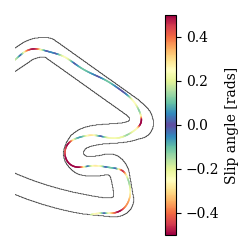
\includegraphics[height=0.85\linewidth]{contents/chapt5/figs/uncertainty/mco_lap.png}
        %% Creator: Matplotlib, PGF backend
%%
%% To include the figure in your LaTeX document, write
%%   \input{<filename>.pgf}
%%
%% Make sure the required packages are loaded in your preamble
%%   \usepackage{pgf}
%%
%% Also ensure that all the required font packages are loaded; for instance,
%% the lmodern package is sometimes necessary when using math font.
%%   \usepackage{lmodern}
%%
%% Figures using additional raster images can only be included by \input if
%% they are in the same directory as the main LaTeX file. For loading figures
%% from other directories you can use the `import` package
%%   \usepackage{import}
%%
%% and then include the figures with
%%   \import{<path to file>}{<filename>.pgf}
%%
%% Matplotlib used the following preamble
%%   \usepackage{fontspec}
%%   \setmainfont{times.ttf}[Path=\detokenize{C:/Windows/Fonts/}]
%%   \setsansfont{DejaVuSans.ttf}[Path=\detokenize{C:/Users/Andrew/anaconda3/envs/auto_car_env/Lib/site-packages/matplotlib/mpl-data/fonts/ttf/}]
%%   \setmonofont{DejaVuSansMono.ttf}[Path=\detokenize{C:/Users/Andrew/anaconda3/envs/auto_car_env/Lib/site-packages/matplotlib/mpl-data/fonts/ttf/}]
%%
\begingroup%
\makeatletter%
\begin{pgfpicture}%
\pgfpathrectangle{\pgfpointorigin}{\pgfqpoint{2.500000in}{2.500000in}}%
\pgfusepath{use as bounding box, clip}%
\begin{pgfscope}%
\pgfsetbuttcap%
\pgfsetmiterjoin%
\definecolor{currentfill}{rgb}{1.000000,1.000000,1.000000}%
\pgfsetfillcolor{currentfill}%
\pgfsetlinewidth{0.000000pt}%
\definecolor{currentstroke}{rgb}{1.000000,1.000000,1.000000}%
\pgfsetstrokecolor{currentstroke}%
\pgfsetdash{}{0pt}%
\pgfpathmoveto{\pgfqpoint{0.000000in}{0.000000in}}%
\pgfpathlineto{\pgfqpoint{2.500000in}{0.000000in}}%
\pgfpathlineto{\pgfqpoint{2.500000in}{2.500000in}}%
\pgfpathlineto{\pgfqpoint{0.000000in}{2.500000in}}%
\pgfpathlineto{\pgfqpoint{0.000000in}{0.000000in}}%
\pgfpathclose%
\pgfusepath{fill}%
\end{pgfscope}%
\begin{pgfscope}%
\pgfpathrectangle{\pgfqpoint{0.352278in}{0.235000in}}{\pgfqpoint{1.339000in}{2.060000in}}%
\pgfusepath{clip}%
\pgfsys@transformshift{0.352278in}{0.235000in}%
\pgftext[left,bottom]{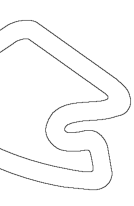
\includegraphics[interpolate=true,width=1.340000in,height=2.060000in]{contents/chapt5/figs/uncertainty/mco_lap_erro_1-img0.png}}%
\end{pgfscope}%
\begin{pgfscope}%
\pgfpathrectangle{\pgfqpoint{0.352278in}{0.235000in}}{\pgfqpoint{1.339000in}{2.060000in}}%
\pgfusepath{clip}%
\pgfsetrectcap%
\pgfsetroundjoin%
\pgfsetlinewidth{1.003750pt}%
\definecolor{currentstroke}{rgb}{0.500000,0.000000,1.000000}%
\pgfsetstrokecolor{currentstroke}%
\pgfsetstrokeopacity{0.800000}%
\pgfsetdash{}{0pt}%
\pgfusepath{stroke}%
\end{pgfscope}%
\begin{pgfscope}%
\pgfpathrectangle{\pgfqpoint{0.352278in}{0.235000in}}{\pgfqpoint{1.339000in}{2.060000in}}%
\pgfusepath{clip}%
\pgfsetrectcap%
\pgfsetroundjoin%
\pgfsetlinewidth{1.003750pt}%
\definecolor{currentstroke}{rgb}{0.500000,0.000000,1.000000}%
\pgfsetstrokecolor{currentstroke}%
\pgfsetstrokeopacity{0.800000}%
\pgfsetdash{}{0pt}%
\pgfusepath{stroke}%
\end{pgfscope}%
\begin{pgfscope}%
\pgfpathrectangle{\pgfqpoint{0.352278in}{0.235000in}}{\pgfqpoint{1.339000in}{2.060000in}}%
\pgfusepath{clip}%
\pgfsetrectcap%
\pgfsetroundjoin%
\pgfsetlinewidth{1.003750pt}%
\definecolor{currentstroke}{rgb}{0.484314,0.024637,0.999924}%
\pgfsetstrokecolor{currentstroke}%
\pgfsetstrokeopacity{0.800000}%
\pgfsetdash{}{0pt}%
\pgfusepath{stroke}%
\end{pgfscope}%
\begin{pgfscope}%
\pgfpathrectangle{\pgfqpoint{0.352278in}{0.235000in}}{\pgfqpoint{1.339000in}{2.060000in}}%
\pgfusepath{clip}%
\pgfsetrectcap%
\pgfsetroundjoin%
\pgfsetlinewidth{1.003750pt}%
\definecolor{currentstroke}{rgb}{0.476471,0.036951,0.999829}%
\pgfsetstrokecolor{currentstroke}%
\pgfsetstrokeopacity{0.800000}%
\pgfsetdash{}{0pt}%
\pgfusepath{stroke}%
\end{pgfscope}%
\begin{pgfscope}%
\pgfpathrectangle{\pgfqpoint{0.352278in}{0.235000in}}{\pgfqpoint{1.339000in}{2.060000in}}%
\pgfusepath{clip}%
\pgfsetrectcap%
\pgfsetroundjoin%
\pgfsetlinewidth{1.003750pt}%
\definecolor{currentstroke}{rgb}{0.476471,0.036951,0.999829}%
\pgfsetstrokecolor{currentstroke}%
\pgfsetstrokeopacity{0.800000}%
\pgfsetdash{}{0pt}%
\pgfusepath{stroke}%
\end{pgfscope}%
\begin{pgfscope}%
\pgfpathrectangle{\pgfqpoint{0.352278in}{0.235000in}}{\pgfqpoint{1.339000in}{2.060000in}}%
\pgfusepath{clip}%
\pgfsetrectcap%
\pgfsetroundjoin%
\pgfsetlinewidth{1.003750pt}%
\definecolor{currentstroke}{rgb}{0.468627,0.049260,0.999696}%
\pgfsetstrokecolor{currentstroke}%
\pgfsetstrokeopacity{0.800000}%
\pgfsetdash{}{0pt}%
\pgfusepath{stroke}%
\end{pgfscope}%
\begin{pgfscope}%
\pgfpathrectangle{\pgfqpoint{0.352278in}{0.235000in}}{\pgfqpoint{1.339000in}{2.060000in}}%
\pgfusepath{clip}%
\pgfsetrectcap%
\pgfsetroundjoin%
\pgfsetlinewidth{1.003750pt}%
\definecolor{currentstroke}{rgb}{0.476471,0.036951,0.999829}%
\pgfsetstrokecolor{currentstroke}%
\pgfsetstrokeopacity{0.800000}%
\pgfsetdash{}{0pt}%
\pgfusepath{stroke}%
\end{pgfscope}%
\begin{pgfscope}%
\pgfpathrectangle{\pgfqpoint{0.352278in}{0.235000in}}{\pgfqpoint{1.339000in}{2.060000in}}%
\pgfusepath{clip}%
\pgfsetrectcap%
\pgfsetroundjoin%
\pgfsetlinewidth{1.003750pt}%
\definecolor{currentstroke}{rgb}{0.476471,0.036951,0.999829}%
\pgfsetstrokecolor{currentstroke}%
\pgfsetstrokeopacity{0.800000}%
\pgfsetdash{}{0pt}%
\pgfusepath{stroke}%
\end{pgfscope}%
\begin{pgfscope}%
\pgfpathrectangle{\pgfqpoint{0.352278in}{0.235000in}}{\pgfqpoint{1.339000in}{2.060000in}}%
\pgfusepath{clip}%
\pgfsetrectcap%
\pgfsetroundjoin%
\pgfsetlinewidth{1.003750pt}%
\definecolor{currentstroke}{rgb}{0.484314,0.024637,0.999924}%
\pgfsetstrokecolor{currentstroke}%
\pgfsetstrokeopacity{0.800000}%
\pgfsetdash{}{0pt}%
\pgfusepath{stroke}%
\end{pgfscope}%
\begin{pgfscope}%
\pgfpathrectangle{\pgfqpoint{0.352278in}{0.235000in}}{\pgfqpoint{1.339000in}{2.060000in}}%
\pgfusepath{clip}%
\pgfsetrectcap%
\pgfsetroundjoin%
\pgfsetlinewidth{1.003750pt}%
\definecolor{currentstroke}{rgb}{0.484314,0.024637,0.999924}%
\pgfsetstrokecolor{currentstroke}%
\pgfsetstrokeopacity{0.800000}%
\pgfsetdash{}{0pt}%
\pgfusepath{stroke}%
\end{pgfscope}%
\begin{pgfscope}%
\pgfpathrectangle{\pgfqpoint{0.352278in}{0.235000in}}{\pgfqpoint{1.339000in}{2.060000in}}%
\pgfusepath{clip}%
\pgfsetrectcap%
\pgfsetroundjoin%
\pgfsetlinewidth{1.003750pt}%
\definecolor{currentstroke}{rgb}{0.492157,0.012320,0.999981}%
\pgfsetstrokecolor{currentstroke}%
\pgfsetstrokeopacity{0.800000}%
\pgfsetdash{}{0pt}%
\pgfusepath{stroke}%
\end{pgfscope}%
\begin{pgfscope}%
\pgfpathrectangle{\pgfqpoint{0.352278in}{0.235000in}}{\pgfqpoint{1.339000in}{2.060000in}}%
\pgfusepath{clip}%
\pgfsetrectcap%
\pgfsetroundjoin%
\pgfsetlinewidth{1.003750pt}%
\definecolor{currentstroke}{rgb}{0.500000,0.000000,1.000000}%
\pgfsetstrokecolor{currentstroke}%
\pgfsetstrokeopacity{0.800000}%
\pgfsetdash{}{0pt}%
\pgfusepath{stroke}%
\end{pgfscope}%
\begin{pgfscope}%
\pgfpathrectangle{\pgfqpoint{0.352278in}{0.235000in}}{\pgfqpoint{1.339000in}{2.060000in}}%
\pgfusepath{clip}%
\pgfsetrectcap%
\pgfsetroundjoin%
\pgfsetlinewidth{1.003750pt}%
\definecolor{currentstroke}{rgb}{0.492157,0.012320,0.999981}%
\pgfsetstrokecolor{currentstroke}%
\pgfsetstrokeopacity{0.800000}%
\pgfsetdash{}{0pt}%
\pgfusepath{stroke}%
\end{pgfscope}%
\begin{pgfscope}%
\pgfpathrectangle{\pgfqpoint{0.352278in}{0.235000in}}{\pgfqpoint{1.339000in}{2.060000in}}%
\pgfusepath{clip}%
\pgfsetrectcap%
\pgfsetroundjoin%
\pgfsetlinewidth{1.003750pt}%
\definecolor{currentstroke}{rgb}{0.492157,0.012320,0.999981}%
\pgfsetstrokecolor{currentstroke}%
\pgfsetstrokeopacity{0.800000}%
\pgfsetdash{}{0pt}%
\pgfusepath{stroke}%
\end{pgfscope}%
\begin{pgfscope}%
\pgfpathrectangle{\pgfqpoint{0.352278in}{0.235000in}}{\pgfqpoint{1.339000in}{2.060000in}}%
\pgfusepath{clip}%
\pgfsetrectcap%
\pgfsetroundjoin%
\pgfsetlinewidth{1.003750pt}%
\definecolor{currentstroke}{rgb}{0.484314,0.024637,0.999924}%
\pgfsetstrokecolor{currentstroke}%
\pgfsetstrokeopacity{0.800000}%
\pgfsetdash{}{0pt}%
\pgfusepath{stroke}%
\end{pgfscope}%
\begin{pgfscope}%
\pgfpathrectangle{\pgfqpoint{0.352278in}{0.235000in}}{\pgfqpoint{1.339000in}{2.060000in}}%
\pgfusepath{clip}%
\pgfsetrectcap%
\pgfsetroundjoin%
\pgfsetlinewidth{1.003750pt}%
\definecolor{currentstroke}{rgb}{0.484314,0.024637,0.999924}%
\pgfsetstrokecolor{currentstroke}%
\pgfsetstrokeopacity{0.800000}%
\pgfsetdash{}{0pt}%
\pgfusepath{stroke}%
\end{pgfscope}%
\begin{pgfscope}%
\pgfpathrectangle{\pgfqpoint{0.352278in}{0.235000in}}{\pgfqpoint{1.339000in}{2.060000in}}%
\pgfusepath{clip}%
\pgfsetrectcap%
\pgfsetroundjoin%
\pgfsetlinewidth{1.003750pt}%
\definecolor{currentstroke}{rgb}{0.484314,0.024637,0.999924}%
\pgfsetstrokecolor{currentstroke}%
\pgfsetstrokeopacity{0.800000}%
\pgfsetdash{}{0pt}%
\pgfusepath{stroke}%
\end{pgfscope}%
\begin{pgfscope}%
\pgfpathrectangle{\pgfqpoint{0.352278in}{0.235000in}}{\pgfqpoint{1.339000in}{2.060000in}}%
\pgfusepath{clip}%
\pgfsetrectcap%
\pgfsetroundjoin%
\pgfsetlinewidth{1.003750pt}%
\definecolor{currentstroke}{rgb}{0.484314,0.024637,0.999924}%
\pgfsetstrokecolor{currentstroke}%
\pgfsetstrokeopacity{0.800000}%
\pgfsetdash{}{0pt}%
\pgfusepath{stroke}%
\end{pgfscope}%
\begin{pgfscope}%
\pgfpathrectangle{\pgfqpoint{0.352278in}{0.235000in}}{\pgfqpoint{1.339000in}{2.060000in}}%
\pgfusepath{clip}%
\pgfsetrectcap%
\pgfsetroundjoin%
\pgfsetlinewidth{1.003750pt}%
\definecolor{currentstroke}{rgb}{0.484314,0.024637,0.999924}%
\pgfsetstrokecolor{currentstroke}%
\pgfsetstrokeopacity{0.800000}%
\pgfsetdash{}{0pt}%
\pgfusepath{stroke}%
\end{pgfscope}%
\begin{pgfscope}%
\pgfpathrectangle{\pgfqpoint{0.352278in}{0.235000in}}{\pgfqpoint{1.339000in}{2.060000in}}%
\pgfusepath{clip}%
\pgfsetrectcap%
\pgfsetroundjoin%
\pgfsetlinewidth{1.003750pt}%
\definecolor{currentstroke}{rgb}{0.484314,0.024637,0.999924}%
\pgfsetstrokecolor{currentstroke}%
\pgfsetstrokeopacity{0.800000}%
\pgfsetdash{}{0pt}%
\pgfusepath{stroke}%
\end{pgfscope}%
\begin{pgfscope}%
\pgfpathrectangle{\pgfqpoint{0.352278in}{0.235000in}}{\pgfqpoint{1.339000in}{2.060000in}}%
\pgfusepath{clip}%
\pgfsetrectcap%
\pgfsetroundjoin%
\pgfsetlinewidth{1.003750pt}%
\definecolor{currentstroke}{rgb}{0.484314,0.024637,0.999924}%
\pgfsetstrokecolor{currentstroke}%
\pgfsetstrokeopacity{0.800000}%
\pgfsetdash{}{0pt}%
\pgfusepath{stroke}%
\end{pgfscope}%
\begin{pgfscope}%
\pgfpathrectangle{\pgfqpoint{0.352278in}{0.235000in}}{\pgfqpoint{1.339000in}{2.060000in}}%
\pgfusepath{clip}%
\pgfsetrectcap%
\pgfsetroundjoin%
\pgfsetlinewidth{1.003750pt}%
\definecolor{currentstroke}{rgb}{0.484314,0.024637,0.999924}%
\pgfsetstrokecolor{currentstroke}%
\pgfsetstrokeopacity{0.800000}%
\pgfsetdash{}{0pt}%
\pgfusepath{stroke}%
\end{pgfscope}%
\begin{pgfscope}%
\pgfpathrectangle{\pgfqpoint{0.352278in}{0.235000in}}{\pgfqpoint{1.339000in}{2.060000in}}%
\pgfusepath{clip}%
\pgfsetrectcap%
\pgfsetroundjoin%
\pgfsetlinewidth{1.003750pt}%
\definecolor{currentstroke}{rgb}{0.476471,0.036951,0.999829}%
\pgfsetstrokecolor{currentstroke}%
\pgfsetstrokeopacity{0.800000}%
\pgfsetdash{}{0pt}%
\pgfusepath{stroke}%
\end{pgfscope}%
\begin{pgfscope}%
\pgfpathrectangle{\pgfqpoint{0.352278in}{0.235000in}}{\pgfqpoint{1.339000in}{2.060000in}}%
\pgfusepath{clip}%
\pgfsetrectcap%
\pgfsetroundjoin%
\pgfsetlinewidth{1.003750pt}%
\definecolor{currentstroke}{rgb}{0.476471,0.036951,0.999829}%
\pgfsetstrokecolor{currentstroke}%
\pgfsetstrokeopacity{0.800000}%
\pgfsetdash{}{0pt}%
\pgfusepath{stroke}%
\end{pgfscope}%
\begin{pgfscope}%
\pgfpathrectangle{\pgfqpoint{0.352278in}{0.235000in}}{\pgfqpoint{1.339000in}{2.060000in}}%
\pgfusepath{clip}%
\pgfsetrectcap%
\pgfsetroundjoin%
\pgfsetlinewidth{1.003750pt}%
\definecolor{currentstroke}{rgb}{0.476471,0.036951,0.999829}%
\pgfsetstrokecolor{currentstroke}%
\pgfsetstrokeopacity{0.800000}%
\pgfsetdash{}{0pt}%
\pgfusepath{stroke}%
\end{pgfscope}%
\begin{pgfscope}%
\pgfpathrectangle{\pgfqpoint{0.352278in}{0.235000in}}{\pgfqpoint{1.339000in}{2.060000in}}%
\pgfusepath{clip}%
\pgfsetrectcap%
\pgfsetroundjoin%
\pgfsetlinewidth{1.003750pt}%
\definecolor{currentstroke}{rgb}{0.476471,0.036951,0.999829}%
\pgfsetstrokecolor{currentstroke}%
\pgfsetstrokeopacity{0.800000}%
\pgfsetdash{}{0pt}%
\pgfusepath{stroke}%
\end{pgfscope}%
\begin{pgfscope}%
\pgfpathrectangle{\pgfqpoint{0.352278in}{0.235000in}}{\pgfqpoint{1.339000in}{2.060000in}}%
\pgfusepath{clip}%
\pgfsetrectcap%
\pgfsetroundjoin%
\pgfsetlinewidth{1.003750pt}%
\definecolor{currentstroke}{rgb}{0.492157,0.012320,0.999981}%
\pgfsetstrokecolor{currentstroke}%
\pgfsetstrokeopacity{0.800000}%
\pgfsetdash{}{0pt}%
\pgfusepath{stroke}%
\end{pgfscope}%
\begin{pgfscope}%
\pgfpathrectangle{\pgfqpoint{0.352278in}{0.235000in}}{\pgfqpoint{1.339000in}{2.060000in}}%
\pgfusepath{clip}%
\pgfsetrectcap%
\pgfsetroundjoin%
\pgfsetlinewidth{1.003750pt}%
\definecolor{currentstroke}{rgb}{0.500000,0.000000,1.000000}%
\pgfsetstrokecolor{currentstroke}%
\pgfsetstrokeopacity{0.800000}%
\pgfsetdash{}{0pt}%
\pgfusepath{stroke}%
\end{pgfscope}%
\begin{pgfscope}%
\pgfpathrectangle{\pgfqpoint{0.352278in}{0.235000in}}{\pgfqpoint{1.339000in}{2.060000in}}%
\pgfusepath{clip}%
\pgfsetrectcap%
\pgfsetroundjoin%
\pgfsetlinewidth{1.003750pt}%
\definecolor{currentstroke}{rgb}{0.484314,0.024637,0.999924}%
\pgfsetstrokecolor{currentstroke}%
\pgfsetstrokeopacity{0.800000}%
\pgfsetdash{}{0pt}%
\pgfusepath{stroke}%
\end{pgfscope}%
\begin{pgfscope}%
\pgfpathrectangle{\pgfqpoint{0.352278in}{0.235000in}}{\pgfqpoint{1.339000in}{2.060000in}}%
\pgfusepath{clip}%
\pgfsetrectcap%
\pgfsetroundjoin%
\pgfsetlinewidth{1.003750pt}%
\definecolor{currentstroke}{rgb}{0.468627,0.049260,0.999696}%
\pgfsetstrokecolor{currentstroke}%
\pgfsetstrokeopacity{0.800000}%
\pgfsetdash{}{0pt}%
\pgfusepath{stroke}%
\end{pgfscope}%
\begin{pgfscope}%
\pgfpathrectangle{\pgfqpoint{0.352278in}{0.235000in}}{\pgfqpoint{1.339000in}{2.060000in}}%
\pgfusepath{clip}%
\pgfsetrectcap%
\pgfsetroundjoin%
\pgfsetlinewidth{1.003750pt}%
\definecolor{currentstroke}{rgb}{0.445098,0.086133,0.999070}%
\pgfsetstrokecolor{currentstroke}%
\pgfsetstrokeopacity{0.800000}%
\pgfsetdash{}{0pt}%
\pgfusepath{stroke}%
\end{pgfscope}%
\begin{pgfscope}%
\pgfpathrectangle{\pgfqpoint{0.352278in}{0.235000in}}{\pgfqpoint{1.339000in}{2.060000in}}%
\pgfusepath{clip}%
\pgfsetrectcap%
\pgfsetroundjoin%
\pgfsetlinewidth{1.003750pt}%
\definecolor{currentstroke}{rgb}{0.437255,0.098400,0.998786}%
\pgfsetstrokecolor{currentstroke}%
\pgfsetstrokeopacity{0.800000}%
\pgfsetdash{}{0pt}%
\pgfusepath{stroke}%
\end{pgfscope}%
\begin{pgfscope}%
\pgfpathrectangle{\pgfqpoint{0.352278in}{0.235000in}}{\pgfqpoint{1.339000in}{2.060000in}}%
\pgfusepath{clip}%
\pgfsetrectcap%
\pgfsetroundjoin%
\pgfsetlinewidth{1.003750pt}%
\definecolor{currentstroke}{rgb}{0.413725,0.135105,0.997705}%
\pgfsetstrokecolor{currentstroke}%
\pgfsetstrokeopacity{0.800000}%
\pgfsetdash{}{0pt}%
\pgfusepath{stroke}%
\end{pgfscope}%
\begin{pgfscope}%
\pgfpathrectangle{\pgfqpoint{0.352278in}{0.235000in}}{\pgfqpoint{1.339000in}{2.060000in}}%
\pgfusepath{clip}%
\pgfsetrectcap%
\pgfsetroundjoin%
\pgfsetlinewidth{1.003750pt}%
\definecolor{currentstroke}{rgb}{0.398039,0.159476,0.996795}%
\pgfsetstrokecolor{currentstroke}%
\pgfsetstrokeopacity{0.800000}%
\pgfsetdash{}{0pt}%
\pgfusepath{stroke}%
\end{pgfscope}%
\begin{pgfscope}%
\pgfpathrectangle{\pgfqpoint{0.352278in}{0.235000in}}{\pgfqpoint{1.339000in}{2.060000in}}%
\pgfusepath{clip}%
\pgfsetrectcap%
\pgfsetroundjoin%
\pgfsetlinewidth{1.003750pt}%
\definecolor{currentstroke}{rgb}{0.382353,0.183750,0.995734}%
\pgfsetstrokecolor{currentstroke}%
\pgfsetstrokeopacity{0.800000}%
\pgfsetdash{}{0pt}%
\pgfusepath{stroke}%
\end{pgfscope}%
\begin{pgfscope}%
\pgfpathrectangle{\pgfqpoint{0.352278in}{0.235000in}}{\pgfqpoint{1.339000in}{2.060000in}}%
\pgfusepath{clip}%
\pgfsetrectcap%
\pgfsetroundjoin%
\pgfsetlinewidth{1.003750pt}%
\definecolor{currentstroke}{rgb}{0.374510,0.195845,0.995147}%
\pgfsetstrokecolor{currentstroke}%
\pgfsetstrokeopacity{0.800000}%
\pgfsetdash{}{0pt}%
\pgfusepath{stroke}%
\end{pgfscope}%
\begin{pgfscope}%
\pgfpathrectangle{\pgfqpoint{0.352278in}{0.235000in}}{\pgfqpoint{1.339000in}{2.060000in}}%
\pgfusepath{clip}%
\pgfsetrectcap%
\pgfsetroundjoin%
\pgfsetlinewidth{1.003750pt}%
\definecolor{currentstroke}{rgb}{0.358824,0.219946,0.993859}%
\pgfsetstrokecolor{currentstroke}%
\pgfsetstrokeopacity{0.800000}%
\pgfsetdash{}{0pt}%
\pgfusepath{stroke}%
\end{pgfscope}%
\begin{pgfscope}%
\pgfpathrectangle{\pgfqpoint{0.352278in}{0.235000in}}{\pgfqpoint{1.339000in}{2.060000in}}%
\pgfusepath{clip}%
\pgfsetrectcap%
\pgfsetroundjoin%
\pgfsetlinewidth{1.003750pt}%
\definecolor{currentstroke}{rgb}{0.350980,0.231948,0.993159}%
\pgfsetstrokecolor{currentstroke}%
\pgfsetstrokeopacity{0.800000}%
\pgfsetdash{}{0pt}%
\pgfusepath{stroke}%
\end{pgfscope}%
\begin{pgfscope}%
\pgfpathrectangle{\pgfqpoint{0.352278in}{0.235000in}}{\pgfqpoint{1.339000in}{2.060000in}}%
\pgfusepath{clip}%
\pgfsetrectcap%
\pgfsetroundjoin%
\pgfsetlinewidth{1.003750pt}%
\definecolor{currentstroke}{rgb}{0.335294,0.255843,0.991645}%
\pgfsetstrokecolor{currentstroke}%
\pgfsetstrokeopacity{0.800000}%
\pgfsetdash{}{0pt}%
\pgfusepath{stroke}%
\end{pgfscope}%
\begin{pgfscope}%
\pgfpathrectangle{\pgfqpoint{0.352278in}{0.235000in}}{\pgfqpoint{1.339000in}{2.060000in}}%
\pgfusepath{clip}%
\pgfsetrectcap%
\pgfsetroundjoin%
\pgfsetlinewidth{1.003750pt}%
\definecolor{currentstroke}{rgb}{0.335294,0.255843,0.991645}%
\pgfsetstrokecolor{currentstroke}%
\pgfsetstrokeopacity{0.800000}%
\pgfsetdash{}{0pt}%
\pgfusepath{stroke}%
\end{pgfscope}%
\begin{pgfscope}%
\pgfpathrectangle{\pgfqpoint{0.352278in}{0.235000in}}{\pgfqpoint{1.339000in}{2.060000in}}%
\pgfusepath{clip}%
\pgfsetrectcap%
\pgfsetroundjoin%
\pgfsetlinewidth{1.003750pt}%
\definecolor{currentstroke}{rgb}{0.319608,0.279583,0.989980}%
\pgfsetstrokecolor{currentstroke}%
\pgfsetstrokeopacity{0.800000}%
\pgfsetdash{}{0pt}%
\pgfusepath{stroke}%
\end{pgfscope}%
\begin{pgfscope}%
\pgfpathrectangle{\pgfqpoint{0.352278in}{0.235000in}}{\pgfqpoint{1.339000in}{2.060000in}}%
\pgfusepath{clip}%
\pgfsetrectcap%
\pgfsetroundjoin%
\pgfsetlinewidth{1.003750pt}%
\definecolor{currentstroke}{rgb}{0.303922,0.303153,0.988165}%
\pgfsetstrokecolor{currentstroke}%
\pgfsetstrokeopacity{0.800000}%
\pgfsetdash{}{0pt}%
\pgfusepath{stroke}%
\end{pgfscope}%
\begin{pgfscope}%
\pgfpathrectangle{\pgfqpoint{0.352278in}{0.235000in}}{\pgfqpoint{1.339000in}{2.060000in}}%
\pgfusepath{clip}%
\pgfsetrectcap%
\pgfsetroundjoin%
\pgfsetlinewidth{1.003750pt}%
\definecolor{currentstroke}{rgb}{0.296078,0.314870,0.987202}%
\pgfsetstrokecolor{currentstroke}%
\pgfsetstrokeopacity{0.800000}%
\pgfsetdash{}{0pt}%
\pgfusepath{stroke}%
\end{pgfscope}%
\begin{pgfscope}%
\pgfpathrectangle{\pgfqpoint{0.352278in}{0.235000in}}{\pgfqpoint{1.339000in}{2.060000in}}%
\pgfusepath{clip}%
\pgfsetrectcap%
\pgfsetroundjoin%
\pgfsetlinewidth{1.003750pt}%
\definecolor{currentstroke}{rgb}{0.280392,0.338158,0.985162}%
\pgfsetstrokecolor{currentstroke}%
\pgfsetstrokeopacity{0.800000}%
\pgfsetdash{}{0pt}%
\pgfusepath{stroke}%
\end{pgfscope}%
\begin{pgfscope}%
\pgfpathrectangle{\pgfqpoint{0.352278in}{0.235000in}}{\pgfqpoint{1.339000in}{2.060000in}}%
\pgfusepath{clip}%
\pgfsetrectcap%
\pgfsetroundjoin%
\pgfsetlinewidth{1.003750pt}%
\definecolor{currentstroke}{rgb}{0.280392,0.338158,0.985162}%
\pgfsetstrokecolor{currentstroke}%
\pgfsetstrokeopacity{0.800000}%
\pgfsetdash{}{0pt}%
\pgfusepath{stroke}%
\end{pgfscope}%
\begin{pgfscope}%
\pgfpathrectangle{\pgfqpoint{0.352278in}{0.235000in}}{\pgfqpoint{1.339000in}{2.060000in}}%
\pgfusepath{clip}%
\pgfsetrectcap%
\pgfsetroundjoin%
\pgfsetlinewidth{1.003750pt}%
\definecolor{currentstroke}{rgb}{0.296078,0.314870,0.987202}%
\pgfsetstrokecolor{currentstroke}%
\pgfsetstrokeopacity{0.800000}%
\pgfsetdash{}{0pt}%
\pgfusepath{stroke}%
\end{pgfscope}%
\begin{pgfscope}%
\pgfpathrectangle{\pgfqpoint{0.352278in}{0.235000in}}{\pgfqpoint{1.339000in}{2.060000in}}%
\pgfusepath{clip}%
\pgfsetrectcap%
\pgfsetroundjoin%
\pgfsetlinewidth{1.003750pt}%
\definecolor{currentstroke}{rgb}{0.303922,0.303153,0.988165}%
\pgfsetstrokecolor{currentstroke}%
\pgfsetstrokeopacity{0.800000}%
\pgfsetdash{}{0pt}%
\pgfusepath{stroke}%
\end{pgfscope}%
\begin{pgfscope}%
\pgfpathrectangle{\pgfqpoint{0.352278in}{0.235000in}}{\pgfqpoint{1.339000in}{2.060000in}}%
\pgfusepath{clip}%
\pgfsetrectcap%
\pgfsetroundjoin%
\pgfsetlinewidth{1.003750pt}%
\definecolor{currentstroke}{rgb}{0.327451,0.267733,0.990831}%
\pgfsetstrokecolor{currentstroke}%
\pgfsetstrokeopacity{0.800000}%
\pgfsetdash{}{0pt}%
\pgfusepath{stroke}%
\end{pgfscope}%
\begin{pgfscope}%
\pgfpathrectangle{\pgfqpoint{0.352278in}{0.235000in}}{\pgfqpoint{1.339000in}{2.060000in}}%
\pgfusepath{clip}%
\pgfsetrectcap%
\pgfsetroundjoin%
\pgfsetlinewidth{1.003750pt}%
\definecolor{currentstroke}{rgb}{0.350980,0.231948,0.993159}%
\pgfsetstrokecolor{currentstroke}%
\pgfsetstrokeopacity{0.800000}%
\pgfsetdash{}{0pt}%
\pgfusepath{stroke}%
\end{pgfscope}%
\begin{pgfscope}%
\pgfpathrectangle{\pgfqpoint{0.352278in}{0.235000in}}{\pgfqpoint{1.339000in}{2.060000in}}%
\pgfusepath{clip}%
\pgfsetrectcap%
\pgfsetroundjoin%
\pgfsetlinewidth{1.003750pt}%
\definecolor{currentstroke}{rgb}{0.374510,0.195845,0.995147}%
\pgfsetstrokecolor{currentstroke}%
\pgfsetstrokeopacity{0.800000}%
\pgfsetdash{}{0pt}%
\pgfusepath{stroke}%
\end{pgfscope}%
\begin{pgfscope}%
\pgfpathrectangle{\pgfqpoint{0.352278in}{0.235000in}}{\pgfqpoint{1.339000in}{2.060000in}}%
\pgfusepath{clip}%
\pgfsetrectcap%
\pgfsetroundjoin%
\pgfsetlinewidth{1.003750pt}%
\definecolor{currentstroke}{rgb}{0.398039,0.159476,0.996795}%
\pgfsetstrokecolor{currentstroke}%
\pgfsetstrokeopacity{0.800000}%
\pgfsetdash{}{0pt}%
\pgfusepath{stroke}%
\end{pgfscope}%
\begin{pgfscope}%
\pgfpathrectangle{\pgfqpoint{0.352278in}{0.235000in}}{\pgfqpoint{1.339000in}{2.060000in}}%
\pgfusepath{clip}%
\pgfsetrectcap%
\pgfsetroundjoin%
\pgfsetlinewidth{1.003750pt}%
\definecolor{currentstroke}{rgb}{0.429412,0.110653,0.998464}%
\pgfsetstrokecolor{currentstroke}%
\pgfsetstrokeopacity{0.800000}%
\pgfsetdash{}{0pt}%
\pgfusepath{stroke}%
\end{pgfscope}%
\begin{pgfscope}%
\pgfpathrectangle{\pgfqpoint{0.352278in}{0.235000in}}{\pgfqpoint{1.339000in}{2.060000in}}%
\pgfusepath{clip}%
\pgfsetrectcap%
\pgfsetroundjoin%
\pgfsetlinewidth{1.003750pt}%
\definecolor{currentstroke}{rgb}{0.445098,0.086133,0.999070}%
\pgfsetstrokecolor{currentstroke}%
\pgfsetstrokeopacity{0.800000}%
\pgfsetdash{}{0pt}%
\pgfusepath{stroke}%
\end{pgfscope}%
\begin{pgfscope}%
\pgfpathrectangle{\pgfqpoint{0.352278in}{0.235000in}}{\pgfqpoint{1.339000in}{2.060000in}}%
\pgfusepath{clip}%
\pgfsetrectcap%
\pgfsetroundjoin%
\pgfsetlinewidth{1.003750pt}%
\definecolor{currentstroke}{rgb}{0.468627,0.049260,0.999696}%
\pgfsetstrokecolor{currentstroke}%
\pgfsetstrokeopacity{0.800000}%
\pgfsetdash{}{0pt}%
\pgfusepath{stroke}%
\end{pgfscope}%
\begin{pgfscope}%
\pgfpathrectangle{\pgfqpoint{0.352278in}{0.235000in}}{\pgfqpoint{1.339000in}{2.060000in}}%
\pgfusepath{clip}%
\pgfsetrectcap%
\pgfsetroundjoin%
\pgfsetlinewidth{1.003750pt}%
\definecolor{currentstroke}{rgb}{0.484314,0.024637,0.999924}%
\pgfsetstrokecolor{currentstroke}%
\pgfsetstrokeopacity{0.800000}%
\pgfsetdash{}{0pt}%
\pgfusepath{stroke}%
\end{pgfscope}%
\begin{pgfscope}%
\pgfpathrectangle{\pgfqpoint{0.352278in}{0.235000in}}{\pgfqpoint{1.339000in}{2.060000in}}%
\pgfusepath{clip}%
\pgfsetrectcap%
\pgfsetroundjoin%
\pgfsetlinewidth{1.003750pt}%
\definecolor{currentstroke}{rgb}{0.500000,0.000000,1.000000}%
\pgfsetstrokecolor{currentstroke}%
\pgfsetstrokeopacity{0.800000}%
\pgfsetdash{}{0pt}%
\pgfusepath{stroke}%
\end{pgfscope}%
\begin{pgfscope}%
\pgfpathrectangle{\pgfqpoint{0.352278in}{0.235000in}}{\pgfqpoint{1.339000in}{2.060000in}}%
\pgfusepath{clip}%
\pgfsetrectcap%
\pgfsetroundjoin%
\pgfsetlinewidth{1.003750pt}%
\definecolor{currentstroke}{rgb}{0.484314,0.024637,0.999924}%
\pgfsetstrokecolor{currentstroke}%
\pgfsetstrokeopacity{0.800000}%
\pgfsetdash{}{0pt}%
\pgfusepath{stroke}%
\end{pgfscope}%
\begin{pgfscope}%
\pgfpathrectangle{\pgfqpoint{0.352278in}{0.235000in}}{\pgfqpoint{1.339000in}{2.060000in}}%
\pgfusepath{clip}%
\pgfsetrectcap%
\pgfsetroundjoin%
\pgfsetlinewidth{1.003750pt}%
\definecolor{currentstroke}{rgb}{0.468627,0.049260,0.999696}%
\pgfsetstrokecolor{currentstroke}%
\pgfsetstrokeopacity{0.800000}%
\pgfsetdash{}{0pt}%
\pgfusepath{stroke}%
\end{pgfscope}%
\begin{pgfscope}%
\pgfpathrectangle{\pgfqpoint{0.352278in}{0.235000in}}{\pgfqpoint{1.339000in}{2.060000in}}%
\pgfusepath{clip}%
\pgfsetrectcap%
\pgfsetroundjoin%
\pgfsetlinewidth{1.003750pt}%
\definecolor{currentstroke}{rgb}{0.460784,0.061561,0.999526}%
\pgfsetstrokecolor{currentstroke}%
\pgfsetstrokeopacity{0.800000}%
\pgfsetdash{}{0pt}%
\pgfusepath{stroke}%
\end{pgfscope}%
\begin{pgfscope}%
\pgfpathrectangle{\pgfqpoint{0.352278in}{0.235000in}}{\pgfqpoint{1.339000in}{2.060000in}}%
\pgfusepath{clip}%
\pgfsetrectcap%
\pgfsetroundjoin%
\pgfsetlinewidth{1.003750pt}%
\definecolor{currentstroke}{rgb}{0.445098,0.086133,0.999070}%
\pgfsetstrokecolor{currentstroke}%
\pgfsetstrokeopacity{0.800000}%
\pgfsetdash{}{0pt}%
\pgfusepath{stroke}%
\end{pgfscope}%
\begin{pgfscope}%
\pgfpathrectangle{\pgfqpoint{0.352278in}{0.235000in}}{\pgfqpoint{1.339000in}{2.060000in}}%
\pgfusepath{clip}%
\pgfsetrectcap%
\pgfsetroundjoin%
\pgfsetlinewidth{1.003750pt}%
\definecolor{currentstroke}{rgb}{0.437255,0.098400,0.998786}%
\pgfsetstrokecolor{currentstroke}%
\pgfsetstrokeopacity{0.800000}%
\pgfsetdash{}{0pt}%
\pgfusepath{stroke}%
\end{pgfscope}%
\begin{pgfscope}%
\pgfpathrectangle{\pgfqpoint{0.352278in}{0.235000in}}{\pgfqpoint{1.339000in}{2.060000in}}%
\pgfusepath{clip}%
\pgfsetrectcap%
\pgfsetroundjoin%
\pgfsetlinewidth{1.003750pt}%
\definecolor{currentstroke}{rgb}{0.421569,0.122888,0.998103}%
\pgfsetstrokecolor{currentstroke}%
\pgfsetstrokeopacity{0.800000}%
\pgfsetdash{}{0pt}%
\pgfusepath{stroke}%
\end{pgfscope}%
\begin{pgfscope}%
\pgfpathrectangle{\pgfqpoint{0.352278in}{0.235000in}}{\pgfqpoint{1.339000in}{2.060000in}}%
\pgfusepath{clip}%
\pgfsetrectcap%
\pgfsetroundjoin%
\pgfsetlinewidth{1.003750pt}%
\definecolor{currentstroke}{rgb}{0.405882,0.147302,0.997269}%
\pgfsetstrokecolor{currentstroke}%
\pgfsetstrokeopacity{0.800000}%
\pgfsetdash{}{0pt}%
\pgfusepath{stroke}%
\end{pgfscope}%
\begin{pgfscope}%
\pgfpathrectangle{\pgfqpoint{0.352278in}{0.235000in}}{\pgfqpoint{1.339000in}{2.060000in}}%
\pgfusepath{clip}%
\pgfsetrectcap%
\pgfsetroundjoin%
\pgfsetlinewidth{1.003750pt}%
\definecolor{currentstroke}{rgb}{0.405882,0.147302,0.997269}%
\pgfsetstrokecolor{currentstroke}%
\pgfsetstrokeopacity{0.800000}%
\pgfsetdash{}{0pt}%
\pgfusepath{stroke}%
\end{pgfscope}%
\begin{pgfscope}%
\pgfpathrectangle{\pgfqpoint{0.352278in}{0.235000in}}{\pgfqpoint{1.339000in}{2.060000in}}%
\pgfusepath{clip}%
\pgfsetrectcap%
\pgfsetroundjoin%
\pgfsetlinewidth{1.003750pt}%
\definecolor{currentstroke}{rgb}{0.398039,0.159476,0.996795}%
\pgfsetstrokecolor{currentstroke}%
\pgfsetstrokeopacity{0.800000}%
\pgfsetdash{}{0pt}%
\pgfusepath{stroke}%
\end{pgfscope}%
\begin{pgfscope}%
\pgfpathrectangle{\pgfqpoint{0.352278in}{0.235000in}}{\pgfqpoint{1.339000in}{2.060000in}}%
\pgfusepath{clip}%
\pgfsetrectcap%
\pgfsetroundjoin%
\pgfsetlinewidth{1.003750pt}%
\definecolor{currentstroke}{rgb}{0.398039,0.159476,0.996795}%
\pgfsetstrokecolor{currentstroke}%
\pgfsetstrokeopacity{0.800000}%
\pgfsetdash{}{0pt}%
\pgfusepath{stroke}%
\end{pgfscope}%
\begin{pgfscope}%
\pgfpathrectangle{\pgfqpoint{0.352278in}{0.235000in}}{\pgfqpoint{1.339000in}{2.060000in}}%
\pgfusepath{clip}%
\pgfsetrectcap%
\pgfsetroundjoin%
\pgfsetlinewidth{1.003750pt}%
\definecolor{currentstroke}{rgb}{0.398039,0.159476,0.996795}%
\pgfsetstrokecolor{currentstroke}%
\pgfsetstrokeopacity{0.800000}%
\pgfsetdash{}{0pt}%
\pgfusepath{stroke}%
\end{pgfscope}%
\begin{pgfscope}%
\pgfpathrectangle{\pgfqpoint{0.352278in}{0.235000in}}{\pgfqpoint{1.339000in}{2.060000in}}%
\pgfusepath{clip}%
\pgfsetrectcap%
\pgfsetroundjoin%
\pgfsetlinewidth{1.003750pt}%
\definecolor{currentstroke}{rgb}{0.405882,0.147302,0.997269}%
\pgfsetstrokecolor{currentstroke}%
\pgfsetstrokeopacity{0.800000}%
\pgfsetdash{}{0pt}%
\pgfusepath{stroke}%
\end{pgfscope}%
\begin{pgfscope}%
\pgfpathrectangle{\pgfqpoint{0.352278in}{0.235000in}}{\pgfqpoint{1.339000in}{2.060000in}}%
\pgfusepath{clip}%
\pgfsetrectcap%
\pgfsetroundjoin%
\pgfsetlinewidth{1.003750pt}%
\definecolor{currentstroke}{rgb}{0.405882,0.147302,0.997269}%
\pgfsetstrokecolor{currentstroke}%
\pgfsetstrokeopacity{0.800000}%
\pgfsetdash{}{0pt}%
\pgfusepath{stroke}%
\end{pgfscope}%
\begin{pgfscope}%
\pgfpathrectangle{\pgfqpoint{0.352278in}{0.235000in}}{\pgfqpoint{1.339000in}{2.060000in}}%
\pgfusepath{clip}%
\pgfsetrectcap%
\pgfsetroundjoin%
\pgfsetlinewidth{1.003750pt}%
\definecolor{currentstroke}{rgb}{0.413725,0.135105,0.997705}%
\pgfsetstrokecolor{currentstroke}%
\pgfsetstrokeopacity{0.800000}%
\pgfsetdash{}{0pt}%
\pgfusepath{stroke}%
\end{pgfscope}%
\begin{pgfscope}%
\pgfpathrectangle{\pgfqpoint{0.352278in}{0.235000in}}{\pgfqpoint{1.339000in}{2.060000in}}%
\pgfusepath{clip}%
\pgfsetrectcap%
\pgfsetroundjoin%
\pgfsetlinewidth{1.003750pt}%
\definecolor{currentstroke}{rgb}{0.413725,0.135105,0.997705}%
\pgfsetstrokecolor{currentstroke}%
\pgfsetstrokeopacity{0.800000}%
\pgfsetdash{}{0pt}%
\pgfusepath{stroke}%
\end{pgfscope}%
\begin{pgfscope}%
\pgfpathrectangle{\pgfqpoint{0.352278in}{0.235000in}}{\pgfqpoint{1.339000in}{2.060000in}}%
\pgfusepath{clip}%
\pgfsetrectcap%
\pgfsetroundjoin%
\pgfsetlinewidth{1.003750pt}%
\definecolor{currentstroke}{rgb}{0.421569,0.122888,0.998103}%
\pgfsetstrokecolor{currentstroke}%
\pgfsetstrokeopacity{0.800000}%
\pgfsetdash{}{0pt}%
\pgfusepath{stroke}%
\end{pgfscope}%
\begin{pgfscope}%
\pgfpathrectangle{\pgfqpoint{0.352278in}{0.235000in}}{\pgfqpoint{1.339000in}{2.060000in}}%
\pgfusepath{clip}%
\pgfsetrectcap%
\pgfsetroundjoin%
\pgfsetlinewidth{1.003750pt}%
\definecolor{currentstroke}{rgb}{0.429412,0.110653,0.998464}%
\pgfsetstrokecolor{currentstroke}%
\pgfsetstrokeopacity{0.800000}%
\pgfsetdash{}{0pt}%
\pgfusepath{stroke}%
\end{pgfscope}%
\begin{pgfscope}%
\pgfpathrectangle{\pgfqpoint{0.352278in}{0.235000in}}{\pgfqpoint{1.339000in}{2.060000in}}%
\pgfusepath{clip}%
\pgfsetrectcap%
\pgfsetroundjoin%
\pgfsetlinewidth{1.003750pt}%
\definecolor{currentstroke}{rgb}{0.429412,0.110653,0.998464}%
\pgfsetstrokecolor{currentstroke}%
\pgfsetstrokeopacity{0.800000}%
\pgfsetdash{}{0pt}%
\pgfusepath{stroke}%
\end{pgfscope}%
\begin{pgfscope}%
\pgfpathrectangle{\pgfqpoint{0.352278in}{0.235000in}}{\pgfqpoint{1.339000in}{2.060000in}}%
\pgfusepath{clip}%
\pgfsetrectcap%
\pgfsetroundjoin%
\pgfsetlinewidth{1.003750pt}%
\definecolor{currentstroke}{rgb}{0.437255,0.098400,0.998786}%
\pgfsetstrokecolor{currentstroke}%
\pgfsetstrokeopacity{0.800000}%
\pgfsetdash{}{0pt}%
\pgfusepath{stroke}%
\end{pgfscope}%
\begin{pgfscope}%
\pgfpathrectangle{\pgfqpoint{0.352278in}{0.235000in}}{\pgfqpoint{1.339000in}{2.060000in}}%
\pgfusepath{clip}%
\pgfsetrectcap%
\pgfsetroundjoin%
\pgfsetlinewidth{1.003750pt}%
\definecolor{currentstroke}{rgb}{0.429412,0.110653,0.998464}%
\pgfsetstrokecolor{currentstroke}%
\pgfsetstrokeopacity{0.800000}%
\pgfsetdash{}{0pt}%
\pgfusepath{stroke}%
\end{pgfscope}%
\begin{pgfscope}%
\pgfpathrectangle{\pgfqpoint{0.352278in}{0.235000in}}{\pgfqpoint{1.339000in}{2.060000in}}%
\pgfusepath{clip}%
\pgfsetrectcap%
\pgfsetroundjoin%
\pgfsetlinewidth{1.003750pt}%
\definecolor{currentstroke}{rgb}{0.429412,0.110653,0.998464}%
\pgfsetstrokecolor{currentstroke}%
\pgfsetstrokeopacity{0.800000}%
\pgfsetdash{}{0pt}%
\pgfusepath{stroke}%
\end{pgfscope}%
\begin{pgfscope}%
\pgfpathrectangle{\pgfqpoint{0.352278in}{0.235000in}}{\pgfqpoint{1.339000in}{2.060000in}}%
\pgfusepath{clip}%
\pgfsetrectcap%
\pgfsetroundjoin%
\pgfsetlinewidth{1.003750pt}%
\definecolor{currentstroke}{rgb}{0.421569,0.122888,0.998103}%
\pgfsetstrokecolor{currentstroke}%
\pgfsetstrokeopacity{0.800000}%
\pgfsetdash{}{0pt}%
\pgfusepath{stroke}%
\end{pgfscope}%
\begin{pgfscope}%
\pgfpathrectangle{\pgfqpoint{0.352278in}{0.235000in}}{\pgfqpoint{1.339000in}{2.060000in}}%
\pgfusepath{clip}%
\pgfsetrectcap%
\pgfsetroundjoin%
\pgfsetlinewidth{1.003750pt}%
\definecolor{currentstroke}{rgb}{0.421569,0.122888,0.998103}%
\pgfsetstrokecolor{currentstroke}%
\pgfsetstrokeopacity{0.800000}%
\pgfsetdash{}{0pt}%
\pgfusepath{stroke}%
\end{pgfscope}%
\begin{pgfscope}%
\pgfpathrectangle{\pgfqpoint{0.352278in}{0.235000in}}{\pgfqpoint{1.339000in}{2.060000in}}%
\pgfusepath{clip}%
\pgfsetrectcap%
\pgfsetroundjoin%
\pgfsetlinewidth{1.003750pt}%
\definecolor{currentstroke}{rgb}{0.413725,0.135105,0.997705}%
\pgfsetstrokecolor{currentstroke}%
\pgfsetstrokeopacity{0.800000}%
\pgfsetdash{}{0pt}%
\pgfusepath{stroke}%
\end{pgfscope}%
\begin{pgfscope}%
\pgfpathrectangle{\pgfqpoint{0.352278in}{0.235000in}}{\pgfqpoint{1.339000in}{2.060000in}}%
\pgfusepath{clip}%
\pgfsetrectcap%
\pgfsetroundjoin%
\pgfsetlinewidth{1.003750pt}%
\definecolor{currentstroke}{rgb}{0.413725,0.135105,0.997705}%
\pgfsetstrokecolor{currentstroke}%
\pgfsetstrokeopacity{0.800000}%
\pgfsetdash{}{0pt}%
\pgfusepath{stroke}%
\end{pgfscope}%
\begin{pgfscope}%
\pgfpathrectangle{\pgfqpoint{0.352278in}{0.235000in}}{\pgfqpoint{1.339000in}{2.060000in}}%
\pgfusepath{clip}%
\pgfsetrectcap%
\pgfsetroundjoin%
\pgfsetlinewidth{1.003750pt}%
\definecolor{currentstroke}{rgb}{0.405882,0.147302,0.997269}%
\pgfsetstrokecolor{currentstroke}%
\pgfsetstrokeopacity{0.800000}%
\pgfsetdash{}{0pt}%
\pgfusepath{stroke}%
\end{pgfscope}%
\begin{pgfscope}%
\pgfpathrectangle{\pgfqpoint{0.352278in}{0.235000in}}{\pgfqpoint{1.339000in}{2.060000in}}%
\pgfusepath{clip}%
\pgfsetrectcap%
\pgfsetroundjoin%
\pgfsetlinewidth{1.003750pt}%
\definecolor{currentstroke}{rgb}{0.390196,0.171626,0.996284}%
\pgfsetstrokecolor{currentstroke}%
\pgfsetstrokeopacity{0.800000}%
\pgfsetdash{}{0pt}%
\pgfusepath{stroke}%
\end{pgfscope}%
\begin{pgfscope}%
\pgfpathrectangle{\pgfqpoint{0.352278in}{0.235000in}}{\pgfqpoint{1.339000in}{2.060000in}}%
\pgfusepath{clip}%
\pgfsetrectcap%
\pgfsetroundjoin%
\pgfsetlinewidth{1.003750pt}%
\definecolor{currentstroke}{rgb}{0.382353,0.183750,0.995734}%
\pgfsetstrokecolor{currentstroke}%
\pgfsetstrokeopacity{0.800000}%
\pgfsetdash{}{0pt}%
\pgfusepath{stroke}%
\end{pgfscope}%
\begin{pgfscope}%
\pgfpathrectangle{\pgfqpoint{0.352278in}{0.235000in}}{\pgfqpoint{1.339000in}{2.060000in}}%
\pgfusepath{clip}%
\pgfsetrectcap%
\pgfsetroundjoin%
\pgfsetlinewidth{1.003750pt}%
\definecolor{currentstroke}{rgb}{0.374510,0.195845,0.995147}%
\pgfsetstrokecolor{currentstroke}%
\pgfsetstrokeopacity{0.800000}%
\pgfsetdash{}{0pt}%
\pgfusepath{stroke}%
\end{pgfscope}%
\begin{pgfscope}%
\pgfpathrectangle{\pgfqpoint{0.352278in}{0.235000in}}{\pgfqpoint{1.339000in}{2.060000in}}%
\pgfusepath{clip}%
\pgfsetrectcap%
\pgfsetroundjoin%
\pgfsetlinewidth{1.003750pt}%
\definecolor{currentstroke}{rgb}{0.366667,0.207912,0.994522}%
\pgfsetstrokecolor{currentstroke}%
\pgfsetstrokeopacity{0.800000}%
\pgfsetdash{}{0pt}%
\pgfusepath{stroke}%
\end{pgfscope}%
\begin{pgfscope}%
\pgfpathrectangle{\pgfqpoint{0.352278in}{0.235000in}}{\pgfqpoint{1.339000in}{2.060000in}}%
\pgfusepath{clip}%
\pgfsetrectcap%
\pgfsetroundjoin%
\pgfsetlinewidth{1.003750pt}%
\definecolor{currentstroke}{rgb}{0.374510,0.195845,0.995147}%
\pgfsetstrokecolor{currentstroke}%
\pgfsetstrokeopacity{0.800000}%
\pgfsetdash{}{0pt}%
\pgfusepath{stroke}%
\end{pgfscope}%
\begin{pgfscope}%
\pgfpathrectangle{\pgfqpoint{0.352278in}{0.235000in}}{\pgfqpoint{1.339000in}{2.060000in}}%
\pgfusepath{clip}%
\pgfsetrectcap%
\pgfsetroundjoin%
\pgfsetlinewidth{1.003750pt}%
\definecolor{currentstroke}{rgb}{0.382353,0.183750,0.995734}%
\pgfsetstrokecolor{currentstroke}%
\pgfsetstrokeopacity{0.800000}%
\pgfsetdash{}{0pt}%
\pgfusepath{stroke}%
\end{pgfscope}%
\begin{pgfscope}%
\pgfpathrectangle{\pgfqpoint{0.352278in}{0.235000in}}{\pgfqpoint{1.339000in}{2.060000in}}%
\pgfusepath{clip}%
\pgfsetrectcap%
\pgfsetroundjoin%
\pgfsetlinewidth{1.003750pt}%
\definecolor{currentstroke}{rgb}{0.398039,0.159476,0.996795}%
\pgfsetstrokecolor{currentstroke}%
\pgfsetstrokeopacity{0.800000}%
\pgfsetdash{}{0pt}%
\pgfusepath{stroke}%
\end{pgfscope}%
\begin{pgfscope}%
\pgfpathrectangle{\pgfqpoint{0.352278in}{0.235000in}}{\pgfqpoint{1.339000in}{2.060000in}}%
\pgfusepath{clip}%
\pgfsetrectcap%
\pgfsetroundjoin%
\pgfsetlinewidth{1.003750pt}%
\definecolor{currentstroke}{rgb}{0.421569,0.122888,0.998103}%
\pgfsetstrokecolor{currentstroke}%
\pgfsetstrokeopacity{0.800000}%
\pgfsetdash{}{0pt}%
\pgfusepath{stroke}%
\end{pgfscope}%
\begin{pgfscope}%
\pgfpathrectangle{\pgfqpoint{0.352278in}{0.235000in}}{\pgfqpoint{1.339000in}{2.060000in}}%
\pgfusepath{clip}%
\pgfsetrectcap%
\pgfsetroundjoin%
\pgfsetlinewidth{1.003750pt}%
\definecolor{currentstroke}{rgb}{0.452941,0.073853,0.999317}%
\pgfsetstrokecolor{currentstroke}%
\pgfsetstrokeopacity{0.800000}%
\pgfsetdash{}{0pt}%
\pgfusepath{stroke}%
\end{pgfscope}%
\begin{pgfscope}%
\pgfpathrectangle{\pgfqpoint{0.352278in}{0.235000in}}{\pgfqpoint{1.339000in}{2.060000in}}%
\pgfusepath{clip}%
\pgfsetrectcap%
\pgfsetroundjoin%
\pgfsetlinewidth{1.003750pt}%
\definecolor{currentstroke}{rgb}{0.484314,0.024637,0.999924}%
\pgfsetstrokecolor{currentstroke}%
\pgfsetstrokeopacity{0.800000}%
\pgfsetdash{}{0pt}%
\pgfusepath{stroke}%
\end{pgfscope}%
\begin{pgfscope}%
\pgfpathrectangle{\pgfqpoint{0.352278in}{0.235000in}}{\pgfqpoint{1.339000in}{2.060000in}}%
\pgfusepath{clip}%
\pgfsetrectcap%
\pgfsetroundjoin%
\pgfsetlinewidth{1.003750pt}%
\definecolor{currentstroke}{rgb}{0.476471,0.036951,0.999829}%
\pgfsetstrokecolor{currentstroke}%
\pgfsetstrokeopacity{0.800000}%
\pgfsetdash{}{0pt}%
\pgfusepath{stroke}%
\end{pgfscope}%
\begin{pgfscope}%
\pgfpathrectangle{\pgfqpoint{0.352278in}{0.235000in}}{\pgfqpoint{1.339000in}{2.060000in}}%
\pgfusepath{clip}%
\pgfsetrectcap%
\pgfsetroundjoin%
\pgfsetlinewidth{1.003750pt}%
\definecolor{currentstroke}{rgb}{0.429412,0.110653,0.998464}%
\pgfsetstrokecolor{currentstroke}%
\pgfsetstrokeopacity{0.800000}%
\pgfsetdash{}{0pt}%
\pgfusepath{stroke}%
\end{pgfscope}%
\begin{pgfscope}%
\pgfpathrectangle{\pgfqpoint{0.352278in}{0.235000in}}{\pgfqpoint{1.339000in}{2.060000in}}%
\pgfusepath{clip}%
\pgfsetrectcap%
\pgfsetroundjoin%
\pgfsetlinewidth{1.003750pt}%
\definecolor{currentstroke}{rgb}{0.374510,0.195845,0.995147}%
\pgfsetstrokecolor{currentstroke}%
\pgfsetstrokeopacity{0.800000}%
\pgfsetdash{}{0pt}%
\pgfusepath{stroke}%
\end{pgfscope}%
\begin{pgfscope}%
\pgfpathrectangle{\pgfqpoint{0.352278in}{0.235000in}}{\pgfqpoint{1.339000in}{2.060000in}}%
\pgfusepath{clip}%
\pgfsetrectcap%
\pgfsetroundjoin%
\pgfsetlinewidth{1.003750pt}%
\definecolor{currentstroke}{rgb}{0.319608,0.279583,0.989980}%
\pgfsetstrokecolor{currentstroke}%
\pgfsetstrokeopacity{0.800000}%
\pgfsetdash{}{0pt}%
\pgfusepath{stroke}%
\end{pgfscope}%
\begin{pgfscope}%
\pgfpathrectangle{\pgfqpoint{0.352278in}{0.235000in}}{\pgfqpoint{1.339000in}{2.060000in}}%
\pgfusepath{clip}%
\pgfsetrectcap%
\pgfsetroundjoin%
\pgfsetlinewidth{1.003750pt}%
\definecolor{currentstroke}{rgb}{0.241176,0.395451,0.979410}%
\pgfsetstrokecolor{currentstroke}%
\pgfsetstrokeopacity{0.800000}%
\pgfsetdash{}{0pt}%
\pgfusepath{stroke}%
\end{pgfscope}%
\begin{pgfscope}%
\pgfpathrectangle{\pgfqpoint{0.352278in}{0.235000in}}{\pgfqpoint{1.339000in}{2.060000in}}%
\pgfusepath{clip}%
\pgfsetrectcap%
\pgfsetroundjoin%
\pgfsetlinewidth{1.003750pt}%
\definecolor{currentstroke}{rgb}{0.170588,0.494656,0.966718}%
\pgfsetstrokecolor{currentstroke}%
\pgfsetstrokeopacity{0.800000}%
\pgfsetdash{}{0pt}%
\pgfusepath{stroke}%
\end{pgfscope}%
\begin{pgfscope}%
\pgfpathrectangle{\pgfqpoint{0.352278in}{0.235000in}}{\pgfqpoint{1.339000in}{2.060000in}}%
\pgfusepath{clip}%
\pgfsetrectcap%
\pgfsetroundjoin%
\pgfsetlinewidth{1.003750pt}%
\definecolor{currentstroke}{rgb}{0.092157,0.597707,0.949135}%
\pgfsetstrokecolor{currentstroke}%
\pgfsetstrokeopacity{0.800000}%
\pgfsetdash{}{0pt}%
\pgfusepath{stroke}%
\end{pgfscope}%
\begin{pgfscope}%
\pgfpathrectangle{\pgfqpoint{0.352278in}{0.235000in}}{\pgfqpoint{1.339000in}{2.060000in}}%
\pgfusepath{clip}%
\pgfsetrectcap%
\pgfsetroundjoin%
\pgfsetlinewidth{1.003750pt}%
\definecolor{currentstroke}{rgb}{0.029412,0.673696,0.932472}%
\pgfsetstrokecolor{currentstroke}%
\pgfsetstrokeopacity{0.800000}%
\pgfsetdash{}{0pt}%
\pgfusepath{stroke}%
\end{pgfscope}%
\begin{pgfscope}%
\pgfpathrectangle{\pgfqpoint{0.352278in}{0.235000in}}{\pgfqpoint{1.339000in}{2.060000in}}%
\pgfusepath{clip}%
\pgfsetrectcap%
\pgfsetroundjoin%
\pgfsetlinewidth{1.003750pt}%
\definecolor{currentstroke}{rgb}{0.049020,0.759405,0.908465}%
\pgfsetstrokecolor{currentstroke}%
\pgfsetstrokeopacity{0.800000}%
\pgfsetdash{}{0pt}%
\pgfusepath{stroke}%
\end{pgfscope}%
\begin{pgfscope}%
\pgfpathrectangle{\pgfqpoint{0.352278in}{0.235000in}}{\pgfqpoint{1.339000in}{2.060000in}}%
\pgfusepath{clip}%
\pgfsetrectcap%
\pgfsetroundjoin%
\pgfsetlinewidth{1.003750pt}%
\definecolor{currentstroke}{rgb}{0.119608,0.826734,0.883910}%
\pgfsetstrokecolor{currentstroke}%
\pgfsetstrokeopacity{0.800000}%
\pgfsetdash{}{0pt}%
\pgfusepath{stroke}%
\end{pgfscope}%
\begin{pgfscope}%
\pgfpathrectangle{\pgfqpoint{0.352278in}{0.235000in}}{\pgfqpoint{1.339000in}{2.060000in}}%
\pgfusepath{clip}%
\pgfsetrectcap%
\pgfsetroundjoin%
\pgfsetlinewidth{1.003750pt}%
\definecolor{currentstroke}{rgb}{0.190196,0.883910,0.856638}%
\pgfsetstrokecolor{currentstroke}%
\pgfsetstrokeopacity{0.800000}%
\pgfsetdash{}{0pt}%
\pgfusepath{stroke}%
\end{pgfscope}%
\begin{pgfscope}%
\pgfpathrectangle{\pgfqpoint{0.352278in}{0.235000in}}{\pgfqpoint{1.339000in}{2.060000in}}%
\pgfusepath{clip}%
\pgfsetrectcap%
\pgfsetroundjoin%
\pgfsetlinewidth{1.003750pt}%
\definecolor{currentstroke}{rgb}{0.252941,0.925638,0.830184}%
\pgfsetstrokecolor{currentstroke}%
\pgfsetstrokeopacity{0.800000}%
\pgfsetdash{}{0pt}%
\pgfusepath{stroke}%
\end{pgfscope}%
\begin{pgfscope}%
\pgfpathrectangle{\pgfqpoint{0.352278in}{0.235000in}}{\pgfqpoint{1.339000in}{2.060000in}}%
\pgfusepath{clip}%
\pgfsetrectcap%
\pgfsetroundjoin%
\pgfsetlinewidth{1.003750pt}%
\definecolor{currentstroke}{rgb}{0.300000,0.951057,0.809017}%
\pgfsetstrokecolor{currentstroke}%
\pgfsetstrokeopacity{0.800000}%
\pgfsetdash{}{0pt}%
\pgfusepath{stroke}%
\end{pgfscope}%
\begin{pgfscope}%
\pgfpathrectangle{\pgfqpoint{0.352278in}{0.235000in}}{\pgfqpoint{1.339000in}{2.060000in}}%
\pgfusepath{clip}%
\pgfsetrectcap%
\pgfsetroundjoin%
\pgfsetlinewidth{1.003750pt}%
\definecolor{currentstroke}{rgb}{0.339216,0.968276,0.790532}%
\pgfsetstrokecolor{currentstroke}%
\pgfsetstrokeopacity{0.800000}%
\pgfsetdash{}{0pt}%
\pgfusepath{stroke}%
\end{pgfscope}%
\begin{pgfscope}%
\pgfpathrectangle{\pgfqpoint{0.352278in}{0.235000in}}{\pgfqpoint{1.339000in}{2.060000in}}%
\pgfusepath{clip}%
\pgfsetrectcap%
\pgfsetroundjoin%
\pgfsetlinewidth{1.003750pt}%
\definecolor{currentstroke}{rgb}{0.370588,0.979410,0.775204}%
\pgfsetstrokecolor{currentstroke}%
\pgfsetstrokeopacity{0.800000}%
\pgfsetdash{}{0pt}%
\pgfusepath{stroke}%
\end{pgfscope}%
\begin{pgfscope}%
\pgfpathrectangle{\pgfqpoint{0.352278in}{0.235000in}}{\pgfqpoint{1.339000in}{2.060000in}}%
\pgfusepath{clip}%
\pgfsetrectcap%
\pgfsetroundjoin%
\pgfsetlinewidth{1.003750pt}%
\definecolor{currentstroke}{rgb}{0.386275,0.984086,0.767363}%
\pgfsetstrokecolor{currentstroke}%
\pgfsetstrokeopacity{0.800000}%
\pgfsetdash{}{0pt}%
\pgfusepath{stroke}%
\end{pgfscope}%
\begin{pgfscope}%
\pgfpathrectangle{\pgfqpoint{0.352278in}{0.235000in}}{\pgfqpoint{1.339000in}{2.060000in}}%
\pgfusepath{clip}%
\pgfsetrectcap%
\pgfsetroundjoin%
\pgfsetlinewidth{1.003750pt}%
\definecolor{currentstroke}{rgb}{0.394118,0.986201,0.763398}%
\pgfsetstrokecolor{currentstroke}%
\pgfsetstrokeopacity{0.800000}%
\pgfsetdash{}{0pt}%
\pgfusepath{stroke}%
\end{pgfscope}%
\begin{pgfscope}%
\pgfpathrectangle{\pgfqpoint{0.352278in}{0.235000in}}{\pgfqpoint{1.339000in}{2.060000in}}%
\pgfusepath{clip}%
\pgfsetrectcap%
\pgfsetroundjoin%
\pgfsetlinewidth{1.003750pt}%
\definecolor{currentstroke}{rgb}{0.386275,0.984086,0.767363}%
\pgfsetstrokecolor{currentstroke}%
\pgfsetstrokeopacity{0.800000}%
\pgfsetdash{}{0pt}%
\pgfusepath{stroke}%
\end{pgfscope}%
\begin{pgfscope}%
\pgfpathrectangle{\pgfqpoint{0.352278in}{0.235000in}}{\pgfqpoint{1.339000in}{2.060000in}}%
\pgfusepath{clip}%
\pgfsetrectcap%
\pgfsetroundjoin%
\pgfsetlinewidth{1.003750pt}%
\definecolor{currentstroke}{rgb}{0.378431,0.981823,0.771298}%
\pgfsetstrokecolor{currentstroke}%
\pgfsetstrokeopacity{0.800000}%
\pgfsetdash{}{0pt}%
\pgfusepath{stroke}%
\end{pgfscope}%
\begin{pgfscope}%
\pgfpathrectangle{\pgfqpoint{0.352278in}{0.235000in}}{\pgfqpoint{1.339000in}{2.060000in}}%
\pgfusepath{clip}%
\pgfsetrectcap%
\pgfsetroundjoin%
\pgfsetlinewidth{1.003750pt}%
\definecolor{currentstroke}{rgb}{0.386275,0.984086,0.767363}%
\pgfsetstrokecolor{currentstroke}%
\pgfsetstrokeopacity{0.800000}%
\pgfsetdash{}{0pt}%
\pgfusepath{stroke}%
\end{pgfscope}%
\begin{pgfscope}%
\pgfpathrectangle{\pgfqpoint{0.352278in}{0.235000in}}{\pgfqpoint{1.339000in}{2.060000in}}%
\pgfusepath{clip}%
\pgfsetrectcap%
\pgfsetroundjoin%
\pgfsetlinewidth{1.003750pt}%
\definecolor{currentstroke}{rgb}{0.386275,0.984086,0.767363}%
\pgfsetstrokecolor{currentstroke}%
\pgfsetstrokeopacity{0.800000}%
\pgfsetdash{}{0pt}%
\pgfusepath{stroke}%
\end{pgfscope}%
\begin{pgfscope}%
\pgfpathrectangle{\pgfqpoint{0.352278in}{0.235000in}}{\pgfqpoint{1.339000in}{2.060000in}}%
\pgfusepath{clip}%
\pgfsetrectcap%
\pgfsetroundjoin%
\pgfsetlinewidth{1.003750pt}%
\definecolor{currentstroke}{rgb}{0.394118,0.986201,0.763398}%
\pgfsetstrokecolor{currentstroke}%
\pgfsetstrokeopacity{0.800000}%
\pgfsetdash{}{0pt}%
\pgfusepath{stroke}%
\end{pgfscope}%
\begin{pgfscope}%
\pgfpathrectangle{\pgfqpoint{0.352278in}{0.235000in}}{\pgfqpoint{1.339000in}{2.060000in}}%
\pgfusepath{clip}%
\pgfsetrectcap%
\pgfsetroundjoin%
\pgfsetlinewidth{1.003750pt}%
\definecolor{currentstroke}{rgb}{0.386275,0.984086,0.767363}%
\pgfsetstrokecolor{currentstroke}%
\pgfsetstrokeopacity{0.800000}%
\pgfsetdash{}{0pt}%
\pgfusepath{stroke}%
\end{pgfscope}%
\begin{pgfscope}%
\pgfpathrectangle{\pgfqpoint{0.352278in}{0.235000in}}{\pgfqpoint{1.339000in}{2.060000in}}%
\pgfusepath{clip}%
\pgfsetrectcap%
\pgfsetroundjoin%
\pgfsetlinewidth{1.003750pt}%
\definecolor{currentstroke}{rgb}{0.378431,0.981823,0.771298}%
\pgfsetstrokecolor{currentstroke}%
\pgfsetstrokeopacity{0.800000}%
\pgfsetdash{}{0pt}%
\pgfusepath{stroke}%
\end{pgfscope}%
\begin{pgfscope}%
\pgfpathrectangle{\pgfqpoint{0.352278in}{0.235000in}}{\pgfqpoint{1.339000in}{2.060000in}}%
\pgfusepath{clip}%
\pgfsetrectcap%
\pgfsetroundjoin%
\pgfsetlinewidth{1.003750pt}%
\definecolor{currentstroke}{rgb}{0.362745,0.976848,0.779081}%
\pgfsetstrokecolor{currentstroke}%
\pgfsetstrokeopacity{0.800000}%
\pgfsetdash{}{0pt}%
\pgfusepath{stroke}%
\end{pgfscope}%
\begin{pgfscope}%
\pgfpathrectangle{\pgfqpoint{0.352278in}{0.235000in}}{\pgfqpoint{1.339000in}{2.060000in}}%
\pgfusepath{clip}%
\pgfsetrectcap%
\pgfsetroundjoin%
\pgfsetlinewidth{1.003750pt}%
\definecolor{currentstroke}{rgb}{0.331373,0.965124,0.794290}%
\pgfsetstrokecolor{currentstroke}%
\pgfsetstrokeopacity{0.800000}%
\pgfsetdash{}{0pt}%
\pgfusepath{stroke}%
\end{pgfscope}%
\begin{pgfscope}%
\pgfpathrectangle{\pgfqpoint{0.352278in}{0.235000in}}{\pgfqpoint{1.339000in}{2.060000in}}%
\pgfusepath{clip}%
\pgfsetrectcap%
\pgfsetroundjoin%
\pgfsetlinewidth{1.003750pt}%
\definecolor{currentstroke}{rgb}{0.292157,0.947177,0.812622}%
\pgfsetstrokecolor{currentstroke}%
\pgfsetstrokeopacity{0.800000}%
\pgfsetdash{}{0pt}%
\pgfusepath{stroke}%
\end{pgfscope}%
\begin{pgfscope}%
\pgfpathrectangle{\pgfqpoint{0.352278in}{0.235000in}}{\pgfqpoint{1.339000in}{2.060000in}}%
\pgfusepath{clip}%
\pgfsetrectcap%
\pgfsetroundjoin%
\pgfsetlinewidth{1.003750pt}%
\definecolor{currentstroke}{rgb}{0.245098,0.920906,0.833602}%
\pgfsetstrokecolor{currentstroke}%
\pgfsetstrokeopacity{0.800000}%
\pgfsetdash{}{0pt}%
\pgfusepath{stroke}%
\end{pgfscope}%
\begin{pgfscope}%
\pgfpathrectangle{\pgfqpoint{0.352278in}{0.235000in}}{\pgfqpoint{1.339000in}{2.060000in}}%
\pgfusepath{clip}%
\pgfsetrectcap%
\pgfsetroundjoin%
\pgfsetlinewidth{1.003750pt}%
\definecolor{currentstroke}{rgb}{0.182353,0.878081,0.859800}%
\pgfsetstrokecolor{currentstroke}%
\pgfsetstrokeopacity{0.800000}%
\pgfsetdash{}{0pt}%
\pgfusepath{stroke}%
\end{pgfscope}%
\begin{pgfscope}%
\pgfpathrectangle{\pgfqpoint{0.352278in}{0.235000in}}{\pgfqpoint{1.339000in}{2.060000in}}%
\pgfusepath{clip}%
\pgfsetrectcap%
\pgfsetroundjoin%
\pgfsetlinewidth{1.003750pt}%
\definecolor{currentstroke}{rgb}{0.119608,0.826734,0.883910}%
\pgfsetstrokecolor{currentstroke}%
\pgfsetstrokeopacity{0.800000}%
\pgfsetdash{}{0pt}%
\pgfusepath{stroke}%
\end{pgfscope}%
\begin{pgfscope}%
\pgfpathrectangle{\pgfqpoint{0.352278in}{0.235000in}}{\pgfqpoint{1.339000in}{2.060000in}}%
\pgfusepath{clip}%
\pgfsetrectcap%
\pgfsetroundjoin%
\pgfsetlinewidth{1.003750pt}%
\definecolor{currentstroke}{rgb}{0.041176,0.751332,0.911023}%
\pgfsetstrokecolor{currentstroke}%
\pgfsetstrokeopacity{0.800000}%
\pgfsetdash{}{0pt}%
\pgfusepath{stroke}%
\end{pgfscope}%
\begin{pgfscope}%
\pgfpathrectangle{\pgfqpoint{0.352278in}{0.235000in}}{\pgfqpoint{1.339000in}{2.060000in}}%
\pgfusepath{clip}%
\pgfsetrectcap%
\pgfsetroundjoin%
\pgfsetlinewidth{1.003750pt}%
\definecolor{currentstroke}{rgb}{0.037255,0.664540,0.934680}%
\pgfsetstrokecolor{currentstroke}%
\pgfsetstrokeopacity{0.800000}%
\pgfsetdash{}{0pt}%
\pgfusepath{stroke}%
\end{pgfscope}%
\begin{pgfscope}%
\pgfpathrectangle{\pgfqpoint{0.352278in}{0.235000in}}{\pgfqpoint{1.339000in}{2.060000in}}%
\pgfusepath{clip}%
\pgfsetrectcap%
\pgfsetroundjoin%
\pgfsetlinewidth{1.003750pt}%
\definecolor{currentstroke}{rgb}{0.123529,0.557489,0.956604}%
\pgfsetstrokecolor{currentstroke}%
\pgfsetstrokeopacity{0.800000}%
\pgfsetdash{}{0pt}%
\pgfusepath{stroke}%
\end{pgfscope}%
\begin{pgfscope}%
\pgfpathrectangle{\pgfqpoint{0.352278in}{0.235000in}}{\pgfqpoint{1.339000in}{2.060000in}}%
\pgfusepath{clip}%
\pgfsetrectcap%
\pgfsetroundjoin%
\pgfsetlinewidth{1.003750pt}%
\definecolor{currentstroke}{rgb}{0.217647,0.429121,0.975512}%
\pgfsetstrokecolor{currentstroke}%
\pgfsetstrokeopacity{0.800000}%
\pgfsetdash{}{0pt}%
\pgfusepath{stroke}%
\end{pgfscope}%
\begin{pgfscope}%
\pgfpathrectangle{\pgfqpoint{0.352278in}{0.235000in}}{\pgfqpoint{1.339000in}{2.060000in}}%
\pgfusepath{clip}%
\pgfsetrectcap%
\pgfsetroundjoin%
\pgfsetlinewidth{1.003750pt}%
\definecolor{currentstroke}{rgb}{0.303922,0.303153,0.988165}%
\pgfsetstrokecolor{currentstroke}%
\pgfsetstrokeopacity{0.800000}%
\pgfsetdash{}{0pt}%
\pgfusepath{stroke}%
\end{pgfscope}%
\begin{pgfscope}%
\pgfpathrectangle{\pgfqpoint{0.352278in}{0.235000in}}{\pgfqpoint{1.339000in}{2.060000in}}%
\pgfusepath{clip}%
\pgfsetrectcap%
\pgfsetroundjoin%
\pgfsetlinewidth{1.003750pt}%
\definecolor{currentstroke}{rgb}{0.413725,0.135105,0.997705}%
\pgfsetstrokecolor{currentstroke}%
\pgfsetstrokeopacity{0.800000}%
\pgfsetdash{}{0pt}%
\pgfusepath{stroke}%
\end{pgfscope}%
\begin{pgfscope}%
\pgfpathrectangle{\pgfqpoint{0.352278in}{0.235000in}}{\pgfqpoint{1.339000in}{2.060000in}}%
\pgfusepath{clip}%
\pgfsetrectcap%
\pgfsetroundjoin%
\pgfsetlinewidth{1.003750pt}%
\definecolor{currentstroke}{rgb}{0.500000,0.000000,1.000000}%
\pgfsetstrokecolor{currentstroke}%
\pgfsetstrokeopacity{0.800000}%
\pgfsetdash{}{0pt}%
\pgfusepath{stroke}%
\end{pgfscope}%
\begin{pgfscope}%
\pgfpathrectangle{\pgfqpoint{0.352278in}{0.235000in}}{\pgfqpoint{1.339000in}{2.060000in}}%
\pgfusepath{clip}%
\pgfsetrectcap%
\pgfsetroundjoin%
\pgfsetlinewidth{1.003750pt}%
\definecolor{currentstroke}{rgb}{0.390196,0.171626,0.996284}%
\pgfsetstrokecolor{currentstroke}%
\pgfsetstrokeopacity{0.800000}%
\pgfsetdash{}{0pt}%
\pgfusepath{stroke}%
\end{pgfscope}%
\begin{pgfscope}%
\pgfpathrectangle{\pgfqpoint{0.352278in}{0.235000in}}{\pgfqpoint{1.339000in}{2.060000in}}%
\pgfusepath{clip}%
\pgfsetrectcap%
\pgfsetroundjoin%
\pgfsetlinewidth{1.003750pt}%
\definecolor{currentstroke}{rgb}{0.303922,0.303153,0.988165}%
\pgfsetstrokecolor{currentstroke}%
\pgfsetstrokeopacity{0.800000}%
\pgfsetdash{}{0pt}%
\pgfusepath{stroke}%
\end{pgfscope}%
\begin{pgfscope}%
\pgfpathrectangle{\pgfqpoint{0.352278in}{0.235000in}}{\pgfqpoint{1.339000in}{2.060000in}}%
\pgfusepath{clip}%
\pgfsetrectcap%
\pgfsetroundjoin%
\pgfsetlinewidth{1.003750pt}%
\definecolor{currentstroke}{rgb}{0.225490,0.417960,0.976848}%
\pgfsetstrokecolor{currentstroke}%
\pgfsetstrokeopacity{0.800000}%
\pgfsetdash{}{0pt}%
\pgfusepath{stroke}%
\end{pgfscope}%
\begin{pgfscope}%
\pgfpathrectangle{\pgfqpoint{0.352278in}{0.235000in}}{\pgfqpoint{1.339000in}{2.060000in}}%
\pgfusepath{clip}%
\pgfsetrectcap%
\pgfsetroundjoin%
\pgfsetlinewidth{1.003750pt}%
\definecolor{currentstroke}{rgb}{0.154902,0.515918,0.963493}%
\pgfsetstrokecolor{currentstroke}%
\pgfsetstrokeopacity{0.800000}%
\pgfsetdash{}{0pt}%
\pgfusepath{stroke}%
\end{pgfscope}%
\begin{pgfscope}%
\pgfpathrectangle{\pgfqpoint{0.352278in}{0.235000in}}{\pgfqpoint{1.339000in}{2.060000in}}%
\pgfusepath{clip}%
\pgfsetrectcap%
\pgfsetroundjoin%
\pgfsetlinewidth{1.003750pt}%
\definecolor{currentstroke}{rgb}{0.092157,0.597707,0.949135}%
\pgfsetstrokecolor{currentstroke}%
\pgfsetstrokeopacity{0.800000}%
\pgfsetdash{}{0pt}%
\pgfusepath{stroke}%
\end{pgfscope}%
\begin{pgfscope}%
\pgfpathrectangle{\pgfqpoint{0.352278in}{0.235000in}}{\pgfqpoint{1.339000in}{2.060000in}}%
\pgfusepath{clip}%
\pgfsetrectcap%
\pgfsetroundjoin%
\pgfsetlinewidth{1.003750pt}%
\definecolor{currentstroke}{rgb}{0.045098,0.655284,0.936852}%
\pgfsetstrokecolor{currentstroke}%
\pgfsetstrokeopacity{0.800000}%
\pgfsetdash{}{0pt}%
\pgfusepath{stroke}%
\end{pgfscope}%
\begin{pgfscope}%
\pgfpathrectangle{\pgfqpoint{0.352278in}{0.235000in}}{\pgfqpoint{1.339000in}{2.060000in}}%
\pgfusepath{clip}%
\pgfsetrectcap%
\pgfsetroundjoin%
\pgfsetlinewidth{1.003750pt}%
\definecolor{currentstroke}{rgb}{0.005882,0.700543,0.925638}%
\pgfsetstrokecolor{currentstroke}%
\pgfsetstrokeopacity{0.800000}%
\pgfsetdash{}{0pt}%
\pgfusepath{stroke}%
\end{pgfscope}%
\begin{pgfscope}%
\pgfpathrectangle{\pgfqpoint{0.352278in}{0.235000in}}{\pgfqpoint{1.339000in}{2.060000in}}%
\pgfusepath{clip}%
\pgfsetrectcap%
\pgfsetroundjoin%
\pgfsetlinewidth{1.003750pt}%
\definecolor{currentstroke}{rgb}{0.001961,0.709281,0.923289}%
\pgfsetstrokecolor{currentstroke}%
\pgfsetstrokeopacity{0.800000}%
\pgfsetdash{}{0pt}%
\pgfusepath{stroke}%
\end{pgfscope}%
\begin{pgfscope}%
\pgfpathrectangle{\pgfqpoint{0.352278in}{0.235000in}}{\pgfqpoint{1.339000in}{2.060000in}}%
\pgfusepath{clip}%
\pgfsetrectcap%
\pgfsetroundjoin%
\pgfsetlinewidth{1.003750pt}%
\definecolor{currentstroke}{rgb}{0.017647,0.726434,0.918487}%
\pgfsetstrokecolor{currentstroke}%
\pgfsetstrokeopacity{0.800000}%
\pgfsetdash{}{0pt}%
\pgfusepath{stroke}%
\end{pgfscope}%
\begin{pgfscope}%
\pgfpathrectangle{\pgfqpoint{0.352278in}{0.235000in}}{\pgfqpoint{1.339000in}{2.060000in}}%
\pgfusepath{clip}%
\pgfsetrectcap%
\pgfsetroundjoin%
\pgfsetlinewidth{1.003750pt}%
\definecolor{currentstroke}{rgb}{0.017647,0.726434,0.918487}%
\pgfsetstrokecolor{currentstroke}%
\pgfsetstrokeopacity{0.800000}%
\pgfsetdash{}{0pt}%
\pgfusepath{stroke}%
\end{pgfscope}%
\begin{pgfscope}%
\pgfpathrectangle{\pgfqpoint{0.352278in}{0.235000in}}{\pgfqpoint{1.339000in}{2.060000in}}%
\pgfusepath{clip}%
\pgfsetrectcap%
\pgfsetroundjoin%
\pgfsetlinewidth{1.003750pt}%
\definecolor{currentstroke}{rgb}{0.017647,0.726434,0.918487}%
\pgfsetstrokecolor{currentstroke}%
\pgfsetstrokeopacity{0.800000}%
\pgfsetdash{}{0pt}%
\pgfusepath{stroke}%
\end{pgfscope}%
\begin{pgfscope}%
\pgfpathrectangle{\pgfqpoint{0.352278in}{0.235000in}}{\pgfqpoint{1.339000in}{2.060000in}}%
\pgfusepath{clip}%
\pgfsetrectcap%
\pgfsetroundjoin%
\pgfsetlinewidth{1.003750pt}%
\definecolor{currentstroke}{rgb}{0.001961,0.709281,0.923289}%
\pgfsetstrokecolor{currentstroke}%
\pgfsetstrokeopacity{0.800000}%
\pgfsetdash{}{0pt}%
\pgfusepath{stroke}%
\end{pgfscope}%
\begin{pgfscope}%
\pgfpathrectangle{\pgfqpoint{0.352278in}{0.235000in}}{\pgfqpoint{1.339000in}{2.060000in}}%
\pgfusepath{clip}%
\pgfsetrectcap%
\pgfsetroundjoin%
\pgfsetlinewidth{1.003750pt}%
\definecolor{currentstroke}{rgb}{0.021569,0.682749,0.930229}%
\pgfsetstrokecolor{currentstroke}%
\pgfsetstrokeopacity{0.800000}%
\pgfsetdash{}{0pt}%
\pgfusepath{stroke}%
\end{pgfscope}%
\begin{pgfscope}%
\pgfpathrectangle{\pgfqpoint{0.352278in}{0.235000in}}{\pgfqpoint{1.339000in}{2.060000in}}%
\pgfusepath{clip}%
\pgfsetrectcap%
\pgfsetroundjoin%
\pgfsetlinewidth{1.003750pt}%
\definecolor{currentstroke}{rgb}{0.052941,0.645928,0.938988}%
\pgfsetstrokecolor{currentstroke}%
\pgfsetstrokeopacity{0.800000}%
\pgfsetdash{}{0pt}%
\pgfusepath{stroke}%
\end{pgfscope}%
\begin{pgfscope}%
\pgfpathrectangle{\pgfqpoint{0.352278in}{0.235000in}}{\pgfqpoint{1.339000in}{2.060000in}}%
\pgfusepath{clip}%
\pgfsetrectcap%
\pgfsetroundjoin%
\pgfsetlinewidth{1.003750pt}%
\definecolor{currentstroke}{rgb}{0.092157,0.597707,0.949135}%
\pgfsetstrokecolor{currentstroke}%
\pgfsetstrokeopacity{0.800000}%
\pgfsetdash{}{0pt}%
\pgfusepath{stroke}%
\end{pgfscope}%
\begin{pgfscope}%
\pgfpathrectangle{\pgfqpoint{0.352278in}{0.235000in}}{\pgfqpoint{1.339000in}{2.060000in}}%
\pgfusepath{clip}%
\pgfsetrectcap%
\pgfsetroundjoin%
\pgfsetlinewidth{1.003750pt}%
\definecolor{currentstroke}{rgb}{0.131373,0.547220,0.958381}%
\pgfsetstrokecolor{currentstroke}%
\pgfsetstrokeopacity{0.800000}%
\pgfsetdash{}{0pt}%
\pgfusepath{stroke}%
\end{pgfscope}%
\begin{pgfscope}%
\pgfpathrectangle{\pgfqpoint{0.352278in}{0.235000in}}{\pgfqpoint{1.339000in}{2.060000in}}%
\pgfusepath{clip}%
\pgfsetrectcap%
\pgfsetroundjoin%
\pgfsetlinewidth{1.003750pt}%
\definecolor{currentstroke}{rgb}{0.162745,0.505325,0.965124}%
\pgfsetstrokecolor{currentstroke}%
\pgfsetstrokeopacity{0.800000}%
\pgfsetdash{}{0pt}%
\pgfusepath{stroke}%
\end{pgfscope}%
\begin{pgfscope}%
\pgfpathrectangle{\pgfqpoint{0.352278in}{0.235000in}}{\pgfqpoint{1.339000in}{2.060000in}}%
\pgfusepath{clip}%
\pgfsetrectcap%
\pgfsetroundjoin%
\pgfsetlinewidth{1.003750pt}%
\definecolor{currentstroke}{rgb}{0.201961,0.451244,0.972728}%
\pgfsetstrokecolor{currentstroke}%
\pgfsetstrokeopacity{0.800000}%
\pgfsetdash{}{0pt}%
\pgfusepath{stroke}%
\end{pgfscope}%
\begin{pgfscope}%
\pgfpathrectangle{\pgfqpoint{0.352278in}{0.235000in}}{\pgfqpoint{1.339000in}{2.060000in}}%
\pgfusepath{clip}%
\pgfsetrectcap%
\pgfsetroundjoin%
\pgfsetlinewidth{1.003750pt}%
\definecolor{currentstroke}{rgb}{0.241176,0.395451,0.979410}%
\pgfsetstrokecolor{currentstroke}%
\pgfsetstrokeopacity{0.800000}%
\pgfsetdash{}{0pt}%
\pgfusepath{stroke}%
\end{pgfscope}%
\begin{pgfscope}%
\pgfpathrectangle{\pgfqpoint{0.352278in}{0.235000in}}{\pgfqpoint{1.339000in}{2.060000in}}%
\pgfusepath{clip}%
\pgfsetrectcap%
\pgfsetroundjoin%
\pgfsetlinewidth{1.003750pt}%
\definecolor{currentstroke}{rgb}{0.272549,0.349727,0.984086}%
\pgfsetstrokecolor{currentstroke}%
\pgfsetstrokeopacity{0.800000}%
\pgfsetdash{}{0pt}%
\pgfusepath{stroke}%
\end{pgfscope}%
\begin{pgfscope}%
\pgfpathrectangle{\pgfqpoint{0.352278in}{0.235000in}}{\pgfqpoint{1.339000in}{2.060000in}}%
\pgfusepath{clip}%
\pgfsetrectcap%
\pgfsetroundjoin%
\pgfsetlinewidth{1.003750pt}%
\definecolor{currentstroke}{rgb}{0.303922,0.303153,0.988165}%
\pgfsetstrokecolor{currentstroke}%
\pgfsetstrokeopacity{0.800000}%
\pgfsetdash{}{0pt}%
\pgfusepath{stroke}%
\end{pgfscope}%
\begin{pgfscope}%
\pgfpathrectangle{\pgfqpoint{0.352278in}{0.235000in}}{\pgfqpoint{1.339000in}{2.060000in}}%
\pgfusepath{clip}%
\pgfsetrectcap%
\pgfsetroundjoin%
\pgfsetlinewidth{1.003750pt}%
\definecolor{currentstroke}{rgb}{0.335294,0.255843,0.991645}%
\pgfsetstrokecolor{currentstroke}%
\pgfsetstrokeopacity{0.800000}%
\pgfsetdash{}{0pt}%
\pgfusepath{stroke}%
\end{pgfscope}%
\begin{pgfscope}%
\pgfpathrectangle{\pgfqpoint{0.352278in}{0.235000in}}{\pgfqpoint{1.339000in}{2.060000in}}%
\pgfusepath{clip}%
\pgfsetrectcap%
\pgfsetroundjoin%
\pgfsetlinewidth{1.003750pt}%
\definecolor{currentstroke}{rgb}{0.350980,0.231948,0.993159}%
\pgfsetstrokecolor{currentstroke}%
\pgfsetstrokeopacity{0.800000}%
\pgfsetdash{}{0pt}%
\pgfusepath{stroke}%
\end{pgfscope}%
\begin{pgfscope}%
\pgfpathrectangle{\pgfqpoint{0.352278in}{0.235000in}}{\pgfqpoint{1.339000in}{2.060000in}}%
\pgfusepath{clip}%
\pgfsetrectcap%
\pgfsetroundjoin%
\pgfsetlinewidth{1.003750pt}%
\definecolor{currentstroke}{rgb}{0.343137,0.243914,0.992421}%
\pgfsetstrokecolor{currentstroke}%
\pgfsetstrokeopacity{0.800000}%
\pgfsetdash{}{0pt}%
\pgfusepath{stroke}%
\end{pgfscope}%
\begin{pgfscope}%
\pgfpathrectangle{\pgfqpoint{0.352278in}{0.235000in}}{\pgfqpoint{1.339000in}{2.060000in}}%
\pgfusepath{clip}%
\pgfsetrectcap%
\pgfsetroundjoin%
\pgfsetlinewidth{1.003750pt}%
\definecolor{currentstroke}{rgb}{0.335294,0.255843,0.991645}%
\pgfsetstrokecolor{currentstroke}%
\pgfsetstrokeopacity{0.800000}%
\pgfsetdash{}{0pt}%
\pgfusepath{stroke}%
\end{pgfscope}%
\begin{pgfscope}%
\pgfpathrectangle{\pgfqpoint{0.352278in}{0.235000in}}{\pgfqpoint{1.339000in}{2.060000in}}%
\pgfusepath{clip}%
\pgfsetrectcap%
\pgfsetroundjoin%
\pgfsetlinewidth{1.003750pt}%
\definecolor{currentstroke}{rgb}{0.327451,0.267733,0.990831}%
\pgfsetstrokecolor{currentstroke}%
\pgfsetstrokeopacity{0.800000}%
\pgfsetdash{}{0pt}%
\pgfusepath{stroke}%
\end{pgfscope}%
\begin{pgfscope}%
\pgfpathrectangle{\pgfqpoint{0.352278in}{0.235000in}}{\pgfqpoint{1.339000in}{2.060000in}}%
\pgfusepath{clip}%
\pgfsetrectcap%
\pgfsetroundjoin%
\pgfsetlinewidth{1.003750pt}%
\definecolor{currentstroke}{rgb}{0.319608,0.279583,0.989980}%
\pgfsetstrokecolor{currentstroke}%
\pgfsetstrokeopacity{0.800000}%
\pgfsetdash{}{0pt}%
\pgfusepath{stroke}%
\end{pgfscope}%
\begin{pgfscope}%
\pgfpathrectangle{\pgfqpoint{0.352278in}{0.235000in}}{\pgfqpoint{1.339000in}{2.060000in}}%
\pgfusepath{clip}%
\pgfsetrectcap%
\pgfsetroundjoin%
\pgfsetlinewidth{1.003750pt}%
\definecolor{currentstroke}{rgb}{0.311765,0.291390,0.989092}%
\pgfsetstrokecolor{currentstroke}%
\pgfsetstrokeopacity{0.800000}%
\pgfsetdash{}{0pt}%
\pgfusepath{stroke}%
\end{pgfscope}%
\begin{pgfscope}%
\pgfpathrectangle{\pgfqpoint{0.352278in}{0.235000in}}{\pgfqpoint{1.339000in}{2.060000in}}%
\pgfusepath{clip}%
\pgfsetrectcap%
\pgfsetroundjoin%
\pgfsetlinewidth{1.003750pt}%
\definecolor{currentstroke}{rgb}{0.311765,0.291390,0.989092}%
\pgfsetstrokecolor{currentstroke}%
\pgfsetstrokeopacity{0.800000}%
\pgfsetdash{}{0pt}%
\pgfusepath{stroke}%
\end{pgfscope}%
\begin{pgfscope}%
\pgfpathrectangle{\pgfqpoint{0.352278in}{0.235000in}}{\pgfqpoint{1.339000in}{2.060000in}}%
\pgfusepath{clip}%
\pgfsetrectcap%
\pgfsetroundjoin%
\pgfsetlinewidth{1.003750pt}%
\definecolor{currentstroke}{rgb}{0.319608,0.279583,0.989980}%
\pgfsetstrokecolor{currentstroke}%
\pgfsetstrokeopacity{0.800000}%
\pgfsetdash{}{0pt}%
\pgfusepath{stroke}%
\end{pgfscope}%
\begin{pgfscope}%
\pgfpathrectangle{\pgfqpoint{0.352278in}{0.235000in}}{\pgfqpoint{1.339000in}{2.060000in}}%
\pgfusepath{clip}%
\pgfsetrectcap%
\pgfsetroundjoin%
\pgfsetlinewidth{1.003750pt}%
\definecolor{currentstroke}{rgb}{0.335294,0.255843,0.991645}%
\pgfsetstrokecolor{currentstroke}%
\pgfsetstrokeopacity{0.800000}%
\pgfsetdash{}{0pt}%
\pgfusepath{stroke}%
\end{pgfscope}%
\begin{pgfscope}%
\pgfpathrectangle{\pgfqpoint{0.352278in}{0.235000in}}{\pgfqpoint{1.339000in}{2.060000in}}%
\pgfusepath{clip}%
\pgfsetrectcap%
\pgfsetroundjoin%
\pgfsetlinewidth{1.003750pt}%
\definecolor{currentstroke}{rgb}{0.358824,0.219946,0.993859}%
\pgfsetstrokecolor{currentstroke}%
\pgfsetstrokeopacity{0.800000}%
\pgfsetdash{}{0pt}%
\pgfusepath{stroke}%
\end{pgfscope}%
\begin{pgfscope}%
\pgfpathrectangle{\pgfqpoint{0.352278in}{0.235000in}}{\pgfqpoint{1.339000in}{2.060000in}}%
\pgfusepath{clip}%
\pgfsetrectcap%
\pgfsetroundjoin%
\pgfsetlinewidth{1.003750pt}%
\definecolor{currentstroke}{rgb}{0.382353,0.183750,0.995734}%
\pgfsetstrokecolor{currentstroke}%
\pgfsetstrokeopacity{0.800000}%
\pgfsetdash{}{0pt}%
\pgfusepath{stroke}%
\end{pgfscope}%
\begin{pgfscope}%
\pgfpathrectangle{\pgfqpoint{0.352278in}{0.235000in}}{\pgfqpoint{1.339000in}{2.060000in}}%
\pgfusepath{clip}%
\pgfsetrectcap%
\pgfsetroundjoin%
\pgfsetlinewidth{1.003750pt}%
\definecolor{currentstroke}{rgb}{0.413725,0.135105,0.997705}%
\pgfsetstrokecolor{currentstroke}%
\pgfsetstrokeopacity{0.800000}%
\pgfsetdash{}{0pt}%
\pgfusepath{stroke}%
\end{pgfscope}%
\begin{pgfscope}%
\pgfpathrectangle{\pgfqpoint{0.352278in}{0.235000in}}{\pgfqpoint{1.339000in}{2.060000in}}%
\pgfusepath{clip}%
\pgfsetrectcap%
\pgfsetroundjoin%
\pgfsetlinewidth{1.003750pt}%
\definecolor{currentstroke}{rgb}{0.452941,0.073853,0.999317}%
\pgfsetstrokecolor{currentstroke}%
\pgfsetstrokeopacity{0.800000}%
\pgfsetdash{}{0pt}%
\pgfusepath{stroke}%
\end{pgfscope}%
\begin{pgfscope}%
\pgfpathrectangle{\pgfqpoint{0.352278in}{0.235000in}}{\pgfqpoint{1.339000in}{2.060000in}}%
\pgfusepath{clip}%
\pgfsetrectcap%
\pgfsetroundjoin%
\pgfsetlinewidth{1.003750pt}%
\definecolor{currentstroke}{rgb}{0.500000,0.000000,1.000000}%
\pgfsetstrokecolor{currentstroke}%
\pgfsetstrokeopacity{0.800000}%
\pgfsetdash{}{0pt}%
\pgfusepath{stroke}%
\end{pgfscope}%
\begin{pgfscope}%
\pgfpathrectangle{\pgfqpoint{0.352278in}{0.235000in}}{\pgfqpoint{1.339000in}{2.060000in}}%
\pgfusepath{clip}%
\pgfsetrectcap%
\pgfsetroundjoin%
\pgfsetlinewidth{1.003750pt}%
\definecolor{currentstroke}{rgb}{0.452941,0.073853,0.999317}%
\pgfsetstrokecolor{currentstroke}%
\pgfsetstrokeopacity{0.800000}%
\pgfsetdash{}{0pt}%
\pgfusepath{stroke}%
\end{pgfscope}%
\begin{pgfscope}%
\pgfpathrectangle{\pgfqpoint{0.352278in}{0.235000in}}{\pgfqpoint{1.339000in}{2.060000in}}%
\pgfusepath{clip}%
\pgfsetrectcap%
\pgfsetroundjoin%
\pgfsetlinewidth{1.003750pt}%
\definecolor{currentstroke}{rgb}{0.398039,0.159476,0.996795}%
\pgfsetstrokecolor{currentstroke}%
\pgfsetstrokeopacity{0.800000}%
\pgfsetdash{}{0pt}%
\pgfusepath{stroke}%
\end{pgfscope}%
\begin{pgfscope}%
\pgfpathrectangle{\pgfqpoint{0.352278in}{0.235000in}}{\pgfqpoint{1.339000in}{2.060000in}}%
\pgfusepath{clip}%
\pgfsetrectcap%
\pgfsetroundjoin%
\pgfsetlinewidth{1.003750pt}%
\definecolor{currentstroke}{rgb}{0.343137,0.243914,0.992421}%
\pgfsetstrokecolor{currentstroke}%
\pgfsetstrokeopacity{0.800000}%
\pgfsetdash{}{0pt}%
\pgfusepath{stroke}%
\end{pgfscope}%
\begin{pgfscope}%
\pgfpathrectangle{\pgfqpoint{0.352278in}{0.235000in}}{\pgfqpoint{1.339000in}{2.060000in}}%
\pgfusepath{clip}%
\pgfsetrectcap%
\pgfsetroundjoin%
\pgfsetlinewidth{1.003750pt}%
\definecolor{currentstroke}{rgb}{0.272549,0.349727,0.984086}%
\pgfsetstrokecolor{currentstroke}%
\pgfsetstrokeopacity{0.800000}%
\pgfsetdash{}{0pt}%
\pgfusepath{stroke}%
\end{pgfscope}%
\begin{pgfscope}%
\pgfpathrectangle{\pgfqpoint{0.352278in}{0.235000in}}{\pgfqpoint{1.339000in}{2.060000in}}%
\pgfusepath{clip}%
\pgfsetrectcap%
\pgfsetroundjoin%
\pgfsetlinewidth{1.003750pt}%
\definecolor{currentstroke}{rgb}{0.194118,0.462204,0.971281}%
\pgfsetstrokecolor{currentstroke}%
\pgfsetstrokeopacity{0.800000}%
\pgfsetdash{}{0pt}%
\pgfusepath{stroke}%
\end{pgfscope}%
\begin{pgfscope}%
\pgfpathrectangle{\pgfqpoint{0.352278in}{0.235000in}}{\pgfqpoint{1.339000in}{2.060000in}}%
\pgfusepath{clip}%
\pgfsetrectcap%
\pgfsetroundjoin%
\pgfsetlinewidth{1.003750pt}%
\definecolor{currentstroke}{rgb}{0.123529,0.557489,0.956604}%
\pgfsetstrokecolor{currentstroke}%
\pgfsetstrokeopacity{0.800000}%
\pgfsetdash{}{0pt}%
\pgfusepath{stroke}%
\end{pgfscope}%
\begin{pgfscope}%
\pgfpathrectangle{\pgfqpoint{0.352278in}{0.235000in}}{\pgfqpoint{1.339000in}{2.060000in}}%
\pgfusepath{clip}%
\pgfsetrectcap%
\pgfsetroundjoin%
\pgfsetlinewidth{1.003750pt}%
\definecolor{currentstroke}{rgb}{0.037255,0.664540,0.934680}%
\pgfsetstrokecolor{currentstroke}%
\pgfsetstrokeopacity{0.800000}%
\pgfsetdash{}{0pt}%
\pgfusepath{stroke}%
\end{pgfscope}%
\begin{pgfscope}%
\pgfpathrectangle{\pgfqpoint{0.352278in}{0.235000in}}{\pgfqpoint{1.339000in}{2.060000in}}%
\pgfusepath{clip}%
\pgfsetrectcap%
\pgfsetroundjoin%
\pgfsetlinewidth{1.003750pt}%
\definecolor{currentstroke}{rgb}{0.041176,0.751332,0.911023}%
\pgfsetstrokecolor{currentstroke}%
\pgfsetstrokeopacity{0.800000}%
\pgfsetdash{}{0pt}%
\pgfusepath{stroke}%
\end{pgfscope}%
\begin{pgfscope}%
\pgfpathrectangle{\pgfqpoint{0.352278in}{0.235000in}}{\pgfqpoint{1.339000in}{2.060000in}}%
\pgfusepath{clip}%
\pgfsetrectcap%
\pgfsetroundjoin%
\pgfsetlinewidth{1.003750pt}%
\definecolor{currentstroke}{rgb}{0.127451,0.833602,0.881012}%
\pgfsetstrokecolor{currentstroke}%
\pgfsetstrokeopacity{0.800000}%
\pgfsetdash{}{0pt}%
\pgfusepath{stroke}%
\end{pgfscope}%
\begin{pgfscope}%
\pgfpathrectangle{\pgfqpoint{0.352278in}{0.235000in}}{\pgfqpoint{1.339000in}{2.060000in}}%
\pgfusepath{clip}%
\pgfsetrectcap%
\pgfsetroundjoin%
\pgfsetlinewidth{1.003750pt}%
\definecolor{currentstroke}{rgb}{0.198039,0.889604,0.853444}%
\pgfsetstrokecolor{currentstroke}%
\pgfsetstrokeopacity{0.800000}%
\pgfsetdash{}{0pt}%
\pgfusepath{stroke}%
\end{pgfscope}%
\begin{pgfscope}%
\pgfpathrectangle{\pgfqpoint{0.352278in}{0.235000in}}{\pgfqpoint{1.339000in}{2.060000in}}%
\pgfusepath{clip}%
\pgfsetrectcap%
\pgfsetroundjoin%
\pgfsetlinewidth{1.003750pt}%
\definecolor{currentstroke}{rgb}{0.260784,0.930229,0.826734}%
\pgfsetstrokecolor{currentstroke}%
\pgfsetstrokeopacity{0.800000}%
\pgfsetdash{}{0pt}%
\pgfusepath{stroke}%
\end{pgfscope}%
\begin{pgfscope}%
\pgfpathrectangle{\pgfqpoint{0.352278in}{0.235000in}}{\pgfqpoint{1.339000in}{2.060000in}}%
\pgfusepath{clip}%
\pgfsetrectcap%
\pgfsetroundjoin%
\pgfsetlinewidth{1.003750pt}%
\definecolor{currentstroke}{rgb}{0.307843,0.954791,0.805381}%
\pgfsetstrokecolor{currentstroke}%
\pgfsetstrokeopacity{0.800000}%
\pgfsetdash{}{0pt}%
\pgfusepath{stroke}%
\end{pgfscope}%
\begin{pgfscope}%
\pgfpathrectangle{\pgfqpoint{0.352278in}{0.235000in}}{\pgfqpoint{1.339000in}{2.060000in}}%
\pgfusepath{clip}%
\pgfsetrectcap%
\pgfsetroundjoin%
\pgfsetlinewidth{1.003750pt}%
\definecolor{currentstroke}{rgb}{0.347059,0.971281,0.786745}%
\pgfsetstrokecolor{currentstroke}%
\pgfsetstrokeopacity{0.800000}%
\pgfsetdash{}{0pt}%
\pgfusepath{stroke}%
\end{pgfscope}%
\begin{pgfscope}%
\pgfpathrectangle{\pgfqpoint{0.352278in}{0.235000in}}{\pgfqpoint{1.339000in}{2.060000in}}%
\pgfusepath{clip}%
\pgfsetrectcap%
\pgfsetroundjoin%
\pgfsetlinewidth{1.003750pt}%
\definecolor{currentstroke}{rgb}{0.378431,0.981823,0.771298}%
\pgfsetstrokecolor{currentstroke}%
\pgfsetstrokeopacity{0.800000}%
\pgfsetdash{}{0pt}%
\pgfusepath{stroke}%
\end{pgfscope}%
\begin{pgfscope}%
\pgfpathrectangle{\pgfqpoint{0.352278in}{0.235000in}}{\pgfqpoint{1.339000in}{2.060000in}}%
\pgfusepath{clip}%
\pgfsetrectcap%
\pgfsetroundjoin%
\pgfsetlinewidth{1.003750pt}%
\definecolor{currentstroke}{rgb}{0.394118,0.986201,0.763398}%
\pgfsetstrokecolor{currentstroke}%
\pgfsetstrokeopacity{0.800000}%
\pgfsetdash{}{0pt}%
\pgfusepath{stroke}%
\end{pgfscope}%
\begin{pgfscope}%
\pgfpathrectangle{\pgfqpoint{0.352278in}{0.235000in}}{\pgfqpoint{1.339000in}{2.060000in}}%
\pgfusepath{clip}%
\pgfsetrectcap%
\pgfsetroundjoin%
\pgfsetlinewidth{1.003750pt}%
\definecolor{currentstroke}{rgb}{0.401961,0.988165,0.759405}%
\pgfsetstrokecolor{currentstroke}%
\pgfsetstrokeopacity{0.800000}%
\pgfsetdash{}{0pt}%
\pgfusepath{stroke}%
\end{pgfscope}%
\begin{pgfscope}%
\pgfpathrectangle{\pgfqpoint{0.352278in}{0.235000in}}{\pgfqpoint{1.339000in}{2.060000in}}%
\pgfusepath{clip}%
\pgfsetrectcap%
\pgfsetroundjoin%
\pgfsetlinewidth{1.003750pt}%
\definecolor{currentstroke}{rgb}{0.394118,0.986201,0.763398}%
\pgfsetstrokecolor{currentstroke}%
\pgfsetstrokeopacity{0.800000}%
\pgfsetdash{}{0pt}%
\pgfusepath{stroke}%
\end{pgfscope}%
\begin{pgfscope}%
\pgfpathrectangle{\pgfqpoint{0.352278in}{0.235000in}}{\pgfqpoint{1.339000in}{2.060000in}}%
\pgfusepath{clip}%
\pgfsetrectcap%
\pgfsetroundjoin%
\pgfsetlinewidth{1.003750pt}%
\definecolor{currentstroke}{rgb}{0.378431,0.981823,0.771298}%
\pgfsetstrokecolor{currentstroke}%
\pgfsetstrokeopacity{0.800000}%
\pgfsetdash{}{0pt}%
\pgfusepath{stroke}%
\end{pgfscope}%
\begin{pgfscope}%
\pgfpathrectangle{\pgfqpoint{0.352278in}{0.235000in}}{\pgfqpoint{1.339000in}{2.060000in}}%
\pgfusepath{clip}%
\pgfsetrectcap%
\pgfsetroundjoin%
\pgfsetlinewidth{1.003750pt}%
\definecolor{currentstroke}{rgb}{0.354902,0.974139,0.782928}%
\pgfsetstrokecolor{currentstroke}%
\pgfsetstrokeopacity{0.800000}%
\pgfsetdash{}{0pt}%
\pgfusepath{stroke}%
\end{pgfscope}%
\begin{pgfscope}%
\pgfpathrectangle{\pgfqpoint{0.352278in}{0.235000in}}{\pgfqpoint{1.339000in}{2.060000in}}%
\pgfusepath{clip}%
\pgfsetrectcap%
\pgfsetroundjoin%
\pgfsetlinewidth{1.003750pt}%
\definecolor{currentstroke}{rgb}{0.323529,0.961826,0.798017}%
\pgfsetstrokecolor{currentstroke}%
\pgfsetstrokeopacity{0.800000}%
\pgfsetdash{}{0pt}%
\pgfusepath{stroke}%
\end{pgfscope}%
\begin{pgfscope}%
\pgfpathrectangle{\pgfqpoint{0.352278in}{0.235000in}}{\pgfqpoint{1.339000in}{2.060000in}}%
\pgfusepath{clip}%
\pgfsetrectcap%
\pgfsetroundjoin%
\pgfsetlinewidth{1.003750pt}%
\definecolor{currentstroke}{rgb}{0.284314,0.943154,0.816197}%
\pgfsetstrokecolor{currentstroke}%
\pgfsetstrokeopacity{0.800000}%
\pgfsetdash{}{0pt}%
\pgfusepath{stroke}%
\end{pgfscope}%
\begin{pgfscope}%
\pgfpathrectangle{\pgfqpoint{0.352278in}{0.235000in}}{\pgfqpoint{1.339000in}{2.060000in}}%
\pgfusepath{clip}%
\pgfsetrectcap%
\pgfsetroundjoin%
\pgfsetlinewidth{1.003750pt}%
\definecolor{currentstroke}{rgb}{0.237255,0.916034,0.836989}%
\pgfsetstrokecolor{currentstroke}%
\pgfsetstrokeopacity{0.800000}%
\pgfsetdash{}{0pt}%
\pgfusepath{stroke}%
\end{pgfscope}%
\begin{pgfscope}%
\pgfpathrectangle{\pgfqpoint{0.352278in}{0.235000in}}{\pgfqpoint{1.339000in}{2.060000in}}%
\pgfusepath{clip}%
\pgfsetrectcap%
\pgfsetroundjoin%
\pgfsetlinewidth{1.003750pt}%
\definecolor{currentstroke}{rgb}{0.182353,0.878081,0.859800}%
\pgfsetstrokecolor{currentstroke}%
\pgfsetstrokeopacity{0.800000}%
\pgfsetdash{}{0pt}%
\pgfusepath{stroke}%
\end{pgfscope}%
\begin{pgfscope}%
\pgfpathrectangle{\pgfqpoint{0.352278in}{0.235000in}}{\pgfqpoint{1.339000in}{2.060000in}}%
\pgfusepath{clip}%
\pgfsetrectcap%
\pgfsetroundjoin%
\pgfsetlinewidth{1.003750pt}%
\definecolor{currentstroke}{rgb}{0.127451,0.833602,0.881012}%
\pgfsetstrokecolor{currentstroke}%
\pgfsetstrokeopacity{0.800000}%
\pgfsetdash{}{0pt}%
\pgfusepath{stroke}%
\end{pgfscope}%
\begin{pgfscope}%
\pgfpathrectangle{\pgfqpoint{0.352278in}{0.235000in}}{\pgfqpoint{1.339000in}{2.060000in}}%
\pgfusepath{clip}%
\pgfsetrectcap%
\pgfsetroundjoin%
\pgfsetlinewidth{1.003750pt}%
\definecolor{currentstroke}{rgb}{0.064706,0.775204,0.903247}%
\pgfsetstrokecolor{currentstroke}%
\pgfsetstrokeopacity{0.800000}%
\pgfsetdash{}{0pt}%
\pgfusepath{stroke}%
\end{pgfscope}%
\begin{pgfscope}%
\pgfpathrectangle{\pgfqpoint{0.352278in}{0.235000in}}{\pgfqpoint{1.339000in}{2.060000in}}%
\pgfusepath{clip}%
\pgfsetrectcap%
\pgfsetroundjoin%
\pgfsetlinewidth{1.003750pt}%
\definecolor{currentstroke}{rgb}{0.009804,0.717912,0.920906}%
\pgfsetstrokecolor{currentstroke}%
\pgfsetstrokeopacity{0.800000}%
\pgfsetdash{}{0pt}%
\pgfusepath{stroke}%
\end{pgfscope}%
\begin{pgfscope}%
\pgfpathrectangle{\pgfqpoint{0.352278in}{0.235000in}}{\pgfqpoint{1.339000in}{2.060000in}}%
\pgfusepath{clip}%
\pgfsetrectcap%
\pgfsetroundjoin%
\pgfsetlinewidth{1.003750pt}%
\definecolor{currentstroke}{rgb}{0.052941,0.645928,0.938988}%
\pgfsetstrokecolor{currentstroke}%
\pgfsetstrokeopacity{0.800000}%
\pgfsetdash{}{0pt}%
\pgfusepath{stroke}%
\end{pgfscope}%
\begin{pgfscope}%
\pgfpathrectangle{\pgfqpoint{0.352278in}{0.235000in}}{\pgfqpoint{1.339000in}{2.060000in}}%
\pgfusepath{clip}%
\pgfsetrectcap%
\pgfsetroundjoin%
\pgfsetlinewidth{1.003750pt}%
\definecolor{currentstroke}{rgb}{0.115686,0.567675,0.954791}%
\pgfsetstrokecolor{currentstroke}%
\pgfsetstrokeopacity{0.800000}%
\pgfsetdash{}{0pt}%
\pgfusepath{stroke}%
\end{pgfscope}%
\begin{pgfscope}%
\pgfpathrectangle{\pgfqpoint{0.352278in}{0.235000in}}{\pgfqpoint{1.339000in}{2.060000in}}%
\pgfusepath{clip}%
\pgfsetrectcap%
\pgfsetroundjoin%
\pgfsetlinewidth{1.003750pt}%
\definecolor{currentstroke}{rgb}{0.178431,0.483911,0.968276}%
\pgfsetstrokecolor{currentstroke}%
\pgfsetstrokeopacity{0.800000}%
\pgfsetdash{}{0pt}%
\pgfusepath{stroke}%
\end{pgfscope}%
\begin{pgfscope}%
\pgfpathrectangle{\pgfqpoint{0.352278in}{0.235000in}}{\pgfqpoint{1.339000in}{2.060000in}}%
\pgfusepath{clip}%
\pgfsetrectcap%
\pgfsetroundjoin%
\pgfsetlinewidth{1.003750pt}%
\definecolor{currentstroke}{rgb}{0.249020,0.384106,0.980635}%
\pgfsetstrokecolor{currentstroke}%
\pgfsetstrokeopacity{0.800000}%
\pgfsetdash{}{0pt}%
\pgfusepath{stroke}%
\end{pgfscope}%
\begin{pgfscope}%
\pgfpathrectangle{\pgfqpoint{0.352278in}{0.235000in}}{\pgfqpoint{1.339000in}{2.060000in}}%
\pgfusepath{clip}%
\pgfsetrectcap%
\pgfsetroundjoin%
\pgfsetlinewidth{1.003750pt}%
\definecolor{currentstroke}{rgb}{0.327451,0.267733,0.990831}%
\pgfsetstrokecolor{currentstroke}%
\pgfsetstrokeopacity{0.800000}%
\pgfsetdash{}{0pt}%
\pgfusepath{stroke}%
\end{pgfscope}%
\begin{pgfscope}%
\pgfpathrectangle{\pgfqpoint{0.352278in}{0.235000in}}{\pgfqpoint{1.339000in}{2.060000in}}%
\pgfusepath{clip}%
\pgfsetrectcap%
\pgfsetroundjoin%
\pgfsetlinewidth{1.003750pt}%
\definecolor{currentstroke}{rgb}{0.413725,0.135105,0.997705}%
\pgfsetstrokecolor{currentstroke}%
\pgfsetstrokeopacity{0.800000}%
\pgfsetdash{}{0pt}%
\pgfusepath{stroke}%
\end{pgfscope}%
\begin{pgfscope}%
\pgfpathrectangle{\pgfqpoint{0.352278in}{0.235000in}}{\pgfqpoint{1.339000in}{2.060000in}}%
\pgfusepath{clip}%
\pgfsetrectcap%
\pgfsetroundjoin%
\pgfsetlinewidth{1.003750pt}%
\definecolor{currentstroke}{rgb}{0.500000,0.000000,1.000000}%
\pgfsetstrokecolor{currentstroke}%
\pgfsetstrokeopacity{0.800000}%
\pgfsetdash{}{0pt}%
\pgfusepath{stroke}%
\end{pgfscope}%
\begin{pgfscope}%
\pgfpathrectangle{\pgfqpoint{0.352278in}{0.235000in}}{\pgfqpoint{1.339000in}{2.060000in}}%
\pgfusepath{clip}%
\pgfsetrectcap%
\pgfsetroundjoin%
\pgfsetlinewidth{1.003750pt}%
\definecolor{currentstroke}{rgb}{0.413725,0.135105,0.997705}%
\pgfsetstrokecolor{currentstroke}%
\pgfsetstrokeopacity{0.800000}%
\pgfsetdash{}{0pt}%
\pgfusepath{stroke}%
\end{pgfscope}%
\begin{pgfscope}%
\pgfpathrectangle{\pgfqpoint{0.352278in}{0.235000in}}{\pgfqpoint{1.339000in}{2.060000in}}%
\pgfusepath{clip}%
\pgfsetrectcap%
\pgfsetroundjoin%
\pgfsetlinewidth{1.003750pt}%
\definecolor{currentstroke}{rgb}{0.296078,0.314870,0.987202}%
\pgfsetstrokecolor{currentstroke}%
\pgfsetstrokeopacity{0.800000}%
\pgfsetdash{}{0pt}%
\pgfusepath{stroke}%
\end{pgfscope}%
\begin{pgfscope}%
\pgfpathrectangle{\pgfqpoint{0.352278in}{0.235000in}}{\pgfqpoint{1.339000in}{2.060000in}}%
\pgfusepath{clip}%
\pgfsetrectcap%
\pgfsetroundjoin%
\pgfsetlinewidth{1.003750pt}%
\definecolor{currentstroke}{rgb}{0.194118,0.462204,0.971281}%
\pgfsetstrokecolor{currentstroke}%
\pgfsetstrokeopacity{0.800000}%
\pgfsetdash{}{0pt}%
\pgfusepath{stroke}%
\end{pgfscope}%
\begin{pgfscope}%
\pgfpathrectangle{\pgfqpoint{0.352278in}{0.235000in}}{\pgfqpoint{1.339000in}{2.060000in}}%
\pgfusepath{clip}%
\pgfsetrectcap%
\pgfsetroundjoin%
\pgfsetlinewidth{1.003750pt}%
\definecolor{currentstroke}{rgb}{0.115686,0.567675,0.954791}%
\pgfsetstrokecolor{currentstroke}%
\pgfsetstrokeopacity{0.800000}%
\pgfsetdash{}{0pt}%
\pgfusepath{stroke}%
\end{pgfscope}%
\begin{pgfscope}%
\pgfpathrectangle{\pgfqpoint{0.352278in}{0.235000in}}{\pgfqpoint{1.339000in}{2.060000in}}%
\pgfusepath{clip}%
\pgfsetrectcap%
\pgfsetroundjoin%
\pgfsetlinewidth{1.003750pt}%
\definecolor{currentstroke}{rgb}{0.060784,0.636474,0.941089}%
\pgfsetstrokecolor{currentstroke}%
\pgfsetstrokeopacity{0.800000}%
\pgfsetdash{}{0pt}%
\pgfusepath{stroke}%
\end{pgfscope}%
\begin{pgfscope}%
\pgfpathrectangle{\pgfqpoint{0.352278in}{0.235000in}}{\pgfqpoint{1.339000in}{2.060000in}}%
\pgfusepath{clip}%
\pgfsetrectcap%
\pgfsetroundjoin%
\pgfsetlinewidth{1.003750pt}%
\definecolor{currentstroke}{rgb}{0.021569,0.682749,0.930229}%
\pgfsetstrokecolor{currentstroke}%
\pgfsetstrokeopacity{0.800000}%
\pgfsetdash{}{0pt}%
\pgfusepath{stroke}%
\end{pgfscope}%
\begin{pgfscope}%
\pgfpathrectangle{\pgfqpoint{0.352278in}{0.235000in}}{\pgfqpoint{1.339000in}{2.060000in}}%
\pgfusepath{clip}%
\pgfsetrectcap%
\pgfsetroundjoin%
\pgfsetlinewidth{1.003750pt}%
\definecolor{currentstroke}{rgb}{0.001961,0.709281,0.923289}%
\pgfsetstrokecolor{currentstroke}%
\pgfsetstrokeopacity{0.800000}%
\pgfsetdash{}{0pt}%
\pgfusepath{stroke}%
\end{pgfscope}%
\begin{pgfscope}%
\pgfpathrectangle{\pgfqpoint{0.352278in}{0.235000in}}{\pgfqpoint{1.339000in}{2.060000in}}%
\pgfusepath{clip}%
\pgfsetrectcap%
\pgfsetroundjoin%
\pgfsetlinewidth{1.003750pt}%
\definecolor{currentstroke}{rgb}{0.009804,0.717912,0.920906}%
\pgfsetstrokecolor{currentstroke}%
\pgfsetstrokeopacity{0.800000}%
\pgfsetdash{}{0pt}%
\pgfusepath{stroke}%
\end{pgfscope}%
\begin{pgfscope}%
\pgfpathrectangle{\pgfqpoint{0.352278in}{0.235000in}}{\pgfqpoint{1.339000in}{2.060000in}}%
\pgfusepath{clip}%
\pgfsetrectcap%
\pgfsetroundjoin%
\pgfsetlinewidth{1.003750pt}%
\definecolor{currentstroke}{rgb}{0.009804,0.717912,0.920906}%
\pgfsetstrokecolor{currentstroke}%
\pgfsetstrokeopacity{0.800000}%
\pgfsetdash{}{0pt}%
\pgfusepath{stroke}%
\end{pgfscope}%
\begin{pgfscope}%
\pgfpathrectangle{\pgfqpoint{0.352278in}{0.235000in}}{\pgfqpoint{1.339000in}{2.060000in}}%
\pgfusepath{clip}%
\pgfsetrectcap%
\pgfsetroundjoin%
\pgfsetlinewidth{1.003750pt}%
\definecolor{currentstroke}{rgb}{0.001961,0.709281,0.923289}%
\pgfsetstrokecolor{currentstroke}%
\pgfsetstrokeopacity{0.800000}%
\pgfsetdash{}{0pt}%
\pgfusepath{stroke}%
\end{pgfscope}%
\begin{pgfscope}%
\pgfpathrectangle{\pgfqpoint{0.352278in}{0.235000in}}{\pgfqpoint{1.339000in}{2.060000in}}%
\pgfusepath{clip}%
\pgfsetrectcap%
\pgfsetroundjoin%
\pgfsetlinewidth{1.003750pt}%
\definecolor{currentstroke}{rgb}{0.013725,0.691698,0.927951}%
\pgfsetstrokecolor{currentstroke}%
\pgfsetstrokeopacity{0.800000}%
\pgfsetdash{}{0pt}%
\pgfusepath{stroke}%
\end{pgfscope}%
\begin{pgfscope}%
\pgfpathrectangle{\pgfqpoint{0.352278in}{0.235000in}}{\pgfqpoint{1.339000in}{2.060000in}}%
\pgfusepath{clip}%
\pgfsetrectcap%
\pgfsetroundjoin%
\pgfsetlinewidth{1.003750pt}%
\definecolor{currentstroke}{rgb}{0.045098,0.655284,0.936852}%
\pgfsetstrokecolor{currentstroke}%
\pgfsetstrokeopacity{0.800000}%
\pgfsetdash{}{0pt}%
\pgfusepath{stroke}%
\end{pgfscope}%
\begin{pgfscope}%
\pgfpathrectangle{\pgfqpoint{0.352278in}{0.235000in}}{\pgfqpoint{1.339000in}{2.060000in}}%
\pgfusepath{clip}%
\pgfsetrectcap%
\pgfsetroundjoin%
\pgfsetlinewidth{1.003750pt}%
\definecolor{currentstroke}{rgb}{0.052941,0.645928,0.938988}%
\pgfsetstrokecolor{currentstroke}%
\pgfsetstrokeopacity{0.800000}%
\pgfsetdash{}{0pt}%
\pgfusepath{stroke}%
\end{pgfscope}%
\begin{pgfscope}%
\pgfpathrectangle{\pgfqpoint{0.352278in}{0.235000in}}{\pgfqpoint{1.339000in}{2.060000in}}%
\pgfusepath{clip}%
\pgfsetrectcap%
\pgfsetroundjoin%
\pgfsetlinewidth{1.003750pt}%
\definecolor{currentstroke}{rgb}{0.045098,0.655284,0.936852}%
\pgfsetstrokecolor{currentstroke}%
\pgfsetstrokeopacity{0.800000}%
\pgfsetdash{}{0pt}%
\pgfusepath{stroke}%
\end{pgfscope}%
\begin{pgfscope}%
\pgfpathrectangle{\pgfqpoint{0.352278in}{0.235000in}}{\pgfqpoint{1.339000in}{2.060000in}}%
\pgfusepath{clip}%
\pgfsetrectcap%
\pgfsetroundjoin%
\pgfsetlinewidth{1.003750pt}%
\definecolor{currentstroke}{rgb}{0.021569,0.682749,0.930229}%
\pgfsetstrokecolor{currentstroke}%
\pgfsetstrokeopacity{0.800000}%
\pgfsetdash{}{0pt}%
\pgfusepath{stroke}%
\end{pgfscope}%
\begin{pgfscope}%
\pgfpathrectangle{\pgfqpoint{0.352278in}{0.235000in}}{\pgfqpoint{1.339000in}{2.060000in}}%
\pgfusepath{clip}%
\pgfsetrectcap%
\pgfsetroundjoin%
\pgfsetlinewidth{1.003750pt}%
\definecolor{currentstroke}{rgb}{0.005882,0.700543,0.925638}%
\pgfsetstrokecolor{currentstroke}%
\pgfsetstrokeopacity{0.800000}%
\pgfsetdash{}{0pt}%
\pgfusepath{stroke}%
\end{pgfscope}%
\begin{pgfscope}%
\pgfpathrectangle{\pgfqpoint{0.352278in}{0.235000in}}{\pgfqpoint{1.339000in}{2.060000in}}%
\pgfusepath{clip}%
\pgfsetrectcap%
\pgfsetroundjoin%
\pgfsetlinewidth{1.003750pt}%
\definecolor{currentstroke}{rgb}{0.017647,0.726434,0.918487}%
\pgfsetstrokecolor{currentstroke}%
\pgfsetstrokeopacity{0.800000}%
\pgfsetdash{}{0pt}%
\pgfusepath{stroke}%
\end{pgfscope}%
\begin{pgfscope}%
\pgfpathrectangle{\pgfqpoint{0.352278in}{0.235000in}}{\pgfqpoint{1.339000in}{2.060000in}}%
\pgfusepath{clip}%
\pgfsetrectcap%
\pgfsetroundjoin%
\pgfsetlinewidth{1.003750pt}%
\definecolor{currentstroke}{rgb}{0.033333,0.743145,0.913545}%
\pgfsetstrokecolor{currentstroke}%
\pgfsetstrokeopacity{0.800000}%
\pgfsetdash{}{0pt}%
\pgfusepath{stroke}%
\end{pgfscope}%
\begin{pgfscope}%
\pgfpathrectangle{\pgfqpoint{0.352278in}{0.235000in}}{\pgfqpoint{1.339000in}{2.060000in}}%
\pgfusepath{clip}%
\pgfsetrectcap%
\pgfsetroundjoin%
\pgfsetlinewidth{1.003750pt}%
\definecolor{currentstroke}{rgb}{0.041176,0.751332,0.911023}%
\pgfsetstrokecolor{currentstroke}%
\pgfsetstrokeopacity{0.800000}%
\pgfsetdash{}{0pt}%
\pgfusepath{stroke}%
\end{pgfscope}%
\begin{pgfscope}%
\pgfpathrectangle{\pgfqpoint{0.352278in}{0.235000in}}{\pgfqpoint{1.339000in}{2.060000in}}%
\pgfusepath{clip}%
\pgfsetrectcap%
\pgfsetroundjoin%
\pgfsetlinewidth{1.003750pt}%
\definecolor{currentstroke}{rgb}{0.049020,0.759405,0.908465}%
\pgfsetstrokecolor{currentstroke}%
\pgfsetstrokeopacity{0.800000}%
\pgfsetdash{}{0pt}%
\pgfusepath{stroke}%
\end{pgfscope}%
\begin{pgfscope}%
\pgfpathrectangle{\pgfqpoint{0.352278in}{0.235000in}}{\pgfqpoint{1.339000in}{2.060000in}}%
\pgfusepath{clip}%
\pgfsetrectcap%
\pgfsetroundjoin%
\pgfsetlinewidth{1.003750pt}%
\definecolor{currentstroke}{rgb}{0.041176,0.751332,0.911023}%
\pgfsetstrokecolor{currentstroke}%
\pgfsetstrokeopacity{0.800000}%
\pgfsetdash{}{0pt}%
\pgfusepath{stroke}%
\end{pgfscope}%
\begin{pgfscope}%
\pgfpathrectangle{\pgfqpoint{0.352278in}{0.235000in}}{\pgfqpoint{1.339000in}{2.060000in}}%
\pgfusepath{clip}%
\pgfsetrectcap%
\pgfsetroundjoin%
\pgfsetlinewidth{1.003750pt}%
\definecolor{currentstroke}{rgb}{0.017647,0.726434,0.918487}%
\pgfsetstrokecolor{currentstroke}%
\pgfsetstrokeopacity{0.800000}%
\pgfsetdash{}{0pt}%
\pgfusepath{stroke}%
\end{pgfscope}%
\begin{pgfscope}%
\pgfpathrectangle{\pgfqpoint{0.352278in}{0.235000in}}{\pgfqpoint{1.339000in}{2.060000in}}%
\pgfusepath{clip}%
\pgfsetrectcap%
\pgfsetroundjoin%
\pgfsetlinewidth{1.003750pt}%
\definecolor{currentstroke}{rgb}{0.005882,0.700543,0.925638}%
\pgfsetstrokecolor{currentstroke}%
\pgfsetstrokeopacity{0.800000}%
\pgfsetdash{}{0pt}%
\pgfusepath{stroke}%
\end{pgfscope}%
\begin{pgfscope}%
\pgfpathrectangle{\pgfqpoint{0.352278in}{0.235000in}}{\pgfqpoint{1.339000in}{2.060000in}}%
\pgfusepath{clip}%
\pgfsetrectcap%
\pgfsetroundjoin%
\pgfsetlinewidth{1.003750pt}%
\definecolor{currentstroke}{rgb}{0.029412,0.673696,0.932472}%
\pgfsetstrokecolor{currentstroke}%
\pgfsetstrokeopacity{0.800000}%
\pgfsetdash{}{0pt}%
\pgfusepath{stroke}%
\end{pgfscope}%
\begin{pgfscope}%
\pgfpathrectangle{\pgfqpoint{0.352278in}{0.235000in}}{\pgfqpoint{1.339000in}{2.060000in}}%
\pgfusepath{clip}%
\pgfsetrectcap%
\pgfsetroundjoin%
\pgfsetlinewidth{1.003750pt}%
\definecolor{currentstroke}{rgb}{0.052941,0.645928,0.938988}%
\pgfsetstrokecolor{currentstroke}%
\pgfsetstrokeopacity{0.800000}%
\pgfsetdash{}{0pt}%
\pgfusepath{stroke}%
\end{pgfscope}%
\begin{pgfscope}%
\pgfpathrectangle{\pgfqpoint{0.352278in}{0.235000in}}{\pgfqpoint{1.339000in}{2.060000in}}%
\pgfusepath{clip}%
\pgfsetrectcap%
\pgfsetroundjoin%
\pgfsetlinewidth{1.003750pt}%
\definecolor{currentstroke}{rgb}{0.084314,0.607539,0.947177}%
\pgfsetstrokecolor{currentstroke}%
\pgfsetstrokeopacity{0.800000}%
\pgfsetdash{}{0pt}%
\pgfusepath{stroke}%
\end{pgfscope}%
\begin{pgfscope}%
\pgfpathrectangle{\pgfqpoint{0.352278in}{0.235000in}}{\pgfqpoint{1.339000in}{2.060000in}}%
\pgfusepath{clip}%
\pgfsetrectcap%
\pgfsetroundjoin%
\pgfsetlinewidth{1.003750pt}%
\definecolor{currentstroke}{rgb}{0.115686,0.567675,0.954791}%
\pgfsetstrokecolor{currentstroke}%
\pgfsetstrokeopacity{0.800000}%
\pgfsetdash{}{0pt}%
\pgfusepath{stroke}%
\end{pgfscope}%
\begin{pgfscope}%
\pgfpathrectangle{\pgfqpoint{0.352278in}{0.235000in}}{\pgfqpoint{1.339000in}{2.060000in}}%
\pgfusepath{clip}%
\pgfsetrectcap%
\pgfsetroundjoin%
\pgfsetlinewidth{1.003750pt}%
\definecolor{currentstroke}{rgb}{0.154902,0.515918,0.963493}%
\pgfsetstrokecolor{currentstroke}%
\pgfsetstrokeopacity{0.800000}%
\pgfsetdash{}{0pt}%
\pgfusepath{stroke}%
\end{pgfscope}%
\begin{pgfscope}%
\pgfpathrectangle{\pgfqpoint{0.352278in}{0.235000in}}{\pgfqpoint{1.339000in}{2.060000in}}%
\pgfusepath{clip}%
\pgfsetrectcap%
\pgfsetroundjoin%
\pgfsetlinewidth{1.003750pt}%
\definecolor{currentstroke}{rgb}{0.201961,0.451244,0.972728}%
\pgfsetstrokecolor{currentstroke}%
\pgfsetstrokeopacity{0.800000}%
\pgfsetdash{}{0pt}%
\pgfusepath{stroke}%
\end{pgfscope}%
\begin{pgfscope}%
\pgfpathrectangle{\pgfqpoint{0.352278in}{0.235000in}}{\pgfqpoint{1.339000in}{2.060000in}}%
\pgfusepath{clip}%
\pgfsetrectcap%
\pgfsetroundjoin%
\pgfsetlinewidth{1.003750pt}%
\definecolor{currentstroke}{rgb}{0.249020,0.384106,0.980635}%
\pgfsetstrokecolor{currentstroke}%
\pgfsetstrokeopacity{0.800000}%
\pgfsetdash{}{0pt}%
\pgfusepath{stroke}%
\end{pgfscope}%
\begin{pgfscope}%
\pgfpathrectangle{\pgfqpoint{0.352278in}{0.235000in}}{\pgfqpoint{1.339000in}{2.060000in}}%
\pgfusepath{clip}%
\pgfsetrectcap%
\pgfsetroundjoin%
\pgfsetlinewidth{1.003750pt}%
\definecolor{currentstroke}{rgb}{0.296078,0.314870,0.987202}%
\pgfsetstrokecolor{currentstroke}%
\pgfsetstrokeopacity{0.800000}%
\pgfsetdash{}{0pt}%
\pgfusepath{stroke}%
\end{pgfscope}%
\begin{pgfscope}%
\pgfpathrectangle{\pgfqpoint{0.352278in}{0.235000in}}{\pgfqpoint{1.339000in}{2.060000in}}%
\pgfusepath{clip}%
\pgfsetrectcap%
\pgfsetroundjoin%
\pgfsetlinewidth{1.003750pt}%
\definecolor{currentstroke}{rgb}{0.350980,0.231948,0.993159}%
\pgfsetstrokecolor{currentstroke}%
\pgfsetstrokeopacity{0.800000}%
\pgfsetdash{}{0pt}%
\pgfusepath{stroke}%
\end{pgfscope}%
\begin{pgfscope}%
\pgfpathrectangle{\pgfqpoint{0.352278in}{0.235000in}}{\pgfqpoint{1.339000in}{2.060000in}}%
\pgfusepath{clip}%
\pgfsetrectcap%
\pgfsetroundjoin%
\pgfsetlinewidth{1.003750pt}%
\definecolor{currentstroke}{rgb}{0.413725,0.135105,0.997705}%
\pgfsetstrokecolor{currentstroke}%
\pgfsetstrokeopacity{0.800000}%
\pgfsetdash{}{0pt}%
\pgfusepath{stroke}%
\end{pgfscope}%
\begin{pgfscope}%
\pgfpathrectangle{\pgfqpoint{0.352278in}{0.235000in}}{\pgfqpoint{1.339000in}{2.060000in}}%
\pgfusepath{clip}%
\pgfsetrectcap%
\pgfsetroundjoin%
\pgfsetlinewidth{1.003750pt}%
\definecolor{currentstroke}{rgb}{0.476471,0.036951,0.999829}%
\pgfsetstrokecolor{currentstroke}%
\pgfsetstrokeopacity{0.800000}%
\pgfsetdash{}{0pt}%
\pgfusepath{stroke}%
\end{pgfscope}%
\begin{pgfscope}%
\pgfpathrectangle{\pgfqpoint{0.352278in}{0.235000in}}{\pgfqpoint{1.339000in}{2.060000in}}%
\pgfusepath{clip}%
\pgfsetrectcap%
\pgfsetroundjoin%
\pgfsetlinewidth{1.003750pt}%
\definecolor{currentstroke}{rgb}{0.452941,0.073853,0.999317}%
\pgfsetstrokecolor{currentstroke}%
\pgfsetstrokeopacity{0.800000}%
\pgfsetdash{}{0pt}%
\pgfusepath{stroke}%
\end{pgfscope}%
\begin{pgfscope}%
\pgfpathrectangle{\pgfqpoint{0.352278in}{0.235000in}}{\pgfqpoint{1.339000in}{2.060000in}}%
\pgfusepath{clip}%
\pgfsetrectcap%
\pgfsetroundjoin%
\pgfsetlinewidth{1.003750pt}%
\definecolor{currentstroke}{rgb}{0.382353,0.183750,0.995734}%
\pgfsetstrokecolor{currentstroke}%
\pgfsetstrokeopacity{0.800000}%
\pgfsetdash{}{0pt}%
\pgfusepath{stroke}%
\end{pgfscope}%
\begin{pgfscope}%
\pgfpathrectangle{\pgfqpoint{0.352278in}{0.235000in}}{\pgfqpoint{1.339000in}{2.060000in}}%
\pgfusepath{clip}%
\pgfsetrectcap%
\pgfsetroundjoin%
\pgfsetlinewidth{1.003750pt}%
\definecolor{currentstroke}{rgb}{0.296078,0.314870,0.987202}%
\pgfsetstrokecolor{currentstroke}%
\pgfsetstrokeopacity{0.800000}%
\pgfsetdash{}{0pt}%
\pgfusepath{stroke}%
\end{pgfscope}%
\begin{pgfscope}%
\pgfpathrectangle{\pgfqpoint{0.352278in}{0.235000in}}{\pgfqpoint{1.339000in}{2.060000in}}%
\pgfusepath{clip}%
\pgfsetrectcap%
\pgfsetroundjoin%
\pgfsetlinewidth{1.003750pt}%
\definecolor{currentstroke}{rgb}{0.225490,0.417960,0.976848}%
\pgfsetstrokecolor{currentstroke}%
\pgfsetstrokeopacity{0.800000}%
\pgfsetdash{}{0pt}%
\pgfusepath{stroke}%
\end{pgfscope}%
\begin{pgfscope}%
\pgfpathrectangle{\pgfqpoint{0.352278in}{0.235000in}}{\pgfqpoint{1.339000in}{2.060000in}}%
\pgfusepath{clip}%
\pgfsetrectcap%
\pgfsetroundjoin%
\pgfsetlinewidth{1.003750pt}%
\definecolor{currentstroke}{rgb}{0.147059,0.526432,0.961826}%
\pgfsetstrokecolor{currentstroke}%
\pgfsetstrokeopacity{0.800000}%
\pgfsetdash{}{0pt}%
\pgfusepath{stroke}%
\end{pgfscope}%
\begin{pgfscope}%
\pgfpathrectangle{\pgfqpoint{0.352278in}{0.235000in}}{\pgfqpoint{1.339000in}{2.060000in}}%
\pgfusepath{clip}%
\pgfsetrectcap%
\pgfsetroundjoin%
\pgfsetlinewidth{1.003750pt}%
\definecolor{currentstroke}{rgb}{0.092157,0.597707,0.949135}%
\pgfsetstrokecolor{currentstroke}%
\pgfsetstrokeopacity{0.800000}%
\pgfsetdash{}{0pt}%
\pgfusepath{stroke}%
\end{pgfscope}%
\begin{pgfscope}%
\pgfpathrectangle{\pgfqpoint{0.352278in}{0.235000in}}{\pgfqpoint{1.339000in}{2.060000in}}%
\pgfusepath{clip}%
\pgfsetrectcap%
\pgfsetroundjoin%
\pgfsetlinewidth{1.003750pt}%
\definecolor{currentstroke}{rgb}{0.021569,0.682749,0.930229}%
\pgfsetstrokecolor{currentstroke}%
\pgfsetstrokeopacity{0.800000}%
\pgfsetdash{}{0pt}%
\pgfusepath{stroke}%
\end{pgfscope}%
\begin{pgfscope}%
\pgfpathrectangle{\pgfqpoint{0.352278in}{0.235000in}}{\pgfqpoint{1.339000in}{2.060000in}}%
\pgfusepath{clip}%
\pgfsetrectcap%
\pgfsetroundjoin%
\pgfsetlinewidth{1.003750pt}%
\definecolor{currentstroke}{rgb}{0.025490,0.734845,0.916034}%
\pgfsetstrokecolor{currentstroke}%
\pgfsetstrokeopacity{0.800000}%
\pgfsetdash{}{0pt}%
\pgfusepath{stroke}%
\end{pgfscope}%
\begin{pgfscope}%
\pgfpathrectangle{\pgfqpoint{0.352278in}{0.235000in}}{\pgfqpoint{1.339000in}{2.060000in}}%
\pgfusepath{clip}%
\pgfsetrectcap%
\pgfsetroundjoin%
\pgfsetlinewidth{1.003750pt}%
\definecolor{currentstroke}{rgb}{0.088235,0.798017,0.895163}%
\pgfsetstrokecolor{currentstroke}%
\pgfsetstrokeopacity{0.800000}%
\pgfsetdash{}{0pt}%
\pgfusepath{stroke}%
\end{pgfscope}%
\begin{pgfscope}%
\pgfpathrectangle{\pgfqpoint{0.352278in}{0.235000in}}{\pgfqpoint{1.339000in}{2.060000in}}%
\pgfusepath{clip}%
\pgfsetrectcap%
\pgfsetroundjoin%
\pgfsetlinewidth{1.003750pt}%
\definecolor{currentstroke}{rgb}{0.135294,0.840344,0.878081}%
\pgfsetstrokecolor{currentstroke}%
\pgfsetstrokeopacity{0.800000}%
\pgfsetdash{}{0pt}%
\pgfusepath{stroke}%
\end{pgfscope}%
\begin{pgfscope}%
\pgfpathrectangle{\pgfqpoint{0.352278in}{0.235000in}}{\pgfqpoint{1.339000in}{2.060000in}}%
\pgfusepath{clip}%
\pgfsetrectcap%
\pgfsetroundjoin%
\pgfsetlinewidth{1.003750pt}%
\definecolor{currentstroke}{rgb}{0.190196,0.883910,0.856638}%
\pgfsetstrokecolor{currentstroke}%
\pgfsetstrokeopacity{0.800000}%
\pgfsetdash{}{0pt}%
\pgfusepath{stroke}%
\end{pgfscope}%
\begin{pgfscope}%
\pgfpathrectangle{\pgfqpoint{0.352278in}{0.235000in}}{\pgfqpoint{1.339000in}{2.060000in}}%
\pgfusepath{clip}%
\pgfsetrectcap%
\pgfsetroundjoin%
\pgfsetlinewidth{1.003750pt}%
\definecolor{currentstroke}{rgb}{0.229412,0.911023,0.840344}%
\pgfsetstrokecolor{currentstroke}%
\pgfsetstrokeopacity{0.800000}%
\pgfsetdash{}{0pt}%
\pgfusepath{stroke}%
\end{pgfscope}%
\begin{pgfscope}%
\pgfpathrectangle{\pgfqpoint{0.352278in}{0.235000in}}{\pgfqpoint{1.339000in}{2.060000in}}%
\pgfusepath{clip}%
\pgfsetrectcap%
\pgfsetroundjoin%
\pgfsetlinewidth{1.003750pt}%
\definecolor{currentstroke}{rgb}{0.260784,0.930229,0.826734}%
\pgfsetstrokecolor{currentstroke}%
\pgfsetstrokeopacity{0.800000}%
\pgfsetdash{}{0pt}%
\pgfusepath{stroke}%
\end{pgfscope}%
\begin{pgfscope}%
\pgfpathrectangle{\pgfqpoint{0.352278in}{0.235000in}}{\pgfqpoint{1.339000in}{2.060000in}}%
\pgfusepath{clip}%
\pgfsetrectcap%
\pgfsetroundjoin%
\pgfsetlinewidth{1.003750pt}%
\definecolor{currentstroke}{rgb}{0.284314,0.943154,0.816197}%
\pgfsetstrokecolor{currentstroke}%
\pgfsetstrokeopacity{0.800000}%
\pgfsetdash{}{0pt}%
\pgfusepath{stroke}%
\end{pgfscope}%
\begin{pgfscope}%
\pgfpathrectangle{\pgfqpoint{0.352278in}{0.235000in}}{\pgfqpoint{1.339000in}{2.060000in}}%
\pgfusepath{clip}%
\pgfsetrectcap%
\pgfsetroundjoin%
\pgfsetlinewidth{1.003750pt}%
\definecolor{currentstroke}{rgb}{0.284314,0.943154,0.816197}%
\pgfsetstrokecolor{currentstroke}%
\pgfsetstrokeopacity{0.800000}%
\pgfsetdash{}{0pt}%
\pgfusepath{stroke}%
\end{pgfscope}%
\begin{pgfscope}%
\pgfpathrectangle{\pgfqpoint{0.352278in}{0.235000in}}{\pgfqpoint{1.339000in}{2.060000in}}%
\pgfusepath{clip}%
\pgfsetrectcap%
\pgfsetroundjoin%
\pgfsetlinewidth{1.003750pt}%
\definecolor{currentstroke}{rgb}{0.284314,0.943154,0.816197}%
\pgfsetstrokecolor{currentstroke}%
\pgfsetstrokeopacity{0.800000}%
\pgfsetdash{}{0pt}%
\pgfusepath{stroke}%
\end{pgfscope}%
\begin{pgfscope}%
\pgfpathrectangle{\pgfqpoint{0.352278in}{0.235000in}}{\pgfqpoint{1.339000in}{2.060000in}}%
\pgfusepath{clip}%
\pgfsetrectcap%
\pgfsetroundjoin%
\pgfsetlinewidth{1.003750pt}%
\definecolor{currentstroke}{rgb}{0.268627,0.934680,0.823253}%
\pgfsetstrokecolor{currentstroke}%
\pgfsetstrokeopacity{0.800000}%
\pgfsetdash{}{0pt}%
\pgfusepath{stroke}%
\end{pgfscope}%
\begin{pgfscope}%
\pgfpathrectangle{\pgfqpoint{0.352278in}{0.235000in}}{\pgfqpoint{1.339000in}{2.060000in}}%
\pgfusepath{clip}%
\pgfsetrectcap%
\pgfsetroundjoin%
\pgfsetlinewidth{1.003750pt}%
\definecolor{currentstroke}{rgb}{0.252941,0.925638,0.830184}%
\pgfsetstrokecolor{currentstroke}%
\pgfsetstrokeopacity{0.800000}%
\pgfsetdash{}{0pt}%
\pgfusepath{stroke}%
\end{pgfscope}%
\begin{pgfscope}%
\pgfpathrectangle{\pgfqpoint{0.352278in}{0.235000in}}{\pgfqpoint{1.339000in}{2.060000in}}%
\pgfusepath{clip}%
\pgfsetrectcap%
\pgfsetroundjoin%
\pgfsetlinewidth{1.003750pt}%
\definecolor{currentstroke}{rgb}{0.237255,0.916034,0.836989}%
\pgfsetstrokecolor{currentstroke}%
\pgfsetstrokeopacity{0.800000}%
\pgfsetdash{}{0pt}%
\pgfusepath{stroke}%
\end{pgfscope}%
\begin{pgfscope}%
\pgfpathrectangle{\pgfqpoint{0.352278in}{0.235000in}}{\pgfqpoint{1.339000in}{2.060000in}}%
\pgfusepath{clip}%
\pgfsetrectcap%
\pgfsetroundjoin%
\pgfsetlinewidth{1.003750pt}%
\definecolor{currentstroke}{rgb}{0.221569,0.905873,0.843667}%
\pgfsetstrokecolor{currentstroke}%
\pgfsetstrokeopacity{0.800000}%
\pgfsetdash{}{0pt}%
\pgfusepath{stroke}%
\end{pgfscope}%
\begin{pgfscope}%
\pgfpathrectangle{\pgfqpoint{0.352278in}{0.235000in}}{\pgfqpoint{1.339000in}{2.060000in}}%
\pgfusepath{clip}%
\pgfsetrectcap%
\pgfsetroundjoin%
\pgfsetlinewidth{1.003750pt}%
\definecolor{currentstroke}{rgb}{0.205882,0.895163,0.850217}%
\pgfsetstrokecolor{currentstroke}%
\pgfsetstrokeopacity{0.800000}%
\pgfsetdash{}{0pt}%
\pgfusepath{stroke}%
\end{pgfscope}%
\begin{pgfscope}%
\pgfpathrectangle{\pgfqpoint{0.352278in}{0.235000in}}{\pgfqpoint{1.339000in}{2.060000in}}%
\pgfusepath{clip}%
\pgfsetrectcap%
\pgfsetroundjoin%
\pgfsetlinewidth{1.003750pt}%
\definecolor{currentstroke}{rgb}{0.198039,0.889604,0.853444}%
\pgfsetstrokecolor{currentstroke}%
\pgfsetstrokeopacity{0.800000}%
\pgfsetdash{}{0pt}%
\pgfusepath{stroke}%
\end{pgfscope}%
\begin{pgfscope}%
\pgfpathrectangle{\pgfqpoint{0.352278in}{0.235000in}}{\pgfqpoint{1.339000in}{2.060000in}}%
\pgfusepath{clip}%
\pgfsetrectcap%
\pgfsetroundjoin%
\pgfsetlinewidth{1.003750pt}%
\definecolor{currentstroke}{rgb}{0.182353,0.878081,0.859800}%
\pgfsetstrokecolor{currentstroke}%
\pgfsetstrokeopacity{0.800000}%
\pgfsetdash{}{0pt}%
\pgfusepath{stroke}%
\end{pgfscope}%
\begin{pgfscope}%
\pgfpathrectangle{\pgfqpoint{0.352278in}{0.235000in}}{\pgfqpoint{1.339000in}{2.060000in}}%
\pgfusepath{clip}%
\pgfsetrectcap%
\pgfsetroundjoin%
\pgfsetlinewidth{1.003750pt}%
\definecolor{currentstroke}{rgb}{0.166667,0.866025,0.866025}%
\pgfsetstrokecolor{currentstroke}%
\pgfsetstrokeopacity{0.800000}%
\pgfsetdash{}{0pt}%
\pgfusepath{stroke}%
\end{pgfscope}%
\begin{pgfscope}%
\pgfpathrectangle{\pgfqpoint{0.352278in}{0.235000in}}{\pgfqpoint{1.339000in}{2.060000in}}%
\pgfusepath{clip}%
\pgfsetrectcap%
\pgfsetroundjoin%
\pgfsetlinewidth{1.003750pt}%
\definecolor{currentstroke}{rgb}{0.143137,0.846958,0.875117}%
\pgfsetstrokecolor{currentstroke}%
\pgfsetstrokeopacity{0.800000}%
\pgfsetdash{}{0pt}%
\pgfusepath{stroke}%
\end{pgfscope}%
\begin{pgfscope}%
\pgfpathrectangle{\pgfqpoint{0.352278in}{0.235000in}}{\pgfqpoint{1.339000in}{2.060000in}}%
\pgfusepath{clip}%
\pgfsetrectcap%
\pgfsetroundjoin%
\pgfsetlinewidth{1.003750pt}%
\definecolor{currentstroke}{rgb}{0.103922,0.812622,0.889604}%
\pgfsetstrokecolor{currentstroke}%
\pgfsetstrokeopacity{0.800000}%
\pgfsetdash{}{0pt}%
\pgfusepath{stroke}%
\end{pgfscope}%
\begin{pgfscope}%
\pgfpathrectangle{\pgfqpoint{0.352278in}{0.235000in}}{\pgfqpoint{1.339000in}{2.060000in}}%
\pgfusepath{clip}%
\pgfsetrectcap%
\pgfsetroundjoin%
\pgfsetlinewidth{1.003750pt}%
\definecolor{currentstroke}{rgb}{0.064706,0.775204,0.903247}%
\pgfsetstrokecolor{currentstroke}%
\pgfsetstrokeopacity{0.800000}%
\pgfsetdash{}{0pt}%
\pgfusepath{stroke}%
\end{pgfscope}%
\begin{pgfscope}%
\pgfpathrectangle{\pgfqpoint{0.352278in}{0.235000in}}{\pgfqpoint{1.339000in}{2.060000in}}%
\pgfusepath{clip}%
\pgfsetrectcap%
\pgfsetroundjoin%
\pgfsetlinewidth{1.003750pt}%
\definecolor{currentstroke}{rgb}{0.017647,0.726434,0.918487}%
\pgfsetstrokecolor{currentstroke}%
\pgfsetstrokeopacity{0.800000}%
\pgfsetdash{}{0pt}%
\pgfusepath{stroke}%
\end{pgfscope}%
\begin{pgfscope}%
\pgfpathrectangle{\pgfqpoint{0.352278in}{0.235000in}}{\pgfqpoint{1.339000in}{2.060000in}}%
\pgfusepath{clip}%
\pgfsetrectcap%
\pgfsetroundjoin%
\pgfsetlinewidth{1.003750pt}%
\definecolor{currentstroke}{rgb}{0.021569,0.682749,0.930229}%
\pgfsetstrokecolor{currentstroke}%
\pgfsetstrokeopacity{0.800000}%
\pgfsetdash{}{0pt}%
\pgfusepath{stroke}%
\end{pgfscope}%
\begin{pgfscope}%
\pgfpathrectangle{\pgfqpoint{0.352278in}{0.235000in}}{\pgfqpoint{1.339000in}{2.060000in}}%
\pgfusepath{clip}%
\pgfsetrectcap%
\pgfsetroundjoin%
\pgfsetlinewidth{1.003750pt}%
\definecolor{currentstroke}{rgb}{0.068627,0.626924,0.943154}%
\pgfsetstrokecolor{currentstroke}%
\pgfsetstrokeopacity{0.800000}%
\pgfsetdash{}{0pt}%
\pgfusepath{stroke}%
\end{pgfscope}%
\begin{pgfscope}%
\pgfpathrectangle{\pgfqpoint{0.352278in}{0.235000in}}{\pgfqpoint{1.339000in}{2.060000in}}%
\pgfusepath{clip}%
\pgfsetrectcap%
\pgfsetroundjoin%
\pgfsetlinewidth{1.003750pt}%
\definecolor{currentstroke}{rgb}{0.107843,0.577774,0.952942}%
\pgfsetstrokecolor{currentstroke}%
\pgfsetstrokeopacity{0.800000}%
\pgfsetdash{}{0pt}%
\pgfusepath{stroke}%
\end{pgfscope}%
\begin{pgfscope}%
\pgfpathrectangle{\pgfqpoint{0.352278in}{0.235000in}}{\pgfqpoint{1.339000in}{2.060000in}}%
\pgfusepath{clip}%
\pgfsetrectcap%
\pgfsetroundjoin%
\pgfsetlinewidth{1.003750pt}%
\definecolor{currentstroke}{rgb}{0.147059,0.526432,0.961826}%
\pgfsetstrokecolor{currentstroke}%
\pgfsetstrokeopacity{0.800000}%
\pgfsetdash{}{0pt}%
\pgfusepath{stroke}%
\end{pgfscope}%
\begin{pgfscope}%
\pgfpathrectangle{\pgfqpoint{0.352278in}{0.235000in}}{\pgfqpoint{1.339000in}{2.060000in}}%
\pgfusepath{clip}%
\pgfsetrectcap%
\pgfsetroundjoin%
\pgfsetlinewidth{1.003750pt}%
\definecolor{currentstroke}{rgb}{0.178431,0.483911,0.968276}%
\pgfsetstrokecolor{currentstroke}%
\pgfsetstrokeopacity{0.800000}%
\pgfsetdash{}{0pt}%
\pgfusepath{stroke}%
\end{pgfscope}%
\begin{pgfscope}%
\pgfpathrectangle{\pgfqpoint{0.352278in}{0.235000in}}{\pgfqpoint{1.339000in}{2.060000in}}%
\pgfusepath{clip}%
\pgfsetrectcap%
\pgfsetroundjoin%
\pgfsetlinewidth{1.003750pt}%
\definecolor{currentstroke}{rgb}{0.217647,0.429121,0.975512}%
\pgfsetstrokecolor{currentstroke}%
\pgfsetstrokeopacity{0.800000}%
\pgfsetdash{}{0pt}%
\pgfusepath{stroke}%
\end{pgfscope}%
\begin{pgfscope}%
\pgfpathrectangle{\pgfqpoint{0.352278in}{0.235000in}}{\pgfqpoint{1.339000in}{2.060000in}}%
\pgfusepath{clip}%
\pgfsetrectcap%
\pgfsetroundjoin%
\pgfsetlinewidth{1.003750pt}%
\definecolor{currentstroke}{rgb}{0.241176,0.395451,0.979410}%
\pgfsetstrokecolor{currentstroke}%
\pgfsetstrokeopacity{0.800000}%
\pgfsetdash{}{0pt}%
\pgfusepath{stroke}%
\end{pgfscope}%
\begin{pgfscope}%
\pgfpathrectangle{\pgfqpoint{0.352278in}{0.235000in}}{\pgfqpoint{1.339000in}{2.060000in}}%
\pgfusepath{clip}%
\pgfsetrectcap%
\pgfsetroundjoin%
\pgfsetlinewidth{1.003750pt}%
\definecolor{currentstroke}{rgb}{0.272549,0.349727,0.984086}%
\pgfsetstrokecolor{currentstroke}%
\pgfsetstrokeopacity{0.800000}%
\pgfsetdash{}{0pt}%
\pgfusepath{stroke}%
\end{pgfscope}%
\begin{pgfscope}%
\pgfpathrectangle{\pgfqpoint{0.352278in}{0.235000in}}{\pgfqpoint{1.339000in}{2.060000in}}%
\pgfusepath{clip}%
\pgfsetrectcap%
\pgfsetroundjoin%
\pgfsetlinewidth{1.003750pt}%
\definecolor{currentstroke}{rgb}{0.296078,0.314870,0.987202}%
\pgfsetstrokecolor{currentstroke}%
\pgfsetstrokeopacity{0.800000}%
\pgfsetdash{}{0pt}%
\pgfusepath{stroke}%
\end{pgfscope}%
\begin{pgfscope}%
\pgfpathrectangle{\pgfqpoint{0.352278in}{0.235000in}}{\pgfqpoint{1.339000in}{2.060000in}}%
\pgfusepath{clip}%
\pgfsetrectcap%
\pgfsetroundjoin%
\pgfsetlinewidth{1.003750pt}%
\definecolor{currentstroke}{rgb}{0.319608,0.279583,0.989980}%
\pgfsetstrokecolor{currentstroke}%
\pgfsetstrokeopacity{0.800000}%
\pgfsetdash{}{0pt}%
\pgfusepath{stroke}%
\end{pgfscope}%
\begin{pgfscope}%
\pgfpathrectangle{\pgfqpoint{0.352278in}{0.235000in}}{\pgfqpoint{1.339000in}{2.060000in}}%
\pgfusepath{clip}%
\pgfsetrectcap%
\pgfsetroundjoin%
\pgfsetlinewidth{1.003750pt}%
\definecolor{currentstroke}{rgb}{0.335294,0.255843,0.991645}%
\pgfsetstrokecolor{currentstroke}%
\pgfsetstrokeopacity{0.800000}%
\pgfsetdash{}{0pt}%
\pgfusepath{stroke}%
\end{pgfscope}%
\begin{pgfscope}%
\pgfpathrectangle{\pgfqpoint{0.352278in}{0.235000in}}{\pgfqpoint{1.339000in}{2.060000in}}%
\pgfusepath{clip}%
\pgfsetrectcap%
\pgfsetroundjoin%
\pgfsetlinewidth{1.003750pt}%
\definecolor{currentstroke}{rgb}{0.358824,0.219946,0.993859}%
\pgfsetstrokecolor{currentstroke}%
\pgfsetstrokeopacity{0.800000}%
\pgfsetdash{}{0pt}%
\pgfusepath{stroke}%
\end{pgfscope}%
\begin{pgfscope}%
\pgfpathrectangle{\pgfqpoint{0.352278in}{0.235000in}}{\pgfqpoint{1.339000in}{2.060000in}}%
\pgfusepath{clip}%
\pgfsetrectcap%
\pgfsetroundjoin%
\pgfsetlinewidth{1.003750pt}%
\definecolor{currentstroke}{rgb}{0.374510,0.195845,0.995147}%
\pgfsetstrokecolor{currentstroke}%
\pgfsetstrokeopacity{0.800000}%
\pgfsetdash{}{0pt}%
\pgfusepath{stroke}%
\end{pgfscope}%
\begin{pgfscope}%
\pgfpathrectangle{\pgfqpoint{0.352278in}{0.235000in}}{\pgfqpoint{1.339000in}{2.060000in}}%
\pgfusepath{clip}%
\pgfsetrectcap%
\pgfsetroundjoin%
\pgfsetlinewidth{1.003750pt}%
\definecolor{currentstroke}{rgb}{0.398039,0.159476,0.996795}%
\pgfsetstrokecolor{currentstroke}%
\pgfsetstrokeopacity{0.800000}%
\pgfsetdash{}{0pt}%
\pgfusepath{stroke}%
\end{pgfscope}%
\begin{pgfscope}%
\pgfpathrectangle{\pgfqpoint{0.352278in}{0.235000in}}{\pgfqpoint{1.339000in}{2.060000in}}%
\pgfusepath{clip}%
\pgfsetrectcap%
\pgfsetroundjoin%
\pgfsetlinewidth{1.003750pt}%
\definecolor{currentstroke}{rgb}{0.413725,0.135105,0.997705}%
\pgfsetstrokecolor{currentstroke}%
\pgfsetstrokeopacity{0.800000}%
\pgfsetdash{}{0pt}%
\pgfusepath{stroke}%
\end{pgfscope}%
\begin{pgfscope}%
\pgfpathrectangle{\pgfqpoint{0.352278in}{0.235000in}}{\pgfqpoint{1.339000in}{2.060000in}}%
\pgfusepath{clip}%
\pgfsetrectcap%
\pgfsetroundjoin%
\pgfsetlinewidth{1.003750pt}%
\definecolor{currentstroke}{rgb}{0.429412,0.110653,0.998464}%
\pgfsetstrokecolor{currentstroke}%
\pgfsetstrokeopacity{0.800000}%
\pgfsetdash{}{0pt}%
\pgfusepath{stroke}%
\end{pgfscope}%
\begin{pgfscope}%
\pgfpathrectangle{\pgfqpoint{0.352278in}{0.235000in}}{\pgfqpoint{1.339000in}{2.060000in}}%
\pgfusepath{clip}%
\pgfsetrectcap%
\pgfsetroundjoin%
\pgfsetlinewidth{1.003750pt}%
\definecolor{currentstroke}{rgb}{0.429412,0.110653,0.998464}%
\pgfsetstrokecolor{currentstroke}%
\pgfsetstrokeopacity{0.800000}%
\pgfsetdash{}{0pt}%
\pgfusepath{stroke}%
\end{pgfscope}%
\begin{pgfscope}%
\pgfpathrectangle{\pgfqpoint{0.352278in}{0.235000in}}{\pgfqpoint{1.339000in}{2.060000in}}%
\pgfusepath{clip}%
\pgfsetrectcap%
\pgfsetroundjoin%
\pgfsetlinewidth{1.003750pt}%
\definecolor{currentstroke}{rgb}{0.413725,0.135105,0.997705}%
\pgfsetstrokecolor{currentstroke}%
\pgfsetstrokeopacity{0.800000}%
\pgfsetdash{}{0pt}%
\pgfusepath{stroke}%
\end{pgfscope}%
\begin{pgfscope}%
\pgfpathrectangle{\pgfqpoint{0.352278in}{0.235000in}}{\pgfqpoint{1.339000in}{2.060000in}}%
\pgfusepath{clip}%
\pgfsetrectcap%
\pgfsetroundjoin%
\pgfsetlinewidth{1.003750pt}%
\definecolor{currentstroke}{rgb}{0.398039,0.159476,0.996795}%
\pgfsetstrokecolor{currentstroke}%
\pgfsetstrokeopacity{0.800000}%
\pgfsetdash{}{0pt}%
\pgfusepath{stroke}%
\end{pgfscope}%
\begin{pgfscope}%
\pgfpathrectangle{\pgfqpoint{0.352278in}{0.235000in}}{\pgfqpoint{1.339000in}{2.060000in}}%
\pgfusepath{clip}%
\pgfsetrectcap%
\pgfsetroundjoin%
\pgfsetlinewidth{1.003750pt}%
\definecolor{currentstroke}{rgb}{0.366667,0.207912,0.994522}%
\pgfsetstrokecolor{currentstroke}%
\pgfsetstrokeopacity{0.800000}%
\pgfsetdash{}{0pt}%
\pgfusepath{stroke}%
\end{pgfscope}%
\begin{pgfscope}%
\pgfpathrectangle{\pgfqpoint{0.352278in}{0.235000in}}{\pgfqpoint{1.339000in}{2.060000in}}%
\pgfusepath{clip}%
\pgfsetrectcap%
\pgfsetroundjoin%
\pgfsetlinewidth{1.003750pt}%
\definecolor{currentstroke}{rgb}{0.343137,0.243914,0.992421}%
\pgfsetstrokecolor{currentstroke}%
\pgfsetstrokeopacity{0.800000}%
\pgfsetdash{}{0pt}%
\pgfusepath{stroke}%
\end{pgfscope}%
\begin{pgfscope}%
\pgfpathrectangle{\pgfqpoint{0.352278in}{0.235000in}}{\pgfqpoint{1.339000in}{2.060000in}}%
\pgfusepath{clip}%
\pgfsetrectcap%
\pgfsetroundjoin%
\pgfsetlinewidth{1.003750pt}%
\definecolor{currentstroke}{rgb}{0.319608,0.279583,0.989980}%
\pgfsetstrokecolor{currentstroke}%
\pgfsetstrokeopacity{0.800000}%
\pgfsetdash{}{0pt}%
\pgfusepath{stroke}%
\end{pgfscope}%
\begin{pgfscope}%
\pgfpathrectangle{\pgfqpoint{0.352278in}{0.235000in}}{\pgfqpoint{1.339000in}{2.060000in}}%
\pgfusepath{clip}%
\pgfsetrectcap%
\pgfsetroundjoin%
\pgfsetlinewidth{1.003750pt}%
\definecolor{currentstroke}{rgb}{0.288235,0.326539,0.986201}%
\pgfsetstrokecolor{currentstroke}%
\pgfsetstrokeopacity{0.800000}%
\pgfsetdash{}{0pt}%
\pgfusepath{stroke}%
\end{pgfscope}%
\begin{pgfscope}%
\pgfpathrectangle{\pgfqpoint{0.352278in}{0.235000in}}{\pgfqpoint{1.339000in}{2.060000in}}%
\pgfusepath{clip}%
\pgfsetrectcap%
\pgfsetroundjoin%
\pgfsetlinewidth{1.003750pt}%
\definecolor{currentstroke}{rgb}{0.264706,0.361242,0.982973}%
\pgfsetstrokecolor{currentstroke}%
\pgfsetstrokeopacity{0.800000}%
\pgfsetdash{}{0pt}%
\pgfusepath{stroke}%
\end{pgfscope}%
\begin{pgfscope}%
\pgfpathrectangle{\pgfqpoint{0.352278in}{0.235000in}}{\pgfqpoint{1.339000in}{2.060000in}}%
\pgfusepath{clip}%
\pgfsetrectcap%
\pgfsetroundjoin%
\pgfsetlinewidth{1.003750pt}%
\definecolor{currentstroke}{rgb}{0.225490,0.417960,0.976848}%
\pgfsetstrokecolor{currentstroke}%
\pgfsetstrokeopacity{0.800000}%
\pgfsetdash{}{0pt}%
\pgfusepath{stroke}%
\end{pgfscope}%
\begin{pgfscope}%
\pgfpathrectangle{\pgfqpoint{0.352278in}{0.235000in}}{\pgfqpoint{1.339000in}{2.060000in}}%
\pgfusepath{clip}%
\pgfsetrectcap%
\pgfsetroundjoin%
\pgfsetlinewidth{1.003750pt}%
\definecolor{currentstroke}{rgb}{0.201961,0.451244,0.972728}%
\pgfsetstrokecolor{currentstroke}%
\pgfsetstrokeopacity{0.800000}%
\pgfsetdash{}{0pt}%
\pgfusepath{stroke}%
\end{pgfscope}%
\begin{pgfscope}%
\pgfpathrectangle{\pgfqpoint{0.352278in}{0.235000in}}{\pgfqpoint{1.339000in}{2.060000in}}%
\pgfusepath{clip}%
\pgfsetrectcap%
\pgfsetroundjoin%
\pgfsetlinewidth{1.003750pt}%
\definecolor{currentstroke}{rgb}{0.170588,0.494656,0.966718}%
\pgfsetstrokecolor{currentstroke}%
\pgfsetstrokeopacity{0.800000}%
\pgfsetdash{}{0pt}%
\pgfusepath{stroke}%
\end{pgfscope}%
\begin{pgfscope}%
\pgfpathrectangle{\pgfqpoint{0.352278in}{0.235000in}}{\pgfqpoint{1.339000in}{2.060000in}}%
\pgfusepath{clip}%
\pgfsetrectcap%
\pgfsetroundjoin%
\pgfsetlinewidth{1.003750pt}%
\definecolor{currentstroke}{rgb}{0.147059,0.526432,0.961826}%
\pgfsetstrokecolor{currentstroke}%
\pgfsetstrokeopacity{0.800000}%
\pgfsetdash{}{0pt}%
\pgfusepath{stroke}%
\end{pgfscope}%
\begin{pgfscope}%
\pgfpathrectangle{\pgfqpoint{0.352278in}{0.235000in}}{\pgfqpoint{1.339000in}{2.060000in}}%
\pgfusepath{clip}%
\pgfsetrectcap%
\pgfsetroundjoin%
\pgfsetlinewidth{1.003750pt}%
\definecolor{currentstroke}{rgb}{0.115686,0.567675,0.954791}%
\pgfsetstrokecolor{currentstroke}%
\pgfsetstrokeopacity{0.800000}%
\pgfsetdash{}{0pt}%
\pgfusepath{stroke}%
\end{pgfscope}%
\begin{pgfscope}%
\pgfpathrectangle{\pgfqpoint{0.352278in}{0.235000in}}{\pgfqpoint{1.339000in}{2.060000in}}%
\pgfusepath{clip}%
\pgfsetrectcap%
\pgfsetroundjoin%
\pgfsetlinewidth{1.003750pt}%
\definecolor{currentstroke}{rgb}{0.092157,0.597707,0.949135}%
\pgfsetstrokecolor{currentstroke}%
\pgfsetstrokeopacity{0.800000}%
\pgfsetdash{}{0pt}%
\pgfusepath{stroke}%
\end{pgfscope}%
\begin{pgfscope}%
\pgfpathrectangle{\pgfqpoint{0.352278in}{0.235000in}}{\pgfqpoint{1.339000in}{2.060000in}}%
\pgfusepath{clip}%
\pgfsetrectcap%
\pgfsetroundjoin%
\pgfsetlinewidth{1.003750pt}%
\definecolor{currentstroke}{rgb}{0.068627,0.626924,0.943154}%
\pgfsetstrokecolor{currentstroke}%
\pgfsetstrokeopacity{0.800000}%
\pgfsetdash{}{0pt}%
\pgfusepath{stroke}%
\end{pgfscope}%
\begin{pgfscope}%
\pgfpathrectangle{\pgfqpoint{0.352278in}{0.235000in}}{\pgfqpoint{1.339000in}{2.060000in}}%
\pgfusepath{clip}%
\pgfsetrectcap%
\pgfsetroundjoin%
\pgfsetlinewidth{1.003750pt}%
\definecolor{currentstroke}{rgb}{0.045098,0.655284,0.936852}%
\pgfsetstrokecolor{currentstroke}%
\pgfsetstrokeopacity{0.800000}%
\pgfsetdash{}{0pt}%
\pgfusepath{stroke}%
\end{pgfscope}%
\begin{pgfscope}%
\pgfpathrectangle{\pgfqpoint{0.352278in}{0.235000in}}{\pgfqpoint{1.339000in}{2.060000in}}%
\pgfusepath{clip}%
\pgfsetrectcap%
\pgfsetroundjoin%
\pgfsetlinewidth{1.003750pt}%
\definecolor{currentstroke}{rgb}{0.013725,0.691698,0.927951}%
\pgfsetstrokecolor{currentstroke}%
\pgfsetstrokeopacity{0.800000}%
\pgfsetdash{}{0pt}%
\pgfusepath{stroke}%
\end{pgfscope}%
\begin{pgfscope}%
\pgfpathrectangle{\pgfqpoint{0.352278in}{0.235000in}}{\pgfqpoint{1.339000in}{2.060000in}}%
\pgfusepath{clip}%
\pgfsetrectcap%
\pgfsetroundjoin%
\pgfsetlinewidth{1.003750pt}%
\definecolor{currentstroke}{rgb}{0.001961,0.709281,0.923289}%
\pgfsetstrokecolor{currentstroke}%
\pgfsetstrokeopacity{0.800000}%
\pgfsetdash{}{0pt}%
\pgfusepath{stroke}%
\end{pgfscope}%
\begin{pgfscope}%
\pgfpathrectangle{\pgfqpoint{0.352278in}{0.235000in}}{\pgfqpoint{1.339000in}{2.060000in}}%
\pgfusepath{clip}%
\pgfsetrectcap%
\pgfsetroundjoin%
\pgfsetlinewidth{1.003750pt}%
\definecolor{currentstroke}{rgb}{0.017647,0.726434,0.918487}%
\pgfsetstrokecolor{currentstroke}%
\pgfsetstrokeopacity{0.800000}%
\pgfsetdash{}{0pt}%
\pgfusepath{stroke}%
\end{pgfscope}%
\begin{pgfscope}%
\pgfpathrectangle{\pgfqpoint{0.352278in}{0.235000in}}{\pgfqpoint{1.339000in}{2.060000in}}%
\pgfusepath{clip}%
\pgfsetrectcap%
\pgfsetroundjoin%
\pgfsetlinewidth{1.003750pt}%
\definecolor{currentstroke}{rgb}{0.009804,0.717912,0.920906}%
\pgfsetstrokecolor{currentstroke}%
\pgfsetstrokeopacity{0.800000}%
\pgfsetdash{}{0pt}%
\pgfusepath{stroke}%
\end{pgfscope}%
\begin{pgfscope}%
\pgfpathrectangle{\pgfqpoint{0.352278in}{0.235000in}}{\pgfqpoint{1.339000in}{2.060000in}}%
\pgfusepath{clip}%
\pgfsetrectcap%
\pgfsetroundjoin%
\pgfsetlinewidth{1.003750pt}%
\definecolor{currentstroke}{rgb}{0.009804,0.717912,0.920906}%
\pgfsetstrokecolor{currentstroke}%
\pgfsetstrokeopacity{0.800000}%
\pgfsetdash{}{0pt}%
\pgfusepath{stroke}%
\end{pgfscope}%
\begin{pgfscope}%
\pgfpathrectangle{\pgfqpoint{0.352278in}{0.235000in}}{\pgfqpoint{1.339000in}{2.060000in}}%
\pgfusepath{clip}%
\pgfsetrectcap%
\pgfsetroundjoin%
\pgfsetlinewidth{1.003750pt}%
\definecolor{currentstroke}{rgb}{0.013725,0.691698,0.927951}%
\pgfsetstrokecolor{currentstroke}%
\pgfsetstrokeopacity{0.800000}%
\pgfsetdash{}{0pt}%
\pgfusepath{stroke}%
\end{pgfscope}%
\begin{pgfscope}%
\pgfpathrectangle{\pgfqpoint{0.352278in}{0.235000in}}{\pgfqpoint{1.339000in}{2.060000in}}%
\pgfusepath{clip}%
\pgfsetrectcap%
\pgfsetroundjoin%
\pgfsetlinewidth{1.003750pt}%
\definecolor{currentstroke}{rgb}{0.021569,0.682749,0.930229}%
\pgfsetstrokecolor{currentstroke}%
\pgfsetstrokeopacity{0.800000}%
\pgfsetdash{}{0pt}%
\pgfusepath{stroke}%
\end{pgfscope}%
\begin{pgfscope}%
\pgfpathrectangle{\pgfqpoint{0.352278in}{0.235000in}}{\pgfqpoint{1.339000in}{2.060000in}}%
\pgfusepath{clip}%
\pgfsetrectcap%
\pgfsetroundjoin%
\pgfsetlinewidth{1.003750pt}%
\definecolor{currentstroke}{rgb}{0.045098,0.655284,0.936852}%
\pgfsetstrokecolor{currentstroke}%
\pgfsetstrokeopacity{0.800000}%
\pgfsetdash{}{0pt}%
\pgfusepath{stroke}%
\end{pgfscope}%
\begin{pgfscope}%
\pgfpathrectangle{\pgfqpoint{0.352278in}{0.235000in}}{\pgfqpoint{1.339000in}{2.060000in}}%
\pgfusepath{clip}%
\pgfsetrectcap%
\pgfsetroundjoin%
\pgfsetlinewidth{1.003750pt}%
\definecolor{currentstroke}{rgb}{0.060784,0.636474,0.941089}%
\pgfsetstrokecolor{currentstroke}%
\pgfsetstrokeopacity{0.800000}%
\pgfsetdash{}{0pt}%
\pgfusepath{stroke}%
\end{pgfscope}%
\begin{pgfscope}%
\pgfpathrectangle{\pgfqpoint{0.352278in}{0.235000in}}{\pgfqpoint{1.339000in}{2.060000in}}%
\pgfusepath{clip}%
\pgfsetrectcap%
\pgfsetroundjoin%
\pgfsetlinewidth{1.003750pt}%
\definecolor{currentstroke}{rgb}{0.076471,0.617278,0.945184}%
\pgfsetstrokecolor{currentstroke}%
\pgfsetstrokeopacity{0.800000}%
\pgfsetdash{}{0pt}%
\pgfusepath{stroke}%
\end{pgfscope}%
\begin{pgfscope}%
\pgfpathrectangle{\pgfqpoint{0.352278in}{0.235000in}}{\pgfqpoint{1.339000in}{2.060000in}}%
\pgfusepath{clip}%
\pgfsetrectcap%
\pgfsetroundjoin%
\pgfsetlinewidth{1.003750pt}%
\definecolor{currentstroke}{rgb}{0.084314,0.607539,0.947177}%
\pgfsetstrokecolor{currentstroke}%
\pgfsetstrokeopacity{0.800000}%
\pgfsetdash{}{0pt}%
\pgfusepath{stroke}%
\end{pgfscope}%
\begin{pgfscope}%
\pgfpathrectangle{\pgfqpoint{0.352278in}{0.235000in}}{\pgfqpoint{1.339000in}{2.060000in}}%
\pgfusepath{clip}%
\pgfsetrectcap%
\pgfsetroundjoin%
\pgfsetlinewidth{1.003750pt}%
\definecolor{currentstroke}{rgb}{0.100000,0.587785,0.951057}%
\pgfsetstrokecolor{currentstroke}%
\pgfsetstrokeopacity{0.800000}%
\pgfsetdash{}{0pt}%
\pgfusepath{stroke}%
\end{pgfscope}%
\begin{pgfscope}%
\pgfpathrectangle{\pgfqpoint{0.352278in}{0.235000in}}{\pgfqpoint{1.339000in}{2.060000in}}%
\pgfusepath{clip}%
\pgfsetrectcap%
\pgfsetroundjoin%
\pgfsetlinewidth{1.003750pt}%
\definecolor{currentstroke}{rgb}{0.115686,0.567675,0.954791}%
\pgfsetstrokecolor{currentstroke}%
\pgfsetstrokeopacity{0.800000}%
\pgfsetdash{}{0pt}%
\pgfusepath{stroke}%
\end{pgfscope}%
\begin{pgfscope}%
\pgfpathrectangle{\pgfqpoint{0.352278in}{0.235000in}}{\pgfqpoint{1.339000in}{2.060000in}}%
\pgfusepath{clip}%
\pgfsetrectcap%
\pgfsetroundjoin%
\pgfsetlinewidth{1.003750pt}%
\definecolor{currentstroke}{rgb}{0.154902,0.515918,0.963493}%
\pgfsetstrokecolor{currentstroke}%
\pgfsetstrokeopacity{0.800000}%
\pgfsetdash{}{0pt}%
\pgfusepath{stroke}%
\end{pgfscope}%
\begin{pgfscope}%
\pgfpathrectangle{\pgfqpoint{0.352278in}{0.235000in}}{\pgfqpoint{1.339000in}{2.060000in}}%
\pgfusepath{clip}%
\pgfsetrectcap%
\pgfsetroundjoin%
\pgfsetlinewidth{1.003750pt}%
\definecolor{currentstroke}{rgb}{0.178431,0.483911,0.968276}%
\pgfsetstrokecolor{currentstroke}%
\pgfsetstrokeopacity{0.800000}%
\pgfsetdash{}{0pt}%
\pgfusepath{stroke}%
\end{pgfscope}%
\begin{pgfscope}%
\pgfpathrectangle{\pgfqpoint{0.352278in}{0.235000in}}{\pgfqpoint{1.339000in}{2.060000in}}%
\pgfusepath{clip}%
\pgfsetrectcap%
\pgfsetroundjoin%
\pgfsetlinewidth{1.003750pt}%
\definecolor{currentstroke}{rgb}{0.225490,0.417960,0.976848}%
\pgfsetstrokecolor{currentstroke}%
\pgfsetstrokeopacity{0.800000}%
\pgfsetdash{}{0pt}%
\pgfusepath{stroke}%
\end{pgfscope}%
\begin{pgfscope}%
\pgfpathrectangle{\pgfqpoint{0.352278in}{0.235000in}}{\pgfqpoint{1.339000in}{2.060000in}}%
\pgfusepath{clip}%
\pgfsetrectcap%
\pgfsetroundjoin%
\pgfsetlinewidth{1.003750pt}%
\definecolor{currentstroke}{rgb}{0.256863,0.372702,0.981823}%
\pgfsetstrokecolor{currentstroke}%
\pgfsetstrokeopacity{0.800000}%
\pgfsetdash{}{0pt}%
\pgfusepath{stroke}%
\end{pgfscope}%
\begin{pgfscope}%
\pgfpathrectangle{\pgfqpoint{0.352278in}{0.235000in}}{\pgfqpoint{1.339000in}{2.060000in}}%
\pgfusepath{clip}%
\pgfsetrectcap%
\pgfsetroundjoin%
\pgfsetlinewidth{1.003750pt}%
\definecolor{currentstroke}{rgb}{0.296078,0.314870,0.987202}%
\pgfsetstrokecolor{currentstroke}%
\pgfsetstrokeopacity{0.800000}%
\pgfsetdash{}{0pt}%
\pgfusepath{stroke}%
\end{pgfscope}%
\begin{pgfscope}%
\pgfpathrectangle{\pgfqpoint{0.352278in}{0.235000in}}{\pgfqpoint{1.339000in}{2.060000in}}%
\pgfusepath{clip}%
\pgfsetrectcap%
\pgfsetroundjoin%
\pgfsetlinewidth{1.003750pt}%
\definecolor{currentstroke}{rgb}{0.327451,0.267733,0.990831}%
\pgfsetstrokecolor{currentstroke}%
\pgfsetstrokeopacity{0.800000}%
\pgfsetdash{}{0pt}%
\pgfusepath{stroke}%
\end{pgfscope}%
\begin{pgfscope}%
\pgfpathrectangle{\pgfqpoint{0.352278in}{0.235000in}}{\pgfqpoint{1.339000in}{2.060000in}}%
\pgfusepath{clip}%
\pgfsetrectcap%
\pgfsetroundjoin%
\pgfsetlinewidth{1.003750pt}%
\definecolor{currentstroke}{rgb}{0.366667,0.207912,0.994522}%
\pgfsetstrokecolor{currentstroke}%
\pgfsetstrokeopacity{0.800000}%
\pgfsetdash{}{0pt}%
\pgfusepath{stroke}%
\end{pgfscope}%
\begin{pgfscope}%
\pgfpathrectangle{\pgfqpoint{0.352278in}{0.235000in}}{\pgfqpoint{1.339000in}{2.060000in}}%
\pgfusepath{clip}%
\pgfsetrectcap%
\pgfsetroundjoin%
\pgfsetlinewidth{1.003750pt}%
\definecolor{currentstroke}{rgb}{0.405882,0.147302,0.997269}%
\pgfsetstrokecolor{currentstroke}%
\pgfsetstrokeopacity{0.800000}%
\pgfsetdash{}{0pt}%
\pgfusepath{stroke}%
\end{pgfscope}%
\begin{pgfscope}%
\pgfpathrectangle{\pgfqpoint{0.352278in}{0.235000in}}{\pgfqpoint{1.339000in}{2.060000in}}%
\pgfusepath{clip}%
\pgfsetrectcap%
\pgfsetroundjoin%
\pgfsetlinewidth{1.003750pt}%
\definecolor{currentstroke}{rgb}{0.429412,0.110653,0.998464}%
\pgfsetstrokecolor{currentstroke}%
\pgfsetstrokeopacity{0.800000}%
\pgfsetdash{}{0pt}%
\pgfusepath{stroke}%
\end{pgfscope}%
\begin{pgfscope}%
\pgfpathrectangle{\pgfqpoint{0.352278in}{0.235000in}}{\pgfqpoint{1.339000in}{2.060000in}}%
\pgfusepath{clip}%
\pgfsetrectcap%
\pgfsetroundjoin%
\pgfsetlinewidth{1.003750pt}%
\definecolor{currentstroke}{rgb}{0.460784,0.061561,0.999526}%
\pgfsetstrokecolor{currentstroke}%
\pgfsetstrokeopacity{0.800000}%
\pgfsetdash{}{0pt}%
\pgfusepath{stroke}%
\end{pgfscope}%
\begin{pgfscope}%
\pgfpathrectangle{\pgfqpoint{0.352278in}{0.235000in}}{\pgfqpoint{1.339000in}{2.060000in}}%
\pgfusepath{clip}%
\pgfsetrectcap%
\pgfsetroundjoin%
\pgfsetlinewidth{1.003750pt}%
\definecolor{currentstroke}{rgb}{0.468627,0.049260,0.999696}%
\pgfsetstrokecolor{currentstroke}%
\pgfsetstrokeopacity{0.800000}%
\pgfsetdash{}{0pt}%
\pgfusepath{stroke}%
\end{pgfscope}%
\begin{pgfscope}%
\pgfpathrectangle{\pgfqpoint{0.352278in}{0.235000in}}{\pgfqpoint{1.339000in}{2.060000in}}%
\pgfusepath{clip}%
\pgfsetrectcap%
\pgfsetroundjoin%
\pgfsetlinewidth{1.003750pt}%
\definecolor{currentstroke}{rgb}{0.492157,0.012320,0.999981}%
\pgfsetstrokecolor{currentstroke}%
\pgfsetstrokeopacity{0.800000}%
\pgfsetdash{}{0pt}%
\pgfusepath{stroke}%
\end{pgfscope}%
\begin{pgfscope}%
\pgfpathrectangle{\pgfqpoint{0.352278in}{0.235000in}}{\pgfqpoint{1.339000in}{2.060000in}}%
\pgfusepath{clip}%
\pgfsetrectcap%
\pgfsetroundjoin%
\pgfsetlinewidth{1.003750pt}%
\definecolor{currentstroke}{rgb}{0.500000,0.000000,1.000000}%
\pgfsetstrokecolor{currentstroke}%
\pgfsetstrokeopacity{0.800000}%
\pgfsetdash{}{0pt}%
\pgfusepath{stroke}%
\end{pgfscope}%
\begin{pgfscope}%
\pgfpathrectangle{\pgfqpoint{0.352278in}{0.235000in}}{\pgfqpoint{1.339000in}{2.060000in}}%
\pgfusepath{clip}%
\pgfsetrectcap%
\pgfsetroundjoin%
\pgfsetlinewidth{1.003750pt}%
\definecolor{currentstroke}{rgb}{0.492157,0.012320,0.999981}%
\pgfsetstrokecolor{currentstroke}%
\pgfsetstrokeopacity{0.800000}%
\pgfsetdash{}{0pt}%
\pgfusepath{stroke}%
\end{pgfscope}%
\begin{pgfscope}%
\pgfpathrectangle{\pgfqpoint{0.352278in}{0.235000in}}{\pgfqpoint{1.339000in}{2.060000in}}%
\pgfusepath{clip}%
\pgfsetrectcap%
\pgfsetroundjoin%
\pgfsetlinewidth{1.003750pt}%
\definecolor{currentstroke}{rgb}{0.492157,0.012320,0.999981}%
\pgfsetstrokecolor{currentstroke}%
\pgfsetstrokeopacity{0.800000}%
\pgfsetdash{}{0pt}%
\pgfusepath{stroke}%
\end{pgfscope}%
\begin{pgfscope}%
\pgfpathrectangle{\pgfqpoint{0.352278in}{0.235000in}}{\pgfqpoint{1.339000in}{2.060000in}}%
\pgfusepath{clip}%
\pgfsetrectcap%
\pgfsetroundjoin%
\pgfsetlinewidth{1.003750pt}%
\definecolor{currentstroke}{rgb}{0.476471,0.036951,0.999829}%
\pgfsetstrokecolor{currentstroke}%
\pgfsetstrokeopacity{0.800000}%
\pgfsetdash{}{0pt}%
\pgfusepath{stroke}%
\end{pgfscope}%
\begin{pgfscope}%
\pgfpathrectangle{\pgfqpoint{0.352278in}{0.235000in}}{\pgfqpoint{1.339000in}{2.060000in}}%
\pgfusepath{clip}%
\pgfsetrectcap%
\pgfsetroundjoin%
\pgfsetlinewidth{1.003750pt}%
\definecolor{currentstroke}{rgb}{0.476471,0.036951,0.999829}%
\pgfsetstrokecolor{currentstroke}%
\pgfsetstrokeopacity{0.800000}%
\pgfsetdash{}{0pt}%
\pgfusepath{stroke}%
\end{pgfscope}%
\begin{pgfscope}%
\pgfpathrectangle{\pgfqpoint{0.352278in}{0.235000in}}{\pgfqpoint{1.339000in}{2.060000in}}%
\pgfusepath{clip}%
\pgfsetrectcap%
\pgfsetroundjoin%
\pgfsetlinewidth{1.003750pt}%
\definecolor{currentstroke}{rgb}{0.484314,0.024637,0.999924}%
\pgfsetstrokecolor{currentstroke}%
\pgfsetstrokeopacity{0.800000}%
\pgfsetdash{}{0pt}%
\pgfusepath{stroke}%
\end{pgfscope}%
\begin{pgfscope}%
\pgfpathrectangle{\pgfqpoint{0.352278in}{0.235000in}}{\pgfqpoint{1.339000in}{2.060000in}}%
\pgfusepath{clip}%
\pgfsetrectcap%
\pgfsetroundjoin%
\pgfsetlinewidth{1.003750pt}%
\definecolor{currentstroke}{rgb}{0.484314,0.024637,0.999924}%
\pgfsetstrokecolor{currentstroke}%
\pgfsetstrokeopacity{0.800000}%
\pgfsetdash{}{0pt}%
\pgfusepath{stroke}%
\end{pgfscope}%
\begin{pgfscope}%
\pgfpathrectangle{\pgfqpoint{0.352278in}{0.235000in}}{\pgfqpoint{1.339000in}{2.060000in}}%
\pgfusepath{clip}%
\pgfsetrectcap%
\pgfsetroundjoin%
\pgfsetlinewidth{1.003750pt}%
\definecolor{currentstroke}{rgb}{0.476471,0.036951,0.999829}%
\pgfsetstrokecolor{currentstroke}%
\pgfsetstrokeopacity{0.800000}%
\pgfsetdash{}{0pt}%
\pgfusepath{stroke}%
\end{pgfscope}%
\begin{pgfscope}%
\pgfpathrectangle{\pgfqpoint{0.352278in}{0.235000in}}{\pgfqpoint{1.339000in}{2.060000in}}%
\pgfusepath{clip}%
\pgfsetrectcap%
\pgfsetroundjoin%
\pgfsetlinewidth{1.003750pt}%
\definecolor{currentstroke}{rgb}{0.468627,0.049260,0.999696}%
\pgfsetstrokecolor{currentstroke}%
\pgfsetstrokeopacity{0.800000}%
\pgfsetdash{}{0pt}%
\pgfusepath{stroke}%
\end{pgfscope}%
\begin{pgfscope}%
\pgfpathrectangle{\pgfqpoint{0.352278in}{0.235000in}}{\pgfqpoint{1.339000in}{2.060000in}}%
\pgfusepath{clip}%
\pgfsetrectcap%
\pgfsetroundjoin%
\pgfsetlinewidth{1.003750pt}%
\definecolor{currentstroke}{rgb}{0.452941,0.073853,0.999317}%
\pgfsetstrokecolor{currentstroke}%
\pgfsetstrokeopacity{0.800000}%
\pgfsetdash{}{0pt}%
\pgfusepath{stroke}%
\end{pgfscope}%
\begin{pgfscope}%
\pgfpathrectangle{\pgfqpoint{0.352278in}{0.235000in}}{\pgfqpoint{1.339000in}{2.060000in}}%
\pgfusepath{clip}%
\pgfsetrectcap%
\pgfsetroundjoin%
\pgfsetlinewidth{1.003750pt}%
\definecolor{currentstroke}{rgb}{0.445098,0.086133,0.999070}%
\pgfsetstrokecolor{currentstroke}%
\pgfsetstrokeopacity{0.800000}%
\pgfsetdash{}{0pt}%
\pgfusepath{stroke}%
\end{pgfscope}%
\begin{pgfscope}%
\pgfpathrectangle{\pgfqpoint{0.352278in}{0.235000in}}{\pgfqpoint{1.339000in}{2.060000in}}%
\pgfusepath{clip}%
\pgfsetrectcap%
\pgfsetroundjoin%
\pgfsetlinewidth{1.003750pt}%
\definecolor{currentstroke}{rgb}{0.429412,0.110653,0.998464}%
\pgfsetstrokecolor{currentstroke}%
\pgfsetstrokeopacity{0.800000}%
\pgfsetdash{}{0pt}%
\pgfusepath{stroke}%
\end{pgfscope}%
\begin{pgfscope}%
\pgfpathrectangle{\pgfqpoint{0.352278in}{0.235000in}}{\pgfqpoint{1.339000in}{2.060000in}}%
\pgfusepath{clip}%
\pgfsetrectcap%
\pgfsetroundjoin%
\pgfsetlinewidth{1.003750pt}%
\definecolor{currentstroke}{rgb}{0.421569,0.122888,0.998103}%
\pgfsetstrokecolor{currentstroke}%
\pgfsetstrokeopacity{0.800000}%
\pgfsetdash{}{0pt}%
\pgfusepath{stroke}%
\end{pgfscope}%
\begin{pgfscope}%
\pgfpathrectangle{\pgfqpoint{0.352278in}{0.235000in}}{\pgfqpoint{1.339000in}{2.060000in}}%
\pgfusepath{clip}%
\pgfsetrectcap%
\pgfsetroundjoin%
\pgfsetlinewidth{1.003750pt}%
\definecolor{currentstroke}{rgb}{0.398039,0.159476,0.996795}%
\pgfsetstrokecolor{currentstroke}%
\pgfsetstrokeopacity{0.800000}%
\pgfsetdash{}{0pt}%
\pgfusepath{stroke}%
\end{pgfscope}%
\begin{pgfscope}%
\pgfpathrectangle{\pgfqpoint{0.352278in}{0.235000in}}{\pgfqpoint{1.339000in}{2.060000in}}%
\pgfusepath{clip}%
\pgfsetrectcap%
\pgfsetroundjoin%
\pgfsetlinewidth{1.003750pt}%
\definecolor{currentstroke}{rgb}{0.382353,0.183750,0.995734}%
\pgfsetstrokecolor{currentstroke}%
\pgfsetstrokeopacity{0.800000}%
\pgfsetdash{}{0pt}%
\pgfusepath{stroke}%
\end{pgfscope}%
\begin{pgfscope}%
\pgfpathrectangle{\pgfqpoint{0.352278in}{0.235000in}}{\pgfqpoint{1.339000in}{2.060000in}}%
\pgfusepath{clip}%
\pgfsetrectcap%
\pgfsetroundjoin%
\pgfsetlinewidth{1.003750pt}%
\definecolor{currentstroke}{rgb}{0.374510,0.195845,0.995147}%
\pgfsetstrokecolor{currentstroke}%
\pgfsetstrokeopacity{0.800000}%
\pgfsetdash{}{0pt}%
\pgfusepath{stroke}%
\end{pgfscope}%
\begin{pgfscope}%
\pgfpathrectangle{\pgfqpoint{0.352278in}{0.235000in}}{\pgfqpoint{1.339000in}{2.060000in}}%
\pgfusepath{clip}%
\pgfsetrectcap%
\pgfsetroundjoin%
\pgfsetlinewidth{1.003750pt}%
\definecolor{currentstroke}{rgb}{0.358824,0.219946,0.993859}%
\pgfsetstrokecolor{currentstroke}%
\pgfsetstrokeopacity{0.800000}%
\pgfsetdash{}{0pt}%
\pgfusepath{stroke}%
\end{pgfscope}%
\begin{pgfscope}%
\pgfpathrectangle{\pgfqpoint{0.352278in}{0.235000in}}{\pgfqpoint{1.339000in}{2.060000in}}%
\pgfusepath{clip}%
\pgfsetrectcap%
\pgfsetroundjoin%
\pgfsetlinewidth{1.003750pt}%
\definecolor{currentstroke}{rgb}{0.358824,0.219946,0.993859}%
\pgfsetstrokecolor{currentstroke}%
\pgfsetstrokeopacity{0.800000}%
\pgfsetdash{}{0pt}%
\pgfusepath{stroke}%
\end{pgfscope}%
\begin{pgfscope}%
\pgfpathrectangle{\pgfqpoint{0.352278in}{0.235000in}}{\pgfqpoint{1.339000in}{2.060000in}}%
\pgfusepath{clip}%
\pgfsetrectcap%
\pgfsetroundjoin%
\pgfsetlinewidth{1.003750pt}%
\definecolor{currentstroke}{rgb}{0.350980,0.231948,0.993159}%
\pgfsetstrokecolor{currentstroke}%
\pgfsetstrokeopacity{0.800000}%
\pgfsetdash{}{0pt}%
\pgfusepath{stroke}%
\end{pgfscope}%
\begin{pgfscope}%
\pgfpathrectangle{\pgfqpoint{0.352278in}{0.235000in}}{\pgfqpoint{1.339000in}{2.060000in}}%
\pgfusepath{clip}%
\pgfsetrectcap%
\pgfsetroundjoin%
\pgfsetlinewidth{1.003750pt}%
\definecolor{currentstroke}{rgb}{0.350980,0.231948,0.993159}%
\pgfsetstrokecolor{currentstroke}%
\pgfsetstrokeopacity{0.800000}%
\pgfsetdash{}{0pt}%
\pgfusepath{stroke}%
\end{pgfscope}%
\begin{pgfscope}%
\pgfpathrectangle{\pgfqpoint{0.352278in}{0.235000in}}{\pgfqpoint{1.339000in}{2.060000in}}%
\pgfusepath{clip}%
\pgfsetrectcap%
\pgfsetroundjoin%
\pgfsetlinewidth{1.003750pt}%
\definecolor{currentstroke}{rgb}{0.343137,0.243914,0.992421}%
\pgfsetstrokecolor{currentstroke}%
\pgfsetstrokeopacity{0.800000}%
\pgfsetdash{}{0pt}%
\pgfusepath{stroke}%
\end{pgfscope}%
\begin{pgfscope}%
\pgfpathrectangle{\pgfqpoint{0.352278in}{0.235000in}}{\pgfqpoint{1.339000in}{2.060000in}}%
\pgfusepath{clip}%
\pgfsetrectcap%
\pgfsetroundjoin%
\pgfsetlinewidth{1.003750pt}%
\definecolor{currentstroke}{rgb}{0.350980,0.231948,0.993159}%
\pgfsetstrokecolor{currentstroke}%
\pgfsetstrokeopacity{0.800000}%
\pgfsetdash{}{0pt}%
\pgfusepath{stroke}%
\end{pgfscope}%
\begin{pgfscope}%
\pgfpathrectangle{\pgfqpoint{0.352278in}{0.235000in}}{\pgfqpoint{1.339000in}{2.060000in}}%
\pgfusepath{clip}%
\pgfsetrectcap%
\pgfsetroundjoin%
\pgfsetlinewidth{1.003750pt}%
\definecolor{currentstroke}{rgb}{0.343137,0.243914,0.992421}%
\pgfsetstrokecolor{currentstroke}%
\pgfsetstrokeopacity{0.800000}%
\pgfsetdash{}{0pt}%
\pgfusepath{stroke}%
\end{pgfscope}%
\begin{pgfscope}%
\pgfpathrectangle{\pgfqpoint{0.352278in}{0.235000in}}{\pgfqpoint{1.339000in}{2.060000in}}%
\pgfusepath{clip}%
\pgfsetrectcap%
\pgfsetroundjoin%
\pgfsetlinewidth{1.003750pt}%
\definecolor{currentstroke}{rgb}{0.350980,0.231948,0.993159}%
\pgfsetstrokecolor{currentstroke}%
\pgfsetstrokeopacity{0.800000}%
\pgfsetdash{}{0pt}%
\pgfusepath{stroke}%
\end{pgfscope}%
\begin{pgfscope}%
\pgfpathrectangle{\pgfqpoint{0.352278in}{0.235000in}}{\pgfqpoint{1.339000in}{2.060000in}}%
\pgfusepath{clip}%
\pgfsetrectcap%
\pgfsetroundjoin%
\pgfsetlinewidth{1.003750pt}%
\definecolor{currentstroke}{rgb}{0.350980,0.231948,0.993159}%
\pgfsetstrokecolor{currentstroke}%
\pgfsetstrokeopacity{0.800000}%
\pgfsetdash{}{0pt}%
\pgfusepath{stroke}%
\end{pgfscope}%
\begin{pgfscope}%
\pgfpathrectangle{\pgfqpoint{0.352278in}{0.235000in}}{\pgfqpoint{1.339000in}{2.060000in}}%
\pgfusepath{clip}%
\pgfsetrectcap%
\pgfsetroundjoin%
\pgfsetlinewidth{1.003750pt}%
\definecolor{currentstroke}{rgb}{0.343137,0.243914,0.992421}%
\pgfsetstrokecolor{currentstroke}%
\pgfsetstrokeopacity{0.800000}%
\pgfsetdash{}{0pt}%
\pgfusepath{stroke}%
\end{pgfscope}%
\begin{pgfscope}%
\pgfpathrectangle{\pgfqpoint{0.352278in}{0.235000in}}{\pgfqpoint{1.339000in}{2.060000in}}%
\pgfusepath{clip}%
\pgfsetrectcap%
\pgfsetroundjoin%
\pgfsetlinewidth{1.003750pt}%
\definecolor{currentstroke}{rgb}{0.335294,0.255843,0.991645}%
\pgfsetstrokecolor{currentstroke}%
\pgfsetstrokeopacity{0.800000}%
\pgfsetdash{}{0pt}%
\pgfusepath{stroke}%
\end{pgfscope}%
\begin{pgfscope}%
\pgfpathrectangle{\pgfqpoint{0.352278in}{0.235000in}}{\pgfqpoint{1.339000in}{2.060000in}}%
\pgfusepath{clip}%
\pgfsetrectcap%
\pgfsetroundjoin%
\pgfsetlinewidth{1.003750pt}%
\definecolor{currentstroke}{rgb}{0.327451,0.267733,0.990831}%
\pgfsetstrokecolor{currentstroke}%
\pgfsetstrokeopacity{0.800000}%
\pgfsetdash{}{0pt}%
\pgfusepath{stroke}%
\end{pgfscope}%
\begin{pgfscope}%
\pgfpathrectangle{\pgfqpoint{0.352278in}{0.235000in}}{\pgfqpoint{1.339000in}{2.060000in}}%
\pgfusepath{clip}%
\pgfsetrectcap%
\pgfsetroundjoin%
\pgfsetlinewidth{1.003750pt}%
\definecolor{currentstroke}{rgb}{0.343137,0.243914,0.992421}%
\pgfsetstrokecolor{currentstroke}%
\pgfsetstrokeopacity{0.800000}%
\pgfsetdash{}{0pt}%
\pgfusepath{stroke}%
\end{pgfscope}%
\begin{pgfscope}%
\pgfpathrectangle{\pgfqpoint{0.352278in}{0.235000in}}{\pgfqpoint{1.339000in}{2.060000in}}%
\pgfusepath{clip}%
\pgfsetrectcap%
\pgfsetroundjoin%
\pgfsetlinewidth{1.003750pt}%
\definecolor{currentstroke}{rgb}{0.358824,0.219946,0.993859}%
\pgfsetstrokecolor{currentstroke}%
\pgfsetstrokeopacity{0.800000}%
\pgfsetdash{}{0pt}%
\pgfusepath{stroke}%
\end{pgfscope}%
\begin{pgfscope}%
\pgfpathrectangle{\pgfqpoint{0.352278in}{0.235000in}}{\pgfqpoint{1.339000in}{2.060000in}}%
\pgfusepath{clip}%
\pgfsetrectcap%
\pgfsetroundjoin%
\pgfsetlinewidth{1.003750pt}%
\definecolor{currentstroke}{rgb}{0.374510,0.195845,0.995147}%
\pgfsetstrokecolor{currentstroke}%
\pgfsetstrokeopacity{0.800000}%
\pgfsetdash{}{0pt}%
\pgfusepath{stroke}%
\end{pgfscope}%
\begin{pgfscope}%
\pgfpathrectangle{\pgfqpoint{0.352278in}{0.235000in}}{\pgfqpoint{1.339000in}{2.060000in}}%
\pgfusepath{clip}%
\pgfsetrectcap%
\pgfsetroundjoin%
\pgfsetlinewidth{1.003750pt}%
\definecolor{currentstroke}{rgb}{0.390196,0.171626,0.996284}%
\pgfsetstrokecolor{currentstroke}%
\pgfsetstrokeopacity{0.800000}%
\pgfsetdash{}{0pt}%
\pgfusepath{stroke}%
\end{pgfscope}%
\begin{pgfscope}%
\pgfpathrectangle{\pgfqpoint{0.352278in}{0.235000in}}{\pgfqpoint{1.339000in}{2.060000in}}%
\pgfusepath{clip}%
\pgfsetrectcap%
\pgfsetroundjoin%
\pgfsetlinewidth{1.003750pt}%
\definecolor{currentstroke}{rgb}{0.421569,0.122888,0.998103}%
\pgfsetstrokecolor{currentstroke}%
\pgfsetstrokeopacity{0.800000}%
\pgfsetdash{}{0pt}%
\pgfusepath{stroke}%
\end{pgfscope}%
\begin{pgfscope}%
\pgfpathrectangle{\pgfqpoint{0.352278in}{0.235000in}}{\pgfqpoint{1.339000in}{2.060000in}}%
\pgfusepath{clip}%
\pgfsetrectcap%
\pgfsetroundjoin%
\pgfsetlinewidth{1.003750pt}%
\definecolor{currentstroke}{rgb}{0.437255,0.098400,0.998786}%
\pgfsetstrokecolor{currentstroke}%
\pgfsetstrokeopacity{0.800000}%
\pgfsetdash{}{0pt}%
\pgfusepath{stroke}%
\end{pgfscope}%
\begin{pgfscope}%
\pgfpathrectangle{\pgfqpoint{0.352278in}{0.235000in}}{\pgfqpoint{1.339000in}{2.060000in}}%
\pgfusepath{clip}%
\pgfsetrectcap%
\pgfsetroundjoin%
\pgfsetlinewidth{1.003750pt}%
\definecolor{currentstroke}{rgb}{0.445098,0.086133,0.999070}%
\pgfsetstrokecolor{currentstroke}%
\pgfsetstrokeopacity{0.800000}%
\pgfsetdash{}{0pt}%
\pgfusepath{stroke}%
\end{pgfscope}%
\begin{pgfscope}%
\pgfpathrectangle{\pgfqpoint{0.352278in}{0.235000in}}{\pgfqpoint{1.339000in}{2.060000in}}%
\pgfusepath{clip}%
\pgfsetrectcap%
\pgfsetroundjoin%
\pgfsetlinewidth{1.003750pt}%
\definecolor{currentstroke}{rgb}{0.468627,0.049260,0.999696}%
\pgfsetstrokecolor{currentstroke}%
\pgfsetstrokeopacity{0.800000}%
\pgfsetdash{}{0pt}%
\pgfusepath{stroke}%
\end{pgfscope}%
\begin{pgfscope}%
\pgfpathrectangle{\pgfqpoint{0.352278in}{0.235000in}}{\pgfqpoint{1.339000in}{2.060000in}}%
\pgfusepath{clip}%
\pgfsetrectcap%
\pgfsetroundjoin%
\pgfsetlinewidth{1.003750pt}%
\definecolor{currentstroke}{rgb}{0.484314,0.024637,0.999924}%
\pgfsetstrokecolor{currentstroke}%
\pgfsetstrokeopacity{0.800000}%
\pgfsetdash{}{0pt}%
\pgfusepath{stroke}%
\end{pgfscope}%
\begin{pgfscope}%
\pgfpathrectangle{\pgfqpoint{0.352278in}{0.235000in}}{\pgfqpoint{1.339000in}{2.060000in}}%
\pgfusepath{clip}%
\pgfsetrectcap%
\pgfsetroundjoin%
\pgfsetlinewidth{1.003750pt}%
\definecolor{currentstroke}{rgb}{0.492157,0.012320,0.999981}%
\pgfsetstrokecolor{currentstroke}%
\pgfsetstrokeopacity{0.800000}%
\pgfsetdash{}{0pt}%
\pgfusepath{stroke}%
\end{pgfscope}%
\begin{pgfscope}%
\pgfpathrectangle{\pgfqpoint{0.352278in}{0.235000in}}{\pgfqpoint{1.339000in}{2.060000in}}%
\pgfusepath{clip}%
\pgfsetrectcap%
\pgfsetroundjoin%
\pgfsetlinewidth{1.003750pt}%
\definecolor{currentstroke}{rgb}{0.476471,0.036951,0.999829}%
\pgfsetstrokecolor{currentstroke}%
\pgfsetstrokeopacity{0.800000}%
\pgfsetdash{}{0pt}%
\pgfusepath{stroke}%
\end{pgfscope}%
\begin{pgfscope}%
\pgfpathrectangle{\pgfqpoint{0.352278in}{0.235000in}}{\pgfqpoint{1.339000in}{2.060000in}}%
\pgfusepath{clip}%
\pgfsetrectcap%
\pgfsetroundjoin%
\pgfsetlinewidth{1.003750pt}%
\definecolor{currentstroke}{rgb}{0.452941,0.073853,0.999317}%
\pgfsetstrokecolor{currentstroke}%
\pgfsetstrokeopacity{0.800000}%
\pgfsetdash{}{0pt}%
\pgfusepath{stroke}%
\end{pgfscope}%
\begin{pgfscope}%
\pgfpathrectangle{\pgfqpoint{0.352278in}{0.235000in}}{\pgfqpoint{1.339000in}{2.060000in}}%
\pgfusepath{clip}%
\pgfsetrectcap%
\pgfsetroundjoin%
\pgfsetlinewidth{1.003750pt}%
\definecolor{currentstroke}{rgb}{0.437255,0.098400,0.998786}%
\pgfsetstrokecolor{currentstroke}%
\pgfsetstrokeopacity{0.800000}%
\pgfsetdash{}{0pt}%
\pgfusepath{stroke}%
\end{pgfscope}%
\begin{pgfscope}%
\pgfpathrectangle{\pgfqpoint{0.352278in}{0.235000in}}{\pgfqpoint{1.339000in}{2.060000in}}%
\pgfusepath{clip}%
\pgfsetrectcap%
\pgfsetroundjoin%
\pgfsetlinewidth{1.003750pt}%
\definecolor{currentstroke}{rgb}{0.413725,0.135105,0.997705}%
\pgfsetstrokecolor{currentstroke}%
\pgfsetstrokeopacity{0.800000}%
\pgfsetdash{}{0pt}%
\pgfusepath{stroke}%
\end{pgfscope}%
\begin{pgfscope}%
\pgfpathrectangle{\pgfqpoint{0.352278in}{0.235000in}}{\pgfqpoint{1.339000in}{2.060000in}}%
\pgfusepath{clip}%
\pgfsetrectcap%
\pgfsetroundjoin%
\pgfsetlinewidth{1.003750pt}%
\definecolor{currentstroke}{rgb}{0.405882,0.147302,0.997269}%
\pgfsetstrokecolor{currentstroke}%
\pgfsetstrokeopacity{0.800000}%
\pgfsetdash{}{0pt}%
\pgfusepath{stroke}%
\end{pgfscope}%
\begin{pgfscope}%
\pgfpathrectangle{\pgfqpoint{0.352278in}{0.235000in}}{\pgfqpoint{1.339000in}{2.060000in}}%
\pgfusepath{clip}%
\pgfsetrectcap%
\pgfsetroundjoin%
\pgfsetlinewidth{1.003750pt}%
\definecolor{currentstroke}{rgb}{0.382353,0.183750,0.995734}%
\pgfsetstrokecolor{currentstroke}%
\pgfsetstrokeopacity{0.800000}%
\pgfsetdash{}{0pt}%
\pgfusepath{stroke}%
\end{pgfscope}%
\begin{pgfscope}%
\pgfpathrectangle{\pgfqpoint{0.352278in}{0.235000in}}{\pgfqpoint{1.339000in}{2.060000in}}%
\pgfusepath{clip}%
\pgfsetrectcap%
\pgfsetroundjoin%
\pgfsetlinewidth{1.003750pt}%
\definecolor{currentstroke}{rgb}{0.358824,0.219946,0.993859}%
\pgfsetstrokecolor{currentstroke}%
\pgfsetstrokeopacity{0.800000}%
\pgfsetdash{}{0pt}%
\pgfusepath{stroke}%
\end{pgfscope}%
\begin{pgfscope}%
\pgfpathrectangle{\pgfqpoint{0.352278in}{0.235000in}}{\pgfqpoint{1.339000in}{2.060000in}}%
\pgfusepath{clip}%
\pgfsetrectcap%
\pgfsetroundjoin%
\pgfsetlinewidth{1.003750pt}%
\definecolor{currentstroke}{rgb}{0.343137,0.243914,0.992421}%
\pgfsetstrokecolor{currentstroke}%
\pgfsetstrokeopacity{0.800000}%
\pgfsetdash{}{0pt}%
\pgfusepath{stroke}%
\end{pgfscope}%
\begin{pgfscope}%
\pgfpathrectangle{\pgfqpoint{0.352278in}{0.235000in}}{\pgfqpoint{1.339000in}{2.060000in}}%
\pgfusepath{clip}%
\pgfsetrectcap%
\pgfsetroundjoin%
\pgfsetlinewidth{1.003750pt}%
\definecolor{currentstroke}{rgb}{0.335294,0.255843,0.991645}%
\pgfsetstrokecolor{currentstroke}%
\pgfsetstrokeopacity{0.800000}%
\pgfsetdash{}{0pt}%
\pgfusepath{stroke}%
\end{pgfscope}%
\begin{pgfscope}%
\pgfpathrectangle{\pgfqpoint{0.352278in}{0.235000in}}{\pgfqpoint{1.339000in}{2.060000in}}%
\pgfusepath{clip}%
\pgfsetrectcap%
\pgfsetroundjoin%
\pgfsetlinewidth{1.003750pt}%
\definecolor{currentstroke}{rgb}{0.335294,0.255843,0.991645}%
\pgfsetstrokecolor{currentstroke}%
\pgfsetstrokeopacity{0.800000}%
\pgfsetdash{}{0pt}%
\pgfusepath{stroke}%
\end{pgfscope}%
\begin{pgfscope}%
\pgfpathrectangle{\pgfqpoint{0.352278in}{0.235000in}}{\pgfqpoint{1.339000in}{2.060000in}}%
\pgfusepath{clip}%
\pgfsetrectcap%
\pgfsetroundjoin%
\pgfsetlinewidth{1.003750pt}%
\definecolor{currentstroke}{rgb}{0.343137,0.243914,0.992421}%
\pgfsetstrokecolor{currentstroke}%
\pgfsetstrokeopacity{0.800000}%
\pgfsetdash{}{0pt}%
\pgfusepath{stroke}%
\end{pgfscope}%
\begin{pgfscope}%
\pgfpathrectangle{\pgfqpoint{0.352278in}{0.235000in}}{\pgfqpoint{1.339000in}{2.060000in}}%
\pgfusepath{clip}%
\pgfsetrectcap%
\pgfsetroundjoin%
\pgfsetlinewidth{1.003750pt}%
\definecolor{currentstroke}{rgb}{0.343137,0.243914,0.992421}%
\pgfsetstrokecolor{currentstroke}%
\pgfsetstrokeopacity{0.800000}%
\pgfsetdash{}{0pt}%
\pgfusepath{stroke}%
\end{pgfscope}%
\begin{pgfscope}%
\pgfpathrectangle{\pgfqpoint{0.352278in}{0.235000in}}{\pgfqpoint{1.339000in}{2.060000in}}%
\pgfusepath{clip}%
\pgfsetrectcap%
\pgfsetroundjoin%
\pgfsetlinewidth{1.003750pt}%
\definecolor{currentstroke}{rgb}{0.350980,0.231948,0.993159}%
\pgfsetstrokecolor{currentstroke}%
\pgfsetstrokeopacity{0.800000}%
\pgfsetdash{}{0pt}%
\pgfusepath{stroke}%
\end{pgfscope}%
\begin{pgfscope}%
\pgfpathrectangle{\pgfqpoint{0.352278in}{0.235000in}}{\pgfqpoint{1.339000in}{2.060000in}}%
\pgfusepath{clip}%
\pgfsetrectcap%
\pgfsetroundjoin%
\pgfsetlinewidth{1.003750pt}%
\definecolor{currentstroke}{rgb}{0.350980,0.231948,0.993159}%
\pgfsetstrokecolor{currentstroke}%
\pgfsetstrokeopacity{0.800000}%
\pgfsetdash{}{0pt}%
\pgfusepath{stroke}%
\end{pgfscope}%
\begin{pgfscope}%
\pgfpathrectangle{\pgfqpoint{0.352278in}{0.235000in}}{\pgfqpoint{1.339000in}{2.060000in}}%
\pgfusepath{clip}%
\pgfsetrectcap%
\pgfsetroundjoin%
\pgfsetlinewidth{1.003750pt}%
\definecolor{currentstroke}{rgb}{0.366667,0.207912,0.994522}%
\pgfsetstrokecolor{currentstroke}%
\pgfsetstrokeopacity{0.800000}%
\pgfsetdash{}{0pt}%
\pgfusepath{stroke}%
\end{pgfscope}%
\begin{pgfscope}%
\pgfpathrectangle{\pgfqpoint{0.352278in}{0.235000in}}{\pgfqpoint{1.339000in}{2.060000in}}%
\pgfusepath{clip}%
\pgfsetrectcap%
\pgfsetroundjoin%
\pgfsetlinewidth{1.003750pt}%
\definecolor{currentstroke}{rgb}{0.374510,0.195845,0.995147}%
\pgfsetstrokecolor{currentstroke}%
\pgfsetstrokeopacity{0.800000}%
\pgfsetdash{}{0pt}%
\pgfusepath{stroke}%
\end{pgfscope}%
\begin{pgfscope}%
\pgfpathrectangle{\pgfqpoint{0.352278in}{0.235000in}}{\pgfqpoint{1.339000in}{2.060000in}}%
\pgfusepath{clip}%
\pgfsetrectcap%
\pgfsetroundjoin%
\pgfsetlinewidth{1.003750pt}%
\definecolor{currentstroke}{rgb}{0.382353,0.183750,0.995734}%
\pgfsetstrokecolor{currentstroke}%
\pgfsetstrokeopacity{0.800000}%
\pgfsetdash{}{0pt}%
\pgfusepath{stroke}%
\end{pgfscope}%
\begin{pgfscope}%
\pgfpathrectangle{\pgfqpoint{0.352278in}{0.235000in}}{\pgfqpoint{1.339000in}{2.060000in}}%
\pgfusepath{clip}%
\pgfsetrectcap%
\pgfsetroundjoin%
\pgfsetlinewidth{1.003750pt}%
\definecolor{currentstroke}{rgb}{0.398039,0.159476,0.996795}%
\pgfsetstrokecolor{currentstroke}%
\pgfsetstrokeopacity{0.800000}%
\pgfsetdash{}{0pt}%
\pgfusepath{stroke}%
\end{pgfscope}%
\begin{pgfscope}%
\pgfpathrectangle{\pgfqpoint{0.352278in}{0.235000in}}{\pgfqpoint{1.339000in}{2.060000in}}%
\pgfusepath{clip}%
\pgfsetrectcap%
\pgfsetroundjoin%
\pgfsetlinewidth{1.003750pt}%
\definecolor{currentstroke}{rgb}{0.405882,0.147302,0.997269}%
\pgfsetstrokecolor{currentstroke}%
\pgfsetstrokeopacity{0.800000}%
\pgfsetdash{}{0pt}%
\pgfusepath{stroke}%
\end{pgfscope}%
\begin{pgfscope}%
\pgfpathrectangle{\pgfqpoint{0.352278in}{0.235000in}}{\pgfqpoint{1.339000in}{2.060000in}}%
\pgfusepath{clip}%
\pgfsetrectcap%
\pgfsetroundjoin%
\pgfsetlinewidth{1.003750pt}%
\definecolor{currentstroke}{rgb}{0.413725,0.135105,0.997705}%
\pgfsetstrokecolor{currentstroke}%
\pgfsetstrokeopacity{0.800000}%
\pgfsetdash{}{0pt}%
\pgfusepath{stroke}%
\end{pgfscope}%
\begin{pgfscope}%
\pgfpathrectangle{\pgfqpoint{0.352278in}{0.235000in}}{\pgfqpoint{1.339000in}{2.060000in}}%
\pgfusepath{clip}%
\pgfsetrectcap%
\pgfsetroundjoin%
\pgfsetlinewidth{1.003750pt}%
\definecolor{currentstroke}{rgb}{0.405882,0.147302,0.997269}%
\pgfsetstrokecolor{currentstroke}%
\pgfsetstrokeopacity{0.800000}%
\pgfsetdash{}{0pt}%
\pgfusepath{stroke}%
\end{pgfscope}%
\begin{pgfscope}%
\pgfpathrectangle{\pgfqpoint{0.352278in}{0.235000in}}{\pgfqpoint{1.339000in}{2.060000in}}%
\pgfusepath{clip}%
\pgfsetrectcap%
\pgfsetroundjoin%
\pgfsetlinewidth{1.003750pt}%
\definecolor{currentstroke}{rgb}{0.413725,0.135105,0.997705}%
\pgfsetstrokecolor{currentstroke}%
\pgfsetstrokeopacity{0.800000}%
\pgfsetdash{}{0pt}%
\pgfusepath{stroke}%
\end{pgfscope}%
\begin{pgfscope}%
\pgfpathrectangle{\pgfqpoint{0.352278in}{0.235000in}}{\pgfqpoint{1.339000in}{2.060000in}}%
\pgfusepath{clip}%
\pgfsetrectcap%
\pgfsetroundjoin%
\pgfsetlinewidth{1.003750pt}%
\definecolor{currentstroke}{rgb}{0.405882,0.147302,0.997269}%
\pgfsetstrokecolor{currentstroke}%
\pgfsetstrokeopacity{0.800000}%
\pgfsetdash{}{0pt}%
\pgfusepath{stroke}%
\end{pgfscope}%
\begin{pgfscope}%
\pgfpathrectangle{\pgfqpoint{0.352278in}{0.235000in}}{\pgfqpoint{1.339000in}{2.060000in}}%
\pgfusepath{clip}%
\pgfsetrectcap%
\pgfsetroundjoin%
\pgfsetlinewidth{1.003750pt}%
\definecolor{currentstroke}{rgb}{0.413725,0.135105,0.997705}%
\pgfsetstrokecolor{currentstroke}%
\pgfsetstrokeopacity{0.800000}%
\pgfsetdash{}{0pt}%
\pgfusepath{stroke}%
\end{pgfscope}%
\begin{pgfscope}%
\pgfpathrectangle{\pgfqpoint{0.352278in}{0.235000in}}{\pgfqpoint{1.339000in}{2.060000in}}%
\pgfusepath{clip}%
\pgfsetrectcap%
\pgfsetroundjoin%
\pgfsetlinewidth{1.003750pt}%
\definecolor{currentstroke}{rgb}{0.405882,0.147302,0.997269}%
\pgfsetstrokecolor{currentstroke}%
\pgfsetstrokeopacity{0.800000}%
\pgfsetdash{}{0pt}%
\pgfusepath{stroke}%
\end{pgfscope}%
\begin{pgfscope}%
\pgfpathrectangle{\pgfqpoint{0.352278in}{0.235000in}}{\pgfqpoint{1.339000in}{2.060000in}}%
\pgfusepath{clip}%
\pgfsetrectcap%
\pgfsetroundjoin%
\pgfsetlinewidth{1.003750pt}%
\definecolor{currentstroke}{rgb}{0.405882,0.147302,0.997269}%
\pgfsetstrokecolor{currentstroke}%
\pgfsetstrokeopacity{0.800000}%
\pgfsetdash{}{0pt}%
\pgfusepath{stroke}%
\end{pgfscope}%
\begin{pgfscope}%
\pgfpathrectangle{\pgfqpoint{0.352278in}{0.235000in}}{\pgfqpoint{1.339000in}{2.060000in}}%
\pgfusepath{clip}%
\pgfsetrectcap%
\pgfsetroundjoin%
\pgfsetlinewidth{1.003750pt}%
\definecolor{currentstroke}{rgb}{0.413725,0.135105,0.997705}%
\pgfsetstrokecolor{currentstroke}%
\pgfsetstrokeopacity{0.800000}%
\pgfsetdash{}{0pt}%
\pgfusepath{stroke}%
\end{pgfscope}%
\begin{pgfscope}%
\pgfpathrectangle{\pgfqpoint{0.352278in}{0.235000in}}{\pgfqpoint{1.339000in}{2.060000in}}%
\pgfusepath{clip}%
\pgfsetrectcap%
\pgfsetroundjoin%
\pgfsetlinewidth{1.003750pt}%
\definecolor{currentstroke}{rgb}{0.405882,0.147302,0.997269}%
\pgfsetstrokecolor{currentstroke}%
\pgfsetstrokeopacity{0.800000}%
\pgfsetdash{}{0pt}%
\pgfusepath{stroke}%
\end{pgfscope}%
\begin{pgfscope}%
\pgfpathrectangle{\pgfqpoint{0.352278in}{0.235000in}}{\pgfqpoint{1.339000in}{2.060000in}}%
\pgfusepath{clip}%
\pgfsetrectcap%
\pgfsetroundjoin%
\pgfsetlinewidth{1.003750pt}%
\definecolor{currentstroke}{rgb}{0.398039,0.159476,0.996795}%
\pgfsetstrokecolor{currentstroke}%
\pgfsetstrokeopacity{0.800000}%
\pgfsetdash{}{0pt}%
\pgfusepath{stroke}%
\end{pgfscope}%
\begin{pgfscope}%
\pgfpathrectangle{\pgfqpoint{0.352278in}{0.235000in}}{\pgfqpoint{1.339000in}{2.060000in}}%
\pgfusepath{clip}%
\pgfsetrectcap%
\pgfsetroundjoin%
\pgfsetlinewidth{1.003750pt}%
\definecolor{currentstroke}{rgb}{0.390196,0.171626,0.996284}%
\pgfsetstrokecolor{currentstroke}%
\pgfsetstrokeopacity{0.800000}%
\pgfsetdash{}{0pt}%
\pgfusepath{stroke}%
\end{pgfscope}%
\begin{pgfscope}%
\pgfpathrectangle{\pgfqpoint{0.352278in}{0.235000in}}{\pgfqpoint{1.339000in}{2.060000in}}%
\pgfusepath{clip}%
\pgfsetrectcap%
\pgfsetroundjoin%
\pgfsetlinewidth{1.003750pt}%
\definecolor{currentstroke}{rgb}{0.382353,0.183750,0.995734}%
\pgfsetstrokecolor{currentstroke}%
\pgfsetstrokeopacity{0.800000}%
\pgfsetdash{}{0pt}%
\pgfusepath{stroke}%
\end{pgfscope}%
\begin{pgfscope}%
\pgfpathrectangle{\pgfqpoint{0.352278in}{0.235000in}}{\pgfqpoint{1.339000in}{2.060000in}}%
\pgfusepath{clip}%
\pgfsetrectcap%
\pgfsetroundjoin%
\pgfsetlinewidth{1.003750pt}%
\definecolor{currentstroke}{rgb}{0.374510,0.195845,0.995147}%
\pgfsetstrokecolor{currentstroke}%
\pgfsetstrokeopacity{0.800000}%
\pgfsetdash{}{0pt}%
\pgfusepath{stroke}%
\end{pgfscope}%
\begin{pgfscope}%
\pgfpathrectangle{\pgfqpoint{0.352278in}{0.235000in}}{\pgfqpoint{1.339000in}{2.060000in}}%
\pgfusepath{clip}%
\pgfsetrectcap%
\pgfsetroundjoin%
\pgfsetlinewidth{1.003750pt}%
\definecolor{currentstroke}{rgb}{0.366667,0.207912,0.994522}%
\pgfsetstrokecolor{currentstroke}%
\pgfsetstrokeopacity{0.800000}%
\pgfsetdash{}{0pt}%
\pgfusepath{stroke}%
\end{pgfscope}%
\begin{pgfscope}%
\pgfpathrectangle{\pgfqpoint{0.352278in}{0.235000in}}{\pgfqpoint{1.339000in}{2.060000in}}%
\pgfusepath{clip}%
\pgfsetrectcap%
\pgfsetroundjoin%
\pgfsetlinewidth{1.003750pt}%
\definecolor{currentstroke}{rgb}{0.358824,0.219946,0.993859}%
\pgfsetstrokecolor{currentstroke}%
\pgfsetstrokeopacity{0.800000}%
\pgfsetdash{}{0pt}%
\pgfusepath{stroke}%
\end{pgfscope}%
\begin{pgfscope}%
\pgfpathrectangle{\pgfqpoint{0.352278in}{0.235000in}}{\pgfqpoint{1.339000in}{2.060000in}}%
\pgfusepath{clip}%
\pgfsetrectcap%
\pgfsetroundjoin%
\pgfsetlinewidth{1.003750pt}%
\definecolor{currentstroke}{rgb}{0.350980,0.231948,0.993159}%
\pgfsetstrokecolor{currentstroke}%
\pgfsetstrokeopacity{0.800000}%
\pgfsetdash{}{0pt}%
\pgfusepath{stroke}%
\end{pgfscope}%
\begin{pgfscope}%
\pgfpathrectangle{\pgfqpoint{0.352278in}{0.235000in}}{\pgfqpoint{1.339000in}{2.060000in}}%
\pgfusepath{clip}%
\pgfsetrectcap%
\pgfsetroundjoin%
\pgfsetlinewidth{1.003750pt}%
\definecolor{currentstroke}{rgb}{0.335294,0.255843,0.991645}%
\pgfsetstrokecolor{currentstroke}%
\pgfsetstrokeopacity{0.800000}%
\pgfsetdash{}{0pt}%
\pgfusepath{stroke}%
\end{pgfscope}%
\begin{pgfscope}%
\pgfpathrectangle{\pgfqpoint{0.352278in}{0.235000in}}{\pgfqpoint{1.339000in}{2.060000in}}%
\pgfusepath{clip}%
\pgfsetrectcap%
\pgfsetroundjoin%
\pgfsetlinewidth{1.003750pt}%
\definecolor{currentstroke}{rgb}{0.319608,0.279583,0.989980}%
\pgfsetstrokecolor{currentstroke}%
\pgfsetstrokeopacity{0.800000}%
\pgfsetdash{}{0pt}%
\pgfusepath{stroke}%
\end{pgfscope}%
\begin{pgfscope}%
\pgfpathrectangle{\pgfqpoint{0.352278in}{0.235000in}}{\pgfqpoint{1.339000in}{2.060000in}}%
\pgfusepath{clip}%
\pgfsetrectcap%
\pgfsetroundjoin%
\pgfsetlinewidth{1.003750pt}%
\definecolor{currentstroke}{rgb}{0.311765,0.291390,0.989092}%
\pgfsetstrokecolor{currentstroke}%
\pgfsetstrokeopacity{0.800000}%
\pgfsetdash{}{0pt}%
\pgfusepath{stroke}%
\end{pgfscope}%
\begin{pgfscope}%
\pgfpathrectangle{\pgfqpoint{0.352278in}{0.235000in}}{\pgfqpoint{1.339000in}{2.060000in}}%
\pgfusepath{clip}%
\pgfsetrectcap%
\pgfsetroundjoin%
\pgfsetlinewidth{1.003750pt}%
\definecolor{currentstroke}{rgb}{0.296078,0.314870,0.987202}%
\pgfsetstrokecolor{currentstroke}%
\pgfsetstrokeopacity{0.800000}%
\pgfsetdash{}{0pt}%
\pgfusepath{stroke}%
\end{pgfscope}%
\begin{pgfscope}%
\pgfpathrectangle{\pgfqpoint{0.352278in}{0.235000in}}{\pgfqpoint{1.339000in}{2.060000in}}%
\pgfusepath{clip}%
\pgfsetrectcap%
\pgfsetroundjoin%
\pgfsetlinewidth{1.003750pt}%
\definecolor{currentstroke}{rgb}{0.288235,0.326539,0.986201}%
\pgfsetstrokecolor{currentstroke}%
\pgfsetstrokeopacity{0.800000}%
\pgfsetdash{}{0pt}%
\pgfusepath{stroke}%
\end{pgfscope}%
\begin{pgfscope}%
\pgfpathrectangle{\pgfqpoint{0.352278in}{0.235000in}}{\pgfqpoint{1.339000in}{2.060000in}}%
\pgfusepath{clip}%
\pgfsetrectcap%
\pgfsetroundjoin%
\pgfsetlinewidth{1.003750pt}%
\definecolor{currentstroke}{rgb}{0.288235,0.326539,0.986201}%
\pgfsetstrokecolor{currentstroke}%
\pgfsetstrokeopacity{0.800000}%
\pgfsetdash{}{0pt}%
\pgfusepath{stroke}%
\end{pgfscope}%
\begin{pgfscope}%
\pgfpathrectangle{\pgfqpoint{0.352278in}{0.235000in}}{\pgfqpoint{1.339000in}{2.060000in}}%
\pgfusepath{clip}%
\pgfsetrectcap%
\pgfsetroundjoin%
\pgfsetlinewidth{1.003750pt}%
\definecolor{currentstroke}{rgb}{0.296078,0.314870,0.987202}%
\pgfsetstrokecolor{currentstroke}%
\pgfsetstrokeopacity{0.800000}%
\pgfsetdash{}{0pt}%
\pgfusepath{stroke}%
\end{pgfscope}%
\begin{pgfscope}%
\pgfpathrectangle{\pgfqpoint{0.352278in}{0.235000in}}{\pgfqpoint{1.339000in}{2.060000in}}%
\pgfusepath{clip}%
\pgfsetrectcap%
\pgfsetroundjoin%
\pgfsetlinewidth{1.003750pt}%
\definecolor{currentstroke}{rgb}{0.311765,0.291390,0.989092}%
\pgfsetstrokecolor{currentstroke}%
\pgfsetstrokeopacity{0.800000}%
\pgfsetdash{}{0pt}%
\pgfusepath{stroke}%
\end{pgfscope}%
\begin{pgfscope}%
\pgfpathrectangle{\pgfqpoint{0.352278in}{0.235000in}}{\pgfqpoint{1.339000in}{2.060000in}}%
\pgfusepath{clip}%
\pgfsetrectcap%
\pgfsetroundjoin%
\pgfsetlinewidth{1.003750pt}%
\definecolor{currentstroke}{rgb}{0.335294,0.255843,0.991645}%
\pgfsetstrokecolor{currentstroke}%
\pgfsetstrokeopacity{0.800000}%
\pgfsetdash{}{0pt}%
\pgfusepath{stroke}%
\end{pgfscope}%
\begin{pgfscope}%
\pgfpathrectangle{\pgfqpoint{0.352278in}{0.235000in}}{\pgfqpoint{1.339000in}{2.060000in}}%
\pgfusepath{clip}%
\pgfsetrectcap%
\pgfsetroundjoin%
\pgfsetlinewidth{1.003750pt}%
\definecolor{currentstroke}{rgb}{0.374510,0.195845,0.995147}%
\pgfsetstrokecolor{currentstroke}%
\pgfsetstrokeopacity{0.800000}%
\pgfsetdash{}{0pt}%
\pgfusepath{stroke}%
\end{pgfscope}%
\begin{pgfscope}%
\pgfpathrectangle{\pgfqpoint{0.352278in}{0.235000in}}{\pgfqpoint{1.339000in}{2.060000in}}%
\pgfusepath{clip}%
\pgfsetrectcap%
\pgfsetroundjoin%
\pgfsetlinewidth{1.003750pt}%
\definecolor{currentstroke}{rgb}{0.413725,0.135105,0.997705}%
\pgfsetstrokecolor{currentstroke}%
\pgfsetstrokeopacity{0.800000}%
\pgfsetdash{}{0pt}%
\pgfusepath{stroke}%
\end{pgfscope}%
\begin{pgfscope}%
\pgfpathrectangle{\pgfqpoint{0.352278in}{0.235000in}}{\pgfqpoint{1.339000in}{2.060000in}}%
\pgfusepath{clip}%
\pgfsetrectcap%
\pgfsetroundjoin%
\pgfsetlinewidth{1.003750pt}%
\definecolor{currentstroke}{rgb}{0.468627,0.049260,0.999696}%
\pgfsetstrokecolor{currentstroke}%
\pgfsetstrokeopacity{0.800000}%
\pgfsetdash{}{0pt}%
\pgfusepath{stroke}%
\end{pgfscope}%
\begin{pgfscope}%
\pgfpathrectangle{\pgfqpoint{0.352278in}{0.235000in}}{\pgfqpoint{1.339000in}{2.060000in}}%
\pgfusepath{clip}%
\pgfsetrectcap%
\pgfsetroundjoin%
\pgfsetlinewidth{1.003750pt}%
\definecolor{currentstroke}{rgb}{0.484314,0.024637,0.999924}%
\pgfsetstrokecolor{currentstroke}%
\pgfsetstrokeopacity{0.800000}%
\pgfsetdash{}{0pt}%
\pgfusepath{stroke}%
\end{pgfscope}%
\begin{pgfscope}%
\pgfpathrectangle{\pgfqpoint{0.352278in}{0.235000in}}{\pgfqpoint{1.339000in}{2.060000in}}%
\pgfusepath{clip}%
\pgfsetrectcap%
\pgfsetroundjoin%
\pgfsetlinewidth{1.003750pt}%
\definecolor{currentstroke}{rgb}{0.445098,0.086133,0.999070}%
\pgfsetstrokecolor{currentstroke}%
\pgfsetstrokeopacity{0.800000}%
\pgfsetdash{}{0pt}%
\pgfusepath{stroke}%
\end{pgfscope}%
\begin{pgfscope}%
\pgfpathrectangle{\pgfqpoint{0.352278in}{0.235000in}}{\pgfqpoint{1.339000in}{2.060000in}}%
\pgfusepath{clip}%
\pgfsetrectcap%
\pgfsetroundjoin%
\pgfsetlinewidth{1.003750pt}%
\definecolor{currentstroke}{rgb}{0.398039,0.159476,0.996795}%
\pgfsetstrokecolor{currentstroke}%
\pgfsetstrokeopacity{0.800000}%
\pgfsetdash{}{0pt}%
\pgfusepath{stroke}%
\end{pgfscope}%
\begin{pgfscope}%
\pgfpathrectangle{\pgfqpoint{0.352278in}{0.235000in}}{\pgfqpoint{1.339000in}{2.060000in}}%
\pgfusepath{clip}%
\pgfsetrectcap%
\pgfsetroundjoin%
\pgfsetlinewidth{1.003750pt}%
\definecolor{currentstroke}{rgb}{0.358824,0.219946,0.993859}%
\pgfsetstrokecolor{currentstroke}%
\pgfsetstrokeopacity{0.800000}%
\pgfsetdash{}{0pt}%
\pgfusepath{stroke}%
\end{pgfscope}%
\begin{pgfscope}%
\pgfpathrectangle{\pgfqpoint{0.352278in}{0.235000in}}{\pgfqpoint{1.339000in}{2.060000in}}%
\pgfusepath{clip}%
\pgfsetrectcap%
\pgfsetroundjoin%
\pgfsetlinewidth{1.003750pt}%
\definecolor{currentstroke}{rgb}{0.319608,0.279583,0.989980}%
\pgfsetstrokecolor{currentstroke}%
\pgfsetstrokeopacity{0.800000}%
\pgfsetdash{}{0pt}%
\pgfusepath{stroke}%
\end{pgfscope}%
\begin{pgfscope}%
\pgfpathrectangle{\pgfqpoint{0.352278in}{0.235000in}}{\pgfqpoint{1.339000in}{2.060000in}}%
\pgfusepath{clip}%
\pgfsetrectcap%
\pgfsetroundjoin%
\pgfsetlinewidth{1.003750pt}%
\definecolor{currentstroke}{rgb}{0.296078,0.314870,0.987202}%
\pgfsetstrokecolor{currentstroke}%
\pgfsetstrokeopacity{0.800000}%
\pgfsetdash{}{0pt}%
\pgfusepath{stroke}%
\end{pgfscope}%
\begin{pgfscope}%
\pgfpathrectangle{\pgfqpoint{0.352278in}{0.235000in}}{\pgfqpoint{1.339000in}{2.060000in}}%
\pgfusepath{clip}%
\pgfsetrectcap%
\pgfsetroundjoin%
\pgfsetlinewidth{1.003750pt}%
\definecolor{currentstroke}{rgb}{0.264706,0.361242,0.982973}%
\pgfsetstrokecolor{currentstroke}%
\pgfsetstrokeopacity{0.800000}%
\pgfsetdash{}{0pt}%
\pgfusepath{stroke}%
\end{pgfscope}%
\begin{pgfscope}%
\pgfpathrectangle{\pgfqpoint{0.352278in}{0.235000in}}{\pgfqpoint{1.339000in}{2.060000in}}%
\pgfusepath{clip}%
\pgfsetrectcap%
\pgfsetroundjoin%
\pgfsetlinewidth{1.003750pt}%
\definecolor{currentstroke}{rgb}{0.249020,0.384106,0.980635}%
\pgfsetstrokecolor{currentstroke}%
\pgfsetstrokeopacity{0.800000}%
\pgfsetdash{}{0pt}%
\pgfusepath{stroke}%
\end{pgfscope}%
\begin{pgfscope}%
\pgfpathrectangle{\pgfqpoint{0.352278in}{0.235000in}}{\pgfqpoint{1.339000in}{2.060000in}}%
\pgfusepath{clip}%
\pgfsetrectcap%
\pgfsetroundjoin%
\pgfsetlinewidth{1.003750pt}%
\definecolor{currentstroke}{rgb}{0.225490,0.417960,0.976848}%
\pgfsetstrokecolor{currentstroke}%
\pgfsetstrokeopacity{0.800000}%
\pgfsetdash{}{0pt}%
\pgfusepath{stroke}%
\end{pgfscope}%
\begin{pgfscope}%
\pgfpathrectangle{\pgfqpoint{0.352278in}{0.235000in}}{\pgfqpoint{1.339000in}{2.060000in}}%
\pgfusepath{clip}%
\pgfsetrectcap%
\pgfsetroundjoin%
\pgfsetlinewidth{1.003750pt}%
\definecolor{currentstroke}{rgb}{0.194118,0.462204,0.971281}%
\pgfsetstrokecolor{currentstroke}%
\pgfsetstrokeopacity{0.800000}%
\pgfsetdash{}{0pt}%
\pgfusepath{stroke}%
\end{pgfscope}%
\begin{pgfscope}%
\pgfpathrectangle{\pgfqpoint{0.352278in}{0.235000in}}{\pgfqpoint{1.339000in}{2.060000in}}%
\pgfusepath{clip}%
\pgfsetrectcap%
\pgfsetroundjoin%
\pgfsetlinewidth{1.003750pt}%
\definecolor{currentstroke}{rgb}{0.170588,0.494656,0.966718}%
\pgfsetstrokecolor{currentstroke}%
\pgfsetstrokeopacity{0.800000}%
\pgfsetdash{}{0pt}%
\pgfusepath{stroke}%
\end{pgfscope}%
\begin{pgfscope}%
\pgfpathrectangle{\pgfqpoint{0.352278in}{0.235000in}}{\pgfqpoint{1.339000in}{2.060000in}}%
\pgfusepath{clip}%
\pgfsetrectcap%
\pgfsetroundjoin%
\pgfsetlinewidth{1.003750pt}%
\definecolor{currentstroke}{rgb}{0.154902,0.515918,0.963493}%
\pgfsetstrokecolor{currentstroke}%
\pgfsetstrokeopacity{0.800000}%
\pgfsetdash{}{0pt}%
\pgfusepath{stroke}%
\end{pgfscope}%
\begin{pgfscope}%
\pgfpathrectangle{\pgfqpoint{0.352278in}{0.235000in}}{\pgfqpoint{1.339000in}{2.060000in}}%
\pgfusepath{clip}%
\pgfsetrectcap%
\pgfsetroundjoin%
\pgfsetlinewidth{1.003750pt}%
\definecolor{currentstroke}{rgb}{0.139216,0.536867,0.960122}%
\pgfsetstrokecolor{currentstroke}%
\pgfsetstrokeopacity{0.800000}%
\pgfsetdash{}{0pt}%
\pgfusepath{stroke}%
\end{pgfscope}%
\begin{pgfscope}%
\pgfpathrectangle{\pgfqpoint{0.352278in}{0.235000in}}{\pgfqpoint{1.339000in}{2.060000in}}%
\pgfusepath{clip}%
\pgfsetrectcap%
\pgfsetroundjoin%
\pgfsetlinewidth{1.003750pt}%
\definecolor{currentstroke}{rgb}{0.139216,0.536867,0.960122}%
\pgfsetstrokecolor{currentstroke}%
\pgfsetstrokeopacity{0.800000}%
\pgfsetdash{}{0pt}%
\pgfusepath{stroke}%
\end{pgfscope}%
\begin{pgfscope}%
\pgfpathrectangle{\pgfqpoint{0.352278in}{0.235000in}}{\pgfqpoint{1.339000in}{2.060000in}}%
\pgfusepath{clip}%
\pgfsetrectcap%
\pgfsetroundjoin%
\pgfsetlinewidth{1.003750pt}%
\definecolor{currentstroke}{rgb}{0.139216,0.536867,0.960122}%
\pgfsetstrokecolor{currentstroke}%
\pgfsetstrokeopacity{0.800000}%
\pgfsetdash{}{0pt}%
\pgfusepath{stroke}%
\end{pgfscope}%
\begin{pgfscope}%
\pgfpathrectangle{\pgfqpoint{0.352278in}{0.235000in}}{\pgfqpoint{1.339000in}{2.060000in}}%
\pgfusepath{clip}%
\pgfsetrectcap%
\pgfsetroundjoin%
\pgfsetlinewidth{1.003750pt}%
\definecolor{currentstroke}{rgb}{0.162745,0.505325,0.965124}%
\pgfsetstrokecolor{currentstroke}%
\pgfsetstrokeopacity{0.800000}%
\pgfsetdash{}{0pt}%
\pgfusepath{stroke}%
\end{pgfscope}%
\begin{pgfscope}%
\pgfpathrectangle{\pgfqpoint{0.352278in}{0.235000in}}{\pgfqpoint{1.339000in}{2.060000in}}%
\pgfusepath{clip}%
\pgfsetrectcap%
\pgfsetroundjoin%
\pgfsetlinewidth{1.003750pt}%
\definecolor{currentstroke}{rgb}{0.186275,0.473094,0.969797}%
\pgfsetstrokecolor{currentstroke}%
\pgfsetstrokeopacity{0.800000}%
\pgfsetdash{}{0pt}%
\pgfusepath{stroke}%
\end{pgfscope}%
\begin{pgfscope}%
\pgfpathrectangle{\pgfqpoint{0.352278in}{0.235000in}}{\pgfqpoint{1.339000in}{2.060000in}}%
\pgfusepath{clip}%
\pgfsetrectcap%
\pgfsetroundjoin%
\pgfsetlinewidth{1.003750pt}%
\definecolor{currentstroke}{rgb}{0.225490,0.417960,0.976848}%
\pgfsetstrokecolor{currentstroke}%
\pgfsetstrokeopacity{0.800000}%
\pgfsetdash{}{0pt}%
\pgfusepath{stroke}%
\end{pgfscope}%
\begin{pgfscope}%
\pgfpathrectangle{\pgfqpoint{0.352278in}{0.235000in}}{\pgfqpoint{1.339000in}{2.060000in}}%
\pgfusepath{clip}%
\pgfsetrectcap%
\pgfsetroundjoin%
\pgfsetlinewidth{1.003750pt}%
\definecolor{currentstroke}{rgb}{0.249020,0.384106,0.980635}%
\pgfsetstrokecolor{currentstroke}%
\pgfsetstrokeopacity{0.800000}%
\pgfsetdash{}{0pt}%
\pgfusepath{stroke}%
\end{pgfscope}%
\begin{pgfscope}%
\pgfpathrectangle{\pgfqpoint{0.352278in}{0.235000in}}{\pgfqpoint{1.339000in}{2.060000in}}%
\pgfusepath{clip}%
\pgfsetrectcap%
\pgfsetroundjoin%
\pgfsetlinewidth{1.003750pt}%
\definecolor{currentstroke}{rgb}{0.280392,0.338158,0.985162}%
\pgfsetstrokecolor{currentstroke}%
\pgfsetstrokeopacity{0.800000}%
\pgfsetdash{}{0pt}%
\pgfusepath{stroke}%
\end{pgfscope}%
\begin{pgfscope}%
\pgfpathrectangle{\pgfqpoint{0.352278in}{0.235000in}}{\pgfqpoint{1.339000in}{2.060000in}}%
\pgfusepath{clip}%
\pgfsetrectcap%
\pgfsetroundjoin%
\pgfsetlinewidth{1.003750pt}%
\definecolor{currentstroke}{rgb}{0.303922,0.303153,0.988165}%
\pgfsetstrokecolor{currentstroke}%
\pgfsetstrokeopacity{0.800000}%
\pgfsetdash{}{0pt}%
\pgfusepath{stroke}%
\end{pgfscope}%
\begin{pgfscope}%
\pgfpathrectangle{\pgfqpoint{0.352278in}{0.235000in}}{\pgfqpoint{1.339000in}{2.060000in}}%
\pgfusepath{clip}%
\pgfsetrectcap%
\pgfsetroundjoin%
\pgfsetlinewidth{1.003750pt}%
\definecolor{currentstroke}{rgb}{0.327451,0.267733,0.990831}%
\pgfsetstrokecolor{currentstroke}%
\pgfsetstrokeopacity{0.800000}%
\pgfsetdash{}{0pt}%
\pgfusepath{stroke}%
\end{pgfscope}%
\begin{pgfscope}%
\pgfpathrectangle{\pgfqpoint{0.352278in}{0.235000in}}{\pgfqpoint{1.339000in}{2.060000in}}%
\pgfusepath{clip}%
\pgfsetrectcap%
\pgfsetroundjoin%
\pgfsetlinewidth{1.003750pt}%
\definecolor{currentstroke}{rgb}{0.374510,0.195845,0.995147}%
\pgfsetstrokecolor{currentstroke}%
\pgfsetstrokeopacity{0.800000}%
\pgfsetdash{}{0pt}%
\pgfusepath{stroke}%
\end{pgfscope}%
\begin{pgfscope}%
\pgfpathrectangle{\pgfqpoint{0.352278in}{0.235000in}}{\pgfqpoint{1.339000in}{2.060000in}}%
\pgfusepath{clip}%
\pgfsetrectcap%
\pgfsetroundjoin%
\pgfsetlinewidth{1.003750pt}%
\definecolor{currentstroke}{rgb}{0.413725,0.135105,0.997705}%
\pgfsetstrokecolor{currentstroke}%
\pgfsetstrokeopacity{0.800000}%
\pgfsetdash{}{0pt}%
\pgfusepath{stroke}%
\end{pgfscope}%
\begin{pgfscope}%
\pgfpathrectangle{\pgfqpoint{0.352278in}{0.235000in}}{\pgfqpoint{1.339000in}{2.060000in}}%
\pgfusepath{clip}%
\pgfsetrectcap%
\pgfsetroundjoin%
\pgfsetlinewidth{1.003750pt}%
\definecolor{currentstroke}{rgb}{0.460784,0.061561,0.999526}%
\pgfsetstrokecolor{currentstroke}%
\pgfsetstrokeopacity{0.800000}%
\pgfsetdash{}{0pt}%
\pgfusepath{stroke}%
\end{pgfscope}%
\begin{pgfscope}%
\pgfpathrectangle{\pgfqpoint{0.352278in}{0.235000in}}{\pgfqpoint{1.339000in}{2.060000in}}%
\pgfusepath{clip}%
\pgfsetrectcap%
\pgfsetroundjoin%
\pgfsetlinewidth{1.003750pt}%
\definecolor{currentstroke}{rgb}{0.500000,0.000000,1.000000}%
\pgfsetstrokecolor{currentstroke}%
\pgfsetstrokeopacity{0.800000}%
\pgfsetdash{}{0pt}%
\pgfusepath{stroke}%
\end{pgfscope}%
\begin{pgfscope}%
\pgfpathrectangle{\pgfqpoint{0.352278in}{0.235000in}}{\pgfqpoint{1.339000in}{2.060000in}}%
\pgfusepath{clip}%
\pgfsetrectcap%
\pgfsetroundjoin%
\pgfsetlinewidth{1.003750pt}%
\definecolor{currentstroke}{rgb}{0.460784,0.061561,0.999526}%
\pgfsetstrokecolor{currentstroke}%
\pgfsetstrokeopacity{0.800000}%
\pgfsetdash{}{0pt}%
\pgfusepath{stroke}%
\end{pgfscope}%
\begin{pgfscope}%
\pgfpathrectangle{\pgfqpoint{0.352278in}{0.235000in}}{\pgfqpoint{1.339000in}{2.060000in}}%
\pgfusepath{clip}%
\pgfsetrectcap%
\pgfsetroundjoin%
\pgfsetlinewidth{1.003750pt}%
\definecolor{currentstroke}{rgb}{0.429412,0.110653,0.998464}%
\pgfsetstrokecolor{currentstroke}%
\pgfsetstrokeopacity{0.800000}%
\pgfsetdash{}{0pt}%
\pgfusepath{stroke}%
\end{pgfscope}%
\begin{pgfscope}%
\pgfpathrectangle{\pgfqpoint{0.352278in}{0.235000in}}{\pgfqpoint{1.339000in}{2.060000in}}%
\pgfusepath{clip}%
\pgfsetrectcap%
\pgfsetroundjoin%
\pgfsetlinewidth{1.003750pt}%
\definecolor{currentstroke}{rgb}{0.390196,0.171626,0.996284}%
\pgfsetstrokecolor{currentstroke}%
\pgfsetstrokeopacity{0.800000}%
\pgfsetdash{}{0pt}%
\pgfusepath{stroke}%
\end{pgfscope}%
\begin{pgfscope}%
\pgfpathrectangle{\pgfqpoint{0.352278in}{0.235000in}}{\pgfqpoint{1.339000in}{2.060000in}}%
\pgfusepath{clip}%
\pgfsetrectcap%
\pgfsetroundjoin%
\pgfsetlinewidth{1.003750pt}%
\definecolor{currentstroke}{rgb}{0.343137,0.243914,0.992421}%
\pgfsetstrokecolor{currentstroke}%
\pgfsetstrokeopacity{0.800000}%
\pgfsetdash{}{0pt}%
\pgfusepath{stroke}%
\end{pgfscope}%
\begin{pgfscope}%
\pgfpathrectangle{\pgfqpoint{0.352278in}{0.235000in}}{\pgfqpoint{1.339000in}{2.060000in}}%
\pgfusepath{clip}%
\pgfsetrectcap%
\pgfsetroundjoin%
\pgfsetlinewidth{1.003750pt}%
\definecolor{currentstroke}{rgb}{0.303922,0.303153,0.988165}%
\pgfsetstrokecolor{currentstroke}%
\pgfsetstrokeopacity{0.800000}%
\pgfsetdash{}{0pt}%
\pgfusepath{stroke}%
\end{pgfscope}%
\begin{pgfscope}%
\pgfpathrectangle{\pgfqpoint{0.352278in}{0.235000in}}{\pgfqpoint{1.339000in}{2.060000in}}%
\pgfusepath{clip}%
\pgfsetrectcap%
\pgfsetroundjoin%
\pgfsetlinewidth{1.003750pt}%
\definecolor{currentstroke}{rgb}{0.288235,0.326539,0.986201}%
\pgfsetstrokecolor{currentstroke}%
\pgfsetstrokeopacity{0.800000}%
\pgfsetdash{}{0pt}%
\pgfusepath{stroke}%
\end{pgfscope}%
\begin{pgfscope}%
\pgfpathrectangle{\pgfqpoint{0.352278in}{0.235000in}}{\pgfqpoint{1.339000in}{2.060000in}}%
\pgfusepath{clip}%
\pgfsetrectcap%
\pgfsetroundjoin%
\pgfsetlinewidth{1.003750pt}%
\definecolor{currentstroke}{rgb}{0.264706,0.361242,0.982973}%
\pgfsetstrokecolor{currentstroke}%
\pgfsetstrokeopacity{0.800000}%
\pgfsetdash{}{0pt}%
\pgfusepath{stroke}%
\end{pgfscope}%
\begin{pgfscope}%
\pgfpathrectangle{\pgfqpoint{0.352278in}{0.235000in}}{\pgfqpoint{1.339000in}{2.060000in}}%
\pgfusepath{clip}%
\pgfsetrectcap%
\pgfsetroundjoin%
\pgfsetlinewidth{1.003750pt}%
\definecolor{currentstroke}{rgb}{0.256863,0.372702,0.981823}%
\pgfsetstrokecolor{currentstroke}%
\pgfsetstrokeopacity{0.800000}%
\pgfsetdash{}{0pt}%
\pgfusepath{stroke}%
\end{pgfscope}%
\begin{pgfscope}%
\pgfpathrectangle{\pgfqpoint{0.352278in}{0.235000in}}{\pgfqpoint{1.339000in}{2.060000in}}%
\pgfusepath{clip}%
\pgfsetrectcap%
\pgfsetroundjoin%
\pgfsetlinewidth{1.003750pt}%
\definecolor{currentstroke}{rgb}{0.241176,0.395451,0.979410}%
\pgfsetstrokecolor{currentstroke}%
\pgfsetstrokeopacity{0.800000}%
\pgfsetdash{}{0pt}%
\pgfusepath{stroke}%
\end{pgfscope}%
\begin{pgfscope}%
\pgfpathrectangle{\pgfqpoint{0.352278in}{0.235000in}}{\pgfqpoint{1.339000in}{2.060000in}}%
\pgfusepath{clip}%
\pgfsetrectcap%
\pgfsetroundjoin%
\pgfsetlinewidth{1.003750pt}%
\definecolor{currentstroke}{rgb}{0.241176,0.395451,0.979410}%
\pgfsetstrokecolor{currentstroke}%
\pgfsetstrokeopacity{0.800000}%
\pgfsetdash{}{0pt}%
\pgfusepath{stroke}%
\end{pgfscope}%
\begin{pgfscope}%
\pgfpathrectangle{\pgfqpoint{0.352278in}{0.235000in}}{\pgfqpoint{1.339000in}{2.060000in}}%
\pgfusepath{clip}%
\pgfsetrectcap%
\pgfsetroundjoin%
\pgfsetlinewidth{1.003750pt}%
\definecolor{currentstroke}{rgb}{0.233333,0.406737,0.978148}%
\pgfsetstrokecolor{currentstroke}%
\pgfsetstrokeopacity{0.800000}%
\pgfsetdash{}{0pt}%
\pgfusepath{stroke}%
\end{pgfscope}%
\begin{pgfscope}%
\pgfpathrectangle{\pgfqpoint{0.352278in}{0.235000in}}{\pgfqpoint{1.339000in}{2.060000in}}%
\pgfusepath{clip}%
\pgfsetrectcap%
\pgfsetroundjoin%
\pgfsetlinewidth{1.003750pt}%
\definecolor{currentstroke}{rgb}{0.241176,0.395451,0.979410}%
\pgfsetstrokecolor{currentstroke}%
\pgfsetstrokeopacity{0.800000}%
\pgfsetdash{}{0pt}%
\pgfusepath{stroke}%
\end{pgfscope}%
\begin{pgfscope}%
\pgfpathrectangle{\pgfqpoint{0.352278in}{0.235000in}}{\pgfqpoint{1.339000in}{2.060000in}}%
\pgfusepath{clip}%
\pgfsetrectcap%
\pgfsetroundjoin%
\pgfsetlinewidth{1.003750pt}%
\definecolor{currentstroke}{rgb}{0.241176,0.395451,0.979410}%
\pgfsetstrokecolor{currentstroke}%
\pgfsetstrokeopacity{0.800000}%
\pgfsetdash{}{0pt}%
\pgfusepath{stroke}%
\end{pgfscope}%
\begin{pgfscope}%
\pgfpathrectangle{\pgfqpoint{0.352278in}{0.235000in}}{\pgfqpoint{1.339000in}{2.060000in}}%
\pgfusepath{clip}%
\pgfsetrectcap%
\pgfsetroundjoin%
\pgfsetlinewidth{1.003750pt}%
\definecolor{currentstroke}{rgb}{0.233333,0.406737,0.978148}%
\pgfsetstrokecolor{currentstroke}%
\pgfsetstrokeopacity{0.800000}%
\pgfsetdash{}{0pt}%
\pgfusepath{stroke}%
\end{pgfscope}%
\begin{pgfscope}%
\pgfpathrectangle{\pgfqpoint{0.352278in}{0.235000in}}{\pgfqpoint{1.339000in}{2.060000in}}%
\pgfusepath{clip}%
\pgfsetrectcap%
\pgfsetroundjoin%
\pgfsetlinewidth{1.003750pt}%
\definecolor{currentstroke}{rgb}{0.225490,0.417960,0.976848}%
\pgfsetstrokecolor{currentstroke}%
\pgfsetstrokeopacity{0.800000}%
\pgfsetdash{}{0pt}%
\pgfusepath{stroke}%
\end{pgfscope}%
\begin{pgfscope}%
\pgfpathrectangle{\pgfqpoint{0.352278in}{0.235000in}}{\pgfqpoint{1.339000in}{2.060000in}}%
\pgfusepath{clip}%
\pgfsetrectcap%
\pgfsetroundjoin%
\pgfsetlinewidth{1.003750pt}%
\definecolor{currentstroke}{rgb}{0.225490,0.417960,0.976848}%
\pgfsetstrokecolor{currentstroke}%
\pgfsetstrokeopacity{0.800000}%
\pgfsetdash{}{0pt}%
\pgfusepath{stroke}%
\end{pgfscope}%
\begin{pgfscope}%
\pgfpathrectangle{\pgfqpoint{0.352278in}{0.235000in}}{\pgfqpoint{1.339000in}{2.060000in}}%
\pgfusepath{clip}%
\pgfsetrectcap%
\pgfsetroundjoin%
\pgfsetlinewidth{1.003750pt}%
\definecolor{currentstroke}{rgb}{0.225490,0.417960,0.976848}%
\pgfsetstrokecolor{currentstroke}%
\pgfsetstrokeopacity{0.800000}%
\pgfsetdash{}{0pt}%
\pgfusepath{stroke}%
\end{pgfscope}%
\begin{pgfscope}%
\pgfpathrectangle{\pgfqpoint{0.352278in}{0.235000in}}{\pgfqpoint{1.339000in}{2.060000in}}%
\pgfusepath{clip}%
\pgfsetrectcap%
\pgfsetroundjoin%
\pgfsetlinewidth{1.003750pt}%
\definecolor{currentstroke}{rgb}{0.233333,0.406737,0.978148}%
\pgfsetstrokecolor{currentstroke}%
\pgfsetstrokeopacity{0.800000}%
\pgfsetdash{}{0pt}%
\pgfusepath{stroke}%
\end{pgfscope}%
\begin{pgfscope}%
\pgfpathrectangle{\pgfqpoint{0.352278in}{0.235000in}}{\pgfqpoint{1.339000in}{2.060000in}}%
\pgfusepath{clip}%
\pgfsetrectcap%
\pgfsetroundjoin%
\pgfsetlinewidth{1.003750pt}%
\definecolor{currentstroke}{rgb}{0.249020,0.384106,0.980635}%
\pgfsetstrokecolor{currentstroke}%
\pgfsetstrokeopacity{0.800000}%
\pgfsetdash{}{0pt}%
\pgfusepath{stroke}%
\end{pgfscope}%
\begin{pgfscope}%
\pgfpathrectangle{\pgfqpoint{0.352278in}{0.235000in}}{\pgfqpoint{1.339000in}{2.060000in}}%
\pgfusepath{clip}%
\pgfsetrectcap%
\pgfsetroundjoin%
\pgfsetlinewidth{1.003750pt}%
\definecolor{currentstroke}{rgb}{0.264706,0.361242,0.982973}%
\pgfsetstrokecolor{currentstroke}%
\pgfsetstrokeopacity{0.800000}%
\pgfsetdash{}{0pt}%
\pgfusepath{stroke}%
\end{pgfscope}%
\begin{pgfscope}%
\pgfpathrectangle{\pgfqpoint{0.352278in}{0.235000in}}{\pgfqpoint{1.339000in}{2.060000in}}%
\pgfusepath{clip}%
\pgfsetrectcap%
\pgfsetroundjoin%
\pgfsetlinewidth{1.003750pt}%
\definecolor{currentstroke}{rgb}{0.311765,0.291390,0.989092}%
\pgfsetstrokecolor{currentstroke}%
\pgfsetstrokeopacity{0.800000}%
\pgfsetdash{}{0pt}%
\pgfusepath{stroke}%
\end{pgfscope}%
\begin{pgfscope}%
\pgfpathrectangle{\pgfqpoint{0.352278in}{0.235000in}}{\pgfqpoint{1.339000in}{2.060000in}}%
\pgfusepath{clip}%
\pgfsetrectcap%
\pgfsetroundjoin%
\pgfsetlinewidth{1.003750pt}%
\definecolor{currentstroke}{rgb}{0.343137,0.243914,0.992421}%
\pgfsetstrokecolor{currentstroke}%
\pgfsetstrokeopacity{0.800000}%
\pgfsetdash{}{0pt}%
\pgfusepath{stroke}%
\end{pgfscope}%
\begin{pgfscope}%
\pgfpathrectangle{\pgfqpoint{0.352278in}{0.235000in}}{\pgfqpoint{1.339000in}{2.060000in}}%
\pgfusepath{clip}%
\pgfsetrectcap%
\pgfsetroundjoin%
\pgfsetlinewidth{1.003750pt}%
\definecolor{currentstroke}{rgb}{0.398039,0.159476,0.996795}%
\pgfsetstrokecolor{currentstroke}%
\pgfsetstrokeopacity{0.800000}%
\pgfsetdash{}{0pt}%
\pgfusepath{stroke}%
\end{pgfscope}%
\begin{pgfscope}%
\pgfpathrectangle{\pgfqpoint{0.352278in}{0.235000in}}{\pgfqpoint{1.339000in}{2.060000in}}%
\pgfusepath{clip}%
\pgfsetrectcap%
\pgfsetroundjoin%
\pgfsetlinewidth{1.003750pt}%
\definecolor{currentstroke}{rgb}{0.452941,0.073853,0.999317}%
\pgfsetstrokecolor{currentstroke}%
\pgfsetstrokeopacity{0.800000}%
\pgfsetdash{}{0pt}%
\pgfusepath{stroke}%
\end{pgfscope}%
\begin{pgfscope}%
\pgfpathrectangle{\pgfqpoint{0.352278in}{0.235000in}}{\pgfqpoint{1.339000in}{2.060000in}}%
\pgfusepath{clip}%
\pgfsetrectcap%
\pgfsetroundjoin%
\pgfsetlinewidth{1.003750pt}%
\definecolor{currentstroke}{rgb}{0.492157,0.012320,0.999981}%
\pgfsetstrokecolor{currentstroke}%
\pgfsetstrokeopacity{0.800000}%
\pgfsetdash{}{0pt}%
\pgfusepath{stroke}%
\end{pgfscope}%
\begin{pgfscope}%
\pgfpathrectangle{\pgfqpoint{0.352278in}{0.235000in}}{\pgfqpoint{1.339000in}{2.060000in}}%
\pgfusepath{clip}%
\pgfsetrectcap%
\pgfsetroundjoin%
\pgfsetlinewidth{1.003750pt}%
\definecolor{currentstroke}{rgb}{0.468627,0.049260,0.999696}%
\pgfsetstrokecolor{currentstroke}%
\pgfsetstrokeopacity{0.800000}%
\pgfsetdash{}{0pt}%
\pgfusepath{stroke}%
\end{pgfscope}%
\begin{pgfscope}%
\pgfpathrectangle{\pgfqpoint{0.352278in}{0.235000in}}{\pgfqpoint{1.339000in}{2.060000in}}%
\pgfusepath{clip}%
\pgfsetrectcap%
\pgfsetroundjoin%
\pgfsetlinewidth{1.003750pt}%
\definecolor{currentstroke}{rgb}{0.437255,0.098400,0.998786}%
\pgfsetstrokecolor{currentstroke}%
\pgfsetstrokeopacity{0.800000}%
\pgfsetdash{}{0pt}%
\pgfusepath{stroke}%
\end{pgfscope}%
\begin{pgfscope}%
\pgfpathrectangle{\pgfqpoint{0.352278in}{0.235000in}}{\pgfqpoint{1.339000in}{2.060000in}}%
\pgfusepath{clip}%
\pgfsetrectcap%
\pgfsetroundjoin%
\pgfsetlinewidth{1.003750pt}%
\definecolor{currentstroke}{rgb}{0.405882,0.147302,0.997269}%
\pgfsetstrokecolor{currentstroke}%
\pgfsetstrokeopacity{0.800000}%
\pgfsetdash{}{0pt}%
\pgfusepath{stroke}%
\end{pgfscope}%
\begin{pgfscope}%
\pgfpathrectangle{\pgfqpoint{0.352278in}{0.235000in}}{\pgfqpoint{1.339000in}{2.060000in}}%
\pgfusepath{clip}%
\pgfsetrectcap%
\pgfsetroundjoin%
\pgfsetlinewidth{1.003750pt}%
\definecolor{currentstroke}{rgb}{0.374510,0.195845,0.995147}%
\pgfsetstrokecolor{currentstroke}%
\pgfsetstrokeopacity{0.800000}%
\pgfsetdash{}{0pt}%
\pgfusepath{stroke}%
\end{pgfscope}%
\begin{pgfscope}%
\pgfpathrectangle{\pgfqpoint{0.352278in}{0.235000in}}{\pgfqpoint{1.339000in}{2.060000in}}%
\pgfusepath{clip}%
\pgfsetrectcap%
\pgfsetroundjoin%
\pgfsetlinewidth{1.003750pt}%
\definecolor{currentstroke}{rgb}{0.350980,0.231948,0.993159}%
\pgfsetstrokecolor{currentstroke}%
\pgfsetstrokeopacity{0.800000}%
\pgfsetdash{}{0pt}%
\pgfusepath{stroke}%
\end{pgfscope}%
\begin{pgfscope}%
\pgfpathrectangle{\pgfqpoint{0.352278in}{0.235000in}}{\pgfqpoint{1.339000in}{2.060000in}}%
\pgfusepath{clip}%
\pgfsetrectcap%
\pgfsetroundjoin%
\pgfsetlinewidth{1.003750pt}%
\definecolor{currentstroke}{rgb}{0.327451,0.267733,0.990831}%
\pgfsetstrokecolor{currentstroke}%
\pgfsetstrokeopacity{0.800000}%
\pgfsetdash{}{0pt}%
\pgfusepath{stroke}%
\end{pgfscope}%
\begin{pgfscope}%
\pgfpathrectangle{\pgfqpoint{0.352278in}{0.235000in}}{\pgfqpoint{1.339000in}{2.060000in}}%
\pgfusepath{clip}%
\pgfsetrectcap%
\pgfsetroundjoin%
\pgfsetlinewidth{1.003750pt}%
\definecolor{currentstroke}{rgb}{0.303922,0.303153,0.988165}%
\pgfsetstrokecolor{currentstroke}%
\pgfsetstrokeopacity{0.800000}%
\pgfsetdash{}{0pt}%
\pgfusepath{stroke}%
\end{pgfscope}%
\begin{pgfscope}%
\pgfpathrectangle{\pgfqpoint{0.352278in}{0.235000in}}{\pgfqpoint{1.339000in}{2.060000in}}%
\pgfusepath{clip}%
\pgfsetrectcap%
\pgfsetroundjoin%
\pgfsetlinewidth{1.003750pt}%
\definecolor{currentstroke}{rgb}{0.296078,0.314870,0.987202}%
\pgfsetstrokecolor{currentstroke}%
\pgfsetstrokeopacity{0.800000}%
\pgfsetdash{}{0pt}%
\pgfusepath{stroke}%
\end{pgfscope}%
\begin{pgfscope}%
\pgfpathrectangle{\pgfqpoint{0.352278in}{0.235000in}}{\pgfqpoint{1.339000in}{2.060000in}}%
\pgfusepath{clip}%
\pgfsetrectcap%
\pgfsetroundjoin%
\pgfsetlinewidth{1.003750pt}%
\definecolor{currentstroke}{rgb}{0.272549,0.349727,0.984086}%
\pgfsetstrokecolor{currentstroke}%
\pgfsetstrokeopacity{0.800000}%
\pgfsetdash{}{0pt}%
\pgfusepath{stroke}%
\end{pgfscope}%
\begin{pgfscope}%
\pgfpathrectangle{\pgfqpoint{0.352278in}{0.235000in}}{\pgfqpoint{1.339000in}{2.060000in}}%
\pgfusepath{clip}%
\pgfsetrectcap%
\pgfsetroundjoin%
\pgfsetlinewidth{1.003750pt}%
\definecolor{currentstroke}{rgb}{0.249020,0.384106,0.980635}%
\pgfsetstrokecolor{currentstroke}%
\pgfsetstrokeopacity{0.800000}%
\pgfsetdash{}{0pt}%
\pgfusepath{stroke}%
\end{pgfscope}%
\begin{pgfscope}%
\pgfpathrectangle{\pgfqpoint{0.352278in}{0.235000in}}{\pgfqpoint{1.339000in}{2.060000in}}%
\pgfusepath{clip}%
\pgfsetrectcap%
\pgfsetroundjoin%
\pgfsetlinewidth{1.003750pt}%
\definecolor{currentstroke}{rgb}{0.233333,0.406737,0.978148}%
\pgfsetstrokecolor{currentstroke}%
\pgfsetstrokeopacity{0.800000}%
\pgfsetdash{}{0pt}%
\pgfusepath{stroke}%
\end{pgfscope}%
\begin{pgfscope}%
\pgfpathrectangle{\pgfqpoint{0.352278in}{0.235000in}}{\pgfqpoint{1.339000in}{2.060000in}}%
\pgfusepath{clip}%
\pgfsetrectcap%
\pgfsetroundjoin%
\pgfsetlinewidth{1.003750pt}%
\definecolor{currentstroke}{rgb}{0.217647,0.429121,0.975512}%
\pgfsetstrokecolor{currentstroke}%
\pgfsetstrokeopacity{0.800000}%
\pgfsetdash{}{0pt}%
\pgfusepath{stroke}%
\end{pgfscope}%
\begin{pgfscope}%
\pgfpathrectangle{\pgfqpoint{0.352278in}{0.235000in}}{\pgfqpoint{1.339000in}{2.060000in}}%
\pgfusepath{clip}%
\pgfsetrectcap%
\pgfsetroundjoin%
\pgfsetlinewidth{1.003750pt}%
\definecolor{currentstroke}{rgb}{0.209804,0.440216,0.974139}%
\pgfsetstrokecolor{currentstroke}%
\pgfsetstrokeopacity{0.800000}%
\pgfsetdash{}{0pt}%
\pgfusepath{stroke}%
\end{pgfscope}%
\begin{pgfscope}%
\pgfpathrectangle{\pgfqpoint{0.352278in}{0.235000in}}{\pgfqpoint{1.339000in}{2.060000in}}%
\pgfusepath{clip}%
\pgfsetrectcap%
\pgfsetroundjoin%
\pgfsetlinewidth{1.003750pt}%
\definecolor{currentstroke}{rgb}{0.209804,0.440216,0.974139}%
\pgfsetstrokecolor{currentstroke}%
\pgfsetstrokeopacity{0.800000}%
\pgfsetdash{}{0pt}%
\pgfusepath{stroke}%
\end{pgfscope}%
\begin{pgfscope}%
\pgfpathrectangle{\pgfqpoint{0.352278in}{0.235000in}}{\pgfqpoint{1.339000in}{2.060000in}}%
\pgfusepath{clip}%
\pgfsetrectcap%
\pgfsetroundjoin%
\pgfsetlinewidth{1.003750pt}%
\definecolor{currentstroke}{rgb}{0.225490,0.417960,0.976848}%
\pgfsetstrokecolor{currentstroke}%
\pgfsetstrokeopacity{0.800000}%
\pgfsetdash{}{0pt}%
\pgfusepath{stroke}%
\end{pgfscope}%
\begin{pgfscope}%
\pgfpathrectangle{\pgfqpoint{0.352278in}{0.235000in}}{\pgfqpoint{1.339000in}{2.060000in}}%
\pgfusepath{clip}%
\pgfsetrectcap%
\pgfsetroundjoin%
\pgfsetlinewidth{1.003750pt}%
\definecolor{currentstroke}{rgb}{0.241176,0.395451,0.979410}%
\pgfsetstrokecolor{currentstroke}%
\pgfsetstrokeopacity{0.800000}%
\pgfsetdash{}{0pt}%
\pgfusepath{stroke}%
\end{pgfscope}%
\begin{pgfscope}%
\pgfpathrectangle{\pgfqpoint{0.352278in}{0.235000in}}{\pgfqpoint{1.339000in}{2.060000in}}%
\pgfusepath{clip}%
\pgfsetrectcap%
\pgfsetroundjoin%
\pgfsetlinewidth{1.003750pt}%
\definecolor{currentstroke}{rgb}{0.272549,0.349727,0.984086}%
\pgfsetstrokecolor{currentstroke}%
\pgfsetstrokeopacity{0.800000}%
\pgfsetdash{}{0pt}%
\pgfusepath{stroke}%
\end{pgfscope}%
\begin{pgfscope}%
\pgfpathrectangle{\pgfqpoint{0.352278in}{0.235000in}}{\pgfqpoint{1.339000in}{2.060000in}}%
\pgfusepath{clip}%
\pgfsetrectcap%
\pgfsetroundjoin%
\pgfsetlinewidth{1.003750pt}%
\definecolor{currentstroke}{rgb}{0.296078,0.314870,0.987202}%
\pgfsetstrokecolor{currentstroke}%
\pgfsetstrokeopacity{0.800000}%
\pgfsetdash{}{0pt}%
\pgfusepath{stroke}%
\end{pgfscope}%
\begin{pgfscope}%
\pgfpathrectangle{\pgfqpoint{0.352278in}{0.235000in}}{\pgfqpoint{1.339000in}{2.060000in}}%
\pgfusepath{clip}%
\pgfsetrectcap%
\pgfsetroundjoin%
\pgfsetlinewidth{1.003750pt}%
\definecolor{currentstroke}{rgb}{0.319608,0.279583,0.989980}%
\pgfsetstrokecolor{currentstroke}%
\pgfsetstrokeopacity{0.800000}%
\pgfsetdash{}{0pt}%
\pgfusepath{stroke}%
\end{pgfscope}%
\begin{pgfscope}%
\pgfpathrectangle{\pgfqpoint{0.352278in}{0.235000in}}{\pgfqpoint{1.339000in}{2.060000in}}%
\pgfusepath{clip}%
\pgfsetrectcap%
\pgfsetroundjoin%
\pgfsetlinewidth{1.003750pt}%
\definecolor{currentstroke}{rgb}{0.343137,0.243914,0.992421}%
\pgfsetstrokecolor{currentstroke}%
\pgfsetstrokeopacity{0.800000}%
\pgfsetdash{}{0pt}%
\pgfusepath{stroke}%
\end{pgfscope}%
\begin{pgfscope}%
\pgfpathrectangle{\pgfqpoint{0.352278in}{0.235000in}}{\pgfqpoint{1.339000in}{2.060000in}}%
\pgfusepath{clip}%
\pgfsetrectcap%
\pgfsetroundjoin%
\pgfsetlinewidth{1.003750pt}%
\definecolor{currentstroke}{rgb}{0.366667,0.207912,0.994522}%
\pgfsetstrokecolor{currentstroke}%
\pgfsetstrokeopacity{0.800000}%
\pgfsetdash{}{0pt}%
\pgfusepath{stroke}%
\end{pgfscope}%
\begin{pgfscope}%
\pgfpathrectangle{\pgfqpoint{0.352278in}{0.235000in}}{\pgfqpoint{1.339000in}{2.060000in}}%
\pgfusepath{clip}%
\pgfsetrectcap%
\pgfsetroundjoin%
\pgfsetlinewidth{1.003750pt}%
\definecolor{currentstroke}{rgb}{0.405882,0.147302,0.997269}%
\pgfsetstrokecolor{currentstroke}%
\pgfsetstrokeopacity{0.800000}%
\pgfsetdash{}{0pt}%
\pgfusepath{stroke}%
\end{pgfscope}%
\begin{pgfscope}%
\pgfpathrectangle{\pgfqpoint{0.352278in}{0.235000in}}{\pgfqpoint{1.339000in}{2.060000in}}%
\pgfusepath{clip}%
\pgfsetrectcap%
\pgfsetroundjoin%
\pgfsetlinewidth{1.003750pt}%
\definecolor{currentstroke}{rgb}{0.437255,0.098400,0.998786}%
\pgfsetstrokecolor{currentstroke}%
\pgfsetstrokeopacity{0.800000}%
\pgfsetdash{}{0pt}%
\pgfusepath{stroke}%
\end{pgfscope}%
\begin{pgfscope}%
\pgfpathrectangle{\pgfqpoint{0.352278in}{0.235000in}}{\pgfqpoint{1.339000in}{2.060000in}}%
\pgfusepath{clip}%
\pgfsetrectcap%
\pgfsetroundjoin%
\pgfsetlinewidth{1.003750pt}%
\definecolor{currentstroke}{rgb}{0.484314,0.024637,0.999924}%
\pgfsetstrokecolor{currentstroke}%
\pgfsetstrokeopacity{0.800000}%
\pgfsetdash{}{0pt}%
\pgfusepath{stroke}%
\end{pgfscope}%
\begin{pgfscope}%
\pgfpathrectangle{\pgfqpoint{0.352278in}{0.235000in}}{\pgfqpoint{1.339000in}{2.060000in}}%
\pgfusepath{clip}%
\pgfsetrectcap%
\pgfsetroundjoin%
\pgfsetlinewidth{1.003750pt}%
\definecolor{currentstroke}{rgb}{0.492157,0.012320,0.999981}%
\pgfsetstrokecolor{currentstroke}%
\pgfsetstrokeopacity{0.800000}%
\pgfsetdash{}{0pt}%
\pgfusepath{stroke}%
\end{pgfscope}%
\begin{pgfscope}%
\pgfpathrectangle{\pgfqpoint{0.352278in}{0.235000in}}{\pgfqpoint{1.339000in}{2.060000in}}%
\pgfusepath{clip}%
\pgfsetrectcap%
\pgfsetroundjoin%
\pgfsetlinewidth{1.003750pt}%
\definecolor{currentstroke}{rgb}{0.445098,0.086133,0.999070}%
\pgfsetstrokecolor{currentstroke}%
\pgfsetstrokeopacity{0.800000}%
\pgfsetdash{}{0pt}%
\pgfusepath{stroke}%
\end{pgfscope}%
\begin{pgfscope}%
\pgfpathrectangle{\pgfqpoint{0.352278in}{0.235000in}}{\pgfqpoint{1.339000in}{2.060000in}}%
\pgfusepath{clip}%
\pgfsetrectcap%
\pgfsetroundjoin%
\pgfsetlinewidth{1.003750pt}%
\definecolor{currentstroke}{rgb}{0.413725,0.135105,0.997705}%
\pgfsetstrokecolor{currentstroke}%
\pgfsetstrokeopacity{0.800000}%
\pgfsetdash{}{0pt}%
\pgfusepath{stroke}%
\end{pgfscope}%
\begin{pgfscope}%
\pgfpathrectangle{\pgfqpoint{0.352278in}{0.235000in}}{\pgfqpoint{1.339000in}{2.060000in}}%
\pgfusepath{clip}%
\pgfsetrectcap%
\pgfsetroundjoin%
\pgfsetlinewidth{1.003750pt}%
\definecolor{currentstroke}{rgb}{0.374510,0.195845,0.995147}%
\pgfsetstrokecolor{currentstroke}%
\pgfsetstrokeopacity{0.800000}%
\pgfsetdash{}{0pt}%
\pgfusepath{stroke}%
\end{pgfscope}%
\begin{pgfscope}%
\pgfpathrectangle{\pgfqpoint{0.352278in}{0.235000in}}{\pgfqpoint{1.339000in}{2.060000in}}%
\pgfusepath{clip}%
\pgfsetrectcap%
\pgfsetroundjoin%
\pgfsetlinewidth{1.003750pt}%
\definecolor{currentstroke}{rgb}{0.335294,0.255843,0.991645}%
\pgfsetstrokecolor{currentstroke}%
\pgfsetstrokeopacity{0.800000}%
\pgfsetdash{}{0pt}%
\pgfusepath{stroke}%
\end{pgfscope}%
\begin{pgfscope}%
\pgfpathrectangle{\pgfqpoint{0.352278in}{0.235000in}}{\pgfqpoint{1.339000in}{2.060000in}}%
\pgfusepath{clip}%
\pgfsetrectcap%
\pgfsetroundjoin%
\pgfsetlinewidth{1.003750pt}%
\definecolor{currentstroke}{rgb}{0.296078,0.314870,0.987202}%
\pgfsetstrokecolor{currentstroke}%
\pgfsetstrokeopacity{0.800000}%
\pgfsetdash{}{0pt}%
\pgfusepath{stroke}%
\end{pgfscope}%
\begin{pgfscope}%
\pgfpathrectangle{\pgfqpoint{0.352278in}{0.235000in}}{\pgfqpoint{1.339000in}{2.060000in}}%
\pgfusepath{clip}%
\pgfsetrectcap%
\pgfsetroundjoin%
\pgfsetlinewidth{1.003750pt}%
\definecolor{currentstroke}{rgb}{0.264706,0.361242,0.982973}%
\pgfsetstrokecolor{currentstroke}%
\pgfsetstrokeopacity{0.800000}%
\pgfsetdash{}{0pt}%
\pgfusepath{stroke}%
\end{pgfscope}%
\begin{pgfscope}%
\pgfpathrectangle{\pgfqpoint{0.352278in}{0.235000in}}{\pgfqpoint{1.339000in}{2.060000in}}%
\pgfusepath{clip}%
\pgfsetrectcap%
\pgfsetroundjoin%
\pgfsetlinewidth{1.003750pt}%
\definecolor{currentstroke}{rgb}{0.249020,0.384106,0.980635}%
\pgfsetstrokecolor{currentstroke}%
\pgfsetstrokeopacity{0.800000}%
\pgfsetdash{}{0pt}%
\pgfusepath{stroke}%
\end{pgfscope}%
\begin{pgfscope}%
\pgfpathrectangle{\pgfqpoint{0.352278in}{0.235000in}}{\pgfqpoint{1.339000in}{2.060000in}}%
\pgfusepath{clip}%
\pgfsetrectcap%
\pgfsetroundjoin%
\pgfsetlinewidth{1.003750pt}%
\definecolor{currentstroke}{rgb}{0.241176,0.395451,0.979410}%
\pgfsetstrokecolor{currentstroke}%
\pgfsetstrokeopacity{0.800000}%
\pgfsetdash{}{0pt}%
\pgfusepath{stroke}%
\end{pgfscope}%
\begin{pgfscope}%
\pgfpathrectangle{\pgfqpoint{0.352278in}{0.235000in}}{\pgfqpoint{1.339000in}{2.060000in}}%
\pgfusepath{clip}%
\pgfsetrectcap%
\pgfsetroundjoin%
\pgfsetlinewidth{1.003750pt}%
\definecolor{currentstroke}{rgb}{0.241176,0.395451,0.979410}%
\pgfsetstrokecolor{currentstroke}%
\pgfsetstrokeopacity{0.800000}%
\pgfsetdash{}{0pt}%
\pgfusepath{stroke}%
\end{pgfscope}%
\begin{pgfscope}%
\pgfpathrectangle{\pgfqpoint{0.352278in}{0.235000in}}{\pgfqpoint{1.339000in}{2.060000in}}%
\pgfusepath{clip}%
\pgfsetrectcap%
\pgfsetroundjoin%
\pgfsetlinewidth{1.003750pt}%
\definecolor{currentstroke}{rgb}{0.241176,0.395451,0.979410}%
\pgfsetstrokecolor{currentstroke}%
\pgfsetstrokeopacity{0.800000}%
\pgfsetdash{}{0pt}%
\pgfusepath{stroke}%
\end{pgfscope}%
\begin{pgfscope}%
\pgfpathrectangle{\pgfqpoint{0.352278in}{0.235000in}}{\pgfqpoint{1.339000in}{2.060000in}}%
\pgfusepath{clip}%
\pgfsetrectcap%
\pgfsetroundjoin%
\pgfsetlinewidth{1.003750pt}%
\definecolor{currentstroke}{rgb}{0.249020,0.384106,0.980635}%
\pgfsetstrokecolor{currentstroke}%
\pgfsetstrokeopacity{0.800000}%
\pgfsetdash{}{0pt}%
\pgfusepath{stroke}%
\end{pgfscope}%
\begin{pgfscope}%
\pgfpathrectangle{\pgfqpoint{0.352278in}{0.235000in}}{\pgfqpoint{1.339000in}{2.060000in}}%
\pgfusepath{clip}%
\pgfsetrectcap%
\pgfsetroundjoin%
\pgfsetlinewidth{1.003750pt}%
\definecolor{currentstroke}{rgb}{0.249020,0.384106,0.980635}%
\pgfsetstrokecolor{currentstroke}%
\pgfsetstrokeopacity{0.800000}%
\pgfsetdash{}{0pt}%
\pgfusepath{stroke}%
\end{pgfscope}%
\begin{pgfscope}%
\pgfpathrectangle{\pgfqpoint{0.352278in}{0.235000in}}{\pgfqpoint{1.339000in}{2.060000in}}%
\pgfusepath{clip}%
\pgfsetrectcap%
\pgfsetroundjoin%
\pgfsetlinewidth{1.003750pt}%
\definecolor{currentstroke}{rgb}{0.264706,0.361242,0.982973}%
\pgfsetstrokecolor{currentstroke}%
\pgfsetstrokeopacity{0.800000}%
\pgfsetdash{}{0pt}%
\pgfusepath{stroke}%
\end{pgfscope}%
\begin{pgfscope}%
\pgfpathrectangle{\pgfqpoint{0.352278in}{0.235000in}}{\pgfqpoint{1.339000in}{2.060000in}}%
\pgfusepath{clip}%
\pgfsetrectcap%
\pgfsetroundjoin%
\pgfsetlinewidth{1.003750pt}%
\definecolor{currentstroke}{rgb}{0.272549,0.349727,0.984086}%
\pgfsetstrokecolor{currentstroke}%
\pgfsetstrokeopacity{0.800000}%
\pgfsetdash{}{0pt}%
\pgfusepath{stroke}%
\end{pgfscope}%
\begin{pgfscope}%
\pgfpathrectangle{\pgfqpoint{0.352278in}{0.235000in}}{\pgfqpoint{1.339000in}{2.060000in}}%
\pgfusepath{clip}%
\pgfsetrectcap%
\pgfsetroundjoin%
\pgfsetlinewidth{1.003750pt}%
\definecolor{currentstroke}{rgb}{0.272549,0.349727,0.984086}%
\pgfsetstrokecolor{currentstroke}%
\pgfsetstrokeopacity{0.800000}%
\pgfsetdash{}{0pt}%
\pgfusepath{stroke}%
\end{pgfscope}%
\begin{pgfscope}%
\pgfpathrectangle{\pgfqpoint{0.352278in}{0.235000in}}{\pgfqpoint{1.339000in}{2.060000in}}%
\pgfusepath{clip}%
\pgfsetrectcap%
\pgfsetroundjoin%
\pgfsetlinewidth{1.003750pt}%
\definecolor{currentstroke}{rgb}{0.272549,0.349727,0.984086}%
\pgfsetstrokecolor{currentstroke}%
\pgfsetstrokeopacity{0.800000}%
\pgfsetdash{}{0pt}%
\pgfusepath{stroke}%
\end{pgfscope}%
\begin{pgfscope}%
\pgfpathrectangle{\pgfqpoint{0.352278in}{0.235000in}}{\pgfqpoint{1.339000in}{2.060000in}}%
\pgfusepath{clip}%
\pgfsetrectcap%
\pgfsetroundjoin%
\pgfsetlinewidth{1.003750pt}%
\definecolor{currentstroke}{rgb}{0.272549,0.349727,0.984086}%
\pgfsetstrokecolor{currentstroke}%
\pgfsetstrokeopacity{0.800000}%
\pgfsetdash{}{0pt}%
\pgfusepath{stroke}%
\end{pgfscope}%
\begin{pgfscope}%
\pgfpathrectangle{\pgfqpoint{0.352278in}{0.235000in}}{\pgfqpoint{1.339000in}{2.060000in}}%
\pgfusepath{clip}%
\pgfsetrectcap%
\pgfsetroundjoin%
\pgfsetlinewidth{1.003750pt}%
\definecolor{currentstroke}{rgb}{0.280392,0.338158,0.985162}%
\pgfsetstrokecolor{currentstroke}%
\pgfsetstrokeopacity{0.800000}%
\pgfsetdash{}{0pt}%
\pgfusepath{stroke}%
\end{pgfscope}%
\begin{pgfscope}%
\pgfpathrectangle{\pgfqpoint{0.352278in}{0.235000in}}{\pgfqpoint{1.339000in}{2.060000in}}%
\pgfusepath{clip}%
\pgfsetrectcap%
\pgfsetroundjoin%
\pgfsetlinewidth{1.003750pt}%
\definecolor{currentstroke}{rgb}{0.296078,0.314870,0.987202}%
\pgfsetstrokecolor{currentstroke}%
\pgfsetstrokeopacity{0.800000}%
\pgfsetdash{}{0pt}%
\pgfusepath{stroke}%
\end{pgfscope}%
\begin{pgfscope}%
\pgfpathrectangle{\pgfqpoint{0.352278in}{0.235000in}}{\pgfqpoint{1.339000in}{2.060000in}}%
\pgfusepath{clip}%
\pgfsetrectcap%
\pgfsetroundjoin%
\pgfsetlinewidth{1.003750pt}%
\definecolor{currentstroke}{rgb}{0.311765,0.291390,0.989092}%
\pgfsetstrokecolor{currentstroke}%
\pgfsetstrokeopacity{0.800000}%
\pgfsetdash{}{0pt}%
\pgfusepath{stroke}%
\end{pgfscope}%
\begin{pgfscope}%
\pgfpathrectangle{\pgfqpoint{0.352278in}{0.235000in}}{\pgfqpoint{1.339000in}{2.060000in}}%
\pgfusepath{clip}%
\pgfsetrectcap%
\pgfsetroundjoin%
\pgfsetlinewidth{1.003750pt}%
\definecolor{currentstroke}{rgb}{0.335294,0.255843,0.991645}%
\pgfsetstrokecolor{currentstroke}%
\pgfsetstrokeopacity{0.800000}%
\pgfsetdash{}{0pt}%
\pgfusepath{stroke}%
\end{pgfscope}%
\begin{pgfscope}%
\pgfpathrectangle{\pgfqpoint{0.352278in}{0.235000in}}{\pgfqpoint{1.339000in}{2.060000in}}%
\pgfusepath{clip}%
\pgfsetrectcap%
\pgfsetroundjoin%
\pgfsetlinewidth{1.003750pt}%
\definecolor{currentstroke}{rgb}{0.366667,0.207912,0.994522}%
\pgfsetstrokecolor{currentstroke}%
\pgfsetstrokeopacity{0.800000}%
\pgfsetdash{}{0pt}%
\pgfusepath{stroke}%
\end{pgfscope}%
\begin{pgfscope}%
\pgfpathrectangle{\pgfqpoint{0.352278in}{0.235000in}}{\pgfqpoint{1.339000in}{2.060000in}}%
\pgfusepath{clip}%
\pgfsetrectcap%
\pgfsetroundjoin%
\pgfsetlinewidth{1.003750pt}%
\definecolor{currentstroke}{rgb}{0.405882,0.147302,0.997269}%
\pgfsetstrokecolor{currentstroke}%
\pgfsetstrokeopacity{0.800000}%
\pgfsetdash{}{0pt}%
\pgfusepath{stroke}%
\end{pgfscope}%
\begin{pgfscope}%
\pgfpathrectangle{\pgfqpoint{0.352278in}{0.235000in}}{\pgfqpoint{1.339000in}{2.060000in}}%
\pgfusepath{clip}%
\pgfsetrectcap%
\pgfsetroundjoin%
\pgfsetlinewidth{1.003750pt}%
\definecolor{currentstroke}{rgb}{0.460784,0.061561,0.999526}%
\pgfsetstrokecolor{currentstroke}%
\pgfsetstrokeopacity{0.800000}%
\pgfsetdash{}{0pt}%
\pgfusepath{stroke}%
\end{pgfscope}%
\begin{pgfscope}%
\pgfpathrectangle{\pgfqpoint{0.352278in}{0.235000in}}{\pgfqpoint{1.339000in}{2.060000in}}%
\pgfusepath{clip}%
\pgfsetrectcap%
\pgfsetroundjoin%
\pgfsetlinewidth{1.003750pt}%
\definecolor{currentstroke}{rgb}{0.500000,0.000000,1.000000}%
\pgfsetstrokecolor{currentstroke}%
\pgfsetstrokeopacity{0.800000}%
\pgfsetdash{}{0pt}%
\pgfusepath{stroke}%
\end{pgfscope}%
\begin{pgfscope}%
\pgfpathrectangle{\pgfqpoint{0.352278in}{0.235000in}}{\pgfqpoint{1.339000in}{2.060000in}}%
\pgfusepath{clip}%
\pgfsetrectcap%
\pgfsetroundjoin%
\pgfsetlinewidth{1.003750pt}%
\definecolor{currentstroke}{rgb}{0.437255,0.098400,0.998786}%
\pgfsetstrokecolor{currentstroke}%
\pgfsetstrokeopacity{0.800000}%
\pgfsetdash{}{0pt}%
\pgfusepath{stroke}%
\end{pgfscope}%
\begin{pgfscope}%
\pgfpathrectangle{\pgfqpoint{0.352278in}{0.235000in}}{\pgfqpoint{1.339000in}{2.060000in}}%
\pgfusepath{clip}%
\pgfsetrectcap%
\pgfsetroundjoin%
\pgfsetlinewidth{1.003750pt}%
\definecolor{currentstroke}{rgb}{0.382353,0.183750,0.995734}%
\pgfsetstrokecolor{currentstroke}%
\pgfsetstrokeopacity{0.800000}%
\pgfsetdash{}{0pt}%
\pgfusepath{stroke}%
\end{pgfscope}%
\begin{pgfscope}%
\pgfpathrectangle{\pgfqpoint{0.352278in}{0.235000in}}{\pgfqpoint{1.339000in}{2.060000in}}%
\pgfusepath{clip}%
\pgfsetrectcap%
\pgfsetroundjoin%
\pgfsetlinewidth{1.003750pt}%
\definecolor{currentstroke}{rgb}{0.319608,0.279583,0.989980}%
\pgfsetstrokecolor{currentstroke}%
\pgfsetstrokeopacity{0.800000}%
\pgfsetdash{}{0pt}%
\pgfusepath{stroke}%
\end{pgfscope}%
\begin{pgfscope}%
\pgfpathrectangle{\pgfqpoint{0.352278in}{0.235000in}}{\pgfqpoint{1.339000in}{2.060000in}}%
\pgfusepath{clip}%
\pgfsetrectcap%
\pgfsetroundjoin%
\pgfsetlinewidth{1.003750pt}%
\definecolor{currentstroke}{rgb}{0.272549,0.349727,0.984086}%
\pgfsetstrokecolor{currentstroke}%
\pgfsetstrokeopacity{0.800000}%
\pgfsetdash{}{0pt}%
\pgfusepath{stroke}%
\end{pgfscope}%
\begin{pgfscope}%
\pgfpathrectangle{\pgfqpoint{0.352278in}{0.235000in}}{\pgfqpoint{1.339000in}{2.060000in}}%
\pgfusepath{clip}%
\pgfsetrectcap%
\pgfsetroundjoin%
\pgfsetlinewidth{1.003750pt}%
\definecolor{currentstroke}{rgb}{0.217647,0.429121,0.975512}%
\pgfsetstrokecolor{currentstroke}%
\pgfsetstrokeopacity{0.800000}%
\pgfsetdash{}{0pt}%
\pgfusepath{stroke}%
\end{pgfscope}%
\begin{pgfscope}%
\pgfpathrectangle{\pgfqpoint{0.352278in}{0.235000in}}{\pgfqpoint{1.339000in}{2.060000in}}%
\pgfusepath{clip}%
\pgfsetrectcap%
\pgfsetroundjoin%
\pgfsetlinewidth{1.003750pt}%
\definecolor{currentstroke}{rgb}{0.178431,0.483911,0.968276}%
\pgfsetstrokecolor{currentstroke}%
\pgfsetstrokeopacity{0.800000}%
\pgfsetdash{}{0pt}%
\pgfusepath{stroke}%
\end{pgfscope}%
\begin{pgfscope}%
\pgfpathrectangle{\pgfqpoint{0.352278in}{0.235000in}}{\pgfqpoint{1.339000in}{2.060000in}}%
\pgfusepath{clip}%
\pgfsetrectcap%
\pgfsetroundjoin%
\pgfsetlinewidth{1.003750pt}%
\definecolor{currentstroke}{rgb}{0.131373,0.547220,0.958381}%
\pgfsetstrokecolor{currentstroke}%
\pgfsetstrokeopacity{0.800000}%
\pgfsetdash{}{0pt}%
\pgfusepath{stroke}%
\end{pgfscope}%
\begin{pgfscope}%
\pgfpathrectangle{\pgfqpoint{0.352278in}{0.235000in}}{\pgfqpoint{1.339000in}{2.060000in}}%
\pgfusepath{clip}%
\pgfsetrectcap%
\pgfsetroundjoin%
\pgfsetlinewidth{1.003750pt}%
\definecolor{currentstroke}{rgb}{0.100000,0.587785,0.951057}%
\pgfsetstrokecolor{currentstroke}%
\pgfsetstrokeopacity{0.800000}%
\pgfsetdash{}{0pt}%
\pgfusepath{stroke}%
\end{pgfscope}%
\begin{pgfscope}%
\pgfpathrectangle{\pgfqpoint{0.352278in}{0.235000in}}{\pgfqpoint{1.339000in}{2.060000in}}%
\pgfusepath{clip}%
\pgfsetrectcap%
\pgfsetroundjoin%
\pgfsetlinewidth{1.003750pt}%
\definecolor{currentstroke}{rgb}{0.060784,0.636474,0.941089}%
\pgfsetstrokecolor{currentstroke}%
\pgfsetstrokeopacity{0.800000}%
\pgfsetdash{}{0pt}%
\pgfusepath{stroke}%
\end{pgfscope}%
\begin{pgfscope}%
\pgfpathrectangle{\pgfqpoint{0.352278in}{0.235000in}}{\pgfqpoint{1.339000in}{2.060000in}}%
\pgfusepath{clip}%
\pgfsetrectcap%
\pgfsetroundjoin%
\pgfsetlinewidth{1.003750pt}%
\definecolor{currentstroke}{rgb}{0.021569,0.682749,0.930229}%
\pgfsetstrokecolor{currentstroke}%
\pgfsetstrokeopacity{0.800000}%
\pgfsetdash{}{0pt}%
\pgfusepath{stroke}%
\end{pgfscope}%
\begin{pgfscope}%
\pgfpathrectangle{\pgfqpoint{0.352278in}{0.235000in}}{\pgfqpoint{1.339000in}{2.060000in}}%
\pgfusepath{clip}%
\pgfsetrectcap%
\pgfsetroundjoin%
\pgfsetlinewidth{1.003750pt}%
\definecolor{currentstroke}{rgb}{0.017647,0.726434,0.918487}%
\pgfsetstrokecolor{currentstroke}%
\pgfsetstrokeopacity{0.800000}%
\pgfsetdash{}{0pt}%
\pgfusepath{stroke}%
\end{pgfscope}%
\begin{pgfscope}%
\pgfpathrectangle{\pgfqpoint{0.352278in}{0.235000in}}{\pgfqpoint{1.339000in}{2.060000in}}%
\pgfusepath{clip}%
\pgfsetrectcap%
\pgfsetroundjoin%
\pgfsetlinewidth{1.003750pt}%
\definecolor{currentstroke}{rgb}{0.041176,0.751332,0.911023}%
\pgfsetstrokecolor{currentstroke}%
\pgfsetstrokeopacity{0.800000}%
\pgfsetdash{}{0pt}%
\pgfusepath{stroke}%
\end{pgfscope}%
\begin{pgfscope}%
\pgfpathrectangle{\pgfqpoint{0.352278in}{0.235000in}}{\pgfqpoint{1.339000in}{2.060000in}}%
\pgfusepath{clip}%
\pgfsetrectcap%
\pgfsetroundjoin%
\pgfsetlinewidth{1.003750pt}%
\definecolor{currentstroke}{rgb}{0.064706,0.775204,0.903247}%
\pgfsetstrokecolor{currentstroke}%
\pgfsetstrokeopacity{0.800000}%
\pgfsetdash{}{0pt}%
\pgfusepath{stroke}%
\end{pgfscope}%
\begin{pgfscope}%
\pgfpathrectangle{\pgfqpoint{0.352278in}{0.235000in}}{\pgfqpoint{1.339000in}{2.060000in}}%
\pgfusepath{clip}%
\pgfsetrectcap%
\pgfsetroundjoin%
\pgfsetlinewidth{1.003750pt}%
\definecolor{currentstroke}{rgb}{0.080392,0.790532,0.897892}%
\pgfsetstrokecolor{currentstroke}%
\pgfsetstrokeopacity{0.800000}%
\pgfsetdash{}{0pt}%
\pgfusepath{stroke}%
\end{pgfscope}%
\begin{pgfscope}%
\pgfpathrectangle{\pgfqpoint{0.352278in}{0.235000in}}{\pgfqpoint{1.339000in}{2.060000in}}%
\pgfusepath{clip}%
\pgfsetrectcap%
\pgfsetroundjoin%
\pgfsetlinewidth{1.003750pt}%
\definecolor{currentstroke}{rgb}{0.080392,0.790532,0.897892}%
\pgfsetstrokecolor{currentstroke}%
\pgfsetstrokeopacity{0.800000}%
\pgfsetdash{}{0pt}%
\pgfusepath{stroke}%
\end{pgfscope}%
\begin{pgfscope}%
\pgfpathrectangle{\pgfqpoint{0.352278in}{0.235000in}}{\pgfqpoint{1.339000in}{2.060000in}}%
\pgfusepath{clip}%
\pgfsetrectcap%
\pgfsetroundjoin%
\pgfsetlinewidth{1.003750pt}%
\definecolor{currentstroke}{rgb}{0.080392,0.790532,0.897892}%
\pgfsetstrokecolor{currentstroke}%
\pgfsetstrokeopacity{0.800000}%
\pgfsetdash{}{0pt}%
\pgfusepath{stroke}%
\end{pgfscope}%
\begin{pgfscope}%
\pgfpathrectangle{\pgfqpoint{0.352278in}{0.235000in}}{\pgfqpoint{1.339000in}{2.060000in}}%
\pgfusepath{clip}%
\pgfsetrectcap%
\pgfsetroundjoin%
\pgfsetlinewidth{1.003750pt}%
\definecolor{currentstroke}{rgb}{0.064706,0.775204,0.903247}%
\pgfsetstrokecolor{currentstroke}%
\pgfsetstrokeopacity{0.800000}%
\pgfsetdash{}{0pt}%
\pgfusepath{stroke}%
\end{pgfscope}%
\begin{pgfscope}%
\pgfpathrectangle{\pgfqpoint{0.352278in}{0.235000in}}{\pgfqpoint{1.339000in}{2.060000in}}%
\pgfusepath{clip}%
\pgfsetrectcap%
\pgfsetroundjoin%
\pgfsetlinewidth{1.003750pt}%
\definecolor{currentstroke}{rgb}{0.041176,0.751332,0.911023}%
\pgfsetstrokecolor{currentstroke}%
\pgfsetstrokeopacity{0.800000}%
\pgfsetdash{}{0pt}%
\pgfusepath{stroke}%
\end{pgfscope}%
\begin{pgfscope}%
\pgfpathrectangle{\pgfqpoint{0.352278in}{0.235000in}}{\pgfqpoint{1.339000in}{2.060000in}}%
\pgfusepath{clip}%
\pgfsetrectcap%
\pgfsetroundjoin%
\pgfsetlinewidth{1.003750pt}%
\definecolor{currentstroke}{rgb}{0.017647,0.726434,0.918487}%
\pgfsetstrokecolor{currentstroke}%
\pgfsetstrokeopacity{0.800000}%
\pgfsetdash{}{0pt}%
\pgfusepath{stroke}%
\end{pgfscope}%
\begin{pgfscope}%
\pgfpathrectangle{\pgfqpoint{0.352278in}{0.235000in}}{\pgfqpoint{1.339000in}{2.060000in}}%
\pgfusepath{clip}%
\pgfsetrectcap%
\pgfsetroundjoin%
\pgfsetlinewidth{1.003750pt}%
\definecolor{currentstroke}{rgb}{0.021569,0.682749,0.930229}%
\pgfsetstrokecolor{currentstroke}%
\pgfsetstrokeopacity{0.800000}%
\pgfsetdash{}{0pt}%
\pgfusepath{stroke}%
\end{pgfscope}%
\begin{pgfscope}%
\pgfpathrectangle{\pgfqpoint{0.352278in}{0.235000in}}{\pgfqpoint{1.339000in}{2.060000in}}%
\pgfusepath{clip}%
\pgfsetrectcap%
\pgfsetroundjoin%
\pgfsetlinewidth{1.003750pt}%
\definecolor{currentstroke}{rgb}{0.060784,0.636474,0.941089}%
\pgfsetstrokecolor{currentstroke}%
\pgfsetstrokeopacity{0.800000}%
\pgfsetdash{}{0pt}%
\pgfusepath{stroke}%
\end{pgfscope}%
\begin{pgfscope}%
\pgfpathrectangle{\pgfqpoint{0.352278in}{0.235000in}}{\pgfqpoint{1.339000in}{2.060000in}}%
\pgfusepath{clip}%
\pgfsetrectcap%
\pgfsetroundjoin%
\pgfsetlinewidth{1.003750pt}%
\definecolor{currentstroke}{rgb}{0.115686,0.567675,0.954791}%
\pgfsetstrokecolor{currentstroke}%
\pgfsetstrokeopacity{0.800000}%
\pgfsetdash{}{0pt}%
\pgfusepath{stroke}%
\end{pgfscope}%
\begin{pgfscope}%
\pgfpathrectangle{\pgfqpoint{0.352278in}{0.235000in}}{\pgfqpoint{1.339000in}{2.060000in}}%
\pgfusepath{clip}%
\pgfsetrectcap%
\pgfsetroundjoin%
\pgfsetlinewidth{1.003750pt}%
\definecolor{currentstroke}{rgb}{0.162745,0.505325,0.965124}%
\pgfsetstrokecolor{currentstroke}%
\pgfsetstrokeopacity{0.800000}%
\pgfsetdash{}{0pt}%
\pgfusepath{stroke}%
\end{pgfscope}%
\begin{pgfscope}%
\pgfpathrectangle{\pgfqpoint{0.352278in}{0.235000in}}{\pgfqpoint{1.339000in}{2.060000in}}%
\pgfusepath{clip}%
\pgfsetrectcap%
\pgfsetroundjoin%
\pgfsetlinewidth{1.003750pt}%
\definecolor{currentstroke}{rgb}{0.225490,0.417960,0.976848}%
\pgfsetstrokecolor{currentstroke}%
\pgfsetstrokeopacity{0.800000}%
\pgfsetdash{}{0pt}%
\pgfusepath{stroke}%
\end{pgfscope}%
\begin{pgfscope}%
\pgfpathrectangle{\pgfqpoint{0.352278in}{0.235000in}}{\pgfqpoint{1.339000in}{2.060000in}}%
\pgfusepath{clip}%
\pgfsetrectcap%
\pgfsetroundjoin%
\pgfsetlinewidth{1.003750pt}%
\definecolor{currentstroke}{rgb}{0.288235,0.326539,0.986201}%
\pgfsetstrokecolor{currentstroke}%
\pgfsetstrokeopacity{0.800000}%
\pgfsetdash{}{0pt}%
\pgfusepath{stroke}%
\end{pgfscope}%
\begin{pgfscope}%
\pgfpathrectangle{\pgfqpoint{0.352278in}{0.235000in}}{\pgfqpoint{1.339000in}{2.060000in}}%
\pgfusepath{clip}%
\pgfsetrectcap%
\pgfsetroundjoin%
\pgfsetlinewidth{1.003750pt}%
\definecolor{currentstroke}{rgb}{0.350980,0.231948,0.993159}%
\pgfsetstrokecolor{currentstroke}%
\pgfsetstrokeopacity{0.800000}%
\pgfsetdash{}{0pt}%
\pgfusepath{stroke}%
\end{pgfscope}%
\begin{pgfscope}%
\pgfpathrectangle{\pgfqpoint{0.352278in}{0.235000in}}{\pgfqpoint{1.339000in}{2.060000in}}%
\pgfusepath{clip}%
\pgfsetrectcap%
\pgfsetroundjoin%
\pgfsetlinewidth{1.003750pt}%
\definecolor{currentstroke}{rgb}{0.437255,0.098400,0.998786}%
\pgfsetstrokecolor{currentstroke}%
\pgfsetstrokeopacity{0.800000}%
\pgfsetdash{}{0pt}%
\pgfusepath{stroke}%
\end{pgfscope}%
\begin{pgfscope}%
\pgfpathrectangle{\pgfqpoint{0.352278in}{0.235000in}}{\pgfqpoint{1.339000in}{2.060000in}}%
\pgfusepath{clip}%
\pgfsetrectcap%
\pgfsetroundjoin%
\pgfsetlinewidth{1.003750pt}%
\definecolor{currentstroke}{rgb}{0.500000,0.000000,1.000000}%
\pgfsetstrokecolor{currentstroke}%
\pgfsetstrokeopacity{0.800000}%
\pgfsetdash{}{0pt}%
\pgfusepath{stroke}%
\end{pgfscope}%
\begin{pgfscope}%
\pgfpathrectangle{\pgfqpoint{0.352278in}{0.235000in}}{\pgfqpoint{1.339000in}{2.060000in}}%
\pgfusepath{clip}%
\pgfsetrectcap%
\pgfsetroundjoin%
\pgfsetlinewidth{1.003750pt}%
\definecolor{currentstroke}{rgb}{0.413725,0.135105,0.997705}%
\pgfsetstrokecolor{currentstroke}%
\pgfsetstrokeopacity{0.800000}%
\pgfsetdash{}{0pt}%
\pgfusepath{stroke}%
\end{pgfscope}%
\begin{pgfscope}%
\pgfpathrectangle{\pgfqpoint{0.352278in}{0.235000in}}{\pgfqpoint{1.339000in}{2.060000in}}%
\pgfusepath{clip}%
\pgfsetrectcap%
\pgfsetroundjoin%
\pgfsetlinewidth{1.003750pt}%
\definecolor{currentstroke}{rgb}{0.327451,0.267733,0.990831}%
\pgfsetstrokecolor{currentstroke}%
\pgfsetstrokeopacity{0.800000}%
\pgfsetdash{}{0pt}%
\pgfusepath{stroke}%
\end{pgfscope}%
\begin{pgfscope}%
\pgfpathrectangle{\pgfqpoint{0.352278in}{0.235000in}}{\pgfqpoint{1.339000in}{2.060000in}}%
\pgfusepath{clip}%
\pgfsetrectcap%
\pgfsetroundjoin%
\pgfsetlinewidth{1.003750pt}%
\definecolor{currentstroke}{rgb}{0.241176,0.395451,0.979410}%
\pgfsetstrokecolor{currentstroke}%
\pgfsetstrokeopacity{0.800000}%
\pgfsetdash{}{0pt}%
\pgfusepath{stroke}%
\end{pgfscope}%
\begin{pgfscope}%
\pgfpathrectangle{\pgfqpoint{0.352278in}{0.235000in}}{\pgfqpoint{1.339000in}{2.060000in}}%
\pgfusepath{clip}%
\pgfsetrectcap%
\pgfsetroundjoin%
\pgfsetlinewidth{1.003750pt}%
\definecolor{currentstroke}{rgb}{0.186275,0.473094,0.969797}%
\pgfsetstrokecolor{currentstroke}%
\pgfsetstrokeopacity{0.800000}%
\pgfsetdash{}{0pt}%
\pgfusepath{stroke}%
\end{pgfscope}%
\begin{pgfscope}%
\pgfpathrectangle{\pgfqpoint{0.352278in}{0.235000in}}{\pgfqpoint{1.339000in}{2.060000in}}%
\pgfusepath{clip}%
\pgfsetrectcap%
\pgfsetroundjoin%
\pgfsetlinewidth{1.003750pt}%
\definecolor{currentstroke}{rgb}{0.123529,0.557489,0.956604}%
\pgfsetstrokecolor{currentstroke}%
\pgfsetstrokeopacity{0.800000}%
\pgfsetdash{}{0pt}%
\pgfusepath{stroke}%
\end{pgfscope}%
\begin{pgfscope}%
\pgfpathrectangle{\pgfqpoint{0.352278in}{0.235000in}}{\pgfqpoint{1.339000in}{2.060000in}}%
\pgfusepath{clip}%
\pgfsetrectcap%
\pgfsetroundjoin%
\pgfsetlinewidth{1.003750pt}%
\definecolor{currentstroke}{rgb}{0.076471,0.617278,0.945184}%
\pgfsetstrokecolor{currentstroke}%
\pgfsetstrokeopacity{0.800000}%
\pgfsetdash{}{0pt}%
\pgfusepath{stroke}%
\end{pgfscope}%
\begin{pgfscope}%
\pgfpathrectangle{\pgfqpoint{0.352278in}{0.235000in}}{\pgfqpoint{1.339000in}{2.060000in}}%
\pgfusepath{clip}%
\pgfsetrectcap%
\pgfsetroundjoin%
\pgfsetlinewidth{1.003750pt}%
\definecolor{currentstroke}{rgb}{0.037255,0.664540,0.934680}%
\pgfsetstrokecolor{currentstroke}%
\pgfsetstrokeopacity{0.800000}%
\pgfsetdash{}{0pt}%
\pgfusepath{stroke}%
\end{pgfscope}%
\begin{pgfscope}%
\pgfpathrectangle{\pgfqpoint{0.352278in}{0.235000in}}{\pgfqpoint{1.339000in}{2.060000in}}%
\pgfusepath{clip}%
\pgfsetrectcap%
\pgfsetroundjoin%
\pgfsetlinewidth{1.003750pt}%
\definecolor{currentstroke}{rgb}{0.005882,0.700543,0.925638}%
\pgfsetstrokecolor{currentstroke}%
\pgfsetstrokeopacity{0.800000}%
\pgfsetdash{}{0pt}%
\pgfusepath{stroke}%
\end{pgfscope}%
\begin{pgfscope}%
\pgfpathrectangle{\pgfqpoint{0.352278in}{0.235000in}}{\pgfqpoint{1.339000in}{2.060000in}}%
\pgfusepath{clip}%
\pgfsetrectcap%
\pgfsetroundjoin%
\pgfsetlinewidth{1.003750pt}%
\definecolor{currentstroke}{rgb}{0.025490,0.734845,0.916034}%
\pgfsetstrokecolor{currentstroke}%
\pgfsetstrokeopacity{0.800000}%
\pgfsetdash{}{0pt}%
\pgfusepath{stroke}%
\end{pgfscope}%
\begin{pgfscope}%
\pgfpathrectangle{\pgfqpoint{0.352278in}{0.235000in}}{\pgfqpoint{1.339000in}{2.060000in}}%
\pgfusepath{clip}%
\pgfsetrectcap%
\pgfsetroundjoin%
\pgfsetlinewidth{1.003750pt}%
\definecolor{currentstroke}{rgb}{0.049020,0.759405,0.908465}%
\pgfsetstrokecolor{currentstroke}%
\pgfsetstrokeopacity{0.800000}%
\pgfsetdash{}{0pt}%
\pgfusepath{stroke}%
\end{pgfscope}%
\begin{pgfscope}%
\pgfpathrectangle{\pgfqpoint{0.352278in}{0.235000in}}{\pgfqpoint{1.339000in}{2.060000in}}%
\pgfusepath{clip}%
\pgfsetrectcap%
\pgfsetroundjoin%
\pgfsetlinewidth{1.003750pt}%
\definecolor{currentstroke}{rgb}{0.072549,0.782928,0.900587}%
\pgfsetstrokecolor{currentstroke}%
\pgfsetstrokeopacity{0.800000}%
\pgfsetdash{}{0pt}%
\pgfusepath{stroke}%
\end{pgfscope}%
\begin{pgfscope}%
\pgfpathrectangle{\pgfqpoint{0.352278in}{0.235000in}}{\pgfqpoint{1.339000in}{2.060000in}}%
\pgfusepath{clip}%
\pgfsetrectcap%
\pgfsetroundjoin%
\pgfsetlinewidth{1.003750pt}%
\definecolor{currentstroke}{rgb}{0.096078,0.805381,0.892401}%
\pgfsetstrokecolor{currentstroke}%
\pgfsetstrokeopacity{0.800000}%
\pgfsetdash{}{0pt}%
\pgfusepath{stroke}%
\end{pgfscope}%
\begin{pgfscope}%
\pgfpathrectangle{\pgfqpoint{0.352278in}{0.235000in}}{\pgfqpoint{1.339000in}{2.060000in}}%
\pgfusepath{clip}%
\pgfsetrectcap%
\pgfsetroundjoin%
\pgfsetlinewidth{1.003750pt}%
\definecolor{currentstroke}{rgb}{0.119608,0.826734,0.883910}%
\pgfsetstrokecolor{currentstroke}%
\pgfsetstrokeopacity{0.800000}%
\pgfsetdash{}{0pt}%
\pgfusepath{stroke}%
\end{pgfscope}%
\begin{pgfscope}%
\pgfpathrectangle{\pgfqpoint{0.352278in}{0.235000in}}{\pgfqpoint{1.339000in}{2.060000in}}%
\pgfusepath{clip}%
\pgfsetrectcap%
\pgfsetroundjoin%
\pgfsetlinewidth{1.003750pt}%
\definecolor{currentstroke}{rgb}{0.135294,0.840344,0.878081}%
\pgfsetstrokecolor{currentstroke}%
\pgfsetstrokeopacity{0.800000}%
\pgfsetdash{}{0pt}%
\pgfusepath{stroke}%
\end{pgfscope}%
\begin{pgfscope}%
\pgfpathrectangle{\pgfqpoint{0.352278in}{0.235000in}}{\pgfqpoint{1.339000in}{2.060000in}}%
\pgfusepath{clip}%
\pgfsetrectcap%
\pgfsetroundjoin%
\pgfsetlinewidth{1.003750pt}%
\definecolor{currentstroke}{rgb}{0.150980,0.853444,0.872120}%
\pgfsetstrokecolor{currentstroke}%
\pgfsetstrokeopacity{0.800000}%
\pgfsetdash{}{0pt}%
\pgfusepath{stroke}%
\end{pgfscope}%
\begin{pgfscope}%
\pgfpathrectangle{\pgfqpoint{0.352278in}{0.235000in}}{\pgfqpoint{1.339000in}{2.060000in}}%
\pgfusepath{clip}%
\pgfsetrectcap%
\pgfsetroundjoin%
\pgfsetlinewidth{1.003750pt}%
\definecolor{currentstroke}{rgb}{0.150980,0.853444,0.872120}%
\pgfsetstrokecolor{currentstroke}%
\pgfsetstrokeopacity{0.800000}%
\pgfsetdash{}{0pt}%
\pgfusepath{stroke}%
\end{pgfscope}%
\begin{pgfscope}%
\pgfpathrectangle{\pgfqpoint{0.352278in}{0.235000in}}{\pgfqpoint{1.339000in}{2.060000in}}%
\pgfusepath{clip}%
\pgfsetrectcap%
\pgfsetroundjoin%
\pgfsetlinewidth{1.003750pt}%
\definecolor{currentstroke}{rgb}{0.150980,0.853444,0.872120}%
\pgfsetstrokecolor{currentstroke}%
\pgfsetstrokeopacity{0.800000}%
\pgfsetdash{}{0pt}%
\pgfusepath{stroke}%
\end{pgfscope}%
\begin{pgfscope}%
\pgfpathrectangle{\pgfqpoint{0.352278in}{0.235000in}}{\pgfqpoint{1.339000in}{2.060000in}}%
\pgfusepath{clip}%
\pgfsetrectcap%
\pgfsetroundjoin%
\pgfsetlinewidth{1.003750pt}%
\definecolor{currentstroke}{rgb}{0.135294,0.840344,0.878081}%
\pgfsetstrokecolor{currentstroke}%
\pgfsetstrokeopacity{0.800000}%
\pgfsetdash{}{0pt}%
\pgfusepath{stroke}%
\end{pgfscope}%
\begin{pgfscope}%
\pgfpathrectangle{\pgfqpoint{0.352278in}{0.235000in}}{\pgfqpoint{1.339000in}{2.060000in}}%
\pgfusepath{clip}%
\pgfsetrectcap%
\pgfsetroundjoin%
\pgfsetlinewidth{1.003750pt}%
\definecolor{currentstroke}{rgb}{0.111765,0.819740,0.886774}%
\pgfsetstrokecolor{currentstroke}%
\pgfsetstrokeopacity{0.800000}%
\pgfsetdash{}{0pt}%
\pgfusepath{stroke}%
\end{pgfscope}%
\begin{pgfscope}%
\pgfpathrectangle{\pgfqpoint{0.352278in}{0.235000in}}{\pgfqpoint{1.339000in}{2.060000in}}%
\pgfusepath{clip}%
\pgfsetrectcap%
\pgfsetroundjoin%
\pgfsetlinewidth{1.003750pt}%
\definecolor{currentstroke}{rgb}{0.088235,0.798017,0.895163}%
\pgfsetstrokecolor{currentstroke}%
\pgfsetstrokeopacity{0.800000}%
\pgfsetdash{}{0pt}%
\pgfusepath{stroke}%
\end{pgfscope}%
\begin{pgfscope}%
\pgfpathrectangle{\pgfqpoint{0.352278in}{0.235000in}}{\pgfqpoint{1.339000in}{2.060000in}}%
\pgfusepath{clip}%
\pgfsetrectcap%
\pgfsetroundjoin%
\pgfsetlinewidth{1.003750pt}%
\definecolor{currentstroke}{rgb}{0.049020,0.759405,0.908465}%
\pgfsetstrokecolor{currentstroke}%
\pgfsetstrokeopacity{0.800000}%
\pgfsetdash{}{0pt}%
\pgfusepath{stroke}%
\end{pgfscope}%
\begin{pgfscope}%
\pgfpathrectangle{\pgfqpoint{0.352278in}{0.235000in}}{\pgfqpoint{1.339000in}{2.060000in}}%
\pgfusepath{clip}%
\pgfsetrectcap%
\pgfsetroundjoin%
\pgfsetlinewidth{1.003750pt}%
\definecolor{currentstroke}{rgb}{0.009804,0.717912,0.920906}%
\pgfsetstrokecolor{currentstroke}%
\pgfsetstrokeopacity{0.800000}%
\pgfsetdash{}{0pt}%
\pgfusepath{stroke}%
\end{pgfscope}%
\begin{pgfscope}%
\pgfpathrectangle{\pgfqpoint{0.352278in}{0.235000in}}{\pgfqpoint{1.339000in}{2.060000in}}%
\pgfusepath{clip}%
\pgfsetrectcap%
\pgfsetroundjoin%
\pgfsetlinewidth{1.003750pt}%
\definecolor{currentstroke}{rgb}{0.052941,0.645928,0.938988}%
\pgfsetstrokecolor{currentstroke}%
\pgfsetstrokeopacity{0.800000}%
\pgfsetdash{}{0pt}%
\pgfusepath{stroke}%
\end{pgfscope}%
\begin{pgfscope}%
\pgfpathrectangle{\pgfqpoint{0.352278in}{0.235000in}}{\pgfqpoint{1.339000in}{2.060000in}}%
\pgfusepath{clip}%
\pgfsetrectcap%
\pgfsetroundjoin%
\pgfsetlinewidth{1.003750pt}%
\definecolor{currentstroke}{rgb}{0.107843,0.577774,0.952942}%
\pgfsetstrokecolor{currentstroke}%
\pgfsetstrokeopacity{0.800000}%
\pgfsetdash{}{0pt}%
\pgfusepath{stroke}%
\end{pgfscope}%
\begin{pgfscope}%
\pgfpathrectangle{\pgfqpoint{0.352278in}{0.235000in}}{\pgfqpoint{1.339000in}{2.060000in}}%
\pgfusepath{clip}%
\pgfsetrectcap%
\pgfsetroundjoin%
\pgfsetlinewidth{1.003750pt}%
\definecolor{currentstroke}{rgb}{0.170588,0.494656,0.966718}%
\pgfsetstrokecolor{currentstroke}%
\pgfsetstrokeopacity{0.800000}%
\pgfsetdash{}{0pt}%
\pgfusepath{stroke}%
\end{pgfscope}%
\begin{pgfscope}%
\pgfpathrectangle{\pgfqpoint{0.352278in}{0.235000in}}{\pgfqpoint{1.339000in}{2.060000in}}%
\pgfusepath{clip}%
\pgfsetrectcap%
\pgfsetroundjoin%
\pgfsetlinewidth{1.003750pt}%
\definecolor{currentstroke}{rgb}{0.225490,0.417960,0.976848}%
\pgfsetstrokecolor{currentstroke}%
\pgfsetstrokeopacity{0.800000}%
\pgfsetdash{}{0pt}%
\pgfusepath{stroke}%
\end{pgfscope}%
\begin{pgfscope}%
\pgfpathrectangle{\pgfqpoint{0.352278in}{0.235000in}}{\pgfqpoint{1.339000in}{2.060000in}}%
\pgfusepath{clip}%
\pgfsetrectcap%
\pgfsetroundjoin%
\pgfsetlinewidth{1.003750pt}%
\definecolor{currentstroke}{rgb}{0.296078,0.314870,0.987202}%
\pgfsetstrokecolor{currentstroke}%
\pgfsetstrokeopacity{0.800000}%
\pgfsetdash{}{0pt}%
\pgfusepath{stroke}%
\end{pgfscope}%
\begin{pgfscope}%
\pgfpathrectangle{\pgfqpoint{0.352278in}{0.235000in}}{\pgfqpoint{1.339000in}{2.060000in}}%
\pgfusepath{clip}%
\pgfsetrectcap%
\pgfsetroundjoin%
\pgfsetlinewidth{1.003750pt}%
\definecolor{currentstroke}{rgb}{0.343137,0.243914,0.992421}%
\pgfsetstrokecolor{currentstroke}%
\pgfsetstrokeopacity{0.800000}%
\pgfsetdash{}{0pt}%
\pgfusepath{stroke}%
\end{pgfscope}%
\begin{pgfscope}%
\pgfpathrectangle{\pgfqpoint{0.352278in}{0.235000in}}{\pgfqpoint{1.339000in}{2.060000in}}%
\pgfusepath{clip}%
\pgfsetrectcap%
\pgfsetroundjoin%
\pgfsetlinewidth{1.003750pt}%
\definecolor{currentstroke}{rgb}{0.405882,0.147302,0.997269}%
\pgfsetstrokecolor{currentstroke}%
\pgfsetstrokeopacity{0.800000}%
\pgfsetdash{}{0pt}%
\pgfusepath{stroke}%
\end{pgfscope}%
\begin{pgfscope}%
\pgfpathrectangle{\pgfqpoint{0.352278in}{0.235000in}}{\pgfqpoint{1.339000in}{2.060000in}}%
\pgfusepath{clip}%
\pgfsetrectcap%
\pgfsetroundjoin%
\pgfsetlinewidth{1.003750pt}%
\definecolor{currentstroke}{rgb}{0.445098,0.086133,0.999070}%
\pgfsetstrokecolor{currentstroke}%
\pgfsetstrokeopacity{0.800000}%
\pgfsetdash{}{0pt}%
\pgfusepath{stroke}%
\end{pgfscope}%
\begin{pgfscope}%
\pgfpathrectangle{\pgfqpoint{0.352278in}{0.235000in}}{\pgfqpoint{1.339000in}{2.060000in}}%
\pgfusepath{clip}%
\pgfsetrectcap%
\pgfsetroundjoin%
\pgfsetlinewidth{1.003750pt}%
\definecolor{currentstroke}{rgb}{0.484314,0.024637,0.999924}%
\pgfsetstrokecolor{currentstroke}%
\pgfsetstrokeopacity{0.800000}%
\pgfsetdash{}{0pt}%
\pgfusepath{stroke}%
\end{pgfscope}%
\begin{pgfscope}%
\pgfpathrectangle{\pgfqpoint{0.352278in}{0.235000in}}{\pgfqpoint{1.339000in}{2.060000in}}%
\pgfusepath{clip}%
\pgfsetrectcap%
\pgfsetroundjoin%
\pgfsetlinewidth{1.003750pt}%
\definecolor{currentstroke}{rgb}{0.492157,0.012320,0.999981}%
\pgfsetstrokecolor{currentstroke}%
\pgfsetstrokeopacity{0.800000}%
\pgfsetdash{}{0pt}%
\pgfusepath{stroke}%
\end{pgfscope}%
\begin{pgfscope}%
\pgfpathrectangle{\pgfqpoint{0.352278in}{0.235000in}}{\pgfqpoint{1.339000in}{2.060000in}}%
\pgfusepath{clip}%
\pgfsetrectcap%
\pgfsetroundjoin%
\pgfsetlinewidth{1.003750pt}%
\definecolor{currentstroke}{rgb}{0.460784,0.061561,0.999526}%
\pgfsetstrokecolor{currentstroke}%
\pgfsetstrokeopacity{0.800000}%
\pgfsetdash{}{0pt}%
\pgfusepath{stroke}%
\end{pgfscope}%
\begin{pgfscope}%
\pgfpathrectangle{\pgfqpoint{0.352278in}{0.235000in}}{\pgfqpoint{1.339000in}{2.060000in}}%
\pgfusepath{clip}%
\pgfsetrectcap%
\pgfsetroundjoin%
\pgfsetlinewidth{1.003750pt}%
\definecolor{currentstroke}{rgb}{0.413725,0.135105,0.997705}%
\pgfsetstrokecolor{currentstroke}%
\pgfsetstrokeopacity{0.800000}%
\pgfsetdash{}{0pt}%
\pgfusepath{stroke}%
\end{pgfscope}%
\begin{pgfscope}%
\pgfpathrectangle{\pgfqpoint{0.352278in}{0.235000in}}{\pgfqpoint{1.339000in}{2.060000in}}%
\pgfusepath{clip}%
\pgfsetrectcap%
\pgfsetroundjoin%
\pgfsetlinewidth{1.003750pt}%
\definecolor{currentstroke}{rgb}{0.382353,0.183750,0.995734}%
\pgfsetstrokecolor{currentstroke}%
\pgfsetstrokeopacity{0.800000}%
\pgfsetdash{}{0pt}%
\pgfusepath{stroke}%
\end{pgfscope}%
\begin{pgfscope}%
\pgfpathrectangle{\pgfqpoint{0.352278in}{0.235000in}}{\pgfqpoint{1.339000in}{2.060000in}}%
\pgfusepath{clip}%
\pgfsetrectcap%
\pgfsetroundjoin%
\pgfsetlinewidth{1.003750pt}%
\definecolor{currentstroke}{rgb}{0.335294,0.255843,0.991645}%
\pgfsetstrokecolor{currentstroke}%
\pgfsetstrokeopacity{0.800000}%
\pgfsetdash{}{0pt}%
\pgfusepath{stroke}%
\end{pgfscope}%
\begin{pgfscope}%
\pgfpathrectangle{\pgfqpoint{0.352278in}{0.235000in}}{\pgfqpoint{1.339000in}{2.060000in}}%
\pgfusepath{clip}%
\pgfsetrectcap%
\pgfsetroundjoin%
\pgfsetlinewidth{1.003750pt}%
\definecolor{currentstroke}{rgb}{0.296078,0.314870,0.987202}%
\pgfsetstrokecolor{currentstroke}%
\pgfsetstrokeopacity{0.800000}%
\pgfsetdash{}{0pt}%
\pgfusepath{stroke}%
\end{pgfscope}%
\begin{pgfscope}%
\pgfpathrectangle{\pgfqpoint{0.352278in}{0.235000in}}{\pgfqpoint{1.339000in}{2.060000in}}%
\pgfusepath{clip}%
\pgfsetrectcap%
\pgfsetroundjoin%
\pgfsetlinewidth{1.003750pt}%
\definecolor{currentstroke}{rgb}{0.249020,0.384106,0.980635}%
\pgfsetstrokecolor{currentstroke}%
\pgfsetstrokeopacity{0.800000}%
\pgfsetdash{}{0pt}%
\pgfusepath{stroke}%
\end{pgfscope}%
\begin{pgfscope}%
\pgfpathrectangle{\pgfqpoint{0.352278in}{0.235000in}}{\pgfqpoint{1.339000in}{2.060000in}}%
\pgfusepath{clip}%
\pgfsetrectcap%
\pgfsetroundjoin%
\pgfsetlinewidth{1.003750pt}%
\definecolor{currentstroke}{rgb}{0.217647,0.429121,0.975512}%
\pgfsetstrokecolor{currentstroke}%
\pgfsetstrokeopacity{0.800000}%
\pgfsetdash{}{0pt}%
\pgfusepath{stroke}%
\end{pgfscope}%
\begin{pgfscope}%
\pgfpathrectangle{\pgfqpoint{0.352278in}{0.235000in}}{\pgfqpoint{1.339000in}{2.060000in}}%
\pgfusepath{clip}%
\pgfsetrectcap%
\pgfsetroundjoin%
\pgfsetlinewidth{1.003750pt}%
\definecolor{currentstroke}{rgb}{0.178431,0.483911,0.968276}%
\pgfsetstrokecolor{currentstroke}%
\pgfsetstrokeopacity{0.800000}%
\pgfsetdash{}{0pt}%
\pgfusepath{stroke}%
\end{pgfscope}%
\begin{pgfscope}%
\pgfpathrectangle{\pgfqpoint{0.352278in}{0.235000in}}{\pgfqpoint{1.339000in}{2.060000in}}%
\pgfusepath{clip}%
\pgfsetrectcap%
\pgfsetroundjoin%
\pgfsetlinewidth{1.003750pt}%
\definecolor{currentstroke}{rgb}{0.139216,0.536867,0.960122}%
\pgfsetstrokecolor{currentstroke}%
\pgfsetstrokeopacity{0.800000}%
\pgfsetdash{}{0pt}%
\pgfusepath{stroke}%
\end{pgfscope}%
\begin{pgfscope}%
\pgfpathrectangle{\pgfqpoint{0.352278in}{0.235000in}}{\pgfqpoint{1.339000in}{2.060000in}}%
\pgfusepath{clip}%
\pgfsetrectcap%
\pgfsetroundjoin%
\pgfsetlinewidth{1.003750pt}%
\definecolor{currentstroke}{rgb}{0.100000,0.587785,0.951057}%
\pgfsetstrokecolor{currentstroke}%
\pgfsetstrokeopacity{0.800000}%
\pgfsetdash{}{0pt}%
\pgfusepath{stroke}%
\end{pgfscope}%
\begin{pgfscope}%
\pgfpathrectangle{\pgfqpoint{0.352278in}{0.235000in}}{\pgfqpoint{1.339000in}{2.060000in}}%
\pgfusepath{clip}%
\pgfsetrectcap%
\pgfsetroundjoin%
\pgfsetlinewidth{1.003750pt}%
\definecolor{currentstroke}{rgb}{0.068627,0.626924,0.943154}%
\pgfsetstrokecolor{currentstroke}%
\pgfsetstrokeopacity{0.800000}%
\pgfsetdash{}{0pt}%
\pgfusepath{stroke}%
\end{pgfscope}%
\begin{pgfscope}%
\pgfpathrectangle{\pgfqpoint{0.352278in}{0.235000in}}{\pgfqpoint{1.339000in}{2.060000in}}%
\pgfusepath{clip}%
\pgfsetrectcap%
\pgfsetroundjoin%
\pgfsetlinewidth{1.003750pt}%
\definecolor{currentstroke}{rgb}{0.060784,0.636474,0.941089}%
\pgfsetstrokecolor{currentstroke}%
\pgfsetstrokeopacity{0.800000}%
\pgfsetdash{}{0pt}%
\pgfusepath{stroke}%
\end{pgfscope}%
\begin{pgfscope}%
\pgfpathrectangle{\pgfqpoint{0.352278in}{0.235000in}}{\pgfqpoint{1.339000in}{2.060000in}}%
\pgfusepath{clip}%
\pgfsetrectcap%
\pgfsetroundjoin%
\pgfsetlinewidth{1.003750pt}%
\definecolor{currentstroke}{rgb}{0.052941,0.645928,0.938988}%
\pgfsetstrokecolor{currentstroke}%
\pgfsetstrokeopacity{0.800000}%
\pgfsetdash{}{0pt}%
\pgfusepath{stroke}%
\end{pgfscope}%
\begin{pgfscope}%
\pgfpathrectangle{\pgfqpoint{0.352278in}{0.235000in}}{\pgfqpoint{1.339000in}{2.060000in}}%
\pgfusepath{clip}%
\pgfsetrectcap%
\pgfsetroundjoin%
\pgfsetlinewidth{1.003750pt}%
\definecolor{currentstroke}{rgb}{0.052941,0.645928,0.938988}%
\pgfsetstrokecolor{currentstroke}%
\pgfsetstrokeopacity{0.800000}%
\pgfsetdash{}{0pt}%
\pgfusepath{stroke}%
\end{pgfscope}%
\begin{pgfscope}%
\pgfpathrectangle{\pgfqpoint{0.352278in}{0.235000in}}{\pgfqpoint{1.339000in}{2.060000in}}%
\pgfusepath{clip}%
\pgfsetrectcap%
\pgfsetroundjoin%
\pgfsetlinewidth{1.003750pt}%
\definecolor{currentstroke}{rgb}{0.052941,0.645928,0.938988}%
\pgfsetstrokecolor{currentstroke}%
\pgfsetstrokeopacity{0.800000}%
\pgfsetdash{}{0pt}%
\pgfusepath{stroke}%
\end{pgfscope}%
\begin{pgfscope}%
\pgfpathrectangle{\pgfqpoint{0.352278in}{0.235000in}}{\pgfqpoint{1.339000in}{2.060000in}}%
\pgfusepath{clip}%
\pgfsetrectcap%
\pgfsetroundjoin%
\pgfsetlinewidth{1.003750pt}%
\definecolor{currentstroke}{rgb}{0.060784,0.636474,0.941089}%
\pgfsetstrokecolor{currentstroke}%
\pgfsetstrokeopacity{0.800000}%
\pgfsetdash{}{0pt}%
\pgfusepath{stroke}%
\end{pgfscope}%
\begin{pgfscope}%
\pgfpathrectangle{\pgfqpoint{0.352278in}{0.235000in}}{\pgfqpoint{1.339000in}{2.060000in}}%
\pgfusepath{clip}%
\pgfsetrectcap%
\pgfsetroundjoin%
\pgfsetlinewidth{1.003750pt}%
\definecolor{currentstroke}{rgb}{0.068627,0.626924,0.943154}%
\pgfsetstrokecolor{currentstroke}%
\pgfsetstrokeopacity{0.800000}%
\pgfsetdash{}{0pt}%
\pgfusepath{stroke}%
\end{pgfscope}%
\begin{pgfscope}%
\pgfpathrectangle{\pgfqpoint{0.352278in}{0.235000in}}{\pgfqpoint{1.339000in}{2.060000in}}%
\pgfusepath{clip}%
\pgfsetrectcap%
\pgfsetroundjoin%
\pgfsetlinewidth{1.003750pt}%
\definecolor{currentstroke}{rgb}{0.076471,0.617278,0.945184}%
\pgfsetstrokecolor{currentstroke}%
\pgfsetstrokeopacity{0.800000}%
\pgfsetdash{}{0pt}%
\pgfusepath{stroke}%
\end{pgfscope}%
\begin{pgfscope}%
\pgfpathrectangle{\pgfqpoint{0.352278in}{0.235000in}}{\pgfqpoint{1.339000in}{2.060000in}}%
\pgfusepath{clip}%
\pgfsetrectcap%
\pgfsetroundjoin%
\pgfsetlinewidth{1.003750pt}%
\definecolor{currentstroke}{rgb}{0.084314,0.607539,0.947177}%
\pgfsetstrokecolor{currentstroke}%
\pgfsetstrokeopacity{0.800000}%
\pgfsetdash{}{0pt}%
\pgfusepath{stroke}%
\end{pgfscope}%
\begin{pgfscope}%
\pgfpathrectangle{\pgfqpoint{0.352278in}{0.235000in}}{\pgfqpoint{1.339000in}{2.060000in}}%
\pgfusepath{clip}%
\pgfsetrectcap%
\pgfsetroundjoin%
\pgfsetlinewidth{1.003750pt}%
\definecolor{currentstroke}{rgb}{0.084314,0.607539,0.947177}%
\pgfsetstrokecolor{currentstroke}%
\pgfsetstrokeopacity{0.800000}%
\pgfsetdash{}{0pt}%
\pgfusepath{stroke}%
\end{pgfscope}%
\begin{pgfscope}%
\pgfpathrectangle{\pgfqpoint{0.352278in}{0.235000in}}{\pgfqpoint{1.339000in}{2.060000in}}%
\pgfusepath{clip}%
\pgfsetrectcap%
\pgfsetroundjoin%
\pgfsetlinewidth{1.003750pt}%
\definecolor{currentstroke}{rgb}{0.084314,0.607539,0.947177}%
\pgfsetstrokecolor{currentstroke}%
\pgfsetstrokeopacity{0.800000}%
\pgfsetdash{}{0pt}%
\pgfusepath{stroke}%
\end{pgfscope}%
\begin{pgfscope}%
\pgfpathrectangle{\pgfqpoint{0.352278in}{0.235000in}}{\pgfqpoint{1.339000in}{2.060000in}}%
\pgfusepath{clip}%
\pgfsetrectcap%
\pgfsetroundjoin%
\pgfsetlinewidth{1.003750pt}%
\definecolor{currentstroke}{rgb}{0.092157,0.597707,0.949135}%
\pgfsetstrokecolor{currentstroke}%
\pgfsetstrokeopacity{0.800000}%
\pgfsetdash{}{0pt}%
\pgfusepath{stroke}%
\end{pgfscope}%
\begin{pgfscope}%
\pgfpathrectangle{\pgfqpoint{0.352278in}{0.235000in}}{\pgfqpoint{1.339000in}{2.060000in}}%
\pgfusepath{clip}%
\pgfsetrectcap%
\pgfsetroundjoin%
\pgfsetlinewidth{1.003750pt}%
\definecolor{currentstroke}{rgb}{0.100000,0.587785,0.951057}%
\pgfsetstrokecolor{currentstroke}%
\pgfsetstrokeopacity{0.800000}%
\pgfsetdash{}{0pt}%
\pgfusepath{stroke}%
\end{pgfscope}%
\begin{pgfscope}%
\pgfpathrectangle{\pgfqpoint{0.352278in}{0.235000in}}{\pgfqpoint{1.339000in}{2.060000in}}%
\pgfusepath{clip}%
\pgfsetrectcap%
\pgfsetroundjoin%
\pgfsetlinewidth{1.003750pt}%
\definecolor{currentstroke}{rgb}{0.107843,0.577774,0.952942}%
\pgfsetstrokecolor{currentstroke}%
\pgfsetstrokeopacity{0.800000}%
\pgfsetdash{}{0pt}%
\pgfusepath{stroke}%
\end{pgfscope}%
\begin{pgfscope}%
\pgfpathrectangle{\pgfqpoint{0.352278in}{0.235000in}}{\pgfqpoint{1.339000in}{2.060000in}}%
\pgfusepath{clip}%
\pgfsetrectcap%
\pgfsetroundjoin%
\pgfsetlinewidth{1.003750pt}%
\definecolor{currentstroke}{rgb}{0.131373,0.547220,0.958381}%
\pgfsetstrokecolor{currentstroke}%
\pgfsetstrokeopacity{0.800000}%
\pgfsetdash{}{0pt}%
\pgfusepath{stroke}%
\end{pgfscope}%
\begin{pgfscope}%
\pgfpathrectangle{\pgfqpoint{0.352278in}{0.235000in}}{\pgfqpoint{1.339000in}{2.060000in}}%
\pgfusepath{clip}%
\pgfsetrectcap%
\pgfsetroundjoin%
\pgfsetlinewidth{1.003750pt}%
\definecolor{currentstroke}{rgb}{0.154902,0.515918,0.963493}%
\pgfsetstrokecolor{currentstroke}%
\pgfsetstrokeopacity{0.800000}%
\pgfsetdash{}{0pt}%
\pgfusepath{stroke}%
\end{pgfscope}%
\begin{pgfscope}%
\pgfpathrectangle{\pgfqpoint{0.352278in}{0.235000in}}{\pgfqpoint{1.339000in}{2.060000in}}%
\pgfusepath{clip}%
\pgfsetrectcap%
\pgfsetroundjoin%
\pgfsetlinewidth{1.003750pt}%
\definecolor{currentstroke}{rgb}{0.194118,0.462204,0.971281}%
\pgfsetstrokecolor{currentstroke}%
\pgfsetstrokeopacity{0.800000}%
\pgfsetdash{}{0pt}%
\pgfusepath{stroke}%
\end{pgfscope}%
\begin{pgfscope}%
\pgfpathrectangle{\pgfqpoint{0.352278in}{0.235000in}}{\pgfqpoint{1.339000in}{2.060000in}}%
\pgfusepath{clip}%
\pgfsetrectcap%
\pgfsetroundjoin%
\pgfsetlinewidth{1.003750pt}%
\definecolor{currentstroke}{rgb}{0.241176,0.395451,0.979410}%
\pgfsetstrokecolor{currentstroke}%
\pgfsetstrokeopacity{0.800000}%
\pgfsetdash{}{0pt}%
\pgfusepath{stroke}%
\end{pgfscope}%
\begin{pgfscope}%
\pgfpathrectangle{\pgfqpoint{0.352278in}{0.235000in}}{\pgfqpoint{1.339000in}{2.060000in}}%
\pgfusepath{clip}%
\pgfsetrectcap%
\pgfsetroundjoin%
\pgfsetlinewidth{1.003750pt}%
\definecolor{currentstroke}{rgb}{0.288235,0.326539,0.986201}%
\pgfsetstrokecolor{currentstroke}%
\pgfsetstrokeopacity{0.800000}%
\pgfsetdash{}{0pt}%
\pgfusepath{stroke}%
\end{pgfscope}%
\begin{pgfscope}%
\pgfpathrectangle{\pgfqpoint{0.352278in}{0.235000in}}{\pgfqpoint{1.339000in}{2.060000in}}%
\pgfusepath{clip}%
\pgfsetrectcap%
\pgfsetroundjoin%
\pgfsetlinewidth{1.003750pt}%
\definecolor{currentstroke}{rgb}{0.335294,0.255843,0.991645}%
\pgfsetstrokecolor{currentstroke}%
\pgfsetstrokeopacity{0.800000}%
\pgfsetdash{}{0pt}%
\pgfusepath{stroke}%
\end{pgfscope}%
\begin{pgfscope}%
\pgfpathrectangle{\pgfqpoint{0.352278in}{0.235000in}}{\pgfqpoint{1.339000in}{2.060000in}}%
\pgfusepath{clip}%
\pgfsetrectcap%
\pgfsetroundjoin%
\pgfsetlinewidth{1.003750pt}%
\definecolor{currentstroke}{rgb}{0.382353,0.183750,0.995734}%
\pgfsetstrokecolor{currentstroke}%
\pgfsetstrokeopacity{0.800000}%
\pgfsetdash{}{0pt}%
\pgfusepath{stroke}%
\end{pgfscope}%
\begin{pgfscope}%
\pgfpathrectangle{\pgfqpoint{0.352278in}{0.235000in}}{\pgfqpoint{1.339000in}{2.060000in}}%
\pgfusepath{clip}%
\pgfsetrectcap%
\pgfsetroundjoin%
\pgfsetlinewidth{1.003750pt}%
\definecolor{currentstroke}{rgb}{0.429412,0.110653,0.998464}%
\pgfsetstrokecolor{currentstroke}%
\pgfsetstrokeopacity{0.800000}%
\pgfsetdash{}{0pt}%
\pgfusepath{stroke}%
\end{pgfscope}%
\begin{pgfscope}%
\pgfpathrectangle{\pgfqpoint{0.352278in}{0.235000in}}{\pgfqpoint{1.339000in}{2.060000in}}%
\pgfusepath{clip}%
\pgfsetrectcap%
\pgfsetroundjoin%
\pgfsetlinewidth{1.003750pt}%
\definecolor{currentstroke}{rgb}{0.476471,0.036951,0.999829}%
\pgfsetstrokecolor{currentstroke}%
\pgfsetstrokeopacity{0.800000}%
\pgfsetdash{}{0pt}%
\pgfusepath{stroke}%
\end{pgfscope}%
\begin{pgfscope}%
\pgfpathrectangle{\pgfqpoint{0.352278in}{0.235000in}}{\pgfqpoint{1.339000in}{2.060000in}}%
\pgfusepath{clip}%
\pgfsetrectcap%
\pgfsetroundjoin%
\pgfsetlinewidth{1.003750pt}%
\definecolor{currentstroke}{rgb}{0.500000,0.000000,1.000000}%
\pgfsetstrokecolor{currentstroke}%
\pgfsetstrokeopacity{0.800000}%
\pgfsetdash{}{0pt}%
\pgfusepath{stroke}%
\end{pgfscope}%
\begin{pgfscope}%
\pgfpathrectangle{\pgfqpoint{0.352278in}{0.235000in}}{\pgfqpoint{1.339000in}{2.060000in}}%
\pgfusepath{clip}%
\pgfsetrectcap%
\pgfsetroundjoin%
\pgfsetlinewidth{1.003750pt}%
\definecolor{currentstroke}{rgb}{0.460784,0.061561,0.999526}%
\pgfsetstrokecolor{currentstroke}%
\pgfsetstrokeopacity{0.800000}%
\pgfsetdash{}{0pt}%
\pgfusepath{stroke}%
\end{pgfscope}%
\begin{pgfscope}%
\pgfpathrectangle{\pgfqpoint{0.352278in}{0.235000in}}{\pgfqpoint{1.339000in}{2.060000in}}%
\pgfusepath{clip}%
\pgfsetrectcap%
\pgfsetroundjoin%
\pgfsetlinewidth{1.003750pt}%
\definecolor{currentstroke}{rgb}{0.429412,0.110653,0.998464}%
\pgfsetstrokecolor{currentstroke}%
\pgfsetstrokeopacity{0.800000}%
\pgfsetdash{}{0pt}%
\pgfusepath{stroke}%
\end{pgfscope}%
\begin{pgfscope}%
\pgfpathrectangle{\pgfqpoint{0.352278in}{0.235000in}}{\pgfqpoint{1.339000in}{2.060000in}}%
\pgfusepath{clip}%
\pgfsetrectcap%
\pgfsetroundjoin%
\pgfsetlinewidth{1.003750pt}%
\definecolor{currentstroke}{rgb}{0.398039,0.159476,0.996795}%
\pgfsetstrokecolor{currentstroke}%
\pgfsetstrokeopacity{0.800000}%
\pgfsetdash{}{0pt}%
\pgfusepath{stroke}%
\end{pgfscope}%
\begin{pgfscope}%
\pgfpathrectangle{\pgfqpoint{0.352278in}{0.235000in}}{\pgfqpoint{1.339000in}{2.060000in}}%
\pgfusepath{clip}%
\pgfsetrectcap%
\pgfsetroundjoin%
\pgfsetlinewidth{1.003750pt}%
\definecolor{currentstroke}{rgb}{0.374510,0.195845,0.995147}%
\pgfsetstrokecolor{currentstroke}%
\pgfsetstrokeopacity{0.800000}%
\pgfsetdash{}{0pt}%
\pgfusepath{stroke}%
\end{pgfscope}%
\begin{pgfscope}%
\pgfpathrectangle{\pgfqpoint{0.352278in}{0.235000in}}{\pgfqpoint{1.339000in}{2.060000in}}%
\pgfusepath{clip}%
\pgfsetrectcap%
\pgfsetroundjoin%
\pgfsetlinewidth{1.003750pt}%
\definecolor{currentstroke}{rgb}{0.343137,0.243914,0.992421}%
\pgfsetstrokecolor{currentstroke}%
\pgfsetstrokeopacity{0.800000}%
\pgfsetdash{}{0pt}%
\pgfusepath{stroke}%
\end{pgfscope}%
\begin{pgfscope}%
\pgfpathrectangle{\pgfqpoint{0.352278in}{0.235000in}}{\pgfqpoint{1.339000in}{2.060000in}}%
\pgfusepath{clip}%
\pgfsetrectcap%
\pgfsetroundjoin%
\pgfsetlinewidth{1.003750pt}%
\definecolor{currentstroke}{rgb}{0.311765,0.291390,0.989092}%
\pgfsetstrokecolor{currentstroke}%
\pgfsetstrokeopacity{0.800000}%
\pgfsetdash{}{0pt}%
\pgfusepath{stroke}%
\end{pgfscope}%
\begin{pgfscope}%
\pgfpathrectangle{\pgfqpoint{0.352278in}{0.235000in}}{\pgfqpoint{1.339000in}{2.060000in}}%
\pgfusepath{clip}%
\pgfsetrectcap%
\pgfsetroundjoin%
\pgfsetlinewidth{1.003750pt}%
\definecolor{currentstroke}{rgb}{0.288235,0.326539,0.986201}%
\pgfsetstrokecolor{currentstroke}%
\pgfsetstrokeopacity{0.800000}%
\pgfsetdash{}{0pt}%
\pgfusepath{stroke}%
\end{pgfscope}%
\begin{pgfscope}%
\pgfpathrectangle{\pgfqpoint{0.352278in}{0.235000in}}{\pgfqpoint{1.339000in}{2.060000in}}%
\pgfusepath{clip}%
\pgfsetrectcap%
\pgfsetroundjoin%
\pgfsetlinewidth{1.003750pt}%
\definecolor{currentstroke}{rgb}{0.264706,0.361242,0.982973}%
\pgfsetstrokecolor{currentstroke}%
\pgfsetstrokeopacity{0.800000}%
\pgfsetdash{}{0pt}%
\pgfusepath{stroke}%
\end{pgfscope}%
\begin{pgfscope}%
\pgfpathrectangle{\pgfqpoint{0.352278in}{0.235000in}}{\pgfqpoint{1.339000in}{2.060000in}}%
\pgfusepath{clip}%
\pgfsetrectcap%
\pgfsetroundjoin%
\pgfsetlinewidth{1.003750pt}%
\definecolor{currentstroke}{rgb}{0.264706,0.361242,0.982973}%
\pgfsetstrokecolor{currentstroke}%
\pgfsetstrokeopacity{0.800000}%
\pgfsetdash{}{0pt}%
\pgfusepath{stroke}%
\end{pgfscope}%
\begin{pgfscope}%
\pgfpathrectangle{\pgfqpoint{0.352278in}{0.235000in}}{\pgfqpoint{1.339000in}{2.060000in}}%
\pgfusepath{clip}%
\pgfsetrectcap%
\pgfsetroundjoin%
\pgfsetlinewidth{1.003750pt}%
\definecolor{currentstroke}{rgb}{0.256863,0.372702,0.981823}%
\pgfsetstrokecolor{currentstroke}%
\pgfsetstrokeopacity{0.800000}%
\pgfsetdash{}{0pt}%
\pgfusepath{stroke}%
\end{pgfscope}%
\begin{pgfscope}%
\pgfpathrectangle{\pgfqpoint{0.352278in}{0.235000in}}{\pgfqpoint{1.339000in}{2.060000in}}%
\pgfusepath{clip}%
\pgfsetrectcap%
\pgfsetroundjoin%
\pgfsetlinewidth{1.003750pt}%
\definecolor{currentstroke}{rgb}{0.272549,0.349727,0.984086}%
\pgfsetstrokecolor{currentstroke}%
\pgfsetstrokeopacity{0.800000}%
\pgfsetdash{}{0pt}%
\pgfusepath{stroke}%
\end{pgfscope}%
\begin{pgfscope}%
\pgfpathrectangle{\pgfqpoint{0.352278in}{0.235000in}}{\pgfqpoint{1.339000in}{2.060000in}}%
\pgfusepath{clip}%
\pgfsetrectcap%
\pgfsetroundjoin%
\pgfsetlinewidth{1.003750pt}%
\definecolor{currentstroke}{rgb}{0.272549,0.349727,0.984086}%
\pgfsetstrokecolor{currentstroke}%
\pgfsetstrokeopacity{0.800000}%
\pgfsetdash{}{0pt}%
\pgfusepath{stroke}%
\end{pgfscope}%
\begin{pgfscope}%
\pgfpathrectangle{\pgfqpoint{0.352278in}{0.235000in}}{\pgfqpoint{1.339000in}{2.060000in}}%
\pgfusepath{clip}%
\pgfsetrectcap%
\pgfsetroundjoin%
\pgfsetlinewidth{1.003750pt}%
\definecolor{currentstroke}{rgb}{0.296078,0.314870,0.987202}%
\pgfsetstrokecolor{currentstroke}%
\pgfsetstrokeopacity{0.800000}%
\pgfsetdash{}{0pt}%
\pgfusepath{stroke}%
\end{pgfscope}%
\begin{pgfscope}%
\pgfpathrectangle{\pgfqpoint{0.352278in}{0.235000in}}{\pgfqpoint{1.339000in}{2.060000in}}%
\pgfusepath{clip}%
\pgfsetrectcap%
\pgfsetroundjoin%
\pgfsetlinewidth{1.003750pt}%
\definecolor{currentstroke}{rgb}{0.303922,0.303153,0.988165}%
\pgfsetstrokecolor{currentstroke}%
\pgfsetstrokeopacity{0.800000}%
\pgfsetdash{}{0pt}%
\pgfusepath{stroke}%
\end{pgfscope}%
\begin{pgfscope}%
\pgfpathrectangle{\pgfqpoint{0.352278in}{0.235000in}}{\pgfqpoint{1.339000in}{2.060000in}}%
\pgfusepath{clip}%
\pgfsetrectcap%
\pgfsetroundjoin%
\pgfsetlinewidth{1.003750pt}%
\definecolor{currentstroke}{rgb}{0.303922,0.303153,0.988165}%
\pgfsetstrokecolor{currentstroke}%
\pgfsetstrokeopacity{0.800000}%
\pgfsetdash{}{0pt}%
\pgfusepath{stroke}%
\end{pgfscope}%
\begin{pgfscope}%
\pgfpathrectangle{\pgfqpoint{0.352278in}{0.235000in}}{\pgfqpoint{1.339000in}{2.060000in}}%
\pgfusepath{clip}%
\pgfsetrectcap%
\pgfsetroundjoin%
\pgfsetlinewidth{1.003750pt}%
\definecolor{currentstroke}{rgb}{0.311765,0.291390,0.989092}%
\pgfsetstrokecolor{currentstroke}%
\pgfsetstrokeopacity{0.800000}%
\pgfsetdash{}{0pt}%
\pgfusepath{stroke}%
\end{pgfscope}%
\begin{pgfscope}%
\pgfpathrectangle{\pgfqpoint{0.352278in}{0.235000in}}{\pgfqpoint{1.339000in}{2.060000in}}%
\pgfusepath{clip}%
\pgfsetrectcap%
\pgfsetroundjoin%
\pgfsetlinewidth{1.003750pt}%
\definecolor{currentstroke}{rgb}{0.319608,0.279583,0.989980}%
\pgfsetstrokecolor{currentstroke}%
\pgfsetstrokeopacity{0.800000}%
\pgfsetdash{}{0pt}%
\pgfusepath{stroke}%
\end{pgfscope}%
\begin{pgfscope}%
\pgfpathrectangle{\pgfqpoint{0.352278in}{0.235000in}}{\pgfqpoint{1.339000in}{2.060000in}}%
\pgfusepath{clip}%
\pgfsetrectcap%
\pgfsetroundjoin%
\pgfsetlinewidth{1.003750pt}%
\definecolor{currentstroke}{rgb}{0.327451,0.267733,0.990831}%
\pgfsetstrokecolor{currentstroke}%
\pgfsetstrokeopacity{0.800000}%
\pgfsetdash{}{0pt}%
\pgfusepath{stroke}%
\end{pgfscope}%
\begin{pgfscope}%
\pgfpathrectangle{\pgfqpoint{0.352278in}{0.235000in}}{\pgfqpoint{1.339000in}{2.060000in}}%
\pgfusepath{clip}%
\pgfsetrectcap%
\pgfsetroundjoin%
\pgfsetlinewidth{1.003750pt}%
\definecolor{currentstroke}{rgb}{0.358824,0.219946,0.993859}%
\pgfsetstrokecolor{currentstroke}%
\pgfsetstrokeopacity{0.800000}%
\pgfsetdash{}{0pt}%
\pgfusepath{stroke}%
\end{pgfscope}%
\begin{pgfscope}%
\pgfpathrectangle{\pgfqpoint{0.352278in}{0.235000in}}{\pgfqpoint{1.339000in}{2.060000in}}%
\pgfusepath{clip}%
\pgfsetrectcap%
\pgfsetroundjoin%
\pgfsetlinewidth{1.003750pt}%
\definecolor{currentstroke}{rgb}{0.390196,0.171626,0.996284}%
\pgfsetstrokecolor{currentstroke}%
\pgfsetstrokeopacity{0.800000}%
\pgfsetdash{}{0pt}%
\pgfusepath{stroke}%
\end{pgfscope}%
\begin{pgfscope}%
\pgfpathrectangle{\pgfqpoint{0.352278in}{0.235000in}}{\pgfqpoint{1.339000in}{2.060000in}}%
\pgfusepath{clip}%
\pgfsetrectcap%
\pgfsetroundjoin%
\pgfsetlinewidth{1.003750pt}%
\definecolor{currentstroke}{rgb}{0.421569,0.122888,0.998103}%
\pgfsetstrokecolor{currentstroke}%
\pgfsetstrokeopacity{0.800000}%
\pgfsetdash{}{0pt}%
\pgfusepath{stroke}%
\end{pgfscope}%
\begin{pgfscope}%
\pgfpathrectangle{\pgfqpoint{0.352278in}{0.235000in}}{\pgfqpoint{1.339000in}{2.060000in}}%
\pgfusepath{clip}%
\pgfsetrectcap%
\pgfsetroundjoin%
\pgfsetlinewidth{1.003750pt}%
\definecolor{currentstroke}{rgb}{0.452941,0.073853,0.999317}%
\pgfsetstrokecolor{currentstroke}%
\pgfsetstrokeopacity{0.800000}%
\pgfsetdash{}{0pt}%
\pgfusepath{stroke}%
\end{pgfscope}%
\begin{pgfscope}%
\pgfpathrectangle{\pgfqpoint{0.352278in}{0.235000in}}{\pgfqpoint{1.339000in}{2.060000in}}%
\pgfusepath{clip}%
\pgfsetrectcap%
\pgfsetroundjoin%
\pgfsetlinewidth{1.003750pt}%
\definecolor{currentstroke}{rgb}{0.492157,0.012320,0.999981}%
\pgfsetstrokecolor{currentstroke}%
\pgfsetstrokeopacity{0.800000}%
\pgfsetdash{}{0pt}%
\pgfusepath{stroke}%
\end{pgfscope}%
\begin{pgfscope}%
\pgfpathrectangle{\pgfqpoint{0.352278in}{0.235000in}}{\pgfqpoint{1.339000in}{2.060000in}}%
\pgfusepath{clip}%
\pgfsetrectcap%
\pgfsetroundjoin%
\pgfsetlinewidth{1.003750pt}%
\definecolor{currentstroke}{rgb}{0.484314,0.024637,0.999924}%
\pgfsetstrokecolor{currentstroke}%
\pgfsetstrokeopacity{0.800000}%
\pgfsetdash{}{0pt}%
\pgfusepath{stroke}%
\end{pgfscope}%
\begin{pgfscope}%
\pgfpathrectangle{\pgfqpoint{0.352278in}{0.235000in}}{\pgfqpoint{1.339000in}{2.060000in}}%
\pgfusepath{clip}%
\pgfsetrectcap%
\pgfsetroundjoin%
\pgfsetlinewidth{1.003750pt}%
\definecolor{currentstroke}{rgb}{0.452941,0.073853,0.999317}%
\pgfsetstrokecolor{currentstroke}%
\pgfsetstrokeopacity{0.800000}%
\pgfsetdash{}{0pt}%
\pgfusepath{stroke}%
\end{pgfscope}%
\begin{pgfscope}%
\pgfpathrectangle{\pgfqpoint{0.352278in}{0.235000in}}{\pgfqpoint{1.339000in}{2.060000in}}%
\pgfusepath{clip}%
\pgfsetrectcap%
\pgfsetroundjoin%
\pgfsetlinewidth{1.003750pt}%
\definecolor{currentstroke}{rgb}{0.413725,0.135105,0.997705}%
\pgfsetstrokecolor{currentstroke}%
\pgfsetstrokeopacity{0.800000}%
\pgfsetdash{}{0pt}%
\pgfusepath{stroke}%
\end{pgfscope}%
\begin{pgfscope}%
\pgfpathrectangle{\pgfqpoint{0.352278in}{0.235000in}}{\pgfqpoint{1.339000in}{2.060000in}}%
\pgfusepath{clip}%
\pgfsetrectcap%
\pgfsetroundjoin%
\pgfsetlinewidth{1.003750pt}%
\definecolor{currentstroke}{rgb}{0.390196,0.171626,0.996284}%
\pgfsetstrokecolor{currentstroke}%
\pgfsetstrokeopacity{0.800000}%
\pgfsetdash{}{0pt}%
\pgfusepath{stroke}%
\end{pgfscope}%
\begin{pgfscope}%
\pgfpathrectangle{\pgfqpoint{0.352278in}{0.235000in}}{\pgfqpoint{1.339000in}{2.060000in}}%
\pgfusepath{clip}%
\pgfsetrectcap%
\pgfsetroundjoin%
\pgfsetlinewidth{1.003750pt}%
\definecolor{currentstroke}{rgb}{0.358824,0.219946,0.993859}%
\pgfsetstrokecolor{currentstroke}%
\pgfsetstrokeopacity{0.800000}%
\pgfsetdash{}{0pt}%
\pgfusepath{stroke}%
\end{pgfscope}%
\begin{pgfscope}%
\pgfpathrectangle{\pgfqpoint{0.352278in}{0.235000in}}{\pgfqpoint{1.339000in}{2.060000in}}%
\pgfusepath{clip}%
\pgfsetrectcap%
\pgfsetroundjoin%
\pgfsetlinewidth{1.003750pt}%
\definecolor{currentstroke}{rgb}{0.350980,0.231948,0.993159}%
\pgfsetstrokecolor{currentstroke}%
\pgfsetstrokeopacity{0.800000}%
\pgfsetdash{}{0pt}%
\pgfusepath{stroke}%
\end{pgfscope}%
\begin{pgfscope}%
\pgfpathrectangle{\pgfqpoint{0.352278in}{0.235000in}}{\pgfqpoint{1.339000in}{2.060000in}}%
\pgfusepath{clip}%
\pgfsetrectcap%
\pgfsetroundjoin%
\pgfsetlinewidth{1.003750pt}%
\definecolor{currentstroke}{rgb}{0.327451,0.267733,0.990831}%
\pgfsetstrokecolor{currentstroke}%
\pgfsetstrokeopacity{0.800000}%
\pgfsetdash{}{0pt}%
\pgfusepath{stroke}%
\end{pgfscope}%
\begin{pgfscope}%
\pgfpathrectangle{\pgfqpoint{0.352278in}{0.235000in}}{\pgfqpoint{1.339000in}{2.060000in}}%
\pgfusepath{clip}%
\pgfsetrectcap%
\pgfsetroundjoin%
\pgfsetlinewidth{1.003750pt}%
\definecolor{currentstroke}{rgb}{0.319608,0.279583,0.989980}%
\pgfsetstrokecolor{currentstroke}%
\pgfsetstrokeopacity{0.800000}%
\pgfsetdash{}{0pt}%
\pgfusepath{stroke}%
\end{pgfscope}%
\begin{pgfscope}%
\pgfpathrectangle{\pgfqpoint{0.352278in}{0.235000in}}{\pgfqpoint{1.339000in}{2.060000in}}%
\pgfusepath{clip}%
\pgfsetrectcap%
\pgfsetroundjoin%
\pgfsetlinewidth{1.003750pt}%
\definecolor{currentstroke}{rgb}{0.311765,0.291390,0.989092}%
\pgfsetstrokecolor{currentstroke}%
\pgfsetstrokeopacity{0.800000}%
\pgfsetdash{}{0pt}%
\pgfusepath{stroke}%
\end{pgfscope}%
\begin{pgfscope}%
\pgfpathrectangle{\pgfqpoint{0.352278in}{0.235000in}}{\pgfqpoint{1.339000in}{2.060000in}}%
\pgfusepath{clip}%
\pgfsetrectcap%
\pgfsetroundjoin%
\pgfsetlinewidth{1.003750pt}%
\definecolor{currentstroke}{rgb}{0.303922,0.303153,0.988165}%
\pgfsetstrokecolor{currentstroke}%
\pgfsetstrokeopacity{0.800000}%
\pgfsetdash{}{0pt}%
\pgfusepath{stroke}%
\end{pgfscope}%
\begin{pgfscope}%
\pgfpathrectangle{\pgfqpoint{0.352278in}{0.235000in}}{\pgfqpoint{1.339000in}{2.060000in}}%
\pgfusepath{clip}%
\pgfsetrectcap%
\pgfsetroundjoin%
\pgfsetlinewidth{1.003750pt}%
\definecolor{currentstroke}{rgb}{0.296078,0.314870,0.987202}%
\pgfsetstrokecolor{currentstroke}%
\pgfsetstrokeopacity{0.800000}%
\pgfsetdash{}{0pt}%
\pgfusepath{stroke}%
\end{pgfscope}%
\begin{pgfscope}%
\pgfpathrectangle{\pgfqpoint{0.352278in}{0.235000in}}{\pgfqpoint{1.339000in}{2.060000in}}%
\pgfusepath{clip}%
\pgfsetrectcap%
\pgfsetroundjoin%
\pgfsetlinewidth{1.003750pt}%
\definecolor{currentstroke}{rgb}{0.280392,0.338158,0.985162}%
\pgfsetstrokecolor{currentstroke}%
\pgfsetstrokeopacity{0.800000}%
\pgfsetdash{}{0pt}%
\pgfusepath{stroke}%
\end{pgfscope}%
\begin{pgfscope}%
\pgfpathrectangle{\pgfqpoint{0.352278in}{0.235000in}}{\pgfqpoint{1.339000in}{2.060000in}}%
\pgfusepath{clip}%
\pgfsetrectcap%
\pgfsetroundjoin%
\pgfsetlinewidth{1.003750pt}%
\definecolor{currentstroke}{rgb}{0.272549,0.349727,0.984086}%
\pgfsetstrokecolor{currentstroke}%
\pgfsetstrokeopacity{0.800000}%
\pgfsetdash{}{0pt}%
\pgfusepath{stroke}%
\end{pgfscope}%
\begin{pgfscope}%
\pgfpathrectangle{\pgfqpoint{0.352278in}{0.235000in}}{\pgfqpoint{1.339000in}{2.060000in}}%
\pgfusepath{clip}%
\pgfsetrectcap%
\pgfsetroundjoin%
\pgfsetlinewidth{1.003750pt}%
\definecolor{currentstroke}{rgb}{0.264706,0.361242,0.982973}%
\pgfsetstrokecolor{currentstroke}%
\pgfsetstrokeopacity{0.800000}%
\pgfsetdash{}{0pt}%
\pgfusepath{stroke}%
\end{pgfscope}%
\begin{pgfscope}%
\pgfpathrectangle{\pgfqpoint{0.352278in}{0.235000in}}{\pgfqpoint{1.339000in}{2.060000in}}%
\pgfusepath{clip}%
\pgfsetrectcap%
\pgfsetroundjoin%
\pgfsetlinewidth{1.003750pt}%
\definecolor{currentstroke}{rgb}{0.256863,0.372702,0.981823}%
\pgfsetstrokecolor{currentstroke}%
\pgfsetstrokeopacity{0.800000}%
\pgfsetdash{}{0pt}%
\pgfusepath{stroke}%
\end{pgfscope}%
\begin{pgfscope}%
\pgfpathrectangle{\pgfqpoint{0.352278in}{0.235000in}}{\pgfqpoint{1.339000in}{2.060000in}}%
\pgfusepath{clip}%
\pgfsetrectcap%
\pgfsetroundjoin%
\pgfsetlinewidth{1.003750pt}%
\definecolor{currentstroke}{rgb}{0.264706,0.361242,0.982973}%
\pgfsetstrokecolor{currentstroke}%
\pgfsetstrokeopacity{0.800000}%
\pgfsetdash{}{0pt}%
\pgfusepath{stroke}%
\end{pgfscope}%
\begin{pgfscope}%
\pgfpathrectangle{\pgfqpoint{0.352278in}{0.235000in}}{\pgfqpoint{1.339000in}{2.060000in}}%
\pgfusepath{clip}%
\pgfsetrectcap%
\pgfsetroundjoin%
\pgfsetlinewidth{1.003750pt}%
\definecolor{currentstroke}{rgb}{0.288235,0.326539,0.986201}%
\pgfsetstrokecolor{currentstroke}%
\pgfsetstrokeopacity{0.800000}%
\pgfsetdash{}{0pt}%
\pgfusepath{stroke}%
\end{pgfscope}%
\begin{pgfscope}%
\pgfpathrectangle{\pgfqpoint{0.352278in}{0.235000in}}{\pgfqpoint{1.339000in}{2.060000in}}%
\pgfusepath{clip}%
\pgfsetrectcap%
\pgfsetroundjoin%
\pgfsetlinewidth{1.003750pt}%
\definecolor{currentstroke}{rgb}{0.311765,0.291390,0.989092}%
\pgfsetstrokecolor{currentstroke}%
\pgfsetstrokeopacity{0.800000}%
\pgfsetdash{}{0pt}%
\pgfusepath{stroke}%
\end{pgfscope}%
\begin{pgfscope}%
\pgfpathrectangle{\pgfqpoint{0.352278in}{0.235000in}}{\pgfqpoint{1.339000in}{2.060000in}}%
\pgfusepath{clip}%
\pgfsetrectcap%
\pgfsetroundjoin%
\pgfsetlinewidth{1.003750pt}%
\definecolor{currentstroke}{rgb}{0.343137,0.243914,0.992421}%
\pgfsetstrokecolor{currentstroke}%
\pgfsetstrokeopacity{0.800000}%
\pgfsetdash{}{0pt}%
\pgfusepath{stroke}%
\end{pgfscope}%
\begin{pgfscope}%
\pgfpathrectangle{\pgfqpoint{0.352278in}{0.235000in}}{\pgfqpoint{1.339000in}{2.060000in}}%
\pgfusepath{clip}%
\pgfsetrectcap%
\pgfsetroundjoin%
\pgfsetlinewidth{1.003750pt}%
\definecolor{currentstroke}{rgb}{0.366667,0.207912,0.994522}%
\pgfsetstrokecolor{currentstroke}%
\pgfsetstrokeopacity{0.800000}%
\pgfsetdash{}{0pt}%
\pgfusepath{stroke}%
\end{pgfscope}%
\begin{pgfscope}%
\pgfpathrectangle{\pgfqpoint{0.352278in}{0.235000in}}{\pgfqpoint{1.339000in}{2.060000in}}%
\pgfusepath{clip}%
\pgfsetrectcap%
\pgfsetroundjoin%
\pgfsetlinewidth{1.003750pt}%
\definecolor{currentstroke}{rgb}{0.405882,0.147302,0.997269}%
\pgfsetstrokecolor{currentstroke}%
\pgfsetstrokeopacity{0.800000}%
\pgfsetdash{}{0pt}%
\pgfusepath{stroke}%
\end{pgfscope}%
\begin{pgfscope}%
\pgfpathrectangle{\pgfqpoint{0.352278in}{0.235000in}}{\pgfqpoint{1.339000in}{2.060000in}}%
\pgfusepath{clip}%
\pgfsetrectcap%
\pgfsetroundjoin%
\pgfsetlinewidth{1.003750pt}%
\definecolor{currentstroke}{rgb}{0.437255,0.098400,0.998786}%
\pgfsetstrokecolor{currentstroke}%
\pgfsetstrokeopacity{0.800000}%
\pgfsetdash{}{0pt}%
\pgfusepath{stroke}%
\end{pgfscope}%
\begin{pgfscope}%
\pgfpathrectangle{\pgfqpoint{0.352278in}{0.235000in}}{\pgfqpoint{1.339000in}{2.060000in}}%
\pgfusepath{clip}%
\pgfsetrectcap%
\pgfsetroundjoin%
\pgfsetlinewidth{1.003750pt}%
\definecolor{currentstroke}{rgb}{0.468627,0.049260,0.999696}%
\pgfsetstrokecolor{currentstroke}%
\pgfsetstrokeopacity{0.800000}%
\pgfsetdash{}{0pt}%
\pgfusepath{stroke}%
\end{pgfscope}%
\begin{pgfscope}%
\pgfpathrectangle{\pgfqpoint{0.352278in}{0.235000in}}{\pgfqpoint{1.339000in}{2.060000in}}%
\pgfusepath{clip}%
\pgfsetrectcap%
\pgfsetroundjoin%
\pgfsetlinewidth{1.003750pt}%
\definecolor{currentstroke}{rgb}{0.492157,0.012320,0.999981}%
\pgfsetstrokecolor{currentstroke}%
\pgfsetstrokeopacity{0.800000}%
\pgfsetdash{}{0pt}%
\pgfusepath{stroke}%
\end{pgfscope}%
\begin{pgfscope}%
\pgfpathrectangle{\pgfqpoint{0.352278in}{0.235000in}}{\pgfqpoint{1.339000in}{2.060000in}}%
\pgfusepath{clip}%
\pgfsetrectcap%
\pgfsetroundjoin%
\pgfsetlinewidth{1.003750pt}%
\definecolor{currentstroke}{rgb}{0.484314,0.024637,0.999924}%
\pgfsetstrokecolor{currentstroke}%
\pgfsetstrokeopacity{0.800000}%
\pgfsetdash{}{0pt}%
\pgfusepath{stroke}%
\end{pgfscope}%
\begin{pgfscope}%
\pgfpathrectangle{\pgfqpoint{0.352278in}{0.235000in}}{\pgfqpoint{1.339000in}{2.060000in}}%
\pgfusepath{clip}%
\pgfsetrectcap%
\pgfsetroundjoin%
\pgfsetlinewidth{1.003750pt}%
\definecolor{currentstroke}{rgb}{0.460784,0.061561,0.999526}%
\pgfsetstrokecolor{currentstroke}%
\pgfsetstrokeopacity{0.800000}%
\pgfsetdash{}{0pt}%
\pgfusepath{stroke}%
\end{pgfscope}%
\begin{pgfscope}%
\pgfpathrectangle{\pgfqpoint{0.352278in}{0.235000in}}{\pgfqpoint{1.339000in}{2.060000in}}%
\pgfusepath{clip}%
\pgfsetrectcap%
\pgfsetroundjoin%
\pgfsetlinewidth{1.003750pt}%
\definecolor{currentstroke}{rgb}{0.437255,0.098400,0.998786}%
\pgfsetstrokecolor{currentstroke}%
\pgfsetstrokeopacity{0.800000}%
\pgfsetdash{}{0pt}%
\pgfusepath{stroke}%
\end{pgfscope}%
\begin{pgfscope}%
\pgfpathrectangle{\pgfqpoint{0.352278in}{0.235000in}}{\pgfqpoint{1.339000in}{2.060000in}}%
\pgfusepath{clip}%
\pgfsetrectcap%
\pgfsetroundjoin%
\pgfsetlinewidth{1.003750pt}%
\definecolor{currentstroke}{rgb}{0.421569,0.122888,0.998103}%
\pgfsetstrokecolor{currentstroke}%
\pgfsetstrokeopacity{0.800000}%
\pgfsetdash{}{0pt}%
\pgfusepath{stroke}%
\end{pgfscope}%
\begin{pgfscope}%
\pgfpathrectangle{\pgfqpoint{0.352278in}{0.235000in}}{\pgfqpoint{1.339000in}{2.060000in}}%
\pgfusepath{clip}%
\pgfsetrectcap%
\pgfsetroundjoin%
\pgfsetlinewidth{1.003750pt}%
\definecolor{currentstroke}{rgb}{0.398039,0.159476,0.996795}%
\pgfsetstrokecolor{currentstroke}%
\pgfsetstrokeopacity{0.800000}%
\pgfsetdash{}{0pt}%
\pgfusepath{stroke}%
\end{pgfscope}%
\begin{pgfscope}%
\pgfpathrectangle{\pgfqpoint{0.352278in}{0.235000in}}{\pgfqpoint{1.339000in}{2.060000in}}%
\pgfusepath{clip}%
\pgfsetrectcap%
\pgfsetroundjoin%
\pgfsetlinewidth{1.003750pt}%
\definecolor{currentstroke}{rgb}{0.390196,0.171626,0.996284}%
\pgfsetstrokecolor{currentstroke}%
\pgfsetstrokeopacity{0.800000}%
\pgfsetdash{}{0pt}%
\pgfusepath{stroke}%
\end{pgfscope}%
\begin{pgfscope}%
\pgfpathrectangle{\pgfqpoint{0.352278in}{0.235000in}}{\pgfqpoint{1.339000in}{2.060000in}}%
\pgfusepath{clip}%
\pgfsetrectcap%
\pgfsetroundjoin%
\pgfsetlinewidth{1.003750pt}%
\definecolor{currentstroke}{rgb}{0.366667,0.207912,0.994522}%
\pgfsetstrokecolor{currentstroke}%
\pgfsetstrokeopacity{0.800000}%
\pgfsetdash{}{0pt}%
\pgfusepath{stroke}%
\end{pgfscope}%
\begin{pgfscope}%
\pgfpathrectangle{\pgfqpoint{0.352278in}{0.235000in}}{\pgfqpoint{1.339000in}{2.060000in}}%
\pgfusepath{clip}%
\pgfsetrectcap%
\pgfsetroundjoin%
\pgfsetlinewidth{1.003750pt}%
\definecolor{currentstroke}{rgb}{0.350980,0.231948,0.993159}%
\pgfsetstrokecolor{currentstroke}%
\pgfsetstrokeopacity{0.800000}%
\pgfsetdash{}{0pt}%
\pgfusepath{stroke}%
\end{pgfscope}%
\begin{pgfscope}%
\pgfpathrectangle{\pgfqpoint{0.352278in}{0.235000in}}{\pgfqpoint{1.339000in}{2.060000in}}%
\pgfusepath{clip}%
\pgfsetrectcap%
\pgfsetroundjoin%
\pgfsetlinewidth{1.003750pt}%
\definecolor{currentstroke}{rgb}{0.343137,0.243914,0.992421}%
\pgfsetstrokecolor{currentstroke}%
\pgfsetstrokeopacity{0.800000}%
\pgfsetdash{}{0pt}%
\pgfusepath{stroke}%
\end{pgfscope}%
\begin{pgfscope}%
\pgfpathrectangle{\pgfqpoint{0.352278in}{0.235000in}}{\pgfqpoint{1.339000in}{2.060000in}}%
\pgfusepath{clip}%
\pgfsetrectcap%
\pgfsetroundjoin%
\pgfsetlinewidth{1.003750pt}%
\definecolor{currentstroke}{rgb}{0.327451,0.267733,0.990831}%
\pgfsetstrokecolor{currentstroke}%
\pgfsetstrokeopacity{0.800000}%
\pgfsetdash{}{0pt}%
\pgfusepath{stroke}%
\end{pgfscope}%
\begin{pgfscope}%
\pgfpathrectangle{\pgfqpoint{0.352278in}{0.235000in}}{\pgfqpoint{1.339000in}{2.060000in}}%
\pgfusepath{clip}%
\pgfsetrectcap%
\pgfsetroundjoin%
\pgfsetlinewidth{1.003750pt}%
\definecolor{currentstroke}{rgb}{0.327451,0.267733,0.990831}%
\pgfsetstrokecolor{currentstroke}%
\pgfsetstrokeopacity{0.800000}%
\pgfsetdash{}{0pt}%
\pgfusepath{stroke}%
\end{pgfscope}%
\begin{pgfscope}%
\pgfpathrectangle{\pgfqpoint{0.352278in}{0.235000in}}{\pgfqpoint{1.339000in}{2.060000in}}%
\pgfusepath{clip}%
\pgfsetrectcap%
\pgfsetroundjoin%
\pgfsetlinewidth{1.003750pt}%
\definecolor{currentstroke}{rgb}{0.327451,0.267733,0.990831}%
\pgfsetstrokecolor{currentstroke}%
\pgfsetstrokeopacity{0.800000}%
\pgfsetdash{}{0pt}%
\pgfusepath{stroke}%
\end{pgfscope}%
\begin{pgfscope}%
\pgfpathrectangle{\pgfqpoint{0.352278in}{0.235000in}}{\pgfqpoint{1.339000in}{2.060000in}}%
\pgfusepath{clip}%
\pgfsetrectcap%
\pgfsetroundjoin%
\pgfsetlinewidth{1.003750pt}%
\definecolor{currentstroke}{rgb}{0.327451,0.267733,0.990831}%
\pgfsetstrokecolor{currentstroke}%
\pgfsetstrokeopacity{0.800000}%
\pgfsetdash{}{0pt}%
\pgfusepath{stroke}%
\end{pgfscope}%
\begin{pgfscope}%
\pgfpathrectangle{\pgfqpoint{0.352278in}{0.235000in}}{\pgfqpoint{1.339000in}{2.060000in}}%
\pgfusepath{clip}%
\pgfsetrectcap%
\pgfsetroundjoin%
\pgfsetlinewidth{1.003750pt}%
\definecolor{currentstroke}{rgb}{0.327451,0.267733,0.990831}%
\pgfsetstrokecolor{currentstroke}%
\pgfsetstrokeopacity{0.800000}%
\pgfsetdash{}{0pt}%
\pgfusepath{stroke}%
\end{pgfscope}%
\begin{pgfscope}%
\pgfpathrectangle{\pgfqpoint{0.352278in}{0.235000in}}{\pgfqpoint{1.339000in}{2.060000in}}%
\pgfusepath{clip}%
\pgfsetrectcap%
\pgfsetroundjoin%
\pgfsetlinewidth{1.003750pt}%
\definecolor{currentstroke}{rgb}{0.335294,0.255843,0.991645}%
\pgfsetstrokecolor{currentstroke}%
\pgfsetstrokeopacity{0.800000}%
\pgfsetdash{}{0pt}%
\pgfusepath{stroke}%
\end{pgfscope}%
\begin{pgfscope}%
\pgfpathrectangle{\pgfqpoint{0.352278in}{0.235000in}}{\pgfqpoint{1.339000in}{2.060000in}}%
\pgfusepath{clip}%
\pgfsetrectcap%
\pgfsetroundjoin%
\pgfsetlinewidth{1.003750pt}%
\definecolor{currentstroke}{rgb}{0.327451,0.267733,0.990831}%
\pgfsetstrokecolor{currentstroke}%
\pgfsetstrokeopacity{0.800000}%
\pgfsetdash{}{0pt}%
\pgfusepath{stroke}%
\end{pgfscope}%
\begin{pgfscope}%
\pgfpathrectangle{\pgfqpoint{0.352278in}{0.235000in}}{\pgfqpoint{1.339000in}{2.060000in}}%
\pgfusepath{clip}%
\pgfsetrectcap%
\pgfsetroundjoin%
\pgfsetlinewidth{1.003750pt}%
\definecolor{currentstroke}{rgb}{0.335294,0.255843,0.991645}%
\pgfsetstrokecolor{currentstroke}%
\pgfsetstrokeopacity{0.800000}%
\pgfsetdash{}{0pt}%
\pgfusepath{stroke}%
\end{pgfscope}%
\begin{pgfscope}%
\pgfpathrectangle{\pgfqpoint{0.352278in}{0.235000in}}{\pgfqpoint{1.339000in}{2.060000in}}%
\pgfusepath{clip}%
\pgfsetrectcap%
\pgfsetroundjoin%
\pgfsetlinewidth{1.003750pt}%
\definecolor{currentstroke}{rgb}{0.335294,0.255843,0.991645}%
\pgfsetstrokecolor{currentstroke}%
\pgfsetstrokeopacity{0.800000}%
\pgfsetdash{}{0pt}%
\pgfusepath{stroke}%
\end{pgfscope}%
\begin{pgfscope}%
\pgfpathrectangle{\pgfqpoint{0.352278in}{0.235000in}}{\pgfqpoint{1.339000in}{2.060000in}}%
\pgfusepath{clip}%
\pgfsetrectcap%
\pgfsetroundjoin%
\pgfsetlinewidth{1.003750pt}%
\definecolor{currentstroke}{rgb}{0.327451,0.267733,0.990831}%
\pgfsetstrokecolor{currentstroke}%
\pgfsetstrokeopacity{0.800000}%
\pgfsetdash{}{0pt}%
\pgfusepath{stroke}%
\end{pgfscope}%
\begin{pgfscope}%
\pgfpathrectangle{\pgfqpoint{0.352278in}{0.235000in}}{\pgfqpoint{1.339000in}{2.060000in}}%
\pgfusepath{clip}%
\pgfsetrectcap%
\pgfsetroundjoin%
\pgfsetlinewidth{1.003750pt}%
\definecolor{currentstroke}{rgb}{0.327451,0.267733,0.990831}%
\pgfsetstrokecolor{currentstroke}%
\pgfsetstrokeopacity{0.800000}%
\pgfsetdash{}{0pt}%
\pgfusepath{stroke}%
\end{pgfscope}%
\begin{pgfscope}%
\pgfpathrectangle{\pgfqpoint{0.352278in}{0.235000in}}{\pgfqpoint{1.339000in}{2.060000in}}%
\pgfusepath{clip}%
\pgfsetrectcap%
\pgfsetroundjoin%
\pgfsetlinewidth{1.003750pt}%
\definecolor{currentstroke}{rgb}{0.319608,0.279583,0.989980}%
\pgfsetstrokecolor{currentstroke}%
\pgfsetstrokeopacity{0.800000}%
\pgfsetdash{}{0pt}%
\pgfusepath{stroke}%
\end{pgfscope}%
\begin{pgfscope}%
\pgfpathrectangle{\pgfqpoint{0.352278in}{0.235000in}}{\pgfqpoint{1.339000in}{2.060000in}}%
\pgfusepath{clip}%
\pgfsetrectcap%
\pgfsetroundjoin%
\pgfsetlinewidth{1.003750pt}%
\definecolor{currentstroke}{rgb}{0.327451,0.267733,0.990831}%
\pgfsetstrokecolor{currentstroke}%
\pgfsetstrokeopacity{0.800000}%
\pgfsetdash{}{0pt}%
\pgfusepath{stroke}%
\end{pgfscope}%
\begin{pgfscope}%
\pgfpathrectangle{\pgfqpoint{0.352278in}{0.235000in}}{\pgfqpoint{1.339000in}{2.060000in}}%
\pgfusepath{clip}%
\pgfsetrectcap%
\pgfsetroundjoin%
\pgfsetlinewidth{1.003750pt}%
\definecolor{currentstroke}{rgb}{0.343137,0.243914,0.992421}%
\pgfsetstrokecolor{currentstroke}%
\pgfsetstrokeopacity{0.800000}%
\pgfsetdash{}{0pt}%
\pgfusepath{stroke}%
\end{pgfscope}%
\begin{pgfscope}%
\pgfpathrectangle{\pgfqpoint{0.352278in}{0.235000in}}{\pgfqpoint{1.339000in}{2.060000in}}%
\pgfusepath{clip}%
\pgfsetrectcap%
\pgfsetroundjoin%
\pgfsetlinewidth{1.003750pt}%
\definecolor{currentstroke}{rgb}{0.358824,0.219946,0.993859}%
\pgfsetstrokecolor{currentstroke}%
\pgfsetstrokeopacity{0.800000}%
\pgfsetdash{}{0pt}%
\pgfusepath{stroke}%
\end{pgfscope}%
\begin{pgfscope}%
\pgfpathrectangle{\pgfqpoint{0.352278in}{0.235000in}}{\pgfqpoint{1.339000in}{2.060000in}}%
\pgfusepath{clip}%
\pgfsetrectcap%
\pgfsetroundjoin%
\pgfsetlinewidth{1.003750pt}%
\definecolor{currentstroke}{rgb}{0.390196,0.171626,0.996284}%
\pgfsetstrokecolor{currentstroke}%
\pgfsetstrokeopacity{0.800000}%
\pgfsetdash{}{0pt}%
\pgfusepath{stroke}%
\end{pgfscope}%
\begin{pgfscope}%
\pgfpathrectangle{\pgfqpoint{0.352278in}{0.235000in}}{\pgfqpoint{1.339000in}{2.060000in}}%
\pgfusepath{clip}%
\pgfsetrectcap%
\pgfsetroundjoin%
\pgfsetlinewidth{1.003750pt}%
\definecolor{currentstroke}{rgb}{0.413725,0.135105,0.997705}%
\pgfsetstrokecolor{currentstroke}%
\pgfsetstrokeopacity{0.800000}%
\pgfsetdash{}{0pt}%
\pgfusepath{stroke}%
\end{pgfscope}%
\begin{pgfscope}%
\pgfpathrectangle{\pgfqpoint{0.352278in}{0.235000in}}{\pgfqpoint{1.339000in}{2.060000in}}%
\pgfusepath{clip}%
\pgfsetrectcap%
\pgfsetroundjoin%
\pgfsetlinewidth{1.003750pt}%
\definecolor{currentstroke}{rgb}{0.445098,0.086133,0.999070}%
\pgfsetstrokecolor{currentstroke}%
\pgfsetstrokeopacity{0.800000}%
\pgfsetdash{}{0pt}%
\pgfusepath{stroke}%
\end{pgfscope}%
\begin{pgfscope}%
\pgfpathrectangle{\pgfqpoint{0.352278in}{0.235000in}}{\pgfqpoint{1.339000in}{2.060000in}}%
\pgfusepath{clip}%
\pgfsetrectcap%
\pgfsetroundjoin%
\pgfsetlinewidth{1.003750pt}%
\definecolor{currentstroke}{rgb}{0.468627,0.049260,0.999696}%
\pgfsetstrokecolor{currentstroke}%
\pgfsetstrokeopacity{0.800000}%
\pgfsetdash{}{0pt}%
\pgfusepath{stroke}%
\end{pgfscope}%
\begin{pgfscope}%
\pgfpathrectangle{\pgfqpoint{0.352278in}{0.235000in}}{\pgfqpoint{1.339000in}{2.060000in}}%
\pgfusepath{clip}%
\pgfsetrectcap%
\pgfsetroundjoin%
\pgfsetlinewidth{1.003750pt}%
\definecolor{currentstroke}{rgb}{0.500000,0.000000,1.000000}%
\pgfsetstrokecolor{currentstroke}%
\pgfsetstrokeopacity{0.800000}%
\pgfsetdash{}{0pt}%
\pgfusepath{stroke}%
\end{pgfscope}%
\begin{pgfscope}%
\pgfpathrectangle{\pgfqpoint{0.352278in}{0.235000in}}{\pgfqpoint{1.339000in}{2.060000in}}%
\pgfusepath{clip}%
\pgfsetrectcap%
\pgfsetroundjoin%
\pgfsetlinewidth{1.003750pt}%
\definecolor{currentstroke}{rgb}{0.484314,0.024637,0.999924}%
\pgfsetstrokecolor{currentstroke}%
\pgfsetstrokeopacity{0.800000}%
\pgfsetdash{}{0pt}%
\pgfusepath{stroke}%
\end{pgfscope}%
\begin{pgfscope}%
\pgfpathrectangle{\pgfqpoint{0.352278in}{0.235000in}}{\pgfqpoint{1.339000in}{2.060000in}}%
\pgfusepath{clip}%
\pgfsetrectcap%
\pgfsetroundjoin%
\pgfsetlinewidth{1.003750pt}%
\definecolor{currentstroke}{rgb}{0.460784,0.061561,0.999526}%
\pgfsetstrokecolor{currentstroke}%
\pgfsetstrokeopacity{0.800000}%
\pgfsetdash{}{0pt}%
\pgfusepath{stroke}%
\end{pgfscope}%
\begin{pgfscope}%
\pgfpathrectangle{\pgfqpoint{0.352278in}{0.235000in}}{\pgfqpoint{1.339000in}{2.060000in}}%
\pgfusepath{clip}%
\pgfsetrectcap%
\pgfsetroundjoin%
\pgfsetlinewidth{1.003750pt}%
\definecolor{currentstroke}{rgb}{0.437255,0.098400,0.998786}%
\pgfsetstrokecolor{currentstroke}%
\pgfsetstrokeopacity{0.800000}%
\pgfsetdash{}{0pt}%
\pgfusepath{stroke}%
\end{pgfscope}%
\begin{pgfscope}%
\pgfpathrectangle{\pgfqpoint{0.352278in}{0.235000in}}{\pgfqpoint{1.339000in}{2.060000in}}%
\pgfusepath{clip}%
\pgfsetrectcap%
\pgfsetroundjoin%
\pgfsetlinewidth{1.003750pt}%
\definecolor{currentstroke}{rgb}{0.413725,0.135105,0.997705}%
\pgfsetstrokecolor{currentstroke}%
\pgfsetstrokeopacity{0.800000}%
\pgfsetdash{}{0pt}%
\pgfusepath{stroke}%
\end{pgfscope}%
\begin{pgfscope}%
\pgfpathrectangle{\pgfqpoint{0.352278in}{0.235000in}}{\pgfqpoint{1.339000in}{2.060000in}}%
\pgfusepath{clip}%
\pgfsetrectcap%
\pgfsetroundjoin%
\pgfsetlinewidth{1.003750pt}%
\definecolor{currentstroke}{rgb}{0.405882,0.147302,0.997269}%
\pgfsetstrokecolor{currentstroke}%
\pgfsetstrokeopacity{0.800000}%
\pgfsetdash{}{0pt}%
\pgfusepath{stroke}%
\end{pgfscope}%
\begin{pgfscope}%
\pgfpathrectangle{\pgfqpoint{0.352278in}{0.235000in}}{\pgfqpoint{1.339000in}{2.060000in}}%
\pgfusepath{clip}%
\pgfsetrectcap%
\pgfsetroundjoin%
\pgfsetlinewidth{1.003750pt}%
\definecolor{currentstroke}{rgb}{0.382353,0.183750,0.995734}%
\pgfsetstrokecolor{currentstroke}%
\pgfsetstrokeopacity{0.800000}%
\pgfsetdash{}{0pt}%
\pgfusepath{stroke}%
\end{pgfscope}%
\begin{pgfscope}%
\pgfpathrectangle{\pgfqpoint{0.352278in}{0.235000in}}{\pgfqpoint{1.339000in}{2.060000in}}%
\pgfusepath{clip}%
\pgfsetrectcap%
\pgfsetroundjoin%
\pgfsetlinewidth{1.003750pt}%
\definecolor{currentstroke}{rgb}{0.374510,0.195845,0.995147}%
\pgfsetstrokecolor{currentstroke}%
\pgfsetstrokeopacity{0.800000}%
\pgfsetdash{}{0pt}%
\pgfusepath{stroke}%
\end{pgfscope}%
\begin{pgfscope}%
\pgfpathrectangle{\pgfqpoint{0.352278in}{0.235000in}}{\pgfqpoint{1.339000in}{2.060000in}}%
\pgfusepath{clip}%
\pgfsetrectcap%
\pgfsetroundjoin%
\pgfsetlinewidth{1.003750pt}%
\definecolor{currentstroke}{rgb}{0.358824,0.219946,0.993859}%
\pgfsetstrokecolor{currentstroke}%
\pgfsetstrokeopacity{0.800000}%
\pgfsetdash{}{0pt}%
\pgfusepath{stroke}%
\end{pgfscope}%
\begin{pgfscope}%
\pgfpathrectangle{\pgfqpoint{0.352278in}{0.235000in}}{\pgfqpoint{1.339000in}{2.060000in}}%
\pgfusepath{clip}%
\pgfsetrectcap%
\pgfsetroundjoin%
\pgfsetlinewidth{1.003750pt}%
\definecolor{currentstroke}{rgb}{0.335294,0.255843,0.991645}%
\pgfsetstrokecolor{currentstroke}%
\pgfsetstrokeopacity{0.800000}%
\pgfsetdash{}{0pt}%
\pgfusepath{stroke}%
\end{pgfscope}%
\begin{pgfscope}%
\pgfpathrectangle{\pgfqpoint{0.352278in}{0.235000in}}{\pgfqpoint{1.339000in}{2.060000in}}%
\pgfusepath{clip}%
\pgfsetrectcap%
\pgfsetroundjoin%
\pgfsetlinewidth{1.003750pt}%
\definecolor{currentstroke}{rgb}{0.319608,0.279583,0.989980}%
\pgfsetstrokecolor{currentstroke}%
\pgfsetstrokeopacity{0.800000}%
\pgfsetdash{}{0pt}%
\pgfusepath{stroke}%
\end{pgfscope}%
\begin{pgfscope}%
\pgfpathrectangle{\pgfqpoint{0.352278in}{0.235000in}}{\pgfqpoint{1.339000in}{2.060000in}}%
\pgfusepath{clip}%
\pgfsetrectcap%
\pgfsetroundjoin%
\pgfsetlinewidth{1.003750pt}%
\definecolor{currentstroke}{rgb}{0.303922,0.303153,0.988165}%
\pgfsetstrokecolor{currentstroke}%
\pgfsetstrokeopacity{0.800000}%
\pgfsetdash{}{0pt}%
\pgfusepath{stroke}%
\end{pgfscope}%
\begin{pgfscope}%
\pgfpathrectangle{\pgfqpoint{0.352278in}{0.235000in}}{\pgfqpoint{1.339000in}{2.060000in}}%
\pgfusepath{clip}%
\pgfsetrectcap%
\pgfsetroundjoin%
\pgfsetlinewidth{1.003750pt}%
\definecolor{currentstroke}{rgb}{0.296078,0.314870,0.987202}%
\pgfsetstrokecolor{currentstroke}%
\pgfsetstrokeopacity{0.800000}%
\pgfsetdash{}{0pt}%
\pgfusepath{stroke}%
\end{pgfscope}%
\begin{pgfscope}%
\pgfpathrectangle{\pgfqpoint{0.352278in}{0.235000in}}{\pgfqpoint{1.339000in}{2.060000in}}%
\pgfusepath{clip}%
\pgfsetrectcap%
\pgfsetroundjoin%
\pgfsetlinewidth{1.003750pt}%
\definecolor{currentstroke}{rgb}{0.296078,0.314870,0.987202}%
\pgfsetstrokecolor{currentstroke}%
\pgfsetstrokeopacity{0.800000}%
\pgfsetdash{}{0pt}%
\pgfusepath{stroke}%
\end{pgfscope}%
\begin{pgfscope}%
\pgfpathrectangle{\pgfqpoint{0.352278in}{0.235000in}}{\pgfqpoint{1.339000in}{2.060000in}}%
\pgfusepath{clip}%
\pgfsetrectcap%
\pgfsetroundjoin%
\pgfsetlinewidth{1.003750pt}%
\definecolor{currentstroke}{rgb}{0.319608,0.279583,0.989980}%
\pgfsetstrokecolor{currentstroke}%
\pgfsetstrokeopacity{0.800000}%
\pgfsetdash{}{0pt}%
\pgfusepath{stroke}%
\end{pgfscope}%
\begin{pgfscope}%
\pgfpathrectangle{\pgfqpoint{0.352278in}{0.235000in}}{\pgfqpoint{1.339000in}{2.060000in}}%
\pgfusepath{clip}%
\pgfsetrectcap%
\pgfsetroundjoin%
\pgfsetlinewidth{1.003750pt}%
\definecolor{currentstroke}{rgb}{0.335294,0.255843,0.991645}%
\pgfsetstrokecolor{currentstroke}%
\pgfsetstrokeopacity{0.800000}%
\pgfsetdash{}{0pt}%
\pgfusepath{stroke}%
\end{pgfscope}%
\begin{pgfscope}%
\pgfpathrectangle{\pgfqpoint{0.352278in}{0.235000in}}{\pgfqpoint{1.339000in}{2.060000in}}%
\pgfusepath{clip}%
\pgfsetrectcap%
\pgfsetroundjoin%
\pgfsetlinewidth{1.003750pt}%
\definecolor{currentstroke}{rgb}{0.366667,0.207912,0.994522}%
\pgfsetstrokecolor{currentstroke}%
\pgfsetstrokeopacity{0.800000}%
\pgfsetdash{}{0pt}%
\pgfusepath{stroke}%
\end{pgfscope}%
\begin{pgfscope}%
\pgfpathrectangle{\pgfqpoint{0.352278in}{0.235000in}}{\pgfqpoint{1.339000in}{2.060000in}}%
\pgfusepath{clip}%
\pgfsetrectcap%
\pgfsetroundjoin%
\pgfsetlinewidth{1.003750pt}%
\definecolor{currentstroke}{rgb}{0.390196,0.171626,0.996284}%
\pgfsetstrokecolor{currentstroke}%
\pgfsetstrokeopacity{0.800000}%
\pgfsetdash{}{0pt}%
\pgfusepath{stroke}%
\end{pgfscope}%
\begin{pgfscope}%
\pgfpathrectangle{\pgfqpoint{0.352278in}{0.235000in}}{\pgfqpoint{1.339000in}{2.060000in}}%
\pgfusepath{clip}%
\pgfsetrectcap%
\pgfsetroundjoin%
\pgfsetlinewidth{1.003750pt}%
\definecolor{currentstroke}{rgb}{0.421569,0.122888,0.998103}%
\pgfsetstrokecolor{currentstroke}%
\pgfsetstrokeopacity{0.800000}%
\pgfsetdash{}{0pt}%
\pgfusepath{stroke}%
\end{pgfscope}%
\begin{pgfscope}%
\pgfpathrectangle{\pgfqpoint{0.352278in}{0.235000in}}{\pgfqpoint{1.339000in}{2.060000in}}%
\pgfusepath{clip}%
\pgfsetrectcap%
\pgfsetroundjoin%
\pgfsetlinewidth{1.003750pt}%
\definecolor{currentstroke}{rgb}{0.445098,0.086133,0.999070}%
\pgfsetstrokecolor{currentstroke}%
\pgfsetstrokeopacity{0.800000}%
\pgfsetdash{}{0pt}%
\pgfusepath{stroke}%
\end{pgfscope}%
\begin{pgfscope}%
\pgfpathrectangle{\pgfqpoint{0.352278in}{0.235000in}}{\pgfqpoint{1.339000in}{2.060000in}}%
\pgfusepath{clip}%
\pgfsetrectcap%
\pgfsetroundjoin%
\pgfsetlinewidth{1.003750pt}%
\definecolor{currentstroke}{rgb}{0.484314,0.024637,0.999924}%
\pgfsetstrokecolor{currentstroke}%
\pgfsetstrokeopacity{0.800000}%
\pgfsetdash{}{0pt}%
\pgfusepath{stroke}%
\end{pgfscope}%
\begin{pgfscope}%
\pgfpathrectangle{\pgfqpoint{0.352278in}{0.235000in}}{\pgfqpoint{1.339000in}{2.060000in}}%
\pgfusepath{clip}%
\pgfsetrectcap%
\pgfsetroundjoin%
\pgfsetlinewidth{1.003750pt}%
\definecolor{currentstroke}{rgb}{0.500000,0.000000,1.000000}%
\pgfsetstrokecolor{currentstroke}%
\pgfsetstrokeopacity{0.800000}%
\pgfsetdash{}{0pt}%
\pgfusepath{stroke}%
\end{pgfscope}%
\begin{pgfscope}%
\pgfpathrectangle{\pgfqpoint{0.352278in}{0.235000in}}{\pgfqpoint{1.339000in}{2.060000in}}%
\pgfusepath{clip}%
\pgfsetrectcap%
\pgfsetroundjoin%
\pgfsetlinewidth{1.003750pt}%
\definecolor{currentstroke}{rgb}{0.476471,0.036951,0.999829}%
\pgfsetstrokecolor{currentstroke}%
\pgfsetstrokeopacity{0.800000}%
\pgfsetdash{}{0pt}%
\pgfusepath{stroke}%
\end{pgfscope}%
\begin{pgfscope}%
\pgfpathrectangle{\pgfqpoint{0.352278in}{0.235000in}}{\pgfqpoint{1.339000in}{2.060000in}}%
\pgfusepath{clip}%
\pgfsetrectcap%
\pgfsetroundjoin%
\pgfsetlinewidth{1.003750pt}%
\definecolor{currentstroke}{rgb}{0.452941,0.073853,0.999317}%
\pgfsetstrokecolor{currentstroke}%
\pgfsetstrokeopacity{0.800000}%
\pgfsetdash{}{0pt}%
\pgfusepath{stroke}%
\end{pgfscope}%
\begin{pgfscope}%
\pgfpathrectangle{\pgfqpoint{0.352278in}{0.235000in}}{\pgfqpoint{1.339000in}{2.060000in}}%
\pgfusepath{clip}%
\pgfsetrectcap%
\pgfsetroundjoin%
\pgfsetlinewidth{1.003750pt}%
\definecolor{currentstroke}{rgb}{0.429412,0.110653,0.998464}%
\pgfsetstrokecolor{currentstroke}%
\pgfsetstrokeopacity{0.800000}%
\pgfsetdash{}{0pt}%
\pgfusepath{stroke}%
\end{pgfscope}%
\begin{pgfscope}%
\pgfpathrectangle{\pgfqpoint{0.352278in}{0.235000in}}{\pgfqpoint{1.339000in}{2.060000in}}%
\pgfusepath{clip}%
\pgfsetrectcap%
\pgfsetroundjoin%
\pgfsetlinewidth{1.003750pt}%
\definecolor{currentstroke}{rgb}{0.413725,0.135105,0.997705}%
\pgfsetstrokecolor{currentstroke}%
\pgfsetstrokeopacity{0.800000}%
\pgfsetdash{}{0pt}%
\pgfusepath{stroke}%
\end{pgfscope}%
\begin{pgfscope}%
\pgfpathrectangle{\pgfqpoint{0.352278in}{0.235000in}}{\pgfqpoint{1.339000in}{2.060000in}}%
\pgfusepath{clip}%
\pgfsetrectcap%
\pgfsetroundjoin%
\pgfsetlinewidth{1.003750pt}%
\definecolor{currentstroke}{rgb}{0.398039,0.159476,0.996795}%
\pgfsetstrokecolor{currentstroke}%
\pgfsetstrokeopacity{0.800000}%
\pgfsetdash{}{0pt}%
\pgfusepath{stroke}%
\end{pgfscope}%
\begin{pgfscope}%
\pgfpathrectangle{\pgfqpoint{0.352278in}{0.235000in}}{\pgfqpoint{1.339000in}{2.060000in}}%
\pgfusepath{clip}%
\pgfsetrectcap%
\pgfsetroundjoin%
\pgfsetlinewidth{1.003750pt}%
\definecolor{currentstroke}{rgb}{0.382353,0.183750,0.995734}%
\pgfsetstrokecolor{currentstroke}%
\pgfsetstrokeopacity{0.800000}%
\pgfsetdash{}{0pt}%
\pgfusepath{stroke}%
\end{pgfscope}%
\begin{pgfscope}%
\pgfpathrectangle{\pgfqpoint{0.352278in}{0.235000in}}{\pgfqpoint{1.339000in}{2.060000in}}%
\pgfusepath{clip}%
\pgfsetrectcap%
\pgfsetroundjoin%
\pgfsetlinewidth{1.003750pt}%
\definecolor{currentstroke}{rgb}{0.366667,0.207912,0.994522}%
\pgfsetstrokecolor{currentstroke}%
\pgfsetstrokeopacity{0.800000}%
\pgfsetdash{}{0pt}%
\pgfusepath{stroke}%
\end{pgfscope}%
\begin{pgfscope}%
\pgfpathrectangle{\pgfqpoint{0.352278in}{0.235000in}}{\pgfqpoint{1.339000in}{2.060000in}}%
\pgfusepath{clip}%
\pgfsetrectcap%
\pgfsetroundjoin%
\pgfsetlinewidth{1.003750pt}%
\definecolor{currentstroke}{rgb}{0.343137,0.243914,0.992421}%
\pgfsetstrokecolor{currentstroke}%
\pgfsetstrokeopacity{0.800000}%
\pgfsetdash{}{0pt}%
\pgfusepath{stroke}%
\end{pgfscope}%
\begin{pgfscope}%
\pgfpathrectangle{\pgfqpoint{0.352278in}{0.235000in}}{\pgfqpoint{1.339000in}{2.060000in}}%
\pgfusepath{clip}%
\pgfsetrectcap%
\pgfsetroundjoin%
\pgfsetlinewidth{1.003750pt}%
\definecolor{currentstroke}{rgb}{0.335294,0.255843,0.991645}%
\pgfsetstrokecolor{currentstroke}%
\pgfsetstrokeopacity{0.800000}%
\pgfsetdash{}{0pt}%
\pgfusepath{stroke}%
\end{pgfscope}%
\begin{pgfscope}%
\pgfpathrectangle{\pgfqpoint{0.352278in}{0.235000in}}{\pgfqpoint{1.339000in}{2.060000in}}%
\pgfusepath{clip}%
\pgfsetrectcap%
\pgfsetroundjoin%
\pgfsetlinewidth{1.003750pt}%
\definecolor{currentstroke}{rgb}{0.327451,0.267733,0.990831}%
\pgfsetstrokecolor{currentstroke}%
\pgfsetstrokeopacity{0.800000}%
\pgfsetdash{}{0pt}%
\pgfusepath{stroke}%
\end{pgfscope}%
\begin{pgfscope}%
\pgfpathrectangle{\pgfqpoint{0.352278in}{0.235000in}}{\pgfqpoint{1.339000in}{2.060000in}}%
\pgfusepath{clip}%
\pgfsetrectcap%
\pgfsetroundjoin%
\pgfsetlinewidth{1.003750pt}%
\definecolor{currentstroke}{rgb}{0.327451,0.267733,0.990831}%
\pgfsetstrokecolor{currentstroke}%
\pgfsetstrokeopacity{0.800000}%
\pgfsetdash{}{0pt}%
\pgfusepath{stroke}%
\end{pgfscope}%
\begin{pgfscope}%
\pgfpathrectangle{\pgfqpoint{0.352278in}{0.235000in}}{\pgfqpoint{1.339000in}{2.060000in}}%
\pgfusepath{clip}%
\pgfsetrectcap%
\pgfsetroundjoin%
\pgfsetlinewidth{1.003750pt}%
\definecolor{currentstroke}{rgb}{0.319608,0.279583,0.989980}%
\pgfsetstrokecolor{currentstroke}%
\pgfsetstrokeopacity{0.800000}%
\pgfsetdash{}{0pt}%
\pgfusepath{stroke}%
\end{pgfscope}%
\begin{pgfscope}%
\pgfpathrectangle{\pgfqpoint{0.352278in}{0.235000in}}{\pgfqpoint{1.339000in}{2.060000in}}%
\pgfusepath{clip}%
\pgfsetrectcap%
\pgfsetroundjoin%
\pgfsetlinewidth{1.003750pt}%
\definecolor{currentstroke}{rgb}{0.327451,0.267733,0.990831}%
\pgfsetstrokecolor{currentstroke}%
\pgfsetstrokeopacity{0.800000}%
\pgfsetdash{}{0pt}%
\pgfusepath{stroke}%
\end{pgfscope}%
\begin{pgfscope}%
\pgfpathrectangle{\pgfqpoint{0.352278in}{0.235000in}}{\pgfqpoint{1.339000in}{2.060000in}}%
\pgfusepath{clip}%
\pgfsetrectcap%
\pgfsetroundjoin%
\pgfsetlinewidth{1.003750pt}%
\definecolor{currentstroke}{rgb}{0.327451,0.267733,0.990831}%
\pgfsetstrokecolor{currentstroke}%
\pgfsetstrokeopacity{0.800000}%
\pgfsetdash{}{0pt}%
\pgfusepath{stroke}%
\end{pgfscope}%
\begin{pgfscope}%
\pgfpathrectangle{\pgfqpoint{0.352278in}{0.235000in}}{\pgfqpoint{1.339000in}{2.060000in}}%
\pgfusepath{clip}%
\pgfsetrectcap%
\pgfsetroundjoin%
\pgfsetlinewidth{1.003750pt}%
\definecolor{currentstroke}{rgb}{0.335294,0.255843,0.991645}%
\pgfsetstrokecolor{currentstroke}%
\pgfsetstrokeopacity{0.800000}%
\pgfsetdash{}{0pt}%
\pgfusepath{stroke}%
\end{pgfscope}%
\begin{pgfscope}%
\pgfpathrectangle{\pgfqpoint{0.352278in}{0.235000in}}{\pgfqpoint{1.339000in}{2.060000in}}%
\pgfusepath{clip}%
\pgfsetrectcap%
\pgfsetroundjoin%
\pgfsetlinewidth{1.003750pt}%
\definecolor{currentstroke}{rgb}{0.327451,0.267733,0.990831}%
\pgfsetstrokecolor{currentstroke}%
\pgfsetstrokeopacity{0.800000}%
\pgfsetdash{}{0pt}%
\pgfusepath{stroke}%
\end{pgfscope}%
\begin{pgfscope}%
\pgfpathrectangle{\pgfqpoint{0.352278in}{0.235000in}}{\pgfqpoint{1.339000in}{2.060000in}}%
\pgfusepath{clip}%
\pgfsetrectcap%
\pgfsetroundjoin%
\pgfsetlinewidth{1.003750pt}%
\definecolor{currentstroke}{rgb}{0.335294,0.255843,0.991645}%
\pgfsetstrokecolor{currentstroke}%
\pgfsetstrokeopacity{0.800000}%
\pgfsetdash{}{0pt}%
\pgfusepath{stroke}%
\end{pgfscope}%
\begin{pgfscope}%
\pgfpathrectangle{\pgfqpoint{0.352278in}{0.235000in}}{\pgfqpoint{1.339000in}{2.060000in}}%
\pgfusepath{clip}%
\pgfsetrectcap%
\pgfsetroundjoin%
\pgfsetlinewidth{1.003750pt}%
\definecolor{currentstroke}{rgb}{0.335294,0.255843,0.991645}%
\pgfsetstrokecolor{currentstroke}%
\pgfsetstrokeopacity{0.800000}%
\pgfsetdash{}{0pt}%
\pgfusepath{stroke}%
\end{pgfscope}%
\begin{pgfscope}%
\pgfpathrectangle{\pgfqpoint{0.352278in}{0.235000in}}{\pgfqpoint{1.339000in}{2.060000in}}%
\pgfusepath{clip}%
\pgfsetrectcap%
\pgfsetroundjoin%
\pgfsetlinewidth{1.003750pt}%
\definecolor{currentstroke}{rgb}{0.327451,0.267733,0.990831}%
\pgfsetstrokecolor{currentstroke}%
\pgfsetstrokeopacity{0.800000}%
\pgfsetdash{}{0pt}%
\pgfusepath{stroke}%
\end{pgfscope}%
\begin{pgfscope}%
\pgfpathrectangle{\pgfqpoint{0.352278in}{0.235000in}}{\pgfqpoint{1.339000in}{2.060000in}}%
\pgfusepath{clip}%
\pgfsetrectcap%
\pgfsetroundjoin%
\pgfsetlinewidth{1.003750pt}%
\definecolor{currentstroke}{rgb}{0.327451,0.267733,0.990831}%
\pgfsetstrokecolor{currentstroke}%
\pgfsetstrokeopacity{0.800000}%
\pgfsetdash{}{0pt}%
\pgfusepath{stroke}%
\end{pgfscope}%
\begin{pgfscope}%
\pgfpathrectangle{\pgfqpoint{0.352278in}{0.235000in}}{\pgfqpoint{1.339000in}{2.060000in}}%
\pgfusepath{clip}%
\pgfsetrectcap%
\pgfsetroundjoin%
\pgfsetlinewidth{1.003750pt}%
\definecolor{currentstroke}{rgb}{0.335294,0.255843,0.991645}%
\pgfsetstrokecolor{currentstroke}%
\pgfsetstrokeopacity{0.800000}%
\pgfsetdash{}{0pt}%
\pgfusepath{stroke}%
\end{pgfscope}%
\begin{pgfscope}%
\pgfpathrectangle{\pgfqpoint{0.352278in}{0.235000in}}{\pgfqpoint{1.339000in}{2.060000in}}%
\pgfusepath{clip}%
\pgfsetrectcap%
\pgfsetroundjoin%
\pgfsetlinewidth{1.003750pt}%
\definecolor{currentstroke}{rgb}{0.343137,0.243914,0.992421}%
\pgfsetstrokecolor{currentstroke}%
\pgfsetstrokeopacity{0.800000}%
\pgfsetdash{}{0pt}%
\pgfusepath{stroke}%
\end{pgfscope}%
\begin{pgfscope}%
\pgfpathrectangle{\pgfqpoint{0.352278in}{0.235000in}}{\pgfqpoint{1.339000in}{2.060000in}}%
\pgfusepath{clip}%
\pgfsetrectcap%
\pgfsetroundjoin%
\pgfsetlinewidth{1.003750pt}%
\definecolor{currentstroke}{rgb}{0.358824,0.219946,0.993859}%
\pgfsetstrokecolor{currentstroke}%
\pgfsetstrokeopacity{0.800000}%
\pgfsetdash{}{0pt}%
\pgfusepath{stroke}%
\end{pgfscope}%
\begin{pgfscope}%
\pgfpathrectangle{\pgfqpoint{0.352278in}{0.235000in}}{\pgfqpoint{1.339000in}{2.060000in}}%
\pgfusepath{clip}%
\pgfsetrectcap%
\pgfsetroundjoin%
\pgfsetlinewidth{1.003750pt}%
\definecolor{currentstroke}{rgb}{0.366667,0.207912,0.994522}%
\pgfsetstrokecolor{currentstroke}%
\pgfsetstrokeopacity{0.800000}%
\pgfsetdash{}{0pt}%
\pgfusepath{stroke}%
\end{pgfscope}%
\begin{pgfscope}%
\pgfpathrectangle{\pgfqpoint{0.352278in}{0.235000in}}{\pgfqpoint{1.339000in}{2.060000in}}%
\pgfusepath{clip}%
\pgfsetrectcap%
\pgfsetroundjoin%
\pgfsetlinewidth{1.003750pt}%
\definecolor{currentstroke}{rgb}{0.390196,0.171626,0.996284}%
\pgfsetstrokecolor{currentstroke}%
\pgfsetstrokeopacity{0.800000}%
\pgfsetdash{}{0pt}%
\pgfusepath{stroke}%
\end{pgfscope}%
\begin{pgfscope}%
\pgfpathrectangle{\pgfqpoint{0.352278in}{0.235000in}}{\pgfqpoint{1.339000in}{2.060000in}}%
\pgfusepath{clip}%
\pgfsetrectcap%
\pgfsetroundjoin%
\pgfsetlinewidth{1.003750pt}%
\definecolor{currentstroke}{rgb}{0.398039,0.159476,0.996795}%
\pgfsetstrokecolor{currentstroke}%
\pgfsetstrokeopacity{0.800000}%
\pgfsetdash{}{0pt}%
\pgfusepath{stroke}%
\end{pgfscope}%
\begin{pgfscope}%
\pgfpathrectangle{\pgfqpoint{0.352278in}{0.235000in}}{\pgfqpoint{1.339000in}{2.060000in}}%
\pgfusepath{clip}%
\pgfsetrectcap%
\pgfsetroundjoin%
\pgfsetlinewidth{1.003750pt}%
\definecolor{currentstroke}{rgb}{0.421569,0.122888,0.998103}%
\pgfsetstrokecolor{currentstroke}%
\pgfsetstrokeopacity{0.800000}%
\pgfsetdash{}{0pt}%
\pgfusepath{stroke}%
\end{pgfscope}%
\begin{pgfscope}%
\pgfpathrectangle{\pgfqpoint{0.352278in}{0.235000in}}{\pgfqpoint{1.339000in}{2.060000in}}%
\pgfusepath{clip}%
\pgfsetrectcap%
\pgfsetroundjoin%
\pgfsetlinewidth{1.003750pt}%
\definecolor{currentstroke}{rgb}{0.429412,0.110653,0.998464}%
\pgfsetstrokecolor{currentstroke}%
\pgfsetstrokeopacity{0.800000}%
\pgfsetdash{}{0pt}%
\pgfusepath{stroke}%
\end{pgfscope}%
\begin{pgfscope}%
\pgfpathrectangle{\pgfqpoint{0.352278in}{0.235000in}}{\pgfqpoint{1.339000in}{2.060000in}}%
\pgfusepath{clip}%
\pgfsetrectcap%
\pgfsetroundjoin%
\pgfsetlinewidth{1.003750pt}%
\definecolor{currentstroke}{rgb}{0.429412,0.110653,0.998464}%
\pgfsetstrokecolor{currentstroke}%
\pgfsetstrokeopacity{0.800000}%
\pgfsetdash{}{0pt}%
\pgfusepath{stroke}%
\end{pgfscope}%
\begin{pgfscope}%
\pgfpathrectangle{\pgfqpoint{0.352278in}{0.235000in}}{\pgfqpoint{1.339000in}{2.060000in}}%
\pgfusepath{clip}%
\pgfsetrectcap%
\pgfsetroundjoin%
\pgfsetlinewidth{1.003750pt}%
\definecolor{currentstroke}{rgb}{0.437255,0.098400,0.998786}%
\pgfsetstrokecolor{currentstroke}%
\pgfsetstrokeopacity{0.800000}%
\pgfsetdash{}{0pt}%
\pgfusepath{stroke}%
\end{pgfscope}%
\begin{pgfscope}%
\pgfpathrectangle{\pgfqpoint{0.352278in}{0.235000in}}{\pgfqpoint{1.339000in}{2.060000in}}%
\pgfusepath{clip}%
\pgfsetrectcap%
\pgfsetroundjoin%
\pgfsetlinewidth{1.003750pt}%
\definecolor{currentstroke}{rgb}{0.452941,0.073853,0.999317}%
\pgfsetstrokecolor{currentstroke}%
\pgfsetstrokeopacity{0.800000}%
\pgfsetdash{}{0pt}%
\pgfusepath{stroke}%
\end{pgfscope}%
\begin{pgfscope}%
\pgfpathrectangle{\pgfqpoint{0.352278in}{0.235000in}}{\pgfqpoint{1.339000in}{2.060000in}}%
\pgfusepath{clip}%
\pgfsetrectcap%
\pgfsetroundjoin%
\pgfsetlinewidth{1.003750pt}%
\definecolor{currentstroke}{rgb}{0.468627,0.049260,0.999696}%
\pgfsetstrokecolor{currentstroke}%
\pgfsetstrokeopacity{0.800000}%
\pgfsetdash{}{0pt}%
\pgfusepath{stroke}%
\end{pgfscope}%
\begin{pgfscope}%
\pgfpathrectangle{\pgfqpoint{0.352278in}{0.235000in}}{\pgfqpoint{1.339000in}{2.060000in}}%
\pgfusepath{clip}%
\pgfsetrectcap%
\pgfsetroundjoin%
\pgfsetlinewidth{1.003750pt}%
\definecolor{currentstroke}{rgb}{0.492157,0.012320,0.999981}%
\pgfsetstrokecolor{currentstroke}%
\pgfsetstrokeopacity{0.800000}%
\pgfsetdash{}{0pt}%
\pgfusepath{stroke}%
\end{pgfscope}%
\begin{pgfscope}%
\pgfpathrectangle{\pgfqpoint{0.352278in}{0.235000in}}{\pgfqpoint{1.339000in}{2.060000in}}%
\pgfusepath{clip}%
\pgfsetrectcap%
\pgfsetroundjoin%
\pgfsetlinewidth{1.003750pt}%
\definecolor{currentstroke}{rgb}{0.500000,0.000000,1.000000}%
\pgfsetstrokecolor{currentstroke}%
\pgfsetstrokeopacity{0.800000}%
\pgfsetdash{}{0pt}%
\pgfusepath{stroke}%
\end{pgfscope}%
\begin{pgfscope}%
\pgfpathrectangle{\pgfqpoint{0.352278in}{0.235000in}}{\pgfqpoint{1.339000in}{2.060000in}}%
\pgfusepath{clip}%
\pgfsetrectcap%
\pgfsetroundjoin%
\pgfsetlinewidth{1.003750pt}%
\definecolor{currentstroke}{rgb}{0.476471,0.036951,0.999829}%
\pgfsetstrokecolor{currentstroke}%
\pgfsetstrokeopacity{0.800000}%
\pgfsetdash{}{0pt}%
\pgfusepath{stroke}%
\end{pgfscope}%
\begin{pgfscope}%
\pgfpathrectangle{\pgfqpoint{0.352278in}{0.235000in}}{\pgfqpoint{1.339000in}{2.060000in}}%
\pgfusepath{clip}%
\pgfsetrectcap%
\pgfsetroundjoin%
\pgfsetlinewidth{1.003750pt}%
\definecolor{currentstroke}{rgb}{0.460784,0.061561,0.999526}%
\pgfsetstrokecolor{currentstroke}%
\pgfsetstrokeopacity{0.800000}%
\pgfsetdash{}{0pt}%
\pgfusepath{stroke}%
\end{pgfscope}%
\begin{pgfscope}%
\pgfpathrectangle{\pgfqpoint{0.352278in}{0.235000in}}{\pgfqpoint{1.339000in}{2.060000in}}%
\pgfusepath{clip}%
\pgfsetrectcap%
\pgfsetroundjoin%
\pgfsetlinewidth{1.003750pt}%
\definecolor{currentstroke}{rgb}{0.437255,0.098400,0.998786}%
\pgfsetstrokecolor{currentstroke}%
\pgfsetstrokeopacity{0.800000}%
\pgfsetdash{}{0pt}%
\pgfusepath{stroke}%
\end{pgfscope}%
\begin{pgfscope}%
\pgfpathrectangle{\pgfqpoint{0.352278in}{0.235000in}}{\pgfqpoint{1.339000in}{2.060000in}}%
\pgfusepath{clip}%
\pgfsetrectcap%
\pgfsetroundjoin%
\pgfsetlinewidth{1.003750pt}%
\definecolor{currentstroke}{rgb}{0.405882,0.147302,0.997269}%
\pgfsetstrokecolor{currentstroke}%
\pgfsetstrokeopacity{0.800000}%
\pgfsetdash{}{0pt}%
\pgfusepath{stroke}%
\end{pgfscope}%
\begin{pgfscope}%
\pgfpathrectangle{\pgfqpoint{0.352278in}{0.235000in}}{\pgfqpoint{1.339000in}{2.060000in}}%
\pgfusepath{clip}%
\pgfsetrectcap%
\pgfsetroundjoin%
\pgfsetlinewidth{1.003750pt}%
\definecolor{currentstroke}{rgb}{0.398039,0.159476,0.996795}%
\pgfsetstrokecolor{currentstroke}%
\pgfsetstrokeopacity{0.800000}%
\pgfsetdash{}{0pt}%
\pgfusepath{stroke}%
\end{pgfscope}%
\begin{pgfscope}%
\pgfpathrectangle{\pgfqpoint{0.352278in}{0.235000in}}{\pgfqpoint{1.339000in}{2.060000in}}%
\pgfusepath{clip}%
\pgfsetrectcap%
\pgfsetroundjoin%
\pgfsetlinewidth{1.003750pt}%
\definecolor{currentstroke}{rgb}{0.382353,0.183750,0.995734}%
\pgfsetstrokecolor{currentstroke}%
\pgfsetstrokeopacity{0.800000}%
\pgfsetdash{}{0pt}%
\pgfusepath{stroke}%
\end{pgfscope}%
\begin{pgfscope}%
\pgfpathrectangle{\pgfqpoint{0.352278in}{0.235000in}}{\pgfqpoint{1.339000in}{2.060000in}}%
\pgfusepath{clip}%
\pgfsetrectcap%
\pgfsetroundjoin%
\pgfsetlinewidth{1.003750pt}%
\definecolor{currentstroke}{rgb}{0.374510,0.195845,0.995147}%
\pgfsetstrokecolor{currentstroke}%
\pgfsetstrokeopacity{0.800000}%
\pgfsetdash{}{0pt}%
\pgfusepath{stroke}%
\end{pgfscope}%
\begin{pgfscope}%
\pgfpathrectangle{\pgfqpoint{0.352278in}{0.235000in}}{\pgfqpoint{1.339000in}{2.060000in}}%
\pgfusepath{clip}%
\pgfsetrectcap%
\pgfsetroundjoin%
\pgfsetlinewidth{1.003750pt}%
\definecolor{currentstroke}{rgb}{0.366667,0.207912,0.994522}%
\pgfsetstrokecolor{currentstroke}%
\pgfsetstrokeopacity{0.800000}%
\pgfsetdash{}{0pt}%
\pgfusepath{stroke}%
\end{pgfscope}%
\begin{pgfscope}%
\pgfpathrectangle{\pgfqpoint{0.352278in}{0.235000in}}{\pgfqpoint{1.339000in}{2.060000in}}%
\pgfusepath{clip}%
\pgfsetrectcap%
\pgfsetroundjoin%
\pgfsetlinewidth{1.003750pt}%
\definecolor{currentstroke}{rgb}{0.366667,0.207912,0.994522}%
\pgfsetstrokecolor{currentstroke}%
\pgfsetstrokeopacity{0.800000}%
\pgfsetdash{}{0pt}%
\pgfusepath{stroke}%
\end{pgfscope}%
\begin{pgfscope}%
\pgfpathrectangle{\pgfqpoint{0.352278in}{0.235000in}}{\pgfqpoint{1.339000in}{2.060000in}}%
\pgfusepath{clip}%
\pgfsetrectcap%
\pgfsetroundjoin%
\pgfsetlinewidth{1.003750pt}%
\definecolor{currentstroke}{rgb}{0.358824,0.219946,0.993859}%
\pgfsetstrokecolor{currentstroke}%
\pgfsetstrokeopacity{0.800000}%
\pgfsetdash{}{0pt}%
\pgfusepath{stroke}%
\end{pgfscope}%
\begin{pgfscope}%
\pgfpathrectangle{\pgfqpoint{0.352278in}{0.235000in}}{\pgfqpoint{1.339000in}{2.060000in}}%
\pgfusepath{clip}%
\pgfsetrectcap%
\pgfsetroundjoin%
\pgfsetlinewidth{1.003750pt}%
\definecolor{currentstroke}{rgb}{0.358824,0.219946,0.993859}%
\pgfsetstrokecolor{currentstroke}%
\pgfsetstrokeopacity{0.800000}%
\pgfsetdash{}{0pt}%
\pgfusepath{stroke}%
\end{pgfscope}%
\begin{pgfscope}%
\pgfpathrectangle{\pgfqpoint{0.352278in}{0.235000in}}{\pgfqpoint{1.339000in}{2.060000in}}%
\pgfusepath{clip}%
\pgfsetrectcap%
\pgfsetroundjoin%
\pgfsetlinewidth{1.003750pt}%
\definecolor{currentstroke}{rgb}{0.358824,0.219946,0.993859}%
\pgfsetstrokecolor{currentstroke}%
\pgfsetstrokeopacity{0.800000}%
\pgfsetdash{}{0pt}%
\pgfusepath{stroke}%
\end{pgfscope}%
\begin{pgfscope}%
\pgfpathrectangle{\pgfqpoint{0.352278in}{0.235000in}}{\pgfqpoint{1.339000in}{2.060000in}}%
\pgfusepath{clip}%
\pgfsetrectcap%
\pgfsetroundjoin%
\pgfsetlinewidth{1.003750pt}%
\definecolor{currentstroke}{rgb}{0.358824,0.219946,0.993859}%
\pgfsetstrokecolor{currentstroke}%
\pgfsetstrokeopacity{0.800000}%
\pgfsetdash{}{0pt}%
\pgfusepath{stroke}%
\end{pgfscope}%
\begin{pgfscope}%
\pgfpathrectangle{\pgfqpoint{0.352278in}{0.235000in}}{\pgfqpoint{1.339000in}{2.060000in}}%
\pgfusepath{clip}%
\pgfsetrectcap%
\pgfsetroundjoin%
\pgfsetlinewidth{1.003750pt}%
\definecolor{currentstroke}{rgb}{0.358824,0.219946,0.993859}%
\pgfsetstrokecolor{currentstroke}%
\pgfsetstrokeopacity{0.800000}%
\pgfsetdash{}{0pt}%
\pgfusepath{stroke}%
\end{pgfscope}%
\begin{pgfscope}%
\pgfpathrectangle{\pgfqpoint{0.352278in}{0.235000in}}{\pgfqpoint{1.339000in}{2.060000in}}%
\pgfusepath{clip}%
\pgfsetrectcap%
\pgfsetroundjoin%
\pgfsetlinewidth{1.003750pt}%
\definecolor{currentstroke}{rgb}{0.350980,0.231948,0.993159}%
\pgfsetstrokecolor{currentstroke}%
\pgfsetstrokeopacity{0.800000}%
\pgfsetdash{}{0pt}%
\pgfusepath{stroke}%
\end{pgfscope}%
\begin{pgfscope}%
\pgfpathrectangle{\pgfqpoint{0.352278in}{0.235000in}}{\pgfqpoint{1.339000in}{2.060000in}}%
\pgfusepath{clip}%
\pgfsetrectcap%
\pgfsetroundjoin%
\pgfsetlinewidth{1.003750pt}%
\definecolor{currentstroke}{rgb}{0.343137,0.243914,0.992421}%
\pgfsetstrokecolor{currentstroke}%
\pgfsetstrokeopacity{0.800000}%
\pgfsetdash{}{0pt}%
\pgfusepath{stroke}%
\end{pgfscope}%
\begin{pgfscope}%
\pgfpathrectangle{\pgfqpoint{0.352278in}{0.235000in}}{\pgfqpoint{1.339000in}{2.060000in}}%
\pgfusepath{clip}%
\pgfsetrectcap%
\pgfsetroundjoin%
\pgfsetlinewidth{1.003750pt}%
\definecolor{currentstroke}{rgb}{0.335294,0.255843,0.991645}%
\pgfsetstrokecolor{currentstroke}%
\pgfsetstrokeopacity{0.800000}%
\pgfsetdash{}{0pt}%
\pgfusepath{stroke}%
\end{pgfscope}%
\begin{pgfscope}%
\pgfpathrectangle{\pgfqpoint{0.352278in}{0.235000in}}{\pgfqpoint{1.339000in}{2.060000in}}%
\pgfusepath{clip}%
\pgfsetrectcap%
\pgfsetroundjoin%
\pgfsetlinewidth{1.003750pt}%
\definecolor{currentstroke}{rgb}{0.350980,0.231948,0.993159}%
\pgfsetstrokecolor{currentstroke}%
\pgfsetstrokeopacity{0.800000}%
\pgfsetdash{}{0pt}%
\pgfusepath{stroke}%
\end{pgfscope}%
\begin{pgfscope}%
\pgfpathrectangle{\pgfqpoint{0.352278in}{0.235000in}}{\pgfqpoint{1.339000in}{2.060000in}}%
\pgfusepath{clip}%
\pgfsetrectcap%
\pgfsetroundjoin%
\pgfsetlinewidth{1.003750pt}%
\definecolor{currentstroke}{rgb}{0.358824,0.219946,0.993859}%
\pgfsetstrokecolor{currentstroke}%
\pgfsetstrokeopacity{0.800000}%
\pgfsetdash{}{0pt}%
\pgfusepath{stroke}%
\end{pgfscope}%
\begin{pgfscope}%
\pgfpathrectangle{\pgfqpoint{0.352278in}{0.235000in}}{\pgfqpoint{1.339000in}{2.060000in}}%
\pgfusepath{clip}%
\pgfsetrectcap%
\pgfsetroundjoin%
\pgfsetlinewidth{1.003750pt}%
\definecolor{currentstroke}{rgb}{0.382353,0.183750,0.995734}%
\pgfsetstrokecolor{currentstroke}%
\pgfsetstrokeopacity{0.800000}%
\pgfsetdash{}{0pt}%
\pgfusepath{stroke}%
\end{pgfscope}%
\begin{pgfscope}%
\pgfpathrectangle{\pgfqpoint{0.352278in}{0.235000in}}{\pgfqpoint{1.339000in}{2.060000in}}%
\pgfusepath{clip}%
\pgfsetrectcap%
\pgfsetroundjoin%
\pgfsetlinewidth{1.003750pt}%
\definecolor{currentstroke}{rgb}{0.398039,0.159476,0.996795}%
\pgfsetstrokecolor{currentstroke}%
\pgfsetstrokeopacity{0.800000}%
\pgfsetdash{}{0pt}%
\pgfusepath{stroke}%
\end{pgfscope}%
\begin{pgfscope}%
\pgfpathrectangle{\pgfqpoint{0.352278in}{0.235000in}}{\pgfqpoint{1.339000in}{2.060000in}}%
\pgfusepath{clip}%
\pgfsetrectcap%
\pgfsetroundjoin%
\pgfsetlinewidth{1.003750pt}%
\definecolor{currentstroke}{rgb}{0.421569,0.122888,0.998103}%
\pgfsetstrokecolor{currentstroke}%
\pgfsetstrokeopacity{0.800000}%
\pgfsetdash{}{0pt}%
\pgfusepath{stroke}%
\end{pgfscope}%
\begin{pgfscope}%
\pgfpathrectangle{\pgfqpoint{0.352278in}{0.235000in}}{\pgfqpoint{1.339000in}{2.060000in}}%
\pgfusepath{clip}%
\pgfsetrectcap%
\pgfsetroundjoin%
\pgfsetlinewidth{1.003750pt}%
\definecolor{currentstroke}{rgb}{0.437255,0.098400,0.998786}%
\pgfsetstrokecolor{currentstroke}%
\pgfsetstrokeopacity{0.800000}%
\pgfsetdash{}{0pt}%
\pgfusepath{stroke}%
\end{pgfscope}%
\begin{pgfscope}%
\pgfpathrectangle{\pgfqpoint{0.352278in}{0.235000in}}{\pgfqpoint{1.339000in}{2.060000in}}%
\pgfusepath{clip}%
\pgfsetrectcap%
\pgfsetroundjoin%
\pgfsetlinewidth{1.003750pt}%
\definecolor{currentstroke}{rgb}{0.460784,0.061561,0.999526}%
\pgfsetstrokecolor{currentstroke}%
\pgfsetstrokeopacity{0.800000}%
\pgfsetdash{}{0pt}%
\pgfusepath{stroke}%
\end{pgfscope}%
\begin{pgfscope}%
\pgfpathrectangle{\pgfqpoint{0.352278in}{0.235000in}}{\pgfqpoint{1.339000in}{2.060000in}}%
\pgfusepath{clip}%
\pgfsetrectcap%
\pgfsetroundjoin%
\pgfsetlinewidth{1.003750pt}%
\definecolor{currentstroke}{rgb}{0.492157,0.012320,0.999981}%
\pgfsetstrokecolor{currentstroke}%
\pgfsetstrokeopacity{0.800000}%
\pgfsetdash{}{0pt}%
\pgfusepath{stroke}%
\end{pgfscope}%
\begin{pgfscope}%
\pgfpathrectangle{\pgfqpoint{0.352278in}{0.235000in}}{\pgfqpoint{1.339000in}{2.060000in}}%
\pgfusepath{clip}%
\pgfsetrectcap%
\pgfsetroundjoin%
\pgfsetlinewidth{1.003750pt}%
\definecolor{currentstroke}{rgb}{0.500000,0.000000,1.000000}%
\pgfsetstrokecolor{currentstroke}%
\pgfsetstrokeopacity{0.800000}%
\pgfsetdash{}{0pt}%
\pgfusepath{stroke}%
\end{pgfscope}%
\begin{pgfscope}%
\pgfpathrectangle{\pgfqpoint{0.352278in}{0.235000in}}{\pgfqpoint{1.339000in}{2.060000in}}%
\pgfusepath{clip}%
\pgfsetrectcap%
\pgfsetroundjoin%
\pgfsetlinewidth{1.003750pt}%
\definecolor{currentstroke}{rgb}{0.484314,0.024637,0.999924}%
\pgfsetstrokecolor{currentstroke}%
\pgfsetstrokeopacity{0.800000}%
\pgfsetdash{}{0pt}%
\pgfusepath{stroke}%
\end{pgfscope}%
\begin{pgfscope}%
\pgfpathrectangle{\pgfqpoint{0.352278in}{0.235000in}}{\pgfqpoint{1.339000in}{2.060000in}}%
\pgfusepath{clip}%
\pgfsetrectcap%
\pgfsetroundjoin%
\pgfsetlinewidth{1.003750pt}%
\definecolor{currentstroke}{rgb}{0.484314,0.024637,0.999924}%
\pgfsetstrokecolor{currentstroke}%
\pgfsetstrokeopacity{0.800000}%
\pgfsetdash{}{0pt}%
\pgfusepath{stroke}%
\end{pgfscope}%
\begin{pgfscope}%
\pgfpathrectangle{\pgfqpoint{0.352278in}{0.235000in}}{\pgfqpoint{1.339000in}{2.060000in}}%
\pgfusepath{clip}%
\pgfsetrectcap%
\pgfsetroundjoin%
\pgfsetlinewidth{1.003750pt}%
\definecolor{currentstroke}{rgb}{0.468627,0.049260,0.999696}%
\pgfsetstrokecolor{currentstroke}%
\pgfsetstrokeopacity{0.800000}%
\pgfsetdash{}{0pt}%
\pgfusepath{stroke}%
\end{pgfscope}%
\begin{pgfscope}%
\pgfpathrectangle{\pgfqpoint{0.352278in}{0.235000in}}{\pgfqpoint{1.339000in}{2.060000in}}%
\pgfusepath{clip}%
\pgfsetrectcap%
\pgfsetroundjoin%
\pgfsetlinewidth{1.003750pt}%
\definecolor{currentstroke}{rgb}{0.468627,0.049260,0.999696}%
\pgfsetstrokecolor{currentstroke}%
\pgfsetstrokeopacity{0.800000}%
\pgfsetdash{}{0pt}%
\pgfusepath{stroke}%
\end{pgfscope}%
\begin{pgfscope}%
\pgfpathrectangle{\pgfqpoint{0.352278in}{0.235000in}}{\pgfqpoint{1.339000in}{2.060000in}}%
\pgfusepath{clip}%
\pgfsetrectcap%
\pgfsetroundjoin%
\pgfsetlinewidth{1.003750pt}%
\definecolor{currentstroke}{rgb}{0.460784,0.061561,0.999526}%
\pgfsetstrokecolor{currentstroke}%
\pgfsetstrokeopacity{0.800000}%
\pgfsetdash{}{0pt}%
\pgfusepath{stroke}%
\end{pgfscope}%
\begin{pgfscope}%
\pgfpathrectangle{\pgfqpoint{0.352278in}{0.235000in}}{\pgfqpoint{1.339000in}{2.060000in}}%
\pgfusepath{clip}%
\pgfsetrectcap%
\pgfsetroundjoin%
\pgfsetlinewidth{1.003750pt}%
\definecolor{currentstroke}{rgb}{0.460784,0.061561,0.999526}%
\pgfsetstrokecolor{currentstroke}%
\pgfsetstrokeopacity{0.800000}%
\pgfsetdash{}{0pt}%
\pgfusepath{stroke}%
\end{pgfscope}%
\begin{pgfscope}%
\pgfpathrectangle{\pgfqpoint{0.352278in}{0.235000in}}{\pgfqpoint{1.339000in}{2.060000in}}%
\pgfusepath{clip}%
\pgfsetrectcap%
\pgfsetroundjoin%
\pgfsetlinewidth{1.003750pt}%
\definecolor{currentstroke}{rgb}{0.452941,0.073853,0.999317}%
\pgfsetstrokecolor{currentstroke}%
\pgfsetstrokeopacity{0.800000}%
\pgfsetdash{}{0pt}%
\pgfusepath{stroke}%
\end{pgfscope}%
\begin{pgfscope}%
\pgfpathrectangle{\pgfqpoint{0.352278in}{0.235000in}}{\pgfqpoint{1.339000in}{2.060000in}}%
\pgfusepath{clip}%
\pgfsetrectcap%
\pgfsetroundjoin%
\pgfsetlinewidth{1.003750pt}%
\definecolor{currentstroke}{rgb}{0.445098,0.086133,0.999070}%
\pgfsetstrokecolor{currentstroke}%
\pgfsetstrokeopacity{0.800000}%
\pgfsetdash{}{0pt}%
\pgfusepath{stroke}%
\end{pgfscope}%
\begin{pgfscope}%
\pgfpathrectangle{\pgfqpoint{0.352278in}{0.235000in}}{\pgfqpoint{1.339000in}{2.060000in}}%
\pgfusepath{clip}%
\pgfsetrectcap%
\pgfsetroundjoin%
\pgfsetlinewidth{1.003750pt}%
\definecolor{currentstroke}{rgb}{0.445098,0.086133,0.999070}%
\pgfsetstrokecolor{currentstroke}%
\pgfsetstrokeopacity{0.800000}%
\pgfsetdash{}{0pt}%
\pgfusepath{stroke}%
\end{pgfscope}%
\begin{pgfscope}%
\pgfpathrectangle{\pgfqpoint{0.352278in}{0.235000in}}{\pgfqpoint{1.339000in}{2.060000in}}%
\pgfusepath{clip}%
\pgfsetrectcap%
\pgfsetroundjoin%
\pgfsetlinewidth{1.003750pt}%
\definecolor{currentstroke}{rgb}{0.445098,0.086133,0.999070}%
\pgfsetstrokecolor{currentstroke}%
\pgfsetstrokeopacity{0.800000}%
\pgfsetdash{}{0pt}%
\pgfusepath{stroke}%
\end{pgfscope}%
\begin{pgfscope}%
\pgfpathrectangle{\pgfqpoint{0.352278in}{0.235000in}}{\pgfqpoint{1.339000in}{2.060000in}}%
\pgfusepath{clip}%
\pgfsetrectcap%
\pgfsetroundjoin%
\pgfsetlinewidth{1.003750pt}%
\definecolor{currentstroke}{rgb}{0.452941,0.073853,0.999317}%
\pgfsetstrokecolor{currentstroke}%
\pgfsetstrokeopacity{0.800000}%
\pgfsetdash{}{0pt}%
\pgfusepath{stroke}%
\end{pgfscope}%
\begin{pgfscope}%
\pgfpathrectangle{\pgfqpoint{0.352278in}{0.235000in}}{\pgfqpoint{1.339000in}{2.060000in}}%
\pgfusepath{clip}%
\pgfsetrectcap%
\pgfsetroundjoin%
\pgfsetlinewidth{1.003750pt}%
\definecolor{currentstroke}{rgb}{0.452941,0.073853,0.999317}%
\pgfsetstrokecolor{currentstroke}%
\pgfsetstrokeopacity{0.800000}%
\pgfsetdash{}{0pt}%
\pgfusepath{stroke}%
\end{pgfscope}%
\begin{pgfscope}%
\pgfpathrectangle{\pgfqpoint{0.352278in}{0.235000in}}{\pgfqpoint{1.339000in}{2.060000in}}%
\pgfusepath{clip}%
\pgfsetrectcap%
\pgfsetroundjoin%
\pgfsetlinewidth{1.003750pt}%
\definecolor{currentstroke}{rgb}{0.468627,0.049260,0.999696}%
\pgfsetstrokecolor{currentstroke}%
\pgfsetstrokeopacity{0.800000}%
\pgfsetdash{}{0pt}%
\pgfusepath{stroke}%
\end{pgfscope}%
\begin{pgfscope}%
\pgfpathrectangle{\pgfqpoint{0.352278in}{0.235000in}}{\pgfqpoint{1.339000in}{2.060000in}}%
\pgfusepath{clip}%
\pgfsetrectcap%
\pgfsetroundjoin%
\pgfsetlinewidth{1.003750pt}%
\definecolor{currentstroke}{rgb}{0.468627,0.049260,0.999696}%
\pgfsetstrokecolor{currentstroke}%
\pgfsetstrokeopacity{0.800000}%
\pgfsetdash{}{0pt}%
\pgfusepath{stroke}%
\end{pgfscope}%
\begin{pgfscope}%
\pgfpathrectangle{\pgfqpoint{0.352278in}{0.235000in}}{\pgfqpoint{1.339000in}{2.060000in}}%
\pgfusepath{clip}%
\pgfsetrectcap%
\pgfsetroundjoin%
\pgfsetlinewidth{1.003750pt}%
\definecolor{currentstroke}{rgb}{0.476471,0.036951,0.999829}%
\pgfsetstrokecolor{currentstroke}%
\pgfsetstrokeopacity{0.800000}%
\pgfsetdash{}{0pt}%
\pgfusepath{stroke}%
\end{pgfscope}%
\begin{pgfscope}%
\pgfpathrectangle{\pgfqpoint{0.352278in}{0.235000in}}{\pgfqpoint{1.339000in}{2.060000in}}%
\pgfusepath{clip}%
\pgfsetrectcap%
\pgfsetroundjoin%
\pgfsetlinewidth{1.003750pt}%
\definecolor{currentstroke}{rgb}{0.484314,0.024637,0.999924}%
\pgfsetstrokecolor{currentstroke}%
\pgfsetstrokeopacity{0.800000}%
\pgfsetdash{}{0pt}%
\pgfusepath{stroke}%
\end{pgfscope}%
\begin{pgfscope}%
\pgfpathrectangle{\pgfqpoint{0.352278in}{0.235000in}}{\pgfqpoint{1.339000in}{2.060000in}}%
\pgfusepath{clip}%
\pgfsetrectcap%
\pgfsetroundjoin%
\pgfsetlinewidth{1.003750pt}%
\definecolor{currentstroke}{rgb}{0.492157,0.012320,0.999981}%
\pgfsetstrokecolor{currentstroke}%
\pgfsetstrokeopacity{0.800000}%
\pgfsetdash{}{0pt}%
\pgfusepath{stroke}%
\end{pgfscope}%
\begin{pgfscope}%
\pgfpathrectangle{\pgfqpoint{0.352278in}{0.235000in}}{\pgfqpoint{1.339000in}{2.060000in}}%
\pgfusepath{clip}%
\pgfsetrectcap%
\pgfsetroundjoin%
\pgfsetlinewidth{1.003750pt}%
\definecolor{currentstroke}{rgb}{0.492157,0.012320,0.999981}%
\pgfsetstrokecolor{currentstroke}%
\pgfsetstrokeopacity{0.800000}%
\pgfsetdash{}{0pt}%
\pgfusepath{stroke}%
\end{pgfscope}%
\begin{pgfscope}%
\pgfpathrectangle{\pgfqpoint{0.352278in}{0.235000in}}{\pgfqpoint{1.339000in}{2.060000in}}%
\pgfusepath{clip}%
\pgfsetrectcap%
\pgfsetroundjoin%
\pgfsetlinewidth{1.003750pt}%
\definecolor{currentstroke}{rgb}{0.492157,0.012320,0.999981}%
\pgfsetstrokecolor{currentstroke}%
\pgfsetstrokeopacity{0.800000}%
\pgfsetdash{}{0pt}%
\pgfusepath{stroke}%
\end{pgfscope}%
\begin{pgfscope}%
\pgfpathrectangle{\pgfqpoint{0.352278in}{0.235000in}}{\pgfqpoint{1.339000in}{2.060000in}}%
\pgfusepath{clip}%
\pgfsetrectcap%
\pgfsetroundjoin%
\pgfsetlinewidth{1.003750pt}%
\definecolor{currentstroke}{rgb}{0.500000,0.000000,1.000000}%
\pgfsetstrokecolor{currentstroke}%
\pgfsetstrokeopacity{0.800000}%
\pgfsetdash{}{0pt}%
\pgfusepath{stroke}%
\end{pgfscope}%
\begin{pgfscope}%
\pgfpathrectangle{\pgfqpoint{0.352278in}{0.235000in}}{\pgfqpoint{1.339000in}{2.060000in}}%
\pgfusepath{clip}%
\pgfsetrectcap%
\pgfsetroundjoin%
\pgfsetlinewidth{1.003750pt}%
\definecolor{currentstroke}{rgb}{0.500000,0.000000,1.000000}%
\pgfsetstrokecolor{currentstroke}%
\pgfsetstrokeopacity{0.800000}%
\pgfsetdash{}{0pt}%
\pgfusepath{stroke}%
\end{pgfscope}%
\begin{pgfscope}%
\pgfpathrectangle{\pgfqpoint{0.352278in}{0.235000in}}{\pgfqpoint{1.339000in}{2.060000in}}%
\pgfusepath{clip}%
\pgfsetrectcap%
\pgfsetroundjoin%
\pgfsetlinewidth{1.003750pt}%
\definecolor{currentstroke}{rgb}{0.484314,0.024637,0.999924}%
\pgfsetstrokecolor{currentstroke}%
\pgfsetstrokeopacity{0.800000}%
\pgfsetdash{}{0pt}%
\pgfusepath{stroke}%
\end{pgfscope}%
\begin{pgfscope}%
\pgfpathrectangle{\pgfqpoint{0.352278in}{0.235000in}}{\pgfqpoint{1.339000in}{2.060000in}}%
\pgfusepath{clip}%
\pgfsetrectcap%
\pgfsetroundjoin%
\pgfsetlinewidth{1.003750pt}%
\definecolor{currentstroke}{rgb}{0.484314,0.024637,0.999924}%
\pgfsetstrokecolor{currentstroke}%
\pgfsetstrokeopacity{0.800000}%
\pgfsetdash{}{0pt}%
\pgfusepath{stroke}%
\end{pgfscope}%
\begin{pgfscope}%
\pgfpathrectangle{\pgfqpoint{0.352278in}{0.235000in}}{\pgfqpoint{1.339000in}{2.060000in}}%
\pgfusepath{clip}%
\pgfsetrectcap%
\pgfsetroundjoin%
\pgfsetlinewidth{1.003750pt}%
\definecolor{currentstroke}{rgb}{0.468627,0.049260,0.999696}%
\pgfsetstrokecolor{currentstroke}%
\pgfsetstrokeopacity{0.800000}%
\pgfsetdash{}{0pt}%
\pgfusepath{stroke}%
\end{pgfscope}%
\begin{pgfscope}%
\pgfpathrectangle{\pgfqpoint{0.352278in}{0.235000in}}{\pgfqpoint{1.339000in}{2.060000in}}%
\pgfusepath{clip}%
\pgfsetrectcap%
\pgfsetroundjoin%
\pgfsetlinewidth{1.003750pt}%
\definecolor{currentstroke}{rgb}{0.460784,0.061561,0.999526}%
\pgfsetstrokecolor{currentstroke}%
\pgfsetstrokeopacity{0.800000}%
\pgfsetdash{}{0pt}%
\pgfusepath{stroke}%
\end{pgfscope}%
\begin{pgfscope}%
\pgfpathrectangle{\pgfqpoint{0.352278in}{0.235000in}}{\pgfqpoint{1.339000in}{2.060000in}}%
\pgfusepath{clip}%
\pgfsetrectcap%
\pgfsetroundjoin%
\pgfsetlinewidth{1.003750pt}%
\definecolor{currentstroke}{rgb}{0.452941,0.073853,0.999317}%
\pgfsetstrokecolor{currentstroke}%
\pgfsetstrokeopacity{0.800000}%
\pgfsetdash{}{0pt}%
\pgfusepath{stroke}%
\end{pgfscope}%
\begin{pgfscope}%
\pgfpathrectangle{\pgfqpoint{0.352278in}{0.235000in}}{\pgfqpoint{1.339000in}{2.060000in}}%
\pgfusepath{clip}%
\pgfsetrectcap%
\pgfsetroundjoin%
\pgfsetlinewidth{1.003750pt}%
\definecolor{currentstroke}{rgb}{0.445098,0.086133,0.999070}%
\pgfsetstrokecolor{currentstroke}%
\pgfsetstrokeopacity{0.800000}%
\pgfsetdash{}{0pt}%
\pgfusepath{stroke}%
\end{pgfscope}%
\begin{pgfscope}%
\pgfpathrectangle{\pgfqpoint{0.352278in}{0.235000in}}{\pgfqpoint{1.339000in}{2.060000in}}%
\pgfusepath{clip}%
\pgfsetrectcap%
\pgfsetroundjoin%
\pgfsetlinewidth{1.003750pt}%
\definecolor{currentstroke}{rgb}{0.445098,0.086133,0.999070}%
\pgfsetstrokecolor{currentstroke}%
\pgfsetstrokeopacity{0.800000}%
\pgfsetdash{}{0pt}%
\pgfusepath{stroke}%
\end{pgfscope}%
\begin{pgfscope}%
\pgfpathrectangle{\pgfqpoint{0.352278in}{0.235000in}}{\pgfqpoint{1.339000in}{2.060000in}}%
\pgfusepath{clip}%
\pgfsetrectcap%
\pgfsetroundjoin%
\pgfsetlinewidth{1.003750pt}%
\definecolor{currentstroke}{rgb}{0.429412,0.110653,0.998464}%
\pgfsetstrokecolor{currentstroke}%
\pgfsetstrokeopacity{0.800000}%
\pgfsetdash{}{0pt}%
\pgfusepath{stroke}%
\end{pgfscope}%
\begin{pgfscope}%
\pgfpathrectangle{\pgfqpoint{0.352278in}{0.235000in}}{\pgfqpoint{1.339000in}{2.060000in}}%
\pgfusepath{clip}%
\pgfsetrectcap%
\pgfsetroundjoin%
\pgfsetlinewidth{1.003750pt}%
\definecolor{currentstroke}{rgb}{0.429412,0.110653,0.998464}%
\pgfsetstrokecolor{currentstroke}%
\pgfsetstrokeopacity{0.800000}%
\pgfsetdash{}{0pt}%
\pgfusepath{stroke}%
\end{pgfscope}%
\begin{pgfscope}%
\pgfpathrectangle{\pgfqpoint{0.352278in}{0.235000in}}{\pgfqpoint{1.339000in}{2.060000in}}%
\pgfusepath{clip}%
\pgfsetrectcap%
\pgfsetroundjoin%
\pgfsetlinewidth{1.003750pt}%
\definecolor{currentstroke}{rgb}{0.413725,0.135105,0.997705}%
\pgfsetstrokecolor{currentstroke}%
\pgfsetstrokeopacity{0.800000}%
\pgfsetdash{}{0pt}%
\pgfusepath{stroke}%
\end{pgfscope}%
\begin{pgfscope}%
\pgfpathrectangle{\pgfqpoint{0.352278in}{0.235000in}}{\pgfqpoint{1.339000in}{2.060000in}}%
\pgfusepath{clip}%
\pgfsetrectcap%
\pgfsetroundjoin%
\pgfsetlinewidth{1.003750pt}%
\definecolor{currentstroke}{rgb}{0.405882,0.147302,0.997269}%
\pgfsetstrokecolor{currentstroke}%
\pgfsetstrokeopacity{0.800000}%
\pgfsetdash{}{0pt}%
\pgfusepath{stroke}%
\end{pgfscope}%
\begin{pgfscope}%
\pgfpathrectangle{\pgfqpoint{0.352278in}{0.235000in}}{\pgfqpoint{1.339000in}{2.060000in}}%
\pgfusepath{clip}%
\pgfsetrectcap%
\pgfsetroundjoin%
\pgfsetlinewidth{1.003750pt}%
\definecolor{currentstroke}{rgb}{0.390196,0.171626,0.996284}%
\pgfsetstrokecolor{currentstroke}%
\pgfsetstrokeopacity{0.800000}%
\pgfsetdash{}{0pt}%
\pgfusepath{stroke}%
\end{pgfscope}%
\begin{pgfscope}%
\pgfpathrectangle{\pgfqpoint{0.352278in}{0.235000in}}{\pgfqpoint{1.339000in}{2.060000in}}%
\pgfusepath{clip}%
\pgfsetrectcap%
\pgfsetroundjoin%
\pgfsetlinewidth{1.003750pt}%
\definecolor{currentstroke}{rgb}{0.382353,0.183750,0.995734}%
\pgfsetstrokecolor{currentstroke}%
\pgfsetstrokeopacity{0.800000}%
\pgfsetdash{}{0pt}%
\pgfusepath{stroke}%
\end{pgfscope}%
\begin{pgfscope}%
\pgfpathrectangle{\pgfqpoint{0.352278in}{0.235000in}}{\pgfqpoint{1.339000in}{2.060000in}}%
\pgfusepath{clip}%
\pgfsetrectcap%
\pgfsetroundjoin%
\pgfsetlinewidth{1.003750pt}%
\definecolor{currentstroke}{rgb}{0.366667,0.207912,0.994522}%
\pgfsetstrokecolor{currentstroke}%
\pgfsetstrokeopacity{0.800000}%
\pgfsetdash{}{0pt}%
\pgfusepath{stroke}%
\end{pgfscope}%
\begin{pgfscope}%
\pgfpathrectangle{\pgfqpoint{0.352278in}{0.235000in}}{\pgfqpoint{1.339000in}{2.060000in}}%
\pgfusepath{clip}%
\pgfsetrectcap%
\pgfsetroundjoin%
\pgfsetlinewidth{1.003750pt}%
\definecolor{currentstroke}{rgb}{0.358824,0.219946,0.993859}%
\pgfsetstrokecolor{currentstroke}%
\pgfsetstrokeopacity{0.800000}%
\pgfsetdash{}{0pt}%
\pgfusepath{stroke}%
\end{pgfscope}%
\begin{pgfscope}%
\pgfpathrectangle{\pgfqpoint{0.352278in}{0.235000in}}{\pgfqpoint{1.339000in}{2.060000in}}%
\pgfusepath{clip}%
\pgfsetrectcap%
\pgfsetroundjoin%
\pgfsetlinewidth{1.003750pt}%
\definecolor{currentstroke}{rgb}{0.350980,0.231948,0.993159}%
\pgfsetstrokecolor{currentstroke}%
\pgfsetstrokeopacity{0.800000}%
\pgfsetdash{}{0pt}%
\pgfusepath{stroke}%
\end{pgfscope}%
\begin{pgfscope}%
\pgfpathrectangle{\pgfqpoint{0.352278in}{0.235000in}}{\pgfqpoint{1.339000in}{2.060000in}}%
\pgfusepath{clip}%
\pgfsetrectcap%
\pgfsetroundjoin%
\pgfsetlinewidth{1.003750pt}%
\definecolor{currentstroke}{rgb}{0.343137,0.243914,0.992421}%
\pgfsetstrokecolor{currentstroke}%
\pgfsetstrokeopacity{0.800000}%
\pgfsetdash{}{0pt}%
\pgfusepath{stroke}%
\end{pgfscope}%
\begin{pgfscope}%
\pgfpathrectangle{\pgfqpoint{0.352278in}{0.235000in}}{\pgfqpoint{1.339000in}{2.060000in}}%
\pgfusepath{clip}%
\pgfsetrectcap%
\pgfsetroundjoin%
\pgfsetlinewidth{1.003750pt}%
\definecolor{currentstroke}{rgb}{0.343137,0.243914,0.992421}%
\pgfsetstrokecolor{currentstroke}%
\pgfsetstrokeopacity{0.800000}%
\pgfsetdash{}{0pt}%
\pgfusepath{stroke}%
\end{pgfscope}%
\begin{pgfscope}%
\pgfpathrectangle{\pgfqpoint{0.352278in}{0.235000in}}{\pgfqpoint{1.339000in}{2.060000in}}%
\pgfusepath{clip}%
\pgfsetrectcap%
\pgfsetroundjoin%
\pgfsetlinewidth{1.003750pt}%
\definecolor{currentstroke}{rgb}{0.350980,0.231948,0.993159}%
\pgfsetstrokecolor{currentstroke}%
\pgfsetstrokeopacity{0.800000}%
\pgfsetdash{}{0pt}%
\pgfusepath{stroke}%
\end{pgfscope}%
\begin{pgfscope}%
\pgfpathrectangle{\pgfqpoint{0.352278in}{0.235000in}}{\pgfqpoint{1.339000in}{2.060000in}}%
\pgfusepath{clip}%
\pgfsetrectcap%
\pgfsetroundjoin%
\pgfsetlinewidth{1.003750pt}%
\definecolor{currentstroke}{rgb}{0.343137,0.243914,0.992421}%
\pgfsetstrokecolor{currentstroke}%
\pgfsetstrokeopacity{0.800000}%
\pgfsetdash{}{0pt}%
\pgfusepath{stroke}%
\end{pgfscope}%
\begin{pgfscope}%
\pgfpathrectangle{\pgfqpoint{0.352278in}{0.235000in}}{\pgfqpoint{1.339000in}{2.060000in}}%
\pgfusepath{clip}%
\pgfsetrectcap%
\pgfsetroundjoin%
\pgfsetlinewidth{1.003750pt}%
\definecolor{currentstroke}{rgb}{0.343137,0.243914,0.992421}%
\pgfsetstrokecolor{currentstroke}%
\pgfsetstrokeopacity{0.800000}%
\pgfsetdash{}{0pt}%
\pgfusepath{stroke}%
\end{pgfscope}%
\begin{pgfscope}%
\pgfpathrectangle{\pgfqpoint{0.352278in}{0.235000in}}{\pgfqpoint{1.339000in}{2.060000in}}%
\pgfusepath{clip}%
\pgfsetrectcap%
\pgfsetroundjoin%
\pgfsetlinewidth{1.003750pt}%
\definecolor{currentstroke}{rgb}{0.335294,0.255843,0.991645}%
\pgfsetstrokecolor{currentstroke}%
\pgfsetstrokeopacity{0.800000}%
\pgfsetdash{}{0pt}%
\pgfusepath{stroke}%
\end{pgfscope}%
\begin{pgfscope}%
\pgfpathrectangle{\pgfqpoint{0.352278in}{0.235000in}}{\pgfqpoint{1.339000in}{2.060000in}}%
\pgfusepath{clip}%
\pgfsetrectcap%
\pgfsetroundjoin%
\pgfsetlinewidth{1.003750pt}%
\definecolor{currentstroke}{rgb}{0.319608,0.279583,0.989980}%
\pgfsetstrokecolor{currentstroke}%
\pgfsetstrokeopacity{0.800000}%
\pgfsetdash{}{0pt}%
\pgfusepath{stroke}%
\end{pgfscope}%
\begin{pgfscope}%
\pgfpathrectangle{\pgfqpoint{0.352278in}{0.235000in}}{\pgfqpoint{1.339000in}{2.060000in}}%
\pgfusepath{clip}%
\pgfsetrectcap%
\pgfsetroundjoin%
\pgfsetlinewidth{1.003750pt}%
\definecolor{currentstroke}{rgb}{0.296078,0.314870,0.987202}%
\pgfsetstrokecolor{currentstroke}%
\pgfsetstrokeopacity{0.800000}%
\pgfsetdash{}{0pt}%
\pgfusepath{stroke}%
\end{pgfscope}%
\begin{pgfscope}%
\pgfpathrectangle{\pgfqpoint{0.352278in}{0.235000in}}{\pgfqpoint{1.339000in}{2.060000in}}%
\pgfusepath{clip}%
\pgfsetrectcap%
\pgfsetroundjoin%
\pgfsetlinewidth{1.003750pt}%
\definecolor{currentstroke}{rgb}{0.256863,0.372702,0.981823}%
\pgfsetstrokecolor{currentstroke}%
\pgfsetstrokeopacity{0.800000}%
\pgfsetdash{}{0pt}%
\pgfusepath{stroke}%
\end{pgfscope}%
\begin{pgfscope}%
\pgfpathrectangle{\pgfqpoint{0.352278in}{0.235000in}}{\pgfqpoint{1.339000in}{2.060000in}}%
\pgfusepath{clip}%
\pgfsetrectcap%
\pgfsetroundjoin%
\pgfsetlinewidth{1.003750pt}%
\definecolor{currentstroke}{rgb}{0.217647,0.429121,0.975512}%
\pgfsetstrokecolor{currentstroke}%
\pgfsetstrokeopacity{0.800000}%
\pgfsetdash{}{0pt}%
\pgfusepath{stroke}%
\end{pgfscope}%
\begin{pgfscope}%
\pgfpathrectangle{\pgfqpoint{0.352278in}{0.235000in}}{\pgfqpoint{1.339000in}{2.060000in}}%
\pgfusepath{clip}%
\pgfsetrectcap%
\pgfsetroundjoin%
\pgfsetlinewidth{1.003750pt}%
\definecolor{currentstroke}{rgb}{0.162745,0.505325,0.965124}%
\pgfsetstrokecolor{currentstroke}%
\pgfsetstrokeopacity{0.800000}%
\pgfsetdash{}{0pt}%
\pgfusepath{stroke}%
\end{pgfscope}%
\begin{pgfscope}%
\pgfpathrectangle{\pgfqpoint{0.352278in}{0.235000in}}{\pgfqpoint{1.339000in}{2.060000in}}%
\pgfusepath{clip}%
\pgfsetrectcap%
\pgfsetroundjoin%
\pgfsetlinewidth{1.003750pt}%
\definecolor{currentstroke}{rgb}{0.107843,0.577774,0.952942}%
\pgfsetstrokecolor{currentstroke}%
\pgfsetstrokeopacity{0.800000}%
\pgfsetdash{}{0pt}%
\pgfusepath{stroke}%
\end{pgfscope}%
\begin{pgfscope}%
\pgfpathrectangle{\pgfqpoint{0.352278in}{0.235000in}}{\pgfqpoint{1.339000in}{2.060000in}}%
\pgfusepath{clip}%
\pgfsetrectcap%
\pgfsetroundjoin%
\pgfsetlinewidth{1.003750pt}%
\definecolor{currentstroke}{rgb}{0.060784,0.636474,0.941089}%
\pgfsetstrokecolor{currentstroke}%
\pgfsetstrokeopacity{0.800000}%
\pgfsetdash{}{0pt}%
\pgfusepath{stroke}%
\end{pgfscope}%
\begin{pgfscope}%
\pgfpathrectangle{\pgfqpoint{0.352278in}{0.235000in}}{\pgfqpoint{1.339000in}{2.060000in}}%
\pgfusepath{clip}%
\pgfsetrectcap%
\pgfsetroundjoin%
\pgfsetlinewidth{1.003750pt}%
\definecolor{currentstroke}{rgb}{0.005882,0.700543,0.925638}%
\pgfsetstrokecolor{currentstroke}%
\pgfsetstrokeopacity{0.800000}%
\pgfsetdash{}{0pt}%
\pgfusepath{stroke}%
\end{pgfscope}%
\begin{pgfscope}%
\pgfpathrectangle{\pgfqpoint{0.352278in}{0.235000in}}{\pgfqpoint{1.339000in}{2.060000in}}%
\pgfusepath{clip}%
\pgfsetrectcap%
\pgfsetroundjoin%
\pgfsetlinewidth{1.003750pt}%
\definecolor{currentstroke}{rgb}{0.033333,0.743145,0.913545}%
\pgfsetstrokecolor{currentstroke}%
\pgfsetstrokeopacity{0.800000}%
\pgfsetdash{}{0pt}%
\pgfusepath{stroke}%
\end{pgfscope}%
\begin{pgfscope}%
\pgfpathrectangle{\pgfqpoint{0.352278in}{0.235000in}}{\pgfqpoint{1.339000in}{2.060000in}}%
\pgfusepath{clip}%
\pgfsetrectcap%
\pgfsetroundjoin%
\pgfsetlinewidth{1.003750pt}%
\definecolor{currentstroke}{rgb}{0.064706,0.775204,0.903247}%
\pgfsetstrokecolor{currentstroke}%
\pgfsetstrokeopacity{0.800000}%
\pgfsetdash{}{0pt}%
\pgfusepath{stroke}%
\end{pgfscope}%
\begin{pgfscope}%
\pgfpathrectangle{\pgfqpoint{0.352278in}{0.235000in}}{\pgfqpoint{1.339000in}{2.060000in}}%
\pgfusepath{clip}%
\pgfsetrectcap%
\pgfsetroundjoin%
\pgfsetlinewidth{1.003750pt}%
\definecolor{currentstroke}{rgb}{0.088235,0.798017,0.895163}%
\pgfsetstrokecolor{currentstroke}%
\pgfsetstrokeopacity{0.800000}%
\pgfsetdash{}{0pt}%
\pgfusepath{stroke}%
\end{pgfscope}%
\begin{pgfscope}%
\pgfpathrectangle{\pgfqpoint{0.352278in}{0.235000in}}{\pgfqpoint{1.339000in}{2.060000in}}%
\pgfusepath{clip}%
\pgfsetrectcap%
\pgfsetroundjoin%
\pgfsetlinewidth{1.003750pt}%
\definecolor{currentstroke}{rgb}{0.103922,0.812622,0.889604}%
\pgfsetstrokecolor{currentstroke}%
\pgfsetstrokeopacity{0.800000}%
\pgfsetdash{}{0pt}%
\pgfusepath{stroke}%
\end{pgfscope}%
\begin{pgfscope}%
\pgfpathrectangle{\pgfqpoint{0.352278in}{0.235000in}}{\pgfqpoint{1.339000in}{2.060000in}}%
\pgfusepath{clip}%
\pgfsetrectcap%
\pgfsetroundjoin%
\pgfsetlinewidth{1.003750pt}%
\definecolor{currentstroke}{rgb}{0.103922,0.812622,0.889604}%
\pgfsetstrokecolor{currentstroke}%
\pgfsetstrokeopacity{0.800000}%
\pgfsetdash{}{0pt}%
\pgfusepath{stroke}%
\end{pgfscope}%
\begin{pgfscope}%
\pgfpathrectangle{\pgfqpoint{0.352278in}{0.235000in}}{\pgfqpoint{1.339000in}{2.060000in}}%
\pgfusepath{clip}%
\pgfsetrectcap%
\pgfsetroundjoin%
\pgfsetlinewidth{1.003750pt}%
\definecolor{currentstroke}{rgb}{0.096078,0.805381,0.892401}%
\pgfsetstrokecolor{currentstroke}%
\pgfsetstrokeopacity{0.800000}%
\pgfsetdash{}{0pt}%
\pgfusepath{stroke}%
\end{pgfscope}%
\begin{pgfscope}%
\pgfpathrectangle{\pgfqpoint{0.352278in}{0.235000in}}{\pgfqpoint{1.339000in}{2.060000in}}%
\pgfusepath{clip}%
\pgfsetrectcap%
\pgfsetroundjoin%
\pgfsetlinewidth{1.003750pt}%
\definecolor{currentstroke}{rgb}{0.088235,0.798017,0.895163}%
\pgfsetstrokecolor{currentstroke}%
\pgfsetstrokeopacity{0.800000}%
\pgfsetdash{}{0pt}%
\pgfusepath{stroke}%
\end{pgfscope}%
\begin{pgfscope}%
\pgfpathrectangle{\pgfqpoint{0.352278in}{0.235000in}}{\pgfqpoint{1.339000in}{2.060000in}}%
\pgfusepath{clip}%
\pgfsetrectcap%
\pgfsetroundjoin%
\pgfsetlinewidth{1.003750pt}%
\definecolor{currentstroke}{rgb}{0.064706,0.775204,0.903247}%
\pgfsetstrokecolor{currentstroke}%
\pgfsetstrokeopacity{0.800000}%
\pgfsetdash{}{0pt}%
\pgfusepath{stroke}%
\end{pgfscope}%
\begin{pgfscope}%
\pgfpathrectangle{\pgfqpoint{0.352278in}{0.235000in}}{\pgfqpoint{1.339000in}{2.060000in}}%
\pgfusepath{clip}%
\pgfsetrectcap%
\pgfsetroundjoin%
\pgfsetlinewidth{1.003750pt}%
\definecolor{currentstroke}{rgb}{0.033333,0.743145,0.913545}%
\pgfsetstrokecolor{currentstroke}%
\pgfsetstrokeopacity{0.800000}%
\pgfsetdash{}{0pt}%
\pgfusepath{stroke}%
\end{pgfscope}%
\begin{pgfscope}%
\pgfpathrectangle{\pgfqpoint{0.352278in}{0.235000in}}{\pgfqpoint{1.339000in}{2.060000in}}%
\pgfusepath{clip}%
\pgfsetrectcap%
\pgfsetroundjoin%
\pgfsetlinewidth{1.003750pt}%
\definecolor{currentstroke}{rgb}{0.021569,0.682749,0.930229}%
\pgfsetstrokecolor{currentstroke}%
\pgfsetstrokeopacity{0.800000}%
\pgfsetdash{}{0pt}%
\pgfusepath{stroke}%
\end{pgfscope}%
\begin{pgfscope}%
\pgfpathrectangle{\pgfqpoint{0.352278in}{0.235000in}}{\pgfqpoint{1.339000in}{2.060000in}}%
\pgfusepath{clip}%
\pgfsetrectcap%
\pgfsetroundjoin%
\pgfsetlinewidth{1.003750pt}%
\definecolor{currentstroke}{rgb}{0.068627,0.626924,0.943154}%
\pgfsetstrokecolor{currentstroke}%
\pgfsetstrokeopacity{0.800000}%
\pgfsetdash{}{0pt}%
\pgfusepath{stroke}%
\end{pgfscope}%
\begin{pgfscope}%
\pgfpathrectangle{\pgfqpoint{0.352278in}{0.235000in}}{\pgfqpoint{1.339000in}{2.060000in}}%
\pgfusepath{clip}%
\pgfsetrectcap%
\pgfsetroundjoin%
\pgfsetlinewidth{1.003750pt}%
\definecolor{currentstroke}{rgb}{0.123529,0.557489,0.956604}%
\pgfsetstrokecolor{currentstroke}%
\pgfsetstrokeopacity{0.800000}%
\pgfsetdash{}{0pt}%
\pgfusepath{stroke}%
\end{pgfscope}%
\begin{pgfscope}%
\pgfpathrectangle{\pgfqpoint{0.352278in}{0.235000in}}{\pgfqpoint{1.339000in}{2.060000in}}%
\pgfusepath{clip}%
\pgfsetrectcap%
\pgfsetroundjoin%
\pgfsetlinewidth{1.003750pt}%
\definecolor{currentstroke}{rgb}{0.178431,0.483911,0.968276}%
\pgfsetstrokecolor{currentstroke}%
\pgfsetstrokeopacity{0.800000}%
\pgfsetdash{}{0pt}%
\pgfusepath{stroke}%
\end{pgfscope}%
\begin{pgfscope}%
\pgfpathrectangle{\pgfqpoint{0.352278in}{0.235000in}}{\pgfqpoint{1.339000in}{2.060000in}}%
\pgfusepath{clip}%
\pgfsetrectcap%
\pgfsetroundjoin%
\pgfsetlinewidth{1.003750pt}%
\definecolor{currentstroke}{rgb}{0.233333,0.406737,0.978148}%
\pgfsetstrokecolor{currentstroke}%
\pgfsetstrokeopacity{0.800000}%
\pgfsetdash{}{0pt}%
\pgfusepath{stroke}%
\end{pgfscope}%
\begin{pgfscope}%
\pgfpathrectangle{\pgfqpoint{0.352278in}{0.235000in}}{\pgfqpoint{1.339000in}{2.060000in}}%
\pgfusepath{clip}%
\pgfsetrectcap%
\pgfsetroundjoin%
\pgfsetlinewidth{1.003750pt}%
\definecolor{currentstroke}{rgb}{0.280392,0.338158,0.985162}%
\pgfsetstrokecolor{currentstroke}%
\pgfsetstrokeopacity{0.800000}%
\pgfsetdash{}{0pt}%
\pgfusepath{stroke}%
\end{pgfscope}%
\begin{pgfscope}%
\pgfpathrectangle{\pgfqpoint{0.352278in}{0.235000in}}{\pgfqpoint{1.339000in}{2.060000in}}%
\pgfusepath{clip}%
\pgfsetrectcap%
\pgfsetroundjoin%
\pgfsetlinewidth{1.003750pt}%
\definecolor{currentstroke}{rgb}{0.335294,0.255843,0.991645}%
\pgfsetstrokecolor{currentstroke}%
\pgfsetstrokeopacity{0.800000}%
\pgfsetdash{}{0pt}%
\pgfusepath{stroke}%
\end{pgfscope}%
\begin{pgfscope}%
\pgfpathrectangle{\pgfqpoint{0.352278in}{0.235000in}}{\pgfqpoint{1.339000in}{2.060000in}}%
\pgfusepath{clip}%
\pgfsetrectcap%
\pgfsetroundjoin%
\pgfsetlinewidth{1.003750pt}%
\definecolor{currentstroke}{rgb}{0.390196,0.171626,0.996284}%
\pgfsetstrokecolor{currentstroke}%
\pgfsetstrokeopacity{0.800000}%
\pgfsetdash{}{0pt}%
\pgfusepath{stroke}%
\end{pgfscope}%
\begin{pgfscope}%
\pgfpathrectangle{\pgfqpoint{0.352278in}{0.235000in}}{\pgfqpoint{1.339000in}{2.060000in}}%
\pgfusepath{clip}%
\pgfsetrectcap%
\pgfsetroundjoin%
\pgfsetlinewidth{1.003750pt}%
\definecolor{currentstroke}{rgb}{0.437255,0.098400,0.998786}%
\pgfsetstrokecolor{currentstroke}%
\pgfsetstrokeopacity{0.800000}%
\pgfsetdash{}{0pt}%
\pgfusepath{stroke}%
\end{pgfscope}%
\begin{pgfscope}%
\pgfpathrectangle{\pgfqpoint{0.352278in}{0.235000in}}{\pgfqpoint{1.339000in}{2.060000in}}%
\pgfusepath{clip}%
\pgfsetrectcap%
\pgfsetroundjoin%
\pgfsetlinewidth{1.003750pt}%
\definecolor{currentstroke}{rgb}{0.468627,0.049260,0.999696}%
\pgfsetstrokecolor{currentstroke}%
\pgfsetstrokeopacity{0.800000}%
\pgfsetdash{}{0pt}%
\pgfusepath{stroke}%
\end{pgfscope}%
\begin{pgfscope}%
\pgfpathrectangle{\pgfqpoint{0.352278in}{0.235000in}}{\pgfqpoint{1.339000in}{2.060000in}}%
\pgfusepath{clip}%
\pgfsetrectcap%
\pgfsetroundjoin%
\pgfsetlinewidth{1.003750pt}%
\definecolor{currentstroke}{rgb}{0.500000,0.000000,1.000000}%
\pgfsetstrokecolor{currentstroke}%
\pgfsetstrokeopacity{0.800000}%
\pgfsetdash{}{0pt}%
\pgfusepath{stroke}%
\end{pgfscope}%
\begin{pgfscope}%
\pgfpathrectangle{\pgfqpoint{0.352278in}{0.235000in}}{\pgfqpoint{1.339000in}{2.060000in}}%
\pgfusepath{clip}%
\pgfsetrectcap%
\pgfsetroundjoin%
\pgfsetlinewidth{1.003750pt}%
\definecolor{currentstroke}{rgb}{0.492157,0.012320,0.999981}%
\pgfsetstrokecolor{currentstroke}%
\pgfsetstrokeopacity{0.800000}%
\pgfsetdash{}{0pt}%
\pgfusepath{stroke}%
\end{pgfscope}%
\begin{pgfscope}%
\pgfpathrectangle{\pgfqpoint{0.352278in}{0.235000in}}{\pgfqpoint{1.339000in}{2.060000in}}%
\pgfusepath{clip}%
\pgfsetrectcap%
\pgfsetroundjoin%
\pgfsetlinewidth{1.003750pt}%
\definecolor{currentstroke}{rgb}{0.476471,0.036951,0.999829}%
\pgfsetstrokecolor{currentstroke}%
\pgfsetstrokeopacity{0.800000}%
\pgfsetdash{}{0pt}%
\pgfusepath{stroke}%
\end{pgfscope}%
\begin{pgfscope}%
\pgfpathrectangle{\pgfqpoint{0.352278in}{0.235000in}}{\pgfqpoint{1.339000in}{2.060000in}}%
\pgfusepath{clip}%
\pgfsetrectcap%
\pgfsetroundjoin%
\pgfsetlinewidth{1.003750pt}%
\definecolor{currentstroke}{rgb}{0.468627,0.049260,0.999696}%
\pgfsetstrokecolor{currentstroke}%
\pgfsetstrokeopacity{0.800000}%
\pgfsetdash{}{0pt}%
\pgfusepath{stroke}%
\end{pgfscope}%
\begin{pgfscope}%
\pgfpathrectangle{\pgfqpoint{0.352278in}{0.235000in}}{\pgfqpoint{1.339000in}{2.060000in}}%
\pgfusepath{clip}%
\pgfsetrectcap%
\pgfsetroundjoin%
\pgfsetlinewidth{1.003750pt}%
\definecolor{currentstroke}{rgb}{0.452941,0.073853,0.999317}%
\pgfsetstrokecolor{currentstroke}%
\pgfsetstrokeopacity{0.800000}%
\pgfsetdash{}{0pt}%
\pgfusepath{stroke}%
\end{pgfscope}%
\begin{pgfscope}%
\pgfpathrectangle{\pgfqpoint{0.352278in}{0.235000in}}{\pgfqpoint{1.339000in}{2.060000in}}%
\pgfusepath{clip}%
\pgfsetrectcap%
\pgfsetroundjoin%
\pgfsetlinewidth{1.003750pt}%
\definecolor{currentstroke}{rgb}{0.452941,0.073853,0.999317}%
\pgfsetstrokecolor{currentstroke}%
\pgfsetstrokeopacity{0.800000}%
\pgfsetdash{}{0pt}%
\pgfusepath{stroke}%
\end{pgfscope}%
\begin{pgfscope}%
\pgfpathrectangle{\pgfqpoint{0.352278in}{0.235000in}}{\pgfqpoint{1.339000in}{2.060000in}}%
\pgfusepath{clip}%
\pgfsetrectcap%
\pgfsetroundjoin%
\pgfsetlinewidth{1.003750pt}%
\definecolor{currentstroke}{rgb}{0.445098,0.086133,0.999070}%
\pgfsetstrokecolor{currentstroke}%
\pgfsetstrokeopacity{0.800000}%
\pgfsetdash{}{0pt}%
\pgfusepath{stroke}%
\end{pgfscope}%
\begin{pgfscope}%
\pgfpathrectangle{\pgfqpoint{0.352278in}{0.235000in}}{\pgfqpoint{1.339000in}{2.060000in}}%
\pgfusepath{clip}%
\pgfsetrectcap%
\pgfsetroundjoin%
\pgfsetlinewidth{1.003750pt}%
\definecolor{currentstroke}{rgb}{0.437255,0.098400,0.998786}%
\pgfsetstrokecolor{currentstroke}%
\pgfsetstrokeopacity{0.800000}%
\pgfsetdash{}{0pt}%
\pgfusepath{stroke}%
\end{pgfscope}%
\begin{pgfscope}%
\pgfpathrectangle{\pgfqpoint{0.352278in}{0.235000in}}{\pgfqpoint{1.339000in}{2.060000in}}%
\pgfusepath{clip}%
\pgfsetrectcap%
\pgfsetroundjoin%
\pgfsetlinewidth{1.003750pt}%
\definecolor{currentstroke}{rgb}{0.429412,0.110653,0.998464}%
\pgfsetstrokecolor{currentstroke}%
\pgfsetstrokeopacity{0.800000}%
\pgfsetdash{}{0pt}%
\pgfusepath{stroke}%
\end{pgfscope}%
\begin{pgfscope}%
\pgfpathrectangle{\pgfqpoint{0.352278in}{0.235000in}}{\pgfqpoint{1.339000in}{2.060000in}}%
\pgfusepath{clip}%
\pgfsetrectcap%
\pgfsetroundjoin%
\pgfsetlinewidth{1.003750pt}%
\definecolor{currentstroke}{rgb}{0.421569,0.122888,0.998103}%
\pgfsetstrokecolor{currentstroke}%
\pgfsetstrokeopacity{0.800000}%
\pgfsetdash{}{0pt}%
\pgfusepath{stroke}%
\end{pgfscope}%
\begin{pgfscope}%
\pgfpathrectangle{\pgfqpoint{0.352278in}{0.235000in}}{\pgfqpoint{1.339000in}{2.060000in}}%
\pgfusepath{clip}%
\pgfsetrectcap%
\pgfsetroundjoin%
\pgfsetlinewidth{1.003750pt}%
\definecolor{currentstroke}{rgb}{0.421569,0.122888,0.998103}%
\pgfsetstrokecolor{currentstroke}%
\pgfsetstrokeopacity{0.800000}%
\pgfsetdash{}{0pt}%
\pgfusepath{stroke}%
\end{pgfscope}%
\begin{pgfscope}%
\pgfpathrectangle{\pgfqpoint{0.352278in}{0.235000in}}{\pgfqpoint{1.339000in}{2.060000in}}%
\pgfusepath{clip}%
\pgfsetrectcap%
\pgfsetroundjoin%
\pgfsetlinewidth{1.003750pt}%
\definecolor{currentstroke}{rgb}{0.429412,0.110653,0.998464}%
\pgfsetstrokecolor{currentstroke}%
\pgfsetstrokeopacity{0.800000}%
\pgfsetdash{}{0pt}%
\pgfusepath{stroke}%
\end{pgfscope}%
\begin{pgfscope}%
\pgfpathrectangle{\pgfqpoint{0.352278in}{0.235000in}}{\pgfqpoint{1.339000in}{2.060000in}}%
\pgfusepath{clip}%
\pgfsetrectcap%
\pgfsetroundjoin%
\pgfsetlinewidth{1.003750pt}%
\definecolor{currentstroke}{rgb}{0.437255,0.098400,0.998786}%
\pgfsetstrokecolor{currentstroke}%
\pgfsetstrokeopacity{0.800000}%
\pgfsetdash{}{0pt}%
\pgfusepath{stroke}%
\end{pgfscope}%
\begin{pgfscope}%
\pgfpathrectangle{\pgfqpoint{0.352278in}{0.235000in}}{\pgfqpoint{1.339000in}{2.060000in}}%
\pgfusepath{clip}%
\pgfsetrectcap%
\pgfsetroundjoin%
\pgfsetlinewidth{1.003750pt}%
\definecolor{currentstroke}{rgb}{0.460784,0.061561,0.999526}%
\pgfsetstrokecolor{currentstroke}%
\pgfsetstrokeopacity{0.800000}%
\pgfsetdash{}{0pt}%
\pgfusepath{stroke}%
\end{pgfscope}%
\begin{pgfscope}%
\pgfpathrectangle{\pgfqpoint{0.352278in}{0.235000in}}{\pgfqpoint{1.339000in}{2.060000in}}%
\pgfusepath{clip}%
\pgfsetrectcap%
\pgfsetroundjoin%
\pgfsetlinewidth{1.003750pt}%
\definecolor{currentstroke}{rgb}{0.484314,0.024637,0.999924}%
\pgfsetstrokecolor{currentstroke}%
\pgfsetstrokeopacity{0.800000}%
\pgfsetdash{}{0pt}%
\pgfusepath{stroke}%
\end{pgfscope}%
\begin{pgfscope}%
\pgfpathrectangle{\pgfqpoint{0.352278in}{0.235000in}}{\pgfqpoint{1.339000in}{2.060000in}}%
\pgfusepath{clip}%
\pgfsetrectcap%
\pgfsetroundjoin%
\pgfsetlinewidth{1.003750pt}%
\definecolor{currentstroke}{rgb}{0.492157,0.012320,0.999981}%
\pgfsetstrokecolor{currentstroke}%
\pgfsetstrokeopacity{0.800000}%
\pgfsetdash{}{0pt}%
\pgfusepath{stroke}%
\end{pgfscope}%
\begin{pgfscope}%
\pgfpathrectangle{\pgfqpoint{0.352278in}{0.235000in}}{\pgfqpoint{1.339000in}{2.060000in}}%
\pgfusepath{clip}%
\pgfsetrectcap%
\pgfsetroundjoin%
\pgfsetlinewidth{1.003750pt}%
\definecolor{currentstroke}{rgb}{0.452941,0.073853,0.999317}%
\pgfsetstrokecolor{currentstroke}%
\pgfsetstrokeopacity{0.800000}%
\pgfsetdash{}{0pt}%
\pgfusepath{stroke}%
\end{pgfscope}%
\begin{pgfscope}%
\pgfpathrectangle{\pgfqpoint{0.352278in}{0.235000in}}{\pgfqpoint{1.339000in}{2.060000in}}%
\pgfusepath{clip}%
\pgfsetrectcap%
\pgfsetroundjoin%
\pgfsetlinewidth{1.003750pt}%
\definecolor{currentstroke}{rgb}{0.413725,0.135105,0.997705}%
\pgfsetstrokecolor{currentstroke}%
\pgfsetstrokeopacity{0.800000}%
\pgfsetdash{}{0pt}%
\pgfusepath{stroke}%
\end{pgfscope}%
\begin{pgfscope}%
\pgfpathrectangle{\pgfqpoint{0.352278in}{0.235000in}}{\pgfqpoint{1.339000in}{2.060000in}}%
\pgfusepath{clip}%
\pgfsetrectcap%
\pgfsetroundjoin%
\pgfsetlinewidth{1.003750pt}%
\definecolor{currentstroke}{rgb}{0.358824,0.219946,0.993859}%
\pgfsetstrokecolor{currentstroke}%
\pgfsetstrokeopacity{0.800000}%
\pgfsetdash{}{0pt}%
\pgfusepath{stroke}%
\end{pgfscope}%
\begin{pgfscope}%
\pgfpathrectangle{\pgfqpoint{0.352278in}{0.235000in}}{\pgfqpoint{1.339000in}{2.060000in}}%
\pgfusepath{clip}%
\pgfsetrectcap%
\pgfsetroundjoin%
\pgfsetlinewidth{1.003750pt}%
\definecolor{currentstroke}{rgb}{0.303922,0.303153,0.988165}%
\pgfsetstrokecolor{currentstroke}%
\pgfsetstrokeopacity{0.800000}%
\pgfsetdash{}{0pt}%
\pgfusepath{stroke}%
\end{pgfscope}%
\begin{pgfscope}%
\pgfpathrectangle{\pgfqpoint{0.352278in}{0.235000in}}{\pgfqpoint{1.339000in}{2.060000in}}%
\pgfusepath{clip}%
\pgfsetrectcap%
\pgfsetroundjoin%
\pgfsetlinewidth{1.003750pt}%
\definecolor{currentstroke}{rgb}{0.233333,0.406737,0.978148}%
\pgfsetstrokecolor{currentstroke}%
\pgfsetstrokeopacity{0.800000}%
\pgfsetdash{}{0pt}%
\pgfusepath{stroke}%
\end{pgfscope}%
\begin{pgfscope}%
\pgfpathrectangle{\pgfqpoint{0.352278in}{0.235000in}}{\pgfqpoint{1.339000in}{2.060000in}}%
\pgfusepath{clip}%
\pgfsetrectcap%
\pgfsetroundjoin%
\pgfsetlinewidth{1.003750pt}%
\definecolor{currentstroke}{rgb}{0.170588,0.494656,0.966718}%
\pgfsetstrokecolor{currentstroke}%
\pgfsetstrokeopacity{0.800000}%
\pgfsetdash{}{0pt}%
\pgfusepath{stroke}%
\end{pgfscope}%
\begin{pgfscope}%
\pgfpathrectangle{\pgfqpoint{0.352278in}{0.235000in}}{\pgfqpoint{1.339000in}{2.060000in}}%
\pgfusepath{clip}%
\pgfsetrectcap%
\pgfsetroundjoin%
\pgfsetlinewidth{1.003750pt}%
\definecolor{currentstroke}{rgb}{0.092157,0.597707,0.949135}%
\pgfsetstrokecolor{currentstroke}%
\pgfsetstrokeopacity{0.800000}%
\pgfsetdash{}{0pt}%
\pgfusepath{stroke}%
\end{pgfscope}%
\begin{pgfscope}%
\pgfpathrectangle{\pgfqpoint{0.352278in}{0.235000in}}{\pgfqpoint{1.339000in}{2.060000in}}%
\pgfusepath{clip}%
\pgfsetrectcap%
\pgfsetroundjoin%
\pgfsetlinewidth{1.003750pt}%
\definecolor{currentstroke}{rgb}{0.029412,0.673696,0.932472}%
\pgfsetstrokecolor{currentstroke}%
\pgfsetstrokeopacity{0.800000}%
\pgfsetdash{}{0pt}%
\pgfusepath{stroke}%
\end{pgfscope}%
\begin{pgfscope}%
\pgfpathrectangle{\pgfqpoint{0.352278in}{0.235000in}}{\pgfqpoint{1.339000in}{2.060000in}}%
\pgfusepath{clip}%
\pgfsetrectcap%
\pgfsetroundjoin%
\pgfsetlinewidth{1.003750pt}%
\definecolor{currentstroke}{rgb}{0.041176,0.751332,0.911023}%
\pgfsetstrokecolor{currentstroke}%
\pgfsetstrokeopacity{0.800000}%
\pgfsetdash{}{0pt}%
\pgfusepath{stroke}%
\end{pgfscope}%
\begin{pgfscope}%
\pgfpathrectangle{\pgfqpoint{0.352278in}{0.235000in}}{\pgfqpoint{1.339000in}{2.060000in}}%
\pgfusepath{clip}%
\pgfsetrectcap%
\pgfsetroundjoin%
\pgfsetlinewidth{1.003750pt}%
\definecolor{currentstroke}{rgb}{0.103922,0.812622,0.889604}%
\pgfsetstrokecolor{currentstroke}%
\pgfsetstrokeopacity{0.800000}%
\pgfsetdash{}{0pt}%
\pgfusepath{stroke}%
\end{pgfscope}%
\begin{pgfscope}%
\pgfpathrectangle{\pgfqpoint{0.352278in}{0.235000in}}{\pgfqpoint{1.339000in}{2.060000in}}%
\pgfusepath{clip}%
\pgfsetrectcap%
\pgfsetroundjoin%
\pgfsetlinewidth{1.003750pt}%
\definecolor{currentstroke}{rgb}{0.166667,0.866025,0.866025}%
\pgfsetstrokecolor{currentstroke}%
\pgfsetstrokeopacity{0.800000}%
\pgfsetdash{}{0pt}%
\pgfusepath{stroke}%
\end{pgfscope}%
\begin{pgfscope}%
\pgfpathrectangle{\pgfqpoint{0.352278in}{0.235000in}}{\pgfqpoint{1.339000in}{2.060000in}}%
\pgfusepath{clip}%
\pgfsetrectcap%
\pgfsetroundjoin%
\pgfsetlinewidth{1.003750pt}%
\definecolor{currentstroke}{rgb}{0.221569,0.905873,0.843667}%
\pgfsetstrokecolor{currentstroke}%
\pgfsetstrokeopacity{0.800000}%
\pgfsetdash{}{0pt}%
\pgfusepath{stroke}%
\end{pgfscope}%
\begin{pgfscope}%
\pgfpathrectangle{\pgfqpoint{0.352278in}{0.235000in}}{\pgfqpoint{1.339000in}{2.060000in}}%
\pgfusepath{clip}%
\pgfsetrectcap%
\pgfsetroundjoin%
\pgfsetlinewidth{1.003750pt}%
\definecolor{currentstroke}{rgb}{0.284314,0.943154,0.816197}%
\pgfsetstrokecolor{currentstroke}%
\pgfsetstrokeopacity{0.800000}%
\pgfsetdash{}{0pt}%
\pgfusepath{stroke}%
\end{pgfscope}%
\begin{pgfscope}%
\pgfpathrectangle{\pgfqpoint{0.352278in}{0.235000in}}{\pgfqpoint{1.339000in}{2.060000in}}%
\pgfusepath{clip}%
\pgfsetrectcap%
\pgfsetroundjoin%
\pgfsetlinewidth{1.003750pt}%
\definecolor{currentstroke}{rgb}{0.331373,0.965124,0.794290}%
\pgfsetstrokecolor{currentstroke}%
\pgfsetstrokeopacity{0.800000}%
\pgfsetdash{}{0pt}%
\pgfusepath{stroke}%
\end{pgfscope}%
\begin{pgfscope}%
\pgfpathrectangle{\pgfqpoint{0.352278in}{0.235000in}}{\pgfqpoint{1.339000in}{2.060000in}}%
\pgfusepath{clip}%
\pgfsetrectcap%
\pgfsetroundjoin%
\pgfsetlinewidth{1.003750pt}%
\definecolor{currentstroke}{rgb}{0.370588,0.979410,0.775204}%
\pgfsetstrokecolor{currentstroke}%
\pgfsetstrokeopacity{0.800000}%
\pgfsetdash{}{0pt}%
\pgfusepath{stroke}%
\end{pgfscope}%
\begin{pgfscope}%
\pgfpathrectangle{\pgfqpoint{0.352278in}{0.235000in}}{\pgfqpoint{1.339000in}{2.060000in}}%
\pgfusepath{clip}%
\pgfsetrectcap%
\pgfsetroundjoin%
\pgfsetlinewidth{1.003750pt}%
\definecolor{currentstroke}{rgb}{0.401961,0.988165,0.759405}%
\pgfsetstrokecolor{currentstroke}%
\pgfsetstrokeopacity{0.800000}%
\pgfsetdash{}{0pt}%
\pgfusepath{stroke}%
\end{pgfscope}%
\begin{pgfscope}%
\pgfpathrectangle{\pgfqpoint{0.352278in}{0.235000in}}{\pgfqpoint{1.339000in}{2.060000in}}%
\pgfusepath{clip}%
\pgfsetrectcap%
\pgfsetroundjoin%
\pgfsetlinewidth{1.003750pt}%
\definecolor{currentstroke}{rgb}{0.417647,0.991645,0.751332}%
\pgfsetstrokecolor{currentstroke}%
\pgfsetstrokeopacity{0.800000}%
\pgfsetdash{}{0pt}%
\pgfusepath{stroke}%
\end{pgfscope}%
\begin{pgfscope}%
\pgfpathrectangle{\pgfqpoint{0.352278in}{0.235000in}}{\pgfqpoint{1.339000in}{2.060000in}}%
\pgfusepath{clip}%
\pgfsetrectcap%
\pgfsetroundjoin%
\pgfsetlinewidth{1.003750pt}%
\definecolor{currentstroke}{rgb}{0.425490,0.993159,0.747253}%
\pgfsetstrokecolor{currentstroke}%
\pgfsetstrokeopacity{0.800000}%
\pgfsetdash{}{0pt}%
\pgfusepath{stroke}%
\end{pgfscope}%
\begin{pgfscope}%
\pgfpathrectangle{\pgfqpoint{0.352278in}{0.235000in}}{\pgfqpoint{1.339000in}{2.060000in}}%
\pgfusepath{clip}%
\pgfsetrectcap%
\pgfsetroundjoin%
\pgfsetlinewidth{1.003750pt}%
\definecolor{currentstroke}{rgb}{0.425490,0.993159,0.747253}%
\pgfsetstrokecolor{currentstroke}%
\pgfsetstrokeopacity{0.800000}%
\pgfsetdash{}{0pt}%
\pgfusepath{stroke}%
\end{pgfscope}%
\begin{pgfscope}%
\pgfpathrectangle{\pgfqpoint{0.352278in}{0.235000in}}{\pgfqpoint{1.339000in}{2.060000in}}%
\pgfusepath{clip}%
\pgfsetrectcap%
\pgfsetroundjoin%
\pgfsetlinewidth{1.003750pt}%
\definecolor{currentstroke}{rgb}{0.417647,0.991645,0.751332}%
\pgfsetstrokecolor{currentstroke}%
\pgfsetstrokeopacity{0.800000}%
\pgfsetdash{}{0pt}%
\pgfusepath{stroke}%
\end{pgfscope}%
\begin{pgfscope}%
\pgfpathrectangle{\pgfqpoint{0.352278in}{0.235000in}}{\pgfqpoint{1.339000in}{2.060000in}}%
\pgfusepath{clip}%
\pgfsetrectcap%
\pgfsetroundjoin%
\pgfsetlinewidth{1.003750pt}%
\definecolor{currentstroke}{rgb}{0.394118,0.986201,0.763398}%
\pgfsetstrokecolor{currentstroke}%
\pgfsetstrokeopacity{0.800000}%
\pgfsetdash{}{0pt}%
\pgfusepath{stroke}%
\end{pgfscope}%
\begin{pgfscope}%
\pgfpathrectangle{\pgfqpoint{0.352278in}{0.235000in}}{\pgfqpoint{1.339000in}{2.060000in}}%
\pgfusepath{clip}%
\pgfsetrectcap%
\pgfsetroundjoin%
\pgfsetlinewidth{1.003750pt}%
\definecolor{currentstroke}{rgb}{0.354902,0.974139,0.782928}%
\pgfsetstrokecolor{currentstroke}%
\pgfsetstrokeopacity{0.800000}%
\pgfsetdash{}{0pt}%
\pgfusepath{stroke}%
\end{pgfscope}%
\begin{pgfscope}%
\pgfpathrectangle{\pgfqpoint{0.352278in}{0.235000in}}{\pgfqpoint{1.339000in}{2.060000in}}%
\pgfusepath{clip}%
\pgfsetrectcap%
\pgfsetroundjoin%
\pgfsetlinewidth{1.003750pt}%
\definecolor{currentstroke}{rgb}{0.315686,0.958381,0.801714}%
\pgfsetstrokecolor{currentstroke}%
\pgfsetstrokeopacity{0.800000}%
\pgfsetdash{}{0pt}%
\pgfusepath{stroke}%
\end{pgfscope}%
\begin{pgfscope}%
\pgfpathrectangle{\pgfqpoint{0.352278in}{0.235000in}}{\pgfqpoint{1.339000in}{2.060000in}}%
\pgfusepath{clip}%
\pgfsetrectcap%
\pgfsetroundjoin%
\pgfsetlinewidth{1.003750pt}%
\definecolor{currentstroke}{rgb}{0.260784,0.930229,0.826734}%
\pgfsetstrokecolor{currentstroke}%
\pgfsetstrokeopacity{0.800000}%
\pgfsetdash{}{0pt}%
\pgfusepath{stroke}%
\end{pgfscope}%
\begin{pgfscope}%
\pgfpathrectangle{\pgfqpoint{0.352278in}{0.235000in}}{\pgfqpoint{1.339000in}{2.060000in}}%
\pgfusepath{clip}%
\pgfsetrectcap%
\pgfsetroundjoin%
\pgfsetlinewidth{1.003750pt}%
\definecolor{currentstroke}{rgb}{0.221569,0.905873,0.843667}%
\pgfsetstrokecolor{currentstroke}%
\pgfsetstrokeopacity{0.800000}%
\pgfsetdash{}{0pt}%
\pgfusepath{stroke}%
\end{pgfscope}%
\begin{pgfscope}%
\pgfpathrectangle{\pgfqpoint{0.352278in}{0.235000in}}{\pgfqpoint{1.339000in}{2.060000in}}%
\pgfusepath{clip}%
\pgfsetrectcap%
\pgfsetroundjoin%
\pgfsetlinewidth{1.003750pt}%
\definecolor{currentstroke}{rgb}{0.166667,0.866025,0.866025}%
\pgfsetstrokecolor{currentstroke}%
\pgfsetstrokeopacity{0.800000}%
\pgfsetdash{}{0pt}%
\pgfusepath{stroke}%
\end{pgfscope}%
\begin{pgfscope}%
\pgfpathrectangle{\pgfqpoint{0.352278in}{0.235000in}}{\pgfqpoint{1.339000in}{2.060000in}}%
\pgfusepath{clip}%
\pgfsetrectcap%
\pgfsetroundjoin%
\pgfsetlinewidth{1.003750pt}%
\definecolor{currentstroke}{rgb}{0.127451,0.833602,0.881012}%
\pgfsetstrokecolor{currentstroke}%
\pgfsetstrokeopacity{0.800000}%
\pgfsetdash{}{0pt}%
\pgfusepath{stroke}%
\end{pgfscope}%
\begin{pgfscope}%
\pgfpathrectangle{\pgfqpoint{0.352278in}{0.235000in}}{\pgfqpoint{1.339000in}{2.060000in}}%
\pgfusepath{clip}%
\pgfsetrectcap%
\pgfsetroundjoin%
\pgfsetlinewidth{1.003750pt}%
\definecolor{currentstroke}{rgb}{0.080392,0.790532,0.897892}%
\pgfsetstrokecolor{currentstroke}%
\pgfsetstrokeopacity{0.800000}%
\pgfsetdash{}{0pt}%
\pgfusepath{stroke}%
\end{pgfscope}%
\begin{pgfscope}%
\pgfpathrectangle{\pgfqpoint{0.352278in}{0.235000in}}{\pgfqpoint{1.339000in}{2.060000in}}%
\pgfusepath{clip}%
\pgfsetrectcap%
\pgfsetroundjoin%
\pgfsetlinewidth{1.003750pt}%
\definecolor{currentstroke}{rgb}{0.041176,0.751332,0.911023}%
\pgfsetstrokecolor{currentstroke}%
\pgfsetstrokeopacity{0.800000}%
\pgfsetdash{}{0pt}%
\pgfusepath{stroke}%
\end{pgfscope}%
\begin{pgfscope}%
\pgfpathrectangle{\pgfqpoint{0.352278in}{0.235000in}}{\pgfqpoint{1.339000in}{2.060000in}}%
\pgfusepath{clip}%
\pgfsetrectcap%
\pgfsetroundjoin%
\pgfsetlinewidth{1.003750pt}%
\definecolor{currentstroke}{rgb}{0.001961,0.709281,0.923289}%
\pgfsetstrokecolor{currentstroke}%
\pgfsetstrokeopacity{0.800000}%
\pgfsetdash{}{0pt}%
\pgfusepath{stroke}%
\end{pgfscope}%
\begin{pgfscope}%
\pgfpathrectangle{\pgfqpoint{0.352278in}{0.235000in}}{\pgfqpoint{1.339000in}{2.060000in}}%
\pgfusepath{clip}%
\pgfsetrectcap%
\pgfsetroundjoin%
\pgfsetlinewidth{1.003750pt}%
\definecolor{currentstroke}{rgb}{0.029412,0.673696,0.932472}%
\pgfsetstrokecolor{currentstroke}%
\pgfsetstrokeopacity{0.800000}%
\pgfsetdash{}{0pt}%
\pgfusepath{stroke}%
\end{pgfscope}%
\begin{pgfscope}%
\pgfpathrectangle{\pgfqpoint{0.352278in}{0.235000in}}{\pgfqpoint{1.339000in}{2.060000in}}%
\pgfusepath{clip}%
\pgfsetrectcap%
\pgfsetroundjoin%
\pgfsetlinewidth{1.003750pt}%
\definecolor{currentstroke}{rgb}{0.068627,0.626924,0.943154}%
\pgfsetstrokecolor{currentstroke}%
\pgfsetstrokeopacity{0.800000}%
\pgfsetdash{}{0pt}%
\pgfusepath{stroke}%
\end{pgfscope}%
\begin{pgfscope}%
\pgfpathrectangle{\pgfqpoint{0.352278in}{0.235000in}}{\pgfqpoint{1.339000in}{2.060000in}}%
\pgfusepath{clip}%
\pgfsetrectcap%
\pgfsetroundjoin%
\pgfsetlinewidth{1.003750pt}%
\definecolor{currentstroke}{rgb}{0.100000,0.587785,0.951057}%
\pgfsetstrokecolor{currentstroke}%
\pgfsetstrokeopacity{0.800000}%
\pgfsetdash{}{0pt}%
\pgfusepath{stroke}%
\end{pgfscope}%
\begin{pgfscope}%
\pgfpathrectangle{\pgfqpoint{0.352278in}{0.235000in}}{\pgfqpoint{1.339000in}{2.060000in}}%
\pgfusepath{clip}%
\pgfsetrectcap%
\pgfsetroundjoin%
\pgfsetlinewidth{1.003750pt}%
\definecolor{currentstroke}{rgb}{0.139216,0.536867,0.960122}%
\pgfsetstrokecolor{currentstroke}%
\pgfsetstrokeopacity{0.800000}%
\pgfsetdash{}{0pt}%
\pgfusepath{stroke}%
\end{pgfscope}%
\begin{pgfscope}%
\pgfpathrectangle{\pgfqpoint{0.352278in}{0.235000in}}{\pgfqpoint{1.339000in}{2.060000in}}%
\pgfusepath{clip}%
\pgfsetrectcap%
\pgfsetroundjoin%
\pgfsetlinewidth{1.003750pt}%
\definecolor{currentstroke}{rgb}{0.162745,0.505325,0.965124}%
\pgfsetstrokecolor{currentstroke}%
\pgfsetstrokeopacity{0.800000}%
\pgfsetdash{}{0pt}%
\pgfusepath{stroke}%
\end{pgfscope}%
\begin{pgfscope}%
\pgfpathrectangle{\pgfqpoint{0.352278in}{0.235000in}}{\pgfqpoint{1.339000in}{2.060000in}}%
\pgfusepath{clip}%
\pgfsetrectcap%
\pgfsetroundjoin%
\pgfsetlinewidth{1.003750pt}%
\definecolor{currentstroke}{rgb}{0.170588,0.494656,0.966718}%
\pgfsetstrokecolor{currentstroke}%
\pgfsetstrokeopacity{0.800000}%
\pgfsetdash{}{0pt}%
\pgfusepath{stroke}%
\end{pgfscope}%
\begin{pgfscope}%
\pgfpathrectangle{\pgfqpoint{0.352278in}{0.235000in}}{\pgfqpoint{1.339000in}{2.060000in}}%
\pgfusepath{clip}%
\pgfsetrectcap%
\pgfsetroundjoin%
\pgfsetlinewidth{1.003750pt}%
\definecolor{currentstroke}{rgb}{0.178431,0.483911,0.968276}%
\pgfsetstrokecolor{currentstroke}%
\pgfsetstrokeopacity{0.800000}%
\pgfsetdash{}{0pt}%
\pgfusepath{stroke}%
\end{pgfscope}%
\begin{pgfscope}%
\pgfpathrectangle{\pgfqpoint{0.352278in}{0.235000in}}{\pgfqpoint{1.339000in}{2.060000in}}%
\pgfusepath{clip}%
\pgfsetrectcap%
\pgfsetroundjoin%
\pgfsetlinewidth{1.003750pt}%
\definecolor{currentstroke}{rgb}{0.170588,0.494656,0.966718}%
\pgfsetstrokecolor{currentstroke}%
\pgfsetstrokeopacity{0.800000}%
\pgfsetdash{}{0pt}%
\pgfusepath{stroke}%
\end{pgfscope}%
\begin{pgfscope}%
\pgfpathrectangle{\pgfqpoint{0.352278in}{0.235000in}}{\pgfqpoint{1.339000in}{2.060000in}}%
\pgfusepath{clip}%
\pgfsetrectcap%
\pgfsetroundjoin%
\pgfsetlinewidth{1.003750pt}%
\definecolor{currentstroke}{rgb}{0.170588,0.494656,0.966718}%
\pgfsetstrokecolor{currentstroke}%
\pgfsetstrokeopacity{0.800000}%
\pgfsetdash{}{0pt}%
\pgfusepath{stroke}%
\end{pgfscope}%
\begin{pgfscope}%
\pgfpathrectangle{\pgfqpoint{0.352278in}{0.235000in}}{\pgfqpoint{1.339000in}{2.060000in}}%
\pgfusepath{clip}%
\pgfsetrectcap%
\pgfsetroundjoin%
\pgfsetlinewidth{1.003750pt}%
\definecolor{currentstroke}{rgb}{0.154902,0.515918,0.963493}%
\pgfsetstrokecolor{currentstroke}%
\pgfsetstrokeopacity{0.800000}%
\pgfsetdash{}{0pt}%
\pgfusepath{stroke}%
\end{pgfscope}%
\begin{pgfscope}%
\pgfpathrectangle{\pgfqpoint{0.352278in}{0.235000in}}{\pgfqpoint{1.339000in}{2.060000in}}%
\pgfusepath{clip}%
\pgfsetrectcap%
\pgfsetroundjoin%
\pgfsetlinewidth{1.003750pt}%
\definecolor{currentstroke}{rgb}{0.154902,0.515918,0.963493}%
\pgfsetstrokecolor{currentstroke}%
\pgfsetstrokeopacity{0.800000}%
\pgfsetdash{}{0pt}%
\pgfusepath{stroke}%
\end{pgfscope}%
\begin{pgfscope}%
\pgfpathrectangle{\pgfqpoint{0.352278in}{0.235000in}}{\pgfqpoint{1.339000in}{2.060000in}}%
\pgfusepath{clip}%
\pgfsetrectcap%
\pgfsetroundjoin%
\pgfsetlinewidth{1.003750pt}%
\definecolor{currentstroke}{rgb}{0.139216,0.536867,0.960122}%
\pgfsetstrokecolor{currentstroke}%
\pgfsetstrokeopacity{0.800000}%
\pgfsetdash{}{0pt}%
\pgfusepath{stroke}%
\end{pgfscope}%
\begin{pgfscope}%
\pgfpathrectangle{\pgfqpoint{0.352278in}{0.235000in}}{\pgfqpoint{1.339000in}{2.060000in}}%
\pgfusepath{clip}%
\pgfsetrectcap%
\pgfsetroundjoin%
\pgfsetlinewidth{1.003750pt}%
\definecolor{currentstroke}{rgb}{0.131373,0.547220,0.958381}%
\pgfsetstrokecolor{currentstroke}%
\pgfsetstrokeopacity{0.800000}%
\pgfsetdash{}{0pt}%
\pgfusepath{stroke}%
\end{pgfscope}%
\begin{pgfscope}%
\pgfpathrectangle{\pgfqpoint{0.352278in}{0.235000in}}{\pgfqpoint{1.339000in}{2.060000in}}%
\pgfusepath{clip}%
\pgfsetrectcap%
\pgfsetroundjoin%
\pgfsetlinewidth{1.003750pt}%
\definecolor{currentstroke}{rgb}{0.115686,0.567675,0.954791}%
\pgfsetstrokecolor{currentstroke}%
\pgfsetstrokeopacity{0.800000}%
\pgfsetdash{}{0pt}%
\pgfusepath{stroke}%
\end{pgfscope}%
\begin{pgfscope}%
\pgfpathrectangle{\pgfqpoint{0.352278in}{0.235000in}}{\pgfqpoint{1.339000in}{2.060000in}}%
\pgfusepath{clip}%
\pgfsetrectcap%
\pgfsetroundjoin%
\pgfsetlinewidth{1.003750pt}%
\definecolor{currentstroke}{rgb}{0.107843,0.577774,0.952942}%
\pgfsetstrokecolor{currentstroke}%
\pgfsetstrokeopacity{0.800000}%
\pgfsetdash{}{0pt}%
\pgfusepath{stroke}%
\end{pgfscope}%
\begin{pgfscope}%
\pgfpathrectangle{\pgfqpoint{0.352278in}{0.235000in}}{\pgfqpoint{1.339000in}{2.060000in}}%
\pgfusepath{clip}%
\pgfsetrectcap%
\pgfsetroundjoin%
\pgfsetlinewidth{1.003750pt}%
\definecolor{currentstroke}{rgb}{0.092157,0.597707,0.949135}%
\pgfsetstrokecolor{currentstroke}%
\pgfsetstrokeopacity{0.800000}%
\pgfsetdash{}{0pt}%
\pgfusepath{stroke}%
\end{pgfscope}%
\begin{pgfscope}%
\pgfpathrectangle{\pgfqpoint{0.352278in}{0.235000in}}{\pgfqpoint{1.339000in}{2.060000in}}%
\pgfusepath{clip}%
\pgfsetrectcap%
\pgfsetroundjoin%
\pgfsetlinewidth{1.003750pt}%
\definecolor{currentstroke}{rgb}{0.092157,0.597707,0.949135}%
\pgfsetstrokecolor{currentstroke}%
\pgfsetstrokeopacity{0.800000}%
\pgfsetdash{}{0pt}%
\pgfusepath{stroke}%
\end{pgfscope}%
\begin{pgfscope}%
\pgfpathrectangle{\pgfqpoint{0.352278in}{0.235000in}}{\pgfqpoint{1.339000in}{2.060000in}}%
\pgfusepath{clip}%
\pgfsetrectcap%
\pgfsetroundjoin%
\pgfsetlinewidth{1.003750pt}%
\definecolor{currentstroke}{rgb}{0.076471,0.617278,0.945184}%
\pgfsetstrokecolor{currentstroke}%
\pgfsetstrokeopacity{0.800000}%
\pgfsetdash{}{0pt}%
\pgfusepath{stroke}%
\end{pgfscope}%
\begin{pgfscope}%
\pgfpathrectangle{\pgfqpoint{0.352278in}{0.235000in}}{\pgfqpoint{1.339000in}{2.060000in}}%
\pgfusepath{clip}%
\pgfsetrectcap%
\pgfsetroundjoin%
\pgfsetlinewidth{1.003750pt}%
\definecolor{currentstroke}{rgb}{0.076471,0.617278,0.945184}%
\pgfsetstrokecolor{currentstroke}%
\pgfsetstrokeopacity{0.800000}%
\pgfsetdash{}{0pt}%
\pgfusepath{stroke}%
\end{pgfscope}%
\begin{pgfscope}%
\pgfpathrectangle{\pgfqpoint{0.352278in}{0.235000in}}{\pgfqpoint{1.339000in}{2.060000in}}%
\pgfusepath{clip}%
\pgfsetrectcap%
\pgfsetroundjoin%
\pgfsetlinewidth{1.003750pt}%
\definecolor{currentstroke}{rgb}{0.060784,0.636474,0.941089}%
\pgfsetstrokecolor{currentstroke}%
\pgfsetstrokeopacity{0.800000}%
\pgfsetdash{}{0pt}%
\pgfusepath{stroke}%
\end{pgfscope}%
\begin{pgfscope}%
\pgfpathrectangle{\pgfqpoint{0.352278in}{0.235000in}}{\pgfqpoint{1.339000in}{2.060000in}}%
\pgfusepath{clip}%
\pgfsetrectcap%
\pgfsetroundjoin%
\pgfsetlinewidth{1.003750pt}%
\definecolor{currentstroke}{rgb}{0.060784,0.636474,0.941089}%
\pgfsetstrokecolor{currentstroke}%
\pgfsetstrokeopacity{0.800000}%
\pgfsetdash{}{0pt}%
\pgfusepath{stroke}%
\end{pgfscope}%
\begin{pgfscope}%
\pgfpathrectangle{\pgfqpoint{0.352278in}{0.235000in}}{\pgfqpoint{1.339000in}{2.060000in}}%
\pgfusepath{clip}%
\pgfsetrectcap%
\pgfsetroundjoin%
\pgfsetlinewidth{1.003750pt}%
\definecolor{currentstroke}{rgb}{0.052941,0.645928,0.938988}%
\pgfsetstrokecolor{currentstroke}%
\pgfsetstrokeopacity{0.800000}%
\pgfsetdash{}{0pt}%
\pgfusepath{stroke}%
\end{pgfscope}%
\begin{pgfscope}%
\pgfpathrectangle{\pgfqpoint{0.352278in}{0.235000in}}{\pgfqpoint{1.339000in}{2.060000in}}%
\pgfusepath{clip}%
\pgfsetrectcap%
\pgfsetroundjoin%
\pgfsetlinewidth{1.003750pt}%
\definecolor{currentstroke}{rgb}{0.037255,0.664540,0.934680}%
\pgfsetstrokecolor{currentstroke}%
\pgfsetstrokeopacity{0.800000}%
\pgfsetdash{}{0pt}%
\pgfusepath{stroke}%
\end{pgfscope}%
\begin{pgfscope}%
\pgfpathrectangle{\pgfqpoint{0.352278in}{0.235000in}}{\pgfqpoint{1.339000in}{2.060000in}}%
\pgfusepath{clip}%
\pgfsetrectcap%
\pgfsetroundjoin%
\pgfsetlinewidth{1.003750pt}%
\definecolor{currentstroke}{rgb}{0.021569,0.682749,0.930229}%
\pgfsetstrokecolor{currentstroke}%
\pgfsetstrokeopacity{0.800000}%
\pgfsetdash{}{0pt}%
\pgfusepath{stroke}%
\end{pgfscope}%
\begin{pgfscope}%
\pgfpathrectangle{\pgfqpoint{0.352278in}{0.235000in}}{\pgfqpoint{1.339000in}{2.060000in}}%
\pgfusepath{clip}%
\pgfsetrectcap%
\pgfsetroundjoin%
\pgfsetlinewidth{1.003750pt}%
\definecolor{currentstroke}{rgb}{0.013725,0.691698,0.927951}%
\pgfsetstrokecolor{currentstroke}%
\pgfsetstrokeopacity{0.800000}%
\pgfsetdash{}{0pt}%
\pgfusepath{stroke}%
\end{pgfscope}%
\begin{pgfscope}%
\pgfpathrectangle{\pgfqpoint{0.352278in}{0.235000in}}{\pgfqpoint{1.339000in}{2.060000in}}%
\pgfusepath{clip}%
\pgfsetrectcap%
\pgfsetroundjoin%
\pgfsetlinewidth{1.003750pt}%
\definecolor{currentstroke}{rgb}{0.013725,0.691698,0.927951}%
\pgfsetstrokecolor{currentstroke}%
\pgfsetstrokeopacity{0.800000}%
\pgfsetdash{}{0pt}%
\pgfusepath{stroke}%
\end{pgfscope}%
\begin{pgfscope}%
\pgfpathrectangle{\pgfqpoint{0.352278in}{0.235000in}}{\pgfqpoint{1.339000in}{2.060000in}}%
\pgfusepath{clip}%
\pgfsetrectcap%
\pgfsetroundjoin%
\pgfsetlinewidth{1.003750pt}%
\definecolor{currentstroke}{rgb}{0.013725,0.691698,0.927951}%
\pgfsetstrokecolor{currentstroke}%
\pgfsetstrokeopacity{0.800000}%
\pgfsetdash{}{0pt}%
\pgfusepath{stroke}%
\end{pgfscope}%
\begin{pgfscope}%
\pgfpathrectangle{\pgfqpoint{0.352278in}{0.235000in}}{\pgfqpoint{1.339000in}{2.060000in}}%
\pgfusepath{clip}%
\pgfsetrectcap%
\pgfsetroundjoin%
\pgfsetlinewidth{1.003750pt}%
\definecolor{currentstroke}{rgb}{0.021569,0.682749,0.930229}%
\pgfsetstrokecolor{currentstroke}%
\pgfsetstrokeopacity{0.800000}%
\pgfsetdash{}{0pt}%
\pgfusepath{stroke}%
\end{pgfscope}%
\begin{pgfscope}%
\pgfpathrectangle{\pgfqpoint{0.352278in}{0.235000in}}{\pgfqpoint{1.339000in}{2.060000in}}%
\pgfusepath{clip}%
\pgfsetrectcap%
\pgfsetroundjoin%
\pgfsetlinewidth{1.003750pt}%
\definecolor{currentstroke}{rgb}{0.037255,0.664540,0.934680}%
\pgfsetstrokecolor{currentstroke}%
\pgfsetstrokeopacity{0.800000}%
\pgfsetdash{}{0pt}%
\pgfusepath{stroke}%
\end{pgfscope}%
\begin{pgfscope}%
\pgfpathrectangle{\pgfqpoint{0.352278in}{0.235000in}}{\pgfqpoint{1.339000in}{2.060000in}}%
\pgfusepath{clip}%
\pgfsetrectcap%
\pgfsetroundjoin%
\pgfsetlinewidth{1.003750pt}%
\definecolor{currentstroke}{rgb}{0.060784,0.636474,0.941089}%
\pgfsetstrokecolor{currentstroke}%
\pgfsetstrokeopacity{0.800000}%
\pgfsetdash{}{0pt}%
\pgfusepath{stroke}%
\end{pgfscope}%
\begin{pgfscope}%
\pgfpathrectangle{\pgfqpoint{0.352278in}{0.235000in}}{\pgfqpoint{1.339000in}{2.060000in}}%
\pgfusepath{clip}%
\pgfsetrectcap%
\pgfsetroundjoin%
\pgfsetlinewidth{1.003750pt}%
\definecolor{currentstroke}{rgb}{0.092157,0.597707,0.949135}%
\pgfsetstrokecolor{currentstroke}%
\pgfsetstrokeopacity{0.800000}%
\pgfsetdash{}{0pt}%
\pgfusepath{stroke}%
\end{pgfscope}%
\begin{pgfscope}%
\pgfpathrectangle{\pgfqpoint{0.352278in}{0.235000in}}{\pgfqpoint{1.339000in}{2.060000in}}%
\pgfusepath{clip}%
\pgfsetrectcap%
\pgfsetroundjoin%
\pgfsetlinewidth{1.003750pt}%
\definecolor{currentstroke}{rgb}{0.123529,0.557489,0.956604}%
\pgfsetstrokecolor{currentstroke}%
\pgfsetstrokeopacity{0.800000}%
\pgfsetdash{}{0pt}%
\pgfusepath{stroke}%
\end{pgfscope}%
\begin{pgfscope}%
\pgfpathrectangle{\pgfqpoint{0.352278in}{0.235000in}}{\pgfqpoint{1.339000in}{2.060000in}}%
\pgfusepath{clip}%
\pgfsetrectcap%
\pgfsetroundjoin%
\pgfsetlinewidth{1.003750pt}%
\definecolor{currentstroke}{rgb}{0.170588,0.494656,0.966718}%
\pgfsetstrokecolor{currentstroke}%
\pgfsetstrokeopacity{0.800000}%
\pgfsetdash{}{0pt}%
\pgfusepath{stroke}%
\end{pgfscope}%
\begin{pgfscope}%
\pgfpathrectangle{\pgfqpoint{0.352278in}{0.235000in}}{\pgfqpoint{1.339000in}{2.060000in}}%
\pgfusepath{clip}%
\pgfsetrectcap%
\pgfsetroundjoin%
\pgfsetlinewidth{1.003750pt}%
\definecolor{currentstroke}{rgb}{0.217647,0.429121,0.975512}%
\pgfsetstrokecolor{currentstroke}%
\pgfsetstrokeopacity{0.800000}%
\pgfsetdash{}{0pt}%
\pgfusepath{stroke}%
\end{pgfscope}%
\begin{pgfscope}%
\pgfpathrectangle{\pgfqpoint{0.352278in}{0.235000in}}{\pgfqpoint{1.339000in}{2.060000in}}%
\pgfusepath{clip}%
\pgfsetrectcap%
\pgfsetroundjoin%
\pgfsetlinewidth{1.003750pt}%
\definecolor{currentstroke}{rgb}{0.280392,0.338158,0.985162}%
\pgfsetstrokecolor{currentstroke}%
\pgfsetstrokeopacity{0.800000}%
\pgfsetdash{}{0pt}%
\pgfusepath{stroke}%
\end{pgfscope}%
\begin{pgfscope}%
\pgfpathrectangle{\pgfqpoint{0.352278in}{0.235000in}}{\pgfqpoint{1.339000in}{2.060000in}}%
\pgfusepath{clip}%
\pgfsetrectcap%
\pgfsetroundjoin%
\pgfsetlinewidth{1.003750pt}%
\definecolor{currentstroke}{rgb}{0.343137,0.243914,0.992421}%
\pgfsetstrokecolor{currentstroke}%
\pgfsetstrokeopacity{0.800000}%
\pgfsetdash{}{0pt}%
\pgfusepath{stroke}%
\end{pgfscope}%
\begin{pgfscope}%
\pgfpathrectangle{\pgfqpoint{0.352278in}{0.235000in}}{\pgfqpoint{1.339000in}{2.060000in}}%
\pgfusepath{clip}%
\pgfsetrectcap%
\pgfsetroundjoin%
\pgfsetlinewidth{1.003750pt}%
\definecolor{currentstroke}{rgb}{0.413725,0.135105,0.997705}%
\pgfsetstrokecolor{currentstroke}%
\pgfsetstrokeopacity{0.800000}%
\pgfsetdash{}{0pt}%
\pgfusepath{stroke}%
\end{pgfscope}%
\begin{pgfscope}%
\pgfpathrectangle{\pgfqpoint{0.352278in}{0.235000in}}{\pgfqpoint{1.339000in}{2.060000in}}%
\pgfusepath{clip}%
\pgfsetrectcap%
\pgfsetroundjoin%
\pgfsetlinewidth{1.003750pt}%
\definecolor{currentstroke}{rgb}{0.476471,0.036951,0.999829}%
\pgfsetstrokecolor{currentstroke}%
\pgfsetstrokeopacity{0.800000}%
\pgfsetdash{}{0pt}%
\pgfusepath{stroke}%
\end{pgfscope}%
\begin{pgfscope}%
\pgfpathrectangle{\pgfqpoint{0.352278in}{0.235000in}}{\pgfqpoint{1.339000in}{2.060000in}}%
\pgfusepath{clip}%
\pgfsetrectcap%
\pgfsetroundjoin%
\pgfsetlinewidth{1.003750pt}%
\definecolor{currentstroke}{rgb}{0.468627,0.049260,0.999696}%
\pgfsetstrokecolor{currentstroke}%
\pgfsetstrokeopacity{0.800000}%
\pgfsetdash{}{0pt}%
\pgfusepath{stroke}%
\end{pgfscope}%
\begin{pgfscope}%
\pgfpathrectangle{\pgfqpoint{0.352278in}{0.235000in}}{\pgfqpoint{1.339000in}{2.060000in}}%
\pgfusepath{clip}%
\pgfsetrectcap%
\pgfsetroundjoin%
\pgfsetlinewidth{1.003750pt}%
\definecolor{currentstroke}{rgb}{0.413725,0.135105,0.997705}%
\pgfsetstrokecolor{currentstroke}%
\pgfsetstrokeopacity{0.800000}%
\pgfsetdash{}{0pt}%
\pgfusepath{stroke}%
\end{pgfscope}%
\begin{pgfscope}%
\pgfpathrectangle{\pgfqpoint{0.352278in}{0.235000in}}{\pgfqpoint{1.339000in}{2.060000in}}%
\pgfusepath{clip}%
\pgfsetrectcap%
\pgfsetroundjoin%
\pgfsetlinewidth{1.003750pt}%
\definecolor{currentstroke}{rgb}{0.350980,0.231948,0.993159}%
\pgfsetstrokecolor{currentstroke}%
\pgfsetstrokeopacity{0.800000}%
\pgfsetdash{}{0pt}%
\pgfusepath{stroke}%
\end{pgfscope}%
\begin{pgfscope}%
\pgfpathrectangle{\pgfqpoint{0.352278in}{0.235000in}}{\pgfqpoint{1.339000in}{2.060000in}}%
\pgfusepath{clip}%
\pgfsetrectcap%
\pgfsetroundjoin%
\pgfsetlinewidth{1.003750pt}%
\definecolor{currentstroke}{rgb}{0.296078,0.314870,0.987202}%
\pgfsetstrokecolor{currentstroke}%
\pgfsetstrokeopacity{0.800000}%
\pgfsetdash{}{0pt}%
\pgfusepath{stroke}%
\end{pgfscope}%
\begin{pgfscope}%
\pgfpathrectangle{\pgfqpoint{0.352278in}{0.235000in}}{\pgfqpoint{1.339000in}{2.060000in}}%
\pgfusepath{clip}%
\pgfsetrectcap%
\pgfsetroundjoin%
\pgfsetlinewidth{1.003750pt}%
\definecolor{currentstroke}{rgb}{0.241176,0.395451,0.979410}%
\pgfsetstrokecolor{currentstroke}%
\pgfsetstrokeopacity{0.800000}%
\pgfsetdash{}{0pt}%
\pgfusepath{stroke}%
\end{pgfscope}%
\begin{pgfscope}%
\pgfpathrectangle{\pgfqpoint{0.352278in}{0.235000in}}{\pgfqpoint{1.339000in}{2.060000in}}%
\pgfusepath{clip}%
\pgfsetrectcap%
\pgfsetroundjoin%
\pgfsetlinewidth{1.003750pt}%
\definecolor{currentstroke}{rgb}{0.194118,0.462204,0.971281}%
\pgfsetstrokecolor{currentstroke}%
\pgfsetstrokeopacity{0.800000}%
\pgfsetdash{}{0pt}%
\pgfusepath{stroke}%
\end{pgfscope}%
\begin{pgfscope}%
\pgfpathrectangle{\pgfqpoint{0.352278in}{0.235000in}}{\pgfqpoint{1.339000in}{2.060000in}}%
\pgfusepath{clip}%
\pgfsetrectcap%
\pgfsetroundjoin%
\pgfsetlinewidth{1.003750pt}%
\definecolor{currentstroke}{rgb}{0.170588,0.494656,0.966718}%
\pgfsetstrokecolor{currentstroke}%
\pgfsetstrokeopacity{0.800000}%
\pgfsetdash{}{0pt}%
\pgfusepath{stroke}%
\end{pgfscope}%
\begin{pgfscope}%
\pgfpathrectangle{\pgfqpoint{0.352278in}{0.235000in}}{\pgfqpoint{1.339000in}{2.060000in}}%
\pgfusepath{clip}%
\pgfsetrectcap%
\pgfsetroundjoin%
\pgfsetlinewidth{1.003750pt}%
\definecolor{currentstroke}{rgb}{0.139216,0.536867,0.960122}%
\pgfsetstrokecolor{currentstroke}%
\pgfsetstrokeopacity{0.800000}%
\pgfsetdash{}{0pt}%
\pgfusepath{stroke}%
\end{pgfscope}%
\begin{pgfscope}%
\pgfpathrectangle{\pgfqpoint{0.352278in}{0.235000in}}{\pgfqpoint{1.339000in}{2.060000in}}%
\pgfusepath{clip}%
\pgfsetrectcap%
\pgfsetroundjoin%
\pgfsetlinewidth{1.003750pt}%
\definecolor{currentstroke}{rgb}{0.131373,0.547220,0.958381}%
\pgfsetstrokecolor{currentstroke}%
\pgfsetstrokeopacity{0.800000}%
\pgfsetdash{}{0pt}%
\pgfusepath{stroke}%
\end{pgfscope}%
\begin{pgfscope}%
\pgfpathrectangle{\pgfqpoint{0.352278in}{0.235000in}}{\pgfqpoint{1.339000in}{2.060000in}}%
\pgfusepath{clip}%
\pgfsetrectcap%
\pgfsetroundjoin%
\pgfsetlinewidth{1.003750pt}%
\definecolor{currentstroke}{rgb}{0.123529,0.557489,0.956604}%
\pgfsetstrokecolor{currentstroke}%
\pgfsetstrokeopacity{0.800000}%
\pgfsetdash{}{0pt}%
\pgfusepath{stroke}%
\end{pgfscope}%
\begin{pgfscope}%
\pgfpathrectangle{\pgfqpoint{0.352278in}{0.235000in}}{\pgfqpoint{1.339000in}{2.060000in}}%
\pgfusepath{clip}%
\pgfsetrectcap%
\pgfsetroundjoin%
\pgfsetlinewidth{1.003750pt}%
\definecolor{currentstroke}{rgb}{0.123529,0.557489,0.956604}%
\pgfsetstrokecolor{currentstroke}%
\pgfsetstrokeopacity{0.800000}%
\pgfsetdash{}{0pt}%
\pgfusepath{stroke}%
\end{pgfscope}%
\begin{pgfscope}%
\pgfpathrectangle{\pgfqpoint{0.352278in}{0.235000in}}{\pgfqpoint{1.339000in}{2.060000in}}%
\pgfusepath{clip}%
\pgfsetrectcap%
\pgfsetroundjoin%
\pgfsetlinewidth{1.003750pt}%
\definecolor{currentstroke}{rgb}{0.123529,0.557489,0.956604}%
\pgfsetstrokecolor{currentstroke}%
\pgfsetstrokeopacity{0.800000}%
\pgfsetdash{}{0pt}%
\pgfusepath{stroke}%
\end{pgfscope}%
\begin{pgfscope}%
\pgfpathrectangle{\pgfqpoint{0.352278in}{0.235000in}}{\pgfqpoint{1.339000in}{2.060000in}}%
\pgfusepath{clip}%
\pgfsetrectcap%
\pgfsetroundjoin%
\pgfsetlinewidth{1.003750pt}%
\definecolor{currentstroke}{rgb}{0.123529,0.557489,0.956604}%
\pgfsetstrokecolor{currentstroke}%
\pgfsetstrokeopacity{0.800000}%
\pgfsetdash{}{0pt}%
\pgfusepath{stroke}%
\end{pgfscope}%
\begin{pgfscope}%
\pgfpathrectangle{\pgfqpoint{0.352278in}{0.235000in}}{\pgfqpoint{1.339000in}{2.060000in}}%
\pgfusepath{clip}%
\pgfsetrectcap%
\pgfsetroundjoin%
\pgfsetlinewidth{1.003750pt}%
\definecolor{currentstroke}{rgb}{0.123529,0.557489,0.956604}%
\pgfsetstrokecolor{currentstroke}%
\pgfsetstrokeopacity{0.800000}%
\pgfsetdash{}{0pt}%
\pgfusepath{stroke}%
\end{pgfscope}%
\begin{pgfscope}%
\pgfpathrectangle{\pgfqpoint{0.352278in}{0.235000in}}{\pgfqpoint{1.339000in}{2.060000in}}%
\pgfusepath{clip}%
\pgfsetrectcap%
\pgfsetroundjoin%
\pgfsetlinewidth{1.003750pt}%
\definecolor{currentstroke}{rgb}{0.123529,0.557489,0.956604}%
\pgfsetstrokecolor{currentstroke}%
\pgfsetstrokeopacity{0.800000}%
\pgfsetdash{}{0pt}%
\pgfusepath{stroke}%
\end{pgfscope}%
\begin{pgfscope}%
\pgfpathrectangle{\pgfqpoint{0.352278in}{0.235000in}}{\pgfqpoint{1.339000in}{2.060000in}}%
\pgfusepath{clip}%
\pgfsetrectcap%
\pgfsetroundjoin%
\pgfsetlinewidth{1.003750pt}%
\definecolor{currentstroke}{rgb}{0.115686,0.567675,0.954791}%
\pgfsetstrokecolor{currentstroke}%
\pgfsetstrokeopacity{0.800000}%
\pgfsetdash{}{0pt}%
\pgfusepath{stroke}%
\end{pgfscope}%
\begin{pgfscope}%
\pgfpathrectangle{\pgfqpoint{0.352278in}{0.235000in}}{\pgfqpoint{1.339000in}{2.060000in}}%
\pgfusepath{clip}%
\pgfsetrectcap%
\pgfsetroundjoin%
\pgfsetlinewidth{1.003750pt}%
\definecolor{currentstroke}{rgb}{0.115686,0.567675,0.954791}%
\pgfsetstrokecolor{currentstroke}%
\pgfsetstrokeopacity{0.800000}%
\pgfsetdash{}{0pt}%
\pgfusepath{stroke}%
\end{pgfscope}%
\begin{pgfscope}%
\pgfpathrectangle{\pgfqpoint{0.352278in}{0.235000in}}{\pgfqpoint{1.339000in}{2.060000in}}%
\pgfusepath{clip}%
\pgfsetrectcap%
\pgfsetroundjoin%
\pgfsetlinewidth{1.003750pt}%
\definecolor{currentstroke}{rgb}{0.123529,0.557489,0.956604}%
\pgfsetstrokecolor{currentstroke}%
\pgfsetstrokeopacity{0.800000}%
\pgfsetdash{}{0pt}%
\pgfusepath{stroke}%
\end{pgfscope}%
\begin{pgfscope}%
\pgfpathrectangle{\pgfqpoint{0.352278in}{0.235000in}}{\pgfqpoint{1.339000in}{2.060000in}}%
\pgfusepath{clip}%
\pgfsetrectcap%
\pgfsetroundjoin%
\pgfsetlinewidth{1.003750pt}%
\definecolor{currentstroke}{rgb}{0.131373,0.547220,0.958381}%
\pgfsetstrokecolor{currentstroke}%
\pgfsetstrokeopacity{0.800000}%
\pgfsetdash{}{0pt}%
\pgfusepath{stroke}%
\end{pgfscope}%
\begin{pgfscope}%
\pgfpathrectangle{\pgfqpoint{0.352278in}{0.235000in}}{\pgfqpoint{1.339000in}{2.060000in}}%
\pgfusepath{clip}%
\pgfsetrectcap%
\pgfsetroundjoin%
\pgfsetlinewidth{1.003750pt}%
\definecolor{currentstroke}{rgb}{0.147059,0.526432,0.961826}%
\pgfsetstrokecolor{currentstroke}%
\pgfsetstrokeopacity{0.800000}%
\pgfsetdash{}{0pt}%
\pgfusepath{stroke}%
\end{pgfscope}%
\begin{pgfscope}%
\pgfpathrectangle{\pgfqpoint{0.352278in}{0.235000in}}{\pgfqpoint{1.339000in}{2.060000in}}%
\pgfusepath{clip}%
\pgfsetrectcap%
\pgfsetroundjoin%
\pgfsetlinewidth{1.003750pt}%
\definecolor{currentstroke}{rgb}{0.170588,0.494656,0.966718}%
\pgfsetstrokecolor{currentstroke}%
\pgfsetstrokeopacity{0.800000}%
\pgfsetdash{}{0pt}%
\pgfusepath{stroke}%
\end{pgfscope}%
\begin{pgfscope}%
\pgfpathrectangle{\pgfqpoint{0.352278in}{0.235000in}}{\pgfqpoint{1.339000in}{2.060000in}}%
\pgfusepath{clip}%
\pgfsetrectcap%
\pgfsetroundjoin%
\pgfsetlinewidth{1.003750pt}%
\definecolor{currentstroke}{rgb}{0.201961,0.451244,0.972728}%
\pgfsetstrokecolor{currentstroke}%
\pgfsetstrokeopacity{0.800000}%
\pgfsetdash{}{0pt}%
\pgfusepath{stroke}%
\end{pgfscope}%
\begin{pgfscope}%
\pgfpathrectangle{\pgfqpoint{0.352278in}{0.235000in}}{\pgfqpoint{1.339000in}{2.060000in}}%
\pgfusepath{clip}%
\pgfsetrectcap%
\pgfsetroundjoin%
\pgfsetlinewidth{1.003750pt}%
\definecolor{currentstroke}{rgb}{0.249020,0.384106,0.980635}%
\pgfsetstrokecolor{currentstroke}%
\pgfsetstrokeopacity{0.800000}%
\pgfsetdash{}{0pt}%
\pgfusepath{stroke}%
\end{pgfscope}%
\begin{pgfscope}%
\pgfpathrectangle{\pgfqpoint{0.352278in}{0.235000in}}{\pgfqpoint{1.339000in}{2.060000in}}%
\pgfusepath{clip}%
\pgfsetrectcap%
\pgfsetroundjoin%
\pgfsetlinewidth{1.003750pt}%
\definecolor{currentstroke}{rgb}{0.288235,0.326539,0.986201}%
\pgfsetstrokecolor{currentstroke}%
\pgfsetstrokeopacity{0.800000}%
\pgfsetdash{}{0pt}%
\pgfusepath{stroke}%
\end{pgfscope}%
\begin{pgfscope}%
\pgfpathrectangle{\pgfqpoint{0.352278in}{0.235000in}}{\pgfqpoint{1.339000in}{2.060000in}}%
\pgfusepath{clip}%
\pgfsetrectcap%
\pgfsetroundjoin%
\pgfsetlinewidth{1.003750pt}%
\definecolor{currentstroke}{rgb}{0.335294,0.255843,0.991645}%
\pgfsetstrokecolor{currentstroke}%
\pgfsetstrokeopacity{0.800000}%
\pgfsetdash{}{0pt}%
\pgfusepath{stroke}%
\end{pgfscope}%
\begin{pgfscope}%
\pgfpathrectangle{\pgfqpoint{0.352278in}{0.235000in}}{\pgfqpoint{1.339000in}{2.060000in}}%
\pgfusepath{clip}%
\pgfsetrectcap%
\pgfsetroundjoin%
\pgfsetlinewidth{1.003750pt}%
\definecolor{currentstroke}{rgb}{0.374510,0.195845,0.995147}%
\pgfsetstrokecolor{currentstroke}%
\pgfsetstrokeopacity{0.800000}%
\pgfsetdash{}{0pt}%
\pgfusepath{stroke}%
\end{pgfscope}%
\begin{pgfscope}%
\pgfpathrectangle{\pgfqpoint{0.352278in}{0.235000in}}{\pgfqpoint{1.339000in}{2.060000in}}%
\pgfusepath{clip}%
\pgfsetrectcap%
\pgfsetroundjoin%
\pgfsetlinewidth{1.003750pt}%
\definecolor{currentstroke}{rgb}{0.437255,0.098400,0.998786}%
\pgfsetstrokecolor{currentstroke}%
\pgfsetstrokeopacity{0.800000}%
\pgfsetdash{}{0pt}%
\pgfusepath{stroke}%
\end{pgfscope}%
\begin{pgfscope}%
\pgfpathrectangle{\pgfqpoint{0.352278in}{0.235000in}}{\pgfqpoint{1.339000in}{2.060000in}}%
\pgfusepath{clip}%
\pgfsetrectcap%
\pgfsetroundjoin%
\pgfsetlinewidth{1.003750pt}%
\definecolor{currentstroke}{rgb}{0.484314,0.024637,0.999924}%
\pgfsetstrokecolor{currentstroke}%
\pgfsetstrokeopacity{0.800000}%
\pgfsetdash{}{0pt}%
\pgfusepath{stroke}%
\end{pgfscope}%
\begin{pgfscope}%
\pgfpathrectangle{\pgfqpoint{0.352278in}{0.235000in}}{\pgfqpoint{1.339000in}{2.060000in}}%
\pgfusepath{clip}%
\pgfsetrectcap%
\pgfsetroundjoin%
\pgfsetlinewidth{1.003750pt}%
\definecolor{currentstroke}{rgb}{0.460784,0.061561,0.999526}%
\pgfsetstrokecolor{currentstroke}%
\pgfsetstrokeopacity{0.800000}%
\pgfsetdash{}{0pt}%
\pgfusepath{stroke}%
\end{pgfscope}%
\begin{pgfscope}%
\pgfpathrectangle{\pgfqpoint{0.352278in}{0.235000in}}{\pgfqpoint{1.339000in}{2.060000in}}%
\pgfusepath{clip}%
\pgfsetrectcap%
\pgfsetroundjoin%
\pgfsetlinewidth{1.003750pt}%
\definecolor{currentstroke}{rgb}{0.413725,0.135105,0.997705}%
\pgfsetstrokecolor{currentstroke}%
\pgfsetstrokeopacity{0.800000}%
\pgfsetdash{}{0pt}%
\pgfusepath{stroke}%
\end{pgfscope}%
\begin{pgfscope}%
\pgfpathrectangle{\pgfqpoint{0.352278in}{0.235000in}}{\pgfqpoint{1.339000in}{2.060000in}}%
\pgfusepath{clip}%
\pgfsetrectcap%
\pgfsetroundjoin%
\pgfsetlinewidth{1.003750pt}%
\definecolor{currentstroke}{rgb}{0.358824,0.219946,0.993859}%
\pgfsetstrokecolor{currentstroke}%
\pgfsetstrokeopacity{0.800000}%
\pgfsetdash{}{0pt}%
\pgfusepath{stroke}%
\end{pgfscope}%
\begin{pgfscope}%
\pgfpathrectangle{\pgfqpoint{0.352278in}{0.235000in}}{\pgfqpoint{1.339000in}{2.060000in}}%
\pgfusepath{clip}%
\pgfsetrectcap%
\pgfsetroundjoin%
\pgfsetlinewidth{1.003750pt}%
\definecolor{currentstroke}{rgb}{0.311765,0.291390,0.989092}%
\pgfsetstrokecolor{currentstroke}%
\pgfsetstrokeopacity{0.800000}%
\pgfsetdash{}{0pt}%
\pgfpathmoveto{\pgfqpoint{0.342278in}{1.909184in}}%
\pgfpathlineto{\pgfqpoint{0.343740in}{1.909831in}}%
\pgfusepath{stroke}%
\end{pgfscope}%
\begin{pgfscope}%
\pgfpathrectangle{\pgfqpoint{0.352278in}{0.235000in}}{\pgfqpoint{1.339000in}{2.060000in}}%
\pgfusepath{clip}%
\pgfsetrectcap%
\pgfsetroundjoin%
\pgfsetlinewidth{1.003750pt}%
\definecolor{currentstroke}{rgb}{0.264706,0.361242,0.982973}%
\pgfsetstrokecolor{currentstroke}%
\pgfsetstrokeopacity{0.800000}%
\pgfsetdash{}{0pt}%
\pgfpathmoveto{\pgfqpoint{0.343740in}{1.909831in}}%
\pgfpathlineto{\pgfqpoint{0.348431in}{1.911994in}}%
\pgfusepath{stroke}%
\end{pgfscope}%
\begin{pgfscope}%
\pgfpathrectangle{\pgfqpoint{0.352278in}{0.235000in}}{\pgfqpoint{1.339000in}{2.060000in}}%
\pgfusepath{clip}%
\pgfsetrectcap%
\pgfsetroundjoin%
\pgfsetlinewidth{1.003750pt}%
\definecolor{currentstroke}{rgb}{0.209804,0.440216,0.974139}%
\pgfsetstrokecolor{currentstroke}%
\pgfsetstrokeopacity{0.800000}%
\pgfsetdash{}{0pt}%
\pgfpathmoveto{\pgfqpoint{0.348431in}{1.911994in}}%
\pgfpathlineto{\pgfqpoint{0.353089in}{1.914228in}}%
\pgfusepath{stroke}%
\end{pgfscope}%
\begin{pgfscope}%
\pgfpathrectangle{\pgfqpoint{0.352278in}{0.235000in}}{\pgfqpoint{1.339000in}{2.060000in}}%
\pgfusepath{clip}%
\pgfsetrectcap%
\pgfsetroundjoin%
\pgfsetlinewidth{1.003750pt}%
\definecolor{currentstroke}{rgb}{0.170588,0.494656,0.966718}%
\pgfsetstrokecolor{currentstroke}%
\pgfsetstrokeopacity{0.800000}%
\pgfsetdash{}{0pt}%
\pgfpathmoveto{\pgfqpoint{0.353089in}{1.914228in}}%
\pgfpathlineto{\pgfqpoint{0.357713in}{1.916532in}}%
\pgfusepath{stroke}%
\end{pgfscope}%
\begin{pgfscope}%
\pgfpathrectangle{\pgfqpoint{0.352278in}{0.235000in}}{\pgfqpoint{1.339000in}{2.060000in}}%
\pgfusepath{clip}%
\pgfsetrectcap%
\pgfsetroundjoin%
\pgfsetlinewidth{1.003750pt}%
\definecolor{currentstroke}{rgb}{0.131373,0.547220,0.958381}%
\pgfsetstrokecolor{currentstroke}%
\pgfsetstrokeopacity{0.800000}%
\pgfsetdash{}{0pt}%
\pgfpathmoveto{\pgfqpoint{0.357713in}{1.916532in}}%
\pgfpathlineto{\pgfqpoint{0.362302in}{1.918903in}}%
\pgfusepath{stroke}%
\end{pgfscope}%
\begin{pgfscope}%
\pgfpathrectangle{\pgfqpoint{0.352278in}{0.235000in}}{\pgfqpoint{1.339000in}{2.060000in}}%
\pgfusepath{clip}%
\pgfsetrectcap%
\pgfsetroundjoin%
\pgfsetlinewidth{1.003750pt}%
\definecolor{currentstroke}{rgb}{0.100000,0.587785,0.951057}%
\pgfsetstrokecolor{currentstroke}%
\pgfsetstrokeopacity{0.800000}%
\pgfsetdash{}{0pt}%
\pgfpathmoveto{\pgfqpoint{0.362302in}{1.918903in}}%
\pgfpathlineto{\pgfqpoint{0.366858in}{1.921338in}}%
\pgfusepath{stroke}%
\end{pgfscope}%
\begin{pgfscope}%
\pgfpathrectangle{\pgfqpoint{0.352278in}{0.235000in}}{\pgfqpoint{1.339000in}{2.060000in}}%
\pgfusepath{clip}%
\pgfsetrectcap%
\pgfsetroundjoin%
\pgfsetlinewidth{1.003750pt}%
\definecolor{currentstroke}{rgb}{0.076471,0.617278,0.945184}%
\pgfsetstrokecolor{currentstroke}%
\pgfsetstrokeopacity{0.800000}%
\pgfsetdash{}{0pt}%
\pgfpathmoveto{\pgfqpoint{0.366858in}{1.921338in}}%
\pgfpathlineto{\pgfqpoint{0.371380in}{1.923835in}}%
\pgfusepath{stroke}%
\end{pgfscope}%
\begin{pgfscope}%
\pgfpathrectangle{\pgfqpoint{0.352278in}{0.235000in}}{\pgfqpoint{1.339000in}{2.060000in}}%
\pgfusepath{clip}%
\pgfsetrectcap%
\pgfsetroundjoin%
\pgfsetlinewidth{1.003750pt}%
\definecolor{currentstroke}{rgb}{0.068627,0.626924,0.943154}%
\pgfsetstrokecolor{currentstroke}%
\pgfsetstrokeopacity{0.800000}%
\pgfsetdash{}{0pt}%
\pgfpathmoveto{\pgfqpoint{0.371380in}{1.923835in}}%
\pgfpathlineto{\pgfqpoint{0.375871in}{1.926388in}}%
\pgfusepath{stroke}%
\end{pgfscope}%
\begin{pgfscope}%
\pgfpathrectangle{\pgfqpoint{0.352278in}{0.235000in}}{\pgfqpoint{1.339000in}{2.060000in}}%
\pgfusepath{clip}%
\pgfsetrectcap%
\pgfsetroundjoin%
\pgfsetlinewidth{1.003750pt}%
\definecolor{currentstroke}{rgb}{0.068627,0.626924,0.943154}%
\pgfsetstrokecolor{currentstroke}%
\pgfsetstrokeopacity{0.800000}%
\pgfsetdash{}{0pt}%
\pgfpathmoveto{\pgfqpoint{0.375871in}{1.926388in}}%
\pgfpathlineto{\pgfqpoint{0.380333in}{1.928992in}}%
\pgfusepath{stroke}%
\end{pgfscope}%
\begin{pgfscope}%
\pgfpathrectangle{\pgfqpoint{0.352278in}{0.235000in}}{\pgfqpoint{1.339000in}{2.060000in}}%
\pgfusepath{clip}%
\pgfsetrectcap%
\pgfsetroundjoin%
\pgfsetlinewidth{1.003750pt}%
\definecolor{currentstroke}{rgb}{0.068627,0.626924,0.943154}%
\pgfsetstrokecolor{currentstroke}%
\pgfsetstrokeopacity{0.800000}%
\pgfsetdash{}{0pt}%
\pgfpathmoveto{\pgfqpoint{0.380333in}{1.928992in}}%
\pgfpathlineto{\pgfqpoint{0.384768in}{1.931640in}}%
\pgfusepath{stroke}%
\end{pgfscope}%
\begin{pgfscope}%
\pgfpathrectangle{\pgfqpoint{0.352278in}{0.235000in}}{\pgfqpoint{1.339000in}{2.060000in}}%
\pgfusepath{clip}%
\pgfsetrectcap%
\pgfsetroundjoin%
\pgfsetlinewidth{1.003750pt}%
\definecolor{currentstroke}{rgb}{0.084314,0.607539,0.947177}%
\pgfsetstrokecolor{currentstroke}%
\pgfsetstrokeopacity{0.800000}%
\pgfsetdash{}{0pt}%
\pgfpathmoveto{\pgfqpoint{0.384768in}{1.931640in}}%
\pgfpathlineto{\pgfqpoint{0.389181in}{1.934325in}}%
\pgfusepath{stroke}%
\end{pgfscope}%
\begin{pgfscope}%
\pgfpathrectangle{\pgfqpoint{0.352278in}{0.235000in}}{\pgfqpoint{1.339000in}{2.060000in}}%
\pgfusepath{clip}%
\pgfsetrectcap%
\pgfsetroundjoin%
\pgfsetlinewidth{1.003750pt}%
\definecolor{currentstroke}{rgb}{0.123529,0.557489,0.956604}%
\pgfsetstrokecolor{currentstroke}%
\pgfsetstrokeopacity{0.800000}%
\pgfsetdash{}{0pt}%
\pgfpathmoveto{\pgfqpoint{0.389181in}{1.934325in}}%
\pgfpathlineto{\pgfqpoint{0.393577in}{1.937038in}}%
\pgfusepath{stroke}%
\end{pgfscope}%
\begin{pgfscope}%
\pgfpathrectangle{\pgfqpoint{0.352278in}{0.235000in}}{\pgfqpoint{1.339000in}{2.060000in}}%
\pgfusepath{clip}%
\pgfsetrectcap%
\pgfsetroundjoin%
\pgfsetlinewidth{1.003750pt}%
\definecolor{currentstroke}{rgb}{0.162745,0.505325,0.965124}%
\pgfsetstrokecolor{currentstroke}%
\pgfsetstrokeopacity{0.800000}%
\pgfsetdash{}{0pt}%
\pgfpathmoveto{\pgfqpoint{0.393577in}{1.937038in}}%
\pgfpathlineto{\pgfqpoint{0.397952in}{1.939785in}}%
\pgfusepath{stroke}%
\end{pgfscope}%
\begin{pgfscope}%
\pgfpathrectangle{\pgfqpoint{0.352278in}{0.235000in}}{\pgfqpoint{1.339000in}{2.060000in}}%
\pgfusepath{clip}%
\pgfsetrectcap%
\pgfsetroundjoin%
\pgfsetlinewidth{1.003750pt}%
\definecolor{currentstroke}{rgb}{0.194118,0.462204,0.971281}%
\pgfsetstrokecolor{currentstroke}%
\pgfsetstrokeopacity{0.800000}%
\pgfsetdash{}{0pt}%
\pgfpathmoveto{\pgfqpoint{0.397952in}{1.939785in}}%
\pgfpathlineto{\pgfqpoint{0.402314in}{1.942553in}}%
\pgfusepath{stroke}%
\end{pgfscope}%
\begin{pgfscope}%
\pgfpathrectangle{\pgfqpoint{0.352278in}{0.235000in}}{\pgfqpoint{1.339000in}{2.060000in}}%
\pgfusepath{clip}%
\pgfsetrectcap%
\pgfsetroundjoin%
\pgfsetlinewidth{1.003750pt}%
\definecolor{currentstroke}{rgb}{0.233333,0.406737,0.978148}%
\pgfsetstrokecolor{currentstroke}%
\pgfsetstrokeopacity{0.800000}%
\pgfsetdash{}{0pt}%
\pgfpathmoveto{\pgfqpoint{0.402314in}{1.942553in}}%
\pgfpathlineto{\pgfqpoint{0.406669in}{1.945331in}}%
\pgfusepath{stroke}%
\end{pgfscope}%
\begin{pgfscope}%
\pgfpathrectangle{\pgfqpoint{0.352278in}{0.235000in}}{\pgfqpoint{1.339000in}{2.060000in}}%
\pgfusepath{clip}%
\pgfsetrectcap%
\pgfsetroundjoin%
\pgfsetlinewidth{1.003750pt}%
\definecolor{currentstroke}{rgb}{0.272549,0.349727,0.984086}%
\pgfsetstrokecolor{currentstroke}%
\pgfsetstrokeopacity{0.800000}%
\pgfsetdash{}{0pt}%
\pgfpathmoveto{\pgfqpoint{0.406669in}{1.945331in}}%
\pgfpathlineto{\pgfqpoint{0.411025in}{1.948108in}}%
\pgfusepath{stroke}%
\end{pgfscope}%
\begin{pgfscope}%
\pgfpathrectangle{\pgfqpoint{0.352278in}{0.235000in}}{\pgfqpoint{1.339000in}{2.060000in}}%
\pgfusepath{clip}%
\pgfsetrectcap%
\pgfsetroundjoin%
\pgfsetlinewidth{1.003750pt}%
\definecolor{currentstroke}{rgb}{0.311765,0.291390,0.989092}%
\pgfsetstrokecolor{currentstroke}%
\pgfsetstrokeopacity{0.800000}%
\pgfsetdash{}{0pt}%
\pgfpathmoveto{\pgfqpoint{0.411025in}{1.948108in}}%
\pgfpathlineto{\pgfqpoint{0.415389in}{1.950872in}}%
\pgfusepath{stroke}%
\end{pgfscope}%
\begin{pgfscope}%
\pgfpathrectangle{\pgfqpoint{0.352278in}{0.235000in}}{\pgfqpoint{1.339000in}{2.060000in}}%
\pgfusepath{clip}%
\pgfsetrectcap%
\pgfsetroundjoin%
\pgfsetlinewidth{1.003750pt}%
\definecolor{currentstroke}{rgb}{0.358824,0.219946,0.993859}%
\pgfsetstrokecolor{currentstroke}%
\pgfsetstrokeopacity{0.800000}%
\pgfsetdash{}{0pt}%
\pgfpathmoveto{\pgfqpoint{0.415389in}{1.950872in}}%
\pgfpathlineto{\pgfqpoint{0.419769in}{1.953612in}}%
\pgfusepath{stroke}%
\end{pgfscope}%
\begin{pgfscope}%
\pgfpathrectangle{\pgfqpoint{0.352278in}{0.235000in}}{\pgfqpoint{1.339000in}{2.060000in}}%
\pgfusepath{clip}%
\pgfsetrectcap%
\pgfsetroundjoin%
\pgfsetlinewidth{1.003750pt}%
\definecolor{currentstroke}{rgb}{0.413725,0.135105,0.997705}%
\pgfsetstrokecolor{currentstroke}%
\pgfsetstrokeopacity{0.800000}%
\pgfsetdash{}{0pt}%
\pgfpathmoveto{\pgfqpoint{0.419769in}{1.953612in}}%
\pgfpathlineto{\pgfqpoint{0.424171in}{1.956314in}}%
\pgfusepath{stroke}%
\end{pgfscope}%
\begin{pgfscope}%
\pgfpathrectangle{\pgfqpoint{0.352278in}{0.235000in}}{\pgfqpoint{1.339000in}{2.060000in}}%
\pgfusepath{clip}%
\pgfsetrectcap%
\pgfsetroundjoin%
\pgfsetlinewidth{1.003750pt}%
\definecolor{currentstroke}{rgb}{0.468627,0.049260,0.999696}%
\pgfsetstrokecolor{currentstroke}%
\pgfsetstrokeopacity{0.800000}%
\pgfsetdash{}{0pt}%
\pgfpathmoveto{\pgfqpoint{0.424171in}{1.956314in}}%
\pgfpathlineto{\pgfqpoint{0.428604in}{1.958967in}}%
\pgfusepath{stroke}%
\end{pgfscope}%
\begin{pgfscope}%
\pgfpathrectangle{\pgfqpoint{0.352278in}{0.235000in}}{\pgfqpoint{1.339000in}{2.060000in}}%
\pgfusepath{clip}%
\pgfsetrectcap%
\pgfsetroundjoin%
\pgfsetlinewidth{1.003750pt}%
\definecolor{currentstroke}{rgb}{0.484314,0.024637,0.999924}%
\pgfsetstrokecolor{currentstroke}%
\pgfsetstrokeopacity{0.800000}%
\pgfsetdash{}{0pt}%
\pgfpathmoveto{\pgfqpoint{0.428604in}{1.958967in}}%
\pgfpathlineto{\pgfqpoint{0.433075in}{1.961555in}}%
\pgfusepath{stroke}%
\end{pgfscope}%
\begin{pgfscope}%
\pgfpathrectangle{\pgfqpoint{0.352278in}{0.235000in}}{\pgfqpoint{1.339000in}{2.060000in}}%
\pgfusepath{clip}%
\pgfsetrectcap%
\pgfsetroundjoin%
\pgfsetlinewidth{1.003750pt}%
\definecolor{currentstroke}{rgb}{0.421569,0.122888,0.998103}%
\pgfsetstrokecolor{currentstroke}%
\pgfsetstrokeopacity{0.800000}%
\pgfsetdash{}{0pt}%
\pgfpathmoveto{\pgfqpoint{0.433075in}{1.961555in}}%
\pgfpathlineto{\pgfqpoint{0.437590in}{1.964065in}}%
\pgfusepath{stroke}%
\end{pgfscope}%
\begin{pgfscope}%
\pgfpathrectangle{\pgfqpoint{0.352278in}{0.235000in}}{\pgfqpoint{1.339000in}{2.060000in}}%
\pgfusepath{clip}%
\pgfsetrectcap%
\pgfsetroundjoin%
\pgfsetlinewidth{1.003750pt}%
\definecolor{currentstroke}{rgb}{0.358824,0.219946,0.993859}%
\pgfsetstrokecolor{currentstroke}%
\pgfsetstrokeopacity{0.800000}%
\pgfsetdash{}{0pt}%
\pgfpathmoveto{\pgfqpoint{0.437590in}{1.964065in}}%
\pgfpathlineto{\pgfqpoint{0.442156in}{1.966480in}}%
\pgfusepath{stroke}%
\end{pgfscope}%
\begin{pgfscope}%
\pgfpathrectangle{\pgfqpoint{0.352278in}{0.235000in}}{\pgfqpoint{1.339000in}{2.060000in}}%
\pgfusepath{clip}%
\pgfsetrectcap%
\pgfsetroundjoin%
\pgfsetlinewidth{1.003750pt}%
\definecolor{currentstroke}{rgb}{0.296078,0.314870,0.987202}%
\pgfsetstrokecolor{currentstroke}%
\pgfsetstrokeopacity{0.800000}%
\pgfsetdash{}{0pt}%
\pgfpathmoveto{\pgfqpoint{0.442156in}{1.966480in}}%
\pgfpathlineto{\pgfqpoint{0.446779in}{1.968786in}}%
\pgfusepath{stroke}%
\end{pgfscope}%
\begin{pgfscope}%
\pgfpathrectangle{\pgfqpoint{0.352278in}{0.235000in}}{\pgfqpoint{1.339000in}{2.060000in}}%
\pgfusepath{clip}%
\pgfsetrectcap%
\pgfsetroundjoin%
\pgfsetlinewidth{1.003750pt}%
\definecolor{currentstroke}{rgb}{0.209804,0.440216,0.974139}%
\pgfsetstrokecolor{currentstroke}%
\pgfsetstrokeopacity{0.800000}%
\pgfsetdash{}{0pt}%
\pgfpathmoveto{\pgfqpoint{0.446779in}{1.968786in}}%
\pgfpathlineto{\pgfqpoint{0.451463in}{1.970965in}}%
\pgfusepath{stroke}%
\end{pgfscope}%
\begin{pgfscope}%
\pgfpathrectangle{\pgfqpoint{0.352278in}{0.235000in}}{\pgfqpoint{1.339000in}{2.060000in}}%
\pgfusepath{clip}%
\pgfsetrectcap%
\pgfsetroundjoin%
\pgfsetlinewidth{1.003750pt}%
\definecolor{currentstroke}{rgb}{0.131373,0.547220,0.958381}%
\pgfsetstrokecolor{currentstroke}%
\pgfsetstrokeopacity{0.800000}%
\pgfsetdash{}{0pt}%
\pgfpathmoveto{\pgfqpoint{0.451463in}{1.970965in}}%
\pgfpathlineto{\pgfqpoint{0.456205in}{1.973013in}}%
\pgfusepath{stroke}%
\end{pgfscope}%
\begin{pgfscope}%
\pgfpathrectangle{\pgfqpoint{0.352278in}{0.235000in}}{\pgfqpoint{1.339000in}{2.060000in}}%
\pgfusepath{clip}%
\pgfsetrectcap%
\pgfsetroundjoin%
\pgfsetlinewidth{1.003750pt}%
\definecolor{currentstroke}{rgb}{0.052941,0.645928,0.938988}%
\pgfsetstrokecolor{currentstroke}%
\pgfsetstrokeopacity{0.800000}%
\pgfsetdash{}{0pt}%
\pgfpathmoveto{\pgfqpoint{0.456205in}{1.973013in}}%
\pgfpathlineto{\pgfqpoint{0.461009in}{1.974912in}}%
\pgfusepath{stroke}%
\end{pgfscope}%
\begin{pgfscope}%
\pgfpathrectangle{\pgfqpoint{0.352278in}{0.235000in}}{\pgfqpoint{1.339000in}{2.060000in}}%
\pgfusepath{clip}%
\pgfsetrectcap%
\pgfsetroundjoin%
\pgfsetlinewidth{1.003750pt}%
\definecolor{currentstroke}{rgb}{0.017647,0.726434,0.918487}%
\pgfsetstrokecolor{currentstroke}%
\pgfsetstrokeopacity{0.800000}%
\pgfsetdash{}{0pt}%
\pgfpathmoveto{\pgfqpoint{0.461009in}{1.974912in}}%
\pgfpathlineto{\pgfqpoint{0.465871in}{1.976657in}}%
\pgfusepath{stroke}%
\end{pgfscope}%
\begin{pgfscope}%
\pgfpathrectangle{\pgfqpoint{0.352278in}{0.235000in}}{\pgfqpoint{1.339000in}{2.060000in}}%
\pgfusepath{clip}%
\pgfsetrectcap%
\pgfsetroundjoin%
\pgfsetlinewidth{1.003750pt}%
\definecolor{currentstroke}{rgb}{0.096078,0.805381,0.892401}%
\pgfsetstrokecolor{currentstroke}%
\pgfsetstrokeopacity{0.800000}%
\pgfsetdash{}{0pt}%
\pgfpathmoveto{\pgfqpoint{0.465871in}{1.976657in}}%
\pgfpathlineto{\pgfqpoint{0.470793in}{1.978228in}}%
\pgfusepath{stroke}%
\end{pgfscope}%
\begin{pgfscope}%
\pgfpathrectangle{\pgfqpoint{0.352278in}{0.235000in}}{\pgfqpoint{1.339000in}{2.060000in}}%
\pgfusepath{clip}%
\pgfsetrectcap%
\pgfsetroundjoin%
\pgfsetlinewidth{1.003750pt}%
\definecolor{currentstroke}{rgb}{0.158824,0.859800,0.869089}%
\pgfsetstrokecolor{currentstroke}%
\pgfsetstrokeopacity{0.800000}%
\pgfsetdash{}{0pt}%
\pgfpathmoveto{\pgfqpoint{0.470793in}{1.978228in}}%
\pgfpathlineto{\pgfqpoint{0.475767in}{1.979622in}}%
\pgfusepath{stroke}%
\end{pgfscope}%
\begin{pgfscope}%
\pgfpathrectangle{\pgfqpoint{0.352278in}{0.235000in}}{\pgfqpoint{1.339000in}{2.060000in}}%
\pgfusepath{clip}%
\pgfsetrectcap%
\pgfsetroundjoin%
\pgfsetlinewidth{1.003750pt}%
\definecolor{currentstroke}{rgb}{0.229412,0.911023,0.840344}%
\pgfsetstrokecolor{currentstroke}%
\pgfsetstrokeopacity{0.800000}%
\pgfsetdash{}{0pt}%
\pgfpathmoveto{\pgfqpoint{0.475767in}{1.979622in}}%
\pgfpathlineto{\pgfqpoint{0.480792in}{1.980818in}}%
\pgfusepath{stroke}%
\end{pgfscope}%
\begin{pgfscope}%
\pgfpathrectangle{\pgfqpoint{0.352278in}{0.235000in}}{\pgfqpoint{1.339000in}{2.060000in}}%
\pgfusepath{clip}%
\pgfsetrectcap%
\pgfsetroundjoin%
\pgfsetlinewidth{1.003750pt}%
\definecolor{currentstroke}{rgb}{0.276471,0.938988,0.819740}%
\pgfsetstrokecolor{currentstroke}%
\pgfsetstrokeopacity{0.800000}%
\pgfsetdash{}{0pt}%
\pgfpathmoveto{\pgfqpoint{0.480792in}{1.980818in}}%
\pgfpathlineto{\pgfqpoint{0.485861in}{1.981814in}}%
\pgfusepath{stroke}%
\end{pgfscope}%
\begin{pgfscope}%
\pgfpathrectangle{\pgfqpoint{0.352278in}{0.235000in}}{\pgfqpoint{1.339000in}{2.060000in}}%
\pgfusepath{clip}%
\pgfsetrectcap%
\pgfsetroundjoin%
\pgfsetlinewidth{1.003750pt}%
\definecolor{currentstroke}{rgb}{0.339216,0.968276,0.790532}%
\pgfsetstrokecolor{currentstroke}%
\pgfsetstrokeopacity{0.800000}%
\pgfsetdash{}{0pt}%
\pgfpathmoveto{\pgfqpoint{0.485861in}{1.981814in}}%
\pgfpathlineto{\pgfqpoint{0.490968in}{1.982593in}}%
\pgfusepath{stroke}%
\end{pgfscope}%
\begin{pgfscope}%
\pgfpathrectangle{\pgfqpoint{0.352278in}{0.235000in}}{\pgfqpoint{1.339000in}{2.060000in}}%
\pgfusepath{clip}%
\pgfsetrectcap%
\pgfsetroundjoin%
\pgfsetlinewidth{1.003750pt}%
\definecolor{currentstroke}{rgb}{0.394118,0.986201,0.763398}%
\pgfsetstrokecolor{currentstroke}%
\pgfsetstrokeopacity{0.800000}%
\pgfsetdash{}{0pt}%
\pgfpathmoveto{\pgfqpoint{0.490968in}{1.982593in}}%
\pgfpathlineto{\pgfqpoint{0.496103in}{1.983152in}}%
\pgfusepath{stroke}%
\end{pgfscope}%
\begin{pgfscope}%
\pgfpathrectangle{\pgfqpoint{0.352278in}{0.235000in}}{\pgfqpoint{1.339000in}{2.060000in}}%
\pgfusepath{clip}%
\pgfsetrectcap%
\pgfsetroundjoin%
\pgfsetlinewidth{1.003750pt}%
\definecolor{currentstroke}{rgb}{0.441176,0.995734,0.739009}%
\pgfsetstrokecolor{currentstroke}%
\pgfsetstrokeopacity{0.800000}%
\pgfsetdash{}{0pt}%
\pgfpathmoveto{\pgfqpoint{0.496103in}{1.983152in}}%
\pgfpathlineto{\pgfqpoint{0.501258in}{1.983494in}}%
\pgfusepath{stroke}%
\end{pgfscope}%
\begin{pgfscope}%
\pgfpathrectangle{\pgfqpoint{0.352278in}{0.235000in}}{\pgfqpoint{1.339000in}{2.060000in}}%
\pgfusepath{clip}%
\pgfsetrectcap%
\pgfsetroundjoin%
\pgfsetlinewidth{1.003750pt}%
\definecolor{currentstroke}{rgb}{0.480392,0.999526,0.717912}%
\pgfsetstrokecolor{currentstroke}%
\pgfsetstrokeopacity{0.800000}%
\pgfsetdash{}{0pt}%
\pgfpathmoveto{\pgfqpoint{0.501258in}{1.983494in}}%
\pgfpathlineto{\pgfqpoint{0.506422in}{1.983617in}}%
\pgfusepath{stroke}%
\end{pgfscope}%
\begin{pgfscope}%
\pgfpathrectangle{\pgfqpoint{0.352278in}{0.235000in}}{\pgfqpoint{1.339000in}{2.060000in}}%
\pgfusepath{clip}%
\pgfsetrectcap%
\pgfsetroundjoin%
\pgfsetlinewidth{1.003750pt}%
\definecolor{currentstroke}{rgb}{0.511765,0.999829,0.700543}%
\pgfsetstrokecolor{currentstroke}%
\pgfsetstrokeopacity{0.800000}%
\pgfsetdash{}{0pt}%
\pgfpathmoveto{\pgfqpoint{0.506422in}{1.983617in}}%
\pgfpathlineto{\pgfqpoint{0.511587in}{1.983524in}}%
\pgfusepath{stroke}%
\end{pgfscope}%
\begin{pgfscope}%
\pgfpathrectangle{\pgfqpoint{0.352278in}{0.235000in}}{\pgfqpoint{1.339000in}{2.060000in}}%
\pgfusepath{clip}%
\pgfsetrectcap%
\pgfsetroundjoin%
\pgfsetlinewidth{1.003750pt}%
\definecolor{currentstroke}{rgb}{0.535294,0.998464,0.687237}%
\pgfsetstrokecolor{currentstroke}%
\pgfsetstrokeopacity{0.800000}%
\pgfsetdash{}{0pt}%
\pgfpathmoveto{\pgfqpoint{0.511587in}{1.983524in}}%
\pgfpathlineto{\pgfqpoint{0.516744in}{1.983219in}}%
\pgfusepath{stroke}%
\end{pgfscope}%
\begin{pgfscope}%
\pgfpathrectangle{\pgfqpoint{0.352278in}{0.235000in}}{\pgfqpoint{1.339000in}{2.060000in}}%
\pgfusepath{clip}%
\pgfsetrectcap%
\pgfsetroundjoin%
\pgfsetlinewidth{1.003750pt}%
\definecolor{currentstroke}{rgb}{0.550980,0.996795,0.678235}%
\pgfsetstrokecolor{currentstroke}%
\pgfsetstrokeopacity{0.800000}%
\pgfsetdash{}{0pt}%
\pgfpathmoveto{\pgfqpoint{0.516744in}{1.983219in}}%
\pgfpathlineto{\pgfqpoint{0.521884in}{1.982705in}}%
\pgfusepath{stroke}%
\end{pgfscope}%
\begin{pgfscope}%
\pgfpathrectangle{\pgfqpoint{0.352278in}{0.235000in}}{\pgfqpoint{1.339000in}{2.060000in}}%
\pgfusepath{clip}%
\pgfsetrectcap%
\pgfsetroundjoin%
\pgfsetlinewidth{1.003750pt}%
\definecolor{currentstroke}{rgb}{0.550980,0.996795,0.678235}%
\pgfsetstrokecolor{currentstroke}%
\pgfsetstrokeopacity{0.800000}%
\pgfsetdash{}{0pt}%
\pgfpathmoveto{\pgfqpoint{0.521884in}{1.982705in}}%
\pgfpathlineto{\pgfqpoint{0.527000in}{1.981989in}}%
\pgfusepath{stroke}%
\end{pgfscope}%
\begin{pgfscope}%
\pgfpathrectangle{\pgfqpoint{0.352278in}{0.235000in}}{\pgfqpoint{1.339000in}{2.060000in}}%
\pgfusepath{clip}%
\pgfsetrectcap%
\pgfsetroundjoin%
\pgfsetlinewidth{1.003750pt}%
\definecolor{currentstroke}{rgb}{0.550980,0.996795,0.678235}%
\pgfsetstrokecolor{currentstroke}%
\pgfsetstrokeopacity{0.800000}%
\pgfsetdash{}{0pt}%
\pgfpathmoveto{\pgfqpoint{0.527000in}{1.981989in}}%
\pgfpathlineto{\pgfqpoint{0.532085in}{1.981080in}}%
\pgfusepath{stroke}%
\end{pgfscope}%
\begin{pgfscope}%
\pgfpathrectangle{\pgfqpoint{0.352278in}{0.235000in}}{\pgfqpoint{1.339000in}{2.060000in}}%
\pgfusepath{clip}%
\pgfsetrectcap%
\pgfsetroundjoin%
\pgfsetlinewidth{1.003750pt}%
\definecolor{currentstroke}{rgb}{0.535294,0.998464,0.687237}%
\pgfsetstrokecolor{currentstroke}%
\pgfsetstrokeopacity{0.800000}%
\pgfsetdash{}{0pt}%
\pgfpathmoveto{\pgfqpoint{0.532085in}{1.981080in}}%
\pgfpathlineto{\pgfqpoint{0.537134in}{1.979987in}}%
\pgfusepath{stroke}%
\end{pgfscope}%
\begin{pgfscope}%
\pgfpathrectangle{\pgfqpoint{0.352278in}{0.235000in}}{\pgfqpoint{1.339000in}{2.060000in}}%
\pgfusepath{clip}%
\pgfsetrectcap%
\pgfsetroundjoin%
\pgfsetlinewidth{1.003750pt}%
\definecolor{currentstroke}{rgb}{0.511765,0.999829,0.700543}%
\pgfsetstrokecolor{currentstroke}%
\pgfsetstrokeopacity{0.800000}%
\pgfsetdash{}{0pt}%
\pgfpathmoveto{\pgfqpoint{0.537134in}{1.979987in}}%
\pgfpathlineto{\pgfqpoint{0.542142in}{1.978720in}}%
\pgfusepath{stroke}%
\end{pgfscope}%
\begin{pgfscope}%
\pgfpathrectangle{\pgfqpoint{0.352278in}{0.235000in}}{\pgfqpoint{1.339000in}{2.060000in}}%
\pgfusepath{clip}%
\pgfsetrectcap%
\pgfsetroundjoin%
\pgfsetlinewidth{1.003750pt}%
\definecolor{currentstroke}{rgb}{0.480392,0.999526,0.717912}%
\pgfsetstrokecolor{currentstroke}%
\pgfsetstrokeopacity{0.800000}%
\pgfsetdash{}{0pt}%
\pgfpathmoveto{\pgfqpoint{0.542142in}{1.978720in}}%
\pgfpathlineto{\pgfqpoint{0.547107in}{1.977292in}}%
\pgfusepath{stroke}%
\end{pgfscope}%
\begin{pgfscope}%
\pgfpathrectangle{\pgfqpoint{0.352278in}{0.235000in}}{\pgfqpoint{1.339000in}{2.060000in}}%
\pgfusepath{clip}%
\pgfsetrectcap%
\pgfsetroundjoin%
\pgfsetlinewidth{1.003750pt}%
\definecolor{currentstroke}{rgb}{0.441176,0.995734,0.739009}%
\pgfsetstrokecolor{currentstroke}%
\pgfsetstrokeopacity{0.800000}%
\pgfsetdash{}{0pt}%
\pgfpathmoveto{\pgfqpoint{0.547107in}{1.977292in}}%
\pgfpathlineto{\pgfqpoint{0.552026in}{1.975715in}}%
\pgfusepath{stroke}%
\end{pgfscope}%
\begin{pgfscope}%
\pgfpathrectangle{\pgfqpoint{0.352278in}{0.235000in}}{\pgfqpoint{1.339000in}{2.060000in}}%
\pgfusepath{clip}%
\pgfsetrectcap%
\pgfsetroundjoin%
\pgfsetlinewidth{1.003750pt}%
\definecolor{currentstroke}{rgb}{0.394118,0.986201,0.763398}%
\pgfsetstrokecolor{currentstroke}%
\pgfsetstrokeopacity{0.800000}%
\pgfsetdash{}{0pt}%
\pgfpathmoveto{\pgfqpoint{0.552026in}{1.975715in}}%
\pgfpathlineto{\pgfqpoint{0.556900in}{1.974003in}}%
\pgfusepath{stroke}%
\end{pgfscope}%
\begin{pgfscope}%
\pgfpathrectangle{\pgfqpoint{0.352278in}{0.235000in}}{\pgfqpoint{1.339000in}{2.060000in}}%
\pgfusepath{clip}%
\pgfsetrectcap%
\pgfsetroundjoin%
\pgfsetlinewidth{1.003750pt}%
\definecolor{currentstroke}{rgb}{0.347059,0.971281,0.786745}%
\pgfsetstrokecolor{currentstroke}%
\pgfsetstrokeopacity{0.800000}%
\pgfsetdash{}{0pt}%
\pgfpathmoveto{\pgfqpoint{0.556900in}{1.974003in}}%
\pgfpathlineto{\pgfqpoint{0.561730in}{1.972171in}}%
\pgfusepath{stroke}%
\end{pgfscope}%
\begin{pgfscope}%
\pgfpathrectangle{\pgfqpoint{0.352278in}{0.235000in}}{\pgfqpoint{1.339000in}{2.060000in}}%
\pgfusepath{clip}%
\pgfsetrectcap%
\pgfsetroundjoin%
\pgfsetlinewidth{1.003750pt}%
\definecolor{currentstroke}{rgb}{0.292157,0.947177,0.812622}%
\pgfsetstrokecolor{currentstroke}%
\pgfsetstrokeopacity{0.800000}%
\pgfsetdash{}{0pt}%
\pgfpathmoveto{\pgfqpoint{0.561730in}{1.972171in}}%
\pgfpathlineto{\pgfqpoint{0.566519in}{1.970234in}}%
\pgfusepath{stroke}%
\end{pgfscope}%
\begin{pgfscope}%
\pgfpathrectangle{\pgfqpoint{0.352278in}{0.235000in}}{\pgfqpoint{1.339000in}{2.060000in}}%
\pgfusepath{clip}%
\pgfsetrectcap%
\pgfsetroundjoin%
\pgfsetlinewidth{1.003750pt}%
\definecolor{currentstroke}{rgb}{0.229412,0.911023,0.840344}%
\pgfsetstrokecolor{currentstroke}%
\pgfsetstrokeopacity{0.800000}%
\pgfsetdash{}{0pt}%
\pgfpathmoveto{\pgfqpoint{0.566519in}{1.970234in}}%
\pgfpathlineto{\pgfqpoint{0.571270in}{1.968206in}}%
\pgfusepath{stroke}%
\end{pgfscope}%
\begin{pgfscope}%
\pgfpathrectangle{\pgfqpoint{0.352278in}{0.235000in}}{\pgfqpoint{1.339000in}{2.060000in}}%
\pgfusepath{clip}%
\pgfsetrectcap%
\pgfsetroundjoin%
\pgfsetlinewidth{1.003750pt}%
\definecolor{currentstroke}{rgb}{0.166667,0.866025,0.866025}%
\pgfsetstrokecolor{currentstroke}%
\pgfsetstrokeopacity{0.800000}%
\pgfsetdash{}{0pt}%
\pgfpathmoveto{\pgfqpoint{0.571270in}{1.968206in}}%
\pgfpathlineto{\pgfqpoint{0.575989in}{1.966103in}}%
\pgfusepath{stroke}%
\end{pgfscope}%
\begin{pgfscope}%
\pgfpathrectangle{\pgfqpoint{0.352278in}{0.235000in}}{\pgfqpoint{1.339000in}{2.060000in}}%
\pgfusepath{clip}%
\pgfsetrectcap%
\pgfsetroundjoin%
\pgfsetlinewidth{1.003750pt}%
\definecolor{currentstroke}{rgb}{0.103922,0.812622,0.889604}%
\pgfsetstrokecolor{currentstroke}%
\pgfsetstrokeopacity{0.800000}%
\pgfsetdash{}{0pt}%
\pgfpathmoveto{\pgfqpoint{0.575989in}{1.966103in}}%
\pgfpathlineto{\pgfqpoint{0.580680in}{1.963941in}}%
\pgfusepath{stroke}%
\end{pgfscope}%
\begin{pgfscope}%
\pgfpathrectangle{\pgfqpoint{0.352278in}{0.235000in}}{\pgfqpoint{1.339000in}{2.060000in}}%
\pgfusepath{clip}%
\pgfsetrectcap%
\pgfsetroundjoin%
\pgfsetlinewidth{1.003750pt}%
\definecolor{currentstroke}{rgb}{0.033333,0.743145,0.913545}%
\pgfsetstrokecolor{currentstroke}%
\pgfsetstrokeopacity{0.800000}%
\pgfsetdash{}{0pt}%
\pgfpathmoveto{\pgfqpoint{0.580680in}{1.963941in}}%
\pgfpathlineto{\pgfqpoint{0.585352in}{1.961737in}}%
\pgfusepath{stroke}%
\end{pgfscope}%
\begin{pgfscope}%
\pgfpathrectangle{\pgfqpoint{0.352278in}{0.235000in}}{\pgfqpoint{1.339000in}{2.060000in}}%
\pgfusepath{clip}%
\pgfsetrectcap%
\pgfsetroundjoin%
\pgfsetlinewidth{1.003750pt}%
\definecolor{currentstroke}{rgb}{0.045098,0.655284,0.936852}%
\pgfsetstrokecolor{currentstroke}%
\pgfsetstrokeopacity{0.800000}%
\pgfsetdash{}{0pt}%
\pgfpathmoveto{\pgfqpoint{0.585352in}{1.961737in}}%
\pgfpathlineto{\pgfqpoint{0.590011in}{1.959505in}}%
\pgfusepath{stroke}%
\end{pgfscope}%
\begin{pgfscope}%
\pgfpathrectangle{\pgfqpoint{0.352278in}{0.235000in}}{\pgfqpoint{1.339000in}{2.060000in}}%
\pgfusepath{clip}%
\pgfsetrectcap%
\pgfsetroundjoin%
\pgfsetlinewidth{1.003750pt}%
\definecolor{currentstroke}{rgb}{0.115686,0.567675,0.954791}%
\pgfsetstrokecolor{currentstroke}%
\pgfsetstrokeopacity{0.800000}%
\pgfsetdash{}{0pt}%
\pgfpathmoveto{\pgfqpoint{0.590011in}{1.959505in}}%
\pgfpathlineto{\pgfqpoint{0.594665in}{1.957263in}}%
\pgfusepath{stroke}%
\end{pgfscope}%
\begin{pgfscope}%
\pgfpathrectangle{\pgfqpoint{0.352278in}{0.235000in}}{\pgfqpoint{1.339000in}{2.060000in}}%
\pgfusepath{clip}%
\pgfsetrectcap%
\pgfsetroundjoin%
\pgfsetlinewidth{1.003750pt}%
\definecolor{currentstroke}{rgb}{0.194118,0.462204,0.971281}%
\pgfsetstrokecolor{currentstroke}%
\pgfsetstrokeopacity{0.800000}%
\pgfsetdash{}{0pt}%
\pgfpathmoveto{\pgfqpoint{0.594665in}{1.957263in}}%
\pgfpathlineto{\pgfqpoint{0.599322in}{1.955028in}}%
\pgfusepath{stroke}%
\end{pgfscope}%
\begin{pgfscope}%
\pgfpathrectangle{\pgfqpoint{0.352278in}{0.235000in}}{\pgfqpoint{1.339000in}{2.060000in}}%
\pgfusepath{clip}%
\pgfsetrectcap%
\pgfsetroundjoin%
\pgfsetlinewidth{1.003750pt}%
\definecolor{currentstroke}{rgb}{0.288235,0.326539,0.986201}%
\pgfsetstrokecolor{currentstroke}%
\pgfsetstrokeopacity{0.800000}%
\pgfsetdash{}{0pt}%
\pgfpathmoveto{\pgfqpoint{0.599322in}{1.955028in}}%
\pgfpathlineto{\pgfqpoint{0.603991in}{1.952817in}}%
\pgfusepath{stroke}%
\end{pgfscope}%
\begin{pgfscope}%
\pgfpathrectangle{\pgfqpoint{0.352278in}{0.235000in}}{\pgfqpoint{1.339000in}{2.060000in}}%
\pgfusepath{clip}%
\pgfsetrectcap%
\pgfsetroundjoin%
\pgfsetlinewidth{1.003750pt}%
\definecolor{currentstroke}{rgb}{0.366667,0.207912,0.994522}%
\pgfsetstrokecolor{currentstroke}%
\pgfsetstrokeopacity{0.800000}%
\pgfsetdash{}{0pt}%
\pgfpathmoveto{\pgfqpoint{0.603991in}{1.952817in}}%
\pgfpathlineto{\pgfqpoint{0.608671in}{1.950631in}}%
\pgfusepath{stroke}%
\end{pgfscope}%
\begin{pgfscope}%
\pgfpathrectangle{\pgfqpoint{0.352278in}{0.235000in}}{\pgfqpoint{1.339000in}{2.060000in}}%
\pgfusepath{clip}%
\pgfsetrectcap%
\pgfsetroundjoin%
\pgfsetlinewidth{1.003750pt}%
\definecolor{currentstroke}{rgb}{0.460784,0.061561,0.999526}%
\pgfsetstrokecolor{currentstroke}%
\pgfsetstrokeopacity{0.800000}%
\pgfsetdash{}{0pt}%
\pgfpathmoveto{\pgfqpoint{0.608671in}{1.950631in}}%
\pgfpathlineto{\pgfqpoint{0.613373in}{1.948490in}}%
\pgfusepath{stroke}%
\end{pgfscope}%
\begin{pgfscope}%
\pgfpathrectangle{\pgfqpoint{0.352278in}{0.235000in}}{\pgfqpoint{1.339000in}{2.060000in}}%
\pgfusepath{clip}%
\pgfsetrectcap%
\pgfsetroundjoin%
\pgfsetlinewidth{1.003750pt}%
\definecolor{currentstroke}{rgb}{0.468627,0.049260,0.999696}%
\pgfsetstrokecolor{currentstroke}%
\pgfsetstrokeopacity{0.800000}%
\pgfsetdash{}{0pt}%
\pgfpathmoveto{\pgfqpoint{0.613373in}{1.948490in}}%
\pgfpathlineto{\pgfqpoint{0.618096in}{1.946398in}}%
\pgfusepath{stroke}%
\end{pgfscope}%
\begin{pgfscope}%
\pgfpathrectangle{\pgfqpoint{0.352278in}{0.235000in}}{\pgfqpoint{1.339000in}{2.060000in}}%
\pgfusepath{clip}%
\pgfsetrectcap%
\pgfsetroundjoin%
\pgfsetlinewidth{1.003750pt}%
\definecolor{currentstroke}{rgb}{0.382353,0.183750,0.995734}%
\pgfsetstrokecolor{currentstroke}%
\pgfsetstrokeopacity{0.800000}%
\pgfsetdash{}{0pt}%
\pgfpathmoveto{\pgfqpoint{0.618096in}{1.946398in}}%
\pgfpathlineto{\pgfqpoint{0.622848in}{1.944373in}}%
\pgfusepath{stroke}%
\end{pgfscope}%
\begin{pgfscope}%
\pgfpathrectangle{\pgfqpoint{0.352278in}{0.235000in}}{\pgfqpoint{1.339000in}{2.060000in}}%
\pgfusepath{clip}%
\pgfsetrectcap%
\pgfsetroundjoin%
\pgfsetlinewidth{1.003750pt}%
\definecolor{currentstroke}{rgb}{0.319608,0.279583,0.989980}%
\pgfsetstrokecolor{currentstroke}%
\pgfsetstrokeopacity{0.800000}%
\pgfsetdash{}{0pt}%
\pgfpathmoveto{\pgfqpoint{0.622848in}{1.944373in}}%
\pgfpathlineto{\pgfqpoint{0.627630in}{1.942418in}}%
\pgfusepath{stroke}%
\end{pgfscope}%
\begin{pgfscope}%
\pgfpathrectangle{\pgfqpoint{0.352278in}{0.235000in}}{\pgfqpoint{1.339000in}{2.060000in}}%
\pgfusepath{clip}%
\pgfsetrectcap%
\pgfsetroundjoin%
\pgfsetlinewidth{1.003750pt}%
\definecolor{currentstroke}{rgb}{0.241176,0.395451,0.979410}%
\pgfsetstrokecolor{currentstroke}%
\pgfsetstrokeopacity{0.800000}%
\pgfsetdash{}{0pt}%
\pgfpathmoveto{\pgfqpoint{0.627630in}{1.942418in}}%
\pgfpathlineto{\pgfqpoint{0.632447in}{1.940551in}}%
\pgfusepath{stroke}%
\end{pgfscope}%
\begin{pgfscope}%
\pgfpathrectangle{\pgfqpoint{0.352278in}{0.235000in}}{\pgfqpoint{1.339000in}{2.060000in}}%
\pgfusepath{clip}%
\pgfsetrectcap%
\pgfsetroundjoin%
\pgfsetlinewidth{1.003750pt}%
\definecolor{currentstroke}{rgb}{0.178431,0.483911,0.968276}%
\pgfsetstrokecolor{currentstroke}%
\pgfsetstrokeopacity{0.800000}%
\pgfsetdash{}{0pt}%
\pgfpathmoveto{\pgfqpoint{0.632447in}{1.940551in}}%
\pgfpathlineto{\pgfqpoint{0.637298in}{1.938775in}}%
\pgfusepath{stroke}%
\end{pgfscope}%
\begin{pgfscope}%
\pgfpathrectangle{\pgfqpoint{0.352278in}{0.235000in}}{\pgfqpoint{1.339000in}{2.060000in}}%
\pgfusepath{clip}%
\pgfsetrectcap%
\pgfsetroundjoin%
\pgfsetlinewidth{1.003750pt}%
\definecolor{currentstroke}{rgb}{0.115686,0.567675,0.954791}%
\pgfsetstrokecolor{currentstroke}%
\pgfsetstrokeopacity{0.800000}%
\pgfsetdash{}{0pt}%
\pgfpathmoveto{\pgfqpoint{0.637298in}{1.938775in}}%
\pgfpathlineto{\pgfqpoint{0.642181in}{1.937091in}}%
\pgfusepath{stroke}%
\end{pgfscope}%
\begin{pgfscope}%
\pgfpathrectangle{\pgfqpoint{0.352278in}{0.235000in}}{\pgfqpoint{1.339000in}{2.060000in}}%
\pgfusepath{clip}%
\pgfsetrectcap%
\pgfsetroundjoin%
\pgfsetlinewidth{1.003750pt}%
\definecolor{currentstroke}{rgb}{0.060784,0.636474,0.941089}%
\pgfsetstrokecolor{currentstroke}%
\pgfsetstrokeopacity{0.800000}%
\pgfsetdash{}{0pt}%
\pgfpathmoveto{\pgfqpoint{0.642181in}{1.937091in}}%
\pgfpathlineto{\pgfqpoint{0.647096in}{1.935500in}}%
\pgfusepath{stroke}%
\end{pgfscope}%
\begin{pgfscope}%
\pgfpathrectangle{\pgfqpoint{0.352278in}{0.235000in}}{\pgfqpoint{1.339000in}{2.060000in}}%
\pgfusepath{clip}%
\pgfsetrectcap%
\pgfsetroundjoin%
\pgfsetlinewidth{1.003750pt}%
\definecolor{currentstroke}{rgb}{0.013725,0.691698,0.927951}%
\pgfsetstrokecolor{currentstroke}%
\pgfsetstrokeopacity{0.800000}%
\pgfsetdash{}{0pt}%
\pgfpathmoveto{\pgfqpoint{0.647096in}{1.935500in}}%
\pgfpathlineto{\pgfqpoint{0.652040in}{1.934002in}}%
\pgfusepath{stroke}%
\end{pgfscope}%
\begin{pgfscope}%
\pgfpathrectangle{\pgfqpoint{0.352278in}{0.235000in}}{\pgfqpoint{1.339000in}{2.060000in}}%
\pgfusepath{clip}%
\pgfsetrectcap%
\pgfsetroundjoin%
\pgfsetlinewidth{1.003750pt}%
\definecolor{currentstroke}{rgb}{0.017647,0.726434,0.918487}%
\pgfsetstrokecolor{currentstroke}%
\pgfsetstrokeopacity{0.800000}%
\pgfsetdash{}{0pt}%
\pgfpathmoveto{\pgfqpoint{0.652040in}{1.934002in}}%
\pgfpathlineto{\pgfqpoint{0.657011in}{1.932598in}}%
\pgfusepath{stroke}%
\end{pgfscope}%
\begin{pgfscope}%
\pgfpathrectangle{\pgfqpoint{0.352278in}{0.235000in}}{\pgfqpoint{1.339000in}{2.060000in}}%
\pgfusepath{clip}%
\pgfsetrectcap%
\pgfsetroundjoin%
\pgfsetlinewidth{1.003750pt}%
\definecolor{currentstroke}{rgb}{0.041176,0.751332,0.911023}%
\pgfsetstrokecolor{currentstroke}%
\pgfsetstrokeopacity{0.800000}%
\pgfsetdash{}{0pt}%
\pgfpathmoveto{\pgfqpoint{0.657011in}{1.932598in}}%
\pgfpathlineto{\pgfqpoint{0.662007in}{1.931284in}}%
\pgfusepath{stroke}%
\end{pgfscope}%
\begin{pgfscope}%
\pgfpathrectangle{\pgfqpoint{0.352278in}{0.235000in}}{\pgfqpoint{1.339000in}{2.060000in}}%
\pgfusepath{clip}%
\pgfsetrectcap%
\pgfsetroundjoin%
\pgfsetlinewidth{1.003750pt}%
\definecolor{currentstroke}{rgb}{0.056863,0.767363,0.905873}%
\pgfsetstrokecolor{currentstroke}%
\pgfsetstrokeopacity{0.800000}%
\pgfsetdash{}{0pt}%
\pgfpathmoveto{\pgfqpoint{0.662007in}{1.931284in}}%
\pgfpathlineto{\pgfqpoint{0.667025in}{1.930057in}}%
\pgfusepath{stroke}%
\end{pgfscope}%
\begin{pgfscope}%
\pgfpathrectangle{\pgfqpoint{0.352278in}{0.235000in}}{\pgfqpoint{1.339000in}{2.060000in}}%
\pgfusepath{clip}%
\pgfsetrectcap%
\pgfsetroundjoin%
\pgfsetlinewidth{1.003750pt}%
\definecolor{currentstroke}{rgb}{0.056863,0.767363,0.905873}%
\pgfsetstrokecolor{currentstroke}%
\pgfsetstrokeopacity{0.800000}%
\pgfsetdash{}{0pt}%
\pgfpathmoveto{\pgfqpoint{0.667025in}{1.930057in}}%
\pgfpathlineto{\pgfqpoint{0.672062in}{1.928912in}}%
\pgfusepath{stroke}%
\end{pgfscope}%
\begin{pgfscope}%
\pgfpathrectangle{\pgfqpoint{0.352278in}{0.235000in}}{\pgfqpoint{1.339000in}{2.060000in}}%
\pgfusepath{clip}%
\pgfsetrectcap%
\pgfsetroundjoin%
\pgfsetlinewidth{1.003750pt}%
\definecolor{currentstroke}{rgb}{0.049020,0.759405,0.908465}%
\pgfsetstrokecolor{currentstroke}%
\pgfsetstrokeopacity{0.800000}%
\pgfsetdash{}{0pt}%
\pgfpathmoveto{\pgfqpoint{0.672062in}{1.928912in}}%
\pgfpathlineto{\pgfqpoint{0.677116in}{1.927842in}}%
\pgfusepath{stroke}%
\end{pgfscope}%
\begin{pgfscope}%
\pgfpathrectangle{\pgfqpoint{0.352278in}{0.235000in}}{\pgfqpoint{1.339000in}{2.060000in}}%
\pgfusepath{clip}%
\pgfsetrectcap%
\pgfsetroundjoin%
\pgfsetlinewidth{1.003750pt}%
\definecolor{currentstroke}{rgb}{0.033333,0.743145,0.913545}%
\pgfsetstrokecolor{currentstroke}%
\pgfsetstrokeopacity{0.800000}%
\pgfsetdash{}{0pt}%
\pgfpathmoveto{\pgfqpoint{0.677116in}{1.927842in}}%
\pgfpathlineto{\pgfqpoint{0.682184in}{1.926839in}}%
\pgfusepath{stroke}%
\end{pgfscope}%
\begin{pgfscope}%
\pgfpathrectangle{\pgfqpoint{0.352278in}{0.235000in}}{\pgfqpoint{1.339000in}{2.060000in}}%
\pgfusepath{clip}%
\pgfsetrectcap%
\pgfsetroundjoin%
\pgfsetlinewidth{1.003750pt}%
\definecolor{currentstroke}{rgb}{0.001961,0.709281,0.923289}%
\pgfsetstrokecolor{currentstroke}%
\pgfsetstrokeopacity{0.800000}%
\pgfsetdash{}{0pt}%
\pgfpathmoveto{\pgfqpoint{0.682184in}{1.926839in}}%
\pgfpathlineto{\pgfqpoint{0.687260in}{1.925893in}}%
\pgfusepath{stroke}%
\end{pgfscope}%
\begin{pgfscope}%
\pgfpathrectangle{\pgfqpoint{0.352278in}{0.235000in}}{\pgfqpoint{1.339000in}{2.060000in}}%
\pgfusepath{clip}%
\pgfsetrectcap%
\pgfsetroundjoin%
\pgfsetlinewidth{1.003750pt}%
\definecolor{currentstroke}{rgb}{0.029412,0.673696,0.932472}%
\pgfsetstrokecolor{currentstroke}%
\pgfsetstrokeopacity{0.800000}%
\pgfsetdash{}{0pt}%
\pgfpathmoveto{\pgfqpoint{0.687260in}{1.925893in}}%
\pgfpathlineto{\pgfqpoint{0.692344in}{1.924993in}}%
\pgfusepath{stroke}%
\end{pgfscope}%
\begin{pgfscope}%
\pgfpathrectangle{\pgfqpoint{0.352278in}{0.235000in}}{\pgfqpoint{1.339000in}{2.060000in}}%
\pgfusepath{clip}%
\pgfsetrectcap%
\pgfsetroundjoin%
\pgfsetlinewidth{1.003750pt}%
\definecolor{currentstroke}{rgb}{0.068627,0.626924,0.943154}%
\pgfsetstrokecolor{currentstroke}%
\pgfsetstrokeopacity{0.800000}%
\pgfsetdash{}{0pt}%
\pgfpathmoveto{\pgfqpoint{0.692344in}{1.924993in}}%
\pgfpathlineto{\pgfqpoint{0.697432in}{1.924127in}}%
\pgfusepath{stroke}%
\end{pgfscope}%
\begin{pgfscope}%
\pgfpathrectangle{\pgfqpoint{0.352278in}{0.235000in}}{\pgfqpoint{1.339000in}{2.060000in}}%
\pgfusepath{clip}%
\pgfsetrectcap%
\pgfsetroundjoin%
\pgfsetlinewidth{1.003750pt}%
\definecolor{currentstroke}{rgb}{0.115686,0.567675,0.954791}%
\pgfsetstrokecolor{currentstroke}%
\pgfsetstrokeopacity{0.800000}%
\pgfsetdash{}{0pt}%
\pgfpathmoveto{\pgfqpoint{0.697432in}{1.924127in}}%
\pgfpathlineto{\pgfqpoint{0.702522in}{1.923283in}}%
\pgfusepath{stroke}%
\end{pgfscope}%
\begin{pgfscope}%
\pgfpathrectangle{\pgfqpoint{0.352278in}{0.235000in}}{\pgfqpoint{1.339000in}{2.060000in}}%
\pgfusepath{clip}%
\pgfsetrectcap%
\pgfsetroundjoin%
\pgfsetlinewidth{1.003750pt}%
\definecolor{currentstroke}{rgb}{0.170588,0.494656,0.966718}%
\pgfsetstrokecolor{currentstroke}%
\pgfsetstrokeopacity{0.800000}%
\pgfsetdash{}{0pt}%
\pgfpathmoveto{\pgfqpoint{0.702522in}{1.923283in}}%
\pgfpathlineto{\pgfqpoint{0.707611in}{1.922445in}}%
\pgfusepath{stroke}%
\end{pgfscope}%
\begin{pgfscope}%
\pgfpathrectangle{\pgfqpoint{0.352278in}{0.235000in}}{\pgfqpoint{1.339000in}{2.060000in}}%
\pgfusepath{clip}%
\pgfsetrectcap%
\pgfsetroundjoin%
\pgfsetlinewidth{1.003750pt}%
\definecolor{currentstroke}{rgb}{0.225490,0.417960,0.976848}%
\pgfsetstrokecolor{currentstroke}%
\pgfsetstrokeopacity{0.800000}%
\pgfsetdash{}{0pt}%
\pgfpathmoveto{\pgfqpoint{0.707611in}{1.922445in}}%
\pgfpathlineto{\pgfqpoint{0.712697in}{1.921600in}}%
\pgfusepath{stroke}%
\end{pgfscope}%
\begin{pgfscope}%
\pgfpathrectangle{\pgfqpoint{0.352278in}{0.235000in}}{\pgfqpoint{1.339000in}{2.060000in}}%
\pgfusepath{clip}%
\pgfsetrectcap%
\pgfsetroundjoin%
\pgfsetlinewidth{1.003750pt}%
\definecolor{currentstroke}{rgb}{0.288235,0.326539,0.986201}%
\pgfsetstrokecolor{currentstroke}%
\pgfsetstrokeopacity{0.800000}%
\pgfsetdash{}{0pt}%
\pgfpathmoveto{\pgfqpoint{0.712697in}{1.921600in}}%
\pgfpathlineto{\pgfqpoint{0.717778in}{1.920731in}}%
\pgfusepath{stroke}%
\end{pgfscope}%
\begin{pgfscope}%
\pgfpathrectangle{\pgfqpoint{0.352278in}{0.235000in}}{\pgfqpoint{1.339000in}{2.060000in}}%
\pgfusepath{clip}%
\pgfsetrectcap%
\pgfsetroundjoin%
\pgfsetlinewidth{1.003750pt}%
\definecolor{currentstroke}{rgb}{0.350980,0.231948,0.993159}%
\pgfsetstrokecolor{currentstroke}%
\pgfsetstrokeopacity{0.800000}%
\pgfsetdash{}{0pt}%
\pgfpathmoveto{\pgfqpoint{0.717778in}{1.920731in}}%
\pgfpathlineto{\pgfqpoint{0.722850in}{1.919822in}}%
\pgfusepath{stroke}%
\end{pgfscope}%
\begin{pgfscope}%
\pgfpathrectangle{\pgfqpoint{0.352278in}{0.235000in}}{\pgfqpoint{1.339000in}{2.060000in}}%
\pgfusepath{clip}%
\pgfsetrectcap%
\pgfsetroundjoin%
\pgfsetlinewidth{1.003750pt}%
\definecolor{currentstroke}{rgb}{0.421569,0.122888,0.998103}%
\pgfsetstrokecolor{currentstroke}%
\pgfsetstrokeopacity{0.800000}%
\pgfsetdash{}{0pt}%
\pgfpathmoveto{\pgfqpoint{0.722850in}{1.919822in}}%
\pgfpathlineto{\pgfqpoint{0.727910in}{1.918857in}}%
\pgfusepath{stroke}%
\end{pgfscope}%
\begin{pgfscope}%
\pgfpathrectangle{\pgfqpoint{0.352278in}{0.235000in}}{\pgfqpoint{1.339000in}{2.060000in}}%
\pgfusepath{clip}%
\pgfsetrectcap%
\pgfsetroundjoin%
\pgfsetlinewidth{1.003750pt}%
\definecolor{currentstroke}{rgb}{0.492157,0.012320,0.999981}%
\pgfsetstrokecolor{currentstroke}%
\pgfsetstrokeopacity{0.800000}%
\pgfsetdash{}{0pt}%
\pgfpathmoveto{\pgfqpoint{0.727910in}{1.918857in}}%
\pgfpathlineto{\pgfqpoint{0.732954in}{1.917819in}}%
\pgfusepath{stroke}%
\end{pgfscope}%
\begin{pgfscope}%
\pgfpathrectangle{\pgfqpoint{0.352278in}{0.235000in}}{\pgfqpoint{1.339000in}{2.060000in}}%
\pgfusepath{clip}%
\pgfsetrectcap%
\pgfsetroundjoin%
\pgfsetlinewidth{1.003750pt}%
\definecolor{currentstroke}{rgb}{0.429412,0.110653,0.998464}%
\pgfsetstrokecolor{currentstroke}%
\pgfsetstrokeopacity{0.800000}%
\pgfsetdash{}{0pt}%
\pgfpathmoveto{\pgfqpoint{0.732954in}{1.917819in}}%
\pgfpathlineto{\pgfqpoint{0.737996in}{1.916688in}}%
\pgfusepath{stroke}%
\end{pgfscope}%
\begin{pgfscope}%
\pgfpathrectangle{\pgfqpoint{0.352278in}{0.235000in}}{\pgfqpoint{1.339000in}{2.060000in}}%
\pgfusepath{clip}%
\pgfsetrectcap%
\pgfsetroundjoin%
\pgfsetlinewidth{1.003750pt}%
\definecolor{currentstroke}{rgb}{0.343137,0.243914,0.992421}%
\pgfsetstrokecolor{currentstroke}%
\pgfsetstrokeopacity{0.800000}%
\pgfsetdash{}{0pt}%
\pgfpathmoveto{\pgfqpoint{0.737996in}{1.916688in}}%
\pgfpathlineto{\pgfqpoint{0.743016in}{1.915465in}}%
\pgfusepath{stroke}%
\end{pgfscope}%
\begin{pgfscope}%
\pgfpathrectangle{\pgfqpoint{0.352278in}{0.235000in}}{\pgfqpoint{1.339000in}{2.060000in}}%
\pgfusepath{clip}%
\pgfsetrectcap%
\pgfsetroundjoin%
\pgfsetlinewidth{1.003750pt}%
\definecolor{currentstroke}{rgb}{0.264706,0.361242,0.982973}%
\pgfsetstrokecolor{currentstroke}%
\pgfsetstrokeopacity{0.800000}%
\pgfsetdash{}{0pt}%
\pgfpathmoveto{\pgfqpoint{0.743016in}{1.915465in}}%
\pgfpathlineto{\pgfqpoint{0.748013in}{1.914146in}}%
\pgfusepath{stroke}%
\end{pgfscope}%
\begin{pgfscope}%
\pgfpathrectangle{\pgfqpoint{0.352278in}{0.235000in}}{\pgfqpoint{1.339000in}{2.060000in}}%
\pgfusepath{clip}%
\pgfsetrectcap%
\pgfsetroundjoin%
\pgfsetlinewidth{1.003750pt}%
\definecolor{currentstroke}{rgb}{0.178431,0.483911,0.968276}%
\pgfsetstrokecolor{currentstroke}%
\pgfsetstrokeopacity{0.800000}%
\pgfsetdash{}{0pt}%
\pgfpathmoveto{\pgfqpoint{0.748013in}{1.914146in}}%
\pgfpathlineto{\pgfqpoint{0.752978in}{1.912713in}}%
\pgfusepath{stroke}%
\end{pgfscope}%
\begin{pgfscope}%
\pgfpathrectangle{\pgfqpoint{0.352278in}{0.235000in}}{\pgfqpoint{1.339000in}{2.060000in}}%
\pgfusepath{clip}%
\pgfsetrectcap%
\pgfsetroundjoin%
\pgfsetlinewidth{1.003750pt}%
\definecolor{currentstroke}{rgb}{0.115686,0.567675,0.954791}%
\pgfsetstrokecolor{currentstroke}%
\pgfsetstrokeopacity{0.800000}%
\pgfsetdash{}{0pt}%
\pgfpathmoveto{\pgfqpoint{0.752978in}{1.912713in}}%
\pgfpathlineto{\pgfqpoint{0.757907in}{1.911165in}}%
\pgfusepath{stroke}%
\end{pgfscope}%
\begin{pgfscope}%
\pgfpathrectangle{\pgfqpoint{0.352278in}{0.235000in}}{\pgfqpoint{1.339000in}{2.060000in}}%
\pgfusepath{clip}%
\pgfsetrectcap%
\pgfsetroundjoin%
\pgfsetlinewidth{1.003750pt}%
\definecolor{currentstroke}{rgb}{0.045098,0.655284,0.936852}%
\pgfsetstrokecolor{currentstroke}%
\pgfsetstrokeopacity{0.800000}%
\pgfsetdash{}{0pt}%
\pgfpathmoveto{\pgfqpoint{0.757907in}{1.911165in}}%
\pgfpathlineto{\pgfqpoint{0.762793in}{1.909483in}}%
\pgfusepath{stroke}%
\end{pgfscope}%
\begin{pgfscope}%
\pgfpathrectangle{\pgfqpoint{0.352278in}{0.235000in}}{\pgfqpoint{1.339000in}{2.060000in}}%
\pgfusepath{clip}%
\pgfsetrectcap%
\pgfsetroundjoin%
\pgfsetlinewidth{1.003750pt}%
\definecolor{currentstroke}{rgb}{0.009804,0.717912,0.920906}%
\pgfsetstrokecolor{currentstroke}%
\pgfsetstrokeopacity{0.800000}%
\pgfsetdash{}{0pt}%
\pgfpathmoveto{\pgfqpoint{0.762793in}{1.909483in}}%
\pgfpathlineto{\pgfqpoint{0.767632in}{1.907669in}}%
\pgfusepath{stroke}%
\end{pgfscope}%
\begin{pgfscope}%
\pgfpathrectangle{\pgfqpoint{0.352278in}{0.235000in}}{\pgfqpoint{1.339000in}{2.060000in}}%
\pgfusepath{clip}%
\pgfsetrectcap%
\pgfsetroundjoin%
\pgfsetlinewidth{1.003750pt}%
\definecolor{currentstroke}{rgb}{0.064706,0.775204,0.903247}%
\pgfsetstrokecolor{currentstroke}%
\pgfsetstrokeopacity{0.800000}%
\pgfsetdash{}{0pt}%
\pgfpathmoveto{\pgfqpoint{0.767632in}{1.907669in}}%
\pgfpathlineto{\pgfqpoint{0.772413in}{1.905708in}}%
\pgfusepath{stroke}%
\end{pgfscope}%
\begin{pgfscope}%
\pgfpathrectangle{\pgfqpoint{0.352278in}{0.235000in}}{\pgfqpoint{1.339000in}{2.060000in}}%
\pgfusepath{clip}%
\pgfsetrectcap%
\pgfsetroundjoin%
\pgfsetlinewidth{1.003750pt}%
\definecolor{currentstroke}{rgb}{0.111765,0.819740,0.886774}%
\pgfsetstrokecolor{currentstroke}%
\pgfsetstrokeopacity{0.800000}%
\pgfsetdash{}{0pt}%
\pgfpathmoveto{\pgfqpoint{0.772413in}{1.905708in}}%
\pgfpathlineto{\pgfqpoint{0.777131in}{1.903602in}}%
\pgfusepath{stroke}%
\end{pgfscope}%
\begin{pgfscope}%
\pgfpathrectangle{\pgfqpoint{0.352278in}{0.235000in}}{\pgfqpoint{1.339000in}{2.060000in}}%
\pgfusepath{clip}%
\pgfsetrectcap%
\pgfsetroundjoin%
\pgfsetlinewidth{1.003750pt}%
\definecolor{currentstroke}{rgb}{0.158824,0.859800,0.869089}%
\pgfsetstrokecolor{currentstroke}%
\pgfsetstrokeopacity{0.800000}%
\pgfsetdash{}{0pt}%
\pgfpathmoveto{\pgfqpoint{0.777131in}{1.903602in}}%
\pgfpathlineto{\pgfqpoint{0.781777in}{1.901338in}}%
\pgfusepath{stroke}%
\end{pgfscope}%
\begin{pgfscope}%
\pgfpathrectangle{\pgfqpoint{0.352278in}{0.235000in}}{\pgfqpoint{1.339000in}{2.060000in}}%
\pgfusepath{clip}%
\pgfsetrectcap%
\pgfsetroundjoin%
\pgfsetlinewidth{1.003750pt}%
\definecolor{currentstroke}{rgb}{0.198039,0.889604,0.853444}%
\pgfsetstrokecolor{currentstroke}%
\pgfsetstrokeopacity{0.800000}%
\pgfsetdash{}{0pt}%
\pgfpathmoveto{\pgfqpoint{0.781777in}{1.901338in}}%
\pgfpathlineto{\pgfqpoint{0.786345in}{1.898923in}}%
\pgfusepath{stroke}%
\end{pgfscope}%
\begin{pgfscope}%
\pgfpathrectangle{\pgfqpoint{0.352278in}{0.235000in}}{\pgfqpoint{1.339000in}{2.060000in}}%
\pgfusepath{clip}%
\pgfsetrectcap%
\pgfsetroundjoin%
\pgfsetlinewidth{1.003750pt}%
\definecolor{currentstroke}{rgb}{0.245098,0.920906,0.833602}%
\pgfsetstrokecolor{currentstroke}%
\pgfsetstrokeopacity{0.800000}%
\pgfsetdash{}{0pt}%
\pgfpathmoveto{\pgfqpoint{0.786345in}{1.898923in}}%
\pgfpathlineto{\pgfqpoint{0.790831in}{1.896359in}}%
\pgfusepath{stroke}%
\end{pgfscope}%
\begin{pgfscope}%
\pgfpathrectangle{\pgfqpoint{0.352278in}{0.235000in}}{\pgfqpoint{1.339000in}{2.060000in}}%
\pgfusepath{clip}%
\pgfsetrectcap%
\pgfsetroundjoin%
\pgfsetlinewidth{1.003750pt}%
\definecolor{currentstroke}{rgb}{0.276471,0.938988,0.819740}%
\pgfsetstrokecolor{currentstroke}%
\pgfsetstrokeopacity{0.800000}%
\pgfsetdash{}{0pt}%
\pgfpathmoveto{\pgfqpoint{0.790831in}{1.896359in}}%
\pgfpathlineto{\pgfqpoint{0.795233in}{1.893653in}}%
\pgfusepath{stroke}%
\end{pgfscope}%
\begin{pgfscope}%
\pgfpathrectangle{\pgfqpoint{0.352278in}{0.235000in}}{\pgfqpoint{1.339000in}{2.060000in}}%
\pgfusepath{clip}%
\pgfsetrectcap%
\pgfsetroundjoin%
\pgfsetlinewidth{1.003750pt}%
\definecolor{currentstroke}{rgb}{0.300000,0.951057,0.809017}%
\pgfsetstrokecolor{currentstroke}%
\pgfsetstrokeopacity{0.800000}%
\pgfsetdash{}{0pt}%
\pgfpathmoveto{\pgfqpoint{0.795233in}{1.893653in}}%
\pgfpathlineto{\pgfqpoint{0.799547in}{1.890809in}}%
\pgfusepath{stroke}%
\end{pgfscope}%
\begin{pgfscope}%
\pgfpathrectangle{\pgfqpoint{0.352278in}{0.235000in}}{\pgfqpoint{1.339000in}{2.060000in}}%
\pgfusepath{clip}%
\pgfsetrectcap%
\pgfsetroundjoin%
\pgfsetlinewidth{1.003750pt}%
\definecolor{currentstroke}{rgb}{0.315686,0.958381,0.801714}%
\pgfsetstrokecolor{currentstroke}%
\pgfsetstrokeopacity{0.800000}%
\pgfsetdash{}{0pt}%
\pgfpathmoveto{\pgfqpoint{0.799547in}{1.890809in}}%
\pgfpathlineto{\pgfqpoint{0.803772in}{1.887834in}}%
\pgfusepath{stroke}%
\end{pgfscope}%
\begin{pgfscope}%
\pgfpathrectangle{\pgfqpoint{0.352278in}{0.235000in}}{\pgfqpoint{1.339000in}{2.060000in}}%
\pgfusepath{clip}%
\pgfsetrectcap%
\pgfsetroundjoin%
\pgfsetlinewidth{1.003750pt}%
\definecolor{currentstroke}{rgb}{0.323529,0.961826,0.798017}%
\pgfsetstrokecolor{currentstroke}%
\pgfsetstrokeopacity{0.800000}%
\pgfsetdash{}{0pt}%
\pgfpathmoveto{\pgfqpoint{0.803772in}{1.887834in}}%
\pgfpathlineto{\pgfqpoint{0.807906in}{1.884734in}}%
\pgfusepath{stroke}%
\end{pgfscope}%
\begin{pgfscope}%
\pgfpathrectangle{\pgfqpoint{0.352278in}{0.235000in}}{\pgfqpoint{1.339000in}{2.060000in}}%
\pgfusepath{clip}%
\pgfsetrectcap%
\pgfsetroundjoin%
\pgfsetlinewidth{1.003750pt}%
\definecolor{currentstroke}{rgb}{0.323529,0.961826,0.798017}%
\pgfsetstrokecolor{currentstroke}%
\pgfsetstrokeopacity{0.800000}%
\pgfsetdash{}{0pt}%
\pgfpathmoveto{\pgfqpoint{0.807906in}{1.884734in}}%
\pgfpathlineto{\pgfqpoint{0.811951in}{1.881518in}}%
\pgfusepath{stroke}%
\end{pgfscope}%
\begin{pgfscope}%
\pgfpathrectangle{\pgfqpoint{0.352278in}{0.235000in}}{\pgfqpoint{1.339000in}{2.060000in}}%
\pgfusepath{clip}%
\pgfsetrectcap%
\pgfsetroundjoin%
\pgfsetlinewidth{1.003750pt}%
\definecolor{currentstroke}{rgb}{0.315686,0.958381,0.801714}%
\pgfsetstrokecolor{currentstroke}%
\pgfsetstrokeopacity{0.800000}%
\pgfsetdash{}{0pt}%
\pgfpathmoveto{\pgfqpoint{0.811951in}{1.881518in}}%
\pgfpathlineto{\pgfqpoint{0.815907in}{1.878193in}}%
\pgfusepath{stroke}%
\end{pgfscope}%
\begin{pgfscope}%
\pgfpathrectangle{\pgfqpoint{0.352278in}{0.235000in}}{\pgfqpoint{1.339000in}{2.060000in}}%
\pgfusepath{clip}%
\pgfsetrectcap%
\pgfsetroundjoin%
\pgfsetlinewidth{1.003750pt}%
\definecolor{currentstroke}{rgb}{0.292157,0.947177,0.812622}%
\pgfsetstrokecolor{currentstroke}%
\pgfsetstrokeopacity{0.800000}%
\pgfsetdash{}{0pt}%
\pgfpathmoveto{\pgfqpoint{0.815907in}{1.878193in}}%
\pgfpathlineto{\pgfqpoint{0.819778in}{1.874770in}}%
\pgfusepath{stroke}%
\end{pgfscope}%
\begin{pgfscope}%
\pgfpathrectangle{\pgfqpoint{0.352278in}{0.235000in}}{\pgfqpoint{1.339000in}{2.060000in}}%
\pgfusepath{clip}%
\pgfsetrectcap%
\pgfsetroundjoin%
\pgfsetlinewidth{1.003750pt}%
\definecolor{currentstroke}{rgb}{0.268627,0.934680,0.823253}%
\pgfsetstrokecolor{currentstroke}%
\pgfsetstrokeopacity{0.800000}%
\pgfsetdash{}{0pt}%
\pgfpathmoveto{\pgfqpoint{0.819778in}{1.874770in}}%
\pgfpathlineto{\pgfqpoint{0.823568in}{1.871258in}}%
\pgfusepath{stroke}%
\end{pgfscope}%
\begin{pgfscope}%
\pgfpathrectangle{\pgfqpoint{0.352278in}{0.235000in}}{\pgfqpoint{1.339000in}{2.060000in}}%
\pgfusepath{clip}%
\pgfsetrectcap%
\pgfsetroundjoin%
\pgfsetlinewidth{1.003750pt}%
\definecolor{currentstroke}{rgb}{0.229412,0.911023,0.840344}%
\pgfsetstrokecolor{currentstroke}%
\pgfsetstrokeopacity{0.800000}%
\pgfsetdash{}{0pt}%
\pgfpathmoveto{\pgfqpoint{0.823568in}{1.871258in}}%
\pgfpathlineto{\pgfqpoint{0.827284in}{1.867667in}}%
\pgfusepath{stroke}%
\end{pgfscope}%
\begin{pgfscope}%
\pgfpathrectangle{\pgfqpoint{0.352278in}{0.235000in}}{\pgfqpoint{1.339000in}{2.060000in}}%
\pgfusepath{clip}%
\pgfsetrectcap%
\pgfsetroundjoin%
\pgfsetlinewidth{1.003750pt}%
\definecolor{currentstroke}{rgb}{0.190196,0.883910,0.856638}%
\pgfsetstrokecolor{currentstroke}%
\pgfsetstrokeopacity{0.800000}%
\pgfsetdash{}{0pt}%
\pgfpathmoveto{\pgfqpoint{0.827284in}{1.867667in}}%
\pgfpathlineto{\pgfqpoint{0.830932in}{1.864008in}}%
\pgfusepath{stroke}%
\end{pgfscope}%
\begin{pgfscope}%
\pgfpathrectangle{\pgfqpoint{0.352278in}{0.235000in}}{\pgfqpoint{1.339000in}{2.060000in}}%
\pgfusepath{clip}%
\pgfsetrectcap%
\pgfsetroundjoin%
\pgfsetlinewidth{1.003750pt}%
\definecolor{currentstroke}{rgb}{0.143137,0.846958,0.875117}%
\pgfsetstrokecolor{currentstroke}%
\pgfsetstrokeopacity{0.800000}%
\pgfsetdash{}{0pt}%
\pgfpathmoveto{\pgfqpoint{0.830932in}{1.864008in}}%
\pgfpathlineto{\pgfqpoint{0.834521in}{1.860290in}}%
\pgfusepath{stroke}%
\end{pgfscope}%
\begin{pgfscope}%
\pgfpathrectangle{\pgfqpoint{0.352278in}{0.235000in}}{\pgfqpoint{1.339000in}{2.060000in}}%
\pgfusepath{clip}%
\pgfsetrectcap%
\pgfsetroundjoin%
\pgfsetlinewidth{1.003750pt}%
\definecolor{currentstroke}{rgb}{0.096078,0.805381,0.892401}%
\pgfsetstrokecolor{currentstroke}%
\pgfsetstrokeopacity{0.800000}%
\pgfsetdash{}{0pt}%
\pgfpathmoveto{\pgfqpoint{0.834521in}{1.860290in}}%
\pgfpathlineto{\pgfqpoint{0.838061in}{1.856525in}}%
\pgfusepath{stroke}%
\end{pgfscope}%
\begin{pgfscope}%
\pgfpathrectangle{\pgfqpoint{0.352278in}{0.235000in}}{\pgfqpoint{1.339000in}{2.060000in}}%
\pgfusepath{clip}%
\pgfsetrectcap%
\pgfsetroundjoin%
\pgfsetlinewidth{1.003750pt}%
\definecolor{currentstroke}{rgb}{0.033333,0.743145,0.913545}%
\pgfsetstrokecolor{currentstroke}%
\pgfsetstrokeopacity{0.800000}%
\pgfsetdash{}{0pt}%
\pgfpathmoveto{\pgfqpoint{0.838061in}{1.856525in}}%
\pgfpathlineto{\pgfqpoint{0.841561in}{1.852724in}}%
\pgfusepath{stroke}%
\end{pgfscope}%
\begin{pgfscope}%
\pgfpathrectangle{\pgfqpoint{0.352278in}{0.235000in}}{\pgfqpoint{1.339000in}{2.060000in}}%
\pgfusepath{clip}%
\pgfsetrectcap%
\pgfsetroundjoin%
\pgfsetlinewidth{1.003750pt}%
\definecolor{currentstroke}{rgb}{0.029412,0.673696,0.932472}%
\pgfsetstrokecolor{currentstroke}%
\pgfsetstrokeopacity{0.800000}%
\pgfsetdash{}{0pt}%
\pgfpathmoveto{\pgfqpoint{0.841561in}{1.852724in}}%
\pgfpathlineto{\pgfqpoint{0.845034in}{1.848898in}}%
\pgfusepath{stroke}%
\end{pgfscope}%
\begin{pgfscope}%
\pgfpathrectangle{\pgfqpoint{0.352278in}{0.235000in}}{\pgfqpoint{1.339000in}{2.060000in}}%
\pgfusepath{clip}%
\pgfsetrectcap%
\pgfsetroundjoin%
\pgfsetlinewidth{1.003750pt}%
\definecolor{currentstroke}{rgb}{0.092157,0.597707,0.949135}%
\pgfsetstrokecolor{currentstroke}%
\pgfsetstrokeopacity{0.800000}%
\pgfsetdash{}{0pt}%
\pgfpathmoveto{\pgfqpoint{0.845034in}{1.848898in}}%
\pgfpathlineto{\pgfqpoint{0.848492in}{1.845058in}}%
\pgfusepath{stroke}%
\end{pgfscope}%
\begin{pgfscope}%
\pgfpathrectangle{\pgfqpoint{0.352278in}{0.235000in}}{\pgfqpoint{1.339000in}{2.060000in}}%
\pgfusepath{clip}%
\pgfsetrectcap%
\pgfsetroundjoin%
\pgfsetlinewidth{1.003750pt}%
\definecolor{currentstroke}{rgb}{0.162745,0.505325,0.965124}%
\pgfsetstrokecolor{currentstroke}%
\pgfsetstrokeopacity{0.800000}%
\pgfsetdash{}{0pt}%
\pgfpathmoveto{\pgfqpoint{0.848492in}{1.845058in}}%
\pgfpathlineto{\pgfqpoint{0.851946in}{1.841215in}}%
\pgfusepath{stroke}%
\end{pgfscope}%
\begin{pgfscope}%
\pgfpathrectangle{\pgfqpoint{0.352278in}{0.235000in}}{\pgfqpoint{1.339000in}{2.060000in}}%
\pgfusepath{clip}%
\pgfsetrectcap%
\pgfsetroundjoin%
\pgfsetlinewidth{1.003750pt}%
\definecolor{currentstroke}{rgb}{0.233333,0.406737,0.978148}%
\pgfsetstrokecolor{currentstroke}%
\pgfsetstrokeopacity{0.800000}%
\pgfsetdash{}{0pt}%
\pgfpathmoveto{\pgfqpoint{0.851946in}{1.841215in}}%
\pgfpathlineto{\pgfqpoint{0.855411in}{1.837381in}}%
\pgfusepath{stroke}%
\end{pgfscope}%
\begin{pgfscope}%
\pgfpathrectangle{\pgfqpoint{0.352278in}{0.235000in}}{\pgfqpoint{1.339000in}{2.060000in}}%
\pgfusepath{clip}%
\pgfsetrectcap%
\pgfsetroundjoin%
\pgfsetlinewidth{1.003750pt}%
\definecolor{currentstroke}{rgb}{0.303922,0.303153,0.988165}%
\pgfsetstrokecolor{currentstroke}%
\pgfsetstrokeopacity{0.800000}%
\pgfsetdash{}{0pt}%
\pgfpathmoveto{\pgfqpoint{0.855411in}{1.837381in}}%
\pgfpathlineto{\pgfqpoint{0.858899in}{1.833569in}}%
\pgfusepath{stroke}%
\end{pgfscope}%
\begin{pgfscope}%
\pgfpathrectangle{\pgfqpoint{0.352278in}{0.235000in}}{\pgfqpoint{1.339000in}{2.060000in}}%
\pgfusepath{clip}%
\pgfsetrectcap%
\pgfsetroundjoin%
\pgfsetlinewidth{1.003750pt}%
\definecolor{currentstroke}{rgb}{0.382353,0.183750,0.995734}%
\pgfsetstrokecolor{currentstroke}%
\pgfsetstrokeopacity{0.800000}%
\pgfsetdash{}{0pt}%
\pgfpathmoveto{\pgfqpoint{0.858899in}{1.833569in}}%
\pgfpathlineto{\pgfqpoint{0.862423in}{1.829790in}}%
\pgfusepath{stroke}%
\end{pgfscope}%
\begin{pgfscope}%
\pgfpathrectangle{\pgfqpoint{0.352278in}{0.235000in}}{\pgfqpoint{1.339000in}{2.060000in}}%
\pgfusepath{clip}%
\pgfsetrectcap%
\pgfsetroundjoin%
\pgfsetlinewidth{1.003750pt}%
\definecolor{currentstroke}{rgb}{0.460784,0.061561,0.999526}%
\pgfsetstrokecolor{currentstroke}%
\pgfsetstrokeopacity{0.800000}%
\pgfsetdash{}{0pt}%
\pgfpathmoveto{\pgfqpoint{0.862423in}{1.829790in}}%
\pgfpathlineto{\pgfqpoint{0.865998in}{1.826059in}}%
\pgfusepath{stroke}%
\end{pgfscope}%
\begin{pgfscope}%
\pgfpathrectangle{\pgfqpoint{0.352278in}{0.235000in}}{\pgfqpoint{1.339000in}{2.060000in}}%
\pgfusepath{clip}%
\pgfsetrectcap%
\pgfsetroundjoin%
\pgfsetlinewidth{1.003750pt}%
\definecolor{currentstroke}{rgb}{0.468627,0.049260,0.999696}%
\pgfsetstrokecolor{currentstroke}%
\pgfsetstrokeopacity{0.800000}%
\pgfsetdash{}{0pt}%
\pgfpathmoveto{\pgfqpoint{0.865998in}{1.826059in}}%
\pgfpathlineto{\pgfqpoint{0.869636in}{1.822389in}}%
\pgfusepath{stroke}%
\end{pgfscope}%
\begin{pgfscope}%
\pgfpathrectangle{\pgfqpoint{0.352278in}{0.235000in}}{\pgfqpoint{1.339000in}{2.060000in}}%
\pgfusepath{clip}%
\pgfsetrectcap%
\pgfsetroundjoin%
\pgfsetlinewidth{1.003750pt}%
\definecolor{currentstroke}{rgb}{0.374510,0.195845,0.995147}%
\pgfsetstrokecolor{currentstroke}%
\pgfsetstrokeopacity{0.800000}%
\pgfsetdash{}{0pt}%
\pgfpathmoveto{\pgfqpoint{0.869636in}{1.822389in}}%
\pgfpathlineto{\pgfqpoint{0.873349in}{1.818795in}}%
\pgfusepath{stroke}%
\end{pgfscope}%
\begin{pgfscope}%
\pgfpathrectangle{\pgfqpoint{0.352278in}{0.235000in}}{\pgfqpoint{1.339000in}{2.060000in}}%
\pgfusepath{clip}%
\pgfsetrectcap%
\pgfsetroundjoin%
\pgfsetlinewidth{1.003750pt}%
\definecolor{currentstroke}{rgb}{0.288235,0.326539,0.986201}%
\pgfsetstrokecolor{currentstroke}%
\pgfsetstrokeopacity{0.800000}%
\pgfsetdash{}{0pt}%
\pgfpathmoveto{\pgfqpoint{0.873349in}{1.818795in}}%
\pgfpathlineto{\pgfqpoint{0.877137in}{1.815280in}}%
\pgfusepath{stroke}%
\end{pgfscope}%
\begin{pgfscope}%
\pgfpathrectangle{\pgfqpoint{0.352278in}{0.235000in}}{\pgfqpoint{1.339000in}{2.060000in}}%
\pgfusepath{clip}%
\pgfsetrectcap%
\pgfsetroundjoin%
\pgfsetlinewidth{1.003750pt}%
\definecolor{currentstroke}{rgb}{0.201961,0.451244,0.972728}%
\pgfsetstrokecolor{currentstroke}%
\pgfsetstrokeopacity{0.800000}%
\pgfsetdash{}{0pt}%
\pgfpathmoveto{\pgfqpoint{0.877137in}{1.815280in}}%
\pgfpathlineto{\pgfqpoint{0.881013in}{1.811863in}}%
\pgfusepath{stroke}%
\end{pgfscope}%
\begin{pgfscope}%
\pgfpathrectangle{\pgfqpoint{0.352278in}{0.235000in}}{\pgfqpoint{1.339000in}{2.060000in}}%
\pgfusepath{clip}%
\pgfsetrectcap%
\pgfsetroundjoin%
\pgfsetlinewidth{1.003750pt}%
\definecolor{currentstroke}{rgb}{0.115686,0.567675,0.954791}%
\pgfsetstrokecolor{currentstroke}%
\pgfsetstrokeopacity{0.800000}%
\pgfsetdash{}{0pt}%
\pgfpathmoveto{\pgfqpoint{0.881013in}{1.811863in}}%
\pgfpathlineto{\pgfqpoint{0.884977in}{1.808548in}}%
\pgfusepath{stroke}%
\end{pgfscope}%
\begin{pgfscope}%
\pgfpathrectangle{\pgfqpoint{0.352278in}{0.235000in}}{\pgfqpoint{1.339000in}{2.060000in}}%
\pgfusepath{clip}%
\pgfsetrectcap%
\pgfsetroundjoin%
\pgfsetlinewidth{1.003750pt}%
\definecolor{currentstroke}{rgb}{0.037255,0.664540,0.934680}%
\pgfsetstrokecolor{currentstroke}%
\pgfsetstrokeopacity{0.800000}%
\pgfsetdash{}{0pt}%
\pgfpathmoveto{\pgfqpoint{0.884977in}{1.808548in}}%
\pgfpathlineto{\pgfqpoint{0.889038in}{1.805354in}}%
\pgfusepath{stroke}%
\end{pgfscope}%
\begin{pgfscope}%
\pgfpathrectangle{\pgfqpoint{0.352278in}{0.235000in}}{\pgfqpoint{1.339000in}{2.060000in}}%
\pgfusepath{clip}%
\pgfsetrectcap%
\pgfsetroundjoin%
\pgfsetlinewidth{1.003750pt}%
\definecolor{currentstroke}{rgb}{0.033333,0.743145,0.913545}%
\pgfsetstrokecolor{currentstroke}%
\pgfsetstrokeopacity{0.800000}%
\pgfsetdash{}{0pt}%
\pgfpathmoveto{\pgfqpoint{0.889038in}{1.805354in}}%
\pgfpathlineto{\pgfqpoint{0.893196in}{1.802285in}}%
\pgfusepath{stroke}%
\end{pgfscope}%
\begin{pgfscope}%
\pgfpathrectangle{\pgfqpoint{0.352278in}{0.235000in}}{\pgfqpoint{1.339000in}{2.060000in}}%
\pgfusepath{clip}%
\pgfsetrectcap%
\pgfsetroundjoin%
\pgfsetlinewidth{1.003750pt}%
\definecolor{currentstroke}{rgb}{0.103922,0.812622,0.889604}%
\pgfsetstrokecolor{currentstroke}%
\pgfsetstrokeopacity{0.800000}%
\pgfsetdash{}{0pt}%
\pgfpathmoveto{\pgfqpoint{0.893196in}{1.802285in}}%
\pgfpathlineto{\pgfqpoint{0.897456in}{1.799360in}}%
\pgfusepath{stroke}%
\end{pgfscope}%
\begin{pgfscope}%
\pgfpathrectangle{\pgfqpoint{0.352278in}{0.235000in}}{\pgfqpoint{1.339000in}{2.060000in}}%
\pgfusepath{clip}%
\pgfsetrectcap%
\pgfsetroundjoin%
\pgfsetlinewidth{1.003750pt}%
\definecolor{currentstroke}{rgb}{0.174510,0.872120,0.862929}%
\pgfsetstrokecolor{currentstroke}%
\pgfsetstrokeopacity{0.800000}%
\pgfsetdash{}{0pt}%
\pgfpathmoveto{\pgfqpoint{0.897456in}{1.799360in}}%
\pgfpathlineto{\pgfqpoint{0.901815in}{1.796585in}}%
\pgfusepath{stroke}%
\end{pgfscope}%
\begin{pgfscope}%
\pgfpathrectangle{\pgfqpoint{0.352278in}{0.235000in}}{\pgfqpoint{1.339000in}{2.060000in}}%
\pgfusepath{clip}%
\pgfsetrectcap%
\pgfsetroundjoin%
\pgfsetlinewidth{1.003750pt}%
\definecolor{currentstroke}{rgb}{0.237255,0.916034,0.836989}%
\pgfsetstrokecolor{currentstroke}%
\pgfsetstrokeopacity{0.800000}%
\pgfsetdash{}{0pt}%
\pgfpathmoveto{\pgfqpoint{0.901815in}{1.796585in}}%
\pgfpathlineto{\pgfqpoint{0.906268in}{1.793963in}}%
\pgfusepath{stroke}%
\end{pgfscope}%
\begin{pgfscope}%
\pgfpathrectangle{\pgfqpoint{0.352278in}{0.235000in}}{\pgfqpoint{1.339000in}{2.060000in}}%
\pgfusepath{clip}%
\pgfsetrectcap%
\pgfsetroundjoin%
\pgfsetlinewidth{1.003750pt}%
\definecolor{currentstroke}{rgb}{0.292157,0.947177,0.812622}%
\pgfsetstrokecolor{currentstroke}%
\pgfsetstrokeopacity{0.800000}%
\pgfsetdash{}{0pt}%
\pgfpathmoveto{\pgfqpoint{0.906268in}{1.793963in}}%
\pgfpathlineto{\pgfqpoint{0.910810in}{1.791499in}}%
\pgfusepath{stroke}%
\end{pgfscope}%
\begin{pgfscope}%
\pgfpathrectangle{\pgfqpoint{0.352278in}{0.235000in}}{\pgfqpoint{1.339000in}{2.060000in}}%
\pgfusepath{clip}%
\pgfsetrectcap%
\pgfsetroundjoin%
\pgfsetlinewidth{1.003750pt}%
\definecolor{currentstroke}{rgb}{0.339216,0.968276,0.790532}%
\pgfsetstrokecolor{currentstroke}%
\pgfsetstrokeopacity{0.800000}%
\pgfsetdash{}{0pt}%
\pgfpathmoveto{\pgfqpoint{0.910810in}{1.791499in}}%
\pgfpathlineto{\pgfqpoint{0.915435in}{1.789195in}}%
\pgfusepath{stroke}%
\end{pgfscope}%
\begin{pgfscope}%
\pgfpathrectangle{\pgfqpoint{0.352278in}{0.235000in}}{\pgfqpoint{1.339000in}{2.060000in}}%
\pgfusepath{clip}%
\pgfsetrectcap%
\pgfsetroundjoin%
\pgfsetlinewidth{1.003750pt}%
\definecolor{currentstroke}{rgb}{0.378431,0.981823,0.771298}%
\pgfsetstrokecolor{currentstroke}%
\pgfsetstrokeopacity{0.800000}%
\pgfsetdash{}{0pt}%
\pgfpathmoveto{\pgfqpoint{0.915435in}{1.789195in}}%
\pgfpathlineto{\pgfqpoint{0.920137in}{1.787053in}}%
\pgfusepath{stroke}%
\end{pgfscope}%
\begin{pgfscope}%
\pgfpathrectangle{\pgfqpoint{0.352278in}{0.235000in}}{\pgfqpoint{1.339000in}{2.060000in}}%
\pgfusepath{clip}%
\pgfsetrectcap%
\pgfsetroundjoin%
\pgfsetlinewidth{1.003750pt}%
\definecolor{currentstroke}{rgb}{0.394118,0.986201,0.763398}%
\pgfsetstrokecolor{currentstroke}%
\pgfsetstrokeopacity{0.800000}%
\pgfsetdash{}{0pt}%
\pgfpathmoveto{\pgfqpoint{0.920137in}{1.787053in}}%
\pgfpathlineto{\pgfqpoint{0.924910in}{1.785073in}}%
\pgfusepath{stroke}%
\end{pgfscope}%
\begin{pgfscope}%
\pgfpathrectangle{\pgfqpoint{0.352278in}{0.235000in}}{\pgfqpoint{1.339000in}{2.060000in}}%
\pgfusepath{clip}%
\pgfsetrectcap%
\pgfsetroundjoin%
\pgfsetlinewidth{1.003750pt}%
\definecolor{currentstroke}{rgb}{0.409804,0.989980,0.755383}%
\pgfsetstrokecolor{currentstroke}%
\pgfsetstrokeopacity{0.800000}%
\pgfsetdash{}{0pt}%
\pgfpathmoveto{\pgfqpoint{0.924910in}{1.785073in}}%
\pgfpathlineto{\pgfqpoint{0.929746in}{1.783253in}}%
\pgfusepath{stroke}%
\end{pgfscope}%
\begin{pgfscope}%
\pgfpathrectangle{\pgfqpoint{0.352278in}{0.235000in}}{\pgfqpoint{1.339000in}{2.060000in}}%
\pgfusepath{clip}%
\pgfsetrectcap%
\pgfsetroundjoin%
\pgfsetlinewidth{1.003750pt}%
\definecolor{currentstroke}{rgb}{0.409804,0.989980,0.755383}%
\pgfsetstrokecolor{currentstroke}%
\pgfsetstrokeopacity{0.800000}%
\pgfsetdash{}{0pt}%
\pgfpathmoveto{\pgfqpoint{0.929746in}{1.783253in}}%
\pgfpathlineto{\pgfqpoint{0.934639in}{1.781590in}}%
\pgfusepath{stroke}%
\end{pgfscope}%
\begin{pgfscope}%
\pgfpathrectangle{\pgfqpoint{0.352278in}{0.235000in}}{\pgfqpoint{1.339000in}{2.060000in}}%
\pgfusepath{clip}%
\pgfsetrectcap%
\pgfsetroundjoin%
\pgfsetlinewidth{1.003750pt}%
\definecolor{currentstroke}{rgb}{0.401961,0.988165,0.759405}%
\pgfsetstrokecolor{currentstroke}%
\pgfsetstrokeopacity{0.800000}%
\pgfsetdash{}{0pt}%
\pgfpathmoveto{\pgfqpoint{0.934639in}{1.781590in}}%
\pgfpathlineto{\pgfqpoint{0.939581in}{1.780079in}}%
\pgfusepath{stroke}%
\end{pgfscope}%
\begin{pgfscope}%
\pgfpathrectangle{\pgfqpoint{0.352278in}{0.235000in}}{\pgfqpoint{1.339000in}{2.060000in}}%
\pgfusepath{clip}%
\pgfsetrectcap%
\pgfsetroundjoin%
\pgfsetlinewidth{1.003750pt}%
\definecolor{currentstroke}{rgb}{0.386275,0.984086,0.767363}%
\pgfsetstrokecolor{currentstroke}%
\pgfsetstrokeopacity{0.800000}%
\pgfsetdash{}{0pt}%
\pgfpathmoveto{\pgfqpoint{0.939581in}{1.780079in}}%
\pgfpathlineto{\pgfqpoint{0.944564in}{1.778713in}}%
\pgfusepath{stroke}%
\end{pgfscope}%
\begin{pgfscope}%
\pgfpathrectangle{\pgfqpoint{0.352278in}{0.235000in}}{\pgfqpoint{1.339000in}{2.060000in}}%
\pgfusepath{clip}%
\pgfsetrectcap%
\pgfsetroundjoin%
\pgfsetlinewidth{1.003750pt}%
\definecolor{currentstroke}{rgb}{0.362745,0.976848,0.779081}%
\pgfsetstrokecolor{currentstroke}%
\pgfsetstrokeopacity{0.800000}%
\pgfsetdash{}{0pt}%
\pgfpathmoveto{\pgfqpoint{0.944564in}{1.778713in}}%
\pgfpathlineto{\pgfqpoint{0.949583in}{1.777484in}}%
\pgfusepath{stroke}%
\end{pgfscope}%
\begin{pgfscope}%
\pgfpathrectangle{\pgfqpoint{0.352278in}{0.235000in}}{\pgfqpoint{1.339000in}{2.060000in}}%
\pgfusepath{clip}%
\pgfsetrectcap%
\pgfsetroundjoin%
\pgfsetlinewidth{1.003750pt}%
\definecolor{currentstroke}{rgb}{0.323529,0.961826,0.798017}%
\pgfsetstrokecolor{currentstroke}%
\pgfsetstrokeopacity{0.800000}%
\pgfsetdash{}{0pt}%
\pgfpathmoveto{\pgfqpoint{0.949583in}{1.777484in}}%
\pgfpathlineto{\pgfqpoint{0.954631in}{1.776381in}}%
\pgfusepath{stroke}%
\end{pgfscope}%
\begin{pgfscope}%
\pgfpathrectangle{\pgfqpoint{0.352278in}{0.235000in}}{\pgfqpoint{1.339000in}{2.060000in}}%
\pgfusepath{clip}%
\pgfsetrectcap%
\pgfsetroundjoin%
\pgfsetlinewidth{1.003750pt}%
\definecolor{currentstroke}{rgb}{0.268627,0.934680,0.823253}%
\pgfsetstrokecolor{currentstroke}%
\pgfsetstrokeopacity{0.800000}%
\pgfsetdash{}{0pt}%
\pgfpathmoveto{\pgfqpoint{0.954631in}{1.776381in}}%
\pgfpathlineto{\pgfqpoint{0.959703in}{1.775393in}}%
\pgfusepath{stroke}%
\end{pgfscope}%
\begin{pgfscope}%
\pgfpathrectangle{\pgfqpoint{0.352278in}{0.235000in}}{\pgfqpoint{1.339000in}{2.060000in}}%
\pgfusepath{clip}%
\pgfsetrectcap%
\pgfsetroundjoin%
\pgfsetlinewidth{1.003750pt}%
\definecolor{currentstroke}{rgb}{0.221569,0.905873,0.843667}%
\pgfsetstrokecolor{currentstroke}%
\pgfsetstrokeopacity{0.800000}%
\pgfsetdash{}{0pt}%
\pgfpathmoveto{\pgfqpoint{0.959703in}{1.775393in}}%
\pgfpathlineto{\pgfqpoint{0.964797in}{1.774523in}}%
\pgfusepath{stroke}%
\end{pgfscope}%
\begin{pgfscope}%
\pgfpathrectangle{\pgfqpoint{0.352278in}{0.235000in}}{\pgfqpoint{1.339000in}{2.060000in}}%
\pgfusepath{clip}%
\pgfsetrectcap%
\pgfsetroundjoin%
\pgfsetlinewidth{1.003750pt}%
\definecolor{currentstroke}{rgb}{0.158824,0.859800,0.869089}%
\pgfsetstrokecolor{currentstroke}%
\pgfsetstrokeopacity{0.800000}%
\pgfsetdash{}{0pt}%
\pgfpathmoveto{\pgfqpoint{0.964797in}{1.774523in}}%
\pgfpathlineto{\pgfqpoint{0.969907in}{1.773758in}}%
\pgfusepath{stroke}%
\end{pgfscope}%
\begin{pgfscope}%
\pgfpathrectangle{\pgfqpoint{0.352278in}{0.235000in}}{\pgfqpoint{1.339000in}{2.060000in}}%
\pgfusepath{clip}%
\pgfsetrectcap%
\pgfsetroundjoin%
\pgfsetlinewidth{1.003750pt}%
\definecolor{currentstroke}{rgb}{0.103922,0.812622,0.889604}%
\pgfsetstrokecolor{currentstroke}%
\pgfsetstrokeopacity{0.800000}%
\pgfsetdash{}{0pt}%
\pgfpathmoveto{\pgfqpoint{0.969907in}{1.773758in}}%
\pgfpathlineto{\pgfqpoint{0.975032in}{1.773097in}}%
\pgfusepath{stroke}%
\end{pgfscope}%
\begin{pgfscope}%
\pgfpathrectangle{\pgfqpoint{0.352278in}{0.235000in}}{\pgfqpoint{1.339000in}{2.060000in}}%
\pgfusepath{clip}%
\pgfsetrectcap%
\pgfsetroundjoin%
\pgfsetlinewidth{1.003750pt}%
\definecolor{currentstroke}{rgb}{0.049020,0.759405,0.908465}%
\pgfsetstrokecolor{currentstroke}%
\pgfsetstrokeopacity{0.800000}%
\pgfsetdash{}{0pt}%
\pgfpathmoveto{\pgfqpoint{0.975032in}{1.773097in}}%
\pgfpathlineto{\pgfqpoint{0.980168in}{1.772525in}}%
\pgfusepath{stroke}%
\end{pgfscope}%
\begin{pgfscope}%
\pgfpathrectangle{\pgfqpoint{0.352278in}{0.235000in}}{\pgfqpoint{1.339000in}{2.060000in}}%
\pgfusepath{clip}%
\pgfsetrectcap%
\pgfsetroundjoin%
\pgfsetlinewidth{1.003750pt}%
\definecolor{currentstroke}{rgb}{0.005882,0.700543,0.925638}%
\pgfsetstrokecolor{currentstroke}%
\pgfsetstrokeopacity{0.800000}%
\pgfsetdash{}{0pt}%
\pgfpathmoveto{\pgfqpoint{0.980168in}{1.772525in}}%
\pgfpathlineto{\pgfqpoint{0.985313in}{1.772043in}}%
\pgfusepath{stroke}%
\end{pgfscope}%
\begin{pgfscope}%
\pgfpathrectangle{\pgfqpoint{0.352278in}{0.235000in}}{\pgfqpoint{1.339000in}{2.060000in}}%
\pgfusepath{clip}%
\pgfsetrectcap%
\pgfsetroundjoin%
\pgfsetlinewidth{1.003750pt}%
\definecolor{currentstroke}{rgb}{0.060784,0.636474,0.941089}%
\pgfsetstrokecolor{currentstroke}%
\pgfsetstrokeopacity{0.800000}%
\pgfsetdash{}{0pt}%
\pgfpathmoveto{\pgfqpoint{0.985313in}{1.772043in}}%
\pgfpathlineto{\pgfqpoint{0.990464in}{1.771634in}}%
\pgfusepath{stroke}%
\end{pgfscope}%
\begin{pgfscope}%
\pgfpathrectangle{\pgfqpoint{0.352278in}{0.235000in}}{\pgfqpoint{1.339000in}{2.060000in}}%
\pgfusepath{clip}%
\pgfsetrectcap%
\pgfsetroundjoin%
\pgfsetlinewidth{1.003750pt}%
\definecolor{currentstroke}{rgb}{0.100000,0.587785,0.951057}%
\pgfsetstrokecolor{currentstroke}%
\pgfsetstrokeopacity{0.800000}%
\pgfsetdash{}{0pt}%
\pgfpathmoveto{\pgfqpoint{0.990464in}{1.771634in}}%
\pgfpathlineto{\pgfqpoint{0.995620in}{1.771301in}}%
\pgfusepath{stroke}%
\end{pgfscope}%
\begin{pgfscope}%
\pgfpathrectangle{\pgfqpoint{0.352278in}{0.235000in}}{\pgfqpoint{1.339000in}{2.060000in}}%
\pgfusepath{clip}%
\pgfsetrectcap%
\pgfsetroundjoin%
\pgfsetlinewidth{1.003750pt}%
\definecolor{currentstroke}{rgb}{0.131373,0.547220,0.958381}%
\pgfsetstrokecolor{currentstroke}%
\pgfsetstrokeopacity{0.800000}%
\pgfsetdash{}{0pt}%
\pgfpathmoveto{\pgfqpoint{0.995620in}{1.771301in}}%
\pgfpathlineto{\pgfqpoint{1.000780in}{1.771027in}}%
\pgfusepath{stroke}%
\end{pgfscope}%
\begin{pgfscope}%
\pgfpathrectangle{\pgfqpoint{0.352278in}{0.235000in}}{\pgfqpoint{1.339000in}{2.060000in}}%
\pgfusepath{clip}%
\pgfsetrectcap%
\pgfsetroundjoin%
\pgfsetlinewidth{1.003750pt}%
\definecolor{currentstroke}{rgb}{0.162745,0.505325,0.965124}%
\pgfsetstrokecolor{currentstroke}%
\pgfsetstrokeopacity{0.800000}%
\pgfsetdash{}{0pt}%
\pgfpathmoveto{\pgfqpoint{1.000780in}{1.771027in}}%
\pgfpathlineto{\pgfqpoint{1.005943in}{1.770799in}}%
\pgfusepath{stroke}%
\end{pgfscope}%
\begin{pgfscope}%
\pgfpathrectangle{\pgfqpoint{0.352278in}{0.235000in}}{\pgfqpoint{1.339000in}{2.060000in}}%
\pgfusepath{clip}%
\pgfsetrectcap%
\pgfsetroundjoin%
\pgfsetlinewidth{1.003750pt}%
\definecolor{currentstroke}{rgb}{0.194118,0.462204,0.971281}%
\pgfsetstrokecolor{currentstroke}%
\pgfsetstrokeopacity{0.800000}%
\pgfsetdash{}{0pt}%
\pgfpathmoveto{\pgfqpoint{1.005943in}{1.770799in}}%
\pgfpathlineto{\pgfqpoint{1.011106in}{1.770603in}}%
\pgfusepath{stroke}%
\end{pgfscope}%
\begin{pgfscope}%
\pgfpathrectangle{\pgfqpoint{0.352278in}{0.235000in}}{\pgfqpoint{1.339000in}{2.060000in}}%
\pgfusepath{clip}%
\pgfsetrectcap%
\pgfsetroundjoin%
\pgfsetlinewidth{1.003750pt}%
\definecolor{currentstroke}{rgb}{0.225490,0.417960,0.976848}%
\pgfsetstrokecolor{currentstroke}%
\pgfsetstrokeopacity{0.800000}%
\pgfsetdash{}{0pt}%
\pgfpathmoveto{\pgfqpoint{1.011106in}{1.770603in}}%
\pgfpathlineto{\pgfqpoint{1.016271in}{1.770427in}}%
\pgfusepath{stroke}%
\end{pgfscope}%
\begin{pgfscope}%
\pgfpathrectangle{\pgfqpoint{0.352278in}{0.235000in}}{\pgfqpoint{1.339000in}{2.060000in}}%
\pgfusepath{clip}%
\pgfsetrectcap%
\pgfsetroundjoin%
\pgfsetlinewidth{1.003750pt}%
\definecolor{currentstroke}{rgb}{0.256863,0.372702,0.981823}%
\pgfsetstrokecolor{currentstroke}%
\pgfsetstrokeopacity{0.800000}%
\pgfsetdash{}{0pt}%
\pgfpathmoveto{\pgfqpoint{1.016271in}{1.770427in}}%
\pgfpathlineto{\pgfqpoint{1.021435in}{1.770259in}}%
\pgfusepath{stroke}%
\end{pgfscope}%
\begin{pgfscope}%
\pgfpathrectangle{\pgfqpoint{0.352278in}{0.235000in}}{\pgfqpoint{1.339000in}{2.060000in}}%
\pgfusepath{clip}%
\pgfsetrectcap%
\pgfsetroundjoin%
\pgfsetlinewidth{1.003750pt}%
\definecolor{currentstroke}{rgb}{0.296078,0.314870,0.987202}%
\pgfsetstrokecolor{currentstroke}%
\pgfsetstrokeopacity{0.800000}%
\pgfsetdash{}{0pt}%
\pgfpathmoveto{\pgfqpoint{1.021435in}{1.770259in}}%
\pgfpathlineto{\pgfqpoint{1.026600in}{1.770085in}}%
\pgfusepath{stroke}%
\end{pgfscope}%
\begin{pgfscope}%
\pgfpathrectangle{\pgfqpoint{0.352278in}{0.235000in}}{\pgfqpoint{1.339000in}{2.060000in}}%
\pgfusepath{clip}%
\pgfsetrectcap%
\pgfsetroundjoin%
\pgfsetlinewidth{1.003750pt}%
\definecolor{currentstroke}{rgb}{0.335294,0.255843,0.991645}%
\pgfsetstrokecolor{currentstroke}%
\pgfsetstrokeopacity{0.800000}%
\pgfsetdash{}{0pt}%
\pgfpathmoveto{\pgfqpoint{1.026600in}{1.770085in}}%
\pgfpathlineto{\pgfqpoint{1.031764in}{1.769892in}}%
\pgfusepath{stroke}%
\end{pgfscope}%
\begin{pgfscope}%
\pgfpathrectangle{\pgfqpoint{0.352278in}{0.235000in}}{\pgfqpoint{1.339000in}{2.060000in}}%
\pgfusepath{clip}%
\pgfsetrectcap%
\pgfsetroundjoin%
\pgfsetlinewidth{1.003750pt}%
\definecolor{currentstroke}{rgb}{0.374510,0.195845,0.995147}%
\pgfsetstrokecolor{currentstroke}%
\pgfsetstrokeopacity{0.800000}%
\pgfsetdash{}{0pt}%
\pgfpathmoveto{\pgfqpoint{1.031764in}{1.769892in}}%
\pgfpathlineto{\pgfqpoint{1.036926in}{1.769668in}}%
\pgfusepath{stroke}%
\end{pgfscope}%
\begin{pgfscope}%
\pgfpathrectangle{\pgfqpoint{0.352278in}{0.235000in}}{\pgfqpoint{1.339000in}{2.060000in}}%
\pgfusepath{clip}%
\pgfsetrectcap%
\pgfsetroundjoin%
\pgfsetlinewidth{1.003750pt}%
\definecolor{currentstroke}{rgb}{0.429412,0.110653,0.998464}%
\pgfsetstrokecolor{currentstroke}%
\pgfsetstrokeopacity{0.800000}%
\pgfsetdash{}{0pt}%
\pgfpathmoveto{\pgfqpoint{1.036926in}{1.769668in}}%
\pgfpathlineto{\pgfqpoint{1.042086in}{1.769397in}}%
\pgfusepath{stroke}%
\end{pgfscope}%
\begin{pgfscope}%
\pgfpathrectangle{\pgfqpoint{0.352278in}{0.235000in}}{\pgfqpoint{1.339000in}{2.060000in}}%
\pgfusepath{clip}%
\pgfsetrectcap%
\pgfsetroundjoin%
\pgfsetlinewidth{1.003750pt}%
\definecolor{currentstroke}{rgb}{0.476471,0.036951,0.999829}%
\pgfsetstrokecolor{currentstroke}%
\pgfsetstrokeopacity{0.800000}%
\pgfsetdash{}{0pt}%
\pgfpathmoveto{\pgfqpoint{1.042086in}{1.769397in}}%
\pgfpathlineto{\pgfqpoint{1.047243in}{1.769065in}}%
\pgfusepath{stroke}%
\end{pgfscope}%
\begin{pgfscope}%
\pgfpathrectangle{\pgfqpoint{0.352278in}{0.235000in}}{\pgfqpoint{1.339000in}{2.060000in}}%
\pgfusepath{clip}%
\pgfsetrectcap%
\pgfsetroundjoin%
\pgfsetlinewidth{1.003750pt}%
\definecolor{currentstroke}{rgb}{0.476471,0.036951,0.999829}%
\pgfsetstrokecolor{currentstroke}%
\pgfsetstrokeopacity{0.800000}%
\pgfsetdash{}{0pt}%
\pgfpathmoveto{\pgfqpoint{1.047243in}{1.769065in}}%
\pgfpathlineto{\pgfqpoint{1.052394in}{1.768657in}}%
\pgfusepath{stroke}%
\end{pgfscope}%
\begin{pgfscope}%
\pgfpathrectangle{\pgfqpoint{0.352278in}{0.235000in}}{\pgfqpoint{1.339000in}{2.060000in}}%
\pgfusepath{clip}%
\pgfsetrectcap%
\pgfsetroundjoin%
\pgfsetlinewidth{1.003750pt}%
\definecolor{currentstroke}{rgb}{0.405882,0.147302,0.997269}%
\pgfsetstrokecolor{currentstroke}%
\pgfsetstrokeopacity{0.800000}%
\pgfsetdash{}{0pt}%
\pgfpathmoveto{\pgfqpoint{1.052394in}{1.768657in}}%
\pgfpathlineto{\pgfqpoint{1.057537in}{1.768158in}}%
\pgfusepath{stroke}%
\end{pgfscope}%
\begin{pgfscope}%
\pgfpathrectangle{\pgfqpoint{0.352278in}{0.235000in}}{\pgfqpoint{1.339000in}{2.060000in}}%
\pgfusepath{clip}%
\pgfsetrectcap%
\pgfsetroundjoin%
\pgfsetlinewidth{1.003750pt}%
\definecolor{currentstroke}{rgb}{0.335294,0.255843,0.991645}%
\pgfsetstrokecolor{currentstroke}%
\pgfsetstrokeopacity{0.800000}%
\pgfsetdash{}{0pt}%
\pgfpathmoveto{\pgfqpoint{1.057537in}{1.768158in}}%
\pgfpathlineto{\pgfqpoint{1.062671in}{1.767568in}}%
\pgfusepath{stroke}%
\end{pgfscope}%
\begin{pgfscope}%
\pgfpathrectangle{\pgfqpoint{0.352278in}{0.235000in}}{\pgfqpoint{1.339000in}{2.060000in}}%
\pgfusepath{clip}%
\pgfsetrectcap%
\pgfsetroundjoin%
\pgfsetlinewidth{1.003750pt}%
\definecolor{currentstroke}{rgb}{0.256863,0.372702,0.981823}%
\pgfsetstrokecolor{currentstroke}%
\pgfsetstrokeopacity{0.800000}%
\pgfsetdash{}{0pt}%
\pgfpathmoveto{\pgfqpoint{1.062671in}{1.767568in}}%
\pgfpathlineto{\pgfqpoint{1.067791in}{1.766868in}}%
\pgfusepath{stroke}%
\end{pgfscope}%
\begin{pgfscope}%
\pgfpathrectangle{\pgfqpoint{0.352278in}{0.235000in}}{\pgfqpoint{1.339000in}{2.060000in}}%
\pgfusepath{clip}%
\pgfsetrectcap%
\pgfsetroundjoin%
\pgfsetlinewidth{1.003750pt}%
\definecolor{currentstroke}{rgb}{0.194118,0.462204,0.971281}%
\pgfsetstrokecolor{currentstroke}%
\pgfsetstrokeopacity{0.800000}%
\pgfsetdash{}{0pt}%
\pgfpathmoveto{\pgfqpoint{1.067791in}{1.766868in}}%
\pgfpathlineto{\pgfqpoint{1.072894in}{1.766059in}}%
\pgfusepath{stroke}%
\end{pgfscope}%
\begin{pgfscope}%
\pgfpathrectangle{\pgfqpoint{0.352278in}{0.235000in}}{\pgfqpoint{1.339000in}{2.060000in}}%
\pgfusepath{clip}%
\pgfsetrectcap%
\pgfsetroundjoin%
\pgfsetlinewidth{1.003750pt}%
\definecolor{currentstroke}{rgb}{0.123529,0.557489,0.956604}%
\pgfsetstrokecolor{currentstroke}%
\pgfsetstrokeopacity{0.800000}%
\pgfsetdash{}{0pt}%
\pgfpathmoveto{\pgfqpoint{1.072894in}{1.766059in}}%
\pgfpathlineto{\pgfqpoint{1.077976in}{1.765123in}}%
\pgfusepath{stroke}%
\end{pgfscope}%
\begin{pgfscope}%
\pgfpathrectangle{\pgfqpoint{0.352278in}{0.235000in}}{\pgfqpoint{1.339000in}{2.060000in}}%
\pgfusepath{clip}%
\pgfsetrectcap%
\pgfsetroundjoin%
\pgfsetlinewidth{1.003750pt}%
\definecolor{currentstroke}{rgb}{0.068627,0.626924,0.943154}%
\pgfsetstrokecolor{currentstroke}%
\pgfsetstrokeopacity{0.800000}%
\pgfsetdash{}{0pt}%
\pgfpathmoveto{\pgfqpoint{1.077976in}{1.765123in}}%
\pgfpathlineto{\pgfqpoint{1.083033in}{1.764059in}}%
\pgfusepath{stroke}%
\end{pgfscope}%
\begin{pgfscope}%
\pgfpathrectangle{\pgfqpoint{0.352278in}{0.235000in}}{\pgfqpoint{1.339000in}{2.060000in}}%
\pgfusepath{clip}%
\pgfsetrectcap%
\pgfsetroundjoin%
\pgfsetlinewidth{1.003750pt}%
\definecolor{currentstroke}{rgb}{0.005882,0.700543,0.925638}%
\pgfsetstrokecolor{currentstroke}%
\pgfsetstrokeopacity{0.800000}%
\pgfsetdash{}{0pt}%
\pgfpathmoveto{\pgfqpoint{1.083033in}{1.764059in}}%
\pgfpathlineto{\pgfqpoint{1.088057in}{1.762852in}}%
\pgfusepath{stroke}%
\end{pgfscope}%
\begin{pgfscope}%
\pgfpathrectangle{\pgfqpoint{0.352278in}{0.235000in}}{\pgfqpoint{1.339000in}{2.060000in}}%
\pgfusepath{clip}%
\pgfsetrectcap%
\pgfsetroundjoin%
\pgfsetlinewidth{1.003750pt}%
\definecolor{currentstroke}{rgb}{0.041176,0.751332,0.911023}%
\pgfsetstrokecolor{currentstroke}%
\pgfsetstrokeopacity{0.800000}%
\pgfsetdash{}{0pt}%
\pgfpathmoveto{\pgfqpoint{1.088057in}{1.762852in}}%
\pgfpathlineto{\pgfqpoint{1.093045in}{1.761501in}}%
\pgfusepath{stroke}%
\end{pgfscope}%
\begin{pgfscope}%
\pgfpathrectangle{\pgfqpoint{0.352278in}{0.235000in}}{\pgfqpoint{1.339000in}{2.060000in}}%
\pgfusepath{clip}%
\pgfsetrectcap%
\pgfsetroundjoin%
\pgfsetlinewidth{1.003750pt}%
\definecolor{currentstroke}{rgb}{0.096078,0.805381,0.892401}%
\pgfsetstrokecolor{currentstroke}%
\pgfsetstrokeopacity{0.800000}%
\pgfsetdash{}{0pt}%
\pgfpathmoveto{\pgfqpoint{1.093045in}{1.761501in}}%
\pgfpathlineto{\pgfqpoint{1.097987in}{1.759994in}}%
\pgfusepath{stroke}%
\end{pgfscope}%
\begin{pgfscope}%
\pgfpathrectangle{\pgfqpoint{0.352278in}{0.235000in}}{\pgfqpoint{1.339000in}{2.060000in}}%
\pgfusepath{clip}%
\pgfsetrectcap%
\pgfsetroundjoin%
\pgfsetlinewidth{1.003750pt}%
\definecolor{currentstroke}{rgb}{0.143137,0.846958,0.875117}%
\pgfsetstrokecolor{currentstroke}%
\pgfsetstrokeopacity{0.800000}%
\pgfsetdash{}{0pt}%
\pgfpathmoveto{\pgfqpoint{1.097987in}{1.759994in}}%
\pgfpathlineto{\pgfqpoint{1.102880in}{1.758332in}}%
\pgfusepath{stroke}%
\end{pgfscope}%
\begin{pgfscope}%
\pgfpathrectangle{\pgfqpoint{0.352278in}{0.235000in}}{\pgfqpoint{1.339000in}{2.060000in}}%
\pgfusepath{clip}%
\pgfsetrectcap%
\pgfsetroundjoin%
\pgfsetlinewidth{1.003750pt}%
\definecolor{currentstroke}{rgb}{0.190196,0.883910,0.856638}%
\pgfsetstrokecolor{currentstroke}%
\pgfsetstrokeopacity{0.800000}%
\pgfsetdash{}{0pt}%
\pgfpathmoveto{\pgfqpoint{1.102880in}{1.758332in}}%
\pgfpathlineto{\pgfqpoint{1.107719in}{1.756519in}}%
\pgfusepath{stroke}%
\end{pgfscope}%
\begin{pgfscope}%
\pgfpathrectangle{\pgfqpoint{0.352278in}{0.235000in}}{\pgfqpoint{1.339000in}{2.060000in}}%
\pgfusepath{clip}%
\pgfsetrectcap%
\pgfsetroundjoin%
\pgfsetlinewidth{1.003750pt}%
\definecolor{currentstroke}{rgb}{0.229412,0.911023,0.840344}%
\pgfsetstrokecolor{currentstroke}%
\pgfsetstrokeopacity{0.800000}%
\pgfsetdash{}{0pt}%
\pgfpathmoveto{\pgfqpoint{1.107719in}{1.756519in}}%
\pgfpathlineto{\pgfqpoint{1.112500in}{1.754558in}}%
\pgfusepath{stroke}%
\end{pgfscope}%
\begin{pgfscope}%
\pgfpathrectangle{\pgfqpoint{0.352278in}{0.235000in}}{\pgfqpoint{1.339000in}{2.060000in}}%
\pgfusepath{clip}%
\pgfsetrectcap%
\pgfsetroundjoin%
\pgfsetlinewidth{1.003750pt}%
\definecolor{currentstroke}{rgb}{0.260784,0.930229,0.826734}%
\pgfsetstrokecolor{currentstroke}%
\pgfsetstrokeopacity{0.800000}%
\pgfsetdash{}{0pt}%
\pgfpathmoveto{\pgfqpoint{1.112500in}{1.754558in}}%
\pgfpathlineto{\pgfqpoint{1.117220in}{1.752454in}}%
\pgfusepath{stroke}%
\end{pgfscope}%
\begin{pgfscope}%
\pgfpathrectangle{\pgfqpoint{0.352278in}{0.235000in}}{\pgfqpoint{1.339000in}{2.060000in}}%
\pgfusepath{clip}%
\pgfsetrectcap%
\pgfsetroundjoin%
\pgfsetlinewidth{1.003750pt}%
\definecolor{currentstroke}{rgb}{0.284314,0.943154,0.816197}%
\pgfsetstrokecolor{currentstroke}%
\pgfsetstrokeopacity{0.800000}%
\pgfsetdash{}{0pt}%
\pgfpathmoveto{\pgfqpoint{1.117220in}{1.752454in}}%
\pgfpathlineto{\pgfqpoint{1.121875in}{1.750211in}}%
\pgfusepath{stroke}%
\end{pgfscope}%
\begin{pgfscope}%
\pgfpathrectangle{\pgfqpoint{0.352278in}{0.235000in}}{\pgfqpoint{1.339000in}{2.060000in}}%
\pgfusepath{clip}%
\pgfsetrectcap%
\pgfsetroundjoin%
\pgfsetlinewidth{1.003750pt}%
\definecolor{currentstroke}{rgb}{0.292157,0.947177,0.812622}%
\pgfsetstrokecolor{currentstroke}%
\pgfsetstrokeopacity{0.800000}%
\pgfsetdash{}{0pt}%
\pgfpathmoveto{\pgfqpoint{1.121875in}{1.750211in}}%
\pgfpathlineto{\pgfqpoint{1.126463in}{1.747835in}}%
\pgfusepath{stroke}%
\end{pgfscope}%
\begin{pgfscope}%
\pgfpathrectangle{\pgfqpoint{0.352278in}{0.235000in}}{\pgfqpoint{1.339000in}{2.060000in}}%
\pgfusepath{clip}%
\pgfsetrectcap%
\pgfsetroundjoin%
\pgfsetlinewidth{1.003750pt}%
\definecolor{currentstroke}{rgb}{0.300000,0.951057,0.809017}%
\pgfsetstrokecolor{currentstroke}%
\pgfsetstrokeopacity{0.800000}%
\pgfsetdash{}{0pt}%
\pgfpathmoveto{\pgfqpoint{1.126463in}{1.747835in}}%
\pgfpathlineto{\pgfqpoint{1.130985in}{1.745333in}}%
\pgfusepath{stroke}%
\end{pgfscope}%
\begin{pgfscope}%
\pgfpathrectangle{\pgfqpoint{0.352278in}{0.235000in}}{\pgfqpoint{1.339000in}{2.060000in}}%
\pgfusepath{clip}%
\pgfsetrectcap%
\pgfsetroundjoin%
\pgfsetlinewidth{1.003750pt}%
\definecolor{currentstroke}{rgb}{0.292157,0.947177,0.812622}%
\pgfsetstrokecolor{currentstroke}%
\pgfsetstrokeopacity{0.800000}%
\pgfsetdash{}{0pt}%
\pgfpathmoveto{\pgfqpoint{1.130985in}{1.745333in}}%
\pgfpathlineto{\pgfqpoint{1.135439in}{1.742714in}}%
\pgfusepath{stroke}%
\end{pgfscope}%
\begin{pgfscope}%
\pgfpathrectangle{\pgfqpoint{0.352278in}{0.235000in}}{\pgfqpoint{1.339000in}{2.060000in}}%
\pgfusepath{clip}%
\pgfsetrectcap%
\pgfsetroundjoin%
\pgfsetlinewidth{1.003750pt}%
\definecolor{currentstroke}{rgb}{0.276471,0.938988,0.819740}%
\pgfsetstrokecolor{currentstroke}%
\pgfsetstrokeopacity{0.800000}%
\pgfsetdash{}{0pt}%
\pgfpathmoveto{\pgfqpoint{1.135439in}{1.742714in}}%
\pgfpathlineto{\pgfqpoint{1.139828in}{1.739987in}}%
\pgfusepath{stroke}%
\end{pgfscope}%
\begin{pgfscope}%
\pgfpathrectangle{\pgfqpoint{0.352278in}{0.235000in}}{\pgfqpoint{1.339000in}{2.060000in}}%
\pgfusepath{clip}%
\pgfsetrectcap%
\pgfsetroundjoin%
\pgfsetlinewidth{1.003750pt}%
\definecolor{currentstroke}{rgb}{0.237255,0.916034,0.836989}%
\pgfsetstrokecolor{currentstroke}%
\pgfsetstrokeopacity{0.800000}%
\pgfsetdash{}{0pt}%
\pgfpathmoveto{\pgfqpoint{1.139828in}{1.739987in}}%
\pgfpathlineto{\pgfqpoint{1.144154in}{1.737161in}}%
\pgfusepath{stroke}%
\end{pgfscope}%
\begin{pgfscope}%
\pgfpathrectangle{\pgfqpoint{0.352278in}{0.235000in}}{\pgfqpoint{1.339000in}{2.060000in}}%
\pgfusepath{clip}%
\pgfsetrectcap%
\pgfsetroundjoin%
\pgfsetlinewidth{1.003750pt}%
\definecolor{currentstroke}{rgb}{0.198039,0.889604,0.853444}%
\pgfsetstrokecolor{currentstroke}%
\pgfsetstrokeopacity{0.800000}%
\pgfsetdash{}{0pt}%
\pgfpathmoveto{\pgfqpoint{1.144154in}{1.737161in}}%
\pgfpathlineto{\pgfqpoint{1.148412in}{1.734233in}}%
\pgfusepath{stroke}%
\end{pgfscope}%
\begin{pgfscope}%
\pgfpathrectangle{\pgfqpoint{0.352278in}{0.235000in}}{\pgfqpoint{1.339000in}{2.060000in}}%
\pgfusepath{clip}%
\pgfsetrectcap%
\pgfsetroundjoin%
\pgfsetlinewidth{1.003750pt}%
\definecolor{currentstroke}{rgb}{0.166667,0.866025,0.866025}%
\pgfsetstrokecolor{currentstroke}%
\pgfsetstrokeopacity{0.800000}%
\pgfsetdash{}{0pt}%
\pgfpathmoveto{\pgfqpoint{1.148412in}{1.734233in}}%
\pgfpathlineto{\pgfqpoint{1.152607in}{1.731216in}}%
\pgfusepath{stroke}%
\end{pgfscope}%
\begin{pgfscope}%
\pgfpathrectangle{\pgfqpoint{0.352278in}{0.235000in}}{\pgfqpoint{1.339000in}{2.060000in}}%
\pgfusepath{clip}%
\pgfsetrectcap%
\pgfsetroundjoin%
\pgfsetlinewidth{1.003750pt}%
\definecolor{currentstroke}{rgb}{0.127451,0.833602,0.881012}%
\pgfsetstrokecolor{currentstroke}%
\pgfsetstrokeopacity{0.800000}%
\pgfsetdash{}{0pt}%
\pgfpathmoveto{\pgfqpoint{1.152607in}{1.731216in}}%
\pgfpathlineto{\pgfqpoint{1.156746in}{1.728122in}}%
\pgfusepath{stroke}%
\end{pgfscope}%
\begin{pgfscope}%
\pgfpathrectangle{\pgfqpoint{0.352278in}{0.235000in}}{\pgfqpoint{1.339000in}{2.060000in}}%
\pgfusepath{clip}%
\pgfsetrectcap%
\pgfsetroundjoin%
\pgfsetlinewidth{1.003750pt}%
\definecolor{currentstroke}{rgb}{0.088235,0.798017,0.895163}%
\pgfsetstrokecolor{currentstroke}%
\pgfsetstrokeopacity{0.800000}%
\pgfsetdash{}{0pt}%
\pgfpathmoveto{\pgfqpoint{1.156746in}{1.728122in}}%
\pgfpathlineto{\pgfqpoint{1.160835in}{1.724963in}}%
\pgfusepath{stroke}%
\end{pgfscope}%
\begin{pgfscope}%
\pgfpathrectangle{\pgfqpoint{0.352278in}{0.235000in}}{\pgfqpoint{1.339000in}{2.060000in}}%
\pgfusepath{clip}%
\pgfsetrectcap%
\pgfsetroundjoin%
\pgfsetlinewidth{1.003750pt}%
\definecolor{currentstroke}{rgb}{0.041176,0.751332,0.911023}%
\pgfsetstrokecolor{currentstroke}%
\pgfsetstrokeopacity{0.800000}%
\pgfsetdash{}{0pt}%
\pgfpathmoveto{\pgfqpoint{1.160835in}{1.724963in}}%
\pgfpathlineto{\pgfqpoint{1.164882in}{1.721750in}}%
\pgfusepath{stroke}%
\end{pgfscope}%
\begin{pgfscope}%
\pgfpathrectangle{\pgfqpoint{0.352278in}{0.235000in}}{\pgfqpoint{1.339000in}{2.060000in}}%
\pgfusepath{clip}%
\pgfsetrectcap%
\pgfsetroundjoin%
\pgfsetlinewidth{1.003750pt}%
\definecolor{currentstroke}{rgb}{0.005882,0.700543,0.925638}%
\pgfsetstrokecolor{currentstroke}%
\pgfsetstrokeopacity{0.800000}%
\pgfsetdash{}{0pt}%
\pgfpathmoveto{\pgfqpoint{1.164882in}{1.721750in}}%
\pgfpathlineto{\pgfqpoint{1.168895in}{1.718495in}}%
\pgfusepath{stroke}%
\end{pgfscope}%
\begin{pgfscope}%
\pgfpathrectangle{\pgfqpoint{0.352278in}{0.235000in}}{\pgfqpoint{1.339000in}{2.060000in}}%
\pgfusepath{clip}%
\pgfsetrectcap%
\pgfsetroundjoin%
\pgfsetlinewidth{1.003750pt}%
\definecolor{currentstroke}{rgb}{0.068627,0.626924,0.943154}%
\pgfsetstrokecolor{currentstroke}%
\pgfsetstrokeopacity{0.800000}%
\pgfsetdash{}{0pt}%
\pgfpathmoveto{\pgfqpoint{1.168895in}{1.718495in}}%
\pgfpathlineto{\pgfqpoint{1.172883in}{1.715209in}}%
\pgfusepath{stroke}%
\end{pgfscope}%
\begin{pgfscope}%
\pgfpathrectangle{\pgfqpoint{0.352278in}{0.235000in}}{\pgfqpoint{1.339000in}{2.060000in}}%
\pgfusepath{clip}%
\pgfsetrectcap%
\pgfsetroundjoin%
\pgfsetlinewidth{1.003750pt}%
\definecolor{currentstroke}{rgb}{0.123529,0.557489,0.956604}%
\pgfsetstrokecolor{currentstroke}%
\pgfsetstrokeopacity{0.800000}%
\pgfsetdash{}{0pt}%
\pgfpathmoveto{\pgfqpoint{1.172883in}{1.715209in}}%
\pgfpathlineto{\pgfqpoint{1.176845in}{1.711891in}}%
\pgfusepath{stroke}%
\end{pgfscope}%
\begin{pgfscope}%
\pgfpathrectangle{\pgfqpoint{0.352278in}{0.235000in}}{\pgfqpoint{1.339000in}{2.060000in}}%
\pgfusepath{clip}%
\pgfsetrectcap%
\pgfsetroundjoin%
\pgfsetlinewidth{1.003750pt}%
\definecolor{currentstroke}{rgb}{0.194118,0.462204,0.971281}%
\pgfsetstrokecolor{currentstroke}%
\pgfsetstrokeopacity{0.800000}%
\pgfsetdash{}{0pt}%
\pgfpathmoveto{\pgfqpoint{1.176845in}{1.711891in}}%
\pgfpathlineto{\pgfqpoint{1.180791in}{1.708555in}}%
\pgfusepath{stroke}%
\end{pgfscope}%
\begin{pgfscope}%
\pgfpathrectangle{\pgfqpoint{0.352278in}{0.235000in}}{\pgfqpoint{1.339000in}{2.060000in}}%
\pgfusepath{clip}%
\pgfsetrectcap%
\pgfsetroundjoin%
\pgfsetlinewidth{1.003750pt}%
\definecolor{currentstroke}{rgb}{0.249020,0.384106,0.980635}%
\pgfsetstrokecolor{currentstroke}%
\pgfsetstrokeopacity{0.800000}%
\pgfsetdash{}{0pt}%
\pgfpathmoveto{\pgfqpoint{1.180791in}{1.708555in}}%
\pgfpathlineto{\pgfqpoint{1.184722in}{1.705201in}}%
\pgfusepath{stroke}%
\end{pgfscope}%
\begin{pgfscope}%
\pgfpathrectangle{\pgfqpoint{0.352278in}{0.235000in}}{\pgfqpoint{1.339000in}{2.060000in}}%
\pgfusepath{clip}%
\pgfsetrectcap%
\pgfsetroundjoin%
\pgfsetlinewidth{1.003750pt}%
\definecolor{currentstroke}{rgb}{0.303922,0.303153,0.988165}%
\pgfsetstrokecolor{currentstroke}%
\pgfsetstrokeopacity{0.800000}%
\pgfsetdash{}{0pt}%
\pgfpathmoveto{\pgfqpoint{1.184722in}{1.705201in}}%
\pgfpathlineto{\pgfqpoint{1.188648in}{1.701841in}}%
\pgfusepath{stroke}%
\end{pgfscope}%
\begin{pgfscope}%
\pgfpathrectangle{\pgfqpoint{0.352278in}{0.235000in}}{\pgfqpoint{1.339000in}{2.060000in}}%
\pgfusepath{clip}%
\pgfsetrectcap%
\pgfsetroundjoin%
\pgfsetlinewidth{1.003750pt}%
\definecolor{currentstroke}{rgb}{0.358824,0.219946,0.993859}%
\pgfsetstrokecolor{currentstroke}%
\pgfsetstrokeopacity{0.800000}%
\pgfsetdash{}{0pt}%
\pgfpathmoveto{\pgfqpoint{1.188648in}{1.701841in}}%
\pgfpathlineto{\pgfqpoint{1.192580in}{1.698489in}}%
\pgfusepath{stroke}%
\end{pgfscope}%
\begin{pgfscope}%
\pgfpathrectangle{\pgfqpoint{0.352278in}{0.235000in}}{\pgfqpoint{1.339000in}{2.060000in}}%
\pgfusepath{clip}%
\pgfsetrectcap%
\pgfsetroundjoin%
\pgfsetlinewidth{1.003750pt}%
\definecolor{currentstroke}{rgb}{0.413725,0.135105,0.997705}%
\pgfsetstrokecolor{currentstroke}%
\pgfsetstrokeopacity{0.800000}%
\pgfsetdash{}{0pt}%
\pgfpathmoveto{\pgfqpoint{1.192580in}{1.698489in}}%
\pgfpathlineto{\pgfqpoint{1.196518in}{1.695143in}}%
\pgfusepath{stroke}%
\end{pgfscope}%
\begin{pgfscope}%
\pgfpathrectangle{\pgfqpoint{0.352278in}{0.235000in}}{\pgfqpoint{1.339000in}{2.060000in}}%
\pgfusepath{clip}%
\pgfsetrectcap%
\pgfsetroundjoin%
\pgfsetlinewidth{1.003750pt}%
\definecolor{currentstroke}{rgb}{0.468627,0.049260,0.999696}%
\pgfsetstrokecolor{currentstroke}%
\pgfsetstrokeopacity{0.800000}%
\pgfsetdash{}{0pt}%
\pgfpathmoveto{\pgfqpoint{1.196518in}{1.695143in}}%
\pgfpathlineto{\pgfqpoint{1.200471in}{1.691815in}}%
\pgfusepath{stroke}%
\end{pgfscope}%
\begin{pgfscope}%
\pgfpathrectangle{\pgfqpoint{0.352278in}{0.235000in}}{\pgfqpoint{1.339000in}{2.060000in}}%
\pgfusepath{clip}%
\pgfsetrectcap%
\pgfsetroundjoin%
\pgfsetlinewidth{1.003750pt}%
\definecolor{currentstroke}{rgb}{0.500000,0.000000,1.000000}%
\pgfsetstrokecolor{currentstroke}%
\pgfsetstrokeopacity{0.800000}%
\pgfsetdash{}{0pt}%
\pgfpathmoveto{\pgfqpoint{1.200471in}{1.691815in}}%
\pgfpathlineto{\pgfqpoint{1.204439in}{1.688505in}}%
\pgfusepath{stroke}%
\end{pgfscope}%
\begin{pgfscope}%
\pgfpathrectangle{\pgfqpoint{0.352278in}{0.235000in}}{\pgfqpoint{1.339000in}{2.060000in}}%
\pgfusepath{clip}%
\pgfsetrectcap%
\pgfsetroundjoin%
\pgfsetlinewidth{1.003750pt}%
\definecolor{currentstroke}{rgb}{0.445098,0.086133,0.999070}%
\pgfsetstrokecolor{currentstroke}%
\pgfsetstrokeopacity{0.800000}%
\pgfsetdash{}{0pt}%
\pgfpathmoveto{\pgfqpoint{1.204439in}{1.688505in}}%
\pgfpathlineto{\pgfqpoint{1.208432in}{1.685225in}}%
\pgfusepath{stroke}%
\end{pgfscope}%
\begin{pgfscope}%
\pgfpathrectangle{\pgfqpoint{0.352278in}{0.235000in}}{\pgfqpoint{1.339000in}{2.060000in}}%
\pgfusepath{clip}%
\pgfsetrectcap%
\pgfsetroundjoin%
\pgfsetlinewidth{1.003750pt}%
\definecolor{currentstroke}{rgb}{0.413725,0.135105,0.997705}%
\pgfsetstrokecolor{currentstroke}%
\pgfsetstrokeopacity{0.800000}%
\pgfsetdash{}{0pt}%
\pgfpathmoveto{\pgfqpoint{1.208432in}{1.685225in}}%
\pgfpathlineto{\pgfqpoint{1.212449in}{1.681974in}}%
\pgfusepath{stroke}%
\end{pgfscope}%
\begin{pgfscope}%
\pgfpathrectangle{\pgfqpoint{0.352278in}{0.235000in}}{\pgfqpoint{1.339000in}{2.060000in}}%
\pgfusepath{clip}%
\pgfsetrectcap%
\pgfsetroundjoin%
\pgfsetlinewidth{1.003750pt}%
\definecolor{currentstroke}{rgb}{0.366667,0.207912,0.994522}%
\pgfsetstrokecolor{currentstroke}%
\pgfsetstrokeopacity{0.800000}%
\pgfsetdash{}{0pt}%
\pgfpathmoveto{\pgfqpoint{1.212449in}{1.681974in}}%
\pgfpathlineto{\pgfqpoint{1.216497in}{1.678763in}}%
\pgfusepath{stroke}%
\end{pgfscope}%
\begin{pgfscope}%
\pgfpathrectangle{\pgfqpoint{0.352278in}{0.235000in}}{\pgfqpoint{1.339000in}{2.060000in}}%
\pgfusepath{clip}%
\pgfsetrectcap%
\pgfsetroundjoin%
\pgfsetlinewidth{1.003750pt}%
\definecolor{currentstroke}{rgb}{0.343137,0.243914,0.992421}%
\pgfsetstrokecolor{currentstroke}%
\pgfsetstrokeopacity{0.800000}%
\pgfsetdash{}{0pt}%
\pgfpathmoveto{\pgfqpoint{1.216497in}{1.678763in}}%
\pgfpathlineto{\pgfqpoint{1.220575in}{1.675590in}}%
\pgfusepath{stroke}%
\end{pgfscope}%
\begin{pgfscope}%
\pgfpathrectangle{\pgfqpoint{0.352278in}{0.235000in}}{\pgfqpoint{1.339000in}{2.060000in}}%
\pgfusepath{clip}%
\pgfsetrectcap%
\pgfsetroundjoin%
\pgfsetlinewidth{1.003750pt}%
\definecolor{currentstroke}{rgb}{0.303922,0.303153,0.988165}%
\pgfsetstrokecolor{currentstroke}%
\pgfsetstrokeopacity{0.800000}%
\pgfsetdash{}{0pt}%
\pgfpathmoveto{\pgfqpoint{1.220575in}{1.675590in}}%
\pgfpathlineto{\pgfqpoint{1.224692in}{1.672466in}}%
\pgfusepath{stroke}%
\end{pgfscope}%
\begin{pgfscope}%
\pgfpathrectangle{\pgfqpoint{0.352278in}{0.235000in}}{\pgfqpoint{1.339000in}{2.060000in}}%
\pgfusepath{clip}%
\pgfsetrectcap%
\pgfsetroundjoin%
\pgfsetlinewidth{1.003750pt}%
\definecolor{currentstroke}{rgb}{0.272549,0.349727,0.984086}%
\pgfsetstrokecolor{currentstroke}%
\pgfsetstrokeopacity{0.800000}%
\pgfsetdash{}{0pt}%
\pgfpathmoveto{\pgfqpoint{1.224692in}{1.672466in}}%
\pgfpathlineto{\pgfqpoint{1.228842in}{1.669388in}}%
\pgfusepath{stroke}%
\end{pgfscope}%
\begin{pgfscope}%
\pgfpathrectangle{\pgfqpoint{0.352278in}{0.235000in}}{\pgfqpoint{1.339000in}{2.060000in}}%
\pgfusepath{clip}%
\pgfsetrectcap%
\pgfsetroundjoin%
\pgfsetlinewidth{1.003750pt}%
\definecolor{currentstroke}{rgb}{0.241176,0.395451,0.979410}%
\pgfsetstrokecolor{currentstroke}%
\pgfsetstrokeopacity{0.800000}%
\pgfsetdash{}{0pt}%
\pgfpathmoveto{\pgfqpoint{1.228842in}{1.669388in}}%
\pgfpathlineto{\pgfqpoint{1.233025in}{1.666354in}}%
\pgfusepath{stroke}%
\end{pgfscope}%
\begin{pgfscope}%
\pgfpathrectangle{\pgfqpoint{0.352278in}{0.235000in}}{\pgfqpoint{1.339000in}{2.060000in}}%
\pgfusepath{clip}%
\pgfsetrectcap%
\pgfsetroundjoin%
\pgfsetlinewidth{1.003750pt}%
\definecolor{currentstroke}{rgb}{0.209804,0.440216,0.974139}%
\pgfsetstrokecolor{currentstroke}%
\pgfsetstrokeopacity{0.800000}%
\pgfsetdash{}{0pt}%
\pgfpathmoveto{\pgfqpoint{1.233025in}{1.666354in}}%
\pgfpathlineto{\pgfqpoint{1.237238in}{1.663361in}}%
\pgfusepath{stroke}%
\end{pgfscope}%
\begin{pgfscope}%
\pgfpathrectangle{\pgfqpoint{0.352278in}{0.235000in}}{\pgfqpoint{1.339000in}{2.060000in}}%
\pgfusepath{clip}%
\pgfsetrectcap%
\pgfsetroundjoin%
\pgfsetlinewidth{1.003750pt}%
\definecolor{currentstroke}{rgb}{0.194118,0.462204,0.971281}%
\pgfsetstrokecolor{currentstroke}%
\pgfsetstrokeopacity{0.800000}%
\pgfsetdash{}{0pt}%
\pgfpathmoveto{\pgfqpoint{1.237238in}{1.663361in}}%
\pgfpathlineto{\pgfqpoint{1.241476in}{1.660406in}}%
\pgfusepath{stroke}%
\end{pgfscope}%
\begin{pgfscope}%
\pgfpathrectangle{\pgfqpoint{0.352278in}{0.235000in}}{\pgfqpoint{1.339000in}{2.060000in}}%
\pgfusepath{clip}%
\pgfsetrectcap%
\pgfsetroundjoin%
\pgfsetlinewidth{1.003750pt}%
\definecolor{currentstroke}{rgb}{0.194118,0.462204,0.971281}%
\pgfsetstrokecolor{currentstroke}%
\pgfsetstrokeopacity{0.800000}%
\pgfsetdash{}{0pt}%
\pgfpathmoveto{\pgfqpoint{1.241476in}{1.660406in}}%
\pgfpathlineto{\pgfqpoint{1.245738in}{1.657484in}}%
\pgfusepath{stroke}%
\end{pgfscope}%
\begin{pgfscope}%
\pgfpathrectangle{\pgfqpoint{0.352278in}{0.235000in}}{\pgfqpoint{1.339000in}{2.060000in}}%
\pgfusepath{clip}%
\pgfsetrectcap%
\pgfsetroundjoin%
\pgfsetlinewidth{1.003750pt}%
\definecolor{currentstroke}{rgb}{0.194118,0.462204,0.971281}%
\pgfsetstrokecolor{currentstroke}%
\pgfsetstrokeopacity{0.800000}%
\pgfsetdash{}{0pt}%
\pgfpathmoveto{\pgfqpoint{1.245738in}{1.657484in}}%
\pgfpathlineto{\pgfqpoint{1.250029in}{1.654604in}}%
\pgfusepath{stroke}%
\end{pgfscope}%
\begin{pgfscope}%
\pgfpathrectangle{\pgfqpoint{0.352278in}{0.235000in}}{\pgfqpoint{1.339000in}{2.060000in}}%
\pgfusepath{clip}%
\pgfsetrectcap%
\pgfsetroundjoin%
\pgfsetlinewidth{1.003750pt}%
\definecolor{currentstroke}{rgb}{0.209804,0.440216,0.974139}%
\pgfsetstrokecolor{currentstroke}%
\pgfsetstrokeopacity{0.800000}%
\pgfsetdash{}{0pt}%
\pgfpathmoveto{\pgfqpoint{1.250029in}{1.654604in}}%
\pgfpathlineto{\pgfqpoint{1.254343in}{1.651760in}}%
\pgfusepath{stroke}%
\end{pgfscope}%
\begin{pgfscope}%
\pgfpathrectangle{\pgfqpoint{0.352278in}{0.235000in}}{\pgfqpoint{1.339000in}{2.060000in}}%
\pgfusepath{clip}%
\pgfsetrectcap%
\pgfsetroundjoin%
\pgfsetlinewidth{1.003750pt}%
\definecolor{currentstroke}{rgb}{0.225490,0.417960,0.976848}%
\pgfsetstrokecolor{currentstroke}%
\pgfsetstrokeopacity{0.800000}%
\pgfsetdash{}{0pt}%
\pgfpathmoveto{\pgfqpoint{1.254343in}{1.651760in}}%
\pgfpathlineto{\pgfqpoint{1.258684in}{1.648958in}}%
\pgfusepath{stroke}%
\end{pgfscope}%
\begin{pgfscope}%
\pgfpathrectangle{\pgfqpoint{0.352278in}{0.235000in}}{\pgfqpoint{1.339000in}{2.060000in}}%
\pgfusepath{clip}%
\pgfsetrectcap%
\pgfsetroundjoin%
\pgfsetlinewidth{1.003750pt}%
\definecolor{currentstroke}{rgb}{0.241176,0.395451,0.979410}%
\pgfsetstrokecolor{currentstroke}%
\pgfsetstrokeopacity{0.800000}%
\pgfsetdash{}{0pt}%
\pgfpathmoveto{\pgfqpoint{1.258684in}{1.648958in}}%
\pgfpathlineto{\pgfqpoint{1.263047in}{1.646189in}}%
\pgfusepath{stroke}%
\end{pgfscope}%
\begin{pgfscope}%
\pgfpathrectangle{\pgfqpoint{0.352278in}{0.235000in}}{\pgfqpoint{1.339000in}{2.060000in}}%
\pgfusepath{clip}%
\pgfsetrectcap%
\pgfsetroundjoin%
\pgfsetlinewidth{1.003750pt}%
\definecolor{currentstroke}{rgb}{0.256863,0.372702,0.981823}%
\pgfsetstrokecolor{currentstroke}%
\pgfsetstrokeopacity{0.800000}%
\pgfsetdash{}{0pt}%
\pgfpathmoveto{\pgfqpoint{1.263047in}{1.646189in}}%
\pgfpathlineto{\pgfqpoint{1.267435in}{1.643460in}}%
\pgfusepath{stroke}%
\end{pgfscope}%
\begin{pgfscope}%
\pgfpathrectangle{\pgfqpoint{0.352278in}{0.235000in}}{\pgfqpoint{1.339000in}{2.060000in}}%
\pgfusepath{clip}%
\pgfsetrectcap%
\pgfsetroundjoin%
\pgfsetlinewidth{1.003750pt}%
\definecolor{currentstroke}{rgb}{0.264706,0.361242,0.982973}%
\pgfsetstrokecolor{currentstroke}%
\pgfsetstrokeopacity{0.800000}%
\pgfsetdash{}{0pt}%
\pgfpathmoveto{\pgfqpoint{1.267435in}{1.643460in}}%
\pgfpathlineto{\pgfqpoint{1.271842in}{1.640760in}}%
\pgfusepath{stroke}%
\end{pgfscope}%
\begin{pgfscope}%
\pgfpathrectangle{\pgfqpoint{0.352278in}{0.235000in}}{\pgfqpoint{1.339000in}{2.060000in}}%
\pgfusepath{clip}%
\pgfsetrectcap%
\pgfsetroundjoin%
\pgfsetlinewidth{1.003750pt}%
\definecolor{currentstroke}{rgb}{0.280392,0.338158,0.985162}%
\pgfsetstrokecolor{currentstroke}%
\pgfsetstrokeopacity{0.800000}%
\pgfsetdash{}{0pt}%
\pgfpathmoveto{\pgfqpoint{1.271842in}{1.640760in}}%
\pgfpathlineto{\pgfqpoint{1.276261in}{1.638083in}}%
\pgfusepath{stroke}%
\end{pgfscope}%
\begin{pgfscope}%
\pgfpathrectangle{\pgfqpoint{0.352278in}{0.235000in}}{\pgfqpoint{1.339000in}{2.060000in}}%
\pgfusepath{clip}%
\pgfsetrectcap%
\pgfsetroundjoin%
\pgfsetlinewidth{1.003750pt}%
\definecolor{currentstroke}{rgb}{0.288235,0.326539,0.986201}%
\pgfsetstrokecolor{currentstroke}%
\pgfsetstrokeopacity{0.800000}%
\pgfsetdash{}{0pt}%
\pgfpathmoveto{\pgfqpoint{1.276261in}{1.638083in}}%
\pgfpathlineto{\pgfqpoint{1.280688in}{1.635418in}}%
\pgfusepath{stroke}%
\end{pgfscope}%
\begin{pgfscope}%
\pgfpathrectangle{\pgfqpoint{0.352278in}{0.235000in}}{\pgfqpoint{1.339000in}{2.060000in}}%
\pgfusepath{clip}%
\pgfsetrectcap%
\pgfsetroundjoin%
\pgfsetlinewidth{1.003750pt}%
\definecolor{currentstroke}{rgb}{0.303922,0.303153,0.988165}%
\pgfsetstrokecolor{currentstroke}%
\pgfsetstrokeopacity{0.800000}%
\pgfsetdash{}{0pt}%
\pgfpathmoveto{\pgfqpoint{1.280688in}{1.635418in}}%
\pgfpathlineto{\pgfqpoint{1.285118in}{1.632757in}}%
\pgfusepath{stroke}%
\end{pgfscope}%
\begin{pgfscope}%
\pgfpathrectangle{\pgfqpoint{0.352278in}{0.235000in}}{\pgfqpoint{1.339000in}{2.060000in}}%
\pgfusepath{clip}%
\pgfsetrectcap%
\pgfsetroundjoin%
\pgfsetlinewidth{1.003750pt}%
\definecolor{currentstroke}{rgb}{0.327451,0.267733,0.990831}%
\pgfsetstrokecolor{currentstroke}%
\pgfsetstrokeopacity{0.800000}%
\pgfsetdash{}{0pt}%
\pgfpathmoveto{\pgfqpoint{1.285118in}{1.632757in}}%
\pgfpathlineto{\pgfqpoint{1.289545in}{1.630092in}}%
\pgfusepath{stroke}%
\end{pgfscope}%
\begin{pgfscope}%
\pgfpathrectangle{\pgfqpoint{0.352278in}{0.235000in}}{\pgfqpoint{1.339000in}{2.060000in}}%
\pgfusepath{clip}%
\pgfsetrectcap%
\pgfsetroundjoin%
\pgfsetlinewidth{1.003750pt}%
\definecolor{currentstroke}{rgb}{0.350980,0.231948,0.993159}%
\pgfsetstrokecolor{currentstroke}%
\pgfsetstrokeopacity{0.800000}%
\pgfsetdash{}{0pt}%
\pgfpathmoveto{\pgfqpoint{1.289545in}{1.630092in}}%
\pgfpathlineto{\pgfqpoint{1.293964in}{1.627413in}}%
\pgfusepath{stroke}%
\end{pgfscope}%
\begin{pgfscope}%
\pgfpathrectangle{\pgfqpoint{0.352278in}{0.235000in}}{\pgfqpoint{1.339000in}{2.060000in}}%
\pgfusepath{clip}%
\pgfsetrectcap%
\pgfsetroundjoin%
\pgfsetlinewidth{1.003750pt}%
\definecolor{currentstroke}{rgb}{0.382353,0.183750,0.995734}%
\pgfsetstrokecolor{currentstroke}%
\pgfsetstrokeopacity{0.800000}%
\pgfsetdash{}{0pt}%
\pgfpathmoveto{\pgfqpoint{1.293964in}{1.627413in}}%
\pgfpathlineto{\pgfqpoint{1.298368in}{1.624711in}}%
\pgfusepath{stroke}%
\end{pgfscope}%
\begin{pgfscope}%
\pgfpathrectangle{\pgfqpoint{0.352278in}{0.235000in}}{\pgfqpoint{1.339000in}{2.060000in}}%
\pgfusepath{clip}%
\pgfsetrectcap%
\pgfsetroundjoin%
\pgfsetlinewidth{1.003750pt}%
\definecolor{currentstroke}{rgb}{0.429412,0.110653,0.998464}%
\pgfsetstrokecolor{currentstroke}%
\pgfsetstrokeopacity{0.800000}%
\pgfsetdash{}{0pt}%
\pgfpathmoveto{\pgfqpoint{1.298368in}{1.624711in}}%
\pgfpathlineto{\pgfqpoint{1.302752in}{1.621976in}}%
\pgfusepath{stroke}%
\end{pgfscope}%
\begin{pgfscope}%
\pgfpathrectangle{\pgfqpoint{0.352278in}{0.235000in}}{\pgfqpoint{1.339000in}{2.060000in}}%
\pgfusepath{clip}%
\pgfsetrectcap%
\pgfsetroundjoin%
\pgfsetlinewidth{1.003750pt}%
\definecolor{currentstroke}{rgb}{0.476471,0.036951,0.999829}%
\pgfsetstrokecolor{currentstroke}%
\pgfsetstrokeopacity{0.800000}%
\pgfsetdash{}{0pt}%
\pgfpathmoveto{\pgfqpoint{1.302752in}{1.621976in}}%
\pgfpathlineto{\pgfqpoint{1.307117in}{1.619210in}}%
\pgfusepath{stroke}%
\end{pgfscope}%
\begin{pgfscope}%
\pgfpathrectangle{\pgfqpoint{0.352278in}{0.235000in}}{\pgfqpoint{1.339000in}{2.060000in}}%
\pgfusepath{clip}%
\pgfsetrectcap%
\pgfsetroundjoin%
\pgfsetlinewidth{1.003750pt}%
\definecolor{currentstroke}{rgb}{0.476471,0.036951,0.999829}%
\pgfsetstrokecolor{currentstroke}%
\pgfsetstrokeopacity{0.800000}%
\pgfsetdash{}{0pt}%
\pgfpathmoveto{\pgfqpoint{1.307117in}{1.619210in}}%
\pgfpathlineto{\pgfqpoint{1.311454in}{1.616401in}}%
\pgfusepath{stroke}%
\end{pgfscope}%
\begin{pgfscope}%
\pgfpathrectangle{\pgfqpoint{0.352278in}{0.235000in}}{\pgfqpoint{1.339000in}{2.060000in}}%
\pgfusepath{clip}%
\pgfsetrectcap%
\pgfsetroundjoin%
\pgfsetlinewidth{1.003750pt}%
\definecolor{currentstroke}{rgb}{0.413725,0.135105,0.997705}%
\pgfsetstrokecolor{currentstroke}%
\pgfsetstrokeopacity{0.800000}%
\pgfsetdash{}{0pt}%
\pgfpathmoveto{\pgfqpoint{1.311454in}{1.616401in}}%
\pgfpathlineto{\pgfqpoint{1.315765in}{1.613552in}}%
\pgfusepath{stroke}%
\end{pgfscope}%
\begin{pgfscope}%
\pgfpathrectangle{\pgfqpoint{0.352278in}{0.235000in}}{\pgfqpoint{1.339000in}{2.060000in}}%
\pgfusepath{clip}%
\pgfsetrectcap%
\pgfsetroundjoin%
\pgfsetlinewidth{1.003750pt}%
\definecolor{currentstroke}{rgb}{0.374510,0.195845,0.995147}%
\pgfsetstrokecolor{currentstroke}%
\pgfsetstrokeopacity{0.800000}%
\pgfsetdash{}{0pt}%
\pgfpathmoveto{\pgfqpoint{1.315765in}{1.613552in}}%
\pgfpathlineto{\pgfqpoint{1.320049in}{1.610662in}}%
\pgfusepath{stroke}%
\end{pgfscope}%
\begin{pgfscope}%
\pgfpathrectangle{\pgfqpoint{0.352278in}{0.235000in}}{\pgfqpoint{1.339000in}{2.060000in}}%
\pgfusepath{clip}%
\pgfsetrectcap%
\pgfsetroundjoin%
\pgfsetlinewidth{1.003750pt}%
\definecolor{currentstroke}{rgb}{0.319608,0.279583,0.989980}%
\pgfsetstrokecolor{currentstroke}%
\pgfsetstrokeopacity{0.800000}%
\pgfsetdash{}{0pt}%
\pgfpathmoveto{\pgfqpoint{1.320049in}{1.610662in}}%
\pgfpathlineto{\pgfqpoint{1.324296in}{1.607719in}}%
\pgfusepath{stroke}%
\end{pgfscope}%
\begin{pgfscope}%
\pgfpathrectangle{\pgfqpoint{0.352278in}{0.235000in}}{\pgfqpoint{1.339000in}{2.060000in}}%
\pgfusepath{clip}%
\pgfsetrectcap%
\pgfsetroundjoin%
\pgfsetlinewidth{1.003750pt}%
\definecolor{currentstroke}{rgb}{0.288235,0.326539,0.986201}%
\pgfsetstrokecolor{currentstroke}%
\pgfsetstrokeopacity{0.800000}%
\pgfsetdash{}{0pt}%
\pgfpathmoveto{\pgfqpoint{1.324296in}{1.607719in}}%
\pgfpathlineto{\pgfqpoint{1.328507in}{1.604724in}}%
\pgfusepath{stroke}%
\end{pgfscope}%
\begin{pgfscope}%
\pgfpathrectangle{\pgfqpoint{0.352278in}{0.235000in}}{\pgfqpoint{1.339000in}{2.060000in}}%
\pgfusepath{clip}%
\pgfsetrectcap%
\pgfsetroundjoin%
\pgfsetlinewidth{1.003750pt}%
\definecolor{currentstroke}{rgb}{0.249020,0.384106,0.980635}%
\pgfsetstrokecolor{currentstroke}%
\pgfsetstrokeopacity{0.800000}%
\pgfsetdash{}{0pt}%
\pgfpathmoveto{\pgfqpoint{1.328507in}{1.604724in}}%
\pgfpathlineto{\pgfqpoint{1.332673in}{1.601667in}}%
\pgfusepath{stroke}%
\end{pgfscope}%
\begin{pgfscope}%
\pgfpathrectangle{\pgfqpoint{0.352278in}{0.235000in}}{\pgfqpoint{1.339000in}{2.060000in}}%
\pgfusepath{clip}%
\pgfsetrectcap%
\pgfsetroundjoin%
\pgfsetlinewidth{1.003750pt}%
\definecolor{currentstroke}{rgb}{0.217647,0.429121,0.975512}%
\pgfsetstrokecolor{currentstroke}%
\pgfsetstrokeopacity{0.800000}%
\pgfsetdash{}{0pt}%
\pgfpathmoveto{\pgfqpoint{1.332673in}{1.601667in}}%
\pgfpathlineto{\pgfqpoint{1.336795in}{1.598551in}}%
\pgfusepath{stroke}%
\end{pgfscope}%
\begin{pgfscope}%
\pgfpathrectangle{\pgfqpoint{0.352278in}{0.235000in}}{\pgfqpoint{1.339000in}{2.060000in}}%
\pgfusepath{clip}%
\pgfsetrectcap%
\pgfsetroundjoin%
\pgfsetlinewidth{1.003750pt}%
\definecolor{currentstroke}{rgb}{0.186275,0.473094,0.969797}%
\pgfsetstrokecolor{currentstroke}%
\pgfsetstrokeopacity{0.800000}%
\pgfsetdash{}{0pt}%
\pgfpathmoveto{\pgfqpoint{1.336795in}{1.598551in}}%
\pgfpathlineto{\pgfqpoint{1.340864in}{1.595365in}}%
\pgfusepath{stroke}%
\end{pgfscope}%
\begin{pgfscope}%
\pgfpathrectangle{\pgfqpoint{0.352278in}{0.235000in}}{\pgfqpoint{1.339000in}{2.060000in}}%
\pgfusepath{clip}%
\pgfsetrectcap%
\pgfsetroundjoin%
\pgfsetlinewidth{1.003750pt}%
\definecolor{currentstroke}{rgb}{0.162745,0.505325,0.965124}%
\pgfsetstrokecolor{currentstroke}%
\pgfsetstrokeopacity{0.800000}%
\pgfsetdash{}{0pt}%
\pgfpathmoveto{\pgfqpoint{1.340864in}{1.595365in}}%
\pgfpathlineto{\pgfqpoint{1.344881in}{1.592115in}}%
\pgfusepath{stroke}%
\end{pgfscope}%
\begin{pgfscope}%
\pgfpathrectangle{\pgfqpoint{0.352278in}{0.235000in}}{\pgfqpoint{1.339000in}{2.060000in}}%
\pgfusepath{clip}%
\pgfsetrectcap%
\pgfsetroundjoin%
\pgfsetlinewidth{1.003750pt}%
\definecolor{currentstroke}{rgb}{0.139216,0.536867,0.960122}%
\pgfsetstrokecolor{currentstroke}%
\pgfsetstrokeopacity{0.800000}%
\pgfsetdash{}{0pt}%
\pgfpathmoveto{\pgfqpoint{1.344881in}{1.592115in}}%
\pgfpathlineto{\pgfqpoint{1.348837in}{1.588791in}}%
\pgfusepath{stroke}%
\end{pgfscope}%
\begin{pgfscope}%
\pgfpathrectangle{\pgfqpoint{0.352278in}{0.235000in}}{\pgfqpoint{1.339000in}{2.060000in}}%
\pgfusepath{clip}%
\pgfsetrectcap%
\pgfsetroundjoin%
\pgfsetlinewidth{1.003750pt}%
\definecolor{currentstroke}{rgb}{0.123529,0.557489,0.956604}%
\pgfsetstrokecolor{currentstroke}%
\pgfsetstrokeopacity{0.800000}%
\pgfsetdash{}{0pt}%
\pgfpathmoveto{\pgfqpoint{1.348837in}{1.588791in}}%
\pgfpathlineto{\pgfqpoint{1.352735in}{1.585398in}}%
\pgfusepath{stroke}%
\end{pgfscope}%
\begin{pgfscope}%
\pgfpathrectangle{\pgfqpoint{0.352278in}{0.235000in}}{\pgfqpoint{1.339000in}{2.060000in}}%
\pgfusepath{clip}%
\pgfsetrectcap%
\pgfsetroundjoin%
\pgfsetlinewidth{1.003750pt}%
\definecolor{currentstroke}{rgb}{0.107843,0.577774,0.952942}%
\pgfsetstrokecolor{currentstroke}%
\pgfsetstrokeopacity{0.800000}%
\pgfsetdash{}{0pt}%
\pgfpathmoveto{\pgfqpoint{1.352735in}{1.585398in}}%
\pgfpathlineto{\pgfqpoint{1.356565in}{1.581930in}}%
\pgfusepath{stroke}%
\end{pgfscope}%
\begin{pgfscope}%
\pgfpathrectangle{\pgfqpoint{0.352278in}{0.235000in}}{\pgfqpoint{1.339000in}{2.060000in}}%
\pgfusepath{clip}%
\pgfsetrectcap%
\pgfsetroundjoin%
\pgfsetlinewidth{1.003750pt}%
\definecolor{currentstroke}{rgb}{0.084314,0.607539,0.947177}%
\pgfsetstrokecolor{currentstroke}%
\pgfsetstrokeopacity{0.800000}%
\pgfsetdash{}{0pt}%
\pgfpathmoveto{\pgfqpoint{1.356565in}{1.581930in}}%
\pgfpathlineto{\pgfqpoint{1.360331in}{1.578392in}}%
\pgfusepath{stroke}%
\end{pgfscope}%
\begin{pgfscope}%
\pgfpathrectangle{\pgfqpoint{0.352278in}{0.235000in}}{\pgfqpoint{1.339000in}{2.060000in}}%
\pgfusepath{clip}%
\pgfsetrectcap%
\pgfsetroundjoin%
\pgfsetlinewidth{1.003750pt}%
\definecolor{currentstroke}{rgb}{0.060784,0.636474,0.941089}%
\pgfsetstrokecolor{currentstroke}%
\pgfsetstrokeopacity{0.800000}%
\pgfsetdash{}{0pt}%
\pgfpathmoveto{\pgfqpoint{1.360331in}{1.578392in}}%
\pgfpathlineto{\pgfqpoint{1.364036in}{1.574789in}}%
\pgfusepath{stroke}%
\end{pgfscope}%
\begin{pgfscope}%
\pgfpathrectangle{\pgfqpoint{0.352278in}{0.235000in}}{\pgfqpoint{1.339000in}{2.060000in}}%
\pgfusepath{clip}%
\pgfsetrectcap%
\pgfsetroundjoin%
\pgfsetlinewidth{1.003750pt}%
\definecolor{currentstroke}{rgb}{0.045098,0.655284,0.936852}%
\pgfsetstrokecolor{currentstroke}%
\pgfsetstrokeopacity{0.800000}%
\pgfsetdash{}{0pt}%
\pgfpathmoveto{\pgfqpoint{1.364036in}{1.574789in}}%
\pgfpathlineto{\pgfqpoint{1.367681in}{1.571127in}}%
\pgfusepath{stroke}%
\end{pgfscope}%
\begin{pgfscope}%
\pgfpathrectangle{\pgfqpoint{0.352278in}{0.235000in}}{\pgfqpoint{1.339000in}{2.060000in}}%
\pgfusepath{clip}%
\pgfsetrectcap%
\pgfsetroundjoin%
\pgfsetlinewidth{1.003750pt}%
\definecolor{currentstroke}{rgb}{0.037255,0.664540,0.934680}%
\pgfsetstrokecolor{currentstroke}%
\pgfsetstrokeopacity{0.800000}%
\pgfsetdash{}{0pt}%
\pgfpathmoveto{\pgfqpoint{1.367681in}{1.571127in}}%
\pgfpathlineto{\pgfqpoint{1.371271in}{1.567410in}}%
\pgfusepath{stroke}%
\end{pgfscope}%
\begin{pgfscope}%
\pgfpathrectangle{\pgfqpoint{0.352278in}{0.235000in}}{\pgfqpoint{1.339000in}{2.060000in}}%
\pgfusepath{clip}%
\pgfsetrectcap%
\pgfsetroundjoin%
\pgfsetlinewidth{1.003750pt}%
\definecolor{currentstroke}{rgb}{0.037255,0.664540,0.934680}%
\pgfsetstrokecolor{currentstroke}%
\pgfsetstrokeopacity{0.800000}%
\pgfsetdash{}{0pt}%
\pgfpathmoveto{\pgfqpoint{1.371271in}{1.567410in}}%
\pgfpathlineto{\pgfqpoint{1.374809in}{1.563644in}}%
\pgfusepath{stroke}%
\end{pgfscope}%
\begin{pgfscope}%
\pgfpathrectangle{\pgfqpoint{0.352278in}{0.235000in}}{\pgfqpoint{1.339000in}{2.060000in}}%
\pgfusepath{clip}%
\pgfsetrectcap%
\pgfsetroundjoin%
\pgfsetlinewidth{1.003750pt}%
\definecolor{currentstroke}{rgb}{0.045098,0.655284,0.936852}%
\pgfsetstrokecolor{currentstroke}%
\pgfsetstrokeopacity{0.800000}%
\pgfsetdash{}{0pt}%
\pgfpathmoveto{\pgfqpoint{1.374809in}{1.563644in}}%
\pgfpathlineto{\pgfqpoint{1.378300in}{1.559834in}}%
\pgfusepath{stroke}%
\end{pgfscope}%
\begin{pgfscope}%
\pgfpathrectangle{\pgfqpoint{0.352278in}{0.235000in}}{\pgfqpoint{1.339000in}{2.060000in}}%
\pgfusepath{clip}%
\pgfsetrectcap%
\pgfsetroundjoin%
\pgfsetlinewidth{1.003750pt}%
\definecolor{currentstroke}{rgb}{0.052941,0.645928,0.938988}%
\pgfsetstrokecolor{currentstroke}%
\pgfsetstrokeopacity{0.800000}%
\pgfsetdash{}{0pt}%
\pgfpathmoveto{\pgfqpoint{1.378300in}{1.559834in}}%
\pgfpathlineto{\pgfqpoint{1.381750in}{1.555987in}}%
\pgfusepath{stroke}%
\end{pgfscope}%
\begin{pgfscope}%
\pgfpathrectangle{\pgfqpoint{0.352278in}{0.235000in}}{\pgfqpoint{1.339000in}{2.060000in}}%
\pgfusepath{clip}%
\pgfsetrectcap%
\pgfsetroundjoin%
\pgfsetlinewidth{1.003750pt}%
\definecolor{currentstroke}{rgb}{0.076471,0.617278,0.945184}%
\pgfsetstrokecolor{currentstroke}%
\pgfsetstrokeopacity{0.800000}%
\pgfsetdash{}{0pt}%
\pgfpathmoveto{\pgfqpoint{1.381750in}{1.555987in}}%
\pgfpathlineto{\pgfqpoint{1.385166in}{1.552110in}}%
\pgfusepath{stroke}%
\end{pgfscope}%
\begin{pgfscope}%
\pgfpathrectangle{\pgfqpoint{0.352278in}{0.235000in}}{\pgfqpoint{1.339000in}{2.060000in}}%
\pgfusepath{clip}%
\pgfsetrectcap%
\pgfsetroundjoin%
\pgfsetlinewidth{1.003750pt}%
\definecolor{currentstroke}{rgb}{0.115686,0.567675,0.954791}%
\pgfsetstrokecolor{currentstroke}%
\pgfsetstrokeopacity{0.800000}%
\pgfsetdash{}{0pt}%
\pgfpathmoveto{\pgfqpoint{1.385166in}{1.552110in}}%
\pgfpathlineto{\pgfqpoint{1.388555in}{1.548209in}}%
\pgfusepath{stroke}%
\end{pgfscope}%
\begin{pgfscope}%
\pgfpathrectangle{\pgfqpoint{0.352278in}{0.235000in}}{\pgfqpoint{1.339000in}{2.060000in}}%
\pgfusepath{clip}%
\pgfsetrectcap%
\pgfsetroundjoin%
\pgfsetlinewidth{1.003750pt}%
\definecolor{currentstroke}{rgb}{0.154902,0.515918,0.963493}%
\pgfsetstrokecolor{currentstroke}%
\pgfsetstrokeopacity{0.800000}%
\pgfsetdash{}{0pt}%
\pgfpathmoveto{\pgfqpoint{1.388555in}{1.548209in}}%
\pgfpathlineto{\pgfqpoint{1.391913in}{1.544282in}}%
\pgfusepath{stroke}%
\end{pgfscope}%
\begin{pgfscope}%
\pgfpathrectangle{\pgfqpoint{0.352278in}{0.235000in}}{\pgfqpoint{1.339000in}{2.060000in}}%
\pgfusepath{clip}%
\pgfsetrectcap%
\pgfsetroundjoin%
\pgfsetlinewidth{1.003750pt}%
\definecolor{currentstroke}{rgb}{0.194118,0.462204,0.971281}%
\pgfsetstrokecolor{currentstroke}%
\pgfsetstrokeopacity{0.800000}%
\pgfsetdash{}{0pt}%
\pgfpathmoveto{\pgfqpoint{1.391913in}{1.544282in}}%
\pgfpathlineto{\pgfqpoint{1.395251in}{1.540337in}}%
\pgfusepath{stroke}%
\end{pgfscope}%
\begin{pgfscope}%
\pgfpathrectangle{\pgfqpoint{0.352278in}{0.235000in}}{\pgfqpoint{1.339000in}{2.060000in}}%
\pgfusepath{clip}%
\pgfsetrectcap%
\pgfsetroundjoin%
\pgfsetlinewidth{1.003750pt}%
\definecolor{currentstroke}{rgb}{0.241176,0.395451,0.979410}%
\pgfsetstrokecolor{currentstroke}%
\pgfsetstrokeopacity{0.800000}%
\pgfsetdash{}{0pt}%
\pgfpathmoveto{\pgfqpoint{1.395251in}{1.540337in}}%
\pgfpathlineto{\pgfqpoint{1.398579in}{1.536385in}}%
\pgfusepath{stroke}%
\end{pgfscope}%
\begin{pgfscope}%
\pgfpathrectangle{\pgfqpoint{0.352278in}{0.235000in}}{\pgfqpoint{1.339000in}{2.060000in}}%
\pgfusepath{clip}%
\pgfsetrectcap%
\pgfsetroundjoin%
\pgfsetlinewidth{1.003750pt}%
\definecolor{currentstroke}{rgb}{0.288235,0.326539,0.986201}%
\pgfsetstrokecolor{currentstroke}%
\pgfsetstrokeopacity{0.800000}%
\pgfsetdash{}{0pt}%
\pgfpathmoveto{\pgfqpoint{1.398579in}{1.536385in}}%
\pgfpathlineto{\pgfqpoint{1.401895in}{1.532422in}}%
\pgfusepath{stroke}%
\end{pgfscope}%
\begin{pgfscope}%
\pgfpathrectangle{\pgfqpoint{0.352278in}{0.235000in}}{\pgfqpoint{1.339000in}{2.060000in}}%
\pgfusepath{clip}%
\pgfsetrectcap%
\pgfsetroundjoin%
\pgfsetlinewidth{1.003750pt}%
\definecolor{currentstroke}{rgb}{0.343137,0.243914,0.992421}%
\pgfsetstrokecolor{currentstroke}%
\pgfsetstrokeopacity{0.800000}%
\pgfsetdash{}{0pt}%
\pgfpathmoveto{\pgfqpoint{1.401895in}{1.532422in}}%
\pgfpathlineto{\pgfqpoint{1.405211in}{1.528458in}}%
\pgfusepath{stroke}%
\end{pgfscope}%
\begin{pgfscope}%
\pgfpathrectangle{\pgfqpoint{0.352278in}{0.235000in}}{\pgfqpoint{1.339000in}{2.060000in}}%
\pgfusepath{clip}%
\pgfsetrectcap%
\pgfsetroundjoin%
\pgfsetlinewidth{1.003750pt}%
\definecolor{currentstroke}{rgb}{0.382353,0.183750,0.995734}%
\pgfsetstrokecolor{currentstroke}%
\pgfsetstrokeopacity{0.800000}%
\pgfsetdash{}{0pt}%
\pgfpathmoveto{\pgfqpoint{1.405211in}{1.528458in}}%
\pgfpathlineto{\pgfqpoint{1.408525in}{1.524493in}}%
\pgfusepath{stroke}%
\end{pgfscope}%
\begin{pgfscope}%
\pgfpathrectangle{\pgfqpoint{0.352278in}{0.235000in}}{\pgfqpoint{1.339000in}{2.060000in}}%
\pgfusepath{clip}%
\pgfsetrectcap%
\pgfsetroundjoin%
\pgfsetlinewidth{1.003750pt}%
\definecolor{currentstroke}{rgb}{0.437255,0.098400,0.998786}%
\pgfsetstrokecolor{currentstroke}%
\pgfsetstrokeopacity{0.800000}%
\pgfsetdash{}{0pt}%
\pgfpathmoveto{\pgfqpoint{1.408525in}{1.524493in}}%
\pgfpathlineto{\pgfqpoint{1.411849in}{1.520537in}}%
\pgfusepath{stroke}%
\end{pgfscope}%
\begin{pgfscope}%
\pgfpathrectangle{\pgfqpoint{0.352278in}{0.235000in}}{\pgfqpoint{1.339000in}{2.060000in}}%
\pgfusepath{clip}%
\pgfsetrectcap%
\pgfsetroundjoin%
\pgfsetlinewidth{1.003750pt}%
\definecolor{currentstroke}{rgb}{0.468627,0.049260,0.999696}%
\pgfsetstrokecolor{currentstroke}%
\pgfsetstrokeopacity{0.800000}%
\pgfsetdash{}{0pt}%
\pgfpathmoveto{\pgfqpoint{1.411849in}{1.520537in}}%
\pgfpathlineto{\pgfqpoint{1.415181in}{1.516587in}}%
\pgfusepath{stroke}%
\end{pgfscope}%
\begin{pgfscope}%
\pgfpathrectangle{\pgfqpoint{0.352278in}{0.235000in}}{\pgfqpoint{1.339000in}{2.060000in}}%
\pgfusepath{clip}%
\pgfsetrectcap%
\pgfsetroundjoin%
\pgfsetlinewidth{1.003750pt}%
\definecolor{currentstroke}{rgb}{0.492157,0.012320,0.999981}%
\pgfsetstrokecolor{currentstroke}%
\pgfsetstrokeopacity{0.800000}%
\pgfsetdash{}{0pt}%
\pgfpathmoveto{\pgfqpoint{1.415181in}{1.516587in}}%
\pgfpathlineto{\pgfqpoint{1.418532in}{1.512654in}}%
\pgfusepath{stroke}%
\end{pgfscope}%
\begin{pgfscope}%
\pgfpathrectangle{\pgfqpoint{0.352278in}{0.235000in}}{\pgfqpoint{1.339000in}{2.060000in}}%
\pgfusepath{clip}%
\pgfsetrectcap%
\pgfsetroundjoin%
\pgfsetlinewidth{1.003750pt}%
\definecolor{currentstroke}{rgb}{0.460784,0.061561,0.999526}%
\pgfsetstrokecolor{currentstroke}%
\pgfsetstrokeopacity{0.800000}%
\pgfsetdash{}{0pt}%
\pgfpathmoveto{\pgfqpoint{1.418532in}{1.512654in}}%
\pgfpathlineto{\pgfqpoint{1.421901in}{1.508736in}}%
\pgfusepath{stroke}%
\end{pgfscope}%
\begin{pgfscope}%
\pgfpathrectangle{\pgfqpoint{0.352278in}{0.235000in}}{\pgfqpoint{1.339000in}{2.060000in}}%
\pgfusepath{clip}%
\pgfsetrectcap%
\pgfsetroundjoin%
\pgfsetlinewidth{1.003750pt}%
\definecolor{currentstroke}{rgb}{0.421569,0.122888,0.998103}%
\pgfsetstrokecolor{currentstroke}%
\pgfsetstrokeopacity{0.800000}%
\pgfsetdash{}{0pt}%
\pgfpathmoveto{\pgfqpoint{1.421901in}{1.508736in}}%
\pgfpathlineto{\pgfqpoint{1.425298in}{1.504842in}}%
\pgfusepath{stroke}%
\end{pgfscope}%
\begin{pgfscope}%
\pgfpathrectangle{\pgfqpoint{0.352278in}{0.235000in}}{\pgfqpoint{1.339000in}{2.060000in}}%
\pgfusepath{clip}%
\pgfsetrectcap%
\pgfsetroundjoin%
\pgfsetlinewidth{1.003750pt}%
\definecolor{currentstroke}{rgb}{0.382353,0.183750,0.995734}%
\pgfsetstrokecolor{currentstroke}%
\pgfsetstrokeopacity{0.800000}%
\pgfsetdash{}{0pt}%
\pgfpathmoveto{\pgfqpoint{1.425298in}{1.504842in}}%
\pgfpathlineto{\pgfqpoint{1.428719in}{1.500969in}}%
\pgfusepath{stroke}%
\end{pgfscope}%
\begin{pgfscope}%
\pgfpathrectangle{\pgfqpoint{0.352278in}{0.235000in}}{\pgfqpoint{1.339000in}{2.060000in}}%
\pgfusepath{clip}%
\pgfsetrectcap%
\pgfsetroundjoin%
\pgfsetlinewidth{1.003750pt}%
\definecolor{currentstroke}{rgb}{0.350980,0.231948,0.993159}%
\pgfsetstrokecolor{currentstroke}%
\pgfsetstrokeopacity{0.800000}%
\pgfsetdash{}{0pt}%
\pgfpathmoveto{\pgfqpoint{1.428719in}{1.500969in}}%
\pgfpathlineto{\pgfqpoint{1.432162in}{1.497116in}}%
\pgfusepath{stroke}%
\end{pgfscope}%
\begin{pgfscope}%
\pgfpathrectangle{\pgfqpoint{0.352278in}{0.235000in}}{\pgfqpoint{1.339000in}{2.060000in}}%
\pgfusepath{clip}%
\pgfsetrectcap%
\pgfsetroundjoin%
\pgfsetlinewidth{1.003750pt}%
\definecolor{currentstroke}{rgb}{0.319608,0.279583,0.989980}%
\pgfsetstrokecolor{currentstroke}%
\pgfsetstrokeopacity{0.800000}%
\pgfsetdash{}{0pt}%
\pgfpathmoveto{\pgfqpoint{1.432162in}{1.497116in}}%
\pgfpathlineto{\pgfqpoint{1.435625in}{1.493281in}}%
\pgfusepath{stroke}%
\end{pgfscope}%
\begin{pgfscope}%
\pgfpathrectangle{\pgfqpoint{0.352278in}{0.235000in}}{\pgfqpoint{1.339000in}{2.060000in}}%
\pgfusepath{clip}%
\pgfsetrectcap%
\pgfsetroundjoin%
\pgfsetlinewidth{1.003750pt}%
\definecolor{currentstroke}{rgb}{0.303922,0.303153,0.988165}%
\pgfsetstrokecolor{currentstroke}%
\pgfsetstrokeopacity{0.800000}%
\pgfsetdash{}{0pt}%
\pgfpathmoveto{\pgfqpoint{1.435625in}{1.493281in}}%
\pgfpathlineto{\pgfqpoint{1.439103in}{1.489460in}}%
\pgfusepath{stroke}%
\end{pgfscope}%
\begin{pgfscope}%
\pgfpathrectangle{\pgfqpoint{0.352278in}{0.235000in}}{\pgfqpoint{1.339000in}{2.060000in}}%
\pgfusepath{clip}%
\pgfsetrectcap%
\pgfsetroundjoin%
\pgfsetlinewidth{1.003750pt}%
\definecolor{currentstroke}{rgb}{0.288235,0.326539,0.986201}%
\pgfsetstrokecolor{currentstroke}%
\pgfsetstrokeopacity{0.800000}%
\pgfsetdash{}{0pt}%
\pgfpathmoveto{\pgfqpoint{1.439103in}{1.489460in}}%
\pgfpathlineto{\pgfqpoint{1.442595in}{1.485650in}}%
\pgfusepath{stroke}%
\end{pgfscope}%
\begin{pgfscope}%
\pgfpathrectangle{\pgfqpoint{0.352278in}{0.235000in}}{\pgfqpoint{1.339000in}{2.060000in}}%
\pgfusepath{clip}%
\pgfsetrectcap%
\pgfsetroundjoin%
\pgfsetlinewidth{1.003750pt}%
\definecolor{currentstroke}{rgb}{0.296078,0.314870,0.987202}%
\pgfsetstrokecolor{currentstroke}%
\pgfsetstrokeopacity{0.800000}%
\pgfsetdash{}{0pt}%
\pgfpathmoveto{\pgfqpoint{1.442595in}{1.485650in}}%
\pgfpathlineto{\pgfqpoint{1.446095in}{1.481849in}}%
\pgfusepath{stroke}%
\end{pgfscope}%
\begin{pgfscope}%
\pgfpathrectangle{\pgfqpoint{0.352278in}{0.235000in}}{\pgfqpoint{1.339000in}{2.060000in}}%
\pgfusepath{clip}%
\pgfsetrectcap%
\pgfsetroundjoin%
\pgfsetlinewidth{1.003750pt}%
\definecolor{currentstroke}{rgb}{0.303922,0.303153,0.988165}%
\pgfsetstrokecolor{currentstroke}%
\pgfsetstrokeopacity{0.800000}%
\pgfsetdash{}{0pt}%
\pgfpathmoveto{\pgfqpoint{1.446095in}{1.481849in}}%
\pgfpathlineto{\pgfqpoint{1.449610in}{1.478061in}}%
\pgfusepath{stroke}%
\end{pgfscope}%
\begin{pgfscope}%
\pgfpathrectangle{\pgfqpoint{0.352278in}{0.235000in}}{\pgfqpoint{1.339000in}{2.060000in}}%
\pgfusepath{clip}%
\pgfsetrectcap%
\pgfsetroundjoin%
\pgfsetlinewidth{1.003750pt}%
\definecolor{currentstroke}{rgb}{0.327451,0.267733,0.990831}%
\pgfsetstrokecolor{currentstroke}%
\pgfsetstrokeopacity{0.800000}%
\pgfsetdash{}{0pt}%
\pgfpathmoveto{\pgfqpoint{1.449610in}{1.478061in}}%
\pgfpathlineto{\pgfqpoint{1.453133in}{1.474281in}}%
\pgfusepath{stroke}%
\end{pgfscope}%
\begin{pgfscope}%
\pgfpathrectangle{\pgfqpoint{0.352278in}{0.235000in}}{\pgfqpoint{1.339000in}{2.060000in}}%
\pgfusepath{clip}%
\pgfsetrectcap%
\pgfsetroundjoin%
\pgfsetlinewidth{1.003750pt}%
\definecolor{currentstroke}{rgb}{0.343137,0.243914,0.992421}%
\pgfsetstrokecolor{currentstroke}%
\pgfsetstrokeopacity{0.800000}%
\pgfsetdash{}{0pt}%
\pgfpathmoveto{\pgfqpoint{1.453133in}{1.474281in}}%
\pgfpathlineto{\pgfqpoint{1.456670in}{1.470514in}}%
\pgfusepath{stroke}%
\end{pgfscope}%
\begin{pgfscope}%
\pgfpathrectangle{\pgfqpoint{0.352278in}{0.235000in}}{\pgfqpoint{1.339000in}{2.060000in}}%
\pgfusepath{clip}%
\pgfsetrectcap%
\pgfsetroundjoin%
\pgfsetlinewidth{1.003750pt}%
\definecolor{currentstroke}{rgb}{0.358824,0.219946,0.993859}%
\pgfsetstrokecolor{currentstroke}%
\pgfsetstrokeopacity{0.800000}%
\pgfsetdash{}{0pt}%
\pgfpathmoveto{\pgfqpoint{1.456670in}{1.470514in}}%
\pgfpathlineto{\pgfqpoint{1.460212in}{1.466751in}}%
\pgfusepath{stroke}%
\end{pgfscope}%
\begin{pgfscope}%
\pgfpathrectangle{\pgfqpoint{0.352278in}{0.235000in}}{\pgfqpoint{1.339000in}{2.060000in}}%
\pgfusepath{clip}%
\pgfsetrectcap%
\pgfsetroundjoin%
\pgfsetlinewidth{1.003750pt}%
\definecolor{currentstroke}{rgb}{0.374510,0.195845,0.995147}%
\pgfsetstrokecolor{currentstroke}%
\pgfsetstrokeopacity{0.800000}%
\pgfsetdash{}{0pt}%
\pgfpathmoveto{\pgfqpoint{1.460212in}{1.466751in}}%
\pgfpathlineto{\pgfqpoint{1.463750in}{1.462986in}}%
\pgfusepath{stroke}%
\end{pgfscope}%
\begin{pgfscope}%
\pgfpathrectangle{\pgfqpoint{0.352278in}{0.235000in}}{\pgfqpoint{1.339000in}{2.060000in}}%
\pgfusepath{clip}%
\pgfsetrectcap%
\pgfsetroundjoin%
\pgfsetlinewidth{1.003750pt}%
\definecolor{currentstroke}{rgb}{0.390196,0.171626,0.996284}%
\pgfsetstrokecolor{currentstroke}%
\pgfsetstrokeopacity{0.800000}%
\pgfsetdash{}{0pt}%
\pgfpathmoveto{\pgfqpoint{1.463750in}{1.462986in}}%
\pgfpathlineto{\pgfqpoint{1.467278in}{1.459210in}}%
\pgfusepath{stroke}%
\end{pgfscope}%
\begin{pgfscope}%
\pgfpathrectangle{\pgfqpoint{0.352278in}{0.235000in}}{\pgfqpoint{1.339000in}{2.060000in}}%
\pgfusepath{clip}%
\pgfsetrectcap%
\pgfsetroundjoin%
\pgfsetlinewidth{1.003750pt}%
\definecolor{currentstroke}{rgb}{0.413725,0.135105,0.997705}%
\pgfsetstrokecolor{currentstroke}%
\pgfsetstrokeopacity{0.800000}%
\pgfsetdash{}{0pt}%
\pgfpathmoveto{\pgfqpoint{1.467278in}{1.459210in}}%
\pgfpathlineto{\pgfqpoint{1.470788in}{1.455417in}}%
\pgfusepath{stroke}%
\end{pgfscope}%
\begin{pgfscope}%
\pgfpathrectangle{\pgfqpoint{0.352278in}{0.235000in}}{\pgfqpoint{1.339000in}{2.060000in}}%
\pgfusepath{clip}%
\pgfsetrectcap%
\pgfsetroundjoin%
\pgfsetlinewidth{1.003750pt}%
\definecolor{currentstroke}{rgb}{0.437255,0.098400,0.998786}%
\pgfsetstrokecolor{currentstroke}%
\pgfsetstrokeopacity{0.800000}%
\pgfsetdash{}{0pt}%
\pgfpathmoveto{\pgfqpoint{1.470788in}{1.455417in}}%
\pgfpathlineto{\pgfqpoint{1.474270in}{1.451600in}}%
\pgfusepath{stroke}%
\end{pgfscope}%
\begin{pgfscope}%
\pgfpathrectangle{\pgfqpoint{0.352278in}{0.235000in}}{\pgfqpoint{1.339000in}{2.060000in}}%
\pgfusepath{clip}%
\pgfsetrectcap%
\pgfsetroundjoin%
\pgfsetlinewidth{1.003750pt}%
\definecolor{currentstroke}{rgb}{0.476471,0.036951,0.999829}%
\pgfsetstrokecolor{currentstroke}%
\pgfsetstrokeopacity{0.800000}%
\pgfsetdash{}{0pt}%
\pgfpathmoveto{\pgfqpoint{1.474270in}{1.451600in}}%
\pgfpathlineto{\pgfqpoint{1.477717in}{1.447750in}}%
\pgfusepath{stroke}%
\end{pgfscope}%
\begin{pgfscope}%
\pgfpathrectangle{\pgfqpoint{0.352278in}{0.235000in}}{\pgfqpoint{1.339000in}{2.060000in}}%
\pgfusepath{clip}%
\pgfsetrectcap%
\pgfsetroundjoin%
\pgfsetlinewidth{1.003750pt}%
\definecolor{currentstroke}{rgb}{0.500000,0.000000,1.000000}%
\pgfsetstrokecolor{currentstroke}%
\pgfsetstrokeopacity{0.800000}%
\pgfsetdash{}{0pt}%
\pgfpathmoveto{\pgfqpoint{1.477717in}{1.447750in}}%
\pgfpathlineto{\pgfqpoint{1.481118in}{1.443860in}}%
\pgfusepath{stroke}%
\end{pgfscope}%
\begin{pgfscope}%
\pgfpathrectangle{\pgfqpoint{0.352278in}{0.235000in}}{\pgfqpoint{1.339000in}{2.060000in}}%
\pgfusepath{clip}%
\pgfsetrectcap%
\pgfsetroundjoin%
\pgfsetlinewidth{1.003750pt}%
\definecolor{currentstroke}{rgb}{0.460784,0.061561,0.999526}%
\pgfsetstrokecolor{currentstroke}%
\pgfsetstrokeopacity{0.800000}%
\pgfsetdash{}{0pt}%
\pgfpathmoveto{\pgfqpoint{1.481118in}{1.443860in}}%
\pgfpathlineto{\pgfqpoint{1.484464in}{1.439922in}}%
\pgfusepath{stroke}%
\end{pgfscope}%
\begin{pgfscope}%
\pgfpathrectangle{\pgfqpoint{0.352278in}{0.235000in}}{\pgfqpoint{1.339000in}{2.060000in}}%
\pgfusepath{clip}%
\pgfsetrectcap%
\pgfsetroundjoin%
\pgfsetlinewidth{1.003750pt}%
\definecolor{currentstroke}{rgb}{0.413725,0.135105,0.997705}%
\pgfsetstrokecolor{currentstroke}%
\pgfsetstrokeopacity{0.800000}%
\pgfsetdash{}{0pt}%
\pgfpathmoveto{\pgfqpoint{1.484464in}{1.439922in}}%
\pgfpathlineto{\pgfqpoint{1.487743in}{1.435928in}}%
\pgfusepath{stroke}%
\end{pgfscope}%
\begin{pgfscope}%
\pgfpathrectangle{\pgfqpoint{0.352278in}{0.235000in}}{\pgfqpoint{1.339000in}{2.060000in}}%
\pgfusepath{clip}%
\pgfsetrectcap%
\pgfsetroundjoin%
\pgfsetlinewidth{1.003750pt}%
\definecolor{currentstroke}{rgb}{0.343137,0.243914,0.992421}%
\pgfsetstrokecolor{currentstroke}%
\pgfsetstrokeopacity{0.800000}%
\pgfsetdash{}{0pt}%
\pgfpathmoveto{\pgfqpoint{1.487743in}{1.435928in}}%
\pgfpathlineto{\pgfqpoint{1.490942in}{1.431870in}}%
\pgfusepath{stroke}%
\end{pgfscope}%
\begin{pgfscope}%
\pgfpathrectangle{\pgfqpoint{0.352278in}{0.235000in}}{\pgfqpoint{1.339000in}{2.060000in}}%
\pgfusepath{clip}%
\pgfsetrectcap%
\pgfsetroundjoin%
\pgfsetlinewidth{1.003750pt}%
\definecolor{currentstroke}{rgb}{0.288235,0.326539,0.986201}%
\pgfsetstrokecolor{currentstroke}%
\pgfsetstrokeopacity{0.800000}%
\pgfsetdash{}{0pt}%
\pgfpathmoveto{\pgfqpoint{1.490942in}{1.431870in}}%
\pgfpathlineto{\pgfqpoint{1.494059in}{1.427754in}}%
\pgfusepath{stroke}%
\end{pgfscope}%
\begin{pgfscope}%
\pgfpathrectangle{\pgfqpoint{0.352278in}{0.235000in}}{\pgfqpoint{1.339000in}{2.060000in}}%
\pgfusepath{clip}%
\pgfsetrectcap%
\pgfsetroundjoin%
\pgfsetlinewidth{1.003750pt}%
\definecolor{currentstroke}{rgb}{0.233333,0.406737,0.978148}%
\pgfsetstrokecolor{currentstroke}%
\pgfsetstrokeopacity{0.800000}%
\pgfsetdash{}{0pt}%
\pgfpathmoveto{\pgfqpoint{1.494059in}{1.427754in}}%
\pgfpathlineto{\pgfqpoint{1.497079in}{1.423573in}}%
\pgfusepath{stroke}%
\end{pgfscope}%
\begin{pgfscope}%
\pgfpathrectangle{\pgfqpoint{0.352278in}{0.235000in}}{\pgfqpoint{1.339000in}{2.060000in}}%
\pgfusepath{clip}%
\pgfsetrectcap%
\pgfsetroundjoin%
\pgfsetlinewidth{1.003750pt}%
\definecolor{currentstroke}{rgb}{0.170588,0.494656,0.966718}%
\pgfsetstrokecolor{currentstroke}%
\pgfsetstrokeopacity{0.800000}%
\pgfsetdash{}{0pt}%
\pgfpathmoveto{\pgfqpoint{1.497079in}{1.423573in}}%
\pgfpathlineto{\pgfqpoint{1.499986in}{1.419318in}}%
\pgfusepath{stroke}%
\end{pgfscope}%
\begin{pgfscope}%
\pgfpathrectangle{\pgfqpoint{0.352278in}{0.235000in}}{\pgfqpoint{1.339000in}{2.060000in}}%
\pgfusepath{clip}%
\pgfsetrectcap%
\pgfsetroundjoin%
\pgfsetlinewidth{1.003750pt}%
\definecolor{currentstroke}{rgb}{0.100000,0.587785,0.951057}%
\pgfsetstrokecolor{currentstroke}%
\pgfsetstrokeopacity{0.800000}%
\pgfsetdash{}{0pt}%
\pgfpathmoveto{\pgfqpoint{1.499986in}{1.419318in}}%
\pgfpathlineto{\pgfqpoint{1.502765in}{1.414983in}}%
\pgfusepath{stroke}%
\end{pgfscope}%
\begin{pgfscope}%
\pgfpathrectangle{\pgfqpoint{0.352278in}{0.235000in}}{\pgfqpoint{1.339000in}{2.060000in}}%
\pgfusepath{clip}%
\pgfsetrectcap%
\pgfsetroundjoin%
\pgfsetlinewidth{1.003750pt}%
\definecolor{currentstroke}{rgb}{0.037255,0.664540,0.934680}%
\pgfsetstrokecolor{currentstroke}%
\pgfsetstrokeopacity{0.800000}%
\pgfsetdash{}{0pt}%
\pgfpathmoveto{\pgfqpoint{1.502765in}{1.414983in}}%
\pgfpathlineto{\pgfqpoint{1.505414in}{1.410573in}}%
\pgfusepath{stroke}%
\end{pgfscope}%
\begin{pgfscope}%
\pgfpathrectangle{\pgfqpoint{0.352278in}{0.235000in}}{\pgfqpoint{1.339000in}{2.060000in}}%
\pgfusepath{clip}%
\pgfsetrectcap%
\pgfsetroundjoin%
\pgfsetlinewidth{1.003750pt}%
\definecolor{currentstroke}{rgb}{0.033333,0.743145,0.913545}%
\pgfsetstrokecolor{currentstroke}%
\pgfsetstrokeopacity{0.800000}%
\pgfsetdash{}{0pt}%
\pgfpathmoveto{\pgfqpoint{1.505414in}{1.410573in}}%
\pgfpathlineto{\pgfqpoint{1.507914in}{1.406083in}}%
\pgfusepath{stroke}%
\end{pgfscope}%
\begin{pgfscope}%
\pgfpathrectangle{\pgfqpoint{0.352278in}{0.235000in}}{\pgfqpoint{1.339000in}{2.060000in}}%
\pgfusepath{clip}%
\pgfsetrectcap%
\pgfsetroundjoin%
\pgfsetlinewidth{1.003750pt}%
\definecolor{currentstroke}{rgb}{0.096078,0.805381,0.892401}%
\pgfsetstrokecolor{currentstroke}%
\pgfsetstrokeopacity{0.800000}%
\pgfsetdash{}{0pt}%
\pgfpathmoveto{\pgfqpoint{1.507914in}{1.406083in}}%
\pgfpathlineto{\pgfqpoint{1.510264in}{1.401518in}}%
\pgfusepath{stroke}%
\end{pgfscope}%
\begin{pgfscope}%
\pgfpathrectangle{\pgfqpoint{0.352278in}{0.235000in}}{\pgfqpoint{1.339000in}{2.060000in}}%
\pgfusepath{clip}%
\pgfsetrectcap%
\pgfsetroundjoin%
\pgfsetlinewidth{1.003750pt}%
\definecolor{currentstroke}{rgb}{0.158824,0.859800,0.869089}%
\pgfsetstrokecolor{currentstroke}%
\pgfsetstrokeopacity{0.800000}%
\pgfsetdash{}{0pt}%
\pgfpathmoveto{\pgfqpoint{1.510264in}{1.401518in}}%
\pgfpathlineto{\pgfqpoint{1.512445in}{1.396874in}}%
\pgfusepath{stroke}%
\end{pgfscope}%
\begin{pgfscope}%
\pgfpathrectangle{\pgfqpoint{0.352278in}{0.235000in}}{\pgfqpoint{1.339000in}{2.060000in}}%
\pgfusepath{clip}%
\pgfsetrectcap%
\pgfsetroundjoin%
\pgfsetlinewidth{1.003750pt}%
\definecolor{currentstroke}{rgb}{0.213725,0.900587,0.846958}%
\pgfsetstrokecolor{currentstroke}%
\pgfsetstrokeopacity{0.800000}%
\pgfsetdash{}{0pt}%
\pgfpathmoveto{\pgfqpoint{1.512445in}{1.396874in}}%
\pgfpathlineto{\pgfqpoint{1.514453in}{1.392158in}}%
\pgfusepath{stroke}%
\end{pgfscope}%
\begin{pgfscope}%
\pgfpathrectangle{\pgfqpoint{0.352278in}{0.235000in}}{\pgfqpoint{1.339000in}{2.060000in}}%
\pgfusepath{clip}%
\pgfsetrectcap%
\pgfsetroundjoin%
\pgfsetlinewidth{1.003750pt}%
\definecolor{currentstroke}{rgb}{0.268627,0.934680,0.823253}%
\pgfsetstrokecolor{currentstroke}%
\pgfsetstrokeopacity{0.800000}%
\pgfsetdash{}{0pt}%
\pgfpathmoveto{\pgfqpoint{1.514453in}{1.392158in}}%
\pgfpathlineto{\pgfqpoint{1.516271in}{1.387371in}}%
\pgfusepath{stroke}%
\end{pgfscope}%
\begin{pgfscope}%
\pgfpathrectangle{\pgfqpoint{0.352278in}{0.235000in}}{\pgfqpoint{1.339000in}{2.060000in}}%
\pgfusepath{clip}%
\pgfsetrectcap%
\pgfsetroundjoin%
\pgfsetlinewidth{1.003750pt}%
\definecolor{currentstroke}{rgb}{0.331373,0.965124,0.794290}%
\pgfsetstrokecolor{currentstroke}%
\pgfsetstrokeopacity{0.800000}%
\pgfsetdash{}{0pt}%
\pgfpathmoveto{\pgfqpoint{1.516271in}{1.387371in}}%
\pgfpathlineto{\pgfqpoint{1.517893in}{1.382534in}}%
\pgfusepath{stroke}%
\end{pgfscope}%
\begin{pgfscope}%
\pgfpathrectangle{\pgfqpoint{0.352278in}{0.235000in}}{\pgfqpoint{1.339000in}{2.060000in}}%
\pgfusepath{clip}%
\pgfsetrectcap%
\pgfsetroundjoin%
\pgfsetlinewidth{1.003750pt}%
\definecolor{currentstroke}{rgb}{0.378431,0.981823,0.771298}%
\pgfsetstrokecolor{currentstroke}%
\pgfsetstrokeopacity{0.800000}%
\pgfsetdash{}{0pt}%
\pgfpathmoveto{\pgfqpoint{1.517893in}{1.382534in}}%
\pgfpathlineto{\pgfqpoint{1.519319in}{1.377655in}}%
\pgfusepath{stroke}%
\end{pgfscope}%
\begin{pgfscope}%
\pgfpathrectangle{\pgfqpoint{0.352278in}{0.235000in}}{\pgfqpoint{1.339000in}{2.060000in}}%
\pgfusepath{clip}%
\pgfsetrectcap%
\pgfsetroundjoin%
\pgfsetlinewidth{1.003750pt}%
\definecolor{currentstroke}{rgb}{0.425490,0.993159,0.747253}%
\pgfsetstrokecolor{currentstroke}%
\pgfsetstrokeopacity{0.800000}%
\pgfsetdash{}{0pt}%
\pgfpathmoveto{\pgfqpoint{1.519319in}{1.377655in}}%
\pgfpathlineto{\pgfqpoint{1.520530in}{1.372737in}}%
\pgfusepath{stroke}%
\end{pgfscope}%
\begin{pgfscope}%
\pgfpathrectangle{\pgfqpoint{0.352278in}{0.235000in}}{\pgfqpoint{1.339000in}{2.060000in}}%
\pgfusepath{clip}%
\pgfsetrectcap%
\pgfsetroundjoin%
\pgfsetlinewidth{1.003750pt}%
\definecolor{currentstroke}{rgb}{0.464706,0.998464,0.726434}%
\pgfsetstrokecolor{currentstroke}%
\pgfsetstrokeopacity{0.800000}%
\pgfsetdash{}{0pt}%
\pgfpathmoveto{\pgfqpoint{1.520530in}{1.372737in}}%
\pgfpathlineto{\pgfqpoint{1.521529in}{1.367792in}}%
\pgfusepath{stroke}%
\end{pgfscope}%
\begin{pgfscope}%
\pgfpathrectangle{\pgfqpoint{0.352278in}{0.235000in}}{\pgfqpoint{1.339000in}{2.060000in}}%
\pgfusepath{clip}%
\pgfsetrectcap%
\pgfsetroundjoin%
\pgfsetlinewidth{1.003750pt}%
\definecolor{currentstroke}{rgb}{0.511765,0.999829,0.700543}%
\pgfsetstrokecolor{currentstroke}%
\pgfsetstrokeopacity{0.800000}%
\pgfsetdash{}{0pt}%
\pgfpathmoveto{\pgfqpoint{1.521529in}{1.367792in}}%
\pgfpathlineto{\pgfqpoint{1.522297in}{1.362824in}}%
\pgfusepath{stroke}%
\end{pgfscope}%
\begin{pgfscope}%
\pgfpathrectangle{\pgfqpoint{0.352278in}{0.235000in}}{\pgfqpoint{1.339000in}{2.060000in}}%
\pgfusepath{clip}%
\pgfsetrectcap%
\pgfsetroundjoin%
\pgfsetlinewidth{1.003750pt}%
\definecolor{currentstroke}{rgb}{0.543137,0.997705,0.682749}%
\pgfsetstrokecolor{currentstroke}%
\pgfsetstrokeopacity{0.800000}%
\pgfsetdash{}{0pt}%
\pgfpathmoveto{\pgfqpoint{1.522297in}{1.362824in}}%
\pgfpathlineto{\pgfqpoint{1.522838in}{1.357846in}}%
\pgfusepath{stroke}%
\end{pgfscope}%
\begin{pgfscope}%
\pgfpathrectangle{\pgfqpoint{0.352278in}{0.235000in}}{\pgfqpoint{1.339000in}{2.060000in}}%
\pgfusepath{clip}%
\pgfsetrectcap%
\pgfsetroundjoin%
\pgfsetlinewidth{1.003750pt}%
\definecolor{currentstroke}{rgb}{0.574510,0.993159,0.664540}%
\pgfsetstrokecolor{currentstroke}%
\pgfsetstrokeopacity{0.800000}%
\pgfsetdash{}{0pt}%
\pgfpathmoveto{\pgfqpoint{1.522838in}{1.357846in}}%
\pgfpathlineto{\pgfqpoint{1.523137in}{1.352866in}}%
\pgfusepath{stroke}%
\end{pgfscope}%
\begin{pgfscope}%
\pgfpathrectangle{\pgfqpoint{0.352278in}{0.235000in}}{\pgfqpoint{1.339000in}{2.060000in}}%
\pgfusepath{clip}%
\pgfsetrectcap%
\pgfsetroundjoin%
\pgfsetlinewidth{1.003750pt}%
\definecolor{currentstroke}{rgb}{0.590196,0.989980,0.655284}%
\pgfsetstrokecolor{currentstroke}%
\pgfsetstrokeopacity{0.800000}%
\pgfsetdash{}{0pt}%
\pgfpathmoveto{\pgfqpoint{1.523137in}{1.352866in}}%
\pgfpathlineto{\pgfqpoint{1.523200in}{1.347897in}}%
\pgfusepath{stroke}%
\end{pgfscope}%
\begin{pgfscope}%
\pgfpathrectangle{\pgfqpoint{0.352278in}{0.235000in}}{\pgfqpoint{1.339000in}{2.060000in}}%
\pgfusepath{clip}%
\pgfsetrectcap%
\pgfsetroundjoin%
\pgfsetlinewidth{1.003750pt}%
\definecolor{currentstroke}{rgb}{0.621569,0.981823,0.636474}%
\pgfsetstrokecolor{currentstroke}%
\pgfsetstrokeopacity{0.800000}%
\pgfsetdash{}{0pt}%
\pgfpathmoveto{\pgfqpoint{1.523200in}{1.347897in}}%
\pgfpathlineto{\pgfqpoint{1.523014in}{1.342949in}}%
\pgfusepath{stroke}%
\end{pgfscope}%
\begin{pgfscope}%
\pgfpathrectangle{\pgfqpoint{0.352278in}{0.235000in}}{\pgfqpoint{1.339000in}{2.060000in}}%
\pgfusepath{clip}%
\pgfsetrectcap%
\pgfsetroundjoin%
\pgfsetlinewidth{1.003750pt}%
\definecolor{currentstroke}{rgb}{0.629412,0.979410,0.631711}%
\pgfsetstrokecolor{currentstroke}%
\pgfsetstrokeopacity{0.800000}%
\pgfsetdash{}{0pt}%
\pgfpathmoveto{\pgfqpoint{1.523014in}{1.342949in}}%
\pgfpathlineto{\pgfqpoint{1.522586in}{1.338036in}}%
\pgfusepath{stroke}%
\end{pgfscope}%
\begin{pgfscope}%
\pgfpathrectangle{\pgfqpoint{0.352278in}{0.235000in}}{\pgfqpoint{1.339000in}{2.060000in}}%
\pgfusepath{clip}%
\pgfsetrectcap%
\pgfsetroundjoin%
\pgfsetlinewidth{1.003750pt}%
\definecolor{currentstroke}{rgb}{0.629412,0.979410,0.631711}%
\pgfsetstrokecolor{currentstroke}%
\pgfsetstrokeopacity{0.800000}%
\pgfsetdash{}{0pt}%
\pgfpathmoveto{\pgfqpoint{1.522586in}{1.338036in}}%
\pgfpathlineto{\pgfqpoint{1.521903in}{1.333156in}}%
\pgfusepath{stroke}%
\end{pgfscope}%
\begin{pgfscope}%
\pgfpathrectangle{\pgfqpoint{0.352278in}{0.235000in}}{\pgfqpoint{1.339000in}{2.060000in}}%
\pgfusepath{clip}%
\pgfsetrectcap%
\pgfsetroundjoin%
\pgfsetlinewidth{1.003750pt}%
\definecolor{currentstroke}{rgb}{0.621569,0.981823,0.636474}%
\pgfsetstrokecolor{currentstroke}%
\pgfsetstrokeopacity{0.800000}%
\pgfsetdash{}{0pt}%
\pgfpathmoveto{\pgfqpoint{1.521903in}{1.333156in}}%
\pgfpathlineto{\pgfqpoint{1.520957in}{1.328324in}}%
\pgfusepath{stroke}%
\end{pgfscope}%
\begin{pgfscope}%
\pgfpathrectangle{\pgfqpoint{0.352278in}{0.235000in}}{\pgfqpoint{1.339000in}{2.060000in}}%
\pgfusepath{clip}%
\pgfsetrectcap%
\pgfsetroundjoin%
\pgfsetlinewidth{1.003750pt}%
\definecolor{currentstroke}{rgb}{0.621569,0.981823,0.636474}%
\pgfsetstrokecolor{currentstroke}%
\pgfsetstrokeopacity{0.800000}%
\pgfsetdash{}{0pt}%
\pgfpathmoveto{\pgfqpoint{1.520957in}{1.328324in}}%
\pgfpathlineto{\pgfqpoint{1.519744in}{1.323557in}}%
\pgfusepath{stroke}%
\end{pgfscope}%
\begin{pgfscope}%
\pgfpathrectangle{\pgfqpoint{0.352278in}{0.235000in}}{\pgfqpoint{1.339000in}{2.060000in}}%
\pgfusepath{clip}%
\pgfsetrectcap%
\pgfsetroundjoin%
\pgfsetlinewidth{1.003750pt}%
\definecolor{currentstroke}{rgb}{0.613725,0.984086,0.641213}%
\pgfsetstrokecolor{currentstroke}%
\pgfsetstrokeopacity{0.800000}%
\pgfsetdash{}{0pt}%
\pgfpathmoveto{\pgfqpoint{1.519744in}{1.323557in}}%
\pgfpathlineto{\pgfqpoint{1.518276in}{1.318866in}}%
\pgfusepath{stroke}%
\end{pgfscope}%
\begin{pgfscope}%
\pgfpathrectangle{\pgfqpoint{0.352278in}{0.235000in}}{\pgfqpoint{1.339000in}{2.060000in}}%
\pgfusepath{clip}%
\pgfsetrectcap%
\pgfsetroundjoin%
\pgfsetlinewidth{1.003750pt}%
\definecolor{currentstroke}{rgb}{0.613725,0.984086,0.641213}%
\pgfsetstrokecolor{currentstroke}%
\pgfsetstrokeopacity{0.800000}%
\pgfsetdash{}{0pt}%
\pgfpathmoveto{\pgfqpoint{1.518276in}{1.318866in}}%
\pgfpathlineto{\pgfqpoint{1.516551in}{1.314269in}}%
\pgfusepath{stroke}%
\end{pgfscope}%
\begin{pgfscope}%
\pgfpathrectangle{\pgfqpoint{0.352278in}{0.235000in}}{\pgfqpoint{1.339000in}{2.060000in}}%
\pgfusepath{clip}%
\pgfsetrectcap%
\pgfsetroundjoin%
\pgfsetlinewidth{1.003750pt}%
\definecolor{currentstroke}{rgb}{0.605882,0.986201,0.645928}%
\pgfsetstrokecolor{currentstroke}%
\pgfsetstrokeopacity{0.800000}%
\pgfsetdash{}{0pt}%
\pgfpathmoveto{\pgfqpoint{1.516551in}{1.314269in}}%
\pgfpathlineto{\pgfqpoint{1.514583in}{1.309775in}}%
\pgfusepath{stroke}%
\end{pgfscope}%
\begin{pgfscope}%
\pgfpathrectangle{\pgfqpoint{0.352278in}{0.235000in}}{\pgfqpoint{1.339000in}{2.060000in}}%
\pgfusepath{clip}%
\pgfsetrectcap%
\pgfsetroundjoin%
\pgfsetlinewidth{1.003750pt}%
\definecolor{currentstroke}{rgb}{0.613725,0.984086,0.641213}%
\pgfsetstrokecolor{currentstroke}%
\pgfsetstrokeopacity{0.800000}%
\pgfsetdash{}{0pt}%
\pgfpathmoveto{\pgfqpoint{1.514583in}{1.309775in}}%
\pgfpathlineto{\pgfqpoint{1.512369in}{1.305402in}}%
\pgfusepath{stroke}%
\end{pgfscope}%
\begin{pgfscope}%
\pgfpathrectangle{\pgfqpoint{0.352278in}{0.235000in}}{\pgfqpoint{1.339000in}{2.060000in}}%
\pgfusepath{clip}%
\pgfsetrectcap%
\pgfsetroundjoin%
\pgfsetlinewidth{1.003750pt}%
\definecolor{currentstroke}{rgb}{0.605882,0.986201,0.645928}%
\pgfsetstrokecolor{currentstroke}%
\pgfsetstrokeopacity{0.800000}%
\pgfsetdash{}{0pt}%
\pgfpathmoveto{\pgfqpoint{1.512369in}{1.305402in}}%
\pgfpathlineto{\pgfqpoint{1.509925in}{1.301158in}}%
\pgfusepath{stroke}%
\end{pgfscope}%
\begin{pgfscope}%
\pgfpathrectangle{\pgfqpoint{0.352278in}{0.235000in}}{\pgfqpoint{1.339000in}{2.060000in}}%
\pgfusepath{clip}%
\pgfsetrectcap%
\pgfsetroundjoin%
\pgfsetlinewidth{1.003750pt}%
\definecolor{currentstroke}{rgb}{0.605882,0.986201,0.645928}%
\pgfsetstrokecolor{currentstroke}%
\pgfsetstrokeopacity{0.800000}%
\pgfsetdash{}{0pt}%
\pgfpathmoveto{\pgfqpoint{1.509925in}{1.301158in}}%
\pgfpathlineto{\pgfqpoint{1.507251in}{1.297060in}}%
\pgfusepath{stroke}%
\end{pgfscope}%
\begin{pgfscope}%
\pgfpathrectangle{\pgfqpoint{0.352278in}{0.235000in}}{\pgfqpoint{1.339000in}{2.060000in}}%
\pgfusepath{clip}%
\pgfsetrectcap%
\pgfsetroundjoin%
\pgfsetlinewidth{1.003750pt}%
\definecolor{currentstroke}{rgb}{0.598039,0.988165,0.650618}%
\pgfsetstrokecolor{currentstroke}%
\pgfsetstrokeopacity{0.800000}%
\pgfsetdash{}{0pt}%
\pgfpathmoveto{\pgfqpoint{1.507251in}{1.297060in}}%
\pgfpathlineto{\pgfqpoint{1.504362in}{1.293115in}}%
\pgfusepath{stroke}%
\end{pgfscope}%
\begin{pgfscope}%
\pgfpathrectangle{\pgfqpoint{0.352278in}{0.235000in}}{\pgfqpoint{1.339000in}{2.060000in}}%
\pgfusepath{clip}%
\pgfsetrectcap%
\pgfsetroundjoin%
\pgfsetlinewidth{1.003750pt}%
\definecolor{currentstroke}{rgb}{0.605882,0.986201,0.645928}%
\pgfsetstrokecolor{currentstroke}%
\pgfsetstrokeopacity{0.800000}%
\pgfsetdash{}{0pt}%
\pgfpathmoveto{\pgfqpoint{1.504362in}{1.293115in}}%
\pgfpathlineto{\pgfqpoint{1.501261in}{1.289341in}}%
\pgfusepath{stroke}%
\end{pgfscope}%
\begin{pgfscope}%
\pgfpathrectangle{\pgfqpoint{0.352278in}{0.235000in}}{\pgfqpoint{1.339000in}{2.060000in}}%
\pgfusepath{clip}%
\pgfsetrectcap%
\pgfsetroundjoin%
\pgfsetlinewidth{1.003750pt}%
\definecolor{currentstroke}{rgb}{0.613725,0.984086,0.641213}%
\pgfsetstrokecolor{currentstroke}%
\pgfsetstrokeopacity{0.800000}%
\pgfsetdash{}{0pt}%
\pgfpathmoveto{\pgfqpoint{1.501261in}{1.289341in}}%
\pgfpathlineto{\pgfqpoint{1.497963in}{1.285741in}}%
\pgfusepath{stroke}%
\end{pgfscope}%
\begin{pgfscope}%
\pgfpathrectangle{\pgfqpoint{0.352278in}{0.235000in}}{\pgfqpoint{1.339000in}{2.060000in}}%
\pgfusepath{clip}%
\pgfsetrectcap%
\pgfsetroundjoin%
\pgfsetlinewidth{1.003750pt}%
\definecolor{currentstroke}{rgb}{0.621569,0.981823,0.636474}%
\pgfsetstrokecolor{currentstroke}%
\pgfsetstrokeopacity{0.800000}%
\pgfsetdash{}{0pt}%
\pgfpathmoveto{\pgfqpoint{1.497963in}{1.285741in}}%
\pgfpathlineto{\pgfqpoint{1.494484in}{1.282322in}}%
\pgfusepath{stroke}%
\end{pgfscope}%
\begin{pgfscope}%
\pgfpathrectangle{\pgfqpoint{0.352278in}{0.235000in}}{\pgfqpoint{1.339000in}{2.060000in}}%
\pgfusepath{clip}%
\pgfsetrectcap%
\pgfsetroundjoin%
\pgfsetlinewidth{1.003750pt}%
\definecolor{currentstroke}{rgb}{0.621569,0.981823,0.636474}%
\pgfsetstrokecolor{currentstroke}%
\pgfsetstrokeopacity{0.800000}%
\pgfsetdash{}{0pt}%
\pgfpathmoveto{\pgfqpoint{1.494484in}{1.282322in}}%
\pgfpathlineto{\pgfqpoint{1.490839in}{1.279085in}}%
\pgfusepath{stroke}%
\end{pgfscope}%
\begin{pgfscope}%
\pgfpathrectangle{\pgfqpoint{0.352278in}{0.235000in}}{\pgfqpoint{1.339000in}{2.060000in}}%
\pgfusepath{clip}%
\pgfsetrectcap%
\pgfsetroundjoin%
\pgfsetlinewidth{1.003750pt}%
\definecolor{currentstroke}{rgb}{0.621569,0.981823,0.636474}%
\pgfsetstrokecolor{currentstroke}%
\pgfsetstrokeopacity{0.800000}%
\pgfsetdash{}{0pt}%
\pgfpathmoveto{\pgfqpoint{1.490839in}{1.279085in}}%
\pgfpathlineto{\pgfqpoint{1.487042in}{1.276034in}}%
\pgfusepath{stroke}%
\end{pgfscope}%
\begin{pgfscope}%
\pgfpathrectangle{\pgfqpoint{0.352278in}{0.235000in}}{\pgfqpoint{1.339000in}{2.060000in}}%
\pgfusepath{clip}%
\pgfsetrectcap%
\pgfsetroundjoin%
\pgfsetlinewidth{1.003750pt}%
\definecolor{currentstroke}{rgb}{0.613725,0.984086,0.641213}%
\pgfsetstrokecolor{currentstroke}%
\pgfsetstrokeopacity{0.800000}%
\pgfsetdash{}{0pt}%
\pgfpathmoveto{\pgfqpoint{1.487042in}{1.276034in}}%
\pgfpathlineto{\pgfqpoint{1.483107in}{1.273169in}}%
\pgfusepath{stroke}%
\end{pgfscope}%
\begin{pgfscope}%
\pgfpathrectangle{\pgfqpoint{0.352278in}{0.235000in}}{\pgfqpoint{1.339000in}{2.060000in}}%
\pgfusepath{clip}%
\pgfsetrectcap%
\pgfsetroundjoin%
\pgfsetlinewidth{1.003750pt}%
\definecolor{currentstroke}{rgb}{0.605882,0.986201,0.645928}%
\pgfsetstrokecolor{currentstroke}%
\pgfsetstrokeopacity{0.800000}%
\pgfsetdash{}{0pt}%
\pgfpathmoveto{\pgfqpoint{1.483107in}{1.273169in}}%
\pgfpathlineto{\pgfqpoint{1.479049in}{1.270488in}}%
\pgfusepath{stroke}%
\end{pgfscope}%
\begin{pgfscope}%
\pgfpathrectangle{\pgfqpoint{0.352278in}{0.235000in}}{\pgfqpoint{1.339000in}{2.060000in}}%
\pgfusepath{clip}%
\pgfsetrectcap%
\pgfsetroundjoin%
\pgfsetlinewidth{1.003750pt}%
\definecolor{currentstroke}{rgb}{0.582353,0.991645,0.659925}%
\pgfsetstrokecolor{currentstroke}%
\pgfsetstrokeopacity{0.800000}%
\pgfsetdash{}{0pt}%
\pgfpathmoveto{\pgfqpoint{1.479049in}{1.270488in}}%
\pgfpathlineto{\pgfqpoint{1.474880in}{1.267990in}}%
\pgfusepath{stroke}%
\end{pgfscope}%
\begin{pgfscope}%
\pgfpathrectangle{\pgfqpoint{0.352278in}{0.235000in}}{\pgfqpoint{1.339000in}{2.060000in}}%
\pgfusepath{clip}%
\pgfsetrectcap%
\pgfsetroundjoin%
\pgfsetlinewidth{1.003750pt}%
\definecolor{currentstroke}{rgb}{0.558824,0.995734,0.673696}%
\pgfsetstrokecolor{currentstroke}%
\pgfsetstrokeopacity{0.800000}%
\pgfsetdash{}{0pt}%
\pgfpathmoveto{\pgfqpoint{1.474880in}{1.267990in}}%
\pgfpathlineto{\pgfqpoint{1.470613in}{1.265669in}}%
\pgfusepath{stroke}%
\end{pgfscope}%
\begin{pgfscope}%
\pgfpathrectangle{\pgfqpoint{0.352278in}{0.235000in}}{\pgfqpoint{1.339000in}{2.060000in}}%
\pgfusepath{clip}%
\pgfsetrectcap%
\pgfsetroundjoin%
\pgfsetlinewidth{1.003750pt}%
\definecolor{currentstroke}{rgb}{0.519608,0.999526,0.696134}%
\pgfsetstrokecolor{currentstroke}%
\pgfsetstrokeopacity{0.800000}%
\pgfsetdash{}{0pt}%
\pgfpathmoveto{\pgfqpoint{1.470613in}{1.265669in}}%
\pgfpathlineto{\pgfqpoint{1.466262in}{1.263520in}}%
\pgfusepath{stroke}%
\end{pgfscope}%
\begin{pgfscope}%
\pgfpathrectangle{\pgfqpoint{0.352278in}{0.235000in}}{\pgfqpoint{1.339000in}{2.060000in}}%
\pgfusepath{clip}%
\pgfsetrectcap%
\pgfsetroundjoin%
\pgfsetlinewidth{1.003750pt}%
\definecolor{currentstroke}{rgb}{0.441176,0.995734,0.739009}%
\pgfsetstrokecolor{currentstroke}%
\pgfsetstrokeopacity{0.800000}%
\pgfsetdash{}{0pt}%
\pgfpathmoveto{\pgfqpoint{1.466262in}{1.263520in}}%
\pgfpathlineto{\pgfqpoint{1.461739in}{1.261507in}}%
\pgfusepath{stroke}%
\end{pgfscope}%
\begin{pgfscope}%
\pgfpathrectangle{\pgfqpoint{0.352278in}{0.235000in}}{\pgfqpoint{1.339000in}{2.060000in}}%
\pgfusepath{clip}%
\pgfsetrectcap%
\pgfsetroundjoin%
\pgfsetlinewidth{1.003750pt}%
\definecolor{currentstroke}{rgb}{0.347059,0.971281,0.786745}%
\pgfsetstrokecolor{currentstroke}%
\pgfsetstrokeopacity{0.800000}%
\pgfsetdash{}{0pt}%
\pgfpathmoveto{\pgfqpoint{1.461739in}{1.261507in}}%
\pgfpathlineto{\pgfqpoint{1.457058in}{1.259614in}}%
\pgfusepath{stroke}%
\end{pgfscope}%
\begin{pgfscope}%
\pgfpathrectangle{\pgfqpoint{0.352278in}{0.235000in}}{\pgfqpoint{1.339000in}{2.060000in}}%
\pgfusepath{clip}%
\pgfsetrectcap%
\pgfsetroundjoin%
\pgfsetlinewidth{1.003750pt}%
\definecolor{currentstroke}{rgb}{0.237255,0.916034,0.836989}%
\pgfsetstrokecolor{currentstroke}%
\pgfsetstrokeopacity{0.800000}%
\pgfsetdash{}{0pt}%
\pgfpathmoveto{\pgfqpoint{1.457058in}{1.259614in}}%
\pgfpathlineto{\pgfqpoint{1.452234in}{1.257822in}}%
\pgfusepath{stroke}%
\end{pgfscope}%
\begin{pgfscope}%
\pgfpathrectangle{\pgfqpoint{0.352278in}{0.235000in}}{\pgfqpoint{1.339000in}{2.060000in}}%
\pgfusepath{clip}%
\pgfsetrectcap%
\pgfsetroundjoin%
\pgfsetlinewidth{1.003750pt}%
\definecolor{currentstroke}{rgb}{0.119608,0.826734,0.883910}%
\pgfsetstrokecolor{currentstroke}%
\pgfsetstrokeopacity{0.800000}%
\pgfsetdash{}{0pt}%
\pgfpathmoveto{\pgfqpoint{1.452234in}{1.257822in}}%
\pgfpathlineto{\pgfqpoint{1.447278in}{1.256108in}}%
\pgfusepath{stroke}%
\end{pgfscope}%
\begin{pgfscope}%
\pgfpathrectangle{\pgfqpoint{0.352278in}{0.235000in}}{\pgfqpoint{1.339000in}{2.060000in}}%
\pgfusepath{clip}%
\pgfsetrectcap%
\pgfsetroundjoin%
\pgfsetlinewidth{1.003750pt}%
\definecolor{currentstroke}{rgb}{0.033333,0.743145,0.913545}%
\pgfsetstrokecolor{currentstroke}%
\pgfsetstrokeopacity{0.800000}%
\pgfsetdash{}{0pt}%
\pgfpathmoveto{\pgfqpoint{1.447278in}{1.256108in}}%
\pgfpathlineto{\pgfqpoint{1.442290in}{1.254488in}}%
\pgfusepath{stroke}%
\end{pgfscope}%
\begin{pgfscope}%
\pgfpathrectangle{\pgfqpoint{0.352278in}{0.235000in}}{\pgfqpoint{1.339000in}{2.060000in}}%
\pgfusepath{clip}%
\pgfsetrectcap%
\pgfsetroundjoin%
\pgfsetlinewidth{1.003750pt}%
\definecolor{currentstroke}{rgb}{0.045098,0.655284,0.936852}%
\pgfsetstrokecolor{currentstroke}%
\pgfsetstrokeopacity{0.800000}%
\pgfsetdash{}{0pt}%
\pgfpathmoveto{\pgfqpoint{1.442290in}{1.254488in}}%
\pgfpathlineto{\pgfqpoint{1.437280in}{1.252938in}}%
\pgfusepath{stroke}%
\end{pgfscope}%
\begin{pgfscope}%
\pgfpathrectangle{\pgfqpoint{0.352278in}{0.235000in}}{\pgfqpoint{1.339000in}{2.060000in}}%
\pgfusepath{clip}%
\pgfsetrectcap%
\pgfsetroundjoin%
\pgfsetlinewidth{1.003750pt}%
\definecolor{currentstroke}{rgb}{0.107843,0.577774,0.952942}%
\pgfsetstrokecolor{currentstroke}%
\pgfsetstrokeopacity{0.800000}%
\pgfsetdash{}{0pt}%
\pgfpathmoveto{\pgfqpoint{1.437280in}{1.252938in}}%
\pgfpathlineto{\pgfqpoint{1.432255in}{1.251440in}}%
\pgfusepath{stroke}%
\end{pgfscope}%
\begin{pgfscope}%
\pgfpathrectangle{\pgfqpoint{0.352278in}{0.235000in}}{\pgfqpoint{1.339000in}{2.060000in}}%
\pgfusepath{clip}%
\pgfsetrectcap%
\pgfsetroundjoin%
\pgfsetlinewidth{1.003750pt}%
\definecolor{currentstroke}{rgb}{0.162745,0.505325,0.965124}%
\pgfsetstrokecolor{currentstroke}%
\pgfsetstrokeopacity{0.800000}%
\pgfsetdash{}{0pt}%
\pgfpathmoveto{\pgfqpoint{1.432255in}{1.251440in}}%
\pgfpathlineto{\pgfqpoint{1.427219in}{1.249976in}}%
\pgfusepath{stroke}%
\end{pgfscope}%
\begin{pgfscope}%
\pgfpathrectangle{\pgfqpoint{0.352278in}{0.235000in}}{\pgfqpoint{1.339000in}{2.060000in}}%
\pgfusepath{clip}%
\pgfsetrectcap%
\pgfsetroundjoin%
\pgfsetlinewidth{1.003750pt}%
\definecolor{currentstroke}{rgb}{0.217647,0.429121,0.975512}%
\pgfsetstrokecolor{currentstroke}%
\pgfsetstrokeopacity{0.800000}%
\pgfsetdash{}{0pt}%
\pgfpathmoveto{\pgfqpoint{1.427219in}{1.249976in}}%
\pgfpathlineto{\pgfqpoint{1.422178in}{1.248530in}}%
\pgfusepath{stroke}%
\end{pgfscope}%
\begin{pgfscope}%
\pgfpathrectangle{\pgfqpoint{0.352278in}{0.235000in}}{\pgfqpoint{1.339000in}{2.060000in}}%
\pgfusepath{clip}%
\pgfsetrectcap%
\pgfsetroundjoin%
\pgfsetlinewidth{1.003750pt}%
\definecolor{currentstroke}{rgb}{0.280392,0.338158,0.985162}%
\pgfsetstrokecolor{currentstroke}%
\pgfsetstrokeopacity{0.800000}%
\pgfsetdash{}{0pt}%
\pgfpathmoveto{\pgfqpoint{1.422178in}{1.248530in}}%
\pgfpathlineto{\pgfqpoint{1.417137in}{1.247086in}}%
\pgfusepath{stroke}%
\end{pgfscope}%
\begin{pgfscope}%
\pgfpathrectangle{\pgfqpoint{0.352278in}{0.235000in}}{\pgfqpoint{1.339000in}{2.060000in}}%
\pgfusepath{clip}%
\pgfsetrectcap%
\pgfsetroundjoin%
\pgfsetlinewidth{1.003750pt}%
\definecolor{currentstroke}{rgb}{0.350980,0.231948,0.993159}%
\pgfsetstrokecolor{currentstroke}%
\pgfsetstrokeopacity{0.800000}%
\pgfsetdash{}{0pt}%
\pgfpathmoveto{\pgfqpoint{1.417137in}{1.247086in}}%
\pgfpathlineto{\pgfqpoint{1.412094in}{1.245644in}}%
\pgfusepath{stroke}%
\end{pgfscope}%
\begin{pgfscope}%
\pgfpathrectangle{\pgfqpoint{0.352278in}{0.235000in}}{\pgfqpoint{1.339000in}{2.060000in}}%
\pgfusepath{clip}%
\pgfsetrectcap%
\pgfsetroundjoin%
\pgfsetlinewidth{1.003750pt}%
\definecolor{currentstroke}{rgb}{0.413725,0.135105,0.997705}%
\pgfsetstrokecolor{currentstroke}%
\pgfsetstrokeopacity{0.800000}%
\pgfsetdash{}{0pt}%
\pgfpathmoveto{\pgfqpoint{1.412094in}{1.245644in}}%
\pgfpathlineto{\pgfqpoint{1.407052in}{1.244206in}}%
\pgfusepath{stroke}%
\end{pgfscope}%
\begin{pgfscope}%
\pgfpathrectangle{\pgfqpoint{0.352278in}{0.235000in}}{\pgfqpoint{1.339000in}{2.060000in}}%
\pgfusepath{clip}%
\pgfsetrectcap%
\pgfsetroundjoin%
\pgfsetlinewidth{1.003750pt}%
\definecolor{currentstroke}{rgb}{0.476471,0.036951,0.999829}%
\pgfsetstrokecolor{currentstroke}%
\pgfsetstrokeopacity{0.800000}%
\pgfsetdash{}{0pt}%
\pgfpathmoveto{\pgfqpoint{1.407052in}{1.244206in}}%
\pgfpathlineto{\pgfqpoint{1.402008in}{1.242768in}}%
\pgfusepath{stroke}%
\end{pgfscope}%
\begin{pgfscope}%
\pgfpathrectangle{\pgfqpoint{0.352278in}{0.235000in}}{\pgfqpoint{1.339000in}{2.060000in}}%
\pgfusepath{clip}%
\pgfsetrectcap%
\pgfsetroundjoin%
\pgfsetlinewidth{1.003750pt}%
\definecolor{currentstroke}{rgb}{0.476471,0.036951,0.999829}%
\pgfsetstrokecolor{currentstroke}%
\pgfsetstrokeopacity{0.800000}%
\pgfsetdash{}{0pt}%
\pgfpathmoveto{\pgfqpoint{1.402008in}{1.242768in}}%
\pgfpathlineto{\pgfqpoint{1.396964in}{1.241333in}}%
\pgfusepath{stroke}%
\end{pgfscope}%
\begin{pgfscope}%
\pgfpathrectangle{\pgfqpoint{0.352278in}{0.235000in}}{\pgfqpoint{1.339000in}{2.060000in}}%
\pgfusepath{clip}%
\pgfsetrectcap%
\pgfsetroundjoin%
\pgfsetlinewidth{1.003750pt}%
\definecolor{currentstroke}{rgb}{0.437255,0.098400,0.998786}%
\pgfsetstrokecolor{currentstroke}%
\pgfsetstrokeopacity{0.800000}%
\pgfsetdash{}{0pt}%
\pgfpathmoveto{\pgfqpoint{1.396964in}{1.241333in}}%
\pgfpathlineto{\pgfqpoint{1.391920in}{1.239899in}}%
\pgfusepath{stroke}%
\end{pgfscope}%
\begin{pgfscope}%
\pgfpathrectangle{\pgfqpoint{0.352278in}{0.235000in}}{\pgfqpoint{1.339000in}{2.060000in}}%
\pgfusepath{clip}%
\pgfsetrectcap%
\pgfsetroundjoin%
\pgfsetlinewidth{1.003750pt}%
\definecolor{currentstroke}{rgb}{0.405882,0.147302,0.997269}%
\pgfsetstrokecolor{currentstroke}%
\pgfsetstrokeopacity{0.800000}%
\pgfsetdash{}{0pt}%
\pgfpathmoveto{\pgfqpoint{1.391920in}{1.239899in}}%
\pgfpathlineto{\pgfqpoint{1.386875in}{1.238468in}}%
\pgfusepath{stroke}%
\end{pgfscope}%
\begin{pgfscope}%
\pgfpathrectangle{\pgfqpoint{0.352278in}{0.235000in}}{\pgfqpoint{1.339000in}{2.060000in}}%
\pgfusepath{clip}%
\pgfsetrectcap%
\pgfsetroundjoin%
\pgfsetlinewidth{1.003750pt}%
\definecolor{currentstroke}{rgb}{0.382353,0.183750,0.995734}%
\pgfsetstrokecolor{currentstroke}%
\pgfsetstrokeopacity{0.800000}%
\pgfsetdash{}{0pt}%
\pgfpathmoveto{\pgfqpoint{1.386875in}{1.238468in}}%
\pgfpathlineto{\pgfqpoint{1.381828in}{1.237044in}}%
\pgfusepath{stroke}%
\end{pgfscope}%
\begin{pgfscope}%
\pgfpathrectangle{\pgfqpoint{0.352278in}{0.235000in}}{\pgfqpoint{1.339000in}{2.060000in}}%
\pgfusepath{clip}%
\pgfsetrectcap%
\pgfsetroundjoin%
\pgfsetlinewidth{1.003750pt}%
\definecolor{currentstroke}{rgb}{0.374510,0.195845,0.995147}%
\pgfsetstrokecolor{currentstroke}%
\pgfsetstrokeopacity{0.800000}%
\pgfsetdash{}{0pt}%
\pgfpathmoveto{\pgfqpoint{1.381828in}{1.237044in}}%
\pgfpathlineto{\pgfqpoint{1.376777in}{1.235630in}}%
\pgfusepath{stroke}%
\end{pgfscope}%
\begin{pgfscope}%
\pgfpathrectangle{\pgfqpoint{0.352278in}{0.235000in}}{\pgfqpoint{1.339000in}{2.060000in}}%
\pgfusepath{clip}%
\pgfsetrectcap%
\pgfsetroundjoin%
\pgfsetlinewidth{1.003750pt}%
\definecolor{currentstroke}{rgb}{0.390196,0.171626,0.996284}%
\pgfsetstrokecolor{currentstroke}%
\pgfsetstrokeopacity{0.800000}%
\pgfsetdash{}{0pt}%
\pgfpathmoveto{\pgfqpoint{1.376777in}{1.235630in}}%
\pgfpathlineto{\pgfqpoint{1.371723in}{1.234234in}}%
\pgfusepath{stroke}%
\end{pgfscope}%
\begin{pgfscope}%
\pgfpathrectangle{\pgfqpoint{0.352278in}{0.235000in}}{\pgfqpoint{1.339000in}{2.060000in}}%
\pgfusepath{clip}%
\pgfsetrectcap%
\pgfsetroundjoin%
\pgfsetlinewidth{1.003750pt}%
\definecolor{currentstroke}{rgb}{0.398039,0.159476,0.996795}%
\pgfsetstrokecolor{currentstroke}%
\pgfsetstrokeopacity{0.800000}%
\pgfsetdash{}{0pt}%
\pgfpathmoveto{\pgfqpoint{1.371723in}{1.234234in}}%
\pgfpathlineto{\pgfqpoint{1.366666in}{1.232844in}}%
\pgfusepath{stroke}%
\end{pgfscope}%
\begin{pgfscope}%
\pgfpathrectangle{\pgfqpoint{0.352278in}{0.235000in}}{\pgfqpoint{1.339000in}{2.060000in}}%
\pgfusepath{clip}%
\pgfsetrectcap%
\pgfsetroundjoin%
\pgfsetlinewidth{1.003750pt}%
\definecolor{currentstroke}{rgb}{0.429412,0.110653,0.998464}%
\pgfsetstrokecolor{currentstroke}%
\pgfsetstrokeopacity{0.800000}%
\pgfsetdash{}{0pt}%
\pgfpathmoveto{\pgfqpoint{1.366666in}{1.232844in}}%
\pgfpathlineto{\pgfqpoint{1.361604in}{1.231473in}}%
\pgfusepath{stroke}%
\end{pgfscope}%
\begin{pgfscope}%
\pgfpathrectangle{\pgfqpoint{0.352278in}{0.235000in}}{\pgfqpoint{1.339000in}{2.060000in}}%
\pgfusepath{clip}%
\pgfsetrectcap%
\pgfsetroundjoin%
\pgfsetlinewidth{1.003750pt}%
\definecolor{currentstroke}{rgb}{0.452941,0.073853,0.999317}%
\pgfsetstrokecolor{currentstroke}%
\pgfsetstrokeopacity{0.800000}%
\pgfsetdash{}{0pt}%
\pgfpathmoveto{\pgfqpoint{1.361604in}{1.231473in}}%
\pgfpathlineto{\pgfqpoint{1.356539in}{1.230114in}}%
\pgfusepath{stroke}%
\end{pgfscope}%
\begin{pgfscope}%
\pgfpathrectangle{\pgfqpoint{0.352278in}{0.235000in}}{\pgfqpoint{1.339000in}{2.060000in}}%
\pgfusepath{clip}%
\pgfsetrectcap%
\pgfsetroundjoin%
\pgfsetlinewidth{1.003750pt}%
\definecolor{currentstroke}{rgb}{0.492157,0.012320,0.999981}%
\pgfsetstrokecolor{currentstroke}%
\pgfsetstrokeopacity{0.800000}%
\pgfsetdash{}{0pt}%
\pgfpathmoveto{\pgfqpoint{1.356539in}{1.230114in}}%
\pgfpathlineto{\pgfqpoint{1.351468in}{1.228779in}}%
\pgfusepath{stroke}%
\end{pgfscope}%
\begin{pgfscope}%
\pgfpathrectangle{\pgfqpoint{0.352278in}{0.235000in}}{\pgfqpoint{1.339000in}{2.060000in}}%
\pgfusepath{clip}%
\pgfsetrectcap%
\pgfsetroundjoin%
\pgfsetlinewidth{1.003750pt}%
\definecolor{currentstroke}{rgb}{0.492157,0.012320,0.999981}%
\pgfsetstrokecolor{currentstroke}%
\pgfsetstrokeopacity{0.800000}%
\pgfsetdash{}{0pt}%
\pgfpathmoveto{\pgfqpoint{1.351468in}{1.228779in}}%
\pgfpathlineto{\pgfqpoint{1.346392in}{1.227462in}}%
\pgfusepath{stroke}%
\end{pgfscope}%
\begin{pgfscope}%
\pgfpathrectangle{\pgfqpoint{0.352278in}{0.235000in}}{\pgfqpoint{1.339000in}{2.060000in}}%
\pgfusepath{clip}%
\pgfsetrectcap%
\pgfsetroundjoin%
\pgfsetlinewidth{1.003750pt}%
\definecolor{currentstroke}{rgb}{0.460784,0.061561,0.999526}%
\pgfsetstrokecolor{currentstroke}%
\pgfsetstrokeopacity{0.800000}%
\pgfsetdash{}{0pt}%
\pgfpathmoveto{\pgfqpoint{1.346392in}{1.227462in}}%
\pgfpathlineto{\pgfqpoint{1.341307in}{1.226178in}}%
\pgfusepath{stroke}%
\end{pgfscope}%
\begin{pgfscope}%
\pgfpathrectangle{\pgfqpoint{0.352278in}{0.235000in}}{\pgfqpoint{1.339000in}{2.060000in}}%
\pgfusepath{clip}%
\pgfsetrectcap%
\pgfsetroundjoin%
\pgfsetlinewidth{1.003750pt}%
\definecolor{currentstroke}{rgb}{0.437255,0.098400,0.998786}%
\pgfsetstrokecolor{currentstroke}%
\pgfsetstrokeopacity{0.800000}%
\pgfsetdash{}{0pt}%
\pgfpathmoveto{\pgfqpoint{1.341307in}{1.226178in}}%
\pgfpathlineto{\pgfqpoint{1.336216in}{1.224921in}}%
\pgfusepath{stroke}%
\end{pgfscope}%
\begin{pgfscope}%
\pgfpathrectangle{\pgfqpoint{0.352278in}{0.235000in}}{\pgfqpoint{1.339000in}{2.060000in}}%
\pgfusepath{clip}%
\pgfsetrectcap%
\pgfsetroundjoin%
\pgfsetlinewidth{1.003750pt}%
\definecolor{currentstroke}{rgb}{0.398039,0.159476,0.996795}%
\pgfsetstrokecolor{currentstroke}%
\pgfsetstrokeopacity{0.800000}%
\pgfsetdash{}{0pt}%
\pgfpathmoveto{\pgfqpoint{1.336216in}{1.224921in}}%
\pgfpathlineto{\pgfqpoint{1.331115in}{1.223704in}}%
\pgfusepath{stroke}%
\end{pgfscope}%
\begin{pgfscope}%
\pgfpathrectangle{\pgfqpoint{0.352278in}{0.235000in}}{\pgfqpoint{1.339000in}{2.060000in}}%
\pgfusepath{clip}%
\pgfsetrectcap%
\pgfsetroundjoin%
\pgfsetlinewidth{1.003750pt}%
\definecolor{currentstroke}{rgb}{0.382353,0.183750,0.995734}%
\pgfsetstrokecolor{currentstroke}%
\pgfsetstrokeopacity{0.800000}%
\pgfsetdash{}{0pt}%
\pgfpathmoveto{\pgfqpoint{1.331115in}{1.223704in}}%
\pgfpathlineto{\pgfqpoint{1.326006in}{1.222522in}}%
\pgfusepath{stroke}%
\end{pgfscope}%
\begin{pgfscope}%
\pgfpathrectangle{\pgfqpoint{0.352278in}{0.235000in}}{\pgfqpoint{1.339000in}{2.060000in}}%
\pgfusepath{clip}%
\pgfsetrectcap%
\pgfsetroundjoin%
\pgfsetlinewidth{1.003750pt}%
\definecolor{currentstroke}{rgb}{0.350980,0.231948,0.993159}%
\pgfsetstrokecolor{currentstroke}%
\pgfsetstrokeopacity{0.800000}%
\pgfsetdash{}{0pt}%
\pgfpathmoveto{\pgfqpoint{1.326006in}{1.222522in}}%
\pgfpathlineto{\pgfqpoint{1.320885in}{1.221388in}}%
\pgfusepath{stroke}%
\end{pgfscope}%
\begin{pgfscope}%
\pgfpathrectangle{\pgfqpoint{0.352278in}{0.235000in}}{\pgfqpoint{1.339000in}{2.060000in}}%
\pgfusepath{clip}%
\pgfsetrectcap%
\pgfsetroundjoin%
\pgfsetlinewidth{1.003750pt}%
\definecolor{currentstroke}{rgb}{0.335294,0.255843,0.991645}%
\pgfsetstrokecolor{currentstroke}%
\pgfsetstrokeopacity{0.800000}%
\pgfsetdash{}{0pt}%
\pgfpathmoveto{\pgfqpoint{1.320885in}{1.221388in}}%
\pgfpathlineto{\pgfqpoint{1.315756in}{1.220296in}}%
\pgfusepath{stroke}%
\end{pgfscope}%
\begin{pgfscope}%
\pgfpathrectangle{\pgfqpoint{0.352278in}{0.235000in}}{\pgfqpoint{1.339000in}{2.060000in}}%
\pgfusepath{clip}%
\pgfsetrectcap%
\pgfsetroundjoin%
\pgfsetlinewidth{1.003750pt}%
\definecolor{currentstroke}{rgb}{0.311765,0.291390,0.989092}%
\pgfsetstrokecolor{currentstroke}%
\pgfsetstrokeopacity{0.800000}%
\pgfsetdash{}{0pt}%
\pgfpathmoveto{\pgfqpoint{1.315756in}{1.220296in}}%
\pgfpathlineto{\pgfqpoint{1.310616in}{1.219258in}}%
\pgfusepath{stroke}%
\end{pgfscope}%
\begin{pgfscope}%
\pgfpathrectangle{\pgfqpoint{0.352278in}{0.235000in}}{\pgfqpoint{1.339000in}{2.060000in}}%
\pgfusepath{clip}%
\pgfsetrectcap%
\pgfsetroundjoin%
\pgfsetlinewidth{1.003750pt}%
\definecolor{currentstroke}{rgb}{0.288235,0.326539,0.986201}%
\pgfsetstrokecolor{currentstroke}%
\pgfsetstrokeopacity{0.800000}%
\pgfsetdash{}{0pt}%
\pgfpathmoveto{\pgfqpoint{1.310616in}{1.219258in}}%
\pgfpathlineto{\pgfqpoint{1.305466in}{1.218269in}}%
\pgfusepath{stroke}%
\end{pgfscope}%
\begin{pgfscope}%
\pgfpathrectangle{\pgfqpoint{0.352278in}{0.235000in}}{\pgfqpoint{1.339000in}{2.060000in}}%
\pgfusepath{clip}%
\pgfsetrectcap%
\pgfsetroundjoin%
\pgfsetlinewidth{1.003750pt}%
\definecolor{currentstroke}{rgb}{0.264706,0.361242,0.982973}%
\pgfsetstrokecolor{currentstroke}%
\pgfsetstrokeopacity{0.800000}%
\pgfsetdash{}{0pt}%
\pgfpathmoveto{\pgfqpoint{1.305466in}{1.218269in}}%
\pgfpathlineto{\pgfqpoint{1.300308in}{1.217323in}}%
\pgfusepath{stroke}%
\end{pgfscope}%
\begin{pgfscope}%
\pgfpathrectangle{\pgfqpoint{0.352278in}{0.235000in}}{\pgfqpoint{1.339000in}{2.060000in}}%
\pgfusepath{clip}%
\pgfsetrectcap%
\pgfsetroundjoin%
\pgfsetlinewidth{1.003750pt}%
\definecolor{currentstroke}{rgb}{0.256863,0.372702,0.981823}%
\pgfsetstrokecolor{currentstroke}%
\pgfsetstrokeopacity{0.800000}%
\pgfsetdash{}{0pt}%
\pgfpathmoveto{\pgfqpoint{1.300308in}{1.217323in}}%
\pgfpathlineto{\pgfqpoint{1.295142in}{1.216415in}}%
\pgfusepath{stroke}%
\end{pgfscope}%
\begin{pgfscope}%
\pgfpathrectangle{\pgfqpoint{0.352278in}{0.235000in}}{\pgfqpoint{1.339000in}{2.060000in}}%
\pgfusepath{clip}%
\pgfsetrectcap%
\pgfsetroundjoin%
\pgfsetlinewidth{1.003750pt}%
\definecolor{currentstroke}{rgb}{0.249020,0.384106,0.980635}%
\pgfsetstrokecolor{currentstroke}%
\pgfsetstrokeopacity{0.800000}%
\pgfsetdash{}{0pt}%
\pgfpathmoveto{\pgfqpoint{1.295142in}{1.216415in}}%
\pgfpathlineto{\pgfqpoint{1.289969in}{1.215557in}}%
\pgfusepath{stroke}%
\end{pgfscope}%
\begin{pgfscope}%
\pgfpathrectangle{\pgfqpoint{0.352278in}{0.235000in}}{\pgfqpoint{1.339000in}{2.060000in}}%
\pgfusepath{clip}%
\pgfsetrectcap%
\pgfsetroundjoin%
\pgfsetlinewidth{1.003750pt}%
\definecolor{currentstroke}{rgb}{0.256863,0.372702,0.981823}%
\pgfsetstrokecolor{currentstroke}%
\pgfsetstrokeopacity{0.800000}%
\pgfsetdash{}{0pt}%
\pgfpathmoveto{\pgfqpoint{1.289969in}{1.215557in}}%
\pgfpathlineto{\pgfqpoint{1.284789in}{1.214741in}}%
\pgfusepath{stroke}%
\end{pgfscope}%
\begin{pgfscope}%
\pgfpathrectangle{\pgfqpoint{0.352278in}{0.235000in}}{\pgfqpoint{1.339000in}{2.060000in}}%
\pgfusepath{clip}%
\pgfsetrectcap%
\pgfsetroundjoin%
\pgfsetlinewidth{1.003750pt}%
\definecolor{currentstroke}{rgb}{0.249020,0.384106,0.980635}%
\pgfsetstrokecolor{currentstroke}%
\pgfsetstrokeopacity{0.800000}%
\pgfsetdash{}{0pt}%
\pgfpathmoveto{\pgfqpoint{1.284789in}{1.214741in}}%
\pgfpathlineto{\pgfqpoint{1.279601in}{1.213976in}}%
\pgfusepath{stroke}%
\end{pgfscope}%
\begin{pgfscope}%
\pgfpathrectangle{\pgfqpoint{0.352278in}{0.235000in}}{\pgfqpoint{1.339000in}{2.060000in}}%
\pgfusepath{clip}%
\pgfsetrectcap%
\pgfsetroundjoin%
\pgfsetlinewidth{1.003750pt}%
\definecolor{currentstroke}{rgb}{0.264706,0.361242,0.982973}%
\pgfsetstrokecolor{currentstroke}%
\pgfsetstrokeopacity{0.800000}%
\pgfsetdash{}{0pt}%
\pgfpathmoveto{\pgfqpoint{1.279601in}{1.213976in}}%
\pgfpathlineto{\pgfqpoint{1.274406in}{1.213254in}}%
\pgfusepath{stroke}%
\end{pgfscope}%
\begin{pgfscope}%
\pgfpathrectangle{\pgfqpoint{0.352278in}{0.235000in}}{\pgfqpoint{1.339000in}{2.060000in}}%
\pgfusepath{clip}%
\pgfsetrectcap%
\pgfsetroundjoin%
\pgfsetlinewidth{1.003750pt}%
\definecolor{currentstroke}{rgb}{0.264706,0.361242,0.982973}%
\pgfsetstrokecolor{currentstroke}%
\pgfsetstrokeopacity{0.800000}%
\pgfsetdash{}{0pt}%
\pgfpathmoveto{\pgfqpoint{1.274406in}{1.213254in}}%
\pgfpathlineto{\pgfqpoint{1.269205in}{1.212583in}}%
\pgfusepath{stroke}%
\end{pgfscope}%
\begin{pgfscope}%
\pgfpathrectangle{\pgfqpoint{0.352278in}{0.235000in}}{\pgfqpoint{1.339000in}{2.060000in}}%
\pgfusepath{clip}%
\pgfsetrectcap%
\pgfsetroundjoin%
\pgfsetlinewidth{1.003750pt}%
\definecolor{currentstroke}{rgb}{0.272549,0.349727,0.984086}%
\pgfsetstrokecolor{currentstroke}%
\pgfsetstrokeopacity{0.800000}%
\pgfsetdash{}{0pt}%
\pgfpathmoveto{\pgfqpoint{1.269205in}{1.212583in}}%
\pgfpathlineto{\pgfqpoint{1.263999in}{1.211953in}}%
\pgfusepath{stroke}%
\end{pgfscope}%
\begin{pgfscope}%
\pgfpathrectangle{\pgfqpoint{0.352278in}{0.235000in}}{\pgfqpoint{1.339000in}{2.060000in}}%
\pgfusepath{clip}%
\pgfsetrectcap%
\pgfsetroundjoin%
\pgfsetlinewidth{1.003750pt}%
\definecolor{currentstroke}{rgb}{0.280392,0.338158,0.985162}%
\pgfsetstrokecolor{currentstroke}%
\pgfsetstrokeopacity{0.800000}%
\pgfsetdash{}{0pt}%
\pgfpathmoveto{\pgfqpoint{1.263999in}{1.211953in}}%
\pgfpathlineto{\pgfqpoint{1.258787in}{1.211372in}}%
\pgfusepath{stroke}%
\end{pgfscope}%
\begin{pgfscope}%
\pgfpathrectangle{\pgfqpoint{0.352278in}{0.235000in}}{\pgfqpoint{1.339000in}{2.060000in}}%
\pgfusepath{clip}%
\pgfsetrectcap%
\pgfsetroundjoin%
\pgfsetlinewidth{1.003750pt}%
\definecolor{currentstroke}{rgb}{0.280392,0.338158,0.985162}%
\pgfsetstrokecolor{currentstroke}%
\pgfsetstrokeopacity{0.800000}%
\pgfsetdash{}{0pt}%
\pgfpathmoveto{\pgfqpoint{1.258787in}{1.211372in}}%
\pgfpathlineto{\pgfqpoint{1.253571in}{1.210830in}}%
\pgfusepath{stroke}%
\end{pgfscope}%
\begin{pgfscope}%
\pgfpathrectangle{\pgfqpoint{0.352278in}{0.235000in}}{\pgfqpoint{1.339000in}{2.060000in}}%
\pgfusepath{clip}%
\pgfsetrectcap%
\pgfsetroundjoin%
\pgfsetlinewidth{1.003750pt}%
\definecolor{currentstroke}{rgb}{0.288235,0.326539,0.986201}%
\pgfsetstrokecolor{currentstroke}%
\pgfsetstrokeopacity{0.800000}%
\pgfsetdash{}{0pt}%
\pgfpathmoveto{\pgfqpoint{1.253571in}{1.210830in}}%
\pgfpathlineto{\pgfqpoint{1.248352in}{1.210319in}}%
\pgfusepath{stroke}%
\end{pgfscope}%
\begin{pgfscope}%
\pgfpathrectangle{\pgfqpoint{0.352278in}{0.235000in}}{\pgfqpoint{1.339000in}{2.060000in}}%
\pgfusepath{clip}%
\pgfsetrectcap%
\pgfsetroundjoin%
\pgfsetlinewidth{1.003750pt}%
\definecolor{currentstroke}{rgb}{0.296078,0.314870,0.987202}%
\pgfsetstrokecolor{currentstroke}%
\pgfsetstrokeopacity{0.800000}%
\pgfsetdash{}{0pt}%
\pgfpathmoveto{\pgfqpoint{1.248352in}{1.210319in}}%
\pgfpathlineto{\pgfqpoint{1.243129in}{1.209847in}}%
\pgfusepath{stroke}%
\end{pgfscope}%
\begin{pgfscope}%
\pgfpathrectangle{\pgfqpoint{0.352278in}{0.235000in}}{\pgfqpoint{1.339000in}{2.060000in}}%
\pgfusepath{clip}%
\pgfsetrectcap%
\pgfsetroundjoin%
\pgfsetlinewidth{1.003750pt}%
\definecolor{currentstroke}{rgb}{0.311765,0.291390,0.989092}%
\pgfsetstrokecolor{currentstroke}%
\pgfsetstrokeopacity{0.800000}%
\pgfsetdash{}{0pt}%
\pgfpathmoveto{\pgfqpoint{1.243129in}{1.209847in}}%
\pgfpathlineto{\pgfqpoint{1.237903in}{1.209404in}}%
\pgfusepath{stroke}%
\end{pgfscope}%
\begin{pgfscope}%
\pgfpathrectangle{\pgfqpoint{0.352278in}{0.235000in}}{\pgfqpoint{1.339000in}{2.060000in}}%
\pgfusepath{clip}%
\pgfsetrectcap%
\pgfsetroundjoin%
\pgfsetlinewidth{1.003750pt}%
\definecolor{currentstroke}{rgb}{0.319608,0.279583,0.989980}%
\pgfsetstrokecolor{currentstroke}%
\pgfsetstrokeopacity{0.800000}%
\pgfsetdash{}{0pt}%
\pgfpathmoveto{\pgfqpoint{1.237903in}{1.209404in}}%
\pgfpathlineto{\pgfqpoint{1.232675in}{1.208998in}}%
\pgfusepath{stroke}%
\end{pgfscope}%
\begin{pgfscope}%
\pgfpathrectangle{\pgfqpoint{0.352278in}{0.235000in}}{\pgfqpoint{1.339000in}{2.060000in}}%
\pgfusepath{clip}%
\pgfsetrectcap%
\pgfsetroundjoin%
\pgfsetlinewidth{1.003750pt}%
\definecolor{currentstroke}{rgb}{0.335294,0.255843,0.991645}%
\pgfsetstrokecolor{currentstroke}%
\pgfsetstrokeopacity{0.800000}%
\pgfsetdash{}{0pt}%
\pgfpathmoveto{\pgfqpoint{1.232675in}{1.208998in}}%
\pgfpathlineto{\pgfqpoint{1.227445in}{1.208617in}}%
\pgfusepath{stroke}%
\end{pgfscope}%
\begin{pgfscope}%
\pgfpathrectangle{\pgfqpoint{0.352278in}{0.235000in}}{\pgfqpoint{1.339000in}{2.060000in}}%
\pgfusepath{clip}%
\pgfsetrectcap%
\pgfsetroundjoin%
\pgfsetlinewidth{1.003750pt}%
\definecolor{currentstroke}{rgb}{0.343137,0.243914,0.992421}%
\pgfsetstrokecolor{currentstroke}%
\pgfsetstrokeopacity{0.800000}%
\pgfsetdash{}{0pt}%
\pgfpathmoveto{\pgfqpoint{1.227445in}{1.208617in}}%
\pgfpathlineto{\pgfqpoint{1.222212in}{1.208269in}}%
\pgfusepath{stroke}%
\end{pgfscope}%
\begin{pgfscope}%
\pgfpathrectangle{\pgfqpoint{0.352278in}{0.235000in}}{\pgfqpoint{1.339000in}{2.060000in}}%
\pgfusepath{clip}%
\pgfsetrectcap%
\pgfsetroundjoin%
\pgfsetlinewidth{1.003750pt}%
\definecolor{currentstroke}{rgb}{0.358824,0.219946,0.993859}%
\pgfsetstrokecolor{currentstroke}%
\pgfsetstrokeopacity{0.800000}%
\pgfsetdash{}{0pt}%
\pgfpathmoveto{\pgfqpoint{1.222212in}{1.208269in}}%
\pgfpathlineto{\pgfqpoint{1.216978in}{1.207944in}}%
\pgfusepath{stroke}%
\end{pgfscope}%
\begin{pgfscope}%
\pgfpathrectangle{\pgfqpoint{0.352278in}{0.235000in}}{\pgfqpoint{1.339000in}{2.060000in}}%
\pgfusepath{clip}%
\pgfsetrectcap%
\pgfsetroundjoin%
\pgfsetlinewidth{1.003750pt}%
\definecolor{currentstroke}{rgb}{0.366667,0.207912,0.994522}%
\pgfsetstrokecolor{currentstroke}%
\pgfsetstrokeopacity{0.800000}%
\pgfsetdash{}{0pt}%
\pgfpathmoveto{\pgfqpoint{1.216978in}{1.207944in}}%
\pgfpathlineto{\pgfqpoint{1.211742in}{1.207649in}}%
\pgfusepath{stroke}%
\end{pgfscope}%
\begin{pgfscope}%
\pgfpathrectangle{\pgfqpoint{0.352278in}{0.235000in}}{\pgfqpoint{1.339000in}{2.060000in}}%
\pgfusepath{clip}%
\pgfsetrectcap%
\pgfsetroundjoin%
\pgfsetlinewidth{1.003750pt}%
\definecolor{currentstroke}{rgb}{0.382353,0.183750,0.995734}%
\pgfsetstrokecolor{currentstroke}%
\pgfsetstrokeopacity{0.800000}%
\pgfsetdash{}{0pt}%
\pgfpathmoveto{\pgfqpoint{1.211742in}{1.207649in}}%
\pgfpathlineto{\pgfqpoint{1.206505in}{1.207373in}}%
\pgfusepath{stroke}%
\end{pgfscope}%
\begin{pgfscope}%
\pgfpathrectangle{\pgfqpoint{0.352278in}{0.235000in}}{\pgfqpoint{1.339000in}{2.060000in}}%
\pgfusepath{clip}%
\pgfsetrectcap%
\pgfsetroundjoin%
\pgfsetlinewidth{1.003750pt}%
\definecolor{currentstroke}{rgb}{0.382353,0.183750,0.995734}%
\pgfsetstrokecolor{currentstroke}%
\pgfsetstrokeopacity{0.800000}%
\pgfsetdash{}{0pt}%
\pgfpathmoveto{\pgfqpoint{1.206505in}{1.207373in}}%
\pgfpathlineto{\pgfqpoint{1.201267in}{1.207124in}}%
\pgfusepath{stroke}%
\end{pgfscope}%
\begin{pgfscope}%
\pgfpathrectangle{\pgfqpoint{0.352278in}{0.235000in}}{\pgfqpoint{1.339000in}{2.060000in}}%
\pgfusepath{clip}%
\pgfsetrectcap%
\pgfsetroundjoin%
\pgfsetlinewidth{1.003750pt}%
\definecolor{currentstroke}{rgb}{0.398039,0.159476,0.996795}%
\pgfsetstrokecolor{currentstroke}%
\pgfsetstrokeopacity{0.800000}%
\pgfsetdash{}{0pt}%
\pgfpathmoveto{\pgfqpoint{1.201267in}{1.207124in}}%
\pgfpathlineto{\pgfqpoint{1.196028in}{1.206891in}}%
\pgfusepath{stroke}%
\end{pgfscope}%
\begin{pgfscope}%
\pgfpathrectangle{\pgfqpoint{0.352278in}{0.235000in}}{\pgfqpoint{1.339000in}{2.060000in}}%
\pgfusepath{clip}%
\pgfsetrectcap%
\pgfsetroundjoin%
\pgfsetlinewidth{1.003750pt}%
\definecolor{currentstroke}{rgb}{0.405882,0.147302,0.997269}%
\pgfsetstrokecolor{currentstroke}%
\pgfsetstrokeopacity{0.800000}%
\pgfsetdash{}{0pt}%
\pgfpathmoveto{\pgfqpoint{1.196028in}{1.206891in}}%
\pgfpathlineto{\pgfqpoint{1.190788in}{1.206683in}}%
\pgfusepath{stroke}%
\end{pgfscope}%
\begin{pgfscope}%
\pgfpathrectangle{\pgfqpoint{0.352278in}{0.235000in}}{\pgfqpoint{1.339000in}{2.060000in}}%
\pgfusepath{clip}%
\pgfsetrectcap%
\pgfsetroundjoin%
\pgfsetlinewidth{1.003750pt}%
\definecolor{currentstroke}{rgb}{0.413725,0.135105,0.997705}%
\pgfsetstrokecolor{currentstroke}%
\pgfsetstrokeopacity{0.800000}%
\pgfsetdash{}{0pt}%
\pgfpathmoveto{\pgfqpoint{1.190788in}{1.206683in}}%
\pgfpathlineto{\pgfqpoint{1.185547in}{1.206489in}}%
\pgfusepath{stroke}%
\end{pgfscope}%
\begin{pgfscope}%
\pgfpathrectangle{\pgfqpoint{0.352278in}{0.235000in}}{\pgfqpoint{1.339000in}{2.060000in}}%
\pgfusepath{clip}%
\pgfsetrectcap%
\pgfsetroundjoin%
\pgfsetlinewidth{1.003750pt}%
\definecolor{currentstroke}{rgb}{0.413725,0.135105,0.997705}%
\pgfsetstrokecolor{currentstroke}%
\pgfsetstrokeopacity{0.800000}%
\pgfsetdash{}{0pt}%
\pgfpathmoveto{\pgfqpoint{1.185547in}{1.206489in}}%
\pgfpathlineto{\pgfqpoint{1.180306in}{1.206317in}}%
\pgfusepath{stroke}%
\end{pgfscope}%
\begin{pgfscope}%
\pgfpathrectangle{\pgfqpoint{0.352278in}{0.235000in}}{\pgfqpoint{1.339000in}{2.060000in}}%
\pgfusepath{clip}%
\pgfsetrectcap%
\pgfsetroundjoin%
\pgfsetlinewidth{1.003750pt}%
\definecolor{currentstroke}{rgb}{0.421569,0.122888,0.998103}%
\pgfsetstrokecolor{currentstroke}%
\pgfsetstrokeopacity{0.800000}%
\pgfsetdash{}{0pt}%
\pgfpathmoveto{\pgfqpoint{1.180306in}{1.206317in}}%
\pgfpathlineto{\pgfqpoint{1.175064in}{1.206158in}}%
\pgfusepath{stroke}%
\end{pgfscope}%
\begin{pgfscope}%
\pgfpathrectangle{\pgfqpoint{0.352278in}{0.235000in}}{\pgfqpoint{1.339000in}{2.060000in}}%
\pgfusepath{clip}%
\pgfsetrectcap%
\pgfsetroundjoin%
\pgfsetlinewidth{1.003750pt}%
\definecolor{currentstroke}{rgb}{0.421569,0.122888,0.998103}%
\pgfsetstrokecolor{currentstroke}%
\pgfsetstrokeopacity{0.800000}%
\pgfsetdash{}{0pt}%
\pgfpathmoveto{\pgfqpoint{1.175064in}{1.206158in}}%
\pgfpathlineto{\pgfqpoint{1.169822in}{1.206019in}}%
\pgfusepath{stroke}%
\end{pgfscope}%
\begin{pgfscope}%
\pgfpathrectangle{\pgfqpoint{0.352278in}{0.235000in}}{\pgfqpoint{1.339000in}{2.060000in}}%
\pgfusepath{clip}%
\pgfsetrectcap%
\pgfsetroundjoin%
\pgfsetlinewidth{1.003750pt}%
\definecolor{currentstroke}{rgb}{0.437255,0.098400,0.998786}%
\pgfsetstrokecolor{currentstroke}%
\pgfsetstrokeopacity{0.800000}%
\pgfsetdash{}{0pt}%
\pgfpathmoveto{\pgfqpoint{1.169822in}{1.206019in}}%
\pgfpathlineto{\pgfqpoint{1.164579in}{1.205891in}}%
\pgfusepath{stroke}%
\end{pgfscope}%
\begin{pgfscope}%
\pgfpathrectangle{\pgfqpoint{0.352278in}{0.235000in}}{\pgfqpoint{1.339000in}{2.060000in}}%
\pgfusepath{clip}%
\pgfsetrectcap%
\pgfsetroundjoin%
\pgfsetlinewidth{1.003750pt}%
\definecolor{currentstroke}{rgb}{0.429412,0.110653,0.998464}%
\pgfsetstrokecolor{currentstroke}%
\pgfsetstrokeopacity{0.800000}%
\pgfsetdash{}{0pt}%
\pgfpathmoveto{\pgfqpoint{1.164579in}{1.205891in}}%
\pgfpathlineto{\pgfqpoint{1.159336in}{1.205781in}}%
\pgfusepath{stroke}%
\end{pgfscope}%
\begin{pgfscope}%
\pgfpathrectangle{\pgfqpoint{0.352278in}{0.235000in}}{\pgfqpoint{1.339000in}{2.060000in}}%
\pgfusepath{clip}%
\pgfsetrectcap%
\pgfsetroundjoin%
\pgfsetlinewidth{1.003750pt}%
\definecolor{currentstroke}{rgb}{0.437255,0.098400,0.998786}%
\pgfsetstrokecolor{currentstroke}%
\pgfsetstrokeopacity{0.800000}%
\pgfsetdash{}{0pt}%
\pgfpathmoveto{\pgfqpoint{1.159336in}{1.205781in}}%
\pgfpathlineto{\pgfqpoint{1.154093in}{1.205682in}}%
\pgfusepath{stroke}%
\end{pgfscope}%
\begin{pgfscope}%
\pgfpathrectangle{\pgfqpoint{0.352278in}{0.235000in}}{\pgfqpoint{1.339000in}{2.060000in}}%
\pgfusepath{clip}%
\pgfsetrectcap%
\pgfsetroundjoin%
\pgfsetlinewidth{1.003750pt}%
\definecolor{currentstroke}{rgb}{0.437255,0.098400,0.998786}%
\pgfsetstrokecolor{currentstroke}%
\pgfsetstrokeopacity{0.800000}%
\pgfsetdash{}{0pt}%
\pgfpathmoveto{\pgfqpoint{1.154093in}{1.205682in}}%
\pgfpathlineto{\pgfqpoint{1.148849in}{1.205600in}}%
\pgfusepath{stroke}%
\end{pgfscope}%
\begin{pgfscope}%
\pgfpathrectangle{\pgfqpoint{0.352278in}{0.235000in}}{\pgfqpoint{1.339000in}{2.060000in}}%
\pgfusepath{clip}%
\pgfsetrectcap%
\pgfsetroundjoin%
\pgfsetlinewidth{1.003750pt}%
\definecolor{currentstroke}{rgb}{0.445098,0.086133,0.999070}%
\pgfsetstrokecolor{currentstroke}%
\pgfsetstrokeopacity{0.800000}%
\pgfsetdash{}{0pt}%
\pgfpathmoveto{\pgfqpoint{1.148849in}{1.205600in}}%
\pgfpathlineto{\pgfqpoint{1.143606in}{1.205527in}}%
\pgfusepath{stroke}%
\end{pgfscope}%
\begin{pgfscope}%
\pgfpathrectangle{\pgfqpoint{0.352278in}{0.235000in}}{\pgfqpoint{1.339000in}{2.060000in}}%
\pgfusepath{clip}%
\pgfsetrectcap%
\pgfsetroundjoin%
\pgfsetlinewidth{1.003750pt}%
\definecolor{currentstroke}{rgb}{0.445098,0.086133,0.999070}%
\pgfsetstrokecolor{currentstroke}%
\pgfsetstrokeopacity{0.800000}%
\pgfsetdash{}{0pt}%
\pgfpathmoveto{\pgfqpoint{1.143606in}{1.205527in}}%
\pgfpathlineto{\pgfqpoint{1.138362in}{1.205472in}}%
\pgfusepath{stroke}%
\end{pgfscope}%
\begin{pgfscope}%
\pgfpathrectangle{\pgfqpoint{0.352278in}{0.235000in}}{\pgfqpoint{1.339000in}{2.060000in}}%
\pgfusepath{clip}%
\pgfsetrectcap%
\pgfsetroundjoin%
\pgfsetlinewidth{1.003750pt}%
\definecolor{currentstroke}{rgb}{0.452941,0.073853,0.999317}%
\pgfsetstrokecolor{currentstroke}%
\pgfsetstrokeopacity{0.800000}%
\pgfsetdash{}{0pt}%
\pgfpathmoveto{\pgfqpoint{1.138362in}{1.205472in}}%
\pgfpathlineto{\pgfqpoint{1.133118in}{1.205424in}}%
\pgfusepath{stroke}%
\end{pgfscope}%
\begin{pgfscope}%
\pgfpathrectangle{\pgfqpoint{0.352278in}{0.235000in}}{\pgfqpoint{1.339000in}{2.060000in}}%
\pgfusepath{clip}%
\pgfsetrectcap%
\pgfsetroundjoin%
\pgfsetlinewidth{1.003750pt}%
\definecolor{currentstroke}{rgb}{0.445098,0.086133,0.999070}%
\pgfsetstrokecolor{currentstroke}%
\pgfsetstrokeopacity{0.800000}%
\pgfsetdash{}{0pt}%
\pgfpathmoveto{\pgfqpoint{1.133118in}{1.205424in}}%
\pgfpathlineto{\pgfqpoint{1.127874in}{1.205393in}}%
\pgfusepath{stroke}%
\end{pgfscope}%
\begin{pgfscope}%
\pgfpathrectangle{\pgfqpoint{0.352278in}{0.235000in}}{\pgfqpoint{1.339000in}{2.060000in}}%
\pgfusepath{clip}%
\pgfsetrectcap%
\pgfsetroundjoin%
\pgfsetlinewidth{1.003750pt}%
\definecolor{currentstroke}{rgb}{0.452941,0.073853,0.999317}%
\pgfsetstrokecolor{currentstroke}%
\pgfsetstrokeopacity{0.800000}%
\pgfsetdash{}{0pt}%
\pgfpathmoveto{\pgfqpoint{1.127874in}{1.205393in}}%
\pgfpathlineto{\pgfqpoint{1.122630in}{1.205370in}}%
\pgfusepath{stroke}%
\end{pgfscope}%
\begin{pgfscope}%
\pgfpathrectangle{\pgfqpoint{0.352278in}{0.235000in}}{\pgfqpoint{1.339000in}{2.060000in}}%
\pgfusepath{clip}%
\pgfsetrectcap%
\pgfsetroundjoin%
\pgfsetlinewidth{1.003750pt}%
\definecolor{currentstroke}{rgb}{0.452941,0.073853,0.999317}%
\pgfsetstrokecolor{currentstroke}%
\pgfsetstrokeopacity{0.800000}%
\pgfsetdash{}{0pt}%
\pgfpathmoveto{\pgfqpoint{1.122630in}{1.205370in}}%
\pgfpathlineto{\pgfqpoint{1.117385in}{1.205363in}}%
\pgfusepath{stroke}%
\end{pgfscope}%
\begin{pgfscope}%
\pgfpathrectangle{\pgfqpoint{0.352278in}{0.235000in}}{\pgfqpoint{1.339000in}{2.060000in}}%
\pgfusepath{clip}%
\pgfsetrectcap%
\pgfsetroundjoin%
\pgfsetlinewidth{1.003750pt}%
\definecolor{currentstroke}{rgb}{0.452941,0.073853,0.999317}%
\pgfsetstrokecolor{currentstroke}%
\pgfsetstrokeopacity{0.800000}%
\pgfsetdash{}{0pt}%
\pgfpathmoveto{\pgfqpoint{1.117385in}{1.205363in}}%
\pgfpathlineto{\pgfqpoint{1.112141in}{1.205362in}}%
\pgfusepath{stroke}%
\end{pgfscope}%
\begin{pgfscope}%
\pgfpathrectangle{\pgfqpoint{0.352278in}{0.235000in}}{\pgfqpoint{1.339000in}{2.060000in}}%
\pgfusepath{clip}%
\pgfsetrectcap%
\pgfsetroundjoin%
\pgfsetlinewidth{1.003750pt}%
\definecolor{currentstroke}{rgb}{0.452941,0.073853,0.999317}%
\pgfsetstrokecolor{currentstroke}%
\pgfsetstrokeopacity{0.800000}%
\pgfsetdash{}{0pt}%
\pgfpathmoveto{\pgfqpoint{1.112141in}{1.205362in}}%
\pgfpathlineto{\pgfqpoint{1.106897in}{1.205378in}}%
\pgfusepath{stroke}%
\end{pgfscope}%
\begin{pgfscope}%
\pgfpathrectangle{\pgfqpoint{0.352278in}{0.235000in}}{\pgfqpoint{1.339000in}{2.060000in}}%
\pgfusepath{clip}%
\pgfsetrectcap%
\pgfsetroundjoin%
\pgfsetlinewidth{1.003750pt}%
\definecolor{currentstroke}{rgb}{0.445098,0.086133,0.999070}%
\pgfsetstrokecolor{currentstroke}%
\pgfsetstrokeopacity{0.800000}%
\pgfsetdash{}{0pt}%
\pgfpathmoveto{\pgfqpoint{1.106897in}{1.205378in}}%
\pgfpathlineto{\pgfqpoint{1.101653in}{1.205401in}}%
\pgfusepath{stroke}%
\end{pgfscope}%
\begin{pgfscope}%
\pgfpathrectangle{\pgfqpoint{0.352278in}{0.235000in}}{\pgfqpoint{1.339000in}{2.060000in}}%
\pgfusepath{clip}%
\pgfsetrectcap%
\pgfsetroundjoin%
\pgfsetlinewidth{1.003750pt}%
\definecolor{currentstroke}{rgb}{0.437255,0.098400,0.998786}%
\pgfsetstrokecolor{currentstroke}%
\pgfsetstrokeopacity{0.800000}%
\pgfsetdash{}{0pt}%
\pgfpathmoveto{\pgfqpoint{1.101653in}{1.205401in}}%
\pgfpathlineto{\pgfqpoint{1.096409in}{1.205423in}}%
\pgfusepath{stroke}%
\end{pgfscope}%
\begin{pgfscope}%
\pgfpathrectangle{\pgfqpoint{0.352278in}{0.235000in}}{\pgfqpoint{1.339000in}{2.060000in}}%
\pgfusepath{clip}%
\pgfsetrectcap%
\pgfsetroundjoin%
\pgfsetlinewidth{1.003750pt}%
\definecolor{currentstroke}{rgb}{0.429412,0.110653,0.998464}%
\pgfsetstrokecolor{currentstroke}%
\pgfsetstrokeopacity{0.800000}%
\pgfsetdash{}{0pt}%
\pgfpathmoveto{\pgfqpoint{1.096409in}{1.205423in}}%
\pgfpathlineto{\pgfqpoint{1.091165in}{1.205436in}}%
\pgfusepath{stroke}%
\end{pgfscope}%
\begin{pgfscope}%
\pgfpathrectangle{\pgfqpoint{0.352278in}{0.235000in}}{\pgfqpoint{1.339000in}{2.060000in}}%
\pgfusepath{clip}%
\pgfsetrectcap%
\pgfsetroundjoin%
\pgfsetlinewidth{1.003750pt}%
\definecolor{currentstroke}{rgb}{0.429412,0.110653,0.998464}%
\pgfsetstrokecolor{currentstroke}%
\pgfsetstrokeopacity{0.800000}%
\pgfsetdash{}{0pt}%
\pgfpathmoveto{\pgfqpoint{1.091165in}{1.205436in}}%
\pgfpathlineto{\pgfqpoint{1.085920in}{1.205433in}}%
\pgfusepath{stroke}%
\end{pgfscope}%
\begin{pgfscope}%
\pgfpathrectangle{\pgfqpoint{0.352278in}{0.235000in}}{\pgfqpoint{1.339000in}{2.060000in}}%
\pgfusepath{clip}%
\pgfsetrectcap%
\pgfsetroundjoin%
\pgfsetlinewidth{1.003750pt}%
\definecolor{currentstroke}{rgb}{0.437255,0.098400,0.998786}%
\pgfsetstrokecolor{currentstroke}%
\pgfsetstrokeopacity{0.800000}%
\pgfsetdash{}{0pt}%
\pgfpathmoveto{\pgfqpoint{1.085920in}{1.205433in}}%
\pgfpathlineto{\pgfqpoint{1.080676in}{1.205406in}}%
\pgfusepath{stroke}%
\end{pgfscope}%
\begin{pgfscope}%
\pgfpathrectangle{\pgfqpoint{0.352278in}{0.235000in}}{\pgfqpoint{1.339000in}{2.060000in}}%
\pgfusepath{clip}%
\pgfsetrectcap%
\pgfsetroundjoin%
\pgfsetlinewidth{1.003750pt}%
\definecolor{currentstroke}{rgb}{0.452941,0.073853,0.999317}%
\pgfsetstrokecolor{currentstroke}%
\pgfsetstrokeopacity{0.800000}%
\pgfsetdash{}{0pt}%
\pgfpathmoveto{\pgfqpoint{1.080676in}{1.205406in}}%
\pgfpathlineto{\pgfqpoint{1.075432in}{1.205346in}}%
\pgfusepath{stroke}%
\end{pgfscope}%
\begin{pgfscope}%
\pgfpathrectangle{\pgfqpoint{0.352278in}{0.235000in}}{\pgfqpoint{1.339000in}{2.060000in}}%
\pgfusepath{clip}%
\pgfsetrectcap%
\pgfsetroundjoin%
\pgfsetlinewidth{1.003750pt}%
\definecolor{currentstroke}{rgb}{0.468627,0.049260,0.999696}%
\pgfsetstrokecolor{currentstroke}%
\pgfsetstrokeopacity{0.800000}%
\pgfsetdash{}{0pt}%
\pgfpathmoveto{\pgfqpoint{1.075432in}{1.205346in}}%
\pgfpathlineto{\pgfqpoint{1.070189in}{1.205244in}}%
\pgfusepath{stroke}%
\end{pgfscope}%
\begin{pgfscope}%
\pgfpathrectangle{\pgfqpoint{0.352278in}{0.235000in}}{\pgfqpoint{1.339000in}{2.060000in}}%
\pgfusepath{clip}%
\pgfsetrectcap%
\pgfsetroundjoin%
\pgfsetlinewidth{1.003750pt}%
\definecolor{currentstroke}{rgb}{0.492157,0.012320,0.999981}%
\pgfsetstrokecolor{currentstroke}%
\pgfsetstrokeopacity{0.800000}%
\pgfsetdash{}{0pt}%
\pgfpathmoveto{\pgfqpoint{1.070189in}{1.205244in}}%
\pgfpathlineto{\pgfqpoint{1.064947in}{1.205089in}}%
\pgfusepath{stroke}%
\end{pgfscope}%
\begin{pgfscope}%
\pgfpathrectangle{\pgfqpoint{0.352278in}{0.235000in}}{\pgfqpoint{1.339000in}{2.060000in}}%
\pgfusepath{clip}%
\pgfsetrectcap%
\pgfsetroundjoin%
\pgfsetlinewidth{1.003750pt}%
\definecolor{currentstroke}{rgb}{0.468627,0.049260,0.999696}%
\pgfsetstrokecolor{currentstroke}%
\pgfsetstrokeopacity{0.800000}%
\pgfsetdash{}{0pt}%
\pgfpathmoveto{\pgfqpoint{1.064947in}{1.205089in}}%
\pgfpathlineto{\pgfqpoint{1.059708in}{1.204869in}}%
\pgfusepath{stroke}%
\end{pgfscope}%
\begin{pgfscope}%
\pgfpathrectangle{\pgfqpoint{0.352278in}{0.235000in}}{\pgfqpoint{1.339000in}{2.060000in}}%
\pgfusepath{clip}%
\pgfsetrectcap%
\pgfsetroundjoin%
\pgfsetlinewidth{1.003750pt}%
\definecolor{currentstroke}{rgb}{0.421569,0.122888,0.998103}%
\pgfsetstrokecolor{currentstroke}%
\pgfsetstrokeopacity{0.800000}%
\pgfsetdash{}{0pt}%
\pgfpathmoveto{\pgfqpoint{1.059708in}{1.204869in}}%
\pgfpathlineto{\pgfqpoint{1.054471in}{1.204590in}}%
\pgfusepath{stroke}%
\end{pgfscope}%
\begin{pgfscope}%
\pgfpathrectangle{\pgfqpoint{0.352278in}{0.235000in}}{\pgfqpoint{1.339000in}{2.060000in}}%
\pgfusepath{clip}%
\pgfsetrectcap%
\pgfsetroundjoin%
\pgfsetlinewidth{1.003750pt}%
\definecolor{currentstroke}{rgb}{0.382353,0.183750,0.995734}%
\pgfsetstrokecolor{currentstroke}%
\pgfsetstrokeopacity{0.800000}%
\pgfsetdash{}{0pt}%
\pgfpathmoveto{\pgfqpoint{1.054471in}{1.204590in}}%
\pgfpathlineto{\pgfqpoint{1.049239in}{1.204237in}}%
\pgfusepath{stroke}%
\end{pgfscope}%
\begin{pgfscope}%
\pgfpathrectangle{\pgfqpoint{0.352278in}{0.235000in}}{\pgfqpoint{1.339000in}{2.060000in}}%
\pgfusepath{clip}%
\pgfsetrectcap%
\pgfsetroundjoin%
\pgfsetlinewidth{1.003750pt}%
\definecolor{currentstroke}{rgb}{0.343137,0.243914,0.992421}%
\pgfsetstrokecolor{currentstroke}%
\pgfsetstrokeopacity{0.800000}%
\pgfsetdash{}{0pt}%
\pgfpathmoveto{\pgfqpoint{1.049239in}{1.204237in}}%
\pgfpathlineto{\pgfqpoint{1.044013in}{1.203794in}}%
\pgfusepath{stroke}%
\end{pgfscope}%
\begin{pgfscope}%
\pgfpathrectangle{\pgfqpoint{0.352278in}{0.235000in}}{\pgfqpoint{1.339000in}{2.060000in}}%
\pgfusepath{clip}%
\pgfsetrectcap%
\pgfsetroundjoin%
\pgfsetlinewidth{1.003750pt}%
\definecolor{currentstroke}{rgb}{0.296078,0.314870,0.987202}%
\pgfsetstrokecolor{currentstroke}%
\pgfsetstrokeopacity{0.800000}%
\pgfsetdash{}{0pt}%
\pgfpathmoveto{\pgfqpoint{1.044013in}{1.203794in}}%
\pgfpathlineto{\pgfqpoint{1.038797in}{1.203249in}}%
\pgfusepath{stroke}%
\end{pgfscope}%
\begin{pgfscope}%
\pgfpathrectangle{\pgfqpoint{0.352278in}{0.235000in}}{\pgfqpoint{1.339000in}{2.060000in}}%
\pgfusepath{clip}%
\pgfsetrectcap%
\pgfsetroundjoin%
\pgfsetlinewidth{1.003750pt}%
\definecolor{currentstroke}{rgb}{0.249020,0.384106,0.980635}%
\pgfsetstrokecolor{currentstroke}%
\pgfsetstrokeopacity{0.800000}%
\pgfsetdash{}{0pt}%
\pgfpathmoveto{\pgfqpoint{1.038797in}{1.203249in}}%
\pgfpathlineto{\pgfqpoint{1.033595in}{1.202587in}}%
\pgfusepath{stroke}%
\end{pgfscope}%
\begin{pgfscope}%
\pgfpathrectangle{\pgfqpoint{0.352278in}{0.235000in}}{\pgfqpoint{1.339000in}{2.060000in}}%
\pgfusepath{clip}%
\pgfsetrectcap%
\pgfsetroundjoin%
\pgfsetlinewidth{1.003750pt}%
\definecolor{currentstroke}{rgb}{0.194118,0.462204,0.971281}%
\pgfsetstrokecolor{currentstroke}%
\pgfsetstrokeopacity{0.800000}%
\pgfsetdash{}{0pt}%
\pgfpathmoveto{\pgfqpoint{1.033595in}{1.202587in}}%
\pgfpathlineto{\pgfqpoint{1.028411in}{1.201795in}}%
\pgfusepath{stroke}%
\end{pgfscope}%
\begin{pgfscope}%
\pgfpathrectangle{\pgfqpoint{0.352278in}{0.235000in}}{\pgfqpoint{1.339000in}{2.060000in}}%
\pgfusepath{clip}%
\pgfsetrectcap%
\pgfsetroundjoin%
\pgfsetlinewidth{1.003750pt}%
\definecolor{currentstroke}{rgb}{0.131373,0.547220,0.958381}%
\pgfsetstrokecolor{currentstroke}%
\pgfsetstrokeopacity{0.800000}%
\pgfsetdash{}{0pt}%
\pgfpathmoveto{\pgfqpoint{1.028411in}{1.201795in}}%
\pgfpathlineto{\pgfqpoint{1.023252in}{1.200856in}}%
\pgfusepath{stroke}%
\end{pgfscope}%
\begin{pgfscope}%
\pgfpathrectangle{\pgfqpoint{0.352278in}{0.235000in}}{\pgfqpoint{1.339000in}{2.060000in}}%
\pgfusepath{clip}%
\pgfsetrectcap%
\pgfsetroundjoin%
\pgfsetlinewidth{1.003750pt}%
\definecolor{currentstroke}{rgb}{0.068627,0.626924,0.943154}%
\pgfsetstrokecolor{currentstroke}%
\pgfsetstrokeopacity{0.800000}%
\pgfsetdash{}{0pt}%
\pgfpathmoveto{\pgfqpoint{1.023252in}{1.200856in}}%
\pgfpathlineto{\pgfqpoint{1.018120in}{1.199774in}}%
\pgfusepath{stroke}%
\end{pgfscope}%
\begin{pgfscope}%
\pgfpathrectangle{\pgfqpoint{0.352278in}{0.235000in}}{\pgfqpoint{1.339000in}{2.060000in}}%
\pgfusepath{clip}%
\pgfsetrectcap%
\pgfsetroundjoin%
\pgfsetlinewidth{1.003750pt}%
\definecolor{currentstroke}{rgb}{0.001961,0.709281,0.923289}%
\pgfsetstrokecolor{currentstroke}%
\pgfsetstrokeopacity{0.800000}%
\pgfsetdash{}{0pt}%
\pgfpathmoveto{\pgfqpoint{1.018120in}{1.199774in}}%
\pgfpathlineto{\pgfqpoint{1.013025in}{1.198532in}}%
\pgfusepath{stroke}%
\end{pgfscope}%
\begin{pgfscope}%
\pgfpathrectangle{\pgfqpoint{0.352278in}{0.235000in}}{\pgfqpoint{1.339000in}{2.060000in}}%
\pgfusepath{clip}%
\pgfsetrectcap%
\pgfsetroundjoin%
\pgfsetlinewidth{1.003750pt}%
\definecolor{currentstroke}{rgb}{0.064706,0.775204,0.903247}%
\pgfsetstrokecolor{currentstroke}%
\pgfsetstrokeopacity{0.800000}%
\pgfsetdash{}{0pt}%
\pgfpathmoveto{\pgfqpoint{1.013025in}{1.198532in}}%
\pgfpathlineto{\pgfqpoint{1.007972in}{1.197131in}}%
\pgfusepath{stroke}%
\end{pgfscope}%
\begin{pgfscope}%
\pgfpathrectangle{\pgfqpoint{0.352278in}{0.235000in}}{\pgfqpoint{1.339000in}{2.060000in}}%
\pgfusepath{clip}%
\pgfsetrectcap%
\pgfsetroundjoin%
\pgfsetlinewidth{1.003750pt}%
\definecolor{currentstroke}{rgb}{0.127451,0.833602,0.881012}%
\pgfsetstrokecolor{currentstroke}%
\pgfsetstrokeopacity{0.800000}%
\pgfsetdash{}{0pt}%
\pgfpathmoveto{\pgfqpoint{1.007972in}{1.197131in}}%
\pgfpathlineto{\pgfqpoint{1.002970in}{1.195556in}}%
\pgfusepath{stroke}%
\end{pgfscope}%
\begin{pgfscope}%
\pgfpathrectangle{\pgfqpoint{0.352278in}{0.235000in}}{\pgfqpoint{1.339000in}{2.060000in}}%
\pgfusepath{clip}%
\pgfsetrectcap%
\pgfsetroundjoin%
\pgfsetlinewidth{1.003750pt}%
\definecolor{currentstroke}{rgb}{0.182353,0.878081,0.859800}%
\pgfsetstrokecolor{currentstroke}%
\pgfsetstrokeopacity{0.800000}%
\pgfsetdash{}{0pt}%
\pgfpathmoveto{\pgfqpoint{1.002970in}{1.195556in}}%
\pgfpathlineto{\pgfqpoint{0.998026in}{1.193808in}}%
\pgfusepath{stroke}%
\end{pgfscope}%
\begin{pgfscope}%
\pgfpathrectangle{\pgfqpoint{0.352278in}{0.235000in}}{\pgfqpoint{1.339000in}{2.060000in}}%
\pgfusepath{clip}%
\pgfsetrectcap%
\pgfsetroundjoin%
\pgfsetlinewidth{1.003750pt}%
\definecolor{currentstroke}{rgb}{0.237255,0.916034,0.836989}%
\pgfsetstrokecolor{currentstroke}%
\pgfsetstrokeopacity{0.800000}%
\pgfsetdash{}{0pt}%
\pgfpathmoveto{\pgfqpoint{0.998026in}{1.193808in}}%
\pgfpathlineto{\pgfqpoint{0.993151in}{1.191874in}}%
\pgfusepath{stroke}%
\end{pgfscope}%
\begin{pgfscope}%
\pgfpathrectangle{\pgfqpoint{0.352278in}{0.235000in}}{\pgfqpoint{1.339000in}{2.060000in}}%
\pgfusepath{clip}%
\pgfsetrectcap%
\pgfsetroundjoin%
\pgfsetlinewidth{1.003750pt}%
\definecolor{currentstroke}{rgb}{0.284314,0.943154,0.816197}%
\pgfsetstrokecolor{currentstroke}%
\pgfsetstrokeopacity{0.800000}%
\pgfsetdash{}{0pt}%
\pgfpathmoveto{\pgfqpoint{0.993151in}{1.191874in}}%
\pgfpathlineto{\pgfqpoint{0.988353in}{1.189757in}}%
\pgfusepath{stroke}%
\end{pgfscope}%
\begin{pgfscope}%
\pgfpathrectangle{\pgfqpoint{0.352278in}{0.235000in}}{\pgfqpoint{1.339000in}{2.060000in}}%
\pgfusepath{clip}%
\pgfsetrectcap%
\pgfsetroundjoin%
\pgfsetlinewidth{1.003750pt}%
\definecolor{currentstroke}{rgb}{0.331373,0.965124,0.794290}%
\pgfsetstrokecolor{currentstroke}%
\pgfsetstrokeopacity{0.800000}%
\pgfsetdash{}{0pt}%
\pgfpathmoveto{\pgfqpoint{0.988353in}{1.189757in}}%
\pgfpathlineto{\pgfqpoint{0.983646in}{1.187445in}}%
\pgfusepath{stroke}%
\end{pgfscope}%
\begin{pgfscope}%
\pgfpathrectangle{\pgfqpoint{0.352278in}{0.235000in}}{\pgfqpoint{1.339000in}{2.060000in}}%
\pgfusepath{clip}%
\pgfsetrectcap%
\pgfsetroundjoin%
\pgfsetlinewidth{1.003750pt}%
\definecolor{currentstroke}{rgb}{0.370588,0.979410,0.775204}%
\pgfsetstrokecolor{currentstroke}%
\pgfsetstrokeopacity{0.800000}%
\pgfsetdash{}{0pt}%
\pgfpathmoveto{\pgfqpoint{0.983646in}{1.187445in}}%
\pgfpathlineto{\pgfqpoint{0.979035in}{1.184946in}}%
\pgfusepath{stroke}%
\end{pgfscope}%
\begin{pgfscope}%
\pgfpathrectangle{\pgfqpoint{0.352278in}{0.235000in}}{\pgfqpoint{1.339000in}{2.060000in}}%
\pgfusepath{clip}%
\pgfsetrectcap%
\pgfsetroundjoin%
\pgfsetlinewidth{1.003750pt}%
\definecolor{currentstroke}{rgb}{0.409804,0.989980,0.755383}%
\pgfsetstrokecolor{currentstroke}%
\pgfsetstrokeopacity{0.800000}%
\pgfsetdash{}{0pt}%
\pgfpathmoveto{\pgfqpoint{0.979035in}{1.184946in}}%
\pgfpathlineto{\pgfqpoint{0.974538in}{1.182250in}}%
\pgfusepath{stroke}%
\end{pgfscope}%
\begin{pgfscope}%
\pgfpathrectangle{\pgfqpoint{0.352278in}{0.235000in}}{\pgfqpoint{1.339000in}{2.060000in}}%
\pgfusepath{clip}%
\pgfsetrectcap%
\pgfsetroundjoin%
\pgfsetlinewidth{1.003750pt}%
\definecolor{currentstroke}{rgb}{0.441176,0.995734,0.739009}%
\pgfsetstrokecolor{currentstroke}%
\pgfsetstrokeopacity{0.800000}%
\pgfsetdash{}{0pt}%
\pgfpathmoveto{\pgfqpoint{0.974538in}{1.182250in}}%
\pgfpathlineto{\pgfqpoint{0.970158in}{1.179364in}}%
\pgfusepath{stroke}%
\end{pgfscope}%
\begin{pgfscope}%
\pgfpathrectangle{\pgfqpoint{0.352278in}{0.235000in}}{\pgfqpoint{1.339000in}{2.060000in}}%
\pgfusepath{clip}%
\pgfsetrectcap%
\pgfsetroundjoin%
\pgfsetlinewidth{1.003750pt}%
\definecolor{currentstroke}{rgb}{0.472549,0.999070,0.722186}%
\pgfsetstrokecolor{currentstroke}%
\pgfsetstrokeopacity{0.800000}%
\pgfsetdash{}{0pt}%
\pgfpathmoveto{\pgfqpoint{0.970158in}{1.179364in}}%
\pgfpathlineto{\pgfqpoint{0.965914in}{1.176284in}}%
\pgfusepath{stroke}%
\end{pgfscope}%
\begin{pgfscope}%
\pgfpathrectangle{\pgfqpoint{0.352278in}{0.235000in}}{\pgfqpoint{1.339000in}{2.060000in}}%
\pgfusepath{clip}%
\pgfsetrectcap%
\pgfsetroundjoin%
\pgfsetlinewidth{1.003750pt}%
\definecolor{currentstroke}{rgb}{0.488235,0.999829,0.713610}%
\pgfsetstrokecolor{currentstroke}%
\pgfsetstrokeopacity{0.800000}%
\pgfsetdash{}{0pt}%
\pgfpathmoveto{\pgfqpoint{0.965914in}{1.176284in}}%
\pgfpathlineto{\pgfqpoint{0.961811in}{1.173019in}}%
\pgfusepath{stroke}%
\end{pgfscope}%
\begin{pgfscope}%
\pgfpathrectangle{\pgfqpoint{0.352278in}{0.235000in}}{\pgfqpoint{1.339000in}{2.060000in}}%
\pgfusepath{clip}%
\pgfsetrectcap%
\pgfsetroundjoin%
\pgfsetlinewidth{1.003750pt}%
\definecolor{currentstroke}{rgb}{0.519608,0.999526,0.696134}%
\pgfsetstrokecolor{currentstroke}%
\pgfsetstrokeopacity{0.800000}%
\pgfsetdash{}{0pt}%
\pgfpathmoveto{\pgfqpoint{0.961811in}{1.173019in}}%
\pgfpathlineto{\pgfqpoint{0.957864in}{1.169565in}}%
\pgfusepath{stroke}%
\end{pgfscope}%
\begin{pgfscope}%
\pgfpathrectangle{\pgfqpoint{0.352278in}{0.235000in}}{\pgfqpoint{1.339000in}{2.060000in}}%
\pgfusepath{clip}%
\pgfsetrectcap%
\pgfsetroundjoin%
\pgfsetlinewidth{1.003750pt}%
\definecolor{currentstroke}{rgb}{0.543137,0.997705,0.682749}%
\pgfsetstrokecolor{currentstroke}%
\pgfsetstrokeopacity{0.800000}%
\pgfsetdash{}{0pt}%
\pgfpathmoveto{\pgfqpoint{0.957864in}{1.169565in}}%
\pgfpathlineto{\pgfqpoint{0.954080in}{1.165935in}}%
\pgfusepath{stroke}%
\end{pgfscope}%
\begin{pgfscope}%
\pgfpathrectangle{\pgfqpoint{0.352278in}{0.235000in}}{\pgfqpoint{1.339000in}{2.060000in}}%
\pgfusepath{clip}%
\pgfsetrectcap%
\pgfsetroundjoin%
\pgfsetlinewidth{1.003750pt}%
\definecolor{currentstroke}{rgb}{0.574510,0.993159,0.664540}%
\pgfsetstrokecolor{currentstroke}%
\pgfsetstrokeopacity{0.800000}%
\pgfsetdash{}{0pt}%
\pgfpathmoveto{\pgfqpoint{0.954080in}{1.165935in}}%
\pgfpathlineto{\pgfqpoint{0.950462in}{1.162139in}}%
\pgfusepath{stroke}%
\end{pgfscope}%
\begin{pgfscope}%
\pgfpathrectangle{\pgfqpoint{0.352278in}{0.235000in}}{\pgfqpoint{1.339000in}{2.060000in}}%
\pgfusepath{clip}%
\pgfsetrectcap%
\pgfsetroundjoin%
\pgfsetlinewidth{1.003750pt}%
\definecolor{currentstroke}{rgb}{0.574510,0.993159,0.664540}%
\pgfsetstrokecolor{currentstroke}%
\pgfsetstrokeopacity{0.800000}%
\pgfsetdash{}{0pt}%
\pgfpathmoveto{\pgfqpoint{0.950462in}{1.162139in}}%
\pgfpathlineto{\pgfqpoint{0.947013in}{1.158188in}}%
\pgfusepath{stroke}%
\end{pgfscope}%
\begin{pgfscope}%
\pgfpathrectangle{\pgfqpoint{0.352278in}{0.235000in}}{\pgfqpoint{1.339000in}{2.060000in}}%
\pgfusepath{clip}%
\pgfsetrectcap%
\pgfsetroundjoin%
\pgfsetlinewidth{1.003750pt}%
\definecolor{currentstroke}{rgb}{0.590196,0.989980,0.655284}%
\pgfsetstrokecolor{currentstroke}%
\pgfsetstrokeopacity{0.800000}%
\pgfsetdash{}{0pt}%
\pgfpathmoveto{\pgfqpoint{0.947013in}{1.158188in}}%
\pgfpathlineto{\pgfqpoint{0.943750in}{1.154082in}}%
\pgfusepath{stroke}%
\end{pgfscope}%
\begin{pgfscope}%
\pgfpathrectangle{\pgfqpoint{0.352278in}{0.235000in}}{\pgfqpoint{1.339000in}{2.060000in}}%
\pgfusepath{clip}%
\pgfsetrectcap%
\pgfsetroundjoin%
\pgfsetlinewidth{1.003750pt}%
\definecolor{currentstroke}{rgb}{0.582353,0.991645,0.659925}%
\pgfsetstrokecolor{currentstroke}%
\pgfsetstrokeopacity{0.800000}%
\pgfsetdash{}{0pt}%
\pgfpathmoveto{\pgfqpoint{0.943750in}{1.154082in}}%
\pgfpathlineto{\pgfqpoint{0.940674in}{1.149835in}}%
\pgfusepath{stroke}%
\end{pgfscope}%
\begin{pgfscope}%
\pgfpathrectangle{\pgfqpoint{0.352278in}{0.235000in}}{\pgfqpoint{1.339000in}{2.060000in}}%
\pgfusepath{clip}%
\pgfsetrectcap%
\pgfsetroundjoin%
\pgfsetlinewidth{1.003750pt}%
\definecolor{currentstroke}{rgb}{0.582353,0.991645,0.659925}%
\pgfsetstrokecolor{currentstroke}%
\pgfsetstrokeopacity{0.800000}%
\pgfsetdash{}{0pt}%
\pgfpathmoveto{\pgfqpoint{0.940674in}{1.149835in}}%
\pgfpathlineto{\pgfqpoint{0.937798in}{1.145450in}}%
\pgfusepath{stroke}%
\end{pgfscope}%
\begin{pgfscope}%
\pgfpathrectangle{\pgfqpoint{0.352278in}{0.235000in}}{\pgfqpoint{1.339000in}{2.060000in}}%
\pgfusepath{clip}%
\pgfsetrectcap%
\pgfsetroundjoin%
\pgfsetlinewidth{1.003750pt}%
\definecolor{currentstroke}{rgb}{0.574510,0.993159,0.664540}%
\pgfsetstrokecolor{currentstroke}%
\pgfsetstrokeopacity{0.800000}%
\pgfsetdash{}{0pt}%
\pgfpathmoveto{\pgfqpoint{0.937798in}{1.145450in}}%
\pgfpathlineto{\pgfqpoint{0.935120in}{1.140941in}}%
\pgfusepath{stroke}%
\end{pgfscope}%
\begin{pgfscope}%
\pgfpathrectangle{\pgfqpoint{0.352278in}{0.235000in}}{\pgfqpoint{1.339000in}{2.060000in}}%
\pgfusepath{clip}%
\pgfsetrectcap%
\pgfsetroundjoin%
\pgfsetlinewidth{1.003750pt}%
\definecolor{currentstroke}{rgb}{0.574510,0.993159,0.664540}%
\pgfsetstrokecolor{currentstroke}%
\pgfsetstrokeopacity{0.800000}%
\pgfsetdash{}{0pt}%
\pgfpathmoveto{\pgfqpoint{0.935120in}{1.140941in}}%
\pgfpathlineto{\pgfqpoint{0.932654in}{1.136313in}}%
\pgfusepath{stroke}%
\end{pgfscope}%
\begin{pgfscope}%
\pgfpathrectangle{\pgfqpoint{0.352278in}{0.235000in}}{\pgfqpoint{1.339000in}{2.060000in}}%
\pgfusepath{clip}%
\pgfsetrectcap%
\pgfsetroundjoin%
\pgfsetlinewidth{1.003750pt}%
\definecolor{currentstroke}{rgb}{0.558824,0.995734,0.673696}%
\pgfsetstrokecolor{currentstroke}%
\pgfsetstrokeopacity{0.800000}%
\pgfsetdash{}{0pt}%
\pgfpathmoveto{\pgfqpoint{0.932654in}{1.136313in}}%
\pgfpathlineto{\pgfqpoint{0.930396in}{1.131580in}}%
\pgfusepath{stroke}%
\end{pgfscope}%
\begin{pgfscope}%
\pgfpathrectangle{\pgfqpoint{0.352278in}{0.235000in}}{\pgfqpoint{1.339000in}{2.060000in}}%
\pgfusepath{clip}%
\pgfsetrectcap%
\pgfsetroundjoin%
\pgfsetlinewidth{1.003750pt}%
\definecolor{currentstroke}{rgb}{0.558824,0.995734,0.673696}%
\pgfsetstrokecolor{currentstroke}%
\pgfsetstrokeopacity{0.800000}%
\pgfsetdash{}{0pt}%
\pgfpathmoveto{\pgfqpoint{0.930396in}{1.131580in}}%
\pgfpathlineto{\pgfqpoint{0.928358in}{1.126748in}}%
\pgfusepath{stroke}%
\end{pgfscope}%
\begin{pgfscope}%
\pgfpathrectangle{\pgfqpoint{0.352278in}{0.235000in}}{\pgfqpoint{1.339000in}{2.060000in}}%
\pgfusepath{clip}%
\pgfsetrectcap%
\pgfsetroundjoin%
\pgfsetlinewidth{1.003750pt}%
\definecolor{currentstroke}{rgb}{0.558824,0.995734,0.673696}%
\pgfsetstrokecolor{currentstroke}%
\pgfsetstrokeopacity{0.800000}%
\pgfsetdash{}{0pt}%
\pgfpathmoveto{\pgfqpoint{0.928358in}{1.126748in}}%
\pgfpathlineto{\pgfqpoint{0.926535in}{1.121831in}}%
\pgfusepath{stroke}%
\end{pgfscope}%
\begin{pgfscope}%
\pgfpathrectangle{\pgfqpoint{0.352278in}{0.235000in}}{\pgfqpoint{1.339000in}{2.060000in}}%
\pgfusepath{clip}%
\pgfsetrectcap%
\pgfsetroundjoin%
\pgfsetlinewidth{1.003750pt}%
\definecolor{currentstroke}{rgb}{0.558824,0.995734,0.673696}%
\pgfsetstrokecolor{currentstroke}%
\pgfsetstrokeopacity{0.800000}%
\pgfsetdash{}{0pt}%
\pgfpathmoveto{\pgfqpoint{0.926535in}{1.121831in}}%
\pgfpathlineto{\pgfqpoint{0.924922in}{1.116841in}}%
\pgfusepath{stroke}%
\end{pgfscope}%
\begin{pgfscope}%
\pgfpathrectangle{\pgfqpoint{0.352278in}{0.235000in}}{\pgfqpoint{1.339000in}{2.060000in}}%
\pgfusepath{clip}%
\pgfsetrectcap%
\pgfsetroundjoin%
\pgfsetlinewidth{1.003750pt}%
\definecolor{currentstroke}{rgb}{0.558824,0.995734,0.673696}%
\pgfsetstrokecolor{currentstroke}%
\pgfsetstrokeopacity{0.800000}%
\pgfsetdash{}{0pt}%
\pgfpathmoveto{\pgfqpoint{0.924922in}{1.116841in}}%
\pgfpathlineto{\pgfqpoint{0.923514in}{1.111789in}}%
\pgfusepath{stroke}%
\end{pgfscope}%
\begin{pgfscope}%
\pgfpathrectangle{\pgfqpoint{0.352278in}{0.235000in}}{\pgfqpoint{1.339000in}{2.060000in}}%
\pgfusepath{clip}%
\pgfsetrectcap%
\pgfsetroundjoin%
\pgfsetlinewidth{1.003750pt}%
\definecolor{currentstroke}{rgb}{0.550980,0.996795,0.678235}%
\pgfsetstrokecolor{currentstroke}%
\pgfsetstrokeopacity{0.800000}%
\pgfsetdash{}{0pt}%
\pgfpathmoveto{\pgfqpoint{0.923514in}{1.111789in}}%
\pgfpathlineto{\pgfqpoint{0.922304in}{1.106686in}}%
\pgfusepath{stroke}%
\end{pgfscope}%
\begin{pgfscope}%
\pgfpathrectangle{\pgfqpoint{0.352278in}{0.235000in}}{\pgfqpoint{1.339000in}{2.060000in}}%
\pgfusepath{clip}%
\pgfsetrectcap%
\pgfsetroundjoin%
\pgfsetlinewidth{1.003750pt}%
\definecolor{currentstroke}{rgb}{0.535294,0.998464,0.687237}%
\pgfsetstrokecolor{currentstroke}%
\pgfsetstrokeopacity{0.800000}%
\pgfsetdash{}{0pt}%
\pgfpathmoveto{\pgfqpoint{0.922304in}{1.106686in}}%
\pgfpathlineto{\pgfqpoint{0.921287in}{1.101542in}}%
\pgfusepath{stroke}%
\end{pgfscope}%
\begin{pgfscope}%
\pgfpathrectangle{\pgfqpoint{0.352278in}{0.235000in}}{\pgfqpoint{1.339000in}{2.060000in}}%
\pgfusepath{clip}%
\pgfsetrectcap%
\pgfsetroundjoin%
\pgfsetlinewidth{1.003750pt}%
\definecolor{currentstroke}{rgb}{0.519608,0.999526,0.696134}%
\pgfsetstrokecolor{currentstroke}%
\pgfsetstrokeopacity{0.800000}%
\pgfsetdash{}{0pt}%
\pgfpathmoveto{\pgfqpoint{0.921287in}{1.101542in}}%
\pgfpathlineto{\pgfqpoint{0.920453in}{1.096364in}}%
\pgfusepath{stroke}%
\end{pgfscope}%
\begin{pgfscope}%
\pgfpathrectangle{\pgfqpoint{0.352278in}{0.235000in}}{\pgfqpoint{1.339000in}{2.060000in}}%
\pgfusepath{clip}%
\pgfsetrectcap%
\pgfsetroundjoin%
\pgfsetlinewidth{1.003750pt}%
\definecolor{currentstroke}{rgb}{0.496078,0.999981,0.709281}%
\pgfsetstrokecolor{currentstroke}%
\pgfsetstrokeopacity{0.800000}%
\pgfsetdash{}{0pt}%
\pgfpathmoveto{\pgfqpoint{0.920453in}{1.096364in}}%
\pgfpathlineto{\pgfqpoint{0.919793in}{1.091162in}}%
\pgfusepath{stroke}%
\end{pgfscope}%
\begin{pgfscope}%
\pgfpathrectangle{\pgfqpoint{0.352278in}{0.235000in}}{\pgfqpoint{1.339000in}{2.060000in}}%
\pgfusepath{clip}%
\pgfsetrectcap%
\pgfsetroundjoin%
\pgfsetlinewidth{1.003750pt}%
\definecolor{currentstroke}{rgb}{0.464706,0.998464,0.726434}%
\pgfsetstrokecolor{currentstroke}%
\pgfsetstrokeopacity{0.800000}%
\pgfsetdash{}{0pt}%
\pgfpathmoveto{\pgfqpoint{0.919793in}{1.091162in}}%
\pgfpathlineto{\pgfqpoint{0.919298in}{1.085941in}}%
\pgfusepath{stroke}%
\end{pgfscope}%
\begin{pgfscope}%
\pgfpathrectangle{\pgfqpoint{0.352278in}{0.235000in}}{\pgfqpoint{1.339000in}{2.060000in}}%
\pgfusepath{clip}%
\pgfsetrectcap%
\pgfsetroundjoin%
\pgfsetlinewidth{1.003750pt}%
\definecolor{currentstroke}{rgb}{0.417647,0.991645,0.751332}%
\pgfsetstrokecolor{currentstroke}%
\pgfsetstrokeopacity{0.800000}%
\pgfsetdash{}{0pt}%
\pgfpathmoveto{\pgfqpoint{0.919298in}{1.085941in}}%
\pgfpathlineto{\pgfqpoint{0.918955in}{1.080708in}}%
\pgfusepath{stroke}%
\end{pgfscope}%
\begin{pgfscope}%
\pgfpathrectangle{\pgfqpoint{0.352278in}{0.235000in}}{\pgfqpoint{1.339000in}{2.060000in}}%
\pgfusepath{clip}%
\pgfsetrectcap%
\pgfsetroundjoin%
\pgfsetlinewidth{1.003750pt}%
\definecolor{currentstroke}{rgb}{0.370588,0.979410,0.775204}%
\pgfsetstrokecolor{currentstroke}%
\pgfsetstrokeopacity{0.800000}%
\pgfsetdash{}{0pt}%
\pgfpathmoveto{\pgfqpoint{0.918955in}{1.080708in}}%
\pgfpathlineto{\pgfqpoint{0.918768in}{1.075467in}}%
\pgfusepath{stroke}%
\end{pgfscope}%
\begin{pgfscope}%
\pgfpathrectangle{\pgfqpoint{0.352278in}{0.235000in}}{\pgfqpoint{1.339000in}{2.060000in}}%
\pgfusepath{clip}%
\pgfsetrectcap%
\pgfsetroundjoin%
\pgfsetlinewidth{1.003750pt}%
\definecolor{currentstroke}{rgb}{0.307843,0.954791,0.805381}%
\pgfsetstrokecolor{currentstroke}%
\pgfsetstrokeopacity{0.800000}%
\pgfsetdash{}{0pt}%
\pgfpathmoveto{\pgfqpoint{0.918768in}{1.075467in}}%
\pgfpathlineto{\pgfqpoint{0.918723in}{1.070223in}}%
\pgfusepath{stroke}%
\end{pgfscope}%
\begin{pgfscope}%
\pgfpathrectangle{\pgfqpoint{0.352278in}{0.235000in}}{\pgfqpoint{1.339000in}{2.060000in}}%
\pgfusepath{clip}%
\pgfsetrectcap%
\pgfsetroundjoin%
\pgfsetlinewidth{1.003750pt}%
\definecolor{currentstroke}{rgb}{0.245098,0.920906,0.833602}%
\pgfsetstrokecolor{currentstroke}%
\pgfsetstrokeopacity{0.800000}%
\pgfsetdash{}{0pt}%
\pgfpathmoveto{\pgfqpoint{0.918723in}{1.070223in}}%
\pgfpathlineto{\pgfqpoint{0.918822in}{1.064980in}}%
\pgfusepath{stroke}%
\end{pgfscope}%
\begin{pgfscope}%
\pgfpathrectangle{\pgfqpoint{0.352278in}{0.235000in}}{\pgfqpoint{1.339000in}{2.060000in}}%
\pgfusepath{clip}%
\pgfsetrectcap%
\pgfsetroundjoin%
\pgfsetlinewidth{1.003750pt}%
\definecolor{currentstroke}{rgb}{0.190196,0.883910,0.856638}%
\pgfsetstrokecolor{currentstroke}%
\pgfsetstrokeopacity{0.800000}%
\pgfsetdash{}{0pt}%
\pgfpathmoveto{\pgfqpoint{0.918822in}{1.064980in}}%
\pgfpathlineto{\pgfqpoint{0.919064in}{1.059741in}}%
\pgfusepath{stroke}%
\end{pgfscope}%
\begin{pgfscope}%
\pgfpathrectangle{\pgfqpoint{0.352278in}{0.235000in}}{\pgfqpoint{1.339000in}{2.060000in}}%
\pgfusepath{clip}%
\pgfsetrectcap%
\pgfsetroundjoin%
\pgfsetlinewidth{1.003750pt}%
\definecolor{currentstroke}{rgb}{0.135294,0.840344,0.878081}%
\pgfsetstrokecolor{currentstroke}%
\pgfsetstrokeopacity{0.800000}%
\pgfsetdash{}{0pt}%
\pgfpathmoveto{\pgfqpoint{0.919064in}{1.059741in}}%
\pgfpathlineto{\pgfqpoint{0.919450in}{1.054511in}}%
\pgfusepath{stroke}%
\end{pgfscope}%
\begin{pgfscope}%
\pgfpathrectangle{\pgfqpoint{0.352278in}{0.235000in}}{\pgfqpoint{1.339000in}{2.060000in}}%
\pgfusepath{clip}%
\pgfsetrectcap%
\pgfsetroundjoin%
\pgfsetlinewidth{1.003750pt}%
\definecolor{currentstroke}{rgb}{0.088235,0.798017,0.895163}%
\pgfsetstrokecolor{currentstroke}%
\pgfsetstrokeopacity{0.800000}%
\pgfsetdash{}{0pt}%
\pgfpathmoveto{\pgfqpoint{0.919450in}{1.054511in}}%
\pgfpathlineto{\pgfqpoint{0.919979in}{1.049294in}}%
\pgfusepath{stroke}%
\end{pgfscope}%
\begin{pgfscope}%
\pgfpathrectangle{\pgfqpoint{0.352278in}{0.235000in}}{\pgfqpoint{1.339000in}{2.060000in}}%
\pgfusepath{clip}%
\pgfsetrectcap%
\pgfsetroundjoin%
\pgfsetlinewidth{1.003750pt}%
\definecolor{currentstroke}{rgb}{0.049020,0.759405,0.908465}%
\pgfsetstrokecolor{currentstroke}%
\pgfsetstrokeopacity{0.800000}%
\pgfsetdash{}{0pt}%
\pgfpathmoveto{\pgfqpoint{0.919979in}{1.049294in}}%
\pgfpathlineto{\pgfqpoint{0.920653in}{1.044093in}}%
\pgfusepath{stroke}%
\end{pgfscope}%
\begin{pgfscope}%
\pgfpathrectangle{\pgfqpoint{0.352278in}{0.235000in}}{\pgfqpoint{1.339000in}{2.060000in}}%
\pgfusepath{clip}%
\pgfsetrectcap%
\pgfsetroundjoin%
\pgfsetlinewidth{1.003750pt}%
\definecolor{currentstroke}{rgb}{0.033333,0.743145,0.913545}%
\pgfsetstrokecolor{currentstroke}%
\pgfsetstrokeopacity{0.800000}%
\pgfsetdash{}{0pt}%
\pgfpathmoveto{\pgfqpoint{0.920653in}{1.044093in}}%
\pgfpathlineto{\pgfqpoint{0.921473in}{1.038914in}}%
\pgfusepath{stroke}%
\end{pgfscope}%
\begin{pgfscope}%
\pgfpathrectangle{\pgfqpoint{0.352278in}{0.235000in}}{\pgfqpoint{1.339000in}{2.060000in}}%
\pgfusepath{clip}%
\pgfsetrectcap%
\pgfsetroundjoin%
\pgfsetlinewidth{1.003750pt}%
\definecolor{currentstroke}{rgb}{0.017647,0.726434,0.918487}%
\pgfsetstrokecolor{currentstroke}%
\pgfsetstrokeopacity{0.800000}%
\pgfsetdash{}{0pt}%
\pgfpathmoveto{\pgfqpoint{0.921473in}{1.038914in}}%
\pgfpathlineto{\pgfqpoint{0.922426in}{1.033757in}}%
\pgfusepath{stroke}%
\end{pgfscope}%
\begin{pgfscope}%
\pgfpathrectangle{\pgfqpoint{0.352278in}{0.235000in}}{\pgfqpoint{1.339000in}{2.060000in}}%
\pgfusepath{clip}%
\pgfsetrectcap%
\pgfsetroundjoin%
\pgfsetlinewidth{1.003750pt}%
\definecolor{currentstroke}{rgb}{0.025490,0.734845,0.916034}%
\pgfsetstrokecolor{currentstroke}%
\pgfsetstrokeopacity{0.800000}%
\pgfsetdash{}{0pt}%
\pgfpathmoveto{\pgfqpoint{0.922426in}{1.033757in}}%
\pgfpathlineto{\pgfqpoint{0.923517in}{1.028627in}}%
\pgfusepath{stroke}%
\end{pgfscope}%
\begin{pgfscope}%
\pgfpathrectangle{\pgfqpoint{0.352278in}{0.235000in}}{\pgfqpoint{1.339000in}{2.060000in}}%
\pgfusepath{clip}%
\pgfsetrectcap%
\pgfsetroundjoin%
\pgfsetlinewidth{1.003750pt}%
\definecolor{currentstroke}{rgb}{0.017647,0.726434,0.918487}%
\pgfsetstrokecolor{currentstroke}%
\pgfsetstrokeopacity{0.800000}%
\pgfsetdash{}{0pt}%
\pgfpathmoveto{\pgfqpoint{0.923517in}{1.028627in}}%
\pgfpathlineto{\pgfqpoint{0.924737in}{1.023527in}}%
\pgfusepath{stroke}%
\end{pgfscope}%
\begin{pgfscope}%
\pgfpathrectangle{\pgfqpoint{0.352278in}{0.235000in}}{\pgfqpoint{1.339000in}{2.060000in}}%
\pgfusepath{clip}%
\pgfsetrectcap%
\pgfsetroundjoin%
\pgfsetlinewidth{1.003750pt}%
\definecolor{currentstroke}{rgb}{0.033333,0.743145,0.913545}%
\pgfsetstrokecolor{currentstroke}%
\pgfsetstrokeopacity{0.800000}%
\pgfsetdash{}{0pt}%
\pgfpathmoveto{\pgfqpoint{0.924737in}{1.023527in}}%
\pgfpathlineto{\pgfqpoint{0.926093in}{1.018461in}}%
\pgfusepath{stroke}%
\end{pgfscope}%
\begin{pgfscope}%
\pgfpathrectangle{\pgfqpoint{0.352278in}{0.235000in}}{\pgfqpoint{1.339000in}{2.060000in}}%
\pgfusepath{clip}%
\pgfsetrectcap%
\pgfsetroundjoin%
\pgfsetlinewidth{1.003750pt}%
\definecolor{currentstroke}{rgb}{0.033333,0.743145,0.913545}%
\pgfsetstrokecolor{currentstroke}%
\pgfsetstrokeopacity{0.800000}%
\pgfsetdash{}{0pt}%
\pgfpathmoveto{\pgfqpoint{0.926093in}{1.018461in}}%
\pgfpathlineto{\pgfqpoint{0.927575in}{1.013431in}}%
\pgfusepath{stroke}%
\end{pgfscope}%
\begin{pgfscope}%
\pgfpathrectangle{\pgfqpoint{0.352278in}{0.235000in}}{\pgfqpoint{1.339000in}{2.060000in}}%
\pgfusepath{clip}%
\pgfsetrectcap%
\pgfsetroundjoin%
\pgfsetlinewidth{1.003750pt}%
\definecolor{currentstroke}{rgb}{0.049020,0.759405,0.908465}%
\pgfsetstrokecolor{currentstroke}%
\pgfsetstrokeopacity{0.800000}%
\pgfsetdash{}{0pt}%
\pgfpathmoveto{\pgfqpoint{0.927575in}{1.013431in}}%
\pgfpathlineto{\pgfqpoint{0.929194in}{1.008443in}}%
\pgfusepath{stroke}%
\end{pgfscope}%
\begin{pgfscope}%
\pgfpathrectangle{\pgfqpoint{0.352278in}{0.235000in}}{\pgfqpoint{1.339000in}{2.060000in}}%
\pgfusepath{clip}%
\pgfsetrectcap%
\pgfsetroundjoin%
\pgfsetlinewidth{1.003750pt}%
\definecolor{currentstroke}{rgb}{0.056863,0.767363,0.905873}%
\pgfsetstrokecolor{currentstroke}%
\pgfsetstrokeopacity{0.800000}%
\pgfsetdash{}{0pt}%
\pgfpathmoveto{\pgfqpoint{0.929194in}{1.008443in}}%
\pgfpathlineto{\pgfqpoint{0.930939in}{1.003497in}}%
\pgfusepath{stroke}%
\end{pgfscope}%
\begin{pgfscope}%
\pgfpathrectangle{\pgfqpoint{0.352278in}{0.235000in}}{\pgfqpoint{1.339000in}{2.060000in}}%
\pgfusepath{clip}%
\pgfsetrectcap%
\pgfsetroundjoin%
\pgfsetlinewidth{1.003750pt}%
\definecolor{currentstroke}{rgb}{0.072549,0.782928,0.900587}%
\pgfsetstrokecolor{currentstroke}%
\pgfsetstrokeopacity{0.800000}%
\pgfsetdash{}{0pt}%
\pgfpathmoveto{\pgfqpoint{0.930939in}{1.003497in}}%
\pgfpathlineto{\pgfqpoint{0.932820in}{0.998602in}}%
\pgfusepath{stroke}%
\end{pgfscope}%
\begin{pgfscope}%
\pgfpathrectangle{\pgfqpoint{0.352278in}{0.235000in}}{\pgfqpoint{1.339000in}{2.060000in}}%
\pgfusepath{clip}%
\pgfsetrectcap%
\pgfsetroundjoin%
\pgfsetlinewidth{1.003750pt}%
\definecolor{currentstroke}{rgb}{0.080392,0.790532,0.897892}%
\pgfsetstrokecolor{currentstroke}%
\pgfsetstrokeopacity{0.800000}%
\pgfsetdash{}{0pt}%
\pgfpathmoveto{\pgfqpoint{0.932820in}{0.998602in}}%
\pgfpathlineto{\pgfqpoint{0.934829in}{0.993758in}}%
\pgfusepath{stroke}%
\end{pgfscope}%
\begin{pgfscope}%
\pgfpathrectangle{\pgfqpoint{0.352278in}{0.235000in}}{\pgfqpoint{1.339000in}{2.060000in}}%
\pgfusepath{clip}%
\pgfsetrectcap%
\pgfsetroundjoin%
\pgfsetlinewidth{1.003750pt}%
\definecolor{currentstroke}{rgb}{0.096078,0.805381,0.892401}%
\pgfsetstrokecolor{currentstroke}%
\pgfsetstrokeopacity{0.800000}%
\pgfsetdash{}{0pt}%
\pgfpathmoveto{\pgfqpoint{0.934829in}{0.993758in}}%
\pgfpathlineto{\pgfqpoint{0.936973in}{0.988972in}}%
\pgfusepath{stroke}%
\end{pgfscope}%
\begin{pgfscope}%
\pgfpathrectangle{\pgfqpoint{0.352278in}{0.235000in}}{\pgfqpoint{1.339000in}{2.060000in}}%
\pgfusepath{clip}%
\pgfsetrectcap%
\pgfsetroundjoin%
\pgfsetlinewidth{1.003750pt}%
\definecolor{currentstroke}{rgb}{0.103922,0.812622,0.889604}%
\pgfsetstrokecolor{currentstroke}%
\pgfsetstrokeopacity{0.800000}%
\pgfsetdash{}{0pt}%
\pgfpathmoveto{\pgfqpoint{0.936973in}{0.988972in}}%
\pgfpathlineto{\pgfqpoint{0.939245in}{0.984246in}}%
\pgfusepath{stroke}%
\end{pgfscope}%
\begin{pgfscope}%
\pgfpathrectangle{\pgfqpoint{0.352278in}{0.235000in}}{\pgfqpoint{1.339000in}{2.060000in}}%
\pgfusepath{clip}%
\pgfsetrectcap%
\pgfsetroundjoin%
\pgfsetlinewidth{1.003750pt}%
\definecolor{currentstroke}{rgb}{0.119608,0.826734,0.883910}%
\pgfsetstrokecolor{currentstroke}%
\pgfsetstrokeopacity{0.800000}%
\pgfsetdash{}{0pt}%
\pgfpathmoveto{\pgfqpoint{0.939245in}{0.984246in}}%
\pgfpathlineto{\pgfqpoint{0.941652in}{0.979587in}}%
\pgfusepath{stroke}%
\end{pgfscope}%
\begin{pgfscope}%
\pgfpathrectangle{\pgfqpoint{0.352278in}{0.235000in}}{\pgfqpoint{1.339000in}{2.060000in}}%
\pgfusepath{clip}%
\pgfsetrectcap%
\pgfsetroundjoin%
\pgfsetlinewidth{1.003750pt}%
\definecolor{currentstroke}{rgb}{0.119608,0.826734,0.883910}%
\pgfsetstrokecolor{currentstroke}%
\pgfsetstrokeopacity{0.800000}%
\pgfsetdash{}{0pt}%
\pgfpathmoveto{\pgfqpoint{0.941652in}{0.979587in}}%
\pgfpathlineto{\pgfqpoint{0.944186in}{0.974995in}}%
\pgfusepath{stroke}%
\end{pgfscope}%
\begin{pgfscope}%
\pgfpathrectangle{\pgfqpoint{0.352278in}{0.235000in}}{\pgfqpoint{1.339000in}{2.060000in}}%
\pgfusepath{clip}%
\pgfsetrectcap%
\pgfsetroundjoin%
\pgfsetlinewidth{1.003750pt}%
\definecolor{currentstroke}{rgb}{0.119608,0.826734,0.883910}%
\pgfsetstrokecolor{currentstroke}%
\pgfsetstrokeopacity{0.800000}%
\pgfsetdash{}{0pt}%
\pgfpathmoveto{\pgfqpoint{0.944186in}{0.974995in}}%
\pgfpathlineto{\pgfqpoint{0.946853in}{0.970480in}}%
\pgfusepath{stroke}%
\end{pgfscope}%
\begin{pgfscope}%
\pgfpathrectangle{\pgfqpoint{0.352278in}{0.235000in}}{\pgfqpoint{1.339000in}{2.060000in}}%
\pgfusepath{clip}%
\pgfsetrectcap%
\pgfsetroundjoin%
\pgfsetlinewidth{1.003750pt}%
\definecolor{currentstroke}{rgb}{0.119608,0.826734,0.883910}%
\pgfsetstrokecolor{currentstroke}%
\pgfsetstrokeopacity{0.800000}%
\pgfsetdash{}{0pt}%
\pgfpathmoveto{\pgfqpoint{0.946853in}{0.970480in}}%
\pgfpathlineto{\pgfqpoint{0.949658in}{0.966049in}}%
\pgfusepath{stroke}%
\end{pgfscope}%
\begin{pgfscope}%
\pgfpathrectangle{\pgfqpoint{0.352278in}{0.235000in}}{\pgfqpoint{1.339000in}{2.060000in}}%
\pgfusepath{clip}%
\pgfsetrectcap%
\pgfsetroundjoin%
\pgfsetlinewidth{1.003750pt}%
\definecolor{currentstroke}{rgb}{0.119608,0.826734,0.883910}%
\pgfsetstrokecolor{currentstroke}%
\pgfsetstrokeopacity{0.800000}%
\pgfsetdash{}{0pt}%
\pgfpathmoveto{\pgfqpoint{0.949658in}{0.966049in}}%
\pgfpathlineto{\pgfqpoint{0.952607in}{0.961712in}}%
\pgfusepath{stroke}%
\end{pgfscope}%
\begin{pgfscope}%
\pgfpathrectangle{\pgfqpoint{0.352278in}{0.235000in}}{\pgfqpoint{1.339000in}{2.060000in}}%
\pgfusepath{clip}%
\pgfsetrectcap%
\pgfsetroundjoin%
\pgfsetlinewidth{1.003750pt}%
\definecolor{currentstroke}{rgb}{0.143137,0.846958,0.875117}%
\pgfsetstrokecolor{currentstroke}%
\pgfsetstrokeopacity{0.800000}%
\pgfsetdash{}{0pt}%
\pgfpathmoveto{\pgfqpoint{0.952607in}{0.961712in}}%
\pgfpathlineto{\pgfqpoint{0.955702in}{0.957479in}}%
\pgfusepath{stroke}%
\end{pgfscope}%
\begin{pgfscope}%
\pgfpathrectangle{\pgfqpoint{0.352278in}{0.235000in}}{\pgfqpoint{1.339000in}{2.060000in}}%
\pgfusepath{clip}%
\pgfsetrectcap%
\pgfsetroundjoin%
\pgfsetlinewidth{1.003750pt}%
\definecolor{currentstroke}{rgb}{0.158824,0.859800,0.869089}%
\pgfsetstrokecolor{currentstroke}%
\pgfsetstrokeopacity{0.800000}%
\pgfsetdash{}{0pt}%
\pgfpathmoveto{\pgfqpoint{0.955702in}{0.957479in}}%
\pgfpathlineto{\pgfqpoint{0.958935in}{0.953350in}}%
\pgfusepath{stroke}%
\end{pgfscope}%
\begin{pgfscope}%
\pgfpathrectangle{\pgfqpoint{0.352278in}{0.235000in}}{\pgfqpoint{1.339000in}{2.060000in}}%
\pgfusepath{clip}%
\pgfsetrectcap%
\pgfsetroundjoin%
\pgfsetlinewidth{1.003750pt}%
\definecolor{currentstroke}{rgb}{0.182353,0.878081,0.859800}%
\pgfsetstrokecolor{currentstroke}%
\pgfsetstrokeopacity{0.800000}%
\pgfsetdash{}{0pt}%
\pgfpathmoveto{\pgfqpoint{0.958935in}{0.953350in}}%
\pgfpathlineto{\pgfqpoint{0.962309in}{0.949335in}}%
\pgfusepath{stroke}%
\end{pgfscope}%
\begin{pgfscope}%
\pgfpathrectangle{\pgfqpoint{0.352278in}{0.235000in}}{\pgfqpoint{1.339000in}{2.060000in}}%
\pgfusepath{clip}%
\pgfsetrectcap%
\pgfsetroundjoin%
\pgfsetlinewidth{1.003750pt}%
\definecolor{currentstroke}{rgb}{0.198039,0.889604,0.853444}%
\pgfsetstrokecolor{currentstroke}%
\pgfsetstrokeopacity{0.800000}%
\pgfsetdash{}{0pt}%
\pgfpathmoveto{\pgfqpoint{0.962309in}{0.949335in}}%
\pgfpathlineto{\pgfqpoint{0.965816in}{0.945436in}}%
\pgfusepath{stroke}%
\end{pgfscope}%
\begin{pgfscope}%
\pgfpathrectangle{\pgfqpoint{0.352278in}{0.235000in}}{\pgfqpoint{1.339000in}{2.060000in}}%
\pgfusepath{clip}%
\pgfsetrectcap%
\pgfsetroundjoin%
\pgfsetlinewidth{1.003750pt}%
\definecolor{currentstroke}{rgb}{0.229412,0.911023,0.840344}%
\pgfsetstrokecolor{currentstroke}%
\pgfsetstrokeopacity{0.800000}%
\pgfsetdash{}{0pt}%
\pgfpathmoveto{\pgfqpoint{0.965816in}{0.945436in}}%
\pgfpathlineto{\pgfqpoint{0.969461in}{0.941666in}}%
\pgfusepath{stroke}%
\end{pgfscope}%
\begin{pgfscope}%
\pgfpathrectangle{\pgfqpoint{0.352278in}{0.235000in}}{\pgfqpoint{1.339000in}{2.060000in}}%
\pgfusepath{clip}%
\pgfsetrectcap%
\pgfsetroundjoin%
\pgfsetlinewidth{1.003750pt}%
\definecolor{currentstroke}{rgb}{0.245098,0.920906,0.833602}%
\pgfsetstrokecolor{currentstroke}%
\pgfsetstrokeopacity{0.800000}%
\pgfsetdash{}{0pt}%
\pgfpathmoveto{\pgfqpoint{0.969461in}{0.941666in}}%
\pgfpathlineto{\pgfqpoint{0.973235in}{0.938025in}}%
\pgfusepath{stroke}%
\end{pgfscope}%
\begin{pgfscope}%
\pgfpathrectangle{\pgfqpoint{0.352278in}{0.235000in}}{\pgfqpoint{1.339000in}{2.060000in}}%
\pgfusepath{clip}%
\pgfsetrectcap%
\pgfsetroundjoin%
\pgfsetlinewidth{1.003750pt}%
\definecolor{currentstroke}{rgb}{0.276471,0.938988,0.819740}%
\pgfsetstrokecolor{currentstroke}%
\pgfsetstrokeopacity{0.800000}%
\pgfsetdash{}{0pt}%
\pgfpathmoveto{\pgfqpoint{0.973235in}{0.938025in}}%
\pgfpathlineto{\pgfqpoint{0.977142in}{0.934527in}}%
\pgfusepath{stroke}%
\end{pgfscope}%
\begin{pgfscope}%
\pgfpathrectangle{\pgfqpoint{0.352278in}{0.235000in}}{\pgfqpoint{1.339000in}{2.060000in}}%
\pgfusepath{clip}%
\pgfsetrectcap%
\pgfsetroundjoin%
\pgfsetlinewidth{1.003750pt}%
\definecolor{currentstroke}{rgb}{0.315686,0.958381,0.801714}%
\pgfsetstrokecolor{currentstroke}%
\pgfsetstrokeopacity{0.800000}%
\pgfsetdash{}{0pt}%
\pgfpathmoveto{\pgfqpoint{0.977142in}{0.934527in}}%
\pgfpathlineto{\pgfqpoint{0.981150in}{0.931190in}}%
\pgfusepath{stroke}%
\end{pgfscope}%
\begin{pgfscope}%
\pgfpathrectangle{\pgfqpoint{0.352278in}{0.235000in}}{\pgfqpoint{1.339000in}{2.060000in}}%
\pgfusepath{clip}%
\pgfsetrectcap%
\pgfsetroundjoin%
\pgfsetlinewidth{1.003750pt}%
\definecolor{currentstroke}{rgb}{0.362745,0.976848,0.779081}%
\pgfsetstrokecolor{currentstroke}%
\pgfsetstrokeopacity{0.800000}%
\pgfsetdash{}{0pt}%
\pgfpathmoveto{\pgfqpoint{0.981150in}{0.931190in}}%
\pgfpathlineto{\pgfqpoint{0.985249in}{0.928014in}}%
\pgfusepath{stroke}%
\end{pgfscope}%
\begin{pgfscope}%
\pgfpathrectangle{\pgfqpoint{0.352278in}{0.235000in}}{\pgfqpoint{1.339000in}{2.060000in}}%
\pgfusepath{clip}%
\pgfsetrectcap%
\pgfsetroundjoin%
\pgfsetlinewidth{1.003750pt}%
\definecolor{currentstroke}{rgb}{0.401961,0.988165,0.759405}%
\pgfsetstrokecolor{currentstroke}%
\pgfsetstrokeopacity{0.800000}%
\pgfsetdash{}{0pt}%
\pgfpathmoveto{\pgfqpoint{0.985249in}{0.928014in}}%
\pgfpathlineto{\pgfqpoint{0.989432in}{0.924998in}}%
\pgfusepath{stroke}%
\end{pgfscope}%
\begin{pgfscope}%
\pgfpathrectangle{\pgfqpoint{0.352278in}{0.235000in}}{\pgfqpoint{1.339000in}{2.060000in}}%
\pgfusepath{clip}%
\pgfsetrectcap%
\pgfsetroundjoin%
\pgfsetlinewidth{1.003750pt}%
\definecolor{currentstroke}{rgb}{0.441176,0.995734,0.739009}%
\pgfsetstrokecolor{currentstroke}%
\pgfsetstrokeopacity{0.800000}%
\pgfsetdash{}{0pt}%
\pgfpathmoveto{\pgfqpoint{0.989432in}{0.924998in}}%
\pgfpathlineto{\pgfqpoint{0.993701in}{0.922158in}}%
\pgfusepath{stroke}%
\end{pgfscope}%
\begin{pgfscope}%
\pgfpathrectangle{\pgfqpoint{0.352278in}{0.235000in}}{\pgfqpoint{1.339000in}{2.060000in}}%
\pgfusepath{clip}%
\pgfsetrectcap%
\pgfsetroundjoin%
\pgfsetlinewidth{1.003750pt}%
\definecolor{currentstroke}{rgb}{0.464706,0.998464,0.726434}%
\pgfsetstrokecolor{currentstroke}%
\pgfsetstrokeopacity{0.800000}%
\pgfsetdash{}{0pt}%
\pgfpathmoveto{\pgfqpoint{0.993701in}{0.922158in}}%
\pgfpathlineto{\pgfqpoint{0.998047in}{0.919494in}}%
\pgfusepath{stroke}%
\end{pgfscope}%
\begin{pgfscope}%
\pgfpathrectangle{\pgfqpoint{0.352278in}{0.235000in}}{\pgfqpoint{1.339000in}{2.060000in}}%
\pgfusepath{clip}%
\pgfsetrectcap%
\pgfsetroundjoin%
\pgfsetlinewidth{1.003750pt}%
\definecolor{currentstroke}{rgb}{0.503922,0.999981,0.704926}%
\pgfsetstrokecolor{currentstroke}%
\pgfsetstrokeopacity{0.800000}%
\pgfsetdash{}{0pt}%
\pgfpathmoveto{\pgfqpoint{0.998047in}{0.919494in}}%
\pgfpathlineto{\pgfqpoint{1.002472in}{0.917021in}}%
\pgfusepath{stroke}%
\end{pgfscope}%
\begin{pgfscope}%
\pgfpathrectangle{\pgfqpoint{0.352278in}{0.235000in}}{\pgfqpoint{1.339000in}{2.060000in}}%
\pgfusepath{clip}%
\pgfsetrectcap%
\pgfsetroundjoin%
\pgfsetlinewidth{1.003750pt}%
\definecolor{currentstroke}{rgb}{0.519608,0.999526,0.696134}%
\pgfsetstrokecolor{currentstroke}%
\pgfsetstrokeopacity{0.800000}%
\pgfsetdash{}{0pt}%
\pgfpathmoveto{\pgfqpoint{1.002472in}{0.917021in}}%
\pgfpathlineto{\pgfqpoint{1.006964in}{0.914736in}}%
\pgfusepath{stroke}%
\end{pgfscope}%
\begin{pgfscope}%
\pgfpathrectangle{\pgfqpoint{0.352278in}{0.235000in}}{\pgfqpoint{1.339000in}{2.060000in}}%
\pgfusepath{clip}%
\pgfsetrectcap%
\pgfsetroundjoin%
\pgfsetlinewidth{1.003750pt}%
\definecolor{currentstroke}{rgb}{0.543137,0.997705,0.682749}%
\pgfsetstrokecolor{currentstroke}%
\pgfsetstrokeopacity{0.800000}%
\pgfsetdash{}{0pt}%
\pgfpathmoveto{\pgfqpoint{1.006964in}{0.914736in}}%
\pgfpathlineto{\pgfqpoint{1.011521in}{0.912655in}}%
\pgfusepath{stroke}%
\end{pgfscope}%
\begin{pgfscope}%
\pgfpathrectangle{\pgfqpoint{0.352278in}{0.235000in}}{\pgfqpoint{1.339000in}{2.060000in}}%
\pgfusepath{clip}%
\pgfsetrectcap%
\pgfsetroundjoin%
\pgfsetlinewidth{1.003750pt}%
\definecolor{currentstroke}{rgb}{0.558824,0.995734,0.673696}%
\pgfsetstrokecolor{currentstroke}%
\pgfsetstrokeopacity{0.800000}%
\pgfsetdash{}{0pt}%
\pgfpathmoveto{\pgfqpoint{1.011521in}{0.912655in}}%
\pgfpathlineto{\pgfqpoint{1.016133in}{0.910773in}}%
\pgfusepath{stroke}%
\end{pgfscope}%
\begin{pgfscope}%
\pgfpathrectangle{\pgfqpoint{0.352278in}{0.235000in}}{\pgfqpoint{1.339000in}{2.060000in}}%
\pgfusepath{clip}%
\pgfsetrectcap%
\pgfsetroundjoin%
\pgfsetlinewidth{1.003750pt}%
\definecolor{currentstroke}{rgb}{0.558824,0.995734,0.673696}%
\pgfsetstrokecolor{currentstroke}%
\pgfsetstrokeopacity{0.800000}%
\pgfsetdash{}{0pt}%
\pgfpathmoveto{\pgfqpoint{1.016133in}{0.910773in}}%
\pgfpathlineto{\pgfqpoint{1.020796in}{0.909105in}}%
\pgfusepath{stroke}%
\end{pgfscope}%
\begin{pgfscope}%
\pgfpathrectangle{\pgfqpoint{0.352278in}{0.235000in}}{\pgfqpoint{1.339000in}{2.060000in}}%
\pgfusepath{clip}%
\pgfsetrectcap%
\pgfsetroundjoin%
\pgfsetlinewidth{1.003750pt}%
\definecolor{currentstroke}{rgb}{0.519608,0.999526,0.696134}%
\pgfsetstrokecolor{currentstroke}%
\pgfsetstrokeopacity{0.800000}%
\pgfsetdash{}{0pt}%
\pgfpathmoveto{\pgfqpoint{1.020796in}{0.909105in}}%
\pgfpathlineto{\pgfqpoint{1.025624in}{0.907626in}}%
\pgfusepath{stroke}%
\end{pgfscope}%
\begin{pgfscope}%
\pgfpathrectangle{\pgfqpoint{0.352278in}{0.235000in}}{\pgfqpoint{1.339000in}{2.060000in}}%
\pgfusepath{clip}%
\pgfsetrectcap%
\pgfsetroundjoin%
\pgfsetlinewidth{1.003750pt}%
\definecolor{currentstroke}{rgb}{0.449020,0.996795,0.734845}%
\pgfsetstrokecolor{currentstroke}%
\pgfsetstrokeopacity{0.800000}%
\pgfsetdash{}{0pt}%
\pgfpathmoveto{\pgfqpoint{1.025624in}{0.907626in}}%
\pgfpathlineto{\pgfqpoint{1.030605in}{0.906324in}}%
\pgfusepath{stroke}%
\end{pgfscope}%
\begin{pgfscope}%
\pgfpathrectangle{\pgfqpoint{0.352278in}{0.235000in}}{\pgfqpoint{1.339000in}{2.060000in}}%
\pgfusepath{clip}%
\pgfsetrectcap%
\pgfsetroundjoin%
\pgfsetlinewidth{1.003750pt}%
\definecolor{currentstroke}{rgb}{0.347059,0.971281,0.786745}%
\pgfsetstrokecolor{currentstroke}%
\pgfsetstrokeopacity{0.800000}%
\pgfsetdash{}{0pt}%
\pgfpathmoveto{\pgfqpoint{1.030605in}{0.906324in}}%
\pgfpathlineto{\pgfqpoint{1.035724in}{0.905182in}}%
\pgfusepath{stroke}%
\end{pgfscope}%
\begin{pgfscope}%
\pgfpathrectangle{\pgfqpoint{0.352278in}{0.235000in}}{\pgfqpoint{1.339000in}{2.060000in}}%
\pgfusepath{clip}%
\pgfsetrectcap%
\pgfsetroundjoin%
\pgfsetlinewidth{1.003750pt}%
\definecolor{currentstroke}{rgb}{0.276471,0.938988,0.819740}%
\pgfsetstrokecolor{currentstroke}%
\pgfsetstrokeopacity{0.800000}%
\pgfsetdash{}{0pt}%
\pgfpathmoveto{\pgfqpoint{1.035724in}{0.905182in}}%
\pgfpathlineto{\pgfqpoint{1.040879in}{0.904207in}}%
\pgfusepath{stroke}%
\end{pgfscope}%
\begin{pgfscope}%
\pgfpathrectangle{\pgfqpoint{0.352278in}{0.235000in}}{\pgfqpoint{1.339000in}{2.060000in}}%
\pgfusepath{clip}%
\pgfsetrectcap%
\pgfsetroundjoin%
\pgfsetlinewidth{1.003750pt}%
\definecolor{currentstroke}{rgb}{0.221569,0.905873,0.843667}%
\pgfsetstrokecolor{currentstroke}%
\pgfsetstrokeopacity{0.800000}%
\pgfsetdash{}{0pt}%
\pgfpathmoveto{\pgfqpoint{1.040879in}{0.904207in}}%
\pgfpathlineto{\pgfqpoint{1.046058in}{0.903378in}}%
\pgfusepath{stroke}%
\end{pgfscope}%
\begin{pgfscope}%
\pgfpathrectangle{\pgfqpoint{0.352278in}{0.235000in}}{\pgfqpoint{1.339000in}{2.060000in}}%
\pgfusepath{clip}%
\pgfsetrectcap%
\pgfsetroundjoin%
\pgfsetlinewidth{1.003750pt}%
\definecolor{currentstroke}{rgb}{0.174510,0.872120,0.862929}%
\pgfsetstrokecolor{currentstroke}%
\pgfsetstrokeopacity{0.800000}%
\pgfsetdash{}{0pt}%
\pgfpathmoveto{\pgfqpoint{1.046058in}{0.903378in}}%
\pgfpathlineto{\pgfqpoint{1.051257in}{0.902679in}}%
\pgfusepath{stroke}%
\end{pgfscope}%
\begin{pgfscope}%
\pgfpathrectangle{\pgfqpoint{0.352278in}{0.235000in}}{\pgfqpoint{1.339000in}{2.060000in}}%
\pgfusepath{clip}%
\pgfsetrectcap%
\pgfsetroundjoin%
\pgfsetlinewidth{1.003750pt}%
\definecolor{currentstroke}{rgb}{0.135294,0.840344,0.878081}%
\pgfsetstrokecolor{currentstroke}%
\pgfsetstrokeopacity{0.800000}%
\pgfsetdash{}{0pt}%
\pgfpathmoveto{\pgfqpoint{1.051257in}{0.902679in}}%
\pgfpathlineto{\pgfqpoint{1.056470in}{0.902094in}}%
\pgfusepath{stroke}%
\end{pgfscope}%
\begin{pgfscope}%
\pgfpathrectangle{\pgfqpoint{0.352278in}{0.235000in}}{\pgfqpoint{1.339000in}{2.060000in}}%
\pgfusepath{clip}%
\pgfsetrectcap%
\pgfsetroundjoin%
\pgfsetlinewidth{1.003750pt}%
\definecolor{currentstroke}{rgb}{0.103922,0.812622,0.889604}%
\pgfsetstrokecolor{currentstroke}%
\pgfsetstrokeopacity{0.800000}%
\pgfsetdash{}{0pt}%
\pgfpathmoveto{\pgfqpoint{1.056470in}{0.902094in}}%
\pgfpathlineto{\pgfqpoint{1.061693in}{0.901609in}}%
\pgfusepath{stroke}%
\end{pgfscope}%
\begin{pgfscope}%
\pgfpathrectangle{\pgfqpoint{0.352278in}{0.235000in}}{\pgfqpoint{1.339000in}{2.060000in}}%
\pgfusepath{clip}%
\pgfsetrectcap%
\pgfsetroundjoin%
\pgfsetlinewidth{1.003750pt}%
\definecolor{currentstroke}{rgb}{0.064706,0.775204,0.903247}%
\pgfsetstrokecolor{currentstroke}%
\pgfsetstrokeopacity{0.800000}%
\pgfsetdash{}{0pt}%
\pgfpathmoveto{\pgfqpoint{1.061693in}{0.901609in}}%
\pgfpathlineto{\pgfqpoint{1.066924in}{0.901211in}}%
\pgfusepath{stroke}%
\end{pgfscope}%
\begin{pgfscope}%
\pgfpathrectangle{\pgfqpoint{0.352278in}{0.235000in}}{\pgfqpoint{1.339000in}{2.060000in}}%
\pgfusepath{clip}%
\pgfsetrectcap%
\pgfsetroundjoin%
\pgfsetlinewidth{1.003750pt}%
\definecolor{currentstroke}{rgb}{0.033333,0.743145,0.913545}%
\pgfsetstrokecolor{currentstroke}%
\pgfsetstrokeopacity{0.800000}%
\pgfsetdash{}{0pt}%
\pgfpathmoveto{\pgfqpoint{1.066924in}{0.901211in}}%
\pgfpathlineto{\pgfqpoint{1.072159in}{0.900887in}}%
\pgfusepath{stroke}%
\end{pgfscope}%
\begin{pgfscope}%
\pgfpathrectangle{\pgfqpoint{0.352278in}{0.235000in}}{\pgfqpoint{1.339000in}{2.060000in}}%
\pgfusepath{clip}%
\pgfsetrectcap%
\pgfsetroundjoin%
\pgfsetlinewidth{1.003750pt}%
\definecolor{currentstroke}{rgb}{0.013725,0.691698,0.927951}%
\pgfsetstrokecolor{currentstroke}%
\pgfsetstrokeopacity{0.800000}%
\pgfsetdash{}{0pt}%
\pgfpathmoveto{\pgfqpoint{1.072159in}{0.900887in}}%
\pgfpathlineto{\pgfqpoint{1.077398in}{0.900622in}}%
\pgfusepath{stroke}%
\end{pgfscope}%
\begin{pgfscope}%
\pgfpathrectangle{\pgfqpoint{0.352278in}{0.235000in}}{\pgfqpoint{1.339000in}{2.060000in}}%
\pgfusepath{clip}%
\pgfsetrectcap%
\pgfsetroundjoin%
\pgfsetlinewidth{1.003750pt}%
\definecolor{currentstroke}{rgb}{0.068627,0.626924,0.943154}%
\pgfsetstrokecolor{currentstroke}%
\pgfsetstrokeopacity{0.800000}%
\pgfsetdash{}{0pt}%
\pgfpathmoveto{\pgfqpoint{1.077398in}{0.900622in}}%
\pgfpathlineto{\pgfqpoint{1.082639in}{0.900404in}}%
\pgfusepath{stroke}%
\end{pgfscope}%
\begin{pgfscope}%
\pgfpathrectangle{\pgfqpoint{0.352278in}{0.235000in}}{\pgfqpoint{1.339000in}{2.060000in}}%
\pgfusepath{clip}%
\pgfsetrectcap%
\pgfsetroundjoin%
\pgfsetlinewidth{1.003750pt}%
\definecolor{currentstroke}{rgb}{0.115686,0.567675,0.954791}%
\pgfsetstrokecolor{currentstroke}%
\pgfsetstrokeopacity{0.800000}%
\pgfsetdash{}{0pt}%
\pgfpathmoveto{\pgfqpoint{1.082639in}{0.900404in}}%
\pgfpathlineto{\pgfqpoint{1.087882in}{0.900235in}}%
\pgfusepath{stroke}%
\end{pgfscope}%
\begin{pgfscope}%
\pgfpathrectangle{\pgfqpoint{0.352278in}{0.235000in}}{\pgfqpoint{1.339000in}{2.060000in}}%
\pgfusepath{clip}%
\pgfsetrectcap%
\pgfsetroundjoin%
\pgfsetlinewidth{1.003750pt}%
\definecolor{currentstroke}{rgb}{0.178431,0.483911,0.968276}%
\pgfsetstrokecolor{currentstroke}%
\pgfsetstrokeopacity{0.800000}%
\pgfsetdash{}{0pt}%
\pgfpathmoveto{\pgfqpoint{1.087882in}{0.900235in}}%
\pgfpathlineto{\pgfqpoint{1.093126in}{0.900099in}}%
\pgfusepath{stroke}%
\end{pgfscope}%
\begin{pgfscope}%
\pgfpathrectangle{\pgfqpoint{0.352278in}{0.235000in}}{\pgfqpoint{1.339000in}{2.060000in}}%
\pgfusepath{clip}%
\pgfsetrectcap%
\pgfsetroundjoin%
\pgfsetlinewidth{1.003750pt}%
\definecolor{currentstroke}{rgb}{0.225490,0.417960,0.976848}%
\pgfsetstrokecolor{currentstroke}%
\pgfsetstrokeopacity{0.800000}%
\pgfsetdash{}{0pt}%
\pgfpathmoveto{\pgfqpoint{1.093126in}{0.900099in}}%
\pgfpathlineto{\pgfqpoint{1.098371in}{0.899997in}}%
\pgfusepath{stroke}%
\end{pgfscope}%
\begin{pgfscope}%
\pgfpathrectangle{\pgfqpoint{0.352278in}{0.235000in}}{\pgfqpoint{1.339000in}{2.060000in}}%
\pgfusepath{clip}%
\pgfsetrectcap%
\pgfsetroundjoin%
\pgfsetlinewidth{1.003750pt}%
\definecolor{currentstroke}{rgb}{0.280392,0.338158,0.985162}%
\pgfsetstrokecolor{currentstroke}%
\pgfsetstrokeopacity{0.800000}%
\pgfsetdash{}{0pt}%
\pgfpathmoveto{\pgfqpoint{1.098371in}{0.899997in}}%
\pgfpathlineto{\pgfqpoint{1.103616in}{0.899913in}}%
\pgfusepath{stroke}%
\end{pgfscope}%
\begin{pgfscope}%
\pgfpathrectangle{\pgfqpoint{0.352278in}{0.235000in}}{\pgfqpoint{1.339000in}{2.060000in}}%
\pgfusepath{clip}%
\pgfsetrectcap%
\pgfsetroundjoin%
\pgfsetlinewidth{1.003750pt}%
\definecolor{currentstroke}{rgb}{0.327451,0.267733,0.990831}%
\pgfsetstrokecolor{currentstroke}%
\pgfsetstrokeopacity{0.800000}%
\pgfsetdash{}{0pt}%
\pgfpathmoveto{\pgfqpoint{1.103616in}{0.899913in}}%
\pgfpathlineto{\pgfqpoint{1.108861in}{0.899848in}}%
\pgfusepath{stroke}%
\end{pgfscope}%
\begin{pgfscope}%
\pgfpathrectangle{\pgfqpoint{0.352278in}{0.235000in}}{\pgfqpoint{1.339000in}{2.060000in}}%
\pgfusepath{clip}%
\pgfsetrectcap%
\pgfsetroundjoin%
\pgfsetlinewidth{1.003750pt}%
\definecolor{currentstroke}{rgb}{0.374510,0.195845,0.995147}%
\pgfsetstrokecolor{currentstroke}%
\pgfsetstrokeopacity{0.800000}%
\pgfsetdash{}{0pt}%
\pgfpathmoveto{\pgfqpoint{1.108861in}{0.899848in}}%
\pgfpathlineto{\pgfqpoint{1.114106in}{0.899786in}}%
\pgfusepath{stroke}%
\end{pgfscope}%
\begin{pgfscope}%
\pgfpathrectangle{\pgfqpoint{0.352278in}{0.235000in}}{\pgfqpoint{1.339000in}{2.060000in}}%
\pgfusepath{clip}%
\pgfsetrectcap%
\pgfsetroundjoin%
\pgfsetlinewidth{1.003750pt}%
\definecolor{currentstroke}{rgb}{0.413725,0.135105,0.997705}%
\pgfsetstrokecolor{currentstroke}%
\pgfsetstrokeopacity{0.800000}%
\pgfsetdash{}{0pt}%
\pgfpathmoveto{\pgfqpoint{1.114106in}{0.899786in}}%
\pgfpathlineto{\pgfqpoint{1.119352in}{0.899731in}}%
\pgfusepath{stroke}%
\end{pgfscope}%
\begin{pgfscope}%
\pgfpathrectangle{\pgfqpoint{0.352278in}{0.235000in}}{\pgfqpoint{1.339000in}{2.060000in}}%
\pgfusepath{clip}%
\pgfsetrectcap%
\pgfsetroundjoin%
\pgfsetlinewidth{1.003750pt}%
\definecolor{currentstroke}{rgb}{0.460784,0.061561,0.999526}%
\pgfsetstrokecolor{currentstroke}%
\pgfsetstrokeopacity{0.800000}%
\pgfsetdash{}{0pt}%
\pgfpathmoveto{\pgfqpoint{1.119352in}{0.899731in}}%
\pgfpathlineto{\pgfqpoint{1.124597in}{0.899665in}}%
\pgfusepath{stroke}%
\end{pgfscope}%
\begin{pgfscope}%
\pgfpathrectangle{\pgfqpoint{0.352278in}{0.235000in}}{\pgfqpoint{1.339000in}{2.060000in}}%
\pgfusepath{clip}%
\pgfsetrectcap%
\pgfsetroundjoin%
\pgfsetlinewidth{1.003750pt}%
\definecolor{currentstroke}{rgb}{0.492157,0.012320,0.999981}%
\pgfsetstrokecolor{currentstroke}%
\pgfsetstrokeopacity{0.800000}%
\pgfsetdash{}{0pt}%
\pgfpathmoveto{\pgfqpoint{1.124597in}{0.899665in}}%
\pgfpathlineto{\pgfqpoint{1.129842in}{0.899594in}}%
\pgfusepath{stroke}%
\end{pgfscope}%
\begin{pgfscope}%
\pgfpathrectangle{\pgfqpoint{0.352278in}{0.235000in}}{\pgfqpoint{1.339000in}{2.060000in}}%
\pgfusepath{clip}%
\pgfsetrectcap%
\pgfsetroundjoin%
\pgfsetlinewidth{1.003750pt}%
\definecolor{currentstroke}{rgb}{0.500000,0.000000,1.000000}%
\pgfsetstrokecolor{currentstroke}%
\pgfsetstrokeopacity{0.800000}%
\pgfsetdash{}{0pt}%
\pgfpathmoveto{\pgfqpoint{1.129842in}{0.899594in}}%
\pgfpathlineto{\pgfqpoint{1.135087in}{0.899502in}}%
\pgfusepath{stroke}%
\end{pgfscope}%
\begin{pgfscope}%
\pgfpathrectangle{\pgfqpoint{0.352278in}{0.235000in}}{\pgfqpoint{1.339000in}{2.060000in}}%
\pgfusepath{clip}%
\pgfsetrectcap%
\pgfsetroundjoin%
\pgfsetlinewidth{1.003750pt}%
\definecolor{currentstroke}{rgb}{0.476471,0.036951,0.999829}%
\pgfsetstrokecolor{currentstroke}%
\pgfsetstrokeopacity{0.800000}%
\pgfsetdash{}{0pt}%
\pgfpathmoveto{\pgfqpoint{1.135087in}{0.899502in}}%
\pgfpathlineto{\pgfqpoint{1.140331in}{0.899378in}}%
\pgfusepath{stroke}%
\end{pgfscope}%
\begin{pgfscope}%
\pgfpathrectangle{\pgfqpoint{0.352278in}{0.235000in}}{\pgfqpoint{1.339000in}{2.060000in}}%
\pgfusepath{clip}%
\pgfsetrectcap%
\pgfsetroundjoin%
\pgfsetlinewidth{1.003750pt}%
\definecolor{currentstroke}{rgb}{0.445098,0.086133,0.999070}%
\pgfsetstrokecolor{currentstroke}%
\pgfsetstrokeopacity{0.800000}%
\pgfsetdash{}{0pt}%
\pgfpathmoveto{\pgfqpoint{1.140331in}{0.899378in}}%
\pgfpathlineto{\pgfqpoint{1.145574in}{0.899209in}}%
\pgfusepath{stroke}%
\end{pgfscope}%
\begin{pgfscope}%
\pgfpathrectangle{\pgfqpoint{0.352278in}{0.235000in}}{\pgfqpoint{1.339000in}{2.060000in}}%
\pgfusepath{clip}%
\pgfsetrectcap%
\pgfsetroundjoin%
\pgfsetlinewidth{1.003750pt}%
\definecolor{currentstroke}{rgb}{0.421569,0.122888,0.998103}%
\pgfsetstrokecolor{currentstroke}%
\pgfsetstrokeopacity{0.800000}%
\pgfsetdash{}{0pt}%
\pgfpathmoveto{\pgfqpoint{1.145574in}{0.899209in}}%
\pgfpathlineto{\pgfqpoint{1.150816in}{0.899002in}}%
\pgfusepath{stroke}%
\end{pgfscope}%
\begin{pgfscope}%
\pgfpathrectangle{\pgfqpoint{0.352278in}{0.235000in}}{\pgfqpoint{1.339000in}{2.060000in}}%
\pgfusepath{clip}%
\pgfsetrectcap%
\pgfsetroundjoin%
\pgfsetlinewidth{1.003750pt}%
\definecolor{currentstroke}{rgb}{0.382353,0.183750,0.995734}%
\pgfsetstrokecolor{currentstroke}%
\pgfsetstrokeopacity{0.800000}%
\pgfsetdash{}{0pt}%
\pgfpathmoveto{\pgfqpoint{1.150816in}{0.899002in}}%
\pgfpathlineto{\pgfqpoint{1.156055in}{0.898742in}}%
\pgfusepath{stroke}%
\end{pgfscope}%
\begin{pgfscope}%
\pgfpathrectangle{\pgfqpoint{0.352278in}{0.235000in}}{\pgfqpoint{1.339000in}{2.060000in}}%
\pgfusepath{clip}%
\pgfsetrectcap%
\pgfsetroundjoin%
\pgfsetlinewidth{1.003750pt}%
\definecolor{currentstroke}{rgb}{0.358824,0.219946,0.993859}%
\pgfsetstrokecolor{currentstroke}%
\pgfsetstrokeopacity{0.800000}%
\pgfsetdash{}{0pt}%
\pgfpathmoveto{\pgfqpoint{1.156055in}{0.898742in}}%
\pgfpathlineto{\pgfqpoint{1.161292in}{0.898437in}}%
\pgfusepath{stroke}%
\end{pgfscope}%
\begin{pgfscope}%
\pgfpathrectangle{\pgfqpoint{0.352278in}{0.235000in}}{\pgfqpoint{1.339000in}{2.060000in}}%
\pgfusepath{clip}%
\pgfsetrectcap%
\pgfsetroundjoin%
\pgfsetlinewidth{1.003750pt}%
\definecolor{currentstroke}{rgb}{0.327451,0.267733,0.990831}%
\pgfsetstrokecolor{currentstroke}%
\pgfsetstrokeopacity{0.800000}%
\pgfsetdash{}{0pt}%
\pgfpathmoveto{\pgfqpoint{1.161292in}{0.898437in}}%
\pgfpathlineto{\pgfqpoint{1.166525in}{0.898071in}}%
\pgfusepath{stroke}%
\end{pgfscope}%
\begin{pgfscope}%
\pgfpathrectangle{\pgfqpoint{0.352278in}{0.235000in}}{\pgfqpoint{1.339000in}{2.060000in}}%
\pgfusepath{clip}%
\pgfsetrectcap%
\pgfsetroundjoin%
\pgfsetlinewidth{1.003750pt}%
\definecolor{currentstroke}{rgb}{0.303922,0.303153,0.988165}%
\pgfsetstrokecolor{currentstroke}%
\pgfsetstrokeopacity{0.800000}%
\pgfsetdash{}{0pt}%
\pgfpathmoveto{\pgfqpoint{1.166525in}{0.898071in}}%
\pgfpathlineto{\pgfqpoint{1.171753in}{0.897651in}}%
\pgfusepath{stroke}%
\end{pgfscope}%
\begin{pgfscope}%
\pgfpathrectangle{\pgfqpoint{0.352278in}{0.235000in}}{\pgfqpoint{1.339000in}{2.060000in}}%
\pgfusepath{clip}%
\pgfsetrectcap%
\pgfsetroundjoin%
\pgfsetlinewidth{1.003750pt}%
\definecolor{currentstroke}{rgb}{0.272549,0.349727,0.984086}%
\pgfsetstrokecolor{currentstroke}%
\pgfsetstrokeopacity{0.800000}%
\pgfsetdash{}{0pt}%
\pgfpathmoveto{\pgfqpoint{1.171753in}{0.897651in}}%
\pgfpathlineto{\pgfqpoint{1.176976in}{0.897164in}}%
\pgfusepath{stroke}%
\end{pgfscope}%
\begin{pgfscope}%
\pgfpathrectangle{\pgfqpoint{0.352278in}{0.235000in}}{\pgfqpoint{1.339000in}{2.060000in}}%
\pgfusepath{clip}%
\pgfsetrectcap%
\pgfsetroundjoin%
\pgfsetlinewidth{1.003750pt}%
\definecolor{currentstroke}{rgb}{0.256863,0.372702,0.981823}%
\pgfsetstrokecolor{currentstroke}%
\pgfsetstrokeopacity{0.800000}%
\pgfsetdash{}{0pt}%
\pgfpathmoveto{\pgfqpoint{1.176976in}{0.897164in}}%
\pgfpathlineto{\pgfqpoint{1.182191in}{0.896614in}}%
\pgfusepath{stroke}%
\end{pgfscope}%
\begin{pgfscope}%
\pgfpathrectangle{\pgfqpoint{0.352278in}{0.235000in}}{\pgfqpoint{1.339000in}{2.060000in}}%
\pgfusepath{clip}%
\pgfsetrectcap%
\pgfsetroundjoin%
\pgfsetlinewidth{1.003750pt}%
\definecolor{currentstroke}{rgb}{0.241176,0.395451,0.979410}%
\pgfsetstrokecolor{currentstroke}%
\pgfsetstrokeopacity{0.800000}%
\pgfsetdash{}{0pt}%
\pgfpathmoveto{\pgfqpoint{1.182191in}{0.896614in}}%
\pgfpathlineto{\pgfqpoint{1.187394in}{0.895992in}}%
\pgfusepath{stroke}%
\end{pgfscope}%
\begin{pgfscope}%
\pgfpathrectangle{\pgfqpoint{0.352278in}{0.235000in}}{\pgfqpoint{1.339000in}{2.060000in}}%
\pgfusepath{clip}%
\pgfsetrectcap%
\pgfsetroundjoin%
\pgfsetlinewidth{1.003750pt}%
\definecolor{currentstroke}{rgb}{0.233333,0.406737,0.978148}%
\pgfsetstrokecolor{currentstroke}%
\pgfsetstrokeopacity{0.800000}%
\pgfsetdash{}{0pt}%
\pgfpathmoveto{\pgfqpoint{1.187394in}{0.895992in}}%
\pgfpathlineto{\pgfqpoint{1.192584in}{0.895284in}}%
\pgfusepath{stroke}%
\end{pgfscope}%
\begin{pgfscope}%
\pgfpathrectangle{\pgfqpoint{0.352278in}{0.235000in}}{\pgfqpoint{1.339000in}{2.060000in}}%
\pgfusepath{clip}%
\pgfsetrectcap%
\pgfsetroundjoin%
\pgfsetlinewidth{1.003750pt}%
\definecolor{currentstroke}{rgb}{0.217647,0.429121,0.975512}%
\pgfsetstrokecolor{currentstroke}%
\pgfsetstrokeopacity{0.800000}%
\pgfsetdash{}{0pt}%
\pgfpathmoveto{\pgfqpoint{1.192584in}{0.895284in}}%
\pgfpathlineto{\pgfqpoint{1.197758in}{0.894483in}}%
\pgfusepath{stroke}%
\end{pgfscope}%
\begin{pgfscope}%
\pgfpathrectangle{\pgfqpoint{0.352278in}{0.235000in}}{\pgfqpoint{1.339000in}{2.060000in}}%
\pgfusepath{clip}%
\pgfsetrectcap%
\pgfsetroundjoin%
\pgfsetlinewidth{1.003750pt}%
\definecolor{currentstroke}{rgb}{0.209804,0.440216,0.974139}%
\pgfsetstrokecolor{currentstroke}%
\pgfsetstrokeopacity{0.800000}%
\pgfsetdash{}{0pt}%
\pgfpathmoveto{\pgfqpoint{1.197758in}{0.894483in}}%
\pgfpathlineto{\pgfqpoint{1.202912in}{0.893578in}}%
\pgfusepath{stroke}%
\end{pgfscope}%
\begin{pgfscope}%
\pgfpathrectangle{\pgfqpoint{0.352278in}{0.235000in}}{\pgfqpoint{1.339000in}{2.060000in}}%
\pgfusepath{clip}%
\pgfsetrectcap%
\pgfsetroundjoin%
\pgfsetlinewidth{1.003750pt}%
\definecolor{currentstroke}{rgb}{0.186275,0.473094,0.969797}%
\pgfsetstrokecolor{currentstroke}%
\pgfsetstrokeopacity{0.800000}%
\pgfsetdash{}{0pt}%
\pgfpathmoveto{\pgfqpoint{1.202912in}{0.893578in}}%
\pgfpathlineto{\pgfqpoint{1.208042in}{0.892558in}}%
\pgfusepath{stroke}%
\end{pgfscope}%
\begin{pgfscope}%
\pgfpathrectangle{\pgfqpoint{0.352278in}{0.235000in}}{\pgfqpoint{1.339000in}{2.060000in}}%
\pgfusepath{clip}%
\pgfsetrectcap%
\pgfsetroundjoin%
\pgfsetlinewidth{1.003750pt}%
\definecolor{currentstroke}{rgb}{0.162745,0.505325,0.965124}%
\pgfsetstrokecolor{currentstroke}%
\pgfsetstrokeopacity{0.800000}%
\pgfsetdash{}{0pt}%
\pgfpathmoveto{\pgfqpoint{1.208042in}{0.892558in}}%
\pgfpathlineto{\pgfqpoint{1.213143in}{0.891416in}}%
\pgfusepath{stroke}%
\end{pgfscope}%
\begin{pgfscope}%
\pgfpathrectangle{\pgfqpoint{0.352278in}{0.235000in}}{\pgfqpoint{1.339000in}{2.060000in}}%
\pgfusepath{clip}%
\pgfsetrectcap%
\pgfsetroundjoin%
\pgfsetlinewidth{1.003750pt}%
\definecolor{currentstroke}{rgb}{0.131373,0.547220,0.958381}%
\pgfsetstrokecolor{currentstroke}%
\pgfsetstrokeopacity{0.800000}%
\pgfsetdash{}{0pt}%
\pgfpathmoveto{\pgfqpoint{1.213143in}{0.891416in}}%
\pgfpathlineto{\pgfqpoint{1.218210in}{0.890139in}}%
\pgfusepath{stroke}%
\end{pgfscope}%
\begin{pgfscope}%
\pgfpathrectangle{\pgfqpoint{0.352278in}{0.235000in}}{\pgfqpoint{1.339000in}{2.060000in}}%
\pgfusepath{clip}%
\pgfsetrectcap%
\pgfsetroundjoin%
\pgfsetlinewidth{1.003750pt}%
\definecolor{currentstroke}{rgb}{0.084314,0.607539,0.947177}%
\pgfsetstrokecolor{currentstroke}%
\pgfsetstrokeopacity{0.800000}%
\pgfsetdash{}{0pt}%
\pgfpathmoveto{\pgfqpoint{1.218210in}{0.890139in}}%
\pgfpathlineto{\pgfqpoint{1.223235in}{0.888717in}}%
\pgfusepath{stroke}%
\end{pgfscope}%
\begin{pgfscope}%
\pgfpathrectangle{\pgfqpoint{0.352278in}{0.235000in}}{\pgfqpoint{1.339000in}{2.060000in}}%
\pgfusepath{clip}%
\pgfsetrectcap%
\pgfsetroundjoin%
\pgfsetlinewidth{1.003750pt}%
\definecolor{currentstroke}{rgb}{0.037255,0.664540,0.934680}%
\pgfsetstrokecolor{currentstroke}%
\pgfsetstrokeopacity{0.800000}%
\pgfsetdash{}{0pt}%
\pgfpathmoveto{\pgfqpoint{1.223235in}{0.888717in}}%
\pgfpathlineto{\pgfqpoint{1.228216in}{0.887156in}}%
\pgfusepath{stroke}%
\end{pgfscope}%
\begin{pgfscope}%
\pgfpathrectangle{\pgfqpoint{0.352278in}{0.235000in}}{\pgfqpoint{1.339000in}{2.060000in}}%
\pgfusepath{clip}%
\pgfsetrectcap%
\pgfsetroundjoin%
\pgfsetlinewidth{1.003750pt}%
\definecolor{currentstroke}{rgb}{0.009804,0.717912,0.920906}%
\pgfsetstrokecolor{currentstroke}%
\pgfsetstrokeopacity{0.800000}%
\pgfsetdash{}{0pt}%
\pgfpathmoveto{\pgfqpoint{1.228216in}{0.887156in}}%
\pgfpathlineto{\pgfqpoint{1.233136in}{0.885445in}}%
\pgfusepath{stroke}%
\end{pgfscope}%
\begin{pgfscope}%
\pgfpathrectangle{\pgfqpoint{0.352278in}{0.235000in}}{\pgfqpoint{1.339000in}{2.060000in}}%
\pgfusepath{clip}%
\pgfsetrectcap%
\pgfsetroundjoin%
\pgfsetlinewidth{1.003750pt}%
\definecolor{currentstroke}{rgb}{0.072549,0.782928,0.900587}%
\pgfsetstrokecolor{currentstroke}%
\pgfsetstrokeopacity{0.800000}%
\pgfsetdash{}{0pt}%
\pgfpathmoveto{\pgfqpoint{1.233136in}{0.885445in}}%
\pgfpathlineto{\pgfqpoint{1.237984in}{0.883571in}}%
\pgfusepath{stroke}%
\end{pgfscope}%
\begin{pgfscope}%
\pgfpathrectangle{\pgfqpoint{0.352278in}{0.235000in}}{\pgfqpoint{1.339000in}{2.060000in}}%
\pgfusepath{clip}%
\pgfsetrectcap%
\pgfsetroundjoin%
\pgfsetlinewidth{1.003750pt}%
\definecolor{currentstroke}{rgb}{0.127451,0.833602,0.881012}%
\pgfsetstrokecolor{currentstroke}%
\pgfsetstrokeopacity{0.800000}%
\pgfsetdash{}{0pt}%
\pgfpathmoveto{\pgfqpoint{1.237984in}{0.883571in}}%
\pgfpathlineto{\pgfqpoint{1.242756in}{0.881539in}}%
\pgfusepath{stroke}%
\end{pgfscope}%
\begin{pgfscope}%
\pgfpathrectangle{\pgfqpoint{0.352278in}{0.235000in}}{\pgfqpoint{1.339000in}{2.060000in}}%
\pgfusepath{clip}%
\pgfsetrectcap%
\pgfsetroundjoin%
\pgfsetlinewidth{1.003750pt}%
\definecolor{currentstroke}{rgb}{0.190196,0.883910,0.856638}%
\pgfsetstrokecolor{currentstroke}%
\pgfsetstrokeopacity{0.800000}%
\pgfsetdash{}{0pt}%
\pgfpathmoveto{\pgfqpoint{1.242756in}{0.881539in}}%
\pgfpathlineto{\pgfqpoint{1.247439in}{0.879338in}}%
\pgfusepath{stroke}%
\end{pgfscope}%
\begin{pgfscope}%
\pgfpathrectangle{\pgfqpoint{0.352278in}{0.235000in}}{\pgfqpoint{1.339000in}{2.060000in}}%
\pgfusepath{clip}%
\pgfsetrectcap%
\pgfsetroundjoin%
\pgfsetlinewidth{1.003750pt}%
\definecolor{currentstroke}{rgb}{0.245098,0.920906,0.833602}%
\pgfsetstrokecolor{currentstroke}%
\pgfsetstrokeopacity{0.800000}%
\pgfsetdash{}{0pt}%
\pgfpathmoveto{\pgfqpoint{1.247439in}{0.879338in}}%
\pgfpathlineto{\pgfqpoint{1.252028in}{0.876971in}}%
\pgfusepath{stroke}%
\end{pgfscope}%
\begin{pgfscope}%
\pgfpathrectangle{\pgfqpoint{0.352278in}{0.235000in}}{\pgfqpoint{1.339000in}{2.060000in}}%
\pgfusepath{clip}%
\pgfsetrectcap%
\pgfsetroundjoin%
\pgfsetlinewidth{1.003750pt}%
\definecolor{currentstroke}{rgb}{0.300000,0.951057,0.809017}%
\pgfsetstrokecolor{currentstroke}%
\pgfsetstrokeopacity{0.800000}%
\pgfsetdash{}{0pt}%
\pgfpathmoveto{\pgfqpoint{1.252028in}{0.876971in}}%
\pgfpathlineto{\pgfqpoint{1.256509in}{0.874427in}}%
\pgfusepath{stroke}%
\end{pgfscope}%
\begin{pgfscope}%
\pgfpathrectangle{\pgfqpoint{0.352278in}{0.235000in}}{\pgfqpoint{1.339000in}{2.060000in}}%
\pgfusepath{clip}%
\pgfsetrectcap%
\pgfsetroundjoin%
\pgfsetlinewidth{1.003750pt}%
\definecolor{currentstroke}{rgb}{0.354902,0.974139,0.782928}%
\pgfsetstrokecolor{currentstroke}%
\pgfsetstrokeopacity{0.800000}%
\pgfsetdash{}{0pt}%
\pgfpathmoveto{\pgfqpoint{1.256509in}{0.874427in}}%
\pgfpathlineto{\pgfqpoint{1.260874in}{0.871711in}}%
\pgfusepath{stroke}%
\end{pgfscope}%
\begin{pgfscope}%
\pgfpathrectangle{\pgfqpoint{0.352278in}{0.235000in}}{\pgfqpoint{1.339000in}{2.060000in}}%
\pgfusepath{clip}%
\pgfsetrectcap%
\pgfsetroundjoin%
\pgfsetlinewidth{1.003750pt}%
\definecolor{currentstroke}{rgb}{0.401961,0.988165,0.759405}%
\pgfsetstrokecolor{currentstroke}%
\pgfsetstrokeopacity{0.800000}%
\pgfsetdash{}{0pt}%
\pgfpathmoveto{\pgfqpoint{1.260874in}{0.871711in}}%
\pgfpathlineto{\pgfqpoint{1.265108in}{0.868815in}}%
\pgfusepath{stroke}%
\end{pgfscope}%
\begin{pgfscope}%
\pgfpathrectangle{\pgfqpoint{0.352278in}{0.235000in}}{\pgfqpoint{1.339000in}{2.060000in}}%
\pgfusepath{clip}%
\pgfsetrectcap%
\pgfsetroundjoin%
\pgfsetlinewidth{1.003750pt}%
\definecolor{currentstroke}{rgb}{0.441176,0.995734,0.739009}%
\pgfsetstrokecolor{currentstroke}%
\pgfsetstrokeopacity{0.800000}%
\pgfsetdash{}{0pt}%
\pgfpathmoveto{\pgfqpoint{1.265108in}{0.868815in}}%
\pgfpathlineto{\pgfqpoint{1.269205in}{0.865746in}}%
\pgfusepath{stroke}%
\end{pgfscope}%
\begin{pgfscope}%
\pgfpathrectangle{\pgfqpoint{0.352278in}{0.235000in}}{\pgfqpoint{1.339000in}{2.060000in}}%
\pgfusepath{clip}%
\pgfsetrectcap%
\pgfsetroundjoin%
\pgfsetlinewidth{1.003750pt}%
\definecolor{currentstroke}{rgb}{0.488235,0.999829,0.713610}%
\pgfsetstrokecolor{currentstroke}%
\pgfsetstrokeopacity{0.800000}%
\pgfsetdash{}{0pt}%
\pgfpathmoveto{\pgfqpoint{1.269205in}{0.865746in}}%
\pgfpathlineto{\pgfqpoint{1.273147in}{0.862498in}}%
\pgfusepath{stroke}%
\end{pgfscope}%
\begin{pgfscope}%
\pgfpathrectangle{\pgfqpoint{0.352278in}{0.235000in}}{\pgfqpoint{1.339000in}{2.060000in}}%
\pgfusepath{clip}%
\pgfsetrectcap%
\pgfsetroundjoin%
\pgfsetlinewidth{1.003750pt}%
\definecolor{currentstroke}{rgb}{0.503922,0.999981,0.704926}%
\pgfsetstrokecolor{currentstroke}%
\pgfsetstrokeopacity{0.800000}%
\pgfsetdash{}{0pt}%
\pgfpathmoveto{\pgfqpoint{1.273147in}{0.862498in}}%
\pgfpathlineto{\pgfqpoint{1.276960in}{0.859048in}}%
\pgfusepath{stroke}%
\end{pgfscope}%
\begin{pgfscope}%
\pgfpathrectangle{\pgfqpoint{0.352278in}{0.235000in}}{\pgfqpoint{1.339000in}{2.060000in}}%
\pgfusepath{clip}%
\pgfsetrectcap%
\pgfsetroundjoin%
\pgfsetlinewidth{1.003750pt}%
\definecolor{currentstroke}{rgb}{0.511765,0.999829,0.700543}%
\pgfsetstrokecolor{currentstroke}%
\pgfsetstrokeopacity{0.800000}%
\pgfsetdash{}{0pt}%
\pgfpathmoveto{\pgfqpoint{1.276960in}{0.859048in}}%
\pgfpathlineto{\pgfqpoint{1.280637in}{0.855406in}}%
\pgfusepath{stroke}%
\end{pgfscope}%
\begin{pgfscope}%
\pgfpathrectangle{\pgfqpoint{0.352278in}{0.235000in}}{\pgfqpoint{1.339000in}{2.060000in}}%
\pgfusepath{clip}%
\pgfsetrectcap%
\pgfsetroundjoin%
\pgfsetlinewidth{1.003750pt}%
\definecolor{currentstroke}{rgb}{0.519608,0.999526,0.696134}%
\pgfsetstrokecolor{currentstroke}%
\pgfsetstrokeopacity{0.800000}%
\pgfsetdash{}{0pt}%
\pgfpathmoveto{\pgfqpoint{1.280637in}{0.855406in}}%
\pgfpathlineto{\pgfqpoint{1.284153in}{0.851607in}}%
\pgfusepath{stroke}%
\end{pgfscope}%
\begin{pgfscope}%
\pgfpathrectangle{\pgfqpoint{0.352278in}{0.235000in}}{\pgfqpoint{1.339000in}{2.060000in}}%
\pgfusepath{clip}%
\pgfsetrectcap%
\pgfsetroundjoin%
\pgfsetlinewidth{1.003750pt}%
\definecolor{currentstroke}{rgb}{0.519608,0.999526,0.696134}%
\pgfsetstrokecolor{currentstroke}%
\pgfsetstrokeopacity{0.800000}%
\pgfsetdash{}{0pt}%
\pgfpathmoveto{\pgfqpoint{1.284153in}{0.851607in}}%
\pgfpathlineto{\pgfqpoint{1.287508in}{0.847665in}}%
\pgfusepath{stroke}%
\end{pgfscope}%
\begin{pgfscope}%
\pgfpathrectangle{\pgfqpoint{0.352278in}{0.235000in}}{\pgfqpoint{1.339000in}{2.060000in}}%
\pgfusepath{clip}%
\pgfsetrectcap%
\pgfsetroundjoin%
\pgfsetlinewidth{1.003750pt}%
\definecolor{currentstroke}{rgb}{0.519608,0.999526,0.696134}%
\pgfsetstrokecolor{currentstroke}%
\pgfsetstrokeopacity{0.800000}%
\pgfsetdash{}{0pt}%
\pgfpathmoveto{\pgfqpoint{1.287508in}{0.847665in}}%
\pgfpathlineto{\pgfqpoint{1.290701in}{0.843591in}}%
\pgfusepath{stroke}%
\end{pgfscope}%
\begin{pgfscope}%
\pgfpathrectangle{\pgfqpoint{0.352278in}{0.235000in}}{\pgfqpoint{1.339000in}{2.060000in}}%
\pgfusepath{clip}%
\pgfsetrectcap%
\pgfsetroundjoin%
\pgfsetlinewidth{1.003750pt}%
\definecolor{currentstroke}{rgb}{0.519608,0.999526,0.696134}%
\pgfsetstrokecolor{currentstroke}%
\pgfsetstrokeopacity{0.800000}%
\pgfsetdash{}{0pt}%
\pgfpathmoveto{\pgfqpoint{1.290701in}{0.843591in}}%
\pgfpathlineto{\pgfqpoint{1.293734in}{0.839397in}}%
\pgfusepath{stroke}%
\end{pgfscope}%
\begin{pgfscope}%
\pgfpathrectangle{\pgfqpoint{0.352278in}{0.235000in}}{\pgfqpoint{1.339000in}{2.060000in}}%
\pgfusepath{clip}%
\pgfsetrectcap%
\pgfsetroundjoin%
\pgfsetlinewidth{1.003750pt}%
\definecolor{currentstroke}{rgb}{0.503922,0.999981,0.704926}%
\pgfsetstrokecolor{currentstroke}%
\pgfsetstrokeopacity{0.800000}%
\pgfsetdash{}{0pt}%
\pgfpathmoveto{\pgfqpoint{1.293734in}{0.839397in}}%
\pgfpathlineto{\pgfqpoint{1.296610in}{0.835093in}}%
\pgfusepath{stroke}%
\end{pgfscope}%
\begin{pgfscope}%
\pgfpathrectangle{\pgfqpoint{0.352278in}{0.235000in}}{\pgfqpoint{1.339000in}{2.060000in}}%
\pgfusepath{clip}%
\pgfsetrectcap%
\pgfsetroundjoin%
\pgfsetlinewidth{1.003750pt}%
\definecolor{currentstroke}{rgb}{0.480392,0.999526,0.717912}%
\pgfsetstrokecolor{currentstroke}%
\pgfsetstrokeopacity{0.800000}%
\pgfsetdash{}{0pt}%
\pgfpathmoveto{\pgfqpoint{1.296610in}{0.835093in}}%
\pgfpathlineto{\pgfqpoint{1.299332in}{0.830690in}}%
\pgfusepath{stroke}%
\end{pgfscope}%
\begin{pgfscope}%
\pgfpathrectangle{\pgfqpoint{0.352278in}{0.235000in}}{\pgfqpoint{1.339000in}{2.060000in}}%
\pgfusepath{clip}%
\pgfsetrectcap%
\pgfsetroundjoin%
\pgfsetlinewidth{1.003750pt}%
\definecolor{currentstroke}{rgb}{0.449020,0.996795,0.734845}%
\pgfsetstrokecolor{currentstroke}%
\pgfsetstrokeopacity{0.800000}%
\pgfsetdash{}{0pt}%
\pgfpathmoveto{\pgfqpoint{1.299332in}{0.830690in}}%
\pgfpathlineto{\pgfqpoint{1.301891in}{0.826190in}}%
\pgfusepath{stroke}%
\end{pgfscope}%
\begin{pgfscope}%
\pgfpathrectangle{\pgfqpoint{0.352278in}{0.235000in}}{\pgfqpoint{1.339000in}{2.060000in}}%
\pgfusepath{clip}%
\pgfsetrectcap%
\pgfsetroundjoin%
\pgfsetlinewidth{1.003750pt}%
\definecolor{currentstroke}{rgb}{0.409804,0.989980,0.755383}%
\pgfsetstrokecolor{currentstroke}%
\pgfsetstrokeopacity{0.800000}%
\pgfsetdash{}{0pt}%
\pgfpathmoveto{\pgfqpoint{1.301891in}{0.826190in}}%
\pgfpathlineto{\pgfqpoint{1.304296in}{0.821607in}}%
\pgfusepath{stroke}%
\end{pgfscope}%
\begin{pgfscope}%
\pgfpathrectangle{\pgfqpoint{0.352278in}{0.235000in}}{\pgfqpoint{1.339000in}{2.060000in}}%
\pgfusepath{clip}%
\pgfsetrectcap%
\pgfsetroundjoin%
\pgfsetlinewidth{1.003750pt}%
\definecolor{currentstroke}{rgb}{0.378431,0.981823,0.771298}%
\pgfsetstrokecolor{currentstroke}%
\pgfsetstrokeopacity{0.800000}%
\pgfsetdash{}{0pt}%
\pgfpathmoveto{\pgfqpoint{1.304296in}{0.821607in}}%
\pgfpathlineto{\pgfqpoint{1.306539in}{0.816941in}}%
\pgfusepath{stroke}%
\end{pgfscope}%
\begin{pgfscope}%
\pgfpathrectangle{\pgfqpoint{0.352278in}{0.235000in}}{\pgfqpoint{1.339000in}{2.060000in}}%
\pgfusepath{clip}%
\pgfsetrectcap%
\pgfsetroundjoin%
\pgfsetlinewidth{1.003750pt}%
\definecolor{currentstroke}{rgb}{0.354902,0.974139,0.782928}%
\pgfsetstrokecolor{currentstroke}%
\pgfsetstrokeopacity{0.800000}%
\pgfsetdash{}{0pt}%
\pgfpathmoveto{\pgfqpoint{1.306539in}{0.816941in}}%
\pgfpathlineto{\pgfqpoint{1.308630in}{0.812206in}}%
\pgfusepath{stroke}%
\end{pgfscope}%
\begin{pgfscope}%
\pgfpathrectangle{\pgfqpoint{0.352278in}{0.235000in}}{\pgfqpoint{1.339000in}{2.060000in}}%
\pgfusepath{clip}%
\pgfsetrectcap%
\pgfsetroundjoin%
\pgfsetlinewidth{1.003750pt}%
\definecolor{currentstroke}{rgb}{0.323529,0.961826,0.798017}%
\pgfsetstrokecolor{currentstroke}%
\pgfsetstrokeopacity{0.800000}%
\pgfsetdash{}{0pt}%
\pgfpathmoveto{\pgfqpoint{1.308630in}{0.812206in}}%
\pgfpathlineto{\pgfqpoint{1.310578in}{0.807411in}}%
\pgfusepath{stroke}%
\end{pgfscope}%
\begin{pgfscope}%
\pgfpathrectangle{\pgfqpoint{0.352278in}{0.235000in}}{\pgfqpoint{1.339000in}{2.060000in}}%
\pgfusepath{clip}%
\pgfsetrectcap%
\pgfsetroundjoin%
\pgfsetlinewidth{1.003750pt}%
\definecolor{currentstroke}{rgb}{0.292157,0.947177,0.812622}%
\pgfsetstrokecolor{currentstroke}%
\pgfsetstrokeopacity{0.800000}%
\pgfsetdash{}{0pt}%
\pgfpathmoveto{\pgfqpoint{1.310578in}{0.807411in}}%
\pgfpathlineto{\pgfqpoint{1.312395in}{0.802564in}}%
\pgfusepath{stroke}%
\end{pgfscope}%
\begin{pgfscope}%
\pgfpathrectangle{\pgfqpoint{0.352278in}{0.235000in}}{\pgfqpoint{1.339000in}{2.060000in}}%
\pgfusepath{clip}%
\pgfsetrectcap%
\pgfsetroundjoin%
\pgfsetlinewidth{1.003750pt}%
\definecolor{currentstroke}{rgb}{0.260784,0.930229,0.826734}%
\pgfsetstrokecolor{currentstroke}%
\pgfsetstrokeopacity{0.800000}%
\pgfsetdash{}{0pt}%
\pgfpathmoveto{\pgfqpoint{1.312395in}{0.802564in}}%
\pgfpathlineto{\pgfqpoint{1.314089in}{0.797673in}}%
\pgfusepath{stroke}%
\end{pgfscope}%
\begin{pgfscope}%
\pgfpathrectangle{\pgfqpoint{0.352278in}{0.235000in}}{\pgfqpoint{1.339000in}{2.060000in}}%
\pgfusepath{clip}%
\pgfsetrectcap%
\pgfsetroundjoin%
\pgfsetlinewidth{1.003750pt}%
\definecolor{currentstroke}{rgb}{0.213725,0.900587,0.846958}%
\pgfsetstrokecolor{currentstroke}%
\pgfsetstrokeopacity{0.800000}%
\pgfsetdash{}{0pt}%
\pgfpathmoveto{\pgfqpoint{1.314089in}{0.797673in}}%
\pgfpathlineto{\pgfqpoint{1.315672in}{0.792744in}}%
\pgfusepath{stroke}%
\end{pgfscope}%
\begin{pgfscope}%
\pgfpathrectangle{\pgfqpoint{0.352278in}{0.235000in}}{\pgfqpoint{1.339000in}{2.060000in}}%
\pgfusepath{clip}%
\pgfsetrectcap%
\pgfsetroundjoin%
\pgfsetlinewidth{1.003750pt}%
\definecolor{currentstroke}{rgb}{0.174510,0.872120,0.862929}%
\pgfsetstrokecolor{currentstroke}%
\pgfsetstrokeopacity{0.800000}%
\pgfsetdash{}{0pt}%
\pgfpathmoveto{\pgfqpoint{1.315672in}{0.792744in}}%
\pgfpathlineto{\pgfqpoint{1.317140in}{0.787781in}}%
\pgfusepath{stroke}%
\end{pgfscope}%
\begin{pgfscope}%
\pgfpathrectangle{\pgfqpoint{0.352278in}{0.235000in}}{\pgfqpoint{1.339000in}{2.060000in}}%
\pgfusepath{clip}%
\pgfsetrectcap%
\pgfsetroundjoin%
\pgfsetlinewidth{1.003750pt}%
\definecolor{currentstroke}{rgb}{0.119608,0.826734,0.883910}%
\pgfsetstrokecolor{currentstroke}%
\pgfsetstrokeopacity{0.800000}%
\pgfsetdash{}{0pt}%
\pgfpathmoveto{\pgfqpoint{1.317140in}{0.787781in}}%
\pgfpathlineto{\pgfqpoint{1.318506in}{0.782788in}}%
\pgfusepath{stroke}%
\end{pgfscope}%
\begin{pgfscope}%
\pgfpathrectangle{\pgfqpoint{0.352278in}{0.235000in}}{\pgfqpoint{1.339000in}{2.060000in}}%
\pgfusepath{clip}%
\pgfsetrectcap%
\pgfsetroundjoin%
\pgfsetlinewidth{1.003750pt}%
\definecolor{currentstroke}{rgb}{0.080392,0.790532,0.897892}%
\pgfsetstrokecolor{currentstroke}%
\pgfsetstrokeopacity{0.800000}%
\pgfsetdash{}{0pt}%
\pgfpathmoveto{\pgfqpoint{1.318506in}{0.782788in}}%
\pgfpathlineto{\pgfqpoint{1.319766in}{0.777767in}}%
\pgfusepath{stroke}%
\end{pgfscope}%
\begin{pgfscope}%
\pgfpathrectangle{\pgfqpoint{0.352278in}{0.235000in}}{\pgfqpoint{1.339000in}{2.060000in}}%
\pgfusepath{clip}%
\pgfsetrectcap%
\pgfsetroundjoin%
\pgfsetlinewidth{1.003750pt}%
\definecolor{currentstroke}{rgb}{0.025490,0.734845,0.916034}%
\pgfsetstrokecolor{currentstroke}%
\pgfsetstrokeopacity{0.800000}%
\pgfsetdash{}{0pt}%
\pgfpathmoveto{\pgfqpoint{1.319766in}{0.777767in}}%
\pgfpathlineto{\pgfqpoint{1.320936in}{0.772725in}}%
\pgfusepath{stroke}%
\end{pgfscope}%
\begin{pgfscope}%
\pgfpathrectangle{\pgfqpoint{0.352278in}{0.235000in}}{\pgfqpoint{1.339000in}{2.060000in}}%
\pgfusepath{clip}%
\pgfsetrectcap%
\pgfsetroundjoin%
\pgfsetlinewidth{1.003750pt}%
\definecolor{currentstroke}{rgb}{0.005882,0.700543,0.925638}%
\pgfsetstrokecolor{currentstroke}%
\pgfsetstrokeopacity{0.800000}%
\pgfsetdash{}{0pt}%
\pgfpathmoveto{\pgfqpoint{1.320936in}{0.772725in}}%
\pgfpathlineto{\pgfqpoint{1.322013in}{0.767662in}}%
\pgfusepath{stroke}%
\end{pgfscope}%
\begin{pgfscope}%
\pgfpathrectangle{\pgfqpoint{0.352278in}{0.235000in}}{\pgfqpoint{1.339000in}{2.060000in}}%
\pgfusepath{clip}%
\pgfsetrectcap%
\pgfsetroundjoin%
\pgfsetlinewidth{1.003750pt}%
\definecolor{currentstroke}{rgb}{0.045098,0.655284,0.936852}%
\pgfsetstrokecolor{currentstroke}%
\pgfsetstrokeopacity{0.800000}%
\pgfsetdash{}{0pt}%
\pgfpathmoveto{\pgfqpoint{1.322013in}{0.767662in}}%
\pgfpathlineto{\pgfqpoint{1.323011in}{0.762583in}}%
\pgfusepath{stroke}%
\end{pgfscope}%
\begin{pgfscope}%
\pgfpathrectangle{\pgfqpoint{0.352278in}{0.235000in}}{\pgfqpoint{1.339000in}{2.060000in}}%
\pgfusepath{clip}%
\pgfsetrectcap%
\pgfsetroundjoin%
\pgfsetlinewidth{1.003750pt}%
\definecolor{currentstroke}{rgb}{0.068627,0.626924,0.943154}%
\pgfsetstrokecolor{currentstroke}%
\pgfsetstrokeopacity{0.800000}%
\pgfsetdash{}{0pt}%
\pgfpathmoveto{\pgfqpoint{1.323011in}{0.762583in}}%
\pgfpathlineto{\pgfqpoint{1.323944in}{0.757491in}}%
\pgfusepath{stroke}%
\end{pgfscope}%
\begin{pgfscope}%
\pgfpathrectangle{\pgfqpoint{0.352278in}{0.235000in}}{\pgfqpoint{1.339000in}{2.060000in}}%
\pgfusepath{clip}%
\pgfsetrectcap%
\pgfsetroundjoin%
\pgfsetlinewidth{1.003750pt}%
\definecolor{currentstroke}{rgb}{0.100000,0.587785,0.951057}%
\pgfsetstrokecolor{currentstroke}%
\pgfsetstrokeopacity{0.800000}%
\pgfsetdash{}{0pt}%
\pgfpathmoveto{\pgfqpoint{1.323944in}{0.757491in}}%
\pgfpathlineto{\pgfqpoint{1.324823in}{0.752390in}}%
\pgfusepath{stroke}%
\end{pgfscope}%
\begin{pgfscope}%
\pgfpathrectangle{\pgfqpoint{0.352278in}{0.235000in}}{\pgfqpoint{1.339000in}{2.060000in}}%
\pgfusepath{clip}%
\pgfsetrectcap%
\pgfsetroundjoin%
\pgfsetlinewidth{1.003750pt}%
\definecolor{currentstroke}{rgb}{0.131373,0.547220,0.958381}%
\pgfsetstrokecolor{currentstroke}%
\pgfsetstrokeopacity{0.800000}%
\pgfsetdash{}{0pt}%
\pgfpathmoveto{\pgfqpoint{1.324823in}{0.752390in}}%
\pgfpathlineto{\pgfqpoint{1.325661in}{0.747282in}}%
\pgfusepath{stroke}%
\end{pgfscope}%
\begin{pgfscope}%
\pgfpathrectangle{\pgfqpoint{0.352278in}{0.235000in}}{\pgfqpoint{1.339000in}{2.060000in}}%
\pgfusepath{clip}%
\pgfsetrectcap%
\pgfsetroundjoin%
\pgfsetlinewidth{1.003750pt}%
\definecolor{currentstroke}{rgb}{0.178431,0.483911,0.968276}%
\pgfsetstrokecolor{currentstroke}%
\pgfsetstrokeopacity{0.800000}%
\pgfsetdash{}{0pt}%
\pgfpathmoveto{\pgfqpoint{1.325661in}{0.747282in}}%
\pgfpathlineto{\pgfqpoint{1.326471in}{0.742170in}}%
\pgfusepath{stroke}%
\end{pgfscope}%
\begin{pgfscope}%
\pgfpathrectangle{\pgfqpoint{0.352278in}{0.235000in}}{\pgfqpoint{1.339000in}{2.060000in}}%
\pgfusepath{clip}%
\pgfsetrectcap%
\pgfsetroundjoin%
\pgfsetlinewidth{1.003750pt}%
\definecolor{currentstroke}{rgb}{0.217647,0.429121,0.975512}%
\pgfsetstrokecolor{currentstroke}%
\pgfsetstrokeopacity{0.800000}%
\pgfsetdash{}{0pt}%
\pgfpathmoveto{\pgfqpoint{1.326471in}{0.742170in}}%
\pgfpathlineto{\pgfqpoint{1.327248in}{0.737052in}}%
\pgfusepath{stroke}%
\end{pgfscope}%
\begin{pgfscope}%
\pgfpathrectangle{\pgfqpoint{0.352278in}{0.235000in}}{\pgfqpoint{1.339000in}{2.060000in}}%
\pgfusepath{clip}%
\pgfsetrectcap%
\pgfsetroundjoin%
\pgfsetlinewidth{1.003750pt}%
\definecolor{currentstroke}{rgb}{0.264706,0.361242,0.982973}%
\pgfsetstrokecolor{currentstroke}%
\pgfsetstrokeopacity{0.800000}%
\pgfsetdash{}{0pt}%
\pgfpathmoveto{\pgfqpoint{1.327248in}{0.737052in}}%
\pgfpathlineto{\pgfqpoint{1.328007in}{0.731932in}}%
\pgfusepath{stroke}%
\end{pgfscope}%
\begin{pgfscope}%
\pgfpathrectangle{\pgfqpoint{0.352278in}{0.235000in}}{\pgfqpoint{1.339000in}{2.060000in}}%
\pgfusepath{clip}%
\pgfsetrectcap%
\pgfsetroundjoin%
\pgfsetlinewidth{1.003750pt}%
\definecolor{currentstroke}{rgb}{0.303922,0.303153,0.988165}%
\pgfsetstrokecolor{currentstroke}%
\pgfsetstrokeopacity{0.800000}%
\pgfsetdash{}{0pt}%
\pgfpathmoveto{\pgfqpoint{1.328007in}{0.731932in}}%
\pgfpathlineto{\pgfqpoint{1.328745in}{0.726808in}}%
\pgfusepath{stroke}%
\end{pgfscope}%
\begin{pgfscope}%
\pgfpathrectangle{\pgfqpoint{0.352278in}{0.235000in}}{\pgfqpoint{1.339000in}{2.060000in}}%
\pgfusepath{clip}%
\pgfsetrectcap%
\pgfsetroundjoin%
\pgfsetlinewidth{1.003750pt}%
\definecolor{currentstroke}{rgb}{0.350980,0.231948,0.993159}%
\pgfsetstrokecolor{currentstroke}%
\pgfsetstrokeopacity{0.800000}%
\pgfsetdash{}{0pt}%
\pgfpathmoveto{\pgfqpoint{1.328745in}{0.726808in}}%
\pgfpathlineto{\pgfqpoint{1.329478in}{0.721684in}}%
\pgfusepath{stroke}%
\end{pgfscope}%
\begin{pgfscope}%
\pgfpathrectangle{\pgfqpoint{0.352278in}{0.235000in}}{\pgfqpoint{1.339000in}{2.060000in}}%
\pgfusepath{clip}%
\pgfsetrectcap%
\pgfsetroundjoin%
\pgfsetlinewidth{1.003750pt}%
\definecolor{currentstroke}{rgb}{0.405882,0.147302,0.997269}%
\pgfsetstrokecolor{currentstroke}%
\pgfsetstrokeopacity{0.800000}%
\pgfsetdash{}{0pt}%
\pgfpathmoveto{\pgfqpoint{1.329478in}{0.721684in}}%
\pgfpathlineto{\pgfqpoint{1.330202in}{0.716559in}}%
\pgfusepath{stroke}%
\end{pgfscope}%
\begin{pgfscope}%
\pgfpathrectangle{\pgfqpoint{0.352278in}{0.235000in}}{\pgfqpoint{1.339000in}{2.060000in}}%
\pgfusepath{clip}%
\pgfsetrectcap%
\pgfsetroundjoin%
\pgfsetlinewidth{1.003750pt}%
\definecolor{currentstroke}{rgb}{0.445098,0.086133,0.999070}%
\pgfsetstrokecolor{currentstroke}%
\pgfsetstrokeopacity{0.800000}%
\pgfsetdash{}{0pt}%
\pgfpathmoveto{\pgfqpoint{1.330202in}{0.716559in}}%
\pgfpathlineto{\pgfqpoint{1.330915in}{0.711432in}}%
\pgfusepath{stroke}%
\end{pgfscope}%
\begin{pgfscope}%
\pgfpathrectangle{\pgfqpoint{0.352278in}{0.235000in}}{\pgfqpoint{1.339000in}{2.060000in}}%
\pgfusepath{clip}%
\pgfsetrectcap%
\pgfsetroundjoin%
\pgfsetlinewidth{1.003750pt}%
\definecolor{currentstroke}{rgb}{0.492157,0.012320,0.999981}%
\pgfsetstrokecolor{currentstroke}%
\pgfsetstrokeopacity{0.800000}%
\pgfsetdash{}{0pt}%
\pgfpathmoveto{\pgfqpoint{1.330915in}{0.711432in}}%
\pgfpathlineto{\pgfqpoint{1.331616in}{0.706303in}}%
\pgfusepath{stroke}%
\end{pgfscope}%
\begin{pgfscope}%
\pgfpathrectangle{\pgfqpoint{0.352278in}{0.235000in}}{\pgfqpoint{1.339000in}{2.060000in}}%
\pgfusepath{clip}%
\pgfsetrectcap%
\pgfsetroundjoin%
\pgfsetlinewidth{1.003750pt}%
\definecolor{currentstroke}{rgb}{0.484314,0.024637,0.999924}%
\pgfsetstrokecolor{currentstroke}%
\pgfsetstrokeopacity{0.800000}%
\pgfsetdash{}{0pt}%
\pgfpathmoveto{\pgfqpoint{1.331616in}{0.706303in}}%
\pgfpathlineto{\pgfqpoint{1.332302in}{0.701173in}}%
\pgfusepath{stroke}%
\end{pgfscope}%
\begin{pgfscope}%
\pgfpathrectangle{\pgfqpoint{0.352278in}{0.235000in}}{\pgfqpoint{1.339000in}{2.060000in}}%
\pgfusepath{clip}%
\pgfsetrectcap%
\pgfsetroundjoin%
\pgfsetlinewidth{1.003750pt}%
\definecolor{currentstroke}{rgb}{0.460784,0.061561,0.999526}%
\pgfsetstrokecolor{currentstroke}%
\pgfsetstrokeopacity{0.800000}%
\pgfsetdash{}{0pt}%
\pgfpathmoveto{\pgfqpoint{1.332302in}{0.701173in}}%
\pgfpathlineto{\pgfqpoint{1.332971in}{0.696040in}}%
\pgfusepath{stroke}%
\end{pgfscope}%
\begin{pgfscope}%
\pgfpathrectangle{\pgfqpoint{0.352278in}{0.235000in}}{\pgfqpoint{1.339000in}{2.060000in}}%
\pgfusepath{clip}%
\pgfsetrectcap%
\pgfsetroundjoin%
\pgfsetlinewidth{1.003750pt}%
\definecolor{currentstroke}{rgb}{0.445098,0.086133,0.999070}%
\pgfsetstrokecolor{currentstroke}%
\pgfsetstrokeopacity{0.800000}%
\pgfsetdash{}{0pt}%
\pgfpathmoveto{\pgfqpoint{1.332971in}{0.696040in}}%
\pgfpathlineto{\pgfqpoint{1.333617in}{0.690904in}}%
\pgfusepath{stroke}%
\end{pgfscope}%
\begin{pgfscope}%
\pgfpathrectangle{\pgfqpoint{0.352278in}{0.235000in}}{\pgfqpoint{1.339000in}{2.060000in}}%
\pgfusepath{clip}%
\pgfsetrectcap%
\pgfsetroundjoin%
\pgfsetlinewidth{1.003750pt}%
\definecolor{currentstroke}{rgb}{0.460784,0.061561,0.999526}%
\pgfsetstrokecolor{currentstroke}%
\pgfsetstrokeopacity{0.800000}%
\pgfsetdash{}{0pt}%
\pgfpathmoveto{\pgfqpoint{1.333617in}{0.690904in}}%
\pgfpathlineto{\pgfqpoint{1.334235in}{0.685765in}}%
\pgfusepath{stroke}%
\end{pgfscope}%
\begin{pgfscope}%
\pgfpathrectangle{\pgfqpoint{0.352278in}{0.235000in}}{\pgfqpoint{1.339000in}{2.060000in}}%
\pgfusepath{clip}%
\pgfsetrectcap%
\pgfsetroundjoin%
\pgfsetlinewidth{1.003750pt}%
\definecolor{currentstroke}{rgb}{0.468627,0.049260,0.999696}%
\pgfsetstrokecolor{currentstroke}%
\pgfsetstrokeopacity{0.800000}%
\pgfsetdash{}{0pt}%
\pgfpathmoveto{\pgfqpoint{1.334235in}{0.685765in}}%
\pgfpathlineto{\pgfqpoint{1.334835in}{0.680623in}}%
\pgfusepath{stroke}%
\end{pgfscope}%
\begin{pgfscope}%
\pgfpathrectangle{\pgfqpoint{0.352278in}{0.235000in}}{\pgfqpoint{1.339000in}{2.060000in}}%
\pgfusepath{clip}%
\pgfsetrectcap%
\pgfsetroundjoin%
\pgfsetlinewidth{1.003750pt}%
\definecolor{currentstroke}{rgb}{0.492157,0.012320,0.999981}%
\pgfsetstrokecolor{currentstroke}%
\pgfsetstrokeopacity{0.800000}%
\pgfsetdash{}{0pt}%
\pgfpathmoveto{\pgfqpoint{1.334835in}{0.680623in}}%
\pgfpathlineto{\pgfqpoint{1.335408in}{0.675479in}}%
\pgfusepath{stroke}%
\end{pgfscope}%
\begin{pgfscope}%
\pgfpathrectangle{\pgfqpoint{0.352278in}{0.235000in}}{\pgfqpoint{1.339000in}{2.060000in}}%
\pgfusepath{clip}%
\pgfsetrectcap%
\pgfsetroundjoin%
\pgfsetlinewidth{1.003750pt}%
\definecolor{currentstroke}{rgb}{0.500000,0.000000,1.000000}%
\pgfsetstrokecolor{currentstroke}%
\pgfsetstrokeopacity{0.800000}%
\pgfsetdash{}{0pt}%
\pgfpathmoveto{\pgfqpoint{1.335408in}{0.675479in}}%
\pgfpathlineto{\pgfqpoint{1.335959in}{0.670332in}}%
\pgfusepath{stroke}%
\end{pgfscope}%
\begin{pgfscope}%
\pgfpathrectangle{\pgfqpoint{0.352278in}{0.235000in}}{\pgfqpoint{1.339000in}{2.060000in}}%
\pgfusepath{clip}%
\pgfsetrectcap%
\pgfsetroundjoin%
\pgfsetlinewidth{1.003750pt}%
\definecolor{currentstroke}{rgb}{0.484314,0.024637,0.999924}%
\pgfsetstrokecolor{currentstroke}%
\pgfsetstrokeopacity{0.800000}%
\pgfsetdash{}{0pt}%
\pgfpathmoveto{\pgfqpoint{1.335959in}{0.670332in}}%
\pgfpathlineto{\pgfqpoint{1.336479in}{0.665182in}}%
\pgfusepath{stroke}%
\end{pgfscope}%
\begin{pgfscope}%
\pgfpathrectangle{\pgfqpoint{0.352278in}{0.235000in}}{\pgfqpoint{1.339000in}{2.060000in}}%
\pgfusepath{clip}%
\pgfsetrectcap%
\pgfsetroundjoin%
\pgfsetlinewidth{1.003750pt}%
\definecolor{currentstroke}{rgb}{0.468627,0.049260,0.999696}%
\pgfsetstrokecolor{currentstroke}%
\pgfsetstrokeopacity{0.800000}%
\pgfsetdash{}{0pt}%
\pgfpathmoveto{\pgfqpoint{1.336479in}{0.665182in}}%
\pgfpathlineto{\pgfqpoint{1.336955in}{0.660028in}}%
\pgfusepath{stroke}%
\end{pgfscope}%
\begin{pgfscope}%
\pgfpathrectangle{\pgfqpoint{0.352278in}{0.235000in}}{\pgfqpoint{1.339000in}{2.060000in}}%
\pgfusepath{clip}%
\pgfsetrectcap%
\pgfsetroundjoin%
\pgfsetlinewidth{1.003750pt}%
\definecolor{currentstroke}{rgb}{0.445098,0.086133,0.999070}%
\pgfsetstrokecolor{currentstroke}%
\pgfsetstrokeopacity{0.800000}%
\pgfsetdash{}{0pt}%
\pgfpathmoveto{\pgfqpoint{1.336955in}{0.660028in}}%
\pgfpathlineto{\pgfqpoint{1.337377in}{0.654869in}}%
\pgfusepath{stroke}%
\end{pgfscope}%
\begin{pgfscope}%
\pgfpathrectangle{\pgfqpoint{0.352278in}{0.235000in}}{\pgfqpoint{1.339000in}{2.060000in}}%
\pgfusepath{clip}%
\pgfsetrectcap%
\pgfsetroundjoin%
\pgfsetlinewidth{1.003750pt}%
\definecolor{currentstroke}{rgb}{0.429412,0.110653,0.998464}%
\pgfsetstrokecolor{currentstroke}%
\pgfsetstrokeopacity{0.800000}%
\pgfsetdash{}{0pt}%
\pgfpathmoveto{\pgfqpoint{1.337377in}{0.654869in}}%
\pgfpathlineto{\pgfqpoint{1.337734in}{0.649705in}}%
\pgfusepath{stroke}%
\end{pgfscope}%
\begin{pgfscope}%
\pgfpathrectangle{\pgfqpoint{0.352278in}{0.235000in}}{\pgfqpoint{1.339000in}{2.060000in}}%
\pgfusepath{clip}%
\pgfsetrectcap%
\pgfsetroundjoin%
\pgfsetlinewidth{1.003750pt}%
\definecolor{currentstroke}{rgb}{0.398039,0.159476,0.996795}%
\pgfsetstrokecolor{currentstroke}%
\pgfsetstrokeopacity{0.800000}%
\pgfsetdash{}{0pt}%
\pgfpathmoveto{\pgfqpoint{1.337734in}{0.649705in}}%
\pgfpathlineto{\pgfqpoint{1.338014in}{0.644536in}}%
\pgfusepath{stroke}%
\end{pgfscope}%
\begin{pgfscope}%
\pgfpathrectangle{\pgfqpoint{0.352278in}{0.235000in}}{\pgfqpoint{1.339000in}{2.060000in}}%
\pgfusepath{clip}%
\pgfsetrectcap%
\pgfsetroundjoin%
\pgfsetlinewidth{1.003750pt}%
\definecolor{currentstroke}{rgb}{0.350980,0.231948,0.993159}%
\pgfsetstrokecolor{currentstroke}%
\pgfsetstrokeopacity{0.800000}%
\pgfsetdash{}{0pt}%
\pgfpathmoveto{\pgfqpoint{1.338014in}{0.644536in}}%
\pgfpathlineto{\pgfqpoint{1.338207in}{0.639363in}}%
\pgfusepath{stroke}%
\end{pgfscope}%
\begin{pgfscope}%
\pgfpathrectangle{\pgfqpoint{0.352278in}{0.235000in}}{\pgfqpoint{1.339000in}{2.060000in}}%
\pgfusepath{clip}%
\pgfsetrectcap%
\pgfsetroundjoin%
\pgfsetlinewidth{1.003750pt}%
\definecolor{currentstroke}{rgb}{0.311765,0.291390,0.989092}%
\pgfsetstrokecolor{currentstroke}%
\pgfsetstrokeopacity{0.800000}%
\pgfsetdash{}{0pt}%
\pgfpathmoveto{\pgfqpoint{1.338207in}{0.639363in}}%
\pgfpathlineto{\pgfqpoint{1.338315in}{0.634188in}}%
\pgfusepath{stroke}%
\end{pgfscope}%
\begin{pgfscope}%
\pgfpathrectangle{\pgfqpoint{0.352278in}{0.235000in}}{\pgfqpoint{1.339000in}{2.060000in}}%
\pgfusepath{clip}%
\pgfsetrectcap%
\pgfsetroundjoin%
\pgfsetlinewidth{1.003750pt}%
\definecolor{currentstroke}{rgb}{0.256863,0.372702,0.981823}%
\pgfsetstrokecolor{currentstroke}%
\pgfsetstrokeopacity{0.800000}%
\pgfsetdash{}{0pt}%
\pgfpathmoveto{\pgfqpoint{1.338315in}{0.634188in}}%
\pgfpathlineto{\pgfqpoint{1.338324in}{0.629012in}}%
\pgfusepath{stroke}%
\end{pgfscope}%
\begin{pgfscope}%
\pgfpathrectangle{\pgfqpoint{0.352278in}{0.235000in}}{\pgfqpoint{1.339000in}{2.060000in}}%
\pgfusepath{clip}%
\pgfsetrectcap%
\pgfsetroundjoin%
\pgfsetlinewidth{1.003750pt}%
\definecolor{currentstroke}{rgb}{0.217647,0.429121,0.975512}%
\pgfsetstrokecolor{currentstroke}%
\pgfsetstrokeopacity{0.800000}%
\pgfsetdash{}{0pt}%
\pgfpathmoveto{\pgfqpoint{1.338324in}{0.629012in}}%
\pgfpathlineto{\pgfqpoint{1.338237in}{0.623836in}}%
\pgfusepath{stroke}%
\end{pgfscope}%
\begin{pgfscope}%
\pgfpathrectangle{\pgfqpoint{0.352278in}{0.235000in}}{\pgfqpoint{1.339000in}{2.060000in}}%
\pgfusepath{clip}%
\pgfsetrectcap%
\pgfsetroundjoin%
\pgfsetlinewidth{1.003750pt}%
\definecolor{currentstroke}{rgb}{0.162745,0.505325,0.965124}%
\pgfsetstrokecolor{currentstroke}%
\pgfsetstrokeopacity{0.800000}%
\pgfsetdash{}{0pt}%
\pgfpathmoveto{\pgfqpoint{1.338237in}{0.623836in}}%
\pgfpathlineto{\pgfqpoint{1.338039in}{0.618664in}}%
\pgfusepath{stroke}%
\end{pgfscope}%
\begin{pgfscope}%
\pgfpathrectangle{\pgfqpoint{0.352278in}{0.235000in}}{\pgfqpoint{1.339000in}{2.060000in}}%
\pgfusepath{clip}%
\pgfsetrectcap%
\pgfsetroundjoin%
\pgfsetlinewidth{1.003750pt}%
\definecolor{currentstroke}{rgb}{0.123529,0.557489,0.956604}%
\pgfsetstrokecolor{currentstroke}%
\pgfsetstrokeopacity{0.800000}%
\pgfsetdash{}{0pt}%
\pgfpathmoveto{\pgfqpoint{1.338039in}{0.618664in}}%
\pgfpathlineto{\pgfqpoint{1.337730in}{0.613497in}}%
\pgfusepath{stroke}%
\end{pgfscope}%
\begin{pgfscope}%
\pgfpathrectangle{\pgfqpoint{0.352278in}{0.235000in}}{\pgfqpoint{1.339000in}{2.060000in}}%
\pgfusepath{clip}%
\pgfsetrectcap%
\pgfsetroundjoin%
\pgfsetlinewidth{1.003750pt}%
\definecolor{currentstroke}{rgb}{0.092157,0.597707,0.949135}%
\pgfsetstrokecolor{currentstroke}%
\pgfsetstrokeopacity{0.800000}%
\pgfsetdash{}{0pt}%
\pgfpathmoveto{\pgfqpoint{1.337730in}{0.613497in}}%
\pgfpathlineto{\pgfqpoint{1.337298in}{0.608339in}}%
\pgfusepath{stroke}%
\end{pgfscope}%
\begin{pgfscope}%
\pgfpathrectangle{\pgfqpoint{0.352278in}{0.235000in}}{\pgfqpoint{1.339000in}{2.060000in}}%
\pgfusepath{clip}%
\pgfsetrectcap%
\pgfsetroundjoin%
\pgfsetlinewidth{1.003750pt}%
\definecolor{currentstroke}{rgb}{0.060784,0.636474,0.941089}%
\pgfsetstrokecolor{currentstroke}%
\pgfsetstrokeopacity{0.800000}%
\pgfsetdash{}{0pt}%
\pgfpathmoveto{\pgfqpoint{1.337298in}{0.608339in}}%
\pgfpathlineto{\pgfqpoint{1.336727in}{0.603194in}}%
\pgfusepath{stroke}%
\end{pgfscope}%
\begin{pgfscope}%
\pgfpathrectangle{\pgfqpoint{0.352278in}{0.235000in}}{\pgfqpoint{1.339000in}{2.060000in}}%
\pgfusepath{clip}%
\pgfsetrectcap%
\pgfsetroundjoin%
\pgfsetlinewidth{1.003750pt}%
\definecolor{currentstroke}{rgb}{0.029412,0.673696,0.932472}%
\pgfsetstrokecolor{currentstroke}%
\pgfsetstrokeopacity{0.800000}%
\pgfsetdash{}{0pt}%
\pgfpathmoveto{\pgfqpoint{1.336727in}{0.603194in}}%
\pgfpathlineto{\pgfqpoint{1.336006in}{0.598068in}}%
\pgfusepath{stroke}%
\end{pgfscope}%
\begin{pgfscope}%
\pgfpathrectangle{\pgfqpoint{0.352278in}{0.235000in}}{\pgfqpoint{1.339000in}{2.060000in}}%
\pgfusepath{clip}%
\pgfsetrectcap%
\pgfsetroundjoin%
\pgfsetlinewidth{1.003750pt}%
\definecolor{currentstroke}{rgb}{0.001961,0.709281,0.923289}%
\pgfsetstrokecolor{currentstroke}%
\pgfsetstrokeopacity{0.800000}%
\pgfsetdash{}{0pt}%
\pgfpathmoveto{\pgfqpoint{1.336006in}{0.598068in}}%
\pgfpathlineto{\pgfqpoint{1.335123in}{0.592968in}}%
\pgfusepath{stroke}%
\end{pgfscope}%
\begin{pgfscope}%
\pgfpathrectangle{\pgfqpoint{0.352278in}{0.235000in}}{\pgfqpoint{1.339000in}{2.060000in}}%
\pgfusepath{clip}%
\pgfsetrectcap%
\pgfsetroundjoin%
\pgfsetlinewidth{1.003750pt}%
\definecolor{currentstroke}{rgb}{0.033333,0.743145,0.913545}%
\pgfsetstrokecolor{currentstroke}%
\pgfsetstrokeopacity{0.800000}%
\pgfsetdash{}{0pt}%
\pgfpathmoveto{\pgfqpoint{1.335123in}{0.592968in}}%
\pgfpathlineto{\pgfqpoint{1.334066in}{0.587901in}}%
\pgfusepath{stroke}%
\end{pgfscope}%
\begin{pgfscope}%
\pgfpathrectangle{\pgfqpoint{0.352278in}{0.235000in}}{\pgfqpoint{1.339000in}{2.060000in}}%
\pgfusepath{clip}%
\pgfsetrectcap%
\pgfsetroundjoin%
\pgfsetlinewidth{1.003750pt}%
\definecolor{currentstroke}{rgb}{0.088235,0.798017,0.895163}%
\pgfsetstrokecolor{currentstroke}%
\pgfsetstrokeopacity{0.800000}%
\pgfsetdash{}{0pt}%
\pgfpathmoveto{\pgfqpoint{1.334066in}{0.587901in}}%
\pgfpathlineto{\pgfqpoint{1.332824in}{0.582876in}}%
\pgfusepath{stroke}%
\end{pgfscope}%
\begin{pgfscope}%
\pgfpathrectangle{\pgfqpoint{0.352278in}{0.235000in}}{\pgfqpoint{1.339000in}{2.060000in}}%
\pgfusepath{clip}%
\pgfsetrectcap%
\pgfsetroundjoin%
\pgfsetlinewidth{1.003750pt}%
\definecolor{currentstroke}{rgb}{0.135294,0.840344,0.878081}%
\pgfsetstrokecolor{currentstroke}%
\pgfsetstrokeopacity{0.800000}%
\pgfsetdash{}{0pt}%
\pgfpathmoveto{\pgfqpoint{1.332824in}{0.582876in}}%
\pgfpathlineto{\pgfqpoint{1.331401in}{0.577899in}}%
\pgfusepath{stroke}%
\end{pgfscope}%
\begin{pgfscope}%
\pgfpathrectangle{\pgfqpoint{0.352278in}{0.235000in}}{\pgfqpoint{1.339000in}{2.060000in}}%
\pgfusepath{clip}%
\pgfsetrectcap%
\pgfsetroundjoin%
\pgfsetlinewidth{1.003750pt}%
\definecolor{currentstroke}{rgb}{0.190196,0.883910,0.856638}%
\pgfsetstrokecolor{currentstroke}%
\pgfsetstrokeopacity{0.800000}%
\pgfsetdash{}{0pt}%
\pgfpathmoveto{\pgfqpoint{1.331401in}{0.577899in}}%
\pgfpathlineto{\pgfqpoint{1.329785in}{0.572981in}}%
\pgfusepath{stroke}%
\end{pgfscope}%
\begin{pgfscope}%
\pgfpathrectangle{\pgfqpoint{0.352278in}{0.235000in}}{\pgfqpoint{1.339000in}{2.060000in}}%
\pgfusepath{clip}%
\pgfsetrectcap%
\pgfsetroundjoin%
\pgfsetlinewidth{1.003750pt}%
\definecolor{currentstroke}{rgb}{0.229412,0.911023,0.840344}%
\pgfsetstrokecolor{currentstroke}%
\pgfsetstrokeopacity{0.800000}%
\pgfsetdash{}{0pt}%
\pgfpathmoveto{\pgfqpoint{1.329785in}{0.572981in}}%
\pgfpathlineto{\pgfqpoint{1.327981in}{0.568129in}}%
\pgfusepath{stroke}%
\end{pgfscope}%
\begin{pgfscope}%
\pgfpathrectangle{\pgfqpoint{0.352278in}{0.235000in}}{\pgfqpoint{1.339000in}{2.060000in}}%
\pgfusepath{clip}%
\pgfsetrectcap%
\pgfsetroundjoin%
\pgfsetlinewidth{1.003750pt}%
\definecolor{currentstroke}{rgb}{0.284314,0.943154,0.816197}%
\pgfsetstrokecolor{currentstroke}%
\pgfsetstrokeopacity{0.800000}%
\pgfsetdash{}{0pt}%
\pgfpathmoveto{\pgfqpoint{1.327981in}{0.568129in}}%
\pgfpathlineto{\pgfqpoint{1.325977in}{0.563357in}}%
\pgfusepath{stroke}%
\end{pgfscope}%
\begin{pgfscope}%
\pgfpathrectangle{\pgfqpoint{0.352278in}{0.235000in}}{\pgfqpoint{1.339000in}{2.060000in}}%
\pgfusepath{clip}%
\pgfsetrectcap%
\pgfsetroundjoin%
\pgfsetlinewidth{1.003750pt}%
\definecolor{currentstroke}{rgb}{0.323529,0.961826,0.798017}%
\pgfsetstrokecolor{currentstroke}%
\pgfsetstrokeopacity{0.800000}%
\pgfsetdash{}{0pt}%
\pgfpathmoveto{\pgfqpoint{1.325977in}{0.563357in}}%
\pgfpathlineto{\pgfqpoint{1.323777in}{0.558671in}}%
\pgfusepath{stroke}%
\end{pgfscope}%
\begin{pgfscope}%
\pgfpathrectangle{\pgfqpoint{0.352278in}{0.235000in}}{\pgfqpoint{1.339000in}{2.060000in}}%
\pgfusepath{clip}%
\pgfsetrectcap%
\pgfsetroundjoin%
\pgfsetlinewidth{1.003750pt}%
\definecolor{currentstroke}{rgb}{0.370588,0.979410,0.775204}%
\pgfsetstrokecolor{currentstroke}%
\pgfsetstrokeopacity{0.800000}%
\pgfsetdash{}{0pt}%
\pgfpathmoveto{\pgfqpoint{1.323777in}{0.558671in}}%
\pgfpathlineto{\pgfqpoint{1.321372in}{0.554087in}}%
\pgfusepath{stroke}%
\end{pgfscope}%
\begin{pgfscope}%
\pgfpathrectangle{\pgfqpoint{0.352278in}{0.235000in}}{\pgfqpoint{1.339000in}{2.060000in}}%
\pgfusepath{clip}%
\pgfsetrectcap%
\pgfsetroundjoin%
\pgfsetlinewidth{1.003750pt}%
\definecolor{currentstroke}{rgb}{0.409804,0.989980,0.755383}%
\pgfsetstrokecolor{currentstroke}%
\pgfsetstrokeopacity{0.800000}%
\pgfsetdash{}{0pt}%
\pgfpathmoveto{\pgfqpoint{1.321372in}{0.554087in}}%
\pgfpathlineto{\pgfqpoint{1.318770in}{0.549613in}}%
\pgfusepath{stroke}%
\end{pgfscope}%
\begin{pgfscope}%
\pgfpathrectangle{\pgfqpoint{0.352278in}{0.235000in}}{\pgfqpoint{1.339000in}{2.060000in}}%
\pgfusepath{clip}%
\pgfsetrectcap%
\pgfsetroundjoin%
\pgfsetlinewidth{1.003750pt}%
\definecolor{currentstroke}{rgb}{0.449020,0.996795,0.734845}%
\pgfsetstrokecolor{currentstroke}%
\pgfsetstrokeopacity{0.800000}%
\pgfsetdash{}{0pt}%
\pgfpathmoveto{\pgfqpoint{1.318770in}{0.549613in}}%
\pgfpathlineto{\pgfqpoint{1.315962in}{0.545264in}}%
\pgfusepath{stroke}%
\end{pgfscope}%
\begin{pgfscope}%
\pgfpathrectangle{\pgfqpoint{0.352278in}{0.235000in}}{\pgfqpoint{1.339000in}{2.060000in}}%
\pgfusepath{clip}%
\pgfsetrectcap%
\pgfsetroundjoin%
\pgfsetlinewidth{1.003750pt}%
\definecolor{currentstroke}{rgb}{0.472549,0.999070,0.722186}%
\pgfsetstrokecolor{currentstroke}%
\pgfsetstrokeopacity{0.800000}%
\pgfsetdash{}{0pt}%
\pgfpathmoveto{\pgfqpoint{1.315962in}{0.545264in}}%
\pgfpathlineto{\pgfqpoint{1.312958in}{0.541049in}}%
\pgfusepath{stroke}%
\end{pgfscope}%
\begin{pgfscope}%
\pgfpathrectangle{\pgfqpoint{0.352278in}{0.235000in}}{\pgfqpoint{1.339000in}{2.060000in}}%
\pgfusepath{clip}%
\pgfsetrectcap%
\pgfsetroundjoin%
\pgfsetlinewidth{1.003750pt}%
\definecolor{currentstroke}{rgb}{0.511765,0.999829,0.700543}%
\pgfsetstrokecolor{currentstroke}%
\pgfsetstrokeopacity{0.800000}%
\pgfsetdash{}{0pt}%
\pgfpathmoveto{\pgfqpoint{1.312958in}{0.541049in}}%
\pgfpathlineto{\pgfqpoint{1.309753in}{0.536984in}}%
\pgfusepath{stroke}%
\end{pgfscope}%
\begin{pgfscope}%
\pgfpathrectangle{\pgfqpoint{0.352278in}{0.235000in}}{\pgfqpoint{1.339000in}{2.060000in}}%
\pgfusepath{clip}%
\pgfsetrectcap%
\pgfsetroundjoin%
\pgfsetlinewidth{1.003750pt}%
\definecolor{currentstroke}{rgb}{0.527451,0.999070,0.691698}%
\pgfsetstrokecolor{currentstroke}%
\pgfsetstrokeopacity{0.800000}%
\pgfsetdash{}{0pt}%
\pgfpathmoveto{\pgfqpoint{1.309753in}{0.536984in}}%
\pgfpathlineto{\pgfqpoint{1.306359in}{0.533076in}}%
\pgfusepath{stroke}%
\end{pgfscope}%
\begin{pgfscope}%
\pgfpathrectangle{\pgfqpoint{0.352278in}{0.235000in}}{\pgfqpoint{1.339000in}{2.060000in}}%
\pgfusepath{clip}%
\pgfsetrectcap%
\pgfsetroundjoin%
\pgfsetlinewidth{1.003750pt}%
\definecolor{currentstroke}{rgb}{0.558824,0.995734,0.673696}%
\pgfsetstrokecolor{currentstroke}%
\pgfsetstrokeopacity{0.800000}%
\pgfsetdash{}{0pt}%
\pgfpathmoveto{\pgfqpoint{1.306359in}{0.533076in}}%
\pgfpathlineto{\pgfqpoint{1.302773in}{0.529343in}}%
\pgfusepath{stroke}%
\end{pgfscope}%
\begin{pgfscope}%
\pgfpathrectangle{\pgfqpoint{0.352278in}{0.235000in}}{\pgfqpoint{1.339000in}{2.060000in}}%
\pgfusepath{clip}%
\pgfsetrectcap%
\pgfsetroundjoin%
\pgfsetlinewidth{1.003750pt}%
\definecolor{currentstroke}{rgb}{0.574510,0.993159,0.664540}%
\pgfsetstrokecolor{currentstroke}%
\pgfsetstrokeopacity{0.800000}%
\pgfsetdash{}{0pt}%
\pgfpathmoveto{\pgfqpoint{1.302773in}{0.529343in}}%
\pgfpathlineto{\pgfqpoint{1.299009in}{0.525789in}}%
\pgfusepath{stroke}%
\end{pgfscope}%
\begin{pgfscope}%
\pgfpathrectangle{\pgfqpoint{0.352278in}{0.235000in}}{\pgfqpoint{1.339000in}{2.060000in}}%
\pgfusepath{clip}%
\pgfsetrectcap%
\pgfsetroundjoin%
\pgfsetlinewidth{1.003750pt}%
\definecolor{currentstroke}{rgb}{0.590196,0.989980,0.655284}%
\pgfsetstrokecolor{currentstroke}%
\pgfsetstrokeopacity{0.800000}%
\pgfsetdash{}{0pt}%
\pgfpathmoveto{\pgfqpoint{1.299009in}{0.525789in}}%
\pgfpathlineto{\pgfqpoint{1.295068in}{0.522434in}}%
\pgfusepath{stroke}%
\end{pgfscope}%
\begin{pgfscope}%
\pgfpathrectangle{\pgfqpoint{0.352278in}{0.235000in}}{\pgfqpoint{1.339000in}{2.060000in}}%
\pgfusepath{clip}%
\pgfsetrectcap%
\pgfsetroundjoin%
\pgfsetlinewidth{1.003750pt}%
\definecolor{currentstroke}{rgb}{0.621569,0.981823,0.636474}%
\pgfsetstrokecolor{currentstroke}%
\pgfsetstrokeopacity{0.800000}%
\pgfsetdash{}{0pt}%
\pgfpathmoveto{\pgfqpoint{1.295068in}{0.522434in}}%
\pgfpathlineto{\pgfqpoint{1.290964in}{0.519279in}}%
\pgfusepath{stroke}%
\end{pgfscope}%
\begin{pgfscope}%
\pgfpathrectangle{\pgfqpoint{0.352278in}{0.235000in}}{\pgfqpoint{1.339000in}{2.060000in}}%
\pgfusepath{clip}%
\pgfsetrectcap%
\pgfsetroundjoin%
\pgfsetlinewidth{1.003750pt}%
\definecolor{currentstroke}{rgb}{0.629412,0.979410,0.631711}%
\pgfsetstrokecolor{currentstroke}%
\pgfsetstrokeopacity{0.800000}%
\pgfsetdash{}{0pt}%
\pgfpathmoveto{\pgfqpoint{1.290964in}{0.519279in}}%
\pgfpathlineto{\pgfqpoint{1.286711in}{0.516330in}}%
\pgfusepath{stroke}%
\end{pgfscope}%
\begin{pgfscope}%
\pgfpathrectangle{\pgfqpoint{0.352278in}{0.235000in}}{\pgfqpoint{1.339000in}{2.060000in}}%
\pgfusepath{clip}%
\pgfsetrectcap%
\pgfsetroundjoin%
\pgfsetlinewidth{1.003750pt}%
\definecolor{currentstroke}{rgb}{0.637255,0.976848,0.626924}%
\pgfsetstrokecolor{currentstroke}%
\pgfsetstrokeopacity{0.800000}%
\pgfsetdash{}{0pt}%
\pgfpathmoveto{\pgfqpoint{1.286711in}{0.516330in}}%
\pgfpathlineto{\pgfqpoint{1.282311in}{0.513602in}}%
\pgfusepath{stroke}%
\end{pgfscope}%
\begin{pgfscope}%
\pgfpathrectangle{\pgfqpoint{0.352278in}{0.235000in}}{\pgfqpoint{1.339000in}{2.060000in}}%
\pgfusepath{clip}%
\pgfsetrectcap%
\pgfsetroundjoin%
\pgfsetlinewidth{1.003750pt}%
\definecolor{currentstroke}{rgb}{0.637255,0.976848,0.626924}%
\pgfsetstrokecolor{currentstroke}%
\pgfsetstrokeopacity{0.800000}%
\pgfsetdash{}{0pt}%
\pgfpathmoveto{\pgfqpoint{1.282311in}{0.513602in}}%
\pgfpathlineto{\pgfqpoint{1.277782in}{0.511096in}}%
\pgfusepath{stroke}%
\end{pgfscope}%
\begin{pgfscope}%
\pgfpathrectangle{\pgfqpoint{0.352278in}{0.235000in}}{\pgfqpoint{1.339000in}{2.060000in}}%
\pgfusepath{clip}%
\pgfsetrectcap%
\pgfsetroundjoin%
\pgfsetlinewidth{1.003750pt}%
\definecolor{currentstroke}{rgb}{0.645098,0.974139,0.622113}%
\pgfsetstrokecolor{currentstroke}%
\pgfsetstrokeopacity{0.800000}%
\pgfsetdash{}{0pt}%
\pgfpathmoveto{\pgfqpoint{1.277782in}{0.511096in}}%
\pgfpathlineto{\pgfqpoint{1.273129in}{0.508828in}}%
\pgfusepath{stroke}%
\end{pgfscope}%
\begin{pgfscope}%
\pgfpathrectangle{\pgfqpoint{0.352278in}{0.235000in}}{\pgfqpoint{1.339000in}{2.060000in}}%
\pgfusepath{clip}%
\pgfsetrectcap%
\pgfsetroundjoin%
\pgfsetlinewidth{1.003750pt}%
\definecolor{currentstroke}{rgb}{0.645098,0.974139,0.622113}%
\pgfsetstrokecolor{currentstroke}%
\pgfsetstrokeopacity{0.800000}%
\pgfsetdash{}{0pt}%
\pgfpathmoveto{\pgfqpoint{1.273129in}{0.508828in}}%
\pgfpathlineto{\pgfqpoint{1.268368in}{0.506797in}}%
\pgfusepath{stroke}%
\end{pgfscope}%
\begin{pgfscope}%
\pgfpathrectangle{\pgfqpoint{0.352278in}{0.235000in}}{\pgfqpoint{1.339000in}{2.060000in}}%
\pgfusepath{clip}%
\pgfsetrectcap%
\pgfsetroundjoin%
\pgfsetlinewidth{1.003750pt}%
\definecolor{currentstroke}{rgb}{0.652941,0.971281,0.617278}%
\pgfsetstrokecolor{currentstroke}%
\pgfsetstrokeopacity{0.800000}%
\pgfsetdash{}{0pt}%
\pgfpathmoveto{\pgfqpoint{1.268368in}{0.506797in}}%
\pgfpathlineto{\pgfqpoint{1.263508in}{0.505015in}}%
\pgfusepath{stroke}%
\end{pgfscope}%
\begin{pgfscope}%
\pgfpathrectangle{\pgfqpoint{0.352278in}{0.235000in}}{\pgfqpoint{1.339000in}{2.060000in}}%
\pgfusepath{clip}%
\pgfsetrectcap%
\pgfsetroundjoin%
\pgfsetlinewidth{1.003750pt}%
\definecolor{currentstroke}{rgb}{0.645098,0.974139,0.622113}%
\pgfsetstrokecolor{currentstroke}%
\pgfsetstrokeopacity{0.800000}%
\pgfsetdash{}{0pt}%
\pgfpathmoveto{\pgfqpoint{1.263508in}{0.505015in}}%
\pgfpathlineto{\pgfqpoint{1.258565in}{0.503479in}}%
\pgfusepath{stroke}%
\end{pgfscope}%
\begin{pgfscope}%
\pgfpathrectangle{\pgfqpoint{0.352278in}{0.235000in}}{\pgfqpoint{1.339000in}{2.060000in}}%
\pgfusepath{clip}%
\pgfsetrectcap%
\pgfsetroundjoin%
\pgfsetlinewidth{1.003750pt}%
\definecolor{currentstroke}{rgb}{0.645098,0.974139,0.622113}%
\pgfsetstrokecolor{currentstroke}%
\pgfsetstrokeopacity{0.800000}%
\pgfsetdash{}{0pt}%
\pgfpathmoveto{\pgfqpoint{1.258565in}{0.503479in}}%
\pgfpathlineto{\pgfqpoint{1.253548in}{0.502203in}}%
\pgfusepath{stroke}%
\end{pgfscope}%
\begin{pgfscope}%
\pgfpathrectangle{\pgfqpoint{0.352278in}{0.235000in}}{\pgfqpoint{1.339000in}{2.060000in}}%
\pgfusepath{clip}%
\pgfsetrectcap%
\pgfsetroundjoin%
\pgfsetlinewidth{1.003750pt}%
\definecolor{currentstroke}{rgb}{0.652941,0.971281,0.617278}%
\pgfsetstrokecolor{currentstroke}%
\pgfsetstrokeopacity{0.800000}%
\pgfsetdash{}{0pt}%
\pgfpathmoveto{\pgfqpoint{1.253548in}{0.502203in}}%
\pgfpathlineto{\pgfqpoint{1.248474in}{0.501179in}}%
\pgfusepath{stroke}%
\end{pgfscope}%
\begin{pgfscope}%
\pgfpathrectangle{\pgfqpoint{0.352278in}{0.235000in}}{\pgfqpoint{1.339000in}{2.060000in}}%
\pgfusepath{clip}%
\pgfsetrectcap%
\pgfsetroundjoin%
\pgfsetlinewidth{1.003750pt}%
\definecolor{currentstroke}{rgb}{0.660784,0.968276,0.612420}%
\pgfsetstrokecolor{currentstroke}%
\pgfsetstrokeopacity{0.800000}%
\pgfsetdash{}{0pt}%
\pgfpathmoveto{\pgfqpoint{1.248474in}{0.501179in}}%
\pgfpathlineto{\pgfqpoint{1.243356in}{0.500404in}}%
\pgfusepath{stroke}%
\end{pgfscope}%
\begin{pgfscope}%
\pgfpathrectangle{\pgfqpoint{0.352278in}{0.235000in}}{\pgfqpoint{1.339000in}{2.060000in}}%
\pgfusepath{clip}%
\pgfsetrectcap%
\pgfsetroundjoin%
\pgfsetlinewidth{1.003750pt}%
\definecolor{currentstroke}{rgb}{0.660784,0.968276,0.612420}%
\pgfsetstrokecolor{currentstroke}%
\pgfsetstrokeopacity{0.800000}%
\pgfsetdash{}{0pt}%
\pgfpathmoveto{\pgfqpoint{1.243356in}{0.500404in}}%
\pgfpathlineto{\pgfqpoint{1.238208in}{0.499871in}}%
\pgfusepath{stroke}%
\end{pgfscope}%
\begin{pgfscope}%
\pgfpathrectangle{\pgfqpoint{0.352278in}{0.235000in}}{\pgfqpoint{1.339000in}{2.060000in}}%
\pgfusepath{clip}%
\pgfsetrectcap%
\pgfsetroundjoin%
\pgfsetlinewidth{1.003750pt}%
\definecolor{currentstroke}{rgb}{0.660784,0.968276,0.612420}%
\pgfsetstrokecolor{currentstroke}%
\pgfsetstrokeopacity{0.800000}%
\pgfsetdash{}{0pt}%
\pgfpathmoveto{\pgfqpoint{1.238208in}{0.499871in}}%
\pgfpathlineto{\pgfqpoint{1.233040in}{0.499573in}}%
\pgfusepath{stroke}%
\end{pgfscope}%
\begin{pgfscope}%
\pgfpathrectangle{\pgfqpoint{0.352278in}{0.235000in}}{\pgfqpoint{1.339000in}{2.060000in}}%
\pgfusepath{clip}%
\pgfsetrectcap%
\pgfsetroundjoin%
\pgfsetlinewidth{1.003750pt}%
\definecolor{currentstroke}{rgb}{0.652941,0.971281,0.617278}%
\pgfsetstrokecolor{currentstroke}%
\pgfsetstrokeopacity{0.800000}%
\pgfsetdash{}{0pt}%
\pgfpathmoveto{\pgfqpoint{1.233040in}{0.499573in}}%
\pgfpathlineto{\pgfqpoint{1.227864in}{0.499503in}}%
\pgfusepath{stroke}%
\end{pgfscope}%
\begin{pgfscope}%
\pgfpathrectangle{\pgfqpoint{0.352278in}{0.235000in}}{\pgfqpoint{1.339000in}{2.060000in}}%
\pgfusepath{clip}%
\pgfsetrectcap%
\pgfsetroundjoin%
\pgfsetlinewidth{1.003750pt}%
\definecolor{currentstroke}{rgb}{0.637255,0.976848,0.626924}%
\pgfsetstrokecolor{currentstroke}%
\pgfsetstrokeopacity{0.800000}%
\pgfsetdash{}{0pt}%
\pgfpathmoveto{\pgfqpoint{1.227864in}{0.499503in}}%
\pgfpathlineto{\pgfqpoint{1.222690in}{0.499653in}}%
\pgfusepath{stroke}%
\end{pgfscope}%
\begin{pgfscope}%
\pgfpathrectangle{\pgfqpoint{0.352278in}{0.235000in}}{\pgfqpoint{1.339000in}{2.060000in}}%
\pgfusepath{clip}%
\pgfsetrectcap%
\pgfsetroundjoin%
\pgfsetlinewidth{1.003750pt}%
\definecolor{currentstroke}{rgb}{0.605882,0.986201,0.645928}%
\pgfsetstrokecolor{currentstroke}%
\pgfsetstrokeopacity{0.800000}%
\pgfsetdash{}{0pt}%
\pgfpathmoveto{\pgfqpoint{1.222690in}{0.499653in}}%
\pgfpathlineto{\pgfqpoint{1.217526in}{0.500011in}}%
\pgfusepath{stroke}%
\end{pgfscope}%
\begin{pgfscope}%
\pgfpathrectangle{\pgfqpoint{0.352278in}{0.235000in}}{\pgfqpoint{1.339000in}{2.060000in}}%
\pgfusepath{clip}%
\pgfsetrectcap%
\pgfsetroundjoin%
\pgfsetlinewidth{1.003750pt}%
\definecolor{currentstroke}{rgb}{0.574510,0.993159,0.664540}%
\pgfsetstrokecolor{currentstroke}%
\pgfsetstrokeopacity{0.800000}%
\pgfsetdash{}{0pt}%
\pgfpathmoveto{\pgfqpoint{1.217526in}{0.500011in}}%
\pgfpathlineto{\pgfqpoint{1.212382in}{0.500584in}}%
\pgfusepath{stroke}%
\end{pgfscope}%
\begin{pgfscope}%
\pgfpathrectangle{\pgfqpoint{0.352278in}{0.235000in}}{\pgfqpoint{1.339000in}{2.060000in}}%
\pgfusepath{clip}%
\pgfsetrectcap%
\pgfsetroundjoin%
\pgfsetlinewidth{1.003750pt}%
\definecolor{currentstroke}{rgb}{0.535294,0.998464,0.687237}%
\pgfsetstrokecolor{currentstroke}%
\pgfsetstrokeopacity{0.800000}%
\pgfsetdash{}{0pt}%
\pgfpathmoveto{\pgfqpoint{1.212382in}{0.500584in}}%
\pgfpathlineto{\pgfqpoint{1.207264in}{0.501358in}}%
\pgfusepath{stroke}%
\end{pgfscope}%
\begin{pgfscope}%
\pgfpathrectangle{\pgfqpoint{0.352278in}{0.235000in}}{\pgfqpoint{1.339000in}{2.060000in}}%
\pgfusepath{clip}%
\pgfsetrectcap%
\pgfsetroundjoin%
\pgfsetlinewidth{1.003750pt}%
\definecolor{currentstroke}{rgb}{0.496078,0.999981,0.709281}%
\pgfsetstrokecolor{currentstroke}%
\pgfsetstrokeopacity{0.800000}%
\pgfsetdash{}{0pt}%
\pgfpathmoveto{\pgfqpoint{1.207264in}{0.501358in}}%
\pgfpathlineto{\pgfqpoint{1.202180in}{0.502335in}}%
\pgfusepath{stroke}%
\end{pgfscope}%
\begin{pgfscope}%
\pgfpathrectangle{\pgfqpoint{0.352278in}{0.235000in}}{\pgfqpoint{1.339000in}{2.060000in}}%
\pgfusepath{clip}%
\pgfsetrectcap%
\pgfsetroundjoin%
\pgfsetlinewidth{1.003750pt}%
\definecolor{currentstroke}{rgb}{0.464706,0.998464,0.726434}%
\pgfsetstrokecolor{currentstroke}%
\pgfsetstrokeopacity{0.800000}%
\pgfsetdash{}{0pt}%
\pgfpathmoveto{\pgfqpoint{1.202180in}{0.502335in}}%
\pgfpathlineto{\pgfqpoint{1.197137in}{0.503500in}}%
\pgfusepath{stroke}%
\end{pgfscope}%
\begin{pgfscope}%
\pgfpathrectangle{\pgfqpoint{0.352278in}{0.235000in}}{\pgfqpoint{1.339000in}{2.060000in}}%
\pgfusepath{clip}%
\pgfsetrectcap%
\pgfsetroundjoin%
\pgfsetlinewidth{1.003750pt}%
\definecolor{currentstroke}{rgb}{0.433333,0.994522,0.743145}%
\pgfsetstrokecolor{currentstroke}%
\pgfsetstrokeopacity{0.800000}%
\pgfsetdash{}{0pt}%
\pgfpathmoveto{\pgfqpoint{1.197137in}{0.503500in}}%
\pgfpathlineto{\pgfqpoint{1.192137in}{0.504838in}}%
\pgfusepath{stroke}%
\end{pgfscope}%
\begin{pgfscope}%
\pgfpathrectangle{\pgfqpoint{0.352278in}{0.235000in}}{\pgfqpoint{1.339000in}{2.060000in}}%
\pgfusepath{clip}%
\pgfsetrectcap%
\pgfsetroundjoin%
\pgfsetlinewidth{1.003750pt}%
\definecolor{currentstroke}{rgb}{0.401961,0.988165,0.759405}%
\pgfsetstrokecolor{currentstroke}%
\pgfsetstrokeopacity{0.800000}%
\pgfsetdash{}{0pt}%
\pgfpathmoveto{\pgfqpoint{1.192137in}{0.504838in}}%
\pgfpathlineto{\pgfqpoint{1.187182in}{0.506337in}}%
\pgfusepath{stroke}%
\end{pgfscope}%
\begin{pgfscope}%
\pgfpathrectangle{\pgfqpoint{0.352278in}{0.235000in}}{\pgfqpoint{1.339000in}{2.060000in}}%
\pgfusepath{clip}%
\pgfsetrectcap%
\pgfsetroundjoin%
\pgfsetlinewidth{1.003750pt}%
\definecolor{currentstroke}{rgb}{0.370588,0.979410,0.775204}%
\pgfsetstrokecolor{currentstroke}%
\pgfsetstrokeopacity{0.800000}%
\pgfsetdash{}{0pt}%
\pgfpathmoveto{\pgfqpoint{1.187182in}{0.506337in}}%
\pgfpathlineto{\pgfqpoint{1.182274in}{0.507981in}}%
\pgfusepath{stroke}%
\end{pgfscope}%
\begin{pgfscope}%
\pgfpathrectangle{\pgfqpoint{0.352278in}{0.235000in}}{\pgfqpoint{1.339000in}{2.060000in}}%
\pgfusepath{clip}%
\pgfsetrectcap%
\pgfsetroundjoin%
\pgfsetlinewidth{1.003750pt}%
\definecolor{currentstroke}{rgb}{0.331373,0.965124,0.794290}%
\pgfsetstrokecolor{currentstroke}%
\pgfsetstrokeopacity{0.800000}%
\pgfsetdash{}{0pt}%
\pgfpathmoveto{\pgfqpoint{1.182274in}{0.507981in}}%
\pgfpathlineto{\pgfqpoint{1.177412in}{0.509758in}}%
\pgfusepath{stroke}%
\end{pgfscope}%
\begin{pgfscope}%
\pgfpathrectangle{\pgfqpoint{0.352278in}{0.235000in}}{\pgfqpoint{1.339000in}{2.060000in}}%
\pgfusepath{clip}%
\pgfsetrectcap%
\pgfsetroundjoin%
\pgfsetlinewidth{1.003750pt}%
\definecolor{currentstroke}{rgb}{0.292157,0.947177,0.812622}%
\pgfsetstrokecolor{currentstroke}%
\pgfsetstrokeopacity{0.800000}%
\pgfsetdash{}{0pt}%
\pgfpathmoveto{\pgfqpoint{1.177412in}{0.509758in}}%
\pgfpathlineto{\pgfqpoint{1.172596in}{0.511654in}}%
\pgfusepath{stroke}%
\end{pgfscope}%
\begin{pgfscope}%
\pgfpathrectangle{\pgfqpoint{0.352278in}{0.235000in}}{\pgfqpoint{1.339000in}{2.060000in}}%
\pgfusepath{clip}%
\pgfsetrectcap%
\pgfsetroundjoin%
\pgfsetlinewidth{1.003750pt}%
\definecolor{currentstroke}{rgb}{0.252941,0.925638,0.830184}%
\pgfsetstrokecolor{currentstroke}%
\pgfsetstrokeopacity{0.800000}%
\pgfsetdash{}{0pt}%
\pgfpathmoveto{\pgfqpoint{1.172596in}{0.511654in}}%
\pgfpathlineto{\pgfqpoint{1.167822in}{0.513655in}}%
\pgfusepath{stroke}%
\end{pgfscope}%
\begin{pgfscope}%
\pgfpathrectangle{\pgfqpoint{0.352278in}{0.235000in}}{\pgfqpoint{1.339000in}{2.060000in}}%
\pgfusepath{clip}%
\pgfsetrectcap%
\pgfsetroundjoin%
\pgfsetlinewidth{1.003750pt}%
\definecolor{currentstroke}{rgb}{0.198039,0.889604,0.853444}%
\pgfsetstrokecolor{currentstroke}%
\pgfsetstrokeopacity{0.800000}%
\pgfsetdash{}{0pt}%
\pgfpathmoveto{\pgfqpoint{1.167822in}{0.513655in}}%
\pgfpathlineto{\pgfqpoint{1.163088in}{0.515748in}}%
\pgfusepath{stroke}%
\end{pgfscope}%
\begin{pgfscope}%
\pgfpathrectangle{\pgfqpoint{0.352278in}{0.235000in}}{\pgfqpoint{1.339000in}{2.060000in}}%
\pgfusepath{clip}%
\pgfsetrectcap%
\pgfsetroundjoin%
\pgfsetlinewidth{1.003750pt}%
\definecolor{currentstroke}{rgb}{0.150980,0.853444,0.872120}%
\pgfsetstrokecolor{currentstroke}%
\pgfsetstrokeopacity{0.800000}%
\pgfsetdash{}{0pt}%
\pgfpathmoveto{\pgfqpoint{1.163088in}{0.515748in}}%
\pgfpathlineto{\pgfqpoint{1.158388in}{0.517918in}}%
\pgfusepath{stroke}%
\end{pgfscope}%
\begin{pgfscope}%
\pgfpathrectangle{\pgfqpoint{0.352278in}{0.235000in}}{\pgfqpoint{1.339000in}{2.060000in}}%
\pgfusepath{clip}%
\pgfsetrectcap%
\pgfsetroundjoin%
\pgfsetlinewidth{1.003750pt}%
\definecolor{currentstroke}{rgb}{0.096078,0.805381,0.892401}%
\pgfsetstrokecolor{currentstroke}%
\pgfsetstrokeopacity{0.800000}%
\pgfsetdash{}{0pt}%
\pgfpathmoveto{\pgfqpoint{1.158388in}{0.517918in}}%
\pgfpathlineto{\pgfqpoint{1.153718in}{0.520151in}}%
\pgfusepath{stroke}%
\end{pgfscope}%
\begin{pgfscope}%
\pgfpathrectangle{\pgfqpoint{0.352278in}{0.235000in}}{\pgfqpoint{1.339000in}{2.060000in}}%
\pgfusepath{clip}%
\pgfsetrectcap%
\pgfsetroundjoin%
\pgfsetlinewidth{1.003750pt}%
\definecolor{currentstroke}{rgb}{0.033333,0.743145,0.913545}%
\pgfsetstrokecolor{currentstroke}%
\pgfsetstrokeopacity{0.800000}%
\pgfsetdash{}{0pt}%
\pgfpathmoveto{\pgfqpoint{1.153718in}{0.520151in}}%
\pgfpathlineto{\pgfqpoint{1.149072in}{0.522433in}}%
\pgfusepath{stroke}%
\end{pgfscope}%
\begin{pgfscope}%
\pgfpathrectangle{\pgfqpoint{0.352278in}{0.235000in}}{\pgfqpoint{1.339000in}{2.060000in}}%
\pgfusepath{clip}%
\pgfsetrectcap%
\pgfsetroundjoin%
\pgfsetlinewidth{1.003750pt}%
\definecolor{currentstroke}{rgb}{0.029412,0.673696,0.932472}%
\pgfsetstrokecolor{currentstroke}%
\pgfsetstrokeopacity{0.800000}%
\pgfsetdash{}{0pt}%
\pgfpathmoveto{\pgfqpoint{1.149072in}{0.522433in}}%
\pgfpathlineto{\pgfqpoint{1.144442in}{0.524747in}}%
\pgfusepath{stroke}%
\end{pgfscope}%
\begin{pgfscope}%
\pgfpathrectangle{\pgfqpoint{0.352278in}{0.235000in}}{\pgfqpoint{1.339000in}{2.060000in}}%
\pgfusepath{clip}%
\pgfsetrectcap%
\pgfsetroundjoin%
\pgfsetlinewidth{1.003750pt}%
\definecolor{currentstroke}{rgb}{0.100000,0.587785,0.951057}%
\pgfsetstrokecolor{currentstroke}%
\pgfsetstrokeopacity{0.800000}%
\pgfsetdash{}{0pt}%
\pgfpathmoveto{\pgfqpoint{1.144442in}{0.524747in}}%
\pgfpathlineto{\pgfqpoint{1.139821in}{0.527080in}}%
\pgfusepath{stroke}%
\end{pgfscope}%
\begin{pgfscope}%
\pgfpathrectangle{\pgfqpoint{0.352278in}{0.235000in}}{\pgfqpoint{1.339000in}{2.060000in}}%
\pgfusepath{clip}%
\pgfsetrectcap%
\pgfsetroundjoin%
\pgfsetlinewidth{1.003750pt}%
\definecolor{currentstroke}{rgb}{0.162745,0.505325,0.965124}%
\pgfsetstrokecolor{currentstroke}%
\pgfsetstrokeopacity{0.800000}%
\pgfsetdash{}{0pt}%
\pgfpathmoveto{\pgfqpoint{1.139821in}{0.527080in}}%
\pgfpathlineto{\pgfqpoint{1.135202in}{0.529416in}}%
\pgfusepath{stroke}%
\end{pgfscope}%
\begin{pgfscope}%
\pgfpathrectangle{\pgfqpoint{0.352278in}{0.235000in}}{\pgfqpoint{1.339000in}{2.060000in}}%
\pgfusepath{clip}%
\pgfsetrectcap%
\pgfsetroundjoin%
\pgfsetlinewidth{1.003750pt}%
\definecolor{currentstroke}{rgb}{0.233333,0.406737,0.978148}%
\pgfsetstrokecolor{currentstroke}%
\pgfsetstrokeopacity{0.800000}%
\pgfsetdash{}{0pt}%
\pgfpathmoveto{\pgfqpoint{1.135202in}{0.529416in}}%
\pgfpathlineto{\pgfqpoint{1.130576in}{0.531739in}}%
\pgfusepath{stroke}%
\end{pgfscope}%
\begin{pgfscope}%
\pgfpathrectangle{\pgfqpoint{0.352278in}{0.235000in}}{\pgfqpoint{1.339000in}{2.060000in}}%
\pgfusepath{clip}%
\pgfsetrectcap%
\pgfsetroundjoin%
\pgfsetlinewidth{1.003750pt}%
\definecolor{currentstroke}{rgb}{0.311765,0.291390,0.989092}%
\pgfsetstrokecolor{currentstroke}%
\pgfsetstrokeopacity{0.800000}%
\pgfsetdash{}{0pt}%
\pgfpathmoveto{\pgfqpoint{1.130576in}{0.531739in}}%
\pgfpathlineto{\pgfqpoint{1.125936in}{0.534033in}}%
\pgfusepath{stroke}%
\end{pgfscope}%
\begin{pgfscope}%
\pgfpathrectangle{\pgfqpoint{0.352278in}{0.235000in}}{\pgfqpoint{1.339000in}{2.060000in}}%
\pgfusepath{clip}%
\pgfsetrectcap%
\pgfsetroundjoin%
\pgfsetlinewidth{1.003750pt}%
\definecolor{currentstroke}{rgb}{0.390196,0.171626,0.996284}%
\pgfsetstrokecolor{currentstroke}%
\pgfsetstrokeopacity{0.800000}%
\pgfsetdash{}{0pt}%
\pgfpathmoveto{\pgfqpoint{1.125936in}{0.534033in}}%
\pgfpathlineto{\pgfqpoint{1.121273in}{0.536281in}}%
\pgfusepath{stroke}%
\end{pgfscope}%
\begin{pgfscope}%
\pgfpathrectangle{\pgfqpoint{0.352278in}{0.235000in}}{\pgfqpoint{1.339000in}{2.060000in}}%
\pgfusepath{clip}%
\pgfsetrectcap%
\pgfsetroundjoin%
\pgfsetlinewidth{1.003750pt}%
\definecolor{currentstroke}{rgb}{0.476471,0.036951,0.999829}%
\pgfsetstrokecolor{currentstroke}%
\pgfsetstrokeopacity{0.800000}%
\pgfsetdash{}{0pt}%
\pgfpathmoveto{\pgfqpoint{1.121273in}{0.536281in}}%
\pgfpathlineto{\pgfqpoint{1.116581in}{0.538466in}}%
\pgfusepath{stroke}%
\end{pgfscope}%
\begin{pgfscope}%
\pgfpathrectangle{\pgfqpoint{0.352278in}{0.235000in}}{\pgfqpoint{1.339000in}{2.060000in}}%
\pgfusepath{clip}%
\pgfsetrectcap%
\pgfsetroundjoin%
\pgfsetlinewidth{1.003750pt}%
\definecolor{currentstroke}{rgb}{0.445098,0.086133,0.999070}%
\pgfsetstrokecolor{currentstroke}%
\pgfsetstrokeopacity{0.800000}%
\pgfsetdash{}{0pt}%
\pgfpathmoveto{\pgfqpoint{1.116581in}{0.538466in}}%
\pgfpathlineto{\pgfqpoint{1.111858in}{0.540585in}}%
\pgfusepath{stroke}%
\end{pgfscope}%
\begin{pgfscope}%
\pgfpathrectangle{\pgfqpoint{0.352278in}{0.235000in}}{\pgfqpoint{1.339000in}{2.060000in}}%
\pgfusepath{clip}%
\pgfsetrectcap%
\pgfsetroundjoin%
\pgfsetlinewidth{1.003750pt}%
\definecolor{currentstroke}{rgb}{0.358824,0.219946,0.993859}%
\pgfsetstrokecolor{currentstroke}%
\pgfsetstrokeopacity{0.800000}%
\pgfsetdash{}{0pt}%
\pgfpathmoveto{\pgfqpoint{1.111858in}{0.540585in}}%
\pgfpathlineto{\pgfqpoint{1.107098in}{0.542619in}}%
\pgfusepath{stroke}%
\end{pgfscope}%
\begin{pgfscope}%
\pgfpathrectangle{\pgfqpoint{0.352278in}{0.235000in}}{\pgfqpoint{1.339000in}{2.060000in}}%
\pgfusepath{clip}%
\pgfsetrectcap%
\pgfsetroundjoin%
\pgfsetlinewidth{1.003750pt}%
\definecolor{currentstroke}{rgb}{0.280392,0.338158,0.985162}%
\pgfsetstrokecolor{currentstroke}%
\pgfsetstrokeopacity{0.800000}%
\pgfsetdash{}{0pt}%
\pgfpathmoveto{\pgfqpoint{1.107098in}{0.542619in}}%
\pgfpathlineto{\pgfqpoint{1.102302in}{0.544565in}}%
\pgfusepath{stroke}%
\end{pgfscope}%
\begin{pgfscope}%
\pgfpathrectangle{\pgfqpoint{0.352278in}{0.235000in}}{\pgfqpoint{1.339000in}{2.060000in}}%
\pgfusepath{clip}%
\pgfsetrectcap%
\pgfsetroundjoin%
\pgfsetlinewidth{1.003750pt}%
\definecolor{currentstroke}{rgb}{0.209804,0.440216,0.974139}%
\pgfsetstrokecolor{currentstroke}%
\pgfsetstrokeopacity{0.800000}%
\pgfsetdash{}{0pt}%
\pgfpathmoveto{\pgfqpoint{1.102302in}{0.544565in}}%
\pgfpathlineto{\pgfqpoint{1.097463in}{0.546403in}}%
\pgfusepath{stroke}%
\end{pgfscope}%
\begin{pgfscope}%
\pgfpathrectangle{\pgfqpoint{0.352278in}{0.235000in}}{\pgfqpoint{1.339000in}{2.060000in}}%
\pgfusepath{clip}%
\pgfsetrectcap%
\pgfsetroundjoin%
\pgfsetlinewidth{1.003750pt}%
\definecolor{currentstroke}{rgb}{0.147059,0.526432,0.961826}%
\pgfsetstrokecolor{currentstroke}%
\pgfsetstrokeopacity{0.800000}%
\pgfsetdash{}{0pt}%
\pgfpathmoveto{\pgfqpoint{1.097463in}{0.546403in}}%
\pgfpathlineto{\pgfqpoint{1.092577in}{0.548113in}}%
\pgfusepath{stroke}%
\end{pgfscope}%
\begin{pgfscope}%
\pgfpathrectangle{\pgfqpoint{0.352278in}{0.235000in}}{\pgfqpoint{1.339000in}{2.060000in}}%
\pgfusepath{clip}%
\pgfsetrectcap%
\pgfsetroundjoin%
\pgfsetlinewidth{1.003750pt}%
\definecolor{currentstroke}{rgb}{0.068627,0.626924,0.943154}%
\pgfsetstrokecolor{currentstroke}%
\pgfsetstrokeopacity{0.800000}%
\pgfsetdash{}{0pt}%
\pgfpathmoveto{\pgfqpoint{1.092577in}{0.548113in}}%
\pgfpathlineto{\pgfqpoint{1.087643in}{0.549678in}}%
\pgfusepath{stroke}%
\end{pgfscope}%
\begin{pgfscope}%
\pgfpathrectangle{\pgfqpoint{0.352278in}{0.235000in}}{\pgfqpoint{1.339000in}{2.060000in}}%
\pgfusepath{clip}%
\pgfsetrectcap%
\pgfsetroundjoin%
\pgfsetlinewidth{1.003750pt}%
\definecolor{currentstroke}{rgb}{0.005882,0.700543,0.925638}%
\pgfsetstrokecolor{currentstroke}%
\pgfsetstrokeopacity{0.800000}%
\pgfsetdash{}{0pt}%
\pgfpathmoveto{\pgfqpoint{1.087643in}{0.549678in}}%
\pgfpathlineto{\pgfqpoint{1.082665in}{0.551096in}}%
\pgfusepath{stroke}%
\end{pgfscope}%
\begin{pgfscope}%
\pgfpathrectangle{\pgfqpoint{0.352278in}{0.235000in}}{\pgfqpoint{1.339000in}{2.060000in}}%
\pgfusepath{clip}%
\pgfsetrectcap%
\pgfsetroundjoin%
\pgfsetlinewidth{1.003750pt}%
\definecolor{currentstroke}{rgb}{0.064706,0.775204,0.903247}%
\pgfsetstrokecolor{currentstroke}%
\pgfsetstrokeopacity{0.800000}%
\pgfsetdash{}{0pt}%
\pgfpathmoveto{\pgfqpoint{1.082665in}{0.551096in}}%
\pgfpathlineto{\pgfqpoint{1.077642in}{0.552347in}}%
\pgfusepath{stroke}%
\end{pgfscope}%
\begin{pgfscope}%
\pgfpathrectangle{\pgfqpoint{0.352278in}{0.235000in}}{\pgfqpoint{1.339000in}{2.060000in}}%
\pgfusepath{clip}%
\pgfsetrectcap%
\pgfsetroundjoin%
\pgfsetlinewidth{1.003750pt}%
\definecolor{currentstroke}{rgb}{0.119608,0.826734,0.883910}%
\pgfsetstrokecolor{currentstroke}%
\pgfsetstrokeopacity{0.800000}%
\pgfsetdash{}{0pt}%
\pgfpathmoveto{\pgfqpoint{1.077642in}{0.552347in}}%
\pgfpathlineto{\pgfqpoint{1.072580in}{0.553430in}}%
\pgfusepath{stroke}%
\end{pgfscope}%
\begin{pgfscope}%
\pgfpathrectangle{\pgfqpoint{0.352278in}{0.235000in}}{\pgfqpoint{1.339000in}{2.060000in}}%
\pgfusepath{clip}%
\pgfsetrectcap%
\pgfsetroundjoin%
\pgfsetlinewidth{1.003750pt}%
\definecolor{currentstroke}{rgb}{0.182353,0.878081,0.859800}%
\pgfsetstrokecolor{currentstroke}%
\pgfsetstrokeopacity{0.800000}%
\pgfsetdash{}{0pt}%
\pgfpathmoveto{\pgfqpoint{1.072580in}{0.553430in}}%
\pgfpathlineto{\pgfqpoint{1.067482in}{0.554327in}}%
\pgfusepath{stroke}%
\end{pgfscope}%
\begin{pgfscope}%
\pgfpathrectangle{\pgfqpoint{0.352278in}{0.235000in}}{\pgfqpoint{1.339000in}{2.060000in}}%
\pgfusepath{clip}%
\pgfsetrectcap%
\pgfsetroundjoin%
\pgfsetlinewidth{1.003750pt}%
\definecolor{currentstroke}{rgb}{0.229412,0.911023,0.840344}%
\pgfsetstrokecolor{currentstroke}%
\pgfsetstrokeopacity{0.800000}%
\pgfsetdash{}{0pt}%
\pgfpathmoveto{\pgfqpoint{1.067482in}{0.554327in}}%
\pgfpathlineto{\pgfqpoint{1.062355in}{0.555036in}}%
\pgfusepath{stroke}%
\end{pgfscope}%
\begin{pgfscope}%
\pgfpathrectangle{\pgfqpoint{0.352278in}{0.235000in}}{\pgfqpoint{1.339000in}{2.060000in}}%
\pgfusepath{clip}%
\pgfsetrectcap%
\pgfsetroundjoin%
\pgfsetlinewidth{1.003750pt}%
\definecolor{currentstroke}{rgb}{0.276471,0.938988,0.819740}%
\pgfsetstrokecolor{currentstroke}%
\pgfsetstrokeopacity{0.800000}%
\pgfsetdash{}{0pt}%
\pgfpathmoveto{\pgfqpoint{1.062355in}{0.555036in}}%
\pgfpathlineto{\pgfqpoint{1.057203in}{0.555541in}}%
\pgfusepath{stroke}%
\end{pgfscope}%
\begin{pgfscope}%
\pgfpathrectangle{\pgfqpoint{0.352278in}{0.235000in}}{\pgfqpoint{1.339000in}{2.060000in}}%
\pgfusepath{clip}%
\pgfsetrectcap%
\pgfsetroundjoin%
\pgfsetlinewidth{1.003750pt}%
\definecolor{currentstroke}{rgb}{0.331373,0.965124,0.794290}%
\pgfsetstrokecolor{currentstroke}%
\pgfsetstrokeopacity{0.800000}%
\pgfsetdash{}{0pt}%
\pgfpathmoveto{\pgfqpoint{1.057203in}{0.555541in}}%
\pgfpathlineto{\pgfqpoint{1.052036in}{0.555842in}}%
\pgfusepath{stroke}%
\end{pgfscope}%
\begin{pgfscope}%
\pgfpathrectangle{\pgfqpoint{0.352278in}{0.235000in}}{\pgfqpoint{1.339000in}{2.060000in}}%
\pgfusepath{clip}%
\pgfsetrectcap%
\pgfsetroundjoin%
\pgfsetlinewidth{1.003750pt}%
\definecolor{currentstroke}{rgb}{0.378431,0.981823,0.771298}%
\pgfsetstrokecolor{currentstroke}%
\pgfsetstrokeopacity{0.800000}%
\pgfsetdash{}{0pt}%
\pgfpathmoveto{\pgfqpoint{1.052036in}{0.555842in}}%
\pgfpathlineto{\pgfqpoint{1.046860in}{0.555941in}}%
\pgfusepath{stroke}%
\end{pgfscope}%
\begin{pgfscope}%
\pgfpathrectangle{\pgfqpoint{0.352278in}{0.235000in}}{\pgfqpoint{1.339000in}{2.060000in}}%
\pgfusepath{clip}%
\pgfsetrectcap%
\pgfsetroundjoin%
\pgfsetlinewidth{1.003750pt}%
\definecolor{currentstroke}{rgb}{0.409804,0.989980,0.755383}%
\pgfsetstrokecolor{currentstroke}%
\pgfsetstrokeopacity{0.800000}%
\pgfsetdash{}{0pt}%
\pgfpathmoveto{\pgfqpoint{1.046860in}{0.555941in}}%
\pgfpathlineto{\pgfqpoint{1.041685in}{0.555839in}}%
\pgfusepath{stroke}%
\end{pgfscope}%
\begin{pgfscope}%
\pgfpathrectangle{\pgfqpoint{0.352278in}{0.235000in}}{\pgfqpoint{1.339000in}{2.060000in}}%
\pgfusepath{clip}%
\pgfsetrectcap%
\pgfsetroundjoin%
\pgfsetlinewidth{1.003750pt}%
\definecolor{currentstroke}{rgb}{0.441176,0.995734,0.739009}%
\pgfsetstrokecolor{currentstroke}%
\pgfsetstrokeopacity{0.800000}%
\pgfsetdash{}{0pt}%
\pgfpathmoveto{\pgfqpoint{1.041685in}{0.555839in}}%
\pgfpathlineto{\pgfqpoint{1.036518in}{0.555538in}}%
\pgfusepath{stroke}%
\end{pgfscope}%
\begin{pgfscope}%
\pgfpathrectangle{\pgfqpoint{0.352278in}{0.235000in}}{\pgfqpoint{1.339000in}{2.060000in}}%
\pgfusepath{clip}%
\pgfsetrectcap%
\pgfsetroundjoin%
\pgfsetlinewidth{1.003750pt}%
\definecolor{currentstroke}{rgb}{0.464706,0.998464,0.726434}%
\pgfsetstrokecolor{currentstroke}%
\pgfsetstrokeopacity{0.800000}%
\pgfsetdash{}{0pt}%
\pgfpathmoveto{\pgfqpoint{1.036518in}{0.555538in}}%
\pgfpathlineto{\pgfqpoint{1.031365in}{0.555043in}}%
\pgfusepath{stroke}%
\end{pgfscope}%
\begin{pgfscope}%
\pgfpathrectangle{\pgfqpoint{0.352278in}{0.235000in}}{\pgfqpoint{1.339000in}{2.060000in}}%
\pgfusepath{clip}%
\pgfsetrectcap%
\pgfsetroundjoin%
\pgfsetlinewidth{1.003750pt}%
\definecolor{currentstroke}{rgb}{0.480392,0.999526,0.717912}%
\pgfsetstrokecolor{currentstroke}%
\pgfsetstrokeopacity{0.800000}%
\pgfsetdash{}{0pt}%
\pgfpathmoveto{\pgfqpoint{1.031365in}{0.555043in}}%
\pgfpathlineto{\pgfqpoint{1.026234in}{0.554359in}}%
\pgfusepath{stroke}%
\end{pgfscope}%
\begin{pgfscope}%
\pgfpathrectangle{\pgfqpoint{0.352278in}{0.235000in}}{\pgfqpoint{1.339000in}{2.060000in}}%
\pgfusepath{clip}%
\pgfsetrectcap%
\pgfsetroundjoin%
\pgfsetlinewidth{1.003750pt}%
\definecolor{currentstroke}{rgb}{0.480392,0.999526,0.717912}%
\pgfsetstrokecolor{currentstroke}%
\pgfsetstrokeopacity{0.800000}%
\pgfsetdash{}{0pt}%
\pgfpathmoveto{\pgfqpoint{1.026234in}{0.554359in}}%
\pgfpathlineto{\pgfqpoint{1.021131in}{0.553492in}}%
\pgfusepath{stroke}%
\end{pgfscope}%
\begin{pgfscope}%
\pgfpathrectangle{\pgfqpoint{0.352278in}{0.235000in}}{\pgfqpoint{1.339000in}{2.060000in}}%
\pgfusepath{clip}%
\pgfsetrectcap%
\pgfsetroundjoin%
\pgfsetlinewidth{1.003750pt}%
\definecolor{currentstroke}{rgb}{0.472549,0.999070,0.722186}%
\pgfsetstrokecolor{currentstroke}%
\pgfsetstrokeopacity{0.800000}%
\pgfsetdash{}{0pt}%
\pgfpathmoveto{\pgfqpoint{1.021131in}{0.553492in}}%
\pgfpathlineto{\pgfqpoint{1.016061in}{0.552451in}}%
\pgfusepath{stroke}%
\end{pgfscope}%
\begin{pgfscope}%
\pgfpathrectangle{\pgfqpoint{0.352278in}{0.235000in}}{\pgfqpoint{1.339000in}{2.060000in}}%
\pgfusepath{clip}%
\pgfsetrectcap%
\pgfsetroundjoin%
\pgfsetlinewidth{1.003750pt}%
\definecolor{currentstroke}{rgb}{0.456863,0.997705,0.730653}%
\pgfsetstrokecolor{currentstroke}%
\pgfsetstrokeopacity{0.800000}%
\pgfsetdash{}{0pt}%
\pgfpathmoveto{\pgfqpoint{1.016061in}{0.552451in}}%
\pgfpathlineto{\pgfqpoint{1.011027in}{0.551245in}}%
\pgfusepath{stroke}%
\end{pgfscope}%
\begin{pgfscope}%
\pgfpathrectangle{\pgfqpoint{0.352278in}{0.235000in}}{\pgfqpoint{1.339000in}{2.060000in}}%
\pgfusepath{clip}%
\pgfsetrectcap%
\pgfsetroundjoin%
\pgfsetlinewidth{1.003750pt}%
\definecolor{currentstroke}{rgb}{0.433333,0.994522,0.743145}%
\pgfsetstrokecolor{currentstroke}%
\pgfsetstrokeopacity{0.800000}%
\pgfsetdash{}{0pt}%
\pgfpathmoveto{\pgfqpoint{1.011027in}{0.551245in}}%
\pgfpathlineto{\pgfqpoint{1.006032in}{0.549885in}}%
\pgfusepath{stroke}%
\end{pgfscope}%
\begin{pgfscope}%
\pgfpathrectangle{\pgfqpoint{0.352278in}{0.235000in}}{\pgfqpoint{1.339000in}{2.060000in}}%
\pgfusepath{clip}%
\pgfsetrectcap%
\pgfsetroundjoin%
\pgfsetlinewidth{1.003750pt}%
\definecolor{currentstroke}{rgb}{0.401961,0.988165,0.759405}%
\pgfsetstrokecolor{currentstroke}%
\pgfsetstrokeopacity{0.800000}%
\pgfsetdash{}{0pt}%
\pgfpathmoveto{\pgfqpoint{1.006032in}{0.549885in}}%
\pgfpathlineto{\pgfqpoint{1.001079in}{0.548383in}}%
\pgfusepath{stroke}%
\end{pgfscope}%
\begin{pgfscope}%
\pgfpathrectangle{\pgfqpoint{0.352278in}{0.235000in}}{\pgfqpoint{1.339000in}{2.060000in}}%
\pgfusepath{clip}%
\pgfsetrectcap%
\pgfsetroundjoin%
\pgfsetlinewidth{1.003750pt}%
\definecolor{currentstroke}{rgb}{0.362745,0.976848,0.779081}%
\pgfsetstrokecolor{currentstroke}%
\pgfsetstrokeopacity{0.800000}%
\pgfsetdash{}{0pt}%
\pgfpathmoveto{\pgfqpoint{1.001079in}{0.548383in}}%
\pgfpathlineto{\pgfqpoint{0.996166in}{0.546752in}}%
\pgfusepath{stroke}%
\end{pgfscope}%
\begin{pgfscope}%
\pgfpathrectangle{\pgfqpoint{0.352278in}{0.235000in}}{\pgfqpoint{1.339000in}{2.060000in}}%
\pgfusepath{clip}%
\pgfsetrectcap%
\pgfsetroundjoin%
\pgfsetlinewidth{1.003750pt}%
\definecolor{currentstroke}{rgb}{0.315686,0.958381,0.801714}%
\pgfsetstrokecolor{currentstroke}%
\pgfsetstrokeopacity{0.800000}%
\pgfsetdash{}{0pt}%
\pgfpathmoveto{\pgfqpoint{0.996166in}{0.546752in}}%
\pgfpathlineto{\pgfqpoint{0.991294in}{0.545004in}}%
\pgfusepath{stroke}%
\end{pgfscope}%
\begin{pgfscope}%
\pgfpathrectangle{\pgfqpoint{0.352278in}{0.235000in}}{\pgfqpoint{1.339000in}{2.060000in}}%
\pgfusepath{clip}%
\pgfsetrectcap%
\pgfsetroundjoin%
\pgfsetlinewidth{1.003750pt}%
\definecolor{currentstroke}{rgb}{0.260784,0.930229,0.826734}%
\pgfsetstrokecolor{currentstroke}%
\pgfsetstrokeopacity{0.800000}%
\pgfsetdash{}{0pt}%
\pgfpathmoveto{\pgfqpoint{0.991294in}{0.545004in}}%
\pgfpathlineto{\pgfqpoint{0.986459in}{0.543155in}}%
\pgfusepath{stroke}%
\end{pgfscope}%
\begin{pgfscope}%
\pgfpathrectangle{\pgfqpoint{0.352278in}{0.235000in}}{\pgfqpoint{1.339000in}{2.060000in}}%
\pgfusepath{clip}%
\pgfsetrectcap%
\pgfsetroundjoin%
\pgfsetlinewidth{1.003750pt}%
\definecolor{currentstroke}{rgb}{0.205882,0.895163,0.850217}%
\pgfsetstrokecolor{currentstroke}%
\pgfsetstrokeopacity{0.800000}%
\pgfsetdash{}{0pt}%
\pgfpathmoveto{\pgfqpoint{0.986459in}{0.543155in}}%
\pgfpathlineto{\pgfqpoint{0.981659in}{0.541219in}}%
\pgfusepath{stroke}%
\end{pgfscope}%
\begin{pgfscope}%
\pgfpathrectangle{\pgfqpoint{0.352278in}{0.235000in}}{\pgfqpoint{1.339000in}{2.060000in}}%
\pgfusepath{clip}%
\pgfsetrectcap%
\pgfsetroundjoin%
\pgfsetlinewidth{1.003750pt}%
\definecolor{currentstroke}{rgb}{0.150980,0.853444,0.872120}%
\pgfsetstrokecolor{currentstroke}%
\pgfsetstrokeopacity{0.800000}%
\pgfsetdash{}{0pt}%
\pgfpathmoveto{\pgfqpoint{0.981659in}{0.541219in}}%
\pgfpathlineto{\pgfqpoint{0.976888in}{0.539210in}}%
\pgfusepath{stroke}%
\end{pgfscope}%
\begin{pgfscope}%
\pgfpathrectangle{\pgfqpoint{0.352278in}{0.235000in}}{\pgfqpoint{1.339000in}{2.060000in}}%
\pgfusepath{clip}%
\pgfsetrectcap%
\pgfsetroundjoin%
\pgfsetlinewidth{1.003750pt}%
\definecolor{currentstroke}{rgb}{0.080392,0.790532,0.897892}%
\pgfsetstrokecolor{currentstroke}%
\pgfsetstrokeopacity{0.800000}%
\pgfsetdash{}{0pt}%
\pgfpathmoveto{\pgfqpoint{0.976888in}{0.539210in}}%
\pgfpathlineto{\pgfqpoint{0.972141in}{0.537145in}}%
\pgfusepath{stroke}%
\end{pgfscope}%
\begin{pgfscope}%
\pgfpathrectangle{\pgfqpoint{0.352278in}{0.235000in}}{\pgfqpoint{1.339000in}{2.060000in}}%
\pgfusepath{clip}%
\pgfsetrectcap%
\pgfsetroundjoin%
\pgfsetlinewidth{1.003750pt}%
\definecolor{currentstroke}{rgb}{0.017647,0.726434,0.918487}%
\pgfsetstrokecolor{currentstroke}%
\pgfsetstrokeopacity{0.800000}%
\pgfsetdash{}{0pt}%
\pgfpathmoveto{\pgfqpoint{0.972141in}{0.537145in}}%
\pgfpathlineto{\pgfqpoint{0.967413in}{0.535039in}}%
\pgfusepath{stroke}%
\end{pgfscope}%
\begin{pgfscope}%
\pgfpathrectangle{\pgfqpoint{0.352278in}{0.235000in}}{\pgfqpoint{1.339000in}{2.060000in}}%
\pgfusepath{clip}%
\pgfsetrectcap%
\pgfsetroundjoin%
\pgfsetlinewidth{1.003750pt}%
\definecolor{currentstroke}{rgb}{0.052941,0.645928,0.938988}%
\pgfsetstrokecolor{currentstroke}%
\pgfsetstrokeopacity{0.800000}%
\pgfsetdash{}{0pt}%
\pgfpathmoveto{\pgfqpoint{0.967413in}{0.535039in}}%
\pgfpathlineto{\pgfqpoint{0.962696in}{0.532908in}}%
\pgfusepath{stroke}%
\end{pgfscope}%
\begin{pgfscope}%
\pgfpathrectangle{\pgfqpoint{0.352278in}{0.235000in}}{\pgfqpoint{1.339000in}{2.060000in}}%
\pgfusepath{clip}%
\pgfsetrectcap%
\pgfsetroundjoin%
\pgfsetlinewidth{1.003750pt}%
\definecolor{currentstroke}{rgb}{0.131373,0.547220,0.958381}%
\pgfsetstrokecolor{currentstroke}%
\pgfsetstrokeopacity{0.800000}%
\pgfsetdash{}{0pt}%
\pgfpathmoveto{\pgfqpoint{0.962696in}{0.532908in}}%
\pgfpathlineto{\pgfqpoint{0.957982in}{0.530768in}}%
\pgfusepath{stroke}%
\end{pgfscope}%
\begin{pgfscope}%
\pgfpathrectangle{\pgfqpoint{0.352278in}{0.235000in}}{\pgfqpoint{1.339000in}{2.060000in}}%
\pgfusepath{clip}%
\pgfsetrectcap%
\pgfsetroundjoin%
\pgfsetlinewidth{1.003750pt}%
\definecolor{currentstroke}{rgb}{0.201961,0.451244,0.972728}%
\pgfsetstrokecolor{currentstroke}%
\pgfsetstrokeopacity{0.800000}%
\pgfsetdash{}{0pt}%
\pgfpathmoveto{\pgfqpoint{0.957982in}{0.530768in}}%
\pgfpathlineto{\pgfqpoint{0.953265in}{0.528637in}}%
\pgfusepath{stroke}%
\end{pgfscope}%
\begin{pgfscope}%
\pgfpathrectangle{\pgfqpoint{0.352278in}{0.235000in}}{\pgfqpoint{1.339000in}{2.060000in}}%
\pgfusepath{clip}%
\pgfsetrectcap%
\pgfsetroundjoin%
\pgfsetlinewidth{1.003750pt}%
\definecolor{currentstroke}{rgb}{0.280392,0.338158,0.985162}%
\pgfsetstrokecolor{currentstroke}%
\pgfsetstrokeopacity{0.800000}%
\pgfsetdash{}{0pt}%
\pgfpathmoveto{\pgfqpoint{0.953265in}{0.528637in}}%
\pgfpathlineto{\pgfqpoint{0.948537in}{0.526530in}}%
\pgfusepath{stroke}%
\end{pgfscope}%
\begin{pgfscope}%
\pgfpathrectangle{\pgfqpoint{0.352278in}{0.235000in}}{\pgfqpoint{1.339000in}{2.060000in}}%
\pgfusepath{clip}%
\pgfsetrectcap%
\pgfsetroundjoin%
\pgfsetlinewidth{1.003750pt}%
\definecolor{currentstroke}{rgb}{0.358824,0.219946,0.993859}%
\pgfsetstrokecolor{currentstroke}%
\pgfsetstrokeopacity{0.800000}%
\pgfsetdash{}{0pt}%
\pgfpathmoveto{\pgfqpoint{0.948537in}{0.526530in}}%
\pgfpathlineto{\pgfqpoint{0.943790in}{0.524466in}}%
\pgfusepath{stroke}%
\end{pgfscope}%
\begin{pgfscope}%
\pgfpathrectangle{\pgfqpoint{0.352278in}{0.235000in}}{\pgfqpoint{1.339000in}{2.060000in}}%
\pgfusepath{clip}%
\pgfsetrectcap%
\pgfsetroundjoin%
\pgfsetlinewidth{1.003750pt}%
\definecolor{currentstroke}{rgb}{0.445098,0.086133,0.999070}%
\pgfsetstrokecolor{currentstroke}%
\pgfsetstrokeopacity{0.800000}%
\pgfsetdash{}{0pt}%
\pgfpathmoveto{\pgfqpoint{0.943790in}{0.524466in}}%
\pgfpathlineto{\pgfqpoint{0.939017in}{0.522463in}}%
\pgfusepath{stroke}%
\end{pgfscope}%
\begin{pgfscope}%
\pgfpathrectangle{\pgfqpoint{0.352278in}{0.235000in}}{\pgfqpoint{1.339000in}{2.060000in}}%
\pgfusepath{clip}%
\pgfsetrectcap%
\pgfsetroundjoin%
\pgfsetlinewidth{1.003750pt}%
\definecolor{currentstroke}{rgb}{0.484314,0.024637,0.999924}%
\pgfsetstrokecolor{currentstroke}%
\pgfsetstrokeopacity{0.800000}%
\pgfsetdash{}{0pt}%
\pgfpathmoveto{\pgfqpoint{0.939017in}{0.522463in}}%
\pgfpathlineto{\pgfqpoint{0.934212in}{0.520539in}}%
\pgfusepath{stroke}%
\end{pgfscope}%
\begin{pgfscope}%
\pgfpathrectangle{\pgfqpoint{0.352278in}{0.235000in}}{\pgfqpoint{1.339000in}{2.060000in}}%
\pgfusepath{clip}%
\pgfsetrectcap%
\pgfsetroundjoin%
\pgfsetlinewidth{1.003750pt}%
\definecolor{currentstroke}{rgb}{0.398039,0.159476,0.996795}%
\pgfsetstrokecolor{currentstroke}%
\pgfsetstrokeopacity{0.800000}%
\pgfsetdash{}{0pt}%
\pgfpathmoveto{\pgfqpoint{0.934212in}{0.520539in}}%
\pgfpathlineto{\pgfqpoint{0.929369in}{0.518712in}}%
\pgfusepath{stroke}%
\end{pgfscope}%
\begin{pgfscope}%
\pgfpathrectangle{\pgfqpoint{0.352278in}{0.235000in}}{\pgfqpoint{1.339000in}{2.060000in}}%
\pgfusepath{clip}%
\pgfsetrectcap%
\pgfsetroundjoin%
\pgfsetlinewidth{1.003750pt}%
\definecolor{currentstroke}{rgb}{0.303922,0.303153,0.988165}%
\pgfsetstrokecolor{currentstroke}%
\pgfsetstrokeopacity{0.800000}%
\pgfsetdash{}{0pt}%
\pgfpathmoveto{\pgfqpoint{0.929369in}{0.518712in}}%
\pgfpathlineto{\pgfqpoint{0.924483in}{0.517002in}}%
\pgfusepath{stroke}%
\end{pgfscope}%
\begin{pgfscope}%
\pgfpathrectangle{\pgfqpoint{0.352278in}{0.235000in}}{\pgfqpoint{1.339000in}{2.060000in}}%
\pgfusepath{clip}%
\pgfsetrectcap%
\pgfsetroundjoin%
\pgfsetlinewidth{1.003750pt}%
\definecolor{currentstroke}{rgb}{0.217647,0.429121,0.975512}%
\pgfsetstrokecolor{currentstroke}%
\pgfsetstrokeopacity{0.800000}%
\pgfsetdash{}{0pt}%
\pgfpathmoveto{\pgfqpoint{0.924483in}{0.517002in}}%
\pgfpathlineto{\pgfqpoint{0.919556in}{0.515414in}}%
\pgfusepath{stroke}%
\end{pgfscope}%
\begin{pgfscope}%
\pgfpathrectangle{\pgfqpoint{0.352278in}{0.235000in}}{\pgfqpoint{1.339000in}{2.060000in}}%
\pgfusepath{clip}%
\pgfsetrectcap%
\pgfsetroundjoin%
\pgfsetlinewidth{1.003750pt}%
\definecolor{currentstroke}{rgb}{0.123529,0.557489,0.956604}%
\pgfsetstrokecolor{currentstroke}%
\pgfsetstrokeopacity{0.800000}%
\pgfsetdash{}{0pt}%
\pgfpathmoveto{\pgfqpoint{0.919556in}{0.515414in}}%
\pgfpathlineto{\pgfqpoint{0.914586in}{0.513969in}}%
\pgfusepath{stroke}%
\end{pgfscope}%
\begin{pgfscope}%
\pgfpathrectangle{\pgfqpoint{0.352278in}{0.235000in}}{\pgfqpoint{1.339000in}{2.060000in}}%
\pgfusepath{clip}%
\pgfsetrectcap%
\pgfsetroundjoin%
\pgfsetlinewidth{1.003750pt}%
\definecolor{currentstroke}{rgb}{0.037255,0.664540,0.934680}%
\pgfsetstrokecolor{currentstroke}%
\pgfsetstrokeopacity{0.800000}%
\pgfsetdash{}{0pt}%
\pgfpathmoveto{\pgfqpoint{0.914586in}{0.513969in}}%
\pgfpathlineto{\pgfqpoint{0.909575in}{0.512672in}}%
\pgfusepath{stroke}%
\end{pgfscope}%
\begin{pgfscope}%
\pgfpathrectangle{\pgfqpoint{0.352278in}{0.235000in}}{\pgfqpoint{1.339000in}{2.060000in}}%
\pgfusepath{clip}%
\pgfsetrectcap%
\pgfsetroundjoin%
\pgfsetlinewidth{1.003750pt}%
\definecolor{currentstroke}{rgb}{0.049020,0.759405,0.908465}%
\pgfsetstrokecolor{currentstroke}%
\pgfsetstrokeopacity{0.800000}%
\pgfsetdash{}{0pt}%
\pgfpathmoveto{\pgfqpoint{0.909575in}{0.512672in}}%
\pgfpathlineto{\pgfqpoint{0.904523in}{0.511545in}}%
\pgfusepath{stroke}%
\end{pgfscope}%
\begin{pgfscope}%
\pgfpathrectangle{\pgfqpoint{0.352278in}{0.235000in}}{\pgfqpoint{1.339000in}{2.060000in}}%
\pgfusepath{clip}%
\pgfsetrectcap%
\pgfsetroundjoin%
\pgfsetlinewidth{1.003750pt}%
\definecolor{currentstroke}{rgb}{0.119608,0.826734,0.883910}%
\pgfsetstrokecolor{currentstroke}%
\pgfsetstrokeopacity{0.800000}%
\pgfsetdash{}{0pt}%
\pgfpathmoveto{\pgfqpoint{0.904523in}{0.511545in}}%
\pgfpathlineto{\pgfqpoint{0.899435in}{0.510592in}}%
\pgfusepath{stroke}%
\end{pgfscope}%
\begin{pgfscope}%
\pgfpathrectangle{\pgfqpoint{0.352278in}{0.235000in}}{\pgfqpoint{1.339000in}{2.060000in}}%
\pgfusepath{clip}%
\pgfsetrectcap%
\pgfsetroundjoin%
\pgfsetlinewidth{1.003750pt}%
\definecolor{currentstroke}{rgb}{0.190196,0.883910,0.856638}%
\pgfsetstrokecolor{currentstroke}%
\pgfsetstrokeopacity{0.800000}%
\pgfsetdash{}{0pt}%
\pgfpathmoveto{\pgfqpoint{0.899435in}{0.510592in}}%
\pgfpathlineto{\pgfqpoint{0.894315in}{0.509833in}}%
\pgfusepath{stroke}%
\end{pgfscope}%
\begin{pgfscope}%
\pgfpathrectangle{\pgfqpoint{0.352278in}{0.235000in}}{\pgfqpoint{1.339000in}{2.060000in}}%
\pgfusepath{clip}%
\pgfsetrectcap%
\pgfsetroundjoin%
\pgfsetlinewidth{1.003750pt}%
\definecolor{currentstroke}{rgb}{0.252941,0.925638,0.830184}%
\pgfsetstrokecolor{currentstroke}%
\pgfsetstrokeopacity{0.800000}%
\pgfsetdash{}{0pt}%
\pgfpathmoveto{\pgfqpoint{0.894315in}{0.509833in}}%
\pgfpathlineto{\pgfqpoint{0.889169in}{0.509272in}}%
\pgfusepath{stroke}%
\end{pgfscope}%
\begin{pgfscope}%
\pgfpathrectangle{\pgfqpoint{0.352278in}{0.235000in}}{\pgfqpoint{1.339000in}{2.060000in}}%
\pgfusepath{clip}%
\pgfsetrectcap%
\pgfsetroundjoin%
\pgfsetlinewidth{1.003750pt}%
\definecolor{currentstroke}{rgb}{0.315686,0.958381,0.801714}%
\pgfsetstrokecolor{currentstroke}%
\pgfsetstrokeopacity{0.800000}%
\pgfsetdash{}{0pt}%
\pgfpathmoveto{\pgfqpoint{0.889169in}{0.509272in}}%
\pgfpathlineto{\pgfqpoint{0.884004in}{0.508926in}}%
\pgfusepath{stroke}%
\end{pgfscope}%
\begin{pgfscope}%
\pgfpathrectangle{\pgfqpoint{0.352278in}{0.235000in}}{\pgfqpoint{1.339000in}{2.060000in}}%
\pgfusepath{clip}%
\pgfsetrectcap%
\pgfsetroundjoin%
\pgfsetlinewidth{1.003750pt}%
\definecolor{currentstroke}{rgb}{0.354902,0.974139,0.782928}%
\pgfsetstrokecolor{currentstroke}%
\pgfsetstrokeopacity{0.800000}%
\pgfsetdash{}{0pt}%
\pgfpathmoveto{\pgfqpoint{0.884004in}{0.508926in}}%
\pgfpathlineto{\pgfqpoint{0.878829in}{0.508797in}}%
\pgfusepath{stroke}%
\end{pgfscope}%
\begin{pgfscope}%
\pgfpathrectangle{\pgfqpoint{0.352278in}{0.235000in}}{\pgfqpoint{1.339000in}{2.060000in}}%
\pgfusepath{clip}%
\pgfsetrectcap%
\pgfsetroundjoin%
\pgfsetlinewidth{1.003750pt}%
\definecolor{currentstroke}{rgb}{0.409804,0.989980,0.755383}%
\pgfsetstrokecolor{currentstroke}%
\pgfsetstrokeopacity{0.800000}%
\pgfsetdash{}{0pt}%
\pgfpathmoveto{\pgfqpoint{0.878829in}{0.508797in}}%
\pgfpathlineto{\pgfqpoint{0.873654in}{0.508901in}}%
\pgfusepath{stroke}%
\end{pgfscope}%
\begin{pgfscope}%
\pgfpathrectangle{\pgfqpoint{0.352278in}{0.235000in}}{\pgfqpoint{1.339000in}{2.060000in}}%
\pgfusepath{clip}%
\pgfsetrectcap%
\pgfsetroundjoin%
\pgfsetlinewidth{1.003750pt}%
\definecolor{currentstroke}{rgb}{0.441176,0.995734,0.739009}%
\pgfsetstrokecolor{currentstroke}%
\pgfsetstrokeopacity{0.800000}%
\pgfsetdash{}{0pt}%
\pgfpathmoveto{\pgfqpoint{0.873654in}{0.508901in}}%
\pgfpathlineto{\pgfqpoint{0.868489in}{0.509235in}}%
\pgfusepath{stroke}%
\end{pgfscope}%
\begin{pgfscope}%
\pgfpathrectangle{\pgfqpoint{0.352278in}{0.235000in}}{\pgfqpoint{1.339000in}{2.060000in}}%
\pgfusepath{clip}%
\pgfsetrectcap%
\pgfsetroundjoin%
\pgfsetlinewidth{1.003750pt}%
\definecolor{currentstroke}{rgb}{0.480392,0.999526,0.717912}%
\pgfsetstrokecolor{currentstroke}%
\pgfsetstrokeopacity{0.800000}%
\pgfsetdash{}{0pt}%
\pgfpathmoveto{\pgfqpoint{0.868489in}{0.509235in}}%
\pgfpathlineto{\pgfqpoint{0.863345in}{0.509814in}}%
\pgfusepath{stroke}%
\end{pgfscope}%
\begin{pgfscope}%
\pgfpathrectangle{\pgfqpoint{0.352278in}{0.235000in}}{\pgfqpoint{1.339000in}{2.060000in}}%
\pgfusepath{clip}%
\pgfsetrectcap%
\pgfsetroundjoin%
\pgfsetlinewidth{1.003750pt}%
\definecolor{currentstroke}{rgb}{0.511765,0.999829,0.700543}%
\pgfsetstrokecolor{currentstroke}%
\pgfsetstrokeopacity{0.800000}%
\pgfsetdash{}{0pt}%
\pgfpathmoveto{\pgfqpoint{0.863345in}{0.509814in}}%
\pgfpathlineto{\pgfqpoint{0.858234in}{0.510633in}}%
\pgfusepath{stroke}%
\end{pgfscope}%
\begin{pgfscope}%
\pgfpathrectangle{\pgfqpoint{0.352278in}{0.235000in}}{\pgfqpoint{1.339000in}{2.060000in}}%
\pgfusepath{clip}%
\pgfsetrectcap%
\pgfsetroundjoin%
\pgfsetlinewidth{1.003750pt}%
\definecolor{currentstroke}{rgb}{0.543137,0.997705,0.682749}%
\pgfsetstrokecolor{currentstroke}%
\pgfsetstrokeopacity{0.800000}%
\pgfsetdash{}{0pt}%
\pgfpathmoveto{\pgfqpoint{0.858234in}{0.510633in}}%
\pgfpathlineto{\pgfqpoint{0.853169in}{0.511703in}}%
\pgfusepath{stroke}%
\end{pgfscope}%
\begin{pgfscope}%
\pgfpathrectangle{\pgfqpoint{0.352278in}{0.235000in}}{\pgfqpoint{1.339000in}{2.060000in}}%
\pgfusepath{clip}%
\pgfsetrectcap%
\pgfsetroundjoin%
\pgfsetlinewidth{1.003750pt}%
\definecolor{currentstroke}{rgb}{0.574510,0.993159,0.664540}%
\pgfsetstrokecolor{currentstroke}%
\pgfsetstrokeopacity{0.800000}%
\pgfsetdash{}{0pt}%
\pgfpathmoveto{\pgfqpoint{0.853169in}{0.511703in}}%
\pgfpathlineto{\pgfqpoint{0.848163in}{0.513017in}}%
\pgfusepath{stroke}%
\end{pgfscope}%
\begin{pgfscope}%
\pgfpathrectangle{\pgfqpoint{0.352278in}{0.235000in}}{\pgfqpoint{1.339000in}{2.060000in}}%
\pgfusepath{clip}%
\pgfsetrectcap%
\pgfsetroundjoin%
\pgfsetlinewidth{1.003750pt}%
\definecolor{currentstroke}{rgb}{0.598039,0.988165,0.650618}%
\pgfsetstrokecolor{currentstroke}%
\pgfsetstrokeopacity{0.800000}%
\pgfsetdash{}{0pt}%
\pgfpathmoveto{\pgfqpoint{0.848163in}{0.513017in}}%
\pgfpathlineto{\pgfqpoint{0.843224in}{0.514568in}}%
\pgfusepath{stroke}%
\end{pgfscope}%
\begin{pgfscope}%
\pgfpathrectangle{\pgfqpoint{0.352278in}{0.235000in}}{\pgfqpoint{1.339000in}{2.060000in}}%
\pgfusepath{clip}%
\pgfsetrectcap%
\pgfsetroundjoin%
\pgfsetlinewidth{1.003750pt}%
\definecolor{currentstroke}{rgb}{0.621569,0.981823,0.636474}%
\pgfsetstrokecolor{currentstroke}%
\pgfsetstrokeopacity{0.800000}%
\pgfsetdash{}{0pt}%
\pgfpathmoveto{\pgfqpoint{0.843224in}{0.514568in}}%
\pgfpathlineto{\pgfqpoint{0.838364in}{0.516349in}}%
\pgfusepath{stroke}%
\end{pgfscope}%
\begin{pgfscope}%
\pgfpathrectangle{\pgfqpoint{0.352278in}{0.235000in}}{\pgfqpoint{1.339000in}{2.060000in}}%
\pgfusepath{clip}%
\pgfsetrectcap%
\pgfsetroundjoin%
\pgfsetlinewidth{1.003750pt}%
\definecolor{currentstroke}{rgb}{0.637255,0.976848,0.626924}%
\pgfsetstrokecolor{currentstroke}%
\pgfsetstrokeopacity{0.800000}%
\pgfsetdash{}{0pt}%
\pgfpathmoveto{\pgfqpoint{0.838364in}{0.516349in}}%
\pgfpathlineto{\pgfqpoint{0.833590in}{0.518350in}}%
\pgfusepath{stroke}%
\end{pgfscope}%
\begin{pgfscope}%
\pgfpathrectangle{\pgfqpoint{0.352278in}{0.235000in}}{\pgfqpoint{1.339000in}{2.060000in}}%
\pgfusepath{clip}%
\pgfsetrectcap%
\pgfsetroundjoin%
\pgfsetlinewidth{1.003750pt}%
\definecolor{currentstroke}{rgb}{0.645098,0.974139,0.622113}%
\pgfsetstrokecolor{currentstroke}%
\pgfsetstrokeopacity{0.800000}%
\pgfsetdash{}{0pt}%
\pgfpathmoveto{\pgfqpoint{0.833590in}{0.518350in}}%
\pgfpathlineto{\pgfqpoint{0.828911in}{0.520564in}}%
\pgfusepath{stroke}%
\end{pgfscope}%
\begin{pgfscope}%
\pgfpathrectangle{\pgfqpoint{0.352278in}{0.235000in}}{\pgfqpoint{1.339000in}{2.060000in}}%
\pgfusepath{clip}%
\pgfsetrectcap%
\pgfsetroundjoin%
\pgfsetlinewidth{1.003750pt}%
\definecolor{currentstroke}{rgb}{0.645098,0.974139,0.622113}%
\pgfsetstrokecolor{currentstroke}%
\pgfsetstrokeopacity{0.800000}%
\pgfsetdash{}{0pt}%
\pgfpathmoveto{\pgfqpoint{0.828911in}{0.520564in}}%
\pgfpathlineto{\pgfqpoint{0.824333in}{0.522979in}}%
\pgfusepath{stroke}%
\end{pgfscope}%
\begin{pgfscope}%
\pgfpathrectangle{\pgfqpoint{0.352278in}{0.235000in}}{\pgfqpoint{1.339000in}{2.060000in}}%
\pgfusepath{clip}%
\pgfsetrectcap%
\pgfsetroundjoin%
\pgfsetlinewidth{1.003750pt}%
\definecolor{currentstroke}{rgb}{0.637255,0.976848,0.626924}%
\pgfsetstrokecolor{currentstroke}%
\pgfsetstrokeopacity{0.800000}%
\pgfsetdash{}{0pt}%
\pgfpathmoveto{\pgfqpoint{0.824333in}{0.522979in}}%
\pgfpathlineto{\pgfqpoint{0.819860in}{0.525585in}}%
\pgfusepath{stroke}%
\end{pgfscope}%
\begin{pgfscope}%
\pgfpathrectangle{\pgfqpoint{0.352278in}{0.235000in}}{\pgfqpoint{1.339000in}{2.060000in}}%
\pgfusepath{clip}%
\pgfsetrectcap%
\pgfsetroundjoin%
\pgfsetlinewidth{1.003750pt}%
\definecolor{currentstroke}{rgb}{0.621569,0.981823,0.636474}%
\pgfsetstrokecolor{currentstroke}%
\pgfsetstrokeopacity{0.800000}%
\pgfsetdash{}{0pt}%
\pgfpathmoveto{\pgfqpoint{0.819860in}{0.525585in}}%
\pgfpathlineto{\pgfqpoint{0.815497in}{0.528369in}}%
\pgfusepath{stroke}%
\end{pgfscope}%
\begin{pgfscope}%
\pgfpathrectangle{\pgfqpoint{0.352278in}{0.235000in}}{\pgfqpoint{1.339000in}{2.060000in}}%
\pgfusepath{clip}%
\pgfsetrectcap%
\pgfsetroundjoin%
\pgfsetlinewidth{1.003750pt}%
\definecolor{currentstroke}{rgb}{0.598039,0.988165,0.650618}%
\pgfsetstrokecolor{currentstroke}%
\pgfsetstrokeopacity{0.800000}%
\pgfsetdash{}{0pt}%
\pgfpathmoveto{\pgfqpoint{0.815497in}{0.528369in}}%
\pgfpathlineto{\pgfqpoint{0.811243in}{0.531318in}}%
\pgfusepath{stroke}%
\end{pgfscope}%
\begin{pgfscope}%
\pgfpathrectangle{\pgfqpoint{0.352278in}{0.235000in}}{\pgfqpoint{1.339000in}{2.060000in}}%
\pgfusepath{clip}%
\pgfsetrectcap%
\pgfsetroundjoin%
\pgfsetlinewidth{1.003750pt}%
\definecolor{currentstroke}{rgb}{0.566667,0.994522,0.669131}%
\pgfsetstrokecolor{currentstroke}%
\pgfsetstrokeopacity{0.800000}%
\pgfsetdash{}{0pt}%
\pgfpathmoveto{\pgfqpoint{0.811243in}{0.531318in}}%
\pgfpathlineto{\pgfqpoint{0.807099in}{0.534420in}}%
\pgfusepath{stroke}%
\end{pgfscope}%
\begin{pgfscope}%
\pgfpathrectangle{\pgfqpoint{0.352278in}{0.235000in}}{\pgfqpoint{1.339000in}{2.060000in}}%
\pgfusepath{clip}%
\pgfsetrectcap%
\pgfsetroundjoin%
\pgfsetlinewidth{1.003750pt}%
\definecolor{currentstroke}{rgb}{0.527451,0.999070,0.691698}%
\pgfsetstrokecolor{currentstroke}%
\pgfsetstrokeopacity{0.800000}%
\pgfsetdash{}{0pt}%
\pgfpathmoveto{\pgfqpoint{0.807099in}{0.534420in}}%
\pgfpathlineto{\pgfqpoint{0.803062in}{0.537660in}}%
\pgfusepath{stroke}%
\end{pgfscope}%
\begin{pgfscope}%
\pgfpathrectangle{\pgfqpoint{0.352278in}{0.235000in}}{\pgfqpoint{1.339000in}{2.060000in}}%
\pgfusepath{clip}%
\pgfsetrectcap%
\pgfsetroundjoin%
\pgfsetlinewidth{1.003750pt}%
\definecolor{currentstroke}{rgb}{0.480392,0.999526,0.717912}%
\pgfsetstrokecolor{currentstroke}%
\pgfsetstrokeopacity{0.800000}%
\pgfsetdash{}{0pt}%
\pgfpathmoveto{\pgfqpoint{0.803062in}{0.537660in}}%
\pgfpathlineto{\pgfqpoint{0.799130in}{0.541026in}}%
\pgfusepath{stroke}%
\end{pgfscope}%
\begin{pgfscope}%
\pgfpathrectangle{\pgfqpoint{0.352278in}{0.235000in}}{\pgfqpoint{1.339000in}{2.060000in}}%
\pgfusepath{clip}%
\pgfsetrectcap%
\pgfsetroundjoin%
\pgfsetlinewidth{1.003750pt}%
\definecolor{currentstroke}{rgb}{0.433333,0.994522,0.743145}%
\pgfsetstrokecolor{currentstroke}%
\pgfsetstrokeopacity{0.800000}%
\pgfsetdash{}{0pt}%
\pgfpathmoveto{\pgfqpoint{0.799130in}{0.541026in}}%
\pgfpathlineto{\pgfqpoint{0.795295in}{0.544503in}}%
\pgfusepath{stroke}%
\end{pgfscope}%
\begin{pgfscope}%
\pgfpathrectangle{\pgfqpoint{0.352278in}{0.235000in}}{\pgfqpoint{1.339000in}{2.060000in}}%
\pgfusepath{clip}%
\pgfsetrectcap%
\pgfsetroundjoin%
\pgfsetlinewidth{1.003750pt}%
\definecolor{currentstroke}{rgb}{0.378431,0.981823,0.771298}%
\pgfsetstrokecolor{currentstroke}%
\pgfsetstrokeopacity{0.800000}%
\pgfsetdash{}{0pt}%
\pgfpathmoveto{\pgfqpoint{0.795295in}{0.544503in}}%
\pgfpathlineto{\pgfqpoint{0.791552in}{0.548079in}}%
\pgfusepath{stroke}%
\end{pgfscope}%
\begin{pgfscope}%
\pgfpathrectangle{\pgfqpoint{0.352278in}{0.235000in}}{\pgfqpoint{1.339000in}{2.060000in}}%
\pgfusepath{clip}%
\pgfsetrectcap%
\pgfsetroundjoin%
\pgfsetlinewidth{1.003750pt}%
\definecolor{currentstroke}{rgb}{0.315686,0.958381,0.801714}%
\pgfsetstrokecolor{currentstroke}%
\pgfsetstrokeopacity{0.800000}%
\pgfsetdash{}{0pt}%
\pgfpathmoveto{\pgfqpoint{0.791552in}{0.548079in}}%
\pgfpathlineto{\pgfqpoint{0.787891in}{0.551738in}}%
\pgfusepath{stroke}%
\end{pgfscope}%
\begin{pgfscope}%
\pgfpathrectangle{\pgfqpoint{0.352278in}{0.235000in}}{\pgfqpoint{1.339000in}{2.060000in}}%
\pgfusepath{clip}%
\pgfsetrectcap%
\pgfsetroundjoin%
\pgfsetlinewidth{1.003750pt}%
\definecolor{currentstroke}{rgb}{0.252941,0.925638,0.830184}%
\pgfsetstrokecolor{currentstroke}%
\pgfsetstrokeopacity{0.800000}%
\pgfsetdash{}{0pt}%
\pgfpathmoveto{\pgfqpoint{0.787891in}{0.551738in}}%
\pgfpathlineto{\pgfqpoint{0.784303in}{0.555469in}}%
\pgfusepath{stroke}%
\end{pgfscope}%
\begin{pgfscope}%
\pgfpathrectangle{\pgfqpoint{0.352278in}{0.235000in}}{\pgfqpoint{1.339000in}{2.060000in}}%
\pgfusepath{clip}%
\pgfsetrectcap%
\pgfsetroundjoin%
\pgfsetlinewidth{1.003750pt}%
\definecolor{currentstroke}{rgb}{0.190196,0.883910,0.856638}%
\pgfsetstrokecolor{currentstroke}%
\pgfsetstrokeopacity{0.800000}%
\pgfsetdash{}{0pt}%
\pgfpathmoveto{\pgfqpoint{0.784303in}{0.555469in}}%
\pgfpathlineto{\pgfqpoint{0.780778in}{0.559259in}}%
\pgfusepath{stroke}%
\end{pgfscope}%
\begin{pgfscope}%
\pgfpathrectangle{\pgfqpoint{0.352278in}{0.235000in}}{\pgfqpoint{1.339000in}{2.060000in}}%
\pgfusepath{clip}%
\pgfsetrectcap%
\pgfsetroundjoin%
\pgfsetlinewidth{1.003750pt}%
\definecolor{currentstroke}{rgb}{0.119608,0.826734,0.883910}%
\pgfsetstrokecolor{currentstroke}%
\pgfsetstrokeopacity{0.800000}%
\pgfsetdash{}{0pt}%
\pgfpathmoveto{\pgfqpoint{0.780778in}{0.559259in}}%
\pgfpathlineto{\pgfqpoint{0.777302in}{0.563095in}}%
\pgfusepath{stroke}%
\end{pgfscope}%
\begin{pgfscope}%
\pgfpathrectangle{\pgfqpoint{0.352278in}{0.235000in}}{\pgfqpoint{1.339000in}{2.060000in}}%
\pgfusepath{clip}%
\pgfsetrectcap%
\pgfsetroundjoin%
\pgfsetlinewidth{1.003750pt}%
\definecolor{currentstroke}{rgb}{0.049020,0.759405,0.908465}%
\pgfsetstrokecolor{currentstroke}%
\pgfsetstrokeopacity{0.800000}%
\pgfsetdash{}{0pt}%
\pgfpathmoveto{\pgfqpoint{0.777302in}{0.563095in}}%
\pgfpathlineto{\pgfqpoint{0.773863in}{0.566964in}}%
\pgfusepath{stroke}%
\end{pgfscope}%
\begin{pgfscope}%
\pgfpathrectangle{\pgfqpoint{0.352278in}{0.235000in}}{\pgfqpoint{1.339000in}{2.060000in}}%
\pgfusepath{clip}%
\pgfsetrectcap%
\pgfsetroundjoin%
\pgfsetlinewidth{1.003750pt}%
\definecolor{currentstroke}{rgb}{0.029412,0.673696,0.932472}%
\pgfsetstrokecolor{currentstroke}%
\pgfsetstrokeopacity{0.800000}%
\pgfsetdash{}{0pt}%
\pgfpathmoveto{\pgfqpoint{0.773863in}{0.566964in}}%
\pgfpathlineto{\pgfqpoint{0.770448in}{0.570854in}}%
\pgfusepath{stroke}%
\end{pgfscope}%
\begin{pgfscope}%
\pgfpathrectangle{\pgfqpoint{0.352278in}{0.235000in}}{\pgfqpoint{1.339000in}{2.060000in}}%
\pgfusepath{clip}%
\pgfsetrectcap%
\pgfsetroundjoin%
\pgfsetlinewidth{1.003750pt}%
\definecolor{currentstroke}{rgb}{0.107843,0.577774,0.952942}%
\pgfsetstrokecolor{currentstroke}%
\pgfsetstrokeopacity{0.800000}%
\pgfsetdash{}{0pt}%
\pgfpathmoveto{\pgfqpoint{0.770448in}{0.570854in}}%
\pgfpathlineto{\pgfqpoint{0.767043in}{0.574753in}}%
\pgfusepath{stroke}%
\end{pgfscope}%
\begin{pgfscope}%
\pgfpathrectangle{\pgfqpoint{0.352278in}{0.235000in}}{\pgfqpoint{1.339000in}{2.060000in}}%
\pgfusepath{clip}%
\pgfsetrectcap%
\pgfsetroundjoin%
\pgfsetlinewidth{1.003750pt}%
\definecolor{currentstroke}{rgb}{0.186275,0.473094,0.969797}%
\pgfsetstrokecolor{currentstroke}%
\pgfsetstrokeopacity{0.800000}%
\pgfsetdash{}{0pt}%
\pgfpathmoveto{\pgfqpoint{0.767043in}{0.574753in}}%
\pgfpathlineto{\pgfqpoint{0.763634in}{0.578648in}}%
\pgfusepath{stroke}%
\end{pgfscope}%
\begin{pgfscope}%
\pgfpathrectangle{\pgfqpoint{0.352278in}{0.235000in}}{\pgfqpoint{1.339000in}{2.060000in}}%
\pgfusepath{clip}%
\pgfsetrectcap%
\pgfsetroundjoin%
\pgfsetlinewidth{1.003750pt}%
\definecolor{currentstroke}{rgb}{0.264706,0.361242,0.982973}%
\pgfsetstrokecolor{currentstroke}%
\pgfsetstrokeopacity{0.800000}%
\pgfsetdash{}{0pt}%
\pgfpathmoveto{\pgfqpoint{0.763634in}{0.578648in}}%
\pgfpathlineto{\pgfqpoint{0.760207in}{0.582527in}}%
\pgfusepath{stroke}%
\end{pgfscope}%
\begin{pgfscope}%
\pgfpathrectangle{\pgfqpoint{0.352278in}{0.235000in}}{\pgfqpoint{1.339000in}{2.060000in}}%
\pgfusepath{clip}%
\pgfsetrectcap%
\pgfsetroundjoin%
\pgfsetlinewidth{1.003750pt}%
\definecolor{currentstroke}{rgb}{0.350980,0.231948,0.993159}%
\pgfsetstrokecolor{currentstroke}%
\pgfsetstrokeopacity{0.800000}%
\pgfsetdash{}{0pt}%
\pgfpathmoveto{\pgfqpoint{0.760207in}{0.582527in}}%
\pgfpathlineto{\pgfqpoint{0.756746in}{0.586376in}}%
\pgfusepath{stroke}%
\end{pgfscope}%
\begin{pgfscope}%
\pgfpathrectangle{\pgfqpoint{0.352278in}{0.235000in}}{\pgfqpoint{1.339000in}{2.060000in}}%
\pgfusepath{clip}%
\pgfsetrectcap%
\pgfsetroundjoin%
\pgfsetlinewidth{1.003750pt}%
\definecolor{currentstroke}{rgb}{0.445098,0.086133,0.999070}%
\pgfsetstrokecolor{currentstroke}%
\pgfsetstrokeopacity{0.800000}%
\pgfsetdash{}{0pt}%
\pgfpathmoveto{\pgfqpoint{0.756746in}{0.586376in}}%
\pgfpathlineto{\pgfqpoint{0.753239in}{0.590183in}}%
\pgfusepath{stroke}%
\end{pgfscope}%
\begin{pgfscope}%
\pgfpathrectangle{\pgfqpoint{0.352278in}{0.235000in}}{\pgfqpoint{1.339000in}{2.060000in}}%
\pgfusepath{clip}%
\pgfsetrectcap%
\pgfsetroundjoin%
\pgfsetlinewidth{1.003750pt}%
\definecolor{currentstroke}{rgb}{0.476471,0.036951,0.999829}%
\pgfsetstrokecolor{currentstroke}%
\pgfsetstrokeopacity{0.800000}%
\pgfsetdash{}{0pt}%
\pgfpathmoveto{\pgfqpoint{0.753239in}{0.590183in}}%
\pgfpathlineto{\pgfqpoint{0.749682in}{0.593944in}}%
\pgfusepath{stroke}%
\end{pgfscope}%
\begin{pgfscope}%
\pgfpathrectangle{\pgfqpoint{0.352278in}{0.235000in}}{\pgfqpoint{1.339000in}{2.060000in}}%
\pgfusepath{clip}%
\pgfsetrectcap%
\pgfsetroundjoin%
\pgfsetlinewidth{1.003750pt}%
\definecolor{currentstroke}{rgb}{0.382353,0.183750,0.995734}%
\pgfsetstrokecolor{currentstroke}%
\pgfsetstrokeopacity{0.800000}%
\pgfsetdash{}{0pt}%
\pgfpathmoveto{\pgfqpoint{0.749682in}{0.593944in}}%
\pgfpathlineto{\pgfqpoint{0.746062in}{0.597644in}}%
\pgfusepath{stroke}%
\end{pgfscope}%
\begin{pgfscope}%
\pgfpathrectangle{\pgfqpoint{0.352278in}{0.235000in}}{\pgfqpoint{1.339000in}{2.060000in}}%
\pgfusepath{clip}%
\pgfsetrectcap%
\pgfsetroundjoin%
\pgfsetlinewidth{1.003750pt}%
\definecolor{currentstroke}{rgb}{0.303922,0.303153,0.988165}%
\pgfsetstrokecolor{currentstroke}%
\pgfsetstrokeopacity{0.800000}%
\pgfsetdash{}{0pt}%
\pgfpathmoveto{\pgfqpoint{0.746062in}{0.597644in}}%
\pgfpathlineto{\pgfqpoint{0.742377in}{0.601278in}}%
\pgfusepath{stroke}%
\end{pgfscope}%
\begin{pgfscope}%
\pgfpathrectangle{\pgfqpoint{0.352278in}{0.235000in}}{\pgfqpoint{1.339000in}{2.060000in}}%
\pgfusepath{clip}%
\pgfsetrectcap%
\pgfsetroundjoin%
\pgfsetlinewidth{1.003750pt}%
\definecolor{currentstroke}{rgb}{0.217647,0.429121,0.975512}%
\pgfsetstrokecolor{currentstroke}%
\pgfsetstrokeopacity{0.800000}%
\pgfsetdash{}{0pt}%
\pgfpathmoveto{\pgfqpoint{0.742377in}{0.601278in}}%
\pgfpathlineto{\pgfqpoint{0.738613in}{0.604832in}}%
\pgfusepath{stroke}%
\end{pgfscope}%
\begin{pgfscope}%
\pgfpathrectangle{\pgfqpoint{0.352278in}{0.235000in}}{\pgfqpoint{1.339000in}{2.060000in}}%
\pgfusepath{clip}%
\pgfsetrectcap%
\pgfsetroundjoin%
\pgfsetlinewidth{1.003750pt}%
\definecolor{currentstroke}{rgb}{0.147059,0.526432,0.961826}%
\pgfsetstrokecolor{currentstroke}%
\pgfsetstrokeopacity{0.800000}%
\pgfsetdash{}{0pt}%
\pgfpathmoveto{\pgfqpoint{0.738613in}{0.604832in}}%
\pgfpathlineto{\pgfqpoint{0.734770in}{0.608300in}}%
\pgfusepath{stroke}%
\end{pgfscope}%
\begin{pgfscope}%
\pgfpathrectangle{\pgfqpoint{0.352278in}{0.235000in}}{\pgfqpoint{1.339000in}{2.060000in}}%
\pgfusepath{clip}%
\pgfsetrectcap%
\pgfsetroundjoin%
\pgfsetlinewidth{1.003750pt}%
\definecolor{currentstroke}{rgb}{0.084314,0.607539,0.947177}%
\pgfsetstrokecolor{currentstroke}%
\pgfsetstrokeopacity{0.800000}%
\pgfsetdash{}{0pt}%
\pgfpathmoveto{\pgfqpoint{0.734770in}{0.608300in}}%
\pgfpathlineto{\pgfqpoint{0.730838in}{0.611667in}}%
\pgfusepath{stroke}%
\end{pgfscope}%
\begin{pgfscope}%
\pgfpathrectangle{\pgfqpoint{0.352278in}{0.235000in}}{\pgfqpoint{1.339000in}{2.060000in}}%
\pgfusepath{clip}%
\pgfsetrectcap%
\pgfsetroundjoin%
\pgfsetlinewidth{1.003750pt}%
\definecolor{currentstroke}{rgb}{0.029412,0.673696,0.932472}%
\pgfsetstrokecolor{currentstroke}%
\pgfsetstrokeopacity{0.800000}%
\pgfsetdash{}{0pt}%
\pgfpathmoveto{\pgfqpoint{0.730838in}{0.611667in}}%
\pgfpathlineto{\pgfqpoint{0.726808in}{0.614915in}}%
\pgfusepath{stroke}%
\end{pgfscope}%
\begin{pgfscope}%
\pgfpathrectangle{\pgfqpoint{0.352278in}{0.235000in}}{\pgfqpoint{1.339000in}{2.060000in}}%
\pgfusepath{clip}%
\pgfsetrectcap%
\pgfsetroundjoin%
\pgfsetlinewidth{1.003750pt}%
\definecolor{currentstroke}{rgb}{0.017647,0.726434,0.918487}%
\pgfsetstrokecolor{currentstroke}%
\pgfsetstrokeopacity{0.800000}%
\pgfsetdash{}{0pt}%
\pgfpathmoveto{\pgfqpoint{0.726808in}{0.614915in}}%
\pgfpathlineto{\pgfqpoint{0.722673in}{0.618029in}}%
\pgfusepath{stroke}%
\end{pgfscope}%
\begin{pgfscope}%
\pgfpathrectangle{\pgfqpoint{0.352278in}{0.235000in}}{\pgfqpoint{1.339000in}{2.060000in}}%
\pgfusepath{clip}%
\pgfsetrectcap%
\pgfsetroundjoin%
\pgfsetlinewidth{1.003750pt}%
\definecolor{currentstroke}{rgb}{0.080392,0.790532,0.897892}%
\pgfsetstrokecolor{currentstroke}%
\pgfsetstrokeopacity{0.800000}%
\pgfsetdash{}{0pt}%
\pgfpathmoveto{\pgfqpoint{0.722673in}{0.618029in}}%
\pgfpathlineto{\pgfqpoint{0.718430in}{0.620993in}}%
\pgfusepath{stroke}%
\end{pgfscope}%
\begin{pgfscope}%
\pgfpathrectangle{\pgfqpoint{0.352278in}{0.235000in}}{\pgfqpoint{1.339000in}{2.060000in}}%
\pgfusepath{clip}%
\pgfsetrectcap%
\pgfsetroundjoin%
\pgfsetlinewidth{1.003750pt}%
\definecolor{currentstroke}{rgb}{0.135294,0.840344,0.878081}%
\pgfsetstrokecolor{currentstroke}%
\pgfsetstrokeopacity{0.800000}%
\pgfsetdash{}{0pt}%
\pgfpathmoveto{\pgfqpoint{0.718430in}{0.620993in}}%
\pgfpathlineto{\pgfqpoint{0.714083in}{0.623803in}}%
\pgfusepath{stroke}%
\end{pgfscope}%
\begin{pgfscope}%
\pgfpathrectangle{\pgfqpoint{0.352278in}{0.235000in}}{\pgfqpoint{1.339000in}{2.060000in}}%
\pgfusepath{clip}%
\pgfsetrectcap%
\pgfsetroundjoin%
\pgfsetlinewidth{1.003750pt}%
\definecolor{currentstroke}{rgb}{0.198039,0.889604,0.853444}%
\pgfsetstrokecolor{currentstroke}%
\pgfsetstrokeopacity{0.800000}%
\pgfsetdash{}{0pt}%
\pgfpathmoveto{\pgfqpoint{0.714083in}{0.623803in}}%
\pgfpathlineto{\pgfqpoint{0.709630in}{0.626443in}}%
\pgfusepath{stroke}%
\end{pgfscope}%
\begin{pgfscope}%
\pgfpathrectangle{\pgfqpoint{0.352278in}{0.235000in}}{\pgfqpoint{1.339000in}{2.060000in}}%
\pgfusepath{clip}%
\pgfsetrectcap%
\pgfsetroundjoin%
\pgfsetlinewidth{1.003750pt}%
\definecolor{currentstroke}{rgb}{0.245098,0.920906,0.833602}%
\pgfsetstrokecolor{currentstroke}%
\pgfsetstrokeopacity{0.800000}%
\pgfsetdash{}{0pt}%
\pgfpathmoveto{\pgfqpoint{0.709630in}{0.626443in}}%
\pgfpathlineto{\pgfqpoint{0.705078in}{0.628907in}}%
\pgfusepath{stroke}%
\end{pgfscope}%
\begin{pgfscope}%
\pgfpathrectangle{\pgfqpoint{0.352278in}{0.235000in}}{\pgfqpoint{1.339000in}{2.060000in}}%
\pgfusepath{clip}%
\pgfsetrectcap%
\pgfsetroundjoin%
\pgfsetlinewidth{1.003750pt}%
\definecolor{currentstroke}{rgb}{0.300000,0.951057,0.809017}%
\pgfsetstrokecolor{currentstroke}%
\pgfsetstrokeopacity{0.800000}%
\pgfsetdash{}{0pt}%
\pgfpathmoveto{\pgfqpoint{0.705078in}{0.628907in}}%
\pgfpathlineto{\pgfqpoint{0.700427in}{0.631179in}}%
\pgfusepath{stroke}%
\end{pgfscope}%
\begin{pgfscope}%
\pgfpathrectangle{\pgfqpoint{0.352278in}{0.235000in}}{\pgfqpoint{1.339000in}{2.060000in}}%
\pgfusepath{clip}%
\pgfsetrectcap%
\pgfsetroundjoin%
\pgfsetlinewidth{1.003750pt}%
\definecolor{currentstroke}{rgb}{0.347059,0.971281,0.786745}%
\pgfsetstrokecolor{currentstroke}%
\pgfsetstrokeopacity{0.800000}%
\pgfsetdash{}{0pt}%
\pgfpathmoveto{\pgfqpoint{0.700427in}{0.631179in}}%
\pgfpathlineto{\pgfqpoint{0.695685in}{0.633255in}}%
\pgfusepath{stroke}%
\end{pgfscope}%
\begin{pgfscope}%
\pgfpathrectangle{\pgfqpoint{0.352278in}{0.235000in}}{\pgfqpoint{1.339000in}{2.060000in}}%
\pgfusepath{clip}%
\pgfsetrectcap%
\pgfsetroundjoin%
\pgfsetlinewidth{1.003750pt}%
\definecolor{currentstroke}{rgb}{0.394118,0.986201,0.763398}%
\pgfsetstrokecolor{currentstroke}%
\pgfsetstrokeopacity{0.800000}%
\pgfsetdash{}{0pt}%
\pgfpathmoveto{\pgfqpoint{0.695685in}{0.633255in}}%
\pgfpathlineto{\pgfqpoint{0.690855in}{0.635117in}}%
\pgfusepath{stroke}%
\end{pgfscope}%
\begin{pgfscope}%
\pgfpathrectangle{\pgfqpoint{0.352278in}{0.235000in}}{\pgfqpoint{1.339000in}{2.060000in}}%
\pgfusepath{clip}%
\pgfsetrectcap%
\pgfsetroundjoin%
\pgfsetlinewidth{1.003750pt}%
\definecolor{currentstroke}{rgb}{0.441176,0.995734,0.739009}%
\pgfsetstrokecolor{currentstroke}%
\pgfsetstrokeopacity{0.800000}%
\pgfsetdash{}{0pt}%
\pgfpathmoveto{\pgfqpoint{0.690855in}{0.635117in}}%
\pgfpathlineto{\pgfqpoint{0.685948in}{0.636764in}}%
\pgfusepath{stroke}%
\end{pgfscope}%
\begin{pgfscope}%
\pgfpathrectangle{\pgfqpoint{0.352278in}{0.235000in}}{\pgfqpoint{1.339000in}{2.060000in}}%
\pgfusepath{clip}%
\pgfsetrectcap%
\pgfsetroundjoin%
\pgfsetlinewidth{1.003750pt}%
\definecolor{currentstroke}{rgb}{0.480392,0.999526,0.717912}%
\pgfsetstrokecolor{currentstroke}%
\pgfsetstrokeopacity{0.800000}%
\pgfsetdash{}{0pt}%
\pgfpathmoveto{\pgfqpoint{0.685948in}{0.636764in}}%
\pgfpathlineto{\pgfqpoint{0.680973in}{0.638194in}}%
\pgfusepath{stroke}%
\end{pgfscope}%
\begin{pgfscope}%
\pgfpathrectangle{\pgfqpoint{0.352278in}{0.235000in}}{\pgfqpoint{1.339000in}{2.060000in}}%
\pgfusepath{clip}%
\pgfsetrectcap%
\pgfsetroundjoin%
\pgfsetlinewidth{1.003750pt}%
\definecolor{currentstroke}{rgb}{0.519608,0.999526,0.696134}%
\pgfsetstrokecolor{currentstroke}%
\pgfsetstrokeopacity{0.800000}%
\pgfsetdash{}{0pt}%
\pgfpathmoveto{\pgfqpoint{0.680973in}{0.638194in}}%
\pgfpathlineto{\pgfqpoint{0.675941in}{0.639408in}}%
\pgfusepath{stroke}%
\end{pgfscope}%
\begin{pgfscope}%
\pgfpathrectangle{\pgfqpoint{0.352278in}{0.235000in}}{\pgfqpoint{1.339000in}{2.060000in}}%
\pgfusepath{clip}%
\pgfsetrectcap%
\pgfsetroundjoin%
\pgfsetlinewidth{1.003750pt}%
\definecolor{currentstroke}{rgb}{0.543137,0.997705,0.682749}%
\pgfsetstrokecolor{currentstroke}%
\pgfsetstrokeopacity{0.800000}%
\pgfsetdash{}{0pt}%
\pgfpathmoveto{\pgfqpoint{0.675941in}{0.639408in}}%
\pgfpathlineto{\pgfqpoint{0.670862in}{0.640405in}}%
\pgfusepath{stroke}%
\end{pgfscope}%
\begin{pgfscope}%
\pgfpathrectangle{\pgfqpoint{0.352278in}{0.235000in}}{\pgfqpoint{1.339000in}{2.060000in}}%
\pgfusepath{clip}%
\pgfsetrectcap%
\pgfsetroundjoin%
\pgfsetlinewidth{1.003750pt}%
\definecolor{currentstroke}{rgb}{0.566667,0.994522,0.669131}%
\pgfsetstrokecolor{currentstroke}%
\pgfsetstrokeopacity{0.800000}%
\pgfsetdash{}{0pt}%
\pgfpathmoveto{\pgfqpoint{0.670862in}{0.640405in}}%
\pgfpathlineto{\pgfqpoint{0.665745in}{0.641188in}}%
\pgfusepath{stroke}%
\end{pgfscope}%
\begin{pgfscope}%
\pgfpathrectangle{\pgfqpoint{0.352278in}{0.235000in}}{\pgfqpoint{1.339000in}{2.060000in}}%
\pgfusepath{clip}%
\pgfsetrectcap%
\pgfsetroundjoin%
\pgfsetlinewidth{1.003750pt}%
\definecolor{currentstroke}{rgb}{0.574510,0.993159,0.664540}%
\pgfsetstrokecolor{currentstroke}%
\pgfsetstrokeopacity{0.800000}%
\pgfsetdash{}{0pt}%
\pgfpathmoveto{\pgfqpoint{0.665745in}{0.641188in}}%
\pgfpathlineto{\pgfqpoint{0.660601in}{0.641760in}}%
\pgfusepath{stroke}%
\end{pgfscope}%
\begin{pgfscope}%
\pgfpathrectangle{\pgfqpoint{0.352278in}{0.235000in}}{\pgfqpoint{1.339000in}{2.060000in}}%
\pgfusepath{clip}%
\pgfsetrectcap%
\pgfsetroundjoin%
\pgfsetlinewidth{1.003750pt}%
\definecolor{currentstroke}{rgb}{0.574510,0.993159,0.664540}%
\pgfsetstrokecolor{currentstroke}%
\pgfsetstrokeopacity{0.800000}%
\pgfsetdash{}{0pt}%
\pgfpathmoveto{\pgfqpoint{0.660601in}{0.641760in}}%
\pgfpathlineto{\pgfqpoint{0.655437in}{0.642125in}}%
\pgfusepath{stroke}%
\end{pgfscope}%
\begin{pgfscope}%
\pgfpathrectangle{\pgfqpoint{0.352278in}{0.235000in}}{\pgfqpoint{1.339000in}{2.060000in}}%
\pgfusepath{clip}%
\pgfsetrectcap%
\pgfsetroundjoin%
\pgfsetlinewidth{1.003750pt}%
\definecolor{currentstroke}{rgb}{0.566667,0.994522,0.669131}%
\pgfsetstrokecolor{currentstroke}%
\pgfsetstrokeopacity{0.800000}%
\pgfsetdash{}{0pt}%
\pgfpathmoveto{\pgfqpoint{0.655437in}{0.642125in}}%
\pgfpathlineto{\pgfqpoint{0.650264in}{0.642293in}}%
\pgfusepath{stroke}%
\end{pgfscope}%
\begin{pgfscope}%
\pgfpathrectangle{\pgfqpoint{0.352278in}{0.235000in}}{\pgfqpoint{1.339000in}{2.060000in}}%
\pgfusepath{clip}%
\pgfsetrectcap%
\pgfsetroundjoin%
\pgfsetlinewidth{1.003750pt}%
\definecolor{currentstroke}{rgb}{0.550980,0.996795,0.678235}%
\pgfsetstrokecolor{currentstroke}%
\pgfsetstrokeopacity{0.800000}%
\pgfsetdash{}{0pt}%
\pgfpathmoveto{\pgfqpoint{0.650264in}{0.642293in}}%
\pgfpathlineto{\pgfqpoint{0.645087in}{0.642269in}}%
\pgfusepath{stroke}%
\end{pgfscope}%
\begin{pgfscope}%
\pgfpathrectangle{\pgfqpoint{0.352278in}{0.235000in}}{\pgfqpoint{1.339000in}{2.060000in}}%
\pgfusepath{clip}%
\pgfsetrectcap%
\pgfsetroundjoin%
\pgfsetlinewidth{1.003750pt}%
\definecolor{currentstroke}{rgb}{0.527451,0.999070,0.691698}%
\pgfsetstrokecolor{currentstroke}%
\pgfsetstrokeopacity{0.800000}%
\pgfsetdash{}{0pt}%
\pgfpathmoveto{\pgfqpoint{0.645087in}{0.642269in}}%
\pgfpathlineto{\pgfqpoint{0.639915in}{0.642065in}}%
\pgfusepath{stroke}%
\end{pgfscope}%
\begin{pgfscope}%
\pgfpathrectangle{\pgfqpoint{0.352278in}{0.235000in}}{\pgfqpoint{1.339000in}{2.060000in}}%
\pgfusepath{clip}%
\pgfsetrectcap%
\pgfsetroundjoin%
\pgfsetlinewidth{1.003750pt}%
\definecolor{currentstroke}{rgb}{0.488235,0.999829,0.713610}%
\pgfsetstrokecolor{currentstroke}%
\pgfsetstrokeopacity{0.800000}%
\pgfsetdash{}{0pt}%
\pgfpathmoveto{\pgfqpoint{0.639915in}{0.642065in}}%
\pgfpathlineto{\pgfqpoint{0.634752in}{0.641693in}}%
\pgfusepath{stroke}%
\end{pgfscope}%
\begin{pgfscope}%
\pgfpathrectangle{\pgfqpoint{0.352278in}{0.235000in}}{\pgfqpoint{1.339000in}{2.060000in}}%
\pgfusepath{clip}%
\pgfsetrectcap%
\pgfsetroundjoin%
\pgfsetlinewidth{1.003750pt}%
\definecolor{currentstroke}{rgb}{0.449020,0.996795,0.734845}%
\pgfsetstrokecolor{currentstroke}%
\pgfsetstrokeopacity{0.800000}%
\pgfsetdash{}{0pt}%
\pgfpathmoveto{\pgfqpoint{0.634752in}{0.641693in}}%
\pgfpathlineto{\pgfqpoint{0.629603in}{0.641163in}}%
\pgfusepath{stroke}%
\end{pgfscope}%
\begin{pgfscope}%
\pgfpathrectangle{\pgfqpoint{0.352278in}{0.235000in}}{\pgfqpoint{1.339000in}{2.060000in}}%
\pgfusepath{clip}%
\pgfsetrectcap%
\pgfsetroundjoin%
\pgfsetlinewidth{1.003750pt}%
\definecolor{currentstroke}{rgb}{0.409804,0.989980,0.755383}%
\pgfsetstrokecolor{currentstroke}%
\pgfsetstrokeopacity{0.800000}%
\pgfsetdash{}{0pt}%
\pgfpathmoveto{\pgfqpoint{0.629603in}{0.641163in}}%
\pgfpathlineto{\pgfqpoint{0.624471in}{0.640491in}}%
\pgfusepath{stroke}%
\end{pgfscope}%
\begin{pgfscope}%
\pgfpathrectangle{\pgfqpoint{0.352278in}{0.235000in}}{\pgfqpoint{1.339000in}{2.060000in}}%
\pgfusepath{clip}%
\pgfsetrectcap%
\pgfsetroundjoin%
\pgfsetlinewidth{1.003750pt}%
\definecolor{currentstroke}{rgb}{0.354902,0.974139,0.782928}%
\pgfsetstrokecolor{currentstroke}%
\pgfsetstrokeopacity{0.800000}%
\pgfsetdash{}{0pt}%
\pgfpathmoveto{\pgfqpoint{0.624471in}{0.640491in}}%
\pgfpathlineto{\pgfqpoint{0.619357in}{0.639690in}}%
\pgfusepath{stroke}%
\end{pgfscope}%
\begin{pgfscope}%
\pgfpathrectangle{\pgfqpoint{0.352278in}{0.235000in}}{\pgfqpoint{1.339000in}{2.060000in}}%
\pgfusepath{clip}%
\pgfsetrectcap%
\pgfsetroundjoin%
\pgfsetlinewidth{1.003750pt}%
\definecolor{currentstroke}{rgb}{0.300000,0.951057,0.809017}%
\pgfsetstrokecolor{currentstroke}%
\pgfsetstrokeopacity{0.800000}%
\pgfsetdash{}{0pt}%
\pgfpathmoveto{\pgfqpoint{0.619357in}{0.639690in}}%
\pgfpathlineto{\pgfqpoint{0.614262in}{0.638777in}}%
\pgfusepath{stroke}%
\end{pgfscope}%
\begin{pgfscope}%
\pgfpathrectangle{\pgfqpoint{0.352278in}{0.235000in}}{\pgfqpoint{1.339000in}{2.060000in}}%
\pgfusepath{clip}%
\pgfsetrectcap%
\pgfsetroundjoin%
\pgfsetlinewidth{1.003750pt}%
\definecolor{currentstroke}{rgb}{0.237255,0.916034,0.836989}%
\pgfsetstrokecolor{currentstroke}%
\pgfsetstrokeopacity{0.800000}%
\pgfsetdash{}{0pt}%
\pgfpathmoveto{\pgfqpoint{0.614262in}{0.638777in}}%
\pgfpathlineto{\pgfqpoint{0.609185in}{0.637765in}}%
\pgfusepath{stroke}%
\end{pgfscope}%
\begin{pgfscope}%
\pgfpathrectangle{\pgfqpoint{0.352278in}{0.235000in}}{\pgfqpoint{1.339000in}{2.060000in}}%
\pgfusepath{clip}%
\pgfsetrectcap%
\pgfsetroundjoin%
\pgfsetlinewidth{1.003750pt}%
\definecolor{currentstroke}{rgb}{0.174510,0.872120,0.862929}%
\pgfsetstrokecolor{currentstroke}%
\pgfsetstrokeopacity{0.800000}%
\pgfsetdash{}{0pt}%
\pgfpathmoveto{\pgfqpoint{0.609185in}{0.637765in}}%
\pgfpathlineto{\pgfqpoint{0.604126in}{0.636673in}}%
\pgfusepath{stroke}%
\end{pgfscope}%
\begin{pgfscope}%
\pgfpathrectangle{\pgfqpoint{0.352278in}{0.235000in}}{\pgfqpoint{1.339000in}{2.060000in}}%
\pgfusepath{clip}%
\pgfsetrectcap%
\pgfsetroundjoin%
\pgfsetlinewidth{1.003750pt}%
\definecolor{currentstroke}{rgb}{0.103922,0.812622,0.889604}%
\pgfsetstrokecolor{currentstroke}%
\pgfsetstrokeopacity{0.800000}%
\pgfsetdash{}{0pt}%
\pgfpathmoveto{\pgfqpoint{0.604126in}{0.636673in}}%
\pgfpathlineto{\pgfqpoint{0.599080in}{0.635517in}}%
\pgfusepath{stroke}%
\end{pgfscope}%
\begin{pgfscope}%
\pgfpathrectangle{\pgfqpoint{0.352278in}{0.235000in}}{\pgfqpoint{1.339000in}{2.060000in}}%
\pgfusepath{clip}%
\pgfsetrectcap%
\pgfsetroundjoin%
\pgfsetlinewidth{1.003750pt}%
\definecolor{currentstroke}{rgb}{0.033333,0.743145,0.913545}%
\pgfsetstrokecolor{currentstroke}%
\pgfsetstrokeopacity{0.800000}%
\pgfsetdash{}{0pt}%
\pgfpathmoveto{\pgfqpoint{0.599080in}{0.635517in}}%
\pgfpathlineto{\pgfqpoint{0.594046in}{0.634314in}}%
\pgfusepath{stroke}%
\end{pgfscope}%
\begin{pgfscope}%
\pgfpathrectangle{\pgfqpoint{0.352278in}{0.235000in}}{\pgfqpoint{1.339000in}{2.060000in}}%
\pgfusepath{clip}%
\pgfsetrectcap%
\pgfsetroundjoin%
\pgfsetlinewidth{1.003750pt}%
\definecolor{currentstroke}{rgb}{0.037255,0.664540,0.934680}%
\pgfsetstrokecolor{currentstroke}%
\pgfsetstrokeopacity{0.800000}%
\pgfsetdash{}{0pt}%
\pgfpathmoveto{\pgfqpoint{0.594046in}{0.634314in}}%
\pgfpathlineto{\pgfqpoint{0.589018in}{0.633081in}}%
\pgfusepath{stroke}%
\end{pgfscope}%
\begin{pgfscope}%
\pgfpathrectangle{\pgfqpoint{0.352278in}{0.235000in}}{\pgfqpoint{1.339000in}{2.060000in}}%
\pgfusepath{clip}%
\pgfsetrectcap%
\pgfsetroundjoin%
\pgfsetlinewidth{1.003750pt}%
\definecolor{currentstroke}{rgb}{0.115686,0.567675,0.954791}%
\pgfsetstrokecolor{currentstroke}%
\pgfsetstrokeopacity{0.800000}%
\pgfsetdash{}{0pt}%
\pgfpathmoveto{\pgfqpoint{0.589018in}{0.633081in}}%
\pgfpathlineto{\pgfqpoint{0.583994in}{0.631837in}}%
\pgfusepath{stroke}%
\end{pgfscope}%
\begin{pgfscope}%
\pgfpathrectangle{\pgfqpoint{0.352278in}{0.235000in}}{\pgfqpoint{1.339000in}{2.060000in}}%
\pgfusepath{clip}%
\pgfsetrectcap%
\pgfsetroundjoin%
\pgfsetlinewidth{1.003750pt}%
\definecolor{currentstroke}{rgb}{0.194118,0.462204,0.971281}%
\pgfsetstrokecolor{currentstroke}%
\pgfsetstrokeopacity{0.800000}%
\pgfsetdash{}{0pt}%
\pgfpathmoveto{\pgfqpoint{0.583994in}{0.631837in}}%
\pgfpathlineto{\pgfqpoint{0.578967in}{0.630600in}}%
\pgfusepath{stroke}%
\end{pgfscope}%
\begin{pgfscope}%
\pgfpathrectangle{\pgfqpoint{0.352278in}{0.235000in}}{\pgfqpoint{1.339000in}{2.060000in}}%
\pgfusepath{clip}%
\pgfsetrectcap%
\pgfsetroundjoin%
\pgfsetlinewidth{1.003750pt}%
\definecolor{currentstroke}{rgb}{0.272549,0.349727,0.984086}%
\pgfsetstrokecolor{currentstroke}%
\pgfsetstrokeopacity{0.800000}%
\pgfsetdash{}{0pt}%
\pgfpathmoveto{\pgfqpoint{0.578967in}{0.630600in}}%
\pgfpathlineto{\pgfqpoint{0.573935in}{0.629387in}}%
\pgfusepath{stroke}%
\end{pgfscope}%
\begin{pgfscope}%
\pgfpathrectangle{\pgfqpoint{0.352278in}{0.235000in}}{\pgfqpoint{1.339000in}{2.060000in}}%
\pgfusepath{clip}%
\pgfsetrectcap%
\pgfsetroundjoin%
\pgfsetlinewidth{1.003750pt}%
\definecolor{currentstroke}{rgb}{0.350980,0.231948,0.993159}%
\pgfsetstrokecolor{currentstroke}%
\pgfsetstrokeopacity{0.800000}%
\pgfsetdash{}{0pt}%
\pgfpathmoveto{\pgfqpoint{0.573935in}{0.629387in}}%
\pgfpathlineto{\pgfqpoint{0.568893in}{0.628218in}}%
\pgfusepath{stroke}%
\end{pgfscope}%
\begin{pgfscope}%
\pgfpathrectangle{\pgfqpoint{0.352278in}{0.235000in}}{\pgfqpoint{1.339000in}{2.060000in}}%
\pgfusepath{clip}%
\pgfsetrectcap%
\pgfsetroundjoin%
\pgfsetlinewidth{1.003750pt}%
\definecolor{currentstroke}{rgb}{0.437255,0.098400,0.998786}%
\pgfsetstrokecolor{currentstroke}%
\pgfsetstrokeopacity{0.800000}%
\pgfsetdash{}{0pt}%
\pgfpathmoveto{\pgfqpoint{0.568893in}{0.628218in}}%
\pgfpathlineto{\pgfqpoint{0.563836in}{0.627112in}}%
\pgfusepath{stroke}%
\end{pgfscope}%
\begin{pgfscope}%
\pgfpathrectangle{\pgfqpoint{0.352278in}{0.235000in}}{\pgfqpoint{1.339000in}{2.060000in}}%
\pgfusepath{clip}%
\pgfsetrectcap%
\pgfsetroundjoin%
\pgfsetlinewidth{1.003750pt}%
\definecolor{currentstroke}{rgb}{0.492157,0.012320,0.999981}%
\pgfsetstrokecolor{currentstroke}%
\pgfsetstrokeopacity{0.800000}%
\pgfsetdash{}{0pt}%
\pgfpathmoveto{\pgfqpoint{0.563836in}{0.627112in}}%
\pgfpathlineto{\pgfqpoint{0.558762in}{0.626088in}}%
\pgfusepath{stroke}%
\end{pgfscope}%
\begin{pgfscope}%
\pgfpathrectangle{\pgfqpoint{0.352278in}{0.235000in}}{\pgfqpoint{1.339000in}{2.060000in}}%
\pgfusepath{clip}%
\pgfsetrectcap%
\pgfsetroundjoin%
\pgfsetlinewidth{1.003750pt}%
\definecolor{currentstroke}{rgb}{0.390196,0.171626,0.996284}%
\pgfsetstrokecolor{currentstroke}%
\pgfsetstrokeopacity{0.800000}%
\pgfsetdash{}{0pt}%
\pgfpathmoveto{\pgfqpoint{0.558762in}{0.626088in}}%
\pgfpathlineto{\pgfqpoint{0.553669in}{0.625166in}}%
\pgfusepath{stroke}%
\end{pgfscope}%
\begin{pgfscope}%
\pgfpathrectangle{\pgfqpoint{0.352278in}{0.235000in}}{\pgfqpoint{1.339000in}{2.060000in}}%
\pgfusepath{clip}%
\pgfsetrectcap%
\pgfsetroundjoin%
\pgfsetlinewidth{1.003750pt}%
\definecolor{currentstroke}{rgb}{0.303922,0.303153,0.988165}%
\pgfsetstrokecolor{currentstroke}%
\pgfsetstrokeopacity{0.800000}%
\pgfsetdash{}{0pt}%
\pgfpathmoveto{\pgfqpoint{0.553669in}{0.625166in}}%
\pgfpathlineto{\pgfqpoint{0.548557in}{0.624350in}}%
\pgfusepath{stroke}%
\end{pgfscope}%
\begin{pgfscope}%
\pgfpathrectangle{\pgfqpoint{0.352278in}{0.235000in}}{\pgfqpoint{1.339000in}{2.060000in}}%
\pgfusepath{clip}%
\pgfsetrectcap%
\pgfsetroundjoin%
\pgfsetlinewidth{1.003750pt}%
\definecolor{currentstroke}{rgb}{0.209804,0.440216,0.974139}%
\pgfsetstrokecolor{currentstroke}%
\pgfsetstrokeopacity{0.800000}%
\pgfsetdash{}{0pt}%
\pgfpathmoveto{\pgfqpoint{0.548557in}{0.624350in}}%
\pgfpathlineto{\pgfqpoint{0.543427in}{0.623661in}}%
\pgfusepath{stroke}%
\end{pgfscope}%
\begin{pgfscope}%
\pgfpathrectangle{\pgfqpoint{0.352278in}{0.235000in}}{\pgfqpoint{1.339000in}{2.060000in}}%
\pgfusepath{clip}%
\pgfsetrectcap%
\pgfsetroundjoin%
\pgfsetlinewidth{1.003750pt}%
\definecolor{currentstroke}{rgb}{0.123529,0.557489,0.956604}%
\pgfsetstrokecolor{currentstroke}%
\pgfsetstrokeopacity{0.800000}%
\pgfsetdash{}{0pt}%
\pgfpathmoveto{\pgfqpoint{0.543427in}{0.623661in}}%
\pgfpathlineto{\pgfqpoint{0.538280in}{0.623104in}}%
\pgfusepath{stroke}%
\end{pgfscope}%
\begin{pgfscope}%
\pgfpathrectangle{\pgfqpoint{0.352278in}{0.235000in}}{\pgfqpoint{1.339000in}{2.060000in}}%
\pgfusepath{clip}%
\pgfsetrectcap%
\pgfsetroundjoin%
\pgfsetlinewidth{1.003750pt}%
\definecolor{currentstroke}{rgb}{0.052941,0.645928,0.938988}%
\pgfsetstrokecolor{currentstroke}%
\pgfsetstrokeopacity{0.800000}%
\pgfsetdash{}{0pt}%
\pgfpathmoveto{\pgfqpoint{0.538280in}{0.623104in}}%
\pgfpathlineto{\pgfqpoint{0.533120in}{0.622701in}}%
\pgfusepath{stroke}%
\end{pgfscope}%
\begin{pgfscope}%
\pgfpathrectangle{\pgfqpoint{0.352278in}{0.235000in}}{\pgfqpoint{1.339000in}{2.060000in}}%
\pgfusepath{clip}%
\pgfsetrectcap%
\pgfsetroundjoin%
\pgfsetlinewidth{1.003750pt}%
\definecolor{currentstroke}{rgb}{0.025490,0.734845,0.916034}%
\pgfsetstrokecolor{currentstroke}%
\pgfsetstrokeopacity{0.800000}%
\pgfsetdash{}{0pt}%
\pgfpathmoveto{\pgfqpoint{0.533120in}{0.622701in}}%
\pgfpathlineto{\pgfqpoint{0.527949in}{0.622470in}}%
\pgfusepath{stroke}%
\end{pgfscope}%
\begin{pgfscope}%
\pgfpathrectangle{\pgfqpoint{0.352278in}{0.235000in}}{\pgfqpoint{1.339000in}{2.060000in}}%
\pgfusepath{clip}%
\pgfsetrectcap%
\pgfsetroundjoin%
\pgfsetlinewidth{1.003750pt}%
\definecolor{currentstroke}{rgb}{0.096078,0.805381,0.892401}%
\pgfsetstrokecolor{currentstroke}%
\pgfsetstrokeopacity{0.800000}%
\pgfsetdash{}{0pt}%
\pgfpathmoveto{\pgfqpoint{0.527949in}{0.622470in}}%
\pgfpathlineto{\pgfqpoint{0.522773in}{0.622415in}}%
\pgfusepath{stroke}%
\end{pgfscope}%
\begin{pgfscope}%
\pgfpathrectangle{\pgfqpoint{0.352278in}{0.235000in}}{\pgfqpoint{1.339000in}{2.060000in}}%
\pgfusepath{clip}%
\pgfsetrectcap%
\pgfsetroundjoin%
\pgfsetlinewidth{1.003750pt}%
\definecolor{currentstroke}{rgb}{0.166667,0.866025,0.866025}%
\pgfsetstrokecolor{currentstroke}%
\pgfsetstrokeopacity{0.800000}%
\pgfsetdash{}{0pt}%
\pgfpathmoveto{\pgfqpoint{0.522773in}{0.622415in}}%
\pgfpathlineto{\pgfqpoint{0.517598in}{0.622554in}}%
\pgfusepath{stroke}%
\end{pgfscope}%
\begin{pgfscope}%
\pgfpathrectangle{\pgfqpoint{0.352278in}{0.235000in}}{\pgfqpoint{1.339000in}{2.060000in}}%
\pgfusepath{clip}%
\pgfsetrectcap%
\pgfsetroundjoin%
\pgfsetlinewidth{1.003750pt}%
\definecolor{currentstroke}{rgb}{0.221569,0.905873,0.843667}%
\pgfsetstrokecolor{currentstroke}%
\pgfsetstrokeopacity{0.800000}%
\pgfsetdash{}{0pt}%
\pgfpathmoveto{\pgfqpoint{0.517598in}{0.622554in}}%
\pgfpathlineto{\pgfqpoint{0.512433in}{0.622888in}}%
\pgfusepath{stroke}%
\end{pgfscope}%
\begin{pgfscope}%
\pgfpathrectangle{\pgfqpoint{0.352278in}{0.235000in}}{\pgfqpoint{1.339000in}{2.060000in}}%
\pgfusepath{clip}%
\pgfsetrectcap%
\pgfsetroundjoin%
\pgfsetlinewidth{1.003750pt}%
\definecolor{currentstroke}{rgb}{0.284314,0.943154,0.816197}%
\pgfsetstrokecolor{currentstroke}%
\pgfsetstrokeopacity{0.800000}%
\pgfsetdash{}{0pt}%
\pgfpathmoveto{\pgfqpoint{0.512433in}{0.622888in}}%
\pgfpathlineto{\pgfqpoint{0.507286in}{0.623434in}}%
\pgfusepath{stroke}%
\end{pgfscope}%
\begin{pgfscope}%
\pgfpathrectangle{\pgfqpoint{0.352278in}{0.235000in}}{\pgfqpoint{1.339000in}{2.060000in}}%
\pgfusepath{clip}%
\pgfsetrectcap%
\pgfsetroundjoin%
\pgfsetlinewidth{1.003750pt}%
\definecolor{currentstroke}{rgb}{0.331373,0.965124,0.794290}%
\pgfsetstrokecolor{currentstroke}%
\pgfsetstrokeopacity{0.800000}%
\pgfsetdash{}{0pt}%
\pgfpathmoveto{\pgfqpoint{0.507286in}{0.623434in}}%
\pgfpathlineto{\pgfqpoint{0.502165in}{0.624191in}}%
\pgfusepath{stroke}%
\end{pgfscope}%
\begin{pgfscope}%
\pgfpathrectangle{\pgfqpoint{0.352278in}{0.235000in}}{\pgfqpoint{1.339000in}{2.060000in}}%
\pgfusepath{clip}%
\pgfsetrectcap%
\pgfsetroundjoin%
\pgfsetlinewidth{1.003750pt}%
\definecolor{currentstroke}{rgb}{0.386275,0.984086,0.767363}%
\pgfsetstrokecolor{currentstroke}%
\pgfsetstrokeopacity{0.800000}%
\pgfsetdash{}{0pt}%
\pgfpathmoveto{\pgfqpoint{0.502165in}{0.624191in}}%
\pgfpathlineto{\pgfqpoint{0.497083in}{0.625174in}}%
\pgfusepath{stroke}%
\end{pgfscope}%
\begin{pgfscope}%
\pgfpathrectangle{\pgfqpoint{0.352278in}{0.235000in}}{\pgfqpoint{1.339000in}{2.060000in}}%
\pgfusepath{clip}%
\pgfsetrectcap%
\pgfsetroundjoin%
\pgfsetlinewidth{1.003750pt}%
\definecolor{currentstroke}{rgb}{0.417647,0.991645,0.751332}%
\pgfsetstrokecolor{currentstroke}%
\pgfsetstrokeopacity{0.800000}%
\pgfsetdash{}{0pt}%
\pgfpathmoveto{\pgfqpoint{0.497083in}{0.625174in}}%
\pgfpathlineto{\pgfqpoint{0.492049in}{0.626379in}}%
\pgfusepath{stroke}%
\end{pgfscope}%
\begin{pgfscope}%
\pgfpathrectangle{\pgfqpoint{0.352278in}{0.235000in}}{\pgfqpoint{1.339000in}{2.060000in}}%
\pgfusepath{clip}%
\pgfsetrectcap%
\pgfsetroundjoin%
\pgfsetlinewidth{1.003750pt}%
\definecolor{currentstroke}{rgb}{0.464706,0.998464,0.726434}%
\pgfsetstrokecolor{currentstroke}%
\pgfsetstrokeopacity{0.800000}%
\pgfsetdash{}{0pt}%
\pgfpathmoveto{\pgfqpoint{0.492049in}{0.626379in}}%
\pgfpathlineto{\pgfqpoint{0.487077in}{0.627819in}}%
\pgfusepath{stroke}%
\end{pgfscope}%
\begin{pgfscope}%
\pgfpathrectangle{\pgfqpoint{0.352278in}{0.235000in}}{\pgfqpoint{1.339000in}{2.060000in}}%
\pgfusepath{clip}%
\pgfsetrectcap%
\pgfsetroundjoin%
\pgfsetlinewidth{1.003750pt}%
\definecolor{currentstroke}{rgb}{0.503922,0.999981,0.704926}%
\pgfsetstrokecolor{currentstroke}%
\pgfsetstrokeopacity{0.800000}%
\pgfsetdash{}{0pt}%
\pgfpathmoveto{\pgfqpoint{0.487077in}{0.627819in}}%
\pgfpathlineto{\pgfqpoint{0.482177in}{0.629486in}}%
\pgfusepath{stroke}%
\end{pgfscope}%
\begin{pgfscope}%
\pgfpathrectangle{\pgfqpoint{0.352278in}{0.235000in}}{\pgfqpoint{1.339000in}{2.060000in}}%
\pgfusepath{clip}%
\pgfsetrectcap%
\pgfsetroundjoin%
\pgfsetlinewidth{1.003750pt}%
\definecolor{currentstroke}{rgb}{0.543137,0.997705,0.682749}%
\pgfsetstrokecolor{currentstroke}%
\pgfsetstrokeopacity{0.800000}%
\pgfsetdash{}{0pt}%
\pgfpathmoveto{\pgfqpoint{0.482177in}{0.629486in}}%
\pgfpathlineto{\pgfqpoint{0.477357in}{0.631376in}}%
\pgfusepath{stroke}%
\end{pgfscope}%
\begin{pgfscope}%
\pgfpathrectangle{\pgfqpoint{0.352278in}{0.235000in}}{\pgfqpoint{1.339000in}{2.060000in}}%
\pgfusepath{clip}%
\pgfsetrectcap%
\pgfsetroundjoin%
\pgfsetlinewidth{1.003750pt}%
\definecolor{currentstroke}{rgb}{0.566667,0.994522,0.669131}%
\pgfsetstrokecolor{currentstroke}%
\pgfsetstrokeopacity{0.800000}%
\pgfsetdash{}{0pt}%
\pgfpathmoveto{\pgfqpoint{0.477357in}{0.631376in}}%
\pgfpathlineto{\pgfqpoint{0.472628in}{0.633480in}}%
\pgfusepath{stroke}%
\end{pgfscope}%
\begin{pgfscope}%
\pgfpathrectangle{\pgfqpoint{0.352278in}{0.235000in}}{\pgfqpoint{1.339000in}{2.060000in}}%
\pgfusepath{clip}%
\pgfsetrectcap%
\pgfsetroundjoin%
\pgfsetlinewidth{1.003750pt}%
\definecolor{currentstroke}{rgb}{0.590196,0.989980,0.655284}%
\pgfsetstrokecolor{currentstroke}%
\pgfsetstrokeopacity{0.800000}%
\pgfsetdash{}{0pt}%
\pgfpathmoveto{\pgfqpoint{0.472628in}{0.633480in}}%
\pgfpathlineto{\pgfqpoint{0.467997in}{0.635792in}}%
\pgfusepath{stroke}%
\end{pgfscope}%
\begin{pgfscope}%
\pgfpathrectangle{\pgfqpoint{0.352278in}{0.235000in}}{\pgfqpoint{1.339000in}{2.060000in}}%
\pgfusepath{clip}%
\pgfsetrectcap%
\pgfsetroundjoin%
\pgfsetlinewidth{1.003750pt}%
\definecolor{currentstroke}{rgb}{0.605882,0.986201,0.645928}%
\pgfsetstrokecolor{currentstroke}%
\pgfsetstrokeopacity{0.800000}%
\pgfsetdash{}{0pt}%
\pgfpathmoveto{\pgfqpoint{0.467997in}{0.635792in}}%
\pgfpathlineto{\pgfqpoint{0.463470in}{0.638303in}}%
\pgfusepath{stroke}%
\end{pgfscope}%
\begin{pgfscope}%
\pgfpathrectangle{\pgfqpoint{0.352278in}{0.235000in}}{\pgfqpoint{1.339000in}{2.060000in}}%
\pgfusepath{clip}%
\pgfsetrectcap%
\pgfsetroundjoin%
\pgfsetlinewidth{1.003750pt}%
\definecolor{currentstroke}{rgb}{0.613725,0.984086,0.641213}%
\pgfsetstrokecolor{currentstroke}%
\pgfsetstrokeopacity{0.800000}%
\pgfsetdash{}{0pt}%
\pgfpathmoveto{\pgfqpoint{0.463470in}{0.638303in}}%
\pgfpathlineto{\pgfqpoint{0.459054in}{0.641003in}}%
\pgfusepath{stroke}%
\end{pgfscope}%
\begin{pgfscope}%
\pgfpathrectangle{\pgfqpoint{0.352278in}{0.235000in}}{\pgfqpoint{1.339000in}{2.060000in}}%
\pgfusepath{clip}%
\pgfsetrectcap%
\pgfsetroundjoin%
\pgfsetlinewidth{1.003750pt}%
\definecolor{currentstroke}{rgb}{0.605882,0.986201,0.645928}%
\pgfsetstrokecolor{currentstroke}%
\pgfsetstrokeopacity{0.800000}%
\pgfsetdash{}{0pt}%
\pgfpathmoveto{\pgfqpoint{0.459054in}{0.641003in}}%
\pgfpathlineto{\pgfqpoint{0.454752in}{0.643882in}}%
\pgfusepath{stroke}%
\end{pgfscope}%
\begin{pgfscope}%
\pgfpathrectangle{\pgfqpoint{0.352278in}{0.235000in}}{\pgfqpoint{1.339000in}{2.060000in}}%
\pgfusepath{clip}%
\pgfsetrectcap%
\pgfsetroundjoin%
\pgfsetlinewidth{1.003750pt}%
\definecolor{currentstroke}{rgb}{0.598039,0.988165,0.650618}%
\pgfsetstrokecolor{currentstroke}%
\pgfsetstrokeopacity{0.800000}%
\pgfsetdash{}{0pt}%
\pgfpathmoveto{\pgfqpoint{0.454752in}{0.643882in}}%
\pgfpathlineto{\pgfqpoint{0.450568in}{0.646929in}}%
\pgfusepath{stroke}%
\end{pgfscope}%
\begin{pgfscope}%
\pgfpathrectangle{\pgfqpoint{0.352278in}{0.235000in}}{\pgfqpoint{1.339000in}{2.060000in}}%
\pgfusepath{clip}%
\pgfsetrectcap%
\pgfsetroundjoin%
\pgfsetlinewidth{1.003750pt}%
\definecolor{currentstroke}{rgb}{0.574510,0.993159,0.664540}%
\pgfsetstrokecolor{currentstroke}%
\pgfsetstrokeopacity{0.800000}%
\pgfsetdash{}{0pt}%
\pgfpathmoveto{\pgfqpoint{0.450568in}{0.646929in}}%
\pgfpathlineto{\pgfqpoint{0.446500in}{0.650130in}}%
\pgfusepath{stroke}%
\end{pgfscope}%
\begin{pgfscope}%
\pgfpathrectangle{\pgfqpoint{0.352278in}{0.235000in}}{\pgfqpoint{1.339000in}{2.060000in}}%
\pgfusepath{clip}%
\pgfsetrectcap%
\pgfsetroundjoin%
\pgfsetlinewidth{1.003750pt}%
\definecolor{currentstroke}{rgb}{0.543137,0.997705,0.682749}%
\pgfsetstrokecolor{currentstroke}%
\pgfsetstrokeopacity{0.800000}%
\pgfsetdash{}{0pt}%
\pgfpathmoveto{\pgfqpoint{0.446500in}{0.650130in}}%
\pgfpathlineto{\pgfqpoint{0.442550in}{0.653475in}}%
\pgfusepath{stroke}%
\end{pgfscope}%
\begin{pgfscope}%
\pgfpathrectangle{\pgfqpoint{0.352278in}{0.235000in}}{\pgfqpoint{1.339000in}{2.060000in}}%
\pgfusepath{clip}%
\pgfsetrectcap%
\pgfsetroundjoin%
\pgfsetlinewidth{1.003750pt}%
\definecolor{currentstroke}{rgb}{0.511765,0.999829,0.700543}%
\pgfsetstrokecolor{currentstroke}%
\pgfsetstrokeopacity{0.800000}%
\pgfsetdash{}{0pt}%
\pgfpathmoveto{\pgfqpoint{0.442550in}{0.653475in}}%
\pgfpathlineto{\pgfqpoint{0.438713in}{0.656950in}}%
\pgfusepath{stroke}%
\end{pgfscope}%
\begin{pgfscope}%
\pgfpathrectangle{\pgfqpoint{0.352278in}{0.235000in}}{\pgfqpoint{1.339000in}{2.060000in}}%
\pgfusepath{clip}%
\pgfsetrectcap%
\pgfsetroundjoin%
\pgfsetlinewidth{1.003750pt}%
\definecolor{currentstroke}{rgb}{0.464706,0.998464,0.726434}%
\pgfsetstrokecolor{currentstroke}%
\pgfsetstrokeopacity{0.800000}%
\pgfsetdash{}{0pt}%
\pgfpathmoveto{\pgfqpoint{0.438713in}{0.656950in}}%
\pgfpathlineto{\pgfqpoint{0.434985in}{0.660541in}}%
\pgfusepath{stroke}%
\end{pgfscope}%
\begin{pgfscope}%
\pgfpathrectangle{\pgfqpoint{0.352278in}{0.235000in}}{\pgfqpoint{1.339000in}{2.060000in}}%
\pgfusepath{clip}%
\pgfsetrectcap%
\pgfsetroundjoin%
\pgfsetlinewidth{1.003750pt}%
\definecolor{currentstroke}{rgb}{0.417647,0.991645,0.751332}%
\pgfsetstrokecolor{currentstroke}%
\pgfsetstrokeopacity{0.800000}%
\pgfsetdash{}{0pt}%
\pgfpathmoveto{\pgfqpoint{0.434985in}{0.660541in}}%
\pgfpathlineto{\pgfqpoint{0.431361in}{0.664236in}}%
\pgfusepath{stroke}%
\end{pgfscope}%
\begin{pgfscope}%
\pgfpathrectangle{\pgfqpoint{0.352278in}{0.235000in}}{\pgfqpoint{1.339000in}{2.060000in}}%
\pgfusepath{clip}%
\pgfsetrectcap%
\pgfsetroundjoin%
\pgfsetlinewidth{1.003750pt}%
\definecolor{currentstroke}{rgb}{0.370588,0.979410,0.775204}%
\pgfsetstrokecolor{currentstroke}%
\pgfsetstrokeopacity{0.800000}%
\pgfsetdash{}{0pt}%
\pgfpathmoveto{\pgfqpoint{0.431361in}{0.664236in}}%
\pgfpathlineto{\pgfqpoint{0.427832in}{0.668023in}}%
\pgfusepath{stroke}%
\end{pgfscope}%
\begin{pgfscope}%
\pgfpathrectangle{\pgfqpoint{0.352278in}{0.235000in}}{\pgfqpoint{1.339000in}{2.060000in}}%
\pgfusepath{clip}%
\pgfsetrectcap%
\pgfsetroundjoin%
\pgfsetlinewidth{1.003750pt}%
\definecolor{currentstroke}{rgb}{0.307843,0.954791,0.805381}%
\pgfsetstrokecolor{currentstroke}%
\pgfsetstrokeopacity{0.800000}%
\pgfsetdash{}{0pt}%
\pgfpathmoveto{\pgfqpoint{0.427832in}{0.668023in}}%
\pgfpathlineto{\pgfqpoint{0.424389in}{0.671888in}}%
\pgfusepath{stroke}%
\end{pgfscope}%
\begin{pgfscope}%
\pgfpathrectangle{\pgfqpoint{0.352278in}{0.235000in}}{\pgfqpoint{1.339000in}{2.060000in}}%
\pgfusepath{clip}%
\pgfsetrectcap%
\pgfsetroundjoin%
\pgfsetlinewidth{1.003750pt}%
\definecolor{currentstroke}{rgb}{0.245098,0.920906,0.833602}%
\pgfsetstrokecolor{currentstroke}%
\pgfsetstrokeopacity{0.800000}%
\pgfsetdash{}{0pt}%
\pgfpathmoveto{\pgfqpoint{0.424389in}{0.671888in}}%
\pgfpathlineto{\pgfqpoint{0.421021in}{0.675820in}}%
\pgfusepath{stroke}%
\end{pgfscope}%
\begin{pgfscope}%
\pgfpathrectangle{\pgfqpoint{0.352278in}{0.235000in}}{\pgfqpoint{1.339000in}{2.060000in}}%
\pgfusepath{clip}%
\pgfsetrectcap%
\pgfsetroundjoin%
\pgfsetlinewidth{1.003750pt}%
\definecolor{currentstroke}{rgb}{0.182353,0.878081,0.859800}%
\pgfsetstrokecolor{currentstroke}%
\pgfsetstrokeopacity{0.800000}%
\pgfsetdash{}{0pt}%
\pgfpathmoveto{\pgfqpoint{0.421021in}{0.675820in}}%
\pgfpathlineto{\pgfqpoint{0.417719in}{0.679805in}}%
\pgfusepath{stroke}%
\end{pgfscope}%
\begin{pgfscope}%
\pgfpathrectangle{\pgfqpoint{0.352278in}{0.235000in}}{\pgfqpoint{1.339000in}{2.060000in}}%
\pgfusepath{clip}%
\pgfsetrectcap%
\pgfsetroundjoin%
\pgfsetlinewidth{1.003750pt}%
\definecolor{currentstroke}{rgb}{0.111765,0.819740,0.886774}%
\pgfsetstrokecolor{currentstroke}%
\pgfsetstrokeopacity{0.800000}%
\pgfsetdash{}{0pt}%
\pgfpathmoveto{\pgfqpoint{0.417719in}{0.679805in}}%
\pgfpathlineto{\pgfqpoint{0.414467in}{0.683833in}}%
\pgfusepath{stroke}%
\end{pgfscope}%
\begin{pgfscope}%
\pgfpathrectangle{\pgfqpoint{0.352278in}{0.235000in}}{\pgfqpoint{1.339000in}{2.060000in}}%
\pgfusepath{clip}%
\pgfsetrectcap%
\pgfsetroundjoin%
\pgfsetlinewidth{1.003750pt}%
\definecolor{currentstroke}{rgb}{0.041176,0.751332,0.911023}%
\pgfsetstrokecolor{currentstroke}%
\pgfsetstrokeopacity{0.800000}%
\pgfsetdash{}{0pt}%
\pgfpathmoveto{\pgfqpoint{0.414467in}{0.683833in}}%
\pgfpathlineto{\pgfqpoint{0.411255in}{0.687892in}}%
\pgfusepath{stroke}%
\end{pgfscope}%
\begin{pgfscope}%
\pgfpathrectangle{\pgfqpoint{0.352278in}{0.235000in}}{\pgfqpoint{1.339000in}{2.060000in}}%
\pgfusepath{clip}%
\pgfsetrectcap%
\pgfsetroundjoin%
\pgfsetlinewidth{1.003750pt}%
\definecolor{currentstroke}{rgb}{0.037255,0.664540,0.934680}%
\pgfsetstrokecolor{currentstroke}%
\pgfsetstrokeopacity{0.800000}%
\pgfsetdash{}{0pt}%
\pgfpathmoveto{\pgfqpoint{0.411255in}{0.687892in}}%
\pgfpathlineto{\pgfqpoint{0.408067in}{0.691970in}}%
\pgfusepath{stroke}%
\end{pgfscope}%
\begin{pgfscope}%
\pgfpathrectangle{\pgfqpoint{0.352278in}{0.235000in}}{\pgfqpoint{1.339000in}{2.060000in}}%
\pgfusepath{clip}%
\pgfsetrectcap%
\pgfsetroundjoin%
\pgfsetlinewidth{1.003750pt}%
\definecolor{currentstroke}{rgb}{0.107843,0.577774,0.952942}%
\pgfsetstrokecolor{currentstroke}%
\pgfsetstrokeopacity{0.800000}%
\pgfsetdash{}{0pt}%
\pgfpathmoveto{\pgfqpoint{0.408067in}{0.691970in}}%
\pgfpathlineto{\pgfqpoint{0.404889in}{0.696056in}}%
\pgfusepath{stroke}%
\end{pgfscope}%
\begin{pgfscope}%
\pgfpathrectangle{\pgfqpoint{0.352278in}{0.235000in}}{\pgfqpoint{1.339000in}{2.060000in}}%
\pgfusepath{clip}%
\pgfsetrectcap%
\pgfsetroundjoin%
\pgfsetlinewidth{1.003750pt}%
\definecolor{currentstroke}{rgb}{0.186275,0.473094,0.969797}%
\pgfsetstrokecolor{currentstroke}%
\pgfsetstrokeopacity{0.800000}%
\pgfsetdash{}{0pt}%
\pgfpathmoveto{\pgfqpoint{0.404889in}{0.696056in}}%
\pgfpathlineto{\pgfqpoint{0.401706in}{0.700138in}}%
\pgfusepath{stroke}%
\end{pgfscope}%
\begin{pgfscope}%
\pgfpathrectangle{\pgfqpoint{0.352278in}{0.235000in}}{\pgfqpoint{1.339000in}{2.060000in}}%
\pgfusepath{clip}%
\pgfsetrectcap%
\pgfsetroundjoin%
\pgfsetlinewidth{1.003750pt}%
\definecolor{currentstroke}{rgb}{0.264706,0.361242,0.982973}%
\pgfsetstrokecolor{currentstroke}%
\pgfsetstrokeopacity{0.800000}%
\pgfsetdash{}{0pt}%
\pgfpathmoveto{\pgfqpoint{0.401706in}{0.700138in}}%
\pgfpathlineto{\pgfqpoint{0.398503in}{0.704204in}}%
\pgfusepath{stroke}%
\end{pgfscope}%
\begin{pgfscope}%
\pgfpathrectangle{\pgfqpoint{0.352278in}{0.235000in}}{\pgfqpoint{1.339000in}{2.060000in}}%
\pgfusepath{clip}%
\pgfsetrectcap%
\pgfsetroundjoin%
\pgfsetlinewidth{1.003750pt}%
\definecolor{currentstroke}{rgb}{0.350980,0.231948,0.993159}%
\pgfsetstrokecolor{currentstroke}%
\pgfsetstrokeopacity{0.800000}%
\pgfsetdash{}{0pt}%
\pgfpathmoveto{\pgfqpoint{0.398503in}{0.704204in}}%
\pgfpathlineto{\pgfqpoint{0.395266in}{0.708243in}}%
\pgfusepath{stroke}%
\end{pgfscope}%
\begin{pgfscope}%
\pgfpathrectangle{\pgfqpoint{0.352278in}{0.235000in}}{\pgfqpoint{1.339000in}{2.060000in}}%
\pgfusepath{clip}%
\pgfsetrectcap%
\pgfsetroundjoin%
\pgfsetlinewidth{1.003750pt}%
\definecolor{currentstroke}{rgb}{0.429412,0.110653,0.998464}%
\pgfsetstrokecolor{currentstroke}%
\pgfsetstrokeopacity{0.800000}%
\pgfsetdash{}{0pt}%
\pgfpathmoveto{\pgfqpoint{0.395266in}{0.708243in}}%
\pgfpathlineto{\pgfqpoint{0.391978in}{0.712242in}}%
\pgfusepath{stroke}%
\end{pgfscope}%
\begin{pgfscope}%
\pgfpathrectangle{\pgfqpoint{0.352278in}{0.235000in}}{\pgfqpoint{1.339000in}{2.060000in}}%
\pgfusepath{clip}%
\pgfsetrectcap%
\pgfsetroundjoin%
\pgfsetlinewidth{1.003750pt}%
\definecolor{currentstroke}{rgb}{0.492157,0.012320,0.999981}%
\pgfsetstrokecolor{currentstroke}%
\pgfsetstrokeopacity{0.800000}%
\pgfsetdash{}{0pt}%
\pgfpathmoveto{\pgfqpoint{0.391978in}{0.712242in}}%
\pgfpathlineto{\pgfqpoint{0.388627in}{0.716186in}}%
\pgfusepath{stroke}%
\end{pgfscope}%
\begin{pgfscope}%
\pgfpathrectangle{\pgfqpoint{0.352278in}{0.235000in}}{\pgfqpoint{1.339000in}{2.060000in}}%
\pgfusepath{clip}%
\pgfsetrectcap%
\pgfsetroundjoin%
\pgfsetlinewidth{1.003750pt}%
\definecolor{currentstroke}{rgb}{0.405882,0.147302,0.997269}%
\pgfsetstrokecolor{currentstroke}%
\pgfsetstrokeopacity{0.800000}%
\pgfsetdash{}{0pt}%
\pgfpathmoveto{\pgfqpoint{0.388627in}{0.716186in}}%
\pgfpathlineto{\pgfqpoint{0.385197in}{0.720063in}}%
\pgfusepath{stroke}%
\end{pgfscope}%
\begin{pgfscope}%
\pgfpathrectangle{\pgfqpoint{0.352278in}{0.235000in}}{\pgfqpoint{1.339000in}{2.060000in}}%
\pgfusepath{clip}%
\pgfsetrectcap%
\pgfsetroundjoin%
\pgfsetlinewidth{1.003750pt}%
\definecolor{currentstroke}{rgb}{0.311765,0.291390,0.989092}%
\pgfsetstrokecolor{currentstroke}%
\pgfsetstrokeopacity{0.800000}%
\pgfsetdash{}{0pt}%
\pgfpathmoveto{\pgfqpoint{0.385197in}{0.720063in}}%
\pgfpathlineto{\pgfqpoint{0.381676in}{0.723857in}}%
\pgfusepath{stroke}%
\end{pgfscope}%
\begin{pgfscope}%
\pgfpathrectangle{\pgfqpoint{0.352278in}{0.235000in}}{\pgfqpoint{1.339000in}{2.060000in}}%
\pgfusepath{clip}%
\pgfsetrectcap%
\pgfsetroundjoin%
\pgfsetlinewidth{1.003750pt}%
\definecolor{currentstroke}{rgb}{0.217647,0.429121,0.975512}%
\pgfsetstrokecolor{currentstroke}%
\pgfsetstrokeopacity{0.800000}%
\pgfsetdash{}{0pt}%
\pgfpathmoveto{\pgfqpoint{0.381676in}{0.723857in}}%
\pgfpathlineto{\pgfqpoint{0.378062in}{0.727563in}}%
\pgfusepath{stroke}%
\end{pgfscope}%
\begin{pgfscope}%
\pgfpathrectangle{\pgfqpoint{0.352278in}{0.235000in}}{\pgfqpoint{1.339000in}{2.060000in}}%
\pgfusepath{clip}%
\pgfsetrectcap%
\pgfsetroundjoin%
\pgfsetlinewidth{1.003750pt}%
\definecolor{currentstroke}{rgb}{0.123529,0.557489,0.956604}%
\pgfsetstrokecolor{currentstroke}%
\pgfsetstrokeopacity{0.800000}%
\pgfsetdash{}{0pt}%
\pgfpathmoveto{\pgfqpoint{0.378062in}{0.727563in}}%
\pgfpathlineto{\pgfqpoint{0.374344in}{0.731164in}}%
\pgfusepath{stroke}%
\end{pgfscope}%
\begin{pgfscope}%
\pgfpathrectangle{\pgfqpoint{0.352278in}{0.235000in}}{\pgfqpoint{1.339000in}{2.060000in}}%
\pgfusepath{clip}%
\pgfsetrectcap%
\pgfsetroundjoin%
\pgfsetlinewidth{1.003750pt}%
\definecolor{currentstroke}{rgb}{0.029412,0.673696,0.932472}%
\pgfsetstrokecolor{currentstroke}%
\pgfsetstrokeopacity{0.800000}%
\pgfsetdash{}{0pt}%
\pgfpathmoveto{\pgfqpoint{0.374344in}{0.731164in}}%
\pgfpathlineto{\pgfqpoint{0.370520in}{0.734653in}}%
\pgfusepath{stroke}%
\end{pgfscope}%
\begin{pgfscope}%
\pgfpathrectangle{\pgfqpoint{0.352278in}{0.235000in}}{\pgfqpoint{1.339000in}{2.060000in}}%
\pgfusepath{clip}%
\pgfsetrectcap%
\pgfsetroundjoin%
\pgfsetlinewidth{1.003750pt}%
\definecolor{currentstroke}{rgb}{0.064706,0.775204,0.903247}%
\pgfsetstrokecolor{currentstroke}%
\pgfsetstrokeopacity{0.800000}%
\pgfsetdash{}{0pt}%
\pgfpathmoveto{\pgfqpoint{0.370520in}{0.734653in}}%
\pgfpathlineto{\pgfqpoint{0.366592in}{0.738025in}}%
\pgfusepath{stroke}%
\end{pgfscope}%
\begin{pgfscope}%
\pgfpathrectangle{\pgfqpoint{0.352278in}{0.235000in}}{\pgfqpoint{1.339000in}{2.060000in}}%
\pgfusepath{clip}%
\pgfsetrectcap%
\pgfsetroundjoin%
\pgfsetlinewidth{1.003750pt}%
\definecolor{currentstroke}{rgb}{0.127451,0.833602,0.881012}%
\pgfsetstrokecolor{currentstroke}%
\pgfsetstrokeopacity{0.800000}%
\pgfsetdash{}{0pt}%
\pgfpathmoveto{\pgfqpoint{0.366592in}{0.738025in}}%
\pgfpathlineto{\pgfqpoint{0.362561in}{0.741272in}}%
\pgfusepath{stroke}%
\end{pgfscope}%
\begin{pgfscope}%
\pgfpathrectangle{\pgfqpoint{0.352278in}{0.235000in}}{\pgfqpoint{1.339000in}{2.060000in}}%
\pgfusepath{clip}%
\pgfsetrectcap%
\pgfsetroundjoin%
\pgfsetlinewidth{1.003750pt}%
\definecolor{currentstroke}{rgb}{0.198039,0.889604,0.853444}%
\pgfsetstrokecolor{currentstroke}%
\pgfsetstrokeopacity{0.800000}%
\pgfsetdash{}{0pt}%
\pgfpathmoveto{\pgfqpoint{0.362561in}{0.741272in}}%
\pgfpathlineto{\pgfqpoint{0.358418in}{0.744375in}}%
\pgfusepath{stroke}%
\end{pgfscope}%
\begin{pgfscope}%
\pgfpathrectangle{\pgfqpoint{0.352278in}{0.235000in}}{\pgfqpoint{1.339000in}{2.060000in}}%
\pgfusepath{clip}%
\pgfsetrectcap%
\pgfsetroundjoin%
\pgfsetlinewidth{1.003750pt}%
\definecolor{currentstroke}{rgb}{0.245098,0.920906,0.833602}%
\pgfsetstrokecolor{currentstroke}%
\pgfsetstrokeopacity{0.800000}%
\pgfsetdash{}{0pt}%
\pgfpathmoveto{\pgfqpoint{0.358418in}{0.744375in}}%
\pgfpathlineto{\pgfqpoint{0.354168in}{0.747329in}}%
\pgfusepath{stroke}%
\end{pgfscope}%
\begin{pgfscope}%
\pgfpathrectangle{\pgfqpoint{0.352278in}{0.235000in}}{\pgfqpoint{1.339000in}{2.060000in}}%
\pgfusepath{clip}%
\pgfsetrectcap%
\pgfsetroundjoin%
\pgfsetlinewidth{1.003750pt}%
\definecolor{currentstroke}{rgb}{0.292157,0.947177,0.812622}%
\pgfsetstrokecolor{currentstroke}%
\pgfsetstrokeopacity{0.800000}%
\pgfsetdash{}{0pt}%
\pgfpathmoveto{\pgfqpoint{0.354168in}{0.747329in}}%
\pgfpathlineto{\pgfqpoint{0.349806in}{0.750117in}}%
\pgfusepath{stroke}%
\end{pgfscope}%
\begin{pgfscope}%
\pgfpathrectangle{\pgfqpoint{0.352278in}{0.235000in}}{\pgfqpoint{1.339000in}{2.060000in}}%
\pgfusepath{clip}%
\pgfsetrectcap%
\pgfsetroundjoin%
\pgfsetlinewidth{1.003750pt}%
\definecolor{currentstroke}{rgb}{0.331373,0.965124,0.794290}%
\pgfsetstrokecolor{currentstroke}%
\pgfsetstrokeopacity{0.800000}%
\pgfsetdash{}{0pt}%
\pgfpathmoveto{\pgfqpoint{0.349806in}{0.750117in}}%
\pgfpathlineto{\pgfqpoint{0.345342in}{0.752736in}}%
\pgfusepath{stroke}%
\end{pgfscope}%
\begin{pgfscope}%
\pgfpathrectangle{\pgfqpoint{0.352278in}{0.235000in}}{\pgfqpoint{1.339000in}{2.060000in}}%
\pgfusepath{clip}%
\pgfsetrectcap%
\pgfsetroundjoin%
\pgfsetlinewidth{1.003750pt}%
\definecolor{currentstroke}{rgb}{0.362745,0.976848,0.779081}%
\pgfsetstrokecolor{currentstroke}%
\pgfsetstrokeopacity{0.800000}%
\pgfsetdash{}{0pt}%
\pgfpathmoveto{\pgfqpoint{0.345342in}{0.752736in}}%
\pgfpathlineto{\pgfqpoint{0.342278in}{0.754368in}}%
\pgfusepath{stroke}%
\end{pgfscope}%
\begin{pgfscope}%
\pgfpathrectangle{\pgfqpoint{0.352278in}{0.235000in}}{\pgfqpoint{1.339000in}{2.060000in}}%
\pgfusepath{clip}%
\pgfsetrectcap%
\pgfsetroundjoin%
\pgfsetlinewidth{1.003750pt}%
\definecolor{currentstroke}{rgb}{0.386275,0.984086,0.767363}%
\pgfsetstrokecolor{currentstroke}%
\pgfsetstrokeopacity{0.800000}%
\pgfsetdash{}{0pt}%
\pgfusepath{stroke}%
\end{pgfscope}%
\begin{pgfscope}%
\pgfpathrectangle{\pgfqpoint{0.352278in}{0.235000in}}{\pgfqpoint{1.339000in}{2.060000in}}%
\pgfusepath{clip}%
\pgfsetrectcap%
\pgfsetroundjoin%
\pgfsetlinewidth{1.003750pt}%
\definecolor{currentstroke}{rgb}{0.409804,0.989980,0.755383}%
\pgfsetstrokecolor{currentstroke}%
\pgfsetstrokeopacity{0.800000}%
\pgfsetdash{}{0pt}%
\pgfusepath{stroke}%
\end{pgfscope}%
\begin{pgfscope}%
\pgfpathrectangle{\pgfqpoint{0.352278in}{0.235000in}}{\pgfqpoint{1.339000in}{2.060000in}}%
\pgfusepath{clip}%
\pgfsetrectcap%
\pgfsetroundjoin%
\pgfsetlinewidth{1.003750pt}%
\definecolor{currentstroke}{rgb}{0.441176,0.995734,0.739009}%
\pgfsetstrokecolor{currentstroke}%
\pgfsetstrokeopacity{0.800000}%
\pgfsetdash{}{0pt}%
\pgfusepath{stroke}%
\end{pgfscope}%
\begin{pgfscope}%
\pgfpathrectangle{\pgfqpoint{0.352278in}{0.235000in}}{\pgfqpoint{1.339000in}{2.060000in}}%
\pgfusepath{clip}%
\pgfsetrectcap%
\pgfsetroundjoin%
\pgfsetlinewidth{1.003750pt}%
\definecolor{currentstroke}{rgb}{0.464706,0.998464,0.726434}%
\pgfsetstrokecolor{currentstroke}%
\pgfsetstrokeopacity{0.800000}%
\pgfsetdash{}{0pt}%
\pgfusepath{stroke}%
\end{pgfscope}%
\begin{pgfscope}%
\pgfpathrectangle{\pgfqpoint{0.352278in}{0.235000in}}{\pgfqpoint{1.339000in}{2.060000in}}%
\pgfusepath{clip}%
\pgfsetrectcap%
\pgfsetroundjoin%
\pgfsetlinewidth{1.003750pt}%
\definecolor{currentstroke}{rgb}{0.480392,0.999526,0.717912}%
\pgfsetstrokecolor{currentstroke}%
\pgfsetstrokeopacity{0.800000}%
\pgfsetdash{}{0pt}%
\pgfusepath{stroke}%
\end{pgfscope}%
\begin{pgfscope}%
\pgfpathrectangle{\pgfqpoint{0.352278in}{0.235000in}}{\pgfqpoint{1.339000in}{2.060000in}}%
\pgfusepath{clip}%
\pgfsetrectcap%
\pgfsetroundjoin%
\pgfsetlinewidth{1.003750pt}%
\definecolor{currentstroke}{rgb}{0.496078,0.999981,0.709281}%
\pgfsetstrokecolor{currentstroke}%
\pgfsetstrokeopacity{0.800000}%
\pgfsetdash{}{0pt}%
\pgfusepath{stroke}%
\end{pgfscope}%
\begin{pgfscope}%
\pgfpathrectangle{\pgfqpoint{0.352278in}{0.235000in}}{\pgfqpoint{1.339000in}{2.060000in}}%
\pgfusepath{clip}%
\pgfsetrectcap%
\pgfsetroundjoin%
\pgfsetlinewidth{1.003750pt}%
\definecolor{currentstroke}{rgb}{0.496078,0.999981,0.709281}%
\pgfsetstrokecolor{currentstroke}%
\pgfsetstrokeopacity{0.800000}%
\pgfsetdash{}{0pt}%
\pgfusepath{stroke}%
\end{pgfscope}%
\begin{pgfscope}%
\pgfpathrectangle{\pgfqpoint{0.352278in}{0.235000in}}{\pgfqpoint{1.339000in}{2.060000in}}%
\pgfusepath{clip}%
\pgfsetrectcap%
\pgfsetroundjoin%
\pgfsetlinewidth{1.003750pt}%
\definecolor{currentstroke}{rgb}{0.496078,0.999981,0.709281}%
\pgfsetstrokecolor{currentstroke}%
\pgfsetstrokeopacity{0.800000}%
\pgfsetdash{}{0pt}%
\pgfusepath{stroke}%
\end{pgfscope}%
\begin{pgfscope}%
\pgfpathrectangle{\pgfqpoint{0.352278in}{0.235000in}}{\pgfqpoint{1.339000in}{2.060000in}}%
\pgfusepath{clip}%
\pgfsetrectcap%
\pgfsetroundjoin%
\pgfsetlinewidth{1.003750pt}%
\definecolor{currentstroke}{rgb}{0.480392,0.999526,0.717912}%
\pgfsetstrokecolor{currentstroke}%
\pgfsetstrokeopacity{0.800000}%
\pgfsetdash{}{0pt}%
\pgfusepath{stroke}%
\end{pgfscope}%
\begin{pgfscope}%
\pgfpathrectangle{\pgfqpoint{0.352278in}{0.235000in}}{\pgfqpoint{1.339000in}{2.060000in}}%
\pgfusepath{clip}%
\pgfsetrectcap%
\pgfsetroundjoin%
\pgfsetlinewidth{1.003750pt}%
\definecolor{currentstroke}{rgb}{0.464706,0.998464,0.726434}%
\pgfsetstrokecolor{currentstroke}%
\pgfsetstrokeopacity{0.800000}%
\pgfsetdash{}{0pt}%
\pgfusepath{stroke}%
\end{pgfscope}%
\begin{pgfscope}%
\pgfpathrectangle{\pgfqpoint{0.352278in}{0.235000in}}{\pgfqpoint{1.339000in}{2.060000in}}%
\pgfusepath{clip}%
\pgfsetrectcap%
\pgfsetroundjoin%
\pgfsetlinewidth{1.003750pt}%
\definecolor{currentstroke}{rgb}{0.433333,0.994522,0.743145}%
\pgfsetstrokecolor{currentstroke}%
\pgfsetstrokeopacity{0.800000}%
\pgfsetdash{}{0pt}%
\pgfusepath{stroke}%
\end{pgfscope}%
\begin{pgfscope}%
\pgfpathrectangle{\pgfqpoint{0.352278in}{0.235000in}}{\pgfqpoint{1.339000in}{2.060000in}}%
\pgfusepath{clip}%
\pgfsetrectcap%
\pgfsetroundjoin%
\pgfsetlinewidth{1.003750pt}%
\definecolor{currentstroke}{rgb}{0.401961,0.988165,0.759405}%
\pgfsetstrokecolor{currentstroke}%
\pgfsetstrokeopacity{0.800000}%
\pgfsetdash{}{0pt}%
\pgfusepath{stroke}%
\end{pgfscope}%
\begin{pgfscope}%
\pgfpathrectangle{\pgfqpoint{0.352278in}{0.235000in}}{\pgfqpoint{1.339000in}{2.060000in}}%
\pgfusepath{clip}%
\pgfsetrectcap%
\pgfsetroundjoin%
\pgfsetlinewidth{1.003750pt}%
\definecolor{currentstroke}{rgb}{0.362745,0.976848,0.779081}%
\pgfsetstrokecolor{currentstroke}%
\pgfsetstrokeopacity{0.800000}%
\pgfsetdash{}{0pt}%
\pgfusepath{stroke}%
\end{pgfscope}%
\begin{pgfscope}%
\pgfpathrectangle{\pgfqpoint{0.352278in}{0.235000in}}{\pgfqpoint{1.339000in}{2.060000in}}%
\pgfusepath{clip}%
\pgfsetrectcap%
\pgfsetroundjoin%
\pgfsetlinewidth{1.003750pt}%
\definecolor{currentstroke}{rgb}{0.315686,0.958381,0.801714}%
\pgfsetstrokecolor{currentstroke}%
\pgfsetstrokeopacity{0.800000}%
\pgfsetdash{}{0pt}%
\pgfusepath{stroke}%
\end{pgfscope}%
\begin{pgfscope}%
\pgfpathrectangle{\pgfqpoint{0.352278in}{0.235000in}}{\pgfqpoint{1.339000in}{2.060000in}}%
\pgfusepath{clip}%
\pgfsetrectcap%
\pgfsetroundjoin%
\pgfsetlinewidth{1.003750pt}%
\definecolor{currentstroke}{rgb}{0.260784,0.930229,0.826734}%
\pgfsetstrokecolor{currentstroke}%
\pgfsetstrokeopacity{0.800000}%
\pgfsetdash{}{0pt}%
\pgfusepath{stroke}%
\end{pgfscope}%
\begin{pgfscope}%
\pgfpathrectangle{\pgfqpoint{0.352278in}{0.235000in}}{\pgfqpoint{1.339000in}{2.060000in}}%
\pgfusepath{clip}%
\pgfsetrectcap%
\pgfsetroundjoin%
\pgfsetlinewidth{1.003750pt}%
\definecolor{currentstroke}{rgb}{0.205882,0.895163,0.850217}%
\pgfsetstrokecolor{currentstroke}%
\pgfsetstrokeopacity{0.800000}%
\pgfsetdash{}{0pt}%
\pgfusepath{stroke}%
\end{pgfscope}%
\begin{pgfscope}%
\pgfpathrectangle{\pgfqpoint{0.352278in}{0.235000in}}{\pgfqpoint{1.339000in}{2.060000in}}%
\pgfusepath{clip}%
\pgfsetrectcap%
\pgfsetroundjoin%
\pgfsetlinewidth{1.003750pt}%
\definecolor{currentstroke}{rgb}{0.143137,0.846958,0.875117}%
\pgfsetstrokecolor{currentstroke}%
\pgfsetstrokeopacity{0.800000}%
\pgfsetdash{}{0pt}%
\pgfusepath{stroke}%
\end{pgfscope}%
\begin{pgfscope}%
\pgfpathrectangle{\pgfqpoint{0.352278in}{0.235000in}}{\pgfqpoint{1.339000in}{2.060000in}}%
\pgfusepath{clip}%
\pgfsetrectcap%
\pgfsetroundjoin%
\pgfsetlinewidth{1.003750pt}%
\definecolor{currentstroke}{rgb}{0.080392,0.790532,0.897892}%
\pgfsetstrokecolor{currentstroke}%
\pgfsetstrokeopacity{0.800000}%
\pgfsetdash{}{0pt}%
\pgfusepath{stroke}%
\end{pgfscope}%
\begin{pgfscope}%
\pgfpathrectangle{\pgfqpoint{0.352278in}{0.235000in}}{\pgfqpoint{1.339000in}{2.060000in}}%
\pgfusepath{clip}%
\pgfsetrectcap%
\pgfsetroundjoin%
\pgfsetlinewidth{1.003750pt}%
\definecolor{currentstroke}{rgb}{0.017647,0.726434,0.918487}%
\pgfsetstrokecolor{currentstroke}%
\pgfsetstrokeopacity{0.800000}%
\pgfsetdash{}{0pt}%
\pgfusepath{stroke}%
\end{pgfscope}%
\begin{pgfscope}%
\pgfpathrectangle{\pgfqpoint{0.352278in}{0.235000in}}{\pgfqpoint{1.339000in}{2.060000in}}%
\pgfusepath{clip}%
\pgfsetrectcap%
\pgfsetroundjoin%
\pgfsetlinewidth{1.003750pt}%
\definecolor{currentstroke}{rgb}{0.052941,0.645928,0.938988}%
\pgfsetstrokecolor{currentstroke}%
\pgfsetstrokeopacity{0.800000}%
\pgfsetdash{}{0pt}%
\pgfusepath{stroke}%
\end{pgfscope}%
\begin{pgfscope}%
\pgfpathrectangle{\pgfqpoint{0.352278in}{0.235000in}}{\pgfqpoint{1.339000in}{2.060000in}}%
\pgfusepath{clip}%
\pgfsetrectcap%
\pgfsetroundjoin%
\pgfsetlinewidth{1.003750pt}%
\definecolor{currentstroke}{rgb}{0.131373,0.547220,0.958381}%
\pgfsetstrokecolor{currentstroke}%
\pgfsetstrokeopacity{0.800000}%
\pgfsetdash{}{0pt}%
\pgfusepath{stroke}%
\end{pgfscope}%
\begin{pgfscope}%
\pgfpathrectangle{\pgfqpoint{0.352278in}{0.235000in}}{\pgfqpoint{1.339000in}{2.060000in}}%
\pgfusepath{clip}%
\pgfsetrectcap%
\pgfsetroundjoin%
\pgfsetlinewidth{1.003750pt}%
\definecolor{currentstroke}{rgb}{0.201961,0.451244,0.972728}%
\pgfsetstrokecolor{currentstroke}%
\pgfsetstrokeopacity{0.800000}%
\pgfsetdash{}{0pt}%
\pgfusepath{stroke}%
\end{pgfscope}%
\begin{pgfscope}%
\pgfpathrectangle{\pgfqpoint{0.352278in}{0.235000in}}{\pgfqpoint{1.339000in}{2.060000in}}%
\pgfusepath{clip}%
\pgfsetrectcap%
\pgfsetroundjoin%
\pgfsetlinewidth{1.003750pt}%
\definecolor{currentstroke}{rgb}{0.280392,0.338158,0.985162}%
\pgfsetstrokecolor{currentstroke}%
\pgfsetstrokeopacity{0.800000}%
\pgfsetdash{}{0pt}%
\pgfusepath{stroke}%
\end{pgfscope}%
\begin{pgfscope}%
\pgfpathrectangle{\pgfqpoint{0.352278in}{0.235000in}}{\pgfqpoint{1.339000in}{2.060000in}}%
\pgfusepath{clip}%
\pgfsetrectcap%
\pgfsetroundjoin%
\pgfsetlinewidth{1.003750pt}%
\definecolor{currentstroke}{rgb}{0.358824,0.219946,0.993859}%
\pgfsetstrokecolor{currentstroke}%
\pgfsetstrokeopacity{0.800000}%
\pgfsetdash{}{0pt}%
\pgfusepath{stroke}%
\end{pgfscope}%
\begin{pgfscope}%
\pgfpathrectangle{\pgfqpoint{0.352278in}{0.235000in}}{\pgfqpoint{1.339000in}{2.060000in}}%
\pgfusepath{clip}%
\pgfsetrectcap%
\pgfsetroundjoin%
\pgfsetlinewidth{1.003750pt}%
\definecolor{currentstroke}{rgb}{0.445098,0.086133,0.999070}%
\pgfsetstrokecolor{currentstroke}%
\pgfsetstrokeopacity{0.800000}%
\pgfsetdash{}{0pt}%
\pgfusepath{stroke}%
\end{pgfscope}%
\begin{pgfscope}%
\pgfpathrectangle{\pgfqpoint{0.352278in}{0.235000in}}{\pgfqpoint{1.339000in}{2.060000in}}%
\pgfusepath{clip}%
\pgfsetrectcap%
\pgfsetroundjoin%
\pgfsetlinewidth{1.003750pt}%
\definecolor{currentstroke}{rgb}{0.484314,0.024637,0.999924}%
\pgfsetstrokecolor{currentstroke}%
\pgfsetstrokeopacity{0.800000}%
\pgfsetdash{}{0pt}%
\pgfusepath{stroke}%
\end{pgfscope}%
\begin{pgfscope}%
\pgfpathrectangle{\pgfqpoint{0.352278in}{0.235000in}}{\pgfqpoint{1.339000in}{2.060000in}}%
\pgfusepath{clip}%
\pgfsetrectcap%
\pgfsetroundjoin%
\pgfsetlinewidth{1.003750pt}%
\definecolor{currentstroke}{rgb}{0.390196,0.171626,0.996284}%
\pgfsetstrokecolor{currentstroke}%
\pgfsetstrokeopacity{0.800000}%
\pgfsetdash{}{0pt}%
\pgfusepath{stroke}%
\end{pgfscope}%
\begin{pgfscope}%
\pgfpathrectangle{\pgfqpoint{0.352278in}{0.235000in}}{\pgfqpoint{1.339000in}{2.060000in}}%
\pgfusepath{clip}%
\pgfsetrectcap%
\pgfsetroundjoin%
\pgfsetlinewidth{1.003750pt}%
\definecolor{currentstroke}{rgb}{0.296078,0.314870,0.987202}%
\pgfsetstrokecolor{currentstroke}%
\pgfsetstrokeopacity{0.800000}%
\pgfsetdash{}{0pt}%
\pgfusepath{stroke}%
\end{pgfscope}%
\begin{pgfscope}%
\pgfpathrectangle{\pgfqpoint{0.352278in}{0.235000in}}{\pgfqpoint{1.339000in}{2.060000in}}%
\pgfusepath{clip}%
\pgfsetrectcap%
\pgfsetroundjoin%
\pgfsetlinewidth{1.003750pt}%
\definecolor{currentstroke}{rgb}{0.201961,0.451244,0.972728}%
\pgfsetstrokecolor{currentstroke}%
\pgfsetstrokeopacity{0.800000}%
\pgfsetdash{}{0pt}%
\pgfusepath{stroke}%
\end{pgfscope}%
\begin{pgfscope}%
\pgfpathrectangle{\pgfqpoint{0.352278in}{0.235000in}}{\pgfqpoint{1.339000in}{2.060000in}}%
\pgfusepath{clip}%
\pgfsetrectcap%
\pgfsetroundjoin%
\pgfsetlinewidth{1.003750pt}%
\definecolor{currentstroke}{rgb}{0.123529,0.557489,0.956604}%
\pgfsetstrokecolor{currentstroke}%
\pgfsetstrokeopacity{0.800000}%
\pgfsetdash{}{0pt}%
\pgfusepath{stroke}%
\end{pgfscope}%
\begin{pgfscope}%
\pgfpathrectangle{\pgfqpoint{0.352278in}{0.235000in}}{\pgfqpoint{1.339000in}{2.060000in}}%
\pgfusepath{clip}%
\pgfsetrectcap%
\pgfsetroundjoin%
\pgfsetlinewidth{1.003750pt}%
\definecolor{currentstroke}{rgb}{0.037255,0.664540,0.934680}%
\pgfsetstrokecolor{currentstroke}%
\pgfsetstrokeopacity{0.800000}%
\pgfsetdash{}{0pt}%
\pgfusepath{stroke}%
\end{pgfscope}%
\begin{pgfscope}%
\pgfpathrectangle{\pgfqpoint{0.352278in}{0.235000in}}{\pgfqpoint{1.339000in}{2.060000in}}%
\pgfusepath{clip}%
\pgfsetrectcap%
\pgfsetroundjoin%
\pgfsetlinewidth{1.003750pt}%
\definecolor{currentstroke}{rgb}{0.033333,0.743145,0.913545}%
\pgfsetstrokecolor{currentstroke}%
\pgfsetstrokeopacity{0.800000}%
\pgfsetdash{}{0pt}%
\pgfusepath{stroke}%
\end{pgfscope}%
\begin{pgfscope}%
\pgfpathrectangle{\pgfqpoint{0.352278in}{0.235000in}}{\pgfqpoint{1.339000in}{2.060000in}}%
\pgfusepath{clip}%
\pgfsetrectcap%
\pgfsetroundjoin%
\pgfsetlinewidth{1.003750pt}%
\definecolor{currentstroke}{rgb}{0.096078,0.805381,0.892401}%
\pgfsetstrokecolor{currentstroke}%
\pgfsetstrokeopacity{0.800000}%
\pgfsetdash{}{0pt}%
\pgfusepath{stroke}%
\end{pgfscope}%
\begin{pgfscope}%
\pgfpathrectangle{\pgfqpoint{0.352278in}{0.235000in}}{\pgfqpoint{1.339000in}{2.060000in}}%
\pgfusepath{clip}%
\pgfsetrectcap%
\pgfsetroundjoin%
\pgfsetlinewidth{1.003750pt}%
\definecolor{currentstroke}{rgb}{0.158824,0.859800,0.869089}%
\pgfsetstrokecolor{currentstroke}%
\pgfsetstrokeopacity{0.800000}%
\pgfsetdash{}{0pt}%
\pgfusepath{stroke}%
\end{pgfscope}%
\begin{pgfscope}%
\pgfpathrectangle{\pgfqpoint{0.352278in}{0.235000in}}{\pgfqpoint{1.339000in}{2.060000in}}%
\pgfusepath{clip}%
\pgfsetrectcap%
\pgfsetroundjoin%
\pgfsetlinewidth{1.003750pt}%
\definecolor{currentstroke}{rgb}{0.213725,0.900587,0.846958}%
\pgfsetstrokecolor{currentstroke}%
\pgfsetstrokeopacity{0.800000}%
\pgfsetdash{}{0pt}%
\pgfusepath{stroke}%
\end{pgfscope}%
\begin{pgfscope}%
\pgfpathrectangle{\pgfqpoint{0.352278in}{0.235000in}}{\pgfqpoint{1.339000in}{2.060000in}}%
\pgfusepath{clip}%
\pgfsetrectcap%
\pgfsetroundjoin%
\pgfsetlinewidth{1.003750pt}%
\definecolor{currentstroke}{rgb}{0.276471,0.938988,0.819740}%
\pgfsetstrokecolor{currentstroke}%
\pgfsetstrokeopacity{0.800000}%
\pgfsetdash{}{0pt}%
\pgfusepath{stroke}%
\end{pgfscope}%
\begin{pgfscope}%
\pgfpathrectangle{\pgfqpoint{0.352278in}{0.235000in}}{\pgfqpoint{1.339000in}{2.060000in}}%
\pgfusepath{clip}%
\pgfsetrectcap%
\pgfsetroundjoin%
\pgfsetlinewidth{1.003750pt}%
\definecolor{currentstroke}{rgb}{0.323529,0.961826,0.798017}%
\pgfsetstrokecolor{currentstroke}%
\pgfsetstrokeopacity{0.800000}%
\pgfsetdash{}{0pt}%
\pgfusepath{stroke}%
\end{pgfscope}%
\begin{pgfscope}%
\pgfpathrectangle{\pgfqpoint{0.352278in}{0.235000in}}{\pgfqpoint{1.339000in}{2.060000in}}%
\pgfusepath{clip}%
\pgfsetrectcap%
\pgfsetroundjoin%
\pgfsetlinewidth{1.003750pt}%
\definecolor{currentstroke}{rgb}{0.370588,0.979410,0.775204}%
\pgfsetstrokecolor{currentstroke}%
\pgfsetstrokeopacity{0.800000}%
\pgfsetdash{}{0pt}%
\pgfusepath{stroke}%
\end{pgfscope}%
\begin{pgfscope}%
\pgfpathrectangle{\pgfqpoint{0.352278in}{0.235000in}}{\pgfqpoint{1.339000in}{2.060000in}}%
\pgfusepath{clip}%
\pgfsetrectcap%
\pgfsetroundjoin%
\pgfsetlinewidth{1.003750pt}%
\definecolor{currentstroke}{rgb}{0.409804,0.989980,0.755383}%
\pgfsetstrokecolor{currentstroke}%
\pgfsetstrokeopacity{0.800000}%
\pgfsetdash{}{0pt}%
\pgfusepath{stroke}%
\end{pgfscope}%
\begin{pgfscope}%
\pgfpathrectangle{\pgfqpoint{0.352278in}{0.235000in}}{\pgfqpoint{1.339000in}{2.060000in}}%
\pgfusepath{clip}%
\pgfsetrectcap%
\pgfsetroundjoin%
\pgfsetlinewidth{1.003750pt}%
\definecolor{currentstroke}{rgb}{0.449020,0.996795,0.734845}%
\pgfsetstrokecolor{currentstroke}%
\pgfsetstrokeopacity{0.800000}%
\pgfsetdash{}{0pt}%
\pgfusepath{stroke}%
\end{pgfscope}%
\begin{pgfscope}%
\pgfpathrectangle{\pgfqpoint{0.352278in}{0.235000in}}{\pgfqpoint{1.339000in}{2.060000in}}%
\pgfusepath{clip}%
\pgfsetrectcap%
\pgfsetroundjoin%
\pgfsetlinewidth{1.003750pt}%
\definecolor{currentstroke}{rgb}{0.480392,0.999526,0.717912}%
\pgfsetstrokecolor{currentstroke}%
\pgfsetstrokeopacity{0.800000}%
\pgfsetdash{}{0pt}%
\pgfusepath{stroke}%
\end{pgfscope}%
\begin{pgfscope}%
\pgfpathrectangle{\pgfqpoint{0.352278in}{0.235000in}}{\pgfqpoint{1.339000in}{2.060000in}}%
\pgfusepath{clip}%
\pgfsetrectcap%
\pgfsetroundjoin%
\pgfsetlinewidth{1.003750pt}%
\definecolor{currentstroke}{rgb}{0.511765,0.999829,0.700543}%
\pgfsetstrokecolor{currentstroke}%
\pgfsetstrokeopacity{0.800000}%
\pgfsetdash{}{0pt}%
\pgfusepath{stroke}%
\end{pgfscope}%
\begin{pgfscope}%
\pgfpathrectangle{\pgfqpoint{0.352278in}{0.235000in}}{\pgfqpoint{1.339000in}{2.060000in}}%
\pgfusepath{clip}%
\pgfsetrectcap%
\pgfsetroundjoin%
\pgfsetlinewidth{1.003750pt}%
\definecolor{currentstroke}{rgb}{0.550980,0.996795,0.678235}%
\pgfsetstrokecolor{currentstroke}%
\pgfsetstrokeopacity{0.800000}%
\pgfsetdash{}{0pt}%
\pgfusepath{stroke}%
\end{pgfscope}%
\begin{pgfscope}%
\pgfpathrectangle{\pgfqpoint{0.352278in}{0.235000in}}{\pgfqpoint{1.339000in}{2.060000in}}%
\pgfusepath{clip}%
\pgfsetrectcap%
\pgfsetroundjoin%
\pgfsetlinewidth{1.003750pt}%
\definecolor{currentstroke}{rgb}{0.574510,0.993159,0.664540}%
\pgfsetstrokecolor{currentstroke}%
\pgfsetstrokeopacity{0.800000}%
\pgfsetdash{}{0pt}%
\pgfusepath{stroke}%
\end{pgfscope}%
\begin{pgfscope}%
\pgfpathrectangle{\pgfqpoint{0.352278in}{0.235000in}}{\pgfqpoint{1.339000in}{2.060000in}}%
\pgfusepath{clip}%
\pgfsetrectcap%
\pgfsetroundjoin%
\pgfsetlinewidth{1.003750pt}%
\definecolor{currentstroke}{rgb}{0.605882,0.986201,0.645928}%
\pgfsetstrokecolor{currentstroke}%
\pgfsetstrokeopacity{0.800000}%
\pgfsetdash{}{0pt}%
\pgfusepath{stroke}%
\end{pgfscope}%
\begin{pgfscope}%
\pgfpathrectangle{\pgfqpoint{0.352278in}{0.235000in}}{\pgfqpoint{1.339000in}{2.060000in}}%
\pgfusepath{clip}%
\pgfsetrectcap%
\pgfsetroundjoin%
\pgfsetlinewidth{1.003750pt}%
\definecolor{currentstroke}{rgb}{0.621569,0.981823,0.636474}%
\pgfsetstrokecolor{currentstroke}%
\pgfsetstrokeopacity{0.800000}%
\pgfsetdash{}{0pt}%
\pgfusepath{stroke}%
\end{pgfscope}%
\begin{pgfscope}%
\pgfpathrectangle{\pgfqpoint{0.352278in}{0.235000in}}{\pgfqpoint{1.339000in}{2.060000in}}%
\pgfusepath{clip}%
\pgfsetrectcap%
\pgfsetroundjoin%
\pgfsetlinewidth{1.003750pt}%
\definecolor{currentstroke}{rgb}{0.629412,0.979410,0.631711}%
\pgfsetstrokecolor{currentstroke}%
\pgfsetstrokeopacity{0.800000}%
\pgfsetdash{}{0pt}%
\pgfusepath{stroke}%
\end{pgfscope}%
\begin{pgfscope}%
\pgfpathrectangle{\pgfqpoint{0.352278in}{0.235000in}}{\pgfqpoint{1.339000in}{2.060000in}}%
\pgfusepath{clip}%
\pgfsetrectcap%
\pgfsetroundjoin%
\pgfsetlinewidth{1.003750pt}%
\definecolor{currentstroke}{rgb}{0.629412,0.979410,0.631711}%
\pgfsetstrokecolor{currentstroke}%
\pgfsetstrokeopacity{0.800000}%
\pgfsetdash{}{0pt}%
\pgfusepath{stroke}%
\end{pgfscope}%
\begin{pgfscope}%
\pgfpathrectangle{\pgfqpoint{0.352278in}{0.235000in}}{\pgfqpoint{1.339000in}{2.060000in}}%
\pgfusepath{clip}%
\pgfsetrectcap%
\pgfsetroundjoin%
\pgfsetlinewidth{1.003750pt}%
\definecolor{currentstroke}{rgb}{0.629412,0.979410,0.631711}%
\pgfsetstrokecolor{currentstroke}%
\pgfsetstrokeopacity{0.800000}%
\pgfsetdash{}{0pt}%
\pgfusepath{stroke}%
\end{pgfscope}%
\begin{pgfscope}%
\pgfpathrectangle{\pgfqpoint{0.352278in}{0.235000in}}{\pgfqpoint{1.339000in}{2.060000in}}%
\pgfusepath{clip}%
\pgfsetrectcap%
\pgfsetroundjoin%
\pgfsetlinewidth{1.003750pt}%
\definecolor{currentstroke}{rgb}{0.613725,0.984086,0.641213}%
\pgfsetstrokecolor{currentstroke}%
\pgfsetstrokeopacity{0.800000}%
\pgfsetdash{}{0pt}%
\pgfusepath{stroke}%
\end{pgfscope}%
\begin{pgfscope}%
\pgfpathrectangle{\pgfqpoint{0.352278in}{0.235000in}}{\pgfqpoint{1.339000in}{2.060000in}}%
\pgfusepath{clip}%
\pgfsetrectcap%
\pgfsetroundjoin%
\pgfsetlinewidth{1.003750pt}%
\definecolor{currentstroke}{rgb}{0.590196,0.989980,0.655284}%
\pgfsetstrokecolor{currentstroke}%
\pgfsetstrokeopacity{0.800000}%
\pgfsetdash{}{0pt}%
\pgfusepath{stroke}%
\end{pgfscope}%
\begin{pgfscope}%
\pgfpathrectangle{\pgfqpoint{0.352278in}{0.235000in}}{\pgfqpoint{1.339000in}{2.060000in}}%
\pgfusepath{clip}%
\pgfsetrectcap%
\pgfsetroundjoin%
\pgfsetlinewidth{1.003750pt}%
\definecolor{currentstroke}{rgb}{0.558824,0.995734,0.673696}%
\pgfsetstrokecolor{currentstroke}%
\pgfsetstrokeopacity{0.800000}%
\pgfsetdash{}{0pt}%
\pgfusepath{stroke}%
\end{pgfscope}%
\begin{pgfscope}%
\pgfpathrectangle{\pgfqpoint{0.352278in}{0.235000in}}{\pgfqpoint{1.339000in}{2.060000in}}%
\pgfusepath{clip}%
\pgfsetrectcap%
\pgfsetroundjoin%
\pgfsetlinewidth{1.003750pt}%
\definecolor{currentstroke}{rgb}{0.519608,0.999526,0.696134}%
\pgfsetstrokecolor{currentstroke}%
\pgfsetstrokeopacity{0.800000}%
\pgfsetdash{}{0pt}%
\pgfusepath{stroke}%
\end{pgfscope}%
\begin{pgfscope}%
\pgfpathrectangle{\pgfqpoint{0.352278in}{0.235000in}}{\pgfqpoint{1.339000in}{2.060000in}}%
\pgfusepath{clip}%
\pgfsetrectcap%
\pgfsetroundjoin%
\pgfsetlinewidth{1.003750pt}%
\definecolor{currentstroke}{rgb}{0.472549,0.999070,0.722186}%
\pgfsetstrokecolor{currentstroke}%
\pgfsetstrokeopacity{0.800000}%
\pgfsetdash{}{0pt}%
\pgfusepath{stroke}%
\end{pgfscope}%
\begin{pgfscope}%
\pgfpathrectangle{\pgfqpoint{0.352278in}{0.235000in}}{\pgfqpoint{1.339000in}{2.060000in}}%
\pgfusepath{clip}%
\pgfsetrectcap%
\pgfsetroundjoin%
\pgfsetlinewidth{1.003750pt}%
\definecolor{currentstroke}{rgb}{0.425490,0.993159,0.747253}%
\pgfsetstrokecolor{currentstroke}%
\pgfsetstrokeopacity{0.800000}%
\pgfsetdash{}{0pt}%
\pgfusepath{stroke}%
\end{pgfscope}%
\begin{pgfscope}%
\pgfpathrectangle{\pgfqpoint{0.352278in}{0.235000in}}{\pgfqpoint{1.339000in}{2.060000in}}%
\pgfusepath{clip}%
\pgfsetrectcap%
\pgfsetroundjoin%
\pgfsetlinewidth{1.003750pt}%
\definecolor{currentstroke}{rgb}{0.370588,0.979410,0.775204}%
\pgfsetstrokecolor{currentstroke}%
\pgfsetstrokeopacity{0.800000}%
\pgfsetdash{}{0pt}%
\pgfusepath{stroke}%
\end{pgfscope}%
\begin{pgfscope}%
\pgfpathrectangle{\pgfqpoint{0.352278in}{0.235000in}}{\pgfqpoint{1.339000in}{2.060000in}}%
\pgfusepath{clip}%
\pgfsetrectcap%
\pgfsetroundjoin%
\pgfsetlinewidth{1.003750pt}%
\definecolor{currentstroke}{rgb}{0.315686,0.958381,0.801714}%
\pgfsetstrokecolor{currentstroke}%
\pgfsetstrokeopacity{0.800000}%
\pgfsetdash{}{0pt}%
\pgfusepath{stroke}%
\end{pgfscope}%
\begin{pgfscope}%
\pgfpathrectangle{\pgfqpoint{0.352278in}{0.235000in}}{\pgfqpoint{1.339000in}{2.060000in}}%
\pgfusepath{clip}%
\pgfsetrectcap%
\pgfsetroundjoin%
\pgfsetlinewidth{1.003750pt}%
\definecolor{currentstroke}{rgb}{0.252941,0.925638,0.830184}%
\pgfsetstrokecolor{currentstroke}%
\pgfsetstrokeopacity{0.800000}%
\pgfsetdash{}{0pt}%
\pgfusepath{stroke}%
\end{pgfscope}%
\begin{pgfscope}%
\pgfpathrectangle{\pgfqpoint{0.352278in}{0.235000in}}{\pgfqpoint{1.339000in}{2.060000in}}%
\pgfusepath{clip}%
\pgfsetrectcap%
\pgfsetroundjoin%
\pgfsetlinewidth{1.003750pt}%
\definecolor{currentstroke}{rgb}{0.182353,0.878081,0.859800}%
\pgfsetstrokecolor{currentstroke}%
\pgfsetstrokeopacity{0.800000}%
\pgfsetdash{}{0pt}%
\pgfusepath{stroke}%
\end{pgfscope}%
\begin{pgfscope}%
\pgfpathrectangle{\pgfqpoint{0.352278in}{0.235000in}}{\pgfqpoint{1.339000in}{2.060000in}}%
\pgfusepath{clip}%
\pgfsetrectcap%
\pgfsetroundjoin%
\pgfsetlinewidth{1.003750pt}%
\definecolor{currentstroke}{rgb}{0.111765,0.819740,0.886774}%
\pgfsetstrokecolor{currentstroke}%
\pgfsetstrokeopacity{0.800000}%
\pgfsetdash{}{0pt}%
\pgfusepath{stroke}%
\end{pgfscope}%
\begin{pgfscope}%
\pgfpathrectangle{\pgfqpoint{0.352278in}{0.235000in}}{\pgfqpoint{1.339000in}{2.060000in}}%
\pgfusepath{clip}%
\pgfsetrectcap%
\pgfsetroundjoin%
\pgfsetlinewidth{1.003750pt}%
\definecolor{currentstroke}{rgb}{0.041176,0.751332,0.911023}%
\pgfsetstrokecolor{currentstroke}%
\pgfsetstrokeopacity{0.800000}%
\pgfsetdash{}{0pt}%
\pgfusepath{stroke}%
\end{pgfscope}%
\begin{pgfscope}%
\pgfpathrectangle{\pgfqpoint{0.352278in}{0.235000in}}{\pgfqpoint{1.339000in}{2.060000in}}%
\pgfusepath{clip}%
\pgfsetrectcap%
\pgfsetroundjoin%
\pgfsetlinewidth{1.003750pt}%
\definecolor{currentstroke}{rgb}{0.029412,0.673696,0.932472}%
\pgfsetstrokecolor{currentstroke}%
\pgfsetstrokeopacity{0.800000}%
\pgfsetdash{}{0pt}%
\pgfusepath{stroke}%
\end{pgfscope}%
\begin{pgfscope}%
\pgfpathrectangle{\pgfqpoint{0.352278in}{0.235000in}}{\pgfqpoint{1.339000in}{2.060000in}}%
\pgfusepath{clip}%
\pgfsetrectcap%
\pgfsetroundjoin%
\pgfsetlinewidth{1.003750pt}%
\definecolor{currentstroke}{rgb}{0.107843,0.577774,0.952942}%
\pgfsetstrokecolor{currentstroke}%
\pgfsetstrokeopacity{0.800000}%
\pgfsetdash{}{0pt}%
\pgfusepath{stroke}%
\end{pgfscope}%
\begin{pgfscope}%
\pgfpathrectangle{\pgfqpoint{0.352278in}{0.235000in}}{\pgfqpoint{1.339000in}{2.060000in}}%
\pgfusepath{clip}%
\pgfsetrectcap%
\pgfsetroundjoin%
\pgfsetlinewidth{1.003750pt}%
\definecolor{currentstroke}{rgb}{0.186275,0.473094,0.969797}%
\pgfsetstrokecolor{currentstroke}%
\pgfsetstrokeopacity{0.800000}%
\pgfsetdash{}{0pt}%
\pgfusepath{stroke}%
\end{pgfscope}%
\begin{pgfscope}%
\pgfpathrectangle{\pgfqpoint{0.352278in}{0.235000in}}{\pgfqpoint{1.339000in}{2.060000in}}%
\pgfusepath{clip}%
\pgfsetrectcap%
\pgfsetroundjoin%
\pgfsetlinewidth{1.003750pt}%
\definecolor{currentstroke}{rgb}{0.264706,0.361242,0.982973}%
\pgfsetstrokecolor{currentstroke}%
\pgfsetstrokeopacity{0.800000}%
\pgfsetdash{}{0pt}%
\pgfusepath{stroke}%
\end{pgfscope}%
\begin{pgfscope}%
\pgfpathrectangle{\pgfqpoint{0.352278in}{0.235000in}}{\pgfqpoint{1.339000in}{2.060000in}}%
\pgfusepath{clip}%
\pgfsetrectcap%
\pgfsetroundjoin%
\pgfsetlinewidth{1.003750pt}%
\definecolor{currentstroke}{rgb}{0.350980,0.231948,0.993159}%
\pgfsetstrokecolor{currentstroke}%
\pgfsetstrokeopacity{0.800000}%
\pgfsetdash{}{0pt}%
\pgfusepath{stroke}%
\end{pgfscope}%
\begin{pgfscope}%
\pgfpathrectangle{\pgfqpoint{0.352278in}{0.235000in}}{\pgfqpoint{1.339000in}{2.060000in}}%
\pgfusepath{clip}%
\pgfsetrectcap%
\pgfsetroundjoin%
\pgfsetlinewidth{1.003750pt}%
\definecolor{currentstroke}{rgb}{0.429412,0.110653,0.998464}%
\pgfsetstrokecolor{currentstroke}%
\pgfsetstrokeopacity{0.800000}%
\pgfsetdash{}{0pt}%
\pgfusepath{stroke}%
\end{pgfscope}%
\begin{pgfscope}%
\pgfpathrectangle{\pgfqpoint{0.352278in}{0.235000in}}{\pgfqpoint{1.339000in}{2.060000in}}%
\pgfusepath{clip}%
\pgfsetrectcap%
\pgfsetroundjoin%
\pgfsetlinewidth{1.003750pt}%
\definecolor{currentstroke}{rgb}{0.492157,0.012320,0.999981}%
\pgfsetstrokecolor{currentstroke}%
\pgfsetstrokeopacity{0.800000}%
\pgfsetdash{}{0pt}%
\pgfusepath{stroke}%
\end{pgfscope}%
\begin{pgfscope}%
\pgfpathrectangle{\pgfqpoint{0.352278in}{0.235000in}}{\pgfqpoint{1.339000in}{2.060000in}}%
\pgfusepath{clip}%
\pgfsetrectcap%
\pgfsetroundjoin%
\pgfsetlinewidth{1.003750pt}%
\definecolor{currentstroke}{rgb}{0.405882,0.147302,0.997269}%
\pgfsetstrokecolor{currentstroke}%
\pgfsetstrokeopacity{0.800000}%
\pgfsetdash{}{0pt}%
\pgfusepath{stroke}%
\end{pgfscope}%
\begin{pgfscope}%
\pgfpathrectangle{\pgfqpoint{0.352278in}{0.235000in}}{\pgfqpoint{1.339000in}{2.060000in}}%
\pgfusepath{clip}%
\pgfsetrectcap%
\pgfsetroundjoin%
\pgfsetlinewidth{1.003750pt}%
\definecolor{currentstroke}{rgb}{0.311765,0.291390,0.989092}%
\pgfsetstrokecolor{currentstroke}%
\pgfsetstrokeopacity{0.800000}%
\pgfsetdash{}{0pt}%
\pgfusepath{stroke}%
\end{pgfscope}%
\begin{pgfscope}%
\pgfpathrectangle{\pgfqpoint{0.352278in}{0.235000in}}{\pgfqpoint{1.339000in}{2.060000in}}%
\pgfusepath{clip}%
\pgfsetrectcap%
\pgfsetroundjoin%
\pgfsetlinewidth{1.003750pt}%
\definecolor{currentstroke}{rgb}{0.217647,0.429121,0.975512}%
\pgfsetstrokecolor{currentstroke}%
\pgfsetstrokeopacity{0.800000}%
\pgfsetdash{}{0pt}%
\pgfusepath{stroke}%
\end{pgfscope}%
\begin{pgfscope}%
\pgfpathrectangle{\pgfqpoint{0.352278in}{0.235000in}}{\pgfqpoint{1.339000in}{2.060000in}}%
\pgfusepath{clip}%
\pgfsetrectcap%
\pgfsetroundjoin%
\pgfsetlinewidth{1.003750pt}%
\definecolor{currentstroke}{rgb}{0.123529,0.557489,0.956604}%
\pgfsetstrokecolor{currentstroke}%
\pgfsetstrokeopacity{0.800000}%
\pgfsetdash{}{0pt}%
\pgfusepath{stroke}%
\end{pgfscope}%
\begin{pgfscope}%
\pgfpathrectangle{\pgfqpoint{0.352278in}{0.235000in}}{\pgfqpoint{1.339000in}{2.060000in}}%
\pgfusepath{clip}%
\pgfsetrectcap%
\pgfsetroundjoin%
\pgfsetlinewidth{1.003750pt}%
\definecolor{currentstroke}{rgb}{0.029412,0.673696,0.932472}%
\pgfsetstrokecolor{currentstroke}%
\pgfsetstrokeopacity{0.800000}%
\pgfsetdash{}{0pt}%
\pgfusepath{stroke}%
\end{pgfscope}%
\begin{pgfscope}%
\pgfpathrectangle{\pgfqpoint{0.352278in}{0.235000in}}{\pgfqpoint{1.339000in}{2.060000in}}%
\pgfusepath{clip}%
\pgfsetrectcap%
\pgfsetroundjoin%
\pgfsetlinewidth{1.003750pt}%
\definecolor{currentstroke}{rgb}{0.064706,0.775204,0.903247}%
\pgfsetstrokecolor{currentstroke}%
\pgfsetstrokeopacity{0.800000}%
\pgfsetdash{}{0pt}%
\pgfusepath{stroke}%
\end{pgfscope}%
\begin{pgfscope}%
\pgfpathrectangle{\pgfqpoint{0.352278in}{0.235000in}}{\pgfqpoint{1.339000in}{2.060000in}}%
\pgfusepath{clip}%
\pgfsetrectcap%
\pgfsetroundjoin%
\pgfsetlinewidth{1.003750pt}%
\definecolor{currentstroke}{rgb}{0.143137,0.846958,0.875117}%
\pgfsetstrokecolor{currentstroke}%
\pgfsetstrokeopacity{0.800000}%
\pgfsetdash{}{0pt}%
\pgfusepath{stroke}%
\end{pgfscope}%
\begin{pgfscope}%
\pgfpathrectangle{\pgfqpoint{0.352278in}{0.235000in}}{\pgfqpoint{1.339000in}{2.060000in}}%
\pgfusepath{clip}%
\pgfsetrectcap%
\pgfsetroundjoin%
\pgfsetlinewidth{1.003750pt}%
\definecolor{currentstroke}{rgb}{0.213725,0.900587,0.846958}%
\pgfsetstrokecolor{currentstroke}%
\pgfsetstrokeopacity{0.800000}%
\pgfsetdash{}{0pt}%
\pgfusepath{stroke}%
\end{pgfscope}%
\begin{pgfscope}%
\pgfpathrectangle{\pgfqpoint{0.352278in}{0.235000in}}{\pgfqpoint{1.339000in}{2.060000in}}%
\pgfusepath{clip}%
\pgfsetrectcap%
\pgfsetroundjoin%
\pgfsetlinewidth{1.003750pt}%
\definecolor{currentstroke}{rgb}{0.268627,0.934680,0.823253}%
\pgfsetstrokecolor{currentstroke}%
\pgfsetstrokeopacity{0.800000}%
\pgfsetdash{}{0pt}%
\pgfusepath{stroke}%
\end{pgfscope}%
\begin{pgfscope}%
\pgfpathrectangle{\pgfqpoint{0.352278in}{0.235000in}}{\pgfqpoint{1.339000in}{2.060000in}}%
\pgfusepath{clip}%
\pgfsetrectcap%
\pgfsetroundjoin%
\pgfsetlinewidth{1.003750pt}%
\definecolor{currentstroke}{rgb}{0.300000,0.951057,0.809017}%
\pgfsetstrokecolor{currentstroke}%
\pgfsetstrokeopacity{0.800000}%
\pgfsetdash{}{0pt}%
\pgfusepath{stroke}%
\end{pgfscope}%
\begin{pgfscope}%
\pgfpathrectangle{\pgfqpoint{0.352278in}{0.235000in}}{\pgfqpoint{1.339000in}{2.060000in}}%
\pgfusepath{clip}%
\pgfsetrectcap%
\pgfsetroundjoin%
\pgfsetlinewidth{1.003750pt}%
\definecolor{currentstroke}{rgb}{0.331373,0.965124,0.794290}%
\pgfsetstrokecolor{currentstroke}%
\pgfsetstrokeopacity{0.800000}%
\pgfsetdash{}{0pt}%
\pgfusepath{stroke}%
\end{pgfscope}%
\begin{pgfscope}%
\pgfpathrectangle{\pgfqpoint{0.352278in}{0.235000in}}{\pgfqpoint{1.339000in}{2.060000in}}%
\pgfusepath{clip}%
\pgfsetrectcap%
\pgfsetroundjoin%
\pgfsetlinewidth{1.003750pt}%
\definecolor{currentstroke}{rgb}{0.339216,0.968276,0.790532}%
\pgfsetstrokecolor{currentstroke}%
\pgfsetstrokeopacity{0.800000}%
\pgfsetdash{}{0pt}%
\pgfusepath{stroke}%
\end{pgfscope}%
\begin{pgfscope}%
\pgfpathrectangle{\pgfqpoint{0.352278in}{0.235000in}}{\pgfqpoint{1.339000in}{2.060000in}}%
\pgfusepath{clip}%
\pgfsetrectcap%
\pgfsetroundjoin%
\pgfsetlinewidth{1.003750pt}%
\definecolor{currentstroke}{rgb}{0.354902,0.974139,0.782928}%
\pgfsetstrokecolor{currentstroke}%
\pgfsetstrokeopacity{0.800000}%
\pgfsetdash{}{0pt}%
\pgfusepath{stroke}%
\end{pgfscope}%
\begin{pgfscope}%
\pgfpathrectangle{\pgfqpoint{0.352278in}{0.235000in}}{\pgfqpoint{1.339000in}{2.060000in}}%
\pgfusepath{clip}%
\pgfsetrectcap%
\pgfsetroundjoin%
\pgfsetlinewidth{1.003750pt}%
\definecolor{currentstroke}{rgb}{0.362745,0.976848,0.779081}%
\pgfsetstrokecolor{currentstroke}%
\pgfsetstrokeopacity{0.800000}%
\pgfsetdash{}{0pt}%
\pgfusepath{stroke}%
\end{pgfscope}%
\begin{pgfscope}%
\pgfpathrectangle{\pgfqpoint{0.352278in}{0.235000in}}{\pgfqpoint{1.339000in}{2.060000in}}%
\pgfusepath{clip}%
\pgfsetrectcap%
\pgfsetroundjoin%
\pgfsetlinewidth{1.003750pt}%
\definecolor{currentstroke}{rgb}{0.370588,0.979410,0.775204}%
\pgfsetstrokecolor{currentstroke}%
\pgfsetstrokeopacity{0.800000}%
\pgfsetdash{}{0pt}%
\pgfusepath{stroke}%
\end{pgfscope}%
\begin{pgfscope}%
\pgfpathrectangle{\pgfqpoint{0.352278in}{0.235000in}}{\pgfqpoint{1.339000in}{2.060000in}}%
\pgfusepath{clip}%
\pgfsetrectcap%
\pgfsetroundjoin%
\pgfsetlinewidth{1.003750pt}%
\definecolor{currentstroke}{rgb}{0.378431,0.981823,0.771298}%
\pgfsetstrokecolor{currentstroke}%
\pgfsetstrokeopacity{0.800000}%
\pgfsetdash{}{0pt}%
\pgfusepath{stroke}%
\end{pgfscope}%
\begin{pgfscope}%
\pgfpathrectangle{\pgfqpoint{0.352278in}{0.235000in}}{\pgfqpoint{1.339000in}{2.060000in}}%
\pgfusepath{clip}%
\pgfsetrectcap%
\pgfsetroundjoin%
\pgfsetlinewidth{1.003750pt}%
\definecolor{currentstroke}{rgb}{0.370588,0.979410,0.775204}%
\pgfsetstrokecolor{currentstroke}%
\pgfsetstrokeopacity{0.800000}%
\pgfsetdash{}{0pt}%
\pgfusepath{stroke}%
\end{pgfscope}%
\begin{pgfscope}%
\pgfpathrectangle{\pgfqpoint{0.352278in}{0.235000in}}{\pgfqpoint{1.339000in}{2.060000in}}%
\pgfusepath{clip}%
\pgfsetrectcap%
\pgfsetroundjoin%
\pgfsetlinewidth{1.003750pt}%
\definecolor{currentstroke}{rgb}{0.362745,0.976848,0.779081}%
\pgfsetstrokecolor{currentstroke}%
\pgfsetstrokeopacity{0.800000}%
\pgfsetdash{}{0pt}%
\pgfusepath{stroke}%
\end{pgfscope}%
\begin{pgfscope}%
\pgfpathrectangle{\pgfqpoint{0.352278in}{0.235000in}}{\pgfqpoint{1.339000in}{2.060000in}}%
\pgfusepath{clip}%
\pgfsetrectcap%
\pgfsetroundjoin%
\pgfsetlinewidth{1.003750pt}%
\definecolor{currentstroke}{rgb}{0.339216,0.968276,0.790532}%
\pgfsetstrokecolor{currentstroke}%
\pgfsetstrokeopacity{0.800000}%
\pgfsetdash{}{0pt}%
\pgfusepath{stroke}%
\end{pgfscope}%
\begin{pgfscope}%
\pgfpathrectangle{\pgfqpoint{0.352278in}{0.235000in}}{\pgfqpoint{1.339000in}{2.060000in}}%
\pgfusepath{clip}%
\pgfsetrectcap%
\pgfsetroundjoin%
\pgfsetlinewidth{1.003750pt}%
\definecolor{currentstroke}{rgb}{0.315686,0.958381,0.801714}%
\pgfsetstrokecolor{currentstroke}%
\pgfsetstrokeopacity{0.800000}%
\pgfsetdash{}{0pt}%
\pgfusepath{stroke}%
\end{pgfscope}%
\begin{pgfscope}%
\pgfpathrectangle{\pgfqpoint{0.352278in}{0.235000in}}{\pgfqpoint{1.339000in}{2.060000in}}%
\pgfusepath{clip}%
\pgfsetrectcap%
\pgfsetroundjoin%
\pgfsetlinewidth{1.003750pt}%
\definecolor{currentstroke}{rgb}{0.284314,0.943154,0.816197}%
\pgfsetstrokecolor{currentstroke}%
\pgfsetstrokeopacity{0.800000}%
\pgfsetdash{}{0pt}%
\pgfusepath{stroke}%
\end{pgfscope}%
\begin{pgfscope}%
\pgfpathrectangle{\pgfqpoint{0.352278in}{0.235000in}}{\pgfqpoint{1.339000in}{2.060000in}}%
\pgfusepath{clip}%
\pgfsetrectcap%
\pgfsetroundjoin%
\pgfsetlinewidth{1.003750pt}%
\definecolor{currentstroke}{rgb}{0.245098,0.920906,0.833602}%
\pgfsetstrokecolor{currentstroke}%
\pgfsetstrokeopacity{0.800000}%
\pgfsetdash{}{0pt}%
\pgfusepath{stroke}%
\end{pgfscope}%
\begin{pgfscope}%
\pgfpathrectangle{\pgfqpoint{0.352278in}{0.235000in}}{\pgfqpoint{1.339000in}{2.060000in}}%
\pgfusepath{clip}%
\pgfsetrectcap%
\pgfsetroundjoin%
\pgfsetlinewidth{1.003750pt}%
\definecolor{currentstroke}{rgb}{0.205882,0.895163,0.850217}%
\pgfsetstrokecolor{currentstroke}%
\pgfsetstrokeopacity{0.800000}%
\pgfsetdash{}{0pt}%
\pgfusepath{stroke}%
\end{pgfscope}%
\begin{pgfscope}%
\pgfpathrectangle{\pgfqpoint{0.352278in}{0.235000in}}{\pgfqpoint{1.339000in}{2.060000in}}%
\pgfusepath{clip}%
\pgfsetrectcap%
\pgfsetroundjoin%
\pgfsetlinewidth{1.003750pt}%
\definecolor{currentstroke}{rgb}{0.150980,0.853444,0.872120}%
\pgfsetstrokecolor{currentstroke}%
\pgfsetstrokeopacity{0.800000}%
\pgfsetdash{}{0pt}%
\pgfusepath{stroke}%
\end{pgfscope}%
\begin{pgfscope}%
\pgfpathrectangle{\pgfqpoint{0.352278in}{0.235000in}}{\pgfqpoint{1.339000in}{2.060000in}}%
\pgfusepath{clip}%
\pgfsetrectcap%
\pgfsetroundjoin%
\pgfsetlinewidth{1.003750pt}%
\definecolor{currentstroke}{rgb}{0.096078,0.805381,0.892401}%
\pgfsetstrokecolor{currentstroke}%
\pgfsetstrokeopacity{0.800000}%
\pgfsetdash{}{0pt}%
\pgfusepath{stroke}%
\end{pgfscope}%
\begin{pgfscope}%
\pgfpathrectangle{\pgfqpoint{0.352278in}{0.235000in}}{\pgfqpoint{1.339000in}{2.060000in}}%
\pgfusepath{clip}%
\pgfsetrectcap%
\pgfsetroundjoin%
\pgfsetlinewidth{1.003750pt}%
\definecolor{currentstroke}{rgb}{0.041176,0.751332,0.911023}%
\pgfsetstrokecolor{currentstroke}%
\pgfsetstrokeopacity{0.800000}%
\pgfsetdash{}{0pt}%
\pgfusepath{stroke}%
\end{pgfscope}%
\begin{pgfscope}%
\pgfpathrectangle{\pgfqpoint{0.352278in}{0.235000in}}{\pgfqpoint{1.339000in}{2.060000in}}%
\pgfusepath{clip}%
\pgfsetrectcap%
\pgfsetroundjoin%
\pgfsetlinewidth{1.003750pt}%
\definecolor{currentstroke}{rgb}{0.021569,0.682749,0.930229}%
\pgfsetstrokecolor{currentstroke}%
\pgfsetstrokeopacity{0.800000}%
\pgfsetdash{}{0pt}%
\pgfusepath{stroke}%
\end{pgfscope}%
\begin{pgfscope}%
\pgfpathrectangle{\pgfqpoint{0.352278in}{0.235000in}}{\pgfqpoint{1.339000in}{2.060000in}}%
\pgfusepath{clip}%
\pgfsetrectcap%
\pgfsetroundjoin%
\pgfsetlinewidth{1.003750pt}%
\definecolor{currentstroke}{rgb}{0.084314,0.607539,0.947177}%
\pgfsetstrokecolor{currentstroke}%
\pgfsetstrokeopacity{0.800000}%
\pgfsetdash{}{0pt}%
\pgfusepath{stroke}%
\end{pgfscope}%
\begin{pgfscope}%
\pgfpathrectangle{\pgfqpoint{0.352278in}{0.235000in}}{\pgfqpoint{1.339000in}{2.060000in}}%
\pgfusepath{clip}%
\pgfsetrectcap%
\pgfsetroundjoin%
\pgfsetlinewidth{1.003750pt}%
\definecolor{currentstroke}{rgb}{0.154902,0.515918,0.963493}%
\pgfsetstrokecolor{currentstroke}%
\pgfsetstrokeopacity{0.800000}%
\pgfsetdash{}{0pt}%
\pgfusepath{stroke}%
\end{pgfscope}%
\begin{pgfscope}%
\pgfpathrectangle{\pgfqpoint{0.352278in}{0.235000in}}{\pgfqpoint{1.339000in}{2.060000in}}%
\pgfusepath{clip}%
\pgfsetrectcap%
\pgfsetroundjoin%
\pgfsetlinewidth{1.003750pt}%
\definecolor{currentstroke}{rgb}{0.225490,0.417960,0.976848}%
\pgfsetstrokecolor{currentstroke}%
\pgfsetstrokeopacity{0.800000}%
\pgfsetdash{}{0pt}%
\pgfusepath{stroke}%
\end{pgfscope}%
\begin{pgfscope}%
\pgfpathrectangle{\pgfqpoint{0.352278in}{0.235000in}}{\pgfqpoint{1.339000in}{2.060000in}}%
\pgfusepath{clip}%
\pgfsetrectcap%
\pgfsetroundjoin%
\pgfsetlinewidth{1.003750pt}%
\definecolor{currentstroke}{rgb}{0.303922,0.303153,0.988165}%
\pgfsetstrokecolor{currentstroke}%
\pgfsetstrokeopacity{0.800000}%
\pgfsetdash{}{0pt}%
\pgfusepath{stroke}%
\end{pgfscope}%
\begin{pgfscope}%
\pgfpathrectangle{\pgfqpoint{0.352278in}{0.235000in}}{\pgfqpoint{1.339000in}{2.060000in}}%
\pgfusepath{clip}%
\pgfsetrectcap%
\pgfsetroundjoin%
\pgfsetlinewidth{1.003750pt}%
\definecolor{currentstroke}{rgb}{0.382353,0.183750,0.995734}%
\pgfsetstrokecolor{currentstroke}%
\pgfsetstrokeopacity{0.800000}%
\pgfsetdash{}{0pt}%
\pgfusepath{stroke}%
\end{pgfscope}%
\begin{pgfscope}%
\pgfpathrectangle{\pgfqpoint{0.352278in}{0.235000in}}{\pgfqpoint{1.339000in}{2.060000in}}%
\pgfusepath{clip}%
\pgfsetrectcap%
\pgfsetroundjoin%
\pgfsetlinewidth{1.003750pt}%
\definecolor{currentstroke}{rgb}{0.460784,0.061561,0.999526}%
\pgfsetstrokecolor{currentstroke}%
\pgfsetstrokeopacity{0.800000}%
\pgfsetdash{}{0pt}%
\pgfusepath{stroke}%
\end{pgfscope}%
\begin{pgfscope}%
\pgfpathrectangle{\pgfqpoint{0.352278in}{0.235000in}}{\pgfqpoint{1.339000in}{2.060000in}}%
\pgfusepath{clip}%
\pgfsetrectcap%
\pgfsetroundjoin%
\pgfsetlinewidth{1.003750pt}%
\definecolor{currentstroke}{rgb}{0.468627,0.049260,0.999696}%
\pgfsetstrokecolor{currentstroke}%
\pgfsetstrokeopacity{0.800000}%
\pgfsetdash{}{0pt}%
\pgfusepath{stroke}%
\end{pgfscope}%
\begin{pgfscope}%
\pgfpathrectangle{\pgfqpoint{0.352278in}{0.235000in}}{\pgfqpoint{1.339000in}{2.060000in}}%
\pgfusepath{clip}%
\pgfsetrectcap%
\pgfsetroundjoin%
\pgfsetlinewidth{1.003750pt}%
\definecolor{currentstroke}{rgb}{0.374510,0.195845,0.995147}%
\pgfsetstrokecolor{currentstroke}%
\pgfsetstrokeopacity{0.800000}%
\pgfsetdash{}{0pt}%
\pgfusepath{stroke}%
\end{pgfscope}%
\begin{pgfscope}%
\pgfpathrectangle{\pgfqpoint{0.352278in}{0.235000in}}{\pgfqpoint{1.339000in}{2.060000in}}%
\pgfusepath{clip}%
\pgfsetrectcap%
\pgfsetroundjoin%
\pgfsetlinewidth{1.003750pt}%
\definecolor{currentstroke}{rgb}{0.288235,0.326539,0.986201}%
\pgfsetstrokecolor{currentstroke}%
\pgfsetstrokeopacity{0.800000}%
\pgfsetdash{}{0pt}%
\pgfusepath{stroke}%
\end{pgfscope}%
\begin{pgfscope}%
\pgfpathrectangle{\pgfqpoint{0.352278in}{0.235000in}}{\pgfqpoint{1.339000in}{2.060000in}}%
\pgfusepath{clip}%
\pgfsetrectcap%
\pgfsetroundjoin%
\pgfsetlinewidth{1.003750pt}%
\definecolor{currentstroke}{rgb}{0.194118,0.462204,0.971281}%
\pgfsetstrokecolor{currentstroke}%
\pgfsetstrokeopacity{0.800000}%
\pgfsetdash{}{0pt}%
\pgfusepath{stroke}%
\end{pgfscope}%
\begin{pgfscope}%
\pgfpathrectangle{\pgfqpoint{0.352278in}{0.235000in}}{\pgfqpoint{1.339000in}{2.060000in}}%
\pgfusepath{clip}%
\pgfsetrectcap%
\pgfsetroundjoin%
\pgfsetlinewidth{1.003750pt}%
\definecolor{currentstroke}{rgb}{0.115686,0.567675,0.954791}%
\pgfsetstrokecolor{currentstroke}%
\pgfsetstrokeopacity{0.800000}%
\pgfsetdash{}{0pt}%
\pgfusepath{stroke}%
\end{pgfscope}%
\begin{pgfscope}%
\pgfpathrectangle{\pgfqpoint{0.352278in}{0.235000in}}{\pgfqpoint{1.339000in}{2.060000in}}%
\pgfusepath{clip}%
\pgfsetrectcap%
\pgfsetroundjoin%
\pgfsetlinewidth{1.003750pt}%
\definecolor{currentstroke}{rgb}{0.029412,0.673696,0.932472}%
\pgfsetstrokecolor{currentstroke}%
\pgfsetstrokeopacity{0.800000}%
\pgfsetdash{}{0pt}%
\pgfusepath{stroke}%
\end{pgfscope}%
\begin{pgfscope}%
\pgfpathrectangle{\pgfqpoint{0.352278in}{0.235000in}}{\pgfqpoint{1.339000in}{2.060000in}}%
\pgfusepath{clip}%
\pgfsetrectcap%
\pgfsetroundjoin%
\pgfsetlinewidth{1.003750pt}%
\definecolor{currentstroke}{rgb}{0.041176,0.751332,0.911023}%
\pgfsetstrokecolor{currentstroke}%
\pgfsetstrokeopacity{0.800000}%
\pgfsetdash{}{0pt}%
\pgfusepath{stroke}%
\end{pgfscope}%
\begin{pgfscope}%
\pgfpathrectangle{\pgfqpoint{0.352278in}{0.235000in}}{\pgfqpoint{1.339000in}{2.060000in}}%
\pgfusepath{clip}%
\pgfsetrectcap%
\pgfsetroundjoin%
\pgfsetlinewidth{1.003750pt}%
\definecolor{currentstroke}{rgb}{0.111765,0.819740,0.886774}%
\pgfsetstrokecolor{currentstroke}%
\pgfsetstrokeopacity{0.800000}%
\pgfsetdash{}{0pt}%
\pgfusepath{stroke}%
\end{pgfscope}%
\begin{pgfscope}%
\pgfpathrectangle{\pgfqpoint{0.352278in}{0.235000in}}{\pgfqpoint{1.339000in}{2.060000in}}%
\pgfusepath{clip}%
\pgfsetrectcap%
\pgfsetroundjoin%
\pgfsetlinewidth{1.003750pt}%
\definecolor{currentstroke}{rgb}{0.166667,0.866025,0.866025}%
\pgfsetstrokecolor{currentstroke}%
\pgfsetstrokeopacity{0.800000}%
\pgfsetdash{}{0pt}%
\pgfusepath{stroke}%
\end{pgfscope}%
\begin{pgfscope}%
\pgfpathrectangle{\pgfqpoint{0.352278in}{0.235000in}}{\pgfqpoint{1.339000in}{2.060000in}}%
\pgfusepath{clip}%
\pgfsetrectcap%
\pgfsetroundjoin%
\pgfsetlinewidth{1.003750pt}%
\definecolor{currentstroke}{rgb}{0.229412,0.911023,0.840344}%
\pgfsetstrokecolor{currentstroke}%
\pgfsetstrokeopacity{0.800000}%
\pgfsetdash{}{0pt}%
\pgfusepath{stroke}%
\end{pgfscope}%
\begin{pgfscope}%
\pgfpathrectangle{\pgfqpoint{0.352278in}{0.235000in}}{\pgfqpoint{1.339000in}{2.060000in}}%
\pgfusepath{clip}%
\pgfsetrectcap%
\pgfsetroundjoin%
\pgfsetlinewidth{1.003750pt}%
\definecolor{currentstroke}{rgb}{0.284314,0.943154,0.816197}%
\pgfsetstrokecolor{currentstroke}%
\pgfsetstrokeopacity{0.800000}%
\pgfsetdash{}{0pt}%
\pgfusepath{stroke}%
\end{pgfscope}%
\begin{pgfscope}%
\pgfpathrectangle{\pgfqpoint{0.352278in}{0.235000in}}{\pgfqpoint{1.339000in}{2.060000in}}%
\pgfusepath{clip}%
\pgfsetrectcap%
\pgfsetroundjoin%
\pgfsetlinewidth{1.003750pt}%
\definecolor{currentstroke}{rgb}{0.339216,0.968276,0.790532}%
\pgfsetstrokecolor{currentstroke}%
\pgfsetstrokeopacity{0.800000}%
\pgfsetdash{}{0pt}%
\pgfusepath{stroke}%
\end{pgfscope}%
\begin{pgfscope}%
\pgfpathrectangle{\pgfqpoint{0.352278in}{0.235000in}}{\pgfqpoint{1.339000in}{2.060000in}}%
\pgfusepath{clip}%
\pgfsetrectcap%
\pgfsetroundjoin%
\pgfsetlinewidth{1.003750pt}%
\definecolor{currentstroke}{rgb}{0.386275,0.984086,0.767363}%
\pgfsetstrokecolor{currentstroke}%
\pgfsetstrokeopacity{0.800000}%
\pgfsetdash{}{0pt}%
\pgfusepath{stroke}%
\end{pgfscope}%
\begin{pgfscope}%
\pgfpathrectangle{\pgfqpoint{0.352278in}{0.235000in}}{\pgfqpoint{1.339000in}{2.060000in}}%
\pgfusepath{clip}%
\pgfsetrectcap%
\pgfsetroundjoin%
\pgfsetlinewidth{1.003750pt}%
\definecolor{currentstroke}{rgb}{0.417647,0.991645,0.751332}%
\pgfsetstrokecolor{currentstroke}%
\pgfsetstrokeopacity{0.800000}%
\pgfsetdash{}{0pt}%
\pgfusepath{stroke}%
\end{pgfscope}%
\begin{pgfscope}%
\pgfpathrectangle{\pgfqpoint{0.352278in}{0.235000in}}{\pgfqpoint{1.339000in}{2.060000in}}%
\pgfusepath{clip}%
\pgfsetrectcap%
\pgfsetroundjoin%
\pgfsetlinewidth{1.003750pt}%
\definecolor{currentstroke}{rgb}{0.441176,0.995734,0.739009}%
\pgfsetstrokecolor{currentstroke}%
\pgfsetstrokeopacity{0.800000}%
\pgfsetdash{}{0pt}%
\pgfusepath{stroke}%
\end{pgfscope}%
\begin{pgfscope}%
\pgfpathrectangle{\pgfqpoint{0.352278in}{0.235000in}}{\pgfqpoint{1.339000in}{2.060000in}}%
\pgfusepath{clip}%
\pgfsetrectcap%
\pgfsetroundjoin%
\pgfsetlinewidth{1.003750pt}%
\definecolor{currentstroke}{rgb}{0.456863,0.997705,0.730653}%
\pgfsetstrokecolor{currentstroke}%
\pgfsetstrokeopacity{0.800000}%
\pgfsetdash{}{0pt}%
\pgfusepath{stroke}%
\end{pgfscope}%
\begin{pgfscope}%
\pgfpathrectangle{\pgfqpoint{0.352278in}{0.235000in}}{\pgfqpoint{1.339000in}{2.060000in}}%
\pgfusepath{clip}%
\pgfsetrectcap%
\pgfsetroundjoin%
\pgfsetlinewidth{1.003750pt}%
\definecolor{currentstroke}{rgb}{0.464706,0.998464,0.726434}%
\pgfsetstrokecolor{currentstroke}%
\pgfsetstrokeopacity{0.800000}%
\pgfsetdash{}{0pt}%
\pgfusepath{stroke}%
\end{pgfscope}%
\begin{pgfscope}%
\pgfpathrectangle{\pgfqpoint{0.352278in}{0.235000in}}{\pgfqpoint{1.339000in}{2.060000in}}%
\pgfusepath{clip}%
\pgfsetrectcap%
\pgfsetroundjoin%
\pgfsetlinewidth{1.003750pt}%
\definecolor{currentstroke}{rgb}{0.456863,0.997705,0.730653}%
\pgfsetstrokecolor{currentstroke}%
\pgfsetstrokeopacity{0.800000}%
\pgfsetdash{}{0pt}%
\pgfusepath{stroke}%
\end{pgfscope}%
\begin{pgfscope}%
\pgfpathrectangle{\pgfqpoint{0.352278in}{0.235000in}}{\pgfqpoint{1.339000in}{2.060000in}}%
\pgfusepath{clip}%
\pgfsetrectcap%
\pgfsetroundjoin%
\pgfsetlinewidth{1.003750pt}%
\definecolor{currentstroke}{rgb}{0.441176,0.995734,0.739009}%
\pgfsetstrokecolor{currentstroke}%
\pgfsetstrokeopacity{0.800000}%
\pgfsetdash{}{0pt}%
\pgfusepath{stroke}%
\end{pgfscope}%
\begin{pgfscope}%
\pgfpathrectangle{\pgfqpoint{0.352278in}{0.235000in}}{\pgfqpoint{1.339000in}{2.060000in}}%
\pgfusepath{clip}%
\pgfsetrectcap%
\pgfsetroundjoin%
\pgfsetlinewidth{1.003750pt}%
\definecolor{currentstroke}{rgb}{0.425490,0.993159,0.747253}%
\pgfsetstrokecolor{currentstroke}%
\pgfsetstrokeopacity{0.800000}%
\pgfsetdash{}{0pt}%
\pgfusepath{stroke}%
\end{pgfscope}%
\begin{pgfscope}%
\pgfpathrectangle{\pgfqpoint{0.352278in}{0.235000in}}{\pgfqpoint{1.339000in}{2.060000in}}%
\pgfusepath{clip}%
\pgfsetrectcap%
\pgfsetroundjoin%
\pgfsetlinewidth{1.003750pt}%
\definecolor{currentstroke}{rgb}{0.394118,0.986201,0.763398}%
\pgfsetstrokecolor{currentstroke}%
\pgfsetstrokeopacity{0.800000}%
\pgfsetdash{}{0pt}%
\pgfusepath{stroke}%
\end{pgfscope}%
\begin{pgfscope}%
\pgfpathrectangle{\pgfqpoint{0.352278in}{0.235000in}}{\pgfqpoint{1.339000in}{2.060000in}}%
\pgfusepath{clip}%
\pgfsetrectcap%
\pgfsetroundjoin%
\pgfsetlinewidth{1.003750pt}%
\definecolor{currentstroke}{rgb}{0.354902,0.974139,0.782928}%
\pgfsetstrokecolor{currentstroke}%
\pgfsetstrokeopacity{0.800000}%
\pgfsetdash{}{0pt}%
\pgfusepath{stroke}%
\end{pgfscope}%
\begin{pgfscope}%
\pgfpathrectangle{\pgfqpoint{0.352278in}{0.235000in}}{\pgfqpoint{1.339000in}{2.060000in}}%
\pgfusepath{clip}%
\pgfsetrectcap%
\pgfsetroundjoin%
\pgfsetlinewidth{1.003750pt}%
\definecolor{currentstroke}{rgb}{0.307843,0.954791,0.805381}%
\pgfsetstrokecolor{currentstroke}%
\pgfsetstrokeopacity{0.800000}%
\pgfsetdash{}{0pt}%
\pgfusepath{stroke}%
\end{pgfscope}%
\begin{pgfscope}%
\pgfpathrectangle{\pgfqpoint{0.352278in}{0.235000in}}{\pgfqpoint{1.339000in}{2.060000in}}%
\pgfusepath{clip}%
\pgfsetrectcap%
\pgfsetroundjoin%
\pgfsetlinewidth{1.003750pt}%
\definecolor{currentstroke}{rgb}{0.260784,0.930229,0.826734}%
\pgfsetstrokecolor{currentstroke}%
\pgfsetstrokeopacity{0.800000}%
\pgfsetdash{}{0pt}%
\pgfusepath{stroke}%
\end{pgfscope}%
\begin{pgfscope}%
\pgfpathrectangle{\pgfqpoint{0.352278in}{0.235000in}}{\pgfqpoint{1.339000in}{2.060000in}}%
\pgfusepath{clip}%
\pgfsetrectcap%
\pgfsetroundjoin%
\pgfsetlinewidth{1.003750pt}%
\definecolor{currentstroke}{rgb}{0.205882,0.895163,0.850217}%
\pgfsetstrokecolor{currentstroke}%
\pgfsetstrokeopacity{0.800000}%
\pgfsetdash{}{0pt}%
\pgfusepath{stroke}%
\end{pgfscope}%
\begin{pgfscope}%
\pgfpathrectangle{\pgfqpoint{0.352278in}{0.235000in}}{\pgfqpoint{1.339000in}{2.060000in}}%
\pgfusepath{clip}%
\pgfsetrectcap%
\pgfsetroundjoin%
\pgfsetlinewidth{1.003750pt}%
\definecolor{currentstroke}{rgb}{0.143137,0.846958,0.875117}%
\pgfsetstrokecolor{currentstroke}%
\pgfsetstrokeopacity{0.800000}%
\pgfsetdash{}{0pt}%
\pgfusepath{stroke}%
\end{pgfscope}%
\begin{pgfscope}%
\pgfpathrectangle{\pgfqpoint{0.352278in}{0.235000in}}{\pgfqpoint{1.339000in}{2.060000in}}%
\pgfusepath{clip}%
\pgfsetrectcap%
\pgfsetroundjoin%
\pgfsetlinewidth{1.003750pt}%
\definecolor{currentstroke}{rgb}{0.080392,0.790532,0.897892}%
\pgfsetstrokecolor{currentstroke}%
\pgfsetstrokeopacity{0.800000}%
\pgfsetdash{}{0pt}%
\pgfusepath{stroke}%
\end{pgfscope}%
\begin{pgfscope}%
\pgfpathrectangle{\pgfqpoint{0.352278in}{0.235000in}}{\pgfqpoint{1.339000in}{2.060000in}}%
\pgfusepath{clip}%
\pgfsetrectcap%
\pgfsetroundjoin%
\pgfsetlinewidth{1.003750pt}%
\definecolor{currentstroke}{rgb}{0.017647,0.726434,0.918487}%
\pgfsetstrokecolor{currentstroke}%
\pgfsetstrokeopacity{0.800000}%
\pgfsetdash{}{0pt}%
\pgfusepath{stroke}%
\end{pgfscope}%
\begin{pgfscope}%
\pgfpathrectangle{\pgfqpoint{0.352278in}{0.235000in}}{\pgfqpoint{1.339000in}{2.060000in}}%
\pgfusepath{clip}%
\pgfsetrectcap%
\pgfsetroundjoin%
\pgfsetlinewidth{1.003750pt}%
\definecolor{currentstroke}{rgb}{0.052941,0.645928,0.938988}%
\pgfsetstrokecolor{currentstroke}%
\pgfsetstrokeopacity{0.800000}%
\pgfsetdash{}{0pt}%
\pgfusepath{stroke}%
\end{pgfscope}%
\begin{pgfscope}%
\pgfpathrectangle{\pgfqpoint{0.352278in}{0.235000in}}{\pgfqpoint{1.339000in}{2.060000in}}%
\pgfusepath{clip}%
\pgfsetrectcap%
\pgfsetroundjoin%
\pgfsetlinewidth{1.003750pt}%
\definecolor{currentstroke}{rgb}{0.131373,0.547220,0.958381}%
\pgfsetstrokecolor{currentstroke}%
\pgfsetstrokeopacity{0.800000}%
\pgfsetdash{}{0pt}%
\pgfusepath{stroke}%
\end{pgfscope}%
\begin{pgfscope}%
\pgfpathrectangle{\pgfqpoint{0.352278in}{0.235000in}}{\pgfqpoint{1.339000in}{2.060000in}}%
\pgfusepath{clip}%
\pgfsetrectcap%
\pgfsetroundjoin%
\pgfsetlinewidth{1.003750pt}%
\definecolor{currentstroke}{rgb}{0.201961,0.451244,0.972728}%
\pgfsetstrokecolor{currentstroke}%
\pgfsetstrokeopacity{0.800000}%
\pgfsetdash{}{0pt}%
\pgfusepath{stroke}%
\end{pgfscope}%
\begin{pgfscope}%
\pgfpathrectangle{\pgfqpoint{0.352278in}{0.235000in}}{\pgfqpoint{1.339000in}{2.060000in}}%
\pgfusepath{clip}%
\pgfsetrectcap%
\pgfsetroundjoin%
\pgfsetlinewidth{1.003750pt}%
\definecolor{currentstroke}{rgb}{0.280392,0.338158,0.985162}%
\pgfsetstrokecolor{currentstroke}%
\pgfsetstrokeopacity{0.800000}%
\pgfsetdash{}{0pt}%
\pgfusepath{stroke}%
\end{pgfscope}%
\begin{pgfscope}%
\pgfpathrectangle{\pgfqpoint{0.352278in}{0.235000in}}{\pgfqpoint{1.339000in}{2.060000in}}%
\pgfusepath{clip}%
\pgfsetrectcap%
\pgfsetroundjoin%
\pgfsetlinewidth{1.003750pt}%
\definecolor{currentstroke}{rgb}{0.358824,0.219946,0.993859}%
\pgfsetstrokecolor{currentstroke}%
\pgfsetstrokeopacity{0.800000}%
\pgfsetdash{}{0pt}%
\pgfusepath{stroke}%
\end{pgfscope}%
\begin{pgfscope}%
\pgfpathrectangle{\pgfqpoint{0.352278in}{0.235000in}}{\pgfqpoint{1.339000in}{2.060000in}}%
\pgfusepath{clip}%
\pgfsetrectcap%
\pgfsetroundjoin%
\pgfsetlinewidth{1.003750pt}%
\definecolor{currentstroke}{rgb}{0.445098,0.086133,0.999070}%
\pgfsetstrokecolor{currentstroke}%
\pgfsetstrokeopacity{0.800000}%
\pgfsetdash{}{0pt}%
\pgfusepath{stroke}%
\end{pgfscope}%
\begin{pgfscope}%
\pgfpathrectangle{\pgfqpoint{0.352278in}{0.235000in}}{\pgfqpoint{1.339000in}{2.060000in}}%
\pgfusepath{clip}%
\pgfsetrectcap%
\pgfsetroundjoin%
\pgfsetlinewidth{1.003750pt}%
\definecolor{currentstroke}{rgb}{0.484314,0.024637,0.999924}%
\pgfsetstrokecolor{currentstroke}%
\pgfsetstrokeopacity{0.800000}%
\pgfsetdash{}{0pt}%
\pgfusepath{stroke}%
\end{pgfscope}%
\begin{pgfscope}%
\pgfpathrectangle{\pgfqpoint{0.352278in}{0.235000in}}{\pgfqpoint{1.339000in}{2.060000in}}%
\pgfusepath{clip}%
\pgfsetrectcap%
\pgfsetroundjoin%
\pgfsetlinewidth{1.003750pt}%
\definecolor{currentstroke}{rgb}{0.398039,0.159476,0.996795}%
\pgfsetstrokecolor{currentstroke}%
\pgfsetstrokeopacity{0.800000}%
\pgfsetdash{}{0pt}%
\pgfusepath{stroke}%
\end{pgfscope}%
\begin{pgfscope}%
\pgfpathrectangle{\pgfqpoint{0.352278in}{0.235000in}}{\pgfqpoint{1.339000in}{2.060000in}}%
\pgfusepath{clip}%
\pgfsetrectcap%
\pgfsetroundjoin%
\pgfsetlinewidth{1.003750pt}%
\definecolor{currentstroke}{rgb}{0.303922,0.303153,0.988165}%
\pgfsetstrokecolor{currentstroke}%
\pgfsetstrokeopacity{0.800000}%
\pgfsetdash{}{0pt}%
\pgfusepath{stroke}%
\end{pgfscope}%
\begin{pgfscope}%
\pgfpathrectangle{\pgfqpoint{0.352278in}{0.235000in}}{\pgfqpoint{1.339000in}{2.060000in}}%
\pgfusepath{clip}%
\pgfsetrectcap%
\pgfsetroundjoin%
\pgfsetlinewidth{1.003750pt}%
\definecolor{currentstroke}{rgb}{0.217647,0.429121,0.975512}%
\pgfsetstrokecolor{currentstroke}%
\pgfsetstrokeopacity{0.800000}%
\pgfsetdash{}{0pt}%
\pgfusepath{stroke}%
\end{pgfscope}%
\begin{pgfscope}%
\pgfpathrectangle{\pgfqpoint{0.352278in}{0.235000in}}{\pgfqpoint{1.339000in}{2.060000in}}%
\pgfusepath{clip}%
\pgfsetrectcap%
\pgfsetroundjoin%
\pgfsetlinewidth{1.003750pt}%
\definecolor{currentstroke}{rgb}{0.115686,0.567675,0.954791}%
\pgfsetstrokecolor{currentstroke}%
\pgfsetstrokeopacity{0.800000}%
\pgfsetdash{}{0pt}%
\pgfusepath{stroke}%
\end{pgfscope}%
\begin{pgfscope}%
\pgfpathrectangle{\pgfqpoint{0.352278in}{0.235000in}}{\pgfqpoint{1.339000in}{2.060000in}}%
\pgfusepath{clip}%
\pgfsetrectcap%
\pgfsetroundjoin%
\pgfsetlinewidth{1.003750pt}%
\definecolor{currentstroke}{rgb}{0.037255,0.664540,0.934680}%
\pgfsetstrokecolor{currentstroke}%
\pgfsetstrokeopacity{0.800000}%
\pgfsetdash{}{0pt}%
\pgfusepath{stroke}%
\end{pgfscope}%
\begin{pgfscope}%
\pgfpathrectangle{\pgfqpoint{0.352278in}{0.235000in}}{\pgfqpoint{1.339000in}{2.060000in}}%
\pgfusepath{clip}%
\pgfsetrectcap%
\pgfsetroundjoin%
\pgfsetlinewidth{1.003750pt}%
\definecolor{currentstroke}{rgb}{0.049020,0.759405,0.908465}%
\pgfsetstrokecolor{currentstroke}%
\pgfsetstrokeopacity{0.800000}%
\pgfsetdash{}{0pt}%
\pgfusepath{stroke}%
\end{pgfscope}%
\begin{pgfscope}%
\pgfpathrectangle{\pgfqpoint{0.352278in}{0.235000in}}{\pgfqpoint{1.339000in}{2.060000in}}%
\pgfusepath{clip}%
\pgfsetrectcap%
\pgfsetroundjoin%
\pgfsetlinewidth{1.003750pt}%
\definecolor{currentstroke}{rgb}{0.135294,0.840344,0.878081}%
\pgfsetstrokecolor{currentstroke}%
\pgfsetstrokeopacity{0.800000}%
\pgfsetdash{}{0pt}%
\pgfusepath{stroke}%
\end{pgfscope}%
\begin{pgfscope}%
\pgfpathrectangle{\pgfqpoint{0.352278in}{0.235000in}}{\pgfqpoint{1.339000in}{2.060000in}}%
\pgfusepath{clip}%
\pgfsetrectcap%
\pgfsetroundjoin%
\pgfsetlinewidth{1.003750pt}%
\definecolor{currentstroke}{rgb}{0.213725,0.900587,0.846958}%
\pgfsetstrokecolor{currentstroke}%
\pgfsetstrokeopacity{0.800000}%
\pgfsetdash{}{0pt}%
\pgfusepath{stroke}%
\end{pgfscope}%
\begin{pgfscope}%
\pgfpathrectangle{\pgfqpoint{0.352278in}{0.235000in}}{\pgfqpoint{1.339000in}{2.060000in}}%
\pgfusepath{clip}%
\pgfsetrectcap%
\pgfsetroundjoin%
\pgfsetlinewidth{1.003750pt}%
\definecolor{currentstroke}{rgb}{0.276471,0.938988,0.819740}%
\pgfsetstrokecolor{currentstroke}%
\pgfsetstrokeopacity{0.800000}%
\pgfsetdash{}{0pt}%
\pgfusepath{stroke}%
\end{pgfscope}%
\begin{pgfscope}%
\pgfpathrectangle{\pgfqpoint{0.352278in}{0.235000in}}{\pgfqpoint{1.339000in}{2.060000in}}%
\pgfusepath{clip}%
\pgfsetrectcap%
\pgfsetroundjoin%
\pgfsetlinewidth{1.003750pt}%
\definecolor{currentstroke}{rgb}{0.331373,0.965124,0.794290}%
\pgfsetstrokecolor{currentstroke}%
\pgfsetstrokeopacity{0.800000}%
\pgfsetdash{}{0pt}%
\pgfusepath{stroke}%
\end{pgfscope}%
\begin{pgfscope}%
\pgfpathrectangle{\pgfqpoint{0.352278in}{0.235000in}}{\pgfqpoint{1.339000in}{2.060000in}}%
\pgfusepath{clip}%
\pgfsetrectcap%
\pgfsetroundjoin%
\pgfsetlinewidth{1.003750pt}%
\definecolor{currentstroke}{rgb}{0.378431,0.981823,0.771298}%
\pgfsetstrokecolor{currentstroke}%
\pgfsetstrokeopacity{0.800000}%
\pgfsetdash{}{0pt}%
\pgfusepath{stroke}%
\end{pgfscope}%
\begin{pgfscope}%
\pgfpathrectangle{\pgfqpoint{0.352278in}{0.235000in}}{\pgfqpoint{1.339000in}{2.060000in}}%
\pgfusepath{clip}%
\pgfsetrectcap%
\pgfsetroundjoin%
\pgfsetlinewidth{1.003750pt}%
\definecolor{currentstroke}{rgb}{0.417647,0.991645,0.751332}%
\pgfsetstrokecolor{currentstroke}%
\pgfsetstrokeopacity{0.800000}%
\pgfsetdash{}{0pt}%
\pgfusepath{stroke}%
\end{pgfscope}%
\begin{pgfscope}%
\pgfpathrectangle{\pgfqpoint{0.352278in}{0.235000in}}{\pgfqpoint{1.339000in}{2.060000in}}%
\pgfusepath{clip}%
\pgfsetrectcap%
\pgfsetroundjoin%
\pgfsetlinewidth{1.003750pt}%
\definecolor{currentstroke}{rgb}{0.433333,0.994522,0.743145}%
\pgfsetstrokecolor{currentstroke}%
\pgfsetstrokeopacity{0.800000}%
\pgfsetdash{}{0pt}%
\pgfusepath{stroke}%
\end{pgfscope}%
\begin{pgfscope}%
\pgfpathrectangle{\pgfqpoint{0.352278in}{0.235000in}}{\pgfqpoint{1.339000in}{2.060000in}}%
\pgfusepath{clip}%
\pgfsetrectcap%
\pgfsetroundjoin%
\pgfsetlinewidth{1.003750pt}%
\definecolor{currentstroke}{rgb}{0.449020,0.996795,0.734845}%
\pgfsetstrokecolor{currentstroke}%
\pgfsetstrokeopacity{0.800000}%
\pgfsetdash{}{0pt}%
\pgfusepath{stroke}%
\end{pgfscope}%
\begin{pgfscope}%
\pgfpathrectangle{\pgfqpoint{0.352278in}{0.235000in}}{\pgfqpoint{1.339000in}{2.060000in}}%
\pgfusepath{clip}%
\pgfsetrectcap%
\pgfsetroundjoin%
\pgfsetlinewidth{1.003750pt}%
\definecolor{currentstroke}{rgb}{0.441176,0.995734,0.739009}%
\pgfsetstrokecolor{currentstroke}%
\pgfsetstrokeopacity{0.800000}%
\pgfsetdash{}{0pt}%
\pgfusepath{stroke}%
\end{pgfscope}%
\begin{pgfscope}%
\pgfpathrectangle{\pgfqpoint{0.352278in}{0.235000in}}{\pgfqpoint{1.339000in}{2.060000in}}%
\pgfusepath{clip}%
\pgfsetrectcap%
\pgfsetroundjoin%
\pgfsetlinewidth{1.003750pt}%
\definecolor{currentstroke}{rgb}{0.433333,0.994522,0.743145}%
\pgfsetstrokecolor{currentstroke}%
\pgfsetstrokeopacity{0.800000}%
\pgfsetdash{}{0pt}%
\pgfusepath{stroke}%
\end{pgfscope}%
\begin{pgfscope}%
\pgfpathrectangle{\pgfqpoint{0.352278in}{0.235000in}}{\pgfqpoint{1.339000in}{2.060000in}}%
\pgfusepath{clip}%
\pgfsetrectcap%
\pgfsetroundjoin%
\pgfsetlinewidth{1.003750pt}%
\definecolor{currentstroke}{rgb}{0.409804,0.989980,0.755383}%
\pgfsetstrokecolor{currentstroke}%
\pgfsetstrokeopacity{0.800000}%
\pgfsetdash{}{0pt}%
\pgfusepath{stroke}%
\end{pgfscope}%
\begin{pgfscope}%
\pgfpathrectangle{\pgfqpoint{0.352278in}{0.235000in}}{\pgfqpoint{1.339000in}{2.060000in}}%
\pgfusepath{clip}%
\pgfsetrectcap%
\pgfsetroundjoin%
\pgfsetlinewidth{1.003750pt}%
\definecolor{currentstroke}{rgb}{0.386275,0.984086,0.767363}%
\pgfsetstrokecolor{currentstroke}%
\pgfsetstrokeopacity{0.800000}%
\pgfsetdash{}{0pt}%
\pgfusepath{stroke}%
\end{pgfscope}%
\begin{pgfscope}%
\pgfpathrectangle{\pgfqpoint{0.352278in}{0.235000in}}{\pgfqpoint{1.339000in}{2.060000in}}%
\pgfusepath{clip}%
\pgfsetrectcap%
\pgfsetroundjoin%
\pgfsetlinewidth{1.003750pt}%
\definecolor{currentstroke}{rgb}{0.347059,0.971281,0.786745}%
\pgfsetstrokecolor{currentstroke}%
\pgfsetstrokeopacity{0.800000}%
\pgfsetdash{}{0pt}%
\pgfusepath{stroke}%
\end{pgfscope}%
\begin{pgfscope}%
\pgfpathrectangle{\pgfqpoint{0.352278in}{0.235000in}}{\pgfqpoint{1.339000in}{2.060000in}}%
\pgfusepath{clip}%
\pgfsetrectcap%
\pgfsetroundjoin%
\pgfsetlinewidth{1.003750pt}%
\definecolor{currentstroke}{rgb}{0.307843,0.954791,0.805381}%
\pgfsetstrokecolor{currentstroke}%
\pgfsetstrokeopacity{0.800000}%
\pgfsetdash{}{0pt}%
\pgfusepath{stroke}%
\end{pgfscope}%
\begin{pgfscope}%
\pgfpathrectangle{\pgfqpoint{0.352278in}{0.235000in}}{\pgfqpoint{1.339000in}{2.060000in}}%
\pgfusepath{clip}%
\pgfsetrectcap%
\pgfsetroundjoin%
\pgfsetlinewidth{1.003750pt}%
\definecolor{currentstroke}{rgb}{0.260784,0.930229,0.826734}%
\pgfsetstrokecolor{currentstroke}%
\pgfsetstrokeopacity{0.800000}%
\pgfsetdash{}{0pt}%
\pgfusepath{stroke}%
\end{pgfscope}%
\begin{pgfscope}%
\pgfpathrectangle{\pgfqpoint{0.352278in}{0.235000in}}{\pgfqpoint{1.339000in}{2.060000in}}%
\pgfusepath{clip}%
\pgfsetrectcap%
\pgfsetroundjoin%
\pgfsetlinewidth{1.003750pt}%
\definecolor{currentstroke}{rgb}{0.205882,0.895163,0.850217}%
\pgfsetstrokecolor{currentstroke}%
\pgfsetstrokeopacity{0.800000}%
\pgfsetdash{}{0pt}%
\pgfusepath{stroke}%
\end{pgfscope}%
\begin{pgfscope}%
\pgfpathrectangle{\pgfqpoint{0.352278in}{0.235000in}}{\pgfqpoint{1.339000in}{2.060000in}}%
\pgfusepath{clip}%
\pgfsetrectcap%
\pgfsetroundjoin%
\pgfsetlinewidth{1.003750pt}%
\definecolor{currentstroke}{rgb}{0.143137,0.846958,0.875117}%
\pgfsetstrokecolor{currentstroke}%
\pgfsetstrokeopacity{0.800000}%
\pgfsetdash{}{0pt}%
\pgfusepath{stroke}%
\end{pgfscope}%
\begin{pgfscope}%
\pgfpathrectangle{\pgfqpoint{0.352278in}{0.235000in}}{\pgfqpoint{1.339000in}{2.060000in}}%
\pgfusepath{clip}%
\pgfsetrectcap%
\pgfsetroundjoin%
\pgfsetlinewidth{1.003750pt}%
\definecolor{currentstroke}{rgb}{0.080392,0.790532,0.897892}%
\pgfsetstrokecolor{currentstroke}%
\pgfsetstrokeopacity{0.800000}%
\pgfsetdash{}{0pt}%
\pgfusepath{stroke}%
\end{pgfscope}%
\begin{pgfscope}%
\pgfpathrectangle{\pgfqpoint{0.352278in}{0.235000in}}{\pgfqpoint{1.339000in}{2.060000in}}%
\pgfusepath{clip}%
\pgfsetrectcap%
\pgfsetroundjoin%
\pgfsetlinewidth{1.003750pt}%
\definecolor{currentstroke}{rgb}{0.009804,0.717912,0.920906}%
\pgfsetstrokecolor{currentstroke}%
\pgfsetstrokeopacity{0.800000}%
\pgfsetdash{}{0pt}%
\pgfusepath{stroke}%
\end{pgfscope}%
\begin{pgfscope}%
\pgfpathrectangle{\pgfqpoint{0.352278in}{0.235000in}}{\pgfqpoint{1.339000in}{2.060000in}}%
\pgfusepath{clip}%
\pgfsetrectcap%
\pgfsetroundjoin%
\pgfsetlinewidth{1.003750pt}%
\definecolor{currentstroke}{rgb}{0.052941,0.645928,0.938988}%
\pgfsetstrokecolor{currentstroke}%
\pgfsetstrokeopacity{0.800000}%
\pgfsetdash{}{0pt}%
\pgfusepath{stroke}%
\end{pgfscope}%
\begin{pgfscope}%
\pgfpathrectangle{\pgfqpoint{0.352278in}{0.235000in}}{\pgfqpoint{1.339000in}{2.060000in}}%
\pgfusepath{clip}%
\pgfsetrectcap%
\pgfsetroundjoin%
\pgfsetlinewidth{1.003750pt}%
\definecolor{currentstroke}{rgb}{0.131373,0.547220,0.958381}%
\pgfsetstrokecolor{currentstroke}%
\pgfsetstrokeopacity{0.800000}%
\pgfsetdash{}{0pt}%
\pgfusepath{stroke}%
\end{pgfscope}%
\begin{pgfscope}%
\pgfpathrectangle{\pgfqpoint{0.352278in}{0.235000in}}{\pgfqpoint{1.339000in}{2.060000in}}%
\pgfusepath{clip}%
\pgfsetrectcap%
\pgfsetroundjoin%
\pgfsetlinewidth{1.003750pt}%
\definecolor{currentstroke}{rgb}{0.201961,0.451244,0.972728}%
\pgfsetstrokecolor{currentstroke}%
\pgfsetstrokeopacity{0.800000}%
\pgfsetdash{}{0pt}%
\pgfusepath{stroke}%
\end{pgfscope}%
\begin{pgfscope}%
\pgfpathrectangle{\pgfqpoint{0.352278in}{0.235000in}}{\pgfqpoint{1.339000in}{2.060000in}}%
\pgfusepath{clip}%
\pgfsetrectcap%
\pgfsetroundjoin%
\pgfsetlinewidth{1.003750pt}%
\definecolor{currentstroke}{rgb}{0.280392,0.338158,0.985162}%
\pgfsetstrokecolor{currentstroke}%
\pgfsetstrokeopacity{0.800000}%
\pgfsetdash{}{0pt}%
\pgfusepath{stroke}%
\end{pgfscope}%
\begin{pgfscope}%
\pgfpathrectangle{\pgfqpoint{0.352278in}{0.235000in}}{\pgfqpoint{1.339000in}{2.060000in}}%
\pgfusepath{clip}%
\pgfsetrectcap%
\pgfsetroundjoin%
\pgfsetlinewidth{1.003750pt}%
\definecolor{currentstroke}{rgb}{0.358824,0.219946,0.993859}%
\pgfsetstrokecolor{currentstroke}%
\pgfsetstrokeopacity{0.800000}%
\pgfsetdash{}{0pt}%
\pgfusepath{stroke}%
\end{pgfscope}%
\begin{pgfscope}%
\pgfpathrectangle{\pgfqpoint{0.352278in}{0.235000in}}{\pgfqpoint{1.339000in}{2.060000in}}%
\pgfusepath{clip}%
\pgfsetrectcap%
\pgfsetroundjoin%
\pgfsetlinewidth{1.003750pt}%
\definecolor{currentstroke}{rgb}{0.445098,0.086133,0.999070}%
\pgfsetstrokecolor{currentstroke}%
\pgfsetstrokeopacity{0.800000}%
\pgfsetdash{}{0pt}%
\pgfusepath{stroke}%
\end{pgfscope}%
\begin{pgfscope}%
\pgfpathrectangle{\pgfqpoint{0.352278in}{0.235000in}}{\pgfqpoint{1.339000in}{2.060000in}}%
\pgfusepath{clip}%
\pgfsetrectcap%
\pgfsetroundjoin%
\pgfsetlinewidth{1.003750pt}%
\definecolor{currentstroke}{rgb}{0.484314,0.024637,0.999924}%
\pgfsetstrokecolor{currentstroke}%
\pgfsetstrokeopacity{0.800000}%
\pgfsetdash{}{0pt}%
\pgfusepath{stroke}%
\end{pgfscope}%
\begin{pgfscope}%
\pgfpathrectangle{\pgfqpoint{0.352278in}{0.235000in}}{\pgfqpoint{1.339000in}{2.060000in}}%
\pgfusepath{clip}%
\pgfsetrectcap%
\pgfsetroundjoin%
\pgfsetlinewidth{1.003750pt}%
\definecolor{currentstroke}{rgb}{0.390196,0.171626,0.996284}%
\pgfsetstrokecolor{currentstroke}%
\pgfsetstrokeopacity{0.800000}%
\pgfsetdash{}{0pt}%
\pgfusepath{stroke}%
\end{pgfscope}%
\begin{pgfscope}%
\pgfpathrectangle{\pgfqpoint{0.352278in}{0.235000in}}{\pgfqpoint{1.339000in}{2.060000in}}%
\pgfusepath{clip}%
\pgfsetrectcap%
\pgfsetroundjoin%
\pgfsetlinewidth{1.003750pt}%
\definecolor{currentstroke}{rgb}{0.303922,0.303153,0.988165}%
\pgfsetstrokecolor{currentstroke}%
\pgfsetstrokeopacity{0.800000}%
\pgfsetdash{}{0pt}%
\pgfusepath{stroke}%
\end{pgfscope}%
\begin{pgfscope}%
\pgfpathrectangle{\pgfqpoint{0.352278in}{0.235000in}}{\pgfqpoint{1.339000in}{2.060000in}}%
\pgfusepath{clip}%
\pgfsetrectcap%
\pgfsetroundjoin%
\pgfsetlinewidth{1.003750pt}%
\definecolor{currentstroke}{rgb}{0.201961,0.451244,0.972728}%
\pgfsetstrokecolor{currentstroke}%
\pgfsetstrokeopacity{0.800000}%
\pgfsetdash{}{0pt}%
\pgfusepath{stroke}%
\end{pgfscope}%
\begin{pgfscope}%
\pgfpathrectangle{\pgfqpoint{0.352278in}{0.235000in}}{\pgfqpoint{1.339000in}{2.060000in}}%
\pgfusepath{clip}%
\pgfsetrectcap%
\pgfsetroundjoin%
\pgfsetlinewidth{1.003750pt}%
\definecolor{currentstroke}{rgb}{0.107843,0.577774,0.952942}%
\pgfsetstrokecolor{currentstroke}%
\pgfsetstrokeopacity{0.800000}%
\pgfsetdash{}{0pt}%
\pgfusepath{stroke}%
\end{pgfscope}%
\begin{pgfscope}%
\pgfpathrectangle{\pgfqpoint{0.352278in}{0.235000in}}{\pgfqpoint{1.339000in}{2.060000in}}%
\pgfusepath{clip}%
\pgfsetrectcap%
\pgfsetroundjoin%
\pgfsetlinewidth{1.003750pt}%
\definecolor{currentstroke}{rgb}{0.021569,0.682749,0.930229}%
\pgfsetstrokecolor{currentstroke}%
\pgfsetstrokeopacity{0.800000}%
\pgfsetdash{}{0pt}%
\pgfusepath{stroke}%
\end{pgfscope}%
\begin{pgfscope}%
\pgfpathrectangle{\pgfqpoint{0.352278in}{0.235000in}}{\pgfqpoint{1.339000in}{2.060000in}}%
\pgfusepath{clip}%
\pgfsetrectcap%
\pgfsetroundjoin%
\pgfsetlinewidth{1.003750pt}%
\definecolor{currentstroke}{rgb}{0.056863,0.767363,0.905873}%
\pgfsetstrokecolor{currentstroke}%
\pgfsetstrokeopacity{0.800000}%
\pgfsetdash{}{0pt}%
\pgfusepath{stroke}%
\end{pgfscope}%
\begin{pgfscope}%
\pgfpathrectangle{\pgfqpoint{0.352278in}{0.235000in}}{\pgfqpoint{1.339000in}{2.060000in}}%
\pgfusepath{clip}%
\pgfsetrectcap%
\pgfsetroundjoin%
\pgfsetlinewidth{1.003750pt}%
\definecolor{currentstroke}{rgb}{0.127451,0.833602,0.881012}%
\pgfsetstrokecolor{currentstroke}%
\pgfsetstrokeopacity{0.800000}%
\pgfsetdash{}{0pt}%
\pgfusepath{stroke}%
\end{pgfscope}%
\begin{pgfscope}%
\pgfpathrectangle{\pgfqpoint{0.352278in}{0.235000in}}{\pgfqpoint{1.339000in}{2.060000in}}%
\pgfusepath{clip}%
\pgfsetrectcap%
\pgfsetroundjoin%
\pgfsetlinewidth{1.003750pt}%
\definecolor{currentstroke}{rgb}{0.182353,0.878081,0.859800}%
\pgfsetstrokecolor{currentstroke}%
\pgfsetstrokeopacity{0.800000}%
\pgfsetdash{}{0pt}%
\pgfusepath{stroke}%
\end{pgfscope}%
\begin{pgfscope}%
\pgfpathrectangle{\pgfqpoint{0.352278in}{0.235000in}}{\pgfqpoint{1.339000in}{2.060000in}}%
\pgfusepath{clip}%
\pgfsetrectcap%
\pgfsetroundjoin%
\pgfsetlinewidth{1.003750pt}%
\definecolor{currentstroke}{rgb}{0.229412,0.911023,0.840344}%
\pgfsetstrokecolor{currentstroke}%
\pgfsetstrokeopacity{0.800000}%
\pgfsetdash{}{0pt}%
\pgfusepath{stroke}%
\end{pgfscope}%
\begin{pgfscope}%
\pgfpathrectangle{\pgfqpoint{0.352278in}{0.235000in}}{\pgfqpoint{1.339000in}{2.060000in}}%
\pgfusepath{clip}%
\pgfsetrectcap%
\pgfsetroundjoin%
\pgfsetlinewidth{1.003750pt}%
\definecolor{currentstroke}{rgb}{0.260784,0.930229,0.826734}%
\pgfsetstrokecolor{currentstroke}%
\pgfsetstrokeopacity{0.800000}%
\pgfsetdash{}{0pt}%
\pgfusepath{stroke}%
\end{pgfscope}%
\begin{pgfscope}%
\pgfpathrectangle{\pgfqpoint{0.352278in}{0.235000in}}{\pgfqpoint{1.339000in}{2.060000in}}%
\pgfusepath{clip}%
\pgfsetrectcap%
\pgfsetroundjoin%
\pgfsetlinewidth{1.003750pt}%
\definecolor{currentstroke}{rgb}{0.268627,0.934680,0.823253}%
\pgfsetstrokecolor{currentstroke}%
\pgfsetstrokeopacity{0.800000}%
\pgfsetdash{}{0pt}%
\pgfusepath{stroke}%
\end{pgfscope}%
\begin{pgfscope}%
\pgfpathrectangle{\pgfqpoint{0.352278in}{0.235000in}}{\pgfqpoint{1.339000in}{2.060000in}}%
\pgfusepath{clip}%
\pgfsetrectcap%
\pgfsetroundjoin%
\pgfsetlinewidth{1.003750pt}%
\definecolor{currentstroke}{rgb}{0.276471,0.938988,0.819740}%
\pgfsetstrokecolor{currentstroke}%
\pgfsetstrokeopacity{0.800000}%
\pgfsetdash{}{0pt}%
\pgfusepath{stroke}%
\end{pgfscope}%
\begin{pgfscope}%
\pgfpathrectangle{\pgfqpoint{0.352278in}{0.235000in}}{\pgfqpoint{1.339000in}{2.060000in}}%
\pgfusepath{clip}%
\pgfsetrectcap%
\pgfsetroundjoin%
\pgfsetlinewidth{1.003750pt}%
\definecolor{currentstroke}{rgb}{0.260784,0.930229,0.826734}%
\pgfsetstrokecolor{currentstroke}%
\pgfsetstrokeopacity{0.800000}%
\pgfsetdash{}{0pt}%
\pgfusepath{stroke}%
\end{pgfscope}%
\begin{pgfscope}%
\pgfpathrectangle{\pgfqpoint{0.352278in}{0.235000in}}{\pgfqpoint{1.339000in}{2.060000in}}%
\pgfusepath{clip}%
\pgfsetrectcap%
\pgfsetroundjoin%
\pgfsetlinewidth{1.003750pt}%
\definecolor{currentstroke}{rgb}{0.252941,0.925638,0.830184}%
\pgfsetstrokecolor{currentstroke}%
\pgfsetstrokeopacity{0.800000}%
\pgfsetdash{}{0pt}%
\pgfusepath{stroke}%
\end{pgfscope}%
\begin{pgfscope}%
\pgfpathrectangle{\pgfqpoint{0.352278in}{0.235000in}}{\pgfqpoint{1.339000in}{2.060000in}}%
\pgfusepath{clip}%
\pgfsetrectcap%
\pgfsetroundjoin%
\pgfsetlinewidth{1.003750pt}%
\definecolor{currentstroke}{rgb}{0.245098,0.920906,0.833602}%
\pgfsetstrokecolor{currentstroke}%
\pgfsetstrokeopacity{0.800000}%
\pgfsetdash{}{0pt}%
\pgfusepath{stroke}%
\end{pgfscope}%
\begin{pgfscope}%
\pgfpathrectangle{\pgfqpoint{0.352278in}{0.235000in}}{\pgfqpoint{1.339000in}{2.060000in}}%
\pgfusepath{clip}%
\pgfsetrectcap%
\pgfsetroundjoin%
\pgfsetlinewidth{1.003750pt}%
\definecolor{currentstroke}{rgb}{0.229412,0.911023,0.840344}%
\pgfsetstrokecolor{currentstroke}%
\pgfsetstrokeopacity{0.800000}%
\pgfsetdash{}{0pt}%
\pgfusepath{stroke}%
\end{pgfscope}%
\begin{pgfscope}%
\pgfpathrectangle{\pgfqpoint{0.352278in}{0.235000in}}{\pgfqpoint{1.339000in}{2.060000in}}%
\pgfusepath{clip}%
\pgfsetrectcap%
\pgfsetroundjoin%
\pgfsetlinewidth{1.003750pt}%
\definecolor{currentstroke}{rgb}{0.221569,0.905873,0.843667}%
\pgfsetstrokecolor{currentstroke}%
\pgfsetstrokeopacity{0.800000}%
\pgfsetdash{}{0pt}%
\pgfusepath{stroke}%
\end{pgfscope}%
\begin{pgfscope}%
\pgfpathrectangle{\pgfqpoint{0.352278in}{0.235000in}}{\pgfqpoint{1.339000in}{2.060000in}}%
\pgfusepath{clip}%
\pgfsetrectcap%
\pgfsetroundjoin%
\pgfsetlinewidth{1.003750pt}%
\definecolor{currentstroke}{rgb}{0.198039,0.889604,0.853444}%
\pgfsetstrokecolor{currentstroke}%
\pgfsetstrokeopacity{0.800000}%
\pgfsetdash{}{0pt}%
\pgfusepath{stroke}%
\end{pgfscope}%
\begin{pgfscope}%
\pgfpathrectangle{\pgfqpoint{0.352278in}{0.235000in}}{\pgfqpoint{1.339000in}{2.060000in}}%
\pgfusepath{clip}%
\pgfsetrectcap%
\pgfsetroundjoin%
\pgfsetlinewidth{1.003750pt}%
\definecolor{currentstroke}{rgb}{0.174510,0.872120,0.862929}%
\pgfsetstrokecolor{currentstroke}%
\pgfsetstrokeopacity{0.800000}%
\pgfsetdash{}{0pt}%
\pgfusepath{stroke}%
\end{pgfscope}%
\begin{pgfscope}%
\pgfpathrectangle{\pgfqpoint{0.352278in}{0.235000in}}{\pgfqpoint{1.339000in}{2.060000in}}%
\pgfusepath{clip}%
\pgfsetrectcap%
\pgfsetroundjoin%
\pgfsetlinewidth{1.003750pt}%
\definecolor{currentstroke}{rgb}{0.135294,0.840344,0.878081}%
\pgfsetstrokecolor{currentstroke}%
\pgfsetstrokeopacity{0.800000}%
\pgfsetdash{}{0pt}%
\pgfusepath{stroke}%
\end{pgfscope}%
\begin{pgfscope}%
\pgfpathrectangle{\pgfqpoint{0.352278in}{0.235000in}}{\pgfqpoint{1.339000in}{2.060000in}}%
\pgfusepath{clip}%
\pgfsetrectcap%
\pgfsetroundjoin%
\pgfsetlinewidth{1.003750pt}%
\definecolor{currentstroke}{rgb}{0.096078,0.805381,0.892401}%
\pgfsetstrokecolor{currentstroke}%
\pgfsetstrokeopacity{0.800000}%
\pgfsetdash{}{0pt}%
\pgfusepath{stroke}%
\end{pgfscope}%
\begin{pgfscope}%
\pgfpathrectangle{\pgfqpoint{0.352278in}{0.235000in}}{\pgfqpoint{1.339000in}{2.060000in}}%
\pgfusepath{clip}%
\pgfsetrectcap%
\pgfsetroundjoin%
\pgfsetlinewidth{1.003750pt}%
\definecolor{currentstroke}{rgb}{0.041176,0.751332,0.911023}%
\pgfsetstrokecolor{currentstroke}%
\pgfsetstrokeopacity{0.800000}%
\pgfsetdash{}{0pt}%
\pgfusepath{stroke}%
\end{pgfscope}%
\begin{pgfscope}%
\pgfpathrectangle{\pgfqpoint{0.352278in}{0.235000in}}{\pgfqpoint{1.339000in}{2.060000in}}%
\pgfusepath{clip}%
\pgfsetrectcap%
\pgfsetroundjoin%
\pgfsetlinewidth{1.003750pt}%
\definecolor{currentstroke}{rgb}{0.001961,0.709281,0.923289}%
\pgfsetstrokecolor{currentstroke}%
\pgfsetstrokeopacity{0.800000}%
\pgfsetdash{}{0pt}%
\pgfusepath{stroke}%
\end{pgfscope}%
\begin{pgfscope}%
\pgfpathrectangle{\pgfqpoint{0.352278in}{0.235000in}}{\pgfqpoint{1.339000in}{2.060000in}}%
\pgfusepath{clip}%
\pgfsetrectcap%
\pgfsetroundjoin%
\pgfsetlinewidth{1.003750pt}%
\definecolor{currentstroke}{rgb}{0.037255,0.664540,0.934680}%
\pgfsetstrokecolor{currentstroke}%
\pgfsetstrokeopacity{0.800000}%
\pgfsetdash{}{0pt}%
\pgfusepath{stroke}%
\end{pgfscope}%
\begin{pgfscope}%
\pgfpathrectangle{\pgfqpoint{0.352278in}{0.235000in}}{\pgfqpoint{1.339000in}{2.060000in}}%
\pgfusepath{clip}%
\pgfsetrectcap%
\pgfsetroundjoin%
\pgfsetlinewidth{1.003750pt}%
\definecolor{currentstroke}{rgb}{0.068627,0.626924,0.943154}%
\pgfsetstrokecolor{currentstroke}%
\pgfsetstrokeopacity{0.800000}%
\pgfsetdash{}{0pt}%
\pgfusepath{stroke}%
\end{pgfscope}%
\begin{pgfscope}%
\pgfpathrectangle{\pgfqpoint{0.352278in}{0.235000in}}{\pgfqpoint{1.339000in}{2.060000in}}%
\pgfusepath{clip}%
\pgfsetrectcap%
\pgfsetroundjoin%
\pgfsetlinewidth{1.003750pt}%
\definecolor{currentstroke}{rgb}{0.107843,0.577774,0.952942}%
\pgfsetstrokecolor{currentstroke}%
\pgfsetstrokeopacity{0.800000}%
\pgfsetdash{}{0pt}%
\pgfusepath{stroke}%
\end{pgfscope}%
\begin{pgfscope}%
\pgfpathrectangle{\pgfqpoint{0.352278in}{0.235000in}}{\pgfqpoint{1.339000in}{2.060000in}}%
\pgfusepath{clip}%
\pgfsetrectcap%
\pgfsetroundjoin%
\pgfsetlinewidth{1.003750pt}%
\definecolor{currentstroke}{rgb}{0.139216,0.536867,0.960122}%
\pgfsetstrokecolor{currentstroke}%
\pgfsetstrokeopacity{0.800000}%
\pgfsetdash{}{0pt}%
\pgfusepath{stroke}%
\end{pgfscope}%
\begin{pgfscope}%
\pgfpathrectangle{\pgfqpoint{0.352278in}{0.235000in}}{\pgfqpoint{1.339000in}{2.060000in}}%
\pgfusepath{clip}%
\pgfsetrectcap%
\pgfsetroundjoin%
\pgfsetlinewidth{1.003750pt}%
\definecolor{currentstroke}{rgb}{0.186275,0.473094,0.969797}%
\pgfsetstrokecolor{currentstroke}%
\pgfsetstrokeopacity{0.800000}%
\pgfsetdash{}{0pt}%
\pgfusepath{stroke}%
\end{pgfscope}%
\begin{pgfscope}%
\pgfpathrectangle{\pgfqpoint{0.352278in}{0.235000in}}{\pgfqpoint{1.339000in}{2.060000in}}%
\pgfusepath{clip}%
\pgfsetrectcap%
\pgfsetroundjoin%
\pgfsetlinewidth{1.003750pt}%
\definecolor{currentstroke}{rgb}{0.225490,0.417960,0.976848}%
\pgfsetstrokecolor{currentstroke}%
\pgfsetstrokeopacity{0.800000}%
\pgfsetdash{}{0pt}%
\pgfusepath{stroke}%
\end{pgfscope}%
\begin{pgfscope}%
\pgfpathrectangle{\pgfqpoint{0.352278in}{0.235000in}}{\pgfqpoint{1.339000in}{2.060000in}}%
\pgfusepath{clip}%
\pgfsetrectcap%
\pgfsetroundjoin%
\pgfsetlinewidth{1.003750pt}%
\definecolor{currentstroke}{rgb}{0.272549,0.349727,0.984086}%
\pgfsetstrokecolor{currentstroke}%
\pgfsetstrokeopacity{0.800000}%
\pgfsetdash{}{0pt}%
\pgfusepath{stroke}%
\end{pgfscope}%
\begin{pgfscope}%
\pgfpathrectangle{\pgfqpoint{0.352278in}{0.235000in}}{\pgfqpoint{1.339000in}{2.060000in}}%
\pgfusepath{clip}%
\pgfsetrectcap%
\pgfsetroundjoin%
\pgfsetlinewidth{1.003750pt}%
\definecolor{currentstroke}{rgb}{0.319608,0.279583,0.989980}%
\pgfsetstrokecolor{currentstroke}%
\pgfsetstrokeopacity{0.800000}%
\pgfsetdash{}{0pt}%
\pgfusepath{stroke}%
\end{pgfscope}%
\begin{pgfscope}%
\pgfpathrectangle{\pgfqpoint{0.352278in}{0.235000in}}{\pgfqpoint{1.339000in}{2.060000in}}%
\pgfusepath{clip}%
\pgfsetrectcap%
\pgfsetroundjoin%
\pgfsetlinewidth{1.003750pt}%
\definecolor{currentstroke}{rgb}{0.374510,0.195845,0.995147}%
\pgfsetstrokecolor{currentstroke}%
\pgfsetstrokeopacity{0.800000}%
\pgfsetdash{}{0pt}%
\pgfusepath{stroke}%
\end{pgfscope}%
\begin{pgfscope}%
\pgfpathrectangle{\pgfqpoint{0.352278in}{0.235000in}}{\pgfqpoint{1.339000in}{2.060000in}}%
\pgfusepath{clip}%
\pgfsetrectcap%
\pgfsetroundjoin%
\pgfsetlinewidth{1.003750pt}%
\definecolor{currentstroke}{rgb}{0.445098,0.086133,0.999070}%
\pgfsetstrokecolor{currentstroke}%
\pgfsetstrokeopacity{0.800000}%
\pgfsetdash{}{0pt}%
\pgfusepath{stroke}%
\end{pgfscope}%
\begin{pgfscope}%
\pgfpathrectangle{\pgfqpoint{0.352278in}{0.235000in}}{\pgfqpoint{1.339000in}{2.060000in}}%
\pgfusepath{clip}%
\pgfsetrectcap%
\pgfsetroundjoin%
\pgfsetlinewidth{1.003750pt}%
\definecolor{currentstroke}{rgb}{0.484314,0.024637,0.999924}%
\pgfsetstrokecolor{currentstroke}%
\pgfsetstrokeopacity{0.800000}%
\pgfsetdash{}{0pt}%
\pgfusepath{stroke}%
\end{pgfscope}%
\begin{pgfscope}%
\pgfpathrectangle{\pgfqpoint{0.352278in}{0.235000in}}{\pgfqpoint{1.339000in}{2.060000in}}%
\pgfusepath{clip}%
\pgfsetrectcap%
\pgfsetroundjoin%
\pgfsetlinewidth{1.003750pt}%
\definecolor{currentstroke}{rgb}{0.405882,0.147302,0.997269}%
\pgfsetstrokecolor{currentstroke}%
\pgfsetstrokeopacity{0.800000}%
\pgfsetdash{}{0pt}%
\pgfusepath{stroke}%
\end{pgfscope}%
\begin{pgfscope}%
\pgfpathrectangle{\pgfqpoint{0.352278in}{0.235000in}}{\pgfqpoint{1.339000in}{2.060000in}}%
\pgfusepath{clip}%
\pgfsetrectcap%
\pgfsetroundjoin%
\pgfsetlinewidth{1.003750pt}%
\definecolor{currentstroke}{rgb}{0.335294,0.255843,0.991645}%
\pgfsetstrokecolor{currentstroke}%
\pgfsetstrokeopacity{0.800000}%
\pgfsetdash{}{0pt}%
\pgfusepath{stroke}%
\end{pgfscope}%
\begin{pgfscope}%
\pgfpathrectangle{\pgfqpoint{0.352278in}{0.235000in}}{\pgfqpoint{1.339000in}{2.060000in}}%
\pgfusepath{clip}%
\pgfsetrectcap%
\pgfsetroundjoin%
\pgfsetlinewidth{1.003750pt}%
\definecolor{currentstroke}{rgb}{0.264706,0.361242,0.982973}%
\pgfsetstrokecolor{currentstroke}%
\pgfsetstrokeopacity{0.800000}%
\pgfsetdash{}{0pt}%
\pgfusepath{stroke}%
\end{pgfscope}%
\begin{pgfscope}%
\pgfpathrectangle{\pgfqpoint{0.352278in}{0.235000in}}{\pgfqpoint{1.339000in}{2.060000in}}%
\pgfusepath{clip}%
\pgfsetrectcap%
\pgfsetroundjoin%
\pgfsetlinewidth{1.003750pt}%
\definecolor{currentstroke}{rgb}{0.209804,0.440216,0.974139}%
\pgfsetstrokecolor{currentstroke}%
\pgfsetstrokeopacity{0.800000}%
\pgfsetdash{}{0pt}%
\pgfusepath{stroke}%
\end{pgfscope}%
\begin{pgfscope}%
\pgfpathrectangle{\pgfqpoint{0.352278in}{0.235000in}}{\pgfqpoint{1.339000in}{2.060000in}}%
\pgfusepath{clip}%
\pgfsetrectcap%
\pgfsetroundjoin%
\pgfsetlinewidth{1.003750pt}%
\definecolor{currentstroke}{rgb}{0.162745,0.505325,0.965124}%
\pgfsetstrokecolor{currentstroke}%
\pgfsetstrokeopacity{0.800000}%
\pgfsetdash{}{0pt}%
\pgfusepath{stroke}%
\end{pgfscope}%
\begin{pgfscope}%
\pgfpathrectangle{\pgfqpoint{0.352278in}{0.235000in}}{\pgfqpoint{1.339000in}{2.060000in}}%
\pgfusepath{clip}%
\pgfsetrectcap%
\pgfsetroundjoin%
\pgfsetlinewidth{1.003750pt}%
\definecolor{currentstroke}{rgb}{0.131373,0.547220,0.958381}%
\pgfsetstrokecolor{currentstroke}%
\pgfsetstrokeopacity{0.800000}%
\pgfsetdash{}{0pt}%
\pgfusepath{stroke}%
\end{pgfscope}%
\begin{pgfscope}%
\pgfpathrectangle{\pgfqpoint{0.352278in}{0.235000in}}{\pgfqpoint{1.339000in}{2.060000in}}%
\pgfusepath{clip}%
\pgfsetrectcap%
\pgfsetroundjoin%
\pgfsetlinewidth{1.003750pt}%
\definecolor{currentstroke}{rgb}{0.115686,0.567675,0.954791}%
\pgfsetstrokecolor{currentstroke}%
\pgfsetstrokeopacity{0.800000}%
\pgfsetdash{}{0pt}%
\pgfusepath{stroke}%
\end{pgfscope}%
\begin{pgfscope}%
\pgfpathrectangle{\pgfqpoint{0.352278in}{0.235000in}}{\pgfqpoint{1.339000in}{2.060000in}}%
\pgfusepath{clip}%
\pgfsetrectcap%
\pgfsetroundjoin%
\pgfsetlinewidth{1.003750pt}%
\definecolor{currentstroke}{rgb}{0.100000,0.587785,0.951057}%
\pgfsetstrokecolor{currentstroke}%
\pgfsetstrokeopacity{0.800000}%
\pgfsetdash{}{0pt}%
\pgfusepath{stroke}%
\end{pgfscope}%
\begin{pgfscope}%
\pgfpathrectangle{\pgfqpoint{0.352278in}{0.235000in}}{\pgfqpoint{1.339000in}{2.060000in}}%
\pgfusepath{clip}%
\pgfsetrectcap%
\pgfsetroundjoin%
\pgfsetlinewidth{1.003750pt}%
\definecolor{currentstroke}{rgb}{0.115686,0.567675,0.954791}%
\pgfsetstrokecolor{currentstroke}%
\pgfsetstrokeopacity{0.800000}%
\pgfsetdash{}{0pt}%
\pgfusepath{stroke}%
\end{pgfscope}%
\begin{pgfscope}%
\pgfpathrectangle{\pgfqpoint{0.352278in}{0.235000in}}{\pgfqpoint{1.339000in}{2.060000in}}%
\pgfusepath{clip}%
\pgfsetrectcap%
\pgfsetroundjoin%
\pgfsetlinewidth{1.003750pt}%
\definecolor{currentstroke}{rgb}{0.131373,0.547220,0.958381}%
\pgfsetstrokecolor{currentstroke}%
\pgfsetstrokeopacity{0.800000}%
\pgfsetdash{}{0pt}%
\pgfusepath{stroke}%
\end{pgfscope}%
\begin{pgfscope}%
\pgfpathrectangle{\pgfqpoint{0.352278in}{0.235000in}}{\pgfqpoint{1.339000in}{2.060000in}}%
\pgfusepath{clip}%
\pgfsetrectcap%
\pgfsetroundjoin%
\pgfsetlinewidth{1.003750pt}%
\definecolor{currentstroke}{rgb}{0.147059,0.526432,0.961826}%
\pgfsetstrokecolor{currentstroke}%
\pgfsetstrokeopacity{0.800000}%
\pgfsetdash{}{0pt}%
\pgfusepath{stroke}%
\end{pgfscope}%
\begin{pgfscope}%
\pgfpathrectangle{\pgfqpoint{0.352278in}{0.235000in}}{\pgfqpoint{1.339000in}{2.060000in}}%
\pgfusepath{clip}%
\pgfsetrectcap%
\pgfsetroundjoin%
\pgfsetlinewidth{1.003750pt}%
\definecolor{currentstroke}{rgb}{0.162745,0.505325,0.965124}%
\pgfsetstrokecolor{currentstroke}%
\pgfsetstrokeopacity{0.800000}%
\pgfsetdash{}{0pt}%
\pgfusepath{stroke}%
\end{pgfscope}%
\begin{pgfscope}%
\pgfpathrectangle{\pgfqpoint{0.352278in}{0.235000in}}{\pgfqpoint{1.339000in}{2.060000in}}%
\pgfusepath{clip}%
\pgfsetrectcap%
\pgfsetroundjoin%
\pgfsetlinewidth{1.003750pt}%
\definecolor{currentstroke}{rgb}{0.186275,0.473094,0.969797}%
\pgfsetstrokecolor{currentstroke}%
\pgfsetstrokeopacity{0.800000}%
\pgfsetdash{}{0pt}%
\pgfusepath{stroke}%
\end{pgfscope}%
\begin{pgfscope}%
\pgfpathrectangle{\pgfqpoint{0.352278in}{0.235000in}}{\pgfqpoint{1.339000in}{2.060000in}}%
\pgfusepath{clip}%
\pgfsetrectcap%
\pgfsetroundjoin%
\pgfsetlinewidth{1.003750pt}%
\definecolor{currentstroke}{rgb}{0.217647,0.429121,0.975512}%
\pgfsetstrokecolor{currentstroke}%
\pgfsetstrokeopacity{0.800000}%
\pgfsetdash{}{0pt}%
\pgfusepath{stroke}%
\end{pgfscope}%
\begin{pgfscope}%
\pgfpathrectangle{\pgfqpoint{0.352278in}{0.235000in}}{\pgfqpoint{1.339000in}{2.060000in}}%
\pgfusepath{clip}%
\pgfsetrectcap%
\pgfsetroundjoin%
\pgfsetlinewidth{1.003750pt}%
\definecolor{currentstroke}{rgb}{0.256863,0.372702,0.981823}%
\pgfsetstrokecolor{currentstroke}%
\pgfsetstrokeopacity{0.800000}%
\pgfsetdash{}{0pt}%
\pgfusepath{stroke}%
\end{pgfscope}%
\begin{pgfscope}%
\pgfpathrectangle{\pgfqpoint{0.352278in}{0.235000in}}{\pgfqpoint{1.339000in}{2.060000in}}%
\pgfusepath{clip}%
\pgfsetrectcap%
\pgfsetroundjoin%
\pgfsetlinewidth{1.003750pt}%
\definecolor{currentstroke}{rgb}{0.296078,0.314870,0.987202}%
\pgfsetstrokecolor{currentstroke}%
\pgfsetstrokeopacity{0.800000}%
\pgfsetdash{}{0pt}%
\pgfusepath{stroke}%
\end{pgfscope}%
\begin{pgfscope}%
\pgfpathrectangle{\pgfqpoint{0.352278in}{0.235000in}}{\pgfqpoint{1.339000in}{2.060000in}}%
\pgfusepath{clip}%
\pgfsetrectcap%
\pgfsetroundjoin%
\pgfsetlinewidth{1.003750pt}%
\definecolor{currentstroke}{rgb}{0.343137,0.243914,0.992421}%
\pgfsetstrokecolor{currentstroke}%
\pgfsetstrokeopacity{0.800000}%
\pgfsetdash{}{0pt}%
\pgfusepath{stroke}%
\end{pgfscope}%
\begin{pgfscope}%
\pgfpathrectangle{\pgfqpoint{0.352278in}{0.235000in}}{\pgfqpoint{1.339000in}{2.060000in}}%
\pgfusepath{clip}%
\pgfsetrectcap%
\pgfsetroundjoin%
\pgfsetlinewidth{1.003750pt}%
\definecolor{currentstroke}{rgb}{0.405882,0.147302,0.997269}%
\pgfsetstrokecolor{currentstroke}%
\pgfsetstrokeopacity{0.800000}%
\pgfsetdash{}{0pt}%
\pgfusepath{stroke}%
\end{pgfscope}%
\begin{pgfscope}%
\pgfpathrectangle{\pgfqpoint{0.352278in}{0.235000in}}{\pgfqpoint{1.339000in}{2.060000in}}%
\pgfusepath{clip}%
\pgfsetrectcap%
\pgfsetroundjoin%
\pgfsetlinewidth{1.003750pt}%
\definecolor{currentstroke}{rgb}{0.460784,0.061561,0.999526}%
\pgfsetstrokecolor{currentstroke}%
\pgfsetstrokeopacity{0.800000}%
\pgfsetdash{}{0pt}%
\pgfusepath{stroke}%
\end{pgfscope}%
\begin{pgfscope}%
\pgfpathrectangle{\pgfqpoint{0.352278in}{0.235000in}}{\pgfqpoint{1.339000in}{2.060000in}}%
\pgfusepath{clip}%
\pgfsetrectcap%
\pgfsetroundjoin%
\pgfsetlinewidth{1.003750pt}%
\definecolor{currentstroke}{rgb}{0.476471,0.036951,0.999829}%
\pgfsetstrokecolor{currentstroke}%
\pgfsetstrokeopacity{0.800000}%
\pgfsetdash{}{0pt}%
\pgfusepath{stroke}%
\end{pgfscope}%
\begin{pgfscope}%
\pgfpathrectangle{\pgfqpoint{0.352278in}{0.235000in}}{\pgfqpoint{1.339000in}{2.060000in}}%
\pgfusepath{clip}%
\pgfsetrectcap%
\pgfsetroundjoin%
\pgfsetlinewidth{1.003750pt}%
\definecolor{currentstroke}{rgb}{0.405882,0.147302,0.997269}%
\pgfsetstrokecolor{currentstroke}%
\pgfsetstrokeopacity{0.800000}%
\pgfsetdash{}{0pt}%
\pgfusepath{stroke}%
\end{pgfscope}%
\begin{pgfscope}%
\pgfpathrectangle{\pgfqpoint{0.352278in}{0.235000in}}{\pgfqpoint{1.339000in}{2.060000in}}%
\pgfusepath{clip}%
\pgfsetrectcap%
\pgfsetroundjoin%
\pgfsetlinewidth{1.003750pt}%
\definecolor{currentstroke}{rgb}{0.335294,0.255843,0.991645}%
\pgfsetstrokecolor{currentstroke}%
\pgfsetstrokeopacity{0.800000}%
\pgfsetdash{}{0pt}%
\pgfusepath{stroke}%
\end{pgfscope}%
\begin{pgfscope}%
\pgfpathrectangle{\pgfqpoint{0.352278in}{0.235000in}}{\pgfqpoint{1.339000in}{2.060000in}}%
\pgfusepath{clip}%
\pgfsetrectcap%
\pgfsetroundjoin%
\pgfsetlinewidth{1.003750pt}%
\definecolor{currentstroke}{rgb}{0.272549,0.349727,0.984086}%
\pgfsetstrokecolor{currentstroke}%
\pgfsetstrokeopacity{0.800000}%
\pgfsetdash{}{0pt}%
\pgfusepath{stroke}%
\end{pgfscope}%
\begin{pgfscope}%
\pgfpathrectangle{\pgfqpoint{0.352278in}{0.235000in}}{\pgfqpoint{1.339000in}{2.060000in}}%
\pgfusepath{clip}%
\pgfsetrectcap%
\pgfsetroundjoin%
\pgfsetlinewidth{1.003750pt}%
\definecolor{currentstroke}{rgb}{0.225490,0.417960,0.976848}%
\pgfsetstrokecolor{currentstroke}%
\pgfsetstrokeopacity{0.800000}%
\pgfsetdash{}{0pt}%
\pgfusepath{stroke}%
\end{pgfscope}%
\begin{pgfscope}%
\pgfpathrectangle{\pgfqpoint{0.352278in}{0.235000in}}{\pgfqpoint{1.339000in}{2.060000in}}%
\pgfusepath{clip}%
\pgfsetrectcap%
\pgfsetroundjoin%
\pgfsetlinewidth{1.003750pt}%
\definecolor{currentstroke}{rgb}{0.194118,0.462204,0.971281}%
\pgfsetstrokecolor{currentstroke}%
\pgfsetstrokeopacity{0.800000}%
\pgfsetdash{}{0pt}%
\pgfusepath{stroke}%
\end{pgfscope}%
\begin{pgfscope}%
\pgfpathrectangle{\pgfqpoint{0.352278in}{0.235000in}}{\pgfqpoint{1.339000in}{2.060000in}}%
\pgfusepath{clip}%
\pgfsetrectcap%
\pgfsetroundjoin%
\pgfsetlinewidth{1.003750pt}%
\definecolor{currentstroke}{rgb}{0.162745,0.505325,0.965124}%
\pgfsetstrokecolor{currentstroke}%
\pgfsetstrokeopacity{0.800000}%
\pgfsetdash{}{0pt}%
\pgfusepath{stroke}%
\end{pgfscope}%
\begin{pgfscope}%
\pgfpathrectangle{\pgfqpoint{0.352278in}{0.235000in}}{\pgfqpoint{1.339000in}{2.060000in}}%
\pgfusepath{clip}%
\pgfsetrectcap%
\pgfsetroundjoin%
\pgfsetlinewidth{1.003750pt}%
\definecolor{currentstroke}{rgb}{0.147059,0.526432,0.961826}%
\pgfsetstrokecolor{currentstroke}%
\pgfsetstrokeopacity{0.800000}%
\pgfsetdash{}{0pt}%
\pgfusepath{stroke}%
\end{pgfscope}%
\begin{pgfscope}%
\pgfpathrectangle{\pgfqpoint{0.352278in}{0.235000in}}{\pgfqpoint{1.339000in}{2.060000in}}%
\pgfusepath{clip}%
\pgfsetrectcap%
\pgfsetroundjoin%
\pgfsetlinewidth{1.003750pt}%
\definecolor{currentstroke}{rgb}{0.139216,0.536867,0.960122}%
\pgfsetstrokecolor{currentstroke}%
\pgfsetstrokeopacity{0.800000}%
\pgfsetdash{}{0pt}%
\pgfusepath{stroke}%
\end{pgfscope}%
\begin{pgfscope}%
\pgfpathrectangle{\pgfqpoint{0.352278in}{0.235000in}}{\pgfqpoint{1.339000in}{2.060000in}}%
\pgfusepath{clip}%
\pgfsetrectcap%
\pgfsetroundjoin%
\pgfsetlinewidth{1.003750pt}%
\definecolor{currentstroke}{rgb}{0.131373,0.547220,0.958381}%
\pgfsetstrokecolor{currentstroke}%
\pgfsetstrokeopacity{0.800000}%
\pgfsetdash{}{0pt}%
\pgfusepath{stroke}%
\end{pgfscope}%
\begin{pgfscope}%
\pgfpathrectangle{\pgfqpoint{0.352278in}{0.235000in}}{\pgfqpoint{1.339000in}{2.060000in}}%
\pgfusepath{clip}%
\pgfsetrectcap%
\pgfsetroundjoin%
\pgfsetlinewidth{1.003750pt}%
\definecolor{currentstroke}{rgb}{0.123529,0.557489,0.956604}%
\pgfsetstrokecolor{currentstroke}%
\pgfsetstrokeopacity{0.800000}%
\pgfsetdash{}{0pt}%
\pgfusepath{stroke}%
\end{pgfscope}%
\begin{pgfscope}%
\pgfpathrectangle{\pgfqpoint{0.352278in}{0.235000in}}{\pgfqpoint{1.339000in}{2.060000in}}%
\pgfusepath{clip}%
\pgfsetrectcap%
\pgfsetroundjoin%
\pgfsetlinewidth{1.003750pt}%
\definecolor{currentstroke}{rgb}{0.115686,0.567675,0.954791}%
\pgfsetstrokecolor{currentstroke}%
\pgfsetstrokeopacity{0.800000}%
\pgfsetdash{}{0pt}%
\pgfusepath{stroke}%
\end{pgfscope}%
\begin{pgfscope}%
\pgfpathrectangle{\pgfqpoint{0.352278in}{0.235000in}}{\pgfqpoint{1.339000in}{2.060000in}}%
\pgfusepath{clip}%
\pgfsetrectcap%
\pgfsetroundjoin%
\pgfsetlinewidth{1.003750pt}%
\definecolor{currentstroke}{rgb}{0.107843,0.577774,0.952942}%
\pgfsetstrokecolor{currentstroke}%
\pgfsetstrokeopacity{0.800000}%
\pgfsetdash{}{0pt}%
\pgfusepath{stroke}%
\end{pgfscope}%
\begin{pgfscope}%
\pgfpathrectangle{\pgfqpoint{0.352278in}{0.235000in}}{\pgfqpoint{1.339000in}{2.060000in}}%
\pgfusepath{clip}%
\pgfsetrectcap%
\pgfsetroundjoin%
\pgfsetlinewidth{1.003750pt}%
\definecolor{currentstroke}{rgb}{0.100000,0.587785,0.951057}%
\pgfsetstrokecolor{currentstroke}%
\pgfsetstrokeopacity{0.800000}%
\pgfsetdash{}{0pt}%
\pgfusepath{stroke}%
\end{pgfscope}%
\begin{pgfscope}%
\pgfpathrectangle{\pgfqpoint{0.352278in}{0.235000in}}{\pgfqpoint{1.339000in}{2.060000in}}%
\pgfusepath{clip}%
\pgfsetrectcap%
\pgfsetroundjoin%
\pgfsetlinewidth{1.003750pt}%
\definecolor{currentstroke}{rgb}{0.100000,0.587785,0.951057}%
\pgfsetstrokecolor{currentstroke}%
\pgfsetstrokeopacity{0.800000}%
\pgfsetdash{}{0pt}%
\pgfusepath{stroke}%
\end{pgfscope}%
\begin{pgfscope}%
\pgfpathrectangle{\pgfqpoint{0.352278in}{0.235000in}}{\pgfqpoint{1.339000in}{2.060000in}}%
\pgfusepath{clip}%
\pgfsetrectcap%
\pgfsetroundjoin%
\pgfsetlinewidth{1.003750pt}%
\definecolor{currentstroke}{rgb}{0.100000,0.587785,0.951057}%
\pgfsetstrokecolor{currentstroke}%
\pgfsetstrokeopacity{0.800000}%
\pgfsetdash{}{0pt}%
\pgfusepath{stroke}%
\end{pgfscope}%
\begin{pgfscope}%
\pgfpathrectangle{\pgfqpoint{0.352278in}{0.235000in}}{\pgfqpoint{1.339000in}{2.060000in}}%
\pgfusepath{clip}%
\pgfsetrectcap%
\pgfsetroundjoin%
\pgfsetlinewidth{1.003750pt}%
\definecolor{currentstroke}{rgb}{0.115686,0.567675,0.954791}%
\pgfsetstrokecolor{currentstroke}%
\pgfsetstrokeopacity{0.800000}%
\pgfsetdash{}{0pt}%
\pgfusepath{stroke}%
\end{pgfscope}%
\begin{pgfscope}%
\pgfpathrectangle{\pgfqpoint{0.352278in}{0.235000in}}{\pgfqpoint{1.339000in}{2.060000in}}%
\pgfusepath{clip}%
\pgfsetrectcap%
\pgfsetroundjoin%
\pgfsetlinewidth{1.003750pt}%
\definecolor{currentstroke}{rgb}{0.139216,0.536867,0.960122}%
\pgfsetstrokecolor{currentstroke}%
\pgfsetstrokeopacity{0.800000}%
\pgfsetdash{}{0pt}%
\pgfusepath{stroke}%
\end{pgfscope}%
\begin{pgfscope}%
\pgfpathrectangle{\pgfqpoint{0.352278in}{0.235000in}}{\pgfqpoint{1.339000in}{2.060000in}}%
\pgfusepath{clip}%
\pgfsetrectcap%
\pgfsetroundjoin%
\pgfsetlinewidth{1.003750pt}%
\definecolor{currentstroke}{rgb}{0.178431,0.483911,0.968276}%
\pgfsetstrokecolor{currentstroke}%
\pgfsetstrokeopacity{0.800000}%
\pgfsetdash{}{0pt}%
\pgfusepath{stroke}%
\end{pgfscope}%
\begin{pgfscope}%
\pgfpathrectangle{\pgfqpoint{0.352278in}{0.235000in}}{\pgfqpoint{1.339000in}{2.060000in}}%
\pgfusepath{clip}%
\pgfsetrectcap%
\pgfsetroundjoin%
\pgfsetlinewidth{1.003750pt}%
\definecolor{currentstroke}{rgb}{0.217647,0.429121,0.975512}%
\pgfsetstrokecolor{currentstroke}%
\pgfsetstrokeopacity{0.800000}%
\pgfsetdash{}{0pt}%
\pgfusepath{stroke}%
\end{pgfscope}%
\begin{pgfscope}%
\pgfpathrectangle{\pgfqpoint{0.352278in}{0.235000in}}{\pgfqpoint{1.339000in}{2.060000in}}%
\pgfusepath{clip}%
\pgfsetrectcap%
\pgfsetroundjoin%
\pgfsetlinewidth{1.003750pt}%
\definecolor{currentstroke}{rgb}{0.272549,0.349727,0.984086}%
\pgfsetstrokecolor{currentstroke}%
\pgfsetstrokeopacity{0.800000}%
\pgfsetdash{}{0pt}%
\pgfusepath{stroke}%
\end{pgfscope}%
\begin{pgfscope}%
\pgfpathrectangle{\pgfqpoint{0.352278in}{0.235000in}}{\pgfqpoint{1.339000in}{2.060000in}}%
\pgfusepath{clip}%
\pgfsetrectcap%
\pgfsetroundjoin%
\pgfsetlinewidth{1.003750pt}%
\definecolor{currentstroke}{rgb}{0.327451,0.267733,0.990831}%
\pgfsetstrokecolor{currentstroke}%
\pgfsetstrokeopacity{0.800000}%
\pgfsetdash{}{0pt}%
\pgfusepath{stroke}%
\end{pgfscope}%
\begin{pgfscope}%
\pgfpathrectangle{\pgfqpoint{0.352278in}{0.235000in}}{\pgfqpoint{1.339000in}{2.060000in}}%
\pgfusepath{clip}%
\pgfsetrectcap%
\pgfsetroundjoin%
\pgfsetlinewidth{1.003750pt}%
\definecolor{currentstroke}{rgb}{0.390196,0.171626,0.996284}%
\pgfsetstrokecolor{currentstroke}%
\pgfsetstrokeopacity{0.800000}%
\pgfsetdash{}{0pt}%
\pgfusepath{stroke}%
\end{pgfscope}%
\begin{pgfscope}%
\pgfpathrectangle{\pgfqpoint{0.352278in}{0.235000in}}{\pgfqpoint{1.339000in}{2.060000in}}%
\pgfusepath{clip}%
\pgfsetrectcap%
\pgfsetroundjoin%
\pgfsetlinewidth{1.003750pt}%
\definecolor{currentstroke}{rgb}{0.429412,0.110653,0.998464}%
\pgfsetstrokecolor{currentstroke}%
\pgfsetstrokeopacity{0.800000}%
\pgfsetdash{}{0pt}%
\pgfusepath{stroke}%
\end{pgfscope}%
\begin{pgfscope}%
\pgfpathrectangle{\pgfqpoint{0.352278in}{0.235000in}}{\pgfqpoint{1.339000in}{2.060000in}}%
\pgfusepath{clip}%
\pgfsetrectcap%
\pgfsetroundjoin%
\pgfsetlinewidth{1.003750pt}%
\definecolor{currentstroke}{rgb}{0.468627,0.049260,0.999696}%
\pgfsetstrokecolor{currentstroke}%
\pgfsetstrokeopacity{0.800000}%
\pgfsetdash{}{0pt}%
\pgfusepath{stroke}%
\end{pgfscope}%
\begin{pgfscope}%
\pgfpathrectangle{\pgfqpoint{0.352278in}{0.235000in}}{\pgfqpoint{1.339000in}{2.060000in}}%
\pgfusepath{clip}%
\pgfsetrectcap%
\pgfsetroundjoin%
\pgfsetlinewidth{1.003750pt}%
\definecolor{currentstroke}{rgb}{0.492157,0.012320,0.999981}%
\pgfsetstrokecolor{currentstroke}%
\pgfsetstrokeopacity{0.800000}%
\pgfsetdash{}{0pt}%
\pgfusepath{stroke}%
\end{pgfscope}%
\begin{pgfscope}%
\pgfpathrectangle{\pgfqpoint{0.352278in}{0.235000in}}{\pgfqpoint{1.339000in}{2.060000in}}%
\pgfusepath{clip}%
\pgfsetrectcap%
\pgfsetroundjoin%
\pgfsetlinewidth{1.003750pt}%
\definecolor{currentstroke}{rgb}{0.484314,0.024637,0.999924}%
\pgfsetstrokecolor{currentstroke}%
\pgfsetstrokeopacity{0.800000}%
\pgfsetdash{}{0pt}%
\pgfusepath{stroke}%
\end{pgfscope}%
\begin{pgfscope}%
\pgfpathrectangle{\pgfqpoint{0.352278in}{0.235000in}}{\pgfqpoint{1.339000in}{2.060000in}}%
\pgfusepath{clip}%
\pgfsetrectcap%
\pgfsetroundjoin%
\pgfsetlinewidth{1.003750pt}%
\definecolor{currentstroke}{rgb}{0.468627,0.049260,0.999696}%
\pgfsetstrokecolor{currentstroke}%
\pgfsetstrokeopacity{0.800000}%
\pgfsetdash{}{0pt}%
\pgfusepath{stroke}%
\end{pgfscope}%
\begin{pgfscope}%
\pgfpathrectangle{\pgfqpoint{0.352278in}{0.235000in}}{\pgfqpoint{1.339000in}{2.060000in}}%
\pgfusepath{clip}%
\pgfsetrectcap%
\pgfsetroundjoin%
\pgfsetlinewidth{1.003750pt}%
\definecolor{currentstroke}{rgb}{0.445098,0.086133,0.999070}%
\pgfsetstrokecolor{currentstroke}%
\pgfsetstrokeopacity{0.800000}%
\pgfsetdash{}{0pt}%
\pgfusepath{stroke}%
\end{pgfscope}%
\begin{pgfscope}%
\pgfpathrectangle{\pgfqpoint{0.352278in}{0.235000in}}{\pgfqpoint{1.339000in}{2.060000in}}%
\pgfusepath{clip}%
\pgfsetrectcap%
\pgfsetroundjoin%
\pgfsetlinewidth{1.003750pt}%
\definecolor{currentstroke}{rgb}{0.437255,0.098400,0.998786}%
\pgfsetstrokecolor{currentstroke}%
\pgfsetstrokeopacity{0.800000}%
\pgfsetdash{}{0pt}%
\pgfusepath{stroke}%
\end{pgfscope}%
\begin{pgfscope}%
\pgfpathrectangle{\pgfqpoint{0.352278in}{0.235000in}}{\pgfqpoint{1.339000in}{2.060000in}}%
\pgfusepath{clip}%
\pgfsetrectcap%
\pgfsetroundjoin%
\pgfsetlinewidth{1.003750pt}%
\definecolor{currentstroke}{rgb}{0.421569,0.122888,0.998103}%
\pgfsetstrokecolor{currentstroke}%
\pgfsetstrokeopacity{0.800000}%
\pgfsetdash{}{0pt}%
\pgfusepath{stroke}%
\end{pgfscope}%
\begin{pgfscope}%
\pgfpathrectangle{\pgfqpoint{0.352278in}{0.235000in}}{\pgfqpoint{1.339000in}{2.060000in}}%
\pgfusepath{clip}%
\pgfsetrectcap%
\pgfsetroundjoin%
\pgfsetlinewidth{1.003750pt}%
\definecolor{currentstroke}{rgb}{0.413725,0.135105,0.997705}%
\pgfsetstrokecolor{currentstroke}%
\pgfsetstrokeopacity{0.800000}%
\pgfsetdash{}{0pt}%
\pgfusepath{stroke}%
\end{pgfscope}%
\begin{pgfscope}%
\pgfpathrectangle{\pgfqpoint{0.352278in}{0.235000in}}{\pgfqpoint{1.339000in}{2.060000in}}%
\pgfusepath{clip}%
\pgfsetrectcap%
\pgfsetroundjoin%
\pgfsetlinewidth{1.003750pt}%
\definecolor{currentstroke}{rgb}{0.405882,0.147302,0.997269}%
\pgfsetstrokecolor{currentstroke}%
\pgfsetstrokeopacity{0.800000}%
\pgfsetdash{}{0pt}%
\pgfusepath{stroke}%
\end{pgfscope}%
\begin{pgfscope}%
\pgfpathrectangle{\pgfqpoint{0.352278in}{0.235000in}}{\pgfqpoint{1.339000in}{2.060000in}}%
\pgfusepath{clip}%
\pgfsetrectcap%
\pgfsetroundjoin%
\pgfsetlinewidth{1.003750pt}%
\definecolor{currentstroke}{rgb}{0.398039,0.159476,0.996795}%
\pgfsetstrokecolor{currentstroke}%
\pgfsetstrokeopacity{0.800000}%
\pgfsetdash{}{0pt}%
\pgfusepath{stroke}%
\end{pgfscope}%
\begin{pgfscope}%
\pgfpathrectangle{\pgfqpoint{0.352278in}{0.235000in}}{\pgfqpoint{1.339000in}{2.060000in}}%
\pgfusepath{clip}%
\pgfsetrectcap%
\pgfsetroundjoin%
\pgfsetlinewidth{1.003750pt}%
\definecolor{currentstroke}{rgb}{0.390196,0.171626,0.996284}%
\pgfsetstrokecolor{currentstroke}%
\pgfsetstrokeopacity{0.800000}%
\pgfsetdash{}{0pt}%
\pgfusepath{stroke}%
\end{pgfscope}%
\begin{pgfscope}%
\pgfpathrectangle{\pgfqpoint{0.352278in}{0.235000in}}{\pgfqpoint{1.339000in}{2.060000in}}%
\pgfusepath{clip}%
\pgfsetrectcap%
\pgfsetroundjoin%
\pgfsetlinewidth{1.003750pt}%
\definecolor{currentstroke}{rgb}{0.390196,0.171626,0.996284}%
\pgfsetstrokecolor{currentstroke}%
\pgfsetstrokeopacity{0.800000}%
\pgfsetdash{}{0pt}%
\pgfusepath{stroke}%
\end{pgfscope}%
\begin{pgfscope}%
\pgfpathrectangle{\pgfqpoint{0.352278in}{0.235000in}}{\pgfqpoint{1.339000in}{2.060000in}}%
\pgfusepath{clip}%
\pgfsetrectcap%
\pgfsetroundjoin%
\pgfsetlinewidth{1.003750pt}%
\definecolor{currentstroke}{rgb}{0.382353,0.183750,0.995734}%
\pgfsetstrokecolor{currentstroke}%
\pgfsetstrokeopacity{0.800000}%
\pgfsetdash{}{0pt}%
\pgfusepath{stroke}%
\end{pgfscope}%
\begin{pgfscope}%
\pgfpathrectangle{\pgfqpoint{0.352278in}{0.235000in}}{\pgfqpoint{1.339000in}{2.060000in}}%
\pgfusepath{clip}%
\pgfsetrectcap%
\pgfsetroundjoin%
\pgfsetlinewidth{1.003750pt}%
\definecolor{currentstroke}{rgb}{0.382353,0.183750,0.995734}%
\pgfsetstrokecolor{currentstroke}%
\pgfsetstrokeopacity{0.800000}%
\pgfsetdash{}{0pt}%
\pgfusepath{stroke}%
\end{pgfscope}%
\begin{pgfscope}%
\pgfpathrectangle{\pgfqpoint{0.352278in}{0.235000in}}{\pgfqpoint{1.339000in}{2.060000in}}%
\pgfusepath{clip}%
\pgfsetrectcap%
\pgfsetroundjoin%
\pgfsetlinewidth{1.003750pt}%
\definecolor{currentstroke}{rgb}{0.374510,0.195845,0.995147}%
\pgfsetstrokecolor{currentstroke}%
\pgfsetstrokeopacity{0.800000}%
\pgfsetdash{}{0pt}%
\pgfusepath{stroke}%
\end{pgfscope}%
\begin{pgfscope}%
\pgfpathrectangle{\pgfqpoint{0.352278in}{0.235000in}}{\pgfqpoint{1.339000in}{2.060000in}}%
\pgfusepath{clip}%
\pgfsetrectcap%
\pgfsetroundjoin%
\pgfsetlinewidth{1.003750pt}%
\definecolor{currentstroke}{rgb}{0.382353,0.183750,0.995734}%
\pgfsetstrokecolor{currentstroke}%
\pgfsetstrokeopacity{0.800000}%
\pgfsetdash{}{0pt}%
\pgfusepath{stroke}%
\end{pgfscope}%
\begin{pgfscope}%
\pgfpathrectangle{\pgfqpoint{0.352278in}{0.235000in}}{\pgfqpoint{1.339000in}{2.060000in}}%
\pgfusepath{clip}%
\pgfsetrectcap%
\pgfsetroundjoin%
\pgfsetlinewidth{1.003750pt}%
\definecolor{currentstroke}{rgb}{0.374510,0.195845,0.995147}%
\pgfsetstrokecolor{currentstroke}%
\pgfsetstrokeopacity{0.800000}%
\pgfsetdash{}{0pt}%
\pgfusepath{stroke}%
\end{pgfscope}%
\begin{pgfscope}%
\pgfpathrectangle{\pgfqpoint{0.352278in}{0.235000in}}{\pgfqpoint{1.339000in}{2.060000in}}%
\pgfusepath{clip}%
\pgfsetrectcap%
\pgfsetroundjoin%
\pgfsetlinewidth{1.003750pt}%
\definecolor{currentstroke}{rgb}{0.366667,0.207912,0.994522}%
\pgfsetstrokecolor{currentstroke}%
\pgfsetstrokeopacity{0.800000}%
\pgfsetdash{}{0pt}%
\pgfusepath{stroke}%
\end{pgfscope}%
\begin{pgfscope}%
\pgfpathrectangle{\pgfqpoint{0.352278in}{0.235000in}}{\pgfqpoint{1.339000in}{2.060000in}}%
\pgfusepath{clip}%
\pgfsetrectcap%
\pgfsetroundjoin%
\pgfsetlinewidth{1.003750pt}%
\definecolor{currentstroke}{rgb}{0.358824,0.219946,0.993859}%
\pgfsetstrokecolor{currentstroke}%
\pgfsetstrokeopacity{0.800000}%
\pgfsetdash{}{0pt}%
\pgfusepath{stroke}%
\end{pgfscope}%
\begin{pgfscope}%
\pgfpathrectangle{\pgfqpoint{0.352278in}{0.235000in}}{\pgfqpoint{1.339000in}{2.060000in}}%
\pgfusepath{clip}%
\pgfsetrectcap%
\pgfsetroundjoin%
\pgfsetlinewidth{1.003750pt}%
\definecolor{currentstroke}{rgb}{0.350980,0.231948,0.993159}%
\pgfsetstrokecolor{currentstroke}%
\pgfsetstrokeopacity{0.800000}%
\pgfsetdash{}{0pt}%
\pgfusepath{stroke}%
\end{pgfscope}%
\begin{pgfscope}%
\pgfpathrectangle{\pgfqpoint{0.352278in}{0.235000in}}{\pgfqpoint{1.339000in}{2.060000in}}%
\pgfusepath{clip}%
\pgfsetrectcap%
\pgfsetroundjoin%
\pgfsetlinewidth{1.003750pt}%
\definecolor{currentstroke}{rgb}{0.358824,0.219946,0.993859}%
\pgfsetstrokecolor{currentstroke}%
\pgfsetstrokeopacity{0.800000}%
\pgfsetdash{}{0pt}%
\pgfusepath{stroke}%
\end{pgfscope}%
\begin{pgfscope}%
\pgfpathrectangle{\pgfqpoint{0.352278in}{0.235000in}}{\pgfqpoint{1.339000in}{2.060000in}}%
\pgfusepath{clip}%
\pgfsetrectcap%
\pgfsetroundjoin%
\pgfsetlinewidth{1.003750pt}%
\definecolor{currentstroke}{rgb}{0.366667,0.207912,0.994522}%
\pgfsetstrokecolor{currentstroke}%
\pgfsetstrokeopacity{0.800000}%
\pgfsetdash{}{0pt}%
\pgfusepath{stroke}%
\end{pgfscope}%
\begin{pgfscope}%
\pgfpathrectangle{\pgfqpoint{0.352278in}{0.235000in}}{\pgfqpoint{1.339000in}{2.060000in}}%
\pgfusepath{clip}%
\pgfsetrectcap%
\pgfsetroundjoin%
\pgfsetlinewidth{1.003750pt}%
\definecolor{currentstroke}{rgb}{0.390196,0.171626,0.996284}%
\pgfsetstrokecolor{currentstroke}%
\pgfsetstrokeopacity{0.800000}%
\pgfsetdash{}{0pt}%
\pgfusepath{stroke}%
\end{pgfscope}%
\begin{pgfscope}%
\pgfpathrectangle{\pgfqpoint{0.352278in}{0.235000in}}{\pgfqpoint{1.339000in}{2.060000in}}%
\pgfusepath{clip}%
\pgfsetrectcap%
\pgfsetroundjoin%
\pgfsetlinewidth{1.003750pt}%
\definecolor{currentstroke}{rgb}{0.405882,0.147302,0.997269}%
\pgfsetstrokecolor{currentstroke}%
\pgfsetstrokeopacity{0.800000}%
\pgfsetdash{}{0pt}%
\pgfusepath{stroke}%
\end{pgfscope}%
\begin{pgfscope}%
\pgfpathrectangle{\pgfqpoint{0.352278in}{0.235000in}}{\pgfqpoint{1.339000in}{2.060000in}}%
\pgfusepath{clip}%
\pgfsetrectcap%
\pgfsetroundjoin%
\pgfsetlinewidth{1.003750pt}%
\definecolor{currentstroke}{rgb}{0.429412,0.110653,0.998464}%
\pgfsetstrokecolor{currentstroke}%
\pgfsetstrokeopacity{0.800000}%
\pgfsetdash{}{0pt}%
\pgfusepath{stroke}%
\end{pgfscope}%
\begin{pgfscope}%
\pgfpathrectangle{\pgfqpoint{0.352278in}{0.235000in}}{\pgfqpoint{1.339000in}{2.060000in}}%
\pgfusepath{clip}%
\pgfsetrectcap%
\pgfsetroundjoin%
\pgfsetlinewidth{1.003750pt}%
\definecolor{currentstroke}{rgb}{0.445098,0.086133,0.999070}%
\pgfsetstrokecolor{currentstroke}%
\pgfsetstrokeopacity{0.800000}%
\pgfsetdash{}{0pt}%
\pgfusepath{stroke}%
\end{pgfscope}%
\begin{pgfscope}%
\pgfpathrectangle{\pgfqpoint{0.352278in}{0.235000in}}{\pgfqpoint{1.339000in}{2.060000in}}%
\pgfusepath{clip}%
\pgfsetrectcap%
\pgfsetroundjoin%
\pgfsetlinewidth{1.003750pt}%
\definecolor{currentstroke}{rgb}{0.452941,0.073853,0.999317}%
\pgfsetstrokecolor{currentstroke}%
\pgfsetstrokeopacity{0.800000}%
\pgfsetdash{}{0pt}%
\pgfusepath{stroke}%
\end{pgfscope}%
\begin{pgfscope}%
\pgfpathrectangle{\pgfqpoint{0.352278in}{0.235000in}}{\pgfqpoint{1.339000in}{2.060000in}}%
\pgfusepath{clip}%
\pgfsetrectcap%
\pgfsetroundjoin%
\pgfsetlinewidth{1.003750pt}%
\definecolor{currentstroke}{rgb}{0.460784,0.061561,0.999526}%
\pgfsetstrokecolor{currentstroke}%
\pgfsetstrokeopacity{0.800000}%
\pgfsetdash{}{0pt}%
\pgfusepath{stroke}%
\end{pgfscope}%
\begin{pgfscope}%
\pgfpathrectangle{\pgfqpoint{0.352278in}{0.235000in}}{\pgfqpoint{1.339000in}{2.060000in}}%
\pgfusepath{clip}%
\pgfsetrectcap%
\pgfsetroundjoin%
\pgfsetlinewidth{1.003750pt}%
\definecolor{currentstroke}{rgb}{0.476471,0.036951,0.999829}%
\pgfsetstrokecolor{currentstroke}%
\pgfsetstrokeopacity{0.800000}%
\pgfsetdash{}{0pt}%
\pgfusepath{stroke}%
\end{pgfscope}%
\begin{pgfscope}%
\pgfpathrectangle{\pgfqpoint{0.352278in}{0.235000in}}{\pgfqpoint{1.339000in}{2.060000in}}%
\pgfusepath{clip}%
\pgfsetrectcap%
\pgfsetroundjoin%
\pgfsetlinewidth{1.003750pt}%
\definecolor{currentstroke}{rgb}{0.500000,0.000000,1.000000}%
\pgfsetstrokecolor{currentstroke}%
\pgfsetstrokeopacity{0.800000}%
\pgfsetdash{}{0pt}%
\pgfusepath{stroke}%
\end{pgfscope}%
\begin{pgfscope}%
\pgfpathrectangle{\pgfqpoint{0.352278in}{0.235000in}}{\pgfqpoint{1.339000in}{2.060000in}}%
\pgfusepath{clip}%
\pgfsetrectcap%
\pgfsetroundjoin%
\pgfsetlinewidth{1.003750pt}%
\definecolor{currentstroke}{rgb}{0.484314,0.024637,0.999924}%
\pgfsetstrokecolor{currentstroke}%
\pgfsetstrokeopacity{0.800000}%
\pgfsetdash{}{0pt}%
\pgfusepath{stroke}%
\end{pgfscope}%
\begin{pgfscope}%
\pgfpathrectangle{\pgfqpoint{0.352278in}{0.235000in}}{\pgfqpoint{1.339000in}{2.060000in}}%
\pgfusepath{clip}%
\pgfsetrectcap%
\pgfsetroundjoin%
\pgfsetlinewidth{1.003750pt}%
\definecolor{currentstroke}{rgb}{0.445098,0.086133,0.999070}%
\pgfsetstrokecolor{currentstroke}%
\pgfsetstrokeopacity{0.800000}%
\pgfsetdash{}{0pt}%
\pgfusepath{stroke}%
\end{pgfscope}%
\begin{pgfscope}%
\pgfpathrectangle{\pgfqpoint{0.352278in}{0.235000in}}{\pgfqpoint{1.339000in}{2.060000in}}%
\pgfusepath{clip}%
\pgfsetrectcap%
\pgfsetroundjoin%
\pgfsetlinewidth{1.003750pt}%
\definecolor{currentstroke}{rgb}{0.421569,0.122888,0.998103}%
\pgfsetstrokecolor{currentstroke}%
\pgfsetstrokeopacity{0.800000}%
\pgfsetdash{}{0pt}%
\pgfusepath{stroke}%
\end{pgfscope}%
\begin{pgfscope}%
\pgfpathrectangle{\pgfqpoint{0.352278in}{0.235000in}}{\pgfqpoint{1.339000in}{2.060000in}}%
\pgfusepath{clip}%
\pgfsetrectcap%
\pgfsetroundjoin%
\pgfsetlinewidth{1.003750pt}%
\definecolor{currentstroke}{rgb}{0.382353,0.183750,0.995734}%
\pgfsetstrokecolor{currentstroke}%
\pgfsetstrokeopacity{0.800000}%
\pgfsetdash{}{0pt}%
\pgfusepath{stroke}%
\end{pgfscope}%
\begin{pgfscope}%
\pgfpathrectangle{\pgfqpoint{0.352278in}{0.235000in}}{\pgfqpoint{1.339000in}{2.060000in}}%
\pgfusepath{clip}%
\pgfsetrectcap%
\pgfsetroundjoin%
\pgfsetlinewidth{1.003750pt}%
\definecolor{currentstroke}{rgb}{0.358824,0.219946,0.993859}%
\pgfsetstrokecolor{currentstroke}%
\pgfsetstrokeopacity{0.800000}%
\pgfsetdash{}{0pt}%
\pgfusepath{stroke}%
\end{pgfscope}%
\begin{pgfscope}%
\pgfpathrectangle{\pgfqpoint{0.352278in}{0.235000in}}{\pgfqpoint{1.339000in}{2.060000in}}%
\pgfusepath{clip}%
\pgfsetrectcap%
\pgfsetroundjoin%
\pgfsetlinewidth{1.003750pt}%
\definecolor{currentstroke}{rgb}{0.327451,0.267733,0.990831}%
\pgfsetstrokecolor{currentstroke}%
\pgfsetstrokeopacity{0.800000}%
\pgfsetdash{}{0pt}%
\pgfusepath{stroke}%
\end{pgfscope}%
\begin{pgfscope}%
\pgfpathrectangle{\pgfqpoint{0.352278in}{0.235000in}}{\pgfqpoint{1.339000in}{2.060000in}}%
\pgfusepath{clip}%
\pgfsetrectcap%
\pgfsetroundjoin%
\pgfsetlinewidth{1.003750pt}%
\definecolor{currentstroke}{rgb}{0.296078,0.314870,0.987202}%
\pgfsetstrokecolor{currentstroke}%
\pgfsetstrokeopacity{0.800000}%
\pgfsetdash{}{0pt}%
\pgfusepath{stroke}%
\end{pgfscope}%
\begin{pgfscope}%
\pgfpathrectangle{\pgfqpoint{0.352278in}{0.235000in}}{\pgfqpoint{1.339000in}{2.060000in}}%
\pgfusepath{clip}%
\pgfsetrectcap%
\pgfsetroundjoin%
\pgfsetlinewidth{1.003750pt}%
\definecolor{currentstroke}{rgb}{0.264706,0.361242,0.982973}%
\pgfsetstrokecolor{currentstroke}%
\pgfsetstrokeopacity{0.800000}%
\pgfsetdash{}{0pt}%
\pgfusepath{stroke}%
\end{pgfscope}%
\begin{pgfscope}%
\pgfpathrectangle{\pgfqpoint{0.352278in}{0.235000in}}{\pgfqpoint{1.339000in}{2.060000in}}%
\pgfusepath{clip}%
\pgfsetrectcap%
\pgfsetroundjoin%
\pgfsetlinewidth{1.003750pt}%
\definecolor{currentstroke}{rgb}{0.233333,0.406737,0.978148}%
\pgfsetstrokecolor{currentstroke}%
\pgfsetstrokeopacity{0.800000}%
\pgfsetdash{}{0pt}%
\pgfusepath{stroke}%
\end{pgfscope}%
\begin{pgfscope}%
\pgfpathrectangle{\pgfqpoint{0.352278in}{0.235000in}}{\pgfqpoint{1.339000in}{2.060000in}}%
\pgfusepath{clip}%
\pgfsetrectcap%
\pgfsetroundjoin%
\pgfsetlinewidth{1.003750pt}%
\definecolor{currentstroke}{rgb}{0.217647,0.429121,0.975512}%
\pgfsetstrokecolor{currentstroke}%
\pgfsetstrokeopacity{0.800000}%
\pgfsetdash{}{0pt}%
\pgfusepath{stroke}%
\end{pgfscope}%
\begin{pgfscope}%
\pgfpathrectangle{\pgfqpoint{0.352278in}{0.235000in}}{\pgfqpoint{1.339000in}{2.060000in}}%
\pgfusepath{clip}%
\pgfsetrectcap%
\pgfsetroundjoin%
\pgfsetlinewidth{1.003750pt}%
\definecolor{currentstroke}{rgb}{0.201961,0.451244,0.972728}%
\pgfsetstrokecolor{currentstroke}%
\pgfsetstrokeopacity{0.800000}%
\pgfsetdash{}{0pt}%
\pgfusepath{stroke}%
\end{pgfscope}%
\begin{pgfscope}%
\pgfpathrectangle{\pgfqpoint{0.352278in}{0.235000in}}{\pgfqpoint{1.339000in}{2.060000in}}%
\pgfusepath{clip}%
\pgfsetrectcap%
\pgfsetroundjoin%
\pgfsetlinewidth{1.003750pt}%
\definecolor{currentstroke}{rgb}{0.201961,0.451244,0.972728}%
\pgfsetstrokecolor{currentstroke}%
\pgfsetstrokeopacity{0.800000}%
\pgfsetdash{}{0pt}%
\pgfusepath{stroke}%
\end{pgfscope}%
\begin{pgfscope}%
\pgfpathrectangle{\pgfqpoint{0.352278in}{0.235000in}}{\pgfqpoint{1.339000in}{2.060000in}}%
\pgfusepath{clip}%
\pgfsetrectcap%
\pgfsetroundjoin%
\pgfsetlinewidth{1.003750pt}%
\definecolor{currentstroke}{rgb}{0.217647,0.429121,0.975512}%
\pgfsetstrokecolor{currentstroke}%
\pgfsetstrokeopacity{0.800000}%
\pgfsetdash{}{0pt}%
\pgfusepath{stroke}%
\end{pgfscope}%
\begin{pgfscope}%
\pgfpathrectangle{\pgfqpoint{0.352278in}{0.235000in}}{\pgfqpoint{1.339000in}{2.060000in}}%
\pgfusepath{clip}%
\pgfsetrectcap%
\pgfsetroundjoin%
\pgfsetlinewidth{1.003750pt}%
\definecolor{currentstroke}{rgb}{0.233333,0.406737,0.978148}%
\pgfsetstrokecolor{currentstroke}%
\pgfsetstrokeopacity{0.800000}%
\pgfsetdash{}{0pt}%
\pgfusepath{stroke}%
\end{pgfscope}%
\begin{pgfscope}%
\pgfpathrectangle{\pgfqpoint{0.352278in}{0.235000in}}{\pgfqpoint{1.339000in}{2.060000in}}%
\pgfusepath{clip}%
\pgfsetrectcap%
\pgfsetroundjoin%
\pgfsetlinewidth{1.003750pt}%
\definecolor{currentstroke}{rgb}{0.264706,0.361242,0.982973}%
\pgfsetstrokecolor{currentstroke}%
\pgfsetstrokeopacity{0.800000}%
\pgfsetdash{}{0pt}%
\pgfusepath{stroke}%
\end{pgfscope}%
\begin{pgfscope}%
\pgfpathrectangle{\pgfqpoint{0.352278in}{0.235000in}}{\pgfqpoint{1.339000in}{2.060000in}}%
\pgfusepath{clip}%
\pgfsetrectcap%
\pgfsetroundjoin%
\pgfsetlinewidth{1.003750pt}%
\definecolor{currentstroke}{rgb}{0.288235,0.326539,0.986201}%
\pgfsetstrokecolor{currentstroke}%
\pgfsetstrokeopacity{0.800000}%
\pgfsetdash{}{0pt}%
\pgfusepath{stroke}%
\end{pgfscope}%
\begin{pgfscope}%
\pgfpathrectangle{\pgfqpoint{0.352278in}{0.235000in}}{\pgfqpoint{1.339000in}{2.060000in}}%
\pgfusepath{clip}%
\pgfsetrectcap%
\pgfsetroundjoin%
\pgfsetlinewidth{1.003750pt}%
\definecolor{currentstroke}{rgb}{0.319608,0.279583,0.989980}%
\pgfsetstrokecolor{currentstroke}%
\pgfsetstrokeopacity{0.800000}%
\pgfsetdash{}{0pt}%
\pgfusepath{stroke}%
\end{pgfscope}%
\begin{pgfscope}%
\pgfpathrectangle{\pgfqpoint{0.352278in}{0.235000in}}{\pgfqpoint{1.339000in}{2.060000in}}%
\pgfusepath{clip}%
\pgfsetrectcap%
\pgfsetroundjoin%
\pgfsetlinewidth{1.003750pt}%
\definecolor{currentstroke}{rgb}{0.358824,0.219946,0.993859}%
\pgfsetstrokecolor{currentstroke}%
\pgfsetstrokeopacity{0.800000}%
\pgfsetdash{}{0pt}%
\pgfusepath{stroke}%
\end{pgfscope}%
\begin{pgfscope}%
\pgfpathrectangle{\pgfqpoint{0.352278in}{0.235000in}}{\pgfqpoint{1.339000in}{2.060000in}}%
\pgfusepath{clip}%
\pgfsetrectcap%
\pgfsetroundjoin%
\pgfsetlinewidth{1.003750pt}%
\definecolor{currentstroke}{rgb}{0.398039,0.159476,0.996795}%
\pgfsetstrokecolor{currentstroke}%
\pgfsetstrokeopacity{0.800000}%
\pgfsetdash{}{0pt}%
\pgfusepath{stroke}%
\end{pgfscope}%
\begin{pgfscope}%
\pgfpathrectangle{\pgfqpoint{0.352278in}{0.235000in}}{\pgfqpoint{1.339000in}{2.060000in}}%
\pgfusepath{clip}%
\pgfsetrectcap%
\pgfsetroundjoin%
\pgfsetlinewidth{1.003750pt}%
\definecolor{currentstroke}{rgb}{0.429412,0.110653,0.998464}%
\pgfsetstrokecolor{currentstroke}%
\pgfsetstrokeopacity{0.800000}%
\pgfsetdash{}{0pt}%
\pgfusepath{stroke}%
\end{pgfscope}%
\begin{pgfscope}%
\pgfpathrectangle{\pgfqpoint{0.352278in}{0.235000in}}{\pgfqpoint{1.339000in}{2.060000in}}%
\pgfusepath{clip}%
\pgfsetrectcap%
\pgfsetroundjoin%
\pgfsetlinewidth{1.003750pt}%
\definecolor{currentstroke}{rgb}{0.452941,0.073853,0.999317}%
\pgfsetstrokecolor{currentstroke}%
\pgfsetstrokeopacity{0.800000}%
\pgfsetdash{}{0pt}%
\pgfusepath{stroke}%
\end{pgfscope}%
\begin{pgfscope}%
\pgfpathrectangle{\pgfqpoint{0.352278in}{0.235000in}}{\pgfqpoint{1.339000in}{2.060000in}}%
\pgfusepath{clip}%
\pgfsetrectcap%
\pgfsetroundjoin%
\pgfsetlinewidth{1.003750pt}%
\definecolor{currentstroke}{rgb}{0.460784,0.061561,0.999526}%
\pgfsetstrokecolor{currentstroke}%
\pgfsetstrokeopacity{0.800000}%
\pgfsetdash{}{0pt}%
\pgfusepath{stroke}%
\end{pgfscope}%
\begin{pgfscope}%
\pgfpathrectangle{\pgfqpoint{0.352278in}{0.235000in}}{\pgfqpoint{1.339000in}{2.060000in}}%
\pgfusepath{clip}%
\pgfsetrectcap%
\pgfsetroundjoin%
\pgfsetlinewidth{1.003750pt}%
\definecolor{currentstroke}{rgb}{0.468627,0.049260,0.999696}%
\pgfsetstrokecolor{currentstroke}%
\pgfsetstrokeopacity{0.800000}%
\pgfsetdash{}{0pt}%
\pgfusepath{stroke}%
\end{pgfscope}%
\begin{pgfscope}%
\pgfpathrectangle{\pgfqpoint{0.352278in}{0.235000in}}{\pgfqpoint{1.339000in}{2.060000in}}%
\pgfusepath{clip}%
\pgfsetrectcap%
\pgfsetroundjoin%
\pgfsetlinewidth{1.003750pt}%
\definecolor{currentstroke}{rgb}{0.460784,0.061561,0.999526}%
\pgfsetstrokecolor{currentstroke}%
\pgfsetstrokeopacity{0.800000}%
\pgfsetdash{}{0pt}%
\pgfusepath{stroke}%
\end{pgfscope}%
\begin{pgfscope}%
\pgfpathrectangle{\pgfqpoint{0.352278in}{0.235000in}}{\pgfqpoint{1.339000in}{2.060000in}}%
\pgfusepath{clip}%
\pgfsetrectcap%
\pgfsetroundjoin%
\pgfsetlinewidth{1.003750pt}%
\definecolor{currentstroke}{rgb}{0.460784,0.061561,0.999526}%
\pgfsetstrokecolor{currentstroke}%
\pgfsetstrokeopacity{0.800000}%
\pgfsetdash{}{0pt}%
\pgfusepath{stroke}%
\end{pgfscope}%
\begin{pgfscope}%
\pgfpathrectangle{\pgfqpoint{0.352278in}{0.235000in}}{\pgfqpoint{1.339000in}{2.060000in}}%
\pgfusepath{clip}%
\pgfsetrectcap%
\pgfsetroundjoin%
\pgfsetlinewidth{1.003750pt}%
\definecolor{currentstroke}{rgb}{0.445098,0.086133,0.999070}%
\pgfsetstrokecolor{currentstroke}%
\pgfsetstrokeopacity{0.800000}%
\pgfsetdash{}{0pt}%
\pgfusepath{stroke}%
\end{pgfscope}%
\begin{pgfscope}%
\pgfpathrectangle{\pgfqpoint{0.352278in}{0.235000in}}{\pgfqpoint{1.339000in}{2.060000in}}%
\pgfusepath{clip}%
\pgfsetrectcap%
\pgfsetroundjoin%
\pgfsetlinewidth{1.003750pt}%
\definecolor{currentstroke}{rgb}{0.437255,0.098400,0.998786}%
\pgfsetstrokecolor{currentstroke}%
\pgfsetstrokeopacity{0.800000}%
\pgfsetdash{}{0pt}%
\pgfusepath{stroke}%
\end{pgfscope}%
\begin{pgfscope}%
\pgfpathrectangle{\pgfqpoint{0.352278in}{0.235000in}}{\pgfqpoint{1.339000in}{2.060000in}}%
\pgfusepath{clip}%
\pgfsetrectcap%
\pgfsetroundjoin%
\pgfsetlinewidth{1.003750pt}%
\definecolor{currentstroke}{rgb}{0.429412,0.110653,0.998464}%
\pgfsetstrokecolor{currentstroke}%
\pgfsetstrokeopacity{0.800000}%
\pgfsetdash{}{0pt}%
\pgfusepath{stroke}%
\end{pgfscope}%
\begin{pgfscope}%
\pgfpathrectangle{\pgfqpoint{0.352278in}{0.235000in}}{\pgfqpoint{1.339000in}{2.060000in}}%
\pgfusepath{clip}%
\pgfsetrectcap%
\pgfsetroundjoin%
\pgfsetlinewidth{1.003750pt}%
\definecolor{currentstroke}{rgb}{0.413725,0.135105,0.997705}%
\pgfsetstrokecolor{currentstroke}%
\pgfsetstrokeopacity{0.800000}%
\pgfsetdash{}{0pt}%
\pgfusepath{stroke}%
\end{pgfscope}%
\begin{pgfscope}%
\pgfpathrectangle{\pgfqpoint{0.352278in}{0.235000in}}{\pgfqpoint{1.339000in}{2.060000in}}%
\pgfusepath{clip}%
\pgfsetrectcap%
\pgfsetroundjoin%
\pgfsetlinewidth{1.003750pt}%
\definecolor{currentstroke}{rgb}{0.405882,0.147302,0.997269}%
\pgfsetstrokecolor{currentstroke}%
\pgfsetstrokeopacity{0.800000}%
\pgfsetdash{}{0pt}%
\pgfusepath{stroke}%
\end{pgfscope}%
\begin{pgfscope}%
\pgfpathrectangle{\pgfqpoint{0.352278in}{0.235000in}}{\pgfqpoint{1.339000in}{2.060000in}}%
\pgfusepath{clip}%
\pgfsetrectcap%
\pgfsetroundjoin%
\pgfsetlinewidth{1.003750pt}%
\definecolor{currentstroke}{rgb}{0.382353,0.183750,0.995734}%
\pgfsetstrokecolor{currentstroke}%
\pgfsetstrokeopacity{0.800000}%
\pgfsetdash{}{0pt}%
\pgfusepath{stroke}%
\end{pgfscope}%
\begin{pgfscope}%
\pgfpathrectangle{\pgfqpoint{0.352278in}{0.235000in}}{\pgfqpoint{1.339000in}{2.060000in}}%
\pgfusepath{clip}%
\pgfsetrectcap%
\pgfsetroundjoin%
\pgfsetlinewidth{1.003750pt}%
\definecolor{currentstroke}{rgb}{0.366667,0.207912,0.994522}%
\pgfsetstrokecolor{currentstroke}%
\pgfsetstrokeopacity{0.800000}%
\pgfsetdash{}{0pt}%
\pgfusepath{stroke}%
\end{pgfscope}%
\begin{pgfscope}%
\pgfpathrectangle{\pgfqpoint{0.352278in}{0.235000in}}{\pgfqpoint{1.339000in}{2.060000in}}%
\pgfusepath{clip}%
\pgfsetrectcap%
\pgfsetroundjoin%
\pgfsetlinewidth{1.003750pt}%
\definecolor{currentstroke}{rgb}{0.350980,0.231948,0.993159}%
\pgfsetstrokecolor{currentstroke}%
\pgfsetstrokeopacity{0.800000}%
\pgfsetdash{}{0pt}%
\pgfusepath{stroke}%
\end{pgfscope}%
\begin{pgfscope}%
\pgfpathrectangle{\pgfqpoint{0.352278in}{0.235000in}}{\pgfqpoint{1.339000in}{2.060000in}}%
\pgfusepath{clip}%
\pgfsetrectcap%
\pgfsetroundjoin%
\pgfsetlinewidth{1.003750pt}%
\definecolor{currentstroke}{rgb}{0.335294,0.255843,0.991645}%
\pgfsetstrokecolor{currentstroke}%
\pgfsetstrokeopacity{0.800000}%
\pgfsetdash{}{0pt}%
\pgfusepath{stroke}%
\end{pgfscope}%
\begin{pgfscope}%
\pgfpathrectangle{\pgfqpoint{0.352278in}{0.235000in}}{\pgfqpoint{1.339000in}{2.060000in}}%
\pgfusepath{clip}%
\pgfsetrectcap%
\pgfsetroundjoin%
\pgfsetlinewidth{1.003750pt}%
\definecolor{currentstroke}{rgb}{0.319608,0.279583,0.989980}%
\pgfsetstrokecolor{currentstroke}%
\pgfsetstrokeopacity{0.800000}%
\pgfsetdash{}{0pt}%
\pgfusepath{stroke}%
\end{pgfscope}%
\begin{pgfscope}%
\pgfpathrectangle{\pgfqpoint{0.352278in}{0.235000in}}{\pgfqpoint{1.339000in}{2.060000in}}%
\pgfusepath{clip}%
\pgfsetrectcap%
\pgfsetroundjoin%
\pgfsetlinewidth{1.003750pt}%
\definecolor{currentstroke}{rgb}{0.303922,0.303153,0.988165}%
\pgfsetstrokecolor{currentstroke}%
\pgfsetstrokeopacity{0.800000}%
\pgfsetdash{}{0pt}%
\pgfusepath{stroke}%
\end{pgfscope}%
\begin{pgfscope}%
\pgfpathrectangle{\pgfqpoint{0.352278in}{0.235000in}}{\pgfqpoint{1.339000in}{2.060000in}}%
\pgfusepath{clip}%
\pgfsetrectcap%
\pgfsetroundjoin%
\pgfsetlinewidth{1.003750pt}%
\definecolor{currentstroke}{rgb}{0.288235,0.326539,0.986201}%
\pgfsetstrokecolor{currentstroke}%
\pgfsetstrokeopacity{0.800000}%
\pgfsetdash{}{0pt}%
\pgfusepath{stroke}%
\end{pgfscope}%
\begin{pgfscope}%
\pgfpathrectangle{\pgfqpoint{0.352278in}{0.235000in}}{\pgfqpoint{1.339000in}{2.060000in}}%
\pgfusepath{clip}%
\pgfsetrectcap%
\pgfsetroundjoin%
\pgfsetlinewidth{1.003750pt}%
\definecolor{currentstroke}{rgb}{0.264706,0.361242,0.982973}%
\pgfsetstrokecolor{currentstroke}%
\pgfsetstrokeopacity{0.800000}%
\pgfsetdash{}{0pt}%
\pgfusepath{stroke}%
\end{pgfscope}%
\begin{pgfscope}%
\pgfpathrectangle{\pgfqpoint{0.352278in}{0.235000in}}{\pgfqpoint{1.339000in}{2.060000in}}%
\pgfusepath{clip}%
\pgfsetrectcap%
\pgfsetroundjoin%
\pgfsetlinewidth{1.003750pt}%
\definecolor{currentstroke}{rgb}{0.249020,0.384106,0.980635}%
\pgfsetstrokecolor{currentstroke}%
\pgfsetstrokeopacity{0.800000}%
\pgfsetdash{}{0pt}%
\pgfusepath{stroke}%
\end{pgfscope}%
\begin{pgfscope}%
\pgfpathrectangle{\pgfqpoint{0.352278in}{0.235000in}}{\pgfqpoint{1.339000in}{2.060000in}}%
\pgfusepath{clip}%
\pgfsetrectcap%
\pgfsetroundjoin%
\pgfsetlinewidth{1.003750pt}%
\definecolor{currentstroke}{rgb}{0.233333,0.406737,0.978148}%
\pgfsetstrokecolor{currentstroke}%
\pgfsetstrokeopacity{0.800000}%
\pgfsetdash{}{0pt}%
\pgfusepath{stroke}%
\end{pgfscope}%
\begin{pgfscope}%
\pgfpathrectangle{\pgfqpoint{0.352278in}{0.235000in}}{\pgfqpoint{1.339000in}{2.060000in}}%
\pgfusepath{clip}%
\pgfsetrectcap%
\pgfsetroundjoin%
\pgfsetlinewidth{1.003750pt}%
\definecolor{currentstroke}{rgb}{0.225490,0.417960,0.976848}%
\pgfsetstrokecolor{currentstroke}%
\pgfsetstrokeopacity{0.800000}%
\pgfsetdash{}{0pt}%
\pgfusepath{stroke}%
\end{pgfscope}%
\begin{pgfscope}%
\pgfpathrectangle{\pgfqpoint{0.352278in}{0.235000in}}{\pgfqpoint{1.339000in}{2.060000in}}%
\pgfusepath{clip}%
\pgfsetrectcap%
\pgfsetroundjoin%
\pgfsetlinewidth{1.003750pt}%
\definecolor{currentstroke}{rgb}{0.225490,0.417960,0.976848}%
\pgfsetstrokecolor{currentstroke}%
\pgfsetstrokeopacity{0.800000}%
\pgfsetdash{}{0pt}%
\pgfusepath{stroke}%
\end{pgfscope}%
\begin{pgfscope}%
\pgfpathrectangle{\pgfqpoint{0.352278in}{0.235000in}}{\pgfqpoint{1.339000in}{2.060000in}}%
\pgfusepath{clip}%
\pgfsetrectcap%
\pgfsetroundjoin%
\pgfsetlinewidth{1.003750pt}%
\definecolor{currentstroke}{rgb}{0.225490,0.417960,0.976848}%
\pgfsetstrokecolor{currentstroke}%
\pgfsetstrokeopacity{0.800000}%
\pgfsetdash{}{0pt}%
\pgfusepath{stroke}%
\end{pgfscope}%
\begin{pgfscope}%
\pgfpathrectangle{\pgfqpoint{0.352278in}{0.235000in}}{\pgfqpoint{1.339000in}{2.060000in}}%
\pgfusepath{clip}%
\pgfsetrectcap%
\pgfsetroundjoin%
\pgfsetlinewidth{1.003750pt}%
\definecolor{currentstroke}{rgb}{0.241176,0.395451,0.979410}%
\pgfsetstrokecolor{currentstroke}%
\pgfsetstrokeopacity{0.800000}%
\pgfsetdash{}{0pt}%
\pgfusepath{stroke}%
\end{pgfscope}%
\begin{pgfscope}%
\pgfpathrectangle{\pgfqpoint{0.352278in}{0.235000in}}{\pgfqpoint{1.339000in}{2.060000in}}%
\pgfusepath{clip}%
\pgfsetrectcap%
\pgfsetroundjoin%
\pgfsetlinewidth{1.003750pt}%
\definecolor{currentstroke}{rgb}{0.256863,0.372702,0.981823}%
\pgfsetstrokecolor{currentstroke}%
\pgfsetstrokeopacity{0.800000}%
\pgfsetdash{}{0pt}%
\pgfusepath{stroke}%
\end{pgfscope}%
\begin{pgfscope}%
\pgfpathrectangle{\pgfqpoint{0.352278in}{0.235000in}}{\pgfqpoint{1.339000in}{2.060000in}}%
\pgfusepath{clip}%
\pgfsetrectcap%
\pgfsetroundjoin%
\pgfsetlinewidth{1.003750pt}%
\definecolor{currentstroke}{rgb}{0.288235,0.326539,0.986201}%
\pgfsetstrokecolor{currentstroke}%
\pgfsetstrokeopacity{0.800000}%
\pgfsetdash{}{0pt}%
\pgfusepath{stroke}%
\end{pgfscope}%
\begin{pgfscope}%
\pgfpathrectangle{\pgfqpoint{0.352278in}{0.235000in}}{\pgfqpoint{1.339000in}{2.060000in}}%
\pgfusepath{clip}%
\pgfsetrectcap%
\pgfsetroundjoin%
\pgfsetlinewidth{1.003750pt}%
\definecolor{currentstroke}{rgb}{0.319608,0.279583,0.989980}%
\pgfsetstrokecolor{currentstroke}%
\pgfsetstrokeopacity{0.800000}%
\pgfsetdash{}{0pt}%
\pgfusepath{stroke}%
\end{pgfscope}%
\begin{pgfscope}%
\pgfpathrectangle{\pgfqpoint{0.352278in}{0.235000in}}{\pgfqpoint{1.339000in}{2.060000in}}%
\pgfusepath{clip}%
\pgfsetrectcap%
\pgfsetroundjoin%
\pgfsetlinewidth{1.003750pt}%
\definecolor{currentstroke}{rgb}{0.358824,0.219946,0.993859}%
\pgfsetstrokecolor{currentstroke}%
\pgfsetstrokeopacity{0.800000}%
\pgfsetdash{}{0pt}%
\pgfusepath{stroke}%
\end{pgfscope}%
\begin{pgfscope}%
\pgfpathrectangle{\pgfqpoint{0.352278in}{0.235000in}}{\pgfqpoint{1.339000in}{2.060000in}}%
\pgfusepath{clip}%
\pgfsetrectcap%
\pgfsetroundjoin%
\pgfsetlinewidth{1.003750pt}%
\definecolor{currentstroke}{rgb}{0.405882,0.147302,0.997269}%
\pgfsetstrokecolor{currentstroke}%
\pgfsetstrokeopacity{0.800000}%
\pgfsetdash{}{0pt}%
\pgfusepath{stroke}%
\end{pgfscope}%
\begin{pgfscope}%
\pgfpathrectangle{\pgfqpoint{0.352278in}{0.235000in}}{\pgfqpoint{1.339000in}{2.060000in}}%
\pgfusepath{clip}%
\pgfsetrectcap%
\pgfsetroundjoin%
\pgfsetlinewidth{1.003750pt}%
\definecolor{currentstroke}{rgb}{0.452941,0.073853,0.999317}%
\pgfsetstrokecolor{currentstroke}%
\pgfsetstrokeopacity{0.800000}%
\pgfsetdash{}{0pt}%
\pgfusepath{stroke}%
\end{pgfscope}%
\begin{pgfscope}%
\pgfpathrectangle{\pgfqpoint{0.352278in}{0.235000in}}{\pgfqpoint{1.339000in}{2.060000in}}%
\pgfusepath{clip}%
\pgfsetrectcap%
\pgfsetroundjoin%
\pgfsetlinewidth{1.003750pt}%
\definecolor{currentstroke}{rgb}{0.492157,0.012320,0.999981}%
\pgfsetstrokecolor{currentstroke}%
\pgfsetstrokeopacity{0.800000}%
\pgfsetdash{}{0pt}%
\pgfusepath{stroke}%
\end{pgfscope}%
\begin{pgfscope}%
\pgfpathrectangle{\pgfqpoint{0.352278in}{0.235000in}}{\pgfqpoint{1.339000in}{2.060000in}}%
\pgfusepath{clip}%
\pgfsetrectcap%
\pgfsetroundjoin%
\pgfsetlinewidth{1.003750pt}%
\definecolor{currentstroke}{rgb}{0.437255,0.098400,0.998786}%
\pgfsetstrokecolor{currentstroke}%
\pgfsetstrokeopacity{0.800000}%
\pgfsetdash{}{0pt}%
\pgfusepath{stroke}%
\end{pgfscope}%
\begin{pgfscope}%
\pgfpathrectangle{\pgfqpoint{0.352278in}{0.235000in}}{\pgfqpoint{1.339000in}{2.060000in}}%
\pgfusepath{clip}%
\pgfsetrectcap%
\pgfsetroundjoin%
\pgfsetlinewidth{1.003750pt}%
\definecolor{currentstroke}{rgb}{0.374510,0.195845,0.995147}%
\pgfsetstrokecolor{currentstroke}%
\pgfsetstrokeopacity{0.800000}%
\pgfsetdash{}{0pt}%
\pgfusepath{stroke}%
\end{pgfscope}%
\begin{pgfscope}%
\pgfpathrectangle{\pgfqpoint{0.352278in}{0.235000in}}{\pgfqpoint{1.339000in}{2.060000in}}%
\pgfusepath{clip}%
\pgfsetrectcap%
\pgfsetroundjoin%
\pgfsetlinewidth{1.003750pt}%
\definecolor{currentstroke}{rgb}{0.288235,0.326539,0.986201}%
\pgfsetstrokecolor{currentstroke}%
\pgfsetstrokeopacity{0.800000}%
\pgfsetdash{}{0pt}%
\pgfusepath{stroke}%
\end{pgfscope}%
\begin{pgfscope}%
\pgfpathrectangle{\pgfqpoint{0.352278in}{0.235000in}}{\pgfqpoint{1.339000in}{2.060000in}}%
\pgfusepath{clip}%
\pgfsetrectcap%
\pgfsetroundjoin%
\pgfsetlinewidth{1.003750pt}%
\definecolor{currentstroke}{rgb}{0.217647,0.429121,0.975512}%
\pgfsetstrokecolor{currentstroke}%
\pgfsetstrokeopacity{0.800000}%
\pgfsetdash{}{0pt}%
\pgfusepath{stroke}%
\end{pgfscope}%
\begin{pgfscope}%
\pgfpathrectangle{\pgfqpoint{0.352278in}{0.235000in}}{\pgfqpoint{1.339000in}{2.060000in}}%
\pgfusepath{clip}%
\pgfsetrectcap%
\pgfsetroundjoin%
\pgfsetlinewidth{1.003750pt}%
\definecolor{currentstroke}{rgb}{0.139216,0.536867,0.960122}%
\pgfsetstrokecolor{currentstroke}%
\pgfsetstrokeopacity{0.800000}%
\pgfsetdash{}{0pt}%
\pgfusepath{stroke}%
\end{pgfscope}%
\begin{pgfscope}%
\pgfpathrectangle{\pgfqpoint{0.352278in}{0.235000in}}{\pgfqpoint{1.339000in}{2.060000in}}%
\pgfusepath{clip}%
\pgfsetrectcap%
\pgfsetroundjoin%
\pgfsetlinewidth{1.003750pt}%
\definecolor{currentstroke}{rgb}{0.052941,0.645928,0.938988}%
\pgfsetstrokecolor{currentstroke}%
\pgfsetstrokeopacity{0.800000}%
\pgfsetdash{}{0pt}%
\pgfusepath{stroke}%
\end{pgfscope}%
\begin{pgfscope}%
\pgfpathrectangle{\pgfqpoint{0.352278in}{0.235000in}}{\pgfqpoint{1.339000in}{2.060000in}}%
\pgfusepath{clip}%
\pgfsetrectcap%
\pgfsetroundjoin%
\pgfsetlinewidth{1.003750pt}%
\definecolor{currentstroke}{rgb}{0.025490,0.734845,0.916034}%
\pgfsetstrokecolor{currentstroke}%
\pgfsetstrokeopacity{0.800000}%
\pgfsetdash{}{0pt}%
\pgfusepath{stroke}%
\end{pgfscope}%
\begin{pgfscope}%
\pgfpathrectangle{\pgfqpoint{0.352278in}{0.235000in}}{\pgfqpoint{1.339000in}{2.060000in}}%
\pgfusepath{clip}%
\pgfsetrectcap%
\pgfsetroundjoin%
\pgfsetlinewidth{1.003750pt}%
\definecolor{currentstroke}{rgb}{0.103922,0.812622,0.889604}%
\pgfsetstrokecolor{currentstroke}%
\pgfsetstrokeopacity{0.800000}%
\pgfsetdash{}{0pt}%
\pgfusepath{stroke}%
\end{pgfscope}%
\begin{pgfscope}%
\pgfpathrectangle{\pgfqpoint{0.352278in}{0.235000in}}{\pgfqpoint{1.339000in}{2.060000in}}%
\pgfusepath{clip}%
\pgfsetrectcap%
\pgfsetroundjoin%
\pgfsetlinewidth{1.003750pt}%
\definecolor{currentstroke}{rgb}{0.166667,0.866025,0.866025}%
\pgfsetstrokecolor{currentstroke}%
\pgfsetstrokeopacity{0.800000}%
\pgfsetdash{}{0pt}%
\pgfusepath{stroke}%
\end{pgfscope}%
\begin{pgfscope}%
\pgfpathrectangle{\pgfqpoint{0.352278in}{0.235000in}}{\pgfqpoint{1.339000in}{2.060000in}}%
\pgfusepath{clip}%
\pgfsetrectcap%
\pgfsetroundjoin%
\pgfsetlinewidth{1.003750pt}%
\definecolor{currentstroke}{rgb}{0.213725,0.900587,0.846958}%
\pgfsetstrokecolor{currentstroke}%
\pgfsetstrokeopacity{0.800000}%
\pgfsetdash{}{0pt}%
\pgfusepath{stroke}%
\end{pgfscope}%
\begin{pgfscope}%
\pgfpathrectangle{\pgfqpoint{0.352278in}{0.235000in}}{\pgfqpoint{1.339000in}{2.060000in}}%
\pgfusepath{clip}%
\pgfsetrectcap%
\pgfsetroundjoin%
\pgfsetlinewidth{1.003750pt}%
\definecolor{currentstroke}{rgb}{0.252941,0.925638,0.830184}%
\pgfsetstrokecolor{currentstroke}%
\pgfsetstrokeopacity{0.800000}%
\pgfsetdash{}{0pt}%
\pgfusepath{stroke}%
\end{pgfscope}%
\begin{pgfscope}%
\pgfpathrectangle{\pgfqpoint{0.352278in}{0.235000in}}{\pgfqpoint{1.339000in}{2.060000in}}%
\pgfusepath{clip}%
\pgfsetrectcap%
\pgfsetroundjoin%
\pgfsetlinewidth{1.003750pt}%
\definecolor{currentstroke}{rgb}{0.284314,0.943154,0.816197}%
\pgfsetstrokecolor{currentstroke}%
\pgfsetstrokeopacity{0.800000}%
\pgfsetdash{}{0pt}%
\pgfusepath{stroke}%
\end{pgfscope}%
\begin{pgfscope}%
\pgfpathrectangle{\pgfqpoint{0.352278in}{0.235000in}}{\pgfqpoint{1.339000in}{2.060000in}}%
\pgfusepath{clip}%
\pgfsetrectcap%
\pgfsetroundjoin%
\pgfsetlinewidth{1.003750pt}%
\definecolor{currentstroke}{rgb}{0.300000,0.951057,0.809017}%
\pgfsetstrokecolor{currentstroke}%
\pgfsetstrokeopacity{0.800000}%
\pgfsetdash{}{0pt}%
\pgfusepath{stroke}%
\end{pgfscope}%
\begin{pgfscope}%
\pgfpathrectangle{\pgfqpoint{0.352278in}{0.235000in}}{\pgfqpoint{1.339000in}{2.060000in}}%
\pgfusepath{clip}%
\pgfsetrectcap%
\pgfsetroundjoin%
\pgfsetlinewidth{1.003750pt}%
\definecolor{currentstroke}{rgb}{0.307843,0.954791,0.805381}%
\pgfsetstrokecolor{currentstroke}%
\pgfsetstrokeopacity{0.800000}%
\pgfsetdash{}{0pt}%
\pgfusepath{stroke}%
\end{pgfscope}%
\begin{pgfscope}%
\pgfpathrectangle{\pgfqpoint{0.352278in}{0.235000in}}{\pgfqpoint{1.339000in}{2.060000in}}%
\pgfusepath{clip}%
\pgfsetrectcap%
\pgfsetroundjoin%
\pgfsetlinewidth{1.003750pt}%
\definecolor{currentstroke}{rgb}{0.300000,0.951057,0.809017}%
\pgfsetstrokecolor{currentstroke}%
\pgfsetstrokeopacity{0.800000}%
\pgfsetdash{}{0pt}%
\pgfusepath{stroke}%
\end{pgfscope}%
\begin{pgfscope}%
\pgfpathrectangle{\pgfqpoint{0.352278in}{0.235000in}}{\pgfqpoint{1.339000in}{2.060000in}}%
\pgfusepath{clip}%
\pgfsetrectcap%
\pgfsetroundjoin%
\pgfsetlinewidth{1.003750pt}%
\definecolor{currentstroke}{rgb}{0.284314,0.943154,0.816197}%
\pgfsetstrokecolor{currentstroke}%
\pgfsetstrokeopacity{0.800000}%
\pgfsetdash{}{0pt}%
\pgfusepath{stroke}%
\end{pgfscope}%
\begin{pgfscope}%
\pgfpathrectangle{\pgfqpoint{0.352278in}{0.235000in}}{\pgfqpoint{1.339000in}{2.060000in}}%
\pgfusepath{clip}%
\pgfsetrectcap%
\pgfsetroundjoin%
\pgfsetlinewidth{1.003750pt}%
\definecolor{currentstroke}{rgb}{0.260784,0.930229,0.826734}%
\pgfsetstrokecolor{currentstroke}%
\pgfsetstrokeopacity{0.800000}%
\pgfsetdash{}{0pt}%
\pgfusepath{stroke}%
\end{pgfscope}%
\begin{pgfscope}%
\pgfpathrectangle{\pgfqpoint{0.352278in}{0.235000in}}{\pgfqpoint{1.339000in}{2.060000in}}%
\pgfusepath{clip}%
\pgfsetrectcap%
\pgfsetroundjoin%
\pgfsetlinewidth{1.003750pt}%
\definecolor{currentstroke}{rgb}{0.229412,0.911023,0.840344}%
\pgfsetstrokecolor{currentstroke}%
\pgfsetstrokeopacity{0.800000}%
\pgfsetdash{}{0pt}%
\pgfusepath{stroke}%
\end{pgfscope}%
\begin{pgfscope}%
\pgfpathrectangle{\pgfqpoint{0.352278in}{0.235000in}}{\pgfqpoint{1.339000in}{2.060000in}}%
\pgfusepath{clip}%
\pgfsetrectcap%
\pgfsetroundjoin%
\pgfsetlinewidth{1.003750pt}%
\definecolor{currentstroke}{rgb}{0.190196,0.883910,0.856638}%
\pgfsetstrokecolor{currentstroke}%
\pgfsetstrokeopacity{0.800000}%
\pgfsetdash{}{0pt}%
\pgfusepath{stroke}%
\end{pgfscope}%
\begin{pgfscope}%
\pgfpathrectangle{\pgfqpoint{0.352278in}{0.235000in}}{\pgfqpoint{1.339000in}{2.060000in}}%
\pgfusepath{clip}%
\pgfsetrectcap%
\pgfsetroundjoin%
\pgfsetlinewidth{1.003750pt}%
\definecolor{currentstroke}{rgb}{0.143137,0.846958,0.875117}%
\pgfsetstrokecolor{currentstroke}%
\pgfsetstrokeopacity{0.800000}%
\pgfsetdash{}{0pt}%
\pgfusepath{stroke}%
\end{pgfscope}%
\begin{pgfscope}%
\pgfpathrectangle{\pgfqpoint{0.352278in}{0.235000in}}{\pgfqpoint{1.339000in}{2.060000in}}%
\pgfusepath{clip}%
\pgfsetrectcap%
\pgfsetroundjoin%
\pgfsetlinewidth{1.003750pt}%
\definecolor{currentstroke}{rgb}{0.096078,0.805381,0.892401}%
\pgfsetstrokecolor{currentstroke}%
\pgfsetstrokeopacity{0.800000}%
\pgfsetdash{}{0pt}%
\pgfusepath{stroke}%
\end{pgfscope}%
\begin{pgfscope}%
\pgfpathrectangle{\pgfqpoint{0.352278in}{0.235000in}}{\pgfqpoint{1.339000in}{2.060000in}}%
\pgfusepath{clip}%
\pgfsetrectcap%
\pgfsetroundjoin%
\pgfsetlinewidth{1.003750pt}%
\definecolor{currentstroke}{rgb}{0.033333,0.743145,0.913545}%
\pgfsetstrokecolor{currentstroke}%
\pgfsetstrokeopacity{0.800000}%
\pgfsetdash{}{0pt}%
\pgfusepath{stroke}%
\end{pgfscope}%
\begin{pgfscope}%
\pgfpathrectangle{\pgfqpoint{0.352278in}{0.235000in}}{\pgfqpoint{1.339000in}{2.060000in}}%
\pgfusepath{clip}%
\pgfsetrectcap%
\pgfsetroundjoin%
\pgfsetlinewidth{1.003750pt}%
\definecolor{currentstroke}{rgb}{0.021569,0.682749,0.930229}%
\pgfsetstrokecolor{currentstroke}%
\pgfsetstrokeopacity{0.800000}%
\pgfsetdash{}{0pt}%
\pgfusepath{stroke}%
\end{pgfscope}%
\begin{pgfscope}%
\pgfpathrectangle{\pgfqpoint{0.352278in}{0.235000in}}{\pgfqpoint{1.339000in}{2.060000in}}%
\pgfusepath{clip}%
\pgfsetrectcap%
\pgfsetroundjoin%
\pgfsetlinewidth{1.003750pt}%
\definecolor{currentstroke}{rgb}{0.092157,0.597707,0.949135}%
\pgfsetstrokecolor{currentstroke}%
\pgfsetstrokeopacity{0.800000}%
\pgfsetdash{}{0pt}%
\pgfusepath{stroke}%
\end{pgfscope}%
\begin{pgfscope}%
\pgfpathrectangle{\pgfqpoint{0.352278in}{0.235000in}}{\pgfqpoint{1.339000in}{2.060000in}}%
\pgfusepath{clip}%
\pgfsetrectcap%
\pgfsetroundjoin%
\pgfsetlinewidth{1.003750pt}%
\definecolor{currentstroke}{rgb}{0.154902,0.515918,0.963493}%
\pgfsetstrokecolor{currentstroke}%
\pgfsetstrokeopacity{0.800000}%
\pgfsetdash{}{0pt}%
\pgfusepath{stroke}%
\end{pgfscope}%
\begin{pgfscope}%
\pgfpathrectangle{\pgfqpoint{0.352278in}{0.235000in}}{\pgfqpoint{1.339000in}{2.060000in}}%
\pgfusepath{clip}%
\pgfsetrectcap%
\pgfsetroundjoin%
\pgfsetlinewidth{1.003750pt}%
\definecolor{currentstroke}{rgb}{0.225490,0.417960,0.976848}%
\pgfsetstrokecolor{currentstroke}%
\pgfsetstrokeopacity{0.800000}%
\pgfsetdash{}{0pt}%
\pgfusepath{stroke}%
\end{pgfscope}%
\begin{pgfscope}%
\pgfpathrectangle{\pgfqpoint{0.352278in}{0.235000in}}{\pgfqpoint{1.339000in}{2.060000in}}%
\pgfusepath{clip}%
\pgfsetrectcap%
\pgfsetroundjoin%
\pgfsetlinewidth{1.003750pt}%
\definecolor{currentstroke}{rgb}{0.303922,0.303153,0.988165}%
\pgfsetstrokecolor{currentstroke}%
\pgfsetstrokeopacity{0.800000}%
\pgfsetdash{}{0pt}%
\pgfusepath{stroke}%
\end{pgfscope}%
\begin{pgfscope}%
\pgfpathrectangle{\pgfqpoint{0.352278in}{0.235000in}}{\pgfqpoint{1.339000in}{2.060000in}}%
\pgfusepath{clip}%
\pgfsetrectcap%
\pgfsetroundjoin%
\pgfsetlinewidth{1.003750pt}%
\definecolor{currentstroke}{rgb}{0.382353,0.183750,0.995734}%
\pgfsetstrokecolor{currentstroke}%
\pgfsetstrokeopacity{0.800000}%
\pgfsetdash{}{0pt}%
\pgfusepath{stroke}%
\end{pgfscope}%
\begin{pgfscope}%
\pgfpathrectangle{\pgfqpoint{0.352278in}{0.235000in}}{\pgfqpoint{1.339000in}{2.060000in}}%
\pgfusepath{clip}%
\pgfsetrectcap%
\pgfsetroundjoin%
\pgfsetlinewidth{1.003750pt}%
\definecolor{currentstroke}{rgb}{0.452941,0.073853,0.999317}%
\pgfsetstrokecolor{currentstroke}%
\pgfsetstrokeopacity{0.800000}%
\pgfsetdash{}{0pt}%
\pgfusepath{stroke}%
\end{pgfscope}%
\begin{pgfscope}%
\pgfpathrectangle{\pgfqpoint{0.352278in}{0.235000in}}{\pgfqpoint{1.339000in}{2.060000in}}%
\pgfusepath{clip}%
\pgfsetrectcap%
\pgfsetroundjoin%
\pgfsetlinewidth{1.003750pt}%
\definecolor{currentstroke}{rgb}{0.460784,0.061561,0.999526}%
\pgfsetstrokecolor{currentstroke}%
\pgfsetstrokeopacity{0.800000}%
\pgfsetdash{}{0pt}%
\pgfusepath{stroke}%
\end{pgfscope}%
\begin{pgfscope}%
\pgfpathrectangle{\pgfqpoint{0.352278in}{0.235000in}}{\pgfqpoint{1.339000in}{2.060000in}}%
\pgfusepath{clip}%
\pgfsetrectcap%
\pgfsetroundjoin%
\pgfsetlinewidth{1.003750pt}%
\definecolor{currentstroke}{rgb}{0.374510,0.195845,0.995147}%
\pgfsetstrokecolor{currentstroke}%
\pgfsetstrokeopacity{0.800000}%
\pgfsetdash{}{0pt}%
\pgfusepath{stroke}%
\end{pgfscope}%
\begin{pgfscope}%
\pgfpathrectangle{\pgfqpoint{0.352278in}{0.235000in}}{\pgfqpoint{1.339000in}{2.060000in}}%
\pgfusepath{clip}%
\pgfsetrectcap%
\pgfsetroundjoin%
\pgfsetlinewidth{1.003750pt}%
\definecolor{currentstroke}{rgb}{0.280392,0.338158,0.985162}%
\pgfsetstrokecolor{currentstroke}%
\pgfsetstrokeopacity{0.800000}%
\pgfsetdash{}{0pt}%
\pgfusepath{stroke}%
\end{pgfscope}%
\begin{pgfscope}%
\pgfpathrectangle{\pgfqpoint{0.352278in}{0.235000in}}{\pgfqpoint{1.339000in}{2.060000in}}%
\pgfusepath{clip}%
\pgfsetrectcap%
\pgfsetroundjoin%
\pgfsetlinewidth{1.003750pt}%
\definecolor{currentstroke}{rgb}{0.201961,0.451244,0.972728}%
\pgfsetstrokecolor{currentstroke}%
\pgfsetstrokeopacity{0.800000}%
\pgfsetdash{}{0pt}%
\pgfusepath{stroke}%
\end{pgfscope}%
\begin{pgfscope}%
\pgfpathrectangle{\pgfqpoint{0.352278in}{0.235000in}}{\pgfqpoint{1.339000in}{2.060000in}}%
\pgfusepath{clip}%
\pgfsetrectcap%
\pgfsetroundjoin%
\pgfsetlinewidth{1.003750pt}%
\definecolor{currentstroke}{rgb}{0.115686,0.567675,0.954791}%
\pgfsetstrokecolor{currentstroke}%
\pgfsetstrokeopacity{0.800000}%
\pgfsetdash{}{0pt}%
\pgfusepath{stroke}%
\end{pgfscope}%
\begin{pgfscope}%
\pgfpathrectangle{\pgfqpoint{0.352278in}{0.235000in}}{\pgfqpoint{1.339000in}{2.060000in}}%
\pgfusepath{clip}%
\pgfsetrectcap%
\pgfsetroundjoin%
\pgfsetlinewidth{1.003750pt}%
\definecolor{currentstroke}{rgb}{0.052941,0.645928,0.938988}%
\pgfsetstrokecolor{currentstroke}%
\pgfsetstrokeopacity{0.800000}%
\pgfsetdash{}{0pt}%
\pgfusepath{stroke}%
\end{pgfscope}%
\begin{pgfscope}%
\pgfpathrectangle{\pgfqpoint{0.352278in}{0.235000in}}{\pgfqpoint{1.339000in}{2.060000in}}%
\pgfusepath{clip}%
\pgfsetrectcap%
\pgfsetroundjoin%
\pgfsetlinewidth{1.003750pt}%
\definecolor{currentstroke}{rgb}{0.025490,0.734845,0.916034}%
\pgfsetstrokecolor{currentstroke}%
\pgfsetstrokeopacity{0.800000}%
\pgfsetdash{}{0pt}%
\pgfusepath{stroke}%
\end{pgfscope}%
\begin{pgfscope}%
\pgfpathrectangle{\pgfqpoint{0.352278in}{0.235000in}}{\pgfqpoint{1.339000in}{2.060000in}}%
\pgfusepath{clip}%
\pgfsetrectcap%
\pgfsetroundjoin%
\pgfsetlinewidth{1.003750pt}%
\definecolor{currentstroke}{rgb}{0.088235,0.798017,0.895163}%
\pgfsetstrokecolor{currentstroke}%
\pgfsetstrokeopacity{0.800000}%
\pgfsetdash{}{0pt}%
\pgfusepath{stroke}%
\end{pgfscope}%
\begin{pgfscope}%
\pgfpathrectangle{\pgfqpoint{0.352278in}{0.235000in}}{\pgfqpoint{1.339000in}{2.060000in}}%
\pgfusepath{clip}%
\pgfsetrectcap%
\pgfsetroundjoin%
\pgfsetlinewidth{1.003750pt}%
\definecolor{currentstroke}{rgb}{0.150980,0.853444,0.872120}%
\pgfsetstrokecolor{currentstroke}%
\pgfsetstrokeopacity{0.800000}%
\pgfsetdash{}{0pt}%
\pgfusepath{stroke}%
\end{pgfscope}%
\begin{pgfscope}%
\pgfpathrectangle{\pgfqpoint{0.352278in}{0.235000in}}{\pgfqpoint{1.339000in}{2.060000in}}%
\pgfusepath{clip}%
\pgfsetrectcap%
\pgfsetroundjoin%
\pgfsetlinewidth{1.003750pt}%
\definecolor{currentstroke}{rgb}{0.205882,0.895163,0.850217}%
\pgfsetstrokecolor{currentstroke}%
\pgfsetstrokeopacity{0.800000}%
\pgfsetdash{}{0pt}%
\pgfusepath{stroke}%
\end{pgfscope}%
\begin{pgfscope}%
\pgfpathrectangle{\pgfqpoint{0.352278in}{0.235000in}}{\pgfqpoint{1.339000in}{2.060000in}}%
\pgfusepath{clip}%
\pgfsetrectcap%
\pgfsetroundjoin%
\pgfsetlinewidth{1.003750pt}%
\definecolor{currentstroke}{rgb}{0.252941,0.925638,0.830184}%
\pgfsetstrokecolor{currentstroke}%
\pgfsetstrokeopacity{0.800000}%
\pgfsetdash{}{0pt}%
\pgfusepath{stroke}%
\end{pgfscope}%
\begin{pgfscope}%
\pgfpathrectangle{\pgfqpoint{0.352278in}{0.235000in}}{\pgfqpoint{1.339000in}{2.060000in}}%
\pgfusepath{clip}%
\pgfsetrectcap%
\pgfsetroundjoin%
\pgfsetlinewidth{1.003750pt}%
\definecolor{currentstroke}{rgb}{0.284314,0.943154,0.816197}%
\pgfsetstrokecolor{currentstroke}%
\pgfsetstrokeopacity{0.800000}%
\pgfsetdash{}{0pt}%
\pgfusepath{stroke}%
\end{pgfscope}%
\begin{pgfscope}%
\pgfpathrectangle{\pgfqpoint{0.352278in}{0.235000in}}{\pgfqpoint{1.339000in}{2.060000in}}%
\pgfusepath{clip}%
\pgfsetrectcap%
\pgfsetroundjoin%
\pgfsetlinewidth{1.003750pt}%
\definecolor{currentstroke}{rgb}{0.307843,0.954791,0.805381}%
\pgfsetstrokecolor{currentstroke}%
\pgfsetstrokeopacity{0.800000}%
\pgfsetdash{}{0pt}%
\pgfusepath{stroke}%
\end{pgfscope}%
\begin{pgfscope}%
\pgfpathrectangle{\pgfqpoint{0.352278in}{0.235000in}}{\pgfqpoint{1.339000in}{2.060000in}}%
\pgfusepath{clip}%
\pgfsetrectcap%
\pgfsetroundjoin%
\pgfsetlinewidth{1.003750pt}%
\definecolor{currentstroke}{rgb}{0.307843,0.954791,0.805381}%
\pgfsetstrokecolor{currentstroke}%
\pgfsetstrokeopacity{0.800000}%
\pgfsetdash{}{0pt}%
\pgfusepath{stroke}%
\end{pgfscope}%
\begin{pgfscope}%
\pgfpathrectangle{\pgfqpoint{0.352278in}{0.235000in}}{\pgfqpoint{1.339000in}{2.060000in}}%
\pgfusepath{clip}%
\pgfsetrectcap%
\pgfsetroundjoin%
\pgfsetlinewidth{1.003750pt}%
\definecolor{currentstroke}{rgb}{0.307843,0.954791,0.805381}%
\pgfsetstrokecolor{currentstroke}%
\pgfsetstrokeopacity{0.800000}%
\pgfsetdash{}{0pt}%
\pgfusepath{stroke}%
\end{pgfscope}%
\begin{pgfscope}%
\pgfpathrectangle{\pgfqpoint{0.352278in}{0.235000in}}{\pgfqpoint{1.339000in}{2.060000in}}%
\pgfusepath{clip}%
\pgfsetrectcap%
\pgfsetroundjoin%
\pgfsetlinewidth{1.003750pt}%
\definecolor{currentstroke}{rgb}{0.292157,0.947177,0.812622}%
\pgfsetstrokecolor{currentstroke}%
\pgfsetstrokeopacity{0.800000}%
\pgfsetdash{}{0pt}%
\pgfusepath{stroke}%
\end{pgfscope}%
\begin{pgfscope}%
\pgfpathrectangle{\pgfqpoint{0.352278in}{0.235000in}}{\pgfqpoint{1.339000in}{2.060000in}}%
\pgfusepath{clip}%
\pgfsetrectcap%
\pgfsetroundjoin%
\pgfsetlinewidth{1.003750pt}%
\definecolor{currentstroke}{rgb}{0.276471,0.938988,0.819740}%
\pgfsetstrokecolor{currentstroke}%
\pgfsetstrokeopacity{0.800000}%
\pgfsetdash{}{0pt}%
\pgfusepath{stroke}%
\end{pgfscope}%
\begin{pgfscope}%
\pgfpathrectangle{\pgfqpoint{0.352278in}{0.235000in}}{\pgfqpoint{1.339000in}{2.060000in}}%
\pgfusepath{clip}%
\pgfsetrectcap%
\pgfsetroundjoin%
\pgfsetlinewidth{1.003750pt}%
\definecolor{currentstroke}{rgb}{0.260784,0.930229,0.826734}%
\pgfsetstrokecolor{currentstroke}%
\pgfsetstrokeopacity{0.800000}%
\pgfsetdash{}{0pt}%
\pgfusepath{stroke}%
\end{pgfscope}%
\begin{pgfscope}%
\pgfpathrectangle{\pgfqpoint{0.352278in}{0.235000in}}{\pgfqpoint{1.339000in}{2.060000in}}%
\pgfusepath{clip}%
\pgfsetrectcap%
\pgfsetroundjoin%
\pgfsetlinewidth{1.003750pt}%
\definecolor{currentstroke}{rgb}{0.245098,0.920906,0.833602}%
\pgfsetstrokecolor{currentstroke}%
\pgfsetstrokeopacity{0.800000}%
\pgfsetdash{}{0pt}%
\pgfusepath{stroke}%
\end{pgfscope}%
\begin{pgfscope}%
\pgfpathrectangle{\pgfqpoint{0.352278in}{0.235000in}}{\pgfqpoint{1.339000in}{2.060000in}}%
\pgfusepath{clip}%
\pgfsetrectcap%
\pgfsetroundjoin%
\pgfsetlinewidth{1.003750pt}%
\definecolor{currentstroke}{rgb}{0.229412,0.911023,0.840344}%
\pgfsetstrokecolor{currentstroke}%
\pgfsetstrokeopacity{0.800000}%
\pgfsetdash{}{0pt}%
\pgfusepath{stroke}%
\end{pgfscope}%
\begin{pgfscope}%
\pgfpathrectangle{\pgfqpoint{0.352278in}{0.235000in}}{\pgfqpoint{1.339000in}{2.060000in}}%
\pgfusepath{clip}%
\pgfsetrectcap%
\pgfsetroundjoin%
\pgfsetlinewidth{1.003750pt}%
\definecolor{currentstroke}{rgb}{0.213725,0.900587,0.846958}%
\pgfsetstrokecolor{currentstroke}%
\pgfsetstrokeopacity{0.800000}%
\pgfsetdash{}{0pt}%
\pgfusepath{stroke}%
\end{pgfscope}%
\begin{pgfscope}%
\pgfpathrectangle{\pgfqpoint{0.352278in}{0.235000in}}{\pgfqpoint{1.339000in}{2.060000in}}%
\pgfusepath{clip}%
\pgfsetrectcap%
\pgfsetroundjoin%
\pgfsetlinewidth{1.003750pt}%
\definecolor{currentstroke}{rgb}{0.182353,0.878081,0.859800}%
\pgfsetstrokecolor{currentstroke}%
\pgfsetstrokeopacity{0.800000}%
\pgfsetdash{}{0pt}%
\pgfusepath{stroke}%
\end{pgfscope}%
\begin{pgfscope}%
\pgfpathrectangle{\pgfqpoint{0.352278in}{0.235000in}}{\pgfqpoint{1.339000in}{2.060000in}}%
\pgfusepath{clip}%
\pgfsetrectcap%
\pgfsetroundjoin%
\pgfsetlinewidth{1.003750pt}%
\definecolor{currentstroke}{rgb}{0.150980,0.853444,0.872120}%
\pgfsetstrokecolor{currentstroke}%
\pgfsetstrokeopacity{0.800000}%
\pgfsetdash{}{0pt}%
\pgfusepath{stroke}%
\end{pgfscope}%
\begin{pgfscope}%
\pgfpathrectangle{\pgfqpoint{0.352278in}{0.235000in}}{\pgfqpoint{1.339000in}{2.060000in}}%
\pgfusepath{clip}%
\pgfsetrectcap%
\pgfsetroundjoin%
\pgfsetlinewidth{1.003750pt}%
\definecolor{currentstroke}{rgb}{0.119608,0.826734,0.883910}%
\pgfsetstrokecolor{currentstroke}%
\pgfsetstrokeopacity{0.800000}%
\pgfsetdash{}{0pt}%
\pgfusepath{stroke}%
\end{pgfscope}%
\begin{pgfscope}%
\pgfpathrectangle{\pgfqpoint{0.352278in}{0.235000in}}{\pgfqpoint{1.339000in}{2.060000in}}%
\pgfusepath{clip}%
\pgfsetrectcap%
\pgfsetroundjoin%
\pgfsetlinewidth{1.003750pt}%
\definecolor{currentstroke}{rgb}{0.072549,0.782928,0.900587}%
\pgfsetstrokecolor{currentstroke}%
\pgfsetstrokeopacity{0.800000}%
\pgfsetdash{}{0pt}%
\pgfusepath{stroke}%
\end{pgfscope}%
\begin{pgfscope}%
\pgfpathrectangle{\pgfqpoint{0.352278in}{0.235000in}}{\pgfqpoint{1.339000in}{2.060000in}}%
\pgfusepath{clip}%
\pgfsetrectcap%
\pgfsetroundjoin%
\pgfsetlinewidth{1.003750pt}%
\definecolor{currentstroke}{rgb}{0.017647,0.726434,0.918487}%
\pgfsetstrokecolor{currentstroke}%
\pgfsetstrokeopacity{0.800000}%
\pgfsetdash{}{0pt}%
\pgfusepath{stroke}%
\end{pgfscope}%
\begin{pgfscope}%
\pgfpathrectangle{\pgfqpoint{0.352278in}{0.235000in}}{\pgfqpoint{1.339000in}{2.060000in}}%
\pgfusepath{clip}%
\pgfsetrectcap%
\pgfsetroundjoin%
\pgfsetlinewidth{1.003750pt}%
\definecolor{currentstroke}{rgb}{0.037255,0.664540,0.934680}%
\pgfsetstrokecolor{currentstroke}%
\pgfsetstrokeopacity{0.800000}%
\pgfsetdash{}{0pt}%
\pgfusepath{stroke}%
\end{pgfscope}%
\begin{pgfscope}%
\pgfpathrectangle{\pgfqpoint{0.352278in}{0.235000in}}{\pgfqpoint{1.339000in}{2.060000in}}%
\pgfusepath{clip}%
\pgfsetrectcap%
\pgfsetroundjoin%
\pgfsetlinewidth{1.003750pt}%
\definecolor{currentstroke}{rgb}{0.092157,0.597707,0.949135}%
\pgfsetstrokecolor{currentstroke}%
\pgfsetstrokeopacity{0.800000}%
\pgfsetdash{}{0pt}%
\pgfusepath{stroke}%
\end{pgfscope}%
\begin{pgfscope}%
\pgfpathrectangle{\pgfqpoint{0.352278in}{0.235000in}}{\pgfqpoint{1.339000in}{2.060000in}}%
\pgfusepath{clip}%
\pgfsetrectcap%
\pgfsetroundjoin%
\pgfsetlinewidth{1.003750pt}%
\definecolor{currentstroke}{rgb}{0.147059,0.526432,0.961826}%
\pgfsetstrokecolor{currentstroke}%
\pgfsetstrokeopacity{0.800000}%
\pgfsetdash{}{0pt}%
\pgfusepath{stroke}%
\end{pgfscope}%
\begin{pgfscope}%
\pgfpathrectangle{\pgfqpoint{0.352278in}{0.235000in}}{\pgfqpoint{1.339000in}{2.060000in}}%
\pgfusepath{clip}%
\pgfsetrectcap%
\pgfsetroundjoin%
\pgfsetlinewidth{1.003750pt}%
\definecolor{currentstroke}{rgb}{0.194118,0.462204,0.971281}%
\pgfsetstrokecolor{currentstroke}%
\pgfsetstrokeopacity{0.800000}%
\pgfsetdash{}{0pt}%
\pgfusepath{stroke}%
\end{pgfscope}%
\begin{pgfscope}%
\pgfpathrectangle{\pgfqpoint{0.352278in}{0.235000in}}{\pgfqpoint{1.339000in}{2.060000in}}%
\pgfusepath{clip}%
\pgfsetrectcap%
\pgfsetroundjoin%
\pgfsetlinewidth{1.003750pt}%
\definecolor{currentstroke}{rgb}{0.249020,0.384106,0.980635}%
\pgfsetstrokecolor{currentstroke}%
\pgfsetstrokeopacity{0.800000}%
\pgfsetdash{}{0pt}%
\pgfusepath{stroke}%
\end{pgfscope}%
\begin{pgfscope}%
\pgfpathrectangle{\pgfqpoint{0.352278in}{0.235000in}}{\pgfqpoint{1.339000in}{2.060000in}}%
\pgfusepath{clip}%
\pgfsetrectcap%
\pgfsetroundjoin%
\pgfsetlinewidth{1.003750pt}%
\definecolor{currentstroke}{rgb}{0.303922,0.303153,0.988165}%
\pgfsetstrokecolor{currentstroke}%
\pgfsetstrokeopacity{0.800000}%
\pgfsetdash{}{0pt}%
\pgfusepath{stroke}%
\end{pgfscope}%
\begin{pgfscope}%
\pgfpathrectangle{\pgfqpoint{0.352278in}{0.235000in}}{\pgfqpoint{1.339000in}{2.060000in}}%
\pgfusepath{clip}%
\pgfsetrectcap%
\pgfsetroundjoin%
\pgfsetlinewidth{1.003750pt}%
\definecolor{currentstroke}{rgb}{0.382353,0.183750,0.995734}%
\pgfsetstrokecolor{currentstroke}%
\pgfsetstrokeopacity{0.800000}%
\pgfsetdash{}{0pt}%
\pgfusepath{stroke}%
\end{pgfscope}%
\begin{pgfscope}%
\pgfpathrectangle{\pgfqpoint{0.352278in}{0.235000in}}{\pgfqpoint{1.339000in}{2.060000in}}%
\pgfusepath{clip}%
\pgfsetrectcap%
\pgfsetroundjoin%
\pgfsetlinewidth{1.003750pt}%
\definecolor{currentstroke}{rgb}{0.445098,0.086133,0.999070}%
\pgfsetstrokecolor{currentstroke}%
\pgfsetstrokeopacity{0.800000}%
\pgfsetdash{}{0pt}%
\pgfusepath{stroke}%
\end{pgfscope}%
\begin{pgfscope}%
\pgfpathrectangle{\pgfqpoint{0.352278in}{0.235000in}}{\pgfqpoint{1.339000in}{2.060000in}}%
\pgfusepath{clip}%
\pgfsetrectcap%
\pgfsetroundjoin%
\pgfsetlinewidth{1.003750pt}%
\definecolor{currentstroke}{rgb}{0.492157,0.012320,0.999981}%
\pgfsetstrokecolor{currentstroke}%
\pgfsetstrokeopacity{0.800000}%
\pgfsetdash{}{0pt}%
\pgfusepath{stroke}%
\end{pgfscope}%
\begin{pgfscope}%
\pgfpathrectangle{\pgfqpoint{0.352278in}{0.235000in}}{\pgfqpoint{1.339000in}{2.060000in}}%
\pgfusepath{clip}%
\pgfsetrectcap%
\pgfsetroundjoin%
\pgfsetlinewidth{1.003750pt}%
\definecolor{currentstroke}{rgb}{0.429412,0.110653,0.998464}%
\pgfsetstrokecolor{currentstroke}%
\pgfsetstrokeopacity{0.800000}%
\pgfsetdash{}{0pt}%
\pgfusepath{stroke}%
\end{pgfscope}%
\begin{pgfscope}%
\pgfpathrectangle{\pgfqpoint{0.352278in}{0.235000in}}{\pgfqpoint{1.339000in}{2.060000in}}%
\pgfusepath{clip}%
\pgfsetrectcap%
\pgfsetroundjoin%
\pgfsetlinewidth{1.003750pt}%
\definecolor{currentstroke}{rgb}{0.374510,0.195845,0.995147}%
\pgfsetstrokecolor{currentstroke}%
\pgfsetstrokeopacity{0.800000}%
\pgfsetdash{}{0pt}%
\pgfusepath{stroke}%
\end{pgfscope}%
\begin{pgfscope}%
\pgfpathrectangle{\pgfqpoint{0.352278in}{0.235000in}}{\pgfqpoint{1.339000in}{2.060000in}}%
\pgfusepath{clip}%
\pgfsetrectcap%
\pgfsetroundjoin%
\pgfsetlinewidth{1.003750pt}%
\definecolor{currentstroke}{rgb}{0.319608,0.279583,0.989980}%
\pgfsetstrokecolor{currentstroke}%
\pgfsetstrokeopacity{0.800000}%
\pgfsetdash{}{0pt}%
\pgfusepath{stroke}%
\end{pgfscope}%
\begin{pgfscope}%
\pgfpathrectangle{\pgfqpoint{0.352278in}{0.235000in}}{\pgfqpoint{1.339000in}{2.060000in}}%
\pgfusepath{clip}%
\pgfsetrectcap%
\pgfsetroundjoin%
\pgfsetlinewidth{1.003750pt}%
\definecolor{currentstroke}{rgb}{0.272549,0.349727,0.984086}%
\pgfsetstrokecolor{currentstroke}%
\pgfsetstrokeopacity{0.800000}%
\pgfsetdash{}{0pt}%
\pgfusepath{stroke}%
\end{pgfscope}%
\begin{pgfscope}%
\pgfpathrectangle{\pgfqpoint{0.352278in}{0.235000in}}{\pgfqpoint{1.339000in}{2.060000in}}%
\pgfusepath{clip}%
\pgfsetrectcap%
\pgfsetroundjoin%
\pgfsetlinewidth{1.003750pt}%
\definecolor{currentstroke}{rgb}{0.209804,0.440216,0.974139}%
\pgfsetstrokecolor{currentstroke}%
\pgfsetstrokeopacity{0.800000}%
\pgfsetdash{}{0pt}%
\pgfusepath{stroke}%
\end{pgfscope}%
\begin{pgfscope}%
\pgfpathrectangle{\pgfqpoint{0.352278in}{0.235000in}}{\pgfqpoint{1.339000in}{2.060000in}}%
\pgfusepath{clip}%
\pgfsetrectcap%
\pgfsetroundjoin%
\pgfsetlinewidth{1.003750pt}%
\definecolor{currentstroke}{rgb}{0.154902,0.515918,0.963493}%
\pgfsetstrokecolor{currentstroke}%
\pgfsetstrokeopacity{0.800000}%
\pgfsetdash{}{0pt}%
\pgfusepath{stroke}%
\end{pgfscope}%
\begin{pgfscope}%
\pgfpathrectangle{\pgfqpoint{0.352278in}{0.235000in}}{\pgfqpoint{1.339000in}{2.060000in}}%
\pgfusepath{clip}%
\pgfsetrectcap%
\pgfsetroundjoin%
\pgfsetlinewidth{1.003750pt}%
\definecolor{currentstroke}{rgb}{0.092157,0.597707,0.949135}%
\pgfsetstrokecolor{currentstroke}%
\pgfsetstrokeopacity{0.800000}%
\pgfsetdash{}{0pt}%
\pgfusepath{stroke}%
\end{pgfscope}%
\begin{pgfscope}%
\pgfpathrectangle{\pgfqpoint{0.352278in}{0.235000in}}{\pgfqpoint{1.339000in}{2.060000in}}%
\pgfusepath{clip}%
\pgfsetrectcap%
\pgfsetroundjoin%
\pgfsetlinewidth{1.003750pt}%
\definecolor{currentstroke}{rgb}{0.045098,0.655284,0.936852}%
\pgfsetstrokecolor{currentstroke}%
\pgfsetstrokeopacity{0.800000}%
\pgfsetdash{}{0pt}%
\pgfusepath{stroke}%
\end{pgfscope}%
\begin{pgfscope}%
\pgfpathrectangle{\pgfqpoint{0.352278in}{0.235000in}}{\pgfqpoint{1.339000in}{2.060000in}}%
\pgfusepath{clip}%
\pgfsetrectcap%
\pgfsetroundjoin%
\pgfsetlinewidth{1.003750pt}%
\definecolor{currentstroke}{rgb}{0.009804,0.717912,0.920906}%
\pgfsetstrokecolor{currentstroke}%
\pgfsetstrokeopacity{0.800000}%
\pgfsetdash{}{0pt}%
\pgfusepath{stroke}%
\end{pgfscope}%
\begin{pgfscope}%
\pgfpathrectangle{\pgfqpoint{0.352278in}{0.235000in}}{\pgfqpoint{1.339000in}{2.060000in}}%
\pgfusepath{clip}%
\pgfsetrectcap%
\pgfsetroundjoin%
\pgfsetlinewidth{1.003750pt}%
\definecolor{currentstroke}{rgb}{0.056863,0.767363,0.905873}%
\pgfsetstrokecolor{currentstroke}%
\pgfsetstrokeopacity{0.800000}%
\pgfsetdash{}{0pt}%
\pgfusepath{stroke}%
\end{pgfscope}%
\begin{pgfscope}%
\pgfpathrectangle{\pgfqpoint{0.352278in}{0.235000in}}{\pgfqpoint{1.339000in}{2.060000in}}%
\pgfusepath{clip}%
\pgfsetrectcap%
\pgfsetroundjoin%
\pgfsetlinewidth{1.003750pt}%
\definecolor{currentstroke}{rgb}{0.103922,0.812622,0.889604}%
\pgfsetstrokecolor{currentstroke}%
\pgfsetstrokeopacity{0.800000}%
\pgfsetdash{}{0pt}%
\pgfusepath{stroke}%
\end{pgfscope}%
\begin{pgfscope}%
\pgfpathrectangle{\pgfqpoint{0.352278in}{0.235000in}}{\pgfqpoint{1.339000in}{2.060000in}}%
\pgfusepath{clip}%
\pgfsetrectcap%
\pgfsetroundjoin%
\pgfsetlinewidth{1.003750pt}%
\definecolor{currentstroke}{rgb}{0.150980,0.853444,0.872120}%
\pgfsetstrokecolor{currentstroke}%
\pgfsetstrokeopacity{0.800000}%
\pgfsetdash{}{0pt}%
\pgfusepath{stroke}%
\end{pgfscope}%
\begin{pgfscope}%
\pgfpathrectangle{\pgfqpoint{0.352278in}{0.235000in}}{\pgfqpoint{1.339000in}{2.060000in}}%
\pgfusepath{clip}%
\pgfsetrectcap%
\pgfsetroundjoin%
\pgfsetlinewidth{1.003750pt}%
\definecolor{currentstroke}{rgb}{0.198039,0.889604,0.853444}%
\pgfsetstrokecolor{currentstroke}%
\pgfsetstrokeopacity{0.800000}%
\pgfsetdash{}{0pt}%
\pgfusepath{stroke}%
\end{pgfscope}%
\begin{pgfscope}%
\pgfpathrectangle{\pgfqpoint{0.352278in}{0.235000in}}{\pgfqpoint{1.339000in}{2.060000in}}%
\pgfusepath{clip}%
\pgfsetrectcap%
\pgfsetroundjoin%
\pgfsetlinewidth{1.003750pt}%
\definecolor{currentstroke}{rgb}{0.237255,0.916034,0.836989}%
\pgfsetstrokecolor{currentstroke}%
\pgfsetstrokeopacity{0.800000}%
\pgfsetdash{}{0pt}%
\pgfusepath{stroke}%
\end{pgfscope}%
\begin{pgfscope}%
\pgfpathrectangle{\pgfqpoint{0.352278in}{0.235000in}}{\pgfqpoint{1.339000in}{2.060000in}}%
\pgfusepath{clip}%
\pgfsetrectcap%
\pgfsetroundjoin%
\pgfsetlinewidth{1.003750pt}%
\definecolor{currentstroke}{rgb}{0.260784,0.930229,0.826734}%
\pgfsetstrokecolor{currentstroke}%
\pgfsetstrokeopacity{0.800000}%
\pgfsetdash{}{0pt}%
\pgfusepath{stroke}%
\end{pgfscope}%
\begin{pgfscope}%
\pgfpathrectangle{\pgfqpoint{0.352278in}{0.235000in}}{\pgfqpoint{1.339000in}{2.060000in}}%
\pgfusepath{clip}%
\pgfsetrectcap%
\pgfsetroundjoin%
\pgfsetlinewidth{1.003750pt}%
\definecolor{currentstroke}{rgb}{0.284314,0.943154,0.816197}%
\pgfsetstrokecolor{currentstroke}%
\pgfsetstrokeopacity{0.800000}%
\pgfsetdash{}{0pt}%
\pgfusepath{stroke}%
\end{pgfscope}%
\begin{pgfscope}%
\pgfpathrectangle{\pgfqpoint{0.352278in}{0.235000in}}{\pgfqpoint{1.339000in}{2.060000in}}%
\pgfusepath{clip}%
\pgfsetrectcap%
\pgfsetroundjoin%
\pgfsetlinewidth{1.003750pt}%
\definecolor{currentstroke}{rgb}{0.292157,0.947177,0.812622}%
\pgfsetstrokecolor{currentstroke}%
\pgfsetstrokeopacity{0.800000}%
\pgfsetdash{}{0pt}%
\pgfusepath{stroke}%
\end{pgfscope}%
\begin{pgfscope}%
\pgfpathrectangle{\pgfqpoint{0.352278in}{0.235000in}}{\pgfqpoint{1.339000in}{2.060000in}}%
\pgfusepath{clip}%
\pgfsetrectcap%
\pgfsetroundjoin%
\pgfsetlinewidth{1.003750pt}%
\definecolor{currentstroke}{rgb}{0.300000,0.951057,0.809017}%
\pgfsetstrokecolor{currentstroke}%
\pgfsetstrokeopacity{0.800000}%
\pgfsetdash{}{0pt}%
\pgfusepath{stroke}%
\end{pgfscope}%
\begin{pgfscope}%
\pgfpathrectangle{\pgfqpoint{0.352278in}{0.235000in}}{\pgfqpoint{1.339000in}{2.060000in}}%
\pgfusepath{clip}%
\pgfsetrectcap%
\pgfsetroundjoin%
\pgfsetlinewidth{1.003750pt}%
\definecolor{currentstroke}{rgb}{0.292157,0.947177,0.812622}%
\pgfsetstrokecolor{currentstroke}%
\pgfsetstrokeopacity{0.800000}%
\pgfsetdash{}{0pt}%
\pgfusepath{stroke}%
\end{pgfscope}%
\begin{pgfscope}%
\pgfpathrectangle{\pgfqpoint{0.352278in}{0.235000in}}{\pgfqpoint{1.339000in}{2.060000in}}%
\pgfusepath{clip}%
\pgfsetrectcap%
\pgfsetroundjoin%
\pgfsetlinewidth{1.003750pt}%
\definecolor{currentstroke}{rgb}{0.276471,0.938988,0.819740}%
\pgfsetstrokecolor{currentstroke}%
\pgfsetstrokeopacity{0.800000}%
\pgfsetdash{}{0pt}%
\pgfusepath{stroke}%
\end{pgfscope}%
\begin{pgfscope}%
\pgfpathrectangle{\pgfqpoint{0.352278in}{0.235000in}}{\pgfqpoint{1.339000in}{2.060000in}}%
\pgfusepath{clip}%
\pgfsetrectcap%
\pgfsetroundjoin%
\pgfsetlinewidth{1.003750pt}%
\definecolor{currentstroke}{rgb}{0.252941,0.925638,0.830184}%
\pgfsetstrokecolor{currentstroke}%
\pgfsetstrokeopacity{0.800000}%
\pgfsetdash{}{0pt}%
\pgfusepath{stroke}%
\end{pgfscope}%
\begin{pgfscope}%
\pgfpathrectangle{\pgfqpoint{0.352278in}{0.235000in}}{\pgfqpoint{1.339000in}{2.060000in}}%
\pgfusepath{clip}%
\pgfsetrectcap%
\pgfsetroundjoin%
\pgfsetlinewidth{1.003750pt}%
\definecolor{currentstroke}{rgb}{0.213725,0.900587,0.846958}%
\pgfsetstrokecolor{currentstroke}%
\pgfsetstrokeopacity{0.800000}%
\pgfsetdash{}{0pt}%
\pgfusepath{stroke}%
\end{pgfscope}%
\begin{pgfscope}%
\pgfpathrectangle{\pgfqpoint{0.352278in}{0.235000in}}{\pgfqpoint{1.339000in}{2.060000in}}%
\pgfusepath{clip}%
\pgfsetrectcap%
\pgfsetroundjoin%
\pgfsetlinewidth{1.003750pt}%
\definecolor{currentstroke}{rgb}{0.182353,0.878081,0.859800}%
\pgfsetstrokecolor{currentstroke}%
\pgfsetstrokeopacity{0.800000}%
\pgfsetdash{}{0pt}%
\pgfusepath{stroke}%
\end{pgfscope}%
\begin{pgfscope}%
\pgfpathrectangle{\pgfqpoint{0.352278in}{0.235000in}}{\pgfqpoint{1.339000in}{2.060000in}}%
\pgfusepath{clip}%
\pgfsetrectcap%
\pgfsetroundjoin%
\pgfsetlinewidth{1.003750pt}%
\definecolor{currentstroke}{rgb}{0.135294,0.840344,0.878081}%
\pgfsetstrokecolor{currentstroke}%
\pgfsetstrokeopacity{0.800000}%
\pgfsetdash{}{0pt}%
\pgfusepath{stroke}%
\end{pgfscope}%
\begin{pgfscope}%
\pgfpathrectangle{\pgfqpoint{0.352278in}{0.235000in}}{\pgfqpoint{1.339000in}{2.060000in}}%
\pgfusepath{clip}%
\pgfsetrectcap%
\pgfsetroundjoin%
\pgfsetlinewidth{1.003750pt}%
\definecolor{currentstroke}{rgb}{0.080392,0.790532,0.897892}%
\pgfsetstrokecolor{currentstroke}%
\pgfsetstrokeopacity{0.800000}%
\pgfsetdash{}{0pt}%
\pgfusepath{stroke}%
\end{pgfscope}%
\begin{pgfscope}%
\pgfpathrectangle{\pgfqpoint{0.352278in}{0.235000in}}{\pgfqpoint{1.339000in}{2.060000in}}%
\pgfusepath{clip}%
\pgfsetrectcap%
\pgfsetroundjoin%
\pgfsetlinewidth{1.003750pt}%
\definecolor{currentstroke}{rgb}{0.025490,0.734845,0.916034}%
\pgfsetstrokecolor{currentstroke}%
\pgfsetstrokeopacity{0.800000}%
\pgfsetdash{}{0pt}%
\pgfusepath{stroke}%
\end{pgfscope}%
\begin{pgfscope}%
\pgfpathrectangle{\pgfqpoint{0.352278in}{0.235000in}}{\pgfqpoint{1.339000in}{2.060000in}}%
\pgfusepath{clip}%
\pgfsetrectcap%
\pgfsetroundjoin%
\pgfsetlinewidth{1.003750pt}%
\definecolor{currentstroke}{rgb}{0.029412,0.673696,0.932472}%
\pgfsetstrokecolor{currentstroke}%
\pgfsetstrokeopacity{0.800000}%
\pgfsetdash{}{0pt}%
\pgfusepath{stroke}%
\end{pgfscope}%
\begin{pgfscope}%
\pgfpathrectangle{\pgfqpoint{0.352278in}{0.235000in}}{\pgfqpoint{1.339000in}{2.060000in}}%
\pgfusepath{clip}%
\pgfsetrectcap%
\pgfsetroundjoin%
\pgfsetlinewidth{1.003750pt}%
\definecolor{currentstroke}{rgb}{0.100000,0.587785,0.951057}%
\pgfsetstrokecolor{currentstroke}%
\pgfsetstrokeopacity{0.800000}%
\pgfsetdash{}{0pt}%
\pgfusepath{stroke}%
\end{pgfscope}%
\begin{pgfscope}%
\pgfpathrectangle{\pgfqpoint{0.352278in}{0.235000in}}{\pgfqpoint{1.339000in}{2.060000in}}%
\pgfusepath{clip}%
\pgfsetrectcap%
\pgfsetroundjoin%
\pgfsetlinewidth{1.003750pt}%
\definecolor{currentstroke}{rgb}{0.162745,0.505325,0.965124}%
\pgfsetstrokecolor{currentstroke}%
\pgfsetstrokeopacity{0.800000}%
\pgfsetdash{}{0pt}%
\pgfusepath{stroke}%
\end{pgfscope}%
\begin{pgfscope}%
\pgfpathrectangle{\pgfqpoint{0.352278in}{0.235000in}}{\pgfqpoint{1.339000in}{2.060000in}}%
\pgfusepath{clip}%
\pgfsetrectcap%
\pgfsetroundjoin%
\pgfsetlinewidth{1.003750pt}%
\definecolor{currentstroke}{rgb}{0.233333,0.406737,0.978148}%
\pgfsetstrokecolor{currentstroke}%
\pgfsetstrokeopacity{0.800000}%
\pgfsetdash{}{0pt}%
\pgfusepath{stroke}%
\end{pgfscope}%
\begin{pgfscope}%
\pgfpathrectangle{\pgfqpoint{0.352278in}{0.235000in}}{\pgfqpoint{1.339000in}{2.060000in}}%
\pgfusepath{clip}%
\pgfsetrectcap%
\pgfsetroundjoin%
\pgfsetlinewidth{1.003750pt}%
\definecolor{currentstroke}{rgb}{0.303922,0.303153,0.988165}%
\pgfsetstrokecolor{currentstroke}%
\pgfsetstrokeopacity{0.800000}%
\pgfsetdash{}{0pt}%
\pgfusepath{stroke}%
\end{pgfscope}%
\begin{pgfscope}%
\pgfpathrectangle{\pgfqpoint{0.352278in}{0.235000in}}{\pgfqpoint{1.339000in}{2.060000in}}%
\pgfusepath{clip}%
\pgfsetrectcap%
\pgfsetroundjoin%
\pgfsetlinewidth{1.003750pt}%
\definecolor{currentstroke}{rgb}{0.382353,0.183750,0.995734}%
\pgfsetstrokecolor{currentstroke}%
\pgfsetstrokeopacity{0.800000}%
\pgfsetdash{}{0pt}%
\pgfusepath{stroke}%
\end{pgfscope}%
\begin{pgfscope}%
\pgfpathrectangle{\pgfqpoint{0.352278in}{0.235000in}}{\pgfqpoint{1.339000in}{2.060000in}}%
\pgfusepath{clip}%
\pgfsetrectcap%
\pgfsetroundjoin%
\pgfsetlinewidth{1.003750pt}%
\definecolor{currentstroke}{rgb}{0.460784,0.061561,0.999526}%
\pgfsetstrokecolor{currentstroke}%
\pgfsetstrokeopacity{0.800000}%
\pgfsetdash{}{0pt}%
\pgfusepath{stroke}%
\end{pgfscope}%
\begin{pgfscope}%
\pgfpathrectangle{\pgfqpoint{0.352278in}{0.235000in}}{\pgfqpoint{1.339000in}{2.060000in}}%
\pgfusepath{clip}%
\pgfsetrectcap%
\pgfsetroundjoin%
\pgfsetlinewidth{1.003750pt}%
\definecolor{currentstroke}{rgb}{0.468627,0.049260,0.999696}%
\pgfsetstrokecolor{currentstroke}%
\pgfsetstrokeopacity{0.800000}%
\pgfsetdash{}{0pt}%
\pgfusepath{stroke}%
\end{pgfscope}%
\begin{pgfscope}%
\pgfpathrectangle{\pgfqpoint{0.352278in}{0.235000in}}{\pgfqpoint{1.339000in}{2.060000in}}%
\pgfusepath{clip}%
\pgfsetrectcap%
\pgfsetroundjoin%
\pgfsetlinewidth{1.003750pt}%
\definecolor{currentstroke}{rgb}{0.390196,0.171626,0.996284}%
\pgfsetstrokecolor{currentstroke}%
\pgfsetstrokeopacity{0.800000}%
\pgfsetdash{}{0pt}%
\pgfusepath{stroke}%
\end{pgfscope}%
\begin{pgfscope}%
\pgfpathrectangle{\pgfqpoint{0.352278in}{0.235000in}}{\pgfqpoint{1.339000in}{2.060000in}}%
\pgfusepath{clip}%
\pgfsetrectcap%
\pgfsetroundjoin%
\pgfsetlinewidth{1.003750pt}%
\definecolor{currentstroke}{rgb}{0.296078,0.314870,0.987202}%
\pgfsetstrokecolor{currentstroke}%
\pgfsetstrokeopacity{0.800000}%
\pgfsetdash{}{0pt}%
\pgfusepath{stroke}%
\end{pgfscope}%
\begin{pgfscope}%
\pgfpathrectangle{\pgfqpoint{0.352278in}{0.235000in}}{\pgfqpoint{1.339000in}{2.060000in}}%
\pgfusepath{clip}%
\pgfsetrectcap%
\pgfsetroundjoin%
\pgfsetlinewidth{1.003750pt}%
\definecolor{currentstroke}{rgb}{0.209804,0.440216,0.974139}%
\pgfsetstrokecolor{currentstroke}%
\pgfsetstrokeopacity{0.800000}%
\pgfsetdash{}{0pt}%
\pgfusepath{stroke}%
\end{pgfscope}%
\begin{pgfscope}%
\pgfpathrectangle{\pgfqpoint{0.352278in}{0.235000in}}{\pgfqpoint{1.339000in}{2.060000in}}%
\pgfusepath{clip}%
\pgfsetrectcap%
\pgfsetroundjoin%
\pgfsetlinewidth{1.003750pt}%
\definecolor{currentstroke}{rgb}{0.115686,0.567675,0.954791}%
\pgfsetstrokecolor{currentstroke}%
\pgfsetstrokeopacity{0.800000}%
\pgfsetdash{}{0pt}%
\pgfusepath{stroke}%
\end{pgfscope}%
\begin{pgfscope}%
\pgfpathrectangle{\pgfqpoint{0.352278in}{0.235000in}}{\pgfqpoint{1.339000in}{2.060000in}}%
\pgfusepath{clip}%
\pgfsetrectcap%
\pgfsetroundjoin%
\pgfsetlinewidth{1.003750pt}%
\definecolor{currentstroke}{rgb}{0.029412,0.673696,0.932472}%
\pgfsetstrokecolor{currentstroke}%
\pgfsetstrokeopacity{0.800000}%
\pgfsetdash{}{0pt}%
\pgfusepath{stroke}%
\end{pgfscope}%
\begin{pgfscope}%
\pgfpathrectangle{\pgfqpoint{0.352278in}{0.235000in}}{\pgfqpoint{1.339000in}{2.060000in}}%
\pgfusepath{clip}%
\pgfsetrectcap%
\pgfsetroundjoin%
\pgfsetlinewidth{1.003750pt}%
\definecolor{currentstroke}{rgb}{0.056863,0.767363,0.905873}%
\pgfsetstrokecolor{currentstroke}%
\pgfsetstrokeopacity{0.800000}%
\pgfsetdash{}{0pt}%
\pgfusepath{stroke}%
\end{pgfscope}%
\begin{pgfscope}%
\pgfpathrectangle{\pgfqpoint{0.352278in}{0.235000in}}{\pgfqpoint{1.339000in}{2.060000in}}%
\pgfusepath{clip}%
\pgfsetrectcap%
\pgfsetroundjoin%
\pgfsetlinewidth{1.003750pt}%
\definecolor{currentstroke}{rgb}{0.119608,0.826734,0.883910}%
\pgfsetstrokecolor{currentstroke}%
\pgfsetstrokeopacity{0.800000}%
\pgfsetdash{}{0pt}%
\pgfusepath{stroke}%
\end{pgfscope}%
\begin{pgfscope}%
\pgfpathrectangle{\pgfqpoint{0.352278in}{0.235000in}}{\pgfqpoint{1.339000in}{2.060000in}}%
\pgfusepath{clip}%
\pgfsetrectcap%
\pgfsetroundjoin%
\pgfsetlinewidth{1.003750pt}%
\definecolor{currentstroke}{rgb}{0.198039,0.889604,0.853444}%
\pgfsetstrokecolor{currentstroke}%
\pgfsetstrokeopacity{0.800000}%
\pgfsetdash{}{0pt}%
\pgfusepath{stroke}%
\end{pgfscope}%
\begin{pgfscope}%
\pgfpathrectangle{\pgfqpoint{0.352278in}{0.235000in}}{\pgfqpoint{1.339000in}{2.060000in}}%
\pgfusepath{clip}%
\pgfsetrectcap%
\pgfsetroundjoin%
\pgfsetlinewidth{1.003750pt}%
\definecolor{currentstroke}{rgb}{0.268627,0.934680,0.823253}%
\pgfsetstrokecolor{currentstroke}%
\pgfsetstrokeopacity{0.800000}%
\pgfsetdash{}{0pt}%
\pgfusepath{stroke}%
\end{pgfscope}%
\begin{pgfscope}%
\pgfpathrectangle{\pgfqpoint{0.352278in}{0.235000in}}{\pgfqpoint{1.339000in}{2.060000in}}%
\pgfusepath{clip}%
\pgfsetrectcap%
\pgfsetroundjoin%
\pgfsetlinewidth{1.003750pt}%
\definecolor{currentstroke}{rgb}{0.331373,0.965124,0.794290}%
\pgfsetstrokecolor{currentstroke}%
\pgfsetstrokeopacity{0.800000}%
\pgfsetdash{}{0pt}%
\pgfusepath{stroke}%
\end{pgfscope}%
\begin{pgfscope}%
\pgfpathrectangle{\pgfqpoint{0.352278in}{0.235000in}}{\pgfqpoint{1.339000in}{2.060000in}}%
\pgfusepath{clip}%
\pgfsetrectcap%
\pgfsetroundjoin%
\pgfsetlinewidth{1.003750pt}%
\definecolor{currentstroke}{rgb}{0.386275,0.984086,0.767363}%
\pgfsetstrokecolor{currentstroke}%
\pgfsetstrokeopacity{0.800000}%
\pgfsetdash{}{0pt}%
\pgfusepath{stroke}%
\end{pgfscope}%
\begin{pgfscope}%
\pgfpathrectangle{\pgfqpoint{0.352278in}{0.235000in}}{\pgfqpoint{1.339000in}{2.060000in}}%
\pgfusepath{clip}%
\pgfsetrectcap%
\pgfsetroundjoin%
\pgfsetlinewidth{1.003750pt}%
\definecolor{currentstroke}{rgb}{0.433333,0.994522,0.743145}%
\pgfsetstrokecolor{currentstroke}%
\pgfsetstrokeopacity{0.800000}%
\pgfsetdash{}{0pt}%
\pgfusepath{stroke}%
\end{pgfscope}%
\begin{pgfscope}%
\pgfpathrectangle{\pgfqpoint{0.352278in}{0.235000in}}{\pgfqpoint{1.339000in}{2.060000in}}%
\pgfusepath{clip}%
\pgfsetrectcap%
\pgfsetroundjoin%
\pgfsetlinewidth{1.003750pt}%
\definecolor{currentstroke}{rgb}{0.464706,0.998464,0.726434}%
\pgfsetstrokecolor{currentstroke}%
\pgfsetstrokeopacity{0.800000}%
\pgfsetdash{}{0pt}%
\pgfusepath{stroke}%
\end{pgfscope}%
\begin{pgfscope}%
\pgfpathrectangle{\pgfqpoint{0.352278in}{0.235000in}}{\pgfqpoint{1.339000in}{2.060000in}}%
\pgfusepath{clip}%
\pgfsetrectcap%
\pgfsetroundjoin%
\pgfsetlinewidth{1.003750pt}%
\definecolor{currentstroke}{rgb}{0.488235,0.999829,0.713610}%
\pgfsetstrokecolor{currentstroke}%
\pgfsetstrokeopacity{0.800000}%
\pgfsetdash{}{0pt}%
\pgfusepath{stroke}%
\end{pgfscope}%
\begin{pgfscope}%
\pgfpathrectangle{\pgfqpoint{0.352278in}{0.235000in}}{\pgfqpoint{1.339000in}{2.060000in}}%
\pgfusepath{clip}%
\pgfsetrectcap%
\pgfsetroundjoin%
\pgfsetlinewidth{1.003750pt}%
\definecolor{currentstroke}{rgb}{0.496078,0.999981,0.709281}%
\pgfsetstrokecolor{currentstroke}%
\pgfsetstrokeopacity{0.800000}%
\pgfsetdash{}{0pt}%
\pgfusepath{stroke}%
\end{pgfscope}%
\begin{pgfscope}%
\pgfpathrectangle{\pgfqpoint{0.352278in}{0.235000in}}{\pgfqpoint{1.339000in}{2.060000in}}%
\pgfusepath{clip}%
\pgfsetrectcap%
\pgfsetroundjoin%
\pgfsetlinewidth{1.003750pt}%
\definecolor{currentstroke}{rgb}{0.503922,0.999981,0.704926}%
\pgfsetstrokecolor{currentstroke}%
\pgfsetstrokeopacity{0.800000}%
\pgfsetdash{}{0pt}%
\pgfusepath{stroke}%
\end{pgfscope}%
\begin{pgfscope}%
\pgfpathrectangle{\pgfqpoint{0.352278in}{0.235000in}}{\pgfqpoint{1.339000in}{2.060000in}}%
\pgfusepath{clip}%
\pgfsetrectcap%
\pgfsetroundjoin%
\pgfsetlinewidth{1.003750pt}%
\definecolor{currentstroke}{rgb}{0.496078,0.999981,0.709281}%
\pgfsetstrokecolor{currentstroke}%
\pgfsetstrokeopacity{0.800000}%
\pgfsetdash{}{0pt}%
\pgfusepath{stroke}%
\end{pgfscope}%
\begin{pgfscope}%
\pgfpathrectangle{\pgfqpoint{0.352278in}{0.235000in}}{\pgfqpoint{1.339000in}{2.060000in}}%
\pgfusepath{clip}%
\pgfsetrectcap%
\pgfsetroundjoin%
\pgfsetlinewidth{1.003750pt}%
\definecolor{currentstroke}{rgb}{0.480392,0.999526,0.717912}%
\pgfsetstrokecolor{currentstroke}%
\pgfsetstrokeopacity{0.800000}%
\pgfsetdash{}{0pt}%
\pgfusepath{stroke}%
\end{pgfscope}%
\begin{pgfscope}%
\pgfpathrectangle{\pgfqpoint{0.352278in}{0.235000in}}{\pgfqpoint{1.339000in}{2.060000in}}%
\pgfusepath{clip}%
\pgfsetrectcap%
\pgfsetroundjoin%
\pgfsetlinewidth{1.003750pt}%
\definecolor{currentstroke}{rgb}{0.456863,0.997705,0.730653}%
\pgfsetstrokecolor{currentstroke}%
\pgfsetstrokeopacity{0.800000}%
\pgfsetdash{}{0pt}%
\pgfusepath{stroke}%
\end{pgfscope}%
\begin{pgfscope}%
\pgfpathrectangle{\pgfqpoint{0.352278in}{0.235000in}}{\pgfqpoint{1.339000in}{2.060000in}}%
\pgfusepath{clip}%
\pgfsetrectcap%
\pgfsetroundjoin%
\pgfsetlinewidth{1.003750pt}%
\definecolor{currentstroke}{rgb}{0.433333,0.994522,0.743145}%
\pgfsetstrokecolor{currentstroke}%
\pgfsetstrokeopacity{0.800000}%
\pgfsetdash{}{0pt}%
\pgfusepath{stroke}%
\end{pgfscope}%
\begin{pgfscope}%
\pgfpathrectangle{\pgfqpoint{0.352278in}{0.235000in}}{\pgfqpoint{1.339000in}{2.060000in}}%
\pgfusepath{clip}%
\pgfsetrectcap%
\pgfsetroundjoin%
\pgfsetlinewidth{1.003750pt}%
\definecolor{currentstroke}{rgb}{0.394118,0.986201,0.763398}%
\pgfsetstrokecolor{currentstroke}%
\pgfsetstrokeopacity{0.800000}%
\pgfsetdash{}{0pt}%
\pgfusepath{stroke}%
\end{pgfscope}%
\begin{pgfscope}%
\pgfpathrectangle{\pgfqpoint{0.352278in}{0.235000in}}{\pgfqpoint{1.339000in}{2.060000in}}%
\pgfusepath{clip}%
\pgfsetrectcap%
\pgfsetroundjoin%
\pgfsetlinewidth{1.003750pt}%
\definecolor{currentstroke}{rgb}{0.354902,0.974139,0.782928}%
\pgfsetstrokecolor{currentstroke}%
\pgfsetstrokeopacity{0.800000}%
\pgfsetdash{}{0pt}%
\pgfusepath{stroke}%
\end{pgfscope}%
\begin{pgfscope}%
\pgfpathrectangle{\pgfqpoint{0.352278in}{0.235000in}}{\pgfqpoint{1.339000in}{2.060000in}}%
\pgfusepath{clip}%
\pgfsetrectcap%
\pgfsetroundjoin%
\pgfsetlinewidth{1.003750pt}%
\definecolor{currentstroke}{rgb}{0.307843,0.954791,0.805381}%
\pgfsetstrokecolor{currentstroke}%
\pgfsetstrokeopacity{0.800000}%
\pgfsetdash{}{0pt}%
\pgfusepath{stroke}%
\end{pgfscope}%
\begin{pgfscope}%
\pgfpathrectangle{\pgfqpoint{0.352278in}{0.235000in}}{\pgfqpoint{1.339000in}{2.060000in}}%
\pgfusepath{clip}%
\pgfsetrectcap%
\pgfsetroundjoin%
\pgfsetlinewidth{1.003750pt}%
\definecolor{currentstroke}{rgb}{0.252941,0.925638,0.830184}%
\pgfsetstrokecolor{currentstroke}%
\pgfsetstrokeopacity{0.800000}%
\pgfsetdash{}{0pt}%
\pgfusepath{stroke}%
\end{pgfscope}%
\begin{pgfscope}%
\pgfpathrectangle{\pgfqpoint{0.352278in}{0.235000in}}{\pgfqpoint{1.339000in}{2.060000in}}%
\pgfusepath{clip}%
\pgfsetrectcap%
\pgfsetroundjoin%
\pgfsetlinewidth{1.003750pt}%
\definecolor{currentstroke}{rgb}{0.198039,0.889604,0.853444}%
\pgfsetstrokecolor{currentstroke}%
\pgfsetstrokeopacity{0.800000}%
\pgfsetdash{}{0pt}%
\pgfusepath{stroke}%
\end{pgfscope}%
\begin{pgfscope}%
\pgfpathrectangle{\pgfqpoint{0.352278in}{0.235000in}}{\pgfqpoint{1.339000in}{2.060000in}}%
\pgfusepath{clip}%
\pgfsetrectcap%
\pgfsetroundjoin%
\pgfsetlinewidth{1.003750pt}%
\definecolor{currentstroke}{rgb}{0.135294,0.840344,0.878081}%
\pgfsetstrokecolor{currentstroke}%
\pgfsetstrokeopacity{0.800000}%
\pgfsetdash{}{0pt}%
\pgfusepath{stroke}%
\end{pgfscope}%
\begin{pgfscope}%
\pgfpathrectangle{\pgfqpoint{0.352278in}{0.235000in}}{\pgfqpoint{1.339000in}{2.060000in}}%
\pgfusepath{clip}%
\pgfsetrectcap%
\pgfsetroundjoin%
\pgfsetlinewidth{1.003750pt}%
\definecolor{currentstroke}{rgb}{0.064706,0.775204,0.903247}%
\pgfsetstrokecolor{currentstroke}%
\pgfsetstrokeopacity{0.800000}%
\pgfsetdash{}{0pt}%
\pgfusepath{stroke}%
\end{pgfscope}%
\begin{pgfscope}%
\pgfpathrectangle{\pgfqpoint{0.352278in}{0.235000in}}{\pgfqpoint{1.339000in}{2.060000in}}%
\pgfusepath{clip}%
\pgfsetrectcap%
\pgfsetroundjoin%
\pgfsetlinewidth{1.003750pt}%
\definecolor{currentstroke}{rgb}{0.005882,0.700543,0.925638}%
\pgfsetstrokecolor{currentstroke}%
\pgfsetstrokeopacity{0.800000}%
\pgfsetdash{}{0pt}%
\pgfusepath{stroke}%
\end{pgfscope}%
\begin{pgfscope}%
\pgfpathrectangle{\pgfqpoint{0.352278in}{0.235000in}}{\pgfqpoint{1.339000in}{2.060000in}}%
\pgfusepath{clip}%
\pgfsetrectcap%
\pgfsetroundjoin%
\pgfsetlinewidth{1.003750pt}%
\definecolor{currentstroke}{rgb}{0.084314,0.607539,0.947177}%
\pgfsetstrokecolor{currentstroke}%
\pgfsetstrokeopacity{0.800000}%
\pgfsetdash{}{0pt}%
\pgfusepath{stroke}%
\end{pgfscope}%
\begin{pgfscope}%
\pgfpathrectangle{\pgfqpoint{0.352278in}{0.235000in}}{\pgfqpoint{1.339000in}{2.060000in}}%
\pgfusepath{clip}%
\pgfsetrectcap%
\pgfsetroundjoin%
\pgfsetlinewidth{1.003750pt}%
\definecolor{currentstroke}{rgb}{0.162745,0.505325,0.965124}%
\pgfsetstrokecolor{currentstroke}%
\pgfsetstrokeopacity{0.800000}%
\pgfsetdash{}{0pt}%
\pgfusepath{stroke}%
\end{pgfscope}%
\begin{pgfscope}%
\pgfpathrectangle{\pgfqpoint{0.352278in}{0.235000in}}{\pgfqpoint{1.339000in}{2.060000in}}%
\pgfusepath{clip}%
\pgfsetrectcap%
\pgfsetroundjoin%
\pgfsetlinewidth{1.003750pt}%
\definecolor{currentstroke}{rgb}{0.241176,0.395451,0.979410}%
\pgfsetstrokecolor{currentstroke}%
\pgfsetstrokeopacity{0.800000}%
\pgfsetdash{}{0pt}%
\pgfusepath{stroke}%
\end{pgfscope}%
\begin{pgfscope}%
\pgfpathrectangle{\pgfqpoint{0.352278in}{0.235000in}}{\pgfqpoint{1.339000in}{2.060000in}}%
\pgfusepath{clip}%
\pgfsetrectcap%
\pgfsetroundjoin%
\pgfsetlinewidth{1.003750pt}%
\definecolor{currentstroke}{rgb}{0.335294,0.255843,0.991645}%
\pgfsetstrokecolor{currentstroke}%
\pgfsetstrokeopacity{0.800000}%
\pgfsetdash{}{0pt}%
\pgfusepath{stroke}%
\end{pgfscope}%
\begin{pgfscope}%
\pgfpathrectangle{\pgfqpoint{0.352278in}{0.235000in}}{\pgfqpoint{1.339000in}{2.060000in}}%
\pgfusepath{clip}%
\pgfsetrectcap%
\pgfsetroundjoin%
\pgfsetlinewidth{1.003750pt}%
\definecolor{currentstroke}{rgb}{0.421569,0.122888,0.998103}%
\pgfsetstrokecolor{currentstroke}%
\pgfsetstrokeopacity{0.800000}%
\pgfsetdash{}{0pt}%
\pgfusepath{stroke}%
\end{pgfscope}%
\begin{pgfscope}%
\pgfpathrectangle{\pgfqpoint{0.352278in}{0.235000in}}{\pgfqpoint{1.339000in}{2.060000in}}%
\pgfusepath{clip}%
\pgfsetrectcap%
\pgfsetroundjoin%
\pgfsetlinewidth{1.003750pt}%
\definecolor{currentstroke}{rgb}{0.492157,0.012320,0.999981}%
\pgfsetstrokecolor{currentstroke}%
\pgfsetstrokeopacity{0.800000}%
\pgfsetdash{}{0pt}%
\pgfusepath{stroke}%
\end{pgfscope}%
\begin{pgfscope}%
\pgfpathrectangle{\pgfqpoint{0.352278in}{0.235000in}}{\pgfqpoint{1.339000in}{2.060000in}}%
\pgfusepath{clip}%
\pgfsetrectcap%
\pgfsetroundjoin%
\pgfsetlinewidth{1.003750pt}%
\definecolor{currentstroke}{rgb}{0.413725,0.135105,0.997705}%
\pgfsetstrokecolor{currentstroke}%
\pgfsetstrokeopacity{0.800000}%
\pgfsetdash{}{0pt}%
\pgfusepath{stroke}%
\end{pgfscope}%
\begin{pgfscope}%
\pgfpathrectangle{\pgfqpoint{0.352278in}{0.235000in}}{\pgfqpoint{1.339000in}{2.060000in}}%
\pgfusepath{clip}%
\pgfsetrectcap%
\pgfsetroundjoin%
\pgfsetlinewidth{1.003750pt}%
\definecolor{currentstroke}{rgb}{0.327451,0.267733,0.990831}%
\pgfsetstrokecolor{currentstroke}%
\pgfsetstrokeopacity{0.800000}%
\pgfsetdash{}{0pt}%
\pgfusepath{stroke}%
\end{pgfscope}%
\begin{pgfscope}%
\pgfpathrectangle{\pgfqpoint{0.352278in}{0.235000in}}{\pgfqpoint{1.339000in}{2.060000in}}%
\pgfusepath{clip}%
\pgfsetrectcap%
\pgfsetroundjoin%
\pgfsetlinewidth{1.003750pt}%
\definecolor{currentstroke}{rgb}{0.264706,0.361242,0.982973}%
\pgfsetstrokecolor{currentstroke}%
\pgfsetstrokeopacity{0.800000}%
\pgfsetdash{}{0pt}%
\pgfusepath{stroke}%
\end{pgfscope}%
\begin{pgfscope}%
\pgfpathrectangle{\pgfqpoint{0.352278in}{0.235000in}}{\pgfqpoint{1.339000in}{2.060000in}}%
\pgfusepath{clip}%
\pgfsetrectcap%
\pgfsetroundjoin%
\pgfsetlinewidth{1.003750pt}%
\definecolor{currentstroke}{rgb}{0.194118,0.462204,0.971281}%
\pgfsetstrokecolor{currentstroke}%
\pgfsetstrokeopacity{0.800000}%
\pgfsetdash{}{0pt}%
\pgfusepath{stroke}%
\end{pgfscope}%
\begin{pgfscope}%
\pgfpathrectangle{\pgfqpoint{0.352278in}{0.235000in}}{\pgfqpoint{1.339000in}{2.060000in}}%
\pgfusepath{clip}%
\pgfsetrectcap%
\pgfsetroundjoin%
\pgfsetlinewidth{1.003750pt}%
\definecolor{currentstroke}{rgb}{0.131373,0.547220,0.958381}%
\pgfsetstrokecolor{currentstroke}%
\pgfsetstrokeopacity{0.800000}%
\pgfsetdash{}{0pt}%
\pgfusepath{stroke}%
\end{pgfscope}%
\begin{pgfscope}%
\pgfpathrectangle{\pgfqpoint{0.352278in}{0.235000in}}{\pgfqpoint{1.339000in}{2.060000in}}%
\pgfusepath{clip}%
\pgfsetrectcap%
\pgfsetroundjoin%
\pgfsetlinewidth{1.003750pt}%
\definecolor{currentstroke}{rgb}{0.068627,0.626924,0.943154}%
\pgfsetstrokecolor{currentstroke}%
\pgfsetstrokeopacity{0.800000}%
\pgfsetdash{}{0pt}%
\pgfusepath{stroke}%
\end{pgfscope}%
\begin{pgfscope}%
\pgfpathrectangle{\pgfqpoint{0.352278in}{0.235000in}}{\pgfqpoint{1.339000in}{2.060000in}}%
\pgfusepath{clip}%
\pgfsetrectcap%
\pgfsetroundjoin%
\pgfsetlinewidth{1.003750pt}%
\definecolor{currentstroke}{rgb}{0.013725,0.691698,0.927951}%
\pgfsetstrokecolor{currentstroke}%
\pgfsetstrokeopacity{0.800000}%
\pgfsetdash{}{0pt}%
\pgfusepath{stroke}%
\end{pgfscope}%
\begin{pgfscope}%
\pgfpathrectangle{\pgfqpoint{0.352278in}{0.235000in}}{\pgfqpoint{1.339000in}{2.060000in}}%
\pgfusepath{clip}%
\pgfsetrectcap%
\pgfsetroundjoin%
\pgfsetlinewidth{1.003750pt}%
\definecolor{currentstroke}{rgb}{0.033333,0.743145,0.913545}%
\pgfsetstrokecolor{currentstroke}%
\pgfsetstrokeopacity{0.800000}%
\pgfsetdash{}{0pt}%
\pgfusepath{stroke}%
\end{pgfscope}%
\begin{pgfscope}%
\pgfpathrectangle{\pgfqpoint{0.352278in}{0.235000in}}{\pgfqpoint{1.339000in}{2.060000in}}%
\pgfusepath{clip}%
\pgfsetrectcap%
\pgfsetroundjoin%
\pgfsetlinewidth{1.003750pt}%
\definecolor{currentstroke}{rgb}{0.064706,0.775204,0.903247}%
\pgfsetstrokecolor{currentstroke}%
\pgfsetstrokeopacity{0.800000}%
\pgfsetdash{}{0pt}%
\pgfusepath{stroke}%
\end{pgfscope}%
\begin{pgfscope}%
\pgfpathrectangle{\pgfqpoint{0.352278in}{0.235000in}}{\pgfqpoint{1.339000in}{2.060000in}}%
\pgfusepath{clip}%
\pgfsetrectcap%
\pgfsetroundjoin%
\pgfsetlinewidth{1.003750pt}%
\definecolor{currentstroke}{rgb}{0.096078,0.805381,0.892401}%
\pgfsetstrokecolor{currentstroke}%
\pgfsetstrokeopacity{0.800000}%
\pgfsetdash{}{0pt}%
\pgfusepath{stroke}%
\end{pgfscope}%
\begin{pgfscope}%
\pgfpathrectangle{\pgfqpoint{0.352278in}{0.235000in}}{\pgfqpoint{1.339000in}{2.060000in}}%
\pgfusepath{clip}%
\pgfsetrectcap%
\pgfsetroundjoin%
\pgfsetlinewidth{1.003750pt}%
\definecolor{currentstroke}{rgb}{0.096078,0.805381,0.892401}%
\pgfsetstrokecolor{currentstroke}%
\pgfsetstrokeopacity{0.800000}%
\pgfsetdash{}{0pt}%
\pgfusepath{stroke}%
\end{pgfscope}%
\begin{pgfscope}%
\pgfpathrectangle{\pgfqpoint{0.352278in}{0.235000in}}{\pgfqpoint{1.339000in}{2.060000in}}%
\pgfusepath{clip}%
\pgfsetrectcap%
\pgfsetroundjoin%
\pgfsetlinewidth{1.003750pt}%
\definecolor{currentstroke}{rgb}{0.096078,0.805381,0.892401}%
\pgfsetstrokecolor{currentstroke}%
\pgfsetstrokeopacity{0.800000}%
\pgfsetdash{}{0pt}%
\pgfusepath{stroke}%
\end{pgfscope}%
\begin{pgfscope}%
\pgfpathrectangle{\pgfqpoint{0.352278in}{0.235000in}}{\pgfqpoint{1.339000in}{2.060000in}}%
\pgfusepath{clip}%
\pgfsetrectcap%
\pgfsetroundjoin%
\pgfsetlinewidth{1.003750pt}%
\definecolor{currentstroke}{rgb}{0.080392,0.790532,0.897892}%
\pgfsetstrokecolor{currentstroke}%
\pgfsetstrokeopacity{0.800000}%
\pgfsetdash{}{0pt}%
\pgfusepath{stroke}%
\end{pgfscope}%
\begin{pgfscope}%
\pgfpathrectangle{\pgfqpoint{0.352278in}{0.235000in}}{\pgfqpoint{1.339000in}{2.060000in}}%
\pgfusepath{clip}%
\pgfsetrectcap%
\pgfsetroundjoin%
\pgfsetlinewidth{1.003750pt}%
\definecolor{currentstroke}{rgb}{0.072549,0.782928,0.900587}%
\pgfsetstrokecolor{currentstroke}%
\pgfsetstrokeopacity{0.800000}%
\pgfsetdash{}{0pt}%
\pgfusepath{stroke}%
\end{pgfscope}%
\begin{pgfscope}%
\pgfpathrectangle{\pgfqpoint{0.352278in}{0.235000in}}{\pgfqpoint{1.339000in}{2.060000in}}%
\pgfusepath{clip}%
\pgfsetrectcap%
\pgfsetroundjoin%
\pgfsetlinewidth{1.003750pt}%
\definecolor{currentstroke}{rgb}{0.056863,0.767363,0.905873}%
\pgfsetstrokecolor{currentstroke}%
\pgfsetstrokeopacity{0.800000}%
\pgfsetdash{}{0pt}%
\pgfusepath{stroke}%
\end{pgfscope}%
\begin{pgfscope}%
\pgfpathrectangle{\pgfqpoint{0.352278in}{0.235000in}}{\pgfqpoint{1.339000in}{2.060000in}}%
\pgfusepath{clip}%
\pgfsetrectcap%
\pgfsetroundjoin%
\pgfsetlinewidth{1.003750pt}%
\definecolor{currentstroke}{rgb}{0.033333,0.743145,0.913545}%
\pgfsetstrokecolor{currentstroke}%
\pgfsetstrokeopacity{0.800000}%
\pgfsetdash{}{0pt}%
\pgfusepath{stroke}%
\end{pgfscope}%
\begin{pgfscope}%
\pgfpathrectangle{\pgfqpoint{0.352278in}{0.235000in}}{\pgfqpoint{1.339000in}{2.060000in}}%
\pgfusepath{clip}%
\pgfsetrectcap%
\pgfsetroundjoin%
\pgfsetlinewidth{1.003750pt}%
\definecolor{currentstroke}{rgb}{0.017647,0.726434,0.918487}%
\pgfsetstrokecolor{currentstroke}%
\pgfsetstrokeopacity{0.800000}%
\pgfsetdash{}{0pt}%
\pgfusepath{stroke}%
\end{pgfscope}%
\begin{pgfscope}%
\pgfpathrectangle{\pgfqpoint{0.352278in}{0.235000in}}{\pgfqpoint{1.339000in}{2.060000in}}%
\pgfusepath{clip}%
\pgfsetrectcap%
\pgfsetroundjoin%
\pgfsetlinewidth{1.003750pt}%
\definecolor{currentstroke}{rgb}{0.013725,0.691698,0.927951}%
\pgfsetstrokecolor{currentstroke}%
\pgfsetstrokeopacity{0.800000}%
\pgfsetdash{}{0pt}%
\pgfusepath{stroke}%
\end{pgfscope}%
\begin{pgfscope}%
\pgfpathrectangle{\pgfqpoint{0.352278in}{0.235000in}}{\pgfqpoint{1.339000in}{2.060000in}}%
\pgfusepath{clip}%
\pgfsetrectcap%
\pgfsetroundjoin%
\pgfsetlinewidth{1.003750pt}%
\definecolor{currentstroke}{rgb}{0.029412,0.673696,0.932472}%
\pgfsetstrokecolor{currentstroke}%
\pgfsetstrokeopacity{0.800000}%
\pgfsetdash{}{0pt}%
\pgfusepath{stroke}%
\end{pgfscope}%
\begin{pgfscope}%
\pgfpathrectangle{\pgfqpoint{0.352278in}{0.235000in}}{\pgfqpoint{1.339000in}{2.060000in}}%
\pgfusepath{clip}%
\pgfsetrectcap%
\pgfsetroundjoin%
\pgfsetlinewidth{1.003750pt}%
\definecolor{currentstroke}{rgb}{0.060784,0.636474,0.941089}%
\pgfsetstrokecolor{currentstroke}%
\pgfsetstrokeopacity{0.800000}%
\pgfsetdash{}{0pt}%
\pgfusepath{stroke}%
\end{pgfscope}%
\begin{pgfscope}%
\pgfpathrectangle{\pgfqpoint{0.352278in}{0.235000in}}{\pgfqpoint{1.339000in}{2.060000in}}%
\pgfusepath{clip}%
\pgfsetrectcap%
\pgfsetroundjoin%
\pgfsetlinewidth{1.003750pt}%
\definecolor{currentstroke}{rgb}{0.076471,0.617278,0.945184}%
\pgfsetstrokecolor{currentstroke}%
\pgfsetstrokeopacity{0.800000}%
\pgfsetdash{}{0pt}%
\pgfusepath{stroke}%
\end{pgfscope}%
\begin{pgfscope}%
\pgfpathrectangle{\pgfqpoint{0.352278in}{0.235000in}}{\pgfqpoint{1.339000in}{2.060000in}}%
\pgfusepath{clip}%
\pgfsetrectcap%
\pgfsetroundjoin%
\pgfsetlinewidth{1.003750pt}%
\definecolor{currentstroke}{rgb}{0.107843,0.577774,0.952942}%
\pgfsetstrokecolor{currentstroke}%
\pgfsetstrokeopacity{0.800000}%
\pgfsetdash{}{0pt}%
\pgfusepath{stroke}%
\end{pgfscope}%
\begin{pgfscope}%
\pgfpathrectangle{\pgfqpoint{0.352278in}{0.235000in}}{\pgfqpoint{1.339000in}{2.060000in}}%
\pgfusepath{clip}%
\pgfsetrectcap%
\pgfsetroundjoin%
\pgfsetlinewidth{1.003750pt}%
\definecolor{currentstroke}{rgb}{0.123529,0.557489,0.956604}%
\pgfsetstrokecolor{currentstroke}%
\pgfsetstrokeopacity{0.800000}%
\pgfsetdash{}{0pt}%
\pgfusepath{stroke}%
\end{pgfscope}%
\begin{pgfscope}%
\pgfpathrectangle{\pgfqpoint{0.352278in}{0.235000in}}{\pgfqpoint{1.339000in}{2.060000in}}%
\pgfusepath{clip}%
\pgfsetrectcap%
\pgfsetroundjoin%
\pgfsetlinewidth{1.003750pt}%
\definecolor{currentstroke}{rgb}{0.131373,0.547220,0.958381}%
\pgfsetstrokecolor{currentstroke}%
\pgfsetstrokeopacity{0.800000}%
\pgfsetdash{}{0pt}%
\pgfusepath{stroke}%
\end{pgfscope}%
\begin{pgfscope}%
\pgfpathrectangle{\pgfqpoint{0.352278in}{0.235000in}}{\pgfqpoint{1.339000in}{2.060000in}}%
\pgfusepath{clip}%
\pgfsetrectcap%
\pgfsetroundjoin%
\pgfsetlinewidth{1.003750pt}%
\definecolor{currentstroke}{rgb}{0.154902,0.515918,0.963493}%
\pgfsetstrokecolor{currentstroke}%
\pgfsetstrokeopacity{0.800000}%
\pgfsetdash{}{0pt}%
\pgfusepath{stroke}%
\end{pgfscope}%
\begin{pgfscope}%
\pgfpathrectangle{\pgfqpoint{0.352278in}{0.235000in}}{\pgfqpoint{1.339000in}{2.060000in}}%
\pgfusepath{clip}%
\pgfsetrectcap%
\pgfsetroundjoin%
\pgfsetlinewidth{1.003750pt}%
\definecolor{currentstroke}{rgb}{0.170588,0.494656,0.966718}%
\pgfsetstrokecolor{currentstroke}%
\pgfsetstrokeopacity{0.800000}%
\pgfsetdash{}{0pt}%
\pgfusepath{stroke}%
\end{pgfscope}%
\begin{pgfscope}%
\pgfpathrectangle{\pgfqpoint{0.352278in}{0.235000in}}{\pgfqpoint{1.339000in}{2.060000in}}%
\pgfusepath{clip}%
\pgfsetrectcap%
\pgfsetroundjoin%
\pgfsetlinewidth{1.003750pt}%
\definecolor{currentstroke}{rgb}{0.186275,0.473094,0.969797}%
\pgfsetstrokecolor{currentstroke}%
\pgfsetstrokeopacity{0.800000}%
\pgfsetdash{}{0pt}%
\pgfusepath{stroke}%
\end{pgfscope}%
\begin{pgfscope}%
\pgfpathrectangle{\pgfqpoint{0.352278in}{0.235000in}}{\pgfqpoint{1.339000in}{2.060000in}}%
\pgfusepath{clip}%
\pgfsetrectcap%
\pgfsetroundjoin%
\pgfsetlinewidth{1.003750pt}%
\definecolor{currentstroke}{rgb}{0.201961,0.451244,0.972728}%
\pgfsetstrokecolor{currentstroke}%
\pgfsetstrokeopacity{0.800000}%
\pgfsetdash{}{0pt}%
\pgfusepath{stroke}%
\end{pgfscope}%
\begin{pgfscope}%
\pgfpathrectangle{\pgfqpoint{0.352278in}{0.235000in}}{\pgfqpoint{1.339000in}{2.060000in}}%
\pgfusepath{clip}%
\pgfsetrectcap%
\pgfsetroundjoin%
\pgfsetlinewidth{1.003750pt}%
\definecolor{currentstroke}{rgb}{0.225490,0.417960,0.976848}%
\pgfsetstrokecolor{currentstroke}%
\pgfsetstrokeopacity{0.800000}%
\pgfsetdash{}{0pt}%
\pgfusepath{stroke}%
\end{pgfscope}%
\begin{pgfscope}%
\pgfpathrectangle{\pgfqpoint{0.352278in}{0.235000in}}{\pgfqpoint{1.339000in}{2.060000in}}%
\pgfusepath{clip}%
\pgfsetrectcap%
\pgfsetroundjoin%
\pgfsetlinewidth{1.003750pt}%
\definecolor{currentstroke}{rgb}{0.233333,0.406737,0.978148}%
\pgfsetstrokecolor{currentstroke}%
\pgfsetstrokeopacity{0.800000}%
\pgfsetdash{}{0pt}%
\pgfusepath{stroke}%
\end{pgfscope}%
\begin{pgfscope}%
\pgfpathrectangle{\pgfqpoint{0.352278in}{0.235000in}}{\pgfqpoint{1.339000in}{2.060000in}}%
\pgfusepath{clip}%
\pgfsetrectcap%
\pgfsetroundjoin%
\pgfsetlinewidth{1.003750pt}%
\definecolor{currentstroke}{rgb}{0.256863,0.372702,0.981823}%
\pgfsetstrokecolor{currentstroke}%
\pgfsetstrokeopacity{0.800000}%
\pgfsetdash{}{0pt}%
\pgfusepath{stroke}%
\end{pgfscope}%
\begin{pgfscope}%
\pgfpathrectangle{\pgfqpoint{0.352278in}{0.235000in}}{\pgfqpoint{1.339000in}{2.060000in}}%
\pgfusepath{clip}%
\pgfsetrectcap%
\pgfsetroundjoin%
\pgfsetlinewidth{1.003750pt}%
\definecolor{currentstroke}{rgb}{0.264706,0.361242,0.982973}%
\pgfsetstrokecolor{currentstroke}%
\pgfsetstrokeopacity{0.800000}%
\pgfsetdash{}{0pt}%
\pgfusepath{stroke}%
\end{pgfscope}%
\begin{pgfscope}%
\pgfpathrectangle{\pgfqpoint{0.352278in}{0.235000in}}{\pgfqpoint{1.339000in}{2.060000in}}%
\pgfusepath{clip}%
\pgfsetrectcap%
\pgfsetroundjoin%
\pgfsetlinewidth{1.003750pt}%
\definecolor{currentstroke}{rgb}{0.280392,0.338158,0.985162}%
\pgfsetstrokecolor{currentstroke}%
\pgfsetstrokeopacity{0.800000}%
\pgfsetdash{}{0pt}%
\pgfusepath{stroke}%
\end{pgfscope}%
\begin{pgfscope}%
\pgfpathrectangle{\pgfqpoint{0.352278in}{0.235000in}}{\pgfqpoint{1.339000in}{2.060000in}}%
\pgfusepath{clip}%
\pgfsetrectcap%
\pgfsetroundjoin%
\pgfsetlinewidth{1.003750pt}%
\definecolor{currentstroke}{rgb}{0.288235,0.326539,0.986201}%
\pgfsetstrokecolor{currentstroke}%
\pgfsetstrokeopacity{0.800000}%
\pgfsetdash{}{0pt}%
\pgfusepath{stroke}%
\end{pgfscope}%
\begin{pgfscope}%
\pgfpathrectangle{\pgfqpoint{0.352278in}{0.235000in}}{\pgfqpoint{1.339000in}{2.060000in}}%
\pgfusepath{clip}%
\pgfsetrectcap%
\pgfsetroundjoin%
\pgfsetlinewidth{1.003750pt}%
\definecolor{currentstroke}{rgb}{0.303922,0.303153,0.988165}%
\pgfsetstrokecolor{currentstroke}%
\pgfsetstrokeopacity{0.800000}%
\pgfsetdash{}{0pt}%
\pgfusepath{stroke}%
\end{pgfscope}%
\begin{pgfscope}%
\pgfpathrectangle{\pgfqpoint{0.352278in}{0.235000in}}{\pgfqpoint{1.339000in}{2.060000in}}%
\pgfusepath{clip}%
\pgfsetrectcap%
\pgfsetroundjoin%
\pgfsetlinewidth{1.003750pt}%
\definecolor{currentstroke}{rgb}{0.311765,0.291390,0.989092}%
\pgfsetstrokecolor{currentstroke}%
\pgfsetstrokeopacity{0.800000}%
\pgfsetdash{}{0pt}%
\pgfusepath{stroke}%
\end{pgfscope}%
\begin{pgfscope}%
\pgfpathrectangle{\pgfqpoint{0.352278in}{0.235000in}}{\pgfqpoint{1.339000in}{2.060000in}}%
\pgfusepath{clip}%
\pgfsetrectcap%
\pgfsetroundjoin%
\pgfsetlinewidth{1.003750pt}%
\definecolor{currentstroke}{rgb}{0.319608,0.279583,0.989980}%
\pgfsetstrokecolor{currentstroke}%
\pgfsetstrokeopacity{0.800000}%
\pgfsetdash{}{0pt}%
\pgfusepath{stroke}%
\end{pgfscope}%
\begin{pgfscope}%
\pgfpathrectangle{\pgfqpoint{0.352278in}{0.235000in}}{\pgfqpoint{1.339000in}{2.060000in}}%
\pgfusepath{clip}%
\pgfsetrectcap%
\pgfsetroundjoin%
\pgfsetlinewidth{1.003750pt}%
\definecolor{currentstroke}{rgb}{0.327451,0.267733,0.990831}%
\pgfsetstrokecolor{currentstroke}%
\pgfsetstrokeopacity{0.800000}%
\pgfsetdash{}{0pt}%
\pgfusepath{stroke}%
\end{pgfscope}%
\begin{pgfscope}%
\pgfpathrectangle{\pgfqpoint{0.352278in}{0.235000in}}{\pgfqpoint{1.339000in}{2.060000in}}%
\pgfusepath{clip}%
\pgfsetrectcap%
\pgfsetroundjoin%
\pgfsetlinewidth{1.003750pt}%
\definecolor{currentstroke}{rgb}{0.335294,0.255843,0.991645}%
\pgfsetstrokecolor{currentstroke}%
\pgfsetstrokeopacity{0.800000}%
\pgfsetdash{}{0pt}%
\pgfusepath{stroke}%
\end{pgfscope}%
\begin{pgfscope}%
\pgfpathrectangle{\pgfqpoint{0.352278in}{0.235000in}}{\pgfqpoint{1.339000in}{2.060000in}}%
\pgfusepath{clip}%
\pgfsetrectcap%
\pgfsetroundjoin%
\pgfsetlinewidth{1.003750pt}%
\definecolor{currentstroke}{rgb}{0.335294,0.255843,0.991645}%
\pgfsetstrokecolor{currentstroke}%
\pgfsetstrokeopacity{0.800000}%
\pgfsetdash{}{0pt}%
\pgfusepath{stroke}%
\end{pgfscope}%
\begin{pgfscope}%
\pgfpathrectangle{\pgfqpoint{0.352278in}{0.235000in}}{\pgfqpoint{1.339000in}{2.060000in}}%
\pgfusepath{clip}%
\pgfsetrectcap%
\pgfsetroundjoin%
\pgfsetlinewidth{1.003750pt}%
\definecolor{currentstroke}{rgb}{0.343137,0.243914,0.992421}%
\pgfsetstrokecolor{currentstroke}%
\pgfsetstrokeopacity{0.800000}%
\pgfsetdash{}{0pt}%
\pgfusepath{stroke}%
\end{pgfscope}%
\begin{pgfscope}%
\pgfpathrectangle{\pgfqpoint{0.352278in}{0.235000in}}{\pgfqpoint{1.339000in}{2.060000in}}%
\pgfusepath{clip}%
\pgfsetrectcap%
\pgfsetroundjoin%
\pgfsetlinewidth{1.003750pt}%
\definecolor{currentstroke}{rgb}{0.343137,0.243914,0.992421}%
\pgfsetstrokecolor{currentstroke}%
\pgfsetstrokeopacity{0.800000}%
\pgfsetdash{}{0pt}%
\pgfusepath{stroke}%
\end{pgfscope}%
\begin{pgfscope}%
\pgfpathrectangle{\pgfqpoint{0.352278in}{0.235000in}}{\pgfqpoint{1.339000in}{2.060000in}}%
\pgfusepath{clip}%
\pgfsetrectcap%
\pgfsetroundjoin%
\pgfsetlinewidth{1.003750pt}%
\definecolor{currentstroke}{rgb}{0.350980,0.231948,0.993159}%
\pgfsetstrokecolor{currentstroke}%
\pgfsetstrokeopacity{0.800000}%
\pgfsetdash{}{0pt}%
\pgfusepath{stroke}%
\end{pgfscope}%
\begin{pgfscope}%
\pgfpathrectangle{\pgfqpoint{0.352278in}{0.235000in}}{\pgfqpoint{1.339000in}{2.060000in}}%
\pgfusepath{clip}%
\pgfsetrectcap%
\pgfsetroundjoin%
\pgfsetlinewidth{1.003750pt}%
\definecolor{currentstroke}{rgb}{0.366667,0.207912,0.994522}%
\pgfsetstrokecolor{currentstroke}%
\pgfsetstrokeopacity{0.800000}%
\pgfsetdash{}{0pt}%
\pgfusepath{stroke}%
\end{pgfscope}%
\begin{pgfscope}%
\pgfpathrectangle{\pgfqpoint{0.352278in}{0.235000in}}{\pgfqpoint{1.339000in}{2.060000in}}%
\pgfusepath{clip}%
\pgfsetrectcap%
\pgfsetroundjoin%
\pgfsetlinewidth{1.003750pt}%
\definecolor{currentstroke}{rgb}{0.374510,0.195845,0.995147}%
\pgfsetstrokecolor{currentstroke}%
\pgfsetstrokeopacity{0.800000}%
\pgfsetdash{}{0pt}%
\pgfusepath{stroke}%
\end{pgfscope}%
\begin{pgfscope}%
\pgfpathrectangle{\pgfqpoint{0.352278in}{0.235000in}}{\pgfqpoint{1.339000in}{2.060000in}}%
\pgfusepath{clip}%
\pgfsetrectcap%
\pgfsetroundjoin%
\pgfsetlinewidth{1.003750pt}%
\definecolor{currentstroke}{rgb}{0.382353,0.183750,0.995734}%
\pgfsetstrokecolor{currentstroke}%
\pgfsetstrokeopacity{0.800000}%
\pgfsetdash{}{0pt}%
\pgfusepath{stroke}%
\end{pgfscope}%
\begin{pgfscope}%
\pgfpathrectangle{\pgfqpoint{0.352278in}{0.235000in}}{\pgfqpoint{1.339000in}{2.060000in}}%
\pgfusepath{clip}%
\pgfsetrectcap%
\pgfsetroundjoin%
\pgfsetlinewidth{1.003750pt}%
\definecolor{currentstroke}{rgb}{0.382353,0.183750,0.995734}%
\pgfsetstrokecolor{currentstroke}%
\pgfsetstrokeopacity{0.800000}%
\pgfsetdash{}{0pt}%
\pgfusepath{stroke}%
\end{pgfscope}%
\begin{pgfscope}%
\pgfpathrectangle{\pgfqpoint{0.352278in}{0.235000in}}{\pgfqpoint{1.339000in}{2.060000in}}%
\pgfusepath{clip}%
\pgfsetrectcap%
\pgfsetroundjoin%
\pgfsetlinewidth{1.003750pt}%
\definecolor{currentstroke}{rgb}{0.366667,0.207912,0.994522}%
\pgfsetstrokecolor{currentstroke}%
\pgfsetstrokeopacity{0.800000}%
\pgfsetdash{}{0pt}%
\pgfusepath{stroke}%
\end{pgfscope}%
\begin{pgfscope}%
\pgfpathrectangle{\pgfqpoint{0.352278in}{0.235000in}}{\pgfqpoint{1.339000in}{2.060000in}}%
\pgfusepath{clip}%
\pgfsetrectcap%
\pgfsetroundjoin%
\pgfsetlinewidth{1.003750pt}%
\definecolor{currentstroke}{rgb}{0.350980,0.231948,0.993159}%
\pgfsetstrokecolor{currentstroke}%
\pgfsetstrokeopacity{0.800000}%
\pgfsetdash{}{0pt}%
\pgfusepath{stroke}%
\end{pgfscope}%
\begin{pgfscope}%
\pgfpathrectangle{\pgfqpoint{0.352278in}{0.235000in}}{\pgfqpoint{1.339000in}{2.060000in}}%
\pgfusepath{clip}%
\pgfsetrectcap%
\pgfsetroundjoin%
\pgfsetlinewidth{1.003750pt}%
\definecolor{currentstroke}{rgb}{0.327451,0.267733,0.990831}%
\pgfsetstrokecolor{currentstroke}%
\pgfsetstrokeopacity{0.800000}%
\pgfsetdash{}{0pt}%
\pgfusepath{stroke}%
\end{pgfscope}%
\begin{pgfscope}%
\pgfpathrectangle{\pgfqpoint{0.352278in}{0.235000in}}{\pgfqpoint{1.339000in}{2.060000in}}%
\pgfusepath{clip}%
\pgfsetrectcap%
\pgfsetroundjoin%
\pgfsetlinewidth{1.003750pt}%
\definecolor{currentstroke}{rgb}{0.303922,0.303153,0.988165}%
\pgfsetstrokecolor{currentstroke}%
\pgfsetstrokeopacity{0.800000}%
\pgfsetdash{}{0pt}%
\pgfusepath{stroke}%
\end{pgfscope}%
\begin{pgfscope}%
\pgfpathrectangle{\pgfqpoint{0.352278in}{0.235000in}}{\pgfqpoint{1.339000in}{2.060000in}}%
\pgfusepath{clip}%
\pgfsetrectcap%
\pgfsetroundjoin%
\pgfsetlinewidth{1.003750pt}%
\definecolor{currentstroke}{rgb}{0.280392,0.338158,0.985162}%
\pgfsetstrokecolor{currentstroke}%
\pgfsetstrokeopacity{0.800000}%
\pgfsetdash{}{0pt}%
\pgfusepath{stroke}%
\end{pgfscope}%
\begin{pgfscope}%
\pgfpathrectangle{\pgfqpoint{0.352278in}{0.235000in}}{\pgfqpoint{1.339000in}{2.060000in}}%
\pgfusepath{clip}%
\pgfsetrectcap%
\pgfsetroundjoin%
\pgfsetlinewidth{1.003750pt}%
\definecolor{currentstroke}{rgb}{0.256863,0.372702,0.981823}%
\pgfsetstrokecolor{currentstroke}%
\pgfsetstrokeopacity{0.800000}%
\pgfsetdash{}{0pt}%
\pgfusepath{stroke}%
\end{pgfscope}%
\begin{pgfscope}%
\pgfpathrectangle{\pgfqpoint{0.352278in}{0.235000in}}{\pgfqpoint{1.339000in}{2.060000in}}%
\pgfusepath{clip}%
\pgfsetrectcap%
\pgfsetroundjoin%
\pgfsetlinewidth{1.003750pt}%
\definecolor{currentstroke}{rgb}{0.225490,0.417960,0.976848}%
\pgfsetstrokecolor{currentstroke}%
\pgfsetstrokeopacity{0.800000}%
\pgfsetdash{}{0pt}%
\pgfusepath{stroke}%
\end{pgfscope}%
\begin{pgfscope}%
\pgfpathrectangle{\pgfqpoint{0.352278in}{0.235000in}}{\pgfqpoint{1.339000in}{2.060000in}}%
\pgfusepath{clip}%
\pgfsetrectcap%
\pgfsetroundjoin%
\pgfsetlinewidth{1.003750pt}%
\definecolor{currentstroke}{rgb}{0.194118,0.462204,0.971281}%
\pgfsetstrokecolor{currentstroke}%
\pgfsetstrokeopacity{0.800000}%
\pgfsetdash{}{0pt}%
\pgfusepath{stroke}%
\end{pgfscope}%
\begin{pgfscope}%
\pgfpathrectangle{\pgfqpoint{0.352278in}{0.235000in}}{\pgfqpoint{1.339000in}{2.060000in}}%
\pgfusepath{clip}%
\pgfsetrectcap%
\pgfsetroundjoin%
\pgfsetlinewidth{1.003750pt}%
\definecolor{currentstroke}{rgb}{0.162745,0.505325,0.965124}%
\pgfsetstrokecolor{currentstroke}%
\pgfsetstrokeopacity{0.800000}%
\pgfsetdash{}{0pt}%
\pgfusepath{stroke}%
\end{pgfscope}%
\begin{pgfscope}%
\pgfpathrectangle{\pgfqpoint{0.352278in}{0.235000in}}{\pgfqpoint{1.339000in}{2.060000in}}%
\pgfusepath{clip}%
\pgfsetrectcap%
\pgfsetroundjoin%
\pgfsetlinewidth{1.003750pt}%
\definecolor{currentstroke}{rgb}{0.139216,0.536867,0.960122}%
\pgfsetstrokecolor{currentstroke}%
\pgfsetstrokeopacity{0.800000}%
\pgfsetdash{}{0pt}%
\pgfusepath{stroke}%
\end{pgfscope}%
\begin{pgfscope}%
\pgfpathrectangle{\pgfqpoint{0.352278in}{0.235000in}}{\pgfqpoint{1.339000in}{2.060000in}}%
\pgfusepath{clip}%
\pgfsetrectcap%
\pgfsetroundjoin%
\pgfsetlinewidth{1.003750pt}%
\definecolor{currentstroke}{rgb}{0.123529,0.557489,0.956604}%
\pgfsetstrokecolor{currentstroke}%
\pgfsetstrokeopacity{0.800000}%
\pgfsetdash{}{0pt}%
\pgfusepath{stroke}%
\end{pgfscope}%
\begin{pgfscope}%
\pgfpathrectangle{\pgfqpoint{0.352278in}{0.235000in}}{\pgfqpoint{1.339000in}{2.060000in}}%
\pgfusepath{clip}%
\pgfsetrectcap%
\pgfsetroundjoin%
\pgfsetlinewidth{1.003750pt}%
\definecolor{currentstroke}{rgb}{0.107843,0.577774,0.952942}%
\pgfsetstrokecolor{currentstroke}%
\pgfsetstrokeopacity{0.800000}%
\pgfsetdash{}{0pt}%
\pgfusepath{stroke}%
\end{pgfscope}%
\begin{pgfscope}%
\pgfpathrectangle{\pgfqpoint{0.352278in}{0.235000in}}{\pgfqpoint{1.339000in}{2.060000in}}%
\pgfusepath{clip}%
\pgfsetrectcap%
\pgfsetroundjoin%
\pgfsetlinewidth{1.003750pt}%
\definecolor{currentstroke}{rgb}{0.107843,0.577774,0.952942}%
\pgfsetstrokecolor{currentstroke}%
\pgfsetstrokeopacity{0.800000}%
\pgfsetdash{}{0pt}%
\pgfusepath{stroke}%
\end{pgfscope}%
\begin{pgfscope}%
\pgfpathrectangle{\pgfqpoint{0.352278in}{0.235000in}}{\pgfqpoint{1.339000in}{2.060000in}}%
\pgfusepath{clip}%
\pgfsetrectcap%
\pgfsetroundjoin%
\pgfsetlinewidth{1.003750pt}%
\definecolor{currentstroke}{rgb}{0.123529,0.557489,0.956604}%
\pgfsetstrokecolor{currentstroke}%
\pgfsetstrokeopacity{0.800000}%
\pgfsetdash{}{0pt}%
\pgfusepath{stroke}%
\end{pgfscope}%
\begin{pgfscope}%
\pgfpathrectangle{\pgfqpoint{0.352278in}{0.235000in}}{\pgfqpoint{1.339000in}{2.060000in}}%
\pgfusepath{clip}%
\pgfsetrectcap%
\pgfsetroundjoin%
\pgfsetlinewidth{1.003750pt}%
\definecolor{currentstroke}{rgb}{0.139216,0.536867,0.960122}%
\pgfsetstrokecolor{currentstroke}%
\pgfsetstrokeopacity{0.800000}%
\pgfsetdash{}{0pt}%
\pgfusepath{stroke}%
\end{pgfscope}%
\begin{pgfscope}%
\pgfpathrectangle{\pgfqpoint{0.352278in}{0.235000in}}{\pgfqpoint{1.339000in}{2.060000in}}%
\pgfusepath{clip}%
\pgfsetrectcap%
\pgfsetroundjoin%
\pgfsetlinewidth{1.003750pt}%
\definecolor{currentstroke}{rgb}{0.170588,0.494656,0.966718}%
\pgfsetstrokecolor{currentstroke}%
\pgfsetstrokeopacity{0.800000}%
\pgfsetdash{}{0pt}%
\pgfusepath{stroke}%
\end{pgfscope}%
\begin{pgfscope}%
\pgfpathrectangle{\pgfqpoint{0.352278in}{0.235000in}}{\pgfqpoint{1.339000in}{2.060000in}}%
\pgfusepath{clip}%
\pgfsetrectcap%
\pgfsetroundjoin%
\pgfsetlinewidth{1.003750pt}%
\definecolor{currentstroke}{rgb}{0.194118,0.462204,0.971281}%
\pgfsetstrokecolor{currentstroke}%
\pgfsetstrokeopacity{0.800000}%
\pgfsetdash{}{0pt}%
\pgfusepath{stroke}%
\end{pgfscope}%
\begin{pgfscope}%
\pgfpathrectangle{\pgfqpoint{0.352278in}{0.235000in}}{\pgfqpoint{1.339000in}{2.060000in}}%
\pgfusepath{clip}%
\pgfsetrectcap%
\pgfsetroundjoin%
\pgfsetlinewidth{1.003750pt}%
\definecolor{currentstroke}{rgb}{0.217647,0.429121,0.975512}%
\pgfsetstrokecolor{currentstroke}%
\pgfsetstrokeopacity{0.800000}%
\pgfsetdash{}{0pt}%
\pgfusepath{stroke}%
\end{pgfscope}%
\begin{pgfscope}%
\pgfpathrectangle{\pgfqpoint{0.352278in}{0.235000in}}{\pgfqpoint{1.339000in}{2.060000in}}%
\pgfusepath{clip}%
\pgfsetrectcap%
\pgfsetroundjoin%
\pgfsetlinewidth{1.003750pt}%
\definecolor{currentstroke}{rgb}{0.241176,0.395451,0.979410}%
\pgfsetstrokecolor{currentstroke}%
\pgfsetstrokeopacity{0.800000}%
\pgfsetdash{}{0pt}%
\pgfusepath{stroke}%
\end{pgfscope}%
\begin{pgfscope}%
\pgfpathrectangle{\pgfqpoint{0.352278in}{0.235000in}}{\pgfqpoint{1.339000in}{2.060000in}}%
\pgfusepath{clip}%
\pgfsetrectcap%
\pgfsetroundjoin%
\pgfsetlinewidth{1.003750pt}%
\definecolor{currentstroke}{rgb}{0.264706,0.361242,0.982973}%
\pgfsetstrokecolor{currentstroke}%
\pgfsetstrokeopacity{0.800000}%
\pgfsetdash{}{0pt}%
\pgfusepath{stroke}%
\end{pgfscope}%
\begin{pgfscope}%
\pgfpathrectangle{\pgfqpoint{0.352278in}{0.235000in}}{\pgfqpoint{1.339000in}{2.060000in}}%
\pgfusepath{clip}%
\pgfsetrectcap%
\pgfsetroundjoin%
\pgfsetlinewidth{1.003750pt}%
\definecolor{currentstroke}{rgb}{0.303922,0.303153,0.988165}%
\pgfsetstrokecolor{currentstroke}%
\pgfsetstrokeopacity{0.800000}%
\pgfsetdash{}{0pt}%
\pgfusepath{stroke}%
\end{pgfscope}%
\begin{pgfscope}%
\pgfpathrectangle{\pgfqpoint{0.352278in}{0.235000in}}{\pgfqpoint{1.339000in}{2.060000in}}%
\pgfusepath{clip}%
\pgfsetrectcap%
\pgfsetroundjoin%
\pgfsetlinewidth{1.003750pt}%
\definecolor{currentstroke}{rgb}{0.343137,0.243914,0.992421}%
\pgfsetstrokecolor{currentstroke}%
\pgfsetstrokeopacity{0.800000}%
\pgfsetdash{}{0pt}%
\pgfusepath{stroke}%
\end{pgfscope}%
\begin{pgfscope}%
\pgfpathrectangle{\pgfqpoint{0.352278in}{0.235000in}}{\pgfqpoint{1.339000in}{2.060000in}}%
\pgfusepath{clip}%
\pgfsetrectcap%
\pgfsetroundjoin%
\pgfsetlinewidth{1.003750pt}%
\definecolor{currentstroke}{rgb}{0.382353,0.183750,0.995734}%
\pgfsetstrokecolor{currentstroke}%
\pgfsetstrokeopacity{0.800000}%
\pgfsetdash{}{0pt}%
\pgfusepath{stroke}%
\end{pgfscope}%
\begin{pgfscope}%
\pgfpathrectangle{\pgfqpoint{0.352278in}{0.235000in}}{\pgfqpoint{1.339000in}{2.060000in}}%
\pgfusepath{clip}%
\pgfsetrectcap%
\pgfsetroundjoin%
\pgfsetlinewidth{1.003750pt}%
\definecolor{currentstroke}{rgb}{0.421569,0.122888,0.998103}%
\pgfsetstrokecolor{currentstroke}%
\pgfsetstrokeopacity{0.800000}%
\pgfsetdash{}{0pt}%
\pgfusepath{stroke}%
\end{pgfscope}%
\begin{pgfscope}%
\pgfpathrectangle{\pgfqpoint{0.352278in}{0.235000in}}{\pgfqpoint{1.339000in}{2.060000in}}%
\pgfusepath{clip}%
\pgfsetrectcap%
\pgfsetroundjoin%
\pgfsetlinewidth{1.003750pt}%
\definecolor{currentstroke}{rgb}{0.468627,0.049260,0.999696}%
\pgfsetstrokecolor{currentstroke}%
\pgfsetstrokeopacity{0.800000}%
\pgfsetdash{}{0pt}%
\pgfusepath{stroke}%
\end{pgfscope}%
\begin{pgfscope}%
\pgfpathrectangle{\pgfqpoint{0.352278in}{0.235000in}}{\pgfqpoint{1.339000in}{2.060000in}}%
\pgfusepath{clip}%
\pgfsetrectcap%
\pgfsetroundjoin%
\pgfsetlinewidth{1.003750pt}%
\definecolor{currentstroke}{rgb}{0.500000,0.000000,1.000000}%
\pgfsetstrokecolor{currentstroke}%
\pgfsetstrokeopacity{0.800000}%
\pgfsetdash{}{0pt}%
\pgfusepath{stroke}%
\end{pgfscope}%
\begin{pgfscope}%
\pgfpathrectangle{\pgfqpoint{0.352278in}{0.235000in}}{\pgfqpoint{1.339000in}{2.060000in}}%
\pgfusepath{clip}%
\pgfsetrectcap%
\pgfsetroundjoin%
\pgfsetlinewidth{1.003750pt}%
\definecolor{currentstroke}{rgb}{0.484314,0.024637,0.999924}%
\pgfsetstrokecolor{currentstroke}%
\pgfsetstrokeopacity{0.800000}%
\pgfsetdash{}{0pt}%
\pgfusepath{stroke}%
\end{pgfscope}%
\begin{pgfscope}%
\pgfpathrectangle{\pgfqpoint{0.352278in}{0.235000in}}{\pgfqpoint{1.339000in}{2.060000in}}%
\pgfusepath{clip}%
\pgfsetrectcap%
\pgfsetroundjoin%
\pgfsetlinewidth{1.003750pt}%
\definecolor{currentstroke}{rgb}{0.460784,0.061561,0.999526}%
\pgfsetstrokecolor{currentstroke}%
\pgfsetstrokeopacity{0.800000}%
\pgfsetdash{}{0pt}%
\pgfusepath{stroke}%
\end{pgfscope}%
\begin{pgfscope}%
\pgfpathrectangle{\pgfqpoint{0.352278in}{0.235000in}}{\pgfqpoint{1.339000in}{2.060000in}}%
\pgfusepath{clip}%
\pgfsetrectcap%
\pgfsetroundjoin%
\pgfsetlinewidth{1.003750pt}%
\definecolor{currentstroke}{rgb}{0.413725,0.135105,0.997705}%
\pgfsetstrokecolor{currentstroke}%
\pgfsetstrokeopacity{0.800000}%
\pgfsetdash{}{0pt}%
\pgfusepath{stroke}%
\end{pgfscope}%
\begin{pgfscope}%
\pgfpathrectangle{\pgfqpoint{0.352278in}{0.235000in}}{\pgfqpoint{1.339000in}{2.060000in}}%
\pgfusepath{clip}%
\pgfsetrectcap%
\pgfsetroundjoin%
\pgfsetlinewidth{1.003750pt}%
\definecolor{currentstroke}{rgb}{0.382353,0.183750,0.995734}%
\pgfsetstrokecolor{currentstroke}%
\pgfsetstrokeopacity{0.800000}%
\pgfsetdash{}{0pt}%
\pgfusepath{stroke}%
\end{pgfscope}%
\begin{pgfscope}%
\pgfpathrectangle{\pgfqpoint{0.352278in}{0.235000in}}{\pgfqpoint{1.339000in}{2.060000in}}%
\pgfusepath{clip}%
\pgfsetrectcap%
\pgfsetroundjoin%
\pgfsetlinewidth{1.003750pt}%
\definecolor{currentstroke}{rgb}{0.343137,0.243914,0.992421}%
\pgfsetstrokecolor{currentstroke}%
\pgfsetstrokeopacity{0.800000}%
\pgfsetdash{}{0pt}%
\pgfusepath{stroke}%
\end{pgfscope}%
\begin{pgfscope}%
\pgfpathrectangle{\pgfqpoint{0.352278in}{0.235000in}}{\pgfqpoint{1.339000in}{2.060000in}}%
\pgfusepath{clip}%
\pgfsetrectcap%
\pgfsetroundjoin%
\pgfsetlinewidth{1.003750pt}%
\definecolor{currentstroke}{rgb}{0.311765,0.291390,0.989092}%
\pgfsetstrokecolor{currentstroke}%
\pgfsetstrokeopacity{0.800000}%
\pgfsetdash{}{0pt}%
\pgfusepath{stroke}%
\end{pgfscope}%
\begin{pgfscope}%
\pgfpathrectangle{\pgfqpoint{0.352278in}{0.235000in}}{\pgfqpoint{1.339000in}{2.060000in}}%
\pgfusepath{clip}%
\pgfsetrectcap%
\pgfsetroundjoin%
\pgfsetlinewidth{1.003750pt}%
\definecolor{currentstroke}{rgb}{0.264706,0.361242,0.982973}%
\pgfsetstrokecolor{currentstroke}%
\pgfsetstrokeopacity{0.800000}%
\pgfsetdash{}{0pt}%
\pgfusepath{stroke}%
\end{pgfscope}%
\begin{pgfscope}%
\pgfpathrectangle{\pgfqpoint{0.352278in}{0.235000in}}{\pgfqpoint{1.339000in}{2.060000in}}%
\pgfusepath{clip}%
\pgfsetrectcap%
\pgfsetroundjoin%
\pgfsetlinewidth{1.003750pt}%
\definecolor{currentstroke}{rgb}{0.241176,0.395451,0.979410}%
\pgfsetstrokecolor{currentstroke}%
\pgfsetstrokeopacity{0.800000}%
\pgfsetdash{}{0pt}%
\pgfusepath{stroke}%
\end{pgfscope}%
\begin{pgfscope}%
\pgfpathrectangle{\pgfqpoint{0.352278in}{0.235000in}}{\pgfqpoint{1.339000in}{2.060000in}}%
\pgfusepath{clip}%
\pgfsetrectcap%
\pgfsetroundjoin%
\pgfsetlinewidth{1.003750pt}%
\definecolor{currentstroke}{rgb}{0.201961,0.451244,0.972728}%
\pgfsetstrokecolor{currentstroke}%
\pgfsetstrokeopacity{0.800000}%
\pgfsetdash{}{0pt}%
\pgfusepath{stroke}%
\end{pgfscope}%
\begin{pgfscope}%
\pgfpathrectangle{\pgfqpoint{0.352278in}{0.235000in}}{\pgfqpoint{1.339000in}{2.060000in}}%
\pgfusepath{clip}%
\pgfsetrectcap%
\pgfsetroundjoin%
\pgfsetlinewidth{1.003750pt}%
\definecolor{currentstroke}{rgb}{0.178431,0.483911,0.968276}%
\pgfsetstrokecolor{currentstroke}%
\pgfsetstrokeopacity{0.800000}%
\pgfsetdash{}{0pt}%
\pgfusepath{stroke}%
\end{pgfscope}%
\begin{pgfscope}%
\pgfpathrectangle{\pgfqpoint{0.352278in}{0.235000in}}{\pgfqpoint{1.339000in}{2.060000in}}%
\pgfusepath{clip}%
\pgfsetrectcap%
\pgfsetroundjoin%
\pgfsetlinewidth{1.003750pt}%
\definecolor{currentstroke}{rgb}{0.162745,0.505325,0.965124}%
\pgfsetstrokecolor{currentstroke}%
\pgfsetstrokeopacity{0.800000}%
\pgfsetdash{}{0pt}%
\pgfusepath{stroke}%
\end{pgfscope}%
\begin{pgfscope}%
\pgfpathrectangle{\pgfqpoint{0.352278in}{0.235000in}}{\pgfqpoint{1.339000in}{2.060000in}}%
\pgfusepath{clip}%
\pgfsetrectcap%
\pgfsetroundjoin%
\pgfsetlinewidth{1.003750pt}%
\definecolor{currentstroke}{rgb}{0.162745,0.505325,0.965124}%
\pgfsetstrokecolor{currentstroke}%
\pgfsetstrokeopacity{0.800000}%
\pgfsetdash{}{0pt}%
\pgfusepath{stroke}%
\end{pgfscope}%
\begin{pgfscope}%
\pgfpathrectangle{\pgfqpoint{0.352278in}{0.235000in}}{\pgfqpoint{1.339000in}{2.060000in}}%
\pgfusepath{clip}%
\pgfsetrectcap%
\pgfsetroundjoin%
\pgfsetlinewidth{1.003750pt}%
\definecolor{currentstroke}{rgb}{0.162745,0.505325,0.965124}%
\pgfsetstrokecolor{currentstroke}%
\pgfsetstrokeopacity{0.800000}%
\pgfsetdash{}{0pt}%
\pgfusepath{stroke}%
\end{pgfscope}%
\begin{pgfscope}%
\pgfpathrectangle{\pgfqpoint{0.352278in}{0.235000in}}{\pgfqpoint{1.339000in}{2.060000in}}%
\pgfusepath{clip}%
\pgfsetrectcap%
\pgfsetroundjoin%
\pgfsetlinewidth{1.003750pt}%
\definecolor{currentstroke}{rgb}{0.170588,0.494656,0.966718}%
\pgfsetstrokecolor{currentstroke}%
\pgfsetstrokeopacity{0.800000}%
\pgfsetdash{}{0pt}%
\pgfusepath{stroke}%
\end{pgfscope}%
\begin{pgfscope}%
\pgfpathrectangle{\pgfqpoint{0.352278in}{0.235000in}}{\pgfqpoint{1.339000in}{2.060000in}}%
\pgfusepath{clip}%
\pgfsetrectcap%
\pgfsetroundjoin%
\pgfsetlinewidth{1.003750pt}%
\definecolor{currentstroke}{rgb}{0.162745,0.505325,0.965124}%
\pgfsetstrokecolor{currentstroke}%
\pgfsetstrokeopacity{0.800000}%
\pgfsetdash{}{0pt}%
\pgfusepath{stroke}%
\end{pgfscope}%
\begin{pgfscope}%
\pgfpathrectangle{\pgfqpoint{0.352278in}{0.235000in}}{\pgfqpoint{1.339000in}{2.060000in}}%
\pgfusepath{clip}%
\pgfsetrectcap%
\pgfsetroundjoin%
\pgfsetlinewidth{1.003750pt}%
\definecolor{currentstroke}{rgb}{0.154902,0.515918,0.963493}%
\pgfsetstrokecolor{currentstroke}%
\pgfsetstrokeopacity{0.800000}%
\pgfsetdash{}{0pt}%
\pgfusepath{stroke}%
\end{pgfscope}%
\begin{pgfscope}%
\pgfpathrectangle{\pgfqpoint{0.352278in}{0.235000in}}{\pgfqpoint{1.339000in}{2.060000in}}%
\pgfusepath{clip}%
\pgfsetrectcap%
\pgfsetroundjoin%
\pgfsetlinewidth{1.003750pt}%
\definecolor{currentstroke}{rgb}{0.139216,0.536867,0.960122}%
\pgfsetstrokecolor{currentstroke}%
\pgfsetstrokeopacity{0.800000}%
\pgfsetdash{}{0pt}%
\pgfusepath{stroke}%
\end{pgfscope}%
\begin{pgfscope}%
\pgfpathrectangle{\pgfqpoint{0.352278in}{0.235000in}}{\pgfqpoint{1.339000in}{2.060000in}}%
\pgfusepath{clip}%
\pgfsetrectcap%
\pgfsetroundjoin%
\pgfsetlinewidth{1.003750pt}%
\definecolor{currentstroke}{rgb}{0.139216,0.536867,0.960122}%
\pgfsetstrokecolor{currentstroke}%
\pgfsetstrokeopacity{0.800000}%
\pgfsetdash{}{0pt}%
\pgfusepath{stroke}%
\end{pgfscope}%
\begin{pgfscope}%
\pgfpathrectangle{\pgfqpoint{0.352278in}{0.235000in}}{\pgfqpoint{1.339000in}{2.060000in}}%
\pgfusepath{clip}%
\pgfsetrectcap%
\pgfsetroundjoin%
\pgfsetlinewidth{1.003750pt}%
\definecolor{currentstroke}{rgb}{0.123529,0.557489,0.956604}%
\pgfsetstrokecolor{currentstroke}%
\pgfsetstrokeopacity{0.800000}%
\pgfsetdash{}{0pt}%
\pgfusepath{stroke}%
\end{pgfscope}%
\begin{pgfscope}%
\pgfpathrectangle{\pgfqpoint{0.352278in}{0.235000in}}{\pgfqpoint{1.339000in}{2.060000in}}%
\pgfusepath{clip}%
\pgfsetrectcap%
\pgfsetroundjoin%
\pgfsetlinewidth{1.003750pt}%
\definecolor{currentstroke}{rgb}{0.115686,0.567675,0.954791}%
\pgfsetstrokecolor{currentstroke}%
\pgfsetstrokeopacity{0.800000}%
\pgfsetdash{}{0pt}%
\pgfusepath{stroke}%
\end{pgfscope}%
\begin{pgfscope}%
\pgfpathrectangle{\pgfqpoint{0.352278in}{0.235000in}}{\pgfqpoint{1.339000in}{2.060000in}}%
\pgfusepath{clip}%
\pgfsetrectcap%
\pgfsetroundjoin%
\pgfsetlinewidth{1.003750pt}%
\definecolor{currentstroke}{rgb}{0.115686,0.567675,0.954791}%
\pgfsetstrokecolor{currentstroke}%
\pgfsetstrokeopacity{0.800000}%
\pgfsetdash{}{0pt}%
\pgfusepath{stroke}%
\end{pgfscope}%
\begin{pgfscope}%
\pgfpathrectangle{\pgfqpoint{0.352278in}{0.235000in}}{\pgfqpoint{1.339000in}{2.060000in}}%
\pgfusepath{clip}%
\pgfsetrectcap%
\pgfsetroundjoin%
\pgfsetlinewidth{1.003750pt}%
\definecolor{currentstroke}{rgb}{0.100000,0.587785,0.951057}%
\pgfsetstrokecolor{currentstroke}%
\pgfsetstrokeopacity{0.800000}%
\pgfsetdash{}{0pt}%
\pgfusepath{stroke}%
\end{pgfscope}%
\begin{pgfscope}%
\pgfpathrectangle{\pgfqpoint{0.352278in}{0.235000in}}{\pgfqpoint{1.339000in}{2.060000in}}%
\pgfusepath{clip}%
\pgfsetrectcap%
\pgfsetroundjoin%
\pgfsetlinewidth{1.003750pt}%
\definecolor{currentstroke}{rgb}{0.092157,0.597707,0.949135}%
\pgfsetstrokecolor{currentstroke}%
\pgfsetstrokeopacity{0.800000}%
\pgfsetdash{}{0pt}%
\pgfusepath{stroke}%
\end{pgfscope}%
\begin{pgfscope}%
\pgfpathrectangle{\pgfqpoint{0.352278in}{0.235000in}}{\pgfqpoint{1.339000in}{2.060000in}}%
\pgfusepath{clip}%
\pgfsetrectcap%
\pgfsetroundjoin%
\pgfsetlinewidth{1.003750pt}%
\definecolor{currentstroke}{rgb}{0.076471,0.617278,0.945184}%
\pgfsetstrokecolor{currentstroke}%
\pgfsetstrokeopacity{0.800000}%
\pgfsetdash{}{0pt}%
\pgfusepath{stroke}%
\end{pgfscope}%
\begin{pgfscope}%
\pgfpathrectangle{\pgfqpoint{0.352278in}{0.235000in}}{\pgfqpoint{1.339000in}{2.060000in}}%
\pgfusepath{clip}%
\pgfsetrectcap%
\pgfsetroundjoin%
\pgfsetlinewidth{1.003750pt}%
\definecolor{currentstroke}{rgb}{0.068627,0.626924,0.943154}%
\pgfsetstrokecolor{currentstroke}%
\pgfsetstrokeopacity{0.800000}%
\pgfsetdash{}{0pt}%
\pgfusepath{stroke}%
\end{pgfscope}%
\begin{pgfscope}%
\pgfpathrectangle{\pgfqpoint{0.352278in}{0.235000in}}{\pgfqpoint{1.339000in}{2.060000in}}%
\pgfusepath{clip}%
\pgfsetrectcap%
\pgfsetroundjoin%
\pgfsetlinewidth{1.003750pt}%
\definecolor{currentstroke}{rgb}{0.045098,0.655284,0.936852}%
\pgfsetstrokecolor{currentstroke}%
\pgfsetstrokeopacity{0.800000}%
\pgfsetdash{}{0pt}%
\pgfusepath{stroke}%
\end{pgfscope}%
\begin{pgfscope}%
\pgfpathrectangle{\pgfqpoint{0.352278in}{0.235000in}}{\pgfqpoint{1.339000in}{2.060000in}}%
\pgfusepath{clip}%
\pgfsetrectcap%
\pgfsetroundjoin%
\pgfsetlinewidth{1.003750pt}%
\definecolor{currentstroke}{rgb}{0.037255,0.664540,0.934680}%
\pgfsetstrokecolor{currentstroke}%
\pgfsetstrokeopacity{0.800000}%
\pgfsetdash{}{0pt}%
\pgfusepath{stroke}%
\end{pgfscope}%
\begin{pgfscope}%
\pgfpathrectangle{\pgfqpoint{0.352278in}{0.235000in}}{\pgfqpoint{1.339000in}{2.060000in}}%
\pgfusepath{clip}%
\pgfsetrectcap%
\pgfsetroundjoin%
\pgfsetlinewidth{1.003750pt}%
\definecolor{currentstroke}{rgb}{0.021569,0.682749,0.930229}%
\pgfsetstrokecolor{currentstroke}%
\pgfsetstrokeopacity{0.800000}%
\pgfsetdash{}{0pt}%
\pgfusepath{stroke}%
\end{pgfscope}%
\begin{pgfscope}%
\pgfpathrectangle{\pgfqpoint{0.352278in}{0.235000in}}{\pgfqpoint{1.339000in}{2.060000in}}%
\pgfusepath{clip}%
\pgfsetrectcap%
\pgfsetroundjoin%
\pgfsetlinewidth{1.003750pt}%
\definecolor{currentstroke}{rgb}{0.013725,0.691698,0.927951}%
\pgfsetstrokecolor{currentstroke}%
\pgfsetstrokeopacity{0.800000}%
\pgfsetdash{}{0pt}%
\pgfusepath{stroke}%
\end{pgfscope}%
\begin{pgfscope}%
\pgfpathrectangle{\pgfqpoint{0.352278in}{0.235000in}}{\pgfqpoint{1.339000in}{2.060000in}}%
\pgfusepath{clip}%
\pgfsetrectcap%
\pgfsetroundjoin%
\pgfsetlinewidth{1.003750pt}%
\definecolor{currentstroke}{rgb}{0.001961,0.709281,0.923289}%
\pgfsetstrokecolor{currentstroke}%
\pgfsetstrokeopacity{0.800000}%
\pgfsetdash{}{0pt}%
\pgfusepath{stroke}%
\end{pgfscope}%
\begin{pgfscope}%
\pgfpathrectangle{\pgfqpoint{0.352278in}{0.235000in}}{\pgfqpoint{1.339000in}{2.060000in}}%
\pgfusepath{clip}%
\pgfsetrectcap%
\pgfsetroundjoin%
\pgfsetlinewidth{1.003750pt}%
\definecolor{currentstroke}{rgb}{0.017647,0.726434,0.918487}%
\pgfsetstrokecolor{currentstroke}%
\pgfsetstrokeopacity{0.800000}%
\pgfsetdash{}{0pt}%
\pgfusepath{stroke}%
\end{pgfscope}%
\begin{pgfscope}%
\pgfpathrectangle{\pgfqpoint{0.352278in}{0.235000in}}{\pgfqpoint{1.339000in}{2.060000in}}%
\pgfusepath{clip}%
\pgfsetrectcap%
\pgfsetroundjoin%
\pgfsetlinewidth{1.003750pt}%
\definecolor{currentstroke}{rgb}{0.033333,0.743145,0.913545}%
\pgfsetstrokecolor{currentstroke}%
\pgfsetstrokeopacity{0.800000}%
\pgfsetdash{}{0pt}%
\pgfusepath{stroke}%
\end{pgfscope}%
\begin{pgfscope}%
\pgfpathrectangle{\pgfqpoint{0.352278in}{0.235000in}}{\pgfqpoint{1.339000in}{2.060000in}}%
\pgfusepath{clip}%
\pgfsetrectcap%
\pgfsetroundjoin%
\pgfsetlinewidth{1.003750pt}%
\definecolor{currentstroke}{rgb}{0.049020,0.759405,0.908465}%
\pgfsetstrokecolor{currentstroke}%
\pgfsetstrokeopacity{0.800000}%
\pgfsetdash{}{0pt}%
\pgfusepath{stroke}%
\end{pgfscope}%
\begin{pgfscope}%
\pgfpathrectangle{\pgfqpoint{0.352278in}{0.235000in}}{\pgfqpoint{1.339000in}{2.060000in}}%
\pgfusepath{clip}%
\pgfsetrectcap%
\pgfsetroundjoin%
\pgfsetlinewidth{1.003750pt}%
\definecolor{currentstroke}{rgb}{0.056863,0.767363,0.905873}%
\pgfsetstrokecolor{currentstroke}%
\pgfsetstrokeopacity{0.800000}%
\pgfsetdash{}{0pt}%
\pgfusepath{stroke}%
\end{pgfscope}%
\begin{pgfscope}%
\pgfpathrectangle{\pgfqpoint{0.352278in}{0.235000in}}{\pgfqpoint{1.339000in}{2.060000in}}%
\pgfusepath{clip}%
\pgfsetrectcap%
\pgfsetroundjoin%
\pgfsetlinewidth{1.003750pt}%
\definecolor{currentstroke}{rgb}{0.056863,0.767363,0.905873}%
\pgfsetstrokecolor{currentstroke}%
\pgfsetstrokeopacity{0.800000}%
\pgfsetdash{}{0pt}%
\pgfusepath{stroke}%
\end{pgfscope}%
\begin{pgfscope}%
\pgfpathrectangle{\pgfqpoint{0.352278in}{0.235000in}}{\pgfqpoint{1.339000in}{2.060000in}}%
\pgfusepath{clip}%
\pgfsetrectcap%
\pgfsetroundjoin%
\pgfsetlinewidth{1.003750pt}%
\definecolor{currentstroke}{rgb}{0.041176,0.751332,0.911023}%
\pgfsetstrokecolor{currentstroke}%
\pgfsetstrokeopacity{0.800000}%
\pgfsetdash{}{0pt}%
\pgfusepath{stroke}%
\end{pgfscope}%
\begin{pgfscope}%
\pgfpathrectangle{\pgfqpoint{0.352278in}{0.235000in}}{\pgfqpoint{1.339000in}{2.060000in}}%
\pgfusepath{clip}%
\pgfsetrectcap%
\pgfsetroundjoin%
\pgfsetlinewidth{1.003750pt}%
\definecolor{currentstroke}{rgb}{0.025490,0.734845,0.916034}%
\pgfsetstrokecolor{currentstroke}%
\pgfsetstrokeopacity{0.800000}%
\pgfsetdash{}{0pt}%
\pgfusepath{stroke}%
\end{pgfscope}%
\begin{pgfscope}%
\pgfpathrectangle{\pgfqpoint{0.352278in}{0.235000in}}{\pgfqpoint{1.339000in}{2.060000in}}%
\pgfusepath{clip}%
\pgfsetrectcap%
\pgfsetroundjoin%
\pgfsetlinewidth{1.003750pt}%
\definecolor{currentstroke}{rgb}{0.005882,0.700543,0.925638}%
\pgfsetstrokecolor{currentstroke}%
\pgfsetstrokeopacity{0.800000}%
\pgfsetdash{}{0pt}%
\pgfusepath{stroke}%
\end{pgfscope}%
\begin{pgfscope}%
\pgfpathrectangle{\pgfqpoint{0.352278in}{0.235000in}}{\pgfqpoint{1.339000in}{2.060000in}}%
\pgfusepath{clip}%
\pgfsetrectcap%
\pgfsetroundjoin%
\pgfsetlinewidth{1.003750pt}%
\definecolor{currentstroke}{rgb}{0.029412,0.673696,0.932472}%
\pgfsetstrokecolor{currentstroke}%
\pgfsetstrokeopacity{0.800000}%
\pgfsetdash{}{0pt}%
\pgfusepath{stroke}%
\end{pgfscope}%
\begin{pgfscope}%
\pgfpathrectangle{\pgfqpoint{0.352278in}{0.235000in}}{\pgfqpoint{1.339000in}{2.060000in}}%
\pgfusepath{clip}%
\pgfsetrectcap%
\pgfsetroundjoin%
\pgfsetlinewidth{1.003750pt}%
\definecolor{currentstroke}{rgb}{0.068627,0.626924,0.943154}%
\pgfsetstrokecolor{currentstroke}%
\pgfsetstrokeopacity{0.800000}%
\pgfsetdash{}{0pt}%
\pgfusepath{stroke}%
\end{pgfscope}%
\begin{pgfscope}%
\pgfpathrectangle{\pgfqpoint{0.352278in}{0.235000in}}{\pgfqpoint{1.339000in}{2.060000in}}%
\pgfusepath{clip}%
\pgfsetrectcap%
\pgfsetroundjoin%
\pgfsetlinewidth{1.003750pt}%
\definecolor{currentstroke}{rgb}{0.092157,0.597707,0.949135}%
\pgfsetstrokecolor{currentstroke}%
\pgfsetstrokeopacity{0.800000}%
\pgfsetdash{}{0pt}%
\pgfusepath{stroke}%
\end{pgfscope}%
\begin{pgfscope}%
\pgfpathrectangle{\pgfqpoint{0.352278in}{0.235000in}}{\pgfqpoint{1.339000in}{2.060000in}}%
\pgfusepath{clip}%
\pgfsetrectcap%
\pgfsetroundjoin%
\pgfsetlinewidth{1.003750pt}%
\definecolor{currentstroke}{rgb}{0.107843,0.577774,0.952942}%
\pgfsetstrokecolor{currentstroke}%
\pgfsetstrokeopacity{0.800000}%
\pgfsetdash{}{0pt}%
\pgfusepath{stroke}%
\end{pgfscope}%
\begin{pgfscope}%
\pgfpathrectangle{\pgfqpoint{0.352278in}{0.235000in}}{\pgfqpoint{1.339000in}{2.060000in}}%
\pgfusepath{clip}%
\pgfsetrectcap%
\pgfsetroundjoin%
\pgfsetlinewidth{1.003750pt}%
\definecolor{currentstroke}{rgb}{0.139216,0.536867,0.960122}%
\pgfsetstrokecolor{currentstroke}%
\pgfsetstrokeopacity{0.800000}%
\pgfsetdash{}{0pt}%
\pgfusepath{stroke}%
\end{pgfscope}%
\begin{pgfscope}%
\pgfpathrectangle{\pgfqpoint{0.352278in}{0.235000in}}{\pgfqpoint{1.339000in}{2.060000in}}%
\pgfusepath{clip}%
\pgfsetrectcap%
\pgfsetroundjoin%
\pgfsetlinewidth{1.003750pt}%
\definecolor{currentstroke}{rgb}{0.162745,0.505325,0.965124}%
\pgfsetstrokecolor{currentstroke}%
\pgfsetstrokeopacity{0.800000}%
\pgfsetdash{}{0pt}%
\pgfusepath{stroke}%
\end{pgfscope}%
\begin{pgfscope}%
\pgfpathrectangle{\pgfqpoint{0.352278in}{0.235000in}}{\pgfqpoint{1.339000in}{2.060000in}}%
\pgfusepath{clip}%
\pgfsetrectcap%
\pgfsetroundjoin%
\pgfsetlinewidth{1.003750pt}%
\definecolor{currentstroke}{rgb}{0.194118,0.462204,0.971281}%
\pgfsetstrokecolor{currentstroke}%
\pgfsetstrokeopacity{0.800000}%
\pgfsetdash{}{0pt}%
\pgfusepath{stroke}%
\end{pgfscope}%
\begin{pgfscope}%
\pgfpathrectangle{\pgfqpoint{0.352278in}{0.235000in}}{\pgfqpoint{1.339000in}{2.060000in}}%
\pgfusepath{clip}%
\pgfsetrectcap%
\pgfsetroundjoin%
\pgfsetlinewidth{1.003750pt}%
\definecolor{currentstroke}{rgb}{0.217647,0.429121,0.975512}%
\pgfsetstrokecolor{currentstroke}%
\pgfsetstrokeopacity{0.800000}%
\pgfsetdash{}{0pt}%
\pgfusepath{stroke}%
\end{pgfscope}%
\begin{pgfscope}%
\pgfpathrectangle{\pgfqpoint{0.352278in}{0.235000in}}{\pgfqpoint{1.339000in}{2.060000in}}%
\pgfusepath{clip}%
\pgfsetrectcap%
\pgfsetroundjoin%
\pgfsetlinewidth{1.003750pt}%
\definecolor{currentstroke}{rgb}{0.249020,0.384106,0.980635}%
\pgfsetstrokecolor{currentstroke}%
\pgfsetstrokeopacity{0.800000}%
\pgfsetdash{}{0pt}%
\pgfusepath{stroke}%
\end{pgfscope}%
\begin{pgfscope}%
\pgfpathrectangle{\pgfqpoint{0.352278in}{0.235000in}}{\pgfqpoint{1.339000in}{2.060000in}}%
\pgfusepath{clip}%
\pgfsetrectcap%
\pgfsetroundjoin%
\pgfsetlinewidth{1.003750pt}%
\definecolor{currentstroke}{rgb}{0.272549,0.349727,0.984086}%
\pgfsetstrokecolor{currentstroke}%
\pgfsetstrokeopacity{0.800000}%
\pgfsetdash{}{0pt}%
\pgfusepath{stroke}%
\end{pgfscope}%
\begin{pgfscope}%
\pgfpathrectangle{\pgfqpoint{0.352278in}{0.235000in}}{\pgfqpoint{1.339000in}{2.060000in}}%
\pgfusepath{clip}%
\pgfsetrectcap%
\pgfsetroundjoin%
\pgfsetlinewidth{1.003750pt}%
\definecolor{currentstroke}{rgb}{0.296078,0.314870,0.987202}%
\pgfsetstrokecolor{currentstroke}%
\pgfsetstrokeopacity{0.800000}%
\pgfsetdash{}{0pt}%
\pgfusepath{stroke}%
\end{pgfscope}%
\begin{pgfscope}%
\pgfpathrectangle{\pgfqpoint{0.352278in}{0.235000in}}{\pgfqpoint{1.339000in}{2.060000in}}%
\pgfusepath{clip}%
\pgfsetrectcap%
\pgfsetroundjoin%
\pgfsetlinewidth{1.003750pt}%
\definecolor{currentstroke}{rgb}{0.311765,0.291390,0.989092}%
\pgfsetstrokecolor{currentstroke}%
\pgfsetstrokeopacity{0.800000}%
\pgfsetdash{}{0pt}%
\pgfusepath{stroke}%
\end{pgfscope}%
\begin{pgfscope}%
\pgfpathrectangle{\pgfqpoint{0.352278in}{0.235000in}}{\pgfqpoint{1.339000in}{2.060000in}}%
\pgfusepath{clip}%
\pgfsetrectcap%
\pgfsetroundjoin%
\pgfsetlinewidth{1.003750pt}%
\definecolor{currentstroke}{rgb}{0.319608,0.279583,0.989980}%
\pgfsetstrokecolor{currentstroke}%
\pgfsetstrokeopacity{0.800000}%
\pgfsetdash{}{0pt}%
\pgfusepath{stroke}%
\end{pgfscope}%
\begin{pgfscope}%
\pgfpathrectangle{\pgfqpoint{0.352278in}{0.235000in}}{\pgfqpoint{1.339000in}{2.060000in}}%
\pgfusepath{clip}%
\pgfsetrectcap%
\pgfsetroundjoin%
\pgfsetlinewidth{1.003750pt}%
\definecolor{currentstroke}{rgb}{0.343137,0.243914,0.992421}%
\pgfsetstrokecolor{currentstroke}%
\pgfsetstrokeopacity{0.800000}%
\pgfsetdash{}{0pt}%
\pgfusepath{stroke}%
\end{pgfscope}%
\begin{pgfscope}%
\pgfpathrectangle{\pgfqpoint{0.352278in}{0.235000in}}{\pgfqpoint{1.339000in}{2.060000in}}%
\pgfusepath{clip}%
\pgfsetrectcap%
\pgfsetroundjoin%
\pgfsetlinewidth{1.003750pt}%
\definecolor{currentstroke}{rgb}{0.350980,0.231948,0.993159}%
\pgfsetstrokecolor{currentstroke}%
\pgfsetstrokeopacity{0.800000}%
\pgfsetdash{}{0pt}%
\pgfusepath{stroke}%
\end{pgfscope}%
\begin{pgfscope}%
\pgfpathrectangle{\pgfqpoint{0.352278in}{0.235000in}}{\pgfqpoint{1.339000in}{2.060000in}}%
\pgfusepath{clip}%
\pgfsetrectcap%
\pgfsetroundjoin%
\pgfsetlinewidth{1.003750pt}%
\definecolor{currentstroke}{rgb}{0.374510,0.195845,0.995147}%
\pgfsetstrokecolor{currentstroke}%
\pgfsetstrokeopacity{0.800000}%
\pgfsetdash{}{0pt}%
\pgfusepath{stroke}%
\end{pgfscope}%
\begin{pgfscope}%
\pgfpathrectangle{\pgfqpoint{0.352278in}{0.235000in}}{\pgfqpoint{1.339000in}{2.060000in}}%
\pgfusepath{clip}%
\pgfsetrectcap%
\pgfsetroundjoin%
\pgfsetlinewidth{1.003750pt}%
\definecolor{currentstroke}{rgb}{0.390196,0.171626,0.996284}%
\pgfsetstrokecolor{currentstroke}%
\pgfsetstrokeopacity{0.800000}%
\pgfsetdash{}{0pt}%
\pgfusepath{stroke}%
\end{pgfscope}%
\begin{pgfscope}%
\pgfpathrectangle{\pgfqpoint{0.352278in}{0.235000in}}{\pgfqpoint{1.339000in}{2.060000in}}%
\pgfusepath{clip}%
\pgfsetrectcap%
\pgfsetroundjoin%
\pgfsetlinewidth{1.003750pt}%
\definecolor{currentstroke}{rgb}{0.413725,0.135105,0.997705}%
\pgfsetstrokecolor{currentstroke}%
\pgfsetstrokeopacity{0.800000}%
\pgfsetdash{}{0pt}%
\pgfusepath{stroke}%
\end{pgfscope}%
\begin{pgfscope}%
\pgfpathrectangle{\pgfqpoint{0.352278in}{0.235000in}}{\pgfqpoint{1.339000in}{2.060000in}}%
\pgfusepath{clip}%
\pgfsetrectcap%
\pgfsetroundjoin%
\pgfsetlinewidth{1.003750pt}%
\definecolor{currentstroke}{rgb}{0.421569,0.122888,0.998103}%
\pgfsetstrokecolor{currentstroke}%
\pgfsetstrokeopacity{0.800000}%
\pgfsetdash{}{0pt}%
\pgfusepath{stroke}%
\end{pgfscope}%
\begin{pgfscope}%
\pgfpathrectangle{\pgfqpoint{0.352278in}{0.235000in}}{\pgfqpoint{1.339000in}{2.060000in}}%
\pgfusepath{clip}%
\pgfsetrectcap%
\pgfsetroundjoin%
\pgfsetlinewidth{1.003750pt}%
\definecolor{currentstroke}{rgb}{0.437255,0.098400,0.998786}%
\pgfsetstrokecolor{currentstroke}%
\pgfsetstrokeopacity{0.800000}%
\pgfsetdash{}{0pt}%
\pgfusepath{stroke}%
\end{pgfscope}%
\begin{pgfscope}%
\pgfpathrectangle{\pgfqpoint{0.352278in}{0.235000in}}{\pgfqpoint{1.339000in}{2.060000in}}%
\pgfusepath{clip}%
\pgfsetrectcap%
\pgfsetroundjoin%
\pgfsetlinewidth{1.003750pt}%
\definecolor{currentstroke}{rgb}{0.445098,0.086133,0.999070}%
\pgfsetstrokecolor{currentstroke}%
\pgfsetstrokeopacity{0.800000}%
\pgfsetdash{}{0pt}%
\pgfusepath{stroke}%
\end{pgfscope}%
\begin{pgfscope}%
\pgfpathrectangle{\pgfqpoint{0.352278in}{0.235000in}}{\pgfqpoint{1.339000in}{2.060000in}}%
\pgfusepath{clip}%
\pgfsetrectcap%
\pgfsetroundjoin%
\pgfsetlinewidth{1.003750pt}%
\definecolor{currentstroke}{rgb}{0.468627,0.049260,0.999696}%
\pgfsetstrokecolor{currentstroke}%
\pgfsetstrokeopacity{0.800000}%
\pgfsetdash{}{0pt}%
\pgfusepath{stroke}%
\end{pgfscope}%
\begin{pgfscope}%
\pgfpathrectangle{\pgfqpoint{0.352278in}{0.235000in}}{\pgfqpoint{1.339000in}{2.060000in}}%
\pgfusepath{clip}%
\pgfsetrectcap%
\pgfsetroundjoin%
\pgfsetlinewidth{1.003750pt}%
\definecolor{currentstroke}{rgb}{0.468627,0.049260,0.999696}%
\pgfsetstrokecolor{currentstroke}%
\pgfsetstrokeopacity{0.800000}%
\pgfsetdash{}{0pt}%
\pgfusepath{stroke}%
\end{pgfscope}%
\begin{pgfscope}%
\pgfpathrectangle{\pgfqpoint{0.352278in}{0.235000in}}{\pgfqpoint{1.339000in}{2.060000in}}%
\pgfusepath{clip}%
\pgfsetrectcap%
\pgfsetroundjoin%
\pgfsetlinewidth{1.003750pt}%
\definecolor{currentstroke}{rgb}{0.476471,0.036951,0.999829}%
\pgfsetstrokecolor{currentstroke}%
\pgfsetstrokeopacity{0.800000}%
\pgfsetdash{}{0pt}%
\pgfusepath{stroke}%
\end{pgfscope}%
\begin{pgfscope}%
\pgfpathrectangle{\pgfqpoint{0.352278in}{0.235000in}}{\pgfqpoint{1.339000in}{2.060000in}}%
\pgfusepath{clip}%
\pgfsetrectcap%
\pgfsetroundjoin%
\pgfsetlinewidth{1.003750pt}%
\definecolor{currentstroke}{rgb}{0.476471,0.036951,0.999829}%
\pgfsetstrokecolor{currentstroke}%
\pgfsetstrokeopacity{0.800000}%
\pgfsetdash{}{0pt}%
\pgfusepath{stroke}%
\end{pgfscope}%
\begin{pgfscope}%
\pgfpathrectangle{\pgfqpoint{0.352278in}{0.235000in}}{\pgfqpoint{1.339000in}{2.060000in}}%
\pgfusepath{clip}%
\pgfsetrectcap%
\pgfsetroundjoin%
\pgfsetlinewidth{1.003750pt}%
\definecolor{currentstroke}{rgb}{0.492157,0.012320,0.999981}%
\pgfsetstrokecolor{currentstroke}%
\pgfsetstrokeopacity{0.800000}%
\pgfsetdash{}{0pt}%
\pgfusepath{stroke}%
\end{pgfscope}%
\begin{pgfscope}%
\pgfpathrectangle{\pgfqpoint{0.352278in}{0.235000in}}{\pgfqpoint{1.339000in}{2.060000in}}%
\pgfusepath{clip}%
\pgfsetrectcap%
\pgfsetroundjoin%
\pgfsetlinewidth{1.003750pt}%
\definecolor{currentstroke}{rgb}{0.500000,0.000000,1.000000}%
\pgfsetstrokecolor{currentstroke}%
\pgfsetstrokeopacity{0.800000}%
\pgfsetdash{}{0pt}%
\pgfusepath{stroke}%
\end{pgfscope}%
\begin{pgfscope}%
\pgfpathrectangle{\pgfqpoint{0.352278in}{0.235000in}}{\pgfqpoint{1.339000in}{2.060000in}}%
\pgfusepath{clip}%
\pgfsetrectcap%
\pgfsetroundjoin%
\pgfsetlinewidth{1.003750pt}%
\definecolor{currentstroke}{rgb}{0.492157,0.012320,0.999981}%
\pgfsetstrokecolor{currentstroke}%
\pgfsetstrokeopacity{0.800000}%
\pgfsetdash{}{0pt}%
\pgfusepath{stroke}%
\end{pgfscope}%
\begin{pgfscope}%
\pgfpathrectangle{\pgfqpoint{0.352278in}{0.235000in}}{\pgfqpoint{1.339000in}{2.060000in}}%
\pgfusepath{clip}%
\pgfsetrectcap%
\pgfsetroundjoin%
\pgfsetlinewidth{1.003750pt}%
\definecolor{currentstroke}{rgb}{0.476471,0.036951,0.999829}%
\pgfsetstrokecolor{currentstroke}%
\pgfsetstrokeopacity{0.800000}%
\pgfsetdash{}{0pt}%
\pgfusepath{stroke}%
\end{pgfscope}%
\begin{pgfscope}%
\pgfpathrectangle{\pgfqpoint{0.352278in}{0.235000in}}{\pgfqpoint{1.339000in}{2.060000in}}%
\pgfusepath{clip}%
\pgfsetrectcap%
\pgfsetroundjoin%
\pgfsetlinewidth{1.003750pt}%
\definecolor{currentstroke}{rgb}{0.452941,0.073853,0.999317}%
\pgfsetstrokecolor{currentstroke}%
\pgfsetstrokeopacity{0.800000}%
\pgfsetdash{}{0pt}%
\pgfusepath{stroke}%
\end{pgfscope}%
\begin{pgfscope}%
\pgfpathrectangle{\pgfqpoint{0.352278in}{0.235000in}}{\pgfqpoint{1.339000in}{2.060000in}}%
\pgfusepath{clip}%
\pgfsetrectcap%
\pgfsetroundjoin%
\pgfsetlinewidth{1.003750pt}%
\definecolor{currentstroke}{rgb}{0.437255,0.098400,0.998786}%
\pgfsetstrokecolor{currentstroke}%
\pgfsetstrokeopacity{0.800000}%
\pgfsetdash{}{0pt}%
\pgfusepath{stroke}%
\end{pgfscope}%
\begin{pgfscope}%
\pgfpathrectangle{\pgfqpoint{0.352278in}{0.235000in}}{\pgfqpoint{1.339000in}{2.060000in}}%
\pgfusepath{clip}%
\pgfsetrectcap%
\pgfsetroundjoin%
\pgfsetlinewidth{1.003750pt}%
\definecolor{currentstroke}{rgb}{0.421569,0.122888,0.998103}%
\pgfsetstrokecolor{currentstroke}%
\pgfsetstrokeopacity{0.800000}%
\pgfsetdash{}{0pt}%
\pgfusepath{stroke}%
\end{pgfscope}%
\begin{pgfscope}%
\pgfpathrectangle{\pgfqpoint{0.352278in}{0.235000in}}{\pgfqpoint{1.339000in}{2.060000in}}%
\pgfusepath{clip}%
\pgfsetrectcap%
\pgfsetroundjoin%
\pgfsetlinewidth{1.003750pt}%
\definecolor{currentstroke}{rgb}{0.405882,0.147302,0.997269}%
\pgfsetstrokecolor{currentstroke}%
\pgfsetstrokeopacity{0.800000}%
\pgfsetdash{}{0pt}%
\pgfusepath{stroke}%
\end{pgfscope}%
\begin{pgfscope}%
\pgfpathrectangle{\pgfqpoint{0.352278in}{0.235000in}}{\pgfqpoint{1.339000in}{2.060000in}}%
\pgfusepath{clip}%
\pgfsetrectcap%
\pgfsetroundjoin%
\pgfsetlinewidth{1.003750pt}%
\definecolor{currentstroke}{rgb}{0.398039,0.159476,0.996795}%
\pgfsetstrokecolor{currentstroke}%
\pgfsetstrokeopacity{0.800000}%
\pgfsetdash{}{0pt}%
\pgfusepath{stroke}%
\end{pgfscope}%
\begin{pgfscope}%
\pgfpathrectangle{\pgfqpoint{0.352278in}{0.235000in}}{\pgfqpoint{1.339000in}{2.060000in}}%
\pgfusepath{clip}%
\pgfsetrectcap%
\pgfsetroundjoin%
\pgfsetlinewidth{1.003750pt}%
\definecolor{currentstroke}{rgb}{0.382353,0.183750,0.995734}%
\pgfsetstrokecolor{currentstroke}%
\pgfsetstrokeopacity{0.800000}%
\pgfsetdash{}{0pt}%
\pgfusepath{stroke}%
\end{pgfscope}%
\begin{pgfscope}%
\pgfpathrectangle{\pgfqpoint{0.352278in}{0.235000in}}{\pgfqpoint{1.339000in}{2.060000in}}%
\pgfusepath{clip}%
\pgfsetrectcap%
\pgfsetroundjoin%
\pgfsetlinewidth{1.003750pt}%
\definecolor{currentstroke}{rgb}{0.374510,0.195845,0.995147}%
\pgfsetstrokecolor{currentstroke}%
\pgfsetstrokeopacity{0.800000}%
\pgfsetdash{}{0pt}%
\pgfusepath{stroke}%
\end{pgfscope}%
\begin{pgfscope}%
\pgfpathrectangle{\pgfqpoint{0.352278in}{0.235000in}}{\pgfqpoint{1.339000in}{2.060000in}}%
\pgfusepath{clip}%
\pgfsetrectcap%
\pgfsetroundjoin%
\pgfsetlinewidth{1.003750pt}%
\definecolor{currentstroke}{rgb}{0.350980,0.231948,0.993159}%
\pgfsetstrokecolor{currentstroke}%
\pgfsetstrokeopacity{0.800000}%
\pgfsetdash{}{0pt}%
\pgfusepath{stroke}%
\end{pgfscope}%
\begin{pgfscope}%
\pgfpathrectangle{\pgfqpoint{0.352278in}{0.235000in}}{\pgfqpoint{1.339000in}{2.060000in}}%
\pgfusepath{clip}%
\pgfsetrectcap%
\pgfsetroundjoin%
\pgfsetlinewidth{1.003750pt}%
\definecolor{currentstroke}{rgb}{0.343137,0.243914,0.992421}%
\pgfsetstrokecolor{currentstroke}%
\pgfsetstrokeopacity{0.800000}%
\pgfsetdash{}{0pt}%
\pgfusepath{stroke}%
\end{pgfscope}%
\begin{pgfscope}%
\pgfpathrectangle{\pgfqpoint{0.352278in}{0.235000in}}{\pgfqpoint{1.339000in}{2.060000in}}%
\pgfusepath{clip}%
\pgfsetrectcap%
\pgfsetroundjoin%
\pgfsetlinewidth{1.003750pt}%
\definecolor{currentstroke}{rgb}{0.319608,0.279583,0.989980}%
\pgfsetstrokecolor{currentstroke}%
\pgfsetstrokeopacity{0.800000}%
\pgfsetdash{}{0pt}%
\pgfusepath{stroke}%
\end{pgfscope}%
\begin{pgfscope}%
\pgfpathrectangle{\pgfqpoint{0.352278in}{0.235000in}}{\pgfqpoint{1.339000in}{2.060000in}}%
\pgfusepath{clip}%
\pgfsetrectcap%
\pgfsetroundjoin%
\pgfsetlinewidth{1.003750pt}%
\definecolor{currentstroke}{rgb}{0.311765,0.291390,0.989092}%
\pgfsetstrokecolor{currentstroke}%
\pgfsetstrokeopacity{0.800000}%
\pgfsetdash{}{0pt}%
\pgfusepath{stroke}%
\end{pgfscope}%
\begin{pgfscope}%
\pgfpathrectangle{\pgfqpoint{0.352278in}{0.235000in}}{\pgfqpoint{1.339000in}{2.060000in}}%
\pgfusepath{clip}%
\pgfsetrectcap%
\pgfsetroundjoin%
\pgfsetlinewidth{1.003750pt}%
\definecolor{currentstroke}{rgb}{0.288235,0.326539,0.986201}%
\pgfsetstrokecolor{currentstroke}%
\pgfsetstrokeopacity{0.800000}%
\pgfsetdash{}{0pt}%
\pgfusepath{stroke}%
\end{pgfscope}%
\begin{pgfscope}%
\pgfpathrectangle{\pgfqpoint{0.352278in}{0.235000in}}{\pgfqpoint{1.339000in}{2.060000in}}%
\pgfusepath{clip}%
\pgfsetrectcap%
\pgfsetroundjoin%
\pgfsetlinewidth{1.003750pt}%
\definecolor{currentstroke}{rgb}{0.280392,0.338158,0.985162}%
\pgfsetstrokecolor{currentstroke}%
\pgfsetstrokeopacity{0.800000}%
\pgfsetdash{}{0pt}%
\pgfusepath{stroke}%
\end{pgfscope}%
\begin{pgfscope}%
\pgfpathrectangle{\pgfqpoint{0.352278in}{0.235000in}}{\pgfqpoint{1.339000in}{2.060000in}}%
\pgfusepath{clip}%
\pgfsetrectcap%
\pgfsetroundjoin%
\pgfsetlinewidth{1.003750pt}%
\definecolor{currentstroke}{rgb}{0.272549,0.349727,0.984086}%
\pgfsetstrokecolor{currentstroke}%
\pgfsetstrokeopacity{0.800000}%
\pgfsetdash{}{0pt}%
\pgfusepath{stroke}%
\end{pgfscope}%
\begin{pgfscope}%
\pgfpathrectangle{\pgfqpoint{0.352278in}{0.235000in}}{\pgfqpoint{1.339000in}{2.060000in}}%
\pgfusepath{clip}%
\pgfsetrectcap%
\pgfsetroundjoin%
\pgfsetlinewidth{1.003750pt}%
\definecolor{currentstroke}{rgb}{0.272549,0.349727,0.984086}%
\pgfsetstrokecolor{currentstroke}%
\pgfsetstrokeopacity{0.800000}%
\pgfsetdash{}{0pt}%
\pgfusepath{stroke}%
\end{pgfscope}%
\begin{pgfscope}%
\pgfpathrectangle{\pgfqpoint{0.352278in}{0.235000in}}{\pgfqpoint{1.339000in}{2.060000in}}%
\pgfusepath{clip}%
\pgfsetrectcap%
\pgfsetroundjoin%
\pgfsetlinewidth{1.003750pt}%
\definecolor{currentstroke}{rgb}{0.264706,0.361242,0.982973}%
\pgfsetstrokecolor{currentstroke}%
\pgfsetstrokeopacity{0.800000}%
\pgfsetdash{}{0pt}%
\pgfusepath{stroke}%
\end{pgfscope}%
\begin{pgfscope}%
\pgfpathrectangle{\pgfqpoint{0.352278in}{0.235000in}}{\pgfqpoint{1.339000in}{2.060000in}}%
\pgfusepath{clip}%
\pgfsetrectcap%
\pgfsetroundjoin%
\pgfsetlinewidth{1.003750pt}%
\definecolor{currentstroke}{rgb}{0.264706,0.361242,0.982973}%
\pgfsetstrokecolor{currentstroke}%
\pgfsetstrokeopacity{0.800000}%
\pgfsetdash{}{0pt}%
\pgfusepath{stroke}%
\end{pgfscope}%
\begin{pgfscope}%
\pgfpathrectangle{\pgfqpoint{0.352278in}{0.235000in}}{\pgfqpoint{1.339000in}{2.060000in}}%
\pgfusepath{clip}%
\pgfsetrectcap%
\pgfsetroundjoin%
\pgfsetlinewidth{1.003750pt}%
\definecolor{currentstroke}{rgb}{0.249020,0.384106,0.980635}%
\pgfsetstrokecolor{currentstroke}%
\pgfsetstrokeopacity{0.800000}%
\pgfsetdash{}{0pt}%
\pgfusepath{stroke}%
\end{pgfscope}%
\begin{pgfscope}%
\pgfpathrectangle{\pgfqpoint{0.352278in}{0.235000in}}{\pgfqpoint{1.339000in}{2.060000in}}%
\pgfusepath{clip}%
\pgfsetrectcap%
\pgfsetroundjoin%
\pgfsetlinewidth{1.003750pt}%
\definecolor{currentstroke}{rgb}{0.249020,0.384106,0.980635}%
\pgfsetstrokecolor{currentstroke}%
\pgfsetstrokeopacity{0.800000}%
\pgfsetdash{}{0pt}%
\pgfusepath{stroke}%
\end{pgfscope}%
\begin{pgfscope}%
\pgfpathrectangle{\pgfqpoint{0.352278in}{0.235000in}}{\pgfqpoint{1.339000in}{2.060000in}}%
\pgfusepath{clip}%
\pgfsetrectcap%
\pgfsetroundjoin%
\pgfsetlinewidth{1.003750pt}%
\definecolor{currentstroke}{rgb}{0.241176,0.395451,0.979410}%
\pgfsetstrokecolor{currentstroke}%
\pgfsetstrokeopacity{0.800000}%
\pgfsetdash{}{0pt}%
\pgfusepath{stroke}%
\end{pgfscope}%
\begin{pgfscope}%
\pgfpathrectangle{\pgfqpoint{0.352278in}{0.235000in}}{\pgfqpoint{1.339000in}{2.060000in}}%
\pgfusepath{clip}%
\pgfsetrectcap%
\pgfsetroundjoin%
\pgfsetlinewidth{1.003750pt}%
\definecolor{currentstroke}{rgb}{0.241176,0.395451,0.979410}%
\pgfsetstrokecolor{currentstroke}%
\pgfsetstrokeopacity{0.800000}%
\pgfsetdash{}{0pt}%
\pgfusepath{stroke}%
\end{pgfscope}%
\begin{pgfscope}%
\pgfpathrectangle{\pgfqpoint{0.352278in}{0.235000in}}{\pgfqpoint{1.339000in}{2.060000in}}%
\pgfusepath{clip}%
\pgfsetrectcap%
\pgfsetroundjoin%
\pgfsetlinewidth{1.003750pt}%
\definecolor{currentstroke}{rgb}{0.225490,0.417960,0.976848}%
\pgfsetstrokecolor{currentstroke}%
\pgfsetstrokeopacity{0.800000}%
\pgfsetdash{}{0pt}%
\pgfusepath{stroke}%
\end{pgfscope}%
\begin{pgfscope}%
\pgfpathrectangle{\pgfqpoint{0.352278in}{0.235000in}}{\pgfqpoint{1.339000in}{2.060000in}}%
\pgfusepath{clip}%
\pgfsetrectcap%
\pgfsetroundjoin%
\pgfsetlinewidth{1.003750pt}%
\definecolor{currentstroke}{rgb}{0.225490,0.417960,0.976848}%
\pgfsetstrokecolor{currentstroke}%
\pgfsetstrokeopacity{0.800000}%
\pgfsetdash{}{0pt}%
\pgfusepath{stroke}%
\end{pgfscope}%
\begin{pgfscope}%
\pgfpathrectangle{\pgfqpoint{0.352278in}{0.235000in}}{\pgfqpoint{1.339000in}{2.060000in}}%
\pgfusepath{clip}%
\pgfsetrectcap%
\pgfsetroundjoin%
\pgfsetlinewidth{1.003750pt}%
\definecolor{currentstroke}{rgb}{0.217647,0.429121,0.975512}%
\pgfsetstrokecolor{currentstroke}%
\pgfsetstrokeopacity{0.800000}%
\pgfsetdash{}{0pt}%
\pgfusepath{stroke}%
\end{pgfscope}%
\begin{pgfscope}%
\pgfpathrectangle{\pgfqpoint{0.352278in}{0.235000in}}{\pgfqpoint{1.339000in}{2.060000in}}%
\pgfusepath{clip}%
\pgfsetrectcap%
\pgfsetroundjoin%
\pgfsetlinewidth{1.003750pt}%
\definecolor{currentstroke}{rgb}{0.201961,0.451244,0.972728}%
\pgfsetstrokecolor{currentstroke}%
\pgfsetstrokeopacity{0.800000}%
\pgfsetdash{}{0pt}%
\pgfusepath{stroke}%
\end{pgfscope}%
\begin{pgfscope}%
\pgfpathrectangle{\pgfqpoint{0.352278in}{0.235000in}}{\pgfqpoint{1.339000in}{2.060000in}}%
\pgfusepath{clip}%
\pgfsetrectcap%
\pgfsetroundjoin%
\pgfsetlinewidth{1.003750pt}%
\definecolor{currentstroke}{rgb}{0.194118,0.462204,0.971281}%
\pgfsetstrokecolor{currentstroke}%
\pgfsetstrokeopacity{0.800000}%
\pgfsetdash{}{0pt}%
\pgfusepath{stroke}%
\end{pgfscope}%
\begin{pgfscope}%
\pgfpathrectangle{\pgfqpoint{0.352278in}{0.235000in}}{\pgfqpoint{1.339000in}{2.060000in}}%
\pgfusepath{clip}%
\pgfsetrectcap%
\pgfsetroundjoin%
\pgfsetlinewidth{1.003750pt}%
\definecolor{currentstroke}{rgb}{0.186275,0.473094,0.969797}%
\pgfsetstrokecolor{currentstroke}%
\pgfsetstrokeopacity{0.800000}%
\pgfsetdash{}{0pt}%
\pgfusepath{stroke}%
\end{pgfscope}%
\begin{pgfscope}%
\pgfpathrectangle{\pgfqpoint{0.352278in}{0.235000in}}{\pgfqpoint{1.339000in}{2.060000in}}%
\pgfusepath{clip}%
\pgfsetrectcap%
\pgfsetroundjoin%
\pgfsetlinewidth{1.003750pt}%
\definecolor{currentstroke}{rgb}{0.178431,0.483911,0.968276}%
\pgfsetstrokecolor{currentstroke}%
\pgfsetstrokeopacity{0.800000}%
\pgfsetdash{}{0pt}%
\pgfusepath{stroke}%
\end{pgfscope}%
\begin{pgfscope}%
\pgfpathrectangle{\pgfqpoint{0.352278in}{0.235000in}}{\pgfqpoint{1.339000in}{2.060000in}}%
\pgfusepath{clip}%
\pgfsetrectcap%
\pgfsetroundjoin%
\pgfsetlinewidth{1.003750pt}%
\definecolor{currentstroke}{rgb}{0.194118,0.462204,0.971281}%
\pgfsetstrokecolor{currentstroke}%
\pgfsetstrokeopacity{0.800000}%
\pgfsetdash{}{0pt}%
\pgfusepath{stroke}%
\end{pgfscope}%
\begin{pgfscope}%
\pgfpathrectangle{\pgfqpoint{0.352278in}{0.235000in}}{\pgfqpoint{1.339000in}{2.060000in}}%
\pgfusepath{clip}%
\pgfsetrectcap%
\pgfsetroundjoin%
\pgfsetlinewidth{1.003750pt}%
\definecolor{currentstroke}{rgb}{0.209804,0.440216,0.974139}%
\pgfsetstrokecolor{currentstroke}%
\pgfsetstrokeopacity{0.800000}%
\pgfsetdash{}{0pt}%
\pgfusepath{stroke}%
\end{pgfscope}%
\begin{pgfscope}%
\pgfpathrectangle{\pgfqpoint{0.352278in}{0.235000in}}{\pgfqpoint{1.339000in}{2.060000in}}%
\pgfusepath{clip}%
\pgfsetrectcap%
\pgfsetroundjoin%
\pgfsetlinewidth{1.003750pt}%
\definecolor{currentstroke}{rgb}{0.233333,0.406737,0.978148}%
\pgfsetstrokecolor{currentstroke}%
\pgfsetstrokeopacity{0.800000}%
\pgfsetdash{}{0pt}%
\pgfusepath{stroke}%
\end{pgfscope}%
\begin{pgfscope}%
\pgfpathrectangle{\pgfqpoint{0.352278in}{0.235000in}}{\pgfqpoint{1.339000in}{2.060000in}}%
\pgfusepath{clip}%
\pgfsetrectcap%
\pgfsetroundjoin%
\pgfsetlinewidth{1.003750pt}%
\definecolor{currentstroke}{rgb}{0.256863,0.372702,0.981823}%
\pgfsetstrokecolor{currentstroke}%
\pgfsetstrokeopacity{0.800000}%
\pgfsetdash{}{0pt}%
\pgfusepath{stroke}%
\end{pgfscope}%
\begin{pgfscope}%
\pgfpathrectangle{\pgfqpoint{0.352278in}{0.235000in}}{\pgfqpoint{1.339000in}{2.060000in}}%
\pgfusepath{clip}%
\pgfsetrectcap%
\pgfsetroundjoin%
\pgfsetlinewidth{1.003750pt}%
\definecolor{currentstroke}{rgb}{0.288235,0.326539,0.986201}%
\pgfsetstrokecolor{currentstroke}%
\pgfsetstrokeopacity{0.800000}%
\pgfsetdash{}{0pt}%
\pgfusepath{stroke}%
\end{pgfscope}%
\begin{pgfscope}%
\pgfpathrectangle{\pgfqpoint{0.352278in}{0.235000in}}{\pgfqpoint{1.339000in}{2.060000in}}%
\pgfusepath{clip}%
\pgfsetrectcap%
\pgfsetroundjoin%
\pgfsetlinewidth{1.003750pt}%
\definecolor{currentstroke}{rgb}{0.303922,0.303153,0.988165}%
\pgfsetstrokecolor{currentstroke}%
\pgfsetstrokeopacity{0.800000}%
\pgfsetdash{}{0pt}%
\pgfusepath{stroke}%
\end{pgfscope}%
\begin{pgfscope}%
\pgfpathrectangle{\pgfqpoint{0.352278in}{0.235000in}}{\pgfqpoint{1.339000in}{2.060000in}}%
\pgfusepath{clip}%
\pgfsetrectcap%
\pgfsetroundjoin%
\pgfsetlinewidth{1.003750pt}%
\definecolor{currentstroke}{rgb}{0.319608,0.279583,0.989980}%
\pgfsetstrokecolor{currentstroke}%
\pgfsetstrokeopacity{0.800000}%
\pgfsetdash{}{0pt}%
\pgfusepath{stroke}%
\end{pgfscope}%
\begin{pgfscope}%
\pgfpathrectangle{\pgfqpoint{0.352278in}{0.235000in}}{\pgfqpoint{1.339000in}{2.060000in}}%
\pgfusepath{clip}%
\pgfsetrectcap%
\pgfsetroundjoin%
\pgfsetlinewidth{1.003750pt}%
\definecolor{currentstroke}{rgb}{0.335294,0.255843,0.991645}%
\pgfsetstrokecolor{currentstroke}%
\pgfsetstrokeopacity{0.800000}%
\pgfsetdash{}{0pt}%
\pgfusepath{stroke}%
\end{pgfscope}%
\begin{pgfscope}%
\pgfpathrectangle{\pgfqpoint{0.352278in}{0.235000in}}{\pgfqpoint{1.339000in}{2.060000in}}%
\pgfusepath{clip}%
\pgfsetrectcap%
\pgfsetroundjoin%
\pgfsetlinewidth{1.003750pt}%
\definecolor{currentstroke}{rgb}{0.350980,0.231948,0.993159}%
\pgfsetstrokecolor{currentstroke}%
\pgfsetstrokeopacity{0.800000}%
\pgfsetdash{}{0pt}%
\pgfusepath{stroke}%
\end{pgfscope}%
\begin{pgfscope}%
\pgfpathrectangle{\pgfqpoint{0.352278in}{0.235000in}}{\pgfqpoint{1.339000in}{2.060000in}}%
\pgfusepath{clip}%
\pgfsetrectcap%
\pgfsetroundjoin%
\pgfsetlinewidth{1.003750pt}%
\definecolor{currentstroke}{rgb}{0.374510,0.195845,0.995147}%
\pgfsetstrokecolor{currentstroke}%
\pgfsetstrokeopacity{0.800000}%
\pgfsetdash{}{0pt}%
\pgfusepath{stroke}%
\end{pgfscope}%
\begin{pgfscope}%
\pgfpathrectangle{\pgfqpoint{0.352278in}{0.235000in}}{\pgfqpoint{1.339000in}{2.060000in}}%
\pgfusepath{clip}%
\pgfsetrectcap%
\pgfsetroundjoin%
\pgfsetlinewidth{1.003750pt}%
\definecolor{currentstroke}{rgb}{0.405882,0.147302,0.997269}%
\pgfsetstrokecolor{currentstroke}%
\pgfsetstrokeopacity{0.800000}%
\pgfsetdash{}{0pt}%
\pgfusepath{stroke}%
\end{pgfscope}%
\begin{pgfscope}%
\pgfpathrectangle{\pgfqpoint{0.352278in}{0.235000in}}{\pgfqpoint{1.339000in}{2.060000in}}%
\pgfusepath{clip}%
\pgfsetrectcap%
\pgfsetroundjoin%
\pgfsetlinewidth{1.003750pt}%
\definecolor{currentstroke}{rgb}{0.437255,0.098400,0.998786}%
\pgfsetstrokecolor{currentstroke}%
\pgfsetstrokeopacity{0.800000}%
\pgfsetdash{}{0pt}%
\pgfusepath{stroke}%
\end{pgfscope}%
\begin{pgfscope}%
\pgfpathrectangle{\pgfqpoint{0.352278in}{0.235000in}}{\pgfqpoint{1.339000in}{2.060000in}}%
\pgfusepath{clip}%
\pgfsetrectcap%
\pgfsetroundjoin%
\pgfsetlinewidth{1.003750pt}%
\definecolor{currentstroke}{rgb}{0.484314,0.024637,0.999924}%
\pgfsetstrokecolor{currentstroke}%
\pgfsetstrokeopacity{0.800000}%
\pgfsetdash{}{0pt}%
\pgfusepath{stroke}%
\end{pgfscope}%
\begin{pgfscope}%
\pgfpathrectangle{\pgfqpoint{0.352278in}{0.235000in}}{\pgfqpoint{1.339000in}{2.060000in}}%
\pgfusepath{clip}%
\pgfsetrectcap%
\pgfsetroundjoin%
\pgfsetlinewidth{1.003750pt}%
\definecolor{currentstroke}{rgb}{0.492157,0.012320,0.999981}%
\pgfsetstrokecolor{currentstroke}%
\pgfsetstrokeopacity{0.800000}%
\pgfsetdash{}{0pt}%
\pgfusepath{stroke}%
\end{pgfscope}%
\begin{pgfscope}%
\pgfpathrectangle{\pgfqpoint{0.352278in}{0.235000in}}{\pgfqpoint{1.339000in}{2.060000in}}%
\pgfusepath{clip}%
\pgfsetrectcap%
\pgfsetroundjoin%
\pgfsetlinewidth{1.003750pt}%
\definecolor{currentstroke}{rgb}{0.445098,0.086133,0.999070}%
\pgfsetstrokecolor{currentstroke}%
\pgfsetstrokeopacity{0.800000}%
\pgfsetdash{}{0pt}%
\pgfusepath{stroke}%
\end{pgfscope}%
\begin{pgfscope}%
\pgfpathrectangle{\pgfqpoint{0.352278in}{0.235000in}}{\pgfqpoint{1.339000in}{2.060000in}}%
\pgfusepath{clip}%
\pgfsetrectcap%
\pgfsetroundjoin%
\pgfsetlinewidth{1.003750pt}%
\definecolor{currentstroke}{rgb}{0.398039,0.159476,0.996795}%
\pgfsetstrokecolor{currentstroke}%
\pgfsetstrokeopacity{0.800000}%
\pgfsetdash{}{0pt}%
\pgfusepath{stroke}%
\end{pgfscope}%
\begin{pgfscope}%
\pgfpathrectangle{\pgfqpoint{0.352278in}{0.235000in}}{\pgfqpoint{1.339000in}{2.060000in}}%
\pgfusepath{clip}%
\pgfsetrectcap%
\pgfsetroundjoin%
\pgfsetlinewidth{1.003750pt}%
\definecolor{currentstroke}{rgb}{0.358824,0.219946,0.993859}%
\pgfsetstrokecolor{currentstroke}%
\pgfsetstrokeopacity{0.800000}%
\pgfsetdash{}{0pt}%
\pgfusepath{stroke}%
\end{pgfscope}%
\begin{pgfscope}%
\pgfpathrectangle{\pgfqpoint{0.352278in}{0.235000in}}{\pgfqpoint{1.339000in}{2.060000in}}%
\pgfusepath{clip}%
\pgfsetrectcap%
\pgfsetroundjoin%
\pgfsetlinewidth{1.003750pt}%
\definecolor{currentstroke}{rgb}{0.319608,0.279583,0.989980}%
\pgfsetstrokecolor{currentstroke}%
\pgfsetstrokeopacity{0.800000}%
\pgfsetdash{}{0pt}%
\pgfusepath{stroke}%
\end{pgfscope}%
\begin{pgfscope}%
\pgfpathrectangle{\pgfqpoint{0.352278in}{0.235000in}}{\pgfqpoint{1.339000in}{2.060000in}}%
\pgfusepath{clip}%
\pgfsetrectcap%
\pgfsetroundjoin%
\pgfsetlinewidth{1.003750pt}%
\definecolor{currentstroke}{rgb}{0.288235,0.326539,0.986201}%
\pgfsetstrokecolor{currentstroke}%
\pgfsetstrokeopacity{0.800000}%
\pgfsetdash{}{0pt}%
\pgfusepath{stroke}%
\end{pgfscope}%
\begin{pgfscope}%
\pgfpathrectangle{\pgfqpoint{0.352278in}{0.235000in}}{\pgfqpoint{1.339000in}{2.060000in}}%
\pgfusepath{clip}%
\pgfsetrectcap%
\pgfsetroundjoin%
\pgfsetlinewidth{1.003750pt}%
\definecolor{currentstroke}{rgb}{0.280392,0.338158,0.985162}%
\pgfsetstrokecolor{currentstroke}%
\pgfsetstrokeopacity{0.800000}%
\pgfsetdash{}{0pt}%
\pgfusepath{stroke}%
\end{pgfscope}%
\begin{pgfscope}%
\pgfpathrectangle{\pgfqpoint{0.352278in}{0.235000in}}{\pgfqpoint{1.339000in}{2.060000in}}%
\pgfusepath{clip}%
\pgfsetrectcap%
\pgfsetroundjoin%
\pgfsetlinewidth{1.003750pt}%
\definecolor{currentstroke}{rgb}{0.272549,0.349727,0.984086}%
\pgfsetstrokecolor{currentstroke}%
\pgfsetstrokeopacity{0.800000}%
\pgfsetdash{}{0pt}%
\pgfusepath{stroke}%
\end{pgfscope}%
\begin{pgfscope}%
\pgfpathrectangle{\pgfqpoint{0.352278in}{0.235000in}}{\pgfqpoint{1.339000in}{2.060000in}}%
\pgfusepath{clip}%
\pgfsetrectcap%
\pgfsetroundjoin%
\pgfsetlinewidth{1.003750pt}%
\definecolor{currentstroke}{rgb}{0.280392,0.338158,0.985162}%
\pgfsetstrokecolor{currentstroke}%
\pgfsetstrokeopacity{0.800000}%
\pgfsetdash{}{0pt}%
\pgfusepath{stroke}%
\end{pgfscope}%
\begin{pgfscope}%
\pgfpathrectangle{\pgfqpoint{0.352278in}{0.235000in}}{\pgfqpoint{1.339000in}{2.060000in}}%
\pgfusepath{clip}%
\pgfsetrectcap%
\pgfsetroundjoin%
\pgfsetlinewidth{1.003750pt}%
\definecolor{currentstroke}{rgb}{0.280392,0.338158,0.985162}%
\pgfsetstrokecolor{currentstroke}%
\pgfsetstrokeopacity{0.800000}%
\pgfsetdash{}{0pt}%
\pgfusepath{stroke}%
\end{pgfscope}%
\begin{pgfscope}%
\pgfpathrectangle{\pgfqpoint{0.352278in}{0.235000in}}{\pgfqpoint{1.339000in}{2.060000in}}%
\pgfusepath{clip}%
\pgfsetrectcap%
\pgfsetroundjoin%
\pgfsetlinewidth{1.003750pt}%
\definecolor{currentstroke}{rgb}{0.296078,0.314870,0.987202}%
\pgfsetstrokecolor{currentstroke}%
\pgfsetstrokeopacity{0.800000}%
\pgfsetdash{}{0pt}%
\pgfusepath{stroke}%
\end{pgfscope}%
\begin{pgfscope}%
\pgfpathrectangle{\pgfqpoint{0.352278in}{0.235000in}}{\pgfqpoint{1.339000in}{2.060000in}}%
\pgfusepath{clip}%
\pgfsetrectcap%
\pgfsetroundjoin%
\pgfsetlinewidth{1.003750pt}%
\definecolor{currentstroke}{rgb}{0.303922,0.303153,0.988165}%
\pgfsetstrokecolor{currentstroke}%
\pgfsetstrokeopacity{0.800000}%
\pgfsetdash{}{0pt}%
\pgfusepath{stroke}%
\end{pgfscope}%
\begin{pgfscope}%
\pgfpathrectangle{\pgfqpoint{0.352278in}{0.235000in}}{\pgfqpoint{1.339000in}{2.060000in}}%
\pgfusepath{clip}%
\pgfsetrectcap%
\pgfsetroundjoin%
\pgfsetlinewidth{1.003750pt}%
\definecolor{currentstroke}{rgb}{0.303922,0.303153,0.988165}%
\pgfsetstrokecolor{currentstroke}%
\pgfsetstrokeopacity{0.800000}%
\pgfsetdash{}{0pt}%
\pgfusepath{stroke}%
\end{pgfscope}%
\begin{pgfscope}%
\pgfpathrectangle{\pgfqpoint{0.352278in}{0.235000in}}{\pgfqpoint{1.339000in}{2.060000in}}%
\pgfusepath{clip}%
\pgfsetrectcap%
\pgfsetroundjoin%
\pgfsetlinewidth{1.003750pt}%
\definecolor{currentstroke}{rgb}{0.311765,0.291390,0.989092}%
\pgfsetstrokecolor{currentstroke}%
\pgfsetstrokeopacity{0.800000}%
\pgfsetdash{}{0pt}%
\pgfusepath{stroke}%
\end{pgfscope}%
\begin{pgfscope}%
\pgfpathrectangle{\pgfqpoint{0.352278in}{0.235000in}}{\pgfqpoint{1.339000in}{2.060000in}}%
\pgfusepath{clip}%
\pgfsetrectcap%
\pgfsetroundjoin%
\pgfsetlinewidth{1.003750pt}%
\definecolor{currentstroke}{rgb}{0.319608,0.279583,0.989980}%
\pgfsetstrokecolor{currentstroke}%
\pgfsetstrokeopacity{0.800000}%
\pgfsetdash{}{0pt}%
\pgfusepath{stroke}%
\end{pgfscope}%
\begin{pgfscope}%
\pgfpathrectangle{\pgfqpoint{0.352278in}{0.235000in}}{\pgfqpoint{1.339000in}{2.060000in}}%
\pgfusepath{clip}%
\pgfsetrectcap%
\pgfsetroundjoin%
\pgfsetlinewidth{1.003750pt}%
\definecolor{currentstroke}{rgb}{0.327451,0.267733,0.990831}%
\pgfsetstrokecolor{currentstroke}%
\pgfsetstrokeopacity{0.800000}%
\pgfsetdash{}{0pt}%
\pgfusepath{stroke}%
\end{pgfscope}%
\begin{pgfscope}%
\pgfpathrectangle{\pgfqpoint{0.352278in}{0.235000in}}{\pgfqpoint{1.339000in}{2.060000in}}%
\pgfusepath{clip}%
\pgfsetrectcap%
\pgfsetroundjoin%
\pgfsetlinewidth{1.003750pt}%
\definecolor{currentstroke}{rgb}{0.358824,0.219946,0.993859}%
\pgfsetstrokecolor{currentstroke}%
\pgfsetstrokeopacity{0.800000}%
\pgfsetdash{}{0pt}%
\pgfusepath{stroke}%
\end{pgfscope}%
\begin{pgfscope}%
\pgfpathrectangle{\pgfqpoint{0.352278in}{0.235000in}}{\pgfqpoint{1.339000in}{2.060000in}}%
\pgfusepath{clip}%
\pgfsetrectcap%
\pgfsetroundjoin%
\pgfsetlinewidth{1.003750pt}%
\definecolor{currentstroke}{rgb}{0.382353,0.183750,0.995734}%
\pgfsetstrokecolor{currentstroke}%
\pgfsetstrokeopacity{0.800000}%
\pgfsetdash{}{0pt}%
\pgfusepath{stroke}%
\end{pgfscope}%
\begin{pgfscope}%
\pgfpathrectangle{\pgfqpoint{0.352278in}{0.235000in}}{\pgfqpoint{1.339000in}{2.060000in}}%
\pgfusepath{clip}%
\pgfsetrectcap%
\pgfsetroundjoin%
\pgfsetlinewidth{1.003750pt}%
\definecolor{currentstroke}{rgb}{0.421569,0.122888,0.998103}%
\pgfsetstrokecolor{currentstroke}%
\pgfsetstrokeopacity{0.800000}%
\pgfsetdash{}{0pt}%
\pgfusepath{stroke}%
\end{pgfscope}%
\begin{pgfscope}%
\pgfpathrectangle{\pgfqpoint{0.352278in}{0.235000in}}{\pgfqpoint{1.339000in}{2.060000in}}%
\pgfusepath{clip}%
\pgfsetrectcap%
\pgfsetroundjoin%
\pgfsetlinewidth{1.003750pt}%
\definecolor{currentstroke}{rgb}{0.452941,0.073853,0.999317}%
\pgfsetstrokecolor{currentstroke}%
\pgfsetstrokeopacity{0.800000}%
\pgfsetdash{}{0pt}%
\pgfusepath{stroke}%
\end{pgfscope}%
\begin{pgfscope}%
\pgfpathrectangle{\pgfqpoint{0.352278in}{0.235000in}}{\pgfqpoint{1.339000in}{2.060000in}}%
\pgfusepath{clip}%
\pgfsetrectcap%
\pgfsetroundjoin%
\pgfsetlinewidth{1.003750pt}%
\definecolor{currentstroke}{rgb}{0.492157,0.012320,0.999981}%
\pgfsetstrokecolor{currentstroke}%
\pgfsetstrokeopacity{0.800000}%
\pgfsetdash{}{0pt}%
\pgfusepath{stroke}%
\end{pgfscope}%
\begin{pgfscope}%
\pgfpathrectangle{\pgfqpoint{0.352278in}{0.235000in}}{\pgfqpoint{1.339000in}{2.060000in}}%
\pgfusepath{clip}%
\pgfsetrectcap%
\pgfsetroundjoin%
\pgfsetlinewidth{1.003750pt}%
\definecolor{currentstroke}{rgb}{0.484314,0.024637,0.999924}%
\pgfsetstrokecolor{currentstroke}%
\pgfsetstrokeopacity{0.800000}%
\pgfsetdash{}{0pt}%
\pgfusepath{stroke}%
\end{pgfscope}%
\begin{pgfscope}%
\pgfpathrectangle{\pgfqpoint{0.352278in}{0.235000in}}{\pgfqpoint{1.339000in}{2.060000in}}%
\pgfusepath{clip}%
\pgfsetrectcap%
\pgfsetroundjoin%
\pgfsetlinewidth{1.003750pt}%
\definecolor{currentstroke}{rgb}{0.452941,0.073853,0.999317}%
\pgfsetstrokecolor{currentstroke}%
\pgfsetstrokeopacity{0.800000}%
\pgfsetdash{}{0pt}%
\pgfusepath{stroke}%
\end{pgfscope}%
\begin{pgfscope}%
\pgfpathrectangle{\pgfqpoint{0.352278in}{0.235000in}}{\pgfqpoint{1.339000in}{2.060000in}}%
\pgfusepath{clip}%
\pgfsetrectcap%
\pgfsetroundjoin%
\pgfsetlinewidth{1.003750pt}%
\definecolor{currentstroke}{rgb}{0.413725,0.135105,0.997705}%
\pgfsetstrokecolor{currentstroke}%
\pgfsetstrokeopacity{0.800000}%
\pgfsetdash{}{0pt}%
\pgfusepath{stroke}%
\end{pgfscope}%
\begin{pgfscope}%
\pgfpathrectangle{\pgfqpoint{0.352278in}{0.235000in}}{\pgfqpoint{1.339000in}{2.060000in}}%
\pgfusepath{clip}%
\pgfsetrectcap%
\pgfsetroundjoin%
\pgfsetlinewidth{1.003750pt}%
\definecolor{currentstroke}{rgb}{0.390196,0.171626,0.996284}%
\pgfsetstrokecolor{currentstroke}%
\pgfsetstrokeopacity{0.800000}%
\pgfsetdash{}{0pt}%
\pgfusepath{stroke}%
\end{pgfscope}%
\begin{pgfscope}%
\pgfpathrectangle{\pgfqpoint{0.352278in}{0.235000in}}{\pgfqpoint{1.339000in}{2.060000in}}%
\pgfusepath{clip}%
\pgfsetrectcap%
\pgfsetroundjoin%
\pgfsetlinewidth{1.003750pt}%
\definecolor{currentstroke}{rgb}{0.358824,0.219946,0.993859}%
\pgfsetstrokecolor{currentstroke}%
\pgfsetstrokeopacity{0.800000}%
\pgfsetdash{}{0pt}%
\pgfusepath{stroke}%
\end{pgfscope}%
\begin{pgfscope}%
\pgfpathrectangle{\pgfqpoint{0.352278in}{0.235000in}}{\pgfqpoint{1.339000in}{2.060000in}}%
\pgfusepath{clip}%
\pgfsetrectcap%
\pgfsetroundjoin%
\pgfsetlinewidth{1.003750pt}%
\definecolor{currentstroke}{rgb}{0.350980,0.231948,0.993159}%
\pgfsetstrokecolor{currentstroke}%
\pgfsetstrokeopacity{0.800000}%
\pgfsetdash{}{0pt}%
\pgfusepath{stroke}%
\end{pgfscope}%
\begin{pgfscope}%
\pgfpathrectangle{\pgfqpoint{0.352278in}{0.235000in}}{\pgfqpoint{1.339000in}{2.060000in}}%
\pgfusepath{clip}%
\pgfsetrectcap%
\pgfsetroundjoin%
\pgfsetlinewidth{1.003750pt}%
\definecolor{currentstroke}{rgb}{0.327451,0.267733,0.990831}%
\pgfsetstrokecolor{currentstroke}%
\pgfsetstrokeopacity{0.800000}%
\pgfsetdash{}{0pt}%
\pgfusepath{stroke}%
\end{pgfscope}%
\begin{pgfscope}%
\pgfpathrectangle{\pgfqpoint{0.352278in}{0.235000in}}{\pgfqpoint{1.339000in}{2.060000in}}%
\pgfusepath{clip}%
\pgfsetrectcap%
\pgfsetroundjoin%
\pgfsetlinewidth{1.003750pt}%
\definecolor{currentstroke}{rgb}{0.319608,0.279583,0.989980}%
\pgfsetstrokecolor{currentstroke}%
\pgfsetstrokeopacity{0.800000}%
\pgfsetdash{}{0pt}%
\pgfusepath{stroke}%
\end{pgfscope}%
\begin{pgfscope}%
\pgfpathrectangle{\pgfqpoint{0.352278in}{0.235000in}}{\pgfqpoint{1.339000in}{2.060000in}}%
\pgfusepath{clip}%
\pgfsetrectcap%
\pgfsetroundjoin%
\pgfsetlinewidth{1.003750pt}%
\definecolor{currentstroke}{rgb}{0.311765,0.291390,0.989092}%
\pgfsetstrokecolor{currentstroke}%
\pgfsetstrokeopacity{0.800000}%
\pgfsetdash{}{0pt}%
\pgfusepath{stroke}%
\end{pgfscope}%
\begin{pgfscope}%
\pgfpathrectangle{\pgfqpoint{0.352278in}{0.235000in}}{\pgfqpoint{1.339000in}{2.060000in}}%
\pgfusepath{clip}%
\pgfsetrectcap%
\pgfsetroundjoin%
\pgfsetlinewidth{1.003750pt}%
\definecolor{currentstroke}{rgb}{0.303922,0.303153,0.988165}%
\pgfsetstrokecolor{currentstroke}%
\pgfsetstrokeopacity{0.800000}%
\pgfsetdash{}{0pt}%
\pgfusepath{stroke}%
\end{pgfscope}%
\begin{pgfscope}%
\pgfpathrectangle{\pgfqpoint{0.352278in}{0.235000in}}{\pgfqpoint{1.339000in}{2.060000in}}%
\pgfusepath{clip}%
\pgfsetrectcap%
\pgfsetroundjoin%
\pgfsetlinewidth{1.003750pt}%
\definecolor{currentstroke}{rgb}{0.296078,0.314870,0.987202}%
\pgfsetstrokecolor{currentstroke}%
\pgfsetstrokeopacity{0.800000}%
\pgfsetdash{}{0pt}%
\pgfusepath{stroke}%
\end{pgfscope}%
\begin{pgfscope}%
\pgfpathrectangle{\pgfqpoint{0.352278in}{0.235000in}}{\pgfqpoint{1.339000in}{2.060000in}}%
\pgfusepath{clip}%
\pgfsetrectcap%
\pgfsetroundjoin%
\pgfsetlinewidth{1.003750pt}%
\definecolor{currentstroke}{rgb}{0.280392,0.338158,0.985162}%
\pgfsetstrokecolor{currentstroke}%
\pgfsetstrokeopacity{0.800000}%
\pgfsetdash{}{0pt}%
\pgfusepath{stroke}%
\end{pgfscope}%
\begin{pgfscope}%
\pgfpathrectangle{\pgfqpoint{0.352278in}{0.235000in}}{\pgfqpoint{1.339000in}{2.060000in}}%
\pgfusepath{clip}%
\pgfsetrectcap%
\pgfsetroundjoin%
\pgfsetlinewidth{1.003750pt}%
\definecolor{currentstroke}{rgb}{0.272549,0.349727,0.984086}%
\pgfsetstrokecolor{currentstroke}%
\pgfsetstrokeopacity{0.800000}%
\pgfsetdash{}{0pt}%
\pgfusepath{stroke}%
\end{pgfscope}%
\begin{pgfscope}%
\pgfpathrectangle{\pgfqpoint{0.352278in}{0.235000in}}{\pgfqpoint{1.339000in}{2.060000in}}%
\pgfusepath{clip}%
\pgfsetrectcap%
\pgfsetroundjoin%
\pgfsetlinewidth{1.003750pt}%
\definecolor{currentstroke}{rgb}{0.264706,0.361242,0.982973}%
\pgfsetstrokecolor{currentstroke}%
\pgfsetstrokeopacity{0.800000}%
\pgfsetdash{}{0pt}%
\pgfusepath{stroke}%
\end{pgfscope}%
\begin{pgfscope}%
\pgfpathrectangle{\pgfqpoint{0.352278in}{0.235000in}}{\pgfqpoint{1.339000in}{2.060000in}}%
\pgfusepath{clip}%
\pgfsetrectcap%
\pgfsetroundjoin%
\pgfsetlinewidth{1.003750pt}%
\definecolor{currentstroke}{rgb}{0.256863,0.372702,0.981823}%
\pgfsetstrokecolor{currentstroke}%
\pgfsetstrokeopacity{0.800000}%
\pgfsetdash{}{0pt}%
\pgfusepath{stroke}%
\end{pgfscope}%
\begin{pgfscope}%
\pgfpathrectangle{\pgfqpoint{0.352278in}{0.235000in}}{\pgfqpoint{1.339000in}{2.060000in}}%
\pgfusepath{clip}%
\pgfsetrectcap%
\pgfsetroundjoin%
\pgfsetlinewidth{1.003750pt}%
\definecolor{currentstroke}{rgb}{0.264706,0.361242,0.982973}%
\pgfsetstrokecolor{currentstroke}%
\pgfsetstrokeopacity{0.800000}%
\pgfsetdash{}{0pt}%
\pgfusepath{stroke}%
\end{pgfscope}%
\begin{pgfscope}%
\pgfpathrectangle{\pgfqpoint{0.352278in}{0.235000in}}{\pgfqpoint{1.339000in}{2.060000in}}%
\pgfusepath{clip}%
\pgfsetrectcap%
\pgfsetroundjoin%
\pgfsetlinewidth{1.003750pt}%
\definecolor{currentstroke}{rgb}{0.272549,0.349727,0.984086}%
\pgfsetstrokecolor{currentstroke}%
\pgfsetstrokeopacity{0.800000}%
\pgfsetdash{}{0pt}%
\pgfusepath{stroke}%
\end{pgfscope}%
\begin{pgfscope}%
\pgfpathrectangle{\pgfqpoint{0.352278in}{0.235000in}}{\pgfqpoint{1.339000in}{2.060000in}}%
\pgfusepath{clip}%
\pgfsetrectcap%
\pgfsetroundjoin%
\pgfsetlinewidth{1.003750pt}%
\definecolor{currentstroke}{rgb}{0.288235,0.326539,0.986201}%
\pgfsetstrokecolor{currentstroke}%
\pgfsetstrokeopacity{0.800000}%
\pgfsetdash{}{0pt}%
\pgfusepath{stroke}%
\end{pgfscope}%
\begin{pgfscope}%
\pgfpathrectangle{\pgfqpoint{0.352278in}{0.235000in}}{\pgfqpoint{1.339000in}{2.060000in}}%
\pgfusepath{clip}%
\pgfsetrectcap%
\pgfsetroundjoin%
\pgfsetlinewidth{1.003750pt}%
\definecolor{currentstroke}{rgb}{0.327451,0.267733,0.990831}%
\pgfsetstrokecolor{currentstroke}%
\pgfsetstrokeopacity{0.800000}%
\pgfsetdash{}{0pt}%
\pgfusepath{stroke}%
\end{pgfscope}%
\begin{pgfscope}%
\pgfpathrectangle{\pgfqpoint{0.352278in}{0.235000in}}{\pgfqpoint{1.339000in}{2.060000in}}%
\pgfusepath{clip}%
\pgfsetrectcap%
\pgfsetroundjoin%
\pgfsetlinewidth{1.003750pt}%
\definecolor{currentstroke}{rgb}{0.366667,0.207912,0.994522}%
\pgfsetstrokecolor{currentstroke}%
\pgfsetstrokeopacity{0.800000}%
\pgfsetdash{}{0pt}%
\pgfusepath{stroke}%
\end{pgfscope}%
\begin{pgfscope}%
\pgfpathrectangle{\pgfqpoint{0.352278in}{0.235000in}}{\pgfqpoint{1.339000in}{2.060000in}}%
\pgfusepath{clip}%
\pgfsetrectcap%
\pgfsetroundjoin%
\pgfsetlinewidth{1.003750pt}%
\definecolor{currentstroke}{rgb}{0.413725,0.135105,0.997705}%
\pgfsetstrokecolor{currentstroke}%
\pgfsetstrokeopacity{0.800000}%
\pgfsetdash{}{0pt}%
\pgfusepath{stroke}%
\end{pgfscope}%
\begin{pgfscope}%
\pgfpathrectangle{\pgfqpoint{0.352278in}{0.235000in}}{\pgfqpoint{1.339000in}{2.060000in}}%
\pgfusepath{clip}%
\pgfsetrectcap%
\pgfsetroundjoin%
\pgfsetlinewidth{1.003750pt}%
\definecolor{currentstroke}{rgb}{0.460784,0.061561,0.999526}%
\pgfsetstrokecolor{currentstroke}%
\pgfsetstrokeopacity{0.800000}%
\pgfsetdash{}{0pt}%
\pgfusepath{stroke}%
\end{pgfscope}%
\begin{pgfscope}%
\pgfpathrectangle{\pgfqpoint{0.352278in}{0.235000in}}{\pgfqpoint{1.339000in}{2.060000in}}%
\pgfusepath{clip}%
\pgfsetrectcap%
\pgfsetroundjoin%
\pgfsetlinewidth{1.003750pt}%
\definecolor{currentstroke}{rgb}{0.500000,0.000000,1.000000}%
\pgfsetstrokecolor{currentstroke}%
\pgfsetstrokeopacity{0.800000}%
\pgfsetdash{}{0pt}%
\pgfusepath{stroke}%
\end{pgfscope}%
\begin{pgfscope}%
\pgfpathrectangle{\pgfqpoint{0.352278in}{0.235000in}}{\pgfqpoint{1.339000in}{2.060000in}}%
\pgfusepath{clip}%
\pgfsetrectcap%
\pgfsetroundjoin%
\pgfsetlinewidth{1.003750pt}%
\definecolor{currentstroke}{rgb}{0.460784,0.061561,0.999526}%
\pgfsetstrokecolor{currentstroke}%
\pgfsetstrokeopacity{0.800000}%
\pgfsetdash{}{0pt}%
\pgfusepath{stroke}%
\end{pgfscope}%
\begin{pgfscope}%
\pgfpathrectangle{\pgfqpoint{0.352278in}{0.235000in}}{\pgfqpoint{1.339000in}{2.060000in}}%
\pgfusepath{clip}%
\pgfsetrectcap%
\pgfsetroundjoin%
\pgfsetlinewidth{1.003750pt}%
\definecolor{currentstroke}{rgb}{0.429412,0.110653,0.998464}%
\pgfsetstrokecolor{currentstroke}%
\pgfsetstrokeopacity{0.800000}%
\pgfsetdash{}{0pt}%
\pgfusepath{stroke}%
\end{pgfscope}%
\begin{pgfscope}%
\pgfpathrectangle{\pgfqpoint{0.352278in}{0.235000in}}{\pgfqpoint{1.339000in}{2.060000in}}%
\pgfusepath{clip}%
\pgfsetrectcap%
\pgfsetroundjoin%
\pgfsetlinewidth{1.003750pt}%
\definecolor{currentstroke}{rgb}{0.398039,0.159476,0.996795}%
\pgfsetstrokecolor{currentstroke}%
\pgfsetstrokeopacity{0.800000}%
\pgfsetdash{}{0pt}%
\pgfusepath{stroke}%
\end{pgfscope}%
\begin{pgfscope}%
\pgfpathrectangle{\pgfqpoint{0.352278in}{0.235000in}}{\pgfqpoint{1.339000in}{2.060000in}}%
\pgfusepath{clip}%
\pgfsetrectcap%
\pgfsetroundjoin%
\pgfsetlinewidth{1.003750pt}%
\definecolor{currentstroke}{rgb}{0.374510,0.195845,0.995147}%
\pgfsetstrokecolor{currentstroke}%
\pgfsetstrokeopacity{0.800000}%
\pgfsetdash{}{0pt}%
\pgfusepath{stroke}%
\end{pgfscope}%
\begin{pgfscope}%
\pgfpathrectangle{\pgfqpoint{0.352278in}{0.235000in}}{\pgfqpoint{1.339000in}{2.060000in}}%
\pgfusepath{clip}%
\pgfsetrectcap%
\pgfsetroundjoin%
\pgfsetlinewidth{1.003750pt}%
\definecolor{currentstroke}{rgb}{0.343137,0.243914,0.992421}%
\pgfsetstrokecolor{currentstroke}%
\pgfsetstrokeopacity{0.800000}%
\pgfsetdash{}{0pt}%
\pgfusepath{stroke}%
\end{pgfscope}%
\begin{pgfscope}%
\pgfpathrectangle{\pgfqpoint{0.352278in}{0.235000in}}{\pgfqpoint{1.339000in}{2.060000in}}%
\pgfusepath{clip}%
\pgfsetrectcap%
\pgfsetroundjoin%
\pgfsetlinewidth{1.003750pt}%
\definecolor{currentstroke}{rgb}{0.327451,0.267733,0.990831}%
\pgfsetstrokecolor{currentstroke}%
\pgfsetstrokeopacity{0.800000}%
\pgfsetdash{}{0pt}%
\pgfusepath{stroke}%
\end{pgfscope}%
\begin{pgfscope}%
\pgfpathrectangle{\pgfqpoint{0.352278in}{0.235000in}}{\pgfqpoint{1.339000in}{2.060000in}}%
\pgfusepath{clip}%
\pgfsetrectcap%
\pgfsetroundjoin%
\pgfsetlinewidth{1.003750pt}%
\definecolor{currentstroke}{rgb}{0.303922,0.303153,0.988165}%
\pgfsetstrokecolor{currentstroke}%
\pgfsetstrokeopacity{0.800000}%
\pgfsetdash{}{0pt}%
\pgfusepath{stroke}%
\end{pgfscope}%
\begin{pgfscope}%
\pgfpathrectangle{\pgfqpoint{0.352278in}{0.235000in}}{\pgfqpoint{1.339000in}{2.060000in}}%
\pgfusepath{clip}%
\pgfsetrectcap%
\pgfsetroundjoin%
\pgfsetlinewidth{1.003750pt}%
\definecolor{currentstroke}{rgb}{0.288235,0.326539,0.986201}%
\pgfsetstrokecolor{currentstroke}%
\pgfsetstrokeopacity{0.800000}%
\pgfsetdash{}{0pt}%
\pgfusepath{stroke}%
\end{pgfscope}%
\begin{pgfscope}%
\pgfpathrectangle{\pgfqpoint{0.352278in}{0.235000in}}{\pgfqpoint{1.339000in}{2.060000in}}%
\pgfusepath{clip}%
\pgfsetrectcap%
\pgfsetroundjoin%
\pgfsetlinewidth{1.003750pt}%
\definecolor{currentstroke}{rgb}{0.272549,0.349727,0.984086}%
\pgfsetstrokecolor{currentstroke}%
\pgfsetstrokeopacity{0.800000}%
\pgfsetdash{}{0pt}%
\pgfusepath{stroke}%
\end{pgfscope}%
\begin{pgfscope}%
\pgfpathrectangle{\pgfqpoint{0.352278in}{0.235000in}}{\pgfqpoint{1.339000in}{2.060000in}}%
\pgfusepath{clip}%
\pgfsetrectcap%
\pgfsetroundjoin%
\pgfsetlinewidth{1.003750pt}%
\definecolor{currentstroke}{rgb}{0.249020,0.384106,0.980635}%
\pgfsetstrokecolor{currentstroke}%
\pgfsetstrokeopacity{0.800000}%
\pgfsetdash{}{0pt}%
\pgfusepath{stroke}%
\end{pgfscope}%
\begin{pgfscope}%
\pgfpathrectangle{\pgfqpoint{0.352278in}{0.235000in}}{\pgfqpoint{1.339000in}{2.060000in}}%
\pgfusepath{clip}%
\pgfsetrectcap%
\pgfsetroundjoin%
\pgfsetlinewidth{1.003750pt}%
\definecolor{currentstroke}{rgb}{0.233333,0.406737,0.978148}%
\pgfsetstrokecolor{currentstroke}%
\pgfsetstrokeopacity{0.800000}%
\pgfsetdash{}{0pt}%
\pgfusepath{stroke}%
\end{pgfscope}%
\begin{pgfscope}%
\pgfpathrectangle{\pgfqpoint{0.352278in}{0.235000in}}{\pgfqpoint{1.339000in}{2.060000in}}%
\pgfusepath{clip}%
\pgfsetrectcap%
\pgfsetroundjoin%
\pgfsetlinewidth{1.003750pt}%
\definecolor{currentstroke}{rgb}{0.217647,0.429121,0.975512}%
\pgfsetstrokecolor{currentstroke}%
\pgfsetstrokeopacity{0.800000}%
\pgfsetdash{}{0pt}%
\pgfusepath{stroke}%
\end{pgfscope}%
\begin{pgfscope}%
\pgfpathrectangle{\pgfqpoint{0.352278in}{0.235000in}}{\pgfqpoint{1.339000in}{2.060000in}}%
\pgfusepath{clip}%
\pgfsetrectcap%
\pgfsetroundjoin%
\pgfsetlinewidth{1.003750pt}%
\definecolor{currentstroke}{rgb}{0.209804,0.440216,0.974139}%
\pgfsetstrokecolor{currentstroke}%
\pgfsetstrokeopacity{0.800000}%
\pgfsetdash{}{0pt}%
\pgfusepath{stroke}%
\end{pgfscope}%
\begin{pgfscope}%
\pgfpathrectangle{\pgfqpoint{0.352278in}{0.235000in}}{\pgfqpoint{1.339000in}{2.060000in}}%
\pgfusepath{clip}%
\pgfsetrectcap%
\pgfsetroundjoin%
\pgfsetlinewidth{1.003750pt}%
\definecolor{currentstroke}{rgb}{0.201961,0.451244,0.972728}%
\pgfsetstrokecolor{currentstroke}%
\pgfsetstrokeopacity{0.800000}%
\pgfsetdash{}{0pt}%
\pgfusepath{stroke}%
\end{pgfscope}%
\begin{pgfscope}%
\pgfpathrectangle{\pgfqpoint{0.352278in}{0.235000in}}{\pgfqpoint{1.339000in}{2.060000in}}%
\pgfusepath{clip}%
\pgfsetrectcap%
\pgfsetroundjoin%
\pgfsetlinewidth{1.003750pt}%
\definecolor{currentstroke}{rgb}{0.225490,0.417960,0.976848}%
\pgfsetstrokecolor{currentstroke}%
\pgfsetstrokeopacity{0.800000}%
\pgfsetdash{}{0pt}%
\pgfusepath{stroke}%
\end{pgfscope}%
\begin{pgfscope}%
\pgfpathrectangle{\pgfqpoint{0.352278in}{0.235000in}}{\pgfqpoint{1.339000in}{2.060000in}}%
\pgfusepath{clip}%
\pgfsetrectcap%
\pgfsetroundjoin%
\pgfsetlinewidth{1.003750pt}%
\definecolor{currentstroke}{rgb}{0.241176,0.395451,0.979410}%
\pgfsetstrokecolor{currentstroke}%
\pgfsetstrokeopacity{0.800000}%
\pgfsetdash{}{0pt}%
\pgfusepath{stroke}%
\end{pgfscope}%
\begin{pgfscope}%
\pgfpathrectangle{\pgfqpoint{0.352278in}{0.235000in}}{\pgfqpoint{1.339000in}{2.060000in}}%
\pgfusepath{clip}%
\pgfsetrectcap%
\pgfsetroundjoin%
\pgfsetlinewidth{1.003750pt}%
\definecolor{currentstroke}{rgb}{0.272549,0.349727,0.984086}%
\pgfsetstrokecolor{currentstroke}%
\pgfsetstrokeopacity{0.800000}%
\pgfsetdash{}{0pt}%
\pgfusepath{stroke}%
\end{pgfscope}%
\begin{pgfscope}%
\pgfpathrectangle{\pgfqpoint{0.352278in}{0.235000in}}{\pgfqpoint{1.339000in}{2.060000in}}%
\pgfusepath{clip}%
\pgfsetrectcap%
\pgfsetroundjoin%
\pgfsetlinewidth{1.003750pt}%
\definecolor{currentstroke}{rgb}{0.296078,0.314870,0.987202}%
\pgfsetstrokecolor{currentstroke}%
\pgfsetstrokeopacity{0.800000}%
\pgfsetdash{}{0pt}%
\pgfusepath{stroke}%
\end{pgfscope}%
\begin{pgfscope}%
\pgfpathrectangle{\pgfqpoint{0.352278in}{0.235000in}}{\pgfqpoint{1.339000in}{2.060000in}}%
\pgfusepath{clip}%
\pgfsetrectcap%
\pgfsetroundjoin%
\pgfsetlinewidth{1.003750pt}%
\definecolor{currentstroke}{rgb}{0.319608,0.279583,0.989980}%
\pgfsetstrokecolor{currentstroke}%
\pgfsetstrokeopacity{0.800000}%
\pgfsetdash{}{0pt}%
\pgfusepath{stroke}%
\end{pgfscope}%
\begin{pgfscope}%
\pgfpathrectangle{\pgfqpoint{0.352278in}{0.235000in}}{\pgfqpoint{1.339000in}{2.060000in}}%
\pgfusepath{clip}%
\pgfsetrectcap%
\pgfsetroundjoin%
\pgfsetlinewidth{1.003750pt}%
\definecolor{currentstroke}{rgb}{0.343137,0.243914,0.992421}%
\pgfsetstrokecolor{currentstroke}%
\pgfsetstrokeopacity{0.800000}%
\pgfsetdash{}{0pt}%
\pgfusepath{stroke}%
\end{pgfscope}%
\begin{pgfscope}%
\pgfpathrectangle{\pgfqpoint{0.352278in}{0.235000in}}{\pgfqpoint{1.339000in}{2.060000in}}%
\pgfusepath{clip}%
\pgfsetrectcap%
\pgfsetroundjoin%
\pgfsetlinewidth{1.003750pt}%
\definecolor{currentstroke}{rgb}{0.366667,0.207912,0.994522}%
\pgfsetstrokecolor{currentstroke}%
\pgfsetstrokeopacity{0.800000}%
\pgfsetdash{}{0pt}%
\pgfusepath{stroke}%
\end{pgfscope}%
\begin{pgfscope}%
\pgfpathrectangle{\pgfqpoint{0.352278in}{0.235000in}}{\pgfqpoint{1.339000in}{2.060000in}}%
\pgfusepath{clip}%
\pgfsetrectcap%
\pgfsetroundjoin%
\pgfsetlinewidth{1.003750pt}%
\definecolor{currentstroke}{rgb}{0.390196,0.171626,0.996284}%
\pgfsetstrokecolor{currentstroke}%
\pgfsetstrokeopacity{0.800000}%
\pgfsetdash{}{0pt}%
\pgfusepath{stroke}%
\end{pgfscope}%
\begin{pgfscope}%
\pgfpathrectangle{\pgfqpoint{0.352278in}{0.235000in}}{\pgfqpoint{1.339000in}{2.060000in}}%
\pgfusepath{clip}%
\pgfsetrectcap%
\pgfsetroundjoin%
\pgfsetlinewidth{1.003750pt}%
\definecolor{currentstroke}{rgb}{0.421569,0.122888,0.998103}%
\pgfsetstrokecolor{currentstroke}%
\pgfsetstrokeopacity{0.800000}%
\pgfsetdash{}{0pt}%
\pgfusepath{stroke}%
\end{pgfscope}%
\begin{pgfscope}%
\pgfpathrectangle{\pgfqpoint{0.352278in}{0.235000in}}{\pgfqpoint{1.339000in}{2.060000in}}%
\pgfusepath{clip}%
\pgfsetrectcap%
\pgfsetroundjoin%
\pgfsetlinewidth{1.003750pt}%
\definecolor{currentstroke}{rgb}{0.452941,0.073853,0.999317}%
\pgfsetstrokecolor{currentstroke}%
\pgfsetstrokeopacity{0.800000}%
\pgfsetdash{}{0pt}%
\pgfusepath{stroke}%
\end{pgfscope}%
\begin{pgfscope}%
\pgfpathrectangle{\pgfqpoint{0.352278in}{0.235000in}}{\pgfqpoint{1.339000in}{2.060000in}}%
\pgfusepath{clip}%
\pgfsetrectcap%
\pgfsetroundjoin%
\pgfsetlinewidth{1.003750pt}%
\definecolor{currentstroke}{rgb}{0.492157,0.012320,0.999981}%
\pgfsetstrokecolor{currentstroke}%
\pgfsetstrokeopacity{0.800000}%
\pgfsetdash{}{0pt}%
\pgfusepath{stroke}%
\end{pgfscope}%
\begin{pgfscope}%
\pgfpathrectangle{\pgfqpoint{0.352278in}{0.235000in}}{\pgfqpoint{1.339000in}{2.060000in}}%
\pgfusepath{clip}%
\pgfsetrectcap%
\pgfsetroundjoin%
\pgfsetlinewidth{1.003750pt}%
\definecolor{currentstroke}{rgb}{0.452941,0.073853,0.999317}%
\pgfsetstrokecolor{currentstroke}%
\pgfsetstrokeopacity{0.800000}%
\pgfsetdash{}{0pt}%
\pgfusepath{stroke}%
\end{pgfscope}%
\begin{pgfscope}%
\pgfpathrectangle{\pgfqpoint{0.352278in}{0.235000in}}{\pgfqpoint{1.339000in}{2.060000in}}%
\pgfusepath{clip}%
\pgfsetrectcap%
\pgfsetroundjoin%
\pgfsetlinewidth{1.003750pt}%
\definecolor{currentstroke}{rgb}{0.398039,0.159476,0.996795}%
\pgfsetstrokecolor{currentstroke}%
\pgfsetstrokeopacity{0.800000}%
\pgfsetdash{}{0pt}%
\pgfusepath{stroke}%
\end{pgfscope}%
\begin{pgfscope}%
\pgfpathrectangle{\pgfqpoint{0.352278in}{0.235000in}}{\pgfqpoint{1.339000in}{2.060000in}}%
\pgfusepath{clip}%
\pgfsetrectcap%
\pgfsetroundjoin%
\pgfsetlinewidth{1.003750pt}%
\definecolor{currentstroke}{rgb}{0.335294,0.255843,0.991645}%
\pgfsetstrokecolor{currentstroke}%
\pgfsetstrokeopacity{0.800000}%
\pgfsetdash{}{0pt}%
\pgfusepath{stroke}%
\end{pgfscope}%
\begin{pgfscope}%
\pgfpathrectangle{\pgfqpoint{0.352278in}{0.235000in}}{\pgfqpoint{1.339000in}{2.060000in}}%
\pgfusepath{clip}%
\pgfsetrectcap%
\pgfsetroundjoin%
\pgfsetlinewidth{1.003750pt}%
\definecolor{currentstroke}{rgb}{0.272549,0.349727,0.984086}%
\pgfsetstrokecolor{currentstroke}%
\pgfsetstrokeopacity{0.800000}%
\pgfsetdash{}{0pt}%
\pgfusepath{stroke}%
\end{pgfscope}%
\begin{pgfscope}%
\pgfpathrectangle{\pgfqpoint{0.352278in}{0.235000in}}{\pgfqpoint{1.339000in}{2.060000in}}%
\pgfusepath{clip}%
\pgfsetrectcap%
\pgfsetroundjoin%
\pgfsetlinewidth{1.003750pt}%
\definecolor{currentstroke}{rgb}{0.209804,0.440216,0.974139}%
\pgfsetstrokecolor{currentstroke}%
\pgfsetstrokeopacity{0.800000}%
\pgfsetdash{}{0pt}%
\pgfusepath{stroke}%
\end{pgfscope}%
\begin{pgfscope}%
\pgfpathrectangle{\pgfqpoint{0.352278in}{0.235000in}}{\pgfqpoint{1.339000in}{2.060000in}}%
\pgfusepath{clip}%
\pgfsetrectcap%
\pgfsetroundjoin%
\pgfsetlinewidth{1.003750pt}%
\definecolor{currentstroke}{rgb}{0.147059,0.526432,0.961826}%
\pgfsetstrokecolor{currentstroke}%
\pgfsetstrokeopacity{0.800000}%
\pgfsetdash{}{0pt}%
\pgfusepath{stroke}%
\end{pgfscope}%
\begin{pgfscope}%
\pgfpathrectangle{\pgfqpoint{0.352278in}{0.235000in}}{\pgfqpoint{1.339000in}{2.060000in}}%
\pgfusepath{clip}%
\pgfsetrectcap%
\pgfsetroundjoin%
\pgfsetlinewidth{1.003750pt}%
\definecolor{currentstroke}{rgb}{0.100000,0.587785,0.951057}%
\pgfsetstrokecolor{currentstroke}%
\pgfsetstrokeopacity{0.800000}%
\pgfsetdash{}{0pt}%
\pgfusepath{stroke}%
\end{pgfscope}%
\begin{pgfscope}%
\pgfpathrectangle{\pgfqpoint{0.352278in}{0.235000in}}{\pgfqpoint{1.339000in}{2.060000in}}%
\pgfusepath{clip}%
\pgfsetrectcap%
\pgfsetroundjoin%
\pgfsetlinewidth{1.003750pt}%
\definecolor{currentstroke}{rgb}{0.060784,0.636474,0.941089}%
\pgfsetstrokecolor{currentstroke}%
\pgfsetstrokeopacity{0.800000}%
\pgfsetdash{}{0pt}%
\pgfusepath{stroke}%
\end{pgfscope}%
\begin{pgfscope}%
\pgfpathrectangle{\pgfqpoint{0.352278in}{0.235000in}}{\pgfqpoint{1.339000in}{2.060000in}}%
\pgfusepath{clip}%
\pgfsetrectcap%
\pgfsetroundjoin%
\pgfsetlinewidth{1.003750pt}%
\definecolor{currentstroke}{rgb}{0.029412,0.673696,0.932472}%
\pgfsetstrokecolor{currentstroke}%
\pgfsetstrokeopacity{0.800000}%
\pgfsetdash{}{0pt}%
\pgfusepath{stroke}%
\end{pgfscope}%
\begin{pgfscope}%
\pgfpathrectangle{\pgfqpoint{0.352278in}{0.235000in}}{\pgfqpoint{1.339000in}{2.060000in}}%
\pgfusepath{clip}%
\pgfsetrectcap%
\pgfsetroundjoin%
\pgfsetlinewidth{1.003750pt}%
\definecolor{currentstroke}{rgb}{0.005882,0.700543,0.925638}%
\pgfsetstrokecolor{currentstroke}%
\pgfsetstrokeopacity{0.800000}%
\pgfsetdash{}{0pt}%
\pgfusepath{stroke}%
\end{pgfscope}%
\begin{pgfscope}%
\pgfpathrectangle{\pgfqpoint{0.352278in}{0.235000in}}{\pgfqpoint{1.339000in}{2.060000in}}%
\pgfusepath{clip}%
\pgfsetrectcap%
\pgfsetroundjoin%
\pgfsetlinewidth{1.003750pt}%
\definecolor{currentstroke}{rgb}{0.001961,0.709281,0.923289}%
\pgfsetstrokecolor{currentstroke}%
\pgfsetstrokeopacity{0.800000}%
\pgfsetdash{}{0pt}%
\pgfusepath{stroke}%
\end{pgfscope}%
\begin{pgfscope}%
\pgfpathrectangle{\pgfqpoint{0.352278in}{0.235000in}}{\pgfqpoint{1.339000in}{2.060000in}}%
\pgfusepath{clip}%
\pgfsetrectcap%
\pgfsetroundjoin%
\pgfsetlinewidth{1.003750pt}%
\definecolor{currentstroke}{rgb}{0.005882,0.700543,0.925638}%
\pgfsetstrokecolor{currentstroke}%
\pgfsetstrokeopacity{0.800000}%
\pgfsetdash{}{0pt}%
\pgfusepath{stroke}%
\end{pgfscope}%
\begin{pgfscope}%
\pgfpathrectangle{\pgfqpoint{0.352278in}{0.235000in}}{\pgfqpoint{1.339000in}{2.060000in}}%
\pgfusepath{clip}%
\pgfsetrectcap%
\pgfsetroundjoin%
\pgfsetlinewidth{1.003750pt}%
\definecolor{currentstroke}{rgb}{0.013725,0.691698,0.927951}%
\pgfsetstrokecolor{currentstroke}%
\pgfsetstrokeopacity{0.800000}%
\pgfsetdash{}{0pt}%
\pgfusepath{stroke}%
\end{pgfscope}%
\begin{pgfscope}%
\pgfpathrectangle{\pgfqpoint{0.352278in}{0.235000in}}{\pgfqpoint{1.339000in}{2.060000in}}%
\pgfusepath{clip}%
\pgfsetrectcap%
\pgfsetroundjoin%
\pgfsetlinewidth{1.003750pt}%
\definecolor{currentstroke}{rgb}{0.037255,0.664540,0.934680}%
\pgfsetstrokecolor{currentstroke}%
\pgfsetstrokeopacity{0.800000}%
\pgfsetdash{}{0pt}%
\pgfusepath{stroke}%
\end{pgfscope}%
\begin{pgfscope}%
\pgfpathrectangle{\pgfqpoint{0.352278in}{0.235000in}}{\pgfqpoint{1.339000in}{2.060000in}}%
\pgfusepath{clip}%
\pgfsetrectcap%
\pgfsetroundjoin%
\pgfsetlinewidth{1.003750pt}%
\definecolor{currentstroke}{rgb}{0.060784,0.636474,0.941089}%
\pgfsetstrokecolor{currentstroke}%
\pgfsetstrokeopacity{0.800000}%
\pgfsetdash{}{0pt}%
\pgfusepath{stroke}%
\end{pgfscope}%
\begin{pgfscope}%
\pgfpathrectangle{\pgfqpoint{0.352278in}{0.235000in}}{\pgfqpoint{1.339000in}{2.060000in}}%
\pgfusepath{clip}%
\pgfsetrectcap%
\pgfsetroundjoin%
\pgfsetlinewidth{1.003750pt}%
\definecolor{currentstroke}{rgb}{0.100000,0.587785,0.951057}%
\pgfsetstrokecolor{currentstroke}%
\pgfsetstrokeopacity{0.800000}%
\pgfsetdash{}{0pt}%
\pgfusepath{stroke}%
\end{pgfscope}%
\begin{pgfscope}%
\pgfpathrectangle{\pgfqpoint{0.352278in}{0.235000in}}{\pgfqpoint{1.339000in}{2.060000in}}%
\pgfusepath{clip}%
\pgfsetrectcap%
\pgfsetroundjoin%
\pgfsetlinewidth{1.003750pt}%
\definecolor{currentstroke}{rgb}{0.154902,0.515918,0.963493}%
\pgfsetstrokecolor{currentstroke}%
\pgfsetstrokeopacity{0.800000}%
\pgfsetdash{}{0pt}%
\pgfusepath{stroke}%
\end{pgfscope}%
\begin{pgfscope}%
\pgfpathrectangle{\pgfqpoint{0.352278in}{0.235000in}}{\pgfqpoint{1.339000in}{2.060000in}}%
\pgfusepath{clip}%
\pgfsetrectcap%
\pgfsetroundjoin%
\pgfsetlinewidth{1.003750pt}%
\definecolor{currentstroke}{rgb}{0.209804,0.440216,0.974139}%
\pgfsetstrokecolor{currentstroke}%
\pgfsetstrokeopacity{0.800000}%
\pgfsetdash{}{0pt}%
\pgfusepath{stroke}%
\end{pgfscope}%
\begin{pgfscope}%
\pgfpathrectangle{\pgfqpoint{0.352278in}{0.235000in}}{\pgfqpoint{1.339000in}{2.060000in}}%
\pgfusepath{clip}%
\pgfsetrectcap%
\pgfsetroundjoin%
\pgfsetlinewidth{1.003750pt}%
\definecolor{currentstroke}{rgb}{0.272549,0.349727,0.984086}%
\pgfsetstrokecolor{currentstroke}%
\pgfsetstrokeopacity{0.800000}%
\pgfsetdash{}{0pt}%
\pgfusepath{stroke}%
\end{pgfscope}%
\begin{pgfscope}%
\pgfpathrectangle{\pgfqpoint{0.352278in}{0.235000in}}{\pgfqpoint{1.339000in}{2.060000in}}%
\pgfusepath{clip}%
\pgfsetrectcap%
\pgfsetroundjoin%
\pgfsetlinewidth{1.003750pt}%
\definecolor{currentstroke}{rgb}{0.327451,0.267733,0.990831}%
\pgfsetstrokecolor{currentstroke}%
\pgfsetstrokeopacity{0.800000}%
\pgfsetdash{}{0pt}%
\pgfusepath{stroke}%
\end{pgfscope}%
\begin{pgfscope}%
\pgfpathrectangle{\pgfqpoint{0.352278in}{0.235000in}}{\pgfqpoint{1.339000in}{2.060000in}}%
\pgfusepath{clip}%
\pgfsetrectcap%
\pgfsetroundjoin%
\pgfsetlinewidth{1.003750pt}%
\definecolor{currentstroke}{rgb}{0.390196,0.171626,0.996284}%
\pgfsetstrokecolor{currentstroke}%
\pgfsetstrokeopacity{0.800000}%
\pgfsetdash{}{0pt}%
\pgfusepath{stroke}%
\end{pgfscope}%
\begin{pgfscope}%
\pgfpathrectangle{\pgfqpoint{0.352278in}{0.235000in}}{\pgfqpoint{1.339000in}{2.060000in}}%
\pgfusepath{clip}%
\pgfsetrectcap%
\pgfsetroundjoin%
\pgfsetlinewidth{1.003750pt}%
\definecolor{currentstroke}{rgb}{0.437255,0.098400,0.998786}%
\pgfsetstrokecolor{currentstroke}%
\pgfsetstrokeopacity{0.800000}%
\pgfsetdash{}{0pt}%
\pgfusepath{stroke}%
\end{pgfscope}%
\begin{pgfscope}%
\pgfpathrectangle{\pgfqpoint{0.352278in}{0.235000in}}{\pgfqpoint{1.339000in}{2.060000in}}%
\pgfusepath{clip}%
\pgfsetrectcap%
\pgfsetroundjoin%
\pgfsetlinewidth{1.003750pt}%
\definecolor{currentstroke}{rgb}{0.500000,0.000000,1.000000}%
\pgfsetstrokecolor{currentstroke}%
\pgfsetstrokeopacity{0.800000}%
\pgfsetdash{}{0pt}%
\pgfusepath{stroke}%
\end{pgfscope}%
\begin{pgfscope}%
\pgfpathrectangle{\pgfqpoint{0.352278in}{0.235000in}}{\pgfqpoint{1.339000in}{2.060000in}}%
\pgfusepath{clip}%
\pgfsetrectcap%
\pgfsetroundjoin%
\pgfsetlinewidth{1.003750pt}%
\definecolor{currentstroke}{rgb}{0.452941,0.073853,0.999317}%
\pgfsetstrokecolor{currentstroke}%
\pgfsetstrokeopacity{0.800000}%
\pgfsetdash{}{0pt}%
\pgfusepath{stroke}%
\end{pgfscope}%
\begin{pgfscope}%
\pgfpathrectangle{\pgfqpoint{0.352278in}{0.235000in}}{\pgfqpoint{1.339000in}{2.060000in}}%
\pgfusepath{clip}%
\pgfsetrectcap%
\pgfsetroundjoin%
\pgfsetlinewidth{1.003750pt}%
\definecolor{currentstroke}{rgb}{0.398039,0.159476,0.996795}%
\pgfsetstrokecolor{currentstroke}%
\pgfsetstrokeopacity{0.800000}%
\pgfsetdash{}{0pt}%
\pgfusepath{stroke}%
\end{pgfscope}%
\begin{pgfscope}%
\pgfpathrectangle{\pgfqpoint{0.352278in}{0.235000in}}{\pgfqpoint{1.339000in}{2.060000in}}%
\pgfusepath{clip}%
\pgfsetrectcap%
\pgfsetroundjoin%
\pgfsetlinewidth{1.003750pt}%
\definecolor{currentstroke}{rgb}{0.366667,0.207912,0.994522}%
\pgfsetstrokecolor{currentstroke}%
\pgfsetstrokeopacity{0.800000}%
\pgfsetdash{}{0pt}%
\pgfusepath{stroke}%
\end{pgfscope}%
\begin{pgfscope}%
\pgfpathrectangle{\pgfqpoint{0.352278in}{0.235000in}}{\pgfqpoint{1.339000in}{2.060000in}}%
\pgfusepath{clip}%
\pgfsetrectcap%
\pgfsetroundjoin%
\pgfsetlinewidth{1.003750pt}%
\definecolor{currentstroke}{rgb}{0.335294,0.255843,0.991645}%
\pgfsetstrokecolor{currentstroke}%
\pgfsetstrokeopacity{0.800000}%
\pgfsetdash{}{0pt}%
\pgfusepath{stroke}%
\end{pgfscope}%
\begin{pgfscope}%
\pgfpathrectangle{\pgfqpoint{0.352278in}{0.235000in}}{\pgfqpoint{1.339000in}{2.060000in}}%
\pgfusepath{clip}%
\pgfsetrectcap%
\pgfsetroundjoin%
\pgfsetlinewidth{1.003750pt}%
\definecolor{currentstroke}{rgb}{0.319608,0.279583,0.989980}%
\pgfsetstrokecolor{currentstroke}%
\pgfsetstrokeopacity{0.800000}%
\pgfsetdash{}{0pt}%
\pgfusepath{stroke}%
\end{pgfscope}%
\begin{pgfscope}%
\pgfpathrectangle{\pgfqpoint{0.352278in}{0.235000in}}{\pgfqpoint{1.339000in}{2.060000in}}%
\pgfusepath{clip}%
\pgfsetrectcap%
\pgfsetroundjoin%
\pgfsetlinewidth{1.003750pt}%
\definecolor{currentstroke}{rgb}{0.296078,0.314870,0.987202}%
\pgfsetstrokecolor{currentstroke}%
\pgfsetstrokeopacity{0.800000}%
\pgfsetdash{}{0pt}%
\pgfusepath{stroke}%
\end{pgfscope}%
\begin{pgfscope}%
\pgfpathrectangle{\pgfqpoint{0.352278in}{0.235000in}}{\pgfqpoint{1.339000in}{2.060000in}}%
\pgfusepath{clip}%
\pgfsetrectcap%
\pgfsetroundjoin%
\pgfsetlinewidth{1.003750pt}%
\definecolor{currentstroke}{rgb}{0.288235,0.326539,0.986201}%
\pgfsetstrokecolor{currentstroke}%
\pgfsetstrokeopacity{0.800000}%
\pgfsetdash{}{0pt}%
\pgfusepath{stroke}%
\end{pgfscope}%
\begin{pgfscope}%
\pgfpathrectangle{\pgfqpoint{0.352278in}{0.235000in}}{\pgfqpoint{1.339000in}{2.060000in}}%
\pgfusepath{clip}%
\pgfsetrectcap%
\pgfsetroundjoin%
\pgfsetlinewidth{1.003750pt}%
\definecolor{currentstroke}{rgb}{0.280392,0.338158,0.985162}%
\pgfsetstrokecolor{currentstroke}%
\pgfsetstrokeopacity{0.800000}%
\pgfsetdash{}{0pt}%
\pgfusepath{stroke}%
\end{pgfscope}%
\begin{pgfscope}%
\pgfpathrectangle{\pgfqpoint{0.352278in}{0.235000in}}{\pgfqpoint{1.339000in}{2.060000in}}%
\pgfusepath{clip}%
\pgfsetrectcap%
\pgfsetroundjoin%
\pgfsetlinewidth{1.003750pt}%
\definecolor{currentstroke}{rgb}{0.272549,0.349727,0.984086}%
\pgfsetstrokecolor{currentstroke}%
\pgfsetstrokeopacity{0.800000}%
\pgfsetdash{}{0pt}%
\pgfusepath{stroke}%
\end{pgfscope}%
\begin{pgfscope}%
\pgfpathrectangle{\pgfqpoint{0.352278in}{0.235000in}}{\pgfqpoint{1.339000in}{2.060000in}}%
\pgfusepath{clip}%
\pgfsetrectcap%
\pgfsetroundjoin%
\pgfsetlinewidth{1.003750pt}%
\definecolor{currentstroke}{rgb}{0.264706,0.361242,0.982973}%
\pgfsetstrokecolor{currentstroke}%
\pgfsetstrokeopacity{0.800000}%
\pgfsetdash{}{0pt}%
\pgfusepath{stroke}%
\end{pgfscope}%
\begin{pgfscope}%
\pgfpathrectangle{\pgfqpoint{0.352278in}{0.235000in}}{\pgfqpoint{1.339000in}{2.060000in}}%
\pgfusepath{clip}%
\pgfsetrectcap%
\pgfsetroundjoin%
\pgfsetlinewidth{1.003750pt}%
\definecolor{currentstroke}{rgb}{0.256863,0.372702,0.981823}%
\pgfsetstrokecolor{currentstroke}%
\pgfsetstrokeopacity{0.800000}%
\pgfsetdash{}{0pt}%
\pgfusepath{stroke}%
\end{pgfscope}%
\begin{pgfscope}%
\pgfpathrectangle{\pgfqpoint{0.352278in}{0.235000in}}{\pgfqpoint{1.339000in}{2.060000in}}%
\pgfusepath{clip}%
\pgfsetrectcap%
\pgfsetroundjoin%
\pgfsetlinewidth{1.003750pt}%
\definecolor{currentstroke}{rgb}{0.249020,0.384106,0.980635}%
\pgfsetstrokecolor{currentstroke}%
\pgfsetstrokeopacity{0.800000}%
\pgfsetdash{}{0pt}%
\pgfusepath{stroke}%
\end{pgfscope}%
\begin{pgfscope}%
\pgfpathrectangle{\pgfqpoint{0.352278in}{0.235000in}}{\pgfqpoint{1.339000in}{2.060000in}}%
\pgfusepath{clip}%
\pgfsetrectcap%
\pgfsetroundjoin%
\pgfsetlinewidth{1.003750pt}%
\definecolor{currentstroke}{rgb}{0.256863,0.372702,0.981823}%
\pgfsetstrokecolor{currentstroke}%
\pgfsetstrokeopacity{0.800000}%
\pgfsetdash{}{0pt}%
\pgfusepath{stroke}%
\end{pgfscope}%
\begin{pgfscope}%
\pgfpathrectangle{\pgfqpoint{0.352278in}{0.235000in}}{\pgfqpoint{1.339000in}{2.060000in}}%
\pgfusepath{clip}%
\pgfsetrectcap%
\pgfsetroundjoin%
\pgfsetlinewidth{1.003750pt}%
\definecolor{currentstroke}{rgb}{0.256863,0.372702,0.981823}%
\pgfsetstrokecolor{currentstroke}%
\pgfsetstrokeopacity{0.800000}%
\pgfsetdash{}{0pt}%
\pgfusepath{stroke}%
\end{pgfscope}%
\begin{pgfscope}%
\pgfpathrectangle{\pgfqpoint{0.352278in}{0.235000in}}{\pgfqpoint{1.339000in}{2.060000in}}%
\pgfusepath{clip}%
\pgfsetrectcap%
\pgfsetroundjoin%
\pgfsetlinewidth{1.003750pt}%
\definecolor{currentstroke}{rgb}{0.272549,0.349727,0.984086}%
\pgfsetstrokecolor{currentstroke}%
\pgfsetstrokeopacity{0.800000}%
\pgfsetdash{}{0pt}%
\pgfusepath{stroke}%
\end{pgfscope}%
\begin{pgfscope}%
\pgfpathrectangle{\pgfqpoint{0.352278in}{0.235000in}}{\pgfqpoint{1.339000in}{2.060000in}}%
\pgfusepath{clip}%
\pgfsetrectcap%
\pgfsetroundjoin%
\pgfsetlinewidth{1.003750pt}%
\definecolor{currentstroke}{rgb}{0.280392,0.338158,0.985162}%
\pgfsetstrokecolor{currentstroke}%
\pgfsetstrokeopacity{0.800000}%
\pgfsetdash{}{0pt}%
\pgfusepath{stroke}%
\end{pgfscope}%
\begin{pgfscope}%
\pgfpathrectangle{\pgfqpoint{0.352278in}{0.235000in}}{\pgfqpoint{1.339000in}{2.060000in}}%
\pgfusepath{clip}%
\pgfsetrectcap%
\pgfsetroundjoin%
\pgfsetlinewidth{1.003750pt}%
\definecolor{currentstroke}{rgb}{0.296078,0.314870,0.987202}%
\pgfsetstrokecolor{currentstroke}%
\pgfsetstrokeopacity{0.800000}%
\pgfsetdash{}{0pt}%
\pgfusepath{stroke}%
\end{pgfscope}%
\begin{pgfscope}%
\pgfpathrectangle{\pgfqpoint{0.352278in}{0.235000in}}{\pgfqpoint{1.339000in}{2.060000in}}%
\pgfusepath{clip}%
\pgfsetrectcap%
\pgfsetroundjoin%
\pgfsetlinewidth{1.003750pt}%
\definecolor{currentstroke}{rgb}{0.303922,0.303153,0.988165}%
\pgfsetstrokecolor{currentstroke}%
\pgfsetstrokeopacity{0.800000}%
\pgfsetdash{}{0pt}%
\pgfusepath{stroke}%
\end{pgfscope}%
\begin{pgfscope}%
\pgfpathrectangle{\pgfqpoint{0.352278in}{0.235000in}}{\pgfqpoint{1.339000in}{2.060000in}}%
\pgfusepath{clip}%
\pgfsetrectcap%
\pgfsetroundjoin%
\pgfsetlinewidth{1.003750pt}%
\definecolor{currentstroke}{rgb}{0.327451,0.267733,0.990831}%
\pgfsetstrokecolor{currentstroke}%
\pgfsetstrokeopacity{0.800000}%
\pgfsetdash{}{0pt}%
\pgfusepath{stroke}%
\end{pgfscope}%
\begin{pgfscope}%
\pgfpathrectangle{\pgfqpoint{0.352278in}{0.235000in}}{\pgfqpoint{1.339000in}{2.060000in}}%
\pgfusepath{clip}%
\pgfsetrectcap%
\pgfsetroundjoin%
\pgfsetlinewidth{1.003750pt}%
\definecolor{currentstroke}{rgb}{0.335294,0.255843,0.991645}%
\pgfsetstrokecolor{currentstroke}%
\pgfsetstrokeopacity{0.800000}%
\pgfsetdash{}{0pt}%
\pgfusepath{stroke}%
\end{pgfscope}%
\begin{pgfscope}%
\pgfpathrectangle{\pgfqpoint{0.352278in}{0.235000in}}{\pgfqpoint{1.339000in}{2.060000in}}%
\pgfusepath{clip}%
\pgfsetrectcap%
\pgfsetroundjoin%
\pgfsetlinewidth{1.003750pt}%
\definecolor{currentstroke}{rgb}{0.343137,0.243914,0.992421}%
\pgfsetstrokecolor{currentstroke}%
\pgfsetstrokeopacity{0.800000}%
\pgfsetdash{}{0pt}%
\pgfusepath{stroke}%
\end{pgfscope}%
\begin{pgfscope}%
\pgfpathrectangle{\pgfqpoint{0.352278in}{0.235000in}}{\pgfqpoint{1.339000in}{2.060000in}}%
\pgfusepath{clip}%
\pgfsetrectcap%
\pgfsetroundjoin%
\pgfsetlinewidth{1.003750pt}%
\definecolor{currentstroke}{rgb}{0.343137,0.243914,0.992421}%
\pgfsetstrokecolor{currentstroke}%
\pgfsetstrokeopacity{0.800000}%
\pgfsetdash{}{0pt}%
\pgfusepath{stroke}%
\end{pgfscope}%
\begin{pgfscope}%
\pgfpathrectangle{\pgfqpoint{0.352278in}{0.235000in}}{\pgfqpoint{1.339000in}{2.060000in}}%
\pgfusepath{clip}%
\pgfsetrectcap%
\pgfsetroundjoin%
\pgfsetlinewidth{1.003750pt}%
\definecolor{currentstroke}{rgb}{0.366667,0.207912,0.994522}%
\pgfsetstrokecolor{currentstroke}%
\pgfsetstrokeopacity{0.800000}%
\pgfsetdash{}{0pt}%
\pgfusepath{stroke}%
\end{pgfscope}%
\begin{pgfscope}%
\pgfpathrectangle{\pgfqpoint{0.352278in}{0.235000in}}{\pgfqpoint{1.339000in}{2.060000in}}%
\pgfusepath{clip}%
\pgfsetrectcap%
\pgfsetroundjoin%
\pgfsetlinewidth{1.003750pt}%
\definecolor{currentstroke}{rgb}{0.374510,0.195845,0.995147}%
\pgfsetstrokecolor{currentstroke}%
\pgfsetstrokeopacity{0.800000}%
\pgfsetdash{}{0pt}%
\pgfusepath{stroke}%
\end{pgfscope}%
\begin{pgfscope}%
\pgfpathrectangle{\pgfqpoint{0.352278in}{0.235000in}}{\pgfqpoint{1.339000in}{2.060000in}}%
\pgfusepath{clip}%
\pgfsetrectcap%
\pgfsetroundjoin%
\pgfsetlinewidth{1.003750pt}%
\definecolor{currentstroke}{rgb}{0.398039,0.159476,0.996795}%
\pgfsetstrokecolor{currentstroke}%
\pgfsetstrokeopacity{0.800000}%
\pgfsetdash{}{0pt}%
\pgfusepath{stroke}%
\end{pgfscope}%
\begin{pgfscope}%
\pgfpathrectangle{\pgfqpoint{0.352278in}{0.235000in}}{\pgfqpoint{1.339000in}{2.060000in}}%
\pgfusepath{clip}%
\pgfsetrectcap%
\pgfsetroundjoin%
\pgfsetlinewidth{1.003750pt}%
\definecolor{currentstroke}{rgb}{0.413725,0.135105,0.997705}%
\pgfsetstrokecolor{currentstroke}%
\pgfsetstrokeopacity{0.800000}%
\pgfsetdash{}{0pt}%
\pgfusepath{stroke}%
\end{pgfscope}%
\begin{pgfscope}%
\pgfpathrectangle{\pgfqpoint{0.352278in}{0.235000in}}{\pgfqpoint{1.339000in}{2.060000in}}%
\pgfusepath{clip}%
\pgfsetrectcap%
\pgfsetroundjoin%
\pgfsetlinewidth{1.003750pt}%
\definecolor{currentstroke}{rgb}{0.445098,0.086133,0.999070}%
\pgfsetstrokecolor{currentstroke}%
\pgfsetstrokeopacity{0.800000}%
\pgfsetdash{}{0pt}%
\pgfusepath{stroke}%
\end{pgfscope}%
\begin{pgfscope}%
\pgfpathrectangle{\pgfqpoint{0.352278in}{0.235000in}}{\pgfqpoint{1.339000in}{2.060000in}}%
\pgfusepath{clip}%
\pgfsetrectcap%
\pgfsetroundjoin%
\pgfsetlinewidth{1.003750pt}%
\definecolor{currentstroke}{rgb}{0.460784,0.061561,0.999526}%
\pgfsetstrokecolor{currentstroke}%
\pgfsetstrokeopacity{0.800000}%
\pgfsetdash{}{0pt}%
\pgfusepath{stroke}%
\end{pgfscope}%
\begin{pgfscope}%
\pgfpathrectangle{\pgfqpoint{0.352278in}{0.235000in}}{\pgfqpoint{1.339000in}{2.060000in}}%
\pgfusepath{clip}%
\pgfsetrectcap%
\pgfsetroundjoin%
\pgfsetlinewidth{1.003750pt}%
\definecolor{currentstroke}{rgb}{0.484314,0.024637,0.999924}%
\pgfsetstrokecolor{currentstroke}%
\pgfsetstrokeopacity{0.800000}%
\pgfsetdash{}{0pt}%
\pgfusepath{stroke}%
\end{pgfscope}%
\begin{pgfscope}%
\pgfpathrectangle{\pgfqpoint{0.352278in}{0.235000in}}{\pgfqpoint{1.339000in}{2.060000in}}%
\pgfusepath{clip}%
\pgfsetrectcap%
\pgfsetroundjoin%
\pgfsetlinewidth{1.003750pt}%
\definecolor{currentstroke}{rgb}{0.492157,0.012320,0.999981}%
\pgfsetstrokecolor{currentstroke}%
\pgfsetstrokeopacity{0.800000}%
\pgfsetdash{}{0pt}%
\pgfusepath{stroke}%
\end{pgfscope}%
\begin{pgfscope}%
\pgfpathrectangle{\pgfqpoint{0.352278in}{0.235000in}}{\pgfqpoint{1.339000in}{2.060000in}}%
\pgfusepath{clip}%
\pgfsetrectcap%
\pgfsetroundjoin%
\pgfsetlinewidth{1.003750pt}%
\definecolor{currentstroke}{rgb}{0.500000,0.000000,1.000000}%
\pgfsetstrokecolor{currentstroke}%
\pgfsetstrokeopacity{0.800000}%
\pgfsetdash{}{0pt}%
\pgfusepath{stroke}%
\end{pgfscope}%
\begin{pgfscope}%
\pgfpathrectangle{\pgfqpoint{0.352278in}{0.235000in}}{\pgfqpoint{1.339000in}{2.060000in}}%
\pgfusepath{clip}%
\pgfsetrectcap%
\pgfsetroundjoin%
\pgfsetlinewidth{1.003750pt}%
\definecolor{currentstroke}{rgb}{0.484314,0.024637,0.999924}%
\pgfsetstrokecolor{currentstroke}%
\pgfsetstrokeopacity{0.800000}%
\pgfsetdash{}{0pt}%
\pgfusepath{stroke}%
\end{pgfscope}%
\begin{pgfscope}%
\pgfpathrectangle{\pgfqpoint{0.352278in}{0.235000in}}{\pgfqpoint{1.339000in}{2.060000in}}%
\pgfusepath{clip}%
\pgfsetrectcap%
\pgfsetroundjoin%
\pgfsetlinewidth{1.003750pt}%
\definecolor{currentstroke}{rgb}{0.476471,0.036951,0.999829}%
\pgfsetstrokecolor{currentstroke}%
\pgfsetstrokeopacity{0.800000}%
\pgfsetdash{}{0pt}%
\pgfusepath{stroke}%
\end{pgfscope}%
\begin{pgfscope}%
\pgfpathrectangle{\pgfqpoint{0.352278in}{0.235000in}}{\pgfqpoint{1.339000in}{2.060000in}}%
\pgfusepath{clip}%
\pgfsetrectcap%
\pgfsetroundjoin%
\pgfsetlinewidth{1.003750pt}%
\definecolor{currentstroke}{rgb}{0.452941,0.073853,0.999317}%
\pgfsetstrokecolor{currentstroke}%
\pgfsetstrokeopacity{0.800000}%
\pgfsetdash{}{0pt}%
\pgfusepath{stroke}%
\end{pgfscope}%
\begin{pgfscope}%
\pgfpathrectangle{\pgfqpoint{0.352278in}{0.235000in}}{\pgfqpoint{1.339000in}{2.060000in}}%
\pgfusepath{clip}%
\pgfsetrectcap%
\pgfsetroundjoin%
\pgfsetlinewidth{1.003750pt}%
\definecolor{currentstroke}{rgb}{0.437255,0.098400,0.998786}%
\pgfsetstrokecolor{currentstroke}%
\pgfsetstrokeopacity{0.800000}%
\pgfsetdash{}{0pt}%
\pgfusepath{stroke}%
\end{pgfscope}%
\begin{pgfscope}%
\pgfpathrectangle{\pgfqpoint{0.352278in}{0.235000in}}{\pgfqpoint{1.339000in}{2.060000in}}%
\pgfusepath{clip}%
\pgfsetrectcap%
\pgfsetroundjoin%
\pgfsetlinewidth{1.003750pt}%
\definecolor{currentstroke}{rgb}{0.421569,0.122888,0.998103}%
\pgfsetstrokecolor{currentstroke}%
\pgfsetstrokeopacity{0.800000}%
\pgfsetdash{}{0pt}%
\pgfusepath{stroke}%
\end{pgfscope}%
\begin{pgfscope}%
\pgfpathrectangle{\pgfqpoint{0.352278in}{0.235000in}}{\pgfqpoint{1.339000in}{2.060000in}}%
\pgfusepath{clip}%
\pgfsetrectcap%
\pgfsetroundjoin%
\pgfsetlinewidth{1.003750pt}%
\definecolor{currentstroke}{rgb}{0.405882,0.147302,0.997269}%
\pgfsetstrokecolor{currentstroke}%
\pgfsetstrokeopacity{0.800000}%
\pgfsetdash{}{0pt}%
\pgfusepath{stroke}%
\end{pgfscope}%
\begin{pgfscope}%
\pgfpathrectangle{\pgfqpoint{0.352278in}{0.235000in}}{\pgfqpoint{1.339000in}{2.060000in}}%
\pgfusepath{clip}%
\pgfsetrectcap%
\pgfsetroundjoin%
\pgfsetlinewidth{1.003750pt}%
\definecolor{currentstroke}{rgb}{0.390196,0.171626,0.996284}%
\pgfsetstrokecolor{currentstroke}%
\pgfsetstrokeopacity{0.800000}%
\pgfsetdash{}{0pt}%
\pgfusepath{stroke}%
\end{pgfscope}%
\begin{pgfscope}%
\pgfpathrectangle{\pgfqpoint{0.352278in}{0.235000in}}{\pgfqpoint{1.339000in}{2.060000in}}%
\pgfusepath{clip}%
\pgfsetrectcap%
\pgfsetroundjoin%
\pgfsetlinewidth{1.003750pt}%
\definecolor{currentstroke}{rgb}{0.382353,0.183750,0.995734}%
\pgfsetstrokecolor{currentstroke}%
\pgfsetstrokeopacity{0.800000}%
\pgfsetdash{}{0pt}%
\pgfusepath{stroke}%
\end{pgfscope}%
\begin{pgfscope}%
\pgfpathrectangle{\pgfqpoint{0.352278in}{0.235000in}}{\pgfqpoint{1.339000in}{2.060000in}}%
\pgfusepath{clip}%
\pgfsetrectcap%
\pgfsetroundjoin%
\pgfsetlinewidth{1.003750pt}%
\definecolor{currentstroke}{rgb}{0.366667,0.207912,0.994522}%
\pgfsetstrokecolor{currentstroke}%
\pgfsetstrokeopacity{0.800000}%
\pgfsetdash{}{0pt}%
\pgfusepath{stroke}%
\end{pgfscope}%
\begin{pgfscope}%
\pgfpathrectangle{\pgfqpoint{0.352278in}{0.235000in}}{\pgfqpoint{1.339000in}{2.060000in}}%
\pgfusepath{clip}%
\pgfsetrectcap%
\pgfsetroundjoin%
\pgfsetlinewidth{1.003750pt}%
\definecolor{currentstroke}{rgb}{0.343137,0.243914,0.992421}%
\pgfsetstrokecolor{currentstroke}%
\pgfsetstrokeopacity{0.800000}%
\pgfsetdash{}{0pt}%
\pgfusepath{stroke}%
\end{pgfscope}%
\begin{pgfscope}%
\pgfpathrectangle{\pgfqpoint{0.352278in}{0.235000in}}{\pgfqpoint{1.339000in}{2.060000in}}%
\pgfusepath{clip}%
\pgfsetrectcap%
\pgfsetroundjoin%
\pgfsetlinewidth{1.003750pt}%
\definecolor{currentstroke}{rgb}{0.327451,0.267733,0.990831}%
\pgfsetstrokecolor{currentstroke}%
\pgfsetstrokeopacity{0.800000}%
\pgfsetdash{}{0pt}%
\pgfusepath{stroke}%
\end{pgfscope}%
\begin{pgfscope}%
\pgfpathrectangle{\pgfqpoint{0.352278in}{0.235000in}}{\pgfqpoint{1.339000in}{2.060000in}}%
\pgfusepath{clip}%
\pgfsetrectcap%
\pgfsetroundjoin%
\pgfsetlinewidth{1.003750pt}%
\definecolor{currentstroke}{rgb}{0.327451,0.267733,0.990831}%
\pgfsetstrokecolor{currentstroke}%
\pgfsetstrokeopacity{0.800000}%
\pgfsetdash{}{0pt}%
\pgfusepath{stroke}%
\end{pgfscope}%
\begin{pgfscope}%
\pgfpathrectangle{\pgfqpoint{0.352278in}{0.235000in}}{\pgfqpoint{1.339000in}{2.060000in}}%
\pgfusepath{clip}%
\pgfsetrectcap%
\pgfsetroundjoin%
\pgfsetlinewidth{1.003750pt}%
\definecolor{currentstroke}{rgb}{0.319608,0.279583,0.989980}%
\pgfsetstrokecolor{currentstroke}%
\pgfsetstrokeopacity{0.800000}%
\pgfsetdash{}{0pt}%
\pgfusepath{stroke}%
\end{pgfscope}%
\begin{pgfscope}%
\pgfpathrectangle{\pgfqpoint{0.352278in}{0.235000in}}{\pgfqpoint{1.339000in}{2.060000in}}%
\pgfusepath{clip}%
\pgfsetrectcap%
\pgfsetroundjoin%
\pgfsetlinewidth{1.003750pt}%
\definecolor{currentstroke}{rgb}{0.327451,0.267733,0.990831}%
\pgfsetstrokecolor{currentstroke}%
\pgfsetstrokeopacity{0.800000}%
\pgfsetdash{}{0pt}%
\pgfusepath{stroke}%
\end{pgfscope}%
\begin{pgfscope}%
\pgfpathrectangle{\pgfqpoint{0.352278in}{0.235000in}}{\pgfqpoint{1.339000in}{2.060000in}}%
\pgfusepath{clip}%
\pgfsetrectcap%
\pgfsetroundjoin%
\pgfsetlinewidth{1.003750pt}%
\definecolor{currentstroke}{rgb}{0.327451,0.267733,0.990831}%
\pgfsetstrokecolor{currentstroke}%
\pgfsetstrokeopacity{0.800000}%
\pgfsetdash{}{0pt}%
\pgfusepath{stroke}%
\end{pgfscope}%
\begin{pgfscope}%
\pgfpathrectangle{\pgfqpoint{0.352278in}{0.235000in}}{\pgfqpoint{1.339000in}{2.060000in}}%
\pgfusepath{clip}%
\pgfsetrectcap%
\pgfsetroundjoin%
\pgfsetlinewidth{1.003750pt}%
\definecolor{currentstroke}{rgb}{0.343137,0.243914,0.992421}%
\pgfsetstrokecolor{currentstroke}%
\pgfsetstrokeopacity{0.800000}%
\pgfsetdash{}{0pt}%
\pgfusepath{stroke}%
\end{pgfscope}%
\begin{pgfscope}%
\pgfpathrectangle{\pgfqpoint{0.352278in}{0.235000in}}{\pgfqpoint{1.339000in}{2.060000in}}%
\pgfusepath{clip}%
\pgfsetrectcap%
\pgfsetroundjoin%
\pgfsetlinewidth{1.003750pt}%
\definecolor{currentstroke}{rgb}{0.343137,0.243914,0.992421}%
\pgfsetstrokecolor{currentstroke}%
\pgfsetstrokeopacity{0.800000}%
\pgfsetdash{}{0pt}%
\pgfusepath{stroke}%
\end{pgfscope}%
\begin{pgfscope}%
\pgfpathrectangle{\pgfqpoint{0.352278in}{0.235000in}}{\pgfqpoint{1.339000in}{2.060000in}}%
\pgfusepath{clip}%
\pgfsetrectcap%
\pgfsetroundjoin%
\pgfsetlinewidth{1.003750pt}%
\definecolor{currentstroke}{rgb}{0.358824,0.219946,0.993859}%
\pgfsetstrokecolor{currentstroke}%
\pgfsetstrokeopacity{0.800000}%
\pgfsetdash{}{0pt}%
\pgfusepath{stroke}%
\end{pgfscope}%
\begin{pgfscope}%
\pgfpathrectangle{\pgfqpoint{0.352278in}{0.235000in}}{\pgfqpoint{1.339000in}{2.060000in}}%
\pgfusepath{clip}%
\pgfsetrectcap%
\pgfsetroundjoin%
\pgfsetlinewidth{1.003750pt}%
\definecolor{currentstroke}{rgb}{0.366667,0.207912,0.994522}%
\pgfsetstrokecolor{currentstroke}%
\pgfsetstrokeopacity{0.800000}%
\pgfsetdash{}{0pt}%
\pgfusepath{stroke}%
\end{pgfscope}%
\begin{pgfscope}%
\pgfpathrectangle{\pgfqpoint{0.352278in}{0.235000in}}{\pgfqpoint{1.339000in}{2.060000in}}%
\pgfusepath{clip}%
\pgfsetrectcap%
\pgfsetroundjoin%
\pgfsetlinewidth{1.003750pt}%
\definecolor{currentstroke}{rgb}{0.382353,0.183750,0.995734}%
\pgfsetstrokecolor{currentstroke}%
\pgfsetstrokeopacity{0.800000}%
\pgfsetdash{}{0pt}%
\pgfusepath{stroke}%
\end{pgfscope}%
\begin{pgfscope}%
\pgfpathrectangle{\pgfqpoint{0.352278in}{0.235000in}}{\pgfqpoint{1.339000in}{2.060000in}}%
\pgfusepath{clip}%
\pgfsetrectcap%
\pgfsetroundjoin%
\pgfsetlinewidth{1.003750pt}%
\definecolor{currentstroke}{rgb}{0.398039,0.159476,0.996795}%
\pgfsetstrokecolor{currentstroke}%
\pgfsetstrokeopacity{0.800000}%
\pgfsetdash{}{0pt}%
\pgfusepath{stroke}%
\end{pgfscope}%
\begin{pgfscope}%
\pgfpathrectangle{\pgfqpoint{0.352278in}{0.235000in}}{\pgfqpoint{1.339000in}{2.060000in}}%
\pgfusepath{clip}%
\pgfsetrectcap%
\pgfsetroundjoin%
\pgfsetlinewidth{1.003750pt}%
\definecolor{currentstroke}{rgb}{0.413725,0.135105,0.997705}%
\pgfsetstrokecolor{currentstroke}%
\pgfsetstrokeopacity{0.800000}%
\pgfsetdash{}{0pt}%
\pgfusepath{stroke}%
\end{pgfscope}%
\begin{pgfscope}%
\pgfpathrectangle{\pgfqpoint{0.352278in}{0.235000in}}{\pgfqpoint{1.339000in}{2.060000in}}%
\pgfusepath{clip}%
\pgfsetrectcap%
\pgfsetroundjoin%
\pgfsetlinewidth{1.003750pt}%
\definecolor{currentstroke}{rgb}{0.421569,0.122888,0.998103}%
\pgfsetstrokecolor{currentstroke}%
\pgfsetstrokeopacity{0.800000}%
\pgfsetdash{}{0pt}%
\pgfusepath{stroke}%
\end{pgfscope}%
\begin{pgfscope}%
\pgfpathrectangle{\pgfqpoint{0.352278in}{0.235000in}}{\pgfqpoint{1.339000in}{2.060000in}}%
\pgfusepath{clip}%
\pgfsetrectcap%
\pgfsetroundjoin%
\pgfsetlinewidth{1.003750pt}%
\definecolor{currentstroke}{rgb}{0.429412,0.110653,0.998464}%
\pgfsetstrokecolor{currentstroke}%
\pgfsetstrokeopacity{0.800000}%
\pgfsetdash{}{0pt}%
\pgfusepath{stroke}%
\end{pgfscope}%
\begin{pgfscope}%
\pgfpathrectangle{\pgfqpoint{0.352278in}{0.235000in}}{\pgfqpoint{1.339000in}{2.060000in}}%
\pgfusepath{clip}%
\pgfsetrectcap%
\pgfsetroundjoin%
\pgfsetlinewidth{1.003750pt}%
\definecolor{currentstroke}{rgb}{0.429412,0.110653,0.998464}%
\pgfsetstrokecolor{currentstroke}%
\pgfsetstrokeopacity{0.800000}%
\pgfsetdash{}{0pt}%
\pgfusepath{stroke}%
\end{pgfscope}%
\begin{pgfscope}%
\pgfpathrectangle{\pgfqpoint{0.352278in}{0.235000in}}{\pgfqpoint{1.339000in}{2.060000in}}%
\pgfusepath{clip}%
\pgfsetrectcap%
\pgfsetroundjoin%
\pgfsetlinewidth{1.003750pt}%
\definecolor{currentstroke}{rgb}{0.421569,0.122888,0.998103}%
\pgfsetstrokecolor{currentstroke}%
\pgfsetstrokeopacity{0.800000}%
\pgfsetdash{}{0pt}%
\pgfusepath{stroke}%
\end{pgfscope}%
\begin{pgfscope}%
\pgfpathrectangle{\pgfqpoint{0.352278in}{0.235000in}}{\pgfqpoint{1.339000in}{2.060000in}}%
\pgfusepath{clip}%
\pgfsetrectcap%
\pgfsetroundjoin%
\pgfsetlinewidth{1.003750pt}%
\definecolor{currentstroke}{rgb}{0.398039,0.159476,0.996795}%
\pgfsetstrokecolor{currentstroke}%
\pgfsetstrokeopacity{0.800000}%
\pgfsetdash{}{0pt}%
\pgfusepath{stroke}%
\end{pgfscope}%
\begin{pgfscope}%
\pgfpathrectangle{\pgfqpoint{0.352278in}{0.235000in}}{\pgfqpoint{1.339000in}{2.060000in}}%
\pgfusepath{clip}%
\pgfsetrectcap%
\pgfsetroundjoin%
\pgfsetlinewidth{1.003750pt}%
\definecolor{currentstroke}{rgb}{0.374510,0.195845,0.995147}%
\pgfsetstrokecolor{currentstroke}%
\pgfsetstrokeopacity{0.800000}%
\pgfsetdash{}{0pt}%
\pgfusepath{stroke}%
\end{pgfscope}%
\begin{pgfscope}%
\pgfpathrectangle{\pgfqpoint{0.352278in}{0.235000in}}{\pgfqpoint{1.339000in}{2.060000in}}%
\pgfusepath{clip}%
\pgfsetrectcap%
\pgfsetroundjoin%
\pgfsetlinewidth{1.003750pt}%
\definecolor{currentstroke}{rgb}{0.335294,0.255843,0.991645}%
\pgfsetstrokecolor{currentstroke}%
\pgfsetstrokeopacity{0.800000}%
\pgfsetdash{}{0pt}%
\pgfusepath{stroke}%
\end{pgfscope}%
\begin{pgfscope}%
\pgfpathrectangle{\pgfqpoint{0.352278in}{0.235000in}}{\pgfqpoint{1.339000in}{2.060000in}}%
\pgfusepath{clip}%
\pgfsetrectcap%
\pgfsetroundjoin%
\pgfsetlinewidth{1.003750pt}%
\definecolor{currentstroke}{rgb}{0.303922,0.303153,0.988165}%
\pgfsetstrokecolor{currentstroke}%
\pgfsetstrokeopacity{0.800000}%
\pgfsetdash{}{0pt}%
\pgfusepath{stroke}%
\end{pgfscope}%
\begin{pgfscope}%
\pgfpathrectangle{\pgfqpoint{0.352278in}{0.235000in}}{\pgfqpoint{1.339000in}{2.060000in}}%
\pgfusepath{clip}%
\pgfsetrectcap%
\pgfsetroundjoin%
\pgfsetlinewidth{1.003750pt}%
\definecolor{currentstroke}{rgb}{0.272549,0.349727,0.984086}%
\pgfsetstrokecolor{currentstroke}%
\pgfsetstrokeopacity{0.800000}%
\pgfsetdash{}{0pt}%
\pgfusepath{stroke}%
\end{pgfscope}%
\begin{pgfscope}%
\pgfpathrectangle{\pgfqpoint{0.352278in}{0.235000in}}{\pgfqpoint{1.339000in}{2.060000in}}%
\pgfusepath{clip}%
\pgfsetrectcap%
\pgfsetroundjoin%
\pgfsetlinewidth{1.003750pt}%
\definecolor{currentstroke}{rgb}{0.249020,0.384106,0.980635}%
\pgfsetstrokecolor{currentstroke}%
\pgfsetstrokeopacity{0.800000}%
\pgfsetdash{}{0pt}%
\pgfusepath{stroke}%
\end{pgfscope}%
\begin{pgfscope}%
\pgfpathrectangle{\pgfqpoint{0.352278in}{0.235000in}}{\pgfqpoint{1.339000in}{2.060000in}}%
\pgfusepath{clip}%
\pgfsetrectcap%
\pgfsetroundjoin%
\pgfsetlinewidth{1.003750pt}%
\definecolor{currentstroke}{rgb}{0.217647,0.429121,0.975512}%
\pgfsetstrokecolor{currentstroke}%
\pgfsetstrokeopacity{0.800000}%
\pgfsetdash{}{0pt}%
\pgfusepath{stroke}%
\end{pgfscope}%
\begin{pgfscope}%
\pgfpathrectangle{\pgfqpoint{0.352278in}{0.235000in}}{\pgfqpoint{1.339000in}{2.060000in}}%
\pgfusepath{clip}%
\pgfsetrectcap%
\pgfsetroundjoin%
\pgfsetlinewidth{1.003750pt}%
\definecolor{currentstroke}{rgb}{0.194118,0.462204,0.971281}%
\pgfsetstrokecolor{currentstroke}%
\pgfsetstrokeopacity{0.800000}%
\pgfsetdash{}{0pt}%
\pgfusepath{stroke}%
\end{pgfscope}%
\begin{pgfscope}%
\pgfpathrectangle{\pgfqpoint{0.352278in}{0.235000in}}{\pgfqpoint{1.339000in}{2.060000in}}%
\pgfusepath{clip}%
\pgfsetrectcap%
\pgfsetroundjoin%
\pgfsetlinewidth{1.003750pt}%
\definecolor{currentstroke}{rgb}{0.154902,0.515918,0.963493}%
\pgfsetstrokecolor{currentstroke}%
\pgfsetstrokeopacity{0.800000}%
\pgfsetdash{}{0pt}%
\pgfusepath{stroke}%
\end{pgfscope}%
\begin{pgfscope}%
\pgfpathrectangle{\pgfqpoint{0.352278in}{0.235000in}}{\pgfqpoint{1.339000in}{2.060000in}}%
\pgfusepath{clip}%
\pgfsetrectcap%
\pgfsetroundjoin%
\pgfsetlinewidth{1.003750pt}%
\definecolor{currentstroke}{rgb}{0.123529,0.557489,0.956604}%
\pgfsetstrokecolor{currentstroke}%
\pgfsetstrokeopacity{0.800000}%
\pgfsetdash{}{0pt}%
\pgfusepath{stroke}%
\end{pgfscope}%
\begin{pgfscope}%
\pgfpathrectangle{\pgfqpoint{0.352278in}{0.235000in}}{\pgfqpoint{1.339000in}{2.060000in}}%
\pgfusepath{clip}%
\pgfsetrectcap%
\pgfsetroundjoin%
\pgfsetlinewidth{1.003750pt}%
\definecolor{currentstroke}{rgb}{0.068627,0.626924,0.943154}%
\pgfsetstrokecolor{currentstroke}%
\pgfsetstrokeopacity{0.800000}%
\pgfsetdash{}{0pt}%
\pgfusepath{stroke}%
\end{pgfscope}%
\begin{pgfscope}%
\pgfpathrectangle{\pgfqpoint{0.352278in}{0.235000in}}{\pgfqpoint{1.339000in}{2.060000in}}%
\pgfusepath{clip}%
\pgfsetrectcap%
\pgfsetroundjoin%
\pgfsetlinewidth{1.003750pt}%
\definecolor{currentstroke}{rgb}{0.021569,0.682749,0.930229}%
\pgfsetstrokecolor{currentstroke}%
\pgfsetstrokeopacity{0.800000}%
\pgfsetdash{}{0pt}%
\pgfusepath{stroke}%
\end{pgfscope}%
\begin{pgfscope}%
\pgfpathrectangle{\pgfqpoint{0.352278in}{0.235000in}}{\pgfqpoint{1.339000in}{2.060000in}}%
\pgfusepath{clip}%
\pgfsetrectcap%
\pgfsetroundjoin%
\pgfsetlinewidth{1.003750pt}%
\definecolor{currentstroke}{rgb}{0.041176,0.751332,0.911023}%
\pgfsetstrokecolor{currentstroke}%
\pgfsetstrokeopacity{0.800000}%
\pgfsetdash{}{0pt}%
\pgfusepath{stroke}%
\end{pgfscope}%
\begin{pgfscope}%
\pgfpathrectangle{\pgfqpoint{0.352278in}{0.235000in}}{\pgfqpoint{1.339000in}{2.060000in}}%
\pgfusepath{clip}%
\pgfsetrectcap%
\pgfsetroundjoin%
\pgfsetlinewidth{1.003750pt}%
\definecolor{currentstroke}{rgb}{0.103922,0.812622,0.889604}%
\pgfsetstrokecolor{currentstroke}%
\pgfsetstrokeopacity{0.800000}%
\pgfsetdash{}{0pt}%
\pgfusepath{stroke}%
\end{pgfscope}%
\begin{pgfscope}%
\pgfpathrectangle{\pgfqpoint{0.352278in}{0.235000in}}{\pgfqpoint{1.339000in}{2.060000in}}%
\pgfusepath{clip}%
\pgfsetrectcap%
\pgfsetroundjoin%
\pgfsetlinewidth{1.003750pt}%
\definecolor{currentstroke}{rgb}{0.166667,0.866025,0.866025}%
\pgfsetstrokecolor{currentstroke}%
\pgfsetstrokeopacity{0.800000}%
\pgfsetdash{}{0pt}%
\pgfusepath{stroke}%
\end{pgfscope}%
\begin{pgfscope}%
\pgfpathrectangle{\pgfqpoint{0.352278in}{0.235000in}}{\pgfqpoint{1.339000in}{2.060000in}}%
\pgfusepath{clip}%
\pgfsetrectcap%
\pgfsetroundjoin%
\pgfsetlinewidth{1.003750pt}%
\definecolor{currentstroke}{rgb}{0.221569,0.905873,0.843667}%
\pgfsetstrokecolor{currentstroke}%
\pgfsetstrokeopacity{0.800000}%
\pgfsetdash{}{0pt}%
\pgfusepath{stroke}%
\end{pgfscope}%
\begin{pgfscope}%
\pgfpathrectangle{\pgfqpoint{0.352278in}{0.235000in}}{\pgfqpoint{1.339000in}{2.060000in}}%
\pgfusepath{clip}%
\pgfsetrectcap%
\pgfsetroundjoin%
\pgfsetlinewidth{1.003750pt}%
\definecolor{currentstroke}{rgb}{0.268627,0.934680,0.823253}%
\pgfsetstrokecolor{currentstroke}%
\pgfsetstrokeopacity{0.800000}%
\pgfsetdash{}{0pt}%
\pgfusepath{stroke}%
\end{pgfscope}%
\begin{pgfscope}%
\pgfpathrectangle{\pgfqpoint{0.352278in}{0.235000in}}{\pgfqpoint{1.339000in}{2.060000in}}%
\pgfusepath{clip}%
\pgfsetrectcap%
\pgfsetroundjoin%
\pgfsetlinewidth{1.003750pt}%
\definecolor{currentstroke}{rgb}{0.307843,0.954791,0.805381}%
\pgfsetstrokecolor{currentstroke}%
\pgfsetstrokeopacity{0.800000}%
\pgfsetdash{}{0pt}%
\pgfusepath{stroke}%
\end{pgfscope}%
\begin{pgfscope}%
\pgfpathrectangle{\pgfqpoint{0.352278in}{0.235000in}}{\pgfqpoint{1.339000in}{2.060000in}}%
\pgfusepath{clip}%
\pgfsetrectcap%
\pgfsetroundjoin%
\pgfsetlinewidth{1.003750pt}%
\definecolor{currentstroke}{rgb}{0.331373,0.965124,0.794290}%
\pgfsetstrokecolor{currentstroke}%
\pgfsetstrokeopacity{0.800000}%
\pgfsetdash{}{0pt}%
\pgfusepath{stroke}%
\end{pgfscope}%
\begin{pgfscope}%
\pgfpathrectangle{\pgfqpoint{0.352278in}{0.235000in}}{\pgfqpoint{1.339000in}{2.060000in}}%
\pgfusepath{clip}%
\pgfsetrectcap%
\pgfsetroundjoin%
\pgfsetlinewidth{1.003750pt}%
\definecolor{currentstroke}{rgb}{0.347059,0.971281,0.786745}%
\pgfsetstrokecolor{currentstroke}%
\pgfsetstrokeopacity{0.800000}%
\pgfsetdash{}{0pt}%
\pgfusepath{stroke}%
\end{pgfscope}%
\begin{pgfscope}%
\pgfpathrectangle{\pgfqpoint{0.352278in}{0.235000in}}{\pgfqpoint{1.339000in}{2.060000in}}%
\pgfusepath{clip}%
\pgfsetrectcap%
\pgfsetroundjoin%
\pgfsetlinewidth{1.003750pt}%
\definecolor{currentstroke}{rgb}{0.354902,0.974139,0.782928}%
\pgfsetstrokecolor{currentstroke}%
\pgfsetstrokeopacity{0.800000}%
\pgfsetdash{}{0pt}%
\pgfusepath{stroke}%
\end{pgfscope}%
\begin{pgfscope}%
\pgfpathrectangle{\pgfqpoint{0.352278in}{0.235000in}}{\pgfqpoint{1.339000in}{2.060000in}}%
\pgfusepath{clip}%
\pgfsetrectcap%
\pgfsetroundjoin%
\pgfsetlinewidth{1.003750pt}%
\definecolor{currentstroke}{rgb}{0.354902,0.974139,0.782928}%
\pgfsetstrokecolor{currentstroke}%
\pgfsetstrokeopacity{0.800000}%
\pgfsetdash{}{0pt}%
\pgfusepath{stroke}%
\end{pgfscope}%
\begin{pgfscope}%
\pgfpathrectangle{\pgfqpoint{0.352278in}{0.235000in}}{\pgfqpoint{1.339000in}{2.060000in}}%
\pgfusepath{clip}%
\pgfsetrectcap%
\pgfsetroundjoin%
\pgfsetlinewidth{1.003750pt}%
\definecolor{currentstroke}{rgb}{0.339216,0.968276,0.790532}%
\pgfsetstrokecolor{currentstroke}%
\pgfsetstrokeopacity{0.800000}%
\pgfsetdash{}{0pt}%
\pgfusepath{stroke}%
\end{pgfscope}%
\begin{pgfscope}%
\pgfpathrectangle{\pgfqpoint{0.352278in}{0.235000in}}{\pgfqpoint{1.339000in}{2.060000in}}%
\pgfusepath{clip}%
\pgfsetrectcap%
\pgfsetroundjoin%
\pgfsetlinewidth{1.003750pt}%
\definecolor{currentstroke}{rgb}{0.307843,0.954791,0.805381}%
\pgfsetstrokecolor{currentstroke}%
\pgfsetstrokeopacity{0.800000}%
\pgfsetdash{}{0pt}%
\pgfusepath{stroke}%
\end{pgfscope}%
\begin{pgfscope}%
\pgfpathrectangle{\pgfqpoint{0.352278in}{0.235000in}}{\pgfqpoint{1.339000in}{2.060000in}}%
\pgfusepath{clip}%
\pgfsetrectcap%
\pgfsetroundjoin%
\pgfsetlinewidth{1.003750pt}%
\definecolor{currentstroke}{rgb}{0.260784,0.930229,0.826734}%
\pgfsetstrokecolor{currentstroke}%
\pgfsetstrokeopacity{0.800000}%
\pgfsetdash{}{0pt}%
\pgfusepath{stroke}%
\end{pgfscope}%
\begin{pgfscope}%
\pgfpathrectangle{\pgfqpoint{0.352278in}{0.235000in}}{\pgfqpoint{1.339000in}{2.060000in}}%
\pgfusepath{clip}%
\pgfsetrectcap%
\pgfsetroundjoin%
\pgfsetlinewidth{1.003750pt}%
\definecolor{currentstroke}{rgb}{0.221569,0.905873,0.843667}%
\pgfsetstrokecolor{currentstroke}%
\pgfsetstrokeopacity{0.800000}%
\pgfsetdash{}{0pt}%
\pgfusepath{stroke}%
\end{pgfscope}%
\begin{pgfscope}%
\pgfpathrectangle{\pgfqpoint{0.352278in}{0.235000in}}{\pgfqpoint{1.339000in}{2.060000in}}%
\pgfusepath{clip}%
\pgfsetrectcap%
\pgfsetroundjoin%
\pgfsetlinewidth{1.003750pt}%
\definecolor{currentstroke}{rgb}{0.182353,0.878081,0.859800}%
\pgfsetstrokecolor{currentstroke}%
\pgfsetstrokeopacity{0.800000}%
\pgfsetdash{}{0pt}%
\pgfusepath{stroke}%
\end{pgfscope}%
\begin{pgfscope}%
\pgfpathrectangle{\pgfqpoint{0.352278in}{0.235000in}}{\pgfqpoint{1.339000in}{2.060000in}}%
\pgfusepath{clip}%
\pgfsetrectcap%
\pgfsetroundjoin%
\pgfsetlinewidth{1.003750pt}%
\definecolor{currentstroke}{rgb}{0.143137,0.846958,0.875117}%
\pgfsetstrokecolor{currentstroke}%
\pgfsetstrokeopacity{0.800000}%
\pgfsetdash{}{0pt}%
\pgfusepath{stroke}%
\end{pgfscope}%
\begin{pgfscope}%
\pgfpathrectangle{\pgfqpoint{0.352278in}{0.235000in}}{\pgfqpoint{1.339000in}{2.060000in}}%
\pgfusepath{clip}%
\pgfsetrectcap%
\pgfsetroundjoin%
\pgfsetlinewidth{1.003750pt}%
\definecolor{currentstroke}{rgb}{0.103922,0.812622,0.889604}%
\pgfsetstrokecolor{currentstroke}%
\pgfsetstrokeopacity{0.800000}%
\pgfsetdash{}{0pt}%
\pgfusepath{stroke}%
\end{pgfscope}%
\begin{pgfscope}%
\pgfpathrectangle{\pgfqpoint{0.352278in}{0.235000in}}{\pgfqpoint{1.339000in}{2.060000in}}%
\pgfusepath{clip}%
\pgfsetrectcap%
\pgfsetroundjoin%
\pgfsetlinewidth{1.003750pt}%
\definecolor{currentstroke}{rgb}{0.072549,0.782928,0.900587}%
\pgfsetstrokecolor{currentstroke}%
\pgfsetstrokeopacity{0.800000}%
\pgfsetdash{}{0pt}%
\pgfusepath{stroke}%
\end{pgfscope}%
\begin{pgfscope}%
\pgfpathrectangle{\pgfqpoint{0.352278in}{0.235000in}}{\pgfqpoint{1.339000in}{2.060000in}}%
\pgfusepath{clip}%
\pgfsetrectcap%
\pgfsetroundjoin%
\pgfsetlinewidth{1.003750pt}%
\definecolor{currentstroke}{rgb}{0.033333,0.743145,0.913545}%
\pgfsetstrokecolor{currentstroke}%
\pgfsetstrokeopacity{0.800000}%
\pgfsetdash{}{0pt}%
\pgfusepath{stroke}%
\end{pgfscope}%
\begin{pgfscope}%
\pgfpathrectangle{\pgfqpoint{0.352278in}{0.235000in}}{\pgfqpoint{1.339000in}{2.060000in}}%
\pgfusepath{clip}%
\pgfsetrectcap%
\pgfsetroundjoin%
\pgfsetlinewidth{1.003750pt}%
\definecolor{currentstroke}{rgb}{0.009804,0.717912,0.920906}%
\pgfsetstrokecolor{currentstroke}%
\pgfsetstrokeopacity{0.800000}%
\pgfsetdash{}{0pt}%
\pgfusepath{stroke}%
\end{pgfscope}%
\begin{pgfscope}%
\pgfpathrectangle{\pgfqpoint{0.352278in}{0.235000in}}{\pgfqpoint{1.339000in}{2.060000in}}%
\pgfusepath{clip}%
\pgfsetrectcap%
\pgfsetroundjoin%
\pgfsetlinewidth{1.003750pt}%
\definecolor{currentstroke}{rgb}{0.013725,0.691698,0.927951}%
\pgfsetstrokecolor{currentstroke}%
\pgfsetstrokeopacity{0.800000}%
\pgfsetdash{}{0pt}%
\pgfusepath{stroke}%
\end{pgfscope}%
\begin{pgfscope}%
\pgfpathrectangle{\pgfqpoint{0.352278in}{0.235000in}}{\pgfqpoint{1.339000in}{2.060000in}}%
\pgfusepath{clip}%
\pgfsetrectcap%
\pgfsetroundjoin%
\pgfsetlinewidth{1.003750pt}%
\definecolor{currentstroke}{rgb}{0.037255,0.664540,0.934680}%
\pgfsetstrokecolor{currentstroke}%
\pgfsetstrokeopacity{0.800000}%
\pgfsetdash{}{0pt}%
\pgfusepath{stroke}%
\end{pgfscope}%
\begin{pgfscope}%
\pgfpathrectangle{\pgfqpoint{0.352278in}{0.235000in}}{\pgfqpoint{1.339000in}{2.060000in}}%
\pgfusepath{clip}%
\pgfsetrectcap%
\pgfsetroundjoin%
\pgfsetlinewidth{1.003750pt}%
\definecolor{currentstroke}{rgb}{0.045098,0.655284,0.936852}%
\pgfsetstrokecolor{currentstroke}%
\pgfsetstrokeopacity{0.800000}%
\pgfsetdash{}{0pt}%
\pgfusepath{stroke}%
\end{pgfscope}%
\begin{pgfscope}%
\pgfpathrectangle{\pgfqpoint{0.352278in}{0.235000in}}{\pgfqpoint{1.339000in}{2.060000in}}%
\pgfusepath{clip}%
\pgfsetrectcap%
\pgfsetroundjoin%
\pgfsetlinewidth{1.003750pt}%
\definecolor{currentstroke}{rgb}{0.060784,0.636474,0.941089}%
\pgfsetstrokecolor{currentstroke}%
\pgfsetstrokeopacity{0.800000}%
\pgfsetdash{}{0pt}%
\pgfusepath{stroke}%
\end{pgfscope}%
\begin{pgfscope}%
\pgfpathrectangle{\pgfqpoint{0.352278in}{0.235000in}}{\pgfqpoint{1.339000in}{2.060000in}}%
\pgfusepath{clip}%
\pgfsetrectcap%
\pgfsetroundjoin%
\pgfsetlinewidth{1.003750pt}%
\definecolor{currentstroke}{rgb}{0.068627,0.626924,0.943154}%
\pgfsetstrokecolor{currentstroke}%
\pgfsetstrokeopacity{0.800000}%
\pgfsetdash{}{0pt}%
\pgfusepath{stroke}%
\end{pgfscope}%
\begin{pgfscope}%
\pgfpathrectangle{\pgfqpoint{0.352278in}{0.235000in}}{\pgfqpoint{1.339000in}{2.060000in}}%
\pgfusepath{clip}%
\pgfsetrectcap%
\pgfsetroundjoin%
\pgfsetlinewidth{1.003750pt}%
\definecolor{currentstroke}{rgb}{0.084314,0.607539,0.947177}%
\pgfsetstrokecolor{currentstroke}%
\pgfsetstrokeopacity{0.800000}%
\pgfsetdash{}{0pt}%
\pgfusepath{stroke}%
\end{pgfscope}%
\begin{pgfscope}%
\pgfpathrectangle{\pgfqpoint{0.352278in}{0.235000in}}{\pgfqpoint{1.339000in}{2.060000in}}%
\pgfusepath{clip}%
\pgfsetrectcap%
\pgfsetroundjoin%
\pgfsetlinewidth{1.003750pt}%
\definecolor{currentstroke}{rgb}{0.107843,0.577774,0.952942}%
\pgfsetstrokecolor{currentstroke}%
\pgfsetstrokeopacity{0.800000}%
\pgfsetdash{}{0pt}%
\pgfusepath{stroke}%
\end{pgfscope}%
\begin{pgfscope}%
\pgfpathrectangle{\pgfqpoint{0.352278in}{0.235000in}}{\pgfqpoint{1.339000in}{2.060000in}}%
\pgfusepath{clip}%
\pgfsetrectcap%
\pgfsetroundjoin%
\pgfsetlinewidth{1.003750pt}%
\definecolor{currentstroke}{rgb}{0.139216,0.536867,0.960122}%
\pgfsetstrokecolor{currentstroke}%
\pgfsetstrokeopacity{0.800000}%
\pgfsetdash{}{0pt}%
\pgfusepath{stroke}%
\end{pgfscope}%
\begin{pgfscope}%
\pgfpathrectangle{\pgfqpoint{0.352278in}{0.235000in}}{\pgfqpoint{1.339000in}{2.060000in}}%
\pgfusepath{clip}%
\pgfsetrectcap%
\pgfsetroundjoin%
\pgfsetlinewidth{1.003750pt}%
\definecolor{currentstroke}{rgb}{0.178431,0.483911,0.968276}%
\pgfsetstrokecolor{currentstroke}%
\pgfsetstrokeopacity{0.800000}%
\pgfsetdash{}{0pt}%
\pgfusepath{stroke}%
\end{pgfscope}%
\begin{pgfscope}%
\pgfpathrectangle{\pgfqpoint{0.352278in}{0.235000in}}{\pgfqpoint{1.339000in}{2.060000in}}%
\pgfusepath{clip}%
\pgfsetrectcap%
\pgfsetroundjoin%
\pgfsetlinewidth{1.003750pt}%
\definecolor{currentstroke}{rgb}{0.201961,0.451244,0.972728}%
\pgfsetstrokecolor{currentstroke}%
\pgfsetstrokeopacity{0.800000}%
\pgfsetdash{}{0pt}%
\pgfusepath{stroke}%
\end{pgfscope}%
\begin{pgfscope}%
\pgfpathrectangle{\pgfqpoint{0.352278in}{0.235000in}}{\pgfqpoint{1.339000in}{2.060000in}}%
\pgfusepath{clip}%
\pgfsetrectcap%
\pgfsetroundjoin%
\pgfsetlinewidth{1.003750pt}%
\definecolor{currentstroke}{rgb}{0.241176,0.395451,0.979410}%
\pgfsetstrokecolor{currentstroke}%
\pgfsetstrokeopacity{0.800000}%
\pgfsetdash{}{0pt}%
\pgfusepath{stroke}%
\end{pgfscope}%
\begin{pgfscope}%
\pgfpathrectangle{\pgfqpoint{0.352278in}{0.235000in}}{\pgfqpoint{1.339000in}{2.060000in}}%
\pgfusepath{clip}%
\pgfsetrectcap%
\pgfsetroundjoin%
\pgfsetlinewidth{1.003750pt}%
\definecolor{currentstroke}{rgb}{0.272549,0.349727,0.984086}%
\pgfsetstrokecolor{currentstroke}%
\pgfsetstrokeopacity{0.800000}%
\pgfsetdash{}{0pt}%
\pgfusepath{stroke}%
\end{pgfscope}%
\begin{pgfscope}%
\pgfpathrectangle{\pgfqpoint{0.352278in}{0.235000in}}{\pgfqpoint{1.339000in}{2.060000in}}%
\pgfusepath{clip}%
\pgfsetrectcap%
\pgfsetroundjoin%
\pgfsetlinewidth{1.003750pt}%
\definecolor{currentstroke}{rgb}{0.288235,0.326539,0.986201}%
\pgfsetstrokecolor{currentstroke}%
\pgfsetstrokeopacity{0.800000}%
\pgfsetdash{}{0pt}%
\pgfusepath{stroke}%
\end{pgfscope}%
\begin{pgfscope}%
\pgfpathrectangle{\pgfqpoint{0.352278in}{0.235000in}}{\pgfqpoint{1.339000in}{2.060000in}}%
\pgfusepath{clip}%
\pgfsetrectcap%
\pgfsetroundjoin%
\pgfsetlinewidth{1.003750pt}%
\definecolor{currentstroke}{rgb}{0.319608,0.279583,0.989980}%
\pgfsetstrokecolor{currentstroke}%
\pgfsetstrokeopacity{0.800000}%
\pgfsetdash{}{0pt}%
\pgfusepath{stroke}%
\end{pgfscope}%
\begin{pgfscope}%
\pgfpathrectangle{\pgfqpoint{0.352278in}{0.235000in}}{\pgfqpoint{1.339000in}{2.060000in}}%
\pgfusepath{clip}%
\pgfsetrectcap%
\pgfsetroundjoin%
\pgfsetlinewidth{1.003750pt}%
\definecolor{currentstroke}{rgb}{0.350980,0.231948,0.993159}%
\pgfsetstrokecolor{currentstroke}%
\pgfsetstrokeopacity{0.800000}%
\pgfsetdash{}{0pt}%
\pgfusepath{stroke}%
\end{pgfscope}%
\begin{pgfscope}%
\pgfpathrectangle{\pgfqpoint{0.352278in}{0.235000in}}{\pgfqpoint{1.339000in}{2.060000in}}%
\pgfusepath{clip}%
\pgfsetrectcap%
\pgfsetroundjoin%
\pgfsetlinewidth{1.003750pt}%
\definecolor{currentstroke}{rgb}{0.382353,0.183750,0.995734}%
\pgfsetstrokecolor{currentstroke}%
\pgfsetstrokeopacity{0.800000}%
\pgfsetdash{}{0pt}%
\pgfusepath{stroke}%
\end{pgfscope}%
\begin{pgfscope}%
\pgfpathrectangle{\pgfqpoint{0.352278in}{0.235000in}}{\pgfqpoint{1.339000in}{2.060000in}}%
\pgfusepath{clip}%
\pgfsetrectcap%
\pgfsetroundjoin%
\pgfsetlinewidth{1.003750pt}%
\definecolor{currentstroke}{rgb}{0.405882,0.147302,0.997269}%
\pgfsetstrokecolor{currentstroke}%
\pgfsetstrokeopacity{0.800000}%
\pgfsetdash{}{0pt}%
\pgfusepath{stroke}%
\end{pgfscope}%
\begin{pgfscope}%
\pgfpathrectangle{\pgfqpoint{0.352278in}{0.235000in}}{\pgfqpoint{1.339000in}{2.060000in}}%
\pgfusepath{clip}%
\pgfsetrectcap%
\pgfsetroundjoin%
\pgfsetlinewidth{1.003750pt}%
\definecolor{currentstroke}{rgb}{0.429412,0.110653,0.998464}%
\pgfsetstrokecolor{currentstroke}%
\pgfsetstrokeopacity{0.800000}%
\pgfsetdash{}{0pt}%
\pgfusepath{stroke}%
\end{pgfscope}%
\begin{pgfscope}%
\pgfpathrectangle{\pgfqpoint{0.352278in}{0.235000in}}{\pgfqpoint{1.339000in}{2.060000in}}%
\pgfusepath{clip}%
\pgfsetrectcap%
\pgfsetroundjoin%
\pgfsetlinewidth{1.003750pt}%
\definecolor{currentstroke}{rgb}{0.452941,0.073853,0.999317}%
\pgfsetstrokecolor{currentstroke}%
\pgfsetstrokeopacity{0.800000}%
\pgfsetdash{}{0pt}%
\pgfusepath{stroke}%
\end{pgfscope}%
\begin{pgfscope}%
\pgfpathrectangle{\pgfqpoint{0.352278in}{0.235000in}}{\pgfqpoint{1.339000in}{2.060000in}}%
\pgfusepath{clip}%
\pgfsetrectcap%
\pgfsetroundjoin%
\pgfsetlinewidth{1.003750pt}%
\definecolor{currentstroke}{rgb}{0.476471,0.036951,0.999829}%
\pgfsetstrokecolor{currentstroke}%
\pgfsetstrokeopacity{0.800000}%
\pgfsetdash{}{0pt}%
\pgfusepath{stroke}%
\end{pgfscope}%
\begin{pgfscope}%
\pgfpathrectangle{\pgfqpoint{0.352278in}{0.235000in}}{\pgfqpoint{1.339000in}{2.060000in}}%
\pgfusepath{clip}%
\pgfsetrectcap%
\pgfsetroundjoin%
\pgfsetlinewidth{1.003750pt}%
\definecolor{currentstroke}{rgb}{0.492157,0.012320,0.999981}%
\pgfsetstrokecolor{currentstroke}%
\pgfsetstrokeopacity{0.800000}%
\pgfsetdash{}{0pt}%
\pgfusepath{stroke}%
\end{pgfscope}%
\begin{pgfscope}%
\pgfpathrectangle{\pgfqpoint{0.352278in}{0.235000in}}{\pgfqpoint{1.339000in}{2.060000in}}%
\pgfusepath{clip}%
\pgfsetrectcap%
\pgfsetroundjoin%
\pgfsetlinewidth{1.003750pt}%
\definecolor{currentstroke}{rgb}{0.492157,0.012320,0.999981}%
\pgfsetstrokecolor{currentstroke}%
\pgfsetstrokeopacity{0.800000}%
\pgfsetdash{}{0pt}%
\pgfusepath{stroke}%
\end{pgfscope}%
\begin{pgfscope}%
\pgfpathrectangle{\pgfqpoint{0.352278in}{0.235000in}}{\pgfqpoint{1.339000in}{2.060000in}}%
\pgfusepath{clip}%
\pgfsetrectcap%
\pgfsetroundjoin%
\pgfsetlinewidth{1.003750pt}%
\definecolor{currentstroke}{rgb}{0.468627,0.049260,0.999696}%
\pgfsetstrokecolor{currentstroke}%
\pgfsetstrokeopacity{0.800000}%
\pgfsetdash{}{0pt}%
\pgfusepath{stroke}%
\end{pgfscope}%
\begin{pgfscope}%
\pgfpathrectangle{\pgfqpoint{0.352278in}{0.235000in}}{\pgfqpoint{1.339000in}{2.060000in}}%
\pgfusepath{clip}%
\pgfsetrectcap%
\pgfsetroundjoin%
\pgfsetlinewidth{1.003750pt}%
\definecolor{currentstroke}{rgb}{0.445098,0.086133,0.999070}%
\pgfsetstrokecolor{currentstroke}%
\pgfsetstrokeopacity{0.800000}%
\pgfsetdash{}{0pt}%
\pgfusepath{stroke}%
\end{pgfscope}%
\begin{pgfscope}%
\pgfpathrectangle{\pgfqpoint{0.352278in}{0.235000in}}{\pgfqpoint{1.339000in}{2.060000in}}%
\pgfusepath{clip}%
\pgfsetrectcap%
\pgfsetroundjoin%
\pgfsetlinewidth{1.003750pt}%
\definecolor{currentstroke}{rgb}{0.429412,0.110653,0.998464}%
\pgfsetstrokecolor{currentstroke}%
\pgfsetstrokeopacity{0.800000}%
\pgfsetdash{}{0pt}%
\pgfusepath{stroke}%
\end{pgfscope}%
\begin{pgfscope}%
\pgfpathrectangle{\pgfqpoint{0.352278in}{0.235000in}}{\pgfqpoint{1.339000in}{2.060000in}}%
\pgfusepath{clip}%
\pgfsetrectcap%
\pgfsetroundjoin%
\pgfsetlinewidth{1.003750pt}%
\definecolor{currentstroke}{rgb}{0.413725,0.135105,0.997705}%
\pgfsetstrokecolor{currentstroke}%
\pgfsetstrokeopacity{0.800000}%
\pgfsetdash{}{0pt}%
\pgfusepath{stroke}%
\end{pgfscope}%
\begin{pgfscope}%
\pgfpathrectangle{\pgfqpoint{0.352278in}{0.235000in}}{\pgfqpoint{1.339000in}{2.060000in}}%
\pgfusepath{clip}%
\pgfsetrectcap%
\pgfsetroundjoin%
\pgfsetlinewidth{1.003750pt}%
\definecolor{currentstroke}{rgb}{0.421569,0.122888,0.998103}%
\pgfsetstrokecolor{currentstroke}%
\pgfsetstrokeopacity{0.800000}%
\pgfsetdash{}{0pt}%
\pgfusepath{stroke}%
\end{pgfscope}%
\begin{pgfscope}%
\pgfpathrectangle{\pgfqpoint{0.352278in}{0.235000in}}{\pgfqpoint{1.339000in}{2.060000in}}%
\pgfusepath{clip}%
\pgfsetrectcap%
\pgfsetroundjoin%
\pgfsetlinewidth{1.003750pt}%
\definecolor{currentstroke}{rgb}{0.429412,0.110653,0.998464}%
\pgfsetstrokecolor{currentstroke}%
\pgfsetstrokeopacity{0.800000}%
\pgfsetdash{}{0pt}%
\pgfusepath{stroke}%
\end{pgfscope}%
\begin{pgfscope}%
\pgfpathrectangle{\pgfqpoint{0.352278in}{0.235000in}}{\pgfqpoint{1.339000in}{2.060000in}}%
\pgfusepath{clip}%
\pgfsetrectcap%
\pgfsetroundjoin%
\pgfsetlinewidth{1.003750pt}%
\definecolor{currentstroke}{rgb}{0.452941,0.073853,0.999317}%
\pgfsetstrokecolor{currentstroke}%
\pgfsetstrokeopacity{0.800000}%
\pgfsetdash{}{0pt}%
\pgfusepath{stroke}%
\end{pgfscope}%
\begin{pgfscope}%
\pgfpathrectangle{\pgfqpoint{0.352278in}{0.235000in}}{\pgfqpoint{1.339000in}{2.060000in}}%
\pgfusepath{clip}%
\pgfsetrectcap%
\pgfsetroundjoin%
\pgfsetlinewidth{1.003750pt}%
\definecolor{currentstroke}{rgb}{0.468627,0.049260,0.999696}%
\pgfsetstrokecolor{currentstroke}%
\pgfsetstrokeopacity{0.800000}%
\pgfsetdash{}{0pt}%
\pgfusepath{stroke}%
\end{pgfscope}%
\begin{pgfscope}%
\pgfpathrectangle{\pgfqpoint{0.352278in}{0.235000in}}{\pgfqpoint{1.339000in}{2.060000in}}%
\pgfusepath{clip}%
\pgfsetrectcap%
\pgfsetroundjoin%
\pgfsetlinewidth{1.003750pt}%
\definecolor{currentstroke}{rgb}{0.492157,0.012320,0.999981}%
\pgfsetstrokecolor{currentstroke}%
\pgfsetstrokeopacity{0.800000}%
\pgfsetdash{}{0pt}%
\pgfusepath{stroke}%
\end{pgfscope}%
\begin{pgfscope}%
\pgfpathrectangle{\pgfqpoint{0.352278in}{0.235000in}}{\pgfqpoint{1.339000in}{2.060000in}}%
\pgfusepath{clip}%
\pgfsetrectcap%
\pgfsetroundjoin%
\pgfsetlinewidth{1.003750pt}%
\definecolor{currentstroke}{rgb}{0.500000,0.000000,1.000000}%
\pgfsetstrokecolor{currentstroke}%
\pgfsetstrokeopacity{0.800000}%
\pgfsetdash{}{0pt}%
\pgfusepath{stroke}%
\end{pgfscope}%
\begin{pgfscope}%
\pgfpathrectangle{\pgfqpoint{0.352278in}{0.235000in}}{\pgfqpoint{1.339000in}{2.060000in}}%
\pgfusepath{clip}%
\pgfsetrectcap%
\pgfsetroundjoin%
\pgfsetlinewidth{1.003750pt}%
\definecolor{currentstroke}{rgb}{0.476471,0.036951,0.999829}%
\pgfsetstrokecolor{currentstroke}%
\pgfsetstrokeopacity{0.800000}%
\pgfsetdash{}{0pt}%
\pgfusepath{stroke}%
\end{pgfscope}%
\begin{pgfscope}%
\pgfpathrectangle{\pgfqpoint{0.352278in}{0.235000in}}{\pgfqpoint{1.339000in}{2.060000in}}%
\pgfusepath{clip}%
\pgfsetrectcap%
\pgfsetroundjoin%
\pgfsetlinewidth{1.003750pt}%
\definecolor{currentstroke}{rgb}{0.460784,0.061561,0.999526}%
\pgfsetstrokecolor{currentstroke}%
\pgfsetstrokeopacity{0.800000}%
\pgfsetdash{}{0pt}%
\pgfusepath{stroke}%
\end{pgfscope}%
\begin{pgfscope}%
\pgfpathrectangle{\pgfqpoint{0.352278in}{0.235000in}}{\pgfqpoint{1.339000in}{2.060000in}}%
\pgfusepath{clip}%
\pgfsetrectcap%
\pgfsetroundjoin%
\pgfsetlinewidth{1.003750pt}%
\definecolor{currentstroke}{rgb}{0.437255,0.098400,0.998786}%
\pgfsetstrokecolor{currentstroke}%
\pgfsetstrokeopacity{0.800000}%
\pgfsetdash{}{0pt}%
\pgfusepath{stroke}%
\end{pgfscope}%
\begin{pgfscope}%
\pgfpathrectangle{\pgfqpoint{0.352278in}{0.235000in}}{\pgfqpoint{1.339000in}{2.060000in}}%
\pgfusepath{clip}%
\pgfsetrectcap%
\pgfsetroundjoin%
\pgfsetlinewidth{1.003750pt}%
\definecolor{currentstroke}{rgb}{0.421569,0.122888,0.998103}%
\pgfsetstrokecolor{currentstroke}%
\pgfsetstrokeopacity{0.800000}%
\pgfsetdash{}{0pt}%
\pgfusepath{stroke}%
\end{pgfscope}%
\begin{pgfscope}%
\pgfpathrectangle{\pgfqpoint{0.352278in}{0.235000in}}{\pgfqpoint{1.339000in}{2.060000in}}%
\pgfusepath{clip}%
\pgfsetrectcap%
\pgfsetroundjoin%
\pgfsetlinewidth{1.003750pt}%
\definecolor{currentstroke}{rgb}{0.398039,0.159476,0.996795}%
\pgfsetstrokecolor{currentstroke}%
\pgfsetstrokeopacity{0.800000}%
\pgfsetdash{}{0pt}%
\pgfusepath{stroke}%
\end{pgfscope}%
\begin{pgfscope}%
\pgfpathrectangle{\pgfqpoint{0.352278in}{0.235000in}}{\pgfqpoint{1.339000in}{2.060000in}}%
\pgfusepath{clip}%
\pgfsetrectcap%
\pgfsetroundjoin%
\pgfsetlinewidth{1.003750pt}%
\definecolor{currentstroke}{rgb}{0.390196,0.171626,0.996284}%
\pgfsetstrokecolor{currentstroke}%
\pgfsetstrokeopacity{0.800000}%
\pgfsetdash{}{0pt}%
\pgfusepath{stroke}%
\end{pgfscope}%
\begin{pgfscope}%
\pgfpathrectangle{\pgfqpoint{0.352278in}{0.235000in}}{\pgfqpoint{1.339000in}{2.060000in}}%
\pgfusepath{clip}%
\pgfsetrectcap%
\pgfsetroundjoin%
\pgfsetlinewidth{1.003750pt}%
\definecolor{currentstroke}{rgb}{0.374510,0.195845,0.995147}%
\pgfsetstrokecolor{currentstroke}%
\pgfsetstrokeopacity{0.800000}%
\pgfsetdash{}{0pt}%
\pgfusepath{stroke}%
\end{pgfscope}%
\begin{pgfscope}%
\pgfpathrectangle{\pgfqpoint{0.352278in}{0.235000in}}{\pgfqpoint{1.339000in}{2.060000in}}%
\pgfusepath{clip}%
\pgfsetrectcap%
\pgfsetroundjoin%
\pgfsetlinewidth{1.003750pt}%
\definecolor{currentstroke}{rgb}{0.366667,0.207912,0.994522}%
\pgfsetstrokecolor{currentstroke}%
\pgfsetstrokeopacity{0.800000}%
\pgfsetdash{}{0pt}%
\pgfusepath{stroke}%
\end{pgfscope}%
\begin{pgfscope}%
\pgfpathrectangle{\pgfqpoint{0.352278in}{0.235000in}}{\pgfqpoint{1.339000in}{2.060000in}}%
\pgfusepath{clip}%
\pgfsetrectcap%
\pgfsetroundjoin%
\pgfsetlinewidth{1.003750pt}%
\definecolor{currentstroke}{rgb}{0.350980,0.231948,0.993159}%
\pgfsetstrokecolor{currentstroke}%
\pgfsetstrokeopacity{0.800000}%
\pgfsetdash{}{0pt}%
\pgfusepath{stroke}%
\end{pgfscope}%
\begin{pgfscope}%
\pgfpathrectangle{\pgfqpoint{0.352278in}{0.235000in}}{\pgfqpoint{1.339000in}{2.060000in}}%
\pgfusepath{clip}%
\pgfsetrectcap%
\pgfsetroundjoin%
\pgfsetlinewidth{1.003750pt}%
\definecolor{currentstroke}{rgb}{0.335294,0.255843,0.991645}%
\pgfsetstrokecolor{currentstroke}%
\pgfsetstrokeopacity{0.800000}%
\pgfsetdash{}{0pt}%
\pgfusepath{stroke}%
\end{pgfscope}%
\begin{pgfscope}%
\pgfpathrectangle{\pgfqpoint{0.352278in}{0.235000in}}{\pgfqpoint{1.339000in}{2.060000in}}%
\pgfusepath{clip}%
\pgfsetrectcap%
\pgfsetroundjoin%
\pgfsetlinewidth{1.003750pt}%
\definecolor{currentstroke}{rgb}{0.327451,0.267733,0.990831}%
\pgfsetstrokecolor{currentstroke}%
\pgfsetstrokeopacity{0.800000}%
\pgfsetdash{}{0pt}%
\pgfusepath{stroke}%
\end{pgfscope}%
\begin{pgfscope}%
\pgfpathrectangle{\pgfqpoint{0.352278in}{0.235000in}}{\pgfqpoint{1.339000in}{2.060000in}}%
\pgfusepath{clip}%
\pgfsetrectcap%
\pgfsetroundjoin%
\pgfsetlinewidth{1.003750pt}%
\definecolor{currentstroke}{rgb}{0.319608,0.279583,0.989980}%
\pgfsetstrokecolor{currentstroke}%
\pgfsetstrokeopacity{0.800000}%
\pgfsetdash{}{0pt}%
\pgfusepath{stroke}%
\end{pgfscope}%
\begin{pgfscope}%
\pgfpathrectangle{\pgfqpoint{0.352278in}{0.235000in}}{\pgfqpoint{1.339000in}{2.060000in}}%
\pgfusepath{clip}%
\pgfsetrectcap%
\pgfsetroundjoin%
\pgfsetlinewidth{1.003750pt}%
\definecolor{currentstroke}{rgb}{0.319608,0.279583,0.989980}%
\pgfsetstrokecolor{currentstroke}%
\pgfsetstrokeopacity{0.800000}%
\pgfsetdash{}{0pt}%
\pgfusepath{stroke}%
\end{pgfscope}%
\begin{pgfscope}%
\pgfpathrectangle{\pgfqpoint{0.352278in}{0.235000in}}{\pgfqpoint{1.339000in}{2.060000in}}%
\pgfusepath{clip}%
\pgfsetrectcap%
\pgfsetroundjoin%
\pgfsetlinewidth{1.003750pt}%
\definecolor{currentstroke}{rgb}{0.319608,0.279583,0.989980}%
\pgfsetstrokecolor{currentstroke}%
\pgfsetstrokeopacity{0.800000}%
\pgfsetdash{}{0pt}%
\pgfusepath{stroke}%
\end{pgfscope}%
\begin{pgfscope}%
\pgfpathrectangle{\pgfqpoint{0.352278in}{0.235000in}}{\pgfqpoint{1.339000in}{2.060000in}}%
\pgfusepath{clip}%
\pgfsetrectcap%
\pgfsetroundjoin%
\pgfsetlinewidth{1.003750pt}%
\definecolor{currentstroke}{rgb}{0.327451,0.267733,0.990831}%
\pgfsetstrokecolor{currentstroke}%
\pgfsetstrokeopacity{0.800000}%
\pgfsetdash{}{0pt}%
\pgfusepath{stroke}%
\end{pgfscope}%
\begin{pgfscope}%
\pgfpathrectangle{\pgfqpoint{0.352278in}{0.235000in}}{\pgfqpoint{1.339000in}{2.060000in}}%
\pgfusepath{clip}%
\pgfsetrectcap%
\pgfsetroundjoin%
\pgfsetlinewidth{1.003750pt}%
\definecolor{currentstroke}{rgb}{0.319608,0.279583,0.989980}%
\pgfsetstrokecolor{currentstroke}%
\pgfsetstrokeopacity{0.800000}%
\pgfsetdash{}{0pt}%
\pgfusepath{stroke}%
\end{pgfscope}%
\begin{pgfscope}%
\pgfpathrectangle{\pgfqpoint{0.352278in}{0.235000in}}{\pgfqpoint{1.339000in}{2.060000in}}%
\pgfusepath{clip}%
\pgfsetrectcap%
\pgfsetroundjoin%
\pgfsetlinewidth{1.003750pt}%
\definecolor{currentstroke}{rgb}{0.327451,0.267733,0.990831}%
\pgfsetstrokecolor{currentstroke}%
\pgfsetstrokeopacity{0.800000}%
\pgfsetdash{}{0pt}%
\pgfusepath{stroke}%
\end{pgfscope}%
\begin{pgfscope}%
\pgfpathrectangle{\pgfqpoint{0.352278in}{0.235000in}}{\pgfqpoint{1.339000in}{2.060000in}}%
\pgfusepath{clip}%
\pgfsetrectcap%
\pgfsetroundjoin%
\pgfsetlinewidth{1.003750pt}%
\definecolor{currentstroke}{rgb}{0.327451,0.267733,0.990831}%
\pgfsetstrokecolor{currentstroke}%
\pgfsetstrokeopacity{0.800000}%
\pgfsetdash{}{0pt}%
\pgfusepath{stroke}%
\end{pgfscope}%
\begin{pgfscope}%
\pgfpathrectangle{\pgfqpoint{0.352278in}{0.235000in}}{\pgfqpoint{1.339000in}{2.060000in}}%
\pgfusepath{clip}%
\pgfsetrectcap%
\pgfsetroundjoin%
\pgfsetlinewidth{1.003750pt}%
\definecolor{currentstroke}{rgb}{0.335294,0.255843,0.991645}%
\pgfsetstrokecolor{currentstroke}%
\pgfsetstrokeopacity{0.800000}%
\pgfsetdash{}{0pt}%
\pgfusepath{stroke}%
\end{pgfscope}%
\begin{pgfscope}%
\pgfpathrectangle{\pgfqpoint{0.352278in}{0.235000in}}{\pgfqpoint{1.339000in}{2.060000in}}%
\pgfusepath{clip}%
\pgfsetrectcap%
\pgfsetroundjoin%
\pgfsetlinewidth{1.003750pt}%
\definecolor{currentstroke}{rgb}{0.335294,0.255843,0.991645}%
\pgfsetstrokecolor{currentstroke}%
\pgfsetstrokeopacity{0.800000}%
\pgfsetdash{}{0pt}%
\pgfusepath{stroke}%
\end{pgfscope}%
\begin{pgfscope}%
\pgfpathrectangle{\pgfqpoint{0.352278in}{0.235000in}}{\pgfqpoint{1.339000in}{2.060000in}}%
\pgfusepath{clip}%
\pgfsetrectcap%
\pgfsetroundjoin%
\pgfsetlinewidth{1.003750pt}%
\definecolor{currentstroke}{rgb}{0.327451,0.267733,0.990831}%
\pgfsetstrokecolor{currentstroke}%
\pgfsetstrokeopacity{0.800000}%
\pgfsetdash{}{0pt}%
\pgfusepath{stroke}%
\end{pgfscope}%
\begin{pgfscope}%
\pgfpathrectangle{\pgfqpoint{0.352278in}{0.235000in}}{\pgfqpoint{1.339000in}{2.060000in}}%
\pgfusepath{clip}%
\pgfsetrectcap%
\pgfsetroundjoin%
\pgfsetlinewidth{1.003750pt}%
\definecolor{currentstroke}{rgb}{0.319608,0.279583,0.989980}%
\pgfsetstrokecolor{currentstroke}%
\pgfsetstrokeopacity{0.800000}%
\pgfsetdash{}{0pt}%
\pgfusepath{stroke}%
\end{pgfscope}%
\begin{pgfscope}%
\pgfpathrectangle{\pgfqpoint{0.352278in}{0.235000in}}{\pgfqpoint{1.339000in}{2.060000in}}%
\pgfusepath{clip}%
\pgfsetrectcap%
\pgfsetroundjoin%
\pgfsetlinewidth{1.003750pt}%
\definecolor{currentstroke}{rgb}{0.319608,0.279583,0.989980}%
\pgfsetstrokecolor{currentstroke}%
\pgfsetstrokeopacity{0.800000}%
\pgfsetdash{}{0pt}%
\pgfusepath{stroke}%
\end{pgfscope}%
\begin{pgfscope}%
\pgfpathrectangle{\pgfqpoint{0.352278in}{0.235000in}}{\pgfqpoint{1.339000in}{2.060000in}}%
\pgfusepath{clip}%
\pgfsetrectcap%
\pgfsetroundjoin%
\pgfsetlinewidth{1.003750pt}%
\definecolor{currentstroke}{rgb}{0.319608,0.279583,0.989980}%
\pgfsetstrokecolor{currentstroke}%
\pgfsetstrokeopacity{0.800000}%
\pgfsetdash{}{0pt}%
\pgfusepath{stroke}%
\end{pgfscope}%
\begin{pgfscope}%
\pgfpathrectangle{\pgfqpoint{0.352278in}{0.235000in}}{\pgfqpoint{1.339000in}{2.060000in}}%
\pgfusepath{clip}%
\pgfsetrectcap%
\pgfsetroundjoin%
\pgfsetlinewidth{1.003750pt}%
\definecolor{currentstroke}{rgb}{0.335294,0.255843,0.991645}%
\pgfsetstrokecolor{currentstroke}%
\pgfsetstrokeopacity{0.800000}%
\pgfsetdash{}{0pt}%
\pgfusepath{stroke}%
\end{pgfscope}%
\begin{pgfscope}%
\pgfpathrectangle{\pgfqpoint{0.352278in}{0.235000in}}{\pgfqpoint{1.339000in}{2.060000in}}%
\pgfusepath{clip}%
\pgfsetrectcap%
\pgfsetroundjoin%
\pgfsetlinewidth{1.003750pt}%
\definecolor{currentstroke}{rgb}{0.358824,0.219946,0.993859}%
\pgfsetstrokecolor{currentstroke}%
\pgfsetstrokeopacity{0.800000}%
\pgfsetdash{}{0pt}%
\pgfusepath{stroke}%
\end{pgfscope}%
\begin{pgfscope}%
\pgfpathrectangle{\pgfqpoint{0.352278in}{0.235000in}}{\pgfqpoint{1.339000in}{2.060000in}}%
\pgfusepath{clip}%
\pgfsetrectcap%
\pgfsetroundjoin%
\pgfsetlinewidth{1.003750pt}%
\definecolor{currentstroke}{rgb}{0.382353,0.183750,0.995734}%
\pgfsetstrokecolor{currentstroke}%
\pgfsetstrokeopacity{0.800000}%
\pgfsetdash{}{0pt}%
\pgfusepath{stroke}%
\end{pgfscope}%
\begin{pgfscope}%
\pgfpathrectangle{\pgfqpoint{0.352278in}{0.235000in}}{\pgfqpoint{1.339000in}{2.060000in}}%
\pgfusepath{clip}%
\pgfsetrectcap%
\pgfsetroundjoin%
\pgfsetlinewidth{1.003750pt}%
\definecolor{currentstroke}{rgb}{0.405882,0.147302,0.997269}%
\pgfsetstrokecolor{currentstroke}%
\pgfsetstrokeopacity{0.800000}%
\pgfsetdash{}{0pt}%
\pgfusepath{stroke}%
\end{pgfscope}%
\begin{pgfscope}%
\pgfpathrectangle{\pgfqpoint{0.352278in}{0.235000in}}{\pgfqpoint{1.339000in}{2.060000in}}%
\pgfusepath{clip}%
\pgfsetrectcap%
\pgfsetroundjoin%
\pgfsetlinewidth{1.003750pt}%
\definecolor{currentstroke}{rgb}{0.437255,0.098400,0.998786}%
\pgfsetstrokecolor{currentstroke}%
\pgfsetstrokeopacity{0.800000}%
\pgfsetdash{}{0pt}%
\pgfusepath{stroke}%
\end{pgfscope}%
\begin{pgfscope}%
\pgfpathrectangle{\pgfqpoint{0.352278in}{0.235000in}}{\pgfqpoint{1.339000in}{2.060000in}}%
\pgfusepath{clip}%
\pgfsetrectcap%
\pgfsetroundjoin%
\pgfsetlinewidth{1.003750pt}%
\definecolor{currentstroke}{rgb}{0.476471,0.036951,0.999829}%
\pgfsetstrokecolor{currentstroke}%
\pgfsetstrokeopacity{0.800000}%
\pgfsetdash{}{0pt}%
\pgfusepath{stroke}%
\end{pgfscope}%
\begin{pgfscope}%
\pgfpathrectangle{\pgfqpoint{0.352278in}{0.235000in}}{\pgfqpoint{1.339000in}{2.060000in}}%
\pgfusepath{clip}%
\pgfsetrectcap%
\pgfsetroundjoin%
\pgfsetlinewidth{1.003750pt}%
\definecolor{currentstroke}{rgb}{0.500000,0.000000,1.000000}%
\pgfsetstrokecolor{currentstroke}%
\pgfsetstrokeopacity{0.800000}%
\pgfsetdash{}{0pt}%
\pgfusepath{stroke}%
\end{pgfscope}%
\begin{pgfscope}%
\pgfpathrectangle{\pgfqpoint{0.352278in}{0.235000in}}{\pgfqpoint{1.339000in}{2.060000in}}%
\pgfusepath{clip}%
\pgfsetrectcap%
\pgfsetroundjoin%
\pgfsetlinewidth{1.003750pt}%
\definecolor{currentstroke}{rgb}{0.484314,0.024637,0.999924}%
\pgfsetstrokecolor{currentstroke}%
\pgfsetstrokeopacity{0.800000}%
\pgfsetdash{}{0pt}%
\pgfusepath{stroke}%
\end{pgfscope}%
\begin{pgfscope}%
\pgfpathrectangle{\pgfqpoint{0.352278in}{0.235000in}}{\pgfqpoint{1.339000in}{2.060000in}}%
\pgfusepath{clip}%
\pgfsetrectcap%
\pgfsetroundjoin%
\pgfsetlinewidth{1.003750pt}%
\definecolor{currentstroke}{rgb}{0.468627,0.049260,0.999696}%
\pgfsetstrokecolor{currentstroke}%
\pgfsetstrokeopacity{0.800000}%
\pgfsetdash{}{0pt}%
\pgfusepath{stroke}%
\end{pgfscope}%
\begin{pgfscope}%
\pgfpathrectangle{\pgfqpoint{0.352278in}{0.235000in}}{\pgfqpoint{1.339000in}{2.060000in}}%
\pgfusepath{clip}%
\pgfsetrectcap%
\pgfsetroundjoin%
\pgfsetlinewidth{1.003750pt}%
\definecolor{currentstroke}{rgb}{0.452941,0.073853,0.999317}%
\pgfsetstrokecolor{currentstroke}%
\pgfsetstrokeopacity{0.800000}%
\pgfsetdash{}{0pt}%
\pgfusepath{stroke}%
\end{pgfscope}%
\begin{pgfscope}%
\pgfpathrectangle{\pgfqpoint{0.352278in}{0.235000in}}{\pgfqpoint{1.339000in}{2.060000in}}%
\pgfusepath{clip}%
\pgfsetrectcap%
\pgfsetroundjoin%
\pgfsetlinewidth{1.003750pt}%
\definecolor{currentstroke}{rgb}{0.437255,0.098400,0.998786}%
\pgfsetstrokecolor{currentstroke}%
\pgfsetstrokeopacity{0.800000}%
\pgfsetdash{}{0pt}%
\pgfusepath{stroke}%
\end{pgfscope}%
\begin{pgfscope}%
\pgfpathrectangle{\pgfqpoint{0.352278in}{0.235000in}}{\pgfqpoint{1.339000in}{2.060000in}}%
\pgfusepath{clip}%
\pgfsetrectcap%
\pgfsetroundjoin%
\pgfsetlinewidth{1.003750pt}%
\definecolor{currentstroke}{rgb}{0.429412,0.110653,0.998464}%
\pgfsetstrokecolor{currentstroke}%
\pgfsetstrokeopacity{0.800000}%
\pgfsetdash{}{0pt}%
\pgfusepath{stroke}%
\end{pgfscope}%
\begin{pgfscope}%
\pgfpathrectangle{\pgfqpoint{0.352278in}{0.235000in}}{\pgfqpoint{1.339000in}{2.060000in}}%
\pgfusepath{clip}%
\pgfsetrectcap%
\pgfsetroundjoin%
\pgfsetlinewidth{1.003750pt}%
\definecolor{currentstroke}{rgb}{0.421569,0.122888,0.998103}%
\pgfsetstrokecolor{currentstroke}%
\pgfsetstrokeopacity{0.800000}%
\pgfsetdash{}{0pt}%
\pgfusepath{stroke}%
\end{pgfscope}%
\begin{pgfscope}%
\pgfpathrectangle{\pgfqpoint{0.352278in}{0.235000in}}{\pgfqpoint{1.339000in}{2.060000in}}%
\pgfusepath{clip}%
\pgfsetrectcap%
\pgfsetroundjoin%
\pgfsetlinewidth{1.003750pt}%
\definecolor{currentstroke}{rgb}{0.405882,0.147302,0.997269}%
\pgfsetstrokecolor{currentstroke}%
\pgfsetstrokeopacity{0.800000}%
\pgfsetdash{}{0pt}%
\pgfusepath{stroke}%
\end{pgfscope}%
\begin{pgfscope}%
\pgfpathrectangle{\pgfqpoint{0.352278in}{0.235000in}}{\pgfqpoint{1.339000in}{2.060000in}}%
\pgfusepath{clip}%
\pgfsetrectcap%
\pgfsetroundjoin%
\pgfsetlinewidth{1.003750pt}%
\definecolor{currentstroke}{rgb}{0.405882,0.147302,0.997269}%
\pgfsetstrokecolor{currentstroke}%
\pgfsetstrokeopacity{0.800000}%
\pgfsetdash{}{0pt}%
\pgfusepath{stroke}%
\end{pgfscope}%
\begin{pgfscope}%
\pgfpathrectangle{\pgfqpoint{0.352278in}{0.235000in}}{\pgfqpoint{1.339000in}{2.060000in}}%
\pgfusepath{clip}%
\pgfsetrectcap%
\pgfsetroundjoin%
\pgfsetlinewidth{1.003750pt}%
\definecolor{currentstroke}{rgb}{0.398039,0.159476,0.996795}%
\pgfsetstrokecolor{currentstroke}%
\pgfsetstrokeopacity{0.800000}%
\pgfsetdash{}{0pt}%
\pgfusepath{stroke}%
\end{pgfscope}%
\begin{pgfscope}%
\pgfpathrectangle{\pgfqpoint{0.352278in}{0.235000in}}{\pgfqpoint{1.339000in}{2.060000in}}%
\pgfusepath{clip}%
\pgfsetrectcap%
\pgfsetroundjoin%
\pgfsetlinewidth{1.003750pt}%
\definecolor{currentstroke}{rgb}{0.390196,0.171626,0.996284}%
\pgfsetstrokecolor{currentstroke}%
\pgfsetstrokeopacity{0.800000}%
\pgfsetdash{}{0pt}%
\pgfusepath{stroke}%
\end{pgfscope}%
\begin{pgfscope}%
\pgfpathrectangle{\pgfqpoint{0.352278in}{0.235000in}}{\pgfqpoint{1.339000in}{2.060000in}}%
\pgfusepath{clip}%
\pgfsetrectcap%
\pgfsetroundjoin%
\pgfsetlinewidth{1.003750pt}%
\definecolor{currentstroke}{rgb}{0.374510,0.195845,0.995147}%
\pgfsetstrokecolor{currentstroke}%
\pgfsetstrokeopacity{0.800000}%
\pgfsetdash{}{0pt}%
\pgfusepath{stroke}%
\end{pgfscope}%
\begin{pgfscope}%
\pgfpathrectangle{\pgfqpoint{0.352278in}{0.235000in}}{\pgfqpoint{1.339000in}{2.060000in}}%
\pgfusepath{clip}%
\pgfsetrectcap%
\pgfsetroundjoin%
\pgfsetlinewidth{1.003750pt}%
\definecolor{currentstroke}{rgb}{0.382353,0.183750,0.995734}%
\pgfsetstrokecolor{currentstroke}%
\pgfsetstrokeopacity{0.800000}%
\pgfsetdash{}{0pt}%
\pgfusepath{stroke}%
\end{pgfscope}%
\begin{pgfscope}%
\pgfpathrectangle{\pgfqpoint{0.352278in}{0.235000in}}{\pgfqpoint{1.339000in}{2.060000in}}%
\pgfusepath{clip}%
\pgfsetrectcap%
\pgfsetroundjoin%
\pgfsetlinewidth{1.003750pt}%
\definecolor{currentstroke}{rgb}{0.382353,0.183750,0.995734}%
\pgfsetstrokecolor{currentstroke}%
\pgfsetstrokeopacity{0.800000}%
\pgfsetdash{}{0pt}%
\pgfusepath{stroke}%
\end{pgfscope}%
\begin{pgfscope}%
\pgfpathrectangle{\pgfqpoint{0.352278in}{0.235000in}}{\pgfqpoint{1.339000in}{2.060000in}}%
\pgfusepath{clip}%
\pgfsetrectcap%
\pgfsetroundjoin%
\pgfsetlinewidth{1.003750pt}%
\definecolor{currentstroke}{rgb}{0.398039,0.159476,0.996795}%
\pgfsetstrokecolor{currentstroke}%
\pgfsetstrokeopacity{0.800000}%
\pgfsetdash{}{0pt}%
\pgfusepath{stroke}%
\end{pgfscope}%
\begin{pgfscope}%
\pgfpathrectangle{\pgfqpoint{0.352278in}{0.235000in}}{\pgfqpoint{1.339000in}{2.060000in}}%
\pgfusepath{clip}%
\pgfsetrectcap%
\pgfsetroundjoin%
\pgfsetlinewidth{1.003750pt}%
\definecolor{currentstroke}{rgb}{0.405882,0.147302,0.997269}%
\pgfsetstrokecolor{currentstroke}%
\pgfsetstrokeopacity{0.800000}%
\pgfsetdash{}{0pt}%
\pgfusepath{stroke}%
\end{pgfscope}%
\begin{pgfscope}%
\pgfpathrectangle{\pgfqpoint{0.352278in}{0.235000in}}{\pgfqpoint{1.339000in}{2.060000in}}%
\pgfusepath{clip}%
\pgfsetrectcap%
\pgfsetroundjoin%
\pgfsetlinewidth{1.003750pt}%
\definecolor{currentstroke}{rgb}{0.421569,0.122888,0.998103}%
\pgfsetstrokecolor{currentstroke}%
\pgfsetstrokeopacity{0.800000}%
\pgfsetdash{}{0pt}%
\pgfusepath{stroke}%
\end{pgfscope}%
\begin{pgfscope}%
\pgfpathrectangle{\pgfqpoint{0.352278in}{0.235000in}}{\pgfqpoint{1.339000in}{2.060000in}}%
\pgfusepath{clip}%
\pgfsetrectcap%
\pgfsetroundjoin%
\pgfsetlinewidth{1.003750pt}%
\definecolor{currentstroke}{rgb}{0.429412,0.110653,0.998464}%
\pgfsetstrokecolor{currentstroke}%
\pgfsetstrokeopacity{0.800000}%
\pgfsetdash{}{0pt}%
\pgfusepath{stroke}%
\end{pgfscope}%
\begin{pgfscope}%
\pgfpathrectangle{\pgfqpoint{0.352278in}{0.235000in}}{\pgfqpoint{1.339000in}{2.060000in}}%
\pgfusepath{clip}%
\pgfsetrectcap%
\pgfsetroundjoin%
\pgfsetlinewidth{1.003750pt}%
\definecolor{currentstroke}{rgb}{0.445098,0.086133,0.999070}%
\pgfsetstrokecolor{currentstroke}%
\pgfsetstrokeopacity{0.800000}%
\pgfsetdash{}{0pt}%
\pgfusepath{stroke}%
\end{pgfscope}%
\begin{pgfscope}%
\pgfpathrectangle{\pgfqpoint{0.352278in}{0.235000in}}{\pgfqpoint{1.339000in}{2.060000in}}%
\pgfusepath{clip}%
\pgfsetrectcap%
\pgfsetroundjoin%
\pgfsetlinewidth{1.003750pt}%
\definecolor{currentstroke}{rgb}{0.452941,0.073853,0.999317}%
\pgfsetstrokecolor{currentstroke}%
\pgfsetstrokeopacity{0.800000}%
\pgfsetdash{}{0pt}%
\pgfusepath{stroke}%
\end{pgfscope}%
\begin{pgfscope}%
\pgfpathrectangle{\pgfqpoint{0.352278in}{0.235000in}}{\pgfqpoint{1.339000in}{2.060000in}}%
\pgfusepath{clip}%
\pgfsetrectcap%
\pgfsetroundjoin%
\pgfsetlinewidth{1.003750pt}%
\definecolor{currentstroke}{rgb}{0.452941,0.073853,0.999317}%
\pgfsetstrokecolor{currentstroke}%
\pgfsetstrokeopacity{0.800000}%
\pgfsetdash{}{0pt}%
\pgfusepath{stroke}%
\end{pgfscope}%
\begin{pgfscope}%
\pgfpathrectangle{\pgfqpoint{0.352278in}{0.235000in}}{\pgfqpoint{1.339000in}{2.060000in}}%
\pgfusepath{clip}%
\pgfsetrectcap%
\pgfsetroundjoin%
\pgfsetlinewidth{1.003750pt}%
\definecolor{currentstroke}{rgb}{0.452941,0.073853,0.999317}%
\pgfsetstrokecolor{currentstroke}%
\pgfsetstrokeopacity{0.800000}%
\pgfsetdash{}{0pt}%
\pgfusepath{stroke}%
\end{pgfscope}%
\begin{pgfscope}%
\pgfpathrectangle{\pgfqpoint{0.352278in}{0.235000in}}{\pgfqpoint{1.339000in}{2.060000in}}%
\pgfusepath{clip}%
\pgfsetrectcap%
\pgfsetroundjoin%
\pgfsetlinewidth{1.003750pt}%
\definecolor{currentstroke}{rgb}{0.452941,0.073853,0.999317}%
\pgfsetstrokecolor{currentstroke}%
\pgfsetstrokeopacity{0.800000}%
\pgfsetdash{}{0pt}%
\pgfusepath{stroke}%
\end{pgfscope}%
\begin{pgfscope}%
\pgfpathrectangle{\pgfqpoint{0.352278in}{0.235000in}}{\pgfqpoint{1.339000in}{2.060000in}}%
\pgfusepath{clip}%
\pgfsetrectcap%
\pgfsetroundjoin%
\pgfsetlinewidth{1.003750pt}%
\definecolor{currentstroke}{rgb}{0.460784,0.061561,0.999526}%
\pgfsetstrokecolor{currentstroke}%
\pgfsetstrokeopacity{0.800000}%
\pgfsetdash{}{0pt}%
\pgfusepath{stroke}%
\end{pgfscope}%
\begin{pgfscope}%
\pgfpathrectangle{\pgfqpoint{0.352278in}{0.235000in}}{\pgfqpoint{1.339000in}{2.060000in}}%
\pgfusepath{clip}%
\pgfsetrectcap%
\pgfsetroundjoin%
\pgfsetlinewidth{1.003750pt}%
\definecolor{currentstroke}{rgb}{0.476471,0.036951,0.999829}%
\pgfsetstrokecolor{currentstroke}%
\pgfsetstrokeopacity{0.800000}%
\pgfsetdash{}{0pt}%
\pgfusepath{stroke}%
\end{pgfscope}%
\begin{pgfscope}%
\pgfpathrectangle{\pgfqpoint{0.352278in}{0.235000in}}{\pgfqpoint{1.339000in}{2.060000in}}%
\pgfusepath{clip}%
\pgfsetrectcap%
\pgfsetroundjoin%
\pgfsetlinewidth{1.003750pt}%
\definecolor{currentstroke}{rgb}{0.500000,0.000000,1.000000}%
\pgfsetstrokecolor{currentstroke}%
\pgfsetstrokeopacity{0.800000}%
\pgfsetdash{}{0pt}%
\pgfusepath{stroke}%
\end{pgfscope}%
\begin{pgfscope}%
\pgfpathrectangle{\pgfqpoint{0.352278in}{0.235000in}}{\pgfqpoint{1.339000in}{2.060000in}}%
\pgfusepath{clip}%
\pgfsetrectcap%
\pgfsetroundjoin%
\pgfsetlinewidth{1.003750pt}%
\definecolor{currentstroke}{rgb}{0.476471,0.036951,0.999829}%
\pgfsetstrokecolor{currentstroke}%
\pgfsetstrokeopacity{0.800000}%
\pgfsetdash{}{0pt}%
\pgfusepath{stroke}%
\end{pgfscope}%
\begin{pgfscope}%
\pgfpathrectangle{\pgfqpoint{0.352278in}{0.235000in}}{\pgfqpoint{1.339000in}{2.060000in}}%
\pgfusepath{clip}%
\pgfsetrectcap%
\pgfsetroundjoin%
\pgfsetlinewidth{1.003750pt}%
\definecolor{currentstroke}{rgb}{0.429412,0.110653,0.998464}%
\pgfsetstrokecolor{currentstroke}%
\pgfsetstrokeopacity{0.800000}%
\pgfsetdash{}{0pt}%
\pgfusepath{stroke}%
\end{pgfscope}%
\begin{pgfscope}%
\pgfpathrectangle{\pgfqpoint{0.352278in}{0.235000in}}{\pgfqpoint{1.339000in}{2.060000in}}%
\pgfusepath{clip}%
\pgfsetrectcap%
\pgfsetroundjoin%
\pgfsetlinewidth{1.003750pt}%
\definecolor{currentstroke}{rgb}{0.398039,0.159476,0.996795}%
\pgfsetstrokecolor{currentstroke}%
\pgfsetstrokeopacity{0.800000}%
\pgfsetdash{}{0pt}%
\pgfusepath{stroke}%
\end{pgfscope}%
\begin{pgfscope}%
\pgfpathrectangle{\pgfqpoint{0.352278in}{0.235000in}}{\pgfqpoint{1.339000in}{2.060000in}}%
\pgfusepath{clip}%
\pgfsetrectcap%
\pgfsetroundjoin%
\pgfsetlinewidth{1.003750pt}%
\definecolor{currentstroke}{rgb}{0.358824,0.219946,0.993859}%
\pgfsetstrokecolor{currentstroke}%
\pgfsetstrokeopacity{0.800000}%
\pgfsetdash{}{0pt}%
\pgfusepath{stroke}%
\end{pgfscope}%
\begin{pgfscope}%
\pgfpathrectangle{\pgfqpoint{0.352278in}{0.235000in}}{\pgfqpoint{1.339000in}{2.060000in}}%
\pgfusepath{clip}%
\pgfsetrectcap%
\pgfsetroundjoin%
\pgfsetlinewidth{1.003750pt}%
\definecolor{currentstroke}{rgb}{0.319608,0.279583,0.989980}%
\pgfsetstrokecolor{currentstroke}%
\pgfsetstrokeopacity{0.800000}%
\pgfsetdash{}{0pt}%
\pgfusepath{stroke}%
\end{pgfscope}%
\begin{pgfscope}%
\pgfpathrectangle{\pgfqpoint{0.352278in}{0.235000in}}{\pgfqpoint{1.339000in}{2.060000in}}%
\pgfusepath{clip}%
\pgfsetrectcap%
\pgfsetroundjoin%
\pgfsetlinewidth{1.003750pt}%
\definecolor{currentstroke}{rgb}{0.288235,0.326539,0.986201}%
\pgfsetstrokecolor{currentstroke}%
\pgfsetstrokeopacity{0.800000}%
\pgfsetdash{}{0pt}%
\pgfusepath{stroke}%
\end{pgfscope}%
\begin{pgfscope}%
\pgfpathrectangle{\pgfqpoint{0.352278in}{0.235000in}}{\pgfqpoint{1.339000in}{2.060000in}}%
\pgfusepath{clip}%
\pgfsetrectcap%
\pgfsetroundjoin%
\pgfsetlinewidth{1.003750pt}%
\definecolor{currentstroke}{rgb}{0.256863,0.372702,0.981823}%
\pgfsetstrokecolor{currentstroke}%
\pgfsetstrokeopacity{0.800000}%
\pgfsetdash{}{0pt}%
\pgfusepath{stroke}%
\end{pgfscope}%
\begin{pgfscope}%
\pgfpathrectangle{\pgfqpoint{0.352278in}{0.235000in}}{\pgfqpoint{1.339000in}{2.060000in}}%
\pgfusepath{clip}%
\pgfsetrectcap%
\pgfsetroundjoin%
\pgfsetlinewidth{1.003750pt}%
\definecolor{currentstroke}{rgb}{0.233333,0.406737,0.978148}%
\pgfsetstrokecolor{currentstroke}%
\pgfsetstrokeopacity{0.800000}%
\pgfsetdash{}{0pt}%
\pgfusepath{stroke}%
\end{pgfscope}%
\begin{pgfscope}%
\pgfpathrectangle{\pgfqpoint{0.352278in}{0.235000in}}{\pgfqpoint{1.339000in}{2.060000in}}%
\pgfusepath{clip}%
\pgfsetrectcap%
\pgfsetroundjoin%
\pgfsetlinewidth{1.003750pt}%
\definecolor{currentstroke}{rgb}{0.209804,0.440216,0.974139}%
\pgfsetstrokecolor{currentstroke}%
\pgfsetstrokeopacity{0.800000}%
\pgfsetdash{}{0pt}%
\pgfusepath{stroke}%
\end{pgfscope}%
\begin{pgfscope}%
\pgfpathrectangle{\pgfqpoint{0.352278in}{0.235000in}}{\pgfqpoint{1.339000in}{2.060000in}}%
\pgfusepath{clip}%
\pgfsetrectcap%
\pgfsetroundjoin%
\pgfsetlinewidth{1.003750pt}%
\definecolor{currentstroke}{rgb}{0.194118,0.462204,0.971281}%
\pgfsetstrokecolor{currentstroke}%
\pgfsetstrokeopacity{0.800000}%
\pgfsetdash{}{0pt}%
\pgfusepath{stroke}%
\end{pgfscope}%
\begin{pgfscope}%
\pgfpathrectangle{\pgfqpoint{0.352278in}{0.235000in}}{\pgfqpoint{1.339000in}{2.060000in}}%
\pgfusepath{clip}%
\pgfsetrectcap%
\pgfsetroundjoin%
\pgfsetlinewidth{1.003750pt}%
\definecolor{currentstroke}{rgb}{0.178431,0.483911,0.968276}%
\pgfsetstrokecolor{currentstroke}%
\pgfsetstrokeopacity{0.800000}%
\pgfsetdash{}{0pt}%
\pgfusepath{stroke}%
\end{pgfscope}%
\begin{pgfscope}%
\pgfpathrectangle{\pgfqpoint{0.352278in}{0.235000in}}{\pgfqpoint{1.339000in}{2.060000in}}%
\pgfusepath{clip}%
\pgfsetrectcap%
\pgfsetroundjoin%
\pgfsetlinewidth{1.003750pt}%
\definecolor{currentstroke}{rgb}{0.170588,0.494656,0.966718}%
\pgfsetstrokecolor{currentstroke}%
\pgfsetstrokeopacity{0.800000}%
\pgfsetdash{}{0pt}%
\pgfusepath{stroke}%
\end{pgfscope}%
\begin{pgfscope}%
\pgfpathrectangle{\pgfqpoint{0.352278in}{0.235000in}}{\pgfqpoint{1.339000in}{2.060000in}}%
\pgfusepath{clip}%
\pgfsetrectcap%
\pgfsetroundjoin%
\pgfsetlinewidth{1.003750pt}%
\definecolor{currentstroke}{rgb}{0.154902,0.515918,0.963493}%
\pgfsetstrokecolor{currentstroke}%
\pgfsetstrokeopacity{0.800000}%
\pgfsetdash{}{0pt}%
\pgfusepath{stroke}%
\end{pgfscope}%
\begin{pgfscope}%
\pgfpathrectangle{\pgfqpoint{0.352278in}{0.235000in}}{\pgfqpoint{1.339000in}{2.060000in}}%
\pgfusepath{clip}%
\pgfsetrectcap%
\pgfsetroundjoin%
\pgfsetlinewidth{1.003750pt}%
\definecolor{currentstroke}{rgb}{0.139216,0.536867,0.960122}%
\pgfsetstrokecolor{currentstroke}%
\pgfsetstrokeopacity{0.800000}%
\pgfsetdash{}{0pt}%
\pgfusepath{stroke}%
\end{pgfscope}%
\begin{pgfscope}%
\pgfpathrectangle{\pgfqpoint{0.352278in}{0.235000in}}{\pgfqpoint{1.339000in}{2.060000in}}%
\pgfusepath{clip}%
\pgfsetrectcap%
\pgfsetroundjoin%
\pgfsetlinewidth{1.003750pt}%
\definecolor{currentstroke}{rgb}{0.123529,0.557489,0.956604}%
\pgfsetstrokecolor{currentstroke}%
\pgfsetstrokeopacity{0.800000}%
\pgfsetdash{}{0pt}%
\pgfusepath{stroke}%
\end{pgfscope}%
\begin{pgfscope}%
\pgfpathrectangle{\pgfqpoint{0.352278in}{0.235000in}}{\pgfqpoint{1.339000in}{2.060000in}}%
\pgfusepath{clip}%
\pgfsetrectcap%
\pgfsetroundjoin%
\pgfsetlinewidth{1.003750pt}%
\definecolor{currentstroke}{rgb}{0.107843,0.577774,0.952942}%
\pgfsetstrokecolor{currentstroke}%
\pgfsetstrokeopacity{0.800000}%
\pgfsetdash{}{0pt}%
\pgfusepath{stroke}%
\end{pgfscope}%
\begin{pgfscope}%
\pgfpathrectangle{\pgfqpoint{0.352278in}{0.235000in}}{\pgfqpoint{1.339000in}{2.060000in}}%
\pgfusepath{clip}%
\pgfsetrectcap%
\pgfsetroundjoin%
\pgfsetlinewidth{1.003750pt}%
\definecolor{currentstroke}{rgb}{0.115686,0.567675,0.954791}%
\pgfsetstrokecolor{currentstroke}%
\pgfsetstrokeopacity{0.800000}%
\pgfsetdash{}{0pt}%
\pgfusepath{stroke}%
\end{pgfscope}%
\begin{pgfscope}%
\pgfpathrectangle{\pgfqpoint{0.352278in}{0.235000in}}{\pgfqpoint{1.339000in}{2.060000in}}%
\pgfusepath{clip}%
\pgfsetrectcap%
\pgfsetroundjoin%
\pgfsetlinewidth{1.003750pt}%
\definecolor{currentstroke}{rgb}{0.123529,0.557489,0.956604}%
\pgfsetstrokecolor{currentstroke}%
\pgfsetstrokeopacity{0.800000}%
\pgfsetdash{}{0pt}%
\pgfusepath{stroke}%
\end{pgfscope}%
\begin{pgfscope}%
\pgfpathrectangle{\pgfqpoint{0.352278in}{0.235000in}}{\pgfqpoint{1.339000in}{2.060000in}}%
\pgfusepath{clip}%
\pgfsetrectcap%
\pgfsetroundjoin%
\pgfsetlinewidth{1.003750pt}%
\definecolor{currentstroke}{rgb}{0.139216,0.536867,0.960122}%
\pgfsetstrokecolor{currentstroke}%
\pgfsetstrokeopacity{0.800000}%
\pgfsetdash{}{0pt}%
\pgfusepath{stroke}%
\end{pgfscope}%
\begin{pgfscope}%
\pgfpathrectangle{\pgfqpoint{0.352278in}{0.235000in}}{\pgfqpoint{1.339000in}{2.060000in}}%
\pgfusepath{clip}%
\pgfsetrectcap%
\pgfsetroundjoin%
\pgfsetlinewidth{1.003750pt}%
\definecolor{currentstroke}{rgb}{0.147059,0.526432,0.961826}%
\pgfsetstrokecolor{currentstroke}%
\pgfsetstrokeopacity{0.800000}%
\pgfsetdash{}{0pt}%
\pgfusepath{stroke}%
\end{pgfscope}%
\begin{pgfscope}%
\pgfpathrectangle{\pgfqpoint{0.352278in}{0.235000in}}{\pgfqpoint{1.339000in}{2.060000in}}%
\pgfusepath{clip}%
\pgfsetrectcap%
\pgfsetroundjoin%
\pgfsetlinewidth{1.003750pt}%
\definecolor{currentstroke}{rgb}{0.170588,0.494656,0.966718}%
\pgfsetstrokecolor{currentstroke}%
\pgfsetstrokeopacity{0.800000}%
\pgfsetdash{}{0pt}%
\pgfusepath{stroke}%
\end{pgfscope}%
\begin{pgfscope}%
\pgfpathrectangle{\pgfqpoint{0.352278in}{0.235000in}}{\pgfqpoint{1.339000in}{2.060000in}}%
\pgfusepath{clip}%
\pgfsetrectcap%
\pgfsetroundjoin%
\pgfsetlinewidth{1.003750pt}%
\definecolor{currentstroke}{rgb}{0.186275,0.473094,0.969797}%
\pgfsetstrokecolor{currentstroke}%
\pgfsetstrokeopacity{0.800000}%
\pgfsetdash{}{0pt}%
\pgfusepath{stroke}%
\end{pgfscope}%
\begin{pgfscope}%
\pgfpathrectangle{\pgfqpoint{0.352278in}{0.235000in}}{\pgfqpoint{1.339000in}{2.060000in}}%
\pgfusepath{clip}%
\pgfsetrectcap%
\pgfsetroundjoin%
\pgfsetlinewidth{1.003750pt}%
\definecolor{currentstroke}{rgb}{0.209804,0.440216,0.974139}%
\pgfsetstrokecolor{currentstroke}%
\pgfsetstrokeopacity{0.800000}%
\pgfsetdash{}{0pt}%
\pgfusepath{stroke}%
\end{pgfscope}%
\begin{pgfscope}%
\pgfpathrectangle{\pgfqpoint{0.352278in}{0.235000in}}{\pgfqpoint{1.339000in}{2.060000in}}%
\pgfusepath{clip}%
\pgfsetrectcap%
\pgfsetroundjoin%
\pgfsetlinewidth{1.003750pt}%
\definecolor{currentstroke}{rgb}{0.233333,0.406737,0.978148}%
\pgfsetstrokecolor{currentstroke}%
\pgfsetstrokeopacity{0.800000}%
\pgfsetdash{}{0pt}%
\pgfusepath{stroke}%
\end{pgfscope}%
\begin{pgfscope}%
\pgfpathrectangle{\pgfqpoint{0.352278in}{0.235000in}}{\pgfqpoint{1.339000in}{2.060000in}}%
\pgfusepath{clip}%
\pgfsetrectcap%
\pgfsetroundjoin%
\pgfsetlinewidth{1.003750pt}%
\definecolor{currentstroke}{rgb}{0.241176,0.395451,0.979410}%
\pgfsetstrokecolor{currentstroke}%
\pgfsetstrokeopacity{0.800000}%
\pgfsetdash{}{0pt}%
\pgfusepath{stroke}%
\end{pgfscope}%
\begin{pgfscope}%
\pgfpathrectangle{\pgfqpoint{0.352278in}{0.235000in}}{\pgfqpoint{1.339000in}{2.060000in}}%
\pgfusepath{clip}%
\pgfsetrectcap%
\pgfsetroundjoin%
\pgfsetlinewidth{1.003750pt}%
\definecolor{currentstroke}{rgb}{0.272549,0.349727,0.984086}%
\pgfsetstrokecolor{currentstroke}%
\pgfsetstrokeopacity{0.800000}%
\pgfsetdash{}{0pt}%
\pgfusepath{stroke}%
\end{pgfscope}%
\begin{pgfscope}%
\pgfpathrectangle{\pgfqpoint{0.352278in}{0.235000in}}{\pgfqpoint{1.339000in}{2.060000in}}%
\pgfusepath{clip}%
\pgfsetrectcap%
\pgfsetroundjoin%
\pgfsetlinewidth{1.003750pt}%
\definecolor{currentstroke}{rgb}{0.280392,0.338158,0.985162}%
\pgfsetstrokecolor{currentstroke}%
\pgfsetstrokeopacity{0.800000}%
\pgfsetdash{}{0pt}%
\pgfusepath{stroke}%
\end{pgfscope}%
\begin{pgfscope}%
\pgfpathrectangle{\pgfqpoint{0.352278in}{0.235000in}}{\pgfqpoint{1.339000in}{2.060000in}}%
\pgfusepath{clip}%
\pgfsetrectcap%
\pgfsetroundjoin%
\pgfsetlinewidth{1.003750pt}%
\definecolor{currentstroke}{rgb}{0.303922,0.303153,0.988165}%
\pgfsetstrokecolor{currentstroke}%
\pgfsetstrokeopacity{0.800000}%
\pgfsetdash{}{0pt}%
\pgfusepath{stroke}%
\end{pgfscope}%
\begin{pgfscope}%
\pgfpathrectangle{\pgfqpoint{0.352278in}{0.235000in}}{\pgfqpoint{1.339000in}{2.060000in}}%
\pgfusepath{clip}%
\pgfsetrectcap%
\pgfsetroundjoin%
\pgfsetlinewidth{1.003750pt}%
\definecolor{currentstroke}{rgb}{0.319608,0.279583,0.989980}%
\pgfsetstrokecolor{currentstroke}%
\pgfsetstrokeopacity{0.800000}%
\pgfsetdash{}{0pt}%
\pgfusepath{stroke}%
\end{pgfscope}%
\begin{pgfscope}%
\pgfpathrectangle{\pgfqpoint{0.352278in}{0.235000in}}{\pgfqpoint{1.339000in}{2.060000in}}%
\pgfusepath{clip}%
\pgfsetrectcap%
\pgfsetroundjoin%
\pgfsetlinewidth{1.003750pt}%
\definecolor{currentstroke}{rgb}{0.335294,0.255843,0.991645}%
\pgfsetstrokecolor{currentstroke}%
\pgfsetstrokeopacity{0.800000}%
\pgfsetdash{}{0pt}%
\pgfusepath{stroke}%
\end{pgfscope}%
\begin{pgfscope}%
\pgfpathrectangle{\pgfqpoint{0.352278in}{0.235000in}}{\pgfqpoint{1.339000in}{2.060000in}}%
\pgfusepath{clip}%
\pgfsetrectcap%
\pgfsetroundjoin%
\pgfsetlinewidth{1.003750pt}%
\definecolor{currentstroke}{rgb}{0.350980,0.231948,0.993159}%
\pgfsetstrokecolor{currentstroke}%
\pgfsetstrokeopacity{0.800000}%
\pgfsetdash{}{0pt}%
\pgfusepath{stroke}%
\end{pgfscope}%
\begin{pgfscope}%
\pgfpathrectangle{\pgfqpoint{0.352278in}{0.235000in}}{\pgfqpoint{1.339000in}{2.060000in}}%
\pgfusepath{clip}%
\pgfsetrectcap%
\pgfsetroundjoin%
\pgfsetlinewidth{1.003750pt}%
\definecolor{currentstroke}{rgb}{0.366667,0.207912,0.994522}%
\pgfsetstrokecolor{currentstroke}%
\pgfsetstrokeopacity{0.800000}%
\pgfsetdash{}{0pt}%
\pgfusepath{stroke}%
\end{pgfscope}%
\begin{pgfscope}%
\pgfpathrectangle{\pgfqpoint{0.352278in}{0.235000in}}{\pgfqpoint{1.339000in}{2.060000in}}%
\pgfusepath{clip}%
\pgfsetrectcap%
\pgfsetroundjoin%
\pgfsetlinewidth{1.003750pt}%
\definecolor{currentstroke}{rgb}{0.374510,0.195845,0.995147}%
\pgfsetstrokecolor{currentstroke}%
\pgfsetstrokeopacity{0.800000}%
\pgfsetdash{}{0pt}%
\pgfusepath{stroke}%
\end{pgfscope}%
\begin{pgfscope}%
\pgfpathrectangle{\pgfqpoint{0.352278in}{0.235000in}}{\pgfqpoint{1.339000in}{2.060000in}}%
\pgfusepath{clip}%
\pgfsetrectcap%
\pgfsetroundjoin%
\pgfsetlinewidth{1.003750pt}%
\definecolor{currentstroke}{rgb}{0.390196,0.171626,0.996284}%
\pgfsetstrokecolor{currentstroke}%
\pgfsetstrokeopacity{0.800000}%
\pgfsetdash{}{0pt}%
\pgfusepath{stroke}%
\end{pgfscope}%
\begin{pgfscope}%
\pgfpathrectangle{\pgfqpoint{0.352278in}{0.235000in}}{\pgfqpoint{1.339000in}{2.060000in}}%
\pgfusepath{clip}%
\pgfsetrectcap%
\pgfsetroundjoin%
\pgfsetlinewidth{1.003750pt}%
\definecolor{currentstroke}{rgb}{0.405882,0.147302,0.997269}%
\pgfsetstrokecolor{currentstroke}%
\pgfsetstrokeopacity{0.800000}%
\pgfsetdash{}{0pt}%
\pgfusepath{stroke}%
\end{pgfscope}%
\begin{pgfscope}%
\pgfpathrectangle{\pgfqpoint{0.352278in}{0.235000in}}{\pgfqpoint{1.339000in}{2.060000in}}%
\pgfusepath{clip}%
\pgfsetrectcap%
\pgfsetroundjoin%
\pgfsetlinewidth{1.003750pt}%
\definecolor{currentstroke}{rgb}{0.421569,0.122888,0.998103}%
\pgfsetstrokecolor{currentstroke}%
\pgfsetstrokeopacity{0.800000}%
\pgfsetdash{}{0pt}%
\pgfusepath{stroke}%
\end{pgfscope}%
\begin{pgfscope}%
\pgfpathrectangle{\pgfqpoint{0.352278in}{0.235000in}}{\pgfqpoint{1.339000in}{2.060000in}}%
\pgfusepath{clip}%
\pgfsetrectcap%
\pgfsetroundjoin%
\pgfsetlinewidth{1.003750pt}%
\definecolor{currentstroke}{rgb}{0.421569,0.122888,0.998103}%
\pgfsetstrokecolor{currentstroke}%
\pgfsetstrokeopacity{0.800000}%
\pgfsetdash{}{0pt}%
\pgfusepath{stroke}%
\end{pgfscope}%
\begin{pgfscope}%
\pgfpathrectangle{\pgfqpoint{0.352278in}{0.235000in}}{\pgfqpoint{1.339000in}{2.060000in}}%
\pgfusepath{clip}%
\pgfsetrectcap%
\pgfsetroundjoin%
\pgfsetlinewidth{1.003750pt}%
\definecolor{currentstroke}{rgb}{0.429412,0.110653,0.998464}%
\pgfsetstrokecolor{currentstroke}%
\pgfsetstrokeopacity{0.800000}%
\pgfsetdash{}{0pt}%
\pgfusepath{stroke}%
\end{pgfscope}%
\begin{pgfscope}%
\pgfpathrectangle{\pgfqpoint{0.352278in}{0.235000in}}{\pgfqpoint{1.339000in}{2.060000in}}%
\pgfusepath{clip}%
\pgfsetrectcap%
\pgfsetroundjoin%
\pgfsetlinewidth{1.003750pt}%
\definecolor{currentstroke}{rgb}{0.413725,0.135105,0.997705}%
\pgfsetstrokecolor{currentstroke}%
\pgfsetstrokeopacity{0.800000}%
\pgfsetdash{}{0pt}%
\pgfusepath{stroke}%
\end{pgfscope}%
\begin{pgfscope}%
\pgfpathrectangle{\pgfqpoint{0.352278in}{0.235000in}}{\pgfqpoint{1.339000in}{2.060000in}}%
\pgfusepath{clip}%
\pgfsetrectcap%
\pgfsetroundjoin%
\pgfsetlinewidth{1.003750pt}%
\definecolor{currentstroke}{rgb}{0.413725,0.135105,0.997705}%
\pgfsetstrokecolor{currentstroke}%
\pgfsetstrokeopacity{0.800000}%
\pgfsetdash{}{0pt}%
\pgfusepath{stroke}%
\end{pgfscope}%
\begin{pgfscope}%
\pgfpathrectangle{\pgfqpoint{0.352278in}{0.235000in}}{\pgfqpoint{1.339000in}{2.060000in}}%
\pgfusepath{clip}%
\pgfsetrectcap%
\pgfsetroundjoin%
\pgfsetlinewidth{1.003750pt}%
\definecolor{currentstroke}{rgb}{0.398039,0.159476,0.996795}%
\pgfsetstrokecolor{currentstroke}%
\pgfsetstrokeopacity{0.800000}%
\pgfsetdash{}{0pt}%
\pgfusepath{stroke}%
\end{pgfscope}%
\begin{pgfscope}%
\pgfpathrectangle{\pgfqpoint{0.352278in}{0.235000in}}{\pgfqpoint{1.339000in}{2.060000in}}%
\pgfusepath{clip}%
\pgfsetrectcap%
\pgfsetroundjoin%
\pgfsetlinewidth{1.003750pt}%
\definecolor{currentstroke}{rgb}{0.390196,0.171626,0.996284}%
\pgfsetstrokecolor{currentstroke}%
\pgfsetstrokeopacity{0.800000}%
\pgfsetdash{}{0pt}%
\pgfusepath{stroke}%
\end{pgfscope}%
\begin{pgfscope}%
\pgfpathrectangle{\pgfqpoint{0.352278in}{0.235000in}}{\pgfqpoint{1.339000in}{2.060000in}}%
\pgfusepath{clip}%
\pgfsetrectcap%
\pgfsetroundjoin%
\pgfsetlinewidth{1.003750pt}%
\definecolor{currentstroke}{rgb}{0.382353,0.183750,0.995734}%
\pgfsetstrokecolor{currentstroke}%
\pgfsetstrokeopacity{0.800000}%
\pgfsetdash{}{0pt}%
\pgfusepath{stroke}%
\end{pgfscope}%
\begin{pgfscope}%
\pgfpathrectangle{\pgfqpoint{0.352278in}{0.235000in}}{\pgfqpoint{1.339000in}{2.060000in}}%
\pgfusepath{clip}%
\pgfsetrectcap%
\pgfsetroundjoin%
\pgfsetlinewidth{1.003750pt}%
\definecolor{currentstroke}{rgb}{0.358824,0.219946,0.993859}%
\pgfsetstrokecolor{currentstroke}%
\pgfsetstrokeopacity{0.800000}%
\pgfsetdash{}{0pt}%
\pgfusepath{stroke}%
\end{pgfscope}%
\begin{pgfscope}%
\pgfpathrectangle{\pgfqpoint{0.352278in}{0.235000in}}{\pgfqpoint{1.339000in}{2.060000in}}%
\pgfusepath{clip}%
\pgfsetrectcap%
\pgfsetroundjoin%
\pgfsetlinewidth{1.003750pt}%
\definecolor{currentstroke}{rgb}{0.343137,0.243914,0.992421}%
\pgfsetstrokecolor{currentstroke}%
\pgfsetstrokeopacity{0.800000}%
\pgfsetdash{}{0pt}%
\pgfusepath{stroke}%
\end{pgfscope}%
\begin{pgfscope}%
\pgfpathrectangle{\pgfqpoint{0.352278in}{0.235000in}}{\pgfqpoint{1.339000in}{2.060000in}}%
\pgfusepath{clip}%
\pgfsetrectcap%
\pgfsetroundjoin%
\pgfsetlinewidth{1.003750pt}%
\definecolor{currentstroke}{rgb}{0.343137,0.243914,0.992421}%
\pgfsetstrokecolor{currentstroke}%
\pgfsetstrokeopacity{0.800000}%
\pgfsetdash{}{0pt}%
\pgfusepath{stroke}%
\end{pgfscope}%
\begin{pgfscope}%
\pgfpathrectangle{\pgfqpoint{0.352278in}{0.235000in}}{\pgfqpoint{1.339000in}{2.060000in}}%
\pgfusepath{clip}%
\pgfsetrectcap%
\pgfsetroundjoin%
\pgfsetlinewidth{1.003750pt}%
\definecolor{currentstroke}{rgb}{0.335294,0.255843,0.991645}%
\pgfsetstrokecolor{currentstroke}%
\pgfsetstrokeopacity{0.800000}%
\pgfsetdash{}{0pt}%
\pgfusepath{stroke}%
\end{pgfscope}%
\begin{pgfscope}%
\pgfpathrectangle{\pgfqpoint{0.352278in}{0.235000in}}{\pgfqpoint{1.339000in}{2.060000in}}%
\pgfusepath{clip}%
\pgfsetrectcap%
\pgfsetroundjoin%
\pgfsetlinewidth{1.003750pt}%
\definecolor{currentstroke}{rgb}{0.343137,0.243914,0.992421}%
\pgfsetstrokecolor{currentstroke}%
\pgfsetstrokeopacity{0.800000}%
\pgfsetdash{}{0pt}%
\pgfusepath{stroke}%
\end{pgfscope}%
\begin{pgfscope}%
\pgfpathrectangle{\pgfqpoint{0.352278in}{0.235000in}}{\pgfqpoint{1.339000in}{2.060000in}}%
\pgfusepath{clip}%
\pgfsetrectcap%
\pgfsetroundjoin%
\pgfsetlinewidth{1.003750pt}%
\definecolor{currentstroke}{rgb}{0.343137,0.243914,0.992421}%
\pgfsetstrokecolor{currentstroke}%
\pgfsetstrokeopacity{0.800000}%
\pgfsetdash{}{0pt}%
\pgfusepath{stroke}%
\end{pgfscope}%
\begin{pgfscope}%
\pgfpathrectangle{\pgfqpoint{0.352278in}{0.235000in}}{\pgfqpoint{1.339000in}{2.060000in}}%
\pgfusepath{clip}%
\pgfsetrectcap%
\pgfsetroundjoin%
\pgfsetlinewidth{1.003750pt}%
\definecolor{currentstroke}{rgb}{0.350980,0.231948,0.993159}%
\pgfsetstrokecolor{currentstroke}%
\pgfsetstrokeopacity{0.800000}%
\pgfsetdash{}{0pt}%
\pgfusepath{stroke}%
\end{pgfscope}%
\begin{pgfscope}%
\pgfpathrectangle{\pgfqpoint{0.352278in}{0.235000in}}{\pgfqpoint{1.339000in}{2.060000in}}%
\pgfusepath{clip}%
\pgfsetrectcap%
\pgfsetroundjoin%
\pgfsetlinewidth{1.003750pt}%
\definecolor{currentstroke}{rgb}{0.358824,0.219946,0.993859}%
\pgfsetstrokecolor{currentstroke}%
\pgfsetstrokeopacity{0.800000}%
\pgfsetdash{}{0pt}%
\pgfusepath{stroke}%
\end{pgfscope}%
\begin{pgfscope}%
\pgfpathrectangle{\pgfqpoint{0.352278in}{0.235000in}}{\pgfqpoint{1.339000in}{2.060000in}}%
\pgfusepath{clip}%
\pgfsetrectcap%
\pgfsetroundjoin%
\pgfsetlinewidth{1.003750pt}%
\definecolor{currentstroke}{rgb}{0.366667,0.207912,0.994522}%
\pgfsetstrokecolor{currentstroke}%
\pgfsetstrokeopacity{0.800000}%
\pgfsetdash{}{0pt}%
\pgfusepath{stroke}%
\end{pgfscope}%
\begin{pgfscope}%
\pgfpathrectangle{\pgfqpoint{0.352278in}{0.235000in}}{\pgfqpoint{1.339000in}{2.060000in}}%
\pgfusepath{clip}%
\pgfsetrectcap%
\pgfsetroundjoin%
\pgfsetlinewidth{1.003750pt}%
\definecolor{currentstroke}{rgb}{0.374510,0.195845,0.995147}%
\pgfsetstrokecolor{currentstroke}%
\pgfsetstrokeopacity{0.800000}%
\pgfsetdash{}{0pt}%
\pgfusepath{stroke}%
\end{pgfscope}%
\begin{pgfscope}%
\pgfpathrectangle{\pgfqpoint{0.352278in}{0.235000in}}{\pgfqpoint{1.339000in}{2.060000in}}%
\pgfusepath{clip}%
\pgfsetrectcap%
\pgfsetroundjoin%
\pgfsetlinewidth{1.003750pt}%
\definecolor{currentstroke}{rgb}{0.374510,0.195845,0.995147}%
\pgfsetstrokecolor{currentstroke}%
\pgfsetstrokeopacity{0.800000}%
\pgfsetdash{}{0pt}%
\pgfusepath{stroke}%
\end{pgfscope}%
\begin{pgfscope}%
\pgfpathrectangle{\pgfqpoint{0.352278in}{0.235000in}}{\pgfqpoint{1.339000in}{2.060000in}}%
\pgfusepath{clip}%
\pgfsetrectcap%
\pgfsetroundjoin%
\pgfsetlinewidth{1.003750pt}%
\definecolor{currentstroke}{rgb}{0.374510,0.195845,0.995147}%
\pgfsetstrokecolor{currentstroke}%
\pgfsetstrokeopacity{0.800000}%
\pgfsetdash{}{0pt}%
\pgfusepath{stroke}%
\end{pgfscope}%
\begin{pgfscope}%
\pgfpathrectangle{\pgfqpoint{0.352278in}{0.235000in}}{\pgfqpoint{1.339000in}{2.060000in}}%
\pgfusepath{clip}%
\pgfsetrectcap%
\pgfsetroundjoin%
\pgfsetlinewidth{1.003750pt}%
\definecolor{currentstroke}{rgb}{0.374510,0.195845,0.995147}%
\pgfsetstrokecolor{currentstroke}%
\pgfsetstrokeopacity{0.800000}%
\pgfsetdash{}{0pt}%
\pgfusepath{stroke}%
\end{pgfscope}%
\begin{pgfscope}%
\pgfpathrectangle{\pgfqpoint{0.352278in}{0.235000in}}{\pgfqpoint{1.339000in}{2.060000in}}%
\pgfusepath{clip}%
\pgfsetrectcap%
\pgfsetroundjoin%
\pgfsetlinewidth{1.003750pt}%
\definecolor{currentstroke}{rgb}{0.382353,0.183750,0.995734}%
\pgfsetstrokecolor{currentstroke}%
\pgfsetstrokeopacity{0.800000}%
\pgfsetdash{}{0pt}%
\pgfusepath{stroke}%
\end{pgfscope}%
\begin{pgfscope}%
\pgfpathrectangle{\pgfqpoint{0.352278in}{0.235000in}}{\pgfqpoint{1.339000in}{2.060000in}}%
\pgfusepath{clip}%
\pgfsetrectcap%
\pgfsetroundjoin%
\pgfsetlinewidth{1.003750pt}%
\definecolor{currentstroke}{rgb}{0.390196,0.171626,0.996284}%
\pgfsetstrokecolor{currentstroke}%
\pgfsetstrokeopacity{0.800000}%
\pgfsetdash{}{0pt}%
\pgfusepath{stroke}%
\end{pgfscope}%
\begin{pgfscope}%
\pgfpathrectangle{\pgfqpoint{0.352278in}{0.235000in}}{\pgfqpoint{1.339000in}{2.060000in}}%
\pgfusepath{clip}%
\pgfsetrectcap%
\pgfsetroundjoin%
\pgfsetlinewidth{1.003750pt}%
\definecolor{currentstroke}{rgb}{0.413725,0.135105,0.997705}%
\pgfsetstrokecolor{currentstroke}%
\pgfsetstrokeopacity{0.800000}%
\pgfsetdash{}{0pt}%
\pgfusepath{stroke}%
\end{pgfscope}%
\begin{pgfscope}%
\pgfpathrectangle{\pgfqpoint{0.352278in}{0.235000in}}{\pgfqpoint{1.339000in}{2.060000in}}%
\pgfusepath{clip}%
\pgfsetrectcap%
\pgfsetroundjoin%
\pgfsetlinewidth{1.003750pt}%
\definecolor{currentstroke}{rgb}{0.437255,0.098400,0.998786}%
\pgfsetstrokecolor{currentstroke}%
\pgfsetstrokeopacity{0.800000}%
\pgfsetdash{}{0pt}%
\pgfusepath{stroke}%
\end{pgfscope}%
\begin{pgfscope}%
\pgfpathrectangle{\pgfqpoint{0.352278in}{0.235000in}}{\pgfqpoint{1.339000in}{2.060000in}}%
\pgfusepath{clip}%
\pgfsetrectcap%
\pgfsetroundjoin%
\pgfsetlinewidth{1.003750pt}%
\definecolor{currentstroke}{rgb}{0.468627,0.049260,0.999696}%
\pgfsetstrokecolor{currentstroke}%
\pgfsetstrokeopacity{0.800000}%
\pgfsetdash{}{0pt}%
\pgfusepath{stroke}%
\end{pgfscope}%
\begin{pgfscope}%
\pgfpathrectangle{\pgfqpoint{0.352278in}{0.235000in}}{\pgfqpoint{1.339000in}{2.060000in}}%
\pgfusepath{clip}%
\pgfsetrectcap%
\pgfsetroundjoin%
\pgfsetlinewidth{1.003750pt}%
\definecolor{currentstroke}{rgb}{0.492157,0.012320,0.999981}%
\pgfsetstrokecolor{currentstroke}%
\pgfsetstrokeopacity{0.800000}%
\pgfsetdash{}{0pt}%
\pgfusepath{stroke}%
\end{pgfscope}%
\begin{pgfscope}%
\pgfpathrectangle{\pgfqpoint{0.352278in}{0.235000in}}{\pgfqpoint{1.339000in}{2.060000in}}%
\pgfusepath{clip}%
\pgfsetrectcap%
\pgfsetroundjoin%
\pgfsetlinewidth{1.003750pt}%
\definecolor{currentstroke}{rgb}{0.445098,0.086133,0.999070}%
\pgfsetstrokecolor{currentstroke}%
\pgfsetstrokeopacity{0.800000}%
\pgfsetdash{}{0pt}%
\pgfusepath{stroke}%
\end{pgfscope}%
\begin{pgfscope}%
\pgfpathrectangle{\pgfqpoint{0.352278in}{0.235000in}}{\pgfqpoint{1.339000in}{2.060000in}}%
\pgfusepath{clip}%
\pgfsetrectcap%
\pgfsetroundjoin%
\pgfsetlinewidth{1.003750pt}%
\definecolor{currentstroke}{rgb}{0.390196,0.171626,0.996284}%
\pgfsetstrokecolor{currentstroke}%
\pgfsetstrokeopacity{0.800000}%
\pgfsetdash{}{0pt}%
\pgfusepath{stroke}%
\end{pgfscope}%
\begin{pgfscope}%
\pgfpathrectangle{\pgfqpoint{0.352278in}{0.235000in}}{\pgfqpoint{1.339000in}{2.060000in}}%
\pgfusepath{clip}%
\pgfsetrectcap%
\pgfsetroundjoin%
\pgfsetlinewidth{1.003750pt}%
\definecolor{currentstroke}{rgb}{0.327451,0.267733,0.990831}%
\pgfsetstrokecolor{currentstroke}%
\pgfsetstrokeopacity{0.800000}%
\pgfsetdash{}{0pt}%
\pgfusepath{stroke}%
\end{pgfscope}%
\begin{pgfscope}%
\pgfpathrectangle{\pgfqpoint{0.352278in}{0.235000in}}{\pgfqpoint{1.339000in}{2.060000in}}%
\pgfusepath{clip}%
\pgfsetrectcap%
\pgfsetroundjoin%
\pgfsetlinewidth{1.003750pt}%
\definecolor{currentstroke}{rgb}{0.280392,0.338158,0.985162}%
\pgfsetstrokecolor{currentstroke}%
\pgfsetstrokeopacity{0.800000}%
\pgfsetdash{}{0pt}%
\pgfusepath{stroke}%
\end{pgfscope}%
\begin{pgfscope}%
\pgfpathrectangle{\pgfqpoint{0.352278in}{0.235000in}}{\pgfqpoint{1.339000in}{2.060000in}}%
\pgfusepath{clip}%
\pgfsetrectcap%
\pgfsetroundjoin%
\pgfsetlinewidth{1.003750pt}%
\definecolor{currentstroke}{rgb}{0.233333,0.406737,0.978148}%
\pgfsetstrokecolor{currentstroke}%
\pgfsetstrokeopacity{0.800000}%
\pgfsetdash{}{0pt}%
\pgfusepath{stroke}%
\end{pgfscope}%
\begin{pgfscope}%
\pgfpathrectangle{\pgfqpoint{0.352278in}{0.235000in}}{\pgfqpoint{1.339000in}{2.060000in}}%
\pgfusepath{clip}%
\pgfsetrectcap%
\pgfsetroundjoin%
\pgfsetlinewidth{1.003750pt}%
\definecolor{currentstroke}{rgb}{0.194118,0.462204,0.971281}%
\pgfsetstrokecolor{currentstroke}%
\pgfsetstrokeopacity{0.800000}%
\pgfsetdash{}{0pt}%
\pgfusepath{stroke}%
\end{pgfscope}%
\begin{pgfscope}%
\pgfpathrectangle{\pgfqpoint{0.352278in}{0.235000in}}{\pgfqpoint{1.339000in}{2.060000in}}%
\pgfusepath{clip}%
\pgfsetrectcap%
\pgfsetroundjoin%
\pgfsetlinewidth{1.003750pt}%
\definecolor{currentstroke}{rgb}{0.147059,0.526432,0.961826}%
\pgfsetstrokecolor{currentstroke}%
\pgfsetstrokeopacity{0.800000}%
\pgfsetdash{}{0pt}%
\pgfusepath{stroke}%
\end{pgfscope}%
\begin{pgfscope}%
\pgfpathrectangle{\pgfqpoint{0.352278in}{0.235000in}}{\pgfqpoint{1.339000in}{2.060000in}}%
\pgfusepath{clip}%
\pgfsetrectcap%
\pgfsetroundjoin%
\pgfsetlinewidth{1.003750pt}%
\definecolor{currentstroke}{rgb}{0.123529,0.557489,0.956604}%
\pgfsetstrokecolor{currentstroke}%
\pgfsetstrokeopacity{0.800000}%
\pgfsetdash{}{0pt}%
\pgfusepath{stroke}%
\end{pgfscope}%
\begin{pgfscope}%
\pgfpathrectangle{\pgfqpoint{0.352278in}{0.235000in}}{\pgfqpoint{1.339000in}{2.060000in}}%
\pgfusepath{clip}%
\pgfsetrectcap%
\pgfsetroundjoin%
\pgfsetlinewidth{1.003750pt}%
\definecolor{currentstroke}{rgb}{0.084314,0.607539,0.947177}%
\pgfsetstrokecolor{currentstroke}%
\pgfsetstrokeopacity{0.800000}%
\pgfsetdash{}{0pt}%
\pgfusepath{stroke}%
\end{pgfscope}%
\begin{pgfscope}%
\pgfpathrectangle{\pgfqpoint{0.352278in}{0.235000in}}{\pgfqpoint{1.339000in}{2.060000in}}%
\pgfusepath{clip}%
\pgfsetrectcap%
\pgfsetroundjoin%
\pgfsetlinewidth{1.003750pt}%
\definecolor{currentstroke}{rgb}{0.068627,0.626924,0.943154}%
\pgfsetstrokecolor{currentstroke}%
\pgfsetstrokeopacity{0.800000}%
\pgfsetdash{}{0pt}%
\pgfusepath{stroke}%
\end{pgfscope}%
\begin{pgfscope}%
\pgfpathrectangle{\pgfqpoint{0.352278in}{0.235000in}}{\pgfqpoint{1.339000in}{2.060000in}}%
\pgfusepath{clip}%
\pgfsetrectcap%
\pgfsetroundjoin%
\pgfsetlinewidth{1.003750pt}%
\definecolor{currentstroke}{rgb}{0.037255,0.664540,0.934680}%
\pgfsetstrokecolor{currentstroke}%
\pgfsetstrokeopacity{0.800000}%
\pgfsetdash{}{0pt}%
\pgfusepath{stroke}%
\end{pgfscope}%
\begin{pgfscope}%
\pgfpathrectangle{\pgfqpoint{0.352278in}{0.235000in}}{\pgfqpoint{1.339000in}{2.060000in}}%
\pgfusepath{clip}%
\pgfsetrectcap%
\pgfsetroundjoin%
\pgfsetlinewidth{1.003750pt}%
\definecolor{currentstroke}{rgb}{0.013725,0.691698,0.927951}%
\pgfsetstrokecolor{currentstroke}%
\pgfsetstrokeopacity{0.800000}%
\pgfsetdash{}{0pt}%
\pgfusepath{stroke}%
\end{pgfscope}%
\begin{pgfscope}%
\pgfpathrectangle{\pgfqpoint{0.352278in}{0.235000in}}{\pgfqpoint{1.339000in}{2.060000in}}%
\pgfusepath{clip}%
\pgfsetrectcap%
\pgfsetroundjoin%
\pgfsetlinewidth{1.003750pt}%
\definecolor{currentstroke}{rgb}{0.009804,0.717912,0.920906}%
\pgfsetstrokecolor{currentstroke}%
\pgfsetstrokeopacity{0.800000}%
\pgfsetdash{}{0pt}%
\pgfusepath{stroke}%
\end{pgfscope}%
\begin{pgfscope}%
\pgfpathrectangle{\pgfqpoint{0.352278in}{0.235000in}}{\pgfqpoint{1.339000in}{2.060000in}}%
\pgfusepath{clip}%
\pgfsetrectcap%
\pgfsetroundjoin%
\pgfsetlinewidth{1.003750pt}%
\definecolor{currentstroke}{rgb}{0.033333,0.743145,0.913545}%
\pgfsetstrokecolor{currentstroke}%
\pgfsetstrokeopacity{0.800000}%
\pgfsetdash{}{0pt}%
\pgfusepath{stroke}%
\end{pgfscope}%
\begin{pgfscope}%
\pgfpathrectangle{\pgfqpoint{0.352278in}{0.235000in}}{\pgfqpoint{1.339000in}{2.060000in}}%
\pgfusepath{clip}%
\pgfsetrectcap%
\pgfsetroundjoin%
\pgfsetlinewidth{1.003750pt}%
\definecolor{currentstroke}{rgb}{0.049020,0.759405,0.908465}%
\pgfsetstrokecolor{currentstroke}%
\pgfsetstrokeopacity{0.800000}%
\pgfsetdash{}{0pt}%
\pgfusepath{stroke}%
\end{pgfscope}%
\begin{pgfscope}%
\pgfpathrectangle{\pgfqpoint{0.352278in}{0.235000in}}{\pgfqpoint{1.339000in}{2.060000in}}%
\pgfusepath{clip}%
\pgfsetrectcap%
\pgfsetroundjoin%
\pgfsetlinewidth{1.003750pt}%
\definecolor{currentstroke}{rgb}{0.049020,0.759405,0.908465}%
\pgfsetstrokecolor{currentstroke}%
\pgfsetstrokeopacity{0.800000}%
\pgfsetdash{}{0pt}%
\pgfusepath{stroke}%
\end{pgfscope}%
\begin{pgfscope}%
\pgfpathrectangle{\pgfqpoint{0.352278in}{0.235000in}}{\pgfqpoint{1.339000in}{2.060000in}}%
\pgfusepath{clip}%
\pgfsetrectcap%
\pgfsetroundjoin%
\pgfsetlinewidth{1.003750pt}%
\definecolor{currentstroke}{rgb}{0.049020,0.759405,0.908465}%
\pgfsetstrokecolor{currentstroke}%
\pgfsetstrokeopacity{0.800000}%
\pgfsetdash{}{0pt}%
\pgfusepath{stroke}%
\end{pgfscope}%
\begin{pgfscope}%
\pgfpathrectangle{\pgfqpoint{0.352278in}{0.235000in}}{\pgfqpoint{1.339000in}{2.060000in}}%
\pgfusepath{clip}%
\pgfsetrectcap%
\pgfsetroundjoin%
\pgfsetlinewidth{1.003750pt}%
\definecolor{currentstroke}{rgb}{0.025490,0.734845,0.916034}%
\pgfsetstrokecolor{currentstroke}%
\pgfsetstrokeopacity{0.800000}%
\pgfsetdash{}{0pt}%
\pgfusepath{stroke}%
\end{pgfscope}%
\begin{pgfscope}%
\pgfpathrectangle{\pgfqpoint{0.352278in}{0.235000in}}{\pgfqpoint{1.339000in}{2.060000in}}%
\pgfusepath{clip}%
\pgfsetrectcap%
\pgfsetroundjoin%
\pgfsetlinewidth{1.003750pt}%
\definecolor{currentstroke}{rgb}{0.001961,0.709281,0.923289}%
\pgfsetstrokecolor{currentstroke}%
\pgfsetstrokeopacity{0.800000}%
\pgfsetdash{}{0pt}%
\pgfusepath{stroke}%
\end{pgfscope}%
\begin{pgfscope}%
\pgfpathrectangle{\pgfqpoint{0.352278in}{0.235000in}}{\pgfqpoint{1.339000in}{2.060000in}}%
\pgfusepath{clip}%
\pgfsetrectcap%
\pgfsetroundjoin%
\pgfsetlinewidth{1.003750pt}%
\definecolor{currentstroke}{rgb}{0.029412,0.673696,0.932472}%
\pgfsetstrokecolor{currentstroke}%
\pgfsetstrokeopacity{0.800000}%
\pgfsetdash{}{0pt}%
\pgfusepath{stroke}%
\end{pgfscope}%
\begin{pgfscope}%
\pgfpathrectangle{\pgfqpoint{0.352278in}{0.235000in}}{\pgfqpoint{1.339000in}{2.060000in}}%
\pgfusepath{clip}%
\pgfsetrectcap%
\pgfsetroundjoin%
\pgfsetlinewidth{1.003750pt}%
\definecolor{currentstroke}{rgb}{0.060784,0.636474,0.941089}%
\pgfsetstrokecolor{currentstroke}%
\pgfsetstrokeopacity{0.800000}%
\pgfsetdash{}{0pt}%
\pgfusepath{stroke}%
\end{pgfscope}%
\begin{pgfscope}%
\pgfpathrectangle{\pgfqpoint{0.352278in}{0.235000in}}{\pgfqpoint{1.339000in}{2.060000in}}%
\pgfusepath{clip}%
\pgfsetrectcap%
\pgfsetroundjoin%
\pgfsetlinewidth{1.003750pt}%
\definecolor{currentstroke}{rgb}{0.092157,0.597707,0.949135}%
\pgfsetstrokecolor{currentstroke}%
\pgfsetstrokeopacity{0.800000}%
\pgfsetdash{}{0pt}%
\pgfusepath{stroke}%
\end{pgfscope}%
\begin{pgfscope}%
\pgfpathrectangle{\pgfqpoint{0.352278in}{0.235000in}}{\pgfqpoint{1.339000in}{2.060000in}}%
\pgfusepath{clip}%
\pgfsetrectcap%
\pgfsetroundjoin%
\pgfsetlinewidth{1.003750pt}%
\definecolor{currentstroke}{rgb}{0.115686,0.567675,0.954791}%
\pgfsetstrokecolor{currentstroke}%
\pgfsetstrokeopacity{0.800000}%
\pgfsetdash{}{0pt}%
\pgfusepath{stroke}%
\end{pgfscope}%
\begin{pgfscope}%
\pgfpathrectangle{\pgfqpoint{0.352278in}{0.235000in}}{\pgfqpoint{1.339000in}{2.060000in}}%
\pgfusepath{clip}%
\pgfsetrectcap%
\pgfsetroundjoin%
\pgfsetlinewidth{1.003750pt}%
\definecolor{currentstroke}{rgb}{0.147059,0.526432,0.961826}%
\pgfsetstrokecolor{currentstroke}%
\pgfsetstrokeopacity{0.800000}%
\pgfsetdash{}{0pt}%
\pgfusepath{stroke}%
\end{pgfscope}%
\begin{pgfscope}%
\pgfpathrectangle{\pgfqpoint{0.352278in}{0.235000in}}{\pgfqpoint{1.339000in}{2.060000in}}%
\pgfusepath{clip}%
\pgfsetrectcap%
\pgfsetroundjoin%
\pgfsetlinewidth{1.003750pt}%
\definecolor{currentstroke}{rgb}{0.178431,0.483911,0.968276}%
\pgfsetstrokecolor{currentstroke}%
\pgfsetstrokeopacity{0.800000}%
\pgfsetdash{}{0pt}%
\pgfusepath{stroke}%
\end{pgfscope}%
\begin{pgfscope}%
\pgfpathrectangle{\pgfqpoint{0.352278in}{0.235000in}}{\pgfqpoint{1.339000in}{2.060000in}}%
\pgfusepath{clip}%
\pgfsetrectcap%
\pgfsetroundjoin%
\pgfsetlinewidth{1.003750pt}%
\definecolor{currentstroke}{rgb}{0.209804,0.440216,0.974139}%
\pgfsetstrokecolor{currentstroke}%
\pgfsetstrokeopacity{0.800000}%
\pgfsetdash{}{0pt}%
\pgfusepath{stroke}%
\end{pgfscope}%
\begin{pgfscope}%
\pgfpathrectangle{\pgfqpoint{0.352278in}{0.235000in}}{\pgfqpoint{1.339000in}{2.060000in}}%
\pgfusepath{clip}%
\pgfsetrectcap%
\pgfsetroundjoin%
\pgfsetlinewidth{1.003750pt}%
\definecolor{currentstroke}{rgb}{0.249020,0.384106,0.980635}%
\pgfsetstrokecolor{currentstroke}%
\pgfsetstrokeopacity{0.800000}%
\pgfsetdash{}{0pt}%
\pgfusepath{stroke}%
\end{pgfscope}%
\begin{pgfscope}%
\pgfpathrectangle{\pgfqpoint{0.352278in}{0.235000in}}{\pgfqpoint{1.339000in}{2.060000in}}%
\pgfusepath{clip}%
\pgfsetrectcap%
\pgfsetroundjoin%
\pgfsetlinewidth{1.003750pt}%
\definecolor{currentstroke}{rgb}{0.288235,0.326539,0.986201}%
\pgfsetstrokecolor{currentstroke}%
\pgfsetstrokeopacity{0.800000}%
\pgfsetdash{}{0pt}%
\pgfusepath{stroke}%
\end{pgfscope}%
\begin{pgfscope}%
\pgfpathrectangle{\pgfqpoint{0.352278in}{0.235000in}}{\pgfqpoint{1.339000in}{2.060000in}}%
\pgfusepath{clip}%
\pgfsetrectcap%
\pgfsetroundjoin%
\pgfsetlinewidth{1.003750pt}%
\definecolor{currentstroke}{rgb}{0.343137,0.243914,0.992421}%
\pgfsetstrokecolor{currentstroke}%
\pgfsetstrokeopacity{0.800000}%
\pgfsetdash{}{0pt}%
\pgfusepath{stroke}%
\end{pgfscope}%
\begin{pgfscope}%
\pgfpathrectangle{\pgfqpoint{0.352278in}{0.235000in}}{\pgfqpoint{1.339000in}{2.060000in}}%
\pgfusepath{clip}%
\pgfsetrectcap%
\pgfsetroundjoin%
\pgfsetlinewidth{1.003750pt}%
\definecolor{currentstroke}{rgb}{0.390196,0.171626,0.996284}%
\pgfsetstrokecolor{currentstroke}%
\pgfsetstrokeopacity{0.800000}%
\pgfsetdash{}{0pt}%
\pgfusepath{stroke}%
\end{pgfscope}%
\begin{pgfscope}%
\pgfpathrectangle{\pgfqpoint{0.352278in}{0.235000in}}{\pgfqpoint{1.339000in}{2.060000in}}%
\pgfusepath{clip}%
\pgfsetrectcap%
\pgfsetroundjoin%
\pgfsetlinewidth{1.003750pt}%
\definecolor{currentstroke}{rgb}{0.460784,0.061561,0.999526}%
\pgfsetstrokecolor{currentstroke}%
\pgfsetstrokeopacity{0.800000}%
\pgfsetdash{}{0pt}%
\pgfusepath{stroke}%
\end{pgfscope}%
\begin{pgfscope}%
\pgfpathrectangle{\pgfqpoint{0.352278in}{0.235000in}}{\pgfqpoint{1.339000in}{2.060000in}}%
\pgfusepath{clip}%
\pgfsetrectcap%
\pgfsetroundjoin%
\pgfsetlinewidth{1.003750pt}%
\definecolor{currentstroke}{rgb}{0.484314,0.024637,0.999924}%
\pgfsetstrokecolor{currentstroke}%
\pgfsetstrokeopacity{0.800000}%
\pgfsetdash{}{0pt}%
\pgfusepath{stroke}%
\end{pgfscope}%
\begin{pgfscope}%
\pgfpathrectangle{\pgfqpoint{0.352278in}{0.235000in}}{\pgfqpoint{1.339000in}{2.060000in}}%
\pgfusepath{clip}%
\pgfsetrectcap%
\pgfsetroundjoin%
\pgfsetlinewidth{1.003750pt}%
\definecolor{currentstroke}{rgb}{0.421569,0.122888,0.998103}%
\pgfsetstrokecolor{currentstroke}%
\pgfsetstrokeopacity{0.800000}%
\pgfsetdash{}{0pt}%
\pgfusepath{stroke}%
\end{pgfscope}%
\begin{pgfscope}%
\pgfpathrectangle{\pgfqpoint{0.352278in}{0.235000in}}{\pgfqpoint{1.339000in}{2.060000in}}%
\pgfusepath{clip}%
\pgfsetrectcap%
\pgfsetroundjoin%
\pgfsetlinewidth{1.003750pt}%
\definecolor{currentstroke}{rgb}{0.350980,0.231948,0.993159}%
\pgfsetstrokecolor{currentstroke}%
\pgfsetstrokeopacity{0.800000}%
\pgfsetdash{}{0pt}%
\pgfusepath{stroke}%
\end{pgfscope}%
\begin{pgfscope}%
\pgfpathrectangle{\pgfqpoint{0.352278in}{0.235000in}}{\pgfqpoint{1.339000in}{2.060000in}}%
\pgfusepath{clip}%
\pgfsetrectcap%
\pgfsetroundjoin%
\pgfsetlinewidth{1.003750pt}%
\definecolor{currentstroke}{rgb}{0.288235,0.326539,0.986201}%
\pgfsetstrokecolor{currentstroke}%
\pgfsetstrokeopacity{0.800000}%
\pgfsetdash{}{0pt}%
\pgfusepath{stroke}%
\end{pgfscope}%
\begin{pgfscope}%
\pgfpathrectangle{\pgfqpoint{0.352278in}{0.235000in}}{\pgfqpoint{1.339000in}{2.060000in}}%
\pgfusepath{clip}%
\pgfsetrectcap%
\pgfsetroundjoin%
\pgfsetlinewidth{1.003750pt}%
\definecolor{currentstroke}{rgb}{0.217647,0.429121,0.975512}%
\pgfsetstrokecolor{currentstroke}%
\pgfsetstrokeopacity{0.800000}%
\pgfsetdash{}{0pt}%
\pgfusepath{stroke}%
\end{pgfscope}%
\begin{pgfscope}%
\pgfpathrectangle{\pgfqpoint{0.352278in}{0.235000in}}{\pgfqpoint{1.339000in}{2.060000in}}%
\pgfusepath{clip}%
\pgfsetrectcap%
\pgfsetroundjoin%
\pgfsetlinewidth{1.003750pt}%
\definecolor{currentstroke}{rgb}{0.154902,0.515918,0.963493}%
\pgfsetstrokecolor{currentstroke}%
\pgfsetstrokeopacity{0.800000}%
\pgfsetdash{}{0pt}%
\pgfusepath{stroke}%
\end{pgfscope}%
\begin{pgfscope}%
\pgfpathrectangle{\pgfqpoint{0.352278in}{0.235000in}}{\pgfqpoint{1.339000in}{2.060000in}}%
\pgfusepath{clip}%
\pgfsetrectcap%
\pgfsetroundjoin%
\pgfsetlinewidth{1.003750pt}%
\definecolor{currentstroke}{rgb}{0.092157,0.597707,0.949135}%
\pgfsetstrokecolor{currentstroke}%
\pgfsetstrokeopacity{0.800000}%
\pgfsetdash{}{0pt}%
\pgfusepath{stroke}%
\end{pgfscope}%
\begin{pgfscope}%
\pgfpathrectangle{\pgfqpoint{0.352278in}{0.235000in}}{\pgfqpoint{1.339000in}{2.060000in}}%
\pgfusepath{clip}%
\pgfsetrectcap%
\pgfsetroundjoin%
\pgfsetlinewidth{1.003750pt}%
\definecolor{currentstroke}{rgb}{0.045098,0.655284,0.936852}%
\pgfsetstrokecolor{currentstroke}%
\pgfsetstrokeopacity{0.800000}%
\pgfsetdash{}{0pt}%
\pgfusepath{stroke}%
\end{pgfscope}%
\begin{pgfscope}%
\pgfpathrectangle{\pgfqpoint{0.352278in}{0.235000in}}{\pgfqpoint{1.339000in}{2.060000in}}%
\pgfusepath{clip}%
\pgfsetrectcap%
\pgfsetroundjoin%
\pgfsetlinewidth{1.003750pt}%
\definecolor{currentstroke}{rgb}{0.009804,0.717912,0.920906}%
\pgfsetstrokecolor{currentstroke}%
\pgfsetstrokeopacity{0.800000}%
\pgfsetdash{}{0pt}%
\pgfusepath{stroke}%
\end{pgfscope}%
\begin{pgfscope}%
\pgfpathrectangle{\pgfqpoint{0.352278in}{0.235000in}}{\pgfqpoint{1.339000in}{2.060000in}}%
\pgfusepath{clip}%
\pgfsetrectcap%
\pgfsetroundjoin%
\pgfsetlinewidth{1.003750pt}%
\definecolor{currentstroke}{rgb}{0.049020,0.759405,0.908465}%
\pgfsetstrokecolor{currentstroke}%
\pgfsetstrokeopacity{0.800000}%
\pgfsetdash{}{0pt}%
\pgfusepath{stroke}%
\end{pgfscope}%
\begin{pgfscope}%
\pgfpathrectangle{\pgfqpoint{0.352278in}{0.235000in}}{\pgfqpoint{1.339000in}{2.060000in}}%
\pgfusepath{clip}%
\pgfsetrectcap%
\pgfsetroundjoin%
\pgfsetlinewidth{1.003750pt}%
\definecolor{currentstroke}{rgb}{0.096078,0.805381,0.892401}%
\pgfsetstrokecolor{currentstroke}%
\pgfsetstrokeopacity{0.800000}%
\pgfsetdash{}{0pt}%
\pgfusepath{stroke}%
\end{pgfscope}%
\begin{pgfscope}%
\pgfpathrectangle{\pgfqpoint{0.352278in}{0.235000in}}{\pgfqpoint{1.339000in}{2.060000in}}%
\pgfusepath{clip}%
\pgfsetrectcap%
\pgfsetroundjoin%
\pgfsetlinewidth{1.003750pt}%
\definecolor{currentstroke}{rgb}{0.143137,0.846958,0.875117}%
\pgfsetstrokecolor{currentstroke}%
\pgfsetstrokeopacity{0.800000}%
\pgfsetdash{}{0pt}%
\pgfusepath{stroke}%
\end{pgfscope}%
\begin{pgfscope}%
\pgfpathrectangle{\pgfqpoint{0.352278in}{0.235000in}}{\pgfqpoint{1.339000in}{2.060000in}}%
\pgfusepath{clip}%
\pgfsetrectcap%
\pgfsetroundjoin%
\pgfsetlinewidth{1.003750pt}%
\definecolor{currentstroke}{rgb}{0.182353,0.878081,0.859800}%
\pgfsetstrokecolor{currentstroke}%
\pgfsetstrokeopacity{0.800000}%
\pgfsetdash{}{0pt}%
\pgfusepath{stroke}%
\end{pgfscope}%
\begin{pgfscope}%
\pgfpathrectangle{\pgfqpoint{0.352278in}{0.235000in}}{\pgfqpoint{1.339000in}{2.060000in}}%
\pgfusepath{clip}%
\pgfsetrectcap%
\pgfsetroundjoin%
\pgfsetlinewidth{1.003750pt}%
\definecolor{currentstroke}{rgb}{0.213725,0.900587,0.846958}%
\pgfsetstrokecolor{currentstroke}%
\pgfsetstrokeopacity{0.800000}%
\pgfsetdash{}{0pt}%
\pgfusepath{stroke}%
\end{pgfscope}%
\begin{pgfscope}%
\pgfpathrectangle{\pgfqpoint{0.352278in}{0.235000in}}{\pgfqpoint{1.339000in}{2.060000in}}%
\pgfusepath{clip}%
\pgfsetrectcap%
\pgfsetroundjoin%
\pgfsetlinewidth{1.003750pt}%
\definecolor{currentstroke}{rgb}{0.237255,0.916034,0.836989}%
\pgfsetstrokecolor{currentstroke}%
\pgfsetstrokeopacity{0.800000}%
\pgfsetdash{}{0pt}%
\pgfusepath{stroke}%
\end{pgfscope}%
\begin{pgfscope}%
\pgfpathrectangle{\pgfqpoint{0.352278in}{0.235000in}}{\pgfqpoint{1.339000in}{2.060000in}}%
\pgfusepath{clip}%
\pgfsetrectcap%
\pgfsetroundjoin%
\pgfsetlinewidth{1.003750pt}%
\definecolor{currentstroke}{rgb}{0.252941,0.925638,0.830184}%
\pgfsetstrokecolor{currentstroke}%
\pgfsetstrokeopacity{0.800000}%
\pgfsetdash{}{0pt}%
\pgfusepath{stroke}%
\end{pgfscope}%
\begin{pgfscope}%
\pgfpathrectangle{\pgfqpoint{0.352278in}{0.235000in}}{\pgfqpoint{1.339000in}{2.060000in}}%
\pgfusepath{clip}%
\pgfsetrectcap%
\pgfsetroundjoin%
\pgfsetlinewidth{1.003750pt}%
\definecolor{currentstroke}{rgb}{0.260784,0.930229,0.826734}%
\pgfsetstrokecolor{currentstroke}%
\pgfsetstrokeopacity{0.800000}%
\pgfsetdash{}{0pt}%
\pgfusepath{stroke}%
\end{pgfscope}%
\begin{pgfscope}%
\pgfpathrectangle{\pgfqpoint{0.352278in}{0.235000in}}{\pgfqpoint{1.339000in}{2.060000in}}%
\pgfusepath{clip}%
\pgfsetrectcap%
\pgfsetroundjoin%
\pgfsetlinewidth{1.003750pt}%
\definecolor{currentstroke}{rgb}{0.260784,0.930229,0.826734}%
\pgfsetstrokecolor{currentstroke}%
\pgfsetstrokeopacity{0.800000}%
\pgfsetdash{}{0pt}%
\pgfusepath{stroke}%
\end{pgfscope}%
\begin{pgfscope}%
\pgfpathrectangle{\pgfqpoint{0.352278in}{0.235000in}}{\pgfqpoint{1.339000in}{2.060000in}}%
\pgfusepath{clip}%
\pgfsetrectcap%
\pgfsetroundjoin%
\pgfsetlinewidth{1.003750pt}%
\definecolor{currentstroke}{rgb}{0.245098,0.920906,0.833602}%
\pgfsetstrokecolor{currentstroke}%
\pgfsetstrokeopacity{0.800000}%
\pgfsetdash{}{0pt}%
\pgfusepath{stroke}%
\end{pgfscope}%
\begin{pgfscope}%
\pgfpathrectangle{\pgfqpoint{0.352278in}{0.235000in}}{\pgfqpoint{1.339000in}{2.060000in}}%
\pgfusepath{clip}%
\pgfsetrectcap%
\pgfsetroundjoin%
\pgfsetlinewidth{1.003750pt}%
\definecolor{currentstroke}{rgb}{0.229412,0.911023,0.840344}%
\pgfsetstrokecolor{currentstroke}%
\pgfsetstrokeopacity{0.800000}%
\pgfsetdash{}{0pt}%
\pgfusepath{stroke}%
\end{pgfscope}%
\begin{pgfscope}%
\pgfpathrectangle{\pgfqpoint{0.352278in}{0.235000in}}{\pgfqpoint{1.339000in}{2.060000in}}%
\pgfusepath{clip}%
\pgfsetrectcap%
\pgfsetroundjoin%
\pgfsetlinewidth{1.003750pt}%
\definecolor{currentstroke}{rgb}{0.198039,0.889604,0.853444}%
\pgfsetstrokecolor{currentstroke}%
\pgfsetstrokeopacity{0.800000}%
\pgfsetdash{}{0pt}%
\pgfusepath{stroke}%
\end{pgfscope}%
\begin{pgfscope}%
\pgfpathrectangle{\pgfqpoint{0.352278in}{0.235000in}}{\pgfqpoint{1.339000in}{2.060000in}}%
\pgfusepath{clip}%
\pgfsetrectcap%
\pgfsetroundjoin%
\pgfsetlinewidth{1.003750pt}%
\definecolor{currentstroke}{rgb}{0.166667,0.866025,0.866025}%
\pgfsetstrokecolor{currentstroke}%
\pgfsetstrokeopacity{0.800000}%
\pgfsetdash{}{0pt}%
\pgfusepath{stroke}%
\end{pgfscope}%
\begin{pgfscope}%
\pgfpathrectangle{\pgfqpoint{0.352278in}{0.235000in}}{\pgfqpoint{1.339000in}{2.060000in}}%
\pgfusepath{clip}%
\pgfsetrectcap%
\pgfsetroundjoin%
\pgfsetlinewidth{1.003750pt}%
\definecolor{currentstroke}{rgb}{0.119608,0.826734,0.883910}%
\pgfsetstrokecolor{currentstroke}%
\pgfsetstrokeopacity{0.800000}%
\pgfsetdash{}{0pt}%
\pgfusepath{stroke}%
\end{pgfscope}%
\begin{pgfscope}%
\pgfpathrectangle{\pgfqpoint{0.352278in}{0.235000in}}{\pgfqpoint{1.339000in}{2.060000in}}%
\pgfusepath{clip}%
\pgfsetrectcap%
\pgfsetroundjoin%
\pgfsetlinewidth{1.003750pt}%
\definecolor{currentstroke}{rgb}{0.072549,0.782928,0.900587}%
\pgfsetstrokecolor{currentstroke}%
\pgfsetstrokeopacity{0.800000}%
\pgfsetdash{}{0pt}%
\pgfusepath{stroke}%
\end{pgfscope}%
\begin{pgfscope}%
\pgfpathrectangle{\pgfqpoint{0.352278in}{0.235000in}}{\pgfqpoint{1.339000in}{2.060000in}}%
\pgfusepath{clip}%
\pgfsetrectcap%
\pgfsetroundjoin%
\pgfsetlinewidth{1.003750pt}%
\definecolor{currentstroke}{rgb}{0.017647,0.726434,0.918487}%
\pgfsetstrokecolor{currentstroke}%
\pgfsetstrokeopacity{0.800000}%
\pgfsetdash{}{0pt}%
\pgfusepath{stroke}%
\end{pgfscope}%
\begin{pgfscope}%
\pgfpathrectangle{\pgfqpoint{0.352278in}{0.235000in}}{\pgfqpoint{1.339000in}{2.060000in}}%
\pgfusepath{clip}%
\pgfsetrectcap%
\pgfsetroundjoin%
\pgfsetlinewidth{1.003750pt}%
\definecolor{currentstroke}{rgb}{0.037255,0.664540,0.934680}%
\pgfsetstrokecolor{currentstroke}%
\pgfsetstrokeopacity{0.800000}%
\pgfsetdash{}{0pt}%
\pgfusepath{stroke}%
\end{pgfscope}%
\begin{pgfscope}%
\pgfpathrectangle{\pgfqpoint{0.352278in}{0.235000in}}{\pgfqpoint{1.339000in}{2.060000in}}%
\pgfusepath{clip}%
\pgfsetrectcap%
\pgfsetroundjoin%
\pgfsetlinewidth{1.003750pt}%
\definecolor{currentstroke}{rgb}{0.100000,0.587785,0.951057}%
\pgfsetstrokecolor{currentstroke}%
\pgfsetstrokeopacity{0.800000}%
\pgfsetdash{}{0pt}%
\pgfusepath{stroke}%
\end{pgfscope}%
\begin{pgfscope}%
\pgfpathrectangle{\pgfqpoint{0.352278in}{0.235000in}}{\pgfqpoint{1.339000in}{2.060000in}}%
\pgfusepath{clip}%
\pgfsetrectcap%
\pgfsetroundjoin%
\pgfsetlinewidth{1.003750pt}%
\definecolor{currentstroke}{rgb}{0.170588,0.494656,0.966718}%
\pgfsetstrokecolor{currentstroke}%
\pgfsetstrokeopacity{0.800000}%
\pgfsetdash{}{0pt}%
\pgfusepath{stroke}%
\end{pgfscope}%
\begin{pgfscope}%
\pgfpathrectangle{\pgfqpoint{0.352278in}{0.235000in}}{\pgfqpoint{1.339000in}{2.060000in}}%
\pgfusepath{clip}%
\pgfsetrectcap%
\pgfsetroundjoin%
\pgfsetlinewidth{1.003750pt}%
\definecolor{currentstroke}{rgb}{0.241176,0.395451,0.979410}%
\pgfsetstrokecolor{currentstroke}%
\pgfsetstrokeopacity{0.800000}%
\pgfsetdash{}{0pt}%
\pgfusepath{stroke}%
\end{pgfscope}%
\begin{pgfscope}%
\pgfpathrectangle{\pgfqpoint{0.352278in}{0.235000in}}{\pgfqpoint{1.339000in}{2.060000in}}%
\pgfusepath{clip}%
\pgfsetrectcap%
\pgfsetroundjoin%
\pgfsetlinewidth{1.003750pt}%
\definecolor{currentstroke}{rgb}{0.311765,0.291390,0.989092}%
\pgfsetstrokecolor{currentstroke}%
\pgfsetstrokeopacity{0.800000}%
\pgfsetdash{}{0pt}%
\pgfusepath{stroke}%
\end{pgfscope}%
\begin{pgfscope}%
\pgfpathrectangle{\pgfqpoint{0.352278in}{0.235000in}}{\pgfqpoint{1.339000in}{2.060000in}}%
\pgfusepath{clip}%
\pgfsetrectcap%
\pgfsetroundjoin%
\pgfsetlinewidth{1.003750pt}%
\definecolor{currentstroke}{rgb}{0.390196,0.171626,0.996284}%
\pgfsetstrokecolor{currentstroke}%
\pgfsetstrokeopacity{0.800000}%
\pgfsetdash{}{0pt}%
\pgfusepath{stroke}%
\end{pgfscope}%
\begin{pgfscope}%
\pgfpathrectangle{\pgfqpoint{0.352278in}{0.235000in}}{\pgfqpoint{1.339000in}{2.060000in}}%
\pgfusepath{clip}%
\pgfsetrectcap%
\pgfsetroundjoin%
\pgfsetlinewidth{1.003750pt}%
\definecolor{currentstroke}{rgb}{0.468627,0.049260,0.999696}%
\pgfsetstrokecolor{currentstroke}%
\pgfsetstrokeopacity{0.800000}%
\pgfsetdash{}{0pt}%
\pgfusepath{stroke}%
\end{pgfscope}%
\begin{pgfscope}%
\pgfpathrectangle{\pgfqpoint{0.352278in}{0.235000in}}{\pgfqpoint{1.339000in}{2.060000in}}%
\pgfusepath{clip}%
\pgfsetrectcap%
\pgfsetroundjoin%
\pgfsetlinewidth{1.003750pt}%
\definecolor{currentstroke}{rgb}{0.460784,0.061561,0.999526}%
\pgfsetstrokecolor{currentstroke}%
\pgfsetstrokeopacity{0.800000}%
\pgfsetdash{}{0pt}%
\pgfusepath{stroke}%
\end{pgfscope}%
\begin{pgfscope}%
\pgfpathrectangle{\pgfqpoint{0.352278in}{0.235000in}}{\pgfqpoint{1.339000in}{2.060000in}}%
\pgfusepath{clip}%
\pgfsetrectcap%
\pgfsetroundjoin%
\pgfsetlinewidth{1.003750pt}%
\definecolor{currentstroke}{rgb}{0.374510,0.195845,0.995147}%
\pgfsetstrokecolor{currentstroke}%
\pgfsetstrokeopacity{0.800000}%
\pgfsetdash{}{0pt}%
\pgfusepath{stroke}%
\end{pgfscope}%
\begin{pgfscope}%
\pgfpathrectangle{\pgfqpoint{0.352278in}{0.235000in}}{\pgfqpoint{1.339000in}{2.060000in}}%
\pgfusepath{clip}%
\pgfsetrectcap%
\pgfsetroundjoin%
\pgfsetlinewidth{1.003750pt}%
\definecolor{currentstroke}{rgb}{0.280392,0.338158,0.985162}%
\pgfsetstrokecolor{currentstroke}%
\pgfsetstrokeopacity{0.800000}%
\pgfsetdash{}{0pt}%
\pgfusepath{stroke}%
\end{pgfscope}%
\begin{pgfscope}%
\pgfpathrectangle{\pgfqpoint{0.352278in}{0.235000in}}{\pgfqpoint{1.339000in}{2.060000in}}%
\pgfusepath{clip}%
\pgfsetrectcap%
\pgfsetroundjoin%
\pgfsetlinewidth{1.003750pt}%
\definecolor{currentstroke}{rgb}{0.194118,0.462204,0.971281}%
\pgfsetstrokecolor{currentstroke}%
\pgfsetstrokeopacity{0.800000}%
\pgfsetdash{}{0pt}%
\pgfusepath{stroke}%
\end{pgfscope}%
\begin{pgfscope}%
\pgfpathrectangle{\pgfqpoint{0.352278in}{0.235000in}}{\pgfqpoint{1.339000in}{2.060000in}}%
\pgfusepath{clip}%
\pgfsetrectcap%
\pgfsetroundjoin%
\pgfsetlinewidth{1.003750pt}%
\definecolor{currentstroke}{rgb}{0.100000,0.587785,0.951057}%
\pgfsetstrokecolor{currentstroke}%
\pgfsetstrokeopacity{0.800000}%
\pgfsetdash{}{0pt}%
\pgfusepath{stroke}%
\end{pgfscope}%
\begin{pgfscope}%
\pgfpathrectangle{\pgfqpoint{0.352278in}{0.235000in}}{\pgfqpoint{1.339000in}{2.060000in}}%
\pgfusepath{clip}%
\pgfsetrectcap%
\pgfsetroundjoin%
\pgfsetlinewidth{1.003750pt}%
\definecolor{currentstroke}{rgb}{0.013725,0.691698,0.927951}%
\pgfsetstrokecolor{currentstroke}%
\pgfsetstrokeopacity{0.800000}%
\pgfsetdash{}{0pt}%
\pgfusepath{stroke}%
\end{pgfscope}%
\begin{pgfscope}%
\pgfpathrectangle{\pgfqpoint{0.352278in}{0.235000in}}{\pgfqpoint{1.339000in}{2.060000in}}%
\pgfusepath{clip}%
\pgfsetrectcap%
\pgfsetroundjoin%
\pgfsetlinewidth{1.003750pt}%
\definecolor{currentstroke}{rgb}{0.072549,0.782928,0.900587}%
\pgfsetstrokecolor{currentstroke}%
\pgfsetstrokeopacity{0.800000}%
\pgfsetdash{}{0pt}%
\pgfusepath{stroke}%
\end{pgfscope}%
\begin{pgfscope}%
\pgfpathrectangle{\pgfqpoint{0.352278in}{0.235000in}}{\pgfqpoint{1.339000in}{2.060000in}}%
\pgfusepath{clip}%
\pgfsetrectcap%
\pgfsetroundjoin%
\pgfsetlinewidth{1.003750pt}%
\definecolor{currentstroke}{rgb}{0.143137,0.846958,0.875117}%
\pgfsetstrokecolor{currentstroke}%
\pgfsetstrokeopacity{0.800000}%
\pgfsetdash{}{0pt}%
\pgfusepath{stroke}%
\end{pgfscope}%
\begin{pgfscope}%
\pgfpathrectangle{\pgfqpoint{0.352278in}{0.235000in}}{\pgfqpoint{1.339000in}{2.060000in}}%
\pgfusepath{clip}%
\pgfsetrectcap%
\pgfsetroundjoin%
\pgfsetlinewidth{1.003750pt}%
\definecolor{currentstroke}{rgb}{0.221569,0.905873,0.843667}%
\pgfsetstrokecolor{currentstroke}%
\pgfsetstrokeopacity{0.800000}%
\pgfsetdash{}{0pt}%
\pgfusepath{stroke}%
\end{pgfscope}%
\begin{pgfscope}%
\pgfpathrectangle{\pgfqpoint{0.352278in}{0.235000in}}{\pgfqpoint{1.339000in}{2.060000in}}%
\pgfusepath{clip}%
\pgfsetrectcap%
\pgfsetroundjoin%
\pgfsetlinewidth{1.003750pt}%
\definecolor{currentstroke}{rgb}{0.292157,0.947177,0.812622}%
\pgfsetstrokecolor{currentstroke}%
\pgfsetstrokeopacity{0.800000}%
\pgfsetdash{}{0pt}%
\pgfusepath{stroke}%
\end{pgfscope}%
\begin{pgfscope}%
\pgfpathrectangle{\pgfqpoint{0.352278in}{0.235000in}}{\pgfqpoint{1.339000in}{2.060000in}}%
\pgfusepath{clip}%
\pgfsetrectcap%
\pgfsetroundjoin%
\pgfsetlinewidth{1.003750pt}%
\definecolor{currentstroke}{rgb}{0.354902,0.974139,0.782928}%
\pgfsetstrokecolor{currentstroke}%
\pgfsetstrokeopacity{0.800000}%
\pgfsetdash{}{0pt}%
\pgfusepath{stroke}%
\end{pgfscope}%
\begin{pgfscope}%
\pgfpathrectangle{\pgfqpoint{0.352278in}{0.235000in}}{\pgfqpoint{1.339000in}{2.060000in}}%
\pgfusepath{clip}%
\pgfsetrectcap%
\pgfsetroundjoin%
\pgfsetlinewidth{1.003750pt}%
\definecolor{currentstroke}{rgb}{0.409804,0.989980,0.755383}%
\pgfsetstrokecolor{currentstroke}%
\pgfsetstrokeopacity{0.800000}%
\pgfsetdash{}{0pt}%
\pgfusepath{stroke}%
\end{pgfscope}%
\begin{pgfscope}%
\pgfpathrectangle{\pgfqpoint{0.352278in}{0.235000in}}{\pgfqpoint{1.339000in}{2.060000in}}%
\pgfusepath{clip}%
\pgfsetrectcap%
\pgfsetroundjoin%
\pgfsetlinewidth{1.003750pt}%
\definecolor{currentstroke}{rgb}{0.456863,0.997705,0.730653}%
\pgfsetstrokecolor{currentstroke}%
\pgfsetstrokeopacity{0.800000}%
\pgfsetdash{}{0pt}%
\pgfusepath{stroke}%
\end{pgfscope}%
\begin{pgfscope}%
\pgfpathrectangle{\pgfqpoint{0.352278in}{0.235000in}}{\pgfqpoint{1.339000in}{2.060000in}}%
\pgfusepath{clip}%
\pgfsetrectcap%
\pgfsetroundjoin%
\pgfsetlinewidth{1.003750pt}%
\definecolor{currentstroke}{rgb}{0.496078,0.999981,0.709281}%
\pgfsetstrokecolor{currentstroke}%
\pgfsetstrokeopacity{0.800000}%
\pgfsetdash{}{0pt}%
\pgfusepath{stroke}%
\end{pgfscope}%
\begin{pgfscope}%
\pgfpathrectangle{\pgfqpoint{0.352278in}{0.235000in}}{\pgfqpoint{1.339000in}{2.060000in}}%
\pgfusepath{clip}%
\pgfsetrectcap%
\pgfsetroundjoin%
\pgfsetlinewidth{1.003750pt}%
\definecolor{currentstroke}{rgb}{0.519608,0.999526,0.696134}%
\pgfsetstrokecolor{currentstroke}%
\pgfsetstrokeopacity{0.800000}%
\pgfsetdash{}{0pt}%
\pgfusepath{stroke}%
\end{pgfscope}%
\begin{pgfscope}%
\pgfpathrectangle{\pgfqpoint{0.352278in}{0.235000in}}{\pgfqpoint{1.339000in}{2.060000in}}%
\pgfusepath{clip}%
\pgfsetrectcap%
\pgfsetroundjoin%
\pgfsetlinewidth{1.003750pt}%
\definecolor{currentstroke}{rgb}{0.535294,0.998464,0.687237}%
\pgfsetstrokecolor{currentstroke}%
\pgfsetstrokeopacity{0.800000}%
\pgfsetdash{}{0pt}%
\pgfusepath{stroke}%
\end{pgfscope}%
\begin{pgfscope}%
\pgfpathrectangle{\pgfqpoint{0.352278in}{0.235000in}}{\pgfqpoint{1.339000in}{2.060000in}}%
\pgfusepath{clip}%
\pgfsetrectcap%
\pgfsetroundjoin%
\pgfsetlinewidth{1.003750pt}%
\definecolor{currentstroke}{rgb}{0.535294,0.998464,0.687237}%
\pgfsetstrokecolor{currentstroke}%
\pgfsetstrokeopacity{0.800000}%
\pgfsetdash{}{0pt}%
\pgfusepath{stroke}%
\end{pgfscope}%
\begin{pgfscope}%
\pgfpathrectangle{\pgfqpoint{0.352278in}{0.235000in}}{\pgfqpoint{1.339000in}{2.060000in}}%
\pgfusepath{clip}%
\pgfsetrectcap%
\pgfsetroundjoin%
\pgfsetlinewidth{1.003750pt}%
\definecolor{currentstroke}{rgb}{0.527451,0.999070,0.691698}%
\pgfsetstrokecolor{currentstroke}%
\pgfsetstrokeopacity{0.800000}%
\pgfsetdash{}{0pt}%
\pgfusepath{stroke}%
\end{pgfscope}%
\begin{pgfscope}%
\pgfpathrectangle{\pgfqpoint{0.352278in}{0.235000in}}{\pgfqpoint{1.339000in}{2.060000in}}%
\pgfusepath{clip}%
\pgfsetrectcap%
\pgfsetroundjoin%
\pgfsetlinewidth{1.003750pt}%
\definecolor{currentstroke}{rgb}{0.503922,0.999981,0.704926}%
\pgfsetstrokecolor{currentstroke}%
\pgfsetstrokeopacity{0.800000}%
\pgfsetdash{}{0pt}%
\pgfusepath{stroke}%
\end{pgfscope}%
\begin{pgfscope}%
\pgfpathrectangle{\pgfqpoint{0.352278in}{0.235000in}}{\pgfqpoint{1.339000in}{2.060000in}}%
\pgfusepath{clip}%
\pgfsetrectcap%
\pgfsetroundjoin%
\pgfsetlinewidth{1.003750pt}%
\definecolor{currentstroke}{rgb}{0.480392,0.999526,0.717912}%
\pgfsetstrokecolor{currentstroke}%
\pgfsetstrokeopacity{0.800000}%
\pgfsetdash{}{0pt}%
\pgfusepath{stroke}%
\end{pgfscope}%
\begin{pgfscope}%
\pgfpathrectangle{\pgfqpoint{0.352278in}{0.235000in}}{\pgfqpoint{1.339000in}{2.060000in}}%
\pgfusepath{clip}%
\pgfsetrectcap%
\pgfsetroundjoin%
\pgfsetlinewidth{1.003750pt}%
\definecolor{currentstroke}{rgb}{0.449020,0.996795,0.734845}%
\pgfsetstrokecolor{currentstroke}%
\pgfsetstrokeopacity{0.800000}%
\pgfsetdash{}{0pt}%
\pgfusepath{stroke}%
\end{pgfscope}%
\begin{pgfscope}%
\pgfpathrectangle{\pgfqpoint{0.352278in}{0.235000in}}{\pgfqpoint{1.339000in}{2.060000in}}%
\pgfusepath{clip}%
\pgfsetrectcap%
\pgfsetroundjoin%
\pgfsetlinewidth{1.003750pt}%
\definecolor{currentstroke}{rgb}{0.401961,0.988165,0.759405}%
\pgfsetstrokecolor{currentstroke}%
\pgfsetstrokeopacity{0.800000}%
\pgfsetdash{}{0pt}%
\pgfusepath{stroke}%
\end{pgfscope}%
\begin{pgfscope}%
\pgfpathrectangle{\pgfqpoint{0.352278in}{0.235000in}}{\pgfqpoint{1.339000in}{2.060000in}}%
\pgfusepath{clip}%
\pgfsetrectcap%
\pgfsetroundjoin%
\pgfsetlinewidth{1.003750pt}%
\definecolor{currentstroke}{rgb}{0.354902,0.974139,0.782928}%
\pgfsetstrokecolor{currentstroke}%
\pgfsetstrokeopacity{0.800000}%
\pgfsetdash{}{0pt}%
\pgfusepath{stroke}%
\end{pgfscope}%
\begin{pgfscope}%
\pgfpathrectangle{\pgfqpoint{0.352278in}{0.235000in}}{\pgfqpoint{1.339000in}{2.060000in}}%
\pgfusepath{clip}%
\pgfsetrectcap%
\pgfsetroundjoin%
\pgfsetlinewidth{1.003750pt}%
\definecolor{currentstroke}{rgb}{0.300000,0.951057,0.809017}%
\pgfsetstrokecolor{currentstroke}%
\pgfsetstrokeopacity{0.800000}%
\pgfsetdash{}{0pt}%
\pgfusepath{stroke}%
\end{pgfscope}%
\begin{pgfscope}%
\pgfpathrectangle{\pgfqpoint{0.352278in}{0.235000in}}{\pgfqpoint{1.339000in}{2.060000in}}%
\pgfusepath{clip}%
\pgfsetrectcap%
\pgfsetroundjoin%
\pgfsetlinewidth{1.003750pt}%
\definecolor{currentstroke}{rgb}{0.245098,0.920906,0.833602}%
\pgfsetstrokecolor{currentstroke}%
\pgfsetstrokeopacity{0.800000}%
\pgfsetdash{}{0pt}%
\pgfusepath{stroke}%
\end{pgfscope}%
\begin{pgfscope}%
\pgfpathrectangle{\pgfqpoint{0.352278in}{0.235000in}}{\pgfqpoint{1.339000in}{2.060000in}}%
\pgfusepath{clip}%
\pgfsetrectcap%
\pgfsetroundjoin%
\pgfsetlinewidth{1.003750pt}%
\definecolor{currentstroke}{rgb}{0.182353,0.878081,0.859800}%
\pgfsetstrokecolor{currentstroke}%
\pgfsetstrokeopacity{0.800000}%
\pgfsetdash{}{0pt}%
\pgfusepath{stroke}%
\end{pgfscope}%
\begin{pgfscope}%
\pgfpathrectangle{\pgfqpoint{0.352278in}{0.235000in}}{\pgfqpoint{1.339000in}{2.060000in}}%
\pgfusepath{clip}%
\pgfsetrectcap%
\pgfsetroundjoin%
\pgfsetlinewidth{1.003750pt}%
\definecolor{currentstroke}{rgb}{0.111765,0.819740,0.886774}%
\pgfsetstrokecolor{currentstroke}%
\pgfsetstrokeopacity{0.800000}%
\pgfsetdash{}{0pt}%
\pgfusepath{stroke}%
\end{pgfscope}%
\begin{pgfscope}%
\pgfpathrectangle{\pgfqpoint{0.352278in}{0.235000in}}{\pgfqpoint{1.339000in}{2.060000in}}%
\pgfusepath{clip}%
\pgfsetrectcap%
\pgfsetroundjoin%
\pgfsetlinewidth{1.003750pt}%
\definecolor{currentstroke}{rgb}{0.041176,0.751332,0.911023}%
\pgfsetstrokecolor{currentstroke}%
\pgfsetstrokeopacity{0.800000}%
\pgfsetdash{}{0pt}%
\pgfusepath{stroke}%
\end{pgfscope}%
\begin{pgfscope}%
\pgfpathrectangle{\pgfqpoint{0.352278in}{0.235000in}}{\pgfqpoint{1.339000in}{2.060000in}}%
\pgfusepath{clip}%
\pgfsetrectcap%
\pgfsetroundjoin%
\pgfsetlinewidth{1.003750pt}%
\definecolor{currentstroke}{rgb}{0.029412,0.673696,0.932472}%
\pgfsetstrokecolor{currentstroke}%
\pgfsetstrokeopacity{0.800000}%
\pgfsetdash{}{0pt}%
\pgfusepath{stroke}%
\end{pgfscope}%
\begin{pgfscope}%
\pgfpathrectangle{\pgfqpoint{0.352278in}{0.235000in}}{\pgfqpoint{1.339000in}{2.060000in}}%
\pgfusepath{clip}%
\pgfsetrectcap%
\pgfsetroundjoin%
\pgfsetlinewidth{1.003750pt}%
\definecolor{currentstroke}{rgb}{0.123529,0.557489,0.956604}%
\pgfsetstrokecolor{currentstroke}%
\pgfsetstrokeopacity{0.800000}%
\pgfsetdash{}{0pt}%
\pgfusepath{stroke}%
\end{pgfscope}%
\begin{pgfscope}%
\pgfpathrectangle{\pgfqpoint{0.352278in}{0.235000in}}{\pgfqpoint{1.339000in}{2.060000in}}%
\pgfusepath{clip}%
\pgfsetrectcap%
\pgfsetroundjoin%
\pgfsetlinewidth{1.003750pt}%
\definecolor{currentstroke}{rgb}{0.201961,0.451244,0.972728}%
\pgfsetstrokecolor{currentstroke}%
\pgfsetstrokeopacity{0.800000}%
\pgfsetdash{}{0pt}%
\pgfusepath{stroke}%
\end{pgfscope}%
\begin{pgfscope}%
\pgfpathrectangle{\pgfqpoint{0.352278in}{0.235000in}}{\pgfqpoint{1.339000in}{2.060000in}}%
\pgfusepath{clip}%
\pgfsetrectcap%
\pgfsetroundjoin%
\pgfsetlinewidth{1.003750pt}%
\definecolor{currentstroke}{rgb}{0.296078,0.314870,0.987202}%
\pgfsetstrokecolor{currentstroke}%
\pgfsetstrokeopacity{0.800000}%
\pgfsetdash{}{0pt}%
\pgfusepath{stroke}%
\end{pgfscope}%
\begin{pgfscope}%
\pgfpathrectangle{\pgfqpoint{0.352278in}{0.235000in}}{\pgfqpoint{1.339000in}{2.060000in}}%
\pgfusepath{clip}%
\pgfsetrectcap%
\pgfsetroundjoin%
\pgfsetlinewidth{1.003750pt}%
\definecolor{currentstroke}{rgb}{0.374510,0.195845,0.995147}%
\pgfsetstrokecolor{currentstroke}%
\pgfsetstrokeopacity{0.800000}%
\pgfsetdash{}{0pt}%
\pgfusepath{stroke}%
\end{pgfscope}%
\begin{pgfscope}%
\pgfpathrectangle{\pgfqpoint{0.352278in}{0.235000in}}{\pgfqpoint{1.339000in}{2.060000in}}%
\pgfusepath{clip}%
\pgfsetrectcap%
\pgfsetroundjoin%
\pgfsetlinewidth{1.003750pt}%
\definecolor{currentstroke}{rgb}{0.452941,0.073853,0.999317}%
\pgfsetstrokecolor{currentstroke}%
\pgfsetstrokeopacity{0.800000}%
\pgfsetdash{}{0pt}%
\pgfusepath{stroke}%
\end{pgfscope}%
\begin{pgfscope}%
\pgfpathrectangle{\pgfqpoint{0.352278in}{0.235000in}}{\pgfqpoint{1.339000in}{2.060000in}}%
\pgfusepath{clip}%
\pgfsetrectcap%
\pgfsetroundjoin%
\pgfsetlinewidth{1.003750pt}%
\definecolor{currentstroke}{rgb}{0.484314,0.024637,0.999924}%
\pgfsetstrokecolor{currentstroke}%
\pgfsetstrokeopacity{0.800000}%
\pgfsetdash{}{0pt}%
\pgfusepath{stroke}%
\end{pgfscope}%
\begin{pgfscope}%
\pgfpathrectangle{\pgfqpoint{0.352278in}{0.235000in}}{\pgfqpoint{1.339000in}{2.060000in}}%
\pgfusepath{clip}%
\pgfsetrectcap%
\pgfsetroundjoin%
\pgfsetlinewidth{1.003750pt}%
\definecolor{currentstroke}{rgb}{0.413725,0.135105,0.997705}%
\pgfsetstrokecolor{currentstroke}%
\pgfsetstrokeopacity{0.800000}%
\pgfsetdash{}{0pt}%
\pgfusepath{stroke}%
\end{pgfscope}%
\begin{pgfscope}%
\pgfpathrectangle{\pgfqpoint{0.352278in}{0.235000in}}{\pgfqpoint{1.339000in}{2.060000in}}%
\pgfusepath{clip}%
\pgfsetrectcap%
\pgfsetroundjoin%
\pgfsetlinewidth{1.003750pt}%
\definecolor{currentstroke}{rgb}{0.358824,0.219946,0.993859}%
\pgfsetstrokecolor{currentstroke}%
\pgfsetstrokeopacity{0.800000}%
\pgfsetdash{}{0pt}%
\pgfusepath{stroke}%
\end{pgfscope}%
\begin{pgfscope}%
\pgfpathrectangle{\pgfqpoint{0.352278in}{0.235000in}}{\pgfqpoint{1.339000in}{2.060000in}}%
\pgfusepath{clip}%
\pgfsetrectcap%
\pgfsetroundjoin%
\pgfsetlinewidth{1.003750pt}%
\definecolor{currentstroke}{rgb}{0.296078,0.314870,0.987202}%
\pgfsetstrokecolor{currentstroke}%
\pgfsetstrokeopacity{0.800000}%
\pgfsetdash{}{0pt}%
\pgfusepath{stroke}%
\end{pgfscope}%
\begin{pgfscope}%
\pgfpathrectangle{\pgfqpoint{0.352278in}{0.235000in}}{\pgfqpoint{1.339000in}{2.060000in}}%
\pgfusepath{clip}%
\pgfsetrectcap%
\pgfsetroundjoin%
\pgfsetlinewidth{1.003750pt}%
\definecolor{currentstroke}{rgb}{0.233333,0.406737,0.978148}%
\pgfsetstrokecolor{currentstroke}%
\pgfsetstrokeopacity{0.800000}%
\pgfsetdash{}{0pt}%
\pgfusepath{stroke}%
\end{pgfscope}%
\begin{pgfscope}%
\pgfpathrectangle{\pgfqpoint{0.352278in}{0.235000in}}{\pgfqpoint{1.339000in}{2.060000in}}%
\pgfusepath{clip}%
\pgfsetrectcap%
\pgfsetroundjoin%
\pgfsetlinewidth{1.003750pt}%
\definecolor{currentstroke}{rgb}{0.186275,0.473094,0.969797}%
\pgfsetstrokecolor{currentstroke}%
\pgfsetstrokeopacity{0.800000}%
\pgfsetdash{}{0pt}%
\pgfusepath{stroke}%
\end{pgfscope}%
\begin{pgfscope}%
\pgfpathrectangle{\pgfqpoint{0.352278in}{0.235000in}}{\pgfqpoint{1.339000in}{2.060000in}}%
\pgfusepath{clip}%
\pgfsetrectcap%
\pgfsetroundjoin%
\pgfsetlinewidth{1.003750pt}%
\definecolor{currentstroke}{rgb}{0.154902,0.515918,0.963493}%
\pgfsetstrokecolor{currentstroke}%
\pgfsetstrokeopacity{0.800000}%
\pgfsetdash{}{0pt}%
\pgfusepath{stroke}%
\end{pgfscope}%
\begin{pgfscope}%
\pgfpathrectangle{\pgfqpoint{0.352278in}{0.235000in}}{\pgfqpoint{1.339000in}{2.060000in}}%
\pgfusepath{clip}%
\pgfsetrectcap%
\pgfsetroundjoin%
\pgfsetlinewidth{1.003750pt}%
\definecolor{currentstroke}{rgb}{0.123529,0.557489,0.956604}%
\pgfsetstrokecolor{currentstroke}%
\pgfsetstrokeopacity{0.800000}%
\pgfsetdash{}{0pt}%
\pgfusepath{stroke}%
\end{pgfscope}%
\begin{pgfscope}%
\pgfpathrectangle{\pgfqpoint{0.352278in}{0.235000in}}{\pgfqpoint{1.339000in}{2.060000in}}%
\pgfusepath{clip}%
\pgfsetrectcap%
\pgfsetroundjoin%
\pgfsetlinewidth{1.003750pt}%
\definecolor{currentstroke}{rgb}{0.107843,0.577774,0.952942}%
\pgfsetstrokecolor{currentstroke}%
\pgfsetstrokeopacity{0.800000}%
\pgfsetdash{}{0pt}%
\pgfusepath{stroke}%
\end{pgfscope}%
\begin{pgfscope}%
\pgfpathrectangle{\pgfqpoint{0.352278in}{0.235000in}}{\pgfqpoint{1.339000in}{2.060000in}}%
\pgfusepath{clip}%
\pgfsetrectcap%
\pgfsetroundjoin%
\pgfsetlinewidth{1.003750pt}%
\definecolor{currentstroke}{rgb}{0.084314,0.607539,0.947177}%
\pgfsetstrokecolor{currentstroke}%
\pgfsetstrokeopacity{0.800000}%
\pgfsetdash{}{0pt}%
\pgfusepath{stroke}%
\end{pgfscope}%
\begin{pgfscope}%
\pgfpathrectangle{\pgfqpoint{0.352278in}{0.235000in}}{\pgfqpoint{1.339000in}{2.060000in}}%
\pgfusepath{clip}%
\pgfsetrectcap%
\pgfsetroundjoin%
\pgfsetlinewidth{1.003750pt}%
\definecolor{currentstroke}{rgb}{0.076471,0.617278,0.945184}%
\pgfsetstrokecolor{currentstroke}%
\pgfsetstrokeopacity{0.800000}%
\pgfsetdash{}{0pt}%
\pgfusepath{stroke}%
\end{pgfscope}%
\begin{pgfscope}%
\pgfpathrectangle{\pgfqpoint{0.352278in}{0.235000in}}{\pgfqpoint{1.339000in}{2.060000in}}%
\pgfusepath{clip}%
\pgfsetrectcap%
\pgfsetroundjoin%
\pgfsetlinewidth{1.003750pt}%
\definecolor{currentstroke}{rgb}{0.068627,0.626924,0.943154}%
\pgfsetstrokecolor{currentstroke}%
\pgfsetstrokeopacity{0.800000}%
\pgfsetdash{}{0pt}%
\pgfusepath{stroke}%
\end{pgfscope}%
\begin{pgfscope}%
\pgfpathrectangle{\pgfqpoint{0.352278in}{0.235000in}}{\pgfqpoint{1.339000in}{2.060000in}}%
\pgfusepath{clip}%
\pgfsetrectcap%
\pgfsetroundjoin%
\pgfsetlinewidth{1.003750pt}%
\definecolor{currentstroke}{rgb}{0.068627,0.626924,0.943154}%
\pgfsetstrokecolor{currentstroke}%
\pgfsetstrokeopacity{0.800000}%
\pgfsetdash{}{0pt}%
\pgfusepath{stroke}%
\end{pgfscope}%
\begin{pgfscope}%
\pgfpathrectangle{\pgfqpoint{0.352278in}{0.235000in}}{\pgfqpoint{1.339000in}{2.060000in}}%
\pgfusepath{clip}%
\pgfsetrectcap%
\pgfsetroundjoin%
\pgfsetlinewidth{1.003750pt}%
\definecolor{currentstroke}{rgb}{0.060784,0.636474,0.941089}%
\pgfsetstrokecolor{currentstroke}%
\pgfsetstrokeopacity{0.800000}%
\pgfsetdash{}{0pt}%
\pgfusepath{stroke}%
\end{pgfscope}%
\begin{pgfscope}%
\pgfpathrectangle{\pgfqpoint{0.352278in}{0.235000in}}{\pgfqpoint{1.339000in}{2.060000in}}%
\pgfusepath{clip}%
\pgfsetrectcap%
\pgfsetroundjoin%
\pgfsetlinewidth{1.003750pt}%
\definecolor{currentstroke}{rgb}{0.052941,0.645928,0.938988}%
\pgfsetstrokecolor{currentstroke}%
\pgfsetstrokeopacity{0.800000}%
\pgfsetdash{}{0pt}%
\pgfusepath{stroke}%
\end{pgfscope}%
\begin{pgfscope}%
\pgfpathrectangle{\pgfqpoint{0.352278in}{0.235000in}}{\pgfqpoint{1.339000in}{2.060000in}}%
\pgfusepath{clip}%
\pgfsetrectcap%
\pgfsetroundjoin%
\pgfsetlinewidth{1.003750pt}%
\definecolor{currentstroke}{rgb}{0.045098,0.655284,0.936852}%
\pgfsetstrokecolor{currentstroke}%
\pgfsetstrokeopacity{0.800000}%
\pgfsetdash{}{0pt}%
\pgfusepath{stroke}%
\end{pgfscope}%
\begin{pgfscope}%
\pgfpathrectangle{\pgfqpoint{0.352278in}{0.235000in}}{\pgfqpoint{1.339000in}{2.060000in}}%
\pgfusepath{clip}%
\pgfsetrectcap%
\pgfsetroundjoin%
\pgfsetlinewidth{1.003750pt}%
\definecolor{currentstroke}{rgb}{0.037255,0.664540,0.934680}%
\pgfsetstrokecolor{currentstroke}%
\pgfsetstrokeopacity{0.800000}%
\pgfsetdash{}{0pt}%
\pgfusepath{stroke}%
\end{pgfscope}%
\begin{pgfscope}%
\pgfpathrectangle{\pgfqpoint{0.352278in}{0.235000in}}{\pgfqpoint{1.339000in}{2.060000in}}%
\pgfusepath{clip}%
\pgfsetrectcap%
\pgfsetroundjoin%
\pgfsetlinewidth{1.003750pt}%
\definecolor{currentstroke}{rgb}{0.045098,0.655284,0.936852}%
\pgfsetstrokecolor{currentstroke}%
\pgfsetstrokeopacity{0.800000}%
\pgfsetdash{}{0pt}%
\pgfusepath{stroke}%
\end{pgfscope}%
\begin{pgfscope}%
\pgfpathrectangle{\pgfqpoint{0.352278in}{0.235000in}}{\pgfqpoint{1.339000in}{2.060000in}}%
\pgfusepath{clip}%
\pgfsetrectcap%
\pgfsetroundjoin%
\pgfsetlinewidth{1.003750pt}%
\definecolor{currentstroke}{rgb}{0.045098,0.655284,0.936852}%
\pgfsetstrokecolor{currentstroke}%
\pgfsetstrokeopacity{0.800000}%
\pgfsetdash{}{0pt}%
\pgfusepath{stroke}%
\end{pgfscope}%
\begin{pgfscope}%
\pgfpathrectangle{\pgfqpoint{0.352278in}{0.235000in}}{\pgfqpoint{1.339000in}{2.060000in}}%
\pgfusepath{clip}%
\pgfsetrectcap%
\pgfsetroundjoin%
\pgfsetlinewidth{1.003750pt}%
\definecolor{currentstroke}{rgb}{0.060784,0.636474,0.941089}%
\pgfsetstrokecolor{currentstroke}%
\pgfsetstrokeopacity{0.800000}%
\pgfsetdash{}{0pt}%
\pgfusepath{stroke}%
\end{pgfscope}%
\begin{pgfscope}%
\pgfpathrectangle{\pgfqpoint{0.352278in}{0.235000in}}{\pgfqpoint{1.339000in}{2.060000in}}%
\pgfusepath{clip}%
\pgfsetrectcap%
\pgfsetroundjoin%
\pgfsetlinewidth{1.003750pt}%
\definecolor{currentstroke}{rgb}{0.084314,0.607539,0.947177}%
\pgfsetstrokecolor{currentstroke}%
\pgfsetstrokeopacity{0.800000}%
\pgfsetdash{}{0pt}%
\pgfusepath{stroke}%
\end{pgfscope}%
\begin{pgfscope}%
\pgfpathrectangle{\pgfqpoint{0.352278in}{0.235000in}}{\pgfqpoint{1.339000in}{2.060000in}}%
\pgfusepath{clip}%
\pgfsetrectcap%
\pgfsetroundjoin%
\pgfsetlinewidth{1.003750pt}%
\definecolor{currentstroke}{rgb}{0.107843,0.577774,0.952942}%
\pgfsetstrokecolor{currentstroke}%
\pgfsetstrokeopacity{0.800000}%
\pgfsetdash{}{0pt}%
\pgfusepath{stroke}%
\end{pgfscope}%
\begin{pgfscope}%
\pgfpathrectangle{\pgfqpoint{0.352278in}{0.235000in}}{\pgfqpoint{1.339000in}{2.060000in}}%
\pgfusepath{clip}%
\pgfsetrectcap%
\pgfsetroundjoin%
\pgfsetlinewidth{1.003750pt}%
\definecolor{currentstroke}{rgb}{0.154902,0.515918,0.963493}%
\pgfsetstrokecolor{currentstroke}%
\pgfsetstrokeopacity{0.800000}%
\pgfsetdash{}{0pt}%
\pgfusepath{stroke}%
\end{pgfscope}%
\begin{pgfscope}%
\pgfpathrectangle{\pgfqpoint{0.352278in}{0.235000in}}{\pgfqpoint{1.339000in}{2.060000in}}%
\pgfusepath{clip}%
\pgfsetrectcap%
\pgfsetroundjoin%
\pgfsetlinewidth{1.003750pt}%
\definecolor{currentstroke}{rgb}{0.201961,0.451244,0.972728}%
\pgfsetstrokecolor{currentstroke}%
\pgfsetstrokeopacity{0.800000}%
\pgfsetdash{}{0pt}%
\pgfusepath{stroke}%
\end{pgfscope}%
\begin{pgfscope}%
\pgfpathrectangle{\pgfqpoint{0.352278in}{0.235000in}}{\pgfqpoint{1.339000in}{2.060000in}}%
\pgfusepath{clip}%
\pgfsetrectcap%
\pgfsetroundjoin%
\pgfsetlinewidth{1.003750pt}%
\definecolor{currentstroke}{rgb}{0.241176,0.395451,0.979410}%
\pgfsetstrokecolor{currentstroke}%
\pgfsetstrokeopacity{0.800000}%
\pgfsetdash{}{0pt}%
\pgfusepath{stroke}%
\end{pgfscope}%
\begin{pgfscope}%
\pgfpathrectangle{\pgfqpoint{0.352278in}{0.235000in}}{\pgfqpoint{1.339000in}{2.060000in}}%
\pgfusepath{clip}%
\pgfsetrectcap%
\pgfsetroundjoin%
\pgfsetlinewidth{1.003750pt}%
\definecolor{currentstroke}{rgb}{0.288235,0.326539,0.986201}%
\pgfsetstrokecolor{currentstroke}%
\pgfsetstrokeopacity{0.800000}%
\pgfsetdash{}{0pt}%
\pgfusepath{stroke}%
\end{pgfscope}%
\begin{pgfscope}%
\pgfpathrectangle{\pgfqpoint{0.352278in}{0.235000in}}{\pgfqpoint{1.339000in}{2.060000in}}%
\pgfusepath{clip}%
\pgfsetrectcap%
\pgfsetroundjoin%
\pgfsetlinewidth{1.003750pt}%
\definecolor{currentstroke}{rgb}{0.343137,0.243914,0.992421}%
\pgfsetstrokecolor{currentstroke}%
\pgfsetstrokeopacity{0.800000}%
\pgfsetdash{}{0pt}%
\pgfusepath{stroke}%
\end{pgfscope}%
\begin{pgfscope}%
\pgfpathrectangle{\pgfqpoint{0.352278in}{0.235000in}}{\pgfqpoint{1.339000in}{2.060000in}}%
\pgfusepath{clip}%
\pgfsetrectcap%
\pgfsetroundjoin%
\pgfsetlinewidth{1.003750pt}%
\definecolor{currentstroke}{rgb}{0.398039,0.159476,0.996795}%
\pgfsetstrokecolor{currentstroke}%
\pgfsetstrokeopacity{0.800000}%
\pgfsetdash{}{0pt}%
\pgfusepath{stroke}%
\end{pgfscope}%
\begin{pgfscope}%
\pgfpathrectangle{\pgfqpoint{0.352278in}{0.235000in}}{\pgfqpoint{1.339000in}{2.060000in}}%
\pgfusepath{clip}%
\pgfsetrectcap%
\pgfsetroundjoin%
\pgfsetlinewidth{1.003750pt}%
\definecolor{currentstroke}{rgb}{0.460784,0.061561,0.999526}%
\pgfsetstrokecolor{currentstroke}%
\pgfsetstrokeopacity{0.800000}%
\pgfsetdash{}{0pt}%
\pgfusepath{stroke}%
\end{pgfscope}%
\begin{pgfscope}%
\pgfpathrectangle{\pgfqpoint{0.352278in}{0.235000in}}{\pgfqpoint{1.339000in}{2.060000in}}%
\pgfusepath{clip}%
\pgfsetrectcap%
\pgfsetroundjoin%
\pgfsetlinewidth{1.003750pt}%
\definecolor{currentstroke}{rgb}{0.500000,0.000000,1.000000}%
\pgfsetstrokecolor{currentstroke}%
\pgfsetstrokeopacity{0.800000}%
\pgfsetdash{}{0pt}%
\pgfusepath{stroke}%
\end{pgfscope}%
\begin{pgfscope}%
\pgfpathrectangle{\pgfqpoint{0.352278in}{0.235000in}}{\pgfqpoint{1.339000in}{2.060000in}}%
\pgfusepath{clip}%
\pgfsetrectcap%
\pgfsetroundjoin%
\pgfsetlinewidth{1.003750pt}%
\definecolor{currentstroke}{rgb}{0.437255,0.098400,0.998786}%
\pgfsetstrokecolor{currentstroke}%
\pgfsetstrokeopacity{0.800000}%
\pgfsetdash{}{0pt}%
\pgfusepath{stroke}%
\end{pgfscope}%
\begin{pgfscope}%
\pgfpathrectangle{\pgfqpoint{0.352278in}{0.235000in}}{\pgfqpoint{1.339000in}{2.060000in}}%
\pgfusepath{clip}%
\pgfsetrectcap%
\pgfsetroundjoin%
\pgfsetlinewidth{1.003750pt}%
\definecolor{currentstroke}{rgb}{0.398039,0.159476,0.996795}%
\pgfsetstrokecolor{currentstroke}%
\pgfsetstrokeopacity{0.800000}%
\pgfsetdash{}{0pt}%
\pgfusepath{stroke}%
\end{pgfscope}%
\begin{pgfscope}%
\pgfpathrectangle{\pgfqpoint{0.352278in}{0.235000in}}{\pgfqpoint{1.339000in}{2.060000in}}%
\pgfusepath{clip}%
\pgfsetrectcap%
\pgfsetroundjoin%
\pgfsetlinewidth{1.003750pt}%
\definecolor{currentstroke}{rgb}{0.343137,0.243914,0.992421}%
\pgfsetstrokecolor{currentstroke}%
\pgfsetstrokeopacity{0.800000}%
\pgfsetdash{}{0pt}%
\pgfusepath{stroke}%
\end{pgfscope}%
\begin{pgfscope}%
\pgfpathrectangle{\pgfqpoint{0.352278in}{0.235000in}}{\pgfqpoint{1.339000in}{2.060000in}}%
\pgfusepath{clip}%
\pgfsetrectcap%
\pgfsetroundjoin%
\pgfsetlinewidth{1.003750pt}%
\definecolor{currentstroke}{rgb}{0.311765,0.291390,0.989092}%
\pgfsetstrokecolor{currentstroke}%
\pgfsetstrokeopacity{0.800000}%
\pgfsetdash{}{0pt}%
\pgfusepath{stroke}%
\end{pgfscope}%
\begin{pgfscope}%
\pgfpathrectangle{\pgfqpoint{0.352278in}{0.235000in}}{\pgfqpoint{1.339000in}{2.060000in}}%
\pgfusepath{clip}%
\pgfsetrectcap%
\pgfsetroundjoin%
\pgfsetlinewidth{1.003750pt}%
\definecolor{currentstroke}{rgb}{0.264706,0.361242,0.982973}%
\pgfsetstrokecolor{currentstroke}%
\pgfsetstrokeopacity{0.800000}%
\pgfsetdash{}{0pt}%
\pgfusepath{stroke}%
\end{pgfscope}%
\begin{pgfscope}%
\pgfpathrectangle{\pgfqpoint{0.352278in}{0.235000in}}{\pgfqpoint{1.339000in}{2.060000in}}%
\pgfusepath{clip}%
\pgfsetrectcap%
\pgfsetroundjoin%
\pgfsetlinewidth{1.003750pt}%
\definecolor{currentstroke}{rgb}{0.225490,0.417960,0.976848}%
\pgfsetstrokecolor{currentstroke}%
\pgfsetstrokeopacity{0.800000}%
\pgfsetdash{}{0pt}%
\pgfusepath{stroke}%
\end{pgfscope}%
\begin{pgfscope}%
\pgfpathrectangle{\pgfqpoint{0.352278in}{0.235000in}}{\pgfqpoint{1.339000in}{2.060000in}}%
\pgfusepath{clip}%
\pgfsetrectcap%
\pgfsetroundjoin%
\pgfsetlinewidth{1.003750pt}%
\definecolor{currentstroke}{rgb}{0.186275,0.473094,0.969797}%
\pgfsetstrokecolor{currentstroke}%
\pgfsetstrokeopacity{0.800000}%
\pgfsetdash{}{0pt}%
\pgfusepath{stroke}%
\end{pgfscope}%
\begin{pgfscope}%
\pgfpathrectangle{\pgfqpoint{0.352278in}{0.235000in}}{\pgfqpoint{1.339000in}{2.060000in}}%
\pgfusepath{clip}%
\pgfsetrectcap%
\pgfsetroundjoin%
\pgfsetlinewidth{1.003750pt}%
\definecolor{currentstroke}{rgb}{0.154902,0.515918,0.963493}%
\pgfsetstrokecolor{currentstroke}%
\pgfsetstrokeopacity{0.800000}%
\pgfsetdash{}{0pt}%
\pgfusepath{stroke}%
\end{pgfscope}%
\begin{pgfscope}%
\pgfpathrectangle{\pgfqpoint{0.352278in}{0.235000in}}{\pgfqpoint{1.339000in}{2.060000in}}%
\pgfusepath{clip}%
\pgfsetrectcap%
\pgfsetroundjoin%
\pgfsetlinewidth{1.003750pt}%
\definecolor{currentstroke}{rgb}{0.131373,0.547220,0.958381}%
\pgfsetstrokecolor{currentstroke}%
\pgfsetstrokeopacity{0.800000}%
\pgfsetdash{}{0pt}%
\pgfusepath{stroke}%
\end{pgfscope}%
\begin{pgfscope}%
\pgfpathrectangle{\pgfqpoint{0.352278in}{0.235000in}}{\pgfqpoint{1.339000in}{2.060000in}}%
\pgfusepath{clip}%
\pgfsetrectcap%
\pgfsetroundjoin%
\pgfsetlinewidth{1.003750pt}%
\definecolor{currentstroke}{rgb}{0.115686,0.567675,0.954791}%
\pgfsetstrokecolor{currentstroke}%
\pgfsetstrokeopacity{0.800000}%
\pgfsetdash{}{0pt}%
\pgfusepath{stroke}%
\end{pgfscope}%
\begin{pgfscope}%
\pgfpathrectangle{\pgfqpoint{0.352278in}{0.235000in}}{\pgfqpoint{1.339000in}{2.060000in}}%
\pgfusepath{clip}%
\pgfsetrectcap%
\pgfsetroundjoin%
\pgfsetlinewidth{1.003750pt}%
\definecolor{currentstroke}{rgb}{0.107843,0.577774,0.952942}%
\pgfsetstrokecolor{currentstroke}%
\pgfsetstrokeopacity{0.800000}%
\pgfsetdash{}{0pt}%
\pgfusepath{stroke}%
\end{pgfscope}%
\begin{pgfscope}%
\pgfpathrectangle{\pgfqpoint{0.352278in}{0.235000in}}{\pgfqpoint{1.339000in}{2.060000in}}%
\pgfusepath{clip}%
\pgfsetrectcap%
\pgfsetroundjoin%
\pgfsetlinewidth{1.003750pt}%
\definecolor{currentstroke}{rgb}{0.107843,0.577774,0.952942}%
\pgfsetstrokecolor{currentstroke}%
\pgfsetstrokeopacity{0.800000}%
\pgfsetdash{}{0pt}%
\pgfusepath{stroke}%
\end{pgfscope}%
\begin{pgfscope}%
\pgfpathrectangle{\pgfqpoint{0.352278in}{0.235000in}}{\pgfqpoint{1.339000in}{2.060000in}}%
\pgfusepath{clip}%
\pgfsetrectcap%
\pgfsetroundjoin%
\pgfsetlinewidth{1.003750pt}%
\definecolor{currentstroke}{rgb}{0.123529,0.557489,0.956604}%
\pgfsetstrokecolor{currentstroke}%
\pgfsetstrokeopacity{0.800000}%
\pgfsetdash{}{0pt}%
\pgfusepath{stroke}%
\end{pgfscope}%
\begin{pgfscope}%
\pgfpathrectangle{\pgfqpoint{0.352278in}{0.235000in}}{\pgfqpoint{1.339000in}{2.060000in}}%
\pgfusepath{clip}%
\pgfsetrectcap%
\pgfsetroundjoin%
\pgfsetlinewidth{1.003750pt}%
\definecolor{currentstroke}{rgb}{0.139216,0.536867,0.960122}%
\pgfsetstrokecolor{currentstroke}%
\pgfsetstrokeopacity{0.800000}%
\pgfsetdash{}{0pt}%
\pgfusepath{stroke}%
\end{pgfscope}%
\begin{pgfscope}%
\pgfpathrectangle{\pgfqpoint{0.352278in}{0.235000in}}{\pgfqpoint{1.339000in}{2.060000in}}%
\pgfusepath{clip}%
\pgfsetrectcap%
\pgfsetroundjoin%
\pgfsetlinewidth{1.003750pt}%
\definecolor{currentstroke}{rgb}{0.170588,0.494656,0.966718}%
\pgfsetstrokecolor{currentstroke}%
\pgfsetstrokeopacity{0.800000}%
\pgfsetdash{}{0pt}%
\pgfusepath{stroke}%
\end{pgfscope}%
\begin{pgfscope}%
\pgfpathrectangle{\pgfqpoint{0.352278in}{0.235000in}}{\pgfqpoint{1.339000in}{2.060000in}}%
\pgfusepath{clip}%
\pgfsetrectcap%
\pgfsetroundjoin%
\pgfsetlinewidth{1.003750pt}%
\definecolor{currentstroke}{rgb}{0.201961,0.451244,0.972728}%
\pgfsetstrokecolor{currentstroke}%
\pgfsetstrokeopacity{0.800000}%
\pgfsetdash{}{0pt}%
\pgfusepath{stroke}%
\end{pgfscope}%
\begin{pgfscope}%
\pgfpathrectangle{\pgfqpoint{0.352278in}{0.235000in}}{\pgfqpoint{1.339000in}{2.060000in}}%
\pgfusepath{clip}%
\pgfsetrectcap%
\pgfsetroundjoin%
\pgfsetlinewidth{1.003750pt}%
\definecolor{currentstroke}{rgb}{0.249020,0.384106,0.980635}%
\pgfsetstrokecolor{currentstroke}%
\pgfsetstrokeopacity{0.800000}%
\pgfsetdash{}{0pt}%
\pgfusepath{stroke}%
\end{pgfscope}%
\begin{pgfscope}%
\pgfpathrectangle{\pgfqpoint{0.352278in}{0.235000in}}{\pgfqpoint{1.339000in}{2.060000in}}%
\pgfusepath{clip}%
\pgfsetrectcap%
\pgfsetroundjoin%
\pgfsetlinewidth{1.003750pt}%
\definecolor{currentstroke}{rgb}{0.296078,0.314870,0.987202}%
\pgfsetstrokecolor{currentstroke}%
\pgfsetstrokeopacity{0.800000}%
\pgfsetdash{}{0pt}%
\pgfusepath{stroke}%
\end{pgfscope}%
\begin{pgfscope}%
\pgfpathrectangle{\pgfqpoint{0.352278in}{0.235000in}}{\pgfqpoint{1.339000in}{2.060000in}}%
\pgfusepath{clip}%
\pgfsetrectcap%
\pgfsetroundjoin%
\pgfsetlinewidth{1.003750pt}%
\definecolor{currentstroke}{rgb}{0.350980,0.231948,0.993159}%
\pgfsetstrokecolor{currentstroke}%
\pgfsetstrokeopacity{0.800000}%
\pgfsetdash{}{0pt}%
\pgfusepath{stroke}%
\end{pgfscope}%
\begin{pgfscope}%
\pgfpathrectangle{\pgfqpoint{0.352278in}{0.235000in}}{\pgfqpoint{1.339000in}{2.060000in}}%
\pgfusepath{clip}%
\pgfsetrectcap%
\pgfsetroundjoin%
\pgfsetlinewidth{1.003750pt}%
\definecolor{currentstroke}{rgb}{0.405882,0.147302,0.997269}%
\pgfsetstrokecolor{currentstroke}%
\pgfsetstrokeopacity{0.800000}%
\pgfsetdash{}{0pt}%
\pgfusepath{stroke}%
\end{pgfscope}%
\begin{pgfscope}%
\pgfpathrectangle{\pgfqpoint{0.352278in}{0.235000in}}{\pgfqpoint{1.339000in}{2.060000in}}%
\pgfusepath{clip}%
\pgfsetrectcap%
\pgfsetroundjoin%
\pgfsetlinewidth{1.003750pt}%
\definecolor{currentstroke}{rgb}{0.468627,0.049260,0.999696}%
\pgfsetstrokecolor{currentstroke}%
\pgfsetstrokeopacity{0.800000}%
\pgfsetdash{}{0pt}%
\pgfusepath{stroke}%
\end{pgfscope}%
\begin{pgfscope}%
\pgfpathrectangle{\pgfqpoint{0.352278in}{0.235000in}}{\pgfqpoint{1.339000in}{2.060000in}}%
\pgfusepath{clip}%
\pgfsetrectcap%
\pgfsetroundjoin%
\pgfsetlinewidth{1.003750pt}%
\definecolor{currentstroke}{rgb}{0.468627,0.049260,0.999696}%
\pgfsetstrokecolor{currentstroke}%
\pgfsetstrokeopacity{0.800000}%
\pgfsetdash{}{0pt}%
\pgfusepath{stroke}%
\end{pgfscope}%
\begin{pgfscope}%
\pgfpathrectangle{\pgfqpoint{0.352278in}{0.235000in}}{\pgfqpoint{1.339000in}{2.060000in}}%
\pgfusepath{clip}%
\pgfsetrectcap%
\pgfsetroundjoin%
\pgfsetlinewidth{1.003750pt}%
\definecolor{currentstroke}{rgb}{0.390196,0.171626,0.996284}%
\pgfsetstrokecolor{currentstroke}%
\pgfsetstrokeopacity{0.800000}%
\pgfsetdash{}{0pt}%
\pgfusepath{stroke}%
\end{pgfscope}%
\begin{pgfscope}%
\pgfpathrectangle{\pgfqpoint{0.352278in}{0.235000in}}{\pgfqpoint{1.339000in}{2.060000in}}%
\pgfusepath{clip}%
\pgfsetrectcap%
\pgfsetroundjoin%
\pgfsetlinewidth{1.003750pt}%
\definecolor{currentstroke}{rgb}{0.311765,0.291390,0.989092}%
\pgfsetstrokecolor{currentstroke}%
\pgfsetstrokeopacity{0.800000}%
\pgfsetdash{}{0pt}%
\pgfusepath{stroke}%
\end{pgfscope}%
\begin{pgfscope}%
\pgfpathrectangle{\pgfqpoint{0.352278in}{0.235000in}}{\pgfqpoint{1.339000in}{2.060000in}}%
\pgfusepath{clip}%
\pgfsetrectcap%
\pgfsetroundjoin%
\pgfsetlinewidth{1.003750pt}%
\definecolor{currentstroke}{rgb}{0.225490,0.417960,0.976848}%
\pgfsetstrokecolor{currentstroke}%
\pgfsetstrokeopacity{0.800000}%
\pgfsetdash{}{0pt}%
\pgfusepath{stroke}%
\end{pgfscope}%
\begin{pgfscope}%
\pgfpathrectangle{\pgfqpoint{0.352278in}{0.235000in}}{\pgfqpoint{1.339000in}{2.060000in}}%
\pgfusepath{clip}%
\pgfsetrectcap%
\pgfsetroundjoin%
\pgfsetlinewidth{1.003750pt}%
\definecolor{currentstroke}{rgb}{0.139216,0.536867,0.960122}%
\pgfsetstrokecolor{currentstroke}%
\pgfsetstrokeopacity{0.800000}%
\pgfsetdash{}{0pt}%
\pgfusepath{stroke}%
\end{pgfscope}%
\begin{pgfscope}%
\pgfpathrectangle{\pgfqpoint{0.352278in}{0.235000in}}{\pgfqpoint{1.339000in}{2.060000in}}%
\pgfusepath{clip}%
\pgfsetrectcap%
\pgfsetroundjoin%
\pgfsetlinewidth{1.003750pt}%
\definecolor{currentstroke}{rgb}{0.052941,0.645928,0.938988}%
\pgfsetstrokecolor{currentstroke}%
\pgfsetstrokeopacity{0.800000}%
\pgfsetdash{}{0pt}%
\pgfusepath{stroke}%
\end{pgfscope}%
\begin{pgfscope}%
\pgfpathrectangle{\pgfqpoint{0.352278in}{0.235000in}}{\pgfqpoint{1.339000in}{2.060000in}}%
\pgfusepath{clip}%
\pgfsetrectcap%
\pgfsetroundjoin%
\pgfsetlinewidth{1.003750pt}%
\definecolor{currentstroke}{rgb}{0.009804,0.717912,0.920906}%
\pgfsetstrokecolor{currentstroke}%
\pgfsetstrokeopacity{0.800000}%
\pgfsetdash{}{0pt}%
\pgfusepath{stroke}%
\end{pgfscope}%
\begin{pgfscope}%
\pgfpathrectangle{\pgfqpoint{0.352278in}{0.235000in}}{\pgfqpoint{1.339000in}{2.060000in}}%
\pgfusepath{clip}%
\pgfsetrectcap%
\pgfsetroundjoin%
\pgfsetlinewidth{1.003750pt}%
\definecolor{currentstroke}{rgb}{0.072549,0.782928,0.900587}%
\pgfsetstrokecolor{currentstroke}%
\pgfsetstrokeopacity{0.800000}%
\pgfsetdash{}{0pt}%
\pgfusepath{stroke}%
\end{pgfscope}%
\begin{pgfscope}%
\pgfpathrectangle{\pgfqpoint{0.352278in}{0.235000in}}{\pgfqpoint{1.339000in}{2.060000in}}%
\pgfusepath{clip}%
\pgfsetrectcap%
\pgfsetroundjoin%
\pgfsetlinewidth{1.003750pt}%
\definecolor{currentstroke}{rgb}{0.111765,0.819740,0.886774}%
\pgfsetstrokecolor{currentstroke}%
\pgfsetstrokeopacity{0.800000}%
\pgfsetdash{}{0pt}%
\pgfusepath{stroke}%
\end{pgfscope}%
\begin{pgfscope}%
\pgfpathrectangle{\pgfqpoint{0.352278in}{0.235000in}}{\pgfqpoint{1.339000in}{2.060000in}}%
\pgfusepath{clip}%
\pgfsetrectcap%
\pgfsetroundjoin%
\pgfsetlinewidth{1.003750pt}%
\definecolor{currentstroke}{rgb}{0.158824,0.859800,0.869089}%
\pgfsetstrokecolor{currentstroke}%
\pgfsetstrokeopacity{0.800000}%
\pgfsetdash{}{0pt}%
\pgfusepath{stroke}%
\end{pgfscope}%
\begin{pgfscope}%
\pgfpathrectangle{\pgfqpoint{0.352278in}{0.235000in}}{\pgfqpoint{1.339000in}{2.060000in}}%
\pgfusepath{clip}%
\pgfsetrectcap%
\pgfsetroundjoin%
\pgfsetlinewidth{1.003750pt}%
\definecolor{currentstroke}{rgb}{0.190196,0.883910,0.856638}%
\pgfsetstrokecolor{currentstroke}%
\pgfsetstrokeopacity{0.800000}%
\pgfsetdash{}{0pt}%
\pgfusepath{stroke}%
\end{pgfscope}%
\begin{pgfscope}%
\pgfpathrectangle{\pgfqpoint{0.352278in}{0.235000in}}{\pgfqpoint{1.339000in}{2.060000in}}%
\pgfusepath{clip}%
\pgfsetrectcap%
\pgfsetroundjoin%
\pgfsetlinewidth{1.003750pt}%
\definecolor{currentstroke}{rgb}{0.221569,0.905873,0.843667}%
\pgfsetstrokecolor{currentstroke}%
\pgfsetstrokeopacity{0.800000}%
\pgfsetdash{}{0pt}%
\pgfusepath{stroke}%
\end{pgfscope}%
\begin{pgfscope}%
\pgfpathrectangle{\pgfqpoint{0.352278in}{0.235000in}}{\pgfqpoint{1.339000in}{2.060000in}}%
\pgfusepath{clip}%
\pgfsetrectcap%
\pgfsetroundjoin%
\pgfsetlinewidth{1.003750pt}%
\definecolor{currentstroke}{rgb}{0.245098,0.920906,0.833602}%
\pgfsetstrokecolor{currentstroke}%
\pgfsetstrokeopacity{0.800000}%
\pgfsetdash{}{0pt}%
\pgfusepath{stroke}%
\end{pgfscope}%
\begin{pgfscope}%
\pgfpathrectangle{\pgfqpoint{0.352278in}{0.235000in}}{\pgfqpoint{1.339000in}{2.060000in}}%
\pgfusepath{clip}%
\pgfsetrectcap%
\pgfsetroundjoin%
\pgfsetlinewidth{1.003750pt}%
\definecolor{currentstroke}{rgb}{0.268627,0.934680,0.823253}%
\pgfsetstrokecolor{currentstroke}%
\pgfsetstrokeopacity{0.800000}%
\pgfsetdash{}{0pt}%
\pgfusepath{stroke}%
\end{pgfscope}%
\begin{pgfscope}%
\pgfpathrectangle{\pgfqpoint{0.352278in}{0.235000in}}{\pgfqpoint{1.339000in}{2.060000in}}%
\pgfusepath{clip}%
\pgfsetrectcap%
\pgfsetroundjoin%
\pgfsetlinewidth{1.003750pt}%
\definecolor{currentstroke}{rgb}{0.292157,0.947177,0.812622}%
\pgfsetstrokecolor{currentstroke}%
\pgfsetstrokeopacity{0.800000}%
\pgfsetdash{}{0pt}%
\pgfusepath{stroke}%
\end{pgfscope}%
\begin{pgfscope}%
\pgfpathrectangle{\pgfqpoint{0.352278in}{0.235000in}}{\pgfqpoint{1.339000in}{2.060000in}}%
\pgfusepath{clip}%
\pgfsetrectcap%
\pgfsetroundjoin%
\pgfsetlinewidth{1.003750pt}%
\definecolor{currentstroke}{rgb}{0.315686,0.958381,0.801714}%
\pgfsetstrokecolor{currentstroke}%
\pgfsetstrokeopacity{0.800000}%
\pgfsetdash{}{0pt}%
\pgfusepath{stroke}%
\end{pgfscope}%
\begin{pgfscope}%
\pgfpathrectangle{\pgfqpoint{0.352278in}{0.235000in}}{\pgfqpoint{1.339000in}{2.060000in}}%
\pgfusepath{clip}%
\pgfsetrectcap%
\pgfsetroundjoin%
\pgfsetlinewidth{1.003750pt}%
\definecolor{currentstroke}{rgb}{0.323529,0.961826,0.798017}%
\pgfsetstrokecolor{currentstroke}%
\pgfsetstrokeopacity{0.800000}%
\pgfsetdash{}{0pt}%
\pgfusepath{stroke}%
\end{pgfscope}%
\begin{pgfscope}%
\pgfpathrectangle{\pgfqpoint{0.352278in}{0.235000in}}{\pgfqpoint{1.339000in}{2.060000in}}%
\pgfusepath{clip}%
\pgfsetrectcap%
\pgfsetroundjoin%
\pgfsetlinewidth{1.003750pt}%
\definecolor{currentstroke}{rgb}{0.331373,0.965124,0.794290}%
\pgfsetstrokecolor{currentstroke}%
\pgfsetstrokeopacity{0.800000}%
\pgfsetdash{}{0pt}%
\pgfusepath{stroke}%
\end{pgfscope}%
\begin{pgfscope}%
\pgfpathrectangle{\pgfqpoint{0.352278in}{0.235000in}}{\pgfqpoint{1.339000in}{2.060000in}}%
\pgfusepath{clip}%
\pgfsetrectcap%
\pgfsetroundjoin%
\pgfsetlinewidth{1.003750pt}%
\definecolor{currentstroke}{rgb}{0.323529,0.961826,0.798017}%
\pgfsetstrokecolor{currentstroke}%
\pgfsetstrokeopacity{0.800000}%
\pgfsetdash{}{0pt}%
\pgfusepath{stroke}%
\end{pgfscope}%
\begin{pgfscope}%
\pgfpathrectangle{\pgfqpoint{0.352278in}{0.235000in}}{\pgfqpoint{1.339000in}{2.060000in}}%
\pgfusepath{clip}%
\pgfsetrectcap%
\pgfsetroundjoin%
\pgfsetlinewidth{1.003750pt}%
\definecolor{currentstroke}{rgb}{0.323529,0.961826,0.798017}%
\pgfsetstrokecolor{currentstroke}%
\pgfsetstrokeopacity{0.800000}%
\pgfsetdash{}{0pt}%
\pgfusepath{stroke}%
\end{pgfscope}%
\begin{pgfscope}%
\pgfpathrectangle{\pgfqpoint{0.352278in}{0.235000in}}{\pgfqpoint{1.339000in}{2.060000in}}%
\pgfusepath{clip}%
\pgfsetrectcap%
\pgfsetroundjoin%
\pgfsetlinewidth{1.003750pt}%
\definecolor{currentstroke}{rgb}{0.307843,0.954791,0.805381}%
\pgfsetstrokecolor{currentstroke}%
\pgfsetstrokeopacity{0.800000}%
\pgfsetdash{}{0pt}%
\pgfusepath{stroke}%
\end{pgfscope}%
\begin{pgfscope}%
\pgfpathrectangle{\pgfqpoint{0.352278in}{0.235000in}}{\pgfqpoint{1.339000in}{2.060000in}}%
\pgfusepath{clip}%
\pgfsetrectcap%
\pgfsetroundjoin%
\pgfsetlinewidth{1.003750pt}%
\definecolor{currentstroke}{rgb}{0.307843,0.954791,0.805381}%
\pgfsetstrokecolor{currentstroke}%
\pgfsetstrokeopacity{0.800000}%
\pgfsetdash{}{0pt}%
\pgfusepath{stroke}%
\end{pgfscope}%
\begin{pgfscope}%
\pgfpathrectangle{\pgfqpoint{0.352278in}{0.235000in}}{\pgfqpoint{1.339000in}{2.060000in}}%
\pgfusepath{clip}%
\pgfsetrectcap%
\pgfsetroundjoin%
\pgfsetlinewidth{1.003750pt}%
\definecolor{currentstroke}{rgb}{0.292157,0.947177,0.812622}%
\pgfsetstrokecolor{currentstroke}%
\pgfsetstrokeopacity{0.800000}%
\pgfsetdash{}{0pt}%
\pgfusepath{stroke}%
\end{pgfscope}%
\begin{pgfscope}%
\pgfpathrectangle{\pgfqpoint{0.352278in}{0.235000in}}{\pgfqpoint{1.339000in}{2.060000in}}%
\pgfusepath{clip}%
\pgfsetrectcap%
\pgfsetroundjoin%
\pgfsetlinewidth{1.003750pt}%
\definecolor{currentstroke}{rgb}{0.292157,0.947177,0.812622}%
\pgfsetstrokecolor{currentstroke}%
\pgfsetstrokeopacity{0.800000}%
\pgfsetdash{}{0pt}%
\pgfusepath{stroke}%
\end{pgfscope}%
\begin{pgfscope}%
\pgfpathrectangle{\pgfqpoint{0.352278in}{0.235000in}}{\pgfqpoint{1.339000in}{2.060000in}}%
\pgfusepath{clip}%
\pgfsetrectcap%
\pgfsetroundjoin%
\pgfsetlinewidth{1.003750pt}%
\definecolor{currentstroke}{rgb}{0.284314,0.943154,0.816197}%
\pgfsetstrokecolor{currentstroke}%
\pgfsetstrokeopacity{0.800000}%
\pgfsetdash{}{0pt}%
\pgfusepath{stroke}%
\end{pgfscope}%
\begin{pgfscope}%
\pgfpathrectangle{\pgfqpoint{0.352278in}{0.235000in}}{\pgfqpoint{1.339000in}{2.060000in}}%
\pgfusepath{clip}%
\pgfsetrectcap%
\pgfsetroundjoin%
\pgfsetlinewidth{1.003750pt}%
\definecolor{currentstroke}{rgb}{0.284314,0.943154,0.816197}%
\pgfsetstrokecolor{currentstroke}%
\pgfsetstrokeopacity{0.800000}%
\pgfsetdash{}{0pt}%
\pgfusepath{stroke}%
\end{pgfscope}%
\begin{pgfscope}%
\pgfpathrectangle{\pgfqpoint{0.352278in}{0.235000in}}{\pgfqpoint{1.339000in}{2.060000in}}%
\pgfusepath{clip}%
\pgfsetrectcap%
\pgfsetroundjoin%
\pgfsetlinewidth{1.003750pt}%
\definecolor{currentstroke}{rgb}{0.284314,0.943154,0.816197}%
\pgfsetstrokecolor{currentstroke}%
\pgfsetstrokeopacity{0.800000}%
\pgfsetdash{}{0pt}%
\pgfusepath{stroke}%
\end{pgfscope}%
\begin{pgfscope}%
\pgfpathrectangle{\pgfqpoint{0.352278in}{0.235000in}}{\pgfqpoint{1.339000in}{2.060000in}}%
\pgfusepath{clip}%
\pgfsetrectcap%
\pgfsetroundjoin%
\pgfsetlinewidth{1.003750pt}%
\definecolor{currentstroke}{rgb}{0.276471,0.938988,0.819740}%
\pgfsetstrokecolor{currentstroke}%
\pgfsetstrokeopacity{0.800000}%
\pgfsetdash{}{0pt}%
\pgfusepath{stroke}%
\end{pgfscope}%
\begin{pgfscope}%
\pgfpathrectangle{\pgfqpoint{0.352278in}{0.235000in}}{\pgfqpoint{1.339000in}{2.060000in}}%
\pgfusepath{clip}%
\pgfsetrectcap%
\pgfsetroundjoin%
\pgfsetlinewidth{1.003750pt}%
\definecolor{currentstroke}{rgb}{0.260784,0.930229,0.826734}%
\pgfsetstrokecolor{currentstroke}%
\pgfsetstrokeopacity{0.800000}%
\pgfsetdash{}{0pt}%
\pgfusepath{stroke}%
\end{pgfscope}%
\begin{pgfscope}%
\pgfpathrectangle{\pgfqpoint{0.352278in}{0.235000in}}{\pgfqpoint{1.339000in}{2.060000in}}%
\pgfusepath{clip}%
\pgfsetrectcap%
\pgfsetroundjoin%
\pgfsetlinewidth{1.003750pt}%
\definecolor{currentstroke}{rgb}{0.245098,0.920906,0.833602}%
\pgfsetstrokecolor{currentstroke}%
\pgfsetstrokeopacity{0.800000}%
\pgfsetdash{}{0pt}%
\pgfusepath{stroke}%
\end{pgfscope}%
\begin{pgfscope}%
\pgfpathrectangle{\pgfqpoint{0.352278in}{0.235000in}}{\pgfqpoint{1.339000in}{2.060000in}}%
\pgfusepath{clip}%
\pgfsetrectcap%
\pgfsetroundjoin%
\pgfsetlinewidth{1.003750pt}%
\definecolor{currentstroke}{rgb}{0.221569,0.905873,0.843667}%
\pgfsetstrokecolor{currentstroke}%
\pgfsetstrokeopacity{0.800000}%
\pgfsetdash{}{0pt}%
\pgfusepath{stroke}%
\end{pgfscope}%
\begin{pgfscope}%
\pgfpathrectangle{\pgfqpoint{0.352278in}{0.235000in}}{\pgfqpoint{1.339000in}{2.060000in}}%
\pgfusepath{clip}%
\pgfsetrectcap%
\pgfsetroundjoin%
\pgfsetlinewidth{1.003750pt}%
\definecolor{currentstroke}{rgb}{0.190196,0.883910,0.856638}%
\pgfsetstrokecolor{currentstroke}%
\pgfsetstrokeopacity{0.800000}%
\pgfsetdash{}{0pt}%
\pgfusepath{stroke}%
\end{pgfscope}%
\begin{pgfscope}%
\pgfpathrectangle{\pgfqpoint{0.352278in}{0.235000in}}{\pgfqpoint{1.339000in}{2.060000in}}%
\pgfusepath{clip}%
\pgfsetrectcap%
\pgfsetroundjoin%
\pgfsetlinewidth{1.003750pt}%
\definecolor{currentstroke}{rgb}{0.150980,0.853444,0.872120}%
\pgfsetstrokecolor{currentstroke}%
\pgfsetstrokeopacity{0.800000}%
\pgfsetdash{}{0pt}%
\pgfusepath{stroke}%
\end{pgfscope}%
\begin{pgfscope}%
\pgfpathrectangle{\pgfqpoint{0.352278in}{0.235000in}}{\pgfqpoint{1.339000in}{2.060000in}}%
\pgfusepath{clip}%
\pgfsetrectcap%
\pgfsetroundjoin%
\pgfsetlinewidth{1.003750pt}%
\definecolor{currentstroke}{rgb}{0.103922,0.812622,0.889604}%
\pgfsetstrokecolor{currentstroke}%
\pgfsetstrokeopacity{0.800000}%
\pgfsetdash{}{0pt}%
\pgfusepath{stroke}%
\end{pgfscope}%
\begin{pgfscope}%
\pgfpathrectangle{\pgfqpoint{0.352278in}{0.235000in}}{\pgfqpoint{1.339000in}{2.060000in}}%
\pgfusepath{clip}%
\pgfsetrectcap%
\pgfsetroundjoin%
\pgfsetlinewidth{1.003750pt}%
\definecolor{currentstroke}{rgb}{0.056863,0.767363,0.905873}%
\pgfsetstrokecolor{currentstroke}%
\pgfsetstrokeopacity{0.800000}%
\pgfsetdash{}{0pt}%
\pgfusepath{stroke}%
\end{pgfscope}%
\begin{pgfscope}%
\pgfpathrectangle{\pgfqpoint{0.352278in}{0.235000in}}{\pgfqpoint{1.339000in}{2.060000in}}%
\pgfusepath{clip}%
\pgfsetrectcap%
\pgfsetroundjoin%
\pgfsetlinewidth{1.003750pt}%
\definecolor{currentstroke}{rgb}{0.001961,0.709281,0.923289}%
\pgfsetstrokecolor{currentstroke}%
\pgfsetstrokeopacity{0.800000}%
\pgfsetdash{}{0pt}%
\pgfusepath{stroke}%
\end{pgfscope}%
\begin{pgfscope}%
\pgfpathrectangle{\pgfqpoint{0.352278in}{0.235000in}}{\pgfqpoint{1.339000in}{2.060000in}}%
\pgfusepath{clip}%
\pgfsetrectcap%
\pgfsetroundjoin%
\pgfsetlinewidth{1.003750pt}%
\definecolor{currentstroke}{rgb}{0.052941,0.645928,0.938988}%
\pgfsetstrokecolor{currentstroke}%
\pgfsetstrokeopacity{0.800000}%
\pgfsetdash{}{0pt}%
\pgfusepath{stroke}%
\end{pgfscope}%
\begin{pgfscope}%
\pgfpathrectangle{\pgfqpoint{0.352278in}{0.235000in}}{\pgfqpoint{1.339000in}{2.060000in}}%
\pgfusepath{clip}%
\pgfsetrectcap%
\pgfsetroundjoin%
\pgfsetlinewidth{1.003750pt}%
\definecolor{currentstroke}{rgb}{0.115686,0.567675,0.954791}%
\pgfsetstrokecolor{currentstroke}%
\pgfsetstrokeopacity{0.800000}%
\pgfsetdash{}{0pt}%
\pgfusepath{stroke}%
\end{pgfscope}%
\begin{pgfscope}%
\pgfpathrectangle{\pgfqpoint{0.352278in}{0.235000in}}{\pgfqpoint{1.339000in}{2.060000in}}%
\pgfusepath{clip}%
\pgfsetrectcap%
\pgfsetroundjoin%
\pgfsetlinewidth{1.003750pt}%
\definecolor{currentstroke}{rgb}{0.178431,0.483911,0.968276}%
\pgfsetstrokecolor{currentstroke}%
\pgfsetstrokeopacity{0.800000}%
\pgfsetdash{}{0pt}%
\pgfusepath{stroke}%
\end{pgfscope}%
\begin{pgfscope}%
\pgfpathrectangle{\pgfqpoint{0.352278in}{0.235000in}}{\pgfqpoint{1.339000in}{2.060000in}}%
\pgfusepath{clip}%
\pgfsetrectcap%
\pgfsetroundjoin%
\pgfsetlinewidth{1.003750pt}%
\definecolor{currentstroke}{rgb}{0.249020,0.384106,0.980635}%
\pgfsetstrokecolor{currentstroke}%
\pgfsetstrokeopacity{0.800000}%
\pgfsetdash{}{0pt}%
\pgfusepath{stroke}%
\end{pgfscope}%
\begin{pgfscope}%
\pgfpathrectangle{\pgfqpoint{0.352278in}{0.235000in}}{\pgfqpoint{1.339000in}{2.060000in}}%
\pgfusepath{clip}%
\pgfsetrectcap%
\pgfsetroundjoin%
\pgfsetlinewidth{1.003750pt}%
\definecolor{currentstroke}{rgb}{0.327451,0.267733,0.990831}%
\pgfsetstrokecolor{currentstroke}%
\pgfsetstrokeopacity{0.800000}%
\pgfsetdash{}{0pt}%
\pgfusepath{stroke}%
\end{pgfscope}%
\begin{pgfscope}%
\pgfpathrectangle{\pgfqpoint{0.352278in}{0.235000in}}{\pgfqpoint{1.339000in}{2.060000in}}%
\pgfusepath{clip}%
\pgfsetrectcap%
\pgfsetroundjoin%
\pgfsetlinewidth{1.003750pt}%
\definecolor{currentstroke}{rgb}{0.398039,0.159476,0.996795}%
\pgfsetstrokecolor{currentstroke}%
\pgfsetstrokeopacity{0.800000}%
\pgfsetdash{}{0pt}%
\pgfusepath{stroke}%
\end{pgfscope}%
\begin{pgfscope}%
\pgfpathrectangle{\pgfqpoint{0.352278in}{0.235000in}}{\pgfqpoint{1.339000in}{2.060000in}}%
\pgfusepath{clip}%
\pgfsetrectcap%
\pgfsetroundjoin%
\pgfsetlinewidth{1.003750pt}%
\definecolor{currentstroke}{rgb}{0.492157,0.012320,0.999981}%
\pgfsetstrokecolor{currentstroke}%
\pgfsetstrokeopacity{0.800000}%
\pgfsetdash{}{0pt}%
\pgfusepath{stroke}%
\end{pgfscope}%
\begin{pgfscope}%
\pgfpathrectangle{\pgfqpoint{0.352278in}{0.235000in}}{\pgfqpoint{1.339000in}{2.060000in}}%
\pgfusepath{clip}%
\pgfsetrectcap%
\pgfsetroundjoin%
\pgfsetlinewidth{1.003750pt}%
\definecolor{currentstroke}{rgb}{0.421569,0.122888,0.998103}%
\pgfsetstrokecolor{currentstroke}%
\pgfsetstrokeopacity{0.800000}%
\pgfsetdash{}{0pt}%
\pgfusepath{stroke}%
\end{pgfscope}%
\begin{pgfscope}%
\pgfpathrectangle{\pgfqpoint{0.352278in}{0.235000in}}{\pgfqpoint{1.339000in}{2.060000in}}%
\pgfusepath{clip}%
\pgfsetrectcap%
\pgfsetroundjoin%
\pgfsetlinewidth{1.003750pt}%
\definecolor{currentstroke}{rgb}{0.327451,0.267733,0.990831}%
\pgfsetstrokecolor{currentstroke}%
\pgfsetstrokeopacity{0.800000}%
\pgfsetdash{}{0pt}%
\pgfusepath{stroke}%
\end{pgfscope}%
\begin{pgfscope}%
\pgfpathrectangle{\pgfqpoint{0.352278in}{0.235000in}}{\pgfqpoint{1.339000in}{2.060000in}}%
\pgfusepath{clip}%
\pgfsetrectcap%
\pgfsetroundjoin%
\pgfsetlinewidth{1.003750pt}%
\definecolor{currentstroke}{rgb}{0.241176,0.395451,0.979410}%
\pgfsetstrokecolor{currentstroke}%
\pgfsetstrokeopacity{0.800000}%
\pgfsetdash{}{0pt}%
\pgfusepath{stroke}%
\end{pgfscope}%
\begin{pgfscope}%
\pgfpathrectangle{\pgfqpoint{0.352278in}{0.235000in}}{\pgfqpoint{1.339000in}{2.060000in}}%
\pgfusepath{clip}%
\pgfsetrectcap%
\pgfsetroundjoin%
\pgfsetlinewidth{1.003750pt}%
\definecolor{currentstroke}{rgb}{0.162745,0.505325,0.965124}%
\pgfsetstrokecolor{currentstroke}%
\pgfsetstrokeopacity{0.800000}%
\pgfsetdash{}{0pt}%
\pgfusepath{stroke}%
\end{pgfscope}%
\begin{pgfscope}%
\pgfpathrectangle{\pgfqpoint{0.352278in}{0.235000in}}{\pgfqpoint{1.339000in}{2.060000in}}%
\pgfusepath{clip}%
\pgfsetrectcap%
\pgfsetroundjoin%
\pgfsetlinewidth{1.003750pt}%
\definecolor{currentstroke}{rgb}{0.092157,0.597707,0.949135}%
\pgfsetstrokecolor{currentstroke}%
\pgfsetstrokeopacity{0.800000}%
\pgfsetdash{}{0pt}%
\pgfusepath{stroke}%
\end{pgfscope}%
\begin{pgfscope}%
\pgfpathrectangle{\pgfqpoint{0.352278in}{0.235000in}}{\pgfqpoint{1.339000in}{2.060000in}}%
\pgfusepath{clip}%
\pgfsetrectcap%
\pgfsetroundjoin%
\pgfsetlinewidth{1.003750pt}%
\definecolor{currentstroke}{rgb}{0.037255,0.664540,0.934680}%
\pgfsetstrokecolor{currentstroke}%
\pgfsetstrokeopacity{0.800000}%
\pgfsetdash{}{0pt}%
\pgfusepath{stroke}%
\end{pgfscope}%
\begin{pgfscope}%
\pgfpathrectangle{\pgfqpoint{0.352278in}{0.235000in}}{\pgfqpoint{1.339000in}{2.060000in}}%
\pgfusepath{clip}%
\pgfsetrectcap%
\pgfsetroundjoin%
\pgfsetlinewidth{1.003750pt}%
\definecolor{currentstroke}{rgb}{0.001961,0.709281,0.923289}%
\pgfsetstrokecolor{currentstroke}%
\pgfsetstrokeopacity{0.800000}%
\pgfsetdash{}{0pt}%
\pgfusepath{stroke}%
\end{pgfscope}%
\begin{pgfscope}%
\pgfpathrectangle{\pgfqpoint{0.352278in}{0.235000in}}{\pgfqpoint{1.339000in}{2.060000in}}%
\pgfusepath{clip}%
\pgfsetrectcap%
\pgfsetroundjoin%
\pgfsetlinewidth{1.003750pt}%
\definecolor{currentstroke}{rgb}{0.033333,0.743145,0.913545}%
\pgfsetstrokecolor{currentstroke}%
\pgfsetstrokeopacity{0.800000}%
\pgfsetdash{}{0pt}%
\pgfusepath{stroke}%
\end{pgfscope}%
\begin{pgfscope}%
\pgfpathrectangle{\pgfqpoint{0.352278in}{0.235000in}}{\pgfqpoint{1.339000in}{2.060000in}}%
\pgfusepath{clip}%
\pgfsetrectcap%
\pgfsetroundjoin%
\pgfsetlinewidth{1.003750pt}%
\definecolor{currentstroke}{rgb}{0.049020,0.759405,0.908465}%
\pgfsetstrokecolor{currentstroke}%
\pgfsetstrokeopacity{0.800000}%
\pgfsetdash{}{0pt}%
\pgfusepath{stroke}%
\end{pgfscope}%
\begin{pgfscope}%
\pgfpathrectangle{\pgfqpoint{0.352278in}{0.235000in}}{\pgfqpoint{1.339000in}{2.060000in}}%
\pgfusepath{clip}%
\pgfsetrectcap%
\pgfsetroundjoin%
\pgfsetlinewidth{1.003750pt}%
\definecolor{currentstroke}{rgb}{0.041176,0.751332,0.911023}%
\pgfsetstrokecolor{currentstroke}%
\pgfsetstrokeopacity{0.800000}%
\pgfsetdash{}{0pt}%
\pgfusepath{stroke}%
\end{pgfscope}%
\begin{pgfscope}%
\pgfpathrectangle{\pgfqpoint{0.352278in}{0.235000in}}{\pgfqpoint{1.339000in}{2.060000in}}%
\pgfusepath{clip}%
\pgfsetrectcap%
\pgfsetroundjoin%
\pgfsetlinewidth{1.003750pt}%
\definecolor{currentstroke}{rgb}{0.033333,0.743145,0.913545}%
\pgfsetstrokecolor{currentstroke}%
\pgfsetstrokeopacity{0.800000}%
\pgfsetdash{}{0pt}%
\pgfusepath{stroke}%
\end{pgfscope}%
\begin{pgfscope}%
\pgfpathrectangle{\pgfqpoint{0.352278in}{0.235000in}}{\pgfqpoint{1.339000in}{2.060000in}}%
\pgfusepath{clip}%
\pgfsetrectcap%
\pgfsetroundjoin%
\pgfsetlinewidth{1.003750pt}%
\definecolor{currentstroke}{rgb}{0.025490,0.734845,0.916034}%
\pgfsetstrokecolor{currentstroke}%
\pgfsetstrokeopacity{0.800000}%
\pgfsetdash{}{0pt}%
\pgfusepath{stroke}%
\end{pgfscope}%
\begin{pgfscope}%
\pgfpathrectangle{\pgfqpoint{0.352278in}{0.235000in}}{\pgfqpoint{1.339000in}{2.060000in}}%
\pgfusepath{clip}%
\pgfsetrectcap%
\pgfsetroundjoin%
\pgfsetlinewidth{1.003750pt}%
\definecolor{currentstroke}{rgb}{0.009804,0.717912,0.920906}%
\pgfsetstrokecolor{currentstroke}%
\pgfsetstrokeopacity{0.800000}%
\pgfsetdash{}{0pt}%
\pgfusepath{stroke}%
\end{pgfscope}%
\begin{pgfscope}%
\pgfpathrectangle{\pgfqpoint{0.352278in}{0.235000in}}{\pgfqpoint{1.339000in}{2.060000in}}%
\pgfusepath{clip}%
\pgfsetrectcap%
\pgfsetroundjoin%
\pgfsetlinewidth{1.003750pt}%
\definecolor{currentstroke}{rgb}{0.013725,0.691698,0.927951}%
\pgfsetstrokecolor{currentstroke}%
\pgfsetstrokeopacity{0.800000}%
\pgfsetdash{}{0pt}%
\pgfusepath{stroke}%
\end{pgfscope}%
\begin{pgfscope}%
\pgfpathrectangle{\pgfqpoint{0.352278in}{0.235000in}}{\pgfqpoint{1.339000in}{2.060000in}}%
\pgfusepath{clip}%
\pgfsetrectcap%
\pgfsetroundjoin%
\pgfsetlinewidth{1.003750pt}%
\definecolor{currentstroke}{rgb}{0.045098,0.655284,0.936852}%
\pgfsetstrokecolor{currentstroke}%
\pgfsetstrokeopacity{0.800000}%
\pgfsetdash{}{0pt}%
\pgfusepath{stroke}%
\end{pgfscope}%
\begin{pgfscope}%
\pgfpathrectangle{\pgfqpoint{0.352278in}{0.235000in}}{\pgfqpoint{1.339000in}{2.060000in}}%
\pgfusepath{clip}%
\pgfsetrectcap%
\pgfsetroundjoin%
\pgfsetlinewidth{1.003750pt}%
\definecolor{currentstroke}{rgb}{0.076471,0.617278,0.945184}%
\pgfsetstrokecolor{currentstroke}%
\pgfsetstrokeopacity{0.800000}%
\pgfsetdash{}{0pt}%
\pgfusepath{stroke}%
\end{pgfscope}%
\begin{pgfscope}%
\pgfpathrectangle{\pgfqpoint{0.352278in}{0.235000in}}{\pgfqpoint{1.339000in}{2.060000in}}%
\pgfusepath{clip}%
\pgfsetrectcap%
\pgfsetroundjoin%
\pgfsetlinewidth{1.003750pt}%
\definecolor{currentstroke}{rgb}{0.115686,0.567675,0.954791}%
\pgfsetstrokecolor{currentstroke}%
\pgfsetstrokeopacity{0.800000}%
\pgfsetdash{}{0pt}%
\pgfusepath{stroke}%
\end{pgfscope}%
\begin{pgfscope}%
\pgfpathrectangle{\pgfqpoint{0.352278in}{0.235000in}}{\pgfqpoint{1.339000in}{2.060000in}}%
\pgfusepath{clip}%
\pgfsetrectcap%
\pgfsetroundjoin%
\pgfsetlinewidth{1.003750pt}%
\definecolor{currentstroke}{rgb}{0.162745,0.505325,0.965124}%
\pgfsetstrokecolor{currentstroke}%
\pgfsetstrokeopacity{0.800000}%
\pgfsetdash{}{0pt}%
\pgfusepath{stroke}%
\end{pgfscope}%
\begin{pgfscope}%
\pgfpathrectangle{\pgfqpoint{0.352278in}{0.235000in}}{\pgfqpoint{1.339000in}{2.060000in}}%
\pgfusepath{clip}%
\pgfsetrectcap%
\pgfsetroundjoin%
\pgfsetlinewidth{1.003750pt}%
\definecolor{currentstroke}{rgb}{0.209804,0.440216,0.974139}%
\pgfsetstrokecolor{currentstroke}%
\pgfsetstrokeopacity{0.800000}%
\pgfsetdash{}{0pt}%
\pgfusepath{stroke}%
\end{pgfscope}%
\begin{pgfscope}%
\pgfpathrectangle{\pgfqpoint{0.352278in}{0.235000in}}{\pgfqpoint{1.339000in}{2.060000in}}%
\pgfusepath{clip}%
\pgfsetrectcap%
\pgfsetroundjoin%
\pgfsetlinewidth{1.003750pt}%
\definecolor{currentstroke}{rgb}{0.264706,0.361242,0.982973}%
\pgfsetstrokecolor{currentstroke}%
\pgfsetstrokeopacity{0.800000}%
\pgfsetdash{}{0pt}%
\pgfusepath{stroke}%
\end{pgfscope}%
\begin{pgfscope}%
\pgfpathrectangle{\pgfqpoint{0.352278in}{0.235000in}}{\pgfqpoint{1.339000in}{2.060000in}}%
\pgfusepath{clip}%
\pgfsetrectcap%
\pgfsetroundjoin%
\pgfsetlinewidth{1.003750pt}%
\definecolor{currentstroke}{rgb}{0.327451,0.267733,0.990831}%
\pgfsetstrokecolor{currentstroke}%
\pgfsetstrokeopacity{0.800000}%
\pgfsetdash{}{0pt}%
\pgfusepath{stroke}%
\end{pgfscope}%
\begin{pgfscope}%
\pgfpathrectangle{\pgfqpoint{0.352278in}{0.235000in}}{\pgfqpoint{1.339000in}{2.060000in}}%
\pgfusepath{clip}%
\pgfsetrectcap%
\pgfsetroundjoin%
\pgfsetlinewidth{1.003750pt}%
\definecolor{currentstroke}{rgb}{0.390196,0.171626,0.996284}%
\pgfsetstrokecolor{currentstroke}%
\pgfsetstrokeopacity{0.800000}%
\pgfsetdash{}{0pt}%
\pgfusepath{stroke}%
\end{pgfscope}%
\begin{pgfscope}%
\pgfpathrectangle{\pgfqpoint{0.352278in}{0.235000in}}{\pgfqpoint{1.339000in}{2.060000in}}%
\pgfusepath{clip}%
\pgfsetrectcap%
\pgfsetroundjoin%
\pgfsetlinewidth{1.003750pt}%
\definecolor{currentstroke}{rgb}{0.452941,0.073853,0.999317}%
\pgfsetstrokecolor{currentstroke}%
\pgfsetstrokeopacity{0.800000}%
\pgfsetdash{}{0pt}%
\pgfusepath{stroke}%
\end{pgfscope}%
\begin{pgfscope}%
\pgfpathrectangle{\pgfqpoint{0.352278in}{0.235000in}}{\pgfqpoint{1.339000in}{2.060000in}}%
\pgfusepath{clip}%
\pgfsetrectcap%
\pgfsetroundjoin%
\pgfsetlinewidth{1.003750pt}%
\definecolor{currentstroke}{rgb}{0.484314,0.024637,0.999924}%
\pgfsetstrokecolor{currentstroke}%
\pgfsetstrokeopacity{0.800000}%
\pgfsetdash{}{0pt}%
\pgfusepath{stroke}%
\end{pgfscope}%
\begin{pgfscope}%
\pgfpathrectangle{\pgfqpoint{0.352278in}{0.235000in}}{\pgfqpoint{1.339000in}{2.060000in}}%
\pgfusepath{clip}%
\pgfsetrectcap%
\pgfsetroundjoin%
\pgfsetlinewidth{1.003750pt}%
\definecolor{currentstroke}{rgb}{0.398039,0.159476,0.996795}%
\pgfsetstrokecolor{currentstroke}%
\pgfsetstrokeopacity{0.800000}%
\pgfsetdash{}{0pt}%
\pgfusepath{stroke}%
\end{pgfscope}%
\begin{pgfscope}%
\pgfpathrectangle{\pgfqpoint{0.352278in}{0.235000in}}{\pgfqpoint{1.339000in}{2.060000in}}%
\pgfusepath{clip}%
\pgfsetrectcap%
\pgfsetroundjoin%
\pgfsetlinewidth{1.003750pt}%
\definecolor{currentstroke}{rgb}{0.319608,0.279583,0.989980}%
\pgfsetstrokecolor{currentstroke}%
\pgfsetstrokeopacity{0.800000}%
\pgfsetdash{}{0pt}%
\pgfusepath{stroke}%
\end{pgfscope}%
\begin{pgfscope}%
\pgfpathrectangle{\pgfqpoint{0.352278in}{0.235000in}}{\pgfqpoint{1.339000in}{2.060000in}}%
\pgfusepath{clip}%
\pgfsetrectcap%
\pgfsetroundjoin%
\pgfsetlinewidth{1.003750pt}%
\definecolor{currentstroke}{rgb}{0.233333,0.406737,0.978148}%
\pgfsetstrokecolor{currentstroke}%
\pgfsetstrokeopacity{0.800000}%
\pgfsetdash{}{0pt}%
\pgfusepath{stroke}%
\end{pgfscope}%
\begin{pgfscope}%
\pgfpathrectangle{\pgfqpoint{0.352278in}{0.235000in}}{\pgfqpoint{1.339000in}{2.060000in}}%
\pgfusepath{clip}%
\pgfsetrectcap%
\pgfsetroundjoin%
\pgfsetlinewidth{1.003750pt}%
\definecolor{currentstroke}{rgb}{0.154902,0.515918,0.963493}%
\pgfsetstrokecolor{currentstroke}%
\pgfsetstrokeopacity{0.800000}%
\pgfsetdash{}{0pt}%
\pgfusepath{stroke}%
\end{pgfscope}%
\begin{pgfscope}%
\pgfpathrectangle{\pgfqpoint{0.352278in}{0.235000in}}{\pgfqpoint{1.339000in}{2.060000in}}%
\pgfusepath{clip}%
\pgfsetrectcap%
\pgfsetroundjoin%
\pgfsetlinewidth{1.003750pt}%
\definecolor{currentstroke}{rgb}{0.076471,0.617278,0.945184}%
\pgfsetstrokecolor{currentstroke}%
\pgfsetstrokeopacity{0.800000}%
\pgfsetdash{}{0pt}%
\pgfusepath{stroke}%
\end{pgfscope}%
\begin{pgfscope}%
\pgfpathrectangle{\pgfqpoint{0.352278in}{0.235000in}}{\pgfqpoint{1.339000in}{2.060000in}}%
\pgfusepath{clip}%
\pgfsetrectcap%
\pgfsetroundjoin%
\pgfsetlinewidth{1.003750pt}%
\definecolor{currentstroke}{rgb}{0.005882,0.700543,0.925638}%
\pgfsetstrokecolor{currentstroke}%
\pgfsetstrokeopacity{0.800000}%
\pgfsetdash{}{0pt}%
\pgfusepath{stroke}%
\end{pgfscope}%
\begin{pgfscope}%
\pgfpathrectangle{\pgfqpoint{0.352278in}{0.235000in}}{\pgfqpoint{1.339000in}{2.060000in}}%
\pgfusepath{clip}%
\pgfsetrectcap%
\pgfsetroundjoin%
\pgfsetlinewidth{1.003750pt}%
\definecolor{currentstroke}{rgb}{0.064706,0.775204,0.903247}%
\pgfsetstrokecolor{currentstroke}%
\pgfsetstrokeopacity{0.800000}%
\pgfsetdash{}{0pt}%
\pgfusepath{stroke}%
\end{pgfscope}%
\begin{pgfscope}%
\pgfpathrectangle{\pgfqpoint{0.352278in}{0.235000in}}{\pgfqpoint{1.339000in}{2.060000in}}%
\pgfusepath{clip}%
\pgfsetrectcap%
\pgfsetroundjoin%
\pgfsetlinewidth{1.003750pt}%
\definecolor{currentstroke}{rgb}{0.127451,0.833602,0.881012}%
\pgfsetstrokecolor{currentstroke}%
\pgfsetstrokeopacity{0.800000}%
\pgfsetdash{}{0pt}%
\pgfusepath{stroke}%
\end{pgfscope}%
\begin{pgfscope}%
\pgfpathrectangle{\pgfqpoint{0.352278in}{0.235000in}}{\pgfqpoint{1.339000in}{2.060000in}}%
\pgfusepath{clip}%
\pgfsetrectcap%
\pgfsetroundjoin%
\pgfsetlinewidth{1.003750pt}%
\definecolor{currentstroke}{rgb}{0.190196,0.883910,0.856638}%
\pgfsetstrokecolor{currentstroke}%
\pgfsetstrokeopacity{0.800000}%
\pgfsetdash{}{0pt}%
\pgfusepath{stroke}%
\end{pgfscope}%
\begin{pgfscope}%
\pgfpathrectangle{\pgfqpoint{0.352278in}{0.235000in}}{\pgfqpoint{1.339000in}{2.060000in}}%
\pgfusepath{clip}%
\pgfsetrectcap%
\pgfsetroundjoin%
\pgfsetlinewidth{1.003750pt}%
\definecolor{currentstroke}{rgb}{0.245098,0.920906,0.833602}%
\pgfsetstrokecolor{currentstroke}%
\pgfsetstrokeopacity{0.800000}%
\pgfsetdash{}{0pt}%
\pgfusepath{stroke}%
\end{pgfscope}%
\begin{pgfscope}%
\pgfpathrectangle{\pgfqpoint{0.352278in}{0.235000in}}{\pgfqpoint{1.339000in}{2.060000in}}%
\pgfusepath{clip}%
\pgfsetrectcap%
\pgfsetroundjoin%
\pgfsetlinewidth{1.003750pt}%
\definecolor{currentstroke}{rgb}{0.292157,0.947177,0.812622}%
\pgfsetstrokecolor{currentstroke}%
\pgfsetstrokeopacity{0.800000}%
\pgfsetdash{}{0pt}%
\pgfusepath{stroke}%
\end{pgfscope}%
\begin{pgfscope}%
\pgfpathrectangle{\pgfqpoint{0.352278in}{0.235000in}}{\pgfqpoint{1.339000in}{2.060000in}}%
\pgfusepath{clip}%
\pgfsetrectcap%
\pgfsetroundjoin%
\pgfsetlinewidth{1.003750pt}%
\definecolor{currentstroke}{rgb}{0.323529,0.961826,0.798017}%
\pgfsetstrokecolor{currentstroke}%
\pgfsetstrokeopacity{0.800000}%
\pgfsetdash{}{0pt}%
\pgfusepath{stroke}%
\end{pgfscope}%
\begin{pgfscope}%
\pgfpathrectangle{\pgfqpoint{0.352278in}{0.235000in}}{\pgfqpoint{1.339000in}{2.060000in}}%
\pgfusepath{clip}%
\pgfsetrectcap%
\pgfsetroundjoin%
\pgfsetlinewidth{1.003750pt}%
\definecolor{currentstroke}{rgb}{0.347059,0.971281,0.786745}%
\pgfsetstrokecolor{currentstroke}%
\pgfsetstrokeopacity{0.800000}%
\pgfsetdash{}{0pt}%
\pgfusepath{stroke}%
\end{pgfscope}%
\begin{pgfscope}%
\pgfpathrectangle{\pgfqpoint{0.352278in}{0.235000in}}{\pgfqpoint{1.339000in}{2.060000in}}%
\pgfusepath{clip}%
\pgfsetrectcap%
\pgfsetroundjoin%
\pgfsetlinewidth{1.003750pt}%
\definecolor{currentstroke}{rgb}{0.354902,0.974139,0.782928}%
\pgfsetstrokecolor{currentstroke}%
\pgfsetstrokeopacity{0.800000}%
\pgfsetdash{}{0pt}%
\pgfusepath{stroke}%
\end{pgfscope}%
\begin{pgfscope}%
\pgfpathrectangle{\pgfqpoint{0.352278in}{0.235000in}}{\pgfqpoint{1.339000in}{2.060000in}}%
\pgfusepath{clip}%
\pgfsetrectcap%
\pgfsetroundjoin%
\pgfsetlinewidth{1.003750pt}%
\definecolor{currentstroke}{rgb}{0.354902,0.974139,0.782928}%
\pgfsetstrokecolor{currentstroke}%
\pgfsetstrokeopacity{0.800000}%
\pgfsetdash{}{0pt}%
\pgfusepath{stroke}%
\end{pgfscope}%
\begin{pgfscope}%
\pgfpathrectangle{\pgfqpoint{0.352278in}{0.235000in}}{\pgfqpoint{1.339000in}{2.060000in}}%
\pgfusepath{clip}%
\pgfsetrectcap%
\pgfsetroundjoin%
\pgfsetlinewidth{1.003750pt}%
\definecolor{currentstroke}{rgb}{0.331373,0.965124,0.794290}%
\pgfsetstrokecolor{currentstroke}%
\pgfsetstrokeopacity{0.800000}%
\pgfsetdash{}{0pt}%
\pgfusepath{stroke}%
\end{pgfscope}%
\begin{pgfscope}%
\pgfpathrectangle{\pgfqpoint{0.352278in}{0.235000in}}{\pgfqpoint{1.339000in}{2.060000in}}%
\pgfusepath{clip}%
\pgfsetrectcap%
\pgfsetroundjoin%
\pgfsetlinewidth{1.003750pt}%
\definecolor{currentstroke}{rgb}{0.307843,0.954791,0.805381}%
\pgfsetstrokecolor{currentstroke}%
\pgfsetstrokeopacity{0.800000}%
\pgfsetdash{}{0pt}%
\pgfusepath{stroke}%
\end{pgfscope}%
\begin{pgfscope}%
\pgfpathrectangle{\pgfqpoint{0.352278in}{0.235000in}}{\pgfqpoint{1.339000in}{2.060000in}}%
\pgfusepath{clip}%
\pgfsetrectcap%
\pgfsetroundjoin%
\pgfsetlinewidth{1.003750pt}%
\definecolor{currentstroke}{rgb}{0.284314,0.943154,0.816197}%
\pgfsetstrokecolor{currentstroke}%
\pgfsetstrokeopacity{0.800000}%
\pgfsetdash{}{0pt}%
\pgfusepath{stroke}%
\end{pgfscope}%
\begin{pgfscope}%
\pgfpathrectangle{\pgfqpoint{0.352278in}{0.235000in}}{\pgfqpoint{1.339000in}{2.060000in}}%
\pgfusepath{clip}%
\pgfsetrectcap%
\pgfsetroundjoin%
\pgfsetlinewidth{1.003750pt}%
\definecolor{currentstroke}{rgb}{0.260784,0.930229,0.826734}%
\pgfsetstrokecolor{currentstroke}%
\pgfsetstrokeopacity{0.800000}%
\pgfsetdash{}{0pt}%
\pgfusepath{stroke}%
\end{pgfscope}%
\begin{pgfscope}%
\pgfpathrectangle{\pgfqpoint{0.352278in}{0.235000in}}{\pgfqpoint{1.339000in}{2.060000in}}%
\pgfusepath{clip}%
\pgfsetrectcap%
\pgfsetroundjoin%
\pgfsetlinewidth{1.003750pt}%
\definecolor{currentstroke}{rgb}{0.229412,0.911023,0.840344}%
\pgfsetstrokecolor{currentstroke}%
\pgfsetstrokeopacity{0.800000}%
\pgfsetdash{}{0pt}%
\pgfusepath{stroke}%
\end{pgfscope}%
\begin{pgfscope}%
\pgfpathrectangle{\pgfqpoint{0.352278in}{0.235000in}}{\pgfqpoint{1.339000in}{2.060000in}}%
\pgfusepath{clip}%
\pgfsetrectcap%
\pgfsetroundjoin%
\pgfsetlinewidth{1.003750pt}%
\definecolor{currentstroke}{rgb}{0.190196,0.883910,0.856638}%
\pgfsetstrokecolor{currentstroke}%
\pgfsetstrokeopacity{0.800000}%
\pgfsetdash{}{0pt}%
\pgfusepath{stroke}%
\end{pgfscope}%
\begin{pgfscope}%
\pgfpathrectangle{\pgfqpoint{0.352278in}{0.235000in}}{\pgfqpoint{1.339000in}{2.060000in}}%
\pgfusepath{clip}%
\pgfsetrectcap%
\pgfsetroundjoin%
\pgfsetlinewidth{1.003750pt}%
\definecolor{currentstroke}{rgb}{0.150980,0.853444,0.872120}%
\pgfsetstrokecolor{currentstroke}%
\pgfsetstrokeopacity{0.800000}%
\pgfsetdash{}{0pt}%
\pgfusepath{stroke}%
\end{pgfscope}%
\begin{pgfscope}%
\pgfpathrectangle{\pgfqpoint{0.352278in}{0.235000in}}{\pgfqpoint{1.339000in}{2.060000in}}%
\pgfusepath{clip}%
\pgfsetrectcap%
\pgfsetroundjoin%
\pgfsetlinewidth{1.003750pt}%
\definecolor{currentstroke}{rgb}{0.103922,0.812622,0.889604}%
\pgfsetstrokecolor{currentstroke}%
\pgfsetstrokeopacity{0.800000}%
\pgfsetdash{}{0pt}%
\pgfusepath{stroke}%
\end{pgfscope}%
\begin{pgfscope}%
\pgfpathrectangle{\pgfqpoint{0.352278in}{0.235000in}}{\pgfqpoint{1.339000in}{2.060000in}}%
\pgfusepath{clip}%
\pgfsetrectcap%
\pgfsetroundjoin%
\pgfsetlinewidth{1.003750pt}%
\definecolor{currentstroke}{rgb}{0.056863,0.767363,0.905873}%
\pgfsetstrokecolor{currentstroke}%
\pgfsetstrokeopacity{0.800000}%
\pgfsetdash{}{0pt}%
\pgfusepath{stroke}%
\end{pgfscope}%
\begin{pgfscope}%
\pgfpathrectangle{\pgfqpoint{0.352278in}{0.235000in}}{\pgfqpoint{1.339000in}{2.060000in}}%
\pgfusepath{clip}%
\pgfsetrectcap%
\pgfsetroundjoin%
\pgfsetlinewidth{1.003750pt}%
\definecolor{currentstroke}{rgb}{0.001961,0.709281,0.923289}%
\pgfsetstrokecolor{currentstroke}%
\pgfsetstrokeopacity{0.800000}%
\pgfsetdash{}{0pt}%
\pgfusepath{stroke}%
\end{pgfscope}%
\begin{pgfscope}%
\pgfpathrectangle{\pgfqpoint{0.352278in}{0.235000in}}{\pgfqpoint{1.339000in}{2.060000in}}%
\pgfusepath{clip}%
\pgfsetrectcap%
\pgfsetroundjoin%
\pgfsetlinewidth{1.003750pt}%
\definecolor{currentstroke}{rgb}{0.060784,0.636474,0.941089}%
\pgfsetstrokecolor{currentstroke}%
\pgfsetstrokeopacity{0.800000}%
\pgfsetdash{}{0pt}%
\pgfusepath{stroke}%
\end{pgfscope}%
\begin{pgfscope}%
\pgfpathrectangle{\pgfqpoint{0.352278in}{0.235000in}}{\pgfqpoint{1.339000in}{2.060000in}}%
\pgfusepath{clip}%
\pgfsetrectcap%
\pgfsetroundjoin%
\pgfsetlinewidth{1.003750pt}%
\definecolor{currentstroke}{rgb}{0.131373,0.547220,0.958381}%
\pgfsetstrokecolor{currentstroke}%
\pgfsetstrokeopacity{0.800000}%
\pgfsetdash{}{0pt}%
\pgfusepath{stroke}%
\end{pgfscope}%
\begin{pgfscope}%
\pgfpathrectangle{\pgfqpoint{0.352278in}{0.235000in}}{\pgfqpoint{1.339000in}{2.060000in}}%
\pgfusepath{clip}%
\pgfsetrectcap%
\pgfsetroundjoin%
\pgfsetlinewidth{1.003750pt}%
\definecolor{currentstroke}{rgb}{0.209804,0.440216,0.974139}%
\pgfsetstrokecolor{currentstroke}%
\pgfsetstrokeopacity{0.800000}%
\pgfsetdash{}{0pt}%
\pgfusepath{stroke}%
\end{pgfscope}%
\begin{pgfscope}%
\pgfpathrectangle{\pgfqpoint{0.352278in}{0.235000in}}{\pgfqpoint{1.339000in}{2.060000in}}%
\pgfusepath{clip}%
\pgfsetrectcap%
\pgfsetroundjoin%
\pgfsetlinewidth{1.003750pt}%
\definecolor{currentstroke}{rgb}{0.280392,0.338158,0.985162}%
\pgfsetstrokecolor{currentstroke}%
\pgfsetstrokeopacity{0.800000}%
\pgfsetdash{}{0pt}%
\pgfusepath{stroke}%
\end{pgfscope}%
\begin{pgfscope}%
\pgfpathrectangle{\pgfqpoint{0.352278in}{0.235000in}}{\pgfqpoint{1.339000in}{2.060000in}}%
\pgfusepath{clip}%
\pgfsetrectcap%
\pgfsetroundjoin%
\pgfsetlinewidth{1.003750pt}%
\definecolor{currentstroke}{rgb}{0.358824,0.219946,0.993859}%
\pgfsetstrokecolor{currentstroke}%
\pgfsetstrokeopacity{0.800000}%
\pgfsetdash{}{0pt}%
\pgfusepath{stroke}%
\end{pgfscope}%
\begin{pgfscope}%
\pgfpathrectangle{\pgfqpoint{0.352278in}{0.235000in}}{\pgfqpoint{1.339000in}{2.060000in}}%
\pgfusepath{clip}%
\pgfsetrectcap%
\pgfsetroundjoin%
\pgfsetlinewidth{1.003750pt}%
\definecolor{currentstroke}{rgb}{0.413725,0.135105,0.997705}%
\pgfsetstrokecolor{currentstroke}%
\pgfsetstrokeopacity{0.800000}%
\pgfsetdash{}{0pt}%
\pgfusepath{stroke}%
\end{pgfscope}%
\begin{pgfscope}%
\pgfpathrectangle{\pgfqpoint{0.352278in}{0.235000in}}{\pgfqpoint{1.339000in}{2.060000in}}%
\pgfusepath{clip}%
\pgfsetrectcap%
\pgfsetroundjoin%
\pgfsetlinewidth{1.003750pt}%
\definecolor{currentstroke}{rgb}{0.476471,0.036951,0.999829}%
\pgfsetstrokecolor{currentstroke}%
\pgfsetstrokeopacity{0.800000}%
\pgfsetdash{}{0pt}%
\pgfusepath{stroke}%
\end{pgfscope}%
\begin{pgfscope}%
\pgfpathrectangle{\pgfqpoint{0.352278in}{0.235000in}}{\pgfqpoint{1.339000in}{2.060000in}}%
\pgfusepath{clip}%
\pgfsetrectcap%
\pgfsetroundjoin%
\pgfsetlinewidth{1.003750pt}%
\definecolor{currentstroke}{rgb}{0.476471,0.036951,0.999829}%
\pgfsetstrokecolor{currentstroke}%
\pgfsetstrokeopacity{0.800000}%
\pgfsetdash{}{0pt}%
\pgfusepath{stroke}%
\end{pgfscope}%
\begin{pgfscope}%
\pgfpathrectangle{\pgfqpoint{0.352278in}{0.235000in}}{\pgfqpoint{1.339000in}{2.060000in}}%
\pgfusepath{clip}%
\pgfsetrectcap%
\pgfsetroundjoin%
\pgfsetlinewidth{1.003750pt}%
\definecolor{currentstroke}{rgb}{0.421569,0.122888,0.998103}%
\pgfsetstrokecolor{currentstroke}%
\pgfsetstrokeopacity{0.800000}%
\pgfsetdash{}{0pt}%
\pgfusepath{stroke}%
\end{pgfscope}%
\begin{pgfscope}%
\pgfpathrectangle{\pgfqpoint{0.352278in}{0.235000in}}{\pgfqpoint{1.339000in}{2.060000in}}%
\pgfusepath{clip}%
\pgfsetrectcap%
\pgfsetroundjoin%
\pgfsetlinewidth{1.003750pt}%
\definecolor{currentstroke}{rgb}{0.382353,0.183750,0.995734}%
\pgfsetstrokecolor{currentstroke}%
\pgfsetstrokeopacity{0.800000}%
\pgfsetdash{}{0pt}%
\pgfusepath{stroke}%
\end{pgfscope}%
\begin{pgfscope}%
\pgfpathrectangle{\pgfqpoint{0.352278in}{0.235000in}}{\pgfqpoint{1.339000in}{2.060000in}}%
\pgfusepath{clip}%
\pgfsetrectcap%
\pgfsetroundjoin%
\pgfsetlinewidth{1.003750pt}%
\definecolor{currentstroke}{rgb}{0.343137,0.243914,0.992421}%
\pgfsetstrokecolor{currentstroke}%
\pgfsetstrokeopacity{0.800000}%
\pgfsetdash{}{0pt}%
\pgfusepath{stroke}%
\end{pgfscope}%
\begin{pgfscope}%
\pgfpathrectangle{\pgfqpoint{0.352278in}{0.235000in}}{\pgfqpoint{1.339000in}{2.060000in}}%
\pgfusepath{clip}%
\pgfsetrectcap%
\pgfsetroundjoin%
\pgfsetlinewidth{1.003750pt}%
\definecolor{currentstroke}{rgb}{0.311765,0.291390,0.989092}%
\pgfsetstrokecolor{currentstroke}%
\pgfsetstrokeopacity{0.800000}%
\pgfsetdash{}{0pt}%
\pgfusepath{stroke}%
\end{pgfscope}%
\begin{pgfscope}%
\pgfpathrectangle{\pgfqpoint{0.352278in}{0.235000in}}{\pgfqpoint{1.339000in}{2.060000in}}%
\pgfusepath{clip}%
\pgfsetrectcap%
\pgfsetroundjoin%
\pgfsetlinewidth{1.003750pt}%
\definecolor{currentstroke}{rgb}{0.288235,0.326539,0.986201}%
\pgfsetstrokecolor{currentstroke}%
\pgfsetstrokeopacity{0.800000}%
\pgfsetdash{}{0pt}%
\pgfusepath{stroke}%
\end{pgfscope}%
\begin{pgfscope}%
\pgfpathrectangle{\pgfqpoint{0.352278in}{0.235000in}}{\pgfqpoint{1.339000in}{2.060000in}}%
\pgfusepath{clip}%
\pgfsetrectcap%
\pgfsetroundjoin%
\pgfsetlinewidth{1.003750pt}%
\definecolor{currentstroke}{rgb}{0.272549,0.349727,0.984086}%
\pgfsetstrokecolor{currentstroke}%
\pgfsetstrokeopacity{0.800000}%
\pgfsetdash{}{0pt}%
\pgfusepath{stroke}%
\end{pgfscope}%
\begin{pgfscope}%
\pgfpathrectangle{\pgfqpoint{0.352278in}{0.235000in}}{\pgfqpoint{1.339000in}{2.060000in}}%
\pgfusepath{clip}%
\pgfsetrectcap%
\pgfsetroundjoin%
\pgfsetlinewidth{1.003750pt}%
\definecolor{currentstroke}{rgb}{0.256863,0.372702,0.981823}%
\pgfsetstrokecolor{currentstroke}%
\pgfsetstrokeopacity{0.800000}%
\pgfsetdash{}{0pt}%
\pgfusepath{stroke}%
\end{pgfscope}%
\begin{pgfscope}%
\pgfpathrectangle{\pgfqpoint{0.352278in}{0.235000in}}{\pgfqpoint{1.339000in}{2.060000in}}%
\pgfusepath{clip}%
\pgfsetrectcap%
\pgfsetroundjoin%
\pgfsetlinewidth{1.003750pt}%
\definecolor{currentstroke}{rgb}{0.241176,0.395451,0.979410}%
\pgfsetstrokecolor{currentstroke}%
\pgfsetstrokeopacity{0.800000}%
\pgfsetdash{}{0pt}%
\pgfusepath{stroke}%
\end{pgfscope}%
\begin{pgfscope}%
\pgfpathrectangle{\pgfqpoint{0.352278in}{0.235000in}}{\pgfqpoint{1.339000in}{2.060000in}}%
\pgfusepath{clip}%
\pgfsetrectcap%
\pgfsetroundjoin%
\pgfsetlinewidth{1.003750pt}%
\definecolor{currentstroke}{rgb}{0.217647,0.429121,0.975512}%
\pgfsetstrokecolor{currentstroke}%
\pgfsetstrokeopacity{0.800000}%
\pgfsetdash{}{0pt}%
\pgfusepath{stroke}%
\end{pgfscope}%
\begin{pgfscope}%
\pgfpathrectangle{\pgfqpoint{0.352278in}{0.235000in}}{\pgfqpoint{1.339000in}{2.060000in}}%
\pgfusepath{clip}%
\pgfsetrectcap%
\pgfsetroundjoin%
\pgfsetlinewidth{1.003750pt}%
\definecolor{currentstroke}{rgb}{0.194118,0.462204,0.971281}%
\pgfsetstrokecolor{currentstroke}%
\pgfsetstrokeopacity{0.800000}%
\pgfsetdash{}{0pt}%
\pgfusepath{stroke}%
\end{pgfscope}%
\begin{pgfscope}%
\pgfpathrectangle{\pgfqpoint{0.352278in}{0.235000in}}{\pgfqpoint{1.339000in}{2.060000in}}%
\pgfusepath{clip}%
\pgfsetrectcap%
\pgfsetroundjoin%
\pgfsetlinewidth{1.003750pt}%
\definecolor{currentstroke}{rgb}{0.147059,0.526432,0.961826}%
\pgfsetstrokecolor{currentstroke}%
\pgfsetstrokeopacity{0.800000}%
\pgfsetdash{}{0pt}%
\pgfusepath{stroke}%
\end{pgfscope}%
\begin{pgfscope}%
\pgfpathrectangle{\pgfqpoint{0.352278in}{0.235000in}}{\pgfqpoint{1.339000in}{2.060000in}}%
\pgfusepath{clip}%
\pgfsetrectcap%
\pgfsetroundjoin%
\pgfsetlinewidth{1.003750pt}%
\definecolor{currentstroke}{rgb}{0.107843,0.577774,0.952942}%
\pgfsetstrokecolor{currentstroke}%
\pgfsetstrokeopacity{0.800000}%
\pgfsetdash{}{0pt}%
\pgfusepath{stroke}%
\end{pgfscope}%
\begin{pgfscope}%
\pgfpathrectangle{\pgfqpoint{0.352278in}{0.235000in}}{\pgfqpoint{1.339000in}{2.060000in}}%
\pgfusepath{clip}%
\pgfsetrectcap%
\pgfsetroundjoin%
\pgfsetlinewidth{1.003750pt}%
\definecolor{currentstroke}{rgb}{0.060784,0.636474,0.941089}%
\pgfsetstrokecolor{currentstroke}%
\pgfsetstrokeopacity{0.800000}%
\pgfsetdash{}{0pt}%
\pgfusepath{stroke}%
\end{pgfscope}%
\begin{pgfscope}%
\pgfpathrectangle{\pgfqpoint{0.352278in}{0.235000in}}{\pgfqpoint{1.339000in}{2.060000in}}%
\pgfusepath{clip}%
\pgfsetrectcap%
\pgfsetroundjoin%
\pgfsetlinewidth{1.003750pt}%
\definecolor{currentstroke}{rgb}{0.001961,0.709281,0.923289}%
\pgfsetstrokecolor{currentstroke}%
\pgfsetstrokeopacity{0.800000}%
\pgfsetdash{}{0pt}%
\pgfusepath{stroke}%
\end{pgfscope}%
\begin{pgfscope}%
\pgfpathrectangle{\pgfqpoint{0.352278in}{0.235000in}}{\pgfqpoint{1.339000in}{2.060000in}}%
\pgfusepath{clip}%
\pgfsetrectcap%
\pgfsetroundjoin%
\pgfsetlinewidth{1.003750pt}%
\definecolor{currentstroke}{rgb}{0.064706,0.775204,0.903247}%
\pgfsetstrokecolor{currentstroke}%
\pgfsetstrokeopacity{0.800000}%
\pgfsetdash{}{0pt}%
\pgfusepath{stroke}%
\end{pgfscope}%
\begin{pgfscope}%
\pgfpathrectangle{\pgfqpoint{0.352278in}{0.235000in}}{\pgfqpoint{1.339000in}{2.060000in}}%
\pgfusepath{clip}%
\pgfsetrectcap%
\pgfsetroundjoin%
\pgfsetlinewidth{1.003750pt}%
\definecolor{currentstroke}{rgb}{0.119608,0.826734,0.883910}%
\pgfsetstrokecolor{currentstroke}%
\pgfsetstrokeopacity{0.800000}%
\pgfsetdash{}{0pt}%
\pgfusepath{stroke}%
\end{pgfscope}%
\begin{pgfscope}%
\pgfpathrectangle{\pgfqpoint{0.352278in}{0.235000in}}{\pgfqpoint{1.339000in}{2.060000in}}%
\pgfusepath{clip}%
\pgfsetrectcap%
\pgfsetroundjoin%
\pgfsetlinewidth{1.003750pt}%
\definecolor{currentstroke}{rgb}{0.174510,0.872120,0.862929}%
\pgfsetstrokecolor{currentstroke}%
\pgfsetstrokeopacity{0.800000}%
\pgfsetdash{}{0pt}%
\pgfusepath{stroke}%
\end{pgfscope}%
\begin{pgfscope}%
\pgfpathrectangle{\pgfqpoint{0.352278in}{0.235000in}}{\pgfqpoint{1.339000in}{2.060000in}}%
\pgfusepath{clip}%
\pgfsetrectcap%
\pgfsetroundjoin%
\pgfsetlinewidth{1.003750pt}%
\definecolor{currentstroke}{rgb}{0.221569,0.905873,0.843667}%
\pgfsetstrokecolor{currentstroke}%
\pgfsetstrokeopacity{0.800000}%
\pgfsetdash{}{0pt}%
\pgfusepath{stroke}%
\end{pgfscope}%
\begin{pgfscope}%
\pgfpathrectangle{\pgfqpoint{0.352278in}{0.235000in}}{\pgfqpoint{1.339000in}{2.060000in}}%
\pgfusepath{clip}%
\pgfsetrectcap%
\pgfsetroundjoin%
\pgfsetlinewidth{1.003750pt}%
\definecolor{currentstroke}{rgb}{0.252941,0.925638,0.830184}%
\pgfsetstrokecolor{currentstroke}%
\pgfsetstrokeopacity{0.800000}%
\pgfsetdash{}{0pt}%
\pgfusepath{stroke}%
\end{pgfscope}%
\begin{pgfscope}%
\pgfpathrectangle{\pgfqpoint{0.352278in}{0.235000in}}{\pgfqpoint{1.339000in}{2.060000in}}%
\pgfusepath{clip}%
\pgfsetrectcap%
\pgfsetroundjoin%
\pgfsetlinewidth{1.003750pt}%
\definecolor{currentstroke}{rgb}{0.276471,0.938988,0.819740}%
\pgfsetstrokecolor{currentstroke}%
\pgfsetstrokeopacity{0.800000}%
\pgfsetdash{}{0pt}%
\pgfusepath{stroke}%
\end{pgfscope}%
\begin{pgfscope}%
\pgfpathrectangle{\pgfqpoint{0.352278in}{0.235000in}}{\pgfqpoint{1.339000in}{2.060000in}}%
\pgfusepath{clip}%
\pgfsetrectcap%
\pgfsetroundjoin%
\pgfsetlinewidth{1.003750pt}%
\definecolor{currentstroke}{rgb}{0.292157,0.947177,0.812622}%
\pgfsetstrokecolor{currentstroke}%
\pgfsetstrokeopacity{0.800000}%
\pgfsetdash{}{0pt}%
\pgfusepath{stroke}%
\end{pgfscope}%
\begin{pgfscope}%
\pgfpathrectangle{\pgfqpoint{0.352278in}{0.235000in}}{\pgfqpoint{1.339000in}{2.060000in}}%
\pgfusepath{clip}%
\pgfsetrectcap%
\pgfsetroundjoin%
\pgfsetlinewidth{1.003750pt}%
\definecolor{currentstroke}{rgb}{0.292157,0.947177,0.812622}%
\pgfsetstrokecolor{currentstroke}%
\pgfsetstrokeopacity{0.800000}%
\pgfsetdash{}{0pt}%
\pgfusepath{stroke}%
\end{pgfscope}%
\begin{pgfscope}%
\pgfpathrectangle{\pgfqpoint{0.352278in}{0.235000in}}{\pgfqpoint{1.339000in}{2.060000in}}%
\pgfusepath{clip}%
\pgfsetrectcap%
\pgfsetroundjoin%
\pgfsetlinewidth{1.003750pt}%
\definecolor{currentstroke}{rgb}{0.276471,0.938988,0.819740}%
\pgfsetstrokecolor{currentstroke}%
\pgfsetstrokeopacity{0.800000}%
\pgfsetdash{}{0pt}%
\pgfusepath{stroke}%
\end{pgfscope}%
\begin{pgfscope}%
\pgfpathrectangle{\pgfqpoint{0.352278in}{0.235000in}}{\pgfqpoint{1.339000in}{2.060000in}}%
\pgfusepath{clip}%
\pgfsetrectcap%
\pgfsetroundjoin%
\pgfsetlinewidth{1.003750pt}%
\definecolor{currentstroke}{rgb}{0.237255,0.916034,0.836989}%
\pgfsetstrokecolor{currentstroke}%
\pgfsetstrokeopacity{0.800000}%
\pgfsetdash{}{0pt}%
\pgfusepath{stroke}%
\end{pgfscope}%
\begin{pgfscope}%
\pgfpathrectangle{\pgfqpoint{0.352278in}{0.235000in}}{\pgfqpoint{1.339000in}{2.060000in}}%
\pgfusepath{clip}%
\pgfsetrectcap%
\pgfsetroundjoin%
\pgfsetlinewidth{1.003750pt}%
\definecolor{currentstroke}{rgb}{0.182353,0.878081,0.859800}%
\pgfsetstrokecolor{currentstroke}%
\pgfsetstrokeopacity{0.800000}%
\pgfsetdash{}{0pt}%
\pgfusepath{stroke}%
\end{pgfscope}%
\begin{pgfscope}%
\pgfpathrectangle{\pgfqpoint{0.352278in}{0.235000in}}{\pgfqpoint{1.339000in}{2.060000in}}%
\pgfusepath{clip}%
\pgfsetrectcap%
\pgfsetroundjoin%
\pgfsetlinewidth{1.003750pt}%
\definecolor{currentstroke}{rgb}{0.119608,0.826734,0.883910}%
\pgfsetstrokecolor{currentstroke}%
\pgfsetstrokeopacity{0.800000}%
\pgfsetdash{}{0pt}%
\pgfusepath{stroke}%
\end{pgfscope}%
\begin{pgfscope}%
\pgfpathrectangle{\pgfqpoint{0.352278in}{0.235000in}}{\pgfqpoint{1.339000in}{2.060000in}}%
\pgfusepath{clip}%
\pgfsetrectcap%
\pgfsetroundjoin%
\pgfsetlinewidth{1.003750pt}%
\definecolor{currentstroke}{rgb}{0.049020,0.759405,0.908465}%
\pgfsetstrokecolor{currentstroke}%
\pgfsetstrokeopacity{0.800000}%
\pgfsetdash{}{0pt}%
\pgfusepath{stroke}%
\end{pgfscope}%
\begin{pgfscope}%
\pgfpathrectangle{\pgfqpoint{0.352278in}{0.235000in}}{\pgfqpoint{1.339000in}{2.060000in}}%
\pgfusepath{clip}%
\pgfsetrectcap%
\pgfsetroundjoin%
\pgfsetlinewidth{1.003750pt}%
\definecolor{currentstroke}{rgb}{0.021569,0.682749,0.930229}%
\pgfsetstrokecolor{currentstroke}%
\pgfsetstrokeopacity{0.800000}%
\pgfsetdash{}{0pt}%
\pgfusepath{stroke}%
\end{pgfscope}%
\begin{pgfscope}%
\pgfpathrectangle{\pgfqpoint{0.352278in}{0.235000in}}{\pgfqpoint{1.339000in}{2.060000in}}%
\pgfusepath{clip}%
\pgfsetrectcap%
\pgfsetroundjoin%
\pgfsetlinewidth{1.003750pt}%
\definecolor{currentstroke}{rgb}{0.092157,0.597707,0.949135}%
\pgfsetstrokecolor{currentstroke}%
\pgfsetstrokeopacity{0.800000}%
\pgfsetdash{}{0pt}%
\pgfusepath{stroke}%
\end{pgfscope}%
\begin{pgfscope}%
\pgfpathrectangle{\pgfqpoint{0.352278in}{0.235000in}}{\pgfqpoint{1.339000in}{2.060000in}}%
\pgfusepath{clip}%
\pgfsetrectcap%
\pgfsetroundjoin%
\pgfsetlinewidth{1.003750pt}%
\definecolor{currentstroke}{rgb}{0.162745,0.505325,0.965124}%
\pgfsetstrokecolor{currentstroke}%
\pgfsetstrokeopacity{0.800000}%
\pgfsetdash{}{0pt}%
\pgfusepath{stroke}%
\end{pgfscope}%
\begin{pgfscope}%
\pgfpathrectangle{\pgfqpoint{0.352278in}{0.235000in}}{\pgfqpoint{1.339000in}{2.060000in}}%
\pgfusepath{clip}%
\pgfsetrectcap%
\pgfsetroundjoin%
\pgfsetlinewidth{1.003750pt}%
\definecolor{currentstroke}{rgb}{0.225490,0.417960,0.976848}%
\pgfsetstrokecolor{currentstroke}%
\pgfsetstrokeopacity{0.800000}%
\pgfsetdash{}{0pt}%
\pgfusepath{stroke}%
\end{pgfscope}%
\begin{pgfscope}%
\pgfpathrectangle{\pgfqpoint{0.352278in}{0.235000in}}{\pgfqpoint{1.339000in}{2.060000in}}%
\pgfusepath{clip}%
\pgfsetrectcap%
\pgfsetroundjoin%
\pgfsetlinewidth{1.003750pt}%
\definecolor{currentstroke}{rgb}{0.311765,0.291390,0.989092}%
\pgfsetstrokecolor{currentstroke}%
\pgfsetstrokeopacity{0.800000}%
\pgfsetdash{}{0pt}%
\pgfusepath{stroke}%
\end{pgfscope}%
\begin{pgfscope}%
\pgfpathrectangle{\pgfqpoint{0.352278in}{0.235000in}}{\pgfqpoint{1.339000in}{2.060000in}}%
\pgfusepath{clip}%
\pgfsetrectcap%
\pgfsetroundjoin%
\pgfsetlinewidth{1.003750pt}%
\definecolor{currentstroke}{rgb}{0.382353,0.183750,0.995734}%
\pgfsetstrokecolor{currentstroke}%
\pgfsetstrokeopacity{0.800000}%
\pgfsetdash{}{0pt}%
\pgfusepath{stroke}%
\end{pgfscope}%
\begin{pgfscope}%
\pgfpathrectangle{\pgfqpoint{0.352278in}{0.235000in}}{\pgfqpoint{1.339000in}{2.060000in}}%
\pgfusepath{clip}%
\pgfsetrectcap%
\pgfsetroundjoin%
\pgfsetlinewidth{1.003750pt}%
\definecolor{currentstroke}{rgb}{0.452941,0.073853,0.999317}%
\pgfsetstrokecolor{currentstroke}%
\pgfsetstrokeopacity{0.800000}%
\pgfsetdash{}{0pt}%
\pgfusepath{stroke}%
\end{pgfscope}%
\begin{pgfscope}%
\pgfpathrectangle{\pgfqpoint{0.352278in}{0.235000in}}{\pgfqpoint{1.339000in}{2.060000in}}%
\pgfusepath{clip}%
\pgfsetrectcap%
\pgfsetroundjoin%
\pgfsetlinewidth{1.003750pt}%
\definecolor{currentstroke}{rgb}{0.476471,0.036951,0.999829}%
\pgfsetstrokecolor{currentstroke}%
\pgfsetstrokeopacity{0.800000}%
\pgfsetdash{}{0pt}%
\pgfusepath{stroke}%
\end{pgfscope}%
\begin{pgfscope}%
\pgfpathrectangle{\pgfqpoint{0.352278in}{0.235000in}}{\pgfqpoint{1.339000in}{2.060000in}}%
\pgfusepath{clip}%
\pgfsetrectcap%
\pgfsetroundjoin%
\pgfsetlinewidth{1.003750pt}%
\definecolor{currentstroke}{rgb}{0.405882,0.147302,0.997269}%
\pgfsetstrokecolor{currentstroke}%
\pgfsetstrokeopacity{0.800000}%
\pgfsetdash{}{0pt}%
\pgfusepath{stroke}%
\end{pgfscope}%
\begin{pgfscope}%
\pgfpathrectangle{\pgfqpoint{0.352278in}{0.235000in}}{\pgfqpoint{1.339000in}{2.060000in}}%
\pgfusepath{clip}%
\pgfsetrectcap%
\pgfsetroundjoin%
\pgfsetlinewidth{1.003750pt}%
\definecolor{currentstroke}{rgb}{0.327451,0.267733,0.990831}%
\pgfsetstrokecolor{currentstroke}%
\pgfsetstrokeopacity{0.800000}%
\pgfsetdash{}{0pt}%
\pgfusepath{stroke}%
\end{pgfscope}%
\begin{pgfscope}%
\pgfpathrectangle{\pgfqpoint{0.352278in}{0.235000in}}{\pgfqpoint{1.339000in}{2.060000in}}%
\pgfusepath{clip}%
\pgfsetrectcap%
\pgfsetroundjoin%
\pgfsetlinewidth{1.003750pt}%
\definecolor{currentstroke}{rgb}{0.272549,0.349727,0.984086}%
\pgfsetstrokecolor{currentstroke}%
\pgfsetstrokeopacity{0.800000}%
\pgfsetdash{}{0pt}%
\pgfusepath{stroke}%
\end{pgfscope}%
\begin{pgfscope}%
\pgfpathrectangle{\pgfqpoint{0.352278in}{0.235000in}}{\pgfqpoint{1.339000in}{2.060000in}}%
\pgfusepath{clip}%
\pgfsetrectcap%
\pgfsetroundjoin%
\pgfsetlinewidth{1.003750pt}%
\definecolor{currentstroke}{rgb}{0.201961,0.451244,0.972728}%
\pgfsetstrokecolor{currentstroke}%
\pgfsetstrokeopacity{0.800000}%
\pgfsetdash{}{0pt}%
\pgfusepath{stroke}%
\end{pgfscope}%
\begin{pgfscope}%
\pgfpathrectangle{\pgfqpoint{0.352278in}{0.235000in}}{\pgfqpoint{1.339000in}{2.060000in}}%
\pgfusepath{clip}%
\pgfsetrectcap%
\pgfsetroundjoin%
\pgfsetlinewidth{1.003750pt}%
\definecolor{currentstroke}{rgb}{0.154902,0.515918,0.963493}%
\pgfsetstrokecolor{currentstroke}%
\pgfsetstrokeopacity{0.800000}%
\pgfsetdash{}{0pt}%
\pgfusepath{stroke}%
\end{pgfscope}%
\begin{pgfscope}%
\pgfpathrectangle{\pgfqpoint{0.352278in}{0.235000in}}{\pgfqpoint{1.339000in}{2.060000in}}%
\pgfusepath{clip}%
\pgfsetrectcap%
\pgfsetroundjoin%
\pgfsetlinewidth{1.003750pt}%
\definecolor{currentstroke}{rgb}{0.100000,0.587785,0.951057}%
\pgfsetstrokecolor{currentstroke}%
\pgfsetstrokeopacity{0.800000}%
\pgfsetdash{}{0pt}%
\pgfusepath{stroke}%
\end{pgfscope}%
\begin{pgfscope}%
\pgfpathrectangle{\pgfqpoint{0.352278in}{0.235000in}}{\pgfqpoint{1.339000in}{2.060000in}}%
\pgfusepath{clip}%
\pgfsetrectcap%
\pgfsetroundjoin%
\pgfsetlinewidth{1.003750pt}%
\definecolor{currentstroke}{rgb}{0.060784,0.636474,0.941089}%
\pgfsetstrokecolor{currentstroke}%
\pgfsetstrokeopacity{0.800000}%
\pgfsetdash{}{0pt}%
\pgfusepath{stroke}%
\end{pgfscope}%
\begin{pgfscope}%
\pgfpathrectangle{\pgfqpoint{0.352278in}{0.235000in}}{\pgfqpoint{1.339000in}{2.060000in}}%
\pgfusepath{clip}%
\pgfsetrectcap%
\pgfsetroundjoin%
\pgfsetlinewidth{1.003750pt}%
\definecolor{currentstroke}{rgb}{0.013725,0.691698,0.927951}%
\pgfsetstrokecolor{currentstroke}%
\pgfsetstrokeopacity{0.800000}%
\pgfsetdash{}{0pt}%
\pgfusepath{stroke}%
\end{pgfscope}%
\begin{pgfscope}%
\pgfpathrectangle{\pgfqpoint{0.352278in}{0.235000in}}{\pgfqpoint{1.339000in}{2.060000in}}%
\pgfusepath{clip}%
\pgfsetrectcap%
\pgfsetroundjoin%
\pgfsetlinewidth{1.003750pt}%
\definecolor{currentstroke}{rgb}{0.017647,0.726434,0.918487}%
\pgfsetstrokecolor{currentstroke}%
\pgfsetstrokeopacity{0.800000}%
\pgfsetdash{}{0pt}%
\pgfusepath{stroke}%
\end{pgfscope}%
\begin{pgfscope}%
\pgfpathrectangle{\pgfqpoint{0.352278in}{0.235000in}}{\pgfqpoint{1.339000in}{2.060000in}}%
\pgfusepath{clip}%
\pgfsetrectcap%
\pgfsetroundjoin%
\pgfsetlinewidth{1.003750pt}%
\definecolor{currentstroke}{rgb}{0.056863,0.767363,0.905873}%
\pgfsetstrokecolor{currentstroke}%
\pgfsetstrokeopacity{0.800000}%
\pgfsetdash{}{0pt}%
\pgfusepath{stroke}%
\end{pgfscope}%
\begin{pgfscope}%
\pgfpathrectangle{\pgfqpoint{0.352278in}{0.235000in}}{\pgfqpoint{1.339000in}{2.060000in}}%
\pgfusepath{clip}%
\pgfsetrectcap%
\pgfsetroundjoin%
\pgfsetlinewidth{1.003750pt}%
\definecolor{currentstroke}{rgb}{0.080392,0.790532,0.897892}%
\pgfsetstrokecolor{currentstroke}%
\pgfsetstrokeopacity{0.800000}%
\pgfsetdash{}{0pt}%
\pgfusepath{stroke}%
\end{pgfscope}%
\begin{pgfscope}%
\pgfpathrectangle{\pgfqpoint{0.352278in}{0.235000in}}{\pgfqpoint{1.339000in}{2.060000in}}%
\pgfusepath{clip}%
\pgfsetrectcap%
\pgfsetroundjoin%
\pgfsetlinewidth{1.003750pt}%
\definecolor{currentstroke}{rgb}{0.111765,0.819740,0.886774}%
\pgfsetstrokecolor{currentstroke}%
\pgfsetstrokeopacity{0.800000}%
\pgfsetdash{}{0pt}%
\pgfusepath{stroke}%
\end{pgfscope}%
\begin{pgfscope}%
\pgfpathrectangle{\pgfqpoint{0.352278in}{0.235000in}}{\pgfqpoint{1.339000in}{2.060000in}}%
\pgfusepath{clip}%
\pgfsetrectcap%
\pgfsetroundjoin%
\pgfsetlinewidth{1.003750pt}%
\definecolor{currentstroke}{rgb}{0.127451,0.833602,0.881012}%
\pgfsetstrokecolor{currentstroke}%
\pgfsetstrokeopacity{0.800000}%
\pgfsetdash{}{0pt}%
\pgfusepath{stroke}%
\end{pgfscope}%
\begin{pgfscope}%
\pgfpathrectangle{\pgfqpoint{0.352278in}{0.235000in}}{\pgfqpoint{1.339000in}{2.060000in}}%
\pgfusepath{clip}%
\pgfsetrectcap%
\pgfsetroundjoin%
\pgfsetlinewidth{1.003750pt}%
\definecolor{currentstroke}{rgb}{0.150980,0.853444,0.872120}%
\pgfsetstrokecolor{currentstroke}%
\pgfsetstrokeopacity{0.800000}%
\pgfsetdash{}{0pt}%
\pgfusepath{stroke}%
\end{pgfscope}%
\begin{pgfscope}%
\pgfpathrectangle{\pgfqpoint{0.352278in}{0.235000in}}{\pgfqpoint{1.339000in}{2.060000in}}%
\pgfusepath{clip}%
\pgfsetrectcap%
\pgfsetroundjoin%
\pgfsetlinewidth{1.003750pt}%
\definecolor{currentstroke}{rgb}{0.158824,0.859800,0.869089}%
\pgfsetstrokecolor{currentstroke}%
\pgfsetstrokeopacity{0.800000}%
\pgfsetdash{}{0pt}%
\pgfusepath{stroke}%
\end{pgfscope}%
\begin{pgfscope}%
\pgfpathrectangle{\pgfqpoint{0.352278in}{0.235000in}}{\pgfqpoint{1.339000in}{2.060000in}}%
\pgfusepath{clip}%
\pgfsetrectcap%
\pgfsetroundjoin%
\pgfsetlinewidth{1.003750pt}%
\definecolor{currentstroke}{rgb}{0.182353,0.878081,0.859800}%
\pgfsetstrokecolor{currentstroke}%
\pgfsetstrokeopacity{0.800000}%
\pgfsetdash{}{0pt}%
\pgfusepath{stroke}%
\end{pgfscope}%
\begin{pgfscope}%
\pgfpathrectangle{\pgfqpoint{0.352278in}{0.235000in}}{\pgfqpoint{1.339000in}{2.060000in}}%
\pgfusepath{clip}%
\pgfsetrectcap%
\pgfsetroundjoin%
\pgfsetlinewidth{1.003750pt}%
\definecolor{currentstroke}{rgb}{0.190196,0.883910,0.856638}%
\pgfsetstrokecolor{currentstroke}%
\pgfsetstrokeopacity{0.800000}%
\pgfsetdash{}{0pt}%
\pgfusepath{stroke}%
\end{pgfscope}%
\begin{pgfscope}%
\pgfpathrectangle{\pgfqpoint{0.352278in}{0.235000in}}{\pgfqpoint{1.339000in}{2.060000in}}%
\pgfusepath{clip}%
\pgfsetrectcap%
\pgfsetroundjoin%
\pgfsetlinewidth{1.003750pt}%
\definecolor{currentstroke}{rgb}{0.205882,0.895163,0.850217}%
\pgfsetstrokecolor{currentstroke}%
\pgfsetstrokeopacity{0.800000}%
\pgfsetdash{}{0pt}%
\pgfusepath{stroke}%
\end{pgfscope}%
\begin{pgfscope}%
\pgfpathrectangle{\pgfqpoint{0.352278in}{0.235000in}}{\pgfqpoint{1.339000in}{2.060000in}}%
\pgfusepath{clip}%
\pgfsetrectcap%
\pgfsetroundjoin%
\pgfsetlinewidth{1.003750pt}%
\definecolor{currentstroke}{rgb}{0.221569,0.905873,0.843667}%
\pgfsetstrokecolor{currentstroke}%
\pgfsetstrokeopacity{0.800000}%
\pgfsetdash{}{0pt}%
\pgfusepath{stroke}%
\end{pgfscope}%
\begin{pgfscope}%
\pgfpathrectangle{\pgfqpoint{0.352278in}{0.235000in}}{\pgfqpoint{1.339000in}{2.060000in}}%
\pgfusepath{clip}%
\pgfsetrectcap%
\pgfsetroundjoin%
\pgfsetlinewidth{1.003750pt}%
\definecolor{currentstroke}{rgb}{0.237255,0.916034,0.836989}%
\pgfsetstrokecolor{currentstroke}%
\pgfsetstrokeopacity{0.800000}%
\pgfsetdash{}{0pt}%
\pgfusepath{stroke}%
\end{pgfscope}%
\begin{pgfscope}%
\pgfpathrectangle{\pgfqpoint{0.352278in}{0.235000in}}{\pgfqpoint{1.339000in}{2.060000in}}%
\pgfusepath{clip}%
\pgfsetrectcap%
\pgfsetroundjoin%
\pgfsetlinewidth{1.003750pt}%
\definecolor{currentstroke}{rgb}{0.245098,0.920906,0.833602}%
\pgfsetstrokecolor{currentstroke}%
\pgfsetstrokeopacity{0.800000}%
\pgfsetdash{}{0pt}%
\pgfusepath{stroke}%
\end{pgfscope}%
\begin{pgfscope}%
\pgfpathrectangle{\pgfqpoint{0.352278in}{0.235000in}}{\pgfqpoint{1.339000in}{2.060000in}}%
\pgfusepath{clip}%
\pgfsetrectcap%
\pgfsetroundjoin%
\pgfsetlinewidth{1.003750pt}%
\definecolor{currentstroke}{rgb}{0.252941,0.925638,0.830184}%
\pgfsetstrokecolor{currentstroke}%
\pgfsetstrokeopacity{0.800000}%
\pgfsetdash{}{0pt}%
\pgfusepath{stroke}%
\end{pgfscope}%
\begin{pgfscope}%
\pgfpathrectangle{\pgfqpoint{0.352278in}{0.235000in}}{\pgfqpoint{1.339000in}{2.060000in}}%
\pgfusepath{clip}%
\pgfsetrectcap%
\pgfsetroundjoin%
\pgfsetlinewidth{1.003750pt}%
\definecolor{currentstroke}{rgb}{0.252941,0.925638,0.830184}%
\pgfsetstrokecolor{currentstroke}%
\pgfsetstrokeopacity{0.800000}%
\pgfsetdash{}{0pt}%
\pgfusepath{stroke}%
\end{pgfscope}%
\begin{pgfscope}%
\pgfpathrectangle{\pgfqpoint{0.352278in}{0.235000in}}{\pgfqpoint{1.339000in}{2.060000in}}%
\pgfusepath{clip}%
\pgfsetrectcap%
\pgfsetroundjoin%
\pgfsetlinewidth{1.003750pt}%
\definecolor{currentstroke}{rgb}{0.245098,0.920906,0.833602}%
\pgfsetstrokecolor{currentstroke}%
\pgfsetstrokeopacity{0.800000}%
\pgfsetdash{}{0pt}%
\pgfusepath{stroke}%
\end{pgfscope}%
\begin{pgfscope}%
\pgfpathrectangle{\pgfqpoint{0.352278in}{0.235000in}}{\pgfqpoint{1.339000in}{2.060000in}}%
\pgfusepath{clip}%
\pgfsetrectcap%
\pgfsetroundjoin%
\pgfsetlinewidth{1.003750pt}%
\definecolor{currentstroke}{rgb}{0.229412,0.911023,0.840344}%
\pgfsetstrokecolor{currentstroke}%
\pgfsetstrokeopacity{0.800000}%
\pgfsetdash{}{0pt}%
\pgfusepath{stroke}%
\end{pgfscope}%
\begin{pgfscope}%
\pgfpathrectangle{\pgfqpoint{0.352278in}{0.235000in}}{\pgfqpoint{1.339000in}{2.060000in}}%
\pgfusepath{clip}%
\pgfsetrectcap%
\pgfsetroundjoin%
\pgfsetlinewidth{1.003750pt}%
\definecolor{currentstroke}{rgb}{0.205882,0.895163,0.850217}%
\pgfsetstrokecolor{currentstroke}%
\pgfsetstrokeopacity{0.800000}%
\pgfsetdash{}{0pt}%
\pgfusepath{stroke}%
\end{pgfscope}%
\begin{pgfscope}%
\pgfpathrectangle{\pgfqpoint{0.352278in}{0.235000in}}{\pgfqpoint{1.339000in}{2.060000in}}%
\pgfusepath{clip}%
\pgfsetrectcap%
\pgfsetroundjoin%
\pgfsetlinewidth{1.003750pt}%
\definecolor{currentstroke}{rgb}{0.182353,0.878081,0.859800}%
\pgfsetstrokecolor{currentstroke}%
\pgfsetstrokeopacity{0.800000}%
\pgfsetdash{}{0pt}%
\pgfusepath{stroke}%
\end{pgfscope}%
\begin{pgfscope}%
\pgfpathrectangle{\pgfqpoint{0.352278in}{0.235000in}}{\pgfqpoint{1.339000in}{2.060000in}}%
\pgfusepath{clip}%
\pgfsetrectcap%
\pgfsetroundjoin%
\pgfsetlinewidth{1.003750pt}%
\definecolor{currentstroke}{rgb}{0.127451,0.833602,0.881012}%
\pgfsetstrokecolor{currentstroke}%
\pgfsetstrokeopacity{0.800000}%
\pgfsetdash{}{0pt}%
\pgfusepath{stroke}%
\end{pgfscope}%
\begin{pgfscope}%
\pgfpathrectangle{\pgfqpoint{0.352278in}{0.235000in}}{\pgfqpoint{1.339000in}{2.060000in}}%
\pgfusepath{clip}%
\pgfsetrectcap%
\pgfsetroundjoin%
\pgfsetlinewidth{1.003750pt}%
\definecolor{currentstroke}{rgb}{0.088235,0.798017,0.895163}%
\pgfsetstrokecolor{currentstroke}%
\pgfsetstrokeopacity{0.800000}%
\pgfsetdash{}{0pt}%
\pgfusepath{stroke}%
\end{pgfscope}%
\begin{pgfscope}%
\pgfpathrectangle{\pgfqpoint{0.352278in}{0.235000in}}{\pgfqpoint{1.339000in}{2.060000in}}%
\pgfusepath{clip}%
\pgfsetrectcap%
\pgfsetroundjoin%
\pgfsetlinewidth{1.003750pt}%
\definecolor{currentstroke}{rgb}{0.041176,0.751332,0.911023}%
\pgfsetstrokecolor{currentstroke}%
\pgfsetstrokeopacity{0.800000}%
\pgfsetdash{}{0pt}%
\pgfusepath{stroke}%
\end{pgfscope}%
\begin{pgfscope}%
\pgfpathrectangle{\pgfqpoint{0.352278in}{0.235000in}}{\pgfqpoint{1.339000in}{2.060000in}}%
\pgfusepath{clip}%
\pgfsetrectcap%
\pgfsetroundjoin%
\pgfsetlinewidth{1.003750pt}%
\definecolor{currentstroke}{rgb}{0.005882,0.700543,0.925638}%
\pgfsetstrokecolor{currentstroke}%
\pgfsetstrokeopacity{0.800000}%
\pgfsetdash{}{0pt}%
\pgfusepath{stroke}%
\end{pgfscope}%
\begin{pgfscope}%
\pgfpathrectangle{\pgfqpoint{0.352278in}{0.235000in}}{\pgfqpoint{1.339000in}{2.060000in}}%
\pgfusepath{clip}%
\pgfsetrectcap%
\pgfsetroundjoin%
\pgfsetlinewidth{1.003750pt}%
\definecolor{currentstroke}{rgb}{0.052941,0.645928,0.938988}%
\pgfsetstrokecolor{currentstroke}%
\pgfsetstrokeopacity{0.800000}%
\pgfsetdash{}{0pt}%
\pgfusepath{stroke}%
\end{pgfscope}%
\begin{pgfscope}%
\pgfpathrectangle{\pgfqpoint{0.352278in}{0.235000in}}{\pgfqpoint{1.339000in}{2.060000in}}%
\pgfusepath{clip}%
\pgfsetrectcap%
\pgfsetroundjoin%
\pgfsetlinewidth{1.003750pt}%
\definecolor{currentstroke}{rgb}{0.100000,0.587785,0.951057}%
\pgfsetstrokecolor{currentstroke}%
\pgfsetstrokeopacity{0.800000}%
\pgfsetdash{}{0pt}%
\pgfusepath{stroke}%
\end{pgfscope}%
\begin{pgfscope}%
\pgfpathrectangle{\pgfqpoint{0.352278in}{0.235000in}}{\pgfqpoint{1.339000in}{2.060000in}}%
\pgfusepath{clip}%
\pgfsetrectcap%
\pgfsetroundjoin%
\pgfsetlinewidth{1.003750pt}%
\definecolor{currentstroke}{rgb}{0.154902,0.515918,0.963493}%
\pgfsetstrokecolor{currentstroke}%
\pgfsetstrokeopacity{0.800000}%
\pgfsetdash{}{0pt}%
\pgfusepath{stroke}%
\end{pgfscope}%
\begin{pgfscope}%
\pgfpathrectangle{\pgfqpoint{0.352278in}{0.235000in}}{\pgfqpoint{1.339000in}{2.060000in}}%
\pgfusepath{clip}%
\pgfsetrectcap%
\pgfsetroundjoin%
\pgfsetlinewidth{1.003750pt}%
\definecolor{currentstroke}{rgb}{0.209804,0.440216,0.974139}%
\pgfsetstrokecolor{currentstroke}%
\pgfsetstrokeopacity{0.800000}%
\pgfsetdash{}{0pt}%
\pgfusepath{stroke}%
\end{pgfscope}%
\begin{pgfscope}%
\pgfpathrectangle{\pgfqpoint{0.352278in}{0.235000in}}{\pgfqpoint{1.339000in}{2.060000in}}%
\pgfusepath{clip}%
\pgfsetrectcap%
\pgfsetroundjoin%
\pgfsetlinewidth{1.003750pt}%
\definecolor{currentstroke}{rgb}{0.264706,0.361242,0.982973}%
\pgfsetstrokecolor{currentstroke}%
\pgfsetstrokeopacity{0.800000}%
\pgfsetdash{}{0pt}%
\pgfusepath{stroke}%
\end{pgfscope}%
\begin{pgfscope}%
\pgfpathrectangle{\pgfqpoint{0.352278in}{0.235000in}}{\pgfqpoint{1.339000in}{2.060000in}}%
\pgfusepath{clip}%
\pgfsetrectcap%
\pgfsetroundjoin%
\pgfsetlinewidth{1.003750pt}%
\definecolor{currentstroke}{rgb}{0.327451,0.267733,0.990831}%
\pgfsetstrokecolor{currentstroke}%
\pgfsetstrokeopacity{0.800000}%
\pgfsetdash{}{0pt}%
\pgfusepath{stroke}%
\end{pgfscope}%
\begin{pgfscope}%
\pgfpathrectangle{\pgfqpoint{0.352278in}{0.235000in}}{\pgfqpoint{1.339000in}{2.060000in}}%
\pgfusepath{clip}%
\pgfsetrectcap%
\pgfsetroundjoin%
\pgfsetlinewidth{1.003750pt}%
\definecolor{currentstroke}{rgb}{0.390196,0.171626,0.996284}%
\pgfsetstrokecolor{currentstroke}%
\pgfsetstrokeopacity{0.800000}%
\pgfsetdash{}{0pt}%
\pgfusepath{stroke}%
\end{pgfscope}%
\begin{pgfscope}%
\pgfpathrectangle{\pgfqpoint{0.352278in}{0.235000in}}{\pgfqpoint{1.339000in}{2.060000in}}%
\pgfusepath{clip}%
\pgfsetrectcap%
\pgfsetroundjoin%
\pgfsetlinewidth{1.003750pt}%
\definecolor{currentstroke}{rgb}{0.460784,0.061561,0.999526}%
\pgfsetstrokecolor{currentstroke}%
\pgfsetstrokeopacity{0.800000}%
\pgfsetdash{}{0pt}%
\pgfusepath{stroke}%
\end{pgfscope}%
\begin{pgfscope}%
\pgfpathrectangle{\pgfqpoint{0.352278in}{0.235000in}}{\pgfqpoint{1.339000in}{2.060000in}}%
\pgfusepath{clip}%
\pgfsetrectcap%
\pgfsetroundjoin%
\pgfsetlinewidth{1.003750pt}%
\definecolor{currentstroke}{rgb}{0.484314,0.024637,0.999924}%
\pgfsetstrokecolor{currentstroke}%
\pgfsetstrokeopacity{0.800000}%
\pgfsetdash{}{0pt}%
\pgfusepath{stroke}%
\end{pgfscope}%
\begin{pgfscope}%
\pgfpathrectangle{\pgfqpoint{0.352278in}{0.235000in}}{\pgfqpoint{1.339000in}{2.060000in}}%
\pgfusepath{clip}%
\pgfsetrectcap%
\pgfsetroundjoin%
\pgfsetlinewidth{1.003750pt}%
\definecolor{currentstroke}{rgb}{0.405882,0.147302,0.997269}%
\pgfsetstrokecolor{currentstroke}%
\pgfsetstrokeopacity{0.800000}%
\pgfsetdash{}{0pt}%
\pgfusepath{stroke}%
\end{pgfscope}%
\begin{pgfscope}%
\pgfpathrectangle{\pgfqpoint{0.352278in}{0.235000in}}{\pgfqpoint{1.339000in}{2.060000in}}%
\pgfusepath{clip}%
\pgfsetrectcap%
\pgfsetroundjoin%
\pgfsetlinewidth{1.003750pt}%
\definecolor{currentstroke}{rgb}{0.335294,0.255843,0.991645}%
\pgfsetstrokecolor{currentstroke}%
\pgfsetstrokeopacity{0.800000}%
\pgfsetdash{}{0pt}%
\pgfusepath{stroke}%
\end{pgfscope}%
\begin{pgfscope}%
\pgfpathrectangle{\pgfqpoint{0.352278in}{0.235000in}}{\pgfqpoint{1.339000in}{2.060000in}}%
\pgfusepath{clip}%
\pgfsetrectcap%
\pgfsetroundjoin%
\pgfsetlinewidth{1.003750pt}%
\definecolor{currentstroke}{rgb}{0.249020,0.384106,0.980635}%
\pgfsetstrokecolor{currentstroke}%
\pgfsetstrokeopacity{0.800000}%
\pgfsetdash{}{0pt}%
\pgfusepath{stroke}%
\end{pgfscope}%
\begin{pgfscope}%
\pgfpathrectangle{\pgfqpoint{0.352278in}{0.235000in}}{\pgfqpoint{1.339000in}{2.060000in}}%
\pgfusepath{clip}%
\pgfsetrectcap%
\pgfsetroundjoin%
\pgfsetlinewidth{1.003750pt}%
\definecolor{currentstroke}{rgb}{0.162745,0.505325,0.965124}%
\pgfsetstrokecolor{currentstroke}%
\pgfsetstrokeopacity{0.800000}%
\pgfsetdash{}{0pt}%
\pgfusepath{stroke}%
\end{pgfscope}%
\begin{pgfscope}%
\pgfpathrectangle{\pgfqpoint{0.352278in}{0.235000in}}{\pgfqpoint{1.339000in}{2.060000in}}%
\pgfusepath{clip}%
\pgfsetrectcap%
\pgfsetroundjoin%
\pgfsetlinewidth{1.003750pt}%
\definecolor{currentstroke}{rgb}{0.076471,0.617278,0.945184}%
\pgfsetstrokecolor{currentstroke}%
\pgfsetstrokeopacity{0.800000}%
\pgfsetdash{}{0pt}%
\pgfusepath{stroke}%
\end{pgfscope}%
\begin{pgfscope}%
\pgfpathrectangle{\pgfqpoint{0.352278in}{0.235000in}}{\pgfqpoint{1.339000in}{2.060000in}}%
\pgfusepath{clip}%
\pgfsetrectcap%
\pgfsetroundjoin%
\pgfsetlinewidth{1.003750pt}%
\definecolor{currentstroke}{rgb}{0.001961,0.709281,0.923289}%
\pgfsetstrokecolor{currentstroke}%
\pgfsetstrokeopacity{0.800000}%
\pgfsetdash{}{0pt}%
\pgfusepath{stroke}%
\end{pgfscope}%
\begin{pgfscope}%
\pgfpathrectangle{\pgfqpoint{0.352278in}{0.235000in}}{\pgfqpoint{1.339000in}{2.060000in}}%
\pgfusepath{clip}%
\pgfsetrectcap%
\pgfsetroundjoin%
\pgfsetlinewidth{1.003750pt}%
\definecolor{currentstroke}{rgb}{0.080392,0.790532,0.897892}%
\pgfsetstrokecolor{currentstroke}%
\pgfsetstrokeopacity{0.800000}%
\pgfsetdash{}{0pt}%
\pgfusepath{stroke}%
\end{pgfscope}%
\begin{pgfscope}%
\pgfpathrectangle{\pgfqpoint{0.352278in}{0.235000in}}{\pgfqpoint{1.339000in}{2.060000in}}%
\pgfusepath{clip}%
\pgfsetrectcap%
\pgfsetroundjoin%
\pgfsetlinewidth{1.003750pt}%
\definecolor{currentstroke}{rgb}{0.150980,0.853444,0.872120}%
\pgfsetstrokecolor{currentstroke}%
\pgfsetstrokeopacity{0.800000}%
\pgfsetdash{}{0pt}%
\pgfusepath{stroke}%
\end{pgfscope}%
\begin{pgfscope}%
\pgfpathrectangle{\pgfqpoint{0.352278in}{0.235000in}}{\pgfqpoint{1.339000in}{2.060000in}}%
\pgfusepath{clip}%
\pgfsetrectcap%
\pgfsetroundjoin%
\pgfsetlinewidth{1.003750pt}%
\definecolor{currentstroke}{rgb}{0.221569,0.905873,0.843667}%
\pgfsetstrokecolor{currentstroke}%
\pgfsetstrokeopacity{0.800000}%
\pgfsetdash{}{0pt}%
\pgfusepath{stroke}%
\end{pgfscope}%
\begin{pgfscope}%
\pgfpathrectangle{\pgfqpoint{0.352278in}{0.235000in}}{\pgfqpoint{1.339000in}{2.060000in}}%
\pgfusepath{clip}%
\pgfsetrectcap%
\pgfsetroundjoin%
\pgfsetlinewidth{1.003750pt}%
\definecolor{currentstroke}{rgb}{0.276471,0.938988,0.819740}%
\pgfsetstrokecolor{currentstroke}%
\pgfsetstrokeopacity{0.800000}%
\pgfsetdash{}{0pt}%
\pgfusepath{stroke}%
\end{pgfscope}%
\begin{pgfscope}%
\pgfpathrectangle{\pgfqpoint{0.352278in}{0.235000in}}{\pgfqpoint{1.339000in}{2.060000in}}%
\pgfusepath{clip}%
\pgfsetrectcap%
\pgfsetroundjoin%
\pgfsetlinewidth{1.003750pt}%
\definecolor{currentstroke}{rgb}{0.331373,0.965124,0.794290}%
\pgfsetstrokecolor{currentstroke}%
\pgfsetstrokeopacity{0.800000}%
\pgfsetdash{}{0pt}%
\pgfusepath{stroke}%
\end{pgfscope}%
\begin{pgfscope}%
\pgfpathrectangle{\pgfqpoint{0.352278in}{0.235000in}}{\pgfqpoint{1.339000in}{2.060000in}}%
\pgfusepath{clip}%
\pgfsetrectcap%
\pgfsetroundjoin%
\pgfsetlinewidth{1.003750pt}%
\definecolor{currentstroke}{rgb}{0.378431,0.981823,0.771298}%
\pgfsetstrokecolor{currentstroke}%
\pgfsetstrokeopacity{0.800000}%
\pgfsetdash{}{0pt}%
\pgfusepath{stroke}%
\end{pgfscope}%
\begin{pgfscope}%
\pgfpathrectangle{\pgfqpoint{0.352278in}{0.235000in}}{\pgfqpoint{1.339000in}{2.060000in}}%
\pgfusepath{clip}%
\pgfsetrectcap%
\pgfsetroundjoin%
\pgfsetlinewidth{1.003750pt}%
\definecolor{currentstroke}{rgb}{0.425490,0.993159,0.747253}%
\pgfsetstrokecolor{currentstroke}%
\pgfsetstrokeopacity{0.800000}%
\pgfsetdash{}{0pt}%
\pgfusepath{stroke}%
\end{pgfscope}%
\begin{pgfscope}%
\pgfpathrectangle{\pgfqpoint{0.352278in}{0.235000in}}{\pgfqpoint{1.339000in}{2.060000in}}%
\pgfusepath{clip}%
\pgfsetrectcap%
\pgfsetroundjoin%
\pgfsetlinewidth{1.003750pt}%
\definecolor{currentstroke}{rgb}{0.456863,0.997705,0.730653}%
\pgfsetstrokecolor{currentstroke}%
\pgfsetstrokeopacity{0.800000}%
\pgfsetdash{}{0pt}%
\pgfusepath{stroke}%
\end{pgfscope}%
\begin{pgfscope}%
\pgfpathrectangle{\pgfqpoint{0.352278in}{0.235000in}}{\pgfqpoint{1.339000in}{2.060000in}}%
\pgfusepath{clip}%
\pgfsetrectcap%
\pgfsetroundjoin%
\pgfsetlinewidth{1.003750pt}%
\definecolor{currentstroke}{rgb}{0.496078,0.999981,0.709281}%
\pgfsetstrokecolor{currentstroke}%
\pgfsetstrokeopacity{0.800000}%
\pgfsetdash{}{0pt}%
\pgfusepath{stroke}%
\end{pgfscope}%
\begin{pgfscope}%
\pgfpathrectangle{\pgfqpoint{0.352278in}{0.235000in}}{\pgfqpoint{1.339000in}{2.060000in}}%
\pgfusepath{clip}%
\pgfsetrectcap%
\pgfsetroundjoin%
\pgfsetlinewidth{1.003750pt}%
\definecolor{currentstroke}{rgb}{0.519608,0.999526,0.696134}%
\pgfsetstrokecolor{currentstroke}%
\pgfsetstrokeopacity{0.800000}%
\pgfsetdash{}{0pt}%
\pgfusepath{stroke}%
\end{pgfscope}%
\begin{pgfscope}%
\pgfpathrectangle{\pgfqpoint{0.352278in}{0.235000in}}{\pgfqpoint{1.339000in}{2.060000in}}%
\pgfusepath{clip}%
\pgfsetrectcap%
\pgfsetroundjoin%
\pgfsetlinewidth{1.003750pt}%
\definecolor{currentstroke}{rgb}{0.550980,0.996795,0.678235}%
\pgfsetstrokecolor{currentstroke}%
\pgfsetstrokeopacity{0.800000}%
\pgfsetdash{}{0pt}%
\pgfusepath{stroke}%
\end{pgfscope}%
\begin{pgfscope}%
\pgfpathrectangle{\pgfqpoint{0.352278in}{0.235000in}}{\pgfqpoint{1.339000in}{2.060000in}}%
\pgfusepath{clip}%
\pgfsetrectcap%
\pgfsetroundjoin%
\pgfsetlinewidth{1.003750pt}%
\definecolor{currentstroke}{rgb}{0.574510,0.993159,0.664540}%
\pgfsetstrokecolor{currentstroke}%
\pgfsetstrokeopacity{0.800000}%
\pgfsetdash{}{0pt}%
\pgfusepath{stroke}%
\end{pgfscope}%
\begin{pgfscope}%
\pgfpathrectangle{\pgfqpoint{0.352278in}{0.235000in}}{\pgfqpoint{1.339000in}{2.060000in}}%
\pgfusepath{clip}%
\pgfsetrectcap%
\pgfsetroundjoin%
\pgfsetlinewidth{1.003750pt}%
\definecolor{currentstroke}{rgb}{0.598039,0.988165,0.650618}%
\pgfsetstrokecolor{currentstroke}%
\pgfsetstrokeopacity{0.800000}%
\pgfsetdash{}{0pt}%
\pgfusepath{stroke}%
\end{pgfscope}%
\begin{pgfscope}%
\pgfpathrectangle{\pgfqpoint{0.352278in}{0.235000in}}{\pgfqpoint{1.339000in}{2.060000in}}%
\pgfusepath{clip}%
\pgfsetrectcap%
\pgfsetroundjoin%
\pgfsetlinewidth{1.003750pt}%
\definecolor{currentstroke}{rgb}{0.605882,0.986201,0.645928}%
\pgfsetstrokecolor{currentstroke}%
\pgfsetstrokeopacity{0.800000}%
\pgfsetdash{}{0pt}%
\pgfusepath{stroke}%
\end{pgfscope}%
\begin{pgfscope}%
\pgfpathrectangle{\pgfqpoint{0.352278in}{0.235000in}}{\pgfqpoint{1.339000in}{2.060000in}}%
\pgfusepath{clip}%
\pgfsetrectcap%
\pgfsetroundjoin%
\pgfsetlinewidth{1.003750pt}%
\definecolor{currentstroke}{rgb}{0.629412,0.979410,0.631711}%
\pgfsetstrokecolor{currentstroke}%
\pgfsetstrokeopacity{0.800000}%
\pgfsetdash{}{0pt}%
\pgfusepath{stroke}%
\end{pgfscope}%
\begin{pgfscope}%
\pgfpathrectangle{\pgfqpoint{0.352278in}{0.235000in}}{\pgfqpoint{1.339000in}{2.060000in}}%
\pgfusepath{clip}%
\pgfsetrectcap%
\pgfsetroundjoin%
\pgfsetlinewidth{1.003750pt}%
\definecolor{currentstroke}{rgb}{0.637255,0.976848,0.626924}%
\pgfsetstrokecolor{currentstroke}%
\pgfsetstrokeopacity{0.800000}%
\pgfsetdash{}{0pt}%
\pgfusepath{stroke}%
\end{pgfscope}%
\begin{pgfscope}%
\pgfpathrectangle{\pgfqpoint{0.352278in}{0.235000in}}{\pgfqpoint{1.339000in}{2.060000in}}%
\pgfusepath{clip}%
\pgfsetrectcap%
\pgfsetroundjoin%
\pgfsetlinewidth{1.003750pt}%
\definecolor{currentstroke}{rgb}{0.652941,0.971281,0.617278}%
\pgfsetstrokecolor{currentstroke}%
\pgfsetstrokeopacity{0.800000}%
\pgfsetdash{}{0pt}%
\pgfusepath{stroke}%
\end{pgfscope}%
\begin{pgfscope}%
\pgfpathrectangle{\pgfqpoint{0.352278in}{0.235000in}}{\pgfqpoint{1.339000in}{2.060000in}}%
\pgfusepath{clip}%
\pgfsetrectcap%
\pgfsetroundjoin%
\pgfsetlinewidth{1.003750pt}%
\definecolor{currentstroke}{rgb}{0.652941,0.971281,0.617278}%
\pgfsetstrokecolor{currentstroke}%
\pgfsetstrokeopacity{0.800000}%
\pgfsetdash{}{0pt}%
\pgfusepath{stroke}%
\end{pgfscope}%
\begin{pgfscope}%
\pgfpathrectangle{\pgfqpoint{0.352278in}{0.235000in}}{\pgfqpoint{1.339000in}{2.060000in}}%
\pgfusepath{clip}%
\pgfsetrectcap%
\pgfsetroundjoin%
\pgfsetlinewidth{1.003750pt}%
\definecolor{currentstroke}{rgb}{0.668627,0.965124,0.607539}%
\pgfsetstrokecolor{currentstroke}%
\pgfsetstrokeopacity{0.800000}%
\pgfsetdash{}{0pt}%
\pgfusepath{stroke}%
\end{pgfscope}%
\begin{pgfscope}%
\pgfpathrectangle{\pgfqpoint{0.352278in}{0.235000in}}{\pgfqpoint{1.339000in}{2.060000in}}%
\pgfusepath{clip}%
\pgfsetrectcap%
\pgfsetroundjoin%
\pgfsetlinewidth{1.003750pt}%
\definecolor{currentstroke}{rgb}{0.668627,0.965124,0.607539}%
\pgfsetstrokecolor{currentstroke}%
\pgfsetstrokeopacity{0.800000}%
\pgfsetdash{}{0pt}%
\pgfusepath{stroke}%
\end{pgfscope}%
\begin{pgfscope}%
\pgfpathrectangle{\pgfqpoint{0.352278in}{0.235000in}}{\pgfqpoint{1.339000in}{2.060000in}}%
\pgfusepath{clip}%
\pgfsetrectcap%
\pgfsetroundjoin%
\pgfsetlinewidth{1.003750pt}%
\definecolor{currentstroke}{rgb}{0.684314,0.958381,0.597707}%
\pgfsetstrokecolor{currentstroke}%
\pgfsetstrokeopacity{0.800000}%
\pgfsetdash{}{0pt}%
\pgfusepath{stroke}%
\end{pgfscope}%
\begin{pgfscope}%
\pgfpathrectangle{\pgfqpoint{0.352278in}{0.235000in}}{\pgfqpoint{1.339000in}{2.060000in}}%
\pgfusepath{clip}%
\pgfsetrectcap%
\pgfsetroundjoin%
\pgfsetlinewidth{1.003750pt}%
\definecolor{currentstroke}{rgb}{0.684314,0.958381,0.597707}%
\pgfsetstrokecolor{currentstroke}%
\pgfsetstrokeopacity{0.800000}%
\pgfsetdash{}{0pt}%
\pgfusepath{stroke}%
\end{pgfscope}%
\begin{pgfscope}%
\pgfpathrectangle{\pgfqpoint{0.352278in}{0.235000in}}{\pgfqpoint{1.339000in}{2.060000in}}%
\pgfusepath{clip}%
\pgfsetrectcap%
\pgfsetroundjoin%
\pgfsetlinewidth{1.003750pt}%
\definecolor{currentstroke}{rgb}{0.692157,0.954791,0.592758}%
\pgfsetstrokecolor{currentstroke}%
\pgfsetstrokeopacity{0.800000}%
\pgfsetdash{}{0pt}%
\pgfusepath{stroke}%
\end{pgfscope}%
\begin{pgfscope}%
\pgfpathrectangle{\pgfqpoint{0.352278in}{0.235000in}}{\pgfqpoint{1.339000in}{2.060000in}}%
\pgfusepath{clip}%
\pgfsetrectcap%
\pgfsetroundjoin%
\pgfsetlinewidth{1.003750pt}%
\definecolor{currentstroke}{rgb}{0.700000,0.951057,0.587785}%
\pgfsetstrokecolor{currentstroke}%
\pgfsetstrokeopacity{0.800000}%
\pgfsetdash{}{0pt}%
\pgfusepath{stroke}%
\end{pgfscope}%
\begin{pgfscope}%
\pgfpathrectangle{\pgfqpoint{0.352278in}{0.235000in}}{\pgfqpoint{1.339000in}{2.060000in}}%
\pgfusepath{clip}%
\pgfsetrectcap%
\pgfsetroundjoin%
\pgfsetlinewidth{1.003750pt}%
\definecolor{currentstroke}{rgb}{0.715686,0.943154,0.577774}%
\pgfsetstrokecolor{currentstroke}%
\pgfsetstrokeopacity{0.800000}%
\pgfsetdash{}{0pt}%
\pgfusepath{stroke}%
\end{pgfscope}%
\begin{pgfscope}%
\pgfpathrectangle{\pgfqpoint{0.352278in}{0.235000in}}{\pgfqpoint{1.339000in}{2.060000in}}%
\pgfusepath{clip}%
\pgfsetrectcap%
\pgfsetroundjoin%
\pgfsetlinewidth{1.003750pt}%
\definecolor{currentstroke}{rgb}{0.723529,0.938988,0.572735}%
\pgfsetstrokecolor{currentstroke}%
\pgfsetstrokeopacity{0.800000}%
\pgfsetdash{}{0pt}%
\pgfusepath{stroke}%
\end{pgfscope}%
\begin{pgfscope}%
\pgfpathrectangle{\pgfqpoint{0.352278in}{0.235000in}}{\pgfqpoint{1.339000in}{2.060000in}}%
\pgfusepath{clip}%
\pgfsetrectcap%
\pgfsetroundjoin%
\pgfsetlinewidth{1.003750pt}%
\definecolor{currentstroke}{rgb}{0.723529,0.938988,0.572735}%
\pgfsetstrokecolor{currentstroke}%
\pgfsetstrokeopacity{0.800000}%
\pgfsetdash{}{0pt}%
\pgfusepath{stroke}%
\end{pgfscope}%
\begin{pgfscope}%
\pgfpathrectangle{\pgfqpoint{0.352278in}{0.235000in}}{\pgfqpoint{1.339000in}{2.060000in}}%
\pgfusepath{clip}%
\pgfsetrectcap%
\pgfsetroundjoin%
\pgfsetlinewidth{1.003750pt}%
\definecolor{currentstroke}{rgb}{0.723529,0.938988,0.572735}%
\pgfsetstrokecolor{currentstroke}%
\pgfsetstrokeopacity{0.800000}%
\pgfsetdash{}{0pt}%
\pgfusepath{stroke}%
\end{pgfscope}%
\begin{pgfscope}%
\pgfpathrectangle{\pgfqpoint{0.352278in}{0.235000in}}{\pgfqpoint{1.339000in}{2.060000in}}%
\pgfusepath{clip}%
\pgfsetrectcap%
\pgfsetroundjoin%
\pgfsetlinewidth{1.003750pt}%
\definecolor{currentstroke}{rgb}{0.707843,0.947177,0.582791}%
\pgfsetstrokecolor{currentstroke}%
\pgfsetstrokeopacity{0.800000}%
\pgfsetdash{}{0pt}%
\pgfusepath{stroke}%
\end{pgfscope}%
\begin{pgfscope}%
\pgfpathrectangle{\pgfqpoint{0.352278in}{0.235000in}}{\pgfqpoint{1.339000in}{2.060000in}}%
\pgfusepath{clip}%
\pgfsetrectcap%
\pgfsetroundjoin%
\pgfsetlinewidth{1.003750pt}%
\definecolor{currentstroke}{rgb}{0.692157,0.954791,0.592758}%
\pgfsetstrokecolor{currentstroke}%
\pgfsetstrokeopacity{0.800000}%
\pgfsetdash{}{0pt}%
\pgfusepath{stroke}%
\end{pgfscope}%
\begin{pgfscope}%
\pgfpathrectangle{\pgfqpoint{0.352278in}{0.235000in}}{\pgfqpoint{1.339000in}{2.060000in}}%
\pgfusepath{clip}%
\pgfsetrectcap%
\pgfsetroundjoin%
\pgfsetlinewidth{1.003750pt}%
\definecolor{currentstroke}{rgb}{0.668627,0.965124,0.607539}%
\pgfsetstrokecolor{currentstroke}%
\pgfsetstrokeopacity{0.800000}%
\pgfsetdash{}{0pt}%
\pgfusepath{stroke}%
\end{pgfscope}%
\begin{pgfscope}%
\pgfpathrectangle{\pgfqpoint{0.352278in}{0.235000in}}{\pgfqpoint{1.339000in}{2.060000in}}%
\pgfusepath{clip}%
\pgfsetrectcap%
\pgfsetroundjoin%
\pgfsetlinewidth{1.003750pt}%
\definecolor{currentstroke}{rgb}{0.629412,0.979410,0.631711}%
\pgfsetstrokecolor{currentstroke}%
\pgfsetstrokeopacity{0.800000}%
\pgfsetdash{}{0pt}%
\pgfusepath{stroke}%
\end{pgfscope}%
\begin{pgfscope}%
\pgfpathrectangle{\pgfqpoint{0.352278in}{0.235000in}}{\pgfqpoint{1.339000in}{2.060000in}}%
\pgfusepath{clip}%
\pgfsetrectcap%
\pgfsetroundjoin%
\pgfsetlinewidth{1.003750pt}%
\definecolor{currentstroke}{rgb}{0.598039,0.988165,0.650618}%
\pgfsetstrokecolor{currentstroke}%
\pgfsetstrokeopacity{0.800000}%
\pgfsetdash{}{0pt}%
\pgfusepath{stroke}%
\end{pgfscope}%
\begin{pgfscope}%
\pgfpathrectangle{\pgfqpoint{0.352278in}{0.235000in}}{\pgfqpoint{1.339000in}{2.060000in}}%
\pgfusepath{clip}%
\pgfsetrectcap%
\pgfsetroundjoin%
\pgfsetlinewidth{1.003750pt}%
\definecolor{currentstroke}{rgb}{0.582353,0.991645,0.659925}%
\pgfsetstrokecolor{currentstroke}%
\pgfsetstrokeopacity{0.800000}%
\pgfsetdash{}{0pt}%
\pgfusepath{stroke}%
\end{pgfscope}%
\begin{pgfscope}%
\pgfpathrectangle{\pgfqpoint{0.352278in}{0.235000in}}{\pgfqpoint{1.339000in}{2.060000in}}%
\pgfusepath{clip}%
\pgfsetrectcap%
\pgfsetroundjoin%
\pgfsetlinewidth{1.003750pt}%
\definecolor{currentstroke}{rgb}{0.558824,0.995734,0.673696}%
\pgfsetstrokecolor{currentstroke}%
\pgfsetstrokeopacity{0.800000}%
\pgfsetdash{}{0pt}%
\pgfusepath{stroke}%
\end{pgfscope}%
\begin{pgfscope}%
\pgfpathrectangle{\pgfqpoint{0.352278in}{0.235000in}}{\pgfqpoint{1.339000in}{2.060000in}}%
\pgfusepath{clip}%
\pgfsetrectcap%
\pgfsetroundjoin%
\pgfsetlinewidth{1.003750pt}%
\definecolor{currentstroke}{rgb}{0.543137,0.997705,0.682749}%
\pgfsetstrokecolor{currentstroke}%
\pgfsetstrokeopacity{0.800000}%
\pgfsetdash{}{0pt}%
\pgfusepath{stroke}%
\end{pgfscope}%
\begin{pgfscope}%
\pgfpathrectangle{\pgfqpoint{0.352278in}{0.235000in}}{\pgfqpoint{1.339000in}{2.060000in}}%
\pgfusepath{clip}%
\pgfsetrectcap%
\pgfsetroundjoin%
\pgfsetlinewidth{1.003750pt}%
\definecolor{currentstroke}{rgb}{0.511765,0.999829,0.700543}%
\pgfsetstrokecolor{currentstroke}%
\pgfsetstrokeopacity{0.800000}%
\pgfsetdash{}{0pt}%
\pgfusepath{stroke}%
\end{pgfscope}%
\begin{pgfscope}%
\pgfpathrectangle{\pgfqpoint{0.352278in}{0.235000in}}{\pgfqpoint{1.339000in}{2.060000in}}%
\pgfusepath{clip}%
\pgfsetrectcap%
\pgfsetroundjoin%
\pgfsetlinewidth{1.003750pt}%
\definecolor{currentstroke}{rgb}{0.480392,0.999526,0.717912}%
\pgfsetstrokecolor{currentstroke}%
\pgfsetstrokeopacity{0.800000}%
\pgfsetdash{}{0pt}%
\pgfusepath{stroke}%
\end{pgfscope}%
\begin{pgfscope}%
\pgfpathrectangle{\pgfqpoint{0.352278in}{0.235000in}}{\pgfqpoint{1.339000in}{2.060000in}}%
\pgfusepath{clip}%
\pgfsetrectcap%
\pgfsetroundjoin%
\pgfsetlinewidth{1.003750pt}%
\definecolor{currentstroke}{rgb}{0.433333,0.994522,0.743145}%
\pgfsetstrokecolor{currentstroke}%
\pgfsetstrokeopacity{0.800000}%
\pgfsetdash{}{0pt}%
\pgfusepath{stroke}%
\end{pgfscope}%
\begin{pgfscope}%
\pgfpathrectangle{\pgfqpoint{0.352278in}{0.235000in}}{\pgfqpoint{1.339000in}{2.060000in}}%
\pgfusepath{clip}%
\pgfsetrectcap%
\pgfsetroundjoin%
\pgfsetlinewidth{1.003750pt}%
\definecolor{currentstroke}{rgb}{0.401961,0.988165,0.759405}%
\pgfsetstrokecolor{currentstroke}%
\pgfsetstrokeopacity{0.800000}%
\pgfsetdash{}{0pt}%
\pgfusepath{stroke}%
\end{pgfscope}%
\begin{pgfscope}%
\pgfpathrectangle{\pgfqpoint{0.352278in}{0.235000in}}{\pgfqpoint{1.339000in}{2.060000in}}%
\pgfusepath{clip}%
\pgfsetrectcap%
\pgfsetroundjoin%
\pgfsetlinewidth{1.003750pt}%
\definecolor{currentstroke}{rgb}{0.354902,0.974139,0.782928}%
\pgfsetstrokecolor{currentstroke}%
\pgfsetstrokeopacity{0.800000}%
\pgfsetdash{}{0pt}%
\pgfusepath{stroke}%
\end{pgfscope}%
\begin{pgfscope}%
\pgfpathrectangle{\pgfqpoint{0.352278in}{0.235000in}}{\pgfqpoint{1.339000in}{2.060000in}}%
\pgfusepath{clip}%
\pgfsetrectcap%
\pgfsetroundjoin%
\pgfsetlinewidth{1.003750pt}%
\definecolor{currentstroke}{rgb}{0.307843,0.954791,0.805381}%
\pgfsetstrokecolor{currentstroke}%
\pgfsetstrokeopacity{0.800000}%
\pgfsetdash{}{0pt}%
\pgfusepath{stroke}%
\end{pgfscope}%
\begin{pgfscope}%
\pgfpathrectangle{\pgfqpoint{0.352278in}{0.235000in}}{\pgfqpoint{1.339000in}{2.060000in}}%
\pgfusepath{clip}%
\pgfsetrectcap%
\pgfsetroundjoin%
\pgfsetlinewidth{1.003750pt}%
\definecolor{currentstroke}{rgb}{0.237255,0.916034,0.836989}%
\pgfsetstrokecolor{currentstroke}%
\pgfsetstrokeopacity{0.800000}%
\pgfsetdash{}{0pt}%
\pgfusepath{stroke}%
\end{pgfscope}%
\begin{pgfscope}%
\pgfpathrectangle{\pgfqpoint{0.352278in}{0.235000in}}{\pgfqpoint{1.339000in}{2.060000in}}%
\pgfusepath{clip}%
\pgfsetrectcap%
\pgfsetroundjoin%
\pgfsetlinewidth{1.003750pt}%
\definecolor{currentstroke}{rgb}{0.150980,0.853444,0.872120}%
\pgfsetstrokecolor{currentstroke}%
\pgfsetstrokeopacity{0.800000}%
\pgfsetdash{}{0pt}%
\pgfusepath{stroke}%
\end{pgfscope}%
\begin{pgfscope}%
\pgfpathrectangle{\pgfqpoint{0.352278in}{0.235000in}}{\pgfqpoint{1.339000in}{2.060000in}}%
\pgfusepath{clip}%
\pgfsetrectcap%
\pgfsetroundjoin%
\pgfsetlinewidth{1.003750pt}%
\definecolor{currentstroke}{rgb}{0.064706,0.775204,0.903247}%
\pgfsetstrokecolor{currentstroke}%
\pgfsetstrokeopacity{0.800000}%
\pgfsetdash{}{0pt}%
\pgfusepath{stroke}%
\end{pgfscope}%
\begin{pgfscope}%
\pgfpathrectangle{\pgfqpoint{0.352278in}{0.235000in}}{\pgfqpoint{1.339000in}{2.060000in}}%
\pgfusepath{clip}%
\pgfsetrectcap%
\pgfsetroundjoin%
\pgfsetlinewidth{1.003750pt}%
\definecolor{currentstroke}{rgb}{0.013725,0.691698,0.927951}%
\pgfsetstrokecolor{currentstroke}%
\pgfsetstrokeopacity{0.800000}%
\pgfsetdash{}{0pt}%
\pgfusepath{stroke}%
\end{pgfscope}%
\begin{pgfscope}%
\pgfpathrectangle{\pgfqpoint{0.352278in}{0.235000in}}{\pgfqpoint{1.339000in}{2.060000in}}%
\pgfusepath{clip}%
\pgfsetrectcap%
\pgfsetroundjoin%
\pgfsetlinewidth{1.003750pt}%
\definecolor{currentstroke}{rgb}{0.076471,0.617278,0.945184}%
\pgfsetstrokecolor{currentstroke}%
\pgfsetstrokeopacity{0.800000}%
\pgfsetdash{}{0pt}%
\pgfusepath{stroke}%
\end{pgfscope}%
\begin{pgfscope}%
\pgfpathrectangle{\pgfqpoint{0.352278in}{0.235000in}}{\pgfqpoint{1.339000in}{2.060000in}}%
\pgfusepath{clip}%
\pgfsetrectcap%
\pgfsetroundjoin%
\pgfsetlinewidth{1.003750pt}%
\definecolor{currentstroke}{rgb}{0.131373,0.547220,0.958381}%
\pgfsetstrokecolor{currentstroke}%
\pgfsetstrokeopacity{0.800000}%
\pgfsetdash{}{0pt}%
\pgfusepath{stroke}%
\end{pgfscope}%
\begin{pgfscope}%
\pgfpathrectangle{\pgfqpoint{0.352278in}{0.235000in}}{\pgfqpoint{1.339000in}{2.060000in}}%
\pgfusepath{clip}%
\pgfsetrectcap%
\pgfsetroundjoin%
\pgfsetlinewidth{1.003750pt}%
\definecolor{currentstroke}{rgb}{0.186275,0.473094,0.969797}%
\pgfsetstrokecolor{currentstroke}%
\pgfsetstrokeopacity{0.800000}%
\pgfsetdash{}{0pt}%
\pgfusepath{stroke}%
\end{pgfscope}%
\begin{pgfscope}%
\pgfpathrectangle{\pgfqpoint{0.352278in}{0.235000in}}{\pgfqpoint{1.339000in}{2.060000in}}%
\pgfusepath{clip}%
\pgfsetrectcap%
\pgfsetroundjoin%
\pgfsetlinewidth{1.003750pt}%
\definecolor{currentstroke}{rgb}{0.241176,0.395451,0.979410}%
\pgfsetstrokecolor{currentstroke}%
\pgfsetstrokeopacity{0.800000}%
\pgfsetdash{}{0pt}%
\pgfusepath{stroke}%
\end{pgfscope}%
\begin{pgfscope}%
\pgfpathrectangle{\pgfqpoint{0.352278in}{0.235000in}}{\pgfqpoint{1.339000in}{2.060000in}}%
\pgfusepath{clip}%
\pgfsetrectcap%
\pgfsetroundjoin%
\pgfsetlinewidth{1.003750pt}%
\definecolor{currentstroke}{rgb}{0.296078,0.314870,0.987202}%
\pgfsetstrokecolor{currentstroke}%
\pgfsetstrokeopacity{0.800000}%
\pgfsetdash{}{0pt}%
\pgfusepath{stroke}%
\end{pgfscope}%
\begin{pgfscope}%
\pgfpathrectangle{\pgfqpoint{0.352278in}{0.235000in}}{\pgfqpoint{1.339000in}{2.060000in}}%
\pgfusepath{clip}%
\pgfsetrectcap%
\pgfsetroundjoin%
\pgfsetlinewidth{1.003750pt}%
\definecolor{currentstroke}{rgb}{0.350980,0.231948,0.993159}%
\pgfsetstrokecolor{currentstroke}%
\pgfsetstrokeopacity{0.800000}%
\pgfsetdash{}{0pt}%
\pgfusepath{stroke}%
\end{pgfscope}%
\begin{pgfscope}%
\pgfpathrectangle{\pgfqpoint{0.352278in}{0.235000in}}{\pgfqpoint{1.339000in}{2.060000in}}%
\pgfusepath{clip}%
\pgfsetrectcap%
\pgfsetroundjoin%
\pgfsetlinewidth{1.003750pt}%
\definecolor{currentstroke}{rgb}{0.421569,0.122888,0.998103}%
\pgfsetstrokecolor{currentstroke}%
\pgfsetstrokeopacity{0.800000}%
\pgfsetdash{}{0pt}%
\pgfusepath{stroke}%
\end{pgfscope}%
\begin{pgfscope}%
\pgfpathrectangle{\pgfqpoint{0.352278in}{0.235000in}}{\pgfqpoint{1.339000in}{2.060000in}}%
\pgfusepath{clip}%
\pgfsetrectcap%
\pgfsetroundjoin%
\pgfsetlinewidth{1.003750pt}%
\definecolor{currentstroke}{rgb}{0.500000,0.000000,1.000000}%
\pgfsetstrokecolor{currentstroke}%
\pgfsetstrokeopacity{0.800000}%
\pgfsetdash{}{0pt}%
\pgfusepath{stroke}%
\end{pgfscope}%
\begin{pgfscope}%
\pgfpathrectangle{\pgfqpoint{0.352278in}{0.235000in}}{\pgfqpoint{1.339000in}{2.060000in}}%
\pgfusepath{clip}%
\pgfsetrectcap%
\pgfsetroundjoin%
\pgfsetlinewidth{1.003750pt}%
\definecolor{currentstroke}{rgb}{0.437255,0.098400,0.998786}%
\pgfsetstrokecolor{currentstroke}%
\pgfsetstrokeopacity{0.800000}%
\pgfsetdash{}{0pt}%
\pgfusepath{stroke}%
\end{pgfscope}%
\begin{pgfscope}%
\pgfpathrectangle{\pgfqpoint{0.352278in}{0.235000in}}{\pgfqpoint{1.339000in}{2.060000in}}%
\pgfusepath{clip}%
\pgfsetrectcap%
\pgfsetroundjoin%
\pgfsetlinewidth{1.003750pt}%
\definecolor{currentstroke}{rgb}{0.366667,0.207912,0.994522}%
\pgfsetstrokecolor{currentstroke}%
\pgfsetstrokeopacity{0.800000}%
\pgfsetdash{}{0pt}%
\pgfusepath{stroke}%
\end{pgfscope}%
\begin{pgfscope}%
\pgfpathrectangle{\pgfqpoint{0.352278in}{0.235000in}}{\pgfqpoint{1.339000in}{2.060000in}}%
\pgfusepath{clip}%
\pgfsetrectcap%
\pgfsetroundjoin%
\pgfsetlinewidth{1.003750pt}%
\definecolor{currentstroke}{rgb}{0.303922,0.303153,0.988165}%
\pgfsetstrokecolor{currentstroke}%
\pgfsetstrokeopacity{0.800000}%
\pgfsetdash{}{0pt}%
\pgfusepath{stroke}%
\end{pgfscope}%
\begin{pgfscope}%
\pgfpathrectangle{\pgfqpoint{0.352278in}{0.235000in}}{\pgfqpoint{1.339000in}{2.060000in}}%
\pgfusepath{clip}%
\pgfsetrectcap%
\pgfsetroundjoin%
\pgfsetlinewidth{1.003750pt}%
\definecolor{currentstroke}{rgb}{0.249020,0.384106,0.980635}%
\pgfsetstrokecolor{currentstroke}%
\pgfsetstrokeopacity{0.800000}%
\pgfsetdash{}{0pt}%
\pgfusepath{stroke}%
\end{pgfscope}%
\begin{pgfscope}%
\pgfpathrectangle{\pgfqpoint{0.352278in}{0.235000in}}{\pgfqpoint{1.339000in}{2.060000in}}%
\pgfusepath{clip}%
\pgfsetrectcap%
\pgfsetroundjoin%
\pgfsetlinewidth{1.003750pt}%
\definecolor{currentstroke}{rgb}{0.209804,0.440216,0.974139}%
\pgfsetstrokecolor{currentstroke}%
\pgfsetstrokeopacity{0.800000}%
\pgfsetdash{}{0pt}%
\pgfusepath{stroke}%
\end{pgfscope}%
\begin{pgfscope}%
\pgfpathrectangle{\pgfqpoint{0.352278in}{0.235000in}}{\pgfqpoint{1.339000in}{2.060000in}}%
\pgfusepath{clip}%
\pgfsetrectcap%
\pgfsetroundjoin%
\pgfsetlinewidth{1.003750pt}%
\definecolor{currentstroke}{rgb}{0.186275,0.473094,0.969797}%
\pgfsetstrokecolor{currentstroke}%
\pgfsetstrokeopacity{0.800000}%
\pgfsetdash{}{0pt}%
\pgfusepath{stroke}%
\end{pgfscope}%
\begin{pgfscope}%
\pgfpathrectangle{\pgfqpoint{0.352278in}{0.235000in}}{\pgfqpoint{1.339000in}{2.060000in}}%
\pgfusepath{clip}%
\pgfsetrectcap%
\pgfsetroundjoin%
\pgfsetlinewidth{1.003750pt}%
\definecolor{currentstroke}{rgb}{0.162745,0.505325,0.965124}%
\pgfsetstrokecolor{currentstroke}%
\pgfsetstrokeopacity{0.800000}%
\pgfsetdash{}{0pt}%
\pgfusepath{stroke}%
\end{pgfscope}%
\begin{pgfscope}%
\pgfpathrectangle{\pgfqpoint{0.352278in}{0.235000in}}{\pgfqpoint{1.339000in}{2.060000in}}%
\pgfusepath{clip}%
\pgfsetrectcap%
\pgfsetroundjoin%
\pgfsetlinewidth{1.003750pt}%
\definecolor{currentstroke}{rgb}{0.154902,0.515918,0.963493}%
\pgfsetstrokecolor{currentstroke}%
\pgfsetstrokeopacity{0.800000}%
\pgfsetdash{}{0pt}%
\pgfusepath{stroke}%
\end{pgfscope}%
\begin{pgfscope}%
\pgfpathrectangle{\pgfqpoint{0.352278in}{0.235000in}}{\pgfqpoint{1.339000in}{2.060000in}}%
\pgfusepath{clip}%
\pgfsetrectcap%
\pgfsetroundjoin%
\pgfsetlinewidth{1.003750pt}%
\definecolor{currentstroke}{rgb}{0.162745,0.505325,0.965124}%
\pgfsetstrokecolor{currentstroke}%
\pgfsetstrokeopacity{0.800000}%
\pgfsetdash{}{0pt}%
\pgfusepath{stroke}%
\end{pgfscope}%
\begin{pgfscope}%
\pgfpathrectangle{\pgfqpoint{0.352278in}{0.235000in}}{\pgfqpoint{1.339000in}{2.060000in}}%
\pgfusepath{clip}%
\pgfsetrectcap%
\pgfsetroundjoin%
\pgfsetlinewidth{1.003750pt}%
\definecolor{currentstroke}{rgb}{0.170588,0.494656,0.966718}%
\pgfsetstrokecolor{currentstroke}%
\pgfsetstrokeopacity{0.800000}%
\pgfsetdash{}{0pt}%
\pgfusepath{stroke}%
\end{pgfscope}%
\begin{pgfscope}%
\pgfpathrectangle{\pgfqpoint{0.352278in}{0.235000in}}{\pgfqpoint{1.339000in}{2.060000in}}%
\pgfusepath{clip}%
\pgfsetrectcap%
\pgfsetroundjoin%
\pgfsetlinewidth{1.003750pt}%
\definecolor{currentstroke}{rgb}{0.194118,0.462204,0.971281}%
\pgfsetstrokecolor{currentstroke}%
\pgfsetstrokeopacity{0.800000}%
\pgfsetdash{}{0pt}%
\pgfusepath{stroke}%
\end{pgfscope}%
\begin{pgfscope}%
\pgfpathrectangle{\pgfqpoint{0.352278in}{0.235000in}}{\pgfqpoint{1.339000in}{2.060000in}}%
\pgfusepath{clip}%
\pgfsetrectcap%
\pgfsetroundjoin%
\pgfsetlinewidth{1.003750pt}%
\definecolor{currentstroke}{rgb}{0.225490,0.417960,0.976848}%
\pgfsetstrokecolor{currentstroke}%
\pgfsetstrokeopacity{0.800000}%
\pgfsetdash{}{0pt}%
\pgfusepath{stroke}%
\end{pgfscope}%
\begin{pgfscope}%
\pgfpathrectangle{\pgfqpoint{0.352278in}{0.235000in}}{\pgfqpoint{1.339000in}{2.060000in}}%
\pgfusepath{clip}%
\pgfsetrectcap%
\pgfsetroundjoin%
\pgfsetlinewidth{1.003750pt}%
\definecolor{currentstroke}{rgb}{0.264706,0.361242,0.982973}%
\pgfsetstrokecolor{currentstroke}%
\pgfsetstrokeopacity{0.800000}%
\pgfsetdash{}{0pt}%
\pgfusepath{stroke}%
\end{pgfscope}%
\begin{pgfscope}%
\pgfpathrectangle{\pgfqpoint{0.352278in}{0.235000in}}{\pgfqpoint{1.339000in}{2.060000in}}%
\pgfusepath{clip}%
\pgfsetrectcap%
\pgfsetroundjoin%
\pgfsetlinewidth{1.003750pt}%
\definecolor{currentstroke}{rgb}{0.311765,0.291390,0.989092}%
\pgfsetstrokecolor{currentstroke}%
\pgfsetstrokeopacity{0.800000}%
\pgfsetdash{}{0pt}%
\pgfusepath{stroke}%
\end{pgfscope}%
\begin{pgfscope}%
\pgfpathrectangle{\pgfqpoint{0.352278in}{0.235000in}}{\pgfqpoint{1.339000in}{2.060000in}}%
\pgfusepath{clip}%
\pgfsetrectcap%
\pgfsetroundjoin%
\pgfsetlinewidth{1.003750pt}%
\definecolor{currentstroke}{rgb}{0.358824,0.219946,0.993859}%
\pgfsetstrokecolor{currentstroke}%
\pgfsetstrokeopacity{0.800000}%
\pgfsetdash{}{0pt}%
\pgfusepath{stroke}%
\end{pgfscope}%
\begin{pgfscope}%
\pgfpathrectangle{\pgfqpoint{0.352278in}{0.235000in}}{\pgfqpoint{1.339000in}{2.060000in}}%
\pgfusepath{clip}%
\pgfsetrectcap%
\pgfsetroundjoin%
\pgfsetlinewidth{1.003750pt}%
\definecolor{currentstroke}{rgb}{0.413725,0.135105,0.997705}%
\pgfsetstrokecolor{currentstroke}%
\pgfsetstrokeopacity{0.800000}%
\pgfsetdash{}{0pt}%
\pgfusepath{stroke}%
\end{pgfscope}%
\begin{pgfscope}%
\pgfpathrectangle{\pgfqpoint{0.352278in}{0.235000in}}{\pgfqpoint{1.339000in}{2.060000in}}%
\pgfusepath{clip}%
\pgfsetrectcap%
\pgfsetroundjoin%
\pgfsetlinewidth{1.003750pt}%
\definecolor{currentstroke}{rgb}{0.476471,0.036951,0.999829}%
\pgfsetstrokecolor{currentstroke}%
\pgfsetstrokeopacity{0.800000}%
\pgfsetdash{}{0pt}%
\pgfusepath{stroke}%
\end{pgfscope}%
\begin{pgfscope}%
\pgfpathrectangle{\pgfqpoint{0.352278in}{0.235000in}}{\pgfqpoint{1.339000in}{2.060000in}}%
\pgfusepath{clip}%
\pgfsetrectcap%
\pgfsetroundjoin%
\pgfsetlinewidth{1.003750pt}%
\definecolor{currentstroke}{rgb}{0.468627,0.049260,0.999696}%
\pgfsetstrokecolor{currentstroke}%
\pgfsetstrokeopacity{0.800000}%
\pgfsetdash{}{0pt}%
\pgfusepath{stroke}%
\end{pgfscope}%
\begin{pgfscope}%
\pgfpathrectangle{\pgfqpoint{0.352278in}{0.235000in}}{\pgfqpoint{1.339000in}{2.060000in}}%
\pgfusepath{clip}%
\pgfsetrectcap%
\pgfsetroundjoin%
\pgfsetlinewidth{1.003750pt}%
\definecolor{currentstroke}{rgb}{0.382353,0.183750,0.995734}%
\pgfsetstrokecolor{currentstroke}%
\pgfsetstrokeopacity{0.800000}%
\pgfsetdash{}{0pt}%
\pgfusepath{stroke}%
\end{pgfscope}%
\begin{pgfscope}%
\pgfpathrectangle{\pgfqpoint{0.352278in}{0.235000in}}{\pgfqpoint{1.339000in}{2.060000in}}%
\pgfusepath{clip}%
\pgfsetrectcap%
\pgfsetroundjoin%
\pgfsetlinewidth{1.003750pt}%
\definecolor{currentstroke}{rgb}{0.303922,0.303153,0.988165}%
\pgfsetstrokecolor{currentstroke}%
\pgfsetstrokeopacity{0.800000}%
\pgfsetdash{}{0pt}%
\pgfusepath{stroke}%
\end{pgfscope}%
\begin{pgfscope}%
\pgfpathrectangle{\pgfqpoint{0.352278in}{0.235000in}}{\pgfqpoint{1.339000in}{2.060000in}}%
\pgfusepath{clip}%
\pgfsetrectcap%
\pgfsetroundjoin%
\pgfsetlinewidth{1.003750pt}%
\definecolor{currentstroke}{rgb}{0.201961,0.451244,0.972728}%
\pgfsetstrokecolor{currentstroke}%
\pgfsetstrokeopacity{0.800000}%
\pgfsetdash{}{0pt}%
\pgfusepath{stroke}%
\end{pgfscope}%
\begin{pgfscope}%
\pgfpathrectangle{\pgfqpoint{0.352278in}{0.235000in}}{\pgfqpoint{1.339000in}{2.060000in}}%
\pgfusepath{clip}%
\pgfsetrectcap%
\pgfsetroundjoin%
\pgfsetlinewidth{1.003750pt}%
\definecolor{currentstroke}{rgb}{0.123529,0.557489,0.956604}%
\pgfsetstrokecolor{currentstroke}%
\pgfsetstrokeopacity{0.800000}%
\pgfsetdash{}{0pt}%
\pgfusepath{stroke}%
\end{pgfscope}%
\begin{pgfscope}%
\pgfpathrectangle{\pgfqpoint{0.352278in}{0.235000in}}{\pgfqpoint{1.339000in}{2.060000in}}%
\pgfusepath{clip}%
\pgfsetrectcap%
\pgfsetroundjoin%
\pgfsetlinewidth{1.003750pt}%
\definecolor{currentstroke}{rgb}{0.029412,0.673696,0.932472}%
\pgfsetstrokecolor{currentstroke}%
\pgfsetstrokeopacity{0.800000}%
\pgfsetdash{}{0pt}%
\pgfusepath{stroke}%
\end{pgfscope}%
\begin{pgfscope}%
\pgfpathrectangle{\pgfqpoint{0.352278in}{0.235000in}}{\pgfqpoint{1.339000in}{2.060000in}}%
\pgfusepath{clip}%
\pgfsetrectcap%
\pgfsetroundjoin%
\pgfsetlinewidth{1.003750pt}%
\definecolor{currentstroke}{rgb}{0.049020,0.759405,0.908465}%
\pgfsetstrokecolor{currentstroke}%
\pgfsetstrokeopacity{0.800000}%
\pgfsetdash{}{0pt}%
\pgfusepath{stroke}%
\end{pgfscope}%
\begin{pgfscope}%
\pgfpathrectangle{\pgfqpoint{0.352278in}{0.235000in}}{\pgfqpoint{1.339000in}{2.060000in}}%
\pgfusepath{clip}%
\pgfsetrectcap%
\pgfsetroundjoin%
\pgfsetlinewidth{1.003750pt}%
\definecolor{currentstroke}{rgb}{0.127451,0.833602,0.881012}%
\pgfsetstrokecolor{currentstroke}%
\pgfsetstrokeopacity{0.800000}%
\pgfsetdash{}{0pt}%
\pgfusepath{stroke}%
\end{pgfscope}%
\begin{pgfscope}%
\pgfpathrectangle{\pgfqpoint{0.352278in}{0.235000in}}{\pgfqpoint{1.339000in}{2.060000in}}%
\pgfusepath{clip}%
\pgfsetrectcap%
\pgfsetroundjoin%
\pgfsetlinewidth{1.003750pt}%
\definecolor{currentstroke}{rgb}{0.190196,0.883910,0.856638}%
\pgfsetstrokecolor{currentstroke}%
\pgfsetstrokeopacity{0.800000}%
\pgfsetdash{}{0pt}%
\pgfusepath{stroke}%
\end{pgfscope}%
\begin{pgfscope}%
\pgfpathrectangle{\pgfqpoint{0.352278in}{0.235000in}}{\pgfqpoint{1.339000in}{2.060000in}}%
\pgfusepath{clip}%
\pgfsetrectcap%
\pgfsetroundjoin%
\pgfsetlinewidth{1.003750pt}%
\definecolor{currentstroke}{rgb}{0.260784,0.930229,0.826734}%
\pgfsetstrokecolor{currentstroke}%
\pgfsetstrokeopacity{0.800000}%
\pgfsetdash{}{0pt}%
\pgfusepath{stroke}%
\end{pgfscope}%
\begin{pgfscope}%
\pgfpathrectangle{\pgfqpoint{0.352278in}{0.235000in}}{\pgfqpoint{1.339000in}{2.060000in}}%
\pgfusepath{clip}%
\pgfsetrectcap%
\pgfsetroundjoin%
\pgfsetlinewidth{1.003750pt}%
\definecolor{currentstroke}{rgb}{0.315686,0.958381,0.801714}%
\pgfsetstrokecolor{currentstroke}%
\pgfsetstrokeopacity{0.800000}%
\pgfsetdash{}{0pt}%
\pgfusepath{stroke}%
\end{pgfscope}%
\begin{pgfscope}%
\pgfpathrectangle{\pgfqpoint{0.352278in}{0.235000in}}{\pgfqpoint{1.339000in}{2.060000in}}%
\pgfusepath{clip}%
\pgfsetrectcap%
\pgfsetroundjoin%
\pgfsetlinewidth{1.003750pt}%
\definecolor{currentstroke}{rgb}{0.315686,0.958381,0.801714}%
\pgfsetstrokecolor{currentstroke}%
\pgfsetstrokeopacity{0.800000}%
\pgfsetdash{}{0pt}%
\pgfusepath{stroke}%
\end{pgfscope}%
\begin{pgfscope}%
\pgfpathrectangle{\pgfqpoint{0.352278in}{0.235000in}}{\pgfqpoint{1.339000in}{2.060000in}}%
\pgfusepath{clip}%
\pgfsetrectcap%
\pgfsetroundjoin%
\pgfsetlinewidth{1.003750pt}%
\definecolor{currentstroke}{rgb}{0.300000,0.951057,0.809017}%
\pgfsetstrokecolor{currentstroke}%
\pgfsetstrokeopacity{0.800000}%
\pgfsetdash{}{0pt}%
\pgfusepath{stroke}%
\end{pgfscope}%
\begin{pgfscope}%
\pgfpathrectangle{\pgfqpoint{0.352278in}{0.235000in}}{\pgfqpoint{1.339000in}{2.060000in}}%
\pgfusepath{clip}%
\pgfsetrectcap%
\pgfsetroundjoin%
\pgfsetlinewidth{1.003750pt}%
\definecolor{currentstroke}{rgb}{0.284314,0.943154,0.816197}%
\pgfsetstrokecolor{currentstroke}%
\pgfsetstrokeopacity{0.800000}%
\pgfsetdash{}{0pt}%
\pgfusepath{stroke}%
\end{pgfscope}%
\begin{pgfscope}%
\pgfpathrectangle{\pgfqpoint{0.352278in}{0.235000in}}{\pgfqpoint{1.339000in}{2.060000in}}%
\pgfusepath{clip}%
\pgfsetrectcap%
\pgfsetroundjoin%
\pgfsetlinewidth{1.003750pt}%
\definecolor{currentstroke}{rgb}{0.292157,0.947177,0.812622}%
\pgfsetstrokecolor{currentstroke}%
\pgfsetstrokeopacity{0.800000}%
\pgfsetdash{}{0pt}%
\pgfusepath{stroke}%
\end{pgfscope}%
\begin{pgfscope}%
\pgfpathrectangle{\pgfqpoint{0.352278in}{0.235000in}}{\pgfqpoint{1.339000in}{2.060000in}}%
\pgfusepath{clip}%
\pgfsetrectcap%
\pgfsetroundjoin%
\pgfsetlinewidth{1.003750pt}%
\definecolor{currentstroke}{rgb}{0.300000,0.951057,0.809017}%
\pgfsetstrokecolor{currentstroke}%
\pgfsetstrokeopacity{0.800000}%
\pgfsetdash{}{0pt}%
\pgfusepath{stroke}%
\end{pgfscope}%
\begin{pgfscope}%
\pgfpathrectangle{\pgfqpoint{0.352278in}{0.235000in}}{\pgfqpoint{1.339000in}{2.060000in}}%
\pgfusepath{clip}%
\pgfsetrectcap%
\pgfsetroundjoin%
\pgfsetlinewidth{1.003750pt}%
\definecolor{currentstroke}{rgb}{0.315686,0.958381,0.801714}%
\pgfsetstrokecolor{currentstroke}%
\pgfsetstrokeopacity{0.800000}%
\pgfsetdash{}{0pt}%
\pgfusepath{stroke}%
\end{pgfscope}%
\begin{pgfscope}%
\pgfpathrectangle{\pgfqpoint{0.352278in}{0.235000in}}{\pgfqpoint{1.339000in}{2.060000in}}%
\pgfusepath{clip}%
\pgfsetrectcap%
\pgfsetroundjoin%
\pgfsetlinewidth{1.003750pt}%
\definecolor{currentstroke}{rgb}{0.331373,0.965124,0.794290}%
\pgfsetstrokecolor{currentstroke}%
\pgfsetstrokeopacity{0.800000}%
\pgfsetdash{}{0pt}%
\pgfusepath{stroke}%
\end{pgfscope}%
\begin{pgfscope}%
\pgfpathrectangle{\pgfqpoint{0.352278in}{0.235000in}}{\pgfqpoint{1.339000in}{2.060000in}}%
\pgfusepath{clip}%
\pgfsetrectcap%
\pgfsetroundjoin%
\pgfsetlinewidth{1.003750pt}%
\definecolor{currentstroke}{rgb}{0.362745,0.976848,0.779081}%
\pgfsetstrokecolor{currentstroke}%
\pgfsetstrokeopacity{0.800000}%
\pgfsetdash{}{0pt}%
\pgfusepath{stroke}%
\end{pgfscope}%
\begin{pgfscope}%
\pgfpathrectangle{\pgfqpoint{0.352278in}{0.235000in}}{\pgfqpoint{1.339000in}{2.060000in}}%
\pgfusepath{clip}%
\pgfsetrectcap%
\pgfsetroundjoin%
\pgfsetlinewidth{1.003750pt}%
\definecolor{currentstroke}{rgb}{0.378431,0.981823,0.771298}%
\pgfsetstrokecolor{currentstroke}%
\pgfsetstrokeopacity{0.800000}%
\pgfsetdash{}{0pt}%
\pgfusepath{stroke}%
\end{pgfscope}%
\begin{pgfscope}%
\pgfpathrectangle{\pgfqpoint{0.352278in}{0.235000in}}{\pgfqpoint{1.339000in}{2.060000in}}%
\pgfusepath{clip}%
\pgfsetrectcap%
\pgfsetroundjoin%
\pgfsetlinewidth{1.003750pt}%
\definecolor{currentstroke}{rgb}{0.401961,0.988165,0.759405}%
\pgfsetstrokecolor{currentstroke}%
\pgfsetstrokeopacity{0.800000}%
\pgfsetdash{}{0pt}%
\pgfusepath{stroke}%
\end{pgfscope}%
\begin{pgfscope}%
\pgfpathrectangle{\pgfqpoint{0.352278in}{0.235000in}}{\pgfqpoint{1.339000in}{2.060000in}}%
\pgfusepath{clip}%
\pgfsetrectcap%
\pgfsetroundjoin%
\pgfsetlinewidth{1.003750pt}%
\definecolor{currentstroke}{rgb}{0.433333,0.994522,0.743145}%
\pgfsetstrokecolor{currentstroke}%
\pgfsetstrokeopacity{0.800000}%
\pgfsetdash{}{0pt}%
\pgfusepath{stroke}%
\end{pgfscope}%
\begin{pgfscope}%
\pgfpathrectangle{\pgfqpoint{0.352278in}{0.235000in}}{\pgfqpoint{1.339000in}{2.060000in}}%
\pgfusepath{clip}%
\pgfsetrectcap%
\pgfsetroundjoin%
\pgfsetlinewidth{1.003750pt}%
\definecolor{currentstroke}{rgb}{0.464706,0.998464,0.726434}%
\pgfsetstrokecolor{currentstroke}%
\pgfsetstrokeopacity{0.800000}%
\pgfsetdash{}{0pt}%
\pgfusepath{stroke}%
\end{pgfscope}%
\begin{pgfscope}%
\pgfpathrectangle{\pgfqpoint{0.352278in}{0.235000in}}{\pgfqpoint{1.339000in}{2.060000in}}%
\pgfusepath{clip}%
\pgfsetrectcap%
\pgfsetroundjoin%
\pgfsetlinewidth{1.003750pt}%
\definecolor{currentstroke}{rgb}{0.488235,0.999829,0.713610}%
\pgfsetstrokecolor{currentstroke}%
\pgfsetstrokeopacity{0.800000}%
\pgfsetdash{}{0pt}%
\pgfusepath{stroke}%
\end{pgfscope}%
\begin{pgfscope}%
\pgfpathrectangle{\pgfqpoint{0.352278in}{0.235000in}}{\pgfqpoint{1.339000in}{2.060000in}}%
\pgfusepath{clip}%
\pgfsetrectcap%
\pgfsetroundjoin%
\pgfsetlinewidth{1.003750pt}%
\definecolor{currentstroke}{rgb}{0.503922,0.999981,0.704926}%
\pgfsetstrokecolor{currentstroke}%
\pgfsetstrokeopacity{0.800000}%
\pgfsetdash{}{0pt}%
\pgfusepath{stroke}%
\end{pgfscope}%
\begin{pgfscope}%
\pgfpathrectangle{\pgfqpoint{0.352278in}{0.235000in}}{\pgfqpoint{1.339000in}{2.060000in}}%
\pgfusepath{clip}%
\pgfsetrectcap%
\pgfsetroundjoin%
\pgfsetlinewidth{1.003750pt}%
\definecolor{currentstroke}{rgb}{0.511765,0.999829,0.700543}%
\pgfsetstrokecolor{currentstroke}%
\pgfsetstrokeopacity{0.800000}%
\pgfsetdash{}{0pt}%
\pgfusepath{stroke}%
\end{pgfscope}%
\begin{pgfscope}%
\pgfpathrectangle{\pgfqpoint{0.352278in}{0.235000in}}{\pgfqpoint{1.339000in}{2.060000in}}%
\pgfusepath{clip}%
\pgfsetrectcap%
\pgfsetroundjoin%
\pgfsetlinewidth{1.003750pt}%
\definecolor{currentstroke}{rgb}{0.519608,0.999526,0.696134}%
\pgfsetstrokecolor{currentstroke}%
\pgfsetstrokeopacity{0.800000}%
\pgfsetdash{}{0pt}%
\pgfusepath{stroke}%
\end{pgfscope}%
\begin{pgfscope}%
\pgfpathrectangle{\pgfqpoint{0.352278in}{0.235000in}}{\pgfqpoint{1.339000in}{2.060000in}}%
\pgfusepath{clip}%
\pgfsetrectcap%
\pgfsetroundjoin%
\pgfsetlinewidth{1.003750pt}%
\definecolor{currentstroke}{rgb}{0.511765,0.999829,0.700543}%
\pgfsetstrokecolor{currentstroke}%
\pgfsetstrokeopacity{0.800000}%
\pgfsetdash{}{0pt}%
\pgfusepath{stroke}%
\end{pgfscope}%
\begin{pgfscope}%
\pgfpathrectangle{\pgfqpoint{0.352278in}{0.235000in}}{\pgfqpoint{1.339000in}{2.060000in}}%
\pgfusepath{clip}%
\pgfsetrectcap%
\pgfsetroundjoin%
\pgfsetlinewidth{1.003750pt}%
\definecolor{currentstroke}{rgb}{0.496078,0.999981,0.709281}%
\pgfsetstrokecolor{currentstroke}%
\pgfsetstrokeopacity{0.800000}%
\pgfsetdash{}{0pt}%
\pgfusepath{stroke}%
\end{pgfscope}%
\begin{pgfscope}%
\pgfpathrectangle{\pgfqpoint{0.352278in}{0.235000in}}{\pgfqpoint{1.339000in}{2.060000in}}%
\pgfusepath{clip}%
\pgfsetrectcap%
\pgfsetroundjoin%
\pgfsetlinewidth{1.003750pt}%
\definecolor{currentstroke}{rgb}{0.480392,0.999526,0.717912}%
\pgfsetstrokecolor{currentstroke}%
\pgfsetstrokeopacity{0.800000}%
\pgfsetdash{}{0pt}%
\pgfusepath{stroke}%
\end{pgfscope}%
\begin{pgfscope}%
\pgfpathrectangle{\pgfqpoint{0.352278in}{0.235000in}}{\pgfqpoint{1.339000in}{2.060000in}}%
\pgfusepath{clip}%
\pgfsetrectcap%
\pgfsetroundjoin%
\pgfsetlinewidth{1.003750pt}%
\definecolor{currentstroke}{rgb}{0.449020,0.996795,0.734845}%
\pgfsetstrokecolor{currentstroke}%
\pgfsetstrokeopacity{0.800000}%
\pgfsetdash{}{0pt}%
\pgfusepath{stroke}%
\end{pgfscope}%
\begin{pgfscope}%
\pgfpathrectangle{\pgfqpoint{0.352278in}{0.235000in}}{\pgfqpoint{1.339000in}{2.060000in}}%
\pgfusepath{clip}%
\pgfsetrectcap%
\pgfsetroundjoin%
\pgfsetlinewidth{1.003750pt}%
\definecolor{currentstroke}{rgb}{0.409804,0.989980,0.755383}%
\pgfsetstrokecolor{currentstroke}%
\pgfsetstrokeopacity{0.800000}%
\pgfsetdash{}{0pt}%
\pgfusepath{stroke}%
\end{pgfscope}%
\begin{pgfscope}%
\pgfpathrectangle{\pgfqpoint{0.352278in}{0.235000in}}{\pgfqpoint{1.339000in}{2.060000in}}%
\pgfusepath{clip}%
\pgfsetrectcap%
\pgfsetroundjoin%
\pgfsetlinewidth{1.003750pt}%
\definecolor{currentstroke}{rgb}{0.370588,0.979410,0.775204}%
\pgfsetstrokecolor{currentstroke}%
\pgfsetstrokeopacity{0.800000}%
\pgfsetdash{}{0pt}%
\pgfusepath{stroke}%
\end{pgfscope}%
\begin{pgfscope}%
\pgfpathrectangle{\pgfqpoint{0.352278in}{0.235000in}}{\pgfqpoint{1.339000in}{2.060000in}}%
\pgfusepath{clip}%
\pgfsetrectcap%
\pgfsetroundjoin%
\pgfsetlinewidth{1.003750pt}%
\definecolor{currentstroke}{rgb}{0.323529,0.961826,0.798017}%
\pgfsetstrokecolor{currentstroke}%
\pgfsetstrokeopacity{0.800000}%
\pgfsetdash{}{0pt}%
\pgfusepath{stroke}%
\end{pgfscope}%
\begin{pgfscope}%
\pgfpathrectangle{\pgfqpoint{0.352278in}{0.235000in}}{\pgfqpoint{1.339000in}{2.060000in}}%
\pgfusepath{clip}%
\pgfsetrectcap%
\pgfsetroundjoin%
\pgfsetlinewidth{1.003750pt}%
\definecolor{currentstroke}{rgb}{0.268627,0.934680,0.823253}%
\pgfsetstrokecolor{currentstroke}%
\pgfsetstrokeopacity{0.800000}%
\pgfsetdash{}{0pt}%
\pgfusepath{stroke}%
\end{pgfscope}%
\begin{pgfscope}%
\pgfpathrectangle{\pgfqpoint{0.352278in}{0.235000in}}{\pgfqpoint{1.339000in}{2.060000in}}%
\pgfusepath{clip}%
\pgfsetrectcap%
\pgfsetroundjoin%
\pgfsetlinewidth{1.003750pt}%
\definecolor{currentstroke}{rgb}{0.213725,0.900587,0.846958}%
\pgfsetstrokecolor{currentstroke}%
\pgfsetstrokeopacity{0.800000}%
\pgfsetdash{}{0pt}%
\pgfusepath{stroke}%
\end{pgfscope}%
\begin{pgfscope}%
\pgfpathrectangle{\pgfqpoint{0.352278in}{0.235000in}}{\pgfqpoint{1.339000in}{2.060000in}}%
\pgfusepath{clip}%
\pgfsetrectcap%
\pgfsetroundjoin%
\pgfsetlinewidth{1.003750pt}%
\definecolor{currentstroke}{rgb}{0.150980,0.853444,0.872120}%
\pgfsetstrokecolor{currentstroke}%
\pgfsetstrokeopacity{0.800000}%
\pgfsetdash{}{0pt}%
\pgfusepath{stroke}%
\end{pgfscope}%
\begin{pgfscope}%
\pgfpathrectangle{\pgfqpoint{0.352278in}{0.235000in}}{\pgfqpoint{1.339000in}{2.060000in}}%
\pgfusepath{clip}%
\pgfsetrectcap%
\pgfsetroundjoin%
\pgfsetlinewidth{1.003750pt}%
\definecolor{currentstroke}{rgb}{0.088235,0.798017,0.895163}%
\pgfsetstrokecolor{currentstroke}%
\pgfsetstrokeopacity{0.800000}%
\pgfsetdash{}{0pt}%
\pgfusepath{stroke}%
\end{pgfscope}%
\begin{pgfscope}%
\pgfpathrectangle{\pgfqpoint{0.352278in}{0.235000in}}{\pgfqpoint{1.339000in}{2.060000in}}%
\pgfusepath{clip}%
\pgfsetrectcap%
\pgfsetroundjoin%
\pgfsetlinewidth{1.003750pt}%
\definecolor{currentstroke}{rgb}{0.017647,0.726434,0.918487}%
\pgfsetstrokecolor{currentstroke}%
\pgfsetstrokeopacity{0.800000}%
\pgfsetdash{}{0pt}%
\pgfusepath{stroke}%
\end{pgfscope}%
\begin{pgfscope}%
\pgfpathrectangle{\pgfqpoint{0.352278in}{0.235000in}}{\pgfqpoint{1.339000in}{2.060000in}}%
\pgfusepath{clip}%
\pgfsetrectcap%
\pgfsetroundjoin%
\pgfsetlinewidth{1.003750pt}%
\definecolor{currentstroke}{rgb}{0.052941,0.645928,0.938988}%
\pgfsetstrokecolor{currentstroke}%
\pgfsetstrokeopacity{0.800000}%
\pgfsetdash{}{0pt}%
\pgfusepath{stroke}%
\end{pgfscope}%
\begin{pgfscope}%
\pgfpathrectangle{\pgfqpoint{0.352278in}{0.235000in}}{\pgfqpoint{1.339000in}{2.060000in}}%
\pgfusepath{clip}%
\pgfsetrectcap%
\pgfsetroundjoin%
\pgfsetlinewidth{1.003750pt}%
\definecolor{currentstroke}{rgb}{0.123529,0.557489,0.956604}%
\pgfsetstrokecolor{currentstroke}%
\pgfsetstrokeopacity{0.800000}%
\pgfsetdash{}{0pt}%
\pgfusepath{stroke}%
\end{pgfscope}%
\begin{pgfscope}%
\pgfpathrectangle{\pgfqpoint{0.352278in}{0.235000in}}{\pgfqpoint{1.339000in}{2.060000in}}%
\pgfusepath{clip}%
\pgfsetrectcap%
\pgfsetroundjoin%
\pgfsetlinewidth{1.003750pt}%
\definecolor{currentstroke}{rgb}{0.217647,0.429121,0.975512}%
\pgfsetstrokecolor{currentstroke}%
\pgfsetstrokeopacity{0.800000}%
\pgfsetdash{}{0pt}%
\pgfusepath{stroke}%
\end{pgfscope}%
\begin{pgfscope}%
\pgfpathrectangle{\pgfqpoint{0.352278in}{0.235000in}}{\pgfqpoint{1.339000in}{2.060000in}}%
\pgfusepath{clip}%
\pgfsetrectcap%
\pgfsetroundjoin%
\pgfsetlinewidth{1.003750pt}%
\definecolor{currentstroke}{rgb}{0.296078,0.314870,0.987202}%
\pgfsetstrokecolor{currentstroke}%
\pgfsetstrokeopacity{0.800000}%
\pgfsetdash{}{0pt}%
\pgfusepath{stroke}%
\end{pgfscope}%
\begin{pgfscope}%
\pgfpathrectangle{\pgfqpoint{0.352278in}{0.235000in}}{\pgfqpoint{1.339000in}{2.060000in}}%
\pgfusepath{clip}%
\pgfsetrectcap%
\pgfsetroundjoin%
\pgfsetlinewidth{1.003750pt}%
\definecolor{currentstroke}{rgb}{0.390196,0.171626,0.996284}%
\pgfsetstrokecolor{currentstroke}%
\pgfsetstrokeopacity{0.800000}%
\pgfsetdash{}{0pt}%
\pgfusepath{stroke}%
\end{pgfscope}%
\begin{pgfscope}%
\pgfpathrectangle{\pgfqpoint{0.352278in}{0.235000in}}{\pgfqpoint{1.339000in}{2.060000in}}%
\pgfusepath{clip}%
\pgfsetrectcap%
\pgfsetroundjoin%
\pgfsetlinewidth{1.003750pt}%
\definecolor{currentstroke}{rgb}{0.460784,0.061561,0.999526}%
\pgfsetstrokecolor{currentstroke}%
\pgfsetstrokeopacity{0.800000}%
\pgfsetdash{}{0pt}%
\pgfusepath{stroke}%
\end{pgfscope}%
\begin{pgfscope}%
\pgfpathrectangle{\pgfqpoint{0.352278in}{0.235000in}}{\pgfqpoint{1.339000in}{2.060000in}}%
\pgfusepath{clip}%
\pgfsetrectcap%
\pgfsetroundjoin%
\pgfsetlinewidth{1.003750pt}%
\definecolor{currentstroke}{rgb}{0.460784,0.061561,0.999526}%
\pgfsetstrokecolor{currentstroke}%
\pgfsetstrokeopacity{0.800000}%
\pgfsetdash{}{0pt}%
\pgfusepath{stroke}%
\end{pgfscope}%
\begin{pgfscope}%
\pgfpathrectangle{\pgfqpoint{0.352278in}{0.235000in}}{\pgfqpoint{1.339000in}{2.060000in}}%
\pgfusepath{clip}%
\pgfsetrectcap%
\pgfsetroundjoin%
\pgfsetlinewidth{1.003750pt}%
\definecolor{currentstroke}{rgb}{0.398039,0.159476,0.996795}%
\pgfsetstrokecolor{currentstroke}%
\pgfsetstrokeopacity{0.800000}%
\pgfsetdash{}{0pt}%
\pgfusepath{stroke}%
\end{pgfscope}%
\begin{pgfscope}%
\pgfpathrectangle{\pgfqpoint{0.352278in}{0.235000in}}{\pgfqpoint{1.339000in}{2.060000in}}%
\pgfusepath{clip}%
\pgfsetrectcap%
\pgfsetroundjoin%
\pgfsetlinewidth{1.003750pt}%
\definecolor{currentstroke}{rgb}{0.327451,0.267733,0.990831}%
\pgfsetstrokecolor{currentstroke}%
\pgfsetstrokeopacity{0.800000}%
\pgfsetdash{}{0pt}%
\pgfusepath{stroke}%
\end{pgfscope}%
\begin{pgfscope}%
\pgfpathrectangle{\pgfqpoint{0.352278in}{0.235000in}}{\pgfqpoint{1.339000in}{2.060000in}}%
\pgfusepath{clip}%
\pgfsetrectcap%
\pgfsetroundjoin%
\pgfsetlinewidth{1.003750pt}%
\definecolor{currentstroke}{rgb}{0.272549,0.349727,0.984086}%
\pgfsetstrokecolor{currentstroke}%
\pgfsetstrokeopacity{0.800000}%
\pgfsetdash{}{0pt}%
\pgfusepath{stroke}%
\end{pgfscope}%
\begin{pgfscope}%
\pgfpathrectangle{\pgfqpoint{0.352278in}{0.235000in}}{\pgfqpoint{1.339000in}{2.060000in}}%
\pgfusepath{clip}%
\pgfsetrectcap%
\pgfsetroundjoin%
\pgfsetlinewidth{1.003750pt}%
\definecolor{currentstroke}{rgb}{0.209804,0.440216,0.974139}%
\pgfsetstrokecolor{currentstroke}%
\pgfsetstrokeopacity{0.800000}%
\pgfsetdash{}{0pt}%
\pgfusepath{stroke}%
\end{pgfscope}%
\begin{pgfscope}%
\pgfpathrectangle{\pgfqpoint{0.352278in}{0.235000in}}{\pgfqpoint{1.339000in}{2.060000in}}%
\pgfusepath{clip}%
\pgfsetrectcap%
\pgfsetroundjoin%
\pgfsetlinewidth{1.003750pt}%
\definecolor{currentstroke}{rgb}{0.170588,0.494656,0.966718}%
\pgfsetstrokecolor{currentstroke}%
\pgfsetstrokeopacity{0.800000}%
\pgfsetdash{}{0pt}%
\pgfusepath{stroke}%
\end{pgfscope}%
\begin{pgfscope}%
\pgfpathrectangle{\pgfqpoint{0.352278in}{0.235000in}}{\pgfqpoint{1.339000in}{2.060000in}}%
\pgfusepath{clip}%
\pgfsetrectcap%
\pgfsetroundjoin%
\pgfsetlinewidth{1.003750pt}%
\definecolor{currentstroke}{rgb}{0.123529,0.557489,0.956604}%
\pgfsetstrokecolor{currentstroke}%
\pgfsetstrokeopacity{0.800000}%
\pgfsetdash{}{0pt}%
\pgfusepath{stroke}%
\end{pgfscope}%
\begin{pgfscope}%
\pgfpathrectangle{\pgfqpoint{0.352278in}{0.235000in}}{\pgfqpoint{1.339000in}{2.060000in}}%
\pgfusepath{clip}%
\pgfsetrectcap%
\pgfsetroundjoin%
\pgfsetlinewidth{1.003750pt}%
\definecolor{currentstroke}{rgb}{0.076471,0.617278,0.945184}%
\pgfsetstrokecolor{currentstroke}%
\pgfsetstrokeopacity{0.800000}%
\pgfsetdash{}{0pt}%
\pgfusepath{stroke}%
\end{pgfscope}%
\begin{pgfscope}%
\pgfpathrectangle{\pgfqpoint{0.352278in}{0.235000in}}{\pgfqpoint{1.339000in}{2.060000in}}%
\pgfusepath{clip}%
\pgfsetrectcap%
\pgfsetroundjoin%
\pgfsetlinewidth{1.003750pt}%
\definecolor{currentstroke}{rgb}{0.045098,0.655284,0.936852}%
\pgfsetstrokecolor{currentstroke}%
\pgfsetstrokeopacity{0.800000}%
\pgfsetdash{}{0pt}%
\pgfusepath{stroke}%
\end{pgfscope}%
\begin{pgfscope}%
\pgfpathrectangle{\pgfqpoint{0.352278in}{0.235000in}}{\pgfqpoint{1.339000in}{2.060000in}}%
\pgfusepath{clip}%
\pgfsetrectcap%
\pgfsetroundjoin%
\pgfsetlinewidth{1.003750pt}%
\definecolor{currentstroke}{rgb}{0.013725,0.691698,0.927951}%
\pgfsetstrokecolor{currentstroke}%
\pgfsetstrokeopacity{0.800000}%
\pgfsetdash{}{0pt}%
\pgfusepath{stroke}%
\end{pgfscope}%
\begin{pgfscope}%
\pgfpathrectangle{\pgfqpoint{0.352278in}{0.235000in}}{\pgfqpoint{1.339000in}{2.060000in}}%
\pgfusepath{clip}%
\pgfsetrectcap%
\pgfsetroundjoin%
\pgfsetlinewidth{1.003750pt}%
\definecolor{currentstroke}{rgb}{0.001961,0.709281,0.923289}%
\pgfsetstrokecolor{currentstroke}%
\pgfsetstrokeopacity{0.800000}%
\pgfsetdash{}{0pt}%
\pgfusepath{stroke}%
\end{pgfscope}%
\begin{pgfscope}%
\pgfpathrectangle{\pgfqpoint{0.352278in}{0.235000in}}{\pgfqpoint{1.339000in}{2.060000in}}%
\pgfusepath{clip}%
\pgfsetrectcap%
\pgfsetroundjoin%
\pgfsetlinewidth{1.003750pt}%
\definecolor{currentstroke}{rgb}{0.025490,0.734845,0.916034}%
\pgfsetstrokecolor{currentstroke}%
\pgfsetstrokeopacity{0.800000}%
\pgfsetdash{}{0pt}%
\pgfusepath{stroke}%
\end{pgfscope}%
\begin{pgfscope}%
\pgfpathrectangle{\pgfqpoint{0.352278in}{0.235000in}}{\pgfqpoint{1.339000in}{2.060000in}}%
\pgfusepath{clip}%
\pgfsetrectcap%
\pgfsetroundjoin%
\pgfsetlinewidth{1.003750pt}%
\definecolor{currentstroke}{rgb}{0.033333,0.743145,0.913545}%
\pgfsetstrokecolor{currentstroke}%
\pgfsetstrokeopacity{0.800000}%
\pgfsetdash{}{0pt}%
\pgfusepath{stroke}%
\end{pgfscope}%
\begin{pgfscope}%
\pgfpathrectangle{\pgfqpoint{0.352278in}{0.235000in}}{\pgfqpoint{1.339000in}{2.060000in}}%
\pgfusepath{clip}%
\pgfsetrectcap%
\pgfsetroundjoin%
\pgfsetlinewidth{1.003750pt}%
\definecolor{currentstroke}{rgb}{0.049020,0.759405,0.908465}%
\pgfsetstrokecolor{currentstroke}%
\pgfsetstrokeopacity{0.800000}%
\pgfsetdash{}{0pt}%
\pgfusepath{stroke}%
\end{pgfscope}%
\begin{pgfscope}%
\pgfpathrectangle{\pgfqpoint{0.352278in}{0.235000in}}{\pgfqpoint{1.339000in}{2.060000in}}%
\pgfusepath{clip}%
\pgfsetrectcap%
\pgfsetroundjoin%
\pgfsetlinewidth{1.003750pt}%
\definecolor{currentstroke}{rgb}{0.049020,0.759405,0.908465}%
\pgfsetstrokecolor{currentstroke}%
\pgfsetstrokeopacity{0.800000}%
\pgfsetdash{}{0pt}%
\pgfusepath{stroke}%
\end{pgfscope}%
\begin{pgfscope}%
\pgfpathrectangle{\pgfqpoint{0.352278in}{0.235000in}}{\pgfqpoint{1.339000in}{2.060000in}}%
\pgfusepath{clip}%
\pgfsetrectcap%
\pgfsetroundjoin%
\pgfsetlinewidth{1.003750pt}%
\definecolor{currentstroke}{rgb}{0.064706,0.775204,0.903247}%
\pgfsetstrokecolor{currentstroke}%
\pgfsetstrokeopacity{0.800000}%
\pgfsetdash{}{0pt}%
\pgfusepath{stroke}%
\end{pgfscope}%
\begin{pgfscope}%
\pgfpathrectangle{\pgfqpoint{0.352278in}{0.235000in}}{\pgfqpoint{1.339000in}{2.060000in}}%
\pgfusepath{clip}%
\pgfsetrectcap%
\pgfsetroundjoin%
\pgfsetlinewidth{1.003750pt}%
\definecolor{currentstroke}{rgb}{0.072549,0.782928,0.900587}%
\pgfsetstrokecolor{currentstroke}%
\pgfsetstrokeopacity{0.800000}%
\pgfsetdash{}{0pt}%
\pgfusepath{stroke}%
\end{pgfscope}%
\begin{pgfscope}%
\pgfpathrectangle{\pgfqpoint{0.352278in}{0.235000in}}{\pgfqpoint{1.339000in}{2.060000in}}%
\pgfusepath{clip}%
\pgfsetrectcap%
\pgfsetroundjoin%
\pgfsetlinewidth{1.003750pt}%
\definecolor{currentstroke}{rgb}{0.088235,0.798017,0.895163}%
\pgfsetstrokecolor{currentstroke}%
\pgfsetstrokeopacity{0.800000}%
\pgfsetdash{}{0pt}%
\pgfusepath{stroke}%
\end{pgfscope}%
\begin{pgfscope}%
\pgfpathrectangle{\pgfqpoint{0.352278in}{0.235000in}}{\pgfqpoint{1.339000in}{2.060000in}}%
\pgfusepath{clip}%
\pgfsetrectcap%
\pgfsetroundjoin%
\pgfsetlinewidth{1.003750pt}%
\definecolor{currentstroke}{rgb}{0.096078,0.805381,0.892401}%
\pgfsetstrokecolor{currentstroke}%
\pgfsetstrokeopacity{0.800000}%
\pgfsetdash{}{0pt}%
\pgfusepath{stroke}%
\end{pgfscope}%
\begin{pgfscope}%
\pgfpathrectangle{\pgfqpoint{0.352278in}{0.235000in}}{\pgfqpoint{1.339000in}{2.060000in}}%
\pgfusepath{clip}%
\pgfsetrectcap%
\pgfsetroundjoin%
\pgfsetlinewidth{1.003750pt}%
\definecolor{currentstroke}{rgb}{0.096078,0.805381,0.892401}%
\pgfsetstrokecolor{currentstroke}%
\pgfsetstrokeopacity{0.800000}%
\pgfsetdash{}{0pt}%
\pgfusepath{stroke}%
\end{pgfscope}%
\begin{pgfscope}%
\pgfpathrectangle{\pgfqpoint{0.352278in}{0.235000in}}{\pgfqpoint{1.339000in}{2.060000in}}%
\pgfusepath{clip}%
\pgfsetrectcap%
\pgfsetroundjoin%
\pgfsetlinewidth{1.003750pt}%
\definecolor{currentstroke}{rgb}{0.096078,0.805381,0.892401}%
\pgfsetstrokecolor{currentstroke}%
\pgfsetstrokeopacity{0.800000}%
\pgfsetdash{}{0pt}%
\pgfusepath{stroke}%
\end{pgfscope}%
\begin{pgfscope}%
\pgfpathrectangle{\pgfqpoint{0.352278in}{0.235000in}}{\pgfqpoint{1.339000in}{2.060000in}}%
\pgfusepath{clip}%
\pgfsetrectcap%
\pgfsetroundjoin%
\pgfsetlinewidth{1.003750pt}%
\definecolor{currentstroke}{rgb}{0.080392,0.790532,0.897892}%
\pgfsetstrokecolor{currentstroke}%
\pgfsetstrokeopacity{0.800000}%
\pgfsetdash{}{0pt}%
\pgfusepath{stroke}%
\end{pgfscope}%
\begin{pgfscope}%
\pgfpathrectangle{\pgfqpoint{0.352278in}{0.235000in}}{\pgfqpoint{1.339000in}{2.060000in}}%
\pgfusepath{clip}%
\pgfsetrectcap%
\pgfsetroundjoin%
\pgfsetlinewidth{1.003750pt}%
\definecolor{currentstroke}{rgb}{0.064706,0.775204,0.903247}%
\pgfsetstrokecolor{currentstroke}%
\pgfsetstrokeopacity{0.800000}%
\pgfsetdash{}{0pt}%
\pgfusepath{stroke}%
\end{pgfscope}%
\begin{pgfscope}%
\pgfpathrectangle{\pgfqpoint{0.352278in}{0.235000in}}{\pgfqpoint{1.339000in}{2.060000in}}%
\pgfusepath{clip}%
\pgfsetrectcap%
\pgfsetroundjoin%
\pgfsetlinewidth{1.003750pt}%
\definecolor{currentstroke}{rgb}{0.025490,0.734845,0.916034}%
\pgfsetstrokecolor{currentstroke}%
\pgfsetstrokeopacity{0.800000}%
\pgfsetdash{}{0pt}%
\pgfusepath{stroke}%
\end{pgfscope}%
\begin{pgfscope}%
\pgfpathrectangle{\pgfqpoint{0.352278in}{0.235000in}}{\pgfqpoint{1.339000in}{2.060000in}}%
\pgfusepath{clip}%
\pgfsetrectcap%
\pgfsetroundjoin%
\pgfsetlinewidth{1.003750pt}%
\definecolor{currentstroke}{rgb}{0.005882,0.700543,0.925638}%
\pgfsetstrokecolor{currentstroke}%
\pgfsetstrokeopacity{0.800000}%
\pgfsetdash{}{0pt}%
\pgfusepath{stroke}%
\end{pgfscope}%
\begin{pgfscope}%
\pgfpathrectangle{\pgfqpoint{0.352278in}{0.235000in}}{\pgfqpoint{1.339000in}{2.060000in}}%
\pgfusepath{clip}%
\pgfsetrectcap%
\pgfsetroundjoin%
\pgfsetlinewidth{1.003750pt}%
\definecolor{currentstroke}{rgb}{0.052941,0.645928,0.938988}%
\pgfsetstrokecolor{currentstroke}%
\pgfsetstrokeopacity{0.800000}%
\pgfsetdash{}{0pt}%
\pgfusepath{stroke}%
\end{pgfscope}%
\begin{pgfscope}%
\pgfpathrectangle{\pgfqpoint{0.352278in}{0.235000in}}{\pgfqpoint{1.339000in}{2.060000in}}%
\pgfusepath{clip}%
\pgfsetrectcap%
\pgfsetroundjoin%
\pgfsetlinewidth{1.003750pt}%
\definecolor{currentstroke}{rgb}{0.092157,0.597707,0.949135}%
\pgfsetstrokecolor{currentstroke}%
\pgfsetstrokeopacity{0.800000}%
\pgfsetdash{}{0pt}%
\pgfusepath{stroke}%
\end{pgfscope}%
\begin{pgfscope}%
\pgfpathrectangle{\pgfqpoint{0.352278in}{0.235000in}}{\pgfqpoint{1.339000in}{2.060000in}}%
\pgfusepath{clip}%
\pgfsetrectcap%
\pgfsetroundjoin%
\pgfsetlinewidth{1.003750pt}%
\definecolor{currentstroke}{rgb}{0.131373,0.547220,0.958381}%
\pgfsetstrokecolor{currentstroke}%
\pgfsetstrokeopacity{0.800000}%
\pgfsetdash{}{0pt}%
\pgfusepath{stroke}%
\end{pgfscope}%
\begin{pgfscope}%
\pgfpathrectangle{\pgfqpoint{0.352278in}{0.235000in}}{\pgfqpoint{1.339000in}{2.060000in}}%
\pgfusepath{clip}%
\pgfsetrectcap%
\pgfsetroundjoin%
\pgfsetlinewidth{1.003750pt}%
\definecolor{currentstroke}{rgb}{0.162745,0.505325,0.965124}%
\pgfsetstrokecolor{currentstroke}%
\pgfsetstrokeopacity{0.800000}%
\pgfsetdash{}{0pt}%
\pgfusepath{stroke}%
\end{pgfscope}%
\begin{pgfscope}%
\pgfpathrectangle{\pgfqpoint{0.352278in}{0.235000in}}{\pgfqpoint{1.339000in}{2.060000in}}%
\pgfusepath{clip}%
\pgfsetrectcap%
\pgfsetroundjoin%
\pgfsetlinewidth{1.003750pt}%
\definecolor{currentstroke}{rgb}{0.194118,0.462204,0.971281}%
\pgfsetstrokecolor{currentstroke}%
\pgfsetstrokeopacity{0.800000}%
\pgfsetdash{}{0pt}%
\pgfusepath{stroke}%
\end{pgfscope}%
\begin{pgfscope}%
\pgfpathrectangle{\pgfqpoint{0.352278in}{0.235000in}}{\pgfqpoint{1.339000in}{2.060000in}}%
\pgfusepath{clip}%
\pgfsetrectcap%
\pgfsetroundjoin%
\pgfsetlinewidth{1.003750pt}%
\definecolor{currentstroke}{rgb}{0.233333,0.406737,0.978148}%
\pgfsetstrokecolor{currentstroke}%
\pgfsetstrokeopacity{0.800000}%
\pgfsetdash{}{0pt}%
\pgfusepath{stroke}%
\end{pgfscope}%
\begin{pgfscope}%
\pgfpathrectangle{\pgfqpoint{0.352278in}{0.235000in}}{\pgfqpoint{1.339000in}{2.060000in}}%
\pgfusepath{clip}%
\pgfsetrectcap%
\pgfsetroundjoin%
\pgfsetlinewidth{1.003750pt}%
\definecolor{currentstroke}{rgb}{0.272549,0.349727,0.984086}%
\pgfsetstrokecolor{currentstroke}%
\pgfsetstrokeopacity{0.800000}%
\pgfsetdash{}{0pt}%
\pgfusepath{stroke}%
\end{pgfscope}%
\begin{pgfscope}%
\pgfpathrectangle{\pgfqpoint{0.352278in}{0.235000in}}{\pgfqpoint{1.339000in}{2.060000in}}%
\pgfusepath{clip}%
\pgfsetrectcap%
\pgfsetroundjoin%
\pgfsetlinewidth{1.003750pt}%
\definecolor{currentstroke}{rgb}{0.311765,0.291390,0.989092}%
\pgfsetstrokecolor{currentstroke}%
\pgfsetstrokeopacity{0.800000}%
\pgfsetdash{}{0pt}%
\pgfusepath{stroke}%
\end{pgfscope}%
\begin{pgfscope}%
\pgfpathrectangle{\pgfqpoint{0.352278in}{0.235000in}}{\pgfqpoint{1.339000in}{2.060000in}}%
\pgfusepath{clip}%
\pgfsetrectcap%
\pgfsetroundjoin%
\pgfsetlinewidth{1.003750pt}%
\definecolor{currentstroke}{rgb}{0.358824,0.219946,0.993859}%
\pgfsetstrokecolor{currentstroke}%
\pgfsetstrokeopacity{0.800000}%
\pgfsetdash{}{0pt}%
\pgfusepath{stroke}%
\end{pgfscope}%
\begin{pgfscope}%
\pgfpathrectangle{\pgfqpoint{0.352278in}{0.235000in}}{\pgfqpoint{1.339000in}{2.060000in}}%
\pgfusepath{clip}%
\pgfsetrectcap%
\pgfsetroundjoin%
\pgfsetlinewidth{1.003750pt}%
\definecolor{currentstroke}{rgb}{0.413725,0.135105,0.997705}%
\pgfsetstrokecolor{currentstroke}%
\pgfsetstrokeopacity{0.800000}%
\pgfsetdash{}{0pt}%
\pgfusepath{stroke}%
\end{pgfscope}%
\begin{pgfscope}%
\pgfpathrectangle{\pgfqpoint{0.352278in}{0.235000in}}{\pgfqpoint{1.339000in}{2.060000in}}%
\pgfusepath{clip}%
\pgfsetrectcap%
\pgfsetroundjoin%
\pgfsetlinewidth{1.003750pt}%
\definecolor{currentstroke}{rgb}{0.468627,0.049260,0.999696}%
\pgfsetstrokecolor{currentstroke}%
\pgfsetstrokeopacity{0.800000}%
\pgfsetdash{}{0pt}%
\pgfusepath{stroke}%
\end{pgfscope}%
\begin{pgfscope}%
\pgfpathrectangle{\pgfqpoint{0.352278in}{0.235000in}}{\pgfqpoint{1.339000in}{2.060000in}}%
\pgfusepath{clip}%
\pgfsetrectcap%
\pgfsetroundjoin%
\pgfsetlinewidth{1.003750pt}%
\definecolor{currentstroke}{rgb}{0.484314,0.024637,0.999924}%
\pgfsetstrokecolor{currentstroke}%
\pgfsetstrokeopacity{0.800000}%
\pgfsetdash{}{0pt}%
\pgfusepath{stroke}%
\end{pgfscope}%
\begin{pgfscope}%
\pgfpathrectangle{\pgfqpoint{0.352278in}{0.235000in}}{\pgfqpoint{1.339000in}{2.060000in}}%
\pgfusepath{clip}%
\pgfsetrectcap%
\pgfsetroundjoin%
\pgfsetlinewidth{1.003750pt}%
\definecolor{currentstroke}{rgb}{0.421569,0.122888,0.998103}%
\pgfsetstrokecolor{currentstroke}%
\pgfsetstrokeopacity{0.800000}%
\pgfsetdash{}{0pt}%
\pgfusepath{stroke}%
\end{pgfscope}%
\begin{pgfscope}%
\pgfpathrectangle{\pgfqpoint{0.352278in}{0.235000in}}{\pgfqpoint{1.339000in}{2.060000in}}%
\pgfusepath{clip}%
\pgfsetrectcap%
\pgfsetroundjoin%
\pgfsetlinewidth{1.003750pt}%
\definecolor{currentstroke}{rgb}{0.358824,0.219946,0.993859}%
\pgfsetstrokecolor{currentstroke}%
\pgfsetstrokeopacity{0.800000}%
\pgfsetdash{}{0pt}%
\pgfusepath{stroke}%
\end{pgfscope}%
\begin{pgfscope}%
\pgfpathrectangle{\pgfqpoint{0.352278in}{0.235000in}}{\pgfqpoint{1.339000in}{2.060000in}}%
\pgfusepath{clip}%
\pgfsetrectcap%
\pgfsetroundjoin%
\pgfsetlinewidth{1.003750pt}%
\definecolor{currentstroke}{rgb}{0.296078,0.314870,0.987202}%
\pgfsetstrokecolor{currentstroke}%
\pgfsetstrokeopacity{0.800000}%
\pgfsetdash{}{0pt}%
\pgfusepath{stroke}%
\end{pgfscope}%
\begin{pgfscope}%
\pgfpathrectangle{\pgfqpoint{0.352278in}{0.235000in}}{\pgfqpoint{1.339000in}{2.060000in}}%
\pgfusepath{clip}%
\pgfsetrectcap%
\pgfsetroundjoin%
\pgfsetlinewidth{1.003750pt}%
\definecolor{currentstroke}{rgb}{0.209804,0.440216,0.974139}%
\pgfsetstrokecolor{currentstroke}%
\pgfsetstrokeopacity{0.800000}%
\pgfsetdash{}{0pt}%
\pgfusepath{stroke}%
\end{pgfscope}%
\begin{pgfscope}%
\pgfpathrectangle{\pgfqpoint{0.352278in}{0.235000in}}{\pgfqpoint{1.339000in}{2.060000in}}%
\pgfusepath{clip}%
\pgfsetrectcap%
\pgfsetroundjoin%
\pgfsetlinewidth{1.003750pt}%
\definecolor{currentstroke}{rgb}{0.131373,0.547220,0.958381}%
\pgfsetstrokecolor{currentstroke}%
\pgfsetstrokeopacity{0.800000}%
\pgfsetdash{}{0pt}%
\pgfusepath{stroke}%
\end{pgfscope}%
\begin{pgfscope}%
\pgfpathrectangle{\pgfqpoint{0.352278in}{0.235000in}}{\pgfqpoint{1.339000in}{2.060000in}}%
\pgfusepath{clip}%
\pgfsetrectcap%
\pgfsetroundjoin%
\pgfsetlinewidth{1.003750pt}%
\definecolor{currentstroke}{rgb}{0.052941,0.645928,0.938988}%
\pgfsetstrokecolor{currentstroke}%
\pgfsetstrokeopacity{0.800000}%
\pgfsetdash{}{0pt}%
\pgfusepath{stroke}%
\end{pgfscope}%
\begin{pgfscope}%
\pgfpathrectangle{\pgfqpoint{0.352278in}{0.235000in}}{\pgfqpoint{1.339000in}{2.060000in}}%
\pgfusepath{clip}%
\pgfsetrectcap%
\pgfsetroundjoin%
\pgfsetlinewidth{1.003750pt}%
\definecolor{currentstroke}{rgb}{0.025490,0.734845,0.916034}%
\pgfsetstrokecolor{currentstroke}%
\pgfsetstrokeopacity{0.800000}%
\pgfsetdash{}{0pt}%
\pgfusepath{stroke}%
\end{pgfscope}%
\begin{pgfscope}%
\pgfpathrectangle{\pgfqpoint{0.352278in}{0.235000in}}{\pgfqpoint{1.339000in}{2.060000in}}%
\pgfusepath{clip}%
\pgfsetrectcap%
\pgfsetroundjoin%
\pgfsetlinewidth{1.003750pt}%
\definecolor{currentstroke}{rgb}{0.096078,0.805381,0.892401}%
\pgfsetstrokecolor{currentstroke}%
\pgfsetstrokeopacity{0.800000}%
\pgfsetdash{}{0pt}%
\pgfusepath{stroke}%
\end{pgfscope}%
\begin{pgfscope}%
\pgfpathrectangle{\pgfqpoint{0.352278in}{0.235000in}}{\pgfqpoint{1.339000in}{2.060000in}}%
\pgfusepath{clip}%
\pgfsetrectcap%
\pgfsetroundjoin%
\pgfsetlinewidth{1.003750pt}%
\definecolor{currentstroke}{rgb}{0.166667,0.866025,0.866025}%
\pgfsetstrokecolor{currentstroke}%
\pgfsetstrokeopacity{0.800000}%
\pgfsetdash{}{0pt}%
\pgfusepath{stroke}%
\end{pgfscope}%
\begin{pgfscope}%
\pgfpathrectangle{\pgfqpoint{0.352278in}{0.235000in}}{\pgfqpoint{1.339000in}{2.060000in}}%
\pgfusepath{clip}%
\pgfsetrectcap%
\pgfsetroundjoin%
\pgfsetlinewidth{1.003750pt}%
\definecolor{currentstroke}{rgb}{0.229412,0.911023,0.840344}%
\pgfsetstrokecolor{currentstroke}%
\pgfsetstrokeopacity{0.800000}%
\pgfsetdash{}{0pt}%
\pgfusepath{stroke}%
\end{pgfscope}%
\begin{pgfscope}%
\pgfpathrectangle{\pgfqpoint{0.352278in}{0.235000in}}{\pgfqpoint{1.339000in}{2.060000in}}%
\pgfusepath{clip}%
\pgfsetrectcap%
\pgfsetroundjoin%
\pgfsetlinewidth{1.003750pt}%
\definecolor{currentstroke}{rgb}{0.284314,0.943154,0.816197}%
\pgfsetstrokecolor{currentstroke}%
\pgfsetstrokeopacity{0.800000}%
\pgfsetdash{}{0pt}%
\pgfusepath{stroke}%
\end{pgfscope}%
\begin{pgfscope}%
\pgfpathrectangle{\pgfqpoint{0.352278in}{0.235000in}}{\pgfqpoint{1.339000in}{2.060000in}}%
\pgfusepath{clip}%
\pgfsetrectcap%
\pgfsetroundjoin%
\pgfsetlinewidth{1.003750pt}%
\definecolor{currentstroke}{rgb}{0.339216,0.968276,0.790532}%
\pgfsetstrokecolor{currentstroke}%
\pgfsetstrokeopacity{0.800000}%
\pgfsetdash{}{0pt}%
\pgfusepath{stroke}%
\end{pgfscope}%
\begin{pgfscope}%
\pgfpathrectangle{\pgfqpoint{0.352278in}{0.235000in}}{\pgfqpoint{1.339000in}{2.060000in}}%
\pgfusepath{clip}%
\pgfsetrectcap%
\pgfsetroundjoin%
\pgfsetlinewidth{1.003750pt}%
\definecolor{currentstroke}{rgb}{0.378431,0.981823,0.771298}%
\pgfsetstrokecolor{currentstroke}%
\pgfsetstrokeopacity{0.800000}%
\pgfsetdash{}{0pt}%
\pgfusepath{stroke}%
\end{pgfscope}%
\begin{pgfscope}%
\pgfpathrectangle{\pgfqpoint{0.352278in}{0.235000in}}{\pgfqpoint{1.339000in}{2.060000in}}%
\pgfusepath{clip}%
\pgfsetrectcap%
\pgfsetroundjoin%
\pgfsetlinewidth{1.003750pt}%
\definecolor{currentstroke}{rgb}{0.425490,0.993159,0.747253}%
\pgfsetstrokecolor{currentstroke}%
\pgfsetstrokeopacity{0.800000}%
\pgfsetdash{}{0pt}%
\pgfusepath{stroke}%
\end{pgfscope}%
\begin{pgfscope}%
\pgfpathrectangle{\pgfqpoint{0.352278in}{0.235000in}}{\pgfqpoint{1.339000in}{2.060000in}}%
\pgfusepath{clip}%
\pgfsetrectcap%
\pgfsetroundjoin%
\pgfsetlinewidth{1.003750pt}%
\definecolor{currentstroke}{rgb}{0.456863,0.997705,0.730653}%
\pgfsetstrokecolor{currentstroke}%
\pgfsetstrokeopacity{0.800000}%
\pgfsetdash{}{0pt}%
\pgfusepath{stroke}%
\end{pgfscope}%
\begin{pgfscope}%
\pgfpathrectangle{\pgfqpoint{0.352278in}{0.235000in}}{\pgfqpoint{1.339000in}{2.060000in}}%
\pgfusepath{clip}%
\pgfsetrectcap%
\pgfsetroundjoin%
\pgfsetlinewidth{1.003750pt}%
\definecolor{currentstroke}{rgb}{0.496078,0.999981,0.709281}%
\pgfsetstrokecolor{currentstroke}%
\pgfsetstrokeopacity{0.800000}%
\pgfsetdash{}{0pt}%
\pgfusepath{stroke}%
\end{pgfscope}%
\begin{pgfscope}%
\pgfpathrectangle{\pgfqpoint{0.352278in}{0.235000in}}{\pgfqpoint{1.339000in}{2.060000in}}%
\pgfusepath{clip}%
\pgfsetrectcap%
\pgfsetroundjoin%
\pgfsetlinewidth{1.003750pt}%
\definecolor{currentstroke}{rgb}{0.519608,0.999526,0.696134}%
\pgfsetstrokecolor{currentstroke}%
\pgfsetstrokeopacity{0.800000}%
\pgfsetdash{}{0pt}%
\pgfusepath{stroke}%
\end{pgfscope}%
\begin{pgfscope}%
\pgfpathrectangle{\pgfqpoint{0.352278in}{0.235000in}}{\pgfqpoint{1.339000in}{2.060000in}}%
\pgfusepath{clip}%
\pgfsetrectcap%
\pgfsetroundjoin%
\pgfsetlinewidth{1.003750pt}%
\definecolor{currentstroke}{rgb}{0.550980,0.996795,0.678235}%
\pgfsetstrokecolor{currentstroke}%
\pgfsetstrokeopacity{0.800000}%
\pgfsetdash{}{0pt}%
\pgfusepath{stroke}%
\end{pgfscope}%
\begin{pgfscope}%
\pgfpathrectangle{\pgfqpoint{0.352278in}{0.235000in}}{\pgfqpoint{1.339000in}{2.060000in}}%
\pgfusepath{clip}%
\pgfsetrectcap%
\pgfsetroundjoin%
\pgfsetlinewidth{1.003750pt}%
\definecolor{currentstroke}{rgb}{0.566667,0.994522,0.669131}%
\pgfsetstrokecolor{currentstroke}%
\pgfsetstrokeopacity{0.800000}%
\pgfsetdash{}{0pt}%
\pgfusepath{stroke}%
\end{pgfscope}%
\begin{pgfscope}%
\pgfpathrectangle{\pgfqpoint{0.352278in}{0.235000in}}{\pgfqpoint{1.339000in}{2.060000in}}%
\pgfusepath{clip}%
\pgfsetrectcap%
\pgfsetroundjoin%
\pgfsetlinewidth{1.003750pt}%
\definecolor{currentstroke}{rgb}{0.590196,0.989980,0.655284}%
\pgfsetstrokecolor{currentstroke}%
\pgfsetstrokeopacity{0.800000}%
\pgfsetdash{}{0pt}%
\pgfusepath{stroke}%
\end{pgfscope}%
\begin{pgfscope}%
\pgfpathrectangle{\pgfqpoint{0.352278in}{0.235000in}}{\pgfqpoint{1.339000in}{2.060000in}}%
\pgfusepath{clip}%
\pgfsetrectcap%
\pgfsetroundjoin%
\pgfsetlinewidth{1.003750pt}%
\definecolor{currentstroke}{rgb}{0.613725,0.984086,0.641213}%
\pgfsetstrokecolor{currentstroke}%
\pgfsetstrokeopacity{0.800000}%
\pgfsetdash{}{0pt}%
\pgfusepath{stroke}%
\end{pgfscope}%
\begin{pgfscope}%
\pgfpathrectangle{\pgfqpoint{0.352278in}{0.235000in}}{\pgfqpoint{1.339000in}{2.060000in}}%
\pgfusepath{clip}%
\pgfsetrectcap%
\pgfsetroundjoin%
\pgfsetlinewidth{1.003750pt}%
\definecolor{currentstroke}{rgb}{0.637255,0.976848,0.626924}%
\pgfsetstrokecolor{currentstroke}%
\pgfsetstrokeopacity{0.800000}%
\pgfsetdash{}{0pt}%
\pgfusepath{stroke}%
\end{pgfscope}%
\begin{pgfscope}%
\pgfpathrectangle{\pgfqpoint{0.352278in}{0.235000in}}{\pgfqpoint{1.339000in}{2.060000in}}%
\pgfusepath{clip}%
\pgfsetrectcap%
\pgfsetroundjoin%
\pgfsetlinewidth{1.003750pt}%
\definecolor{currentstroke}{rgb}{0.652941,0.971281,0.617278}%
\pgfsetstrokecolor{currentstroke}%
\pgfsetstrokeopacity{0.800000}%
\pgfsetdash{}{0pt}%
\pgfusepath{stroke}%
\end{pgfscope}%
\begin{pgfscope}%
\pgfpathrectangle{\pgfqpoint{0.352278in}{0.235000in}}{\pgfqpoint{1.339000in}{2.060000in}}%
\pgfusepath{clip}%
\pgfsetrectcap%
\pgfsetroundjoin%
\pgfsetlinewidth{1.003750pt}%
\definecolor{currentstroke}{rgb}{0.668627,0.965124,0.607539}%
\pgfsetstrokecolor{currentstroke}%
\pgfsetstrokeopacity{0.800000}%
\pgfsetdash{}{0pt}%
\pgfusepath{stroke}%
\end{pgfscope}%
\begin{pgfscope}%
\pgfpathrectangle{\pgfqpoint{0.352278in}{0.235000in}}{\pgfqpoint{1.339000in}{2.060000in}}%
\pgfusepath{clip}%
\pgfsetrectcap%
\pgfsetroundjoin%
\pgfsetlinewidth{1.003750pt}%
\definecolor{currentstroke}{rgb}{0.668627,0.965124,0.607539}%
\pgfsetstrokecolor{currentstroke}%
\pgfsetstrokeopacity{0.800000}%
\pgfsetdash{}{0pt}%
\pgfusepath{stroke}%
\end{pgfscope}%
\begin{pgfscope}%
\pgfpathrectangle{\pgfqpoint{0.352278in}{0.235000in}}{\pgfqpoint{1.339000in}{2.060000in}}%
\pgfusepath{clip}%
\pgfsetrectcap%
\pgfsetroundjoin%
\pgfsetlinewidth{1.003750pt}%
\definecolor{currentstroke}{rgb}{0.668627,0.965124,0.607539}%
\pgfsetstrokecolor{currentstroke}%
\pgfsetstrokeopacity{0.800000}%
\pgfsetdash{}{0pt}%
\pgfusepath{stroke}%
\end{pgfscope}%
\begin{pgfscope}%
\pgfpathrectangle{\pgfqpoint{0.352278in}{0.235000in}}{\pgfqpoint{1.339000in}{2.060000in}}%
\pgfusepath{clip}%
\pgfsetrectcap%
\pgfsetroundjoin%
\pgfsetlinewidth{1.003750pt}%
\definecolor{currentstroke}{rgb}{0.652941,0.971281,0.617278}%
\pgfsetstrokecolor{currentstroke}%
\pgfsetstrokeopacity{0.800000}%
\pgfsetdash{}{0pt}%
\pgfusepath{stroke}%
\end{pgfscope}%
\begin{pgfscope}%
\pgfpathrectangle{\pgfqpoint{0.352278in}{0.235000in}}{\pgfqpoint{1.339000in}{2.060000in}}%
\pgfusepath{clip}%
\pgfsetrectcap%
\pgfsetroundjoin%
\pgfsetlinewidth{1.003750pt}%
\definecolor{currentstroke}{rgb}{0.637255,0.976848,0.626924}%
\pgfsetstrokecolor{currentstroke}%
\pgfsetstrokeopacity{0.800000}%
\pgfsetdash{}{0pt}%
\pgfusepath{stroke}%
\end{pgfscope}%
\begin{pgfscope}%
\pgfpathrectangle{\pgfqpoint{0.352278in}{0.235000in}}{\pgfqpoint{1.339000in}{2.060000in}}%
\pgfusepath{clip}%
\pgfsetrectcap%
\pgfsetroundjoin%
\pgfsetlinewidth{1.003750pt}%
\definecolor{currentstroke}{rgb}{0.605882,0.986201,0.645928}%
\pgfsetstrokecolor{currentstroke}%
\pgfsetstrokeopacity{0.800000}%
\pgfsetdash{}{0pt}%
\pgfusepath{stroke}%
\end{pgfscope}%
\begin{pgfscope}%
\pgfpathrectangle{\pgfqpoint{0.352278in}{0.235000in}}{\pgfqpoint{1.339000in}{2.060000in}}%
\pgfusepath{clip}%
\pgfsetrectcap%
\pgfsetroundjoin%
\pgfsetlinewidth{1.003750pt}%
\definecolor{currentstroke}{rgb}{0.574510,0.993159,0.664540}%
\pgfsetstrokecolor{currentstroke}%
\pgfsetstrokeopacity{0.800000}%
\pgfsetdash{}{0pt}%
\pgfusepath{stroke}%
\end{pgfscope}%
\begin{pgfscope}%
\pgfpathrectangle{\pgfqpoint{0.352278in}{0.235000in}}{\pgfqpoint{1.339000in}{2.060000in}}%
\pgfusepath{clip}%
\pgfsetrectcap%
\pgfsetroundjoin%
\pgfsetlinewidth{1.003750pt}%
\definecolor{currentstroke}{rgb}{0.535294,0.998464,0.687237}%
\pgfsetstrokecolor{currentstroke}%
\pgfsetstrokeopacity{0.800000}%
\pgfsetdash{}{0pt}%
\pgfusepath{stroke}%
\end{pgfscope}%
\begin{pgfscope}%
\pgfpathrectangle{\pgfqpoint{0.352278in}{0.235000in}}{\pgfqpoint{1.339000in}{2.060000in}}%
\pgfusepath{clip}%
\pgfsetrectcap%
\pgfsetroundjoin%
\pgfsetlinewidth{1.003750pt}%
\definecolor{currentstroke}{rgb}{0.488235,0.999829,0.713610}%
\pgfsetstrokecolor{currentstroke}%
\pgfsetstrokeopacity{0.800000}%
\pgfsetdash{}{0pt}%
\pgfusepath{stroke}%
\end{pgfscope}%
\begin{pgfscope}%
\pgfpathrectangle{\pgfqpoint{0.352278in}{0.235000in}}{\pgfqpoint{1.339000in}{2.060000in}}%
\pgfusepath{clip}%
\pgfsetrectcap%
\pgfsetroundjoin%
\pgfsetlinewidth{1.003750pt}%
\definecolor{currentstroke}{rgb}{0.433333,0.994522,0.743145}%
\pgfsetstrokecolor{currentstroke}%
\pgfsetstrokeopacity{0.800000}%
\pgfsetdash{}{0pt}%
\pgfusepath{stroke}%
\end{pgfscope}%
\begin{pgfscope}%
\pgfpathrectangle{\pgfqpoint{0.352278in}{0.235000in}}{\pgfqpoint{1.339000in}{2.060000in}}%
\pgfusepath{clip}%
\pgfsetrectcap%
\pgfsetroundjoin%
\pgfsetlinewidth{1.003750pt}%
\definecolor{currentstroke}{rgb}{0.378431,0.981823,0.771298}%
\pgfsetstrokecolor{currentstroke}%
\pgfsetstrokeopacity{0.800000}%
\pgfsetdash{}{0pt}%
\pgfusepath{stroke}%
\end{pgfscope}%
\begin{pgfscope}%
\pgfpathrectangle{\pgfqpoint{0.352278in}{0.235000in}}{\pgfqpoint{1.339000in}{2.060000in}}%
\pgfusepath{clip}%
\pgfsetrectcap%
\pgfsetroundjoin%
\pgfsetlinewidth{1.003750pt}%
\definecolor{currentstroke}{rgb}{0.323529,0.961826,0.798017}%
\pgfsetstrokecolor{currentstroke}%
\pgfsetstrokeopacity{0.800000}%
\pgfsetdash{}{0pt}%
\pgfusepath{stroke}%
\end{pgfscope}%
\begin{pgfscope}%
\pgfpathrectangle{\pgfqpoint{0.352278in}{0.235000in}}{\pgfqpoint{1.339000in}{2.060000in}}%
\pgfusepath{clip}%
\pgfsetrectcap%
\pgfsetroundjoin%
\pgfsetlinewidth{1.003750pt}%
\definecolor{currentstroke}{rgb}{0.252941,0.925638,0.830184}%
\pgfsetstrokecolor{currentstroke}%
\pgfsetstrokeopacity{0.800000}%
\pgfsetdash{}{0pt}%
\pgfusepath{stroke}%
\end{pgfscope}%
\begin{pgfscope}%
\pgfpathrectangle{\pgfqpoint{0.352278in}{0.235000in}}{\pgfqpoint{1.339000in}{2.060000in}}%
\pgfusepath{clip}%
\pgfsetrectcap%
\pgfsetroundjoin%
\pgfsetlinewidth{1.003750pt}%
\definecolor{currentstroke}{rgb}{0.190196,0.883910,0.856638}%
\pgfsetstrokecolor{currentstroke}%
\pgfsetstrokeopacity{0.800000}%
\pgfsetdash{}{0pt}%
\pgfusepath{stroke}%
\end{pgfscope}%
\begin{pgfscope}%
\pgfpathrectangle{\pgfqpoint{0.352278in}{0.235000in}}{\pgfqpoint{1.339000in}{2.060000in}}%
\pgfusepath{clip}%
\pgfsetrectcap%
\pgfsetroundjoin%
\pgfsetlinewidth{1.003750pt}%
\definecolor{currentstroke}{rgb}{0.119608,0.826734,0.883910}%
\pgfsetstrokecolor{currentstroke}%
\pgfsetstrokeopacity{0.800000}%
\pgfsetdash{}{0pt}%
\pgfusepath{stroke}%
\end{pgfscope}%
\begin{pgfscope}%
\pgfpathrectangle{\pgfqpoint{0.352278in}{0.235000in}}{\pgfqpoint{1.339000in}{2.060000in}}%
\pgfusepath{clip}%
\pgfsetrectcap%
\pgfsetroundjoin%
\pgfsetlinewidth{1.003750pt}%
\definecolor{currentstroke}{rgb}{0.049020,0.759405,0.908465}%
\pgfsetstrokecolor{currentstroke}%
\pgfsetstrokeopacity{0.800000}%
\pgfsetdash{}{0pt}%
\pgfusepath{stroke}%
\end{pgfscope}%
\begin{pgfscope}%
\pgfpathrectangle{\pgfqpoint{0.352278in}{0.235000in}}{\pgfqpoint{1.339000in}{2.060000in}}%
\pgfusepath{clip}%
\pgfsetrectcap%
\pgfsetroundjoin%
\pgfsetlinewidth{1.003750pt}%
\definecolor{currentstroke}{rgb}{0.029412,0.673696,0.932472}%
\pgfsetstrokecolor{currentstroke}%
\pgfsetstrokeopacity{0.800000}%
\pgfsetdash{}{0pt}%
\pgfusepath{stroke}%
\end{pgfscope}%
\begin{pgfscope}%
\pgfpathrectangle{\pgfqpoint{0.352278in}{0.235000in}}{\pgfqpoint{1.339000in}{2.060000in}}%
\pgfusepath{clip}%
\pgfsetrectcap%
\pgfsetroundjoin%
\pgfsetlinewidth{1.003750pt}%
\definecolor{currentstroke}{rgb}{0.100000,0.587785,0.951057}%
\pgfsetstrokecolor{currentstroke}%
\pgfsetstrokeopacity{0.800000}%
\pgfsetdash{}{0pt}%
\pgfusepath{stroke}%
\end{pgfscope}%
\begin{pgfscope}%
\pgfpathrectangle{\pgfqpoint{0.352278in}{0.235000in}}{\pgfqpoint{1.339000in}{2.060000in}}%
\pgfusepath{clip}%
\pgfsetrectcap%
\pgfsetroundjoin%
\pgfsetlinewidth{1.003750pt}%
\definecolor{currentstroke}{rgb}{0.178431,0.483911,0.968276}%
\pgfsetstrokecolor{currentstroke}%
\pgfsetstrokeopacity{0.800000}%
\pgfsetdash{}{0pt}%
\pgfusepath{stroke}%
\end{pgfscope}%
\begin{pgfscope}%
\pgfpathrectangle{\pgfqpoint{0.352278in}{0.235000in}}{\pgfqpoint{1.339000in}{2.060000in}}%
\pgfusepath{clip}%
\pgfsetrectcap%
\pgfsetroundjoin%
\pgfsetlinewidth{1.003750pt}%
\definecolor{currentstroke}{rgb}{0.256863,0.372702,0.981823}%
\pgfsetstrokecolor{currentstroke}%
\pgfsetstrokeopacity{0.800000}%
\pgfsetdash{}{0pt}%
\pgfusepath{stroke}%
\end{pgfscope}%
\begin{pgfscope}%
\pgfpathrectangle{\pgfqpoint{0.352278in}{0.235000in}}{\pgfqpoint{1.339000in}{2.060000in}}%
\pgfusepath{clip}%
\pgfsetrectcap%
\pgfsetroundjoin%
\pgfsetlinewidth{1.003750pt}%
\definecolor{currentstroke}{rgb}{0.335294,0.255843,0.991645}%
\pgfsetstrokecolor{currentstroke}%
\pgfsetstrokeopacity{0.800000}%
\pgfsetdash{}{0pt}%
\pgfusepath{stroke}%
\end{pgfscope}%
\begin{pgfscope}%
\pgfpathrectangle{\pgfqpoint{0.352278in}{0.235000in}}{\pgfqpoint{1.339000in}{2.060000in}}%
\pgfusepath{clip}%
\pgfsetrectcap%
\pgfsetroundjoin%
\pgfsetlinewidth{1.003750pt}%
\definecolor{currentstroke}{rgb}{0.437255,0.098400,0.998786}%
\pgfsetstrokecolor{currentstroke}%
\pgfsetstrokeopacity{0.800000}%
\pgfsetdash{}{0pt}%
\pgfusepath{stroke}%
\end{pgfscope}%
\begin{pgfscope}%
\pgfpathrectangle{\pgfqpoint{0.352278in}{0.235000in}}{\pgfqpoint{1.339000in}{2.060000in}}%
\pgfusepath{clip}%
\pgfsetrectcap%
\pgfsetroundjoin%
\pgfsetlinewidth{1.003750pt}%
\definecolor{currentstroke}{rgb}{0.484314,0.024637,0.999924}%
\pgfsetstrokecolor{currentstroke}%
\pgfsetstrokeopacity{0.800000}%
\pgfsetdash{}{0pt}%
\pgfusepath{stroke}%
\end{pgfscope}%
\begin{pgfscope}%
\pgfpathrectangle{\pgfqpoint{0.352278in}{0.235000in}}{\pgfqpoint{1.339000in}{2.060000in}}%
\pgfusepath{clip}%
\pgfsetrectcap%
\pgfsetroundjoin%
\pgfsetlinewidth{1.003750pt}%
\definecolor{currentstroke}{rgb}{0.382353,0.183750,0.995734}%
\pgfsetstrokecolor{currentstroke}%
\pgfsetstrokeopacity{0.800000}%
\pgfsetdash{}{0pt}%
\pgfusepath{stroke}%
\end{pgfscope}%
\begin{pgfscope}%
\pgfpathrectangle{\pgfqpoint{0.352278in}{0.235000in}}{\pgfqpoint{1.339000in}{2.060000in}}%
\pgfusepath{clip}%
\pgfsetrectcap%
\pgfsetroundjoin%
\pgfsetlinewidth{1.003750pt}%
\definecolor{currentstroke}{rgb}{0.303922,0.303153,0.988165}%
\pgfsetstrokecolor{currentstroke}%
\pgfsetstrokeopacity{0.800000}%
\pgfsetdash{}{0pt}%
\pgfusepath{stroke}%
\end{pgfscope}%
\begin{pgfscope}%
\pgfpathrectangle{\pgfqpoint{0.352278in}{0.235000in}}{\pgfqpoint{1.339000in}{2.060000in}}%
\pgfusepath{clip}%
\pgfsetrectcap%
\pgfsetroundjoin%
\pgfsetlinewidth{1.003750pt}%
\definecolor{currentstroke}{rgb}{0.209804,0.440216,0.974139}%
\pgfsetstrokecolor{currentstroke}%
\pgfsetstrokeopacity{0.800000}%
\pgfsetdash{}{0pt}%
\pgfusepath{stroke}%
\end{pgfscope}%
\begin{pgfscope}%
\pgfpathrectangle{\pgfqpoint{0.352278in}{0.235000in}}{\pgfqpoint{1.339000in}{2.060000in}}%
\pgfusepath{clip}%
\pgfsetrectcap%
\pgfsetroundjoin%
\pgfsetlinewidth{1.003750pt}%
\definecolor{currentstroke}{rgb}{0.139216,0.536867,0.960122}%
\pgfsetstrokecolor{currentstroke}%
\pgfsetstrokeopacity{0.800000}%
\pgfsetdash{}{0pt}%
\pgfusepath{stroke}%
\end{pgfscope}%
\begin{pgfscope}%
\pgfpathrectangle{\pgfqpoint{0.352278in}{0.235000in}}{\pgfqpoint{1.339000in}{2.060000in}}%
\pgfusepath{clip}%
\pgfsetrectcap%
\pgfsetroundjoin%
\pgfsetlinewidth{1.003750pt}%
\definecolor{currentstroke}{rgb}{0.084314,0.607539,0.947177}%
\pgfsetstrokecolor{currentstroke}%
\pgfsetstrokeopacity{0.800000}%
\pgfsetdash{}{0pt}%
\pgfusepath{stroke}%
\end{pgfscope}%
\begin{pgfscope}%
\pgfpathrectangle{\pgfqpoint{0.352278in}{0.235000in}}{\pgfqpoint{1.339000in}{2.060000in}}%
\pgfusepath{clip}%
\pgfsetrectcap%
\pgfsetroundjoin%
\pgfsetlinewidth{1.003750pt}%
\definecolor{currentstroke}{rgb}{0.037255,0.664540,0.934680}%
\pgfsetstrokecolor{currentstroke}%
\pgfsetstrokeopacity{0.800000}%
\pgfsetdash{}{0pt}%
\pgfusepath{stroke}%
\end{pgfscope}%
\begin{pgfscope}%
\pgfpathrectangle{\pgfqpoint{0.352278in}{0.235000in}}{\pgfqpoint{1.339000in}{2.060000in}}%
\pgfusepath{clip}%
\pgfsetrectcap%
\pgfsetroundjoin%
\pgfsetlinewidth{1.003750pt}%
\definecolor{currentstroke}{rgb}{0.001961,0.709281,0.923289}%
\pgfsetstrokecolor{currentstroke}%
\pgfsetstrokeopacity{0.800000}%
\pgfsetdash{}{0pt}%
\pgfusepath{stroke}%
\end{pgfscope}%
\begin{pgfscope}%
\pgfpathrectangle{\pgfqpoint{0.352278in}{0.235000in}}{\pgfqpoint{1.339000in}{2.060000in}}%
\pgfusepath{clip}%
\pgfsetrectcap%
\pgfsetroundjoin%
\pgfsetlinewidth{1.003750pt}%
\definecolor{currentstroke}{rgb}{0.041176,0.751332,0.911023}%
\pgfsetstrokecolor{currentstroke}%
\pgfsetstrokeopacity{0.800000}%
\pgfsetdash{}{0pt}%
\pgfusepath{stroke}%
\end{pgfscope}%
\begin{pgfscope}%
\pgfpathrectangle{\pgfqpoint{0.352278in}{0.235000in}}{\pgfqpoint{1.339000in}{2.060000in}}%
\pgfusepath{clip}%
\pgfsetrectcap%
\pgfsetroundjoin%
\pgfsetlinewidth{1.003750pt}%
\definecolor{currentstroke}{rgb}{0.056863,0.767363,0.905873}%
\pgfsetstrokecolor{currentstroke}%
\pgfsetstrokeopacity{0.800000}%
\pgfsetdash{}{0pt}%
\pgfusepath{stroke}%
\end{pgfscope}%
\begin{pgfscope}%
\pgfpathrectangle{\pgfqpoint{0.352278in}{0.235000in}}{\pgfqpoint{1.339000in}{2.060000in}}%
\pgfusepath{clip}%
\pgfsetrectcap%
\pgfsetroundjoin%
\pgfsetlinewidth{1.003750pt}%
\definecolor{currentstroke}{rgb}{0.072549,0.782928,0.900587}%
\pgfsetstrokecolor{currentstroke}%
\pgfsetstrokeopacity{0.800000}%
\pgfsetdash{}{0pt}%
\pgfusepath{stroke}%
\end{pgfscope}%
\begin{pgfscope}%
\pgfpathrectangle{\pgfqpoint{0.352278in}{0.235000in}}{\pgfqpoint{1.339000in}{2.060000in}}%
\pgfusepath{clip}%
\pgfsetrectcap%
\pgfsetroundjoin%
\pgfsetlinewidth{1.003750pt}%
\definecolor{currentstroke}{rgb}{0.072549,0.782928,0.900587}%
\pgfsetstrokecolor{currentstroke}%
\pgfsetstrokeopacity{0.800000}%
\pgfsetdash{}{0pt}%
\pgfusepath{stroke}%
\end{pgfscope}%
\begin{pgfscope}%
\pgfpathrectangle{\pgfqpoint{0.352278in}{0.235000in}}{\pgfqpoint{1.339000in}{2.060000in}}%
\pgfusepath{clip}%
\pgfsetrectcap%
\pgfsetroundjoin%
\pgfsetlinewidth{1.003750pt}%
\definecolor{currentstroke}{rgb}{0.080392,0.790532,0.897892}%
\pgfsetstrokecolor{currentstroke}%
\pgfsetstrokeopacity{0.800000}%
\pgfsetdash{}{0pt}%
\pgfusepath{stroke}%
\end{pgfscope}%
\begin{pgfscope}%
\pgfpathrectangle{\pgfqpoint{0.352278in}{0.235000in}}{\pgfqpoint{1.339000in}{2.060000in}}%
\pgfusepath{clip}%
\pgfsetrectcap%
\pgfsetroundjoin%
\pgfsetlinewidth{1.003750pt}%
\definecolor{currentstroke}{rgb}{0.072549,0.782928,0.900587}%
\pgfsetstrokecolor{currentstroke}%
\pgfsetstrokeopacity{0.800000}%
\pgfsetdash{}{0pt}%
\pgfusepath{stroke}%
\end{pgfscope}%
\begin{pgfscope}%
\pgfpathrectangle{\pgfqpoint{0.352278in}{0.235000in}}{\pgfqpoint{1.339000in}{2.060000in}}%
\pgfusepath{clip}%
\pgfsetrectcap%
\pgfsetroundjoin%
\pgfsetlinewidth{1.003750pt}%
\definecolor{currentstroke}{rgb}{0.080392,0.790532,0.897892}%
\pgfsetstrokecolor{currentstroke}%
\pgfsetstrokeopacity{0.800000}%
\pgfsetdash{}{0pt}%
\pgfusepath{stroke}%
\end{pgfscope}%
\begin{pgfscope}%
\pgfpathrectangle{\pgfqpoint{0.352278in}{0.235000in}}{\pgfqpoint{1.339000in}{2.060000in}}%
\pgfusepath{clip}%
\pgfsetrectcap%
\pgfsetroundjoin%
\pgfsetlinewidth{1.003750pt}%
\definecolor{currentstroke}{rgb}{0.080392,0.790532,0.897892}%
\pgfsetstrokecolor{currentstroke}%
\pgfsetstrokeopacity{0.800000}%
\pgfsetdash{}{0pt}%
\pgfusepath{stroke}%
\end{pgfscope}%
\begin{pgfscope}%
\pgfpathrectangle{\pgfqpoint{0.352278in}{0.235000in}}{\pgfqpoint{1.339000in}{2.060000in}}%
\pgfusepath{clip}%
\pgfsetrectcap%
\pgfsetroundjoin%
\pgfsetlinewidth{1.003750pt}%
\definecolor{currentstroke}{rgb}{0.080392,0.790532,0.897892}%
\pgfsetstrokecolor{currentstroke}%
\pgfsetstrokeopacity{0.800000}%
\pgfsetdash{}{0pt}%
\pgfusepath{stroke}%
\end{pgfscope}%
\begin{pgfscope}%
\pgfpathrectangle{\pgfqpoint{0.352278in}{0.235000in}}{\pgfqpoint{1.339000in}{2.060000in}}%
\pgfusepath{clip}%
\pgfsetrectcap%
\pgfsetroundjoin%
\pgfsetlinewidth{1.003750pt}%
\definecolor{currentstroke}{rgb}{0.080392,0.790532,0.897892}%
\pgfsetstrokecolor{currentstroke}%
\pgfsetstrokeopacity{0.800000}%
\pgfsetdash{}{0pt}%
\pgfusepath{stroke}%
\end{pgfscope}%
\begin{pgfscope}%
\pgfpathrectangle{\pgfqpoint{0.352278in}{0.235000in}}{\pgfqpoint{1.339000in}{2.060000in}}%
\pgfusepath{clip}%
\pgfsetrectcap%
\pgfsetroundjoin%
\pgfsetlinewidth{1.003750pt}%
\definecolor{currentstroke}{rgb}{0.080392,0.790532,0.897892}%
\pgfsetstrokecolor{currentstroke}%
\pgfsetstrokeopacity{0.800000}%
\pgfsetdash{}{0pt}%
\pgfusepath{stroke}%
\end{pgfscope}%
\begin{pgfscope}%
\pgfpathrectangle{\pgfqpoint{0.352278in}{0.235000in}}{\pgfqpoint{1.339000in}{2.060000in}}%
\pgfusepath{clip}%
\pgfsetrectcap%
\pgfsetroundjoin%
\pgfsetlinewidth{1.003750pt}%
\definecolor{currentstroke}{rgb}{0.064706,0.775204,0.903247}%
\pgfsetstrokecolor{currentstroke}%
\pgfsetstrokeopacity{0.800000}%
\pgfsetdash{}{0pt}%
\pgfusepath{stroke}%
\end{pgfscope}%
\begin{pgfscope}%
\pgfpathrectangle{\pgfqpoint{0.352278in}{0.235000in}}{\pgfqpoint{1.339000in}{2.060000in}}%
\pgfusepath{clip}%
\pgfsetrectcap%
\pgfsetroundjoin%
\pgfsetlinewidth{1.003750pt}%
\definecolor{currentstroke}{rgb}{0.049020,0.759405,0.908465}%
\pgfsetstrokecolor{currentstroke}%
\pgfsetstrokeopacity{0.800000}%
\pgfsetdash{}{0pt}%
\pgfusepath{stroke}%
\end{pgfscope}%
\begin{pgfscope}%
\pgfpathrectangle{\pgfqpoint{0.352278in}{0.235000in}}{\pgfqpoint{1.339000in}{2.060000in}}%
\pgfusepath{clip}%
\pgfsetrectcap%
\pgfsetroundjoin%
\pgfsetlinewidth{1.003750pt}%
\definecolor{currentstroke}{rgb}{0.025490,0.734845,0.916034}%
\pgfsetstrokecolor{currentstroke}%
\pgfsetstrokeopacity{0.800000}%
\pgfsetdash{}{0pt}%
\pgfusepath{stroke}%
\end{pgfscope}%
\begin{pgfscope}%
\pgfpathrectangle{\pgfqpoint{0.352278in}{0.235000in}}{\pgfqpoint{1.339000in}{2.060000in}}%
\pgfusepath{clip}%
\pgfsetrectcap%
\pgfsetroundjoin%
\pgfsetlinewidth{1.003750pt}%
\definecolor{currentstroke}{rgb}{0.005882,0.700543,0.925638}%
\pgfsetstrokecolor{currentstroke}%
\pgfsetstrokeopacity{0.800000}%
\pgfsetdash{}{0pt}%
\pgfusepath{stroke}%
\end{pgfscope}%
\begin{pgfscope}%
\pgfpathrectangle{\pgfqpoint{0.352278in}{0.235000in}}{\pgfqpoint{1.339000in}{2.060000in}}%
\pgfusepath{clip}%
\pgfsetrectcap%
\pgfsetroundjoin%
\pgfsetlinewidth{1.003750pt}%
\definecolor{currentstroke}{rgb}{0.045098,0.655284,0.936852}%
\pgfsetstrokecolor{currentstroke}%
\pgfsetstrokeopacity{0.800000}%
\pgfsetdash{}{0pt}%
\pgfusepath{stroke}%
\end{pgfscope}%
\begin{pgfscope}%
\pgfpathrectangle{\pgfqpoint{0.352278in}{0.235000in}}{\pgfqpoint{1.339000in}{2.060000in}}%
\pgfusepath{clip}%
\pgfsetrectcap%
\pgfsetroundjoin%
\pgfsetlinewidth{1.003750pt}%
\definecolor{currentstroke}{rgb}{0.084314,0.607539,0.947177}%
\pgfsetstrokecolor{currentstroke}%
\pgfsetstrokeopacity{0.800000}%
\pgfsetdash{}{0pt}%
\pgfusepath{stroke}%
\end{pgfscope}%
\begin{pgfscope}%
\pgfpathrectangle{\pgfqpoint{0.352278in}{0.235000in}}{\pgfqpoint{1.339000in}{2.060000in}}%
\pgfusepath{clip}%
\pgfsetrectcap%
\pgfsetroundjoin%
\pgfsetlinewidth{1.003750pt}%
\definecolor{currentstroke}{rgb}{0.131373,0.547220,0.958381}%
\pgfsetstrokecolor{currentstroke}%
\pgfsetstrokeopacity{0.800000}%
\pgfsetdash{}{0pt}%
\pgfusepath{stroke}%
\end{pgfscope}%
\begin{pgfscope}%
\pgfpathrectangle{\pgfqpoint{0.352278in}{0.235000in}}{\pgfqpoint{1.339000in}{2.060000in}}%
\pgfusepath{clip}%
\pgfsetrectcap%
\pgfsetroundjoin%
\pgfsetlinewidth{1.003750pt}%
\definecolor{currentstroke}{rgb}{0.194118,0.462204,0.971281}%
\pgfsetstrokecolor{currentstroke}%
\pgfsetstrokeopacity{0.800000}%
\pgfsetdash{}{0pt}%
\pgfusepath{stroke}%
\end{pgfscope}%
\begin{pgfscope}%
\pgfpathrectangle{\pgfqpoint{0.352278in}{0.235000in}}{\pgfqpoint{1.339000in}{2.060000in}}%
\pgfusepath{clip}%
\pgfsetrectcap%
\pgfsetroundjoin%
\pgfsetlinewidth{1.003750pt}%
\definecolor{currentstroke}{rgb}{0.256863,0.372702,0.981823}%
\pgfsetstrokecolor{currentstroke}%
\pgfsetstrokeopacity{0.800000}%
\pgfsetdash{}{0pt}%
\pgfusepath{stroke}%
\end{pgfscope}%
\begin{pgfscope}%
\pgfpathrectangle{\pgfqpoint{0.352278in}{0.235000in}}{\pgfqpoint{1.339000in}{2.060000in}}%
\pgfusepath{clip}%
\pgfsetrectcap%
\pgfsetroundjoin%
\pgfsetlinewidth{1.003750pt}%
\definecolor{currentstroke}{rgb}{0.327451,0.267733,0.990831}%
\pgfsetstrokecolor{currentstroke}%
\pgfsetstrokeopacity{0.800000}%
\pgfsetdash{}{0pt}%
\pgfusepath{stroke}%
\end{pgfscope}%
\begin{pgfscope}%
\pgfpathrectangle{\pgfqpoint{0.352278in}{0.235000in}}{\pgfqpoint{1.339000in}{2.060000in}}%
\pgfusepath{clip}%
\pgfsetrectcap%
\pgfsetroundjoin%
\pgfsetlinewidth{1.003750pt}%
\definecolor{currentstroke}{rgb}{0.390196,0.171626,0.996284}%
\pgfsetstrokecolor{currentstroke}%
\pgfsetstrokeopacity{0.800000}%
\pgfsetdash{}{0pt}%
\pgfusepath{stroke}%
\end{pgfscope}%
\begin{pgfscope}%
\pgfpathrectangle{\pgfqpoint{0.352278in}{0.235000in}}{\pgfqpoint{1.339000in}{2.060000in}}%
\pgfusepath{clip}%
\pgfsetrectcap%
\pgfsetroundjoin%
\pgfsetlinewidth{1.003750pt}%
\definecolor{currentstroke}{rgb}{0.452941,0.073853,0.999317}%
\pgfsetstrokecolor{currentstroke}%
\pgfsetstrokeopacity{0.800000}%
\pgfsetdash{}{0pt}%
\pgfusepath{stroke}%
\end{pgfscope}%
\begin{pgfscope}%
\pgfpathrectangle{\pgfqpoint{0.352278in}{0.235000in}}{\pgfqpoint{1.339000in}{2.060000in}}%
\pgfusepath{clip}%
\pgfsetrectcap%
\pgfsetroundjoin%
\pgfsetlinewidth{1.003750pt}%
\definecolor{currentstroke}{rgb}{0.500000,0.000000,1.000000}%
\pgfsetstrokecolor{currentstroke}%
\pgfsetstrokeopacity{0.800000}%
\pgfsetdash{}{0pt}%
\pgfusepath{stroke}%
\end{pgfscope}%
\begin{pgfscope}%
\pgfpathrectangle{\pgfqpoint{0.352278in}{0.235000in}}{\pgfqpoint{1.339000in}{2.060000in}}%
\pgfusepath{clip}%
\pgfsetrectcap%
\pgfsetroundjoin%
\pgfsetlinewidth{1.003750pt}%
\definecolor{currentstroke}{rgb}{0.437255,0.098400,0.998786}%
\pgfsetstrokecolor{currentstroke}%
\pgfsetstrokeopacity{0.800000}%
\pgfsetdash{}{0pt}%
\pgfusepath{stroke}%
\end{pgfscope}%
\begin{pgfscope}%
\pgfpathrectangle{\pgfqpoint{0.352278in}{0.235000in}}{\pgfqpoint{1.339000in}{2.060000in}}%
\pgfusepath{clip}%
\pgfsetrectcap%
\pgfsetroundjoin%
\pgfsetlinewidth{1.003750pt}%
\definecolor{currentstroke}{rgb}{0.390196,0.171626,0.996284}%
\pgfsetstrokecolor{currentstroke}%
\pgfsetstrokeopacity{0.800000}%
\pgfsetdash{}{0pt}%
\pgfusepath{stroke}%
\end{pgfscope}%
\begin{pgfscope}%
\pgfpathrectangle{\pgfqpoint{0.352278in}{0.235000in}}{\pgfqpoint{1.339000in}{2.060000in}}%
\pgfusepath{clip}%
\pgfsetrectcap%
\pgfsetroundjoin%
\pgfsetlinewidth{1.003750pt}%
\definecolor{currentstroke}{rgb}{0.343137,0.243914,0.992421}%
\pgfsetstrokecolor{currentstroke}%
\pgfsetstrokeopacity{0.800000}%
\pgfsetdash{}{0pt}%
\pgfusepath{stroke}%
\end{pgfscope}%
\begin{pgfscope}%
\pgfpathrectangle{\pgfqpoint{0.352278in}{0.235000in}}{\pgfqpoint{1.339000in}{2.060000in}}%
\pgfusepath{clip}%
\pgfsetrectcap%
\pgfsetroundjoin%
\pgfsetlinewidth{1.003750pt}%
\definecolor{currentstroke}{rgb}{0.288235,0.326539,0.986201}%
\pgfsetstrokecolor{currentstroke}%
\pgfsetstrokeopacity{0.800000}%
\pgfsetdash{}{0pt}%
\pgfusepath{stroke}%
\end{pgfscope}%
\begin{pgfscope}%
\pgfpathrectangle{\pgfqpoint{0.352278in}{0.235000in}}{\pgfqpoint{1.339000in}{2.060000in}}%
\pgfusepath{clip}%
\pgfsetrectcap%
\pgfsetroundjoin%
\pgfsetlinewidth{1.003750pt}%
\definecolor{currentstroke}{rgb}{0.241176,0.395451,0.979410}%
\pgfsetstrokecolor{currentstroke}%
\pgfsetstrokeopacity{0.800000}%
\pgfsetdash{}{0pt}%
\pgfusepath{stroke}%
\end{pgfscope}%
\begin{pgfscope}%
\pgfpathrectangle{\pgfqpoint{0.352278in}{0.235000in}}{\pgfqpoint{1.339000in}{2.060000in}}%
\pgfusepath{clip}%
\pgfsetrectcap%
\pgfsetroundjoin%
\pgfsetlinewidth{1.003750pt}%
\definecolor{currentstroke}{rgb}{0.209804,0.440216,0.974139}%
\pgfsetstrokecolor{currentstroke}%
\pgfsetstrokeopacity{0.800000}%
\pgfsetdash{}{0pt}%
\pgfusepath{stroke}%
\end{pgfscope}%
\begin{pgfscope}%
\pgfpathrectangle{\pgfqpoint{0.352278in}{0.235000in}}{\pgfqpoint{1.339000in}{2.060000in}}%
\pgfusepath{clip}%
\pgfsetrectcap%
\pgfsetroundjoin%
\pgfsetlinewidth{1.003750pt}%
\definecolor{currentstroke}{rgb}{0.178431,0.483911,0.968276}%
\pgfsetstrokecolor{currentstroke}%
\pgfsetstrokeopacity{0.800000}%
\pgfsetdash{}{0pt}%
\pgfusepath{stroke}%
\end{pgfscope}%
\begin{pgfscope}%
\pgfpathrectangle{\pgfqpoint{0.352278in}{0.235000in}}{\pgfqpoint{1.339000in}{2.060000in}}%
\pgfusepath{clip}%
\pgfsetrectcap%
\pgfsetroundjoin%
\pgfsetlinewidth{1.003750pt}%
\definecolor{currentstroke}{rgb}{0.170588,0.494656,0.966718}%
\pgfsetstrokecolor{currentstroke}%
\pgfsetstrokeopacity{0.800000}%
\pgfsetdash{}{0pt}%
\pgfusepath{stroke}%
\end{pgfscope}%
\begin{pgfscope}%
\pgfpathrectangle{\pgfqpoint{0.352278in}{0.235000in}}{\pgfqpoint{1.339000in}{2.060000in}}%
\pgfusepath{clip}%
\pgfsetrectcap%
\pgfsetroundjoin%
\pgfsetlinewidth{1.003750pt}%
\definecolor{currentstroke}{rgb}{0.162745,0.505325,0.965124}%
\pgfsetstrokecolor{currentstroke}%
\pgfsetstrokeopacity{0.800000}%
\pgfsetdash{}{0pt}%
\pgfusepath{stroke}%
\end{pgfscope}%
\begin{pgfscope}%
\pgfpathrectangle{\pgfqpoint{0.352278in}{0.235000in}}{\pgfqpoint{1.339000in}{2.060000in}}%
\pgfusepath{clip}%
\pgfsetrectcap%
\pgfsetroundjoin%
\pgfsetlinewidth{1.003750pt}%
\definecolor{currentstroke}{rgb}{0.170588,0.494656,0.966718}%
\pgfsetstrokecolor{currentstroke}%
\pgfsetstrokeopacity{0.800000}%
\pgfsetdash{}{0pt}%
\pgfusepath{stroke}%
\end{pgfscope}%
\begin{pgfscope}%
\pgfpathrectangle{\pgfqpoint{0.352278in}{0.235000in}}{\pgfqpoint{1.339000in}{2.060000in}}%
\pgfusepath{clip}%
\pgfsetrectcap%
\pgfsetroundjoin%
\pgfsetlinewidth{1.003750pt}%
\definecolor{currentstroke}{rgb}{0.170588,0.494656,0.966718}%
\pgfsetstrokecolor{currentstroke}%
\pgfsetstrokeopacity{0.800000}%
\pgfsetdash{}{0pt}%
\pgfusepath{stroke}%
\end{pgfscope}%
\begin{pgfscope}%
\pgfpathrectangle{\pgfqpoint{0.352278in}{0.235000in}}{\pgfqpoint{1.339000in}{2.060000in}}%
\pgfusepath{clip}%
\pgfsetrectcap%
\pgfsetroundjoin%
\pgfsetlinewidth{1.003750pt}%
\definecolor{currentstroke}{rgb}{0.186275,0.473094,0.969797}%
\pgfsetstrokecolor{currentstroke}%
\pgfsetstrokeopacity{0.800000}%
\pgfsetdash{}{0pt}%
\pgfusepath{stroke}%
\end{pgfscope}%
\begin{pgfscope}%
\pgfpathrectangle{\pgfqpoint{0.352278in}{0.235000in}}{\pgfqpoint{1.339000in}{2.060000in}}%
\pgfusepath{clip}%
\pgfsetrectcap%
\pgfsetroundjoin%
\pgfsetlinewidth{1.003750pt}%
\definecolor{currentstroke}{rgb}{0.194118,0.462204,0.971281}%
\pgfsetstrokecolor{currentstroke}%
\pgfsetstrokeopacity{0.800000}%
\pgfsetdash{}{0pt}%
\pgfusepath{stroke}%
\end{pgfscope}%
\begin{pgfscope}%
\pgfpathrectangle{\pgfqpoint{0.352278in}{0.235000in}}{\pgfqpoint{1.339000in}{2.060000in}}%
\pgfusepath{clip}%
\pgfsetrectcap%
\pgfsetroundjoin%
\pgfsetlinewidth{1.003750pt}%
\definecolor{currentstroke}{rgb}{0.201961,0.451244,0.972728}%
\pgfsetstrokecolor{currentstroke}%
\pgfsetstrokeopacity{0.800000}%
\pgfsetdash{}{0pt}%
\pgfusepath{stroke}%
\end{pgfscope}%
\begin{pgfscope}%
\pgfpathrectangle{\pgfqpoint{0.352278in}{0.235000in}}{\pgfqpoint{1.339000in}{2.060000in}}%
\pgfusepath{clip}%
\pgfsetrectcap%
\pgfsetroundjoin%
\pgfsetlinewidth{1.003750pt}%
\definecolor{currentstroke}{rgb}{0.209804,0.440216,0.974139}%
\pgfsetstrokecolor{currentstroke}%
\pgfsetstrokeopacity{0.800000}%
\pgfsetdash{}{0pt}%
\pgfusepath{stroke}%
\end{pgfscope}%
\begin{pgfscope}%
\pgfpathrectangle{\pgfqpoint{0.352278in}{0.235000in}}{\pgfqpoint{1.339000in}{2.060000in}}%
\pgfusepath{clip}%
\pgfsetrectcap%
\pgfsetroundjoin%
\pgfsetlinewidth{1.003750pt}%
\definecolor{currentstroke}{rgb}{0.233333,0.406737,0.978148}%
\pgfsetstrokecolor{currentstroke}%
\pgfsetstrokeopacity{0.800000}%
\pgfsetdash{}{0pt}%
\pgfusepath{stroke}%
\end{pgfscope}%
\begin{pgfscope}%
\pgfpathrectangle{\pgfqpoint{0.352278in}{0.235000in}}{\pgfqpoint{1.339000in}{2.060000in}}%
\pgfusepath{clip}%
\pgfsetrectcap%
\pgfsetroundjoin%
\pgfsetlinewidth{1.003750pt}%
\definecolor{currentstroke}{rgb}{0.249020,0.384106,0.980635}%
\pgfsetstrokecolor{currentstroke}%
\pgfsetstrokeopacity{0.800000}%
\pgfsetdash{}{0pt}%
\pgfusepath{stroke}%
\end{pgfscope}%
\begin{pgfscope}%
\pgfpathrectangle{\pgfqpoint{0.352278in}{0.235000in}}{\pgfqpoint{1.339000in}{2.060000in}}%
\pgfusepath{clip}%
\pgfsetrectcap%
\pgfsetroundjoin%
\pgfsetlinewidth{1.003750pt}%
\definecolor{currentstroke}{rgb}{0.272549,0.349727,0.984086}%
\pgfsetstrokecolor{currentstroke}%
\pgfsetstrokeopacity{0.800000}%
\pgfsetdash{}{0pt}%
\pgfusepath{stroke}%
\end{pgfscope}%
\begin{pgfscope}%
\pgfpathrectangle{\pgfqpoint{0.352278in}{0.235000in}}{\pgfqpoint{1.339000in}{2.060000in}}%
\pgfusepath{clip}%
\pgfsetrectcap%
\pgfsetroundjoin%
\pgfsetlinewidth{1.003750pt}%
\definecolor{currentstroke}{rgb}{0.296078,0.314870,0.987202}%
\pgfsetstrokecolor{currentstroke}%
\pgfsetstrokeopacity{0.800000}%
\pgfsetdash{}{0pt}%
\pgfusepath{stroke}%
\end{pgfscope}%
\begin{pgfscope}%
\pgfpathrectangle{\pgfqpoint{0.352278in}{0.235000in}}{\pgfqpoint{1.339000in}{2.060000in}}%
\pgfusepath{clip}%
\pgfsetrectcap%
\pgfsetroundjoin%
\pgfsetlinewidth{1.003750pt}%
\definecolor{currentstroke}{rgb}{0.319608,0.279583,0.989980}%
\pgfsetstrokecolor{currentstroke}%
\pgfsetstrokeopacity{0.800000}%
\pgfsetdash{}{0pt}%
\pgfusepath{stroke}%
\end{pgfscope}%
\begin{pgfscope}%
\pgfpathrectangle{\pgfqpoint{0.352278in}{0.235000in}}{\pgfqpoint{1.339000in}{2.060000in}}%
\pgfusepath{clip}%
\pgfsetrectcap%
\pgfsetroundjoin%
\pgfsetlinewidth{1.003750pt}%
\definecolor{currentstroke}{rgb}{0.343137,0.243914,0.992421}%
\pgfsetstrokecolor{currentstroke}%
\pgfsetstrokeopacity{0.800000}%
\pgfsetdash{}{0pt}%
\pgfusepath{stroke}%
\end{pgfscope}%
\begin{pgfscope}%
\pgfpathrectangle{\pgfqpoint{0.352278in}{0.235000in}}{\pgfqpoint{1.339000in}{2.060000in}}%
\pgfusepath{clip}%
\pgfsetrectcap%
\pgfsetroundjoin%
\pgfsetlinewidth{1.003750pt}%
\definecolor{currentstroke}{rgb}{0.366667,0.207912,0.994522}%
\pgfsetstrokecolor{currentstroke}%
\pgfsetstrokeopacity{0.800000}%
\pgfsetdash{}{0pt}%
\pgfusepath{stroke}%
\end{pgfscope}%
\begin{pgfscope}%
\pgfpathrectangle{\pgfqpoint{0.352278in}{0.235000in}}{\pgfqpoint{1.339000in}{2.060000in}}%
\pgfusepath{clip}%
\pgfsetrectcap%
\pgfsetroundjoin%
\pgfsetlinewidth{1.003750pt}%
\definecolor{currentstroke}{rgb}{0.382353,0.183750,0.995734}%
\pgfsetstrokecolor{currentstroke}%
\pgfsetstrokeopacity{0.800000}%
\pgfsetdash{}{0pt}%
\pgfusepath{stroke}%
\end{pgfscope}%
\begin{pgfscope}%
\pgfpathrectangle{\pgfqpoint{0.352278in}{0.235000in}}{\pgfqpoint{1.339000in}{2.060000in}}%
\pgfusepath{clip}%
\pgfsetrectcap%
\pgfsetroundjoin%
\pgfsetlinewidth{1.003750pt}%
\definecolor{currentstroke}{rgb}{0.405882,0.147302,0.997269}%
\pgfsetstrokecolor{currentstroke}%
\pgfsetstrokeopacity{0.800000}%
\pgfsetdash{}{0pt}%
\pgfusepath{stroke}%
\end{pgfscope}%
\begin{pgfscope}%
\pgfpathrectangle{\pgfqpoint{0.352278in}{0.235000in}}{\pgfqpoint{1.339000in}{2.060000in}}%
\pgfusepath{clip}%
\pgfsetrectcap%
\pgfsetroundjoin%
\pgfsetlinewidth{1.003750pt}%
\definecolor{currentstroke}{rgb}{0.421569,0.122888,0.998103}%
\pgfsetstrokecolor{currentstroke}%
\pgfsetstrokeopacity{0.800000}%
\pgfsetdash{}{0pt}%
\pgfusepath{stroke}%
\end{pgfscope}%
\begin{pgfscope}%
\pgfpathrectangle{\pgfqpoint{0.352278in}{0.235000in}}{\pgfqpoint{1.339000in}{2.060000in}}%
\pgfusepath{clip}%
\pgfsetrectcap%
\pgfsetroundjoin%
\pgfsetlinewidth{1.003750pt}%
\definecolor{currentstroke}{rgb}{0.437255,0.098400,0.998786}%
\pgfsetstrokecolor{currentstroke}%
\pgfsetstrokeopacity{0.800000}%
\pgfsetdash{}{0pt}%
\pgfusepath{stroke}%
\end{pgfscope}%
\begin{pgfscope}%
\pgfpathrectangle{\pgfqpoint{0.352278in}{0.235000in}}{\pgfqpoint{1.339000in}{2.060000in}}%
\pgfusepath{clip}%
\pgfsetrectcap%
\pgfsetroundjoin%
\pgfsetlinewidth{1.003750pt}%
\definecolor{currentstroke}{rgb}{0.452941,0.073853,0.999317}%
\pgfsetstrokecolor{currentstroke}%
\pgfsetstrokeopacity{0.800000}%
\pgfsetdash{}{0pt}%
\pgfusepath{stroke}%
\end{pgfscope}%
\begin{pgfscope}%
\pgfpathrectangle{\pgfqpoint{0.352278in}{0.235000in}}{\pgfqpoint{1.339000in}{2.060000in}}%
\pgfusepath{clip}%
\pgfsetrectcap%
\pgfsetroundjoin%
\pgfsetlinewidth{1.003750pt}%
\definecolor{currentstroke}{rgb}{0.468627,0.049260,0.999696}%
\pgfsetstrokecolor{currentstroke}%
\pgfsetstrokeopacity{0.800000}%
\pgfsetdash{}{0pt}%
\pgfusepath{stroke}%
\end{pgfscope}%
\begin{pgfscope}%
\pgfpathrectangle{\pgfqpoint{0.352278in}{0.235000in}}{\pgfqpoint{1.339000in}{2.060000in}}%
\pgfusepath{clip}%
\pgfsetrectcap%
\pgfsetroundjoin%
\pgfsetlinewidth{1.003750pt}%
\definecolor{currentstroke}{rgb}{0.476471,0.036951,0.999829}%
\pgfsetstrokecolor{currentstroke}%
\pgfsetstrokeopacity{0.800000}%
\pgfsetdash{}{0pt}%
\pgfusepath{stroke}%
\end{pgfscope}%
\begin{pgfscope}%
\pgfpathrectangle{\pgfqpoint{0.352278in}{0.235000in}}{\pgfqpoint{1.339000in}{2.060000in}}%
\pgfusepath{clip}%
\pgfsetrectcap%
\pgfsetroundjoin%
\pgfsetlinewidth{1.003750pt}%
\definecolor{currentstroke}{rgb}{0.484314,0.024637,0.999924}%
\pgfsetstrokecolor{currentstroke}%
\pgfsetstrokeopacity{0.800000}%
\pgfsetdash{}{0pt}%
\pgfusepath{stroke}%
\end{pgfscope}%
\begin{pgfscope}%
\pgfpathrectangle{\pgfqpoint{0.352278in}{0.235000in}}{\pgfqpoint{1.339000in}{2.060000in}}%
\pgfusepath{clip}%
\pgfsetrectcap%
\pgfsetroundjoin%
\pgfsetlinewidth{1.003750pt}%
\definecolor{currentstroke}{rgb}{0.492157,0.012320,0.999981}%
\pgfsetstrokecolor{currentstroke}%
\pgfsetstrokeopacity{0.800000}%
\pgfsetdash{}{0pt}%
\pgfusepath{stroke}%
\end{pgfscope}%
\begin{pgfscope}%
\pgfpathrectangle{\pgfqpoint{0.352278in}{0.235000in}}{\pgfqpoint{1.339000in}{2.060000in}}%
\pgfusepath{clip}%
\pgfsetrectcap%
\pgfsetroundjoin%
\pgfsetlinewidth{1.003750pt}%
\definecolor{currentstroke}{rgb}{0.500000,0.000000,1.000000}%
\pgfsetstrokecolor{currentstroke}%
\pgfsetstrokeopacity{0.800000}%
\pgfsetdash{}{0pt}%
\pgfusepath{stroke}%
\end{pgfscope}%
\begin{pgfscope}%
\pgfpathrectangle{\pgfqpoint{0.352278in}{0.235000in}}{\pgfqpoint{1.339000in}{2.060000in}}%
\pgfusepath{clip}%
\pgfsetrectcap%
\pgfsetroundjoin%
\pgfsetlinewidth{1.003750pt}%
\definecolor{currentstroke}{rgb}{0.492157,0.012320,0.999981}%
\pgfsetstrokecolor{currentstroke}%
\pgfsetstrokeopacity{0.800000}%
\pgfsetdash{}{0pt}%
\pgfusepath{stroke}%
\end{pgfscope}%
\begin{pgfscope}%
\pgfpathrectangle{\pgfqpoint{0.352278in}{0.235000in}}{\pgfqpoint{1.339000in}{2.060000in}}%
\pgfusepath{clip}%
\pgfsetrectcap%
\pgfsetroundjoin%
\pgfsetlinewidth{1.003750pt}%
\definecolor{currentstroke}{rgb}{0.484314,0.024637,0.999924}%
\pgfsetstrokecolor{currentstroke}%
\pgfsetstrokeopacity{0.800000}%
\pgfsetdash{}{0pt}%
\pgfusepath{stroke}%
\end{pgfscope}%
\begin{pgfscope}%
\pgfpathrectangle{\pgfqpoint{0.352278in}{0.235000in}}{\pgfqpoint{1.339000in}{2.060000in}}%
\pgfusepath{clip}%
\pgfsetrectcap%
\pgfsetroundjoin%
\pgfsetlinewidth{1.003750pt}%
\definecolor{currentstroke}{rgb}{0.484314,0.024637,0.999924}%
\pgfsetstrokecolor{currentstroke}%
\pgfsetstrokeopacity{0.800000}%
\pgfsetdash{}{0pt}%
\pgfusepath{stroke}%
\end{pgfscope}%
\begin{pgfscope}%
\pgfpathrectangle{\pgfqpoint{0.352278in}{0.235000in}}{\pgfqpoint{1.339000in}{2.060000in}}%
\pgfusepath{clip}%
\pgfsetrectcap%
\pgfsetroundjoin%
\pgfsetlinewidth{1.003750pt}%
\definecolor{currentstroke}{rgb}{0.484314,0.024637,0.999924}%
\pgfsetstrokecolor{currentstroke}%
\pgfsetstrokeopacity{0.800000}%
\pgfsetdash{}{0pt}%
\pgfusepath{stroke}%
\end{pgfscope}%
\begin{pgfscope}%
\pgfpathrectangle{\pgfqpoint{0.352278in}{0.235000in}}{\pgfqpoint{1.339000in}{2.060000in}}%
\pgfusepath{clip}%
\pgfsetrectcap%
\pgfsetroundjoin%
\pgfsetlinewidth{1.003750pt}%
\definecolor{currentstroke}{rgb}{0.484314,0.024637,0.999924}%
\pgfsetstrokecolor{currentstroke}%
\pgfsetstrokeopacity{0.800000}%
\pgfsetdash{}{0pt}%
\pgfusepath{stroke}%
\end{pgfscope}%
\begin{pgfscope}%
\pgfpathrectangle{\pgfqpoint{0.352278in}{0.235000in}}{\pgfqpoint{1.339000in}{2.060000in}}%
\pgfusepath{clip}%
\pgfsetrectcap%
\pgfsetroundjoin%
\pgfsetlinewidth{1.003750pt}%
\definecolor{currentstroke}{rgb}{0.492157,0.012320,0.999981}%
\pgfsetstrokecolor{currentstroke}%
\pgfsetstrokeopacity{0.800000}%
\pgfsetdash{}{0pt}%
\pgfusepath{stroke}%
\end{pgfscope}%
\begin{pgfscope}%
\pgfpathrectangle{\pgfqpoint{0.352278in}{0.235000in}}{\pgfqpoint{1.339000in}{2.060000in}}%
\pgfusepath{clip}%
\pgfsetrectcap%
\pgfsetroundjoin%
\pgfsetlinewidth{1.003750pt}%
\definecolor{currentstroke}{rgb}{0.492157,0.012320,0.999981}%
\pgfsetstrokecolor{currentstroke}%
\pgfsetstrokeopacity{0.800000}%
\pgfsetdash{}{0pt}%
\pgfusepath{stroke}%
\end{pgfscope}%
\begin{pgfscope}%
\pgfpathrectangle{\pgfqpoint{0.352278in}{0.235000in}}{\pgfqpoint{1.339000in}{2.060000in}}%
\pgfusepath{clip}%
\pgfsetrectcap%
\pgfsetroundjoin%
\pgfsetlinewidth{1.003750pt}%
\definecolor{currentstroke}{rgb}{0.500000,0.000000,1.000000}%
\pgfsetstrokecolor{currentstroke}%
\pgfsetstrokeopacity{0.800000}%
\pgfsetdash{}{0pt}%
\pgfusepath{stroke}%
\end{pgfscope}%
\begin{pgfscope}%
\pgfpathrectangle{\pgfqpoint{0.352278in}{0.235000in}}{\pgfqpoint{1.339000in}{2.060000in}}%
\pgfusepath{clip}%
\pgfsetrectcap%
\pgfsetroundjoin%
\pgfsetlinewidth{1.003750pt}%
\definecolor{currentstroke}{rgb}{0.500000,0.000000,1.000000}%
\pgfsetstrokecolor{currentstroke}%
\pgfsetstrokeopacity{0.800000}%
\pgfsetdash{}{0pt}%
\pgfusepath{stroke}%
\end{pgfscope}%
\begin{pgfscope}%
\pgfpathrectangle{\pgfqpoint{0.352278in}{0.235000in}}{\pgfqpoint{1.339000in}{2.060000in}}%
\pgfusepath{clip}%
\pgfsetrectcap%
\pgfsetroundjoin%
\pgfsetlinewidth{1.003750pt}%
\definecolor{currentstroke}{rgb}{0.500000,0.000000,1.000000}%
\pgfsetstrokecolor{currentstroke}%
\pgfsetstrokeopacity{0.800000}%
\pgfsetdash{}{0pt}%
\pgfusepath{stroke}%
\end{pgfscope}%
\begin{pgfscope}%
\pgfpathrectangle{\pgfqpoint{0.352278in}{0.235000in}}{\pgfqpoint{1.339000in}{2.060000in}}%
\pgfusepath{clip}%
\pgfsetrectcap%
\pgfsetroundjoin%
\pgfsetlinewidth{1.003750pt}%
\definecolor{currentstroke}{rgb}{0.500000,0.000000,1.000000}%
\pgfsetstrokecolor{currentstroke}%
\pgfsetstrokeopacity{0.800000}%
\pgfsetdash{}{0pt}%
\pgfusepath{stroke}%
\end{pgfscope}%
\begin{pgfscope}%
\pgfpathrectangle{\pgfqpoint{0.352278in}{0.235000in}}{\pgfqpoint{1.339000in}{2.060000in}}%
\pgfusepath{clip}%
\pgfsetrectcap%
\pgfsetroundjoin%
\pgfsetlinewidth{1.003750pt}%
\definecolor{currentstroke}{rgb}{0.500000,0.000000,1.000000}%
\pgfsetstrokecolor{currentstroke}%
\pgfsetstrokeopacity{0.800000}%
\pgfsetdash{}{0pt}%
\pgfusepath{stroke}%
\end{pgfscope}%
\begin{pgfscope}%
\pgfpathrectangle{\pgfqpoint{0.352278in}{0.235000in}}{\pgfqpoint{1.339000in}{2.060000in}}%
\pgfusepath{clip}%
\pgfsetrectcap%
\pgfsetroundjoin%
\pgfsetlinewidth{1.003750pt}%
\definecolor{currentstroke}{rgb}{0.492157,0.012320,0.999981}%
\pgfsetstrokecolor{currentstroke}%
\pgfsetstrokeopacity{0.800000}%
\pgfsetdash{}{0pt}%
\pgfusepath{stroke}%
\end{pgfscope}%
\begin{pgfscope}%
\pgfpathrectangle{\pgfqpoint{0.352278in}{0.235000in}}{\pgfqpoint{1.339000in}{2.060000in}}%
\pgfusepath{clip}%
\pgfsetrectcap%
\pgfsetroundjoin%
\pgfsetlinewidth{1.003750pt}%
\definecolor{currentstroke}{rgb}{0.492157,0.012320,0.999981}%
\pgfsetstrokecolor{currentstroke}%
\pgfsetstrokeopacity{0.800000}%
\pgfsetdash{}{0pt}%
\pgfusepath{stroke}%
\end{pgfscope}%
\begin{pgfscope}%
\pgfpathrectangle{\pgfqpoint{0.352278in}{0.235000in}}{\pgfqpoint{1.339000in}{2.060000in}}%
\pgfusepath{clip}%
\pgfsetrectcap%
\pgfsetroundjoin%
\pgfsetlinewidth{1.003750pt}%
\definecolor{currentstroke}{rgb}{0.484314,0.024637,0.999924}%
\pgfsetstrokecolor{currentstroke}%
\pgfsetstrokeopacity{0.800000}%
\pgfsetdash{}{0pt}%
\pgfusepath{stroke}%
\end{pgfscope}%
\begin{pgfscope}%
\pgfpathrectangle{\pgfqpoint{0.352278in}{0.235000in}}{\pgfqpoint{1.339000in}{2.060000in}}%
\pgfusepath{clip}%
\pgfsetrectcap%
\pgfsetroundjoin%
\pgfsetlinewidth{1.003750pt}%
\definecolor{currentstroke}{rgb}{0.476471,0.036951,0.999829}%
\pgfsetstrokecolor{currentstroke}%
\pgfsetstrokeopacity{0.800000}%
\pgfsetdash{}{0pt}%
\pgfusepath{stroke}%
\end{pgfscope}%
\begin{pgfscope}%
\pgfpathrectangle{\pgfqpoint{0.352278in}{0.235000in}}{\pgfqpoint{1.339000in}{2.060000in}}%
\pgfusepath{clip}%
\pgfsetrectcap%
\pgfsetroundjoin%
\pgfsetlinewidth{1.003750pt}%
\definecolor{currentstroke}{rgb}{0.460784,0.061561,0.999526}%
\pgfsetstrokecolor{currentstroke}%
\pgfsetstrokeopacity{0.800000}%
\pgfsetdash{}{0pt}%
\pgfusepath{stroke}%
\end{pgfscope}%
\begin{pgfscope}%
\pgfpathrectangle{\pgfqpoint{0.352278in}{0.235000in}}{\pgfqpoint{1.339000in}{2.060000in}}%
\pgfusepath{clip}%
\pgfsetrectcap%
\pgfsetroundjoin%
\pgfsetlinewidth{1.003750pt}%
\definecolor{currentstroke}{rgb}{0.460784,0.061561,0.999526}%
\pgfsetstrokecolor{currentstroke}%
\pgfsetstrokeopacity{0.800000}%
\pgfsetdash{}{0pt}%
\pgfusepath{stroke}%
\end{pgfscope}%
\begin{pgfscope}%
\pgfpathrectangle{\pgfqpoint{0.352278in}{0.235000in}}{\pgfqpoint{1.339000in}{2.060000in}}%
\pgfusepath{clip}%
\pgfsetrectcap%
\pgfsetroundjoin%
\pgfsetlinewidth{1.003750pt}%
\definecolor{currentstroke}{rgb}{0.445098,0.086133,0.999070}%
\pgfsetstrokecolor{currentstroke}%
\pgfsetstrokeopacity{0.800000}%
\pgfsetdash{}{0pt}%
\pgfusepath{stroke}%
\end{pgfscope}%
\begin{pgfscope}%
\pgfpathrectangle{\pgfqpoint{0.352278in}{0.235000in}}{\pgfqpoint{1.339000in}{2.060000in}}%
\pgfusepath{clip}%
\pgfsetrectcap%
\pgfsetroundjoin%
\pgfsetlinewidth{1.003750pt}%
\definecolor{currentstroke}{rgb}{0.445098,0.086133,0.999070}%
\pgfsetstrokecolor{currentstroke}%
\pgfsetstrokeopacity{0.800000}%
\pgfsetdash{}{0pt}%
\pgfusepath{stroke}%
\end{pgfscope}%
\begin{pgfscope}%
\pgfpathrectangle{\pgfqpoint{0.352278in}{0.235000in}}{\pgfqpoint{1.339000in}{2.060000in}}%
\pgfusepath{clip}%
\pgfsetrectcap%
\pgfsetroundjoin%
\pgfsetlinewidth{1.003750pt}%
\definecolor{currentstroke}{rgb}{0.429412,0.110653,0.998464}%
\pgfsetstrokecolor{currentstroke}%
\pgfsetstrokeopacity{0.800000}%
\pgfsetdash{}{0pt}%
\pgfusepath{stroke}%
\end{pgfscope}%
\begin{pgfscope}%
\pgfpathrectangle{\pgfqpoint{0.352278in}{0.235000in}}{\pgfqpoint{1.339000in}{2.060000in}}%
\pgfusepath{clip}%
\pgfsetrectcap%
\pgfsetroundjoin%
\pgfsetlinewidth{1.003750pt}%
\definecolor{currentstroke}{rgb}{0.429412,0.110653,0.998464}%
\pgfsetstrokecolor{currentstroke}%
\pgfsetstrokeopacity{0.800000}%
\pgfsetdash{}{0pt}%
\pgfusepath{stroke}%
\end{pgfscope}%
\begin{pgfscope}%
\pgfpathrectangle{\pgfqpoint{0.352278in}{0.235000in}}{\pgfqpoint{1.339000in}{2.060000in}}%
\pgfusepath{clip}%
\pgfsetrectcap%
\pgfsetroundjoin%
\pgfsetlinewidth{1.003750pt}%
\definecolor{currentstroke}{rgb}{0.413725,0.135105,0.997705}%
\pgfsetstrokecolor{currentstroke}%
\pgfsetstrokeopacity{0.800000}%
\pgfsetdash{}{0pt}%
\pgfusepath{stroke}%
\end{pgfscope}%
\begin{pgfscope}%
\pgfpathrectangle{\pgfqpoint{0.352278in}{0.235000in}}{\pgfqpoint{1.339000in}{2.060000in}}%
\pgfusepath{clip}%
\pgfsetrectcap%
\pgfsetroundjoin%
\pgfsetlinewidth{1.003750pt}%
\definecolor{currentstroke}{rgb}{0.413725,0.135105,0.997705}%
\pgfsetstrokecolor{currentstroke}%
\pgfsetstrokeopacity{0.800000}%
\pgfsetdash{}{0pt}%
\pgfusepath{stroke}%
\end{pgfscope}%
\begin{pgfscope}%
\pgfpathrectangle{\pgfqpoint{0.352278in}{0.235000in}}{\pgfqpoint{1.339000in}{2.060000in}}%
\pgfusepath{clip}%
\pgfsetrectcap%
\pgfsetroundjoin%
\pgfsetlinewidth{1.003750pt}%
\definecolor{currentstroke}{rgb}{0.405882,0.147302,0.997269}%
\pgfsetstrokecolor{currentstroke}%
\pgfsetstrokeopacity{0.800000}%
\pgfsetdash{}{0pt}%
\pgfusepath{stroke}%
\end{pgfscope}%
\begin{pgfscope}%
\pgfpathrectangle{\pgfqpoint{0.352278in}{0.235000in}}{\pgfqpoint{1.339000in}{2.060000in}}%
\pgfusepath{clip}%
\pgfsetrectcap%
\pgfsetroundjoin%
\pgfsetlinewidth{1.003750pt}%
\definecolor{currentstroke}{rgb}{0.405882,0.147302,0.997269}%
\pgfsetstrokecolor{currentstroke}%
\pgfsetstrokeopacity{0.800000}%
\pgfsetdash{}{0pt}%
\pgfusepath{stroke}%
\end{pgfscope}%
\begin{pgfscope}%
\pgfpathrectangle{\pgfqpoint{0.352278in}{0.235000in}}{\pgfqpoint{1.339000in}{2.060000in}}%
\pgfusepath{clip}%
\pgfsetrectcap%
\pgfsetroundjoin%
\pgfsetlinewidth{1.003750pt}%
\definecolor{currentstroke}{rgb}{0.398039,0.159476,0.996795}%
\pgfsetstrokecolor{currentstroke}%
\pgfsetstrokeopacity{0.800000}%
\pgfsetdash{}{0pt}%
\pgfusepath{stroke}%
\end{pgfscope}%
\begin{pgfscope}%
\pgfpathrectangle{\pgfqpoint{0.352278in}{0.235000in}}{\pgfqpoint{1.339000in}{2.060000in}}%
\pgfusepath{clip}%
\pgfsetrectcap%
\pgfsetroundjoin%
\pgfsetlinewidth{1.003750pt}%
\definecolor{currentstroke}{rgb}{0.398039,0.159476,0.996795}%
\pgfsetstrokecolor{currentstroke}%
\pgfsetstrokeopacity{0.800000}%
\pgfsetdash{}{0pt}%
\pgfusepath{stroke}%
\end{pgfscope}%
\begin{pgfscope}%
\pgfpathrectangle{\pgfqpoint{0.352278in}{0.235000in}}{\pgfqpoint{1.339000in}{2.060000in}}%
\pgfusepath{clip}%
\pgfsetrectcap%
\pgfsetroundjoin%
\pgfsetlinewidth{1.003750pt}%
\definecolor{currentstroke}{rgb}{0.390196,0.171626,0.996284}%
\pgfsetstrokecolor{currentstroke}%
\pgfsetstrokeopacity{0.800000}%
\pgfsetdash{}{0pt}%
\pgfusepath{stroke}%
\end{pgfscope}%
\begin{pgfscope}%
\pgfpathrectangle{\pgfqpoint{0.352278in}{0.235000in}}{\pgfqpoint{1.339000in}{2.060000in}}%
\pgfusepath{clip}%
\pgfsetrectcap%
\pgfsetroundjoin%
\pgfsetlinewidth{1.003750pt}%
\definecolor{currentstroke}{rgb}{0.390196,0.171626,0.996284}%
\pgfsetstrokecolor{currentstroke}%
\pgfsetstrokeopacity{0.800000}%
\pgfsetdash{}{0pt}%
\pgfusepath{stroke}%
\end{pgfscope}%
\begin{pgfscope}%
\pgfpathrectangle{\pgfqpoint{0.352278in}{0.235000in}}{\pgfqpoint{1.339000in}{2.060000in}}%
\pgfusepath{clip}%
\pgfsetrectcap%
\pgfsetroundjoin%
\pgfsetlinewidth{1.003750pt}%
\definecolor{currentstroke}{rgb}{0.382353,0.183750,0.995734}%
\pgfsetstrokecolor{currentstroke}%
\pgfsetstrokeopacity{0.800000}%
\pgfsetdash{}{0pt}%
\pgfusepath{stroke}%
\end{pgfscope}%
\begin{pgfscope}%
\pgfpathrectangle{\pgfqpoint{0.352278in}{0.235000in}}{\pgfqpoint{1.339000in}{2.060000in}}%
\pgfusepath{clip}%
\pgfsetrectcap%
\pgfsetroundjoin%
\pgfsetlinewidth{1.003750pt}%
\definecolor{currentstroke}{rgb}{0.382353,0.183750,0.995734}%
\pgfsetstrokecolor{currentstroke}%
\pgfsetstrokeopacity{0.800000}%
\pgfsetdash{}{0pt}%
\pgfusepath{stroke}%
\end{pgfscope}%
\begin{pgfscope}%
\pgfpathrectangle{\pgfqpoint{0.352278in}{0.235000in}}{\pgfqpoint{1.339000in}{2.060000in}}%
\pgfusepath{clip}%
\pgfsetrectcap%
\pgfsetroundjoin%
\pgfsetlinewidth{1.003750pt}%
\definecolor{currentstroke}{rgb}{0.374510,0.195845,0.995147}%
\pgfsetstrokecolor{currentstroke}%
\pgfsetstrokeopacity{0.800000}%
\pgfsetdash{}{0pt}%
\pgfusepath{stroke}%
\end{pgfscope}%
\begin{pgfscope}%
\pgfpathrectangle{\pgfqpoint{0.352278in}{0.235000in}}{\pgfqpoint{1.339000in}{2.060000in}}%
\pgfusepath{clip}%
\pgfsetrectcap%
\pgfsetroundjoin%
\pgfsetlinewidth{1.003750pt}%
\definecolor{currentstroke}{rgb}{0.382353,0.183750,0.995734}%
\pgfsetstrokecolor{currentstroke}%
\pgfsetstrokeopacity{0.800000}%
\pgfsetdash{}{0pt}%
\pgfusepath{stroke}%
\end{pgfscope}%
\begin{pgfscope}%
\pgfpathrectangle{\pgfqpoint{0.352278in}{0.235000in}}{\pgfqpoint{1.339000in}{2.060000in}}%
\pgfusepath{clip}%
\pgfsetrectcap%
\pgfsetroundjoin%
\pgfsetlinewidth{1.003750pt}%
\definecolor{currentstroke}{rgb}{0.374510,0.195845,0.995147}%
\pgfsetstrokecolor{currentstroke}%
\pgfsetstrokeopacity{0.800000}%
\pgfsetdash{}{0pt}%
\pgfusepath{stroke}%
\end{pgfscope}%
\begin{pgfscope}%
\pgfpathrectangle{\pgfqpoint{0.352278in}{0.235000in}}{\pgfqpoint{1.339000in}{2.060000in}}%
\pgfusepath{clip}%
\pgfsetrectcap%
\pgfsetroundjoin%
\pgfsetlinewidth{1.003750pt}%
\definecolor{currentstroke}{rgb}{0.382353,0.183750,0.995734}%
\pgfsetstrokecolor{currentstroke}%
\pgfsetstrokeopacity{0.800000}%
\pgfsetdash{}{0pt}%
\pgfusepath{stroke}%
\end{pgfscope}%
\begin{pgfscope}%
\pgfpathrectangle{\pgfqpoint{0.352278in}{0.235000in}}{\pgfqpoint{1.339000in}{2.060000in}}%
\pgfusepath{clip}%
\pgfsetrectcap%
\pgfsetroundjoin%
\pgfsetlinewidth{1.003750pt}%
\definecolor{currentstroke}{rgb}{0.374510,0.195845,0.995147}%
\pgfsetstrokecolor{currentstroke}%
\pgfsetstrokeopacity{0.800000}%
\pgfsetdash{}{0pt}%
\pgfusepath{stroke}%
\end{pgfscope}%
\begin{pgfscope}%
\pgfpathrectangle{\pgfqpoint{0.352278in}{0.235000in}}{\pgfqpoint{1.339000in}{2.060000in}}%
\pgfusepath{clip}%
\pgfsetrectcap%
\pgfsetroundjoin%
\pgfsetlinewidth{1.003750pt}%
\definecolor{currentstroke}{rgb}{0.374510,0.195845,0.995147}%
\pgfsetstrokecolor{currentstroke}%
\pgfsetstrokeopacity{0.800000}%
\pgfsetdash{}{0pt}%
\pgfusepath{stroke}%
\end{pgfscope}%
\begin{pgfscope}%
\pgfpathrectangle{\pgfqpoint{0.352278in}{0.235000in}}{\pgfqpoint{1.339000in}{2.060000in}}%
\pgfusepath{clip}%
\pgfsetrectcap%
\pgfsetroundjoin%
\pgfsetlinewidth{1.003750pt}%
\definecolor{currentstroke}{rgb}{0.374510,0.195845,0.995147}%
\pgfsetstrokecolor{currentstroke}%
\pgfsetstrokeopacity{0.800000}%
\pgfsetdash{}{0pt}%
\pgfusepath{stroke}%
\end{pgfscope}%
\begin{pgfscope}%
\pgfpathrectangle{\pgfqpoint{0.352278in}{0.235000in}}{\pgfqpoint{1.339000in}{2.060000in}}%
\pgfusepath{clip}%
\pgfsetrectcap%
\pgfsetroundjoin%
\pgfsetlinewidth{1.003750pt}%
\definecolor{currentstroke}{rgb}{0.374510,0.195845,0.995147}%
\pgfsetstrokecolor{currentstroke}%
\pgfsetstrokeopacity{0.800000}%
\pgfsetdash{}{0pt}%
\pgfusepath{stroke}%
\end{pgfscope}%
\begin{pgfscope}%
\pgfpathrectangle{\pgfqpoint{0.352278in}{0.235000in}}{\pgfqpoint{1.339000in}{2.060000in}}%
\pgfusepath{clip}%
\pgfsetrectcap%
\pgfsetroundjoin%
\pgfsetlinewidth{1.003750pt}%
\definecolor{currentstroke}{rgb}{0.366667,0.207912,0.994522}%
\pgfsetstrokecolor{currentstroke}%
\pgfsetstrokeopacity{0.800000}%
\pgfsetdash{}{0pt}%
\pgfusepath{stroke}%
\end{pgfscope}%
\begin{pgfscope}%
\pgfpathrectangle{\pgfqpoint{0.352278in}{0.235000in}}{\pgfqpoint{1.339000in}{2.060000in}}%
\pgfusepath{clip}%
\pgfsetrectcap%
\pgfsetroundjoin%
\pgfsetlinewidth{1.003750pt}%
\definecolor{currentstroke}{rgb}{0.374510,0.195845,0.995147}%
\pgfsetstrokecolor{currentstroke}%
\pgfsetstrokeopacity{0.800000}%
\pgfsetdash{}{0pt}%
\pgfusepath{stroke}%
\end{pgfscope}%
\begin{pgfscope}%
\pgfpathrectangle{\pgfqpoint{0.352278in}{0.235000in}}{\pgfqpoint{1.339000in}{2.060000in}}%
\pgfusepath{clip}%
\pgfsetrectcap%
\pgfsetroundjoin%
\pgfsetlinewidth{1.003750pt}%
\definecolor{currentstroke}{rgb}{0.366667,0.207912,0.994522}%
\pgfsetstrokecolor{currentstroke}%
\pgfsetstrokeopacity{0.800000}%
\pgfsetdash{}{0pt}%
\pgfusepath{stroke}%
\end{pgfscope}%
\begin{pgfscope}%
\pgfpathrectangle{\pgfqpoint{0.352278in}{0.235000in}}{\pgfqpoint{1.339000in}{2.060000in}}%
\pgfusepath{clip}%
\pgfsetrectcap%
\pgfsetroundjoin%
\pgfsetlinewidth{1.003750pt}%
\definecolor{currentstroke}{rgb}{0.374510,0.195845,0.995147}%
\pgfsetstrokecolor{currentstroke}%
\pgfsetstrokeopacity{0.800000}%
\pgfsetdash{}{0pt}%
\pgfusepath{stroke}%
\end{pgfscope}%
\begin{pgfscope}%
\pgfpathrectangle{\pgfqpoint{0.352278in}{0.235000in}}{\pgfqpoint{1.339000in}{2.060000in}}%
\pgfusepath{clip}%
\pgfsetrectcap%
\pgfsetroundjoin%
\pgfsetlinewidth{1.003750pt}%
\definecolor{currentstroke}{rgb}{0.366667,0.207912,0.994522}%
\pgfsetstrokecolor{currentstroke}%
\pgfsetstrokeopacity{0.800000}%
\pgfsetdash{}{0pt}%
\pgfusepath{stroke}%
\end{pgfscope}%
\begin{pgfscope}%
\pgfpathrectangle{\pgfqpoint{0.352278in}{0.235000in}}{\pgfqpoint{1.339000in}{2.060000in}}%
\pgfusepath{clip}%
\pgfsetrectcap%
\pgfsetroundjoin%
\pgfsetlinewidth{1.003750pt}%
\definecolor{currentstroke}{rgb}{0.374510,0.195845,0.995147}%
\pgfsetstrokecolor{currentstroke}%
\pgfsetstrokeopacity{0.800000}%
\pgfsetdash{}{0pt}%
\pgfusepath{stroke}%
\end{pgfscope}%
\begin{pgfscope}%
\pgfpathrectangle{\pgfqpoint{0.352278in}{0.235000in}}{\pgfqpoint{1.339000in}{2.060000in}}%
\pgfusepath{clip}%
\pgfsetrectcap%
\pgfsetroundjoin%
\pgfsetlinewidth{1.003750pt}%
\definecolor{currentstroke}{rgb}{0.366667,0.207912,0.994522}%
\pgfsetstrokecolor{currentstroke}%
\pgfsetstrokeopacity{0.800000}%
\pgfsetdash{}{0pt}%
\pgfusepath{stroke}%
\end{pgfscope}%
\begin{pgfscope}%
\pgfpathrectangle{\pgfqpoint{0.352278in}{0.235000in}}{\pgfqpoint{1.339000in}{2.060000in}}%
\pgfusepath{clip}%
\pgfsetrectcap%
\pgfsetroundjoin%
\pgfsetlinewidth{1.003750pt}%
\definecolor{currentstroke}{rgb}{0.374510,0.195845,0.995147}%
\pgfsetstrokecolor{currentstroke}%
\pgfsetstrokeopacity{0.800000}%
\pgfsetdash{}{0pt}%
\pgfusepath{stroke}%
\end{pgfscope}%
\begin{pgfscope}%
\pgfpathrectangle{\pgfqpoint{0.352278in}{0.235000in}}{\pgfqpoint{1.339000in}{2.060000in}}%
\pgfusepath{clip}%
\pgfsetrectcap%
\pgfsetroundjoin%
\pgfsetlinewidth{1.003750pt}%
\definecolor{currentstroke}{rgb}{0.366667,0.207912,0.994522}%
\pgfsetstrokecolor{currentstroke}%
\pgfsetstrokeopacity{0.800000}%
\pgfsetdash{}{0pt}%
\pgfusepath{stroke}%
\end{pgfscope}%
\begin{pgfscope}%
\pgfpathrectangle{\pgfqpoint{0.352278in}{0.235000in}}{\pgfqpoint{1.339000in}{2.060000in}}%
\pgfusepath{clip}%
\pgfsetrectcap%
\pgfsetroundjoin%
\pgfsetlinewidth{1.003750pt}%
\definecolor{currentstroke}{rgb}{0.374510,0.195845,0.995147}%
\pgfsetstrokecolor{currentstroke}%
\pgfsetstrokeopacity{0.800000}%
\pgfsetdash{}{0pt}%
\pgfusepath{stroke}%
\end{pgfscope}%
\begin{pgfscope}%
\pgfpathrectangle{\pgfqpoint{0.352278in}{0.235000in}}{\pgfqpoint{1.339000in}{2.060000in}}%
\pgfusepath{clip}%
\pgfsetrectcap%
\pgfsetroundjoin%
\pgfsetlinewidth{1.003750pt}%
\definecolor{currentstroke}{rgb}{0.366667,0.207912,0.994522}%
\pgfsetstrokecolor{currentstroke}%
\pgfsetstrokeopacity{0.800000}%
\pgfsetdash{}{0pt}%
\pgfusepath{stroke}%
\end{pgfscope}%
\begin{pgfscope}%
\pgfpathrectangle{\pgfqpoint{0.352278in}{0.235000in}}{\pgfqpoint{1.339000in}{2.060000in}}%
\pgfusepath{clip}%
\pgfsetrectcap%
\pgfsetroundjoin%
\pgfsetlinewidth{1.003750pt}%
\definecolor{currentstroke}{rgb}{0.358824,0.219946,0.993859}%
\pgfsetstrokecolor{currentstroke}%
\pgfsetstrokeopacity{0.800000}%
\pgfsetdash{}{0pt}%
\pgfusepath{stroke}%
\end{pgfscope}%
\begin{pgfscope}%
\pgfpathrectangle{\pgfqpoint{0.352278in}{0.235000in}}{\pgfqpoint{1.339000in}{2.060000in}}%
\pgfusepath{clip}%
\pgfsetrectcap%
\pgfsetroundjoin%
\pgfsetlinewidth{1.003750pt}%
\definecolor{currentstroke}{rgb}{0.350980,0.231948,0.993159}%
\pgfsetstrokecolor{currentstroke}%
\pgfsetstrokeopacity{0.800000}%
\pgfsetdash{}{0pt}%
\pgfusepath{stroke}%
\end{pgfscope}%
\begin{pgfscope}%
\pgfpathrectangle{\pgfqpoint{0.352278in}{0.235000in}}{\pgfqpoint{1.339000in}{2.060000in}}%
\pgfusepath{clip}%
\pgfsetrectcap%
\pgfsetroundjoin%
\pgfsetlinewidth{1.003750pt}%
\definecolor{currentstroke}{rgb}{0.358824,0.219946,0.993859}%
\pgfsetstrokecolor{currentstroke}%
\pgfsetstrokeopacity{0.800000}%
\pgfsetdash{}{0pt}%
\pgfusepath{stroke}%
\end{pgfscope}%
\begin{pgfscope}%
\pgfpathrectangle{\pgfqpoint{0.352278in}{0.235000in}}{\pgfqpoint{1.339000in}{2.060000in}}%
\pgfusepath{clip}%
\pgfsetrectcap%
\pgfsetroundjoin%
\pgfsetlinewidth{1.003750pt}%
\definecolor{currentstroke}{rgb}{0.358824,0.219946,0.993859}%
\pgfsetstrokecolor{currentstroke}%
\pgfsetstrokeopacity{0.800000}%
\pgfsetdash{}{0pt}%
\pgfusepath{stroke}%
\end{pgfscope}%
\begin{pgfscope}%
\pgfpathrectangle{\pgfqpoint{0.352278in}{0.235000in}}{\pgfqpoint{1.339000in}{2.060000in}}%
\pgfusepath{clip}%
\pgfsetrectcap%
\pgfsetroundjoin%
\pgfsetlinewidth{1.003750pt}%
\definecolor{currentstroke}{rgb}{0.374510,0.195845,0.995147}%
\pgfsetstrokecolor{currentstroke}%
\pgfsetstrokeopacity{0.800000}%
\pgfsetdash{}{0pt}%
\pgfusepath{stroke}%
\end{pgfscope}%
\begin{pgfscope}%
\pgfpathrectangle{\pgfqpoint{0.352278in}{0.235000in}}{\pgfqpoint{1.339000in}{2.060000in}}%
\pgfusepath{clip}%
\pgfsetrectcap%
\pgfsetroundjoin%
\pgfsetlinewidth{1.003750pt}%
\definecolor{currentstroke}{rgb}{0.382353,0.183750,0.995734}%
\pgfsetstrokecolor{currentstroke}%
\pgfsetstrokeopacity{0.800000}%
\pgfsetdash{}{0pt}%
\pgfusepath{stroke}%
\end{pgfscope}%
\begin{pgfscope}%
\pgfpathrectangle{\pgfqpoint{0.352278in}{0.235000in}}{\pgfqpoint{1.339000in}{2.060000in}}%
\pgfusepath{clip}%
\pgfsetrectcap%
\pgfsetroundjoin%
\pgfsetlinewidth{1.003750pt}%
\definecolor{currentstroke}{rgb}{0.398039,0.159476,0.996795}%
\pgfsetstrokecolor{currentstroke}%
\pgfsetstrokeopacity{0.800000}%
\pgfsetdash{}{0pt}%
\pgfusepath{stroke}%
\end{pgfscope}%
\begin{pgfscope}%
\pgfpathrectangle{\pgfqpoint{0.352278in}{0.235000in}}{\pgfqpoint{1.339000in}{2.060000in}}%
\pgfusepath{clip}%
\pgfsetrectcap%
\pgfsetroundjoin%
\pgfsetlinewidth{1.003750pt}%
\definecolor{currentstroke}{rgb}{0.413725,0.135105,0.997705}%
\pgfsetstrokecolor{currentstroke}%
\pgfsetstrokeopacity{0.800000}%
\pgfsetdash{}{0pt}%
\pgfusepath{stroke}%
\end{pgfscope}%
\begin{pgfscope}%
\pgfpathrectangle{\pgfqpoint{0.352278in}{0.235000in}}{\pgfqpoint{1.339000in}{2.060000in}}%
\pgfusepath{clip}%
\pgfsetrectcap%
\pgfsetroundjoin%
\pgfsetlinewidth{1.003750pt}%
\definecolor{currentstroke}{rgb}{0.429412,0.110653,0.998464}%
\pgfsetstrokecolor{currentstroke}%
\pgfsetstrokeopacity{0.800000}%
\pgfsetdash{}{0pt}%
\pgfusepath{stroke}%
\end{pgfscope}%
\begin{pgfscope}%
\pgfpathrectangle{\pgfqpoint{0.352278in}{0.235000in}}{\pgfqpoint{1.339000in}{2.060000in}}%
\pgfusepath{clip}%
\pgfsetrectcap%
\pgfsetroundjoin%
\pgfsetlinewidth{1.003750pt}%
\definecolor{currentstroke}{rgb}{0.437255,0.098400,0.998786}%
\pgfsetstrokecolor{currentstroke}%
\pgfsetstrokeopacity{0.800000}%
\pgfsetdash{}{0pt}%
\pgfusepath{stroke}%
\end{pgfscope}%
\begin{pgfscope}%
\pgfpathrectangle{\pgfqpoint{0.352278in}{0.235000in}}{\pgfqpoint{1.339000in}{2.060000in}}%
\pgfusepath{clip}%
\pgfsetrectcap%
\pgfsetroundjoin%
\pgfsetlinewidth{1.003750pt}%
\definecolor{currentstroke}{rgb}{0.452941,0.073853,0.999317}%
\pgfsetstrokecolor{currentstroke}%
\pgfsetstrokeopacity{0.800000}%
\pgfsetdash{}{0pt}%
\pgfusepath{stroke}%
\end{pgfscope}%
\begin{pgfscope}%
\pgfpathrectangle{\pgfqpoint{0.352278in}{0.235000in}}{\pgfqpoint{1.339000in}{2.060000in}}%
\pgfusepath{clip}%
\pgfsetrectcap%
\pgfsetroundjoin%
\pgfsetlinewidth{1.003750pt}%
\definecolor{currentstroke}{rgb}{0.460784,0.061561,0.999526}%
\pgfsetstrokecolor{currentstroke}%
\pgfsetstrokeopacity{0.800000}%
\pgfsetdash{}{0pt}%
\pgfusepath{stroke}%
\end{pgfscope}%
\begin{pgfscope}%
\pgfpathrectangle{\pgfqpoint{0.352278in}{0.235000in}}{\pgfqpoint{1.339000in}{2.060000in}}%
\pgfusepath{clip}%
\pgfsetrectcap%
\pgfsetroundjoin%
\pgfsetlinewidth{1.003750pt}%
\definecolor{currentstroke}{rgb}{0.476471,0.036951,0.999829}%
\pgfsetstrokecolor{currentstroke}%
\pgfsetstrokeopacity{0.800000}%
\pgfsetdash{}{0pt}%
\pgfusepath{stroke}%
\end{pgfscope}%
\begin{pgfscope}%
\pgfpathrectangle{\pgfqpoint{0.352278in}{0.235000in}}{\pgfqpoint{1.339000in}{2.060000in}}%
\pgfusepath{clip}%
\pgfsetrectcap%
\pgfsetroundjoin%
\pgfsetlinewidth{1.003750pt}%
\definecolor{currentstroke}{rgb}{0.476471,0.036951,0.999829}%
\pgfsetstrokecolor{currentstroke}%
\pgfsetstrokeopacity{0.800000}%
\pgfsetdash{}{0pt}%
\pgfusepath{stroke}%
\end{pgfscope}%
\begin{pgfscope}%
\pgfpathrectangle{\pgfqpoint{0.352278in}{0.235000in}}{\pgfqpoint{1.339000in}{2.060000in}}%
\pgfusepath{clip}%
\pgfsetrectcap%
\pgfsetroundjoin%
\pgfsetlinewidth{1.003750pt}%
\definecolor{currentstroke}{rgb}{0.492157,0.012320,0.999981}%
\pgfsetstrokecolor{currentstroke}%
\pgfsetstrokeopacity{0.800000}%
\pgfsetdash{}{0pt}%
\pgfusepath{stroke}%
\end{pgfscope}%
\begin{pgfscope}%
\pgfpathrectangle{\pgfqpoint{0.352278in}{0.235000in}}{\pgfqpoint{1.339000in}{2.060000in}}%
\pgfusepath{clip}%
\pgfsetrectcap%
\pgfsetroundjoin%
\pgfsetlinewidth{1.003750pt}%
\definecolor{currentstroke}{rgb}{0.492157,0.012320,0.999981}%
\pgfsetstrokecolor{currentstroke}%
\pgfsetstrokeopacity{0.800000}%
\pgfsetdash{}{0pt}%
\pgfusepath{stroke}%
\end{pgfscope}%
\begin{pgfscope}%
\pgfpathrectangle{\pgfqpoint{0.352278in}{0.235000in}}{\pgfqpoint{1.339000in}{2.060000in}}%
\pgfusepath{clip}%
\pgfsetrectcap%
\pgfsetroundjoin%
\pgfsetlinewidth{1.003750pt}%
\definecolor{currentstroke}{rgb}{0.500000,0.000000,1.000000}%
\pgfsetstrokecolor{currentstroke}%
\pgfsetstrokeopacity{0.800000}%
\pgfsetdash{}{0pt}%
\pgfusepath{stroke}%
\end{pgfscope}%
\begin{pgfscope}%
\pgfpathrectangle{\pgfqpoint{0.352278in}{0.235000in}}{\pgfqpoint{1.339000in}{2.060000in}}%
\pgfusepath{clip}%
\pgfsetrectcap%
\pgfsetroundjoin%
\pgfsetlinewidth{1.003750pt}%
\definecolor{currentstroke}{rgb}{0.500000,0.000000,1.000000}%
\pgfsetstrokecolor{currentstroke}%
\pgfsetstrokeopacity{0.800000}%
\pgfsetdash{}{0pt}%
\pgfusepath{stroke}%
\end{pgfscope}%
\begin{pgfscope}%
\pgfpathrectangle{\pgfqpoint{0.352278in}{0.235000in}}{\pgfqpoint{1.339000in}{2.060000in}}%
\pgfusepath{clip}%
\pgfsetrectcap%
\pgfsetroundjoin%
\pgfsetlinewidth{1.003750pt}%
\definecolor{currentstroke}{rgb}{0.492157,0.012320,0.999981}%
\pgfsetstrokecolor{currentstroke}%
\pgfsetstrokeopacity{0.800000}%
\pgfsetdash{}{0pt}%
\pgfusepath{stroke}%
\end{pgfscope}%
\begin{pgfscope}%
\pgfpathrectangle{\pgfqpoint{0.352278in}{0.235000in}}{\pgfqpoint{1.339000in}{2.060000in}}%
\pgfusepath{clip}%
\pgfsetrectcap%
\pgfsetroundjoin%
\pgfsetlinewidth{1.003750pt}%
\definecolor{currentstroke}{rgb}{0.492157,0.012320,0.999981}%
\pgfsetstrokecolor{currentstroke}%
\pgfsetstrokeopacity{0.800000}%
\pgfsetdash{}{0pt}%
\pgfusepath{stroke}%
\end{pgfscope}%
\begin{pgfscope}%
\pgfpathrectangle{\pgfqpoint{0.352278in}{0.235000in}}{\pgfqpoint{1.339000in}{2.060000in}}%
\pgfusepath{clip}%
\pgfsetrectcap%
\pgfsetroundjoin%
\pgfsetlinewidth{1.003750pt}%
\definecolor{currentstroke}{rgb}{0.484314,0.024637,0.999924}%
\pgfsetstrokecolor{currentstroke}%
\pgfsetstrokeopacity{0.800000}%
\pgfsetdash{}{0pt}%
\pgfusepath{stroke}%
\end{pgfscope}%
\begin{pgfscope}%
\pgfpathrectangle{\pgfqpoint{0.352278in}{0.235000in}}{\pgfqpoint{1.339000in}{2.060000in}}%
\pgfusepath{clip}%
\pgfsetrectcap%
\pgfsetroundjoin%
\pgfsetlinewidth{1.003750pt}%
\definecolor{currentstroke}{rgb}{0.484314,0.024637,0.999924}%
\pgfsetstrokecolor{currentstroke}%
\pgfsetstrokeopacity{0.800000}%
\pgfsetdash{}{0pt}%
\pgfusepath{stroke}%
\end{pgfscope}%
\begin{pgfscope}%
\pgfpathrectangle{\pgfqpoint{0.352278in}{0.235000in}}{\pgfqpoint{1.339000in}{2.060000in}}%
\pgfusepath{clip}%
\pgfsetrectcap%
\pgfsetroundjoin%
\pgfsetlinewidth{1.003750pt}%
\definecolor{currentstroke}{rgb}{0.476471,0.036951,0.999829}%
\pgfsetstrokecolor{currentstroke}%
\pgfsetstrokeopacity{0.800000}%
\pgfsetdash{}{0pt}%
\pgfusepath{stroke}%
\end{pgfscope}%
\begin{pgfscope}%
\pgfpathrectangle{\pgfqpoint{0.352278in}{0.235000in}}{\pgfqpoint{1.339000in}{2.060000in}}%
\pgfusepath{clip}%
\pgfsetrectcap%
\pgfsetroundjoin%
\pgfsetlinewidth{1.003750pt}%
\definecolor{currentstroke}{rgb}{0.476471,0.036951,0.999829}%
\pgfsetstrokecolor{currentstroke}%
\pgfsetstrokeopacity{0.800000}%
\pgfsetdash{}{0pt}%
\pgfusepath{stroke}%
\end{pgfscope}%
\begin{pgfscope}%
\pgfpathrectangle{\pgfqpoint{0.352278in}{0.235000in}}{\pgfqpoint{1.339000in}{2.060000in}}%
\pgfusepath{clip}%
\pgfsetrectcap%
\pgfsetroundjoin%
\pgfsetlinewidth{1.003750pt}%
\definecolor{currentstroke}{rgb}{0.468627,0.049260,0.999696}%
\pgfsetstrokecolor{currentstroke}%
\pgfsetstrokeopacity{0.800000}%
\pgfsetdash{}{0pt}%
\pgfusepath{stroke}%
\end{pgfscope}%
\begin{pgfscope}%
\pgfpathrectangle{\pgfqpoint{0.352278in}{0.235000in}}{\pgfqpoint{1.339000in}{2.060000in}}%
\pgfusepath{clip}%
\pgfsetrectcap%
\pgfsetroundjoin%
\pgfsetlinewidth{1.003750pt}%
\definecolor{currentstroke}{rgb}{0.468627,0.049260,0.999696}%
\pgfsetstrokecolor{currentstroke}%
\pgfsetstrokeopacity{0.800000}%
\pgfsetdash{}{0pt}%
\pgfusepath{stroke}%
\end{pgfscope}%
\begin{pgfscope}%
\pgfpathrectangle{\pgfqpoint{0.352278in}{0.235000in}}{\pgfqpoint{1.339000in}{2.060000in}}%
\pgfusepath{clip}%
\pgfsetrectcap%
\pgfsetroundjoin%
\pgfsetlinewidth{1.003750pt}%
\definecolor{currentstroke}{rgb}{0.468627,0.049260,0.999696}%
\pgfsetstrokecolor{currentstroke}%
\pgfsetstrokeopacity{0.800000}%
\pgfsetdash{}{0pt}%
\pgfusepath{stroke}%
\end{pgfscope}%
\begin{pgfscope}%
\pgfpathrectangle{\pgfqpoint{0.352278in}{0.235000in}}{\pgfqpoint{1.339000in}{2.060000in}}%
\pgfusepath{clip}%
\pgfsetrectcap%
\pgfsetroundjoin%
\pgfsetlinewidth{1.003750pt}%
\definecolor{currentstroke}{rgb}{0.468627,0.049260,0.999696}%
\pgfsetstrokecolor{currentstroke}%
\pgfsetstrokeopacity{0.800000}%
\pgfsetdash{}{0pt}%
\pgfusepath{stroke}%
\end{pgfscope}%
\begin{pgfscope}%
\pgfpathrectangle{\pgfqpoint{0.352278in}{0.235000in}}{\pgfqpoint{1.339000in}{2.060000in}}%
\pgfusepath{clip}%
\pgfsetrectcap%
\pgfsetroundjoin%
\pgfsetlinewidth{1.003750pt}%
\definecolor{currentstroke}{rgb}{0.460784,0.061561,0.999526}%
\pgfsetstrokecolor{currentstroke}%
\pgfsetstrokeopacity{0.800000}%
\pgfsetdash{}{0pt}%
\pgfusepath{stroke}%
\end{pgfscope}%
\begin{pgfscope}%
\pgfpathrectangle{\pgfqpoint{0.352278in}{0.235000in}}{\pgfqpoint{1.339000in}{2.060000in}}%
\pgfusepath{clip}%
\pgfsetrectcap%
\pgfsetroundjoin%
\pgfsetlinewidth{1.003750pt}%
\definecolor{currentstroke}{rgb}{0.452941,0.073853,0.999317}%
\pgfsetstrokecolor{currentstroke}%
\pgfsetstrokeopacity{0.800000}%
\pgfsetdash{}{0pt}%
\pgfusepath{stroke}%
\end{pgfscope}%
\begin{pgfscope}%
\pgfpathrectangle{\pgfqpoint{0.352278in}{0.235000in}}{\pgfqpoint{1.339000in}{2.060000in}}%
\pgfusepath{clip}%
\pgfsetrectcap%
\pgfsetroundjoin%
\pgfsetlinewidth{1.003750pt}%
\definecolor{currentstroke}{rgb}{0.445098,0.086133,0.999070}%
\pgfsetstrokecolor{currentstroke}%
\pgfsetstrokeopacity{0.800000}%
\pgfsetdash{}{0pt}%
\pgfusepath{stroke}%
\end{pgfscope}%
\begin{pgfscope}%
\pgfpathrectangle{\pgfqpoint{0.352278in}{0.235000in}}{\pgfqpoint{1.339000in}{2.060000in}}%
\pgfusepath{clip}%
\pgfsetrectcap%
\pgfsetroundjoin%
\pgfsetlinewidth{1.003750pt}%
\definecolor{currentstroke}{rgb}{0.452941,0.073853,0.999317}%
\pgfsetstrokecolor{currentstroke}%
\pgfsetstrokeopacity{0.800000}%
\pgfsetdash{}{0pt}%
\pgfusepath{stroke}%
\end{pgfscope}%
\begin{pgfscope}%
\pgfpathrectangle{\pgfqpoint{0.352278in}{0.235000in}}{\pgfqpoint{1.339000in}{2.060000in}}%
\pgfusepath{clip}%
\pgfsetrectcap%
\pgfsetroundjoin%
\pgfsetlinewidth{1.003750pt}%
\definecolor{currentstroke}{rgb}{0.452941,0.073853,0.999317}%
\pgfsetstrokecolor{currentstroke}%
\pgfsetstrokeopacity{0.800000}%
\pgfsetdash{}{0pt}%
\pgfusepath{stroke}%
\end{pgfscope}%
\begin{pgfscope}%
\pgfpathrectangle{\pgfqpoint{0.352278in}{0.235000in}}{\pgfqpoint{1.339000in}{2.060000in}}%
\pgfusepath{clip}%
\pgfsetrectcap%
\pgfsetroundjoin%
\pgfsetlinewidth{1.003750pt}%
\definecolor{currentstroke}{rgb}{0.468627,0.049260,0.999696}%
\pgfsetstrokecolor{currentstroke}%
\pgfsetstrokeopacity{0.800000}%
\pgfsetdash{}{0pt}%
\pgfusepath{stroke}%
\end{pgfscope}%
\begin{pgfscope}%
\pgfpathrectangle{\pgfqpoint{0.352278in}{0.235000in}}{\pgfqpoint{1.339000in}{2.060000in}}%
\pgfusepath{clip}%
\pgfsetrectcap%
\pgfsetroundjoin%
\pgfsetlinewidth{1.003750pt}%
\definecolor{currentstroke}{rgb}{0.476471,0.036951,0.999829}%
\pgfsetstrokecolor{currentstroke}%
\pgfsetstrokeopacity{0.800000}%
\pgfsetdash{}{0pt}%
\pgfusepath{stroke}%
\end{pgfscope}%
\begin{pgfscope}%
\pgfpathrectangle{\pgfqpoint{0.352278in}{0.235000in}}{\pgfqpoint{1.339000in}{2.060000in}}%
\pgfusepath{clip}%
\pgfsetrectcap%
\pgfsetroundjoin%
\pgfsetlinewidth{1.003750pt}%
\definecolor{currentstroke}{rgb}{0.492157,0.012320,0.999981}%
\pgfsetstrokecolor{currentstroke}%
\pgfsetstrokeopacity{0.800000}%
\pgfsetdash{}{0pt}%
\pgfusepath{stroke}%
\end{pgfscope}%
\begin{pgfscope}%
\pgfpathrectangle{\pgfqpoint{0.352278in}{0.235000in}}{\pgfqpoint{1.339000in}{2.060000in}}%
\pgfusepath{clip}%
\pgfsetrectcap%
\pgfsetroundjoin%
\pgfsetlinewidth{1.003750pt}%
\definecolor{currentstroke}{rgb}{0.500000,0.000000,1.000000}%
\pgfsetstrokecolor{currentstroke}%
\pgfsetstrokeopacity{0.800000}%
\pgfsetdash{}{0pt}%
\pgfusepath{stroke}%
\end{pgfscope}%
\begin{pgfscope}%
\pgfpathrectangle{\pgfqpoint{0.352278in}{0.235000in}}{\pgfqpoint{1.339000in}{2.060000in}}%
\pgfusepath{clip}%
\pgfsetrectcap%
\pgfsetroundjoin%
\pgfsetlinewidth{1.003750pt}%
\definecolor{currentstroke}{rgb}{0.492157,0.012320,0.999981}%
\pgfsetstrokecolor{currentstroke}%
\pgfsetstrokeopacity{0.800000}%
\pgfsetdash{}{0pt}%
\pgfusepath{stroke}%
\end{pgfscope}%
\begin{pgfscope}%
\pgfpathrectangle{\pgfqpoint{0.352278in}{0.235000in}}{\pgfqpoint{1.339000in}{2.060000in}}%
\pgfusepath{clip}%
\pgfsetrectcap%
\pgfsetroundjoin%
\pgfsetlinewidth{1.003750pt}%
\definecolor{currentstroke}{rgb}{0.484314,0.024637,0.999924}%
\pgfsetstrokecolor{currentstroke}%
\pgfsetstrokeopacity{0.800000}%
\pgfsetdash{}{0pt}%
\pgfusepath{stroke}%
\end{pgfscope}%
\begin{pgfscope}%
\pgfpathrectangle{\pgfqpoint{0.352278in}{0.235000in}}{\pgfqpoint{1.339000in}{2.060000in}}%
\pgfusepath{clip}%
\pgfsetrectcap%
\pgfsetroundjoin%
\pgfsetlinewidth{1.003750pt}%
\definecolor{currentstroke}{rgb}{0.460784,0.061561,0.999526}%
\pgfsetstrokecolor{currentstroke}%
\pgfsetstrokeopacity{0.800000}%
\pgfsetdash{}{0pt}%
\pgfusepath{stroke}%
\end{pgfscope}%
\begin{pgfscope}%
\pgfpathrectangle{\pgfqpoint{0.352278in}{0.235000in}}{\pgfqpoint{1.339000in}{2.060000in}}%
\pgfusepath{clip}%
\pgfsetrectcap%
\pgfsetroundjoin%
\pgfsetlinewidth{1.003750pt}%
\definecolor{currentstroke}{rgb}{0.460784,0.061561,0.999526}%
\pgfsetstrokecolor{currentstroke}%
\pgfsetstrokeopacity{0.800000}%
\pgfsetdash{}{0pt}%
\pgfusepath{stroke}%
\end{pgfscope}%
\begin{pgfscope}%
\pgfpathrectangle{\pgfqpoint{0.352278in}{0.235000in}}{\pgfqpoint{1.339000in}{2.060000in}}%
\pgfusepath{clip}%
\pgfsetrectcap%
\pgfsetroundjoin%
\pgfsetlinewidth{1.003750pt}%
\definecolor{currentstroke}{rgb}{0.445098,0.086133,0.999070}%
\pgfsetstrokecolor{currentstroke}%
\pgfsetstrokeopacity{0.800000}%
\pgfsetdash{}{0pt}%
\pgfusepath{stroke}%
\end{pgfscope}%
\begin{pgfscope}%
\pgfpathrectangle{\pgfqpoint{0.352278in}{0.235000in}}{\pgfqpoint{1.339000in}{2.060000in}}%
\pgfusepath{clip}%
\pgfsetrectcap%
\pgfsetroundjoin%
\pgfsetlinewidth{1.003750pt}%
\definecolor{currentstroke}{rgb}{0.437255,0.098400,0.998786}%
\pgfsetstrokecolor{currentstroke}%
\pgfsetstrokeopacity{0.800000}%
\pgfsetdash{}{0pt}%
\pgfusepath{stroke}%
\end{pgfscope}%
\begin{pgfscope}%
\pgfpathrectangle{\pgfqpoint{0.352278in}{0.235000in}}{\pgfqpoint{1.339000in}{2.060000in}}%
\pgfusepath{clip}%
\pgfsetrectcap%
\pgfsetroundjoin%
\pgfsetlinewidth{1.003750pt}%
\definecolor{currentstroke}{rgb}{0.421569,0.122888,0.998103}%
\pgfsetstrokecolor{currentstroke}%
\pgfsetstrokeopacity{0.800000}%
\pgfsetdash{}{0pt}%
\pgfusepath{stroke}%
\end{pgfscope}%
\begin{pgfscope}%
\pgfpathrectangle{\pgfqpoint{0.352278in}{0.235000in}}{\pgfqpoint{1.339000in}{2.060000in}}%
\pgfusepath{clip}%
\pgfsetrectcap%
\pgfsetroundjoin%
\pgfsetlinewidth{1.003750pt}%
\definecolor{currentstroke}{rgb}{0.421569,0.122888,0.998103}%
\pgfsetstrokecolor{currentstroke}%
\pgfsetstrokeopacity{0.800000}%
\pgfsetdash{}{0pt}%
\pgfusepath{stroke}%
\end{pgfscope}%
\begin{pgfscope}%
\pgfpathrectangle{\pgfqpoint{0.352278in}{0.235000in}}{\pgfqpoint{1.339000in}{2.060000in}}%
\pgfusepath{clip}%
\pgfsetrectcap%
\pgfsetroundjoin%
\pgfsetlinewidth{1.003750pt}%
\definecolor{currentstroke}{rgb}{0.413725,0.135105,0.997705}%
\pgfsetstrokecolor{currentstroke}%
\pgfsetstrokeopacity{0.800000}%
\pgfsetdash{}{0pt}%
\pgfusepath{stroke}%
\end{pgfscope}%
\begin{pgfscope}%
\pgfpathrectangle{\pgfqpoint{0.352278in}{0.235000in}}{\pgfqpoint{1.339000in}{2.060000in}}%
\pgfusepath{clip}%
\pgfsetrectcap%
\pgfsetroundjoin%
\pgfsetlinewidth{1.003750pt}%
\definecolor{currentstroke}{rgb}{0.413725,0.135105,0.997705}%
\pgfsetstrokecolor{currentstroke}%
\pgfsetstrokeopacity{0.800000}%
\pgfsetdash{}{0pt}%
\pgfusepath{stroke}%
\end{pgfscope}%
\begin{pgfscope}%
\pgfpathrectangle{\pgfqpoint{0.352278in}{0.235000in}}{\pgfqpoint{1.339000in}{2.060000in}}%
\pgfusepath{clip}%
\pgfsetrectcap%
\pgfsetroundjoin%
\pgfsetlinewidth{1.003750pt}%
\definecolor{currentstroke}{rgb}{0.398039,0.159476,0.996795}%
\pgfsetstrokecolor{currentstroke}%
\pgfsetstrokeopacity{0.800000}%
\pgfsetdash{}{0pt}%
\pgfusepath{stroke}%
\end{pgfscope}%
\begin{pgfscope}%
\pgfpathrectangle{\pgfqpoint{0.352278in}{0.235000in}}{\pgfqpoint{1.339000in}{2.060000in}}%
\pgfusepath{clip}%
\pgfsetrectcap%
\pgfsetroundjoin%
\pgfsetlinewidth{1.003750pt}%
\definecolor{currentstroke}{rgb}{0.398039,0.159476,0.996795}%
\pgfsetstrokecolor{currentstroke}%
\pgfsetstrokeopacity{0.800000}%
\pgfsetdash{}{0pt}%
\pgfusepath{stroke}%
\end{pgfscope}%
\begin{pgfscope}%
\pgfpathrectangle{\pgfqpoint{0.352278in}{0.235000in}}{\pgfqpoint{1.339000in}{2.060000in}}%
\pgfusepath{clip}%
\pgfsetrectcap%
\pgfsetroundjoin%
\pgfsetlinewidth{1.003750pt}%
\definecolor{currentstroke}{rgb}{0.390196,0.171626,0.996284}%
\pgfsetstrokecolor{currentstroke}%
\pgfsetstrokeopacity{0.800000}%
\pgfsetdash{}{0pt}%
\pgfusepath{stroke}%
\end{pgfscope}%
\begin{pgfscope}%
\pgfpathrectangle{\pgfqpoint{0.352278in}{0.235000in}}{\pgfqpoint{1.339000in}{2.060000in}}%
\pgfusepath{clip}%
\pgfsetrectcap%
\pgfsetroundjoin%
\pgfsetlinewidth{1.003750pt}%
\definecolor{currentstroke}{rgb}{0.382353,0.183750,0.995734}%
\pgfsetstrokecolor{currentstroke}%
\pgfsetstrokeopacity{0.800000}%
\pgfsetdash{}{0pt}%
\pgfusepath{stroke}%
\end{pgfscope}%
\begin{pgfscope}%
\pgfpathrectangle{\pgfqpoint{0.352278in}{0.235000in}}{\pgfqpoint{1.339000in}{2.060000in}}%
\pgfusepath{clip}%
\pgfsetrectcap%
\pgfsetroundjoin%
\pgfsetlinewidth{1.003750pt}%
\definecolor{currentstroke}{rgb}{0.366667,0.207912,0.994522}%
\pgfsetstrokecolor{currentstroke}%
\pgfsetstrokeopacity{0.800000}%
\pgfsetdash{}{0pt}%
\pgfusepath{stroke}%
\end{pgfscope}%
\begin{pgfscope}%
\pgfpathrectangle{\pgfqpoint{0.352278in}{0.235000in}}{\pgfqpoint{1.339000in}{2.060000in}}%
\pgfusepath{clip}%
\pgfsetrectcap%
\pgfsetroundjoin%
\pgfsetlinewidth{1.003750pt}%
\definecolor{currentstroke}{rgb}{0.374510,0.195845,0.995147}%
\pgfsetstrokecolor{currentstroke}%
\pgfsetstrokeopacity{0.800000}%
\pgfsetdash{}{0pt}%
\pgfusepath{stroke}%
\end{pgfscope}%
\begin{pgfscope}%
\pgfpathrectangle{\pgfqpoint{0.352278in}{0.235000in}}{\pgfqpoint{1.339000in}{2.060000in}}%
\pgfusepath{clip}%
\pgfsetrectcap%
\pgfsetroundjoin%
\pgfsetlinewidth{1.003750pt}%
\definecolor{currentstroke}{rgb}{0.374510,0.195845,0.995147}%
\pgfsetstrokecolor{currentstroke}%
\pgfsetstrokeopacity{0.800000}%
\pgfsetdash{}{0pt}%
\pgfusepath{stroke}%
\end{pgfscope}%
\begin{pgfscope}%
\pgfpathrectangle{\pgfqpoint{0.352278in}{0.235000in}}{\pgfqpoint{1.339000in}{2.060000in}}%
\pgfusepath{clip}%
\pgfsetrectcap%
\pgfsetroundjoin%
\pgfsetlinewidth{1.003750pt}%
\definecolor{currentstroke}{rgb}{0.390196,0.171626,0.996284}%
\pgfsetstrokecolor{currentstroke}%
\pgfsetstrokeopacity{0.800000}%
\pgfsetdash{}{0pt}%
\pgfusepath{stroke}%
\end{pgfscope}%
\begin{pgfscope}%
\pgfpathrectangle{\pgfqpoint{0.352278in}{0.235000in}}{\pgfqpoint{1.339000in}{2.060000in}}%
\pgfusepath{clip}%
\pgfsetrectcap%
\pgfsetroundjoin%
\pgfsetlinewidth{1.003750pt}%
\definecolor{currentstroke}{rgb}{0.390196,0.171626,0.996284}%
\pgfsetstrokecolor{currentstroke}%
\pgfsetstrokeopacity{0.800000}%
\pgfsetdash{}{0pt}%
\pgfusepath{stroke}%
\end{pgfscope}%
\begin{pgfscope}%
\pgfpathrectangle{\pgfqpoint{0.352278in}{0.235000in}}{\pgfqpoint{1.339000in}{2.060000in}}%
\pgfusepath{clip}%
\pgfsetrectcap%
\pgfsetroundjoin%
\pgfsetlinewidth{1.003750pt}%
\definecolor{currentstroke}{rgb}{0.405882,0.147302,0.997269}%
\pgfsetstrokecolor{currentstroke}%
\pgfsetstrokeopacity{0.800000}%
\pgfsetdash{}{0pt}%
\pgfusepath{stroke}%
\end{pgfscope}%
\begin{pgfscope}%
\pgfpathrectangle{\pgfqpoint{0.352278in}{0.235000in}}{\pgfqpoint{1.339000in}{2.060000in}}%
\pgfusepath{clip}%
\pgfsetrectcap%
\pgfsetroundjoin%
\pgfsetlinewidth{1.003750pt}%
\definecolor{currentstroke}{rgb}{0.413725,0.135105,0.997705}%
\pgfsetstrokecolor{currentstroke}%
\pgfsetstrokeopacity{0.800000}%
\pgfsetdash{}{0pt}%
\pgfusepath{stroke}%
\end{pgfscope}%
\begin{pgfscope}%
\pgfpathrectangle{\pgfqpoint{0.352278in}{0.235000in}}{\pgfqpoint{1.339000in}{2.060000in}}%
\pgfusepath{clip}%
\pgfsetrectcap%
\pgfsetroundjoin%
\pgfsetlinewidth{1.003750pt}%
\definecolor{currentstroke}{rgb}{0.437255,0.098400,0.998786}%
\pgfsetstrokecolor{currentstroke}%
\pgfsetstrokeopacity{0.800000}%
\pgfsetdash{}{0pt}%
\pgfusepath{stroke}%
\end{pgfscope}%
\begin{pgfscope}%
\pgfpathrectangle{\pgfqpoint{0.352278in}{0.235000in}}{\pgfqpoint{1.339000in}{2.060000in}}%
\pgfusepath{clip}%
\pgfsetrectcap%
\pgfsetroundjoin%
\pgfsetlinewidth{1.003750pt}%
\definecolor{currentstroke}{rgb}{0.445098,0.086133,0.999070}%
\pgfsetstrokecolor{currentstroke}%
\pgfsetstrokeopacity{0.800000}%
\pgfsetdash{}{0pt}%
\pgfusepath{stroke}%
\end{pgfscope}%
\begin{pgfscope}%
\pgfpathrectangle{\pgfqpoint{0.352278in}{0.235000in}}{\pgfqpoint{1.339000in}{2.060000in}}%
\pgfusepath{clip}%
\pgfsetrectcap%
\pgfsetroundjoin%
\pgfsetlinewidth{1.003750pt}%
\definecolor{currentstroke}{rgb}{0.460784,0.061561,0.999526}%
\pgfsetstrokecolor{currentstroke}%
\pgfsetstrokeopacity{0.800000}%
\pgfsetdash{}{0pt}%
\pgfusepath{stroke}%
\end{pgfscope}%
\begin{pgfscope}%
\pgfpathrectangle{\pgfqpoint{0.352278in}{0.235000in}}{\pgfqpoint{1.339000in}{2.060000in}}%
\pgfusepath{clip}%
\pgfsetrectcap%
\pgfsetroundjoin%
\pgfsetlinewidth{1.003750pt}%
\definecolor{currentstroke}{rgb}{0.460784,0.061561,0.999526}%
\pgfsetstrokecolor{currentstroke}%
\pgfsetstrokeopacity{0.800000}%
\pgfsetdash{}{0pt}%
\pgfusepath{stroke}%
\end{pgfscope}%
\begin{pgfscope}%
\pgfpathrectangle{\pgfqpoint{0.352278in}{0.235000in}}{\pgfqpoint{1.339000in}{2.060000in}}%
\pgfusepath{clip}%
\pgfsetrectcap%
\pgfsetroundjoin%
\pgfsetlinewidth{1.003750pt}%
\definecolor{currentstroke}{rgb}{0.476471,0.036951,0.999829}%
\pgfsetstrokecolor{currentstroke}%
\pgfsetstrokeopacity{0.800000}%
\pgfsetdash{}{0pt}%
\pgfusepath{stroke}%
\end{pgfscope}%
\begin{pgfscope}%
\pgfpathrectangle{\pgfqpoint{0.352278in}{0.235000in}}{\pgfqpoint{1.339000in}{2.060000in}}%
\pgfusepath{clip}%
\pgfsetrectcap%
\pgfsetroundjoin%
\pgfsetlinewidth{1.003750pt}%
\definecolor{currentstroke}{rgb}{0.484314,0.024637,0.999924}%
\pgfsetstrokecolor{currentstroke}%
\pgfsetstrokeopacity{0.800000}%
\pgfsetdash{}{0pt}%
\pgfusepath{stroke}%
\end{pgfscope}%
\begin{pgfscope}%
\pgfpathrectangle{\pgfqpoint{0.352278in}{0.235000in}}{\pgfqpoint{1.339000in}{2.060000in}}%
\pgfusepath{clip}%
\pgfsetrectcap%
\pgfsetroundjoin%
\pgfsetlinewidth{1.003750pt}%
\definecolor{currentstroke}{rgb}{0.492157,0.012320,0.999981}%
\pgfsetstrokecolor{currentstroke}%
\pgfsetstrokeopacity{0.800000}%
\pgfsetdash{}{0pt}%
\pgfusepath{stroke}%
\end{pgfscope}%
\begin{pgfscope}%
\pgfpathrectangle{\pgfqpoint{0.352278in}{0.235000in}}{\pgfqpoint{1.339000in}{2.060000in}}%
\pgfusepath{clip}%
\pgfsetrectcap%
\pgfsetroundjoin%
\pgfsetlinewidth{1.003750pt}%
\definecolor{currentstroke}{rgb}{0.500000,0.000000,1.000000}%
\pgfsetstrokecolor{currentstroke}%
\pgfsetstrokeopacity{0.800000}%
\pgfsetdash{}{0pt}%
\pgfusepath{stroke}%
\end{pgfscope}%
\begin{pgfscope}%
\pgfpathrectangle{\pgfqpoint{0.352278in}{0.235000in}}{\pgfqpoint{1.339000in}{2.060000in}}%
\pgfusepath{clip}%
\pgfsetrectcap%
\pgfsetroundjoin%
\pgfsetlinewidth{1.003750pt}%
\definecolor{currentstroke}{rgb}{0.500000,0.000000,1.000000}%
\pgfsetstrokecolor{currentstroke}%
\pgfsetstrokeopacity{0.800000}%
\pgfsetdash{}{0pt}%
\pgfusepath{stroke}%
\end{pgfscope}%
\begin{pgfscope}%
\pgfpathrectangle{\pgfqpoint{0.352278in}{0.235000in}}{\pgfqpoint{1.339000in}{2.060000in}}%
\pgfusepath{clip}%
\pgfsetrectcap%
\pgfsetroundjoin%
\pgfsetlinewidth{1.003750pt}%
\definecolor{currentstroke}{rgb}{0.500000,0.000000,1.000000}%
\pgfsetstrokecolor{currentstroke}%
\pgfsetstrokeopacity{0.800000}%
\pgfsetdash{}{0pt}%
\pgfusepath{stroke}%
\end{pgfscope}%
\begin{pgfscope}%
\pgfpathrectangle{\pgfqpoint{0.352278in}{0.235000in}}{\pgfqpoint{1.339000in}{2.060000in}}%
\pgfusepath{clip}%
\pgfsetrectcap%
\pgfsetroundjoin%
\pgfsetlinewidth{1.003750pt}%
\definecolor{currentstroke}{rgb}{0.492157,0.012320,0.999981}%
\pgfsetstrokecolor{currentstroke}%
\pgfsetstrokeopacity{0.800000}%
\pgfsetdash{}{0pt}%
\pgfusepath{stroke}%
\end{pgfscope}%
\begin{pgfscope}%
\pgfpathrectangle{\pgfqpoint{0.352278in}{0.235000in}}{\pgfqpoint{1.339000in}{2.060000in}}%
\pgfusepath{clip}%
\pgfsetrectcap%
\pgfsetroundjoin%
\pgfsetlinewidth{1.003750pt}%
\definecolor{currentstroke}{rgb}{0.476471,0.036951,0.999829}%
\pgfsetstrokecolor{currentstroke}%
\pgfsetstrokeopacity{0.800000}%
\pgfsetdash{}{0pt}%
\pgfusepath{stroke}%
\end{pgfscope}%
\begin{pgfscope}%
\pgfpathrectangle{\pgfqpoint{0.352278in}{0.235000in}}{\pgfqpoint{1.339000in}{2.060000in}}%
\pgfusepath{clip}%
\pgfsetrectcap%
\pgfsetroundjoin%
\pgfsetlinewidth{1.003750pt}%
\definecolor{currentstroke}{rgb}{0.460784,0.061561,0.999526}%
\pgfsetstrokecolor{currentstroke}%
\pgfsetstrokeopacity{0.800000}%
\pgfsetdash{}{0pt}%
\pgfusepath{stroke}%
\end{pgfscope}%
\begin{pgfscope}%
\pgfpathrectangle{\pgfqpoint{0.352278in}{0.235000in}}{\pgfqpoint{1.339000in}{2.060000in}}%
\pgfusepath{clip}%
\pgfsetrectcap%
\pgfsetroundjoin%
\pgfsetlinewidth{1.003750pt}%
\definecolor{currentstroke}{rgb}{0.468627,0.049260,0.999696}%
\pgfsetstrokecolor{currentstroke}%
\pgfsetstrokeopacity{0.800000}%
\pgfsetdash{}{0pt}%
\pgfusepath{stroke}%
\end{pgfscope}%
\begin{pgfscope}%
\pgfpathrectangle{\pgfqpoint{0.352278in}{0.235000in}}{\pgfqpoint{1.339000in}{2.060000in}}%
\pgfusepath{clip}%
\pgfsetrectcap%
\pgfsetroundjoin%
\pgfsetlinewidth{1.003750pt}%
\definecolor{currentstroke}{rgb}{0.468627,0.049260,0.999696}%
\pgfsetstrokecolor{currentstroke}%
\pgfsetstrokeopacity{0.800000}%
\pgfsetdash{}{0pt}%
\pgfusepath{stroke}%
\end{pgfscope}%
\begin{pgfscope}%
\pgfpathrectangle{\pgfqpoint{0.352278in}{0.235000in}}{\pgfqpoint{1.339000in}{2.060000in}}%
\pgfusepath{clip}%
\pgfsetrectcap%
\pgfsetroundjoin%
\pgfsetlinewidth{1.003750pt}%
\definecolor{currentstroke}{rgb}{0.484314,0.024637,0.999924}%
\pgfsetstrokecolor{currentstroke}%
\pgfsetstrokeopacity{0.800000}%
\pgfsetdash{}{0pt}%
\pgfusepath{stroke}%
\end{pgfscope}%
\begin{pgfscope}%
\pgfpathrectangle{\pgfqpoint{0.352278in}{0.235000in}}{\pgfqpoint{1.339000in}{2.060000in}}%
\pgfusepath{clip}%
\pgfsetrectcap%
\pgfsetroundjoin%
\pgfsetlinewidth{1.003750pt}%
\definecolor{currentstroke}{rgb}{0.484314,0.024637,0.999924}%
\pgfsetstrokecolor{currentstroke}%
\pgfsetstrokeopacity{0.800000}%
\pgfsetdash{}{0pt}%
\pgfusepath{stroke}%
\end{pgfscope}%
\begin{pgfscope}%
\pgfpathrectangle{\pgfqpoint{0.352278in}{0.235000in}}{\pgfqpoint{1.339000in}{2.060000in}}%
\pgfusepath{clip}%
\pgfsetrectcap%
\pgfsetroundjoin%
\pgfsetlinewidth{1.003750pt}%
\definecolor{currentstroke}{rgb}{0.500000,0.000000,1.000000}%
\pgfsetstrokecolor{currentstroke}%
\pgfsetstrokeopacity{0.800000}%
\pgfsetdash{}{0pt}%
\pgfusepath{stroke}%
\end{pgfscope}%
\begin{pgfscope}%
\pgfpathrectangle{\pgfqpoint{0.352278in}{0.235000in}}{\pgfqpoint{1.339000in}{2.060000in}}%
\pgfusepath{clip}%
\pgfsetrectcap%
\pgfsetroundjoin%
\pgfsetlinewidth{1.003750pt}%
\definecolor{currentstroke}{rgb}{0.500000,0.000000,1.000000}%
\pgfsetstrokecolor{currentstroke}%
\pgfsetstrokeopacity{0.800000}%
\pgfsetdash{}{0pt}%
\pgfusepath{stroke}%
\end{pgfscope}%
\begin{pgfscope}%
\pgfpathrectangle{\pgfqpoint{0.352278in}{0.235000in}}{\pgfqpoint{1.339000in}{2.060000in}}%
\pgfusepath{clip}%
\pgfsetrectcap%
\pgfsetroundjoin%
\pgfsetlinewidth{1.003750pt}%
\definecolor{currentstroke}{rgb}{0.484314,0.024637,0.999924}%
\pgfsetstrokecolor{currentstroke}%
\pgfsetstrokeopacity{0.800000}%
\pgfsetdash{}{0pt}%
\pgfusepath{stroke}%
\end{pgfscope}%
\begin{pgfscope}%
\pgfpathrectangle{\pgfqpoint{0.352278in}{0.235000in}}{\pgfqpoint{1.339000in}{2.060000in}}%
\pgfusepath{clip}%
\pgfsetrectcap%
\pgfsetroundjoin%
\pgfsetlinewidth{1.003750pt}%
\definecolor{currentstroke}{rgb}{0.476471,0.036951,0.999829}%
\pgfsetstrokecolor{currentstroke}%
\pgfsetstrokeopacity{0.800000}%
\pgfsetdash{}{0pt}%
\pgfusepath{stroke}%
\end{pgfscope}%
\begin{pgfscope}%
\pgfpathrectangle{\pgfqpoint{0.352278in}{0.235000in}}{\pgfqpoint{1.339000in}{2.060000in}}%
\pgfusepath{clip}%
\pgfsetrectcap%
\pgfsetroundjoin%
\pgfsetlinewidth{1.003750pt}%
\definecolor{currentstroke}{rgb}{0.460784,0.061561,0.999526}%
\pgfsetstrokecolor{currentstroke}%
\pgfsetstrokeopacity{0.800000}%
\pgfsetdash{}{0pt}%
\pgfusepath{stroke}%
\end{pgfscope}%
\begin{pgfscope}%
\pgfpathrectangle{\pgfqpoint{0.352278in}{0.235000in}}{\pgfqpoint{1.339000in}{2.060000in}}%
\pgfusepath{clip}%
\pgfsetrectcap%
\pgfsetroundjoin%
\pgfsetlinewidth{1.003750pt}%
\definecolor{currentstroke}{rgb}{0.452941,0.073853,0.999317}%
\pgfsetstrokecolor{currentstroke}%
\pgfsetstrokeopacity{0.800000}%
\pgfsetdash{}{0pt}%
\pgfusepath{stroke}%
\end{pgfscope}%
\begin{pgfscope}%
\pgfpathrectangle{\pgfqpoint{0.352278in}{0.235000in}}{\pgfqpoint{1.339000in}{2.060000in}}%
\pgfusepath{clip}%
\pgfsetrectcap%
\pgfsetroundjoin%
\pgfsetlinewidth{1.003750pt}%
\definecolor{currentstroke}{rgb}{0.437255,0.098400,0.998786}%
\pgfsetstrokecolor{currentstroke}%
\pgfsetstrokeopacity{0.800000}%
\pgfsetdash{}{0pt}%
\pgfusepath{stroke}%
\end{pgfscope}%
\begin{pgfscope}%
\pgfpathrectangle{\pgfqpoint{0.352278in}{0.235000in}}{\pgfqpoint{1.339000in}{2.060000in}}%
\pgfusepath{clip}%
\pgfsetrectcap%
\pgfsetroundjoin%
\pgfsetlinewidth{1.003750pt}%
\definecolor{currentstroke}{rgb}{0.437255,0.098400,0.998786}%
\pgfsetstrokecolor{currentstroke}%
\pgfsetstrokeopacity{0.800000}%
\pgfsetdash{}{0pt}%
\pgfusepath{stroke}%
\end{pgfscope}%
\begin{pgfscope}%
\pgfpathrectangle{\pgfqpoint{0.352278in}{0.235000in}}{\pgfqpoint{1.339000in}{2.060000in}}%
\pgfusepath{clip}%
\pgfsetrectcap%
\pgfsetroundjoin%
\pgfsetlinewidth{1.003750pt}%
\definecolor{currentstroke}{rgb}{0.421569,0.122888,0.998103}%
\pgfsetstrokecolor{currentstroke}%
\pgfsetstrokeopacity{0.800000}%
\pgfsetdash{}{0pt}%
\pgfusepath{stroke}%
\end{pgfscope}%
\begin{pgfscope}%
\pgfpathrectangle{\pgfqpoint{0.352278in}{0.235000in}}{\pgfqpoint{1.339000in}{2.060000in}}%
\pgfusepath{clip}%
\pgfsetrectcap%
\pgfsetroundjoin%
\pgfsetlinewidth{1.003750pt}%
\definecolor{currentstroke}{rgb}{0.421569,0.122888,0.998103}%
\pgfsetstrokecolor{currentstroke}%
\pgfsetstrokeopacity{0.800000}%
\pgfsetdash{}{0pt}%
\pgfusepath{stroke}%
\end{pgfscope}%
\begin{pgfscope}%
\pgfpathrectangle{\pgfqpoint{0.352278in}{0.235000in}}{\pgfqpoint{1.339000in}{2.060000in}}%
\pgfusepath{clip}%
\pgfsetrectcap%
\pgfsetroundjoin%
\pgfsetlinewidth{1.003750pt}%
\definecolor{currentstroke}{rgb}{0.405882,0.147302,0.997269}%
\pgfsetstrokecolor{currentstroke}%
\pgfsetstrokeopacity{0.800000}%
\pgfsetdash{}{0pt}%
\pgfusepath{stroke}%
\end{pgfscope}%
\begin{pgfscope}%
\pgfpathrectangle{\pgfqpoint{0.352278in}{0.235000in}}{\pgfqpoint{1.339000in}{2.060000in}}%
\pgfusepath{clip}%
\pgfsetrectcap%
\pgfsetroundjoin%
\pgfsetlinewidth{1.003750pt}%
\definecolor{currentstroke}{rgb}{0.405882,0.147302,0.997269}%
\pgfsetstrokecolor{currentstroke}%
\pgfsetstrokeopacity{0.800000}%
\pgfsetdash{}{0pt}%
\pgfusepath{stroke}%
\end{pgfscope}%
\begin{pgfscope}%
\pgfpathrectangle{\pgfqpoint{0.352278in}{0.235000in}}{\pgfqpoint{1.339000in}{2.060000in}}%
\pgfusepath{clip}%
\pgfsetrectcap%
\pgfsetroundjoin%
\pgfsetlinewidth{1.003750pt}%
\definecolor{currentstroke}{rgb}{0.398039,0.159476,0.996795}%
\pgfsetstrokecolor{currentstroke}%
\pgfsetstrokeopacity{0.800000}%
\pgfsetdash{}{0pt}%
\pgfusepath{stroke}%
\end{pgfscope}%
\begin{pgfscope}%
\pgfpathrectangle{\pgfqpoint{0.352278in}{0.235000in}}{\pgfqpoint{1.339000in}{2.060000in}}%
\pgfusepath{clip}%
\pgfsetrectcap%
\pgfsetroundjoin%
\pgfsetlinewidth{1.003750pt}%
\definecolor{currentstroke}{rgb}{0.398039,0.159476,0.996795}%
\pgfsetstrokecolor{currentstroke}%
\pgfsetstrokeopacity{0.800000}%
\pgfsetdash{}{0pt}%
\pgfusepath{stroke}%
\end{pgfscope}%
\begin{pgfscope}%
\pgfpathrectangle{\pgfqpoint{0.352278in}{0.235000in}}{\pgfqpoint{1.339000in}{2.060000in}}%
\pgfusepath{clip}%
\pgfsetrectcap%
\pgfsetroundjoin%
\pgfsetlinewidth{1.003750pt}%
\definecolor{currentstroke}{rgb}{0.390196,0.171626,0.996284}%
\pgfsetstrokecolor{currentstroke}%
\pgfsetstrokeopacity{0.800000}%
\pgfsetdash{}{0pt}%
\pgfusepath{stroke}%
\end{pgfscope}%
\begin{pgfscope}%
\pgfpathrectangle{\pgfqpoint{0.352278in}{0.235000in}}{\pgfqpoint{1.339000in}{2.060000in}}%
\pgfusepath{clip}%
\pgfsetrectcap%
\pgfsetroundjoin%
\pgfsetlinewidth{1.003750pt}%
\definecolor{currentstroke}{rgb}{0.382353,0.183750,0.995734}%
\pgfsetstrokecolor{currentstroke}%
\pgfsetstrokeopacity{0.800000}%
\pgfsetdash{}{0pt}%
\pgfusepath{stroke}%
\end{pgfscope}%
\begin{pgfscope}%
\pgfpathrectangle{\pgfqpoint{0.352278in}{0.235000in}}{\pgfqpoint{1.339000in}{2.060000in}}%
\pgfusepath{clip}%
\pgfsetrectcap%
\pgfsetroundjoin%
\pgfsetlinewidth{1.003750pt}%
\definecolor{currentstroke}{rgb}{0.366667,0.207912,0.994522}%
\pgfsetstrokecolor{currentstroke}%
\pgfsetstrokeopacity{0.800000}%
\pgfsetdash{}{0pt}%
\pgfusepath{stroke}%
\end{pgfscope}%
\begin{pgfscope}%
\pgfpathrectangle{\pgfqpoint{0.352278in}{0.235000in}}{\pgfqpoint{1.339000in}{2.060000in}}%
\pgfusepath{clip}%
\pgfsetrectcap%
\pgfsetroundjoin%
\pgfsetlinewidth{1.003750pt}%
\definecolor{currentstroke}{rgb}{0.374510,0.195845,0.995147}%
\pgfsetstrokecolor{currentstroke}%
\pgfsetstrokeopacity{0.800000}%
\pgfsetdash{}{0pt}%
\pgfusepath{stroke}%
\end{pgfscope}%
\begin{pgfscope}%
\pgfpathrectangle{\pgfqpoint{0.352278in}{0.235000in}}{\pgfqpoint{1.339000in}{2.060000in}}%
\pgfusepath{clip}%
\pgfsetrectcap%
\pgfsetroundjoin%
\pgfsetlinewidth{1.003750pt}%
\definecolor{currentstroke}{rgb}{0.374510,0.195845,0.995147}%
\pgfsetstrokecolor{currentstroke}%
\pgfsetstrokeopacity{0.800000}%
\pgfsetdash{}{0pt}%
\pgfusepath{stroke}%
\end{pgfscope}%
\begin{pgfscope}%
\pgfpathrectangle{\pgfqpoint{0.352278in}{0.235000in}}{\pgfqpoint{1.339000in}{2.060000in}}%
\pgfusepath{clip}%
\pgfsetrectcap%
\pgfsetroundjoin%
\pgfsetlinewidth{1.003750pt}%
\definecolor{currentstroke}{rgb}{0.390196,0.171626,0.996284}%
\pgfsetstrokecolor{currentstroke}%
\pgfsetstrokeopacity{0.800000}%
\pgfsetdash{}{0pt}%
\pgfusepath{stroke}%
\end{pgfscope}%
\begin{pgfscope}%
\pgfpathrectangle{\pgfqpoint{0.352278in}{0.235000in}}{\pgfqpoint{1.339000in}{2.060000in}}%
\pgfusepath{clip}%
\pgfsetrectcap%
\pgfsetroundjoin%
\pgfsetlinewidth{1.003750pt}%
\definecolor{currentstroke}{rgb}{0.390196,0.171626,0.996284}%
\pgfsetstrokecolor{currentstroke}%
\pgfsetstrokeopacity{0.800000}%
\pgfsetdash{}{0pt}%
\pgfusepath{stroke}%
\end{pgfscope}%
\begin{pgfscope}%
\pgfpathrectangle{\pgfqpoint{0.352278in}{0.235000in}}{\pgfqpoint{1.339000in}{2.060000in}}%
\pgfusepath{clip}%
\pgfsetrectcap%
\pgfsetroundjoin%
\pgfsetlinewidth{1.003750pt}%
\definecolor{currentstroke}{rgb}{0.405882,0.147302,0.997269}%
\pgfsetstrokecolor{currentstroke}%
\pgfsetstrokeopacity{0.800000}%
\pgfsetdash{}{0pt}%
\pgfusepath{stroke}%
\end{pgfscope}%
\begin{pgfscope}%
\pgfpathrectangle{\pgfqpoint{0.352278in}{0.235000in}}{\pgfqpoint{1.339000in}{2.060000in}}%
\pgfusepath{clip}%
\pgfsetrectcap%
\pgfsetroundjoin%
\pgfsetlinewidth{1.003750pt}%
\definecolor{currentstroke}{rgb}{0.413725,0.135105,0.997705}%
\pgfsetstrokecolor{currentstroke}%
\pgfsetstrokeopacity{0.800000}%
\pgfsetdash{}{0pt}%
\pgfusepath{stroke}%
\end{pgfscope}%
\begin{pgfscope}%
\pgfpathrectangle{\pgfqpoint{0.352278in}{0.235000in}}{\pgfqpoint{1.339000in}{2.060000in}}%
\pgfusepath{clip}%
\pgfsetrectcap%
\pgfsetroundjoin%
\pgfsetlinewidth{1.003750pt}%
\definecolor{currentstroke}{rgb}{0.437255,0.098400,0.998786}%
\pgfsetstrokecolor{currentstroke}%
\pgfsetstrokeopacity{0.800000}%
\pgfsetdash{}{0pt}%
\pgfusepath{stroke}%
\end{pgfscope}%
\begin{pgfscope}%
\pgfpathrectangle{\pgfqpoint{0.352278in}{0.235000in}}{\pgfqpoint{1.339000in}{2.060000in}}%
\pgfusepath{clip}%
\pgfsetrectcap%
\pgfsetroundjoin%
\pgfsetlinewidth{1.003750pt}%
\definecolor{currentstroke}{rgb}{0.437255,0.098400,0.998786}%
\pgfsetstrokecolor{currentstroke}%
\pgfsetstrokeopacity{0.800000}%
\pgfsetdash{}{0pt}%
\pgfusepath{stroke}%
\end{pgfscope}%
\begin{pgfscope}%
\pgfpathrectangle{\pgfqpoint{0.352278in}{0.235000in}}{\pgfqpoint{1.339000in}{2.060000in}}%
\pgfusepath{clip}%
\pgfsetrectcap%
\pgfsetroundjoin%
\pgfsetlinewidth{1.003750pt}%
\definecolor{currentstroke}{rgb}{0.445098,0.086133,0.999070}%
\pgfsetstrokecolor{currentstroke}%
\pgfsetstrokeopacity{0.800000}%
\pgfsetdash{}{0pt}%
\pgfusepath{stroke}%
\end{pgfscope}%
\begin{pgfscope}%
\pgfpathrectangle{\pgfqpoint{0.352278in}{0.235000in}}{\pgfqpoint{1.339000in}{2.060000in}}%
\pgfusepath{clip}%
\pgfsetrectcap%
\pgfsetroundjoin%
\pgfsetlinewidth{1.003750pt}%
\definecolor{currentstroke}{rgb}{0.460784,0.061561,0.999526}%
\pgfsetstrokecolor{currentstroke}%
\pgfsetstrokeopacity{0.800000}%
\pgfsetdash{}{0pt}%
\pgfusepath{stroke}%
\end{pgfscope}%
\begin{pgfscope}%
\pgfpathrectangle{\pgfqpoint{0.352278in}{0.235000in}}{\pgfqpoint{1.339000in}{2.060000in}}%
\pgfusepath{clip}%
\pgfsetrectcap%
\pgfsetroundjoin%
\pgfsetlinewidth{1.003750pt}%
\definecolor{currentstroke}{rgb}{0.468627,0.049260,0.999696}%
\pgfsetstrokecolor{currentstroke}%
\pgfsetstrokeopacity{0.800000}%
\pgfsetdash{}{0pt}%
\pgfusepath{stroke}%
\end{pgfscope}%
\begin{pgfscope}%
\pgfpathrectangle{\pgfqpoint{0.352278in}{0.235000in}}{\pgfqpoint{1.339000in}{2.060000in}}%
\pgfusepath{clip}%
\pgfsetrectcap%
\pgfsetroundjoin%
\pgfsetlinewidth{1.003750pt}%
\definecolor{currentstroke}{rgb}{0.484314,0.024637,0.999924}%
\pgfsetstrokecolor{currentstroke}%
\pgfsetstrokeopacity{0.800000}%
\pgfsetdash{}{0pt}%
\pgfusepath{stroke}%
\end{pgfscope}%
\begin{pgfscope}%
\pgfpathrectangle{\pgfqpoint{0.352278in}{0.235000in}}{\pgfqpoint{1.339000in}{2.060000in}}%
\pgfusepath{clip}%
\pgfsetrectcap%
\pgfsetroundjoin%
\pgfsetlinewidth{1.003750pt}%
\definecolor{currentstroke}{rgb}{0.492157,0.012320,0.999981}%
\pgfsetstrokecolor{currentstroke}%
\pgfsetstrokeopacity{0.800000}%
\pgfsetdash{}{0pt}%
\pgfusepath{stroke}%
\end{pgfscope}%
\begin{pgfscope}%
\pgfpathrectangle{\pgfqpoint{0.352278in}{0.235000in}}{\pgfqpoint{1.339000in}{2.060000in}}%
\pgfusepath{clip}%
\pgfsetrectcap%
\pgfsetroundjoin%
\pgfsetlinewidth{1.003750pt}%
\definecolor{currentstroke}{rgb}{0.492157,0.012320,0.999981}%
\pgfsetstrokecolor{currentstroke}%
\pgfsetstrokeopacity{0.800000}%
\pgfsetdash{}{0pt}%
\pgfusepath{stroke}%
\end{pgfscope}%
\begin{pgfscope}%
\pgfpathrectangle{\pgfqpoint{0.352278in}{0.235000in}}{\pgfqpoint{1.339000in}{2.060000in}}%
\pgfusepath{clip}%
\pgfsetrectcap%
\pgfsetroundjoin%
\pgfsetlinewidth{1.003750pt}%
\definecolor{currentstroke}{rgb}{0.484314,0.024637,0.999924}%
\pgfsetstrokecolor{currentstroke}%
\pgfsetstrokeopacity{0.800000}%
\pgfsetdash{}{0pt}%
\pgfusepath{stroke}%
\end{pgfscope}%
\begin{pgfscope}%
\pgfpathrectangle{\pgfqpoint{0.352278in}{0.235000in}}{\pgfqpoint{1.339000in}{2.060000in}}%
\pgfusepath{clip}%
\pgfsetrectcap%
\pgfsetroundjoin%
\pgfsetlinewidth{1.003750pt}%
\definecolor{currentstroke}{rgb}{0.468627,0.049260,0.999696}%
\pgfsetstrokecolor{currentstroke}%
\pgfsetstrokeopacity{0.800000}%
\pgfsetdash{}{0pt}%
\pgfusepath{stroke}%
\end{pgfscope}%
\begin{pgfscope}%
\pgfpathrectangle{\pgfqpoint{0.352278in}{0.235000in}}{\pgfqpoint{1.339000in}{2.060000in}}%
\pgfusepath{clip}%
\pgfsetbuttcap%
\pgfsetroundjoin%
\pgfsetlinewidth{1.505625pt}%
\definecolor{currentstroke}{rgb}{1.000000,0.000000,0.000000}%
\pgfsetstrokecolor{currentstroke}%
\pgfsetdash{{1.500000pt}{2.475000pt}}{0.000000pt}%
\pgfusepath{stroke}%
\end{pgfscope}%
\begin{pgfscope}%
\pgfsetbuttcap%
\pgfsetmiterjoin%
\definecolor{currentfill}{rgb}{1.000000,1.000000,1.000000}%
\pgfsetfillcolor{currentfill}%
\pgfsetlinewidth{0.000000pt}%
\definecolor{currentstroke}{rgb}{0.000000,0.000000,0.000000}%
\pgfsetstrokecolor{currentstroke}%
\pgfsetstrokeopacity{0.000000}%
\pgfsetdash{}{0pt}%
\pgfpathmoveto{\pgfqpoint{1.787608in}{0.235000in}}%
\pgfpathlineto{\pgfqpoint{1.890608in}{0.235000in}}%
\pgfpathlineto{\pgfqpoint{1.890608in}{2.295000in}}%
\pgfpathlineto{\pgfqpoint{1.787608in}{2.295000in}}%
\pgfpathlineto{\pgfqpoint{1.787608in}{0.235000in}}%
\pgfpathclose%
\pgfusepath{fill}%
\end{pgfscope}%
\begin{pgfscope}%
\pgfpathrectangle{\pgfqpoint{1.787608in}{0.235000in}}{\pgfqpoint{0.103000in}{2.060000in}}%
\pgfusepath{clip}%
\pgfsetbuttcap%
\pgfsetmiterjoin%
\definecolor{currentfill}{rgb}{1.000000,1.000000,1.000000}%
\pgfsetfillcolor{currentfill}%
\pgfsetlinewidth{0.010037pt}%
\definecolor{currentstroke}{rgb}{1.000000,1.000000,1.000000}%
\pgfsetstrokecolor{currentstroke}%
\pgfsetdash{}{0pt}%
\pgfusepath{stroke,fill}%
\end{pgfscope}%
\begin{pgfscope}%
\pgfsys@transformshift{1.790000in}{0.230000in}%
\pgftext[left,bottom]{
\includegraphics[interpolate=true,width=0.100000in,height=2.060000in]{contents/chapt5/figs/uncertainty/mco_lap_erro_1-img1.png}}%
\end{pgfscope}%
\begin{pgfscope}%
\pgfsetbuttcap%
\pgfsetroundjoin%
\definecolor{currentfill}{rgb}{0.000000,0.000000,0.000000}%
\pgfsetfillcolor{currentfill}%
\pgfsetlinewidth{0.803000pt}%
\definecolor{currentstroke}{rgb}{0.000000,0.000000,0.000000}%
\pgfsetstrokecolor{currentstroke}%
\pgfsetdash{}{0pt}%
\pgfsys@defobject{currentmarker}{\pgfqpoint{0.000000in}{0.000000in}}{\pgfqpoint{0.048611in}{0.000000in}}{%
\pgfpathmoveto{\pgfqpoint{0.000000in}{0.000000in}}%
\pgfpathlineto{\pgfqpoint{0.048611in}{0.000000in}}%
\pgfusepath{stroke,fill}%
}%
\begin{pgfscope}%
\pgfsys@transformshift{1.890608in}{0.235000in}%
\pgfsys@useobject{currentmarker}{}%
\end{pgfscope}%
\end{pgfscope}%
\begin{pgfscope}%
\definecolor{textcolor}{rgb}{0.000000,0.000000,0.000000}%
\pgfsetstrokecolor{textcolor}%
\pgfsetfillcolor{textcolor}%
\pgftext[x=1.987830in, y=0.186782in, left, base]{\color{textcolor}\rmfamily\fontsize{10.000000}{12.000000}\selectfont 0.0}%
\end{pgfscope}%
\begin{pgfscope}%
\pgfsetbuttcap%
\pgfsetroundjoin%
\definecolor{currentfill}{rgb}{0.000000,0.000000,0.000000}%
\pgfsetfillcolor{currentfill}%
\pgfsetlinewidth{0.803000pt}%
\definecolor{currentstroke}{rgb}{0.000000,0.000000,0.000000}%
\pgfsetstrokecolor{currentstroke}%
\pgfsetdash{}{0pt}%
\pgfsys@defobject{currentmarker}{\pgfqpoint{0.000000in}{0.000000in}}{\pgfqpoint{0.048611in}{0.000000in}}{%
\pgfpathmoveto{\pgfqpoint{0.000000in}{0.000000in}}%
\pgfpathlineto{\pgfqpoint{0.048611in}{0.000000in}}%
\pgfusepath{stroke,fill}%
}%
\begin{pgfscope}%
\pgfsys@transformshift{1.890608in}{0.647000in}%
\pgfsys@useobject{currentmarker}{}%
\end{pgfscope}%
\end{pgfscope}%
\begin{pgfscope}%
\definecolor{textcolor}{rgb}{0.000000,0.000000,0.000000}%
\pgfsetstrokecolor{textcolor}%
\pgfsetfillcolor{textcolor}%
\pgftext[x=1.987830in, y=0.598782in, left, base]{\color{textcolor}\rmfamily\fontsize{10.000000}{12.000000}\selectfont 0.1}%
\end{pgfscope}%
\begin{pgfscope}%
\pgfsetbuttcap%
\pgfsetroundjoin%
\definecolor{currentfill}{rgb}{0.000000,0.000000,0.000000}%
\pgfsetfillcolor{currentfill}%
\pgfsetlinewidth{0.803000pt}%
\definecolor{currentstroke}{rgb}{0.000000,0.000000,0.000000}%
\pgfsetstrokecolor{currentstroke}%
\pgfsetdash{}{0pt}%
\pgfsys@defobject{currentmarker}{\pgfqpoint{0.000000in}{0.000000in}}{\pgfqpoint{0.048611in}{0.000000in}}{%
\pgfpathmoveto{\pgfqpoint{0.000000in}{0.000000in}}%
\pgfpathlineto{\pgfqpoint{0.048611in}{0.000000in}}%
\pgfusepath{stroke,fill}%
}%
\begin{pgfscope}%
\pgfsys@transformshift{1.890608in}{1.059000in}%
\pgfsys@useobject{currentmarker}{}%
\end{pgfscope}%
\end{pgfscope}%
\begin{pgfscope}%
\definecolor{textcolor}{rgb}{0.000000,0.000000,0.000000}%
\pgfsetstrokecolor{textcolor}%
\pgfsetfillcolor{textcolor}%
\pgftext[x=1.987830in, y=1.010782in, left, base]{\color{textcolor}\rmfamily\fontsize{10.000000}{12.000000}\selectfont 0.2}%
\end{pgfscope}%
\begin{pgfscope}%
\pgfsetbuttcap%
\pgfsetroundjoin%
\definecolor{currentfill}{rgb}{0.000000,0.000000,0.000000}%
\pgfsetfillcolor{currentfill}%
\pgfsetlinewidth{0.803000pt}%
\definecolor{currentstroke}{rgb}{0.000000,0.000000,0.000000}%
\pgfsetstrokecolor{currentstroke}%
\pgfsetdash{}{0pt}%
\pgfsys@defobject{currentmarker}{\pgfqpoint{0.000000in}{0.000000in}}{\pgfqpoint{0.048611in}{0.000000in}}{%
\pgfpathmoveto{\pgfqpoint{0.000000in}{0.000000in}}%
\pgfpathlineto{\pgfqpoint{0.048611in}{0.000000in}}%
\pgfusepath{stroke,fill}%
}%
\begin{pgfscope}%
\pgfsys@transformshift{1.890608in}{1.471000in}%
\pgfsys@useobject{currentmarker}{}%
\end{pgfscope}%
\end{pgfscope}%
\begin{pgfscope}%
\definecolor{textcolor}{rgb}{0.000000,0.000000,0.000000}%
\pgfsetstrokecolor{textcolor}%
\pgfsetfillcolor{textcolor}%
\pgftext[x=1.987830in, y=1.422782in, left, base]{\color{textcolor}\rmfamily\fontsize{10.000000}{12.000000}\selectfont 0.3}%
\end{pgfscope}%
\begin{pgfscope}%
\pgfsetbuttcap%
\pgfsetroundjoin%
\definecolor{currentfill}{rgb}{0.000000,0.000000,0.000000}%
\pgfsetfillcolor{currentfill}%
\pgfsetlinewidth{0.803000pt}%
\definecolor{currentstroke}{rgb}{0.000000,0.000000,0.000000}%
\pgfsetstrokecolor{currentstroke}%
\pgfsetdash{}{0pt}%
\pgfsys@defobject{currentmarker}{\pgfqpoint{0.000000in}{0.000000in}}{\pgfqpoint{0.048611in}{0.000000in}}{%
\pgfpathmoveto{\pgfqpoint{0.000000in}{0.000000in}}%
\pgfpathlineto{\pgfqpoint{0.048611in}{0.000000in}}%
\pgfusepath{stroke,fill}%
}%
\begin{pgfscope}%
\pgfsys@transformshift{1.890608in}{1.883000in}%
\pgfsys@useobject{currentmarker}{}%
\end{pgfscope}%
\end{pgfscope}%
\begin{pgfscope}%
\definecolor{textcolor}{rgb}{0.000000,0.000000,0.000000}%
\pgfsetstrokecolor{textcolor}%
\pgfsetfillcolor{textcolor}%
\pgftext[x=1.987830in, y=1.834782in, left, base]{\color{textcolor}\rmfamily\fontsize{10.000000}{12.000000}\selectfont 0.4}%
\end{pgfscope}%
\begin{pgfscope}%
\pgfsetbuttcap%
\pgfsetroundjoin%
\definecolor{currentfill}{rgb}{0.000000,0.000000,0.000000}%
\pgfsetfillcolor{currentfill}%
\pgfsetlinewidth{0.803000pt}%
\definecolor{currentstroke}{rgb}{0.000000,0.000000,0.000000}%
\pgfsetstrokecolor{currentstroke}%
\pgfsetdash{}{0pt}%
\pgfsys@defobject{currentmarker}{\pgfqpoint{0.000000in}{0.000000in}}{\pgfqpoint{0.048611in}{0.000000in}}{%
\pgfpathmoveto{\pgfqpoint{0.000000in}{0.000000in}}%
\pgfpathlineto{\pgfqpoint{0.048611in}{0.000000in}}%
\pgfusepath{stroke,fill}%
}%
\begin{pgfscope}%
\pgfsys@transformshift{1.890608in}{2.295000in}%
\pgfsys@useobject{currentmarker}{}%
\end{pgfscope}%
\end{pgfscope}%
\begin{pgfscope}%
\definecolor{textcolor}{rgb}{0.000000,0.000000,0.000000}%
\pgfsetstrokecolor{textcolor}%
\pgfsetfillcolor{textcolor}%
\pgftext[x=1.987830in, y=2.246782in, left, base]{\color{textcolor}\rmfamily\fontsize{10.000000}{12.000000}\selectfont 0.5}%
\end{pgfscope}%
\begin{pgfscope}%
\definecolor{textcolor}{rgb}{0.000000,0.000000,0.000000}%
\pgfsetstrokecolor{textcolor}%
\pgfsetfillcolor{textcolor}%
\pgftext[x=2.216997in,y=1.265000in,,top,rotate=90.000000]{\color{textcolor}\rmfamily\fontsize{10.000000}{12.000000}\selectfont Slip angle [rads]}%
\end{pgfscope}%
\begin{pgfscope}%
\pgfsetrectcap%
\pgfsetmiterjoin%
\pgfsetlinewidth{0.803000pt}%
\definecolor{currentstroke}{rgb}{0.000000,0.000000,0.000000}%
\pgfsetstrokecolor{currentstroke}%
\pgfsetdash{}{0pt}%
\pgfpathmoveto{\pgfqpoint{1.787608in}{0.235000in}}%
\pgfpathlineto{\pgfqpoint{1.839108in}{0.235000in}}%
\pgfpathlineto{\pgfqpoint{1.890608in}{0.235000in}}%
\pgfpathlineto{\pgfqpoint{1.890608in}{2.295000in}}%
\pgfpathlineto{\pgfqpoint{1.839108in}{2.295000in}}%
\pgfpathlineto{\pgfqpoint{1.787608in}{2.295000in}}%
\pgfpathlineto{\pgfqpoint{1.787608in}{0.235000in}}%
\pgfpathclose%
\pgfusepath{stroke}%
\end{pgfscope}%
\end{pgfpicture}%
\makeatother%
\endgroup%

        \caption{}
        \label{fig:error}
    \end{subfigure}
    \caption[Trajectory and slip angle of an end-to-end agent racing on Circuit de Monaco]{Trajectory and slip angle of an end-to-end agent racing on Circuit de Monaco with (a) the nominal road-surface friction value of $1.03$, and (b) a decreased road-surface friction value of $0.6$.}
    \label{fig:mco_slip}
\end{figure}


Our initial focus was on investigating the impact of altering the road surface friction coefficient on the evaluation performance of trained agents.
Friction is influenced by various dynamic factors, including temperature and precipitation, making it challenging to predict accurately.
Consequently, it is likely that model mismatches in the road friction coefficient occur.
Figure \ref{fig:mco_slip} presents a comparison of paths taken by agents evaluated with (a) the nominal friction value of $1.04$, and (b) a friction value of $0.6$ (equivalent to wet asphalt conditions) on a section of the Monaco track. 
The slip angles of the agents are visualized by color-mapping them onto their respective paths. 
When evaluated with the nominal friction value, the agents display slaloming behavior, resulting in maximum slip angles of approximately $0.2$ radians throughout most areas of the track. 
In contrast, agents evaluated with decreased friction exhibit drifting behavior, characterized by slip angles exceeding $0.4$ radians. 
The drastic increase in slip angle indicates that the learned policy of standard end-to-end agents is dangerous under conditions where model mismatches are present.


Notably, Figure \ref{fig:mco_slip} illustrates an instance where an agent with decreased friction crashes shortly after executing a drift maneuver. 
This observation emphasizes the impact of friction on the agents' handling capabilities and reinforces the significance of creating algorithms that are robust to errors in the vehicle model parameters.




\section{Training with domain randomisation}

A commonly used technique to enhance robustness against modelling errors is domain randomisation, which involves randomising simulation parameters during training. 
The agent is then tasked with finding a single policy that performs optimally across different parameter settings \cite{Zhou2020}. 
Previous autonomous racing studies have explored various approaches in this regard. 
Chisari et al. \cite{Chisari2021} introduced Gaussian noise to the lateral force experienced by the tires at each time step, while Ghignone et al. \cite{Ghignone2022} initialized each episode by adding Gaussian noise with a standard deviation of $0.0375$ to the road surface friction coefficient, which remained constant throughout the episode.

In this investigation, we adopted the approach of Ghignone et al. \cite{Ghignone2022}, and modified the training procedure by sampling the friction value used during every episode from a Gaussian distribution.
This Gaussian distribution had a mean of $1.0489$ (the nominal friction value).
Two agents were trained to race on the Porto track; one with a friction coefficient standard deviation of $0.01$ and another with a standard deviation of $0.05$.
These agents were then tasked with completing $100$ laps under evaluation conditions, with the mean value of $1.0489$ used in every episode.

While agents trained with a friction coefficient standard deviation of $0.01$ successfully completed $51\%$ of their laps, agents trained with a standard deviation of $0.05$ completed only $34\%$ of their laps under evaluation conditions.
These results indicate that domain randomisation has an adverse effect on the agents' performance, even when the agent is only tasked with racing under conditions where the average friction value is present.
Figure \ref{fig:porto_domain_random} illustrates the paths taken by these agents during evaluation, and clearly indicates their inability to learn smooth driving behavior. 


\begin{figure}[htb!]
    \centering
    % 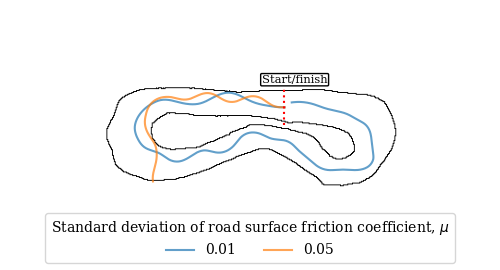
\includegraphics[width=11cm]{contents/chapt5/figs/domain_random/porto_domain_random.png}
    %% Creator: Matplotlib, PGF backend
%%
%% To include the figure in your LaTeX document, write
%%   \input{<filename>.pgf}
%%
%% Make sure the required packages are loaded in your preamble
%%   \usepackage{pgf}
%%
%% Also ensure that all the required font packages are loaded; for instance,
%% the lmodern package is sometimes necessary when using math font.
%%   \usepackage{lmodern}
%%
%% Figures using additional raster images can only be included by \input if
%% they are in the same directory as the main LaTeX file. For loading figures
%% from other directories you can use the `import` package
%%   \usepackage{import}
%%
%% and then include the figures with
%%   \import{<path to file>}{<filename>.pgf}
%%
%% Matplotlib used the following preamble
%%   \usepackage{fontspec}
%%   \setmainfont{times.ttf}[Path=\detokenize{C:/Windows/Fonts/}]
%%   \setsansfont{DejaVuSans.ttf}[Path=\detokenize{C:/Users/Andrew/anaconda3/envs/auto_car_env/Lib/site-packages/matplotlib/mpl-data/fonts/ttf/}]
%%   \setmonofont{DejaVuSansMono.ttf}[Path=\detokenize{C:/Users/Andrew/anaconda3/envs/auto_car_env/Lib/site-packages/matplotlib/mpl-data/fonts/ttf/}]
%%
\begingroup%
\makeatletter%
\begin{pgfpicture}%
\pgfpathrectangle{\pgfpointorigin}{\pgfqpoint{5.220000in}{1.220000in}}%
\pgfusepath{use as bounding box, clip}%
\begin{pgfscope}%
\pgfsetbuttcap%
\pgfsetmiterjoin%
\definecolor{currentfill}{rgb}{1.000000,1.000000,1.000000}%
\pgfsetfillcolor{currentfill}%
\pgfsetlinewidth{0.000000pt}%
\definecolor{currentstroke}{rgb}{1.000000,1.000000,1.000000}%
\pgfsetstrokecolor{currentstroke}%
\pgfsetdash{}{0pt}%
\pgfpathmoveto{\pgfqpoint{0.000000in}{0.000000in}}%
\pgfpathlineto{\pgfqpoint{5.220000in}{0.000000in}}%
\pgfpathlineto{\pgfqpoint{5.220000in}{1.220000in}}%
\pgfpathlineto{\pgfqpoint{0.000000in}{1.220000in}}%
\pgfpathlineto{\pgfqpoint{0.000000in}{0.000000in}}%
\pgfpathclose%
\pgfusepath{fill}%
\end{pgfscope}%
\begin{pgfscope}%
\pgfpathrectangle{\pgfqpoint{0.142364in}{0.154436in}}{\pgfqpoint{2.467636in}{0.911127in}}%
\pgfusepath{clip}%
\pgfsys@transformshift{0.142364in}{0.154436in}%
\pgftext[left,bottom]{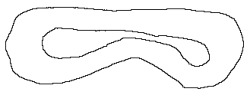
\includegraphics[interpolate=true,width=2.470000in,height=0.920000in]{contents/chapt5/figs/domain_random/porto_domain_random_2-img0.png}}%
\end{pgfscope}%
\begin{pgfscope}%
\pgfpathrectangle{\pgfqpoint{0.142364in}{0.154436in}}{\pgfqpoint{2.467636in}{0.911127in}}%
\pgfusepath{clip}%
\pgfsetrectcap%
\pgfsetroundjoin%
\pgfsetlinewidth{1.003750pt}%
\definecolor{currentstroke}{rgb}{0.121569,0.466667,0.705882}%
\pgfsetstrokecolor{currentstroke}%
\pgfsetstrokeopacity{0.700000}%
\pgfsetdash{}{0pt}%
\pgfpathmoveto{\pgfqpoint{1.660909in}{0.837782in}}%
\pgfpathlineto{\pgfqpoint{1.611091in}{0.838873in}}%
\pgfpathlineto{\pgfqpoint{1.576896in}{0.842561in}}%
\pgfpathlineto{\pgfqpoint{1.518542in}{0.851881in}}%
\pgfpathlineto{\pgfqpoint{1.467486in}{0.861763in}}%
\pgfpathlineto{\pgfqpoint{1.438092in}{0.869440in}}%
\pgfpathlineto{\pgfqpoint{1.409312in}{0.879158in}}%
\pgfpathlineto{\pgfqpoint{1.381306in}{0.890928in}}%
\pgfpathlineto{\pgfqpoint{1.347335in}{0.907899in}}%
\pgfpathlineto{\pgfqpoint{1.286612in}{0.939276in}}%
\pgfpathlineto{\pgfqpoint{1.265513in}{0.947874in}}%
\pgfpathlineto{\pgfqpoint{1.244090in}{0.954495in}}%
\pgfpathlineto{\pgfqpoint{1.222648in}{0.958865in}}%
\pgfpathlineto{\pgfqpoint{1.201399in}{0.960561in}}%
\pgfpathlineto{\pgfqpoint{1.187316in}{0.959868in}}%
\pgfpathlineto{\pgfqpoint{1.165510in}{0.956012in}}%
\pgfpathlineto{\pgfqpoint{1.143492in}{0.949534in}}%
\pgfpathlineto{\pgfqpoint{1.115027in}{0.938298in}}%
\pgfpathlineto{\pgfqpoint{1.080572in}{0.921767in}}%
\pgfpathlineto{\pgfqpoint{1.041489in}{0.900454in}}%
\pgfpathlineto{\pgfqpoint{1.012444in}{0.881812in}}%
\pgfpathlineto{\pgfqpoint{0.986238in}{0.862009in}}%
\pgfpathlineto{\pgfqpoint{0.915523in}{0.804728in}}%
\pgfpathlineto{\pgfqpoint{0.896505in}{0.794460in}}%
\pgfpathlineto{\pgfqpoint{0.881419in}{0.788788in}}%
\pgfpathlineto{\pgfqpoint{0.865706in}{0.784965in}}%
\pgfpathlineto{\pgfqpoint{0.844186in}{0.782552in}}%
\pgfpathlineto{\pgfqpoint{0.827843in}{0.782749in}}%
\pgfpathlineto{\pgfqpoint{0.806184in}{0.785639in}}%
\pgfpathlineto{\pgfqpoint{0.784685in}{0.791334in}}%
\pgfpathlineto{\pgfqpoint{0.761975in}{0.800234in}}%
\pgfpathlineto{\pgfqpoint{0.738082in}{0.812125in}}%
\pgfpathlineto{\pgfqpoint{0.709264in}{0.829373in}}%
\pgfpathlineto{\pgfqpoint{0.678657in}{0.850763in}}%
\pgfpathlineto{\pgfqpoint{0.628293in}{0.887680in}}%
\pgfpathlineto{\pgfqpoint{0.611384in}{0.896566in}}%
\pgfpathlineto{\pgfqpoint{0.598869in}{0.901070in}}%
\pgfpathlineto{\pgfqpoint{0.585833in}{0.903719in}}%
\pgfpathlineto{\pgfqpoint{0.572557in}{0.904584in}}%
\pgfpathlineto{\pgfqpoint{0.554877in}{0.903229in}}%
\pgfpathlineto{\pgfqpoint{0.537602in}{0.899224in}}%
\pgfpathlineto{\pgfqpoint{0.521093in}{0.892746in}}%
\pgfpathlineto{\pgfqpoint{0.505684in}{0.883965in}}%
\pgfpathlineto{\pgfqpoint{0.491687in}{0.873076in}}%
\pgfpathlineto{\pgfqpoint{0.479317in}{0.860364in}}%
\pgfpathlineto{\pgfqpoint{0.468423in}{0.845777in}}%
\pgfpathlineto{\pgfqpoint{0.458351in}{0.829101in}}%
\pgfpathlineto{\pgfqpoint{0.446938in}{0.805431in}}%
\pgfpathlineto{\pgfqpoint{0.439058in}{0.784433in}}%
\pgfpathlineto{\pgfqpoint{0.432664in}{0.761865in}}%
\pgfpathlineto{\pgfqpoint{0.428190in}{0.738509in}}%
\pgfpathlineto{\pgfqpoint{0.425673in}{0.715179in}}%
\pgfpathlineto{\pgfqpoint{0.425308in}{0.692530in}}%
\pgfpathlineto{\pgfqpoint{0.427373in}{0.671131in}}%
\pgfpathlineto{\pgfqpoint{0.431682in}{0.651341in}}%
\pgfpathlineto{\pgfqpoint{0.438824in}{0.629481in}}%
\pgfpathlineto{\pgfqpoint{0.459385in}{0.580160in}}%
\pgfpathlineto{\pgfqpoint{0.472253in}{0.551775in}}%
\pgfpathlineto{\pgfqpoint{0.483350in}{0.532486in}}%
\pgfpathlineto{\pgfqpoint{0.493845in}{0.518103in}}%
\pgfpathlineto{\pgfqpoint{0.505859in}{0.504965in}}%
\pgfpathlineto{\pgfqpoint{0.519396in}{0.493405in}}%
\pgfpathlineto{\pgfqpoint{0.534342in}{0.483740in}}%
\pgfpathlineto{\pgfqpoint{0.550421in}{0.476087in}}%
\pgfpathlineto{\pgfqpoint{0.571749in}{0.468658in}}%
\pgfpathlineto{\pgfqpoint{0.645791in}{0.446096in}}%
\pgfpathlineto{\pgfqpoint{0.666071in}{0.435760in}}%
\pgfpathlineto{\pgfqpoint{0.693086in}{0.418845in}}%
\pgfpathlineto{\pgfqpoint{0.727861in}{0.397175in}}%
\pgfpathlineto{\pgfqpoint{0.744288in}{0.389320in}}%
\pgfpathlineto{\pgfqpoint{0.761534in}{0.383488in}}%
\pgfpathlineto{\pgfqpoint{0.779392in}{0.379955in}}%
\pgfpathlineto{\pgfqpoint{0.797565in}{0.378876in}}%
\pgfpathlineto{\pgfqpoint{0.815718in}{0.380231in}}%
\pgfpathlineto{\pgfqpoint{0.833493in}{0.384153in}}%
\pgfpathlineto{\pgfqpoint{0.850626in}{0.390316in}}%
\pgfpathlineto{\pgfqpoint{0.871131in}{0.400201in}}%
\pgfpathlineto{\pgfqpoint{0.891618in}{0.412201in}}%
\pgfpathlineto{\pgfqpoint{0.916183in}{0.429607in}}%
\pgfpathlineto{\pgfqpoint{0.966087in}{0.466650in}}%
\pgfpathlineto{\pgfqpoint{0.983326in}{0.476557in}}%
\pgfpathlineto{\pgfqpoint{1.001890in}{0.484699in}}%
\pgfpathlineto{\pgfqpoint{1.024412in}{0.491718in}}%
\pgfpathlineto{\pgfqpoint{1.042060in}{0.494984in}}%
\pgfpathlineto{\pgfqpoint{1.064413in}{0.496891in}}%
\pgfpathlineto{\pgfqpoint{1.140569in}{0.500178in}}%
\pgfpathlineto{\pgfqpoint{1.162480in}{0.504978in}}%
\pgfpathlineto{\pgfqpoint{1.183729in}{0.512166in}}%
\pgfpathlineto{\pgfqpoint{1.204110in}{0.521540in}}%
\pgfpathlineto{\pgfqpoint{1.227834in}{0.535159in}}%
\pgfpathlineto{\pgfqpoint{1.247712in}{0.548936in}}%
\pgfpathlineto{\pgfqpoint{1.262121in}{0.561468in}}%
\pgfpathlineto{\pgfqpoint{1.274291in}{0.574691in}}%
\pgfpathlineto{\pgfqpoint{1.287734in}{0.592707in}}%
\pgfpathlineto{\pgfqpoint{1.325199in}{0.646180in}}%
\pgfpathlineto{\pgfqpoint{1.342428in}{0.664492in}}%
\pgfpathlineto{\pgfqpoint{1.362234in}{0.681873in}}%
\pgfpathlineto{\pgfqpoint{1.379694in}{0.695475in}}%
\pgfpathlineto{\pgfqpoint{1.379694in}{0.695475in}}%
\pgfusepath{stroke}%
\end{pgfscope}%
\begin{pgfscope}%
\pgfpathrectangle{\pgfqpoint{0.142364in}{0.154436in}}{\pgfqpoint{2.467636in}{0.911127in}}%
\pgfusepath{clip}%
\pgfsetrectcap%
\pgfsetroundjoin%
\pgfsetlinewidth{1.003750pt}%
\definecolor{currentstroke}{rgb}{1.000000,0.498039,0.054902}%
\pgfsetstrokecolor{currentstroke}%
\pgfsetstrokeopacity{0.700000}%
\pgfsetdash{}{0pt}%
\pgfpathmoveto{\pgfqpoint{1.660909in}{0.837782in}}%
\pgfpathlineto{\pgfqpoint{1.619928in}{0.838678in}}%
\pgfpathlineto{\pgfqpoint{1.597347in}{0.841567in}}%
\pgfpathlineto{\pgfqpoint{1.579701in}{0.846078in}}%
\pgfpathlineto{\pgfqpoint{1.562731in}{0.852687in}}%
\pgfpathlineto{\pgfqpoint{1.546605in}{0.861159in}}%
\pgfpathlineto{\pgfqpoint{1.523747in}{0.876131in}}%
\pgfpathlineto{\pgfqpoint{1.482531in}{0.904609in}}%
\pgfpathlineto{\pgfqpoint{1.462369in}{0.915181in}}%
\pgfpathlineto{\pgfqpoint{1.445406in}{0.921818in}}%
\pgfpathlineto{\pgfqpoint{1.427804in}{0.926490in}}%
\pgfpathlineto{\pgfqpoint{1.409751in}{0.928886in}}%
\pgfpathlineto{\pgfqpoint{1.391539in}{0.928986in}}%
\pgfpathlineto{\pgfqpoint{1.373437in}{0.926974in}}%
\pgfpathlineto{\pgfqpoint{1.355692in}{0.922872in}}%
\pgfpathlineto{\pgfqpoint{1.334194in}{0.915370in}}%
\pgfpathlineto{\pgfqpoint{1.292425in}{0.897189in}}%
\pgfpathlineto{\pgfqpoint{1.271127in}{0.889132in}}%
\pgfpathlineto{\pgfqpoint{1.253514in}{0.884498in}}%
\pgfpathlineto{\pgfqpoint{1.235466in}{0.882070in}}%
\pgfpathlineto{\pgfqpoint{1.217256in}{0.882031in}}%
\pgfpathlineto{\pgfqpoint{1.199199in}{0.884389in}}%
\pgfpathlineto{\pgfqpoint{1.181622in}{0.889149in}}%
\pgfpathlineto{\pgfqpoint{1.164732in}{0.895969in}}%
\pgfpathlineto{\pgfqpoint{1.144500in}{0.906421in}}%
\pgfpathlineto{\pgfqpoint{1.092678in}{0.935033in}}%
\pgfpathlineto{\pgfqpoint{1.075684in}{0.941584in}}%
\pgfpathlineto{\pgfqpoint{1.058015in}{0.945993in}}%
\pgfpathlineto{\pgfqpoint{1.039919in}{0.948019in}}%
\pgfpathlineto{\pgfqpoint{1.021719in}{0.947505in}}%
\pgfpathlineto{\pgfqpoint{1.003773in}{0.944420in}}%
\pgfpathlineto{\pgfqpoint{0.986326in}{0.939188in}}%
\pgfpathlineto{\pgfqpoint{0.965231in}{0.930611in}}%
\pgfpathlineto{\pgfqpoint{0.911059in}{0.906743in}}%
\pgfpathlineto{\pgfqpoint{0.893549in}{0.901732in}}%
\pgfpathlineto{\pgfqpoint{0.875526in}{0.898884in}}%
\pgfpathlineto{\pgfqpoint{0.857199in}{0.898162in}}%
\pgfpathlineto{\pgfqpoint{0.838888in}{0.899656in}}%
\pgfpathlineto{\pgfqpoint{0.821241in}{0.903191in}}%
\pgfpathlineto{\pgfqpoint{0.799698in}{0.909688in}}%
\pgfpathlineto{\pgfqpoint{0.744183in}{0.928107in}}%
\pgfpathlineto{\pgfqpoint{0.726487in}{0.931376in}}%
\pgfpathlineto{\pgfqpoint{0.708524in}{0.932442in}}%
\pgfpathlineto{\pgfqpoint{0.690565in}{0.931287in}}%
\pgfpathlineto{\pgfqpoint{0.668427in}{0.927304in}}%
\pgfpathlineto{\pgfqpoint{0.651189in}{0.922130in}}%
\pgfpathlineto{\pgfqpoint{0.634685in}{0.914956in}}%
\pgfpathlineto{\pgfqpoint{0.619162in}{0.905855in}}%
\pgfpathlineto{\pgfqpoint{0.604933in}{0.894841in}}%
\pgfpathlineto{\pgfqpoint{0.592260in}{0.882068in}}%
\pgfpathlineto{\pgfqpoint{0.581272in}{0.867815in}}%
\pgfpathlineto{\pgfqpoint{0.572002in}{0.852391in}}%
\pgfpathlineto{\pgfqpoint{0.564545in}{0.836011in}}%
\pgfpathlineto{\pgfqpoint{0.557268in}{0.814720in}}%
\pgfpathlineto{\pgfqpoint{0.548041in}{0.779917in}}%
\pgfpathlineto{\pgfqpoint{0.544098in}{0.757766in}}%
\pgfpathlineto{\pgfqpoint{0.542443in}{0.735332in}}%
\pgfpathlineto{\pgfqpoint{0.543391in}{0.712858in}}%
\pgfpathlineto{\pgfqpoint{0.546918in}{0.690638in}}%
\pgfpathlineto{\pgfqpoint{0.555444in}{0.655655in}}%
\pgfpathlineto{\pgfqpoint{0.562248in}{0.624898in}}%
\pgfpathlineto{\pgfqpoint{0.564279in}{0.607016in}}%
\pgfpathlineto{\pgfqpoint{0.564154in}{0.589022in}}%
\pgfpathlineto{\pgfqpoint{0.561693in}{0.571198in}}%
\pgfpathlineto{\pgfqpoint{0.557087in}{0.553799in}}%
\pgfpathlineto{\pgfqpoint{0.549185in}{0.532723in}}%
\pgfpathlineto{\pgfqpoint{0.539286in}{0.512313in}}%
\pgfpathlineto{\pgfqpoint{0.529523in}{0.496815in}}%
\pgfpathlineto{\pgfqpoint{0.515442in}{0.478904in}}%
\pgfpathlineto{\pgfqpoint{0.496731in}{0.459043in}}%
\pgfpathlineto{\pgfqpoint{0.433833in}{0.399758in}}%
\pgfpathlineto{\pgfqpoint{0.395043in}{0.361352in}}%
\pgfpathlineto{\pgfqpoint{0.377047in}{0.340842in}}%
\pgfpathlineto{\pgfqpoint{0.363758in}{0.322393in}}%
\pgfpathlineto{\pgfqpoint{0.352621in}{0.302575in}}%
\pgfpathlineto{\pgfqpoint{0.350685in}{0.298458in}}%
\pgfpathlineto{\pgfqpoint{0.350685in}{0.298458in}}%
\pgfusepath{stroke}%
\end{pgfscope}%
\begin{pgfscope}%
\pgfpathrectangle{\pgfqpoint{0.142364in}{0.154436in}}{\pgfqpoint{2.467636in}{0.911127in}}%
\pgfusepath{clip}%
\pgfsetbuttcap%
\pgfsetroundjoin%
\pgfsetlinewidth{1.505625pt}%
\definecolor{currentstroke}{rgb}{1.000000,0.000000,0.000000}%
\pgfsetstrokecolor{currentstroke}%
\pgfsetdash{{1.500000pt}{2.475000pt}}{0.000000pt}%
\pgfpathmoveto{\pgfqpoint{1.655516in}{0.690885in}}%
\pgfpathlineto{\pgfqpoint{1.655516in}{0.994594in}}%
\pgfusepath{stroke}%
\end{pgfscope}%
\begin{pgfscope}%
\pgfsetbuttcap%
\pgfsetmiterjoin%
\definecolor{currentfill}{rgb}{1.000000,1.000000,1.000000}%
\pgfsetfillcolor{currentfill}%
\pgfsetfillopacity{0.800000}%
\pgfsetlinewidth{1.003750pt}%
\definecolor{currentstroke}{rgb}{0.800000,0.800000,0.800000}%
\pgfsetstrokecolor{currentstroke}%
\pgfsetstrokeopacity{0.800000}%
\pgfsetdash{}{0pt}%
\pgfpathmoveto{\pgfqpoint{2.841880in}{0.181452in}}%
\pgfpathlineto{\pgfqpoint{5.122778in}{0.181452in}}%
\pgfpathquadraticcurveto{\pgfqpoint{5.150556in}{0.181452in}}{\pgfqpoint{5.150556in}{0.209230in}}%
\pgfpathlineto{\pgfqpoint{5.150556in}{1.010770in}}%
\pgfpathquadraticcurveto{\pgfqpoint{5.150556in}{1.038548in}}{\pgfqpoint{5.122778in}{1.038548in}}%
\pgfpathlineto{\pgfqpoint{2.841880in}{1.038548in}}%
\pgfpathquadraticcurveto{\pgfqpoint{2.814103in}{1.038548in}}{\pgfqpoint{2.814103in}{1.010770in}}%
\pgfpathlineto{\pgfqpoint{2.814103in}{0.209230in}}%
\pgfpathquadraticcurveto{\pgfqpoint{2.814103in}{0.181452in}}{\pgfqpoint{2.841880in}{0.181452in}}%
\pgfpathlineto{\pgfqpoint{2.841880in}{0.181452in}}%
\pgfpathclose%
\pgfusepath{stroke,fill}%
\end{pgfscope}%
\begin{pgfscope}%
\definecolor{textcolor}{rgb}{0.000000,0.000000,0.000000}%
\pgfsetstrokecolor{textcolor}%
\pgfsetfillcolor{textcolor}%
\pgftext[x=3.008547in, y=0.747668in, left, base]{\color{textcolor}\rmfamily\fontsize{10.000000}{12.000000}\selectfont Standard deviation of road surface }%
\end{pgfscope}%
\begin{pgfscope}%
\definecolor{textcolor}{rgb}{0.000000,0.000000,0.000000}%
\pgfsetstrokecolor{textcolor}%
\pgfsetfillcolor{textcolor}%
\pgftext[x=3.008547in, y=0.602242in, left, base]{\color{textcolor}\rmfamily\fontsize{10.000000}{12.000000}\selectfont  friction coefficient during training}%
\end{pgfscope}%
\begin{pgfscope}%
\pgfsetrectcap%
\pgfsetroundjoin%
\pgfsetlinewidth{1.003750pt}%
\definecolor{currentstroke}{rgb}{0.121569,0.466667,0.705882}%
\pgfsetstrokecolor{currentstroke}%
\pgfsetstrokeopacity{0.700000}%
\pgfsetdash{}{0pt}%
\pgfpathmoveto{\pgfqpoint{3.211496in}{0.454211in}}%
\pgfpathlineto{\pgfqpoint{3.350385in}{0.454211in}}%
\pgfpathlineto{\pgfqpoint{3.489274in}{0.454211in}}%
\pgfusepath{stroke}%
\end{pgfscope}%
\begin{pgfscope}%
\definecolor{textcolor}{rgb}{0.000000,0.000000,0.000000}%
\pgfsetstrokecolor{textcolor}%
\pgfsetfillcolor{textcolor}%
\pgftext[x=3.600385in,y=0.405600in,left,base]{\color{textcolor}\rmfamily\fontsize{10.000000}{12.000000}\selectfont 0.01}%
\end{pgfscope}%
\begin{pgfscope}%
\pgfsetrectcap%
\pgfsetroundjoin%
\pgfsetlinewidth{1.003750pt}%
\definecolor{currentstroke}{rgb}{1.000000,0.498039,0.054902}%
\pgfsetstrokecolor{currentstroke}%
\pgfsetstrokeopacity{0.700000}%
\pgfsetdash{}{0pt}%
\pgfpathmoveto{\pgfqpoint{4.121218in}{0.454211in}}%
\pgfpathlineto{\pgfqpoint{4.260107in}{0.454211in}}%
\pgfpathlineto{\pgfqpoint{4.398996in}{0.454211in}}%
\pgfusepath{stroke}%
\end{pgfscope}%
\begin{pgfscope}%
\definecolor{textcolor}{rgb}{0.000000,0.000000,0.000000}%
\pgfsetstrokecolor{textcolor}%
\pgfsetfillcolor{textcolor}%
\pgftext[x=4.510107in,y=0.405600in,left,base]{\color{textcolor}\rmfamily\fontsize{10.000000}{12.000000}\selectfont 0.05}%
\end{pgfscope}%
\end{pgfpicture}%
\makeatother%
\endgroup%

    \caption[Paths taken by agents trained with randomised road-surface friction coefficients on the Porto track under evaluation conditions]{Paths taken by agents trained with randomised road-surface friction coefficients on the Porto track under evaluation conditions. During this evaluation lap, the friction coefficient was set to the nominal value of $1.0489$.}
    \label{fig:porto_domain_random}
\end{figure}


Our findings suggest that the optimal policy for autonomous racing is highly sensitive to the friction coefficient of the road surface. 
Agents struggle to adapt their policies to changing friction values effectively, resulting in poorer performance. 
This sensitivity highlights the challenge of developing a single policy that performs optimally across a range of friction coefficients, demonstrating the limitations of domain randomisation in the racing context.



\section{Summary}

In this chapter, we have motivated the design of an end-to-end autonomous racing algorithm.
Agents utilising this algorithm were trained to race effectively on the Porto track, successfully completing all of their laps under evaluation conditions.
However, this performance did not scale to larger tracks such as Circuit de Barcelona-Catalunya or Circuit de Monaco.
On these longer tracks, the performance of the agents was hindered by slaloming, and they did not complete all of their laps.

The presence of slaloming is particularly concerning when considering scenarios in which model mismatches are present.
In fact, during a preliminary investigation into the effect of model mismatch on the performance of end-to-end agents, we observed collisions.
This is indicative of the limitations of end-to-end algorithms under conditions where model mismatches are present, and emphasises the need for algorithms that exhibit robustness against modeling errors.

In the next chapter, we introduce our partial end-to-end solution, which aims to enhance robustness towards modeling errors and address the challenges posed by the sensitivity of the optimal policy to vehicle model parameters.